\documentclass[11pt,a4paper]{book}
\usepackage[utf8]{inputenc}
\usepackage[colorlinks,linkcolor=blue,citecolor=blue,urlcolor=blue,hyperfootnotes=true,bookmarksopen=true]{hyperref}
\usepackage{footnotebackref}
\usepackage{graphicx}
\usepackage{multicol}
\usepackage{amsmath,amssymb,amsthm,amsfonts}
\usepackage[capitalize,nameinlink]{cleveref}%动态ref定理,推论,引理等
\usepackage{textgreek,bm,upgreek,mathrsfs}
\usepackage{array} %表格列宽操作
\usepackage{longtable} %表格列宽对齐
\usepackage{arydshln} %提供画线的虚线格式
%\usepackage{textcomp}
\usepackage{stmaryrd}
\expandafter\def\csname opt@stmaryrd.sty\endcsname
{only,shortleftarrow,shortrightarrow}
\usepackage{extpfeil}
\usepackage{extarrows}
\usepackage[bottom]{footmisc}
\usepackage{enumitem}
\usepackage{epigraph}
\usepackage[many]{tcolorbox}
\usepackage[english]{babel}
\usepackage[margin=1in]{geometry}
\usepackage{setspace}
\usepackage{microtype} 
\usepackage{float}
\usepackage[framemethod=tikz]{mdframed} 
\usepackage[tikz]{bclogo}
\usepackage{wrapfig}
\usepackage{color}
\usepackage{epigraph}
\usepackage[many]{tcolorbox}
\usepackage{tikz-cd}
\usepackage{tikz}
\usepackage{fancyhdr}
\usepackage{titlesec}%定义section的格式
\usepackage{tocloft}
\usepackage{titletoc}%定义目录样式
\usepackage{sectsty}%定义section的格式
\usepackage{booktabs}
\usepackage{easybmat}%定义大型分块矩阵
\usepackage{dsfont}%定义bold 1
\usepackage{calligra}
\usepackage[
ordering=Kac,
edge-length=1cm,
root-radius=.06cm]{dynkin-diagrams}
\usepackage[T1]{fontenc}
\PassOptionsToPackage{no-math}{fontspec}
\usepackage[noBBpl]{mathpazo}
\usepackage{bbold}
%\usepackage{palatino}
%\usepackage{newpxmath}
%\usepackage{txfonts}
%\usepackage{pxfonts}
\usepackage{l3draw,xparse}
\usepackage{accents}%创建新的widetilde
\usepackage{scalerel} %放大数学字体
\usepackage{calligra,mathrsfs}%for sheaf Hom
\usepackage{mathtools}%def new widetilde
\usepackage{calc}%定义箭头不同样式symbol
\usepackage[normalem]{ulem}%定义合适的下划线

%-----------------------------------------------------
%定义BOONDOX包的字体
\DeclareMathAlphabet{\mathbbb}{U}{bbold}{m}{n}
\DeclareMathAlphabet{\mathbb}{U}{msb}{m}{n}
%-----------------------------------------------------
\DeclareFontFamily{U}{BOONDOX-cal}{\skewchar\font=45}
\DeclareFontShape{U}{BOONDOX-cal}{m}{n}{
  <-> s*[1] BOONDOX-r-cal}{}
\DeclareMathAlphabet{\mathscr}{U}{BOONDOX-cal}{m}{n}
%-----------------------------------------------------
\DeclareFontFamily{U}{BOONDOX-frak}{\skewchar\font=45}
\DeclareFontShape{U}{BOONDOX-frak}{m}{n}{
  <-> s*[1]  BOONDOX-r-frak}{}
%\DeclareMathAlphabet{\mathfrak}{U}{BOONDOX-frak}{m}{n}

%----------------------------------------------------
%设置目录中number和文字的间距
\usepackage{tocloft}
\setlength{\cftsecnumwidth}{25pt} % resets space for section number (usually 2.3em)
\setlength{\cftsubsecnumwidth}{35pt} % resets space for subsection number (usually 3.2em)

%-----------------------------------------------------
%设置页面样式
%\geometry{top=3.5cm,bottom=3.5cm}
%\linespread{1.15}
\geometry{hcentering}
\pagestyle{fancy}
\setlength{\headheight}{15.0pt}
\fancyhf{}
\fancyhead[LE,RO]{\thepage}
\fancyhead[RE]{\bf\nouppercase{\rightmark}}
\fancyhead[LO]{\bf\nouppercase{\leftmark}}
\renewcommand{\headrulewidth}{0pt}
\renewcommand{\footrulewidth}{0pt}
%-------------------------------------------------------

%------------------------------------------------------
%重新定义autoref的section和subsection的名字
\renewcommand{\sectionautorefname}{\S\!}
\renewcommand{\subsectionautorefname}{\S\S\!}

%-------------------------------------------------------
%定义能编号的paragraph
\renewcommand{\theparagraph}{\thesubsection.\arabic{paragraph}}% How paragraphs are numbered
\setcounter{secnumdepth}{4}

%---------------------------------------------------------
%---控制enumerate编号正体
\usepackage{enumitem}
\setlist[enumerate,1]{font=\upshape}
\setlist[enumerate,2]{font=\upshape}

\makeatletter%define roman numbers
\newcommand{\rmnum}[1]{\textup{\romannumeral #1}}
\newcommand{\Rmnum}[1]{\textup{\expandafter\@slowromancap\romannumeral #1@}}
\makeatother

\chapterfont{\centering}%chapter居中
\sectionfont{\centering}%section居中

%\titlecontents{chapter}% <section-type>增加Chapter到目录中
%  [0pt]% <left>
%  {\bfseries}% <above-code>
%  {\color{blue}\chaptername\ \thecontentslabel.\hspace{7pt}}% %<numbered-entry-format>
%  {}% <numberless-entry-format>
%  {\hfill\contentspage}% <filler-page-format>

%调整tikz箭头格式---------------------------------
\usetikzlibrary{arrows.meta}
\usetikzlibrary{bending}
\tikzset{
  commutative diagrams/.cd,
  arrow style=tikz,
  diagrams={>={Computer Modern Rightarrow[length=5pt,width=4pt]}},
  symbol/.style={
    draw=none,
    every to/.append style={
      edge node={node [sloped, allow upside down, auto=false]{$#1$}}}
  },
  row sep/normal=8mm,
  column sep/normal=8mm
}

%------------------------------------------------
%引入mathabx包的widecheck
\DeclareFontFamily{U}{mathx}{}
\DeclareFontShape{U}{mathx}{m}{n}{ <-> mathx10 }{}
\DeclareSymbolFont{mathx}{U}{mathx}{m}{n}
\DeclareFontSubstitution{U}{mathx}{m}{n}
\DeclareMathAccent{\widecheck}{0}{mathx}{"71}
%\DeclareMathAccent{\widebar}{0}{mathx}{"73}
%------------------------------------------------


%改变下标基线--------------------------------------
%\usepackage{subdepth}
%\begingroup
%  \catcode`\_=\active
%  \gdef_#1{\ensuremath{\sb{\smash{#1}}}}
%\endgroup
%\mathcode`\_=\string"8000
%\catcode`\_=12
%%-------------------------------------------------

%-------------------mathbb大写
\def\C{\mathbb{C}}
\def\F{\mathbb{F}}
\def\K{\mathbb{K}}
\def\R{\mathbb{R}}
\def\A{\mathbb{A}}
\def\B{\mathbb{B}}
\def\Q{\mathbb{Q}}
\def\Z{\mathbb{Z}}
\def\D{\mathbb{D}}
\def\N{\mathbb{N}}
\def\T{\mathbb{T}}
\def\H{\mathbb{H}}
\def\V{\mathbb{V}}
\def\W{\mathbb{W}}
\def\RP{\mathbb{RP}}
\def\CP{\mathbb{CP}}
\def\P{\mathbb{P}}
\def\G{\mathbb{G}}
%------------------------------


%-------------------mathfrak大写
\def\X{\mathfrak{X}}
\def\Y{\mathfrak{Y}}
%------------------------------


%------------------mathfrak小写
\def\m{\mathfrak{m}}
\def\n{\mathfrak{n}}
\def\p{\mathfrak{p}}
\def\q{\mathfrak{q}}
\def\a{\mathfrak{a}}
\def\b{\mathfrak{b}}
\def\c{\mathfrak{c}}
\def\g{\mathfrak{g}}
\def\h{\mathfrak{h}}
\def\d{\mathfrak{d}}
\def\s{\mathfrak{s}}
\def\z{\mathfrak{z}}
\def\l{\mathfrak{l}}
\def\r{\mathfrak{r}}
\def\t{\mathfrak{t}}
\def\f{\mathfrak{f}}
\def\x{\mathfrak{x}}
\def\y{\mathfrak{y}}
\def\k{\mathfrak{k}}
\def\st{\mathfrak{st}}
\def\aff{\mathfrak{aff}}
\def\gl{\mathfrak{gl}}
\def\sl{\mathfrak{sl}}
\def\o{\mathfrak{o}}
\def\so{\mathfrak{so}}
\def\u{\mathfrak{u}}
\def\su{\mathfrak{su}}
\def\Lie{\mathfrak{Lie}}
\def\nil{\mathfrak{nil}}
\def\eff{\mathfrak{eff}}
%-----------------------------


%------------------mathrm大小写
\def\E{\mathrm{E}}
\def\GL{\mathrm{GL}}
\def\PGL{\mathrm{PGL}}
\def\SL{\mathrm{SL}}
\def\O{\mathrm{O}}
\def\SO{\mathrm{SO}}
\def\Sp{\mathrm{Sp}}
\def\U{\mathrm{U}}
\def\SU{\mathrm{SU}}
\def\dom{\mathrm{dom}}
\def\codom{\mathrm{codom}}
\def\End{\mathrm{End}}
\def\Hom{\mathrm{Hom}}
\def\Mor{\mathrm{Mor}}
\def\Obj{\mathrm{Obj}}
\def\Aut{\mathrm{Aut}}
\def\det{\mathrm{det}}
\def\supp{\mathrm{supp}}
\def\conv{\mathrm{conv}}
\def\mult{\mathrm{mult}}
\def\Homgr{\mathrm{Homgr}}
\def\Sh{\mathrm{Sh}}
\def\Lib{\mathrm{Lib}}
\def\Ad{\mathrm{Ad}}
\def\ad{\mathrm{ad}}
\def\Der{\mathrm{Der}}
\def\reg{\mathrm{reg}}
\def\div{\mathrm{div}}
\def\Sym{\mathrm{Sym}}
\def\Stab{\mathrm{Stab}}
\def\Tor{\mathrm{Tor}}
\def\Ext{\mathrm{Ext}}
\def\tr{\mathrm{tr}}
\def\gr{\mathrm{gr}}
\def\lcm{\mathrm{lcm}}
\def\codim{\mathrm{codim}}
\def\gldim{\mathrm{gldim}}
\def\rank{\mathrm{rank}}
\def\char{\mathrm{char}}
\def\cl{\mathrm{cl}}
\def\Cl{\mathrm{Cl}}
\def\height{\mathrm{ht}}
\def\coht{\mathrm{coht}}
\def\depth{\mathrm{depth}}
\def\sgn{\mathrm{sgn}}
\def\res{\mathrm{res}}
\def\Rees{\mathrm{Rees}}
\def\Res{\mathrm{Res}}
\def\Alt{\mathrm{Alt}}
\def\Gal{\mathrm{Gal}}
\def\Inv{\mathrm{Inv}}
\def\Inn{\mathrm{Inn}}
\def\inn{\mathrm{inn}}
\def\Ann{\mathrm{Ann}}
\def\Ass{\mathrm{Ass}}
\def\Spec{\mathrm{Spec}}
\def\Spf{\mathrm{Spf}}
\def\Proj{\mathrm{Proj}}
\def\Max{\mathrm{Max}}
\def\Ind{\mathrm{Ind}}
\def\CoInd{\mathrm{CoInd}}
\def\Div{\mathrm{Div}}
\def\Pic{\mathrm{Pic}}
\def\sep{\mathrm{sep}}
\def\isep{\mathrm{isep}}
\def\Soc{\mathrm{Soc}}
\def\Rad{\mathrm{Rad}}
\def\red{\mathrm{red}}
\def\dev{\mathrm{dev}}
\def\opp{\mathrm{opp}}
\def\Nor{\mathrm{Nor}}
\def\Cyl{\mathrm{Cyl}}
\def\Cone{\mathrm{Cone}}
\def\Aff{\mathrm{Aff}}
\def\rat{\mathrm{rat}}
\def\Sing{\mathrm{Sing}}
\def\op{\mathrm{op}}
\def\inj{\mathrm{inj}}
\def\Fun{\mathrm{Fun}}
\def\sk{\mathrm{sk}}
\def\ev{\mathrm{ev}}
\def\Ob{\mathrm{Ob}}
\def\Alg{\mathrm{Alg}}
\def\rev{\mathrm{rev}}
\def\gldim{\mathrm{gl.dim}}
\def\projdim{\mathrm{proj.dim}}
\def\injdim{\mathrm{inj.dim}}
\def\pr{\mathrm{pr}}
\def\Arr{\mathrm{Arr}}
\def\Cart{\mathrm{Cart}}
\def\Cov{\mathrm{Cov}}
\def\PSh{\mathrm{PSh}}
\def\Sh{\mathrm{Sh}}
\def\Ab{\mathrm{Ab}}
\def\Ouv{\mathrm{Ouv}}
\def\Esp{\mathrm{Esp}}
\def\Topos{\mathrm{Topos}}
\def\Pt{\mathrm{Pt}}
\def\Jac{\mathrm{Jac}}
\def\Pro{\mathrm{Pro}}
\def\pro{\mathrm{pro}}
\def\Tot{\mathrm{Tot}}
\def\Iso{\mathrm{Iso}}
\def\Conn{\mathrm{Conn}}
\def\Diff{\mathrm{Diff}}
\def\SS{\mathrm{SS}}
\def\Cyc{\mathrm{Cyc}}
\def\qcoh{\!\mathrm{qcoh}}
\def\coh{\!\mathrm{coh}}
\def\an{\mathrm{an}}
\def\Sol{\mathrm{Sol}}
\def\Loc{\mathrm{Loc}}
\def\Conn{\mathrm{Conn}}
\def\pt{\mathrm{pt}}
\def\Perv{\mathrm{Perv}}
\def\ord{\mathrm{ord}}
\def\Nil{\mathrm{Nil}}
\def\Lie{\mathrm{Lie}}
\def\Trans{\mathrm{Trans}}
\def\STrans{\mathrm{STrans}}
\def\Centr{\mathrm{Centr}}
\def\Card{\mathrm{Card}}
\def\pro{\mathrm{pro}}
\def\cd{\mathrm{cd}}
\def\aff{\mathrm{aff}}
\def\ho{\mathrm{h}}
\def\Ch{\mathrm{Ch}}
\def\Lan{\mathrm{Lan}}
\def\Ran{\mathrm{Ran}}
\def\Qis{\mathrm{Qis}}
\def\rad{\mathrm{rad}}

%-----------------------------

%-----------------------------mathbf定义
\def\Qcoh{\mathbf{Qcoh}}
\def\Coh{\mathbf{Coh}}
\def\Mod{\mathbf{Mod}}
\def\CoMod{\mathbf{CoMod}}
\def\CoQcoh{\mathbf{CoQcoh}}
\def\Grp{\mathbf{Grp}}
\def\Set{\mathbf{Set}}
\def\Sch{\mathbf{Sch}}
\def\Rsp{\mathbf{Rsp}}
\def\Alg{\mathbf{Alg}}
\def\Top{\mathbf{Top}}
\def\Cat{\mathbf{Cat}}
\def\FEt{\textup{\textbf{F\'Et}}}

%------------------operatorname定义
\def\ker{\operatorname{ker}}
\def\coker{\operatorname{coker}}
\def\im{\operatorname{im}}
\def\coim{\operatorname{coim}}
\def\id{\operatorname{id}}
\def\Int{\operatorname{Int}}
%-----------------------------

%--------------------text定义
\def\et{\textup{\'et}}
\def\Zar{\textup{Zar}}
\def\etf{\textup{\'etf}}
\def\fpqc{\textup{fpqc}}
\def\fppf{\textup{fppf}}
\def\desc{\textup{desc}}
\def\comp{\textup{comp}}
\def\perf{\textup{perf}}
\def\dash{\textup{-}}
%--------------------其他定义
\def\sub{\subseteq}
\def\sups{\supseteq}
\def\emp{\varnothing}
\def\dcheck{\check{}\hspace{4pt}\check{}}
\def\rcheck{\hspace*{1pt}\widecheck{}}
\def\eps{\varepsilon}
\def\llim{\varprojlim}
\def\rlim{\varinjlim}
\def\And{\hspace{8pt}\text{and}\hspace{8pt}}
\def\for{\hspace{8pt}\text{for}\hspace{6pt}}
%------------------------------

%------------------------------
\renewcommand{\Re}{\operatorname{Re}}
\renewcommand{\Im}{\operatorname{Im}}
\renewcommand{\i}{\mathrm{i}}
%------------------------------

%------------------------------花写Hom,Ext,End,Aut,Iso,Proj
\DeclareMathOperator{\sHom}{\mathcal{H}\hspace*{-0.4pt}\textit{om}\hspace{0.5pt}}
\DeclareMathOperator{\sExt}{\mathcal{E}\hspace*{-1.3pt}\textit{xt}\hspace{0.5pt}}
\DeclareMathOperator{\sEnd}{\mathcal{E}\hspace*{-1pt}\textit{nd}\hspace{0.5pt}}
\DeclareMathOperator{\sIso}{\mathcal{I}\hspace*{-0.5pt}\textit{so}\hspace{0.5pt}}
\DeclareMathOperator{\sAut}{\mathcal{A}\hspace*{-0.2pt}\textit{ut}\hspace{0.5pt}}
\DeclareMathOperator{\sDer}{\mathcal{D}\hspace*{-0.2pt}\textit{er}\hspace{0.5pt}}
\DeclareMathOperator{\sDiff}{\mathcal{D}\hspace*{-0.2pt}\textit{iff}\hspace{0.5pt}}
\DeclareMathOperator{\sProj}{\mathscr{P}\hspace*{-0.5pt}\textit{roj}}
\DeclareMathOperator{\sLie}{\mathscr{L}\hspace*{-0.5pt}\textit{ie}}
\DeclareMathOperator{\sGr}{\mathscr{G}\hspace*{-0.5pt}\textit{r}}
%------------------------------


\newcommand{\intprod}{\mathbin{\raisebox{\depth}{\scalebox{1}[-1]{$\lnot$}}}}%defining interior product
\newcommand{\bigw}{\scalebox{.95}[1]{\boldmath{$\bigwedge$}\hspace{-1pt}}}%define a nice wedge product


%调整图片和方程编号方式----------------------
%\makeatletter
%\@addtoreset{figure}{subsection}
%\makeatother
%\renewcommand{\thefigure}{\arabic{section}.\arabic{subsection}.\arabic{figure}}
\counterwithin*{figure}{section}

%\renewcommand{\theequation}{\arabic{section}.\arabic{subsection}.\arabic{equation}}
\numberwithin{equation}{section}
%-------------------------------------------




%--------------------------------------------------------
%定义widebar
\makeatletter
\let\save@mathaccent\mathaccent
\newcommand*\if@single[3]{%
  \setbox0\hbox{${\mathaccent"0362{#1}}^H$}%
  \setbox2\hbox{${\mathaccent"0362{\kern0pt#1}}^H$}%
  \ifdim\ht0=\ht2 #3\else #2\fi
  }
%The bar will be moved to the right by a half of \macc@kerna, which is computed by amsmath:
\newcommand*\rel@kern[1]{\kern#1\dimexpr\macc@kerna}
%If there's a superscript following the bar, then no negative kern may follow the bar;
%an additional {} makes sure that the superscript is high enough in this case:
\newcommand*\widebar[1]{\@ifnextchar^{{\wide@bar{#1}{0}}}{\wide@bar{#1}{1}}}
%Use a separate algorithm for single symbols:
\newcommand*\wide@bar[2]{\if@single{#1}{\wide@bar@{#1}{#2}{1}}{\wide@bar@{#1}{#2}{2}}}
\newcommand*\wide@bar@[3]{%
  \begingroup
  \def\mathaccent##1##2{%
%Enable nesting of accents:
    \let\mathaccent\save@mathaccent
%If there's more than a single symbol, use the first character instead (see below):
    \if#32 \let\macc@nucleus\first@char \fi
%Determine the italic correction:
    \setbox\z@\hbox{$\macc@style{\macc@nucleus}_{}$}%
    \setbox\tw@\hbox{$\macc@style{\macc@nucleus}{}_{}$}%
    \dimen@\wd\tw@
    \advance\dimen@-\wd\z@
%Now \dimen@ is the italic correction of the symbol.
    \divide\dimen@ 3
    \@tempdima\wd\tw@
    \advance\@tempdima-\scriptspace
%Now \@tempdima is the width of the symbol.
    \divide\@tempdima 10
    \advance\dimen@-\@tempdima
%Now \dimen@ = (italic correction / 3) - (Breite / 10)
    \ifdim\dimen@>\z@ \dimen@0pt\fi
%The bar will be shortened in the case \dimen@<0 !
    \rel@kern{0.6}\kern-\dimen@
    \if#31
      \overline{\rel@kern{-0.6}\kern\dimen@\macc@nucleus\rel@kern{0.4}\kern\dimen@}%
      \advance\dimen@0.4\dimexpr\macc@kerna
%Place the combined final kern (-\dimen@) if it is >0 or if a superscript follows:
      \let\final@kern#2%
      \ifdim\dimen@<\z@ \let\final@kern1\fi
      \if\final@kern1 \kern-\dimen@\fi
    \else
      \overline{\rel@kern{-0.6}\kern\dimen@#1}%
    \fi
  }%
  \macc@depth\@ne
  \let\math@bgroup\@empty \let\math@egroup\macc@set@skewchar
  \mathsurround\z@ \frozen@everymath{\mathgroup\macc@group\relax}%
  \macc@set@skewchar\relax
  \let\mathaccentV\macc@nested@a
%The following initialises \macc@kerna and calls \mathaccent:
  \if#31
    \macc@nested@a\relax111{#1}%
  \else
%If the argument consists of more than one symbol, and if the first token is
%a letter, use that letter for the computations:
    \def\gobble@till@marker##1\endmarker{}%
    \futurelet\first@char\gobble@till@marker#1\endmarker
    \ifcat\noexpand\first@char A\else
      \def\first@char{}%
    \fi
    \macc@nested@a\relax111{\first@char}%
  \fi
  \endgroup
}
\makeatother

%---------------------------------------------------------
\ExplSyntaxOn%defining shuffle prodcut
\fp_new:N \l__expl_shuffle_fp
\cs_new_protected:Nn \expl_shuffle:
 {
  \draw_begin:
  \draw_linewidth:n { \l__expl_shuffle_fp }
  \draw_cap_round:
  \draw_join_round:
  \draw_path_moveto:n { 0.0ex , 1.0ex }
  \draw_path_lineto:n { 0.0ex , 0.0ex }
  \draw_path_lineto:n { 1.75ex , 0.0ex }
  \draw_path_lineto:n { 1.75ex , 1.0ex }
  \draw_path_use_clear:n { stroke }
  \draw_path_moveto:n { 0.875ex , 0.0ex }
  \draw_path_lineto:n { 0.875ex , 1.0ex }
  \draw_path_use_clear:n { stroke }
  \draw_end:
 }
\NewDocumentCommand{\shuffle}{}
 {
  \mathrel
   {
    \fp_set:Nn \l__expl_shuffle_fp { 0.08ex }
    \text{$\mspace{1mu}$ \expl_shuffle: $\mspace{1mu}$}
   }
 }
\ExplSyntaxOff 
%---------------------------------------------------------


%定义bighat----------------------------------------------------
\makeatletter
\def\pgf@stroke@inner@line{%
  \let\pgf@temp@save=\pgf@strokecolor@global
  \pgfsys@beginscope%
  {%
    \pgfsys@roundcap% <-- I add this
    \pgfsys@setlinewidth{\pgfinnerlinewidth}%
    \pgfsetstrokecolor{\pgfinnerstrokecolor}%
    \pgfsyssoftpath@invokecurrentpath%
    \pgfsys@stroke%
  }%
  \pgfsys@endscope%
  \global\let\pgf@strokecolor@global=\pgf@temp@save
}
\makeatother

\DeclareMathSymbol{\widetildesym}{\mathord}{largesymbols}{"65}
    \newcommand\lowerwidetildesym{%
      \text{\smash{\raisebox{-1.3ex}{%
        $\widetildesym$}}}}
            \newcommand\bigtilde[1]{%
              \mathchoice
                {\accentset{\displaystyle\lowerwidetildesym}{#1}}
        {\accentset{\textstyle\lowerwidetildesym}{#1}}
        {\accentset{\scriptstyle\lowerwidetildesym}{#1}}
        {\accentset{\scriptscriptstyle\lowerwidetildesym}{#1}}
}%定义bigtilde

\DeclareMathSymbol{\widehatsym}{\mathord}{largesymbols}{"62}
    \newcommand\lowerwidehatsym{%
      \text{\smash{\raisebox{-1.3ex}{%
        $\widehatsym$}}}}
            \newcommand\bighat[1]{%
              \mathchoice
                {\accentset{\displaystyle\lowerwidehatsym}{#1}}
        {\accentset{\textstyle\lowerwidehatsym}{#1}}
        {\accentset{\scriptstyle\lowerwidehatsym}{#1}}
        {\accentset{\scriptscriptstyle\lowerwidehatsym}{#1}}
}
%--------------------------------------------------------------

%--------------------------------------------------------------
%define double langle and rangle
\makeatletter
\newsavebox{\@brx}
\newcommand{\llangle}[1][]{\savebox{\@brx}{\(\m@th{#1\langle}\)}%
  \mathopen{\copy\@brx\mkern2mu\kern-0.9\wd\@brx\usebox{\@brx}}}
\newcommand{\rrangle}[1][]{\savebox{\@brx}{\(\m@th{#1\rangle}\)}%
  \mathclose{\copy\@brx\mkern2mu\kern-0.9\wd\@brx\usebox{\@brx}}}
\makeatother
%--------------------------------------------------------------
%\usepackage{showkeys}
\usepackage{adjustbox}
\usepackage{indentfirst}
\newtheorem{theorem}{Theorem}[section]
\newtheorem{lemma}[theorem]{Lemma}
\newtheorem{corollary}[theorem]{Corollary}
\newtheorem{proposition}[theorem]{Proposition}
\newtheorem{definition}[theorem]{Definition}
\theoremstyle{definition}
\newtheorem{exercise}{Exercise}[section]
\newtheorem{example}[theorem]{Example}
\newtheorem{claim}[theorem]{Claim}
\newtheorem{remark}{Remark}[section]


\setlength{\abovedisplayskip}{2mm}
\setlength{\belowdisplayskip}{2mm}
\allowdisplaybreaks
\raggedbottom

\special{xdvipdfmx:config z0}
\setcounter{tocdepth}{2}
\setcounter{secnumdepth}{4}
%\setlist[itemize]{leftmargin=10mm}

\title{Algebra}
\author{Longer}
\begin{document}
\begin{titlepage}
\vspace*{5em}{\centering\Huge\usefont{T1}{qzc}{m}{it}
Algebra\\}
\vspace*{2em}{\centering Long\\}
\vspace*{1em}{\centering \today\\}
\vspace*{8em}{\[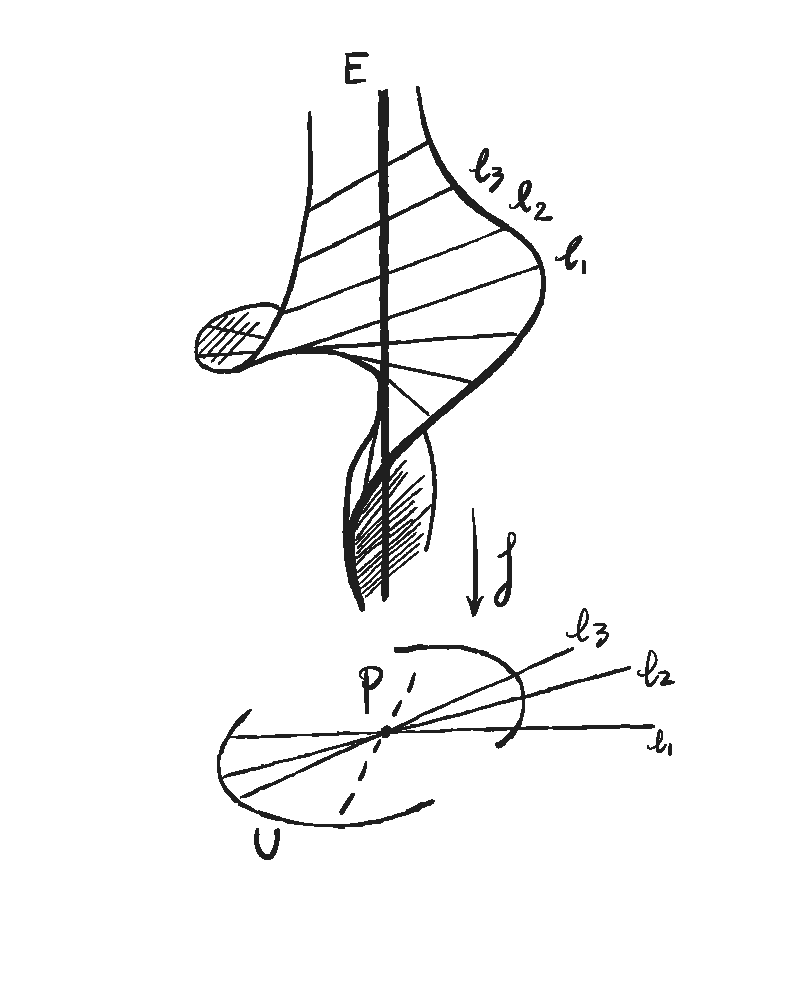
\includegraphics{pictures/blowup_A2.png}\]}
\end{titlepage}
\tableofcontents


\subsection{Sheaves and \'Etal\'e Spaces}
We now give a different description of sheaves via so-called \'etal\'e spaces.
\begin{definition}
Let $X$ be a topological space.
\begin{itemize}
\item[$(a)$] A pair $(E,\pi)$, where $E$ is a topological space and $\pi:E\to X$ is a local homeomorphism, is called an \textbf{\'etal\'e space over $\bm{X}$}.
\item[$(b)$] Let $(E_1,\pi_1)$ and $(E_2,\pi_2)$ be \'etal\'e spaces over $X$. A morphism $\varphi:(E_1,\pi_1)\to(E_2,\pi_2)$ of \'etal\'e spaces is a continuous map $\varphi:E_1\to E_2$ such that $\pi_1=\pi_2\circ\varphi$.
\[\begin{tikzcd}
E_1\ar[rr,"\varphi"]\ar[rd,swap,"\pi_1"]&&E_2\ar[ld,"\pi_2"]\\
&X&
\end{tikzcd}\]
\end{itemize}
Denote by \'Et/$X$ the category of \'etal\'e spaces over $X$.
\end{definition}
\begin{definition}
Let $(E,\pi)$ be an étalé space over $X$. For $U\sub X$ open, a \textbf{section} of $E$ over $U$ is a continuous map $s:U\to E$ with $\pi\circ s=\mathrm{id}_U$. The \textbf{fiber} of $E$ over $x\in X$ is the set $E_x=\pi^{-1}(x)$. A morphism of étalé spaces $f:(E_1,\pi_1)\to(E_2,\pi_2)$ gives rise to maps $f_x:(E_1)_x\to(E_2)_x$ for $x\in X$.
\end{definition}
\begin{proposition}
Let $(E,\pi)$ be an étalé space over $X$. Then the following properties hold:
\begin{itemize}
\item[$(a)$] The map $\pi$ is an open map.
\item[$(b)$] For any open subset $U$ of $X$ and any continuous section $s\in\Gamma(U,E)$, the subset $s(U)$ is open in $E$, such open subsets form a basis for the topology of $E$.
\end{itemize}
\end{proposition}
Now we justify our notation on the element of $\mathscr{F}(U)$: we show how to construct a sheaf from a \'etal\'e space using sections.
\begin{definition}
Let $(E,\pi)$ be an étalé space over $X$. Define a presheaf $\Gamma E$ of $E$-valued functions by
\[\Gamma E(U)=\{\text{sections }s:U\to E\}=\{s:U\to E:\text{$s$ is continuous and $\pi\circ s=\mathrm{id}_U$}\}.\]
It is a sheaf of $E$-valued functions by Example~\ref{sheaf of function}.
\end{definition}
Let $\varphi:(E_1,\pi_1)\to(E_2,\pi_2)$ be a morphism of étalé spaces, we obtain a map of sheaves $\Gamma\varphi:\Gamma E_1\to\Gamma E_2$ defined as follows: For every open subset $U$ of $X$, the map $(\Gamma\varphi)_U$ is given by 
\[(\Gamma\varphi)_U(s)=\varphi\circ s.\]
It is immediately checked that $\Gamma\varphi$ is a map of sheaves. Also, if $\varphi:E_1\to E_2$ and $\psi:E_2\to E_3$ are two maps of \'etal\'e spaces, then
\[\Gamma(\psi\circ\varphi)=\Gamma\psi\circ\Gamma\varphi\And \Gamma\mathrm{id}_E=\mathrm{id}_{\Gamma E}.\]
This means that the construction $\Gamma:\text{\'Et/}X\to\mathsf{Sh}(X)$ is functorial.

The next proposition tells us that the fibres of a \'etal\'e space are stalks of the sheaf $\Gamma E$.
\begin{proposition}\label{etale fiber stalk}
Let $(E,\pi)$ be a \'etal\'e space. For any $x\in X$, the stalk $(\Gamma E)_x$ is isomorphic to the fibre $E_x$ at $x$. Furthermore, as a subspace of $E$, the fibre $E_x$ has the discrete topology.
\end{proposition}
\begin{proof}
For $x\in X$, the stalk $(\Gamma E)_x$ is the set of equivalence classes of pairs $(U,s)$, where $U$ is an open neighborhood of $x$ and $s:U\to E$ is a section of $\pi$. Here $(U,s)$ and $(V,t)$ are equivalent if there exists $x\in W\sub U\cap V$ open such that $s|_{W}=t|_{W}$.\par
Fix a $x\in X$, for any open subset $x\in U\sub X$, we define a map $\tau_{U}:\Gamma E(U)\to E_x$ by
\[\tau_{U}(s)=s(x)\for s\in\Gamma E(U).\]
Then it is obvious that $\tau$ commute with the restriction map, hence we get a induced map $\tau_x:(\Gamma E)_x\to E_x$.\par
For any $e\in E_x$, there exists an open neighborhood $e\in V\sub E$ such that $\pi|_V$ is a homeomorphism onto its open image. Then $(\pi|_V)^{-1}$ is obviously a section of $\pi$ with $(\pi|_V)^{-1}(x)=e$. This shows that $\tau_x$ is surjective for every $x\in X$. Note that $E_x\cap V=\{e\}$, so $E_x$ has the discrete topology.\par
Let $s:U\to E$ and $s':U'\to E$ be sections with $s(x)=s'(x)=e$ for a point $x\in U\cap U'$. Then there exsits an open neighborhood $e\in V\sub E$ such that $\pi|_V:V\to\pi(V)$ is a homeomorphism. Let $W=\pi(V)\cap U\cap U'$, and replace $V$ by $(\pi|_V)^{-1}(W)$. Now $\pi|_V:V\to W$ is a homeomorphism and $s|_W,s'|_W$ are both inverse of it, so $s|_W=s'|_W$. This implies $(s,U)\sim(s',U')$, so $\tau_x$ is injective.
\end{proof}
Now we attach conversely to every presheaf an étalé space as follows. Let $\mathscr{F}$ be a presheaf on $X$. Define $S\mathscr{F}:=\coprod_{x\in X}\mathscr{F}_x$ to be 
the disjoint union of all the stalks. We have a projection map 
$\pi:S\mathscr{F}\to X$:
\[\pi(s)=x\for s\in\mathscr{F}_x.\]
For every open subset $U$ of $X$, we view each abstract section $s\in\mathscr{F}(U)$ as the actual function $\widetilde{s}:U\to S\mathscr{F}$ given by
\[\widetilde{s}(x)=s_x\for s\in U.\]
By definition, $\widetilde{s}$ is a section of $\pi$. We give $S\mathscr{F}$ the finest topology which makes all the functions $\widetilde{s}$ continuous. Consequently, a 
subset $\Omega$ of $S\mathscr{F}$ is open if and only if for every open subset $U$ of $X$ and every $s\in\mathscr{F}(U)$, the subset
\[\widetilde{s}^{-1}(\Omega)=\{x\in U\mid\widetilde{s}(x)=s_x\in\Omega\}\]
is open in $X$. The space $S\mathscr{F}$ endowed with the above topology is called the \textbf{stalk space} of the presheaf $\mathscr{F}$.
\begin{lemma}
For any $U\sub X$ open and $s\in\mathscr{F}(U)$, the set $\widetilde{s}(U)$ is open in $S\mathscr{F}$. Moreover, 
\[\{\widetilde{s}(U):\text{$U\sub X$ open, $s\in\mathscr{F}(U)$}\}\] 
consists of a basis for $S\mathscr{F}$.
\end{lemma}
\begin{proof}
It suffices to show that for any $x\in U$, any open subset $V$ containing $x$ and any $t\in\mathscr{F}(V)$, the subset
\[\widetilde{t}^{-1}\big(\widetilde{s}(U)\big)=\{x\in V:\widetilde{t}(x)=t_x\in\widetilde{s}(U)\}=\{x\in U\cap V:t_x=s_x\}\]
is open in $X$. However, $t_x=s_x$ means that there is some open subset $W\sub U\cap V$ containing $x$ such that $s|_W=t|_W$, which means that 
$W\sub\widetilde{t}^{-1}\big(\widetilde{s}(U)\big)$. So $\widetilde{t}^{-1}(\widetilde{s}(U))$ is indeed open in $X$.\par
Now let $U,V$ be open subsets of $X$ and $s\in\mathscr{F}(U),t\in\mathscr{F}(V)$, respectively. We consider the set $\widetilde{s}(U)\cap\widetilde{t}(V)$. By definition, 
we have
\[\widetilde{s}(U)\cap\widetilde{t}(V)=\{u\in S\mathscr{F}:\pi(u)\in U\cap V,s_{\pi(u)}=t_{\pi(u)}\}.\]
Let $u\in\widetilde{s}(U)\cap\widetilde{t}(V)$, then $s_{\pi(u)}=t_{\pi(u)}$, so there is a neighborhood $W$ of $\pi(u)$ such that $s|_{W}=t|_{W}$. This then means 
$\widetilde{s|_{W}}(W)\sub\widetilde{s}(U)\cap\widetilde{t}(V)$, so $\{\widetilde{s}(U)\}$ is a basis of $S\mathscr{F}$.
\end{proof}
Now by definition each $\widetilde{s}$ gives a local section of $\pi$. Since $\widetilde{s}$ is continuous by our topology, if we can show $\pi$ is continuous, then 
$\pi$ is a local homeomorphism. This is ture because
\[\pi^{-1}(U)=\bigcup_{s\in\mathscr{F}(V)\atop\text{$V$ is open},V\sub U}\widetilde{s}(V).\]
\begin{proposition}
For a presheaf $\mathscr{F}$, the stalk space $S\mathscr{F}$, together with the projection $\pi:S\mathscr{F}\to X$, give a \'etal\'e space $(S\mathscr{F},\pi)$.
\end{proposition}
Moreover, let $\varphi:\mathscr{F}\to\mathscr{G}$ be a morphism of presheaves, then the induced map $\varphi_x:\mathscr{F}_x\to\mathscr{G}_x$ gives a map between stalk spaces:
\[S\varphi:S\mathscr{F}\to\mathscr{G},\quad S\varphi(e)=\varphi_x(e)\for e\in\mathscr{F}_x.\]
It is clear that $\pi_{\mathscr{F}}=\pi_{\mathscr{G}}\circ S\varphi$, and for any open subset $U\sub X$ and $s\in\mathscr{F}(U)$, we have
\[S\varphi\circ\widetilde{s}(x)=S\varphi(s_x)=\varphi_x(s_x)=\big(\varphi_U(s)\big)_x=\widetilde{\varphi_U(s)}(x).\]
Therefore $S\varphi\circ\widetilde{s}=\widetilde{\varphi_U}(s)$. Since $\widetilde{s}$ and $\widetilde{\varphi_U}(s)$ are both local homeomorphisms, it follows that $S\varphi$ is continuous. We then obtain a functor $S:\mathsf{Psh}(X)\to\text{\'Et/}X$.
\begin{theorem}\label{stalk section iso sheafification}
There is a natural isomorphism from $\Gamma\circ S$ to the sheafification.
\end{theorem}
\begin{proof}
Let $\mathscr{F}$ be a presheaf on $X$, $(S\mathscr{F},\pi)=S(\mathscr{F})$ and $\mathscr{F}'=\Gamma S\mathscr{F}$. By construction $\widetilde{s}:U\to E$ is a section of $(S\mathscr{F},\pi)$ and therefore an element of $\mathscr{F}'(U)$ for any open subset $U\sub X$ and $s\in\mathscr{F}(U)$. We define a morphism of presheaves $\kappa:\mathscr{F}\to\mathscr{F}'$ by $\mathscr{F}(U)\mapsto\mathscr{F}'(U),s\mapsto\widetilde{s}$.\par
Let $x\in X$ be an arbitrary point. By construction $(S\mathscr{F})_x=\mathscr{F}_x$ and due to Proposition~\ref{etale fiber stalk} there is a bijective map 
\[\tau_x:\mathscr{F}'_x\to(S\mathscr{F})_x=\mathscr{F}_x,\quad \widetilde{s}\mapsto\widetilde{s}(x).\]
For $U\sub X$ open, $s\in\mathscr{F}(U)$ we have
\[\tau_x\big(\kappa_x(s_x)\big)=\tau_x(\widetilde{s}_x)=\widetilde{s}(x)=s_x.\]
so that $\tau_x\circ\kappa_x=\mathrm{id}_{\mathscr{F}_x}$ and $\kappa_x$ is bijective for every $x\in X$. It is straightforward to check that $\kappa$ defines a natural transformation and due to Example~\ref{sheaf iso sheafification} we attain an isomorphism from $\mathscr{F}'$ to the sheafification of $\mathscr{F}$ in a natural way making it a natural isomorphism.
\end{proof}
\begin{theorem}\label{section stalk iso identity}
There is a natural isomorphism $S\circ\Gamma$ to the identity functor.
\end{theorem}
\begin{proof}
Let $(E,\pi)$ be an étalé space over $X$, $(E',\pi')=S\circ\Gamma E$. By Proposition~\ref{etale fiber stalk} we have a bijection $\tau_x:(\Gamma E)_x\to E_x$ and by construction $E'=\coprod_{x\in X}(\Gamma E)_x$. This defines a bijective map $\tau:E'\to E$ with $\pi\circ\tau=\pi'$. For $U\sub X$ open and $s\in\Gamma E(U)$, we have 
\[\tau(\widetilde{s}(x))=\tau(s_x)=s(x).\] 
for every $x\in X$. The topology of $E'$ is the finest such that $\widetilde{s}:U\to E'$ is continuous for every $s,U$ and the topology of $E$ is the finest such that $s:U\to E$ is continuous for every $s,U$. This implies that $\tau$ is a homeomorphism:
\begin{align*}
W\sub E\text{ is open}&\iff s^{-1}(W)\sub X\text{ is open for every $s:U\to E$}\\
&\iff(\tau\circ\widetilde{s})^{-1}(W)\sub X\text{ is open for every $s:U\to E$}\\
&\iff\tau^{-1}(W)\text{ is open in $E'$}
\end{align*}
It is straightforward to check that this isomorphism is natural.
\end{proof}
As the sheafification of sheaf is the sheaf itself we deduce from Theorem\ref{stalk section iso sheafification} and Theorem~\ref{section stalk iso identity}:
\begin{proposition}
Let $X$ be a topological space. The functors $\Gamma$ and $S$ yield an equivalence between the category $\text{\'Et/}X$ of étalé spaces over $X$ and the category $\mathsf{Sh}(X)$ of sheaves on $X$.
\end{proposition}
\begin{example}[\textbf{\'Etal\'e Spaces of constant sheaves}]
Let $E$ be a set that we also consider as a discrete topological space. Let $E_X$ be the constant sheaf with values in $E$ on a topological space $X$. Then the corresponding étalé space is $(X\times E,\pi_1)$ because as a set, $SE_X=X\times E$, and for $U\sub X$ open the sections of $\pi_1$ over $U$ are just the maps $x\mapsto(x,s(x))$, where $s:U\to E$ is locally constant.
\end{example}
Note that the map $\pi_1:X\times E\to X$ is a trivial covering map. More generally, every covering map is an étalé space that is locally on $X$ a trivial covering map. Hence we obtain the following result.
\begin{proposition}[\textbf{Locally constant sheaves}]
A sheaf $\mathscr{F}$ on $X$ is called \textbf{locally constant} if there exists an open covering $(U_i)_i$ of $X$ such that $F|_{U_i}$ is a constant sheaf.\par
The equivalence of $\mathsf{Sh}(X)$ and $\text{\'Et/}X$ yields an equivalence between the full subcategory of locally constant sheaves on $X$ and the category of covering spaces of $X$.
\end{proposition}
\begin{example}
Let $\mathcal{L}$ be the sheaf of complex logarithms on $\C-\{0\}$,
\[\mathcal{L}(U):=\{L:U\to\C\text{ holomorphic}\mid \exp\circ L=\mathrm{id}_U\}\for U\sub\C-\{0\}.\]
For every simply connected open subspace $U$ of $\C-\{0\}$ the choice of a logarithm $L_0$ on $U$ yields an isomorphism of sheaves of abelian groups 
$(2\pi i\Z)_U\cong\mathcal{L}|_{U}$: one attaches to a locally constant function $t$ with values in $2\pi i\Z$ on an open subset $V$ of $U$ the logarithm $L_0|_V+t$. 
Hence $\mathcal{L}$ is a locally constant sheaf of abelian groups. But it is not constant because $\mathcal{L}(\C-\{0\})=\emp$. The associated étalé space to 
$\mathcal{L}$ is the covering map $\exp:\C\to\C-\{0\}$.
\end{example}
\subsubsection{Inverse image and \'etal\'e space}
We have already seen that there is a natural correspondence between sheaves and étalé space and that it is possible to describe the sheafification of a presheaf in terms of associated étalé spaces. We will now show that the formation of the inverse image of a presheaf has a simple description in terms of étalé spaces: The corresponding étalé space is given by the fiber product. Hence let us consider continuous maps $f:X'\to X$ and $\pi:E\to X$ of topological spaces. We form the fiber product and obtain the following commutative diagram, where $g:E\times_XX'\to E$ and $\pi':E\times_XX'\to X'$ are the projections:
\[\begin{tikzcd}
E\times_XX'\ar[r,"\pi'"]\ar[d,"g"]&X'\ar[d,"f"]\\
E\ar[r,"\pi"]&X
\end{tikzcd}\]
\begin{lemma}\label{pull back diagram prop}
Suppose that $\pi$ has one of the following properties:
\begin{itemize}
\item[$(a)$] homeomorphism.
\item[$(b)$] open topological embedding.
\item[$(c)$] local homeomorphism.
\end{itemize}
Then $\pi'$ has the same property.
\end{lemma}
\begin{proof}
Assertion $(a)$ is clear because $\pi\mapsto\pi'$ is functorial: the fiber product is given by
\[E\times_XX'=\{(e,x'):\pi(e)=f(x')\},\]
If $\omega$ is a continuous inverse of $\pi$, then we have $e=\omega\circ\pi(e)=\omega\circ f(x')$. So the map
\[\omega:X'\to E\times_XX',\quad x'\mapsto(\omega\circ f(x'),x')\]
is a continuous inverse of $\pi'$.\par
If $\pi:E\to U$ is a homeomorphism for some $U\sub X$ open, then the restriction  $\pi':E'\to f^{-1}(U)$ is a homeomorphism by $(a)$. This shows $(b)$.\par
Finally, if there exists an open covering $(W_i)_i$ of $E$ such that $\pi|_{W_i}$ is an open embedding for all $i$, then $(g^{-1}(W_i))_i$ is an open covering of $E'$ and $\pi'|_{g^{-1}(W_i)}$ is an open embedding by $(b)$. This proves $(c)$.
\end{proof}
The fiber product construction above yields a functor $\text{Ét/}X\to\text{Ét/}X'$ by sending a morphism $f:E_1\to E_2$ of étalé spaces over $X$ to the map $E_1\times_XX'\to E_2\times_XX'$ induced by $f\times\mathrm{id}_{X'}$.
\begin{proposition}[\textbf{Inverse image via étalé spaces}]
Let $f:X\to Y$ be a continuous map of topological spaces, $\mathscr{E}$ a presheaf on $Y$ and $(E,\pi)$ the étalé space over $Y$ associated to $\mathscr{E}$. The functor that sends $\mathscr{E}$ to the sheaf associated to the étalé space $(E\times_YX,\pi')$ is naturally isomorphic to the inverse image functor $f^{-1}$.
\end{proposition}
\begin{example}[\textbf{Inverse image of constant sheaves}]
Let $f:X\to Y$ be a continuous map. Let $E$ be a set, let $E_Y$ be the sheaf of locally constant $E$-valued functions on $Y$. The corresponding étalé space is the projection $E\times Y\to Y$, where we consider $E$ as a discrete topological space. Then the projection $(E\times Y)\times_YX\to E\times X$ is a homeomorphism compatible with the projections to $X$. Hence $f^{-1}E_Y=E_X$.
\end{example}
\begin{definition}[\textbf{Pullback of sections}]
Let $f:X\to Y$ be a continuous map, let $\mathscr{G}$ be a sheaf on $Y$, and let $t\in\mathscr{G}(V)$, $V\sub Y$ open. Let $\pi:G\to Y$ be the étalé space corresponding to $\mathscr{G}$ and consider $t$ as a continuous section $t:V\to G$ of $\pi$. Then
\[f^{-1}(t):f^{-1}(V)\to G\times_YX,\quad x\mapsto\big(t\circ f(x),x\big)\]
is a continuous section of $G\times_YX\to X$. Hence we obtain a pullback map
\[f^{-1}:\mathscr{G}(V)\to(f^{-1}\mathscr{G})(f^{-1}(V)),\]
which is functorial in $\mathscr{G}$ and compatible with restrictions to smaller open subsets of $Y$.
\end{definition}
\begin{example}
Let $X$ be a topological space, let $S$ be a subspace of $X$, and denote by $i:S\to X$ the inclusion. If $\mathscr{F}$ is a sheaf on $X$ with corresponding étalé space $\pi:E\to X$, then the étalé space corresponding to $\mathscr{F}|_{S}$ is the usual restriction $\pi|_{\pi^{-1}(S)}:\pi^{-1}(S)\to S$. The pullback $i^{-1}(s)$ of a continuous section $s:U\to E$ of $\pi$ for $U\sub X$ is simply the restriction $s|_{S\cap U}$.
\end{example}
%\chapter{Elementray number theory}
\section{Dirichlet's approximation theorem}
\begin{theorem}[\textbf{Dirichlet's Approximation Theorem}]\label{Dirichlet approximation}
Given $\alpha\in\R$ and any positive integer $N$, there exist relatively prime integers $p,q$ with $1\leq q\leq N$ such that $|q\alpha-p|<1/N$.
\end{theorem}
\begin{proof}
For any real number $x$, let $f(x)=x-[x]$. Divide the interval $[0,1)$ into $N$ parts
\[[0,1)=\coprod_{i=1}^{N}[\frac{i-1}{N},\frac{i}{N})\]
Since the $N+1$ numbers $\{f(i\alpha):0\leq i\leq N\}$ all lie in the interval $[0,1)$, by the pigeonhole principle there must exist integers $i$ and $j$ with $0\leq i<j\leq N$ such that both $f(i\alpha)$ and $f(j\alpha)$ lie in one of the $N$ subintervals. Thus 
\[|f(i\alpha)-f(j\alpha)|<\frac{1}{N}\]
so we can take $q=j-i$ and $p=[j\alpha]-[i\alpha]$.\par
Now for the relatively prime part, write $d=(p,q)$ and $p=p'd,q=q'd$. Then $q'\leq q\leq N$ and
\[|q'\alpha-p'|=\frac{1}{d}|q\alpha-p|<\frac{1}{Nd}\leq\frac{1}{N}\]
Thus the intergers $p'$ and $q'$ satisfy the conditions.
\end{proof}
\begin{corollary}
For every real $\alpha$ there exist relatively prime integers $p$ and $q$ with $q>0$ such that
\[\Big|\alpha-\frac{p}{q}\Big|<\frac{1}{q^2}\]
\end{corollary}
\begin{proof}
In Theorem~\ref{Dirichlet approximation} we have $1/(Np)\leq 1/p^2$ because $p\leq N$.
\end{proof}
\begin{theorem}\label{real number irrational iff}
If $\alpha$ is real, let $S_\alpha$ denote the set of all ordered pairs of coprime integers
$(p,q)$ with $q>0$ such that
\[\Big|\alpha-\frac{p}{q}\Big|<\frac{1}{q^2}\]
Then $S_\alpha$ has the following properties:
\begin{itemize}
\item[$(a)$]$S_\alpha$ is nonempty.
\item[$(b)$]If $\alpha$ is irrational, $S_\alpha$ is an infinite set.
\item[$(c)$]When $S_\alpha$ is infinite it contains pairs $(p,q)$ with $q$ arbitrarily large.
\item[$(d)$]If $\alpha$ is rational, $S_\alpha$ is a finite set.
\end{itemize}
\end{theorem}
\begin{proof}
Part $(a)$ follows immediately from Theorem~\ref{Dirichlet approximation}. For $(b)$, assurne $\alpha$ is irrational and assurne also that $S_\alpha$ is finite. We shall obtain a contradiction. Let
\[\eps:=\inf_{(p,q)\in S_\alpha}\Big|\alpha-\frac{p}{q}\Big|\]
Since $\alpha$ is irrational, $\eps$ is positive. Choose any integer $N>1/\eps$ and apply Theorem~\ref{Dirichlet approximation} with this $N$. We obtain a pair of integers $(p,q)\in S_\alpha$ with $1\leq q\leq N$ such that
\[\Big|\alpha-\frac{p}{q}\Big|<\frac{1}{qN}<\frac{1}{N}<\eps\]
This is a contradiction.\par
To prove $(c)$ assurne that all pairs $(p,q)$ in $S_\alpha$ have $q\leq M$ for some $M$. We will show that this leads to a contradiction by showing that the number
of choices for $p$ is also bounded. If $(p,q)\in S_\alpha$ we have
\[|q\alpha-p|<\frac{1}{q}\leq 1\]
Hence
\[|p|=|p-q\alpha+q\alpha|\leq|q\alpha-p|+|q\alpha|<1+|q\alpha|\leq 1+|M\alpha|\]
Therefore the number of choices for $p$ is bounded, contradicting the fact that $S_\alpha$ is infinite.\par
Finially, for $(d)$, if $\alpha=a/b$ is rational where $(a,b)=1$, then $(a,b)\in S_\alpha$. Now we assurne that $S_\alpha$ is an infinite set and obtain a contradiction. If $S_\alpha$ is infinite then by part $(c)$ there is a pair $(p,q)$ in $S_\alpha$ with $q>b$. For this pair we have
\[0<\Big|\frac{a}{b}-\frac{p}{q}\Big|<\frac{1}{q^2}\]
from which we find $0<|aq-bp|<1$. This is a contradiction because $aq-bp$ is an integer.
\end{proof}
\begin{remark}
Theorem~\ref{real number irrational iff} shows that areal number $\alpha$ is irrational if, and only if, there are infinitely many rational numbers $p,q$ with $(p,q)=1$ and $q>0$ such that
\[\Big|\alpha-\frac{p}{q}\Big|<\frac{1}{q^2}\]
The constant $1$ can be replaced by $1/\sqrt{5}$. Moreover, the result is false if $1/\sqrt{5}$ is replaced by any smaller constant.
\end{remark}
\section{Kronecker's approximation theorem}
We make use of the fractional parts $\{x\}:=x-[x]$.
\begin{theorem}
If $\alpha$ is a given irrational number the sequence of numbers $\{n\alpha\}$ is dense in the unit interval. That is, given any $x\in[0,1]$, and given any $\eps>0$, there exists a positive integer $n$ such that
\[|\{n\alpha\}-x|<\eps\]
\end{theorem}
\begin{proof}
First we note that $\{n\alpha\}\neq\{m\alpha\}$ if $m\neq n$ because $\alpha$ is irrational. Also, there is no loss of generality if we assume $0<\alpha<1$.\par
Let $\eps>0$ be given and choose any $0<\alpha<1$. By Dirichlet's approximation theorem there exist integers $p$ and $q$ such that $|q\alpha-p|<\eps$. Suppose that $q\alpha>p$, so that $0<\{q\alpha\}<\eps$. Now consider the subsequence $\{nq\alpha:n\in\N\}$. We have
\[nq\alpha=n[q\alpha]+n\{q\alpha\}\]
Hence
\[\{nq\alpha\}=n\{q\alpha\}\iff \{q\alpha\}<\frac{1}{n}\]
Now choose the largest integer $N$ which satisfies $\{q\alpha\}<1/N$. Then we have
\[\frac{1}{N+1}<\{q\alpha\}<\frac{1}{N}\]
Therefore $\{nq\alpha\}=n\{q\alpha\}$ for $n\leq N$, so the $N$ numbers
\[\{q\alpha\},\{2q\alpha\},\cdots,\{Nq\alpha\}\]
form an increasing \textbf{equally-spaced} chain running from left to right in the interval $(0,1)$. The last member of this chain (by the definition of $N$) satisfies the inequality
\[\frac{N}{N+1}<\{Nq\alpha\}<1\]
or
\[1-\frac{1}{N+1}<\{Nq\alpha\}<1\]
Thus $\{Nq\alpha\}$ differs from $1$ by less than $1/(N+1)<\{q\alpha\}<\eps$. Therefore the first $N$ members of the subsequence $\{nq\alpha\}$ subdivide the unit interval into subintervals of length $<\eps$. Since $x$ lies in one of these subintervals, the theorem is proved.
\end{proof}
\begin{corollary}
Given any real $x$, any irrational $\alpha$, and an $\eps>0$, there exist integers $m$ and $n$ with $n>0$ such that
\[|n\alpha-m-x|<\eps\]
Thus the subset $\alpha\Z+\Z$ is dense in $\R$.
\end{corollary}
\section{Quadratic Residues}
An integer $k$ that is prime to a positive integer $m$ is said to be a quadratic residue modulo $m$ if there exists $z\in\Z$ such that
\[z^2\equiv k\mod m\]
\subsection{Units in \boldmath$\Z/n\Z$}
\begin{proposition}
Let $p$ be a prime, then the group $(\Z/p^n\Z)^\times$ has order $p^{n-1}(p-1)$.
\end{proposition}
\begin{proof}
Note that $[m]_{p^n}$ is a unit iff $\gcd(m,p^n)=\gcd(m,p)=1$. Thus the elements in $\Z/p^n\Z$ are unit except
\[0,[p],[2p],\dots,[p^{n}-p].\]
Thus the order of $(\Z/p^n\Z)^\times$ is
\[|(\Z/p^n\Z)^\times|=p^n-p^{n-1}=p^{n-1}(p-1)\]
as claimed.
\end{proof}
\begin{lemma}\label{Z/nZ iso}
Let $n=p_1^{e_1}\cdots p_r^{e_r}$ be an integer, then there is a ring isomorphism
\[\Z/n\Z=\prod_{i=1}^{r}\Z/p_i^{e_i}\Z.\]
\end{lemma}
\begin{proof}
Since $p_i$'s are coprime, this follows from the Chinese remainder theorem.
\end{proof}
\begin{theorem}\label{unit in Z/nZ}
Let $n=p_1^{e_1}\cdots p_r^{e_r}$ be an integer, then
\[(\Z/n\Z)^\times\cong\prod_{i=1}^{r}(\Z/p_i^{e_i}\Z)^{\times}.\]
In particular, we have
\[\phi(n)=n\prod_{i=1}^{r}\Big(1-\frac{1}{p_i}\Big).\]
\end{theorem}
\begin{proof}
Under the ring isomorphism in Lemma~\ref{Z/nZ iso}, an element $[m]\in\Z/n\Z$ is a unit if and only if its image is a unit, which holds if and only if each of its components is a unit. With this,
\[\phi(n)=\prod_{i=1}^{r}\phi(p_i^{e_i})=\prod_{i=1}^{r}p_i^{e_i-1}(p_i-1)=n\prod_{i=1}^{r}\Big(1-\frac{1}{p_i}\Big)\]
as claimed.
\end{proof}
\begin{corollary}
If $m$ and $n$ are coprime, then $\phi(mn)=\phi(m)\phi(n)$.
\end{corollary}
\begin{corollary}
If $n$ is odd, then $\Phi_{2n}(x)=\Phi_{n}(-x)$.
\end{corollary}
\begin{proof}
Defined a map
\[\varphi:(\Z/n\Z)^{\times}\to (\Z/2n\Z)^{\times},\quad [m]_n\mapsto[2m+n]_{2n}.\]
This map is well defined since $\gcd(m,n)=1$ implies $\gcd(2m+n,2n)=1$ when $n$ is odd. Moreover, we observe that
\[[2m_1+n]_{2n}=[2m_2+n]_{2n}\Longrightarrow 2m_1-2m_2\equiv 0\text{ mod $2n$}\Longrightarrow m_1-m_2\equiv 0\text{ mod $n$}.\]
Therefore $\varphi$ is injective. Since we already have that $\phi(2n)=\phi(n)$, $\varphi$ is then an isomorphism. Now 
\[\zeta^{2m+n}_{2n}=e^{\frac{(2m+n)2\pi i}{2n}}=-e^{\frac{2\pi im}{n}}=-\zeta^m_n,\] 
so we conclude that
\[\Phi(x)_{2n}=\prod(x-\zeta_{2n}^r)=\prod(x+\zeta_n^m)=(-1)^{\phi(n)}\prod(-x-\zeta_n^m)=(-1)^{\phi(n)}\Phi_n(-x).\]
Since $n$ is odd, every prime divisor of $n$ is also odd, thus $\phi(n)$ is even in view of the formula in Theorem~\ref{unit in Z/nZ}. Thus we are done.
\end{proof}
\begin{proposition}
Let $p$ be a prime. Then $(\Z/p\Z)^\times$ is a cyclic group of order $p-1$.
\end{proposition}
\begin{proof}
$(\Z/p\Z)^\times$ is an abelian group, and the equation $x^{n}-1=0$ has at most $n$ solutions in it. By the classification theorem of abelian groups, we conclude that it is cyclic.
\end{proof}
\begin{lemma}
In an abelian group $G$, if $a,b$ have finite orders $q,r$ which are coprime, then $ab$ has order $qr$.
\end{lemma}
\begin{proof}
If $(ab)^s=1$ then $a^s=b^{-s}$, thus they have the same order $k$. However, the order of $a^s$ divides the order of $a$, so $k$ divides $q$, similarly $k$ divides $r$. Since $\gcd(q,r)=1$, this implies $k=1$. Therefore
\[a^s=b^{-s}=1.\]
This immediately implies $qr=\mathrm{lcm}(q,r)\mid s$. Thus $ab$ has order $qr$.
\end{proof}
\begin{lemma}\label{primitive root lem}
\mbox{}
\begin{itemize}
\item[$(a)$] If $s$ is a primitive root of $p$, then so is $s^r$ if and only if $r$ and $p-1$ are coprime.
\item[$(b)$] If $s$ is a primitive root of $p$ and $k$ is a positive integer, then there is another primitive root $\lambda$ of $p$ such that $[s]=[\lambda]^{p^k}$.
\end{itemize}
\end{lemma}
\begin{proof}
For $(a)$, we have
\[|s^r|=\frac{p-1}{\gcd(r,p-1)}\]
Thus $s^r$ is a primitive root of $p$ iff $r$ and $p-1$ are coprime.\par
For $(b)$, since $p^k$ and $p-1$ are coprime, there exist integers $a,b$ where $a$ is prime to $p-1$ such that
\[ap^k+b(p-1)=1.\]
Hence $\lambda=s^a$ is a primitive root of $p$ by part $(a)$ and
\[[\lambda]^{p^k}=[s]^{ap^k}=[s]^{ap^k+b(p-1)}=[s]\]
as needed.
\end{proof}
\begin{theorem}\label{unit Z/p^nZ}
If $p$ is an odd prime and $n\geq 2$, then $(\Z/p^n\Z)^\times$ is a cyclic group of order $p^{n-1}(p-1)$ with generator $[s(1+p)]$, where $[s]$ is a primitive root of $p$.
\end{theorem}
\begin{proof}
Since $p-1$ and $p^{n-1}$ are coprime, it is sufficient to show that $[s]$ has order $p-1$ and $[1+p]$ has order $p^{n-1}$ in $(\Z/p^n\Z)^\times$.
\begin{itemize}
\item For $s$, by Lemma~\ref{primitive root lem}, there is a primitive root $\lambda$ such that $[\lambda]^{p^{n-1}}=[s]$, thus
\[[s]^{p-1}=[\lambda]^{p^{n-1}(p-1)}=[1].\]
On the other hand, $[s]^r=1$ in $\Z/p^n\Z$ implies $[s]^r=1$ in $\Z/p\Z$. So since $s$ is a primitive root of $p$ we have $[s]^r\not\equiv 1$ for $1<r<p-1$ in $\Z/p^n\Z$. Therfore $[s]$ has order $p-1$.
\item We compute by an induction that
\[(1+p)^{p^{n-2}}\equiv 1+kp^{n-1}\]
where $k$ depends on $n$ but $k\not\equiv 0$ mod $p$. For $n=2$ this is true with $k=1$. Assume it true for some $n\geq2$. Then 
\[(1+p)^{p^{n-2}}=1+kp^{n-1}+rp^e=1+sp^{n-1}\]
where $s=k+rp\not\equiv 0$ mod $p$. Hence
\begin{align*}
(1+p)^{p^{n-1}}&=(1+sp^{n-1})^p\\
&=1+psp^{n-1}+\binom{p}{2}s^2p^{2(n-1)}+\cdots+s^pp^{p(n-1)}.
\end{align*}
For $n\geq2$ and prime $p\neq2$ this is of the form
\[1+sp^n+bp^{n+1}\]
Therefore
\[(1+p)^{p^{n-1}}\equiv 1+sp^n\mod p^{n+1}.\]
where $s\not\equiv0$ mod $p$, completing the induction.\par
This then gives
\[(1+p)^{p^{n-2}}\equiv 1+kp^{n-1}\not\equiv[1]\text{ mod $p^n$},\quad (1+p)^{p^{n-1}}\equiv 1+kp^{n}\equiv 1\text{ mod $p^n$}.\]
Therefore $[1+p]$ has order $p^{n-1}$.
\end{itemize}
These give the proof.
\end{proof}
Since the proof breaks down for $p=2$, we must treat this case separately. We find:
\begin{proposition}~\label{unit Z/2^nZ}
$(\Z/4\Z)^\times=\{[1],[-1]\}$ is cyclic with generator $[-1]$. For $n\geq3$, $(\Z/2^n\Z)^{\times}$ is not cyclic, but $[-1]$ is of order $2$, $[5]$ is of order $2^{n-2}$ and $(\Z/2^n\Z)^{\times}$ is the direct product of the cyclic groups generated by $[-1],[5]$.
\end{proposition}
\begin{proof}
The assertion concerning $(\Z/4\Z)^\times$ is trivial. For $n\geq3$, the order of $(\Z/2^n\Z)^\times$ is $2^{n-1}$. Clearly the order of $[-1]$ in $(\Z/2^n\Z)^\times$ is $2$. For the element $[5]$ we note that by induction on $n\geq3$ we may establish
\[5^{2^{n-3}}=(1+2^2)^{2^{n-3}}\equiv 1+2^{n-1}\mod 2^n.\]
Hence $[5]^{2^{n-3}}\not\equiv1$ in $\Z/2^n\Z$, but
\[5^{2^{n-2}}\equiv(1+2^{n-1})^2\equiv 1\mod 2^e\]
wo $[5]$ has order $2^{n-2}$ in $(\Z/2^n\Z)^\times$.\par
Now $[-1]$ is not a power of $[5]$ in $(\Z/2^n\Z)^\times$ since
\[-1\not\equiv 5^r\mod 4\]
so certainly $[-1]\neq[5^r]$ in $(\Z/2^n\Z)^\times$. Hence if $N,H$ is the cyclic subgroup generated by $[-1],[5]$ respectively, then $N\cap H=\{[1]\}$. Since multiplication is commutative, $(\Z/2^n\Z)^\times$ is the direct product of $N$ and $H$. Clearly $(\Z/2^n\Z)^\times$ is not cyclic.
\end{proof}
\subsection{Quadratic Residues}
\begin{proposition}
If $m=p_1^{e_1}\cdots p_r^{e_r}$ and $k$ is relatively prime to $m$, then $k$ is a quadratic residue modulo $m$ if and only if it is a quadratic residue of $p^{e_i}_i$ for all $i$.
\end{proposition}
\begin{proof}
Using the isomorphism of Theorem~\ref{unit in Z/nZ}, $[k]$ is a square if and only if each component of its image is a square, and the $i$-th component is the residue class of $k$ modulo $p_i^{e_i}$.
\end{proof}
This reduces the general problem of finding quadratic residues to the simpler problem of finding quadratic residues modulo a prime power. Following the last subsection we distinguish between the case of an odd prime and $p=2$ first, because this can be given an immediate answer:
\begin{proposition}
The odd integer $k$ is a quadratic residue modulo $4$ if and only if $k\equiv1$ mod $4$, and is a quadratic residue modulo $2^n$ for $n\geq3$ if and only if $k\equiv1$ mod $8$.
\end{proposition}
\begin{proof}
Since $(\Z/4\Z)^\times=\{[1],[3]\}$, the only square in $(\Z/4\Z)^\times$ is $[1]$. For $n\geq 3$, if $z^2=k$ in $(\Z/2^n\Z)^\times$, we use Proposition~\ref{unit Z/2^nZ} to write
\[[z]=[-1]^a[5]^b,\quad [k]=[-1]^c[5]^d,\]
and then
\[[-1]^{2a}[5]^{2b}=[-1]^c[5]^d\]
whence $c$ is even and $2b\equiv d$ mod $2^{n-2}$. Given $d$, the congruence can be solved for $b$ if and only if $d$ is even. Thus $[k]$ is a quadratic residue modulo $2^n$ if and only if
\[[k]=[5]^d\]
in $\Z/2^n\Z$ where $d$ is even. Putting $d=2r$ this implies
\begin{align*}
k\equiv 5^{2r}\mod 2^n
\end{align*}
for $n\geq 3$, hence 
\[k\equiv 25^r\equiv 1\mod 8\]
Conversely if $k\equiv1$ mod $8$ and $[k]\equiv[(-1)^c5^d]$, then \[(-1)^c5^d\equiv 1\mod 8.\]
This happens only when $c,d$ are even, and then $(-1)^c5^d$ is a square in $(\Z/2^n\Z)^\times$.
\end{proof}
In the case $p$ odd we first characterize the quadratic residues modulo $p$ by using a primitive root of $p$:
\begin{lemma}\label{primitive root squre}
If $s$ is a primitive root of $p$, then $[k]=[s]^a$ is a quadratic residue if and only if $a$ is even.
\end{lemma}
\begin{proof}
If $a=2b$, then $[k]=[s^b]^2$. Now $[s]$ has even order $p-1$, it cannot be a square, nor can $[s]^a$ for $a$ odd.
\end{proof}
\begin{proposition}
If $p$ is an odd prime, then $k$ is a quadratic residue modulo $p^n$ for $n\geq 2$ if and only if $k$ is a quadratic residue modulo $p$.
\end{proposition}
\begin{proof}
If $z^2\equiv k$ mod $p^n$, then clearly $z^2\equiv k$ mod $p$, so a quadratic residue modulo $p^n$ also servesmodulo $p$. Conversely, suppose $k$ is a quadratic residue modulo $p$. By Proposition~\ref{unit Z/p^nZ} we can write $k\equiv s^a(1+p)^a$ mod $p^n$, and reducing this modulo $p$ gives $k\equiv s^a$ mod $p$, so Lemma~\ref{primitive root squre} implies that $a=2b$ for an integer $b$, so $k\equiv[s^b(1+p)b]^2$ mod $p^n$ and $k$ is a quadratic residue modulo $p^n$.
\end{proof}
This leaves the central core of the problem: to determine quadratic residues modulo any odd prime $p$. We define the symbol $(k/p)$ for an odd prime
$p$ and an integer $k$ not divisible by $p$ as
\[\Big(\frac{k}{p}\Big)=\begin{cases}
+1&\text{if $k$ is quadratic residue modulo $p$}\\
-1&\text{otherwise}.
\end{cases}\]
The value of this notation can be seen by writing $[k]=[s^a]$ where $s$ is a primitive root of $p$. By Lemma~\ref{primitive root squre}, $k$ is a quadratic residue modulo $p$ if and only if $a$ is even, hence
\[\Big(\frac{k}{p}\Big)=(-1)^a.\]
From this it is easy to deduce the following useful properties:
\begin{proposition}
\mbox{}
\begin{itemize}
\item[$(a)$] $k\equiv r$ mod $p$ implies $(k/p)=(r/p)$.
\item[$(b)$] $(kr/p)=(k/p)(r/p)$.
\end{itemize}
\end{proposition}
It is now possible to give a computational test for quadratic residues:
\begin{proposition}[\textbf{Euler's Criterion}]
For an odd prime $p$ and an integer $k$ not divisible by $p$,
\[\Big(\frac{k}{p}\Big)\equiv k^{(p-1)/2}\mod p\]
\end{proposition}
\begin{proof}
For a primitive root $s$ modulo $p$ we have $s^{p-1}\equiv 1$ mod $p$, and since $p-1$ is even, 
\[(s^{(p-1)/2}-1)(s^{(p-1)/2}+1)=s^{p-1}-1\equiv0\mod p.\]
Because $s^{(p-1)/2}\not\equiv1$ mod $p$, we deduce that
\[s^{(p-1)/2}\equiv -1\mod p.\]
Hence, writing $[k]=[s^a]$ as before
\begin{align*}
\Big(\frac{k}{p}\Big)=(-1)^a\equiv(s^{(p-1)/2})^a\equiv s^{a(p-1)/2}\equiv k^{(p-1)/2}\mod p.
\end{align*}
\end{proof}
\begin{example}
$k$ is a quadratic residue mod $5$ if $k^2\equiv1$ mod $5$, giving $k=1,4$.
\end{example}
We partition the units modulo $p$ by writing them in the form
\[(\Z/p\Z)^\times=\{[-(p-1)/2],\dots,[-2],[-1]\}\cup\{[1],[2],\dot,[(p-1)/2]\}:=N\cup P\]
Using the usual multiplicative notation $aS=\{as\mid s\in S\}$, we can write $N=([-1])P$. To find out whether $k$ is a quadratic residue, Gauss computed
the set $[k]P$ and proved:
\begin{proposition}[\textbf{Gauss's Criterion}]
With the above notation, if $[k]P\cap N$ has $\nu$ elements then $(k/p)=(-1)^\nu$.
\end{proposition}
\begin{proof}
Since $[k]$ is a unit, the elements of  $[k]P$ are distinct. Furthermore if $[a],[b]$ are distinct elements of $P$, then we may take $0<a<b\leq(p-1)/2$. We cannot have $[k][a]=-[k][b]$, for that implies $k(a+b)$ is divisible by $p$, hence $a+b$ is divisible by $p$, contradicting the inequalities satisfied by $a,b$. Thus the elements $[k],[2k],\dots,[k(p-1)/2]$ of $[k]P$ consist precisely of the elements $\pm[1],\pm[2],\dots,\pm[(p-1)/2]$, possibly in a different order, where the number of minus signs is the number of elements of $[k]P$ in $N$. Hence
\[[k]\cdot[2k]\cdots[k(p-1)/2]=[(-1)^\nu]\cdot[1]\cdots[2]\cdots[(p-1)/2]\]
so
\[[k]^{(p-1)/2}=[(-1)^\nu]\]
where $\nu$ is the number of elements in $[k]P\cap N$. Thus
\[k^{(p-1)/2}\equiv(-1)^\nu\mod p.\]
and Euler's criterion gives
\[\Big(\frac{k}{p}\Big)=(-1)^\nu.\]
\end{proof}
\begin{example}
Is $3$ a quadratic residue modulo $19$? To answer this we calculate
\[[3]P=\{3,6,9,12,15,18,2,5,8\}=\{3,6,9,2,5,8\}\cup\{-7,-4,-1\},\]
so $\nu=3$ and Gauss's criterion tells us that $3$ is not a quadratic residue modulo $19$.
\end{example}
These two criteria take us further in the search for quadratic residues $k$ modulo an odd prime $p$, for by factorizing
\[k=(-1)^a2^bp_1^{e_1}\cdots p_r^{e_r}\]
then $k$ is a square if $a,b,e_1,\dots,e_r$ are even; moreover, it is a quadratic residue if the factors with odd exponent are quadratic residues. Thus the question of quadratic residues is finally reduced to determining whether $-1,2$ or an odd prime $q$ (distinct from $p$) are quadratic residues modulo an odd prime $p$.\par
The given criteria solve the question for $-1$ and $2$.
\begin{proposition}
Let $p$ be an odd prime, we have
\[\Big(\frac{-1}{p}\Big)=(-1)^{(p-1)/2},\quad \Big(\frac{2}{p}\Big)=(-1)^{(p^2-1)/8}.\]
\end{proposition}
\begin{proof}
The first result is a trivial consequence of Euler's criterion. So we consider $2$.\par
We have 
\[[2]P=\{[2],[4],\dots,[p-1]\}\]
so $|[2]P\cap N|$ is $\nu=(p-1)/2-r$ where $r$ is the largest integer such that $2r\leq(p-1)/2$. The proof now splits into two cases.
\begin{itemize}
\item If $(p-1)/2$ is even then $2r=(p-1)/2$, whence 
\[\nu=\frac{p-1}{2}-\frac{p-1}{4}=\frac{p-1}{4}.\]
Thus $(2/p)=(-1)^{(p-1)/4}$.
\item If $(p-1)/2$ is odd, then $2r=(p-1)/2-1$, whence
\[\nu=\frac{p-1}{2}-\frac{p-1}{4}+\frac{1}{2}=\frac{p+1}{4}.\]
Thus $(2/p)=(-1)^{(p+1)/4}$.
\end{itemize}
We can put these two cases together by noting that in the first case $(p-1)/2$ is even if and only if $(p+1)/2$ is odd. so in case one
\[\Big(\frac{2}{p}\Big)=[(-1)^{(p-1)/4}]^{(p+1)/2}=(-1)^{(p^2-1)/8}.\]
Case two gives the same result by raising to the odd power $(p-1)/2$.
\end{proof}
\begin{theorem}[\textbf{Quadratic Reciprocity Law}]
If $p,q$ are distinct odd primes, then
\[\Big(\frac{p}{q}\Big)\Big(\frac{q}{p}\Big)=(-1)^{(p-1)(q-1)/4}.\]
\end{theorem}
An immediate deduction is the quadratic reciprocity law in the form stated by Gauss:
\begin{proposition}
If $p$ and $q$ are distinct odd primes, at least one of which is congruent to $1$ modulo $4$, then $p$ is a quadratic residue of $p$ if and only if $q$ is a quadratic residue of $p$; otherwise if neither is congruent to $1$ modulo $4$ then precisely one is a quadratic residue of the other.
\end{proposition}
\begin{proof}
If at least one of $p, q$ is congruent to $1$ modulo $4$, then $(p-1)(q-1)/4$
is even. If neither is congruent to $1$ modulo $4$, then $(p-1)(q-1)/4$ is odd,
\end{proof}
\begin{example}
Is $1984$ a quadratic residue modulo $97$?
\begin{align*}
\Big(\frac{1984}{97}\Big)&=\Big(\frac{44}{97}\Big)=\Big(\frac{2}{97}\Big)^2\Big(\frac{11}{97}\Big)=\Big(\frac{97}{11}\Big)=\Big(\frac{9}{11}\Big)=\Big(\frac{3}{11}\Big)^2=1
\end{align*}
because $97\equiv1$ mod $4$. Hence $1984$ is a quadratic residue modulo $97$.
\end{example}
%\chapter{Boolean algebras}
\section{Boolean algebras}
\subsection{The set $2^X$ as a Boolean algebra.}
\begin{definition}
A \textbf{Boolean algebra} (or a \textbf{Boolean ring}) is a ring $A$ in which each element is idempotent.
\end{definition}
The most important and elementry example of a Boolean algebra is the power set of a set nonempty $X$.
\begin{example}\label{Bool ring 2^X}
Let $X$ be a nonempty set, consider the set $2^X$ with the operations of symmetric difference and intersection. 
To verify the distribution and association, we observe that
\[(A\cap B)\cap C)=A\cap(B\cap C).\]
and
\begin{align*}
A\Delta(B\Delta C)&=(A\cap(B\Delta C)^c)\cup(A^c\cap(B\Delta C))\\
&=[A\cap((B\cup C)\cap(B^c\cup C^c))^c]\cup[A^c\cap((B\cap C^c)\cap(B^c\cap C))]\\
&=[A\cap((B^c\cap C^c)\cup(B\cap C))]\cup[A^c\cap((B\cap C^c)\cap(B^c\cap C))]\\
&=(A\cap B^c\cap C^c)\cup(A\cap B\cap C)\cup(A^c\cap B\cap C^c)\cup(A^c\cap B^c\cap C).
\end{align*}
Note that last equation is invariant under $\mathfrak{S}_3$, therefore we get
\[A\Delta(B\Delta C)=(A\Delta B)\Delta C.\]
Also,
\begin{align*}
(A\cap B)\Delta(A\cap C)&=(A\cap B\cap(A\cap C)^c)\cup(A\cap C\cap(A\cap B)^c)\\
&=(A\cap B\cap(A^c\cup C^c))\cup(A\cap C\cap(A^c\cup B^c))\\
&=(A\cap B\cap C^c)\cup(A\cap C\cap B^c)\\
&=A\cap(B\Delta C).
\end{align*} 
Or we can use the characteristic function. We have
\begin{align*}
\chi_{A\Delta B}=\chi_A+\chi_{B},\quad \chi_{A\cap B}=\chi_A\chi_B.
\end{align*}

This means that $(2^X,\cap,\Delta)$ is a ring with $\cap$ being the multiplication and $\Delta$ the addition. In particular, the additive identity is $\emp$, while the multiplicative identity is $X$. 
\end{example}
\begin{proposition}
The ring $2^X$ is commutative and the additive inverse of a subset $A$ is itself. That is, $2^X$ has character $2$. 
\end{proposition}
\begin{proposition}
In the ring $2^X$, we have a order, namely the inclusion, such that for any subset $A,B$ we have
\[A\leq B\iff A\sub B\iff A\cap B=A.\]
Also, the upper and lower bounds of $A,B$ are given by
\[A\cup B=(A\Delta B)\Delta(A\cap B),\quad A\cap B.\]
Moreover, for any element $A$ we have a complement $A^c$ defined By $A^c:=X\Delta A$. It satisfies $A\cap A^c=\emp$.
\end{proposition}
\begin{remark}
Note that
\[\chi_{A\cup B}=\chi_A+\chi_B+\chi_A\chi_B,\quad \chi_{A^c}=1+\chi_A.\]
These will be useful when we consider general Boolean rings.
\end{remark}
\begin{remark}
The order in $2^X$ is compatible with multiplication, but not with addition.
\end{remark}
\subsection{Properties of a Boolean ring.}
\begin{proposition}
Let $A$ be a Boolean ring. Then 
\begin{itemize}
\item $2x=0$ for every $x\in A$.
\item $A$ is commutative.
\item every finitely generated ideal in $A$ is principal.
\end{itemize}
\end{proposition}
\begin{proof}
Note that 
\[x+y=(x+y)^2=x^2+y^2+xy+yx=x+y+xy+yx.\]
Therefore $xy+yx=0$. Take $y=1$ we know that $\char A=2$, and therefore $xy=yx$.\par
Let $I=(x,y)$ be an ideal in $A$, then clearly $(x+y+xy)\sub I$. We claim that $I=(x+y+xy)$. In fact, $x(x+y+xy)=x\in(x+y+xy)$ and $y(x+y+xy)=y\in(x+y+xy)$.
\end{proof}
\begin{proposition}\label{Bool ring cap cup}
Let $A$ be a Boolean ring. Then we can defined an order on $A$ by
\[x\leq y\iff xy=x\]
This order satisfies the following properties.
\begin{itemize}
\item[$(1)$] The least upper bound and greatest lower bound for any two elements in $A$ exist.
\item[$(2)$] Every non-empty finite subset $\{x_1,\dots,x_n\}$ of $A$ has a greatest lower bound $x_1\wedge\cdots\wedge x_n$ 
and a least upper bound $x_1\vee\cdots\vee x_n$.
\item[$(3)$] The operations $\wedge$ and $\vee$ thus defined on $A$ are associative and commutative. Moreover, $0$ is an identity element for the operation $\vee$ and 
an absorbing element for the operation $\wedge$; while $1$ is an identity elementfor the operation $\wedge$ and an absorbing
element for the operation $\vee$.
\item[$(4)$] Each of the operations $\wedge$ and $\vee$ is distributive over the other.
\end{itemize}
\end{proposition}
\begin{proof}
First we check that the definition above indeed gives an order. Let $x,y,z\in A$ such that $x\leq y$ and $y\leq z$, then $xy=x$ and $yz=y$, so that
\[xz=xyz=xy=x.\]
Therefore $x\leq z$. Also, if $x\leq y$ and $y\leq x$, then $x=yx=y$. Thus $\leq$ is indeed an order.\par
One can check that
\[x\wedge y=xy,\quad x\vee y=x+y+xy\]
gives an lower bound and an upper buond of $x$ and $y$. Moreover, if $z$ is a common lower bound for $x$ and $y$, we have $zx=z$ and $zy=y$, hence 
\[z(xy)=(zx)y=zy=z,\] 
which means that $z\leq xy$; thus $xy$ is the greatest of the common lower bounds for $x$ and $y$. Similarly, if $x\leq z$ and $y\leq z$, then $xz=x$ and $yz=y$, and
\[z(x+y+xy)=zx+zy+zxy=x+y+xy.\]
Therefore $x+y+xy$ is the least upper bound of $x$ and $y$. Similarly we can show that $xy$ is the greatest lower bound.\par
Finally, we have
\begin{align*}
x\wedge(y\vee z)&=x(y+z+yz)=xy+xz+xyz=xy+xz+xyxz\\
&=(xy)\vee(xz)=(x\wedge y)\vee(x\wedge z).
\end{align*}
and
\begin{align*}
(x\vee y)\wedge(x\vee z)&=(x+y+xy)(x+z+xz)\\
&=x+xz+xz+xy+yz+xyz+xy+xyz+xyz\\
&=x+yz+xyz=x\vee(yz)\\
&=x\vee(y\wedge z).
\end{align*}
Thus the claim follows.
\end{proof}
\begin{proposition}\label{Bool ring complement}
For every element $x$ in $A$, there is an element $x^c$ in $A$ called the complement of $x$, such that $x^c\vee x=1$ and $x\wedge x^c=0$. The 
map $x\mapsto 1+x$ from $A$ into $A$ is a involution that reverses the order.
\end{proposition}
\begin{proof}
Define $x^c=1+x$. Then we can see that $x\vee x^c=1$ and $x\wedge x^c=0$.\par
This map is an involution since, for every $x$, $1+(1+x)=x$. On the other hand, 
for any elements $x$ and $y$, we have
\[(1+x)\leq(1+y)\iff (1+x)(1+y)=1+x+y+xy=(1+x)\iff y=xy\iff y\leq x\]
as claimed.
\end{proof}
\begin{proposition}
We have the de Morgan's laws:
\[(x\wedge y)^c=x^c\vee y^c.\]
\[(x\vee y)^c=x^c\wedge y^c.\]
\end{proposition}
\begin{proof}
We only prove the first equality. We have
\[(x\wedge y)\wedge(x^c\vee y^c)=(x\wedge y\wedge x^c)\vee(x\wedge y\wedge y^c)=0\vee 0=0,\]
and
\[(x\wedge y)\vee(x^c\vee y^c)=(x\vee x^c\vee y^c)\wedge(y\vee x^c\vee y^c)=1\vee 1=1.\]
Therefore $(x\wedge y)^c=x^c\vee y^c$.
\end{proof}
\begin{proposition}\label{Bool ring mult as cap cup}
The multiplication in $A$ are given by
\[x+y=(x^c\wedge y)\vee(x\wedge y^c)=(x\vee y)\wedge(x^c\vee y),\]
\end{proposition}
\begin{proof}
We verify that
\begin{align*}
(x^c\wedge y)\vee(x\wedge y^c)&=((1+x)y)\vee(x(1+y))\\
&=y+xy+x+xy+xy(1+x)(1+y)\\
&=x+y+xy(1+x+y+xy)=x+y.
\end{align*}
Also,
\begin{align*}
(x\vee y)\wedge(x^c\vee y)&=(x+y+xy)(1+x+1+y+(1+x)(1+y))\\
&=(x+y+xy)(1+xy)\\
&=x+y+xy+xy+xy+xy=xy. 
\end{align*}
Therefore the claim holds.
\end{proof}
\begin{lemma}\label{Bool ring x leq 1+y}
For any elements $x$ and $y$ of $A$, we have $x\leq 1+y$ if and only if $xy=0$.
\end{lemma}
\begin{proof}
Note that
\[x\leq(1+y)\iff x(1+y)=x\iff xy=0\]
as claimed.
\end{proof}
\subsection{Boolean algebras as ordered sets}
\begin{definition}
An ordered set $(A,\leq)$ is called a \textbf{lattice} if 
\begin{itemize}
\item There is a least element (denoted by $0$)  and a greatest element (denoted by $1$) in $A$
\item Any two elements $x$ and $y$ have a least upper bound (denoted by $x\vee y$) and a greatest lower bound (denoted by $x\wedge y$).
\end{itemize}
It is called a \textbf{distributive lattice} if $\wedge$ and $\vee$ is distrihutive over the other, and a \textbf{complemented lattice} if for every element $x$ in $A$, 
there is at least one element $x^c$ in $A$ such that $x\vee x^c=1$ and $x\wedge x^c=0$.
\end{definition}
\begin{lemma}
Let $A$ be a complemented lattice, then the complement of an element $x$ is the unique.
\end{lemma}
\begin{proof}
Suppose that $x_1$ and $x_2$ are each complements of $x$ and consider the element $y=(x\wedge x_1)\vee x_2$. On one hand, $y$ is equal to $0\vee x_2=x_2$. 
On the other hand, distributivity leads us to
\[y=(x\vee x_2)\wedge(x_1\vee x_2)=1\wedge(x_1\vee x_2)=x_1\vee x_2.\]
So we have $x_2=x_1\vee x_2$, which means $x_1\leq x_2$. By interchanging the roles of $x_1$ and $x_2$ in this argument, we naturally obtain $x_2\leq x_1$, 
and, in the end, $x_1=x_2$.
\end{proof}
Now we can give our main theorem.
\begin{theorem}\label{Bool ring lattice}
Let $(A,\leq)$ be distributive and complemented lattice. Then $A$ can be given the structure of a Boolean algebra $(A,+,\times,0,1)$ in such a way that the 
given order $\leq$ on $A$ will coincide with the order that is associated with its Boolean algebra structure.
\end{theorem}
\begin{proof}
The multiplication and addition in $A$ are defined By
\[x+y:=(x\wedge y^c)\vee(x^c\wedge y),\quad x\cdot y:=x\wedge y.\]
Then $0$ is the identity of the addition:
\[x+0=(x\wedge 1)\vee(x^c\wedge 0)=x\vee 0=x,\]
and $1$ is the identity of multiplication:
\[x\cdot 1=x\wedge 1=x.\]
The association of the addition and the multiplication, together with the distribution can be verified just as in 
Example~\ref{Bool ring 2^X}, so that $(A,+,\times,0,1)$ is a Boolean ring. Finally, we check that
\[xy=x\iff x\wedge y=x\iff x\leq y\]
Therefore the order $\leq$ on $A$ coincides with the order of the Boolean algebra.
\end{proof}
\subsection{Atoms in a Boolean algebra}
\begin{definition}
An element $A$ in a Boolean algebra is called an \textbf{atom} if and only if it is non-zero and has no non-zero strict lower bound.
\end{definition}
In other words, $a$ is an atom if and only if $a\neq0$ and, for every element $b$ in $A$, 
if $b\leq a$, then either $b=a$ or $b=0$.
\begin{example}
In the Boolean algebra $2^X$ of subsets of the set $X$, the atoms are the singletons.
\end{example}
\begin{definition}
A Boolean algebra is \textbf{atomic} and only if every non-zero element has at least one atom below it.
\end{definition}
This is the situation, for example, with the Boolean algebra of all subsets of a
given set (every non-empty set contains at least one singleton).
\begin{theorem}\label{Bool ring finite atomic}
Every finite Boolean algebra is atomic.
\end{theorem}
\begin{proof}
Let $A$ be a finite Boolean algebra and let $x$ be a non-zero element of $A$. Denote by $m(x)$ the set of 
non-zero strict lower bounds of $x$ in $A$. If $m(x)$ is empty, then $x$ is an atom. If $m(x)$ is not empty, 
then because it is finite, at least one of its elements is minimal in the ordering $\leq$, i.e. no element of $m(x)$ is strictly below it. 
It is easy to see that such a minimal element is an atom of $A$ that is below $x$.
\end{proof}
Now we characterize atoms.
\begin{theorem}\label{Bool ring atom iff}
Let $A$ be a Boolean algebra. Then for every non-zero element $a$ of $A$ and for every integer $n\geq2$, the following properties are equivalent:
\begin{itemize}
\item[$(1)$] $a$ is a atom.
\item[$(2)$] For every element $x$ in $A$, either $a\leq x$ or $a\leq 1+x$.
\item[$(3)$] For all elements $x_1,\dots,x_n$ in $A$, if $a\leq x_1\vee\cdots\vee x_n$, then $a\leq x_i$ for some $i\in\{1,\dots,n\}$.
\end{itemize}
\end{theorem}
\begin{proof}
Note that $a\leq 1+x$ if and only if $ax=0$. Now if $a$ is a atom, then $ax\leq a$, so $ax=a$ or $ax=0$, which correspond to the two cases in $(2)$.\par
Assume that $(2)$ holds. If there are elements $x_1,\dots,x_n\in A$ such that $a\leq x_1\vee\cdots\vee x_n$ and non of $a\leq x_i$ is ture. Then by $(2)$,
\[a\leq(1+x_1)\wedge\cdots\wedge(1+x_n)=(x_1\vee\cdots\vee x_n)^c.\]
Now $a$ is less than $x_1\vee\cdots\vee x_n$ and its complement, which is impossible since $a$ is nonzero. Hence $(3)$ holds.\par
Now if $(3)$ holds and $b$ is a lower bound of $a$, then $a\leq b\vee(1+b)=1$, so that $a\leq b$ or $a\leq 1+b$. In the first case, we obtain $b=a$ and
in the second case, $b=ab=0$ (Lemma~\ref{Bool ring x leq 1+y}). We have thereby proved that $a$ is an atom.
\end{proof}
\subsection{Homomorphisms of Boolean algebras}
\begin{lemma}\label{Bool ring homomorphism prop}
Let $\varphi::A\to B$ be a Homomorphism between Boolean rings, then
\[\varphi(x\wedge y)=\varphi(x)\wedge\varphi(y),\quad \varphi(x\vee y)=\varphi(x)\vee\varphi(y),\quad \varphi(x^c)=\varphi(x)^c.\]
And
\[x\leq y\Rightarrow \varphi(x)\leq\varphi(y).\]
\end{lemma}
\begin{theorem}\label{Bool ring homomorphism iff}
Let $\varphi:A\to B$ be a map between two Boolean algebras. For $\varphi$ to be a homomorphism of Boolean algebras, it is necessary 
and sufficient that for all elements $x$ and $y$ in $A$, we have
\[\varphi(x\wedge y)=\varphi(x)\wedge\varphi(y),\quad \varphi(x^c)=\varphi(x)^c.\]
\end{theorem}
\begin{proof}
One direction is given in the previous lemma. Now assume that two equalities. We have
\begin{align*}
\varphi(xy)=\varphi(x\wedge y)=\varphi(x)\wedge\varphi(y)=\varphi(x)\varphi(y).
\end{align*}
To deal with the addition, we first note that
\begin{align*}
\varphi(x\vee y)&=\varphi((x^c)^c\vee (y^c)^c)=\varphi((x^c\wedge y^c)^c)\\
&=\varphi(x^c\wedge y^c)^c=(\varphi(x^c)\wedge\varphi(y^c)^c)^c\\
&=\varphi(x^c)^c\vee\varphi(y^c)^c=\varphi(x)\vee\varphi(y).
\end{align*}
Then
\[\varphi(x+y)=\varphi((x\wedge y^c)\vee(x^c\wedge y))=(\varphi(x)\wedge\varphi(y)^c)\vee(\varphi(x)^c\wedge\varphi(y))=\varphi(x)+\varphi(y).\]
With these, we can also get
\[\varphi(0)=\varphi(x-x)=\varphi(x)-\varphi(x)=0,\quad \varphi(1)=\varphi(0^c)=1.\]
Therefore $\varphi$ is a ring homomorphism.
\end{proof}
\begin{remark}
It is clear that in the statement of the preceding theorem, we could replace the operation $\wedge$ by the operation $\vee$ everywhere.
\end{remark}
\begin{theorem}\label{Bool ring isomomorphism iff}
Let $\varphi:A\to B$ be a surjective map between two Boolean algebras. For $\varphi$ to be an isomorphism 
of Boolean algebras, it is necessary and sufficient that
\begin{align}\label{Bool ring isomomorphism iff-1}
x\leq y\iff \varphi(x)\leq\varphi(y).
\end{align}
\end{theorem}
\begin{proof}
First let us suppose that $\varphi$ is an isomorphism and let $x$ and $y$ be elements of 
$A$. If $x\leq y$, then by Lemma~\ref{Bool ring homomorphism prop} $\varphi(x)\leq\varphi(y)$. If $\varphi(x)\leq\varphi(y)$, then 
by the definition of $\leq$ and because $\varphi$ is a homomorphism, $\varphi(x)=\varphi(x)\varphi(y)=\varphi(xy)$.
But since $\varphi$ is injective, this requires $x=xy$, which is to say, $x\leq y$. So $(\ref{Bool ring isomomorphism iff-1})$ is
satisfied.\par
For the converse, if $(\ref{Bool ring isomomorphism iff-1})$, then we can easily seen that
\[\varphi(x\wedge y)=\varphi(x)\wedge\varphi(y),\quad \varphi(x\vee y)=\varphi(x)\vee\varphi(y).\]
Let $u$ be an arbitrary element of $B$ and let $t$ be its unique preimage in $A$ under $\varphi$. In $A$, we have $0\leq t$ and $t\leq 1$. It 
follows, using $(\ref{Bool ring isomomorphism iff-1})$, that, in $B$ we have $\varphi(0)\leq u\leq\varphi(1)$. This shows that $\varphi(0)$ and 
$\varphi(1)$ are, respectively, the least and greatest elements of $B$, or in other words, that $\varphi(0)$ and $\varphi(1)$.\par
So for every element $x$ in $A$, we have
\[\varphi(x^c)\vee\varphi(x)=\varphi(x^c\vee x)=\varphi(1)=1,\quad \varphi(x^c)\wedge\varphi(x)=\varphi(x^c\wedge x)=\varphi(0)=0.\]
Therefore
\[\varphi(x^c)=\varphi(x)^c.\]
Now apply Theorem~\ref{Bool ring homomorphism iff} we get the claim.
\end{proof}
As an application of the previous theorem, we consider finite Boolean algebras.
\begin{theorem}\label{Bool ring finite}
Every finite Boolean algebra is isomorphic to the Boolean algebra of subsets of some set.
\end{theorem}
\begin{proof}
Let $A$ be a finite Boolean algebra and $E$ be the set of its atoms. We prove that $A\cong 2^E$ by define a map
\[\varphi:A\to 2^E,\quad \varphi(x)=\{a\in E:a\leq x\}.\]
\begin{itemize}
\item $\varphi$ is surjective: indeed, we first of all have $\varphi(0)=\emp$; as well, let $X=\{a_1,\dots,a_n\}$ 
be a non-empty subset of $E$ and set $M_X=a_1\vee\cdots\vee a_n$, we claim $\varphi(M_X)=X$: the inclusion $X\sub\varphi(M_x)$ 
follows immediately; the reverse inclusion is shown using Theorem~\ref{Bool ring atom iff}: if $a$ is an element of $\varphi(M_x)$, 
i.e. an atom which is below $M_X=a_1\vee\cdots\vee a_n$, then we have $a\leq a_i$ for at least one index $i$, but since $a$ and $a_i$ 
are atoms, this entails $a=a_i$, and so $a\in X$.\par
\item For all elements $x$ and $y$ of $A$, if $x\leq y$, then $\varphi(x)\leq\varphi(y)$. Conversely, if $\varphi(x)\leq\varphi(y)$, we show 
that $x\leq y$: indeed, if $x$ is not less that or equal to $y$, then $x(1+y)\neq 0$ (Lemma~\ref{Bool ring x leq 1+y}). As $A$ is finite, it is
atomic (Theorem~\ref{Bool ring finite atomic}) so we can find an atom $a\in E$ such that $a\leq x(1+y)$. The atom $a$ is thus below both $x$ and $1+y$; 
it cannot be below $y$ as well since it is non-zero. So we have $a\in \varphi(x)$ and $a\notin\varphi(y)$, which shows that $\varphi(x)$ is not
included in $\varphi(y)$.
\end{itemize}
We may now conclude, thanks to Theorem~\ref{Bool ring isomomorphism iff}, that $\varphi$ is an isomorphism of Boolean algebras from $A$ onto $2^E$.
\end{proof}
\subsection{Boolean subalgebras}
\begin{definition}
A subalgebra of a Boolean algebra is just a subring.
\end{definition}
\begin{proposition}
A subset of a Boolean algerba is a Boolean algebra if and only if it is the image of a homomorphism bewteen Boolean algebras.
\end{proposition}
\begin{theorem}\label{Bool ring subalg iff}
In a Boolean algebra $A$, for a subset $S$ to be a Boolean subalgebra, it is necessary and sufficient that $B$ contain $0$ and 
be closed under the operations $x\mapsto x^c$ and $(x,y)\mapsto x\wedge y$.
\end{theorem}
\begin{proof}
If $S$ is closed under the  operations, then the closure of $S$ under complementation and $\wedge$ guarantees its closure under $\vee$. 
Moreover, $1=0^c$ must belong to $S$. Since the operations $+$ and $\times$ can be defined exclusively in terms of $\wedge,\vee$, and 
complementation, we conclude that $S$ is closed under $+$ and $\times$ and that $S$ is a Boolean subalgebra of $A$.
\end{proof}
\begin{example}
Let $X$ be a topological space and let $\mathcal{B}(X)$ be the subset of $2^X$ consisting of subsets of $X$ 
that are both open and closed in the topology on $X$. This set $\mathcal{B}(X)$ is a Boolean subalgebra of 
the Boolean algebra of subsets of $X$.
\end{example}
\begin{example}
Let $A$ be a Boolean algebra and let $a$ be an atom in this algebra (we are assuming that one exists). Let us define 
a map $\varphi_a$ from $A$ into $\{0,1\}$ by
\[\varphi_a(x)=\begin{cases}
1&a\leq x,\\
0&a\leq 1+x.
\end{cases}\]
These two cases are mutually exclusive since $a$ is different from $0$, and there are no other cases since $a$ is an atom.\par
Let $x$ and $y$ be two elements of $A$. We have 
\begin{align*}
\varphi_a(x\wedge y)=1&\iff a\leq x\wedge y\iff a\leq x,a\leq y\\
&\iff \varphi_a(x)=\varphi_a(y)=1\\
&\iff \varphi_a(x)\wedge\varphi_a(y)=1.
\end{align*}
It follows that
\[\varphi_a(x\wedge y)=\varphi_a(x)\wedge\varphi_a(y).\]
Also,
\[\varphi_a(x^c)=1\iff a\leq x^c=1+x.\]
Since $\varphi_a$ only assumes the values $0$ or $1$, this means that $\varphi_a(x^c)=\varphi(x)^c$. Therefore $\varphi_a$ is a homomorphism from $A$ to $\{0,1\}$.
\end{example}
\section{Idelas and filters}
\subsection{Ideals}
\begin{proposition}
Let $A$ be a Boolean algebra and $I$ a subset of $A$. For $I$ to be an ideal, it is necessary and sufficient that the following three conditions be satisfied:
\begin{itemize}
\item $0\in I$, $1\notin I$.
\item for all elements $x$ and $y$ of $I$, $x\vee y\in I$.
\item for all $x\in I$ andfor all $y\in A$, if $y\leq x$, then $y\in I$.
\end{itemize}
\end{proposition}
\begin{proof}
Assume that conditions holds. If $x\in I$ and $y\in I$, then $x\vee y\in I$, but since $x+y\leq x\vee y$ (this is trivial to check). Since $0\in I$, we have all we need for $I$ to be a subgroup. 
Moreover, if $x\in I$ and $y\in A$, then since $xy\leq x$, we may conclude that $xy\in I$. The set $I$ is therefore an ideal.
\end{proof}
\begin{corollary}
If $I$ is an ideal in a Boolean algebra $A$, there is no element $x$ in $A$ that can satisfy both $x\in I$ and $1+x\in I$.
\end{corollary}
Here is a collection of ways to characterize maximal ideals in a Boolean algebra:
\begin{theorem}\label{Bool ring maximal ideal iff}
For every Boolean ring $A$, for every ideal $I$ in $A$, the following properties are equivalent:
\begin{itemize}
\item[$(1)$] $I$ is maximal.
\item[$(2)$] $A/I$ is isomorphic to $\{0,1\}$.
\item[$(3)$] For every element $x$ in $A$, $x\in I$ or $1+x\in I$.
\item[$(4)$] $I$ is prime.
\end{itemize}
\end{theorem}
\begin{proof}
Note that any Boolean integral domain is isomorphic to $\{0,1\}$ and hence a field.
\end{proof}
\subsection{Filters}
\begin{definition}
A \textbf{filter} in a Boolean algebra $A$ is a subset of $A$ such that $\{x\in A:x^c\in F\}$ is an ideal.
\end{definition}
\begin{proposition}
Let $A$ be a Boolean algebra and $F$ a subset of $A$. For $F$ to be afilter, it is necessary and sufficient that the following three conditions be satisfied:
\begin{itemize}
\item $1\in F$, $0\notin F$.
\item for all elements $x$ and $y$ of $F$, $x\wedge y\in F$.
\item for all $x\in F$ andfor all $y\in A$, if $y\geq x$, then $y\in F$.
\end{itemize}
\end{proposition}
\begin{definition}
In a Boolean algebra, an \textbf{ultrafilter} is a maximal filter, i.e. a filter which is not strictly included in any other filter.
\end{definition}
Therefore $F$ is an ultrafilter if and only if $F^c$ is a maximal ideal.
\begin{theorem}\label{Bool ring ultrafilter iff}
For every Boolean ring $A$, for every filter $F$ in $A$, the following properties are equivalent:
\begin{itemize}
\item[$(1)$] $F$ is an ultrafilter.
\item[$(2)$] there is a homomorphism $\varphi$ from $A$ into $\{0,1\}$ such that
\[F=\{x\in A:\varphi(x)=1\}.\] 
\item[$(3)$] for every element $x$ in $A$, $x\in F$ or $1+x\in F$.
\item[$(4)$] for all elements $x$ and $y$ of $A$, if $x\vee y\in F$, then $x\in F$ or $y\in F$.
\end{itemize}
\end{theorem}
\begin{example}
Here are some examples of filters.
\begin{itemize}
\item If $E$ is an infinite set, the set of all cofinite subsets of $E$ is a filter in the Boolean algebra $2^E$. 
This filter is called the \textbf{Frechet filter} on $E$. It is not an ultrafilter since there are subsets of $E$ 
which are infinite and whose complements are also infinite, so condition $(3)$ of Theorem~\ref{Bool ring ultrafilter iff} is not satisfied.
\item If $a$ is a non-zero element in a Boolean algebra $A$, the set $F_a=\{x\in A:x\geq a\}$ is a filter called the \textbf{principal filter generated by $\bm{a}$}. It is the dual
filter of the ideal generated by $1+a$.
\end{itemize}
\end{example}
\begin{theorem}
Let $A$ be a Boolean algebra and let $a$ be a non-zero element of $A$. For the principal filter generated by $a$ to 
be an ultrafilter, it is necessary and sufficient that $a$ be an atom.
\end{theorem}
\begin{proof}
This comes from Theorem~\ref{Bool ring atom iff}$(2)$ and Theorem~\ref{Bool ring ultrafilter iff}$(3)$.
\end{proof}
When the principal filter Fa generated by a non-zero element $a$ of $A$ is an ultrafilter (thus, when $a$ is an atom), we 
say that this is a \textbf{trivial ultrafilter}. The homomorphism $\varphi_a$ with values in $\{0,1\}$ that is associated with it is also called a trivial homomorphism.
\begin{lemma}
Let $A$ be a Boolean algebra and let $F$ be an ultrafilter on $A$. For $F$ to be trivial, it is necessary and sufficient that it contain at least one atom.
\end{lemma}
\begin{proof}
If $F$ contains an atom $b$, it also contains all elements greater than or equal to $b$. It follows that the principal filter $F_b$ generated by $b$ is included in $F$. 
But since $b$ is an atom, $F_b$ is maximal. Hence $F=F_b$ is a trivial ultrafilter.
\end{proof}
\begin{theorem}
Let $E$ be an infinite set and let $\mathcal{F}$ be an ultrafilter in the Boolean algebra $2^E$. For $\mathcal{F}$ to be non-trivial, it is necessary and sufficient that it includes the Frechet filter on $E$.
\end{theorem}
\begin{proof}
The atoms in $2^E$ are singletons, therefore if $\mathcal{F}$ is trivial, it clear does not include that Frechet filter. Conversely, If $\mathcal{F}$ does not include the Frechet filter, 
we can choose a cofinite subset $X$ of $E$ that does not belong to $\mathcal{F}$, and hence whose complement $E-X$ does belong to $\mathcal{F}$. As $E$ is the identity element for the Boolean 
algebra $2^E$, $E\in\mathcal{F}$; hence $X\neq E$. The complement of $X$ in $E$ is thus a non-empty finite subset of $E$: for example, $E-X=\{a_1,\cdots,a_n\}$. So we have 
$\{a_1,\dots,a_n\}\in\mathcal{F}$, which is to also say:
\[\{a_1\}\vee\cdots\vee\{a_n\}\in\mathcal{F}.\]
Now by Theorem~\ref{Bool ring ultrafilter iff} we have $a_i\in\mathcal{F}$ for some $i\in\{1,\dots,n\}$. Therefore $\mathcal{F}$ is trivial by the preceding lemma.
\end{proof}
\subsection{Filterbases}
\begin{definition}
In a Boolean algebra $A$, a \textbf{basis for a filter} (filterbase) is a subset of A that has the following property, known as the finite intersection property: every non-empty finite 
subset has a non-zero greatest lower bound.
\end{definition}
\begin{lemma}\label{Bool ring filter contain}
Let $A$ be a Boolean algebra and let $X$ be a subset of $A$. For the existence of a filter on $A$ that includes $X$, it is necessary and sufficient that $X$ be a filter base.
\end{lemma}
\begin{proof}
If $X$ is included in a filter $F$, and if $x_1,\dots,x_n$ are elements of $X$, then their greatest lower bound $x_1,\dots,x_n$ belongs to $F$, and as $0\notin F$, this greatest 
lower bound is non-zero; thus $X$ is a filterbase.\par
Now suppose that $X$ is a filterbase. We can use $X$ to generate a filter:
\[F_X:=\{x\in A:(\exists n\in\N)((\exists x_1,\dots,x_n\in X)x\geq x_1\wedge\cdots\wedge x_n\}.\]
\end{proof}
In the particular case of Boolean algebras, we can state Krull's theorem in terms of filters. It is then known as the ultrafilter theorem:
\begin{theorem}
In a Boolean algebra, every filter is included in at least one ultrafilter.
\end{theorem}
\begin{lemma}\label{Bool ring ultrafilter contain}
Let $A$ be a Boolean algebra and let $X$ be a subset of $A$. For the existence of an ultrafilter on $A$ that includes $X$, it is necessary and sufficient that $X$ be afilterbase.
\end{lemma}
\section{Boolean spaces}
\begin{definition}
Let $X$ be a topological space.
\begin{itemize}
\item We say $X$ is \textbf{totally disconnected} if the only connected subsets of $X$ are single points.
\item We say $X$ is \textbf{totally separated} if, whenever $x$ and $y$ are distinct points of $X$, there is a clopen subset of $X$ containing $x$ but not $y$.
\item We say $X$ is \textbf{zero-dimensional} if the clopen subsets of $X$ form a base for the topology.
\end{itemize}
\end{definition}
The implications between these concepts and the separation axioms are trivial:
\begin{lemma}
\begin{itemize}
\item A totally disconnected space is $T_1$.
\item A totally separated space is Hausdorff and totally disconnected.
\item A zero-dimensional $T_0$-space is regular and totally separated.
\end{itemize}
\end{lemma}
Now we have the following equivalences.
\begin{theorem}
The following conditions on a space $X$ are equivalent:
\begin{itemize}
\item[$(1)$] $X$ is compact, Hausdorff and totally disconnected.
\item[$(2)$] $X$ is compact and totally separated.
\item[$(3)$] $X$ is compact, $T_0$ and zero-dimensional.
\item[$(4)$] $X$ is Hausdorff and spectral.
\end{itemize}
\end{theorem}
\begin{proof}
The implication $(3)\Rightarrow(2)\Rightarrow(1)$ follows from the previous lemma.\par
$(1)\Rightarrow(2)$: Let $x$ be a point of $X$, and consider the set $C(x)$ of all points of
$X$ which cannot be separated from $x$ by a clopen set. First we note that $C(x)$ is closed, for if 
$y\in X-C(x)$ then there is a clopen set $U$ containing $y$ but not $x$, and $U$ is then a neighbourhood 
of $y$ contained in $X-C(x)$.\par
Suppose $C(x)$ contains more than one point; then it is disconnected, i.e. we can write $C(x)=F_1\cup F_2$ 
where $F_1$ and $F_2$ are disjoint closed subsets of $C(x)$ (and hence of $X$). Since $X$ is compact Hausdorff, 
it is normal; so we can find an open set $U\sups F_1$ such that the closure of $U$ does not meet $F_2$. Consider the 
boundary $\partial U=\widebar{U}\cap(X-U)$; it is clear that $\partial U$ does not meet $C(x)$, since $X-U$ does not 
meet $F_1$ and $\widebar{U}$ does not meet $F_2$. So for each $y\in\partial U$, we can find a clopen set $V_y$ 
containing $y$ but not $x$. But $\partial U$ is closed in $X$ and therefore compact; so we can cover it by a
finite number of sets $V_{y_1},\dots,V_{y_n}$. Let $V$ be the clopen set $V=\bigcup_{i=1}^{n}V_{y_i}$, then
$V$ contains $\partial U$, but $x\notin V$ and so $V$ does not meet $C(x)$. Now it is clear that the set
\[W:=U-V=\widebar{U}-V\]
is both open and closed; but $W\cap C(x)=U\cap C(x)=F_1$, so both $W$ and $X-W$ meet $C(x)$. But this contradicts 
the definition of $C(x)$, since they cannot both contain $x$. So $C(x)$ consists of the single point $x$, i.e. $X$ is
totally separated.\par
$(2)\Rightarrow(3)$: Let $U$ be open in $X$, $x\in U$. We have to find a clopen $V$ with $x\in V\sub U$. But for each $y\in X-U$ 
we can find a clopen $V_y$ with $x\in V_y$ and $y\notin V_y$; now the sets $\{X-V_y:y\in X-U\}$ form an open cover of the closed 
(hence compact) set $X-U$, so there is a finite subcover $X-V_{y_1},\dots,X-V_{y_n}$. Then $V:=\bigcap_{i=1}^{n}V_{y_i}$ is the required
clopen set.\par
$(3)\Rightarrow(4)$: In a compact Hausdorff space, the compact open subsets are precisely the clopen subsets; so they are automatically 
closed under finite intersections, and they form a base for the topology iff the clopen sets do. And any Hausdorff space is sober.\par
$(4)\Rightarrow(1)$: If $X$ is spectral then it is compact. If it is Hausdorff, then it is totally disconnected.
\end{proof}
A space satisfying the conditions of the Theorem will be called a \textbf{Boolean space}.
\section{Stone's duality}
We will refer to the duality Stone established between Boolean algebras and certain topological spaces as Stone duality. In the following when we speak of a clopen
set, we will mean of course a closed and open set.
\subsection{Stone space of a Boolean algebra}
\begin{definition}
Let $A$ be a Boolean algebra. The set of homomorphisms of a Boolean algebra $A$ into $\{0,1\}$ is denoted 
by $\mathcal{S}(A)$ and is called the \textbf{Stone space} of $A$. We endow $\mathcal{S}(A)$ with the subspace topology of $\{0,1\}^A$.
\end{definition}
Since any homomorphism from $A$ to $\{0,1\}$ is associated with an ultrafilter of $A$, $\mathcal{S}(A)$ can also be regarded as the collection of all ultrafilter of $A$. With this in mind, we define
\[\Delta_a=\{\varphi\in\mathcal{S}(A):\varphi(a)=1\}=\{\varphi\in\mathcal{S}(A):a\in F_\varphi\}\]
where $F_\varphi$ is the ultrafilter associated with $\varphi$. First we observe that
\begin{lemma}\label{Bool ring delta_a}
For any $a,b\in A$, we have
\[\Delta_a\cup\Delta_b=\Delta_{a\vee b},\quad \Delta_a\cap\Delta_b=\Delta_{a\wedge b},\quad \Delta_{1+a}=(\Delta_a)^c.\]
Moreover, if $a\neq b$, then $\Delta_a\neq\Delta_b$.
\end{lemma}
\begin{proof}
We have
\begin{align*}
\varphi\in\Delta_a\cup\Delta_{b}\iff \varphi(a)=1\text{ or }\varphi(b)=1\iff\varphi(a\vee b)=\varphi(a)\vee\varphi(b)=1.
\end{align*}
Therefore $\Delta_{a}\cup\Delta_b=\Delta_{a\vee b}$. The rest are proved similarly.\par
Now if $a\neq b$, then $a+b\neq 0$, so we may consider the principal filter generated by $a+b$ and, in view of the ultrafilter theorem, 
an ultrafilter that includes this filter. To such an ultrafilter, there is an associated homomorphism $\varphi$ from $A$ into to $\{0,1\}$ 
that satisfies $\varphi(a+b)=1$, or again, $\varphi(a)+\varphi(b)=1$, which in particular means that one and only one of the two elements
$\varphi(a)$ and $\varphi(b)$ is equal to $1$. This proves that $\Delta_a\neq\Delta_b$.
\end{proof}
With these observations, we can show that $\{\Delta_a:a\in A\}$ forms a basis of $\mathcal{S}(A)$.
\begin{proposition}\label{Bool ring basic open}
For a subset $U$ of $\mathcal{S}(A)$ to be a basic open set, it is necessary and sufficient that there exist an element $a$ in $A$ such that $U=\Delta_a$. 
In particular, $\{\Delta_a:a\in A\}$ is a basis for $\mathcal{S}(A)$.
\end{proposition}
\begin{proof}
A basic open set in $\mathcal{S}(A)$ is of the forms
\[U=\{0,1\}^{A-\{i_1,\dots,i_n\}}\times\{\eps_{i_1}\}\times\cdots\times\{\eps_{i_n}\}\cap\mathcal{S}(A)=\{\varphi\in\mathcal{S}(A):\varphi(a_1)=\eps_1,\dots,\varphi(a_n)=\eps_n.\}\]
For each $i\in\{1,\dots,n\}$ we set
\[b_i=\begin{cases}
a_i&\eps_i=1,\\
1+a_i&\eps_i=0.
\end{cases}\]
Then $U$ can be written as
\[U=\{\varphi\in\mathcal{S}(A):\varphi(b_1)=\cdots=\varphi(b_n)=1\}=\Delta_{b_1}\cap\cdots\cap\Delta_{b_n}=\Delta_{b_1\wedge\cdots\wedge b_n}.\]
Therefore the claim follows.
\end{proof}
Now we prove an important result.
\begin{proposition}
The space $\mathcal{S}(A)$ is a Boolean space.
\end{proposition}
\begin{proof}
Since $\{0,1\}^A$ is Hausdorff, $\mathcal{S}(A)$ is also Hausdorff. From corollary~\ref{Bool ring S(A) clopen} we see that $\mathcal{S}(A)$ has a basis of 
clopen subsets, so we only need to show that $\mathcal{S}(A)$ is compact.\par
We must show that from any family of closed subsets of $\mathcal{S}(A)$ whose intersection is empty, we can extract a finite subfamily whose intersection is already
empty. But we have seen that it suffices to do this for families of basic closed sets.\par
Now, as we have just seen, the basic closed sets coincide with the basic open sets. So consider an family $\{\Gamma_i\}_{i\in I}$ of basic open subsets 
of $\mathcal{S}(A)$ such that $\bigcap_{i\in I}\Gamma_i=\emp$. By the preceding corollary, there exists, for each $i\in I$, a unique element $x_i$ in $A$ such 
that $\Gamma_i=\Delta_{x_i}$. Set $X=\{x_i:i\in I\}$. To say that the intersection of the family $\{\Gamma_i\}_{i\in I}$ is empty is to say that there is no 
homomorphism of Boolean algebras from $A$ into $\{0,1\}$ that assumes the value $1$ for all elements of $X$, or again, that there is no ultrafilter on $A$ that 
contains $X$. This means (Lemma~\ref{Bool ring ultrafilter contain}) that $X$ is not a filterbase. So there exists a finite subset $\{x_{i_1},\dots,x_{i_n}\}\sub X$ 
such that
\[x_{i_1}\wedge\cdots\wedge x_{i_n}=0.\]
Then no ultrafilter on $A$ could simultaneously contain $x_{i_1},\dots,x_{i_n}$. In other words, no homomorphism from $A$ into $\{0,1\}$ can simultaneously assume the value $1$ at the points $x_{i_1},\dots,x_{i_n}$. 
This amounts to saying that
\[\Gamma_{i_1}\cap\cdots\cap\Gamma_{i_n}=\emp.\]
We thus have a finite subfamily of the family $\{\Gamma_{i}\}_{i\in I}$ whose intersection is empty.
\end{proof}
\begin{corollary}\label{Bool ring S(A) clopen}
The set of clopen subsets of $\mathcal{S}(A)$ coincides with the set of its basic open sets.
\end{corollary}
\begin{proof}
A clopen subset $\Gamma$ of $\mathcal{S}(A)$ is compact, hence is a finite union of basic open subsets. But by Proposition~\ref{Bool ring basic open} and Lemma~\ref{Bool ring delta_a} we see that $\Gamma$ is itself 
a basic open set.
\end{proof}
Now we are ready to state the Stone's theorem.
\begin{definition}
Let $X$ be a Boolean space, the Boolean subalgebra of clopen subsets of $X$ is denoted by $\mathcal{B}(X)$. 
\end{definition}
\begin{theorem}[\textbf{Stone}]
Let $A$ be a Boolean algebra. Then $A$ is isomorphic to $\mathcal{B}\mathcal{S}(A)$ under the mapping
\[a\mapsto\Delta_a.\]
\end{theorem}
\begin{proof}
We already see that this map is surjective (Corollary~\ref{Bool ring S(A) clopen}), so we only need to show that
\[x\leq y\iff \Delta_x\sub\Delta_y\]
in view of Theorem~\ref{Bool ring isomomorphism iff}.\par
So let $x$ and $y$ be two elements of $A$. If $x$ is less than or equal to $y$, then for any homomorphism $\varphi(x)$ that satisfies $\varphi(x)=\varphi(xy)=1$, we must also have $\varphi(y)=1$, 
which means that $\Delta_x$ is a subset of $\Delta_y$. If $x$ is not less than or equal to $y$, then $x(1+y)\neq0$ (Lemma~\ref{Bool ring x leq 1+y}). So we may consider the 
principal filter generated by $x(1+y)$, an ultrafilter that includes it (by the ultrafilter theorem) and the homomorphism $\varphi$ associated with this ultrafilter. We have $\varphi(x(1+y))=1$,
hence $\varphi(x)=1$ and $\varphi(1+y)=1$, i.e. $\varphi(y)=0$. We conclude that $\varphi\in\Delta_x-\Delta_y$, and so $\Delta_x$ is not included in $\Delta_y$.
\end{proof}
Stone's theorem allows us to give a very simple proof of Theorem~\ref{Bool ring finite}.
\begin{corollary}
Everyfinite Boolean algebra is isomorphic to a Boolean algebra of subsets of some set.
\end{corollary}
\begin{proof}
If $A$ is a finite Boolean algebra, then the space $\{0,1\}^A$ is discrete, hence so is $\mathcal{S}(A)$. Therefore $\mathcal{B}\mathcal{S}(A)$ coincides with $2^{\mathcal{S}(A)}$ and $A$ is isomorphic to $2^{\mathcal{S}(A)}$.
\end{proof}
\subsection{Boolean spaces are Stone spaces}
With each Boolean algebra, we have associated a Boolean topological space: its Stone space $\mathcal{S}(A)$, and we have seen that $A$ is isomorphic to the Boolean algebra
of clopen subsets of this Boolean space. It is therefore natural to study the case in which $A$ is given as the Boolean algebra of clopen subsets of some Boolean topollogical 
space $X$. The problem that then arises is to compare $X$ and $\mathcal{S}\mathcal{B}(X)$.
Let $X$ be a Boolean space. For each $x\in X$, let $\varphi_x$ denote the map from $\mathcal{B}(X)$ into $\{0,1\}$ defined by
\[\varPhi_x(\Omega)=\begin{cases}
1&x\in\Omega\\
0&x\notin\Omega
\end{cases}\]
\begin{lemma}
The map $\varPhi_x$ is a homomorphism from $\mathcal{B}(X)$ to $\{0,1\}$, and for $x\neq y$ we have $\varPhi_x\neq\varPhi_y$.
\end{lemma}
\begin{proof}
For any clopen subsets $U$ and $V$ of $X$, we have $\varPhi_x(U\cap V)=1$ if and only if $x\in U\cap V$, i.e. $x\in U$ and $x\in V$. We conclude from this that 
$\varPhi_x(U\cap V)=\varPhi_x(U)\wedge\varPhi_x(V)$. Also, $\varPhi_x(\Omega^c)=1+\varPhi_x(\Omega)$. 
Therefore $\varPhi_x$ is a homomorphism.\par
For $x\neq y$, since $X$ is Hausdorff, we see that $\varPhi_x\neq\varPhi_y$.
\end{proof}
\begin{lemma}
Every homomorphism from $\mathcal{B}(X)$ to $\{0,1\}$ is of the form $\varPhi_x$ for some $x\in X$.
\end{lemma}
\begin{proof}
Let $\psi$ be a homomorphism from $\mathcal{B}(X)$ into $\{0,1\}$. The ultrafilter on $\mathcal{B}(X)$ associated with $\varphi$ is
\[\mathcal{U}=\{\Omega\in\mathcal{B}(X):\varphi(\Omega)=1\}.\]
Since $\mathcal{U}$ has the finite intersection property, and the elements of $\mathcal{U}$ are closed, and since the topological space $X$ is compact, we may assert that the intersection 
of all the elements of $\mathcal{U}$ is non-empty. Let $x$ be an element of this intersection. We claim that $\varphi=\varPhi_x$.\par
For every clopen set $\Omega\in\mathcal{S}$, we have: either $\Omega\in\mathcal{U}$, in which case $\varPhi_x(\Omega)=1$ and $\varphi(\Omega)=1$, or else $\Omega^c\in\mathcal{U}$, 
in which case $\varPhi_x(\Omega)=0$ and $\varphi(\Omega)=0$. Thus it follows that $\varphi=\varPhi_x$.
\end{proof}
\begin{lemma}
The map $\varPhi:X\to\mathcal{S}\mathcal{B}(X)$ is open and continuous.
\end{lemma}
\begin{proof}
Let $G$ be an open set belonging to the basis of clopen subsets of $\mathcal{S}\mathcal{B}(X)$. According to Lemma~\ref{Bool ring basic open}, there exists a unique element $\Omega$ in 
$\mathcal{B}(X)$ such that
\[G=\Delta_{\Omega}=\{\varphi\in\mathcal{S}\mathcal{B}(X):\varphi(\Omega)=1\}.\]
Note that
\begin{align*}
\varPhi^{-1}(G)=\{x\in X:\varPhi_x\in G\}=\{x\in X:\varPhi_x(\Omega)=1\}=\{x\in X:x\in\Omega\}=\Omega.
\end{align*}
Therefore the map $\varPhi$ is continuous. Moreover,
\begin{align*}
\varPhi(\Omega)=\{\varphi\in\mathcal{S}\mathcal{B}(X):\varphi=\varPhi_x\text{ for some }x\in\Omega\}.
\end{align*}
Now for every $x\in\Omega$ we have $\varPhi_x(\Omega)=1$, so $\varPhi(\Omega)\sub\Delta_{\Omega}$. On the other hand, by the previous lemma we have $\varphi=\varPhi_x$ with some $x\in X$ for each $\varphi\in\mathcal{S}\mathcal{B}(X)$. If $\varphi\in\Delta_{\Omega}$, then $x\in\Omega$, so 
$\varphi\in\varPhi(\Omega)$. This proves $\Delta_{\Omega}=\varPhi(\Omega)$ and therefore $\varPhi$ is open.
\end{proof}
The therorem is now obvious.
\begin{theorem}
Every Boolean topological space $X$ is homeomorphic to the Stone space $\mathcal{S}\mathcal{B}(X)$ of the Boolean algebra of clopen subsets of $X$.
\end{theorem}
\subsection{Equivalence of the category of Boolean spaces and algebras}
Let $\mathsf{Ring}_{Bool}$ and $\mathsf{Top}_{Bool}$ be the categories of Boolean spaces and algebras, respectively. We now define two functors
\[\mathcal{S}:\mathsf{Ring}_{Bool}\to\mathsf{Top}_{Bool},\quad \mathcal{B}:\mathsf{Top}_{Bool}\to\mathsf{Ring}_{Bool}\]
and show that they gives an Equivalence of categories. Since we already have the isomorphisms $X\cong\mathcal{S}\mathcal{B}(X)$ and $A\cong\mathcal{B}\mathcal{S}(A)$, we only need to consider the morphisms.
\begin{definition}
Let $\varphi:A\to B$ be a homomorphism between Boolean algerbas, we define 
\[\mathcal{S}(\varphi):\mathcal{S}(B)\to\mathcal{S}(A),\quad \psi\mapsto\psi\circ\varphi\]
to be the included map between stone spaces.
\end{definition}
\begin{definition}
Let $f:X\to Y$ be a continuous map between Boolean spaces, we define
\[\mathcal{B}(f):\mathcal{B}(Y)\to\mathcal{B}(X),\quad U\mapsto f^{-1}(U)\]
to be the included map between stone spaces.
\end{definition}
First we check that
\begin{lemma}
The map $\mathcal{S}(\varphi)$ is continuous, and the map $\mathcal{B}(f)$ is a homomorphism.
\end{lemma}
\begin{proof}
Note that for $b\in B$,
\[\mathcal{S}(\varphi)^{-1}(\Delta_b)=\{\psi\in\mathcal{S}(A)\mid\psi\circ\varphi(b)=1\}=\Delta_{\varphi(b)}.\]
Therefore $\mathcal{S}(\varphi)$ is continuous. Also,
\[\mathcal{B}(f)(U\cap V)=f^{-1}(U\cap V)=f^{-1}(U)\cap f^{-1}(V)=\mathcal{B}(f)(U)\cap\mathcal{B}(f)(V),\]
\[\mathcal{B}(f)(U\Delta V)=f^{-1}(U\Delta V)=f^{-1}(U)\Delta f^{-1}(V)=\mathcal{B}(f)(U)\Delta\mathcal{B}(f)(V)\]
so $\mathcal{B}(f)$ is a homomorphism.
\end{proof}
\begin{theorem}
The functor $\mathcal{S}:\mathsf{Ring}_{Bool}\to\mathsf{Top}_{Bool}$ is an equivalence of categories, so is the functor $\mathcal{B}:\mathsf{Top}_{Bool}\to\mathsf{Ring}_{Bool}$.
\end{theorem}
\begin{proof}
We verify the naturality of the isomorphisms $\Delta:A\to\mathcal{B}\mathcal{S}(A)$ and $\varPhi:X\to\mathcal{S}\mathcal{B}(X)$.\par
First, let $\varphi:A\to B$ be a homomorphism 
of Boolean algebras. We need to establish the commutativity of the diagram
\[\begin{tikzcd}
A\ar[r,"\Delta"]\ar[d,swap,"\varphi"]&\mathcal{B}\mathcal{S}(A)\ar[d,"\mathcal{B}\mathcal{S}(f)"]\\
B\ar[r,"\Delta"]&\mathcal{B}\mathcal{S}(B)
\end{tikzcd}\]
For any $a\in A$ we see that
\[\mathcal{B}\mathcal{S}(\varphi)(\Delta_a)=\mathcal{S}(\varphi)^{-1}(\Delta_a)=\Delta_{\varphi(a)}.\]

Then, let $f:X\to Y$ be a continuous map between Boolean spaces, consider the diagram
\[\begin{tikzcd}
X\ar[r,"\varPhi"]\ar[d,swap,"f"]&\mathcal{S}\mathcal{B}(Y)\ar[d,"\mathcal{S}\mathcal{B}(f)"]\\
Y\ar[r,"\varPhi"]&\mathcal{S}\mathcal{B}(Y)
\end{tikzcd}\]then
\[\mathcal{S}\mathcal{B}(f)(\varPhi_x)(\Omega)=(\varPhi_x\circ\mathcal{B}(f))(\Omega)=\varPhi_x(f^{-1}(\Omega))=\begin{cases}
1&x\in f^{-1}(\Omega)\\
0&x\notin f^{-1}(\Omega)
\end{cases}=\varPhi_{f(x)}(\Omega).\]
Therefore the claim follows.
\end{proof}
Next we establish some properties of the functors $\mathcal{S}$ and $\mathcal{B}$.
\begin{lemma}
Let $\varphi:A\to B$ be a homomorphism between Boolean algebras. Then $\varphi$ is injective (respectively, surjective) if and only if $\mathcal{S}(\varphi)$ is surjective 
(respectively, injective).
\end{lemma}
\begin{lemma}
Let $f:X\to Y$ be a continuous map between Boolean spaces. If $f$ is injective (respectively, surjective), then $\mathcal{B}(f)$ is surjective (respectively, injective).
\end{lemma}
\subsection{Spectra of a Boolean ring}
\begin{proposition}
Let $A$ be a Boolean ring. Then the space $\Spec(A)$ is homeomorphic to $\mathcal{S}(A)$.
\end{proposition}
%\chapter{Group}
\section{Basic definitions}
\subsection{Groups}
A group $G$ is a monoid, such that for every element $x\in G$ there exists an element $y\in G$ such that $xy=yx=e$. We denote this inverse by $x^{-1}$ (or by $-x$ when the law of composition is written additively). For any positive integer $n$, we let $x^{-n}=(x^{-n})^n$.\par
In the definitions of identity elements and in verses, we could also define left identity and left inverses (in the obvious way). One can easily prove that these are also identities and inverses respectively under suitable conditions. Namely:
\begin{lemma}
Let $G$ be a set with an associative law of composition, let $e$ be a left identity for that law, and assume that every element has a left inverse. Then $e$ is an identity, and each left inverse is also an inverse. In particular, $G$ is a group.
\end{lemma}
\begin{proof}
Let $a\in G$ and let $b\in G$ be such that $ba=e$. Then
\[bab=eb=b.\]
Multiplying on the left by a left inverse for $b$ yields $ab=e$, so $b$ is also a right inverse of $a$. One sees also that $a$ is a left inverse of $b$. Furthermore,
\[ae=aba=ea=a\]
so $e$ is a right identity.
\end{proof}
Before continuing with more elaborate examples we prove two basic results which in particular enable us to talk about the identity and the inverse of an element.
\begin{proposition}
If $G$ is a group, then
\begin{itemize}
\item[(a)] the identity of $G$ is unique.
\item[(b)] for each $a\in G$, the inverse of $a$ is unique.
\item[(c)] $(a^{-1})^{-1}=a$ for any $a\in G$.
\item[(d)] $(ab)^{-1}=b^{-1}a^{-1}$.
\item[(e)] for any $a_1,\dots,a_n\in G$ the value of $a_1\cdots a_n$ is independent of how the expression is bracketed (this is called the generalized associative law).
\end{itemize}
\end{proposition}
\begin{proof}
Assume that $b$ and $b'$ are both inverses of $a$. Then
\[b=be=bab'=eb'=b',\]
so the inverse of $a$ is unique. Part $(e)$ is clearly ture for $n=1,2,3$. Next assume for any $k<n$ that any bracketing of a product of $k$ elements can be reduced (without altering the value of the product) to an expression of the form $b_1(b_2(\cdots b_k))$. Now that any bracketing of the product $a_1,\dots,a_n$ must break into $2$ subproducts, where each sub-product is bracketed in some fashion. Applyng the induction assumption to each of these two sub-products gives the claim.
\end{proof}
\begin{proposition}\label{Group cancellation}
Let $G$ be a group and let $a,b\in G$. The equations $ax=b$ and $ya=b$ have unique solutions for $x,y\in G$. In particular, the left and right cancellation laws hold in $G$.
\end{proposition}
\begin{proof}
We can solve $ax=b$ by multiplying both sides on the left by $a^{-1}$ and simplifying to get $x=a^{-1}b$. The uniqueness of $x$ follows because $a^{-1}$ is unique. Similarly, if $ya=b$, $y=ba^{-1}$. If $au=av$, multiply both sides on the left by $a^{-1}$ and simplify to get $u=v$. Similarly, the right cancellation law holds.
\end{proof}
One consequence of Proposition~\ref{Group cancellation} is that if $a$ is any element of $G$ and for some $b\in G$, $ab=e$ or $ba=e$, then $b=a^{-1}$, i.e., we do not have to show both equations hold. Also, if for some $b\in G$, $ab=a$ (or $ba=a$), then $b$ must be the identity of $G$, i.e., we do not have to check $bx=xb=x$ for all $x\in G$.
\begin{example}
Let $G$ be a group and $S$ a nonempty set. The set of maps $G^S$ is itself a group; namely for two maps $f,g$ of $S$ into $G$ we define $fg$ to be the map such that
\[(fg)(x)=f(x)g(x).\]
and we define $f^{-1}$ to be the map such that $f^{-1}(x)=f(x)^{-1}$. It is then trivial to verify that $G^S$ is a group. If $G$ is commutative, so is $G^S$, and when the law of composition in $G$ is written additively, so is the law of composition in $G^S$, so that we would write $f+g$ instead of $fg$, and $-f$ instead of $f^{-1}$.
\end{example}
\begin{definition}
For $G$ a group and $x\in G$ define the \textbf{order} of $x$ to be the smallest positive integer $n$ such that $x^n=e$, and denote this integer by $|x|$. In this case $x$ is said to be of order $n$. If no positive power of $x$ is the identity, the order of $x$ is defined to be infinity and $x$ is said to be of \textbf{infinite order}.
\end{definition}
The symbol for the order of $x$ should not be confused with the absolute value symbol. It may seem injudicious to choose the same symbol for order of an element as the one used to denote the cardinality (or order) of a set, however, we shall see that the order of an element in a group is the same as the cardinality of the set of all its (distinct) powers so the two uses of the word "order" are naturally related.
\subsection{Homomorphisms}
\begin{definition}
Let $G$ and $H$ be groups. A map $\varphi:G\to H$ such that
\[\varphi(xy)=\varphi(x)\varphi(y)\for x,y\in G\]
is called a \textbf{homomorphism}. If $\varphi$ is also bijective, then it is called an \textbf{isomorphism}. Two groups are called \textbf{isomorphic} if there exists an isomorphism between them.
\end{definition}
\begin{proposition}
Let $\varphi:G\to H$ be a group homomorphism.
\begin{itemize}
\item[(a)] $\varphi(e)=e$.
\item[(b)] $\varphi(x^{-1})=\varphi(x)^{-1}$.
\item[(c)] If $\psi:H\to K$ is another homomorphism, then $\psi\circ\varphi$ is a homomorphism.
\item[(d)] If $\varphi$ is an isomorphism, then $\varphi^{-1}$ is also an isomorphism.
\end{itemize}
\end{proposition}
\begin{proof}
Let $x\in G$. Then
\[\varphi(x)=\varphi(xe)=\varphi(x)\varphi(e).\]
Multiplying $\varphi(x)^{-1}$ at both sides, we get $\varphi(e)=e$. Now
\[e=\varphi(e)=\varphi(xx^{-1})=\varphi(x)\varphi(x^{-1}),\]
so $\varphi(x^{-1})=\varphi(x)^{-1}$.\par
If $\psi$ is also a homomorphism, then
\[\psi(\varphi(xy))=\psi(\varphi(x)\varphi(y))=\psi(\varphi(x))\psi(\varphi(y)),\]
so $\psi\circ\varphi$ is also a homomorphism. Assume that $\varphi$ is bijective. Then it is not hard to see $\varphi^{-1}$ is also an homomorphism:
\[\varphi^{-1}(\varphi(x)\varphi(y))=\varphi^{-1}(\varphi(xy))=xy=\varphi^{-1}(\varphi(x))\varphi^{-1}(\varphi(y)).\]
Thus $\varphi^{-1}$ is an isomorphism.
\end{proof}
\begin{example}
Let $G$ be a group. Then a homomorphisms from $G$ to $G$ is called an \textbf{endomorphism}. The set of all endomorphisms is denoted by $\End(G)$. If an endomorphism of $G$ is bijective, we say it is an \textbf{automorphism} of $G$. The set of all endomorphisms of $G$ forms a group under composition, which we denoted by $\Aut(G)$.
\end{example}
\begin{example}
Let $G$ be a monoid and $x$ an element of $G$. Let $\N$ denote the (additive) monoid of integers. Then the map $f:\N\to G$ such that $f(n)=x^n$ is a homomorphism. If $G$ is a group, we can extend $f$ to a homomorphism of $\Z$ into $G$.
\end{example}
\begin{example}
Let $n$ be a fixed integer and let $G$ be an abelian group. Then one verifies easily that the map $G\to G,x\mapsto x^n$ is a homomorphism. The map $x\mapsto x^n$ is called the $n$-th power map.
\end{example}
Let $G$ be a group and $S$ a subset of $G$. We shall say that $S$ generates $G$, or that $S$ is a set of generators for $G$, if every element of $G$ can be expressed as a product of elements of $S$ or inverses of elements of $S$, i.e. as a product $x_1\cdots x_n$
where each $x_i$ or $x_i^{-1}$ is in $S$. It is clear that the set of all such products is a subgroup of $G$ (the empty product is the identity element), and is the smallest subgroup of $G$ containing $S$. Thus $S$ generates $G$ if and only if the smallest subgroup of $G$ containing $S$ is $G$ itself. If $G$ is generated by $S$, then we write $G=\langle S\rangle$. The following result about generating set is immediate.
\begin{proposition}
Let $G$ be a group, $S$ a set of generators for $G$, and $H$ another group. Let $f:S\to H$ be a map. If there exists a homomorphism $\widetilde{f}$ of $G$ into $H$ whose restriction to $S$ is $f$, then there is only one.
\end{proposition}
Let $f:G\to H$ be a group-homomorphism. Let $e_G,e_H$ be the respective identity elements of $G$, $H$. We define the kernel of $f$ to be
\[\ker f=\{x\in G:f(x)=e_H\}.\]
From the definitions, it follows at once that the kernel of $f$ is a subgroup of $G$. Similarly, the image of $f$ is defined by
\[\im f=\{y\in H:\text{there exists $x\in G$ such that $f(x)=y$}\}.\]
Then $\im f$ is a subgroup of $H$.
\subsection{Subgroups}
\begin{definition}
Let $G$ be a group. The subset $H$ of $G$ is a \textbf{subgroup} of $G$ if $H$ is nonempty and $H$ is closed under products and inverses. If $H$ is a subgroup of $G$ we shall write $H\leq G$.
\end{definition}
Subgroups of $G$ are just subsets of $G$ which are themselves groups with respect to the operation defined in $G$, i.e., the binary operation on $G$ restricts to give a binary
operation on $H$ which is associative, has an identity in $H$, and has inverses in $H$ for all the elements of $H$.
When we say that $H$ is a subgroup of $G$ we shall always mean that the operation for the group $H$ is the operation on $G$ restricted to $H$ (in general it is possible that the subset $H$ has the structure of a group with respect to some operation other than the operation on $G$ restricted to $H$). As we have been doing for functions restricted to a subset, we shall denote the operation for $G$ and the operation for the subgroup $H$ by the same symbol.\par
If $H$ is a subgroup of $G$ then, since the operation for $H$ is the operation for $G$ restricted to $H$, any equation in the subgroup $H$ may also be viewed as an equation in the group $G$. Thus the cancellation laws for $G$ imply that the identity for $H$ is the same as the identity of $G$ (in particular, every subgroup must contain $e$, the identity of $G$) and the inverse of an element $x$ in $H$ is the same as the inverse of $x$ when considered as an element of $G$ (so the notation $x^{-1}$ is unambiguous).

\begin{example}
\mbox{}
\begin{itemize}
\item[(a)] $\Z\leq\Q$ and $\Q\leq\R$.
\item[(b)] Any group $G$ has two subgroups: $H=G$ and $H=\{e\}$; the latter is called the trivial subgroup.
\item[(c)] The relation "is a subgroup of" is transitive: if $H$ is a subgroup of a group $G$ and $K$ is a subgroup of $H$, then $K$ is also a subgroup of $G$. 
\end{itemize}
\end{example}
Even for easy examples checking that all the group axioms (especially the associative law) hold for any given binary operation can be tedious at best. Once we know that we have a group, however, checking that a subset of it is (or is not) a subgroup is a much easier task, since all we need to check is closure under multiplication and under taking inverses. The next proposition shows that these can be amalgamated into a single test and also shows that for finite groups it suffices to check for closure under multiplication.
\begin{proposition}
A subset $H$ of a group $G$ is a subgroup if and only if
\begin{itemize}
\item[(a)] $H$ is nonempty.
\item[(b)] for any $x,y\in H$, $xy^{-1}\in H$. 
\end{itemize}
Furthermore, if $H$ is finite, then it suffices to check that $H$ is nonempty and closed under multiplication.
\end{proposition}
\begin{proof}
If $H$ is a subgroup of $G$, then certainly $(a)$ and $(b)$ hold because $H$ contains the identity of $G$ and the inverse of each of its elements and because $H$ is closed under multiplication.\par
It remains to show conversely that if $H$ satisfies both $(a)$ and $(b)$, then $H\leq G$. Let $x$ be any element in $H$ (such $x$ exists by property $(a)$). Let $y=x$ and apply property $(b)$ to deduce that $e=xx^{-1}\in H$, so $H$ contains the identity of $G$. Then, again by $(b)$, since $H$ contains $e$ and $x$, $H$ contains the element $ex^{-1}=x^{-1}$ and $H$ is closed under taking inverses. Finally, if $x$ and $y$ are any two elements of $H$, then $H$ contains $x$ and $y^{-1}$ by what we have just proved, so by $(b)$, $H$ also contains $xy$. Hence $H$ is also closed under multiplication, which proves $H$ is a subgroup of $G$.\par
Suppose now that $H$ is finite and closed under multiplication and let $x$ be any element in $H$. Then there are only finitely many distinct elements among $x,x^2,\dots$ and so $x^a=x^b$ for some integers $a,b$ with $b>a$. If $n=b-a$, then $x^n=e$ so in particular every element $x\in H$ is of finite order. Then $x^{n-1}=x^{-1}$ is an element of $H$, so $H$ is automatically also closed under inverses.
\end{proof}
Let $H$ and $K$ be subgroups of $G$, then we define
\[HK=\{hk:h\in H,k\in K\}\]
It is worth noting that in general $HK$ need not to be a group. In fact, we have the following characterization.
\begin{proposition}
Let $H$ and $K$ be finite subgroups of $G$, then $HK$ is a group if and only if $HK=KH$.
\end{proposition}
\begin{proof}
If $HK$ is a subgroup, then $(HK)^{-1}\sub HK$, which implies
\[KH=K^{-1}H^{-1}=(HK)^{-1}\sub HK,\]
and
\[HK=((HK)^{-1})^{-1}\sub(HK)^{-1}=K^{-1}H^{-1}=KH.\]
Therefore $HK\sub KH$.\par
Conversely, if $HK=KH$, then
\[HK(HK)^{-1}=HKK^{-1}H^{-1}\sub HKH^{-1}\sub HKH=HHK\sub HK,\]
therefore $HK$ is a subgroup.
\end{proof}
\begin{proposition}[\textbf{Product formula}]\label{subgroup product formula}
Let $H$ and $K$ be finite subgroups of $G$, then
\[\frac{|HK|}{|K|}=\frac{|H|}{|H\cap K|}.\]
\end{proposition}
\begin{proof}
Since $HK$ is the union of all cosets of $K$ in $H$, and $H$ is the union of all cosets of $H\cap K$ in $H$, we consider the natural map
\[HK/K\to H/H\cap K,\quad hK\mapsto h(H\cap K).\]
Not that, since $H$ is a group, we have
\[h_1K=h_2K\iff h_1^{-1}h_2\in K\iff h_1(H\cap K)=h_2(H\cap K).\]
Therefore this map is bijective and the claim follows.
\end{proof}
The proposition above considered the size of subgroups. We now consider the index of these groups.
\begin{proposition}\label{subgroup index formula}
Let $H$ and $K$ be finite subgroups of $G$, then
\[\lcm([G:H],[G:K])\leq[G:H\cap K]\leq[G:H][G:K].\]
\end{proposition}
\begin{proof}
By the multiplicity we have
\[[G:H\cap K]=[G:H][H:H\cap K],\quad [G:H\cap K]=[G:K][K:K\cap H].\]
This then implies $\lcm([G:H],[G:K])\mid[G:H\cap K]$, and we get the first equality.\par
For the second inequality, consider the coset $G/H\cap K$. For $g\in a(H\cap K)\in G/H\cap K$ we have $g=ah_1=ak_1$, so $g\in aH\cap aK$. Therefore every left coset of $H\cap K$ is an intersection of a left coset of $H$ and a left coset of $K$. As the number of left cosets of $H$ and $K$ are finite, number of distinct left cosets of $H\cap K$ must be finite, and we have
\[[G:H\cap K]\leq[G:H][G:K].\]
This completes the proof.
\end{proof}
\section{Sylow Theorem}
\subsection{Group action}
An \textbf{action} of a group $G$ on an object $A$ of a category $\mathcal{C}$ is simply a homomorphism
\[\sigma:G\to\Aut_{\mathcal{C}}(A)\]
\begin{definition}
An action of a group $G$ on an object $A$ of a category $\mathcal{C}$ is \textbf{faithful} (or effective) if the corresponding $\sigma:G\to\Aut_{\mathcal{C}}(A)$ is injective.
\end{definition}
The case $\mathcal{C}=\mathsf{Set}$ is already very rich, and we focus on it. Spelling out our definition of action in case $A$ is a set, so that $\Aut_{\mathcal{C}}(A)$ is the symmetric group $\mathfrak{S}_A$, we get the following:
\begin{definition}
An action of a group $G$ on a set $A$ is a set-function
\[\rho:G\times A\to A\]
such that $\rho(e_G,a)=a$ for all $a\in A$ and
\[(\forall g,h\in G),(\forall a\in A):\quad\rho(gh,a)=\rho(g,\rho(h,a))\]
\end{definition}
\begin{example}
$G$ acts by left-multiplication on the set $G/H$ of left-cosets of any subgroup $H$: act by $g\in G$ on $aH\in G/H$ by sending it to $(ga)H$.
\end{example}
\begin{theorem}[\textbf{Cayley's theorem}]\label{Cayley theorem}
Let the group $G$ have a subgroup $H$ of index $n$, then there is a normal subgroup $K$ of $G$ such that
\[K\sub H,\quad m=[G:K]<\infty,\quad m\mid n!.\]
\end{theorem}
\begin{proof}
Let $G$ act on the left cosets of $H$ by left-multiplication. Then we get a homomorphism $\varphi:G\to\mathfrak{S}_{[G/H]}=\mathfrak{S}_n$. In particular, its kernel $K$ is a normal subgroup of $G$. Since $G/K$ is isomorphic to a subgroup of $\mathfrak{S}_n$, we deduce that $m:=[G:K]$ is finite and $m\mid n!$. Now if $g\in\ker\varphi$, then in particular $gH=H$, thus $g\in H$. This implies $K\sub H$, so the claim follows.
\end{proof}
\begin{corollary}
Every finite group $G$ is isomorphic to a subgroup of some symmetric group.
\end{corollary}
\begin{proof}
Take $H=\{e\}$ in Cayley's theorem, then we get an embedding of $G$ into $\mathfrak{S}_{|G|}$.
\end{proof}
As an application of Cayley's theorem, we prove the following result.
\begin{proposition}
Let $G$ be a group of order $n$ and $p$ be the smallest prime dividing $n$. Then any subgroup of index $p$ in $G$ is normal.
\end{proposition}
\begin{proof}
Let $H$ be such a subgroup. Then by Cayley's theorem, there is a normal subgroup $K$ such that 
\[K\sub H,\quad [G:K]\mid p!.\] 
Let $d$ be any prime divisor of $[G:K]$. Then since $[G:K]$ divides $n$ and $p$ is the smallest prime divisor of $n$, we have
\[1\leq d\leq p,\quad d\geq p.\]
So the only possibility is $d=p$, and therefore $[G:K]=p$. Since $K\sub H$, this implies $H=K$ is normal.
\end{proof}
\begin{definition}
The \textbf{orbit} of $a\in A$ under an action of a group $G$ is the set
\[O_G(a):=\{ga\mid g\in G\}\]
\end{definition}
\begin{definition}
Let $G$ act on a set $A$, and let $a\in A$. The \textbf{isotopy subgroup} or \textbf{stabilizer} of $a$ consists of the elements of $G$ which fix $a$:
\[G_a:=\{g\in G\mid ga=a\}\]
\end{definition}
\begin{definition}
An action of a group $G$ on a set $A$ is \textbf{transitive} if it has single orbit.
\end{definition}
Orbits of an action of a group $G$ on a set $A$ form a \textit{partition} of $A$; and we have an induced, transitive action of $G$ on each orbit. Therefore we can, in a sense, understand all actions if we understand transitive actions.\par
For any group $G$, sets endowed with a (left) $G$-action form in a natural way a category $G$-$\mathsf{Set}$: objects are pairs $(\rho,A)$, where $\rho:G\times A\to A$ is an action and morphisms between two objects are set-functions which are compatible with the actions. That is, a morphism
\[(\rho,A)\to(\rho',A')\]
in $G$-$\mathsf{Set}$ amounts to a set-function $\varphi:A\to A'$ such that the diagram
\[\begin{tikzcd}
G\times A\ar[d,"\rho"]\ar[r,"\id_G\times\varphi"]&G\times A'\ar[d,"\rho'"]\\
A\ar[r,"\varphi"]&A'
\end{tikzcd}\]
commutes. In the usual shorthand notation omitting the $\rho$'s, this means that $\forall g\in G$, $\forall a\in A$,
\[g\varphi(a)=\varphi(ga)\]
that is, the action commute with $\varphi$. Such functions are called \textbf{$\bm{G}$-equivariant}.\par
Among $G$-sets we single out the sets $G/H$ of left-cosets of subgroups $H$ of $G$; $G$ acts on $G/H$ by left-multiplication.
\begin{proposition}\label{transitive set isomorphic coset}
Every transitive left-action of $G$ on a set $A$ is isomorphic to the left multiplication of $G$ on $G/H$, for $H$ being the isotopy group of any $a\in A$.
\end{proposition}
\begin{proof}
Let $G$ act transitively on a set $A$, let $a\in A$ be any element. We define a map
\[\varphi:G/H\to A,\quad gH\mapsto ga.\]
First, it is clear that $\varphi$ is well defined, and injective. Since $G$ acts transitively, $\varphi$ is also surjective. Now we verify the equivariance:
\[\varphi(g'(gH))=g'ga=g'(ga)=g'(\varphi(gH))\]
Therefore $\varphi$ is an ismorphism.
\end{proof}
\begin{corollary}\label{orbits card}
If $O$ is an orbit of the action of a finite group $G$ on a set $A$, then $O$ is a finite set and
\[|G|=|O|\cdot|G_a|\]
for any $a\in O$. In particular, $|O|$ divides $|G|$.
\end{corollary}
\begin{proposition}\label{group isotopy conjugate relation}
Suppose a group $G$ acts on a set $A$, and let $a\in A$, $g\in G$, $b=ga$. Then
\[G_b=g\cdot G_a\cdot g^{-1}\]
\end{proposition}
For example, if $G_a$ happens to be normal, then it is really independent of $a$. In any case, there is an isomorphism of $G$-sets beween $G/H$ and $G/(gHg^{-1})$.\par
Assume $G$ acts on a set $S$. Let $Z$ be the set of fixed points of the action:
\[Z:=\{a\in S:(\forall g\in G)\ ga=a\}\]
Since the group action on each orbit is transitive, we have the following corollary of Proposition~\ref{transitive set isomorphic coset}.
\begin{proposition}\label{class formula conjugation}
Let $S$ be a finite set, and let $G$ be a group acting on $S$. With
notation as above,
\[|S|=|Z|+\sum_{a\in A}[G:G_a]\]
where $A\sub S$ is the set $S$ modulo the orbit relation, having exactly one element for each nontrivial orbit of the action
\end{proposition}
\begin{proof}
The orbits form a partition of $S$, and $Z$ collects the trivial orbits; hence
\[|S|=|Z|+\sum_{a\in A}|O_a|\]
By Proposition~\ref{orbits card} we have $|O_a|=[G:G_a]$, so the claim follows.
\end{proof}
The main strength of Proposition~\ref{class formula conjugation} rests in the fact that, if $G$ is finite, each summand $[G:G_a]$ divides the order of $G$. This can be a strong constraint, when some information is known about $|G|$. For example, let's see what this says when $G$ is a $p$-group:
\begin{definition}
A \textbf{$\bm{p}$-group} is a finite group whose order is a power of a prime integer $p$.
\end{definition}
\begin{corollary}\label{p-group act fixed point}
Let $G$ be a $p$-group acting on a finite set $S$, and let $Z$ be the fixed
point set of the action. Then
\[|S|\equiv|Z|\pmod{p}\]
\end{corollary}
\begin{proof}
Indeed, each summand $[G:G_a]$ in Proposition~\ref{class formula conjugation} is a power of $p$ larger than $1$; hence it is $0$ mod $p$.
\end{proof}
Recall that every group $G$ acts on itself in at least two interesting ways: by left multiplication and by conjugation. The latter action is defined by
\[\rho:G\times G\to G,\quad \rho(g,a)\mapsto gag^{-1}.\]
This datum is equivalent to the datum of a certain group homomorphism:
\[\sigma:G\to\mathfrak{S}_G\]
from $G$ to the permutation group on $G$.
\begin{definition}
The \textbf{center} of $G$, denoted $Z(G)$, is the fixed points of $G$ under conjugation. That is,
\[Z(g):=\{a\in G:(\forall g\in G)\ ga=ag\}\]
\end{definition}
\begin{corollary}\label{p-group center}
Let $G$ be a $p$-group, then $Z(G)\neq\{1\}$.
\end{corollary}
\begin{proof}
Since $Z(G)$ is the fixed points of conjugation action of $G$, byCorollary~\ref{p-group act fixed point} we have $|Z(G)|\equiv 0$ mod $p$. Since $1\in Z(G)$, we conclude that $|Z(G)|\geq p$, so in particular $Z(G)$ is nontrivial.
\end{proof}
\begin{lemma}\label{center cyclic}
Let $G$ be a finite group, and assume $G/Z(G)$ is cyclic. Then $G$ is
commutative $($and hence $G/Z(G)$ is in fact trivial$)$.
\end{lemma}
\begin{proof}
Assume $G/Z(G)$ is generated by $gZ(G)$. Then for all $a\in G$,
\[aZ(G)=g^rZ(G)\]
for some $r\in\Z$; that is, there is an element $z\in\Z(G)$ of the center such that $a=g^rz$.\par
Now let $a,b\in G$ and write
\[a=g^rz,\quad b=g^sw\]
where $z,w\in Z(G)$. Then
\[ab=g^{r}zg^sw=g^{r+s}zw,\quad ba=g^swg^rz=g^{r+s}wz.\]
Thus $ab=ba$, proving $G$ is commutative.
\end{proof}
Next, the isotopy group of $a\in G$ under conjugation has a special name:
\begin{definition}
The \textbf{centralizer} $Z_G(a)$ of $a\in G$ is its isotopy group under conjugation. That is,
\[Z_G(a)=\{g\in G\mid gag^{-1}=a\}=\{g\in G\mid ag=ga\}\]
consists of those elements in $G$ which commute with $a$.
\end{definition}
In particular, $Z(G)\sub Z_G(a)$ for all $a\in G$; in fact, we have
\[Z(G)=\bigcap_{a\in G}Z_G(a).\]
It is clear that $g\in Z(G)$ if and only if $g\in Z_G(a)$ for all $a\in G$.
\begin{definition}
The \textbf{conjugacy class} of $a\in G$ is the orbit $[a]$ of a under the
conjugation action. Two elements $a,b$ of $G$ are conjugate if they belong to the same conjugacy class. Note that $[a]=\{a\}$ if and only if $a\in Z(G)$.
\end{definition}
\begin{proposition}[\textbf{Class formula}]\label{class formula}
Let $G$ be a finite group. Then
\[|G|=|Z(G)|+\sum_{a\in A}[G:Z_G(a)]\]
where $A\sub G$ is a set containing one representative for each nontrivial conjugacy class in $G$.
\end{proposition}
\begin{corollary}
Let $G$ be a nontrivial $p$-group. Then $G$ has a nontrivial center.
\end{corollary}
We may also act by conjugation on subset of $G$: if $A\sub G$ is a subset and $g\in G$, the conjugate of $A$ is the subset $gAg^{-1}$. By cancellation, the conjugation map $a\mapsto gag^{-1}$ is a bijection between $A$ and $gAg^{-1}$.\par
\begin{definition}
The \textbf{normalizer} $N_G(A)$ of $A$ is its isotopy under conjugation. The \textbf{centralizer} of $A$ is the subgroup $Z_G(A)\sub N_G(A)$ fixing each element of $A$.
\end{definition}
\begin{proposition}\label{conjugate subgroup number}
Let $H\sub G$ be a subgroup. Then $($if finite$)$ the number of subgroups
conjugate to $H$ equals the index $[G:N_G(H)]$ of the normalizer of $H$ in $G$.
\end{proposition}
\begin{proof}
This is again an immediate consequence of Proposition~\ref{orbits card}, since the conjugate classes of $H$ is the orbit of $H$ under the conjugate action of $G$ on the set of subgroups of $G$.
\end{proof}
\begin{corollary}
If $[G:H]$ is finite, then the number of subgroups conjugate to $H$ is finite and divides $[G:H]$.
\end{corollary}
\begin{proof}
This comes from the observation
\[[G:H]=[G:N_G(H)][N_G(H):H]\]
and the class formula.
\end{proof}
\subsection{Sylow \Rmnum{1}}
\begin{theorem}[Cauchy's theorem]
Let $G$ be a finite group, and let p be a prime divisor of $|G|$, then:
\begin{itemize}
\item[(a)] $G$ contains an element of order $p$.
\item[(b)] Let $N$ be the number of cyclic subgroups of $G$ of order $p$. Then $N\equiv1$ mod $p$.
\end{itemize}
\end{theorem}
\begin{proof}
Consider the set $S$ of $p$-tuples of elements of $G$ 
\[S:=\{(a_1,\cdots,a_p)\in G^p:a_1a_2\cdots a_p=e\}\]
Then $|S|=|G|^{p-1}$, as can be easily verified. Therefore, $p$ divides the order of $S$ as it divides the order of $G$.\par
Note that if $a_1a_2\cdots a_p=e$, then
\[a_{2}\cdots a_1=e\]
Since $a_1=(a_2a_3\cdots a_p)^{-1}$. Thus, the group $\Z/p\Z$ acts on $S$ by
\[[m]\cdot(a_1,\cdots,a_p)=(a_{m+1},\cdots,a_m)\]
Now Corollary~\ref{p-group act fixed point} implies
\[|Z|\equiv|S|\equiv 0\mod{p}\]
where $Z$ is the set of fixed points of this action. Now
\[(a_1,\cdots,a_n)\in Z\iff a_1=a_2=\cdots=a_n=a.\]
Since $Z\neq\emp$, and $p\geq 2$, we must have some $a\neq e$ in $G$ such that $a^p=e$. Now since $p$ is a prime, $a$ has order $p$.\par
For the second claim, each element $a$ in $Z$ generates a subgroup $\{e,a,\cdots,a^{p-1}\}$, where $a^2,\cdots,a^{p-1}$ all have order $p$. Since any tow such subgroups only touches at $e$, we have the following relation
\[|S|=N(p-1)+1=Np-N+1\]
Thus we find $N\equiv 1$ mod $p$ from $|S|\equiv 0$ mod $p$.
\end{proof}
\begin{proposition}[\textbf{First Sylow theorem}]
Every finite group contains a $p$-Sylow subgroup, for all primes $p$. In fact, if $p^k$ divides $|G|$, then $G$ has a subgroup of order $p^k$.
\end{proposition}
\begin{proof}
If $k=0$, there is nothing to prove, so we may assume $k\geq 1$ and in particular that $|G|$ is a multiple of $p$.\par
Argue by induction on $|G|$: if $|G|=p$, again there is nothing to prove; further more, if $|G|>p$ and $G$ contains a proper subgroup $H$ such that $[G:H]$ is relatively 
prime to $p$, then $p^k$ divides the order of $H$, and hence $H$ contains a subgroup of order $p^k$ by the induction hypothesis, and thus so does $G$.\par
Therefore we may assume that all proper subgroups of $G$ have index divisible by $p$. By the class formula (Proposition~\ref{class formula}), $p$ divides the order of 
the center $Z(G)$. By Cauchy's theorem, there exists $a\in Z(G)$ such that $a$ has order $p$. The cyclic subgroup $N=\langle a\rangle$ is contained in $Z(G)$, and hence 
it is normal in $G$. Therefore we can consider the quotient $G/N$. Since $|G/N|=|G|/p$ and $p^k$ divides $|G|$ by hypothesis, we have that $p^{k-1}$ divides the order 
of $G/N$. By the induction hypothesis, we may conclude that $G/N$ contains a subgroup of order $p^{k-1}$. By the structure of the subgroups of a quotient, this subgroup 
must be of the form $P/N$, for $P$ a subgroup of $G$. But then $|P|=|P/N|\cdot|N|=p^{k-1}\cdot p=p^k$, as needed.
\end{proof}
\subsection{Sylow \Rmnum{2}}
\begin{theorem}[\textbf{Second Sylow theorem}]
Let $G$ be a finite group, let $P$ be a $p$-Sylow subgroup, and let $H\sub G$ be a $p$-group. Then $H$ is contained in a conjugate of $P$: there exists $g\in G$ such that $H\sub gPg^{-1}$.
\end{theorem}
\begin{proof}
Act with $H$ on the set of left-cosets of $P$, by left-multiplication. Since there are $[G:P]$ cosets and $p$ does not divide $[G:P]$, we know this action must have fixed points by Corollary~\ref{p-group act fixed point}: let $gP$ be one of them. This means that $\forall h\in H$
\[hgP=gP\]
that is, $g^{-1}hgP=P$ for all $h$ in $H$; that is, $g^{-1}Hg\sub P$; that is, $H\sub gPg^{-1}$ as needed.
\end{proof}
We can obtain an even more complete picture of the situation. Suppose we have constructed a chain
\[H_0=\{e\}\sub H_1\sub\cdots\sub H_k\]
of $p$-subgroups of a group $G$, where $|H_i|=p^i$. By the second Sylow theorem we know that $H_k$ is contained in some $p$-Sylow subgroup, of order $p^r$ (the maximum power of $p$ dividing the order of $G$). But we claim that the chain can in fact be continued one step at a time all the way up to the Sylow subgroup:
\[H_0=\{e\}\sub H_1\sub\cdots\sub H_k\sub H_{k+1}\sub\cdots\sub H_r.\]
and, further, $H_k$ may be assumed to be normal in $H_{k+1}$. The following lemma will simplify the proof of this fact considerably and will also help us prove the 
third Sylow theorem.
\begin{lemma}\label{p-group normalizer congruence}
Let $H$ be a $p$-group contained in a finite group $G$. Then
\[[N_G(H):H]\equiv[G:H]\pmod{p}\]
\end{lemma}
\begin{proof}
If $H$ is trivial, then $N_G(H)=G$ and the two numbers are equal.\par
Assume then that $H$ is nontrivial, and act with $H$ on the set of left-cosets of $H$ in $G$, by left-multiplication. Let $Z$ be the fixed points of this action, then 
\begin{align*}
gH\in Z&\iff(\forall h\in H)\ hgH=gH\\
&\iff g^{-1}Hg\sub H\iff g^{-1}Hg=H\\
&\iff g\in N_G(H)
\end{align*}
Therefore, the set of fixed points of the action consists of the set of cosets of $H$ in $N_G(H)$. Thus apply Corollary~\ref{p-group act fixed point} we get the claim.
\end{proof}
As a consequence, if $H_k$ is not a $p$-Sylow subgroup, in the sense that $p$ still divides $[G:H_k]$, then $p$ must also divide $[N_G(H_k):H_k]$. Another application of Cauchy's theorem tells us how to obtain the next subgroup $H_{k+1}$ in the chain. More precisely, we have the following result.
\begin{proposition}\label{p group chain}
Let $H$ be a $p$-subgroup of a finite group $G$, and assume that $H$ is not a $p$-Sylow subgroup. Then there exists a $p$-subgroup $H'$ of $G$ containing $H$, such that 
$[H':H]=p$ and $H$ is normal in $H'$.
\end{proposition}
\begin{proof}
Since $H$ is not a $p$-Sylow subgroup of $G$, $p$ divides $[N_G(H):H]$, by Lemma~\ref{p-group normalizer congruence}. Since $H$ is normal in $N_G(H)$, we may consider 
the quotient group $N_G(H)/H$, and $p$ divides the order of this group. By Cuachy's theorem, $N_G(H)/H$ has an element of order $p$; this generates a subgroup of order 
$p$ of $N_G(H)/H$, which must be in the form $H'/H$ for a subgroup $H'$ of $N_G(H)$. It is straightforward to verify that $H'$ satisfies the stated requirements.
\end{proof}
\subsection{Sylow \Rmnum{3}}
\begin{theorem}[\textbf{Sylow \Rmnum{3}}]
Let $p$ be a prime integer, and let $G$ be a finite group of order $|G|=p^rm$ ($p$ does not divide $m$). Then the number of $p$-Sylow subgroups of $G$ divides $m$ and is congruent to $1$ modulo $p$.
\end{theorem}
\begin{proof}
Let $N_p$ denote the number of $p$-Sylow subgroups of $G$.\par
By Sylow \Rmnum{2}, the $p$-Sylow subgroups of $G$ are the conjugates of any given $p$-Sylow subgroup $P$. By Lemma~\ref{conjugate subgroup number}, $N_p=[G:N_G(H)]$, so it divides the index $m$ of $P$. In fact,
\[m=[G:H]=[G:N_G(H)][N_G(H):H].\]
Now, by Lemma~\ref{p-group normalizer congruence} we have
\[[G:H]\equiv[N_G(H):H]\pmod{p}\]
multiplying by $N_p$, we get
\[mN_p\equiv [G:H]=m\pmod{p}\]
Since $m\not\equiv 0$ mod $p$ and $p$ is prime, this implies $N_p\equiv 1$ mod $p$.
\end{proof}
\subsection{Applications}
\begin{proposition}
Let $G$ be a group of order $mp^r$, where $p$ is a prime integer and $1<m<p$. Then $G$ is not simple.
\end{proposition}
\begin{proof}
In this case $G$ has a unique $p$-sylow group, hence is normal.
\end{proof}
\begin{proposition}\label{group pq}
Assume $p<q$ are prime integers and $q\not\equiv 1 \pmod{p}$. Let $G$ be a group of order $pq$. Then $G$ is cyclic.
\end{proposition}
\begin{proof}
By Sylow's theorem, $G$ has a unique $p$-sylow subgroup $H$, hence is normal. Since $H$ is normal, conjugation gives an action of $G$ on $H$, hence a homomorphism $\gamma:G\to\Aut(H)$. Now $H$ is cyclic of order $p$, so $|\Aut(H)|=p-1$; the order of $\gamma(G)$ must divide both $pq$ and $p-1$, and it follows that $\gamma$ is the trivial map.\par
Therefore, conjugation is trivial on $H$: that is, $H\sub Z(G)$. Then $G/Z(G)$ is either trivial or has order $q$, in which case is cyclic, and Lemma~\ref{center cyclic} 
implies that $G$ is abelian. Now $G$ is abelian of order $pq$, so there are elements of order $p,q$ respectively. Their product has order $pq$, so $G$ is cyclic.
\end{proof}
\begin{proposition}
Let $p$ be an odd prime, and let $G$ be a noncommutative group of order $2p$. Then $G\cong D_{p}$, then dihedral group.
\end{proposition}
\begin{proof}
We divide this proof into several steps.
\begin{itemize}
\item By Cauchy's theorem, there is $y\in G$ such that $y$ has order $p$. By the third Sylow theorem, $\langle y\rangle$ is the unique subgroup of order $p$ in $G$ and is therefore normal.
\item Since $G$ is not commutative and in particular it is not cyclic, it has no elements of order $2p$; therefore, every element in the complement of $\langle y\rangle$ has order $2$; let $x$ be any such element.
\item Since $\langle y\rangle$ is normal, $xyx^{-1}\in\langle y\rangle$. Thus we can write $xyx^{-1}=y^r$ for $0\leq r\leq p-1$. Now observe that since $|x|=2$,
\[(y^r)^r=(xyx^{-1})^r=xy^rx^{-1}=x^2yx^{-2}=y\]
Therefore, $y^{r^2-1}=e$, which implies
\[p\mid r^2-1=(r-1)(r+1)\]
Since $p$ is prime, this says $p\mid(r-1)$ or $p\mid(r+1)$; but $0\leq r\leq p-1$, so $r=1$ or $r=p-1$.
\item If $r=1$, then $xy=yx$ and the order of $xy$ is then $2p$, contradiction. Thus we have $xyx^{-1}=y^{p-1}$, and we have established the relations
\[\left\{\begin{array}{l}
x^2=e\\
y^p=e\\
xyx^{-1}=y^{p-1}
\end{array}\right. \]
This is the representation of $D_p$.
\end{itemize}
\end{proof}
\begin{exercise}
Let $G$ be a group. A subgroup $H$ of $G$ is \textbf{characteristic} if $\varphi(H)\sub H$ for every automorphism $\varphi$ of $G$. It is clear that every characteristic 
subgroup is normal.
\begin{itemize}
\item[$(a)$] Let $H\sub K\sub G$, with $H$ characteristic in $K$ and $K$ normal in $G$. Prove that $H$ is normal in $G$.
\item[$(b)$] Let $G,K$ be groups, and assume that $G$ contains a single subgroup $H$ isomorphic to $K$. Prove that $H$ is normal in $G$.
\item[$(c)$] Let $K$ be a normal subgroup of a finite group $G$, and assume that $|K|$ and $|G/K|$ are relatively prime. Prove that $K$ is characteristic in $G$.  
\end{itemize}
\end{exercise}
\begin{proof}
Part $(a)$: The conjugation by $g\in G$ is an automorphism of $K$, hence fixed $H$. Therefore $H$ is normal in $K$.\par
Part $(b)$: Every conjugation class of $H$ is isomorphic to $H$, hence $K$.\par
Part $(c)$: Let $\varphi\in\Aut(G)$, and consider the image $\varphi(H)$. The image of $\varphi(H)$ under the quotient map $\pi:G\to G/H$ is a subgroup having order dividing 
$\varphi(H)$, hence $H$. Also, since it is a subgroup of $G/H$, its order also divides $|G/H|$. But $|H|$ and $|G/N|$ are coprime, so $\pi(\varphi(H))$ is trivial. This 
implies $\varphi(H)\sub H$, so $H$ is characteristic.
\end{proof}
\section{Normal Series}
\subsection{The Jordan-H\"older theorem} 
A series of subgroups $G_i$ of a group $G$ is a decreasing sequence of subgroups starting from $G$:
\[G=G_0\supset G_1\supset\cdots\]
The length of a series is the number of strict inclusions.\par
A series is \textbf{normal} if $G_{i+1}$ is normal in $G_i$ for all $i$. We will be interested in the maximal length of a normal series in $G$; if finite, we will denote this number by $\ell(G)$. The number $\ell(G)$ is a measure of how far $G$ is from being simple. Indeed, $\ell(G)=0$ if and only if $G$ is trivial, and $\ell(G)=1$ if and only if $G$ is nontrivial and simple: for a simple nontrivial group, the only maximal normal series is $G\supset\{e\}$.
\begin{definition}
Let $G$ be a group.
\begin{itemize}
\item A \textbf{Jordan-H\"older series} (or \textbf{composition series}) for $G$ is a normal series
\[G=G_0\supset G_1\supset\cdots\supset G_n=\{e\}\]
such that the successive quotients $G_i/G_{i+1}$ are simple.
\item Two Jordan-H\"older series $(G_i)_{0\leq i\leq n}$ and $(G'_j)_{0\leq j\leq m}$ are called \textbf{equivalent} if $n=m$ and there exists a permutation $\sigma\in\mathfrak{S}_n$ such that $G_i/G_{i+1}\cong G'_{\sigma(i)}/G'_{\sigma(i+1)}$ for every $i$.
\end{itemize}
\end{definition}
\begin{theorem}[\textbf{Jordan-H\"older}]
Let $G$ be a group, and let $(G_i)$ and $(G'_j)$ be two composition series for $G$. Then these two series are equivalent.
\end{theorem}
\begin{proof}
Let
\[G=G_0\supset G_1\supset\cdots\supset G_n=\{e\}\]
be a composition series. Argue by induction on $n$: if $n=0$, then $G$ is trivial, and there is nothing to prove. Assume $n>0$, and let
\[G=G'_0\supset G'_1\supset\cdots\supset G'_m=\{e\}\]
be another composition series for $G$. If $G_1=G'_1$, then the result follows from the induction hypothesis, since $G_1$ has a composition series of length $n-1<n$.\par
We may then assume $G_1\neq G'_1$. Note that $G_1G'_1=G$: indeed, since $G_1$ and $G'_1$ are normal in $G$, $G_1G'_1$ is also normal in $G$, and $G_1\subset G_1G'_1$; but there are no proper normal subgroups between $G_1$ and $G$ since $G/G_1$ is simple.\par
Let $K=G_1\cap G'_1$, and let
\[K=K_0\supset K_1\supset\cdots\supset K_r=\{e\}\]
be a composition series for $K$. Since $G_1G'_1=G$, by the second isomorphism theorem, the groups
\[\frac{G_1}{K}=\frac{G_1}{G_1\cap G'_1}\cong\frac{G_1G'_1}{G'_1}=\frac{G}{G'_1}\And \frac{G'_1}{K}=\frac{G}{G_1}.\]
are simple. Therefore, we have new composition series:
\[
G_1\supset K\supset K_1\supset\cdots\supset K_r=\{e\}\And G_1\supset G_2\supset \cdots\supset G_n=\{e\}\]
\[
G'_1\supset K\supset K_1\supset\cdots\supset K_r=\{e\}\And G'_1\supset G'_2\supset \cdots\supset G'_m=\{e\}
\]
By inductive hypothesis, the composition series on the same row are equivalent, respectively. Moreover, the composition series
\[
G\supset G_1\supset K\supset K_1\supset\cdots\supset K_r=\{e\}\]
\[
G\supset G'_1\supset K\supset K_1\supset\cdots\supset K_r=\{e\}
\]
are also equivalent by our isomorphism. Therefore we get the claim.
\end{proof}
\subsection{Schreier's theorem}
Two normal series are equivalent if they have the same length and the same quotients (up to order). The Jordan-H\"older theorem shows that any two maximal finite series of a group are equivalent. That is, the (isomorphism classes of the) quotients of a composition series depend only on the group, not on the chosen series. These are called the \textbf{composition factors} of the group.
\begin{theorem}\label{group comp factor quotient}
Let $G$ be a group, and let $N$ be a normal subgroup of $G$. Then $G$ has a composition series if and only if both $N$ and $G/N$ have composition series. Further, if this is the case, then
\[\ell(G)=\ell(N)+\ell(G/N)\]
and the composition factors of $G$ consist of the collection of composition factors of $N$ and of $G/N$.
\end{theorem}
\begin{proof}
If $G/N$ has a composition series, the subgroups appearing in it correspond to subgroups of $G$ containing $N$, with isomorphic quotients. Thus, if both $G/N$ and $N$ have composition series, juxtaposing them produces a composition series for $G$, with the stated consequence on composition factors.\par
The converse is a little trickier. Assume that $G$ has a composition series
\[G=G_0\supset G_1\supset\cdots\supset G_n=\{e\}\]
and that $N$ is a normal subgroup of $G$. Intersecting the series with $N$ gives a sequence of subgroups of the latter:
\[N=G_0\cap N\supset G_1\cap N\supset\cdots\supset G_n\cap N=\{e\}\]
such that $G_{i+1}\cap N$ is normal in $G_i\cap N$, for all $i$. We claim that this becomes a composition series for $N$ once repetitions are eliminated. Indeed, this follows once we establish that
\[\frac{G_{i}\cap N}{G_{i+1}\cap N}\]
is a normal subgroup of $G_{i}/G_{i+1}$ (since the latter is simple). To see this, consider the canonical homomorphism
\[G_i\cap N\hookrightarrow G_i\twoheadrightarrow\frac{G_i}{G_{i+1}}.\]
the kernel is clearly $G_{i+1}\cap N$; therefore we have an injective homomorphisms
\[\frac{G_{i}\cap N}{G_{i+1}\cap N}\hookrightarrow\frac{G_{i}}{G_{i+1}}.\]
identifying $(G_i\cap N)/(G_{i+1}\cap N)$ with a subgroup of $G_i/G_{i+1}$. Now, this subgroup is normal (because $N$ is normal in $G$) so our claim follows.\par
As for $G/N$, obtain a sequence of subgroups from a composition series for $G$:
\[\frac{G}{N}\supset\frac{G_1N}{N}\supset\cdots\supset\frac{G_nN}{N}=\{e_{G/N}\}\]
such that $(G_{i+1}N)/N$ is normal in $(G_iN)/N$. As above, we have to check that 
\[\frac{G_iN/N}{G_{i+1}N/N}\]
is either trivial or isomorphic to $G_i/G_{i+1}$. By the third isomorphism theorem, this quotient is isomorphic to $(G_iN)/(G_{i+1}N)$. This time, consider the homomorphism
\[G_i\hookrightarrow G_iN\twoheadrightarrow\frac{G_iN}{G_{i+1}N}\]
this is surjective since every element $gn\in G_iN$ can be written into $g'hn$ for $g'\in G_i$ and $h\in G_{i+1}$, so that
\[gnG_{i+1}N=g'G_{i+1}N\]
Note that the subgroup $G_{i+1}$ of the source is sent to the identity element in the target; hence there is an onto homomorphism
\[\frac{G_i}{G_{i+1}}\twoheadrightarrow\frac{G_iN}{G_{i+1}N}\]
Since $G_i/G_{i+1}$ is simple, it follows that $(G_iN)/(G_{i+1}N)$ is either trivial or isomorphic to it, as needed.\par 
Summarizing, we have shown that if $G$ has a composition series and $N$ is normal in $G$, then both $N$ and $G/N$ have composition series. The first part of the argument yields the statement on lengths and composition factors, concluding the proof.
\end{proof}
One nice consequence of the Jordan-H\"older theorem is the following observation. A series is a \textbf{refinement} of another series if all terms of the first appear in the second.
\begin{proposition}
Any two normal series of a finite group ending with $\{e\}$ admit equivalent refinements.
\end{proposition}
\begin{proof}
Refine the series to a composition series; then apply the Jordan-H\"older
theorem.
\end{proof}
\subsection{Derived series and solvability}
\begin{definition}
Let $G$ be a group. The \textbf{commutator subgroup} of $G$ is the subgroup generated by all elements
\[[g,h]:=ghg^{-1}h^{-1}\]
with $g,h\in G$.
\end{definition}
In the same notational style, the commutator subgroup of $G$ should be denoted $[G,G]$; this is a bit heavy, and the common 
shorthand for it is $G'$, which offers the possibility of iterating the notation. Thus, $G''$ may be used to 
denote the commutator subgroup of the commutator subgroup of $G$, and $G^{(i)}$ denotes the $i$-th
iterate.\par
\begin{definition}
A subgroup $H$ of $G$ is called \textbf{characteristic} in $G$, denoted by $H$ char $G$, if $\varphi(H)\sub H$ for every automorphism $\varphi$ of $G$.
\end{definition}
The following result is immediate.
\begin{lemma}
\mbox{}
\begin{itemize}
\item A characteristic subgroup is normal.
\item If $H$ char $K$ and $K$ char $G$, then $H$ char $G$.
\item If $H$ char $K$ and $K\lhd G$, then $H\lhd G$.
\end{itemize}
\end{lemma}
\begin{proof}
Since the conjugations are automorphisms, the first point is clear.\par
If $\varphi$ is an automorphism of $G$, then $\varphi(K)=K$, and so the restriction $\varphi|_K:K\to K$ is an automorphism 
of $K$; since $H$ char $K$, it follows that $\varphi(H)=(\varphi|_K)(H)=H$.\par
Let $g\in G$ and let $C_g:G\to G$ be conjugation by $g$. Since $K\lhd G$, $(C_g)|_K$ is an automorphism of $K$; since $H$ char $K$, 
$(C_g)|_K$ fixes $H$. This says that $H$ is normal.
\end{proof}
First we record the following trivial, but useful, remark:
\begin{lemma}
Let $\varphi:G_1\to G_2$ be a group homomorphism. Then $\forall g,h\in G_1$ we have
\[\varphi([g,h])=[\varphi(g),\varphi(h)]\]
and $\varphi(G_1')\sub G_2'$.
\end{lemma}
This simple observation makes the key properties of the commutator subgroup essentially immediate:
\begin{proposition}\label{group commutator}
Let $G'$ be the commutator subgroup of $G$. Then
\begin{itemize}
\item $G'$ is normal in $G$.
\item $G/G'$ is commutative.
\item If $\alpha:G\to A$ is a homomorphism of $G$ to a commutative group, then $G'\sub\ker\alpha$.
\item The natural projection $G\to G/G'$ is universal in the sense explained above.
\end{itemize}
\end{proposition}
\begin{proof}
The commutator subgroup is characteristic, hence normal. The others are clear.
\end{proof}
Taking successive commutators of a group produces a descending sequence of subgroups,
\[G\sups G'\sups\cdots\supset G^{(n)}\sups\cdots.\]
\begin{definition}
Let $G$ be a group. The derived series of $G$ is the sequence of subgroups
\[G\sups G'\sups\cdots\supset G^{(n)}\sups\cdots.\]
A group is \textbf{solvable} if its derived series terminates with the identity.
\end{definition}
For example, abelian groups are solvable.
\begin{proposition}\label{group solvable iff}
For a finite group G, the following are equivalent:
\begin{itemize}
\item[(\rmnum{1})] All composition factors of $G$ are cyclic.
\item[(\rmnum{2})] $G$ admits a cyclic series ending in $\{e\}$.
\item[(\rmnum{3})] $G$ admits an abelian series ending in $\{e\}$.
\item[(\rmnum{4})] $G$ is solvable.
\end{itemize}
\end{proposition}
\begin{proof}
(\rmnum{1})$\Rightarrow$(\rmnum{2})$\Rightarrow$(\rmnum{3}) are trivial. (\rmnum{3})$\Rightarrow$(\rmnum{1}) is obtained 
by refining an abelian series to a composition series (keeping in mind that the simple abelian groups are cyclic $p$-groups)\par
(\rmnum{4})$\Rightarrow$(\rmnum{3}) is also trivial, since the derived series is abelian.\par
Thus, we only have to prove (\rmnum{3})$\Rightarrow$(\rmnum{4}). For this, let
\[G=G_0\supsetneq G_1\supsetneq\cdots\supsetneq\{e\}\]
be an abelian series. Then we claim that $G^{(i)}\sub G_i$ for all $i$, where $G^{(i)}$ denotes
the $i$-th iterated commutator subgroup.\par
This can be verified by induction. For $i=1$, $G/G_1$ is commutative; thus $G'\sub G_1$, by the third 
point in Proposition\ref{group commutator}. Assuming we know $G^{(i)}\sub G_i$, the fact that $G_i/G_{i+1}$ is abelian 
implies $G_i'\sub G_{i+1}$, and hence
\[G^{(i+1)}=(G^{(i)})'\sub(G_i)'\sub G_{i+1}.\]
as claimed.\par
In particular we obtain that $G^{(n)}\sub G_n=\{e\}$: that is, the derived series terminates at 
$\{e\}$, as needed.
\end{proof}
\begin{example}
All $p$-groups are solvable. Indeed, the composition factors of a $p$-group are simple $p$-groups, hence cyclic.
\end{example}
\begin{proposition}\label{group quotient solvable}
Let $N$ be a normal subgroup of a group $G$. Then $G$ is solvable if and only if both $N$ and $G/N$ are solvable.
\end{proposition}
\begin{proof}
This follows immediately from Proposition~\ref{group comp factor quotient} and the formulation of solvability in terms of composition factors given in Proposition~\ref{group solvable iff}.
\end{proof}
\begin{corollary}
The dihedral groups $D_n$ are solvable.
\end{corollary}
\begin{proof}
The group $D_n$ has a normal subgroup isomorphic to $\Z/n\Z$, and its quotient is $\Z/2\Z$. Therefore by Proposition~\ref{group quotient solvable} $D_n$ is solvable.
\end{proof}
\begin{proposition}
If $n\geq 5$, then $\mathfrak{S}_n$ is not solvable.
\end{proposition}
\begin{proof}
Since $\mathfrak{A}_n$ is a simple group for $n\geq 5$, the normal series
\[\mathfrak{S}_n\sups\mathfrak{A}_n\sups\{1\}\]
is a composition series; its composition factors are $\Z/2\Z$ and $\mathfrak{A}_n$ and hence $\mathfrak{S}_n$ 
is not solvable.
\end{proof}
\section{The symmetric group}
\subsection{Conjugate class in $\mathfrak{S}_n$}
Given a permutation $\sigma\in\mathfrak{S}_n$, consider the cyclic group $\langle\sigma\rangle$ generated by $\sigma$ and its action on $\{1,\cdots,n\}$. The orbits of this action form a partition of $\{1,\cdots,n\}$ therefore, every $\sigma\in\mathfrak{S}_n$ determines a prtition of $\{1,\cdots,n\}$.
\begin{definition}
A \textbf{cycle} is an element of $\mathfrak{S}_n$ with exactly one nontrivial
orbit. For distinct $a_1,\cdots,a_r$ in $\{1,\cdots,n\}$, the notation
\[(a_1\cdots a_r)\]
denotes the cycle in $\mathfrak{S}_n$ with nontrivial orbit $\{a_1\cdots a_r\}$, acting as
\[a_1\mapsto a_2\mapsto\cdots\mapsto a_r\mapsto a_1\]
In this case, $r$ is the length of the cycle. A cycle of length $r$ is called an \textbf{$\bm{r}$-cycle}.
\end{definition}
Two cycles are \textbf{disjoint} if their nontrivial orbits are. The following observation deserves to be highlighted, but it does not seem to deserve a proof:
\begin{lemma}
Disjoint cycles commute.
\end{lemma}
The next one gives us the alternative notation of permutations.
\begin{lemma}
Every $\sigma\in\mathfrak{S}_n$ and $\sigma\neq e$ can be written as a product of disjoint nontrivial cycles, in a unique way up to permutations of the factors.
\end{lemma}
\begin{definition}
A \textbf{partition} of an integer $n>0$ is a nonincreasing sequence of positive integers whose sum is $n$.\par
The partition $\lambda_1\geq\lambda_2\geq\cdots\geq\lambda_r$ may be denoted
\[[\lambda_1,\cdots,\lambda_r]\]
Or, in view of counting, may also be denoted by
\[1^{\lambda_1}2^{\lambda_2}\cdots n^{\lambda_n}\]
where $\lambda_i\geq 0$ and $\lambda_1+\cdots+\lambda_n=n$.
\end{definition}
\begin{definition}
The \textbf{type} of $\sigma\in\mathfrak{S}_n$ is the partition of $n$ given by the sizes of the orbits of the action of $\langle\sigma\rangle$ on $\{1,\cdots,n\}$.
\end{definition}
\begin{proposition}
For a given type $1^{\lambda_1}2^{\lambda_2}\cdots n^{\lambda_n}$ in $\mathfrak{S}_n$, there are
\[\frac{n!}{\prod_{i=1}^{n}i^{\lambda_i}(\lambda_i)!}\]
elements in $\mathfrak{S}_n$ having this type.
\end{proposition}
\begin{proof}
We only need to choose elements in each cycle, and divide $(\lambda_i)!$ to cancle the repeted choice since there are no order restriction for the cycles having the same length.
\end{proof}
\begin{lemma}\label{cycle conjugate}
Let $\tau\in\mathfrak{S}_n$, and let $(a_1,\cdots,a_r)$ be a cycle. Then
\[\tau(a_1\cdots a_r)\tau^{-1}=(\tau(a_1)\cdots\tau(a_r)).\]
Thus, by the usual trick of judiciously inserting identity factors $\tau\tau^{-1}$, this formula for computing conjugates extends immediately to any product of cycles:
\[\tau(a_1\cdots a_r)\cdots(b_1\cdots b_s)\tau^{-1}=(\tau(a_1)\cdots\tau(a_r))\cdots(\tau(b_1)\cdots\tau(b_s)).\]
\end{lemma}
\begin{proof}
This is obtained by check the action of both sides on $\{1,\cdots,n\}$. For example,
\[\tau(a_1\cdots a_r)\tau^{-1}(\tau(a_1))=\tau(a_1\cdots a_r)(a_1)=\tau(a_2).\]
\end{proof}
\begin{proposition}
Two elements of $\mathfrak{S}_n$ are conjugate in $\mathfrak{S}_n$ if and only if they have the same type.
\end{proposition}
\begin{proof}
The only if part of this statement follows immediately from the preceding
considerations: conjugating a permutation yields a permutation of the same type.\par
As for the if part, suppose
\[\sigma_1=(a_1\cdots a_r)(b_1\cdots b_s)\cdots(c_1\cdots c_t)\]
and
\[\sigma_1=(a'_1\cdots a'_r)(b'_1\cdots b'_s)\cdots(c'_1\cdots c'_t)\]
are two permutations with the same type $[r,s,\cdots,t]$, written in cycle notation. Then by Lemma~\ref{cycle conjugate} it is easy to construct a permutation $\sigma$ such that $\sigma_2=\tau\sigma_1\tau^{-1}$, so $\sigma_1$ and $\sigma_2$ are conjugate, as needed.
\end{proof}
\begin{corollary}
The number of conjugacy classes in $\mathfrak{S}_n$ equals the number of partitions of $n$.
\end{corollary}
\begin{example}
Take $n=5$ for example:
\[[1,1,1,1,1]\quad [2,1,1,1]\quad [2,2,1]\quad[3,1,1]\quad[3,2]\quad[4,1]\quad[5]\]
Adding up the sizes of the corresponding conjugacy classes, we get the class formula for $\mathfrak{S}_5$:
\[120=1+10+15+20+20+30+24\]
\end{example}
\subsection{Transpositions, parity, and the alternating group}
For $n\geq 1$, consider the polynomial
\[\Delta_n=\prod_{1\leq i<j\leq n}(x_i-x_j)\]
\begin{definition}
The sign of a permutation $\sigma\in\mathfrak{S}_n$, denoted $(-1)^\sigma$, is determined by the action of $\sigma$ on $\Delta_n$:
\[\sigma(\Delta_n)=(-1)^\sigma\Delta_n\]
This gives a homomorphism 
\[\eps:\mathfrak{S}_n\to\Z/2\Z\]
\end{definition}
\begin{lemma}
Transpositions generate $\mathfrak{S}_n$.
\end{lemma}
\begin{proof}
We only need to prove this for cycles, and in fact
\[(a_1\cdots,a_r)=(a_1a_r)\cdots(a_1a_3)(a_1a_2)\]
\end{proof}
\begin{lemma}
Let $\sigma=\tau_1\cdots\tau_r$ be a product of transpositions. Then $\sigma$ is even, resp., odd, according to whether $r$ is even, resp., odd.
\end{lemma}
\begin{corollary}
A cycle is \textbf{even}, resp., \textbf{odd}, if it has \textbf{odd}, resp., \textbf{even} length.
\end{corollary}
\begin{definition}
The alternating group on $\{1,\cdots,n\}$, denoted $\mathfrak{A}_n$, consists of all even permutations $\sigma\in\mathfrak{S}_n$.
\end{definition}
\subsection{Conjugacy in $\mathfrak{A}_n$; simplicity of $\mathfrak{A}_n$ and solvability of $\mathfrak{S}_n$}
Denote by 
\[[\sigma]_{\mathfrak{S}_n},\quad [\sigma]_{\mathfrak{A}_n}\] 
for the conjugacy class of an even permutation $\sigma$ in $\mathfrak{S}_n$, resp., $\mathfrak{A}_n$. Clearly $[\sigma]_{\mathfrak{A}_n}\sub [\sigma]_{\mathfrak{S}_n}$; we proceed to compare these two sets.
\begin{proposition}
Let $G$ be a finite group, and let $H\sub G$ be a subgroup of index $2$. For
$a\in H$, denote by $[a]_H$, resp., $[a]_G$, the conjugacy class of $a$ in $H$, resp., $G$. Then
\[[a]_H=\begin{cases}
[a]_G&\text{if }Z_G(a)\nsubseteq H\\
\dfrac{1}{2}[a]_G&\text{if }Z_G(a)\sub H
\end{cases}\]
\end{proposition}
\begin{proof}
Since $[G:H]=2$, $H$ is normal in $G$. Also, the number of conjugate elements of $a$ is 
\[[G:Z_G(a)]\quad [H:Z_H(a)]\]
respectively.\par
If $Z_G(a)\nsubseteq H$, then note that $Z_G(a)H=G$, so by the second isomorphism theorem
\[\frac{G}{Z_G(a)}\cong\frac{H}{Z_G(a)\cap H}\]
Hence
\[[G:Z_G(a)]=[H:Z_G(a)\cap H]=[H:Z_H(a)]\]
Thus $[a]_G=[a]_H$.\par
If $Z_G(a)\sub H$, then $Z_G(a)=Z_G(a)\cap H=Z_H(a)$. Hence by our observation
\[[G:Z_G(a)]=[G:Z_H(a)]=[G:H][H:Z_H(a)]=2[H:Z_H(a)]\]
and so $[a]_H=1/2[a]_G$.
\end{proof}
\begin{corollary}\label{conjugate in A_n}
Let $n\geq 2$, and let $\sigma\in\mathfrak{A}_n$. Then
\[[\sigma]_{\mathfrak{A}_n}=\begin{cases}
[\sigma]_{\mathfrak{S}_n}&\text{if }Z_{\mathfrak{S}_n}(\sigma)\nsubseteq\mathfrak{A}_n\\
\dfrac{1}{2}[\sigma]_{\mathfrak{S}_n}&\text{if }Z_{\mathfrak{S}_n}(\sigma)\sub\mathfrak{A}_n
\end{cases}\]
where $Z_{\mathfrak{S}_n}(\sigma)$ is the center of $\sigma$ in $\mathfrak{S}_n$.
\end{corollary}
Therefore, conjugacy classes of even permutations either are preserved from $\mathfrak{S}_n$ to $\mathfrak{A}_n$ or they split into two distinct, equal-sized classes. We are now in a position to give precise conditions determining which happens when.
\begin{proposition}\label{conjugate in A_n type}
Let $\sigma\in\mathfrak{A}_n$, $n\geq2$. Then the conjugacy class of $\sigma$ in $\mathfrak{S}_n$ splits into two conjugacy classes in $\mathfrak{A}_n$ if and only if the type of $\sigma$ consists of distinct odd numbers.
\end{proposition}
\begin{proof}
We have to verify that $Z_{\mathfrak{S}_n}(\sigma)$ is contained in $\mathfrak{A}_n$ precisely when the stated condition is satisfied. That is, we have to show that
\[\tau\sigma\tau^{-1}=\sigma\Rightarrow \tau\text{ is even}\]
if and only if the type of $\sigma$ consists of distinct odd numbers.\par
Write $\sigma$ in cycle notation
\[\sigma=(a_1\cdots a_\lambda)(b_1\cdots b_\mu)\cdots(c_1\cdots c_\nu)\]
and recall that
\[\tau\sigma\tau^{-1}=(\tau(a_1)\cdots\tau(a_\lambda))(\tau(b_1)\cdots \tau(b_\mu))\cdots(\tau(c_1)\cdots\tau(c_\nu))\]
Assume that $\lambda,\mu,\cdots,\nu$ are odd and distinct. If $\tau\sigma\tau^{-1}=\sigma$ then conjugation by $\tau$ must preserve each cycle in $\sigma$, as all cycle lengths are distinct:
\[(\tau(a_1)\cdots\tau(a_\lambda))=(a_1\cdots a_\lambda)\quad\text{etc.}\]
This means that $\tau$ acts as a cyclic permutation on (e.g.) $a_1,\cdots,a_\lambda$ and therefore in the same way as a power of $(a_1\cdots a_\lambda)$. It follows that
\[\tau=(a_1\cdots a_\lambda)^r(b_1\cdots b_\mu)^s\cdots(c_1\cdots c_\nu)^t\]
for suitable $r,s,\cdots,t$. Since all cycles have odd lengths, each cycle is an even permutation; and $\tau$ must then be even as it is a product of even permutations. This proves that $Z_{\mathfrak{S}_n}(\sigma)\sub\mathfrak{A}_n$ if the stated condition holds.\par
Conversely, assume that the stated condition does not hold: that is, either some of the cycles in the cycle decomposition have even length or all have odd length but two of the cycles have the same length.\par
In the first case, let $\tau$ be an even-length cycle in the cycle decomposition of $\sigma$. Note that $\tau\sigma\tau^{-1}=\sigma$: indeed, $\tau$ commutes with itself and with all cycles in $\sigma$ other than $\tau$. Since $\tau$ has even length, then it is odd as a permutation: this shows that $Z_{\mathfrak{S}_n}(\sigma)\nsubseteq\mathfrak{A}_n$, as needed.\par
In the second case, without loss of generality assume $\lambda=\mu$, and consider the odd permutation
\[\tau=(a_1b_1)(a_2b_2)\cdots(a_\lambda b_\lambda)\]
conjugating by $\tau$ simply interchanges the first two cycles in $\sigma$; hence $\tau\sigma\tau^{-1}$. As $\tau$ is odd, this again shows that $Z_{\mathfrak{S}_n}(\sigma)\nsubseteq\mathfrak{A}_n$, and we are done.
\end{proof}
\begin{example}
Looking again at $\mathfrak{A}_5$ we have noted that the types of the even permutations in $\mathfrak{S}_5$ are 
\[[1,1,1,1,1]\quad[2,2,1]\quad[3,1,1]\quad[5].\] 
By Proposition~\ref{conjugate in A_n type} the conjugacy classes corresponding to the first three types are preserved in $\mathfrak{A}_5$, while the last one splits.\par
Therefore there are exactly $5$ conjugacy classes in $\mathfrak{A}_5$, and the class formula for $\mathfrak{A}_5$ is
\[60=1+15+20+12+12\]
\end{example}
\begin{corollary}
The alternating group $\mathfrak{A}_5$ is a simple noncommutative group of
order $60$.
\end{corollary}
\begin{proof}
A normal subgroup of $\mathfrak{A}_5$ is necessarily the union of conjugacy classes, contains the identity, and has order equal to a divisor of $60$. The divisors of $60$ other than $1$ and $60$ are
\[2,3,4,5,6,10,12,15,20,30.\]
counting the elements other than the identity would give one of
\[1,2,3,4,5,9,11,14,19,29\]
as a sum of numbers $\neq1$ from the class formula for $\mathfrak{A}_5$. But this simply does not happen.
\end{proof}
The simplicity of $\mathfrak{A}_n$ for $n\geq 5$ may be established by studying $3$-cycles. First of all, it is natural to wonder whether every even permutation may be written as a product of $3$-cycles, and this is indeed so:
\begin{lemma}
The alternating group $\mathfrak{A}_n$ is generated by $3$-cycles.
\end{lemma}
\begin{proof}
it suffices to show that every product of two $2$-cycles may be written as product of $3$-cycles. Therefore, consider a product
\[(ab)(cd)\quad a\neq b,c\neq d\]
\begin{itemize}
\item If $(ab)=(cd)$, then this product is the identity, and there is nothing to prove.
\item If $\{a,b\}$, $\{c,d\}$ have exactly one element in common, then we may assume $a=c$ and observe
\[(ab)(ad)=(adb)\]
\item If $\{a,b\}$, $\{c,d\}$ are disjoint, then
\[(ab)(cd)=(adc)(abc)\]
\end{itemize}
and we are done.
\end{proof}
\begin{lemma}\label{cycle 3 A_n}
Let $n\geq 5$. If a normal subgroup of $\mathfrak{A}_n$ contains a $3$-cycle, then it contains all $3$-cycles.
\end{lemma}
\begin{proof}
Normal subgroups are unions of conjugacy classes, so we just need to verify
that $3$-cycles form a conjugacy class in $\mathfrak{A}_n$, for $n\geq 5$. But they do in $\mathfrak{S}_n$, and the type of a $3$-cycle is $[3,1,1,\cdots]$ for $n\geq 5$; hence the conjugacy class does not split in $A_n$, by Proposition~\ref{conjugate in A_n type}.
\end{proof}
The general statement now follows easily by tying up loose ends:
\begin{theorem}
The alternating group $\mathfrak{A}_n$ is simple for $n\geq 5$.
\end{theorem}
\begin{proof}
Let $N$ be a non-trivial normal subgroup of $\mathfrak{A}_n$. We prove that $N$ contains some $3$-cycle, whence the theorem follows by Lemma~\ref{cycle 3 A_n}. Let $\sigma\in N$, $\sigma\neq id$ be an element which has the maximal number of fixed points; that is, integers $i$ such that $\sigma(i)=i$. It will suffice to prove that $\sigma$ is a $3$-cycle or the identity.
\begin{itemize}
\item Write out the cyclic representation of $\sigma$. Then some orbits have more than one element. Suppose all orbits have $2$ elements (except for the fixed points). Since $\sigma$ is even, there are at least two such orbits. On their union, $\sigma$ is represented as a product of two transpositions
\[(ab)(cd)\]
Let $e\neq a,b,c,d$ and define $\tau=(cde)$. Then
\[\sigma':=\tau\sigma\tau^{-1}\sigma^{-1}\]
is a product of a conjugate of $\sigma$ and $\sigma^{-1}$, so $\sigma'\in N$. Also, $\sigma'$ also fix $a,b$ and elements $\sigma$ other than $a,b,c,d,f$ that is fixed by $\sigma$. Thus $\sigma'$ has more fixed points than $\sigma$, contradicting our hypothesis.
\item So we are reduced to the case when at least one orbit of $\sigma$ has $\geq3$ elements, say $(abc\cdots)$. If $\sigma$ is not the $3$-cycle $(abc)$, then $\sigma$ must move at least two other elements of $\{1,2,\cdots,n\}$, otherwise $\sigma$ is an odd permutation $(abcd)$ for some $d$, which is impossible. Then let $\sigma$ move $d,e$ other than $a,b,c$, and let $\tau=(cde)$. Let $\sigma'$ be the commutator as before. Then $\sigma'\in N$, and $\sigma'$ fixes $a,b$ additionally, so has more fixed points than $\sigma$, a contradiction which proves the theorem.
\end{itemize}
\end{proof}
\begin{corollary}
For $n\geq 5$, the group $\mathfrak{S}_n$ is not solvable.
\end{corollary}
\begin{proof}
Since $\mathfrak{A}_n$ is simple, the sequence
\[\mathfrak{S}_n\supset\mathfrak{A}_n\supset\{1\}\]
is a composition series for $\mathfrak{S}_n$. It follows that the composition factors of $\mathfrak{A}_n$ are $\Z/2\Z$. Since $\mathfrak{A}_n$ is non abealian, $\mathfrak{S}_n$ is not solvable.
\end{proof}
Using the simplicity of $\mathfrak{A}_n$ for $n\geq 5$, we can prove that $\mathfrak{A}_n$ is the only normal subgroup of $\mathfrak{S}_n$ when $n\geq 5$. First we need a lemma.
\begin{lemma}
Let $N$ be a normal subgroup of $G$ such that $N\cap[G,G]=\{1\}$. Then $H\sub Z(G)$.
\end{lemma}
\begin{proof}
For any $h\in H$ and $g\in G$, we have
\[[h,g]=hgh^{-1}g^{-1}=h(ghg^{-1})\in H\cap[G,G].\]
since $H$ is normal. Thus $h$ commute with $G$, which implies $H\sub Z(G)$.
\end{proof}
\begin{proposition}
If $n=3$ or $n\geq 5$, then $\mathfrak{A}_n$ is the only normal subgroup of $\mathfrak{S}_n$.
\end{proposition}
\begin{proof}
Let $N$ be a normal subgroup of $\mathfrak{S}_n$. Then $N\cap\mathfrak{A}_n$ is normal in $\mathfrak{A}_n$. Since $\mathfrak{A}_n$ is simple when $n=3$ or $n\geq 5$, this implies $N\cap\mathfrak{A}_n=\{1\}$ or $\mathfrak{A}_n$.\par
When $N\cap\mathfrak{A}_n=\mathfrak{A}_n$, we must have $A_n\leq N\leq\mathfrak{S}_n$, and thus $N=\mathfrak{A}_n$ or $N=\mathfrak{S}_n$. In the case $N\cap\mathfrak{A}_n=\{1\}$, since $Z(\mathfrak{S}_n)=\{1\}$ when $n\geq 3$ and $[\mathfrak{S}_n,\mathfrak{S}_n]=\mathfrak{A}_n$, by the previous lemma we conclude $H=\{1\}$.
\end{proof}
\subsection{Generating sets of $\mathfrak{S}_n$}
We already know that $\mathfrak{S}_n$ is generated by all transpositions. The next proposition shows we can get a generating set for $\mathfrak{S}_n$ containing just $n-1$ transpositions.
\begin{proposition}\label{generate S_n trans with 1}
For $n\geq2$, $\mathfrak{S}_n$ is generated by the $n-1$ transposition
\[(12),(13),\dots,(1n).\]
\end{proposition}
\begin{proof}
The statement is obvious for $n=2$, so we take $n\geq3$. Since $\mathfrak{S}_n$ is generated by transpositions, it suffices to write each transposition in $\mathfrak{S}_n$ as a product of the transpositions involving a $1$. For a transposition $(ij)$ where $i$ and $j$ are not $1$, check that
\[(ij)=(1i)(1j)(1i)^{-1}=(1i)(1j)(1i).\]
so our claim follows.
\end{proof}
Here is a different generating set of $n-1$ transposition.
\begin{proposition}\label{generate S_n adjacent trans}
For $n\geq2$, $\mathfrak{S}_n$ is generated by the $n-1$ transposition
\[(12),(23),\dots,(n-1\ n).\]
\end{proposition}
\begin{proof}
Again, it suffices to show each transposition $(ab)$ in $\mathfrak{S}_n$ is a product of transpositions of the form $(i\ i+1)$ where $i<n$. Since $(ab)=(ba)$, we may assume $a<b$.\par
The case $b-a=1$ is in our generating set. Now suppose this is ture for $b-a=k$. When $b-a=k+1$, consider the formula
\[(ab)=(b-1\ b)(a\ b-1)(b-1\ b)^{-1}.\]
This reduces to the case $b-a=k$, which is ture by hypothetis.
\end{proof}
\begin{proposition}\label{generate S_n (12) (12 n)}
For $n\geq2$, $\mathfrak{S}_n$ is generated by the transposition $(12)$ and the $n$-cycle $(12\dots n)$.
\end{proposition}
\begin{proof}
Set $\sigma=(12\dots n)$, then by conjugation
\[\sigma(12)\sigma^{-k}=(k+1\,k+2).\]
Then by Proposition~\ref{generate S_n adjacent trans}, $\sigma$ and $(12)$ generate $\mathfrak{S}_n$.
\end{proof}
\begin{corollary}
For $n\geq3$, $\mathfrak{S}_n$ is generated by $(12)$ and the $(n-1)$-cycle $(23\dots n)$.
\end{corollary}
\begin{proof}
This comes from Proposition~\ref{generate S_n (12) (12 n)} and the observation $(12\dots n)=(12)(23\dots n)$.
\end{proof}
While $\mathfrak{S}_n$ is generated by the particular transposition $(12)$ and $n$-cycle $(12\dots n)$, it is usually not true that $\mathfrak{S}_n$ is generated by an arbitrary transposition and $n$-cycle. For instance, $(13)$ and $(1234)$ do not generate $\mathfrak{S}_4$. The reason is that these two permutations preserve
congruences mod $2$: if $a,b\in\{1,2,3,4\}$ satisfy $a-b\equiv 0$ mod $2$, then applying either permutation to them returns values mod $2$, so the subgroup they generate in $\mathfrak{S}_4$ has this property while $\mathfrak{S}_4$ does not have this property.
\begin{proposition}\label{generate S_n (ab) n-cycle}
For $1\leq a<b\leq n$, the transposition $(ab)$ and $n$-cycle $(12\dots n)$ generate $\mathfrak{S}_n$ if and only if $\gcd(b-a,n)=1$.

\end{proposition}
Here the transposition $(ab)$ is general, but the $n$-cycle is the standard one.
\begin{proof}
Let $d=\gcd(b-a,n)$. We will show every $\sigma\in\langle(ab),(12\dots n)\rangle$ preserves mod $d$ congruences among $\{1,2,\dots,n\}$:
\begin{align}\label{generate S_n-1}
i\equiv j\mod d\Longrightarrow \sigma(i)\equiv\sigma(j)\mod d.
\end{align}
It suffices to check $(\ref{generate S_n-1})$ for $(ab)$ and $(12\dots n)$. In fact, this comes from the observations
\[(12\dots n)(i)=i+1\And (ab)(i)=\begin{cases}
i&i\neq a,b,\\
b&i=a,\\
b&i=b.
\end{cases}\]

For $d>1$, the group $\mathfrak{S}_n$ does not preserve mod $d$ congruences, so for $\langle(ab),(12\dots n)\rangle=\mathfrak{S}_n$ we must have $d=1$.\par
Now we prove the converse direction: if $d=1$, let $\sigma=(12\dots n)$, so that $\sigma^{b-a}(a)=b$. Then $\sigma^{b-a}$ is of the form $(ab\dots)$. Note that, since $\gcd(b-a,n)=1$ and $\sigma$ has order $n$, we have $\langle\sigma\rangle=\langle\sigma^{b-a}\rangle$, and thus
\[\langle(ab),\sigma\rangle=\langle(ab),\sigma^{b-a}\rangle=\langle(ab),(ab\dots)\rangle.\]
A suitable relabeling of the numbers $1,2,\dots,n$ (that is, making an overall conjugation on $\mathfrak{S}_n$) turns $(ab)$ into $(12)$ and $(ab\dots)$ into $(12\dots n)$, so $\langle(ab),\sigma\rangle$ is conjugate to $\langle(12),(12\dots n)\rangle$, which is $\mathfrak{S}_n$ by Proposition~\ref{generate S_n (12) (12 n)}. Therefore $\langle(ab),\sigma\rangle=\mathfrak{S}_n$.
\end{proof}
\begin{corollary}\label{generate S_n trans n-cycle}
For each transposition $\tau=(ab)$ and $n$-cycle $\sigma$ in $\mathfrak{S}_n$, $\langle\tau,\sigma\rangle=\mathfrak{S}_n$ if and only if $\gcd(k,n)=1$, where $\sigma^k(a)=b$.\par
In particular, for a prime $p$, $\mathfrak{S}_p$ is generated by a transposition and a $p$-cycle.
\end{corollary}
\begin{proof}
Let $g\in\mathfrak{S}_n$ such that $g\sigma g^{-1}=(12\dots n)$. Then the condition reads
\[(12\dots n)^k(g(a))=g\sigma^kg^{-1}(g(a))=g(b).\]
Note that $g(ab)g^{-1}=(g(a)\ g(b))$, so the claim follows from Proposition~\ref{generate S_n (ab) n-cycle}.
\end{proof}
\section{Products of groups}
\subsection{The direct product}
The \textbf{commutator} $[A,B]$ of two subsets $A,B$ of $G$ is the subgroup generated by all commutators $[a,b]$ with $a\in A, b\in B$.
\begin{lemma}\label{commutator normal subgroup}
Let $N,H$ be normal subgroups of a group $G$. Then
\[[N,H]\sub N\cap H\]
\end{lemma}
\begin{proof}
It suffices to verify this on generators, that is, it suffices to check that
\[[n,h]=n(hn^{-1}h^{-1})=(nhn^{-1})h^{-1}\in N\cap H\]
for all $n\in N$, $h\in H$. But the first expression and the normality of $N$ show that $[n,h]\in N$, the second expression and the normality of $H$ show that $[n,h]\in H$.
\end{proof}
\begin{corollary}\label{normal subgroup commute}
Let $N,H$ be normal subgroups of a group $G$. Assume $N\cap H=\{e\}$. Then $N,H$ commute with each other:
\[nh=hn\for n\in N,h\in H\]
\end{corollary}
In fact, under the same hypothesis more is true:
\begin{proposition}\label{normal subgroup NH=N times H}
Let $N,H$ be normal subgroups of a group $G$, such that $N\cap H=\{e\}$. Then $NH=N\times H$.
\end{proposition}
\begin{proof}
Consider the function
\[\varphi:N\times H\to NH\]
defined by $\varphi(n,h)=nh$. Under the stated hypothesis, $\varphi$ is a group homomorphism: indeed
\begin{align*}
\varphi((n_1,h_1)\cdot(n_2,h_2))&=\varphi(n_1n_2,h_1h_2)=n_1n_2h_1h_2=n_1h_1n_2h_2=\varphi(n_1,h_1)\varphi(n_2,h_2)
\end{align*}
since $N,H$ commute by Corollary~\ref{normal subgroup commute}. The homomorphism $\varphi$ is surjective by definition of $NH$. To verify it is injective, consider its kernel:
\[\ker\varphi=\{(n,h)\in H\times H:nh=e\}\]
If $nh=e$, then $n\in N$ and $n=h^{-1}\in H$, thus $n=e$ since $N\cap H=\{e\}$. Using the same token for $h$, we conclude $h=e$, hence $\varphi$ is injective. Thus $\varphi$ is an isomorphism, as needed.
\end{proof}
\begin{remark}
This result gives an alternative argument for the proof of : if $|G|=pq$, with $p<q$ prime integers, and $G$ contains normal subgroups $H,K$ of order $p,q$, respectively $($as is the case if $q\not\equiv 1$ mod $p$, by Sylow$)$, then $H\cap K=\{e\}$ necessarily, and then Proposition~\ref{normal subgroup NH=N times H} shows $HK\cong H\times K$. As $|HK|=|G|=pq$, this proves $G\cong N\times K\cong\Z/p\Z\times\Z/q\Z$. Finally, $(1,1)$ has order $pq$ in this group, so $G$ is cyclic.
\end{remark}
\subsection{Exact sequences of groups}
\begin{definition}
Let $N,H$ be groups. A group $G$ is an \textbf{extension} of $H$ by $N$ if there is an exact sequence of groups
\[\begin{tikzcd}
1\ar[r]&N\ar[r]&G\ar[r]&H\ar[r]&1
\end{tikzcd}\]
\end{definition}
\begin{definition}
An exact sequence of groups
\[\begin{tikzcd}
1\ar[r]&N\ar[r]&G\ar[r]&H\ar[r]&1
\end{tikzcd}\]
is said to \textbf{split} if $H$ may be identified with a subgroup of $G$, so that $N\cap H=\{e\}$.
\end{definition}
\begin{lemma}
Let $N$ be a normal subgroup of a group $G$, and let $H$ be a subgroup of $G$ such that $G=NH$ and $N\cap H=\{e\}$. Then $G$ is a split extension of $H$ by $N$.
\end{lemma}
\begin{proof}
We have to construct an exact sequence
\[\begin{tikzcd}
1\ar[r]&N\ar[r]&G\ar[r]&H\ar[r]&1
\end{tikzcd}\]
we let $N\to G$ be the inclusion map, and we prove that $G/N\cong H$. For this,
consider the composition
\[\alpha:H\hookrightarrow G\twoheadrightarrow G/N\]
Then $\alpha$ is surjective: indeed, since $G=NH$, for $g\in G$ we have $g=nh$ for some $n\in N$ and $h\in H$, and then
\[gN=nhN=h(h^{-1}nh)N=hN=\alpha(h)\]
Further, $\ker\alpha=\{h\in H\mid hN=N\}=N\cap H=\{e\}$, therefore $\alpha$ is also injective, as needed.
\end{proof}
\subsection{Semidirect products}
Let $N$ and $H$ be two groups and let $H$ act on $G$, that is, there is a homomorphism
\[\theta:H\to\Aut(N),\quad h\mapsto\theta_h\]
Define an operation $\bullet_\theta$ on the set $N\times H$ as follows: for $n_1,n_2\in N$ and $h_1,h_2\in H$, let
\[(n_1,h_1)\bullet_\theta(n_2,h_2):=(n_1\theta_{h_1}(n_2),h_1h_2)\]
\begin{lemma}
The resulting structure $(N\times H,\bullet_\theta)$ is a group, with identity element $(e_N,e_H)$.
\end{lemma}
\begin{proof}
We check the associativity
\begin{align*}
\big((n_1,h_1)\bullet_\theta(n_2,h_2)\big)\bullet_\theta(n_3,h_3)&=(n_1\theta_{h_1}(n_2),h_1h_2)\bullet_\theta(n_3,h_3)\\
&=(n_1\theta_{h_1}(n_2)\theta_{h_1h_2}(n_3),h_1h_2h_3).
\end{align*}
\begin{align*}
(n_1,h_1)\bullet_\theta\big((n_2,h_2)\bullet_\theta(n_3,h_3)\big)&=(n_1,h_1)\bullet_\theta(n_2\theta_{h_2}(n_3),h_2h_3)\\
&=(n_1\theta_{h_1}(n_2\theta_{h_2}(n_3)),h_1h_2h_3)\\
&=(n_1\theta_{h_1}(n_2)\theta_{h_1}\theta_{h_2}(n_3),h_1h_2h_3)\\
&=(n_1\theta_{h_1}(n_2)\theta_{h_1h_2}(n_3),h_1h_2h_3).
\end{align*}
The identity is $(e_N,e_H)$ because
\[(n_1,h_1)\bullet\theta(e_N,e_H)=(n_1\theta_{h_1}(e_N),h_1e_H)=(n_1,h_1)\]
\[(e_N,e_H)\bullet\theta(n_1,h_1)=(e_N\theta_{e_H}(n_1),e_Hh_1)=(n_1,h_1)\]
Inverses exist because
\[(n_1,h_1)\bullet_\theta(\theta_{h_1^{-1}}(n_1^{-1}),h_1^{-1})=(n_1\theta_{h_1}(\theta_{h_1^{-1}}(n_1^{-1})),h_1h_1^{-1})=(e_N,e_H)\]
\end{proof}
\begin{definition}
The group $(N\times H,\bullet_\theta)$ is a \textbf{semidirect produc}t of $N$ and $H$ and is denoted by $N\rtimes_\theta H$.
\end{definition}
The following proposition checks that semidirect products are split extensions:
\begin{proposition}\label{semiprod prop}
Let $N,H$ be groups, and let $\theta:H\to\Aut(N)$ be a homomorphism; let $G=N\rtimes_\theta H$ be the corresponding semidirect product. Then
\begin{itemize}
\item $G$ contains isomorphic copies of $N$ and $H$.
\item the natural projection $G\to H$ is a surjective homomorphism, with kernel $N$, thus $N$ is normal in $G$, and the sequence
\[\begin{tikzcd}
1\ar[r]&N\ar[r]&G\ar[r]&H\ar[r]&1
\end{tikzcd}\]
is split exact.
\item We have $G=NH$ and $N\cap H=\{e_G\}$.
\item the homomorphism $\theta$ is realized by conjugation in $G$: that is, for $h\in H$ and $n\in N$ we have
\[\theta_h(n)=hnh^{-1}\]
in $G$.
\end{itemize}
\end{proposition}
\begin{proof}
We identify $N$ and $H$ with the subgroups $N\times\{e_H\}$ and $\{e_N\}\times H$. It is clear that $N\cap H=\{(e_N,e_H)\}$, and we have
\[(n,e_H)\bullet_\theta(e_N,h)=(n,h)\]
showing that $G=NH$.\par
The projection $G\to H$ defined by $(n,h)\mapsto h$ is a surjective homomorphism, with kernel $N$, therefore $N$ is normal in $G$. Finally 
\[(e_N,h)\bullet_\theta(n,e_H)\bullet_\theta(e_N,h)^{-1}=(\theta_h(n),h)\bullet_\theta(e_n,h^{-1})=(\theta_h(n),e_H)\]
as claimed in the last point.
\end{proof}
Our original goal of reconstructing a given split extension of a group $H$ by a
group $N$ is a sort of converse to this proposition. More precisely,
\begin{proposition}\label{semiprod if}
Let $N,H$ be subgroups of a group $G$, with $N$ normal in $G$. Assume that $N\cap H=\{e\}$, and $G=NH$. Let $\gamma:H\to\Aut(N)$ be defined by conjugation: $\gamma_h(n)=hnh^{-1}$. Then $G\cong N\rtimes_\gamma H$.
\end{proposition}
\begin{proof}
We define a function 
\[\varphi:N\rtimes_\gamma H\to G,\quad\varphi(n,h)=nh\]
Then for $n_1,n_2\in N,h_1,h_2\in H$ we have
\[\varphi\big((n_1,h_1)\bullet_\gamma(n_2,h_2)\big)=\varphi(n_1h_1n_2h_1^{-1},h_1h_2)=n_1h_1n_2h_2=\varphi(n_1,h_1)\varphi(n_2,h_2)\]
Thus $\varphi$ is a homomorphism, as needed. It is clear that $\varphi$ is a bijection, hence is an isomorphism.
\end{proof}
\begin{corollary}
Let $G,N$, and $H$ be groups. Then $G$ is isomorphic to a semidirect product $N\rtimes H$ if and only if there are homomorphisms $\varphi:G\to H$ and $\psi:H\to G$ such that $\varphi\circ\psi=\mathrm{id}_H$ and $\ker\varphi\cong N$.
\end{corollary}
\begin{proof}
If $G$ is isomorphic to a semidirect product, then we can simply choose the projection on $H$. Conversely, if there are $\varphi,\psi$ as steted, then $\psi$ embeddes $H$ into $G$, such that $\psi(H)\cap\ker\varphi=\{e\}$. Now since $G/\ker\varphi\cong H$, we see $\psi(H)\ker\varphi=G$, and the claim then follows from Proposition~\ref{semiprod if}.
\end{proof}
\begin{example}
The automorphism group of $C_3$ is isomorphic to the cyclic group $C_2$: if $C_3=\{e,y,y^2\}$, then the two automorphisms of $C_3$ are
\[\mathrm{id}:\left\{\begin{array}{l}
e\mapsto e\\
y\mapsto y\\
y^2\mapsto y^2
\end{array}\right. \quad \sigma:\left\{\begin{array}{l}
e\mapsto e\\
y\mapsto y^2\\
y^2\mapsto y
\end{array}\right. \]
Therefore, there are two homomorphisms $C_2\to\Aut(C_3)$: the trivial map, and
the isomorphism sending the identity to $\mathrm{id}$ and the nonidentity element to $\sigma$. The semidirect product corresponding to the trivial map is the direct product $C_2\times C_3\cong C_6$; the other semidirect product $C_3\times C_2$ is isomorphic to $\mathfrak{S}_3$, since $N=\langle(123)\rangle$ and $H=\langle 12\rangle$ satisfy the hypotheses.
\end{example}
\begin{example}[\textbf{Groups of Order $\bm{pq}$}]
Let $G$ be any group of order $pq$, where $p,q$ are primes and $p<q$. Let $N$ be the $q$-Sylow subgroup of $G$, which is unique, and $H$ be a $q$-Sylow subgroup. We write $N=\langle y\rangle$, $H=\langle x\rangle$.\par
Now if $q\not\equiv q$ mod $p$, then $G$ has one $q$-Sylow group, thus $H$ is normal in $G$. Hence from Proposition~\ref{normal subgroup NH=N times H} we conclude $G\cong N\times H$.\par
If $q\equiv 1$ mod $p$, then we have $G=N\rtimes H$. Since $q$ is prime, $\Aut(N)\cong\Aut(C_q)\cong C_{q-1}$. Thus there is a unique homomorphism from $C_p$ to $\Aut(N)$, hence this semidirect product is unique.
\end{example}
\begin{remark}
If $H$ and $N$ are both groups and we have an action:
\[\theta:H\to\Aut(N),\quad h\mapsto\theta_h,\]
then the semidirect product $N\rtimes_\theta H$ acts on $N$ natrually by
\[(n,h)\cdot n':=n\theta_h(n').\]
It is easy to check that
\begin{align*}
(n_2,h_2)\cdot\big((n_1,h_1)\cdot n'\big)&=(n_2,h_2)\cdot\big(n_1\theta_{h_1}(n')\big)=n_2\theta_{h_2}(n_1\theta_{h_1}(n'))\\
&=n_2\theta_{h_2}(n_1)\theta_{h_2}\theta_{h_1}(n')=n_2\theta_{h_2}(n_1)\theta_{h_2h_1}(n')\\
&=\big(n_2\theta_{h_2}(n_1),h_2h_1\big)\cdot n'\\
&=\big((n_2,h_2)\cdot(n_1,h_1)\big)\cdot n'
\end{align*}
\end{remark}
%\chapter{Linear algebra}
Throughout the main body of this chapter (but not necessarily in the exercises) $R$ will denote an \textit{integral domain}; most of the theory can be extended to arbitrary commutative rings without major difficulty.
\section{Free modules}
\subsection{$R$-$\mathsf{Mod}$}
A module over $R$ is an abelian group $M$, endowed with an action of $R$. The action of $r\in R$ on $m\in M$ is denoted $rm$: there is a notational bias towards left-modules (but the distinction between left- and right-modules will be immaterial here as $R$ is commutative). The defining
axioms of a module tell us that for all $r_1, r_2, r\in R$ and $m,m_1,m_2\in M$,
\begin{itemize}
\item $(r_1+r_2)m=r_1m+r_2m$.
\item $1m=m$ and $(r_2r_1m)=r_2(r_1m)$.
\item $r(m_1+m_2)=rm_1+rm_2$.
\end{itemize}
\subsection{Linear independence and bases}
Recall the definition of free $R$-modules: $F^R(S)$ denotes an $R$-module containing a given set $S$ and universal with respect to the existence of a set-map from $S$. The module $R^{\oplus S}$ with one component for each element of $S$ gives an explicit realization of $F^R(S)$.\par
Our main tool will be the famous concepts of linearly independent subsets and bases. It is easy to be imprecise in defining these notions. In order to avoid obvious traps, we will give the definitions for indexed sets, that is, for functions $i:I\to M$ from a (nonempty) indexing set $I$ to a given module $M$. The reader should think of $i$ as a selection of elements of $M$, allowing for the possibility that the elements $m_\alpha\in M$ corresponding to $\alpha\in I$ may not all be distinct.\par
Recall that for all sets $I$ there is a canonical injection $j:I\to F^R(I)$ and any function $i:I\to M$ determines a unique $R$-module homomorphism $\varphi:F^R(I)\to M$ making the diagram
\[\begin{tikzcd}
F^R(S)\ar[rr,"\varphi"] && M\\
&&\\
I\ar[uu,"j"]\ar[rruu,swap,"i"]
\end{tikzcd}\]
commute: this is precisely the universal property satisfied by $F^R(I)$.
\begin{definition}
We say that the indexed set $i:I\to M$ is \textbf{linearly independent} if $\varphi$ is injective; $i$ is linearly dependent otherwise. We say that \textbf{$i$ generates $M$} if $\varphi$ is surjective.
\end{definition}
In other words, an indexed set $S=\{m_\alpha\}_{\alpha\in I}$ of elements of $M$ is linearly independent if the only vanishing linear combination
\[\sum_{\alpha\in I}r_\alpha m_\alpha\]
is obtained by choosing $r_\alpha=0,\forall \alpha\in I$; $S$ is linearly dependent otherwise. The
indexed set generates $M$ if every element of $M$ may be written as $\sum_{\alpha\in I}r_\alpha m_\alpha$ for some choice of $r_\alpha$. (As a notational warning/reminder, keep in mind that only \textbf{finite sums} are defined in a module; therefore, in this context the notation $\sum$ stands for a finite sum. When writing $\sum_{\alpha\in I}m_\alpha$ in an ordinary module, one is implicitly
assuming that $m_\alpha=0$ for all but finitely many $\alpha\in I$.)\par
A simple application of Zorn's lemma shows that every module has maximal linearly independent subsets. In fact, it gives the following conveniently stronger statement:
\begin{lemma}\label{Maximal lin inde}
Let $M$ be an $R$-module, and let $S\sub M$ be a linearly independent subset. Then there exists a maximal linearly independent subset of $M$ containing $S$.
\end{lemma}
\begin{proof}
Consider the family $\mathscr{S}$ of linearly independent subsets of $M$ containing $S$,
ordered by inclusion. Since $S$ is linearly independent, $\mathscr{S}\neq\emp$. By Zorn's lemma, it
suffices to verify that every chain in $\mathscr{S}$ has an upper bound. Indeed, the union of a chain of linearly independent subsets containing $S$ is also linearly independent: because any relation of linear dependence only involves finitely many elements and these elements would all belong to one subset in the chain.
\end{proof}
\begin{remark}
This statement is in fact known to be equivalent to the axiom of choice; therefore, the use of Zorn's lemma in one form or another cannot be bypassed.
\end{remark}
Note that the singleton $\{2\}\sub\Z $ is a“maximal linearly independent subset”of $\Z$, but it does not generate $\Z$. In general this is an additional requirement, leading to the definition of a basis.
\begin{definition}
An indexed set $B\to M$ is a basis if it generates $M$ and is linearly independent.
\end{definition}
Again, one often talks of bases as‘subsets’of the module $M$; since the images of all $b\in B$ are necessarily distinct elements, this is rather harmless. When $B$ is finite (or at any rate countable), the extra information carried by the indexed set can be encoded by ordering the elements of $B$; to emphasize this, one talks about \textbf{ordered bases}.\par
Bases are necessarily maximal linear independent subsets and minimal generating subsets; this holds over every ring. What will make modules over a field, i.e., vector spaces, so special is that the \textit{converse} will also hold.\par
In any case, only very special modules admit bases:
\begin{lemma}\label{free Modu lem}
An $R$-module $M$ is free if and only if it admits a basis. In fact, $B\sub M$ is a basis if and only if the natural homomorphism $R^{\oplus B}\to M$ is an isomorphism.
\end{lemma}
By Lemma~\ref{free Modu lem}, the choice of a basis $B$ of a free module $M$ amounts to the choice of an isomorphism $R^{\oplus B}\cong M$; this will be an important observation in due time.
\subsection{Vector spaces}
Lemma~\ref{free Modu lem} is all that is needed to prove the fundamental observation that modules over a field are necessarily free. Recall that modules over a field $k$ are called $k$-vector spaces. Elements of a vector space are called \textbf{vectors}, while elements of the field are called \textbf{scalars}.
By Lemma~\ref{free Modu lem}, proving that vector spaces are free modules amounts to proving
that they admit bases; Lemma~\ref{Maximal lin inde} reduces the matter to the following:
\begin{lemma}\label{Maxi lininde basis}
Let $R=k$ be a field, and let $V$ be a $k$-vector space. Let $B$ be a maximal linearly independent subset of $V$, then $B$ is a basis of $V$.
\end{lemma}
Again, this should be contrasted with the situation over rings: $\{2\}$ is a maximal linearly independent subset of $\Z$, but it is not a basis.
\begin{proof}
Let $v\in V$, $v\notin B$. Then $B\cup\{v\}$ is not linearly independent, by the maximality of $B$; therefore, there exist $c_0,\cdots,c_t\in k$ and (distinct) $b_1,\cdots,b_t\in B$ such that
\[c_0+c_1b_1+\cdots+c_tb_t=0\]
with not all $c_0,\cdots,c_t$ equal to $0$. Now, $c_0\neq0$: otherwise we would get a linear
dependence relation among elements of $B$. \textit{Since $k$ is a field}, $c_0$ is a unit; but then
\[v=(-c_0^{-1}c_1)b_1+\cdots+(-c_0^{-1}c_t)b_t\]
proving that $v$ is in the span of $B$. It follows that $B$ generates $V$, as needed.
\end{proof}
\vspace{5mm}
\begin{proposition}\label{Vec basis}
Let $R=k$ be a field, and let $V$ be a $k$-vector space. Let $S$ be a linearly independent set of vectors of $V$. Then there exists a basis $B$ of $V$ containing $S$.\par
In particular, $V$ is free as a $k$-module.
\end{proposition}
\begin{lemma}\label{Mini gene basis}
Let $R=k$ be a field, and let $V$ be a $k$-vector space. Let $B$ be a minimal generating set for $V$; then $B$ is a basis of $V$.\par
Every set generating $V$ contains a basis of $V$.
\end{lemma}
\begin{proof}
Suppose $B$ is linearly dependent, which means there is a nontrivial vanishing linear combination
\[a_1b_1+\cdots+a_tb_t=0\]
with $a_i\in k, b_i\in B$. In particular, this means $b_t$ is in the span of $b_1\cdots,b_{t-1}$ since $k$ is a field. So $B\setminus\{b_t\}$ also generates $V$, which contradicts the minimality of $B$.
\end{proof}
Lemma~\ref{Mini gene basis} also fails on more general rings. To reiterate, over fields (but not over general rings) a subset $B$ of a vector space is a basis $\iff$ it is a maximal linearly independent subset $\iff$ it is a minimal generating set.
\vspace{5mm}
\subsection{Recovering $B$ from $F^R(B)$}
We are ready for the‘reconstruction’of a set $B$ (up to a bijection) from the corresponding free module $F^R(B)$. This is the result justifying the notion of \textbf{dimension} of a vector space, or, more generally, the \textbf{rank} of a free module. Again, we prove a somewhat stronger statement.
\begin{proposition}\label{Free mod card}
Let $R$ be an integral domain, and let $M$ be a free $R$-module. Let $B$ be a maximal linearly independent subset of $M$, and let $S$ be a linearly independent subset. Then $|S|\leqslant|B|$.\par
In particular, any two maximal linearly independent subsets of a free module over an integral domain have the same cardinality.
\end{proposition}
\begin{proof}
By taking fields of fractions, the general case over an integral domain is easily reduced to the case of vector spaces over a field. We may then assume that $R=k$ is a field and $M=V$ is a $k$-vector space.\par
We have to prove that there is an injective map $j:S\to B$, and this can be done by an inductive process, replacing elements of $B$ by elements of $S$‘one-by-one’. For this, let $\leq$ be a well-ordering on $S$, let $v\in S$, and assume we have defined $j$ for all $w\in S$ with $w<v$. Let $B'$ be the set obtained from $B$ by replacing all $j(w)$ by $w$, for $w<v$, and assume (inductively) that $B'$ is still a maximal linearly independent subset of $V$. Then we claim that $j(v)\in B$ may be defined so that
\begin{itemize}
\item $j(v)\neq j(w)$ for all $w<v$.
\item the set $B''$ obtained from $B'$ by replacing $j(v)$ by $v$ is still a maximal linearly
independent subset.
\end{itemize}
(Transfinite) induction then shows that $j$ is defined and injective on $S$, as needed.\par
To verify our claim, since $B'$ is a maximal linearly independent set, $B'\cup\{v\}$ is linearly dependent (as an indexed set), so that there exists a linear dependence relation
\begin{align}\label{Maxi lininde-1}
c_0v+c_1b_1+\cdots+c_tb_t
\end{align}
with not all $c_i$ equal to zero and the $b_i$ distinct in $B'$. Necessarily $c_0\neq0$ (because
$B'$ is linearly independent); also, necessarily not all the $b_i$ with $c_i\neq0$ are elements
of $S$ (because $S$ is linearly independent). Without loss of generality we may then assume that $c_1\neq0$ and $b_1\in B'\setminus S$. This guarantees that $b_1\neq j(w)$ for all $w<v$; we set $j(v)=b_1$.\par
All that is left now is the verification that the set $B''$ obtained by replacing $b_1$ by $v$ in $B'$ is a maximal linearly independent subset. But by using $(\ref{Maxi lininde-1})$ to write
\[v=-c_0^{-1}c_1b_1-\cdots-c_0^{-1}c_tb_t\quad\]
this is an easy consequence of the fact that $B'$ is a maximal linearly independent subset.
\end{proof}
\begin{example}
An uncountable subset of $\C[x]$ is necessarily linearly dependent. Indeed, $\C[x]$ has a countable basis over $\C$: for example, $\{1,x,x^2,x^3,\cdots\}$.
\end{example}
\begin{corollary}\label{Free mod basis card}
Let $R$ be an integral domain, and let $A,B$ be sets. Then
\[F^R(A)\cong F^R(B)\iff\text{ there is a bijection }A\cong B\]
\end{corollary}
\begin{proof}
By the hypothesis, there is an isomorphism $i$ from $F^R(A)$ to $F^R(B)$. Clearly the image $i(A)$, which has the same cardinality with $A$, is a linear independent subset in $F^R(B)$, hence by Lemma~\ref{Free mod card}, we have $|A|=|i(A)|\leqslant |B|$. The converse also holds, so we get $|A|=|B|$.
\end{proof}
\begin{remark}
We have learned in Lemma~\ref{Maximal lin inde} that we can complete every linearly independent subset $S$ to a maximal one. The argument used in the proof of Proposition~\ref{Free mod card} shows that we can in fact do this by borrowing elements of a given maximal linearly independent subset.
\end{remark}
\begin{remark}
As a particular case of Corollary~\ref{Free mod basis card}, we see that if $R$ is an integral
domain, then $R^m\cong R^n$ if and only if $m=n$. This says that integral domains satisfy the IBN (Invariant Basis Number) property .
\end{remark}
\vspace{5mm}
Strange as it may seem, this obvious-looking fact does not hold over arbitrary rings: for example, the ring of endomorphisms of an infinite-dimensional vector space does not satisfy the IBN property. On the other hand, integral domains are a bit of an overshoot: all commutative rings satisfy the IBN property.
\vspace{5mm}
\begin{definition}
Let $R$ be an integral domain. The rank of a free $R$-module $M$, denoted $\rank_RM$, is the cardinality of a maximal linearly independent subset of $M$. The rank of a vector space is called the dimension, denoted $\dim_kV$.
\end{definition}
Finite-dimensional vector spaces over a fixed field form a category. Since vector spaces are free modules (Proposition~\ref{Vec basis}), Corollary~\ref{Free mod basis card} implies that two finite dimensional vector spaces are isomorphic if and only if they have the same dimension.\par
Proposition~\ref{Free mod card} tells us that every linearly independent subset $S$ of a free $R$ module $M$ must have cardinality lower than $\rank_RM$. Similarly, every generating set must have cardinality higher than the rank. Indeed,
\begin{proposition}
Let $R$ be an integral domain, and let $M$ be a free $R$-module; assume that $M$ is generated by $S$: $M=\langle S\rangle$. Then $S$ contains a maximal linearly independent subset of $M$.
\end{proposition}
\begin{proof}
We may assume that $R$ is a field and $M=V$ is a vector space. Use Zorn's lemma to obtain a linearly independent subset $B\sub S$ which is maximal among subsets of $S$. Arguing as in the proof of Lemma~\ref{Maxi lininde basis} shows that $S$ is in the span of $B$, and it follows that $B$ generates $V$. Thus $B$ is a basis, and hence a maximal linearly independent subset of $V$, as needed.
\end{proof}
\begin{remark}
We have used again the trick of switching from an integral domain to its field of fractions. The second part of the argument would not work over an arbitrary integral domain, since maximal linearly independent subsets over an integral domain are not generating sets in general.
\end{remark}
\vspace{5mm}
\subsection{Exercise}
\begin{exercise}
Prove that $\R$ and $\C$ are isomorphic as $\Q$-vector spaces. $($In particular, $(\R,+)$ and $(\C,+)$ are isomorphic as groups.$)$ 
\end{exercise}
\begin{proof}
$\R$ and $\C$ both have dimension $c$ (continum cardinality) as $\Q$ vector space, hence isomorphic. And are isomorphic as additive group.
\end{proof}
\begin{exercise}
Let $R$ be an integral domain. Prove or disprove the following:
\begin{itemize}
\item Every linearly independent subset of a free $R$-module may be completed to a basis.
\item Every generating subset of a free $R$-module contains a basis.
\end{itemize}
\end{exercise}
\begin{proof}
Any subset with element more than $1$ is linearly dependent in $\Z$.
\begin{itemize}
\item Consider the case $\{2\}$ in $\Z$.
\item Consider the case $\{2,3\}$ in $\Z$, or in fact, any two coprime integers. Since their linear combination contains $1$ (Bezout lemma), they generates $\Z$.
\end{itemize}
\end{proof}
\begin{exercise}
Let $R$ be an integral domain, and let $M=R^{\oplus A}$ be a free $R$-module. Let $K$ be the field of fractions of $R$, and view $M$ as a subset of $V=K^{\oplus A}$ in the evident way. Prove that a subset $S\sub M$ is linearly independent in $M$ $($over $R$$)$ if and only if it is linearly independent in $V$ $($over $K$$)$. Conclude that the rank of $M$ $($as an $R$-module$)$ equals the dimension of $V$ $($as a $K$-vector space$)$. Prove that if $S$ generates $M$ over $R$, then it generates $V$ over $K$. Is the converse true?
\end{exercise}
\begin{proof}
Clearly if a subset linearly independent in $V$ (over $K$), it is also linearly independent in $M$ (over $R$). Now suppose $S$ is linearly independent in $M$, and assume it is linearly dependent in $V$, then there is $c_1,\cdots,c_t\in K $ with $c_i=a_i/b_i$, $a_i,b_i\in K$ and $s_1,\cdots,s_k\in S$ such that
\[c_1s_1+\cdots+c_ks_k=0\]
now multiply $b_1b_2\cdots b_k$ on both sides yields
\[(a_1b_2\cdots b_t)s_1+\cdots+(a_t b_1\cdots b_{t-1})s_t=0\]
since the coefficient belongs to $R$, this is a contradiction.\par
Any element in $V$, after multiply some coefficient in $R$, becomes an element in $M$, hence if $S$ generates $M$, it generates $V$. The converse is not true, for example, $\{n\}$ generates $\Q$ for any integer $n\in\Z$, but it does not generates $\Z$ unless $n=\pm 1$.
\end{proof}
\begin{exercise}
Let $R$ be a commutative ring, and let $M$ be an $R$-module. Let $\mathfrak{m}$ be a maximal ideal in $R$, such that $\mathfrak{m}M=0$ $($that is, $rm=0$ for all $r\in\mathfrak{m},m\in M$$)$.
Define in a natural way a vector space structure over $R/\mathfrak{m}$ on $M$.
\end{exercise}
\begin{proof}
Define 
\[R/\mathfrak{m}\times M\to M,\quad (r+\mathfrak{m},m)\mapsto rm\]
since $\mathfrak{m}M=0$, this is well defined. Note that this definition is just like \textit{mod} $\mathfrak{m}$ over the module $M$. 
\end{proof}
\begin{exercise}\label{Free modu mod ideal}
Let $R$ be a commutative ring, and let $F=R^{\oplus B}$ be a free module over $R$. Let $\mathfrak{m}$ be a maximal ideal of $R$, and let $k=R/\mathfrak{m}$ be the quotient field. Prove that $F/\mathfrak{m}F\cong k^{\oplus B}$ as $k$-vector spaces.
\end{exercise}
\begin{proof}
Define a homomorphism 
\[\varphi:F/\mathfrak{m}F\to k^{\oplus B},\quad a\mapsto\varphi(a)\]
through
\[\varphi(\sum r_ib_i)=\sum (r_i+\mathfrak{m})b_i\]
obviously this map is surjective, since the map $\psi:r\mapsto(r+\mathfrak{m})$ is a surjection from $R$ to $k$. And the kernel is
\[\ker\varphi=\big\{\sum r_ib_i: r_i\in\ker\psi\big\}=\big\{\sum r_ib_i:r_i\in\mathfrak{m}\big\}=\mathfrak{m}F\]
so we obtain $F/\mathfrak{m}\cong k^{\oplus B}$.
\end{proof}
\begin{exercise}
Prove that commutative rings satisfy the IBN property.
\end{exercise}
\begin{proof}
Let $R$ be a commutative ring. As we know every ideal of $R$ is contained in some maximal ideal of $R$. Since every ring has a trivial ideal $(0)$, there always exists a maximal ideal in $R$ which we denote by $\mathfrak{m}$. Now for free module $M=R^{\oplus A}$, $N=R^{\oplus B}$ of $R$. We obtain by Exercise~\ref{Free modu mod ideal} that $M/\mathfrak{m}M\cong k^{\oplus B}$, $N/\mathfrak{m}\cong k^{\oplus B}$. If $M\cong N$, then we obtain a natural isomorphism between $M/\mathfrak{m}M$ and $N/\mathfrak{m}N$. Hence $k^{\oplus A}\cong k^{\oplus B}$. From the IBN property of the field $k:=R/\mathfrak{m}$, we obtain $|A|=|B|$, which proves the claim. 
\end{proof}
\begin{exercise}
Let $V$ be a vector space over a field $k$, and let $R=\End_{k-\mathsf{Vect}}(V)$ be its ring of endomorphisms. (Note that $R$ is not commutative in general.)
\begin{itemize}
\item Prove that $\End_{k-\mathsf{Vect}}(V\oplus V)\cong R^4$ as an $R$-module.
\item Prove that $R$ does not satisfy the IBN property if $V=k^{\oplus\N}$.
\end{itemize}
\end{exercise}
\begin{proof}
\mbox{}
\begin{itemize}
\item Let $f\in \End_{k-\mathsf{Vect}}(V\oplus V)$, since $\im f\in V\oplus V$, we can decompose $f$ into $f=f_1+f_2$ where $\im f_1\in V+0$, $\im f_2\in 0+V$. Now we have
\[f(a+b)=f(a+0)+f(b+0)=f_1(a+0)+f_2(a+0)+f_1(0+b)+f_2(0+b)\]
with $V+0\cong 0+V\cong V$, we obtain $\End_{k-\mathsf{Vect}}(V\oplus V)\cong R^4$.
\item Note that $V=V\oplus V$ if $V=k^{\oplus\N}$ ( since $\N\times\N\cong\N$). So we get 
\[R=\End_{k-\mathsf{Vect}}(V)\cong\End_{k-\mathsf{Vect}}(V\oplus V)\cong R^4\] 
\end{itemize}
\end{proof}
\begin{exercise}
Let $A$ be an abelian group such that $\End_{\mathsf{Ab}}(A)$ is a field of characteristic $0$. Prove that $A\cong\Q$.
\end{exercise}
\begin{proof}
The homomorphism $g\mapsto ng$ has a unique inverse $g\mapsto \frac{1}{n}g$ since $\End_{\mathsf{Ab}}(A)$ is a field. So $A$ carries a $\Q$-vector space structure. Denote $B$ the basis of $A$. If $B$ has more than one element, say $a,b\in B$ with $a\neq b$, then the homomorphism
\[\varphi(x):=\begin{cases}
b &x=a\\
a &x=b\\
x &otherwise
\end{cases}\]
on $B$ defines a endomorphism which satisfies $\varphi^2=id$. Since $\End_{\mathsf{Ab}}(A)$ is a field of characteristic $0$, this is a contradiction. So $A$ has dimension $1$, which means $A\cong\Q$.
\end{proof}
\begin{exercise}\label{Kn=Kn+1}
Let $V$ be a finite-dimensional vector space, and let $\varphi:V\to V$ be an homomorphism of vector spaces. Prove that there is an integer $n$ such that $\ker\varphi^{n+1}=\ker\varphi^n$ and $\im\varphi^{n+1}=\im\varphi^n$.\par
Show that both claims may fail if $V$ has infinite dimension.
\end{exercise}
\begin{proof}
We have $\ker\varphi^{n+1}\sups\ker\varphi^n$, and since $V$ is finite dimensional, we find an integer $n$ such that $\ker\varphi^{n+1}=\ker\varphi^n$, by the isomorphism $V=\ker\varphi\oplus\im\varphi$, we get the result.
\end{proof}
\begin{exercise}
Consider the question of Exercise~\ref{Kn=Kn+1} for free $R$-modules $F$ of finite rank, where $R$ is an integral domain that is not a field. Let $\varphi:F\to F$ be an $R$-module homomorphism.\par
What property of $R$ immediately guarantees that $\ker\varphi^{n+1}=\ker\varphi^n$ for $n\gg0$?
Show that there is an $R$-module homomorphism $\varphi:F\to F$ such that $\im\varphi^{n+1}\subsetneq\im\varphi^n$ for all $n\geq 0$.
\end{exercise}
\begin{proof}
Since every $\ker\varphi$ is a submodule of $R$, the sequence
\[\{0\}\sub\ker\varphi\sub\ker\varphi^2\sub\cdots\sub\ker\varphi^n\sub\cdots\]
is an ascending chain of ideals. If $R$ is Noetherian, then since $F$ has finite rank, it is also Noetherian, hence we have $\ker\varphi^{n+1}=\ker\varphi^n$ for sufficiently large $n$.\par
Let $F=\Z$, and define $\varphi:m\mapsto 2m$. Then $\varphi^n:m\mapsto 2^nm$, and $\im\varphi^n=2^n\Z$. So we have $\im\varphi^{n+1}\subsetneq\im\varphi^n$ for all $n\geq 0$.
\end{proof}
\begin{exercise}
Let $M$ be a module over a ring $R$. A finite \textbf{composition series} for $M$ $($if it exists$)$ is a decreasing sequence of submodules
\[M=M_0\supsetneq M_1\supsetneq\cdots\supsetneq M_m=\{0\}\]
in which all quotients $M_i/M_{i+1}$ are simple $R$-modules. The length of a series is the number of strict inclusions. The composition factors are the quotients $M_i/M_{i+1}$.\par
Prove a Jordan-H\"older theorem for modules: any two finite composition series of a module have the same length and the same $($multiset of$)$ composition factors.\par
We say that $M$ has length $m$ if $M$ admits a finite composition series of length $m$. This notion is well-defined as a consequence of the result.
\end{exercise}
\begin{proof}
Let 
\begin{align}\label{Comp se modu-1}
M=M_0\supsetneq M_1\supsetneq\cdots\supsetneq M_n=\{0\}
\end{align}
be a composition series. Argue by induction on $n$: if $n=0$, then $G$ is trivial, and there is nothing to prove. Assume $n>0$, and let
\begin{align}\label{Comp se modu-2}
M=M_0\supsetneq M'_1\supsetneq\cdots\supsetneq M'_m=\{0\}
\end{align}
be another composition series for $M$. If $M_1=M'_1$, then the result follows from the induction hypothesis, since $M_1$ has a composition series of length $n-1<n$.\par
We may then assume $M_1\neq M'_1$. Note that $M_1M'_1=M$: indeed, $M_1M'_1$ is normal in $M$, and $M_1\subsetneq M_1M'_1$; but there are no proper normal subgroups between $M_1$ and $M$ since $M/M_1$ is simple.\par
Let $K=M_1\cap M'_1$, and let
\[K\supsetneq K_1\supsetneq K_2\supsetneq\cdots\supsetneq K_r=\{0\}\]
be a composition series for $K$. By the second isomorphism theorem,
\[\dfrac{M_1}{K}=\dfrac{M_1}{M_1\cap M'_1}\cong \dfrac{M_1M'_1}{M'_1}=\dfrac{M}{M'_1}\And \dfrac{M'_1}{K}\cong\dfrac{M}{M_1}\]
are simple. Therefore, we have two new composition series for $G$:
\[\begin{array}{l}
M\supsetneq M_1\supsetneq  K\supsetneq K_1\supsetneq \cdots\supsetneq \{0\}\\
M\supsetneq M'_1\supsetneq  K\supsetneq K_1\supsetneq \cdots\supsetneq \{0\}\\
\end{array}\]
which only differ at the first step. These two series trivially have the same length and the same quotients (the first two quotients get switched from one series to the
other).\par
Now we claim that the first of these two series has the same length and quotients
as the series $(\ref{Comp se modu-1})$. Indeed,
\[M_1\supsetneq K\supsetneq K_1 \subsetneq\cdots\supsetneq K_r=\{0\}\]
is a composition series for $M_1$: by the induction hypothesis, it must have the same length and quotients as the composition series
\[M_1\supsetneq M_2\supsetneq \cdots\supsetneq M_n=\{0\}\]
verifying our claim (and note that, in particular, $r=n-2$).\par
By the same token, applying the induction hypothesis to the series of length $n-1$, i.e.,
\[M'_1\supsetneq K\supsetneq K_1\supsetneq\cdots\supsetneq K_{n-2}=\{0\}\]
shows that the second series has the same length and quotients as $(\ref{Comp se modu-2})$, and the
statement follows.
\end{proof}
\begin{exercise}
Prove that a $k$-vector space $V$ has finite length as a module over $k$ if and only if it is finite-dimensional and that in this case its length equals its dimension.
\end{exercise}
\begin{exercise}
Let $M$ be an $R$-module of finite length $m$
\begin{itemize}
\item Prove that every submodule $N$ of $M$ has finite length $n\leqslant m$.
\item Prove that the descending chain condition $($d.c.c.$)$ for submodules holds in $M$.
\item Prove that if $R$ is an integral domain that is not a field and $F$ is a free $R$-module, then $F$ has finite length if and only if it is the $0$-module.
\end{itemize}
\end{exercise}
\begin{proof}
\mbox{}
\begin{itemize}
\item Assume that $M$ has a composition series
\[M\supsetneq M_1\supsetneq M_2\cdots\supsetneq M_n=\{0\}\]
and that $N$ is a normal subgroup of $M$. Intersecting the series with $N$ gives a sequence of subgroups of the latter:
\[N\supsetneq M_1\cap N\cdots\supsetneq M_n\cap N=\{0\}\]
such that $M_{i+1}\cap N$ is normal in $M_i\cap N$, for all $i$. We claim that this becomes a
composition series for $N$ once repetitions are eliminated. Indeed, this follows once we establish that
\[\dfrac{M_i\cap N}{M_{i+1}\cap N}\]
is either trivial (so that $M_{i+1}\cap N=M_i\cap N$, and the corresponding inclusion may be omitted) or isomorphic to $M_i/M_{i+1}$ (hence simple, and one of the composition factors of $M$). To see this, consider the homomorphism
\[M_i\cap N\hookrightarrow M_i\twoheadrightarrow\dfrac{M_i}{M_{i+1}}\]
the kernel is clearly $M_{i+1}∩N$; therefore (by the first isomorphism theorem) we have an injective homomorphisms
\[\dfrac{M_i\cap N}{M_{i+1}\cap N}\hookrightarrow\dfrac{M_i}{M_{i+1}}\]
identifying $(M_i\cap N)/(M_{i+1}\cap N)$ with a subgroup of $M_i/M_{i+1}$. Now, this subgroup is normal (because $N$ is normal in $M$) and $M_i/M_{i+1}$ is simple; our claim follows.\par
As for $M/N$, obtain a sequence of subgroups from a composition series for $M$:
\[\dfrac{M}{N}\supseteq\dfrac{M_1N}{N}\supseteq\cdots\supseteq\dfrac{\{0\}N}{N}=\{0\}\]
such that $(M_{i+1}N)/N$ is normal in $(M_iN)/N$. As above, we have to check that
\[\dfrac{(M_iN)/N}{(M_{i+1}N)/N}\]
is either trivial or isomorphic to $M_i/M_{i+1}$. By the third isomorphism theorem, this
quotient is isomorphic to $(M_iN)/(M_{i+1}N)$. This time, consider the homomorphism
\[M_i\hookrightarrow M_iN\twoheadrightarrow \dfrac{M_iN}{M_{i+1}N}\]
this is surjective, and the subgroup $M_{i+1}$ of the source is sent to the identity element in the target; hence there is an onto homomorphism
\[\dfrac{M_i}{M_{i+1}}\twoheadrightarrow\dfrac{M_iN}{M_{i+1}N}\]
Since $M_i/M_{i+1}$ is simple, it follows that $(M_iN)/(M_{i+1}N)$ is either trivial or
isomorphic to it, as needed.
\item Every descending chain can be completed into a composition series of $M$.
\item If $F$ is not $0$-module, it contains a copy of $R$, and $R$ has finite length if and only if it is a field (if $R$ has finite length, every element in $R$ is invertible), contradiction.
\end{itemize}
\end{proof}
\begin{exercise}
Let $k$ be a field, and let $f(x)\in k[x]$ be any polynomial. Prove that there exists a multiple of $f(x)$ in which all exponents of nonzero monomials are prime integers.\par
Example: for $f(x)=1+x^5+x^6$,
\[(1+x^5+x^6)(2x^2-x^3+x^5-x^8+x^9-x^{10}+x^{11})=2x^2-x^3+x^5+2x^7+2x^{11}-x^{13}+x^{17}\]
\end{exercise}
\begin{proof}
Let $f$ be a polynomial such that some exponent of nonzero monomials are not prime otherwise the claim is clear. Consider the set $S$ consists of all polynomial with prime exponents, and suppose $(f(x))\cap S=\emp$. With the observation that $S$ is closed under addition, we see that there is an inclusion from $S$ to $k[x]/(f(x))$. Since $k[x]/(f(x))$ is a finite-dimensional $k$-vector space, while $S$ has infinite dimension over $k$, this is an contradiction.
\end{proof}
\begin{exercise}
Let $A,B$ be sets. Prove that the free groups $F(A)$, $F(B)$ are isomorphic if and only if there is a bijection $A\cong B$.
\end{exercise}
\begin{proof}
Since $F^{ab}(A)=F(A)/[F(A),F(A)]$, we have $F(A)\cong F(B)\Rightarrow F^{ab}(A)\cong F^{ab}(B)$. The group $F^{ab}(A)$ is a free-module over $\Z$. Since $Z$ is commutative, it has the IBN property, which implies $A\cong B$.
\end{proof}
\section{Homomorphisms of free modules, \Rmnum{1}}
\subsection{Matrices}
\begin{lemma}\label{Matr homo}
For all $m\times n$ matrices $A$ with entries in $R$:
\begin{itemize}
\item The function $\varphi:R^n\to R^m$ defined by $\varphi(v)=A\cdot v$ is a homomorphism of $R$-modules.
\item Every $R$-module homomorphism $R^n\to R^m$ is determined in this way by a unique $m\times n$ matrix.
\end{itemize}
\end{lemma}
\begin{proof}
Let $\varphi:\R^n\to\R^m$ be a homomorphism of $R$-modules; let $a_{ij}$ be the $i$-th component of $\varphi(\bm{e}_j)$, so that
\[\varphi(\bm{e}_j)=\begin{pmatrix}
a_{1j}\\
\vdots\\
a_{mj}
\end{pmatrix}\]
Then $A=(a_{ij})$ is an $m\times n$ matrix, and for $\bm{v}\in R^n$ with components $v_j$, 
\[A\cdot\bm{v}=\begin{pmatrix}
a_{11}v_1+\cdots+a_{1n}v_n\\
\vdots\\
a_{n1}v_1+\cdots+a_{nn}v_n
\end{pmatrix}=\sum_{j=1}^{n}v_j\begin{pmatrix}
a_{1j}\\
\vdots\\
a_{mj}
\end{pmatrix}=\sum_{j=1}^{n}v_j\varphi(\bm{e}_j)=\varphi(\bm{v})\]
as needed.
\end{proof}
\begin{corollary}
The correspondence introduced in Lemma~\ref{Matr homo} gives an isomorphism of $R$-modules
\[\mathcal{M}_{m,n}(R)\cong \Hom_R(R^n,R^m)\]
and we have a commutative diagram
\[\begin{tikzcd}
\mathcal{M}_{m,p}(R)\times\mathcal{M}_{p,n}(R)\ar[d,"\cong"]\ar[rr]&&\mathcal{M}_{m,n}(R)\ar[d,"\cong"]\\
\Hom_R(R^p,R^m)\times\Hom_R(R^n,R^p)\ar[rr]&&\Hom_R(R^n,R^m)
\end{tikzcd}\]
\end{corollary}
\subsection{Change of basis}
Let $F$ be a free module, and choose two bases $A, B$ for $F$; assume that $F$ is finitely generated, so that $A,B$ are finite sets, and further $|A|=|B|(=\rank F)$ by Proposition~\ref{Free mod basis card}. The two bases correspond to two isomorphisms
\[R^{\oplus A}\stackrel{\varphi}{\longrightarrow}F,\quad R^{\oplus B}\stackrel{\psi}{\longrightarrow}F\]
then
\[R^{\oplus A}\stackrel{\psi^{-1}\circ\varphi}{\longrightarrow}R^{\oplus B}\]
is an isomorphism, which corresponds to a matrix; we may call this matrix $N^B_A$. Explicitly, the $j$-th column of $N^B_A$ is the image of the $j$-th element of $A$, viewed as a column vector in $R^{\oplus B}$. That is, letting
\[A=(\bm{a}_1,\cdots,\bm{a}_r),\quad B=(\bm{b}_1,\cdots,\bm{b}_r)\]
we have $N^B_A=(n_{ij})$ with
\[\psi^{-1}\circ\varphi(\bm{a}_j)=\sum_{i=1}^{r}n_{ij}\bm{b}_i\]
This equality is written in $R^{\oplus B}$; in practice one views the basis vectors $a_j$, $b_i$ as
vectors of $F$ and would therefore simply write
\[\bm{a}_j=\sum_{i=1}^{r}n^i_j\bm{b}_i\]
that is, the corresponding equality in $F$.
\begin{definition}
The matrix $N^B_A$ is called the matrix of the change of basis.
\end{definition}
let's work out the action of a change of basis on the matrix representation of a homomophism $\alpha:F\to G$ of two free modules. The diagram taking care of the needed manipulations is
\[\begin{tikzcd}
R^{\oplus A}\ar[dd,swap,"\nu_A^B"]\ar[rd,"\varphi"]&&&R^{\oplus B}\ar[dl,swap,"\rho"]\ar[dd,"\mu_C^D"]\\
&F\ar[r,"\alpha"]&G&\\
R^{\oplus B}\ar[ru,swap,"\psi"]&&&R^{\oplus D}\ar[ul,"\sigma"]
\end{tikzcd}\]
Let $N_A^B$ be the matrix of $\nu_A^B=\psi^{-1}\circ\psi$, as above, and let $M_C^D$ be the matrix for $\mu_C^D=\sigma^{-1}\circ\rho$.\par
Choose the basis $A$ for $F$ and $C$ for $G$. Then the matrix representing $\alpha$ will be the matrix $P$ corresponding to
\[\rho^{-1}\circ\alpha\circ\varphi:R^{\oplus A}\to R^{\oplus C}\]
If on the other hand we choose the basis $B$ for $F$ and $D$ for $G$, then we represent $\alpha$ by the matrix $Q$ corresponding to
\[\sigma^{-1}\circ\alpha\circ\psi:R^{\oplus B}\to R^{\oplus D}\]
Now 
\[\sigma^{-1}\circ\alpha\circ\psi=(\mu_C^D\circ\rho^{-1})\circ\alpha\circ(\varphi\circ(\nu_A^B)^{-1})=\mu_C^D\circ(\rho^{-1}\circ\alpha\circ\psi)\circ(\nu_A^B)^{-1}\]
and by Lemma~\ref{Matr homo} this shows
\[Q=M_C^D\cdot P\cdot(N_A^B)^{-1}=M_C^D\cdot P\cdot N_B^A\]
This is hardly surprising, of course: starting from a vector expressed as a combination of $b$'s, $N_A^B$ converts it into a combination of $a$'s; $P$ acts on it by giving its image under $\alpha$ as a combination of $c$'s; and $M_D^C$ converts it into $d$'s. That accomplishes $Q$'s job, as it should.
Summarizing this discussion,
\begin{proposition}\label{Free mud change bas}
Let $\alpha:F\to G$ be a homomorphism of finitely generated free modules, and let $P$ be a matrix representing it with respect to any choice of bases for $F$ and $G$. Then the matrices representing $\alpha$ with respect to any other choice of bases are all and only the matrices of the form
\[M\cdot P\cdot N\]
where $M$ and $N$ are invertible matrices.
\end{proposition}
\begin{definition}\label{Matr equi def}
Two matrices $P,Q\in\mathcal{M}_{m,n}(R)$ are equivalent if they represent the same homomorphism of free modules $R^n\to R^m$ up to a choice of basis.
\end{definition}
\subsection{Elementary operations and Gaussian elimination}
The idea is now to capitalize on Proposition~\ref{Free mud change bas} as follows: given a homomorphism $\alpha:F\to G$ between two free modules, find special bases in $F$ and $G$ so that the matrix of $\alpha$ takes a particularly convenient form. That is, look for a particularly convenient matrix in each equivalence class with respect to the relation introduced in Definition~\ref{Matr equi def}. For this, we can start with random bases in $F$ and $G$, consider the following three elementary (row/column) operations that can be performed on a matrix $P$:
\begin{itemize}
\item switch two rows (or two columns) of $P$.
\item add to one row (resp., column) a multiple of another row (resp., column).
\item multiply all entries in one row (or column) of $P$ by a unit of $R$.
\end{itemize}
\begin{proposition}\label{Elem change equi}
Two matrices $P,Q\in\mathcal{M}_{m,n}(R)$ are equivalent if $Q$ may be obtained from $P$ by a sequence of elementary operations.
\end{proposition}
The matrices corresponding to the elementary operations are called \textbf{elementary matrices}. Linear algebra over arbitrary rings would be a great deal simpler if Proposition~\ref{Elem change equi} were an if and only if statement. This boils down to the question of whether every invertible matrix may be written as a product of elementary matrices, that is, whether elementary matrices generate the general linear group.
\begin{definition}\label{GLn def}
The $n$-th general linear group over the ring $R$, denoted $\GL_n(R)$, is the group of units in $\mathcal{M}_n(R)$, that is, the group of invertible $n\times n$ matrices with entries in $R$.
\end{definition}
The elementary matrices are elements of $GL_n(R)$; in fact, the inverse of an elementary matrix is (of course) again an elementary matrix. The following observation is surely known to the reader, in one form or another; in view of the foregoing considerations, it says that the relation introduced in Definition~\ref{GLn def} is under good control over \textit{fields}.
\begin{proposition}
Let $R=k$ be a field, and let $n\geq 0$ be an integer. Then $GL_n(k)$ is generated by elementary matrices.\par
Thus, two matrices are equivalent over a field if and only if they are linked by a sequence of elementary operations.
\end{proposition}
When applied only to the rows of a matrix, the simplification of a matrix by means of elementary operations is called Gaussian elimination. This corresponds to multiplying the given matrix on the left by a product of elementary matrices, and it suffices in order to reduce any square invertible matrix to the identity.\par
We will sloppily call Gaussian elimination the more drastic process including column operations as well as row operations; this is in line with our focus on equivalence rather than row-equivalence. Applied to any rectangular matrix, this process yields the following:
\begin{proposition}\label{Matr equi class}
Over a field, every $m\times n$ matrix is equivalent to a matrix of the form
\[\begin{pmatrix}
I_r&0\\
0&0
\end{pmatrix}\]
$($where $r\leqslant\min(m,n)$ and $0$ stands for null matrices of appropriate sizes$)$.
\end{proposition}
Different matrices of the type displayed in Proposition~\ref{Matr equi class} are \textit{inequivalent}. Thus, Proposition~\ref{Matr equi class} describes all equivalence classes of matrices over a field and shows that for any given $m.n$ there are in fact only \textit{finitely many} such classes (over a field!).
\subsection{Smith normal form on PIDs}
With due care, Gaussian elimination may be performed over every \textit{Euclidean domain}. A $2\times 2$ example on $\Z$ should suffice to illustrate the general case: let
\[\begin{pmatrix}
a&b\\
c&d
\end{pmatrix}\in\mathcal{M}_2(R)\]
After switching rows and columns, we may assume $a$ is the smallest non-zero element. By Euclidean division,
\[b=aq+r\]
with $r=0$ or $r<a$. Adding to the second column the $(-q)$-multiple of the first produces the matrix
\[\begin{pmatrix}
a&r\\
c&d-qc
\end{pmatrix}\]
If $r\neq0$, so that $r<a$, we begin again and shuffle rows and columns so that the $(1,1)$ entry is smallest. This process may be repeated, but after a finite number of steps the $(1,2)$ entry will have to vanish, because at each stage the absolute value of $a$ is decreasing.\par
Trivial variations of the same procedure will clear the $(2,1)$ entry as well, producing a matrix
\[\begin{pmatrix}
e&0\\
0&f
\end{pmatrix}\]
Now (this is the cleverest part) we claim that we may assume that $e$ divides $f$ in $R$, with no remainder. Indeed, otherwise we can add the second row to the first,
\[\begin{pmatrix}
e &f\\
0&f
\end{pmatrix}\]
and \textit{start all over} with this new matrix. Again, the effect of all the operations will be to decrease the valuation of the $(1,1)$ entry, so after a final number of steps we must reach the condition $e\mid f$.\par
\begin{theorem}\label{Smith norm form}
Let $R$ be a PID, and let $P\in\mathcal{M}_{m,n}(R)$. Then $P$ is equivalent to a matrix of the form
\[\left(\begin{array}{ccc|c}
d_1&\cdots&0&0\\
\vdots&\ddots&\vdots&\vdots\\
0&\cdots&d_r&0\\
\hline
0&\cdots&0&0
\end{array}\right)\]
with $d_i\mid d_j$ for $i\leq j$. This is called the \textbf{Smith normal form} of the matrix.
\end{theorem}
\begin{proof}
First we prove for the case $R$ is a Euclidean domain. We assume that $R=\Z$, since the proof generalizes to arbitrary Euclidean domains. If $A=0$ there is nothing to prove. Otherwise, let $a_{ij}$ be a smallest non-zero element of $A$. Elementary row and column transformations will bring this element to the $(1,1)$ position. Assume now that it is there. Let $k>1$ and $a_{1k}=a_{11}b_k+r_{1k}$ where $r_{1k}<a_{11}$. Now subtract the first column times $b_k$ from the $k$-th. This elementary transformation replaces $a_{1k}$ by $r_{1k}$. If $r_{1k}\neq 0$ we obtain a matrix equivalent to $A$ whose smallest non-zero element is smaller than that of $A$. Repeting this process we can get a matrix $B$ equivalent to $A$ with the form
\[B=\begin{bmatrix}
b_{11}&0&\cdots&0\\
0&c_{22}&\cdots&c_{2n}\\
\vdots&\vdots&\ddots&\vdots\\
0&c_{m2}&\cdots&c_{mn}
\end{bmatrix}\]
By repeting the same steps on the submatrix, we can get a matrix equivalent to $A$ which is of diagnoal form
\[\left(\begin{array}{ccc|c}
d_1&\cdots&0&0\\
\vdots&\ddots&\vdots&\vdots\\
0&\cdots&d_r&0\\
\hline
0&\cdots&0&0
\end{array}\right)\]
with our argument before the theorem, we can assume $d_i\mid d_j$ for $i\leq j$.\par
The argument in the general case is quite similar to the foregoing. Here we use
duction on the length of a non-zero element of $R$. We define length $l(a)$ of $a\neq0$ to be the number of prime factors occurring in a factorion $a=p_1p_2\cdots p_r$ where $p_i$ are primes and they can repete. We also use the convention that $l(u)=0$ if
a unit.\par
As in the previous case we may assume that $a_{11}\neq0$ and $l(a_{11})\leq l(a_{ij})$ for every $a_{ij}\neq 0$. Assume $a_{11}\nmid a_{ij}$. Interchanging row and column we may assume $a_{11}\nmid a_{12}$. Write $a=a_{11},b=a_{12}$ and ovserve that, if we let $d=\gcd(a,b)$ and $x,y\in R$ are such that $d=ax+by$, then
\[\begin{pmatrix}
a&b\\
\times&\times
\end{pmatrix}\begin{pmatrix}
x&b/d\\
y&-a/d
\end{pmatrix}=\begin{pmatrix}
d&0\\
\times&\times
\end{pmatrix}\]
while $l(d)<l(a)$ and the second matrix is invertible since it has determinant 
\[-\frac{xa}{d}-\frac{by}{d}=-1.\]
Hence by multiplying the $n\times n$ matrix
\[\begin{bmatrix}
x&b/d&\\
y&-a/d&\\
&&I_{n-2}
\end{bmatrix}\]
on the right of $A$, we obtain a new matrix $B$ equivalent to $A$ whose first row is 
\[(d,0,a_{13},\cdots,a_{1n})\] 
and $l(d)<l(a_{11})$. Hence by repeting this process, the rest of the argument is essentially the same as in the Euclidean case.
\end{proof}
\begin{remark}
As a consequence of the preceding considerations and arguing, we see that $\GL_n(R)$ is generated by elementary matrices if $R$ is a Euclidean domain. The reader may think that some cleverness in handling Gaussian elimination may extend this to more general rings, but this will not go too far: there are examples of PIDs $R$ for which $\GL_n(R)$ is not generated by elementary matrices.
\end{remark}
A matrix equivalent to $A$ having the diagonal form given in Theorem~\ref{Smith norm form} is called a normal form for $A$. The diagonal elements of a normal form are called
\textbf{invariant factors} of $A$. Clearly any of these can be replaced by an associate
(product by a unit). We shall now show that this is the only alteration which can be made in the invariant factors, that is, these are determined up to unit multipliers.\par 
We shall obtain this result by deriving formulas for the invariant factors in terms of the elements of $A$. We recall that the matrix $A$ is said to be of rank $r$ if there exists a non-zero $r$-rowed minor in $A$ but every $(r+1)$-rowed minor of $A$ is $0$. Since the $i$-rowed minors are sums of products of $(i-1)$-rowed minors by elements of $R$ it is clear that if the rank is $r$, then for every $1\leq i\leq r-1$, $A$ has non-zero $i$-rowed minors. We now have the following result, which gives formulas for the invariant factors.
\begin{theorem}\label{det factor}
Let $A$ be an $m\times n$ matrix with entries in a PID $R$ and suppose the rank of $A$ to be $r$. For each $i\leq r$ let $\Delta_i$ be the greatest common divisor of $i$-rowed minor of $A$. Then any set of invariant factors for $A$ differ by unit multipliers from the elements
\[d_i=\frac{\Delta_r}{\Delta_{r-1}},\ 1\leq i\leq r\]
where $\Delta_0:=1$. The elements $\Delta_i$ is called the \textbf{determinant factor} of $A$.
\end{theorem}
\begin{proof}
Let $Q=(q_{k\ell})$ be an $m\times m$ matrix with entries in $R$. Then the $(k,i)$-entry of $QA$ is $\sum_{j}q_{kj}a_{ji}$. This shows that the rows of $QA$ are linear combinations with efficients in $R$ of the rows of $A$. Hence the $i$-rowed minors of $QA$ are linear combinations of the $i$-rowed minors of $A$ and so the gcd of the $i$-rowed minors $A$ is a divisor of the gcd of the $i$-rowed minors of $QA$. Similarly, since the columns of $AP$, $P\in\mathcal{M}_{nn}(R)$, are linear combinations of the columns of $A$, the gcd of the $i$-rowed minors of $A$ is a divisor of the gcd of the $i$-rowed minors of $AP$. Combining these two facts and using symmetry of the relation of equivalence, we see that if $A$ and $B$ are equivalent the gcd of the $i$-rowed minors of $A$ and $B$ are the same. Now let 
\[B=\left(\begin{array}{ccc|c}
d_1&\cdots&0&0\\
\vdots&\ddots&\vdots&\vdots\\
0&\cdots&d_r&0\\
\hline
0&\cdots&0&0
\end{array}\right)\] 
be a normal form for $A$. Then the divisibility conditions $d_i\mid d_j$ if $i\leq j$ imply that a gcd of the $i$-rowed minors of $B$ is $\Delta_i=d_1d_2\cdots d_i$. Evidently the assertion of the theorem follows this.
\end{proof}
\vspace{5mm}
\subsection{Exercise}
\begin{exercise}
A matrix with entries in a field is in \textbf{row echelon form} if
\begin{itemize}
\item its nonzero rows are all above the zero rows.
\item the leftmost nonzero entry of each row is $1$, and it is strictly to the right of the leftmost nonzero entry of the row above it.
\end{itemize}
The matrix is further in \textbf{reduced row echelon form} if
\begin{itemize}
\item the leftmost nonzero entry of each row is the only nonzero entry in its column.
\end{itemize}
The leftmost nonzero entries in a matrix in row echelon form are called \textbf{pivots}.
Prove that any matrix with entries in a field can be brought into reduced echelon form by a sequence of elementary operations on rows. $($This is what is more properly called Gaussian elimination.$)$
\end{exercise}
\begin{exercise}
\mbox{}
\begin{itemize}
\item[$(a)$]Let $M$ be a matrix with entries in a field and in reduced row echelon form. Prove that if a row vector $\bm{r}$ is a linear combination $\sum a_bm{r}_i$ of the nonzero rows of $M$, then $a_i$ equals the component of $r$ at the position corresponding to the pivot on the $i$-th row of $M$. Deduce that the nonzero rows of $M$ are linearly independent.
\item[$(b)$]Two matrices $M,N$ are row-equivalent if $M=PN$ for an invertible matrix $P$. Prove that this is indeed an equivalence relation, and that two matrices with entries in a field are row-equivalent if and only if one may be obtained from the other by a sequence of elementary operations on rows.
\item[$(c)$]Let k be a field, and consider row-equivalence on the set of $m\times n$ matrices $\mathcal{M}_{m,n}(k)$. Prove that each equivalence class contains exactly one matrix in reduced row echelon form.\par
The unique matrix in reduced row echelon form that is row-equivalent to a given matrix $M$ is called the reduced echelon form of $M$.
\end{itemize}
\end{exercise}
\begin{exercise}\label{row col spa}
The \textbf{row space} of a matrix $M$ is the span of its rows; the \textbf{column space} of $M$ is the span of its column. Prove that row-equivalent matrices have the same row space and isomorphic column spaces.
\end{exercise}
\begin{proof}
It is clear that if $A$ is a linear combination of $B$, then $span(A)\sub span(B)$. Now if $M$ is row-equivalent to $N$, then $M=CN$ for some invertible matrix $C$. We write $M=(a_1,\cdots,a_r)$, $N=(b_1,\cdots,b_r)$ and
\[M=\begin{pmatrix}
a_1\\
\vdots\\
a_r
\end{pmatrix}=\begin{pmatrix}
c^1_1 &\cdots& c^1_r\\
\vdots &\ddots&\vdots\\
c^r_1 &\cdots &c^r_r
\end{pmatrix}\begin{pmatrix}
b_1\\
\vdots\\
b_r
\end{pmatrix}=\begin{pmatrix}
c^1_1b_1+c^1_2b_2+\cdots+c^1_rb_r\\
\vdots\\
c^r_1b_1+c^r_2b_2+\cdots+c^r_rb_r
\end{pmatrix}\]
which shows $M$ is a linear combination of $N$, hence $span(M)\sub span(N)$. The converse can also be obtained from $N=C^{-1}M$.\par
We prove that the dimensions of row-space and column-space are the same for a matrix $M\in\mathcal{M}_{m,n}(R)$. First, we have $n=\dim(\ker M)+\dim(r(M))$ from the equation $Mx=0$. On the other hand, $Mx=0$ can be written as
\[\begin{pmatrix}
m^1_1 &\cdots& m^1_r\\
\vdots &\ddots&\vdots\\
m^r_1 &\cdots &m^r_r
\end{pmatrix}\begin{pmatrix}
x_1\\
\vdots\\
x_r
\end{pmatrix}=\begin{pmatrix}
m^1_1x_1+m^1_2x_2+\cdots+m^1_rx_r\\
\vdots\\
m^r_1x_1+m^r_2x_2+\cdots+m^r_rx_r
\end{pmatrix}=\begin{pmatrix}
a_1\cdot x\\
\vdots\\
a_r\cdot x
\end{pmatrix}\]
So $Ax=0$ means $x$ lies in the othonormal complement of the row-space of $M$, hence we also find
\[\dim(\ker(M))=\dim(c(M))^{\bot}=n-\dim(c(M))\]
from these we get $\dim(r(M))=\dim(c(M))$.
\end{proof}
\begin{exercise}\label{Row equi class}
Let $k$ be a field, and consider row-equivalence on $Mm,n(k)$. By Exercise~\ref{row col spa}, row-equivalent matrices have the same row space. Prove that, conversely, there is exactly one row-equivalence class in $\mathcal{M}_{m,n}(k)$ for each subspace of $k^n$ of dimension $\leqslant m$.
\end{exercise}
\begin{exercise}
The set of subspaces of given dimension in a fixed vector space is called a \textbf{Grassmannian}. In Exercise~\ref{Row equi class} you have constructed a bijection between the Grassmannian of $r$-dimensional subspaces of $k^n$ and the set of reduced row echelon matrices with $n$ columns and $r$ nonzero rows.\par
For $r=1$, the Grassmannian is called the \textbf{projective space}. For a vector space $V$, the corresponding projective space $\P V$ is the set of lines ($1$-dimensional subspaces) in $V$. For $V=k^n$, $\P V$ may be denoted $\P^{n-1}_k$, and the field $k$ may be omitted if it is clear from the context. Show that $\P^{n-1}_k$ may be written as a union $k^{n-1}\cup k^{n-2}\cup\cdots\cup k^1\cup k^0$ and describe each of these subsets geometrically.\par
Thus, $\P^{n-1}$ is the union of $n$ cells, the largest one having dimension $n-1$ $($accounting for the choice of notation$)$. Similarly, all Grassmannians may be written as unions of cells. These are called \textbf{Schubert cells}.
Prove that the Grassmannian of $(n-1)$-dimensional subspaces of $k^n$ admits a cell decomposition entirely analogous to that of $\P^{n-1}_k$.
\end{exercise}
\begin{exercise}
Show that the Grassmannian $Gr_k(2,4)$ of $2$-dimensional subspaces of $k^4$ is the union of $6$ Schubert cells: $k^4\cup k^3\cup k^2\cup k^2\cup k^1\cup k^0$.
\end{exercise}
\begin{proof}
All the reduced echelon forms are
\[\begin{bmatrix}
1&0&*&*\\
0&1&*&*
\end{bmatrix}\quad\begin{bmatrix}
0&1&0&*\\
0&0&1&*
\end{bmatrix}\quad\begin{bmatrix}
0&0&1&0\\
0&0&0&1
\end{bmatrix}\]
and
\[\begin{bmatrix}
1&*&0&*\\
0&0&1&*
\end{bmatrix}\quad
\begin{bmatrix}
0&1&*&0\\
0&0&0&1
\end{bmatrix}\]
and
\[\begin{bmatrix}
1&*&*&0\\
0&0&0&1
\end{bmatrix}\]
\end{proof}
\section{Homomorphisms of free modules, \Rmnum{2}}
The work in $\S2$ accomplishes the goal of describing $Hom_R(F,G)$, where $F$ and $G$ are free $R$-modules of finite rank; as we have seen, this can be done most explicitly if, for example, $R$ is a field or a Euclidean domain. We are not quite done, though: even over fields, it is important to understand the answer—that is, examine the classification of homomorphisms into finitely many classes, highlighted at the end of $\S2.3$. Also, the frequent appearance of invertible matrices makes it necessary to develop criteria to tell whether a given matrix is or is not in the general linear group. We begin by pointing out a straightforward application of the classification
of homomorphisms.
\subsection{Solving systems of linear equations}
To describe a typical situation, suppose
\[\left\{\begin{array}{c}
a^1_1x_1+\cdots+a^1_nx_n=b_1\\
\cdots\\
a^m_1x_1+\cdots+a^m_nx_n=b_m
\end{array}\right. \]
is a system of $m$ equations in $n$ unknowns, with $a^i_j$ , $b_i$ in a Euclidean domain $R$.
We want to find all solutions $x1,\cdots,x_n$ in $R$.\par
Even without requiring anything special of the matrix of coefficients $A$, row and column operations will take it to the standard form presented in Proposition~\ref{Smith norm form}; that is, it will yield invertible matrices $M$, $N$ such that
\[MAN=\left(\begin{array}{ccc|c}
d_1&\cdots&0&0\\
\vdots&\ddots&\vdots&\vdots\\
0&\cdots&d_r&0\\
\hline
0&\cdots&0&0
\end{array}\right)\]
Gaussian elimination is a constructive procedure: watching yourself as you switch/combine rows or columns will produce $M$ and $N$ explicitly. Now, letting $\bm{y}=(y_j)$ and $\bm{c}=M\bm{b}$, the system
\[(MAN)\cdot\bm{y}=\bm{c}\]
solves itself:
\[\left\{\begin{array}{c}
d_1y_1=c_1\\
\cdots\\
d_ry_r=c_r\\
0=c_{r+1}\\
\cdots
\end{array}\right. \]
has solutions if and only if $d_j\mid c_j$ for all $j$ and $c_j=0$ for $j>r$; moreover, in this
case $y_j=d_j^{-1}c_j$ for $j=1,\cdots,r$, and $y_j$ is arbitrary for $j>r$. This yields $\bm{y}$, and the reader will check that $\bm{x}=N\bm{y}$ gives all solutions to the original system.
\subsection{The determinant}
\begin{definition}
Let $A=(a^i_j)\in\mathcal{M}_n(R)$ be a square matrix. Then the \textbf{determinant} of $A$ is the element
\[\det(A)=\sum_{\sigma\in\mathfrak{S}_n}(-1)^{\sigma}\prod_{i=1}^{n}a^i_{\sigma(i)}\in R\]
\end{definition}
\begin{lemma}\label{Det prop}
Let $A$ be a square matrix with entries in an integral domain $R$.
\begin{itemize}
\item Let $A'$be obtained from $A$ by switching two rows or two columns. Then $\det(A')=-\det(A)$.
\item Let $A'$ be obtained from $A$ by adding to a row $($column$)$ a multiple of another row $($column$)$. Then $\det(A')=\det(A)$.
\item Let $A'$ be obtained from $A$ by multiplying a row $($column$)$ by an element $c\in R$. Then $\det(A')=c\det(A)$.
\end{itemize}
\end{lemma}
This observation simplifies the theory of determinants drastically. If $R=k$ is a field and $A\in\mathcal{M}_n(k)$, Gaussian elimination shows
\[A=E_1\cdots E_a\begin{pmatrix}
I_r&0\\
0&0
\end{pmatrix}\cdot E'_1\cdots E'_b\]
where $r\leqslant n$ and $E_i,E'_j$ are elementary matrices. Then
\[\det(A)=\prod_i\det(E_i)\,\prod_j\det(E'_j)\,\det\begin{pmatrix}
I_r&0\\
0&0
\end{pmatrix}\]
(In particular, $\det A\neq0$ only if $r=n$.) Useful facts about the determinant follow from this remark. For example,
\begin{proposition}\label{Matr inver cri}
Let $R$ be a commutative ring.
\begin{itemize}
\item A square matrix $A\in\mathcal{M}_n(R)$ is invertible if and only if $\det A$ is a unit in $R$.
\item The determinant is a homomorphism $\GL_n(R)\to (R^*,\cdot)$. More generally, for $A,B\in\mathcal{M}_n(R)$,
\[\det(A\cdot B)=\det(A)\det(B)\]
\end{itemize}
\end{proposition}
\begin{proof}
If \textit{$R=k$ is a field}, we can use the considerations immediately preceding the statement. The first point is reduced to the case of a block matrix 
\[\det(A)=\prod_i\det(E_i)\,\prod_j\det(E'_j)\,\det\begin{pmatrix}
I_r&0\\
0&0
\end{pmatrix}\]
for which it is immediate. In fact, this shows that $\det A=0$ if and only if the linear map $k^n\to k^n$ corresponding to $A$ is not an isomorphism. In particular, for all $A,B$ we have $\det(AB)=0$ if and only if $AB$ is not an isomorphism, if and only if $A$ or $B$ is not an isomorphism, if and only if $\det(A)=0$ or $\det(B)=0$. So we only need to check the homomorphism property for invertible matrices. These are products of elementary matrices on the nose, and the homomorphism property then follows from Lemma~\ref{Det prop}.
\end{proof}
A submatrix obtained from a given matrix $A$ by removing a number of rows and columns is called a \textbf{minor} of $A$; more properly, this term refers to the determinants of square submatrices obtained in these ways. If $A\in\mathcal{M}_n(R)$, the cofactors of $A$ are the $(n-1)\times(n-1)$ minors of $A$, corrected by a sign. More precisely, for $A=(a^i_j)$ we will let
\[A^{(ij)}:=(-1)^{i+j}\det\begin{pmatrix}
a^1_1&\cdots &a^1_{j-1}&a^1_{j+1}&\cdots&a^1_n\\
\vdots&\ddots&\vdots&\vdots&\ddots&\vdots\\
a^{i-1}_1&\cdots&a^{i-1}_{j-1}&a^{i-1}_{j+1}&\cdots&a^{i-1}_{n}\\
a^{i+1}_1&\cdots&a^{i+1}_{j-1}&a^{i+1}_{j+1}&\cdots&a^{i+1}_{n}\\
\vdots&\ddots&\vdots&\vdots&\ddots&\vdots\\
a^n_1&\cdots &a^n_{j-1}&a^n_{j+1}&\cdots&a^n_n
\end{pmatrix}\]
\begin{lemma}\label{det expan}
With notation as above,
\begin{itemize}
\item for all $i=1,\cdots, n$, $\det(A)=\sum_{j=1}^{n}a^i_jA^{(ij)}$.
\item for all $j=1,\cdots, n$, $\det(A)=\sum_{i=1}^{n}a^i_jA^{(ij)}$.
\end{itemize}
\end{lemma}
\begin{corollary}\label{Matr adj}
Let $R$ be a commutative ring and $A\in\mathcal{M}_n(R)$. Then
\[A\cdot\begin{pmatrix}
A^{(11)}&\cdots&A^{(n1)}\\
\vdots&\ddots&\vdots\\
A^{(1n)}&\cdots&A^{(nn)}
\end{pmatrix}=\begin{pmatrix}
A^{(11)}&\cdots& A^{(n1)}\\
\vdots&\ddots&\vdots\\
A^{(1n)}&\cdots&A^{(nn)}
\end{pmatrix}\cdot A=\det(A)I_n\]
Note the switch in the role of $i$ and $j$ in the matrix of cofactors. This matrix is called the \textbf{adjoint matrix} of $A$.
\end{corollary}
\begin{proof}
Along the diagonal of the right-hand side, this is a restatement of Lemma~\ref{det expan}. Off the diagonal, one is evaluating (for example)
\[\sum_{j=1}^{n}a^{i'}_jA^{(ij)}\]
for $i'\neq i$. By Lemma~\ref{det expan}, this is the same as the determinant of the matrix obtained
by replacing the $i$-th row with the $i'$-th row; the resulting matrix has two equal rows, so its determinant is $0$, as needed.
\end{proof}
In particular, Corollary~\ref{Matr adj} proves that we can invert a matrix if we can invert its determinant:
\[A^{-1}=\det(A)^{-1}\begin{pmatrix}
A^{(11)}&\cdots& A^{(n1)}\\
\vdots&\ddots&\vdots\\
A^{(1n)}&\cdots&A^{(nn)}
\end{pmatrix}\]
this holds over any commutative ring, as soon as $\det A$ is a unit.
\begin{proof}\ref{Matr inver cri} for commutative rings. The first point follows from the second and from what we have just seen. Indeed, we have checked that $A\in\mathcal{M}_n(R)$ admits an inverse $A^{-1}\in\mathcal{M}_n(R)$ if $\det(A)$ is a unit in $R$; conversely, if $A$ admits an inverse $A^{-1}\in\mathcal{M}_n(R)$, then
\[\det(A)\det(A)^{-1}=\det(AA^{-1})=1\]
by the second statement, so that $\det(A^{-1})$ is the inverse of $\det(A)$ in $R$.\par
Thus, we just need to verify the second point, that is, the homomorphism property of determinants. In order to verify this over every (commutative) ring, it suffices to verify the \textit{universal identity} obtained by writing out the claimed equality, for matrices with indeterminate entries. For example, for $n=2$ the statement is 
\[\det\begin{pmatrix}
x_1&x_2\\
x_3&x_4
\end{pmatrix}\det\begin{pmatrix}
y_1&y_2\\
y_3&y_4
\end{pmatrix}=\det\begin{pmatrix}
x_1y_1+x_2y_3&x_1y_2+x_2y_4\\
x_3y_1+x_4y_3&x_3y_2+x_4y_4
\end{pmatrix}\]
which translates into the identity
\[(x_1x_4-x_2x_3)(y_1y_4-y_2y_3)=(x_1y_1+x_2y_3)(x_3y_2+x_4y_4)-(x_1y_2+x_2y_4)(x_3y_1+x_4y_3)\]
since this identity holds in $\Z[x_1,\cdots,y_4]$, it must hold in any commutative ring, for any choice of $x_1,\cdots,y_4$: indeed, $\Z$ is initial in $\mathsf{Ring}$.\par
Now, we have verified that the homomorphism property holds over fields; in particular it holds over the field of fractions of $Z[x^1_1,\cdots,x^n_n,y^1_1,\cdots,y^n_n]$. It follows that it does hold in $Z[x^1_1,\cdots,x^n_n,y^1_1,\cdots,y^n_n]$, and we are done.
\end{proof}
The ‘universal identity’ argument extending the result from fields to arbitrary
commutative rings is a useful device, and the reader is invited to contemplate it
carefully.
\begin{proposition}
Assume $\det(A)$ is a unit, and let $A^{(j)}$ be the matrix obtained by replacing the $j$-th column of $A$ by the column vector $b$. Then
\[x_j=\det(A)^{-1}\det(A^{(j)})\]
\end{proposition}
\subsection{Rank and nullity}
According to Proposition~\ref{Matr equi class}, each equivalence class of matrices over a field has a representative of the type
\[\begin{pmatrix}
I_r&0\\
0&0
\end{pmatrix}\]
The reason why two different $m\times n$ matrices of this type are surely inequivalent is that if $\alpha:V\to W$ (with $V$ and $W$ free modules, vector spaces in this case) is represented by a matrix of this form, then $r$ is the dimension of the image of $\alpha$. Therefore, matrices with different $r$ cannot represent the same $\alpha$.\par
This integer $r$ is called the \textbf{rank} of the matrix and deserves some attention. The column $(row)$ space of a matrix $P$ over a field $k$ is the span of the columns $(rows)$ of $P$. The column $(row)$ rank of $P$ is the dimension of the column $(row)$ space of $P$.
\begin{proposition}\label{c rank r rank}
The row rank of a matrix over a field $k$ equals its column rank.
\end{proposition}
The result upgrades easily to matrices over an arbitrary integral domain $R$ (applying the usual trick of embedding R in its field of fractions).\par
In view of Proposition~\ref{c rank r rank}, we can simply talk about the rank of a matrix:
\begin{definition}
Let $M\in\mathcal{M}_{m,n}(k)$ be a matrix over a field $k$. The rank of $M$ is the dimension of its column $($or, equivalently, row$)$ space.
\end{definition}
The foregoing considerations translate nicely in more abstract terms for a linear map $\alpha:V\to W$ between finite-dimensional vector spaces over a field $k$. Using the convenient language, note that each $\alpha$ determines an exact sequence of vector spaces
\[\begin{tikzcd}
0\ar[r]&\ker\alpha\ar[r]& V\ar[r]&\im\alpha\ar[r]&0
\end{tikzcd}\]
\begin{definition}
The rank of $\alpha$, denoted $\rank\alpha$, is the dimension of $\im\alpha$. The nullity of $\alpha$ is $\dim(\ker\alpha)$.
\end{definition}
\begin{claim}\label{Rnk nul for}
Let $\alpha:V\to W$ be a linear map of finite-dimensional vector spaces. Then
\[\rank\alpha+\dim(\ker\alpha)=\dim V\]
\end{claim}
\vspace{5mm}
Summarizing, $\rank\alpha$ equals the (column) rank of any matrix $P$ representing $\alpha$; similarly, the nullity of $\alpha$ equals $\dim V$ minus the (row) rank of $P$. Claim~\ref{Rnk nul for} is the abstract version of the equality of row rank and column rank.
\subsection{Euler characteristic and the Grothendieck group}
Against our best efforts, we cannot resist extending these simple observations to more general complexes. Claim~\ref{Rnk nul for} may be reformulated as follows:
\begin{proposition}\label{Shor exa sqe dim for}
Let
\[\begin{tikzcd}
0\ar[r]&U\ar[r]&V\ar[r]&W\ar[r]&0
\end{tikzcd}\]
be a short exact sequence of finite-dimensional vector spaces. Then
\[\dim(V)=\dim(U)+\dim(W)\]
Equivalently, this amounts to the relation $\dim(V/U)=\dim(V)-\dim(U)$.
\end{proposition}
Consider then a complex of finite-dimensional vector spaces and linear maps:
\[\begin{tikzcd}
V_{\bullet}:& 0\ar[r]&V_N\ar[r,"\alpha_N"]&V_{N-1}\ar[r,"\alpha_{N-1}"]&\cdots\ar[r,"\alpha_2"]&V_1\ar[r,"\alpha_1"]&V_0\ar[r]&0
\end{tikzcd}\]
Thus, $\alpha_{i-1}\circ\alpha_i=0$ for all $i$. This condition is equivalent to the requirement that $\im(\alpha_{i+1})\sub\ker(\alpha_i)$; recall that the \textbf{homology} of this complex is defined as the collection of spaces
\[H_i(V_{\bullet})=\dfrac{\ker(\alpha_i)}{\im(\alpha_{i+1})}\]
The complex is exact if $\im(\alpha_{i+1})\sub\ker(\alpha_i)$ for all $i$, that is, if $H_i(V_{\bullet})=0$ for all $i$.
\begin{definition}
The Euler characteristic of $V_{\bullet}$ is the integer
\[\chi(V_{\bullet}):=\sum_{i}(-1)^i\dim(V_i)\]
\end{definition}
The original motivation for the introduction of this number is topological: with suitable positions, this Euler characteristic equals the Euler characteristic obtained by triangulating a manifold and then computing the number of vertices of the triangulation $(V)$, minus the number of edges $(E)$, plus the number of faces $(F)$, etc.\par
The following simple result is then a straightforward (and very useful) generalization of Proposition~\ref{Shor exa sqe dim for}:
\begin{proposition}\label{Eular char homo for}
With notation as above,
\[\chi(V_{\bullet})=\sum_{i=0}^{N}(-1)^i\dim(H_i(V_{\bullet}))\]
In particular, if $V_{\bullet}$ is exact, then $\chi(V_{\bullet})=0$.
\end{proposition}
\begin{proof}
There is nothing to show for $N=0$, and the result follows directly from Proposition~\ref{Rnk nul for} if $N=1$. Arguing by induction, given a complex
\[\begin{tikzcd}
V_{\bullet}:& 0\ar[r]&V_N\ar[r,"\alpha_N"]&V_{N-1}\ar[r,"\alpha_{N-1}"]&\cdots\ar[r,"\alpha_2"]&V_1\ar[r,"\alpha_1"]&V_0\ar[r]&0
\end{tikzcd}\]
we may assume that the result is known for shorter complexes. Consider then the truncation
\[\begin{tikzcd}
V'_{\bullet}:& 0\ar[r]&V_{N-1}\ar[r,"\alpha_{N-1}"]&\cdots\ar[r,"\alpha_2"]&V_1\ar[r,"\alpha_1"]&V_0\ar[r]&0
\end{tikzcd}\]
Then
\[\chi(V_\bullet)=\chi(V'_\bullet)+(-1)^{N}\dim(V_N)\]
and
\[H_i(V_\bullet)=H_i(V'_\bullet)\for 0\leqslant i\leqslant N-2\]
while
\[H_{N-1}(V'_\bullet)=\ker(\alpha_{N-1}),\quad H_{N-1}(V_\bullet)=\dfrac{\ker(\alpha_{N-1})}{\im(\alpha_N)},\quad H_N(V_\bullet)=\ker(\alpha_{N})\]
By Proposition~\ref{Shor exa sqe dim for} 
\[\dim(V_N)=\dim(\im(\alpha_N))+\dim(\ker(\alpha_N))\]
and
\[\dim(H_{N-1}(V_\bullet))=\dim(\ker(\alpha_{N-1}))-\dim(\im(\alpha_N))\]
therefore
\[\dim(H_{N-1}(V'_\bullet))-\dim(V_N)=\dim(H_{N-1}(V_\bullet))-\dim(H_N(V_\bullet))\]
Putting all of this together with the induction hypothesis,
\[\chi(V'_\bullet)=\sum_{i=0}^{N-1}(-1)^i\dim(H_i(V'_\bullet))\]
gives
\begin{align*}
\chi(V_\bullet)&=\chi(V'_\bullet)+(-1)^N\dim(V_N)=\sum_{i=0}^{N-1}(-1)^i\dim(H_i(V'_\bullet))+(-1)^N\dim(V_N)\\
&=\sum_{i=0}^{N-2}(-1)^i\dim(H_i(V'_\bullet))+(-1)^{N-1}(\dim(H_{N-1}(V'_\bullet))-\dim(V_N))\\
&=\sum_{i=0}^{N-2}(-1)^i\dim(H_i(V_\bullet))+(-1)^{N-1}(\dim(H_{N-1}(V_\bullet))-\dim(H_N(V_\bullet)))\\
&=\sum_{i=0}^{N}(-1)^i\dim(H_i(V_\bullet))
\end{align*}
\end{proof}
In terms of the topological motivation recalled above, Proposition~\ref{Eular char homo for} tells us that the Euler characteristic of a manifold may be computed as the alternating sum of the ranks of its homology, that is, of its \textbf{Betti numbers}.\par
Having come this far, we cannot refrain from mentioning the next, equally simple-minded, generalization. The only tool used in the proof of Proposition~\ref{Eular char homo for} was the \textit{additivity} property of dimension, established in Proposition~\ref{Shor exa sqe dim for}. \textit{Proposition~\ref{Eular char homo for} is a formal consequence of this one property of} dim.\par
With this in mind, we can reinterpret what we have just done in the following curious way. Consider the category $k$-$\mathsf{Vect}^{f}$ of finite-dimensional $k$-vector spaces. Each object $V$ of $k$-$\mathsf{Vect}^{f}$ determines an isomorphism class $[V]$. Let $F(\text{$k$-$\mathsf{Vect}^{f}$})$ be the free abelian group on the set of these isomorphism classes; further, let $E$ be the subgroup generated by the elements
\[[V]-[U]-[W]\]
for all short exact sequences
\[\begin{tikzcd}
0\ar[r]&U\ar[r]&V\ar[r]&W\ar[r]&0
\end{tikzcd}\]
in $k$-$\mathsf{Vect}^{f}$. The quotient group
\[K(\text{$k$-$\mathsf{Vect}^{f}$}):=\dfrac{F(\text{$k$-$\mathsf{Vect}^{f}$})}{E}\]
is called the \textbf{Grothendieck group} of the category $k$-$\mathsf{Vect}^{f}$. The element determined by $V$ in the Grothendieck group is still denoted $[V]$.\par
More generally, a Grothendieck group may be defined for any category admitting a notion of exact sequence.\par
Every complex $V_{\bullet}$ determines an element in $K(\text{$k$-$\mathsf{Vect}^{f}$})$, namely
\[\chi_K(V_{\bullet}):=\sum_i(-1)^i[V_i]\in K(\text{$k$-$\mathsf{Vect}^{f}$})\]
\begin{proposition}
With notation as above, we have the following:
\begin{itemize}
\item $\chi_K$ is an Euler characteristic, in the sense that it satisfies the formula given in Proposition~\ref{Eular char homo for}:
\[\chi_K=\sum_{i}(-1)^i[H_i(V_\bullet)]\]
\item $\chi_K$ is a \textbf{universal Euler characteristic}, in the following sense. Let $G$ be an abelian group, and let $\delta$ be a function associating an element of $G$ to each finite dimensional vector space, such that $\delta(V)=\delta(V')$ if $V\cong V'$ and $\delta(V/U)=\delta(V)-\delta(U)$. For $V_\bullet$ a complex, define
\[\chi_G(V_\bullet)=\sum_i(-1)^i\delta(V_i)\]
Then $\delta$ induces a $($unique$)$ group homomorphism
\[K(\text{$k$-$\mathsf{Vect}^{f}$})\to G\]
mapping $\chi_K(V_\bullet)$ to $\chi_G(V_\bullet)$.
\item In particular, $\delta=\dim$ induces a group homomorphism
\[K(\text{$k$-$\mathsf{Vect}^{f}$})\to \Z\]
such that $\chi_K(V_\bullet)\mapsto \chi(V_\bullet)$. This is in fact an isomorphism.
\end{itemize}
\end{proposition}
\begin{proof}
By the construction of $K(\text{$k$-$\mathsf{Vect}^{f}$})$, we find
\[[V]=[U]+[W]\]
for any short exact sequence
\[\begin{tikzcd}
0\ar[r]&U\ar[r]&V\ar[r]&W\ar[r]&0
\end{tikzcd}\]
Now we can adapt the proof in Proposition~\ref{Eular char homo for} to obtain the formula.\par
Since $\delta(V)=\delta(V')$ if $V\cong V'$, it induces a set-function on the set of all isomoephism classes $[V]$. By the universal property of $F(\text{$k$-$\mathsf{Vect}^{f}$})$, we get a unique group homomorphism from $F(\text{$k$-$\mathsf{Vect}^{f}$})$ to $G$, which we still denote by $\delta$. Now clearly $\delta$ maps the set $E$ to the identity of $G$, hence from the universal property of quptients, we find a unique group homomorphism from $K(\text{$k$-$\mathsf{Vect}^{f}$})$ to $G$. It is clear that this homomorphism maps $[V]$ to $\delta(V)$, hence the second claim follows.\par
Clearly $\dim$ satisfies the condition. And from the fact $\dim(k)=1$, we see this is a surjection. The injectivity follows from the IBN property of $k$.
\end{proof}
The last point is, in fact, rather anticlimactic: if the impressively abstract Grothendieck group turns out to just be a copy of the integers, why bother defining it? The answer is, of course, that this only stresses how special the category $k$-$\mathsf{Vect}^f$ is. The definition of the Grothendieck group can be given in any context in which complexes and a notion of exactness are available (for example, in the category of finitely generated modules over any ring).
\subsection{Exercise}
\begin{exercise}
Let $k$ be a field. Prove that a matrix $M\in\mathcal{M}_{m,n}(k)$ has rank $\leqslant r$ if and only if there exist matrices $P\in\mathcal{M}_{m,r}(k)$, $Q\in\mathcal{M}_{r,n}(k)$ such that $M=PQ$. (Thus the rank of $M$ is the smallest such integer.)
\end{exercise}
\begin{proof}
One direction is trivial. For the other, suppose $\rank M\leqslant r$. Write $M$ into row vectors, and assume the rank is attained on its first $r$ vectors.
\[M=\begin{pmatrix}
a_1\\
\vdots\\
a_m
\end{pmatrix}\]
By assumption, we can write $a_{r+1},\cdots,a_n$ into
\[a_{j}=\sum_{i=1}^{r}b^i_ja_i\for r+1\leqslant j\leqslant n\]
Now consider the matrix expression
\[M=\begin{pmatrix}
a_1\\
\vdots\\
a_r\\
a_{r+1}\\
\vdots\\
a_m
\end{pmatrix}=\begin{pmatrix}
1& &0\\
&\ddots& \\
0& &1\\
b^1_{r+1}&\cdots& b^r_{r+1}\\
\cdots&&\cdots\\
b^1_{m}&\cdots&b^r_m
\end{pmatrix}\cdot\begin{pmatrix}
a_1\\
\vdots\\
a_r
\end{pmatrix}\]
which shows the claim.
\end{proof}
\begin{exercise}
Extend the definition of Grothendieck group of vector spaces to the category of vector spaces of countable $($possibly infinite$)$ dimension, and prove that it is the trivial group.
\end{exercise}
\begin{proof}
For any $n\in\N$, there exists a short exact sequence:
\[\begin{tikzcd}
0\ar[r]& k^n\ar[r]&k^{\N}\ar[r,"\cong"]& k^{\N}\ar[r]&0
\end{tikzcd}\]
Then we obtain $[k^{\N}]-[k^{\N}]-[k^n]=0$. \par
On the other hand, there also exists a short exact sequence as:
\[\begin{tikzcd}
0\ar[r]& k^{\N}\ar[r,"\cong"]&k^{\N}\ar[r,"\cong"]& k^{\N}\ar[r]&0
\end{tikzcd}\]
from which we get $[k^{\N}]=0$. Hence this is a trivial group.
\end{proof}
\begin{exercise}
Let $\mathsf{Ab}^{fg}$ be the category of finitely generated abelian groups. Define a Grothendieck group of this category in the style of the construction of $K(\text{$k$-$\mathsf{Vect}^{f}$})$, and prove that $K(\mathsf{Ab}^{fg})\cong\Z$.
\end{exercise}
\begin{exercise}
Let $\mathsf{Ab}^{f}$ be the category of finite abelian groups. Prove that assigning to every finite abelian group its order extends to a homomorphism from the Grothendieck group $K(Abf)$ to the multiplicative group $(\Q^*,\cdot)$.
\end{exercise}
\begin{exercise}
Let $R$-$\mathsf{Mod}^f$ be the category of modules of finite length over a ring $R$. Let $G$ be an abelian group, and let $\delta$ be a function assigning an element of $G$ to every simple $R$-module. Prove that $\delta$ extends to a homomorphism from the Grothendieck group of $R$-$\mathsf{Mod}^f$ to $G$.\par
$($For another example, letting $\delta(M)=1\in\Z$ for every simple module $M$ shows that length itself extends to a homomorphism from the Grothendieck group of $R$-$\mathsf{Mod}^f$ to $\Z$.$)$
\end{exercise}
\section{Presentations and resolutions}
After this excursion into the idyllic world of free modules, we can come back to earth and see if we have learned something that may be useful for more general situations. Modules over a field are necessarily free (Proposition~\ref{Vec basis}), not so for modules over more general rings. In fact, this property will turn out to be a characterization of fields.\par
It is important that we develop some understanding of nonfree modules. In this section we will see that homomorphisms of free modules carry enough information to allow us to deal with many nonfree modules.
\subsection{Torsion} 
There are several ways in which a module $M$ may fail to be free: the most spectacular one is that $M$ may have \textbf{torsion}.
\begin{definition}
Let $M$ be an $R$-module. An element $m\in M$ is a torsion element if $\{m\}$ is linearly dependent, that is, if $\exists\,r\in R, r\neq0$, such that $rm=0$. The subset of torsion elements of $M$ is denoted $\Tor_R(M)$. A module $M$ is \textbf{torsion-free} if $\Tor_R(M)=\{0\}$. A \textbf{torsion module} is a module $M$ in which every element is a torsion element.
\end{definition}
The subscript $R$ is usually omitted if there is no uncertainty about the base ring.\par
A commutative ring is torsion-free as a module over itself if and only if it is an integral domain; this is a good reason to limit the discussion to integral domains in this chapter. Also, the reader will check that if $R$ is an integral domain, then $\Tor(M)$ is a submodule of $M$. Equally easy is the following observation:
\begin{lemma}\label{Modu tor fre obser}
Submodules and direct sums of torsion-free modules are torsion-free. Free modules over an integral domain are torsion-free.
\end{lemma}
Lemma~\ref{Modu tor fre obser} gives a good source of torsion-free modules: for example, ideals
in an integral domain $R$ are torsion-free (because they are submodules of the free module $R^1$). In fact, ideals provide us with examples of another mechanism in which a module may fail to be free.
\begin{example}
Let $R=\Z[x]$, and let $I=(2,x)$. Then $I$ is not a free $R$-module. More generally, let $I$ be any nonprincipal ideal of an integral domain $R$; then $I$ is a torsion-free module which is not free.\par
Indeed, if $I$ were free, then its rank would have to be $1$ at most, by Proposition~\ref{Free mod card}(a basis for $I$ would be a linearly independent subset of $R$, and $R$ has rank $1$ over itself); thus one element would suffice to generate $I$, and $I$ would be principal.
\end{example}
\begin{definition}
An $R$-module $M$ is \textbf{cyclic} if it is generated by a singleton.
\end{definition}
\begin{proposition}
An $R$-module $M$ is cyclic if and only if $M\cong R/I$ for some ideal $I$ of $R$.
\end{proposition}
\begin{proof}
Since $R/I$ is generated by $1+I$ if $1\notin I$ (if $1\in I$, then $I=R$, and we have $M\cong\{0\}$ which is cyclic), one direction is trivial. For the other, assume that $M$ is cyclic, so that $M=\langle m\rangle$. Define 
\[I:=\{r\in R:rm=0\}=\Ann(m).\]
Clearly this is an ideal of $R$, and we find that 
\[R/I\to M,\quad r+I\mapsto rm\]
is a module isomorphism.
\end{proof}
\begin{lemma}\label{tor free field}
Let $R$ be an integral domain. Assume that every cyclic $R$-module is torsion-free. Then $R$ is a field.
\end{lemma}
\begin{proof}
Let $c\in R$, $c\neq0$; then $M=R/(c)$ is a cyclic module. Note that $\Tor(M)=M$: indeed, the class of $1$ generates $R/(c)$ and belongs to $\Tor(M)$ since $c\cdot1$ is $0$ mod $(c)$ and $c\neq0$. However, by hypothesis $M$ is torsion-free; that is, $\Tor(M)=\{0\}$. Therefore $M=\Tor(M)$ is the zero module.\par
This shows $R/(c)$ is the zero $R$-module; that is, $(c)=(1)$. Therefore, $c$ is a unit. Thus every nonzero element of $R$ is a unit, proving that $R$ is a field.
\end{proof}
\subsection{Finitely presented modules and free resolutions}
The right way to think of a cyclic $R$-module $M$ is as a module which admits an epimorphism from $R$, viewing the latter as the free rank-$1$ $R$-module:
\[\begin{tikzcd}
R\ar[r]&M\ar[r]&0
\end{tikzcd}\]
The fact that $M$ is surjected upon by a free $R$-module is nothing special. In fact, every module $M$ admits such an epimorphism:
\[\begin{tikzcd}
R^{\oplus A}\ar[r]&M\ar[r]&0
\end{tikzcd}\]
We are now going to focus on a case which is also special, but not quite as special as cyclic modules: finitely generated modules are modules for which we can choose $A$ to be a finite set. Thus, we will assume that $M$ admits an epimorphism from a finite-rank free module:
\[\begin{tikzcd}
R^{m}\ar[r,"\varphi"]&M\ar[r]&0
\end{tikzcd}\]
for some integer $m$. The image by $\varphi$ of the $m$ vectors in a basis of $\R^m$ is a set of generators for $M$.
\begin{definition}
The \textbf{annihilator} of an $R$-module $M$ is
\[\Ann_R(M):=\{r\in R:\,\forall\,m\in M, rm=0\}\]
\end{definition}
The subscript is usually omitted. It is clear that $\Ann(M)$ is an ideal of $R$ and that if $M$ is a finitely generated module and $R$ is an integral domain, then $M$ is torsion if and only if $\Ann(M)\neq0$.
\begin{definition}
An $R$-module $M$ is \textbf{finitely presented} if for some positive integers $m,n$ there is an exact sequence
\[\begin{tikzcd}
R^{m}\ar[r,"\varphi"]&R^{n}\ar[r]&M\ar[r]&0
\end{tikzcd}\]
Such a sequence is called a \textbf{presentation} of $M$.
\end{definition}
In other words, finitely presented modules are \textit{cokernels} of homomorphisms between finitely generated free modules. Everything about $M$ must be encoded in the homomorphism $\varphi$; therefore, we should be able to describe the module $M$ by studying the matrix corresponding to $\varphi$.
\begin{lemma}\label{Noe fingene finpre}
If $R$ is a Noetherian ring, then every finitely generated $R$-module is finitely presented.
\end{lemma}
\begin{proof}
If $M$ is a finitely generated module, there is an exact sequence
\[\begin{tikzcd}
R^{m}\ar[r,"\pi"]&M\ar[r]&0
\end{tikzcd}\]
for some $m$. Since $R$ is Noetherian, $R^m$ is Noetherian as an $R$-module. Thus $\ker\pi$ is finitely generated; that is, there is an exact sequence
\[\begin{tikzcd}
R^{n}\ar[r]&\ker\pi\ar[r]&0
\end{tikzcd}\]
for some $n$. Putting together the two sequences gives a presentation of $M$.
\end{proof}
Once we have gone one step to obtain generators and two steps to get a presentation, we should hit upon the idea to keep going:
\begin{definition}\label{resolution def}
A \textbf{resolution} of an $R$-module $M$ by finitely generated free modules is an exact complex
\[\begin{tikzcd}
\cdots\ar[r]&R^{m_3}\ar[r]&R^{m_2}\ar[r]&R^{m_1}\ar[r]&R^{m_0}\ar[r]&M\ar[r]&0
\end{tikzcd}\]
\end{definition}
Iterating the argument proving Lemma~\ref{Noe fingene finpre} shows that if $R$ is Noetherian, then
every finitely generated module has a resolution as in Definition~\ref{resolution def}. It is an important conceptual step to realize that $M$ may be studied by studying an exact complex of free modules
\[\begin{tikzcd}
\cdots\ar[r]&R^{m_3}\ar[r]&R^{m_2}\ar[r]&R^{m_1}\ar[r]&R^{m_0}
\end{tikzcd}\]
resolving $M$, that is, such that $M$ is the cokernel of the last map. The $R^{m_0}$ piece keeps track of the generators of $M$; $R^{m_1}$ accounts for the relations among these generators; $R^{m_2}$ records relations among the relations; and so on.\par
The first natural question of this type is, for which rings $R$ is it the case that every finitely generated $R$-module $M$ has a free resolution of length $0$, that is, stopping at $m_0$? That would mean that there is an exact sequence
\[\begin{tikzcd}
0\ar[r]&R^{m_0}\ar[r]&M\ar[r]&0
\end{tikzcd}\]
Therefore, $M$ itself must be free. What does this say about $R$?
\begin{proposition}\label{resolution length 0 iff field}
Let $R$ be an integral domain. Then $R$ is a field if and only if every finitely generated $R$-module is free.
\end{proposition}
\begin{proof}
If $R$ is a field, then every $R$-module is free, by Proposition~\ref{Vec basis}. For the converse, assume that every finitely generated $R$-module is free; in particular, every cyclic module is free; in particular, every cyclic module is torsion-free. But then $R$ is a field, by Lemma~\ref{tor free field}.
\end{proof}
The next natural question concerns rings for which finitely generated modules admit free resolutions of length $1$. It is convenient to phrase the question in stronger terms, that is, to require that for every finitely generated $R$-module $M$ and every beginning of a free resolution
\[\begin{tikzcd}
R^{m_0}\ar[r,"\pi"]&M\ar[r]&0
\end{tikzcd}\]
the resolution can be completed to a length $1$ free resolution. This would amount to demanding that there exist an integer $m_1$ and an $R$-module homomorphism $R^{m_1}\to R^{m_0}$ such that the sequence
\[\begin{tikzcd}
0\ar[r]&R^{m_1}\ar[r]&R^{m_0}\ar[r,"\pi"]&M\ar[r]&0
\end{tikzcd}\]
is exact. Equivalently, this condition requires that the module $\ker\pi$ of relations among the $m_0$ generators necessarily be \textit{free}.
\begin{proposition}\label{resolution length 1 is PID}
Let $R$ be an integral domain satisfying this property. Then $R$ is a PID.
\end{proposition}
\begin{proof}
Let $I$ be an ideal of $R$, and apply the condition to $M=R/I$. Since we have an epimorphism
\[\begin{tikzcd}
R^1\ar[r,"\pi"]&R/I\ar[r]&0
\end{tikzcd}\]
the condition says that $\ker\pi$ is free; that is, $I$ is free. Then $I$ is a free submodule of $R$, which is free of rank $1$, so $I$ must be free of rank $\leq1$ by Proposition~\ref{Free mod card}. Therefore $I$ is generated by one element, as needed.
\end{proof}
The classification result for finitely generated modules over PIDs, which we keep bringing up, will essentially be a converse to Proposition~\ref{resolution length 1 is PID}: the mysterious condition requiring free resolutions of finitely generated modules to have length at most $1$ turns out to be a characterization of PIDs, just as the length $0$ condition is a characterization of fields.
\subsection{Reading a presentation}
Let us return to the brilliant idea of studying a finitely presented module $M$ by studying a homomorphism of free modules
\begin{align*}
\varphi: R^n\to R^m
\end{align*}
such that $M=\mathrm{coker}\varphi$. As we know, we can describe $\varphi$ completely by considering
a matrix $A$ representing it, and therefore we can describe any finitely presented module by giving a matrix corresponding to (a homomorphism corresponding to) it.\par
\begin{lemma}\label{Matr bloc sum}
Let $A$, $B$ be matrices with entries in an integral domain $R$, and let $M$, $N$ denote the corresponding $R$-modules. Then $M\oplus N$ corresponds to the block matrix
\[\left(\begin{array}{c|c}
A&0\\
\hline
0&B
\end{array}\right)\]
\end{lemma}
\begin{proof}
Since we have
\[\dfrac{R^{m_1}}{\im\varphi}\oplus\dfrac{R^{m_2}}{\im\psi}\cong \dfrac{R^{m_1+m_2}}{\im\varphi\oplus\im\psi}\]
the claim is clear.
\end{proof}
\begin{proposition}\label{Read pres}
Let $A$ be a matrix with entries in an integral domain $R$, and let $B$ be obtained from $A$ by any sequence of the following operations:
\begin{itemize}
\item switch two rows or two columns;
\item add to one row $($resp., column$)$ a multiple of another row $($resp., column$)$
\item multiply all entries in one row $($or column$)$ by a unit of $R$.
\item if a unit is the only nonzero entry in a row $($or column$)$, remove the row and column containing that entry.
\end{itemize}
Then $B$ represents the same $R$-module as $A$, up to isomorphism.
\end{proposition}
\begin{proof}
The first three operations are the elementary operations, and they transform a matrix into an equivalent one. This does not affect the corresponding module, up to isomorphism.\par
As for the fourth operation, if $u$ is a unit and the only nonzero entry in (say) a row, then by applications of the second elementary operation we may assume that $u$ is also the only nonzero entry in its column; without loss of generality we may assume that $u$ is in fact the $(1,1)$ entry of the matrix; that is, the matrix is in block form:
\[\left(\begin{array}{c|c}
u&0\\
\hline
0&A'
\end{array}\right)\]
now the claim follows from Lemma~\ref{Matr bloc sum}.
\end{proof}
\begin{example}
The matrix with integer entries
\[\begin{pmatrix}
1&3\\
2&3\\
5&9
\end{pmatrix}\]
determines an abelian group $G$. By the elementry operations we find
\[\begin{pmatrix}
1&3\\
2&3\\
5&9
\end{pmatrix}\longrightarrow\begin{pmatrix}
1&3\\
1&0\\
5&9
\end{pmatrix}\longrightarrow\begin{pmatrix}
3\\
9
\end{pmatrix}\longrightarrow\begin{pmatrix}
3\\
0
\end{pmatrix}\]
Therefore $G$ is isomorphic to the cokernel of the homomorphism
\[\varphi:\Z\to\Z\oplus\Z\]
mapping $1$ to $(3,0)$. This homomorphism is injective and identifies $\Z$ with the subgroup $3\Z\oplus0$ of the target. Therefore
\[G\cong\coker\varphi\cong\dfrac{\Z\oplus\Z}{3\Z\oplus 0}\cong\Z/3\Z\oplus\Z\]
\end{example}
\subsection{Exercise}
\begin{exercise}
Prove that an integral domain $R$ is a PID if and only if every submodule of $R$ itself is free. 
\end{exercise}
\begin{exercise}
Let $R$ be a commutative ring and $M$ an $R$-module.
\begin{itemize}
\item Prove that $\Ann(M)$ is an ideal of $R$.
\item If $R$ is an integral domain and $M$ is finitely generated, prove that $M$ is torsion if and only if $\Ann(M)\neq0$.
\item Give an example of a torsion module $M$ over an integral domain, such that $\Ann(M)=0$.
\end{itemize}
\end{exercise}
\begin{proof}
Consider the $\Z$ module 
\[\bigoplus_{n\geq 1}\Z/n\Z\]
this is a torsion module with zero annihilator.
\end{proof}
\begin{exercise}
Review the notion of presentation of a group, and relate it to the notion of presentation introduced in $\S4.2$.
\end{exercise}
\begin{proof}
Consider a group $G$ presented by a relation $(A|\mathscr{R})$. Let $R$ be the smallset normal subgroup of $F(A)$ containg $\mathscr{R}$, and from the definition we have a exact sequence:
\[\begin{tikzcd}
R\ar[r,hook]&F(A)\ar[r]&G\ar[r]&\{e\}
\end{tikzcd}\]
\end{proof}
\begin{exercise}\label{Kos comp-1}
Let $R$ be a commutative ring. A tuple $(a_1,a_2,\cdots,a_n)$ of elements of $R$ is a \textbf{regular sequence} if $a_1$ is a non-zero-divisor in $R$, $a_2$ is a non-zero-divisor modulo\footnote{that is, the class of $a_2$ in $R/(a_1)$ is a non-zero-divisor in $R/(a_1)$} $(a_1)$, $a_3$ is a non-zero-divisor modulo $(a_1,a_2)$, and so on.\par
For $a,b$ in $R$, consider the following complex of $R$-modules:
\[\begin{tikzcd}
0\ar[r]&R\ar[r,"d_2"]&R\oplus R\ar[r,"d_1"]&R\ar[r,"\pi"]&R/(a,b)\ar[r]&0
\end{tikzcd}\]
where $\pi$ is the canonical projection, $d_1(r,s)=ra+sb$, and $d_2(t)=(bt,-at)$. Put
otherwise, $d_1$ and $d_2$ correspond, respectively, to the matrices
\[\begin{pmatrix}
a &b
\end{pmatrix},\quad\begin{pmatrix}
b\\
-a
\end{pmatrix}\]
\begin{itemize}
\item Prove that this is indeed a complex, for every $a$ and $b$.
\item Prove that if $(a,b)$ is a regular sequence, this complex is exact.
\end{itemize}
The complex is called the \textbf{Koszul complex} of $(a,b)$. Thus, when $(a,b)$ is a regular sequence, the Koszul complex provides us with a free resolution of the module $R/(a,b)$.
\end{exercise}
\begin{proof}
The first claim is easy. For the second, let $(a,b)$ be a exact sequence.
\begin{itemize}
\item We check that $\ker d_2=0$. Since $a$ is a nonzero divisor, we find $-at=0\iff t=0$, hence we are done.
\item Assume $(r,s)\in\ker d_1$, that is, $ra+sb=0$. Mod $(a)$ on this equation yields $-sb+(a)=(a)$. Since $b$ is a nonzero divisor modulo $(a)$, we get $s\in (a)$. Let's write $s=ax$. Then it turns out to be $ra+xab=0$, and $r=-xb$ since $a$ is a nonzero divisor. Concluding we have
\[(r,s)=(-bx,ax)=d_2(-x)\]
hence we get $\ker d_1\sub \im d_2$, and then the exactness.
\end{itemize}
\end{proof}
\begin{exercise}\label{Kos comp-2}
A Koszul complex may be defined for any sequence $a_1,\cdots,a_n$ of elements of a commutative ring $R$. Here we deal with the case $n=3$.\par
Let $a,b,c\in R$. Consider the following complex:
\[\begin{tikzcd}
0\ar[r]&R\ar[r,"d_3"]&R\oplus R\oplus R\ar[r,"d_2"]&R\oplus R\oplus R\ar[r,"d_1"]&R\ar[r,"\pi"]&R/(a,b,c)\ar[r]&0
\end{tikzcd}\]
where $\pi$ is the canonical projection and the matrices for $d_1,d_2,d_3$ are, respectively,
\[\begin{pmatrix}
a&b&c
\end{pmatrix},\quad\begin{pmatrix}
0&-c&-b\\
-c&0&a\\
b&a&0
\end{pmatrix},\quad\begin{pmatrix}
a\\
-b\\
c
\end{pmatrix}\]
\begin{itemize}
\item Prove that this is indeed a complex, for every $a,b,c$.
\item Prove that if $(a,b,c)$ is a regular sequence, this complex is exact.
\end{itemize}
\end{exercise}
\begin{proof}
First two verification is easy. Assume $ax+by+cz=0$, modding by $(a,b)$ at both sides yields $z=ar+bs$. From this we get $a(x+cr)+b(y+cs)=0$. Similarly operation gives $y+cs=at$. And finially we conclude $x=-cr-bt$. So
\[\begin{pmatrix}
x\\
y\\
z
\end{pmatrix}=\begin{pmatrix}
0-cr-bt\\
-cs+0+at\\
bs+ar+0
\end{pmatrix}=\begin{pmatrix}
0&-c&-b\\
-c&0&a\\
b&a&0
\end{pmatrix}\cdot\begin{pmatrix}
s\\
r\\
t
\end{pmatrix}\]
this finishes the proof.
\end{proof}
\section{Classification of finitely generated modules over PIDs}
\subsection{Submodules of free modules}
Recall (Lemma~\ref{Modu tor fre obser}) that a submodule of a free module over an arbitrary integral domain $R$ is necessarily torsion-free but need not be free. For example, the ideal $I=(x,y)$ of $R=k[x,y]$ (with $k$ a field, for example) is torsion-free as an $R$-module, but not free: for this to become really, really evident, it is helpful to rename $x=a$, $y=b$ when these
are viewed as elements of $I$ and observe that $a$ and $b$ are not linearly independent over $k[x,y]$, since $ya-xb=0$.\par
On the other hand, submodules of a free module over a field are automatically free: simply because every module over a field is free (Proposition~\ref{Vec basis}). It is reasonable to expect that some property in between being a field and being a friendly UFD such as $k[x,y]$ will guarantee that a submodule of a free module is free. We will now prove that this property is precisely that of being a \textit{principal ideal domain}.
\begin{proposition}\label{PID submodule free}
Let $R$ be a PID, $M$ be a free $R$-module of finite rank $n$, $K$ be a submodule of $M$. Then there exsits a basis $\{x_1,\cdots,x_n\}$ of $M$ and non-zero elements $d_i\in R$ such that \[K=(d_1x_1,\cdots,d_rx_r)\quad\text{and}\quad d_{i}\mid d_{i+1}.\]
\end{proposition}
\begin{proof}
Since $M$ is finitely generated, it is Northerian, so $K$ is also finitely generated. Let $M=(a_1,\cdots,a_n)$, and $K=(b_1,\cdots,b_m)$. Then we can write for each $i$
\[b_i=\sum_{j=1}^{n}a_{ij}a_j\]
This gives a matrix $A=(a_{ij})$. By Theorem~\ref{Smith norm form} there exists invertible matrices $P\in\mathcal{M}_{mm}(R),Q\in\mathcal{M}_{nn}(R)$ such that
\[PAQ=\begin{bmatrix}
D&0\\
0&0
\end{bmatrix}\]
where $D=\mathrm{diag}(d_1,d_2,\dots,d_r)$ with $d_i\mid d_j$. Let 
\[\begin{bmatrix}
x_1\\
\vdots\\
x_n
\end{bmatrix}=Q^{-1}\begin{bmatrix}
a_1\\
\vdots\\
a_n
\end{bmatrix}\quad\text{and}\quad\begin{bmatrix}
y_1\\
\vdots\\
y_m
\end{bmatrix}=P\begin{bmatrix}
b_1\\
\vdots\\
b_m
\end{bmatrix}.\]
Then we can see $y_i=d_ix_i$ for $1\leq i\leq r$ and $y_i=0$ for $i>r$. Hence
\[K=(y_1,\cdots,y_r)=(d_1x_1,\cdots,d_rx_r)\quad\text{and}\quad d_i\mid d_{i+1}\]
and $\{x_1,\dots,x_n\}$ is a basis of $M$.
\end{proof}
\begin{corollary}\label{abelian group quotient order}
Let $G$ be a free abelian group of rank $r$, and $H$ a subgroup of $G$. Then $G/H$ is finite if and only if the ranks of $G$ and $H$ are equal. If this is the case, and if $G$ and $H$ have $\Z$-bases $x_1,\dots,x_n$ and $y_1,\dots,y_n$ with $y_i=\sum_{j}a_{ij}x_j$, then
\[|G/H|=|\det(a_{ij})|.\]
\end{corollary}
\begin{proof}
Let $s$ be the rank of $H$. Then by Proposition~\ref{PID submodule free} we can choose $\Z$-bases $u_1,\dots,u_r$ of $G$ and $v_1,\dots,v_s$ of $H$ with $v_i=\alpha_i u_i$ for $1\leq i\leq s$. Clearly $G/H$ is the direct product of finite cyclic groups of orders $\alpha_1,\dots,\alpha_s$ and $r-s$ infinite cyclic groups. Hence $|G/H|$ is finite if and only if $r=s$, and in that case
\[|G/H|=\alpha_1\cdots\alpha_s=\left|\begin{array}{cccc}
\alpha_1&&&\\
&\alpha_2&&\\
&&\ddots&\\
&&&\alpha_s
\end{array}\right|\]
Note that an invertible matrix with integer elements must have determinant $\pm 1$, so the claim follows.
\end{proof}
\subsection{PIDs and resolutions}
\begin{proposition}\label{resolution length 1 iff PID}
Let $R$ be an integral domain. Then $R$ is a PID if and only if for every finitely generated $R$-module $M$ and every epimorphism
\[\begin{tikzcd}
R^{m_0}\ar[r,"\pi"]&M\ar[r]&0
\end{tikzcd}\]
there exist a free $R$-module $R^{m_1}$ and a homomorphism $\varphi:R^{m_1}\to R^{m_0}$ such that the sequence
\[\begin{tikzcd}
0\ar[r]&R^{m_1}\ar[r,"\varphi"]&R^{m_0}\ar[r]&M\ar[r]&0
\end{tikzcd}\]
\end{proposition}
\begin{proof}
The fact that the stated condition implies that $R$ is a PID was proved in Claim~\ref{reso leng 1 PID}. For the converse, let $\pi:R^{m_0}\to M$ be an epimorphism; then $\ker\pi$ is free by Proposition~\ref{PID submodule free}; the result follows by choosing any isomorphism $\pi:R^{m_1}\to\ker(\pi)$.
\end{proof}
\subsection{The classification theorem}
The notion of the rank of a free module extends naturally to every finitely generated module $M$ over an integral domain $R$.
\begin{definition}
Let $R$ be an integral domain. The rank $\rank M$ of a finitely generated $R$-module $M$ is the maximum number of linearly independent elements in $M$.
\end{definition}
\begin{theorem}\label{PID fg modu class}
Let $R$ be a PID, and let $M$ be a finitely generated $R$-module. Then the following hold:
\begin{itemize}
\item There exist distinct prime ideals $(p_1),\cdots,(p_n)\in R$, positive integers $r_{ij}$, and
an isomorphism
\[M\cong R^{\rank M}\oplus\Bigg(\bigoplus_{i,j}\dfrac{R}{(p_i)^{r_{ij}}}\Bigg)\]
\item There exist nonzero, nonunit ideals $(a_1),\cdots,(a_m)$ of $R$, such that $(a_1)\supseteq(a_2)\supseteq\cdots\supseteq(a_m)$, and an isomorphism
\[M\cong R^{\rank M}\oplus\dfrac{R}{(a_1)}\oplus\cdots\oplus\dfrac{R}{(a_m)}\]
\end{itemize}
These decompositions are unique $($in the evident sense$)$.
\end{theorem}
The two forms taken by the theorem go under the name of \textbf{invariant factors} and \textbf{elementary divisors}, as in the case of abelian groups.\par
\begin{proof}
As the two formulations are equivalent, it suffices to prove the existence and uniqueness of the decompositions for any one of the two.\par
let $M$ be a finitely generated module; thus there is an epimorphism
\[\begin{tikzcd}
R^{n}\ar[r,"\pi"]&M\ar[r]&0
\end{tikzcd}\]
where $n$ is the number of generators of $M$. Apply Proposition~\ref{PID submodule free} to the submodule $\ker\pi\sub R^n$: there exist a basis $(x_1,\cdots,x_n)$ of $R^n$ and nonzero elements $a_1,\cdots,a_m$ of $R$ such that $(a_1x_1,\cdots,a_mx_m)$ is a basis of $\ker\pi$ and further $a_1\mid\cdots\mid a_m$.\par
That is, $M$ is presented by the $n\times m$ matrix
\[\begin{pmatrix}
a_1&\cdots&0\\
\vdots&\ddots&\vdots\\
0&\cdots&a_m\\
0&\cdots&0\\
\vdots&\ddots&\vdots\\
0&\cdots&0\\
\end{pmatrix}\]
By Proposition~\ref{Read pres}, we may assume that $a_1,\cdots,a_m$ are not units: if any one of
them is, the corresponding row and column may be omitted from the matrix (and $n$ corrected accordingly). It follows that
\[M\cong\dfrac{R}{(a_1)}\oplus\cdots\oplus\dfrac{R}{(a_m)}\oplus R^{(n-m)}\]
with $a_1\mid\cdots\mid a_m$ nonzero nonunits, as prescribed by Theorem~\ref{PID submodule free}, and the existence is proved.\par
As for the uniqueness of the representations, if
\[M\cong R^r\oplus T\]
with $T$ a torsion module, then $r=\rank M$ and $T\cong\Tor_R(M)$. Thus, the free part and the torsion part in the decompositions are determined uniquely.\par
This reduces the uniqueness question to the structure of torsion modules: assuming that
\begin{align}\label{Two compo modu}
\bigoplus_{i,j}\dfrac{R}{(p_i)^{ij}}\cong\bigoplus_{k,\ell}\dfrac{R}{(q_k)^{k\ell}}
\end{align}
with $p_i,q_k$ irreducible elements of $R$, the task is to show that the range of the indices is the same and, up to reordering, $(p_i)=(q_i)$ and $r_{ij}=s_{ij}$ for all $i,j$. Since a finitely generated module is torsion if and only if its annihilator is nonzero, it is reasonable that $\Ann(M)$ will be of some use here.
\begin{lemma}\label{Tor anni}
Let $M$ be a torsion module, expressed as in Theorem~\ref{PID fg modu class}. Then $\Ann(M)=(a_m)$. Further, the prime ideals $(p_i)$ are precisely the prime ideals of $R$ containing $\Ann(M)$.
\end{lemma}
\begin{proof}
By hypothesis
\[M\cong\dfrac{R}{(a_1)}\oplus\cdots\oplus\dfrac{R}{(a_m)}\]
with $a_1\mid\cdots\mid a_m$. If $r\in\Ann(M)$, then
\[0=r(1,\cdots,1)=(r,\cdots,r)\]
In particular $r\equiv0$ modulo $(a_m)$; that is, $r\in(a_m)$. Thus $\Ann(M)\sub(a_m)$.\par 
For the reverse inclusion, assume $r\in(a_m)$ and $y\in M$. Identifying $M$ with its decomposition, write $y=(y_1,\cdots,y_m)$, with $y_i\in R/(a_i)$. Since $r\in(a_m)\sub(a_i)$, we have $ry_i=0$ for all $i$; therefore $ry=0$, and $r\in\Ann(M)$ as needed.\par
For the second part of the statement, tracing the equivalence between the two decompositions in Theorem~\ref{PID fg modu class} shows that the $p_i$'s are precisely the irreducible factors of $a_m$, so the assertion follows from the first part.
\end{proof}
By Lemma~\ref{Two compo modu}, the sets $\{p_i\},\{q_k\}$ of irreducibles appearing in $(\ref{Two compo modu})$ must coincide (up to inessential units): the ideals they generate are precisely the prime ideals containing $\Ann(M)$. Therefore, uniqueness is reduced to the case of a single irreducible $q\in R:$ it suffices to show that if
\[\dfrac{R}{(q^{r_1})}\oplus\cdots\oplus\dfrac{R}{(q^{r_1})}\cong\dfrac{R}{(q^{s_1})}\oplus\cdots\oplus\dfrac{R}{(q^{s_n})}\]
with $r_1\geq \cdots\geq r_m$ and $s_1\geq\cdots\geq s_n$, then $m=n$ and $r_i=s_i$ for all $i$. And this is rather trivial.
\end{proof}
\subsection{Exercise}
\begin{exercise}
Let $R$ be an integral domain, and let $M$ be a finitely generated $R$-module. Prove that $M$ is torsion if and only if $\rank M=0$.
\end{exercise}
\begin{exercise}
Let $R$ be an integral domain, and let $M$ be a finitely generated module over $R$. Prove that $\rank M=\rank(M/\Tor(M))$.
\end{exercise}
\begin{exercise}
Let $R$ be an integral domain, and let $M$ be a finitely generated module over $R$. Prove that $\rank M=r$ if and only if $M$ has a free submodule $N\cong R^r$, such that $M/N$ is torsion.
If $R$ is a PID, then $N$ may be chosen so that $0\to N\to M\to N/M\to 0$ splits.
\end{exercise}
\begin{exercise}
Let $R$ be an integral domain, and let
\[\begin{tikzcd}
0\ar[r]&M_1\ar[r]&M\ar[r]&M_2\ar[r]&0
\end{tikzcd}\]
be an exact sequence of finitely generated $R$-modules. Prove that $\rank M=\rank M_1+\rank M_2$.\par
Deduce that rank defines a homomorphism from the Grothendieck group of the category of finitely generated $R$-modules to $\Z$.
\end{exercise}
\begin{exercise}
Let $M$ be a finitely generated module over an integral domain $R$.\par
Prove that if $R$ is a PID, then $M$ is torsion-free if and only if it is free. Prove that this property characterizes PIDs.
\end{exercise}
\begin{exercise}
Prove that the prime ideals appearing in the elementary divisor version of the classification theorem for a module $M$ over a PID are the associated primes of $M$.
\end{exercise}
\begin{exercise}
Let $R$ be a PID. Prove that the Grothendieck group of the category of finitely generated $R$-modules is isomorphic to $\Z$.
\end{exercise}
\section{Linear transformations of a free module}
One beautiful application of the classification theorem for finitely generated modules over PIDs is the determination of special forms for matrices of linear maps of a vector space to itself.
\subsection{Endomorphisms and similarity}
Let $R$ be an integral domain. We have considered in some detail the module $\Hom_R(F,G)$ of $R$-module homomorphisms
\[F\to G\]
between two free modules. We now shift the focus a little and consider the special case in which $F=G$, that is, the $R$-module $\End_R(F)$ of endomorphisms $\alpha$ of a fixed free R-module F:
\[F\stackrel{\alpha}{\to}F\]
Note that $\End_R(F)$ is in fact an $R$-algebra: the operation of composition makes it a ring, compatibly with the $R$-module structure.
\begin{definition}
Two square matrices $A,B\in\mathcal{M}_n(R)$ are \textbf{similar} if they represent the same homomorphism $F\to F$ of a free rank-$n$ module $F$ to itself, up to the choice of a basis for $F$.
\end{definition}
\begin{proposition}
Two matrices $A,B\in\mathcal{M}_n(R)$ are similar if and only if there exists an invertible matrix $P$ such that
\[B=PAP^{-1}\]
\end{proposition}
\begin{definition}
Two $R$-module homomorphisms of a free module $F$ to itself,
\[\alpha,\beta:F\to F\]
are similar if there exists an automorphism $\pi:F\to F$ such that
\[\alpha=\pi\circ\beta\circ\pi^{-1}\]
\end{definition}
In the finite rank case, similar endomorphisms are represented by similar matrices, and two endomorphisms $\alpha,\beta$ are similar if and only if they may be represented by the same matrix by choosing appropriate (possibly different) bases on $F$.
\subsection{The characteristic and minimal polynomials of an endomorphism}
Let $\alpha\in\End_R(F)$ be an endomorphism of a free $R$-module; henceforth we are often tacitly going to assume that $F$ is finitely generated. We want to identify \textit{invariants} of the similarity class of $\alpha$, that is, quantities that will not change if we replace $\alpha$ with a similar linear map $\beta\in\End_R(F)$.\par
For example, the determinant is such a quantity:
\begin{definition}
Let $\alpha\in\End_R(F)$. The determinant of $\alpha$ is $\det\alpha:=\det A$, where $A$ is the matrix representing $\alpha$ with respect to any choice of basis of $F$.
\end{definition}
\begin{proposition}
Let $\alpha$ be a linear transformation of a free $R$-module $F\cong R^n$. Then 
\begin{itemize}
\item $\alpha$ is injective if and only if $\det\alpha\neq 0$.
\item $\alpha$ is surjective if and only if $\det\alpha$ is a unit.
\end{itemize}
In particular, $\alpha$ is surjective if and only if it is invertible.
\end{proposition}
\begin{proof}
We may let $A$ be the matrix of $\alpha$ under some basis. Embed $R$ in its field of fractions $K$, and view $A$ as a linear transformation of $K^n$; note that the determinant of $A$ is the same whether it is computed over $R$ or over $K$. Then $\alpha$ is injective as a linear transformation $R^n\to R^n$ if and only if it is injective as a linear transformation $K^n\to K^n$, if and only if it is invertible as a linear transformation $K^n\to K^n$, if and only if $\det\alpha\neq 0$.\par
If $\alpha$ is surjective, then there is a matrix $B\in\mathcal{M}_n(R)$ such that $AB=I_n$. Then $\det\alpha=\det A$ is a unit.
\end{proof}
Another quantity that is invariant under similarity is the trace. The trace of a square matrix $A=(a_{ij})\in\mathcal{M}_n(R)$ is
\[\tr(A):=\sum_{i=1}^{n}a_{ii}\]
\begin{definition}
Let $\alpha\in\End_R(F)$. The \textbf{trace} of $\alpha$ is defined to be $\tr\alpha:=\tr A$, where $A$ is the matrix representing $\alpha$ with respect to any choice of basis of $F$.
\end{definition}
\begin{lemma}
Let $A,B\in\mathcal{M}_n(R)$. Then $\tr(AB)=\tr(BA)$.
\end{lemma}
\begin{definition}
Let $F$ be a free $R$-module, and let $\alpha\in\End_R(F)$. Denote by $I$ the identity map $F\to F$. The characteristic polynomial of $\alpha$ is the polynomial
\[P_\alpha(t):=\det(tI-\alpha)\in k[t]\]
\end{definition}
\begin{proposition}
Let $F$ be a free $R$-module of rank $n$, and let $\alpha\in\End_R(F)$.
\begin{itemize}
\item The characteristic polynomial $P_\alpha(t)$ is a monic polynomial of degree n.
\item The coefficient of $t^{n-1}$ in $P_\alpha(t)$ equals $\tr(\alpha)$.
\item The constant term of $P_\alpha(t)$ equals $(-1)^n\det(\alpha)$.
\item If $\alpha$ and $\beta$ are similar, then $P_\alpha(t)=P_\beta(t)$.
\end{itemize}
\end{proposition}
As $\End_R(F)$ is an $R$-algebra, we can evaluate every polynomial
\[f(t)=r_mt^m+\cdots+r_1t+t_0\in R[t]\]
at any $\alpha\in\End_R(F)$:
\[f(\alpha)=r_m\alpha^m+\cdots+r_1\alpha+r_0\in\End_R(F)\]
In other words, we can perform these operations in the ring $\End_R(F)$; multiplication by $r\in R$ amounts to composition with $rI\in\End_R(F)$, and $\alpha^k$ stands for the $k$-fold composition $\alpha\circ\cdots\circ\alpha$ of $\alpha$ with itself. The set of polynomials such that $f(\alpha)=0$ is an ideal of $R[t]$, which we will denote $\mathscr{I}_\alpha$ and call the \textbf{annihilator ideal} of $\alpha$.
\begin{lemma}
If $\alpha$ and $\beta$ are similar, then $\mathscr{I}_\alpha=\mathscr{I}_\beta$.
\end{lemma}
Going back to the simple example shown above, the polynomial $t-1$ is in the annihilator ideal of the identity, while it is not in the annihilator ideal of the matrix
\[A=\begin{pmatrix}
1&1\\
0&1
\end{pmatrix}\]
In any case, even the simple example given above allows us to point out a remarkable fact. Note that the (common) characteristic polynomial $(t-1)^2$ of $I$ and $A$ annihilates both:
\[(A-1)^2=\begin{pmatrix}
0&1\\
0&0
\end{pmatrix}^2=\begin{pmatrix}
0&0\\
0&0
\end{pmatrix}\]
This is not a coincidence: $P_\alpha(t)\in\mathscr{I}_\alpha$ for all linear transformations $\alpha$. That is
\begin{theorem}[Cayley-Hamilton]\label{Cayley Hamilton}
Let $P_\alpha(t)$ be the characteristic polynomial of the linear transformation $\alpha\in\End_R(F)$. Then
\[P_\alpha(\alpha)=0\]
\end{theorem}
If $R$ is an arbitrary integral domain, we cannot expect too much of $R[t]$, and it seems hard to say something a priori concerning $\mathscr{I}_\alpha$. However, consider the field of fractions $K$ of $R$; viewing $\alpha$ as an element of $\End_K(K^n)$, then $\alpha$ will have an annihilator ideal $\mathscr{I}^{(K)}_\alpha$ over $K$, and it is clear that
\[\mathscr{I}_\alpha=\mathscr{I}^{(K)}_\alpha\cap R[t]\]
The advantage of considering $\mathscr{I}^{(K)}_\alpha\sub K[t]$ is that $K[t]$ is a PID, and it follows that $\mathscr{I}^{(K)}_\alpha$ has a (unique) monic generator.
\begin{definition}
Let $F$ be a free $R$-module, and let $\alpha\in\End_R(F)$. Let $K$ be the field of fractions of $R$. The \textbf{minimal polynomial} of $\alpha$ is the monic generator $m_\alpha(t)\in K[t]$ of $\mathscr{I}^{(K)}_\alpha$.
\end{definition}
With this terminology, the Cayley-Hamilton theorem amounts to the assertion that the minimal polynomial divides the characteristic polynomial: $m_\alpha(t)\mid P_\alpha(t)$.\par
Of course the situation is simplified, at least from an expository point of view, if $R$ is itself a field: then $K=R$, $m_\alpha(t)\in R[t]$, and $\mathscr{I}_\alpha=\big(m_\alpha(t)\big)$. 
\subsection{Eigenvalues, eigenvectors, eigenspaces}
\begin{definition}
Let $F$ be a free $R$-module, and let $\alpha\in\End_R(F)$ be a linear transformation of $F$. A scalar $\lambda\in R$ is an eigenvalue for $\alpha$ if there exists $\bm{v}\in F$, $\bm{v}\neq0$, such that
\[\alpha\bm{v}=\lambda\bm{v}\]
\end{definition}
\begin{lemma}
Let $F$ be a finitely generated $R$-module, and let $\alpha\in\End_R(F)$. Then the set of eigenvalues of $\alpha$ is precisely the set of roots in $R$ of the characteristic
polynomial $P_\alpha(t)$.
\end{lemma}
\begin{definition}
The \textbf{algebraic multiplicity} of an eigenvalue of a linear transformation $\alpha$ of a finitely generated free module is its multiplicity as a root of the characteristic polynomial of $\alpha$.
\end{definition}
\begin{corollary}
The number of eigenvalues of a linear transformation of $R^n$ is at most $n$. If the base ring $R$ is an algebraically closed field, then every linear transformation has exactly $n$ eigenvalues $($counted with algebraic multiplicity$)$.
\end{corollary}
There is a different notion of multiplicity of an eigenvalue, related to how big the corresponding \textbf{eigenspace} may be.
\begin{definition}
Let $\lambda$ be an eigenvalue of a linear transformation $\alpha$ of a free $R$-module $F$. Then a nonzero $\bm{v}\in F$ is an eigenvector for $\alpha$, corresponding to the eigenvalue $\lambda$, if $\alpha(\bm{v})=\lambda\bm{v}$, that is, if $\bm{v}\in\ker(\lambda I-\alpha)$. The submodule $\ker(\lambda I-\alpha)$ is the eigenspace corresponding to $\lambda$.
\end{definition}
\begin{definition}
The \textbf{geometric multiplicity} of an eigenvalue $\lambda$ is the rank of its eigenspace.
\end{definition}
\subsection{Exercise}
\begin{exercise}\label{Chara poly dire sum}
Let $F_1$, $F_2$ be free $R$-modules of finite rank, and let $\alpha_1$, resp., $\alpha_2$, be linear transformations of $F_1$, resp., $F_2$. Let $F=F_1\oplus F_2$, and let $\alpha=\alpha_1\oplus\alpha_2$ be the linear transformation of $F$ restricting to $\alpha_1$ on $F_1$ and $\alpha_2$ on $F_2$.
\begin{itemize}
\item Prove that $P_\alpha(t)=P_{\alpha_1}(t)P_{\alpha_2}(t)$. That is, the characteristic polynomial is \textbf{multiplicative} under direct sums.
\item Find an example showing that the minimal polynomial is not multiplicative under direct sums.
\end{itemize}
\end{exercise}
\begin{exercise}
Let $\alpha$ be a linear transformation of a finite-dimensional vector space $V$, and let $V_1$ be an invariant subspace, that is, such that $\alpha(V_1)\sub V_1$. Let $\alpha_1$ be the restriction of $\alpha$ to $V_1$, and let $V_2=V/V_1$. Prove that $\alpha$ induces a linear transformation $\alpha_2$ on $V_2$, and show that $P_\alpha(t)=P_{\alpha_1}(t)P_{\alpha_2}(t)$. Also, prove that $\tr\alpha^r=\tr\alpha^{r}_1+\tr\alpha^{r}_2$, for all $r\geq 0$.
\end{exercise}
\section{Canonical forms}
\subsection{Linear transformations of free modules; actions of polynomial rings}
\begin{lemma}\label{linear similar iff module}
Let $\alpha,\beta$ be linear transformations of a free $R$-module $F$. Then the corresponding $R[t]$-module structures on $F$ are isomorphic if and only if $\alpha$ and $\beta$
are similar.
\end{lemma}
\begin{proof}
Denote by $F_\alpha$, $F_\beta$ the two $R[t]$-module sturctures defined by $\alpha$, $\beta$.\par
Assume first that $\alpha$ and $\beta$ are similar. Then there exists an invertible $R$-linear
transformation $\pi:F\to F$ such that
\[\beta=\pi\circ\alpha\circ\pi^{-1}\]
that is, $\pi\circ\alpha=\beta\circ\pi$. We can view $\pi$ as an $R$-linear map
\[F_\alpha\to F_\beta\]
We claim that it is $R[t]$-linear: indeed, multiplication by $t$ is $\alpha$ in $F_\alpha$ and $\beta$ in $F_\beta$, so
\[\pi(t\bm{v})=\pi\circ\alpha(\bm{v})=\beta\circ\pi(\bm{v})=t\pi(\bm{v})\]
Thus $\pi$ is an invertible $R[t]$-linear map $F_\alpha\to F_\beta$, proving that $F_\alpha$ and $F_\beta$ are isomorphic as $R[t]$-modules.\par
The converse implication is obtained essentially by running this argument in reverse.
\end{proof}
\begin{corollary}\label{Corr simi modu}
There is a one-to-one correspondence between the similarity classes of $R$-linear transformations of a free $R$-module $F$ and the isomorphism classes of $R[t]$-module structures on $F$.
\end{corollary}
\subsection{$k[t]$-modules and the rational canonical form}
It is finally time to specialize to the case in which $R=k$ is a field and $F$ has finite rank; so $F=V$ is simply a finite-dimensional vector space. Let $n=\dim V$.\par
Before going to the general case, lets first consider the linear transformation given by multiplication by $t$ on a cyclic $k[t]$-module
\[V=\dfrac{k[t]}{(f(t))}\]
where $f(t)$ is a nonconstant monic polynomial:
\[f(t)=t^n+r_{n-1}t^{n-1}+\cdots+r_0\]
It is worthwhile obtaining a good matrix representation of this poster case. We choose the basis
\[1,t\cdots,t^{n-1}\]
of $V$. Recall that the columns of the matrix corresponding to a transformation consist of the images of the chosen basis. Since multiplication by $t$ on $V$ acts as
\[\left\{\begin{array}{l}
1\mapsto t\\
t\mapsto t^2\\
\cdots\\
t^{n-1}\mapsto t^n=-r_{n-1}t^{n-1}-\cdots-r_0
\end{array}\right. \]
the matrix corresponding to this linear transformation is
\[\begin{pmatrix}
0&0&0&\cdots&0&-r_0\\
1&0&0&\cdots&0&-r_1\\
0&1&0&\cdots&0&-r_2\\
\vdots&\vdots&\vdots&\ddots&\vdots&\vdots\\
0&0&0&\cdots&0&-r_{n-2}\\
0&0&0&\cdots&1&-r_{n-1}\\
\end{pmatrix}\]
\begin{definition}
This is called the \textbf{companion matrix} of the polynomial $f(t)$, denoted $C_{f(t)}$.
\end{definition}
Thus by Lemma~\ref{linear similar iff module}, we have proved the following result.
\begin{proposition}
Let $\alpha$ be a linear transformation on a finitely-dimensional vector space $V$. If there is a monic polynomial $f(t)\in k[t]$ such that
\[V_\alpha\cong\frac{k[t]}{(f(t))}\]
Then $\alpha$ attain a basis under which its matrix is $C_{f(t)}$, the companion matrix of $f(t)$.
\end{proposition}
Now with this result, Theorem~\ref{PID fg modu class} then tells us that every linear transformation
admits a matrix representation into blocks, each of which is the companion matrix of a polynomial. Here is the statement of Theorem~\ref{PID fg modu class} in this context:
\begin{theorem}\label{Lin tran decomp}
Let $k$ be a field, and let $V$ be a finite-dimensional vector space. Let $\alpha$ be a linear transformation on $V$, and endow $V$ with the corresponding $k[t]$-module structure, which we denote by $V_\alpha$. Then the following hold:
\begin{itemize}
\item There exist distinct monic irreducible polynomials $p_1(t),\cdots,p_s(t)\in k[t]$ and
positive integers $r_{ij}$ such that
\[V_\alpha\cong \bigoplus_{i,j}\dfrac{k[t]}{(p_i(t)^{r_{ij}})}\]
as $k[t]$-module.
\item There exist monic nonconstant polynomials $f_1(t),\cdots,f_m(t)\in k[t]$ such that $f_1(t)\mid\cdots\mid f_m(t)$ and
\[V_\alpha\cong\dfrac{k[t]}{(f_1(t))}\oplus\cdots\oplus\dfrac{k[t]}{(f_m(t))}\]
\end{itemize}
Via these isomorphisms, the action of $\alpha$ on $V$ corresponds to multiplication by $t$. The polynomials $p_i(t)^{r_{ij}}$ are called \textbf{elementary divisors} of $\alpha$, and $f_i(t)$ the \textbf{invariant factors} of $\alpha$.\par
Therefore, two linear transformations $\alpha$ and $\beta$ is similar if and only if they have the same elementary divisors, if and only if they have the same invariant factors.
\end{theorem}
\begin{proof}
Since dim $V$ is finite, $V$ is finitely generated as a $k$-module and a \textit{fortiori} as a $k[t]$-module. The two isomorphisms are then obtained by applying Theorem~\ref{PID fg modu class}.
All the relevant polynomials may be chosen to be monic since every polynomial over a field is the associate of a (unique) monic polynomial. The fact that the action of $\alpha$ corresponds to multiplication by $t$ is precisely what defines the corresponding $k[t]$-module structure on $V$. The statement about similar transformations follows from Corollary~\ref{Corr simi modu}.
\end{proof}
\begin{definition}
The \textbf{rational canonical form} of a linear transformation $\alpha$ of a vector space $V$ is the block matrix
\[\begin{pmatrix}
C_{f_1(t)}&&\\
&\ddots&\\
&&C_{f_m(t)}
\end{pmatrix}\]
where $f_1(t),\cdots,f_m(t)$ are the invariant factors of $\alpha$.
\end{definition}
\begin{corollary}
Every linear transformation admits a rational canonical form. Two linear transformations have the same rational canonical form if and only if they are similar.
\end{corollary}
\begin{remark}
The rational in rational canonical form has nothing to do with $\Q$; it is meant to remind the reader that this form can be found without leaving the base field. The other canonical form we will encounter will have entries in a possibly larger field, where the characteristic polynomial of the transformation factors completely.
\end{remark}
Now one may wonder how to compute the canonical form of a given matrix. Fortunately the following result deals with this.
\begin{proposition}\label{linear tI-A}
Let $k$ be a field. For a $k$-linear transform $\alpha$ on a finitely-dimensional vector space $V$ with matrix $A$, consider the matrix $tI-A\in\mathcal{M}_{nn}(k[t])$. Then the invariant factor of $tI-A$ coincides with that of $\alpha$.
\end{proposition}
\begin{proof}
By changing of basis, we may assume that $A$ has the rational form
\[\begin{pmatrix}
C_{f_1(t)}&&\\
&\ddots&\\
&&C_{f_m(t)}
\end{pmatrix}\]
where $f_1(t),\cdots,f_m(t)$ are the invariant factors of $\alpha$.\par
In view of this, we may to assume $A$ is a companion matries and check the claim for this case. So consider $f(t)=t^n+r_{n-1}t^{n-1}+\dots+r_0$ and 
\[tI-C_{f(t)}=\begin{pmatrix}
t&0&0&\cdots&0&r_0\\
-1&t&0&\cdots&0&r_1\\
0&-1&t&\cdots&0&r_2\\
\vdots&\vdots&\vdots&\ddots&\vdots&\vdots\\
0&0&0&\cdots&t&r_{n-2}\\
0&0&0&\cdots&-1&t+r_{n-1}\\
\end{pmatrix}\]
By Theorem~\ref{det factor}, it is easy to know the Smith normal form of $C_{f(t)}$ is
\[\left(\begin{array}{ccc|c}
1&\cdots&0&0\\
\vdots&\ddots&\vdots&\vdots\\
0&\cdots&f(t)&0\\
\hline
0&\cdots&0&0
\end{array}\right)\]
Therefore, the claim holds for companion matrix, and thus for any matrices.
\end{proof}
\begin{proposition}\label{Mini chara poly}
Let $f_1(t)\mid\cdots\mid f_m(t)$ be the invariant factors of a linear transformation $\alpha$ on a vector space $V$. Then the minimal polynomial $m_\alpha(t)$ equals $f_m(t)$, and the characteristic polynomial $P_\alpha(t)$ equals the product $f_1(t)\cdots f_m(t)$.
\end{proposition}
\begin{proof}
Tracing definitions, $(m_\alpha(t))$ is the annihilator ideal of $V$ when this is viewed as a $k[t]$-module via $\alpha$. Therefore the equality of $m_\alpha(t)$ and $f_m(t)$ is a restatement of Lemma~\ref{Tor anni}. The claim about characteristic polynomial since determinant is invariant under similarity.
\end{proof}
\begin{corollary}[Cayley-Hamilton]
The minimal polynomial of a linear transformation divides its characteristic polynomial.
\end{corollary}
\begin{remark}
Major shortcuts may come to our aid. For example, if the minimal and characteristic polynomials coincide, then one knows a priori that the corresponding module is cyclic, and it follows that the rational canonical form is simply the companion matrix of the characteristic polynomial.
\end{remark}
In any case, the strength of a canonical form rests in the fact that it allows us to reduce general facts to specific, standard cases. For example, the following statement is somewhat mysterious if all one knows are the definitions, but it becomes essentially trivial with a pinch of rational canonical forms:
\begin{proposition}
Let $A\in\mathcal{M}_n(k)$ be a square matrix. Then $A$ is similar to its transpose.
\end{proposition}
\begin{proof}
If $B$ is similar to $A$ and we can prove that $B$ is similar to its transpose $B^T$, then $A$ is similar to its transpose $A^T$: because $B=PAP^{-1}$, $B^T=QBQ^{-1}$ give
\begin{align*}
A^T&=(P^{-1}BP)^{T}=P^TB^T(P^{-1})^T=P^TQBQ^{-1}(P^{-1})^T\\
&=P^TQPAP^{-1}Q^{-1}(P^T)^{-1}=(P^TQP)A(P^TQP)^{-1}
\end{align*}
Therefore, it suffices to prove the statement for matrices in rational canonical form.\par
Further, to prove the statement for a block matrix, it clearly suffices to prove it for each block; so we may assume that $A$ is the companion matrix $C$ of a polynomial $f(t)$. Since the characteristic and minimal polynomials of the transpose $C^T$ coincide with those of $C$, they are both equal to $f(t)$. It follows that the rational canonical form of $C^T$ is again the companion matrix to $f(t)$; therefore $C^T$ and $C$ are similar, as needed.
\end{proof}
\begin{corollary}
Let $k$ be a field, and let $K$ be a field containing $k$. Two square matrices $A,B\in\mathcal{M}_n(k)$ may be viewed as matrices with entries in the larger field $K$. Prove that $A$ and $B$ are similar over $k$ if and only if they are similar over $K$.
\end{corollary}
\begin{proof}
By Corollary~\ref{linear tI-A} we only need to compute the invariant factors of $tI-A$ and $tI-B$. However, by Theorem~\ref{det factor} we can obtain them by computing the minor of $tI-A$ and $tI-B$, and find the gcd. Since gcd and determinant are not influenced by field extension, we conclude the claim.
\end{proof}
\subsection{Jordan canonical form}
We have derived the rational canonical form from the invariant factors of the module corresponding to a linear transformation. A useful alternative can be obtained from the elementary divisors, at least in the case in which the \textit{characteristic polynomial factors completely over the field $k$} . If this is not the case, one can enlarge $k$ so as to include all the roots of the characteristic polynomial. The price to pay will be that the Jordan canonical form of a linear transformation $\alpha\in\End_k(V)$ may be a matrix with entries in a field larger than $k$. In any case, whether two transformations are similar or not is independent of the base field, so this does not affect the issue at hand.\par
Given $\alpha\in\End_k(V)$, obtain the elementary divisor decomposition of the corresponding
$k[t]$-module, as in Theorem~\ref{Lin tran decomp}:
\[V\cong\bigoplus_{i,j}\dfrac{k[t]}{(p_i(t)^{r_{ij}})}\]
It is an immediate consequence of Proposition~\ref{Mini chara poly} and the equivalence between
the elementary divisor and invariant factor formulations that the characteristic polynomial $P_\alpha(t)$ equals the product
\[\prod_{i,j}p_i^{r_{ij}}(t)\]
\begin{lemma}
Assume that the characteristic polynomial $P_\alpha(t)$ factors completely; that is,
\[P_\alpha(t)=\prod_{i=1}^{s}(t-\lambda_i)^{m_i}\]
where $\lambda_i$, $i=1,\cdots,s$, are the distinct eigenvalues of $\alpha$ $($and $m_i$ are their algebraic multiplicities$)$. Then $p_i(t)=(t-\lambda_i)$, and $m_i=\sum_{j}r_{ij}$.\par
In this situation, the minimal polynomial of $\alpha$ equals
\[m_\alpha(t)=\prod_{i=1}^{s}(t-\lambda_i)^{\min_j\{r_{ij}\}}\]
\end{lemma}
\begin{proof}
The first statement follows from uniqueness of factorizations. The statement about the minimal polynomial is immediate from Proposition~\ref{Mini chara poly} and the bookkeeping giving the equivalence of the two formulations in Theorem~\ref{Lin tran decomp}.
\end{proof}
The elementary divisor decomposition splits $V$ into a different collection of cyclic modules than the decomposition in invariant factors: the basic cyclic bricks
are now of the form $k[t]/(p(t)^r)$ for a monic prime $p(t)$; assuming that the characteristic polynomial factors completely over $k$, they are in fact of the form
\[\dfrac{k[t]}{((t-\lambda)^r)}\]
for some $\lambda\in k$ (which equals an eigenvalue of $\alpha$) and $r>0$. We now look for a basis with respect to which $\alpha$ ($=$ multiplication by $t$; keep in mind the fine print in Theorem~\ref{Lin tran decomp}) has a particularly simple matrix representation. This time we choose the basis
\[(t-\lambda)^{r-1},(t-\lambda)^{r-2},\cdots,(t-\lambda)^0=1\]
Multiplication by $t$ on $V$ acts (in the first line, use the fact that $(t-\lambda)^r=0$ in $V$) as
\[\left\{\begin{array}{l}
(t-\lambda)^{r-1}\mapsto t(t-\lambda)^{r-1}=\lambda(t-\lambda)^{r-1}+(t-\lambda)^r=\lambda(t-\lambda)^{r-1}\\
(t-\lambda)^{r-2}\mapsto t(t-\lambda)^{r-2}=(t-\lambda)^{r-1}+\lambda(t-\lambda)^{r-2}\\
\cdots\\
1\mapsto t=(t-\lambda)+\lambda
\end{array}\right. \]
Therefore, with respect to this basis the linear transformation has matrix
\[\begin{pmatrix*}[c]
\lambda&1&\cdots&0&0\\
0&\lambda&\cdots&0&0\\
\vdots&\vdots&\ddots&\vdots&\vdots\\
0&0&\cdots&\lambda&1\\
0&0&\cdots&0&\lambda\\
\end{pmatrix*}\]
\begin{definition}
This matrix is the \textbf{Jordan block} of size $r$ corresponding to $\lambda$, denoted $J_{r}(\lambda)$.
\end{definition}
We can put several blocks together for a given $\lambda$: for $(r)=(r_1,\cdots,r_\ell)$, let 
\[J_{(r_j)}(\lambda):=\begin{pmatrix*}[c]
J_{r_1}(\lambda)&&\\
&\ddots&\\
&&J_{r_\ell}(\lambda)
\end{pmatrix*}\]
With this notation in hand, we get new distinguished representatives of the similarity class of a given linear transformation:
\begin{definition}
The Jordan canonical form of a linear transformation α of a vector space $V$ is the block matrix
\[\begin{pmatrix*}[c]
J_{(r_{1j})}(\lambda_1)&&\\
&\ddots&\\
&&J_{(r_{sj})}(\lambda_s)
\end{pmatrix*}\]
where $(t-\lambda_i)^{r_{ij}}$ are the elementary divisors of $\alpha$.
\end{definition}
The Jordan canonical form clarifies the difference between algebraic and geometric multiplicities of an eigenvalue.
\begin{proposition}\label{Jordan geometric multiplicity}
The geometric multiplicity of $\lambda$ as an eigenvalue of $\alpha$ equals the number of Jordan blocks corresponding to $\lambda$ in the Jordan canonical form of $\alpha$.
\end{proposition}
\begin{proof}
As the geometric multiplicity is clearly additive in direct sums, it suffices to show that the geometric multiplicity of $\lambda$ for the transformation corresponding to a single Jordan block
\[\begin{pmatrix*}[c]
\lambda&1&\cdots&0&0\\
0&\lambda&\cdots&0&0\\
\vdots&\vdots&\ddots&\vdots&\vdots\\
0&0&\cdots&\lambda&1\\
0&0&\cdots&0&\lambda\\
\end{pmatrix*}\]
is $1$.\par
Let $\bm{v}=(v_1,\cdots,v_r)^T$ be an eigenvector corresponding to $\lambda$. Then
\[\lambda\begin{pmatrix}
v_1\\
v_2\\
\vdots\\
v_r
\end{pmatrix}=J\begin{pmatrix}
v_1\\
v_2\\
\vdots\\
v_r
\end{pmatrix}=\begin{pmatrix}
\lambda v_1+v_2\\
\lambda v_2+v_3\\
\vdots\\
\lambda v_r
\end{pmatrix}\]
yielding
\[v_2=\cdots=v_r=0\]
That is, the eigenspace of $\lambda$ is generated by $\bm{v}=(1,0,\cdots,0)^T$, and has dimension $1$, as needed.
\end{proof}
\begin{corollary}
Let $A\in\mathcal{M}_{n}(\C)$, and $\lambda$ be a eigenvalue of $A$. If $N(\lambda)$ is the number of Jordan matrixs corresponding to $\lambda$, then
\[N(\lambda)=n-\rank(A-\lambda I)\]
\end{corollary}
\begin{proof}
By Proposition~\ref{Jordan geometric multiplicity} we have
\[N(\lambda)=\text{geometric multiplicity of $\lambda$}=n-\rank(A-\lambda I).\]
\end{proof}
\begin{proposition}
Let $A\in\mathcal{M}_{n}(\C)$, and $\lambda$ be a eigenvalue of $A$. If $N_i(\lambda)$ is the number of Jordan matrixs corresponding to $\lambda$ which has order $i$, then
\[N_i(\lambda)=\rank(A-\lambda I)^{i-1}+\rank(A-\lambda I)^{i+1}-2\rank(A-\lambda I)^{i}.\]
\end{proposition}
\subsection{Exercise}
\begin{exercise}
Let $R$ be an integral domain. Assume that $A\in\mathcal{M}_n(R)$ is diagonalizable, with distinct eigenvalues. Let $B\in\mathcal{M}_n(R)$ be such that $AB=BA$. Prove that $B$ is also diagonalizable, and in fact it is diagonal w.r.t. a basis of eigenvectors of $A$.
\end{exercise}
\begin{exercise}
Prove that commuting transformations may be simultaneously diagonalized, in the following sense. Let $V$ be a finite-dimensional vector space, and let $\alpha,\beta\in\End_k(V)$ be diagonalizable transformations. Assume that $\alpha\beta=\beta\alpha$. Prove that $V$ has a basis consisting of eigenvectors of both $\alpha$ and $\beta$.
\end{exercise}
\section{Inner product spaces}
\subsection{Adjoint of a linear transformation}
\begin{proposition}[\textbf{Polarization identity}]
Let $V$ be an inner product space.
\begin{itemize}
\item[$(a)$] If $V$ is a real inner product space, then for any $x,y\in V$,
\[(x,y)=\frac{1}{4}(\|x+y\|^2-\|x-y\|^2)\]
\item[$(b)$] If $V$ is a real inner product space, then for any $x,y\in V$,
\[(x,y)=\frac{1}{4}\Big(\|x+y\|^2-\|x-y\|^2+i\|x+iy\|^2-i\|x-iy\|^2\Big)=\frac{1}{4}\sum_{\alpha=\pm 1,\pm i}\alpha\|x+\alpha y\|^2\]
\end{itemize}
\end{proposition}
\begin{proof}
We deal with the complex case:
\[\|x+y\|^2-\|x-y\|^2=2(x,y)+2(y,x)\]
\[i(\|x+iy\|^2-\|x-iy\|^2)=i(-2i(x,y)+2i(y,x))=2(x,y)-2(y,x)\]
Thus we get the claim.
\end{proof}
\begin{definition}
Let $A$ be an $m\times n$ matrix, its \textbf{adjoint} $A^*$ is defined by $A^*:=\widebar{A^T}$. In other words, the matrix $A^*$ is obtained from the transposed matrix $A^T$ by taking complex conjugate of each entry.
\end{definition}
The most important property of adjiont is described by the equality
\[(A\bm{x},\bm{y})=(\bm{x},A^*\bm{y})\for \bm{x}\in\C^n,\bm{y}\in\C^m\]
which follows from the observation
\[(A\bm{x},\bm{y})=(A\bm{x})^*\bm{y}=\bm{x}^*A^*\bm{y}=\bm{x}^*(A^*\bm{y})=(\bm{x},A^*\bm{y}).\]
\begin{theorem}
Let $A:V\to W$ be an operator acting from one inner product
space to another. Then
\[\ker A^*=(\im A)^\bot,\quad\im A^*=(\ker A)^\bot\]
\end{theorem}
\begin{proof}
Since for any subspace $W$ we have $(W^\bot)^\bot=W$, we only need to prove one equality. Here we show $\ker A^*=(\im A)^\bot$.\par
The inclusion $x\in(\im A^*)^{\bot}$ means that $x$ is orthogonal to all vectors of the form $Ay$, i.e.
\[(x,Ay)=0\for y\in V.\]
Since $(x,Ay)=(A^*x,y)$, this identity is equivalent to
\[(A^*x,y)=0\for y\in V,\]
which happens if and only if $A^*x=0$.
\end{proof}
\subsection{Isometries and unitary operators}
\begin{definition}
An operator $U:V\to W$ is called an isometry if it preserves the norm
\[\|Ux\|=\|x\|\for x\in V\]
\end{definition}
\begin{theorem}
An operator $U:V\to W$ is an isometry if and only if it preserves the inner product, i.e if and only if
\[(Ux,Uy)=(x,y)\for x\in V,y\in W\]
\end{theorem}
\begin{proof}
The proof uses the polarization identities. For example, if $V$ is a complex space,
\begin{align*}
(Ux,Uy)&=\frac{1}{4}\sum_{\alpha=\pm 1,\beta=\pm i}\alpha\|Ux+\beta Uy\|^2=\frac{1}{4}\sum_{\alpha=\pm 1,\beta=\pm i}\alpha\|U(x+\beta y)\|^2\\
&=\frac{1}{4}\sum_{\alpha=\pm 1,\beta=\pm i}\alpha\|x+\beta y\|^2=(x,y)
\end{align*}
\end{proof}
\begin{lemma}
An operator $U:V\to W$ is an isometry if and only if $U^*U=I$.
\end{lemma}
\begin{proof}
From the definition of $U^*$, we have
\[(Ux,Uy)=(x,U^*Uy)\]
so $U$ is an isometry if and only if $U^*U=I$.
\end{proof}
The above lemma implies that an isometry is always left invertible with $U^*$ being a left inverse.
\begin{definition}
An isometry $U:V\to W$ is called a \textbf{unitary operator} if it is invertible. 
\end{definition}
\begin{proposition}
An isometry $U:V\to W$ is a unitary operator if and only if $\dim V=\dim W$.
\end{proposition}
\begin{proof}
Since $U$ already has a left inverse $U^*$, it is invertible if and only if $\dim V=\dim W$.
\end{proof}
\begin{definition}
A square matrix $U$ is called \textbf{unitary} if $U^*U=I$, i.e. a unitary matrix is a matrix of a unitary operator acting in $\C^n$.
\end{definition}
Now we state some properties about unitary operators and unitary matrices.
\begin{proposition}\label{unitary matrix prop}
Let $U$ be a unitary matrix. Then
\begin{itemize}
\item[$(a)$] $|\det U|=1$.
\item[$(b)$] If $\lambda$ is an eigenvalue of $U$, then $|\lambda|=1$.
\end{itemize}
\end{proposition}
\begin{proof}
Let $\det U=z$. Since $\det(U^*)=\widebar{\det(U)}$, we have
\[|z|^2=z\widebar{z}=\det(U)\det(U^*)=\det(UU^*)=1\]
To prove $(b)$ let us notice that if $U\bm{x}=\lambda\bm{x}$ then
\[\|\bm{x}\|=\|U\bm{x}\|=\|\lambda\bm{x}\|=|\lambda|\cdot \|\bm{x}\|\]
hence $|\lambda=1|$.
\end{proof}
\begin{definition}
Operators $A$ and $B$ are called \textbf{unitarily equivalent} if there exists a unitary operator $U$ such that $A=U^*BU$.
\end{definition}
\begin{theorem}\label{unitarily diagonal iff}
A matrix $A$ is unitarily equivalent to a diagonal one if and only if it has an orthonormal basis of eigenvectors.
\end{theorem}
\begin{proof}
Let $A$ be unitarily equivalent to a diagonal matrix $D$, i.e. let $A=UDU^*$. The vectors $\bm{e}_k$ of the standard basis are eigenvectors of $D$, so the vectors $U\bm{e}_k$ are eigenvectors of $A$. Since $U$ is unitary, the system $U\bm{e}_1,\cdots,U\bm{e}_n$ is an orthonormal basis.\par
Now let $A$ has an orthonormal basis $\bm{u}_1,\cdots,\bm{u}_n$ of eigenvectors. Let $D$ be the matrix of $A$ in the basis $\mathcal{B}=\{\bm{u}_1,\cdots,\bm{u}_n\}$. Clearly, $D$ is a diagonal matrix. Denote by $U$ the matrix with columns $\bm{u}_1,\cdots,\bm{u}_n$. Since the columns
form an orthonormal basis, $U$ is unitary. The standard change of coordinate formula implies
\[D=[A]_{\mathcal{B}\mathcal{B}}=[I]_{\mathcal{B}\mathcal{S}}[A]_{\mathcal{S}\mathcal{S}}[I]_{\mathcal{S}\mathcal{B}}=U^*AU\]
\end{proof}
\section{Structure of operators in inner product spaces}
\subsection{Upper triangular representation of an operator}
\begin{theorem}\label{unitarily upper triangular}
Let $A:V\to V$ be an operator acting in a complex inner product space. There exists an orthonormal basis $\bm{u}_1,\cdots,\bm{u}_n$ in $V$ such that the matrix of $A$ in this basis is upper triangular.\par
In other words, any $n\times n$ matrix $A$ is unitarily equivalent to an upper triangular matrix.
\end{theorem}
\begin{proof}
We prove the theorem using the induction in $\dim V$. If $\dim V=1$ the theorem is trivial.\par
Suppose we proved that the theorem is true if $\dim V=n-1$, and we want to prove it for $\dim V=n$. Let $\lambda_1$ be an eigenvalue of $A$, and let $\bm{u}_1$ be a corresponding eigenvector such that $\|\bm{u}_1\|=1$. Write $E=\bm{u}_1^\bot$ and let $\bm{v}_2,\cdots,\bm{v}_n$ be an orthonormal basis of $E$, so that $\bm{u}_1,\bm{v}_2,\cdots,\bm{v}_n$ is an orthonormal basis of $V$. In this basis the matrix of $A$ has the form
\[\begin{pmatrix}
\lambda_1&*\\
0&A_1
\end{pmatrix}\]
Then by the inductive hypothesis, these is a basis of $E$ under which the linear transformation defined by $A_1$ has an upper triangular form. Combining this basis with $\bm{u}_1$, we get the claim.
\end{proof}
The following theorem is a real-valued version of Theorem~\ref{unitarily upper triangular}.
\begin{theorem}\label{orthogonal upper triangular}
Let $A:V\to V$ be an operator acting in a real inner product space. Suppose that all eigenvalues of $A$ are real. Then there exists an orthonormal basis $\bm{u}_1,\cdots,\bm{u}_n$ in $V$ such that the matrix of $A$ in this basis is upper triangular.\par
In other words, any real $n\times n$ matrix $A$ with all real eigenvalues can be represented as $T=UTU^*=UTU^T$, where $U$ is an orthogonal, and $T$ is a real upper triangular matrices.
\end{theorem}
\begin{proof}
The proof is the same as that of Theorem~\ref{unitarily upper triangular}, except that we need to show the matrix $A_1$ has only real eigenvalues. This can be done by computing the characteristic polynomial:
\[|\lambda I_n-A|=|\lambda-\lambda_1|\cdot|\lambda I_{n-1}-A_1|\]
\end{proof}
\subsection{Spectral theorem for self-adjoint and normal operators}
\begin{definition}
An operator $A$ is called \textbf{self-adjoint} if $A=A^*$. A matrix of a self-adjoint operator in some orthonormal basis, i.e. a matrix satisfying $A^*=A$ is called a \textbf{Hermitian matrix}.
\end{definition}
\begin{theorem}
Let $A=A^*$ be a self-adjoint operator in an inner product space $V$ $($the space can be complex or real$)$. Then all eigenvalues of $A$ are real, and there exists an orthonormal basis of eigenvectors of $A$ in $V$.
\end{theorem}
This theorem can be restated in matrix form as follows
\begin{theorem}
Let $A=A^*$ be a self-adjoint matrix. Then $A$ can be represented as
\[A=UDU^*\]
where $U$ is a unitary matrix and $D$ is a diagonal matrix with real entries.\par
Moreover, if the matrix $A$ is real, matrix $U$ can be chosen to be real.
\end{theorem}
\begin{proof}
We first apply Theorem~\ref{unitarily upper triangular} to find an orthonormal basis in $V$ such that the matrix of $A$ in this basis is upper triangular. The from the self-ajointness we conclude that this upper triangular is in fact diagonal with real entries.\par
With this, in the real case we can first show that $A$ has real eigenvalues and then apply Theorem~\ref{orthogonal upper triangular} to get the claim.
\end{proof}
\begin{remark}
Let us give an independent proof to the fact that eigenvalues of a self-adjoint operators are real. Let $A=A^*$ and $Ax=\lambda x$, $x\neq 0$. Then
\[(Ax,x)=\lambda(x,x)=\lambda\|x\|^2\]
On the other hand,
\[(Ax,x)=(x,A^*x)=(x,Ax)=(x,\lambda x)=\widebar{\lambda}\|x\|^2\]
Since $\|x\|\neq 0$, we conclude $\lambda$ is real.
\end{remark}
\begin{proposition}
Let $A=A^*$ be a self-adjoint operator, and let $u,v$ be its eigenvectors, $Au=\lambda u$, $Av=\mu v$. Then, if $\lambda\neq\mu$, the eigenvectors $u$ and
$v$ are orthogonal.
\end{proposition}
\begin{proof}
This proposition follows from the spectral theorem, but here we are giving a direct proof. Namely,
\[(Au,v)=(\lambda u,v)=\lambda(u,v)\]
On the other hand,
\[(Au,v)=(u,A^*v)=(u,Av)=(u,\mu v)=\widebar{\mu}(u,v)=\mu(u,v)\]
so $\lambda(u,v)=\mu(u,v)$. If $\lambda=\mu$ it is possible only if $(u,v)=0$.
\end{proof}
Now let us try to find what matrices are unitarily equivalent to a diagonal one. It is easy to check that for a diagonal matrix $D$,
\[DD^*=D^*D\]
Therefore $A^*A=AA^*$ if the matrix of $A$ in some orthonormal basis is diagonal.
\begin{definition}
An operator $N$ is called \textbf{normal} if $N^*N=NN^*$.
\end{definition}
Any self-adjoint operator is normal. Also, any unitary operator $U$ is normal since $U^*U=UU^*=I$.
\begin{theorem}
Any normal operator $N$ in a complex vector space has an orthonormal basis of eigenvectors.\par
In other words, any matrix $N$ satisfying $N^*N=NN^*$ can be represented as
\[N=UDU^*\]
where $U$ is a unitary matrix, and $D$ is a diagonal one.
\end{theorem}
\begin{proof}
We can apply Theorem~\ref{unitarily upper triangular} to get an orthonormal basis, such that the matrix of $N$ in this basis is upper triangular. To complete the proof of the theorem we only need to show that an upper triangular normal matrix must be diagonal.\par
Let $A=(a_{ij})$ be an upper triangular normal matrix, then direct computation yields
\[(AA^*)_{11}=|a_{11}|^2+\cdots+|a_{1n}|^2,\quad (A^*A)=|a_{11}|^2\]
Then the normality of $A$ implies $a_{12}=\cdots=a_{1n}=0$. Thus $A$ has the form
\[A=\begin{pmatrix}
a_{11}&0\\
0&A_1
\end{pmatrix}\]
and
\[AA^*=\begin{pmatrix}
|a_{11}|^2&0\\
0&A_1A_1^*
\end{pmatrix}\quad A^*A=\begin{pmatrix}
|a_{11}|^2&0\\
0&A_1^*A_1
\end{pmatrix}\]
This means $A_1$ is still a upper triangular normal matrix. By induction we conclude that $A$ is diagonal.
\end{proof}
The following proposition gives a very useful characterization of normal
operators.
\begin{proposition}
An operator $A:V\to V$ is normal if and only if
\[\|Ax\|=\|A^*x\|\for x\in V\]
\end{proposition}
\begin{proof}
We have the following observation
\[(Ax,Ax)=(x,A^*Ax),\quad (A^*x,A^*x)=(x,AA^*x)\]
Thus if $A$ is normal, then $\|Ax\|=\|A^*x\|$.\par
Conversely, if $\|Ax\|=\|A^*x\|$, then from the polarlization identity we have
\begin{align*}
(x,A^*Ay)=(Ax,Ay)&=\frac{1}{4}\sum_{\alpha=\pm 1,\beta=\pm i}\alpha\|Ax+\beta Ay\|^2=\frac{1}{4}\sum_{\alpha=\pm 1,\beta=\pm i}\alpha\|A(x+\beta y)\|^2\\
&=\frac{1}{4}\sum_{\alpha=\pm 1,\beta=\pm i}\alpha\|A^*(x+\beta y)\|^2=\frac{1}{4}\sum_{\alpha=\pm 1,\beta=\pm i}\alpha\|A^*x+\beta A^*y\|^2\\
&=(A^*x,A^*y)=(x,AA^*y)
\end{align*}
since this holds for all $x,y\in V$, we conclude $AA^*=A^*A$.
\end{proof}
\subsection{Polar and singular value decompositions}
\subsubsection{Positive definite operators, Square roots}
\begin{definition}
A self-adjoint operator $A:V\to V$ is called \textbf{positive definite} if
\[(Ax,x)>0\quad\forall x\neq 0\]
and it is called \textbf{positive semidefinite} if
\[(Ax,x)\geq 0\quad\forall x\in V\]
\end{definition}
We will use the notation $A>0$ for positive definite operators, and $A\geq0$ for positive semidefinite.\par
The following theorem describes positive definite and semidefinite operators.
\begin{proposition}
Let $A=A^*$. Then
\begin{itemize}
\item[$(a)$] $A>0$ if and only if all eigenvalues of $A$ are positive.
\item[$(b)$] $A\geq0$ if and only if all eigenvalues of $A$ are non-negative.
\end{itemize}
\end{proposition}
\begin{proof}
Pick an orthonormal basis such that matrix of $A$ in this basis is diagonal. To finish the proof it remains to notice that a diagonal matrix is positive definite (positive semidefinite) if and only if all its diagonal entries are positive (non-negative).
\end{proof}
\begin{corollary}
Let $A=A^*\geq0$ be a positive semidefinite operator. Then there exists a unique positive semidefinite operator $B$ such that $B^2=A$. Such $B$ is called $($positive$)$ \textbf{square root} of $A$ and is denoted as $\sqrt{A}$.
\end{corollary}
\begin{proof}
Let $\bm{v}_1,\cdots,\bm{v}_n$ be an orthonormal basis of eigenvectors of $A$, and let $\lambda_1,\cdots,\lambda_n$ be the corresponding eigenvalues. Note, that since $A\geq0$, all $\lambda_k\geq0$.\par
In the basis $\bm{v}_1,\cdots,\bm{v}_n$ the matrix of $A$ is a diagonal matrix $\mathrm{diag}(\lambda_1,\cdots,\lambda_n)$. Define the matrix of $B$ in the same basis as $B=\mathrm{diag}(\sqrt{\lambda_1},\cdots,\sqrt{\lambda_n})$, then $B=B^*\geq 0$ and $B^2=A$.\par
To prove that such $B$ is unique, let us suppose that there exists an operator $C=C^*\geq 0$ such that $C^2=A$. Let $\bm{u}_1,\cdots,\bm{u}_n$ be an orthonormal basis of eigenvectors of $C$, and let $\mu_1,\cdots,\mu_n$ be the corresponding eigenvalues. The matrix of $C$ in the basis $\bm{u}_1,\cdots,\bm{u}_n$ is $\mathrm{diag}(\mu_1,\cdots,\mu_n)$, and therefore the matrix of $A=C^2$ in the same basis is $\mathrm{diag}(\mu_1^2,\cdots,\mu_n^2)$. This implies that any eigenvalue $\lambda$ of $A$ is of form $\mu_k^2$, and, moreover, if $Ax=\lambda x$, then $Cx=\sqrt{\lambda}x$. Therefore in the basis $\bm{v}_1,\cdots,\bm{v}_n$ above, the matrix of $C$ has the diagonal form $\mathrm{diag}(\sqrt{\lambda_1},\cdots,\sqrt{\lambda_n})$, i.e. $B=C$.
\end{proof}
\subsubsection{Modulus of an operator, Singular values}
Consider an operator $A:V\to W$. Its \textbf{Hermitian square} $A^*A$ is a positive semidefinite operator acting in $V$. Indeed,
\[(A^*A)^*=A^*A\]
and
\[(A^*Ax,x)=(Ax,Ax)=\|Ax\|^2\geq 0\]
Therefore, there exists a (unique) positive semidefinite square root $R=\sqrt{A^*A}$. This operator $R$ is called the \textbf{modulus} of the operator $A$, and is often denoted as $|A|$.\par
The modulus of $A$ shows how big the operator $A$ is:
\begin{proposition}\label{modulus prop}
For a linear operator $A:V\to W$,
\[\||A|x\|=\|Ax\|\for x\in V\]
\end{proposition}
\begin{proof}
For any $x\in V$,
\[\||A|x\|=(|A|x,|A|x)=(|A|^*|A|x,x)=(|A|^2x,x)=(A^*Ax,x)=(Ax,Ax)=\|Ax\|\]
\end{proof}
\begin{corollary}\label{modulus coro}
For a linear operator $A:V\to W$ we have
\[\ker A=\ker|A|=(\im|A|)^\bot\]
\end{corollary}
\begin{proposition}[\textbf{Polar Decomposition}]
Let $A:V\to V$ be an operator $($square matrix$)$. Then $A$ can be represented as
\[A=U|A|\]
where $U$ is a unitary operator. Moreover, the operator $U$ is unique if and only if $A$ is invertible.
\end{proposition}
\begin{proof}
Consider a vector $x\in\im|A|$. Then vector $x$ can be represented as $x=|A|v$ for some vector $v\in V$. We want to define $U_0x:=Av$, so that by Proposition~\ref{modulus prop} $U_0$ is an isometry:
\[\|U_0x\|=\|Av\|=\||A|v\|=\|x\|\] 
But first we need to prove that $U_0$ is well defined. Let $v_1$ be another vector such that $x=|A|v_1$. But $x=|A|v=|A|v_1$ means that $v-v_1\in\ker|A|=\ker A$, so $Av=Av_1$, meaning that $U_0x$ is well defined, and by construction is a linear map.\par
To extend $U_0$ to a unitary operator $U$, let us find some unitary transformation 
\[U_1:\ker|A|=\ker A\to(\im A)^\bot=\ker A^*.\] 
It is always possible to do this, since for square matrices $\dim\ker A=\dim\ker A^*$.\par
It is easy to check that $U=U_0+U_1$ is a unitary operator, and that $A=U|A|$.\par
Now, for the uniqueness, if $A$ is invertible, then the operator $U_0$ is uniquely defined on the whole sapce $V$, thus $U$ is unique.
Now if $A$ is singular, first we observe that
\[A=U|A|\iff Ax=U|A|x\quad\forall x\in V\]
So when defining $U$ we only need to consider the action of $U$ on the subset $\im|A|$. Let $\bm{\alpha}_1,\cdots,\bm{\alpha}_r$ be an orthonormal basis for $\im|A|$, where $r=\rank|A|=\rank A$. Extend this to an orthonormal basis $\bm{\alpha}_1,\cdots,\bm{\alpha}_n$ of $V$. Let $U'$ be a unitary operator that, with respect to this basis, has the form
\[\begin{pmatrix}
I_r&0\\
0&X
\end{pmatrix}\]
where $X$ is an arbitrary unitary matrix that is not the identity. Then for any $U_1$ such that $A=U_1|A|$, the operator $U_2=VU_1$ is also unitary and satisfies $A=U_1|A|$. Since $V\neq I_n$, we have $U_1\neq U_2$.
\end{proof}
\subsection{Structure of orthogonal matrices}
An orthogonal matrix $U$ with $\det U=1$ is often called a rotation. The theorem below explains this name.
\begin{theorem}\label{orthogonal det=1}
Let $U$ be an orthogonal operator in $\R^n$ and let $\det U=1$. Then there exists an orthonormal basis $\bm{v}_1,\cdots,\bm{v}_n$ such that the matrix of $U$ in this basis has the block diagonal form
\[\mathrm{diag}(R_{\varphi_1},\cdots,R_{\varphi_k},I_{n-2k})\]
where $R_{\varphi_k}$ are $2$-dimensional rotations,
\[R_{\varphi}=\begin{pmatrix}
\cos\varphi&-\sin\varphi\\
\sin\varphi&\cos\varphi
\end{pmatrix}\]
\end{theorem}
\begin{proof}
We split the complex eigenvalues of $A$ into pairs $\lambda_k,\widebar{\lambda_k}$. By Proposition~\ref{unitary matrix prop}, each $\lambda_k$ has module $1$, so it can be written as $\lambda_k=\cos\alpha_k+i\sin\alpha_k$.\par
Now fix a pair of complex eigenvalues $\lambda$ and $\widebar{\lambda}$, and let $\bm{u}\in\C^n$ be the eigenvector of $\lambda$. Then $U\widebar{\bm{u}}=\widebar{\lambda}\widebar{\bm{u}}$. If we set 
\[\bm{x}=\mathrm{Re}\,\bm{u}=\frac{\bm{u}+\widebar{\bm{u}}}{2},\quad \bm{y}=\mathrm{Im}\,\frac{\bm{u}-\widebar{\bm{u}}}{2i}.\]
Then
\[U\bm{x}=\frac{1}{2}(U\bm{u}+U\widebar{\bm{u}})=\frac{1}{2}(\lambda\bm{u}+\widebar{\lambda}\widebar{\bm{u}})=\mathrm{Re}\,(\lambda\bm{u}).\]
\[U\bm{y}=\frac{1}{2i}(U\bm{u}-U\widebar{\bm{u}})=\frac{1}{2i}(\lambda\bm{u}-\widebar{\lambda}\widebar{\bm{u}})=\mathrm{Im}\,(\lambda\bm{u}).\]
Since $\lambda=\cos\alpha+i\sin\alpha$, we have
\[\lambda\bm{u}=(\cos\alpha+i\sin\alpha)(\bm{x}+i\bm{y})=\big((\cos\alpha)\bm{x}-(\sin\alpha)\bm{y}\big)+i\big((\sin\alpha)\bm{x}+(\cos\alpha)\bm{y}\big)\]
Thus
\[\mathrm{Re}\,(\lambda\bm{u})=(\cos\alpha)\bm{x}-(\sin\alpha)\bm{y},\quad\mathrm{Im}\,(\lambda\bm{u})=(\sin\alpha)\bm{x}+(\cos\alpha)\bm{y}.\]
In other word, $U$ leaves the $2$-dimensional subspace $E_\lambda$ spanned by the vectors $\bm{x},\bm{y}$ invariant and the matrix of the restriction of $U$ onto this subspace is the rotation matrix
\[R_{-\alpha}=\begin{pmatrix}
\cos\alpha&\sin\alpha\\
-\sin\alpha&\cos\alpha
\end{pmatrix}\]
Note, that the vectors $\bm{u}$ and $\widebar{\bm{u}}$ (eigenvectors of a unitary matrix, corresponding to different eigenvalues) are orthogonal, so by the Pythagorean Theorem
\[\|\bm{x}\|=\|\bm{y}\|=\frac{\sqrt{2}}{2}\|\bm{u}\|\]
It is easy to check that $\bm{x}\bot\bm{y}$, so $\bm{x},\bm{y}$ is an orthogonal basis in $E_\lambda$. By dividing the norm, we may assume that $\bm{x},\bm{y}$ is an orthonormal basis of $E_\lambda$.\par
Let us complete the orthonormal system $\bm{v}_1=\bm{x},\bm{v}_2=\bm{y}$ to an orthonormal basis in $\R^n$. Since $E_\lambda$ is an invariant subspace of $U$, the matrix of $U$ in this basis has the block triangular form
\[\begin{pmatrix}
R_{-\alpha}&*\\
0&U_1
\end{pmatrix}\]
Also, since $R_{-\alpha}$ is invertible, we must have $UE_\lambda=E_\lambda$. Therefore
\[U^*E_\lambda=U^{-1}E_\lambda=E_\lambda\]
This means $E_\lambda$ is also invariant under $U^*$, which means the matrix of $U$ has diagonal form
\[\begin{pmatrix}
R_{-\alpha}&0\\
0&U_1
\end{pmatrix}\]
Since $U$ is unitary, the submatrix $U_1$ is also unitary, then it follows by induction that in some orthonormal basis $U$ has the form
\[\mathrm{diag}(R_{\varphi_1},\cdots,R_{\varphi_k},-I_r,I_\ell)\]
Since $\det U=1$, the multiplicity of the eigenvalue $-1$ must be even. Thus $r$ is even. Note, that the $2\times2$ matrix $-I_2$ can be interpreted as the rotation through the angle $\pi$. Therefore, the above matrix has the form given in the conclusion of the theorem.
\end{proof}
\begin{theorem}\label{orthogonal det=-1}
Let $U$ be an orthogonal operator in $\R^n$, and let $\det U=-1$.Then there exists an orthonormal basis $\bm{v}_1,\cdots,\bm{v}_n$ such that the matrix of $U$ in this basis has block diagonal form
\[\mathrm{diag}(R_{\varphi_1},\cdots,R_{\varphi_k},I_r,-1)\]
where $r=n-2k-1$ and $R_{\varphi_k}$ are $2$-dimensional rotations
\[R_{\varphi}=\begin{pmatrix}
\cos\varphi&-\sin\varphi\\
\sin\varphi&\cos\varphi
\end{pmatrix}\]
\end{theorem}
Let us now fix an orthonormal basis, say the standard basis in $\R^n$. We use \textbf{elementary rotation} to mean a rotation in the $x_j-x_k$ plane, i.e. a linear transformation which changes only the coordinates $x_j$ and $x_k$, and it acts on these two coordinates as a plane rotation.
\begin{lemma}
Let $\bm{x}=(x_1,x_2)^T\in\R^2$. There exists a rotation $R_\alpha$ of $\R^2$ which moves the vector $\bm{x}$ to the vector $(r,0)^T$, where $r=\sqrt{x_1^2+x_2^2}$.
\end{lemma}
\begin{lemma}\label{rotation kill coordinate}
Let $\bm{x}=(x_1,\cdots,x_n)^T\in\R^n$. There exist $n-1$ elementary rotations $R_1,\cdots,R_{n-1}$ such that $R_{n-1}\cdots R_1\bm{x}=(r,0,\cdots,0)^T$, where $r=\sqrt{x_1^2+\cdots+x_n^2}$.
\end{lemma}
\begin{proof}
The idea of the proof of the lemma is very simple. We use an elementary rotation $R_k$ to kill the $k$-th coordinate of $\bm{x}$.
\end{proof}
\begin{lemma}\label{matrix real entries triangular}
Let $A$ be an $n\times n$ matrix with real entries. There exist elementary rotations $R_1,\cdots,R_{N}$ with $N\leq n(n-1)/2$ such that the matrix 
\[T=R_N\cdots R_1A\]
is upper triangular, and, moreover, all its diagonal entries except the last one $T_{nn}$ are non-negative.
\end{lemma}
\begin{proof}
We will use induction in $n$. The case $n=1$ is trivial, since we can say that any $1\times 1$ matrix is of desired form.\par
Let us consider the case $n=2$. Let $\bm{\alpha}_1$ be the first column of $A$. By Lemma~\ref{rotation kill coordinate} there exists a rotation $R$ which kills the second coordinate of $\bm{\alpha}_1$, making the first coordinate non-negative. Then the matrix $B=RA$ is of desired form.\par
Let us now assume that lemma holds for order $n-1$ matrices, and we want to prove it for $n$ matrices. For the $n\times n$ matrix $A$ let $\bm{\alpha}_1$ be its first column. By Lemma~\ref{rotation kill coordinate} we can find $n-1$ elementary rotations $R_1,\cdots,R_{n-1}$ which transform $\bm{\alpha}_1$ into $(r,0,\cdots,0)^T$. So, the matrix $R_1\cdots R_{n-1}A$ has the following block triangular form
\[R_1\cdots R_{n-1}A=\begin{pmatrix}
r&*\\
0&A_1
\end{pmatrix}\]
We assumed that lemma holds for $n-1$, so $A_1$ can be transformed by at most $(n-1)(n-2)/2$ rotations into the desired upper triangular form. Note, that these rotations act in $\R^{n-1}$, but can be extended to $\R^n$ so that these rotations do not change the vector $(r,0,\cdots,0)^T$. Then the matrix $A$ can be transformed into the desired upper triangular form by at most 
\[n-1+\frac{(n-1)(n-2)}{2}=\frac{n(n-1)}{2}\]
elementary rotations.
\end{proof}
\begin{theorem}
Any rotation $U$ $($i.e. an orthogonal transformation $U$ with $\det U=1$$)$ can be represented as a product at most $n(n-1)/2$ elementary rotations.
\end{theorem}
\begin{proof}
By Lemma~\ref{matrix real entries triangular} there exist elementary rotations $R_1,\cdots,R_N$ such that the matrix $T=R_1\cdots R_NU$ is upper triangular, and all diagonal entries, except maybe the last one, are non-negative. Note, that the matrix $T$ is orthogonal. Any orthogonal matrix is normal, and we know that an upper triangular matrix can be normal only if it is diagonal. Therefore, $T$ is a diagonal matrix.\par
We know that an eigenvalue of an orthogonal matrix can either be $1$ or $-1$, so we can have only $1$ or $-1$ on the diagonal of $T$. But, we know that all diagonal entries of $T$, except may be the last one, are non-negative, so all the diagonal entries of $T$, except may be the last one, are $1$. The last diagonal entry can be $-1$.\par
Since elementary rotations have determinant $1$, we can conclude that $\det T=\det U=1$, so the last diagonal entry also must be $1$. So $T=I$ and therefore $U$ can be represented as a product of elementary rotations
\[U=R_1^{-1}\cdots R_{N}^{-1}\]
Here we use the fact that the inverse of an elementary rotation is an elementary rotation as well.
\end{proof}
\section{Bilinear and quadratic forms}
\begin{definition}
A bilinear form on an inner product space $V$ is a function $L=L(x,y)$ of two arguments $x,y\in V$ which is linear in each argument.
\end{definition}
\begin{definition}
A quadratic form $Q$ on a complex inner product space $V$ is a function $Q[x]=(Ax,x)$ for $x\in V$ where $A$ is a self-adjoint transformation.
\end{definition}
\begin{lemma}
Let $A$ be an operator in an inner product space $V$.
\begin{itemize}
\item[$(a)$] If $V$ is a complex space, then for any $x,y\n V$,
\[(Ax,y)=\frac{1}{4}\sum_{\alpha=\pm 1,\pm i}\alpha(A(x+\alpha y),x+\alpha y)\]
\item[$(b)$] If $V$ is a real space, then for any $x,y\n V$,
\[(Ax,y)=\frac{1}{4}\Big[(A(x+y),x+y)-(A(x-y),x-y)\Big]\]
\end{itemize}
\end{lemma}
\begin{proof}
We verify that
\begin{align*}
(A(x+y),x+y)-(A(x-y),x-y)=2(Ax,y)+2(Ay,x)
\end{align*}
\begin{align*}
i[(A(x+iy),x+iy)-(A(x-iy),x-iy)]=i(2(Ax,iy)+2(iAy,x))=2(Ax,y)-2(Ay,x)
\end{align*}
Hence the claim follows.
\end{proof}
\begin{lemma}
Let $A:V\to V$ be a operator, then $(Ax,x)$ is real for all $x\in V$ if and only if $A=A^*$.
\end{lemma}
\begin{proof}
If $A=A^*$, then 
\[(Ax,x)=(x,A^*x)=\widebar{(A^*x,x)}=\widebar{(Ax,x)}\]
Thus $(Ax,x)$ is real. Conversely, if $(Ax,x)$ is real, then we use the polarization identity
\begin{align*}
(A^*x,y)&=\frac{1}{4}\sum_{\alpha=\pm 1,\pm i}\alpha(A^*(x+\alpha y),x+\alpha y)=\frac{1}{4}\sum_{\alpha=\pm 1,\pm i}\alpha(x+\alpha y,A(x+\alpha y))\\
&=\frac{1}{4}\sum_{\alpha=\pm 1,\pm i}\alpha\widebar{(A(x+\alpha y),x+\alpha y)}=\frac{1}{4}\sum_{\alpha=\pm 1,\pm i}\alpha(A(x+\alpha y),x+\alpha y)=(Ax,y)
\end{align*}
since thie holds for all $x,y\in V$, we conclude $A=A^*$.
\end{proof}
\subsection{Silvester's Law of Inertia}
\begin{definition}
Given an Hermitian matrix $A=A^*$, we call a subspace $E\sub\C^n$ positive $($resp. negative, resp. neutral$)$ if
\[(A\bm{x},\bm{x})>0\quad(\text{resp.}\ (A\bm{x},\bm{x})<0,\quad\text{resp.}\ A(\bm{x},\bm{x})=0)\]
for all $\bm{x}\in E$, $\bm{x}\neq0$.
\end{definition}
\begin{lemma}
Let $D$ be a diagonal matrix $D=\mathrm{diag}(\lambda_1,\cdots,\lambda_n)$ where $\lambda_k$ are real numbers. Then the number of positive $($resp. negative$)$ diagonal entries of $D$ coincides with the maximal dimension of a $D$-positive $($resp. $D$-negative$)$ subspace.
\end{lemma}
\begin{proof}
By rearranging the standard basis in $\C^n$ (changing the numeration) we can always assume without loss of generality that the positive diagonal entries of $D$ are the first $r_+$ diagonal entries.\par
Consider the subspace
\[E_+=L(\bm{e}_1,\cdots,\bm{e}_{r_+})\]
Let us now show that for any other $D$-positive subspace $E$ we have $\dim E\leq r_+$. Consider the orthogonal projection $P:V\to E_+$:
\[P(x_1,\cdots,x_n)=(x_1,\cdots,x_{r_+},0,\cdots,0)\for \bm{x}=(x_1,\cdots,x_n)^T\in\C^n\]
For a $D$-positive subspace $E$ define an operator $T$ to be the restriction of $P$ on $E$, we claim that $T$ is injective: in fact, let for $(x^1,\cdots,x^n)\in E$ we have $T\bm{x}=P\bm{x}=0$, then
\[x_1=\cdots=x_{r_+}=0\]
And thus
\[(D\bm{x},\bm{x})=\sum_{k=r_++1}^{n}\lambda_k|x_k|^2\leq 0\]
But $\bm{x}$ belongs to a $D$-positive subspace $E$, so the inequality $(D\bm{x},\bm{x})\leq 0$ holds only for $\bm{x}=0$.\par
Now we apply the rank theorem to get
\[\dim E=\rank(T)=\dim\im T\leq\dim E_+\]
To prove the statement about negative entries, we just apply the above reasoning to the matrix $-D$.
\end{proof}
\begin{theorem}
Let $A$ be an $n\times n$ Hermitian matrix, and let $D=S^*AS$ be its diagonalization by an invertible matrix $S$. Then the number of positive $($resp. negative$)$ diagonal entries of $D$ coincides with the maximal dimension of an $A$-positive $($resp. $A$-negative$)$ subspace.
\end{theorem}
\begin{proof}
Let $D=S^*AS$ be a diagonalization of $A$. Since
\[(D\bm{x},\bm{x})=(S^*AS\bm{x},\bm{x})=(AS\bm{x},S\bm{x})\]
it follows that for any $D$-positive subspace $E$, the subspace $SE$ is an $A$-
positive subspace. The same identity implies that for any $A$-positive subspace
$F$ the subspace $S^{-1}F$ is $D$-positive.\par
Since $S$ and $S^{-1}$ are invertible transformations, $\dim E=\dim SE=\dim S^{-1}E$. Therefore, for any $D$ positive subspace $E$ we can find an $A$-positive subspace (namely $SE$) of the same dimension, and vice versa: for any $A$-positive subspace $F$ we can find a $D$-positive subspace (namely
$S^{-1}F$) of the same dimension. Therefore the maximal possible dimensions of
a $A$-positive and a $D$-positive subspace coincide, and the theorem is proved.
\end{proof}
\subsection{Minimax characterization of eigenvalues and the Silvester's criterion of positivity}
A quadratic form $Q$ is called
\begin{itemize}
\item Positive definite if $Q[x]>0$ for all $x\neq0$.
\item Positive semidefinite if $Q[x]>0$ for all $x$.
\item Negative definite if $Q[x]<0$ for all $x\neq 0$.
\item Negative semidefinite if $Q[x]<0$ for all $x$.
\item Indefinite if it take both positive and negative values, i.e. if there
exist vectors $x_1$ and $x_2$ such that $Q[x_1]>0$ and $Q[x_2]<0$.
\end{itemize}
\begin{proposition}
Let $A=A^*$. Then
\begin{itemize}
\item $A$ is positive definite if and only if all eigenvalues of $A$ are positive.
\item $A$ is positive semidefinite if and only if all eigenvalues of $A$ are non-negative.
\item $A$ is negative definite if and only if all eigenvalues of $A$ are negative.
\item $A$ is negative semidefinite if and only if all eigenvalues of $A$ are non-positive.
\item $A$ is indefinite if and only if it has both positive and negative eigenvalues.
\end{itemize}
\end{proposition}
\subsubsection{Silvester's criterion of positivity}
For a matrix $A=(a_{ij})$, let's consider its all upper left submatrices
\[A_1=(a_{11}),A_2=\begin{pmatrix}
a_{11}&a_{12}\\
a_{21}&a_{22}
\end{pmatrix},\cdots,A_n=A\]
\begin{theorem}[\textbf{Silvester's Criterion of Positivity}]\label{Silvester's Crit of Positivity}
A matrix $A=A^*$ is positive definite if and only if
\[\det A_k>0\quad\text{for all $k$}\]
\end{theorem}
\begin{theorem}[\textbf{Minimax characterization of eigenvalues}]\label{minimax char eigenvalue}
Let $A=A^*$ be an $n\times n$ matrix, and let $\lambda_1\geq\cdots\geq\lambda_n$ be its eigenvalues taken in the decreasing order. Then
\[\lambda_k=\max_{\dim E=k}\min_{x\in E\atop\|x\|=1}(Ax,x)=\min_{\codim F=k-1}\max_{x\in F\atop\|x\|=1}(Ax,x)\]
Note that the maximum and minimum exist because the unit ball $\{x:\|x\|=1\}$ is compact and the function $(Ax,x)$ is continuous.
\end{theorem}
\begin{proof}
First of all, by picking an appropriate orthonormal basis, we can assume without loss of generality that the matrix $A$ is diagonal, $A=\mathrm{diag}(\lambda_1,\cdots,\lambda_k)$.\par
Pick subspaces $E$ and $F$, $\dim E=k$, $\codim F=k-1$, i.e. $\dim F=n-k+1$. Since $\dim E+\dim F>n$, there exists a non-zero vector $x_0\in E\cap F$. By normalizing it we can assume that $\|x_0\|=1$. We can always arrange the eigenvalues in decreasing order, so let us assume that $\lambda_1\geq\lambda_2\geq\cdots\geq\lambda_n$.\par
Since $x$ belongs to the both subspaces $E$ and $F$
\[\min_{x\in E\atop\|x\|=1}(Ax,x)\leq(Ax_0,x_0)\leq\max_{x\in F\atop\|x\|=1}(Ax,x)\]
We did not assume anything except dimensions about the subspaces $E$ and $F$, so the above inequality
\begin{align}\label{minimax char-1}
\min_{x\in E\atop\|x\|=1}(Ax,x)\leq\max_{x\in F\atop\|x\|=1}(Ax,x).
\end{align}
holds for all pairs of $E$ and $F$ of appropriate dimensions.\par
Define
\[E_0:=L(\bm{e}_1,\cdots,\bm{e}_k),\quad F_0:=L(\bm{e}_k,\cdots,\bm{e}_n).\]
Since for a self-adjoint matrix $B$, the maximum and minimum of $(Bx,x)$ over the unit sphere $\{x:\|x\|=1\}$ are the maximal and the minimal eigenvalue
respectively (easy to check on diagonal matrices), we get that
\[\min_{x\in E_0\atop\|x\|=1}(Ax,x)=\max_{x\in F_0\atop\|x\|=1}(Ax,x)=\lambda_k.\]
It follows from $(\ref{minimax char-1})$ that for any subspace $E$, $\dim E=k$
\[\min_{x\in E\atop\|x\|=1}(Ax,x)\leq\max_{x\in F_0\atop\|x\|=1}(Ax,x)=\lambda_k.\]
and similarly, for any subspace $F$ of codimension $k-1$,
\[\max_{x\in F\atop\|x\|=1}(Ax,x)\geq\min_{x\in E\atop\|x\|=1}(Ax,x)=\lambda_k.\]
But on subspaces $E_0$ and $F_0$ both maximum and minimum are $\lambda_k$, so
$\min\max=\max\min=\lambda_k$.
\end{proof}
\begin{corollary}[\textbf{Intertwining of eigenvalues}]\label{intertwining eigenvalue}
Let $A=(a_{ij})$ be a self-adjoint matrix, and let $\widetilde{A}=(a_{ij})_{j,k=1}^{n-1}$ be its submatrix of size $(n-1)\times(n-1)$. Let $\lambda_1,\cdots,\lambda_n$ and $\mu_1,\cdots,\mu_n$ be the eigenvalues of $A$ and $\widetilde{A}$ respectively, taken in decreasing order. Then
\[\lambda_1\geq\mu_1\geq\lambda_2\geq\mu_2\geq\cdots\geq\lambda_{n-1}\geq\mu_{n-1}\geq\lambda_n.\]
i.e.
\[\lambda_k\geq\mu_k\geq\lambda_{k+1},\quad k=1,\cdots,n-1.\]
\end{corollary}
\begin{proof}
Let $\widetilde{V}=L(\bm{e}_1,\cdots,\bm{e}_{n-1})$. Since $(\widetilde{A}x,x) =(Ax,x)$ for all $x\in\widetilde{V}$, Theorem~\ref{minimax char eigenvalue} implies that
\[\mu_k=\max_{E\sub\widetilde{V}\atop\dim E=k}\min_{x\in E\atop\|x\|=1}(Ax,x).\]
Therefore $\mu_k\leq\lambda_k$.\par
On the other hand, any subspace $E\sub\widetilde{V}$ of codimension $k-1$ (here
we mean codimension in $\widetilde{V}$) has dimension $n-1-(k-1)=n-k$, so its
codimension in $V$ is $k$. Therefore
\[\mu_k=\min_{E\sub\widetilde{V}\atop\codim E=k}\max_{x\in E\atop\|x\|=1}(Ax,x)\geq\lambda_{k+1}.\]
\end{proof}
\begin{proof}[Proof of Theorem~\ref{Silvester's Crit of Positivity}]
If $A>0$, then $A_k>0$ for $k=1,\cdots,n$ as well. Since all eigenvalues of a positive definite matrix are positive, $\det A_k>0$ for all $k$.\par
Let us now prove the other implication. Let $\det A_k>0$ for all $k$. We will show, using induction in $k$, that all $A_k$ (and so $A=A_n$) are positive definite.\par
Clearly $A_1$ is positive definite. Assuming that $A_{k-1}>0$ (and $\det A_k>0$) let us show that $A_k$ is positive definite. Let $\lambda_1,\cdots,\lambda_k$ and $\mu_1,\cdots,\mu_{k-1}$ be eigenvalues of $A_k$ and $A_{k-1}$ respectively. By Corollary~\ref{intertwining eigenvalue},
\[\lambda_j\geq\mu_j>0\for j=1,\cdots,k-1\]
Since $\det A_k=\lambda_1\cdots\lambda_k>0$, the last eigenvalue $\lambda_k$ must also be positive. Therefore, since all its eigenvalues are positive, the matrix $A_k$ is positive definite.
\end{proof}
\section{Dual space}
\subsection{The Null Space and Range of the Dual map}
Suppose $V$ is finite-dimensional vector space and $V'$ is its dual space.
\begin{definition}
For $U\sub V$, the \textbf{annihilator} of $U$, denoted by $\Ann(U)$, is defined by
\[\Ann(U)=\{\omega\in V':\omega(u)=0\text{ for all }u\in U\}\]
Dual to this definition, for a subspace $W\sub V'$ we define the \textbf{zero set} of $W$ to be
\[Z(W)=\{v\in V:\omega(v)=0\text{ for all }\omega\in W\}\]
By the canonical identification $V\cong V''$, this is just the annihilator in $V'$. Thus for any result about $\Ann(U)$, we have its counterpart for $Z(W)$.
\end{definition}
\begin{proposition}
If $U$ is a subspace of $V$, then $\Ann(U)$ is a subspace of $V'$.
\end{proposition}
\begin{proof}
Clearly $0\in\Ann(U)$. Let $\varphi,\psi\in\Ann(U)$, then for any $a,b\in\R$ we have 
\[(a\varphi+b\psi)(u)=a\varphi(u)+b\psi(u)=0\for u\in U\]
Thus $\Ann(U)$ is a subspace.
\end{proof}
\begin{proposition}\label{dual space ann dim}
Suppose $V$ is finite-dimensional and $U$ is a subspace of $V$. Then
\[\dim U+\dim\Ann(U)=\dim V.\]
\end{proposition}
\begin{proof}
Let $i:U\hookrightarrow V$ be the inclusion map. Then $i'$ is a linear map from $V'$ to $U'$. The rank theorem applied to $i'$ shows that
\[\dim\im i'+\dim\ker i'=\dim V'\]
However, $\ker i'=\Ann(U)$ and $\dim V'=\dim V$, so we can rewrite the equation above as
\[\dim\im i'+\dim\Ann(U)=\dim V\]
If $\varphi\in U'$, then $\varphi$ can be extended to a linear functional $\psi$ on $V$. The definition of $i'$ shows that $i'(\psi)=\varphi$. Thus $\varphi\in\im i'$, which implies that $\im i'=U'$ (the reverse inclusion is obvious). Hence $\dim\im i'=\dim U'=\dim U$, and the displayed equation above becomes the desired result.
\end{proof}
\begin{proposition}
Let $V$ be a finite-dimensional vector space with dimension $n$ and let $V^*$ be its dual space. Prove that the map
\[W\mapsto \Ann(W):=\{\omega\in V':\omega(W)=0\}\]
sets up a one-to-one, inclusion-reversing correspondence between the subspaces of $V$ and the subspaces of $V'$.
\end{proposition}
\begin{proof}
In fact, as we have mensioned, we have a counterpart of Proposition~\ref{dual space ann dim}: let $W\sub V'$ be a subspace of $V'$, then
\[\dim W+\dim Z(W)=\dim V'\]
Now we claim that the map $W\mapsto Z(W)$ is the inverse of $U\mapsto\Ann(U)$. This can be shown by
\[U\sub Z(\Ann(U))\And \dim Z(\Ann(U))=\dim V'-\dim\Ann(U)=\dim V-\dim\Ann(U)=\dim U\]
where the first comes from the definition of $\Ann$. Thus the claim follows immediately.
\end{proof}
\begin{corollary}
For a linear functional $\omega\in V'$, the kernel $\ker\omega$ is a hyperspace of $V$.
\end{corollary}
\begin{proof}
In fact,
\[\ker\omega=Z(\mathrm{span}(\omega))\]
And by Proposition~\ref{dual space ann dim} we have
\[\dim\ker\omega=\dim V'-\dim\mathrm{span}(\omega)=\dim V-1\]
\end{proof}
%\chapter{Linear algebra, examples and exercises}
\begin{exercise}\label{vector prop sub union}
Let $V$ be a vector space. If $V_1,V_2$ are proper subspaces of $V$, prove that
\[V_1\cup V_2\neq V\]
\end{exercise}
\begin{proof}
We may assume $V_1\neq V_2$, and choose $\alpha,\beta$ such that
\[\alpha\in V_1-V_2,\quad \beta\in V_2-V_1\]
Then since $V_1$ and $V_2$ are subspace of $V$,
\[\begin{array}{l}
\alpha+\beta\in V_1\Rightarrow \beta=\alpha+\beta-\alpha\in V_1\\
\alpha+\beta\in V_2\Rightarrow \alpha=\alpha+\beta-\beta\in V_2
\end{array}\]
Therefore $\alpha+\beta\notin V_1\cup V_2$, giving the claim.
\end{proof}
\begin{exercise}
Let $V$ be a $k$-vector space where $k$ is an infinite field. Let $V_1,\cdots,V_s$ be proper subspaces of $V$, then
\[\bigcup_{i=1}^{s}V_s\neq V\]
\end{exercise}
\begin{proof}
We prove by induction. The case $s=1$ is trivial, so assume this holds for $s-1$. Exclude the trivial case, we may assume there is $\alpha$ and $\beta$ in $V$ such that
\[\alpha\in V_s-\bigcup_{i=1}^{s-1}V_i,\quad \beta\in \bigcup_{i=1}^{s-1}V_i-V_s\]
Now cosider the set
\[B=\{k\alpha+\beta\mid k\in F\}\]
Since $V_s$ is a subspace, we have $B\cap V_s=\emp$. But $\bigcup_{i=1}^{s-1}V_i$ is not a subspace so we can not apply the proof of Exercise~\ref{vector prop sub union} directly. But we observe that, for any fixed $1\leq i\leq s-1$, if there are $k_1\neq k_2\in F$ such that \[k_1\alpha+\beta\in V_i,\quad k_2\alpha+\beta\in V_i\]
then
\[(k_1-k_2)\alpha=k_1\alpha+\beta-(k_2\alpha+\beta)\in V_i\]
which is a contradiction. Thus there is at most one $k_i$ for each $V_i$ such that $k_i\alpha+\beta\in V_i$. Since $F$ is infinite, we can find $k_0\in F$ such that $k_0\alpha+\beta\notin\bigcup_{i=1}^{s-1}V_i$. Now the claim follows.
\end{proof}
\begin{exercise}
Let $a\in k$ and $a\neq 0$. Compute the Jordan canonical form of $J_2(a)^n$, where $n\geq 1$.
\end{exercise}
\begin{proof}
We have 
\begin{align*}
J_2(a)^n=\begin{pmatrix}
a^n&na^{n-1}\\
0&a^n
\end{pmatrix}
\end{align*}
Thus $J_2(a)^n\sim J_2(a^n)$.
\end{proof}
\begin{exercise}
Let $\alpha$ be a complx number which is not zero, show that $J_2(a)$ has $n$-th root for all $n\geq 1$.
\end{exercise}
\begin{proof}
By the previous exercise, $J_2(\sqrt[n]{a})^n\sim J_2(a)$, thus there is an invertible matrix $P$ such that \[P^{-1}J_2(\sqrt[n]{a})^nP^{-1}=J_2(a).\] 
Thus we get
\[(P^{-1}J_2(\sqrt[n]{a})P^{-1})^n=J_2(a)\]
and so $P^{-1}J_2(\sqrt[n]{a})P^{-1}$ is a $n$-th root of $J_2(a)$.
\end{proof}
\section{Matrices}
\subsection{Relationships Between \boldmath$AB$ and \boldmath$BA$}
Let $A\in\mathcal{M}_{mn}(\R)$ and $B\in\mathcal{M}_{nm}(\R)$ with $m\leq n$. We know that $AB\neq BA$ in general. However, it is important to realize that $AB$ and $BA$ are not independent and, in fact, have much in common. In particular the two matrices have the same eigenvalues, counting multiplicities, with $BA$ having an additional $n-m$ eigenvalues equal to $0$.
\begin{proposition}
The following matrices are similar:
\[\begin{pmatrix}
AB&0\\
B&0
\end{pmatrix}\And\begin{pmatrix}
0&0\\
B&BA
\end{pmatrix}\]
\begin{proof}
This follows from the elementry transformations:
\begin{align*}
\begin{pmatrix}
AB&0\\
B&0
\end{pmatrix}\Longrightarrow\begin{pmatrix}
AB&ABA\\
B&BA
\end{pmatrix}\Longrightarrow\begin{pmatrix}
0&0\\
B&BA
\end{pmatrix}
\end{align*}
which can be written as
\[\begin{pmatrix}
AB&0\\
B&0
\end{pmatrix}\begin{pmatrix}
I_m&A\\
0&I_n
\end{pmatrix}=\begin{pmatrix}
AB&ABA\\
B&BA
\end{pmatrix}=\begin{pmatrix}
I_m&A\\
0&I_n
\end{pmatrix}\begin{pmatrix}
0&0\\
B&BA
\end{pmatrix}\]
By the similarity, $AB$ and $BA$ must have the same nonzero eigenvalues (counting multiplicities) and the additional $n-m$ eigenvalues of $BA$ must all be $0$.
\end{proof}
\end{proposition}
\begin{remark}
The result above can also be derived by computing the characteristic polynomials of $AB$ and $BA$. We frist define
\[X=\begin{pmatrix}
\lambda I_m&A\\
B&I_n
\end{pmatrix}\quad Y=\begin{pmatrix}
I_m&0\\
-B&\lambda I_n
\end{pmatrix}\]
Then a computation gives
\[XY=\begin{pmatrix}
\lambda I_m-AB&\lambda A\\
0&\lambda I_n
\end{pmatrix}\quad\text{while}\quad YX=\begin{pmatrix}
\lambda I_m&A\\
0&\lambda I_n-BA
\end{pmatrix}\]
By taking determinant on both matrices, we get the formula
\[\lambda^n|\lambda I_m-AB|=\lambda^m|\lambda I_n-BA|.\]
\end{remark}
\subsection{The Characteristic Polynomial of a Partitioned Matrix}
\begin{lemma}
Let $A,B,C,D\in\mathcal{M}_n(\R)$, consider the matrix
\[X=\begin{pmatrix}
A&B\\
C&D
\end{pmatrix}\]
Then
\begin{itemize}
\item[$(a)$] If $A$ and $B$ commute, then $\det X=\det(DA-CB)$.
\item[$(b)$] If $A$ and $C$ commute, then $\det X=\det(AD-CB)$.
\item[$(c)$] If $B$ and $D$ commute, then $\det X=\det(DA-BC)$.
\item[$(d)$] If $C$ and $D$ commute, then $\det X=\det(AD-BC)$.
\end{itemize}
\end{lemma}
\begin{proof}
Using the $I+\eps A$ method, we can assume the matrices are invertible.\par
We have
\[\begin{pmatrix}
I_n&0\\
-CA^{-1}&I_n
\end{pmatrix}\begin{pmatrix}
A&B\\
C&D
\end{pmatrix}=\begin{pmatrix}
A&B\\
0&D-CA^{-1}B
\end{pmatrix}\]
Thus if $AB=BA$, then
\[\det X=\det(D-CA^{-1}B)(\det A)=\det(DA-CA^{-1}BA)=\det(DA-CB).\]
and if $AC=CA$, then
\[\det X=(\det A)(D-CA^{-1}B)=\det(AD-ACA^{-1}B)=\det(AD-CB).\]


On the other hand,
\[\begin{pmatrix}
A&B\\
C&D
\end{pmatrix}\begin{pmatrix}
I_n&0\\
-D^{-1}C&I_n
\end{pmatrix}\Longrightarrow\begin{pmatrix}
A-BD^{-1}C&B\\
0&D
\end{pmatrix}\]
Thus if $BD=DB$, then
\[\det X=(\det D)\det(A-BD^{-1}C)=\det(DA-DBD^{-1}C)=\det(DA-BC)\]
and if $CD=DC$, then
\[\det X=\det(A-BD^{-1}C)(\det D)=\det(AD-BD^{-1}CD)=\det(AD-BC)\]
\end{proof}
From this lemma we immediately get the following proposition.
\begin{proposition}
Let $B,C\in\mathcal{M}_(\R)$, consider the matrix
\[M=\begin{pmatrix}
0&B\\
C&0
\end{pmatrix}\]
we have
\[p_M(x)=p_{BC}(x^2)=p_{CB}(x^2)\]
\end{proposition}
\begin{proof}
The charcteristic matrix is
\[\lambda I-M=\begin{pmatrix}
\lambda I_n&-B\\
-C&\lambda I_n
\end{pmatrix}\]
Since $\lambda I_n$ commutes with $B$ and $C$, by our lemma the determinant of it is given by
\[\det(\lambda I-M)=\det(\lambda^2I_n-BC)=\det(\lambda^2I_n-CB)\]
\end{proof}
\begin{remark}
When $C=B^*$, we get
\[p_M(x)=p_{B^*B}(x^2)\]
note that the eigenvalue of $B^*B$ is the singular value of $B$. This fact has many applications.
\end{remark}
\subsection{The Cauchy-Binet Formula}
\begin{definition}
If $A\in\mathcal{M}_{mn}(\R)$, $\alpha\sub\{1,2,\cdots,m\}$ and $\beta\sub\{1,2,\cdots,n\}$, then $A[\alpha,\beta]$ denotes the submatrix of $A$ with rows lying in $\alpha$ and columns lying in $\beta$.
\end{definition}
Now suppose that $A$ is an $m\times n$ matrix, $B$ is an $n\times m$ matrix, and let $C=AB$. Let $[n]=\{1,2,\cdots,n\}$. Then if $\alpha,\beta\sub\{1,2,\cdots,m\}$, it follows from the definition of matrix multiplication that
\[C[\alpha,\beta]=A[\alpha,N]B[N,\beta]\]
\begin{theorem}[\textbf{Cauchey-Binet Formula}]
Let $A$ be an $m\times n$ matrix, $B$ be an $n\times m$ matrix and let $C=AB$. Given $\alpha,\beta\sub\{1,2,\cdots,m\}$ with $|\alpha|=|\beta|=r$, then
\[\det(C[\alpha,\beta])=\sum_{\substack{K\sub [n]\\|K|=r}}\det(A[\alpha,K])\det(B[K,\beta])\]
\end{theorem}
\begin{proof}
By the observation $C[\alpha,\beta]=A[\alpha,N]B[N,\beta]$, we only need to prove the case $M=\{1,2,\cdots,m\}$:
\[\det(AB)=\sum_{K\sub N\atop|K|=m}\det A[M,K]\det B[K,M]\]
Let $A=(a_{ij})$ and $B=(b_{k\ell})$, then $c_{ij}=\sum_{k=1}^{n}a_{ik}b_{kj}$. Thus
\begin{align*}
\det(C)&=\det\begin{pmatrix}
\sum_{k_1=1}^{n}a_{1k_1}b_{k_11}&\cdots&\sum_{k_m=1}^{n}a_{1k_m}b_{k_mm}\\
\vdots&&\vdots\\
\sum_{k_1=1}^{n}a_{mk_1}b_{k_11}&\cdots&\sum_{k_m=1}^{n}a_{mk_m}b_{k_mm}
\end{pmatrix}\\
&=\sum_{k_1,\cdots,k_m=1}^{n}\det\begin{pmatrix}
a_{1k_1}b_{k_11}&\cdots&a_{1k_m}b_{k_mm}\\
\vdots&&\vdots\\
a_{mk_1}b_{k_11}&\cdots&a_{mk_m}b_{k_mm}
\end{pmatrix}\\
&=\sum_{k_1,\cdots,k_m=1}^{n}\det\begin{pmatrix}
a_{1k_1}&\cdots&a_{1k_m}\\
\vdots&&\vdots\\
a_{mk_1}&\cdots&a_{mk_m}
\end{pmatrix}b_{k_11}\cdots b_{k_mm}
\end{align*}
Note that the terms in the last sum with any two $k's$ the same will make the minor of $A$ vanish. And, for $\{k_1,\cdots,k_m\}$'s that differ only by a permutation, the minor of $A$ will simply change sign according to the parity of the permutation. Hence the determinant of $C$ can be rewritten as
\begin{align*}
\det C&=\sum_{1\leq k_1<\cdots<k_m\leq n}\det A\Big(\begin{array}{llll}
1&2&\cdots&m\\
k_1&k_2&\cdots&k_m
\end{array}\Big)\sum_{\sigma\in\mathfrak{S}_m}(-1)^{\sigma}b_{k_{\sigma(1)}1}\cdots b_{k_{\sigma(m)}m}\\
&=\sum_{1\leq k_1<\cdots<k_m\leq n}\det A\Big(\begin{array}{llll}
1&2&\cdots&m\\
k_1&k_2&\cdots&k_m
\end{array}\Big)\det B\Big(\begin{array}{llll}
k_1&k_2&\cdots&k_m\\
1&2&\cdots&m
\end{array}\Big)
\end{align*}
\end{proof}
\subsection{A sufficient and necessary condition for nilpotent matrix}
\begin{proposition}\label{matrix nilpotent iff}
A matrix $A\in\mathcal{M}_{n}(\R)$ is nilpotent if and only if $\tr(A^k)=0$ for all $k$.
\end{proposition}
\begin{proof}
If $\lambda_1,\cdots,\lambda_n$ are the eigenvalues of $A$ (counting multiplicities), then $\lambda_1^k,\cdots,\lambda_n^k$ are the eigenvalues of $A^k$.\par
If $A$ is nilpotent, then $A$ has eigenvalues all zero. If follows that $A^k$ has eigenvalues all zero for all $k$, so $\tr(A^k)=0$.\par
Now assume $\tr(A^k)=0$ for $1\leq i\leq n$. Let's assume that $\lambda_1\cdots,\lambda_t$ are the nonzero eigenvalues of $A$ which are distinct from each other, and let $d_1,\cdots,d_t$ be the multiplicities of them. Then
\[\tr(A^k)=d_1\lambda_1^k+\cdots+d_t\lambda_t^k=0,\for 1,2,\cdots\]
That is, $d_1,\cdots,d_t$ fits into the equation
\[\begin{pmatrix}
\lambda_1&\cdots&\lambda_t\\
\vdots&&\vdots\\
\lambda_t^t&\cdots&\lambda^t_t
\end{pmatrix}\begin{pmatrix}
d_1\\
\vdots\\
d_t
\end{pmatrix}=0\]
Since $\lambda_i$'s are distinct, the determinant of this squre matrix is nonzero, so it follows that $d_1=\cdots=d_t=0$. This implies $A$ has only zero eigenvalues, thus $A$ is nilpotent.
\end{proof}
\begin{corollary}
Let $A,B\in\mathcal{M}_n(\R)$, suppose that $AB-BA=B$, then $B$ is nilpotent.
\end{corollary}
\begin{proof}
This proof is based on the observation
\[[A,BC]=[A,B]C+B[A,C]\]
where $[A,B]=AB-BA$. This can be showed by a direct computation
\[[A,BC]=ABC-BCA=ABC-BAC+BAC-BCA=[A,B]C+B[A,C]\]
Now using this and induction, we can show
\[[A,B^k]=kB^{k}\quad\text{for all }k.\]
For $k=1$ this is the given condition, while for $k=2$ we use the product rule:
\[[A,B^2]=[A,B]B+B[A,B]=2B^2.\]
Now assume this holds for $k$, we proceed to $k+1$:
\[[A,B^{k+1}]=[A,B^k]B+B^k[A,B]=kB^{k+1}+B^{k+1}=(k+1)B^{k+1}\]
With this claim, note that $\tr([A,B])=0$ for any $A,B$, we get $\tr(B^k)=0$ for all $k$, and by Proposition~\ref{matrix nilpotent iff} we conclude $B$ is nilpotent.
\end{proof}
In fact, this corollary has the following generazation:
\begin{proposition}
Let $A,B\in\mathcal{M}_n(\R)$, if $AB-BA$ commutes with $A$, then $AB-BA$ is nilpotent.
\end{proposition}
\begin{proof}
Fix some matrix $M$, we define a derivative on $\mathcal{M}_n(\R)$ by 
\[A':=[M,A],\quad A\in\mathcal{M}_n(\R)\]
Then we have the product rule
\[(AB)'=A'B+AB'\]
Now suppose that we are given the condition $AA'=A'A$, we claim
\[(A^k)'=kA^{k-1}A'\]
Again, this follows from an induction
\[(A^{k+1})'=A(A^k)'+A^kA'=A(kA^{k-1}A')+A^kA'=(k+1)A^kA'\]
and the case $k=1$ is trivial. Hence for any polynomial $p(x)\in\R[x]$, we have
\[(p(A))'=p'(A)A'\]
where $p'(x)$ is the ordinary derivative for $p(x)$. We pick $p(x)=p_A(x)$, so that $p(A)=0$. Then by kepping differentiating at both side, we can show
\[p^{(k)}(A)(A')^{2k-1}=0\quad\text{for all }k.\]
In fact, we already have $k=1$, and assume the case $k$, we compute
\[0=(p^{(k)}(A)(A')^{2k-1})'=p^{(k+1)}(A)(A')^{2k}+p^{(k)}(A)(2k-1)(A')^{2k-2}A''\]
Thus by multiply $A'$ on right and using $A''A=AA''$ (this comes from $AA'=A'A$) we get
\[0=(p^{(k)}(A)(A')^{2k-1})=p^{(k+1)}(A)(A')^{2k+1}+p^{(k)}(A)(2k-1)(A')^{2k-1}A''=p^{(k+1)}(A)(A')^{2k+1}.\]
Now let $k=n$, since $p(x)$ has order $n$, the formula above becomes $n!(A')^{2n-1}=0$. This means $A'$ is nilpotent.
\end{proof}
\subsection{The products of positive semidefinite matrices}
Let $A,B$ be positively semidefinite matrices, we want to know whether $AB$ is positively semidefinite matrices. Note that for this condition we must impose that $AB$ is symmetric. It turns out that this condition is sufficient.
\begin{proposition}\label{PSD product two}
Let $A,B\in\mathcal{M}_n(\R)$ be positively semidefinite matrices. Then the matrix $AB$ is positively semidefinite if $AB=BA$.
\end{proposition}
\begin{proof}
Let $S$ be the squre root of $A$. We may assume that $A$ is positively definite so that $S$ is invertible.\par
Observe that 
\[S^{-1}ABS=SBS=S^TBS\]
is positively semidefinite, so the eigenvalues of $AB$ are nonnegative. Therefore $AB$ is positively semidefinite if and only if $AB=BA$.\par
For the general case, replace $A$ be $A_t=A+tI$. Then
\[A_tB=AB+tB\]
For $t>0$ the matrix $A_t$ is positively definite, so apply the argument above we find $A_tB$ has nonnegative eigenvalues. Let $t\to 0$ then we get the claim. 
\end{proof}
\begin{proposition}\label{PSD product three}
Let $A,B,C\in\mathcal{M}_n(\R)$ be positively semidefinite matrices. Assume that $ABC=CBA$, then the matrix $ABC$ is also positively semidefinite.
\end{proposition}
\begin{proof}
Let $S$ be the squre root of $A$, then $S$ is positively semidefinite. We may assume that $A$ is positive definite so that $S$ is invertible.\par
Then 
\[S^{-1}ABS=S^{-1}S^2BS=S^TBS\]
is positively semidefinite, so that there exist an orthonormal matrix $P$ and a diagonal matrix $D$ with nonnegative entries such that
\[P^{-1}S^{-1}ABSP=D.\]
Set $Q=(SP)^{-1}$, we then get
\[QABCQ^T=QABQ^{-1}\cdot QCQ^T=D\cdot QCQ^T.\]
Since $C$ is positively semidefinite, the matrix $D\cdot QCQ^T$ has nonnegative eigenvalues (it is the product of two positive semidefinite matrices). Since $Q=SP$ is invertible, the eigen values of $ABC$ is then nonnegative.\par
If $A$ is not positive definite, replace $A$ by $A_t=A+tC$. Then the matrix $A_t$ is positively semidefinite and we have
\[A_tBC=ABC+tCBC=CBA_t.\]
Since $\det(A+tC)$ is a polynomial of $t$ with finte degree, there exist at most finitely many $t\in\R$ such that $\det(A+tC)=0$. Exclude these $t$, then zero is not an eigenvalue of $A+tC$ so it is positively definite. Then we can apply the argument above for these $t$ to conclude that $A_tBC$ is positivelt semidefinite. Now let $t\to 0$ we get the claim.
\end{proof}
\subsection{Hadamard inequality}
\begin{proposition}
Let $A=(a_{ij})$ be a positively definite matrix, then $\det A\leq a_{11}\cdots a_{nn}$.
\end{proposition}
\begin{proof}
By dividing we may assume that $a_{11}=\cdots=a_{nn}=1$. Let $\lambda_1,\dots,\lambda_n$ be the eigenvalues of $A$, then since they are all positive, we gave
\[|A|=\prod_{i=1}^{n}\lambda_i\leq\Big(\frac{1}{n}\sum_{i=1}^{n}\lambda_i\Big)^n=\Big(\frac{1}{n}\tr(A)\Big)^n=1.\]
If there is equality then each of the $\lambda_i$'s must all be equal and their sum is $n$, so they must all be $1$. Then it turns out that $A=I_n$ in this case. In general, the equality holds iff $A$ is diagonal.
\end{proof}
\begin{corollary}[\textbf{Hadamard inequality}]
Let $\bm{a}_1,\dots,\bm{a}_n$ be vectors in $\R^n$ and let $A=(\bm{a}_1,\dots,\bm{a}_n)$, then
\[|\det A|\leq\prod_{i=1}^{n}\|\bm{a}_i\|.\]
\end{corollary}
\begin{proof}
If $A$ is singular this holds trivially, so we may assume that $A$ is nonsingular. Then $AA^T$ is positively definite, and from the proposition above we get
\[|\det A|^2=|\det AA^T|\leq\prod_{i=1}^{n}(AA^T)_{nn}=\prod_{i=1}^{n}\|\bm{a}_i\|^2.\]
Taking squre root we get the claim.
\end{proof}
\subsection{Direct sum of vector space}
\begin{proposition}
Let $V$ be a vector space and $V_1,\dots,V_n$ be subspaces of $V$. The following are equivalent.
\begin{itemize}
\item[$(1)$] $V_1+\cdots+V_n$ is a direct sum.
\item[$(2)$] If $\sum_{i=1}^{n}\alpha_i=0$ with $\alpha_i\in V_i$, then $\alpha_i=0$ for all $i$.
\item[$(3)$] $V_i\cap(\sum_{j\neq i}V_j)=\{0\}$.
\item[$(4)$] $V_i\cap(\sum_{j=1}^{i-1}V_j)=\{0\}$.
\item[$(5)$] $V_i\cap(\sum_{j=i+1}^{n}V_j)=\{0\}$.
\end{itemize}
\end{proposition}
\begin{proof}
$(1)$ is clearly equivalent. For $(2)\Rightarrow(3)$, if $0\neq\alpha\in V_i\cap(\sum_{j\neq i}V_j)$, then $-\alpha\in V_i$ and $\alpha=\sum_{j\neq i}\alpha_j$. Then
\[0=-\alpha+\alpha=\sum_{j\neq i}\alpha_j-\alpha\]
and by assumption $\alpha_j=0$ for all $j$, therefore $\alpha=0$.\par
Clearly $(3)$ implies $(4)$, we show that $(4)\Rightarrow(2)$, and $(5)$ can be done similarly. Assume $(4)$, and $\sum_{i=1}^{n}\alpha_i=0$, then $\alpha_n=-(\alpha_1+\cdots+\alpha_{n-1})\in \sum_{j=1}^{i-1}V_j$ so that $\alpha_n=0$. Inductively we can show that $\alpha_i=0$ for all $i$, so $(2)$ holds.
\end{proof}
%\chapter{Algebraic number theory}
\section{Algebraic numbers}
\subsection{Algebraic Numbers}
\begin{definition}
A complex number $\alpha$ is algebraic if it is algebraic over $\Q$.
\end{definition}
\begin{theorem}
The set $\mathbb{A}$ of algebraic numbers is a subfield of the complex field $\C$.
\end{theorem}
The whole field $\mathbb{A}$ is not as interesting, for us, as certain of its subfields. We define a \textbf{number field} to be a subfield $K$ of $\C$ such that $[K:\Q]$ is finite. This implies that every element of $K$ is algebraic, so $K\sub\mathbb{A}$. The trouble with $\mathbb{A}$ is that $[\mathbb{A}:\Q]$ is not finite. If $K$ is a number field then $K=\Q(\alpha_1,\dots,\alpha_n)$ for finitely many algebraic numbers $\alpha_1,\dots,\alpha_n$ (for instance, a basis for $K$ as vector space over $\Q$). We can strengthen this observation
considerably:
\begin{theorem}\label{number field simple}
If $K$ is a number field then $K=\Q(\theta)$ for some algebraic number $\theta$.
\end{theorem}
\begin{proof}
Arguing by induction, it is sufficient to prove that the extension $K\sub K(\alpha,\beta)$ is simple. Let $p$ and $q$ respectively be the minimum polynomials of $\alpha,\beta$ over $K$, and suppose that over $\C$ these factorize as
\[p(t)=\prod_{i=1}^{n}(t-\alpha_i),\quad q(t)=\prod_{k=1}^{m}(t-\beta_k).\]
where we choose the numbering so that $\alpha_1=\alpha,\beta_1=\beta$. Since $\alpha_i$ and $\beta_k$ are distinct, for each $i$ and each $k\neq1$ there is
at most one element $x\in K$ such that
\[\alpha_i+x\beta_k=\alpha+x\beta.\]
Since there are only finitely many such equations, we may choose $c\neq0$ in
$K$ such that
\[\alpha_i+c\beta_k\neq\alpha+c\beta\]
for all $i$ and $k\neq 1$. Define $\theta=\alpha+c\beta$, then we claim that $K(\alpha,\beta)=K(\theta)$. Obviously $K(\theta)\sub K(\alpha,\beta)$, and it suffices to prove that $\beta\in K(\theta)$ since $\alpha=\theta-c\beta$.\par
Observe that $p(\theta-c\beta)=p(\alpha)=0$, define the polynomial
\[r(t)=p(\theta-ct)\in K(\theta)[t].\]
Now $\beta$ is a zero of both $q(t)$ and $r(t)$ as polynomials over $K(\theta)$. These polynomials have only one common zero, for if $q(\xi)=r(\xi)=0$ then $\xi$ is one of $\beta_1,\dots,\beta_m$ and also $\theta-c\xi$ is one of $\alpha_1,\dots,\alpha_n$. Our choice of $c$ forces $\xi=\beta$. Let $h(t)$ be the minimum polynomial of $\beta$ over $K(\theta)$. Then $h(t)\mid q(t)$ and $h(t)\mid r(t)$. Since $q$ and $r$ have just one common zero in $\C$ we have $\deg h=1$, so
\[h(t)=t+\mu,\quad \mu\in K(\theta).\]
Then since $h(\beta)=0$, we find $\beta=-\mu\in k(\theta)$.
\end{proof}
\begin{example}
Consider the extension $\Q\sub\Q(\sqrt{2},\sqrt[3]{5})$. We have
\[\alpha_1=\sqrt{2},\alpha_2=-\sqrt{2},\quad \beta_1=\sqrt[3]{5},\beta_2=\omega\sqrt[3]{5},\beta_3=\omega^2\sqrt[3]{5}.\]
where $\omega$ is a complex cube root of $1$. The number $c=1$ satisfies
\[\alpha_i+c\beta_k\neq\alpha+c\beta\]
for $i=1,2,k=2,3$; since the number on the left is not real in any of the
four cases, whereas that on the right is. Hence $\Q(\sqrt{2},\sqrt[3]{5})=\Q(\sqrt{2}+\sqrt[3]{5})$.
\end{example}
\subsection{Conjugates and Discriminants}
If $K=\Q(\theta)$ is a number field there are, in general, several distinct monomorphisms $\sigma:K\to\C$. For instance, if $K=\Q(i)$ where $i=\sqrt{-1}$ then the possibilities are
\[\sigma_1(x+iy)=x+iy,\quad\sigma_2=(x+iy)=x-iy.\]
for $x,y\in\Q$. The full set of such monomorphisms plays a fundamental role in the theory, so we begin with a description.
\begin{theorem}
Let $K=\Q(\theta)$ be a number field of degree $n$ over $\Q$. Then there are exactly $n$ distinct monomorphisms $\sigma_i:K\to\C$. The elements $\sigma_i(\theta)=\theta_i$ are the distinct zeros in $\C$ of the minimum polynomial of $\theta$ over $\Q$.
\end{theorem}
Keep this notation, and for each $\alpha\in\Q(\theta)$ define the \textbf{field polynomial} of $\alpha$ over $K$ to be
\[f_\alpha(t)=\prod_{i=1}^{n}(t-\sigma_i(\alpha)).\]
As it stands, this is in $K[t]$. In fact more is true:
\begin{theorem}
The coefficients of the field polynomial are rational numbers, so that $f_\alpha(t)\in\Q[t]$.
\end{theorem}
\begin{proof}
Note that the polynomial $f_\alpha(t)$ is invariant under $\mathrm{Gal}_\Q(K)$, thus $f_\alpha(t)\in\Q[t]$.
\end{proof}
The elements $\sigma_i(\alpha)$ for $1\leq i\leq n$ are the \textbf{$\bm{K}$-conjugates} of $\alpha$. Although the $\theta_i$ are distinct, it is not always the case that the $K$-conjugates of $\alpha$ are distinct: for instance $\sigma_i(1)=1$ for all $i$. The precise situation is given by:
\begin{proposition}\label{field polonomial}
Let $p_\alpha$ be the minimum polynomial of $\alpha$ in $\Q$.
\begin{itemize}
\item[$(a)$] The field polynomial $f_\alpha$ is a power of $p_\alpha$.
\item[$(b)$] The $K$-conjugates of $\alpha$ are the zeros of $p_\alpha$ in $\C$, each repeated $n/m$ times where $m=\deg p_\alpha$ is a divisor of $n$.
\item[$(c)$] The element $\alpha\in\Q$ if and only if all of its $K$-conjugates are equal.
\item[$(d)$] $\Q(\alpha)=\Q(\theta)$ if and only if all $K$-conjugates of $\alpha$ are distinct.
\end{itemize}
\end{proposition}
\begin{proof}
The main point is $(a)$. Note that $\alpha$ is a zero of $f_\alpha$, so by the definition of minimal polynomial we have $f_\alpha=p_\alpha^sh$ where $p_\alpha$ and $h$ are coprime and both are monic. We claim that $h$ is constant. If not, by the definition of $f_\alpha$ some $\alpha_i=\sigma_i(\alpha)=r(\theta_i)$ is a zero of $h$, where $\alpha=r(\theta)$. Therefore if we define $g(t):=h(r(t))$ then $g(\theta_i)=0$. Let $p_\theta$ be the minimum polynomial of $\theta$ over $\Q$, hence also of each $\theta_i$. Then $p_\theta\mid g$, so that $g(\theta_j)=0$ for all $j$, and in particular $g(\theta)=0$. Therefore, $h(\alpha)=h(r(\theta))=g(\theta)=0$, so $p_\alpha$ divides $h$, a contradiction. Hence $h$ is constant and monic, so $h=1$ and $f_\alpha=p_\alpha^s$.\par
Now $(b)$ is an immediate consequence of $(a)$ by the definition of the field
polynomial.\par
To prove $(c)$, it is clear that $\alpha\in\Q$ implies $\sigma_i(\alpha)\in\Q$. Conversely, if all $\sigma_i(\alpha)$ are equal then since the zeros of $p_\alpha$ are distinct and $f_\alpha=p_\alpha^s$, we have $\deg p_\alpha=1$ so $\alpha\in\Q$.\par
Finally for $(d)$: if all $\sigma_i(\alpha)$ are distinct then $\deg p_\alpha=n$, so $[\Q(\alpha):\Q]=n=[\Q(\theta):\Q]$. Thus $\Q(\alpha)=\Q(\theta)$. Conversely if $\Q(\alpha)=\Q(\theta)$ then $\deg p_\alpha=n$ so the $\sigma_i(\alpha)$ are distinct.
\end{proof}
\begin{remark}
The $K$-conjugates of $\alpha$ need not be elements of $K$. Even the $\theta_i$ need not be elements of $K$. For example, let $\theta$ be the real cube root of $2$. Then $\Q(\theta)$ is a subfield of $\R$. The $K$-conjugates of $\theta$, however, are $\theta,\omega\theta,\omega^2\theta$, where $\omega=(-1+\sqrt{3}i)/2$. The last two of these are nonreal, hence do not lie in $\Q(\theta)$.
\end{remark}
Still with $K=\Q(\theta)$ of degree $n$, let $\{\alpha_1,\dots,\alpha_n\}$ be a basis of $K$ (as vector space over $\Q$). Define the discriminant of this basis to be
\[\Delta[\alpha_1,\dots,\alpha_n]=(\det[\sigma_i(\alpha_j)])^2.\]
If we pick another basis $\{\beta_1,\dots,\beta_n\}$ then
\[\beta_k=\sum_{i=1}^{n}c_{ik}\alpha_i.\]
for $1\leq k\leq n$, and $\det(c_{ik})\neq 0$. The product formula for determinants, and the fact that the $\sigma_i$ are monomorphisms, hence the identity on $\Q$, shows that
\[\Delta[\beta_1,\dots,\beta_n]=[\det(c_{ik})]^2\Delta[\alpha_1,\dots,\alpha_n].\]
\begin{theorem}\label{discriminant rational}
The discriminant of any basis for $K=\Q(\theta)$ is rational and non-zero. If all $K$-conjugates of $\theta$ are real then the discriminant of any basis is positive.
\end{theorem}
\begin{proof}
Pick a basis that makes computations straightforward: the obvious one is $\{1,\theta,\dots,\theta^{n-1}\}$. If the conjugates of $\theta$ are $\theta_1,\dots,\theta_{n}$ then
\[\Delta:=\Delta[1,\theta,\dots,\theta^{n-1}]=(\det\theta_i^j)^2=\prod_{1\leq i<j\leq n}(\theta_i-\theta_j)^2.\]
The polynomial $\prod(t_i-t_j)^2$ is a symetric polynomial in $\Q[t_1,\dots,t_n]$, hence can be represented as sumes of elementary symmetric polynomials. After inserting $\theta_i$, each elementary symmetric polynomial takes its value in $\Q$ by Vieta's formula, therefore we see that $\Delta\in\Q$.\par
Now let $\{\beta_1,\dots,\beta_n\}$ be any basis. Then
\[\Delta[\beta_1,\dots,\beta_n]=(\det(c_{ik})^2)\Delta.\]
for certain rational numbers $c_{ik}$, and $\det(c_{ik})\neq0$, so that $\Delta[\beta_1,\dots,\beta_n]\neq0$ and is rational. Clearly if all $\theta_i$ are real then $\Delta$ is a positive real number, hence so is $\Delta[\beta_1,\dots,\beta_n]$.
\end{proof}
With the above notation, $\Delta$ vanishes if and only if some $\theta_i$ is equal to another $\theta_j$. Hence the non-vanishing of $\Delta$ lets us discriminate among the $\theta_i$, which motivates calling $\Delta$ the discriminant.
\subsection{Algebraic Integers}
A complex number $\theta$ is an \textbf{algebraic integer} if there is a monic polynomial $p(t)$ with integer coefficients such that $p(\theta)=\theta$. In other words,
\[\theta^{n}+a_{n-1}\theta^{n-1}+\cdots+a_0=0\]
where $a_i\in\Z$ for all $i$. We write $\mathbb{B}$ for the set of algebraic integers.
\begin{theorem}
The algebraic integers form a subring of the field of algebraic numbers.
\end{theorem}
\begin{theorem}
Let $\theta$ be a complex number satisfying a monic polynomial equation whose coefficients are algebraic integers. Then $\theta$ is an algebraic integer.
\end{theorem}
\begin{proof}
By assumption $\theta$ is integral over the ring $\Z[\psi_1,\dots,\psi_n]$ where $\psi_i$ are algebraic integers. But $\Z[\psi_1,\dots,\psi_n]$ is finite by integrality, so $\theta$ is integral over $\Z$.
\end{proof}
\subsection{The Ring of Integers of a Number Field}
For any number field $K$ write
\[\mathfrak{O}=K\cap\mathbb{B}.\]
and call $\mathfrak{O}$ the \textbf{ring of integers of $\bm{K}$}. In cases where it is not immediately clear which number field is involved, we write more explicitly $\mathfrak{O}_K$. Since $K$ and $B$ are subrings of $\C$ it follows that $\mathfrak{O}$ is a subring of $K$. Further $\Z\sub\Q\sub K$ and $\Z\sub\mathbb{B}$ so $\Z\sub\mathfrak{O}$.
\begin{lemma}\label{alg number int multiple}
If $\alpha\in K$ then $c\alpha\in\mathfrak{O}$ for some nonzero $c\in\Z$.
\end{lemma}
\begin{proof}
Since $\alpha$ is algebraic over $\Q$, we have an equation
\[\frac{r_n}{s_n}\alpha^n+\frac{r_{n-1}}{s_{n-1}}\alpha^{n-1}+\cdots+\frac{r_0}{s_0}=0,\quad r_i,s_i\in\Z.\]
Then by multiplying a suitable integer we can get an equation with coefficient in $\Z$:
\[a_n\alpha^n+a_{n-1}\alpha^{n-1}+\cdots+a_0=0,\quad a_i\in\Z.\]
Now by multiplying $a_n^{n-1}$ on both sides we find
\[(a_n\alpha)^n+a_{n-1}(a_n\alpha)^{n-1}+\cdots+a_{n}^{n-1}a_0=0.\]
Thus $a_n\alpha$ is an algebraic integer.
\end{proof}
\begin{corollary}
If $K$ is a number field then $K=\Q(\theta)$ for an algebraic integer $\theta$.
\end{corollary}
\begin{proof}
By Theorem~\ref{number field simple}, $K=\Q(\phi)$ for an algebraic number $\phi$. By Lemma~\ref{alg number int multiple}, $\theta=c\phi$ is an algebraic integer for some $0\neq c\in\Z$. Clearly $Q(\phi)=\Q(\theta)$.
\end{proof}
\begin{remark}
For $\theta\in\C$, write $\Z[\theta]$ for the set of elements $p(\theta)$ for polynomials $p\in\Z[t]$. If $K=\Q(\theta)$ where θ is an algebraic integer then certainly $\mathfrak{O}$ contains $\Z[\theta]$ since $\mathfrak{O}$ is a ring containing $\theta$. However, $\mathfrak{O}$ need not equal $\Z[\theta]$. For example, $\Q(\sqrt{5})$ is a number field and $\sqrt{5}$ an algebraic integer. But $(1+\sqrt{5})/2$ is a zero of $t^2-t-1$, hence an algebraic integer; and it lies in $\Q(\sqrt{5})$ so it belongs to $\mathfrak{O}$. It does not belong to $\Z[\sqrt{5}]$.
\end{remark}
There is a useful criterion, in terms of the minimum polynomial, for a
number to be an algebraic integer:
\begin{lemma}\label{alg number int iff}
An algebraic number $\alpha$ is an algebraic integer if and only if its minimum polynomial over $\Q$ has coefficients in $\Z$.
\end{lemma}
\begin{proof}
See Theorem~\ref{integral minimal poly}.
\end{proof}
To avoid confusion about the word integer we adopt the following convention: a \textbf{rational integer} is an element of $\Z$, and a plain \textbf{integer} is an algebraic integer. Any remaining possibility of confusion is
eliminated by:
\begin{lemma}
An algebraic integer is a rational number if and only if it is a rational integer. Equivalently $\mathfrak{D}\cap\Q=\Z$.
\end{lemma}
\begin{proof}
$\Z$ is a UFD, hence integrally closed.
\end{proof}
\subsection{Integral Bases}
Let $K$ be a number field of degree $n$ over $\Q$. A basis of $K$ is a basis for $K$ as a vector space over $\Q$. Since we have $K=\Q(\theta)$ where $\theta$ is an algebraic integer, so the minimum polynomial $p$ of $\theta$ has degree $n$ and $\{1,\theta,\cdots,\theta^{n-1}\}$ is a basis for $K$.\par
The ring $\mathfrak{O}$ of integers of $K$ is an abelian group under addition. A $\Z$-basis for $(\mathfrak{O},+)$ is called an \textbf{integral basis} for $K$ (or for $\mathfrak{O}$). Thus $\{\alpha_1,\dots,\alpha_s\}$ is an integral basis if and only if all $\alpha_i\in\mathfrak{O}$ and every element of $\mathfrak{O}$ is uniquely expressible in the form
\[a_1\alpha_1+\cdots+a_s\alpha_s.\]
for rational integers $\alpha_1,\dots,\alpha_s$. It is obvious from Lemma~\ref{alg number int multiple} that any integral basis for $K$ is a $\Q$-basis, so $s=n$. But we have to verify that integral bases exist. In fact they do, but they are not always what naively we might expect them to be.
\begin{example}
For instance, $K=\Q[\theta]$ for an algebraic integer $\theta$, so $\{1,\theta,\dots,\theta^{n-1}\}$ is a $\Q$-basis for $K$ which consists of integers. However, it does not follow that $\{1,\theta,\dots,\theta^{n-1}\}$ is an integral basis, because some elements in $\Q[\theta]$ with non-integer coefficients may also be (algebraic) integers. As an example, consider $K=\Q(\sqrt{5})$. We saw that $(1+\sqrt{5})/2$ is an integer in $\Q(\sqrt{5})$, but it is not an element of $\Z[\sqrt{5}]$.
\end{example}
\begin{lemma}
If $\{\alpha_1,\dots,\alpha_n\}$ is a basis of $K$ consisting of integers, then the discriminant $\Delta[\alpha_1,\dots,\alpha_n]$ is a rational integer, not equal to zero.
\end{lemma}
\begin{proof}
The element $\Delta[\alpha_1,\dots,\alpha_n]$ is in $\Z[\alpha_1,\dots,\alpha_n]$, thus is integral over $\Z$. Since by Theorem~\ref{discriminant rational} $\Delta[\alpha_1,\dots,\alpha_n]$ is rational, it is a rational integer.
\end{proof}
\begin{theorem}\label{int basis rank}
Every number field $K$ possesses an integral basis, and the additive group of $\mathfrak{O}$ is free abelian of rank $n$ equal to the degree of $K$.
\end{theorem}
\begin{proof}
We have $K=\Q(\theta)$ for $\theta$ an integer. Hence there exist bases for $K$ consisting of integers: for example $\{1,\theta,\dots,\theta^{n-1}\}$. We have already seen that such $\Q$-bases need not be integral bases. However, the discriminant of a $\Q$-basis consisting of integers is always a rational integer, so what we do is to select a $\Q$-basis $\{\omega_1,\dots,\omega_n\}$ of integers for which 
\[|\Delta[\omega_1,\dots,\omega_n]|\]
is least. We claim that this is in fact an integral basis. If not, there is an
integer $\omega$ of $K$ such that 
\[\omega=a_1\omega_1+\cdots+a_n\omega_n\]
for $a_i\in\Q$, not all in $\Z$. Choose the numbering so that $a_1\notin\Z$. Then $a_1=a+r$ where $a\in\Z$ and $0<r<1$. Define $\psi=\omega-a\omega_1$, then $\{\psi.\alpha_2,\dots,\alpha_n\}$ is a basis of $K$ consists of integers, and we have
\[\Delta[\psi,\alpha_2,\dots,\alpha_n]=r^2\Delta[\alpha_1,\dots,\alpha_n].\]
Since $0<r<1$, this is a contradiction.\par
It follows that $\{\omega_1,\dots,\omega_n\}$ is an integral basis, and so $(\mathfrak{O},+)$ is free abelian of rank $n$.
\end{proof}
This raises the question of finding integral bases in cases such as $\Q(\sqrt{5})$ where the $\Q$-basis $\{1,\sqrt{5}\}$ is not an integral basis. We consider a more general case in the next section, but this particular example is worth a brief discussion here.
\begin{example}
An element of $\Q(\sqrt{5})$ is of the form $p+q\sqrt{5}$ for $p,q\in\Q$, and has minimum polynomial
\[(t-p-q\sqrt{5})(t-p+\sqrt{5})=t^2-2pt+(p^2-5q^2).\]
Then $p+q\sqrt{5}$ is an integer if and only if the coefficients $2p,p^2-5q^2$ are rational integers. Thus $p=P/2$ where $P$ is a rational integer.
\begin{itemize}
\item When $P$ is even, $p$ is also a rational integer. Thus $5q^2$ is also a rational integer which implies $q\in\Z$. Thus $p+q\sqrt{5}\in\Z[\sqrt{5}]$.
\item If $P$ is even, then since $p^2-5q^2$ is a rational integer, we have
\[\frac{P^2}{4}-5q^2=m\in\Z.\]
Therefore $q=Q/2$ for some $Q\in\Z$. 
\end{itemize}
From this it follows that $\mathfrak{O}=\Z[(1+\sqrt{5})/2]$ and an integral basis is $\{1,(1+\sqrt{5})/2\}$.\end{example}
We can prove this by another route using the discriminant. The two monomorphisms $\Q(\sqrt{5})\to\C$ are
\[\sigma_1(p+q\sqrt{5})=p+q\sqrt{5},\quad \sigma_2(p+q\sqrt{5})=p-q\sqrt{5}.\]
Hence the discriminant
\[\Delta[1,\frac{1+\sqrt{5}}{2}]=\left|\begin{array}{cc}
1&\dfrac{1+\sqrt{5}}{2}\\[8pt]
1&\dfrac{1-\sqrt{5}}{2}
\end{array}\right|^2=5\]
Define a rational integer to be \textbf{squarefree} if it is not divisible by the square of a prime. For example, $5$ is squarefree, as are $6$, $7$, but not $8$ or $9$. Given a $\Q$-basis of $K$ consisting of integers, we compute the discriminant and then we have:
\begin{proposition}\label{int basis nonsqure}
Suppose that $\alpha_1,\dots,\alpha_n\in\mathfrak{O}$ form a $\Q$-basis for $K$. If $\Delta[\alpha_1,\dots,\alpha_n]$ is squarefree then $\{\alpha_1,\dots,\alpha_n\}$ is an integral basis.
\end{proposition}
\begin{proof}
Let $\{\beta_1,\dots,\beta_n\}$ be an integral basis. Then there exist rational
integers $c_{ij}$ such that $\alpha_i=\sum c_{ij}\beta_j$, and
\[\Delta[\alpha_1,\dots,\alpha_n]=(\det(c_{ik}))^2\Delta[\beta_1,\dots,\beta_n]\]
Since the left-hand side is squarefree, $\det c_{ij}=\pm 1$, so $(c_{ij})$ is unimodular. Hence $\{\alpha_1,\dots,\alpha_n\}$ is a $\Z$-basis for $\mathfrak{O}$, that is, an integral basis for $K$.
\end{proof}
For example, the $\Q$-basis $\{1,(1+\sqrt{5})/2\}$ for $\Q(\sqrt{5})$ consists of integers and has discriminant $5$ (calculated above). Since $5$ is squarefree, this is an integral basis. Later we show that there exist integral bases whose discriminants are not squarefree, so the converse of Proposition~\ref{int basis nonsqure} is false.\par
For two integral bases $\{\alpha_1,\dots,\alpha_n\}$, $\{\beta_1,\dots,\beta_n\}$ of an algebraic number field $K$, we have
\[\Delta[\alpha_1,\dots,\alpha_n]=(\pm 1)^2\Delta[\beta_1,\dots,\beta_n],\]
because the matrix corresponding to the change of basis is unimodular. Hence the discriminant of an integral basis is independent of which integral basis we choose. This common value is called the \textbf{discriminant of $\bm{K}$} (or of $\mathfrak{O}$). It is always a non-zero rational integer. Obviously, isomorphic number fields have the same discriminant. The important role played by the discriminant will become apparent as the drama unfolds.
\subsection{Norms and Traces}
These important concepts often let us transform a problem about algebraic integers into one about rational integers. As usual, let $K=\Q(\theta)$ be a number field of degree $n$ and let $\sigma_1,\dots,\sigma_n$ be the monomorphisms $K\to\C$. The field polynomial is a power of the minimum polynomial by Theorem~\ref{field polonomial}$(a)$, so by Lemma~\ref{alg number int multiple} it follows that $\alpha\in K$ is an integer if and only if the field polynomial has rational integer coefficients. For any $\alpha\in K$ define the \textbf{norm}
\[N_K(\alpha)=\prod_{i=1}^{n}\sigma_i(\alpha)\]
and \textbf{trace}
\[\tr_K(\alpha)=\sum_{i=1}^{n}\sigma_i(\alpha).\]
Where the field $K$ is clear from the context, we abbreviate the norm and trace of $\alpha$ to $N(\alpha)$ and $\tr(\alpha)$ respectively.\par
Since the field polynomial is
\[f_\alpha(t)=\prod_{i=1}^{n}(t-\sigma_i(\alpha))\]
The remark above implies that if $\alpha$ is an integer then the norm and trace of $\alpha$ are rational integers. Since the $\sigma_i$ are monomorphisms it is clear that
\[N(\alpha\beta)=N(\alpha)N(\beta),\quad\tr(p\alpha+q\beta)=p\tr(\alpha)+q\tr(\beta).\]
where $p,q$ are rational numbers.\par
For instance, if $K=\Q(\sqrt{7})$ then the integers of $K$ are $\mathfrak{O}=\Z[\sqrt{7}]$. The maps $\sigma_i$ are
\[\sigma_1(p+q\sqrt{7})=p+q\sqrt{7},\quad \sigma_2(p+q\sqrt{7})=p-q\sqrt{7}.\]
Hence
\[N(p+q\sqrt{7})=p^2-7q^2,\quad \tr(p+q\sqrt{7})=2p.\]
Since norms are not too hard to compute whereas discriminants involve complicated work with determinants, the following result is sometimes useful
\begin{proposition}\label{discriminant norm}
Let $K=\Q(\theta)$ be a number field where $\theta$ has minimum polynomial $p$ of degree $n$. The $\Q$-basis $\{1,\theta,\dots,\theta^{n-1}\}$ has discriminant
\[\Delta[1,\theta,\dots,\theta^{n-1}]=(-1)^{n(n-1)/2}N(p'(\theta))\]
where $p'$ is the formal derivative of $p$.
\end{proposition}
\begin{proof}
By definition we have
\[\Delta[1,\theta,\dots,\theta^{n-1}]=\prod_{1\leq i<j\leq n}(\theta_i-\theta_j)^2\]
where $\theta_1,\dots,\theta_n$ are the conjugates of $\theta$. Now
\[p(t)=\prod_{i=1}^{n}(t-\theta_i),\]
so
\[p'(t)=\sum_{j=1}^{n}\prod_{i\neq j}(t-\theta_i)\]
Multiply all these equations for $j=1,\dots,n$:
\[N(p'(\theta))=\prod_{j=1}^{n}\sigma_j(p'(\theta))=\prod_{j=1}^{n}p'(\theta_j)=\prod_{i\neq j}(\theta_j-\theta_i).\]
On the right, each factor $(\theta_i-\theta_j)$ for $i<j$ appears twice, and the product of these two factors is $-(\theta_i-\theta_j)^2$. Multiplying up, we get $\Delta$ multiplied by $(-1)^{1+2+\cdots+(n-1)}=(-1)^{n(n-1)/2}$.
\end{proof}
We close this section by noting the following simple identity linking the
discriminant and trace:
\begin{proposition}\label{discriminant trace}
If $\{\alpha_1,\dots,\alpha_n\}$ is any $\Q$-basis of $K$, then
\[\Delta[\alpha_1,\dots,\alpha_n]=\det(T(\alpha_i\alpha_j)).\]
\end{proposition}
\begin{proof}
By definition we have $T(\alpha_i\alpha_j)=\sum_{r=1}^{n}\sigma_r(\alpha_i\alpha_j)=\sum_{r=1}^{n}\sigma_r(\alpha_i)\sigma_r(\alpha_j)$, thus
\begin{align*}
\Delta[\alpha_1,\dots,\alpha_n]&=(\det[\sigma_i(\alpha_j)])^2=(\det[\sigma_i(\alpha_j)])(\det[\sigma_j(\alpha_i)])\\
&=\det(\sum_{r=1}^{n}\sigma_r(\alpha_i)\sigma_r(\alpha_j))=\det(T(\alpha_i\alpha_j)).
\end{align*}
as needed.
\end{proof}
\subsection{Rings of Integers}
We now discuss how to find the ring of integers of a given number field.
With the methods available to us, this involves moderately heavy calculation,
but by taking advantage of short cuts the technique can be made reasonably efficient.\par
The method is based on the following result:
\begin{theorem}\label{alg int subgroup}
Let $G$ be an additive subgroup of $\mathfrak{O}$ of rank equal to the degree of $K$, with $\Z$-basis $\{\alpha_1,\dots,\alpha_n\}$. Then $|\mathfrak{O}/G|^2$ divides $\Delta[\alpha_1,\dots,\alpha_n]$.
\end{theorem}
\begin{proof}
By Proposition~\ref{PID submodule free} there exists a $\Z$-basis for $\mathfrak{O}$ of the form $\{\beta_1,\dots,\beta_n\}$ such that $G$ has a $\Z$-basis $\{\mu_1\beta_1,\dots,\mu_n\beta_n\}$ for suitable $\mu_i\in\Z$. Now
\[\Delta[\alpha_1,\dots,\alpha_n]=\Delta[u_1\beta_1,\dots,u_n\beta_n]=(u_1\cdots u_n)^2\Delta[\beta_1,\dots,\beta_n]=(u_1\cdots u_n)^2\Delta\]
where $\Delta$ is the discriminant of $K$ and so lies in $\Z$. But
\[|\mathfrak{O}/G|=|u_1\cdots u_n|\]
thus the claim follows.
\end{proof}
In the above situation we use the notation
\[\Delta_G=\Delta[\alpha_1,\dots,\alpha_n]\]
We then have a generalization of Proposition~\ref{int basis nonsqure}:
\begin{proposition}\label{alg int proper sub}
Suppose that $\mathfrak{O}\neq G$. Then there exists an algebraic integer of the form
\[\frac{1}{p}(\lambda_1\alpha_1+\cdots+\lambda_n\alpha_n)\]
where $\lambda_i\in\Z$ and and $p$ is a prime such that $p^2$ divides $\Delta_G$.
\end{proposition}
\begin{proof}
If $\mathfrak{O}\neq G$ then $|\mathfrak{O}/G|>1$. Therefore (by the structure theory for finite abelian groups) there exists a prime $p$ dividing $|\mathfrak{O}/G|$ and an element $u\in\mathfrak{O}/G$ such that $g=pu\in G$. By Theorem~\ref{alg int subgroup}, $p^2$ divides $\Delta_G$. Further
\[u=\frac{g}{p}=\frac{1}{p}(\lambda_1\alpha_1+\cdots+\lambda_n\alpha_n)\]
since $\{\alpha_i\}$ forms a $\Z$-basis for $G$.
\end{proof}
Note that this really is a generalization of Proposition~\ref{int basis nonsqure}: if $\delta_G$ is squarefree then no such $p$ exists, so that $G=\mathfrak{O}$.
\begin{corollary}\label{int basis not iff}
Let $\alpha_1,\dots,\alpha_n$ be $n$ elements of $\mathfrak{O}$ which form a basis of $K$. Then $\{\alpha_1,\dots,\alpha_n\}$ is not an integral basis if and only if there exists a rational prime $p$ with $p^2\mid\Delta_G$ and $\lambda_1,\dots,\lambda_n\in\Z$ not all zero such that
\[\frac{1}{p}(\lambda_1\alpha_1+\cdots+\lambda_n\alpha_n)\in\mathfrak{O}.\]
\end{corollary}
\begin{proof}
If $\alpha_1,\dots,\alpha_n$ do not generate $\mathfrak{O}$, then by Proposition~\ref{alg int proper sub} there are $p$ and $\lambda_i$ satisfying the condition. Conversely, if there are $p$ and $\lambda_i$, then clearly $\alpha_1,\dots,\alpha_n$ do not generate $\mathfrak{O}$.
\end{proof}
\begin{proposition}\label{int basis if Eisenstein}
Let $K=\Q(\theta)$, and $f(t)\in\Z[t]$ be its minimal polynomial. Assume that for each prime $p$ with $p^2\mid\Delta[1,\theta,\dots,\theta^{n-1}]$, there exists an integer $i$ such that $f(t+i)$ is an Eisenstein polynomial for $p$. Then $\mathfrak{O}=\Z[\theta]$.
\end{proposition}
Here, recall that a polynomial $f(t)=a_nt^n+a_{n-1}t^{n-1}+\cdots+a_0$ is called an Eisenstein polynomial for $p$ if
\[p\mid a_i\text{ for all }0\leq i\leq n-1,\quad p\nmid a_n,\quad p^2\nmid a_0.\]
\begin{proof}
Note that $\Z[\theta]=\Z[\theta-i]$ for all integer $i\in\Z$. Up to replacing $\theta$ by $\theta-i$ and using Corollary~\ref{int basis not iff}, it suffices to show that if $f(t)=t^n+a_{n-1}t^{n-1}+\cdots+a_0$ is an Eisentein polynomial for some prime $p$, then \[\alpha=\frac{1}{p}\Big(\sum_{i=0}^{n-1}\lambda_i\theta^i\Big)\notin\mathfrak{O}\]for $\lambda_i\in\Z$ not all zero. Put $j=\min\{i:\lambda_i\neq 0\}$. Then
\[N(\alpha)=\frac{N(\theta^j)}{p^n}N\Big(\sum_{i=j}^{n-1}\lambda_i\theta^{i-j}\Big)=\frac{N(\theta)^j}{p^n}N\Big(\sum_{i=j}^{n-1}\lambda_i\theta^{i-j}\Big)=\frac{(-1)^ja_0}{p^n}N\Big(\sum_{i=j}^{n-1}\lambda_i\theta^{i-j}\Big).\]
We claim that $N\Big(\sum_{i=j}^{n-1}\lambda_i\theta^{i-j}\Big)\equiv \lambda_j^n$ mod $p$. Since $\lambda_j\neq 0$ and $p\mid a_0,p^2\nmid a_0$, it follows that $N(\alpha)\notin\Z$, and so $\alpha\notin\mathfrak{O}$.\par
To prove the claim, let $\sigma_1,\dots,\sigma_n$ denote the embeddings of $K$ into $\C$. Then
\[N\Big(\sum_{i=j}^{n-1}\lambda_i\theta^{i-j}\Big)=\prod_{k=1}^{n}(\lambda_j+\lambda_{j+1}\sigma_k(\theta)+\cdots+\lambda_{n-1}\sigma_k(\theta)^{n-1-j}).\]
Since the norm is fixed under $\sigma_i$'s, its coefficients must be a sum of symmetric functions in $\sigma_1(\theta),\dots,\sigma_n(\theta)$, thus can be exxpressed as a linear combination of $(-1)^ka_k$ by Vieta's formula. Except the term $\lambda_j^n$, all the others are divisible by $p$, thus the claim follows.
\end{proof}
\section{Quadratic and Cyclotomic Fields}
\subsection{Quadratic Fields}
A \textbf{quadratic field} is a number field $K$ of degree $2$ over $\Q$. Then $K=\Q(\theta)$ where $\theta$ is an algebraic integer, and $\theta$ is a zero of
\[t^2+at+b,\quad a,b\in\Z.\]
Thus
\[\theta=\frac{-a\pm\sqrt{a^2-4b}}{2}.\]
Let $a^2-4d=r^2f$ where $r,d\in\Z$ and $d$ is squarefree. Then
\[\theta=\frac{-a\pm r\sqrt{d}}{2}\]
and so $\Q(\theta)=\Q(\sqrt{d})$. This proves:
\begin{proposition}
The quadratic fields are precisely those of the form $\Q(\sqrt{d})$ for $d$ a squarefree rational integer.
\end{proposition}
Next we determine the ring of integers of $\Q(\sqrt{d})$, for squarefree $d$. The answer, it turns out, depends on the arithmetic properties of $d$.
\begin{theorem}\label{int ring quadratic}
Let $d$ be a squarefree rational integer. Then the integers of $\Q(\sqrt{d})$ are:
\begin{itemize}
\item[$(a)$] $\Z[\sqrt{d}]$ if $d\not\equiv 1$ mod $4$.
\item[$(b)$] $\Z[(1+\sqrt{d})/2]$ if $d\equiv 1$ mod $4$.
\end{itemize}
\end{theorem}
\begin{proof}
Every element $\alpha\in\Q(\sqrt{d})$ is of the form $\alpha=r+s\sqrt{d}$ for $r,s\in\Q$. Hence
\[\alpha=\frac{a+b\sqrt{d}}{c},\]
where $a,b,c\in\Z,c>0$, and no prime divides all of $a,b,c$. Now $\alpha$ is an integer if and only if the coefficients of the minimum polynomial
\[\Big(t-\frac{a+b\sqrt{d}}{c}\Big)\Big(t-\frac{a-b\sqrt{d}}{c}\Big)=t^2-\frac{2a}{c}t+\frac{a^2-b^2d}{c^2}\]
are integers. That is,
\[\frac{a^2-b^2d}{c^2}\in\Z,\quad \frac{2a}{c}\in\Z.\]
Since $a,c$ are coprime, from the second equality we conclude that $c=1,2$. The case $c=1$ is trivial, thus we may concenctrate on the case $c=2$. Now $a$ and $b$ must both be odd, and $(a^2-b^2d)/4\in\Z$. Hence
\[a^2-b^2d\equiv0\mod 4.\]
Now an odd number has square $4k^2+4k+1\equiv 1$ mod $4$, hence $a^2\equiv1\equiv b^2$ mod $4$, and this implies $d\equiv1$ mod $4$. Conversely, if $d\equiv1$ mod $4$ then for odd $a,b$ we have $\alpha$ an integer because the coefficients are rational integers.\par
To sum up: if $d\equiv1$ mod $4$ then $c=1$ and so $(a)$ holds; whereas if $d\equiv1$ mod $4$ we can also have $c=2$ and $a,b$ odd, whence easily $(b)$ holds.
\end{proof}
The monomorphisms $K\to\C$ are
\[\sigma_1(a+b\sqrt{d})=a+b\sqrt{d},\quad \sigma_2(a+b\sqrt{d})=a-b\sqrt{d}.\]
We can therefore compute discriminants:
\begin{theorem}
If $d\not\equiv 1$ mod $4$ then $\Q(\sqrt{d})$ has an integral basis of the form $\{1,\sqrt{d}\}$ and discriminant $4d$. If $d\equiv 1$ mod $4$ then $\Q(\sqrt{d})$ has an integral basis of the form $\{1,(1+\sqrt{d})/2\}$ and discriminant $d$.
\end{theorem}
\begin{proof}
The assertions regarding bases are clear from Theorem~\ref{int ring quadratic}. Compute discriminants:
\[\left|\begin{array}{cc}
1&\sqrt{d}\\
1&-\sqrt{d}
\end{array}\right|^2=4d,\quad \left|\begin{array}{cc}
1&\dfrac{1+\sqrt{d}}{2}\\[8pt]
1&\dfrac{1-\sqrt{d}}{2}
\end{array}\right|^2=d.\]
as needed.
\end{proof}
Since the discriminants of isomorphic fields are equal, the fields $\Q(\sqrt{d})$ are not isomorphic for distinct squarefree $d$. This completes the classification of quadratic fields.\par
A special case, of historical interest as the first number field to be studied
as such, is the \textbf{Gaussian field} $\Q(i)$. Since $-1\not\equiv1$ mod $4$, the ring of integers is $\Z[i]$, known as the \textbf{ring of Gaussian integers}, and the discriminant is $-4$.\par
Incidentally, these results show that Proposition~\ref{int basis nonsqure} is not always applicable: an integral basis can have a discriminant that is not squarefree. For instance, the Gaussian integers themselves.\par
For future reference we note the norms and traces:
\[N(r+s\sqrt{d})=r^2-ds^2,\quad \tr(r+s\sqrt{d})=2r.\]
We also note some useful terminology. A quadratic field $\Q(\sqrt{d})$ is said to be \textbf{real} if $d$ is positive, \textbf{imaginary} if $d$ is negative.
\subsection{Cyclotomic Fields}
A cyclotomic field is one of the form $\Q(\zeta)$ where $\zeta=e^{2\pi i/m}$ is a primitive complex $m$-th root of unity. We consider only the case $m=p$, a prime number. Further, if $p=2$ then $\zeta=-1$ so that $\Q(\zeta)=\Q$, hence we ignore this case and assume $p$ odd.
\begin{lemma}
The minimum polynomial of $\zeta=e^{2π\pi i/p}$, $p$ an odd prime, over $\Q$ is
\[f(t)=t^{p-1}+t^{p-2}+\cdots+t+1.\]
The degree of $\Q(\zeta)$ is $p-1$.
\end{lemma}
The powers $\zeta,\zeta^2,\dots,\zeta^{p-1}$ can be easily see to be the conjugates of $\zeta$. Therefore the monomorphisms from $\Q(\zeta)$ to $\C$ are
\[\sigma_i(\zeta)=\zeta^i,\quad 1\leq i\leq p-1.\]
Thus the norm and trace can be computed. In particular,
\begin{proposition}
With the notations above,
\[N(\zeta^i)=1,\quad \tr(\zeta^i)=-1,\quad 1\leq i\leq p-1.\]
and therefore
\[N(\zeta^s)=1,\quad \tr(\zeta^s)=\begin{cases}
-1&\text{if }s\not\equiv 0\mod p\\
p-1&\text{if }s\equiv 0\mod p
\end{cases}\]
\end{proposition}
\begin{proof}
We have
\[f(t)=t^{p-1}+t^{p-2}+\cdots+t+1=(t-\zeta)(t-\zeta^2)\cdots(t-\zeta^{p-1}).\]
Thus
\[N(\zeta)=\zeta\cdot\zeta^2\cdots\zeta^{p-1}=(-1)^{p-1}f(0)=1.\]
and
\[\tr(\zeta)=\zeta+\zeta^2+\cdots+\zeta^{p-1}=f(\zeta)-1=-1.\]
Since $N(\zeta^i)=N(\zeta)$ and $\tr(\zeta^i)=\tr(\zeta)$, we get the claim.
\end{proof}
Because the minimum polynomial $f(t)$ has degree $p-1$, a basis for $\Q(\zeta)$ over $\Q$ is $1,\zeta,\cdots,\zeta^{p-2}$. A general element in $\Q(\zeta)$ can be expressed as
\[\alpha=a_0+a_1\zeta+\cdots+a_{p-2}\zeta^{p-2},\quad a_i\in\Q.\]
We have
\begin{align*}
\tr\Big(\sum_{i=0}^{p-2}a_i\zeta^i\Big)=\sum_{i=0}^{p-2}\tr(a_i\zeta^i)=\tr(a_0)+\sum_{i=1}^{p-2}a_i\tr(\zeta^i)=a_0(p-1)-\sum_{i=1}^{p-2}a_i=pa_0-\sum_{i=0}^{p-2}a_i.
\end{align*}
The norm is more complicated in general, but a useful special case is
\[N(1-\zeta)=\prod_{i=1}^{p-1}(1-\zeta^i)=f(1)=p.\]
We can put these computations to good use, first by showing that the integers of $\Q(\zeta)$ are what one naively might expect:
\begin{theorem}
The ring $\mathfrak{O}$ of integers of $\Q(\zeta)$ is $\Z[\zeta]$.
\end{theorem}
\begin{proof}
We apply Proposition~\ref{int basis if Eisenstein}. First, we compute the discriminant of $\{1,\zeta,\dots,\zeta^{p-2}\}$. By Proposition~\ref{discriminant norm} it is
\[(-1)^{(p-1)(p-2)/2}\cdot N(f'(\zeta))\]
with $f(t)$ as above. Since $p$ is odd the first factor reduces to $(-1)^{(p-1)/2}$. To evaluate the second, recall that
\[f(t)=\frac{t^p-1}{t-1}\]
Therefore
\[f'(t)=\frac{(t-1)pt^{p-1}-(t^p-1)}{(t-1)^2}.\]
whence
\[f'(\zeta)=\frac{(\zeta-1)p\zeta^{p-1}-(\zeta^p-1)}{(\zeta-1)^2}=\frac{p\zeta^{p-1}}{\zeta-1}.\]
Hence
\[N(f'(\zeta))=\frac{N(p)N(\zeta^{p-1})}{N(\zeta-1)}=\frac{p^{p-1}}{(-1)^{p-1}p}=(-1)^{p-1}p^{p-2}.\]
and we conclude that
\[\Delta[1,\theta,\dots,\theta^{p-2}]=(-1)^{(p-1)/2}p^{p-2}.\]
Thus we only need to consider the prime $p$ in Proposition~\ref{int basis if Eisenstein}. Note that $f(t+1)=((t+1)^p-1)/t$ is an Eisenstein polynomial for $p$, so the claim follows.
\end{proof}
\begin{corollary}\label{cyclotomic disc}
Let $p$ be an odd prime and $\zeta=e^{2\pi i/p}$. The discriminant of $\Q(\zeta)$ is
\[\Delta=(-1)^{(p-1)/2}p^{p-2}.\]
\end{corollary}
\section{Factorization into Irreducibles}
\subsection{Factorization into Irreducibles}
\begin{proposition}
The units $U(R)$ of a ring $R$ form a group under multiplication.
\end{proposition}
\begin{example}
$R=\Z[i]$, the Gaussian integers. The element $a+ib$ is a unit if and only if there exists $c+id$ such that
\[(a+ib)(c+id)=1,\]
This implies $ac-bd=1,ad+bc=0$, whence $c=a/(a^2+b^2)$, $d=-b/(a^2+b^2)$. These have integer solutions only when $a^2+b^2=1$, so $a=\pm 1,b=0$, or $a=0,b=\pm1$. Hence the units are $\{\pm1,\pm i\}$ and $U(R)$ is cyclic of order $4$.
\end{example}
By using norms, we can extend this results to the more general case of the units in the ring of integers of $\Q(\sqrt{d})$ for $d$ negative and squarefree:
\begin{proposition}
The group of units $U$ of the integers in $\Q(\sqrt{d})$ where $d$ is negative and squarefree is as follows:
\begin{itemize}
\item For $d=-1$, $U=\{\pm1,\pm i\}$.
\item For $d=-3$, $U=\{\pm1,\pm\omega,\pm\omega^2\}$ where $\omega=e^{2\pi i/3}$.
\item For all other $d<0$, $U=\{\pm1\}$.
\end{itemize}
\end{proposition}
\begin{proof}
Suppose $\alpha$ is a unit in the ring of integers of $\Q(\sqrt{d})$ with inverse $\beta$. Then $\alpha\beta=1$, so taking norms
\[N(\alpha)N(\beta)=1.\]
But $N(\alpha),N(\beta)$ are rational integers, so $N(\alpha)=\pm1$. Writing $\alpha=a+b\sqrt{d}$ $(a,b\in\Q)$ then we see that $N(\alpha)=a^2-db^2$ is positive (for negative $d$), so $N(\alpha)=1$. Hence we are reduced to solving the equation
\[a^2-db^2=1.\]
If $a,b\in\Z$, then for $d=-1$ this reduces to
\[a^2+b^2=1\]
which has the solutions $a=\pm 1,b=0$ or $a=0,b=\pm1$. This gives $(a)$. For $d<-1$ we immediately conclude that $b=0$ (otherwise $a^2-db^2$ would exceed $1$), so the only rational integer solutions are $a=\pm1,b=0$.\par
For $d\equiv1$ mod $4$, however, we must also consider the additional possibility $a=A/2,b=B/2$ where both $A$ and $B$ are odd rational integers. In this case
\[A^2-dB^2=4.\]
For $d<-3$, we deduce $B=0$ and there are no additional solutions. This completes $(c)$. For $d=-3$, we find additional solutions $A=\pm1,B=\pm1$. The case $A=1,B=1$ gives $\omega$. The other three cases give $-\omega,\omega^2,-\omega^2$. These allied with the solutions already found give $(b)$.
\end{proof}
\begin{theorem}
The ring of integers $\mathfrak{O}$ in a number field $K$ is noetherian.
\end{theorem}
\begin{proof}
This follows from the fact that $(\mathfrak{O},+)$ is free abelian of rank $n$ equal to the degree of $K$ by Theorem~\ref{int basis rank}.
\end{proof}
\begin{corollary}
Factorization into irreducibles is possible in $\mathfrak{O}$.
\end{corollary}
To get very far in the theory, we need an easy way to detect units and
irreducibles in $\mathfrak{O}$. The norm proves to be a convenient tool:
\begin{proposition}\label{alg int unit}
Let $\mathfrak{O}$ be the ring of integers in a number field $K$, and let $x,y\in\mathfrak{O}$. Then
\begin{itemize}
\item[$(a)$] $x$ is a unit if and only if $N(x)=\pm1$.
\item[$(b)$] If $x$ and $y$ are associates, then $N(x)=\pm N(y)$.
\item[$(c)$] If $N(x)$ is a rational prime, then $x$ is irreducible in $\mathfrak{O}$.
\end{itemize}
\end{proposition}
\begin{proof}
If $xu=1$, then $N(x)=\pm1$. Conversely, if $N(x)=\pm1$, then
\[\sigma_1(x)\cdots\sigma_n(x)=\pm1.\]
where the $\sigma_i$ are the monomorphisms $K\to\C$. One factor, without loss in generality $\sigma_1(x)$, is equal to $x$; all the other $\sigma_i(x)$ are integers. Put $u=\pm\sigma_2(x)\cdots\sigma_n(x)$, then $xu=1$, so $u=x^{-1}\in K$. Hence $u\in K\cap\mathbb{B}=\mathfrak{O}$.\par
If $N(x)$ is prime, let $x=yz$. Then $N(y)N(z)=N(yz)=N(x)=p$, a rational prime; so one of $N(y)$ and $N(z)$ is $\pm p$ and the other is $\pm 1$. By $(a)$, one of $y$ and $z$ is a unit, so $x$ is irreducible.
\end{proof}
We have not asserted converses to parts $(b)$ and $(c)$ because these are generally false, as examples in the next subsection reveal.
\subsection{Examples of Non-Unique Factorization into Irreducibles}
\begin{example}
Factorization into irreducibles is not unique in the ring of integers of $\Q(\sqrt{-5})$.\par
In $\Q(\sqrt{-5})$ we have the factorizations
\[6=2\cdot 3=(1-\sqrt{5})(1+\sqrt{5})\]
We claim that $2,3,1\pm\sqrt{-5}$ are irreducible in the ring $\mathfrak{O}$ of integers of $\Q(\sqrt{-5})$. Since the norm is $N(a+b\sqrt{-5})=a^2+5b^2$, their norms are $4,9,6,6$, respectively. If $2=xy$ where $x,y\in\mathfrak{O}$ are non-units, then $4=N(2)=N(x)N(y)$ so that $N(x)=\pm2$, $N(y)=\pm2$. Similarly non-trivial divisors of $3$ must, if they exist, have norm $\pm 3$, and non-trivial divisors of $1\pm\sqrt{-5}$ have norm $ \pm 2$ or $\pm 3$. Since $-5\not\equiv1$ mod $4$, the integers in $\mathfrak{O}$ are of the form $a+b\sqrt{-5}$ for $a,b\in\Z$ so
\[a^2+5b^2=\pm 2\text{ or }\pm 3.\]
Now $|b|\geq1$ implies $|a^2+5b^2|\geq5$, so the only possibility is $|b|=0$; but then we have $a^2=\pm2$ or $\pm3$, which is impossible in integers. Thus the putative divisors do not exist, and the four factors are all irreducible. Since $N(2)=4,N(1\pm\sqrt{5})=6$, by Proposition~\ref{alg int unit}$(b)$, $2$ is not an associate of $1+\sqrt{-5}$ or $1-\sqrt{5}$, so factorization is not unique.
\end{example}
\subsection{Euclidean Quadratic Fields}
\begin{theorem}\label{int ring ED}
The ring of integers $\mathfrak{O}$ of $\Q(\sqrt{d})$ is Euclidean for $d=-1,-2,-3,-7,-11$, with Euclidean function
\[\phi(\alpha)=|N(\alpha)|.\]
\end{theorem}
\begin{proof}
To begin with we consider the suitability of the function φ defined
in the theorem. For this to be a Euclidean function, the following two
conditions must be satisfied for all $\alpha,\beta\in\mathfrak{O}-0$:
\begin{itemize}
\item[$(a)$] If $\alpha\mid\beta$ then $|N(\alpha)|\leq|N(\beta)|$.
\item[$(b)$] There exist $\gamma,\delta\in\mathfrak{O}$ such that $\alpha=\beta\gamma+\delta$ where either $\delta=0$ or $|N(\delta)|<|N(\beta)|$.
\end{itemize}
It is clear that $(a)$ holds, for if $\alpha\mid\beta$ then $\beta=\lambda\alpha$ for $\lambda\in\mathfrak{O}$ and then
\[|N(\beta)|=|N(\lambda\alpha)|=|N(\lambda)||N(\beta)|\leq|N(\beta)|.\]
with rational integer values for the various norms. To prove $(b)$, we consider the alternative statement:
\begin{itemize}
\item[$(c)$] For any $\epsilon\in\Q(\sqrt{d})$ there exists $\kappa\in\mathfrak{O}$ such that
\[|N(\epsilon-\kappa)|<1.\]
\end{itemize}
We prove that $(c)$ is equivalent to $(b)$. First, suppose $(b)$ holds. By Lemma~\ref{alg number int multiple}, $c\epsilon\in\mathfrak{O}$ for some $c\in\Z$. Applying $(b)$ with $\alpha=c\epsilon,\beta=c$ we get two possibilities:
\begin{itemize}
\item $\delta=0$ and $c\epsilon=c\gamma$ for $\gamma\in\mathfrak{O}$. Then $\epsilon=\gamma\in\mathfrak{O}$ and we may take $\kappa=\epsilon$.
\item $c\epsilon=c\gamma+\delta$ where $|N(\delta)|<|N(c)|$. Now $c\neq0$, so this implies $|N(\delta/c)|<1$, which is the same as $|N(\epsilon-\gamma)|<1$. So we may take $\kappa=\gamma$.
\end{itemize}
Hence $(b)$ implies $(c)$. To prove that $(c)$ implies $(b)$ we put $\epsilon=\alpha/\beta$ and argue similarly.\par
This allows us to concentrate on condition $(c)$, which is relatively easy to handle: in spirit it says that everything in $\Q(\sqrt{d})$ is near to an integer.\par
Suppose $\epsilon=r+s\sqrt{d}$ $(r,s\in\Q)$. If $d\not\equiv 1$ mod $4$ we have to find $\kappa=x+y\sqrt{d}$ $(x,y\in\Z)$ with
\[|(r-x)^2-d(s-y)^2|<1.\]
For $d=-1,-2$ we may do this by taking $x$ and $y$ to be the rational integers
nearest to $r$ and $s$ respectively, for then
\[|(r-x)^2-d(s-y)^2|\leq|\frac{1}{4}+2\cdot\frac{1}{4}|=\frac{3}{4}<1.\]
The remaining three values of $d$ to be considered have $d\equiv1$ mod $4$. In this case we must find
\[\kappa=x+t\Big(\frac{1+\sqrt{d}}{2}\Big),\quad x,y\in\Z.\]
such that
\[|(r-x-\frac{1}{2}y)^2-d(s-\frac{1}{2}y)^2|<1.\]
Certainly we can take $y$ to be the rational integer nearest to $2s$, so that $|2s-y|\leq1/2$; and then we may find $x\in\Z$ so that $|r-x-1/2y|\leq 1/2$. For $d=-3,-7$, or $-11$ this means that
\[|(r-x-\frac{1}{2}y)^2-d(s-\frac{1}{2}y)^2|\leq|\frac{1}{4}+11\cdot\frac{1}{16}|=\frac{15}{16}<1.\]
The theorem is proved.
\end{proof}
To complete the picture for negative $d$ we have:
\begin{theorem}\label{int ring no ED}
For square-free $d<-11$ the ring of integers of $\Q(\sqrt{d})$ is not Euclidean.
\end{theorem}
\begin{proof}
Let $\mathfrak{O}$ be the ring of integers of $\Q(\sqrt{d})$ and suppose for a contradiction that there exists a Euclidean function $\phi$. Choose $\alpha\in\mathfrak{O}$ such that $\alpha\neq0$, $\alpha$ is not a unit, and $\phi(\alpha)$ is minimal subject to this. Let $\beta$ be any element of $\mathfrak{O}$. Now there exist $\gamma,\delta$ such that $\beta=\alpha\gamma+\delta$ with $\delta=0$ or $\phi(\delta)<\phi(\alpha)$. By choice of $\alpha$ the latter condition implies that either $\delta=0$ or $\delta$ is a unit.\par
For $d<-11$, Proposition~\ref{alg int unit} shows that the only units of $\Q(\sqrt{d})$ are $\pm1$. Hence for every $\beta\in\mathfrak{O}$ we have
\[\beta\equiv-1,0\text{ or }1\mod\langle\alpha\rangle\] 
and so $|\mathfrak{O}/\langle\alpha\rangle|\leq3$. Now we compute $|\mathfrak{O}/\langle\alpha\rangle|$ using Corollary~\ref{abelian group quotient order}. By Theorem~\ref{int basis rank} $(\mathfrak{O},+)$ is free abelian of rank $2$. If $d\equiv1$ mod $4$ a $\Z$-basis for $\langle\alpha\rangle$ is $\{\alpha,\alpha\sqrt{d}\}$ since a $\Z$-basis for $\mathfrak{O}$ is $\{1,\sqrt{d}\}$. If $\alpha=a+b\sqrt{d}$ $(a,b\in\Z)$ the $\Z$-basis for $\langle\alpha\rangle$ is
\[\{a+b\sqrt{d},bd+a\sqrt{d}\}.\]
Hence by Corollary~\ref{abelian group quotient order}
\[|\mathfrak{O}/\langle\alpha\rangle|=\left\|\begin{array}{cc}
a&b\\
bd&a
\end{array}\right\|=|a^2-db^2|=|N(\alpha)|.\]
Similar calculations apply for $d\equiv1$ mod $4$ with the same end result. It follows that $|N(\alpha)|\leq3$. Thus if $d\equiv1$ mod $4$ we have $|a^2-db^2|\leq3$ with $a,b\in\Z$. If $d\equiv1$ mod $4$ then $a=A/2,b=B/2$, for $A,B\in\Z$; and then $|A^2-dB^2|\leq12$. Since $d<-11$ the only solutions are $a=\pm1,b=0$; so $\alpha$ is a unit. This contradicts the choice of $\alpha$.
\end{proof}
These two theorems together show that for negative $d$ the ring of integers of $\Q(\sqrt{d})$ is Euclidean if and only if $d=-1,-2,-3,-7,-11$. Further, when it is Euclidean it has as Euclidean function the absolute value of the norm. For brevity call such fields \textbf{norm-Euclidean}.
\begin{theorem}
The ring of integers of $\Q(\sqrt{d})$, for positive $d$, is norm-Euclidean if and only if $d=2,3,5,6,7,11,13,17,19,21,29,33,37,41,55,73$.
\end{theorem}
\subsection{Consequences of Unique Factorization}
When the integers in a number field have unique factorization, we can carry over many arguments of the type used in the factorization of integers.
\begin{theorem}
The only integer solutions of the equation
\[y^2+4=z^3\]
are $y=\pm11,z=5$ and $y=\pm2,z=2$.
\end{theorem}
\begin{proof}
First suppose $y$ odd, and work in the ring $\Z[i]$, which is a unique factorization domain by Theorem~\ref{int ring ED}. Then 
\[(2+iy)(2-iy)=z^3.\]
A common factor $a+ib$ of $2+iy,2-iy$ is also a factor of their sum, $4$, and difference, $2y$, so taking norms
\[a^2+b^2\mid 16,\quad a^2+b^2\mid 4y^2.\]
These imply
\[a^2+b^2\mid 4.\]
The only solutions of this relation are 
\[\left\{\begin{array}{ll}
a=\pm1,&b=0\\
a=0,&b=\pm1\\
a=\pm1,&b=\pm1\\
a=\pm2,&b=0\\
a=0,&b=\pm2
\end{array}\right. \]
none of which turn out to give a proper factor $a+ib$ of $2+iy$. Hence $2+iy,2-iy$ are coprime. By unique factorization in $\Z[i]$, if their product is a cube then one is $\epsilon\alpha^3$ and the other is $\epsilon^{-1}\beta^3$ where $\epsilon$ is a unit, and $\alpha,\beta\in\Z[i]$. By Proposition~\ref{alg int unit} the units in $\Z[i]$ are $\pm i,\pm1$, which are all cubes, so
\[(2+iy)=(a+bi)^3=a^3+3ia^2b-3ab^2-ib^3=a(a^2-3b^2)+i(3a^2-b^2)b.\]
for some $a,b\in\Z$. Taking complex conjugates and adding the two equations, we get
\[4=2a(a^2-3b^2).\]
so $a(a^2-3b^2)=2$. Now $a$ divides $2$, so $a=\pm 1$ or $\pm2$; and the choice of $a$ determines $b$. It is easy to see that the only solutions are $a=-1,b=\pm1$, or $a=2,b=\pm1$. Then
\[z^3=(a+bi)^3(a-bi)^3=(a^2+b^2)^3.\]
so $z=a^2+b^2=2,5$ respectively. Then $y^2+4=8,125$, so $y=\pm2,\pm11$. This gives the solutions with $y=\pm11$ as the only ones for $y$ odd.\par
Now suppose $y$ even, so that $y=2Y$. Then $z$ is even as well, say $z=2Z$, and
\[Y^2+1=2Z^3.\]
Then $Y$ must be odd, say $Y=2k+1$. The gcd of $Y+i$ and $Y-i$ divides the difference $2i=(1+i)^2$. Now $1+i$ divides $Y+i$ and $Y-i$ but $(1+i)^2$ does not, so $\gcd(Y+i,Y-i)=1+i$. But
\[(1+iY)(1-iY)=2Z^3.\]
and the common factor $1+i$ occurs twice on the left (bearing in mind that $1+iY=i(Y-i),1-iY=-i(Y+i)$). Hence there must be a factorization
\[1+iY=(1+i)(a+bi)^3.\]
whence as before
\[1=(a+b)(a^2-4ab+b^2)\]
so $a=\pm1,b=0$, or $a=0,b=\pm1$. These imply $y=\pm2$, which correspond to the other two solutions stated.
\end{proof}
\section{Ideals}
\subsection{Prime Factorization of Ideals}
Throughout this chapter $\mathfrak{O}$ is the ring of integers of a number field $K$ of degree $n$.
\begin{theorem}\label{alg int dedekind}
The ring of integers $\mathfrak{O}$ of a number field $K$ has the following
properties:
\begin{itemize}
\item It is a domain, with field of fractions $K$.
\item It is Noetherian.
\item It is integrally closed.
\item Every non-zero prime ideal of $\mathfrak{O}$ is maximal.
\end{itemize}
\end{theorem}
\begin{proof}
To prove the last part, let $\p$ be a prime ideal of $\mathfrak{O}$. Let $0\neq\alpha\in\p$. Then
\[N=N(\alpha)=\alpha_1\cdots\alpha_n\in\p\]
(the $\alpha_i$ being the conjugates of $\alpha$) since $\alpha_1=\alpha$. Therefore $(N)\sub\p$, so $\mathfrak{O}/\p$ is a quotient ring of $\mathfrak{O}/(N)$, which, being a finitely generated abelian group with every element of finite order, is finite. Since $\mathfrak{O}/\p$ is a domain and is finite, it is a field. Hence $\p$ is a maximal ideal.
\end{proof}
A ring that satisfies conditions above is called a \textbf{Dedekind ring}. The proof of unique factorization of ideals, which we give shortly, is valid for all Dedekind rings--although in applications we require only the special case when the ring is a ring $\mathfrak{O}$ of integers in a number field.\par
An $\mathfrak{O}$-submodule $\a$ of $K$ is called a fractional ideal of $\mathfrak{O}$ if there exists some non-zero $c\in\mathfrak{O}$ such that $c\a\sub\mathfrak{O}$. In other words, the set $\b:=c\a$ is an ideal of $\mathfrak{O}$, and $\a=c^{-1}\b$; thus the fractional ideals of $\mathfrak{O}$ are subsets of $K$ of the form $c^{-1}\b$ where $\b$ is an ideal of $\mathfrak{O}$ and $c$ is a non-zero element of $\mathfrak{O}$.
\begin{example}
The fractional ideals of $\Z$ are of the form $r\Z$ where $r\in\Q$.
\end{example}
Of course if every ideal of $\mathfrak{O}$ is principal, then the fractional ideals are of the form $c^{-1}d\mathfrak{O}$ where $d$ is a generator. This means the fractional ideals in a principal ideal domain $\mathfrak{O}$ are just $\alpha\mathfrak{O}$ where $\alpha\in K$. The interest in fractional ideals is greater because $\mathfrak{O}$ need not be a principal ideal domain.\par
In general, an ideal is clearly a fractional ideal and, conversely, a fractional
ideal a is an ideal if and only if $\a\sub\mathfrak{O}$. The product of fractional ideals is once more a fractional ideal. The multiplication of fractional ideals is commutative and associative with $\mathfrak{O}$ acting as an identity.
\begin{theorem}
The non-zero fractional ideals of $\mathfrak{O}$ form an abelian group under multiplication.
\end{theorem}
\begin{theorem}
Every non-zero ideal of $\mathfrak{O}$ can be written as a product of prime ideals, uniquely up to the order of the factors.
\end{theorem}
\begin{definition}
By analogy with factorization of elements, for ideals $\a,\b$ we say that $\a$ divides $\b$, written $\a\mid\b$, if there is an ideal $\c$ such that $\b=\a\c$. This condition is equivalent to $\a\sups\b$ since we may then take $\c=\a^{-1}\b$. The definition of prime ideal $\p$ shows that if $\p\mid\a\b$ then either $\p\mid\a$ or $\p\mid\b$.
\end{definition}
In fact, the fractional ideals also factorize uniquely if we allow negative powers of prime ideals. Namely, if $\a$ is a fractional ideal with $0\neq c\in\mathfrak{O}$ such that $c\a$ is an ideal, we have
\[(c)=\p_1\cdots\p_r,\quad c\a=\q_1\cdots\q_s,\]
so that
\[\a=\p_1^{-1}\cdots\p_r^{-1}\q_1\cdots\q_s.\]
\subsection{The Norm of an Ideal}
Once unique factorization is proved, several useful consequences follow in
the usual way. In particular, any two non-zero ideals $\a$ and $\b$ have a \textbf{greatest common divisor} $\g$ and a \textbf{least common multiple} $\l$ with the following properties:
\[\text{$\g\mid\a,\g\mid\b$ and if $\g'$ has the same properties then $\g'\mid\g$},\]
\[\text{$\a\mid\l,\b\mid\l$ and if $\l'$ has the same properties then $\l\mid\l'$}.\]
In fact, suppose we factorize $\a$ and $\b$ into primes as:
\[\a=\prod\p_i^{e_i},\quad\b=\prod \q_i^{f_i}\]
with distinct prime ideals $\p_i$. Then we clearly have
\[\g=\prod\p_i^{\min(e_i,f_i)},\quad\l=\prod\p_i^{\max(e_i,f_i)}.\]
There are useful alternative expressions:
\begin{proposition}
If $\a$ and $\b$ are ideals of $\mathfrak{O}$ and $\g,\l$ are their greatest common divisor and least common multiple, respectively, then
\[\g=\a+\b,\quad,\l=\a\cap\b\]
\end{proposition}
\begin{proof}
By definition $\a\mid\b$ if and only if $\a\sups\b$. Therefore $\gcd(\a,\b)$ is the smallest ideal containing $\a$ and $\b$, and $\mathrm{lcm}(\a,\b)$ is the largest ideal contained in $\a$ and $\b$. The rest is obvious.
\end{proof}
The proof of Theorem~\ref{alg int dedekind} shows that if $\a$ is a non-zero ideal of $\mathfrak{O}$ then the quotient ring $\mathfrak{O}/\a$ is finite. Define the norm of $\a$ to be
\[N(\a)=|\mathfrak{O}/\a|.\]
Then $N(a)$ is a positive integer. There is no reason to confuse this norm with the old norm of an element $N(a)$ since it applies only to ideals. But in fact there is a connection between the two norms, as we see in a moment.
\begin{theorem}\label{alg int ideal norm}
Every ideal $\a$ of $\mathfrak{O}$ with $\a\neq0$ has a $\Z$-basis $\{\alpha_1,\dots,\alpha_n\}$ where $n$ is the degree of $K$. Moreover, we have
\[N(\a)=\Big|\frac{\Delta[\alpha_1,\dots,\alpha_n]}{\Delta}\Big|^{1/2}\]
where $\Delta$ is the discriminant of $K$.
\end{theorem}
\begin{proof}
$(\mathfrak{O},+)$ is free abelian of rank $n$. Since $\mathfrak{O}/\a$ is finite, Corollary~\ref{abelian group quotient order} shows that $(\a,+)$ is free abelian of rank $n$, hence has a $\Z$-basis $\{\alpha_1,\dots,a\lparen_n\}$.\par
Let $\{\omega_1,\dots,\omega_n\}$ be a $\Z$-basis for $\mathfrak{O}$, and suppose that $\alpha_i=\sum_jc_{ij}\alpha_j$. By Corollary~\ref{abelian group quotient order},
\[N(\a)=|\mathfrak{O}/\a|=|\det(c_{ij})|.\]
Oh the other hand, note that
\[\Delta[\alpha_1,\dots,\alpha_n]=[\det(c_{ij})]^2\Delta[\omega_1,\dots,\omega_n]=[\det(c_{ij})]^2\Delta.\]
Combining these two equations gives the claim.
\end{proof}
\begin{corollary}\label{alg int prin ideal norm}
If $\a=(a)$ is a principal ideal then $N(\a)=|N(a)|$.
\end{corollary}
\begin{proof}
A $\Z$-basis for $\a$ is given by $\{a\omega_1,\dots,a\omega_n\}$. Therefore
\begin{align*}
\Delta[a\omega_1,\dots,a\omega_n]&=[\det(\sigma_i(a\omega_j))]^2=[\det(\sigma_i(a)\sigma_i(\omega_j))]^2\\
&=\Big(\prod_{i=1}^{n}\sigma_i(a)\Big)^2\cdot[\det(\sigma_i(\omega_j))]^2\\
&=|N(a)|^2\cdot\Delta.
\end{align*}
Now apply Theorem~\ref{alg int ideal norm}.
\end{proof}
This corollary helps us to perform a straightforward calculation of the norm of a principal ideal.
\begin{example}
If $\mathfrak{O}$ is the ring of integers of $\Q(\sqrt{d})$ for a squarefree rational integer $d$, then
\[N((a+b\sqrt{d}))=|a^2-bd^2|.\]
In particular in $\Z(\sqrt{-17})$, $N((18))=18^2$.
\end{example}
The new norm, like the old, is multiplicative:
\begin{proposition}
If $\a$ and $\b$ are non-zero ideals of $\mathfrak{O}$, then
\[N(\a\b)=N(\a)N(\b).\]
\end{proposition}
\begin{proof}
By uniqueness of factorization and induction on the number of factors, it is sufficient to prove
\[N(\a\p)=N(\a)N(\p)\]
where $\p$ is prime. We establish
\[|\mathfrak{O}/\a\p|=|\mathfrak{O}/\a|\cdot|\a/\a\p|\And |\a/\a\p|=|\mathfrak{O}/\p|.\]
Then the result follows immediately from the definition of the norm.\par
The first equation is a consequence of the first isomorphism theorem for rings:
\[\frac{\mathfrak{O}}{\a}=\frac{\mathfrak{O}/\a\p}{\a/\a\p}.\]
For the second equation, first note that from the unique fractorization, $\a\neq\a\p$. Now we show that there is no ideal $\b$ strictly between $\a$ and $\a\p$, for if $\a\p\sub\b\sub\a$, then $\p\sub\a^{-1}\b\sub\mathfrak{O}$. Since $\p$ is maximal, this implies $\a^{-1}\b=\p$ or $\a^{-1}\b=\mathfrak{O}$. That is, $\b=\a\p$ or $\b=\p$.\par
This means that for any element $a\in\a-\a\p$, we have $\a\p+(a)=\a$. Fix such an $a$ and define $\theta:\mathfrak{O}\to\a/\a\p$ by
\[\theta(x)=\a\p+ax.\]
Then $\theta$ is an $\mathfrak{O}$-module homomorphism, surjective, whose kernel
is $(\a\p:a)$. Since $\p\sub(\a\p:a)$ and $(\a\p:a)\neq\mathfrak{O}$ (otherwise $a=1\cdot a\in\a\p$) we conclude that $\ker\theta=\p$. Therefore $\mathfrak{O}/\p\cong\a/\a\p$.
\end{proof}
It is convenient to introduce yet another usage for the word divides. If $\a$ is an ideal of $\mathfrak{O}$ and $\b$ an element of $\mathfrak{O}$ such that $\a|(b)$, then we also write $\a\mid b$ and say that $\a$ divides $b$. It is clear that $\a\mid b$ if and only if $b\in\a$; however, the new notation has certain distinct advantages. For example, if $\p$ is a prime ideal and $\p|(a)(b)$, then we must have $\p\mid(a)$ or $\p\mid(b)$. Thus for $\p$ prime, $\p\mid ab$ implies $\p\mid a$ or $\p\mid b$.\par
This new notation allows us to emphasize the correspondence between factorization of elements and principal ideals which would otherwise be less evident.
\begin{proposition}\label{alg int norm prop}
Let $\a$ be an ideal of $\mathfrak{O}$, $\a\neq0$.
\begin{itemize}
\item If $N(\a)$ is prime, then so is $\a$.
\item $N(\a)$ is an element of $\a$, or equivalently $\a\mid N(a)$.
\item If $\a$ is prime it divides exactly one rational prime $p$, and then $N(\a)=p^m$ where $m\leq n$, the degree of $K$.
\end{itemize}
\end{proposition}
\begin{proof}
For part $(a)$ write $\a$ as a product of prime ideals and equate norms. For part $(b)$ note that since $N(a)=|\mathfrak{O}/\a|$ it follows that for any $x\in\mathfrak{O}$ we have $N(a)x\in\a$. Now put $x=1$. For part $(c)$ we note that by part $(b)$
\[\a\mid N(\a)=p_1^{m_1}\cdots p_r^{m_r}\]
so, considering principal ideals in place of the $p_i$, we have $a\mid p_i$ for some rational prime $p_i$. If $p$ and $q$ are distinct rational primes, both divisible by $\a$, we can find integers $u,v$ such that $up+vq=1$, so $a\mid 1$ and $\a=\mathfrak{O}$, a contradiction. Then
\[N(\a)\mid N((p))=p^n\]
so $N(\a)=p^m$ for some $m\leq n$.
\end{proof}
\begin{example}
If $\mathfrak{O}=\Z[\sqrt{-17}],\p=(2,1+\sqrt{-17})$, then because $\mathfrak{O}=\{\p,1+\p\}$ we immediately deduce that $N(\p)=2$ and $\p$ is prime. Note that $N(\p)=2\in\p$.
\end{example}
\begin{example}
A prime ideal $\a$ can satisfy $N(\a)=p^m$ for $m>1$. For example, $\mathfrak{O}=\Z[i]$ and $\a=(3)$. We know that $\a$ is prime, but $N((3))=3^2$.
\end{example}
The next theorem collects together several useful finiteness assertions:
\begin{proposition}\label{alg int finiteness}
\mbox{}
\begin{itemize}
\item[$(1)$] Every non-zero ideal of $\mathfrak{O}$ has a finite number of divisors.
\item[$(2)$] A non-zero rational integer belongs to only a finite number of ideals of $\mathfrak{O}$.
\item[$(3)$] Only finitely many ideals of $\mathfrak{O}$ have given norm.
\end{itemize}
\end{proposition}
\begin{proof}
$(1)$ is an immediate consequence of prime factorization, $(2)$ is a special case of $(1)$, and $(3)$ follows from $(2)$ using Theorem~\ref{alg int norm prop}$(2)$.
\end{proof}
We know that every ideal of $\mathfrak{O}$ is finitely generated. In fact, two generators suffice. First, we prove:
\begin{lemma}
If $\a,\b$ are non-zero ideals of $\mathfrak{O}$, there exists $\alpha\in a$ such that
\[\alpha\a^{-1}+\b=\mathfrak{O}.\]
\end{lemma}
\begin{proof}
First note that if $\alpha\in\a$ then $\alpha\a^{-1}$ is an ideal and not just a fractional ideal. Now $\alpha\a^{-1}+\b$ is the greatest common divisor of $\alpha\a^{-1}$ and $\b$, so it is sufficient to choose $\alpha\in\a$ so that
\[\alpha\a^{-1}+\p_i=\mathfrak{O}\]
where $\p_1,\dots,\p_r$ are the distinct prime ideals dividing $\b$. This follows if
\[\p_i\nmid\alpha\a^{-1}\]
since $\p_i$ is a maximal ideal. So it is sufficient to choose $\alpha\in\a-\a\p_i$ for all $i=1,\dots,r$.\par
If $r=1$ this is easy, for unique factorization of ideals implies $\a\neq\a\p_i$. For $r>1$ let
\[\a_i=\a\p_1\cdots\p_{i-1}\p_{i+1}\cdots\p_r.\]
By the case $r=1$ we can choose $\alpha_i\in\a_i-\a_i\p_i$. Define 
\[\alpha=\alpha_1+\cdots+\alpha_r.\]
Then each $\alpha_i\in\a_i\sub\a$, so $\alpha\in\a$. Suppose if possible that $\alpha\in\a\p_i$. If $j\neq i$ then $\alpha_j\in\a_j\sub\a\p_i$, so
\[\alpha_i=\alpha-\alpha_1-\cdots-\alpha_{i-1}-\alpha_{i+1}-\cdot-\alpha_r\in\a\p_i.\]
Since $\alpha_i\in\a_i$, we then have $\alpha_i\in\a_i\p_i$. This contradicts the choice of $\alpha_i$.
\end{proof}
\begin{theorem}
Let $\a\neq0$ be an ideal of $\mathfrak{O}$, and $0\neq\beta\in\a$. Then there exists $\alpha\in\a$ such that $\a=(\alpha,\beta)$.
\end{theorem}
\begin{proof}
Let $\b=\beta\a^{-1}$. By the lemma there exists $\alpha\in\a$ such that
\[\alpha\a^{-1}+\b=\alpha+\beta\a^{-1}=\mathfrak{O}\]
Then we get $(\alpha)+(\beta)=\a$.
\end{proof}
We are now in a position to characterize those $\mathfrak{O}$ for which factorization of elements into irreducibles is unique:
\begin{proposition}
Factorization of elements of $\mathfrak{O}$ into irreducibles is unique if and only if every ideal of $\mathfrak{O}$ is principal.
\end{proposition}
Using this theorem we can nicely round off the relationship between factorization of elements and ideals. To do this, consider an element $\pi$ that
is irreducible but not prime. Then the ideal $(\pi)$ is not prime, so it has a
proper factorization into prime ideals:
\[(\pi)=\p_1\cdots\p_r.\]
\textbf{None of these $\p_i$ can be principal}, for if $\p_i=(a)$ then $(a)\mid(\pi)$, implying $a\mid\pi$. Since $\pi$ is irreducible, $a$ is either a unit, contradicting $(a)$ being prime, or an associate of $\pi$, whence $(\pi)=\p_i$, contradicting $(\pi)$ having a proper factorization.\par
Tying up the loose ends, we see that if $\mathfrak{O}$ has unique factorization of elements into irreducibles then these irreducibles are all primes, and factorization of elements corresponds precisely to factorization of the corresponding principal ideals. On the other hand, if $\mathfrak{O}$ does not have unique factorization of elements, then not all irreducibles are prime, and any non-prime irreducible generates a principal ideal which has a proper factorization into non-principal ideals. We may add in the latter case that such non-principal ideals have precisely two generators.
\begin{example}
In $\Z[\sqrt{-17}]$, the elements $2,3$ are irreducible (proved by considering norms) and not prime, with
\[(2)=(2,1+\sqrt{-17})^2,\quad (3)=(3,1+\sqrt{-17})(3,1-\sqrt{-17}).\]
where $(2,1+\sqrt{17}),N(3,1\pm\sqrt{-17})$ are primes since they have norm $2,3$.
\end{example}
\begin{example}
In $\Z[\sqrt{-5}]$, define the ideals
\[\p=(2,1+\sqrt{-5}),\quad\q=(3,1+\sqrt{-5}),\quad\mathfrak{r}=(3,1-\sqrt{-5}).\]
Then we have
\[\p^2=(2),\quad \q\mathfrak{r}=(3),\quad\p\q=(1+\sqrt{-5}),\quad\p\mathfrak{r}=(1-\sqrt{-5})\]
This implies that $\p,\q,\mathfrak{r}$ are prime. Consider the factorization of $6$,
\[6=2\cdot 3=(1+\sqrt{-5})(1-\sqrt{-5}).\]
This factorization comes from two different groupings of the factorization into prime ideals $(6)=\p^2\q\mathfrak{r}$.
\end{example}
\begin{example}
In $\Z[\sqrt{-6}]$ we have
\[6=2\cdot 3=(\sqrt{-6})(-\sqrt{-6})\]
Factorize these elements further in the extension ring $\Z[\sqrt{2},\sqrt{-3}]$ as
\[6=(-1)\cdot\sqrt{2}\cdot\sqrt{2}\cdot\sqrt{-3}\cdot\sqrt{-3}.\]
Let $\p,\q$ be the principal ideal in $\Z[\sqrt{2},\sqrt{-3}]$ generated by $\sqrt{2},\sqrt{-3}$ respectively, then
\[\p_1:=\p\cap\Z[\sqrt{-6}]=(2,\sqrt{-6}),\quad \q_1:=\q\cap\Z[\sqrt{-6}]=(3,\sqrt{-6}).\]
Since $\p,\q$ are prime ideals in $\Z[\sqrt{2},\sqrt{-3}]$, $\p_1,\q_1$ are also prime. Moreover,
\[\p_1^2=(2),\quad\q_1^2=(3),\quad\p_1\q_1=(\sqrt{-6}).\]
Thus the factorization of $6$ in $\Z[\sqrt{-6}]$ comes from two different groupings of the factorization into prime ideals $(6)=\p_1^2\q_1^2$.
\end{example}
\section{Lattices}
\subsection{Lattices}
Let $e_1,\dots,e_m$ be a linearly independent set of vectors in $\R^n$. The additive subgroup of $(\R^n,+)$ generated by $e_1,\dots,e_m$ is called a \textbf{lattice} of dimension $m$, generated by $e_1,\dots,e_m$. Obviously, as
regards the group-theoretic structure, a lattice of dimension $m$ is a free
abelian group of rank $m$, so we can apply the terminology and theory of
free abelian groups to lattices.\par
We now give a topological characterization of lattices. Let $\R^n$ be equipped with the usual metric, where $\|x-y\|$ denotes the distance between $x$ and $y$, and denote the (closed) ball centre $x$ radius $r$ by $B_r(x)$. Recall that a subset $X\sub\R^n$ is bounded if $X\sub\B_r(0)$ for some $r$. We say that a subset of $\R^n$ is discrete if and only if it intersects every $\B_r(0)$ in a finite set.
\begin{proposition}
An additive subgroup of $\R^n$ is a lattice if and only if it is discrete.
\end{proposition}
\begin{proof}
Suppose $L$ is a lattice. By passing to the subspace spanned by $L$ we may assume $L$ has dimension $n$. Let $L$ be generated by $e_1,\dots,e_n$, then these vectors form a basis for the space $\R^n$. Every $v\in\R^n$ has a unique representation
\[v=\lambda_1e_1+\cdots+\lambda_ne_n,\quad\lambda_i\in\R.\]
Define $f:\R^n\to\R^n$ by
\[f(\lambda_1e_1+\cdots+\lambda_ne_n)=(\lambda_1,\dots,\lambda_n).\]
Then $f(\B_r(0))$ is bounded, say
\[\|f(v)\|\leq k\for v\in\B_r(0)\]
If $\sum a_ie_i\in B_r(0),a_i\in\Z$, then certainly $\|(a_1,\dots,a_n)\|\leq k$. This implie 
\[|a_i|\leq\|(a_1,\dots,a_n)\|\leq k.\]
The number of integer solutions is finite and so $L\cap B_r(0)$, being a subset of the solutions, is also finite, and $L$ is discrete.\par
Conversely, let $\Gamma$ be a discrete subgroup of $\R^n$. Let $V_0$ be the linear subspace of $V$ which is spanned by the set $\Gamma$, and let $m$ be its dimension. 
Then we may choose a basis $u_1,\dots,u_m$ of $V_0$ which is contained in $\Gamma$, and form the lattice
\[\Gamma_0=\Z u_1+\cdots+\Z u_m\sub\Gamma.\]
We claim that the index $[\Gamma:\Gamma_0]$ is finite. To see this, let $\gamma_i\in\Gamma$ vary over a system of representatives of the cosets in $\Gamma/\Gamma_0$. 
Since by the definition, the translates of the fundamentaldomain
\[\varPhi_0=\{\lambda_1u_1+\cdots+\lambda_mu_m\mid 0\leq\lambda_i<1\}\]
cover the entire space $V_0$. We may therefore write
\[\gamma_i=\mu_i+\beta_i,\quad \mu_i\in\varPhi_0,\beta_i\in\Gamma_0\sub V_0.\]
This means we can choose the representatives of $\Gamma/\Gamma_0$ such that they all lie in the domain $\varPhi_0$. As the intersection of $\Gamma$ with the 
closure of $\varPhi_0$ is compact and discrete, hence finite, there must be only finitely many representatives.\par
Putting now $q=[\Gamma:\Gamma_0]$, then the additive group $\Gamma/\Gamma_0$ has order $q$, so we have $q(\Gamma/\Gamma_0)=0$, that is, $q\Gamma\subseteq\Gamma_0$. 
This implies that
\[\Gamma\sub\Big(\frac{1}{q}\Big)\Gamma_0=\Z\Big(\frac{1}{q}u_1\Big)+\cdots+\Z\Big(\frac{1}{q}u_m\Big).\]
By the main theorem on finitely generated abelian groups, $\Gamma$ therefore admits a $\Z$-basis $v_1,\dots,v_r$, $r\leq m$, i.e., $\Gamma=\Z v_1+\cdots+\Z v_r$. The
vectors $v_1,\dots,v_r$ are also $\R$-linearly independent because they span the $m$-dimensional space $V_0$. This shows that $\Gamma$ is a lattice.
\end{proof}
If $L$ is a lattice generated by $\{e_1,\dots,e_n\}$ we define the \textbf{fundamental domain} $T$ to be the set $\{\sum a_ie_i\mid a_i\in\R,0\leq a_i<1\}$. Note that this depends on the choice of generators.
\begin{lemma}
Each element of $\R^n$ lies in exactly one of the sets $T+l$ for $l\in L$.
\end{lemma}
\begin{proof}
Just chop off the integer coefficients.
\end{proof}
\subsection{The Quotient Torus}
Let $L$ be a lattice in $\R^n$, and assume to start that $L$ has dimension $n$. We study the quotient group $\R^n/L$.
Let $S$ denote the set of all complex numbers of modulus $1$. Under multiplication $S$ is a group, called for obvious reasons the circle group.
\begin{lemma}
The quotient group $\R/\Z$ is isomorphic to the circle group $S$.
\end{lemma}
Next let $\T^n$ denote the direct product of $n$ copies of $S$, and call this the
$n$-dimensional \textbf{torus}.
\begin{theorem}
If $L$ is an $n$-dimensional lattice in $\R^n$ then $\R^n/L$ is isomorphic to the $n$-dimensional torus $\T^n$.
\end{theorem}
\begin{lemma}
Let $\{e_1,\dots,e_n\}$ be generators for $L$. Then $\{e_1,\dots,e_n\}$ is a basis for $\R^n$. Define $\phi:\R^n\to\T^n$ by
\[\phi(a_1e_1+\cdots+a_ne_n)=(e^{2\pi i a_1},\dots,e^{2\pi ia_n}).\]
Then $\phi$ is a surjective homorphism, and the kernel of $\phi$ is $L$.
\end{lemma}
\begin{lemma}
The map $\phi$ defined above, when restricted to the fundamental domain $T$, yields a bijection $T\to\T^n$.
\end{lemma}
If the dimension of $L$ is less than $n$, we have a similar result:
\begin{theorem}
Let $L$ be an $m$-dimensional lattice in $\R^n$. Then $\R^n/L$ is isomorphic to $\T^m\times\R^{n-m}$.
\end{theorem}
\begin{proof}
Let$ V$ be the subspace spanned by $L$, and choose a complement $W$ so that $\R^n=V\oplus W$. Then $L\sub V$ and $V/L\cong\T^m$, thus $\R^n/L\cong \T^m\times\R^{n-m}$.
\end{proof}
The volume $v(X)$ of a subset $X\sub\R^n$ is defined in the usual way: for precision we take it to be the value of the multiple integral
\[\int_Xdx_1\cdots dx_n\]
where $(x_1,\dots,x_n)$ are coordinates. Of course the volume exists only when
the integral does.\par
Let $L\sub\R^n$ be a lattice of dimension $n$, so that $\R^n/L\cong\T^n$. Let $T$ be a fundamental domain of $L$. We have noted the existence of a bijection
\[\widetilde{\phi}:T\to\T^n.\]
For any subset $X$ of $\T^n$ we define the volume $v(X)$ by
\[v(X)=v(\widetilde{\phi}^{-1}(X))\]
which exists if and only if $\widetilde{\phi}^{-1}(X)$ has a volume in $\R^n$.\par
Let $\phi:\R^n\to\T^n$ be the natural homomorphism with kernel $L$. It is intuitively clear that $\nu$ is locally volume-preserving, that is, for each $x\in\R^n$ there exists a ball $B_\eps(x)$ such that for all subsets $X\sub B_\eps(x)$ for which $v(X)$ exists we have 
\[v(X)=v(\phi(X)).\]
It is also intuitively clear that if an injective map is locally volume-preserving then it is volume-preserving. We prove a result that combines these two intuitive ideas:
\begin{theorem}\label{volumn non injective}
If $X$ is a bounded subset of $\R^n$ and $v(X)$ exists, and if $v(\phi(X))\neq v(X)$, then $\phi|_X$ is not injective
\end{theorem}
\begin{proof}
Assume $\phi|_X$ is injective. Now $X$, being bounded, intersects only a finite number of the sets $T+l$, for $T$ a fundamental domain and $l\in L$. Put
\[X_l=X\cap(T+l).\]
Then 
\[X=X_{l_1}\cup\cdots\cup X_{l_n}.\]
For each $l_i$ define $Y_{l_i}=X_{l_i}-l_i$, so that $Y_{l_i}\sub T$. We claim that the $Y_{l_i}$ are disjoint. Since $\phi(x-l_i)=\phi(x)$ for all $x\in\R^n$ this follows from the assumed injectivity of $\phi$. Now 
\[v(X_{l_i})=v(Y_{l_i}),\quad \phi(X_{l_i})=\widetilde{\phi}(Y_{l_i})\]
where $\phi$ is the bijection $T\to\T^n$. We compute
\begin{align*}
v(\phi(X))&=v\Big(\phi\Big(\bigcup X_{l_i}\Big)\Big)=v\Big(\bigcup Y_{l_i}\Big)=\sum v(Y_{l_i})=\sum v(X_{l_i})=v(X).
\end{align*}
a contradiction.
\end{proof}
\subsection{Minkowski's Theorem}
A subset $X\sub\R^n$ is (centrally) \textbf{symmetric} if $x\in X$ implies $-x\in X$.
\begin{theorem}[\textbf{Minkowski's Theorem}]
Let $L$ be an $n$-dimensional lattice in $\R^n$ with fundamental domain $T$, and let $X$ be a bounded symmetric convex subset of $\R^n$. If
\[v(X)>2^nv(T)\]
then $X$ contains a non-zero point of $L$.
\end{theorem}
\begin{proof}
Double the size of $L$ to obtain a lattice $2L$ with fundamental domain $2T$ of volume $2^nv(T)$. Consider the torus
\[\T^n=\R^n/2L.\]
By definition, $v(\T^n)=v(2T)=2^nv(T)$. Now the natural map $\phi:\R^n\to\T^n$ cannot preserve the volume of $X$, since this is strictly larger than $v(\T^n)$: since $\phi(X)\sub\T^n$ we have
\[v(\phi(X))\leq v(\T^n)=2^nv(T)<v(X)\]
By Theorem~\ref{volumn non injective} $\phi|_X$ is not injective, so there exist distinct points $x_1,x_2\in X$ such that $\phi(x_1)=\phi(x_2)$, or equivalently
\[x_1-x_2\in 2L.\]
But $x_2\in X$, so $-x_2\in X$ by symmetry; and now by convexity
\[\frac{1}{2}x_1+\frac{1}{2}(-x_2)\in X.\]
That is, $(x_1-x_2)/2\in X$. Since $(x_1-x_2)/2$ is also in $L$, we conclude that
\[0\neq\frac{1}{2}(x_1-x_2)\in X\cap L.\]
\end{proof}
\subsection{The two-squares theorem and the four-squres theorem}
We use Minkowski's method to prove a wonderful theorem of Fermat:
\begin{theorem}
A positive odd prime integer $p$ is a sum of two integer squares if and only if it is congruent to $1$ modulo $4$. 
\end{theorem}
\begin{proof}
One direction is trivial. Namely, if $p=a^2+b^2$ is a sum of squres, then from the observation
\[a^2\equiv\begin{cases}
0\mod 4&\text{ if $a$ is even};\\
1\mod 4&\text{ if $a$ is odd}.
\end{cases}\]
we must have $p\equiv1$ mod $4$. Now we deal with the converse.\par
Assume that $p=4k+1$. The multiplicative group $G$ of the field $\Z/p\Z$ is cyclic. It has order $p-1=4k$. It therefore contains an element $u$ of order $4$. Then $u^2\equiv-1$ mod $p$ since $-1$ is the only element of order $2$ in $G$. Let $L\sub\Z^2$ be the lattice in $\R^2$ consisting of all pairs $(a,b)$ such that
\[b\equiv ua\mod p.\]
This is a subgroup of $\Z^2$ of index $p$ so the volume of a fundamental domain for $L$ is $p$. By Minkowski's theorem any circle, centre the origin, of radius $r$, which has area
\[\pi r^2>4p\]
contains a non-zero point of $L$. This is the case for $r^2=3p/2$. So there exists a point $(a,b)\in L$, not the origin, for which
\[0\neq a^2+b^2\leq r^2=3p/2<2p\]
But modulo $p$,
\[a^2+b^2\equiv a^2+u^2a^2\equiv a^2-a^2\equiv0.\]
Therefore $a^2+b^2$ is a multiple of $p$ lying strictly between $0$ and $2p$, so it must equal $p$.
\end{proof}
Here is also another proof using purely algebraic method. If consists of two lemmas. We say that a prime integer $p$ \textbf{splits} in $\Z[i]$ if it is not a prime element of $\Z[i]$.
\begin{lemma}
A positive integer prime $p\in\Z$ splits in $\Z[i]$ if and only if it is the sum of two squares in $\Z$.
\end{lemma}
\begin{proof}
First assume that $p=a^2+b^2$, with $a,b\in\Z$. Then $p=(a+bi)(a-bi)$ in $\Z[i]$, and since $N(a\pm bi)=a^2+b^2=p>1$, neither of the two factors is a unit in $\Z[i]$. Thus $p$ is not irreducible, hence not prime, in $\Z[i]$.\par
Conversely, assume that $p$ is not irreducible in $\Z[i]$: then it has an irreducible factor $q\in\Z[i]$, which is not an associate of $p$. Then we have $N(q)\mid N(p)=p^2$, and hence $N(q)=p$ since $q$ and $p$ are not associates and $q$ is not a unit. If $q=a+bi$, then we find $N(q)=a^2+b^2=p$, verifying that $p$ is the sum of two squares and completing the proof.
\end{proof}
\begin{lemma}
A positive odd prime integer $p$ splits in $\Z[i]$ if and only if it is congruent to $1$ modulo $4$.
\end{lemma}
\begin{proof}
The question is whether $p$ is prime as an element of $\Z[i]$, that is, whether
$\Z[i]/(p)$ is an integral domain. But we have isomorphisms
\[\frac{\Z[i]}{(p)}\cong\frac{\Z[x]/(x^2+1)}{(p)}\cong\frac{\Z[x]}{(p,x^2+1)}\cong\frac{\Z/p\Z[x]}{(x^2+1)}\]
Therefore,
\begin{align*}
\text{$p$ splits in $\Z[i]$}&\iff\text{$\Z/p\Z[x](x^2+1)$ is not an integral domain}\\
&\iff\text{$x^2+1$ is not irreducible in $\Z/p\Z[x]$}\\
&\iff\text{$x^2+1$ has a root in $\Z/p\Z$}\\
&\iff\text{there is an integer $n$ such that $n^2\equiv-1$ mod $p$}.
\end{align*}
and we are reduced to verifying that this last condition is equivalent to $p\equiv1$ mod $4$, provided that $p$ is an odd prime.\par
The multiplicative group $G$ of the field $\Z/p\Z$ is cyclic and has order $p-1$. Since $p$ is odd, $p-1$ is an even number. By solving the equation
\[x^2\equiv 1\mod p\]
we know that $-1$ is the unique element in $G$ having order $2$. Therefore
\[n^2\equiv-1\mod p\iff \text{$n$ has order $4$ in $G$}\]
By the property of cyclic group, the existence of such an element $n$ is equivalent to the condition $4\mid(p-1)$.
\end{proof}
\begin{proposition}
The number $\mu(n)$ of pairs of integers $(x,y)$ with $x^2+y^2<n$ satisfies $\mu(n)/n\to\pi$ as $n\to\infty$.
\end{proposition}
\begin{proof}
For each point $(a,b)$ in the region $R=\{(x,y)\in\Z^2\mid x^2+y^2<n\}$, we draw a squre with length $1$ centered at $(a,b)$. Then these squres are disjoint, and their total area is exactly the number $\mu(n)$. Now these squres are sandwiched between the cicires od radius $(\sqrt{n}-1/\sqrt{2})$ and $(\sqrt{n}+1/\sqrt{2})$, so we get
\[\pi\Big(\sqrt{n}-\frac{1}{\sqrt{2}}\Big)^2\leq\mu(n)\leq\pi\Big(\sqrt{n}+\frac{1}{\sqrt{2}}\Big)^2\]
This gives the desired limit.
\end{proof}
Refining this argument leads to another famous theorem, first proved by Lagrange:
\begin{theorem}[\textbf{Four-Squares Theorem}]
Every positive integer is a sum of four integer squares.
\end{theorem}
\begin{proof}
We only need to prove the theorem for primes $p$, in view of the identity
\begin{align*}
(a^2+b^2+c^2+d^2)(A^2+B^2+C^2+D^2)&=(aA-bB-cC-dD)^2+(aB+bA+cD-dC)^2\\
&+(aC-bD+cA+dB)^2+(aD+bC-cB+dA)^2.
\end{align*}
which comes from the multiplication of quaternions. Now
\[2=1^1+1^2+0^2+0^2\]
so we may assume $p$ is odd. We claim that the congruence
\[u^2+v^2+1\equiv 0\mod p\]
has a solution $u,v\in\Z$. This is because $(\Z/p\Z)^{\times}$ is cyclic and $((\Z/p\Z)^{\times})^2$ is a subgroup of index $2$, thus has $(p-1)/2$ elements. Therefore, $u^2$ takes exactly $(p+1)/2$ distinct values as $u$ runs through $0,\dots,p-1$; and $-1-v^2$ also takes on $(p+1)/2$ values. For the congruence to have no solution, all these values, $p+1$ in total, are distinct, but then $p+1\leq p$ which is absurd.\par
For such a choice of $u,v$ consider the lattice $L\sub\Z^4$ consisting of $(a,b,c,d)$ such that
\[c\equiv ua+vb,\quad d\equiv ub-va\mod p.\]
Then $L$ has index $p^2$ in $\Z^4$ so the volume of a fundamental domain is $p^2$. Now a $4$-dimensional sphere, centre the origin, radius $r$, has volume
\[\pi^2r^2/2\]
and we choose $r$ to make this greater than $16p^2$; say $r^2=1.9p$.\par
There exists a lattice point $0\neq(a,b,c,d)$ in this $4$-sphere, so
\[0\neq a^2+b^2+c^2+d^2\leq r^2=1.9p<2p.\]
Modulo $p$, it is easy to verify that $a^2+b^2+c^2+d^2\equiv0$, hence as before it must equal $p$.
\end{proof}
\subsection{The space \boldmath$\mathbb{L}^{st}$}
Let $K=\Q(\theta)$ be a number field of degree $n$, where $\theta$ is an algebraic integer. Let $\sigma_1,\dots,\sigma_n$ be the set of all monomorphisms $K\to\C$. If $\sigma_i(K)\sub\R$, which happens if and only if $\sigma_i(\theta)\in\R$, we say that $\sigma_i$, is real; otherwise $\sigma_i$ is complex. As usual denote complex conjugation by bars and define
\[\widebar{\sigma}_i(\alpha)=\widebar{\sigma_i(\alpha)}.\]
Since complex conjugation is an automorphism of $\C$ it follows that $\widebar{\sigma}_i$ is a monomorphism $\K\to\C$, so equals $\sigma_j$ for some $j$. Now $\sigma_i=\widebar{\sigma}_i$ if and only if $\sigma_i$ is real, and $\widebar{\widebar{\sigma}}_i=\sigma_i$, so the complex monomorphisms come in conjugate pairs. Hence
\[n=s+2t.\]
where $s$ is the number of real monomorphisms and $2t$ is the number of complex ones. We standardize the numeration in such a way that the system of all monomorphisms $\K\to\C$ is
\[\sigma_1,\dots,\sigma_s,\sigma_{s+1},\widebar{\sigma}_{s+1},\dots,\sigma_{s+t},\widebar{\sigma}_{s+t}.\]
where $\sigma_1,\dots,\sigma_s$ are real and the rest complex.\par
Further define
\[\mathbb{L}^{st}=\R^s\times\C^t\]
the set of all $(s+t)$-tuples
\[x=(x_1,\dots,x_s;x_{s+1},\dots,x_{s+t})\]
where $x_1,\dots,x_s\in\R$ and $x_{s+1},\dots,x_{s+t}\in\C$. Then $\mathbb{L}^{st}$ is a vector space over $\R$, and a ring (with coordinatewise operations): in fact it is an $\R$ algebra. As vector space over $\R$ it has dimension $s+2t=n$.\par
For $x\in\mathbb{L}^{st}$, define the norm
\[N(x)=x_1\cdots x_s|x_{s+1}|^2\cdots|x_{s+t}|^2.\]
The norm has two obvious properties:
\begin{itemize}
\item[$(a)$] $N(x)$ is real for all $x$.
\item[$(b)$] $N(xy)=N(x)N(y)$.
\end{itemize}
Define a map
\[\sigma:K\to\mathbb{L}^{st}\]
\[\sigma(\alpha)=(\sigma_1(\alpha),\dots,\sigma_s(\alpha);\sigma_{s+1}(\alpha),\dots,\sigma_{s+t}(\alpha)).\]
for $\alpha\in K$. Clearly
\[\sigma(\alpha+\beta)=\sigma(\alpha)+\sigma(\beta),\quad\sigma(\alpha\beta)=\sigma(\alpha)\sigma(\beta)\]
for all $\alpha,\beta\in K$, so $\sigma$ is a ring homomorphism. If $r$ is a rational number then
\[\sigma(r\alpha)=r\sigma(\alpha)\]
so $\sigma$ is a $\Q$-algebra homomorphism. Furthermore,
\[N(\sigma(\alpha))=N(\alpha).\]
For example, let $K=\Q(\theta)$ where $\theta\in\R$ satisfies
\[\theta^3=2=0\]
Then the conjugates of $\theta$ are $\theta$, $\omega\theta$, $\omega^2\theta$ where $\omega$ is a complex cube root of unity. The monomorphisms $K\to\C$ are given by
\[\sigma_1(\theta)=\theta,\quad\sigma_2(\theta)=\omega\theta,\quad\widebar{\sigma}_2(\theta)=\omega^2\theta\]
Hence $s=t=1$.\par
An element of $K$, say
\[x=q+r\theta+s\theta^2\]
where $q,r,s\in\Q$, maps into $\mathbb{L}^{1,1}$ according to
\[\sigma(x)=(q+r\theta+s\theta^2,q+r\omega\theta+s\omega^2\theta^2)\]
The kernel of $\sigma$ is an ideal of $K$ since $\sigma$ is a ring homomorphism. Since $K$ is a field, $\sigma$ is either identically zero or injective. But $\sigma(1)\neq 0$, so $\sigma$ must be injective. Much stronger is the following result:
\begin{proposition}\label{alg int L^{st} inde}
If $\alpha_1,\dots,\alpha_n$ is a basis for $K$ over $\Q$ then $\sigma(\alpha_1),\dots,\sigma(\alpha_n)$ are linearly independent over $\R$.
\end{proposition}
\begin{proof}
Linear independence over $\Q$ is immediate since $\sigma$ is injective, but we need more than this. Let
\[\sigma(\alpha_l)=(x_1^{(l)},\dots,x_s^{(l)};y_1^{(l)}+iz_1^{(l)},\dots,y_t^{(l)}+iz_t^{(l)})\]
then it is sufficient to prove that the determinant
\[D=\left|\begin{array}{cccccccc}
x_1^{(1)}&\cdots&x_s^{(1)}&y_1^{(1)}&z_1^{(1)}&\cdots&y_t^{(1)}&z_t^{(1)}\\
\vdots& &\vdots&\vdots&\vdots& &\vdots&\vdots\\
x_1^{(n)}&\cdots&x_s^{(n)}&y_1^{(n)}&z_1^{(n)}&\cdots&y_t^{(n)}&z_t^{(n)}
\end{array}\right|\]
is non-zero. Put
\[E=\left|\begin{array}{cccccccc}
x_1^{(1)}&\cdots&x_s^{(1)}&y_1^{(1)}+iz_1^{(1)}&y_1^{(1)}-iz_1^{(1)}&\cdots\\
\vdots& &\vdots&\vdots&\vdots&\vdots\\
x_1^{(n)}&\cdots&x_s^{(n)}&y_1^{(n)}+iz_1^{(n)}&y_1^{(n)}-iz_1^{(n)}&\cdots
\end{array}\right|\]
Then $E^2=\Delta[\alpha_1,\dots,\alpha_n]\neq 0$. Now elementary properties of determinants (column operations) yield
\[E=(-2i)^tD\]
so $D\neq 0$ as required.
\end{proof}
\begin{corollary}
$\Q$-linearly independent elements of the number field $K$ map under $\sigma$ to $\R$-linearly independent elements of $\mathbb{L}^{st}$.
\end{corollary}
\begin{corollary}\label{alg int subgroup lattice}
Suppose that $G$ is a finitely generated subgroup of $(K,+)$ with $\Z$-basis $\{\alpha_1,\dots,\alpha_m\}$. Then the image of $G$ in $\mathbb{L}^{st}$ is a lattice witt generators $\sigma(\alpha_1),\dots,\sigma(\alpha_m)$.
\end{corollary}
Since $\mathbb{L}^{st}$ is isomorphic to $\R^{s+2t}$ as a real vector space, the natural idea is to transfer the usual Euclidean metric from $\R^{s+2t}$ to $\mathbb{L}^{st}$. This amounts to choosing a basis in $\mathbb{L}^{st}$ and defining an inner product with respect to which this basis is orthonormal. The natural basis to set the standard basis. Then the element
\[(x_1,\dots,x_s;y_1+iz_1,\dots,y_t+iz_t)\]
of Lst has coordinates
\[(x_1,\dots,x_s,y_1,z_1,\dots,y_t,z_t).\]
Changing notation slightly, if we take
\[x=(x_1,\dots,x_s,y_1,z_1,\dots,y_t,z_t),\quad x'=(x'_1,\dots,x'_s,y'_1,z'_1,\dots,y'_t,z'_t)\]
then the inner product is defined by
\[(x,x')=x_1x'_1+\cdots+y_1y'_1+z_1z'_1+\cdots+y_ty'_t+z_tz'_t.\]
The length of a vector $x$ is then
\[\|x\|=\sqrt{(x,x)}.\]
and the distance between $x$ and $x'$ is $\|x-x'\|$.
\section{Class-Group and Class-Number}
\subsection{The Class-Group}
As usual let $\mathfrak{O}$ be the ring of integers of a number field $K$ of degree $n$. We know the prime factorization in $\mathfrak{O}$ is unique if and only if every ideal of $\mathfrak{O}$ is principal. Our aim here is to find a way of measuring how far prime factorization fails to be unique in the case where $\mathfrak{O}$ contains non-principal ideals, or equivalently how far away the ideals of $\mathfrak{O}$ are from being principal.\par
To this end we use the group of fractional ideals. Say that a fractional ideal of $\mathfrak{O}$ is principal if it is of the form $(\alpha)$ where $\alpha\in K$. Let $\mathcal{F}$ be the group of fractional ideals under multiplication. It is easy to check that the set $\mathcal{P}$ of principal fractional ideals is a subgroup of $\mathcal{F}$. We define the class-group of $\mathfrak{O}$ to be the quotient group
\[\mathcal{H}=\mathcal{F}/\mathcal{P}\]
The class-number $h=h(\mathfrak{O})$ is defined to be the order of $\mathcal{H}$.\par
Say that two fractional ideals are \textbf{equivalent} if they belong to the same coset of $\mathcal{P}$ in $\mathcal{F}$, or in other words if they map to the same element of $\mathcal{F}/\mathcal{P}$. If $\a$ and $\b$ are fractional ideals we write $\a\sim\b$ if $\a$ and $\b$ are equivalent, and use $[\a]$ to denote the equivalence class of $\a$.\par
This leads to an alternative description of $\mathcal{H}$: on the set of all ideals of $\mathfrak{O}$, define a relation $\sim$ by $\a\sim\b$ if and only if there exist principal ideals $(c),(d)$ with $\a(c)=\b(d)$. This is an equivalence relation, and $\mathcal{H}$ is the set of equivalence classes $[\a]$ with group operation
\[[\a][\b]=[\a\b]\]
This is why $\mathcal{H}$ is called the class-group.\par
The significance of the class-group is that it captures the extent to which
factorization is not unique. In particular:
\begin{theorem}
Factorization in $\mathfrak{O}$ is unique if and only if the class-group $\mathcal{H}$ has order $1$, or equivalently the class-number $h=1$.
\end{theorem}
\subsection{An Existence Theorem}
Let $K$ be a number field of degree $n$ as usual, with ring of integers $\mathfrak{O}$; and let $\a$ be an ideal of $\mathfrak{O}$. Then $(\a,+)$ is a free abelian group of rank $n$, so by Corollary~\ref{alg int subgroup lattice} its image $\sigma(\a)$ in $\mathbb{L}^{st}$ is a lattice of dimension $n$. We want to compute the volume of its fundamental domain. A useful general result is:
\begin{lemma}
Let $L$ be an $n$-dimensional lattice in $\R^n$ with basis $\{e_1,\dots,e_n\}$. Suppose that
\[e_i=(a_{1i},\dots,a_{ni}).\]
Then the volume of the fundamental domain $T$ of $L$ defined by this basis is
\[v(T)=|\det(a_{ij})|.\]
\end{lemma}
\begin{proof}
The fundamental domain $T$ is the set $\{\sum\lambda_ie_i\mid \lambda_i\in R,0\leq\lambda_i\leq 1\}$, thus its volumn is
\begin{align*}
v(T)=\int_T dx_1\cdots dx_n=\int_{[0,1]^n}|\det(a_{ij})|dy_1\cdots dy_n=|\det(a_{ij})|.
\end{align*}
where we use the change of variables $x_i=\sum_ja_{ij}y_j$.
\end{proof}
\begin{theorem}\label{alg int ideal lattice volumn}
Let $K$ be a number field of degree $n$ as usual, with ring of integers $\mathfrak{O}$, and let $0\neq\a$ be an ideal of $\mathfrak{O}$. Then the volume of a fundamental domain for $\sigma(\a)$ in $\mathbb{L}^{st}$ is
\[2^{-t}N(\a)\sqrt{\Delta}\]
where $\Delta$ is the discriminant of $K$.
\end{theorem}
\begin{proof}
Let $\{\alpha_1,\dots,\alpha_n\}$ be a $\Z$-basis for $\a$. Then, in the notation of Proposition~\ref{alg int L^{st} inde}, if $T$ is a fundamental domain for $\sigma(\a)$ then $v(T)=|D|$. In the notation of that proposition,
\[E=(-2i)^tD\]
so that $|D|=2^{-t}|E|$. Now $E^2=\Delta[\alpha_1,\dots,\alpha_n]$ and
\[N(\a)=\Big|\frac{\Delta[\alpha_1,\dots,\alpha_n]}{\Delta}\Big|^{1/2}\]
by Theorem~\ref{alg int ideal norm}.
\end{proof}
Theorem~\ref{alg int ideal lattice volumn} now yields the important:
\begin{theorem}\label{alg int ideal element norm}
If $\a\neq0$ is an ideal of $\mathfrak{O}$ then $\a$ contains an element $\alpha$ with
\[|N(\alpha)|\leq\Big(\frac{4}{\pi}\Big)\cdot\frac{n!}{n^n}\sqrt{\Delta}N(\a)\]
where $n$ is the degree of $K$ and $\Delta$ is the discriminant
\end{theorem}
\begin{proof}
Let $X_c$ be the set of all $x\in\mathbb{L}^{st}$ such that
\[|x_1|+\cdots+|x_s|+2\sqrt{y_1^2+z_1^2}+\cdots+2\sqrt{y_t^2+z_t^2}<c\]
where $c$ is a positive real number. Then $X_c$ is convex and centrally symmetric, and 
\[v(X_c)=2^s\Big(\frac{\pi}{2}\Big)^t\cdot\frac{c^n}{n!}.\]
By Minkowski's theorem, $X_c$ contains a point $\alpha\neq0$ of $\sigma(\a)$ provided that
\[v(X_c)>2^{2+2t}v(T)\]
where $T$ is a fundamental domain for $\sigma(\a)$. By Theorem~\ref{alg int ideal lattice volumn},
\[v(T)=2^{-t}N(\a)\sqrt{\Delta}\]
so the condition on $X_c$ becomes
\[2^s\Big(\frac{\pi}{2}\Big)^t\cdot\frac{c^n}{n!}>2^{s+2t}\cdot 2^{-t}N(\a)\sqrt{\Delta}\]
which is
\[c^n>\Big(\frac{4}{\pi}\Big)n!N(\a)\sqrt{\Delta}.\]
For such an $\alpha$,
\begin{align*}
|N(\alpha)|&=|x_1|\cdots|x_s|\cdot(y_1^2+z_1^2)\cdots(y_t^2+z_t^2)\\
&=|x_1|\cdots|x_s|\cdot\sqrt{y_1^2+z_1^2}\sqrt{y_1^2+z_1^2}\cdots\sqrt{y_t^2+z_t^2}\sqrt{y_t^2+z_t^2}\\
&\leq\Big(\frac{|x_1|+\cdots+|x_s|+2\sqrt{y_1^2+z_1^2}+\cdots+2\sqrt{y_t^2+z_t^2}}{n}\Big)^n<\Big(\frac{c}{n}\Big)^n
\end{align*}
by the inequality between arithmetic and geometric means.\par
Now for fixed but arbitrary $\eps>0$ choose positive real numbers $c$ with
\[c^n=\Big(\frac{4}{\pi}\Big)n!N(\a)\sqrt{\Delta}+\eps.\]
there exists $0\neq\alpha\in\a$ such that
\[|N(\alpha)|<\Big(\frac{c}{n}\Big)^n=\Big(\frac{4}{\pi}\Big)^t\frac{n!}{n^n}N(\a)\sqrt{\Delta}+\frac{\eps}{n^n}.\]
Since a lattice is discrete, the set $A_\eps$ of such $\alpha$ is finite. Also $A_\eps\neq\emp$, so $A=\bigcap_\eps A_\eps$. It we pick $\alpha\in A$ then
\[|N(\alpha)|\leq\Big(\frac{4}{\pi}\Big)^t\frac{n!}{n^n}N(\a)\sqrt{\Delta}.\]
\end{proof}
\begin{corollary}\label{alg int ideal equiv}
Every non-zero ideal $\a$ of $\mathfrak{O}$ is equivalent to an ideal $\b$ such that
\[N(\b)\leq\Big(\frac{4}{\pi}\Big)^t\frac{n!}{n^n}\sqrt{\Delta}.\]
\end{corollary}
\begin{proof}
The class of fractional ideals equivalent to $\a^{-1}$ contains an ideal $\c$, so $\a\c\sim\mathfrak{O}$. Use Theorem~\ref{alg int ideal element norm} to find an integer $\gamma\in\c$ such that
\[|N(\gamma)|\leq\Big(\frac{4}{\pi}\Big)^t\frac{n!}{n^n}N(\c)\sqrt{\Delta}\]
Since $\c\mid\gamma$ we have $(\gamma)=\c\b$ for some ideal $\b$. Then we get
\[N(\b)=N(\gamma)/N(\c)\leq\Big(\frac{4}{\pi}\Big)^t\frac{n!}{n^n}\sqrt{\Delta}.\]
We claim that $\b\sim\a$. This is clear since $\c\sim\a^{-1}$ and $\b\sim\c^{-1}$.
\end{proof}
This result suggests the introduction of Minkowski constants
\[M_{st}=\Big(\frac{4}{\pi}\Big)^t\frac{(s+2t)!}{(s+2t)^{s+2t}}.\]
For future use, we give a short table of their values. The numbers in the last column have all been rounded upwards in the third decimal place, to avoid underestimates.
\begin{table}[h]
\centering
\begin{tabular}{ccc|c}
\hline
$n$&$s$&$t$&$M_{st}$\\
\hline
$2$&$0$&$1$&$0.637$\\
$2$&$2$&$0$&$0.500$\\
$3$&$1$&$1$&$0.283$\\
$3$&$3$&$0$&$0.223$\\
$4$&$0$&$2$&$0.152$\\
$4$&$2$&$1$&$0.120$\\
$4$&$4$&$0$&$0.094$\\
$5$&$1$&$2$&$0.063$\\
$5$&$3$&$1$&$0.049$\\
$5$&$5$&$0$&$0.039$
\end{tabular}
\caption{Table of Minkowski constants.}
\end{table}
\begin{example}
lf $K=\Q(\sqrt{-5})$, then $\mathfrak{O}=\Z[\sqrt{-5}]$ does not have unique factorization, so $h>1$. Because the monomorphisms $\sigma_i:\K\to\C$ are $\sigma_1,\widebar{\sigma}_1$, we have $t=1$. The discriminant $\Delta$ of $K$ is $\Delta=-20$, so
\[M_{st}\sqrt{\Delta}=\frac{2\sqrt{20}}{\pi}<2.85.\]
Every ideal of $\mathfrak{O}$ is then equivalent to an ideal of norm less than $2.85$, which means a norm of $1$ or $2$. An ideal of norm $1$ is the whole ring $\mathfrak{O}$, hence principal. An ideal $\a$ of norm $2$ satisfies $\a\mid2$ by Theorem~\ref{alg int ideal norm}$(b)$, so $\a$ is a factor of $(2)$. But
\[(2)=(2,1+\sqrt{-5})^2\]
So $(2,1+\sqrt{-5})$ is the only
ideal of norm 2. Hence every ideal of $\mathfrak{O}$ is equivalent to $\mathfrak{O}$ or $(2,1+\sqrt{-5})$, which are themselves inequivalent, proving that $h=2$.
\end{example}

\subsection{Finiteness of the Class-Group}
\begin{theorem}
The class-group of a number field is a finite abelian group. The class-number $h$ is finite.
\end{theorem}
\begin{proof}
Let $K$ be a number field of discriminant $\Delta$ and degree $n=s+2t$ as usual. The class-group $\mathcal{H}=\mathcal{F}/\mathcal{P}$ is abelian, so it remains to prove $\mathcal{H}$ finite. This is true if and only if the number of distinct equivalence classes of fractional ideals is finite. Let $[\c]$ be such an equivalence class. Then $[\c]$ contains an ideal $\a$, and by Corollary~\ref{alg int ideal equiv}, $\a$ is equivalent to an ideal $\b$ with bounded norm. Since only finitely many ideals have a given norm (Theorem~\ref{alg int finiteness}$(c)$) there are only finitely many choices for $\b$. Since $[\c]=[\a]=[\b]$ there are only finitely many equivalence classes $[\c]$, whence $\mathcal{H}$ is a finite group and $h=|\mathcal{H}|$ is finite.
\end{proof}
From simple group-theoretic facts we obtain the useful:
\begin{proposition}\label{alg int ideal power}
Let $K$ be a number field of class-number $h$, and $\a$ an ideal of the ring of integers $\mathfrak{O}$. Then
\begin{itemize}
\item[$(a)$] $\a^h$ is principal.
\item[$(b)$] If $q$ is prime to $h$ and $\a^q$ is principal, then $\a$ is principal.
\end{itemize}
\end{proposition}
\begin{proof}
Since $h=|\mathcal{H}|$ we have $[\a]^h=[\mathfrak{O}]$ for all $[\a]\in\mathcal{H}$, because $[\mathcal{O}]$ is the identity element of $\mathcal{H}$. Hence $[\a^h]=[\a]^h=[\mathfrak{O}]$, so $\a^h$ is principal. This proves $(a)$. For $(b)$ choose $u$ and $v\in\Z$ such that $uh+vq=1$. Then $[\a]^q=[\mathfrak{O}]$, so
\[[\a]=[\a]^{uh+vq}=([\a]^h)^u([\a]^q)^v=[\mathfrak{O}]\]
and again $\a$ is principal.
\end{proof}
\subsection{How to Make an Ideal Principal}
Given an ideal $\a$ in the ring $\mathfrak{O}$ of integers of a number field $K$, we already know that $\a$ has at most two generators
\[\a=(\alpha,\beta),\quad \alpha,\beta\in\mathfrak{O}.\]
We demonstrate that there exists an extension number field $E\sups K$ with integers $\mathfrak{O}'$, such that the extended ideal $\mathfrak{O}'\a$ in $\mathfrak{O}'$ is principal. As standard notation we retain the symbols $(\alpha),(\alpha,\beta)$ to denote the ideals in $\mathfrak{O}$ generated by $\alpha$ and by $\alpha,\beta$. We write the ideal in $\mathfrak{O}'$ generated by $S\sub\mathfrak{O}'$ as $\mathfrak{O}'S$. 
\begin{lemma}
If $S_1,S_2$ are subsets of $\mathfrak{O}$', then
\[\mathfrak{O}'(S_1S_2)=(\mathfrak{O}'S_1)(\mathfrak{O}'S_2).\]
\end{lemma}
The central result is:
\begin{theorem}\label{alg int ext principal}
Let $K$ be a number field, $\a$ an ideal in the ring of integers $\mathfrak{O}$ of $K$. Then there exists an algebraic integer $\kappa$ such that if $\mathfrak{O}'$ is the ring of integers of $K(\kappa)$, then
\begin{itemize}
\item[$(a)$] $\mathfrak{O}'=\mathfrak{O}'\a$.
\item[$(b)$] $(\mathfrak{O}'\kappa)\cap\mathfrak{O}=\a$.
\item[$(c)$] If $\mathbb{B}$ is the ring of all algebraic integers, then $(\mathbb{B}\kappa)\cap K=\a$.
\item[$(d)$] If $\mathfrak{O}''\gamma=\mathfrak{O}''\a$ for any $\gamma\in\mathbb{B}$, and any ring $\mathfrak{O}''$ of integers, then $\gamma=u\kappa$ where $u$ is a unit of $\mathbb{B}$.
\end{itemize}
\end{theorem}
\begin{proof}
By Proposition~\ref{alg int ideal power}, $\a^h$ is principal, say $\a^h=(\omega)$. Let $\kappa=\omega^{1/h}\in\mathbb{B}$, and consider $E=K(\kappa)$. Let $\mathfrak{D}'=\mathbb{B}\cap E$ be the ring of integers in $E$; clearly $\kappa\in\mathfrak{O}'$. Since $\a^h=(\omega)$, we then have
\[(\mathfrak{O}'\a)^h=\mathfrak{O}'\a^h=\mathfrak{O}'\omega=\mathfrak{O}'\kappa^h=(\mathfrak{O}'\kappa)^h.\]
Uniqueness of factorization of ideals in $\mathfrak{O}'$ easily yields
\[\mathfrak{O}'\a=\mathfrak{O}'\kappa.\]
proving $(a)$.\par
Since $(c)$ implies $(b)$, we now consider $(c)$. The inclusion $\a\sub\mathbb{B}\kappa\cap K$ is straightforward. Conversely, suppose $\gamma\in\mathbb{B}\kappa\cap K$. Then
\[\gamma=\lambda\kappa,\quad\lambda\in\mathbb{B}\]
and we must show that $\gamma\in\a$. Considering the equation \[\gamma^h=\lambda^h\kappa^h=\lambda^h\omega,\quad \gamma\in K,\lambda\in\mathbb{B},\omega\in\mathfrak{O}.\]
First note that, since $\gamma\in K$ and $\lambda,\kappa\in\mathbb{B}$, we get $\gamma\in\mathbb{B}\cap K=\mathfrak{O}$. Also, we find
\[\lambda^h=\gamma^h\omega^{-1}\in K\]
so $\lambda^h\in K\cap\mathbb{B}=\mathfrak{O}$. Thus we finish up with
\[\gamma^h=\lambda^h\kappa^h=\lambda^h\omega,\quad \gamma,\lambda^h,\omega\in\mathfrak{O}.\]
Taking ideals in $\mathfrak{O}$,
\[(\gamma)^h=(\lambda^h)(\omega)=(\lambda^h)\a^h\]
Unique factorization in $\mathfrak{O}$ implies that $(\lambda^h)=\b^h$ for some ideal $\b$, so
\[(\gamma)^h=\b^h\a^h.\]
Unique factorization once more implies that $\gamma=\b\a$, so $\gamma\in\a$ as required.\par
To prove $(d)$, write $\a=(\alpha,\beta)$ for $\alpha,\beta\in\mathfrak{O}$. Substituting in $(d)$ gives
\[\mathfrak{O}''\gamma=\mathfrak{O}''(\alpha,\beta).\]
Thus $\gamma=\lambda\alpha+\mu\beta$ for $\lambda,\mu\in\mathfrak{O}''\sub\mathbb{B}$. From $(a)$, $\alpha,\beta\in\mathfrak{O}'\kappa$, so
\[\alpha=\eta\kappa,\quad\beta=\xi\kappa.\]
Hence $\gamma=\lambda\eta\kappa+\mu\xi\kappa$ and $\kappa\mid\gamma$ in $\mathbb{B}$. Finally, interchange the roles of $\gamma,\kappa$ to prove $(d)$.
\end{proof}
Theorem~\ref{alg int ext principal} can be improved, for as it stands the extension ring $\mathfrak{O}'$ in which $\mathfrak{O}'\a$ is principal depends on $\a$. We can actually find a single extension ring in which the extension of every ideal is principal. This depends on the following lemma and the finiteness of the class-number:
\begin{lemma}\label{alg int principal equiv}
If $\a,\b$ are equivalent ideals in the ring $\mathfrak{O}$ of integers of a number field and $\mathfrak{O}'\a$ is principal, then so is $\mathfrak{O}'\b$.
\end{lemma}
\begin{proof}
By the definition of equivalence, there exist $d,e\in\mathfrak{O}$ such that $\a(d)=\b(e)$. Hence
\[(\mathfrak{O}'\a)(\mathfrak{O}'d)=(\mathfrak{O}'\b)(\mathfrak{O}'e).\]
Since the set $\mathcal{P}$ of principal fractional ideals of $\mathfrak{O}'$ is a group, $\mathfrak{O}'\b$ is a principal fractional ideal which is also an ideal, so $\mathfrak{O}'\b$ is a principal ideal.
\end{proof}
\begin{theorem}
Let $K$ be a number field with integers $\mathfrak{O}_K$. Then there exists a number field $L\sups K$ with ring $\mathfrak{O}_L$ of integers such that for every ideal a in $\mathfrak{O}_K$:
\begin{itemize}
\item[$(a)$] $\mathfrak{O}_L\a$ is a principal ideal.
\item[$(b)$] $(\mathfrak{O}_L\a)\cap\mathfrak{O}_K=\a$.
\end{itemize}
\end{theorem}
\begin{proof}
Since $h$ is finite, select a representative set of ideals $\a_1,\dots,\a_h$, one from each class. Choose algebraic integers $\kappa_1,\dots,\kappa_h$ such that $\mathfrak{O}_i\a_i$ is principal where $\mathfrak{O}_i$ is the ring of integers of $K(\kappa_i)$. Let $L=K(\kappa_1,\dots,\kappa_h)$, its ring of integers $\mathfrak{O}_L$ contains all the $\mathfrak{O}_i$. Hence each ideal $\mathfrak{O}_L\a_i$ is principal in $\mathfrak{O}_L$. Since every ideal $\a$ in $\mathfrak{O}$ is equivalent to some $\a_i$, the ideal $\mathfrak{O}_L\a$ is principal by Lemma~\ref{alg int principal equiv}. That is, for some $\alpha\in\mathbb{B}$
\[\mathfrak{O}_L\a=\mathfrak{O}_L\alpha.\]
This proves $(a)$.\par
Clearly $\a\sub(\mathfrak{O}_L\a)\cap\mathfrak{O}_K$. For the converse inclusion, Theorem~\ref{alg int ext principal}$(d)$ implies that $\alpha=i\kappa$ where $u$ is a unit in $\mathbb{B}$. Now
\[(\mathfrak{O}_L\a)\cap\mathfrak{O}_K=(\mathfrak{O}_L\alpha)\cap\mathfrak{O}_K\sub(\mathbb{B}\alpha)\cap K=(\mathbb{B}\kappa)\cap K=\a.\]
by Theorem~\ref{alg int ext principal}$(c)$.
\end{proof}
\subsection{Unique Factorization of Elements in an Extension Ring}
\begin{theorem}
Suppose $K$ is a number field with integers $\mathfrak{O}_K$. Then there exists an extension field $L\sups K$ with integers $\mathfrak{O}_L$ such that every non-zero, non-unit $a\in\mathfrak{O}_K$ has a factorization
\[a=p_1\cdots p_r\]
where the $p_i$ are non-units in $\mathfrak{O}_L$, and the following property is satisfied. Given any factorization in $\mathfrak{O}_K$:
\[a=a_1\cdots a_s\]
where the $a_i$ are non-units in $\mathfrak{O}_K$, there each $a_i$ factors into products of the $p_i$'s in $\mathfrak{O}_L$.
\end{theorem}
\begin{proof}
There is a unique factorization of $(a)$ into prime ideals in $\mathfrak{O}_K$, say
\[(a)=\p_1\cdots\p_r\]
Since $a$ is a non-unit, $r\geq1$. Let $\mathfrak{O}_L$ be a ring of integers where every ideal of $\mathfrak{O}_K$ extends to a principal ideal, and suppose that $\mathfrak{O}_L\p_i=\mathfrak{O}_Lp_i$. Then $a=up_1\cdots p_r$ where $u$ is a unit in $\mathscr{O}_L$, and since $r\geq1$, we may replace $p_1$ by $up_1\in\mathfrak{O}_Lp_1$ to get a factorization of the form
\[a=p_1\cdots p_r.\]
Given any factorization of elements $a=a_1\cdots a_s$ where the $a_i$ are non-units in $\mathfrak{O}_K$, we obtain
\[(a)=(a_1)\cdots(a_s)\]
where all the $(a_i)$ are proper ideals. Unique factorization in $\mathfrak{O}_K$ implies that each $(a_i)$ is a product of the $\p_i$'s.
\end{proof}
\section{Computational Method}
\subsection{Factorization of a Rational Prime}
If $p$ is a prime number in $\Z$, it is not generally true that $(p)$ is a prime ideal in the ring of integers $\mathfrak{O}$ of a number field $K$. It is obviously useful to compute the prime factors of $(p)$. In the case where the ring of integers is generated by a single element, which includes quadratic and cyclotomic fields, the following theorem of Dedekind is decisive. 
\begin{theorem}\label{alg int prime number factor}
Let $K$ be a number field of degree $n$ with ring of integers $\mathfrak{O}=\Z[\theta]$ generated by $\theta\in\mathfrak{O}$. Given a rational prime $p$, suppose the minimum polynomial $f$ of $\theta$ over $\Q$ gives rise to the factorization into irreducibles over $\Z_p$:
\[\widebar{f}=\widebar{f}_1^{e_1}\cdots\widebar{f}_r^{e_r}\]
where the bar denotes the natural map $\Z[t]\to\Z_p[t]$. Then if $f_i\in\Z[t]$ is any polynomial mapping onto $\widebar{f}_i$, the ideal
\[\p_i=(p)+(f_i(\theta))\]
is prime and the prime factorization of $(p)$ in $\mathfrak{O}$ is
\[(p)=\p_1^{e_1}\cdots\p_r^{e_r}.\]
\end{theorem}
\begin{proof}
Let $\theta_i$ be a root of $\widebar{f}_i$ in $\Z_p[\theta_i]\cong\Z_p[t]/(\widebar{f}_i)$. There is a natural map $\phi_i:\Z[\theta]\to\Z_p[\theta_i]$ given by
\[\phi_i(p(\theta))=\widebar{p}(\theta_i)\]
The image of $\phi_i$ is $\Z_p[\theta_i]$, which is a field, so $\ker\phi_i$ is a prime ideal of $\Z[\theta]=\mathfrak{O}$. Clearly
\[(p)+(f_i(\theta))\sub\ker\phi_i.\]
But if $g(\theta)\in\ker\phi_i$, then $\widebar{g}(\theta_i)=0$, so $\widebar{f}_i\mid\widebar{g}$. This then implies $g\in(f_i(\theta))+(p)$, showing that 
\[\ker\phi_i=(p)+(f_i(\theta)).\]
Thus $\p_i=(p)+(f_i(\theta))$ is maximal, hence prime. Also, each $\p_i$ contains $(p)$, so $\p_i\mid(p)$.\par
For any ideals $\a,\b_1,\b_2$,
\[(\a+\b_1)(\a+\b_2)\sub\a+\b_1\b_2.\]
so by induction
\[\p_1^{e_1}\cdots\p_r^{e_r}\sub(p)+(f_1(\theta)^{e_1}\cdots f_r(\theta)^{e_r})\sub(p)+(f(\theta))=(p).\]
Thus $(p)\mid\p_1^{e_1}\cdots\p_r^{e_r}$, and the only prime factors of $(p)$ are $\p_1,\dots,\p_r$, showing that 
\[(p)=\p_1^{k_1}\cdots\p_r^{k_r},\quad 0<k_i\leq e_i.\]
The norm of $\p_i$ is, by definition, $|\mathfrak{O}/\p_i|$, and the isomorphisms
\[\mathfrak{O}/\p_i=\Z[\theta]/\p_i\cong\Z_p[\theta_i]\]
imply that 
\[N(\p_i)=|\Z_p[\theta_i]|=p^{d_i}\]
where $d_i=\deg\widebar{f}_i=\deg f_i$. Also, we have
\[N((p))=N(p)=p^n\]
so, taking norms we get
\[p^n=N((p))=N(\p_1^{k_1}\cdots\p_r^{k_r})=p^{d_1k_1+\cdots+d_rk_r}\]
which implies that
\[d_1k_1+\cdots+d_rk_r=n=d_1e_1+\cdots+d_re_r.\]
This then implies $k_i=e_i$ for all $i$.
\end{proof}
\begin{example}
Consider the factorization in $\Z[\sqrt{-1}]$ of a prime $p\in\Z$. There are three cases to consider:
\begin{itemize}
\item[$(1)$] $t^2+1$ irreducible over $\Z_p[t]$.
\item[$(2)$] $t^2+1\equiv(t-\lambda)(t+\lambda)$, where $\lambda^2\equiv-1$ mod $p$ and $\lambda\neq-\lambda$ $($i.e. $p\neq 2$$)$.
\item[$(3)$] $t^1+1\equiv(t+1)^2$ when $p=2$
\end{itemize}
In case $(1)$ the ideal $(p)$ is prime. In case $(2)$ we have $(p)=\p_1\p_2$ for distinct prime ideals; in case $(3)$ this becomes $(p)=\p_1^2$.
\end{example}
We can now give a criterion for a number field to have class-number 1,
for which the calculations required are often practicable
\begin{theorem}\label{class number 1 if}
Let $\mathfrak{O}$ be the ring of integers of a number field $K$ of degree $n=s+2t$, and let$\Delta$ be the discriminant of $K$. Suppose that for every prime $p\in\Z$ with
\[p\leq M_{st}\sqrt{\Delta}\]
every prime ideal dividing $(p)$ is principal. Then $\mathfrak{O}$ has class-number $h=1$.
\end{theorem}
\begin{proof}
Every class of fractional ideals contains an ideal $\a$ with $N(\a)\leq M_{st}\sqrt{\Delta}$. Now
\[N(\a)=p_1\cdots p_k\]
where $p_1,\dot,p_k\in\Z$ and $p_i\leq M_{st}\sqrt{\Delta}$. Further, $\a|N(\a)$, so $\a$ is a product of prime ideals, each dividing some $p_i$. By hypothesis these prime ideals are principal, so $\a$ is principal. Therefore every class of fractional ideals is equal to $[\mathfrak{O}]$, and $h=1$.
\end{proof}
Here we present some examples.
\begin{example}
\mbox{}
\begin{itemize}
\item $\Q(\sqrt{-19})$: The ring of integers is $\Z[\theta]$ where $\theta$ is a zero of
\[f(t)=t^2-t+5.\]
and the discriminant is $-19$. Then $M_{st}\sqrt{\Delta}\leq0.637\sqrt{19}<2.78$. Now Theorem~\ref{class number 1 if} applies if we know the factors of primes $\leq2$. We use Theorem~\ref{alg int prime number factor}: modulo $2$, $f(t)$ is irreducible, so $(2)$ is prime in $\mathfrak{O}$.
\item $\Q(\sqrt{-43})$: This is similar, but now
\[f(t)=t^2-t+11\]
and $M_{st}\sqrt{\Delta}\leq0.637\sqrt{43}<4.18$, which involves looking at primes $\leq 4$. But $f(t)$ is irreducible modulo $2$ or $3$.
\item $\Q(\sqrt{-67})$: For this,
\[f(t)=t^2-t+17\]
and $M_{st}\sqrt{\Delta}\leq0.637\sqrt{67}<5.22$, which involves looking at primes $\leq 5$. But $f(t)$ is irreducible modulo $2,3$ or $5$.
\item $\Q(\sqrt{-163})$: Now
\[f(t)=t^2-t+41\]
and $M_{st}\sqrt{\Delta}\leq0.637\sqrt{163}<8.14$, which involves looking at primes $\leq 8$. But $f(t)$ is irreducible modulo $2,3,5,7$.
\end{itemize}
\end{example}
Combining these results with Theorem~\ref{int ring ED} we have:
\begin{proposition}
The class-number of $\Q(\sqrt{d})$ is equal to $1$ for $d=-1$, $-2$, $-3$, $-7$, $-11$, $-19$, $-43$, $-67$, $-163$.
\end{proposition}
Comparing with Theorem~\ref{int ring no ED} we obtain the interesting:
\begin{corollary}
There exist rings with unique factorization that are not Euclidean; for example, the rings of integers of $\Q(\sqrt{d})$ for $d=-19$, $-43$, $-67$, $-163$.
\end{corollary}
We can also deal with a few cyclotomic fields by the same method. If $K=\Q(\zeta)$ where $\zeta^p=1$, $p$ prime, then the degree of $K$ is $p-1$, and the ring of integers is $\Z[\zeta]$. For $p=3$, $K=\Q(\sqrt{-3})$ and we already know $h=1$ in this case.
\begin{example}
\mbox{}
\begin{itemize}
\item $\Q(\zeta)$ where $\zeta^5=1$: Here $n=4,s=0,t=2$; and $\Delta=125$ by Theorem~\ref{cyclotomic disc}. Hence $M_{st}\leq 0.152\sqrt{125}<1.08$, so we must look at primes $\leq1$. Since there are no such primes, Theorem~\ref{class number 1 if} applies at once to give $h=1$.
\item $\Q(\zeta)$ where $\zeta^7=1$: Here $n=6,s=0,t=3$; and $\Delta=-7^5$ by Theorem~\ref{cyclotomic disc}. We must look at primes $\leq3$. The ring of integers is $\Z[\zeta]$ where $\zeta$ is a zero of
\[f(t)=t^6+t^5+\cdots+t+1.\]
Modulo $2$, this factorizes as
\[(t^3+t^2+1)(t^3+t+1)\]
so $(2)=\p_1\p_2$ where $\p_1,\p_2$ are distinct prime ideals, by Theorem~\ref{alg int prime number factor}. In fact
\[(2)=(\zeta^2+\zeta^2+1)(\zeta^3+\zeta+1)\]
and $\p_1,\p_2$ are principal. Modulo $3$, $f(t)$ is irreducible, so $(3)$ is prime. Theorem~\ref{class number 1 if} applies to give $h=1$.
\end{itemize}
\end{example}
%\chapter{Algebraic Curves}
\section{Algebraic Preliminaries}
\begin{proposition}
An algebraically closed field $k$ is infinite.
\end{proposition}
\begin{proof}
The irreducible polynomials of $k[x]$ are exactly $x-a,a\in k$. Assume that $k$ is finite, then consider the polynomial
\[F(x)=\prod_{a\in k}(x-a)+1.\]
Since $k$ is algebraically closed, $F(x)$ must have a root. But each element of $k$ is not a root of $F$.
\end{proof}
For a polynomial $F\in k[X_1,\dots,X_n]$, let $V(F)$ be the zero set of $F$.
\begin{proposition}
Let $k$ be an infinite field, $F\in k[X_1,\cdots,X_n]$. Then $F=0$ iff $F(a_1,\dots,a_n)=0$ for all $a_1,\dots,a_n\in k$.
\end{proposition}
\begin{proof}
Write $F=\sum F_iX_n^i$ with $F_i\in k[X_1,\dots,X_{n-1}]$. Then for any $a_1,\dots,a_{n-1}\in k$, by our hypothesis the polynomial $F(a_1,\dots,a_{n-1},X_n)$ vanish on $k$, hence is zero. This means each $F_i$ vanishes on all elements, and is therefore zero. Now use induction.
\end{proof}
\begin{proposition}\label{infinity V(F)}
Let $F$ be a nonconstant polynomial in $k[X_1,\dots,X_n]$, $k$ algebraically closed. Then $\mathbb{A}^n(k)-V(F)$ is infinite if $n\geq1$, and $V(F)$ is infinite if $n\geq2$.
\end{proposition}
\begin{proof}
Write $F=\sum F_iX_n^i$ with $F_i\in k[X_1,\dots,X_{n-1}]$. Since $k$ is algebraically closed, it is infinite.\par
Since $F\neq 0$, there exists a pair of elements $a_1,\dots,a_{n-1}\in k$ such that $F(a_1,\dots,a_{n-1},X_n)\neq 0$. Then since $V(F(a_1,\dots,a_{n-1},X_n))$ is finite, there are infinitely many elements $a\in k$ such that $F(a_1,\dots,a_{n-1},a)\neq 0$. This implies $\mathbb{A}^n(k)-V(F)$ is infinite.\par
Now assume $n\geq 2$, then for any pair of elements $a_1,\dots,a_{n-1}\in k$, the polynomial $F(a_1,\dots,a_{n-1},X_n)$ has a root $a_n$. Since then $(a_1,\dots,a_n)\in V(F)$, we conclude $V(F)$ is infinite. 
\end{proof}
\subsection{Forms}
Let $R$ be a domain. If $F\in R[X_1,\dots,X_{n+1}]$ is a form, we define $F_*\in R[X_1,\dots,X_{n}]$ by setting $F_*=F(X_1,\dots,X_n,1)$. Conversely, for any polynomial $f\in R[X_1,\dots,X_n]$ of degree $d$, write $f=f_0+\cdots+f_d$, where $f_i$ is a form of degree $i$, and define $f^*\in R[X_1,\dots,X_{n+1}]$ by setting
\[f^*=\sum_{i=0}^{d}X_{n+1}^{d-i}f_{i}=X_{n+1}^df(X_1/X_{n+1},\dots,X_n/X_{n+1}).\]
$f^*$ is a form of degree $d$. (These processes are often described as \textbf{dehomogenizing} and \textbf{homogenizing} polynomials with respect to $X_{n+1}$.) The following proposition holds.
\begin{proposition}\label{homogenousing}
With notations above.
\begin{itemize}
\item $(FG)_*=F_*G_*$, $(F+G)_*=F_*+G_*$.
\item $(fg)^*=f^*g^*$, while $X_{n+1}^t(f+g)^*=X_{n+1}^rf^*+X_{n+1}^sg^*$, where $r=\deg g,s=\deg f$ and $t=r+s-\deg(f+g)$.
\item If $F\neq 0$ and $\ell$ is the highest power of $X_{n+1}$ that divides $F$, then $X_{n+1}^\ell(F_*)^*=F$; $(f^*)_*=f$.
\end{itemize}
\end{proposition}
\begin{proof}
From the definition of $F_*$, it is clear that $(FG)_*=F_*G_*,(F+G)_*=F_*+G_*$. Now let $\deg f=s$ and $\deg g=r$, we have
\[(fg)^*=X_{n+1}^{r+s}(fg)(X_1/X_{n+1},\dots,X_n/X_{n+1})=f^*g^*.\]
and
\begin{align*}
X_{n+1}^t(f+g)^*&=X_{n+1}^{\deg(f+g)+t}(f+g)(X_1/X_{n+1},\dots,X_{n}/X_{n+1})\\
&=X_{n+1}^{r+s}f(X_1/X_{n+1},\dots,X_{n}/X_{n+1})+X_{n+1}^{r+s}g(X_1/X_{n+1},\dots,X_{n}/X_{n+1})\\
&=X_{n+1}^rf^*+X_{n+1}^sg^*.
\end{align*}
Finally, it is clear that $(f^*)_*=f$, for the second part, note that
\[\deg F_*=\deg F-\ell,\]
therefore
\begin{align*}
X_{n+1}^\ell(F_*)^*&=X_{n+1}^\ell X_{n+1}^{\deg F_*}F(X_1/X_{n+1},\dots,X_n/X_{n+1},1)\\
&=X_{n+1}^{\deg F}F(X_1/X_{n+1},\dots,X_n/X_{n+1},1)=F.\end{align*}
where we use thefact that $F$ is a form.
\end{proof}
\begin{corollary}\label{factor k[X,Y]}
Up to powers of $X_{n+1}$, factoring a form $F\in R[X_1,\dots,X_{n+1}]$ is the same as factoring $F_*\in R[X_1,\dots,X_n]$. In particular, if $F\in k[X,Y]$ is a form, $k$ algebraically closed, then $F$ factors into a product of linear factors.
\end{corollary}
\begin{proof}
The first claim follows directly from the previous proposition. For the
second, write $F=Y^rG$, where $Y$ doesn't divide $G$. Then $F_*=G_*=c\prod(X-\lambda_i)$ since $k$ is algebraically closed, so $F=cY^r\prod(X-\lambda_i Y)$.
\end{proof}
\section{Affine Algebraic Sets}
\subsection{Affine Space and Algebraic Sets}
Let $k$ be any field. By $\mathbb{A}^n(k)$, or simply $\mathbb{A}^n$ (if $k$ is understood), we shall mean the cartesian product of $k$ with itself $n$ times: $\mathbb{A}^n(k)$ is the set of $n$-tuples of elements of $k$. We call $\mathbb{A}^n(k)$ \textbf{affine $\bm{n}$-space over $\bm{k}$}; its elements will be called points. In particular, $\mathbb{A}^1(k)$ is the affine line, $\mathbb{A}^2(k)$ the affine plane.\par 
If $F\in k[X_1,\dots,X_n]$, a point $P=(a_1,\dots,a_n)$ in $\mathbb{A}^n(k)$ is called a zero of $F$ if $F(P)=F(a_1,\dots,a_n)=0$. If $F$ is not a constant, the set of zeros of $F$ is called the \textbf{hypersurface defined by $\bm{F}$}, and is denoted by $V(F)$. A hypersurface in $\mathbb{A}^2(k)$ is called an \textbf{affine plane curve}. If $F$ is a polynomial of degree one, $V(F)$ is called a \textbf{hyperplane} in $\mathbb{A}^n(k)$.
\begin{example}
Let $k=\R$.
\[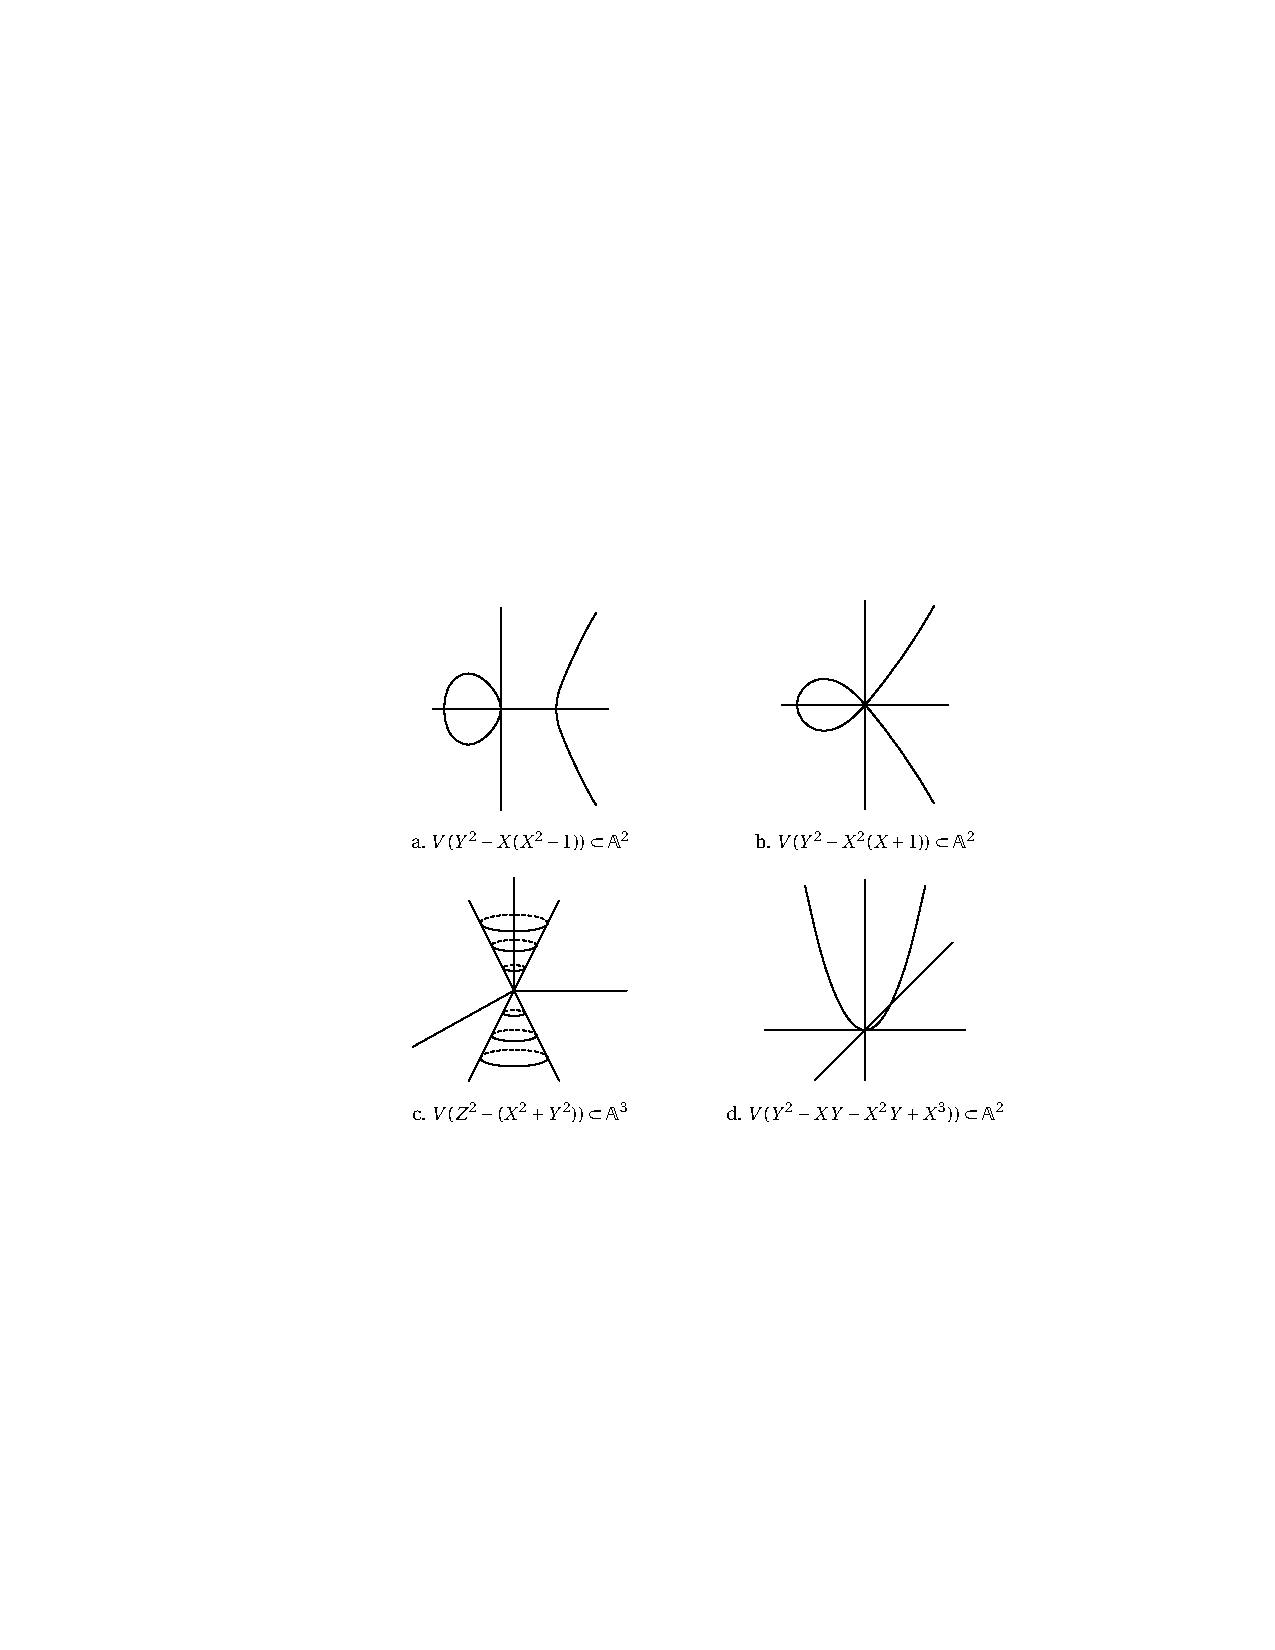
\includegraphics{pictures/algebraic-set}\]
\end{example}
More generally, if $S$ is any set of polynomials in $k[X_1,\dots,X_n]$, we let 
\[V(S)=\{P\in\mathbb{A}^n:F(P)=0\text{ for all }F\in S\}=\bigcap_{F\in S}V(F).\]
If $S=\{F_1,\dots,F_r\}$, we usually write $V(F_1,\dots,F_r)$ instead of $V(\{F_1,\dots,F_r\})$. A subset $X\sub\mathbb{A}^n(k)$ is an \textbf{affine algebraic set}, or simply an \textbf{algebraic set}, if $X=V(S)$ for some $S$.
\begin{proposition}
Let $k$ be a field.
\begin{itemize}
\item[$(1)$] If $I\sub J$, then $V(J)\sub V(I)$.
\item[$(2)$] If $I$ is the ideal in $k[X_1,\dots,X_n]$ generated by $S$, then $V(S)=V(I)$; so every algebraic set is equal to $V(I)$ for some ideal $I$.
\item[$(3)$] If $\{I_\alpha\}_{\alpha\in A}$ is any collection of ideals, then $V(\bigcup_\alpha I_\alpha)=\bigcap_\alpha V(I_\alpha)$; so the intersection of any collection of algebraic sets is an algebraic set. 
\item[$(4)$] $V(FG)=V(F)\cup V(G)$ for any polynomials $F,G$; $V(I)\cup V(J)=V(IJ)$ for ideals $I,J$; so any finite union of algebraic sets is an algebraic set.
\item[$(5)$] $V(0)=\mathbb{A}^n(k)$; $V(1)=\emp$. $V(X_1-a_1,\dots,X_n-a_n)=\{(a_1,\dots,a_n)\}$ for $a_i\in k$. So any finite subset of $\mathbb{A}^n(k)$ is an algebraic set.
\end{itemize}
\end{proposition}
\begin{proof}
The first statement follows from the definition. For the second, it is clear that $V(I)\sub V(S)$. Assume $P\in V(S)$, then since any element of $I$ is a linear combination of $S$, we also have $P\in V(I)$. Thus $V(I)=V(S)$.\par
Now for a family $\{I_\alpha\}$, we have
\[V(\bigcup_\alpha I_\alpha)=\bigcap_{F\in\bigcup I_\alpha}V(F)=\bigcap_{\alpha}\bigcap_{F\in I_\alpha}V(F)=\bigcap_{\alpha}V(I_\alpha),\]
as needed.\par
If $F(P)G(P)=0$, then $F(P)=$ or $G(P)=0$, thus the equality $V(FG)=V(F)\cup V(G)$ holds. Now for ideals $I,J$, we observe
\[V(F)\cup V(G)=\bigcap_{F\in I}V(F)\cup\bigcap_{G\in J}V(G)=\bigcap_{F\in I,G\in J}(V(F)\cup V(G))=\bigcap_{F\in I,G\in J}V(FG)=V(IJ).\]
The last staement is immediate.
\end{proof}
Generally, a infinite union of algebraic sets may not be algebraic. Here is an example.
\begin{example}
Let $k=\R$ and consider the subset $\Q\sub\R$. We observe that $\Q$ is not algebraic: if $\Q=V(S)$, then any polynomial in $S$ vanishes on $\Q$, hence on $\R$ by continuity. This means $S$ can only be zero, but $V(0)=\R$, contradiction. Since $\Q$ is itself contable, it is a countable union of algebraic sets.
\end{example}
\subsection{The Ideal of a Set of Points}
For any subset $X$ of $\mathbb{A}^n(k)$, we consider those polynomials that vanish on $X$; they form an ideal in $k[X_1,\dots,X_n]$, called the ideal of $X$, and written $I(X)$:
\[I(X)=\{F\in k[X_1,\dots,X_n]:F(a_1,\dots,a_n)=0\text{ for all }(a_1,\dots,a_n)\in X\}\]
\begin{proposition}
Let $k$ be a field.
\begin{itemize}
\item[$(1)$] If $X\sub Y$, then $I(Y)\sub I(X)$.
\item[$(2)$] $I(\emp)=k[X_1,\dots,X_n]$; $I(\mathbb{A}^n(k))=(0)$ if $k$ is infinite. 
\item[$(3)$] $I(\bigcup_\alpha S_\alpha)=\bigcap_\alpha I(S_\alpha)$.
\item[$(4)$] $I(\{(a_1,\dots,a_n)\})=(X_1-a_1,\dots,X_n-a_n)$ for $a_1,\dots,a_n\in k$.
\item[$(5)$] $I(X)$ is a radical ideal.
\item[$(6)$] For any ideal $I$ in $k[X_1,\dots,X_n]$, $V(I)=V(\sqrt{I})$, and $\sqrt{I}\sub I(V(I))$.
\item[$(7)$] $I(V(S))\sups S$ for any set $S$ of polynomials; $V(I(X))\sups X$ for any set $X$ of points.
\item[$(8)$] $V(I(V(S)))=V(S)$ for any set $S$ of polynomials, and $I(V(I(X)))=I(X)$ for any set $X$ of points. So if $V$ is an algebraic set, $V=V(I(V))$, and if $I$ is the ideal of an algebraic set, $I=I(V(I))$.
\end{itemize}
\end{proposition}
\begin{proof}
It is clear that if $F^n(P)=0$, then $F(P)=0$. Therefore $I(X)$ is a radical ideal and $V(I)=V(\sqrt{I})$. It is also clear that $I\sub I(V(I))$, so by taking radical we get $\sqrt{I}\sub I(V(I))$.\par
For $F\in k[X_1,\dots,X_n]$, $F\in I(\bigcup_\alpha S_\alpha)$ iff $F(P)=0$ for all $P\in\bigcup_\alpha S_\alpha$, iff $F\in I(S_\alpha)$ for all $\alpha$. Thus $I(\bigcup_\alpha S_\alpha)=\bigcap_\alpha I(S_\alpha)$.\par
For $S\sub k[X_1,\dots,X_n]$, from $(7)$ we get
\[I(V(S))\sups S\And V(I(V(S)))\sups V(S).\] 
Form the former we derive $V(I(V(S))\sub V(S)$, thus $V(I(V(S)))=V(S)$.
\end{proof}
\begin{corollary}
Let $V,W$ be algebraic sets in $\mathbb{A}^n(k)$. Then $V=W$ if and only if $I(V)=I(W)$.
\end{corollary}
\begin{proof}
For algebraic sets $V$ we have $V(I(V))=V$. Thus the map $I$ is injective.
\end{proof}
\begin{proposition}
Let $W$ be a subset of $\mathbb{A}^n$. Then $V(I(W))$ is the smallest algebraic subset of $\mathbb{A}^n$ containing $W$.
\end{proposition}
\begin{proof}
Certainly $V(I(W))$ is an algebraic set containing $W$. Let $V=V(J)$ be another algebraic set containing $W$. Then $J\sub I(V(J))\sub I(W)$, and so $V(J)\supset V(I(W))$.
\end{proof}
\begin{proposition}\label{algebraic set separate}
Let $V$ be an algebraic set in $\mathbb{A}^n(k)$.
\begin{itemize}
\item[$(a)$] If $P\in\mathbb{A}^n(k)$ is a point not in $V$, then there is a polynomial $F\in k[X_1,\dots,X_n]$ such that $F(Q)=0$ for all $Q\in V$, but $F(P)=1$.
\item[$(b)$] Let $P_1,\dots,P_r$ be distinct points of $\mathbb{A}^n(k)$ not in $V$. Then there are polynomials $F_1,\dots,F_r\in I(V)$ such that $F_i(P_j)=0$ if $i\neq j$, and $F_i(P_i)=1$.
\item[$(c)$] With $P_1,\dots,P_r$ as in $(b)$, and $a_{ij}\in k$ for $1\leq i,j\leq r$, there are $G_i\in I(V)$ with $G_i(P_j)=a_{ij}$ for all $i$ and $j$.
\end{itemize} 
\end{proposition}
\begin{proof}
Write $V=V(I)$. For any point $P\notin V$ there is a polynomial $F\in I$ such that $F(P)\neq 0$. Then $F'=F/F(P)$ satisfies the condition.\par
For $(b)$, apply $(a)$ to the union of $V$ and all but one point. And for $(c)$, consider the sum $G_i=\sum_j a_{ij}F_j$.
\end{proof}
\subsection{The Zariski topology}
\begin{definition}
We endow a topology on $\mathbb{A}^n(k)$ by declearing a subset is closed iff it is algebraic. This is called the \textbf{Zariski topology} on $\mathbb{A}^n$.
\end{definition}
A basis for the open subsets of $\mathbb{A}^n$ is given by the open sets
\[\mathbb{A}^n_f=D(f)=\mathbb{A}^n-V(f)=\{x\in\mathbb{A}^n:f(x)\neq 0\}.\]
with $f\in k[X_1,\dots,X_n]$. Open subsets of this type, complements of hypersurfaces in $\mathbb{A}^n$, are called \textbf{principal open} or \textbf{basic open subsets} of $\mathbb{A}^n$. Note that $D(f_1)\cap D(f_2)=D(f_1f_2)$.\par
Let us now examine some properties of the Zariski topology.
\begin{itemize}
\item $\mathbb{A}^n$ is not a Hausdorff space, because for every pair of non-empty open sets $U_1$, $U_2$ one has $U_1\cap U_2\neq\emp$. Indeed, if $U_1\cap U_2=\emp$, one would have $\mathbb{A}^n=U_1^c\cup U_2^c$. Since $\mathbb{A}^n$ is irreducible one would have either $U_1^c=\emp$ or $U_2^c=\emp$. It follows that every non-empty open set is dense in $\mathbb{A}^n$.
\item $\mathbb{A}^n$ is a Fr\'echet space (i.e., $T_1$) in the sense that if $P$ and $Q$ are any two distinct points, each of the two is contained in an open set which does not contain the other. In fact, if $f$ is a polynomial satisfying $f(P)\neq 0$ but $f(Q)=0$, then the open set which is the complement of the algebraic set $V(f)$ contains $P$ but not $Q$.
\item $\mathbb{A}^n$ is compact, that is, every open cover admits a finite subcover. From $\mathbb{A}^n=\bigcup_\alpha D(f_\alpha)$ we get
\[V(\bigcup_\alpha\{f_\alpha\})=\bigcap_\alpha V(f_\alpha)=\emp.\]
Since $k[X_1,\dots,X_n]$ is noetherian, there exists a finite set $f_1,\dots,f_n$ such that \[V(f_1,\dots,f_n)=V(\bigcup_\alpha\{f_\alpha\})=\emp.\] 
Thus we have $\mathbb{A}^n=\bigcup_{i=1}^{n}D(f_i)$.
\end{itemize}
If $V\sub\mathbb{A}^n$ is an algebraic set, we can consider the Zariski topology on $V$, namely the topology on $V$ induced by the Zariski topology on $\mathbb{A}^n$. For each $f\in k[V]$ we set
\[V_f=V-V(f)=\{P\in V:f(x)\neq 0\}.\]
The open sets $V_f$ are called \textbf{principal open} or \textbf{basic open subsets} of $V$, and form a base for the open subsets of the Zariski topology on $V$.
\begin{remark}
Let $V\in\mathbb{A}^n(k),W\in\mathbb{A}^m(k)$ be algebraic sets. Then
\[V\times W=\{(a_1,\dots,a_n,b_1,\dots,b_m):(a_1,\dots,a_n)\in V,(b_1,\dots,b_m)\in W\}\]
is an algebraic set in $\mathbb{A}^{n+m}(k)$. It is called the product of $V$ and $W$. In fact, rite $V=V_n(S)$ and $W=V_m(T)$. Note that we can embed $S$ and $T$ in $k[X_1,\dots,X_{n+m}]$, and one can verify the equality $V\times W=V(S^e)\cap V(T^e)$.\par
Note that not every closed subset in the Zariski topology on $\mathbb{A}^{n+m}(k)$ is an closed subset in the product topology. For example, the set of $V(x-y)$ in $\mathbb{A}^2(k)$ is not closed in $\mathbb{A}^1\times\mathbb{A}^1$.\par
Therefore, the product topology on $\mathbb{A}^n\times\mathbb{A}^m$ with respect to the Zariski topologies on $\mathbb{A}^n$ and $\mathbb{A}^m$ is strictly coarser than the Zariski topology on $\mathbb{A}^{n+m}$.
\end{remark}
\subsection{The Hilbert Basis Theorem}
\begin{theorem}
If $R$ is a Noetherian ring, then $R[X]$ is also Noetherian.
\end{theorem}
\begin{proof}
We show that any ideal $I\sub R[x]$ is finitely generated. We inductively produce a set of generators $f_i$ as follows.\par
For $n>0$, if $I\neq(f_1,\dots,f_{n-1})$, let $f_n$ be any nonzero element of $I-(f_1,\dots,f_{n-1})$ of lowest degree. Thus $f_1$ is any element of $I$ of lowest degree, assuming $I\neq(0)$. If this procedure terminates, we are done. Otherwise, let $a_n\in R$ be the initial coefficient of $f_n$ for $n>0$. Then as $R$ is Noetherian, $(a_1,\dots,a_n)=(a_1,\dots,a_N)$ for some $N$. Say $a_{N+1}=\sum_{i=1}^{N}b_ia_i$. Then
\[f_{N+1}-\sum_{i=1}^{N}b_if_ix^{\deg f_{N+1}-\deg f_N}\]
is an element of $I$ that is nonzero (as $f_{N+1}\notin(f_1,\dots,f_N)$), and of lower degree than $f_{N+1}$, yielding a contradiction.
\end{proof}
\begin{corollary}
If $k$ is a field, then $k[X_1,\dots,X_n]$ is Noetherian.
\end{corollary}
\begin{corollary}
Every algebraic set is the intersection of a finite number of hypersurfaces.
\end{corollary}
\subsection{Hilbert's Nullstellensatz}
\begin{theorem}[\textbf{Weak Nullstellensatz}]
Let $k$ be an algebraically closed field. If $I$ is an ideal in $k[X_1,\dots,X_n]$, then $V(I)=\emp$ if and only if $I=(1)$.
\end{theorem}
\begin{proof}
We may assume that $I$ is a maximal ideal, for there is a maximal ideal $\m$ containing $I$, and $V(\m)\sub V(I)$. So $L:=k[X_1,\cdots,X_n]/I$ is a field, and $k$ may be regarded as a subfield of $L$.\par
Suppose we knew that $k=L$. Then for each $i$ there is an $a_i\in k$ such that the $I$-residue of $X_i$ is $a_i$, or $X_i-a_i\in I$. But $(X_1-a_1,\dots,X_n-a_n)$ is a maximal ideal, so $I=(X_1-a_n,\dots,a_n)$, and $V(I)=\{(a_1,\dots,a_n)\}\neq\emp$.
\end{proof}
Thus we have reduced the problem to showing:
\begin{proposition}
If an algebraically closed field $k$ is a subfield of a field $L$ where $L$ is finitely generated, then $k=L$.
\end{proposition}
This is a consequence of Zariski Lemma.
\begin{theorem}[\textbf{Zariski Lemma}]\label{Zariski lemma}
If a field $L$ is finite generated over a subfield $K$, then $L$ is finite over $K$.
\end{theorem}
\begin{proof}
Let $L=K[\alpha_1,\dots,\alpha_n]$. The proof is by induction over $n$. If $n=1$, then $L=K[\alpha_1]$ and since $L$ is a field, $\alpha_1^{-1}\in L$. Thus $\alpha_1^{-1}=\sum_{i=0}^mb_i\alpha_1^i$ for some integer $b_i \in K$. Then $\sum_{i=0}^mb_i\alpha_1^{i+1}=0$ and so $\alpha_1$, and hence $L$, is algebraic over $K$.\par
Now we assume the result for all extensions generated by $n-1$ elements. Assume $\alpha_1$ is not algebraic over $K$, and let $K_1=K(\alpha_1)$. Since
$K[\alpha_1,\dots,\alpha_n]=K(\alpha_1)[\alpha_2,\dots,\alpha_n]$ is a field, by induction hypothesis, $\alpha_2,\dots,\alpha_n$ are all algebraic over $K(\alpha_1)$. there exist polynomials $f_i\in K_1[X]$ such that $f_i(\alpha_i)=0$. The cofficients of $f_i$'s are in $K_1$, thus for suitable $g\in K[\alpha_1]$ we have $gf_i\in K[\alpha_1][X]$. In other words, if we set $B=K[\alpha_1,g^{-1}]$ then the $f_i$ are polynomials with coefftcients in $B$.\par 
Thus each $\alpha_i$ is integral over $B$, and then $L$ is integral over $B$. By Proposition~\ref{integral field iff} we conclude $B$ is a field. However, $B$ can non be a field; for $K[\alpha_1]$ is a polynomial ring, and hence it contains infinitely many irreducible polynomials. Hence, there is an irreducible polynomial $h\in K[\alpha_1]$ which does not divide $g$, and then obviously $h^{-1}\notin K[\alpha_1,g^{-1}]$.
\end{proof}
\begin{theorem}[\textbf{Hilbert's Nullstellensatz}]
Let $I$ be an ideal in $k[X_1,\cdots,X_n]$ where $k$ is algebraically closed. Then $I(V(I))=\sqrt{I}$.
\end{theorem}
\begin{proof}
The inclusion $\sqrt{I}\sub I(V(I))$ is easy. Suppose that $G$ is in the ideal $I(V(F_1,\dots,F_r))$, $F_i\in k[X_1,\dots,X_n]$. Let $J=(F_1,\dots,F_r,X_{n+1}G-1)\sub k[X_1,\dots,X_n,X_{n+1}]$. Then $V(J)\sub\mathbb{A}^{n+1}(k)$ is empty, since $G$ vanishes wherever all that $F_i$'s are zero. Applying the Weak Nullstellensatz to $J$, we see that $J=(1)$, so there is an equation 
\[\sum A_i(X_1,\dots,X_{n+1})F_i+B(X_1,\dots,X_{n+1})(X_{n+1}G-1)=1\]
in $k[X_1,\dots,X_{n+1}]$. Let $Y=1/X_{n+1}$, and multiply the
equation by a high power of $Y$, we get an equation 
\[Y^N=\sum C_i(X_1,\dots,X_n,Y)F_i+D(X_1,\dots,X_n,Y)(G-Y)\]
in $k[X_1,\dots,X_n,Y]$. Substituting $G$ for $Y$ gives the required equation.
\end{proof}
The above proof is due to Rabinowitsch. The first three corollaries are immediate consequences of the theorem.
\begin{corollary}
If $I$ is a radical ideal in $k[X1_,\cdots,X_n]$ where $k$ is algebraically closed, then $I(V(I))=I$. So there is a one-to-one correspondence between radical ideals and algebraic sets.
\end{corollary}
\begin{corollary}
Let $k$ be an algebraically closed. If $I$ is a prime ideal of $k[X_1,\dots,X_n]$, then $V(I)$ is irreducible. There is a one-to-one correspondence between prime ideals and irreducible algebraic sets. The maximal ideals correspond to points.
\end{corollary}
\begin{corollary}\label{hypersurface decomposition}
Let $F$ be a nonconstant polynomial in $k[X_1,\cdots,X_n]$ where $k$ is algebraically closed, and $F=F_1^{n_1}\cdots F_r^{n_r}$ be the decomposition of $F$ into irreducible factors. Then $V(F)=V(F_1)\cup\cdots\cup V(F_r)$ is the decomposition of $V(F)$ into irreducible components, and $I(V(F))=(F_1,\dots,F_r)$. There is a one-to-one correspondence between irreducible polynomials $F\in k[X_1,\dots,X_n]$ and irreducible hypersurfaces in $\mathbb{A}^n(k)$.
\end{corollary}
\begin{proposition}\label{V(I) finite iff}
Let $I$ be an ideal in $k[X_1,\dots,X_n]$ where $k$ is algebraically closed. Then $V(I)$ is a finite set if and only if $k[X_1,\dots,X_n]/I$ is a finite dimensional vector space over $k$. If this occurs, the number of points in $V(I)$ is at most $\dim_k(k[X_1,\dots,X_n]/I)$.
\end{proposition}
\begin{proof}
If $V(I)=\{P_1,\dots,P_r\}$ is finite, let $P_i=(a_{i1},\dots,a_{in})$, and define $F_j$ by $F_j=\prod_{i=1}^{r}(X_j-a_{ij})$. Then $F_j\in I(V(I))$, so $F_j^N\in I$ for some $N\geq0$ (Take $N$ large enough to work for all $F_j$). Taking $I$-residues, $\widebar{F}^N_i=0$, so $\widebar{X}_j^{rN}$ is a $k$-linear combination of $\{1,\widebar{X}_j,\dots,\widebar{X}_j^{rN}\}$. It then follows that $k[X_1,\dots,X_n]/I$ is finite dimensional as a vector space over $k$.\par
Conversely, if $P_1,\dots,P_r\in V(I)$. Write $P_i=(a_{i1},\dots,a_{in})$, we define
\[F_i(X_1,\dots,X_n)=\frac{\prod_{j\neq i}\prod_{k=1}^{n}(X_k-a_{jk})}{\prod_{j\neq i}\prod_{k=1}^{n}(a_{ik}-a_{jk})}.\]
Then we have $F_i(P_j)=0$ for $i\neq j$ and $F_i(P_i)=1$. Let $\widebar{F}_i$ be the $I$-residue of $F_i$. If $\sum\lambda_i\widebar{F}_i=0,\lambda_i\in k$, then $\sum\lambda_i F_i\in I$ and therefore $\lambda_j=(\sum\lambda_iF_i)(P_j)=0$. Thus the $F_i$ are linearly independent over $k$, so $r\leq\dim_k(k[X_1,\dots,X_n]/I)$. This implies $V(I)$ is finite.\par
\end{proof}
\begin{example}
Let $I=(Y^2+X^2,Y^2-X^2)\sub\C[X,Y]$. It is clear that $V(I)=\{(0,0)\}$. Let's compute $\dim_\C(\C[X,Y]/I)$. Since $Y^2-X^2$ is reducible in $\C[X,Y]$, we find
\[\C[X,Y]/I=\frac{\C[X,Y]/(Y^2-X^2)}{Y^2+X^2}=\C[X]/(2X^2)=\C^2.\]
Therefore $\dim_\C(\C[X,Y]/I)=2$.
\end{example}
\subsection{Coordinate Rings}
From now on $k$ will be a fixed algebraically closed field. Affine algebraic sets will be in $\mathbb{A}^n=\mathbb{A}^n(k)$ for some $n$. 
\begin{definition}
An irreducible affine algebraic set is called an \textbf{affine variety}. An open subset of an affine variety is a \textbf{quasi-affine variety}.
\end{definition}
Let $V\sub\mathbb{A}^n$ be a nonempty algebraic set. We let $k[V]=k[X_1,\dots,X_n]/I(V)$, and call it the \textbf{coordinate ring of $\bm{V}$}.\par
Given a polynomial $F\in k[X_1,\dots,X_n]$ and putting $f=\widebar{F}$ we have $F'(P)=F(P)$ for every polynomial $F'\in\widebar{F}$ and for every $P\in V$. Thus the polynomial function 
\[f:V\to k,\quad f(P):=F(P)\]
is defined.
\begin{proposition}
The map that associates to each $F\in k[X_1,\dots,X_n]$ a polynomial on $V$ is a ring homomorphism whose kernel is $I(V)$.
\end{proposition}
\begin{proposition}
There is a natural one-to-one correspondence between algebraic subsets $($resp. subvarieties, resp. points$)$ of $V$ and radical ideals $($resp. prime ideals, resp. maximal ideals$)$ of $k[V]$.
\end{proposition}
\begin{proposition}
Let $W$ be an algebraic subset of an algebraic set $V$, and let $I_V(W)$ be the ideal of $k[V]$ corresponding to $I(W)$.
\begin{itemize}
\item[$(a)$] Every polynomial function on $V$ restricts to a polynomial
function on $W$.
\item[$(b)$] Show that the map from $k[V]$ to $k[W]$ defined in part $(a)$ is a surjective homomorphism with kernel $I_V(W)$, so that $k[W]$ is isomorphic to $k[V]/I_V(W)$.
\end{itemize}
\end{proposition}
\begin{proof}
Since $W\sub V$, we have $I(V)\sub I(W)$. Thus there is a canonical map \[\frac{k[X_1,\dots,X_n]}{I(V)}\to\frac{k[X_1,\dots,X_n]}{I(W)}.\]
It is clear that the kernel of this map is $I(W)/I(V)=I_V(W)$.
\end{proof}
Here is an intersting result about the dimension of $k[V]$ when $V$ is an variety.
\begin{proposition}
Let $V\sub\mathbb{A}^n$ be a nonempty variety. Then the following are equivalent:
\begin{itemize}
\item[$(1)$] $V$ is a point.
\item[$(2)$] $k[V]=k$.
\item[$(3)$] $\dim_kk[V]<\infty$.
\end{itemize}
\end{proposition}
\begin{proof}
The implication $(1)\Rightarrow(2)\Rightarrow(3)$ is clear. Now we assume $(3)$, then by Proposition~\ref{V(I) finite iff} $V(I)$ is finite, hence is a point by irreducibility.
\end{proof}
\subsection{Irreducible Components of an Algebraic Set}
\begin{definition}
A topological space is said to be \textbf{irreducible} if it is nonempty, and it is not the union of two proper closed subsets, or equivalently, any nonempty open subsets intersect.
\end{definition} 
Since the closed subsets in $\mathbb{A}^n$ are exactly algebraic sets, an algebraic set $V\sub\mathbb{A}^n$ is reducible if and only if $V=V_1\cup V_2$, where $V_1,V_2$ are algebraic sets in $\mathbb{A}^n$ properly contained in $V$. Otherwise $V$ is irreducible.
\begin{proposition}\label{algebraic set irre}
An algebraic set $V$ is irreducible if and only if $I(V)$ is prime.
\end{proposition}
\begin{proof}
If $I(V)$ is not prime, suppose $F_1F_2\in I(V)$, $F_i\notin I(V)$. Then $V=(V\cap V(F_1))\cup(V\cap V(F_2))$, and $V\neq V(F_i)\cap V$, so $V$ is reducible.\par
Conversely if $V=V_1\cup V_2, V_i\subset V$, then $I(V_i)\supset I(V)$; let $F_i\in I(V_i),F_i\notin I(V)$. Then $F_1F_2\in I(V_1)\cap I(V_2)=I(V)$, so $I(V)$ is not prime.
\end{proof}
We want to show that an algebraic set is the union of a finite number of irreducible algebraic sets. If $V$ is reducible, we write $V=V_1\cup V_2$; if $V_2$ is reducible, we write $V_2=V_3\cup V_4$, etc. In fact, this can be done for more general toplogical spaces.
\begin{definition}
A topological space $X$ is called \textbf{Noetherian} if it satisfies the descending chain condition for closed subsets: any sequence 
\[Z_1\supset Z_2\supset\cdots\supset Z_n\supset\cdots\]
of closed subsets eventually stabilizes: there is an $r$ such that $Z_{r}=Z_{r+1}=\cdots$.
\end{definition}
\begin{proposition}
The space $\mathbb{A}^n$ is Noetherian.
\end{proposition}
\begin{proof}
Since every closed subset in $\mathbb{A}^n$ is of the form $V(I)$ for some ideal $I$. A descending chain of closed subset in $\mathbb{A}^n$ corresponds to an ascending chain of ideals in $k[X_1,\dots,X_n]$. Since $k[X_1,\dots,X_n]$ is Noetherian, we conclude $\mathbb{A}^n$ is also Noetherian.
\end{proof}
\begin{theorem}\label{Noe space irreducible deomp}
Suppose $X$ is a Noetherian topological space. Then every nonempty closed subset $Z$ can be expressed uniquely as a finite union $Z=Z_1\cup\cdots\cup Z_n$ of irreducible closed subsets, none contained in any other.
\end{theorem}
The following technique is called \textbf{Noetherian induction}, for reasons that will be clear. We will use it again, many times.
\begin{proof}
Consider the collection of closed subsets of $X$ that cannot be expressed as a finite union of irreducible closed subsets. We will show that it is empty.\par
Otherwise, let $Y_1$ be one such. If $Y_1$ properly contains another such, then choose one, and call it $Y_2$. If $Y_2$ properly contains another such, then choose one, and call it $Y_3$, and so on. By the descending chain condition, this must eventually stop, and we must have some $Y_r$ that cannot be written as a finite union of irreducible closed subsets, but every closed subset properly contained in it can be so written. But then $Y_r$ is not itself irreducible, so we can write $Y_r=Y'\cup Y''$ where $Y'$ and $Y''$ are both proper closed subsets. Both of these by hypothesis can be written as the union of a finite number of irreducible subsets, and hence so can $Y_r$, yielding a contradiction. Thus each closed subset can be written as a finite union of irreducible closed subsets. We can assume that none of these irreducible closed subsets contain any others, by discarding some of them.\par
We now show uniqueness. Suppose
\[Z=Z_1\cup\cdots\cup Z_r=Z'_1\cup\cdots\cup Z'_s\]
are two such representations. Then $Z'_1\sup Z_1\cup\cdots\cup Z_r$, so $Z'_1=\bigcup_{i=1}^{r}(Z_i\cap Z_1')$. Now $Z'_1$ is irreducible, so one of these is $Z'_1$ itself, say (without loss of generality) $Z_1\cap Z'_1$. Thus $Z'_1\sub Z_1$. Similarly, $Z_1\sub Z'_a$ for some $a$; but because $Z'_1\sub Z_1\sub Z'_a$, and $Z'_1$ is contained in no other $Z'_i$, we must have $a=1$, and $Z'_1=Z_1$. Thus each element of the list of $Z$'s is in the list of $Z'$'s, and vice versa, so they must be the same list.
\end{proof}
The $Z_i$ are called the \textbf{irreducible components} of $Z$; and $Z=Z_1\cup\cdots\cup Z_r$ is the \textbf{decomposition of $\bm{Z}$ into irreducible components}.
\begin{proposition}
Let $Z=Z_1\cup\cdots\cup Z_r$ be a decomposition of $Z$ into irreducible components. Then $Z_i\nsubseteq\bigcup_{j\neq i}Z_j$ holds for all $i$.
\end{proposition}
\begin{proof}
Assume that for some $i$ we have $Z_i\subseteq\bigcup_{j\neq i}Z_j$. Then
\[Z_i=\bigcup_{j\neq i}(Z_j\cap Z_i)\]
is a decomposition of $Z_i$ into proper closed subsets of $Z_i$. Since $Z_i$ is irreducible, this is a contradiction.
\end{proof}
\begin{example}
As a simple example, consider the polynomial $F(X,Y)=Y^2+X^2(X-1)^2\in\R[X,Y]$. The zero set $V(F)=\{(0,0),(1,0)\}$, thus reducible. However, $F$ is an irreducible polynomial.
\end{example}
\begin{proposition}
$\mathbb{A}^n(k)$ is irreducible if $k$ is infinite.
\end{proposition}
\begin{proof}
If $k$ is infinite, then $I(\mathbb{A}^n(k))=0$, which is prime.
\end{proof}
\subsection{Morphisms}
Now let $\mathbb{A}^n$ and $\mathbb{A}^m$ be two affine spaces. We say that a map $\varphi:\mathbb{A}^n\to\mathbb{A}^m$ is a \textbf{morphism} (or \textbf{regular map}) if there are $m$ polynomials $F_1,\dots,F_m\in k[X_1,\dots,X_n]$ such that for each $P\in\mathbb{A}^n$ one has
\[\varphi(P)=(F_1(P),\dots,F_m(P)).\]
We also say that $\varphi$ is the polynomial function given by $F_1,\dots,F_m$.\par
If $V\sub\mathbb{A}^n$, $W\sub\mathbb{A}^m$ are algebraic sets, we say that a map $\varphi:V\to W$ is a \textbf{morphism} (or \textbf{regular map}) if it is the restriction to $V$ of a morphism $\varPhi:\mathbb{A}^n\to\mathbb{A}^m$ such that $\varPhi(V)\sub W$. Thus, if $\varphi:V\to W$ is a morphism there exist $m$ polynomial functions $f_1,\dots,f_m\in k[V]$ such that for every $P\in V$ one has \[\varphi(P)=(f_1(P),\dots,f_m(P))\for P\in V.\]
and we say that $\varphi$ is the polynomial function given by $f_1,\dots,f_m$.\par
We say that a morphism $\varphi:V\to W$ is an isomorphism if $\varphi$ is bijective and the inverse $\varphi^{-1}$ is a morphism. If there exists an isomorphism $\varphi:V\to W$ we say that $V$ and $W$ are isomorphic.\par
\begin{proposition}\label{morphism is continuous}
Let $\varphi:V\to W$ be a morphism, and $X$ be an algebraic subset of $W$.
\begin{itemize}
\item[$(a)$] $\varphi^{-1}(X)$ is an algebraic subset of $V$, thus the map $\varphi$ is continuous under the Zariski topology.
\item[$(b)$] If $\varphi^{-1}(X)$ is irreducible, and $X$ is contained in the image of $\varphi$, then $X$ is irreducible.
\end{itemize}
This gives a useful test for irreducibility.
\end{proposition}
\begin{proof}
Write $X=V(I)$, and let $\varPhi:\mathbb{A}^n\to\mathbb{A}^m$ be the regular map resricting to $\varphi$ on $V$. Then
\begin{align*}
\varPhi^{-1}(X)=\varPhi^{-1}(V(I))=\varPhi^{-1}(\bigcap_{F\in I}V(F))=\bigcap_{F\in I}\varPhi^{-1}(V(F))
\end{align*}
Note that
\[\varPhi(P)\in V(F)\iff F(\varPhi(P))=0\iff P\in V(F\circ\varPhi).\]
Therefore we conclude that $\varPhi^{-1}(X)=V(\varPhi^*(I))$ is algebraic, hence closed. Since we have $\varphi^{-1}(X)=\varPhi^{-1}(X)\cap V$, it is also closed.\par 
Now assume $X\sub\im\varphi$, and $\varphi^{-1}(X)$ is irreducible. If there are nonempty closed subsets $C_1,C_2\sub X$ such that $X=C_1\cup C_2$, then we have a union \[\varphi^{-1}(X)=\varphi^{-1}(C_1)\cup\varphi^{-1}(C_2).\] 
Since $X$ is in the image of $\varphi$, none of the sets $\varphi^{-1}(C_i)$ is empty, but this contradicts the irreducibility of $\varphi^{-1}(X)$. Thus $X$ is also irreducible.
\end{proof}
\begin{example}
Consider the algebraic set $C:=V(XZ-Y^2,YZ-X^3,Z^2-X^2Y)\sub\mathbb{A}^3$. By solving the equation
\[\left\{\begin{array}{l}
a+c=2b\\
b+c=3a\\
2c=2a+b
\end{array}\right. \]
we get $(X,Y,Z)=(t^3,t^4,t^5)$. Thus there is a surjectie morphism
\[\varphi:\mathbb{A}^1\to C,\quad \varphi(t)=(t^3,t^4,t^5).\]
Therefore $W$ is irreducible. This is an example of a curve $C\sub\mathbb{A}^3$ for which $I(C)$ needs $3$ generators.
\end{example}
\begin{proposition}
Let $\varphi:V\to W$ be a morphism of algebraic sets with $V\sub\mathbb{A}^n$ and $W\sub\mathbb{A}^m$. With the preceding notation, and considering the coordinates $X_1,\dots,X_m$ in $\mathbb{A}^m$ as polynomial functions, $\varphi$ is a polynomial function given by $f_1,\dots,f_m\in k[V]$ if and only if $f_j=X_j\circ\varphi$ for $1\leq j\leq m$, that is, if and only if the diagram
\[\begin{tikzcd}
V\ar[r,"\varphi"]\ar[rd,swap,"f_j"]&W\ar[d,"X_j"]\\
&k
\end{tikzcd}\]
commutes.
\end{proposition}
\begin{proof}
We observe that for $P\in V$ the $j$-th component of $\varphi(P)$ is $X_j\circ\varphi(P)$, and therefore for each $j$ if we put $f_j=X_j\circ\varphi$ we have
\[\varphi(P)=(X_1\circ\varphi(P),\dots,X_m\circ\varphi(P))=(f_1(P),\dots,f_m(P)).\]
Thus $\varphi$ is the morphism given by $f_1,\dots,f_m$.\par
Conversely, if $\phi(P)=(f_1(P),\dots,f_m(P))$, for $P\in V$, we then have $X_j\circ\varphi(P)=f_j(P)$ for all $P\in V$ and $1\leq j\leq m$, which is to say that $X_j\circ\varphi=f_j$.
\end{proof}
\begin{theorem}\label{morphism coordinate ring}
Let $V\sub\mathbb{A}^n$, $W\sub\mathbb{A}^m$ be algebraic sets. Then the following holds:
\begin{itemize}
\item[$(a)$] A morphism $\varphi:V\to W$ induces a $k$-algebra homomorphism $\varphi^*:k[W]\to k[V]$.
\item[$(b)$] Conversely, every homomorphism of $k$-algebras $\theta:k[W]\to k[V]$ is induced by a uniquely determined morphism $\varphi:V\to W$.
\item[$(c)$] If $\varphi:V\to W$ and $\psi:W\to Z$ are morphisms of algebraic sets, then the morphisms $(\psi\circ\varphi)^*$ and $\varphi^*\circ\psi^*$ coincide as morphisms of $k$-algebras; that
is, $(\psi\circ\varphi)^*=\varphi^*\circ\psi^*$.
\end{itemize}
\end{theorem}
\begin{proof}
Let $g\in k[W]$, that is, let $g:W\to K$ be a polynomial function defined on all of $W$. Set $\varphi^*(g)=g\circ\varphi$. We show that $\varphi^*(g)\in k[V]$. To see this it suffices to note the following facts.
\begin{itemize}
\item There exist $F_1,\dots,F_m\in k[X_1,\dots,X_n]$ such that for all $P\in V$ one has 
\[\varphi(P)=(f_1(P),\dots,f_m(P))\] 
and $f_j$ the class of $F_j$ in $k[V]$, $1\leq j\leq m$.
\item Let $G\in k[X_1,\dots,X_m]$ be such that $G(w)=g(w)$ for all $w\in W$ (so that $g$ is the class of $G$ in $k[W]$). We then have that $H:=G(F_1,\dots,F_m)\in k[X_1,\dots,X_n]$ and its class in $k[V]$ is $G(f_1,\dots,f_m)$. Moreover, for each $x\in X$ we have
\[(g\circ\varphi)(P)=G(f_1(P),\dots,f_m(P))=G(f_1,\dots,f_m)(P)=H(P).\]
\end{itemize}
Thus $g\circ\varphi\in k[V]$. It is then easy to see that $\varphi$ is a $k$-algebra homomorphism, and this proves $(a)$.\par
To prove $(b)$, we consider the class $x_j$ of the coordinate $X_j$ in $\mathbb{A}^m$ as a function on $W$. We set $\theta(x_j)=\theta_j$. Since $\theta$ is a $k$-algebra homomorphism, we have, for each $g\in k[W]$, $\theta(g)=g(\theta_1,\dots,\theta_m)$ and so $\theta(g)(P)=g(\theta_1(P),\dots,\theta_m(P))$ for all $P\in V$. Let $\phi:V\to W$ be the morphism defined by $\varphi(P)=(\theta_1(P),\dots,\theta_m(P))$ for all $x\in X$. By what has just been said it follows that for all $g\in k[W]$ we have $g\circ\varphi=\theta(g)$, which means that $\theta$ is induced by $\varphi$.\par
To conclude it suffices to prove that $\im\varphi\sub W$. Let $Q=(\theta_1(P),\dots,\theta_m(P))$ for some $P\in V$, and let $F\in I(W)$. Then the class $f$ of $F$ in $k[W]$ is zero whence $F(x_1,\dots,x_m)=f(x_1,\dots,x_m)=0$ in $k[W]$. Hence $\theta(F(x_1,\dots,x_m))=0$ in $k[V]$. But
\[0=\theta(F(x_1,\dots,x_m))=F(\theta(x_1),\dots,\theta(x_m))=F(\theta_1,\dots,\theta_m).\]
It then follows that $F(Q)=0$ and thus $Q\in W$.\par
Statement $(c)$ is merely the property of associativity for composition of mappings. For each $h\in k[V]$ one has
\[(\psi\circ\varphi)^*(h)=h\circ(\psi\circ\varphi)=(h\circ\psi)\circ\varphi=\varphi^*(h\circ\psi)=\varphi^*\circ\psi^*(h).\]
as desired.
\end{proof}
\begin{corollary}
A morphism $\varphi:V\to W$ of algebraic sets is an isomorphism if and only if $\varphi^*:k[W]\to k[V]$ is an isomorphism of $k$-algebras.
\end{corollary}
\begin{proof}
In fact we have $\id_V^*=\id_{k[V]}$. So this follows from the previous theorem.
\end{proof}
\subsection{Rational maps}
Let $V\sub\mathbb{A}^n$ be a variety on which we consider the Zariski topology. Let $k[V]$ be the ring of coordinates and $k(V)$ the field of fractions of $k[V]$. An element $f\in k(V)$ is called a \textbf{rational function} on $V$. Let $U\sub V$ be an open and let $P\in U$. We say that a rational function $f\in k(V)$ is \textbf{regular at $\bm{P}$} if there exists a neighborhood $U_P$ of $P$ such that
\[f=\frac{g}{h},\quad g,h\in k[V],h(x)\neq 0\text{ for all $x\in U_P$}.\]
We say that $f$ is \textbf{regular on $\bm{U}$} if it is regular at each point of $U$, and the equality $f=g/h$ is said to be the \textbf{local representation} of $f$ in $P$.\par
The set $\mathrm{dom}(f)$ of points $x\in X$ where $f$ is regular is called the \textbf{domain} or \textbf{domain of definition} of $f$. The set of points $P\in V$ where a rational function $f$ is not defined is called the \textbf{pole set of $\bm{f}$}.
\begin{example}
Let $V\sub\mathbb{A}^4(\C)$ be the quadric with equation $Y_1Y_2-Y_3Y_4=0$. If we let $y_i$ denote the class of $Y_i$ in $k[V]$, we have $y_1y_2-y_3y_4=0$ in $k[V]$. We consider the rational function
\[f=\frac{y_1}{y_3}=\frac{y_2}{y_4}\in\C(V).\]
More precisely, $y_1/y_3$ is a representation for $f$ on the open set $U_3\{y_3\neq 0\}$ while $y_4/y_2$ represents $f$ on the open set $U_2=\{y_2\neq 0\}$. Hence $f$ is defined on $U=U_2\cup U_3$, but does not have a global representation on $U$.
\end{example}
Let $P\in V$. We define $\mathscr{O}_{V,P}$ to be the set of rational functions on $V$ that are regular at $P$. It is easy to verify that $\mathscr{O}_{V,P}$ forms a subring of $k(V)$ containing $k[V]$. The ring $\mathscr{O}_{V,P}$ is called the \textbf{local ring of $\bm{V}$ at $\bm{P}$}. It can be seen that
\[\mathscr{O}_{V,P}=k[V][h^{-1}\mid h(P)\neq 0]=k[V]_{I(P)}.\]
\begin{lemma}
Let $k$ be an algebraically closed field and let $f\in k(V)$ be a rational function on an algebraic set $V$. Then:
\begin{itemize}
\item[$(a)$] The pole set of a rational function is an algebraic subset of $V$.
\item[$(b)$] $\mathscr{O}_{V,P}$ is a Noetherian local domain.
\item[$(c)$] $k[V]=\bigcap_{P\in V}\mathscr{O}_{V,P}$, so that $\dom(f)=V$ if and only if $f\in k[V]$.
\end{itemize}
\end{lemma}
\begin{proof}
We consider the ideal $I$ of the denominators of $f$ defined by
\[I:=\{h\in k[V]:fh\in k[V]\}=\{h\in k[V]:f=g/h,g\in k[V]\}\cup\{0\}.\]
One then has
\[V-\dom(f)=\{P\in V:h(P)=0\text{ for all }h\in I\}=V(I).\]
Thus $V-\dom(f)$ is an algebraic set and so $\dom(f)=X-V(I)$ is a Zariski
open subset of $V$. Moreover, since $V$ is irreducible, any open subset of it is dense.\par
Furthermore, by weak nullstellensatz,
\[\dom(f)=V\iff V(I)=\emp\iff I=(1)\iff f\in k[V].\]

Finnaly, to show $\mathscr{O}_{V,P}$ is local, suppose $f\in\mathscr{O}_{V,P}$. We can then define the value of $f$ at $P$, written $f(P)$, as follows: write $f=g/h$, $g,h\in k[V],h(P)\neq 0$, and let $f(P)=g(P)/h(P)$. The ideal $\m_P(V)=\{f\in\mathscr{O}_{V,P}:f(P)=0\}$ is called the maximal ideal of $V$ at $P$. It is the kernel of the evaluation homomorphism onto $k$, so $\mathscr{O}_{V,P}/\m_P(V)$ is isomorphic to $k$. An element $f\in\mathscr{O}_{V,P}$ is a unit in $\mathscr{O}_{V,P}$ if and only if $f(P)\neq 0$, so $\m_P(V)$ is the unique maximal ideal.
\end{proof}
If $V\sub\mathbb{A}^n,W\sub\mathbb{A}^m$ are algebraic sets, we say that a map $\varphi:V\to\mathbb{A}^m$ is a \textbf{rational map} or \textbf{rational transformation} if there exist rational functions $f_1,\dots,f_m\in k(V)$ such that
\[\phi(x)=(f_1(x),\dots,f_m(x))\for x\in\bigcap_{i=1}^{m}\dom(f_i).\]
By definition $\varphi$ is defined on the open subset
\[\dom(\varphi):=\bigcap_{i=1}^{m}\dom(f_i).\]
which we call the domain of $\varphi$. We will also say that $\varphi$ is regular at the points $x\in\dom(\varphi)$.
\subsection{Composition of rational maps}
\begin{definition}
If $\varphi(\dom(\varphi))\sub W$ then $\varphi:V\to W$ is a rational map between the two algebraic sets $V$ and $W$. The map $\varphi:V\to W$ is \textbf{dominant} if $\dom(\varphi)$ is dense in $W$, that is, if $\widebar{\varphi(\dom(\varphi))}=W$.
\end{definition}
We note that, given two rational maps $\varphi:V\to W,\psi:W\to Z$ between algebraic sets, one can then consider the rational map $\psi\circ\varphi:V\to W$, the composition of $\varphi$ and $\psi$, whenever $\varphi(\dom(\varphi))\cap\dom(\psi)\neq\emp$. In particular, this is always the case if $\varphi$ is dominant.\par
In the preceding notation, let $\varphi:V\to W$ be a rational map. Each $g\in k[W]$ is of the form $g=G$ modulo $I(W)$ for some $G\in k[X_1,\dots,X_m]$ and $g\circ\varphi=G(f_1,\dots,f_m)$ is a well-defined element of $k(V)$. Thus, exactly as in the case of morphisms, one has a morphism of $k$-algebras $\varphi:k[W]\to k(V)$.\par
However, if $h\in\ker\varphi^*\neq 0$ then $\varphi(f/g)$ is not defined and so $\varphi$ does not admit an extension to a homomorphism of $k$-algebras $k(W)\to k(V)$, except precisely in the case in which $\ker\varphi^*=(0)$. In this regard we have the following fact.
\begin{proposition}
If $\varphi:V\to W$ is a dominant rational map, the homomorphism $\varphi^*:k[W]\to k(V) $ is injective, and so admits an extension to $\varphi^*:k(W)\to k(V)$.
\end{proposition}
\begin{proof}
Indeed, if $g=G$ modulo $I(W)$ in $k[W]$ then
\[\varphi^*(g)=G(f_1,\dots,f_m).\]
Hence $\varphi^*(g)=0$ means that $G=0$ on $\im\varphi$, that is,
\[\varphi^*(g)(P)=G(f_1(P),\dots,f_m(P))\]
for every $P\in V$. Hence $G=0$ on $W$ because $\widebar{\im\varphi}=W$; that is to say, $G\in I(W)$ and so $g=0$.
\end{proof}
In the case of a morphism one has the following equivalence.
\begin{lemma}
Let $\varphi:V\to W$ be a morphism of algebraic sets. Then $\varphi^*:k[W]\to k[V]$ is injective if and only if $\varphi$ is dominant.
\end{lemma}
\begin{proof}
Indeed, to prove the converse one notes that the kernel of $\varphi^*$ consists of those polynomial functions $g\in k[W]$ such that $g\circ\varphi=0$, namely those $g\in k[W]$ that vanish on $\im\varphi$ and hence also on $\widebar{\im\varphi}$. Since $\ker\varphi^*=0$, we have that $g\in k[W]$ vanishes on $\widebar{\im\varphi}$ if and only if it vanishes on $W$. From this it follows that $W=\widebar{\im\varphi}$, since otherwise bit would be possible to choose a point $w$ in the open complement of $\widebar{\im\varphi}$ in $W$, and $g\in k[W]$ such that $g(w)\neq0$ and $g$ vanishes on $\widebar{\im\varphi}$ (Proposition~\ref{algebraic set separate}).
\end{proof}
\begin{theorem}\label{rational coordinate ring}
Let $\varphi:V\to W$ be a rational map between algebraic sets. Then
the following holds:
\begin{itemize}
\item[$(a)$] If $\varphi$ is dominant, $\varphi$ defines a homomorphism of $k$-algebras $\varphi^*:k(W)\to k(V)$.
\item[$(b)$] Conversely, every homomorphism of $k$-algebras $\theta:k(W)\to k(V)$ is of the form $\theta=\varphi^*$ with $\varphi$ a dominant rational map.
\item[$(c)$] If $\varphi:V\to W$ and $\psi:W\to Z$ are dominant rational maps, then the composition $(\psi\circ\varphi)^*=\varphi^*\circ\psi^*:K(Z)\to k(V)$ is a homomorphism of $k$-algebras.
\end{itemize}
\end{theorem}
Let $\varphi:V\to W$ be a dominant rational map between algebraic sets. We say that $\varphi$ is a \textbf{birational isomorphism}, or also that $V$ and $W$ are \textbf{birationally equivalent} via $\varphi$, if there exists a dominant rational map $\varphi:W\to V$ which is inverse to $\varphi$.\par
From Theorem~\ref{rational coordinate ring} and the definition just given one has:
\begin{proposition}\label{birational equiv}
Two algebraic sets $V$ and $W$ are birationally equivalent if and only if $k(V)\cong k(W)$.
\end{proposition}
\subsection{Morphisms from an open subset of an affine variety}
Let $V,W$ be affine varieties, and $U\sub V$ an open subset.
\begin{definition}
A \textbf{morphism} $f:U\to W$ is a rational map $f:V\to W$ such that $U\sub\dom(f)$, so that $f$ is regular at every $P\in U$.\par
If $U_1\sub V$ and $U_2\sub W$ are opens, then a morphism $f:U_1\to U_2$ is just a morphism $f:U_1\to W$ such that $f(U_1)\sub U_2$. An \textbf{isomorphism} is a morphism which has a two-sided inverse morphism.
\end{definition}
Note that if $V,W$ are affine varieties, then morphisms from $V$ to $W$ are just polynomial maps.
\begin{example}
The parametrisation $t\mapsto(t^2,t^3)$ of the cuspidal cubic $C:(Y^2=X^3)$ induces an isomorphism $\mathbb{A}^1-\{0\}\cong C-\{(0,0)\}$.
\end{example}
Let $V$ be an affine variety. For $f\in k[V]$, write $V_f$ for the standard open set.
\begin{proposition}
$V_f$ is isomorphic to an affine variety, and
\[k[V_f]=k[V][f^{-1}].\]
\end{proposition}
\begin{proof}
Choose $F\in k[X_1,\dots,X_n]$ for which $f=F$ modulo $I(V)$. Consider the ideal $I=(I(V),X_{n+1}F-1)$ and let $W=V(I)\sub\mathbb{A}^{n+1}$. We observe that at every point $P$ of $V_f$ one has $f(P)\neq0$. The two maps
\[\begin{array}{l}
\varphi:W\to V_f,\quad (y_1,\dots,y_n,y_{n+1})\mapsto(y_1,\dots,y_n),\\
\psi:V_f\to W,\quad (y_1,\dots,y_n)\mapsto(y_1,\dots,y_n,1/f(y_1,\dots,y_n))
\end{array}\]
are mutually inverse morphisms; therefore one has an isomorphism $V_f\cong W$. The statement about the coordinate ring is contained in Theorem~\ref{morphism coordinate ring}.
\end{proof}
For example, if $V=\mathbb{A}^1$ and $f=x$, so that $V_f=V-\{0\}$, then $W\sub\mathbb{A}^2$ is the hyperbola of equation $xy=1$ and the isomorphism $W\cong V_f$ is obtained by projection.
\subsection{Noether normalisation}
\begin{proposition}\label{hypersurface reduction}
An algebraic set $V\sub\mathbb{A}^n$ is birationally equivalent to a hypersurface $V=V(F)$ in a suitable affine space.
\end{proposition}
\begin{proof}
By the results above, there are elements $L_1,\dots,L_{m},L_{m+1}\in k[V]$ satisfying the conditions above. Therefore, there is a polynomial $f\in k(L_1,\dots,L_m)[X_{m+1}]$ such that $f(L_{m+1})=0$. Hence, eliminating the denominators, we have a polynomial $F\in k[X_1,\dots,X_{m+1}]$ such that $F(L_1,\dots,L_m,L_{m+1})=0$. We consider the hypersurface $W=V(F)\sub\mathbb{A}^{m+1}$. One then has a morphism $\varphi:V\to W$ defined by
\[\varphi(P):=(L_1(P),\dots,L_m(P),L_{m+1}(P)).\]
By the above remarks, the field of fractions of $V$ is $k(V)=k(L_1,\dots,L_m,L_{m+1})$ whence $V$ is birationally equivalent to $W$ by Proposition~\ref{birational equiv}.
\end{proof}
\section{Projective Varieties}
\subsection{Projective Space}
Let $k$ be any field. \textbf{Projective $\bm{n}$-space over $\bm{k}$}, written $\P^n(k)$, or simply $\P^n$, is defined to be the set of all lines through $0$ in $\mathbb{A}^{n+1}(k)$. Any point $(x)=(x_0,\dots,x_n)\neq 0$ determines a unique such line. Two such points $(x)$ and $(y)$ determine the same line if and only if there is a nonzero $\lambda\in k$ such that $y=\lambda x$. Let us say that $(x)$ and $(y)$ are equivalent if this is the case. Then $\P^n$ may be identified with the set of equivalence classes of points in $\mathbb{A}^{n+1}-\{0\}$.\par
Elements of $\P^n$ will be called points. If a point $P\in\P^n$ is determined as above by some $(x_0,\dots,x_n)$, we say that $(x_0,\dots,x_n)$ are homogeneous coordinates for $P$. We often write $P=[x_0,\dots,x_n]$ to indicate that $(x_0,\dots,x_n)$ are homogeneous coordinates for $P$. Note that the $i$-th coordinate $x_i$ is not well-defined, but that it is a well-defined notion to say whether the $i$-th coordinate is zero or nonzero; and if $x_i\neq 0$, the ratios $x_j/x_i$ are well-defined (since they are unchanged under equivalence).\par
We let $U_i=\{[x_0,\dots,x_n]\mid x_i\neq0\}$. Each $P\in U_i$ can be written uniquely in the form
\[P=[x_0,\dots,x_{i-1},1,x_{i+1},\dots,x_{n}].\]
The coordinates $(x_0,\dots,x_{i-1},1,x_{i+1},\dots,x_{n})$ are called the nonhomogeneous coordinates for $P$ with respect to $U_i$ (or $X_i$, or $i$). If we define $\varphi_i:\mathbb{A}^n\to U_i$ by $\varphi_i(a_1,\dots,a_n)=[a_1,\dots,a_{i-1},1,a_i,\dots,a_n]$, then $\varphi_i$ sets up a one-to-one correspondence between the points of $\mathbb{A}^n$ and the points of $U_i$, so $\P^n$ is covered by $n+1$ sets each of which looks just like affine $n$-space.\par
For convenience we usually concentrate on $U_{n+1}$. Let
\[H_{\infty}=\P^n-U_{n}=\{[x_0,\dots,x_n]\mid x_{n}=0\}.\]
$H_\infty$ is often called the \textbf{hyperplane at infinity}. The correspondence 
\[[x_0,\dots,x_{n-1},0]\mapsto[x_0,\dots,x_{n-1}]\]
shows that $H_\infty$ may be identified with $\P^{n-1}$. Thus $\P^n=U_{n}\cup\P^{n-1}$ is the union of an affine $n$-space and a set that gives all directions in affine $n$-space.
\begin{example}
Consider a line $Y=mX+b$ in $\mathbb{A}^2$. If we identify $\mathbb{A}^2$ with $U_3\sub\P^2$, the points on the line correspond to the points $[x,y,z]\in\P^2$ with $y=mx+bz$ and $z\neq0$. $($We must make the equation homogeneous so that solutions will be invariant under
equivalence$)$. Note that we have 
\[\{[x,y,z]\mid y=mx+bz\}\cap H_\infty=\{[1,m,0]\}.\] 
So all lines with the same slope, when extended in this way, pass through the same point at infinity.
\end{example}
\begin{example}
Consider again the curve $Y^2=X^2+1$. The corresponding set in $\P^2$ is given by the homogeneous equation $Y^2=X^2+Z^2,Z\neq0$. The set $\{[x,y,z]\mid y^2=x^2+z^2\}$ intersects $H_\infty$ in the two points $[1,1,0]$ and $[1,-1,0]$. These are the points where the lines $Y=X$ and $Y=-X$ intersect the curve.
\end{example}
\subsection{Projective Algebraic Sets}
A point $P\in\P^n$ is said to be a zero of a polynomial $F\in k[X_0,\dots,X_n]$ if
\[F(x_0,\dots,x_n)=0\]
for every choice of homogeneous coordinates $(x_0,\dots,x_n)$ for $P$; we then write $F(P)=0$. If $F$ is a form, and $F$ vanishes at one representative of $P$, then it vanishes at every representative.
\begin{lemma}\label{zero homogenous}
Let $F\in k[X_0,\dots,X_n]$ $($$k$ infinite$)$. Write $F=\sum_iF_i$, $F_i$ a form of degree $i$. Let $P\in\P^n(k)$, then $P$ is a zero of $F$ is and only if it is a zero of all $F_i$.
\end{lemma}
\begin{proof}
Let $G(\lambda)=F(\lambda x_0,\dots,\lambda x_{n})=\sum_i\lambda^iF_i(x_0,\dots,x_n)$. If $F(P)=0$, then $G(\lambda)=0$ for all $\lambda\in k$, thus $F_i(x_0,\dots,x_n)=0$ and $P$ is a zero of $F_i$. The converse is trivial.
\end{proof}
For any set $S$ of polynomials in $k[X_0,\dots,X_n]$, we let
\[V(S)=\{P\in\P^n\mid\text{$P$ is a zero for each $F\in S$}\}.\]
If $I$ is the ideal generated by $S$, $V(I)=V(S)$. If $I=(F^{(1)},\dots,F^{(r)})$, where $F^{(i)}=\sum_jF^{(i)}_j$, $F^{(i)}_j$ a form of degree $j$, then $V(I)=V(\{F^{(i)}_j\})$, so $V(S)=V(\{F^{(i)}_j\})$ is the set of zeros of a finite number of forms. Such a set is called an algebraic set in $\P^n$, or a \textbf{projective algebraic set}.\par
For any set $X\sub\P^n$, we let 
\[I(X)=\{F\in k[X_0,\dots,X_n]\mid F(P)=0\text{ for all $P\in X$}\}.\] 
The ideal $I(X)$ is called the ideal of $X$.\par
An ideal $I\sub k[X_0,\dots,X_n]$ is called \textbf{homogeneous} if for every $F=\sum_{i=0}^{m}F_i\in I$, $F_i$ a form of degree $i$, we have also $F_i\in I$. For any set $X\sub\P^n$, $I(X)$ is a homogeneous ideal by Lemma~\ref{zero homogenous}.
\begin{proposition}
An ideal $I\sub k[X_0,\dots,X_n]$ is homogeneous if and only if it is generated by forms.
\end{proposition}
\begin{proof}
If $I=(F^{(1)},\dots,F^{(r)})$ is homogeneous, then $I$ is generated by $\{F^{(i)}_j\}$. Conversely, let $S=\{F(\alpha)\}$ be a set of forms generating an ideal $I$, with $\deg F^{(\alpha)}=d_\alpha$, and suppose $F=F_m+\dots+F_r\in I,\deg F_i=i$. It suffices to show that $F_m\in I$, for then $F-F_m\in I$, and an inductive argument finishes the proof. Write $F=\sum A_\alpha F^{(\alpha)}$. Comparing terms of the same degree, we conclude that$F_m=\sum_{d_\alpha=m}A_\alpha F^{(\alpha)}$. Thus $F_m\in I$.
\end{proof}
An algebraic set $V\sub\P^n$ is irreducible if it is not the union of two smaller algebraic sets. The same proof as in the affine case, but use the lemma below, shows that $V$ is irreducible if and only if $I(V)$ is prime.
\begin{lemma}
Let $I$ be a homogeneous ideal in $k[X_0,\dots,X_n]$. Then $I$ is prime if and only if the following condition is satisfied; for any forms $F,G\in k[X_0,\dots,X_n]$, if $FG\in I$, then $F\in I$ or $G\in I$.
\end{lemma}
\begin{proof}
Assume the given condition, we prove that $I$ is prime. Let $F,G\in k[X_0,\dots,X_n]$ such that $FG\in I$. Write $F=\sum_{i=r}^{n}F_i$ and $G=\sum_{j=s}^{m}G_j$, then since $I$ is homogenous and $F_rG_s$ is a form, we have $F_rG_s\in I$, and therefore $F_r\in I$ or $G_s\in I$. Assume that $F_r\in I$, then $(F-F_r)G$ is also in $I$, and an inductive argument shows $F\in I$ or $G\in I$.
\end{proof}
\begin{definition}
An irreducible algebraic set in $\P^n$ is called a \textbf{projective variety}. An open subset of a projective variety is a \textbf{quasi-projective variety}.
\end{definition}
Let $V$ be a nonempty projective algebraic set in $\P^n$. Then $k[V]=k[X_0,\dots,X_n]/I(V)$ is called the \textbf{homogeneous coordinate ring of $\bm{V}$}. Let $\pi:\mathbb{A}^{n+1}-\{0\}\to\P^n$ be the defining map of $\P^n$, we define
\[C(V)=\pi^{-1}(V)\cup\{0\}\]
to be the \textbf{cone} over $V$. Then $C(V)$ is an algebraic set in $\mathbb{A}^{n+1}$, whose ideal is equal to $I(V)$, considered as an ordinary ideal in $k[X_0,\dots,X_n]$.
\begin{theorem}[\textbf{PROJECTIVE NULLSTELLENSATZ}]
Let $k$ be an algebraically closed field. Then for each homogeneous ideal $J\sub k[X_0,\dots,X_n]$ one has
\begin{itemize}
\item[$(1)$] $V(J)=\emp$ if and only if $(X_0,\dots,X_n)\sub\sqrt{J}$.
\item[$(2)$] If $V(J)\neq\emp$, then $I(V(J))=\sqrt{J}$.
\end{itemize}
\end{theorem}
\begin{proof}
Let $\pi:\mathbb{A}^{n+1}\to\P^n$ be the map defining $\P^n$. For a homogeneous ideal $J\sub k[X_0,\dots,X_n]$, write (in temporary notation) $V^a(J)\sub\mathbb{A}^{n+1}$ for the affine algebraic set defined by $J$. Then since $J$ is homogeneous, $V^a(J)$ has the property
\[(x_0,\dots,x_n)\in  V^a(J)\iff (\lambda x_0,\dots,\lambda x_{n})\in V^a(J),\]
and $V(J)=\pi(V^a(J)-\{0\})$. Thus the following conditions are equivalent
\[V(J)=\emp\iff V^a(J)\sub\{(0,\dots,0)\}\iff(X_0,\dots,X_n)\sub\sqrt{J}=I^a(V^a(J)).\]
where the last implication follows from the affine version of the Nullstellensatz. Furthermore, if $V(J)\neq\emp$, one has
\[f\in I(V(J))\iff f\in I(V^a(J))\iff f\in\sqrt{J}.\]
as desired.
\end{proof}
In strict analogy with the affine case, the algebraic subsets $V\sub\P^n$ are the closed subsets of a topology on $\P^n$: called the \textbf{Zariski topology on $\P^n$}. A base of open subsets is constituted by the principal open subsets
\[\P^n_f:=\P^n-V(f)=\{x\in\P^n\mid f(x)\neq 0,\text{ $f$ a from}\}.\]
\subsection{Affine and Projective Varieties}
We consider $\mathbb{A}^n$ as a subset of $\P^n$ by means of the map $\varphi_{n+1}:\mathbb{A}^n\to U_{n+1}$. We study the relations between the algebraic sets in $\mathbb{A}^n$ and those in $\P^n$.\par
Let $V$ be an algebraic set in $\mathbb{A}^n$, $I=I(V)\sub k[X_0,\dots,X_{n-1}]$. Let $I^*$ be the ideal in $k[X_0,\dots,X_n]$ generated by $\{F^*\mid F\in I\}$. Then $I^*$ is homogeneous, we define $V^*$ to be $V(I^*)\sub\P^n$.\par
Conversely, let $V$ be an algebraic set in $\P^n$, $I=I(V)\sub k[X_0,\dots,X_n]$. Let $I_*$ be the ideal in $k[X_0,\dots,X_{n-1}]$ generated by $\{F_*\mid F\in I\}$. We define $V_*$ to be $V(I_*)\sub\mathbb{A}^n$.
\begin{proposition}
With notations above, we have
\begin{itemize}
\item[$(1)$] If $V\sub\mathbb{A}^n$, then $\varphi_{n}(V)=V^*\cap U_{n}$, and $(V^*)_*=V$.
\item[$(2)$] If $V\sub W\sub\mathbb{A}^n$, then $V^*\sub W^*\sub\P^n$. If $V\sub W\sub\P^n$, then $V_*\sub W_*\sub\mathbb{A}^n$.
\item[$(3)$] If $V$ is irreducible in $\mathbb{A}^n$, then $V^*$ is irreducible in $\P^n$.
\item[$(4)$] If $V=\bigcup_iV_i$ is the irreducible decomposition of $V$ in $\mathbb{A}^n$, then $V^*=\bigcup_iV_i^*$ is the irreducible decomposition of $V^*$ in $\P^n$.
\item[$(5)$] If $V\sub\mathbb{A}^n$, then $V^*$ is the smallest algebraic set in $\P^n$ that contains $\varphi_{n}(V)$.
\item[$(6)$] If $V\subset\mathbb{A}^n$ is not empty, then no component of $V^*$ lies in or contains $H_\infty=\P^n-U_{n}$.
\item[$(7)$] If $V\sub\P^n$, and no component of $V$ lies in or contains $H_\infty$, then $V_*\subset\mathbb{A}^n$ and $(V_*)^*=V$.
\end{itemize}
\end{proposition}
\begin{proof}
$(1)$ follows from Proposition~\ref{homogenousing}. $(2)$ is obvious. If $V\sub\mathbb{A}^n$, $I=I(V)$, then by definition a form $F$ belongs to $I^*$ if and only if $F_*\in I$. If $I$ is prime, it follows readily that $I^*$ is also prime, which proves $(3)$.\par
To prove $(5)$, suppose $W$ is an algebraic set in $\P^n$ that contains $\varphi_n(V)$. If $F\in I(W)$, then $F_*\in I(V)$, so $F=X_n^r(F_*)^*\in I(V)^*$. Therefore $I(W)\sub I(V)^*$, so $W\sups V^*$, as desired.\par
$(4)$ follows from $(2)$, $(3)$, and $(5)$. To prove $(6)$, we may assume $V$ is irreducible. Since $\varphi_n(V)=V^*\cap U_n\neq\emp$ by $(1)$, we have $V^*\nsubseteq H_\infty$. If $V^*\sups H_\infty$, then $I(V)^*\sub I(V^*)\sub I(H_\infty)=(X_n)$. But if $0\neq F\in I(V)$, then $F^*\in I(V)^*$ with $F^*\notin (X_n)$, contradiction.\par
$(7)$: We may assume $V\sub\P^n$ is irreducible. Since $\varphi_n(V_*)\sub V$, by $(5)$ we have $(V_*)^*\sub V$. So it suffices to show that $V\sub (V_*)^*$. Note that
\[(V_*)^*=V(I(V_*)^*)=V(I(V(I(V)_*))^*).\]
Let $F\in I(V_*)^*$, then $F_*\in I(V_*)=I(V(I(V)_*))$, so by Nullstelensatz $(F_*)^N=(F^N)_*\in I(V)_*$. Then by Proposition~\ref{homogenousing} we have $X_n^r((F^N)_*)^*\in I(V)$ for some $r\in\N$. Since $I(V)$ is prime and $(X_n)\nsubseteq I(V)$, we conclude $F\in I(V)$. Thus $F(P)=0$ for all $P\in V$, which implies $V\sub V(I(V_*)^*)=(V_*)^*$.
\end{proof}
If $V$ is an algebraic set in $\mathbb{A}^n$, $V^*\sub\P^n$ is called the \textbf{projective closure} of $V$. If $V=V(F)$ is an affine hypersurface, then $V^*=V(F^*)$. Except for projective varieties lying in $H_\infty$, there is a natural one-to-one correspondence between nonempty affine and projective varieties.
\begin{proposition}
Suppose $V$ is a variety in $\P^n$ and $V\sups H_\infty$. Show that $V=\P^n$ or $V=H_\infty$. If $V=\P^n$, then $V_*=\mathbb{A}^n$, while if $V=H_\infty$, then $V_*=\emp$.
\end{proposition}
\begin{proof}
Let $I=I(V)$, then by the assumption $I\sub (X_n)$. If $I\neq 0$, then $I=(X_n^n)$ for some $n$. But then $V=V(I)=V(\sqrt{I})=(X_n)$. So either $V=H_\infty$ or $V=V(0)=\P^n$.
\end{proof}
Let $V\sub\P^n$ be an algebraic set, and let $I(V)$ be the homogeneous ideal associated to it. We suppose for simplicity that $V$ is not contained in any of the hyperplanes with equation $X_i=0$, $0\leq i\leq n$. We know that $\P^n$ is covered by $n+1$ affine charts $U_i$, so set
\[V_{(i)}=V\cap U_i.\]
Then $V_{(i)}\sub\mathbb{A}^n$ is an affine algebraic set. More precisely, the ideal of $V_{(i)}$ in $U_{i}\cong\mathbb{A}^n$ is
\[V_{(i)}=V(I_{(i)})\quad\text{where }\quad I_{(i)}=\{F(X_0,\dots,X_{i-1},1,X_{i+1},\dots,X_n)\mid F\in I(X)\}.\]
We say that the $V_{(i)}$ are the \textbf{standard affine charts} for $V$.
\subsection{Rational maps and morphisms}
Let $V$ be an irreducible algebraic set and let $I(V)$ be the prime ideal associated to $V$. Unlike what happens in the affine case, a polynomial $F\in k[X_0,\dots,X_n]$ can fail to define a polynomial function $\P^n\to k$. In order for $F$ to define a polynomial function on $\P^n$ one must have that, for every $\lambda\in k$ and for every $P=[x_0,\dots,x_n]\in\P^n$,
\[F(x_0,\dots,x_n)=F(\lambda x_0,\dots,\lambda x_{n})\]
and this happens only if $F$ is homogeneous of degree zero, that is, constant. Similarly, if we set $f=F$ modulo $I(V)$ we see that $f$ defines a polynomial function $V\to k$ only if $F$ is homogeneous of degree zero.\par
A \textbf{rational function} is a function $V\to k$ defined by
\[f(P)=\frac{g(P)}{h(P)},\quad P\in V\]
where $g,h$ are homogeneous polynomials of the same degree $d$. If $h(P)\neq0$, the quotient $g(P)/h(P)$ is well defined, since for $\lambda\in k$ one has
\[\frac{g(\lambda x_0,\dots,\lambda x_{n})}{h(\lambda x_0,\dots,\lambda x_{n})}=\frac{\lambda^dg(x_0,\dots,x_n)}{\lambda^dh(x_0,\dots,x_n)}=\frac{g(x_0,\dots,x_n)}{h(x_0,\dots,x_n)}.\]
From this it follows that the set of all rational functions is a field, called the \textbf{field of fractions of $\bm{V}$},
\[k(V)=\{g/h\mid g,h\in k[X_0,\dots,X_n],h\notin I(X)\}/\sim,\]
where $g,h$ are homogeneous of the same degree. The notion of regular rational function is given just as in the affine case. If $f\in k(V)$ is a rational function, we say that $f$ is regular in a point $P\in V$ if there exists an expression $f=g/h$ with $g,h$ homogeneous polynomials of the same degree such that $h(P)\neq 0$. The domain of $f$ is
\[\dom(f)=\{P\in V\mid\text{ $f$ is reguar at $P$}\}.\]
We let
\[\mathscr{O}_{V,P}=\{f\in k(V)\mid \text{ $f$ is regular at $P$}\}.\]
Then $\mathscr{O}_{V,P}$ is a subring of $k(V)$; it is a local ring, with maximal ideal
\[\m_P(V)=\{f\mid f(P)=0\}.\]
It is called the \textbf{local ring of $\bm{V}$ at $\bm{P}$}. The value $f(P)$ of a function $\mathscr{O}_{V,P}$ is well-defined.
\begin{remark}
Let $V$ be an affine variety, $V^*\sub\P^n$ its projective closure. If $f\in k[V^*]$ is a form of degree $d$, we may define $f_*(V)$ as follows: take a form $F\in k[X_0,\dots,X_n]$ whose $I(V^*)$-residue is $f$, and let $f_*=I(V)$-residue of $F_*$. We then define a morphism \[\alpha:k(V^*)\to k(V),\quad f/g\mapsto f_*/g_*.\]
where $f,g$ are forms of the same degree on $V^*$. By Proposition~\ref{homogenousing} $\alpha$ is an isomorphism.
\end{remark}
\begin{proposition}
Let $V\sub\P^n$ be an algebraic set not contained in the hyperplane of equation $X_i=0$ and let $V_i=V\cap U_i$ be the corresponding affine chart. One then has an isomorphism of the fields of fractions $k(V)\cong k(X_{(i)})$, $0\leq i\leq n$.
\end{proposition}
\begin{proof}
Suppose for example that $i=n$. If $g,h\in k[X_0,\dots,X_{n}]$ are homogeneous polynomials of the same degree $d$ and $h\notin I(V)$, then $g/h\in k(V)$ and the restriction to $V_{(n)}$ is the function
\[\alpha(g/h)=\frac{g(X_0,\dots,X_{n-1},1)}{h(X_0,\dots,X_{n-1},1)}\in k(X_{(n)}).\]
It is easy to see that $\alpha$ is an isomorphism of $k$-algebras.
\end{proof}
Rational maps between projective varieties are defined by way of rational functions. If $V\sub\P^n$ is an irreducible algebraic set, then a \textbf{rational map} $\varphi:V\to\mathbb{A}^m$ is defined by setting
\[\varphi(P)=(f_1(P),\dots,f_m(P)),\quad P\in V,\]
where $f_1,\dots,f_m\in k(V)$. This map $\varphi$ is well defined on the intersection $\bigcap_{i=1}^{m}\dom(f_i)$.\par
A rational map $\varphi:V\to\P^m$ is defined by setting
\[\varphi(P)=[f_0(P),\dots,f_{m}(x)],\quad P\in V\]
where $f_0,\dots,f_{m}\in k(V)$ and it is well defined on the set, which is an open dense subset of $V$,
\[\bigcap_{i=0}^{m}\dom(f_i)-\{P\in V\mid f_0(P)=\cdots f_{m}(P)=0\}.\]
One notes that if $g\in k(V)$ is a non-zero element, then $gf_0,\dots,gf_{m}$ define the same rational map. Then, assuming that the image of $V$ is not contained in hypersurface in $\P^m$ defined by $X_{m}=0$, one can suppose that one has $f_{m}=1$.\par
The preceding remarks are summarized in the following definition.
\begin{definition}
A rational map $\varphi:V\to\P^m$ is \textbf{regular} at a point $P\in V$ if there
exists an expression $\varphi=(f_0,\dots,f_{m}),f_i\in k(V)$ such that
\begin{itemize}
\item The rational functions $f_0,\dots,f_{m}$ are regular at $P$.
\item $f_i(x)\neq 0$ for at least one index $i$.
\end{itemize}
The set on which $\varphi$ is regular is the domain of $\varphi$, it is an open subset of $V$ and is denoted by $\dom(f)$.
\end{definition}
If $W\sub\P^m$ is an algebraic set and $\varphi(\dom(\varphi))\sub W$, then $\varphi:V\to W$ is a \textbf{rational map} between the two algebraic sets $V$ and $W$. If $U\sub V$ is an open subset of a projective variety $V$ then a \textbf{morphism} $\varphi:U\to W$ is a rational map $\varphi:V\to W$ such that $\dom(\varphi)\sups U$. So a morphism is just a rational map that is everywhere regular on $U$.
\begin{example}
The map $\pi:\P^3\to\P^2$ defined by $[x_0,x_1,x_2,x_3]\to[x_0,x_1,x_2]$ is a rational map, and indeed is a morphism away from the point $P_0=[1,0,0,0]$. Let $Q\sub\P^3$ be a quadric hypersurface with $P_0\in Q$. Then every point $P$ of $\P^2$ corresponds to a line $L$ of $\P^3$ through $P$, and $L$ should in general meet $Q$ at $P_0$ and a second point $\varphi(P)$: for example, if $Q:(X_0X_3=X_1X_2)$, then $\pi|_Q:Q\to\P^2$ has the inverse map $\varphi:\P^2\to Q$ given by $[x_0,x_1,x_2]\mapsto[x_0x_1/x_2,x_0,x_1,x_2]$.
\end{example}
\begin{example}
Rational normal curve. This is a very easy example of an isomorphic embedding $f:\P^1\to C\sub\P^n$ which generalises the parametrised conic, and which occurs throughout projective and algebraic geometry. Define
\[f:\P^1\to\P^n,\quad [U,V]\to [U^n,U^{n-1}V,\dots,UV^{n-1},V^n].\]
Clearly $f$ is a rational map, given by $[(U/V)^n,(U/V)^{n-1},\dots,1]$. Moreover, $f$ is a morphism wherever $V\neq0$ by the formula just written, and if $V=0$ then $U\neq 0$, so a similar trick with $V/U$ works.\par
The image of $f$ is the set of points $[X_0,\dots,X_n]\in\P^n$ such that
\[[X_0,X_1]=[X_1,X_2]=\cdots=[X_{n-1},X_n],\]
that is,
\[X_0X_2=X_1^2,\quad X_1X_3=X_2^2,\quad\text{etc}.\]
The equations can be written all together in the extremely convenient determinantal form
\[\rank\begin{pmatrix}
X_0&X_1&X_2&\cdots&X_{n-1}\\
X_1&X_2&X_3&\cdots&X_{n}
\end{pmatrix}\leq 1.\]
These are homogeneous equations defining an algebraic set $C\sub\P^n$. The inverse morphism $g:C\to\P^1$ is not hard to find: just take a point of $C$ into the common ratio $[X_0,X_1]=[X_1,X_2]=\cdots=[X_{n-1},X_{n}]\in\P^1$.
\end{example}
As in the affine case, we shall say that $\varphi:V\to W$ is dominant if $\varphi(\dom(\varphi))$ is dense in $W$. We say that a dominant rational map $\varphi:V\to W$ between two projective varieties is a \textbf{birational isomorphism} if there exists an inverse dominant rational map $\psi:W\to X$.
\begin{proposition}\label{biration equiv iff}
Let $\varphi:V\to W$ be a rational map between projective $($or affine$)$ varieties. The following three conditions are equivalent.
\begin{itemize}
\item[$(\rmnum{1})$] $\varphi$ is a birational equivalence.
\item[$(\rmnum{2})$] $\varphi$ is dominant and $\varphi^*:k(W)\to k(V)$ is an isomorphism.
\item[$(\rmnum{3})$] There exist open sets $V_0\sub V$, $W_0\sub W$ such that $\varphi$ restricted to $V_0$ is an isomorphism $\varphi:V_0\to W_0$.
\end{itemize}
\end{proposition}
\begin{proof}
The $k$-algebra homomorphism $\varphi^*$ is defined exactly as in the affine case and the equivalence $(\rmnum{1})\iff(\rmnum{2})$ is obtained as in Theorem~\ref{morphism coordinate ring}. The implication $(\rmnum{3})\Rightarrow(\rmnum{1})$ follows from the definition.\par
Let $\varphi:V\to W$ and $\psi:W\to V$ be rational maps which are inverse
to each other. We set
\[V'=\dom(\varphi),\quad \alpha:=\varphi|_{V'},\]
and similarly
\[W'=\dom(\psi),\quad \beta:=\psi|_{W'}.\]
In the diagram
\[\begin{tikzcd}
\beta^{-1}(V')\ar[d,hook]\ar[r,"\beta"]&V'\ar[r,"\alpha"]&W\\
V\ar[rru]
\end{tikzcd}\]
all the arrows are morphisms and the equality of the morphisms $(\id_{W})|_{\beta^{-1}(V')}=\alpha\circ\beta$ follows from the equality of the rational maps $\id_W=\varphi\circ\psi$. Thus
\[\alpha(\beta(P))=P\for P\in\beta^{-1}(V').\]
We set $V_0=(\beta\circ\alpha)^{-1}(V')$ and $W_0=(\alpha\circ\beta)^{-1}(W')$. Then by construction $\varphi:X_0\to\beta^{-1}(V')$ is a morphism. On the other hand, $\beta^{-1}(V')\sub W_0$ since $P\in\beta^{-1}(V')$ implies that $\alpha(\beta(P))=P$ and so $P\in (\alpha\circ\beta)^{-1}(W')=W_0$. It follows that $\varphi:X_0\to W_0$ is a morphism. In the same way one proves that $\psi:W_0\to X_0$ is a morphism.
\end{proof}
The preceding proposition has an important consequence.
\begin{corollary}\label{variety para}
Given a projective $($or affine$)$ variety $V$, the following two conditions are equivalent.
\begin{itemize}
\item[$(a)$] The field $k(V)$ is a purely transcendental extension of $k$, that is, $k(V)\cong k(X_1,\dots,X_d)$ for some integer $d$.
\item[$(b)$] There is a dense open subset $V_0\sub V$ which is isomorphic to a dense open subset $U_0\sub\mathbb{A}^d$.
\end{itemize}
\end{corollary}
A variety that satisfies the conditions of Corollary~\ref{variety para} is said to be \textbf{rational}. In particular condition $(b)$ is the precise statement of the fact that a rational variety $V$ can be parameterized by $d$ independent variables.\par
An easy consequence of the discussion of Noether normalisation is that every variety is birational to a hypersurface: firstly, since birational questions only depend on a dense open set, and any open set contains a dense open subset isomorphic to an affine variety, we only need to consider an affine variety $V\sub\mathbb{A}^n$. It was proved that $V$ is a hypersurface in Proposition~\ref{hypersurface reduction}.
\subsection{Products of varieties}
If $V$ and $W$ are two affine varieties then there is a natural sense in which $V\times W$ is again a variety. The case of projective varieties is not so obvious; to be able to define products, we need to know that $\P^n\times\P^m$ is itself a projective variety.\par
Let $V\sub\P^n$ and $W\sub\P^m$ be two projective varieties. Write $V\times W$ for the set of pairs $(P,Q)$ with $P\in V$ and $Q\in W$. We want to consider
this set as a projective variety, and for this, we have to produce an embedding $\varphi$ of $V\times W$ into a projective space $\P^N$ in such a way that the image $\varphi(V\times W)$ is a projective subvariety. At the same time, it is reasonable to require that the definition is local, in the sense that for any points $P\in V$ and $Q\in W$ there exist affine neighbourhoods $P\in U_1$ and $Q\in U_2$ such that $\varphi(U_1\times U_2)$ is open in $\varphi(V\times W)$, and $\varphi$ defines an isomorphism of the product of the affine varieties $U_1$ and $U_2$, whose definition we already know, to the subvariety $\varphi(U_1\times U_2)$.\par
We now proceed to construct an embedding $\varphi$ with the required properties. For this, we can at once restrict to the case $V=\P^n$, $W=\P^m$; for once an embedding $\varphi:\P^n\times\P^m\to\P^N$ is constructed, it is easy to check that its restriction to $V\times W\sub\P^n\times\P^m$ has all the required properties. Let 
\[\P^n\times\P^m\to\P^{nm+n+m}\]
denote the map given by
\[([X_0,\dots,X_n],[Y_0,\dots,Y_{m}])\mapsto[X_iY_j]\]
This map is easily seen to be a bijection and the image is a closed subset, defined by the quadratic polynomials
\[Z_{ij}Z_{kl}=Z_{il}Z_{kj}\]
where we label the coordinates on the target space as $Z_{ij}$. It can alaos be represented as
\[\rank\begin{pmatrix}
Z_{00}&\cdots&Z_{0m}\\
\vdots&\ddots&\vdots\\
Z_{n0}&\cdots&Z_{nm}
\end{pmatrix}\leq 1,\text{ that is, }\det\begin{pmatrix}
Z_{ij}&Z_{il}\\
Z_{kj}&Z_{kl}
\end{pmatrix}=0.\]
The image $V$ is called the \textbf{Segre variety}, and we define the product using this map, that is we are aiming for:
\begin{proposition}
The Segre Variety $V$ is the product, in the sense of category theory, of $\P^n\times\P^m$.
\end{proposition}
\begin{proof}
We have to exhibit two morphisms $p:V\to\P^n$ and $q:V\to\P^m$ and show that they satisfy the universal property. We check this locally. For each $l$ and let $U_l\sub V$ be the open subset where at least one of $Z_{il}$ is non-zero. Define a map
\[U_l\to\P^n\]
by sending $[Z_{ij}]$ to $[Z_{il}]$. This is clearly a morphism, and these maps agree on overlaps. Let $U_{ij}\sub V$ be the locus where $Z_{ij}\neq0$. Then $U_{ij}$ corresponds to $U_i\times U_j$. We first check that $U_{ij}$ is isomorphic to $\mathbb{A}^{n+m}$. By symmetry, we may assume that $i=j=0$. In this case, dehomogenising, the equations of $U=U_{00}$ become
\[z_{ij}=z_{i0}z_{0j}\And z_{ij}z_{kl}=z_{il}z_{kj}.\]
Define a morphism
\[\mathbb{A}^{n+m}\to U,\]
by the rule
\[(z_{10},z_{20},\dots,z_{n0},z_{01},\dots,z_{0m})\mapsto(z_{i0}z_{0j}).\]
This is clearly a morphism with image $U$ and it is not hard to show that projection on the first $m+n$ factors is the inverse. Thus $U_{ij}\cong \mathbb{A}^{n+m}$. It is easy to check that $\mathbb{A}^{n+m}$ is the product of $\mathbb{A}^n$ and $\mathbb{A}^m$. Thus, by the universal property of the product, we can show $V$ is the product $\P^n\times\P^m$.
\end{proof}
The general case, follows by the same argument, provided we can prove that the image of $X\times Y$ is a closed subset. In other words we
have to say something about which subsets of $V$ are closed.
\begin{definition}
Write $k[X,Y]$ for $k[X_0,\dots,X_{n},Y_0,\dots,Y_{m}]$. A polynomial $F\in k[X,Y]$ is called a \textbf{biform of bidegree $\bm{(p,q)}$} if $F$ is a form of degree $p$ $($resp. $q$$)$ when considered as a polynomial in $X_0,\dots,X_{n}$ $($resp. $Y_0,\dots,Y_{m}$$)$ with coefficients in $k[Y_0,\dots,Y_{m}]$ $($resp. $k[X_0,\dots,X_{n}]$$)$. Every $F\in k[X,Y]$ may be written uniquely as $F=\sum_{p,q}F_{p,q}$, where $F_{p,q}$ is a biformof bidegree $(p,q)$.
\end{definition}
For example, $X_0Y_1^2+X_1Y_0Y_1$ is bihomogeneous of bidegree $(1,2)$.
\begin{definition}
If $S$ is any set of biforms in $k[X_1,\dots,X_{n+1},Y_1,\dots,Y_{m+1}]$, we let 
\[V(S)=\{(x,y)\in\P^{n}\times\P^m\mid F(x,y)=0\text{ for all $F\in S$}\}\]
A subset $V$ of $\P^n\times\P^m$ will be called algebraic if $V=V(S)$ for some $S$. For any $V\sub\P^n\times\P^m$, define 
\[I(V)=\{F\in k[X,Y]\mid F(x,y)=0\text{ for all $(x,y)\in V$}\}.\]
\end{definition}
Let us determine, for example, what are the subsets of $\P^n\times\P^m$ that are mapped by $\varphi$ to algebraic subvarieties of $\P^N$; these will then be the closed algebraic subvarieties of the product $\P^n\times\P^m$.
\begin{proposition}
A subset $V\sub\P^n\times\P^m$ is a closed algebraic subvariety if and only if it is given by a system of equations
\[G(x_0,\dots,x_n,y_0,\dots,y_m)=0\]
where $G$ is a biform. Every closed algebraic subvariety of $\P^n\times\mathbb{A}^m$ is given by a system of equations
\[g(x_0,\dots,x_n,y_1,\dots,y_m)=0\]
where $g$ is homogeneous in $x_0,\dots,x_n$.
\end{proposition}
\begin{proof}
A subvariety $V\sub\P^N$ is defined by equations of the form $F(z_{00},\dots,z_{nm})=0$, where the $F$ is a form of degree $d$ in the $z_{ij}$. After making the substitution $z_{ij}=x_iy_j$, we can write these in the coordinates $x_i$ and $y_j$ as equations
\[G(x_0,\dots,x_n,y_0,\dots,y_m)=0.\]
where the $G$ is a biform of bidegree $(d,d)$. Thus $V=V(S)$ for some set $S$ consists of bifomrs.\par
Conversely, equations that are bihomogeneous in $x_i$ and $y_j$ always define an algebraic subvariety of $\P^n\times\P^m$ even if the degrees of homogeneity in the two sets of variables are different. For if $G(x_0,\dots,x_n,y_0,\dots,y_m)$ has bidegree $(r,s)$, and, say, $r>s$, then $G=0$ is equivalent to the system of equations $y_j^{r-s}G=0$ for $0\leq j\leq m$, and we know that these define an algebraic variety.\par
Suppose that $\mathbb{A}^m=U_0\sub\P^m$ is given by $X_0\neq0$. The equations of a closed subset of $\P^n\times\P^m$ are $G(x_0,\dots,x_n,y_0,\dots,y_m)=0$. Suppose that $G$ is homogeneous of degree $r$ in $y_0,\dots,y_m$. Dividing the equation by $y_0^r$ gives equations $g(x_0,\dots,x_n,y_1,\dots,y_m)=0$ that are homogeneous in the $x_i$, and (in general) inhomogeneous in the $y_j$.
\end{proof}
Of course, the same kind of thing holds for a product of any number of spaces.
For example, a subvariety of $\P^{n_1}\times\P^{n_2}\times\cdots\times\P^{n_k}$ is given by a system of equations homogeneous in each of the $k$ sets of variables.
\begin{example}
The Segre embedding of $\P^1\times\P^1$ gives an isomorphism of $\P^1\times\P^1$ with the quadric 
\[Q:(X_0X_3=X_1X_2)\sub\P^3.\]
\end{example}
\section{Plane curves: Conics and Cubics}
\begin{definition}
A \textbf{projectivity}, or \textbf{projective transformation} of $\P^2_\R$ is a map of the form $T(\bm{x})=M\bm{x}$, where $M$ is an invertible $3\times 3$ matrix. 
\end{definition}
It's easy to understand the effect of this transformation on the affine
piece $\P^2_\R\to\P^2_\R$: as a partially defined map $\R^2\to\R^2$, it is the fractional-linear transformation
\[\begin{pmatrix}
x\\
y
\end{pmatrix}\mapsto \frac{A\begin{pmatrix}
x\\
y
\end{pmatrix}+B}{cx+dy+e}\quad\text{where}\quad M=\begin{pmatrix}
A&B\\
c\ d&e
\end{pmatrix}.\]
\subsection{Classification of conics in $\P^2$}
Let $k$ be any field of characteristic $\neq 2$; recall two results from the linear algebra of quadratic forms:
\begin{proposition}
There are natural bijections
\[\{\text{quad. forms}\leftrightarrow \{\text{symmetric bilinear
forms on $k^3$}\}\}\]
given in formulas by
\[aX^2+2bXY+cY^2+2dXZ+2eYZ+fZ^2\mapsto\begin{pmatrix}
a&b&d\\
b&c&e\\
d&e&f
\end{pmatrix}\]
\end{proposition}
A quadratic form is \textbf{nondegenerate} if the corresponding bilinear form is nondegenerate, that is, its matrix is nonsingular.
\begin{theorem}
Let $V$ be a vector space over $k$ and $Q:V\to k$ a quadratic form; then there exists a basis of $V$ such that
\[Q=\eps_1x_1^2+\eps_2 x_2^2+\cdots+\eps_n x_n^2\quad\text{with}\quad \eps_i\in k.\]
\end{theorem}
\begin{theorem}
In a suitable system of coordinates, any conic in $\P^2_\R$ is one of the following:
\begin{itemize}
\item[$(1)$] nondegenerate conic $X^2+Y^2-Z^2=0$.
\item[$(2)$] empty set, given by $X^2+Y^2+Z^2=0$.
\item[$(3)$] line pair, given by $X^2-Y^2=0$.
\item[$(4)$] one point $[0,0,1]$, given by $X^2+Y^2=0$.
\item[$(5)$] double line, given by $X^2=0$.
\end{itemize}
\end{theorem}
Let $C$ be the nondegenerate, nonempty conic $X^2+Y^2-Z^2=0$. Then by taking new coordinates $(X+Z,Y,Z-X)$, $C$ is projectively equivalent to the curve $XZ=Y^2$; this is the curve parametrised by
\[\varPhi:\P^1_\R\to C\sub\P^2_\R,\quad [x,y]\mapsto[x^2,xy,y^2].\]
The inverse map $\Psi:C\to\P^1_\R$ is given by
\[[x,y,z]\mapsto[x,y]=[y,z]\]
\subsection{Homogeneous form in \boldmath$2$ variables}
Let $F(X,Y)$ be a nonzero homogeneous polynomial of degree $d$ in $X,Y$, with coefficients in a fixed field $k$,
\[F(X,Y)=a_dX^d+a_{d-1}X^{d-1}Y+\cdots+a_0Y^d.\]
$F$ has an associated inhomogeneous polynomial in $1$ variable,
\[f(x)=F(x,1)=a_dx^d+a_{d-1}x^{d-1}+\cdots+a_0.\]
Clearly for $\alpha\in k$,
\[f(\alpha)=0\iff (x-\alpha)\mid F\iff (X-\alpha Y)\mid F\iff F(\alpha,1)=0.\]
So zeros of $f$ correspond to zeros of $F$ on $\P^1$ away from the point $[1,0]$, the point $\alpha=\infty$. What does it mean for $F$ to have a zero at infinity?
\[F(1,0)=0\iff a_d=0\iff \deg f<d.\]
Now define the \textbf{multiplicity} of a zero of $F$ on $\P^1$ to be
\begin{itemize}
\item[$(a)$] the multiplicity of $f$ at the corresponding $\alpha\in k$; or
\item[$(b)$] $d-\deg f$ if $[1,0]$ is the zero.
\end{itemize}
So the multiplicity of zero of $F$ at a point $[\alpha,1]$ is the greatest power of $(X-\alpha Y)$ dividing $F$, and at $[1,0]$ it is the greatest power of $Y$ dividing $F$.
\begin{proposition}\label{form two var zero}
Let $F(X,Y)$ be a nonzero form of degree $d$ in $X,Y$. Then $F$ has at most $d$ zeros on $\P^1$; furthermore, if $k$ is algebraically closed, then $F$ has exactly $d$ zeros on $\P^1$ provided these are counted with multiplicities as defined above.
\end{proposition}
\begin{proof}
Let $m_\infty$ be the multiplicity of the zero of $F$ at $[1,0]$, then by definition, $d-m_\infty$ is the degree of the inhomogeneous polynomial $f$, and the proposition reduces to the well known fact that a polynomial in one variable has at most $\deg f$ roots.
\end{proof}
Note that over an algebraically closed field, $F$ will factorise as a product $F=\prod L_i^{m_i}$ of linear forms $L_i=(a_iX+b_iY)$, and treated in this way, the point $[1,0]$ corresponds to the form $L_\infty=Y$, and is on the same footing as all other points.
\subsection{Easy cases of Bézout's Theorem}
Bézout's theorem says that if $C$ and $D$ are plane curves of degrees $\deg C=m,\deg D=n$, then the number of points of intersection of $C$ and $D$ is $mn$, provided that
\begin{itemize}
\item the field is algebraically closed.
\item points of intersection are counted with the right multiplicities.
\item we work in $\P^2$ to take right account of intersections at infinity.
\end{itemize}
Here we treat a simple case for lines and conics.
\begin{theorem}\label{Bezout line conic}
Let $L\sub\P^2_k$ be a line, and let $D=\P^2_k$ be a curve defined by $G(X,Y,Z)=0$, where $G$ is a form of degree $d$ in $X,Y,Z$. Assume that $L\nsubseteq D$, then
\[\#\{L\cap D\}\leq d.\]
In fact there is a natural definition of multiplicity of intersection such that the inequality still holds for number of points counted with multiplicities, and if $k$ is algebraically closed then equality holds.\par
There is a similar conclusion in the case that $L$ is a nondegenerate conic.
\end{theorem}
\begin{proof}
A line $L=\P^2$ is given by an equation $L=0$, with $L$ a linear form; for my purpose, it is convenient to give it parametrically as
\[X=a(U,V),\quad Y=b(U,V),\quad Z=c(U,V),\]
where $a,b,c$ are linear forms in $U,V$. Then the intersection of $L$ with $D$ is given by finding the values of the ratios $[U,V]$ such that
\[F(U,V)=G(a(U,V),b(U,V),c(U,V))=0.\]
But $F$ is a form of degree $d$ in $U,V$, so the result follows by Proposition~\ref{form two var zero}.
\end{proof}
\begin{corollary}\label{conic 5 point}
If $P_1,\dots,P_5\in\P^2_\R$ are distinct points and no $4$ are collinear, there exists at most one conic through $P_1,\dots,P_5$.
\end{corollary}
\begin{proof}
Suppose by contradiction that $C_1$ and $C_2$ are conics with $C_1\neq C_2$ such that
\[C_1\cap C_2\sups\{P_1,\dots,P_5\}.\]
In particular, $C_1$ is nonempty.
\begin{itemize}
\item If $C_1$ is nondegenerate, then it's projectively equivalent to the curve $XZ-Y^2=0$. By Proposition~\ref{Bezout line conic} we get $C_1\sub C_2$. Now if $Q_2$ is the equation of $C_2$, it follows that $Q_2$ is a multiple of $(XZ-Y^2)$; this contradicts $C_1\neq C_2$.
\item If $C_1$ is degenerate, it's either a line pair or a line, and one sees easily that
\[C_1=L_0\cup L_1,\quad C_2=L_0\cup L_2,\]
with $L_1,L_2$ distinct lines. Then $C_1\cap C_2=L_0\cup(L_1\cap L_2)$, thus $4$ points out of $P_1,\dots,P_5$ lie on $L_0$, a contradiction.
\end{itemize}
Thus the claim follows.
\end{proof}
\subsection{Space of all conics}
Let $S_2$ be all quadratic forms on $\R^3$ in $X,Y$, and for $P_1,\dots,P_n\in\P^2_\R$, define
\[S_2(P_1,\dots,P_n)=\{Q\in S_2\mid Q(P_i)=0\text{for all $i$}\}.\]
then there are $n$ linear equations in the $6$ coefficients of $Q$. This implies $\dim S_2(P_1,\dots,P_n)\geq 6-n$.
\begin{proposition}\label{conic dim}
If $n\leq 5$ and no $4$ of $P_1,\dots,P_n$ are collinear, then
\[\dim S_2(P_1,\dots,P_n)=6-n.\]
\end{proposition}
\begin{proof}
We have $\dim S_2=6$, thus $\dim S_2(P_1,\dots,P_n)\geq 6-n$. Corollary~\ref{conic 5 point} implies that if $n=5$, $\dim S_2(P_1,\dots,P_5)=1$, which gives the claim in this case. If $n\leq4$, then we can add in points $P_{n+1},\dots,P_5$ while preserving the condition that no $4$ points are collinear, and since each point imposes at most one linear condition, this gives
\[1=\dim S_2(P_1,\dots,P_5)\geq \dim S_2(P_1,\dots,P_n)-(5-n).\]
Thus the claim follows.
\end{proof}
\subsection{Linear systems}
Define $S_d=\{\text{forms of degree $d$ in $X,Y,Z$}\}$. One can compute that $\dim S_d=\binom{d+2}{2}$. For $P_1,\dots,P_n\in\P^2$, let
\[S_d(P_1,\dots,P_n)=\{F\in S_d\mid F(P_i)=0\text{ for all $i$}\}.\]
Each of the conditions $F(P_i)=0$ is one linear condition on $F$, so that $S_d(P_1,\dots,P_n)$ is a vector space of dimension $\geq\binom{d+2}{2}-n$.
\begin{lemma}
Suppose that $k$ is an infinite field, and let $F\in S_d$.
\begin{itemize}
\item Let $L\sub\P^2_k$ be a line; if $F\equiv0$ on $L$, then $F$ is divisible in $k[X,Y,Z]$ by the equation of $L$. That is, $F=H\cdot F'$ where $H$ is the equation of $L$ and $F'\in S_{d-1}$.
\item Let $C\sub\P^2_k$ be a nonempty nondegenerate conic; if $F\equiv 0$ on $C$, then $F$ is divisible in $k[X,Y,Z]$ by the equation of $C$. That is, $F=Q\cdot F'$ where $Q$ is the equation of $C$ and $F'\in S_{d-2}$.
\end{itemize}
\end{lemma}
\begin{corollary}\label{linear sys split coro}
Let $L:(H=0)\sub\P^2_k$ be a line (or $C:(Q=0)\sub\P^2_k$ a nondegenerate conic); suppose that points $P_1,\dots,P_{n}\in\P^2_k$ are given, and consider $S_d(P_1,\dots,P_n)$ for some fixed $d$. Then
\begin{itemize}
\item If $P_1,\dots,P_a\in L$, $P_{a+1},\dots,P_d\notin L$ and $a>d$, then
\[S_d(P_1,\dots,P_n)=H\cdot S_{d-1}(P_{a+1},\dots,P_n).\]
\item If $P_1,\dots,P_a\in C$, $P_{a+1},\dots,P_d\notin C$ and $a>2d$, then
\[S_d(P_1,\dots,P_n)=Q\cdot S_{d-2}(P_{a+1},\dots,P_n).\]
\end{itemize}
\end{corollary}
\begin{proof}
If $F$ is homogeneous of degree $d$, and the curve $D:(F=0)$ meets $L$ in points $P_1,\dots,P_a$ with $a>d$, then by Proposition~\ref{Bezout line conic} we must have $L\sub D$, so that by the lemma, $F=H\cdot F'$; now since $P_{a+1},\dots,P_d\notin L$, obviously $F'\in S_{d-1}(P_{a+1},\dots,P_n)$. The second claim is exactly the same.
\end{proof}
\begin{proposition}\label{cubic 8 point}
Let $k$ be an infinite field, and $P_1,\dots,P_8\in\P^2_k$ distinct points; suppose that no $4$ of $P_1,\dots,P_8$ are collinear, and no $7$ of them lie on a nondegenerate conic, then
\[\dim S_3(P_1,\dots,P_8)=2.\]
\end{proposition}
\begin{proof}
We already have $\dim S_3(P_1,\dots,P_8)\geq 10-8=2$. For brevity, let me say that a set of points are \textbf{conconic} if they all lie on a nondegenerate conic. The proof breaks up into several cases.
\begin{itemize}
\item No $3$ points are collinear, no $6$ conconic. This is the general position case. Suppose for a contradiction that $\dim S_3(P_1,\dots,P_8)\geq3$, and let $P_9,P_{10}$ be distinct points on the line $L=P_1P_2$. Then
\[\dim S_3(P_1,\dots,P_{10})\geq\dim S_3(P_1,\dots,P_8)-2\geq 1.\]
so that there exists $0\neq F\in S_3(P_1,\dots,P_{10})$. By Corollary~\ref{linear sys split coro}, $F=H\cdot Q$, with $Q\in S_2(P_3,\dots,P_8)$. Now we have a contradiction to the case assumption: if $Q$ is nondegenerate then the $6$ points $P_3,\dots,P_8$ are conconic, whereas if $Q$ is a line pair or a double line, then at least $3$ of them are collinear.
\item Suppose $P_1,P_2,P_3\in L$ are collinear, and let $L:(H=0)$. Let $P_9$ be a $4$-th point on the line $L$. Then by Corollary~\ref{linear sys split coro},
\[S_3(P_1,\dots,P_9)=H\cdot S_2(P_4,\dots,P_8).\]
Also, since no $4$ of $P_4,\dots,P_8$ are collinear, by Proposition~\ref{conic dim}, 
\[\dim S_2(P_4,\dots,P_8)=1,\]
so that $\dim S_3(P_1,\dots,P_9)=1$. Then implies $\dim S_3(P_1,\dots,P_8)\leq 2$.
\item Suppose $P_1,\dots,P_6\in C$ are conconic, with $C:(Q=0)$ a nondegenerate conic. Then choose $P_9\in Q$ distinct from $P_1,\dots,P_6$. By Corollary~\ref{linear sys split coro} again,
\[S_3(P_1,\dots,P_9)=Q\cdot S_1(P_7,P_8).\]
the line $L=P_7P_8$ is unique, so that $S_3(P_1,\dots,P_9)$ is the $1$-dimensional space spanned by $QL$, and hence $\dim S_3(P_1,\dots,P_8)\leq 2$.
\end{itemize}
\end{proof}
\begin{corollary}\label{cubic 9 point}
Let $C_1,C_2$ be two cubic curves whose intersection consists of $9$ distinct points, $C_1\cap C_2=\{P_1,\dots,P_9\}$. Then a cubic $D$ through $P_1,\dots,P_8$ also passes through $P_9$.
\end{corollary}
\begin{proof}
If $4$ of the points $P_1,\dots,P_8$ were on a line $L$, then each of $C_1$ and $C_2$ would meet $L$ in $\geq4$ points, and thus contain $L$, which contradicts the assumption on $C_1\cap C_2$. For exactly the same reason, no $7$ of the points can be conconic. Therefore the assumptions of Proposition~\ref{cubic 8 point} are satisfied, so we can conclude that
\[\dim S_3(P_1,\dots,P_8)=2.\]
this means that the equations $F_1,F_2$ of the two cubics $C_1,C_2$ form a basis of $S_3(P_1,\dots,P_8)$, and hence $D:(G=0)$, where $G=\lambda F_1+\mu F_2$. Now $F_1,F_2$ vanish at $P_9$, hence so does $G$.
\end{proof}
\subsection{Pascal's Theorem}
\begin{proposition}
The diagram consists of a hexagon $ABCDEF$ in $\P^2_k$ with pairs of opposite sides extended until they meet in points $P,Q,R$. Assume that the nine points and the six lines of the diagram are all distinct; then
\[\text{$ABCDEF$ are conconic}\iff\text{$PQR$ is collinear}.\]
\end{proposition}
\begin{figure}[htbp]
\centering
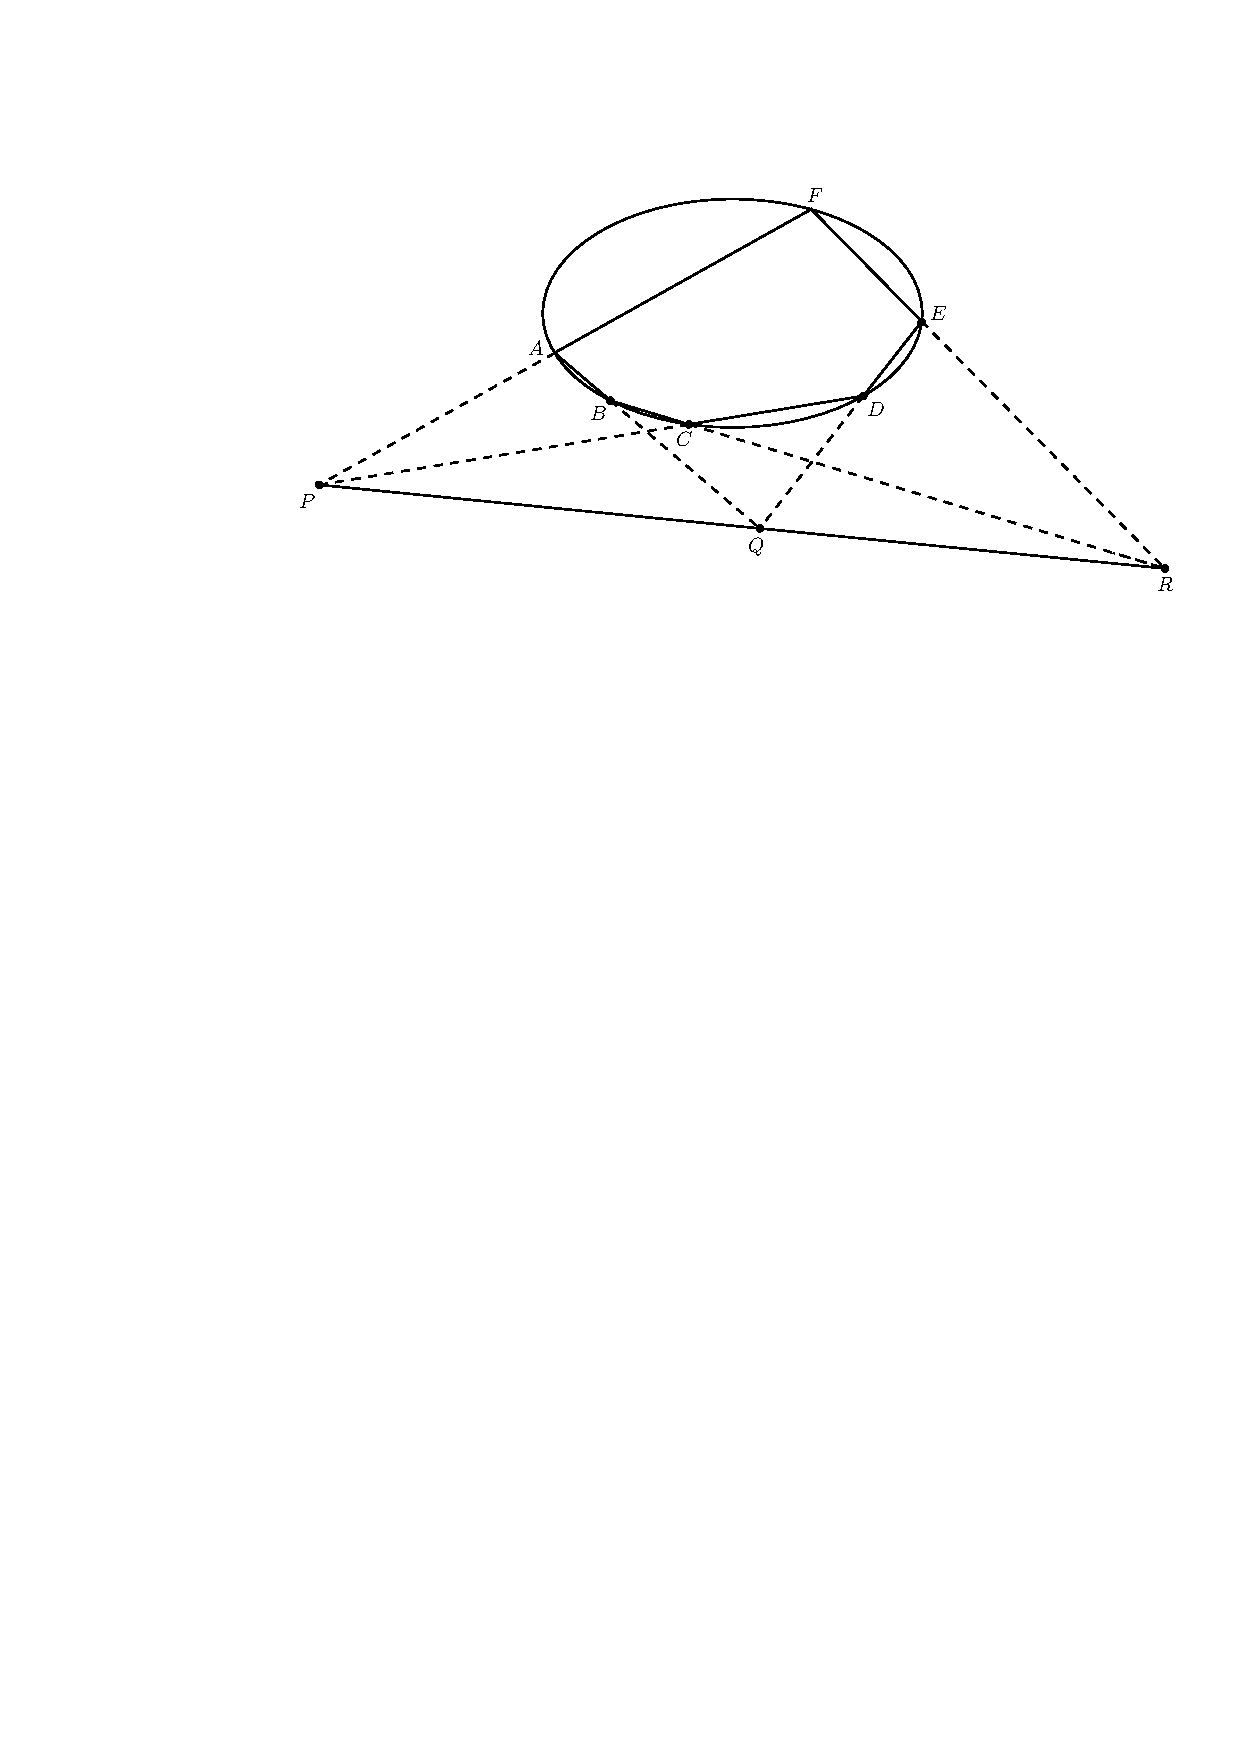
\includegraphics[width=250pt]{pictures/pascal-thm}
\caption{The mystic hexagon.}
\end{figure}
\begin{proof}
In the diagram, consider the two triples of lines
\[L_1:PAF,\quad L_2:QDE,\quad L_3:RBC.\]
and 
\[M_1:PCD,\quad M_2:QAB,\quad M_3:REF.\]
let $C_1=L_1+L_2+L_3$ and $C_2=M_1+M_2+M_3$. Now clearly $C_1$ and $C_2$ are two cubics such that
\[C_1\cap C_2=\{A,B,C,D,E,F,P,Q,R\}.\]
Suppose $PQR$ are collinear, with $L=PQR$, let $\Gamma$ be the conic through $ABCDE$ (the existence and unicity of which is provided by Proposition~\ref{conic dim}). Then by construction, $L+\Gamma$ is a cubic passing through the $8$ points $A,B,C,D,E,P,Q,R$, and by Corollary~\ref{cubic 9 point}, it must contain $F$. By assumption, $F\notin L$, since otherwise $A,E,F$ would by collinear, so necessarily we have $F\in\Gamma$, proving that the six points are conconic.\par
Now conversely, suppose that $ABCDEF$ are on a nondegenerate conic $\Gamma$, and let $L=PQ$; then is a cubic passing through $A,B,C,D,E,F,P,Q$, so by Corollary~\ref{cubic 9 point} it must pass through $R$. Now $R$ can't be on the conic $\Gamma$ (since otherwise the points $F,E,R$ is colliearly in $\Gamma$, and thus $\Gamma$ is a line pair, contradiction), so $R\in L$, that is, $PQR$ are collinear.
\end{proof}
\section{Tangent space and nonsingularity}
\subsection{Nonsingular points of a hypersurface}
Suppose $f\in k[X_1,\dots,X_n]$ is irreducible, $f\notin k$, and set $V=V(f)\sub\mathbb{A}^n$; let $P=(a_1,\dots,a_n)\in V$, and $\ell$ be a line through $P$. Since $P\in V$, obviously $P$ is a root of $f|_{\ell}$. When is $P$ a multiple root of $f|_{\ell}$?
\begin{proposition}
The point $P$ is a multiple root of $f|_{\ell}$ if and only if the line $\ell$ is contained in the affine linear subspace $T_PV$ defined by the equation
\[\sum_i\frac{\partial f}{\partial X_i}(P)(X_i-a_i)=0,\]
called the \textbf{tangent space} to $V$ at $P$. We say that every line
contained in $T_PV$ and passing through $P$ is \textbf{tangent to $\bm{V}$ at $\bm{P}$}. If $\partial f/\partial X_i(P)=0$ for all $i$, we say that each line passing
through $P$ is tangent to $V$ at $P$.
\end{proposition}
\begin{proof}
We consider parametric equations for $\ell$ of the form $X_i=a_i+b_it$, where $(b_1,\dots,b_n)$ is the direction vector of $\ell$. Then $f|_{\ell}=f(\dots,a_i+b_it,\dots)=:g(t)$ is a polynomial in $t$, and we know that $t=0$ is one root of $g$. Hence
\[\text{$0$ is a multiple root of $g$}\iff\frac{\partial g}{\partial t}(0)=0,\]
that is,
\[\sum_ib_i\frac{\partial f}{\partial X_i}(P)=0.\]
This condition is equivalent to the fact that $\ell\sub T_PV$.
\end{proof}
\begin{definition}
A point $P\in V\sub\mathbb{A}^n$ is a \textbf{nonsingular point} of $V$ if $\partial f/\partial X_i(P)\neq 0$ for some $i$; otherwise $P$ is a \textbf{singular point}, or a \textbf{singularity} of $V$.
\end{definition}
Obviously $T_PV$ is an $(n-1)$-dimensional affine subspace of $\mathbb{A}^n$ if $P$ is nonsingular, and $T_PV=\mathbb{A}^n$ if $P\in V$ is singular.
\begin{remark}
Suppose that $k=\R$ or $\C$, and suppose for example that $\partial f/\partial x_1(P)\neq0$. Consider the map $p:\mathbb{A}^n\to\mathbb{A}^n$ defined by $(X_1,\dots,X_n)\mapsto(f,X_2,\dots,X_n)$. The determinant of the Jacobian matrix
\[\begin{pmatrix}
\dfrac{\partial f}{\partial X_1}&\dfrac{\partial f}{\partial X_2}&\cdots&\dfrac{\partial f}{\partial X_n}\\[8pt]
0&1&\cdots&0\\[4pt]
0&0&\cdots&1
\end{pmatrix}\]
is non-zero at $P$. Thus, by the inverse function theorem, there exists a neighborhood $U\sub\mathbb{A}^n$, $P\in U$, such that the restriction $p|_U:U\to p(U)\sub\mathbb{A}^n$ is a diffeomorphism from $U$ to open set $p(U)$ in the usual Euclidean topology of $\R^n$ or $\C^n$.\par
In other words, $(f,X_2,\dots,X_n)$ is a new system of coordinates on $\mathbb{A}^n$ near to $P$. This implies that an euclidean neighborhood of $P$ in the hypersurface $V$ of equation $f=0$ is diffeomorphic to an open set in $\mathbb{A}^{n-1}$ with coordinates $(Y_2,\dots,Y_n)$. We express this fact by saying that close to the non-singular point $P$ the non-singular variety $V$ has $(Y_2,\dots,Y_n)$ as \textbf{local parameters}.
\end{remark}
Let us consider the set
\[V_{nonsin}=\{P\in V:\text{$P$ is nonsingular}\}\]
of non-singular points of $V$.
\begin{proposition}\label{hypersurface nonsin dense}
$V_{nonsin}$ is a dense open set of $V$ for the Zariski topology.
\end{proposition}
\begin{proof}
The set $V_{sin}$ of singular points is defined by $\partial f/\partial X_i=0$ for all $i$, that is,
\[V_{\sin}=V\Big(f,\frac{\partial f}{\partial X_1},\dots,\frac{\partial f}{\partial X_n}\Big).\]
which is closed by definition of the Zariski topology. Since $V$ is irreducible, to show that the open $V_{nonsin}$ is dense, we only have to show it's nonempty; arguing by contradiction, suppose that it's empty, that is, suppose $V=V(f)=V_{sin}$. Then each of the polynomials $\partial/\partial X_i$ must vanish on $V$, therefore they must be divisible by $f$ in $k[X_1,\dots,X_n]$; but viewed as a polynomial in $X_i$, $\partial f/\partial X_i$ has degree strictly smaller than $f$, so that $f$ divides $\partial f/\partial X_i$ implies that in fact $\partial f/\partial X_i=0$ as a polynomial. Over $\C$, this is obviously only possible if $X_i$ does not appear in $f$, and if this happens for all $i$ then $f$ is constant, which is excluded. Over a general field $k$, $\partial f/\partial X_i=0$ is only possible if $f$ is an inseparable polynomial in $X_i$, that is, $\char k=p$, and $X_i$ only appears in $f$ as the $p$-th power $X^p_i$. If this happens for each $i$, then by the argument given in Proposition~\ref{Noe normal adjust}, $f$ is a $p$-th power in $k[X_1,\dots,X_n]$, this contradicts the fact that $f$ is irreducible.
\end{proof}
We can now define the tangent space to an affine algebraic set $V$ at one of its points, and study some properties related to the concept of dimension.
\begin{definition}
Let $V\sub\mathbb{A}^n$ be a variety, with $P=(a_1,\dots,a_n)\in V$. For any $f\in k[X_1,\dots,X_n]$, write
\[f^{(1)}_P=\sum_i\frac{\partial f}{\partial X_i}(P)(X_i-a_i).\]
This is an affine linear polynomial, the first order part of $f$ at $P$. Now define the \textbf{tangent space to $\bm{V}$ at $\bm{P}$} by
\[T_PV=\bigcap_{f\in I(V)}(f_P^{(1)}=0).\]
\end{definition}
If $V=V(J)$ (where we can always suppose that $J$ is a radical ideal and so $J=I(V)$) one sees immediately that the linear parts of the polynomials of $J$ generate an ideal $J_P^{(1)}=\{f_P^{(1)}:f\in J\}$ and so
\[T_PV=V(J^{(1)}_P).\]
Let $I(V)=(f_1,\dots,f_m)$. Since the linear part of the sum of two polynomials is the sum of the linear parts of the two summands, one has that for each $g\in I(V)$, the linear part $g^{(1)}_P$ of $g$ in $P$ is a linear combination of those of the $f_i$. Therefore, $J^{(1)}_P=(f_{1,P}^{(1)},\dots,f^{(1)}_{m,P})$. Hence the definition of $T_PV$ becomes simply
\[T_PV=V(f_{1,P}^{(1)},\dots,f^{(1)}_{m,P})=\bigcap_{i=1}^{m}V(f^{(1)}_{i,P})\]
\begin{proposition}
The function $V\to\N$ defined by $P\mapsto\dim T_PV$ is an upper semi-continuous function in the Zariski topology of $V$. In other words, for any integer $r$, the subset
\[S(r)=\{P\in V\mid\dim T_PV\geq r\}\]
is closed.
\end{proposition}
\begin{proof}
Let $(f_1,\dots,f_m)$ be a set of generators of $I(V)$. Then
\[T_PV=V(f_{1,P}^{(1)},\dots,f^{(1)}_{m,P})=\bigcap_{i=1}^{m}V(f^{(1)}_{i,P}).\]
That is, $T_PV$ is the zero set of the function $f:\mathbb{A}^n\to\mathbb{A}^m$ defined by
\[(X_1,\dots,X_n)\mapsto(f^{(1)}_{1,P},\dots,f^{(1)}_{m,P}).\]
Since $f^{(1)}_{i,P}$ are linear forms, the map $f$ has constant rank, so that we get $\dim T_PV=n-\rank\partial f$. This implies
\[P\in S(r)\iff\rank\Big(\frac{\partial f_i}{\partial X_j}(P)\Big)\leq n-r.\]
Now each entry $\partial f_i/\partial X_j$ of the matrix is a polynomial function of $P$, thus each minor is a determinant of a matrix of polynomials, and so is itself a polynomial. Hence $S(r)\sub V\sub\mathbb{A}^n$ is an algebraic subset.
\end{proof}
\begin{corollary}
There exists an integer $r$ and a dense open subset $V_0\sub V$ such that
\[\dim T_PV=r\text{ for }P\in V_0\And \dim T_PV\geq r\text{ for all $P\in V$}.\]
Define $r$ to be the \textbf{dimension of $\bm{V}$}, and write $\dim V=r$. We say that $P\in V$ is \textbf{nonsingular} if $\dim T_PV=r$, and \textbf{singular} if $\dim T_PV>r$. A variety $V$ is nonsingular if it is nonsingular at each point. The closed subset $V_{sin}$, the locus of the singular points of $V$, is the \textbf{singular locus} of $V$; it is empty if $V$ is non-singular.
\end{corollary}
\begin{proof}
Let $r=\min_{P\in V}\{\dim T_PV\}$. Then clearly
\[S(r-1)=\emp,\quad S(r)=V,\quad S(r+1)\subset V.\]
Therefore $S(r)-S(r+1)=\{P\in V\mid \dim T_PV=r\}$ is open and nonempty.
\end{proof}
\subsection{Dimension equals transcendence degree-the hypersurface case}
\begin{definition}
If $k\sub K$ is an extension of fields, the \textbf{transcendence degree} of $K$ over $k$ is the maximal number of elements of $K$ that are algebraically independent over $k$. It is indicated by $\tr\deg_kK$.
\end{definition}
It follows from Proposition~\ref{hypersurface nonsin dense} that if $V=V(f)\sub\mathbb{A}^n$ is a hypersurface defined by some nonconstant irreducible polynomial $f$, then $\dim V=n-1$. We now prove that $\tr\deg_kk(V)=n-1$; from this it follows, in particular, that for a hypersurface $V$,
\[\dim V=\tr\deg_kk(V)=n-1.\]
Consider the quotient mapping
\[\pi:k[X_1,\dots,X_n]\to k[V]=k[X_1,\dots,X_n]/(f)\]
and let $x_i=\pi(X_i)$. Suppose, to fix our ideas, that the indeterminate
$X_1$ actually appears in $f$ and consider the elements $x_2,\dots,x_n\in k(V)$. If one had $\tr\deg_kk(V)<n-1$, they would be algebraically dependent and so there would exist a polynomial $g(X_2,\dots,X_n)\in k[X_2,\dots,X_n]$ such that
\[g(X_2,\dots,X_n)=0.\]
that is, $g\in(f)$. But that is absurd because $X_1$ does not appear in $g$. Hence $\tr\deg_kk(V)\geq n-1$. Since one certainly has $\tr\deg_kk(V)<n$, it follows that $\tr\deg_kk(V)=n-1$.\par
The rest of this section is concerned with proving that the equality $\dim V=\tr\deg_kk(V)$ holds for all varieties, by reducing to the case of a hypersurface. The first thing to show is that for a point $P\in V$ of a variety, the tangent space $T_PV$, which so far has been discussed in terms of a particular coordinate system in the ambient space $\mathbb{A}^n$, is in fact an intrinsic property of a neighbourhood of $P\in V$.
\subsection{Intrinsic nature of \boldmath$T_PV$}
From now on, given $P=(a_1,\dots,a_n)\in V\sub\mathbb{A}^n$, we take new coordinate $X'_i=X_i-a_i$ to bring $P$ to the origin, and thus assume that $P=(0,\dots,0)$. Then $T_PV\sub\mathbb{A}^n$ is a vector subspace of $k^n$. Let $\m_P$ be the maximal ideal of $P$ in $k[V]$, and 
\[M_P=(X_1,\dots,X_n)\sub k[X_1,\dots,X_n].\]
Then of course $\m_P=M_P/I(V)\sub k[V]$.
\begin{theorem}
With the above notation,
\begin{itemize}
\item[$(1)$] There is a natural isomorphism of vector spaces
\[(T_PV)^*=\m_P/\m_P^2.\]
where $(T_PV)^*$ denotes the dual space.
\item[$(2)$] If $f\in k[V]$ is such that $f(P)\neq0$, and $V_f\sub V$ is the standard affine open, then the natural map
\[T_P(V_f)\to T_PV\]
is an isomorphism.
\end{itemize}
\end{theorem}
\begin{proof}
Write $(k^n)^*$ for the vector space of linear forms on $k^n$, this is the vector space with basis $X_1,\dots,X_n$. Since $P=(0,\dots,0)$, for any $f\in k[X_1,\dots,X_n]$, the linear part $f^{(1)}_P$ is naturally an element of $(k^n)^*$. Consider the map
\[d:M_P\to (k^n)^*\]
defined by putting $df=f^{(1)}_P$ for each $f\in M_P$.\par
The map $d$ is obviously surjective. Indeed, the linear forms $X_1,\dots,X_n\in (k^n)^*$ are the images of the elements $X_1,\dots,X_n\in M_P$. Moreover $\ker d=M_P^2$ since $f^{(1)}_P=0$ if and only if $f$ has quadratic terms in $X_1,\dots,X_n$ in minimal degree; that is, if and only if $f\in M_P^2$. Thus
\[(k^n)^*=M_P/M_P^2.\]
This proves $(1)$ in the particular case $V=\mathbb{A}^n$.\par
In the general case one has the restriction map $(k^n)^*\to(T_PV)^*$, dual to the inclusion $T_PV\sub k^n$, which sends a linear form $\lambda$ on $k^n$ into its restriction to $T_PV$. By composition one obtains a map
\[D:M_P\to (k^n)^*\to(T_PV)^*.\]
The composite $D$ is surjective since each factor is. It suffices to prove that
\[\ker D=M_P^2+I(V).\]
because from this it follows that
\[\m_P/\m_P^2=M_P/(M_P^2+I(V))\cong (T_PV)^*.\]
To prove the claim, note that
\[f\in\ker D\iff f^{(1)}_P|_{T_PV}=0\iff f_P^{(1)}=\sum_ia_ig_{i,P}^{(1)}\text{ for some $g_i\in I(V),a_i\in k[X_1,\dots,X_n]$}.\]
The last condition is equivalent to 
\[f-\sum_ia_ig_i\in M_P^2\text{ for some $g_i\in I(V),a_i\in k[X_1,\dots,X_n]$}.\]
which means that $f\in M_P^2+I(V)$.\par
To prove $(2)$ we use the identification $V_f\cong V(I(V),Yf-1)\sub\mathbb{A}^{n+1}$. Then $I(V_f)=(I(V),Yf-1)\sub k[X_1,\dots,X_n,Y]$, and the point $P=(0,\dots,0)$ is mapped to $(0,\dots,0,1/f(P))$. With the observation
\[(Yf-1)^{(1)}_{P}=Yf^{(1)}_P+f(Y-1/f(P)),\]
we can see that $T_P(V_f)\sub\mathbb{A}^{n+1}$ is defined by the equations defining $T_PV$ plus the equation 
\[Yf^{(1)}_P+f(Y-1/f(P))=0.\]
Thus the natural map 
\[T_P(V)\mapsto T_P(V_f),\quad P\mapsto(P,1/f(P))\]
is an inverse of the morphism $T_P(V_f)\to T_PV$.
\end{proof}
\begin{corollary}
$T_PV$ only depends on a neighbourhood of $P\in V$ up to isomorphism. More precisely, if $P\in V_0\sub V$ and $Q\in W_0\sub W$ are open subsets of affine varieties, and $\varphi:V_0\to W_0$ is an isomorphism taking $P$ into $Q$, there is a natural isomorphism $T_PV\to T_PW$; hence $\dim T_PV=\dim T_QW$.\par
In particular, if $V$ and $W$ are birationally equivalent varieties then $\dim V=\dim W$.
\end{corollary}
\begin{proof}
By passing to a smaller neighbourhood of $P$ in $V$, we can assume $V_0$ is isomorphic to an affine variety. Then so is $W_0$, and $\varphi$ induces an isomorphism $k[V_0]\cong k[W_0]$ taking $\m_P$ into $\m_Q$. Therefore, $\m_P/\m_P^2\cong\m_Q/\m_Q^2$ and $T_PV\cong T_QW$.\par
The final sentence holds because by Proposition~\ref{biration equiv iff}, $V$ and $W$ contain dense open subsets which are isomorphic.
\end{proof}
\begin{theorem}
For any affine variety $V$,
\[\dim V=\tr\deg_kk[V].\]
\end{theorem}
\begin{proof}
This is known if $V$ is a hypersurface. On the other hand, every variety is birational to a hypersurface by Proposition~\ref{hypersurface reduction}, and both sides of the required relation are the same for birationally equivalent varieties.
\end{proof}
\subsection{Dimension of varieties}
In view of the dimension of affine varieties, we make the following definition.
\begin{definition}
The dimension of an projective variety $V$ is the transcendence degree of the function field $k(V)$; it is denoted by $\dim V$. The dimension of a reducible algebraic set is the maximum of the dimension of its irreducible components. If $W\sub V$ is a closed subvariety of $V$ then the number $\dim V-\dim W$ is called the codimension of $W$ in $V$, and written $\codim W$ or $\codim_VW$. Algebraic varieties of dimension $1$ and $2$ are called \textbf{curves} and \textbf{surfaces}.
\end{definition}
Note that if $X$ is an irreducible variety and $U\sub X$ is open then $k(U)=k(X)$, and hence $\dim U=\dim X$.
\begin{example}
$\dim\mathbb{A}^n=\dim\P^n=n$, because the field $k(\mathbb{A}^n)$ is the field of rational functions in $n$ variables. Since dimension is by definition invariant under birational equivalence, we see that $\mathbb{A}^n$ and $\mathbb{A}^m$ are not birational if $n\neq m$.
\end{example}
\begin{example}
If $V$ consists of a single point then obviously $\dim V=0$, and thus the same holds if $V$ is a finite set. Conversely, if $\dim V=0$ then $V$ is a finite set. It is enough to prove this for an affine variety $V$. Let $V\sub\mathbb{A}^n$ and write $x_1,\dots,x_n$ for the coordinates on $\mathbb{A}^n$ as functions on $V$, that is, as elements of $k[V]$. By assumption the $x_i$ are algebraic over $k$, and can hence only take finitely many values. It follows from this that $V$ is finite.
\end{example}
\begin{proposition}
If $X$ and $Y$ are varieties then
\[\dim(X\times Y)=\dim X+\dim Y.\]
\end{proposition}
\begin{proof}
We need only consider the case that $X\sub\mathbb{A}^N$ and $Y\sub\mathbb{A}^M$ are affine varieties. Suppose that $\dim X=n,\dim Y=m$, and let $x_1,\dots,x_N$ and $y_1,\dots,y_M$ be coordinates of $\mathbb{A}^N$ and $\mathbb{A}^M$ considered as functions on $X$ and $Y$ respectively, such that $t_1,\dots,t_n$ are algebraically independent in $k(X)$ and $y_1,\dots,y_m$ in $k(Y)$. By definition $k[X\times Y]$ is generated by the elements $x_1,\dots,x_N,y_1,\dots,y_M$, and under the current assumptions all of these are algebraically dependent on $x_1,\dots,x_n,y_1,\dots,y_m$. Hence it is enough to prove that these elements are algebraically independent. Suppose that there is a relation $F(X,Y)=F(X_1,\dots,X_n,Y_1,\dots,Y_m)=0$ on $X\times Y$. Then for any point $x\in X$ we have $F(x,Y_1,\dots,Y_m)=0$ on $Y$. Since $y_1,\dots,y_m$ are algebraically independent in $k(Y)$, every coefficient $a_i(x)$ of the polynomial $F(x,Y)$ is zero; this means that the corresponding polynomial $a_i(X_1,\dots,X_n)$ is $0$ on $X$. Now we use the fact that $x_1,\dots,x_n$ are algebraically independent in $k(X)$ and deduce from this that $a_i(Y_1,\dots,Y_n)=0$, and hence $F(X,Y)$ is identically 0.
\end{proof}
\begin{theorem}\label{dimension monotone}
Let $Y$ be a variety. If $X$ is a closed subset of $Y$ with $\dim X=\dim Y$ then $X=Y$.
\end{theorem}
\begin{proof}
It is enough to prove the assertions for affine varieties.\par
Suppose $X\sub Y\sub\mathbb{A}^N$ with $\dim Y=n$. Then any $n+1$ of the coordinate functions $t_1,\dots,t_N$ are algebraically dependent as elements of $k[Y]$, that is, are connected by a relation $F(t_{i_1},\dots,t_{i_{n+1}})=0$ on $Y$. A fortiori this holds on $X$. This means that the transcendence degree of $k(X)$ is at most $n$, so that $\dim X\leq\dim Y$.\par
Now suppose that $\dim X=\dim Y=n$. Then some $n$ of the coordinates $x_1,\dots,x_n$ are algebraically independent on $X$; suppose that these are $x_1,\dots,x_n$. Then a fortiori they are algebraically independent on $Y$. Let $f\in k[Y]$ with $f\neq 0$ on $Y$. Then $f$ on $Y$ is algebraically dependent on $x_1,\dots,x_n$, that is, there is a relation on $Y$ of the form
\[h_0(x_1,\dots,x_n)f^k+\cdots+h_k(x_1,\dots,x_n)=0\]
where we can choose such that $h_k(x_1,\dots,x_n)\neq 0$ on $Y$. This equation holds a fortiori on $X$. Suppose that $f=0$ on $X$, so that $h_k(x_1,\dots,x_n)=0$ on $X$. Since by assumption $x_1,\dots,x_n$ are independent on $X$, it follows that $h_k(x_1,\dots,x_n)=0$ on the whole of $\mathbb{A}^N$. This is a contradiction. Thus if $f=0$ on $X$ then also $f=0$ on $Y$, and therefore $X=Y$. The theorem is proved.
\end{proof}
We have seen that an irreducible algebraic plane curve is $1$-dimensional. The
following result is a generalisation.
\begin{theorem}
Every irreducible component of a hypersurface in $\mathbb{A}^n$ or $\P^n$ has codimension $1$.
\end{theorem}
\begin{proof}
It is enough to consider the case of a hypersurface in $\mathbb{A}^n$. Suppose that a variety $X\sub\mathbb{A}^n$ is given by an equation $F(X)=0$. The factorisation $F=F_1\cdots F_r$ of $F$ into irreducible factors corresponds to an expression $V=V_1\cup\cdots\cup V_k$, where $V_i=V(F_i)$. By Corollary~\ref{hypersurface decomposition} this is the decomposition of $V$. Suppose that the variable $X_n$ actually appears in the polynomial $F_i(X)$, we prove that the coordinates $x_1,\dots,x_{n-1}$ are algebraically independent on $V_i$. Indeed, a relation $G(t_1,\dots,t_{n-1})=0$ on $V_i$ would imply that $G^\ell\in(F_i)$ for some $\ell>0$, which is impossible since $G$ does not involve $X_n$. Thus $\dim V_i\geq n-1$; since $V\neq\mathbb{A}^n$, it follows from Theorem~\ref{dimension monotone} that $\dim V_i=n-1$.
\end{proof}
Here is a converse of the previous theorem.
\begin{theorem}
Let $V\sub\mathbb{A}^n$ be an algebraic subset, and suppose that all the components of $V$ have dimension $n-1$. Then $V$ is a hypersurface and the ideal $I(V)$ is principal.
\end{theorem}
\begin{proof}
We only need consider the case that $V$ is irreducible. Since $V\neq\mathbb{A}^n$ (because $\dim V=n-1$), there exists a nonzero polynomial $F$ which is zero on $V$. Since $V$ is irreducible, some irreducible factor $H$ of $F$ is also zero on $V$. Write $W\sub\mathbb{A}^n$ for the hypersurface defined by $H=0$; we saw that $W$ is irreducible. Then $V\sub W$, so that $V=W$ by Theorem~\ref{dimension monotone}. Now by nullstellensatz $I(V)=I(V(H))=(H)$.
\end{proof}
The following analogue is proved similarly:
\begin{theorem}
Let $X\sub\P^{n_1}\times\cdots\times\P^{n_k}$ be an algebraic subset, and suppose that all the components of $X$ have dimension $n_1+\cdots+n_k-1$. Then $X$ is defined by one equation that is homogeneous in each of the $k$ sets of variables.
\end{theorem}
%\chapter{Representation of symmetric group}
\section{Facts about \boldmath\texorpdfstring{$S^\lambda$}{S}}
Define $A=\C[S_n]$ and
\[M^\lambda=Aa_\lambda,\quad \widetilde{M}^\lambda=Ab_\lambda,\quad S^\lambda=Ab_\lambda a_\lambda,\quad \widetilde{S}^\lambda=Aa_\lambda b_\lambda.\]
The we have the following surjective $A$-homomorphisms
\[\begin{tikzcd}[row sep=5pt]
A\ar[r,"\alpha"]&M^\lambda\ar[r,"\tilde{\beta}"]&\widetilde{S}^\lambda\\
A\ar[r,"\beta"]&\widetilde{M}^\lambda\ar[r,"\tilde{\alpha}"]&S^\lambda
\end{tikzcd}\]
Now we are going to find the kernel of these four maps. For simplicity we let $T$ be the tableau associated with $\lambda$.
\begin{lemma}
With the notations above, we have
\[\ker\alpha=A\langle\sigma-1:\sigma\in R(T)\rangle,\quad\ker\beta=A\langle\tau-\sgn(\tau)1:\sigma\in C(T)\rangle.\]
\end{lemma}
\begin{proof}
We only show the equaality for $\ker\alpha$. One direction is clear. Now let $\pi\in S_n$ be such that $\pi a_\lambda=0$. Then
\[-\pi=\sum_{\sigma\in R(T),\sigma\neq 1}\pi\sigma=\sum_{\sigma\in R(T),\sigma\neq 1}\pi(\sigma-1)+(|R(T)|-1)\pi\]
whence we see $\pi$ is in the right-hand side of the equality above, whence the claim.
\end{proof}
Let $Q^\lambda$ be the submodule of $\widetilde{M}^\lambda$ generated by all elements of the form
\[[T]-\sum[S]\]
where $S$ is obtained from $T$ by exchanging columns, and similarly let $\widetilde{Q}^\lambda$ be the submodule of $M^\lambda$ generated by all elements of the form
\[\{T\}-\sum(-1)^k\{W\}\]
where $W$ is obtained from $T$ by exchanging rows, and $k$ is the number of boxes that are exchanged.
\begin{lemma}
With the notations above,
\begin{itemize}
\item[(a)] The classes $[T]$, as $[T]$ varies over the standard tableaux on $\lambda$, span the quotient space $\widetilde{M}^\lambda/Q^\lambda$.
\item[(b)] The classes $\{T\}$, as $\{T\}$ varies over the standard tableaux on $\lambda$, span the quotient space $M^\lambda/\widetilde{Q}^\lambda$.  
\end{itemize}
\end{lemma}
\begin{proof}
This follows from a suitable ordering and an induction argument.
\end{proof}
\begin{proposition}
We have
\[\ker\tilde{\alpha}=Q^\lambda,\quad \ker\tilde{\beta}=\widetilde{Q}^\lambda.\]
\end{proposition}
\begin{proof}
It suffices to prove that $Q^\lambda\sub\ker\tilde{\alpha}$, since then we get a surjection $\widetilde{M}^\lambda/Q^\lambda\to S^\lambda$, which is an isomorphism since $\dim(S^\lambda)=f^\lambda$. Now if $H(A,B)$ denotes the permutations that ouccur in an exchange of columns, then we have
\[(1-\sum_{\tau\in H(A,B)}\tau)b_\lambda a_\lambda.\]
Since $(1-\sum_{\tau\in H(A,B)})b_\lambda$ corresponds to $[T]-\sum[S]$, we get the claim.
\end{proof}
\section{Weyl's construction}
Let $A=\bigoplus_{i\in I}A_i=\bigoplus_{i\in I}\mathcal{M}_{r_i}(\C)$ be a finite-dimensional semisimple algebra over $\C$. If we consider any finite-dimensional module right $M$ over $A$ we have seen that $M$ is isomorphic to a finite sum
\[M=\bigoplus_{i\in I}M_i=\bigoplus_{i\in I}S_i^{n_i}\]
where $S_i$ are irreducible right $A$-modules with $\dim(S_i)=r_i$. By definition, $A$ acts on $S_i$ by the standard right representation on $\C^{r_i}$ and as zero on other components. Therefore, we can identify $M_i$ as $\mathcal{M}_{n_i\times r_i}(\C)$ with multiplication on the right, and $M_i$ is decomposed by its rows.\par
We have also that
\[B:=\End_A(M)=\bigoplus_{i\in I}\End_A(M_i)=\bigoplus_{i\in I}\End_A(S_i^{n_i})=\bigoplus_{i\in I}\mathcal{M}_{n_i}(\C):=\bigoplus_{i\in I}B_i\]
where the block $B_i$ acts on $S_i^{n_i}$ as $r_i$ copies of its standard left matrix representation, and as zero on the other isotypic components. In other words, if $T=(a_{i,j})\in B_i$, $v=(v_1,\dots,v_{n_i})\in S_i^{n_i}$ with $v_j=\sum_{k=1}^{n_i}b_{jk}e_k$, then with $U=(b_{j,k})$ we have
\begin{align*}
T\cdot v&=T\begin{pmatrix}
v_1\\
v_2\\
\vdots\\
v_{n_i}
\end{pmatrix}=TU\begin{pmatrix}
e_1\\
e_2\\
\vdots\\
e_{r_i}
\end{pmatrix}
\end{align*}
Thus with the identification made above, $B_i$ acts on $M_i$ by multiplication on the left, and the $r_i$ subspaces of $\mathcal{M}_{n_i\times r_i}(\C)$ formed by the columns decompose this space into irreducible representations of $B_i$ isomorphic to the standard representation $\C^{n_i}$.
\begin{lemma}
Let $m,r,n$ be positive integers. Then
\[\mathcal{M}_{m\times r}(\C)\otimes_{\mathcal{M}_{r\times r}(\C)}\mathcal{M}_{r\times n}(\C)=\mathcal{M}_{m\times n}(\C)\]
as $(\mathcal{M}_{m}(\C),\mathcal{M}_{n}(\C))$-bimodules.
\end{lemma}
\begin{proposition}
Let $M$ be a finite-dimensional right $A$-module.
\begin{itemize}
\item[(a)] If $S$ is an irreducible left $A$-module, then $M\otimes_AS$ is an irreducible left $B$-module.
\item[(b)] If $S_i$ are the distinct irreducible left $A$-modules, with $r_i$ the dimension of $S_i$, then
\[M\cong\bigoplus_i(M\otimes_AS_i)^{r_i}\cong\bigoplus_i(Mc_i)^{r_i}\]
is the decomposition of $M$ into irreducible left $B$-modules.
\end{itemize}
\end{proposition}
\begin{proof}
For (a), first consider the case $M$ is irreducible. Then by the argument above, we can identify $S$ with a minimal left ideal of $A$ consisting of tuples of matrices which are zero except in one factor, and in this factor are all zero except for one column. Similarly, $M$ can be identified with the right ideal of tuples which are zero except in one factor, and in that factor all are zero except in one row. Then $M\otimes_AS$ will be zero unless the factor is the same for $M$ and $S$, in which case $M\otimes_AS$ can be identified with the product of these two factors, which is isomorphic to $\C$. This completes the proof when $M$ is irreducible. For the general case, decompose $M=\bigoplus_iS_i^{n_i}$ into a sum of irreducible right $A$-modules, so $M\otimes_AS=\bigoplus_i(S_i\otimes_AS)^{n_i}=\C^{n_j}$ for some $j$, which is visibly irreducible over $B$.\par
Now (b) follows since the isomorphism $A\cong\bigoplus_iW_i^{\oplus n_i}$ implies
\[M\cong M\otimes_AA\cong M\otimes_A(\bigoplus_iS_i^{\oplus n_i})\cong\bigoplus_i(M\otimes_AS_i)^{n_i}.\]
This completes the proof.
\end{proof}
\begin{corollary}
Given a semisimple $\C$-algebra $A$, a right $A$-module $M$, and let $B=\End_A(M)$ its centralizer. Then there exist two sequences of integers $n_1,\dots,n_k$ and $r_1,\dots,r_k$ and an isomorphism of $M$ with $\bigoplus_i\C^{n_i}\otimes\C^{r_i}$ under which the algebras $A,B$ are identified with the algebras $\bigoplus_i\mathcal{M}_{r_i}(\C)$ and $\bigoplus_i\mathcal{M}_{n_i}(\C)$.
\end{corollary}
Now let $V$ be a finite dimensional vector space and $M=V^{\otimes n}$. The endomorphisms of $M$ induced by endomorphisms of $V$ are certainly in $B$. Although $B$ is generally much larger than $\End(V)$, we have the following result.
\begin{proposition}
Let $A=\C S_n$. Then the algebra $B=\End_{A}(V^{\otimes n})$ is spanned as a linear subspace of $\End(V^{\otimes n})$ by $\End(V)$. Moreover, a subspace of $V^{\otimes n}$ is a sub-$B$-module if and only if it is invariant over $\GL(V)$.
\end{proposition}
\begin{proof}
Note that if $W$ is any finite-dimensional vector space, then $\mathrm{Sym}^n(W)$ is the subspace of $W^{\oplus n}$ spanned by all $w^n$ as $w$ runs through $W$, where
\[v_1\cdot v_2\cdots v_n=\frac{1}{n!}\sum_{\sigma\in S_n}v_{\sigma(1)}\otimes\cdots\otimes v_{\sigma(n)}\]
In fact, we have
\[n!v_1\cdot\cdots\cdot v_n=\sum_{I\sub\{1,\dots,n\}}(-1)^{n-|I|}\Big(\sum_{i\in I}v_i\Big)^n\]
Applying this to $\End(V)$ proves the first statement, since
\[\End(V^{\otimes n})=(V^*)^{\otimes n}\otimes V^{\otimes n}=(V^*\otimes V)^{\otimes n}=\End(V)^{\otimes n}.\]
with compatible actions of $S_n$. Since the image of $\GL(V)$ is closed in $\End(V^{\otimes n})$, the second claim follows.
\end{proof}
\begin{lemma}
We have
\[v_1\cdot v_2\cdots v_n=\frac{1}{n!}\sum_{\sigma\in S_n}v_{\sigma(1)}\otimes\cdots\otimes v_{\sigma(n)}\]
\end{lemma}
\begin{proof}
Consider a monomial $v_1^{i_1}\cdots v_n^{i_n}$ in the summation on the right. If at least one of the numbers $i_1,\dots,i_n$ is $0$, say $i_k=0$, then this monomial occurs an even number of times, and the occurrences cancel each other out, because every occurrence in an addend for some subset $I$ can be contrasted with a different occurrence, with opposite sign, in the addend for the subset $I\cup\{k\}$ (if $k\notin I$) or the subset $I\setminus\{k\}$ (if $k\in I$). So the only surviving monomials are those where all $n$ numbers $i_1,i_2,\dots,i_n$ are positive. But the only such monomial is $v_1v_2\cdots v_n$, and it is easy to see that it appears only once (namely, in the addend for $I=[n]$) and its coefficient is $n!$. Thus the claim follows.
\end{proof}
Now define $V^\lambda=V^{\otimes n}c_\lambda$. Then we get an isomorphism of $\GL(V)$-modules
\[V^{\otimes n}\cong\bigoplus_\lambda (V^\lambda)^{\oplus f^\lambda}.\]
\begin{theorem}
Let $V$ be a finite dimensional vector space with $\dim(V)=k$ and $\lambda=(\lambda_1,\dots,\lambda_k)$ a partition of $n$. Then
\begin{itemize}
\item[(a)] Each $V^\lambda$ is an irreducible representation of $\GL(V)$, and we have
\[\dim(V^\lambda)=s_\lambda(1,\dots,1)=\prod_{1\leq i<j\leq k}\frac{\lambda_i-\lambda_j+j-i}{j-i}.\] 
\item[(b)] For any $g\in\GL(V)$, the trace of $g$ on $V^\lambda$ is the value of $s_\lambda$ on the eigenvalues $x_1,\dots,x_k$ of $g$ on $V$:
\[\chi_{V^\lambda}(g)=s_\lambda(x_1,\dots,x_k)\] 
\end{itemize}
\end{theorem}
\begin{proof}
Let $\GL(V)$ acts on $\mathrm{Sym}^{d}(V)$. If $\{e_1,\dots,e_m\}$ is a basis for $V$, then $\{e_{i_1}\cdots e_{i_d}\}$ is a basis for $\mathrm{Sym}^d(V)$, and $g=\mathrm{diag}(x_1,\dots,x_m)$ acts on $\{e_{i_1}\cdots e_{i_d}\}$ by multiplying by $x_{i_1}\cdots x_{i_d}$. Hence $\tr(g)=h_d(x_1,\dots,x_m)$. Generalizing this, we see the trace of $g$ on $V^{\otimes n}\otimes_{\C S_n}M^\lambda$ is $h_\lambda(x_1,\dots,x_m)$. But since $M^\lambda=\bigoplus_\mu K_{\mu\lambda}S^\mu$, we have
\[h_\lambda(x_1,\dots,x_m)=\sum_\mu K_{\mu\lambda}\chi_{V^\lambda}(x_1,\dots,x_m).\]
Since $h_\lambda=\sum_\mu K_{\mu\lambda}s_\lambda$, this proves $\chi_{V^\lambda}(x_1,\dots,x_m)=s_\lambda(x_1,\dots,x_m)$.
\end{proof}
Let $V$ be a vector space and $\lambda$ an partition. We write $V^{\times\lambda}$ for the cartesian product of $n=|\lambda|$ copies of $V$, but labelled by the $n$ boxes of $\lambda$. If $V$ has a basis $\{v_1,\dots,v_m\}$, then for any filling $T$ on $\lambda$ with entries in $\{1,\dots,m\}$ we get an element of $V^{\times\lambda}$
\begin{lemma}\label{Weyl module char by conditions}
If $V$ is free with basis $\{v_1,\dots,v_m\}$, then $V^\lambda\cong F/Q$, where $F$ is free on elements $v_T$ for all fillings on $\lambda$ with entries in $\{1,\dots,m\}$, and $Q$ is generated by the following elements:
\begin{itemize}
\item[(a)] $v_T$ if $T$ has two equal entries in any column.
\item[(b)] $v_T+v_{T'}$ if $T'$ is obtained from $T$ by permuting two elements in a column.
\item[(c)] $v_T-\sum v_S$, where $S$ is obtained from $T$ by an exchange for a given subset of a column of $T$.
\end{itemize}
\end{lemma}
\subsection{The determinant construction}
Let $V$ be an $m$-dimensional vector space. Let $\{Z_{ij}:1\leq i\leq n,1\leq j\leq m\}$ be indeterminates and let $\C[Z]=\C[\{Z_{ij}\}]$. For each $p$-tuple $(i_1,\dots,i_p)$ of integers from $\{1,\dots,m\}$ with $p\leq n$, we define
\[D_{i_1,\dots,i_p}=\det\begin{bmatrix}
Z_{1,i_1}&Z_{1,i_2}&\cdots&Z_{1,i_p}\\
Z_{2,i_1}&Z_{2,i_2}&\cdots&Z_{2,i_p}\\
\vdots&\vdots&\ddots&\vdots\\
Z_{p,i_1}&Z_{p,i_2}&\cdots&Z_{p,i_p}\\
\end{bmatrix}\]
This is an alternating function on the subscripts $i_1,\dots,i_p$.\par
For a Young diagram $\lambda$ with at most $n$ rows and an arbitrary filling $T$ of $\lambda$ with numbers in $\{1,\dots,m\}$, let $D_T$ be the products of the determinants corresponding to the columns of $T$, i.e.,
\[D_T=\prod_{j=1}^{l}D_{T_{1,j},\dots,T_{\mu_j,j}}\]
where $\mu=\tilde{\lambda}$.
\begin{lemma}[\textbf{Sylvester}]
For any $p\times p$ matrices $M$ and $N$, we have
\[\det(M)\cdot\det(N)=\sum\det(M')\det(N')\]
where the sum is over all pairs $(M',N')$ of matrices obtained by interchanging a fixed set of $k$ columns of $N$ with any $k$ columns of $M$, preserving the relative ordering of columns. 
\end{lemma}
\begin{proof}
By the alternating property of determinants, we may assume that the columns interchanged in $N$ are the first $k$ columns. For vectors $v_1,\dots,v_p$ in $\C^p$, we write $|v_1,\dots,v_p|$ for the determinant of the matrix with these vectors as columns. Then we must prove that
\begin{align*}
|v_1,\dots,v_p|\cdot|w_1,\dots,w_p|=\sum_{i_1<\cdots<i_k}|v_1,\dots,w_1,\dots,w_k,\dots,v_p|\cdot|v_{i_1},\dots,v_{i_k},w_{k+1},\dots,w_p|.
\end{align*}
It suffices to show the difference of the two sides is an alternating function on the $p+1$ vectors $v_1,\dots,v_p,w_1$, since any such function must vanish. For this it suffices to prove that the two sides are equal when two successive vectors $v_i$ and $v_{i+1}$ are equal (which is immediate), and when $w_1=v_p$. In the later case, it suffices to show the following function is alternating on $v_1,\dots,v_p,w_2$:
\[|v_1,\dots,v_p|\cdot|v_p,w_2,\dots,w_p|-\sum_{i_1<\cdots<i_k}|v_1,\dots,w_1,\dots,w_k,\dots,v_p|\cdot|v_{i_1},\dots,v_{i_k},w_{k+1},\dots,w_p|\]
where the vectors $v_p,w_2,\dots,w_k$ are interchanged with the vectors $v_{i_1},\dots,v_{i_k}$. Again the case $v_i=v_{i+1}$ is immediate, and this time the case $w_2=v_p$ is also immediate.
\end{proof}
With the above lemma, we can prove the following important result.
\begin{proposition}
If $V$ is free with basis $\{v_1,\dots,v_m\}$, then there is a canonical homomorphism from $V^\lambda$ to $\C[Z]$ by mapping $v_T$ to $D_T$.
\end{proposition}
\begin{proof}
It suffices to prove that $D_T$ satisfies the conditions in Lemma~\ref{Weyl module char by conditions}. The first two follow from the property of determinant, and property (c) follows from Sylvester's lemma. For this, suppose the two columns of $T$ in which the exchange takes place has entries $i_1,\dots,i_p$ and $j_1,\dots,j_q$ (where $p\geq q$). Set
\[M=\begin{bmatrix}
Z_{1,i_1}&Z_{1,i_2}&\cdots&Z_{1,i_p}\\
Z_{2,i_1}&Z_{2,i_2}&\cdots&Z_{2,i_p}\\
\vdots&\vdots&\ddots&\vdots\\
Z_{p,i_1}&Z_{p,i_2}&\cdots&Z_{p,i_p}\\
\end{bmatrix}\quad N=\left[
\begin{BMAT}(@,20pt,30pt){c:l}{c}
\begin{matrix}
Z_{1,j_1}&Z_{1,j_2}&\cdots&Z_{1,j_q}\\
Z_{2,j_1}&Z_{2,j_2}&\cdots&Z_{2,j_q}\\
\vdots&\vdots&\ddots&\vdots\\
Z_{p,j_1}&Z_{p,j_2}&\cdots&Z_{p,j_q}\\
\end{matrix}&\begin{BMAT}(@,20pt,25pt){c}{cc}
0\\
I_{p-q}
\end{BMAT}
\end{BMAT}
\right]\]
Then the desired property follows by applying the Sylvester's lemma to these two matrices.
\end{proof}
\begin{theorem}
If $V$ is free with basis $\{v_1,\dots,v_m\}$, then $V^\lambda$ is free with basis $v_T$, as $T$ varies over the tableaux on $\lambda$ with entries in $\{1,\dots,m\}$.
\end{theorem}
\begin{proof}
The proof that $V^\lambda$ is generated by the $v_T$'s when $T$ varies over the tableaux on $\lambda$ with entries in $\{1,\dots,m\}$ is the same for that of $S^\lambda$, so we may omit it.\par
To show that $v_T$ are lineraly independent, we use the canonical map from $V^\lambda$ to $\C[Z]$. Thus we may prove that $D_T$ are lineraly independent. For this, we frist give the variables $\{Z_{ij}\}$ the lexicographical order and order the monomials lexicographically by saying $f_1<f_2$ if the smallest $Z_{i,j}$ that occurs to a different power occurs to a smaller power in $f_1$ than in $f_2$. Note that if $f_1\leq f_2$ and $g_1\leq g_2$ then $f_1g_1\leq f_2g_2$. It the follows from this definition that the smallest monomial that appears in a determinant $D_{i_1,\dots,i_p}$, if $i_1<\cdots<i_p$, is the diagonal term $Z_{1,i_1}Z_{2,i_2}\cdots Z_{p,i_p}$. Therefore the smallest term in $D_T$, if $T$ has increasing terms, is $\prod_{ij}Z_{i,j}^{m_T(i,j)}$, where $m_T(i,j)$ is the number of times $j$ occurs in the $i$-th row of $T$. This monomial occurs with coefficient $1$.\par
Now we order the tableaux by saying that $T<T'$ if in the first row where they differ, the first entry where they differ in this row, is smaller in $T$ than $T'$. Equivalently, the smallest $i$ for which there is a $j$ with $m_T(i,j)\neq m_{T'}(i,j)$, and the smallest such $j$, has $m_T(i,j)<m_{T'}(i,j)$. It follows that if $T<T'$ then the smallest monomial in $D_T$ is smaller than that in $D_{T'}$. From this the linearly independence of $D_T$ follows: if $\sum r_TD_T=0$ then take $T$ minimal with $r_T\neq 0$, we see the coefficient of $\prod_{ij}Z_{i,j}^{m_T(i,j)}$ in $\sum r_TD_T$ is $r_T$, contradiction.
\end{proof}
\begin{corollary}
The map from $V^\lambda$ to $\C[Z]$ is injective and its image $D^\lambda$ is free on the polynomials $D_T$, as $T$ varies over the tableaux on $\lambda$ with entries in $\{1,\dots,m\}$.
\end{corollary}
Finally, since the general linear group $\GL(V)$ acts on $V^\lambda$, we may want to have an action of $\GL(V)$ on $R[Z]$ such that the induced $\GL(V)$-module structure on $D^\lambda$ is isomorphic to that on $V^\lambda$. For this, we first consider the action of $g\in\GL(V)$ on $v_T$.
\begin{lemma}
If $g=(g_{ij})\in\GL_m(\C)$ and $T$ has entries $j_1,\dots,j_n$ in its $n$ boxes, then
\[g\cdot v_T=\sum g_{i_1,j_1}\cdots g_{i_n,j_n}v_{T'}\]
where the sum is over the all $p$-tuples $(i_1,\dots,i_p)$ from $\{1,\dots,m\}$.
\end{lemma}
\begin{proof}
This follows directly from the definition of the action of $\GL(V)$ on $V^{\otimes n}$. If fact,
\[g\cdot e_{j_1}\otimes\cdots\otimes e_{j_n}=\sum_{i_1,\dots,i_n} g_{i_1,j_1}e_{i_1}\otimes\cdots\otimes g_{i_n,j_n}e_{i_n}\]
from which the claim follows.
\end{proof}
Now for $g\in\GL_m(\C)$, define the action of $g$ on $\C[Z]$ by
\[(g\cdot f)(A)=f(A\cdot g)\]
where $A\in\mathcal{M}_{n\times m}(\C)$ and we view $\C[Z]$ a function ring over $\mathcal{M}_{n\times m}(\C)$. For example, if $g=(g_{ij})$ and $A=(a_{ij})$, then
\[(g\cdot Z_{ij})(A)=Z_{ij}(A\cdot g)=\sum_kA_{ik}g_{kj}\]
which can also be written as
\[g\cdot Z_{ij}=\sum_kZ_{ik}g_{kj}.\]
\begin{lemma}
For a $p$-tuple $(j_1,\dots,j_p)$, we have
\[g\cdot D_{j_1,\dots,j_p}=\sum g_{i_1,j_1}\cdots g_{i_n,j_n}D_{i_1,\dots,i_p}\]
where the sum is over the all $p$-tuples $(i_1,\dots,i_p)$ from $\{1,\dots,m\}$.
\end{lemma}
\begin{proof}
Let $A=(a_{ij})\in \mathcal{M}_{n\times m}(\C)$, then the action of $g$ on $D_{i_1,\dots,i_p}$ is defined to be
\begin{align*}
(g\cdot D_{j_1,\dots,j_p})(A)&=\sum_{\sigma\in S_p}\sgn(\sigma)Z_{\sigma(1),j_1}(A\cdot g)\cdots Z_{\sigma(p),j_p}(A\cdot g)\\
&=\sum_{\sigma\in S_p}\sgn(\sigma)(g\cdot Z_{\sigma(1),j_1})(A)\cdots(g\cdot Z_{\sigma(p),j_p})(A)
\end{align*}
With this, we can then write
\begin{align*}
g\cdot D_{j_1,\dots,j_p}&=\sum_{\sigma\in S_p}\sum_{i_1,\dots,i_p}\sgn(\sigma)Z_{\sigma(1),i_1}g_{i_1,j_1}\cdots Z_{\sigma(p),i_p}g_{i_p,j_1}\\
&=\sum g_{i_1,j_1}\cdots g_{i_n,j_n}D_{i_1,\dots,i_p}
\end{align*}
which proves the claim.
\end{proof}
\subsection{Representation of \boldmath\texorpdfstring{$\GL_m(\C)$}{G}}
A vector $v$ in a polynomial representation $V$ of $\GL_m(\C)$ is called a \textbf{weight vector} with weight $\alpha$, if for any $x=\mathrm{diag}(x_1,\dots,x_m)$, we have
\[x\cdot v=\alpha(x)v.\]
Since $H$ is abelian and we work over $\C$, any representation $V$ can be decomposed into
\[V=\bigoplus_\alpha V_\alpha\]
where $V_\alpha$ is a weight space. Moreover, since $H$ is a multiplication group, for each weight $\alpha$ and $x,y\in H$, $v\in V$, we have
\[\alpha(xy)=(xy)\cdot v=x\cdot(\alpha(y)v)=\alpha(x)\alpha(y)v.\]
This shows $\alpha$ is a homomorphism from $H$ into $\C$ (in fact into $\C^*$). 
\begin{lemma}
Any polynomial homomorphism $\alpha$ from $\C^{*}$ to itself must be of the form $z\mapsto z^n$.
\end{lemma}
\begin{proof}
Just compare the coefficients of $\alpha(z^m)$ and $\alpha(z)^m$.
\end{proof}
Since any weight for $\GL_m(\C)$ is polynomial, it can be written as $\alpha=(\alpha_1,\dots,\alpha_m)$, where $\alpha(x)=x_1^{\alpha_1}\cdots x_m^{\alpha_m}$. Let $B\sub\GL_m(\C)$ be the Borel subgroup of all upper triangular matrices. A vector $v\in V$ is called a \textbf{highest weight vector} if $B\cdot v=\C^*v$.\par
Now let $V$ be a vector space and consider the representation $V^\lambda$ of $\GL_m(\C)$.
\begin{proposition}
If $T$ is a $\lambda$-tableau of shape $\mu=(\mu_1,\dots,\mu_m)$, then the weight of $v_T$ is $\mu$.
\end{proposition}
\begin{proof}
This follows from the definition of $v_T$.
\end{proof}
Since when $T$ varies over tableaux over $\lambda$ with entries in $\{1,\dots,m\}$, the elements $v_T$ form a a basis for $V^\lambda$, we get the following corollary.
\begin{corollary}
The weight decomposition of $V^\lambda$ is given by
\[V^\lambda=\bigoplus_{\mu\preceq\lambda}V_\mu^\lambda\]
where $V_\mu^\lambda$ is the $\mu$-weight space spanned by $e_T$ with $T$ varies over $\lambda$-tableau with type $\mu$.
\end{corollary}
\begin{remark}
Recall that for two roots $\lambda$ and $\mu$ we say $\lambda\preceq\mu$ if
\[\mu-\lambda=k_1\beta^1+k_2\beta^2+\cdots+k_{m-1}\beta^{m-1}\]
where $\beta^i$ are roots and $k_i$ positive integers. If we take
\[\beta^1=(1,-1,0,\dots,0),\quad \beta^2=(0,1,-1,0,\dots,0),\quad \beta^{m-1}=(0,\dots,0,1,-1)\]
then we see for $\lambda=(\lambda_1,\dots,\lambda_m)$ and $\mu=(\mu_1,\dots,\mu_m)$, $\mu\preceq\lambda$ if and only if
\[\lambda_1+\cdots+\lambda_i\leq\mu_1+\cdots+\mu_i\quad\forall 1\leq i\leq m.\]
This coincides with our order on compositions.
\end{remark}
\begin{lemma}
Let $g=(g_{ij})\in B$ and $T$ be a tableau on $\lambda$, so that
\[g\cdot v_T=\sum g_{i_1,j_1}\cdots g_{i_n,j_n}v_{T'}.\]
Then the type of any tableaux $T'$ on the right is bigger than $T$. 
\end{lemma}
\begin{proof}
Since $g\in B$ we have $g_{ij}=0$ when $i>j$. Therefore every entry in $T'$ is not bigger than the corresponding entry in $T$. From this and the definition of type, the claim is now clear.
\end{proof}
\begin{proposition}
The only highest weight vector in $V^\lambda$ is the vector $v_T$, where $T=U_\lambda$ is the tableau whose $i$-th row contains only the integer $i$. 
\end{proposition}
\begin{proof}
We use the formula $g\cdot v_T=\sum g_{i_1,j_1}\cdots g_{i_n,j_n}v_{T'}$. It follows immediate that if $g_{ij}=0$ when $i>j$, then every entry in $T'$ is not smaller than the corresponding one in $T$ (but their elements are both contained in $\{1,\dots,m\}$). If $T=U(\lambda)$ then we see such tableau can not be $U(\lambda)$, whence $g\cdot v_T=v_T$. On the other hand, assume that $T\neq U(\lambda)$, and the $p$-th row is the first row that contains an entry $q$ bigger than $p$. Then define $g$ in $B$ to be the elementray matrix with $g_{ij}=1$ if $i=j$ or if $i=p,j=q$, and $g_{ij}=0$ otherwise. Then we see
\[g\cdot v_T=\sum v_{T'}\]
where the sum is over all fillings $T'$ obtained from $T$ by exchanging some set (possibly empty) of the $q$'s appearing in $T$ to $p$'s. In particular, if $T'$ is the tableau obtained from $T$ by changing all $q$'s in the $p$-th row to $p$'s, then $v_{T'}$ occurs in $g\cdot v_T$ with coefficient $1$, which means $v_T$ is not a highest weight vector.
\end{proof}
\begin{remark}
Note that the vector $v_T$ with $T=U(\lambda)$ has weight $\lambda=(\lambda_1,\dots,\lambda_k,0,\dots,0)$. In fact, if $T$ is a $\lambda$-tableau of shape $\mu=(\mu_1,\dots,\mu_m)$, then the weight of $v_T$ is exactly $\mu$. Since we have $\mu\succeq\lambda$, we see the highest weight of $V^\lambda$ must be $\lambda$, with weight vector $v_{U(\lambda)}$.
\end{remark}
\begin{proposition}
The highest weight vector $v_T$ in $V^\lambda$ generates $V^\lambda$.
\end{proposition}
\begin{proof}

\end{proof}
\begin{proposition}
The character of $V^\lambda$ is given by
\[\chi_{V^\lambda}(x)=s_\lambda(x_1,\dots,x_m).\]
\end{proposition}
\begin{proof}
This follows from the remark above.
\end{proof}
\begin{proposition}
If $\lambda$ is a partition with at most $m$ rows, then the representation $V^\lambda$ is irreducible with highest weight $\lambda=(\lambda_1,\dots,\lambda_m)$. These are all the irreducible polynomial representations of $\GL_m(\C)$.
\end{proposition}
\begin{proof}
Let $W\sub V^\lambda$ be a subrepresentation. Then by passing to differential, we see $W\sub V^\lambda$ are representations of $\gl_m(\C)$. Also, the highest weight vector $v_\lambda$ is a highest weight vector for $\gl_m(\C)$ (hence for $\sl_m(\C)$), with weight $\lambda$. Since $V^\lambda$ has a unique such vector, it follows that it is irreducible.\par
Now, note that the character $\chi_U$ of a polynomial representation of $\GL_m(\C)$ is symmetric because the matrix $\mathrm{diag}(x_1,\dots,x_m)$ and $\mathrm{diag}(x_{\sigma(1)},\dots,x_{\sigma(m)})$ are conjugate. Since $s_\lambda$ is a basis for the symmetric functions, it follows that the character of $\chi_U$ can be written into sums of that of the $V^\lambda$'s. On the other hand, the character of a polynomial representation of $\GL_m(\C)$ determines the action of diagonalizable matrices in $\GL_m(\C)$ and hence the action of $\GL_m(\C)$ (they are dense in $\GL_m(\C)$).
\end{proof}
\begin{example}
Let $V=\C^2$ with basis $\{v_1,v_2\}$ and consider $\lambda=(3)$. Then
\[V^\lambda=\mathrm{span}\{v_1^3,v_1^2v_2,v_1v_2^2,v_3^2\}.\]
For the weight space decomposition of $V^\lambda$, we have
\[V^\lambda=V_{(3,0)}\oplus V_{(2,1)}\oplus V_{(1,2)}\oplus V_{(0,3)}\]
where $(3,0)$ is the highest weight.
\end{example}
\begin{proposition}
As $\GL_m(\C)$ representations, we have
\begin{itemize}
\item[(a)] $\mathrm{Sym}^{\lambda_1}V\otimes\cdots \mathrm{Sym}^{\lambda_k}V=\bigoplus_\mu(V^\mu)^{K_{\mu\lambda}}$.
\item[(b)] $\bigwedge^{\lambda_1}V\otimes\cdots\bigwedge^{\lambda_k}V=\bigoplus_\mu(V^\mu)^{K_{\tilde{\mu}\lambda}}$.
\item[(c)]  $V^\lambda\otimes V^\mu=\bigoplus(V^\nu)^{c_{\lambda,\mu}^{\nu}}$
\end{itemize}
\end{proposition}
For each $m$, let $G(m)$ be the grothendieck group of polynomial representations of $\GL_m(\C)$. Then we can define a production on $G=\bigoplus_mG(m)$ by $[V]\cdot[W]=[V\otimes W]$. The mapping that to a representation $M$ of $S_n$ assigns the representation $V^{\otimes n}\otimes_{\C[S_n]}M$ defines a additive homomorphism from $R_n$ to $G_m$, and hence a homomorphism from $R$ to $G(m)$. The character map $\chi$ determines a homomorphism from $G(m)$ to the ring $\Lambda(m)$ of symmetric polynomials in the variables $x_1,\dots,x_m$, which is an injection since a polynomial representation is determined by its character. We therefore have maps
\[\begin{tikzcd}
\Lambda\ar[r]&R\ar[r]&G\ar[r]&\Lambda(m)
\end{tikzcd}\]
%\chapter{Abstract representation theory}
In this chapter, a ring will be a non necessarily commutative ring with unit.
\section{Semisimple rings}
\subsection{Definition and examples}
First we give some examples of noncommutative rings.
\begin{example}[\textbf{Examples of noncommutative rings}]
\mbox{}
\begin{itemize}
\item Let $R$ be a ring, then $\mathcal{M}_n(R)$ ($n\times n$ matrices with coefficients in $R$) is a noncommutative ring.
\item The \textbf{free $\bm{A}$-algebra} over a set $X$, where $A$ is a commutative ring, is the $A$-algebra $A\langle X\rangle$ of noncommutative polynomials with indeterminates in $X$. In other words, it's the algebra of the monoid $M_X$ whose elements are words on the elements of $X$ and whose multiplication is concatenation. This $M_X$ is called the \textbf{free monoid} on $X$.
\item Let $G$ be a group, the \textbf{group algebra} $R[G]$ of a group $G$ with coefficients in a (not necessarily commutative) ring $R$. As a $R$-module, this is the free $R$-module with basis $G$, that is, $R[G]=\bigoplus_{g\in G}Rg$. The multiplication is induced by that of $G$, i.e. given by:
\[\Big(\sum_{g\in G}\alpha_gg\Big)\Big(\sum_{g\in G}\beta_gg\Big)=\sum_{g\in G}\Big(\sum_{h_1h_2=g}\alpha_{h_1}\beta_{h_2}g\Big).\]
Note that this definition also makes sense if $G$ is a monoid.
\end{itemize}
\end{example}
Now we extend some notations in commutative rings that fits into the noncommutative case and will be used later.
\begin{definition}
Let $R$ be a ring. A \textbf{left (resp. right) $\bm{R}$-module} is a commutative group $M$
with a biadditive map $\rho:R\times M\to M$ such that:
\begin{itemize}
\item $\rho(1,x)=x$ for all $x\in M$.
\item $\rho(ab,x)=\rho(a,\rho(b,x))$ for all $a,b\in R$ and $x\in M$.
\end{itemize}
If we want to make it very clear that $M$ is a left (resp. right) $R$-module, we write $_{R}M$ (resp. $M_R$) instead of $M$. By convention, a $R$-module will be a left $R$-module unless otherwise specified.
\end{definition}
\begin{example}
The ring $R$ with left (resp. right) multiplication by itself is a left (resp. right) $R$-module, called the \textbf{left (resp. right) regular $\bm{R}$-module} and sometimes denoted by $R_R$ (resp. $_{R}R$).
\end{example}
\begin{definition}
Let $M$ be a $R$-module. A $R$-submodule (or submodule if $R$ is clear) of $M$ is a subgroup $N$ of $M$ such that $ax\in N$ for every $a\in R$ and $x\in N$.
\end{definition}
For example, a submodule of $_{R}R$ is just a left ideal of $R$.
\begin{definition}
If $M$ is a $R$-module and $N$ is a submodule of $M$, then the quotient group
$M/N$ has a structure of $R$-module. This is called a \textbf{quotient $\bm{R}$-module}.
\end{definition}
\begin{definition}
Let $M$ be a $R$-module and $(M_i)_{i\in I}$ be a family of submodules of $M$. We say that $M$ is the \textbf{sum} of the $M_i$ and write $M=\sum_{i\in I}M_i$ if, for every $x\in M$, there exist $x_i\in M$ such that $x=\sum_{i\in I}x_i$. We say that $M$ is the \textbf{direct sum} of the $M_i$ and write $M=\bigoplus_{i\in I}M_i$ if, for every $x\in M$, the $x_i$'s such that $x=\sum_{i\in I}x_i$ are uniquely determined.
\end{definition}
Let $M,N$ be two $R$-modules. Then we write $\Hom_R(M,N)$ for the abelian group of $R$-linear maps from $M$ to $N$. We also write $\End_R(M)$ for $\Hom_R(M,M)$; this is a ring, and its group of invertible elements will be denoted by $\Aut_R(M)$.
\begin{definition}
An \textbf{exact sequence} of $R$-modules is an exact sequence of abelian groups where all the abelian groups are $R$-modules and all the maps are $R$-linear.
\end{definition}
\begin{example}
\mbox{}
\begin{itemize}
\item $R^n$, seen as the set of $n\times1$ matrices with coefficients in $R$, is a left $\mathcal{M}_n(R)$-module with the operation given by matrix multiplication. If we see $R^n$ as the set of $1\times n$ matrices with coefficients in $R$, we similarly get a right $R$-module structure on it.
\item Let $A$ be a commutative ring. Then a $A[T]$-module is a $A$-module $M$ with a $A$-linear endomorphism. (It is the action of $T\in A[T]$ on $M$)
\item More generally, if $A$ is a commutative ring and $I$ is a set, then a $A[T_i,i\in I]$-module is a $A$-module $M$ with a family $(u_i)_{i\in I}$ of pairwise commuting $A$-linear endomorphisms. (The endomorphism $u_i$ is given by the action of $T_i$ on $M$.)
\item If $A$ is a commutative ring and $X$ is a set, then a $A\langle X\rangle$-module is a $A$-module $M$ with a family $(u_x)_{x\in X}$ of $A$-linear endomorphisms. (They are not required to commute with each other anymore.)
\item If $A$ is a commutative ring and $G$ is a group (or just a monoid), then a \textbf{$\bm{A[G]}$-module} is a $A$-module with a morphism of groups (or monoids) $G\to\Aut_A(M)$. This is also called a \textbf{$\bm{A}$-linear representation of the group (or monoid) $\bm{G}$} on the $A$-module $M$.
\end{itemize}
\end{example}
\subsection{Semisimple modules and rings}
\begin{example}
Let $k$ be a field and $M$ be a $k[T]$-module such that $\dim_k(M)<+\infty$. Then $M$ is a semisimple $k[T]$-module if and only if the endomorphism of $M$ given by the action of $T$ is diagonalizable over an algebraic closure of $k$.
\end{example}
\begin{remark}
A left ideal $I$ of $R$ is a simple $R$-module if and only if it is minimal
among nonzero left ideals of $R$. So if $R$ is a semisimple ring, it has minimal nonzero left ideals, moreover, $R$ is the direct sum of its minimal left ideals by Theorem~\ref{semisimple module iff}.
\end{remark}
To finish this subsection, we prove an intersting result about a left ideal of a semisimple ring.
\begin{proposition}\label{split left ideal principal}
Assume that $I$ is a left ideal of $R$, and that the short exact sequence 
\[\begin{tikzcd}
0\ar[r]&I\ar[r]&R\ar[r]&R/I\ar[r]&0
\end{tikzcd}\]
splits, that is, that there exists a left ideal $J$ of $R$ such that $R=I\oplus J$. Write $1=e_1+e_2$ with $e_1\in I$ and $e_2\in J$. Then 
\[e_1^2=e_1,\quad e_2^2=e_2,\quad e_1e_2=e_2e_1=0.\]
Also, $I=Re_1$ and $J=Re_2$.\par
If moreover $I$ and $J$ are ideals, then $IJ=0$, $e_1$ and $e_2$ are central in $R$, $I$ and $J$ and rings with respective units $e_1$ and $e_2$, and $R=I\times J$ as rings.\par
In particular, in a semisimple ring every left ideal is principal and generated by an idempotent.
\end{proposition}
\begin{proof}
We have 
\[e_1=e_1(e_1+e_2)=e_1^2+e_1e_2\]
and so $e_1-e_1^2=e_1e_2\in I\cap J$. Then this implies $e_1^2=e_1$ and $e_1e_2=0$. Similarly, $e_2^2=e_2$ and $e_2e_1=0$.\par 
Obviously, $Re\sub I$; conversely, if $x\in I$, then $x=x(e_1+e_2)=xe_1+xe_2$, so $x=xe_1\in Re_1$ and $xe_2=0$. This shows that $I=Re$. The proof that $J=Re_2$ is similar.\par
Assume that $I$ and $J$ are ideals. The $IJ\sub I\cap J=0$. Let $a\in R$, then
\[a=a(e_1+e_2)=ae_1+ae_2=(e_1+e_2)a=e_1a+e_2a\]
As $R=I\oplus J$, we have $ae_1=e_1a$ and $ae_2=e_2a$. If moreover $a\in I$ (resp. $a\in J$), then $ae_1=e_1a=a$ and $ae_2=e_2a=0$ (resp. $ae_1=e_1a=0$ and $ae_2=e_2a=1$).\par
To finish the proof, let's show that the map 
\[\varphi:I\times J\to R,\quad (a,b)\mapsto a+b\]
is an isomorphism of rings. We already know that it is an isomorphism of abelian groups by hypothesis. Let $a,a'\in I$ and $b,b'\in J$. Then
\[\varphi(a,b)\varphi(a',b')=(a+b)(a'+b')=aa'+bb'=\varphi((a,b)(a',b')).\]
Thus the cliam follows.
\end{proof}
\subsection{Schur's lemma}
The following result is the most important property for simple modules, so we rule out it.
\begin{theorem}[\textbf{Schur's lemma}]
Let $R$ be a ring, $M$ and $N$ be $R$-modules, and $\varphi:M\to N$ be a $R$-linear map.
\begin{itemize}
\item If $M$ is simple, then $\varphi=0$ or $\varphi$ is injective.
\item If $N$ is simple, then $\varphi=0$ or $\varphi$ is surjective.
\item If $M$ and $N$ are simple, then $\varphi=0$ or $\varphi$ is an isomorphism.
\end{itemize}
In particular, if $M$ is a simple $R$-module, then $\End_R(M)$ is a division ring.
\end{theorem}
\begin{proof}
This follows from the fact that $\ker\varphi$ is a submodule of $M$ and $\im\varphi$ is a submodule of $N$.
\end{proof}
\begin{corollary}
Let $\varphi:M\to N$ be a homomorphism of $A$-modules. If $M$ is semisimple, then $\im\varphi$ is also semisimple.
\end{corollary}
\begin{proof}
Let $M=\sum_{i\in I}S_i$ with $S_i$ simple. By Schur's lemma, $\varphi|_{S_i}:S_i\to N$ is either $0$ or injective. Hence $\varphi(S_i)$ is either $0$ or is isomorphic to $S_i$ and therefore simple. Since $\im\varphi=\sum_{i\in I}\varphi(S_i)$, it follows that $\im\varphi$ is semisimple.
\end{proof}
\subsection{Jordan-H\"older theorem}
\begin{definition}
Let $R$ be a ring and $M$ be a $R$-module.
\begin{itemize}
\item A \textbf{Jordan-H\"older series} (or \textbf{composition series}) for $M$ is a sequence of submodules
\[M=M_0\supset M_1\supset\cdots\supset M_n=0\]
of $M$ such that $M_i/M_{i+1}$ is a simple $R$-module for every $i$. We say that the integer $n$ is the \textbf{length} of the series.
\item If a composition series for $M$ exists, we say that $M$ is has finite length. Then the length $\ell(M)$ of $M$ is the minimum of the lengths of all its Jordan-H\"older series. If $M$ is not of finite length, we set $\ell(M)=+\infty$.
\item Two Jordan-H\"older series $(M_i)_{0\leq i\leq n}$ and $(M'_i)_{0\leq i\leq m}$ are called \textbf{equivalent} if $n=m$ and there exists a permutation $\sigma\in\mathfrak{S}_n$ such that $M_i/M_{i+1}\cong M'_{\sigma(i)}/M'_{\sigma(i+1)}$ for every $i$.
\end{itemize}
\end{definition}
\begin{lemma}
Suppose as above that $M$ has finite length, and let $N$ be a submodule of $M$. Then $N$ and $M/N$ have finite length, and in fact $\ell(N)\leq\ell(M)$ and $\ell(M/N)\leq\ell(M)$.
\end{lemma}
\begin{theorem}[\textbf{Jordan-H\"older}]
If $M$ has finite length, then all its Jordan-H\"older series are equivalent. In particular, all the Jordan-H\"older series of $M$ have the same length, and the length of $M$ is the length of any of its Jordan-H\"older series.
\end{theorem}
This theorem justifies the following definition:
\begin{definition}\label{module length quotient}
If M has finite length qnd $(M_i)$ is a Jordan-H\"older series for $M$, then the simple $R$-modules $M_i/M_{i+1}$, counted with multiplicities, are called the \textbf{Jordan-H\"older constituents} of $M$.
\end{definition}
\begin{corollary}
If $M$ has finite length and $N$ is a submodule of $M$, then the Jordan-H\"older factor of $M$ are exactly those of $N$ and $M/N$, and we have $\ell(M)=\ell(N)+\ell(M/N)$.
\end{corollary}
\subsection{Artinian and Noetherian modules}
\begin{definition}
Let $R$ be a ring.
\begin{itemize}
\item We say that a $R$-module $M$ is \textbf{Artinian} (resp. \textbf{Noetherian}) if every strictly decreasing (resp. strictly increasing) sequence of submodules of $M$ is finite.
\item We say that $R$ is \textbf{left Artinian} (resp. \textbf{left Noetherian}) if the left $R$-module $_{R}R$ is Artinian (resp. Noetherian).
\end{itemize}
\end{definition}
Now we prove that a module has finite length if and only if it is both Artinian and Noetherian. First we need a lemma.
\begin{lemma}
Let $M$ be a $R$-module.
\begin{itemize}
\item If $M\neq 0$ and $M$ is Artinian (resp. Noetherian), then it admits minimal (resp. maximal) nonzero submodules.
\item If $M$ is Artinian (resp. Noetherian), so is any submodule and any quotient of $M$ is Noetherian.
\end{itemize}
\end{lemma}
\begin{proposition}\label{module finite length iff}
Let $M$ be a $R$-module. Then $M$ has finite length if and only if it is both
Artinian and Noetherian.
\end{proposition}
\begin{proof}
Suppose that $M$ is Artinian and Noetherian. Let's prove that $M$ has finite length. We construct by induction on $i$ a sequence $(M_i)_{i\in\N}$ of submodules of $M$ such that, for every $i\in\N$, $M_i\sub M_{i+1}$ and $M_{i+1}/M_i$ is zero or simple.\par
Take $M_0=0$. Now suppose that $i\geq0$ and that $M_0,\dots,M_{i+1}$ are constructed. If $M_i=M$, take $M_{i+1}=M_i$. Otherwise, then by the fact that $M$ is Artinian and by the lemma, $M/M_i$ has a minimal nonzero submodule, and we take for $M_{i+1}$ its inverse image in $M$. By minimality of $M_{i+1}/M_i$, this $R$-module is simple.\par
We also know that $M$ is Noetherian, so the sequence $(M_i)$ must stabilize toM after a finite number of steps. As all the quotients $M_{i+1}/M_i$ are wero or simple, we can extract from $(M_i)$ a Jordan-H\"older sequence for $M$, and so $M$ has finite length.\par
Now suppose that $M$ has finite length, and let's prove that $M$ is Artinian and Noetherian. If $M$ is not Noetherian, then it has an infinite sequence of submodules $M_0\sub M_1\sub\cdots$. But then $\ell(M_{i+1})\leq\ell(M_i)+1$ for every $i\in\N$, so $\ell(M_i)\geq i$, so $\ell(M)$ cannot be finite. Similarly, we see that if $M$ is not Artinian, then it cannot have finite length.
\end{proof}
\begin{example}
If $k$ is a field and $R$ is a $k$-algebra that is finite-dimensional as a $k$-vector space, then $R$ is left Artinian and left Noetherian. (Because every left ideal of $R$ is a $k$-vector subspace.)
\end{example}
Now we connect semisimple rings with the properties.
\begin{proposition}\label{semisimple ring Art Noe}
If $R$ is a semisimple ring, then $R$ is left Artinian and left Noetherian.
\end{proposition}
\begin{proof}
By Theorem~\ref{semisimple module iff}, $R=\bigoplus_{i\in I}I_i$, where the $I_i$ are left ideals of $R$ that are simple as $R$-modules. If we show that $I$ is finite, then $_{R}R$ will have finite length, hence be an Artinian and Noetherian $R$-module, and we will be done. To show
that $I$ is finite, write $1=\sum_{i\in I}x_i$, with $x_i\in I_i$ for every $i\in I$ and $x_i=0$ for all but a finite number of $i$'s. Then it can be seen that $R$ is generated by these $x_i$'s, so $I$ is finite.
\end{proof}
\subsection{Isotypic decomposition}
Let $R$ be a ring. We write $S(R)$ for the set of isomorphism classes of simple $R$-modules. In this subsection we want to decompose $R$ as a direct sum of simple modules, as stated in Theorem~\ref{semisimple module iff}.\par
The following lemma will be used repeatedly in the proof of the next theorem.
\begin{lemma}\label{module sum of simple}
Let $M$ be a $R$-module, and suppose that there exists a simple $R$-module $S$ and a set $I$ and an isomorphism $\varphi:M\stackrel{\sim}{\to}\bigoplus_{i\in I}S$. Then every simple $R$-submodule of $M$ is isomorphic to $S$.
\end{lemma}
\begin{proof}
Let $N$ be a simple $R$-submodule of $M$, and suppose that $N$ is not isomorphic to $S$. Then for every $i\in I$, the composition of the projection on the $i$-th summand $\bigoplus_{i\in I}S\to S$ and of $\varphi$ is a $R$-linear map $N\to S$, which has to be zero by Schur's lemma. But then $\varphi$ is zero on $N$, which implies that $N=0$, contradicting the fact that $N$ is simple.
\end{proof}
Now we present our main thoerem.
\begin{theorem}\label{isotypic decomp}
Let $R$ be a ring and $M$ be a semisimple $R$-module. For every $S\in S(R)$, let $M_S$ be the sum of all the submodules of $M$ that are isomorphic to $S$. Then:
\begin{itemize}
\item[$(1)$] We have $M=\bigoplus_{S\in S(R)}M_S$.
\item[$(2)$] There exist a set $I_S$ such that $M_S\cong\bigoplus_{i\in I_S}S$ for every $S\in S(R)$. Therefore the decomposition of $M$ can be written into
\[M=\bigoplus_{S\in S(R)}S^{I_S}.\]
\item[$(3)$] Let $N$ be a submodule of $M$. If we write $N\cong\bigoplus_{S\in S(R)}N_S$ and $N_S\cong\bigoplus_{i\in J_S}S$, then, for every $S\in S(R)$, $N_S=M_S\cap N$ for every $S\in S(R)$ and we can find an injection $J_S\hookrightarrow I_S$.
\end{itemize}
\end{theorem}
The nonzero $M_S$ are called the \textbf{isotypic components} of $M$, and $M=\bigoplus_{S\in S(R)}M_S$ is called the \textbf{isotypic decomposition} of $M$. If $I_S$ is a finite set for some $S\in S(R)$, we call $|I_S|$ the \textbf{multiplicity} of $S$ in $M$.
\begin{proof}
First, note that $\bigoplus_{S\in S(R)}M_S$ is the sum of all the simple submodules of $M$. As $M$ is semisimple, $\bigoplus_{S\in S(R)}M_S$. Now we want to show that the sum is direct. Let $S\in S(R)$, let $\mathcal{X}=S(R)-\{S\}$. We must show that $N:=M_S\cap(\sum_{S'\in\mathcal{X}}M_{S'})=0$. As $N$ is submodule of $M$, it is semisimple, so, if it's nonzero, then it has a simple submodule $N'$. But then $N'$ is a simple submodule of both $N$ and $\sum_{S'\in\mathcal{X}}M_{S'}$, hence is isomorphic to $S$ and to an element of $\mathcal{X}$. This is not possible. So $N=0$.\par
As $M_S$ is a submodule of the semisimple $R$-module $M$, it is semisimple. By Theorem~\ref{semisimple module iff}, $M_S$ is the direct sum of a family of simple submodules. But every simple submodules of $M_S$ is isomorphic to $S$.\par
Let $S\in S(R)$. Then $N_S$ is a sum of simple $R$-modules isomorphic to $S$, so $N_S\sub M_S$. On the other hand, $N\cap M_S$ is a direct sum of simple submodules of $N$, and all these simple modules have to be isomorphic to $S$, so $N_S=N\cap M_S$.\par
So we may assume that $M=M_S$ and $N=N_S$ for some $S\in S(R)$, and we are reduced to the following statement.
\end{proof}
\begin{proposition}
If $S$ is a simple $R$-module and $I,J$ are two sets such that we have an injective $R$-linear map 
\[\varphi:N:=\bigoplus_{j\in J}S\to\bigoplus_{i\in I}S=:M,\]
then there exists an injection $J\hookrightarrow I$. 
\end{proposition}
We will only use this statement when $I$ and $J$ are finite, and in that case it follows from the Jordan-H\"older theorem, but let's see how to prove it general.
\begin{proof}
For any $R$-modules $M_1,M_2$, let $\Hom_{fl}(M_1,M_2)\sub\Hom_R(M_1,M_2)$ be the subgroup of $R$-linear maps that are $0$ outside a finite length submodule of $M_1$. Then we have
\[\Hom_{fl}(N,S)=\bigoplus_{j\in J}\End_R(S)\sub\Hom_R(N,S)=\prod_{j\in J}\End_R(S).\]
\[\Hom_{fl}(M,S)=\bigoplus_{i\in I}\End_R(S)\sub\Hom_R(M,S)=\prod_{i\in I}\End_R(S).\]
Note that $D:=\End_R(S)$ is a division ring by Schur's lemma, that $\Hom_R(M,S)$ and $\Hom_R(N,S)$ are naturally $D$-modules and that $\Hom_{fl}(M,S)$ and $\Hom_{fl}(N,S)$ are $D$-submodules. Moreover, we have a map
\[\varPhi:\Hom_{fl}(M,S)\to\Hom_{fl}(N,S)\quad f\mapsto f\circ\varphi\]
and it is clearly $D$-linear. If we can show that $\varPhi$ is surjective, we will done by linear algebra. So let $g\in\Hom_{fl}(N,S)$. As $M$ is a semisimple $R$-module, there exists a $R$-submodule $N'$ of $M$ such that $M=\varphi(N)\oplus N'$. Define $f:M\to S$ by 
\[f(\varphi(x)+y)=g(x)\for x\in N,y\in N'.\]
This makes sense because $\varphi$ is injective, is clearly $R$-linear, and we have $\varPhi(f)=g$.
\end{proof}
\subsection{Simple rings}
Before we proceed to the formulation of the Wedderburn-Artin Theorem, it will be useful to first construct some examples of left semisimple rings.
The only obvious example so far is that of a division ring. If $D$ is a division ring, then its left modules are the left vector spaces over $D$. It is well-known that any short exact sequence of vector spaces splits, so $D$ is semisimple. To produce more examples, we shall use the construction of finite matrix rings. First let us prove the following elementary result on
the classification of ideals in a matrix ring.
\begin{definition}
A ring $R$ is called \textbf{simple} if $R\neq0$ and if the only ideals of $R$ are $0$ and $R$.
\end{definition}
\begin{remark}
Note that the definition of a simple ring involves ideals, and that of a semisimple ring involves left ideals. In particular, a simple ring has no a priori reason to be semisimple, and indeed there exist simple rings that are not semisimple. So the terminology is a bit unfortunate.
\end{remark}
\begin{proposition}
If $R$ is a ring and $n\geq1$ is an integer, then any ideal $I$ of $\mathcal{M}_n(R)$ if of the form $I=\mathcal{M}_n(J)$, where $J$ is a uniquely determined ideal of $R$. In particular, if $R$ is a simple ring, so is $\mathcal{M}_n(R)$.
\end{proposition}
\begin{proof}
If $J$ is an ideal of $R$, then $\mathcal{M}_n(J)$ is clearly an ideal of $\mathcal{M}_n(R)$. Also, if $J,J'$ are two ideals of $R$ such that $\mathcal{M}_n(J)=\mathcal{M}_n(J')$, then it is obvious that $J=J'$. So we just need to prove that any ideal of $\mathcal{M}_n(R)$ is of the form $\mathcal{M}_n(J)$.\par
Let $I$ be an ideal of $\mathcal{M}_n(R)$, and let $J$ be the set of $(1,1)$-entries of elements of $I$. We'll show that $J$ is an ideal and that $I=\mathcal{M}_n(J)$.\par
First, let $x,y\in J$ and let $a\in R$. Choose matrices $X,Y\in I$ such that the $(1,1)$-entries of $X$ and $Y$ are $x$ and $y$ respectively. Then $aX$, $Xa$ and $X+Y$ are in $I$, and their respective $(1,1)$-entries are $ax,xa$ and $x+y$. So $J$ is an ideal of $R$.\par
Now let's denote by $E_{ij}$, for $1\leq i,j\leq n$, the elementary matrices in $\mathcal{M}_n(R)$. If $X=(x_{ij})\in\mathcal{M}_n(R)$, then we have the identity
\[E_{ij}XE_{kl}=x_{jk}E_{jk}\]
If $X\in I$, then for all $j,k$ we have $E_{1j}XE_{k1}=x_{jk}E_{11}\in I$, so $x_{jk}\in J$, and so $X\in\mathcal{M}_n(J)$. Conversely, take any $X=\sum_{ij}x_{ij}E_{ij}\in\mathcal{M}_n(J)$, to show that $X\in I$, it suffices to show all the $x_{ij}E_{ij}$ are in $I$. Fix $i$ and $j$ and choose $Y\in I$ such that the $(1,1)$-entry of $Y$ is $x_{ij}$, then $E_{i1}YE_{1j}=x_{ij}E_{ij}\in I$.
\end{proof}
In the next theorem, we study in detail the properties of a matrix ring
over a division ring.
\begin{theorem}\label{division matrix ring}
Let $D$ be a division ring, and let $R=\mathcal{M}_n(D)$, $V=D^n$. Then
\begin{itemize}
\item[$(1)$] $R$ is simple, semisimple, left artinian and left noetherian.
\item[$(2)$] $V$ is the unique left simple module of $R$ (up to isomorphism). $R$ acts faithfully on $V$, and we have $_{R}R\cong V^n$ as $R$-modules.
\item[$(3)$] $\End_D(V_D)=R$ and $\End_R(_{R}V)=D$.
\end{itemize}
\end{theorem}
\begin{proof}
Let's prove $(1)$. First, by the proposition, $R$ is simple because $D$ is. As a left $D$-vector space, $R$ is finite-dimensional. Since left ideals of $R$ are $D$-vector subspaces of $R$, $R$ is left Artinian and left Noetherian.\par
Let’s prove that $_{R}V$ is a simple $R$-module. Take a nonzero $R$-submodule $W$ of $_{R}V$. We use the same notation $E_{ij}$ as in the proof of the proposition. Let $w\in W-\{0\}$ and write $w=(w_1,\dots,w_n)^T$. Choose $i_0$ such that $w_{i_0}\neq 0$, then
\[\begin{pmatrix}
1\\
0\\
\vdots\\
0
\end{pmatrix}=(w_{i_0}^{-1}E_{1i_0})w\in W.\]
Now if $v=(v_1,\dots,v_n)^T$ is any element of $_{R}V$, then
\[\begin{pmatrix}
v_1&0&\cdots&0\\
\vdots&\vdots&&\vdots\\
v_n&0&\cdots&0
\end{pmatrix}\begin{pmatrix}
1\\
0\\
\vdots\\
0
\end{pmatrix}\in W\]
and so $V=W$. As the left $R$-module $_{R}R$ is clearly isomorphic to $_{R}V^n$, the ring $R$ is semisimple.\par
Let's prove $(2)$. It only remains to show that any simple $R$-module is isomorphic to $_{R}V$. But since $_{R}R\cong V^n$, this comes from Lemma~\ref{module sum of simple}.\par
Let's prove $(3)$. Consider the map 
\[\Delta:R\to\End_D(V_D),\quad A\mapsto(x\mapsto Ax).\]
This map is well-defined, because for every $A\in R,x\in V$ and $\lambda\in D$,
\[\Delta(A)(x\lambda)=A(x\lambda)=(Ax)\lambda=\Delta(A)(x)\lambda.\]
so $\Delta(A)$ is $D$-linear. The map $\Delta$ is easily seen to be an isomorphism of rings.\par
Now consider $E:=\End_R(_{R}V)$. We write the action of the ring $E$ on $V$ on the right: $v\cdot\varphi=\varphi(v)$ for $v\in V$ and $x\in E$. Let 
\[\Psi:D\to E,\quad \lambda\mapsto(x\mapsto x\lambda).\]
This map is well-defined, i.e. $\Psi(\lambda)$ is $R$-linear for every $\lambda\in D$, and it is a morphism of rings. We want to show that it is an isomorphism of rings. First, $\Psi$ is injective because $n\geq1$ and $D$ is a division algebra. Now let $\varphi\in E$. Define $\lambda\in D$ by
\[e_1\cdot\varphi=\lambda e_1+\sum_{j=2}^{n}\mu_je_j,\quad \mu_j\in D\]
where $e_1,\dots,e_n$ are standard basis of $V$. Let $v=(v_1,\dots,v_n)^T\in V$ and
\[A=\begin{pmatrix}
v_1&0&\cdots&0\\
\vdots&\vdots&&\vdots\\
v_n&0&\cdots&0
\end{pmatrix}\in R.\]
Then $Ae_1=v$ and
\[v\cdot\varphi=(Ae_1)\cdot\varphi=A(e_1\cdot\varphi)=A\begin{pmatrix}
\lambda\\
\mu_2\\
\vdots\\
\mu_n
\end{pmatrix}=\begin{pmatrix}
v_1\lambda\\
\vdots\\
v_n\lambda
\end{pmatrix}=v\lambda,\]
where we use $\varphi$ is $R$-linear. So $\varphi=\Psi(\lambda)$ and $\Psi$ is surjective.
\end{proof}
\begin{corollary}\label{division matrix ring unique}
If $D,D'$ are two division rings and $n,n'\geq1$ are two integers such that
$\mathcal{M}_n(D)\cong\mathcal{M}_{n'}(D')$ as rings, then $D\cong D'$ and $n=n'$.
\end{corollary}
\begin{proof}
Let $R=\mathcal{M}_n(D)\cong\mathcal{M}_{n'}(D')$, and let $V$ be the unique simple $R$-module. By $(3)$ of the theorem, $D'\cong\End_R(_{R}V)\cong D$. Hence
\[n=\dim_D(V)=\dim_{D'}(V)=n',\]
and we are done.
\end{proof}
\subsection{Artin-Wedderburn theorem}
In order to produce more examples of semisimple rings, we make the following observation on finite direct products of rings.
\begin{proposition}\label{submodule product ring}
Let $R_1,\dots,R_n$ be rings, and let $R=R_1\times\cdots\times R_n$. Then every $R$-module is of the form $M=M_1\times\cdots\times M_n$, with $M_i$ a $R_i$-module for $1\leq i\leq n$.
\end{proposition}
\begin{proof}
In $R$, write $1=e_1+\cdots+e_n$, with $e_i\in R_i$. Of course, as an element of $R_1\times\cdots\times R_n$, $e_i$ is the $n$-uple with $i$-th entry equal to $1\in R_i$ and all the other entries equal to $0$. Note that all the $e_i$ are central in $R$, that $e^2_i=e_i$ for every $i$ and that $e_ie_j=e_je_i=0$ for $i\neq j$.\par
Let $M$ be a $R$-module, set $M_i=e_iM$. Then $R$ acts on $M_i$ through the obvious projection $R\to R_i$, so we just need to show that $M\cong M_1\times\cdots\times M_n$. Consider the map
\[\varPhi:M_1\times\cdots\times M_n\to M,\quad (x_1,\dots,x_n)\mapsto x_1+\cdots+x_n.\]
This is a $R$-linear map by the previous remark about the action of $R$ on the $M_i$. If $x\in M$, then $x=e_1x+\cdots+e_nx$ with $e_ix\in M_i$ for every $i$, so $\varPhi$ is surjective. Moreover, if $x_1+\cdots+x_n=0$ with $x_i\in M_i$ for every $i$, then for every $j\in\{1,\dots,n\}$ we have 
\[0=e_j(x_1+\cdots+x_n)=e_jx_j=x_j.\] 
Hence $\varPhi$ is injective.
\end{proof}
\begin{corollary}\label{simple module product ring}
Suppose that $R=R_1\times\cdots\times R_n$.
\begin{itemize}
\item $R$ is semisimple if and only if all the $R_i$ are semisimple.
\item Every simple $R$-module is of the form $0\times\cdots\times0\times M_i\times0\times\cdots\times 0$, with $i\in\{1,\dots,n\}$ and $M_i$ a simple $R_i$-module.
\end{itemize}
\end{corollary}
\begin{proof}
Let $M$ be a $R$-module, then $M=M_1\times\cdots\times M_n$ with $M_i$ a $R_i$-module. Since $R_i$ are semisimple, each $M_i$ is semisimple and hence is a direct sum of simple $R_i$-modules:
\[M_i=\bigoplus_{j=1}^{n_i}M_{ij}\for i\in\{1,\dots,n\}.\]
Then we see that
\[M=\bigoplus_{i=1}^{n}M_i=\bigoplus_{ij}M_{ij}\]
is also semisimple.
\end{proof}
\begin{corollary}
Let $D_1,\dots,D_r$ be division rings, and $n_1,\dots,n_r\geq1$ be integers. Then $R:=\mathcal{M}_{n_1}(D_1)\times\cdots\times\mathcal{M}_{n_r}(D_r)$ is a semisimple ring, and its simple modules (up to isomorphism) are $D_1^{n_r},\dots,D_r^{n_r}$.
\end{corollary}
This gives a good stock of examples of semisimple rings. Remarkably, it turns out that these are all the examples! This is the content of the following celebrated result.
\begin{theorem}[\textbf{Wedderburn-Artin Theorem}]\label{Wedderburn-Artin}
Let $R$ be any semisimple ring. Then for suitable division rings $D_1,\dots,D_r$ and positive integers $n_1,\dots,n_r$ we have \[R\cong\mathcal{M}_{n_1}(D_1)\times\cdots\times\mathcal{M}_{n_r}(D_r)\]
The pairs $(n_1,D_1),\dots,(n_r,D_r)$ are uniquely determined up to a permutation. There are exactly $r$ mutually nonisom orphic left simple modules over $R$.
\end{theorem}
\begin{proof}
Let $R$ be a semisimple ring. Decompose $_{R}R$ into a finite direct sum of minimal left ideals. Grouping these according to their isomorphism types as left $R$-modules, we can write
\[_{R}R=n_1V_1\oplus\cdots\oplus n_rV_r.\]
where $V_1,\dots,V_r$ are mutually nonisomorphic simple left $R$-modules. If $V$ is any simple left $R$-module, $V$ is isomorphic to a quotient of $_{R}R$ and hence by the Jordan-H\"older Theorem isomorphic $V_i$. Therefore $\{V_1,\dots,V_r\}$ is a full set of mutually nonisomorphic left simple $R$-modules.\par
Now we have
\[_{R}R\cong\End_R(_{R}R)\cong\bigoplus_{i=1}^{r}\End_R(V_i^{n_i})=\bigoplus_{i=1}^{r}\mathcal{M}_{n_i}(\End_R(V_i))\]
Since the $\End_R(V_i)$ are division rings by Schur's lemma, existence is proved.\par
To prove the uniqueness of this decomposition, suppose we have another
isomorphism
\[R\cong\mathcal{M}_{n'_1}(D'_1)\times\cdots\times\mathcal{M}_{n'_r}(D'_r)\]
where $D'_1,\dots,D'_r$ are division rings. Let $V'_i$ be the unique simple left module over $\mathcal{M}_{n'_i}(D'_i)$. We can also view $V'_i$ as a simple left module over $R$; clearly $V'_i\ncong V'_j$ as $R$-modules if $i\neq j$. By Theorem~\ref{isotypic decomp} and Corollary~\ref{simple module product ring} we have
\[_{R}R\cong n'_1V'_1\oplus\cdots\oplus n'_rV'_r.\]
By the Jordan-Holder Theorem, we see that $r=s$ and that (upon reindexing) $n'_i=n_i$ and $V_i=V'_i$ for all $i$. Writing $R_i=\mathcal{M}_{n_i}(D_i)$, we have
\[D'_i\cong\End_{R_i}(V'_i)\cong\End_{R}(V'_i)\cong\End_{R}(V_i)=D_i\]
for all $i$.
\end{proof}
Note that the existence of an isomorphism
\[R\cong\mathcal{M}_{n_1}(D_1)\times\cdots\times\mathcal{M}_{n_r}(D_r)\]
amounts to the fact that there are ideals $R_1,\dots,R_r$ in $R$ such that $R=R_1\oplus\cdots\oplus R_r$ and that, as a ring, each $R_i$ is isomorphic to the simple ring $\mathcal{M}_{n_i}(D_i)$, The following general lemma on direct decompositions of a ring implies that the $R_i$'s are not only determined up to isomorphism as rings, but they are, in fact, uniquely determined as ideals in $R$. In the sequel, we shall call them the \textbf{simple components} of the (semisimple) ring $R$.
\begin{lemma}
Let $R$ be a ring with nonzero ideals $R_1,\dots,R_r$ and $R'_1,\dots,R'_s$ such that
\[R=R_1\oplus\cdots\oplus R_r=R'_1\oplus\cdots\oplus R'_s\]
and such that each $R_i$ as well as each $R'_j$ is indecomposable as an ideal (i.e., not a direct sum of two nonzero subideals). Then $r=s$, and after a permutation of indices we have $R_i=R'_j$.
\end{lemma}
\begin{proof}
Viewing the$R_i$'s as rings, $R\cong R_1\times\cdots\times R_r$. Under this isomorphism, the ideal $R'_1$ in $R$ corresponds to an ideal $I_1\times\cdots\times I_r$ where each $I_i$ is an ideal in $R_i$ (see Proposition~\ref{submodule product ring}). Since $R'_1$ is indecomposable as an ideal, all but one $I_i$ must be zero. After a permutation of indices, we may assume $I_2=\cdots=I_r=0$ and so $R'_1\sub R_1$. Similarly, we have $R_1\sub R'_i$ for some $i$. But then $R'_1\sub R'_i$ implies that $i=1$; hence $R'_1=R_1$. Repeating the same argument for the other $R_i$'s, we obtain the desired conclusion.
\end{proof}
Let $R$ be a semisimple ring. We know that $R$ has a finite number of uniquely determined simple components: they are minimal (two-sided) ideals in $R$, and $R$ is their direct sum. One may ask the following natural question: Is it possible to give a more \textbf{intrinsic construction} of these simple components? We shall show that this is indeed possible, even independently of the proof we have given for Theorem~\ref{Wedderburn-Artin}. In particular, the construction below provides a second route to the existence of the simple decomposition of $R$.\par
For any minimal left ideal $I$ in a ring $R$, let $\mathscr{I}_I$ be the sum of all the minimal left ideals of $R$ which are isomorphic to $I$ as left R-modules. The following general properties of $\mathscr{I}_I$ are valid without any assumptions on the ring $R$.
\begin{lemma}
Let $R$ be a ring and $I$ be a minimal nonzero left ideal of $R$. Then $\mathscr{I}_I$ is an ideal of $R$. Moreover, if $I$ and $J$ are two nonisomorphic minimal nonzero left ideals of $R$, then $\mathscr{I}_I\cdot\mathscr{I}_J=0$.
\end{lemma}
\begin{proof}
The main point is that minimal nonzero left ideals of $R$ are simple $R$-modules.\par
Let's prove that $\mathscr{I}_I$ is a right ideal. Let $I'$ be a left ideal of $R$ such that $I'\cong I$ as $R$-modules, and let $a\in R$. We want to show that $I'a\sub\mathscr{I}_I$. But $I'a$ is a homomorphic image of $I'$, and so we can only have $I'r=0$ or $I'r\cong I'\cong I$. In either case, $I'r\sub\mathscr{I}_I$.\par
Now let $J$ be another minimal nonzero left ideal of $R$, it is enough to show that $IJ=0$. Assume, on the contrary, that $Ia\neq0$ for some $a\in J$. Since $J$ is a minimal left ideal, we must have $Ia=J$. But then $I\cong Ia=J$ (as left $R$-modules), a contradiction.
\end{proof}
\begin{proposition}\label{semisimple finite dim ring}
Let $k$ be a field, and suppose that $R$ is a semisimple $k$-algebra that is finite-dimensional as a $k$-vector space. Then its simple factors $R_i$ are also $k$-algebras, and so are the division rings $D_i$. Moreover, each $D_i$ is finite dimensional over $k$.\par
In particular, if $k$ is algebraically closed, then all the $D_i$ are equal to $k$, so $R\cong\mathcal{M}_{n_1}(k)\times\cdots\times\mathcal{M}_{n_r}(k)$.
\end{proposition}
\begin{proof}
The first claim comes from $D_i\cong\End_{R_i}(V_i)=\End_R(V_i)$. Now if $k$ is algebraically closed, we prove that if $R$ is a finite-dimensional division algebra of $k$, then $R=k$.\par
As $k$ is a field, the map of rings $k\to R$ is injective. Let's show that it is surjective. Let $a\in R$. The map $L_a:R\to R,x\mapsto ax$ is $k$-linear. Since $R$ is a finite-dimensional $k$-vector space and $k$ is algebraically closed, $L_a$ has at least one eigenvalue. In other words, there exists $\lambda\in k$ such that $\ker(L_a-\lambda\id)=\ker(L_{a-\lambda})\neq0$. This implies that $a-\lambda$ is not invertible. As $R$ is a division algebra, we get $a-\lambda=0$, ie $a\in k$.
\end{proof}
To end this section, we consider commutative semisimple rings.
\begin{proposition}\label{semisimple commutative ring}
A commutative semisimple ring is just a finite product of fields.
\end{proposition}
\begin{proof}
Let $R$ be a commutative semisimple ring, then $R\cong\mathcal{M}_{n_1}(D_1)\times\cdots\times\mathcal{M}_{n_r}(D_r)$. Since $R$ is commutative, $n_1=\cdots=n_r$ and each $D_i$ is commutative. Then $D_i$'s are all fields and $R$ is a product of rings.
\end{proof}
 This is why we demand the ring $R$ to be noncommutative.
\section{Jacobson radical}
\subsection{Definition and basic properties}
Now we consider how to turn a ring into a semisimple one. The key notation is the Jacobson radical.
\begin{definition}
Let $R$ be a ring, the \textbf{Jacobson radical} of $R$ is the intersection of all left maximal ideals of $R$, we denote it by $J(R)$.
\end{definition}
One of the important property of Jacobson radical is that it is an ideal of $R$, despite the definition. To prove this, we first extends some notations and results in commutative algebra.
\begin{definition}
Let $R$ be a ring and $M$ be a $R$-module. If $x\in M$, the annihilator of $x$ in $R$ is
\[\Ann_R(x)=\{a\in R:ax=0\}\]
and the annihilator of is
\[\Ann_R(M)=\bigcap_{x\in M}\Ann_R(x)=\{a\in R:ax=0,\forall x\in M\}\]
\end{definition}
It is obvious that $\Ann(x)$ and $\Ann(M)$ are left ideals of $R$. However, $\Ann(M)$ turns out to be an ideal.
\begin{proposition}
Let $R$ be a ring and $M$ be a $R$-module. Then $\Ann_R(M)$ is actually an ideal of $R$.
\end{proposition}
\begin{proof}
We just need to show that it's a right ideal. Let $a\in\Ann_R(M)$ and $b\in R$. Then for every $x\in M$, $(ab)x=a(bx)=0$ because $a$ is also in the annihilator of $bx\in M$. Hence $ab\in\Ann_R(M)$.
\end{proof}
\begin{proposition}\label{Jacobson rad iff}
Let $R$ be a ring and $x\in R$. The following are equivalent:
\begin{itemize}
\item[$(1)$] $x\in J(R)$
\item[$(2)$] For every $y\in R$, $1-yx$ is left invertible.
\item[$(3)$] For every simple $R$-module $M$, $x\in\Ann_R(M)$.
\end{itemize}
\end{proposition}
\begin{proof}
$(1)\Rightarrow(2)$. Suppose that $x\in J(R)$. Let $y\in R$. If $1-yx$ is not left invertible, then $R(1-yx)\sub R$, so there exists a maximal left ideal $\m$ of $R$ such that $1-yx\in\m$. But $x\in J(R)\sub\m$, so $yx\in\m$, so $1\in\m$, which is not possible.\par
$(2)\Rightarrow(3)$. Let $M$ be a simple $R$-module, and let $m\in M$. If $xm\neq0$, then $Rxm=M$ because $Rxm$ is a nonzero submodule of $M$, so there exists $y\in R$ such that $yxm=m$, i.e. $(1-yx)m=m$. As $1-yx$ is left invertible, this implies that $m=0$, which contradicts the assumption that $xm\neq0$. Therefore $x\in\Ann(M)$.
$(3)\Rightarrow(1)$. Let $\m\sub R$ be a maximal left ideal. Then $R/\m$ is a simple $R$-module, so $x\in\Ann_R(R/\m)$, i.e. $x(R/\m)=0$, i.e. $x\in\m$.
\end{proof}
\begin{corollary}
The Jacobson radical of $R$ is the intersection of the annihilators of all the simple $R$-modules. In particular, it is an ideal of $R$.
\end{corollary}
\begin{corollary}
The rings $R$ and $R/J(R)$ have the same simple modules.
\end{corollary}
Now we can extend the result of Proposition~\ref{Jacobson rad iff}.
\begin{corollary}
Let $x\in R$. The following are equivalent:
\begin{itemize}
\item[$(1)$] $x\in J(R)$.
\item[$(2)$] $1-xyz$ is invertible for all $y,z\in R$.
\end{itemize}
\begin{proof}
Clearly $(2)$ implies $(1)$, so assume $x\in J(R)$. Let $y,z\in R$. As $J(R)$ is an ideal of $R$ by a previous corollary, $xz\in J(R)$, so $1-yxz$ is left invertible by the proposition, so there exists $u\in R$ such that $u(1-yxz)=1=u-uyxz$. Moreover, $yxz\in J(R)$, so $u=1+u(yxz)$ is left invertible by the proposition. As $u$ is left and right invertible, it is invertible, and hence $1-yxz$ is the (unique) inverse of $u$ and is also invertible.
\end{proof}
\end{corollary}
As the characterization of $J(R)$ in the corollary above is unchanged if we reverse the order of the multiplication in $R$, we get
\begin{corollary}
We have $J(R)=J(R^{op})$. In other words, the ideal $J(R)$ is also the intersection of all the maximal right ideals of $R$.
\end{corollary}
\begin{remark}
If $I\sub J(R)$ is an ideal of $R$, then $J(R/I)=J(R)/I$. In particular, $J(R/J(R))=0$.
\end{remark}
\subsection{Semisimplicity and the Jacobson radical}
We can see right away that $J(R)$ is related to semisimplicity:
\begin{theorem}
If $R$ is semisimple, then $J(R)=0$. The converse holds if $R$ is left artinian.
\end{theorem}
\begin{proof}
We have seen that if $R$ is semisimple, then as a left module it is a direct sum (indeed a finite direct sum) of simple modules. So $x\in J(R)\Rightarrow xR=0\Rightarrow x=0$.\par
Let $(\m_i)_{i\in A}$ be the family of all maximal left ideals of $R$. We have $J(R)=\bigcap_{i\in A}\m_i$. As $R$ is left Artinian, there exists a finite subset $B$ of $A$ such that $J(R)=\bigcap_{i\in B}\m_i$. (If this were not true, we could find a sequence $B_0\supset B_1\supset\cdots$ of finite subsets of $A$ such that $\bigcap_{i\in B_0}\m_i\supset\bigcap_{i\in B_1}\m_i\supset\cdots$, which would contradict the fact that $R$ is left Artinian.) Now if $J(R)=0$, then the obvious $R$-module map $_{R}R\to\bigoplus_{i\in B}R/\m_i$ is injective. As each $R/\m_i$ is a simple $R$-module, their direct sum over $i\in B$ is a semisimple $R$-module, and so is its submodule $_{R}R$.
\end{proof}
The converse is false without the artinian hypothesis. For example, $J(\Z)=0$ but $\Z$ is not semisimple. The condition $J(R)=0$ is sometimes called Jacobson semisimple.
\begin{corollary}
If $R$ is left Artinian, then $R/J(R)$ is maximal semisimple quotient of $R$, and it has the same simple modules as $R$.
\end{corollary}
Combining the correspondence between simple $R$-modules and simple $R/J(R)$-modules with the Artin-Wedderburn theory, we have:
\begin{theorem}
Suppose $R$ is left artinian. Then
\[R/J(R)\cong\mathcal{M}_{n_1}(D_1)\times\cdots\times\mathcal{M}_{n_r}(D_r).\]
\end{theorem}
\begin{example}
Here are some examples.
\begin{itemize}
\item $J(\Z)=\bigcap_{p}p\Z=0$, even though $\Z$ is not semisimple. (Note that $\Z$ is not Artinian.)
\item $J(\Z_p)=p\Z_p$ where $\Z_p$ is the $p$-adic integers. More generally, if $A$ is a commutative local ring, then $J(A)$ is its unique maximal ideal.
\item Let $D$ be a division ring and $R$ be the ring of upper triangular $n\times n$ matrices with coefficients in $D$. Then $J(R)$ is the set of strictly upper triangular matrices (i.e. upper triangular matrices with zeroes on the diagonal). Indeed, let's call this set $J$. Then $J$ is an ideal of $R$, and $1-yx$ is invertible for every $x\in J$ and $y\in R$, so $J\sub J(R)$. Moreover, $R/J\cong D^n$ is semisimple, so $J\supset J(R)$.
\end{itemize}
\end{example}
\section{Applications to the representation theory of finite groups}
\begin{definition}
Let $R$ be a ring and $G$ be a group. A \textbf{$R[\bm{G}]$-module} is a $R$-module $M$ with a $R$-linear action of $G$, i.e. a morphism of monoids $
\rho:G\to\End_R(M)$. This is also called a ($R$-linear) \textbf{representation} of $G$ on the $R$-module $M$, and denoted by $(M,\rho)$, or just $M$ if the action is obvious.
\end{definition}
The representation $(M,\rho)$ is called \textbf{irreducible} (resp. \textbf{completely reducible} or \textbf{semisimple}) if the $R[G]$-module $M$ is simple (resp. semisimple), and it is called faithful if $\rho$ is injective.\par
A $R[G]$-linear map is also called a ($R$-linear) \textbf{$\bm{G}$-equivariant map}. A sub-$R[G]$-module is also called a subrepresentation. If $R$ is clear from the context, we write $\Hom_G$, $\End_G$ and $\Aut_G$ instead of $\Hom_{R[G]}$, $\End_{R[G]}$ and $\Aut_{R[G]}$.\par
The \textbf{regular representation} of $G$ is the representation corresponding to the left regular $R[G]$-module. Let 
\[\epsilon:R[G]\to R,\quad\sum_{g\in G}\alpha_gg\mapsto\sum_{g\in G}\alpha_g.\] This is a surjective $R$-linear map of rings, called the \textbf{augmentation map}. Its kernel is the \textbf{augmentation ideal} of $R[G]$, and we have $R[G]/\ker\epsilon=R$.
\begin{theorem}\label{Maschke generalize}
Let $R$ be a ring and $G$ be a finite group. Then $R[G]$ is a semisimple ring if and only $R$ is a semisimple ring and $|G|$ is invertible in $R$.
\end{theorem}
\begin{proof}
Assume that $R$ is semisimple and $|G|$ is invertible. Let $M$ be a $R[G]$-module, and let $N$ be a $R[G]$-submodule of $M$. As $R$ is semisimple, there exists a $R$-submodule $N'$ of $M$ such that $M=N\oplus N'$, so there exists a surjective $R$-linear map $f:M\to N$ such that $f|_N=\id_N$. Define $F:M\to N$ by
\[F(x)=\frac{1}{|G|}\sum_{g\in G}g^{-1}f(gx)\]
We will prove that $F$ is $R[G]$-linear and that $F|_N=\id_N$. First, $F$ is obviously $R$-linear. If $g\in G$ and $x\in M$, then
\[F(gx)=\frac{1}{|G|}\sum_{h\in G}h^{-1}f(hgx)=\frac{1}{|G|}g\sum_{h\in G}(hg)^{-1}f(hgx)=gF(x).\]
So $F$ is indeed $R[G]$-linear. Next, let $x\in N$. Then for every $g\in G$, $gx$ is also in $N$, so $f(gx)=gx$. Hence
\[F(x)=\frac{1}{|G|}\sum_{g\in G}g^{-1}gx=x.\]
If we can show that $M=N\oplus\ker(F)$, we will be done, because $\ker(F)$ is a $R[G]$-sundmodule of $M$ thanks to the $R[G]$-linearity of $F$. For every $x\in M$, we have $F(x)\in N$, hence $F(F(x))=F(x)$, and so $F(x-F(x))=0$. Then we have $x=x-F(x)+F(x)\in\ker F+N$. Now since $F|_N=0$, this sum is a direct sum.\par
Assume that $R[G]$ is semisimple. Then we have the augmentation map $\epsilon:R[G]\to R$. It makes $R$ into a $R[G]$-module, which is automatically semisimple by assumption. As $R[G]$ acts on $R$ through its quotient $R[G]/\ker\epsilon=R$, the $R$-module $_{R}R$ is semisimple, and so $R$ is a semisimple ring.\par
As in the Artin-Wedderburn theorem, write $R=\mathcal{M}_{n_1}(D_1)\times\cdots\times\mathcal{M}_{n_r}(D_r)$ with $D_1,\dots,D_r$ division rings and $n_1,\dots,n_r$ positive integers. For every $i$, let $R_i=\mathcal{M}_{n_i}(D_i)$; we have a surjective morphism of rings $R[G]\to R_i$, and hence $R_i$ is also semisimple (this is the same proof as in the previous paragraph: $_{R_i}R_i$ is a semisimple $R_i$-module). Also, $|G|$ is invertible in $R$ if and only if it is invertible in every $R_i$. For a fixed $i\in\{1,\dots,r\}$, $|G|$ is invertible in $R_i$ if and only if it is invertible in $D_i$, if and only if it is nonzero in $D_i$, if and only it is nonzero in $R_i$.\par
So we may assume that $R=\mathcal{M}_n(D)$ with $n\geq1$ and $D$ a division ring, and we are now trying to prove that $|G|\neq0$ in $R$. Suppose that $|G|=0$ in $R$, and let $x=\sum_{g\in G}g\in R[G]$. Then $x$ is central in $R[G]$. Indeed, for every $y=\sum_{g\in G}\alpha_gg$, we have
\[xy=\sum_{g\in G}\sum_{h_1h_2=g}\alpha_{h_1}g=\Big(\sum_{g\in G}g\Big)\Big(\sum_{g\in G}\alpha_g\Big),\quad yx=\sum_{g\in G}\sum_{h_1h_2=g}\alpha_{h_2}g=\Big(\sum_{g\in G}g\Big)\Big(\sum_{g\in G}\alpha_g\Big).\]
Note that this does not use the fact that $|G|=0$, but is true in any group algebra as long as $G$ is finite (otherwise, $x$ doesn't make sense).\par
Also,
\[x^2=\Big(\sum_{g\in G}1\Big)\Big(\sum_{g\in G}g\Big)=|G|x=0.\]
Let $I=R[G]x$. As $R[G]$ is semisimple, there exists a left ideal $J$ of $R[G]$ such that $R[G]=I\oplus J$. By Proposition~\ref{split left ideal principal}, there exists $e\in I$ such that $e=e^2\neq 0$. But we have $e=yx$ with $y\in R[G]$ and so $e=e^2=(yx)(yx)=y^2x^2=0$, contradiction.
\end{proof}
The condition $|G|$ is finite is essential to this theorem, in fact we have the following.
\begin{proposition}
If $G$ is infinite and $R\neq0$, then $R[G]$ is never semisimple.
\end{proposition}
\begin{proof}
Let $I$ be the augmentation ideal of $R[G]$. Suppose that $R$ is semisimple. Then there exists a left ideal $J$ of $R$ such that $_{R}R=I\oplus J$, and $J\neq 0$ because $I\neq R[G]$. Let $0\neq x=\sum_{g\in G}\alpha_gg\in J$. For every $h\in G$, the element $1-h$ is in $I$, and so $(1-h)x\in I\cap J=0$, i.e. $x=hx$. Hence $\alpha_{hg}=\alpha_g$ for every $g,h\in G$, which means that all the $\alpha_g$ are equal. As $x\neq 0$, at least one of the $\alpha_g$ is nonzero, so all the $\alpha_g$ are nonzero, and this is only possible if $G$ is finite.
\end{proof}
Let $k$ be a field and $G$ be a finite group. Using the Artin-Wedderburn theorem we get
\begin{theorem}
There are uniquely determined $k$-division algebras $D_1,\dots,D_r$ and positive integers $n_1,\dots,n_r$ such that $\dim_k(D_i)$ is finite for every $i$ and
\[k[G]/J(k[G])\cong\mathcal{M}_{n_1}(D_1)\times\cdots\times\mathcal{M}_{n_r}(D_r).\]
A complete set of representatives of the isomorphisms classes of irreducible representations of $G$ is given by $V_i:=D_i^{n_i}$, and we have a $G$-equivariant isomorphism
\[k[G]/J(k[G])\cong V_1^{n_1}\oplus\cdots\oplus V_r^{n_r}.\]

In particular, if $k$ is algebraically closed, then $D_i=k$ for every $i$, and so
\[\sum_V(\dim_k V)^2=\sum_{i=1}^{r}n_i^2=\dim_k(k[G]/J(k[G]))\leq\dim_kk[G]=|G|.\]
This inequality is an equality if and only if the characteristic of $k$ does not divide $|G|$.
\end{theorem}
\begin{definition}
If $R$ is a ring and $G$ is a group, we denote by $S_R(G)$ the set of isomorphism classes of irreducible representations of $G$ on $R$-modules.
\end{definition}
By the theorem above, $S_k(G)$ is finite if $k$ is a field and $G$ is a finite group.
\begin{example}
\mbox{}
\begin{itemize}
\item Fix $R$ and $G$ as above. The trivial representation of $G$ (over $R$) is the representation of $G$ on $_{R}R$ given by the augmentation map $R[G]\to R$, i.e. by the trivial action of $G$ on $R$. We denote it by $\mathds{1}$.
\item If $G$ is the symmetric group $\mathfrak{S}_n$ and $R$ is any ring, we denote by $\sgn$ the representation of $G$ on $R$ given by the sign morphism $G\to\{\pm1\}$ composed with the obvious map $\{\pm1\}\to R$.
\end{itemize}
\end{example}
\begin{example}
Let $G=\mathfrak{S}_2$ and $k$ be a field.
\begin{itemize}
\item If $\char k\neq2$, then $k[G]\cong k\times k$, where the first factor corresponds to the trivial representation $\mathds{1}$ and the second to the sign representation $\sgn$.
\item If $\char(k)=2$, then $\mathds{1}=\sgn$ is the unique simple $k[G]$-module, $J(k[G])$ is equal to the augmentation ideal of $k[G]$, and we have $k[G]/J(k[G])\cong k$.
\end{itemize}
\end{example}
\begin{example}
Let $G=\mathfrak{S}_3$ and $k$ be a field.
\begin{itemize}
\item If $\char k\neq 2$ or $3$, we know that $k[G]$ is semisimple. The only $1$-dimensional representations of $\mathfrak{S}_3$ (corresponding to the morphisms of groups $\mathfrak{S}_3\to k^\times$) are $\mathds{1}$ and $\sgn$, and they are nonisomorphic because $\char(k)\neq2$.\par
Make $\mathfrak{S}_3$ act on $k^3$ by
\[\sigma\cdot(x_1,x_2,x_3)=(x_{\sigma(1)},x_{\sigma(2)},x_{\sigma(3)}).\]
Let
\[V_2=\{(x_1,x_2,x_3)\in k^3:x_1+x_2+x_3=0\}\]
Then $k^3=V_2\oplus\mathds{1}$, and $V_2$ is an irreducible subrepresentation of $k^3$. Indeed, if $V_2$ were not simple, it would be a sum of two $1$-dimensional subrepresentations, so we just need to see that neither $\mathds{1}$ not $\sgn$ are isomorphic subrepresentations of $V_2$. Let $v=(x,y,-x-y)\in V_2$, and suppose that $\sigma v=v$ for every $\sigma\in\mathfrak{S}_3$. Then $x=y=-x-y$ so $3x=3y=0$, so $x=y=0$ as $\char k\neq3$, and hence $v=0$. So $V_2$ has no subrepresentation isomorphic to $\mathds{1}$. Now let $v=(x,y,-x-y)\in V_2$, and suppose that $\sigma v=\sgn(\sigma)v$ for every $\sigma\in\mathfrak{S}_3$. Then $x=-y=x+y$ so $x=y=0$, so $v=0$. So $V_2$ has no subrepresentation isomorphic
to $\sgn$.\par
We found three irreducible representations of $\mathfrak{S}_3$ of dimensions $1$, $1$ and $2$. As $1^2+1^2+2^2=6=|G|$, there are no other irreducible representations of $G$, and we have
\[k[G]\cong\End_k(\mathds{1})\times\End_k(\sgn)\times\End_k(V_2)\cong k\times k\times\mathcal{M}_2(k).\]
as $k$-algebras.
\item If $\char k=2$, then $V_2$ is still an irreducible representation of $\mathfrak{S}_3$, but we now have $\mathds{1}=\sgn$. The Jacobson radical $J(k[G])$ is $1$-dimensional over $k$, and we have $k[G]/J(k[G])\cong k\times\mathcal{M}_2(k)$.
\item If $\char k=3$, then $\mathds{1}\neq\sgn$, but $V_2$ is not irreducible anymore. In fact, we have an exact sequence of $k[G]$-modules $0\to\mathds{1}\to V_2\to\sgn\to 0$. The Jacobson radical $J(k[G])$ is $4$-dimensional over $k$, and we have $k[G]/J(k[G])\cong k\times k$.
\end{itemize}
\end{example}
Now we consider representation of commutative groups. We already know from Proposition~\ref{semisimple commutative ring}.
\begin{proposition}\label{rep abelian simple dim 1}
If $G$ is a finite abelian group and $k$ is an algebraically closed field, then every simple $k[G]$-module is of dimension $1$ over $k$.
\end{proposition}
\begin{proof}
If $G$ is abelian, then $k[G]$ is commutative and by Proposition~\ref{semisimple commutative ring} and \ref{semisimple finite dim ring} we have $k[G]\cong k^n$ for some $n$. Therefore each simple $k[G]$-module is one dimensional.
\end{proof}
\begin{example}
The proposition above is false in general for infinite groups. For example, if $k=\C$ and $G=\C(T)^\times$, then $\C(T)$ is a simple $\C[G]$-module with the obvious action of $G$ by mutliplication, but it is not $1$-dimensional over $\C$.\par
The reason for this is that, if $G$ is infinite, then we cannot conclude from Schur's lemma that the algebra of endomorphisms of a simple $k[G]$-module is equal to $k$. However, if for example $k$ is algebraically closed and uncountable, then we still have $\End_{k[G]}(V)=k$ for any simple $k[G]$-module $V$ provided that either $G$ is countable or $\dim_kV$ is countable. So for example, if we suppose that $G$ is abelian and countable, and that $k$ is algebraically closed and uncountable, we can deduce that every simple $k[G]$-module is $1$-dimensional over $k$.
\end{example}
\begin{example}
The proposition above is also false if the field $k$ is not algebraically closed. For example, take $G=\{\pm1,\pm i\}\sub\C$ and $k=\R$. Then $\C$, with the obvious action of $G$, is a $2$-dimensional irreducible representation of $G$ over $\R$.
\end{example}
\begin{example}
Let $G=\Z/n\Z$ with $n\geq 1$, and let $k$ be an algberaically closed field.
\begin{itemize}
\item The case $\char k\nmid n$: Fix a primitive $n$-th root $\xi_n$ of $1$ in $k$. The $k$-algebra $k[G]$ is semisimple, so $k[G]\cong k^n$, where the $n$ factors $k$ correspond to the $n$ irreducible representations of $G$ given by the maps $\Z/n\Z\mapsto k^\times,1\mapsto\xi^i_n$ for $1\leq i\leq n$.
\item The case $\char k\mid n$ : Let $p=\char k$, and write $n=p^rm$, with $m$ prime to $p$. Then $G=\Z/p^r\Z\times\Z/m\Z$. To give a $1$-dimensional representation of $G$, we have to give the images $a,b\in k^\times$ of $(1,0),(0,1)\in\Z/p^r\Z\times\Z/m\Z$ by the map $G\to k^\times$ corresponding to the representation. We must have $a^{p^r}=1$, hence $a=1$ because $\char k=p$, and $b$ can be any of the $m$ solutions of the equation $x^m=1$ in $k$. So we get $m$ irreducible representations of $G$, and $k[G]/J(k[G])\cong k^m$.
\end{itemize}
\end{example}
\section{The representation ring}
\begin{definition}
Let $R$ be a ring. We define $K(R)$ (resp. $PK(R)$) to be the Grothendieck group of the category of finite length (resp. finite length projective) $R$-modules.
\end{definition}
\begin{proposition}\label{rep ring free}
As a group, $K(R)$ is the free abelian group with basis $\{[V]:V\in S(R)\}$ where $S(R)$ is the set of isomorphism classes of simple $R$-modules.
\end{proposition}
\begin{proof}
This follows from Jordan-H\"older theorem.
\end{proof}
\begin{proposition}
If $R$ is a semisimple ring, then $K(R)=PK(R)$, and, for all finite length $R$-modules $M,M'$, we have $[M]=[M']$ in $K(R)$ if and only if $M\cong M'$.
\end{proposition}
\begin{proof}
If $R$ is a semisimple ring, then every $R$-module is projective, so $K(R)=PK(R)$.\par
Let $M$ and $M'$ be two $R$-modules of finite length. As $R$ is semisimple, we can write $M'=\bigoplus_{S\in S(R)}S^{\oplus r_S}$ and $M'=\bigoplus_{S\in S(R)}S^{\oplus r'_S}$. Then $[M]=\sum_{S\in S(R)}r_S[S]$ and $[M']=\sum_{S\in S(R)}r'_S[S]$. By Proposition~\ref{rep ring free}, we have $[M]=[M']$ if and only if $r_S=r'_S$ for every $S\in S(R)$, which is equivalent to $M\cong M'$.
\end{proof}
We now apply this to representations of groups. Let $k$ be a field, and let $G$ be a group.
\begin{definition}
We write $R_k(G)=K(k[G])$, $P_k(G)=PK(k[G])$ and $S_k(G)=S(k[G])$. We call $R_k(G)$ is called the \textbf{representation ring} of $G$ over the field $k$.
\end{definition}
The name representation ring is explained by the following fact:
\begin{proposition}
We have a multiplication on $R_k(G)$ given $[M][M']=[M\otimes_kM']$, and this makes $R_K(G)$ into a commutative ring, with unit element equal to $[\mathds{1}]$.
\end{proposition}
\begin{proof}
As tensoring over a field preserves equal sequences, the formula $[M][M']=[M\otimes_kM']$ does define a bi-additive map $R_k(G)\times R_k(G)\to R_k(G)$. Everything else is clear.
\end{proof}
\begin{remark}
The action of $G$ on the tensor product $M\otimes_kM'$ is given by $g(m\otimes m')=g(m)\otimes g(m')$, that is, the tensor product of the $k$-linear map $g$.
\end{remark}
\begin{proposition}
If $M$ is a $k[G]$-module and $N$ is a projective $k[G]$-module, then the $k[G]$-module $M\otimes_kN$ is also projective.
\end{proposition}
\begin{proof}
As $N$ is projective over $k[G]$, it is a direct summand of some free $k[G]$-module $k[G]^{\oplus I}$, and then $M\otimes kN$ is a direct summand of $M\otimes_kk[G]^{\oplus I}=(M\otimes k[G])^{\oplus I}$. So it is enough to
show that $M\otimes k[G]$ is projective.\par
We will actually show that the $k[G]$-module $M\otimes kk[G]$ is free over $k[G]$. Let $\underline{M}$ be the $k$-vector space $M$, considered as a representation of $G$ with the trivial action. Define a $k$-linear map
\[\varphi:\underline{M}\otimes_kk[G]\to M\otimes_kk[G],\quad x\otimes g\mapsto gx\otimes g.\]
Then the $k$-linear map 
\[\psi:M\otimes_kk[G]\to \underline{M}\otimes_kk[G],\quad x\otimes g\mapsto g^{-1}x\otimes g\] is an inverse of $\varphi$, so $\varphi$ is an isomorphism of $k$-modules. Let's show that $\varphi$ is $G$-equivariant. Let $g,h\in G$ and $x\in\underline{M}$. Then
\[h\cdot\varphi(x\otimes g)=h\cdot(gx\otimes g)=(hgx)\otimes(hg)\]
and
\[\varphi(h\cdot(x\otimes g))=\varphi(hx\otimes hg)=\varphi(x\otimes hg)=(hgx)\otimes(hg).\]
(The action of $g$ on $M\otimes_kM'$ is given by $g(x\otimes x')=gx\otimes gx'$) Therefore we have found an isomorphism of $k[G]$-modules $M\otimes_kk[G]\cong\underline{M}\otimes_kk[G]$. As $\underline{M}\otimes_kk[G]$ is just a direct sum of copies of $k[G]$, the $k[G]$-module $M\otimes_kk[G]$ is free.
\end{proof}
\begin{corollary}
The tensor product over $k$ induces a bi-additive map $R_k(G)\times P_k(G)\to P_k(G)$, which makes $P_k(G)$ into a $R_k(G)$-module, and the obvious map $P_k(G)\to R_k(G)$ is $R_k(G)$-linear.
\end{corollary}
When $G$ is a finite group, it is easy to identify the ring $R_k(G)$. We only need to find all irreducible finite dimensional representations of $G$.
\begin{proposition}
If $G$ is a finite group, then a $k[G]$-module $V$ has finite length if and only if it is a finite-dimensional $k$-vector space.
\end{proposition}
\begin{proof}
If $\dim_kV$ is finite, then $V$ is Artinian and Noetherian as a $k$-module, so it is Artinian and Noetherian as a $k[G]$-module, and hence has finite length.\par
Conversely, suppose that $V$ is a finite length $k[G]$-module. Then $V$ has a Jordan-H\"older series $V=V_0\supset\cdots\supset V_n=0$. We have $\dim_k V=\sum_{i=1}^{n}\dim_k(V_{i-1}/V_i)$, and each $V_{i-1}/V_i$ is a simple $k[G]$-module, so we only need to prove that every simple $k[G]$-module is a finite-dimensional $k$-vector space. But we already saw this: a simple $k[G]$-module is a quotient of the right regular module $k[G]$, and $\dim_kk[G]=|G|$ is finite.
\end{proof}
If $G$ is a finite group and $K/k$ is a field extension, then $[V]\mapsto[V\otimes_kK]$ induces a morphism of rings $R_k(G)\to R_K(G)$. This morphism is injective if $\char k=0$ or if $K/k$ is a separable algebraic extension, but it is not always surjective. We give counterexamples below.
\begin{example}
\mbox{}
\begin{itemize}
\item Take $G=\Z/n\Z$ and $k$ a field containing all the nth roots of unity and such that $\char k\nmid n$. Then $R_k(G)\cong\Z^n$ as a group, and $R_k(G)$ is isomorphic to the group algebra $\Z[\Z/n\Z]$ as a ring. 
\item Take $G=\{\pm1,\pm i\}$. Then, as groups, $R_\R(G)\cong\Z^3$ and $R_\C(G)\cong\Z^4$ (see Proposition~\ref{rep abelian simple dim 1}). The map $R_\R(G)\to R_\C(G)$ is $(a,b,c)\mapsto(a,b,c,c)$, and it is not surjective.
\item If $G=\Z/p\Z$ and $k$ is a field of characteristic $p$, then $R_k(G)\cong\Z$ as a ring, because the only simple $k[G]$-module is the trivial representation.
\end{itemize}
\end{example}
\chapter{Applications of Representation}
\section{Fourier Analysis on Finite Groups}
\subsection{Periodic Functions on Cyclic Groups}
We begin with the classical case of periodic functions on the integers
\begin{definition}[\textbf{Periodic function}]
A function $f:\Z\to\C$ is said to be periodic with period $n$ if $f(x)=f(x+n)$ for all $x\in\Z$.
\end{definition}
Notice that if $n$ is a period for $f$, then so is any multiple of $n$. It is easy to see that periodic functions with period $n$ are in bijection with elements of $L(\Z/n\Z)$, that is, functions $f:\Z/n\Z\to\C$. Indeed, the definition of a periodic function says precisely that $f$ is constant on residue classes modulo $n$. Now the irreducible characters form a basis for $L(\Z/n\Z)$. It follows that if $f:\Z/n\Z\to\C$ is a function, then
\begin{align*}\label{Fourier fini group-1}
f=\langle f,\chi_0\rangle\chi_0+\cdots+\langle f,\chi_{n-1}\rangle\chi_{n-1}
\end{align*}
where $\chi_k([m])=e^{\frac{2\pi ikm}{n}}$. The Fourier transform encodes this information as a function.
\begin{definition}
Let $f:\Z/n\Z\to\C$. Define the Fourier transform $\widehat{f}:\Z/n\Z\to\C$ of $f$ by
\[\widehat{f}([m])=n\langle f,\chi_m\rangle=\sum_{k=0}^{n-1}f([k])e^{-\frac{2\pi imk}{n}}\]
\end{definition}
It is immediate that the Fourier transform $T:L(\Z/n\Z)\to L(\Z/n\Z)$ is linear because of the linearity of inner products in the first variable.
\begin{proposition}[\textbf{Fourier inversion}]
The Fourier transform is invertible. More precisely,
\[f=\frac{1}{n}\sum_{k=0}^{n-1}\widehat{f}([k])\chi_k\]
\end{proposition}
\subsection{The Convolution Product}
We now introduce the convolution product on $L(G)$, thereby explaining the
terminology group algebra for $L(G)$.
\begin{definition}[\textbf{Convolution}]
Let $G$ be a finite group and $a,b\in L(G)$. Then the convolution $a\ast b:G\to\C$ is defined by
\[a\ast b(x)=\sum_{y\in G}a(xy^{-1})b(y)\]
\end{definition}
Our eventual goal is to show that convolution gives $L(G)$ the structure of a ring. Before that, let us motivate the definition of convolution. To each element $g\in G$, we have associated the delta function $\delta_g$. What could be more natural than to try and assign a multiplication $\ast$ to $L(G)$ so that $\delta_g\ast\delta_h=\delta_{gh}$? Let us show that convolution has this property. Indeed,
\[\delta_g\ast\delta_h(x)=\sum_{y\in G}\delta_g(xy^{-1})\delta_h(y)\]
and the only non-zero term is when $y=h$ and $g=xy^{-1}=xh^{-1}$, i.e., $x=gh$. In this case, one gets $1$, so we have proved:
\begin{proposition}
For $g,h\in G$, $\delta_g\ast\delta_h=\delta_{gh}$.
\end{proposition}
Now if $a,b\in L(G)$, then
\[a=\sum_{g\in G}a(g)\delta_g,\quad b=\sum_{g\in G}b(g)\delta_g\]
so if $L(G)$ were really a ring, then the distributive law would yield
\[a\ast b=\sum_{g,h\in G}a(g)b(h)\delta_g\ast\delta_h=\sum_{g,h\in G}a(g)b(h)\delta{gh}\]
Applying the change of variables $x=gh$, $y=h$ then gives us
\[a\ast b=\sum_{x\in G}\Big(\sum_{y\in G}a(xy^{-1})b(y)\Big)\delta_{x}\]
\begin{theorem}
The set $L(G)$ is a ring with addition taken pointwise and
convolution as multiplication. Moreover, $\delta_1$ is the multiplicative identity.
\end{theorem}
\begin{proof}
We will only verify the associativity of convolution. Let $a,b,c\in L(G)$, then 
\[[(a\ast b)\ast c](x)=\sum_{y\in G}(a\ast b)(xy^{-1})c(y)=\sum_{y\in G}\sum_{z\in G}a(xy^{-1}z^{-1})b(z)c(y)\]
We make the change of variables $u=zy$. The right-hand side then becomes
\begin{align*}
\sum_{y\in G}\sum_{u\in G}a(xu^{-1})b(uy^{-1})c(y)&=\sum_{u\in G}a(xu^{-1})(b\ast c)(u)=[a\ast(b\ast c)](x)
\end{align*}
completing the proof.
\end{proof}
It is now high time to justify the notation $Z(L(G))$ for the space of class
functions on $G$. Recall that the center $Z(R)$ of a ring $R$ consists of all elements $a\in R$ such that $ab=ba$ for all $b\in R$. For instance, one can show that the scalar matrices form the center of $\mathcal{M}_n(\C)$.
\begin{proposition}
The class functions form the center of $L(G)$. That is, $f:G\to C$ is a class function if and only if $a\ast f=f\ast a$ for all $a\in L(G)$.
\end{proposition}
\begin{proof}
Suppose first that $f$ is a class function and let $a\in L(G)$. Then
\[a\ast f(x)=\sum_{y\in G}a(xy^{-1})f(y)=\sum_{y\in G}a(xy^{-1})f(xyx^{-1})\]
since $f$ is a class function. Setting $z=xy^{-1}$ turns the right-hand side into
\[\sum_{z\in G}a(z)f(xz^{-1})=f\ast a(x)\]
and hence $a\ast f=f\ast a$.\par
For the other direction, let $f$ be in the center of $L(G)$. Observe that
\begin{align*}
f(gh)=\sum_{y\in G}f(gy^{-1})\delta_{h^{-1}}(y)=f\ast\delta_{h^{-1}}(g)=\delta_{h^{-1}}\ast f(g)=\sum_{y\in G}\delta_{h^{-1}}(gy)f(y^{-1})=f(hg)
\end{align*}
Thus $f$ is a class function.
\end{proof}
\subsection{Fourier Analysis on Finite Abelian Groups}
Let G be a finite abelian group. Then class functions on $G$ are the same thing as functions, that is, $L(G)=Z(L(G))$. Therefore, $L(G)$ is a commutative ring. Let us try to identify it (up to isomorphism) with a known ring. The secret to analyzing the ring structure on $L(G)$ is the Fourier transform.
\begin{definition}
Let $G$ be a finite abelian group and let $G^\vee$ be the set of all irreducible characters $\chi:G\to\C^*$. One calls $G^{\vee}$ the \textbf{dual group} of $G$.
\end{definition}
Of course, given the name dual group,we should prove that it is a group, although we will not use this fact.
\begin{proposition}
Let $G$ be a finite abelian group. Define a product on $G^\vee$ via pointwise multiplication, that is, $(\chi\cdot\theta)(g)=\chi(g)\theta(g)$. Then $G^\vee$ is an abelian group of order $|G|$ with respect to this binary operation.
\end{proposition}
\begin{proof}
First observe that if $\chi,\theta\in G^\vee$ then
\[\chi\cdot\theta(g_1g_2)=\chi(g_1g_2)\theta(g_1g_2)=\chi(g_1)\theta(g_1)\chi(g_2)\theta(g_2)=\chi\cdot\theta(g_1)\chi\cdot\theta(g_2)\]
and so $G^\vee$ is closed under the pointwise product. Trivially, the product is associative and commutative. The identity is the trivial character $\chi_1(g)=1$ for all $g\in G$. The inverse is given by $\chi^{-1}(g)=\chi(g^{-1})=\widebar{\chi(g)}$ (as $\chi$ is unitary). One easily verifies that $\chi^{-1}$ is a character. Trivially, $\chi\cdot\chi^{-1}=\chi_1$. Thus $G^\vee$ is an abelian group. We already know that the number of irreducible characters of $G$ is $|G|$. This completes the proof.
\end{proof}
\begin{example}
Let $G=\Z/n\Z$. Then $G^\vee=\{\chi_0,\cdots,\chi_{n-1}\}$ where
\[\chi_k([m])=e^{\frac{2\pi ikm}{n}}\]
One easily verifies that the assignment $[k]\mapsto\chi_k$ is a group isomorphism $G\to G^\vee$.
\end{example}
We now introduce a vector space isomorphism $L(G)\to L(G^\vee)$ called the Fourier transform. To make it a ring homomorphism, we have to use a different product on $L(G^\vee)$ than convolution.
\begin{definition}
Let $f:G\to\C$ be a complex-valued function on a finite abelian group $G$. Then the Fourier transform $\widehat{f}:G^\vee\to\C$ is defined by
\[\widehat{f}(\chi)=|G|\langle f,\chi\rangle=\sum_{g\in G}f(g)\widebar{\chi(g)}\]
The complex numbers $|G|\langle f,\chi\rangle$ are often called the Fourier coefficients of $f$.
\end{definition}
\begin{example}
If $\chi,\theta\in G^\vee$, then
\[\widehat{\chi}(\theta)=|G|\langle\chi,\theta\rangle=\begin{cases}
|G|&\chi=\theta\\
0&\text{otherwise}
\end{cases}\]
by the orthogonality relations and so $\widehat{\chi}=|G|\delta_\chi$.
\end{example}
\begin{theorem}[\textbf{Fourier inversion}]\label{Fourier invert}
If $f\in L(G)$, then
\[f=\frac{1}{|G|}\sum_{\chi\in G^\vee}\widehat{f}(\chi)\chi\]
\end{theorem}
Next we observe that the Fourier transform is a linear mapping.
\begin{proposition}\label{Fourier invert linear}
The map $T:L(G)\to L(G^\vee)$ given by $Tf=\widehat{f}$ is an invertible linear transformation.
\end{proposition}
\begin{proof}
The lineality comes from that of inner product, and Theorem~\ref{Fourier invert} implies $T$ is injective and hence invertible since $\dim L(G)=n=\dim L(G^\vee)$.
\end{proof}
Let $G$ be an abelian group. There are two ways to make $L(G)$ into a ring: one way is via convolution; the other is to use pointwise multiplication: $(f\cdot g)(x)=f(x)g(x)$. The reader should observe that $\delta_1$ is the identity for convolution and that the constant map to $1$ is the identity for the pointwise product. The next theorem shows that the Fourier transform gives an isomorphism between these two ring structures, that is, it sends convolution to pointwise multiplication.
\begin{theorem}[\textbf{Convolution theorem}]\label{Convolution theorem}
The Fourier transform satisfies
\[\widehat{a\ast b}=\widehat{a}\cdot\widehat{b}\]
Consequently, the linear map $T:L(G)\to L(G^\vee)$ given by $Tf=\widehat{f}$ provides a ring isomorphism between $(L(G),+,\ast)$ and $(L(G^\vee),+,\cdot)$.
\end{theorem}
\begin{proof}
We know by Proposition~\ref{Fourier invert linear} that $T$ is an isomorphism of vector spaces. Therefore, to show that it is a ring isomorphism it suffices to show $T(a\ast b)=Ta\cdot Tb$, that is, $T(a\ast b)=T(a)\cdot T(b)$. Let us proceed to do this. Set $n=|G|$.
\begin{align*}
T(a\ast b)(\chi)&=n\langle a\ast b,\chi\rangle=\sum_{x\in G}(a\ast b)(x)\widebar{\chi(x)}\\
&=\sum_{x\in G}\sum_{y\in G}a(xy^{-1})b(y)\widebar{\chi(x)}\\
&=\sum_{y\in G}b(y)\sum_{x\in G}a(xy^{-1})\widebar{\chi(x)}\\
&=\sum_{y\in G}b(y)\sum_{z\in G}a(z)\widebar{\chi(zy)}\\
&=\sum_{y\in G}b(y)\sum_{z\in G}a(z)\widebar{\chi(z)}\widebar{\chi(y)}\\
&=\sum_{y\in G}\sum_{z\in G}b(y)\widebar{\chi(y)}a(z)\widebar{\chi(z)}\\
&=\widehat{a}(\chi)\widehat{b}(\chi)
\end{align*}
and so $\widehat{a\ast b}=\widehat{a}\cdot\widehat{b}$ as was required.
\end{proof}
Let us summarize what we have proved for the classical case of periodic
functions on $\Z$, where we identify $\Z/n\Z$ with $(\Z/n\Z)^\vee$ via $[k]\mapsto\chi_k$.
\begin{example}[\textbf{Periodic functions on $\Z$}]
Let $f,g:\Z\to\C$ have period $n$. Their convolution is defined by
\[f\ast g(m)=\sum_{k=0}^{n-1}f(m-k)g(k)\]
The Fourier transform is then
\[\widehat{f}(m)=\sum_{k=0}^{n-1}f(k)e^{-\frac{2\pi imk}{n}}\]
The Fourier inversion theorem says that
\[f(m)=\frac{1}{n}\sum_{k=0}^{n-1}\widehat{f}(k)e^{\frac{2\pi ikm}{n}}\]
The multiplication formula says that $\widehat{f\ast g}=\widehat{f}\cdot\widehat{g}$. In practice it is more efficient to compute $\widehat{f}\cdot\widehat{g}$ and then apply Fourier inversion to obtain $f\ast g$ than to compute $f\ast g$ directly thanks to the existence of the fast Fourier transform.
\end{example}
\begin{remark}
The original Fourier transform. For absolutely integrable complex-valued
functions $f,g:\R\to\C$, their convolution is defined by
\[f\ast g=\int_{-\infty}^{+\infty}f(x-y)g(y)dy\]
The Fourier transform of $f$ is
\[\widehat{f}(\xi)=\int_{-\infty}^{+\infty}f(x)e^{-2\pi i\xi x}dx\]
Fourier inversion says that
\[f(x)=\int_{-\infty}^{\infty}\widehat{f}(\xi)e^{2\pi i\xi x}d\xi\]
\end{remark}
\subsection{An Application to Graph Theory}
A \textbf{graph} $\Gamma$ consists of a set $V$ of vertices and a set $E$ of unordered pairs of elements of $V$, called \textbf{edges}. We shall only consider finite graphs in this section. One often views graphs pictorially by representing each vertex as a point and drawing a line segment between two vertices that form an edge.\par
\begin{definition}[\textbf{Adjacency matrix}]
Let $\Gamma$ be a graph with vertex set $V=\{v_1,\cdots,v_n\}$ and edge set $E$. Then the \textbf{adjacency matrix} $A=(a_{ij})$ is given by
\[a_{ij}=\begin{cases}
1&\{v_i,v_j\}\in E\\
0&\text{otherwise}
\end{cases}\]
\end{definition}
\begin{figure}[htbp]
\centering
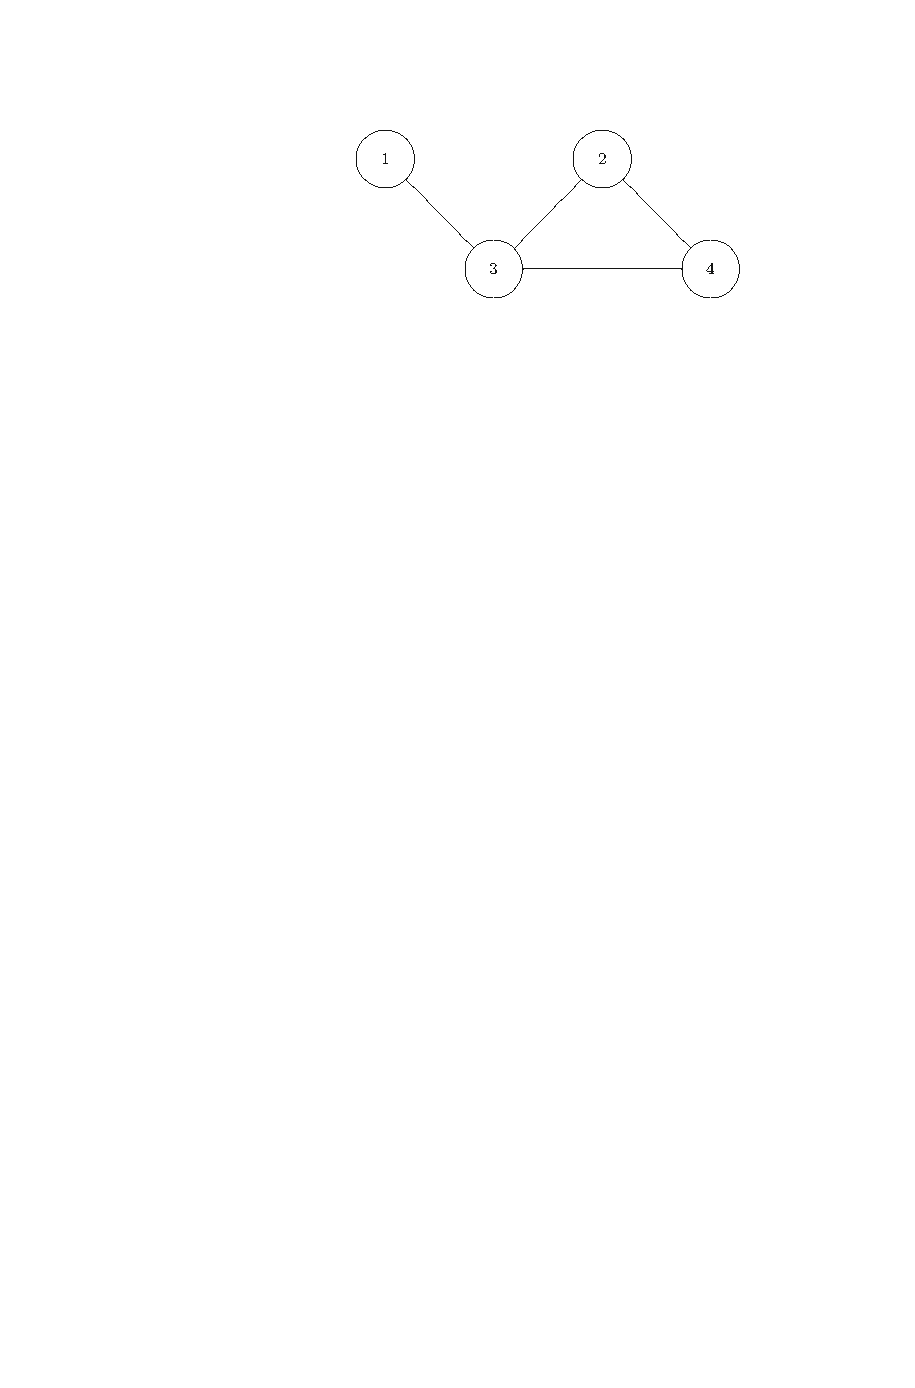
\includegraphics[width=0.35\textwidth]{pictures/graph.pdf}
\caption{An example of graph.}
\label{graph eg}
\end{figure}
\begin{example}
For the graph Figure~\ref{graph eg}, the adjacency matrix is
\[A=\begin{bmatrix}
0&0&1&0\\
0&0&1&1\\
1&1&0&1\\
0&1&1&0
\end{bmatrix}\]
\end{example}
Notice that the adjacency matrix is always symmetric and hence diagonalizable
with real eigenvalues by the spectral theorem for matrices. The set of eigenvalues of $A$ is called the \textbf{spectrum of the graph}; it does not depend on the ordering of the vertices. One can obtain important information from the eigenvalues, such as the number of spanning trees. Also, one can verify that $A^n_{ij}$ is the number of paths of length $n$ from $v_i$ to $v_j$.\par 
A natural source of graphs, known as Cayley graphs, comes from group theory.
Representation theory affords us a means to analyze the eigenvalues of Cayley
graphs, at least for abelian groups.
\begin{definition}[\textbf{Cayley graph}]
Let $G$ be a finite group. By a symmetric subset of $G$, we mean a subset $S\sub G$ such that:
\begin{itemize}
\item $1\notin S$.
\item $s\in S\iff s^{-1}\in S$.
\end{itemize}
If $S$ is a symmetric subset of $G$, then the Cayley graph of $G$ with respect to $S$ is the graph with vertex set $G$ and with an edge $\{g,h\}$ connecting $g$ and $h$ if $gh^{-1}\in S$, or equivalently $hg^{-1}\in S$.
\end{definition}
\begin{remark}
In this definition $S$ can be empty, in which case the Cayley graph has no edges. One can verify that the Cayley graph is connected $($any two vertices
can be connected by a path$)$ if and only if $S$ generates $G$.
\end{remark}
\begin{figure}[htbp]
\centering
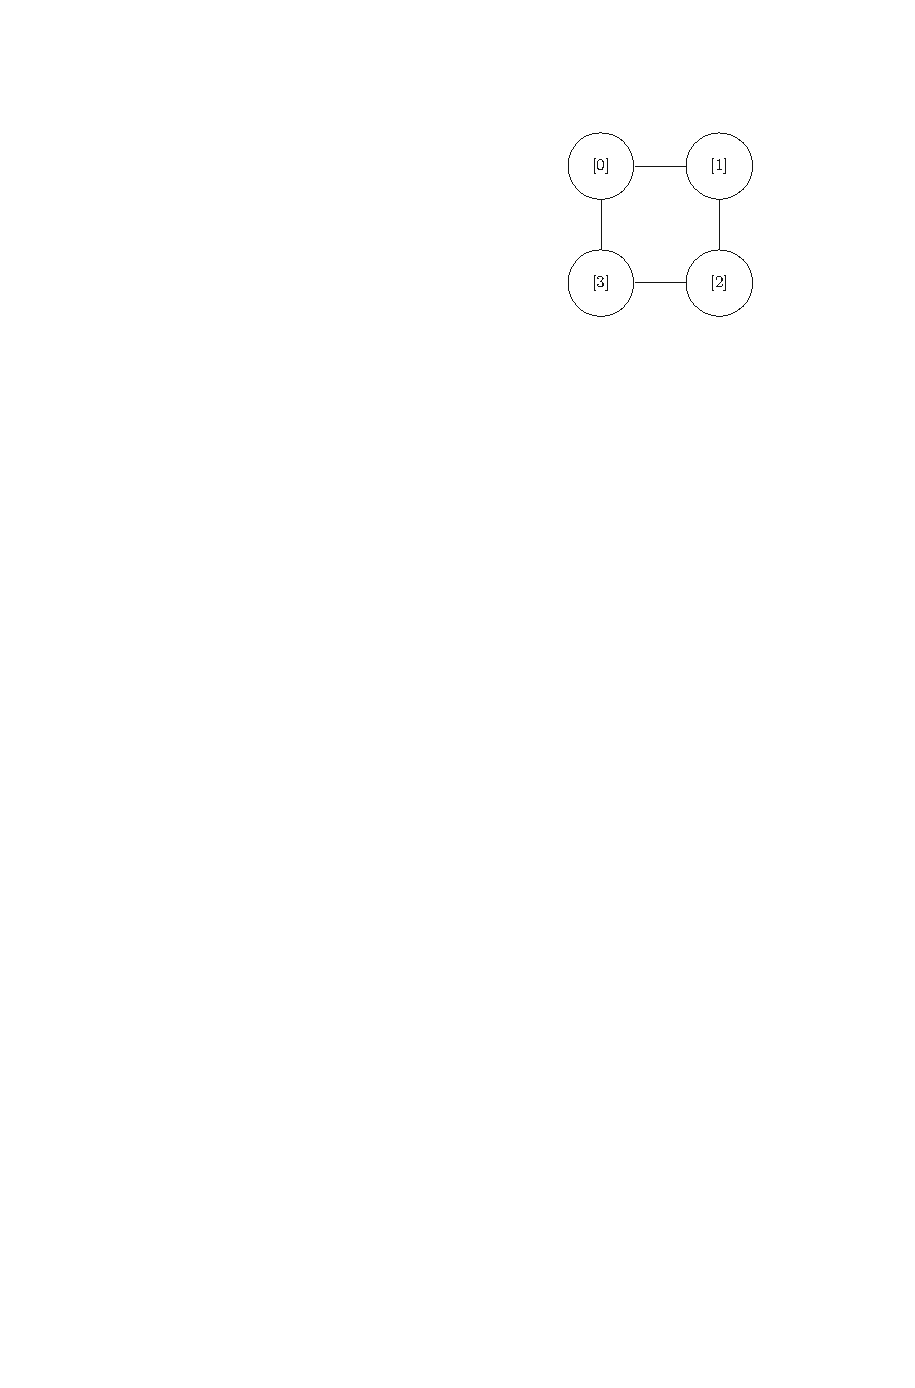
\includegraphics[width=0.25\textwidth]{pictures/Cayley-1.pdf}
\caption{The Cayley graph of $\Z/4\Z$ with respect to $\{\pm[1]\}$}
\label{Cayley graph eg-1}
\end{figure}
\begin{example}
Let $G=\Z/4\Z$ and $S=\{\pm[1]\}$. Then the Cayley graph of $G$ with respect to $S$ is drawn in Figure~\ref{Cayley graph eg-1}. The adjacency matrix of this Cayley graph is given by
\[A=\begin{bmatrix}
0&1&1&0\\
1&0&1&0\\
1&1&0&1\\
0&0&1&0
\end{bmatrix}\]
\end{example}
\begin{figure}[htbp]
\centering
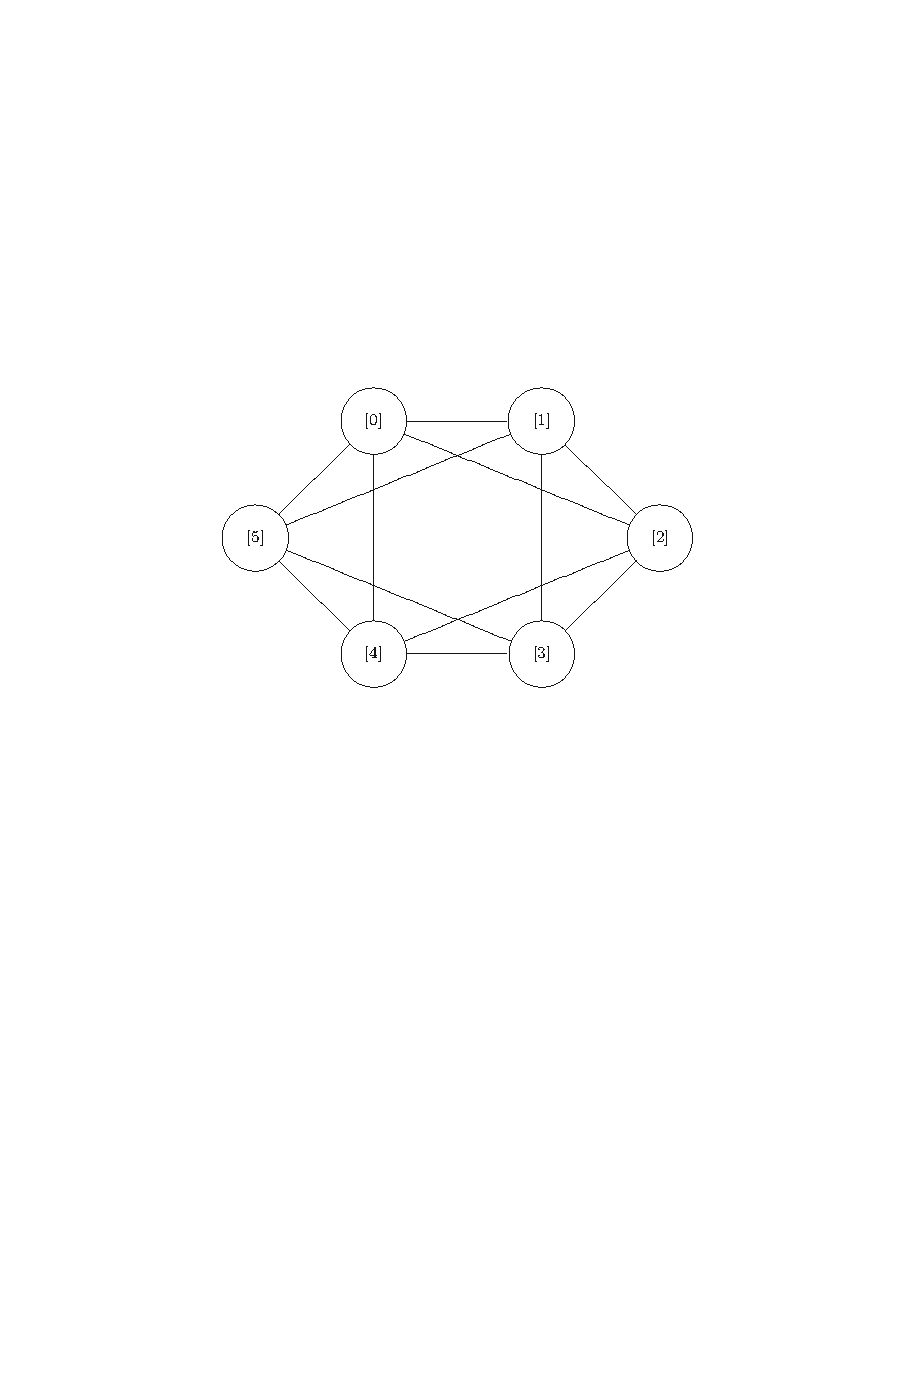
\includegraphics[width=0.45\textwidth]{pictures/Cayley-2.pdf}
\caption{The Cayley graph of $\Z/4\Z$ with respect to $\{\pm[1]\}$}
\label{Cayley graph eg-2}
\end{figure}
\begin{example}
In this example we take $G=\Z/6\Z$ and $S=\{\pm[1],\pm[2]\}$. The resulting Cayley graph can be found in Figure~\ref{Cayley graph eg-2}. The adjacency matrix of this graph is
\[A=\begin{bmatrix}
0&1&1&0&1&1\\
1&0&1&1&0&1\\
1&1&0&1&1&0\\
0&1&1&0&1&1\\
1&0&1&1&0&1\\
1&1&0&1&1&0\\
\end{bmatrix}\]
\end{example}
The graphs we have been considering are Cayley graphs of cyclic groups. Such
graphs have a special name.
\begin{definition}[\textbf{Circulant graph}]
A Cayley graph of $\Z/n\Z$ is called a \textbf{circulant graph} on $n$ vertices.
\end{definition}
The adjacency matrix of a circulant graph is an example of a special type of
matrix known as a circulant matrix.
\begin{definition}
An $n\times n$ circulant matrix is a matrix of the form
\[A=\begin{bmatrix}
a_0&a_1&\cdots&a_{n-2}&a_{n-1}\\
a_{n-1}&a_0&a_{1}&\cdots&a_{n-2}\\
\vdots&a_{n-1}&a_0&\ddots&\vdots\\
a_2&\vdots&\ddots&\ddots&a_{1}\\
a_1&a_2&\cdots&a_{n-1}&a_{0}\\
\end{bmatrix}\]
\end{definition}
Equivalently, a matrix $A$ is circulant if there exists a function $f:\Z/n
Z\to\C$ such that $A_{ij}=f([j]-[i])$. In the above form, one has $a_i=f([i])$ for $0\leq i\leq n-1$. If $S$ is a symmetric subset of $\Z/n\Z$, then the circulant matrix corresponding to the indicator functions $\delta_S$ of $S$ is the adjacency matrix of the Cayley graph of $\Z/n\Z$ with respect to $S$.\par
Our goal is to describe the eigenvalues of the Cayley graph of an abelian group. First we need a lemma about the group algebra $L(G)$.
\begin{lemma}\label{convolution eigen}
Let $G$ be an abelian group and $a\in L(G)$. Define the convolution operator $A:L(G)\to L(G)$ by $A(b)=a\ast b$. Then $A$ is linear and $\chi$ is an eigenvector of $A$ with eigenvalue $\widehat{a}(\chi)$ for all $\chi\in G^\vee$. Consequently, $A$ is a diagonalizable operator.
\end{lemma}
\begin{proof}
Using the distributivity of convolution over addition, it is easy to verify that $A$ is linear. Let $n=|G|$ and suppose that $\chi\in G^\vee$. Observe that
\[\widehat{a\ast\chi}=\ast{a}\cdot\widehat{\chi}=n\widehat{a}\delta_\chi\]
Clearly, one has that
\[(\widehat{a}\cdot n\delta_\chi)(\theta)=\begin{cases}
\widehat{a}(\theta)n&\chi=\theta\\
0&\text{otherwise}
\end{cases}\]
so we conclude
\[\widehat{a}\cdot n\delta_\chi=\widehat{a}(\chi)n\delta_\chi\]
Applying the inverse of the Fourier transform
to $\widehat{a\ast\chi}$ and using that $\widehat{\chi}=n\delta_\chi$, we obtain $a\ast\chi=\widehat{a}(\chi)\chi$, and so $\chi$ is an eigenvector of $A$ with eigenvalue $\widehat{a}(\chi)$.\par
Since $G$ is abelian, the elements of $G^\vee$ form an orthonormal basis of $L(G)$, it follows that $A$ is diagonalizable.
\end{proof}
Lemma~\ref{convolution eigen} is the key ingredient to computing the eigenvalues of the adjacency matrix of a Cayley graph of an abelian group. It only remains to realize the adjacency matrix as the matrix of a convolution operator.
\begin{theorem}
Let $G=\{g_1,\cdots,g_n\}$ be an abelian group and $S\sub G$ a symmetric set. Let $\chi_1,\cdots,\chi_n$ be the irreducible characters of $G$ and let $A$ be the adjacency matrix of the Cayley graph of $G$ with respect to $S$ $($using this ordering for the elements of $G)$. Then:
\begin{itemize}
\item[$(\rmnum{1})$]The eigenvalues of the adjacency matrix $A$ are the real numbers
\[\lambda_i=\sum_{s\in S}\chi_i(s)\]
where $1\leq i\leq n$.
\item[$(\rmnum{2})$]The corresponding orthonormal basis of eigenvectors is given by the vectors $\{v_1,\cdots,v_n\}$ where
\[v_i=\frac{1}{\sqrt{|G|}}(\chi_i(g_1),\cdots,\chi_i(g_n))^T\]
\end{itemize}
\end{theorem}
\begin{proof}
Let $G=\{g_1,\cdots,g_n\}$ and let $\delta_S=\sum_{s\in S}\delta_s$ be the characteristic (or indicator) function of $S$; so
\[\delta_S(x)=\begin{cases}
1&x\in S\\
0&x\notin S
\end{cases}\]
Let $F:L(G)\to L(G)$ be the convolution operator
\[F(b)=\delta_S\ast b\]
Lemma~\ref{convolution eigen} implies that the irreducible characters $\chi_i$ are eigenvectors of $F$ and that the corresponding eigenvalue is
\[\widehat{\delta_S}(\chi_i)=n\langle\delta_S,\chi_i\rangle=\sum_{x\in G}\delta_S(x)\widebar{\chi_i(x)}=\sum_{x\in S}\widebar{\chi_i(x)}\]
where the penultimate equality is obtained by putting $s=x^{-1}$ and using that degree one representations are unitary, whence $\chi_i(x^{-1})=\chi_i(x)$, and that $S$ is symmetric.\par
By the observation
\[\chi_i=\sum_{j=1}^{n}\chi_i(g_j)\delta_{g_j}\]
it follows that if $B$ is the basis $\{\delta_{g_1},\cdots,\delta_{g_n}\}$ for $L(G)$, then the matrix $[F]_B$ of $F$ with respect to this basis has eigenvalues $\lambda_1,\cdots,\lambda_n$ and eigenvectors $v_1,\cdots,v_n$.
The orthonormality of the $v_i$ follows from the orthonormality of the $\chi_i$:
\begin{align*}
\langle v_i,v_j\rangle&=\frac{1}{|G|}\sum_{k=1}^{n}\chi_i(g_k)\widebar{\chi_j(g_k)}=\langle\chi_i,\chi_j\rangle=\begin{cases}
1&i=j\\
0&i\neq j
\end{cases}
\end{align*}
Therefore, it remains to prove that $A=[F]_B$. To this end we compute
\[F(\delta_{g_j})=\delta_S\ast\delta_{g_j}=\sum_{s\in S}\delta_s\ast\delta_{g_j}=\sum_{s\in S}\delta_{sg_j}\]
Recalling that $([F]_B)_{ij}$ is the coefficient of $\delta_{g_j}$ in $F(\delta_{g_j})$, we conclude that
\begin{align*}
([F]_B)_{ij}&=\begin{cases}
1&sg_j=g_i\text{ for some $s\in S$}\\
0&\text{otherwise}
\end{cases}\\
&=\begin{cases}
1&g_ig_j^{-1}\in S\\
0&\text{otherwise}
\end{cases}\\
&=A_{ij}.
\end{align*}
as required.\par
Finally, to verify that $\lambda_i$ is real, we just observe that if $s\in S$, then either $s=s^{-1}$, and so $\chi_i(s)=\chi_i(s^{-1})=\widebar{\chi_i(s)}$ is real, or $s^{-1}\in S$ and $\chi(s)+\chi(s^{-1})=\chi(s)+\widebar{\chi(s)}$ is real.
\end{proof}
Specializing to the case of circulant matrices, we obtain:
\begin{corollary}
Let $A$ be a circulant matrix of degree $n$, which is the adjacency matrix of the Cayley graph of $\Z/n\Z$ with respect to the symmetric set $S$. Then the
eigenvalues of $A$ are
\[\lambda_k=\sum_{[m]\in S}e^{\frac{2\pi ikm}{n}}\]
where $k=0,\cdots,n-1$ and a corresponding basis of orthonormal eigenvectors is given by $v_0,\cdots,v_{n-1}$ where
\[v_k=\frac{1}{\sqrt{n}}(1,e^{\frac{2\pi ik 2}{n}},\cdots,e^{\frac{2\pi ik (n-1)}{n}})^T\]
\end{corollary}
\subsection{Fourier Analysis on Non-abelian Groups}
For a non-abelian group $G$, we have $L(G)\neq Z(L(G))$ and so $L(G)$ is a
non-commutative ring. Therefore, we cannot find a Fourier transform that turns
convolution into pointwise multiplication, as pointwise multiplication is commutative. Instead, we try to replace pointwise multiplication by matrix multiplication. To achieve this, let us first recast the abelian case in a different form.\par
Suppose that $G$ is a finite abelian group with irreducible characters $\chi_1,\cdots,\chi_n$. Then to each function $f:G\to\C$, we can associate its vector of Fourier coefficients. That is, we define $T:L(G)\to\C^n$ by
\[Tf=(n\langle f,\chi_1\rangle,\cdots,n\langle f,\chi_n\rangle)=(\widehat{f}(\chi_1),\cdots,\widehat{f}(\chi_n))\]
The map $T$ is injective by the Fourier inversion theorem because we can recover $\widehat{f}$, and hence $f$, from $Tf$. It is also linear and hence a vector space isomorphism since $\dim L(G)=n$. Now $\C^n$ has the structure of a direct product of rings where multiplication is taken coordinate-wise. The map $T$ is in fact a ring isomorphism since
\[T(a\ast b)=(\widehat{a\ast b}(\chi_1),\cdots,\widehat{a\ast b}(\chi_n))=(\widehat{a}(\chi_1)\widehat{b}(\chi_1),\cdots,\widehat{a}(\chi_n)\widehat{b}(\chi_n))=T(a)T(b)\]
Theorem~\ref{Convolution theorem} can thus be reinterpreted in the following way.
\begin{theorem}
Let $G$ be a finite abelian group of order $n$. Then $L(G)\cong\C^n$.
\end{theorem}
One might guess that this reflects the fact that all irreducible representations of an abelian group have degree one and that, for non-abelian groups, we must replace $\C$ by matrix rings over $\C$. This is indeed the case. So without further ado, let $G$ be a finite group of order $n$ with complete set $\varphi^{(1)},\cdots,\varphi^{(s)}$ of unitary representatives
of the equivalence classes of irreducible representations of $G$. As usual, we put $d_k=\deg\varphi^{(k)}$. The matrix coefficients are the functions $\varphi^{(k)}_{ij}:G\to\C$ given by $\varphi^{(k)}_g=\varphi^{(k)}_{ij}(g))$. Proposition~\ref{repre L(G) basis} tells us that the functions $\sqrt{d_k}\varphi^{(k)}_{ij}$ form an orthonormal basis for $L(G)$.
\begin{definition}[\textbf{Fourier transform}]
Define
\[T:L(G)\to\mathcal{M}_{d_1}(\C)\times\cdots\times\mathcal{M}_{d_k}(\C)\]
by $Tf=(\widehat{f}(\varphi^{(1)}),\cdots,\widehat{f}(\varphi^{(s)}))$ where
\[\widehat{f}(\varphi^{(k)})_{ij}=n\langle f,\varphi^{(k)}_{ij}\rangle=\sum_{g\in G}f(g)\widebar{\varphi^{(k)}_{ij}(g)}\]
We call $Tf$ the Fourier transform of $f$.
\end{definition}
Notice that $Tf$ can be written more succinctly in the form
\[\widehat{f}(\varphi^{(k)})=\sum_{g\in G}f(g)\widebar{\varphi^{(k)}(g)}\]
which is the form that we shall most frequently use.\par
Let us begin our study of non-abelian Fourier analysis with the Fourier inversion theorem.
\begin{theorem}
Let $f:G\to\C$ be a complex-valued function on $G$. Then
\[f=\frac{1}{n}\sum_{i,j,k}d_k\widehat{f}(\varphi^{(k)})\varphi^{(k)}_{ij}\]
where $n=|G|$.
\end{theorem}
\begin{proof}
We compute using the orthonormality of the $\sqrt{d_k}\varphi^{(k)}_{ij}$
\begin{align*}
f=\sum_{i,j,k}\langle f,\sqrt{d_k}\varphi^{(k)}_{ij}\rangle\sqrt{d_k}\varphi^{(k)}_{ij}=\frac{1}{n}\sum_{i,j,k}d_kn\langle f,\varphi^{(k)}_{ij}\rangle\varphi^{(k)}_{ij}=\frac{1}{n}\sum_{i,j,k}d_k\widehat{f}(\varphi^{(k)})_{ij}\varphi^{(k)}_{ij}
\end{align*}
\end{proof}
Next we show that $T$ is a vector space isomorphism.
\begin{theorem}
The map $T:L(G)\to\mathcal{M}_{d_1}(\C)\times\cdots\times\mathcal{M}_{d_s}(\C)$ is a vector space isomorphism.
\end{theorem}
\begin{proof}
It is easy to verify the map $T$ is linear. Since we have
\[\dim L(G)=d_1^2+\cdots+d_s^2=|G|\]
and $T$ is injective, we conclude it is an isomorphism.
\end{proof}
All the preparation has now been completed to show that the Fourier transform
is a ring isomorphism. This leads us to a special case of a more general theorem of Wedderburn that is often taken as the starting point for studying the representation theory of finite groups.
\begin{theorem}
The Fourier transform
\[T:L(G)\to\mathcal{M}_{d_1}(\C)\times\cdots\times\mathcal{M}_{d_k}(\C)\]
is an isomorphism of rings.
\end{theorem}
\begin{proof}
We have already showed $T$ is an isomorphism of vector spaces. Therefore, to show that it is a ring isomorphismit suffices to verify that $T(a\ast b)=Ta\cdot Tb$. In turn, by the definition of multiplication in a direct product, to do this it suffices to establish $\widehat{a\ast b}(\varphi^{(k)})=\widehat{a}(\varphi^{(k)})\cdot\widehat{b}(\varphi^{(k)})$ for $1\leq k\leq s$. The computation is analogous to the abelian case:
\begin{align*}
\widehat{a\ast b}(\varphi^{(k)})&=\sum_{x\in G}(a\ast b)(x)\widebar{\varphi^{(k)}(x)}=\sum_{x\in G}\widebar{\varphi^{(k)}(x)}\sum_{y\in G}a(xy^{-1})b(y)\\
&=\sum_{z\in G}\widebar{\varphi^{(k)}(zy)}\sum_{y\in G}a(z)b(y)\\
&=\sum_{z\in G}\sum_{y\in G}a(z)\widebar{\varphi^{(k)}(z)}b(y)\widebar{\varphi^{(k)}(y)}\\
&=\widehat{a}(\varphi^{(k)})\widehat{b}(\varphi^{(k)})
\end{align*}
This concludes the proof that $T$ is a ring isomorphism.
\end{proof}
\begin{remark}
Note that
\[\widehat{\delta_g}(\varphi^{(k)})=\sum_{x\in G}\delta_g(x)\widebar{\varphi^{(k)}(x)}=\widebar{\varphi^{(k)}(g)}\]
Since the conjugate of an irreducible representation is easily verified to be irreducible, it follows that $T\delta_g$ is a vector whose entries consist of the images of $g$ under all the irreducible representations of $G$, in some order.
\end{remark}
%
\chapter{Representation of Groups}
\section{Representations, Maschke's theorem, and semisimplicity}
\subsection{Definitions and examples}
Informally, a representation of a group is a collection of invertible linear transformations of a vector space (or, more generally, of a module for a ring) that multiply together in the same way as the group elements. The collection of linear transformations thus establishes a pattern of symmetry of the vector space, which copies the symmetry encoded by the group. Because symmetry is observed and understood so widely, and is even one of the fundamental notions of mathematics, there are applications of representation theory across the whole of mathematics as well as in other disciplines.\par
For many applications, especially those having to do with the natural world, it is appropriate to consider representations over fields of characteristic zero such as $\C$, $\R$, or $\Q$. In other situations that might arise in topology or combinatorics or number theory, for instance, we find ourselves considering representations over fields of positive characteristic, such as the field with $p$ elements $\F_p$, or over rings that are not fields, such as the ring of integers $\Z$. Many aspects of representation theory do change as the ring varies, but there are also parts of the theory that are similar regardless of the field characteristic or even if the ring is not a field. We develop the theory independently of the choice of ring where possible so as to be able to apply it in all situations and to establish a natural context for the results.\par
Let $G$ denote a \textit{finite} group, and let $R$ be a commutative ring. If $V$ is an $R$-module, we denote it by $\GL(V)$ the group of all invertible $R$-module homomorphisms $V\to V$. In case, $V\cong R^n$ is a free module of rank $n$, this group is isomorphic to the group of all nonsingular $n\times n$ matrices over $R$, and we denote it by $\GL(n,R)$ or $\GL_n(R)$, or in case $R=\F_q$ is the finite field with $q$ elements by $\GL(n,q)$ or $\GL_n(q)$. We point out also that unless otherwise stated, modules will be left modules and morphisms will be composed reading from right to left so that matrices in $\GL(n,R)$ are thought of as acting from the left on column vectors.\par
A (\textbf{linear}) \textbf{representation} of $G$ (over $R$) is a group homomorphism
\[\rho:G\to\GL(V)\]
In a situation where $V$ is free as an $R$-module, on taking a basis for $V$, we may write each element of $\GL(V)$ as a matrix with entries in $R$, and we obtain for each $g\in G$ a matrix $\rho(g)$. These matrices multiply together in the manner of the group, and we have a \textbf{matrix representation} of $G$. In this situation, the rank of the free $R$-module $V$ is called the degree of the representation. Sometimes, by abuse of terminology, the module $V$ is also called the representation, but it is more properly called the \textbf{representation module} or \textbf{representation space} (if $R$ is a field).
\begin{example}
For any group $G$ and commutative ring $R$, we can take $V=R$ and $\rho(g)=1$ for all $g\in G$, where $1$ denotes the identify map $R\to R$. This representation is called the \textbf{trivial representation}, and it is often denoted simply by its representation module $R$. Although this representation turns out to be extremely important in the theory, it does not at this point give much insight into the nature of a representation.
\end{example}
\begin{example}
A representation on a space $V=R$ of rank $1$ is in general determined by specifying a homomorphism $G\to R^*$. Here $R^*$ is the group of units of $R$, and it is isomorphic to $\GL(V)$. For example, if $G=\langle g\rangle$ is cyclic of order $n$ and $k=\C$ is the field of complex numbers, there are $n$ possible such homomorphisms, determined by $g\mapsto e^{2k\pi i/n}$ where $0\leq k\leq n-1$. Another important example of a degree $1$ representation is the sign representation of the symmetric group $\mathfrak{S}_n$ on $n$ symbols, given by the group homomorphism that assigns to each permutation its sign, regarded as an element of the arbitrary ring $R$.
\end{example}
\begin{example}\label{representation of S_3 eg}
Let $R=\R$, $V=\R^2$, and $G=\mathfrak{S}_3$. This group $G$ is isomorphic to the group of symmetries of an equilateral triangle. The symmetries are the three reflections in the lines that bisect the equilateral triangle, together with three rotations:
\[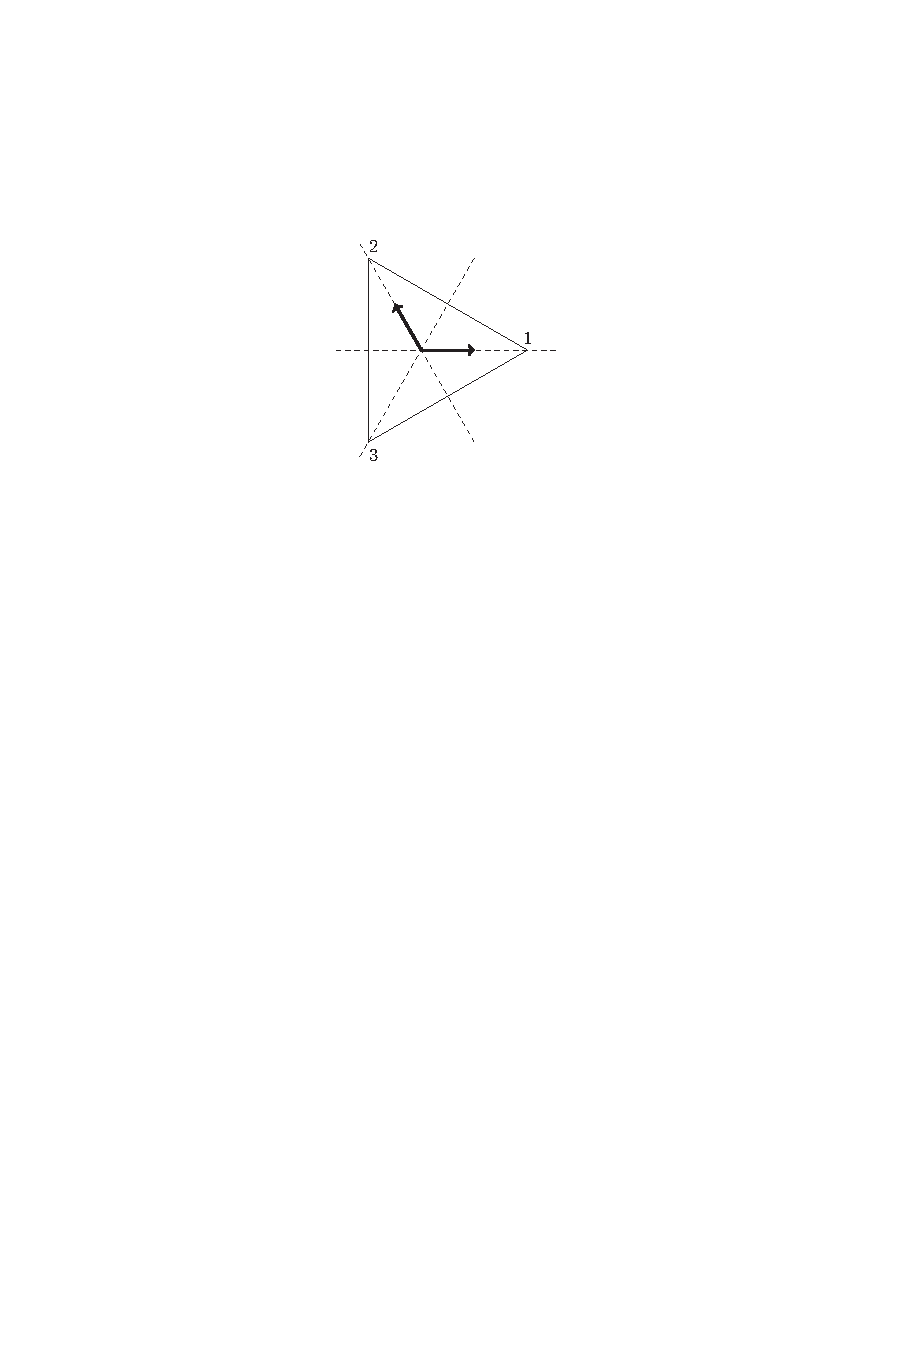
\includegraphics{pictures/rep-of-S_3-dim2}\]
Positioning the center of the triangle at the origin of $V$ and labeling the three vertices of the triangle as $1$, $2$, and $3$, we get a representation
\[\begin{array}{c}

(1,2)\mapsto\begin{pmatrix}
0&1\\
1&0
\end{pmatrix}\quad (23)\mapsto\begin{pmatrix}
-1&0\\
-1&1
\end{pmatrix}\quad (13)\mapsto\begin{pmatrix}
1&-1\\
0&-1
\end{pmatrix}\\
(123)\mapsto\begin{pmatrix}
0&-1\\
1&-1
\end{pmatrix}\quad(132)\mapsto\begin{pmatrix}
-1&1\\
-1&0
\end{pmatrix}
\end{array}\]
where we have taken basis vectors in the directions of vertices $1$ and $2$, making an angle of $2\pi/3$ to each other. In fact these matrices define a representation of degree $2$ over any ring $R$, because although the representation was initially constructed over $\R$ the matrices have integer entries, and these may be interpreted in every ring. No matter what the ring is, the matrices always multiply together to give a copy of $\mathfrak{S}_3$.
\end{example}
\begin{example}\label{representation C_p on F_p eg}
Let $R=\F_p$, $V=R^2$, and let $G=C_p=\langle g\rangle$ be cyclic of order $p$ generated by an element $g$. We see that the assignment
\[\rho(g^r)=\begin{pmatrix}
1&0\\
r&1
\end{pmatrix}\]
is a representation. In this case, the fact that we have a representation is very much dependent on the choice of $R$ as the field $\F_p$: in any other characteristic it would not work, because the matrix shown would no longer have order $p$.
\end{example}
We can think of representations in various ways. One of them is that a representation is the specification of an action of a group on an $R$-module, as we now explain. Given a representation $\rho:G\to GL(V)$, an element $v\in V$, and a group element $g\in G$, we get another module element $\rho(g)(v)$. Sometimes we write just $g\cdot v$ or $gv$ for this element. This rule for multiplication satisfies
\begin{align*}
g\cdot(av+bw)&=ag\cdot v+bg\cdot w,\\
(gh)\cdot v&=g\cdot(h\cdot v),\\
1\cdot v&=v
\end{align*}
for all $g\in G$, $v,w\in V$, and $a,b\in R$. A rule for multiplication $G\times V\to V$ satisfying these conditions is called a \textbf{linear action} of $G$ on $V$. To specify a linear action of $G$ on $V$ is the same thing as specifying a representation of $G$ on $V$, since given a representation, we obtain a linear action as indicated earlier, and evidently, given a linear action, we may recover the representation.\par
Another way to define a representation of a group is in terms of the group
algebra. We define the group algebra $R[G]$ (or $R[G]$) of $G$ over $R$ to be the free $R$-module with the elements of $G$ as an $R$-basis and with multiplication given on the basis elements by group multiplication. The elements of $R[G]$ are the (formal) $R$-linear combinations of group elements, and the multiplication of the basis elements is extended to arbitrary elements using bilinearity of the operation. What this means is that a typical element of $R[G]$ is an expression $\sum_{g\in G}a_gg$ where $a_g\in R$, and the multiplication of these elements is given symbolically by
\[\Big(\sum_{g\in G}a_gg\Big)\Big(\sum_{h\in G}b_hh\Big)=\sum_{k\in G}\Big(\sum_{gh=k}a_gb_h\Big)k.\]
Having defined the group algebra, we may now define a representation of $G$ over $R$ to be a $R[G]$-module. The fact that this definition coincides with the previous ones is the content of the next proposition. Throughout this text, we may refer to group representations as modules (for the group algebra).
\begin{proposition}
A representation of $G$ over $R$ has the structure of a $R[G]$-module. Conversely, every $R[G]$-module provides a representation of $G$ over $R$.
\end{proposition}
\begin{proof}
Given a representation $\rho:G\to\GL(V)$, we define a module action of $R[G]$ on $V$ by $(\sum a_gg)v=\sum a_g\rho(g)(v)$. Given an $R[G]$-module $V$, the linear map $\rho(g):v\mapsto g\cdot v$ is an automorphism of $V$ and $\rho(g_1)\rho(g_2)=\rho(g_1g_2)$ so $\rho:G\mapsto\GL(V)$ is a representation.
\end{proof}
The group algebra gives another example of a representation, called the \textbf{regular representation}. In fact, for any ring $A$, we may regard $A$ itself as a left $A$-module with the action of $A$ on itself given by multiplication of the elements. We denote this left $A$-module by $_{A}A$ when we wish to emphasize the module structure, and this is the (left) regular representation of $A$. When $A=R[G]$, we may describe the action on $R[G]$ by observing that each element $g\in G$ acts on $R[G]$ by permuting the basis elements in the fashion $g\cdot h=gh$. Thus, each $g$ acts by a permutation matrix. The regular representation is an example of a \textbf{permutation representation}, namely one in which every group element acts by a permutation matrix.\par
Regarding representations of $G$ as $R[G]$-modules has the advantage that many definitions we wish to make may be borrowed from module theory. Thus, we may study $R[G]$-submodules of an $R[G]$-module $V$, and if we wish, we may call them subrepresentations of the representation afforded by $V$. To specify an $R[G]$-submodule of $V$, it is necessary to specify an $R$-submodule $W$ of $V$ that is closed under the action of $R[G]$. This is equivalent to requiring that $\rho(g)w\in W$ for all $g\in G$ and $w\in W$. We say that a submodule $W$ satisfying this condition is \textbf{stable} under $G$ or that it is an \textbf{invariant submodule} or \textbf{invariant subspace} (if $R$ happens to be a field). Such an invariant submodule $W$ gives rise to a homomorphism $\rho_W:G\to\GL(W)$ that is the subrepresentation afforded by $W$.
\begin{example}\label{representation of C_2 semisimple}
Let $C_2=\{1,-1\}$ be cyclic of order $2$ and consider the representation
\[\rho:C_2\to\GL_2(\R),\quad 1\mapsto\begin{pmatrix}
1&0\\
0&1
\end{pmatrix},\quad -1\mapsto\begin{pmatrix}
1&0\\
0&-1
\end{pmatrix}\]
There are just four invariant subspaces, namely $\{0\}$, $\langle(\begin{smallmatrix}1\\0\end{smallmatrix})\rangle$, $\langle(\begin{smallmatrix}0\\1\end{smallmatrix})\rangle$, $\R^2$ and no others. The representation space $\R^2=\langle(\begin{smallmatrix}1\\0\end{smallmatrix})\rangle\oplus\langle(\begin{smallmatrix}0\\1\end{smallmatrix})\rangle$ is the direct sum of two invariant subspaces.
\end{example}
\begin{example}\label{representation of C_p on F_p non semisimple}
In Example~\ref{representation C_p on F_p eg}, an elementary calculation shows that $\langle(\begin{smallmatrix}0\\1\end{smallmatrix})\rangle$ is the only $1$-dimensional invariant subspace, and so it is not possible to write the representation space $V$ as the direct sum of two nonzero invariant subspaces.
\end{example}
We make use of the notions of a homomorphism and an isomorphism of $R[G]$-modules. Since $R[G]$ has as a basis the elements of $G$, to check that an $R$-linear homomorphism $f:V\to W$ is in fact a homomorphism of $R[G]$-modules, it suffices to check that $f(gv)=gf(v)$ for all $g\in G$---we do not need to check for every $x\in R[G]$. By means of the identification of $R[G]$-modules with representations of $G$ (in the first definition given here) we may refer to homomorphisms and isomorphisms of group representations.\par
If $V$ and $W$ are $R[G]$-modules then we may form their (external) direct sum
$V\oplus W$, which is the same as the direct sum of $V$ and $W$ as $R$-modules together with an action of $G$ given by $g(v,w)=(gv,gw)$. We also have the notion of the internal direct sum of $R[G]$-modules and write $U=V\oplus W$ to mean that $U$ has $R[G]$-submodules $V$ and $W$ satisfying $U=V+W$ and $V\cap W=0$. In this situation, we also say that $V$ and $W$ are direct summands of $U$.
\subsection{Semisimple representations}
We come now to our first nontrivial result, one that is fundamental to the study of representations over fields of characteristic zero, or characteristic not dividing the group order. This surprising result says that in this situation representations always break apart as direct sums of smaller representations. We do now require the ring $R$ to be a field, and in this situation, we will often use the symbols $F$ or $k$ instead of $R$.
\begin{theorem}[\textbf{Maschke}]
Let $V$ be a representation of the finite group $G$ over a field $k$ in which $|G|$ is invertible. Let $W$ be an invariant subspace of $V$. Then there exists an invariant subspace $W'$ of $V$ such that $V=W\oplus W'$ as
representations.
\end{theorem}
\begin{proof}
Let $\pi:V\to W$ be any projection of $V$ onto $W$ as vector spaces. Since $k$ is a field, we may always find such a projection by finding a vector space complement to $W$ in $V$ and projecting off the complementary factor. Then $V=W\oplus\ker(\pi)$ as vector spaces, but $\ker(\pi)$ is not necessarily invariant under $G$. Consider the map $\widetilde{\pi}:V\to V$ defined by
\[\widetilde{\pi}=\frac{1}{|G|}\sum_{g\in G}g\pi g^{-1}.\]
Then $\widetilde{\pi}$ is $k$-linear, and if $w\in W$ then
\begin{align*}
\widetilde{\pi}(w)=\frac{1}{|G|}\sum_{g\in G}g\pi(g^{-1} w)=\frac{1}{|G|}\sum_{g\in G}gg^{-1}w=w.
\end{align*}
Since furthermore $\widetilde{\pi}(v)\in W$ for all $v\in V$, $\widetilde{\pi}$ is a projection onto $W$ and so $V=W\oplus\ker(\widetilde{\pi})$. We show finally that $\ker(\widetilde{\pi})$ is an invariant subspace by verifying that $\widetilde{\pi}$ is an $kG$-module homomorphism: if $h\in G$ and $v\in V$ then
\begin{align*}
\widetilde{\pi}(hv)=\frac{1}{|G|}\sum_{g\in G}g\pi g^{-1}(hv)=h\frac{1}{|G|}\sum_{g\in G}h^{-1}g\pi g^{-1}h(v)=h\widetilde{\pi}(v).
\end{align*}
This finishes the proof.
\end{proof}
Because the next results apply more generally than to group representations,
we let $A$ be a ring and consider its modules. A nonzero $A$-module $V$ is
said to be \textbf{simple} or \textbf{irreducible} if $V$ has no $A$-submodules other than $0$ and $V$.
\begin{example}
When $A$ is an algebra over a field, every module of dimension $1$ is simple. In Example~\ref{representation of S_3 eg}, we have constructed three representations of $\R\mathfrak{S}_3$, and they are all simple. The trivial and sign representations are simple because they have dimension $1$, and the $2$-dimensional representation is simple because, visibly, no $1$-dimensional subspace is invariant under the group action. We will see later that this is a complete list of the simple representations of $\mathfrak{S}_3$ over $\R$.
\end{example}
\begin{proposition}\label{simple module is cyclic}
Let $S$ be a simple $A$-module, then there exists a maximal left ideal $I$ in $A$ such that $S\cong A/I$.
\end{proposition}
\begin{proof}
Let $x\in S$ be nonzero. Then the map $\varphi:a\mapsto ax$ is a nonzero homomorphism, and hence is surjective due the simplicity of $S$. This implies $S\cong A/I$ where $I=\ker\varphi$ is a left ideal. Moreover, if $I$ is not maximal, then $A/I$ contains a nontrivial left ideal, and hence is not simple. This is a contradiction.
\end{proof}
A module that is the direct sum of simple submodules is said to be \textbf{semisimple} or \textbf{completely reducible}. We saw in Examples~\ref{representation of C_2 semisimple} and \ref{representation of C_p on F_p non semisimple} two examples of modules, one of which was semisimple and the other of which was not.
\begin{lemma}\label{semisimple simple submodule}
If $M\neq 0$ and $M$ is semisimple, then it has a simple submodule.
\end{lemma}
\begin{proof}
Let $x\in M-\{0\}$, and set $M'=Ax$. Then $M'$ is semisimple and nonzero, so we may assume that $M=M'$.\par
Set
\[\mathcal{X}=\{\text{$N$ is a submodule of $M$ and $x\notin N$}\}.\]
This set is nonempty because it contains the zero submodule. If $\mathcal{Y}\sub \mathcal{X}$ is totally ordered, then $N=\bigcup_{N'\in \mathcal{Y}}N'$ is a submodule of $M$. Also, $x\notin N$ by definition of $N$, so $N$ is an element of $\mathcal{X}$, and an upper bound of $\mathcal{Y}$. By Zorn's lemma, $\mathcal{X}$ has a maximal element $N$.\par
As $x\notin N$, $N\neq M$. As $M$ is semisimple, there exists a submodule $N'$ of $M$ such that $M=N\oplus N'$, and we have $N'\neq 0$ because $N\neq M$. We claim that $N'$ is simple. Indeed, if there were a submodule $0\neq N''\sub N'$, then we would have $N\oplus N''\notin\mathcal{X}$ by maximality of $N$ in $X$, so $x\in N\oplus N''$, but then $N\oplus N''=M$ (because $M=Ax$), and hence $N''=N'$.
\end{proof}
\begin{theorem}\label{semisimple module iff}
Let $A$ be a ring and $M$ be a $A$-module. The following are equivalent:
\begin{itemize}
\item[(\rmnum{1})] $M$ is semisimple.
\item[(\rmnum{2})] $M$ is a direct sum of simple modules.
\item[(\rmnum{3})] $M$ is a sum of simple modules.
\end{itemize}
\end{theorem}
\begin{proof}
Assume that $M$ is semisimple. Let $M'$ be the sum of all the simple submodules of $M$, and choose a submodule $M''$ of $M$ such that $M=M'\oplus M''$. If $M''\neq 0$, then by the lemma $M''$ has a simple submodule $N$, but then we should have $N\sub M'$, which contradicts the fact that $M'$ and $M''$ are in direct sum. So $M'=M$. This proves $(\rmnum{1})\Rightarrow(\rmnum{2})$.\par
Now let $(M_i)_{i\in I}$ be the family of all simple submodules of $M$ and assume that $M=\sum_{i\in I}M_i$. Let $N$ be a submodule of $M$. We will show that there exists $J\sub I$ such that
\[M=N\oplus\bigoplus_{j\in J}M_j\]
This clearly implies $(\rmnum{1})$, and we also get $(\rmnum{2})$ by taking $N=0$.\par
To get $J$, we apply the Zorn's lemma. Set
\[\mathcal{X}=\{K\sub I\mid\text{$N+\sum_{k\in K}M_k$ is a direct sum}\}.\]
This set $\mathcal{X}$ is not empty, because $\emp\in\mathcal{X}$. Let $\mathcal{Y}\sub\mathcal{X}$ be a totally ordered subset and let $K=\bigcup\mathcal{Y}$. If there are $n\in N$ and $m_{i}\in\bigcup_{k\in K}M_{k},i=1,\dots,n$ such that $n+\sum_{i=1}^{n}m_{k_i}=0$, then since $\mathcal{Y}$ is totally ordered, there exists $L\in\mathcal{Y}$ such that $k_1,\dots,k_n\in\bigcup_{k\in L}M_k$. Since $L\in\mathcal{X}$, the fact $n+\sum_{i=1}^{n}m_{i}=0$ implies that $n=0$ and $m_i=0$ for every $i=1,\dots,n$. Therefore $N+\sum_{k\in K}M_k$ is a direct sum and $K\in\mathcal{X}$.\par
By Zorn's lemma, $\mathcal{X}$ has a maximal element $J$. Let $M'=N\oplus\bigoplus_{j\in J}M_j$. We will show that $M=M'$. Let $i\in I$, if $M_i\nsubseteq M'$, then $M'\cap M_i=0$ since $M_i$ is simple. But then
\[M'+M_i=N\oplus\bigoplus_{j\in J}M_j+M_i\]
is a direct sum. This means $J\cup\{i\}\in\mathcal{X}$, and contradicts the maximality of $J$.
\end{proof}
\begin{corollary}
Let $k$ be a field in which $|G|$ is invertible. Then every finite-dimensional $kG$-module is semisimple.
\end{corollary}
This result puts us in very good shape if we want to know about the representations of a finite group over a field in which $|G|$ is invertible---for example any field of characteristic zero. To obtain a description of all possible finite-dimensional representations, we need only describe the simple ones, and then arbitrary ones are direct sums of these.\par
\begin{proposition}
Let $A$ be a ring and $M$ be an $A$-module.
\begin{itemize}
\item[(a)] The sum of all the simple submodules of $M$ is a semisimple module, that is the unique largest semisimple submodule of $M$.
\item[(b)] The sum of all submodules of $M$ isomorphic to some given simple module $S$ is a submodule isomorphic to a direct sum of copies of $S$. It is the unique largest submodule of $S$ with this property.
\end{itemize}
\end{proposition}
\begin{proof}
For (a), the sum of all simple submodules of $M$ is semisimple by Theorem~\ref{semisimple module iff}, and since any semisimple submodule of $M$ is a sum of simple modules, this is clearly the largest one. A similar argument proves (b).
\end{proof}
The largest semisimple submodule of a module $M$ is called the \textbf{socle of $\bm{M}$}, and is denoted $\Soc(M)$. There is a dual construction called the \textbf{radical of $\bm{M}$}, denoted $\Rad(M)$, that we will study later. It is defined to be the intersection of all the maximal submodules of $M$, and has the property that it is the smallest submodule of $M$ with semisimple quotient.
\begin{proposition}\label{direct sum of simple module summand char}
Let $M=\bigoplus_{i=1}^{r}S_i^{n_i}$ be a semisimple module over a ring $A$, where the $S_i$ are nonisomorphic simple $A$-modules and the $n_i$ are their multiplicities as summands of $M$. Then each submodule $S_i^{n_i}$ is uniquely determined and is characterized as the unique largest submodule of $M$ expressible as a direct sum of copies of $S_i$.
\end{proposition}
\begin{proof}
It suffices to show that $S_i^{n_i}$ contains every submodule of $M$ isomorphic to $S_i$. If $N$ is any nonzero submodule of $M$ not contained in $S_i^{n_i}$, then for some $j\neq i$, its projection to a summand $S_j$ must be nonzero. If we assume that $N$ is simple, this projection will be an isomorphism $N\cong S_i$. Thus, all simple submodules isomorphic to $S_i$ are contained in the summand $S_i^{n_i}$.
\end{proof}
Now we give some nonsemisimple representations and compute their scoles.
\begin{example}
Let $K_4=\{1,x,y,xy\}$ be the Klein four-group, $R=\F_2$, and consider the representation $\rho_1$ on $V=(\F_2)^3$ specified on the generators of $G$ by
\[\rho_1(x)\cdot(a,b,c)=(a+b,b,c),\quad\rho_1(y)(a,b,c)=(a+c,b,c).\]
From these expressions, we immediately see that $V_1=\langle e_1\rangle$ is the unique invariant subspace of dimension $1$. Now assume that $W$ is an invariant subspace of dimension $2$. If $(a,b,c)\in W$ is an nonzero element, then we have
\[\rho_1(x)\cdot(a,b,c)-(a,b,c)=(b,0,0)\in V_1,\quad \rho_1(y)(a,b,c)-(a,b,c)=(c,0,0)\in V_1.\]
This implies any invariant subsapce of $\rho_1$ contains $V_1$, and so $V_1$ is the only irreducible subrepresentation of $\rho_1$. Therefore, the scole of $\rho_1$ is given by $V_1=\langle e_1\rangle$, with trivial action on it.\par
Now we consider another representation $\rho_2$ of $G$ on the same space given by
\[\rho_2(x)(a,b,c)=(a,b+c,c),\quad \rho_2(y)(a,b,c)=(a+c,b,c).\]
Therefore, it can be easily seen that $V_1=\langle e_1\rangle$ and $V_2=\langle(0,1,0)\rangle$ are both invariant subsapces of $\rho_2$. Note that if $(a,b,c)\in V$ with $c\neq 0$, then
\[\rho_2(x)(a,b,c)-(a,b,c)=(0,c,0)\in V_2,\quad\rho_2(y)(a,b,c)-(a,b,c)=(c,0,0)\in V_1.\]
This implies $V_1$ and $V_2$ are the only irreducible subrepresentation of $\rho_2$, and therefore the scole of $\rho_2$ is given by $V_1\oplus V_2$, with trivial action on it.
\end{example}
\begin{example}\label{representation of C_p on F_p}
Let $G=C_p=\langle x\rangle$ and $R=\F_p$ for some prime $p\geq 3$. Consider the two representations $\rho_1$ and $\rho_2$ specified by
\[\rho_1(x)=\begin{pmatrix}
1&1&0\\
0&1&1\\
0&0&1
\end{pmatrix}\quad\rho_2(x)=\begin{pmatrix}
1&1&1\\
0&1&0\\
0&0&1
\end{pmatrix}\]
and $V$ has a basis $\{e_1,e_2,e_3\}$. For $\rho_1$, it can be easily verified that $\langle e_1\rangle$ and $\langle e_1,e_2\rangle$ are invariant subspaces of $\rho_1$. Since $\langle e_1\rangle$ is the unique invariant subspace of one dimensional, it follows that the scole of $\rho_1$ is $\langle e_1\rangle$.\par
Similarly, it can be easily shown that $\langle e_1\rangle$ and $\langle e_2-e_3\rangle$ are invariant subspaces of $\rho_2$, and so the scole of $\rho_2$ is $\langle e_1\rangle\oplus\langle e_2-e_3\rangle$. Note that in this case we have a decomposition $V=\langle e_1,e_2\rangle\oplus\langle e_2-e_3\rangle$.
\end{example}
\begin{example}\label{representation of C_2 times C_2 char=2}
Let $k$ be an infinite field of characteristic $2$, and $G=\langle x,y\rangle\cong C_2\times C_2$ be the noncyclic group of order $4$. For each $\lambda\in k$, let $V_\lambda$ be a $k$-vector space of dimension $2$ with basis $\{e_1,e_2\}$, and $\rho_\lambda$ be the representation defined by
\[\rho_\lambda(x)=\begin{pmatrix}
1&0\\
1&1
\end{pmatrix}\quad\rho_\lambda(y)=\begin{pmatrix}
1&0\\
\lambda&1
\end{pmatrix}\]
Clearly $\langle e_1\rangle$ is the unique invariant subspace of $V_\lambda$, so the scole is given by $\Soc(V_\lambda)=\langle e_1\rangle$. By Schur lemma, if $\varphi:V_\lambda\to V_\mu$, we must have $\varphi(\Soc(V_\lambda))=\Soc(V_{\mu})$, and therefore $\varphi$ has the form
\[\varphi=\begin{pmatrix}
a&0\\
b&c
\end{pmatrix}\]
By a computation of the linear condition on $\varphi$, we get $\lambda=\mu$. Therefore $V_{\lambda}=V_{\mu}$ if and only if $\lambda=\mu$. This implies in particular that $kG$ has infinitely many nonisomorphic $2$-dimensional representations.
\end{example}
\subsection{Schur's lemma and Wedderburn's theorem}
Possibly the most important single technique in representation theory is to consider endomorphism rings. It is the main technique of this part, and we will see it in use throughout this chapter. The first result is basic and will be used time and time again.
\begin{theorem}[\textbf{Schur's lemma}]
Let $A$ be a ring and let $M$ and $N$ be $A$-modules, and $\varphi:M\to N$ be a $A$-linear map.
\begin{itemize}
\item If $M$ is simple, then $\varphi=0$ or $\varphi$ is injective.
\item If $N$ is simple, then $\varphi=0$ or $\varphi$ is surjective.
\item If $M$ and $N$ are simple, then $\varphi=0$ or $\varphi$ is an isomorphism.
\end{itemize}
In particular, if $M$ is a simple $A$-module, then $\End_A(M)$ is a division ring.
\end{theorem}
\begin{proof}
Since $\ker\varphi$ and $\im\varphi$ are both submodules, these claims follow from the definition of simplicity.
\end{proof}
\begin{corollary}\label{endomorphism of simple module scalar}
Let $A$ be a finite-dimensional algebra over an algebraically closed field $k$, and $S$ be a simple $A$-module. Then every endomorphism in $\End_A(S)$ is multiplication by some scalar. Thus, $\End_A(S)\cong k$ in this case.
\end{corollary}
\begin{proof}
If $A$ is a finite-dimensional $k$-algebra and $k$ is algebraically closed then $S$ is a finite-dimensional vector space by Proposition~\ref{simple module is cyclic}. Let $\varphi$ be an $A$-module endomorphism of $S$ and let $\lambda$ be an eigenvalue of $\varphi$. Now $(\varphi-\lambda I):S\to S$ is a singular endomorphism of $A$-modules, so $\varphi-\lambda I=0$ and $\varphi=\lambda I$.
\end{proof}
We have seen in Maschke's theorem that if $k$ is a field and $|G|$ is invertible then every $kG$-module is semisimple. We now consider the exact condition under which all modules are semisimple. It has the following description.
\begin{theorem}\label{semisimple ring iff}
Let $A$ be a ring. The following are equivalent:
\begin{itemize}
\item[(\rmnum{1})] All short exact sequences of $A$-modules split.
\item[(\rmnum{2})] All $A$-modules are semisimple.
\item[(\rmnum{3})] All finitely generated $A$-modules are semisimple.
\item[(\rmnum{4})] All cyclic $A$-modules are semisimple.
\item[(\rmnum{5})] The left regular $A$-module $_{A}A$ is semisimple.
\end{itemize}
If these conditions are satisfied, then we say that the ring $A$ is \textbf{semisimple}.
\end{theorem}
A priori, this notion should be called \textbf{left semisimple ring}, and we should have a similarly defined notion of \textbf{right semisimple ring}. But we will see that left semisimple and right semisimple are actually equivalent, so we just use the name semisimple ring.
\begin{proof}
The condition $(\rmnum{1})$ is easily seen to be equivalent to $(\rmnum{2})$ from the definition of semisimple modules, and the implications $(\rmnum{2})\Rightarrow(\rmnum{3})\Rightarrow(\rmnum{4})\Rightarrow(\rmnum{5})$ are obvious. Now we prove $(\rmnum{5})\Rightarrow(\rmnum{2})$. Let $M$ be a $A$-module. If $x\in M$, then $Ax\sub M$ is a quotient of $_{A}A$, so it's semisimple because $_{A}A$ is semisimple. As $M=\sum_{x\in M}Ax$, Theorem~\ref{semisimple module iff} implies that $M$ is semisimple.
\end{proof}
The next result is the main tool in recovering the structure of an algebra from its representations, which will be used in our structural theorem of semisimple rings. We use the notation $A^{op}$ to denote the opposite ring of $A$, namely, the ring that has the same set and the same addition as $A$, but with a reverse multiplication.
\begin{lemma}\label{endomorphism of _AA is right multiplication}
For any ring $A$ we have $\End_A(_{A}A)\cong A^{op}$.
\end{lemma}
\begin{proof}
We prove the result by writing down homomorphisms in both directions
that are inverse to each other. The inverse isomorphisms are
\begin{align*}
&\Phi:\End_A(_{A}A)\to A^{op},\quad \phi\mapsto\phi(1),\\
&\Psi:A^{op}\to\End_A(_{A}A),\quad x\mapsto(a\mapsto ax).
\end{align*}
Note that the map $a\mapsto ax$ takes value in $\End_{A}(_{A}A)$ because $_{A}A$ is a left module. Now we check that these are homomorphisms of rings. To distinguish, we denote the multiplication in $A^{op}$ by $a\ast b$, and the multiplication in $A$ be $a\cdot b$. We compute that
\begin{align*}
&\Phi(\phi\circ\psi)=\phi\circ\psi(1)=\phi(\psi(1))=\phi(\psi(1)\cdot 1)=\psi(1)\phi(1)=\phi(1)\ast\psi(1),\\
&\Phi(\phi+\psi)=(\phi+\psi)(1)=\phi(1)+\psi(1),\\
&\Phi(\id)=\id(1)=1,
\end{align*}
and
\begin{align*}
&\Psi(x\ast y)(a)=a(x\ast y)=ayx=(ay)x=\Psi(x)(ay)=\Psi(x)\circ\Psi(y)(a),\\
&\Psi(x+y)(a)=a(x+y)=ax+ay=\Psi(x)(a)+\Psi(y)(a),\\
&\Psi(1)(a)=a=\id(a).
\end{align*}
Therefore $\Phi$ and $\Psi$ are both homomorphism of rings. Finally, for $\phi\in\End_{A}(_{A}A)$ and $x\in A^{op}$, we observe that
\[\Psi(\Phi(\phi))(a)=\Psi(\phi(1))(a)=a\phi(1)=\phi(a),\quad \Phi(\Psi(x))=\Psi(x)(1)=x,\]
which imply that $\Phi\circ\Psi=\Psi\circ\Phi=\id$, completing the proof.
\end{proof}
\begin{remark}
Observe that the proof of Lemma~\ref{endomorphism of _AA is right multiplication} establishes that every endomorphism of the regular representation is a right multiplication.
\end{remark}
\begin{theorem}[\textbf{Artin-Wedderburn}]\label{Artin-Wedderburn}
Let $A$ be a finite-dimensional algebra over a field $k$ with the property that every finite-dimensional module is semisimple. Then $A$ is a direct sum of matrix algebras over division rings. Specifically, if
\[_{A}A\cong S_1^{n_1}\oplus\cdots\oplus S_r^{n_r}\]
where the $S_1,\dots,S_r$ are nonisomorphic simple modules occuring with multiplicities $n_1,\dots,n_r$ in the regular representation, then
\[A\cong\mathcal{M}_{n_1}(D_1)\times\cdots\times\mathcal{M}_{n_r}(D_r)\]
where $D_i=\End_A(S_i)^{op}$. Furthermore, if $k$ is algebraically closed then $D_i=k$ for all $i$.
\end{theorem}
\begin{proof}
We first observe that if we have a direct sum decomposition
\[M=M_1\oplus\cdots\oplus M_r\]
of a module $M$ then $\End_A(M)$ is isomorphic to the algebra of $r\times r$ matrices in which the $(i,j)$ entries lie in $\Hom_A(M_j,M_i)$. This is because any endomorphism $\phi:M\to M$ may be writen as a matrix of components $\phi=(\phi_{i,j})$ where $\phi_{i,j}:M_j\to M_i$, and when viewed in this way endomorphisms compose in the manner of matrix multiplication. Since $\Hom_A(S_j^{n_j},S_i^{n_i})=0$ if $i\neq j$ by Schur's Lemma, the decomposition of $_{A}A$ shows that
\[\End_A(_{A}A)\cong \End_A(S_1^{n_1})\times\cdots\times\End_A(S_r^{n_r})\cong\mathcal{M}(\End_A(S_1))\times\cdots\times\mathcal{M}(\End_A(S_i)).\]
Furthermore, consider the map
\[\Phi:\mathcal{M}_{n_i}(\End_A(S_i))^{op}\to\mathcal{M}_{n_i}(\End_A(S_i)^{op}),\quad A\mapsto A^T.\]
It is clear that $\Phi$ is bijective; it is a homomorphism since
\begin{align*}
\Phi(A\ast B)_{ij}=\Phi(BA)_{ij}=(BA)^T_{ij}=(A^TB^T)_{ij}=(\Phi(A)\Phi(B))_{ij}.
\end{align*}
Therefore we see that $\mathcal{M}_{n_i}(\End_A(S_i))^{op}\cong\mathcal{M}_{n_i}(\End_A(S_i)^{op})=\mathcal{M}_{n_i}(D_i)$. Since we can identify $\End_A(_{A}A)$ as $A^{op}$, putting these pieces together gives the matrix algebra decomposition. Finally, if $k$ is algebraically closed, it follows from Schur's Lemma that $D_i=k$ for all $i$.
\end{proof}
We now determine the multiplicities appear in the decomposition of Theorem~\ref{Artin-Wedderburn}.
\begin{proposition}\label{Artin-Wedderburn multiplicity}
Let $A$ be a finite-dimensional semisimple $k$-algebra, $S$ a simple $A$-module and $D=\End_A(S)$. Then $S$ may be regarded as a module over $D$ and the multiplicity of $S$ as a summand of $_{A}A$ equals $\dim_DS$. In particular, if $k$ is algebraically closed then the multiplicity of $S$ equals $\dim_k S$.
\end{proposition}
\begin{proof}
If $M$ is any finite-dimensional $A$-module and $M\cong\bigoplus_iS_i^{n_i}$ is a decomposition into pairwise non-isomorphic simple $A$-modules $S_i$ then
\begin{align*}
\Hom_A(M,S)&=\Hom_A(\bigoplus_iS_i^{n_i},S)=\prod_{i}\Hom_A(S_i^{n_i},S)\\
&=\Hom_A(S^n,S)=\Hom_A(S,S)^n=\End_A(S)^n=D^n,
\end{align*}
as $k$-vector spaces, where $n$ is the multiplicity of $S$ in $M$. It follows that
\[\dim_k\Hom_A(M,S)=n\dim_kD,\]
and therefore
\[n=\frac{\dim_k\Hom_A(M,S)}{\dim_kD}=\dim_{D}\Hom_A(M,S).\]
Take $M=A$, since $\Hom_A(A,S)\cong S$ as $k$-vector spaces, we conclude the claim.
\end{proof}
\begin{corollary}\label{semisimple ring decomposition multiplicity}
Let $A$ be a finite-dimensional semisimple algebra over a field $k$. In any decomposition,
\[_{A}A=S_1^{n_1}\oplus\cdots\oplus S_r^{n_r}\]
where the $S_i$ are pairwise nonisomorphic simple modules, we have that $S_1,\dots,S_r$ is a complete set of representatives of the isomorphism classes of simple $A$-modules. If $k$ is algebraically closed, then $n_i=\dim_kS_i$ and $\dim_k A=n_1^2+\cdots+n_r^2$.
\end{corollary}
\begin{proof}
All isomorphism types of simple modules must appear in the decomposition because every simple module can be expressed as a homomorphic image of $_{A}A$, and so must be a homomorphic image of one of the modules $S_i$. When $k$ is algebraically closed all the division rings $D_i$ coincide with $k$ by Schur's Lemma, and $\End_A(S_i^{n_i})\cong\mathcal{M}_{n_i}(k)$. The ring decomposition $A=\mathcal{M}_{n_1}(k)\times\cdots\times\mathcal{M}_{n_r}(k)$ of Theorem~\ref{Artin-Wedderburn} immediately gives $\dim_kA=n_1^2+\cdots+n_r^2$ and $\dim_kS_i=n_i$.
\end{proof}
Let us now restate what we have proved specifically in the context of group representations.
\begin{corollary}
Let $G$ be a finite group and $k$ a field in which $|G|$ is invertible. Then as a ring, $kG$ is a direct sum of matrix algebras over division rings.
\end{corollary}
\begin{corollary}\label{representation degree sum formula}
Let $G$ be a finite group and $k$ a algebraically closed in which $|G|$ is invertible. Let $S_1,\dots,S_r$ be a complete set of representatives of the simple $kG$-modules, with $d_i=\dim_kS_i$. Then $d_i$ is the multiplicity with which $S_i$ is a summand of the regular representation of $G$, and
\[|G|=\sum_{i=1}^{r}d_i^2.\]
\end{corollary}
\begin{proof}
This follows from Maschke's theorem, the Artin-Wedderburn theorem, and Corollary~\ref{semisimple ring decomposition multiplicity}.
\end{proof}
The result above provides a numerical criterion that enables us to say when we have constructed all the simple modules of a group over an algebraically closed field $k$ in which $|G|$ is invertible: we check that $\sum_id_i^2=|G|$. While this is an easy condition to verify, it will be superseded later on by the even more straightforward criterion that the number of simple $kG$-modules (with the same hypotheses on $k$) equals the number of conjugacy classes of elements of $G$. Once we have proved this, the formula $\sum_id_i^2=|G|$ allows the degree of the last simple representation to be determined once the others are known.
\begin{example}
In Example~\ref{representation of S_3 eg}, we have seen three representations of $\mathfrak{S}_3$ over $\R$ that are simple: the trivial representation, the sign representation, and a $2$-dimensional representation. Since $1^2+1^2+2^2=|\mathfrak{S}_3|$, we have constructed
all the simple representations of $\mathfrak{S}_3$ over $\R$.
\end{example}
At this point, we make a deduction about representations of finite abelian
groups.
\begin{corollary}\label{representation of finite abelian group}
Let $G$ be a finite abelian group. Over an algebraically closed field $k$ in which $|G|$ is invertible, every simple representation of $G$ has degree one and the number of nonisomorphic simple representations equals $|G|$.
\end{corollary}
\begin{proof}
We know that $kG$ is semisimple, and because $kG$ is a commutative ring the matrix summands that appear in Theorem~\ref{Artin-Wedderburn} must all have size $1$, and the division rings that appear must be commutative. In fact, since we have supposed that $k$ is algebraically closed, the division rings must all be $k$. This means that the degrees of the irreducible representations are all $1$, and so the number of them must be $|G|$ since this is the sum of the degrees.
\end{proof}
\begin{example}
Let $A$ be a finite-dimensional semisimple algebra. Then since $A$ has only finitely many simple modules, the isomorphism types of $A$-modules in each dimension is finite. Note that this is not in general true for algebras that are not semisimple: in Example~\ref{representation of C_2 times C_2 char=2} we saw that $k[C_2\times C_2]$ has infinitely many nonisomorphic $2$-dimensional representations when $k$ is an infinite field of characteristic $2$.
\end{example}
\begin{example}
Let $T$ be an invertible matrix of finite order, with order relatively prime to the characteristic of $k$. Then $T$ gives a representation of the cyclic group it generates on the space of vectors on which the matrix acts. Moreover, by invertibility of the order, the representation is semisimple. It is a direct sum of $1$-dimensional spaces by Corollary~\ref{representation of finite abelian group}. On choosing basis vectors to lie in these $1$-dimensional spaces, the matrix is diagonal.
\end{example}
\begin{example}\label{representation cyclic group eg}
Let $G=\langle g\rangle$ be a cyclic group of order $n$ and $k$ a field. By considering the homomorphism $k[x]\to kG$ which sends $x$ to $g$, we see that $kG\cong k[x]/(x^n-1)$ as rings. Let $x^n-1=p_1(x)^{d_1}\cdots p_r(x)^{d_r}$ be the factorization of $x^n-1$ in $k[x]$, where $p_i(x)$ are irreducible and coprime, then by the Chinese remainder theorem,
\[kG\cong\frac{k[x]}{(x^n-1)}\cong\frac{k[x]}{(p_1(x)^{n_1})}\times\cdots\times\frac{k[x]}{(p_r(x)^{n_r})}.\]
Since every simple $A$-module is the quotient of $A$ by a maximal ideal (Proposition~\ref{simple module is cyclic}), it follows that every simple module in $k[x]/(x^n-1)$ is isomorphism to $k[x]/(p(x))$, for some irreducible factor $p(x)$ of $x^n-1$.\par
Suppose that the characteristic of $k$ does not divide $n$. Then since $x^n-1$ is separable, $d_i=1$ for all $i$. Therefore each ideal $(p_i(x))$ is maximal, and it follows that
\[kG\cong\frac{k[x]}{(p_1(x))}\times\cdots\times\frac{k[x]}{(p_r(x))}\]
is the decomposition of $kG$. Let $S_i$ be the simple module corresponding to $p_i(x)$, then $\dim_kS_i=\deg p_i(x)$. Since $n=\sum_{i=1}^{r}\deg p_i(x)$, it follows that each component $S_i$ appears in $kG$ exactly once. Therefore, in view of Proposition~\ref{Artin-Wedderburn multiplicity}, we conclude that $\End_{kG}(S_i)\cong k[x]/(p_i(x))$.\par
In particular, if $k$ is algebraically closed, then all irreducible representations of $G$ have degree $1$.\par
Let $n$ be a prime and $k=\Q$, so that $x^n-1/(x-1)=x^{n-1}+x^{n-2}+\cdots+1$ is irreducible. By the preceeding arguments, there is a simple module $S$ such that $\End_{kG}(S)\cong\Q(e^{2\pi i/n})$.\par
Finally, consider $k=\R$. In this case we have the following factorizations of $x^n-1$:
\begin{align*}
&x^{2n}-1=\prod_{k=1}^{n}(x-e^{\frac{2\pi ki}{2n}})(x-e^{-\frac{2\pi ki}{2n}})=(x+1)(x-1)\prod_{i=1}^{n-1}(x^2-2\cos\frac{k\pi}{n}x+1),\\
&x^{2n+1}-1=(x-1)\prod_{k=1}^{n}(x-e^{\frac{2\pi ik}{2n+1}})(x-e^{-\frac{2\pi ik}{2n+1}})=(x-1)\prod_{i=1}^{n}(x^2-2\cos\frac{2k\pi}{2n+1}x+1).
\end{align*}
Therefore, when $n$ is odd, $G$ has $(n-1)/2$ simple representations of degree $2$ as well as the trivial representation of degree $1$; when $n$ is even, $G$ has $(n-2)/2$ simple representations of degree $2$ as well as two simple representations of degree $1$. If $S$ is one of the simple representations of degree $2$, then $\End_{\R G}(S)\cong\C$.
\end{example}
\begin{example}\label{representation of Q_8 is H}
Let $\H$ be the algebra of quaternions, that has a basis over $\R$ consisting of elements $\mathbf{1}$, $\mathbf{i}$, $\mathbf{j}$, $\mathbf{k}$ and multiplication determined by the relations
\[\mathbf{i}^2=\mathbf{j}^2=\mathbf{k}^2=\mathbf{ijk}=-1.\]
The elements $\{\pm 1,\pm\mathbf{i},\pm\mathbf{j},\pm\mathbf{k}\}$ 0form the quaternion group $Q_8$ of order $8$, and it acts on $\H$ by left multiplication, so that $\H$ is a $4$-dimensional representation of $Q_8$ over $\R$.
\end{example}
\section{Characters}
\subsection{The character table}
Assume that $\rho:G\to\GL(V)$ is a finite-dimensional representation of $G$ over the field of complex numbers $\C$ or one of its subfields. We define the \textbf{character} $\chi$ of $\rho$ to be the function $\chi:G\to\C$ given by
\[\chi(g)=\tr(\rho(g))\]
the trace of the linear map $\rho(g)$. The degree of the character is $\dim V$, which equals $\chi(1)$. We say that the representation $\rho$ and the representation space $V$ afford the character $\chi$, and we may write $\chi_{\rho}$ or $\chi_{V}$ when we wish to specify this character more precisely. The restriction to subfields of $\C$ is not significant: we will see in future that representations of a finite group over a field characteristic $0$ may always be realized over $\C$.\par
We now list some immediate properties of characters.
\begin{proposition}\label{character prop}
Let $\chi$ be the character of a representation $\rho$ of $G$ over $\C$ and let $g,h\in G$. Then
\begin{itemize}
\item[(a)] $\chi(1)$ is the degree of $\rho$, namely, the dimension of the representation space of $\rho$;
\item[(b)] if $g$ has order $n$ then $\chi(g)$ is a sum of $n$-th roots of unity;
\item[(c)] $|\chi(g)|\leq\chi(1)$, with equality if and only if $\rho(g)$ is scalar multiplication;
\item[(d)] $\chi(g)=\chi(1)$ if and only if $\rho(g)=1$, that is, $g$ lies in the kernel of $\rho$;
\item[(e)] $\chi(g^{-1})=\widebar{\chi(g)}$, the complex conjugate;
\item[(f)] $\chi(hgh^{-1})=\chi(g)$;
\item[(g)] if $V$ and $W$ are isomorphic $\C[G]$-modules then $\chi_V=\chi_W$ as functions on $G$.
\end{itemize}
\end{proposition}
\begin{proof}
Part (a) is immediate because the identity of the group must act as the identity matrix, and its trace is the degree of $\rho$, since this is the dimension of the representation space of $\rho$. For (b), recall that $\rho(g)$ is diagonalizable, so that $\chi(g)$ is the sum of its eigenvalues $\lambda_1,\dots,\lambda_d$, where $d$ is the degree of $\chi$. These eigenvalues are $n$-th roots of unity since $g$ has finite order $n$. From this we get the inequality $|\chi(g)|\leq|\lambda_1|+\cdots+|\lambda_d|=d$, and the equality holds if and only if $\lambda_1=\cdots=\lambda_d$ so that $\rho(g)$ is scalar. This proves (c).\par
For (d), if $\rho(g)=1$ then clearly $\chi(g)=\chi(1)$. Conversely, if $\chi(g)=d$ then by part (c), $\rho(g)$ is multiplication by a scalar $\lambda$. Now $\chi(g)=d\lambda=d$, so $\lambda=1$.\par
If $\lambda_1,\dots,\lambda_d$ are the eigenvalues of $\rho(g)$, then $\lambda_1^{-1},\dots,\lambda_d^{-1}$ are those of $\rho(g^{-1})$. Since $\lambda_i$ are roots of unity, we have $\lambda_i^{-1}=\widebar{\lambda_i}$. This gives (e).\par
Part (f) just a fact that $\tr(AB)=\tr(BA)$. For (g), suppose that $\rho_V$ and $\rho_W$ are the representations of $G$ on $V$ and $W$, and that we have an isomorphism of $\C[G]$-modules $\alpha:V\to W$. Then $\alpha\rho_V(g)=\rho_W(g)\alpha$ for all $g\in G$, so that
\[\chi_W(g)=\tr(\rho_W(g))=\tr(\alpha\rho_V(g)\alpha^{-1})=\tr(\rho_V(g))=\chi_V(g).\]
This finishes the proof.
\end{proof}
As an application of Proposition~\ref{character prop}(d), we see that certain normal subgroups, namely, the kernels of representations, are determined by knowing the characters of the representations. We will see that all normal subgroups of a finite group may be found from knowledge of the characters of representations, as intersections of the kernels of simple characters. This means that whether or not a group is simple may be easily read from this information on characters.\par
We see in Proposition~\ref{character prop}(f) that characters are constant on conjugacy classes, so that in listing values of characters on group elements we only need take one element from each conjugacy class. The table of complex numbers whose rows are indexed by the isomorphism types of simple representations of $G$, whose columns are indexed by the conjugacy classes of $G$ and whose entries are the values of the characters of the simple representations on representatives of the conjugacy classes is called the \textbf{character table} of $G$. It is usual to index the first column of a character table by the (conjugacy class of the) identity, and to put the character of the trivial representation as the top row. With this convention the top row of every character table will be a row of $1$'s, and the first column will list the degrees of the simple representations. Above the table, it is usual to list two rows, the first of which is a list of cardinalities of each conjugacy classes of $G$, in some notation. The row underneath lists a representative for each conjugacy in the top row.
\begin{example}
We present the character table of $\mathfrak{S}_3$. We sawthat we already have a complete list of the simple modules for $\mathfrak{S}_3$, and the values of their characters on representatives of the conjugacy classes of $\mathfrak{S}_3$ are computed from the matrices that give these representations.
\begin{table}[h]
\centering
\begin{tabular}{c|ccc}
\toprule
$\mathfrak{S}_3$&$1$&$3$&$2$\\
$g$&$1$&$(12)$&$(123)$\\
\midrule
$\chi_1$&$1$&$1$&$1$\\
$\chi_{\sgn}$&$1$&$-1$&$1$\\
$\chi_2$&$2$&$0$&$-1$\\
\bottomrule
\end{tabular}
\caption{Character table of $\mathfrak{S}_3$.}
\end{table}
\end{example}
\begin{example}
We consider the representation of $(\Z/2\Z)^n$. First, note that
\[\rho_1:[1]\mapsto 1,\quad \rho_2:[1]\mapsto-1\]
are all irreducible representations of $\Z/2\Z$. For each $Y\sub\{1,2,\dots,n\}$, we define a representation of $(\Z/2\Z)^n$ by
\[\rho_Y(g_1,g_2,\dots,g_n)=\prod_{i=1}^{n}\rho_{\iota_i}(g_i)\]
where $\iota_i=2$ for $i\in Y$. We can compute that for $n=(g_1,\cdots,g_n)$,
\[\chi_Y(g)=\prod_{i=1}^{n}\chi_{\iota_i}(g_i)=(-1)^{|\alpha(g)\cap Y|}.\]
Each $\rho_Y$ is a degree one representation, hence is irreducible. Since there are $2^n$ such representations, by Proposition~\ref{representation of finite abelian group} these are all irreducible representaions of $(\Z/2\Z)^n$.
\end{example}
We will see that the character table has remarkable properties, among which
are that it is always square, and its rows (and also its columns) satisfy certain orthogonality relations. Our next main goal is to state and prove these results. To do this, we first introduce three ways to construct new representations of a group from existing ones. These constructions have validity no matter what ring $R$ we work over, although in the application to the character table we will suppose that $R=\C$.\par
Suppose $V$ and $W$ are representations of $G$ over $R$. The $R$-module $V\otimes_RW$ acquires an action of $G$ by means of the formula $g\cdot(v\otimes w)=gv\otimes gw$, thereby making the tensor product into a representation. This is what is called the \textbf{tensor product} of the representations $V$ and $W$, but it is not the only occurrence of tensor products in representation theory, and as the other ones are different this one is sometimes also called the \textbf{Kronecker product}. The action of $G$ on the Kronecker product is called the \textbf{diagonal action}. To do things properly, we should check that the formula for the diagonal action does indeed define a representation of $G$. This is immediate, but the fact that we can make the definition at all is special for finite groups and group algebras: it does not work for algebras in general.\par
For the second construction, we form the $R$-module $\Hom_R(V,W)$. This acquires an action of $G$ by means of the formula $(g\cdot f)(v)=gf(g^{-1}v)$ for each $R$-linear map $f:V\to W$ and $g\in G$. It is worth checking that the negative exponent in the formula is really necessary so that we have a left action of $G$. Thus, $\Hom_R(V,W)$ becomes an $R[G]$-module.\par
The third construction is the particular case of the second in which we take $W$ to be the trivial module $R$. We write $V^*=\Hom_R(V,R)$ and the action is $(g\cdot f)(v)=f(g^{-1}v)$ for each $f:V\to R$ and $g\in G$. This representation is called the dual or contragredient representation of $V$. It is usually only considered when $V$ is free (or at least projective) of finite rank as an $R$-module, in which case we have $V\cong V^{**}$ as $R[G]$-modules. The exponent $-1$ in the action of $G$ is necessary to make $V^*$ a left $R[G]$-module. Without this exponent we would get a right $R[G]$-module.\par
If $R$ happens to be a field and we have bases $v_1,\dots,v_m$ for $V$ and $w_1,\dots,w_n$ for $W$ then $V\otimes W$ has a basis $\{v_i\otimes w_j:1\leq i\leq m,1\leq j\leq n\}$ and $V^*$ has a dual basis $v^1,\dots,v^m$. With respect to these bases an element $g\in G$ acts on $V\otimes W$ with the matrix that is the tensor product of the two matrices giving its action on $V$ and $W$, and on $V^*$ it acts with the transpose of the inverse of the matrix of its action on $V$. If $\alpha:V\to W$ and $\beta:W\to W$ are endomorphisms, then the matrix of
\[\alpha\otimes\beta:V\otimes W\to V\otimes W\]
is the tensor product of the matrices that represent $\alpha$ and $\beta$. We see from this that $\tr(\alpha\otimes\beta)=\tr(\alpha)\tr(\beta)$.\par
In the following result, we consider the sum and product of characters, which are defined in the usual manner for functions by the formulas
\[(\chi_V+\chi_W)(g)=\chi_V(g)+\chi_W(g),\quad(\chi_V\cdot\chi_W)(g)=\chi_V(g)\chi_W(g)\]
\begin{proposition}\label{character of sum and tensor prod}
Let $V$ and $W$ be finite-dimensional representations of $G$ over a field $k$ of characteristic zero.
\begin{itemize}
\item[(a)] $V\oplus W$ has character $\chi_V+\chi_W$.
\item[(b)] $V\otimes W$ has character $\chi_V\cdot\chi_W$.
\item[(c)] $V^*$ has character $\chi_{V^*}(g)=\chi_V(g^{-1})=\widebar{\chi_V(g)}$, the complex conjugate.
\item[(d)] Let $V$ and $W$ be representations of $G$ over any ground ring $R$. Suppose that, as an $R$-module, at least one of $V$ and $W$ is free of finite rank, then $\Hom_R(V,W)\cong V^*\otimes_RW$ as $R[G]$-modules. When $R=k$ is a field of characteristic zero this representation has character equal to $\chi_{V^*}\chi_W$.
\end{itemize}
\end{proposition}
\begin{proof}
Part (a), (b), and (c) are immediate from Proposition~\ref{character prop} and the subsequent remarks. For (d), we define an R-module homomorphism
\[\alpha:V^*\otimes W\to\Hom_R(V,W),\quad \phi\otimes v\mapsto(u\mapsto\phi(u)\cdot v).\]
this being the specification on basic tensors. We show that if either $V$ or $W$ is free as an $R$-module of finite rank then $\alpha$ is an isomorphism.\par
Suppose that $V$ is free, with basis $v_1,\dots,v_m$. Then $V^*$ is free with basis $v^1,\dots,v^m$ where $v^i(v_j)=\delta_{i,j}$. Any morphism $f:V\to W$ is determined by its values $f(v_i)$ on the basis elements by means of the formula $f(v)=\sum_{i=1}^{m}v^i(v)f(v_i)$ and it follows that $f=\alpha(\sum_{i=1}^{m}v^i\otimes f(v_i))$ so that $\alpha$ is surjective. If $\alpha(\sum_{i=1}^{m}v^i\otimes w_i)=0$ for certain elements $w_i\in N$ then applying this map to $v_j$ gives $w_j$, so we deduce $w_j=0$ for all $j$, and hence $\sum_{i=1}^{m}v^i\otimes w_i=0$. Thus, $\alpha$ is injective.\par
If $W$ is free as an $R$-module with basis $w_1,\dots,w_n$, let $p_i:W\to R$ be projection onto coordinate $i$. Any morphism $f:V\to W$ equals $\alpha(\sum_{i=1}^{n}p_if\otimes w_i)$, so $\alpha$ is surjective. If $\alpha(\sum_{i=1}^{n}\phi_i\otimes w_i)=0$ for certain $\phi_i\in V^*$ then for any $v\in V$, $\sum_{i=1}^{n}\phi_i(v)w_i=0$, which implies that $\phi_i(v)=0$ for all $i$ and $v$. This means that $\phi_i$ is the zero map for all $i$, so that $\sum_{i=1}^{n}\phi_i\otimes w_i=0$ and $\alpha$ is injective.\par
We now observe that $\alpha$ is a map of $R[G]$-modules, since for $g\in G$,
\begin{align*}
\alpha(g(\phi\otimes w))&=\alpha(g\phi\otimes gw)=(v\mapsto(g\phi)(v)\cdot gw)\\
&=(v\mapsto g(\phi(g^{-1}v)w))=g(v\mapsto\phi(v)w)\\
&=g\alpha(\phi\otimes w).
\end{align*}
Finally, the last formula for characters follows from parts (b) and (c).
\end{proof}
Of course, if $R$ is taken to be a field in part (d) of Proposition~\ref{character of sum and tensor prod} then the argument can be simplified. Since $V$ and $W$ are always free as $R$-modules in this situation, only one of the two arguments given is needed. After showing that $\alpha$ is either surjective or injective, the other follows by observing that the dimensions on the two sides are equal.
\subsection{Orthogonality relations and bilinear forms}
We start with some preliminary constructions that will be used in the proof of the orthogonality relations for characters. A fundamental notion in dealing with group actions is that of fixed points. If $V$ is an $R[G]$-module, we define the fixed points
\[V^G=\{v\in V:g\cdot v=v\text{ for all }g\in G\}.\]
This is the largest $R[G]$-submodule of $V$ on which $G$ has trivial action.
\begin{lemma}\label{representation fix point of Hom}
Over any ring $R$, $\Hom_R(V,W)^G=\Hom_{R[G]}(V,W)$.
\end{lemma}
\begin{proof}
An $R$-linear map $f:V\to W$ is a morphism of $R[G]$-modules precisely if it commutes with the action of $G$, which is to say that $f(gv)=gf(v)$ for all $g\in G$ and $v\in V$, or in other words $gf(g^{-1}v)=f(v)$ always. This is exactly the condition that $f$ is fixed under the action of $G$.
\end{proof}
The next result is an abstraction of the idea that was used in proving Maschke's Theorem, where the applicationwas to the $R[G]$-module $\Hom_R(V,V)$. By a projection, we mean a linear transformation $\pi:V\to V$ which is the identity on its image so that, equivalently, $\pi^2=\pi$. The projection operator about to be described appears throughout representation theory.
\begin{lemma}\label{representation fix point projection}
Let $V$ be an $R[G]$-module where $R$ is a ring in which $|G|$ is invertible. Then
\[\frac{1}{|G|}\sum_{g\in G}g:V\to V^G\]
is a map of $R[G]$-modules which is projection onto the fixed points of $V$. When $R$ is a field of characteristic zero, we have
\[\tr\Big(\frac{1}{|G|}\sum_{g\in G}g\Big)=\dim V^G.\]
\end{lemma}
\begin{proof}
Let $\pi:V\to V$ denote the map described above. Clearly $\pi$ is a linear map, and it commutes with the action of $G$: if $h\in G$ and $v\in V$, we have
\begin{align*}
\pi(hv)&=\Big(\frac{1}{|G|}\sum_{g\in G}gh\Big)v=\pi(v)=\Big(\frac{1}{|G|}\sum_{g\in G}hg\Big)v=h\pi(v),
\end{align*}
since as $g$ ranges through the elements of $G$ so do $gh$ and $hg$. The same equations show that every vector of the form $\pi(v)$ is fixed by $G$. Furthermore, if $v\in V^G$ then
\[\pi(v)=\frac{1}{|G|}\sum_{g\in G}gv=\frac{1}{|G|}\sum_{g\in G}v=v,\]
so $\pi$ is indeed projection onto $V^G$.
\end{proof}
There is one more ingredient we describe before stating the orthogonality relations for characters: an inner product on characters. It does not make sense without some further explanation, because an inner product must be defined on a vector space and characters do not form a vector space. They are, however, elements in a vector space, namely, the vector space of class functions on $G$.\par
A \textbf{class function} on $G$ is a function $G\to\C$ that is constant on each conjugacy class of $G$. Such functions are in bijection with the functions from the set of conjugacy classes of $G$ to $\C$. These functions become an algebra when we define addition, multiplication, and scalar multiplication pointwise on the values of the function. If $G$ has $n$ conjugacy classes, this algebra is isomorphic to $\C^n$, the direct sum of $n$ copies of $\C$, and is semisimple. We have seen in Proposition~\ref{character prop} that characters of representations of $G$ are examples of class functions on $G$.\par
We define a Hermitian form on the complex vector space of class functions on $G$ by means of the formula
\[\langle\chi,\psi\rangle=\frac{1}{|G|}\sum_{g\in G}\chi(g)\widebar{\psi(g)}.\]
Since the functions $\chi$ and $\psi$ are constant on conjugacy classes, this can also be written
\begin{align}\label{inner product on class function other forms}
\langle\chi,\psi\rangle=\frac{1}{|G|}\sum_{g\in\Cl(G)}\frac{|G|}{|C_G(g)|}\chi(g)\widebar{\psi(g)}=\sum_{g\in\Cl(G)}\frac{1}{|C_G(g)|}\chi(g)\widebar{\psi(g)},
\end{align}
where $\Cl(G)$ denotes a set of representatives of the conjugacy classes of $G$, since the number of conjugates of $g$ is $[G:C_G(g)]$. As well as the usual identities that express bilinearity and the fact that the form is Hermitian, it satisfies
\[\langle\chi\phi,\psi\rangle=\langle\chi,\phi^*\psi\rangle,\]
where $\phi^*=\widebar{\phi(g)}$ is the class function obtained by complex conjugation. If $\chi$ and $\psi$ happen to be characters of a representation, we have $\widebar{\chi(g)}=\chi(g^{-1})$ and that $\psi^*$ is the character of the contragredient representation, and in this case, we obtain further expressions for the bilinear form:
\begin{align*}
\langle\chi,\psi\rangle&=\frac{1}{|G|}\sum_{g\in G}\chi(g)\widebar{\psi(g)}=\frac{1}{|G|}\sum_{g\in G}\chi(g)\psi(g^{-1})\\
&=\frac{1}{|G|}\sum_{g\in G}\chi(g^{-1})\psi(g)=\frac{1}{|G|}\sum_{g\in G}\widebar{\chi(g)}\psi(g)=\langle\psi,\chi\rangle.
\end{align*}
We emphasize that we have assumed that $\chi$ and $\psi$ are actually characters of representations to obtain these equalities. With this assumption, $\langle\chi,\psi\rangle=\langle\psi,\chi\rangle=\widebar{\langle\psi,\chi\rangle}$ must be real, and we will see in the coming results that, for characters, this number must be a nonnegative integer.\par
With all this preparation, we now present the orthogonality relations for the rows of the character table.
\begin{theorem}[\textbf{Row orthogonality relations}]
Let $G$ be a finite group. If $V,W$ are simple complex representations of $G$ with characters $\chi_V$, $\chi_W$ then
\[\langle\chi_V,\chi_W\rangle=\dim_\C\Hom_{\C[G]}(V,W)=\begin{cases}
1&\text{if $V\cong W$},\\
0&\text{otherwise}.
\end{cases}\]
\end{theorem}
\begin{proof}
By Proposition~\ref{character of sum and tensor prod} the character of $\Hom_{\C}(V,W)$ is $\widebar{\chi_{V}}\cdot\chi_W$. By Lemma~\ref{representation fix point of Hom} and Lemma~\ref{representation fix point projection},
\begin{align*}
\dim_\C\Hom_{\C[G]}(V,W)&=\dim_\C\Hom_{\C}(V,W)^G=\tr\Big(\frac{1}{|G|}\sum_{g\in G}g\Big)=\frac{1}{|G|}\sum_{g\in G}\chi_{\Hom_{\C[G]}(V,W)}(g)\\
&=\frac{1}{|G|}\sum_{g\in G}\widebar{\chi_V(g)}\chi_W(g)=\langle\chi_W,\chi_V\rangle=\langle\chi_V,\chi_W\rangle.
\end{align*}
Schur's Lemma asserts that this number is $1$ if $V\cong W$, and $0$ otherwise.
\end{proof}
We now describe many consequences of the orthogonality relations, and the first is that they provide a way of determining the decomposition of a given representation as a direct sum of simple representations. This procedure is similar to the way of finding the coefficients in the Fourier expansion of a function using orthogonality of the functions $\sin(nx)$ and $\cos(nx)$.
\begin{corollary}\label{representation multiplicity by char}
Let $V$ be a $\C[G]$-module. In any expression
\[V=S_1^{d_1}\oplus\cdots\oplus S_r^{d_r}\]
in which $S_1,\dots,S_r$ are nonisomorphic simple modules, we have
\[d_i=\langle\chi_V,\chi_{S_i}\rangle.\]
In particular, $d_i$ is determined by $V$ independently of the choice of decomposition.
\end{corollary}
\begin{example}
Let $G=\mathfrak{S}_3$ and denote by $\C$ the trivial representation, $\epsilon$ the sign representation, and $V$ the $2$-dimensional simple representation over $\C$. We decompose the $4$-dimensional representation $V\otimes V$ as a direct sum of simple representations. Since the values of the character of $\chi_{V\otimes V}$ is given by $\widebar{\chi_V}\cdot\chi_V$, we have
\begin{align*}
\langle\chi_{V\otimes V}\rangle&=\frac{1}{6}(4\cdot 1+0+2\cdot 1\cdot 1)=1,\\
\langle\chi_{V\otimes V}\rangle&=\frac{1}{6}(4\cdot 1+0+2\cdot 1\cdot 1)=1,\\
\langle\chi_{V\otimes V}\rangle&=\frac{1}{6}(4\cdot 2+0-2\cdot 1\cdot 1)=1.
\end{align*}
and we deduce that
\[V\otimes V\cong\C\oplus\epsilon\oplus V.\]
\end{example}
\begin{corollary}\label{representation isomorphic iff char}
For finite-dimensional complex representations $V$ and $W$, we have $V\cong W$ if and only if $\chi_V=\chi_W$.
\end{corollary}
\begin{proof}
We saw in Proposition~\ref{character prop} that if $V$ and $W$ are isomorphic then they have the same character. Conversely, if they have the same character, they both may be decomposed as a direct sum of simple representations, and by Corollary~\ref{representation multiplicity by char}, the multiplicities of the simples in these two decompositions must be the same. Hence the representations are isomorphic.
\end{proof}
\begin{example}
Let $V$ and $W$ be $\C[G]$-modules, then we have
\[\chi_{(V\otimes_{\C}W)^*}=\widebar{\chi_{V\otimes_{\C}W}}=\widebar{\widebar{\chi_V}\chi_W}=\chi_{V}\widebar{\chi_W}=\chi_{(V^*\otimes_{\C}W^*)},\]
therefore $(V\otimes_{\C}W)^*\cong V^*\otimes_{\C}W^*$ as $\C[G]$-modules.
\end{example}
The next result is a criterion for a representation to be simple. An important step in studying the representation theory of a group is to construct its character table, and one proceeds by compiling a list of the simple characters which at the end of the calculation will be complete. At any stage one has a partial list of simple characters, and considers some (potentially) new character. One finds the multiplicity of each previously obtained simple character as a summand of the new character, and subtracts off the these simple characters to the correct multiplicity. What is left is a character all of whose simple components are new simple characters. This character will itself be simple precisely if the following easily verified criterion is satisfied.
\begin{corollary}\label{representation simple iff char orthonormal}
If $\chi$ is the character of a complex representation $V$ then $\langle\chi,\chi\rangle$ is a positive integer, and equals $1$ if and only if $V$ is simple.
\end{corollary}
\begin{proof}
We may write $V\cong S_1^{n_1}\oplus\cdots\oplus S_r^{n_r}$ and then $\langle\chi,\chi\rangle=\sum_{i=1}^{r}n_i^2$ is a positive integer, which equals $1$ precisely if one $n_i$ is $1$ and the others are $0$.
\end{proof}
\begin{example}[\textbf{Character table of $\bm{\mathfrak{S}_{4}}$}]\label{representation of S_4}
We construct the character table of $\mathfrak{S}_4$, since it illustrates some techniques in finding simple characters.\par
We will exploit the isomorphism between $\mathfrak{S}_4$ and the group of rotations of $\R^3$ that preserve a cube. We may see that these groups are isomorphic from the fact that the group of such rotations permutes the four diagonals of the cube. This action on the diagonals is faithful, and since every transposition of diagonals may be realized through some rotation, so can every permutation of the diagonals. Hence the full group of such rotations is isomorphic to $\mathfrak{S}_4$.\par
There is a homomorphism $\sigma:\mathfrak{S}_4\to\mathfrak{S}_3$ which sends
\[1\mapsto 1,\quad (12)\mapsto(12),\quad (12)(34)\mapsto 1,\quad (1234)\mapsto(13),\quad (123)\mapsto(123),\]
which has kernel the normal subgroup $\{1,(12)(34),(13)(24),(14)(23)\}$. One way to obtain this homomorphism from the identification of $\mathfrak{S}_4$ with the group of rotations of a cube is to observe that each rotation gives rise to a permutation of the three pairs of opposite faces. Any representation $\rho:\mathfrak{S}_3\to\GL(V)$ gives rise to a representation $\rho\sigma$ of $\mathfrak{S}_4$ obtained by composition with $\sigma$, and if we start with a simple representation of $\mathfrak{S}_3$ we will obtain a simple representation of $\mathfrak{S}_4$ since $\sigma$ is surjective and the invariant subspaces for $\rho$ and $\rho\sigma$ are the same. Thus, the simple characters of $\mathfrak{S}_3$ give a set of simple characters of $\mathfrak{S}_4$ obtained by applying $\sigma$ and evaluating the character of $\mathfrak{S}_3$. This procedure, which in general works whenever one group is a homomorphic image of another, gives the trivial, sign and $2$-dimensional representations of $\mathfrak{S}_4$. At this point, we have computed the top three rows of the character table of $\mathfrak{S}_4$.\par
The isomorphism from $\mathfrak{S}_4$ to the group of rotations of the cube also gives an action of $\mathfrak{S}_4$ on $\R^3$. The character $\chi_{3a}$ of this action is the fourth row of the character table. To compute the traces of the matrices that represent the different elements, we do not actually have to work out what those matrices are, relying instead on the observation that every rotation of $\R^3$ has matrix conjugate to a matrix
\[\begin{pmatrix}
\cos\theta&-\sin\theta&0\\
\sin\theta&\cos\theta&0\\
0&0&1
\end{pmatrix}\]
where $\theta$ is the angle of rotation, noting that conjugate matrices have the same trace. Thus, for example, $(12)$, $(123)$ and $(1234)$ must act as rotations through $\pi$, $2\pi/3$ and $\pi/2$, respectively, so act via matrices that are conjugates of
\[\begin{pmatrix}
-1&0&0\\[6pt]
0&-1&0\\[6pt]
0&0&1
\end{pmatrix}\quad\begin{pmatrix}
-\frac{1}{2}&-\frac{\sqrt{3}}{2}&0\\[6pt]
\frac{\sqrt{3}}{2}&-\frac{1}{2}&0\\[6pt]
0&0&1
\end{pmatrix}\quad \begin{pmatrix}
0&-1&0\\[6pt]
1&0&0\\[6pt]
0&0&1
\end{pmatrix}\]
which have traces $-1$, $0$ and $1$. We may show that this character is simple either geometrically, since the group of rotations of a cube has no nontrivial invariant subspace, or by computing the inner product $\langle\chi_{3a},\chi_{3a}\rangle=1$.\par
At this point, we have computed four rows of the character table of $\mathfrak{S}_4$, and we will see several ways to complete the table. We start with one. There is an action of $\mathfrak{S}_4$ on $\C^4$ given by the permutation action of $\mathfrak{S}_4$ on four basis vectors. Since the subspace $\langle e_1+e_2+e_3+e_4\rangle$ is an invariant subspace, it has a complementary invariant subspace of dimension $3$. Its character $\psi$ is given by
\[
\begin{tabular}{c|ccccc}
\toprule
$\psi$&$3$&$1$&$-1$&$-1$&$0$\\
\bottomrule
\end{tabular}\]
Again, we have
\[\langle\psi,\psi\rangle=\frac{1}{24}(9+6\cdot 1+3\cdot 1+6\cdot 1+0)=1.\]
so $\chi_{3b}:=\psi$ is simple by Corollary~\ref{representation simple iff char orthonormal}, and this is the bottom row of the character table.
\begin{table}[htbp]
\centering
\begin{tabular}{c|ccccc}
\toprule
$\mathfrak{S}_4$&$1$&$6$&$3$&$6$&$8$\\
$g$&$1$&$(12)$&$(12)(34)$&$(1234)$&$(123)$\\
\midrule
$\chi_1$&$1$&$1$&$1$&$1$&$1$\\
$\chi_{\sgn}$&$1$&$-1$&$1$&$-1$&$1$\\
$\chi_2$&$2$&$0$&$2$&$0$&$-1$\\
$\chi_{3a}$&$3$&$-1$&$-1$&$1$&$0$\\
$\chi_{3b}$&$3$&$1$&$-1$&$-1$&$0$\\
\bottomrule
\end{tabular}
\caption{Character table of $\mathfrak{S}_4$.}
\label{character table of S_4}
\end{table}

We now need to know that there are no more simple characters. This will follow from the fact that the character table is always square, but we do not need this result here: the simple characters are independent functions in $\C^{\Cl(G)}$, by orthogonality, and since we have five of them in a $5$-dimensional space there can be no more.
\end{example}
\begin{example}[\textbf{Character table of $\bm{\mathfrak{A}_{4}}$}]
Now we consider the character table of $\mathfrak{A}_4$. Recall that $\mathfrak{A}_4$ has four conjugate classes: the types
\[[1,1,1,1],\quad [2,2].\]
are preserved in $\mathfrak{A}_4$; while the type $[3,1]$ splits into two conjugation classes in $\mathfrak{A}_4$. Let $K$ be the subgroup of $\mathfrak{A}_4$ consists of premutations of type $[3,1]$ (we have encountered it in Example~\ref{representation of S_4}),
\[K=\{1,(12)(34),(13)(24),(14)(23)\}\]
Then $K$ is normal, and $\mathfrak{A}_4/K\cong\Z/3\Z$. Hence there are three degree one irreducible representation of $\mathfrak{A}_4$ inherited from $\Z/3\Z$. From the computation 
\[\left\{\begin{array}{l}
\{1\}\\
\{(12)(34),(13)(24),(14)(23)\}\\
\{(123),(142),(134),(243)\}\\
\{(132),(124),(143),(234)\}
\end{array}\right. \stackrel{\mathfrak{A}_4/K}{\Longrightarrow}\left\{\begin{array}{l}
\{[0]\}\\
\{[0]\}\\
\{[1]\}\\
\{[2]\}
\end{array}\right. \]
we can write down these three representations explicitly.\par
Note that the permutation representation of $\mathfrak{S}_4$ descends to $\mathfrak{A}_4$, which has a invariant subspace $\langle e_1+e_2+e_3+e_4\rangle$. The complementary space of this subspace is irreducible, and its character $\psi$ is given by
\[\begin{tabular}{c|cccc}
\toprule
$\psi$&$3$&$-1$&$0$&$0$\\
\bottomrule
\end{tabular}\]
From the formula
\[12=1+1+1+3^2\]
we know these four irreducible representaions give a complete table of that of $\mathfrak{A}_4$.
\begin{table}[h]
\centering
\begin{tabular}{c|cccc}
\toprule
$\mathfrak{A}_4$&$1$&$3$&$4$&$4$\\
$g$&$1$&$(12)(34)$&$(123)$&$(132)$\\
\midrule
$\chi_{1}$&$1$&$1$&$1$&$1$\\
$\chi_{2}$&$1$&$1$&$e^{\frac{2\pi i}{3}}$&$e^{\frac{4\pi i}{3}}$\\
$\chi_{3}$&$1$&$1$&$e^{\frac{4\pi i}{3}}$&$e^{\frac{2\pi i}{3}}$\\
$\psi$&$3$&$-1$&$0$&$0$\\
\bottomrule
\end{tabular}
\caption{Character table of $\mathfrak{A}_4$.}
\label{char table of A_4}
\end{table}
\end{example}
\begin{example}[\textbf{Character table of $\bm{Q_{8}}$}]\label{character table Q_8}
Let $Q_8$ be the group of quaternions. We now present the character table of $Q_8$. First, note that the subgroup $N=\{\pm 1\}$ is normal in $Q_8$ and we have $Q_8/N\cong\Z/2\Z\times\Z/2\Z$, so by lifting the representations of $Q_8/N$ we can get four simple representations of $Q_8$.\par
One more representation can be obtained from Example~\ref{representation of Q_8 is H}. The representation of $\H$ as complex matrices
\[a+b\mathbf{i}+c\mathbf{j}+d\mathbf{k}\mapsto\begin{pmatrix}
a+bi&c+di\\
-c+di&a-bi
\end{pmatrix}\]
induces a representation $\rho_{\H}:Q_8\to\GL_2(\C)$, which has the following form
\[\rho_{\H}(1)=\begin{bmatrix}
1&0\\
0&1
\end{bmatrix}\quad \rho_{\H}(\mathbf{i})=\begin{bmatrix}
i&0\\
0&-i
\end{bmatrix}\quad\rho_{\H}(\mathbf{j})=\begin{bmatrix}
0&1\\
-1&0
\end{bmatrix}\quad\rho_{\H}(\mathbf{k})=\begin{bmatrix}
0&i\\
i&0
\end{bmatrix}\]
The character of $\rho_{\H}$, which we denote by $\chi_{\H}$, is thus given by
\[\begin{tabular}{c|ccccc}
\toprule
$\psi$&$2$&$-2$&$0$&$0$&$0$\\
\bottomrule
\end{tabular}\]
and so
\[\langle\chi_{\H},\chi_{\H}\rangle=\frac{1}{8}(2\cdot 2+(-2)\cdot(-2))=1.\]
Therefore $\rho_{\H}$ is an irreducible representation of degree $2$ for $Q_8$. Since there are only five conjugacy classes in $Q_8$, there are no more irreducible representations.
\begin{table}[h]
\centering
\begin{tabular}{c|ccccc}
\toprule
$Q_8$&$1$&$1$&$2$&$2$&$2$\\
$g$&$1$&$-1$&$\mathbf{i}$&$\mathbf{j}$&$\mathbf{k}$\\
\midrule
$\chi_{1}$&$1$&$1$&$1$&$1$&$1$\\
$\chi_{2}$&$1$&$1$&$-1$&$1$&$-1$\\
$\chi_{3}$&$1$&$1$&$1$&$-1$&$-1$\\
$\chi_{4}$&$1$&$1$&$-1$&$-1$&$1$\\
$\chi_{\H}$&$2$&$-2$&$0$&$0$&$0$\\
\bottomrule
\end{tabular}
\caption{Character table of $Q_8$.}
\label{char table of Q_8}
\end{table}
\end{example}
Our next main goal is to prove that the character table of a finite group is square and to deduce the column orthogonality relations. Before doing this, we show in the next two results how part of the column orthogonality relations may be derived in a direct way. Consider the regular representation of $G$ on $\C[G]$, and let $\chi_{\C[G]}$ denote the character of this representation.
\begin{lemma}
Let $\C[G]$ be the regular representation of $G$, then
\[\chi_{\C[G]}(g)=\begin{cases}
|G|&g=1,\\
0&\text{otherwise}.
\end{cases}\]
\end{lemma}
\begin{proof}
Each $g\in G$ acts by the permutation matrix corresponding to the permutation $h\mapsto gh$. Now $\chi_{\C[G]}(g)$ equals the number of $1$'s down the diagonal of this matrix, which equals $\{h\in G:gh=h\}$.
\end{proof}
We may deduce an alternative proof of Corollary~\ref{representation degree sum formula} (in case $k=\C$), and also a way to do the computation of the final row of the character table once the others have been determined.
\begin{corollary}\label{regular representation prop}
Let $\chi_1,\dots,\chi_r$ be the simple complex characters of $G$, with degrees $d_1,\dots,d_r$. Then $\langle\chi_{\C[G]},\chi_i\rangle=d_i$, and hence
\begin{itemize}
\item[(a)] $\sum_{i=1}^{r}d_i^2=|G|$, and
\item[(b)] $\sum_{i=1}^{r}d_i\chi_i(g)=0$ if $g\neq 1$.
\end{itemize}
\end{corollary}
\begin{proof}
Direct evaluation gives $\langle\chi_{\C[G]},\chi_i\rangle=d_i$, and hence $\chi_{\C[G]}=d_1\chi_1+\dots+d_r\chi_r$. Evaluating at $1$ gives (a), and at $g\neq 1$ gives (b).
\end{proof}
\subsection{The number of simple characters}
It is an immediate deduction from the fact that the rows of the character table are orthogonal that the number of simple complex characters of a group is at most the number of conjugacy classes of elements in the group. We shall now prove that there is always equality here. The proof follows a surprising approach in which examine the center of the group algebra. For any ring $A$, we denote by $Z(A)$ the center of $A$.
\begin{lemma}\label{matrix algebra center}
\mbox{}
\begin{itemize}
\item[(a)] For any commutative ring $R$,
\[Z(\mathcal{M}_n(R))=\{\lambda I:\lambda\in R\}.\] 
\item[(b)] The number of simple complex characters of $G$ equals $\dim Z(\C[G])$.
\end{itemize}
\end{lemma}
\begin{proof}
Let $E_{ij}$ denote the matrix which is $1$ in place $(i,j)$ and $0$ elsewhere. If $X=(x_{ij})$ is any matrix then
\begin{align*}
&E_{ij}X=\text{the matrix with row $j$ of $X$ moved to row $i$, and $0$ elsewhere},\\
&XE_{ij}=\text{the matrix with column $i$ of $X$ moved to column $j$, and $0$ elsewhere.}
\end{align*}
If $X\in Z(\mathcal{M}_n(R))$ these two are equal, and we deduce that $x_{ii}=x_{jj}$ and all other entries in row $j$ and column $i$ are $0$. Therefore $X=\lambda I$.\par
For (b), in Theorem~\ref{Artin-Wedderburn}, we constructed an isomorphism
\[\C[G]\cong\mathcal{M}_{n_1}(\C)\times\cdots\times\mathcal{M}_{n_r}(\C),\]
where the matrix summands are in bijection with the isomorphism classes of simple modules. On taking centers, each matrix summand contributes $1$ to $\dim Z(\C[G])$.
\end{proof}
\begin{lemma}\label{group ring center basis}
Let $x_1,\dots,x_r$ be representatives of the conjugacy classes of elements of $G$ and let $R$ be any ring. For each $i$, let $s(x_i)\in R[G]$ denote the sum of the elements in the same conjugacy class as $x_i$. Then $Z(R[G])$ is free as an $R$-module, with basis $s(x_1),\dots,s(x_r)$.
\end{lemma}
\begin{proof}
We first show that $s(x_i)\in Z(R[G])$. Write $s(x_i)=\sum_{y\in\Cl(x_i)}y$. Then
\[gs(x_i)g^{-1}=\sum_{y\in\Cl(x_i)}gyg^{-1}=\sum_{y\in\Cl(x_i)}y=s(x_i),\]
since as $y$ runs through the elements of $G$ conjugate to $x_i$, so does $gyg^{-1}$, and from this, it follows that $s(x_i)$ is central.\par
Next suppose $\sum_{g\in G}a_gg\in Z(R[G])$. We show that if $g_1$ is conjugate to $g_2$ then $a_{g_1}=a_{g_2}$. Suppose that $g_2=hg_1h^{-1}$. The coefficient of $g_2$ in $h(\sum_{g\in G}a_gg)h^{-1}$ is $a_{g_1}$ and in
$\sum_{g\in G}a_gg$ is $a_{g_2}$. Since elements of $G$ are independent in $R[G]$, these coefficients must be equal. From this, we see that every element of $Z(R[G])$ can be expressed as an $R$-linear combination of the $s(x_i)$.\par
Finally, we observe that the $s(x_i)$ is independent over $R$, since each is a sum of group elements with support disjoint from the supports of the other $s(x_j)$.
\end{proof}
\begin{theorem}\label{representation number}
Let $G$ be a finite group. The following three numbers are equal:
\begin{itemize}
\item the number of simple complex characters of $G$,
\item the number of isomorphism classes of simple complex representations of $G$,
\item the number of conjugacy classes of elements of $G$.
\end{itemize}
The character table of $G$ is square. The characters simple characters form an orthonormal basis of the space $\C^{\Cl(G)}$ of class functions on $G$.
\end{theorem}
\begin{proof}
It follows from the definition of a simple character as the character of a simple representation and Corollary~\ref{representation isomorphic iff char} that the first two numbers are equal.\par
In Lemma~\ref{matrix algebra center}, we showed that the number of simple characters equals the dimension of the center $Z(\C[G])$, and in Lemma~\ref{group ring center basis}, we showed that this is equal to the number of conjugacy classes of $G$.
\end{proof}
From the fact that the character table is square, we get orthogonality relations between its columns.
\begin{corollary}[\textbf{Column orthogonality relations}]
Let $X$ be the character table of $G$, regarded as a matrix, and let
\[C=\begin{bmatrix}
|C_G(x_1)|&0&\cdots&0\\
0&|C_G(x_1)|&&\\
\vdots&&\ddots&\vdots\\
0&&\cdots&|C_G(x_r)|
\end{bmatrix}\]
where $x_1,\dots,x_r$ are representatives of the conjugacy classes of elements of $G$. Then
\[X^T\widebar{X}=C\]
where the bar denotes complex conjugation.
\end{corollary}
\begin{proof}
By $(\ref{inner product on class function other forms})$, the orthogonality relations between the rows may be written $\widebar{X}C^{-1}X^T=I$. Since all these matrices are square with independent rows or columns, they are invertible, and so $X^T=(\widebar{X}C^{-1})^{-1}$. Therefore $X^T\widebar{X}C^{-1}=I$, which is $X^T\widebar{X}=C$.
\end{proof}
Another way to state the column orthogonality relations is
\[\sum_{\chi}\chi_i(g)\widebar{\chi_i(h)}=\begin{cases}
|C_G(g)|&\text{if $g\sim h$},\\
0&\text{otherwise}.
\end{cases}\]
This means that the column of the character table indexed by $g\in G$ is orthogonal in the usual sense to all the other columns, except the column indexed by $g^{-1}$ (because $\chi(g^{-1})=\chi(g)$), and the scalar product of those two columns is $|C_G(g)|$. The special case of this in which $g=1$ has already been seen in Corollary~\ref{regular representation prop}.
\subsection{Algebraic integers and divisibility of character degrees}
So far we have established that the degrees of the irreducible complex characters of $G$ have the properties that their number equals the number of conjugacy classes of $G$, and the sum of their squares is $|G|$. We now establish a further important property, which is that the character degrees all divide $|G|$---a big restriction on the possible degrees that may occur. It is proved using properties of algebraic integers, which we now develop. They will be used again in the proof of Burnside's Theorem, but not elsewhere in this text.\par
Suppose that $S$ is a commutative ring and $R$ is a subring of $S$ with the same $1$. An element $s\in S$ is said to be \textbf{integral} over $R$ if $f(s)=0$ for some monic polynomial $f\in R[x]$, that is, a polynomial in which the coefficient of the highest power of $x$ is $1$. We say that the ring $S$ is \textbf{integral over $\bm{R}$} if every element of $S$ is integral over $R$. An element of $\C$ integral over $\Z$ is called an \textbf{algebraic integer}. We summarize the properties of integrality that we will need.
\begin{proposition}\label{algebraic integer prop}
Let $R$ be a subring of a commutative ring $S$.
\begin{itemize}
\item[(a)] The following are equivalent for an element $s\in S$.
\begin{itemize}
    \item[(\rmnum{1})] $s$ is integral over $R$.
    \item[(\rmnum{2})] $R[s]$ is contained in some $R$-submodule $M$ of $S$, which is finitely generated over $R$ and such that $sM\sub M$.
\end{itemize} 
\item[(b)] The elements of $S$ integral over $R$ form a subring of $S$.
\item[(c)] $\{x\in\Q\text{$x$ is integral over $\Z$}\}=\Z$.
\item[(d)] Let $g$ be any element of a finite group $G$ and $\chi$ any character of $G$. Then $\chi(g)$ is an algebraic integer.
\end{itemize}
\end{proposition}
\begin{proof}
Suppose $s$ is an element integral over $R$, satisfying the equation
\[s^n+a_{n-1}s^{n-1}+\cdots+a_1s+a_0=0\]
where $a_i\in R$. Then $R[s]$ is generated as an $R$-module by $1,s,s^2,\dots,s^{n-1}$. We may take $M=R[s]$. Conversely, if $sM\sub M$ for some finitely generated $R$-module $M$, then $s$ is a root of its minimal polynomial. Thus it is integral over $R$.\par
We show that if $a,b\in S$ are integral over $R$ then $a+b$ and $ab$ are also integral over $R$. These lie in $R[a,b]$, and we show that this is finitely generated as an $R$-module. We see from the proof of (a) that each of $R[a]$ and $R[b]$ is finitely generated as an $R$-module. If $R[a]$ is generated by $x_1,\dots,x_m$ and $R[b]$ is generated by $y_1,\dots,y_n$, then $R[a,b]$ is evidently generated as an $R$-module by all the products $x_iy_j$. Now $R[a,b]$ also satisfies the remaining condition of $(\rmnum{2})$ of (a), and we deduce that $a+b$ and $ab$ are integral over $R$.\par
Suppose that $p/q$ is integral over $\Z$, where $p,q$ are coprime integers. Then
\[\Big(\frac{p}{q}\Big)^n+a_{n-1}\Big(\frac{p}{q}\Big)^{n-1}+\cdots+a_1\frac{p}{q}+a_0=0\]
for certain integers $a_i$, and so
\[p^n+a_{n-1}p^nq+\cdots+a_1pq^{n-1}+a_0p^n=0.\]
Since $q$ divides all terms in this equation except perhaps the term $p^n$, it must also be a factor of $p^n$. Since $p$ and $q$ are coprime, this is only possible if $q=\pm 1$, and we deduce that $p/q\in\Z$.\par
Finally, the character $\chi(g)$ is the sum of the eigenvalues of $g$ in its action on the representation which affords $\chi$. Since $g^n=1$ for some $n$ these eigenvalues are all roots of $x^n-1$ and so are algebraic integers.
\end{proof}
In the next result, we identify $\Z$ with the subring $\Z\cdot 1$, which is contained in the center $Z(\Z G)$ of $\Z G$.
\begin{proposition}\label{group ring ZG center integral over Z}
The center $Z(\Z G)$ is integral over $\Z$. Hence if $x_1,\dots,x_r$ are representatives of the conjugacy classes of $G$, $s(x_i)\in\Z G$ is the sum of the elements conjugate to $x_i$, and $\lambda_1,\dots,\lambda_r\in\C$ are algebraic integers then the element $\sum_{i=1}^{r}\lambda_is(x_i)\in Z(\C[G])$ is integral over $\Z$.
\end{proposition}
\begin{proof}
It is the case that every commutative subring of $\Z G$ is integral over $\Z$, using condition $(\rmnum{2})$ of Proposition~\ref{algebraic integer prop}, since such a subring is in particular a subgroup of the finitely generated free abelian group $\Z G$, and hence is finitely generated as a $\Z$-module.\par
We have seen in Lemma~\ref{group ring center basis} that the elements $s(x_1),\dots,s(x_r)$ lie in $Z(\Z G)$, so they are integral over $\Z$, and by (b) of Proposition~\ref{algebraic integer prop}, the linear combination $\sum_{i=1}^{r}\lambda_is(x_i)$ is integral also.
\end{proof}
Let $\rho_1,\dots,\rho_r$ be the simple representations of $G$ over $\C$ with degrees $d_1,\dots,d_r$ and characters $\chi_1,\dots,\chi_r$. Then each $\rho_i:G\to\mathcal{M}_{d_i}(\C)$ extends by linearity to a $\C$-algebra homomorphism
\[\prod_{i=1}^{r}\mathcal{M}_{d_i}(\C)\cong\C[G]\to\mathcal{M}_{d_i}(\C)\]
projecting onto the $i$-th matrix summand. The fact that this algebra homomorphism is projection onto the ith summand arises from the way we identify $\C[G]$ as a sum of matrix algebras, in which each matrix summand acts on the corresponding simple module as matrices on the space of column vectors. The action of $\rho_i$ on central elements turns out to be very simple:
\begin{proposition}\label{group ring central element expression by character}
Fixing the suffix $i$, if $x\in Z(\C[G])$ then $\rho_i(x)=\lambda I$ for some $\lambda\in\C$. In fact
\[\rho_i(x)=\frac{1}{d_i}\tr(\rho_i(x))\cdot I,\]
where $\tr$ is the trace and $I$ is the identity matrix. Writing $x=\sum_{g\in G}a_gg$, we have
\[\rho_i(x)=\frac{1}{d_i}\sum_{g\in G}a_g\chi_i(g)\cdot I.\]
\end{proposition}
\begin{proof}
Since $x$ is central, the matrix $\rho_i(x)$ commutes with $\rho_i(g)$ for all $g\in G$, so $\rho_i(x)$ is a $\C[G]$-homomorphism on $\rho_i$. By Schur's lemma, since $\rho_i$ is a simple representation, $\rho_i(x)=\lambda I$ for some scalar $\lambda$ that we now compute. Evidently, $\lambda=\tr(\lambda I)/d_i$, so substituting $\rho_i(x)$ into the right-hand side and multiplying both sides by $I$ gives the first expression for $\rho_i(x)$. Replacing $x$ by the expression in the statement of the proposition, we obtain
\begin{align*}
\lambda=\frac{1}{d_i}\tr\Big(\rho_i\Big(\sum_{g\in G}a_gg\Big)\Big)=\frac{1}{d_i}\sum_{g\in G}a_g\tr(\rho_i(g))=\frac{1}{d_i}\sum_{g\in G}a_g\chi_i(g),
\end{align*}
which gives the last expression for $\rho_i(x)$.
\end{proof}
\begin{theorem}\label{representation degree dividing}
The degrees $d_i$ of the simple complex representations of $G$ all divide $|G|$.
\end{theorem}
\begin{proof}
Let $x=\sum_{g\in G}\chi_i(g^{-1})g$. This element is central in $\C[G]$ by Lemma~\ref{group ring center basis}, since the coefficients of group elements are constant on conjugacy classes. By Proposition~\ref{group ring central element expression by character},
\[\rho_i(x)=\frac{1}{d_i}\sum_{g\in G}\chi_i(g)\widebar{\chi_i(g)}\cdot I=\frac{|G|}{d_i}\cdot I,\]
the second equality arising from the fact that $\langle\chi_i,\chi_i\rangle=1$. Now $x$ is integral over $\Z\cdot 1$ by Proposition~\ref{group ring ZG center integral over Z} since the coefficients $\widebar{\chi_i(g)}$ are algebraic integers, so $\rho_i(x)$ is integral over $\rho_i(\Z\cdot 1)=\Z\cdot I$. Thus, $|G|/d_i$ is integral over $\Z$ and hence $|G|/d_i\in\Z$. We deduce that $d_i\mid |G|$.
\end{proof}
\begin{corollary}\label{representation |C|chi(g)/d is algebraic integer}
Let $G$ be a finite group and let $C$ be a conjugacy class of $G$. Suppose that $\rho:G\to\GL_d(\C)$ is an irreducible representation. Then $|C|\chi(g)/d$ is an algebraic integer for all $g\in C$.
\end{corollary}
\begin{proof}
Let $x=\sum_{g\in C}g$, then $x\in Z(\C[G])$ and by Proposition~\ref{group ring central element expression by character},
\[\rho(x)=\frac{1}{d}\sum_{g\in C}\chi(g)\cdot I=\frac{|C|}{d}\chi(C)\cdot I.\]
Similar to the proof of Theorem~\ref{representation degree dividing}, we see that $|C|\chi(g)/d$ is integral over $\Z$ for any $g\in C$.
\end{proof}
\subsection{Burnside's \boldmath$p^aq^b$ theorem}
The following proposition is technical, but it is crucial in the proof of Burnside's theorem.
\begin{proposition}\label{representation degree coprime to conjugate class}
Let $G$ be a finite group and let $C$ be a conjugacy class of $G$. Suppose that $\rho:G\to\GL_d(\C)$ is an irreducible representation and assume that $|C|$ is relatively prime to $d$. Then either
\begin{itemize}
\item there exists $\lambda\in\C^*$ such that $\rho(g)=\lambda I$ for all $g\in C$; or
\item $\chi_\rho(g)=0$ for all $g\in C$.
\end{itemize}
\end{proposition}
\begin{proof}
Set $\chi=\chi_\rho$. First note that if $\rho(g)=\lambda I$ for some $g\in C$, then $\rho(x)=\lambda I$ for all $x\in C$ since conjugating a scalar matrix does not change it. Also since $\chi$ is a class function, if it vanishes on any element of $C$, it must vanish on all elements of $C$. Therefore, it suffices to show that if $\rho(g)\neq\lambda I$ for some $g\in C$, then $\chi_\rho(g)=0$.\par
By Proposition~\ref{representation |C|chi(g)/d is algebraic integer} we know that $|C|\chi(g)/d$ is an algebraic integer; also $\chi(g)$ is an algebraic integer by Proposition~\ref{algebraic integer prop}. Since $\gcd(d,|C|)=1$, we can find integers $x,y$ so that $x|C|+yd=1$. Let
\[\alpha=x\Big(\frac{|C|}{d}\chi(g)\Big)+y\chi(g)=\frac{x|C|+yd}{d}\chi(g)=\frac{\chi(g)}{d}\]
so $\alpha$ is an algebraic integer. Since $\rho(g)$ is diagonalizable and its eigenvalues $\lambda_1,\cdots,\lambda_d$ are $n$-th roots of unity. Also, $\rho(g)$ not a scalar matrix so its eigenvalues are not all the same. Then $\chi(g)=\lambda_1+\cdots+\lambda_d$ yields $|\chi(g)|<d$, and so
\[\alpha\in\Q(\zeta_n)\quad\text{and}\quad |\alpha|=\Big|\frac{\chi(g)}{d}\Big|<1\]
Let $\sigma\in\Gal(\Q(\zeta_n/\Q)$, so that $\sigma(\alpha)$ is an algebraic integer. Since
\[\sigma(\chi(g))=\sigma(\lambda_1)+\cdots+\sigma(\lambda_d)\]
is again a sum of $n$-th roots of unity, not all equal, another application of triangle inequality yields \[|\sigma(\alpha)|<\Big|\frac{\sigma(\chi(g))}{d}\Big|<1\]
Putting all this together, we obtain that $\beta=\prod_{\sigma\in\Gal(\Q(\zeta_n/\Q)}\sigma(\alpha)$ is an algebraic integer with
\[|\beta|=\prod_{\sigma\in\Gal(\Q(\zeta_n/\Q)}|\sigma(\alpha)|<1\]
But note that $\beta\in\Q$, therefore, $q\in\Z$ by Proposition~\ref{algebraic integer prop}. Since $|\beta|<1$, we may conclude that $\beta=0$ and hence $\sigma(\alpha)=0$ for some $\sigma\in\Gal(\Q(\zeta_n)/\Q)$. Because $\sigma$ are all automorphisms, this implies $\alpha=0$. We conclude $\chi(g)=0$, as was to be proved.
\end{proof}
\begin{lemma}\label{simple group lem}
Let $G$ be a finite non-abelian group. Suppose that there is a conjugacy class $C$ of $G$ such that $|C|=p^s$ with $p$ prime and $s\geq 1$. Then $G$ is not simple.
\end{lemma}
\begin{proof}
Assume that $G$ is simple, we prove by contradiction. Let $\rho_1,\dots,\rho_r$ be irreducible representations of $G$, $\chi_1,\cdots,\chi_r$ be their respective characters and $d_1,\cdots,d_r$ their degrees. We may take $\rho_1$ to be the trivial representation.\par 
Since $G$ is simple, $\ker\rho_i=\{1\}$ for $i>1$. Therefore, $\rho_i$ is injective for $i>1$. For each $i>1$ we define
\[H_i=\{\lambda I_{d_i}:\lambda\in\C^*\},\quad Z_i=\{g\in G:\text{$\rho_i(g)$ is a scalar matrix}\}=(\rho_i)^{-1}(H_i).\] 
Since $H_i$ is the center of $\GL_{d_i}(\C)$, it is normal in $\GL_{d_i}(\C)$, therefore $Z_i$ is a normal subgroup of $G$. Since each $H_i$ is commutative and $\rho_i$ is injective, it follows that each $Z_i$ is also commutative: in fact, for $g,h\in Z_i$ we have
\begin{align*}
\rho_i(gh)=\rho_i(g)\rho_i(h)=\rho_i(h)\rho_i(g)=\rho_i(hg),
\end{align*}
which implies $gh=hg$. Therefore we can not have $G=Z_i$ for any $i$, so $Z_i=\{1\}$ by simplicity of $G$. Let $1\neq g\in C$, then since $Z_i=\{1\}$, Theorem~\ref{representation degree coprime to conjugate class} implies if $p\nmid d_i$, then $\chi_i(g)=0$. Consider the regular representation $\C[G]\cong d_1\rho_1\oplus\cdots\oplus d_r\rho_r$ of $G$. Since $g\neq 1$, we have
\begin{align*}
0&=\chi_{\C[G]}(g)=1+\sum_{i=2}^{r}d_i\chi_i(g)=1+\sum_{p\mid d_i}d_i\chi_i(g)=1+pz
\end{align*}
where $z$ is an algebraic integer. Hence $1/p=-z$ is an algebraic integer, and thus an integer. This contradiction establishes the lemma.
\end{proof}
\begin{theorem}[\textbf{Burnside}]\label{Burnside p^aq^b}
Let $G$ be a group of order $p^aq^b$ with $p,q$ primes. Then $G$ is not simple unless it is cyclic of prime order.
\end{theorem}
\begin{proof}
Since an abelian group is simple if and only if it is cyclic of prime order, we may assume that $G$ is non-abelian. Since groups of prime power order have nontrivial centers, if $a$ or $b$ is zero, then we are done.\par
Suppose next that $a,b\geq 1$. By Sylow's theorem, $G$ has a subgroup $H$ of order $q^b$. Since $H$ is a $q$-group, by acting $H$ on $G$ by conjugation and use class formula, we can show 
\[Z(H)=\{x\in G:hxh^{-1}=x\text{ for all $h\in H$}\}\neq\{1\}.\]
Let $1\neq g\in Z(H)$, then $H\sub N_G(g)$. Thus
\[p^a=[G:H]=[G:N_G(g)][N_G(g):H]\]
and so $[G:N_G(g)]=p^s$ for some $s\geq0$. Note that $Z(G)$ is a normal subgroup of $G$, and since $G$ is nonabelian, $Z(G)\neq G$. If $G=N_G(g)$ then $g\in Z(G)$, and since $g\neq 1$, we conclude that $Z(G)$ is nontrivial, and so $G$ is not simple. Otherwise, we have $s\geq 1$. But $[G:N_G(g)]$ is the size of the conjugacy class of $g$, and since $g\neq 1$ the previous lemma now implies $G$ is not simple.
\end{proof}
\subsection{Conjugate representaions}
Let $\rho:G\to\GL_d(\C)$ be a representation of $G$, then we can define the \textbf{conjugate representation} $\widebar{\rho}$ by $\widebar{\rho}_g=\widebar{\rho_g}$. If $f:G\to\C$ is a function, then similarly we define $\widebar{f}(g)=\widebar{f(g)}$.
\begin{proposition}\label{representation conjugate character}
Let $\rho:G\to\GL_d(\C)$ be a representation. Then we have $\chi_{\widebar{\rho}}=\widebar{\chi_{\rho}}$.
\end{proposition}
\begin{proof}
Note that $\widebar{\tr(A)}=\tr(\widebar{A})$, so the claim follows.
\end{proof}
As a consequence, we observe that the conjugate of an irreducible representation is again irreducible.
\begin{corollary}
Let $\rho:G\to\GL_d(\C)$ be irreducible. Then $\widebar{\rho}$ is irreducible.
\end{corollary}
\begin{proof}
Let $\chi=\chi_\rho$, then
\[\langle\widebar{\chi},\widebar{\chi}\rangle=\frac{1}{|G|}\sum_{g\in G}\widebar{\chi(g)}\chi(g)=\langle\chi,\chi\rangle=1,\]
so the claim follows.
\end{proof}
Quite often one can use the above corollary to produce new irreducible characters for a group. However, the case when $\widebar{\chi}=\chi$ is also of importance.
\begin{definition}[\textbf{Real character}]
A character $\chi$ of $G$ is called \textbf{real} if $\widebar{\chi}=\chi$, that is, $\chi(g)\in\R$ for all $g\in G$.
\end{definition}
Since the number of irreducible characters equals the number of conjugacy
classes, there should be a corresponding notion of a real conjugacy class. Recall that $\widebar{\chi(g)}=\chi(g^{-1})$ for any character $\chi$ and $g\in G$, and if $g$ and $h$ are conjugate, then $g^{-1}$ and $h^{-1}$ are also conjugate. So if $C$ is a conjugacy class of $G$, then $C^{-1}$ is also a conjugacy class of $G$ and moreover if $\chi$ is any character then $\chi(C^{-1})=\widebar{\chi(C)}$. Thus we make the following defintion.
\begin{definition}[\textbf{Real conjugacy class}]
A conjugacy class $C$ of $G$ is said to be \textbf{real} if $C=C^{-1}$.
\end{definition}
The following proposition motivates the name.
\begin{proposition}
Let $C$ be a real conjugacy class and $\chi$ a character of $G$. Then
$\chi(C)=\widebar{\chi(C)}$, that is, $\chi(C)\in\R$.
\end{proposition}
\begin{proof}
If $C$ is real then $\widebar{\chi(C)}=\chi(C^{-1})=\chi(C)$.
\end{proof}
\begin{lemma}\label{representation S_n standard lem}
Let $\rho:\mathfrak{S}_n\to\GL_n(\C)$ be the standard representation of $\mathfrak{S}_n$ and let $A\in\mathcal{M}_n(\C)$ be a matrix. Then, for $\sigma\in\mathfrak{S}_n$, the matrix $\rho(\sigma)A$ is obtained from $A$ by permuting the rows of $A$ according to $\sigma$ and $A\rho(\sigma)$ is obtained from $A$ by permuting the columns of $A$ according to $\sigma^{-1}$.
\end{lemma}
\begin{proof}
We compute 
\[(\rho(\sigma)A)_{\sigma(i)j}=\sum_{k=1}^{n}\rho(\sigma)_{\sigma(i)k}A_{kj}=A_{ij}\]
Since
\[\rho(\sigma)_{\sigma(i)k}=\begin{cases}
1&k=i,\\
0&\text{otherwise}.
\end{cases}\]
Thus $\rho(\sigma)A$ is obtained from $A$ by placing row $i$ of $A$ into row $\sigma(i)$. Note that
\[A\rho(\sigma)=(\rho(\sigma)^TA^T)^T=(\rho(\sigma^{-1})A)^T,\] 
so the second statement follows from the first.
\end{proof}
\begin{theorem}[\textbf{Burnside}]\label{Burnside real conjugate}
Let $G$ be a finite group. The number of real irreducible characters of $G$ equals the number of real conjugacy classes of $G$.
\end{theorem}
\begin{proof}
Let $r$ be the number of conjugacy classes of $G$. Our standing notation will be that $\chi_1,\cdots,\chi_r$ are the irreducible characters of $G$ and $C_1,\cdots,C_r$ are the conjugacy classes. Define $\alpha,\beta\in\mathfrak{S}_r$ by 
\[\widebar{\chi_i}=\chi_{\alpha(i)}\quad\text{and}\quad C^{-1}_i=C_{\beta(i)}.\]
Note that $\chi_i$ is a real character if and only if $\alpha(i)=i$ and similarly $C_i$ is a real conjugacy class if and only if $\beta(i)=i$. Therefore, $|Z(\alpha)|$ is the number of real irreducible characters and $|Z(\beta)|$ is the number of real conjugacy classes. Also note that $\alpha=\alpha^{-1}$ and $\beta=\beta^{-1}$ since 
\[\chi_{\alpha^2(i)}=\widebar{\widebar{\chi_i}}=\chi_i,\quad C_{\beta^2(i)}=(C_i^{-1})^{-1}=C_i.\]
Let $\rho:\mathfrak{S}_r\to\GL_r(\C)$ be the standard representation and $\chi$ be its character. Then by definition we have 
\[\chi(\alpha)=|Z(\alpha)|,\quad\chi(\beta)=|Z(\beta)|,\]
so it suffices to prove $\tr(\rho(\alpha))=\tr(\rho(\beta))$. Let $X$ be the character table of $G$. Then, by Lemma~\ref{representation S_n standard lem}, $\rho(\alpha)X$ is obtained from $X$ by swapping the rows of $X$ corresponding to $\chi_i$ and $\widebar{\chi_i}$ for each $i$. But this means $\rho(\alpha)X=\widebar{X}$. Similarly, $X\rho(\beta)$ is obtained from $X$ by swapping the columns of $X$ corresponding to $C_i$ and $C_i^{-1}$ for each $i$. Since $\chi(C^{-1})=\widebar{\chi(C)}$ for each conjugacy class $C$, this swapping again results in $\widebar{X}$. In other words,
\[\rho(\alpha)X=\widebar{X}=X\rho(\beta).\]
By the second orthogonality relations the matric $X$ is invertible, thus $\rho(\alpha)$ is similar to $\rho(\beta)$, and thus $\tr(\rho(\alpha))=\tr(\rho(\beta))$, as claimed.
\end{proof}
As a consequence, we see that groups of odd order do not have non-trivial real irreducible characters.
\begin{proposition}\label{group have real character iff odd order}
Let $G$ be a group. Then $|G|$ is odd if and only if $G$ does not have any non-trivial real irreducible characters.
\end{proposition}
\begin{proof}
By Theorem~\ref{Burnside real conjugate}, it suffices to show that $\{1\}$ is the only real conjugacy class of $G$ if and only if $|G|$ is odd.\par 
Suppose first $G$ has even order. Then by Cauchy's theorem there is an element $a\in G$ of order $2$. Let $C$ be the conjugacy class of $g$, then $x\in C$ if and only if $a=gxg^{-1}=gx^{-1}g^{-1}=(gxg^{-1})^{-1}$. Thus we conclude $C=C^{-1}$ is a non-trivial real conjugacy class.\par
Suppose conversely that $G$ contains a non-trivial real conjugacy class $C$. Let $g\in C$ and let $N_G(g)$ be the normalizer of $g$. Then
\[|C|=[G:N_G(g)]\]
Since $g$ and $g^{-1}$ is both in $C$, there is $h\in G$ such that $hgh^{-1}=g^{-1}$. Then
\[h^2gh^{-2}=h(hg^{-1}h^{-1})h^{-1}=hg^{-1}h^{-1}=(hgh^{-1})^{-1}=g,\]
thus $h^2\in N_G(g)$. Now consider the order of $h$. If it is even, then $|G|$ must be even. If it is odd, then $h\in\langle h^2\rangle$, and so $h\in N_G(g)$. But this implies $g^{-1}=hgh^{-1}=g$, which means $g^2=1$ and then $|G|$ is agian even.
\end{proof}
From Proposition~\ref{group have real character iff odd order}, we deduce a curious result about groups of odd order that does not seem to admit a direct elementary proof.
\begin{theorem}\label{conjugacy class of odd order group}
Let $G$ be a group of odd order and let $r$ be the number of conjugacy classes of $G$. Then $r\equiv |G|$ mod $16$.
\end{theorem}
\begin{proof}
By Proposition~\ref{group have real character iff odd order}, $G$ has the trivial character $\chi_0$ and the remaining characters come in conjugate pairs $\chi_1,\widebar{\chi}_1,\cdots,\chi_k,\widebar{\chi}_k$ of degrees $d_1,\cdots,d_k$. In particular, $r=1+2k$ and
\[|G|=1+\sum_{i=1}^{k}2d_i^2.\]
Since $d_j$ divides $|G|$ it is odd and so we may write it as $d_i=2n_i+1$ for some non-negative integer $n_i$. Therefore, we have
\begin{align*}
|G|&=1+\sum_{i=1}^{k}2d_i^2=1+\sum_{i=1}^{k}2(2n_i+1)^2=1+\sum_{i=1}^{k}(8n_i^2+8n_i+2)\\
&=1+2k+8\sum_{i=1}^{k}n_i(n_i+1)=r+8\sum_{i=1}^{k}n_i(n_i+1)\\
&\equiv r\mod 16
\end{align*}
since exactly one of $n_i$ and $n_i+1$ is even.
\end{proof}
\section{The construction of modules and characters}
\subsection{Cyclic groups and direct products}
We start with the particular case of complex characters of cyclic groups, noting that some properties of simple representations of cyclic groups over more general fields were already explored in Example~\ref{representation cyclic group eg}.
\begin{proposition}
Let $G=\langle g\rangle$ be a cyclic group of order $n$, and let $\zeta_n\in\C$ be a primitive $n$-th root of unity. Then the simple complex characters of $G$ are the $n$ functions
\[\chi_i(g)=\zeta_{n}^{i}\]
where $0\leq i\leq n-1$.
\end{proposition}
We next show how to obtain the simple characters of a product of groups in
terms of the characters of the groups in the product. Combining this with the last result, we obtain the character table of any finite abelian group.We describe a construction that works over any ring $R$. Suppose that $\rho_1:G_1\to\GL(V_1)$ and $\rho_2:G_2\to\GL(V_2)$ are representations of groups $G_1$ and $G_2$. We may define an action of $G_1\times G_2$ on $V_1\otimes_RV_2$ by the formula
\[(g_1,g_2)(v_1\otimes v_2)=(g_1v_1)\otimes(g_2v_2).\]
where $g_i\in G_i$ and $v_i\in V_i$. When $R$ is a field we may choose bases for $V_1$ and $V_2$, and now $(g_1,g_2)$ acts via the tensor product of the matrices by which $g_1$ and $g_2$ act. It follows when $R=\C$ that
\[\chi_{V_1\otimes V_2}(g_1,g_2)=\chi_{V_1}(g_1)\chi_{V_2}(g_2).\]
\begin{theorem}
Let $V_1,\dots,V_m$ and $W_1,\dots,W_n$ be complete lists of the simple complex representations of groups $G_1$ and $G_2$. Then the representations $V_i\otimes W_j$ with $1\leq i\leq m$ and $1\leq j\leq n$ form a complete list of the simple complex $G_1\times G_2$ representations.
\end{theorem}
\begin{proof}
We first verify that the representations $V_i\otimes W_j$ are simple using the criterion of Proposition~\ref{representation simple iff char orthonormal}:
\begin{align*}
\langle\chi_{V_i\otimes W_j},\chi_{V_r\otimes V_s}\rangle&=\frac{1}{|G_1\times G_2|}\sum_{(g_1,g_2)\in G_1\times G_2}\chi_{V_i\otimes W_j}(g_1,g_2)\widebar{\chi_{V_r\otimes W_s}(g_1,g_2)}\\
&=\frac{1}{|G_1\times G_2|}\sum_{(g_1,g_2)\in G_1\times G_2}\chi_{V_i}(g_1)\chi_{W_j}(g_2)\widebar{\chi_{V_r}(g_1)\chi_{W_s}(g_2)}\\
&=\frac{1}{|G_1|}\sum_{g_1\in G_1}\chi_{V_i}(g_1)\widebar{\chi_{V_r}(g_1)}\cdot\frac{1}{|G_2|}\sum_{g_2\in G_2}\chi_{W_j}(g_2)\widebar{\chi_{W_s}(g_2)}\\
&=\begin{cases}
1&(i,j)=(r,s),\\
0&(i,j)\neq(r,s).
\end{cases}
\end{align*}
To show that we have the complete list, we observe that if $\dim V_i=d_i$ and $\dim W_j=e_j$ then $V_i\otimes W_j$ is a representation of degree $d_ie_j$ and
\[\sum_{i,j}(d_ie_j)^2=\sum_{i=1}^{m}d_i^2\cdot\sum_{j=1}^{n}e_j^2=|G_1||G_2|.\]
This establishes what we need.
\end{proof}
\begin{example}
Putting the last two results together enables us to compute the character table of any finite abelian group. To give a very small example, let
\[G=\langle x,y\mid x^2=y^2=[x,y]=1\rangle\cong C_2\times C_2.\]
The character tables of $\langle x\rangle$ and $\langle y\rangle$ are
\[\begin{tabular}{c|cc}
\toprule
$\langle x\rangle$&$1$&$1$\\
$g$&$1$&$x$\\
\midrule
$\chi_1$&$1$&$1$\\
$\chi_2$&$1$&$-1$\\
\bottomrule
\end{tabular}\quad\quad\quad
\begin{tabular}{c|cc}
\toprule
$\langle y\rangle$&$1$&$1$\\
$g$&$1$&$y$\\
\midrule
$\psi_1$&$1$&$1$\\
$\psi_2$&$1$&$-1$\\
\bottomrule
\end{tabular}\]
and the character table of $C_2\times C_2$ is
\[\begin{tabular}{c|cccc}
\toprule
$\langle x\rangle\times\langle y\rangle$&$1$&$1$&$1$&$1$\\
$g$&$1$&$x$&$y$&$xy$\\
\midrule
$\chi_1\psi_1$&$1$&$1$&$1$&$1$\\
$\chi_2\psi_1$&$1$&$-1$&$1$&$-1$\\
$\chi_1\psi_2$&$1$&$1$&$-1$&$-1$\\
$\chi_2\psi_2$&$1$&$-1$&$-1$&$1$\\
\bottomrule
\end{tabular}\]
We immediately notice that this identifies the character table of $C_2\times C_2$ as the tensor product of the character tables of $C_2$ and $C_2$, and evidently this is true in general.
\end{example}
\begin{corollary}
The character table of a direct product $G_1\times G_2$ is the tensor product of the character tables of $G_1$ and $G_2$.
\end{corollary}
We may see from this theory that all simple complex characters of an abelian group have degree one, and that in fact this property characterizes abelian groups. We will give a different argument later on that shows that over any algebraically closed field the simple representations of abelian groups all have degree one.
\begin{proposition}\label{representation irr degree one iff abelian}
The following are equivalent for a finite group $G$:
\begin{itemize}
\item[(\rmnum{1})] $G$ is abelian,
\item[(\rmnum{2})] all simple complex representations of $G$ have degree one.
\end{itemize}
\end{proposition}
\begin{proof}
Since the simple representations over $\C$ of every finite cyclic group all have degree one, and since every finite abelian group is a direct product of cyclic groups, the last result shows that all simple representations of a finite abelian group have degree one.\par
Conversely, if the latter holds, then $G$ has $|G|$ irreducible representations, and it follows that $G$ has $|G|$ conjugacy classes. This can only happen when $G$ is abelian.
\end{proof}
\begin{example}
Neither implication of Proposition~\ref{representation irr degree one iff abelian} holds if we do not assume that our representations are defined over an algebraically closed field of characteristic prime to $|G|$, such as $\C$. For example, over $\R$ the $2$-dimensional representation of the cyclic group $\langle x\mid x^3=1\rangle$, in which $x$ acts as rotation through $2\pi/3$, is simple since there is no $1$-dimensional subspace stable under the group action. We need to pass to $\C$ to split it as a sum of two representations of degree $1$. It is also possible to find a non-abelian group all of whose simple representations do have degree $1$: we shall see that this happens whenever $G$ is a $p$-group and we consider
representations in characteristic $p$.
\end{example}
The following corollaries are often proved by Sylow's theorem. But we can also prove them using representaion theory.
\begin{corollary}\label{group order p^2 is abliean}
Let $p$ be a prime and let $G$ be a group of order $p^2$. Then $G$ is an abelian. 
\end{corollary}
\begin{proof}
Let $d_1,\cdots,d_r$ be the degrees of the irreducible representations of $G$. Then $d_i$ can be $1,p$ or $p^2$. Since the trivial representation has degree $1$ and
\[|G|=d_1^2+\cdots+d_s^2\]
it follows that all $d_i=1$ and hence $G$ is abelian.
\end{proof}
\begin{corollary}\label{representation pq abelian}
Let $p,q$ be primes with $p<q$ and $q\not\equiv1$ mod $p$. Then any group $G$ of order $pq$ is abelian.
\end{corollary}
\begin{proof}
Let $d_1,\cdots,d_s$ be the degrees of the irreducible representations of $G$. Since $d_i$ divides $|G|$ and
\[|G|=d_1^2+\cdots+d_s^2\]
it follows that $d_i=1$ or $p$ for all $i$. Let $N_p$ be the number of degree $p$ representations of $G$ and let $N_1$ be the number of degree one representations of $G$. Then 
\begin{align}\label{representation pq abelian-1}
pq=N_1+N_p\cdot p^2
\end{align}
so we get $p\mid N_1$. Since $N_1$ divides $|G|$ by Proposition~\ref{representation degree one number} and $N_1\geq 1$, we must have $N_1=p$ or $N_1=pq$.\par 
If $N_1=pq$ then the claim follows, so let's assume $N_1=p$. Then from $(\ref{representation pq abelian-1})$ we get
\[p(q-1)=N_p\cdot p^2\]
hence $q\equiv 1$ mod $p$, contradiction.
\end{proof}
\begin{corollary}\label{representation pq no abelian}
Let $p,q$ be primes with $p<q$ and $q\equiv 1$ mod $p$. Let $G$ be a non-abelian group of order $pq$. Then $G$ has a complete set of irreducible representations consists of degree one and degree $p$, and the number is
\[N_1=p,\quad N_p=\frac{q-1}{p}.\]
\end{corollary}
\subsection{Symmetric and exterior powers}
As further ways of constructing new representations from old ones, we describe the symmetric powers and exterior powers of a representation. If $V$ is a vector space over a field $k$, its $n$-th symmetric power is the vector space $\Sym^n(V)=V^{\otimes n}/I$, where $V^{\otimes n}=V\otimes\cdots\otimes V$ with $n$ factors, and $I$ is the subspace spanned by tensors of the form $(\cdot\otimes v_i\otimes\cdots\otimes v_j\otimes\cdots)-(\cdots\otimes v_j\otimes\cdots\otimes v_i\otimes\cdots)$, where all places in the two basic tensors are the same except for two of them, where the elements $v_i,v_j\in V$ are interchanged. We write the image of the tensor $v_1\otimes\cdots\otimes v_n$ in $\Sym^n(V)$ as a (commutative) product $v_1\cdots v_n$, noting that in $\Sym^n(V)$ it does not matter in which order we write the terms. A good way to think of $\Sym^n(V)$ is as the space of homogeneous polynomials of degree $n$ in a polynomial ring. Indeed, if $u_1,\dots,u_r$ is any basis of $V$ and we let $k[u_1,\dots,u_r]_n$ denote the vector space of homogeneous polynomials of degree $n$ in the $u_i$ as indeterminates, there is a surjective linear map
\[V^{\otimes n}\to k[u_1,\dots,u_r]_n,\quad u_{i_1}\otimes\cdots\otimes u_{i_n}\mapsto u_{i_1}\cdots u_{i_n}\]
(extended by linearity to the whole of $V^{\otimes n}$). This map contains $I$ in its kernel, so there is induced a map
\[\Sym^n(V)\to k[u_1,\dots,u_r]\]
This is now an isomorphism since, modulo $I$, the tensors
\[u_1^{a_1}\otimes\cdots\otimes u_r^{a_r}\]
where $\sum_{i=1}^{r}a_i=n$ span $V^{\otimes n}$, and their image is a basis of $k[u_1,\dots,u_r]_n$. As is well known, $\dim_kk[u_1,\dots,u_r]_n=\binom{n+r-1}{n}$.\par
The $n$-th exterior power of $V$ is the vector space
\[\bigwedge\nolimits^n(V)=V^{\otimes n}/J\]
where $J$ is the subspace spanned by tensors
\[(\cdots\otimes v_i\otimes\cdots\otimes v_j\otimes\cdots)-(\cdots\otimes v_j\otimes\cdots\otimes v_i\otimes\cdots)\]
and
\[(\cdots\otimes v_i\otimes\cdots\otimes v_i\otimes\cdots)\]
where $v_i,v_j\in V$. We write the image of $v_1\otimes\cdots\otimes v_n$ in $\bigwedge^n(V)$ as $v_1\wedge\cdots\wedge v_n$, so that interchanging $v_i$ and $v_j$ changes the sign of the symbol, and if two of $v_i$ and $v_j$ are equal the symbol is zero. If the characteristic of $k$ is not $2$, the second of these properties follows from the first, but for the sake of characteristic $2$, we impose it anyway. By an argument similar to the one used for symmetric powers, we see that $\bigwedge^n(V)$ has as a basis $\{u_{i_1}\wedge\cdots\wedge u_{i_n}:1\leq i_1<\cdots<i_n\leq r\}$
and its dimension is $\binom{n}{r}$. In particular, $\dim\bigwedge^nV=0$ if $n>\dim V$.\par
Suppose now that a group $G$ acts on $V$ and consider the diagonal action of $G$ on $V^{\otimes n}$. The subspaces of relations $I$ and $J$ are preserved by this action, and so there arise actions of $G$ on $\Sym^n(V)$ and $\bigwedge^n(V)$:
\[g\cdot(v_1\cdots v_n)=(gv_1)\cdots(gv_n),\quad g(v_1\wedge\cdots\wedge v_n)=(gv_1)\wedge\cdots\wedge(gv_n)\]
Because we substitute the expressions for $gv_i$ into the monomials that form the bases of $\Sym^n(V)$ and $\bigwedge^n(V)$, we say that $G$ acts on these spaces by linear substitutions. With these actions, we have described the symmetric and exterior powers of the representation $V$.
\begin{example}
Consider the representation of $G=\langle x\mid x^3=1\rangle$ on the vector
space $V$ with basis $\{u_1,u_2\}$ given by
\[xu_1=u_2,\quad xu_2=-u_1-u_2\]
Then $\Sym^2(V)$ has a basis $\{u_1^2,u_1u_2,u^2_2\}$ and
\[xu_1^2=u_2^2,\quad x\cdot(u_1u_2)=u_2(-u_1-u_2)=-u_1u_2-u_2^2,\quad x\cdot u_2^2=(-u_1-u_2)^2=u_1^2+2u_1u_2+u_2^2.\]
Similarly, $\Sym^2(V)$ has basis $\{u_1\wedge u_2\}$ and
\[x\cdot(u_1\wedge u_2)=u_2\wedge(-u_1\wedge u_2)=u_1\wedge u_2.\]
\end{example}
The symmetric and exterior powers fit into a more general framework where
we consider tensors with different symmetry properties. There is an action of the symmetric group $\mathfrak{S}_n$ on the $n$-fold tensor power $V^{\otimes n}$ given by permuting the positions of vectors in a tensor, so that for example, if $\alpha,\beta,\gamma$ are vectors in $V$ then
\[(1,2)\alpha\otimes\beta\otimes\gamma=\beta\otimes\alpha\otimes\gamma\]
For $\sigma\in\mathfrak{S}_n$, then
\[\sigma(v_1\otimes\cdots\otimes v_n)=v_{\sigma^{-1}(1)}\otimes\cdots\otimes v_{\sigma^{-1}(n)}\]
With this action, it is evident that $\Sym^n(V)$ is the largest quotient of $V^{\otimes n}$ on which Sn acts trivially, and when $\char(k)\neq 2$, $\bigwedge^n(V)$ is the largest quotient of $V^{\otimes n}$ on which $\mathfrak{S}_n$ acts as a sum of copies of the sign representation.\par
We define the \textbf{symmetric tensors} or \textbf{divided powers} to be the fixed points $(V^{\otimes n})^{\mathfrak{S}_n}$, and when $\char k\neq 2$, we define the \textbf{skew-symmetric tensors} to be the largest $k\mathfrak{S}_n$-submodule of $V^{\otimes n}$ that is a sum of modules isomorphic to the sign representation. Thus,
\[\text{symmetric tensors}=\{w\in V^{\otimes n}:\sigma(w)=w\text{ for all } \sigma\in\mathfrak{S}_n\}\]
\[\text{skew symmetric tensors}=\{w\in V^{\otimes n}:\sigma(w)=\sgn(\sigma)w\text{ for all } \sigma\in\mathfrak{S}_n\}\]
When we let $G$ act diagonally on $V^{\otimes n}$ the symmetric tensors, the skewsymmetric tensors, as well as the subspaces $I$ and $J$ defined earlier remain invariant for the action of $G$. We easily see this directly, but at a more theoretical level the reason is that the actions of $G$ and $\mathfrak{S}_n$ on $V^{\otimes n}$ commute with each other (as is easily verified), so that $V^{\otimes n}$ acquires the structure of a $k[G\times\mathfrak{S}_n]$-module, and elements of $G$ act as endomorphisms of $V^{\otimes n}$ as a $k\mathfrak{S}_n$-module, and vice-versa. Every endomorphism of the $k\mathfrak{S}_n$-module $V^{\otimes n}$ must send the $\mathfrak{S}_n$-fixed points to themselves, for example, and so the symmetric tensors are invariant under the action of $G$. One sees similarly that the other subspaces are also invariant under the action of $G$.\par
We remark that, in general, the symmetric power $\Sym^n(V)$ and the symmetric tensors provide nonisomorphic representations of $G$, as do $\bigwedge^n(V)$ and the skew symmetric tensors. However, these pairs of $kG$-modules are isomorphic in characteristic zero, and we now consider in detail the case of the symmetric and exterior square. Suppose that $k$ is a field whose characteristic is not $2$. In this situation, the only tensor that is both symmetric and skew-symmetric is $0$. Any degree $2$ tensor may be written as the sum of a symmetric tensor and a skew-symmetric tensor in the following way:
\[\sum_{i,j}\lambda_{ij}v_i\otimes v_j=\frac{1}{2}\sum\lambda_{ij}(v_i\otimes v_j+v_j\otimes v_i)+\frac{1}{2}\sum\lambda_{ij}(v_i\otimes v_j-v_j\otimes v_i)\]
as $kG$-modules.
We deduce from this that
\[V\otimes V=\text{symmetric tensors}\oplus\text{skew symmetric tensors}\]
as $kG$-modules. The subspace $I$ that appeared in the definition of $\Sym^2(V)$ is contained in the space of skew-symmetric tensors, and the subspace $J$ for which $\bigwedge^2(V)=(V\otimes V)/J$ is contained in the space of symmetric tensors. By counting dimensions, we see that $\dim I+\dim J=\dim V\otimes V$ and putting this together, we see that
\[V\otimes V=I\oplus J\]
From this information, we see on factoring out $I$ and $J$ that
\[\Sym^2(V)\cong\text{symmetric tensors},\quad\bigwedge\nolimits^2(V)\cong\text{skew symmetric tensors}.\]
and we have proved the following result.
\begin{proposition}
Suppose $V$ is a representation for $G$ over a field $k$ whose characteristic is not $2$. Then
\[V\otimes V\cong\Sym^2(V)\oplus\bigwedge\nolimits^2(V)\]
as kG-modules, where $G$ acts diagonally on $V\oplus V$ and by linear substitutions on $\Sym^2(V)$ and $\bigwedge^2(V)$.
\end{proposition}
One application of this is that when constructing new representations from an existing representation $V$ by taking tensor products, the tensor square will always decompose (away from characteristic $2$) giving two smaller representations. Suppose now that $k=\C$. If $\chi$ is the character of a representation $V$, we write $\Sym^2\chi$ and $\bigwedge^2\chi$ for the characters of $\Sym^2(V)$ and $\bigwedge^2(V)$.
\begin{proposition}
Let $\chi$ be the character of a representation $V$ of $G$ over $\C$. Then
\[\Sym^2\chi(g)=\frac{1}{2}(\chi(g)^2+\chi(g^2)),\quad\bigwedge\nolimits^2\chi(g)=\frac{1}{2}((\chi(g))^2-\chi(g^2))=\frac{1}{2}((\chi(g))^2-\chi(g^2)).\]
\end{proposition}
\begin{proof}
For each $g\in G$, $\Res^G_{\langle x\rangle}$ is the direct sum of $1$-dimensional representations of the cyclic group $\langle g\rangle$, and so we may choose a basis $u_1,\dots,u_r$ for $V$ such that $g\cdot u_i=\lambda_iu_i$ for scalars $\lambda_i$. The monomials $u_i^2$ with $1\leq i\leq r$ and $u_iu_j$ with $1\leq i<j\leq r$ form a basis for $\Sym^2(V)$, and so the eigenvalues of $g$ on this space are $\lambda_i^2$ with $1\leq i\leq r$ and $\lambda_i\lambda_j$ with $1\leq i<j\leq r$. Therefore
\begin{align*}
\Sym^2\chi(g)&=\sum_{i=1}^{r}\lambda^2+\sum_{1\leq i<j\leq r}\lambda_i\lambda_j\\
&=\frac{1}{2}((\lambda_1+\cdots+\lambda_r)^2+(\lambda_1^2+\cdots+\lambda_r^2))\\
&=\frac{1}{2}((\chi(g))^2+\chi(g^2)).
\end{align*}
Similarly, $\bigwedge^2(V)$ has a basis $u_i\wedge u_j$ with $1\leq i<j\leq r$, so the eigenvalues of $g$ on $\bigwedge^2(V)$ are $\lambda_i\lambda_j$ with $1\leq i<j\leq r$ and
\begin{align*}
\bigwedge\nolimits^2\chi(g)=\sum_{1\leq i<j\leq r}\lambda_i\lambda_j=\frac{1}{2}((\lambda_1+\cdots+\lambda_r)^2-(\lambda_1^2+\cdots+\lambda_r^2))=\frac{1}{2}((\chi(g))^2-\chi(g^2)).
\end{align*}
This finishes the proof.
\end{proof}
\subsection{Permutation representation}
Suppose that $X$ is a $G$-set; that is, a set with an action of $G$ by permutations. We may form $R[X]$, the free $R$-module with the elements of $X$ as a basis, and it acquires the structure of an $R[G]$-module via the permutation action of $G$ on this basis. This is the \textbf{permutation module} (or \textbf{permutation representation}) determined by $X$.\par
Characters of permutation modules over $\C$ are easily computed. Over any ring $R$, each element $g\in G$ acts on a permutation module $R[X]$ by means of a permutation matrix with respect to the basis $X$. Such a matrix has trace equal to the number of entries $1$ on the diagonal, the other diagonal entries being $0$. A $1$ on the diagonal is produced each time the corresponding basis element is fixed by $g$. We deduce from this, for the permutation module $\C[X]$, that the value of its character on $g$ equals the number of \textbf{fixed points} of $g$ on $X$:
\[\chi_{\C[X]}(g)=|Z(g)|.\]
We often consider permutation modules arising from multiply transitive $G$-sets. We say that a $G$-set $X$ is $n$-transitive (or, more properly, the action of $G$ on $X$ is $n$-transitive) if $X$ has at least $n$ elements and for every pair of $n$-tuples $(x_1,\dots,x_n)$ and $(y_1,\dots,y_n)$ in which the $x_i$ are distinct elements of $X$ and the $y_i$ are distinct elements of $X$, there exists $g\in G$ with $gx_i=y_i$ for every $i$. For example, $\mathfrak{S}_n$ acts $n$-transitively on $\{1,\dots,n\}$, and one may show that $\mathfrak{A}_n$ acts $(n-2)$-transitively on $\{1,\dots,n\}$ provided $n\geq 3$. Notice that if $G$ acts $n$-transitively on $X$ then it also acts $(n-1)$-transitively on $X$.
\begin{lemma}
Let $X$ be a $G$-set with at least $n$ elements (where $n\geq 1$) and let $x\in X$. Then $G$ acts $n$-transitively on $X$ if and only if $G$ acts transitively on $X$ and $G_x$ acts $(n-1)$-transitively on $X\setminus\{x\}$.
\end{lemma}
\begin{proof}
If $G$ acts $n$-transitively then $G$ also acts transitively, and if $x_2,\dots,x_n$ and $y_1,\dots,y_n$ are two lists of $n-1$ distinct points of $X$, none of them equal to $x$, then there exists $g\in G$ so that $g(x)=x$ and $g(x_i)=y_i$ for all $i$. This shows that $G_x$ acts $(n-1)$-transitively on $X\setminus\{x\}$.\par
Conversely, suppose $G$ acts transitively on $X$ and $G_x$ acts $(n-1)$- transitively on $X\setminus\{x\}$. Let $x_1,\dots,x_n$ and $y_1,\dots,y_n$ be two lists of $n$ distinct points of $X$. We may find $g_x,g_y\in G$ so that $g_x(x_1)=x$ and $g_y(y_1)=x$, by transitivity of $G$ on $X$. The elements $x,g_1(x_2),\dots,g_1(x_n)$ are distinct, as are the points $x,g_y(y_2),\dots,g_y(y_n)$, so we can find $g\in G_x$ so that $g(g_1(x_i))=g_y(y_i)$ when $2\leq i\leq n$. Now $g_y^{-1}gg_1(x_i)=y_i$ for $1\leq i\leq n$ and this shows that $G$ acts ntransitively on $X$.
\end{proof}
In application, we will focus on the $2$-transitivity. We make the following definiton for later use.
\begin{definition}[\textbf{Orbital}]
Let $\rho:G\to\mathfrak{S}_{X}$ be a transitive group action. Define $\rho^2:G\to\mathfrak{S}_{X\times X}$ by
\[\rho^2(g)(x_1,x_2)=\big(\rho(g)(x_1),\rho(g)(x_2)\big).\]
An orbit of $\rho^2$ is termed an \textbf{orbital} of $\rho$. The number of orbitals is called the \textbf{rank} of $\rho$.
\end{definition}
Let $\Delta=\{(x,x)\mid x\in X\}$. As $\rho^2(g)(x,x)=\big(\rho(g)(x),\rho(g)(x)\big)$, it follows from the transitivity of $G$ on $X$ that $\Delta$ is an orbital. It is called the \textbf{diagonal} or \textbf{trivial orbital}.
\begin{proposition}
Let $\rho:G\to\mathfrak{S}_X$ be a group action with $|X|\geq 2$. Then $\rho$ is $2$-transitive if and only if $\rho$ is transitive and $\rank(\rho)=2$.
\end{proposition}
\begin{proof}
First we observe that transitivity is necessary for $2$-transitivity. We observe that
\[(X\times X)\setminus\Delta=\{(x,y)\mid x\neq y\}\]
and so the complement of $\Delta$ is an orbital if and only if, for any two pairs $x_1\neq y_1$ and $x_2\neq y_2$ of distinct elements, there exists $g\in G$ with $\rho_g(x_1)=x_2$ and $\rho_g(y_1)=y_2$, that is, $\rho$ is $2$-transitive.
\end{proof}
Consequently the rank of $\mathfrak{S}_n$ is $2$. Let $\rho:G\to\mathfrak{S}_X$ be a group action. Then, for $g\in G$, we define
\[Z(g)=\{x\in X\mid \rho_g(x)=x\}\]
to be the set of \textbf{fixed points} of $g$. Let $Z^2(g)$ be the set of fixed points of $g$ on $X\times X$. The notation is unambiguous because of the following proposition.
\begin{proposition}\label{group action fixed point product}
Let $\rho:G\to\mathfrak{S}_X$ be a group action. Then
\[Z^2(g)=Z(g)\times Z(g).\]
\end{proposition}
\begin{proof}
Let $(x,y)\in X\times X$. Then it is clear that $(x,y)\in Z^2(g)$ if and only if $\rho(x)=x$ and $\rho(y)=y$. That is, if and only if $x,y\in Z(g)$.
\end{proof}
Recall that a group action yields a permutation representation $\C[X]$. We now compute $\C[X]^G$, the invariant subspace of $\C[X]$ under $G$. The following result is a generalization of Proposition~\ref{group ring center basis} and is proved similarly.
\begin{proposition}\label{permutation representation invariant subspace basis}
Let $\rho:G\to\mathfrak{S}_X$ be a group action. Let $\mathcal{O}_1,\cdots,\mathcal{O}_r$ be the orbits of $G$ on $X$ and define $v_i=\sum_{x\in\mathcal{O}_i}x$. Then $v_1,\cdots,v_r$ is a basis for $\C[X]^G$ and hence $\dim\C[X]^G$ is the number of orbits of $G$ on $X$.
\end{proposition}
\begin{proof}
First observe that
\[g(v_i)=\sum_{x\in\mathcal{O}_i}\rho_g(x)=\sum_{y\in\mathcal{O}_i}y=v_i\]
Thus $v_1,\cdots,v_r\in\C[X]^G$. Since the orbits are disjoint, we see $\{v_1,\cdots,v_s\}$ is linearly independent. It remain to prove that this set spans $\C[X]^G$.\par
Suppose $v=\sum_{x\in X}c_xx\in \C[X]^G$. If $y=g(x)$ then we have
\[\sum_{x\in X}c_xx=v=g(v)=\sum_{x\in X}c_xg(x)\]
and so $c_x=c_y$. It follows that $v$ is a linear combination of $v_1,\dots,v_r$, completing the proof.
\end{proof}
Since $G$ always has at least one orbit on $X$, the above result shows that the trivial representation appears as a constituent in $\C[X]$ and so if $|X|>1$, then $\C[X]$ is not irreducible.\par 
As a corollary to the above proposition we prove a useful result,
commonly known as Burnside's lemma. The lemma says that the number of orbits of $G$ on $X$ is the average number of fixed points.
\begin{proposition}[\textbf{Burnside's lemma}]
Let $\rho:G\to\mathfrak{S}_X$ be a group action. Then
\[|X/G|=\frac{1}{|G|}\sum_{g\in G}|Z(g)|.\]
\end{proposition}
\begin{proof}
Let $\chi_1$ be the trivial character of $G$. Then by Proposition~\ref{representation fix point of Hom} we have
\[|X/G|=\dim\C[X]^G=\frac{1}{|G|}\sum_{g\in G}\chi_{\C[X]}(g)\widebar{\chi_1(g)}=\frac{1}{|G|}\sum_{g\in G}\chi_{\C[X]}(g)=\frac{1}{|G|}\sum_{g\in G}|Z(g)|\]
as required.
\end{proof}
\begin{remark}
We also have a direct proof for Burnside's lemma. Define a set $S\sub G\times X$ by $S=\{(g,x)\in G\times X:gx=x\}$. Then we see
\[\sum_{g\in G}|Z(g)|=\sum_{g\in G}|S_g|.\]
By Fubini's theorem, this sum is equal to
\[\sum_{g\in G}|S_g|=\sum_{x\in X}|S^x|=\sum_{x\in X}|G_x|=\sum_{x\in X}\frac{|G|}{|O_x|}=|G||X/G|.\]
\end{remark}
\begin{example}
Suppose that $G$ acts transitively on a finite set $X$ with $|X|\geq 2$. By Burnside's lemma we have
\[1=\frac{1}{|G|}\sum_{g\in G}|Z(g)|.\]
Then each element in $G$ has at most one fixed point. But the identity $1$ has $|X|$ fixed points and $|X|\geq 2$. This means there is an element $g\in G$ without fixed points.\par
In particular, let $H$ be a proper subgroup of $G$ and let $G$ acts on the coset $G/H$, we observe that for any $x\in G$,
\begin{align*}
xHx^{-1}=\{g\in G:x^{-1}gx\in H\}=\{g\in G:gx\in xH\}=\{g\in G:gxH=xH\}=\Stab_{G}(xH).
\end{align*}
Therefore $g\in xHx^{-1}$ if and only if $xH\in Z(g)$. Since $|G/H|\geq 2$, by the previous part, there exist $g\in G$ such that $Z(g)=\emp$, hence $g\notin\bigcup_{x\in G}xHx^{-1}$. Therefore,
\[G\neq\bigcup_{x\in G}xHx^{-1}.\]
\end{example}
\begin{example}
Suppose that $G$ is a finite group of order $n$ with $r$ conjugacy classes. Suppose that one chooses a pair $(g,h)\in G\times G$ uniformly at random. Then by applying Burnside's lemma to the conjugate action of $G$ on itself, we get
\[r=\frac{1}{n}\sum_{g\in G}|Z(g)|.\]
Note that $gh=hg$ if and only if $h\in Z(g)$, thus the propability $g$ and $h$ commute is
\[\frac{\sum_{g\in G}|Z(g)|}{|G|^2}=\frac{r}{n}.\]
\end{example}
As a corollary of Burnside's lemma, we obtain two useful formulas for the rank of $\rho$.
\begin{corollary}\label{group action rank formula}
Let $\rho:G\to\mathfrak{S}_X$ be a transitive group action. Then
\[\rank(\rho)=\frac{1}{|G|}\sum_{g\in G}|Z(g)|^2=\langle\chi_{\C[X]},\chi_{\C[X]}\rangle.\]
\end{corollary}
\begin{proof}
Since $\rank(\rho)$ is the number of orbits of $\rho^2$ on $X\times X$ and the number of fixed points of $g$ on $X\times X$ is $|Z(g)|^2$, the first equality is a consequence of Burnside's lemma. For the second, we compute
\[\langle\chi_{\C[X]},\chi_{\C[X]}\rangle=\frac{1}{|G|}\sum_{g\in G}|Z(g)|\widebar{|Z(g)|}=\frac{1}{|G|}\sum_{g\in G}|Z(g)|^2.\]
completing the proof.
\end{proof}
\begin{proposition}
For a $G$-set $X$ with $|X|\geq 2$, the permutation module $\C[X]$ can be written as a direct sum of $\C[G]$-modules
\[\C[X]=\C\oplus V\]
for some nontrivial module $V$. The representation $V$ is simple if and only if $G$ acts $2$-transitively on $X$. In this case, $V$ is not the trivial representation.
\end{proposition}
\begin{proof}
By Proposition~\ref{permutation representation invariant subspace basis} the trivial representation $\C$ is always a constituent of $\C[X]$, and if $G$ acts on $X$ transitively then $V$ does not contain $\C$. To determine whether $V$ is simple, let $\chi_1$ be the trivial character of $G$, then
\begin{align*}
\langle\chi_{V},\chi_{V}\rangle&=\langle\chi_{\C[X]}-\chi_1,\chi_{\C[X]}-\chi_1\rangle=\langle\chi_{\C[X]},\chi_{\C[X]}\rangle-\langle\chi_{\C[X]},\chi_1\rangle-\langle\chi_1,\chi_{\C[X]}\rangle+\langle\chi_1,\chi_1\rangle\\
&=\rank(\rho)-1-1+1=\rank(\rho)-1.
\end{align*}
Therefore $V$ is simple if and only if $\rank(\rho)=2$, that is, if and only if $G$ is $2$-transitive on $X$.
\end{proof}
\begin{example}
Let $X=\{1,2,\dots,n\}$ acted upon transitively by $\mathfrak{S}_n$ and also by $\mathfrak{A}_n$. Then $\C[X]\cong \C\oplus V$ where $V$ is a simple representation of $\mathfrak{S}_n$, which remains simple on restriction to $\mathfrak{A}_n$ provided $n\geq 4$.
\end{example}
\subsection{Lifting from a quotient group}
Whenever we have a group homomorphism $G\to H$ and a representation of $H$ we get a representation of $G$: regarding the representation of $H$ as a group homomorphism $H\to\GL(V)$ we simply compose the two homomorphisms. The resulting representation of $G$ is called the \textbf{lift} of the representation of $H$. By this means, copies of the character tables of quotient groups of $H$ all appear in the character table of $G$, because the lift of a simple representation is always simple. This observation, although straightforward, allows us to fill out the character table of a group very rapidly, provided the group has normal subgroups.\par
As an instance of this, we may construct the part of the character table of any finite group that consists of characters of degree $1$ by combining the previous results with the next one, which is formulated so as to be true over any field.
\begin{proposition}\label{representation degree one number}
Let $G$ be a finite group and $G'$ be the commutator subgroup of $G$, then the degree one representations of any finite group $G$ over any field are precisely the degree one representations of $G/G'$, lifted to $G$ via the
homomorphism $G\to G/G'$.
\end{proposition}
\begin{proof}
We only have to observe that a degree one representation of $G$ over a field $k$ is a homomorphism $G\to\GL(1,k)=k^*$ that takes values in an abelian group, and so has kernel containing $G'$. Thus, such a homomorphism is always a composite $G\to G/G'\to\GL(1,k)$ obtained from a degree one representation of $G/G'$.
\end{proof}
\begin{example}
Consider the permutation group $\mathfrak{S}_n$ with $n\geq 3$. Since a three cycle $(ijk)$ can be represented as
\[(ijk)=(ik)(kj)(ik)^{-1}(kj)^{-1}\]
it follows that $\mathfrak{A}_n\sub\mathfrak{S}_n'$. Since $\mathfrak{S}_n$ is nonabelian for $n\geq 3$, we conclude that $\mathfrak{S}_n'=\mathfrak{A}_n$. Therefore, by Proposition~\ref{representation degree one number}, the only degreee one simple representaions of $\mathfrak{S}_n$ are $\chi_1$ and $\chi_{\sgn}$.
\end{example}
\subsection{Induction and restriction}
We now consider how to construct representations of a group from representations of its subgroups. Let $H$ be a subgroup of $G$ and $V$ an $R[H]$-module where $R$ is a commutative ring. We define an $R[G]$-module
\[\Ind^G_HV=R[G]\otimes_{R[H]}V\]
with the action of $G$ coming from the left module action on
\[x\cdot\Big(\sum_{a\in G}a_gg\otimes v\Big)=\Big(x\sum_{g\in G}a_gg\Big)\otimes v\]
where $x,g\in G$, $a_g\in R$, and $v\in V$. We refer to this module as $V$ induced from $H$ to $G$, and say that $\Ind^G_HV$ is an induced module. The operation $\Ind^G_H$ is called \textbf{induction}. We analyze the structure of an induced module.
\begin{proposition}\label{representation induction decomposition}
Let $H$ be a subgroup of $G$, let $V$ be an $R[H]$-module. Then
\[\Ind^G_HV=\bigoplus_{g\in[G/H]}g\otimes V\]
as $R$-modules, where $g\otimes V=\{g\otimes v:v\in V\}\sub R[G]\otimes_{R[H]}V$. Each $g\otimes V$ is isomorphic to $V$ as an $R$-module, and in case $V$ is free as an $R$-module, we have
\[\mathrm{rank}_R(\Ind^G_HV)=n\cdot\mathrm{rank}_RV.\]
If $x\in G$ then $x(g\otimes V)=g'\otimes V$ where $xgH=g'H$. Thus, the $R$-submodules $g\otimes V$ of $\Ind^G_HV$ are permuted under the action of $G$. This action is transitive, and if $h\in H$ then $\Stab_G(h\otimes V)=H$.
\end{proposition}
\begin{proof}
Let $[G:H]=n$. As a right $R[H]$-modules, we have
\[R[G]_{R[H]}=\bigoplus_{g\in[G/H]}gR[H]\cong(R[H])^n.\]
This is because in its right action $H$ permutes the group element basis of $R[G]$ with orbits $G/H$. Each orbit spans a right $R[H]$-submodule $R[gH]=gR[H]$ of $R[G]$ and so $R[G]$ is their direct sum. Each of these submodules is isomorphic to $R[H]_{R[H]}$ as right $R[H]$-modules via the isomorphism specified by $gh\mapsto h$ for each
$h\in H$. Now
\begin{align*}
R[G]\otimes_{R[H]}V&=(\bigoplus_{g\in[G/H]}gR[H])\otimes_{R[H]}V=\bigoplus_{g\in[G/H]}(gR[H]\otimes_{R[H]}V)=\bigoplus_{g\in[G/H]}g\otimes V.
\end{align*}
We next show that with its left action on $R[G]\otimes_{R[H]}V$ coming from the left action on $R[G]$, $G$ permutes these $R$-submodules. If $x\in G$ and $xg=g'h$ with $h\in H$ then
\begin{align*}
x(g\otimes v)=g'h\otimes v=g'\otimes hv,
\end{align*}
so that $x(g\otimes v)\sub g'\otimes V$. By a similar argument we have $x^{-1}g'\otimes V\sub g\otimes V$, and so $g'\otimes V\sub x(g\otimes V)$. This action of $G$ on the subspaces is transitive since it acts transitively on the coset space $G/H$.\par
Now to compute the stabilizer of $h\otimes V$ where $h\in H$, we just note that $xH=hH=H$ if and only $x\in H$. This finishes the proof.
\end{proof}
The structure of induced modules described in the last result in fact characterizes these modules, giving an extremely useful criterion for a module to be of this form that we will use several times later on.
\begin{proposition}\label{group ring module is a induction}
Let $M$ be an $R[G]$-module that has an $R$-submodule $V$ with the property that $M$ is the direct sum of the $R$-submodules $\{gV:g\in G\}$. Let $H=\{g\in G:gV=V\}$, then $M\cong\Ind^G_HV$.
\end{proposition}
\begin{proof}
By the hypothesis, we know that $M$ is a direct sum of $G$-orbits of $V$. We define a map of $R$-modules
\[\Psi:R[G]\otimes_{R[H]}V\to M,\quad g\otimes v\mapsto gv\]
extending this specification from the generators to the whole of $R[G]\otimes_{R[H]}V$ by $R$-linearity. This is in fact a map of $R[G]$-modules. The $R$-submodules $gV$ of $M$ are in bijection with the cosets $G/H$, since $G$ permutes them transitively, and the isotopy of one of them is $H$. Thus, each of $R[G]\otimes_{R[H]}V$ and $M$ is the direct sum of $[G:H]$ $R$-submodules $g\otimes V$ and $gV$, respectively, each isomorphic to $V$ via isomorphisms $g\otimes v\mapsto v$ and $gv\mapsto v$. Thus, on each summand the map specified by $g\otimes v\mapsto gv$ is an isomorphism, and so $R[G]\otimes_{R[H]}V\to M$ is itself an isomorphism.
\end{proof}
\begin{example}
Immediately from the definitions, we have
\[\Ind^G_1R=R[G]\otimes_{R}R\cong R[G]\]
so that $R[G]$ is induced from the identity subgroup.
\end{example}
\begin{example}\label{representation action is induced}
Let $X$ be a $G$-set, then the permutation module $R[X]=\bigoplus_{x\in X}Rx$ is the direct sum of rank $1$ $R$-submodules, each generated by a basis vector. In case $G$ acts transitively on $X$, these are permuted transitively by $G$. If we pick any element $x\in X$ and let $H=G_x$ then $H$ is also the isotopo of the space $R[X]$, and $R[X]=\Ind^G_HR$ by Proposition~\ref{representation induction decomposition}. This shows that permutation modules on transitive $G$-sets are exactly the modules that are induced from the trivial module on some subgroup.\par
Transitive permutation modules may be realized as quotient modules of $R[G]$, and also as submodules of $R[G]$. The induced module $\Ind^G_HR=R[G]\otimes_{R[H]}R$ is a quotient of $R[G]=R[G]\otimes_{R}R$ from the definition of the tensor product. To realize this permutation module also as a submodule of $R[G]$, write $s(H)=\sum_{h\in H}h\in R[G]$. Then $s(H)$ generates a submodule of $R[G]$ isomorphic to $\Ind^G_HR$. This may be proved
as an application of Proposition~\ref{group ring module is a induction}.
\end{example}
The main feature of induction is that it is one of the two main operations (the other being restriction) that relate the representations of a group to those of a subgroup. When working over $\C$ it provides a way of constructing new characters. With this in mind, we give the formula for the character of an induced representation. If $\chi$ is the character of a representation $V$ of a subgroup $H$, we write simply $\Ind^G_H\chi$ for the character of $\Ind^G_HV$. We will also write $[G/H]$ to denote some (arbitrary) set of representatives of the left cosets of $H$ in $G$. With this convention, $[G/H]$ is a set of elements of $G$, not a set of cosets.
\begin{proposition}\label{representation induction character}
Let $H$ be a subgroup of $G$ and let $V$ be a $\C[H]$-module with character $\chi$. Then the character of $\Ind^G_HV$ is
\[\Ind^G_H\chi=\frac{1}{|H|}\sum_{t\in G\atop t^{-1}gt\in H}\chi(t^{-1}gt)=\sum_{t\in[G/H]\atop t^{-1}gt\in H}\chi(t^{-1}gt).\]
\end{proposition}
\begin{proof}
The two formulas on the right are in fact the same, since if $t^{-1}gt\in H$ and $h\in H$ then $(th)^{-1}gth\in H$ also, and so $\{t\in G:t^{-1}gt\in H\}$ is a union of left cosets of $H$. Since $\chi(t^{-1}gt)=\chi((th)^{-1}gth)$ the terms in the first sum are constant on the cosets of $H$, and we obtain the second sum by choosing one representative from each coset and multiplying by $|H|$.\par
Using the vector space decomposition of Proposition~\ref{representation induction decomposition}, we obtain that the trace of $g$ on $\Ind^G_HV$ is the sum of the traces of $g$ on the spaces $t\otimes V$ that are invariant under $g$, where $t\in[G/H]$. This is because if $g$ does not leave $t\otimes V$ invariant, we get a matrix of zeros on the diagonal at that point in the block matrix decomposition for the matrix of $g$. Thus, we only get a nonzero contribution from subspaces $t\otimes V$ with $gt\otimes V=t\otimes V$. This happens if and only if $t^{-1}gt\otimes V=1\otimes V$, that is $t^{-1}gt\in H$. We have
\[\Ind^G_H\chi(g)=\sum_{t\in G\atop t^{-1}gt\in H}\text{trace of $g$ on $t\otimes V$}.\]
Now $g$ acts on $t\otimes V$ as
\[g(t\otimes v)=t(t^{-1}gt)\otimes v=t\otimes(t^{-1}gt)v.\]
and so the trace of $g$ on this space is $\chi(t^{-1}gt)$. Combining this with the last expression gives the result.
\end{proof}
\begin{example}
To make clearer what the terms in the expression for the induced character are, consider $G=\mathfrak{S}_3$ and $H=\langle(123)\rangle$, the normal subgroup of order $3$. We may take the coset representatives $[G/H]$ to be $\{e,(12)\}$. If $\chi$ is the trivial character of $H$ then
\begin{align*}
&\Ind^G_H\chi(1)=\chi(1)+\chi(1)=2,\\
&\Ind^G_H\chi((12))=0,\\
&\Ind^G_H\chi((123))=\chi((123))+\chi((123)^{(12)})=2.
\end{align*}
Recalling the character table of $\mathfrak{S}_3$, we find that $\Ind^G_H\chi$ is the sum of the trivial character and the sign character of $\mathfrak{S}_3$.
\end{example}
Induced representations can be hard to understand from first principles, so we now develop some formalism that will enable us to compute with them more easily. The companion notion to induction is that of \textbf{restriction} of representations. If $H$ is a subgroup of $G$ and $W$ is a representation of $G$, we denote it by $\Res^G_HW$ the representation of $H$ whose representation space is again $W$, and where the elements of $H$ act the same way on $W$ as they do when regarded as elements of $G$. In other words, we just forget about the elements of $G$ that are outside $H$. When $W$ is a complex representation with character $\psi$, we will write $\Res^G_H\psi$ for the character of $\Res^G_HW$. Its values are the same as those of $\psi$, but the domain of definition is restricted to $H$.\par
Restriction and induction are a particular case of the following more general situation. Whenever we have a homomorphism of rings $A\to B$, an $A$-module $V$ and a $B$-module $W$, we may form the $B$-module $B\otimes_AV$ and the $A$-moduleW $A_B$. On taking $A=R[H]$ and $B=R[G]$, we obtain the induction and restriction we have been studying. There are, in fact, further operations that relate the representations of $A$ and $B$, and we mention one now, namely, \textbf{coinduction}. Given an $A$-module $V$ we may form the $B$-module $\Hom_A(B,V)$, which acquires the structure of a left $B$-module because of the right action of $B$ on itself, and this is the coinduced module obtained from $V$. We will prove that induction and coinduction are the same in the case of group rings, so that we will not need to consider coinduction separately.
\begin{proposition}\label{group ring base change prop}
Let $H\sub K$ be subgroups of $G$, let $V$ be an $R[H]$-module, and let $W$ be an $R[G]$-module.
\begin{itemize}
\item[(a)] (\textbf{Frobenius reciprocity}) The functor $\Ind^G_H$ is left adjoint and right adjoint to $\Res^G_H$. That is,
\[\Hom_{R[G]}(\Ind^G_HV,W)\cong\Hom_{R[H]}(V,\Res^G_HW)\]
and
\[\Hom_{R[G]}(W,\Ind^G_HV)\cong\Hom_{R[H]}(\Res^G_HW,V).\]
\item[(b)] (\textbf{Transitivity of induction and restriction})
\[\Res^H_K\Res^G_HW\cong\Res^G_KW,\quad \Ind^G_H\Ind^H_K V\cong\Ind^G_KV\]
as $R[H]$-modules and $R[G]$-modules, respectively.
\item[(c)] (\textbf{Projection formula})
\[\Ind^G_H(V\otimes_R\Res^G_HW)\cong\Ind^G_HV\otimes_RW\]
as $R[G]$-modules. In particular, 
\[\Ind^G_H\Res^G_HW\cong \Ind^G_HR\otimes_RW.\]
\item[(d)] Induction and coinduction are isomorphic as $R[G]$-modules.
\end{itemize}
\end{proposition}
\begin{proof}
These are special cases of base change. We only show the last two part. Part (c) is nothing other that the associativity of tensor products:
\[\Ind^G_{H}(V\otimes_R\Res^G_HW)=R[G]\otimes_{R[H]}(V\otimes_RW)\cong (R[G]\otimes_{R[H]}V)\otimes_RW=\Ind^G_HV\otimes_RW.\]
To prove (d), consider the map
\[\Phi:R[G]\otimes_{R[H]}V\to\Hom_{R[H]}(R[G],V),\quad g\otimes v\mapsto\Phi_{g,v}\]
where $x\Phi_{g,v}=(xg)v$ if $xg\in H$ and is zero otherwise. Since for $h\in H$ we have
\[(hx)\Phi_{g,v}=hxgv=h(x\Phi_{g,v}),\]
we see $\Phi_{g,v}$ is in $\Hom_{R[H]}(R[G],V)$. To show it is a $R[G]$-homomorphism, let $g'\in G$, we observe that
\[x\Phi(g'(g\otimes v))=x\Phi_{g'g,v}=xg'gv=(xg')gv=(xg')\Phi_{g,v}=x(g'\Phi_{g,v}).\]
Therefore $\Phi$ is indeed a homomorphism. Now we construct an inverse of $\Phi$ by
\begin{align}\label{group ring base change prop-1}
\Psi:\Hom_{R[H]}(R[G],V)\to R[G]\otimes_{R[H]}V,\quad\theta\mapsto\sum_{g\in[G/H]}g\otimes g^{-1}\theta.
\end{align}
Note that if $g_1=g_2h$ with $h\in H$, then
\[g_1\otimes g_1^{-1}\theta=g_2h\otimes h^{-1}g_2^{-1}\theta=g_2\otimes g_2^{-1}\theta,\]
so the right side of $(\ref{group ring base change prop-1})$ is well defined. Note that $\Psi$ is a homomorphism because for $g\in G$ we have
\[\Psi(g\theta)=\sum_{t\in[G/H]}t\otimes t^{-1}g\theta=\sum_{t\in[G/H]}t\otimes(g^{-1}t)^{-1}\theta=\sum_{u\in[G/H]}gu\otimes u^{-1}\theta=g\Psi(\theta)\]
where the last step is obtained by setting $u=g^{-1}t$. Now we check that $\Psi$ is an inverse of $\Phi$. First we note that
\[\Psi(\Phi(g\otimes v))=\Psi(\Phi_{g,v})=\sum_{t\in[G/H]}t\otimes t^{-1}\Phi_{g,v}=\sum_{t\in[G/H]}t\otimes t^{-1}gv=g\otimes v\]
since $t^{-1}g\in H$ if and only if $g\in tH$, and so we can take $t=g$ in the representative. The other direction is also easy to verify: if $x=g_0h_0\in G$, then
\[x\Phi(\Psi(\theta))=x\Phi\Big(\sum_{g\in[G/H]}g\otimes g^{-1}\theta\Big)=\sum_{g\in[G/H]}(g_0h_0g)(g^{-1}\theta)=g_0h_0\theta=x\theta.\]
Therefore the claim is proved.
\end{proof}
In the case of representations in characteristic zero, all of these results may be translated into the language of characters. In this setting, the second Frobenius reciprocity formula, which used the fact that coinduced modules and induced modules are the same, becomes much easier. If our interest is only in character theory, we did not need to read about left and right adjoints, coinduction, and bimodules. Recall that if $V$ is a representation of $H$ with character $\chi$ and $W$ is a representation of $G$ with character $\psi$, we write $\Ind^G_H\psi$ and $\Res^G_H\psi$ for the characters of $\Ind^G_HV$ and $\Res^G_HW$.
\begin{corollary}\label{character base change prop}
Let $H\sub K$ be subgroups of $G$, let $\chi$ be a complex character of $H$ and $\psi$ a complex character of $G$.
\begin{itemize}
\item[(a)] (Frobenius reciprocity)
\[\langle\Ind^G_H\chi,\psi\rangle_G=\langle\chi,\Res^G_H\psi\rangle_H\]
and
\[\langle\psi,\Ind^G_H\chi\rangle_G=\langle\Res^G_H\psi,\chi\rangle_H.\]
In fact, all four numbers are equal.
\item[(b)] (Transitivity of induction) $\Ind^G_K\Ind^K_H\chi=\Ind^G_H\chi$.
\item[(c)] (Transitivity of restriction) $\Res^K_H\Res^G_K\psi=\Res^G_H\psi$.
\item[(d)] $\Ind^G_H\chi\cdot\psi=\Ind^G_H(\chi\cdot\Res^G_H\psi)$. 
\end{itemize}
\end{corollary}
\begin{proof}
The four parts are translations of the first four parts of Proposition~\ref{group ring base change prop} into the language of characters. In part (a), we use the fact that the inner products are the dimensions of the Hom groups. We may deduce the second formula from the first in this context because the Hermitian inner product takes real values on characters, and so is symmetric on them.
\end{proof}
Frobenius reciprocity for complex characters is equivalent to saying that if $\psi$ and $\chi$ are simple characters of $G$ and $H$, respectively, then the multiplicity of $\psi$ as a summand of $\Ind^G_H\chi$ equals the multiplicity of $\chi$ as a summand of $\Res^G_H\psi$.\par
At a more sophisticated level, we may interpret induction, restriction, and Frobenius reciprocity in terms of the space $\C^{\Cl(G)}$ of class functions. Since each conjugacy class of $H$ is contained in a unique conjugacy class of $G$ we have a mapping $\Cl(H)\to\Cl(G)$ and this
gives rise by composition to a linear map $\Res^G_H:\C^{\Cl(G)}\to\C^{\Cl(H)}$ that on characters is the restriction operation we have already defined. We may also define a linear map $\Ind^G_H:\C^{\Cl(H)}\to\C^{\Cl(G)}$ that, on characters, sends a character $\chi$ of $H$ to the character $\Ind^G_H\chi$. It is possible to define this on arbitrary class functions of $H$ by means of the explicit formula given in Proposition~\ref{representation induction character}. With this approach the transitivity of induction is not entirely obvious. It is easier to observe that the characters of simple representations of H form a basis of $\C^{\Cl(H)}$ and to define $\Ind^G_H\chi$ in the first instance on these basis elements. We then extend the definition of $\Ind^G_H$ to arbitrary class functions so that it is a linear map.\par
With these definitions the formulas of Corollary~\ref{character base change prop} hold for arbitrary class functions---except that in part (a) the numbers from the different equations are not equal (as stated there), but are complex conjugates of each other. Frobenius reciprocity becomes an adjoint relationship between $\Ind^G_H$ and $\Res^G_H$, regarded as linear maps between the spaces of class functions. The characters of the simple representations of $H$ and of $G$ form orthonormal bases of $\C^{\Cl(H)}$ and of $\C^{\Cl(G)}$ and, taking matrices with respect to these bases, Frobenius reciprocity states that the matrix of the induction map is the transpose of the matrix of the restriction map.
\begin{example}
Frobenius reciprocity is a most useful tool in calculating with induced characters. In the special case that $V$ and $W$ are simple representations over $\C$ of $H$ and $G$, respectively, where $H\leq G$, it says that the multiplicity of $W$ as a summand of $\Ind^G_HV$ equals the multiplicity of $V$ as a summand of $\Res^G_HW$. As an example, we may take both $V$ and $W$ to be the trivial representations of their respective groups. As explained in Example~\ref{representation action is induced}, $\Ind^G_H\C$ is a permutation module. We deduce from Frobenius reciprocity that as representations of $G$, $\C$ is a direct summand of $\Ind^G_H\C$ with multiplicity one.
\end{example}
\begin{example}[\textbf{Character table of $\bm{D_{n}}$}]
Let $G=\langle x,y\mid x^n=y^1=1,yxy^{-1}=x^{-1}\rangle=D_{n}$, the dihedral group of regular $n$-gon. We compute that the commutator $[y,x]=x^{n-2}$, and so
\[G'=\langle x^{n-2}\rangle=\begin{cases}
\langle x\rangle&\text{$n$ is odd},\\
\langle x^2\rangle&\text{$n$ is even},
\end{cases}\]
and so
\[G/G'=\begin{cases}
\Z/2\Z&\text{$n$ is odd}\\
\Z/2\Z\times\Z/2\Z&\text{$n$ is even}.
\end{cases}\]
Let $\chi_s$ denote the degree $1$ character of $\langle x\rangle$ specified by $\chi_s(x^r)=\zeta_n^{rs}$ where $\zeta_n=e^{2\pi i/n}$. Then $\Ind^G_{\langle x\rangle}\chi_s$ has values given in the following tables: when $n$ is odd we have
\[\begin{tabular}{c|cccccc}
\toprule
$D_n,\text{$n$ odd}$&$1$&$2$&$2$&$\cdots$&$2$&$n$\\
$g$&$1$&$x$&$x^2$&$\cdots$&$x^{\frac{n-1}{2}}$&$y$\\
\midrule
$\chi_1$&$1$&$1$&$1$&$\cdots$&$1$&$1$\\
$\chi_{-1}$&$1$&$1$&$1$&$\cdots$&$1$&$-1$\\
$\Ind^G_{\langle x\rangle}\chi_s$&$2$&$\zeta_n^s+\zeta_n^{-s}$&$\zeta_n^{2s}+\zeta_n^{-2s}$&$\cdots$&$\zeta_n^{\frac{n-1}{2}s}+\zeta_n^{-\frac{n-1}{2}s}$&$0$\\
\bottomrule
\end{tabular}\]
and when $n$ is even
\[\begin{tabular}{c|cccccccc}
\toprule
$D_n,\text{$n$ even}$&$1$&$2$&$2$&$\cdots$&$2$&$1$&$\frac{n}{2}$&$\frac{n}{2}$\\
$g$&$1$&$x$&$x^2$&$\cdots$&$x^{\frac{n}{2}-1}$&$x^{\frac{n}{2}}$&$y$&$xy$\\
\midrule
$\chi_1$&$1$&$1$&$1$&$\cdots$&$1$&$1$&$1$&$1$\\
$\chi_{2}$&$1$&$1$&$1$&$\cdots$&$1$&$1$&$-1$&$-1$\\
$\chi_{3}$&$1$&$-1$&$1$&$\cdots$&$(-1)^{\frac{n}{2}-1}$&$(-1)^{\frac{n}{2}}$&$1$&$-1$\\
$\chi_{4}$&$1$&$-1$&$1$&$\cdots$&$(-1)^{\frac{n}{2}-1}$&$(-1)^{\frac{n}{2}}$&$-1$&$1$\\
$\Ind^G_{\langle x\rangle}\chi_s$&$2$&$\zeta_n^s+\zeta_n^{-s}$&$\zeta_n^{2s}+\zeta_n^{-2s}$&$\cdots$&$\zeta_n^{(\frac{n}{2}-1)s}+\zeta_n^{-(\frac{n}{2}-1)s}$&$\zeta_n^{\frac{n}{2}s}+\zeta_n^{-\frac{n}{2}s}$&$0$&$0$\\
\bottomrule
\end{tabular}\]
From this, we see only the case $1\leq s\leq[n/2]-1$ should be considered. Moreover,
\begin{align*}
\langle\Ind^G_{\langle x\rangle}\chi_s,\Ind^G_{\langle x\rangle}\chi_s\rangle&=\frac{1}{2n}\Big(2+2\sum_{i=1}^{[n/2]-1}(\zeta_n^{is}+\zeta_n^{-is})^2\Big)\\
&=\frac{1}{2n}\Big(2+2\sum_{i=1}^{[n/2]-1}(\zeta_n^{2is}+\zeta_n^{-2is}+2)\Big)=1
\end{align*}
where we use the observation
\[2n=\begin{cases}
2+\dfrac{n-1}{2}\cdot 2^2&\text{$n$ is odd},\\[8pt]
4+\Big(\dfrac{n}{2}-1\Big)\cdot 2^2&\text{$n$ is even}.\\
\end{cases}\]
Therefore $\Ind^G_{\langle x\rangle}\chi_s$ is simple for each $1\leq s\leq[n/2]-1$. Also, we note that we have constructed all simple representations of $D_n$, due to the equality above.\par
In particular, the character of $D_4$ is
\[
\begin{tabular}{c|ccccccc}
\toprule
$D_4$&$1$&$2$&$1$&$2$&$2$\\
$g$&$1$&$x$&$x^2$&$y$&$xy$\\
\midrule
$\chi_{1}$&$1$&$1$&$1$&$1$&$1$\\
$\chi_{2}$&$1$&$1$&$1$&$-1$&$-1$\\
$\chi_{3}$&$1$&$-1$&$1$&$1$&$-1$\\
$\chi_{4}$&$1$&$-1$&$1$&$-1$&$1$\\
$\psi$&$2$&$0$&$-2$&$0$&$0$\\
\bottomrule
\end{tabular}
\]
Note that this character table is identical with that of $Q_8$, which is established in Example~\ref{representation of Q_8 is H}.
\end{example}
\subsection{Mackey's theorem}
For Mackey's Theorem, we need to consider double cosets. Given subgroups $H$ and $K$ of $G$, we define for each $g\in G$ the \textbf{$\bm{(H,K)}$-double coset}
\[HgK=\{hgk:h\in H,k\in K\}\]
If $X$ is a left $G$-set, we use the notation $X/G$ for the set of orbits of $G$ on $X$, and denote a set of representatives for the orbits by $[X/G]$. Similarly if $X$ is a right $G$-set, we write $X/G$ and $[X/G]$. We will use all the time the fact that if $X$ is a transitive $G$-set and $x\in X$ then $X\cong G/G_x$, the set of left cosets of the stabilizer of $x$ in $G$.
\begin{proposition}\label{double coset as orbit space}
Let $H,K\leq G$.
\begin{itemize}
\item[(a)] Each $(H,K)$-double coset is a disjoint union of right cosets of $H$ and a disjoint union of left cosets of $K$.
\item[(b)] Any two $(H,K)$-double cosets either coincide or are disjoint. The $(H,K)$-double cosets partition $G$.
\item[(c)] The set of $(H,K)$-double cosets is in bijection with the orbits $H\backslash(G/K)$, and also with the orbits $(H\backslash G)/K$ under the mappings
\[HgK\mapsto H(gK)\in H\backslash(G/K),\quad HgK\mapsto(Hg)K\in(H\backslash G)K.\] 
\end{itemize}
\end{proposition}
\begin{proof}
If $hgk\in HgK$ and $k_1\in K$ then $hgk\cdot k_1=hg(kk_1)\in HgK$ so that the entire left coset of $K$ that contains $hgk$ is contained in $HgK$. This shows that $HgK$ is a union of left cosets of $K$, and similarly it is a union of right cosets of $H$. Moreover, if $h_1g_1k_1=h_2g_2k_2\in Hg_1K\cap Hg_2K$ then $g_1=h^{-1}h_2g_2k_2k_1^{-1}\in Hg_2K$ so that $Hg_1K\sub Hg_2K$, and similarly $Hg_2K\sub Hg_1K$. Thus, if two double
cosets are not disjoint, they coincide.\par
Finally, in this statement, $G$ acts from the left on the left cosets $G/K$, hence so does $H$ by restriction of the action. We denote the set of $H$-orbits on $G/K$ by $H\backslash(G/K)$. The mapping
\[\{\text{$(H,K)$-double cosets}\}\mapsto H\backslash(G/K),\quad HgK\mapsto H(gK)\]
is evidently well defined and surjective. If $H(g_1K)=H(g_2K)$ then $g_2K=hg_1K$ for some $h\in H$, so $g_2\in Hg_1K$ and $Hg_1K=Hg_2K$ by (b). Hence the mapping is injective. The proof that double cosets biject with $(H\backslash G)/K$ is similar.
\end{proof}
In view of (c), we denote the set of $(H,K)$-double cosets in $G$ by $H\backslash G/K$. We denote a set of representatives for these double cosets by $[H\backslash G/K]$.
\begin{example}
Consider $\mathfrak{S}_2=\{\id, (12)\}$ as a subgroup of $\mathfrak{S}_3$. We have
\[\mathfrak{S}_2\backslash\mathfrak{S}_3/\mathfrak{S}_2=\{\{\id,(12)\},\{(123),(13),(23),(132)\}\},\]
while, for example,
\[[\mathfrak{S}_2\backslash\mathfrak{S}_3/\mathfrak{S}_2]=\{\id,(123)\}.\]
Since $\mathfrak{S}_3$ acts transitively on $\{1,2,3\}$ with $\Stab_{\mathfrak{S}_3}(3)=\mathfrak{S}_2$, as $\mathfrak{S}_3$-sets we have
\[\mathfrak{S}_3/\mathfrak{S}_2\cong\{1,2,3\}.\]
Thus, the set of orbits on this set under the action of $\mathfrak{S}_2$ is
\[\mathfrak{S}_2\backslash(\mathfrak{S}_3/\mathfrak{S}_2)\cong\{\{1,2\},3\}.\]
We observe that these orbits are indeed in bijection with the double cosets $\mathfrak{S}_2\backslash\mathfrak{S}_3/\mathfrak{S}_2$.
\end{example}
This example illustrates the point that when computing double cosets it may
be advantageous to identify $G/K$ as some naturally occurring $G$-set, rather than as the set of left cosets.
\begin{example}\label{Gl_2 Bruhat decomposition}
Let $G=\GL_2(\C)$ and $B$ be the group of invertible $2\times 2$ upper triangular matrices over $\C$. Note that we have
\[\begin{pmatrix}
a&b\\
c&d
\end{pmatrix}=\begin{pmatrix}
b-ad/c&a/c\\
0&1
\end{pmatrix}\begin{pmatrix}
0&1\\
1&0
\end{pmatrix}\begin{pmatrix}
c&d\\
0&1
\end{pmatrix}\]
Therefore the double coset $B\backslash G/B$ is given by
\[B\backslash G/B=\{B,B\begin{bmatrix}
0&1\\
1&0
\end{bmatrix}B\},\]
while $[B\backslash G/B]=\{I_2,(\begin{smallmatrix}
0&1\\1&0
\end{smallmatrix})\}$.
\end{example}
\begin{proposition}
Let $H,K$ be subgroups of $G$ and $g\in G$ an element. We have isomorphisms
\[HgK/K\cong H/(H\cap gKg^{-1})\]
and
\[H\backslash HgK\cong(g^{-1}Hg\cap K)\backslash K.\]
Thus, the double coset $HgK$ is a union of $[H:H\cap gKg^{-1}]$ left $K$-cosets and also of $[K:g^{-1}Hg\cap K]$ right $H$-cosets. We have
\[[G:K]=\sum_{g\in[H\backslash G/K]}[H:H\cap gKg^{-1}]\]
and
\[[G:H]=\sum_{g\in[H\backslash G/K]}[K:g^{-1}Hg\cap K].\]
\end{proposition}
\begin{proof}
By Proposition~\ref{double coset as orbit space}, the double coset $HgK$ is the $H$-orbit of $gK$. The stabilizer in $H$ of $gK$ is
\[\Stab_{H}(gK)=\{h\in H:hgK=gK\}=\{h\in H:g^{-1}hg\in K\}=H\cap gKg^{-1}.\]
Thus, $HgK/K\cong H/(H\cap gK)$ as left $H$-sets and the number of left $K$-cosets in $HgK$ equals $[H:H\cap gKg^{-1}]$. By summing these numbers over all double cosets, we obtain the total number of left $K$-cosets $[G:K]$. The argument with right $H$-cosets is similar.
\end{proof}
We introduce \textbf{conjugation of representations}, a concept we have in fact already met with induced representations. Suppose $H$ is a subgroup of $G$, $g\in G$, and $V$ is a representation of $H$. We define a representation $gVg^{-1}$ of $gHg^{-1}$ by specifying that $gVg^{-1}=V$ as a set, and if $ghg^{-1}\in gHg^{-1}$ then $ghg^{-1}\cdot v=hv$. Thus, if $\rho:H\to\GL(V)$ was the original representation, the conjugate representation is the composite
\[\begin{tikzcd}
gHg^{-1}\ar[r,"C_{g^{-1}}"]&H\ar[r,"\rho"]&\GL(V)
\end{tikzcd}\]
When studying the structure of induced representations $\Ind^G_HV=\bigoplus_{g\in[G/H]}g\otimes V$, the subspace $g\otimes V$ is in fact a representation for $gHg^{-1}$; for
\[ghg^{-1}\cdot(g\otimes v)=gh\otimes v=g\otimes hv.\]
When $g\otimes V$ is identified with $V$ via the linear isomorphism $g\otimes v\mapsto v$, the action of $gHg^{-1}$ on $V$ that arises coincides with the action we have just described on $gVg^{-1}$.
\begin{theorem}[\textbf{Mackey decomposition formula}]
Let $H,K$ be subgroups of $G$ and $V$ a representation for $K$ over a ring $R$. Then
\[\Res^G_H\Ind^G_KV\cong\bigoplus_{g\in[H\backslash G/K]}\Ind^H_{H\cap gKg^{-1}}\Res^{gKg^{-1}}_{H\cap gKg^{-1}}gVg^{-1}\]
as $R[H]$-modules.
\end{theorem}
\begin{proof}
We have $\Ind^G_KV=\bigoplus_{s\in[G/K]}s\otimes V$. For any double coset $HgK$, the terms
\[\bigoplus_{s\in[G/K],s\in HgK}s\otimes V\]
form an $R$-submodule invariant under the action of $H$, since it is the direct sum of an orbit of $R$-submodules permuted by $H$. Now
\begin{align*}
\Stab_H(g\otimes V)&=\{h\in H:hg\otimes V=g\otimes V\}\\
&=\{h\in H:g^{-1}hg\in\Stab_{G}(1\otimes V)=K\}=H\cap gKg^{-1}.
\end{align*}
Therefore, as a representation for $H$, this subspace is $\Ind^H_{H\cap gKg^{-1}}(g\otimes V)$ by Proposition~\ref{group ring module is a induction}. As observed before the statement of this theorem, we have \[g\otimes V\cong g(\Res^K_{g^{-1}Hg\cap K}V)g^{-1}=\Res^{gKg^{-1}}_{H\cap gKg^{-1}}gVg^{-1}\]
as a representation of $H\cap gKg^{-1}$. Putting these expressions together
gives the result.
\end{proof}
Recall that we have given the character of induced modules in Proposition~\ref{representation induction character}. Therefore Mackey's formula yields the following result. 
\begin{theorem}[\textbf{Mackey}]\label{Mackey formula on character}
Let $H,K$ be subgroups of $G$ and $f\in\C^{\Cl(K)}$ be a class function on $K$. Then
\[\Res^G_H\Ind^G_Kf=\sum_{g\in[H\backslash G/K]}\Ind^H_{H\cap gKg^{-1}}f^g\]
where we define $f^g(x)=f(g^{-1}xg)$.
\end{theorem}
\begin{proof}
Let $V$ be a representation of $K$ over $\C$ and $\chi$ be its character, then
\begin{align*}
\Res^G_H\Ind^G_K\chi(x)&=\sum_{g\in[H\backslash G/K]}\chi_{\Ind^H_{H\cap gKg^{-1}}(g(\Res^K_{g^{-1}Hg\cap K}V)g^{-1})}(x)\\
&=\sum_{g\in[H\backslash G/K]}\Ind^H_{H\cap gKg^{-1}}\chi_{(g(\Res^K_{g^{-1}Hg\cap K}V)g^{-1})}(x)\\
&=\sum_{g\in[H\backslash G/K]}\Ind^H_{H\cap gKg^{-1}}\chi_{V}(g^{-1}xg).
\end{align*}
Since characters forms a basis of $\C^{\Cl(K)}$, the claim now follows.
\end{proof}
From Theorem~\ref{Mackey formula on character}, we can deduce Mackey's irreducibility criterion.
\begin{definition}[\textbf{Disjoint representations}]
Two representations of $G$ are said to be \textbf{disjoint} if they have no common irreducible constituents. For this we need the following definition.
\end{definition}
\begin{proposition}\label{representation disjoint iff character}
Representations $V$ and $W$ of $G$ are disjoint if and only if $\chi_V$ and $\chi_W$ are orthogonal.
\end{proposition}
\begin{proof}
Let $V_1,\dots,V_r$ be a complete set of representatives of the equivalence classes of irreducible representations of $G$, and write
\[V\cong\bigoplus_{i=1}^{r}V_i^{\oplus m_i},\quad W\cong\bigoplus_{i=1}^{r}V_i^{\oplus n_i}\]
for certain non-negative integers $m_i,n_i$. From the orthonormality of irreducible characters, we obtain
\[\langle\chi_V,\chi_W\rangle=m_1n_1+\cdots+m_rn_r.\]
Now the claim is clear.
\end{proof}
\begin{theorem}[\textbf{Mackey's irreducibility criterion}]
Let $H$ be a subgroup of $G$ and let $V$ be a representation. Then $\Ind^G_HV$ is irreducible if and only if:
\begin{itemize}
\item $V$ is irreducible.
\item The representations $\Res^H_{H\cap gHg^{-1}}V$ and $\Res^{gHg^{-1}}_{H\cap gHg^{-1}}gVg^{-1}$ are disjoint for all $g\in G\setminus H$.
\end{itemize}
\end{theorem}
\begin{proof}
Let $\chi$ be the character of $V$. Without loss of generality we may ssume that $1\in[H\backslash G/H]$. Then Theorem~\ref{Mackey formula on character} yields
\begin{align*}
\Res^G_H\Ind^G_H\chi=\chi+\sum_{g\in[H\backslash G/H],g\neq 1}\Ind^H_{H\cap gHg^{-1}}\Res^{gHg^{-1}}_{H\cap gHg^{-1}}\chi^g
\end{align*}
Applying Frobenius reciprocity twice, we obtain
\begin{align*}
\langle\Ind^G_H\chi,\Ind^G_H\chi\rangle&=\langle\Res^G_H\Ind^G_H\chi,\chi\rangle\\
&=\langle\chi,\chi\rangle+\sum_{g\in[H\backslash G/H],g\neq 1}\langle\Ind^H_{H\cap gHg^{-1}}\Res^{gHg^{-1}}_{H\cap gHg^{-1}}\chi^g,\chi\rangle\\
&=\langle\chi,\chi\rangle+\sum_{g\in[H\backslash G/H],g\neq 1}\langle\Res^{gHg^{-1}}_{H\cap gHg^{-1}}\chi^g,\Res^H_{H\cap gHg^{-1}}\chi\rangle
\end{align*}
Since $\langle\chi,\chi\rangle\geq 1$ and all terms in the sum are non-negative, it follows that $\langle\Ind^G_H\chi,\Ind^G_H\chi\rangle=1$ if and only if
\[\langle\chi,\chi\rangle=1,\text{ and }\sum_{g\in[H\backslash G/H],g\neq 1}\langle\Res^{gHg^{-1}}_{H\cap gHg^{-1}}\chi^g,\Res^H_{H\cap gHg^{-1}}\chi\rangle=0.\]
Thus $\Ind^G_HV$ is irreducible if and only if $V$ is irreducible and $\Res^{gHg^{-1}}_{H\cap gHg^{-1}}\rho^g$ is disjoint with $\Res^{H}_{H\cap gHg^{-1}}\rho$ for all $g\in[H\backslash G/H]$ with $g\neq 1$. Since any $g\notin H$ can be choosen to be the representative satisfying this condition, we see the claim follows.
\end{proof}
Mackey's criterion is most readily applicable in the case that $H$ is a normal subgroup. In this setting one has the simplifications $H\backslash G/H=G/H$ and $H\cap gHg^{-1}=H$. So Mackey's criterion in this case boils down to the following:
\begin{corollary}\label{Mackey's irreducibility criterion normal subgroup}
Let $H$ be a normal subgroup of $G$ and let $V$ be a representation of $H$. Then $\Ind^G_HV$ is irreducible if and only if:
\begin{itemize}
\item $V$ is irreducible.
\item The representations $\rho$ and $\rho^s$ are inequivalent for all $s\in G\setminus H$, where $\rho^s(x)=\rho(s^{-1}xs)$ for $x\in H$.
\end{itemize}
\end{corollary}
\begin{proof}
Since $H$ is normal in $G$, we have
\begin{align*}
\langle\chi^g,\chi^g\rangle_{gHg^{-1}}&=\frac{1}{|gHg^{-1}|}\sum_{x\in gHg^{-1}}\chi(g^{-1}xg)\widebar{\chi(g^{-1}xg)}=\frac{1}{|H|}\sum_{y\in H}\chi(y)\widebar{\chi(y)}=\langle\chi,\chi\rangle_H
\end{align*}
so $\rho^g$ is irreducible iff $\rho$ is irreducible, and Mackey's criterion simplifies to the claim above.
\end{proof}
\begin{example}
Let $p$ be a prime and let
\[G=\Big\{\left[\begin{array}{cc}
a&b\\
0&1
\end{array}\right]:a\in\F_p^*,b,c\in\F_p\Big\},\quad H=\Big\{\left[\begin{array}{cc}
1&b\\
0&1
\end{array}\right]:b\in\F_p\Big\}.\]
Then $H\cong\Z/p\Z$, $H\lhd G$ and $G/H\cong\F_p^*$. A complete set of coset representatives for $G/H$ is
\[S=\Big\{\left[\begin{array}{cc}
a&0\\
0&1
\end{array}\right]:a\in\F_p^*\Big\}.\]
Let $\rho:H\to\C^*$ be given by
\[\rho\Big(\left[\begin{array}{cc}
1&b\\
0&1
\end{array}\right]\Big)=\zeta_p^b=e^{\frac{2\pi ib}{p}}.\]
If $g=\begin{bmatrix}
a^{-1}&0\\
0&1
\end{bmatrix}\in S$, then we have
\[\rho^g\Big(\left[\begin{array}{cc}
1&b\\
0&1
\end{array}\right]\Big)=\rho\Big(\left[\begin{array}{cc}
1&ab\\
0&1
\end{array}\right]\Big)=e^{\frac{2\pi iab}{p}}\]
and so $\rho$ and $\rho^g$ are inequivalent irreducible representations of $H$. Mackey's criterion now implies that $\Ind^G_H\rho$ is an irreducible representation of $G$ of degree $[G:H]=p-1$. Notice that
\[p-1+(p-1)^2=p(p-1)=|G|\]
Since one can lift the $p-1$ degree one representations of $G/H\cong\F_p^*$ to $G$, the above computation implies that $\Ind^G_H\rho$ and the $p-1$ degree one representations are all the irreducible representations of $G$.
\end{example}
\begin{example}\label{representation induced by cyclic normal subgroup}
Let $G$ be a group with a cyclic normal subgroup $H=\langle x\rangle$ of order $k$. Let $\chi_s:H\to\C^*$ be the simple characters of $H$ given by
\[\chi(x^d)=\zeta_k^{sd}=e^{\frac{2\pi isd}{k}}.\]
Then $\chi_s^g$ is simple for $g\notin H$. Assume that $g^{-1}xg=x^r$ with $1\leq r\leq k-1$, then 
\[\chi_s^g(x)=e^{\frac{2\pi ir}{k}}\]
Thus
\[\rho_s^g\nsim\rho_s\iff r\neq 1\]
Note that if $r=1$ if and only if $g\in N_G(x)$. Thus the character $\Ind^G_H\chi$ is simple if and only if $N_g(a)=H$.
\end{example}
\subsection{Clifford's Theorem}
We now turn to Clifford's Theorem, which we present in a weak and a strong
form. The weak form is used as a step in proving the strong form a little later, and as a result in its own right it only has force in a situation where $|G|$ is not invertible in the ground ring. In these versions of Clifford's Theorem, we make the hypothesis that the ground ring is a field.
\begin{theorem}[\textbf{Weak form of Clifford's Theorem}]\label{Clifford weak form}
Let $k$ be any field, $V$ a simple $kG$-module and $N$ a normal subgroup of $G$. Then $\Res^G_NV$ is semisimple as a $kN$-module.
\end{theorem}
\begin{proof}
Let $S$ be any simple $kN$-submodule of $\Res^G_NV$. For every $g\in G$, $gS$ is also a $kN$-submodule since if $n\in N$ we have $n(gs)=g(g^{-1}ng)s\in gS$, using the fact that $N$ is normal. Evidently $gS$ is also simple, since if $W$ were a $kN$-submodule of $gS$ then $g^{-1}W$ would be a submodule of $S$. Now $\sum_{g\in G}gS$ is a nonzero $G$-invariant subspace of the simple $kG$-module $S$, and so $\sum_{g\in G}gS=V$. As a $kN$-module, we see that $\Res^G_NV$ is the sum of simple submodules, and hence $\Res^G_NV$ is semisimple by Proposition~\ref{semisimple module iff}.
\end{proof}
The $kN$-submodules $gS$ that appear in the proof of Theorem~\ref{Clifford weak form} are isomorphic to modules we have seen before. Since $N\lhd G$, the conjugate module $gVg^{-1}$ is a representation for $gNg^{-1}=N$. The mapping
\[gVg^{-1}\to gV,\quad v\mapsto gv\]
is an isomorphism of $kN$-modules, since if $n\in N$ the action on $gVg^{-1}$ is $n\cdot v=g^{-1}ngv$ and the action on $gV$ is $n(gv)=g(g^{-1}ngv)$. Recall also that these modules appeared when we described induced modules. Part of Clifford's Theorem states that the simple module $V$ is in fact an induced module.
\begin{theorem}[\textbf{Clifford's Theorem}]
Let $k$ be any field, $V$ a simple $kG$-module and $N$ a normal subgroup of $G$. We may write $\Res^G_NV=S^{n_1}\oplus\cdots\oplus S_r^{n_r}$ where the $S_i$ are nonisomorphic simple $kN$-modules, occurring with multiplicities $n_i$. (We refer to the summands $S_i^{n_i}$ as the \textbf{homogeneous components}.) Then
\begin{itemize}
\item[(a)] $G$ permutes the homogeneous components transitively;
\item[(b)] $n_1=\cdots=n_r$ and $\dim S_1=\cdots=\dim S_r$; and
\item[(c)] if $H=\Stab_G(S_1^{n_1})$ then $V\cong\Ind^G_HS_1^{n_1}$ as $kG$-modules.
\end{itemize}
\end{theorem}
\begin{proof}
The fact that$\Res^G_NV$ is semisimple and hence can be written as a direct sum as claimed follows from Theorem~\ref{Clifford weak form}. We observe that, by Corollary~\ref{direct sum of simple module summand char}, the homogeneous component $S^{n_i}_i$ is characterized as the unique largest $kN$-submodule that is isomorphic to a direct sum of copies of $S_i$. If $g\in G$ then $g(S_i^{n_i})$ is a direct sum of isomorphic simple modules $gS_i$, and so by this characterization must be contained in one of the homogeneous components: $g(S_i^{n_i})\sub S_j^{n_i}$ for some $j$. Since $V=g(S_1^{n_1})\oplus g(S_r^{n_r})$, by counting dimensions, we have $g(S_i^{n_i})=S_j^{n_j}$. Thus, $G$ permutes the homogeneous components. Since $\sum_{g\in G}g(S_i^{n_i})$ is a nonzero $G$-invariant submodule of the simple module $V$, it must equal $V$, and so the action on the homogeneous components is transitive. This establishes (a), and (b) follows since for any pair $(i,j)$, we
can find $g\in G$ with $g(S_i^{n_i})=S_j^{n_j}$, so $n_i=n_j$ and $\dim S_i=\dim S_j$. Finally, (c) is a direct consequence of Proposition~\ref{representation action is induced}.
\end{proof}
For now, we give just one application of Clifford's Theorem. For this we will need a fact about representations of abelian groups that so far we have only proved when $|G|$ is invertible.
\begin{theorem}
Let $k$ be any algebraically closed field. If $G$ is abelian then every simple $kG$-module has dimension $1$.
\end{theorem}
\begin{proof}
Consider a simple $kG$-module $S$ and let $g\in G$. In its action on $S$, $g$ has an eigenvalue $\lambda$, with nonzero eigenspace $S_\lambda$. Since all elements $h\in G$ commute with $g$, we have $hS_\lambda=S_\lambda$ (by the argument that if $v\in S_\lambda$ then $gv=\lambda v$, so $g(hv)=h(gv)=h\lambda v=\lambda hv$ and $hv\in S_\lambda$; but the action of $h$ is invertible, so equality holds). Thus, $S_\lambda$ is a $kG$-submodule of $S$, so $S_\lambda=S$ by simplicity of $S$. It follows that every element $g\in G$ acts by scalar multiplication on $S$, and such a simple module $S$ must have dimension $1$.
\end{proof}
As a consequence of the last result and Proposition~\ref{representation degree one number}, over an algebraically closed field the degree $1$ representations of any group $G$ are the same as the representations of $G/G'$, lifted to $G$ via the quotient homomorphism $G\to G/G'$.\par
The next result about simple representations of $p$-groups is true as stated when $k$ has characteristic $p$, but it has no force in that situation because the only simple representation of a $p$-group in characteristic $p$ is the trivial representation. We are thus only really interested in the following result over fields of characteristic other than $p$, and in particular over fields of characteristic $0$.
\begin{corollary}
Let $k$ be any algebraically closed field and $G$ a $p$-group. Then every simple module for $G$ has the form $\Ind^G_HV$ where $V$ is a $1$-dimensional module for some subgroup $H$.
\end{corollary}
\begin{proof}
We proceed by induction on $|G|$. Let $\rho:G\to\GL(S)$ be a simple representation of $G$ over $k$ and put $N=\ker\rho$. Then $S$ is really a representation of $G/N$. If $N\neq 1$ then $G/N$ is a group of smaller order than $G$, so by induction $S$ has the claimed structure as a representation of $G/N$, and hence also as a representation of $G$. Thus, we may assume $N=1$ and $G$ embeds in $\GL(S)$.\par
If $G$ is abelian then all simple representations are $1$-dimensional, so we are done. Assume now that $G$ is not abelian. Then $G$ has a normal abelian subgroup $A$ that is not central. To construct this subgroup $A$, let $Z_2(G)$ denote the second center of $G$, that is, the preimage in $G$ of $Z(G/Z(G))$. If $x$ is any element of $Z_2(G)\setminus Z(G)$ then $A=\langle Z(G),x\rangle$ is a normal abelian subgroup not contained in $Z(G)$.\par
We apply Clifford's Theorem:
\[\Res^G_AS=S_1^{n_1}\oplus\cdots\oplus S_r^{n_r}\]
and $S=\Ind^G_KV$ where $V=S_1^{n_1}$ and $K=\Stab_G(S_1^{n_1})$. We argue that $V$ must be a simple $kK$-module, since if it had a proper submodule $W$ then $\Ind^G_KW$ would be a proper submodule of $S$, which is simple. If $K\neq G$ then by induction $V=\Ind^K_HU$ where $U$ is $1$-dimensional, and so $S=\Ind^G_K(\Ind^K_HU)=\Ind^G_KU$ has the required form.\par
We show finally that the case $K=G$ cannot happen. For if it were to happen
then $\Res^G_AS=S_1^{n_1}$, and since $A$ is abelian $\dim S_1=1$. The elements of $A$ must therefore act via scalar multiplication on $S$. Since such an action would commute with the action of $G$, which is faithfully represented on $S$, we deduce that $A\sub Z(G)$, a contradiction.
\end{proof}

%\chapter{Lie Algebras and Representations}
\section{Root decomposition}
\subsection{Cartan subalgebras}
For a better understanding of the structure of a Lie algebra, one decomposes it into simultaneous eigenspaces of linear maps of the form $\ad(x)$. Cartan subalgebras $\h\leq\g$ provide maximal subsets of $\g$, for which there exist simultaneous generalized eigenspaces for all operators $\ad(x)$, $x\in\h$, whenever $\g$ is a complex Lie algebra.
\subsubsection{Weight and root decompositions}
Root decompositions are the simultaneous eigenspace decompositions of the
type mentioned above. They are special cases of weight decompositions.
\begin{definition}
Let $(V,\rho)$ be a representation of the Lie algebra $\h$. For a function $\lambda:\h\to\K$, we define the corresponding \textbf{weight space} and the corresponding \textbf{generalized weight space} by
\[V_{\lambda}(\h)=\bigcap_{x\in\h}V_{\lambda(x)}(\rho(x)),\quad V^{\lambda}(\h)=\bigcap_{x\in\h}V^{\lambda(x)}(\rho(x))\]
Any function $\lambda:\h\to\K$ for which $V_{\lambda}(\h)\neq\{0\}$ is called a \textbf{weight} of the representation $(V,\rho)$. We write $\mathcal{P}_{\h}(V)$ for the set of weights of $(V,\rho)$.
\end{definition}
\begin{lemma}\label{Lie nilpotent subalgebra decomposition of representation}
Let $(V,\rho)$ be a finite-dimensional representation of the nilpotent Lie algebra $\h$ such that for every $x\in\h$, $\rho(x)$ is split. Then each weight is linear and $V$ decomposes as
\[V=\bigoplus_{\lambda\in\h^*}V^\lambda(\h)\]
Moreover, each generalized weight space $V^{\lambda}(\h)$ is $\h$-invariant.
\end{lemma}
\begin{proof}
Since the assertion of the lemma only refers to the Lie algebra $\rho(\h)$, we may replace $\h$ by $\rho(\h)$ and assume that $\h\sub\gl(V)$ is a nilpotent subalgebra consisting of split endomorphisms.\par
For each $x\in\h$, we have $\ad(x)(\h)\sub\h$, so that we also get $(\ad(x))_s(\h)\sub\h$ by Proposition~\ref{Jordan decomposition prop}. Since $\ad(x)|_{\h}$ is nilpotent, Corollary~\ref{Jordan decomposition of ad} and Proposition~\ref{Jordan decomposition prop} show that
\[0=(\ad(x)|_{\h})_s=(\ad(x))_s|_{\h}=\ad(x_s)|_{\h}.\]
It follows that $[x_s,\h]=\{0\}$. In view of Theorem~\ref{Jordan decomposition}(d), we further have $[x_s,y_s]=0$ for $x,y\in\h$, so that $\h_s:=\{x_s:x\in\h\}$ is a commutative set of diagonalizable endomorphisms, hence simultaneously diagonalizable. Let $\lambda:\h\to\K$ be a weight of $\h$. We define a map $\tilde{\lambda}:\h_s\to\K$ by $\tilde{\lambda}(x_s)=\lambda(x)$, so that
\[V_{\tilde{\lambda}}(\h_s)=\bigcap_{x\in\h}V_{\tilde{\lambda}(x_s)}(x_s)=\bigcap_{x\in\h}V^{\lambda(x)}(x)=V^{\lambda}(\h)\]
Since $V_{\tilde{\lambda}}(\h_s)$ is the simultaneous eigenspace of $\h_s$, we have a decomposition
\[V=\bigoplus_{\lambda\in\mathcal{P}_{\h}(V)}V_{\tilde{\lambda}}(\h_s).\]
In view of $[\h,\h_s]=\{0\}$, each sapce $V_{\tilde{\lambda}}(\h_s)$ is $\h$-invariant. Let $\rho_{\lambda}$ denote the representation of $\h$ on this subspace. For any $x\in\h$, we then have $\rho_{\tilde{\lambda}}(x)_s=\tilde{\lambda}(x)\id$. Set $n:=\dim V_{\tilde{\lambda}}(\h_s)$, we now see that
\[\lambda(x)=\tilde{\lambda}(x_s)=\frac{1}{n}\tr(\rho_{\tilde{\lambda}}(x))\]
is linear. This completes the proof.
\end{proof}
\begin{definition}
If $\h$ is a nilpotent subalgebra of the Lie algebra $\g$, then the weights of the representation $\rho=\ad|_{\h}$ which are different from zero are called \textbf{roots of $\g$ with respect to $\h$}. The set of all roots is denoted $\Phi(\g,\h)$. The generalized weight spaces $\g^{\lambda}(\h)$ are called \textbf{root spaces}.
\end{definition}
Sometimes we write $\g^{\lambda}$ instead of $\g^{\lambda(\h)}$. If $0\neq\mu\in\h^*$ is not a root, then we put $\g^{\mu}=\{0\}$.
\begin{proposition}\label{Lie algebra root space prop}
Let $\g$ be a finite-dimensional Lie algebra and $\h$ a nilpotent subalgebra of $\g$.
\begin{itemize}
\item[(a)] $[\g^{\lambda},\g^{\mu}]\sub\g^{\lambda+\mu}$ for any $\lambda,\mu\in\h^*$.
\item[(b)] $\g^0$ is a subalgebra of $\g$.
\end{itemize}
\end{proposition}
\begin{proof}
We only need to prove (a). For $x\in\g^{\lambda},y\in\g^{\mu}$ and $h\in\h$, we have
\[(\ad(h)-\lambda(h)-\mu(h))^n([x,y])=\sum_{i=0}^{n}\binom{n}{i}[(\ad(h)-\lambda(h))^ix,(\ad(h)-\mu(h))^{n-i}y].\]
If $n$ is sufficiently large, then for every summand either the left factor or the right factor in the bracket vanishes, so that the whole sum vanishes. This proves that $[x,y]\in\g^{\lambda+\mu}$.
\end{proof}
\subsubsection{Cartan subalgebras}
In the following, we want to decompose a Lie algebra into root spaces with respect to a nilpotent subalgebra $\h$. Since we want such decompositions to be as fine as possible, $\g^0(\h)$ should be as small as possible, hence equal to $\h$. The following result prepares the definition of a Cartan subalgebra.
\begin{proposition}\label{Lie subalgebra Cartan iff}
For a subalgebra $\h$ of a finite-dimensional Lie algebra $\g$, the following are equivalent:
\begin{itemize}
\item[(\rmnum{1})] $\h$ is nilpotent and self-normalizing, i.e., $\h=\n_\g(\h)$.
\item[(\rmnum{2})] $\h=\g^0(\h)$.
\end{itemize}
If these conditions are satisfied, then $\h$ is a maximal nilpotent subalgebra of $\g$.
\end{proposition}
\begin{proof}
If $\h$ is nilpotent, then we have $\h\sub\g^0(\h)$. Assume that $\g^0(\h)$ strictly contains $\h$ and consider the representation
\[\rho:\h\to\gl(\g^0(\h)/\h),\quad\rho(h)(x+\h)=[h,x]+\h\]
whose image consists of nilpotent endomorphisms. By Theorem~\ref{Engel's theorem linear form}, there exists some $x\in\g^0(\h)\setminus\h$ with $\ad(h)x\in\h$ for all $h\in\h$. But this contradicts $\n_{\g}(\h)=\h$. This prves (\rmnum{1}) $\Rightarrow$ (\rmnum{2}).\par
For (\rmnum{2}) $\Rightarrow$ (\rmnum{1}), from $\h\sub\g^0(\h)$ we derive with Engel's Theorem that $\h$ is nilpotent. To see that $\h$ is self-normalizing, let $x\in\n_{\g}(\h)$. Then $\ad(h)x\in\h$ for all $h\in\h$, and therefore $\ad(h)^nx=0$ for sufficiently large $n$. Hence $x\in\g^0(\h)=\h$.\par
If (\rmnum{1}) and (\rmnum{2}) are satisfied and $\n\sups\h$ is a nilpotent subalgebra, then $\n\sub\g^0(\h)=\h$. Therefore, $\h$ is maximally nilpotent.
\end{proof}
\begin{definition}
Let $\g$ be a finite-dimensional Lie algebra. A nilpotent subalgebra $\h$ is called a \textbf{Cartan subalgebra} of $\g$ if it is self-normalizing, i.e., $\n_{\g}(\h)=\h$.
\end{definition}
\begin{example}
\mbox{}
\begin{itemize}
\item[(\rmnum{1})] If $\g$ is nilpotent, then $\g$ is the only Cartan subalgebra of $\g$ because any Cartan subalgebra is maximally nilpotent.
\item[(\rmnum{2})] If $\g_i$ are Lie algebras with Cartan subalgebras $\h_i$, then $\bigoplus_i\h_i$ is a Cartan subalgebra of $\bigoplus_i\g_i$.
\item[(\rmnum{3})] Let $\g=\R h+\R p+\R q+\R z$ be the oscillator algebra. Then $\h=\R h+\R z$ is a Cartan subalgebra of $\g$.
\item[(\rmnum{4})] In $\g=\gl_n(\K)$, the Lie subalgebra $\h$ of the diagonal matrices is a Cartan subalgebra.
\item[(\rmnum{5})] Every one-dimensional subspace of $\g=\so(3)$ is a Cartan subalgebra.
\item[(\rmnum{6})] Every Cartan subalgebra is maximally nilpotent, but not every maximally nilpotent subalgebra is a Cartan subalgebra. The subalgebra
\[
\n:=\R\begin{pmatrix}
0&1\\
0&0
\end{pmatrix}\leq\g=\sl_2(\R)\]
is maximally nilpotent and not self-normalizing. Its normalizer is the only proper subalgebra
\[\b=\R\begin{pmatrix}
0&1\\
0&0
\end{pmatrix}+\R\begin{pmatrix}
1&0\\
0&-1
\end{pmatrix}\]
containing $\n$. It is solvable but not nilpotent.
\end{itemize}
\end{example}
\begin{definition}
Let $\g$ be a finite-dimensional Lie algebra and $\h\leq\g$ be a Cartan subalgebra. We call $\h$ a \textbf{splitting Cartan subalgebra} if $\ad(x)$ splits for each $x\in\h$. If in addition $\ad(x)$ is diagonalizable for each $x\in\h$, we call $\h$ a \textbf{toral Cartan subalgebra}. In this case, $\g^\lambda=\g_{\lambda}$ for each $\lambda\in\h^*$, and in particular $\h=\g^0$ implies that $\h$ is abelian.
\end{definition}
Note that if $\h$ is a splitting Cartan subalgebra, then by Lemma~\ref{Lie nilpotent subalgebra decomposition of representation} we have the \textbf{root space decomposition}:
\[\g=\h\oplus\bigoplus_{\lambda\in\Phi}\g^{\lambda}.\]
\begin{proposition}\label{Lie Cartan subalgebra prop}
\mbox{}
\begin{itemize}
\item[(a)] A subalgebra $\h$ of the real Lie algebra $\g$ is a Cartan subalgebra if and only if $\h_{\C}$ is a Cartan subalgebra of $\g_{\C}$.
\item[(b)] Let $\varphi:\g\to\tilde{\g}$ be a surjective homomorphism and $\h\leq\g$ a Cartan subalgebra. Then $\varphi(\h)$ is a Cartan subalgebra of $\tilde{\g}$.
\item[(c)] If $\h$ is a Cartan subalgebra of $\g$ contained in the subalgebra $\k$, then $\h$ also is a Cartan subalgebra of $\k$.
\end{itemize}
\end{proposition}
\begin{proof}
Part (a) follows from $\n_{\g}(\h)_{\C}=\n_{\g_{\C}}(\h_{\C})$ and Lemma~\ref{Lie algebra nilpotent prop}.\par
By (a), we may assume that $\K=\C$. Proposition~\ref{Lie algebra nilpotent prop} shows that $\tilde{\h}:=\varphi(\h)$ is nilpotent. By Proposition~\ref{Lie subalgebra Cartan iff}, it suffices to show $\tilde{\g}^0(\tilde{\h})=\tilde{\h}$. Clearly, $\varphi(\g^0(\h))=\varphi(\h)=\tilde{\h}$. Moreover, Lemma~\ref{Lie nilpotent subalgebra decomposition of representation} yields decompositions
\[\g=\g^0(\h)\oplus\bigoplus_{0\neq\lambda\in\h^*}\g^{\lambda}(\h),\quad\tilde{\g}=\tilde{\g}^0(\tilde{\h})\bigoplus_{0\neq\tilde{\lambda}\in\tilde{\h}^*}\tilde{\g}^{\tilde{\lambda}}(\tilde{\h}).\]
Now we claim that for each root $\lambda\neq 0$,
\begin{align}\label{Lie Cartan subalgebra prop-1}
\varphi(\g^{\lambda}(\h))\sub\bigoplus_{0\neq\tilde{\lambda}\in\tilde{\h}^*}\tilde{\g}^{\tilde{\lambda}}(\tilde{\h}).
\end{align}
To see this, for each $0\neq\lambda\in\h^*$ with $\g^{\lambda}(\h)\nsubseteq\ker\varphi$, we define $\tilde{\lambda}\in\h^*$ by $\tilde{\lambda}(\varphi(h))=\lambda(h)$. Choose $x\in\g^{\lambda}(\h)$ with $\varphi(x)\neq 0$. Since $x\in\g^{\lambda}(\h)$, there exists $n\in\N$ such that
\[(\ad(h)-\lambda(h))^nx=0.\]
Applying $\varphi$ on the both sides then gives
\begin{align}\label{Lie Cartan subalgebra prop-2}
(\ad(\varphi(h))-\lambda(h))\varphi(x)=0.
\end{align}
If $\varphi(h)=0$, since $\varphi(x)\neq 0$, this then implies $\lambda(h)=0$. Therefore the map $\tilde{\lambda}$ is well-defined. By $(\ref{Lie Cartan subalgebra prop-2})$ and the definition of $\tilde{\lambda}$ we also see that
\[\varphi(\g^{\lambda}(\h))\sub\tilde{\g}^{\tilde{\lambda}}(\tilde{\h}).\]
Therefore $(\ref{Lie Cartan subalgebra prop-1})$ is proved. Since $\varphi$ is surjective, it follows that $\tilde{\h}=\varphi(\h)=\tilde{\g}^0(\tilde{\h})$.\par
For (c), since $\n_{\g}(\h)=\h$, we also have $\n_{\k}(\h)=\h$, so $\h$ is also a Cartan subalgebra of $\k$.
\end{proof}
\begin{proposition}
Let $\a\sub\g$ be an abelian subalgebra for which all operators $\ad(x)$, $x\in\a$, are semisimple. Then the Cartan subalgebras of the centralizer $\z_{\g}(\a)$ are precisely the Cartan subalgebras of $\g$ containing $\a$. In particular, such Cartan subalgebras exist.
\end{proposition}
\begin{proof}
Let $\c:=\z_{\g}(\a)$ and fix a Cartan subalgebra $\h$ of $\c$. Since $\a$ is central in $\c$, we find $\a\sub\z(\c)\sub\n_{\c}(\h)=\h$. For the normalizer $\n:=\n_{\g}(\h)$, we have
\[[\a,\n]\sub[\h,\n]\sub\h\sub\n.\]
Since each $\ad_{\g}(x)$, $x\in\a$, is semisimple, Lemma~\ref{Lie semisimple endo semisimple module} shows that $\n$ is a semisimple $\a$-module, so that there exists an $\a$-invariant subspace $\l\sub\n$ with $\n=\h\oplus\l$. Then
\[[\a,\l]\sub[\a,\n]\cap\l\sub\h\cap\l=\{0\}\]
implies $\l\sub\c$. Therefore, $\n$ is contained in $\c$, and since $\h$ is a Cartan subalgebra of $\c$, we get $\n=\h$, showing that $\h$ is a Cartan subalgebra of $\g$.\par
If, conversely, $\h$ is a Cartan subalgebra of $\g$ containing $\a$, then
\[\h\sub\g^0(\h)\sub\g^0(\a)=\g_0(\a)=\c.\]
Since $\h$ is self-normalizing in $\g$, it is also self-normalizing in $\c$, hence a Cartan subalgebra of $\c$.
\end{proof}
\subsubsection{Cartan subalgebras and regular elements}
Next we want to ensure that Cartan subalgebras actually exist. To this end, for every $x\in\g$, we consider the generalized eigenspace $\g^0(\ad(x))$. This space is always different from zero since it obviously contains $x$. We make the following definition.
\begin{definition}
The number
\begin{align}\label{Lie algebra regular element def}
\rank(\g)=\min\{\dim\g^0(\ad(x)):x\in\g\}
\end{align}
is called the \textbf{rank of $\g$}. An element $x\in\g$ is called \textbf{regular} if $\dim\g^0(\ad(x))=\rank(\g)$. We write $\mathrm{reg}(\g)$ for the set of regular elements in $\g$.
\end{definition}
Let $V$ be a vector space over $\K$. A polynomial function on $V$ is a map $f:V\to\K$ such that, for one (hence every) choice of a basis for $V$, $f(v)$ is a polynomial in the coordinates of $v$. For example, for an endomorphism $\varphi$ of $V$, let
\[p_\varphi(t)=\det(tI-\varphi)=t^n+p_{n-1}(\varphi)t^{n-1}+\cdots+p_1(\varphi)t+p_0(\varphi).\]
Then $p_i(\varphi)=(-1)^{n-i}\tr(\wedge^{n-i}\varphi)$ is a polynomial function on $\End(V)$. Similarly, if $\g$ is a finite-dimension Lie algebra, then for $x\in\g$,
\[p_{\ad(x)}(t)=t^n+p_{n-1}(x)t^{n-1}+\cdots+p_1(x)t+p_0(x)\]
where $p_i(x)$ is a polynomial function on the vector space $\g$. Since $\dim\g^0(\ad(x))$ is the multiplicity of $0$ as a root of the characteristic polynomial of $\ad(x)$, we have
\[\rank(\g)=\min\{k\in\N:p_k\not\equiv 0\}.\]
and an element is regular if and only if $p_{r}(x)\neq 0$, where $r=\rank(\g)$.
\begin{example}
Let $\g=\gl(V)$ with $\dim V=n$, and let $x$ be a semisimple element of $\g$. If $\lambda_1,\dots,\lambda_n$ are eigenvalues of $x$ on $V$, then $\{\lambda_i-\lambda_j:1\leq i\leq j\leq n\}$ is the family of eigenvalues of $\ad(x)$ on $\g$, and so
\[p_{\ad(x)}(t):=\det(tI-\ad(x))=\prod_{i,j=1}^{n}(t-\lambda_i+\lambda_j).\]
It follows that the rank of $\gl(V)$ is $n$, and an element $x$ of $\gl(V)$ is regular if and only if is semisimple with distinct eigenvalue.
\end{example}
\begin{lemma}\label{Lie algebra regular element prop}
The set $\reg(\g)$ of regular elements has the following properties:
\begin{itemize}
\item[(a)] $\g\setminus\reg(\g)$ is the zero-set of a nonconstant polynomial.
\item[(b)] $\reg(\g)$ is open and dense. For $\K=\C$, it is connected.
\item[(c)] $\reg(\g)$ is invariant under the automorphism group $\Aut(\g)$ of $\g$.
\item[(d)] If $\K=\R$, then $\reg(\g)=\g\cap\reg(\g_{\C})$ and $\mathrm{rank}_{\R}(\g)=\mathrm{rank}_{\C}(\g_{\C})$.
\end{itemize}
\end{lemma}
\begin{proof}
Part (a) follows from the fact that
\[\reg(\g)=\{x\in\g:p_r(x)\neq 0\}\]
where $r=\rank(\g)$. Part (b) also follows from this observation.\par
For $\gamma\in\Aut(\g)$ we have
\[\ad(\gamma(x))(y)=[\gamma(x),y]=\gamma([x,\gamma^{-1}(y)])=\gamma\circ\ad(x)\circ\gamma^{-1}(y).\]
Therefore, $\ad(\gamma(x))$ and $\ad(x)$ have the same characteristic polynomial. We conclude that all polynomials $p_k$ are invariant under $\Aut(\g)$. In particular, $\reg(\g)$ is invariant.\par
Since $\det(M_{\C})=\det(M)$ for each $M\in\End(\g)$, the polynomials
$p_k^{\C}$ on the complexified Lie algebra $\g_{\C}$ satisfy $p_k^{\C}|_{\g}=p_k$ for each $k$. Hence $p_k$ vanishes if and only $p_k^{\C}$ does. In particular, $\mathrm{rank}_{\R}(\g)=\mathrm{rank}_{\C}(g_{\C})$, and (d) follows.
\end{proof}
The following result leads us to the relation of regular elements and Cartan subalgebras. It also shows that Cartan subalgebras do exist.
\begin{proposition}\label{Lie algebra regular element generate Cartan algebra}
If $x\in\g$ is a regular element, then $\g^0(\ad(x))$ is a Cartan subalgebra of $\g$. Its dimension is $\rank(\g)$.
\end{proposition}
\begin{proof}
We consider the following sets:
\[U_1=\{y\in\g^0(\ad(x)):\ad(y)|_{\g^0(\ad(x))}\text{ is not nilpotent}\}\]and
\[U_2=\{y\in\g^0(\ad(x)):\ad(y)|_{\g/\g^0(\ad(x))}\text{ is invertible}\}.\]
These sets are open in $\g^0(\ad(x))$ (given by the non vanishing of at least one coefficient of the characteristic polynomial of $\ad(y)$ for the first one and by the non vanishing of the determinant for the second one). Note that $U_2$ is nonempty because it contains $x$.\par
According to Engel's theorem, to show that $\g^0(\ad(x))$ is nilpotent, it suffices to show that $U_1$ is empty. If $U_1$ is nonempty, then both $U_1$ and $U_2$ are dense open sets of $\g^0(\ad(x))$, so there exists a $y\in U_1\cap U_2$. But for such a $y$ we have
\[\dim\g^0(\ad(y))<\dim\g^0(\ad(x)),\]
contradicting the regularity of $x$. Hence $\g^0(\ad(x))$ is nilpotent.\par
It remains to show that, $\g^0(\ad(x))$ equals its normalizer. If $z$ normalizes $\g^0(\ad(x))$, then $[z,x]\in\g^0(\ad(x))$, i.e., $(\ad(x))^n([z,x])=0$ for some $n\in\N$. But then $(\ad(x))^{n+1}z=0$, so $z\in\g^0(\ad(x))$.
\end{proof}
In fact, every Cartan subalgebra arises in this patten. To show this, we first consider regular elements in a Cartan subalgebra. We recall that for each inner derivation $\ad(x)$, the map $e^{\ad(x)}$ is an automorphism of $\g$. The elements of the group
\[\Inn(\g)=\langle e^{\ad(x)}:x\in\g\rangle\]
generated by these automorphisms are called \textbf{inner automorphisms}. We work on $\Inn(\g)$ because it has better functorial properties.
\begin{proposition}
Let $\varphi:\g\to\g'$ be an epimorphism. If $\sigma'\in\Inn(\g')$, then there exists a $\sigma\in\Inn(\g)$ such that the following diagram commutes:
\[
\begin{tikzcd}
\g\ar[r,"\phi"]\ar[d,swap,"\sigma"]&\g'\ar[d,"\sigma'"]\\
\g\ar[r,"\phi"]&\g'
\end{tikzcd}\]
\end{proposition}
\begin{proof}
It suffices to prove the case $\sigma'=e^{\ad(x')}$ with $x'\in\g'$. Choose $x\in\g$ so that $\varphi(x)=x'$, then we observe that
\[\phi\circ e^{\ad(x)}(z)=\phi(z+[x,z]+\cdots)=\phi(z)+[\phi(x),\phi(z)]+\cdots=e^{\ad(x')}\circ\phi(z).\]
Thus the claim follows.
\end{proof}
\begin{proposition}\label{Lie algebra regular elements in Cartan subalgebra}
Let $\h\sub\g$ be a splitting Cartan subalgebra and $\Phi:=\Phi(\g,\h)$. Then the following assertions hold
\begin{itemize}
\item[(a)] $\reg(\g)\cap\h=\h\setminus\bigcup_{\alpha\in\Phi}\ker\alpha$.
\item[(b)] $\rank(\g)=\dim\h$.
\end{itemize}
\end{proposition}
\begin{proof}
Since $\h$ is a splitting Cartan subalgebra, we have a decomposition
\begin{align}\label{Lie algebra regular elements in Cartan subalgebra-1}
\g=\h\oplus\bigoplus_{\alpha\in\Phi}\g^\alpha(\h).
\end{align}
Thus for each $h\in\h$, we have
\begin{align}\label{Lie algebra regular elements in Cartan subalgebra-2}
\g^0(\ad(h))=\h\oplus\bigoplus_{\alpha(h)=0}\g^{\alpha}(\h).
\end{align}
If $h\in\h$ is regular, then by Proposition~\ref{Lie algebra regular element generate Cartan algebra}, we know that $\g^0(\ad(h))$ is a Cartan subalgebra, and hence equals to $\h$. In view of $(\ref{Lie algebra regular elements in Cartan subalgebra-2})$, this implies $h\in\h\setminus\bigcup_{\alpha\in\Phi}\ker\alpha$.\par
Conversely, if $h\in\h\setminus\bigcup_{\alpha\in\Phi}\ker\alpha$, we need to prove that $h$ is regular. That is, $\g^0(\ad(h))$ has minimal dimension among $\{\g^0(\ad(x)):x\in\g\}$. From $(\ref{Lie algebra regular elements in Cartan subalgebra-2})$, we know that $\dim\g^0(\ad(h))=\dim\h$, so it suffices to prove that $\dim\h=\rank(\g)$. To this end, we only need to find a regular element in $\h$, by the argument in the first paragraph. We consider the map
\[\varPhi:\g\times\h\to\g,\quad (x,h)\mapsto e^{\ad(x)}h.\]
Then we observe that
\[d\varPhi_{(0,h)}(v,w)=\lim_{t\to 0}\frac{1}{t}\Big(\sum_{k=0}^{\infty}\frac{\ad(tv)^k(h+tw)}{k!}-h\Big)=[v,h]+w\]
for $v\in\g,w\in\h$. We therefore have
\[\im(d\varPhi_{(0,h)})=[h,\g]+\h.\]
For every $x\in\g^\alpha(\ad(h))$, there exists $n\in\N$ such that $(\ad(h)-\alpha(h))^nx=0$. If $\alpha(h)\neq 0$, this implies $x\in\ad(h)(\g)$. We thus conclude that
\begin{align}\label{Lie algebra regular elements in Cartan subalgebra-3}
\im(d\varPhi_{0,h})\sups\h\oplus\bigoplus_{\alpha(h)\neq 0}\g^\alpha(\h).
\end{align}
If $h\in\h\setminus\bigcup_{\alpha\in\Phi}\ker\alpha$, then $(\ref{Lie algebra regular elements in Cartan subalgebra-1})$ and $(\ref{Lie algebra regular elements in Cartan subalgebra-3})$ implies that $d\varPhi_{(0,h)}$ is surjective, and the Implicit Function Theorem implies that the image of $\varPhi$ is a neighborhood of $\varPhi(0,h)=h$. Since $\reg(\g)$ is a dense subset of $\g$, the image of $\varPhi$ then contains a regular element $x$ which we write as $x=\varPhi(a,b)=e^{\ad(a)}b$ for some $a\in\g$ and $b\in\h$. Then $b=e^{-\ad(a)}x$ is also regular (Lemma~\ref{Lie algebra exp(ad) is auto} and \ref{Lie algebra regular element prop}) and contained in $\h$. Thus $\h$ contains regular elements and the proof of (a) and (b) is finished.
\end{proof}
The following theorem clarifies the connection between Cartan subalgebras and regular elements.
\begin{theorem}\label{Lie algebra regular element and Cartan algebra}
Let $\g$ be a finite-dimensional Lie algebra.
\begin{itemize}
\item[(a)] For any regular element $x\in\g$, $\g^0(\ad(x))$ is a Cartan subalgebra of $\g$.
\item[(b)] Every Cartan subalgebra $\h$ contains regular elements and if $x\in\h$ is regular, then $\h=\g^0(\ad(h))$.
\item[(c)] All Cartan subalgebras have the same dimension $\rank(\g)$.
\item[(d)] For any Cartan subalgebra $\h$, the set $\Inn(\g)(\h\cap\reg(\g))$ is open in $\g$.
\end{itemize}
\end{theorem}
\begin{proof}
The case $\K=\C$ is clear. For $\K=\R$, we note that $\h\sub\g$ is a Cartan subalgebra if and only if Proposition~\ref{Lie Cartan subalgebra prop}, and the polynomial $p_r^{\C}:\g\to\C$ vanishes on $\g_{\C}$ if and only if it vanishes on $\g$. This proves the first three claims. For (d), we also consider the map
\[\varPhi:\g\times\h\to\g,\quad (x,h)\mapsto e^{\ad(x)}h\]
with
\[d\varPhi_{(0,x)}(v,w)=[x,v]+w.\]
If $x\in\h$ is regular, then $\h=\g^0(\ad(x))$, so that the induced map $\ad_{\g/\h}(x)(y+\h):=[x,y]+h$ is invertible because its kernel is trivial. This implies that $\g\sub\h+[x,\g]$, which means that $d\varPhi(0,x)$ is surjective, so that the Implicit Function Theorem implies that $\varPhi(\g\times(\reg(\g)\cap\h))$ is a neighborhood of $x=\varPhi(0,x)$. Since $\im\varPhi=\Inn(\reg(\g)\cap\h)$, this implie the later is open in $\g$.
\end{proof}
Let $\g$ be a finite-dimensional Lie algebra. Define an equivalence relation on the set $\reg(\g)$ of regular elements via
\[x\sim y\iff\text{there exists $\gamma\in\Inn(\g)$ such that $\gamma(\g^0(\ad(x)))=\g^0(\ad(y))$}.\]
\begin{lemma}
The equivalence classes of $\sim$ are open subsets of $\reg(\g)$.
\end{lemma}
\begin{proof}
Fix $x\in\reg(\g)$ and set $\h:=\g^0(\ad(x))$. In view of Theorem~\ref{Lie algebra regular element and Cartan algebra}, the set $\Inn(\g)(\reg(\g)\cap\h)$ is an open neighborhood of $x$. Each element in this set is of the form $\gamma(y)$ for $y\in\reg(\g)\cap\h$. Note that for every $n\in\N$ we have
\[\ad(\gamma(y))^n=\gamma\circ\ad(y)^n\circ\gamma^{-1}\]
and so 
\[\g^0(\ad(\gamma(y)))=\gamma(\g^0(\ad(y))).\]
This implies that $\gamma(y)\sim x$, so all equivalence classes of $\sim$ are open.
\end{proof}
\begin{proposition}\label{Lie algebra inn(g) acts transitive on Cartan}
If $\g$ is a finite-dimensional Lie algebra, then the group $\Inn(\g)$ acts transitively on the set of Cartan subalgebras of $\g$.
\end{proposition}
\begin{proof}
According to Lemma~\ref{Lie algebra regular element prop}, $\reg(\g)$ is connected. On the other hand, it is the disjoint union of the open equivalence classes of the relation $\sim$. Hence only one such class exists. Since every Cartan subalgebra of $\g$ is of the form $\g^0(\ad(x))$ by Theorem~\ref{Lie algebra regular element and Cartan algebra}, the assertion follows.
\end{proof}
\section{Abstract root systems}
\subsection{Axiomatics}
Let $\g$ be a semisimple Lie algebra and $\h$ be a splitting Cartan subalgebra of $\g$. Then for a root $\alpha\in\Phi$, we have an element $h_\alpha\in[\g_\alpha,\g_{-\alpha}]$ as in Proposition~\ref{Lie algebra spl-s-simp root string lemma}. By that proposition, $h_\alpha$ satisfies $\alpha(h_\alpha)=2$ and $\beta(h_\alpha)\in\Z$ for all $\beta\in\Phi$. Also, by Proposition~\ref{Lie algebra spl-s-simp root string lemma}, we note that
\[s_\alpha(\beta)=\beta-\beta(h_\alpha)\alpha\in\Phi\]
for $\alpha,\beta\in\Phi$, since we have $-\beta(h_\alpha)=q-p\in[-p,q]$.\par
Now if $h_\alpha'\in\h$ is the element given by $(\ref{Lie algebra dual element under Killing form})$, then we have
\[h_\alpha=\frac{2h_\alpha'}{(h_\alpha',h_\alpha')},\]
so that $h_\alpha$ corresponds to the root $2\alpha/(\alpha,\alpha)$ via the Killing form. These observations leads to our definition for an abstract root system.
\begin{definition}
Let $E$ be a \textbf{Euclidian space}, i.e., a finite-dimensional real vector space with an inner product $(\cdot,\cdot)$. A \textbf{reflection} in $E$ is a linear map which induces the map $-\id$ on a line $\R\alpha$ and the identity on the hyperplane perpendicular to $\alpha$. If $\alpha\in E\setminus\{0\}$ is given, then this reflection is given by
\[s_\alpha(\beta)=\beta-2\frac{(\beta,\alpha)}{(\alpha,\alpha)}\alpha.\]
\end{definition}
Since the number $2(\beta,\alpha)/(\alpha,\alpha)$ occurs frequently, we abbreviate it by $\langle\beta,\alpha\rangle$. Notice that $\langle\beta,\alpha\rangle$ is linear only in the first variable and $\langle\alpha,\alpha\rangle=2$.
\begin{definition}
Let $E$ be a Euclidian space and $\Phi\sub E\setminus\{0\}$ be a finite subset which spans $E$. Then $\Phi$ is called a \textbf{root system} if it satisfies the following conditions
\begin{itemize}
\item[(R1)] $\Phi\cap\R\alpha=\{\pm\alpha\}$.
\item[(R2)] $s_\alpha(\Phi)\sub\Phi$ for all $\alpha\in\Phi$.
\item[(R3)] For $\alpha\in\Phi$, $\langle\beta,\alpha\rangle\in\Z$ for all $\beta\in\Phi$.
\end{itemize}
\end{definition}
There is some redundancy in the axioms; in particular, both (R1) and (R2) imply that $\Phi=-\Phi$. In the literature (R1) is sometimes omitted, and what we have called a "root system" is then referred to as a "reduced root system". Notice that replacement of the given inner product on $E$ by a positive multiple would not affect the axioms, since only ratios of inner products occur.\par
Let $\Phi$ be a root system in $E$. Denote by $W=W(\Phi)$ the subgroup of $\GL(E)$ generated by the reflections $s_\alpha$ with $\alpha\in\Phi$. By (R2), $W$ permutes the set $\Phi$, which is finite and spans $E$. This allows us to identify $W$ with a subgroup of the symmetric group on $\Phi$, and in particular we see $W$ is finite. The group $W$ is called the \textbf{Weyl group} of $\Phi$, and plays an extremely important role in the sequel. The following proposition shows how certain automorphisms of $E$ act on $W$ by conjugation.
\begin{proposition}\label{root system invariant transform prop}
Let $\Phi\sub E$ be a root system with Weyl group $W$. If $\tau\in\GL(E)$ leaves $\Phi$ invariant, then
\begin{itemize}
\item[(a)] $\tau s_\alpha\tau^{-1}=s_{\tau(\alpha)}$ for all $\alpha\in\Phi$.
\item[(b)] $\langle\beta,\alpha\rangle=\langle\tau(\beta),\tau(\alpha)\rangle$ for all $\alpha,\beta\in\Phi$.
\end{itemize}
\end{proposition}
\begin{proof}
Note that $\tau s_\alpha\tau^{-1}(\tau(\beta))=\tau s_\alpha(\beta)\in\tau(\Phi)\sub\Phi$. Since $\Phi$ is finite and $\tau$ is bijective, we have $\tau(\Phi)=\Phi$. Hence we also have $\tau s_\alpha\tau^{-1}(\Phi)\sub\Phi$. Further, $\tau s_\alpha\tau^{-1}$ keeps the hyperplane $\tau(\alpha^\bot)$ pointwise fixed, and it maps $\tau(\alpha)$ to $-\tau(\alpha)$. Hence by linearity we get $\tau s_\alpha\tau^{-1}=s_{\tau(\alpha)}$. Now (b) follows from the equations
\[\tau s_\alpha\tau^{-1}(\tau(\beta))=\tau(\beta-\langle\beta,\alpha\rangle\alpha)=\tau(\beta)-\langle\beta,\alpha\rangle\tau(\alpha),\]
and
\[s_{\tau(\alpha)}(\tau(\beta))=\tau(\beta)-\langle\tau(\beta),\tau(\alpha)\rangle\tau(\alpha).\]
This completes the proof.
\end{proof}
There is a natural notion of isomorphism between root systems $\Phi$, $\Phi'$ in respective euclidean spaces $E$, $E'$: Call $(\Phi,E)$ and $(\Phi',E')$ is \textbf{isomorphic} if there exists a vector space isomorphism (not necessarily an isometry) $\phi:E\to E'$ sending $\Phi$ onto $\Phi'$ such that
\[\langle\phi(\alpha),\phi(\beta)\rangle=\langle\alpha,\beta\rangle\]
for each pair of roots $\alpha,\beta\in\Phi$. It follows at once that $s_{\phi(\alpha)}(\phi(\beta))=s_{\alpha}(\beta)$. Therefore an isomorphism of root systems induces a natural isomorphism $w\mapsto\phi\circ w\circ\phi^{-1}$ of Weyl groups. In view of the proposition above, an automorphism of $\Phi$ is the same thing as an automorphism of $E$ leaving $\Phi$ invariant. In particular, we can regard $W$ as a subgroup of $\Aut(\Phi)$.
\begin{example}
Let $\g$ be a semisimple Lie algebra and $\h$ a splitting Cartan subalgebra of $\g$. As we have $\Phi$ is a root system. In particular, we see that to every pair $(\g,\h)$ consisting of a semisimple complex Lie algebra $\g$ and a splitting Cartan subalgebra $\h$, a Weyl group $W(\g,\h):=W(\Phi)$ is assigned in a canonical way.
\end{example}
\begin{example}
If $\Phi\sub E$ is a root system, it is useful to work not only with $\alpha$ but also with $\check{\alpha}:=2\alpha/(\alpha,\alpha)$. We claim that $\check{\Phi}=\{\check{\alpha}:\alpha\in\Phi\}$ is also a root system, called the \textbf{dual root system} of $\Phi$.\par
To verify (R1) for $\check{\Phi}$, we note that $\check{\beta}\in\R\check{\alpha}$ implies $\beta\in\R\alpha$, and hence $\beta=\pm\alpha$, which in turn leads to $\check{\beta}=\pm\check{\alpha}$. Since $s_{\check{\alpha}}$ is the orthogonal reflection in $\check{\alpha}^\bot=\alpha^\bot$, we have $s_\alpha=s_{\check{\alpha}}$. As $s_\alpha$ is an isometry, it satisfies $s_\alpha(\check{\beta})=s_\alpha(\beta)^\vee$, so that $\check{\Phi}$ satisfies (R2). Finally, we note that for $\alpha,\beta\in\Phi$, we have
\[(\check{\alpha},\check{\alpha})=\frac{4}{(\alpha,\alpha)},\]
so that $(\check{\alpha})^\vee=\alpha$. Therefore
\[\langle\check{\alpha},\check{\beta}\rangle=(\check{\alpha},\beta)\in\Z,\]
and we conclude that $\check{\Phi}$ also is a root system.
\end{example}
\begin{remark}
The angle $\theta\in[0,\pi]$ between $\alpha$ and $\beta$ is defined by the
identity
\[\|\alpha\|\|\beta\|\cos\theta=(\alpha,\beta).\]
where $\|\alpha\|=\sqrt{(\alpha,\alpha)}$ is the norm of the Euclidian space $E$. We have
\[2\frac{\|\beta\|}{\|\alpha\|}\cos\theta=2\frac{(\beta,\alpha)}{(\alpha,\alpha)}=\langle\beta,\alpha\rangle,\quad \langle\beta,\alpha\rangle\langle\alpha,\beta\rangle=4\cos^2\theta.\]
Hence if $\langle\beta,\alpha\rangle$, $\langle\alpha,\beta\rangle\in\Z$, then we also have $4\cos^2\theta\in\Z$. The possibilities for $\|\alpha\|\leq\|\beta\|$ are given in Table~\ref{root system angle}.
\begin{table}[h]
\centering
\renewcommand\arraystretch{1.75}
\begin{tabular}{c|ccccccccccc}
\hline
$\langle\alpha,\beta\rangle$&$0$&$1$&$-1$&$1$&$-1$&$1$&$-1$&$1$&$-1$&$2$&$-2$\\
\hline
$\langle\beta,\alpha\rangle$&$0$&$1$&$-1$&$2$&$-2$&$3$&$-3$&$4$&$-4$&$2$&$-2$\\
\hline
$\theta$&$\frac{\pi}{2}$&$\frac{\pi}{3}$&$\frac{2\pi}{3}$&$\frac{\pi}{4}$&$\frac{3\pi}{4}$&$\frac{\pi}{6}$&$\frac{5\pi}{6}$&$0$&$\pi$&$0$&$\pi$\\
\hline
$\frac{\|\beta\|^2}{\|\alpha\|^2}$&\text{arb.}&$1$&$1$&$2$&$2$&$3$&$3$&$4$&$4$&$1$&$1$\\
\hline
\end{tabular}
\caption{Possible angles in a root system.}
\label{root system angle}
\end{table}
\end{remark}
The following simple but very useful criterion can be read off from Table~\ref{root system angle}.
\begin{lemma}\label{root system positive inner product prop}
Let $\Phi$ be a root system, and suppose that $\alpha,\beta\in\Phi$ are not proportional. If $(\alpha,\beta)>0$, then $\alpha-\beta\in\Phi$. If $(\alpha,\beta)>0$ then $\alpha+\beta\in\Phi$.
\end{lemma}
\begin{proof}
Note that $(\alpha,\beta)$ is positive if and only if $\langle\alpha,\beta\rangle$ is positive. Since $\alpha$ and $\beta$ are not proportional, by Table~\ref{root system angle} we have $\langle\alpha,\beta\rangle=1$ or $\langle\beta,\alpha\rangle=1$. If $\langle\alpha,\beta\rangle=1$ then $\alpha-\beta=s_\beta(\alpha)\in\Phi$. If $\langle\beta,\alpha\rangle=1$ then $\beta-\alpha=s_\alpha(\beta)\in\Phi$, hence $\alpha-\beta\in\Phi$. The second claim follows from the first.
\end{proof}
As an application, we consider a pair of nonproportional roots $\alpha,\beta$. We have the following analogue of the Root String Lemma.
\begin{proposition}\label{root space string lemma}
Let $\alpha,\beta\in\Phi$ be nonproportional. Then the set $\{k\in\Z:\beta+k\alpha\in\Phi\}$ is an interval $[-p,q]\cap\Z$. Moreover, $\langle\beta,\alpha\rangle=p-q$.
\end{proposition}
\begin{proof}
If for some $-p<k<q$ we have $\beta+k\alpha\notin\Phi$, then we can find $i<j\in[-p,q]\cap\Z$ such that
\[\beta+i\alpha\in\Phi,\quad\beta+(i+1)\alpha\notin\Phi,\quad \beta+(j-1)\alpha\notin\Phi,\quad \beta+j\alpha\in\Phi.\]
But then Lemma~\ref{root system positive inner product prop} implies both $(\beta+i\alpha,\alpha)\geq 0$, $(\beta+j\alpha,\alpha)\leq 0$. Since $i<j$ and $(\alpha,\alpha)>0$, this is absurd.\par
Now $s_\alpha$ just adds or subtracts a multiple of $\alpha$ to any root, the string $\{\beta+k\alpha:k\in[-p,q]\cap\Z\}$ is invariant under $s_\alpha$. If $s_\alpha$ takes $\beta+q\alpha$ to $\beta-d\alpha$ for some $0\leq d<p$, then it must map this root back to the highest root in the string. In turn, this reflection must take the lowest element of the root string to a higher root than $\beta+q\alpha$, which is absurd. This means we have $s_\alpha(\beta+q\alpha)=\beta-p\alpha$. Now note that
\[s_\alpha(\beta+q\alpha)=\beta+q\alpha-\langle\beta+q\alpha,\alpha\rangle\alpha=\beta-(q+\langle\beta,\alpha\rangle)\alpha,\]
so the claim follows.
\end{proof}
Note that by Proposition~\ref{root space string lemma} and Table~\ref{root system angle}, we see root strings are of length at most $4$.
\subsection{Simple roots and Weyl group}
\subsubsection{Basis and Weyl chambers}
\begin{definition}
Let $\Phi\sub E$ be a root system and $\Delta\sub\Phi$. Then $\Delta$ is called a \textbf{basis for $\Phi$} if
\begin{itemize}
\item[(B1)] $\Delta$ is a basis for the vector space $E$.
\item[(B2)] Every root $\beta\in\Phi$ is of the form $\beta=\sum_{\alpha\in\Delta}k_\alpha\alpha$, where either all $k_\alpha\in\N$, or all $k_\alpha\in-\N$.
\end{itemize}
In this case, the elements of $\Delta$ are called \textbf{simple roots}. 
\end{definition}
In view of (B1), the expression for $\beta$ in (B2) is unique. The height of the root $\beta=\sum_{\alpha\in\Delta}k_\alpha\alpha$ is then defined to be the number $\sum_{\alpha\in\Delta}k_\alpha$. Roots with positive height are called \textbf{positive} and roots with negative height are called \textbf{negative}. The set of positive roots is denoted by $\Phi^+$, the set of negative roots by $\Phi^-$. We define a partial order $\preceq$ on $E$ by
\[\alpha\preceq\beta\iff\beta-\alpha\in\sum_{\gamma\in\Phi^+}\N\gamma.\]
The only problem with the definition of base is that it fails to guarantee existence. Before proving this, we first observe the following property of a basis.
\begin{lemma}\label{root system basis negative inner product}
Let $\Phi$ be a root system and $\Delta$ be a basis for $\Phi$. Suppose that $\alpha,\beta\in\Delta$ with $\alpha\neq\beta$. Then $(\alpha,\beta)\leq 0$ and $\alpha-\beta$ is not a root.
\end{lemma}
\begin{proof}
Since $\Delta$ is a basis for $E$, $\alpha$ and $\beta$ cannot be proportional. If we have $(\alpha,\beta)>0$, then Lemma~\ref{root system positive inner product prop} shows that $\alpha-\beta\in\Phi$. But this contradicts the definition of a basis for $\Phi$.
\end{proof}
Let $\Phi\sub E$ be a root system and $\lambda\in E$. Then $\lambda$ is called \textbf{regular} if $\lambda\notin\alpha^\bot$ holds for all $\alpha\in\Phi$. Otherwise, $\lambda$ is called \textbf{singular}. For any regular element $\lambda\in E$, the set
\[\Phi^+(\lambda):=\{\alpha\in\Phi:(\lambda,\alpha)>0\}\]
is called the corresponding \textbf{positive system}. An element $\alpha\in\Phi^+(\lambda)$ is called \textbf{decomposable} if there are $\beta_1,\beta_2\in\Phi^+(\lambda)$ with $\alpha=\beta_1+\beta_2$, otherwise, it is called \textbf{indecomposable}.
\begin{theorem}\label{root system basis and Weyl chamber}
For each regular element $\lambda\in E$, the set $\Delta:=\Delta(\lambda)$ of indecomposable elements in $\Phi^+(\lambda)$ is a basis for $\Phi$. Conversely, every basis is of this form.
\end{theorem}
\begin{proof}
First, we show that every element of $\Phi^+(\lambda)$ can be written as a linear combination of elements of $\Delta(\lambda)$ with coefficients in $\N$. For this, we suppose that $\alpha\in\Phi^+(\lambda)$ cannot be written in this form, and that it has the smallest $(\alpha,\lambda)$ of all elements with this property. In particular, $\alpha\notin\Delta(\lambda)$, and there exist $\beta_1,\beta_2\in\Phi^+(\lambda)$ with $\alpha=\beta_1+\beta_2$, hence, $(\alpha,\lambda)=(\beta_1,\lambda)+(\beta_2,\lambda)$. But since $(\beta_i,\lambda)>0$ for $i=1,2$, the minimality of $(\alpha,\lambda)$ shows that the $\beta_i$ can be written as a linear combination of elements of $\Delta(\lambda)$ with coefficients in $\N$. Then this also holds for $\alpha$, contradicting our assumption.\par
As a consequence, we see that every $\beta\in\Phi$ is of the form $\beta=\sum_{\alpha\in\Delta(\lambda)}k_\alpha\alpha$, where either all $k_\alpha\in\N$ or all $k_\alpha\in-\N$. Since $\Phi$ spans the space $E$, it remains to be shown that $\Delta(\lambda)$ is linearly independent.\par
Next we show that $(\alpha,\beta)\leq 0$ for all $\alpha,\beta\in\Delta(\lambda)$ with $\alpha\neq\beta$. In fact, if $(\alpha,\beta)>0$, then $\alpha\notin-\R^+\beta$. By Table~\ref{root system angle}, $\alpha$ and $\beta$ can only be proportional if $\alpha=2\beta$ or $\beta=2\alpha$, which would contradict the indecomposability of these elements. Hence we can apply Lemma~\ref{root system positive inner product prop}, and we get $\alpha-\beta\in\Phi=\Phi^+(\lambda)\cup\Phi^+(\lambda)$. If $\alpha-\beta\in\Phi^+(\lambda)$ then $\alpha=\beta+(\alpha-\beta)$, which contradicts the assumption that $\alpha$ is indecomposable. Similarly, $\beta-\alpha\in\Phi^+(\lambda)$ gives a contradiction by $\beta=\alpha+(\beta-\alpha)$.\par
It remains to prove that $\Delta(\lambda)$ is linearly independent. Suppose that $\sum_{\alpha\in\Delta(\lambda)}r_\alpha\alpha=0$ with $r_\alpha\in\R$, and set
\[\Delta(\lambda)_+:=\{\alpha\in\Delta(\lambda):r_\alpha>0\},\quad\Delta(\lambda)_-:=\{\alpha\in\Delta(\lambda):r_\alpha<0\}.\]
Then $\nu:=\sum_{\alpha\in\Delta(\lambda)_+}|r_\alpha|\alpha=\sum_{\beta\in\Delta(\lambda)_-}|r_\beta|\beta$, so
\[(\nu,\nu)=\sum_{\alpha\in\Delta(\lambda)_+,\beta\in\Delta(\lambda)_-}|r_\alpha r_\beta|(\alpha,\beta)\leq 0,\]
which leads to $\nu=0$. But we then have $0=(\lambda,\nu)=\sum_{\alpha\in \Delta(\lambda)_\pm}|r_\alpha|(\lambda,\alpha)$, which implies $\Delta(\lambda)_\pm=\emp$ since we otherwise arrive at the contradiction $r_\alpha=0$ for some $\alpha\in\Delta(\lambda)_\pm$.\par
Conversely, let $\Delta$ be a basis for $\Phi$. We show that $\Delta$ is of the form $\Delta(\lambda)$ for some regular element $\lambda\in E$. We arrange $\Delta$ in the form $\alpha_1,\dots,\alpha_n$, and consider the dual basis $\alpha^1,\dots,\alpha^n$ for $E$ which is given by $(\alpha^i,\alpha_j)=\delta_{ij}$. Set $\lambda=\sum_{i=1}^{n}\alpha^i$, then $(\lambda,\alpha_i)>0$ for all $i$, so that $(\lambda,\alpha)>0$ for all $\alpha\in\Delta$. Since every $\beta\in\Phi$ can be written as a linear combination of the $\alpha\in\Delta$ with coefficients of the same sign, $\lambda$ is regular. Then we have $\Phi^+\sub\Phi^+(\lambda)$ and $\Phi^-\sub\Phi^-(\lambda)$, which leads to $\Phi^+=\Phi^+(\lambda)$. Since each element in $\Phi^+$ is a positive integral linear combination of elements in $\Delta$, it is then clear that $\Delta$ consists of indecomposable elements, i.e., $\Delta\sub\Delta^+(\lambda)$. But $\Delta$ and $\Delta(\lambda)$ are both basis for $E$, so we get $\Delta=\Delta(\lambda)$.
\end{proof}
Note that the following lemma is deduced in our proof. We state it for later use.
\begin{lemma}\label{root system linear independent if positive}
Let $M\sub E$ be contained in an open half space of $E$, i.e., there is a $\lambda\in E$ with $(\lambda,\alpha)>0$ for all $\alpha\in M$. If $(\alpha,\beta)\leq 0$ for all $\alpha,\beta\in M$ with $\alpha\neq\beta$. Then $M$ is linearly independent.
\end{lemma}
It is useful to introduce a bit of terminology. The hyperplanes $P_\alpha$, $\alpha\in\Phi$ partition $E$ into finitely many regions; the connected components of $E\setminus\bigcup_{\alpha\in\Phi}P_\alpha$ are called the \textbf{Weyl chambers} of $E$. Each regular element $\lambda\in E$ therefore belongs to precisely one Weyl chamber, denoted $C(\lambda)$. To say that $C(\lambda)=C(\lambda')$ is just to say that $\lambda$ and $\lambda'$ lie on the same side of each hyperplane $P_\alpha$, $\alpha\in\Phi$, i.e., that $\Phi(\lambda)=\Phi(\lambda')$, or equivalently $\Delta(\lambda)=\Delta(\lambda')$. Therefore the Weyl chambers are in natural one-to-one correspondence with basis for $\Phi$. If $\Delta$ is a basis for $\Phi$, we write $C(\Delta)=C(\lambda)$ if $\Delta=\Delta(\lambda)$, and call this the \textbf{fundamental Weyl chamber relative to $\bm{\Delta}$}. Finally, note that $C(\lambda)$ is the open convex set consisting of all $\lambda\in E$ which satisfy the inequalities $(\lambda,\alpha)>0$ for all $\alpha\in\Delta$.
\begin{example}
Let $\check{\Phi}$ be the dual system of $\Phi$, and $\check{\Delta}=\{\check{\alpha}:\alpha\in\Delta\}$. Since $(\lambda,\alpha)>0$ iff $(\lambda,\check{\alpha})>0$, we see $\Phi$ and $\check{\Phi}$ have the same Wely chambers. Moreover, if $\Delta=\Delta(\lambda)$ for some $\lambda\in C(\Delta)$, then
\[\check{\Delta}=\check{\Delta}(\lambda)=\{\check{\alpha}\in\check{\Phi}:(\lambda,\check{\alpha})>0\}.\]
This shows $\check{\Delta}$ is a basis for $\check{\Phi}$.
\end{example}
\subsubsection{Properties of simple roots}
In this part, we rule out some important properties for simple roots of a root system that will be used later to establish certain properties of Weyl group.
\begin{lemma}\label{root system nonsimple roots substract by simple}
Let $\Phi\sub E$ be a root system and $\Delta$ be a basis for $\Phi$. For $\alpha\in\Phi^+\setminus\Delta$, there exists a $\beta\in\Delta$ with $\alpha-\beta\in\Phi^+$.
\end{lemma}
\begin{proof}
Let $\alpha\in\Phi^+\setminus\Delta$. Suppose for all $\beta\in\Delta$, we have $(\alpha,\beta)\leq 0$. Then the set $\Delta\cup\{\alpha\}$ satisfies the assumptions of Lemma~\ref{root system linear independent if positive}, hence is linearly independent. Since $\Delta$ is a basis for $E$, this cannot be the case, i.e., there is a $\beta\in\Delta$ with $(\alpha,\beta)>0$. If $\alpha$ and $\beta$ are not proportional, then Lemma~\ref{root system positive inner product prop} shows that $\alpha-\beta$ is a root; if $\alpha$ and $\beta$ are proportional, then $\alpha=2\beta$ since $\beta$ is indecomposable, and so $\alpha-\beta=\beta$ is a root. Since $\alpha\in\Phi^+\setminus\Delta$, it is a linear combination of elements in $\Delta$ with at least two positive (integral) coefficients. Subtracting $\beta$ leaves at least one positive coefficient, so $\alpha-\beta$, being a root, has to be positive.
\end{proof}
\begin{corollary}\label{root system successive sum into positive root}
Every $\beta\in\Phi^+$ can be written in the form $\alpha_1+\cdots+\alpha_n$ with $\alpha_i\in\Delta$ such that $\sum_{i=1}^{k}\alpha_i\in\Phi^+$ for each $k\in\{1,\dots,n\}$.
\end{corollary}
\begin{proof}
This follows from Lemma~\ref{root system nonsimple roots substract by simple} and induction on the height of $\beta$.
\end{proof}
\begin{lemma}\label{root system reflection on complement of basis element}
If $\alpha\in\Delta$ then $s_\alpha$ permutes the set $\Phi^+\setminus\{\alpha\}$.
\end{lemma}
\begin{proof}
Let $\beta\in\Phi^+\setminus\{\alpha\}$ and $\beta=\sum_{\gamma\in\Delta}k_\gamma\gamma$ with $k_\gamma\in\N$. Since $\Phi\cap\R\alpha=\{\pm\alpha\}$, $\beta$ is not proportional to $\alpha$. Hence there is a $\gamma\neq\alpha$ with $k_\gamma>0$. But the coefficient of $\gamma$ in $s_\alpha(\beta)=\beta-\langle\beta,\alpha\rangle\alpha$ is still $k_\gamma$. In other words, $s_\alpha(\beta)$ has at least one positive coefficient (relative to $\Delta$), forcing it to be positive. Moreover, $s_\alpha(\beta)\neq\alpha$ since $\alpha$ is the image of $-\alpha$.
\end{proof}
\begin{corollary}\label{root system half sum of positive under reflection}
Let $\delta=\frac{1}{2}\sum_{\beta\in\Phi^+}\beta$. Then $s_\alpha(\delta)=\delta-\alpha$ for all $\alpha\in\Delta$.
\end{corollary}
\begin{proof}
This is immediate from Lemma~\ref{root system reflection on complement of basis element}.
\end{proof}
\begin{lemma}\label{root system iterated reflection}
Let $\alpha_1,\dots,\alpha_r\in\Delta$ and set $s_i:=s_{\alpha_i}$. If $s_1\cdots s_{r-1}(\alpha_r)\in\Phi^-$, then there is an $i\in\{1,\dots,r-1\}$ such that
\[w=s_1\cdots s_r=s_1\cdots\hat{s}_i\cdots\hat{s}_r.\]
\end{lemma}
\begin{proof}
Set
\[\beta_i=\begin{cases}
s_{i+1}\cdots s_{r-1}(\alpha_r)&\text{for }i=0,\dots,r-2,\\
\alpha_r&\text{for }i=r-1.
\end{cases}\]
Then $\beta_0\preceq 0\preceq\beta_{r-1}$, and there is a minimal $i\in\{1,\dots,r-1\}$ with $0\preceq\beta_i$. For this $i$, we have $s_i(\beta_i)=\beta_{i-1}\preceq 0$. In view of Lemma~\ref{root system reflection on complement of basis element}, this shows $\beta_i=\alpha_i$. By Proposition~\ref{root system invariant transform prop}, for $w:=s_{i+1}\cdots s_{r-1}$, we have
\[s_i=s_{\alpha_i}=s_{\beta_i}=s_{w(\alpha_r)}=ws_rw^{-1},\]
which implies
\begin{align*}
s_1\cdots s_r&=(s_1\cdots s_{i-1})s_iws_r=(s_1\cdots s_{i-1})(ws_rw^{-1})ws_r\\
&=(s_1\cdots s_{i-1})w=s_1\cdots s_{i-1}s_{i+1}\cdots s_{r-1}.
\end{align*}
This shows the claim.
\end{proof}
\begin{corollary}\label{root system Weyl element minimal expresion prop}
Let $w=s_1\dots s_r$, where the $s_j=s_{\alpha_j}$ are reflections associated with the simple roots $\alpha_j\in\Delta$, and where $r$ is the minimal number of factors needed to represent $w$ as such a product. Then $w(\alpha_r)\in\Phi^-$.
\end{corollary}
\begin{proof}
This follows from $w(\alpha_r)=s_1\cdots s_r(\alpha_r)=s_1\cdots s_{r-1}(-\alpha_r)$ and Lemma~\ref{root system iterated reflection}.
\end{proof}
\subsubsection{The Weyl group}
Now we are in a position to prove that $W$ permutes the bases of $\Phi$ (or, equivalently, the Weyl chambers) in a simply transitive fashion and that $W$ is generated by the "simple reflections" relative to any base $\Delta$ (i.e., by the reflections $s_\alpha$, $\alpha\in\Delta$).
\begin{theorem}\label{root system Weyl group prop}
Let $\Phi$ be a root system, $W$ the corresponding Weyl group, and $\Delta$ a basis for $\Phi$.
\begin{itemize}
\item[(a)] For every regular element $\lambda\in E$, there is a $w\in W$ such that $(w(\lambda),\alpha)>0$ for all $\alpha\in\Delta$. In particular, $W$ acts transitively on the set of the Weyl chambers.
\item[(b)] Let $\Delta'$ be another basis for $\Phi$. Then there is a $w\in W$ with $w(\Delta')=\Delta$, i.e., the Weyl group also acts transitively on the set of the bases.
\item[(c)] For every root $\alpha\in\Phi$, there is a $w\in W$ with $w(\alpha)\in\Delta$.
\item[(d)] $W$ is generated by the $s_\alpha$'s, with $\alpha\in\Delta$.
\item[(e)] If $w(\Delta)=\Delta$ for some $w\in W$, then $w=\id$. In other words, $W$ acts freely on bases of $\Phi$. 
\end{itemize}
\end{theorem}
\begin{proof}
Let $W'$ be the subgroup of $W$ generated by the $s_\alpha$ with $\alpha\in\Delta$. Suppose, (c) holds for $W'$ instead of $W$. Then for $\alpha\in\Phi$, we can find $w\in W'$ with $w(\alpha)\in\Delta$. Then by $s_{w(\alpha)}=ws_\alpha w^{-1}$, we obtain that $s_\alpha=w^{-1}s_{w(\alpha)}w\in W'$. Since $W$ is generated by the $s_\alpha$ with $\alpha\in\Phi$, we get $W=W'$, and hence (d). Then (e) is an immediate consequence of Corollary~\ref{root system Weyl element minimal expresion prop} applied to $w$. Therefore, we see that it suffices to show (a)--(c) for $W'$ instead of $W$.\par
Let $\lambda\in E$ be a regular element. Choose $w\in W'$ such that the number $(w(\lambda),\delta)$ is maximal for the given $\lambda$ and $\delta=\frac{1}{2}\sum_{\beta\in\Phi^+}\beta$. For $\alpha\in\Delta$, we have $s_\alpha w\in W'$, hence, by Corollary~\ref{root system half sum of positive under reflection} and the choice of $w$,
\[(w(\lambda),\delta)\geq(s_\alpha w(\lambda),\delta)=(w(\lambda),s_\alpha(\delta))=(w(\lambda),\delta-\alpha)=(w(\lambda),\delta)-(w(\lambda),\alpha).\]
This gives $(\lambda,w^{-1}(\alpha))=(w(\lambda),\alpha)\geq 0$ for all $\alpha\in\Delta$, hence also for all $\alpha\in\Phi^+$. Since $\lambda$ is regular, all inequalities are strict, so claim (a) follows. Now (b) is a concequence of (a).\par
Now we prove (c). Because of (b), it suffices to show that $\alpha$ is an element of some basis. If $\beta\neq\pm\alpha$ is a root, then $\alpha$ and $\beta$ are not proportional since $\Phi\cap\R\alpha=\{\pm\alpha\}$. Thus $\alpha^\bot\neq\beta^\bot$, and we can find a $\lambda\in E$ such that
\[\lambda\in\alpha^\bot\setminus\bigcup_{\beta\in\Phi\setminus\{\pm\alpha\}}\beta^\bot.\]
By a small modification of $\lambda$ (adding, e.g., $\eps\alpha$ for a small $\eps>0$), we obtain a $\lambda'\in E$ with $(\lambda',\beta)\neq 0$ for $\beta\in\Phi\setminus\{\pm\alpha\}$. Then $\lambda'$ is regular, and we have $\alpha\in\Delta(\lambda')$.
\end{proof}
We can use the results above to explore more precisely the significance of the generation of $W$ by simple reflections. When $w\in W$ is written as $s_{\alpha_1}\cdots s_{\alpha_r}$ with $r$ minimal, we call the expression \textbf{reduced}, and write $\ell(w)=r$: this is the \textbf{length} of $w$, relative to $\Delta$. By definition, $\ell(1)=0$. We can characterize length in another way, as follows. Define $n(w)$ to be the number of positive roots $\alpha$ that are send to negative roots by $w$.
\begin{proposition}\label{root system Weyl group char of height}
For all $w\in W$, we have $\ell(w)=n(w)$.
\end{proposition}
\begin{proof}
Proceed by induction on $\ell(w)$. The case $\ell(w)=0$ is clear: $\ell(w)=0$ implies $w=\id$, so $n(w)=0$. Assume the lemma true for all $\tau\in W$ with $\ell(\tau)<\ell(w)$. Write $w$ in reduced form as $w=s_{\alpha_1}\cdots s_{\alpha_r}$, and set $\alpha=\alpha_r$. By Corollary~\ref{root system Weyl element minimal expresion prop}, we have $w(\alpha_r)\in\Phi^-$. Then Lemma~\ref{root system reflection on complement of basis element} implies that $n(ws_\alpha)=n(w)-1$. On the other hand, $\ell(ws_\alpha)=\ell(w)-1<\ell(w)$, so by induction $\ell(ws_\alpha)=n(ws_\alpha)$. Combining these statements, we get $\ell(w)=n(w)$.
\end{proof}
Next we look more closely at the action of $W$ on Weyl chambers. We show that the closure $\widebar{C(\Delta)}$ of the fundamental Weyl chamber relative to $\Delta$ is a \textbf{fundamental domain} for the action of $W$ on $E$, i.e., each vector in $E$ is $W$-conjugate to precisely one point of this set.
\begin{proposition}\label{root system fundamental domain of Weyl group}
Each point of $E$ is $W$-conjugate to a point in the closure of the fundamental Weyl chamber relative to a base $\Delta$. Moreover, if $\lambda,\mu\in\widebar{C(\Delta)}$ and $w(\lambda)=\mu$ for some $w\in W$, then $\lambda=\mu$.
\end{proposition}
\begin{proof}
We define a partial order on $E$: for $\lambda,\mu\in E$, $\lambda\preceq\mu$ iff $\mu-\lambda$ is a nonnegative $\R$-linear combination of simple roots. Since $\Delta$ spans $E$, this definition makes sense. If $\mu\in E$, choose $w\in W$ for which $w(\mu)$ is maximal in this partial order. We claim that $w(\mu)\in\widebar{C(\Delta)}$. In fact, if this does not hold, then there exists $\alpha\in\Delta$ such that $(w(\mu),\alpha)<0$, whence $\langle w(\mu),\alpha\rangle<0$. Now it suffices to note that
\[s_\alpha w(\mu)-w(\mu)=-\langle w(\mu),\alpha\rangle\alpha\succeq 0,\]
which contradicts the choice of $w$.\par
Let $w(\lambda)=\mu$ with $\lambda,\mu\in\widebar{C(\Delta)}$. We induct on $\ell(w)$. The case $\ell(w)=0$ is clear, since this implies $w=\id$. Let $\ell(w)>0$. By Lemma~\ref{root system Weyl group char of height}, $w$ cannot send all simple roots to positive roots. Say $w(\alpha)\in\Phi^-$ with $\alpha\in\Delta$. Now because $\lambda,\mu\in\widebar{C(\Delta)}$, 
\[0\geq(\mu,w(\alpha))=(w^{-1}(\mu),\alpha)=(\lambda,\alpha)\geq 0.\]
This forces $(\lambda,\alpha)=0$, so $s_\alpha(\lambda)=\lambda$ and we have $ws_\alpha(\lambda)=\mu$. Since $w(\alpha)\in\Phi^-$, by Lemma~\ref{root system reflection on complement of basis element} we have $n(ws_\alpha)=n(w)-1$, and Lemma~\ref{root system Weyl group char of height} implies $\ell(ws_\alpha)=\ell(w)-1$, so induction may be applied.
\end{proof}
\subsubsection{Irreducible root system}
In this part we consider irreducibility of root systems. Our starting point will be the following proposition.
\begin{proposition}\label{root system direct sum}
Suppose $(E_1,\Phi_1)$ and $(E_2,\Phi_2)$ are root systems. Consider the vector space $E_1\oplus E_2$, with the natural inner product determined by the inner products on $E_1$ and $E_2$. Then $\Phi_1\cup\Phi_2$ is a root system in $E_1\oplus E_2$, called the direct sum of $\Phi_1$ and $\Phi_2$.
\end{proposition}
\begin{proof}
It is clear that $\Phi_1\cup\Phi_2$ spans $E_1\oplus E_2$, and conditions (R1) holds because $\Phi_1$ and $\Phi_2$ are root systems. For condition (R2), if $\alpha$ and $\beta$ are both in $\Phi_1$ or both in $\Phi_2$, then $s_\alpha(\beta)\in\Phi_1\cup\Phi_2$ because $\Phi_1$ and $\Phi_2$ are root systems. If $\alpha\in\Phi_1$ and $\beta\in\Phi_2$ or vice versa, then $\langle\alpha,\beta\rangle=0$, so that $s_\alpha(\beta)=\beta\in\Phi_1\cup\Phi_2$ too. Similarly, if $\alpha$ and $\beta$ are both in $\Phi_1$ or both in $\Phi_2$, then $\langle\alpha,\beta\rangle$ is an integer because $\Phi_1$ and $\Phi_2$ are root systems, and if $\alpha\in\Phi_1$ and $\beta\in\Phi_2$ or vice versa, then $\langle\alpha,\beta\rangle=0$. Thus, condition (R3) holds for $\Phi_1\cup\Phi_2$.
\end{proof}
A root system $\Phi$ is called \textbf{irreducible} if it cannot be written as the direct sum of two root systems. That is, if it cannot by partitioned into the union of two proper subsets which are orthogonal. Simialrly, a basis for $\Phi$ is irreducible if cannot be partitioned in the way just stated. First of all, let note the following simple fact.
\begin{proposition}\label{root system irreducible iff basis is}
Let $\Delta$ be a basis for $\Phi$. Then $\Phi$ is irreducible iff $\Delta$ is irreducible.
\end{proposition}
\begin{proof}
In one direction, let $\Phi=\Phi_1\cup\Phi_2$, with $\Phi_1\bot\Phi_2$. Unless $\Delta$ is wholly contained in $\Phi_1$ or $\Phi_2$, this induces a similar partition of $\Delta$; but $\Delta\sub\Phi_1$ implies $(\Delta,\Phi_2)=0$, or $(E,\Phi_2)=0$, since $\Delta$ spans $E$. This shows the "if" direction.\par
Conversely, let $\Phi$ be irreducible, but $\Delta=\Delta_1\cup\Delta_2$ with $\Delta_1\bot\Delta_2$. Each root is conjugate to a simple root, so $\Phi=\Phi_1\cup\Phi_2$, with $\Phi_i$ the set of roots having a conjugate in $\Delta_i$. Let $E_i$ be ths subspace of $E$ spanned by $\Delta_i$. Recall that $W$ is generated by $s_\alpha$, $\alpha\in\Delta$. Since $s_\alpha(\beta)=\beta$ when $(\alpha,\beta)=0$, we see $W$ maps $\Delta_i$ into $E_i$. This implies $\Phi_i\sub E_i$, and so $\Phi_1\bot\Phi_2$. Since $\Phi$ is irreducible, we have $\Phi_1=\emp$ or $\Phi_2=\emp$, whence $\Delta_1=\emp$ or $\Delta_2=\emp$.
\end{proof}
Now we explore some properties for irreducible root systems.
\begin{proposition}\label{root system irreducible unique maximal root}
Let $\Phi$ be an irreducible root system and $\Delta$ be a basis of $\Phi$. Relative to the partial ordering $\preceq$, there is a unique maximal root $\beta$. If $\beta=\sum_{\alpha\in\Delta}k_\alpha\alpha$ then all $k_\alpha>0$.
\end{proposition}
\begin{proof}
Let $\beta=\sum_{\alpha\in\Delta}k_\alpha\alpha$ be maximal in the ordering; evidently $\beta\succeq 0$. If $\Delta_1=\{\alpha\in\Delta:k_\alpha>0\}$ and $\Delta_2=\{\alpha\in\Delta:k_\alpha=0\}$ then $\Delta=\Delta_1\cup\Delta_2$ is a partition. Suppose that $\Delta_2\neq\emp$, then by Lemma~\ref{root system basis negative inner product} we have $(\alpha,\beta)\leq 0$ for any $\alpha\in\Delta_2$; since $\Phi$ is irreducible, at least one $\alpha\in\Delta_2$ must be nonorthogonal to $\Delta_1$, forcing $(\alpha,\alpha')<0$ for some $\alpha'\in\Delta_1$, whence $(\alpha,\beta)<0$. This implies $\alpha+\beta$ is a root (Lemma~\ref{root system positive inner product prop}), contradicting the maximality of $\beta$. Therefore $\Delta_2=\emp$ and all $k_\alpha>0$. This argument shows also that $(\alpha,\beta)\geq 0$ for all $\alpha\in\Delta$, and there exist $\alpha\in\Delta$ with $(\alpha,\beta)>0$ (since $\Delta$ spans $E$).\par
Now let $\beta'$ be another maximal root. The preceding argument applies to $\beta'$, showing that $\beta'$ has positive coefficient on each $\alpha\in\Delta$. It then follows that $(\beta',\beta)>0$, and $\beta-\beta'$ is a root unless $\beta=\beta'$. But if $\beta-\beta'$ is a root, then either $\beta\preceq\beta'$ or else $\beta'\preceq\beta$, which is absurd. So $\beta$ is unique.
\end{proof}
\begin{proposition}\label{root system irreducible Weyl group acts irreducibly}
Let $\Phi$ be an irreducible root system. Then $W$ acts irreducibly on $E$ (that is, $W$ has no nontrivial invariant subspace). In particular, the $W$-orbit of any root $\alpha$ spans $E$.
\end{proposition}
\begin{proof}
The span of the $W$-orbit of a root is a (nonzero) $W$-invariant subspace of $E$, so the second statement follows from the first. As to the first, let $V$ be a nonzero subspace of $E$ invariant under $W$. Then the orthogonal complement $V^\bot$ of $V$ is also $W$-invariant (since $W$ consists of isometries), and $E=V\oplus V^\bot$. It is trivial to verify that for $\alpha\in\Phi$, either $\alpha\in V$ or $\alpha\bot V$, since $s_\alpha(V)\sub V$. Thus $\alpha\notin V$ implies $\alpha\bot V$, so each root lies in one subspace or the other. This partitions $\Phi$ into orthogonal subsets, forcing one or the other to be empty. Since $\Phi$ spans $E$ and $V\neq\{0\}$, we conclude that $E=V$.
\end{proof}
\begin{proposition}\label{root system irreducible length type}
Let $\Phi$ be an irreducible root system. Then at most two root lengths occur in $\Phi$, and all roots of a given length are conjugate under $W$.
\end{proposition}
\begin{proof}
If $\alpha,\beta$ are arbitrary roots, then not all $w(\alpha)$, $w\in W$ can be orthogonal to $\beta$, since the $w(\alpha)$, $w\in W$ span $E$ (Proposition~\ref{root system irreducible Weyl group acts irreducibly}). If $(\alpha,\beta)\neq 0$, we know that the possible ratios of squared root lengths of $\alpha,\beta$ are $1$, $2$, $3$, $1/2$, $1/3$. These two remarks easily imply the first assertion, since the presence of three root lengths would yield also a ratio $3/2$.\par
Now let $\alpha,\beta$ have equal length. After replacing one of these by a $W$-conjugate (as above), we may assume them to be nonorthogonal (and distinct: otherwise we're done). According to Table~\ref{root system angle}, this in turn forces $\langle\alpha,\beta\rangle=\langle\beta,\alpha\rangle=\pm 1$. By replacing $\beta$ by $-\beta=s_\beta(\beta)$, we may assume that $\langle\alpha,\beta\rangle=\langle\beta,\alpha\rangle=1$. Then
\[s_\alpha s_\beta s_\alpha(\beta)=s_\alpha s_\beta(\beta-\alpha)=s_\alpha(-\beta-\alpha+\beta)=\alpha.\]
This proves the second claim.
\end{proof}
In case $\Phi$ is irreducible, with two distinct root lengths, we speak of \textbf{long} and \textbf{short} roots. If all roots are of equal length, it is conventional to call all of them long.
\begin{proposition}\label{root system irreducible maximal root is long}
Let $\Phi$ be an irreducible root system, with two distinct root lengths. Then the maximal root $\beta$ of $\Phi$ is long.
\end{proposition}
\begin{proof}
Let $\alpha\in\Phi$ be arbitrary. It will suffice to show that $(\beta,\beta)\geq(\alpha,\alpha)$. For this we may replace $\alpha$ by a $W$-conjugate lying in the closure of the fundamental Weyl chamber (relative to $\Delta$). Since $\beta-\alpha\succeq 0$, we have $(\gamma,\beta-\alpha)\geq 0$ for any $\gamma\in\widebar{C(\Delta)}$. This fact, applied to the cases $\gamma=\beta$ and $\gamma=\alpha$, yeilds $(\beta,\beta)\geq(\beta,\alpha)\geq(\alpha,\alpha)$.
\end{proof}
\subsection{Classification of root systems}
\subsubsection{Cartan matrix}
Fix an ordering $(\alpha_1,\dots,\alpha_n)$ of the simple roots. The matrix $(\langle\alpha_i,\alpha_j\rangle)$ is then called the \textbf{Cartan matrix} of $\Phi$. Its entries are called \textbf{Cartan integers}. The matrix of course depends on the chosen ordering, but this is not very serious. The important point is that the Cartan matrix is independent of the choice of $\Delta$, thanks to the fact that $W$ acts transitively on the collection of bases. The Cartan matrix is nonsingular since $\Delta$ is a basis of $E$. It turns out to characterize $\Phi$ completely.
\begin{proposition}\label{root system determined by Cartan matrix}
Let $(\Phi',E')$ be another root system, with base $\Delta'=\{\alpha_1',\dots,\alpha_n'\}$. If $\langle\alpha_i,\alpha_j\rangle=\langle\alpha_i',\alpha_j'\rangle$ for $1\leq i,j\leq n$, then the bijection $\alpha_i\mapsto\alpha_i'$ extends (uniquely) to an isomorphism $\phi:E\to E'$ mapping $\Phi$ onto $\Phi'$ satisfying $\langle\phi(\alpha),\phi(\beta)\rangle=\langle\alpha,\beta\rangle$ for all $\alpha,\beta\in\Phi$. Therefore, the Cartan matrix of $\Phi$ determines $\Phi$ up to isomorphism.
\end{proposition}
\begin{proof}
Since $\Delta$ (resp. $\Delta'$) is a basis of $E$ (resp. $E'$), there is a unique vector space isomorphism $\phi:E\to E'$ sending $\alpha_i$ to $\alpha_i'$. If $\alpha,\beta\in\Delta$, the hypothesis insures that
\[s_{\phi(\alpha)}(\phi(\beta))=s_{\alpha'}(\beta')=\beta'-\langle\beta',\alpha'\rangle\alpha'=\phi(\beta)-\langle\beta,\alpha\rangle\phi(\alpha)=\phi(\beta-\langle\beta,\alpha\rangle\alpha)=\phi(s_\alpha(\beta)).\]
In other words , the following diagram commutes for each $\alpha\in\Delta$:
\[\begin{tikzcd}
E\ar[r,"\phi"]\ar[d,swap,"s_\alpha"]&E'\ar[d,"s_{\phi(\alpha)}"]\\
E\ar[r,"\phi"]&E'
\end{tikzcd}\]
The respective Weyl groups $W$, $W'$ are generated by simple reflections, so it follows that the map $w\mapsto\phi\circ w\circ\phi^{-1}$ is an isomorphism of $W$ onto $W'$, sending $s_\alpha$ to $s_{\phi(\alpha)}$ for $\alpha\in\Delta$. But each $\beta\in\Phi$ is conjugate under $W$ to a simple root, say $\beta=w(\alpha)$. This in turn forces $\phi(\beta)=(\phi\circ w\circ\phi^{-1})(\phi(\alpha))\in\Phi'$. It follows that $\phi$ maps $\Phi$ onto $\Phi'$; moreover, the formula for a reflection shows that $\phi$ preserves all Cartan integers.
\end{proof}
\subsubsection{Dynkin diagrams}
A Dynkin diagram is a convenient graphical way of encoding the structure of a base for a root system $\Phi$, and thus also of $\Phi$ itself.
\begin{definition}
If $\Delta=\{\alpha_1,\dots,\alpha_r\}$ is a base for a root system $\Phi$, the \textbf{Dynkin diagram} for $\Phi$ is a graph having vertices $v_1,\dots,v_r$. Between two distinct vertices $v_i$ and $v_j$, we place $\langle\alpha_i,\alpha_j\rangle\langle\alpha_j,\alpha_i\rangle$ edges. In addition, if $\alpha_i$ and $\alpha_j$ are not orthogonal and have different lengths, we decorate the edges between $v_i$ and $v_j$ with an arrow pointing from the vertex associated to the longer root to the vertex associated to the shorter root.
\end{definition}
Note that by Table~\ref{root system angle}, edges $0$, $1$, $2$, $3$ correspond to angles $\pi/2$, $2\pi/3$, $3\pi/4$, $5\pi/6$, which in turn correspond to length ratios of $1$, $\sqrt{2}$, $\sqrt{3}$, respectively. Thus, the number of edges between vertices corresponding to two nonorthogonal roots is $1$, $2$, or $3$ according to whether the length ratio (of the longer to the shorter) is $1$, $\sqrt{2}$, or $\sqrt{3}$. Thinking of the arrow decorating the edges as a "greater than" sign helps one to recall which way the arrow should go.\par
Two Dynkin diagrams are said to be \textbf{isomorphic} if there is a one-to-one, onto map of the vertices of one to the vertices of the other that preserves the number of bonds and the direction of the arrows. By Proposition~\ref{root system Weyl group prop}, any two bases $\Delta_1$ and $\Delta_2$ for a fixed root system are related by the action of a unique Weyl group element $w$. Since $w$ preserves angles and lengths, the Dynkin diagrams associated to two different bases for the same root system are isomorphic.
\begin{proposition}\label{root system determined by Dynkin diagram}
\mbox{}
\begin{itemize}
\item[(a)] A root system is irreducible if and only if its Dynkin diagram is connected.
\item[(b)] If the Dynkin diagrams of two root systems $\Phi_1$ and $\Phi_2$ are isomorphic, then $\Phi_1$ and $\Phi_2$ themselves are isomorphic.
\end{itemize}
\end{proposition}
\begin{proof}
If a root system $\Phi$ decomposes into two orthogonal sets $\Phi_1$ and $\Phi_2$, then it is obvious that its Dynkin diagram is not connected, since there is no edge from any vertex of $\Phi_1$ to that of $\Phi_2$. The converse is also easy to see. The second claim is clear since a root system is determined by its Cartan matrix, which in turn is determined by the Dynkin diagram.
\end{proof}
\begin{corollary}
Let $\g$ be a semisimple Lie algebra, $\h\sub\g$ be a splitting Cartan subalgebra of $\g$, and let $\Phi$ be the root system of $\g$ relative to $\h$. Then $\g$ is simple if and only if the Dynkin diagram of $\Phi$ is connected.
\end{corollary} 
\subsection{Integral and dominant integral elements}
We now introduce a notion of integrality for elements of $E$. In the setting of the representations of a semisimple Lie algebra $\g$, the weights of a finite-dimensional representation of $\g$ are always integral elements.
\begin{definition}
An element $\lambda\in E$ is an \textbf{integral element} if for all $\alpha\in\Phi$, we have
\[\langle\lambda,\alpha\rangle\in\Z.\]
If $\Delta$ is a base for $\Phi$, an element $\lambda\in E$ is \textbf{dominant} (relative to $\Delta$) if
\[\langle\lambda,\alpha\rangle\geq 0\]
for all $\alpha\in\Delta$ and \textbf{strictly dominant} if the inequality is strict.
\end{definition}
We denote the set of integral elements in $E$ by $\Lambda$, and dominant integral element by $\Lambda^+$. Since every element in $\Phi$ is an intergral linear combination of elements in $\Delta$, we see an element $\lambda\in E$ is integral iff $\langle\lambda,\alpha\rangle\in\Z$ for all $\alpha\in\Delta$. Also, $\lambda$ is strictly dominant relative to $\Delta$ if and only if $\lambda$ is contained in the fundamental Weyl chamber $C(\Delta)$ associated to $\Delta$, and $\lambda$ is dominant if and only if $\lambda\in\widebar{C(\Delta)}$. Since $\widebar{C(\Delta)}$ is the fundamental domain of $W$ on $E$ (Proposition~\ref{root system fundamental domain of Weyl group}), any element $\lambda\in E$ is $W$-conjugate to a unique dominant element.\par
Note that by the definition of a root system, every root is an integral element. Thus, every integer linear combination of roots is also an integral element. We denote by $\Lambda_r$ the lattice in $\Lambda$ generated by roots in $\Phi$, called the \textbf{root lattice}. In most cases, however, there exist integral elements that are not expressible as an integer combination of roots.
\begin{definition}
Let $\Delta=\{\alpha_1,\dots,\alpha_r\}$ be a base. Then the \textbf{fundamental weights} (relative to $\Delta$) are the elements $\lambda_1,\dots,\lambda_r$ with the property that
\[\langle\lambda_i,\alpha_j\rangle=\delta_{ij}.\]
\end{definition}
Elementary linear algebra shows the fundamental weights always exist. Geometrically, the $j$-th fundamental weight is the unique element of $E$ that is orthogonal to each $i$, $i\neq j$, and whose orthogonal projection onto $\alpha_j$ is one-half of $\alpha_j$. Note that the set of dominant integral elements is precisely the set of linear combinations of the fundamental weights with \textit{non-negative integer} coefficients, and the set of all integral elements is the set of linear combinations of fundamental weights with arbitrary \textit{integer} coefficients.
\begin{definition}
Let $\Delta$ be a base for $\Phi$ and $\Phi^+$ the associated set of positive roots. We define the \textbf{Weyl vector} $\delta$ to be the half the sum of the positive roots:
\[\delta=\frac{1}{2}\sum_{\beta\in\Phi^+}\beta.\]
The element $\delta$ plays a key role in many of the developments in the sequel.
\end{definition}
\begin{lemma}\label{root system half sum of positive is integral}
The Weyl vector $\delta$ is a strictly dominant integral element; indeed, $\langle\delta,\alpha\rangle=1$ for each $\alpha\in\Delta$, so we have
\[\delta=\lambda_1+\cdots+\lambda_r\]
for any pair of fundamental weights $\{\lambda_1,\dots,\lambda_r\}$.
\end{lemma}
\begin{proof}
In Corollary~\ref{root system half sum of positive under reflection} we have already shown that $s_\alpha(\delta)=\delta-\alpha$ for each $\alpha\in\Delta$. From the expression of $s_\alpha$, this implies $\langle\delta,\alpha\rangle=1$. Finally, let $\Delta=\{\alpha_1,\dots,\alpha_r\}$ be a base for $\Phi$ and $\{\lambda_1,\dots,\lambda_r\}$ be the fundamental weights. Then if $\rho:=\lambda_1+\cdots+\lambda_r$, then we have
\[\langle\delta-\rho,\alpha_i\rangle=0\for i=1,\dots,r.\]
By the definition of $\langle\cdot,\cdot\rangle$, it follows that $(\delta-\rho,\alpha_i)=0$ for all $i$, and thus $\delta=\rho$ (since $\Delta$ spans $E$).
\end{proof}
We now introduce a partial ordering on the set of integral elements, which will be used later to formulate the theorem of the highest weight for representations of a semisimple Lie algebra.
\begin{definition}
Let $\Delta$ be a basis for $\Phi$ and $\lambda,\mu\in E$. Then we say $\lambda$ is \textbf{higher} than $\mu$, written $\lambda\preceq\mu$, if $\mu-\lambda$ is a nonnegative $\R$-linear combination of elements in $\Delta$. We equivalently say that $\mu$ is \textbf{lower} than $\lambda$.
\end{definition}
Note that this order already appears in the proof of Proposition~\ref{root system fundamental domain of Weyl group}, and it makes sense becasue $E$ is spanned by $\Delta$. We now develop various useful properties of this relation. From now on, we assume a basis $\Delta$ for $\Phi$ has been chosen, and that the notions of higher, lower, and dominant are defined relative to $\Delta$.
\begin{proposition}\label{root system dominant is higher than 0}
If $\lambda\in E$ is dominant, then $\lambda\succeq 0$.
\end{proposition}
For any basis $\{\alpha_1,\dots,\alpha_r\}$ of $E$, we can form a dual basis $\{\alpha_1^*,\dots,\alpha_r^*\}$ of $E$ by the relation $(\alpha_i^*,\alpha_j)=\delta_{ij}$. For proving Proposition~\ref{root system dominant is higher than 0}, the following fact for dual basis is needed.
\begin{lemma}\label{root system dual basis is acute}
Suppose $\{\alpha_1,\dots,\alpha_r\}$ is an obtuse basis for $E$, meaning that $\langle\alpha_i,\alpha_j\rangle\leq 0$ for all $i\neq j$. Then $\{\alpha_1^*,\dots,\alpha_r^*\}$ is an acute basis for $E$, meaning that $\langle\alpha_i^*,\alpha_j^*\rangle\geq 0$.
\end{lemma}
\begin{proof}
Let $\Delta=\{\alpha_1,\dots,\alpha_r\}$ and $\{\alpha_1^*,\dots,\alpha_r^*\}$ be the dual basis with respect to $(\cdot,\cdot)$. Any vector $u$ can be expanded as $u=\sum_ic_i\alpha_i$ and the coefficients may be computed as $c_i=(\alpha_i^*,\mu)$. Applying this with $\alpha_j^*$ gives
\[\alpha_j^*=\sum_{i=1}^{r}(\alpha_i^*,\alpha_j^*)\alpha_i.\]
Let $G=((\alpha_i,\alpha_j))$ and $H=((\alpha_i^*,\alpha_j^*))$. Then from the equality above we see
\[(\alpha_1^*,\cdots,\alpha_r^*)=(\alpha_1,\cdots,\alpha_r)H\]
Simialrly, we can show that
\[(\alpha_1,\cdots,\alpha_r)=(\alpha_1^*,\cdots,\alpha_r^*)G\]
This proves $G=H^{-1}$. That is, the Gram matrix of the dual basis is the inverse of the Gram matrix of the original basis.\par
We know that $(\alpha_i,\alpha_j)\leq 0$ for $i\neq j$. Now we prove that $(\alpha_i^*,\alpha_j^*)\geq$ for $i\neq j$ by induction. The case $r=2$ is more or less obvious, via an explicit expression on the inversion of a matrix. Assume now that the result holds in dimension smaller than $r\geq 3$ and consider the case of dimension $r$. Fix an index $k$ and let $P$ be the orthogonal projection onto the orthogonal complement of $v_k$, which is given by
\[P(u)=u-\frac{(u,v_k)}{(v_k,v_k)}v_k.\]
The operator $P$ is easily seen to be self-adjoint, meaning that $(Pu,v)=(u,Pv)$.\par
We now claim that $Pv_1,\dots,\widehat{Pv_k},\dots,Pv_{r}$ is an obtuse basis for $\{v_k\}^\bot$. Indeed, a little algebra shows that
\[(Pv_i,Pv_j)=(v_i,v_j)-\frac{(v_k,v_i)(v_k,v_j)}{(v_k,v_k)}\leq 0,\]
since $(v_i,v_j)$, $(v_i,v_k)$, and $(v_j,v_k)$ are all less than or equal to zero. Furthermore, for $i$ and $j$ different from $r$, we have 
\[(v_i^*,Pv_j)=(Pv_i^*,v_j)=(v_i^*,v_j)=\delta_{ij}\]
since $v_i^*$ is orthogonal to $v_k$. Thus, the dual basis to $\{Pv_1,\dots,\widehat{Pv_k},\dots,Pv_{r}\}$ consists simply of the vectors $\{v_1^*,\dots,\widehat{v}_k^*,\dots,v_{r}^*\}$ (all of which are orthogonal to $v_k$).\par
Now fix any two distinct indices $i$ and $j$. Since $r\geq 3$, we can choose some other index $k$ distinct from both $i$ and $j$. Applying our induction hypothesis to the corresponding basis for $\{v_k\}^\bot$, we conclude that $(v_i^*,v_j^*)\geq 0$, which is what we are trying to prove.
\end{proof}
\begin{proof}[Proof of Proposition~\ref{root system dominant is higher than 0}]
If $\lambda$ is dominant, the coefficients in the expansion $\lambda=\sum_jc_j\alpha_j$ are given by
\[c_j=(\alpha_j^*,\lambda)=\sum_{i=1}^{r}(\alpha_j^*,\alpha_i^*)(\alpha_i,\lambda).\]
Since $\mu$ is dominant, we have $(\alpha_i,\lambda)\geq 0$. Furthermore, the $\alpha_i^*$'s form an obtuse basis for $E$ and thus $(\alpha_i^*,\alpha_j^*)\geq 0$ for each $i,j$. This proves $c_j\geq 0$, hence $\lambda\succeq 0$.
\end{proof}
\begin{proposition}\label{root system dominant is higher in W-conjugation}
If $\lambda$ is dominant, then $w(\lambda)\preceq\lambda$ for all $w\in W$.
\end{proposition}
\begin{proof}
By Proposition~\ref{root system fundamental domain of Weyl group}, each orbit contains exactly one dominant element, which is also the maximal element. This shows $\lambda$ is the unique maximal element in its orbit, and thus is higher than any other ones.
\end{proof}
\begin{proposition}\label{root system strict dominant bigger than delta}
If $\mu$ is a strictly dominant integral element, then $\mu\succeq\delta$.
\end{proposition}
\begin{proof}
Since $\mu$ is strictly dominant, $\mu-\delta$ will still be dominant in light of Lemma~\ref{root system half sum of positive is integral}. Thus, by Proposition~\ref{root system dominant is higher than 0}, $\mu-\delta\succeq 0$, which is equivalent to $\mu\succeq\delta$.
\end{proof}
Recall that the convex hull of a subset $S\sub E$ is the smallest convex set containing $E$. For $\mu\in E$, we let $W\cdot\mu$ denote the Weyl-group orbit of $\mu\in E$ and we let $\conv(W\cdot\mu)$ denote the convex hull of $W\cdot\mu$.
\begin{proposition}\label{root system conv hull of dominant char}
Let $\lambda\in E$ be dominant. Then
\[\mathrm{conv}(W\cdot\lambda)=\{\mu\in E:w(\mu)\preceq\lambda\text{ for all $w\in W$}\}.\]
\end{proposition}
By the characterization of the convex hull, we see $\conv(W\cdot\lambda)$ is Weyl invariant. Thus if $\mu$ belongs to $\conv(W\cdot\lambda)$, then every point in $\conv(W\cdot\mu)$ also belongs to $\conv(W\cdot\lambda)$. Then the proposition may be restated as follows: if $\lambda$ and $\mu$ are dominant, then
\[\mu\preceq\lambda\iff\conv(W\cdot\mu)\sub\conv(W\cdot\lambda).\]
We establish two lemmas that will lead to a proof of Proposition~\ref{root system conv hull of dominant char}.
\begin{lemma}\label{root system convex set separation lemma}
Suppose $K$ is a compact, convex subset of $E$ and $\mu$ is an element of $E$ that it is not in $K$. Then there is an element $\gamma$ of $E$ such that we have $(\gamma,\mu)>(\gamma,\eta)$ for all $\eta\in K$.
\end{lemma}
\begin{proof}
Since $K$ is compact, we can choose an element $\eta_0$ of $K$ that minimizes the distance to $\mu$. Set $\gamma=\mu-\eta_0$, so that
\[(\gamma,\mu-\eta_0)=(\mu-\eta_0,\mu-\eta_0)\geq 0.\]
and thus $(\gamma,\mu)\geq(\gamma,\eta_0)$.\par
Now, for any $\eta\in K$, the vector $\eta_0+t(\eta-\eta_0)$ belongs to $K$ for $0\leq t\leq 1$, and we compute that
\[\|\eta_0+t(\eta-\eta_0)-\mu\|^2=(\mu-\eta_0,\mu-\eta_0)-2t(\mu-\eta_0,\eta-\eta_0)+t^2(\eta-\eta_0,\eta-\eta_0).\]
The only way this quantity can be greater than or equal to $(\mu-\eta_0,\mu-\eta_0)$ for small positive $t$ is if
\[(\mu-\eta_0,\eta-\eta_0)=(\gamma,\eta-\eta_0)\leq 0.\]
Thus $(\gamma,\eta)\leq(\gamma,\eta_0)\leq(\gamma,\mu)$.
\end{proof}
\begin{lemma}\label{root system dominant not in convex hull lemma}
If $\lambda$ and $\mu$ are dominant and $\mu\notin\conv(W\cdot\lambda)$, there exists a dominant element $\gamma\in E$ such that
\[(\gamma,\mu)>(\gamma,w(\lambda))\]
for all $w\in W$.
\end{lemma}
\begin{proof}
By Lemma~\ref{root system convex set separation lemma}, we can find some $\gamma\in E$, not necessarily dominant, such that $(\gamma,\mu)\geq(\gamma,\eta)$ for all $\eta\in\conv(W\cdot\lambda)$. In particular, we have $(\gamma,\mu)>(\gamma,w(\lambda))$ for all $w\in W$. Choose some $w_0\in W$ so that $\gamma':=w_0(\gamma)$ is dominant. We will show that replacing $\gamma$ by $\gamma'$ makes $(\gamma,\mu)$ bigger while permuting the values of $(\gamma,w(\lambda))$.\par
By Proposition~\ref{root system dominant is higher in W-conjugation}, $\gamma\preceq\gamma'$, meaning that $\gamma'$ equals $\gamma$ plus a non-negative linear combination of positive simple roots. But since $\mu$ is dominant, it has non-negative inner product with each positive simple root, and we see that $(\gamma',\mu)>(\gamma,\mu)$. Thus
\[(\gamma',\mu)>(\gamma,\mu)>(\gamma,w(\mu))\]
for all $w\in W$. On the other hand,
\[(\gamma',w(\lambda))=(w_0(\gamma),w(\lambda))=(\gamma,(w_0^{-1}w)(\lambda)).\]
Thus, as $w$ ranges over $W$, the values of $(\gamma,w(\lambda))$ and $(\gamma',w(\lambda))$ range through the same set of real numbers. Thus, $(\gamma',\mu)>(\gamma',w(\lambda))$ for all $w$ as claimed.
\end{proof}
\begin{proof}[Proof of Proposition~\ref{root system conv hull of dominant char}]
Since each $\mu\in E$ is $W$-conjugate to a dominant element which is maximal in the orbit of $\mu$, we may assume that $\mu$ is dominant. Assume first that $\mu\in\conv(W\cdot\lambda)$. By Proposition~\ref{root system dominant is higher in W-conjugation}, every element of the form $\sigma(\lambda)$ is lower than $\lambda$. But it is easy to see a convex combination of elements lower than $\lambda$ is still lower than $\lambda$, thus $\mu\preceq\lambda$.\par
Conversely, assume that $\mu\notin\conv(W\cdot\lambda$). Let $\gamma$ be a dominant element as in Lemma~\ref{root system dominant not in convex hull lemma}. Then since $(\gamma,\lambda)>(\gamma,\mu)$, we see $(\gamma,\lambda-\mu)<0$. Since $\gamma$ is dominant, this rules out the case $\mu\preceq\lambda$.
\end{proof}
\subsection{Examples of root systems}
\begin{example}[\textbf{The special linear Lie algebra}]
Let $\g=\sl_n(\C)=\{X\in\gl_n(\C):\tr(X)=0\}$. Then the subalgebra $\h$ of diagonal matrices in $\g$ is abelian, and for the matrix units $E_{ij}$ with a single nonzero entry $1$ in position $(i,j)$, we have
\[[\lambda,E_{ij}]=(\lambda_i-\lambda_j)E_{ij}\for\lambda\in\C^n.\]
We conclude that $\h$ is maximal abelian, $\g^0(\h)=\g_0(h)=\h$, so that $\h$ is a Cartan subalgebra, and that the one-dimensional subspace $\C E_{ij}$ is a root space corresponding to the root $\eps_i-\eps_j$, where $\eps_i(\lambda):=\lambda_i$. The corresponding root system is
\[A_{n-1}:=\{\eps_i-\eps_j:1\leq i\neq j\leq n\}.\]
\end{example}
\section{Representation theory of Lie algebras}
\subsection{The universal enveloping algebra}
Representing a Lie algebra by linear maps leads to a mapping of the Lie algebra into an associative algebra such that the Lie bracket turns into the commutator bracket. A priori it is not clear that an injective map of this type exists, not even if we allow the associative algebra to be infinite-dimensional. The point of the enveloping algebra $U(\g)$ of a Lie algebra $\g$ is that every representation of $\g$ on $V$ factors through a homomorphism $U(\g)\to\End(V)$ of associative algebras.
\begin{definition}
Let $\g$ be a Lie algebra. A pair $(U(\g),\iota)$, consisting of a unital associative algebra $U(\g)$ and a homomorphism $\iota:\g\to U(\g)$ of Lie algebras, is called a \textbf{(universal) enveloping algebra} of $\g$ if it has the following universal property. For each homomorphism $\varphi:\g\to \mathfrak{Lie}(A)$ of g into the Lie algebra $A$, where $A$ is a unital associative algebra, there exists a unique homomorphism $\widetilde{\varphi}:U(\g)\to A$ of unital associative algebras with $\widetilde{\varphi}\circ\iota=\varphi$.
\[\begin{tikzcd}
\g\ar[r,"\varphi"]\ar[d,"\iota"]&A\\
U(\g)\ar[ru,swap,"\widetilde{\varphi}"]
\end{tikzcd}\]
\end{definition}
The universal property determines a universal enveloping algebra uniquely in the following sense:
\begin{lemma}[\textbf{Uniqueness of the Enveloping Algebra}]
If $(U(\g),\iota)$ and $(\widetilde{U}(\g),\tilde{\iota})$ are two enveloping algebras of the Lie algebra $\g$, then there exists an isomorphism $\varphi:U(\g)\to\widetilde{U}(\g)$ of unital associative algebras satisfying $\varphi\circ\iota=\tilde{\iota}$.
\end{lemma}
\begin{proof}
Since $\tilde{\iota}:\g\to\widetilde{U}(\g)$ is a homomorphism of Lie algebras, the universal property of the pair $(U(\g),\iota)$ implies the existence of a unique algebra homomorphism $\varphi:U(\g)\to\widetilde{U}(\g)$ with $\varphi\circ\iota=\tilde{\iota}$. Similarly, the universal property of $(\widetilde{U}(\g),\tilde{\iota})$ implies the existence of an algebra homomorphism $\psi:\widetilde{U}(\g)\to U(\g)$ with $\psi\circ\tilde{\iota}=\iota$. Then $\psi\circ\varphi:U(\g)\to U(\g)$ is an algebra homomorphism with $(\psi\circ\varphi)\circ\iota=\iota$, so that the uniqueness part of the universal property of $(U(\g),\iota)$ yields $\psi\circ\varphi=\id_{U(\g)}$. We likewise get $\varphi\circ\psi=\id_{\widetilde{U}(\g)}$, showing that $\varphi$ is an isomorphism of unital algebras.
\end{proof}
\begin{proposition}[\textbf{Existence of the Enveloping Algebra}]
Each Lie algebra $\g$ has an enveloping algebra $(U(\g),\iota)$.
\end{proposition}
\begin{proof}
Let $T(\g)$ be the tensor algebra of $\g$ and consider the ideal $J$ of $T(\g)$ generated by the set
\[\{x\otimes y-y\otimes x-[x,y]:x,y\in\g\}.\]
Then $U(\g)=T(\g)/J$ is a unital associative algebra and the map
\[\iota:\g\to U(\g),\quad x\mapsto x+J\]
is a linear map satisfying
\[\iota([x,y])=[x,y]+J=x\otimes y-y\otimes x+J=[\iota(x),\iota(y)].\]
so that $\iota$ is a homomorphism of Lie algebras $\g\to\mathfrak{Lie}(U(\g))$.\par
To verify the universal property for $(U(\g),\iota)$, let $\varphi:\g\to \mathfrak{Lie}(A)$ be a homomorphism of Lie algebras, where $A$ is a unital associative algebra. In view of the universal property of $T(\g)$, there exists an algebra homomorphism $\hat{\varphi}:T(\g)\to A$ with $\hat{\varphi}(x)=\varphi(x)$ for all $x\in\g$. Then $J\sub\ker\hat{\varphi}$ and so $\hat{\varphi}$ factors through an algebra homomorphism $\widetilde{\varphi}:U(\g)\to A$ with $\widetilde{\varphi}\circ\iota=\varphi$. To see that $\widetilde{\varphi}$ is unique, it suffices to note that $\iota(\g)$ and $1$ generate $U(\g)$ as an associative algebra because $\g$ and $1$ generate $T(\g)$ as an associative algebra.
\end{proof}
Note that the universal property of $(U(\g),\iota)$ implies that each representation $(\pi,V)$ of $\g$ defines a representation $\widetilde{\pi}:U(\g)\to\End(V)$, which is uniquely determined by $\widetilde{\pi}\circ\iota=\pi$. From the construction of $U(\g)$, we also know that the algebra $U(\g)$ is generated by $\iota(\g)$. This implies that for each $v\in V$, the subspace $U(\g)v\sub V$ is the smallest subspace containing $v$ and invariant under $\g$, i.e., the $\g$-submodule of $V$ generated by $v$. Hence the enveloping algebra provides a tool to understand $\g$-submodules of a $\g$-module. But before we are able to use this tool effectively, we need some more information on the structure of $U(\g)$.\par
Note that the canonical map $\iota:\g\to U(\g)$ by definition is a homomorphism of Lie algebras. But we do not know yet if it is injective, so that we obtain an embedding of $\g$ into an associative algebra. Our next goal is the Poincar\'e-Birkhoff-Witt Theorem which entails in particular that $\iota$ is injective.
Let $\{x_1,\dots,x_n\}$ be a basis for $\g$ and set $\xi_i:=\iota(x_i)$. For a finite sequence $I=(i_1,\dots,i_k)$ of natural numbers between $1$ and $n$, we set $\xi_I=\xi_{i_1}\cdots\xi_{i_k}$. If $i\in\N$, then we write $i\leq I$ if $i\leq i_j$ for all $j=1,\dots,k$. We write $U_p(\g):=\sum_{i\leq p}\iota(\g)^i$ and note that these subspaces are all finite-dimensional and satisfy
\[U_p(\g)U_q(\g)\sub U_{p+q}(\g)\for p,q\in\N.\]
Next we construct a suitable basis for $U(\g)$.
\begin{lemma}\label{Lie algebra enveloping algebra permutation lemma}
Let $y_1,\dots,y_p\in\g$ and $\sigma\in\mathfrak{S}_p$, then
\[\iota(y_1)\cdots\iota(y_p)-\iota(y_{\sigma(1)})\cdots\iota(y_{\sigma(p)})\in U_{p-1}(\g).\]
\end{lemma}
\begin{proof}
Since every permutation is a composition of transpositions of neighboring elements, it suffices to prove the claim for $\sigma=(i,i+1)$. But then we have
\begin{align*}
\iota(y_1)\cdots\iota(y_p)-\iota(y_{\sigma(1)})\cdots\iota(y_{\sigma(p)})&=\iota(y_1)\cdots[\iota(y_i)\iota(y_{i+1})-\iota(y_{i+1})\iota(y_i)]\cdots\iota(y_p)\\
&=\iota(y_1)\cdots\iota([y_i,y_{i+1}])\cdots\iota(y_p)\in U_{p-1}(\g).
\end{align*}
This proves the claim.
\end{proof}
\begin{lemma}\label{Lie algebra enveloping algebra generating p-length}
The vector space $U_p(\g)$ is spanned by the $\xi_I$ with increasing sequences $I$ of length less than or equal to $p$.
\end{lemma}
\begin{proof}
It is clear that $U_p(\g)$ is spanned by the $\xi_I$ for all sequences $I$ of length less than or equal to $p$. By induction on $p$, we have the claim for $U_{p-1}(\g)$. But since for a rearrangement $I'$ of the sequence $I$, we have $\xi_I-\xi_{I'}\in U_{p-1}(\g)$ by Lemma~\ref{Lie algebra enveloping algebra permutation lemma}, we also obtain the claim for $U_p(\g)$.
\end{proof}
Let $P:=\K[z_1,\dots,z_n]$ be the associative algebra of polynomials over $\K$ in the commuting variables $z_1,\dots,z_n$. For $i\in\N$, let $P_i$ be the set of all polynomials of degree less or equal to $i$. As in $U(\g)$, we write $z_I=z_{i_1}\cdots z_{i_k}$ for a finite sequence $I$ of natural numbers between $1$ and $n$. For the empty sequence, we set $z_\emp=1$.
\begin{proposition}\label{Lie algebra act on polynomial ring}
There exists a $\g$-module structure on $P$ with $x_i\cdot z_I=z_iz_I$ for $i\leq I$.
\end{proposition}
\begin{proof}
By induction on $k\in\N$, we construct linear maps $\rho_k:\g\to\Hom(P_k,P_{k+1})$ with the following properties:
\begin{itemize}
\item[(a)] $\rho_k(x_i)z_I=z_iz_I$ for $i\leq I$ and $z_I\in P_k$.
\item[(b)] $\rho_k(x_i)z_I-z_iz_I\in P_j$ for $z_I\in P_j$ and $j\leq k$.
\item[(c)] $\rho_k(x_i)\rho_k(x_j)z_J-\rho_k(x_j)\rho_k(x_i)z_J=\rho_k([x_i,x_j])z_J$ for $z_J\in P_{k-1}$.
\item[(d)] $\rho_k(x)|_{P_{k-1}}=\rho_{k-1}(x)$ for $x\in\g$.
\end{itemize}
To simplify the notation, we will use $x_i(z_I)$ to denote $\rho_k(x_i)z_I$, and $\rho_k(x_i)\rho_k(x_j)z_I$ will be abbreviated by $x_ix_j(z_I)$. For $k=0$, we put $x_i(1):=z_i$ for $i=1,\dots,k$. Then (a) and (b) are satisfied because $x_1,\dots,x_k$ is a basis for $\g$, and (c) and (d) are empty conditions.\par
Now we assume that we already have $\rho_{k-1}$. In view of (d), we have to show that the maps $\rho_{k-1}(x_i)$ can be extended to maps $P_k\to P_{k+1}$ so that (a)---(c) are satisfied. Since $P$ is commutative, the $z_I$ with increasing $I$ form a basis for $P$, so we only consider such sequences. Thus, let $I:=(i_1,\dots,i_k)$ be increasing. For $I_1:=(i_2,\dots,i_k)$, by (a) and (b), we have
\[z_I=z_{i_1}z_{I_1}=x_{i_1}(z_{I_1}),\quad x_i(z_{I_1})-z_iz_{I_1}\in P_{k-1}.\]
It is clear that for $i\leq I$ we must set $x_i(z_I)=z_iz_I$, so we only need to consider the case otherwise. Since $I$ is increasing, in this case we have $i_1<i$. Now we observe that, if the map $\rho_k$ is already defined, then by condition (c) we must have
\[x_i(z_I)=x_ix_{i_1}(z_{I_1})=x_{i_1}x_i(z_{I_1})+[x_i,x_{i_1}](z_{I_1}).\]
Also note that, since $i_1\leq(i,I_1)$, we have $x_{i_1}(z_iz_{I_1})=z_{i_1}z_iz_{I_1}=z_iz_I$. So the equation above can be written as
\[x_i(z_I)=z_iz_I+x_{i_1}[x_i(z_{I_1})-z_iz_{I_1}]+[x_i,x_{i_1}](z_{I_1}).\]
This is our definition of $x_i(z_I)$. Namely, we set
\[x_i(z_I):=\begin{cases}
z_iz_I&\text{if }i\leq I,\\
z_iz_I+x_{i_1}[x_i(z_{I_1})-z_iz_{I_1}]+[x_i,x_{i_1}](z_{I_1})&\text{otherwise}.
\end{cases}\]
For this definition, (a) and (b) are obviously satisfied. But we still have to verify (c).\par
Let $J$ be an increasing sequence such that $z_J\in P_{k-1}$. If $i\neq j$ and one of them is less than $J$, then by $[x_i,x_j]=-[x_j,x_i]$, we may assume that $j<i$ and $j\leq J$. With (a) and (b), we calculate that
\begin{equation*}
x_ix_j(z_J)=x_i(z_jz_J)=x_i(z_{(j,J)})=z_iz_jz_J+x_j[x_i(z_J)-z_iz_J]+[x_i,x_j](z_J).
\end{equation*}
On the other hand, since $j\leq(i,J)$, we have $x_j(z_iz_J)=z_jz_iz_J$, so
\begin{equation*}
x_jx_i(z_J)=x_j(z_iz_J)+x_j[x_i(z_J)-z_iz_J]=z_jz_iz_J+x_j[x_i(z_J)-z_iz_J].
\end{equation*}
Therefore (c) is satisfied in this case.\par
Now assume that $J=(j_1,\dots,j_{k-1})$ and $j_1<i,j$. We set $J_1=(j_2,\dots,j_{k-1})$. Since $j_1\leq J_1$, it follows from (a) and the previous argument that
\begin{align*}
x_j(z_J)=x_j(z_{j_1}z_{J_1})=x_jx_{j_1}(z_{J_1})=x_{j_1}x_j(z_{J_1})+[x_j,x_{j_1}](z_{J_1}).
\end{align*}
Note that $j_1\leq(j,J_1)$, so the previous argument implies
\[x_ix_{j_1}(z_jz_{J_1})=x_{j_1}x_i(z_jz_{J_1})+[x_i,x_{j_1}](z_jz_{J_1}).\]
On the other hand, since $z_{J_1}\in P_{k-2}$, we have $x_j(z_{J_1})-z_jz_{J_1}\in P_{k-2}$. So by condition (c) we have a similar equation for $x_ix_{j_1}[x_j(z_{J_1})-z_jz_{J_1}]$. From the definition of $x_j(z_{J_1})$, we get
\[x_ix_{j_1}x_j(z_{J_1})=x_{j_1}x_ix_j(z_{J_1})+[x_i,x_{j_1}]x_j(z_{J_1}).\]
Also, by (c), we have
\[x_i[x_j,x_{j_1}]z_{J_1}=[x_j,x_{j_1}]x_iz_{J_1}+[x_i,[x_j,x_{j_1}]]z_{J_1},\]
and therefore
\begin{equation}\label{Lie algebra act on polynomial ring-1}
\begin{aligned}
x_ix_j(z_J)=x_{j_1}x_ix_j(z_{J_1})+[x_i,x_{j_1}]z_{J_1}+[x_j,x_{j_1}]x_i(z_{J_1})+[x_i,[x_j,x_{j_1}]](z_{J_1}).
\end{aligned}
\end{equation}
Since $i,j$ are both larger than $j_1$, by exchanging $i$ and $j$ in $(\ref{Lie algebra act on polynomial ring-1})$ we get a similar expression for $x_jx_i(z_J)$. Now substract these two equations and apply the Jacobi identity and condition (c) for $\rho_{k-1}$, we get
\begin{align*}
x_ix_j(z_J)-x_jx_i(z_J)&=x_{j_1}x_ix_j(z_{J_1})-x_{j_1}x_jx_i(z_{J_1})+[x_i,[x_j,x_{j_1}]](z_{J_1})-[x_j,[x_i,x_{j_1}]](z_{J_1})\\
&=x_{j_1}[x_i,x_j](z_{J_1})+[x_i,[x_j,x_{j_1}]](z_{J_1})+[x_j,[x_{j_1},x_{i}]](z_{J_1})\\
&=[x_i,x_j]x_{j_1}(z_{J_1})+([x_{j_1},[x_i,x_j]]+[x_i,[x_j,x_{j_1}]]+[x_j,[x_{j_1},x_{i}]])(z_{J_1})\\
&=[x_i,x_j]x_{j_1}(z_{J_1})=[x_i,x_j](z_J).
\end{align*}
This completes our induction. In view of (d), we obtain a well-defined map $\rho:\g\to\gl(P)$ by $\rho|_{P_k}=\rho_k$ and (c) implies that it is a homomorphism of Lie algebras, so that we obtain on $P$ a $\g$-module structure, and (a) ensures that it has the required property.
\end{proof}
\begin{proposition}
The $\xi_I$ with increasing $I$ form a basis for $U(\g)$. In particular, the canonical map $\iota:\g\to U(\g)$ is injective.
\end{proposition}
\begin{proof}
Let $\rho:\g\to\End(P)$ be the Lie algebra homomorphism defining the module structure constructed in Proposition~\ref{Lie algebra act on polynomial ring} and $\tilde{\rho}:U(\g)\to\End(P)$ the algebra homomorphism determined by $\tilde{\rho}\circ\iota=\rho$. Then the property $\rho(x_i)z_I=z_iz_I$ for $i\leq I$ ensures that for $i_1\leq\cdots\leq i_k$ we have
\[\tilde{\rho}(\xi_{i_1}\cdots\xi_{i_k})(1)=\tilde{\rho}(\xi_{i_1})\cdots\tilde{\rho}(\xi_{i_k})(1)=\rho(x_{i_1})\cdots\rho(x_{i_k})(1)=z_{i_1}\cdots z_{i_k}.\]
Then the linear map
\[\varphi:U(\g)\to P,\quad\xi\mapsto\tilde{\rho}(\xi)(1)\]
maps the set of the $\xi_I$ with increasing $I$ to the (linearly independent) set of the $z_I$ with increasing $I$. Therefore the $\xi_I$'s are linearly independent. The claim now follows from Lemma~\ref{Lie algebra enveloping algebra generating p-length}.
\end{proof}
\begin{theorem}[\textbf{Poincar\'e-Birkhoff-Witt Theorem}]
Let $\g$ be a Lie algebra and $\{x_1,\dots,x_n\}$ be a basis for $\g$. Then $\{x_1^{\mu_1}\cdots x_n^{\mu_n}:\mu_i\in\N\}$ is a basis for $U(\g)$.
\end{theorem}
\begin{corollary}\label{Lie algebra PBW Theorem on subalgebra}
Let $\h$ be a subalgebra of $\g$, and extend an ordered basi $\{h_1,\dots,h_r\}$ of $\h$ to an ordered basis $\{h_1,\dots,h_r,x_{r+1},\dots,x_n\}$ of $\g$. Then the homomorphism $U(\h)\to U(\g)$ induced by the injection $\h\to\g\to U(\g)$ is itself injective, and $U(\g)$ is a free $U(\h)$-module with basis $\{x_{r+1}^{\mu_1}\cdots x_n^{\mu_n}:\mu_i\in\N\}$.
\end{corollary}
\subsection{Generators and relations for semisimple Lie algebras}
In this part, we shall use the root decomposition of a semisimple Lie algebra to find a description by generators and relations (Serre's Theorem).
\subsubsection{A generating set for semisimple Lie algebras}
\begin{proposition}\label{Lie semisimple algebra Serre relation}
Let $\g$ be a semisimple Lie algebra and $\h\sub\g$ a splitting Cartan subalgebra. Fix a positive system $\Phi^+\sub\Phi$ and let $\Delta\sub\Phi^+$ be the set of simple roots. For each $\alpha\in\Delta$, we fix a corresponding $\sl_2$-triple $(h_\alpha,e_\alpha,f_\alpha)$. Then the following assertions hold:
\begin{itemize}
\item[(a)] The subspace $\n:=\sum_{\beta\in\Phi^+}\g_\beta$ is a nilpotent subalgebra generated by $\{e_\alpha:\alpha\in\Delta\}$.
\item[(b)] The Lie algebra $\g$ is generated by the $\sl_2$-subalgebras $\g(\alpha)$, $\alpha\in\Delta$, i.e., $\{h_\alpha,e_\alpha,f_\alpha:\alpha\in\Delta\}$ generates $\g$. These elements satisfy the relations
\begin{equation}\label{Serre relation-1}
\begin{aligned}
&[h_\alpha,h_\beta]=0,\quad [h_\alpha,e_\beta]=\beta(h_\alpha)e_\beta,\quad[h_\alpha,f_\beta]=-\beta(h_\alpha)f_\beta,\quad [e_\alpha,f_\beta]=\delta_{\alpha,\beta}h_\alpha,
\end{aligned}
\end{equation}
and if $\alpha\neq\beta$ in $\Delta$, we further have
\begin{align}\label{Serre relation-2}
\ad(e_\alpha)^{1-\beta(h_\alpha)}e_\beta=0,\quad \ad(f_\alpha)^{1-\beta(h_\alpha)}f_\beta=0.
\end{align}
The relations $(\ref{Serre relation-1})$ and $(\ref{Serre relation-2})$ are called the \textbf{Serre relations}.
\end{itemize}
\end{proposition}
\begin{proof}
If $\beta,\gamma\in\Phi^+$, then either $\beta+\gamma\in\Phi^+$ or $\beta+\gamma$ is not a root. Hence $\n$ is a subalgebra of $\g$. Let $\lambda\in\h^*$ be a regular element of $\Phi$ such that $\Phi^+=\Phi^+(\lambda)$, and let
\[m=\min\{(\beta,\lambda):\beta\in\Phi^+\},\quad M=\max\{(\beta,\lambda):\beta\in\Phi^+\}.\]
For any $n\in\N$ with $nm>M$ we then have $C^n(\n)=\{0\}$, showing that $\n$ is nilpotent.\par
In view of Corollary~\ref{root system successive sum into positive root}, every $\beta\in\Phi^+$ can be written in the form $\alpha_1+\cdots+\alpha_n$ with $\alpha_i\in\Delta$ such that $\sum_{i=1}^{k}\alpha_i\in\Phi^+$ for each $k\in\{1,\dots,n\}$. Then Proposition~\ref{Lie algebra semisimple root decomposition prop} implies that
\[\g_\beta=[\g_{\alpha_n},[\g_{\alpha_{n-1}},[\cdots,[\g_{\alpha_2},\g_{\alpha_1}]]]\]
and this proves (a).\par
From (a) we also derive that $\k=\sum_{\beta\in\Phi^-}\g_\beta$ is generated by $\{f_\beta:\beta\in\Delta\}$. Therefore, the Lie algebra generated by the $\g(\alpha)$, $\alpha\in\Delta$ contains all root spaces. Since $\h^*=\mathrm{span}\,\Delta$, we have $\h=\mathrm{span}\{h_\alpha:\alpha\in\Delta\}$, so $\g$ is generated by $\g(\alpha)$, $\alpha\in\Delta$.\par
It remains to verify the Serre relation. Since $h_\alpha,h_\beta\in\h$, we have $[h_\alpha,h_\beta]=0$. Let $y\in\g_{-\beta}$, then we note that
\[\kappa([h_\alpha,e_\beta],y)=\kappa(h_\alpha,[e_\beta,y])=\kappa(e_\beta,y)\kappa(h_\alpha,h_\beta')=\beta(h_\alpha)\kappa(e_\beta,y).\]
Since $\kappa$ is nondegenerate on $\g_{-\beta}$, we have $[h_\alpha,e_\beta]=\beta(h_\alpha)e_\beta$. Similarly we can show that $[h_\alpha,f_\beta]=-\beta(h_\alpha)f_\beta$. Finally, we note that $\alpha-\beta\notin\Phi$ for $\alpha\neq\beta\in\Delta$, so $[e_\alpha,f_\beta]=0$ in this case.\par
If $\alpha\neq\beta$, then let $V$ be the $\g(\alpha)$-submodule of $\g$ generated by $f_\beta$. Since $[e_\alpha,f_\beta]=0$ and $[h_\alpha,f_\beta]=-\beta(h_\alpha)f_\beta$, by Proposition~\ref{sl_2(K) representation submodule} we have $M\cong L(-\beta(h_\alpha))$, and in particular $\dim M=1-\beta(h_\alpha)$. Thus
\[\ad(f_\alpha)^{1-\beta(h_\alpha)}f_\beta=\ad(f_\alpha)^{\dim M}f_\beta=0.\]
The first relation in $(\ref{Serre relation-2})$ can be obtained similarly, with the $\sl_2$-triple $(-h_\alpha,f_\alpha,e_\alpha)$ and the $\g(\alpha)$-submodule generated by $e_\beta$.
\end{proof}
\begin{example}
We have seen how to find a natural root decomposition of the Lie algebra $\sl_n(\K)$ with respect to the Cartan subalgebra $\h$ of diagonal matrices. In the root system
\[\Phi=\{\eps_i-\eps_j:1\leq i\neq j\leq n\},\]
the subset
\[\Phi^+:=\{\eps_i-\eps_j:1\leq i<j\leq n\}\]
is a natural positive system with root basis
\[\Delta=\{\eps_1-\eps_2,\quad,\eps_{n-1}-\eps_n\}.\]
Then
\[\n=\sum_{\alpha\in\Phi^+}\g_\alpha=\mathrm{span}\{E_{ij}:i<j\}\]
is the Lie algebra of strictly upper triangular matrices. It is generated by the root vectors $E_{i,i+1}$, $i=1,\dots,n-1$. For each pair of indices $i\neq j$, we have
\[\g(\eps_i-\eps_j)=\mathrm{span}\{E_{ij},E_{ji},E_{ii}-E_{jj}\}\cong\sl_2(\K),\]
and the subalgebras $\g(\eps_1-\eps_2),\dots,\g(\eps_{n-1}-\eps_n)$ sitting on the diagonal, generate $\sl_n(\K)$.
\end{example}
\subsubsection{Free Lie algebra}
Free Lie algebras are defined via universal properties. Their existence then has to be proved separately. The point of introducing them is the possibility to describe Lie algebras via generators and relations.
\begin{definition}
Let $X$ be a set. A pair $(L,\eta)$ of a Lie algebra $L$ and a map $\eta:X\to L$ is said to be a \textbf{free Lie algebra over $\bm{X}$} if it has the following universal property. For each map $\alpha:X\to\g$ into a Lie algebra $\g$, there exists a unique morphism $\tilde{\alpha}:L\to\g$ of Lie algebras with $\tilde{\alpha}=\alpha\circ\eta$.
\[\begin{tikzcd}
L\ar[r,dashed,"\exists!\tilde{\alpha}"]&\g\\
X\ar[ru,swap,"\alpha"]\ar[u,"\eta"]&
\end{tikzcd}\]
\end{definition}
For two free Lie algebras $(L_1,\eta_1)$ and $(L_2,\eta_2)$ over $X$ there exists a unique isomorphism $\varphi:L_1\to L_2$ with $\varphi\circ\eta_1=\eta_2$. In fact, we choose $\varphi$ as the unique morphism of Lie algebras with $\varphi\circ\eta_1=\eta_2$. Then the unique morphism of Lie algebras $\psi:L_2\to L_1$ with $\psi\circ\eta_2=\eta_1$ satisfies $\psi\circ\varphi\circ\eta_1=\eta_1$, so that the uniqueness in the universal property implies $\psi\circ\varphi=\id_{L_1}$, and likewise $\varphi\circ\psi=\id_{L_2}$.
\begin{remark}
If $(L,\eta)$ is a free Lie algebra over $X$, then $L$ is generated as a Lie algebra by $\eta(X)$. To see this, let $L_0\sub L$ be the Lie subalgebra generated by $\eta(X)$ and $\eta_0:X\to L_0$ be the corestriction of $\eta$. Then $(L_0,\eta_0)$ also has the universal property, so the existence of an isomorphism $\varphi:L_0\to L$ with $\varphi\circ\eta_0=\eta$. Since $L_0$ is generated by $\eta_0(X)=\eta(X)$, the Lie algebra $L$ is generated by $\eta(X)$, which leads to $L=L_0$.
\end{remark}
\begin{proposition}
For each set $X$, there exists a free Lie algebra $(L(X),\eta)$ over $X$.
\end{proposition}
\begin{proof}
Let $X$ be a set. We set $X_1=X$ and
\[X_n=\bigcup_{p+q=n,p,q\in\N}X_p\times X_q.\]
The \textbf{free magma} $M(X)$ is defined as the disjoint union $M(X)=\bigcup_nX_n$. One should think of it as a set containing all possible nonassociative products of elements of $X$. The maps
\[X_n\times X_m\to X_{n+m},\quad(x,y)\mapsto x\cdot y:=(x,y)\]
can be put together to a multiplication
\[M(X)\times M(X)\to M(X),\quad (x,y)\mapsto x\cdot y.\]
The free vector space $AM(X):=\K[M(X)]$, with basis $M(X)$, thus inherits a bilinear multiplication extending the multiplication on $M(X)$. Let $\n\sub AM(X)$ denote the two sided ideal generated by the expressions of the form
\[Q(x)=x\cdot x,\quad x\in AM(X),\]
and
\[J(x,y,z)=x\cdot(y\cdot z)+x\cdot(y\cdot z)+x\cdot(y\cdot z),\quad x,y,z\in AM(X).\]
We claim that the quotient algebra $L(X):=AM(X)/\n$ is a free Lie algebra over $X$ with respect to the map
\[\eta:X\to L(X),\quad x\mapsto x+\n.\]
First, we note that the quotient space $L(X)$ inherits a bilinear multiplication turning it into a Lie algebra. We have to show that for each map $\varphi:X\to\g$ into a Lie algebra $\g$ there exists a unique Lie algebra homomorphism $L(\varphi):L(X)\to\g$ with $L(\varphi)(x+\n)=\varphi(x)$ for each $x\in X$. In fact, one inductively defines mappings
\[\varphi_n:X_n\to\g,\quad (X,y)\mapsto[\varphi_p(x),\varphi_q(x)],\quad (x,y)\in X_p\times X_q,p+q=n.\]
and puts them together to a map $\varphi:M(X)\to\g$ satisfying $\varphi(x\cdot y)= [\varphi(x),\varphi(y)]$. This map extends uniquely to a linear map $AM(X)\to\g$ with the same property, which we still denote by $\varphi$. Since $\g$ is a Lie algebra, the map $\varphi$ factors to a Lie algebra homomorphism $L(\varphi):L(X)\to\g$ which is uniquely determined by $L(\varphi)(x+\n)=\varphi(x)$.
\end{proof}
In the following, we denote a free Lie algebra over $X$ by $(L(X),\eta)$. Let $X$ be a set, $R\sub L(X)$ a subset and $I_R\sub L(X)$ the ideal generated by $R$. Then $L(X,R):=L(X)/I_R$ is called the \textbf{Lie algebra defined by the generators $\bm{X}$ and the relations $\bm{R}$}.
\begin{example}
If $X=\{p,q,z\}$ and $R=\{[p,q]-z,[p,z],[q,z]\}$, then $L(X,R)$ is the $3$-dimensional Heisenberg Lie algebra. It is defined by the generators $p,q,z$ and the relations $[p,q]=z$, $[p,z]=[q,z]=0$.
\end{example}
\subsubsection{Serre's theorem}
Now we return to the situation of Proposition~\ref{Lie semisimple algebra Serre relation}. Let $X=\{\hat{h}_\alpha,\hat{e}_\alpha,\hat{f}_\alpha:\alpha\in\Delta\}$ and consider in the free Lie algebra $L(X)$ the relations
\begin{align*}
R:=&\{[\hat{h}_\alpha,\hat{h}_\beta],[\hat{h}_\alpha,\hat{e}_\beta]-\beta(h_\alpha)\hat{e}_\beta,[\hat{h}_\alpha,\hat{f}_\beta]+\beta(h_\alpha)\hat{f}_\beta,[\hat{e}_\alpha,\hat{f}_\beta]-\delta_{\alpha,\beta}h_\alpha\}\\
&\cup\{\ad(\hat{e}_\alpha)^{1-\beta(h_\alpha)}\hat{e}_\beta,\ad(\hat{f}_\alpha)^{1-\beta(h_\alpha)}\hat{f}_\beta:\alpha\neq\beta\in\Delta\}.
\end{align*}
Then Proposition~\ref{Lie semisimple algebra Serre relation} implies the existence of a unique surjective Lie algebra homomorphism
\[q:\hat{\g}:=L(X,R)\to\g\quad\text{with}\quad q(\hat{h}_\alpha)=h_\alpha,\quad q(\hat{e}_\alpha)=e_\alpha,\quad q(\hat{f}_\alpha)=f_\alpha.\]
The goal of this part is to prove Serre's Theorem that $q$ is an isomorphism, i.e., that the Lie algebra $\g$ is defined by the generating set $X$ and the relations $R$. Let $\hat{\g}_+$, $\hat{\g}_-$ and $\hat{\h}$ be the Lie subalgebras of $\hat{\g}$ generated by the $\hat{e}_\alpha$'s, $\hat{f}_\alpha$'s, and $\hat{h}_\alpha$'s, respectively. Since the elements $h_\alpha$, $\alpha\in\Delta$, are linearly independent in $\h$, this also holds for the elements $\hat{h}_\alpha$ in $\hat{\h}$, so that $q|_{\h}:\hat{\h}\to\h$ is a linear isomorphism. For $\gamma\in\h^*$, we put $\hat{\gamma}:=\gamma\circ q\in\hat{\h}^*$.
\begin{lemma}\label{Lie algebra normalizer of subset is subalgebra}
Let $\b$ be a subalgebra of a Lie algebra $\g$ and $M\sub\g$ be a subset. Then $\b_M:=\{x\in\b:[M,x]\sub\b\}$ is a subalgebra of $\b$.
\end{lemma}
\begin{proof}
For $m\in M$ and $x,y\in\b_M$, by the Jacobi identity,
\[[m,[x,y]]=[[m,x],y]+[x,[m,y]]\in[\b,\b]+[\b,\b]\sub\b\]
so the claim follows.
\end{proof}
\begin{lemma}\label{Lie algebra generated by Serre relation prop}
The Lie algebra $\hat{\g}$ has the following properties:
\begin{itemize}
\item[(a)] $\hat{\g}$ is the direct sum of $\hat{\h}$-weight spaces.
\item[(b)] $\hat{\g}=\hat{\g}_+\oplus\hat{\h}\oplus\hat{\g}_-$ is a direct sum of subalgebras.
\item[(c)] $\hat{\g}_{\hat{\alpha}}=\K\hat{e}_\alpha$ and $\hat{\g}_{-\hat{\alpha}}=\K\hat{f}_\alpha$ for $\alpha\in\Delta$.
\item[(d)] The derivations $\ad(\hat{e}_\alpha)$ and $\ad(\hat{f}_\alpha)$ of $\hat{\g}$ are locally nilpotent, i.e., $\hat{\g}=\hat{\g}^0(\ad(\hat{e}_\alpha))=\hat{g}^0(\ad(\hat{f}_\alpha))$ for each $\alpha\in\Delta$.
\item[(e)] The set $\hat{\Phi}$ of roots of $\hat{\g}$ is invariant under the group $\hat{W}$ generated by the reflections defined by $s_{\hat{\alpha}}(\hat{\beta}):=\hat{\beta}-\hat{\beta}(\hat{h}_\alpha)\hat{\alpha}$. This is a finite group isomorphic to $W$.
\item[(f)] $\hat{\Phi}=\hat{W}(\hat{\Delta})$.
\end{itemize}
\end{lemma}
\begin{proof}
Let $\hat{g}_f=\sum_{\gamma\in\hat{\h}^*}\hat{\g}_\gamma$ be the sum of all $\hat{\h}$-weight spaces in $\hat{\g}$. In view of $[\hat{\g}_\gamma,\hat{\g}_\delta]\sub\hat{\g}_{\gamma+\delta}$, this is a subalgebra of $\hat{\g}$. We also have $\hat{\h}\sub\hat{\g}_0$ and $\hat{e}_\alpha\in\hat{\g}_{\hat{\alpha}}$ and $\hat{f}_\alpha\in\hat{\g}_{-\hat{\alpha}}$. Since $\hat{\g}$ is generated by these elements, it follows that $\hat{\g}=\hat{\g}_f$ is the direct sum of $\hat{\h}$-weight spaces. The directness of the sum of the weight spaces can be obtained from Lemma~\ref{Lie nilpotent subalgebra decomposition of representation}.\par
Clearly, $\hat{\h}+\hat{\g}_\pm$ are subalgebras of $\hat{\g}$
because $\hat{\g}_\pm$ is generated by $\hat{\h}$-eigenvectors. For $\alpha\in\Delta$, we consider the subalgebra
\[\b_\alpha:=\{x\in\hat{\h}+\hat{\g}_+:[x,\hat{f}_\alpha]\sub\hat{\h}+\hat{\g}_+\}.\]
For $\beta\in\Delta$, we have $[\hat{f}_\alpha,\hat{e}_\beta]=0$ for $\alpha\neq\beta$ and $[\hat{f}_\alpha,\hat{e}_\beta]\in\hat{\h}$. Hence the subalgebra $\b_\alpha$ contains each $\hat{e}_\beta$, and therefore $\hat{\g}_+$. From that we derive
\[[\hat{f}_\alpha,\hat{\h}+\hat{\g}_+]\sub\hat{\h}+\hat{\g}_++\K\hat{f}_\alpha\]
which in turn implies that each $\hat{f}_\alpha$ normalizes the subspace $\hat{\g}_d:=\hat{\h}+\hat{\g}_++\hat{\g}_-$. Similarly, we obtain $e_\alpha\in\n_{\hat{\g}}(\hat{\g}_d)$, so that $\hat{\g}_d$ is a subalgebra of $\hat{\g}$. Since it contains all generators, we obtain $\hat{\g}_d=\hat{\g}$.
\end{proof}
\begin{theorem}[\textbf{Serre's Theorem}]
The homomorphism $q:\hat{\g}=L(X,R)\to\g$ is an isomorphism of Lie algebras.
\end{theorem}
\subsection{Highest weight theorem}
We know already from Weyl's Theorem that any finite-dimensional module over a semisimple Lie algebra $\g$ is semisimple. This reduces the classification of finite-dimensional modules to the classification of simple ones. In this part, we address this problem for the class of those semisimple Lie algebras which are split, i.e., contain a toral Cartan subalgebra. Note that $\sl_n(\K)$ and in particular any complex semisimple Lie algebra is split.\par
Throughout this subsection, $\g$ denotes a semisimple Lie algebra and $\h\sub\g$ a toral Cartan subalgebra. For $\lambda\in\h^*$ and a representation $(V,\rho)$ of $\g$, we write
\[V_\lambda:=\bigcap_{x\in\h}V_{\lambda(x)}(\rho(x)).\]
for the corresponding weight space in $V $and $\mathcal{P}(V)=\{\lambda\in\h^*:V_\lambda\neq\{0\}\}$ for the set of $\h$-weights of $V$. We simply write $\Phi:=\Phi(\g,\h)$ for the set of roots and $\g_\alpha:=\g_\alpha(\h)$, $\alpha\in\Phi$, for the root spaces. For $\lambda\in\mathcal{P}(V)$, the \textbf{multiplicity} of $\lambda$ is defined to be the dimension of $V_\lambda$.
\subsubsection{Standard cyclic modules}
Let $V$ be a $\g$-module. A \textbf{highest weight} for $V$ is a weight $\lambda$ that is higher than any other weights of $V$. A \textbf{maximal vector} of $V$ is a nonzero weight vector $v\in V$ that is killed by all $\g_\alpha$ for $\alpha\in\Delta$.
\begin{definition}
Let $\Delta\sub\Phi$ be a basis. The \textbf{Borel subalgebra} for $\Delta$ is defined to be
\[\b=\h+\sum_{\alpha\in\Phi^+}\g_\alpha.\]
Since $[\b,\b]=\sum_{\alpha\in\Phi^+}\g_\alpha$ is nilpotent, we see $\b$ is solvable.
\end{definition}
\begin{proposition}\label{Lie algebra rep maximal vector iff Borel}
Let $V$ be a $\g$-module. Then a vector $v\in V$ is a maximal vector if and only if it is a common eigenvector for the Borel subalgebra $\b$.
\end{proposition}
\begin{proof}
Let $W=\K v$. Then $W$ is a representation of $\b$ and therefore also of $\h$, so $v$ is an eigenvector of $\h$ and we have a linear map $\lambda:\h\to\K$ given by $h\cdot v=\lambda(h)v$. Thus $W= W_\lambda$. For any positive root $\alpha$ we have $\g_\alpha\sub\b$ and $\g_\alpha\cdot v\sub W_{\lambda+\alpha}=\{0\}$. Hence $v$ is a maximal vector of weight $\lambda$. The converse is obvious.
\end{proof}
Note that since $\b$ is a solvable Lie subalgebra, by Lie's theorem there always exists a common eigenvector in $V$. Thus maximal vectors always exist in a $\g$-module. Also, it is clear that any nonzero vector of highest weight is a maximal vector, while the converse is not ture.
\begin{definition}
A \textbf{standard cyclic module} of highest weight $\lambda$ is a representation $V$ which is generated by a single maximal vector $v$ of weight $\lambda$.
\end{definition}
By definition, if $V$ is a standard cyclic module with maximal vector $v$, then we have $V=U(\g)\cdot v$. The fact that the finite-dimensional Lie algebra $\g$ can have infinite-dimensional cyclic modules comes from the fact that $U(\g)$ is infinite-dimensional in general.\par
Let $V$ be a standard cyclic module of highest weight $\lambda$. We want to show that $\lambda$ is indeed the highest weight of $V$, and each weight space $V_\lambda$ is finite-dimensional.
\begin{theorem}\label{Lie algebra standard cyclic module prop}
Let $V$ be a standard cyclic module of highest weight $\lambda$, with maximal vector $v\in V_\lambda$. Let $\Phi^+=\{\beta_1,\dots,\beta_m\}$. Then
\begin{itemize}
\item[(a)] $V$ is spanned by the vectors $f_{\beta_1}^{i_1}\cdots f_{\beta_m}^{i_m}\cdot v$, $i_j\in\N$; in particular, $V$ is a direct sum of its weight spaces.
\item[(b)] $\lambda$ is the highest weight for $V$.
\item[(c)] For each $\mu\in\mathcal{P}(V)$, $\dim V_\mu<\infty$, and $\dim V_\lambda=1$.
\item[(d)] Each submodule of $V$ is the direct sum of its weight spaces.
\item[(e)] $V$ is an indecomposable $\g$-module, with a unique maximal (proper) submodule and a corresponding unique irreducible quotient.
\item[(f)] Every nonzero homomorphic image of $V$ is also standard cyclic of weight $\lambda$. 
\end{itemize}
\end{theorem}
\begin{proof}
Decompose $\g$ as $\g=\n^-+\b$ where $\n^-=\sum_{\alpha\in\Phi^-}\g_\alpha$. Let $\Delta=\{\alpha_1,\dots,\alpha_r\}$. Then $\{h_{\alpha_i},f_{\alpha_i},e_{\alpha_i}:i=1,\dots,r\}$ is a basis of $\g$, to which we apply the Poincar\'e-Birkhoff-Witt Theorem. Since $v$ is a common eigenvector for $\b$, it follows that $V=U(\n^-)\cdot v$. Now $U(\n^-)$ has a basis $\{f_{\beta_1}^{i_1}\cdots f_{\beta_m}^{i_m}:i_j\in\N\}$, so (a) follows. Note that, since $\g_\alpha$ maps $V_\lambda$ to $V_{\lambda+\alpha}$, the vector $f_{\beta_1}^{i_1}\cdots f_{\beta_m}^{i_m}\cdot v$ has weight $\lambda-\sum_ji_j\beta_j$, which is lower than $\lambda$. This implies (b), since each $\beta_j$ is positive.\par
For $\mu\in\h^*$, there are only finitely many vectors of the form $f_{\beta_1}^{i_1}\cdots f_{\beta_m}^{i_m}\cdot v$ for which $\lambda-\sum_ji_j\beta_j$ equals $\mu$. In view of (a), these span the weight space $V_\mu$. Moreover, the only vector $f_{\beta_1}^{i_1}\cdots f_{\beta_m}^{i_m}\cdot v$ for $\lambda-\sum_ji_j\beta_j=\lambda$ is $v$, thus $\dim V_\lambda=1$. This proves (c).\par
For (d), let $W$ be a submodule of $V$. Then since each $h\in\h$ is diagonalizable on $V$, it is also diagonalizable on $W$ with the same eigenvalues. This implies $\h$ can by simultaneously diagonalizable on $W$, which means $W$ is a direct sum of weights spaces.\par
We conclude from (c) and (d) that every proper submodule of $V$ lies in the sum of weight sapces other than $V_\lambda$, so the sum of all these submodules is still proper. This implies $V$ has a unique maximal proper submodule, and hence a unique simple quotient module. In turn, $V$ cannot by written as the sum of two proper submodules, since there are both contained in $W$. In other words, $V$ is indecomposable. Finally, (f) is clear.
\end{proof}
\begin{corollary}
If $V$ is a simple standard cyclic module of highest weight $\lambda$ with maximal vector $v$, then $v$ is the the unique maximal vector of $V$, up to nonzero scalar multiples.
\end{corollary}
\begin{proof}
If $w$ is another maximal vector, then $V$ is generated by $w$. Therefore the above theorem applies to $v$ and to $w$. If $w$ has weight $\lambda'$ then $\lambda'\preceq\lambda$ and $\lambda\preceq\lambda'$, which implies $\lambda=\lambda'$. But $\dim V_\lambda=1$, so $w$ is a multiple of $v$.
\end{proof}
Now we show that for each $\lambda\in\h^*$, there exists one and only one (up to isomorphism) standard cyclic $\g$-module of highest weight $\lambda$, which may be infinite-dimensional.
\begin{theorem}\label{Lie algebra simple standard cyclic module isomorphic if highest weight}
Let $V$ and $W$ be standard cyclic $\g$-module of highest weight $\lambda$. If $V$ and $W$ are simple, then they are isomorphic. 
\end{theorem}
\begin{proof}
Let $V$ and $W$ be two such modules. We choose nonzero elements $v\in V_\lambda$ and $w\in W_\lambda$. Set $M:=V\oplus W$ and $m:=v+w$. Then $m$ is a common eigenvector for $\b$ and the submodule $U$ of $M$ generated by $m$ is a standard cyclic module of highest weight $\lambda$. Let $\pi_V:U\to V$ and $\pi_W:U\to V$ be the canonical projections with respect to the direct sum $V\oplus W$. Then both $\pi_V$ and $\pi_W$ are homomorphisms of $\g$-modules. From $\pi_V(m)=v$ and $\pi_W(m)=w$, we see that $\pi_V$ and $\pi_W$ are surjective. As simple quotient of the standard cyclic module $U$, we see $V$ and $W$ are isomorphic.
\end{proof}
\begin{theorem}
For any $\lambda\in\h^*$, there exists a simple standard cyclic module $V(\lambda)$ with highest weight $\lambda$.
\end{theorem}
\begin{proof}
Fix $\lambda\in\h^*$. We begin with a one-dimensional vector space $D(\lambda)$, having $v$ as a basis, and extend $\lambda$ on $\b$ by letting it to be zero on $\n^+=\sum_{\alpha\in\Phi^+}\g_\alpha$. Then we define a $\b$-action on $D(\lambda)$ by $b\cdot v=\lambda(b)v$ for $b\in\b$. Since $[\b,\b]=\sum_{\alpha\in\Phi^+}\g_\alpha\sub\ker\lambda$, this makes $D(\lambda)$ a $\b$-module. Of course, $D(\lambda)$ is equally well a $U(\b)$-module, so it make sense to form the tensor product
\[W(\lambda)=U(\g)\otimes_{U(\b)}D(\lambda),\]
which becomes a $U(\g)$-module under the natural left action of $U(\g)$. (The module $W(\lambda)$ is called the \textbf{Verma module} of weight $\lambda$.)\par
We claim that $W(\lambda)$ is standard cyclic of highest weight $\lambda$. On the one hand, $1\otimes v$ evidently generates $W(\lambda)$. One the other hand, $1\otimes v$ is nonzero in $W(\lambda)$ because $U(\g)$ is a free $U(\b)$-module (Corollary~\ref{Lie algebra PBW Theorem on subalgebra}) with basis $f_{\beta_1}^{i_1}\cdots f_{\beta_m}^{i_m}$. Moreover, for $b\in\b$,
\[b\cdot 1\otimes v=b\otimes v=1\otimes bv=\lambda(b)\otimes v.\]
Therefore $1\otimes v$ is a maximal vector. Using Theorem~\ref{Lie algebra standard cyclic module prop}, there is a maximal submodule $M(\lambda)$ in $W(\lambda)$, and the quotient $V(\lambda)=W(\lambda)/M(\lambda)$ is a standard cyclic module with highest weight $\lambda$. In particular, such a module exists for each $\lambda\in\h^*$.
\end{proof}
\begin{example}
In the $\sl_2(\C)$ case, Verma modules can be constructed explicitly as follows. For any complex number $\lambda$, construct an infinite-dimensional vector space $W(\lambda)$ with basis $v_0,v_1,\dots$ (The elements of $V(\lambda)$ are finite linear combinations of the $v_j$'s.) We define an action of $\sl_2(\C)$ on $W(\lambda)$ by
\[h\cdot v_j=(\lambda-2j)v_j,\quad e\cdot v_j=j(\lambda-(j-1))v_{j-1},\quad f\cdot v_j=v_{j+1}.\]
When $\lambda$ is a non-negative integer, the space $M(\lambda)$ spanned by $v_{\lambda+1},v_{\lambda+2},\dots$ is invariant under the action of $\sl_2$. After all, this space is clearly invariant under the action of $f$ and $h$, and it is invariant under $e$ because we have
\[e\cdot v_{\lambda+1}=(\lambda+1)(\lambda-\lambda)v_\lambda=0.\]
Since $M(\lambda)$ is invariant, the quotient vector space $V(\lambda)=W(\lambda)/M(\lambda)$ inherits a natural action of $\sl_2(\C)$. This quotient space is then the unique finite-dimensional irreducible representation of $\sl_2(\C)$ with highest weight $\lambda$.
\end{example}
\subsubsection{Finite dimensional modules}
Suppose $V$ is a finite dimensional simple $\g$-module. Then $V$ has at least one maximal vector, of uniquely determined weight $\lambda$, and the submodule it generates must be all of $V$. Therefore, $V$ is isomorphic to $V(\lambda)$.\par
For each simple root $\alpha\in\Delta$, let $\g(\alpha)$ be the corresponding copy of $\sl_2(\K)$ in $\g$. Then $V(\lambda)$ is also a (finite dimensional) module for $\g(\alpha)$, and a maximal vector for $\g$ is also a maximal vector for $\g(\alpha)$.
\begin{proposition}\label{Lie algebra simple module highese weight is dominant}
Let $V$ be a finite-dimensional $\g$-module, then all of its weights are integral. If $\lambda$ is the highest weight of $V$ then $\lambda$ is dominant.
\end{proposition}
\begin{proof}
Let $\lambda$ be a weight of $V$, $\alpha\in\Delta$, and $\g(\alpha)$ be the subalgebra isomorphic to $\sl_2(\K)$. Then $\langle\lambda,\alpha\rangle$ is the eigenvalue of $h_\alpha$ on $V$. Thus by Proposition~\ref{sl_2(K)-module string property} we have $\langle\lambda,\alpha\rangle\in\Z$ and $\langle\lambda,\alpha\rangle\geq 0$ if $\lambda$ is highest.
\end{proof}
Now we prove that the simple standard cyclic module $V(\lambda)$ is finite-dimensional if and only if $\lambda$ is dominant integral. For this, we first need the following definition.
\begin{definition}
A linear operator $\phi$ on a vector space $V$ is called \textbf{locally nilpotent} if for each $v\in V$, there exists a positive integer $n$ such that $\phi^n(v)=0$.
\end{definition}
If $V$ is finite dimensional, then a locally nilpotent operator must actually be nilpotent, that is, there must exist a single $n$ such that $\phi^n=0$. In the infinite-dimensional case, the value of $n$ depends on $v$ and there may be no single value of $n$ that works for all $v$. If $\phi$ is locally nilpotent, then we define $e^\phi$ to be the operator satisfying
\[e^\phi(v)=\sum_{k=0}^{\infty}\frac{\phi^k(v)}{k!}\]
where for each $v\in V$ the series on the right terminates.
\begin{proposition}\label{Lie algebra act locally nilpotent if dominant integral}
For each $\alpha\in\Delta$, let $(h_\alpha,e_\alpha,f_\alpha)$ be an $\sl_2$-triple corresponding to $\alpha$. If $\lambda$ is dominant integral, then $e_\alpha$ and $f_\alpha$ act locally nilpotently on the module $V=V(\lambda)$.
\end{proposition}
\begin{proof}
For each simple root $\alpha\in\Delta$, we choose an $\sl_2$-triple $(h_\alpha,e_\alpha,f_\alpha)$. We say a vector in $V$ is \textbf{$\g(\alpha)$-finite} if it is contained in a finite-dimensional $\g(\alpha)$-submodule of $V$. Let $v\in V$ be a maximal vector. For $\alpha,\beta\in\Delta$, we put $m_\alpha:=\lambda(h_\alpha)=\langle\lambda,\alpha\rangle$ (which is a non-negative integer) and observe that
\[e_\beta f_\alpha^{m_\alpha+1}\cdot v=\begin{cases}
0&\text{if }\alpha\neq\beta,\\
(m_\alpha+1)f_\alpha^{m_\alpha}(h_\alpha-m_\alpha\cdot 1)\cdot v=0&\text{if }\alpha=\beta.
\end{cases}\]
Here we use that $[e_\beta,f_\alpha]\in\g_{\beta-\alpha}=\{0\}$ for $\alpha\neq\beta$, and for $\alpha=\beta$ we use the formulas from Lemma~\ref{sl_2(K) representation commutator relation}(b) and the fact that $h_\alpha\cdot v=\lambda(h_\alpha)v=m_\alpha v$ and that $e_\beta\cdot v=0$. Since the set $\{e_\alpha:\alpha\in\Delta\}$ generate the subalgebra $\n^+=\sum_{\alpha\in\Phi^+}\g_\alpha$, the vector $f_\alpha^{m_\alpha+1}\cdot v$ is a maximal vector for $\g$, and hence generates a proper standard cyclic submodule of $V$ with highest weight $\lambda-(1+m_\alpha)\alpha$, so that the irreducibility of $V$ yields $f_\alpha^{m_\alpha+1}\cdot v=0$. Therefore the span of $\{v,f_\alpha v,\dots,f_\alpha^{m_\alpha}v\}$ is a finite-dimensional $\g(\alpha)$-module with highest weight $\lambda(h_\alpha)=m_\alpha$. In particular, this shows the subspace $V_\alpha$ of $V$ spanned by all finite-dimensional $\g(\alpha)$-submodules is nonzero.\par
Let $M\sub V$ be a finite-dimensional $\g(\alpha)$-submodule. Then the span of $g\cdot M$ is finite-dimensional and $\g(\alpha)$-stable, so it is contained in $V_\alpha$. This implies that $V_\alpha$ is a $\g$-submodule, and $V_\alpha=V$ since $V$ is irreducible. We conclude that every $v\in V$ is contained in a finite-dimensional $\g(\alpha)$-invariant subspace. It then follows from Example~\ref{Laurent polynomial rep of sl_2} that $e_\alpha^n\cdot v=f_\alpha^n\cdot v=0$ for some $n$, showing that $e_\alpha$ and $f_\alpha$ are locally nilpotent.
\end{proof}
\begin{proposition}\label{Lie algebra rep locally nilpotent then unvariant}
Let $(V,\rho)$ be a $\g$-module, and for each $\alpha\in\Delta$ let $(h_\alpha,e_\alpha,f_\alpha)$ be an $\sl_2$-triple corresponding to $\alpha$. If each $e_\alpha$ and $f_\alpha$ act locally nilpotently on $V$, then the weights of $V$ and their multiplicities are invariant under the action of $W$ on $\h$.
\end{proposition}
\begin{proof}
Since $W$ is generated by the reflections $s_\alpha$ with $\alpha\in\Delta$, it suffices to show that the weights of $V$ are invariant under each such reflection. Since each $e_\alpha$ and $f_\alpha$ are locally nilpotent, it makes sense to define operators $\phi_\alpha$ by
\[\phi_\alpha=e^{\rho(e_\alpha)}e^{-\rho(f_\alpha)}e^{\rho(e_\alpha)}\]
By Proposition~\ref{sl_2(K)-module eigenspace of h}, we know that $\phi_\alpha\rho(h_\alpha)\phi_\alpha^{-1}=\rho(-h_\alpha)$. From the definition of the root decomposition, for $h\in\h$ we also have
\[[h,e_\alpha]=\alpha(h)e_\alpha,\quad[h,f_\alpha]=-\alpha(h)f_\beta.\]
Thus if $\alpha(h)=0$, then $\rho(h)$ commutes with $\phi_\alpha$, which means $\phi_\alpha\rho(h)\phi_\alpha^{-1}=\rho(h)$. These together imply that
\[\phi_\alpha\rho(h)\phi_\alpha^{-1}=\rho(s_{h_\alpha}(h))\for h\in\h\]
where $s_{h_\alpha}(h):=h-2(h,h_\alpha)/(h_\alpha,h_\alpha)h_\alpha$ is the reflection in $\h$ corresponding to $h_\alpha$. Suppose now that $v$ is a weight vector with some weight $\lambda$. Then
\[\rho(h)\phi_\alpha^{-1}v=\phi_\alpha^{-1}\rho(s_{h_\alpha}(h))v=\phi_\alpha^{-1}\lambda(s_{h_\alpha}(h))v=\lambda(s_{h_\alpha}(h))\phi_\alpha^{-1}v.\]
Also, we note that
\begin{align*}
\lambda(s_{h_\alpha}(h))&=\lambda(h)-\frac{2(h_\alpha,h)}{(h_\alpha,h_\alpha)}\lambda(h_\alpha)=\lambda(h)-2\frac{\alpha(h)\cdot\frac{2}{(\alpha,\alpha)}}{(\alpha,\alpha)\cdot\frac{4}{(\alpha,\alpha)^2}}(\lambda,\alpha)\cdot\frac{2}{(\alpha,\alpha)}\\
&=\lambda(h)-\frac{2\alpha(h)}{(\alpha,\alpha)}(\lambda,\alpha)=\lambda(h)-\frac{2(\lambda,\alpha)}{(\alpha,\alpha)}\alpha(h)=s_\alpha(\lambda)(h).
\end{align*}
These together show that $\phi_\alpha^{-1}$ maps $V_\lambda$ into $V_{s_\alpha(\lambda)}$. Meanwhile, essentially the same argument shows that $\phi_\alpha$ maps $V_{s_\alpha^{-1}(\lambda)}=V_{s_\alpha(\lambda)}$ into $V_\lambda$, showing that the two spaces are isomorphic. Thus, $s_\alpha(\lambda)$ is again a weight with the same multiplicity as $\lambda$. Thus, the weights and multiplicities are invariant under each $s_\alpha$ and thus under $W$.
\end{proof}
\begin{theorem}\label{Lie algebra simple standard cyclic module finite-dim if weight dominant}
If $\lambda\in\h^*$ is dominant integral with respect to $\Delta$, then the simple standard cyclic module $V=V(\lambda)$ of highest weight $\lambda$ is finite-dimensional.
\end{theorem}
\begin{proof}
Apply Proposition~\ref{Lie algebra act locally nilpotent if dominant integral} and Proposition~\ref{Lie algebra rep locally nilpotent then unvariant}, we get $\dim V_{\lambda}=\dim V_{w(\lambda)}$ for all $w\in W$ as well as the $W$-invariance of $\mathcal{P}(V)$. It follows from the definition of the ordering $\preceq$ that the set of dominant integral elements $\mu\in\h^*$ with $\mu\preceq\lambda$ is finite. Since all weights of $V$ are integral, and every integral element is $W$-conjugate to a dominant integral element, the argument above shows that $\mathcal{P}\sub\mathrm{conv}(W\cdot\lambda)$, whence whence $\mathcal{P}(V)$ is finite. As all weight spaces $V_\mu$ are finite dimensional by Theorem~\ref{Lie algebra standard cyclic module prop}, this concludes the proof.
\end{proof}
\begin{theorem}[\textbf{Highest Weight Theorem}]
The assignment $\lambda\mapsto V(\lambda)$ defines a bijection between the set $\Lambda^+$ of dominant integral weights and the set of isomorphism classes of finite-dimensional simple $\g$-modules.
\end{theorem}
\begin{proof}
First, we recall that each finite-dimensional simple $\g$-module is a highest weight module with some highest weight $\lambda$. In view of Proposition~\ref{Lie algebra simple module highese weight is dominant}, $\lambda$ is dominant integral, and Theorem~\ref{Lie algebra simple standard cyclic module isomorphic if highest weight} shows that it only depends on the isomorphism class of the module. Finally, Theorem~\ref{Lie algebra simple standard cyclic module finite-dim if weight dominant} shows that any dominant integral weight is the highest weight of some finite-dimensional simple $\g$-module.
\end{proof}
\subsubsection{The structure of the weights}
Recall that the weights of a finite-dimensional $\g$-module are integral elements and that the weights and their multiplicities are invariant under the action of $W$. We now determine which weights occur in the representation with highest weight $\mu$. Recall that $\Lambda_r$ is the lattice generated by roots.
\begin{theorem}\label{Lie algebra weight char}
Let $V$ be a finite-dimensional simple $\g$-module with highest weight $\lambda$. An integral element $\mu$ is a weight of $V$ if and only if the following two conditions are satisfied.
\begin{itemize}
\item[(a)] $\mu\in\conv(W\cdot\lambda)$.
\item[(b)] $\lambda-\mu\in\Lambda_r$.
\end{itemize}
\end{theorem}
Theorem~\ref{Lie algebra weight char} says, in effect, that there are no unexpected holes in the set of weights of $V$. The key to the proof is the "no holes" result.
\begin{lemma}[\textbf{"No Holes" Lemma}]\label{Lie algebra no holes lemma}
Suppose $V$ is a finite-dimensional $\g$-module. Suppose that $\lambda$ is a weight of $V$ and $\alpha$ is a root. Then every element $\mu$ on the line segment joining $\lambda$ to $s_\alpha(\lambda)$ with the property that $\lambda-\mu$ is an integer multiple of $\alpha$ is also a weight of $V$. In particular, $\lambda-\alpha$ is a weight of $V$.
\end{lemma}
\begin{proof}
Let $U$ be the subspace of $V$ spanned by weight spaces with weights $\eta$ of the form $\eta=\lambda-k\alpha$ for $k\in\Z$. Since $e_\alpha$ and $f_\alpha$ shift weights by $\pm\alpha$; the space $U$ is invariant under $\g(\alpha)$. Note that since $\langle\alpha,\alpha\rangle=2$, we have
\[\langle\lambda-k\alpha,\alpha\rangle=k_\alpha-2k,\]
where $k_\alpha=\langle\lambda,\alpha\rangle$. That is, the weight space corresponding to weight $\lambda-k\alpha$ is precisely the eigenspace for $h_\alpha$ inside $U$ corresponding to the eigenvalue $k_\alpha-2k$.\par
By Proposition~\ref{sl_2(K)-module string property}, since $k_\alpha>0$ is an eigenvalue for $h_\alpha$ inside $U$, all of the integers $k_\alpha-2k$, $0\leq k\leq k_\alpha$, must also be eigenvalues for $h_\alpha$ inside $U$. Thus, $\lambda-k\alpha$ must be a weight of $V$ for $0\leq k\leq k_\alpha$. Since $k_\alpha$ is a positive integer, $k_\alpha$ must be at least $1$, and, thus, $\lambda-\alpha$ must be a weight of $V$.
\end{proof}
\begin{proposition}\label{Lie algebra weight of highest module if}
Let $\lambda$ be a dominant integral element. Suppose $\mu$ is dominant, lower than $\lambda$, and $\lambda-\mu$ can be expressed as an integer combination of roots. Then $\mu$ is a weight of the simple $\g$-module with highest weight $\lambda$.
\end{proposition}
\begin{proof}
Since $\lambda-\mu$ is an integer combination of roots, it is also an integer combination of the positive simple roots $\alpha_1,\dots,\alpha_r$. Since we also have $\mu\preceq\lambda$,
\[\lambda=\mu+\sum_{i=1}^{r}k_i\alpha_i\]
for some non-negative integers $k_1,\dots,k_r$. Consider now the following set $P$ of integral elements,
\[P=\{\eta=\mu+\sum_{i=1}^{r}\ell_i\alpha_i:0\leq\ell_i\leq k_i\}.\]
The elements of $P$ form a discrete parallelepiped.\par
We do not claim that every element of $P$ is a weight of $V$, which is not, in general, true. Rather, we will show that if $\eta\neq\mu$ is a weight of $V$ in $P$; then there is another weight of $V$ in $P$ that is "closer" to $\lambda$. Specifically, for each element $\eta$ of $P$, let $L(\eta)=\sum_{i=1}^{r}\ell_i$. Starting from $\lambda$, we will construct a sequence of weights of $V$ in $P$ with decreasing values of $L(\eta)$, until we reach one with $L(\eta)=0$, which means that $\eta=\mu$.\par
Suppose then that $\eta$ is a weight of $V$ in $P$ with $L(\eta)>0$. In that case, the second term in the formula for $\eta$ is nonzero, and, thus
\[\Big\|\sum_{i=1}^{r}\ell_i\alpha_i\Big\|=\sum_{j=1}^{r}\ell_j\langle\sum_{i=1}^{r}\ell_i\alpha_i,\alpha_k\rangle.\]
Since each $\ell_j$ is non-negative, there must be some $\ell_j$ for which $\ell_j>0$ and for which
\[\langle\sum_{i=1}^{r}\ell_i\alpha_i,\alpha_j\rangle>0.\]
On the other hand, since $\mu$ is dominant, $\langle\mu,\alpha_j\rangle>0$, and we conclude that $\langle\eta,\alpha_j\rangle>0$. Thus, by the "no holes" lemma, $\eta-\alpha_j$ is a weight of $V$.\par
Now, since $\ell_j$ is positive, $\ell_j-1$ is non-negative, meaning that $\eta-\alpha_j$ is still in $P$, where all the $\ell_i$'s are unchanged except that $\ell_j$ is replaced by $\ell_j-1$. Thus, $L(\eta-\alpha_j)=L(\eta)-1$. We can then repeat the process starting with $\eta=\lambda$ and obtain a sequence of weights of $V$ with successively smaller values of $L$, until we reach $L=0$, which corresponds to $\eta=\lambda$.
\end{proof}
\begin{proof}[Proof of Theorem~\ref{Lie algebra weight char}]
Let $U\sub V$ denote the span of all weight vectors whose weights differ from $\lambda$ by a linear combination of roots, and $v$ be the maximal vector of $V$. Then $U$ is easily seen to be invariant under the action of $\g$ and $U$ contains $v$, so $U=V$. Thus, every weight of $V$ must satisfy the conditions of Theorem~\ref{Lie algebra weight char}. Furthermore, if $\mu$ is a weight of $V$, then $w(\mu)\preceq\lambda$ for all $w\in W$. Thus, by Proposition~\ref{root system dominant not in convex hull lemma}, $\mu\in\conv(W\cdot\lambda)$.\par
Conversely, suppose that $\mu$ satisfies the two conditions of Theorem~\ref{Lie algebra weight char}. We can choose $w\in W$ so that $\mu':=w(\mu)$ is dominant. Clearly, $\mu'$ still belongs to $\conv(W\cdot\lambda)$. Furthermore, since $\mu$ is integral, $w(\mu)-\mu$ is an element of the root lattice: after all, the definition of integrality implies that $s_\alpha(\mu)-\mu$ is an integer multiple of $\alpha$, since the $s_\alpha$'s generate $W$, the result holds for all $w\in W$. Thus, $\lambda-\mu'=\lambda-\mu+\mu-w(\mu)$ is an element of the root lattice, which means that $\mu'$ also satisfies the two conditions of Theorem~\ref{Lie algebra weight char}. Thus, by Proposition~\ref{Lie algebra weight of highest module if}, $\mu'$ is a weight of $V$, which means that $\mu=w^{-1}(\mu')$ is also a weight.
\end{proof}
\subsubsection{The eigenvalue of the Casimir operator}
To conclude, we construct a special element $C_\g$ in the center of the enveloping algebra of $\g$ and calculate its (scalar) action in a highest weight module. In special cases, this allows us to identify a given simple $\g$-module.\par
Let $\g$ be a finite-dimensional split semisimple Lie algebra with Cartan-Killing form $\kappa$. As before, we choose for each $\alpha\in\Phi^+$ an $\sl_2$-triple $(h_\alpha,e_\alpha,f_\alpha)$ and $e^\alpha\in\g_{-\beta}$, $f^\alpha\in\g_\beta$ with
\[\kappa(e_\alpha,e^\alpha)=\kappa(f_\alpha,f^\alpha)=1.\]
We further choose a basis $h_1,\dots,h_r$ for $\h$, and we write $h^1,\dots,h^r$ for the dual basis with respect to the nondegenerate restriction of $\kappa$ to $\h\times\h$. Then
\[\{h_i,e_\alpha,f_\alpha:i=1,\dots,r,\alpha\in\Phi^+\}\]
is a basis for $\g$ and
\[\{h^i,e^\alpha,f^\alpha:i=1,\dots,r,\alpha\in\Phi^+\}\]
is the dual basis with respect to $\kappa$. We therefore obtain a central element of $U(\g)$ by
\[C_\g=\sum_{i=1}^{r}h_ih^i+\sum_{\alpha\in\Phi^+}e_\alpha e^\alpha+f_\alpha f^\alpha.\]
It is called the \textbf{universal Casimir element}.
\begin{proposition}\label{Lie algebra universal Casimir element}
If $(V,\rho_V)$ is a standard cyclic module with highest weight $\lambda$ (also considered as a $U(\g)$-module) and $\delta$ is the Weyl vector, then
\[\rho_V(C_\g)=(\lambda,\lambda+2\delta)\id=(\|\lambda+\delta\|^2-\|\delta\|^2)\id.\]
If $\lambda$ is dominant and nonzero, then $\rho_V(C_\g)\neq 0$.
\end{proposition}
\begin{proof}
We compute the action of $C_\g$ on $V$. Let $v$ be a maximal vector in $V$. Then $e_\alpha\cdot v=e^\alpha\cdot v=0$ for each $\alpha\in\Phi^+$, and $[e_\alpha,e^\alpha]=h_\alpha'$ (proposition~\ref{Lie algebra semisimple braket via Killing form}) implies
\[e_\alpha e^\alpha\cdot v=[e_\alpha,e^\alpha]\cdot v+e^\alpha e_\alpha\cdot v=\lambda(h_\alpha')v=(\lambda,\alpha)v,\]
so that $\sum_{\alpha\in\Phi^+}(e_\alpha e^\alpha+f_\alpha f^\alpha)\cdot v=2(\lambda,\delta)v$. On the other hand, we calculate
\[\sum_{i=1}^{r}\lambda(h_i)\lambda(h^i)=\lambda\Big(\sum_{i=1}^{r}\kappa(h_\lambda',h^i)h_i\Big)=\lambda(h_\lambda')=(\lambda,\lambda).\]
Putting these facts together yields the first claim. Since $C_\g$ is central in $U(\g)$, $C_\g$ acts by the same scalar on the entire $U(\g)$-module $V=U(\g)v$.\par
Finally, we assume that $\lambda$ is dominant and nonzero. Then $\langle\lambda,\alpha\rangle\geq 0$ for all $\alpha\in\Phi^+$ implies that $(\lambda,\alpha)\geq 0$, and hence that $(\lambda,\rho)\geq 0$. This leads to $(\lambda,\lambda+2\delta)\geq(\lambda,\lambda)\geq 0$, and $(\lambda,\lambda+2\delta)>0$ if $\lambda\neq 0$.
\end{proof}
\subsection{The Weyl character formula}
The character formula is a major result in the structure of the irreducible representations of $\g$. Its consequences include a formula for the dimension of an irreducible representation and a formula for the multiplicities of the weights in an irreducible representation.
\begin{definition}
Suppose $(V,\rho)$ is a finite-dimensional representation of a complex semisimple Lie algebra $\g$. The character of $V$ is the function $\chi_W:\g\to\C$ given by
\[\chi_V(x)=\tr(e^{\rho(x)}).\]
\end{definition}
It turns out that the character of $V$ encodes many interesting properties of $V$. We will give a formula for the character of an irreducible representation of a semisimple Lie algebra in terms of the highest weight of the representation. For any $\lambda\in\h^*$, let's write $e^\lambda$ for the function that maps $h$ to $e^{\lambda(h)}$. First we have the following observation.
\begin{proposition}\label{Lie algebra module character prop}
If $(V,\rho)$ is a finite-dimensional representation of $\g$; we have the following results.
\begin{itemize}
\item[(a)] The dimension of $V$ is equal to the value of $\chi_V$ at the origin:
\[\dim V=\chi_V(0).\] 
\item[(b)] Suppose $V$ decomposes as a direct sum of weight spaces $V_\lambda$ with multiplicity $m_\lambda$. Then for $h\in\h$ we have
\begin{align}\label{Lie algebra module character prop-1}
\chi_V=\sum_\lambda m_\lambda e^{\lambda}.
\end{align} 
\end{itemize}
\end{proposition}
\begin{proof}
The first point holds because $\tr(I)=\dim V$. Meanwhile, since $\rho(h)$ acts as $\lambda(h)I$ in each weight space $V_\lambda$, the second point follows from the definition of $\chi_V$.
\end{proof}
Recall that each element $w$ of the Weyl group $W$ acts as an orthogonal linear transformation of $\h^*$. We let $\mathrm{det}(w)$ denote the determinant of this transformation, so that $\mathrm{det}(w)=\pm 1$. Let $\delta$ be the Weyl vector of $\g$ (the half the sum of the positive roots). Now we are now ready to state the main result of this part.
\begin{theorem}[\textbf{Weyl Character Formula}]\label{Weyl character formula}
If $(V,\rho)$ is an irreducible representation of $\g$ with highest weight $\lambda$, then
\begin{align}\label{Weyl character formula-1}
\chi_V=\frac{\sum_{w\in W}\mathrm{det}(w) e^{w(\lambda+\delta)}}{\sum_{w\in W}\mathrm{det}(w) e^{w(\delta)}}.
\end{align}
\end{theorem}
\begin{example}
Let $V$ denote the irreducible representation of $\sl_2(\C)$ of dimension $\lambda+1$ and let $h=(\begin{smallmatrix}1&0\\0&-1\end{smallmatrix})$. Then
\[\chi_V(ah)=\chi_V\Big(\begin{pmatrix}
e^a&0\\
0&e^{-a}
\end{pmatrix}\Big)=e^{\lambda a}+e^{(\lambda-2)a}+\cdots+e^{-\lambda a}.\]
Note that whenever $a$ is not an integer multiple if $i\pi$, we can write
\begin{align*}
(e^a-e^{-a})\chi_V(ah)&=e^{(\lambda+1)a}+e^{(\lambda-1)a}+\cdots+e^{-(\lambda-1)a}-e^{(\lambda-1)a}-\cdots-e^{-(\lambda-1)a}-e^{-(\lambda+1)a}\\
&=e^{(\lambda+1)a}-e^{-(\lambda+1)a},
\end{align*}
and therefore
\[\chi_V(ah)=\frac{e^{(\lambda+1)a}-e^{(\lambda+1)a}}{e^a-e^{-a}}=\frac{\sinh((\lambda+1)a)}{\sinh(a)}.\]
\end{example}
\begin{example}
Now consider the case $\g=\sl_n(\C)$, where we have
\[\Phi=\{\eps_i-\eps_j:1\leq i,j\leq n\},\quad \Delta=\{\eps_i-\eps_{i+1}:1\leq i\leq n-1\},\quad \Phi^+=\{\eps_i-\eps_j:i<j\}\]
with $W=S_n$. The Weyl vector $\delta$ can be then computed by
\begin{align*}
\delta&=\frac{1}{2}\sum_{i<j}(\eps_i-\eps_j)=\frac{1}{2}\sum_{i=1}^{n}\Big((n-i)\eps_i-\sum_{j=i+1}^{n}\eps_j\Big)=\frac{1}{2}\sum_{i=1}^{n}(n+1-2i)\eps_i\\
&=\frac{1}{2}\Big((n-1)\sum_{i=1}^{n-1}+\sum_{i=1}^{n-1}(n+1-2i)\eps_i\Big)=\sum_{i=1}^{n-1}(n-i)\eps_i
\end{align*}
where we use the relation $\eps_1+\cdots+\eps_n=0$. Now consider a finite dimensional irreducible representation $V$ of $\g$ with highest weight $\lambda$. Since $\lambda$ is dominant, we may write $\lambda=\sum_{i=1}^{n}\lambda_i\eps_i$ with $\lambda_1\geq\cdots\geq\lambda_n$ and $\lambda_n=0$. Then the Weyl character formula takes the form
\begin{align}\label{Weyl character formula for sl_n}
\chi_V(h)=\frac{\sum_{\sigma\in S_n}\sgn(\sigma)e^{\sum_{i=1}^{n-1}(\lambda_i+n-i)h_{\sigma(i)}}}{\sum_{\sigma\in S_n}\sgn(\sigma)e^{\sum_{i=1}^{n-1}(n-i)h_{\sigma(i)}}}=\frac{\sum_{\sigma\in S_n}\sgn(\sigma)\prod_{i=1}^{n}z_{\sigma(i)}^{\lambda_i+n-i}}{\sum_{\sigma\in S_n}\sgn(\sigma)\prod_{i=1}^{n}z_{\sigma(i)}^{n-i}}=\frac{\det(z_j^{\lambda_i+n-i})}{\det(z_j^{n-i})}
\end{align}
where we set $z_i:=e^{h_i}$. The right side of $(\ref{Weyl character formula for sl_n})$ is a famous formula for the Schur polynomial $s_\lambda(z_1,\dots,z_n)$, which can be proved by Young tableaux.
\end{example}
Since we will have frequent occasion to refer to the function in the denominator in $(\ref{Weyl character formula-1})$, we give it a name.
\begin{definition}
Let $q:\h\to\C$ be the function given by
\[q=\sum_{w\in W}\mathrm{det}(w) e^{w(\delta)}.\]
The function $q$ is called the \textbf{Weyl denominator}.
\end{definition}
The character formula may also be written as
\begin{align}\label{Weyl character formula-2}
q\cdot\chi_V=\sum_{w\in W}\mathrm{det}(w) e^{w(\lambda+\delta)}.
\end{align}
Let us pause for a moment to reflect on what is going on in $(\ref{Weyl character formula-2})$. The Weyl denominator $q$ is a sum of $|W|$ exponentials with coefficients equal to $\pm 1$. Meanwhile, the character $\chi_V$ is a large sum of exponentialswith positive integer coefficients, as in $(\ref{Lie algebra module character prop-1})$. When we multiply these two functions, we seemingly obtain an even larger sum of exponentials of the form $e^{(w(\delta)+\mu)}$, for $w\in W$ and $\mu$ a weight of $V$.\par
The character formula, however, asserts that most of these terms are not actually present. Specifically, the only exponentials that actually appear are those of the form $e^{w(\lambda+\delta)}$, which occurs with a coefficient of $\mathrm{det}(w)$. The point is that, in most cases, if a weight $\eta$ can be written in the form $\eta=w(\delta)+\mu$, with $\mu$ a weight of $V$, then $\eta$ can be written in this form in more than one way. The character formula asserts that unless $\eta$ is in the Weyl-group orbit of $\delta+\lambda$; the coefficient of $e^{\eta}$, after all the different contributions are taken into account, ends up being zero.\par
By contrast, the weight $\eta=\delta+\lambda$ only occurs once, since it corresponds to taking the highest weight occurring in $q$ (namely $\delta$) and the highest weight occurring in $\chi_V$ (namely the highest weight $\lambda$ of $V$). (Note that $w(\delta)\preceq\delta$ for all $w\in W$.) Furthermore, since the weights occurring in both $q$ and $\chi_V$ are Weyl invariant, the weight $w(\lambda+\delta)$ also occurs only once. The Weyl character formula, then, can be expressed as stating that if we compute the product $q\chi_V$; a huge cancellation occurs. Every exponential in the product ends canceling out to zero, except for those that occur only once, namely those of the form $w(\lambda+\delta)$.\par
Before proving the Weyl character formula, we first establish two of its concequences, namely the Weyl dimension formula and the Kostant multiplicitiy formula.
\subsubsection{The Kostant multiplicity formula}
In this part, we will obtain Kostant's multiplicity formula from the Weyl character formula by developing a method for dividing by the Weyl denominator $q$. For this we need the concept of formal exponentials. The following proposition will be our starting point.
\begin{proposition}\label{Lie algebra exponential linearly independent}
The exponential functions $e^{\lambda}$, with $\lambda\in\h^*$, are linearly independent in $C^\infty(\h)$.
\end{proposition}
\begin{proof}
We need to show that if the function $f:\h\to\C$ given by
\[f(h)=c_1e^{\lambda_1(h)}+\cdots+c_ne^{\lambda_n(h)}\]
is identically zero, where $\lambda_1,\dots,\lambda_n$ are distinct elements of $\h^*$; then $c_1=\cdots=c_n=0$. If $n=1$; we evaluate at $h=0$ and conclude that $c_1$ must be zero. If $n>1$, we choose, for each $k=2,\dots,n$ some $h_k\in\h$ such that $(\lambda_1(h_k)\neq\lambda_k(h_k)$. Since $f$ is identically zero, so is the function
\[g=(D_{h_2}-\lambda_2(h_2))\cdots(D_{h_n}-\lambda_n(h_n))f\]
where $D_x$ denotes the directional derivative in the direction of $x$:
\[(D_xf)(h)=\frac{d}{dt}\Big|_{t=0}f(h+tx).\]
Direct calculation then shows that
\begin{align}\label{Lie algebra exponential linearly independent-1}
g(h)&=\sum_{j=1}^{n}c_j\Big(\prod_{k=2}(\lambda_j(h_k)-\lambda_k(h_k))\Big)e^{\lambda_j(h)}=c_1\Big(\prod_{k=2}(\lambda_1(h_k)-\lambda_k(h_k))\Big)e^{\lambda_1(h)}.
\end{align}
By evaluating at $h=0$ and noting that, by construction, the second product in $(\ref{Lie algebra exponential linearly independent-1})$ is nonzero, we conclude that $c_1=0$. An entirely similar argument then shows that each $c_1=0$ as well.
\end{proof}
\begin{definition}
A \textbf{formal exponential series} is a formal series of the form
\[f=\sum_\lambda c_\lambda e^{\lambda}\]
where each $c_\lambda$ is an integral element and where the $c_\lambda$'s are complex numbers. A \textbf{finite exponential series} is a series of the same form where all but finitely many of the $c_\lambda$'s are equal to zero.
\end{definition}
Since we make no restrictions on the coefficients $c_\lambda$; a formal exponential series may not converge. Thus, the series should properly be thought of not as a function of $h$ but simply as a list of coefficients $c_\lambda$. If $f$ is a formal exponential series with coefficients $c_\lambda$ and $g$ is a \textit{finite} exponential series with coefficients $d_\lambda$, the product of $f$ and $g$ is a well-defined formal exponential series with coefficients $e_\lambda$ given by
\begin{align}\label{Lie algebra formal exponential product}
e_\lambda=\sum_{\mu+\eta=\lambda}c_\mu d_\eta.
\end{align}
Note that only finitely many of the terms in $(\ref{Lie algebra formal exponential product})$ are nonzero, since $g$ is a finite exponential series. (The product of two formal exponential series is, in general, not defined, because the sum defining the coefficients in the product might be divergent.)
\begin{definition}
If $\lambda$ is an integral element, we let $p(\lambda)$ denote the number of ways (possibly zero) that $\lambda$ can be expressed as a non-negative integer combination of positive roots. The function $p$ is known as the \textbf{Kostant partition function}.
\end{definition}
We are now ready to explain how to invert the Weyl denominator.
\begin{proposition}[\textbf{Formal Reciprocal of the Weyl Denominator}]\label{Lie algebra formal reciprocal of Weyl denominator}
At the level of formal exponential series, we have
\begin{align}\label{Lie algebra formal reciprocal of Weyl denominator-1}
\frac{1}{q}=\sum_{\eta\succeq 0}p(\eta)e^{-(\eta+\delta)}.
\end{align}
Here the sum is nominally over all integral elements $\eta$ with $\eta\succeq 0$; but $p(\eta)=0$ unless $\eta$ is an integer combination of roots.
\end{proposition}
The proposition means, more precisely, that the product of $q(H)$ and the formal exponential series on the right-hand side of $(\ref{Lie algebra formal reciprocal of Weyl denominator-1})$ is equal to $1$. To prove this, we first rewrite $q$ as a product.
\begin{lemma}\label{Lie algebra product form of Weyl denominator}
The Weyl denominator may be computed as
\begin{align}\label{Lie algebra product form of Weyl denominator-1}
q=\prod_{\alpha\in\Phi^+}(e^{\alpha/2}-e^{-\alpha/2}).
\end{align}
\end{lemma}
\begin{proof}
Let $\tilde{q}$ denote the product on the right-hand side of $(\ref{Lie algebra product form of Weyl denominator-1})$. If we expand out the product in the definition of $\tilde{q}$, there will be a term equal to
\[\prod_{\alpha\in\Phi^+}e^{\alpha/2}=e^{\delta}\]
where $\delta$ is the Weyl vector. Note that even though $\alpha/2$ is not necessarily integral, the element $\delta$ is integral (Proposition~\ref{root system half sum of positive is integral}). We now claim that every other exponential in the expansion will be of the form $\pm e^{\lambda}$ with $\lambda$ integral and strictly lower than $\delta$. To see this, note that every time we take $e^{-\alpha/2}$ instead of $e^{\alpha/2}$, we lower the exponent by $\alpha$. Thus, any $\lambda$ appearing will be of the form
\[\lambda=\delta-\sum_{\alpha\in\Phi_0}\alpha\]
for some subset $\Phi_0$ of $\Phi^+$. Such a $\lambda$ is integral and lower than $\delta$.\par
Meanwhile, the function $\tilde{q}$ is alternating with respect to the action of $W$ by exactly the same argument as in Proposition~\ref{Lie algebra Weyl alternating function iff}. Thus, if we write $\tilde{q}=\sum_\lambda c_\lambda e^{\lambda}$, then the coefficients $c_\lambda$ must satisfy
\begin{align}\label{Lie algebra product form of Weyl denominator-2}
c_{w(\lambda)}=\mathrm{det}(w) c_\lambda.
\end{align}
Since the exponential $e^{\delta}$ occurs in the expansion of $\tilde{q}$ with a coefficient of $1$, each $e^{w(\delta)}$ must occur with a coefficient of $\mathrm{det}(w)$. Thus, it remains only
to show that no other exponentials can occur in $\tilde{q}$. To see this, note that if any exponential $e^{\lambda}$ occurs for which $\lambda$ is not in the $W$-orbit of $\delta$; then by $(\ref{Lie algebra product form of Weyl denominator-2})$, another exponential $e^{\mu}$ must appear with $\mu$ dominant but strictly lower than $\delta$. Since $\delta$ is the minimal strictly dominant integral element, $\mu$ cannot be strictly dominant (see Proposition~\ref{root system strict dominant bigger than delta}) and thus must be orthogonal to one of the positive simple roots $\alpha_j$. Thus, $s_{\alpha_j}(\mu)=\mu$, where $\mathrm{det}(s_{\alpha_j})=-1$. Applying $(\ref{Lie algebra product form of Weyl denominator-2})$ to this case shows that the coefficient of $e^{\mu}$ must be zero.
\end{proof}
\begin{proof}[Proof of Proposition~\ref{Lie algebra formal reciprocal of Weyl denominator}]
We first observe that
\[\frac{1}{e^{\alpha/2}-e^{-\alpha/2}}=e^{-\alpha}\frac{1}{1-e^{-\alpha}}=e^{-\alpha}(1+e^{-\alpha}+e^{-2\alpha}+\cdots)\]
at the level of formal exponential series. Taking a product over $\alpha\in\Phi^+$ gives
\[\frac{1}{q}=e^{\delta}\prod_{\alpha\in\Phi^+}(1+e^{-\alpha}+e^{-2\alpha}+\cdots).\]
In the product, a term of the form $e^{-\langle\eta,h\rangle}$ will occur precisely as many times there are ways to express $\eta$ as a non-negative integer combination of the $\alpha$'s, namely, $p(\eta)$ times.
\end{proof}
\begin{theorem}[\textbf{Kostant's Multiplicty Formula}]
Suppose $\lambda$ is a dominant integral element and $V(\lambda)$ is the finite-dimensional irreducible representation with highest weight $\lambda$. Then if $\mu$ is a weight of $V(\lambda)$, the multiplicity of $\mu$ is given by
\[\mult(\mu)=\sum_{w\in W}\mathrm{det}(w) p(w(\lambda+\delta)-(\mu+\delta)).\]
\end{theorem}
\begin{proof}
By the Weyl character formula and Proposition~\ref{Lie algebra formal reciprocal of Weyl denominator}, we have
\[\chi^\lambda=\Big(\sum_{\eta\succeq 0}p(\eta)e^{-(\eta+\delta)}\Big)\Big(\sum_{w\in W}\mathrm{det}(w)e^{w(\lambda+\delta)}\Big).\]
For a fixed weight $\mu$, the coefficient of $e^{\mu}$ in the character $\chi^\lambda$ is just the multiplicity of $\mu$ in $V(\lambda)$. This coefficient is the sum of the quantity $p(\eta)\mathrm{det}(w)$ over all pairs $(\eta,w)$ for which
\[-\eta-\delta+w(\lambda+\delta)=\mu,\]
or equivalently
\[\eta=w(\lambda+\delta)-(\mu+\delta).\]
Substituting this into $p(\eta)$ and summing over $W$ gives Kostant's formula.
\end{proof}
\subsubsection{The character formula for Verma modules}
Before coming to the proof of the Weyl character formula, we consider a "warm up case", that of the character of a Verma module. In the character formula for Verma modules, there is an even larger cancellation than in theWeyl character formula. The product of the Weyl denominator and the character would appear to be an infinite sum of exponentials, and yet all but one of these exponentials cancels out! The proof of this character formula follows a very natural course, consisting of writing down explicitly the multiplicities for the various weight spaces and then using the formula for the multiplicities to establish the desired cancellation. The character formula for Verma modules is a key ingredient in the proof of the character formula for finite dimensional representations.\par
Since a Verma module $(W(\lambda),\rho)$ is infinite dimensional, the operator $e^{\rho}$ may not have a well-defined trace. On the other hand, Part (b) of Proposition~\ref{Lie algebra module character prop} gives an expression for the character of a finite-dimensional representation, evaluated at a point in $\h$; in terms of the weights for the representation. This observation allows us to define the character of any representation that decomposes as a direct sum of weight spaces, as a formal exponential series on $h$:
\begin{definition}
Let $V$ be any representation (possibly infinite dimensional) that decomposes as a direct sum of integralweight spaces of finite multiplicity. We define the formal character of $V$ by the formula
\[Q_V=\sum_\lambda\mult(\lambda)e^{\lambda}\]
where the $Q_V$ is interpreted as a formal exponential series.
\end{definition}
\begin{theorem}\label{Lie algebra character of Verma module}
For any integral element $\lambda$, the formal character of the Verma module is given by
\begin{align}\label{Lie algebra character of Verma module-1}
Q_{W(\lambda)}=\sum_{\eta\succeq 0}p(\eta)e^{(\lambda-\eta)}=\frac{e^{(\lambda+\delta)}}{q}
\end{align}
where $p$ is the Kostant partition function.
\end{theorem}
The formula $(\ref{Lie algebra character of Verma module-1})$ is similar to the Weyl character formula, except that in the numerator we have only a single exponential rather than an alternating sum of exponentials. Of course, $(\ref{Lie algebra character of Verma module-1})$ implies that
\[q\cdot Q_{W(\lambda)}=e^{(\lambda+\delta)}.\]
This result means that when we multiply the Weyl denominator (an alternating finite sum of exponentials) and the formal character $Q_{W(\lambda)}$ (an infinite sum of exponentials), the result is just a single exponential, with all the other terms cancelling out. As usual, it is easy to see this cancellation explicitly in the case of $\sl_2(\C)$. There, if $\lambda$ is any integer (possibly negative) and $h$ is the usual diagonal basis element, we have
\[Q_{W(\lambda)}(ah)=e^{\lambda a}+e^{(\lambda-2)a}+\cdots.\]
Since $q(ah)=e^a-e^{-a}$, we obtain
\[q(ah)Q_{W(\lambda)}(ah)=e^{(\lambda+1)a}+e^{(\lambda-1)a}+\cdots-e^{(\lambda-1)a}-e^{(\lambda-3)a}-\cdots=e^{(\lambda+1)a}.\]
\begin{proof}[Proof of Theorem~\ref{Lie algebra character of Verma module}]
Enumerate the positive roots as $\beta_1,\dots,\beta_m$ and let $v$ be a maximal vector for $W(\lambda)$. Then by Theorem~\ref{Lie algebra standard cyclic module prop}, the elements of the form $f_{\beta_1}^{i_1}\cdots f_{\beta_m}^{i_m}\cdot v$, $i_j\in\N$ spanns $W(\lambda)$. As we have seen in Theorem~\ref{Lie algebra standard cyclic module prop}, an element of this form is a weight vector with weight
\[\xi=\lambda-\sum_ji_j\beta_j.\]
The number of times the weight will occur is the number of ways that $\lambda-\xi$ can be written as a non-negative integer combinations of the positive roots. Thus, we obtain the first expression for $Q_{W(\lambda)}$ The second expression the follows easily from the first expression and the formula for the formal inverse of the Weyl denominator.
\end{proof}
\subsubsection{Proof of the Weyl Character Formula}
Our strategy in proving the character formula is as follows. We will show first that the (formal) character of a Verma module $W(\eta)$ can be expressed as a finite linear combination of characters of irreducible highest weight cyclic representations $V(\lambda)$. (The $V(\lambda)$'s may be infinite dimensional.) By using the action of the Casimir element, we will see that the only $\lambda$'s appearing in this decomposition are those satisfying
\[|\eta+\delta|=|\lambda+\delta|.\]
We will then invert this relationship and express the character of an irreducible representation $V(\lambda)$ as a linear combination of characters of Verma modules $W(\eta)$, with $\eta$ again satisfying $|\eta+\delta|=|\lambda+\delta|$. We will then specialize to the case in which $\lambda$ is dominant integral, where $V(\lambda)$ is finite dimensional and its character $\chi^\lambda$ is a finite sum of exponentials. By the character formula for Verma modules, we obtain the following conclusion: The product $q\cdot \chi^\lambda$ is a finite linear combination of exponentials $e^{\mu}$, where each $\mu=\eta+\delta$ satisfies $|\mu|=|\lambda+\delta|$. From this point, it is a short step to show that only $\mu$'s of the form $\mu=w(\lambda+\delta)$ occur and then to prove the character formula.\par
We know from general principles that the product $q\cdot\chi^\lambda$ is a finite sum of exponentials. We need to show that the only exponential that actually occur in this product (with a nonzero coefficient) are those of the form $e^{w(\lambda+\delta)}$ and that such exponentials occur with a coefficient of $\mathrm{det}(w)$. We begin with a simple observation that limits which exponentials could possibly occur in the product.
\begin{proposition}\label{Lie algebra exponential in character first condition}
If an exponential $e^{\mu}$ occurs with nonzero coefficient in $q\cdot\chi^\lambda$, then we have
\begin{itemize}
\item[(a)] $\mu\in\conv(W\cdot(\lambda+\delta))$.
\item[(b)] $\mu-(\lambda+\delta)\in\Lambda_r$.
\end{itemize}
\end{proposition}
\begin{proof}
For each root $\alpha$,
\[s_\alpha(\delta)=\mu-\langle\delta,\alpha\rangle\alpha\]
will differ from $\delta$ by an integer multiple of $\alpha$. Since roots are integral, we conclude that $s_\alpha(\delta)$ is, again, integral. It follows that for any $w\in W$, the element $w(\delta)$ is integral and differs from $\mu$ by an integer combination of roots. Similarly, each weight of $V(\lambda)$ is integral and differs from $\lambda$ by an integer combination of roots (Theorem~\ref{Lie algebra weight char}). Thus, for each exponential $e^{\mu}$ occurring in the product $q\cdot\chi^\lambda$, the element $\mu$ will be integral and will differ from $\mu+\delta$ by an integer combination of roots.\par
Meanwhile, since each exponential in $q$ is in the Weyl-orbit of $\delta$ and each exponential in $\chi^\lambda$ is in the convex hull of the Weyl-orbit of $\lambda$ (again by Theorem~\ref{Lie algebra weight char}), each exponential in the product will be in the convex hull of the Weyl-orbit of $(\lambda+\delta)$, as claimed.
\end{proof}
Our next result is the key to the proof of the character formula. In fact, we will see that it, in conjunction with Proposition~\ref{Lie algebra exponential in character first condition}, limits the exponentials that can occur in $q\cdot\chi^\lambda$ to only those whose weights are in the Weyl orbit of $\lambda+\delta$.
\begin{proposition}\label{Lie algebra exponential in character second condition}
If an exponential $e^{\mu}$ occurs with nonzero coefficient in $q\cdot\chi^\lambda$, then $\mu$ must satisfy $\|\mu\|=\|\lambda+\delta\|$.
\end{proposition}
\begin{proof}[Proof of Character Formula Assuming Proposition~\ref{Lie algebra exponential in character second condition}]
Suppose that $v_1,\dots,v_n$ are distinct elements of a real inner product space, all of which have the same norm $s$. From the definition of a convex hull, it is then not hard to show by induction on $n$ that the only way such a convex combination can have norm $s$ is if one of the $a_i$'s is equal to 1 and all the others are zero. Applying this with the $v_i$'s equal to $w(\lambda+\delta)$ shows that the only exponentials $e^{\mu}$ satisfying both Propositions~\ref{Lie algebra exponential in character first condition} and \ref{Lie algebra exponential in character second condition} are those of the form $w(\lambda+\delta)$. Thus, the only exponentials appearing in the product $q\cdot\chi^\lambda$ are those of the form $e^{w(\lambda+\delta)}$.\par
Now, the exponential $e^{(\lambda+\delta)}$ occurs in the product exactly once, since it corresponds to taking the highest weight from $q$ (i.e., $\delta$) and the highest weight from $\chi^\lambda$ (i.e., $\lambda$) and the coefficient of $e^{(\lambda+\delta)}$ is $1$. Since the character is Weyl invariant and the Weyl denominator is Weyl alternating, their product is Weyl alternating. Thus the coefficients in the expansion of $q\cdot\chi^\lambda$ are alternating; that is, the coefficient of $e^{w(\lambda+\delta)}$ must equal $\mathrm{det}(w)$.
\end{proof}
We now begin the process of proving Proposition~\ref{Lie algebra exponential in character second condition}.
\begin{definition}
Let $\Lambda$ denote the set of integral elements. If $\lambda$ is a dominant integral element, define a set $S_\lambda\sub\Lambda$ by
\[S_\lambda=\{\eta\in\Lambda:\|\eta+\delta\|=\|\lambda+\delta\|\}.\]
\end{definition}
Note that $S_\lambda$ is the intersection of the integral lattice $\Lambda$ with sphere of radius $\|\lambda+\delta\|$ centered at $-\delta$. Since there are only finitely many elements of $\Lambda$ in any bounded region, the set $S_\lambda$ is finite, for any fixed $\lambda$. Our strategy for the proof of Proposition~\ref{Lie algebra exponential in character second condition} is as discussed at the beginning of this part. We will decompose the formal character of each Verma module $W(\eta)$ with $\eta\in S_\lambda$ as a finite sum of formal characters of irreducible representations $V(\gamma)$, with each $\gamma$ also belonging to $S_\lambda$. This expansion turns out to be of an "upper triangular with ones on the diagonal" form, allowing us to invert the expansion to express the formal character of irreducible representations in terms of formal characters of Verma modules. In particular, the character of the finite-dimensional representation $V(\lambda)$ will be expressed as a linear combination of formal characters of Verma modules $W(\eta)$ with $\eta\in S_\lambda$. When we multiply both sides of this formula by the Weyl denominator and use the character formula for the Verma module, we obtain the claimed form for $\chi^\lambda$.\par
Of course, a key point in the argument it verify is that whenever the character of an irreducible representation $V(\gamma)$ appears in the expansion of the character of $W(\eta)$, $\eta\in S_\lambda$, the highest weight $\gamma$ is also in $S_\lambda$. This claim holds because any subrepresentation $V(\gamma)$ occurring in the decomposition of $W(\eta)$ must have the same eigenvalue of the Casimir as $W(\eta)$. In light of Proposition~\ref{Lie algebra universal Casimir element}, this means $\|\gamma+\delta\|=\|\eta+\delta\|$, which is assumed to be equal to $\|\lambda+\delta\|$.
\begin{proposition}\label{Lie algebra character of Verma into irreducible}
For each $\eta\in S_\lambda$, the formal character of the Verma module $W(\eta)$ can be expressed as a linear combination of formal characters of irreducible representations $V(\gamma)$ with $\gamma\in S_\lambda$ and $\gamma\preceq\eta$:
\begin{align}\label{Lie algebra character of Verma into irreducible-1}
Q_{W(\eta)}=\sum_{\gamma\in S_\lambda,\gamma\preceq\eta}a_{\eta}^{\gamma}Q_{V(\gamma)}.
\end{align}
Furthermore, we have $a_{\eta,\eta}=1$.
\end{proposition}
\begin{lemma}\label{Lie algebra module multiplicity lemma}
Let $(V,\rho)$ be a representation of $\g$, possibly infinite dimensional, that decomposes as direct sum of weight spaces of finite multiplicity, and let $U$ be a nontrivial submodule of $V$. Then both $U$ and the quotient representation $V/U$ decompose as a direct sum of weight spaces. Furthermore, the multiplicity of any weight in $V$ is the sum of its multiplicity in $U$ and its multiplicity in $V/U$.
\end{lemma}
\begin{proof}
Let $u$ be an element of $U$. By assumption, we can decompose $u$ as $u=v_1+\cdots+v_k$ where the $v_i$'s belong to weight spaces in $V$ corresponding to distinct weights $\lambda_1,\dots,\lambda_k$. We wish to show that each $v_i$ actually belongs to $U$. If $k=1$, there is nothing to prove. If $j>1$, then $\lambda_k\neq\lambda_1$, which means that there is some $h\in\h$ for which $\lambda_1(h)\neq\lambda_k(h)$. Then apply to $u$ the operator $\rho(h)-\lambda_1(h)I$, we get
\begin{align}\label{Lie algebra module multiplicity lemma-1}
(\rho(h)-\lambda_1(h)I)u=\sum_{i=1}^{k}(\lambda_i(h)-\lambda_1(h))v_i.
\end{align}
Since the coefficient of $v_1$ is zero, the vector in $(\ref{Lie algebra module multiplicity lemma-1})$ is the sum of fewer than $k$ weight vectors. Thus, by induction on $k$, we can assume that each term on the right hand side of $(\ref{Lie algebra module multiplicity lemma-1})$ belongs to $U$. In particular, a nonzero multiple of $v_k$ belongs to $U$, which means $v_k$ itself belongs to $U$. Now, if $v_k$ is in $U$, then $u-v_k=v_1+\cdots+v_{k-1}$ is also in $U$. Thus, using induction again, we see $v_1$ also belongs to $U$.\par
We conclude that the sum of the weight spaces in $U$ is all of $U$. Since weight vectors with distinct weights are linearly independent, the sum must be direct. We turn, then, to the quotient space $V/U$. It is evident that the images of the weight spaces in $V$ are weight spaces in $V/U$ with the same weight. Thus, the sum of the weight spaces in $V/U$ is all of $V/U$ and, again, the sum must be direct.\par
Finally, consider a fixed weight $\gamma$ occurring in $V$, and let $V_\gamma$ be the associated weight space. Let $q_\gamma$ be the restriction to $V_\gamma$ of the quotient map $q:V\to V/U$. The kernel of $q_\gamma$ consists precisely of the weight vectors with weight $\gamma$ in $U$. Thus, the dimension of the image of $q_\gamma$, which is the weight space in $V/U$ with weight $\gamma$, is equal to $\dim V_\gamma-\dim(V_\gamma\cap U)$. The claim about multiplicities in $V$, $U$ and $V/U$ follows.
\end{proof}
\begin{proof}[Proof of Proposition~\ref{Lie algebra character of Verma into irreducible}]
We actually prove a stronger result, that the formal character of any standard cyclic representation $U(\eta)$ with $\eta\in S_\lambda$ can be decomposed as in $(\ref{Lie algebra character of Verma into irreducible-1})$. As the proof of Proposition~\ref{Lie algebra standard cyclic module prop}, any such $U(\eta)$ decomposes as a direct sum of weight spaces with weights lower than $\eta$ and with the multiplicity of
the weight $\eta$ being $1$. For any such $U(\eta)$, let
\[M=\sum_{\gamma\in S_\lambda}\mult(\gamma).\]
Our proof will be by induction on $M$.\par
We first argue that if $M=1$, then $U(\eta)$ must be irreducible. If not, $U(\eta)$ would have a nontrivial invariant subspace and this subspace would, by Lemma~\ref{Lie algebra module multiplicity lemma}, decompose as a direct sum of weight spaces, all of which are lower than $\eta$. Thus, it would have to contain a weight vector $w$ that is annihilated by each $\rho(f_\alpha),\alpha\in\Phi^+$. Thus, $U(\eta)$ would contain a standard cyclic subspace $X$ with some highest weight $\gamma_0$. By Proposition~\ref{Lie algebra universal Casimir element}, the Casimir would act as the scalar $\|\gamma_0+\delta\|^2-\|\delta\|^2$ in $X$. On the other hand, since $X$ is contained in $U(\eta)$, the Casimir has to act as $\|\eta+\delta\|^2-\|\delta\|^2$ in $X$, which, since $\eta\in S_\lambda$, is equal to $\|\lambda+\delta\|^2-\|\delta\|^2$. Thus, $\gamma_0$ must belong to $S_\lambda$. Meanwhile, $\gamma_0$ cannot equal $\eta$ or else $X_0$ would be all of $U(\eta)$. Thus, both $\gamma_0$ and $\eta$ would have to have positive multiplicities and $M$ would have to be at least $2$.\par
Thus, when $M=1$, the representation $U(\eta)$ is irreducible, in which case the claim holds trivially. Assume now that the proposition holds for standard cyclic representations with $M<M_0$, and consider a representation $U(\eta)$ with $M=M_0$. If $U(\eta)$ is irreducible, there is nothing to prove. If not, then as we argued in the previous paragraph, $U(\eta)$ must contain a nontrivial invariant subspace $X$ that is standard cyclic with some highest weight $\gamma_0$ that belongs to $S_\lambda$ and is strictly lower than $\eta$. We can then form the quotient vector space $U/X$, which will still be standard cyclic with highest weight $\eta$. By Lemma~\ref{Lie algebra module multiplicity lemma}, the multiplicity of $\xi$ in $U(\eta)$ is the sum of the multiplicities of $\xi$ in $X$ and in $U/X$. Thus,
\[Q_{U(\eta)}=Q_X+Q_{U(\eta)/X}.\]

Now, both $X$ and $U(\eta)/X$ contain at least one weight in $S_\lambda$ with nonzero multiplicity, namely $\gamma_0$ for $X$ and $\eta$ for $U(\eta)/X$. Thus, both of these spaces must have $M<M_0$ and we may assume, by induction, that their formal characters decompose as a sum of characters of irreducible representations with highest weights in $S_\lambda$. These highest weights will be lower than $\eta$, in fact lower than $\gamma_0$ in the case of $X$. Thus, the character of $V(\eta)$ will not occur in the expansion of $Q_X$. But since $U(\eta)/X$ still has highest weight $\eta$, we may assume by induction that the character of $V(\eta)$ will occur exactly once in the expansion of $Q_{U(\eta)/X}$ and, thus, exactly once in the expansion of $Q_{U(\eta)}$.
\end{proof}
\begin{corollary}\label{Lie algebra character of irreducible into Verma}
If we enumerate the elements of $S_\lambda$ in nondecreasing order as $S_\lambda=\{\eta_1,\dots,\eta_r\}$, then the matrix $(A_{ij})=(a_{\eta_j}^{\gamma_i})$ is upper triangular with ones on the diagonal. Thus, $A$ is invertible, and the inverse of $A$ is also upper triangular with ones on the diagonal. It follows that we can invert the decomposition in $(\ref{Lie algebra character of Verma into irreducible-1})$ to a decomposition of the form
\begin{align}\label{Lie algebra character of irreducible into Verma-1}
Q_{V(\eta)}=\sum_{\gamma\in S_\lambda}b_{\eta}^{\gamma}Q_{W(\gamma)}
\end{align}
with $b^\eta_\eta=1$.
\end{corollary}
\begin{proof}
For any finite partially ordered set, it is possible to enumerate the elements in nondecreasing order. In our case, this means that we can enumerate the elements of $S_\lambda$ as $\eta_1,\dots,\eta_r$ in such a way that if $\eta_i\preceq\eta_j$ then $i\leq j$.
\end{proof}
\begin{proof}[Proof of Proposition~\ref{Lie algebra exponential in character second condition}]
We apply $(\ref{Lie algebra character of irreducible into Verma-1})$ with $\eta=\lambda$, so that $Q_{V(\eta)}$ is the character $\chi^\lambda$ of the finite-dimensional, irreducible representation with highest weight $\lambda$. We then multiply both sides of $(\ref{Lie algebra character of irreducible into Verma-1})$ by theWeyl denominator $q$. Using the character formula for Verma modules, we obtain
\[q\cdot\chi^\lambda=\sum_{\gamma\in S_\lambda}b^\gamma_\lambda e^{(\gamma+\delta)}.\]
Since each $\gamma$ belongs to $S_\lambda$, each weight $\mu=\gamma+\delta$ occurring on the right-hand side of $(\ref{Lie algebra character of irreducible into Verma-1})$ satisfies $\|\mu\|=\|\lambda+\delta\|$. Thus, we have expressed $q\cdot\chi^\lambda$ as a linear combination of exponentials with weights $\eta$ satisfying Proposition~\ref{Lie algebra exponential in character second condition}. Since any such decomposition is unique, it must be the one obtained by multiplying together the exponentials in $q$ and $\chi^\lambda$.
\end{proof}
\subsection{Lie algebra cohomology}
The cohomology of Lie algebras is the natural tool to understand how we can build new Lie algebras $\hat{\g}$ from given Lie algebras $\g$ and $\n$ in such a way that $\n\unlhd\g$ and $\hat{\g}/\n\cong\g$. An important special case of this situation arises if $\n$ is assumed to be abelian, so that $\n$ is simply a $\g$-module. We shall see, in particular, how the abelian extensions of Lie algebras can be parameterized by a certain cohomology space. We shall also deal with the extension problem for g-modules, i.e., the problem to determine, for a pair $(V,W)$ of $\g$-modules, how many nonisomorphic modules $\tilde{V}$ exist which contain $W$ as a submodule and satisfy $\tilde{V}/W\cong V$. Throughout this part, $\g$ denotes a Lie algebra over the field $\K$.
\subsubsection{Basic definitions and properties}
Let $\g$ be a Lie algebra and $V$ a $\g$-module. We write $C^p(\g,V)$ for the space of alternating $p$-linear mappings $\g^p\to V$ (the $p$-cochains) and put $C^0(\g,V):=V$. We also define
\[C(\g,V):=\bigoplus_{p=1}^{\infty}C^p(\g,V)\]
On $C^p(\g,V)$, we define the \textbf{Chevalley-Eilenberg differential} $d$ by
\begin{align*}
d\omega(x_0,\dots,x_{p})&=\sum_{i=0}^{p}(-1)^ix_i\cdot\omega(x_1,\dots,\widehat{x}_i,\dots,x_{p})\\
&+\sum_{i<j}(-1)^{i+j}\omega([x_i,x_j],x_0,\dots,\widehat{x}_i,\dots,\widehat{x}_j,\dots,x_{p}).
\end{align*}
Putting the differentials on all the spaces $C^p(\g,V)$ together, we obtain a linear map $d:C(\g,V)\to C(\g,V)$.\par
The elements of the subspace
\[Z^p(\g,V)=\ker(d|_{C^p(\g,V)})\]
are called $p$-cocycles, and the elements of the spaces
\[B^p(\g,V)=\im(d|_{C^{p-1}(\g,V)}),\quad B^0(\g,V)=\{0\}\]
are called $p$-coboundaries. We will see below that $d^2=0$, which implies that $B^p(\g,V)\sub Z^p(\g,V)$, so that it makes sense to define the $p$-th cohomology space of $\g$ with values in the module $V$:
\[H^p(\g,V)=\frac{Z^p(\g,V)}{B^p(\g,V)}.\]
We further define for each $x\in\g$ and $p>0$ the \textbf{insertion map} or \textbf{contraction}
\[i_x:C^p(\g,V)\to C^{p-1}(\g,V),\quad(i_x\omega)(x_1,\dots,x_{p-1})=\omega(x,x_1,\dots,x_{p-1}).\]
We further define $i_x$ to be $0$ on $C^0(\g,V)$.
\begin{example}\label{Lie algebra differential low degree}
For elements of low degree, we have in particular:
\begin{align*}
d\omega(x)&=x\cdot\omega,\quad\quad\quad d\omega(x,y)=x\cdot\omega(y)-y\cdot\omega(x)-\omega([x,y])\\
d\omega(x,y,z)&=x\cdot\omega(y,z)-y\cdot\omega(x,z)+z\cdot\omega(x,y)-\omega([x,y],z)+\omega([x,z],y)-\omega([y,z],x)\\
&=x\cdot\omega(y,z)+y\cdot\omega(z,x)+z\cdot\omega(x,y)-\omega([x,y],z)-\omega([y,z],x)-\omega([z,x],y).
\end{align*}
\end{example}
\begin{example}
The space $Z^0(\g,V)=V^\g=\{v\in V:\g\cdot v=\{0\}\}$ is the maximal trivial submodule of $V$. Since $B^0(\g,V)$ is trivial by definition, we obtain $H^0(\g,V)=V^\g$.
\end{example}
\begin{example}
The elements $\omega\in Z^1(\g,V)$ are also called \textbf{crossed homomorphisms}. They are defined by the condition
\[\omega([x,y])=x\cdot\omega(y)-y\cdot\omega(x),\quad x,y\in\g.\]
The elements of the subspace $B^1(\g,V)$ are also called \textbf{principal
crossed homomorphisms}. They are given by the formula
\[\omega(x)=x\cdot v\]
where $v\in C^0(\g,V)=V$. It follows immediately from the definition of a
$\g$-module that each principal crossed homomorphism is a crossed homomorphism.\par
If $V$ is a trivial module, then it is not hard to compute the cohomology spaces in degree one. In this case $B^1(\g,V)=\{0\}$, so $H^1(\g,V)=Z^1(\g,V)$, and the condition that $\omega:\g\to V$ is a crossed homomorphism reduces to $\omega([x,y])=\{0\}$ for $x,y\in\g$. This leads to
\[H^1(\g,V)\cong\Hom_{\K}(\g/[\g,\g],V).\]
\end{example}
Our first goal will be to show that $d^2=0$. This can be proved directly by an lengthy computation. We will follow another way which is more conceptual and leads to additional insights and tools which are useful in other situations.
\begin{proposition}
For any $\g$-module $V$, there exists a representation $\mathcal{L}$ of $\g$ on $C(\g,V)$ given on the subspace $C^p(\g,V)$ by
\begin{align*}
(\mathcal{L}_x\omega)(x_1,\dots,x_p)&=x\cdot\omega(x_1,\dots,x_p)-\sum_{i=1}^p\omega(x_1,\dots,[x,x_i],\dots,x_p).
\end{align*}
\end{proposition}
\begin{proof}
We only need to show that $\mathcal{L}_{[x,y]}=[\mathcal{L}_x,\mathcal{L}_y]$. First, we note that
\begin{align*}
(\mathcal{L}_x\mathcal{L}_y\omega)(x_1,\dots,x_p)&=x\cdot(\mathcal{L}_y\omega)(x_1,\dots,x_p)-\sum_{i=1}^{p}(\mathcal{L}_y\omega)(x_1,\dots,[x,x_i],\dots,x_p).
\end{align*}
Now we compute the two terms on the right-hand side:
\begin{align*}
x\cdot(\mathcal{L}_y\omega)(x_1,\dots,x_p)=x\cdot y\cdot\omega(x_1,\dots,x_p)-\sum_{i=1}^{p}x\cdot\omega(x_1,\dots,[y,x_i],\dots,x_p),
\end{align*}
and
\begin{align*}
(\mathcal{L}_y\omega)&(x_1,\dots,[x,x_i],\dots,x_p)=y\cdot\omega(x_1,\dots,[x,x_i],\dots,x_p)\\
&-\sum_{j\neq i}\omega(x_1,\dots,[y,x_j],\dots,[x,x_i],\dots,x_p)-\omega(x_1,\dots,[y,[x,x_i]],\dots,x_p).
\end{align*}
Therefore we conclude that
\begin{equation*}\scriptstyle
\begin{aligned}
&(\mathcal{L}_x\mathcal{L}_y\omega)(x_1,\dots,x_p)=x\cdot y\cdot\omega(x_1,\dots,x_p)\\
&-\sum_{i=1}^{p}x\cdot\omega(x_1,\dots,[y,x_i],\dots,x_p)-\sum_{i=1}^{p}y\cdot\omega(x_1,\dots,[x,x_i],\dots,x_p)\\
&+\sum_{j\neq i}\omega(x_1,\dots,[y,x_j],\dots,[x,x_i],\dots,x_p)+\omega(x_1,\dots,[y,[x,x_i]],\dots,x_p)
\end{aligned}
\end{equation*}
Exchanging $x$ and $y$ and substracting, we then get
\begin{align*}
([\mathcal{L}_x,\mathcal{L}_y]\omega)(x_1,\dots,x_p)&=[x,y]\cdot\omega(x_1,\dots,x_p)+\omega(x_1,\dots,[y,[x,x_i]]-[x,[y,x_i]],\dots,x_p)\\
&=[x,y]\cdot\omega(x_1,\dots,x_p)+\omega(x_1,\dots,[[x,y],x_i],\dots,x_p)\\
&=(\mathcal{L}_{[x,y]}\omega)(x_1,\dots,x_p),
\end{align*}
which prove the claim.
\end{proof}
After defining the representation $\mathcal{L}$, we now give some important formulas for $\mathcal{L}$, which will be the key to proving $d^2=0$.
\begin{proposition}
The representation $\mathcal{L}:\g\to\gl(C(\g,V))$ satisfies, for $x\in\g$, the \textbf{Cartan formula}
\[\mathcal{L}_x=d\circ i_x+i_x\circ d.\]
\end{proposition}
\begin{proof}
Using the insertion map $i_{x_0}$, we can rewrite the formula for the differential as
\begin{equation*}\scriptstyle
\begin{aligned}
&(i_{x_0}d\omega)(x_1,\dots,x_p)=d\omega(x_0,x_1,\dots,x_p)\\
&=x_0\cdot\omega(x_1,\dots,x_p)+\sum_{i=1}^{p}(-1)^{i}x_i\cdot\omega(x_0,\dots,\widehat{x}_i,\dots,x_{p})\\
&+\sum_{j=1}^{p}(-1)^j\omega([x_0,x_j],x_1,\dots,\widehat{x}_j,\dots,x_p)+\sum_{1\leq i<j}(-1)^{i+j}\omega([x_i,x_j],x_0,\dots,\widehat{x}_i,\dots,\widehat{x}_j,\dots,x_{p})
\end{aligned}
\end{equation*}
Now it suffices to note that
\[x_0\cdot\omega(x_1,\dots,x_p)+\sum_{j=1}^{p}(-1)^j\omega([x_0,x_j],x_1,\dots,\widehat{x}_j,\dots,x_p)=(\mathcal{L}_{x_0}\omega)(x_1,\dots,x_p)\]
and that
\begin{equation*}\scriptstyle
\begin{aligned}
&\sum_{i=1}^{p}(-1)^{i}x_i\cdot\omega(x_0,\dots,\widehat{x}_i,\dots,x_{p})+\sum_{1\leq i<j}(-1)^{i+j}\omega([x_i,x_j],x_0,\dots,\widehat{x}_i,\dots,\widehat{x}_j,\dots,x_{p})\\
&=-\sum_{i=1}^{p}(-1)^{i-1}x_i\cdot\omega(x_0,\dots,\widehat{x}_i,\dots,x_p)-\sum_{1\leq i<j}(-1)^{i+j}\omega(x_0,[x_i,x_j],\dots,\widehat{x}_i,\dots,\widehat{x}_j,\dots,x_p)\\
&=-d(i_{x_0}\omega)(x_1,\dots,x_p).
\end{aligned}
\end{equation*}
Thus the claim is proved.
\end{proof}
\begin{proposition}\label{Lie algebra Lie derivative and action}
Let $V$ be a $\g$-module. Then any two elements $x,y\in\g$ satisfy $[\mathcal{L}_x,\rho_V(y)]=\rho_V([x,y])$.
\end{proposition}
\begin{proposition}\label{Lie algebra contraction braket}
Any two elements $x,y\in\g$ satisfy $i_{[x,y]}=[i_x,\mathcal{L}_y]$.
\end{proposition}
\begin{proof}
The explicit formula for $\mathcal{L}_y$ yields the relation
\begin{align*}
(i_{x_1}\mathcal{L}_y\omega)(x_2,\dots,x_p)=\mathcal{L}_y\omega)(x_1,\dots,x_p)=y\cdot\omega(x_1,\dots,x_p)-\sum_{i=1}^{p}\omega(x_1,\dots,[y,x_i],\dots,x_p),
\end{align*}
and
\begin{align*}
(\mathcal{L}_yi_{x_1}\omega)(x_2,\dots,x_p)=y\cdot\omega(x_1,\dots,x_p)-\sum_{i=2}^{p}\omega(x_1,\dots,[y,x_i],\dots,x_p).
\end{align*}
Therefore
\[([i_{x_1},\mathcal{L}_y]\omega)(x_2,\dots,x_p)=\omega([y,x_1],x_2,\dots,x_p)=(i_{x_1,y}\omega)(x_2,\dots,x_p),\]
which proves the claim.
\end{proof}
\begin{corollary}\label{Lie algebra Lie derivative commutes with d}
For each $x\in\g$, the Lie derivative $\mathcal{L}_x$ commutes with $d$.
\end{corollary}
\begin{proof}
In view of Proposition~\ref{Lie algebra contraction braket}, we obtain with the Cartan formula that $[\mathcal{L}_x,\mathcal{L}_y]=[d\circ i_x,\mathcal{L}_y]+[i_x\circ d,\mathcal{L}_y]$. Now note that
\begin{align*}
[d\circ i_x,\mathcal{L}_y]&=d\circ i_x\circ\mathcal{L}_y-\mathcal{L}_y\circ d\circ i_x\\
&=d\circ\mathcal{L}_y\circ i_x-\mathcal{L}_y\circ d\circ i_x+d\circ[i_x,\mathcal{L}_y]\\
&=[d,\mathcal{L}_y]\circ i_x+d\circ i_{[x,y]}.
\end{align*}
and that
\begin{align*}
[i_x\circ d,\mathcal{L}_y]&=i_x\circ d\circ\mathcal{L}_y-\mathcal{L}_y\circ i_x\circ d\\
&=i_x\circ d\circ\mathcal{L}_y-i_x\circ\mathcal{L}_y\circ d+[i_x,\mathcal{L}_y]\circ d\\
&=i_x\circ[d,\mathcal{L}_y]+i_{[x,y]}\circ d.
\end{align*}
Therefore we conlcude that
\[\mathcal{L}_{[x,y]}=[\mathcal{L}_x,\mathcal{L}_y]=[d,\mathcal{L}_y]\circ i_x+d\circ i_{[x,y]}+i_{[x,y]}\circ d+i_x\circ[d,\mathcal{L}_y]=[d,\mathcal{L}_y]\circ i_x+\mathcal{L}_{[x,y]}+i_x\circ[d,\mathcal{L}_y],\]
which implies that
\begin{align}\label{Lie algebra Lie derivative commutes with d-1}
[d,\mathcal{L}_y]\circ i_x+i_x\circ[d,\mathcal{L}_y]=0.
\end{align}
We now prove by induction over $p$ that $[d,\mathcal{L}_y]$ vanishes on $C^p(\g,V)$. For $\omega\in C^0(\g,V)\cong V$, we have
\begin{align*}
([d,\mathcal{L}_y]\omega)(x)&=(d\mathcal{L}_y\omega)(x)-(\mathcal{L}_y(d\omega))(x)=x\cdot(\mathcal{L}_y\omega)-y\cdot(d\omega(x))+(d\omega)([y,x])\\
&=x\cdot y\cdot\omega-y\cdot x\cdot\omega+[y,x]\cdot\omega=0.
\end{align*}
Suppose that $[d,\mathcal{L}_y]C^p(\g,V)=\{0\}$. Then $(\ref{Lie algebra Lie derivative commutes with d-1})$ implies that
\[i_x[d,\mathcal{L}_y]C^{p+1}(\g,V)=-[d,\mathcal{L}_y]i_x C^{p+1}(\g,V)\sub[d,\mathcal{L}_y]C^p(\g,V)=\{0\}\]
for each $x\in\g$, hence $[d,\mathcal{L}_y]C^{p+1}(\g,V)=\{0\}$. This finishes the induction and hence the proof.
\end{proof}
\begin{proposition}
The differential $d$ satisfies $d^2=0$.
\end{proposition}
\begin{proof}
By Corollary~\ref{Lie algebra Lie derivative commutes with d} and Cartan's formula,
\[0=[d,\mathcal{L}_y]=d^2\circ i_x-i_x\circ d^2.\]
For $\omega\in C^0(\g,V)\cong V$, we have
\[(d^2\omega)(x,y)=x\cdot d\omega(y)-y\cdot d\omega(x)-d\omega([x,y])=x\cdot y\cdot\omega-y\cdot x\cdot\omega-[x,y]\cdot\omega=0\]
and by induction we obtain $d^2=0$.
\end{proof}
Since the differential commutes with the action of $\g$ on the graded vector space $C(\g,V)$, the space of $p$-cocycles and of $p$-coboundaries is $\g$-invariant, so that we obtain a natural representation of $\g$ on the quotient spaces $H^p(\g,V)$. Note that Cartan's formula tells us that $\mathcal{L}_x$ is null homotopic, so we have the following claim.
\begin{proposition}
The action of $\g$ on $H^p(\g,V)$ is trivial, i.e., $\mathcal{L}_\g Z^p(\g,V)\sub B^p(\g,V)$.
\end{proposition}
\subsubsection{Extensions and cocycles}
In this part, we interpret the cohomology spaces in low degrees in terms of extensions of modules and Lie algebras.\par
First, as we have mentioned, the space $H^0(\g,V)$ is isomorphic to the maximal trivial subspace $V^\g$ of $V$, with trivial $\g$-action. Now we consider spaces of higher degree. Before giving the argument, we make the following definition.\par
Let $\g$ be a Lie algebra and $V$ and $W$ modules of $\g$. The short exact sequence
\[\begin{tikzcd}
0\ar[r]&W\ar[r,"\iota"]&U\ar[r,"q"]&V\ar[r]&0
\end{tikzcd}\]
is called an \textbf{extension} of $V$ by $W$. If we identify $V$ with its image in $U$, this means that $U$ is a $\g$-module containing $V$ as a submodule such that $U/W\cong V$.\par
Two extensions $U_1$ and $U_2$ are called equivalent if there exists a $\g$-module homomorphism $\varphi:U_1\to U_2$ such that the diagram
\[\begin{tikzcd}
0\ar[r]&W\ar[d,equal]\ar[r]&U_1\ar[d,"\varphi"]\ar[r]&V\ar[r]\ar[d,equal]&0\\
0\ar[r]&W\ar[r]&U_2\ar[r]&V\ar[r]&0
\end{tikzcd}\]
commutes. We write $\Ext_\g(V,W)$ for the set of equivalence classes of module extensions of $V$ by $W$. We call an extension \textbf{trivial}, or \textbf{splits}, if there exists a homomorphism $\sigma:W\to U$ with $q\circ\sigma=\id_V$. In this case, the map
\[V\oplus W\to U,\quad (v,w)\mapsto(\iota(v),\sigma(w))\]
is a $\g$-module isomorphism.
The following proposition gives a cohomological interpretation of the set $\Ext_\g(V,W)$ for two $\g$-modules $V$ and $W$. In particular, it shows that this set carries a natural vector space structure.
\begin{proposition}\label{Lie algebra cohomology H^1 extension char}
For $\g$-modules $(V,\rho_V)$ and $(W,\rho_W)$,
\[\Ext_\g(V,W)\cong H^1(\g,\Hom(V,W))\]
where the representation of $\g$ on $\Hom(V,W)$ is given by
\[x\cdot\varphi=\rho_W(x)\varphi-\varphi\rho_V(x)\]
\end{proposition}
\begin{proof}
For any $\omega\in C^1(\g,\Hom(V,W))$, we define a module
\[U_\omega=V\oplus W\quad\text{with}\quad x\cdot(v,w)=(x\cdot v,x\cdot w+\omega(x)(v)).\]
It is easy to check that $U_\omega$ is a $\g$-module if and only if $\omega\in Z^1(\g,\Hom(V,W))$. Now we will show that any extension of $V$ by $W$ can be written into $U_\omega$ for some $\omega\in Z^1(\g,\Hom(V,W))$.\par
Let 
\[\begin{tikzcd}
0\ar[r]&W\ar[r,"\iota"]&U\ar[r,"q"]&V\ar[r]&0
\end{tikzcd}\]
be such an extension, and we consider $W$ as a submodule of $U$. Choose a linear map $\sigma:V\to U$ with $q\circ\sigma=\id_V$ (since an extension of vector spaces always splits, this is possible), we define a map $\omega_{\sigma}:\g\to\Hom(V,W)$ by
\[\omega_{\sigma}(x)(v)=(d\sigma)(x)(v)=(x\cdot\sigma)(v)=x\cdot\sigma(v)-\sigma(x\cdot v).\]
It is easy to see $\omega_{\sigma}$ is linear, and
\[q(\omega_\sigma(x)(v))=q(x\cdot\sigma(v))-q(\sigma(x\cdot v))=x\cdot q(\sigma(v))-x\cdot v=0\]
so $\omega_\sigma(x)(v)\in\ker q=W$ for each $x\in\g$ and $v\in V$, whence $\omega_\sigma\in C^1(\g,\Hom(V,W))$. Also, we note that 
\begin{align*}
(x\cdot\omega_{\sigma}(y))(v)&=x\cdot(\omega_{\sigma}(y)(v))-\omega_{\sigma}(y)(x\cdot v)\\
&=x\cdot y\cdot\sigma(v)-x\cdot\sigma(y\cdot v)-y\cdot\sigma(x\cdot v)+\sigma(y\cdot x\cdot v),
\end{align*}
and so
\begin{align*}
(x\cdot\omega_{\sigma}(y))(v)-(y\cdot\omega_{\sigma}(x))(v)&=[x,y]\cdot v-\sigma([x,y]\cdot v)=\omega_{\sigma}([x,y])(v).
\end{align*}
Thus $\omega_\sigma\in Z^1(\g,\Hom(V,W))$, and $U_{\omega_\sigma}$ defines a $\g$-module. Now we consider the following linear map
\[\varphi:U_{\omega_{\sigma}}\to U,\quad (v,w)\mapsto \sigma(v)+w.\]
From the definition of $\omega_{\sigma}$, it is easy to see that $\varphi$ is a homomorphism:
\begin{align*}
\varphi(x\cdot(v,w))&=\varphi(x\cdot v,x\cdot w+\omega_{\sigma}(x)(v))=\sigma(x\cdot v)+x\cdot w+\omega_\sigma(x)(v)\\
&=x\cdot w+x\cdot\sigma(v)=x\cdot\varphi(v,w).
\end{align*}
Also, since we have $q\circ\sigma=\id_V$, $\varphi$ induces an equivalence between the extensions $U_\sigma$ and $U$.\par
Now for any $\gamma\in\Hom(V,W)$, since $\omega_\sigma=d\sigma$, we have $\omega_{\sigma}+d\gamma=\omega_{\sigma+\gamma}$. In this case, the bijective linear map
\[\eta_\gamma:U_{\omega_{\sigma+\gamma}}\to U_{\omega_\sigma} ,\quad (v,w)\mapsto(v,w+\gamma(v))\]
is an isomorphism because
\begin{equation}\label{Lie algebra cohomology H^1 extension char-1}
\begin{aligned}
\eta_\gamma(x\cdot(v,w))&=\eta_\gamma(x\cdot v,x\cdot w+\omega_\sigma(x)(v))=(x\cdot v,x\cdot w+\gamma(x\cdot v)+\omega_{\sigma+\gamma}(x)(v))\\
&=(x\cdot v,x\cdot w+\gamma(x\cdot v)+\omega_{\sigma}(x)(v)+(d\gamma)(x)(v))\\
&=(x\cdot v,x\cdot w+x\cdot\gamma(v)+\omega_{\sigma}(x)(v))=x\cdot(v,w+\gamma(v))=x\cdot\eta_\gamma(v,w).
\end{aligned}
\end{equation}
Since the linear map $\sigma:V\to U$ satisfies $q\circ\sigma=\id_V$ and $\ker q=W$, if $\sigma':V\to U$ is another linear map with $q\circ\sigma'=\id_V$, then we have
\[\gamma:=\sigma-\sigma'\in\Hom(V,W).\]
Whence $\omega_\sigma=\omega_{\sigma'}+d\gamma$ and $[\omega_\sigma]=[\omega_{\sigma'}]$. These together porve that, for each extension $U$, we can associate a unique element $[\omega_U]$ in $H^1(\g,\Hom(V,W))$. Conversely, an element $[\omega]$ in $H^1(\g,\Hom(V,W))$ determines a unique extension $U_{[\omega]}$ of $V$ by $W$. Moreover, we have seen that $U_{[\omega_U]}\cong U$.\par
It remains to show that if $U_\omega\cong U_{\omega'}$ then $[\omega]=[\omega']$. Since if this holds, then from the equality $U_{[\omega_{U_{[\omega]}}]}=U_{[\omega]}$, we see $[\omega]=[U_{[\omega]}]$, and the proof is finished. To this end, let $\varphi:U_\omega\to U_{\omega'}$ be an equivalence of extensions. Then from the commutative diagram, for all $v\in V$ and $w\in W$, we have
\[\varphi(0,w)=(0,w),\quad v=q(v,w)=q\circ\varphi(v,w).\]
Since $q$ is the projection from $V\oplus W$ to $V$, these imply that 
\[\varphi(v,w)=(v,\Gamma(v,w))\]
where $\Gamma\in\Hom(V\oplus W,W)$ satisfies $\Gamma(0,w)=w$. Since $\Gamma$ is linear, we have
\[\Gamma(v,w)=\Gamma(v,0)+\Gamma(0,w)=w+\Gamma(v,0).\]
Write $\gamma(v)=\Gamma(v,0)$, we then get $\varphi(v,w)=(v,w+\gamma(v))$. Now by a computation like $(\ref{Lie algebra cohomology H^1 extension char-1})$, since $\varphi$ is a homomorphism, we conclude that $\omega=\omega'+d\gamma$. This proves $[\omega]=[\omega']$, hence finishes the proof.
\end{proof}
View $\K$ as a trivial $\g$-module, we see $\Hom(\K,V)$ is isomorphic to $V$ as $\g$-modules. Therefore we get the following corollary.
\begin{corollary}\label{Lie algebra cohomology extension by trivial module}
For a $\g$-module $V$, we have $\Ext_\g(\K,V)\cong H^1(\g,V)$.
\end{corollary}
Now we consider extension of Lie algebras. Let $\g$ and $\n$ be Lie algebras. The short exact sequence
\[\begin{tikzcd}
0\ar[r]&\n\ar[r,"\iota"]&\hat{\g}\ar[r,"q"]&\g\ar[r]&0
\end{tikzcd}\]
is called an \textbf{extension} of $\g$ by $\n$. If we identify $\n$ with its image in $\hat{\g}$, this means that $\hat{\g}$ is a Lie algebra containing $\n$ as an ideal such that $\hat{\g}/\n\cong\g$. If $\n$ is \textbf{abelian} (\textbf{central}) in $\hat{\g}$, then the extension is called abelian (central). Two extensions $\hat{\g}_1$ and $\hat{\g}_2$ are called equivalent if there exists a Lie algebra isomomorphism $\varphi:\hat{\g}_1\to\hat{\g}_2$ such that the diagram
\[\begin{tikzcd}
0\ar[r]&\n\ar[r,"\iota_1"]\ar[d,equal]&\hat{\g}_1\ar[d,"\varphi"]\ar[r,"q_1"]&\g\ar[d,equal]\ar[r]&0\\
0\ar[r]&\n\ar[r,"\iota_2"]&\hat{\g}_2\ar[r,"q_2"]&\g\ar[r]&0
\end{tikzcd}\]
is commutative. We call an extension $q:\hat{\g}\to\g$ trivial, or say that the extension splits, if there exists a Lie algebra homomorphism $\sigma:\g\to\hat{\g}$ with $q\circ\sigma=\id$. In this case, the map
\[\n\rtimes_\delta\g\to\hat{\g},\quad (n,x)\mapsto n+\sigma(x)\]
is an isomorphism, where the semidirect sum is defined by the homomorphism
\[\delta:\g\to\Der(\n),\quad \delta(x)(n)=[\sigma(x),n].\]
For a trivial central extension, we have $\delta=0$, and therefore $\hat{\g}\cong\n\times\g$.\par
A particular important case arises if $\n$ is abelian. In this case, each Lie algebra extension $q:\hat{\g}\to\g$ of $\g$ by $\n$ leads to a $\g$-module structure on $\n$ defined by
\[x\cdot n:=[q^{-1}(x),n]\]
where $x\in\g$, $n\in\n$. This is well-defined because $[\n,\n]=\{0\}$. Note that if $q_1:\hat{\g}_1\to\g$ and $q_2:\hat{\g}_2\to\g$ are equivalent extensions and $\varphi:\hat{\g}_1\to\hat{\g}_2$ is an equivalence, then from the commutative diagram we have
\[\varphi([q_1^{-1}(x),\iota_1(n)])=[\varphi(q_1^{-1}(x)),\varphi(\iota_1(n))]=[q_2^{-1}(x),\iota_2(n)],\]
thus equivalent extensions lead to the same module structure. Therefore, it makes sense to write $\Ext_\rho(\g,\n)$ for the set of equivalence classes of extensions of $\g$ by $\n$ corresponding to the module structure given by the representation $\rho:\g\to\gl(\n)$.\par
For a $\g$-module $V$, we also write $\Ext(\g,V):=\Ext_{\rho_V}(\g,V)$, where $\rho_V$ is the representation of $\g$ on $V$ corresponding to the module structure and $V$ is considered as an abelian Lie algebra.
\begin{theorem}\label{Lie algebra cohomology H^2 extension char}
Let $V$ be a $\g$-module.
\begin{itemize}
\item[(a)] For an element $\omega\in C^2(\g,V)$, the formula
\[[(x,v),(y,w)]=([x,y],x\cdot w-y\cdot v+\omega(x,y))\]
defines a Lie bracket on $\g\times V$ if and only if $\omega\in Z^2(\g,V)$.
\item[(b)] For a cocycle $\omega\in Z^2(\g,V)$, the corresponding Lie algebra $\g_\omega:=\g\oplus_\omega V$ is an extension of $\g$ by $V$.
\item[(c)] The map $Z^2(\g,V)\to\Ext(\g,V)$ defined by assigning to $\omega$ the equivalence class of the extension $\g_\omega$ induces a bijection
\[H^2(\g,V)\to\Ext(\g,V)\]
Therefore, $H^2(\g,V)$ classifies the abelian extensions of $\g$ by $V$ for which the corresponding representation of $\g$ on $V$ is given by the module structure on $V$.
\end{itemize}
\end{theorem}
\begin{proof}
For (a), we only need to verify the Jacobi identity. Note that
\begin{align*}
\big[[(x,u),(y,v)],(z,w)\big]&=\big[([x,y],x\cdot v-y\cdot u+\omega(x,y)),(z,w)\big]\\
&=\big([[x,y],z],[x,y]\cdot w-z\cdot(x\cdot v-y\cdot u+\omega(x,y))+\omega([x,y],z)\big)\\
&=\big([[x,y],z],[x,y]\cdot w-z\cdot x\cdot v+z\cdot y\cdot u-z\cdot\omega(x,y)+\omega([x,y],z)\big).
\end{align*}
Therefore
\begin{align*}
&[[(x,u),(y,v)],(z,w)]+[[(y,v),(z,w)],(x,u)]+[[(z,w),(x,u)],(y,v)]\\
&=\big([[x,y],z],[x,y]\cdot w-z\cdot x\cdot v+z\cdot y\cdot u-z\cdot\omega(x,y)+\omega([x,y],z)\big)\\
&+\big([[y,z],x],[y,z]\cdot u-x\cdot y\cdot w+x\cdot z\cdot v-x\cdot\omega(y,z)+\omega([y,z],x)\big)\\
&+\big([[z,x],y],[z,x]\cdot v-y\cdot z\cdot u+y\cdot x\cdot w-y\cdot\omega(z,x)+\omega([z,x],y)\big)\\
&=\big(0,\omega([x,y],z)+\omega([y,z],x)+\omega([z,x],y)-x\cdot\omega(y,z)-y\cdot\omega(z,x)-z\cdot(x,y)\big).
\end{align*}
By the definition of $d\omega$, this proves the first claim. For (b), it remains to note that, if $q:\g_\omega\to \g$ is the projection map and $\iota:V\to\g_\omega$ is the inclusion, then
\[[q^{-1}(x),\iota(v)]=[(x,w),(0,v)]=(0,\rho_V(x)v)=\iota(\rho_V(x)v).\]
Therefore $\g_\omega$ is an extension of $\g$ by $V$.\par
To see that every abelian Lie algebra extension $q:\hat{\g}\to\g$
with $\ker q=V$ is equivalent to some $\g_\omega$, let $\sigma:\g\to\hat{\g}$ be a linear map with $q\circ\sigma=\id$. Such a section exists, because the sequence of vector spaces is split, while $\sigma$ cannot be taken to be a morphism of Lie algebras in general. Note that by our assumption, the action of $\g$ on $V$ is given by
\[x\cdot v=[q^{-1}(x),v]=[\sigma(x),v]\]
for $x\in\g$ and $v\in V$.\par
We associate to $\sigma$ the failure to be a morphism of Lie algebras:
\[\omega_\sigma(x,y)=[\sigma(x),\sigma(y)]-\sigma([x,y])\]
for $x,y\in\g$. As $q$ is a homomorphism of Lie algebras, we have $q(\omega_\sigma(x,y))=0$, hence $\omega_\sigma$ has its values in $V$. 
Also, $\omega_\sigma$ is a cocycle because
\begin{align*}
&x\cdot\omega_\sigma(y,z)+y\cdot\omega_\sigma(z,x)+z\cdot\omega(x,y)\\
&=x\cdot[\sigma(y),\sigma(z)]-x\cdot\sigma([y,z])+y\cdot[\sigma(z),\sigma(x)]-y\cdot\sigma([z,x])+z\cdot[\sigma(x),\sigma(y)]-z\cdot\sigma([x,y])\\
&=[\sigma(x),[\sigma(y),\sigma(z)]]-[\sigma(x),\sigma([y,z])]+[\sigma(y),[\sigma(z),\sigma(x)]]-[\sigma(y),\sigma([z,x])]\\
&\,+[\sigma(z),[\sigma(x),\sigma(y)]]-[\sigma(z),\sigma([x,y])]\\
&=-[\sigma(x),\sigma([y,z])]-[\sigma(y),\sigma([z,x])]-[\sigma(z),\sigma([x,y])]\\
&=\omega_\sigma([x,y],z)+\omega_\sigma([y,z],x)+\omega_\sigma([z,x],y).
\end{align*}

Now we define the map $\varphi:\g_{\omega_\sigma}\to\hat{\g}$ by $\varphi(x,v)=\sigma(x)+v$. It is clear that $\varphi$ is bijective. It is a Lie algebra homomorphism because
\begin{align*}
\varphi([(x,v),(y,w)])&=\varphi([x,y],x\cdot w-y\cdot v+[\sigma(x),\sigma(y)]-\sigma([x,y]))\\
&=x\cdot w-y\cdot v+[\sigma(x),\sigma(y)]\\
&=[\sigma(x),w]-[\sigma(y),v]+[\sigma(x),\sigma(y)]\\
&=[\sigma(x)+v,\sigma(y)+w],
\end{align*}
where we use the fact that $V$ is an abelian Lie algebra. Since $q\circ\sigma=\id$, it is easy to see $\varphi$ is an equivalence of extensions, and therefore that the map $Z^2(\g,V)\to\Ext(\g,V)$ is surjective.\par
Finally, it remains to prove that Lie algebras $\g_\omega$ and $\g_{\omega'}$ are equivalent as $V$-extensions of $\g$ if and only if $[\omega]=[\omega']$. To see this, first let $\omega=\omega'+d\gamma$ where $\gamma\in C^1(\g,V)$. Then consider the map
\[\psi:\g_\omega\to\g_{\omega'},\quad (x,v)\mapsto(x,\gamma(x)+v).\]
We note that $\psi$ is a homomorphism:
\begin{equation}
\begin{aligned}\label{Lie algebra cohomology H^2 extension char-1}
\psi([(x,v),(y,w)])&=\psi([x,y],x\cdot w-y\cdot v+\omega(x,y))\\
&=\gamma([x,y])+x\cdot w-y\cdot v+\omega'(x,y)+d\gamma(x,y)\\
&=x\cdot w-y\cdot v+\omega'(x,y)+x\cdot\gamma(y)-y\cdot\gamma(x)\\
&=[(x,\gamma(x)+v),(y,\gamma(y)+w)]=[\psi(x,v),\psi(y,w)].
\end{aligned}
\end{equation}
Since $\psi$ is bijective, it follows that $\g_\omega\cong\g_{\omega'}$ as extensions.\par
Conversely, let $\varphi:\g_{\omega}\to\g_{\omega'}$ be an equivalence of extensions. Then from the commutative diagram we get
\[\varphi(0,v)=(0,v),\quad q\circ\varphi(x,v)=x.\]
It follows that there exists a linear map $\gamma:\g\to V$ such that
\[\varphi(x,v)=(x,\gamma(x)+v)\for x\in\g,v\in V.\]
From this and the computation $(\ref{Lie algebra cohomology H^2 extension char-1})$, it follows that $\omega=\omega'+d\gamma$, so $[\omega]=[\omega']$. This finishes the proof.
\end{proof}
\subsubsection{Invariant volume forms and cohomology}
In this part, we characterize the existence of volume forms in terms of cohomology. Recall that we have an action $\mathcal{L}$ of $\g$ on $C(\g,V)$. A form $\mu\in C^p(\g,V)$ is called \textbf{invariant under $\g$} if $\mathcal{L}_\g\mu=\{0\}$.
\begin{proposition}\label{Lie algebra invariant volume form}
For a $n$-dimensional real Lie algebra $\g$, the following are equivalent:
\begin{itemize}
\item[(a)] $\tr(\ad(x))=0$ for all $x\in\g$.
\item[(b)] $\g$ carries a volume form $\mu\in C^n(\g,\R)$ invariant under $\g$.
\item[(c)] $H^n(\g,\R)\neq\{0\}$.
\item[(d)] $\dim H^n(\g,\R)=1$.
\end{itemize}
\end{proposition}
\begin{proof}
Let $x_1,\dots,x_n$ be a basis for $\g$ and $x_1^*,\dots,x_n^*$ the dual basis for $\g^*$. Then $\mu=x_1^*\wedge\cdots\wedge x_n^*$ is a nonzero volume form on $\g$, so that $C^n(\g,\R)=\R\mu$.\par
First, we claim that for $x\in\g$, we have
\[\mathcal{L}_x\mu=-\tr(\ad(x))\mu\]
In fact, let $[x,x_j]=\sum_{k=1}^{n}a_{kj}x_k$. Then since $\R$ is regarded as a trivial $\g$-module, we have
\begin{align*}
(\mathcal{L}_x\mu)(x_1,\dots,x_n)&=-\sum_{j=1}^{n}\mu(x_1,\dots,[x,x_j],\dots,x_n)=-\sum_{j=1}^{n}a_{jj}\mu(x_1,\dots,x_j,\dots,x_n)\\
&=-\sum_{j=1}^{n}a_{jj}=-\tr(\ad(x)).
\end{align*}
Therefore, $\tr(\ad(x))=0$ if and only if $\mathcal{L}_x\mu=0$ for all $x\in\g$. This proves (a)$\Leftrightarrow$(b). Also, the equivalence (c)$\Leftrightarrow$(d) is clear.\par
Now we prove that (b)$\Leftrightarrow$(c). For each $j$, we have
\[i_{x_j}\mu=(-1)^{j-1}x_1^*\wedge\cdots\wedge\hat{x_j^*}\wedge\cdots\wedge x_n^*\]
and these elements form a basis for $C^{n-1}(\g,\R)$. Therefore, $d\mu=0$ and the Cartan Formula imply that
\[B^n(\g,\R)=d(i_\g\mu)=\mathcal{L}_\g\mu.\]
This space vanishes if and only if $\mu$ is invariant if and only if $H^n(\g,\R)$ is nonzero.
\end{proof}
For reasons that we shall understand later in our discussion of invariant measures on Lie groups, Lie algebras satisfying the equivalent conditions from the preceding proposition are called unimodular.
\subsubsection{Cohomology of semisimple Lie algebras}
In this part, we discuss the connection between Weyl's and Levi's Theorems and a more general theorem of J.H.C. Whitehead concerning the cohomology of finite-dimensional modules of semisimple Lie algebras.\par
If $\g$ is a semisimple finite-dimensional Lie algebra, then Weyl's Theorem states that every finite-dimensional $\g$-module $V$ is semisimple. This means that every submodule has a module complement, and therefore that all module extensions are trivial. In view of Proposition~\ref{Lie algebra cohomology H^1 extension char} and Corollary~\ref{Lie algebra cohomology extension by trivial module}, this is equivalent to
\[H^1(\g,\Hom(V,W))=\{0\},\quad H^1(\g,V)=\{0\}\]
for each pair of finite-dimensional $\g$-modules $V$ and $W$.
\begin{lemma}[\textbf{First Whitehead Lemma}]
If $\g$ is a finite-dimensional semisimple Lie algebra, then each finite-dimensional $\g$-module $V$ satisfies $H^1(\g,V)=\{0\}$.
\end{lemma}
Now let $\omega\in Z^2(\g,V)$ be a $2$-cocycle and $\g_\omega:=\g\oplus_\omega V$ the corresponding abelian Lie algebra extension of $\g$ by $V$. Then $V=\rad(\g_\omega)$ because $V$ is an abelian ideal of gω and the quotient $\g_\omega/V\cong\g$ is semisimple. Therefore, Levi's Theorem implies the existence of a Lie algebra homomorphism $\sigma:\g\to\g_\omega$ satisfying $q\circ\sigma=\id$. Now Proposition~\ref{Lie algebra cohomology H^2 extension char} implies that $\omega$ is a coboundary, which leads to the
\begin{lemma}[\textbf{Second Whitehead Lemma}]
If $\g$ is a finite-dimensional semisimple Lie algebra, then each finite-dimensional $\g$-module $V$ satisfies $H^2(\g,V)=\{0\}$.
\end{lemma}
Again we see from the argument above that the Second Whitehead Lemma is essentially the case of Levi's Theorem where $\varphi:\g\to\s$ is a surjective homomorphism onto a semisimple Lie algebra $\s$ with abelian kernel, but this was the crucial case in the proof of Levi's Theorem.\par
We now aim at more general results concerning also the higher degree cohomology of modules of semisimple Lie algebras.
\begin{lemma}\label{Lie algebra semisimple differential on trivial module}
If $\omega\in C^p(\g,V)^{\g}$ is a $\g$-invariant element with respect to the action of $\g$, and $d^0$ is the Chevalley-Eilenberg differential with respect to the trivial $\g$-module structure on $V$, then $d\omega=-d^0\omega$.
\end{lemma}
\begin{proof}
First, we note that for $x_0,\dots,x_p\in\g$, the invariance of $\omega$ implies that
\begin{equation*}\scriptstyle
\begin{aligned}
&x_i\cdot\omega(x_0,\dots,\widehat{x}_i,\dots,x_p)\\
&=\sum_{j<i}\omega(\dots,[x_i,x_j],\dots,\widehat{x}_i,\dots)+\sum_{j>i}\omega(\dots,\widehat{x}_i,\dots,[x_i,x_j],\dots)\\
&=\sum_{j<i}(-1)^j\omega([x_i,x_j],\dots,\widehat{x}_j,\dots,\widehat{x}_i,\dots)+\sum_{j>i}(-1)^{j+1}\omega([x_i,x_j],\dots,\widehat{x}_i,\dots,\widehat{x}_j,\dots).
\end{aligned}
\end{equation*}
This leads to
\begin{equation*}\scriptstyle
\begin{aligned}
&\sum_{i=0}^{p}(-1)^ix_i\cdot\omega(x_0,\dots,\widehat{x}_i,\dots,x_p)\\
&=\sum_{j<i}(-1)^{i+j}\omega([x_i,x_j],\dots,\widehat{x}_j,\dots,\widehat{x}_i,\dots)+\sum_{j>i}(-1)^{i+j+1}\omega([x_i,x_j],\dots,\widehat{x}_i,\dots,\widehat{x}_j,\dots)\\
&=\sum_{j<i}(-1)^{i+j}\omega([x_i,x_j],\dots,\widehat{x}_j,\dots,\widehat{x}_i,\dots)+\sum_{j<i}(-1)^{i+j+1}\omega([x_j,x_i],\dots,\widehat{x}_j,\dots,\widehat{x}_i,\dots)\\
&=2\sum_{j<i}(-1)^{i+j}\omega([x_i,x_j],\dots,\widehat{x}_j,\dots,\widehat{x}_j,\dots)=-2(d^0\omega)(x_0,\dots,x_p).
\end{aligned}
\end{equation*}
Thus we conclude $d\omega=d^0\omega-2d^0\omega=-d^0\omega$.
\end{proof}
\begin{proposition}\label{Lie algebra semisimple cohomology by invariant form}
If $V$ is a finite-dimensional module over the semisimple Lie algebra $\g$, then
\[H^p(\g,V)=Z^p(\g,V)^\g/B^p(\g,V)^\g,\]
i.e., each cohomology class can be represented by an invariant cocycle.
\end{proposition}
\begin{proof}
From Proposition~\ref{Lie semisimple algebra representation V^g+V_eff}, we obtain for each $p\in\N$ the decomposition
\[Z^p(\g,V)=Z^p(\g,V)^\g\oplus\g\cdot Z^p(\g,V).\]
Since $\g$ acts trivially on the quotient space $H^p(\g,V)$, we have $\g\cdot Z^p(\g,V)\sub B^p(\g,V)$, and the assertion follows.
\end{proof}
\begin{proposition}
If $V$ is a trivial $\g$-module, then
\[H^p(\g,V)\cong Z^p(\g,V)^\g=C^p(\g,V)\for p\in\N.\]
\end{proposition}
\begin{proof}
The preceding proposition shows that each cohomology class is represented by an invariant cocycle. Further, Proposition~\ref{Lie algebra semisimple differential on trivial module} and the triviality of $V$ implies that each $\g$-invariant cochain $\omega$ satisfies $d^0\omega=d\omega=-d^0\omega$, so that $\omega$ is a cocycle. This shows $C^p(\g,V)^\g=Z^p(\g,V)^\g$.\par
To see that $B^p(\g,V)^{\g}$ vanishes, we note that we have the direct sum decomposition
\[C^{p-1}(\g,V)=C^{p-1}(\g,V)^\g\oplus\g\cdot C^{p-1}(\g,V)\]
and likewise
\[B^{p}(\g,V)=B^{p}(\g,V)^\g\oplus\g\cdot B^{p}(\g,V).\]
Now since $d$ commutes with the action of $\g$, we have
\[d(\g\cdot C^{p-1}(\g,V))\sub\g\cdot d(C^{p-1}(\g,V))=\g\cdot B^p(\g,V),\]
and therefore
\[B^p(\g,V)^\g=d(C^{p-1}(\g,V)^\g)=d(Z^{p-1}(\g,V)^\g)=\{0\}.\]
so $H^p(\g,V)=Z^p(\g,V)^\g$ and the claim is proved.
\end{proof}
\begin{example}
For each semisimple Lie algebra $\g$, we have $H^3(\g,\K)\neq\{0\}$. In fact, the invariance of the Cartan-Killing form $\kappa$ implies that
\[\Gamma(\kappa)(x,y,z):=\kappa([x,y],z)\]
is an invariant alternating $3$-form on $\g$, hence a nonzero element of $C^3(\g,\K)\cong H^3(\g,\K)$.
\end{example}
\begin{theorem}[\textbf{Whitehead's Vanishing Theorem}]
If $V$ is a finite-dimensional module over the semisimple Lie algebra $\g$ with $V^\g=\{0\}$, then $H^p(\g,V)=\{0\}$ for any $p\in\N$.
\end{theorem}
\begin{proof}
First we note that if $V$ is a real module over the real Lie algebra $\g$ and $V_\C$ the corresponding complex $\g_\C$-module, then any alternating $p$-form $\omega\in C^p(\g,V)$ extends uniquely to a complex $p$-linear map $\omega_\C\in C^p(\g_\C,V_\C)$ and we have an embedding
\[C^p(\g,V)\hookrightarrow C^p(\g_\C,V_\C).\]
The image of this map is the set of all elements $\eta\in C^p(\g_{\C},V_{\C})$, whose values on $\g^p$ lie in the real subspace $V\cong 1\otimes V\sub V_\C$. Since any $\eta\in C^p(\g_{\C},V_{\C})$ can be written in a unique fashion as a $\eta_1+i\eta_2$ with $\eta_j(\g^p)\sub V$, we see that
\[C^p(\g_\C,V_\C)\cong C^p(\g,V)_\C.\]
The subspaces of cocycles and coboundaries inherit the corresponding property, and we conclude that $H^p(\g_\C,V_\C)=H^p(\g,V)_\C$. Therefore, we may assume that $\g$ and $V$ are complex.\par
In view of Weyl's Theorem, the condition $V^\g=\{0\}$ implies that $V$ is a direct sum of simple nontrivial $\g$-modules $\bigoplus_{i=1}^{m}V_i$. Then
\[H^p(\g,V)\cong\bigoplus_{i=1}^{m}H^p(\g,V_i),\]
so that we may also assume that $V$ is a simple nontrivial module.\par
In view of Proposition~\ref{Lie algebra semisimple cohomology by invariant form}, we have to show that $Z^p(\g,V)^\g\sub B^p(\g,V)^\g$. For $p=0$, this follows from our assumption $Z^0(\g,V)=V^\g=\{0\}$. Let $x_1,\dots,x_n$ be a basis for $\g$ and $x^1,\dots,x^n$ the dual basis with respect to the Cartan-Killing form. For $p>0$, we then define a linear map
\[\Gamma:C^p(\g,V)\to C^{p-1}(\g,V),\quad\Gamma(\omega):=\sum_{j=1}^{n}\rho_V(x_j)\circ i_{x^j}\omega.\]
First, we show that $\Gamma$ is $\g$-equivariant. For $x\in\g$, we have by Proposition~\ref{Lie algebra Lie derivative and action} and Proposition~\ref{Lie algebra contraction braket} that
\begin{align*}
\mathcal{L}_x\Gamma(\omega)&=\sum_{j=1}^{n}\mathcal{L}_x\circ\rho_V(x_j)\circ i_{x^j}\omega=\sum_{j=1}^{n}\rho_V([x,x_j])\circ i_{x^j}\omega+\sum_{j=1}^{n}\rho_V(x_j)\circ\mathcal{L}_x\circ i_{x^j}\omega\\
&=\sum_{j=1}^{n}\rho_V([x,x_j])\circ i_{x^j}\omega+\sum_{j=1}^{n}\rho_V(x_j)\circ i_{[x_j,x^j]}\omega+\sum_{j=1}^{n}\rho_V(x_j)\circ i_{x^j}\circ\mathcal{L}_x\omega\\
&=\sum_{j=1}^{n}\rho_V([x,x_j])\circ i_{x^j}\omega+\sum_{j=1}^{n}\rho_V(x_j)\circ i_{[x_j,x^j]}\omega+\Gamma(\mathcal{L}_x\omega).
\end{align*}
If we set $[x,x_j]=\sum_{k=1}^{n}a_{kj}x_k$ and $[x,x^j]=\sum_{k=1}^{n}a^{kj}x^k$, then
\[a_{kj}=\kappa([x,x_j],x^k)=-\kappa([x_j,[x,x^k]])=-a^{jk}.\]
Therefore
\begin{equation*}\scriptstyle
\begin{aligned}
\sum_{j=1}^{n}(\rho_V([x,x_j])\circ i_{x^j}\omega+\rho_V(x_j)\circ i_{[x_j,x^j]}\omega)=\sum_{j,k}a_{kj}(\rho_V(x_k)\circ i_{x^j}\omega+a^{kj}\rho_V(x_j)\circ i_{x^k}\omega)=0.
\end{aligned}
\end{equation*}
We conclude that $\Gamma$ is $\g$-equivariant, hence maps $\g$-invariant cochains to $\g$-invariant cochains.\par
For $\omega\in Z^p(\g,V)^\g$, by Lemma~\ref{Lie algebra semisimple differential on trivial module} we obtain $d^0\omega=-d\omega=0$. We also note that the representation $\mathcal{L}$ of $\g$ on $C(\g,V)$ can be written as $\mathcal{L}_x=\rho_V(x)+\rho_0(x)$, where $\rho_0$ is the representation corresponding to the trivial $\g$-module structure on $V$. Since $\omega$ is $\g$-invariant, we therefore have
\[\rho_V(x)\omega=-\rho_0(x)\omega.\]
Also, we note that
\[\mathcal{L}_{x_j}\circ i_{x^j}\omega=[\mathcal{L}_{x_j},i_{x^j}]\omega+i_{x^j}\circ\mathcal{L}_{x^j}\omega=i_{[x^j,x^j]}\omega=0,\]
and thus
\[\rho_V(x_j)\circ i_{x^j}\omega=-\rho_0(x_j)\circ i_{x^j}\omega.\]
With these, we now compute with the Cartan formulas for the trivial $\g$-module $V$ and the corresponding representation $\rho_0$ of $\g$ on $C^p(\g,V)$ that
\begin{align*}
d(\Gamma(\omega))&=-d^0(\Gamma(\omega))=-\sum_{j=1}^{n}d^0\circ\rho_V(x_j)\circ i_{x^j}\omega=-\sum_{j=1}^{n}d^0\circ\rho_0(x_j)\circ i_{x^j}\omega\\
&=-\sum_{j=1}^{n}\rho_0(x_j)\circ d^0\circ i_{x^j}\omega=-\sum_{j=1}^{n}\rho_V(x_j)\circ(\rho_0(x^j)\omega-i_{x^j}\circ d^0\omega)\\
&=-\sum_{j=1}^{n}\rho_V(x_j)\circ\rho_0(x^j)\omega=\sum_{j=1}^{n}\rho_V(x_j)\circ\rho_V(x^j)\omega=\rho_V(C_\g)\omega,
\end{align*}
where $C_\g\in U(\g)$ is the universal Casimir operator of $\g$. Since $V$ is a simple $\g$-module, $\rho_V(C_\g)$ is a nonzero multiple of $\id_V$, so that $\omega$ is a coboundary.
\end{proof}
To conclude this part, we prove an important property for $\sl(2,\K)$-modules which will be used later. We consider the elements
\[\theta=\exp(\ad(e))\exp(-\ad(f))\exp(\ad(e))\in\Aut(\sl_2(\K))\]
and
\[\phi=\exp(e)\exp(-f)\exp(e)=\begin{pmatrix}
0&1\\
-1&0
\end{pmatrix}\in\sl_2(\K).\]
Recall that $\exp\circ\,\mathrm{ad}=\Ad\circ\exp$, so for $z\in\sl_2(\K)$ we have
\[\theta(z)=\Ad(\exp(e))\Ad(\exp(-f))\Ad(\exp(e))(z)=\Ad(\exp(e)\exp(-f)\exp(e))(z)=\phi z\phi^{-1}.\]
In particular, a calculation shows $\theta(h)=-h$. This gives rise to the following result.
\begin{proposition}\label{sl_2(K)-module eigenspace of h}
Let $(V,\rho)$ be a finite-dimensional representation of $\sl_2(\K)$ and set
\[\phi_V:=e^{\rho(e)}e^{-\rho(f)}e^{\rho(e)}\in\GL(V).\]
Then for $z\in\sl_2(\K)$, we have
\[\phi_V\rho(z)\phi_V^{-1}=\rho(\phi z\phi^{-1})\]
and for each eigenspace $V_\alpha(\rho(h))$ we have
\[\phi_V(V_\alpha(\rho(h)))=V_{-\alpha}(\rho(h)).\]
In particular, $\dim V_\alpha(\rho(h))=V_{-\alpha}(\rho(h))$.
\end{proposition}
\begin{proof}
For $z\in\sl_2(\K)$, we obtain from $\exp\circ\,\mathrm{ad}=\Ad\circ\exp$ that $\phi_V\rho(z)\phi_V^{-1}=\rho(\phi z\phi^{-1})$. This implies the second claim because for $v\in V_\alpha(\rho(h))$,
\[\rho(h)(\phi_V(v))=\phi_V(\phi_V^{-1}\rho(h)\phi_V)(v)=\phi_V\rho(\phi h\phi^{-1})(v)=\phi_V\rho(-h)(v)=-\alpha\phi_V(v).\]
Simialrly, for $w\in V_{-\alpha}(\rho(h))$ we have
\[\rho(h)(\phi_V^{-1}(w))=\phi_V^{-1}(\phi_V\rho(h)\phi_V^{-1})(w)=\phi_V^{-1}\rho(\phi h\phi^{-1})(w)=\phi_V^{-1}\rho(-h)(w)=\alpha\phi_V^{-1}(w).\]
This completes the proof.
\end{proof}
%\chapter{Field Theories}
\section{Field extensions}
We first deal with several basic notions in field theory, mostly inspired by easy linear algebra considerations. The keywords here are finite, simple, finitely generated, algebraic.
\subsection{Basic definitions of field extensions}
The study of fields is (of course) the study of the category $\mathsf{Fld}$ of fields, with ring homomorphisms as morphisms. The task is to understand what fields are and above all what they are in relation to one
another. The place to start is a reminder from elementary ring theory: every ring homomorphisms from a field to a nonzero ring is injective. Indeed, the kernel of a ring homomorphism to a nonzero ring is a proper ideal (because a homomorphism maps $1$ to $1$ by definition and $1\neq 0$ in nonzero rings), and the only proper ideal in a field is $(0)$. In particular, every ring homomorphism of fields is injective (fields are nonzero rings by definition!); every morphism in $\mathsf{Fld}$ is a monomorphism.\par
The coarsest invariant of a field $K$ is its \textbf{characteristic}. We have a unique ring homomorphisms $\iota:\Z\to K$ (recall that $\Z$ is initial in $\mathsf{Ring}$: $1$ must go to $1$ by definition of homomorphism, and this fixes the value of $\iota(n)$ for all $n\in\Z$); the characteristic of $K$, $\char(K)$, is defined to be the nonnegative generator of the ideal $\ker\iota$; that is, $\char(K)=0$ if $\iota$ is injective, and $\char(K)=p>0$ if $\ker\iota=(p)\neq(0)$. Since $\iota(\Z)$ must be an integral domain, $(p)$ is a prime ideal in $\Z$. Therefore, the characteristic of a field is either $0$ or a prime number.
\begin{definition}
A field $E$ containing a field $K$ is called an \textbf{extension field of $\bm{K}$} (or simply an \textbf{extension} of $K$, and we speak of an extension $E/K$). The dimension of $E$ as an $K$-vector space is called the \textbf{degree of $\bm{E}$ over $\bm{K}$}, and is denote by $[E:K]$. We say that $E$ is \textbf{finite} over $K$ when it has finite degree over $K$.
\end{definition}
\begin{example}[\textbf{Example of field extensions}]
\mbox{}
\begin{itemize}
\item[(a)] The field of complex numbers $\C$ has degree $2$ over $\R$, so $\R\sub\C$ is a extension of degree $2$.
\item[(b)] The field of real numbers $\R$ has infinite degree over $\Q$: the field $\Q$ is countable, and so every finite-dimensional $\Q$-vector space is also countable, but a famous argument of Cantor shows that $\R$ is not countable.
\item[(c)] The field of Gaussian numbers
\[\Q(i)=\{a+bi:a,b\in\Q\}\]
has degree $2$ over $\Q$.
\item[(d)] The field $K(X)$ has infinite degree over $K$; in fact, even its subspace $K[X]$ has infinite dimension over $K$.
\end{itemize}
\end{example}
Let $K$ be a subfield of a field $E$, and let $S$ be a subset of $E$. The intersection of all the subfields of $E$ containing $K$ and $S$ is obviously the smallest subfield of $E$ containing both $K$ and $S$. We call it the \textbf{subfield of $\bm{E}$ generated by $\bm{K}$ and $\bm{S}$} (or \textbf{generated over $\bm{K}$ by $\bm{S}$}), and we denote it $K(S)$. It is the field of fractions of the ring $K[S]$ in $E$ because this is a subfield of $E$ containing $K$ and $S$ and contained
in every other such field. When $S=\{\alpha_1,\dots,\alpha_n\}$, we write $K(\alpha_1,\dots,\alpha_n)$ for $K(S)$. Thus, $F[\alpha_1,\dots,\alpha_n]$ consists of all elements of $E$ that can be expressed as polynomials in the $\alpha_i$ with coefficients in $K$, and $K(\alpha_1,\dots,\alpha_n)$ consists of all elements of $E$ that can be expressed
as a quotient of two such polynomials.\par
Let $E$ and $F$ be subfields of a field $L$. The intersection of the subfields of $L$ containing both $E$ and $F$ is obviously the smallest subfield of $L$ containing both $E$ and $F$. We call it the \textbf{composite} of $E$ and $F$ in $L$, and we denote it by $E\cdot F$. It can also be described as the subfield of $L$ generated over $E$ by $F$, or the subfield generated over $F$ by $E$:
\[E\cdot F=E(F)=F(E).\]
More generally, the composite $\bigvee E_i$ of a family $\mathcal{E}=\{E_i:i\in I\}$ of fields, all of which are contained in a single field $L$, is the smallest subfield of $L$ containing all members of the family.\par
A \textbf{monomial} over a family $\mathcal{E}=\{E_i:i\in I\}$ of fields with $E_i\sub L$ is simply a product of a finite number of elements from the union $\bigcup_i E_i$. The set of all finite sums of monomials over $\mathcal{E}$ is the smallest subring $R$ of $L$ containing each field $E_i$ and the set of all quotients of elements of $R$ (the quotient field of $R$) is the composite $\bigvee E_i$. Thus, each element of $\bigvee E_i$ involves only a finite number of elements from the union $\bigcup_iE_i$ and is therefore contained in a composite of a finite number of fields from the family $\mathcal{E}$.\par
The collection of all subfields of a field $L$ forms a complete lattice (under set inclusion), with meet being intersection and join being composite. The bottom element is the prime subfield of $L$ and the top element is $L$ itself.\par
\subsubsection{Distinguished extensions}
We will have much to say about towers of fields of the form $K\sub E\sub F$. Let us refer to such a tower as a \textbf{$\bm{2}$-tower}, where $E$ is the intermediate field, $K\sub E$ is the lower step, $E\sub F$ is the upper step and $K\sub F$ is the full extension.\par
Following Lang, we will say that a class $\mathcal{C}$ of field extensions is \textbf{distinguished} provided that it has the following properties
\begin{itemize}
\item[(1)] (\textbf{The Tower Property}) For any $2$-tower $K\sub E\sub F$, the full extension is in $\mathcal{C}$ if and only if the upper and lower steps are in $\mathcal{C}$. In symbols,
\[(K\sub F)\in\mathcal{C}\Leftrightarrow (K\sub E)\in\mathcal{C}\text{ and }(E\sub F)\in\mathcal{C}.\] 
\item[(2)] (\textbf{The Lifting Property}) The class $\mathcal{C}$ is closed under lifting by an arbitrary field, that is,
\[(K\sub E)\in\mathcal{C}\text{ and }K\sub F\Rightarrow(F\sub EF)\in\mathcal{C}.\] 
provided, of course, that $EF$ is defined. The tower $F\sub EF$ is the \textbf{lifting} of $K\sub E$ by $F$.
\item[(3)] (\textbf{Closure under finite composites}) If $EF$ is defined, then
\[(K\sub E)\in\mathcal{C}\text{ and }(K\sub F)\in\mathcal{C}\Rightarrow(K\sub EF)\in\mathcal{C}.\] 
\end{itemize}
Note that if $\mathcal{C}$ satisfies $(1)$ and $(2)$, then it also satisfies $(3)$. This follows from the fact that $K\sub EF$ can be decomposed into $K\sub F\sub EF$, and the first step is in $\mathcal{C}$, the second step is in $\mathcal{C}$ since it is the lifting of $K\sub E$
by $F$, and so the full extension is in $\mathcal{C}$. Therefore, to show a class $\mathcal{C}$ is distinguished, we noly need to check the properties $(1)$ and $(2)$.\par
If a class $\mathcal{C}$ of extensions has the property that
\[(K\sub E_i)\in\mathcal{C}\Rightarrow(K\sub\bigvee E_i)\in\mathcal{C}\]
for any family $\{E_i\}$ of fields (provided, as always, that the composite is defined), we say that $\mathcal{C}$ is \textbf{closed under arbitrary composites}. This property does not follow from closure under finite composites.\par
Here is a list of the common types of extensions and their distinguishedness. We will verify these statements in due course.
\begin{table}[htbp]
\centering
\begin{tabular}{l|l}
\hline
\text{Distinguished}&\text{Nondistinguished}\\
\hline
Algebraic extensions&Simple extensions\\
Finite extensions&Transcendental extensions\\
Finitely generated extensions&Normal extensions\\
Separable extensions&\\
Purely ineparable extensions&\\
\hline
\end{tabular}
\end{table}
\subsection{Simple, finite, and algebraic extensions}
\subsubsection{Simple extensions}
\begin{definition}
A field extension $E/K$ is \textbf{simple} if there exists an element $\alpha\in K$ such that $E=K(\alpha)$.
\end{definition}
Let $f(X)\in K[X]$ be a monic polynomial of degree $n$, and let $(f(X))$ be the ideal generated by $f$. Consider the quotient ring $K[X]/(f(X))$, and write $\alpha$ for the image of $X$ in $K[X]/(f(X))$. The map $g(X)\mapsto g(\alpha)$ is a homomorphism from $K[X]$ to $K[\alpha]$ sending $f(X)$ to $0$, so we have $f(X)=0$. Moreover, the division algorithm shows that each element $g$ of $K[X]/(f(X))$ is represented by a unique polynomial $r$ of degree $<n$. Hence each element of $K[X]$ can be expressed uniquely as a sum
\[a_0+a_1\alpha+\cdots+a_{n-1}\alpha^{n-1},\quad a_i\in K.\]
If in addition $f(X)$ is irreducible, then every nonzero in $K[\alpha]$ has an inverse, so $K[\alpha]$ becomes a field which extends $K$. From these observations, we conclude:
\begin{proposition}
For a monic irreducible polynomial $f(X)$ of degree $n$ in $K[X]$,
\[E=K[X]/(f(X))\]
is a field of degree $n$ over $K$.
\end{proposition}
It turns out that every simple extension is of the form mentioned above. To be precise, we have the following result.
\begin{proposition}\label{field simple ext char}
Let $K\sub K(\alpha)$ be a simple extension. Consider the evaluation map $\epsilon:K[X]\to K(\alpha)$, defined by $f(X)\mapsto f(\alpha)$. Then we have the following:
\begin{itemize}
\item[(\rmnum{1})] $\epsilon$ is injective if and only if $K(\alpha)/K$ is an infinite extension. In this case, $K(\alpha)$ is isomorphic to the field of rational functions $K(X)$.
\item[(\rmnum{2})] $\epsilon$ is not injective if and only if $K(\alpha)$ is finite. In this case there exists a unique monic irreducible nonconstant polynomial $p(X)\in K[X]$ of degree $n=[K(\alpha):K]$ such that
\[K(\alpha)\cong\dfrac{K[X]}{(p(X))}\]
Via this isomorphism, $\alpha$ corresponds to the coset of $x$. The polynomial $p(X)$ is the monic polynomial of smallest degree in $K[X]$ such that $p(\alpha)=0$ in $K(\alpha)$, it is called the \textbf{minimal polynomial} of $\alpha$ over $K$.
\end{itemize}
\end{proposition}
\begin{proof}
By the first isomorphism theorem, the image of $\epsilon:K[X]\to K(\alpha)$ is isomorphic to $K[X]/\ker\epsilon$. Since $K(\alpha)$ is an integral domain, so is $K[X]/\ker\epsilon$; hence $\ker(\epsilon)$ is a prime ideal in $K[X]$.\par
Assume $\ker\epsilon=0$; that is, $\epsilon$ is an injective map from the integral domain $K[X]$ to the field $K(\alpha)$. By the universal property of fields of fractions, $\epsilon$ extends to a unique homomorphism
\[K(X)\to K(\alpha).\]
The (isomorphic) image of $K(X)$ in $K(\alpha)$ is a field containing $K$ and $\alpha$; hence it equals $K(\alpha)$ by definition of simple extension.\par
Since $\epsilon$ is injective, the powers $1,\alpha,\alpha^2,\cdots$ (that is, the images $\epsilon(X^i)$) are all distinct and linearly independent over $K$ (because the powers $1,X,X^2,\cdots$ are linearly independent over $K$); therefore the extension $K\sub K(\alpha)$ is infinite in this case.\par
If $\ker\epsilon\neq0$, then $\ker\epsilon=(p(X))$ for a unique monic irreducible nonconstant polynomial $p(X)$, which has smallest degree among all nonzero polynomials in $\ker\epsilon$. As $(p(X))$ is then maximal in $K[X]$, the image of $\epsilon$ is a subfield of $K(\alpha)$ containing $\alpha=\epsilon(X)$. By definition of simple extension, $K(\alpha)$ is the image of $\epsilon$; that is, the induced homomorphism
\[\dfrac{K[X]}{(f(X))}\to K(\alpha)\]
is an isomorphism. In this case $[K(\alpha):K]=\deg p(X)$, and in particular the extension is finite, as claimed.
\end{proof}
\begin{example}
Consider the extension $\Q\sub\R$. The polynomial $X^2-2\in\Q[X]$ has roots in $\R$; therefore, there exists a homomorphism (hence a field extension)
\[\epsilon:\dfrac{\Q[X]}{(X^2-2)}\to\R\]
such that the image of (the coset of) $x$ is a root $\alpha$ of $X^2-2$. Proposition~\ref{field simple ext char} simply identifies the image of this homomorphism with $\Q(\alpha)\sub\R$.\par
This is hopefully crystal clear; however, note that even this simple example shows that the induced morphism $\epsilon$ is not unique: because there are more than one root of $X^2-2$ in $\R$. Concretely, there are two possible choices for $\alpha:\alpha=+\sqrt{2}$ and $\alpha=-\sqrt{2}$. The choice of $\alpha$ determines the evaluation map $\epsilon$ and therefore the specific realization of $\Q[X]/(X^2-2)$ as a subfield of $R$.\end{example}
\begin{definition}
Let $E/K$ be a field extension. The \textbf{group of automorphisms} of the extension, denoted $\Aut_K(E)$, is the group of field automorphisms $\sigma:E\to E$ such that $\sigma|_K=\id_K$.
\end{definition}
\begin{corollary}\label{field simple ext order of Aut}
Let $K\sub E=K(\alpha)$ be a simple finite extension, and let $p(X)$ be the minimal polynomial of $\alpha$ over $K$. Then $|\Aut_K(E)|$ equals the number of distinct roots of $p(X)$ in $K$; in particular,
\[|\Aut_K(E)|\leq[E:K]\]
with equality if and only if $p(X)$ factors over $K$ as a product of distinct linear polynomials.
\end{corollary}
The class of simple extensions has all of the properties required of distinguished extensions except that the lower and upper steps being simple does not imply that the full extension is simple. That is, if each step in a $2$-tower is simple
\[K\sub K(\alpha)\sub K(\alpha)(\beta)=K(\alpha,\beta).\]
this does not imply that the full extension is simple.
\begin{example}
Let $u$ and $v$ be independent variables and let $p$ be a prime. In the
tower
\[\F_p(u^p,v^p)\sub\F_p(u,v^p)\sub\F_p(u,v)\]
each step is simple but the full extension is not. We will prove this in due time.
\end{example}
On the other hand, if the full extension is simple: $K\sub K\sub K(\alpha)$, then the upper step is $K\sub K(\alpha)$, which is simple. Also, the lower step is simple, but the nontrivial proof requires us to consider the algebraic and transcendental cases separately. Here we give a proof about the algebraic case.\par

\begin{proposition}\label{field ext finite is simple iff intermediate field}
A finite extension $E/K$ is simple if and only if the number of distinct intermediate fields $K\sub K\sub E$ is finite.
\end{proposition}
\begin{proof}
Assume $E=K(\alpha)$ is simple and algebraic, and let $q(X)$ be the minimal polynomial of $\alpha$ over $K$. Embed $E$ in an algebraic closure $\widebar{K}$ of $K$. If $K$ is an intermediate field, then $E=K(\alpha)$ is also a simple, algebraic extension; denote by $q_K(X)$ the minimal polynomial of $\alpha$ over $K$. Since $q_K(X)\in K[X]$ for all $K$ and $q_K(\alpha)=0$, we know that each $q_K(X)$ is a factor of $q_K(X)$. We claim that $K$ is in fact determined by $q_K(X)$. Since $q_K(X)$ has finitely many factors in $K$, this proves that there are only finitely many intermediate fields, that is, the only if part of the statement.\par
To verigy our claim, let $K_0$ be the field generated by the coefficients of $q_K(X)$. Then $q_K$ has coefficients in $K_0$ and is irreducible over $K_0$ since it is irreducible over $K$. Hence the degree of $\alpha$ over $K_0$ is the same as the degree of $\alpha$ over $K$, and this implies $K=K_0$.\par
Assume that there is only a finite number of fields, intermediate between
$K$ and $E$. Let $\alpha,\beta\in E$. As $c$ ranges over elements of $K$, we can only have a finite number of fields of type $K(c\alpha+\beta)$. Hence there exist elements $c_1,c_2\in K$ with $c_1\neq c_2$ such that
\[K(c_1\alpha+\beta)=K(c_2\alpha+\beta)\]
Note that $c_1\alpha+\beta$ and $c_2\alpha+\beta$ are in the same field, whence so is $(c_1-c_2)\alpha$, and hence so is $\alpha$. Thus $\beta$ is also in that field, and we see that $K(\alpha,\beta)$ can be generated by one element.\par
Proceeding inductively, if $E=K(\alpha_1,\dots,\alpha_n)$ then there will exist elements $c_1,\dots,c_n\in K$ such that
\[E=K(c_1\alpha_1+\cdots+c_n\alpha_n).\]
This proves our claim.
\end{proof}
In view of the previous theorem, it is clear that if $K\sub E\sub K(\alpha)$, where $\alpha$ is \textit{algebraic}, then the lower step $K\sub E$ is also simple. (Note that $K\sub E$ is a finite extension and therefore finitely generated by the elements of a basis for $E$ over $K$, whose elements are algebraic over $K$.)
\subsubsection{Finite and algebraic extensions}
Now we consider more complicated cases. The finite extension and algebraic extension defined below will be of our main consideration. 
\begin{definition}
Let $E/K$ be a field extension, and let $\alpha\in E$. Then $\alpha$ is \textbf{algebraic} over $K$ of degree $n$ if $n=[K(\alpha):K]$ is finite; $\alpha$ is \textbf{transcendantal} over $K$ otherwise. The extension $E/K$ is \textbf{algebraic} if every $\alpha\in E$ is algebraic over $K$.
\end{definition}
By Proposition~\ref{field simple ext char}, $\alpha\in E$ is algebraic over $K$ if and only if there exists a nonzero polynomial $f(X)\in K[X]$ such that $f(\alpha)=0$. The minimal polynomial of $\alpha$ is the monic polynomial of smallest degree satisfying this condition; as we have seen, it is necessarily irreducible. Also note that if $\alpha$ is algebraic over $K$, then every element of $K(\alpha)$ may in fact
be written as a polynomial with coefficients in $K$.\par
It is clear that a finite extension must be algebraic.
\begin{proposition}\label{field extension finite is algebraic}
Let $E/K$ be a finite extension. Then every $\alpha\in E$ is algebraic over $K$, with degree less than $[E:K]$.
\end{proposition}
\begin{proof}
Since $K\sub K(\alpha)\sub E$, the dimension of $K(\alpha)$ as a $K$-vector space is bounded by $\dim_KE=[E:K]$.
\end{proof}
Concretely, if $E/K$ is finite and $\alpha\in E$, then the powers $1,\alpha,\alpha^2,\dots$ are necessarily \textit{linearly dependent}; and any nontrivial linear dependence relation among them provides us with a nonzero polynomial $f(X)\in K[X]$ such that $f(\alpha)=0$.\par
The literal converse of the claim that finite extensions are algebraic is not true; we will see an example in a moment. However, something along these lines holds; understanding the situation requires a more careful look at finiteness conditions.\par
First of all, compositions of finite extensions are finite extensions, and the degree behaves nicely with respect to this operation:
\begin{proposition}[\textbf{Multiplicativity of Degrees}]\label{field ext degree multiplicative}
Consider fields $K\sub E\sub F$. Then $F/K$ is of finite degree if and only if $F/E$ and $E/K$ are both of finite degree, in which case
\[[F:K]=[F:E][E:K].\]
\end{proposition}
\begin{proof}
If $F$ is finite over $K$, then it is certainly finite over $E$; moreover, $E$, being a subspace of a finite-dimensional $K$-vector space, is also finite-dimensional.\par
Thus, assume that $F/E$ and $E/K$ are of finite degree, and let $\{e_1,\dots,e_m\}$ be a basis for $E$ as an $K$-vector space and let $\{f_1,\dots,f_n\}$ be a basis for $F$ as an $E$-vector space. To complete the proof of the proposition, it suffices to show that $\{e_if_j:1\leq i\leq m,1\leq j\leq n\}$ is a basis for $F$ over $K$, because then $F$ will be finite over $K$ of the predicted degree.\par
First, $\{e_if_j\}$ spans $F$: let $\gamma\in F$, then because $\{f_j\}$ spans $F$ as an $E$-vector space, we have
\[\gamma=\sum_j\alpha_jf_j\]
for some $\alpha_j\in E$. Because $\{e_i\}$ spans $E$ as an $K$-vector space, for each $j$ there exist $a_{ij}\in K$ such that
\[\alpha_j=\sum_ia_{ij}e_i.\]
On putting these together, we find that
\[\gamma=\sum_{i,j}a_{ij}e_if_j.\]

Second, $\{e_if_j\}$ is linearly independent. A linear relation $\sum_{ij}a_{ij}e_if_j=0$, $a_{ij}\in K$, can be rewritten into $\sum_j(\sum_ia_{ij}e_i)f_j=0$. The linear independence of the $f_j$'s now shows that $\sum_ia_{ij}e_i=0$ for each $j$, and the linear independence of the $e_i$'s shows that each $a_{ij}=0$.
\end{proof}
As in the case of groups, we draw the immediate (but powerful) consequence, reminiscent of Lagrange's theorem:
\begin{corollary}\label{field ext intermediate field degree divide}
Let $L/K$ be a finite extension, and let $E$ be an intermediate field (that is, $K\sub E\sub L$). Then both $[L:E]$ and $[E:K]$ divide $[L:K]$.
\end{corollary}
\begin{example}
Let $E/K$ be a field extension, and let $\alpha\in E$ be an algebraic element over $K$, of odd order. Then we claim that $\alpha$ may be written as a polynomial in $\alpha^2$, with coefficients in $K$. Indeed, $K(\alpha^2)$ is intermediate between $K$ and $K(\alpha)$: 
\[K\sub K(\alpha^2)\sub K(\alpha)\]
Let $d=[K(\alpha):K(\alpha^2)]$. Since $\alpha$ satisfies the polynomial $X^2-\alpha^2\in K(\alpha^2)[X]$, we get $d\leq 2$. On the other hand, $d$ divides $[K(\alpha):K]$ by Corollary~\ref{field ext intermediate field degree divide}, and $[K(\alpha):K]$ is odd, so $d\neq 2$. Therefore $d=1$, proving $K(\alpha)=K(\alpha^2)$, and in particular $\alpha\in K(\alpha^2)$, which is the claim.
\end{example}
Here is something else that should evoke fond memories for the reader. An algebra is \textbf{finite} over the base ring if it is finitely generated as a \textit{module}, that is, if it admits an onto homomorphism (of modules) from a finitely generated free module; a commutative algebra is of \textbf{finite type} if it admits an onto homomorphism (of algebras) from a polynomial ring in finitely many variables.\par
Something along the same lines is going to occur here. First, it is easy to see that an extension $E/K$ is finite if and only if $\dim_KE$ is finite, that is, if and only if $E$ is a finite $K$-algebra. The other finiteness condition takes the following form.
\begin{definition}
A field extension $E/K$ is \textbf{finitely generated} if there exist $\alpha_1,\dots,\alpha_n\in K$ such that
\[E=K(\alpha_1,\alpha_2,\dots,\alpha_n).\]
\end{definition}
Coming back to the issue of finite vs. algebraic, these two notions do coincide for finitely generated extensions.
\begin{proposition}\label{field ext finitely generated finite iff}
Let $K\sub E=K(\alpha_1,\dots,\alpha_n)$ be a finitely generated field extension. Then the following are equivalent:
\begin{itemize}
\item[(\rmnum{1})] $E/K$ is a finite extension.
\item[(\rmnum{2})] $E/K$ is an algebraic extension.
\item[(\rmnum{3})] Each $\alpha_i$ is algebraic over $K$.
\end{itemize}
If these conditions are satisfied, then 
\[[E:K]\leq\prod_{i=1}^{n}[K(\alpha_i):K].\]
\end{proposition}
\begin{proof}
Proposition~\ref{field extension finite is algebraic} show that $(\rmnum{1})\Rightarrow(\rmnum{2})$, $(\rmnum{2})\Rightarrow(\rmnum{3})$ tivially, so we prove the implication $(\rmnum{3})\Rightarrow(\rmnum{1})$. Assume that each $\alpha_i$ is algebraic over $K$, and let $d_i$ be the degree of $\alpha_i$ over $K$. By definition, $K\sub K(\alpha_i)$ is finite, of degree $d_i$. Since each extension
\[K(\alpha_1,\dots,\alpha_{i-1})\sub K(\alpha_1,\dots,\alpha_i)\]
is finite, of degree $\leq d_i$, Applying Proposition~\ref{field ext intermediate field degree divide} to the composition of extensions
\[K\sub K(\alpha_1)\sub K(\alpha_1,\alpha_2)\sub\cdots\sub K(\alpha_1,\dots,\alpha_n)=E\]
proves that $E/K$ is finite and $[E:K]\leq d_1\cdots d_n$, as needed.
\end{proof}
While rather straightforward, Proposition~\ref{field ext finitely generated finite iff} has always seemed remarkable to us: it says (in particular) that if $\alpha$ and $\beta$ are algebraic over a field $K$, then so are $\alpha\pm\beta,\alpha\beta,\alpha\beta^{-1}$ and any other rational function of $\alpha$ and $\beta$. One immediate consequence of this observation is that the set of algebraic elements of any extension forms a field:
\begin{corollary}\label{field ext algebraic elements form field}
Let $E/K$ be a field extension. Let
\[\widebar{K}=\{\alpha\in E:\alpha\text{ is algebraic over $K$}\}.\]
Then $\widebar{K}$ is a field.
\end{corollary}
\begin{example}
Let $\widebar{\Q}\sub\C$ be the set of complex numbers that are algebraic over $\Q$; then $\widebar{\Q}$ is a field, and the extension $\Q\sub \widebar{\Q}$ is (tautologically) algebraic. Note that $\Q\sub\widebar{\Q}$ is not a finite extension, because in it there are elements of arbitrarily high degree over $\Q$: indeed, there exist irreducible polynomials in $\Q[X]$ of arbitrarily high degree.
\end{example}
\begin{corollary}
If $E$ is algebraic over $K$, then every subring of $E$ containing $K$ is a field.
\end{corollary}
\begin{proof}
Let $A$ be a ring with $K\sub A\sub E$. If $\alpha\in A$, then $K[\alpha]\sub A$. But $K[\alpha]$ is a field because $\alpha$ is algebraic, and so $A$ contains $\alpha^{-1}$. This implies $A$ is a field.
\end{proof}
Another consequence of Proposition~\ref{field ext finitely generated finite iff} is the important fact that compositions of algebraic extensions are algebraic (whether finitely generated or not):
\begin{corollary}\label{field ext intermediate algebraic iff}
Let $K\sub E\sub F$ be field extensions. Then $F/K$ is algebraic if and only if both $F/E$ and $E/K$ are algebraic.
\end{corollary}
\begin{proof}
If $F/K$ is algebraic, then every element of $F$ is algebraic over $K$, hence over $E$, and every element of $E$ is algebraic over $K$; thus $F/K$ and $E/K$ are algebraic.\par
Conversely, assume $F/E$ and $E/K$ are both algebraic, and let $\alpha\in F$. Since $\alpha$ is algebraic over $E$, there exists a polynomial
\[f(X)=X^n+e_{n-1}X^{n-1}+\cdots+e_0\in E[X]\]
such that $f(\alpha)=0$. This implies that $\alpha$ is already algebraic over the subfield $K(e_0,\dots,e_{n-1})$; therefore,
\[K(e_0,\dots,e_{n-1})\sub K(e_0,\dots,e_{n-1},\alpha)\]
is a finite extension. On the other hand, since each $e_i$ is in $E$ and therefore algebraic over $K$, the extension
\[K\sub K(e_0,\dots,e_{n-1})\]
is finite by Proposition~\ref{field ext finitely generated finite iff}. By Proposition~\ref{field ext degree multiplicative} the extension
\[K\sub K(e_0,\dots,e_{n-1},\alpha)\]
is finite. This implies that $\alpha$ is algebraic over $K$.
\end{proof}
\begin{theorem}\label{field ext by algebraic elements is algebraic}
Let $E$ be an extension of $K$ and $X$ a subset of $E$ such that $E=K(X)$ and every element of $X$ is algebraic over $K$. Then $E$ is an algebraic extension of $K$. If $X$ is a finite set, then $E$ is a finite extension of $K$.
\end{theorem}
\begin{proof}
If $\beta\in E$, then $\beta\in K(\alpha_1,\dots,\alpha_n)$ for some $\alpha_1,\dots,\alpha_n\in X$. By Proposition~\ref{field ext finitely generated finite iff}, since $K(\alpha_1,\dots,\alpha_n)$ is finitely generated, we conclude that it is finite. Hence by Proposition~\ref{field extension finite is algebraic} $\beta$ is algebraic over $K$.
\end{proof}
We will essentially deal only with finitely generated extensions, and Proposition~\ref{field ext finitely generated finite iff} will simplify our work considerably. Also, since finitely generated extensions are compositions of simple extensions, the reader should expect that we will
give a careful look at automorphisms of such extensions.\par
It may in fact come as a surprise that, in many cases, finitely generated extensions turn out to be simple to begin with; we will prove a precise statement to this effect in due time. The reader already has enough tools to contemplate easy (but interesting) examples, such as the following. This should serve as an encouragement to look at many more.
\begin{example}
Consider the extension $\Q(\sqrt{2},\sqrt{3})$. This is a finite extension, of degree at most $4$, thus any five elements in $\Q(\sqrt{2},\sqrt{3})$ must be linearly dependent over $\Q$. We consider the powers of $(\sqrt{2}+\sqrt{3})$:
\[1,\quad(\sqrt{2}+\sqrt{3}),\quad(\sqrt{2}+\sqrt{3})^2,\quad(\sqrt{2}+\sqrt{3})^3,\quad(\sqrt{2}+\sqrt{3})^4.\]
These elements must be linearly dependent, and we find
\[q_0+q_1(\sqrt{2}+\sqrt{3})+q_2(\sqrt{2}+\sqrt{3})^2+q_3(\sqrt{2}+\sqrt{3})^3+(\sqrt{2}+\sqrt{3})^4=0\]
is satisfied when $q_0=1,q_1=0,q_2=-10,q_3=0$: that is, $(\sqrt{2}+\sqrt{3})$ is the root of
\[f(X)=X^4-10X^2+1.\]
It follows that $\sqrt{2}+\sqrt{3}$ has degree $4$ over $\Q$, therefore $[\Q(\sqrt{2},\sqrt{3}):\Q]=4$.\par
Consider the composition of extensions
\[\Q\sub\Q(\sqrt{2}+\sqrt{3})\sub\Q(\sqrt{2},\sqrt{3})\]
By Corollary~\ref{field ext intermediate field degree divide}, we have
\[4=[\Q(\sqrt{2}+\sqrt{3}):\Q]\leq[\Q(\sqrt{2},\sqrt{3}):\Q],\]
thus we conclude that $[\Q(\sqrt{2},\sqrt{3}):\Q]=[\Q(\sqrt{2}+\sqrt{3})]$, and it follows that
\[\Q(\sqrt{2},\sqrt{3})=\Q(\sqrt{2}+\sqrt{3}).\]
Staring now at the composition
\[\Q\sub\Q(\sqrt{2})\sub\Q(\sqrt{2},\sqrt{3}),\]
Proposition~\ref{field ext intermediate field degree divide} tells us that $[\Q(\sqrt{2},\sqrt{3}):\Q(\sqrt{2})]=2$. That is, a side-effect of the computation carried out above is that the polynomial $t^2-3$ must be irreducible over $\Q(\sqrt{2})$.\par
The fact that the other roots of the minimal polynomial of $\sqrt{2}+\sqrt{3}$ looked so much like $\sqrt{2}+\sqrt{3}$ is not surprising. Indeed, since $\Q(\sqrt{2})\sub\Q(\sqrt{2}+\sqrt{3})$ is a simple extension, we know that there is an automorphism of $\Q(\sqrt{2},\sqrt{3})$ fixing $\Q(\sqrt{2})$ and swappint $\sqrt{3}$ and $-\sqrt{3}$. Similarly, there is an automorphism fixing $\Q(\sqrt{3})$ and swapping $\sqrt{2}$ and $-\sqrt{2}$. These automorphisms must act on the set of roots of $f(X)$: applying them and their composition to $\sqrt{2}+\sqrt{3}$ produces the other three roots of $f(X)$.\par
In fact, at this point we know that $G=\Aut_{\Q}(\Q(\sqrt{2},\sqrt{3}))$ must consist of $4$ elements and has at least two elements of order $2$ (both automorphisms found above have order $2$). This is enough to conclude that $G$ is not a cyclic group, and hence it must be isomorphic to the group $\Z/2\Z\times\Z/2\Z$.
\end{example}
\subsection{Algebraic closure}
Recall that a field $K$ is \textbf{algebraically closed} if all irreducible polynomials in $K[X]$ have degree $1$, that is, if every polynomial in $K[X]$ factors completely as a product of linear terms. Equivalently every maximal ideal in $K[X]$ is of the form $(X-c)$, for $c\in K$. The following lemma is immediate from the definition.
\begin{lemma}\label{field algebraically closed iff}
For a field $K$, the following are equivalent:
\begin{itemize}
\item $K$ is algebraically closed.
\item $K$ has no nontrivial algebraic extensions.
\item If $L$ is any extension of $K$ and $\alpha\in L$ is algebraic over $K$, then $\alpha\in K$.
\end{itemize}
\end{lemma}
\begin{definition}
An \textbf{algebraic closure} of a field $K$ is an algebraic extension $K\sub\Omega$ such that $\Omega$ is algebraically closed.
\end{definition}
We can now easily establish the existence of algebraic closures.
\begin{theorem}\label{field ext algebraically closed exist}
Let $K$ be a field. Then there is an extension $\Omega$ of $K$ that is
algebraically closed.
\end{theorem}
\begin{proof}
The following proof is due to Emil Artin. The first step is to construct an extension field $K_1$ of $K$, with the property that all nonconstant polynomials in $K[X]$ have a root in $K_1$.\par
To do this, consider a set $\mathscr{T}=\{t_f\}$ in bijection with the set of nonconstant monic polynomials $f(X)\in K[X]$, and let $K[\mathscr{T}]$ be the corresponding polynomial ring in all the indeterminates $t_f$. Let $I\sub K[\mathscr{T}]$ be the ideal generated by all polynomials $f(t_f)$. Then $I$ is a proper ideal. Indeed, otherwise we could write
\begin{align}\label{al clo-1}
1=\sum_{i=1}^{n}a_if_i(t_{f_i})
\end{align}
where $a_i\in K[\mathscr{T}]$. We claim that this cannot be done: indeed, we can construct an extension $E/K$ where the polynomials $f_1,\dots,f_n$ have roots $\alpha_1,\dots,\alpha_n$, respectively; view $(\ref{al clo-1})$ as an identity in $F[\mathscr{T}]$, and plug in $t_{f_i}=\alpha_i$, obtaining
\[1=\sum_{i=1}^{n}a_if(\alpha_i)=\sum_{i=1}^{n}a_i\cdot 0=0\]
which is nonsense.\par
Since $I$ is proper, it is contained in a maximal ideal $\m$ containing $I$. Thus, we obtain a field extension
\[K\sub K_1:=K[\mathscr{T}]/\m.\]
By construction every nonconstant monic (and hence every nonconstant) polynomial $f(X)$ has a root in $K_1$, namely the coset of $t_f$.\par
Using the same technique, we may define a tower of field extensions
\[K\sub K_1\sub K_2\sub\cdots\]
such that each nonconstant polynomial $f(X)\in K_i[X]$ has a root in $K_{i+1}$. The union $\Omega=\bigcup_iK_i$ is an extension field of $K$. Moreover, any polynomial $f(X)\in\Omega[X]$ has all of its coefficients in $K_i$ for some $i$ and so has a root in $K_i$, hence in $\Omega$. It follows that every polynomial in $\Omega[X]$ splits over $\Omega$. Hence $\Omega$ is algebraically closed.
\end{proof}
We can now easily establish the existence of algebraic closures.
\begin{theorem}\label{field ext algebraic closure exist}
Let $K\sub L$ be a field extension where $L$ is algebraically closed. Let
\[\widebar{K}=\{\alpha\in L:\text{$\alpha$ is algebraic over $K$}\}.\]
Then $\widebar{K}$ is the only algebraic closure of $K$ that is contained in $L$. Thus, any field has an algebraic closure.
\end{theorem}
\begin{proof}
By Corollary~\ref{field ext algebraic elements form field}, $\widebar{K}$ is a field, and the extension $K\sub\widebar{K}$ is tautologically algebraic. To verify that $\widebar{K}$ is algebraically closed, let $\alpha$ be algebraic over $\widebar{K}$; then
\[K\sub\widebar{K}\sub\widebar{K}(\alpha)\]
is a composition of algebraic extensions, so $\widebar{K}\sub\widebar{K}(\alpha)$ is algebraic, and in particular $\alpha$ is algebraic over $K$. But then $\alpha\in\widebar{K}$, by definition of the latter. It follows that $\widebar{K}$ is algebraically closed, by Lemma~\ref{field algebraically closed iff}.\par
As to uniqueness, if $K\sub E\sub L$ with $E$ an algebraic closure of $K$, then since $K\sub E$ is algebraic, we have $E\sub\widebar{K}$. But if the inclusion is proper, then there is an $\alpha\in\widebar{K}\setminus E$. It follows that $\min(\alpha,E)$ does not split over $E$, a contradiction to the fact that $E$ is algebraically closed. Hence $\widebar{K}=E$. The final statement comes from Theorem~\ref{field ext algebraically closed exist}.
\end{proof}
We will show a bit later that all algebraic closures of a field $K$ are isomorphic, which is one reason why the notation $\widebar{K}$ is (at least partially) justified.\par
Here is a characterization of algebraic closures.
\begin{proposition}\label{field algebraic closure char}
Let $K\sub E$ be a field extension. The following are equivalent.
\begin{itemize}
\item[(\rmnum{1})] $E$ is an algebraic closure of $K$.
\item[(\rmnum{2})] $E$ is a maximal algebraic extension of $K$, that is, $K\sub E$ is algebraic, and if $E\sub F$ is algebraic then $F=E$.
\item[(\rmnum{3})] $E$ is a minimal algebraically closed extension of $K$, that is, if $K\sub E'\sub E$ where $E'$ is algebraically closed, then $E'=E$.
\item[(\rmnum{4})] $K\sub E$ is algebraic and every nonconstant polynomial in $K[X]$ splits over $E$.
\end{itemize}
\end{proposition}
\begin{proof}
To see that (\rmnum{1}) implies (\rmnum{2}), suppose that $E$ is an algebraic closure of $K$. Then $E/K$ is algebraic by definition. If $E\sub F$ is another algebraic extension, then by Lemma~\ref{field algebraically closed iff} we have $F=E$. Therefore $E$ is a maximal algebraic extension of $K$. Conversely, let $E$ be a maximal algebraic extension of $K$ and let $f(X)\in E[X]$. Let $L$ be the splitting field for $f(X)$ over $E$. Then $K\sub E\sub L$ is an algebraic tower, since $L$ is generated over $E$ by the finite set of roots of $f(X)$. Hence, the maximality of $E$ implies that $E=L$, and so $f(X)$ splits in $E$, which says that $E$ is algebraically closed and therefore an algebraic closure of $K$.\par
To see that (\rmnum{1}) implies (\rmnum{3}), suppose that $E$ is an algebraic closure of $K$ and $K\sub E'\sub E$, where $E'$ is algebraically closed. Since $E'\sub E$ is algebraic, it follows that $E'=E$, by Lemma~\ref{field algebraically closed iff}. Conversely, suppose that $E$ is a minimal algebraically closed extension of $K$. Let $\widebar{K}$ be the algebraic closure of $K$ in $E$. Thus, $K\sub\widebar{K}\sub E$, with $K\sub\widebar{K}$ algebraic. By hypothesis, since $\widebar{K}$ is algebraic closed, we conclude $\widebar{K}=E$, so $E$ is an algebraic closure of $K$.\par
Finally, it is clear that (\rmnum{1}) implies (\rmnum{4}). If (\rmnum{4}) holds, then $E/K$ is algebraic and if $K\sub E\sub L$ is algebraic, then let $\alpha\in L\setminus E$ have minimal polynomial $f(X)$ over $K$. This polynomial splits over $E$ and so $\alpha\in E$, which implies that $E=L$, whence $E$ is a maximal algebraic extension of $K$ and so (\rmnum{2}) holds.
\end{proof}
\subsection{Embeddings and their extensions}
Homomorphisms between fields play a key role in the theory. Since a field has no nontrivial ideals, any homomorphism between fields is actually an embedding. In this part we study the general properties of embedding of fields and the extension of embeddings.\par
Let $\sigma:K\to L$ be an embedding of $K$ into $L$ and let $E$ be an extension of $K$. An embedding $\bar{\sigma}:E\to L$ for which $\bar{\sigma}|_K=\sigma$ is called an \textbf{extension} of $\sigma$ to $E$. An embedding of $E$ that extends the identity map on $K$ is called an \textbf{embedding over $\bm{K}$}, or \textbf{$\bm{K}$-embedding}. The set of all embeddings of $K$ into $L$ is denoted by $\Hom(K,L)$; the set of all embeddings of $E$ into $L$ that extend $\sigma$ is denoted by $\Hom_{\sigma}(E,L)$ and the set of all embeddings over $F$ is denoted by $\Hom_K(E,L)$.\par
Embeddings play a central role in Galois theory, and it is important to know when a given embedding $\sigma:K\to L$ can be extended to a larger field $E$, and how many such embeddings are possible. We will discuss the former issue here, and the latter issue in the next section.\par
First we establish some basic properties of embeddings. If $f(X)=\sum_ia_iX^i\in K[X]$ and if $\sigma:K\to E$ is an embedding, the polynomial $\sum_i\sigma(a_i)X^i$ is denoted by $f^\sigma(X)$.
\begin{proposition}[\textbf{Properties of embeddings}]\label{field embedding prop}
\mbox{}
\begin{itemize}
\item[(\rmnum{1})] (\textbf{Embeddings preserve factorizations and roots}) If $\sigma:K\to L$ is an embedding and $f(X)$, $p(X)$, $q(X)$ are polynomials in $K[X]$, then $f(X)=p(X)q(X)$ if and only if $f^\sigma(X)=p^\sigma(X)q^\sigma(X)$. Also, $\alpha\in K$ is a root of $f(X)$ if and only if $\sigma(\alpha)$ is a root of $f^\sigma(X)$.
\item[(\rmnum{2})] (\textbf{Embeddings preserve the lattice structure}) If $\sigma:F\to L$ is an embedding and $\{E_i:i\in I\}$ is a family of subfields of $F$, then
\[\sigma\Big(\bigcap_iE_i\Big)=\bigcap_i\sigma(E_i),\quad \sigma\Big(\bigvee_i E_i\Big)=\bigvee_i\sigma(E_i).\] 
\item[(\rmnum{3})] (\textbf{Embeddings preserve adjoining}) If $\sigma:E\to F$ is an embedding and if $K\sub E$ and $S\sub E$, then
\[\sigma(K(S))=\sigma(K)(\sigma(S)).\] 
\item[(\rmnum{4})] (\textbf{Embeddings preserve being algebraic}) Let $\sigma:K\to L$ is an embedding and let $E/K$ be an algebraic extension. If $\bar{\sigma}:E\to L$ is an extension of $\sigma$, then $\sigma(K)\sub\bar{\sigma}(E)$ is algebraic.
\item[(\rmnum{5})] (\textbf{Embeddings preserve algebraic closures}) Let $\sigma:K\to L$ and let $E$ be an algebraic closure of $K$. If $\bar{\sigma}:E\to L$ is an extension of $\sigma$, then $\bar{\sigma}(E)$ is an algebraic closure of $\sigma(K)$.  
\end{itemize}
\end{proposition}
\begin{proof}
Part (\rmnum{1}) is easy to prove, and part (\rmnum{2}) follows from the following observation
\begin{align*}
\sigma\Big(\bigvee E_i\Big)&=\bigcap\{\sigma(H):E_i\sub H\sub F\text{ for all $i\in I$}\}\\
&=\bigcap\{H':\sigma(E_i)\sub H'\sub\sigma(F)\text{ for all $i\in I$}\}=\bigvee\sigma(E_i).
\end{align*}
Also, part (\rmnum{3}) follows from (\rmnum{2}).\par
For (\rmnum{4}), let $\alpha\in E$, then $\alpha$ is algebraic over $K$, so there is a polynomial $f(X)\in K[X]$ such that $f(\alpha)=0$. By (\rmnum{1}) we know that $\bar{\sigma}(\alpha)$ is a root of $f^{\bar{\sigma}}$, so it is algebraic over $\sigma(K)$, since $\alpha$ is arbitrary, this implies $\bar{\sigma}(E)$ is algebraic over $\sigma(K)$. Finally we prove (\rmnum{5}). Since $E/K$ is algebraic, by (\rmnum{4}) the extension $\bar{\sigma}(E)$ is algebraic over $\sigma(K)$. Let $f^\sigma$ be a polynomial in $\sigma(K)[X]$. Then $f(X)\in K[X]$ so $f(X)$ split in $E$, since $E$ is algebraic closed. It follows that $f^\sigma$ split in $\bar{\sigma}(E)$, in view of (\rmnum{1}), and therefore $\bar{\sigma}(E)$ is an algebraic closure of $\sigma(K)$, by Proposition~\ref{field algebraic closure char}. 
\end{proof}
Even though the next result has a simple proof, the result is of major
importance.
\begin{theorem}\label{field ext algebraic Hom=Aut}
If $K\sub E$ is algebraic and $\sigma:E\to E$ is a $K$-embedding, then $\sigma$ is an automorphism. In other words,
\[\Hom_K(E,E)=\Aut_K(E).\]
\end{theorem}
\begin{proof}
Let $\alpha\in E$ and let $R$ be the set of roots of the minimal polynomial of $\alpha$ that lie in $E$. Then $\sigma|_R$ is an injection on $R$ and so is bijective. Therefore there is a $\beta\in S$ for which $\sigma(\beta)=\alpha$. Hence, $\sigma$ is surjective and thus an automorphism of $E$.
\end{proof}
Now we proceed the construction of extension of embeddings. We first consider simple extensions. Suppose that $\sigma:K\to L$, where $L$ is algebraically closed. Let $\alpha$ be algebraic over $K$. We can easily extend $\sigma$ to $K(\alpha)$, using the minimal polynomial of $\alpha$ over $K$.
\begin{proposition}\label{field embedding ext simple case}
Let $K\sub E$ and let $\alpha\in E$ be algebraic over $K$ with minimal polynomial $f(X)$. Let $\sigma:K\to L$ be an embedding, where $L$ is algebraically closed.
\begin{itemize}
\item[(\rmnum{1})] If $\beta$ is any root of $f^\sigma$ in $L$, then $\sigma$ can be extended to an embedding $\bar{\sigma}:K(\alpha)\to L$ for which $\bar{\sigma}(\alpha)=\beta$. Moreover, any extension of $\sigma$ to $K(\alpha)$ must have this form.
\item[(\rmnum{2})] The number of extensions of $\sigma$ to $K(\alpha)$ is equal to the number of distinct roots of $f(X)$ in $L$.
\end{itemize}
\end{proposition}
\begin{proof}
The key point is that any extension $\bar{\sigma}$ of $\sigma$ is completely determined by its value on $\alpha$ and this value must be a root $\beta$ of $f^\sigma(X)$. In fact, we must have
\[\bar{\sigma}(f(\alpha))=f^\sigma(\beta)\]
for any $f\in K[X]$. This prove (\rmnum{1}), and (\rmnum{2}) follows from (\rmnum{1}).
\end{proof}
The simple case above, together with Zorn's lemma, is just what we need to prove that if $\sigma:K\to L$, with $L$ algebraically closed and if $E/K$ is algebraic, then there is at least one extension of $\sigma$ to $E$.
\begin{theorem}\label{field embedding ext algebraic case}
Let $K\sub E$ be an algebraic extension. Then any embedding $\sigma:K\to L$, where $L$ is algebraically closed, can be extended to an embedding $\bar{\sigma}:E\to L$. Moreover, if $\alpha\in E$, $f(X)=\min(\alpha,K)$, and $\beta$ is a root of $f^\sigma(X)$, then we can choose $\bar{\sigma}$ so that $\bar{\sigma}(\alpha)=\beta$.
\end{theorem}
\begin{proof}
Consider the set $\mathcal{E}$ of homomorphisms $\tau\in\Hom_{\sigma}(K,L)$ such that $\tau(\alpha)=\beta$, where $K$ is an intermediate field; $\mathcal{E}$ is nonempty, since the extension $\sigma_\beta:K(\alpha)\sub L$ defined by $\sigma_\beta(\alpha)=\beta$ gives an element of $\mathcal{E}$. We give a poset structure to $\mathcal{E}$ by defining
\[\tau\preceq\tau'\]
if $K\sub K'\sub E$ and $\tau'$ restricts to $\tau$ on $K$. If $\mathcal{K}=\{\tau_i:K_i\to L\}$ is a chain in $\mathcal{E}$, the map $\tau:\bigcup K_i\to L$ defined by the condition $\tau|_{K_i}=\tau_i$ is an upper bound for $\mathcal{K}$ in $\mathcal{E}$. Zorn's lemma implies the existence of a maximal extension $\tau:K\to L$. We contend that $K=E$, for if not, there is an element $\gamma\in E\setminus K$. But $\gamma$ is algebraic over $K$ and so we may extend $\tau$ to $K(\gamma)$, contradicting the maximality.
\end{proof}
As a corollary, we can establish the essential uniqueness of algebraic closures.
\begin{theorem}\label{field algebraic closure unique}
Every field $K$ admits an algebraic closure $K\sub\widebar{K}$; this extension is unique up to isomorphism.
\end{theorem}
\begin{proof}
We only need to show the second point. Let $L_1$ and $L_2$ be algebraic closures of $K$. The identity map $\id:K\to K$ can be extended to an embedding $\tau:L_1\to L_2$. Since $L_1$ is algebraically closed so is $\sigma(L_1)$ (Properties~\ref{field embedding prop}). But $L_2$ is an algebraic extension of $\sigma(L_1)$ and so $\sigma(L_1)=L_2$. Hence, $\sigma$ is an isomorphism.
\end{proof}
To conclude, we introduce the independence of embedding and prove a very useful result. We choose a somewhat more general setting, however. A \textbf{monoid} is a nonempty set $M$ with an associative binary operation and an identity element. If $M$ and $N$ are monoids, a homomorphism of $M$ into $N$ is a map $\varphi:M\to N$ such that $\varphi(\alpha\beta)=\varphi(\alpha)\varphi(\beta)$ and $\varphi(1)=1$.
\begin{definition}
Let $M$ be a monoid and let $K$ be a field. A homomorphism $\chi:M\to K^\times$, where $K^\times$ is the multiplicative group of all nonzero elements of $K$, is called a \textbf{character} of $M$ in $K$.
\end{definition}
Note that an embedding $\sigma:E\to L$ of fields is a character, when restricted to $E^\times$.
\begin{theorem}[E. Artin]
Any set $\mathcal{T}$ of distinct characters of $M$ in $K$ is linearly independent over $K$.
\end{theorem}
\begin{proof}
Suppose that we have a nontrivial relation
\[\sum_{i=1}^{n}a_i\chi_i=0\]
for some $\chi_i\in\mathcal{T}$ and $a_i\in K$. Look among all such nontrivial linear combinations of the $\chi_i$'s for one with the fewest number of nonzero coefficients and, by relabeling if necessary, assume that these coefficients are $a_1,\dots,a_r$. Thus,
\begin{align}\label{field character independent-1}
a_1\chi_1(g)+\cdots+a_r\chi_r(g)=0
\end{align}
for all $g\in M$ and this is the "shortest" such nontrivial equation (hence $a_i\neq 0$ for all $i$). Note that since $\chi_i(g)\in K^\times$, we have $\chi_i(g)\neq 0$ for all $g\in M$. Hence, $r>1$.\par
Let us find a shorter relation. Since $\chi_1$ is a character, $\chi_1(f)\neq 0$ for all $f\in M$. Multiplying by $\chi_1(f)$ gives
\[a_1\chi_1(f)\chi_1(g)+a_2\chi_1(f)\chi_2(g)+\cdots+a_r\chi_1(f)\chi_r(g)=0.\]
On the other hand, replacing $g$ by $fg$ in $(\ref{field character independent-1})$ gives
\[a_1\chi_1(f)\chi_1(g)+a_2\chi_2(f)\chi_2(g)+\cdots+a_r\chi_r(f)\chi_r(g)=0.\]
Subtracting the two equations cancels the first term, and we get
\[a_2[\chi_1(f)-\chi_2(f)]\chi_2(g)+\cdots+a_r[\chi_1(f)-\chi_r(f)]\chi_r(g)=0.\]
Now, since $\chi_1\neq r$, there is an $f\in M$ for which $\chi_1(f)-\chi_r(f)\neq 0$ and we have a shorter nontrivial relation of the form $(\ref{field character independent-1})$. This contradiction proves the theorem.
\end{proof}
\begin{corollary}[\textbf{Dedekind independence theorem}]\label{field embedding independent}
Let $E$ and $F$ be fields. Any set of distinct embeddings of $E$ into $F$ is linearly independent over $F$.
\end{corollary}
\subsection{Splitting fields and normal extensions}
we have constructed the algebraic closure $\widebar{K}$ of any given field $K$: every polynomial in $K[X]$ factors as a product of linear terms (that is, \textit{splits}) in $\widebar{K}[X]$, and $\widebar{K}$ is the smallest extension of $K$ satisfying this property.\par
Here is an analogous, but more modest, requirement: given a subset $\mathcal{F}\sub K[X]$ of polynomials, construct an extension $E/K$ such that every polynomial in $\mathcal{F}$ splits as a product of linear terms over $E$, and require $E$ to be as small as possible with this property. We then call $E$ the \textit{splitting field} for $\mathcal{F}$. To be precise, we make the following definition.
\begin{definition}\label{split field def}
Let $K$ be a field, and let $\mathcal{F}$ be a family of polynomials in $K[X]$. The \textbf{splitting field} for $\mathcal{F}$ over $K$ is an extension $E$ of $K$ such that each polynomial in $\mathcal{F}$ splits in $E$ and that $E$ is generated by the set of all roots of the polynomials in $\mathcal{F}$.
\end{definition}
The next theorem says that splitting fields not only exist, but are essentially unique.
\begin{theorem}\label{field spliting field exist unique}
Let $\mathcal{F}$ be a family of polynomials over $K$.
\begin{itemize}
\item[(\rmnum{1})] In any algebraic closure $\widebar{K}$ of $K$, there is a unique splitting field for $\mathcal{F}$.
\item[(\rmnum{2})] If $K\sub E_1\sub L_1$ and $K\sub E_2\sub L_2$ are algebraic, where $E_1$ is the splitting field for $\mathcal{F}$ in $L_1$ and $E_2$ is the splitting field for $\mathcal{F}$ in $L_2$, then any embedding $\sigma:L_1\to L_2$ over $K$ maps $E_1$ onto $E_2$.
\item[(\rmnum{3})] Any two splitting fields for $\mathcal{F}$ are isomorphic over $K$.
\end{itemize}
\end{theorem}
\begin{proof}
For part (\rmnum{1}), if $\mathcal{F}$ is a family of polynomials over $K$, then every member of $\mathcal{F}$ splits in $\widebar{K}$ and so $\widebar{K}$ contains the field $E$ generated over $K$ by the roots in $\widebar{K}$ of the polynomials in $\mathcal{F}$, that is, $\widebar{K}$ contains a splitting field for $\mathcal{F}$. It is clear that this splitting field is unique in $\widebar{K}$, because any splitting field in $\widebar{K}$ must be generated, in $\widebar{K}$, by the roots of all polynomials in $\mathcal{F}$.\par
For part (\rmnum{2}), if $R$ is the family of roots of $\mathcal{F}$ contained in $L_1$ then $E_1=K(R)$ and so
\[\sigma(E_1)=\sigma(K(R))=K(\sigma(R)).\]
But $\sigma(R)$ is precisely the set of roots of $\mathcal{F}$ in $L_2$ and so $K(\sigma(R))$ is the splitting field for $\mathcal{F}$ in $L_2$, that is, $\sigma(E_1)=E_2$. Part (\rmnum{3}) follows immediately from part (\rmnum{2}).
\end{proof}
\begin{example}\label{split field of x^8-1}
The splitting field of $X^8-1$ over $\Q$ is generated by $\zeta:=e^{2\pi i}/8$: indeed, the roots of $X^8-1$ are all the $8$-th roots of $1$, and all of them are powers of $\zeta$. In fact, $\zeta$ is a root of the polynomial $X^4+1$, which is irreducible over $\Q$; therefore $E=\Q(\zeta)$ is already the splitting field of $X^4+1$. The degree of $E$ over $\Q$ is
\[[\Q(\zeta):\Q]=4.\]
To understand this splitting field better, note that $i=\zeta^2$ is in $E$, and so is $\sqrt{2}=\zeta+\widebar{\zeta}=\zeta+\zeta^{-1}$; thus $E$ contains $\Q(i,\sqrt{2})$. Conversely, $\zeta=\frac{\sqrt{2}}{2}(1+i)\in\Q(i,\sqrt{2})$. Therefore, the splitting field of $X^4+1$ is $\Q(i,\sqrt{2})$. Analyzing $\Q\sub\Q(i,\sqrt{2})$ shows that its group of automorphisms over $\Q$ is $\Z/2\Z\times\Z/2\Z$.
\end{example}
\begin{example}
The polynomial $X^4-1$ factors over $\Q$:
\[X^4-1=(X^2+1)(X+1)(X-1)\]
and it follows that the splitting field is the same as for $X^2+1$, that is, just $\Q(i)$.
\end{example}
\begin{example}\label{field splitting of x^4+2}
Now consider the polynomial $X^4+2$ over $\Q$. The overoptimistic reader may now hope that the difference between the splitting fields of $X^4+1$ vs. $X^4-1$ over $\Q$ is just due to the fact that the first polynomial is irreducible over $\Q$ and the second is not. This example will nip any such guess in the bud. With notation as above, the roots of $X^4+2$ are
\[\sqrt[4]{2}\zeta,\quad \sqrt[4]{2}\zeta^3,\quad \sqrt[4]{2}\zeta^5,\quad \sqrt[4]{2}\zeta^7\]
Therefore, with $E=\Q(\sqrt[4]{2}\zeta,\sqrt[4]{2}\zeta^3,\sqrt[4]{2}\zeta^5,\sqrt[4]{2}\zeta^7)$ the splitting field of $X^4+2$,
\[E\sub\Q(\zeta,\sqrt[4]{2})=\Q(i,\sqrt{2},\sqrt[4]{2})=\Q(i,\sqrt[4]{2}).\]
On the other hand, 
\[\sqrt{2}=\frac{(\sqrt[4]{2}\zeta)^3}{\sqrt[4]{2}\zeta^3},\quad i=\frac{(\sqrt[4]{2})^2}{\sqrt{2}},\quad \zeta=\frac{\sqrt{2}}{2}(1+i),\quad\sqrt[4]{2}=\frac{\sqrt[4]{2}\zeta}{\zeta}.\]
Therefore, $\Q(i,\sqrt[4]{2})\sub E$, and the conclusion is that the splitting field of $X^4+2$ equals $E=\Q(i,\sqrt[4]{2})$. A simple degree
computation shows $[E:\Q]=8$ and in particular the splitting field of $X^4+2$ is certainly not isomorphic to the splitting field of $X^4+1$.
\end{example}
\begin{example}\label{field splitting x^6+x^3+1}
Consider the polynomial $X^6+X^3+1$ over $\Q$. Let $\omega:=(-1+\sqrt{3}i)/2$. The solutions of $X^2+X+1$ are $\omega,\omega^2$, so the solutions of $X^6+X^3+1$ are
\[\sqrt[3]{\omega},\quad\omega\sqrt[3]{\omega},\quad\omega^2\sqrt[3]{\omega},\quad\sqrt[3]{\omega^2},\quad\omega\sqrt[3]{\omega^2},\quad\omega^2\sqrt[3]{\omega^2}.\]
So the splitting field of $X^6+X^3+1$ is $\Q(\omega^{1/3})$, which has degree $9$ over $\Q$.
\end{example}
Splitting fields will play an important role in the rest of the story. They are even more special than they may appear to be at first: it turns out that not only do they split the given polynomial, but they also automatically split any irreducible polynomial which dares touch them with a root. To make this property crystal clear, we introduce the following terminology.\par
Suppose that $K\sub E\sub\widebar{K}$ is algebraic and that $\sigma:E\to\widebar{K}$ is an embedding over $K$ of $E$ into the algebraic closure $\widebar{K}$. Then $E$ is said to be \textbf{$\bm{\sigma}$-invariant} if $\sigma(E)\sub E$. However, since $E/K$ is algebraic, any embedding of $E$ into itself is an automorphism of $E$ (Theorem~\ref{field ext algebraic Hom=Aut}) and so $E$ is $\sigma$-invariant if and only if $\sigma(E)=E$, that is, if and only if $\sigma$ is an automorphism of $E$.\par
If the field $E$ is $\sigma$-invariant for all embeddings $\sigma:E\to\widebar{K}$ over $K$, then it is not hard to see that any irreducible polynomial $f(X)$ over $K$ that has one root $\alpha$ in $E$ must split over $K$. For if $\beta$ is also a root of $f(X)$ in $\widebar{K}$, then there is an embedding $\sigma\in\Hom_K(E,\widebar{K})$ for which $\sigma(\alpha)=\beta$. Hence, the $\sigma$-invariance of $E$ implies that $\beta\in E$. Put another way, we can say that $E$ is the splitting field for the family
\[\min(E,K):=\{\min(\alpha,K):\alpha\in E\}.\]
We now formulate the observation above into the following theorem.
\begin{theorem}\label{field ext is a spliting iff}
Let $K\sub E\sub\widebar{K}$, where $\widebar{K}$ is an algebraic closure of $K$. The following are equivalent.
\begin{itemize}
\item[(\rmnum{1})] $E$ is a splitting field for a family $\mathcal{F}$ of polynomials over $K$.
\item[(\rmnum{2})] $E$ is invariant under every embedding $\sigma:E\to\widebar{K}$ over $K$.
\item[(\rmnum{3})] Every irreducible polynomial over $E$ having one root in $E$ splits in $E$.
\end{itemize}
\end{theorem}
\begin{proof}
We have already see the implications $(\rmnum{2})\Rightarrow(\rmnum{3})\Rightarrow(\rmnum{1})$. Now we prove $(\rmnum{1})\Rightarrow(\rmnum{2})$. Suppose that $E$ is a splitting field of a family $\mathcal{F}$ of polynomials over $K$. Thus, $E=K(R)$, where $R$ is the set of roots of the polynomials in $\widebar{K}$. But any embedding $\sigma:E\to\widebar{K}$ over $K$ sends roots to roots and so sends $R$ to itself. Hence,
\[\sigma(E)=\sigma(K(R))=K(\sigma(R))=K(R)=E.\]
Since $\sigma$ is an embedding of $E$ into itself over $K$ and $K\sub E$ is algebraic, it follows that $\sigma$ is an automorphism of $E$. Thus the claim follows.
\end{proof}
\begin{definition}
An algebraic extension $K\sub E$ that satisfies any (and hence all) of the conditions in the previous theorem is said to be a \textbf{normal extension}. We also say that $E$ is \textbf{normal} over $K$ and write $K\lhd E$.
\end{definition}
\begin{corollary}\label{field ext finite normal iff split of finite poly}
If $E/K$ is a finite normal extension, then $E$ is the splitting field of a finite family of irreducible polynomials.
\end{corollary}
\begin{proof}
Let $E=K(\alpha_1,\dots,\alpha_n)$. Since $E/K$ is normal, each minimal polynomial $\min(\alpha_i,K)$ splits in $E$. Clearly, $E$ is generated by the roots of the finite family $\mathcal{F}=\{\min(\alpha_i,K):i=1,\dots,n\}$ and so $E$ is the splitting field of $\mathcal{F}$.
\end{proof}
Note that the extension $K\sub\widebar{K}$ is normal, since any nonconstant polynomial $f(X)\in K[X]$ splits in $\widebar{K}$.
\begin{example}
If a complex root of an irreducible polynomial $p(X)\in\Q[X]$ may be expressed as a polynomial in $i$ and $\sqrt[4]{2}$ with rational coefficients, then all roots of $p(X)$ may be expressed likewise in terms of $i$ and $\sqrt[4]{2}$. Indeed, we have checked that $\Q(i,\sqrt[4]{2})$ is a splitting field over $\Q$; hence it is a normal extension of $\Q$.
\end{example}
\begin{example}
Let $E/K$ be a degree $2$ extension. Let $\alpha\in E\setminus K$, then the minimal polynomial of $\alpha$ over $K$ must have degree $2$, and therefore $E=K(\alpha)$. It follows that $\alpha^2\in K$, and so $X^2-\alpha^2$ is a polynomial in $K[X]$. Clearly this is the minimal polynomial of $\alpha$. Since it splits in $E$, it follows that $E$ is normal over $K$.
\end{example}
\subsubsection{Normal extensions are not distinguished}
As it happens, the class of normal extensions is not distinguished, but it does enjoy some of the associated properties.
\begin{example}
The extension $\Q\sub\Q(\sqrt[4]{2})$ is not normal since $\Q(\sqrt[4]{2})$ contains exactly two of the four roots of the irreducible polynomial $X^4-2$. On the other hand,
\[\Q\sub\Q(\sqrt{2})\sub\Q(\sqrt[4]{2})\]
has each step of degree $2$ and therefore each step is normal.
\end{example}
Here is what we can say on the positive side.
\begin{proposition}[\textbf{Properties of normal extensions}]\label{field normal ext prop}
\mbox{}
\begin{itemize}
\item[(a)] (\textbf{Full extension normal implies upper step normal}) Let $K\sub E\sub F$. If $F$ is normal over $K$ then $F$ is normal over $E$.
\item[(b)] (\textbf{Lifting of a normal extension is normal}) If $E$ is normal over $K$ and $K\sub F$, then $EF$ is normal over $F$.
\item[(c)] (\textbf{Arbitrary composites and intersections of normal are normal}) If $\{E_i\}$ is a family of fields, and each $E_i$ is normal over $K$, then $\bigvee E_i$ and $\bigcap E_i$ are both normal over $K$.
\end{itemize}
\end{proposition}
\begin{proof}
Part $(a)$ follows from the fact that a splitting field for a family of polynomials over $K$ is also a splitting field for the same family of polynomials over $E$.\par
For $(b)$, let $E$ be a splitting field for a family $\mathcal{F}$ of polynomials over $K$ and let $R$ be the set of roots in $E$ of all polynomials in $\mathcal{F}$. Then $E=K(R)$. Hence, $EF=F(K(R))=F(R)$, which shows that $EF$ is a splitting field for the family $\mathcal{F}$, thought of as a family of polynomials over $F$. Hence, $EF$ is normal over $F$.\par
For $(c)$, let $\sigma:\bigvee E_i\to\widebar{K}$ be an embedding over $K$. Then $\sigma$ is an embedding when restricted to each $E_i$ and so $\sigma(E_i)=E_i$, whence
\[\sigma\Big(\bigvee E_i\Big)=\bigvee\sigma(E_i)=\bigvee E_i,\]
and so $\sigma$ is an automorphism of $\bigvee E_i$. Similarly, if $\sigma:\bigcap E_i\to\widebar{K}$ over $K$, then
\[\sigma\Big(\bigcap E_i)=\bigcap\sigma(E_i)=\bigcap E_i.\]
This proves the claim.
\end{proof}
\subsubsection{Normal closures}
If the extension $E/K$ is not normal, then there is a smallest extension $N$ of $E$ (in a given algebraic closure $\widebar{K}$) for which $N$ is normal over $K$. Perhaps the simplest way to see this is to observe that $K\sub\widebar{K}$ is normal and the intersection of normal extensions is normal, so
\[N=\bigcap\{F\sub\widebar{K}:\text{$F$ contains $E$ and the extension $F/K$ is normal}\}.\]
\begin{definition}
Let $K\sub E\sub\widebar{K}$. The \textbf{normal closure} of $E$ over $K$ in $\widebar{K}$ is the smallest subfield of $\widebar{K}$ containing $E$ for which $F/K$ is normal. The normal closure is denoted by $\langle E/K\rangle$.
\end{definition}
\begin{theorem}\label{field extension normal closure char}
Let $K\sub E\sub\widebar{K}$ be algebraic extensions, with normal closure $N=\langle E/K\rangle$.
\begin{itemize}
\item[(b)] $N$ is the composition of the image of $E$ under $\Hom_K(E,\widebar{K})$. 
\item[(c)] $N$ is the splitting field in $\widebar{K}$ of the family $\min(E,K)$.
\item[(d)] If $E=K(S)$, where $S\sub E$, then $N$ is the splitting field in $\widebar{K}$ of the family $\min(S,K)$.
\item[(e)] If $E/K$ is finite, then $N/K$ is also finite.
\end{itemize}
\end{theorem}
\begin{proof}
Let $N'$ be the composition field in (a). If $\sigma\in\Hom_{K}(E,\widebar{K})$ then $\sigma$ can be extended to a $K$-embedding of $N$ to $\widebar{K}$, denoted by $\bar{\sigma}$. Since $N$ normal, we have $\bar{\sigma}(N)=N$, and thus
\[\sigma(E)=\bar{\sigma}(E)\sub\bar{\sigma}(N)=N.\]
This shows $N'\sub N$. Conversely, we show that $N'/K$ is normal, so that $N\sub N'$.\par
Let $\tau:N'\to\widebar{K}$ be an $K$-embedding. Then by Theorem~\ref{field embedding ext algebraic case} $\tau$ extends to an automorphism $\varphi$ of $\widebar{K}$. Both of the inclusions of $N'$ into $\widebar{K}$ are $K$-embeddings, so $\varphi$ must be a $K$-automorphism. Now for $\sigma\in\Hom_K(E,\widebar{K})$, we see $\varphi\circ\sigma\in\Hom_K(E,\widebar{K})$, therefore
\[\varphi(N')=\varphi(\bigvee_{\sigma\in\Hom_K(E,\widebar{K})}\sigma(E))=\bigvee_{\sigma\in\Hom_K(E,\widebar{K})}\varphi(\sigma(E))\sub N'.\]
Since $\varphi$ coincides with $\tau$ on $N'$, it follows that $\tau(N')=N'$ and thus $N'$ is normal. This completes the proof of (a). The rest part are easy.
\end{proof}
\subsection{Separable extensions and linearly disjointness}
Our intuition may lead us to think that if a polynomial factors as a product of linear factors and we are not \textit{purposely} repeating one of the factors (as in $(X-1)^2(X-2)$), then these will be \textit{distinct}. For example, surely irreducible polynomials necessarily split as products of distinct factors in an algebraic closure, right? Wrong.
\begin{example}\label{irr insepara eg}
Let $p$ be a prime, and consider the field $\F_p(X)$ of rational functions over $\F_p$. Then the polynomial
\[X^p-t\in \F_p(t)[X]\]
is irreducible: by Eisenstein's criterion it is irreducible in $\F_p[t][X]$ (since $(t)$ is prime in $\F_p[t]$), hence in $\F_p(t)[X]$ by Proposition~\ref{UFD irreducible in field of fraction iff}. Let $\alpha$ be a root of this polynomial in an extension $L$ of $\F_p(X)$ (for example $L$ could be the algebraic closure of $\F_p(X)$, or more modestly a splitting field for the polynomial). Then
\[X^p-t=(X-\alpha)^p\]
in $L[X]$; that is, $\alpha$ has multiplicity $p$ as a root of $f(X)$.\par
In other words, the minimal polynomial over $\F_p(X)$ of $\alpha\in L$ vanishes $p$ times at $\alpha$, and there is nothing to do about this: no smaller power of $(X-\alpha)$ than $(X-\alpha)^p=X^p-t$ has coefficients in $\F_p(X)$ (a smaller power would give a nontrivial factor of $X^p-t$, and $X^p-t$ is irreducible).
\end{example}
We have always found this example difficult to visualize, because of intuition developed in characteristic $0$, and as we will see, no such pathology can occur in characteristic $0$.
\subsubsection{Separable polynomials}
\begin{definition}
Let $K$ be a field. A polynomial $f(X)\in K[X]$ is \textbf{separable} if it has no multiple factors over its splitting field; $f(X)$ is \textbf{inseparable} if it has multiple factors over its splitting field.
\end{definition}
The first, somewhat surprising, observation about separability is that we can in fact detect it without leaving the field of coefficients of $f(X)$. This fact uses a notion borrowed from calculus: for a polynomial
\[f(X)=a_0+a_1X+\cdots+a_nX^n\]
we denote by $f'(X)$ the derivative
\[f'(X)=a_1+2a_2X+\cdots+na_nX^{n-1}.\]
Of course this is a purely formal operation; no limiting process is at work over arbitrary fields. Still, all expected properties of derivatives hold, as the reader should check: for example, $(fg)'=f'g+fg'$ as usual.
\begin{proposition}\label{poloynomial separable iff f'}
Let $K$ be a field, and let $f(X)\in K[X]$. Then $f(X)$ is separable if and only if $f(X)$ and $f'(X)$ are relatively prime.
\end{proposition}
By definition, $f(X)$ and $f'(X)$ are relatively prime precisely when the greatest common divisor of $f(X)$ and $f'(X)$ is $1$. Note that if $E/K$, the gcd of $f(X)$ and $f'(X)$ is the same whether it is considered in $K[X]$ or in $E[X]$: for example because it can be computed by applying the Euclidean algorithm, and this proceeds in exactly the same way whether it is performed in $K[X]$ or in $E[X]$.
\begin{proof}
Over a splitting field $E$ for $f(X)$, we have
\[f(X)=(X-\alpha_1)^{e_1}(X-\alpha_2)^{e_2}\cdots(X-\alpha_n)^{e_n}\]
where the $\alpha_i$'s are distinct. It is easy to see that $f(X)$ and $f'(X)$ have no nontrivial common factors over $E$ if and only if $e_i=1$ for all $i$.
\end{proof}
For example, the polynomial $X^p-t$ may be seen to be inseparable without invoking splitting fields: the derivative of $X^p-t$ equals $pX^{p-1}=0$ in characteristic $p$, and $\gcd(X^p-t,0)=X^p-t\neq 1$. This example captures one of the key features of inseparability:
\begin{corollary}\label{insepara zero}
Let $K$ be a field, and let $f(X)\in K[X]$ be an irreducible polynomial. Then $f(X)$ is separable if and only if $f'(X)\neq 0$.
\end{corollary}
\begin{proof}
Since $\deg(f'(X))<\deg (f(X))$ and $f$ is irreducible, it follows that $f(X)$ and $f'(X)$ are relatively prime if and only if $f'(X)=0$.
\end{proof}
\begin{corollary}
All irreducible polynomials over a field of characteristic $0$ are separable.
\end{corollary}
In fact, Corollary~\ref{insepara zero} gives us a precise picture of what inseparable irreducible polynomials must look like. If
\[f(X)=\sum_{i=0}^{n}a_iX^i\]
is irreducible and inseparable, then the characteristic of the field must be a positive prime $p$, and by Corollary~\ref{insepara zero} we must have
\[f'(X)=\sum_{i=0}^{n}ia_iX^{i-1}=0.\]
That is, $ia_i=0$ for all $i$. Now $ia_i=0$ is automatic if $i$ is a multiple of $p$, and it implies $a_i=0$ for all the indices $i$ which are not multiples of $p$. Therefore, the only nonvanishing coefficients in $f(X)$ must be those corresponding to indices which are multiples of $p$:
\[f(X)=a_0+a_pX^p+a_{2p}X^{2p}+\cdots,\]
therefore, $f(X)$ must in fact be a polynomial in $X^p$.
\begin{corollary}\label{field inseparable irreducible polynomial}
Let $\char(K)=p$. An irreducible polynomial $f(X)$ over $K$ is inseparable if and only if $f(X)$ has the form
\[f(X)=g(X^{p^d})\]
where $d>0$ and $g(X)$ is a nonconstant polynomial. In this case, the integer $d$ can be chosen so that $g(X)$ is separable, in which case every root of $f(X)$ has multiplicity $p^d$. In this case, the number $d$ is called the \textbf{radical exponent} of $f(X)$.
\end{corollary}
\begin{proof}
As we mentioned, if $f(X)$ is inseparable then $f'(X)=0$, which implies that $f(X)=q(X^p)$ for some polynomial $q(X)$. If $q(X)$ has no multiple roots, we are done. If not, then we may repeat the argument with the irreducible polynomial $q(X)$, eventually obtaining the equation $f(X)=g(X^{p^d})$, where $g(X)$ is separable.\par
For the converse, suppose that $f(X)=g(X^{p^d})$ for some $d>0$. Let $K$ be a field in which $f(X)$ and $g(X)$ split. Thus,
\[g(X)=(X-\alpha_1)\cdots(X-\alpha_K)\]
for $\alpha_i\in K$, and so
\[f(X)=(X^{p^d}-\alpha_1)\cdots(X^{p^d}-\alpha_k).\]
Since $f(X)$ splits in $K$, there exist roots $\beta_i\in K$ for each of the factors $(X^{p^d}-\alpha_i$), and so $\beta_i^{p^d}=\alpha_i$. Hence,
\[f(X)=(X^{p^d}-\beta_1^{p^d})\cdots(X^{p^d}-\beta_k^{p^d})=(X-\beta_1)^{p^d}\cdots(X-\beta_k)^{p^d}.\]
This shows that $f(X)$ is inseparable. Finally, if $f(X)=g(X^{p^d})$, where $g(X)$ is separable, then the $\alpha_i$'s above are distinct and so are the $\beta_i$'s. Hence, each root of $f(X)$ has multiplicity $p^d$.
\end{proof}
\subsubsection{Separable extensions}
The terminology examined in the previous part now extends to the language of field extensions.
\begin{definition}
If $E/K$ is an extension and $\alpha\in K$, we say that $\alpha$ is \textbf{separable over $K$} if the minimal polynomial of $\alpha$ over $K$ is separable; otherwise, it is inseparable. Also, the \textbf{radical exponent} of $\alpha$ over $K$ is the radical exponent of $\min(\alpha,K)$. An algebraic field extension $E/K$ is \textbf{separable} if every $\alpha\in K$ is separable over $K$. 
\end{definition}
In particular, algebraic extensions of $\Q$ (or any field of characteristic zero) and of every finite field are necessarily separable.\par
Before proceeding, we record a useful lemma. If $E$ is a field and $S\sub E$ then $S^n$ denotes the set $\{s^n:s\in S\}$.
\begin{lemma}\label{field ext frobenius homo lemma}
Let $E/K$ be algebraic with $\char(K)=p\neq 0$ and let $S\sub E$.
\begin{itemize}
\item[(\rmnum{1})] $K(S)=K(S^{p^n})$ holds for some $n\geq 1$ if and only if it holds for all $n\geq 1$.
\item[(\rmnum{2})] $K=K^{p^n}$ holds for some $n\geq 1$ if and only if it holds for all $n\geq 1$.
\end{itemize}
\end{lemma}
\begin{proof}
For part (\rmnum{1}), suppose that $K(S)=K(S^{p^n})$ holds for some $n\geq 1$. Since
\[K(S)=K(S^{p^n})\sub K(S^p)\sub K(S).\]
it follows that $K(S^p)=K(S)$. Now, since $[K(S)]^p=K^p(S^p)$, we have for any $n\geq 1$,
\[[K(S)]^{p^n}=K^{p^n}(S^{p^n})\]
and so
\[K(S^{p^n})=K(K^{p^n}(S^{p^n}))=K([K(S)]^{p^n})=K([K(S^p)]^{p^n})=K(K^{p^n}(S^{p^{n+1}}))=K(S^{p^{n+1}}).\]
Hence, $K(S)=K(S^{p^n})$ for all $n\geq 1$. The converse part is obvious.\par
For part (\rmnum{2}), we observe that $K^{p^n}\sub K^p\sub K$ and so $K=K^{p^n}$ holds for some $n\geq 1$ if and only if $K=K^p$, which holds if and only if $K=K^{p^n}$ for all $n\geq 1$.
\end{proof}
According to Proposition~\ref{field embedding ext simple case}, the number of extensions of an embedding $\sigma:K\to L$ to $K(\alpha)$, where $L$ is algebraically closed, is equal to the number of distinct roots of $\min(\alpha,K)$. Hence, as we remarked earlier, the size of $\Hom_{\sigma}(K(\alpha),K)$ does not depend on either $\sigma$ or $L$. The same is true for extensions of $\sigma$ to any algebraic extension.
\begin{theorem}\label{field ext algebraic embedding to algebraically closed inv card}
If $E/K$ is algebraic and $\sigma:K\to L$, where $L$ is algebraically closed, then the cardinality of $\Hom_{\sigma}(E,L)$ depends only on the extension $E/K$ and not on $\sigma$ or $L$. In other words, if $\tau:K\to L'$, with $L'$ algebraically closed, then
\[|\Hom_{\sigma}(E,L)|=|\Hom_{\tau}(E,L')|\]
as cardinal numbers.
\end{theorem}
\begin{proof}
Since for any $\bar{\sigma}\in\Hom_{\sigma}(E,L)$, the image $\bar{\sigma}(E)$ is contained in an algebraic closure of $\sigma(K)$, we may assume that $L$ is an algebraic closure of $\sigma(K)$, and similarly, that $L'$ is an algebraic closure of $\tau(K)$.\par
Since $\tau\circ\sigma^{-1}:\sigma(K)\to\tau(K)$ is an isomorphism and $K\sub L$ is algebraic, the map $\tau\circ\sigma^{-1}$ can be extended to an embedding of $L$ into $L'$. Since $\bar{\sigma}(K)\sub L$ is algebraic, so is its image under $\lambda$, which is $\tau(K)\sub L'$, and since $\lambda(L)$ is algebraically closed, we have $\lambda(L)=L'$, implying that $\lambda$ is an isomorphism.
\[\begin{tikzcd}
L'&&L\ar[ll,swap,"\lambda=\widebar{\tau\circ\sigma^{-1}}"]\\
&E\ar[ru,"\bar{\sigma}"]\ar[lu,swap,"\lambda\circ\bar{\sigma}"]&\\
\tau(K)\ar[uu]&K\ar[u]\ar[r,"\sigma"]\ar[l,swap,"\tau"]&\sigma(K)\ar[uu]
\end{tikzcd}\]

Now, if $\bar{\sigma}\in\Hom_{\sigma}(E,L)$, then the map $\lambda\circ\bar{\sigma}$ is an embedding of $E$ into $L'$ extending $\tau$ on $K$. This defines a function from $\Hom_{\sigma}(E,L)$ to $\Hom_{\tau}(E,L')$ given by $\bar{\sigma}=\lambda\circ\bar{\sigma}$. Moreover, if $\tau,\mu\in\Hom_{\sigma}(E,L)$ are distinct, then there is a $\beta\in E$ for which $\tau(\beta)\neq\mu(\beta)$ and since $\lambda$ is injective, $\lambda(\tau(\beta))=\lambda(\mu(\beta))$, which implies that the map $\bar{\sigma}\mapsto\lambda\circ\bar{\sigma}$ is injective. Hence,
\[|\Hom_{\sigma}(E,L)|\leq|\Hom_{\tau}(E,L')|.\]
By a symmetric argument, we have the reverse inequality and so equality
holds.
\end{proof}
In view of Theorem~\ref{field ext algebraic embedding to algebraically closed inv card}, we may make the following definition.
\begin{definition}
Let $E/K$ be algebraic and let $\sigma:K\to L$, where $L$ is algebraically closed. The cardinality of the set $\Hom_{\sigma}(E,L)$ is called the \textbf{separable degree} of $E$ over $K$ and is denoted by $[E:K]_s$.
\end{definition}
This new terminology allows us to rephrase the situation for simple extensions.
\begin{theorem}[\textbf{Separable degree of simple extensions}]\label{field simple ext separable degree}
Let $E/K$ and let $\alpha\in E$ be algebraic over $K$, with minimal polynomial $f(X)$. Then
\begin{itemize}
\item[(a)] If $\alpha$ is separable then 
\[[K(\alpha):K]_s=[K(\alpha):K].\] 
\item[(b)] If $\alpha$ is inseparable with radical exponent $d$, then
\[[K(\alpha):K]_s=\frac{1}{p^d}[K(\alpha):K],\]
and then extension $K(\alpha^{p^d})$ is separable over $K$.
\end{itemize}
\end{theorem}
\begin{proof}
This comes from Proposition~\ref{field embedding ext simple case} and Corollary~\ref{field inseparable irreducible polynomial}.
\end{proof}
We would like to recast separability of simple and finite extensions entirely in the light of separable degree. First of all, we need to establish that the separable degree is multiplicative.
\begin{theorem}\label{field ext separable degree multiplicative}
Let $K\sub E\sub F$ be algebraic extensions. Then 
\[[F:K]_s=[F:E]_s[E:K]_s.\]
\end{theorem}
\begin{proof}
Let $\iota:K\to\widebar{F}$ be the canonical inclusion map. Then the set $\Hom_{\iota}(E,\widebar{F})$ consists of extensions of $\iota$ to an embedding $\widebar{\iota}:E\to\widebar{F}$ and has cardinality $[E:K]_s$. Each extension $\sigma\in\Hom_{\iota}(E,\widebar{F})$ is an embedding of $E$ into $\widebar{F}$ and can be further extended to an embedding of $F$ into $\widebar{F}$. Since the resulting extensions, of which there are $[F:E]_s[E:K]_s$, are distinct extensions of $\iota$ to $E$, we have
\[[F:K]_s\geq[F:E]_s[E:K]_s.\]
On the other hand, if $\sigma\in\Hom_{\iota}(F,\widebar{F})$ then $\sigma|_E$ is the extension of $E$ to $\widebar{F}$, hence an element of $\Hom_{\iota}(E,\widebar{F})$. Since $\sigma$ is an extension of $\sigma|_E$ to $F$, we see that $\sigma$ is obtained by a double extension of $\iota:K\to\widebar{F}$ and so equality holds in the inequality above.
\end{proof}
\begin{proposition}[\textbf{Separability of simple extensions}]\label{field ext simple separable iff}
Let $E/K$ be algebraic, with $\char(K)=p\neq 0$. The following are equivalent.
\begin{itemize}
\item[(\rmnum{1})] $\alpha$ is separable over $K$.
\item[(\rmnum{2})] $K(\alpha)$ is a separable extension over $K$.
\item[(\rmnum{3})] $[K(\alpha):K]_s=[K(\alpha):K]$.
\item[(\rmnum{4})] There is a positive integer $n$ for which $K(\alpha)=K(\alpha^{p^n})$, in which case $K(\alpha)=K(\alpha^{p^n})$ for all $n$.
\end{itemize}
If $\alpha$ is inseparable with radical exponent $d$, then
\[[K(\alpha):K]_s=\frac{1}{p^d}[K(\alpha):K].\]
\end{proposition}
\begin{proof}
By Theorem~\ref{field simple ext separable degree} we now that $(\rmnum{1})\Leftrightarrow(\rmnum{3})$. Let $\alpha$ be separable and $\beta\in K(\alpha)$, then we have the tower
\[K\sub K(\beta)\sub K(\alpha).\]
The separable degree and the ordinary (vector space) degree are multiplicative and, at least for simple extensions, the separable degree does not exceed the ordinary degree. Hence, $[K(\alpha):K]_s=[K(\alpha):K]$ implies that the same is true for each step in the tower, and so $[K(\beta):K]_s=[K(\beta):K]$, which means $\beta$ is separable over $K$.\par
Now we prove $(\rmnum{1})\Rightarrow(\rmnum{4})$. Assume that $\alpha$ is separable. Note that $\alpha$ is a root of the polynomial $f(X)=X^{p}-\alpha^{p}=(X-\alpha)^{p}$ over $K(\alpha^{p})$, and so $\min(\alpha,K(\alpha^{p}))$ divides $(X-\alpha)^{p}$. Since $\alpha$ is separable over $K$, it is also separable over $K(\alpha^p)$, which the implies
\[\min(\alpha,K(\alpha^{p}))=x-\alpha.\]
Hence $\alpha\in K(\alpha^p)$. By Lemma~\ref{field ext frobenius homo lemma} we conclude that (\rmnum{3}) holds.\par
Conversely, assume that $K(\alpha^{p^n})=K(\alpha)$ for all $n\geq 1$. Let $d$ be the radical exponent of $\alpha$, then $K(\alpha^{p^d})=K(\alpha)$. But $K(\alpha^{p^d})$ is a separable extension, therefore $\alpha$ is separable. This completes the proof. 
\end{proof}
\begin{proposition}[\textbf{Separability of finite extensions}]\label{field ext finite separable iff}
Let $E/K$ be a finite extension. Then $[E:K]_s\leq [E:K]$, and the following are equivalent:
\begin{itemize}
\item[(\rmnum{1})] $E=K(\alpha_1,\dots,\alpha_r)$, where each $\alpha_i$ is separable over $K$.
\item[(\rmnum{2})] $E/K$ is separable.
\item[(\rmnum{3})] $[E:K]=[E:K]_s$.
\item[(\rmnum{4})] If $E=K(S)$ for a finite set $S\sub E$, then $K(S)=K(S^{p^n})$ for some $n\geq 1$, in which case $K(S)=K(S^{p^n})$ for all $n\geq 1$.
\end{itemize}
If $E/K$ is not separable, then
\[[E:K]_s=\frac{1}{p^e}[E:K]\]
for some integer $e\geq 1$.
\end{proposition}
\begin{proof}
Since $E$ is finite over $K$, it is finitely generated. Let $F=K(\alpha_1,\dots,\alpha_r)$. Then using Theorem~\ref{field simple ext separable degree}, Theorem~\ref{field ext separable degree multiplicative}, and Proposition~\ref{field ext finitely generated finite iff}, 
\begin{align*}
[E:K]_s&=[K(\alpha_1,\dots,\alpha_{r-1})(\alpha_r):K(\alpha_1,\dots,\alpha_{r-1})]_s\cdots[K(\alpha_1):K]_s\\
&\leq [K(\alpha_1,\dots,\alpha_{r-1})(\alpha_r):K(\alpha_1,\dots,\alpha_{r-1})]\cdots[K(\alpha_1):K]=[E:K].
\end{align*}
This proves the stated inequality.\par
First we show (\rmnum{1})$\Rightarrow$(\rmnum{3}). If each $\alpha_i$ is separable over $K$, then it is separable over the field $K(\alpha_1,\dots,\alpha_{i-1})$, so the inequality above is an equality. For (\rmnum{3})$\Rightarrow$(\rmnum{2}), assume $[E:K]_s=[E:K]$, and let $\alpha\in E$. We have $K\sub K(\alpha)\sub E$; hence by Theorem~\ref{field ext separable degree multiplicative}
\[[E:K(\alpha)]_s[K(\alpha):K]_s=[E:K]_s=[E:K]=[E:K(\alpha)][K(\alpha):K].\]
Since both separable degrees are less than or equal to their plain counterparts, the equality implies
\[[K(\alpha):K]_s=[K(\alpha):K]\]
proving that $\alpha$ is separable, by Theorem~\ref{field simple ext separable degree}. Therefore the extension $E/K$ is separable. Now if $[E:K]_s=[E:K]$ and $E=K(\alpha_1,\dots,\alpha_n)$, then the inequality becomes an equality, and so each $\alpha_i$ is separable over $K$, so (\rmnum{1}) holds.\par
Finnaly, we prove $(\rmnum{2})\Leftrightarrow(\rmnum{4})$. Let $E=K(S)$ where $S$ is a finite set. If $E$ is separable, then any $\alpha\in E$ is separable over $K$ and so
\[K(\alpha)=K(\alpha^{p^n})\sub K(S^{p^n}).\]
for any $n\geq 1$. Thus, $K(S)=K(S^{p^n})$, for any $n\geq 1$. Conversely, if $K(S^{p^n})=K(S)$ for some $n\geq 1$, then Lemma~\ref{field ext frobenius homo lemma} implies that $K(S)=K(S^{p^n})$ for all $n\geq 1$. Since $S$ is a finite set, we can take $p^n$ to be the maximum of the numbers $p^d$, where $d$ varies over all radical exponents of the elements of $S$, in which case each $\alpha^{p^d}$ is separable, and so $K(S^{p^n})$ is separable. Since $K(S)=K(S^{p^d})$, it is also separable.
\end{proof}
Finally, we consider the separability of algebraic extensions.\
\begin{proposition}[\textbf{Separability of algebraic extensions}]\label{field ext algebraic separable iff}
Let $E/K$ be algebraic and $\char(K)=p\neq 0$.
\begin{itemize}
\item[(a)] $E$ is separable if and only if it is generated by separable elements over $K$.
\item[(b)] If $E$ is separable and $E=K(S)$, then $K(S)=K(S^{p^n})$ for all $n\geq 1$.
\end{itemize}
\end{proposition}
\begin{proof}
For part $(a)$, if $E/K$ is separable then $E$ is generated by itself over $K$. For the converse, assume that $E=K(S)$ where each $\alpha\in S$ is separable over $K$ and let $\beta\in E$. Then $\beta\in K(S_0)$ for some finite subset $S_0\sub S$. Since $K(S_0)$ is finitely generated and algebraic, it is finite. Thus, Proposition~\ref{field ext finite separable iff} implies that $K(S_0)$ is separable. Hence $\beta$ is separable over $K$ and so $E$ is separable. As to part $(b)$, we have for any $\alpha\in S$ $n\geq 1$
\[K(\alpha)=K(\alpha^{p^n})\sub K(S^{p^n})\]
which implies that $K(S)\sub K(S^{p^n})$ and so $K(S)=K(S^{p^n})$. 
\end{proof}
Using our characterization of separable extensions, we may now establish that the class of separable extensions is distinguished.
\begin{proposition}
The class of separable extensions is distinguished and is also closed under the taking of arbitrary composites.
\end{proposition}
\begin{proof}
For the tower property, if the full extension in $K\sub E\sub F$ is separable, then by definition so is $K\sub E$. As for the extension $E\sub F$, for any $\alpha\in F$, we have
\[\min(\alpha,K)\mid\min(\alpha,E),\]
and so $\alpha$ separable over $K$ implies $\alpha$ separable over $E$, hence $E\sub F$ is separable. Conversely, suppose now that $K\sub E$ and $E\sub F$ are separable and let $\alpha\in F$. Let $S\sub E$ be the set of coefficients of $\min(\alpha,E)$. Then $\min(\alpha,E)=\min(\alpha,K(S))$ and so $\alpha$ is separable over $K(S)$. It follows that each step in the
tower  $K\sub K(S)\sub K(S,\alpha)$ is finite and separable, implying that $\alpha$ is separable over $K$. Hence, $F$ is separable.\par
For the lifting property, let $K\sub E$ be separable and let $K\sub F$. Since every element of $E$ is separable over $K$, it is also separable over the larger field $F$. Hence $EF=F(E)$ is separably generated and is therefore separable (Proposition~\ref{field ext algebraic separable iff}).\par
The fact that separable extensions are closed under the taking of arbitrary
composites follows from the finitary property of arbitrary composites. That is, each element of an arbitrary composite involves elements from only a finite number of the fields in the composite and so is an element of a finite composite, which is separable.
\end{proof}
\subsubsection{Perfect fields}
It is intersecting to consider certain condition on fields that guarantees the inseparability of its extensions. We make the following definition.
\begin{definition}
A field $K$ is \textbf{perfect} if every irreducible polynomial over $K$ is separable.
\end{definition}
The following property of perfect fields is immediate from definition.
\begin{proposition}\label{field perfect iff algebraic ext is separable}
A field $K$ is perfect if and only if every algebraic extension of $K$ is separable over $K$.
\end{proposition}
\begin{proof}
It is clear from the definitions that if $K$ is perfect then any algebraic extension of $K$ is separable. Conversely, suppose that every algebraic extension of $K$ is separable. If $f(X)\in K[X]$ is irreducible and $\alpha$ is a root of $f(X)$ in some extension of $K$, then $K\sub K(\alpha)$ is algebraic and so $\alpha$ is separable over $K$, that is, $f(X)$ is separable. Thus, $K$ is perfect.
\end{proof}
It is clear that fields with characteristic zero must be perfect. Also, we will prove later that finite fields are all perfect. Therefore if $K$ is not a perfect field, it must be infinite and have nonzero characteristic.
\begin{definition}
Let $K$ be a field of characteristic $p>0$. The \textbf{Frobenius homomorphism} is the map $\sigma:K\to K$ defined by $x\mapsto x^p$.
\end{definition}
The Frobenius homomorphism may not look like a homomorphism of rings, but
it is. It must be injective, as is every nontrivial ring homomorphism
from a field; but it is not necessarily surjective. In fact, it is surjective if and only if the field is perfect.
\begin{proposition}\label{field perfect iff Frobenius}
Let $K$ be a field with characteristic $p>0$. The following are equivalent.
\begin{itemize}
\item[(\rmnum{1})] $K$ is perfect.
\item[(\rmnum{2})] $K=K^{p^n}$ for some $n\geq 1$. 
\item[(\rmnum{3})] The Frobenius homomorphism is an automorphism for $K$.
\end{itemize}
\end{proposition}
\begin{proof}
Suppose $K$ is perfect. Let $\alpha\in K$ and consider the polynomial $f(X)=X^p-\alpha$. If $\beta$ is a root of $f(X)$ in a splitting field then $\beta^p=\alpha$ and so
\[f(X)=X^p-\beta^p=(X-\beta)^p\]
Now, if $g(X)=(X-\beta)^e$ is an irreducible factor of $f(X)$ over $K$, then it must be separable and so $e=1$. Thus $\beta\in K$, that is, $\alpha=\beta^p\in K^p$ and so $K\sub K^p$. Since the reverse inclusion is manifest, we have $K=K^p$. Then (\rmnum{2}) follows from Lemma~\ref{field ext frobenius homo lemma}.\par
Now assume that (\rmnum{2}) holds. Then Lemma~\ref{field ext frobenius homo lemma} implies that $K=K^p$. Suppose that $f(X)\in K[X]$ is irreducible. If $f(X)$ is not separable, then
\[f(X)=g(X^p)=\sum_ia_i(X^p)^i=\sum_ib_i^p(X^i)^p=\sum_i(b_iX^i)^p\]
contradicting the fact that $f(X)$ is irreducible. Hence, every irreducible polynomial is separable and so $K$ is perfect. Thus, (\rmnum{2}) implies (\rmnum{1}). Since the Frobenius map is a monomorphism, statement (\rmnum{2}), which says that $\sigma^n$ is surjective, is equivalent to statement (\rmnum{3}).
\end{proof}
\begin{example}
Let $p$ be a prime. Then the field $\F_p$ is finite and hence perfect. However, if $t$ is an independent variable, then the field $\F_p(t)$ is not perfect, as we have seen in Example~\ref{irr insepara eg}.
\end{example}
While it is true that any algebraic extension of a perfect field is perfect, not all subfields of a perfect field need be perfect.
\begin{proposition}
Let $K\sub E$ be an algebraic extension.
\begin{itemize}
\item[(a)] If $K$ is perfect then $E$ is also perfect.
\item[(b)] If $E/K$ is finite and $E$ is perfect, then $K$ is perfect.
\end{itemize}
\end{proposition}
\begin{proof}
Part $(a)$ follows from Proposition~\ref{field perfect iff algebraic ext is separable} and the fact that every algebraic extension of $E$ is an algebraic extension of $K$.\par
For part (\rmnum{2}), let $p=\char(K)$ and suppose first that $K\sub E$ is simple. Thus, $E=K(\alpha)$ is perfect and $\alpha$ is algebraic over $K$. Since $K(\alpha)$ is perfect, we have $K(\alpha)=[K(\alpha)]^p=K^p(\alpha^p)$. Consider the tower
\[K^p\sub K\sub K(\alpha)=K^p(\alpha^p).\]
If $f(X)=\sum_ia_iX^i$ is the minimal polynomial of $\alpha$ over $K$, then
\[0=\Big(\sum_ia_i\alpha^i\Big)^p=\sum_ia_i^p\alpha^{pi}\]
and so $[K^p(\alpha^p):K^p]\leq [K(\alpha):K]=1$. It follows that in the tower above, $[K:K^p]=1$, that is, $K=K^p$, whence $K$ is perfect. Since $E$ is finitely generated by algebraic elements, the result follows by repetition of the previous argument.
\end{proof}
Note that we cannot drop the finiteness condition in part $(b)$ of the previous theorem since, for example, the extension $K\sub\widebar{K}$ is algebraic and $\widebar{K}$ is perfect for any field $K$, even if $K$ is not.
\subsubsection{Purely inseparability}
The antithesis of a separable element is a purely inseparable element.
\begin{definition}
An element $\alpha$ algebraic over $K$ is \textbf{purely inseparable} over $K$ if its minimal polynomial has the form $(X-\alpha)^n$ for some $n\geq 1$. An algebraic extension $E/K$ is \textbf{purely inseparable} if every element of $E$ is purely inseparable over $K$.
\end{definition}
It is clear that for a purely inseparable element $E$, an element $\alpha\in K$ is separable if and only if $\min(\alpha,K)=x-\alpha$; that is, $\alpha\in K$. In particular, for extensions of fields of characteristic $0$ or finite fields, there are no "interesting" purely
inseparable elements.
\begin{lemma}
Let $E/K$ be a purely inseparable extension with $p=\char(K)\neq 0$. If $\alpha\in E$ is inseparable over $K$ and $d$ is the radical exponent of $\alpha$, then the minimal polynomial of $\alpha$ over $K$ is $(X-\alpha)^{p^d}$.
\end{lemma}
\begin{proof}
By definition, $\min(\alpha,K)=(X-\alpha)^n$ for some $n\geq 1$. For $\alpha\notin K$. Since the coefficient of $X^{n-1}$ in $(X-\alpha)^n$ is $-n\alpha$, it follows that $n$ must be a multiple of $p$, that is,
\[\min(\alpha,K)=(X-\alpha)^{mp^e}.\]
But $\min(\alpha,K)=g(X^{p^d})$, hence $e\geq d$ and we can write
\[\min(\alpha,K)=(X^{p^d}-\alpha^{p^d})^{mp^{e-d}}.\]
which implies that $g(X)=(X-\alpha^{p^d})^{mp^{e-d}}$, which is separable if and only if $m=1$ and $e=d$. Thus,
\[\min(\alpha,K)=(X-\alpha)^{p^d}\]
where $d$ is the radical exponent of $\alpha$ over $K$.
\end{proof}
\begin{example}
Let $\char(K)=p$. If $t$ is transcendental over $K$, then $t$ is purely inseparable over $K(t^p)$, since its minimal polynomial over $K(t^p)$ is $X^p-t^p=(X-t)^p$.
\end{example}
\begin{example}\label{field ext inseparable not pure}
Here we present an example of an element that is neither separable nor purely inseparable over a field $K$. Let $\char(K)=p$ and let $\alpha\in K$ be nonzero. Let $t$ be transcendental over $K$ and let
\[s=\frac{t^{p^2}}{t^p+\alpha}.\]
According to Proposition~\ref{field simple transcendental ext minimal poly of elements}, $K(s)\sub K(t)$ is algebraic and has degree equal to $p^2$, and the  monic polynomial
\[p(X)=X^{p^2}-sX^p-s\alpha\]
is the minimal polynomial for $t$ over $K(s)$. Since $p(X)=q(X^p)$, we deduce that $t$ is not separable over $K(s)$. On the other hand, if $t$ were purely inseparable over $K(s)$, we would have
\[X^{p^2}-sX^p-s\alpha=(X-t)^{p^2}=X^{p^2}-t^{p^2}\]
which would imply that $s=0$, which is not the case. Hence, $t$ is neither
separable nor purely inseparable over $K(s)$.
\end{example}
\begin{definition}
Let $E/K$ be a finite extension. Since $[E:K]_s\mid [E:K]$, we may write
\[[E:K]=[E:K]_i[E:K]_s\]
where $[E:K]_i$ is the \textbf{inseparable degree} of $E$ over $K$.
\end{definition}
Note that while the separable degree is defined for arbitrary extensions, the inseparable degree is defined only for finite extensions.\par
Now we assemble some properties of the inseparable degree.
\begin{proposition}
Let $K\sub E\sub F$ be a finite extensions with $\char(K)=p\neq 0$.
\begin{itemize}
\item[(a)] $[F:K]_i=[F:E]_i[E:K]_i$.
\item[(b)] $E/K$ is separable if and only if $[E:K]_i=1$.
\item[(c)] If $\alpha\in E$ then $[K(\alpha):K]=p^d$, where $d$ is the radical exponent of $\alpha$ over $K$.
\item[(d)] $\alpha\in E$ is purely inseparable if and only if $[K(\alpha):K]_s=1$, if and only if $[K(\alpha):K]_i=[K(\alpha):K]$.
\item[(e)] $[E:K]_i$ is a power of $p$.
\end{itemize}
\end{proposition}
\begin{proof}
The first three statements are clear. Also, $(d)$ follows from the fact that $\alpha$ is purely inseparable if and only if its minimal polynomial has only one distinct root. But this is equivalent to saying that $\Hom_K(K(\alpha),\widebar{K})$ has cardinality $1$. Finally, (e) follows from the fact that $E/K$ is finitely generated and the inseparable degree is multiplicative.
\end{proof}
We next characterize purely inseparable elements.
\begin{proposition}[\textbf{Purely inseparable elements}]\label{field ext pure inseparable element iff}
Let $\char(K)=p\neq 0$. Let $\alpha$ be algebraic over $K$, with radical exponent $d$ and let $f(X)=\min(\alpha,K)$. The following are equivalent.
\begin{itemize}
\item[(\rmnum{1})] $\alpha$ is purely inseparable over $K$.
\item[(\rmnum{2})] $K\sub K(\alpha)$ is a purely inseparable extension.
\item[(\rmnum{3})] $\alpha^{p^n}\in K$ for some $n\geq 1$.
\end{itemize}
\end{proposition}
\begin{proof}
If (\rmnum{1}) holds and $\beta\in K(\alpha)$, then in the tower $K\sub K(\beta)\sub K(\alpha)$ the inseparable degree of the full extension is equal to the degree, and so the same holds for the lower step. Hence, $\beta$ is purely inseparable over $K$ and (\rmnum{2}) holds. Clearly, (\rmnum{2}) implies (\rmnum{1}).\par
If (\rmnum{1}) holds, then $\min(\alpha,K)=X^{p^d}-\alpha^{p^d}$, which implies (\rmnum{3}). If (\rmnum{3}) holds, then $\min(\alpha,K)=X^{p^n}=\alpha^{p^n}$ and, as we have seen, $\alpha$ is purely inseparable.
\end{proof}
One may translate our results into the following remark. Let $\alpha$ be  element in $E$, then we have the following tower of extensions:
\[K(\alpha)\sups K(\alpha^p)\sups\cdots\sups K(\alpha^{p^n})\sups\cdots\sups K.\]
Then Proposition~\ref{field simple ext separable degree} says that if $\alpha$ is separable, then this tower is trivial, with the field all being $K(\alpha)$; and if $\alpha$ is inseparable, then this tower is descending. Now Proposition~\ref{field ext pure inseparable element iff} tells us $\alpha$ is purely inseparability condition if and only if this twoer arrives at $K$. Note that Example~\ref{field ext inseparable not pure} shows that there are cases where the tower is descending but never arrives at $K$.\par
The following result is the analogue of Proposition~\ref{field ext algebraic separable iff}.
\begin{proposition}[\textbf{Purely inseparable extensions}]\label{field ext algebraic purely inseparable iff}
Let $E/K$ be algebraic. The following are equivalent.
\begin{itemize}
\item[(\rmnum{1})] $E$ is \textbf{purely inseparably generated}; that is, generated by purely inseparable elements.
\item[(\rmnum{2})] $E/K$ is \textbf{degreewise purely inseparable}, that is, $[E:K]_s=1$.
\item[(\rmnum{3})] $E/K$ is a purely inseparable extension.  
\end{itemize}
\end{proposition}
\begin{proof}
To prove that (\rmnum{1}) implies (\rmnum{2}), suppose that $E=K(I)$, where all elements of $I$ are purely inseparable over $K$. Let $\sigma:K\to L$ be an embedding to an algebraic closed field $L$. Then any $\tau\in\Hom_\sigma(E,L)$ is uniquely determined by its values on the elements of $I$. But if $\alpha\in I$ then $\tau(\alpha)$ is a root of the minimal polynomial $\min(\alpha,K)=(X-\alpha)^n$ and so $\tau(\alpha)=\alpha$. Hence $\tau$ must be the identity and therefore $[E:K]_s=1$.\par
To show that (\rmnum{2}) implies (\rmnum{3}), let $\alpha\in E$ and suppose that $\beta$ is a root of $\min(\alpha,K)$ in $\widebar{K}$. Then by Proposition~\ref{field embedding ext algebraic case} the identity on $K$ can be extended to an embedding $\sigma:E\to\widebar{K}$, for which $\sigma(\alpha)=\beta$. Since $[E:K]_s=1$, we must have $\sigma=\id$ and so $\beta=\alpha$. Thus, $\min(\alpha,K)$ has only one distinct root in $\widebar{K}$ and so $E$ is purely inseparable. It is clear that (\rmnum{3}) implies (\rmnum{1}).
\end{proof}
Similarly to separable extensions, We can show that the class of purely inseparable extensions is distinguished.
\begin{proposition}
The class of purely inseparable extensions is distinguished. It is
also closed under the taking of arbitrary composites.
\end{proposition}
\begin{proof}
Let $K\sub E\sub F$ be finite extensions. Since pure inseparability is equivalent to degreewise pure inseparability and $[F:K]_i=1$ if and only if $[E:K]_i=1$ and $[F:E]_i=1$, it is clear that the tower property holds. For lifting, suppose that $K\sub E$ is purely inseparable and $K\sub F$. Since every element of $E$ is purely inseparable over $K$, it is also purely inseparable over the larger field $F$. Hence $EF=F(E)$ is purely inseparably generated and therefore purely inseparable.\par
The fact that purely inseparable extensions are closed under the taking of arbitrary composites follows from the finitary property of arbitrary composites, as in the separable case.
\end{proof}
\subsubsection{Separable and purely inseparable closures}
Let $K\sub E$ be an extension. Recall that the algebraic closure of $K$ in $E$ is the set $\widebar{K}$ of all elements of $E$ that are algebraic over $E$. The fact that $\widebar{K}$ is a field is a consequence of the fact that an extension that is generated by algebraic elements is algebraic.\par
We can do exactly the same analysis for separable and purely inseparable
elements. To wit, if $\alpha,\beta\in E$ are separable over $K$, then $K(\alpha,\beta)$ is separable over $K$. It follows that $\alpha\pm\beta$, $\alpha\beta$ and $\alpha\beta^{-1}$ are separable over $K$. Hence, the set of all elements of $E$ that are separable over $K$ is a subfield of $E$. A similar statement holds for separable and purely inseparable elements.
\begin{definition}
Let $E/K$ be algebraic. The field
\[K^{\sep}=\{\alpha\in E:\text{$\alpha$ is separable over $K$}\}\]
is called the \textbf{separable closure} of $K$ in $E$. The field
\[K^{\isep}=\{\alpha\in E:\text{$\alpha$ is purely inseparable over $K$}\}\]
is called the \textbf{purely inseparable closure} of $K$ in $E$.
\end{definition}
The separable closure allows us to decompose an arbitrary algebraic extension into separable and purely inseparable parts.
\begin{proposition}\label{field ext separable closure prop}
Let $E/K$ be algebraic.
\begin{itemize}
\item[(a)] In the tower $K\sub K^{\sep}\sub E$, the first step is separable and the second step is purely inseparable.
\item[(b)] Any automorphism $\sigma$ of $E$ over $K$ is uniquely determined by its restriction to $K^{\sep}$.
\end{itemize}
\end{proposition}
\begin{proof}
For $(a)$, if $\alpha\in E\setminus K$ has radical exponent $d$, then $\alpha^{p^d}$ has a separable minimal polynomial and is therefore in $K^{\sep}$. Thus, Proposition~\ref{field ext pure inseparable element iff} implies that $\alpha$ is purely inseparable over $K^{\sep}$. For $(b)$, let $\alpha$ be purely inseparable over $K$, then any automorphism $\sigma$ of $E$ must send $\alpha$ to a root of $\min(\alpha,K)=(X-\alpha)^{n}$, and so $\sigma|_{K^{\isep}}$ is the identify.
\end{proof}
\begin{corollary}\label{field ext separable closure separable degree}
Let $E/K$ be finite, then $[E:K]_s=[K^{\sep}:K]$ and $[E:K]_i=[E:K^{\isep}]$.
\end{corollary}
\begin{proof}
The first equality follows from part $(b)$ of Proposition~\ref{field ext separable closure prop}, and the second follows from the definition of $[E:K]_i$.
\end{proof}
\begin{corollary}\label{field normal ext separable closure is normal}
If $E/K$ is normal, then $K^{\sep}/K$ is also normal.
\end{corollary}
\begin{proof}
Let $\sigma$ be an embedding of $K^{\sep}$ in $\widebar{K}$ over $K$ and extend $\sigma$ to an embedding of $E$. Then $\sigma$ is an automorphism of $E$ by Proposition~\ref{field ext algebraic Hom=Aut}. Furthermore, $\sigma(K^{\sep})$ is separable over $K$, hence is contained in $K^{\sep}$. Hence $\sigma(K^{\sep})=K^{\sep}$, as contended.
\end{proof}
Proposition~\ref{field ext separable closure prop} shows that any algebraic extension can be decomposed into a separable extension followed by a purely inseparable extension. In general, the reverse is not possible: an algebraic extension can not be decomposed into a purely inseparable extension followed by a separable extension. This is because, although $K\sub K^{\isep}$ is purely inseparable, the elements of $E\setminus K^{\isep}$ need not be separable over $K^{\isep}$; they are simply not purely inseparable over $K$. However, we do have a characterization for the extension $K^{\isep}\sub E$ to be separable. For this we need a lemma.
\begin{lemma}\label{field ext composition of sep and p isep}
Let $E,F$ be two finite extensions of $K$, and assume that $E/K$ is separable, $F/K$ is purely inseparable. Assume $E,F$ are subfields of a common field. Then
\begin{align*}
[EF:F]=[E:K]=[EF:K]_s,\quad [EF:E]=[F:K]=[EF:K]_i.
\end{align*}
\end{lemma}
\begin{proof}
In fact, we have the following picture:
\[\begin{tikzcd}[row sep=scriptsize]
&EF&\\
E\ar[ru,no head,"\text{p isep}"description]&&F\ar[lu,swap,no head,"\text{sep}"description]\\
&K\ar[ru,swap,no head,"\text{p isep}"description]\ar[lu,no head,"\text{sep}"description]&
\end{tikzcd}\]
Since separable and purely inseparable extensions are distinguished, the extension $EF/E$ is purely insepara and $EF/F$ is separable. Therefore, by Proposition~\ref{field ext algebraic separable iff} and Proposition~\ref{field ext algebraic purely inseparable iff}, we have
\[[EF:K]_s=[EF:F]_s[F:K]_s=[EF:F]_s=[EF:F],\]
and the claim for inseparable degree can be proved similarly.
\end{proof}
\begin{proposition}\label{field ext inseparable closure is separable extended iff}
Let $E/K$ be an algebraic extension. Then the extension $E/K^{\isep}$ is separable if and only if we have $E=K^{\sep}K^{\isep}$.
\end{proposition}
\begin{proof}
Consider the following diagram of extensions
\[\begin{tikzcd}[row sep=scriptsize]
&E&\\
&K^{\sep}K^{\isep}\ar[u,no head]&\\
K^{\sep}\ar[ru,no head,"\text{p isep}"description]&&K^{\isep}\ar[lu,swap,no head,"\text{sep}"description]\\
&K\ar[ru,swap,no head,"\text{p isep}"description]\ar[lu,no head,"\text{sep}"description]&
\end{tikzcd}\]
We already know that $E/K^{\sep}$ is purely inseparable, and so $E/K^{\sep}K^{\isep}$ is also purely inseparable. If $E/K^{\isep}$ is separable, then $E/K^{\sep}K^{\isep}$ is also separable, hence we get $E=K^{\sep}K^{\isep}$. The converse is trivial from the diagram above.
\end{proof}
We can obtain further results in the setting of Proposition~\ref{field ext inseparable closure is separable extended iff} when $E/K$ is a normal extension, which includes the case $E=\widebar{K}$. Let $G=\Aut_K(E)$ be the set of all automorphisms of $E$ over $K$. Since $E$ is normal, $G$ is also the set of all embeddings of $E$ into $\widebar{K}$ over $K$. We define the \textbf{fixed field} of $G$ in $E$ by
\[E^G=\{\alpha\in E:\sigma(\alpha)=\alpha\text{ for all }\sigma\in G\}.\]
\begin{proposition}\label{field ext normal inseparable closure is fixed field}
Let $E$ be normal over $K$, $G$ its group of automorphisms over $K$, and $E^G$ the fixed field of $G$. Then $E^G=K^{\isep}$, the extension $E/K^{\isep}$ is separable, and we have $E=K^{\sep}K^{\isep}$.
\end{proposition}
\begin{proof}
Let $\alpha\in E^G$. If $\beta\in\widebar{K}$ is conjugate to $\alpha$ then there exists an embedding $\sigma:E\to \widebar{K}$ over $K$ for which $\sigma(\alpha)=\beta$. But $\sigma(\alpha)=\alpha$ by the definition of $E^G$, and so $\beta=\alpha$. Hence the minimal polynomial of $\alpha$ has only one root and $\alpha\in K^{\isep}$. On the other hand, if $\alpha\in K^{\isep}$ then any $\sigma\in G$ must map $\sigma$ to itself (Proposition~\ref{field ext separable closure prop}). Hence $\alpha\in E^G$. This proves that $E^G=K^{\isep}$.\par
Now let $\alpha\in E$ and $f(X)=\min(\alpha,E^G)$. Let $g(X)=\prod(X-r_i)$ where $R=\{r_1,\dots,r_n\}$ is the set of \textit{distinct} roots of $f(X)$ in $E$. Since any $\sigma\in G$ is a permutation of $R$, we deduce that $g^\sigma(X)=g(X)$ and so the coefficients of $g(X)$ lie in $E^G$. Hence $f(X)=g(X)$ and $\alpha$ is separable over $E^G$.
\end{proof}
\subsubsection{Existence of primitive elements}
We wish now to describe conditions under which a finite extension is simple. The most famous result along these lines is the theorem of the primitive element, which states that a finite separable extension is simple.
\begin{theorem}[\textbf{Theorem of the primitive element}]\label{field ext primitive element}
\mbox{}
\begin{itemize}
\item[(a)] Any extension of the form
\[K\sub K(\alpha_1,\dots,\alpha_n,\beta)\]
where $\alpha_i$ is separable over $K$ and $\beta$ is algebraic over $K$ is a simple extension. Moreover, if $K$ is infinite, this extension has infinitely many primitive elements, of the form $c_1\alpha_1+\cdots+c_n\alpha_n+\beta$, where $c_1,\dots,c_n\in K$.
\item[(b)] For any finite extension $K\sub E$, there exists a $\beta\in E$ such that
\[[K(\beta):K]=[E:K]_s.\]
If $K$ is infinite, there exist infinitely many such elements $\beta$.
\item[(c)] If $K\sub E$ is finite and separable, say
\[E=K(\alpha_1,\dots,\alpha_n)\]
where $\alpha_i$ is separable over $K$, then $K\sub E$ is simple. If $K$ is infinite, there exist infinitely many primitive elements for $E$ over $K$ of the form $c_1\alpha_1+\cdots+c_n\alpha_n$, where $c_i\in K$.
\item[$(d)$] If $K$ has characteristic $0$ or if $K$ is a finite field then any finite extension of $K$ is simple.
\end{itemize}
\end{theorem}
\begin{proof}
If $K$ is a finite field, then so is $E$, since $[E:K]$ is finite. Hence $E^\times=\langle\beta\rangle$ is cyclic and $K\sub E=K(\beta)$ is simple. Let us now assume that $K$ is an infinite field.\par
For $(a)$, we show that if $E=K(\alpha,\beta)$, with $\alpha$ separable over $K$ and $\beta$ algebraic over $K$, then $E=K(\gamma)$, where $\gamma$ is algebraic over $K$. The argument can be repeated to obtain a primitive element in the more general case.\par
Let $f(X)=\min(\alpha,K)$, $g(X)=\min(\beta,K)$, and suppose that the roots of $f(X)$ are $\alpha_1=\alpha,\dots,\alpha_s$ and the roots of $g(X)$ are $\beta_1=\beta,\dots,\beta_t$. Since $f(X)$ is separable, the roots of $f(X)$ are distinct. However, the roots of $g(X)$ need not be distinct. We wish to show that for infinitely many values of $c\in K$, the elements $c\alpha+\beta$ are primitive. To do this, we need only show that $\alpha\in K(c\alpha+\beta)$, for then $\beta\in K(c\alpha+\beta)$ and so $K(\alpha,\beta)=K(c\alpha+\beta)$.\par
The polynomial $h(X)=g(c\alpha+\beta-cx)$ has coefficients in $K(c\alpha+\beta)$ and has $\alpha$ as a root. Thus, $f(X)$ and $g(X)$ have the common factor $x-\alpha$ in some extension of $K$. Moreover, since $\alpha$ is separable, $\alpha$ is a simple root of $f(X)$ and so no higher power of $x-\alpha$ is a factor of $f(X)$. Therefore, if we can choose $c\in K$ so that $f(X)$ and $h(X)$ have no other common roots in any extension of $K$, then it would follow that $\gcd(f(X),h(X))=x-\alpha$, which must therefore be a polynomial over $K(c\alpha+\beta)$. In particular, $\alpha\in K(c\alpha+\beta)$, as desired.\par
The roots of $h$ are the values of $x$ for which $c\alpha+\beta-cx\neq\beta_i$ and we need only choose $c$ so that none of the roots $\alpha_2,\dots,\alpha_s$ satisfy this equation, that is, we need only choose $c$ so that
\[c\neq\frac{\beta_i-\beta}{\alpha-\alpha_j}\]
for $i=2,\dots,t$ and $j=2,\dots,s$. Since $K$ is infinite, there are infinitely many $c\in K$ satisfying this condition.\par
Now $(b)$ follows from $(a)$ by considering the separable closure $K^{\sep}$ of $E$ in $K$. Since $K\sub K^{\sep}$ is separable, with $[K^{\sep}:K]=[E:K]_s$, we can apply part $(a)$ to the separable extension $K^{\sep}/K$. Also, $(c)$ is a direct consequence of $(a)$, as is $(d)$.
\end{proof}
\begin{example}
Consider the extension $\Q\sub\Q(i,\sqrt{2})$. Here we have
\[f(X)=\min(i,\Q)=X^2+1,\quad g(X)=\min(\sqrt{2},\Q)=X^2-2.\]
and so $\alpha_1=i,\alpha_2=-i$, and $\beta_1=\sqrt{2},\beta_2=-\sqrt{2}$.  According to the previous theorem, $ci+\sqrt{2}$ is primitive provided that
\[c\notin\Big\{\frac{\beta_i-\beta}{\alpha-\alpha_2}:i=1,2\Big\}=\{0,\sqrt{2}i\}.\]
In particular, we can choose any nonzero $c\in\Q$.
\end{example}
Theorem~\ref{field ext primitive element} is a good illustration of why separability is a technically desirable condition. One may wonder if there is an example of nonsimple extension. To give an example of this, we first provide a nice criterion for simplicity of algebraic extensions.
\begin{proposition}\label{field ext finite is simple iff radical exponent}
Let $E/K$ be a finite extension with $[E:K]_i=p^d$. Then $E/K$ is simple if and only if $d$ is the smallest nonnegative integer for which $E^{p^d}\sub K^{\sep}$.
\end{proposition}
\begin{proof}
We have seen that if $K\sub E$ is simple then $d$ is the smallest such nonnegative integer. For the converse, note first that if $K$ is a finite field then so is $E$, implying that $E^\times$ is cyclic and so $E/K$ is simple. Let us assume that $K$ is an infinite field and looK at the second step in the tower $K\sub K^{\sep}\sub E$. This step is purely inseparable. Since $K^{\sep}\sub E$ is finite, we have
\[E=K^{\sep}(\beta_1,\dots,\beta_n)\]
If for some $e\leq d$, we have $\beta_i^{p^e}\in K^{\sep}$ for all $i$, then $E^{p^e}\sub K^{\sep}$, contrary to the hypothesis. Hence one of the $\beta_i$'s, say $\beta$, satisfies
\[\beta^{p^d}\in K^{\sep},\quad \beta^{p^e}\notin K^{\sep}\text{ for }e<d.\]
It follows that
\[[K^{\sep}(\beta):K^{\sep}]_i=p^d=[E:K]_i\geq[E:K^{\sep}]_i.\]
Since $K^{\sep}(\beta)\sub E$, we conclude $[K^{\sep}(\beta):K^{\sep}]_i=[E:K^{\sep}]_i$, and since the extensions involved are purely inseparable, we get $[K^{\sep}(\beta):K^{\sep}]=[E:K^{\sep}]$. Hence $E=K^{\sep}(\beta)$.\par
Our tower now has the form $K\sub K^{\sep}\sub K^{\sep}(\beta)$ where $\beta$ is purely inseparable over $K^{\sep}$. In addition, $K^{\sep}/K$ is finite and separable and therefore simple. Thus there exist $\alpha\in K^{\sep}$ such that $K^{\sep}=K(\alpha)$ and therefore $E=K(\alpha,\beta)$, where $\alpha$ is separable over $K$ and $\beta$ is purely inseparable over $K(\alpha)$. By Theorem~\ref{field ext primitive element}, the extension $K\sub K(\alpha,\beta)$ is simple.
\end{proof}
\begin{example}
By Proposition~\ref{field ext primitive element}, if we want to construct a nonsimple finite extension, we have to use inseparable elements. Consider the extension $E/K$, where
\[K=\F_p(u^p,v^p),\quad E=\F_p(u,v).\]
The minimal polynomial of $s$ over $K$ is $X^p-u^p$ and the minimal polynomial of $t$ over $\F_p(u,v^p)$ is $y^p-v^p$, so it follows that $E/K$ is purely inseparable and $[E:K]_i=[E:K]=p^2$. Since $E^p\sub\F_p(u,v)=K$, by Proposition~\ref{field ext finite is simple iff radical exponent} the extension $E/K$ is not simple.\par
Note that $E/K$ has infinitely many intermediate fields: if there are $c,c'\in K$ such that $K(cu+v)=K(c'u+v)$, then we may conclude that $K(u,v)=K(cu+v)$, and in particular
\[[K(cu+v):K]=p^2.\]
But this is not the case, since $(cu+v)^p=c^pu^p+v^p\in K(u^p,v^p)=K$; hence the minimal polynomial of $cu+v$ over $K$ has degree at most $p$. Since $K=\F_p(u^p,v^p)$ is infinite, there are infinitely many intermediate fields, and it follows that $E$ is not a simple extension of $K$.
\end{example}
\subsubsection{Linearly disjointness}
Let $E$ and $F$ be two extensions of a field $K$. By a \textbf{composite extension} of $E$ and $F$ we refer to any triple $(L,\phi,\psi)$, where $L$ is an extension of $K$, $\phi$ is a $K$-homomorphism of $E$ into $L$ and $\psi$ is a $K$-homomorphism of $F$ into $L$, and where the field $L$ is generated by $\phi(E)\cup\psi(F)$.
\[\begin{tikzcd}[row sep=scriptsize]
&L&\\
E\ar[ru,"\phi"]&&F\ar[lu,swap,"\psi"]\\
&K\ar[ru,no head]\ar[lu,no head]&
\end{tikzcd}\]
By an \textbf{isomorphism} of a composite extension $(L,\phi,\psi)$ of $E$ and $F$ onto a composite extension $(L',\phi',\psi')$ of $E$ and $F$ we mean a $K$-isomorphism $\sigma$ of $L$ onto $L'$ such that $\phi'=\sigma\circ\phi$ and $\psi'=\sigma\circ\psi$.\par
Let $(L,\phi,\psi)$ be a composite extension of $E$ and $F$. The $K$-linear mapping of $E\otimes_KF$ into $L$ which sends $x\otimes y$ to $\phi(x)\psi(y)$ is a $K$-algebra homomorphism; in this part, we shall denote it by $\phi\ast\psi$. Its image is the subring of $L$ generated by $\phi(E)\cup\psi(F)$.
\begin{proposition}\label{composite extension char}
Let $E$ and $F$ be two extensions of $K$.
\begin{itemize}
\item[(a)] Let $(L,\phi,\psi)$ be a composite extension of $E$ and $F$; then the kernel $\p$ of the homomorphism $\phi\ast\psi$ of $E\otimes_KF$ into $L$ is a prime ideal.
\item[(b)] Let $\p$ be a prime ideal of $E\otimes_KF$; then there exists a composite extension $(L,\phi,\psi)$ of $E$ and $F$ such that $\p$ is the kernel of $\phi\ast\psi$, and any two such composite extensions are isomorphic.
\end{itemize}
\end{proposition}
\begin{proof}
Assertion (a) follows from the fact that the kernel of a homomorphism of a ring into a field is a prime ideal. Let $\p$ be a prime ideal of $E\otimes_KF$, $A$ be the quotient ring $(E\otimes_KF)/\p$ and $L$ the field of fractions of $A$. For $x\in E$ (resp. $y\in F$) we denote by $\phi(x)$ (resp. $\psi(y)$) the residue class mod $\p$ of $x\otimes 1$ (resp. $1\otimes y$). Then $\phi$ (resp. $\psi$) is a $K$-homomorphism of $E$ (resp. $F$) into $L$ and $\phi(E)\cup\psi(F)$ generates $A$ as a ring, hence $L$ as a field. Therefore $(L,\phi,\psi)$ is a composite extension of $E$ and $F$; we see at once that $\phi\ast\psi$ is the canonical homomorphism of $E\otimes_KF$ into $L$, and its kernel is thus equal to $\p$.\par
Let $(L',\phi',\psi')$ be a composite extension of $E$ and $F$ such that the kernel of $\phi'\ast\psi'$ is equal to $\p$. Since $\phi\ast\psi$ and $\phi'\ast\psi'$ have the same kernel, there exists an isomorphism $\sigma$ of $A$ onto the image $A'$ of $\phi'\ast\psi'$, characterized by $\phi'\ast\psi'=\sigma\circ(\phi\ast\psi)$. But $A'$ is the subring of $L'$ generated by $\phi'(E)\cup\phi'(F)$, hence $L'$ is the field of fractions of $A'$. Therefore $\sigma$ extends to an homomorphism of $L$ onto $L'$ and it is clear that $\sigma$ is an isomorphism of $(L,\phi,\psi)$ onto $(L',\phi',\psi')$.
\end{proof}
\begin{remark}
If $\p$ and $\p'$ are two distinct prime ideals of $E\otimes_KF$, the corresponding composite extensions of $E$ and $F$ (constructed by the procedure of the above proof) are not isomorphic. However, they may nevertheless be isomorphic as extensions of $K$.
\end{remark}
\begin{corollary}
There exist composite extensions of $E$ and $F$.
\end{corollary}
\begin{proof}
For since the commutative ring $E\otimes_KF$ is not reduced to $0$, it has prime ideals: Krull's theorem proves the existence of maximal ideals and every maximal ideal is prime.
\end{proof}
We can make this corollary more precise as follows. Let $(E,\phi)$ and $(F,\psi)$ be two extensions of $K$; choose a maximal ideal $\m$ of the commutative ring $E\otimes_KF$ and put $L=(E\otimes_KF)/\m$; then $L$ is an extension of $K$. For $x\in E$ write $\bar{\phi}(x)$ for the residue class of $x\otimes 1$ mod $\m$ and similarly put $\bar{\psi}(y)$ for the residue class of $1\otimes y$ mod $\m$ for all $y\in F$. We then have a commutative diagram of field homomorphisms
\[\begin{tikzcd}[row sep=scriptsize]
&L&\\
E\ar[ru,"\bar{\phi}"]&&F\ar[lu,swap,"\bar{\psi}"]\\
&K\ar[ru,swap,"\phi"]\ar[lu,"\psi"]&
\end{tikzcd}\]
By replacing $(L,\bar{\phi})$ by an isomorphic extension of $E$ we may suppose that $L$ contains $E$ as subfield and that $\bar{\phi}$ is the canonical injection of $E$ in $L$. By changing notation we thus obtain the following corollary:
\begin{corollary}
Let $K$ and $E$ be two fields and $\phi$ a homomorphism of $K$ into $E$. If $K$ is a field containing $K$ as subfield, there exists a field $E'$ containing $E$ as subfield and a homomorphism $\phi'$ of $K'$ into $E'$ extending $\phi$.
\end{corollary}
Let $A$ and $B$ be two sub-$K$-algebras of $\Omega$. There exists an algebra homomorphism $\varphi:A\otimes_KB\to\Omega$ which maps $x\otimes y$ to $xy$. The image of $\varphi$ is a subring $C$ of $\Omega$ generated by $A\cup B$. Moreover, if $(b_\mu)$ is a basis of $B$ over $K$ and $(a_\lambda)$ a basis of $A$ over $K$, then $C$ coincides with the set of linear combinations $\sum c_{\lambda\mu}a_\lambda b_\mu$ where $c_{\lambda\mu}\in K$.\par
We shall say that $A$ and $B$ are \textbf{linearly disjoint over $\bm{K}$}, if $\varphi$ is an isomorphism of $A\otimes_KB$ onto $C$. We then have $A\cap B=K$; every free subset of $B$ (resp. $A$) with respect to $K$ is then free with respect to $A$ (resp. $B$) ; conversely, for $A$ and $B$ to be linearly disjoint over $K$, it is sufficient that there should exist one basis of $B$ over $K$ (for example) which is free with respect to $A$.\par
Consider particularly the case where $A$ and $B$ are subextensions of $\Omega$, we have the following proposition.
\begin{proposition}\label{linearly disjoint field and composite}
Let $E$ and $F$ be two extensions of $K$ contained in a field $\Omega$.
\begin{itemize}
\item[(a)] If $F$ has finite degree over $K$, then the subring of a generated by $E\cup F$ is a field, coinciding with $EF$ and the degree of $EF$ over $E$ is finite; we have $[EF:E]\leq [F:K]$, with equality ifand only if $E$ and $F$ are linearly disjoint over $K$. In that case $EF$ is $E$-isomorphic to $E\otimes_KF$.
\item[(b)] If $E$ and $F$ are both of finite degree over $K$, then $EF$ is of finite degree over $K$. We have $[EF:K]\leq [E:K][F:K]$ with equality if and only if $E$ and $F$ are linearly disjoint over $K$.
\end{itemize}
\end{proposition}

\subsection{Exercise}
\begin{exercise}\label{integral domain finite dimensional vector space is field}
Let $R$ be an integral domain containing a subfield $K$ (as a subring). If $R$ is finite-dimensional when regarded as an $K$-vector space, then it is a field.
\end{exercise}
\begin{proof}
Let $\alpha$ be a nonzero element of $R$. The map $x\mapsto\alpha x$ is an injective linear map of finite-dimensional $K$-vector spaces, and is therefore surjective. In particular, there is an element $\beta\in R$ such that $\alpha\beta=1$. Since $\alpha$ is arbitrary, we conclude that $R$ is a field.
\end{proof}
\begin{exercise}
Let $K\sub K(\alpha)$ be a simple extension, with $\alpha$ transcendental over $K$. Let $E$ be a subfield of $K(\alpha)$ properly containing $K$. Prove that $K(\alpha)$ is a finite extension of $E$.
\end{exercise}
\begin{proof}
Let $a$ be an element in $E$, then 
\[a=\dfrac{f(\alpha)}{g(\alpha)},\quad f,g\in K[X]\]
Now in the polynomial ring $E[X]$,
\[h(X):=\dfrac{f(\alpha)}{g(\alpha)}g(X)-f(X)=ag(X)-f(X)\in E[X]\]
satisfies $h(\alpha)=$, hence $E\sub K(\alpha)$ is finite.
\end{proof}
\begin{exercise}\label{irr exercise}
Let $f(X)\in K[X]$ be a polynomial over a field $K$ of degree $n$, and let $r_1,\dots,r_n$ be the roots of $f(X)$. For a subset $I\sub\{1,\dots,n\}$, denote by $r_I$ the sum $\sum_{i\in I}r_i$. Assume that $r_I\in K$ only for $I=\emp$ and $I=\{1,\dots,n\}$. Prove that $f(X)$ is irreducible over $K$.
\end{exercise}
\begin{proof}
Let 
\[p(X)=(X-r_{i_1})\cdots(X-r_{i_d})\in K[X]\]
be a factor of $f(X)$. Then the coefficient of $X^{n-1}$ will be
\[(-1)^{d-1}(r_{i_1}+\cdots+r_{i_d})=(-1)^{d-1}a_{i_1\dots i_d}\]
which belongs to $K$. This implies $d=n$, so $f(X)$ is irreducible.
\end{proof}
\begin{exercise}
Let $K$ be a field. Prove that the ring of square $n\times n$ matrices $\mathcal{M}_n(F)$ contains an isomorphic copy of every extension of $K$ of degree $\leq n$.
\end{exercise}
\begin{proof}
Assume $K$ is an extension of $K$ with degree $n$. For any element $\alpha\in K$. Multiplication by $\alpha$ defines a $K$-linear transformation on $K$, and since $\alpha$ has a minimal polynomial 
\[m_\alpha(X)=t^n+r_{n-1}t^{n-1}+\cdots+r_0\] 
we choose the basis $1,\alpha,\dots,\alpha^{n-1}$, then the correponding matrix has the form
\[\begin{pmatrix}
0&0&0&\cdots&0&-r_0\\
1&0&0&\cdots&0&-r_1\\
0&1&0&\cdots&0&-r_2\\
\vdots&\vdots&\vdots&\ddots&\vdots&\vdots\\
0&0&0&\cdots&0&-r_{n-2}\\
0&0&0&\cdots&1&-r_{n-1}\\
\end{pmatrix}\]
\end{proof}
\begin{exercise}
Let $E/K$ be a finite field extension, and let $p(X)$ be the characteristic polynomial of the $K$-linear transformation of $K$ given by multiplication by $\alpha$. Prove that $p(\alpha)=0$.\par
This gives an effective way to find a polynomial satisfied by an element of an extension. Use it to find a polynomial satisfied by $\sqrt{2}+\sqrt{3}$ over $\Q$.
\end{exercise}
\begin{exercise}
Let $E/K$ be a finite field extension, and let $\alpha\in K$. The norm of $\alpha$, $N_{E/K}(\alpha)$, is the determinant of the linear transformation of $K$ given by multiplication by $\alpha$.\par
Prove that the norm is multiplicative: for $\alpha,\beta\in f$,
\[N_{E/K}(\alpha\beta)=N_{E/K}(\alpha)N_{E/K}(\beta)\]
Compute the norm of a complex number viewed as an element of the extension $\R\sub\C$ $($and marvel at the excellent choice of terminology$)$. Do the same for elements of an extension $\Q(\sqrt{d})$ of $\Q$, where $d$ is an integer that is not a square,
\end{exercise}
\begin{proof}
For an element $\alpha$, assume
\[m_\alpha(X)=t^n+r_{n-1}t^{n-1}+\cdots+r_0\]
we choose $1,\alpha,\dots,\alpha^{n-1}$, then the map $L_\alpha:x\mapsto \alpha x$ has the matrix:
\[\begin{pmatrix}
0&0&0&\cdots&0&-r_0\\
1&0&0&\cdots&0&-r_1\\
0&1&0&\cdots&0&-r_2\\
\vdots&\vdots&\vdots&\ddots&\vdots&\vdots\\
0&0&0&\cdots&0&-r_{n-2}\\
0&0&0&\cdots&1&-r_{n-1}\\
\end{pmatrix}\]
from which we get $N_{E/K}(\alpha)=(-1)^{n}r_0$. The multiplicative comes from that of determinant.\par
Let $z=a+bi\in\C$, then $z$ has minimal polynomial $X^2-2aX+a^2+b^2$ in $\R$. Hence we have $N_{\C/\R}(z)=a^2+b^2=|z|^2$.\par
Finally, consider $\Q\sub\Q(\sqrt{d})$, then $m_{\sqrt{d}}=X^2-d$, and $N(\sqrt{d})=-d$.
\end{proof}
\begin{exercise}\label{norm trace formula}
Define the trace $\tr_{E/K}(\alpha)$ of an element $\alpha$ of a finite extension $K$ of a field $K$ by following the lead of Exercise above. Prove that the trace is additive:
\[\tr_{E/K}(\alpha+\beta)=\tr_{E/K}(\alpha)+\tr_{E/K}(\beta)\]
for $\alpha,\beta\in K$. Compute the trace of an element of an extension $\Q\sub\Q(\sqrt{d})$ for $d$ an integer that is not a square.
\end{exercise}
\begin{proof}
For two matrix, $\tr(A+B)=\tr(A)+\tr(B)$. For the extension $\Q\sub\Q(\sqrt{d})$, $\tr(\sqrt{d})=0$.
For $\alpha$ satisfying $m_\alpha(X)=t^n+r_{n-1}t^{n-1}+\cdots+r_0$, we have
\[N(\alpha)=(-1)^nr_0,\quad \tr(\alpha)=-r_{n-1}\]
\end{proof}
\begin{exercise}
Let $E/K$ be a finite extension, and let $\alpha\in E$. Assume $[E:K(\alpha)]=r$. Prove that
\[\tr_{E/K}(\alpha)=r\,\tr_{K(\alpha)/K}(\alpha),\quad N_{E/K}(\alpha)=N_{K(\alpha)/K}(\alpha)^r.\]
\end{exercise}
\begin{proof}
If $f_1,\dots,f_r$ is a basis of $E$ over $K(\alpha)$ and $\alpha$ has degree $d$ over $K$, then $(f_i\alpha^j)$ is a basis of $E$ over $K$ by Proposition~\ref{field ext degree multiplicative}. The matrix
corresponding to multiplication by $\alpha$ with respect to this basis consists of $r$ identical square blocks. Hence we get the result from simple linear algebra.
\end{proof}
\begin{exercise}
Let $p$ be a prime integer, and let $\alpha=\sqrt[p]{2}\in\R$. Let $g(X)\in\Q[X]$ be any nonconstant
polynomial of degree $<p$. Prove that $\alpha$ may be expressed as a polynomial in $g(\alpha)$ with rational coefficients.\par
Prove that an analogous statement for $\sqrt[4]{2}$ is false.
\end{exercise}
\begin{proof}
Consider the extension
\[\Q\sub\Q(g(\alpha))\sub\Q(\alpha).\]
Since $H(X)=g(X)-g(\alpha)\in \Q(g(\alpha))[X]$ satisfies $h(\alpha)=0$, we see $[\Q(\alpha):\Q(g(\alpha))]<p$. Since $p$ is a prime, this implies $[\Q(\alpha):\Q(g(\alpha))]=1$ by Proposition~\ref{field ext intermediate field degree divide}, which means $\Q(\alpha)=\Q(g(\alpha))$. Now the claim follows.\par
For $\sqrt[4]{2}$, consider $g(X)=X^2$. Since any polynomial of $\sqrt{2}$ can be written into $a+b\sqrt{2}$. We see the claim is false in this case
\end{proof}
\begin{exercise}\label{field ext eg sqrt(2+sqrt(2))}
Let $\xi=\sqrt{2+\sqrt{2}}$.
\begin{itemize}
\item Find the minimal polynomial of $\xi$ over $\Q$, and show that $\Q(\xi)$ has degree $4$ over
$\Q$.
\item Prove that $\sqrt{2-\sqrt{2}}$ is another root of the minimal polynomial of $\xi$.
\item Prove that $\sqrt{2-\sqrt{2}}\in\Q(\xi)$.
\item By Proposition~\ref{field simple ext order of Aut}, sending $\xi$ to $\sqrt{2-\sqrt{2}}$ defines an automorphism of $\Q(\xi)$ over $\Q$. Find the matrix of this automorphism w.r.t. the basis $1,\xi,\xi^2,\xi^3$.
\item Prove that $\Aut_\Q(\Q(\xi))$ is cyclic of order $4$.
\end{itemize}
\end{exercise}
\begin{proof}
\mbox{}
\begin{itemize}
\item $(\xi^2-2)^2=2$, so $\xi^4-4\xi^2+2=0$, $m_\xi=X^4-4X^2+2=(X^2-2)^2-2$, the roots of it are $\pm\sqrt{2\pm\sqrt{2}}$.
\item A simple computation:
\[\xi^2=2+\sqrt{2},\quad \xi^3=2\sqrt{2+\sqrt{2}}+\sqrt{2}\sqrt{2+\sqrt{2}},\quad \xi^4=6+4\sqrt{2}\]
Note that
\[\sqrt{2+\sqrt{2}}\cdot\sqrt{2-\sqrt{2}}=\sqrt{4-2}=\sqrt{2}\]
so we have $\sqrt{2-\sqrt{2}}=\sqrt{2}\xi^{-1}$. We can see from above that $\sqrt{2}\in\Q(\xi)$, so $\sqrt{2-\sqrt{2}}\in\Q(\xi)$.
\item Compute: denote $\sqrt{2-\sqrt{2}}=:\xi'$, and the automorphism $\varphi$, then we have $\xi'=\sqrt{2}\xi^{-1}$, and from $\xi^4-4\xi^2+2=0$ we obtain $\xi^{-1}=2\xi-\xi^3/2$.
\begin{align*}
&\varphi(1)=1\\
&\varphi(\xi)=\xi'=\sqrt{2}\xi^{-1}=(\xi^2-2)(2\xi-\xi^3/2)=\xi^3-3\xi\\
&\varphi(\xi^2)=\xi'^2=2-\sqrt{2}=4-\xi^2\\
&\varphi(\xi^3)=\xi'^3=(4-\xi^2)\xi'=(4-\xi^2)(\xi^3-3\xi)=7\xi^3-12\xi-\xi^5=3\xi^3-10\xi
\end{align*}
so the matrix representation is 
\[A=\begin{pmatrix}
1&0&4&0\\
0&-3&0&-10\\
0&0&-1&0\\
0&1&0&3 
\end{pmatrix}\]
\item we know that $\Q(\xi)=\Q(-\sqrt{2+\sqrt{2}})$ and $\Q(-\sqrt{2-\sqrt{2}})=\Q(\xi')$. And $\varphi^2=id$. This means the extension is Galois, hence $|\Aut_{\Q}(\Q(\xi))|=4$.\par
We should clarify that calculating the composition of automorphisms should be done in this way:
Let choose $\varphi$ as an example, $\varphi$ maps $\xi$ to $\xi'=\xi^3-3\xi$, so $\varphi^2$ maps $\xi$ to $\varphi(\xi^3-3\xi)=\xi'^3-3\xi'=(3\xi^3-10\xi)-3(\xi^3-3\xi)=-\xi$. Now it is clear that $\varphi^4=id$. So $\Aut_{\Q}(\Q(\xi))$ has an element with order $4$, hence is isomorphic to $\Z/4\Z$.\par
By the way, the matrix corresponding to $\varphi$ has order $4$, that is, $\varphi^4=I_4$. In fact we have
\[A^2=\begin{pmatrix}
1&0&0&0\\
0&-1&0&0\\
0&0&1&0\\
0&0&0&-1 
\end{pmatrix}\]
\end{itemize}
\end{proof}
\section{Galois theory}
\subsection{Galois connections}
The traditional Galois correspondence between intermediate fields of an
extension and subgroups of the Galois group is one of the main themes of this chapter. We choose to approach this theme through a more general concept, however.
\subsubsection{Definition of Galois connection}
\begin{definition}
Let $P$ and $Q$ be partially ordered sets. A \textbf{Galois connection} on the pair $(P,Q)$ is a pair $(\Pi,\Omega)$ of maps $\Pi:P\to Q$ and $\Omega:Q\to P$, where we write $\Pi(p)=p^e$ and $\Omega(q)=q^c$, with the following properties:
\begin{itemize}
\item[(1)] (\textbf{Order-reversing}) For all $p,q\in P$ and $r,s\in Q$,
\[p\leq q\Rightarrow q^e\leq p^e,\quad r\leq s\Rightarrow s^c\leq r^c.\] 
\item[(2)] (\textbf{Extensive}) For all $p\in P$, $q\in Q$,
\[p\leq p^{ec},\quad q\leq q^{ce}.\] 
\end{itemize}
\end{definition}
Lurking within a Galois connection we find two closure operations.
\begin{definition}
Let $P$ be a partially ordered set. A map $p\mapsto\cl(p)$ on $P$ is an (algebraic) \textbf{closure operation} if the following properties hold:
\begin{itemize}
\item[(1)] (\textbf{Extensive}) For all $p\in P$, $p\leq\cl(p)$.
\item[(2)] (\textbf{Idempotent}) For all $p\in P$, $\cl(\cl(p))=\cl(p)$.
\item[(3)] (\textbf{Isotone}) For all $p,q\in P$, $p\leq q\Rightarrow\cl(p)\leq\cl(q)$.
\end{itemize}
An element $p\in P$ is said to be \textbf{closed} if $\cl(p)=p$. The set of all closed elements in $P$ is denoted by $\Cl(p)$.
\end{definition}
\begin{theorem}
Let $(\Pi,\Omega)$ be a Galois connection on $(P,Q)$. Then the maps
\[p\mapsto p^{ec},\quad q\mapsto q^{ce}\]
are closure operations on $P$ and $Q$, respectively, and we write $p^{ec}=\cl(p)$ and $q^{ce}=\cl(q)$. Moreover,
\begin{itemize}
\item[(a)] $p^{ece}=p^e$, that is,
\[\cl(p^e)=\cl(p)^e=p^e.\]
\item[(b)] $q^{cec}=q^{c}$, that is,
\[\cl(q^c)=\cl(q)^c=q^c\]  
\end{itemize}
\end{theorem}
\begin{proof}
Since $p\leq p^{ec}$, the order-reversing property of $e$ gives
\[p^{ece}\leq p^e\leq(p^{e})^{ce}.\]
and so $p^e=p^{ece}$, from which $(a)$ follows. Part $(b)$ is similar.
\end{proof}
\begin{theorem}
The maps $\Pi:P\to\Cl(Q)$ and $\Omega:Q\to\Cl(P)$ are surjective and the restricted maps $\Pi:\Cl(P)\to \Cl(Q)$ and $\Omega:\Cl(Q)\to\Cl(P)$ are inverse bijections.
\end{theorem}
\begin{proof}
Since $\cl(p^e)=p^e$, we see that $p^e$ is closed, that is, $\Pi$ maps $P$ into $\Cl(P)$. Moreover, $\Pi$ is surjective since if $q\in\Cl(Q)$, then $q=\cl(q)=(q^{c})^e$. To see that $\Pi$ is injective when restricted to closed elements, if $p,q\in\Cl(P)$ and $p^e=q^e$, then $p^{ec}=q^{ec}$, that is, $p=q$. Similar arguments apply to $\Omega$. Finally, since
\[\Omega\circ\Pi(\cl(p))=\cl(\cl(p))=\cl(p)\]
we see that $\Omega\circ\Pi=\id$ on $\Cl(P)$ and similarly, $\Pi\circ\Omega=\id$ on $\Cl(Q)$.
\end{proof}
Now we give some examples of Galois connections.
\begin{example}
Let $X$ and $Y$ be nonempty sets and $P=\mathscr{P}(X)$ and $Q=\mathscr{P}(Y)$ be the corresponding power sets. Let $R\sub X\times Y$ be a relation on $X\times Y$. Then the maps
\[S\in\mathscr{P}(X)\mapsto S^e=\{y\in Y:(x,y)\in R\text{ for all }x\in S\},\]
and
\[T\in\mathscr{P}(Y)\mapsto T^c=\{x\in X:(x,y)\in R\text{ for all }y\in T\}\]
form a Galois connection on $(\mathscr{P}(X),\mathscr{P}(Y))$.
\end{example}
\begin{example}
Let $n\geq 1$ and let $K$ be a field. Let $P=\mathscr{P}(K[X_1,\dots,X_n])$ be the set of all subsets of polynomials over $K$ in the variables $X_1,\dots,X_n$. Let $Q=\mathscr{P}(K^n)$ be the set of all subsets of $K^n$, the set of all ordered $n$-tuples over $K$. Let $\Pi:\mathscr{P}(K[X_1,\dots,X_n])\to\mathscr{P}(K^n)$ be defined by
\[\Pi(S)=\{x\in K^n:f(X)=0\text{ for all }f\in S\}\]
and let $\Omega:\mathscr{P}(K^n)\to\mathscr{P}(K[X_1,\dots,X_n])$ be defined by
\[\Omega(T)=\{f\in K[X_1,\dots,X_n]:f(X)=0\text{ for all }x\in T\}\]
Then $(\Pi,\Omega)$ is a Galois connection on $(\mathscr{P}(K[X_1,\dots,X_n]),\mathscr{P}(K^n))$.
\end{example}
In the examples given above, the partially ordered sets $P$ and $Q$ are both lattices. In this situation, we have the follwoing useful result.
\begin{theorem}\label{Galois connection on complete lattice}
Let $(\Pi,\Omega)$ be a Galois connection on a pair $(P,Q)$ of lattices.
\begin{itemize}
\item[$(a)$] If $P$ is a complete lattice, then so is $\Cl(P)$, under the same meet as $P$. A similar statement holds for $Q$.
\item[$(b)$] De Morgan's laws hold in $\Cl(P)$ and $\Cl(Q)$, that is, for $p,q\in \Cl(P)$ and $r,s\in\Cl(Q)$,
\[(p\wedge q)^e=p^e\vee q^e,\quad (p\vee q)^e=p^e\wedge q^e,\]
and
\[(r\wedge s)^c=r^c\vee s^c,\quad (r\vee s)^c=r^c\wedge s^c,\] 
\end{itemize}
\end{theorem}
\begin{proof}
For $(a)$, first, since $1\in P$ has the property that $1\geq\cl(1)\geq 1$, it follows that $1\in\Cl(P)$. Suppose that $p_i\in\Cl(P)$. Then the meet $\bigwedge p_i$ exists in $P$ and since $\bigwedge p_i\leq p_j$ for all $j$, we have
\[\cl(\bigwedge p_i)\leq\cl(p_j)=p_j\]
whence $\cl(\bigwedge p_i)\leq\bigwedge p_j$. Since the reverse inequality holds as well, equality holds and $\bigwedge p_i\in\Cl(P)$. Since joins can be defined in terms of meets, ($\bigvee T$ is the meet of all upper bounds of $T$), it follows that $\Cl(P)$ is a complete lattice under meet in $P$. A similar argument can be made for $Q$.\par
For $(b)$, observe first that $p\wedge q\leq p$ and $p\wedge q\leq q$ imply that $(p\wedge q)^e\geq p^e$ and $(p\wedge q)^e\geq q^e$, whence $(p\wedge q)^e\geq p^e\vee q^e$. Furthermore, if $r\geq p^e$ and $r\geq q^e$ for $r\geq\Cl(Q)$, then $r^c\leq p$ and $r^c\leq q$, whence $r^c\leq p\wedge q$. Thus, $r\geq(p\wedge q)^e$. It follows by definition of join that $(p\wedge q)^e=p^e\vee q^e$. The other parts of De Morgan's laws are proved similarly.
\end{proof}
In many examples of Galois connections, $P$ and $Q$ have both top and bottom elements. The following remark on the closeness of them is useful.
\begin{proposition}\label{Galois connection closedness of top and bottom}
Let $(\Pi,\Omega)$ be a Galois connection on $(P,Q)$, where $P$ and $Q$ have top and bottom elements. Then
\begin{itemize}
\item[(a)] $1_P$ and $1_Q$ are closed, and we have
\[1_P=\Omega(0_Q),\quad 1_Q=\Pi(0_P).\]
\item[(b)] $0_P$ is closde if and only if $0_P=\Omega(1_Q)$, and $0_Q$ is closed if and only if $0_Q=\Pi(1_P)$.
\end{itemize}
\end{proposition}
\begin{proof}
A top element is closed, since $1_P\leq\cl(1_P)\leq 1_P$, and similar for $1_Q$. Also, note that a top element is the image of the corresponding bottom element (if it exists), for $1_P=\Omega(\Pi(p))$ is the image of $\Pi(p)$ and since $0_Q\leq\Pi(p)$, the image of $0_Q$ must be at least as large as $\Pi(p)$, and therefore equal to $1_P$.\par
Now, since $\Pi(0_P)=1_Q$, it is closed if and only if $0_P=\Omega(\Pi(0_P))=\Pi(1_Q)$. Similar, since $\Omega(0_Q)=1_P$, it is closed if and only if $0_Q=\Pi(\Omega(0_Q))=\Pi(1_P)$.
\end{proof}
\subsubsection{Indexed Galois connections}
Let $\Z^+$ denote the set of positive integers. In the set $\Z^+\cup\{\infty\}$, we observe some obvious understandings about $\infty$, in particular, $\infty\leq\infty$, $n\leq\infty$ for all $n\in\Z^+$, $n\cdot\infty=\infty$ for $n\in\Z^+$ and $\infty\leq n\leq\infty$ implies $n=\infty$.
\begin{definition}
A Galois connection $(\Pi,\Omega)$ on $(P,Q)$ is \textbf{indexed} if
\begin{itemize}
\item[(a)] For each $p,q\in P$ with $p\leq q$, there exists a number $(q,p)\in\Z^+\cup\{\infty\}$, called the degree, or index of $q$ over $p$.
\item[(b)] For each $r,s\in Q$ with $r\leq s$, there exists a number $(s,r)\in\Z^+\cup\{\infty\}$, called the degree, or index of $s$ over $r$.
\end{itemize}
Moreover, the following properties must hold:
\begin{itemize}
\item[(1)] (\textbf{(Degree is multiplicative}) If $s_1,s_2,s_3\in P$ or $Q$, then
\[s_1\leq s_2\leq s_3\Rightarrow (s_3:s_1)=(s_3:s_2)(s_2:s_1).\]
\item[(2)] (\textbf{Degree is nonincreasing}) If $p,q\in P$ then
\[p\leq q\Rightarrow (p^e:q^e)\leq(q:p).\]
If $r,s\in Q$ then
\[r\leq s\Rightarrow (r^c:s^c)\leq(s:r).\]
\item[(3)] (\textbf{Equality by degree}) If $s,t\in P$ or $Q$, then
\[(s:t)=1\Leftrightarrow s=t\]
\end{itemize}
If $(s:t)<\infty$, then $t$ is said to be a finite extension of $s$. If $P$ has a top and bottom element then the index of $P$ is $\mathrm{index}(P):=(1_P:0_P)$, and similarly for $Q$. 
\end{definition}
From now on, when we write $(q:p)$, it is with the tacit assumption that $p\leq q$.\par
The importance of indexing is described in the next theorem. It says that if a Galois connection is indexed, then the connection preserves the index of closed elements and that any finite extension of a closed element is also closed.
\begin{theorem}\label{Galois connection indexed prop}
Let $(\Pi,\Omega)$ be an indexed Galois connection on $(P,Q)$.
\begin{itemize}
\item[(a)] (\textbf{Degree-preserving on closed elements}) If $p,q\in\Cl(P)$ and $p\leq q$ then $(q:p)=(p^e:q^e)$.
\item[(b)] (\textbf{Finite extensions of closed elements are closed}) If $p\in\Cl(P)$ and $(q:p)<\infty$ then $q\in\Cl(P)$. In particular, if $0_P$ is closed and $(1_P:0_P)$ is finite then all elements of $P$ are closed.
\end{itemize}
A similar statement holds for $Q$.
\end{theorem}
\begin{proof}
For $(a)$, we have
\[(q:p)\geq(p^e:q^e)\geq(q^{ec}:q^{ec})=(q:p).\]
so equality holds throughout.\par
For $(b)$, if $p\in\Cl(P)$ and $(q:p)<\infty$, then
\[(q:p)\geq(p^e:q^e)\geq(q^{ec}:p^{ec})=(q^{ec}:p)=(\cl(q):q)(q:p).\]
and since $(q:p)<\infty$, we may cancel to get $(\cl(q):q)=1$, which shows that $q$ is closed.
\end{proof}
Thus, in an indexed Galois connection, the maps are degree-preserving, order-reversing bijections between the collections of closed sets $\Cl(P)$ and $\Cl(Q)$.\par
\begin{proposition}\label{Galois connection degree argument}
Let $(\Pi,\Omega)$ be an indexed Galois connection on $(P,Q)$. If $p,q\in P$, $\cl(p)\leq q$, and one of the following holds
\begin{itemize}
\item[(a)] $(q:p)=(p^e:q^e)$ and $(q:\cl(p))<\infty$.
\item[(b)] $(q:p)=(p^e:q^e)<\infty$.
\end{itemize}
then $p$ is closed.
\end{proposition}
\begin{proof}
Suppose that $(q:\cl(p))<\infty$. Then $q$ is closed by Theorem~\ref{Galois connection indexed prop} and since $\cl(p)^e=p^e$, we have
\[(q:\cl(p))=(p^e:q^e).\]
Now if $(p^e:q^e)=(q:p)$, then we have $(q:\cl(p))=(q:p)$. This implies $(\cl(p):p)=1$ if either $(q:\cl(p))<\infty$ or $(q:p)<\infty$, and so $p=\cl(p)$ is closed.
\end{proof}
The following nonstandard definition will come in handy.
\begin{definition}
Let $(\Pi,\Omega)$ be a Galois connection on $(P,Q)$, we say that $P$ is \textbf{completely closed} if every element of $P$ is closed, and similarly for $Q$. Also, the pair $(P,Q)$ (or the connection) is \textbf{completely closed} if all elements of $P$ and all elements of $Q$ are closed.
\end{definition}
We have remarked that the top elements $1_P$ and $0_Q$, if they exist, are always closed, but the bottom elements $0_P$ and $0_Q$ need not be closed. However, the most important example of a Galois connection, namely, the
Galois correspondence of a field extension $E/K$, which is the subject of our investigations, has the property that $0_Q$ is closed. So let us assume that $0_Q$ is closed and see what we can deduce.\par
\begin{theorem}[\textbf{$\bm{0_{Q}}$ is closed}]\label{Galois connection 0_Q is closed}
Let $(\Pi,\Omega)$ be an indexed Galois connection on $(P,Q)$, where $P$ and $Q$ have top and bottom elements. Assume that $0_Q$ is closed. Then 
\[\mathrm{index}(Q)\leq\mathrm{index}(P).\]
Also,
\begin{itemize}
\item[(a)] If $\mathrm{index}(Q)<\infty$ or $\mathrm{index}(P)<\infty$, then $Q$ is completely closed.
\item[(b)] If $\mathrm{index}(P)<\infty$ and $0_P$ is closed, then $(P,Q)$ is completely closed.
\end{itemize}
\end{theorem}
\begin{proof}
Since $0_Q$ is closed, by Proposition~\ref{Galois connection closedness of top and bottom} we have $1_P^e=0_Q$, and therefore
\[\mathrm{index}(P)=(1_P:0_P)\geq(0_P^e:1_P^e)=(1_Q:1_P^e)=(1_Q:0_Q)=\mathrm{index}(Q)\]
it follows that if $P$ has finite index, then so does $Q$. Hence, if either $P$ or $Q$ has finite index, then $Q$ is completely closed.\par
Finally, if $P$ has finite index and $0_P$ is also closed, then the connection is completely closed by Theorem~\ref{Galois connection indexed prop}.
\end{proof}
\subsection{The Galois correspondence}
Now we describe the main theme of this chapter.
\begin{definition}
The \textbf{Galois group} of a field extension $E/K$, denoted by $\Gal(E/K)$, is the group $\Aut_K(E)$ of all automorphisms of $E$ over $K$. The group $\Gal(E/K)$ is also called the Galois group of $E$ over $K$.
\end{definition}
Note that when the extension $E/K$ is algebraic, by Theorem~\ref{field ext algebraic Hom=Aut}
\[\Gal(E/K)=\Aut_K(E)=\Hom_{K}(E,E),\]
and when $E$ is normal over $K$, by Theorem~\ref{field ext is a spliting iff}
\[\Gal(E/K)=\Hom_{K}(E,\widebar{E}).\]
Let $E/K$ be a field extension and let $\mathcal{F}$ be the complete lattice of all intermediate fields of $K\sub E$, ordered by set inclusion. Let $\mathcal{G}$ be the complete lattice of all subgroups of the Galois group $\Gal(E/K)$, ordered by set inclusion. We define two maps $\Pi:\mathcal{F}\to\mathcal{G}$ and $\Omega:\mathcal{G}\to\mathcal{F}$ by
\[\Pi(K)=\Gal(E/K),\quad \Omega(H)=E^H\]
where $E^H$ is the \textbf{fixed field} of $H$.
\begin{theorem}
Let $E/K$. The pair of maps
\[(\Pi:K\mapsto\Gal(E/K),\Omega:H\mapsto E^H)\]
is a Galois connection on $(\mathcal{F},\mathcal{G})$, called the Galois correspondence of the extension $E/K$.
\end{theorem}
\begin{proof}
It is clear from the definition that $\Pi$ and $\Omega$ are inclusion-reversing. Also, any element of $K$ is fixed by every element of $\Gal(E/K)$, that is, $K\sub E^{\Gal(E/K)}$. Finally, any $\sigma\in H$ fixes every element in $E^H$, that is, $H\sub\Gal(E/E^H)$. Thus the claim follows.
\end{proof}
Since $\mathcal{F}$ and $\mathcal{G}$ are complete lattices, Theorem~\ref{Galois connection on complete lattice} provides the following corollary.
\begin{corollary}
The set $\Cl(\mathcal{F})$ of closed intermediate fields and the set $\Cl(\mathcal{G})$ of closed subgroups of $\Gal(E/K)$ are complete lattices, where meet is intersection. In particular, the intersection of closed intermediate fields is closed and the intersection of closed subgroups is closed.
\end{corollary}
We would like to show that the Galois correspondence of an extension $E/K$ is indexed, where $(K:L)=[K:L]$ is the degree of the extension $K/L$ and $(H:J)$ is the index of the subgroup $J$ in the group $H$. We know that the
degrees are multiplicative and that
\[[K:L]=1\Leftrightarrow K=L,\quad [H:J]=1\Leftrightarrow H=J.\]
The next theorem shows that the map $\Pi:K\mapsto\Gal(E/K)$ is degree-nonincreasing.
\begin{proposition}\label{Galois correspondence degree noninceasing: field}
For the tower $K\sub E\sub F\sub L$, we have
\[[\Gal(L/E):\Gal(L/F)]\leq[F:E]_s\leq[F:E]\]
as elements in $\Z^+\cup\{\infty\}$.
\end{proposition}
\begin{proof}
Consider the function $\varPhi:\Gal(L/E)\to\Hom_K(F,L)$ that maps $\sigma\in\Gal(L/E)$ to its restriction $\sigma|_F\in\Hom_K(F,L)$. Then $\varPhi(\sigma)=\varPhi(\tau)$ if and only if $\sigma$ and $\tau$ agree on $F$, that is, if and only if $\sigma\Gal(L/F)=\tau\Gal(L/F)$. Hence $\varPhi$ is constant on the cosets of $\Gal(L/F)$ in $\Gal(L/E)$ and so induces an injection on $\Gal(L/E)/\Gal(L/F)$, whence
\[[\Gal(L/E):\Gal(L/F)]=|\im(\varPhi)|\leq|\Hom_K(F,L)|\leq[F:K]_s.\]
This finishes the proof.
\end{proof}
\begin{proposition}\label{Galois correspondence degree noninceasing: group}
Let $E/K$ be an extension and let $J\sub H\sub\Gal(E/K)$. Then
\[[E^J:E^H]\leq[H:J].\]
\end{proposition}
\begin{proof}
First, if $[H:J]$ is infinite, then there is nothing to prove, so let us
assume that $[H:J]<\infty$, that is, $H/J=\{h_1J,\dots,h_mJ\}$ is a finite set. Thus, $S=\{h_1,\dots,h_m\}$ is a complete set of distinct coset representatives for $H/J$, and we may assume that $h_1\in J$.\par
Let $E^{H/J}$ denote the set of all functions from $H/J$ into $E$. Then $E^{H/J}$ is a vector space over $E$, where if $\sigma,\tau\in E^{H/J}$ and $a,b\in E$, then
\[(a\sigma+b\tau)(hJ)=a\sigma(hJ)+b\tau(hJ).\]
Moreover, since the functions $\epsilon_i:H/J\to E$ defined by $\epsilon_i(h_kJ)=\delta_{i,k}$ form a basis for $E^{H/J}$ over $E$, we have
\[\dim_E(E^{H/J})=|H/J|=[H:J].\]
Thus, we have two vector spaces: $E^J$ is a vector space over $E^H$ of dimension $[E^J:E^H]$ and $E^{H/J}$ is a vector space over $E$ of dimension $[H:J]$. We wish to show that $\dim_{E^H}(E^J)\leq\dim_E(E^{H/J})$.\par
To do this, we will show that $\alpha_1,\dots,\alpha_n\in E^J$ are linearly independent over $E^H$ if and only if the evaluation functions $\widetilde{\alpha}_1,\dots,\widetilde{\alpha}_n\in E^{H/J}$, defined by
\[\widetilde{\alpha}_k(h_iJ)=h_i(\alpha_k)\]
are linearly independent over $E$. Note that if $h_1J=h_2J$ then $h_1^{-1}h_2\in J$ and so
\[(h_1^{-1}h_2)(\alpha_k)=\alpha_k\]
(recall that $\alpha_k\in E^J$) which implies that $h_1(\alpha_k)=h_2(\alpha_k)$, that is, $\widetilde{\alpha}_k(h_1J)=\widetilde{\alpha}_k(h_2J)$. Hence, $\widetilde{\alpha}_k$ is well-defined.\par
Let $\widetilde{\alpha}_1,\dots,\widetilde{\alpha}_n\in E^{H/J}$ be linear independent over $E$. If there are $e_1,\dots,e_s\in E^H$ such that
\[e_1\alpha_1+\cdots+e_s\alpha_s=0\]
then we have
\begin{align*}
(e_1\widetilde{\alpha}_1+\cdots+e_s\widetilde{\alpha}_s)(h_kJ)&=e_1h_k(\alpha_1)+\cdots+e_s h_k(\alpha_s)\\
&=h_k(e_1\alpha_1+\cdots+e_s\alpha_s)=0
\end{align*}
for all $h_k\in S$. Therefore $e_1\widetilde{\alpha}_1+\cdots+e_s\widetilde{\alpha}_s=0$, which implies $e_1=\cdots=e_s=0$ by linearly independence of $\widetilde{\alpha}_k$'s over $E$.\par
Now assume that $\alpha_1,\dots,\alpha_n\in E^J$ are linearly independent over $E^H$ and, by reindexing if necessary, let
\[e_1\widetilde{\alpha}_1+\cdots+e_s\widetilde{\alpha}_s=0\]
be a nontrivial linear combination over $E$ that is shortest among all nontrivial linear combinations equal to $0$. Thus, $e_i\neq 0$ for all $i$. Dividing by $e_s$ if necessary, we may also assume that $e_s=1$. Thus
\begin{align}\label{Galois correspondence degree noninceasing: group-1}
e_1\widetilde{\alpha}_1+\cdots+e_{s-1}\widetilde{\alpha}_{s-1}+\widetilde{\alpha}_s=0.
\end{align}
Then applying this to $h_kJ$ gives
\[e_1 h_k(\alpha_1)+\cdots+e_{s-1} h_k(\alpha_{s-1})+h_k(\alpha_s)=0.\]
for all $h_k\in S$. Since the $\alpha_i$'s are fixed by any element of $J$, and any $h\in H$ has the form $h=h_kj$ for some $j\in J$, we deduce that
\begin{align}\label{Galois correspondence degree noninceasing: group-2}
e_1 h(\alpha_1)+\cdots+e_{s-1} h(\alpha_{s-1})+h(\alpha_s)=0
\end{align}
for all $h\in H$. In particular, if $h=1$, then
\begin{align}\label{Galois correspondence degree noninceasing: group-3}
e_1\alpha_1+\cdots+e_{s-1}\alpha_{s-1}+\alpha_s=0.
\end{align}
which implies, owing to the independence of the $\alpha_i$'s over $E^H$, that not all of the $e_i$'s can lie in $E^H$. Let us assume that $e_1\notin E^H$. Hence, there is a $\tau\in H$ for which $\tau(e_1)\neq e_1$.\par
We can replace $h$ by $\tau^{-1}h$ in $(\ref{Galois correspondence degree noninceasing: group-2})$ to get
\[e_1 \tau^{-1}h(\alpha_1)+\cdots+e_{s-1}\tau^{-1}h(\alpha_{s-1})+\tau^{-1}h(\alpha_)s=0.\]
Applying $\tau$ gives
\[\tau(e_1)h(\alpha_1)+\cdots+\tau(e_{s-1})h(\alpha_{s-1})+h(\alpha_s)=0\]
for all $h\in H$ and so
\[(\tau e_1)\widetilde{\alpha}_1+\cdots+(\tau e_{s-1})\widetilde{\alpha}_{s-1}+\widetilde{\alpha}_{s}=0.\]
Finally, subtracting $(\ref{Galois correspondence degree noninceasing: group-1})$ from $(\ref{Galois correspondence degree noninceasing: group-3})$ gives
\[(\tau e_1-e_1)\widetilde{\alpha}_1+\cdots+(\tau e_{s-1}-e_{s-1})\widetilde{\alpha}_{s-1}=0.\]
whose first coefficient is nonzero. But this is shorter than $(\ref{Galois correspondence degree noninceasing: group-1})$, a contradiction that completes the proof.
\end{proof}
Thus, the Galois correspondence of an extension $E/K$ is indexed. We can now summarize our results in a famous theorem.
\begin{theorem}[\textbf{Fundamental Theorem of Galois Theory \Rmnum{1}}]
The Galois correspondence $(\Pi,\Omega)$ of an extension $E/K$ is an indexed Galois connection and the bottom group $0_Q$ is closed. The restrictions of $\Pi$ and $\Omega$ to closed elements are order-reversing, degreepreserving inverse bijections as well as lattice anti-isomorphisms, that is, if $K_i$ are closed intermediate fields and $H_i$ are closed subgroups, then
\[\Gal(E/\bigcap K_i)=\bigvee\Gal(E/K_i),\quad \Gal(E/\bigvee K_i)=\bigcap\Gal(E/K_i),\]
and
\[E^{\bigcap H_i}=\bigvee E^{H_i},\quad E^{\bigvee H_i}=\bigcap E^{H_i}.\]
\end{theorem}
We should note that the joins in the previous theorem are joins in the
corresponding lattices. Thus, for instance, $\bigvee \Gal(E/K_i)$ is the smallest closed subgroup of $\Gal(E/K)$ containing all of the subgroups $\Gal(E/K_i)$, and this need not be the smallest subgroup of $\Gal(E/K)$ containing these groups.\par
As a result of the closedness of $0_Q=\{1\}=\Gal(E/E)$, Theorem~\ref{Galois connection 0_Q is closed} gives the following.
\begin{corollary}
Let $(\Pi,\Omega)$ be the Galois correspondence of $E/K$. Then
\[|\Gal(E/K)|\leq[E:K].\]
Also,
\begin{itemize}
\item[(a)] If $|\Gal(E/K)|<\infty$ or $[E:K]<\infty$, then $\mathcal{G}$ is completely closed.
\item[(b)] If $[E:K]<\infty$ and $K$ is closed, then $\mathcal{F}$ and $\mathcal{G}$ are completely closed. 
\end{itemize}
\end{corollary}
\subsection{Closed elements in the Galois correspondence}
We turn our attention to the question of which intermediate fields of an extension and which subgroups of the Galois group are closed. We know on general principles that top elements are always closed. Thus, $E$ and $\Gal(E/K)$ are closed. Moreover, the bottom group $\{1\}=\Gal(E/E)$ is also closed. We also know that any finite extension of a closed element is closed.\par
Now we require a definition. A normal separable extension $E/K$ is called a \textbf{Galois extension}, or simply \textbf{Galois}. The next theorem follows from the relevant properties of normal and separable extensions. We state it separably.
\begin{proposition}[\textbf{Properties of Galois extensions}]\label{Galois extension prop}
\mbox{}
\begin{itemize}
\item[(a)] (\textbf{Full extension Galois implies upper step Galois}) Let $K\sub E\sub L$. If $L/K$ is Galois then the upper step $L/K$ is Galois.
\item[(b)] (\textbf{Closed under lifting}) The class of Galois extensions is closed under lifting.
\item[(c)] (\textbf{Closed under arbitary composites and intersections}) The class of Galois extensions is closed under arbitrary composites and intersections.
\end{itemize}
\end{proposition}
The importance of Galois extension is revealed in the following theorem.
\begin{theorem}[\textbf{Fundamental Theorem of Galois Theory \Rmnum{2}}]\label{Galois fundamental theorem-2}
Let $E/K$ be algebraic and consider the Galois correspondence on $E/K$.
\begin{itemize}
\item[(1)] (\textbf{Closed fields}) The closed intermediate fields are precisely the fixed fields, that is, the fields of the form $E^H$ for some $H\sub\Gal(E/K)$.
\begin{itemize}
\item[(a)] An intermediate field $K$ is closed if and only if $E/K$ is Galois.
\item[(b)] Any extension of a closed intermediate field is closed.
\item[(c)] If $E/K$ is a Galois extension, then $\mathcal{F}$ is completely closed. 
\end{itemize} 
\item[(2)] (\textbf{Closed groups}) The closed subgroups of $\Gal(E/K)$ are precisely the Galois groups of $E$, that is, the subgroups of the form $\Gal(E/K)$, for some intermediate field $K$.
\begin{itemize}
\item[(a)] Any finite extension of a closed subgroup is closed.
\item[(b)] $\{1\}$ is closed and so any finite subgroup of $\Gal(E/K)$ is closed.
\item[(c)] When $E/K$ is finite, so is $\Gal(E/K)$ and so $\mathcal{G}$ is completely closed.
\end{itemize}  
\item[(3)] If $E/K$ is a finite Galois extension, then the correspondence is completely closed.
\end{itemize}
\end{theorem}
\begin{proof}
First, suppose that $K$ is closed and let $\alpha\in E\setminus K$. Then the finite extension $K(\alpha)\sub K$ of $K$ is also closed and so
\[d:=[\Gal(E/K):\Gal(E/K(\alpha))]=[K(\alpha):K]<\infty.\]
Let $S=\{\sigma_1,\dots,\sigma_d\}$ be a representatives for the coset $\Gal(E/K)/\Gal(E/K(\alpha))$. Each element of $S$ gives a distinct value on $\alpha$, that is, a distinct root of $\min(\alpha,K)$, for if $\sigma_i(\alpha)=\sigma_j(\alpha)$, then $\sigma_i\circ\sigma_j^{-1}\in\Gal(E/K(\alpha))$, which is not possible for $i\neq j$. Hence, the $d$ roots of $\min(\alpha,K)$ are $\{\sigma_1(\alpha),\dots,\sigma_d(\alpha)\}$, which are distinct and lie in $E$. Thus, $\alpha$ is separable and $\min(\alpha,K)$ splits in $E$, implying that $E/K$ is a Galois extension.\par
For the converse, suppose that $E/K$ is Galois. If $\alpha\in\cl(K)=E^{\Gal(E/K)}$ has minimal polynomial $f(X)=\min(\alpha,K)$, then $f(X)$ can have no roots other than $\alpha$. For if $\beta$ is a root of $f(X)$ in some extension, then there is an embedding $\sigma:E\to\widebar{K}$ over $K$ for which $\sigma(\alpha)=\beta$. But since $E$ is normal over $K$, it follows that $\sigma\in\Gal(E/K)$ and so $\beta=\sigma(\alpha)=\alpha$. Thus $f(X)$ has only one distinct root. Since $E/K$ is separable, it must be linear, which implies that $\alpha\in K$. Thus, $\cl(K)=K$ and $K$ is closed.\par
Now let $K$ be a closed intermediate field, so that $E/K$ is Galois. If $L$ is an arbitrary extension of $K$ (not necessarily finite), then by Proposition~\ref{Galois extension prop} the extension $E/L$ is also Galois, and therefore $L$ is closed.
\end{proof}
Now we give some examples of non Galois extensions to show that in the general algebraic case, not all subgroups need be closed.
\begin{example}\label{field ext no Galois eg}
Consider the extension $\Q\sub\Q(\sqrt[3]{2})$. Since
\[[\Q:\Q(\sqrt[3]{2})]=3\]
is prime, the only intermediate fields are $\Q$ and $\Q(\sqrt[3]{2})$ $($by Corollary~\ref{field ext intermediate field degree divide}$)$. Concerning $\Aut_\Q(\Q(\sqrt[3]{2}))$, since $\sqrt[3]{2}\in\R$, we have an extension $\Q(\sqrt[3]{2})\sub\R$; since $\sqrt[3]{2}$ is the only cube root of $2$ in $\R$, we see that the minimal polynomial $X^3-2$ of $\sqrt[3]{2}$ has a single root in $\Q(\sqrt[3]{2})$. By Corollary~\ref{field simple ext order of Aut}, $\Aut_\Q(\Q(\sqrt[3]{2}))$ consists of a single element: it is trivial. Thus, in this example the Galois correspondence acts between a set with two elements and a singleton:
\[\begin{tikzcd}
\{\Q,\Q(\sqrt[3]{2})\}\ar[r,shift left=0.5ex]&\{\Aut_\Q(\Q(\sqrt[3]{2}))\}=\{e\}\ar[l,shift left=0.5ex]
\end{tikzcd}\]
In particular, the function associating with each intermediate field the corresponding automorphism group is not injective.
\end{example}
\begin{example}\label{Galois correspondence nonclosed subgroup eg}
For this example, we shall use the fact that for any prime power $p^d$, there exists a unique finite field $\F_{p^d}$ of size $p^d$ and $\F_{p^d}\sub\F_{p^e}$ if and only if $d\mid e$. Let $K=\F_p$ and let $E=\widebar{\F}_p$. Since $K$ is a finite field, it is perfect and so $E/K$ is separable. Since $E$ is algebraically closed, $E/K$ is normal. Hence $E/K$ is a Galois extension and therefore $K$ is closed. The extension $E/K$ is not finite, however, since $[\F_{p^d}:\F_p]=d$ and $\F_p\sub\F_{p^d}\sub\widebar{\F}_p$ for all $d\geq 1$.\par
Let $H=\langle\sigma\rangle$ be the subgroup of $\Gal(E/K)$ generated by the Frobenius homomorphism $\sigma:x\mapsto x^p$. The fixed field $E^H$ is the set of all $\alpha\in E$ for which $\alpha=\alpha^p$, in other words, the roots in $E$ of the polynomial $f(X)=X^p-X$. But $f(X)$ already has $p$ roots in $K$, and so $E^H=K$. It then follows that
\[\cl(H)=\Gal(E/E^H)=\Gal(E/K).\]
Hence, all we need do is show that $H\neq\Gal(E/K)$ to conclude that $H$ is not closed. The key is that any $\tau\in H$ has the form $\tau=\sigma^d$ for some $d\geq 1$ and so the fixed set of $\tau$ is
\[\{\alpha\in E:\sigma^d(\alpha)=\alpha\}=\{\alpha\in E:\alpha^{p^d}-\alpha=0\}=\F_{p^d}\]
which is a finite set. Thus, it suffices show that there is an element of $\Gal(E/K)$ that fixes infinitely many elements of $E$. To this end, let $q$ be another prime and consider the field
\[F=\F_{p^q}\cup\F_{p^{q^2}}\cup\F_{p^{q^3}}\cup\cdots\]
Then $F$ is a proper subfield of $E$, since it does not contain, for instance, the subfield $\F_{p^{q+1}}$. Hence $[E:F]>1$ and since $E/F$ is Galois, the group $\Gal(E/F)$ is not trivial. But if $\tau\in\Gal(E/F)$, then $\tau$ fixes the infinite field $F$.
\end{example}
The Galois correspondence begins with a field extension $E/K$ and the corresponding Galois group $\Gal(E/K)$. We may also begin with a field $E$ and a subgroup $G$ of $\Aut(E)$. Then we can form the fixed field
\[E^G=\{\alpha\in E:\sigma(\alpha)=\alpha\text{ for all }\sigma\in G\}\]
and consider the Galois correspondence of the extension $E/E^G$.
\begin{proposition}
Let $E$ be a field and let $G$ be a group of automorphisms of $E$.
\begin{itemize}
\item[(a)] If $E/E^G$ is algebraic, then it is Galois and all intermediate fields are closed.
\item[(b)] If $E/E^G$ is finite, then all intemediate fields and all subgroups are closed.
\item[(c)] If $G$ is closed (which happens if $G$ is finite), then $G=\Gal(E/E^G)$ is the top group of the correspondence.
\end{itemize}
\end{proposition}
\[\begin{tikzcd}
E&\Gal(E/E^G)\\
&G\ar[ld]\ar[u,no head]\\
K=E^G\ar[uu,no head]\ar[ruu]&\{1\}\ar[u,no head]
\end{tikzcd}\]
\begin{proof}
Suppose $E/E^G$ is algebraic. Then since the base field $E^G$ is closed,  $E/E^G$ is a Galois extension. If moreover $[E:E^G]<\infty$, then the correspondence is completely closed by Theorem~\ref{Galois fundamental theorem-2}. If $G$ is closed, then $G=\Gal(E/E^G)$, so it is the top group.
\end{proof}
\subsection{The Krull topology on Galois group}
Let $E/K$ be algebraic. The closure $\cl(H)$ of a subgroup $H$ of the Galois group $\Gal(E/K)$ can be characterized in a useful way. The following nonstandard definition will help.
\begin{definition}
Let $E/K$ be algebraic. Let $H$ be a subgroup of the Galois group $\Gal(E/K)$. A function $\tau:E\to E$ is a \textbf{limit point} of $H$ if for any finite set $S\sub E$, we have $\tau|_S\in H|_S$, that is, $\tau$ agrees with some member of $H$ on $S$. Let $\widebar{H}$ denote the set of closure points of $H$.
\end{definition}
The name "limit point" is justified in the following proposition.
\begin{proposition}\label{Galois closure is limit point}
Let $E/K$ be algebraic and let $H$ be a subgroup of the Galois group $\Gal(E/K)$. Then $\cl(H)$ is the set of limit points of $H$. More specifically,
the following are equivalent:
\begin{itemize}
\item[(\rmnum{1})] $\tau\in\cl(H)$,
\item[(\rmnum{2})] for any finite set $S\sub E$, we have $\tau|_S\in H|_S$.
\end{itemize}
Consequently, a subgroup $H$ of $\Gal(E/K)$ is closed if and only if it contains all of its closure points. In particular, any subgroup of the form $\Gal(E/K)$ contains all of its closure points.
\end{proposition}
\begin{proof}
First, note that a closure point $\tau$ of $H$ is a member of the Galois group $\Gal(E/K)$, in fact, $\tau$ is in the closure of $H$, that is
\[\widebar{H}\sub\Gal(E/E^H)=\cl(H).\]
Indeed, $\tau$ is a homomorphism because it agrees with a homomorphism on any finite set in $E$ and it fixes each element of $E^H$ because every member of $\Gal(E/E^H)$ fixes $E^H$.\par
We claim that $\widebar{H}=\cl(H)$. Since $H\sub\widebar{H}\sub\cl(H)$, the result would follow if $H$ were closed, but of course, it may not be. However, given any finite set $S\sub E$, we need only work with the finite extension $E^H\sub E^H(S)$, whose Galois group is $\Gal(E^H(S)/E^H)$. In this case, all subgroups are closed. The problem is that we want $H|_{E^H(S)}$ to be in the Galois group and this requires that $E^H\sub E^H(S)$ be normal. No problem really: we just pass to a normal closure. Consider the extension
\[E^H\sub K=\langle E^H(S)/K\rangle\]
which is finite, normal, contains $S$ and has Galois group $\Gal(K/E^H)$. Since all subgroups are closed, $H|_K$ is a closed subgroup of the Galois group $\Gal(K/E^H)$. Hence, in the Galois correspondence on $E^H\sub K$, we have
\[H|_K\sub\widebar{H|_K}=\cl(H|_K)=\Gal(K/\Inv(H|_K)).\]
It follows that any $\sigma\in $ agrees with a member of $H|_K$ on $S$. But if $\tau\in\cl(H)=\Gal(E/E^H)$, then
\[\tau|_K\in\Gal(E/\Inv(H))|_K=\Gal(K/\Inv(H|_K))\]
and so $\tau|_K$ agrees with a member of $H|_K$ on $S$, that is, $\tau$ agrees with a member of $H$ on $S$. Thus, $\widebar{H}\in\cl(H)$, as desired.
\end{proof}
We now extend the definition of closure point to apply to any set of functions in $E^E$, not just subgroups of the Galois group. In particular, a function $\tau\in E^E$ is a closure point of $H\sub E^E$ if for any finite set $S\sub E$, we have $\tau|_S\in H|_S$.\par
It is not hard to show that the operation $H\mapsto\widebar{H}$ is an algebraic closure operation. In addition, we have $\widebar{\emp}=\emp$ and
\[\widebar{H\cup K}=\widebar{H}\cup\widebar{K}\]
To see the latter, note that if $f\in\widebar{H\cup K}$, then for any finite subset $S\sub E$, the function $f$ agrees with an element of $H\cup K$ on $S$. But if $f\notin\widebar{H}$, then there is a finite set $S\sub E$ for which $f$ does not agree with any element of $H$ on $S$. Similarly, if $f\notin\widebar{K}$, then there is a finite set $R\sub E$ for which $f$ does not agree with any element of $K$ on $R$. However, $R\cup S$ is a finite set and so there must be some element $g\in H\cup K$ that agrees with $f$ on $R\cup S$, and therefore on both $R$ and $S$, that is, $f=g$ on $R$ and $f=g$ on $S$. But $g\in H$ or $g\in K$, either one of which provides a contradiction.\par
It follows that the operation $H\mapsto\widebar{H}$ is also a topological closure operation. Hence, the set of all complements of closed elements forms a toplology on $E^E$. This topology is actually quite famous.
\begin{definition}
Let $E^E$ be the set of all functions from $E$ into $E$. The \textbf{finite topology} on $E^E$ is defined by specifying as subbasis all sets of the form
\[S_{u,v}=\{f:E\to E:f(u)=v\}\]
where $u,v\in E$. Thus, a basis for $E^E$ consists of all sets of the form
\[\{f:E\to E:f(u_1)=v_1,\dots,f(u_n)=v_n\}\]
where $u_i,v_i\in E$.
\end{definition}
To show that the topology obtained from closure points is the finite topology, let $A$ be any subset of $E^E$. If $f\in E^E$ is in the closure of $A$ under the finite topology, then any basis set that containing $f$ also contains an element of $A$. It follows that for any finite set $S\sub E$, there is a $g\in A$ for which $f|_S=g|_S$, that
is, $f|_S\in A|_S$. In other words, $f$ is a closure point of $A$.\par
On the other hand, if $f$ is a closure point of $A$, then $f$ agrees with some element of $A$ on any finite set and so any basis element containing $f$ must intersect $A$, showing that $f$ is in the closure of $A$. Thus we may content us to write the closure $\widebar{A}$ with no ambiguous.
\begin{theorem}
Let $E/K$ be algebraic. Then the Galois group $\Gal(E/K)$ is closed in the finite topology on $E^E$. Moreover, a subgroup $H\sub\Gal(E/K)$ is closed in the Galois correspondence if and only if it is closed in the finite
subspace topology on $\Gal(E/K)$.
\end{theorem}
The subspace topology of the finite topology inherited by $\Gal(E/K)$ is called the Krull topology on $\Gal(E/K)$. We may phrase the previous theorem as follows: A subgroup of $\Gal(E/K)$ is \textbf{Galois-closed} if and only if it is \textbf{Krull-closed}.\par
We must remark that the previous theorem just says that the subgroups of $\Gal(E/K)$ are closed with the Krull topology, but not the converse. In fact, there are many other closed subsets of $\Gal(E/K)$, for example the union $H\cup K$ of two subgroups of $\Gal(E/K)$, which is not a subgroup in general.\par
Since $\Gal(E/K)$ is also a group, we may wonder whether the Krull topology makes $\Gal(E/K)$ a topological group. This is indeed the case, as we will show now.
\begin{proposition}
Let $E/K$ be algebraic. Then $G:=\Gal(E/K)$ is a topological group with the Krull topology, and a neighbourhood base of $1$ in $G$ is given by
\begin{align}\label{Galois group basis for 1}
G_S=\{\sigma\in\Gal(E/K):\sigma(s)=s\text{ for all }s\in S\}
\end{align}
where $S\sub E$ is a finite set.
\end{proposition}
\begin{proof}
Let $m:G\times G\to G$ denote the composition on $G$ and $i:G\to G$ denote the inverse operation on $G$. We will prove that, for any subset $A\times B\sub G\times G$,
\begin{align}\label{Galois group is topological group-1}
m(\widebar{A\times B})\sub\widebar{m(A\times B)},\quad i(\widebar{A})\sub\widebar{i(A)}.
\end{align}
To do this, first let $(\tau,\sigma)\in\widebar{A\times B}$. Then for any finite subset $S\sub E$, there exists $\gamma\in A$ and $\nu\in B$ such that
\[\sigma|_{S}=\nu|_{S},\quad \tau|_{\nu(S)}=\gamma|_{\nu(S)},\]
which implies
\[(\tau\circ\sigma)|_{S}=(\gamma\circ\nu)|_{S}\]
and therefore $m(\tau,\sigma)=\tau\circ\sigma\in\widebar{m(A\times B)}$.\par
Next let $\tau\in\widebar{A}$. Then for any finite subset $S\sub E$, there exists $\eta\in A$ such that $\tau|_{\tau^{-1}(S)}=\eta|_{\tau^{-1}(S)}$, and therefore
\[\tau^{-1}|_{S}=\eta^{-1}|_{S}.\]
This implies $i(\tau)\in\widebar{i(A)}$, and finishes the proof of $(\ref{Galois group is topological group-1})$.\par
Finally, we consider the neighbourhoods of $1$ in $G$. Let
\[U=\{\sigma\in\Gal(E/K):\sigma(u_1)=v_1,\dots,\sigma(u_n)=v_n\}\]
be a basis of $G$. Then $U$ contains $1$ if and only if $u_i=v_i$ for all $i$, that is, $U$ is the form of $(\ref{Galois group basis for 1})$.
\end{proof}
\begin{remark}
Since a finite subextension $F/K$ of $E$ is determined by finitely many elements, a neighborhood basis of $1$ in $G$ is also given by
\[G_F:\{\sigma\in\Gal(E/K):\sigma|_F=\id\}\]
where $F$ is a subfield of $E$ and $F/K$ is a finite extension.
\end{remark}
We now prove some topological properties for the group $\Gal(E/K)$. 
\begin{proposition}
The Galois group $G$ of a Galois extension $E/K$ is compact, Hausdorff, and totally disconnected.
\end{proposition}
\begin{proof}
We first show that $G$ is Hausdorff. If $\sigma\neq\tau$, then $\sigma^{-1}\tau\neq 1$, and so it moves some element of $E$, i.e., there exists an $\alpha\in E$ such that $\sigma(\alpha)\neq\tau(\alpha)$. For any $S$ containing $\alpha$, $\sigma G_S$ and $\tau G_S$ are disjoint because their elements act differently on $\alpha$. Hence they are disjoint open subsets of $G$ containing $\sigma$ and $\tau$ respectively.\par
We next show that $G$ is compact. We first noted that, if $S$ is a finite set stable under $G$, then $G_S$ is a normal subgroup of $G$ ($\sigma G_S\sigma^{-1}=G_{\sigma(S)}=G_S$), and it has finite index because
\[[G:G_S]=|S|\]
by the class formula. Since every finite set is contained in a stable finite set (each element of $E$ is algebraic over $K$, and its orbit is the set of its conjugates, which is finite), the argument for the Hausdorffness of $G$ shows that the map
\[G\to\prod_{\text{$S$ finite and stable}}G/G_S\]
is injective. When we endow $G/G_S$ with the product topology, the induced topology on $G$ is that for which the $G_S$ form an open neighbourhood base of $1$, i.e., it is the Krull topology. According to the Tychonoff theorem, $\prod G/G_S$ is compact, and so it remains to show that $G$ is closed in the product. For each $S_1\sub S_2$, there are continuous
maps
\[\begin{tikzcd}
\prod G/G_S\ar[r]\ar[rd]&G/G_{S_2}\ar[d]\\
&G/G_{S_1}
\end{tikzcd}\]
where $G/G_{S_2}\to G/G_{S_1}$ is the quotient map. Let $E(S_1,S_2)$ be the closed subset of $\prod G/G_S$ on which the two maps agree. Then $E(S_1,S_2)$ is closed. Since the image of $G$ is exactly the intersection $\bigcap_{S_1\sub S_2}E(S_1,S_2)$, it follows that $G$ is closed in $\prod G/G_S$, and hence compact.\par
Finally, for each finite set $S$ stable under $G$, $G_S$ is a subgroup that is open and hence closed. Since $\bigcap G_S=\{1\}$, this shows that the connected component of $G$ containing $1$ is just $\{1\}$. By homogeneity, a similar statement is true for every element of $G$.
\end{proof}
\begin{corollary}\label{Galois group identified as inverse limit}
Let $G$ be the Galois group of a Galois extension $E/K$. Let $\mathcal{S}$ be the collection of finite subsets in $E$, then
\[G\cong\llim_{S\in\mathcal{S}} G/G_S.\]
\end{corollary}
\begin{proof}
This follows from the proof above, in view of the realization of the inverse limit.
\end{proof}
\subsection{Normal subgroups and normal extensions}
We now wish to discuss intermediate fields $K\sub E\sub L$ and their Galois groups $\Gal(E/K)$. We begin with a result concerning the conjugates of a Galois group.
\begin{definition}
Let $K\sub E,F\sub L$. If there is a $\sigma\in\Gal(L/K)$ for which $\sigma(E)=F$, then $E$ and $F$ are said to be \textbf{conjugate}.
\end{definition}
\begin{proposition}[\textbf{Galois Group of Conjugations}]\label{Galois group of conjugation}
Let $K\sub E,F\sub L$ be extensions.
\begin{itemize}
\item[(a)] For any $\sigma\in\Hom_K(L,\widebar{L})$, we have
\[\sigma\Gal(L/E)\sigma^{-1}=\Gal(\sigma(L)/\sigma(E)).\] 
\item[(b)] If $E$ is normal over $K$, then for any $\sigma\in\Hom_K(L,\widebar{L})$, we have
\[\sigma\Gal(L/E)\sigma^{-1}=\Gal(\sigma(L)/E).\]
\item[(c)] If $L$ is normal over $K$, then for any $\sigma\in\Hom_K(L,\widebar{L})$, we have
\[\sigma\Gal(L/E)\sigma^{-1}=\Gal(L/\sigma(E)).\]
\item[(d)] If $L/K$ is Galois, then $E$ and $F$ are conjugate if and only if the Galois groups $\Gal(L/E)$ and $\Gal(L/F)$ are conjugate.
\end{itemize}
\end{proposition}
\begin{proof}
We first prove $(a)$. Let $\tau\in\Gal(\sigma(L)/\sigma(E))$. Then $\sigma^{-1}\tau\sigma$ is an automorphism of $L$. Moreover, since $\tau$ fixes $\sigma(E)$, we have for $\alpha\in E$,
\[\sigma^{-1}\tau\sigma(\alpha)=\sigma^{-1}\tau(\sigma(\alpha))=\sigma^{-1}(\sigma(\alpha))=\alpha,\]
and so $\sigma^{-1}\tau\sigma\in\Gal(L/E)$. Hence
\[\Gal(\sigma(L)/\sigma(E))\sub\sigma\Gal(L/E)\sigma^{-1}.\]
For the reverse inclusion, let $\mu=\sigma\tau\sigma^{-1}$, where $\tau\in\Gal(L/E)$. Then $\mu$ is an automorphism of $\sigma(L)$ and if $\alpha\in E$, then $\tau(\alpha)=\alpha$ and so
\[\mu(\sigma(\alpha))=\sigma\tau(\alpha)=\sigma(\alpha),\]
which shows that $\mu\in\Gal(\sigma(L)/\sigma(E))$.\par
Part $(b)$ follows from $(a)$, since if $K\lhd E$ then any $\sigma\in\Hom_K(E,\widebar{E})$ satisfies $\sigma(E)=E$. Part $(c)$ is similar. For $(d)$, if $\sigma(E)=F$, then part $(a)$ implies that
\[\sigma\Gal(L/E)\sigma^{-1}=\Gal(L/\sigma(E))=\Gal(L/F).\]
Conversely, if $\sigma\Gal(L/E)\sigma^{-1}=\Gal(L/F)$ then $(a)$ implies that $\Gal(L/\sigma(E))=\Gal(L/F)$. Since $\sigma(E)$ and $F$ are both closed, taking fixed field gives $\sigma(E)=F$.
\end{proof}
\begin{theorem}[\textbf{Fundamental Theorem of Galois Theory \Rmnum{3}}]\label{Galois fundamental theorem-3}
Let $K\sub E\sub L$ be extensions and $\varPhi:\Gal(L/E)\to\Hom_K(E,L)$ be the restriction map $\sigma\mapsto\sigma|_E$.
\begin{itemize}
\item[(a)] If $K\lhd E$ then $\Gal(L/E)\lhd\Gal(L/K)$ and $\varPhi$ induces an embedding
\[\frac{\Gal(L/K)}{\Gal(L/E)}\hookrightarrow\Gal(E/K),\]
which is an homeomorphism if $K\lhd L$.
\item[(b)] If $\Gal(L/E)\lhd\Gal(L/K)$, $K\lhd L$ and $E$ is closed (that is, $L/E$ is Galois), then $K\lhd E$ and $\varPhi$ induces an homeomorphism
\[\frac{\Gal(L/K)}{\Gal(L/E)}\cong\Gal(E/K).\]
\item[(c)] If $L/K$ is Galois, then $K\lhd E$ if and only $\Gal(L/E)\lhd\Gal(L/K)$.
\end{itemize}
\end{theorem}
\begin{proof}
The map $\varPhi$ is continuous since for any finite subset $S\sub E$ we have
\[\varPhi^{-1}(\Gal(E/K)_{S})=\{\sigma\in\Gal(L/K):(\sigma|_E)(s)=s\text{ for all }s\in S\}=\Gal(L/K)_{S}\]
which is open in $\Gal(L/K)$. Note that $\varPhi$ is then closed, beging a continuous map from a compact space to a Hausdorff space.\par
If $K\lhd E$, then the restriction map $\varPhi$ has image in $\Hom_K(E,E)=\Gal(E/K)$. Now, by Proposition~\ref{Galois group of conjugation}, since $E/K$ is normal, for any $\sigma\in\Gal(L/K)$ we have
\begin{align}\label{Galois normal subgroup-1}
\sigma\Gal(L/E)\sigma^{-1}=\Gal(\sigma(L)/\sigma(E))=\Gal(L/\sigma(E))=\Gal(L/E),
\end{align}
and therefore $\Gal(L/E)$ is normal in $\Gal(L/K)$. Since $\ker\varPhi=\Gal(L/E)$, it induced an embedding
\[\frac{\Gal(L/K)}{\Gal(L/E)}\hookrightarrow\Gal(E/K).\]
If $L$ is also normal over $K$, then $\varPhi$ is surjective, since any $\sigma\in\Gal(E/K)$ can be extended to an embedding of $L$ into $\widebar{L}$ over $L$, which must be an element of $\Gal(L/K)$. Hence the embedding is an isomorphism.\par
Conversely, if $\Gal(E/K)\lhd\Gal(L/K)$ and $L/E$ is Galois, then taking fixed fields in $(\ref{Galois normal subgroup-1})$ gives $\cl(\sigma(E))=\cl(E)$. Thus, if $E$ is closed, then $\sigma(E)\sub E$ for all $\sigma\in\Gal(L/K)$. If in addition $K\lhd L$, then $\sigma(E)\sub E$ for all $\sigma\in\Hom_K(L,\widebar{L})$, that is, $E$ is normal over $K$.
\end{proof}
\begin{remark}
There is a parallel between Galois theory and the theory of \textbf{covering spaces} in topology. In this analogy, Galois extensions correspond to \textbf{regular covers}; the Galois group of an extension corresponds to the group of \textbf{deck transformations}; and Theorem~\ref{Galois fundamental theorem-3} corresponds to the fact that the quotient of a regular cover by a normal subgroup of the group of deck transformations is again a regular cover.\par
More general (connected) covers correspond to more general algebraic extensions. A space is \textbf{simply connected} if and only if it admits no nontrivial connected covers, so this notion corresponds in field theory to the condition that a field $K$ admits no nontrivial algebraic extensions, that is, that $K$ is \textbf{algebraically closed}. Viewing the fundamental group of a space as the group of deck transformations of its fundamental cover suggests that we should think of the Galois group of the algebraic closure $K\sub\widebar{K}$ as the fundamental group of a field $K$.\par
In algebraic geometry this analogy is carried out to its natural consequences. A covering map of algebraic varieties $X\to Y$ determines a field extension $K(Y)\sub K(X)$, where $K(X)$, $K(Y)$ are the fields of rational functions $($in the affine case, these are just the fields of fractions of the corresponding coordinate rings$)$. One can then use Galois theory to transfer to the algebra-geometric environment notions such as the fundamental group, without appealing to topological notions $($such as continuous maps from $S^1$$)$, which would be problematic in 
e.g., positive characteristic.
\end{remark}
\begin{example}[\textbf{Galois group of $\bm{X^4-2}$}]
The extension $\Q\sub\Q(\sqrt[4]{2},\i)$ is a spliting field of $X^4-2$, and has degree $8$, as we have seen in Example~\ref{field splitting of x^4+2}. The roots of this polynomial are $\alpha=\sqrt[4]{2}$, $-\alpha$, $i\alpha$ and $-\i\alpha$, and so any member of the Galois group $G$ is a permutation of these roots. One way to help find the Galois group is to look for an intermediate field $N$ that is normal, because the elements of $\Gal(N/\Q)$ are precisely the restrictions of the members of $G$. Now since any extension of degree $2$ is normal, we have $\Q\lhd\Q(\i)$; the elements of $\Gal(\Q(\i)/\Q)$ are the identity $1$ and the map $\tau:\i\to-\i$. Since $[\Q(\alpha,\i):\Q(\i)]=4$, we have $\min(\alpha,\Q(i))=X^4-2$ and so each of the automorphisms $1$ and $\tau$ can be extended to an element of $G$ by sending $\alpha$ to any of the roots of $X^4-2$. This gives all elements of $G$:
\begin{table}[htbp]
\centering
\begin{tabular}{l|l}
\hline
The extensions of $1$& The extensions of $\tau$\\
\hline
$1:\i\mapsto \i,\alpha\mapsto\alpha$&$\tau:\i\mapsto-\i,\alpha\mapsto \alpha$\\
$\sigma:\i\mapsto \i,\alpha\mapsto \i\alpha$&$\tau\sigma:\i\mapsto-\i,\alpha\mapsto -\i\alpha$\\
$\sigma^2:\i\mapsto \i,\alpha\mapsto-\alpha$&$\tau\sigma^2:\i\mapsto-\i,\alpha\mapsto-\alpha$\\
$\sigma^3:\i\mapsto \i,\alpha\mapsto-\i\alpha$&$\tau\sigma^3:\i\mapsto-\i,\alpha\mapsto \i\alpha$\\
\hline
\end{tabular}
\end{table}

Note that $G$ can not be abelian, because otherwise any subgroup of $G$ is normal, and thus any intermediate field of $\Q\sub\Q(\alpha,\i)$ is normal. However, the extension $\Q\sub\Q(\alpha)$ is not normal. Since $|G|=8$, this then implies $G=Q_8$ or $G=D_4$. Note that $G$ has a normal subgroup $\langle\sigma\rangle=\{1,\sigma,\sigma^2,\sigma^3\}$ of order $4$, and we have $\tau\sigma\tau=\sigma^3$. These together imply that $G\cong D_4$.\par
Now we want to determine all subgroups of $G$. All nontrivial subgroups of $G$ have order $2$ or $4$. The subgroups of order $2$ correspond to the elements of order $2$:
\[\{1,\sigma^2\},\quad\{1,\tau\},\quad\{1,\tau\sigma\},\quad\{
1,\tau\sigma^2\},\quad\{1,\tau\sigma^3\}.\]
The subgroups of order $4$ are
\[\{1,\sigma,\sigma^2,\sigma^3\},\quad\{1,\tau,\tau\sigma^2,\sigma^2\},\quad\{1,\tau\sigma,\tau\sigma^3,\sigma^2\}.\]
Therefore the lattice of subgroups of $G$ is
\[\begin{tikzcd}[row sep=10pt,column sep=10pt]
&&G\ar[d,no head]\ar[rd,no head]\ar[ld,no head]&&\\
&\{1,\tau,\tau\sigma^2,\sigma^2\}\ar[d,no head]\ar[rd,no head]\ar[ld,no head]&\{1,\sigma,\sigma^2,\sigma^3\}\ar[d,no head]&\{1,\tau\sigma,\tau\sigma^3,\sigma^2\}\ar[d,no head]\ar[rd,no head]\ar[ld,no head]&\\
\{1,\tau\}&\{1,\tau\sigma^2\}&\{1,\sigma^2\}&\{1,\tau\sigma\}&\{1,\tau\sigma^3\}\\
&&\{1\}\ar[u,no head]\ar[ru,no head]\ar[rru,no head]\ar[lu,no head]\ar[llu,no head]&&
\end{tikzcd}\]

Of course, the lattice of intermediate (fixed) fields is a reflection of this. To compute fixed fields, we use the fact that $\{1,\i\}$ is a basis for $\Q(\i)$ over $\Q$ and $\{1,\alpha,\alpha^2,\alpha^3\}$ is a basis for $\Q(\i,\alpha)$ over $\Q(i)$ and so the products form a basis for $\Q(r,i)$ over $\Q$. Hence, each $\xi\in E=\Q(\alpha,\i)$ has the form
\[\xi=a+b_1\alpha+b_2\alpha^2+b_3\alpha^3+d_1\i+d_2\i\alpha+d_3\i\alpha^2+d_4\i\alpha^3.\]
Using this, the fixed fields are easy to compute:
\begin{table}[htbp]
\renewcommand\arraystretch{1.3}
\centering
\begin{tabular}{l|l}
\hline
$E^{\{1,\tau\}}=\Q(\alpha)$&$E^{\{1,\tau,\tau\sigma^2,\sigma^2\}}=\Q(\alpha^2)$\\
$E^{\{1,\tau\sigma^2\}}=\Q(\i\alpha)$&$E^{\{1,\sigma,\sigma^2,\sigma^3\}}=\Q(\i)$\\
$E^{\{1,\sigma^2\}}=\Q(\alpha^2,\i)$&$E^{\{1,\tau\sigma,\tau\sigma^3,\sigma^2\}}=\Q(\i\alpha^2)$\\
$E^{\{1,\tau\sigma\}}=\Q((1-\i)\alpha)$&\\
$E^{\{1,\tau\sigma^3\}}=\Q((1+\i)\alpha)$&\\
\hline
\end{tabular}
\end{table}

We collect these results into the following diagram
\[\begin{tikzcd}[row sep=small,column sep=small]
&&\Q\ar[d,no head]\ar[rd,no head]\ar[ld,no head]&&\\
&\Q(\alpha^2)\ar[d,no head]\ar[rd,no head]\ar[ld,no head]&\Q(\i)\ar[d,no head]&\Q(\i\alpha^2)\ar[d,no head]\ar[rd,no head]\ar[ld,no head]&\\
\Q(\alpha)&\Q(\i\alpha)&\Q(\alpha^2,\i)&\Q((1+\i)\alpha)&\Q((1-\i)\alpha)\\
&&\Q(\alpha,\i)\ar[u,no head]\ar[ru,no head]\ar[rru,no head]\ar[lu,no head]\ar[llu,no head]&&
\end{tikzcd}\]

Note that in the diagram, $\Q(\alpha^2,\i)=\Q(\sqrt{2},\i)=\Q(\sqrt{2}+\i)$ is the spliting field of $X^4-X^2-2$ over $\Q$. This justify the fact that $\Gal(\Q(\alpha,\i)/\Q(\alpha^2,i))=\langle\sigma^2\rangle$ is a normal subgroup.
\end{example}
\subsection{Galois groups of lifting and composites}
We now examine the behavior of Galois groups under lifting and under composites. As usual, we assume that all composites mentioned are defined.\par
Let $K\sub E$ be normal and let $K\sub F$. Any $\sigma\in\Gal(EF/F)$, the Galois group of the lifting, is uniquely determined by what it does to $E$ (since it fixes $F$) and so the restriction map $\sigma\mapsto\sigma|_E$ is an injection. Since $E/K$ is normal, it follows that $\sigma|_E\in\Gal(E/K)$. But $\sigma|_E$ may fix more than $K$: It also fixes every element of $E$ that is fixed by $\sigma$, that is,
\[\sigma|_E\in\Gal(E/E\cap EF^{\Gal(EF/F)})=\Gal(E/E\cap\cl(F)).\]
Note that the restriction map is a homomorphism, and hence an embedding of $\Gal(EF/F)$ into $\Gal(E/E\cap\cl(F))$. We will show that this embedding is actually an isomorphism and
\[\Gal(EF/F)\cong \Gal(E/E\cap\cl(F)).\]
\begin{proposition}\label{Galois group of lifting normal case}
Let $K\sub E$ be normal and let $K\sub F$. The restriction map
\[\varPhi:\Gal(EF/F)\to\Gal(E/E\cap\cl(F))\]
defined by $\varPhi(\sigma)=\sigma|_E$ is a homeomorphism.
\end{proposition}
\begin{proof}
We first prove that the map is continuous. For any finite set $S$ of elements of $E$, we have
\[\varPhi^{-1}(\Gal(E/E\cap\cl(F))_{S})=\Gal(EF/F)_S,\]
which is open. Therefore $\varPhi$ is continuous by homogeneity.\par
We next show that the map is an isomorphism of groups (neglecting the topology). Since $\varPhi$ is injective, we only need to show it is also surjective. To avoid confusion, let us use the notation $\Inv_E$ for the fixed field with respect to the Galois correspondence on $E/K$, and $\Inv_{EF}$ for the fixed field with respect to the Galois correspondence on $EF/F$. Let $H:=\im\varPhi$, then we observe that
\begin{align*}
\Inv_E(H)&=\{\alpha\in E:\tau(\alpha)=\alpha\text{ for all }\tau\in\im\varPhi\}\\
&=\{\alpha\in E:(\sigma|_E)(\alpha)=\alpha\text{ for all }\sigma\in\Gal(EF/F)\}\\
&=\{\alpha\in E:\sigma(\alpha)=\alpha\text{ for all }\sigma\in\Gal(EF/F)\}\\
&=E\cap\Inv_{EF}(\Gal(EF/F))=E\cap\cl(F),
\end{align*}
Therefore $\widebar{H}=\Gal(E/E\cap\cl(F))$, which implies $H$ is dense in $\Gal(E/E\cap\cl(F))$. But $H$ is closed, being a continuous image of a compact space in a Hausdorff space, so $H=\Gal(E/E\cap\cl(F))$.\par
Finally, since $\varPhi$ is a continuous bijection, it is a homeomorphism, since $\Gal(EF/F)$ is a compact space and $\Gal(E/E\cap\cl(F))$ is Hausdorff.
\end{proof}
For a Galois extension $E/K$, the previous theorem simplifies a bit.
\begin{proposition}[\textbf{The Galois group of a lifting}]\label{Galois group of lifting}
Suppose $K\sub E$ is a Galois extension and $K\sub F$ is an arbitrary extension. Then the lifting $F\sub EF$ is a Galois extension. Moreover, the restriction map $\Gal(EF/F)\to\Gal(E/E\cap F)$ defined by $\sigma\mapsto\sigma|_E$ is an isomorphism. Also,
\begin{itemize}
\item[(a)] $E\cap F=K$ implies $\Gal(EF/F)\cong\Gal(E/K)$.
\item[(b)] If $K\sub E$ is finite, then $\Gal(EF/F)\cong\Gal(E/K)$ implies $E\cap F=K$.
\end{itemize}
\[\begin{tikzcd}[row sep=8pt,column sep=8pt]
&EF&\\
E\ar[ru,no head]&&F\ar[lu,no head,swap,"\Gal"]\\
&E\cap F\ar[lu,no head,"\Gal"]\ar[ru,no head]&\\
&K\ar[u,no head]&
\end{tikzcd}\]
\end{proposition}
\begin{proof}
If $E/K$ is Galois, then $EF/F$ is Galois, implying that $F$ is closed. Therefore the statement in Proposition~\ref{Galois group of lifting normal case} simplifies to (a). As for (b), since all is finite, if $\Gal(E/K)=\Gal(E/E\cap F)$ then taking fixed fields gives the claim.
\end{proof}
\begin{corollary}\label{Galois lifting degree}
Suppose that $K\sub E_i$ is a finite Galois extension for $i=1,\dots,n-1$ and $K\sub E_n$ is a finite extension. then
\[[E_1\cdots E_n:K]=\prod_{i=1}^{n}[E_i:E_i\cap(E_{i+1}\cdots E_n)]=\frac{\prod_{i=1}^{n}[E_i:K]}{\prod_{i=1}^{n}[E_i\cap(E_{i+1}\cdots E_n):K]},\]
where $E_n\cap(E_{n+1}):=K$.
\end{corollary}
\begin{proof}
The case $n=2$ comes from Proposition~\ref{Galois group of lifting}, and the general case follows by induction.
\end{proof}
\begin{corollary}\label{field embedding to algebraically closed extend if coincide on intersect}
Let $E$ and $F$ be field extensions of $K$ and let $L$ be an algebraically closed field containing $K$. Moreover let $E/K$ be Galois. If $\rho:E\to L$ and $\sigma:F\to L$ are $K$-homomorphisms such that $\rho|_{E\cap F}=\sigma|_{E\cap F}$, then there exists an $K$-homomorphism $\tau$ such that $\tau|_{E}=\rho$ and $\tau|_{F}=\sigma$.
\end{corollary}
\begin{proof}
By Proposition~\ref{field embedding ext algebraic case}, $\sigma$ can be extended to a $K$-homomorphism $\widetilde{\sigma}:EF\to L$. As $\widetilde{\sigma}|_{E\cap F}=\rho|_{E\cap F}$, we have
\[\rho^{-1}\circ(\widetilde{\sigma}|_{E})=:\epsilon\in\Gal(E/E\cap F).\] According to Proposition~\ref{Galois group of lifting}, there exists a unique $\eta\in\Gal(EF/F)$ such that $\epsilon=\eta|_{E}$. Define $\tau=\widetilde{\sigma}\circ\eta^{-1}$, we see that $\tau:EF\to L$ is a $K$-homomorphism such that $\tau|_{E}=\rho$ and $\tau|_{F}=\sigma$.
\end{proof}
\begin{example}
We have studied cyclotomic fields $\Q(\zeta_n)$ as extensions of $\Q$; $\Q(\zeta_n)$ is the splitting field of $X^n-1$, so these extensions are Galois; we have proved (Proposition~\ref{Galois group of cyclotomic field}) that $\Gal(\Q(\zeta_n)/\Q)$ is isomorphic to the group of units in $\Z/n\Z$.\par
Now let $K$ be any field of characteristic zero. The splitting field of $X^n-1$ over $K$ is the composite $K(\zeta_n)$ of $K$ and $\Q(\zeta_n)$. By Proposition~\ref{Galois group of lifting} the extension $K\sub K(\zeta_n)$ is Galois, and $\Aut_K(K(\zeta_n))$ is isomorphic to a subgroup of the group of units of $\Z/n\Z$.
\end{example}
\begin{example}
We return to Example~\ref{Galois correspondence nonclosed subgroup eg}, where we consider the extension $\F_p\sub\widebar{\F}_p$ and found a dense proper subgroup in $\Gal(\widebar{\F}_p/\F_p)$: the subgroup $H$ generated by the Frobenius homomorphism $\sigma$. We now use this to determine the structure of $G$.\par
Recall that $\widehat{\Z}$ is the limit ring of the homomorphisms $\Z/n\Z\to\Z/m\Z$ for $m\mid n$. It is isomorphic to the direct product of $p$-adic intergers, where $p$ is a positive prime. Let $\alpha\in\widehat{\Z}$ be represented by the sequence $(a_i)$. Since $\F_{p^m}\sub\F_{p^{n}}$ if $m\mid n$, it is easy to see how to define the automorphism $\sigma^\alpha\in\Gal(\widebar{\F}_p/\F_p)$: Just let $\sigma^{\alpha}$ be $(\sigma|_{\F_{p^n}})^{a_n}$ on $\F_{p^n}$. If $m\mid n$, since $\sigma|_{\F_{p^m}}$ has order $m$ and $a_m\equiv a_n$ mod $n$, we see that
\[(\sigma|_{\F_{p^n}})^{a_n}|_{\F_{p^m}}=(\sigma|_{\F_{p^m}})^{a_n}=(\sigma|_{\F_{p^m}})^{a_m}\]
so this is well-defined. The map $\sigma\mapsto\sigma^\alpha$ gives an isomorphism from $\widehat{\Z}$ to $\Gal(\widebar{\F}_p/\F_p)$.
\end{example}
We now turn to the Galois group of a composite. Let $K\lhd E$ and $K\lhd F$. Then any $\sigma\in\Gal(EF/K)$ is completely determined by its action on $E$ and $F$, that is, by its restrictions $\sigma|_E$ and $\sigma|_F$, or put another way, by the element
\[(\sigma|_E,\sigma|_F)\in\Gal(E/K)\times\Gal(F/K)\]
Indeed, the map $\varPhi:\Gal(EF/K)\to\Gal(E/K)\times\Gal(F/K)$ is an embedding of groups. Moreover, as we will see, in the finite case, if the fields enjoy a form of independence ($E\cap F=K$), then the embedding is an isomorphism.
\begin{proposition}[\textbf{The Galois group of a composite}]\label{Galois group of a composite}
\mbox{}
\begin{itemize}
\item[(a)] Let $\mathcal{E}=\{E_i:i\in I\}$ be a family of fields, with $K\lhd E_i$ for all $i\in I$. Let $G=\prod\Gal(E_i/K)$ be the direct product of the Galois groups $\Gal(E_i/K)$ and let $\pi_i$ be projection onto the $i$-th coordinate. Then the map
\[\varPhi:\Gal(\bigvee E_i/K)\to\prod\Gal(E_i/K),\quad \sigma\mapsto(\sigma|_{E_i})\]
is an embedding of groups, and $\varPhi$ is an isomorphism if
\[E_j\cap\Big(\bigvee_{i\neq j}E_i\Big)=K\]
for all $j\in I$.
\item[(b)] If $\mathcal{E}=\{E_1,\dots,E_n\}$ is a finite family of finite Galois extensions, then the map $\varPhi$ is an isomorphism if and only if
\[E_i\cap(E_{i+1}\dots E_n)=K\]
for all $i=1,\dots,n$.  
\end{itemize}
\end{proposition}
\begin{proof}
Since $K\lhd E_i$, by Theorem~\ref{Galois fundamental theorem-3}, each individual restriction map $\varPhi_j:\sigma\mapsto\sigma|_{E_j}$ is a surjective homomorphism from $\Gal(\bigvee E_i/K)$ onto $\Gal(E_j/K)$, with kernel $\Gal(\bigvee E_i/E_j)$. Hence, $\varPhi$ is a homomorphism from $\Gal(\bigvee E_i/K)\to\prod\Gal(E_i/K)$. As to the kernel of $\varPhi$, if $\varPhi(\sigma)=1$, then
\[\sigma|_{E_j}=\varPhi_j(\sigma)=\pi_j(\varPhi(\sigma))=1\]
and so $\sigma=1$ on each $E_j$, which implies that $\sigma=1$. Hence, $\ker\varPhi=\{1\}$ and $\varPhi$ is an embedding. If moreover $E_j\cap(\bigvee_{i\neq j}E_j)=K$, then by Proposition~\ref{Galois group of lifting} we have
\[\Gal(E_j/K)\cong\Gal(\bigvee E_i/\bigvee_{i\neq j}E_i),\]
where the isomorphism is given by restriction. This implies the direct summand $\Gal(E_j/K)$ is contained in $\im\varPhi$. Since this holds for all $j$, it follows that $\varPhi$ is surjective, and hence an isomorphism.\par
When $\mathcal{E}$ is a finite family of finite Galois extensions, all Galois groups are finite and all subgroups and intermediate fields are closed. Since $\varPhi$ is injective, we have
\[|\im\varPhi|=|\Gal(E_1\cdots E_n/K)|=[E_1\cdots E_n:K]=\frac{\prod_{i=1}^{n}[E_i:K]}{\prod_{i=1}^{n}[E_i\cap(E_{i+1}\cdots E_n):K]}\]
and also
\[\Big|\prod\Gal(E_i/K)\Big|=\prod_{i=1}^{n}|\Gal(E_i/K)|=\prod_{i=1}^{n}[E_i:K].\]
Therefore $\varPhi$ is surjective if and only if $E_i\cap(E_{i+1}\cdots E_n)=K$ for all $i=1,\dots,n$.
\end{proof}
If $K\sub E$ is a finite Galois extension whose Galois group is a direct product $G_1\times\cdots\times G_n$, then we may wish to find intermediate fields $E_i$ whose Galois groups (over $K$) are isomorphic to the individual factors $G_i$ in the direct product.
\begin{corollary}\label{Galois group is a product}
Suppose that $K\sub E$ is a Galois extension with Galois group of the form
\[\Gal(E/K)=G_1\times\cdots\times G_n.\]
If
\[H_i=G_1\times\cdots\times\{1\}\times\cdots\times G_n\]
where $\{1\}$ is in the $i$-th coordinate and if $E_i=E^{H_i}$, then
\begin{itemize}
\item[(a)] $K\sub E_i$ is Galois, with Galois group $\Gal(E/E_i)\cong G_i$.
\item[(b)] $E=E_1\vee\cdots\vee E_n$.
\item[(c)] $E_i\cap(E_{i+1}\cdots E_n)=K$ for all $i=1,\dots,n$.
\end{itemize}
\end{corollary}
\begin{proof}
Since $G_i\lhd G$, $K\sub E$ is normal, and $E_i=E^{H_i}$ is closed, it follows from Theorem~\ref{Galois fundamental theorem-3}$(b)$ that $K\lhd E_i$ and
\[\Gal(E_i/K)\cong\frac{\Gal(E/K)}{\Gal(E/E_i)}=\frac{G}{H_i}\cong G_i.\]
In addition, $E_1\cdots E_n/K$ is Galois and since
\[\Gal(E/\bigvee E_i)=\bigcap\Gal(E/E_i)=\bigcap H_i=\{1\}=\Gal(E/E)\]
taking fixed fields gives $E=\bigvee E_i$. Hence,
\[\Gal(\bigvee E_i/K)=\Gal(E/K)=\prod G_i\cong\prod\Gal(E_i/K)\]
and Proposition~\ref{Galois group of a composite} implies that $E_i\cap(E_{i+1}\cdots E_n)=K$ for all $i=1,\dots,n$.
\end{proof}
\subsection{Exercise}
\begin{exercise}
Prove that quadratic extensions are Galois.
\end{exercise}
\begin{proof}
Let $K\sub E$ be a quadratic extension, and $\alpha\in K$. Let $f(X)$ be the minimal polynomial of $\alpha$, then $\deg f>1$, since $\alpha\notin K$. But $\deg f\leq[E:K]=2$, this shows that $\deg f=2$, hence $E=K(\alpha)$. Now if $f(X)$ is not separable, then $f(X)=(X-\alpha)^2=X^2-2a+a^2$. Which means $a\in K$, a contradiction.
\end{proof}
\begin{exercise}
\mbox{}
\begin{itemize}
\item Prove that $\Q\sub\Q(\sqrt{2+\sqrt{2}})$ is Galois, with cyclic Galois group.
\item Prove that $\Q\sub\Q(\sqrt{3+\sqrt{5}})$ is Galois and its Galois group is isomorphic to
$(\Z/2\Z)\times(\Z/2\Z)$.
\item Prove that $\Q\sub\Q(\sqrt{1+\sqrt{2}})$ is not Galois, and compute its Galois closure
$\Q\sub K$. Prove that $\Aut_\Q(F)\cong D_4$.
\end{itemize}
\end{exercise}
\begin{proof}
\mbox{}
\begin{itemize}
\item The minimal polynomial of $\zeta:=\sqrt{3+\sqrt{5}}$ is $X^4-6X^2+4$. The roots of it are
\[\pm\sqrt{3\pm\sqrt{5}}\]
Note that
\[\sqrt{3+\sqrt{5}}\sqrt{3-\sqrt{5}}=\sqrt{9-5}=2\]
so the extension is Galois.
\item The minimal polynomial of $\zeta:=\sqrt{1+\sqrt{2}}$ is $X^4-2X^2-1$. The roots of it are
\[\pm\sqrt{1\pm\sqrt{2}}\]
We also find that
\[\sqrt{1+\sqrt{2}}\sqrt{1-\sqrt{2}}=\sqrt{1-2}=i\]
so the extension is not Galois.
\end{itemize}
\end{proof}
\begin{exercise}
Let $E/K$ be a Galois extension of degree $n$, and let $E$ be an intermediate field. Assume that $[E:K]$ is the smallest prime dividing $n$. Prove $K\sub E$ is Galois.
\end{exercise}
\begin{proof}
This comes from the corresponding result in group theory.
\end{proof}
\begin{exercise}
Let $E/K$ be a Galois extension of degree $75$. Prove that there exists an intermediate field $F$, with $K\subsetneq F\subsetneq E$, such that the extension $K\sub F$ is Galois.
\end{exercise}
\begin{proof}
$75=3\cdot 5^2$. So a group of order $75$ has a unique $5$-Sylow sugroup, which is therefore normal.
\end{proof}
\begin{exercise}
Find two algebraic extensions $K\sub E$, $K\sub F$ and embeddings $K\sub \widebar{K}$, $\sigma_1:F\sub\widebar{K}$, $\sigma_2:F\sub\widebar{K}$ extending $K\sub\widebar{K}$ such that the composites $E\sigma_1(F)$, $E\sigma_2(F)$ are not isomorphic.\par
Prove that no such example exists if $E$ and $F$ are Galois over $K$.
\end{exercise}
\begin{proof}
Consider $\Q\sub\Q(\sqrt[4]{2})$ and $\Q\sub\Q(\sqrt{2})$. Embedding $\Q(\sqrt[4]{2})$ as $F_1=\Q(\sqrt[4]{2})$ and $F_2=\Q(\sqrt[4]{2}i)$. Then
\[\Q(\sqrt{2})F_1=\Q(\sqrt{2}),\quad \Q(\sqrt{2})F_2=\Q(\sqrt{2}i)\]
they are not isomorphic.
\end{proof}
\begin{exercise}\label{Galois norm}
Let $E/K$ be a Galois extension, and let $\alpha\in K$. Prove that
\[N_{E/K}(\alpha)=\prod_{\sigma\in\Aut_K(F)}\sigma(\alpha),\quad \tr_{E/K}(\alpha)=\sum_{\sigma\in\Aut_K(F)}\sigma(\alpha).\]
\end{exercise}
\begin{exercise}
Use Hilbert's theorem $90$ to find all rational roots $a,b$ of the equation $a^2+b^2d=1$, where $d$ is a positive integer that is not a square.
\end{exercise}
\begin{proof}
Consider the extension $D=\Q(\sqrt{d}i)$, then by Exercise~\ref{Galois norm}, we know that
\[N_{D/\Q}(a+b\sqrt{d})=(a+\sqrt{d}i)(a-\sqrt{d}i)=a^2+db^2\]
Then
\[a^2+db^2=1\Leftrightarrow N_{D/\Q}(a+b\sqrt{d}i)=1\Leftrightarrow a+b\sqrt{d}=\beta/\varphi(\beta)\]
where $\varphi(a+b\sqrt{d}i)=a-b\sqrt{d}i$. So we conclude that
\[a^2+db^2=1\Leftrightarrow a+b\sqrt{d}=\dfrac{x+y\sqrt{d}i}{x-y\sqrt{d}i}=\dfrac{x^2-dy^2}{x^2+dy^2}+\dfrac{2xy\sqrt{d}i}{x^2+dy^2}\]
\end{proof}
\section{Applications of Galois theory}
In this section, we pass from the highly theoretical material of the previous section to the somewhat more concrete, where we apply the results to some special Galois correspondences.
\subsection{The Galois group of a polynomial}
The \textbf{Galois group of a polynomial} $f(X)\in K[X]$, denoted by $\Gal_K(f(X))$, is defined to be the Galois group of a splitting field $E$ of $f(X)$ over $K$. If
\[f(X)=p_1(X)^{e_1}p_2^{e_2}(X)\cdots p_s(X)^{e_s}\]
is a factorization of $f(X)$ into powers of distinct irreducible polynomials over $K$, then $E$ is also a splitting field for the polynomial $g(X)=p_1(X)\cdots p_s(X)$. Moreover, the extension $E/K$ is separable (and hence Galois) if and only if each $p_i(X)$ is a separable polynomial. To see this, let $E_i$ be the splitting field for $p_i(X)$ satisfying $K\sub E_i\sub E$. Then if $K\sub E$ is separable, so is the lower step $K\sub E_i$ and therefore so is $p_i(X)$. Conversely, if each factor $p_i(X)$ is separable over $K$, then $E$ is separably generated over $K$ and so $K\sub E$ is separable.\par
Let $\{\alpha_1,\dots,\alpha_n\}$ be the set of roots of $f(X)$, then $\Gal_K(f)$ consists exactly of the permutations $\sigma$ of $\{\alpha_1,\dots,\alpha_n\}$ such that, for $P\in K[X_1,\dots,X_n]$,
\begin{align}\label{Galois group of polynomial-1}
P(\alpha_1,\dots,\alpha_n)=0\Leftrightarrow P(\sigma(\alpha_1),\dots,\sigma(\alpha_n))=0.
\end{align}
To see this, note that the kernel of the map
\begin{align}\label{Galois group of polynomial-2}
K[X_1,\dots,X_n]\to E_f,\quad X_i\mapsto \alpha_i
\end{align}
consists of the polynomials $P(X_1,\dots,X_n)$ such that $P(\alpha_1,\dots,\alpha_n)=0$. Let $\sigma$ be a permutation of the $\alpha_i$'s satisfying the condition $(\ref{Galois group of polynomial-1})$. Then the map
\[K[X_1,\dots,X_n]\to E_f,\quad X_i\mapsto\sigma(\alpha_i)\]
factors through the map $(\ref{Galois group of polynomial-2})$, and defines an $K$-isomorphism $E_f\to E_f$, i.e., an element of the Galois group. This shows that every permutation satisfying the condition $(\ref{Galois group of polynomial-1})$ extends uniquely to an element of $\Gal_K(f)$, and it is obvious that every element of $\Gal_K(f)$ arises in this way.
\subsubsection{Symmetric polynomials}
In this part, we discuss the relationship between the roots of a polynomial and its coefficients. It is well known that the constant coefficient of a polynomial $f(X)$ is the product of its roots and the linear term of $f(X)$ is the negative of the sum of the roots. We wish to expand considerably on these statements.\par
We first introduce the general polynomial and elementary symmetric functions. If $K$ is a field and $t_1,\dots,t_n$ are algebraically independent over $K$, the polynomial
\[g(X)=\prod_{i=1}^{n}(X-t_i)\]
is referred to as a general polynomial over $K$ of degree $n$. Since the roots $t_1,\dots,t_n$ of the general polynomial $g(X)$ are algebraically independent, this polynomial is, in some sense, the most general polynomial of degree $n$. It can be shown by induction that the general polynomial can be written in the form
\[g(X)=X^n-s_1X^{n-1}+\cdots+(-1)^ns_n\]
where the coefficients are given by
\[s_1=\sum_it_i,\quad s_2=\sum_{i<j}t_it_j,\quad\dots\quad,s_n=\prod_{i=1}^{n}t_i\]
and are called the \textbf{elementary symmetric polynomials} in the variables $t_i$.\par
As an example of what can be gleaned from the general polynomial, we deduce immediately the following lemma.
\begin{lemma}\label{polynomial coefficient in roots}
Let $f(X)\in K[X]$. The coefficients of $f(X)$ are, except for sign, the elementary symmetric polynomials of the roots of $f(X)$. In particular, if
\[f(X)=X^n-s_1X^{n-1}+\cdots+(-1)s_n\]
has roots $r_1,\dots,r_n$ in a splitting field, then
\[s_k=\sum_{i_1<\cdots<i_k}r_{i_1}\cdots r_{i_k}.\]
\end{lemma}
\begin{proposition}
The elementary symmetric polynomials $s_1,\dots,s_n$ are algebraically independent over $K$.
\end{proposition}
\begin{proof}
Since $K\sub K(s_1,\dots,s_n)\sub K(t_1,\dots,t_n)$, where the upper step is algebraic (each $t_i$ is a root of the general polynomial, which has coefficients in $K(s_1,\dots,s_n)$), Proposition~\ref{field ext transcendental basis iff} implies that $S=\{s_1,\dots,s_n\}$ contains a transcendental basis for $K(t_1,\dots,t_n)$ over $K$. But $\{t_1,\dots,t_n\}$ is a transcendental basis and so $\tr.\deg(K(t_1,\dots,t_n)/K)=n$. Hence, $S$ is a transcendental basis.
\end{proof}
Let us compute the Galois group $G$ of $K(t_1,\dots,t_n)$ over $K(s_1,\dots,s_n)$. Since $K(t_1,\dots,t_n)$ is a splitting field for $g(X)$ over $K(s_1,\dots,s_n)$, and since has $g(X)$ no multiple roots, the extension
\[K(s_1,\dots,s_n)\sub K(t_1,\dots,t_n)\]
is finite and Galois and so
\[|G|=[K(t_1,\dots,t_n):K(s_1,\dots,s_n)]\leq n!\]
We claim that $G$ is isomorphic to the symmetric group $\mathfrak{S}_n$.
\begin{proposition}\label{Galois group of general polynomial}
Let $t_1,\dots,t_n$ be algebraically independent over $K$ and let $s_1,\dots,s_n$ be the elementary symmetric polynomials in $t_1,\dots,t_n$.
\begin{itemize}
\item[(a)] The extension $K(s_1,\dots,s_n)\sub K(t_1,\dots,t_n)$ is Galois of degree $n!$, with Galois group $G$ isomorphic to the symmetric group $\mathfrak{S}_n$.
\item[(b)] $\Inv(G)=K(s_1,\dots,s_n)$, that is, any rational function in $t_1,\dots,t_n$ that is fixed by the maps in $G$ is a rational function in $s_1,\dots,s_n$.
\item[(c)] The general polynomial $g(X)$ is irreducible over $K[s_1,\dots,s_n]$. 
\end{itemize}
\end{proposition}
\begin{proof}
Let $\sigma\in\mathfrak{S}_n$, we defined a map
\[\sigma^*:K(t_1,\dots,t_n)\to K(t_1,\dots,t_n),\quad f(t_1,\dots,t_n)\mapsto f(t_{\sigma(1)},\dots,t_{\sigma(n)}).\]
Since the $t_i$'s are algebraically independent over $K$, this is a well-defined automorphism of $K(t_1,\dots,t_n)$ over $K$, which fixes the elementary symmetric polynomials $s_i$'s. Thus, $\sigma^*$ is an automorphism of $K(t_1,\dots,t_n)$ over $K(s_1,\dots,s_n)$, that is, $\sigma^*\in G$. Moreover, each $\sigma^*$ is distinct, since if $\sigma^*=\tau^*$, then $t_{\sigma(i)}=t_{\tau(i)}$ for all $i$ and so $\sigma=\tau$. It follows that $G$ is isomorphic to $\mathfrak{S}_n$ and
\[[K(t_1,\dots,t_n):K(s_1,\dots,s_n)]=n!.\]
Since the extension is Galois, the field $K(s_1,\dots,s_n)$ is closed, so $\Inv(G)=K(s_1,\dots,s_n)$. To prove (c), observe that if $g(X)$ were equal to $p(X)q(X)$ where $\deg p=d>0$ and $\deg q=e>0$, then the Galois group of $g(X)$ would have size at most $d!e!<(d+e)!=n!$. Hence $g(X)$ is irreducible.
\end{proof}
Now we are ready to define symmetric polynomials (and rational functions).
\begin{definition}
A rational function $f(t_1,\dots,t_n)\in K(t_1,\dots,t_n)$ is \textbf{symmetric} in $t_1,\dots,t_n$ if
\[f(t_{\sigma(1)},\dots,t_{\sigma(n)})=f(t_1,\dots,t_n)\]
for all permutations $\sigma\in\mathfrak{S}_n$, that is, if $f\in\Inv(G)=K(s_1,\dots,s_n)$, where $G$ is the Galois group of the extension $K(s_1,\dots,s_n)\sub K(t_1,\dots,t_n)$.
\end{definition}
A famous theorem of Isaac Newton describes the symmetric polynomials.
\begin{theorem}[\textbf{Newton's Theorem}]\label{Newton's Theorem}
Let $t_1,\dots,t_n$ be algebraically independent over $K$ and let $s_1,\dots,s_n$ be the elementary symmetric polynomials in $t_1,\dots,t_n$.
\begin{itemize}
\item[(a)] A polynomial $f(X)\in K[t_1,\dots,t_n]$ is symmetric in $t_1,\dots,t_n$ if and only if it is a polynomial in $s_1,\dots,s_n$, that is, if and only if
\[f(t_1,\dots,t_n)=p(s_1,\dots,s_n)\]
for some polynomial $p(t_1,\dots,t_n)$ over $K$. Moreover, if $f(t_1,\dots,t_n)$ has integer coefficients, then so does $p(s_1,\dots,s_n)$.
\item[(b)] Let $f(X)\in K[X]$. Then the set of symmetric polynomials over $K$ in the roots of $f(X)$ is equal to the set of polynomials over $K$ in the coefficients of $f(X)$. In particular, any symmetric polynomial over $K$ in the roots of $f(X)$ is an element of $K$.
\item[(c)] Let $f(X)\in\Z[X]$ be a polynomial with integer coefficients. Then the set of symmetric polynomials over $\Z$ in the roots of $f(X)$ is equal to the set of polynomials over $\Z$ in the coefficients of $f(X)$. In particular, any symmetric polynomial over $\Z$ in the roots of $f(X)$ is an integer.
\end{itemize}
\end{theorem}
\begin{proof}
Statements $(b)$ and $(c)$ follow from statement $(a)$ and Lemma~\ref{polynomial coefficient in roots}. If $f(t_1,\dots,t_n)$ has the form $p(s_1,\dots,s_n)$, then it is clearly symmetric. For the converse, the proof consists of a procedure that can be used to construct the polynomial $p(t_1,\dots,t_n)$. Unfortunately, while the procedure is quite straightforward, it is recursive in nature and not at all practical.\par
We use induction on $n$. The theorem is true for $n=1$, since $s_1=t_1$. Assume that the theorem is true for any number of variables less than $n$ and let $f(t_1,\dots,t_n)$ be symmetric. By collecting powers of $t_n$, we can write
\[f(t_1,\dots,t_n)=a_0+a_1t_n+\cdots+a_dt_n^d.\]
where each $a_i$ is a polynomial in $t_1,\dots,t_{n-1}$. Since $f$ is symmetric in $t_1,\dots,t_{n-1}$ and $t_1,\dots,t_{n}$ are independent, each of the coefficients $a_i$ is symmetric in $t_1,\dots,t_{n-1}$. By the inductive hypothesis, we may express each $a_i$ as a polynomial in the elementary symmetric polynomials on $t_1,\dots,t_{n-1}$. If these elementary symmetric polynomials are denoted by $u_1,\dots,u_{n-1}$, then
\[f(t_1,\dots,t_n)=p_0+p_1t_n+\cdots+p_dt_n^d\]
where each $p_i$ is a polynomial in $u_1,\dots,u_{n-1}$, with integer coefficients if $f$ has integer coefficients.\par
Note that the symmetric functions $s_i$ can be expressed in terms of the symmetric functions $u_i$ as follows
\begin{equation}\label{Newton's Theorem-1}
\begin{aligned}
s_1&=u_1+t_n\\
s_2&=u_2+u_1t_n\\
&\ \ \vdots\\
s_{n-1}&=u_{n-1}+u_{n-2}t_n\\
s_n&=u_{n-1}t_n
\end{aligned}
\end{equation}
These expressions can be solved for the $u_i$'s in terms of the $s_i$'s, giving
\begin{equation}\label{Newton's Theorem-2}
\begin{aligned}
u_1&=s_1-t_n\\
u_2&=s_2-u_1t_n=s_2-s_1t_n+t_n^2\\
u_3&=s_3-u_2t_n=s_3-s_2t_n+s_1t_n^2-t_n^3\\
&\ \ \vdots\\
u_{n-1}&=s_{n-1}-u_{n-2}t_n=s_{n-1}-s_{n-2}t_n+\cdots+(-1)^{n-1}t_n^{n-1}.
\end{aligned}
\end{equation}
and from the last equation in $(\ref{Newton's Theorem-1})$,
\begin{align}\label{Newton's Theorem-3}
0=s_n-u_{n-1}t_n=s_n-s_{n-1}t_n+\cdots+(-1)^nt_n^n.
\end{align}
Substituting these expressions for the $u_i$'s, and gather together powers of $t_n$, we get
\[f(t_1,\dots,t_n)=r_0+r_1t_n+\cdots+r_mt_n^m\]
where each $r_i$ is a polynomial in $s_1,\dots,s_{n-1}$, with integer coefficients if $f$ has integer coefficients. If $m\geq n$, we may reduce the degree in $t_n$ by using $(\ref{Newton's Theorem-3})$, which also introduces the term $s_n$. Hence,
\begin{align}\label{Newton's Theorem-4}
f(t_1,\dots,t_n)=g_0+g_1t_n+\cdots+g_{n-1}t_n^{n-1}
\end{align}
where each $g_i$ is a polynomial in $s_1,\dots,s_n$, with integer coefficients if $f(X)$ has integer coefficients. Since the left side of $(\ref{Newton's Theorem-4})$ is symmetric in the $s_i$'s, we may interchange $t_n$ and $t_i$, for each $i=1,\dots,n-1$, to get
\[f(t_1,\dots,t_n)=g_0+g_1t_i+\cdots+g_{n-1}t_{i}^{n-1}\]
valid for all $i=1,\dots,n$. Hence, the polynomial
\[P(X)=g_0+g_1X+\cdots+g_{n-1}X^{n-1}-f(t_1,\dots,t_n)\]
has degree (in $X$) at most $n-1$ but has $n$ distinct roots $t_1,\dots,t_n$, whence it must be the zero polynomial. Thus, $g_i=0$ for $i>0$ and $f(t_1,\dots,t_n)=g_0=g_0(s_1,\dots,s_n)$ as desired.
\end{proof}
\begin{example}
Let $g(X)=X^n-s_1X^{n-1}+\cdots+(-1)^ns_n$ be the general polynomial with algebraically independent roots $r_1,\dots,r_n$. Let
\[p_i(r_1,\dots,r_n)=r_1^i+\cdots+r_n^i\]
Since the $p_i$'s are symmetric polynomials in the roots of $g(X)$, Theorem~\ref{Newton's Theorem} implies that they can be expressed as symmetric polynomials in the elementary symmetric polynomials $s_1,\dots,s_n$. Newton's identities are
\begin{align}\label{Newton's identities}
p_ks_0-p_{k-1}s_1+p_{k-2}s_2+\cdots+(-1)^{k-1}p_1s_{k-1}+(-1)^kks_k=0
\end{align}
valid for $k\geq 1$, where $s_0=1$ and $s_i=0$ for $i>n$. For $k>n$, this equality is easy to prove by considering the sum
\begin{align*}
0=\sum_{i=1}^{n}r_i^{k-n}g(r_i)&=\sum_{i=1}^{n}(r_i^{k}-s_1r_i^{k-1}+\cdots+(-1)^nr_i^{k-n}s_n)\\
&=\sum_{i=1}^{n}r_i^k-s_1\sum_{i=1}^{n}r_i^{k-1}+\cdots+(-1)^ns_n\sum_{i=1}^{n}r_i^{k-n}\\
&=p_k-p_{k-1}s_1+\cdots+(-1)^kp_{k-n}s_k
\end{align*}
and an similar argument prove the case $k=n$. For $1\leq k<n$, we proceed by induction on $n$. Let $N_k^{(n)}(r_1,\dots,r_n)$ denote the left-sider of $(\ref{Newton's identities})$. Then we can see
\[N^{(n)}_k(r_1,\dots,r_{n-1},0)=N^{(n-1)}_k(r_1,\dots,r_{n-1}).\]
This implies $r_n\mid N^{(n)}_k(r_1,\dots,r_{n-1},0)$, and hence $s_n=r_1\cdots r_n\mid N^{(n)}_k(r_1,\dots,r_n)$ by symmetricity on $r_1,\dots,r_n$. But this is impossible for $k<n$, since $p_{k-i}s_i$ does not contain the term $r_1\dots r_n$ for $i<n$. This implies $N_k^{(k)}(r_1,\dots,r_n)=0$. 
\end{example}
\begin{example}

\end{example}
\subsubsection{The discriminant of a polynomial}
We have seen that the Galois group $\Gal_K(f(X))$ of a polynomial of degree $n$ is isomorphic to a subgroup of the symmetric group $\mathfrak{S}_n$ and that the Galois group of a general polynomial is isomorphic to $\mathfrak{S}_n$ itself. A special symmetric function of the roots of $f(X)$, known as the discriminant, provides a tool for determining whether the Galois group is isomorphic to a subgroup of the alternating group $\mathfrak{A}_n$.\par
Let $f(X)$ be a polynomial over $K$, with roots $r_1,\dots,r_n$ in a splitting field $E$. Let
\[\Delta=\prod_{i<j}(r_i-r_j)\]
The \textbf{discriminant} of $f(X)$ is $D=\Delta^2$, which is clearly symmetric in the roots.
\begin{proposition}\label{Galois group discriminant criterion}
Let $f(X)\in K[X]$ have degree $n$ and splitting field $E$. Let $\sqrt{D}$ be any square root of the discriminat $D$ of $f(X)$.
\begin{itemize}
\item[(1)] $D=0$ if and only if $f(X)$ has multiple roots.
\item[(2)] Assume that $D\neq 0$ and $\char(K)\neq 2$.
\begin{itemize}
\item[(a)] $\sqrt{D}\in K$ if and only if $\Gal_K(f(X))$ is isomorphic to a subgroup of $\mathfrak{A}_n$.
\item[(b)] $\sqrt{D}\notin K$ if and only if $\Gal_K(f(X))$ is isomorphic to a subgroup of $\mathfrak{S}_n$ that contains half odd and half even permutations. In this case,
\[E^{\Gal_K(f(X))\cap\mathfrak{A}_n}=K(\sqrt{D}).\]
\end{itemize}
\item[(3)] If $D\neq 0$ and $\char(K)=2$, then $\sqrt{D}\in K$ but $\Gal_K(f(X))$ need not be isomorphic to a subgroup of $\mathfrak{A}_n$.
\end{itemize}
\end{proposition}
\begin{proof}
Let $\Delta=\sqrt{D}$. Each transposition of the roots sends $\Delta$ to $-\Delta$, so for any $\sigma\in\Gal_K(f(X))$,
\[\sigma(\Delta)=(-1)^\sigma\Delta.\]
If $\char(K)=2$, then $\sigma(\Delta)=\Delta$ for all $\sigma\in\Gal_K(f(X))$ and so $\Delta$ is always in the base field $K$. If $\char(K)\neq 2$, then $\sigma\in\Gal_K(f(X))$ fixes $\Delta$ if and only if $\sigma$ is an even permutation. Put another way, $\Delta\in E^{\Gal_K(f(X))}$ if and only if $\Gal_K(f(X))$ contains only even permutations, that is, $\Gal_K(f(X))\sub\mathfrak{A}_n$.\par
If $\Delta\notin K$ then $\Gal_K(f(X))$ must contain an odd permutation, and thus exactly half of its elements are even. Hence, if $\Delta\notin K$ then $G=\Gal_K(f(X))$ has even order and $|G\cap\mathfrak{A}_n|=|G|/2$, that is,
\[[G:G\cap\mathfrak{A}_n]=2.\]
Since all groups are closed, it follows that
\[[E^{G\cap\mathfrak{A}_n}:E^G]=[G:G\cap\mathfrak{A}_n]=2.\]
Since $[K(\Delta):K]=2$ and $K(\Delta)\sub E^{G\cap\mathfrak{A}_n}$, we get
\[K(\Delta)=E^{G\cap\mathfrak{A}_n}.\]
Thus, $K(\Delta)$ is the fixed field of the subgroup of even permutations in $\Gal_K(f(X))$.
\end{proof}
The usefulness of Proposition~\ref{Galois group discriminant criterion} comes from the fact that $D$ can actually be computed without knowing the roots of $f(X)$ explicitly. This follows from the fact that $\Delta$ is the Vandermonde determinant
\[\Delta=\left|\begin{array}{cccc}
1&1&1&1\\
r_1&r_2&\cdots&r_n\\
\vdots&\vdots&\cdots&\vdots\\
r_1^{n-1}&r_2^{n-2}&\cdots&r_n^{n-1}
\end{array}\right|
\]
Multiplying this by its transpose gives
\[D=\left|\begin{array}{cccc}
p_0&p_1&\cdots&p_{n-1}\\
p_1&p_2&\cdots&p_n\\
\vdots&\vdots&\cdots&\vdots\\
p_{n-1}&p{n}&\cdots&p_{2n-2}
\end{array}\right|\]
where $p_i=r_1^i+\cdots+r_n^i$. Newton's identities can then be used to determine the $u_i$'s in terms of the coefficients of the polynomial $f(X)$.
\subsection{The Galois groups of some polynomials}
\subsubsection{The quadratic}
Quadratic extensions (extensions of degree $2$) hold no surprises. Let
\[f(X)=X^2+bX+c=(X-\alpha)(X-\beta)\]
be a quadratic over $K$, with splitting field $E$. To compute the discriminant, observe that
\[p_1=\alpha+\beta=-b,\quad p_2=\alpha^2+\beta^2=(\alpha+\beta)^2-2\alpha\beta=b^2-2c.\]
Hence
\[D=\left|\begin{array}{cccc}
2&-b\\
-b&b^2-2c\\
\end{array}\right|=2(b^2-2c)-b^2=b^2-4c\]
a familiar quantity.\par
If $D=0$, then $f(X)$ has a double root $\alpha$ and
\[f(X)=(X-\alpha)^2=X^2-2\alpha X+\alpha^2.\]
The root $\alpha$ will lie in $K$ for most well-behaved base fields $K$. In particular, if $\char(K)\neq 2$, then $2\alpha\in K$ implies $\alpha\in K$. If $\char 2=2$ and $K$ is perfect (a finite field, for example) then $(X-\alpha)^2$ must be reducible over $K$ and so $\alpha\in K$.\par
However, the following familiar example shows that $f(X)$ may have a multiple root not lying in $K$. Let $K=\F_2(t^2)$ where $t$ is transcendental over $\F_2$ and let
\[f(X)=X^2-t^2=(X-t)^2.\]
Since $t\notin\F_2(t^2)$, this polynomial is irreducible over $\F_2(t^2)$, but has a multiple root $t$.\par
If $D\neq 0$, then $f(X)$ has distinct roots and there are two possibilities:
\begin{itemize}
\item[(1)] The roots lie in $K$, $f(X)$ is reducible and $\Gal_K(f(X))$ is trivial.
\item[(2)] The roots do not lie in $K$, $f(X)$ is irreducible and $\Gal_K(f(X))\cong\mathfrak{S}_2$ is generated by the transposition $(12)$ of the roots.
\end{itemize}
We can summarize these arguments into the following proposition.
\begin{proposition}\label{Galois group of polynomial degree 2}
Let $f(X)\in K[X]$ have degree $2$.
\begin{itemize}
\item[(1)] If $D=0$ then $f(X)$ has a double root $\alpha$. If $\char(K)\neq 2$ or $K$ is perfect, then $\alpha\in K$. In any case, $\Gal_K(f(X))$ is trivial.
\item[(2)] If $D\neq 0$ then $f(X)$ has distinct roots and there are two possibilities:
\begin{itemize}
\item[(a)] The roots lie in $K$, $f(X)$ is reducible and $\Gal_K(f(X))$ is trivial.
\item[(b)] The roots do not lie in $K$, $f(X)$ is irreducible and $\Gal_K(f(X))$ is generated by the transposition of the roots.
\end{itemize}
When $\char(K)\neq 2$, we can distinguish the two cases as follows: Case $(a)$ holds if $\sqrt{D}\in K$ and case $(b)$ holds if $\sqrt{D}\notin K$.
\end{itemize}
\end{proposition}
\subsubsection{The cubic}
Let $f(X)\in K[X]$ be a polynomial of degree $3$. Then it has the following form:
\[f(X)=X^3+bX^2+cX+d=(X-r)(X-s)(X-t)\in K[X]\]
If $f(X)$ is reducible, then it can be factored over $K$:
\[f(X)=(X-r)(X^2+pX+q)\]
where $g(X)=X^2+pX+q$ is irreducible over $K$. Hence the Galois group is isomorphic to $\mathfrak{S}_2$ if $g(X)$ is irreducible, and is $\{1\}$ is $g(X)$ is also reducible.\par
Now let us assume that $f(X)$ is irreducible, and let $E$ be its splitting field. A lengthy computation gives
\[\Delta=-4b^3d+b^2c^2+18bcd-4c^3-27d^2,\]
but one may remember the trick of shifting $x$ by $a/3$ (in characteristic $\neq3$), with the effect of killing the coefficient of $X^2$:
\[f(X-\dfrac{a}{3})=X^3+pX+q\]
for suitable $p$ and $q$. This does not change $D$ (shifting all roots $\alpha_i$ by the same amount has no effect on the differences $\alpha_i-\alpha_j$), yet
\[D=-4p^3-27q^2\]
is a little more memorable.\par
If $D=0$, then $f(X)$ has multiple roots and since each root must have the same multiplicity, we are left with $\char(K)=3$ and
\[f(X)=(X-r)^3=X^3-r^3\]
Hence, the extension $K\sub K(r)=E$ is purely inseparable of degree $3$ and the Galois group is trivial.\par
If $D\neq 0$, then $f(X)$ has no multiple roots and is therefore separable. Hence, $K\sub E$ is Galois and
\[3\leq|\Gal_K(f(X))|=[E:K]=3!\]
which leaves the possibilities $[E:K]=3$ or $[E:K]=6$.\par
We can now give a complete analysis for the cubic. Note that when $\char(K)\neq 2$, knowledge of irreducibility and the value of $\sqrt{D}$ determine the Galois group and the splitting field.
\begin{proposition}[\textbf{The cubic}]
Let $f(X)\in K[X]$ be a separable polynomial of degree $3$, with splitting field $E$ and Galois group $G=\Gal_K(f(X))$. Then there are four mututally exclusive possibilities, each of which can be characterized in three equivalent ways:
\begin{itemize}
\item[(1)] 
\begin{itemize}
\item[(a)] $[E:K]=1$,
\item[(b)] $E=K$,
\item[(c)] $G=\{1\}=\mathfrak{A}_2$,
\item[(d)] (For $\char(K)\neq 2$) $f(X)$ is reducible and $\sqrt{D}\in K$.
\end{itemize} 
\item[(2)]
\begin{itemize}
\item[(a)] $[E:K]=2$,
\item[(b)] $f(X)$ is reducible and $E=K(r)$ is a splitting field for $f(X)$, where $r$ is a root not in $K$.
\item[(c)] $G=\mathfrak{S}_2\cong\Z/2\Z$,
\item[(d)] (For $\char(K)\neq 2$) $f(X)$ is reducible and $\sqrt{D}\notin K$.
\end{itemize}  
\item[(3)]
\begin{itemize}
\item[(a)] $[E:K]=3$,
\item[(b)] $f(X)$ is irreducible and $E=K(r)$ is the splitting field for $K$, for any root $r$.
\item[(c)] $G=\mathfrak{A}_3\cong\Z/3\Z$.
\item[(d)] (For $\char(K)\neq 2$) $f(X)$ is irreducible and $\sqrt{D}\in K$.
\end{itemize}  
\item[(4)]
\begin{itemize}
\item[(a)] $[E:K]=6$,
\item[(b)] $f(X)$ is irreducible and $E=K(\sqrt{D},r)$ is the splitting field for $f(X)$, for any root $r$.
\item[(c)] $G=\mathfrak{S}_3$.
\item[(d)] (For $\char(K)\neq 2$) $f(X)$ is irreducible and $\sqrt{D}\notin K$.
\end{itemize}
\end{itemize}
\end{proposition}
\begin{proof}
Since $f$ is separable, $E/K$ is a Galois extension, so we have $[E:K]=|G|$. This is aldeary enough to classifies the Galois group $G$. We turn to other equivalences.\par
Let $f$ be reducible:
\[f(X)=(X-r)(X^2+px+q).\]
If $\char(K)\neq 2$, then $G=\{1\}$ if and only if $g(X):=X^2+pX+q$ is reducible, and $G=\mathfrak{S}_2$ if and only if $g(X)$ is irreducible. Since
\[D_f=(r-t)^2(r-s)^2(t-s)^2=(r^2-(t+s)r+ts)^2(t-s)^2=(r^2-(t+s)r+ts)^2D_g,\]
we see $\sqrt{D}_f\in K$ if and only if $\sqrt{D}_g\in K$, Hence the claim of $(1)$ and $(2)$ follows.\par
Now assume that $f$ is irreducible, so that no roots of $f(X)$ lies in $K$. Then since any root of $f(X)$ has degree $3$ over $K$, we conclude that $[E:K]=|G|\geq 3$. By Proposition~\ref{Galois group discriminant criterion} $\sqrt{D}\in K$ if and only if $G\sub\mathfrak{A}_3\cong\Z/3\Z$, which then implies $G=\mathfrak{A}_3$. Therefore $(3)$ holds. The other case is $\sqrt{D}\notin K$, which implies $G=\mathfrak{S}_3$ by order consideration. This completes the proof.
\end{proof}
We know that $D\in K$. For $K=\Q$, we can learn more about the roots of a cubic by looking at the sign of $D$. A cubic $f(X)$ over $\Q$ has either one real root $r$ and two nonreal roots $\{a+bi,a-bi\}$ or three real roots $r,s$ and $t$. In the former case,
\[\Delta=(r-a-bi)(r-a+bi)2bi=|(r-a)+bi|^22bi\]
and so $D<0$. In the latter case $D=(r-s)^2(r-t)^2(s-t)^2>0$.
\begin{proposition}[\textbf{The cubic over $\bm{\Q}$}]
Let $f(X)\in\Q[X]$ have degree $3$. Then
\begin{itemize}
\item[(a)] $D<0$ if and only if $f(X)$ has exactly one real root,
\item[(b)] $D>0$ if and only if $f(X)$ has three real roots.
\end{itemize}
\end{proposition}
\begin{example}
Let $f(X)=X^3-2X^2-X+1$ over $\Q$. Any rational root of $f(X)$ must be $\m 1$ and so $f(X)$ is irreducible. The discriminant is $D=49>0$, so $f(X)$ has three real roots. Since $\sqrt{D}=7\in\Q$, we have $\Gal_\Q(f(X))\cong\mathfrak{A}_3\cong\Z/3\Z$ and $f(X)$ has splitting field $\Q(r)$, for any root $r$.
\end{example}
\begin{example}
For any prime $p$, the polynomial $f(X)=X^3-p$ is irreducible over $\Q$ and has discriminant $D=-27p^2<0$, whose square root is not in $\Q$. Hence, $f(X)$ has one real root and two nonreal roots, the Galois group of $\Gal_\Q(f(X))$ is isomorphic to $\mathfrak{S}_3$ and $f(X)$ has splitting field $\Q(\sqrt{-3},\sqrt[3]{p})$.
\end{example}
\begin{example}\label{Galois group is S_n eg}
Let $f(X)\in\Q[X]$ be an irreducible polynomial of degree $p$, where $p$ is prime. Assume that $f(X)$ has $p-2$ real roots and $2$ nonreal, complex roots. Then the Galois group of $f(X)$ is $\mathfrak{S}_p$.\par
Indeed, complex conjugation induces an automorphism of the splitting field and acts by interchanging the two nonreal roots, so the Galois group $G$, as a subgroup of $\mathfrak{S}_p$, contains a transposition. On the other hand, the degree of the splitting field (and hence $|G|$) is divisible by $p$, because it contains a simple extension of order $p$, obtained by adjoining any one root to $\Q$. Since $p$ is prime, $G$ contains an element of order $p$ by Cauchy's theorem; the only elements of order $p$ in $\mathfrak{S}_p$ are $p$-cycles, so $G$ contains a $p$-cycle. It follows that $G=\mathfrak{S}_p$.\par
For example, the Galois group of $f(X)=X^5-5X-1$ over $\Q$ is $\mathfrak{S}_5$, giving a concrete example of a quintic that cannot be solved by radicals
\end{example}
\subsection{Geometric impossibilities}
\subsubsection{Constructions by straightedge and compass}
We begin with two points $O,P$ in the ordinary, real plane. You are allowed to mark more points and other geometric figures in the plane, but only according to the following rules:
\begin{itemize}
\item If you have constructed two points $A,B$, then you can draw the line joining them $($using your straightedge$)$.
\item If you have constructed two points $A,B$, then you can draw the circle with center at $A$ and containing $B$ $($using your compass$)$.
\item You can mark any number of points of intersection of any two distinct lines, line and circle, or circles that you have drawn already.
\end{itemize}
The general question is to decide whether a figure can or cannot be constructed this way. Three problems of this kind became famous in antiquity:
\begin{itemize}
\item trisecting angles.
\item squaring circles.
\item doubling cubes.
\end{itemize}
Preppendicular lines and parallel lines are constructible.
\begin{definition}
A real number $r$ is \textbf{constructible} if the point $(r,0)$ is constructible with straightedge and compass (assuming $O=(0,0)$ and $P=(1,0)$, as above). We will denote by $\mathscr{C}_{\R}\sub\R$ the set of constructible real numbers.
\end{definition}
Also, we can identify the real plane with $\C$, placing $O$ at $0$ and $P$ at $1$, and we say that $z=x+iy$ is \textbf{constructible} if the point $(x,y)$ is constructible by straightedge and compass. We will denote by $\mathscr{C}_{\C}\sub\C$ the set of constructible complex numbers.
Summarizing the foregoing discussion, we have proved:
\begin{proposition}
A point $(x,y)$ is constructible by straightedge and compass if and only if $x+iy\in\mathscr{C}_{\C}$, if and only if $x,y\in\mathscr{C}_{\R}$.
\end{proposition}
\begin{proposition}\label{field constructible number}
The subset $\mathscr{C}_{\R}$ of constructible numbers is a subfield of $\R$. Likewise, $\mathscr{C}_{\C}$ is a subfield of $\C$, and in fact $\mathscr{C}_\C=\mathscr{C}_\R(i)$.
\end{proposition}
We may view $\mathscr{C}_{\R}$ and $\mathscr{C}_{\C}$ as extensions of $\Q$, drawing a bridge between constructibility by straightedge and compass and field theory: we will be able to understand constructibility of geometric figures if we can understand the field extensions
\[\Q\sub\mathscr{C}_{\R}\sub\mathscr{C}_{\C}.\]
\subsubsection{Constructible numbers and quadratic extensions}
Our goal is to prove the following amazingly explicit description of $\mathscr{C}_\R$ (immediately implying one for $\mathscr{C}_\C$).
\begin{theorem}\label{constructible number criterion}
Let $\gamma\in\R$. Then $\gamma\in\mathscr{C}_\R$ if and only if there exist real numbers $\delta_1,\dots,\delta_k$ such that $\forall j=1,\dots,k$
\[[\Q(\delta_1,\dots,\delta_j):\Q(\delta_1,\dots,\delta_{j-1})]=2\]
and $\gamma\in\Q(\delta_1,\dots,\delta_k)$.
\end{theorem}
\begin{proof}
Let's first argue in the geometry to algebra direction. A configuration of points, lines, and circles obtained by a straightedge-and-compass construction may be described by the coordinates of the points and the equations of the lines
and circles. Suppose that at one stage in a given construction all coordinates of all
points and all coefficients in the equations of lines and circles belong to a field F;
we will say that the configuration is \textbf{defined over $K$}.\par
Then we claim that for every object constructed at the next stage, there exists a number $\delta\in \R$, of degree at most $2$ over $K$, such that the new configuration is defined over $F(\delta)$. The only if part of the theorem follows by induction on the number of steps in the construction, since at the beginning the configuration (that is, the pair of points $O=(0,0)$, $P=(1,0)$) is defined over $\Q$.\par
Verifying our claim amounts to verifying it for the basic operations defining straightedge-and-compass constructions. Clearly the point of intersection of two lines defined over $K$ has coordinates in $K$ and that lines and circles determined by points with coordinates in $K$ are defined over $K$. So $\delta=1$ works in all these cases.\par
For the intersection of a line $\ell$ and a circle $C$, assume that $\ell$ is not parallel to the $y$-axis (the argument is entirely analogous otherwise) and that it does meet $C$; let
\[y=mx+r\]
be the equation of $\ell$ and let
\[x^2+y^2+ax+by+c=0\]
be the equation of $C$. We are assuming that $a,b,c,m,r\in K$. Then the $x$ coordinates of the points of intersection of $\ell$ and $C$ are the solutions of the equation
\[x^2+(mx+r)^2+ax+b(mx+r)+c=0\]
The quadratic formula shows that these coordinates belong to the field $F(\sqrt{D})$ where $D$ is the discriminant of this polynomial: explicitly,
\[D=(2mr+bm+a)^2-4(m^2+1)(r^2+br+c)\]
but this is unimportant. What is important is that $D\in K$; hence $\delta=\sqrt{D}$ satisfies
our requirement.\par
For the intersection of two (distinct) circles defined over $K$, nothing new is needed: if
\[\left\{\begin{array}{l}
x^2+y^2+a_1x+b_1y+c_1=0\\
x^2+y^2+a_2x+b_2y+c_2=0
\end{array}\right. \]
are two circles, subtracting the two equations shows that their points of intersection
coincide with the points of intersection of a circle and a line:
\[\left\{\begin{array}{l}
x^2+y^2+a_1x+b_1y+c_1=0\\
(a_1-a_2)x+(b_1-b_2y)+(c_1-c_2)=0
\end{array}\right. \]
with the same conclusion as in the previous case.\par
This completes the verification of the only if part of the theorem. To prove that every element of an extension as stated is constructible, again argue by induction: it suffices to show that if $(i)$ $\delta\in\R$, $(ii)$ all elements of $K$ are constructible, and $(iii)$ $r=\delta^2\in K$, then $\delta$ is constructible (note that in order to construct an element of degree $2$ over $K$, it suffices to construct the square root of the discriminant of its minimal polynomial). Therefore, all we have to show is that we can \textbf{take square roots} by a straightedge-and-compass construction. Here is the picture (if $r>1$)
\begin{figure}[htbp]
\centering
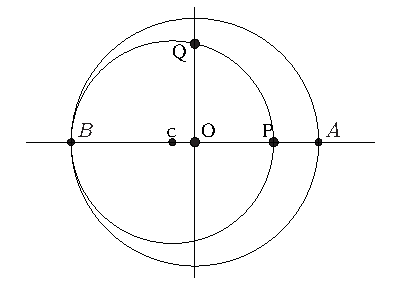
\includegraphics[width=0.5\textwidth]{pictures/squreroot.pdf}
\caption{squre root}
\end{figure}
If $A=(r,0)$ is constructible, so is $B=(-r, 0)$; $C$ is the midpoint of the segment $BP$ (midpoints are constructible); the circle with center $C$ and containing $P$ intersects the positive y-axis at a point $Q=(0,\delta)$, and elementary geometry shows that $\delta^2=r$. Therefore $\delta$ is constructible, concluding the proof of the theorem.
\end{proof}
\begin{corollary}\label{constructible number then degree power of 2}
Let $\gamma\in\mathscr{C}_{\C}$ be a constructible number. Then $[\Q(\gamma):\Q]$ is a power of $2$.
\end{corollary}
\begin{proof}
By Lemma~\ref{field constructible number} and Theorem~\ref{constructible number criterion}, there exist $\delta_1,\dots,\delta_k\in\R$ such that
\[\gamma\in\Q(\delta_1,\dots,\delta_k,i)\]
and each $\delta_j$ has degree $\leq 2$ over $\Q(\delta_1,\dots,\delta_{j-1})$. Repeated application of Proposition~\ref{field ext degree multiplicative} shows that
\[[\Q(\delta_1,\dots,\delta_k,i):\Q]\]
is a power of $2$, and since
\[\Q\sub\Q(\gamma)\sub\Q(\delta_1,\dots,\delta_k,i)\]
the claim follows from Corollary~\ref{field ext intermediate field degree divide}.
\end{proof}
As an example, constructing a regular $7$-gon would amount to constructing a $7$-th (complex) root of $1,\zeta$. By definition, $\zeta$ satisfies
\[t^7-1=(t-1)(t^6+t^5+\cdots+t+1)\]
as $\zeta\neq 1$, $\zeta$ must satisfy the cyclotomic polynomial $t^6+\cdots+1$. This is irreducible, hence again we find that $\zeta$ has degree $6$ over $\Q$, and Corollary~\ref{constructible number then degree power of 2} implies that the regular $7$-gon cannot be constructed with straightedge and compass.\par
Of course $7$ is not too special: if $p$ is a positive prime integer, the \textbf{cyclotomic polynomial} of degree $p-1$ is irreducible; hence
\[[\Q(\zeta_p):\Q]=p-1\]
where $\zeta_p$ is the complex $p$-th root of $1$ with argument $2\pi/p$. Therefore, Corollary~\ref{constructible number then degree power of 2} reveals that if $p$ is prime, then the regular $p$-gon can be constructed only if $p-1$ is a power of $2$. This is even more restrictive than it looks at first, due to the following simple lemma.
\begin{lemma}
If $2^k+1$ is prime, then $K$ is a power of $2$.
\end{lemma}
\begin{proof}
First note the fractorization:
\[t^{2m+1}+1=(t+1)(t^{2m}-t^{2m-1}+\cdots+1).\]
Thus $K$ is not odd. Assume that $k=2m$, then $2^k+1=2^{2m}+1=4^m+1$. Repeat this argument we see $m$ is also odd, and finally we conclude that $K$ is a power of $2$.
\end{proof}
Primes of the form $2^{2^\ell}+1$ are called \textbf{Fermat primes}. Therefore for a prime $p$, the regular $p$-gon if constructible only if $p$ is a Fermat prime.\par
We now use Galois theory to deal with the constructibility of regular $n$-gons. The key ingredient is the following result.
\begin{proposition}\label{prime power constr}
Let $E/K$ be a Galois extension, and assume $[F:K]=p^r$ for some prime $p$ and $r\geq 0$. Then there exist intermediate fields
\[K=E_0\sub E_1\sub E_2\sub\cdots\sub E_r=F\]
such that $[E_i:E_{i-1}]=p$ for $i=1,\dots,r$.
\end{proposition}
\begin{proof}
As the Galois correspondence is bijective for Galois extensions, this statement follows immediately from the fact that a group of order $p^r$, with $p$ prime, has a complete series of $p$-subgroups.
\end{proof}
\begin{theorem}\label{constructible regular n-gon iff}
The regular $n$-gon is constructible by straightedge and compass if and only if $\phi(n)$ is a power of $2$, if and only if $n=2^mp_1\cdots p_r$, where $m\geq 0$ and the factors $p_i$ are distinct Fermat primes.
\end{theorem}
\begin{proof}
We first prove the first equivalence. One direction is proved in Proposition~\ref{constructible number criterion}. For the converse, assume $\phi(n)=2^r$ for some $r$. The extension $\Q\sub\Q(\zeta_n)$ is Galois (it is the splitting field of $\Phi_n(X)$), of order $[\Q(\zeta_n):\Q]=\phi(n)=2^r$. Proposition~\ref{prime power constr} shows that the condition given in Theorem~\ref{constructible number criterion} is satisfied and therefore that $\zeta_n$ is constructible, as needed.\par
Now let $\phi(n)$ be a power of $2$. From the equation
\[\phi(n)=p_1^{k_1-1}(p_1-1)p_2^{k_2-1}(p_2-1)\cdots p_i^{k_i-1}(p_i-1)\]
we see that if $k_i-1>0$, then $p_i=2$. If $k_i-1=0$, then $p_i=2^m+1$ should be a prime, so $p_i$ is a Fermat prime. Hence $n=2^mp_1\cdots p_r$. The converse can also be deduced from the equality above.
\end{proof}
\subsection{The fundamental theorem of algebra}
\begin{theorem}
$\C$ is algebraically closed.
\end{theorem}
\begin{proof}
Let $f(X)\in\C[X]$ be a nonconstant polynomial; we have to prove that $f(X)$ has roots in $\C$. Note that if $f(X)$ has no roots in $\C$, then neither does $f(X)\widebar{f(X)}\in\R[X]$; that is, we may assume that $f(X)$ has real coefficients.\par
Now consider a tower $\R\sub\C\sub E$, where $E$ is a splitting field for $p(X)=(X^2+1)f(X)$ over $\R$. Since $[\C:\R]=2$ divides $[E:\R]$, we conclude that $[E:\R]=2^km$, for some $k>1$ with $m$ odd. Our goal is to show that $E=\C$, showing that $f(X)$ splits over $\C$.\par
Let $P$ be a $2$-Sylow subgroup of $\Gal_\R(f(X))$. Then $|P|=2^k$ and so
\[[E^P:\R]=[\Gal_\R(f(X)):P]=m.\]
By intermediate value theorem, every real polynomial with odd degree must have a root in $\R$, it follows that any nontrivial finite extension of $\R$ must have even degree (its primitive element must has even degree). From this we deduce that $m=1$ and $G=\Gal_\R(f(X))$ is a $2$-group of order $2^k$. Thus we have the tower
\[\{1\}\sub\Gal_\C(f(X))\sub G\]
in which $|\Gal_\C(f(X))|=2^{k-1}$. Therefore, according to Cauchy's theorem, $\Gal_\C(f(X))$ has a subgroup of any order dividing $2^{k-1}$. But $\Gal_\C(f(X))$ cannot have a subgroup of order $2^{k-2}$ that is, index $2$: if $H$ is such a group, then
\[\{1\}\sub H\sub\Gal_\C(f(X))\sub G\]
and then
\[2=[E^H:E^{\Gal_\C(f(X))}]=[E^H:\C],\]
which is impossible, since $\C$ does not have any irreducible polynomial of degree $2$. It follows that $|\Gal_\C(f(X))|=1$ and so $|G|=2$, which implies that $[E:\R]=2$, whence $E=\C$. 
\end{proof}
\subsection{Finite fields}
Let $F$ be a finite field, and let $p$ be its characteristic. We know that $F$ may be viewed as an extension
\[\F_p\sub F\]
of $\F_p=\Z/p\Z$; let $n=[F:F_p]$. Since $F$ has dimension $n$ as a vector space over $\F_p$, it is isomorphic to $\F_p^n$ as a vector space, and in particular $|F|=p^n$ is a power of $p$.
\subsubsection{Finite fields as splitting fields}
Let $F$ be a finite field of size $q$. Then $F^\times$ has order $q-1$ and so every element $\alpha\in F$ has exponent $q-1$, that is, $\alpha^{q-1}=1$. It follows that every element of $F$ is a root of the polynomial
\[f_q(X)=X^q-X\]
Since $f_q'(X)=-1$, this polynomial has no multiple roots and so $F$ is precisely the set of roots of $f_q(X)$ in some splitting field. In fact, since $F$ is a field, it is a splitting field for $f_q(X)$ over the prime subfield $\F_p$. We have the following theorem:
\begin{theorem}\label{finite field p^n order extension char}
Let $q=p^n$ be a power of a prime integer $p$.
\begin{itemize}
\item[(a)] The splitting field of the polynomial $f_q(X)=X^{q}-X$ over $\F_p$ is a field with precisely $q$ elements.
\item[(b)] Let $F$ be a field with exactly $q$ elements; then $F$ is a splitting field for $X^q-X$ over $\F_p$. The polynomial $X^q-X$ is separable over $\F_p$.
\end{itemize}
In particular, for every prime power $q$ there exists one and only one finite field of order $q$, up to isomorphism.
\end{theorem}
\begin{proof}
Let $F$ be the splitting field of $X^q-X$ over $\F_p$. Let $E$ be the set of roots of $f(X)=X^q-X$ in $F$. Since $f'(X)=qX^{q-1}-1=-1$ (as $q=0$ in characteristic $p$), we have $(f(X),f'(X))=1$; hence by Proposition~\ref{poloynomial separable iff f'} $f(X)$ is separable, and $E$ consists of precisely $q$ elements. We claim that $E$ is a field, and it follows that $E=F$.\par
To see that $E$ is a field, let $a,b\in E$. Then $a^q=a$ and $b^q=b$; it follows that
\[(a-b)^q=a^p+(-1)^qb^q=a^q-b^q=a-b.\]
(note that $(-1)^q=-1$ if $p$ is odd and $(-1)^q=+1=-1$ if $p=2$). If $b\neq0$,
\[(ab^{-1})^q=a^q(b^q)^{-1}=ab^{-1}.\]
Thus $E$ is closed under subtraction and division by a nonzero element, proving that $E$ is a field and concluding the proof of the first statement.\par
To prove the second statement, let $F$ be a field with exactly $q$ elements. The nonzero elements of $F$ form a group under multiplication consisting of $q-1$ elements. Therefore for any elments in $a\in F^\times$ we have $a^{q-1}=1$. Of course $0^q-0=0$, so the polynomial $X^q-X$ has $q$ roots in $F$; it follows that $F$ is a splitting field for $X^q-X$, as stated. The final statement comes from the uniqueness of splitting fields. This completes the proof.
\end{proof}
Let us refer to the polynomial $f_q(X)=X^q-X$ as the \textbf{defining polynomial} of the finite field $\F_{p^n}$. In view of this theorem, we will often refer to the finite field $\F_{p^n}$.\par
An immediate consequence of the splitting field characterization of finite fields is that any extension of finite fields is normal.
\begin{corollary}
The extension $\F_{p}\sub\F_{p^n}$ is a finite Galois extension. Hence, in the Galois correspondence for $\F_p\sub\F_{p^n}$, all intermediate fields and all subgroups are closed.
\end{corollary}
\begin{example}
Let $p$ be a prime integer. Then we claim that the polynomial $X^4+1$ is \textbf{reducible} over $\F_p$ (and therefore over every finite field).\par
Since $X^4+1=(X+1)^4$ in $\F_2[X]$, the statement holds for $p=2$. Thus, we may assume that $p$ is an odd prime. Then we claim that $X^4+1$ divides $X^{p^2}-X$. Indeed, the square of every odd number is congruent to $1$ mod $8$; hence $X^8-1$ divides $X^{p^2-1}-1$, which implies
\[(X^4+1)\mid(X^8-1)\mid(X^{p^2-1}-1)\mid(X^{p^2}-X)\]
It follows that $X^4+1$ factors completely in the splitting field of $X^{p^2}-X$, that is, in $\F_{p^2}$. If $\alpha$ is a root of $X^4+1$ in $\F_{p^2}$, we have the extensions
\[\F_p\sub \F_p(\alpha)\sub\F_{p^2}\]
therefore $[\F_p(\alpha):\F_p]$ divides $[\F_{p^2}:\F_p]=2$. That is, $\alpha$ has degree $1$ or $2$ over $\F_p$. But then its minimal polynomial is a factor of degree $1$ or $2$ of $(X^4+1)$,
showing that the latter is reducible.
\end{example}
Now we wish to examine the subfields of a finite field $\F_{p^n}$. Note that if $d$ and $n$ are positive integers and $n=kd+r$ for $0\leq r<d$, then it is easy to see $X^d-1\mid X^n-1$ if and only if $d\mid n$. This yields the following result on subfields of $\F_{p^n}$.
\begin{proposition}[\textbf{Classfication of Subfields of $\F_{p^n}$}]\label{finite field subfield iff order divide}
The following are equivalent:
\begin{itemize}
\item[(\rmnum{1})] The interger $d$ divides $n$.
\item[(\rmnum{2})] The defining polynomial $f_{p^d}(X)$ divides the defining polynomial $f_{p^n}(X)$.
\item[(\rmnum{3})] The field $\F_{p^d}$ is contained in $\F_{p^n}$. 
\end{itemize}
Put another way, the following lattices are isomorphic:
\begin{itemize}
\item[(a)] $\{d:\text{$d$ divides $n$}\}$, under division.
\item[(b)] $\{f_{p^d}(X):\text{$f_{p^d}(X)$ divides $f_{p^n}(X)$}\}$, under division.
\item[(c)] Subfields of $\F_{p^n}$, under set inclusion.
\end{itemize}
Moreover, $\F_{p^n}$ has exactly one subfield of size $p^d$, for each $d$ divides $n$, and each extension $\F_{p^d}\sub\F_{p^n}$ is simple.
\end{proposition}
\begin{proof}
To start with, we first prove the following facts:
\begin{align}\label{finite field subfield iff order divide-1}
p^d-1\mid p^n-1\Leftrightarrow d\mid n\Leftrightarrow X^d-1\mid X^n-1
\end{align}
In fact, write $n=kd+r$ with $0\leq r<d$, then
\[X^{n}-1=X^{kd+r}-X^r+X^r-1=X^r(X^{kd}-1)+X^r-1.\]
Since $X^d-1\mid X^{kd}-1$, this implies
\[X^n-1\equiv X^r-1\quad \text{mod $X^d-1$}\]
which proves (\ref{finite field subfield iff order divide-1}) immediately. Now apply these results with Proposition~\ref{finite field p^n order extension char}, we obtain that
\[d\mid n\Leftrightarrow p^d-1\mid p^n-1\Leftrightarrow X^{p^d-1}-1\mid X^{p^n-1}-1\Leftrightarrow f_{p^d}(X)\mid f_{p^n}(X).\]
which says (\rmnum{1}) and (\rmnum{2}) are equivalent. Moreover, by Proposition~\ref{finite field p^n order extension char},
\[\F_{p^d}\sub\F_{p^n}\Leftrightarrow\text{Root}(f_{p^d}(X))\sub\text{Root}(f_{p^n}(X))\Leftrightarrow f_{p^d}(X)\mid f_{p^n}(X).\]
so (\rmnum{2}) and (\rmnum{3}) are also equivalent. Moreover, if $\F_{p^n}$ has two distinct subfields of size $p^d$, then the polynomial $f_{p^d}(X)$ would have more than $p^d$ roots in $\F_{p^n}$, which is impossible.\par
For the last statement, recall that the multiplicative group of nonzero elements of a finite field is cyclic. If $\alpha\in\F_{p^n}$ is a generator of this gorup, then $\alpha$ will generate $\F_{p^n}$ over any subfield. If $d\mid n$, then $\F_{p^n}=\F_{p^d}(\alpha)$, so this extension is simple.
\end{proof}
These results can be translated into rather precise information on the structure of the polynomial ring over a finite field. For example,
\begin{corollary}\label{finite field irre poly of any order}
Let $F$ be a finite field. Then for all integers $n\geq1$ there exist irreducible polynomials of degree $n$ in $F[X]$.
\end{corollary}
\begin{proof}
We know $F=\F_{q}$ for some prime power $q$. By Corollary~\ref{finite field subfield iff order divide} there is an extension $\F_{q}\sub\F_{q^{n}}$, generated by an element $\alpha$. Then $[F_{q^{n}}:\F_{q}]=n$, and it follows that the minimal polynomial of $\alpha$ over $F=\F_{q}$ is an irreducible polynomial of degree $n$ in $F[X]$.
\end{proof}
In fact, our analysis of extensions of finite fields tells us about explicit factorizations, leading to an inductive algorithm for the computation of irreducible polynomials in $\F_q[X]$:
\begin{corollary}
Let $F=\F_q$ be a finite field, and let $n$ be a positive integer. Then the factorization of $X^{q^n}-X$ in $F[X]$ consists of all irreducible monic polynomials of degree $d$, as $d$ ranges over the positive divisors of $n$. In particular, all these polynomials factor completely in $\F_{q^n}$, and each irreducible polynomial appears only once in the factorization.
\end{corollary}
\begin{proof}
By Theorem~\ref{finite field p^n order extension char}, $\F_{q^n}$ is the splitting field of $X^{q^n}-X$ over $\F_p$, and hence over $\F_q=F$.\par
If $f(X)$ is a monic irreducible polynomial of degree $d$, then $F[X]/(f(X))=F(\alpha)$ is an extension of degree $d$ of $F$, that is, an isomorphic copy of $\F_{q^d}$. By Corollary~\ref{finite field subfield iff order divide}, if $d\mid n$, then there is an embedding of $\F_{q^d}$ in $\F_{q^n}$. But then $\alpha$ must be a root of $X^{q^n}-X$, and hence $X^{q^n}-X$ is a multiple of $f(X)$, as this is the minimal polynomial of $\alpha$. This proves that every irreducible polynomial of degree $d\mid n$ is a factor of $X^{q^n}-X$.\par
Conversely, if $f(X)$ is an irreducible factor of $X^{q^n}-X$, then $\F_{q^n}$ contains a root $\alpha$ of $f(X)$; we have the extensions $F=\F_q\sub\F_q(\alpha)\sub\F_{q^n}$, and $\F_q(\alpha)\cong\F_{q^d}$ for $d=\deg\alpha$. It follows that $d\mid n$, again by Corollary~\ref{finite field subfield iff order divide}.\par
For the last statement, note that $(X^{p^n}-X)'=p^nX^{p^n-1}-1=-1$, so $X^{p^n}-X$ is separable by Proposition~\ref{poloynomial separable iff f'}. This implies each irreducible polynomial appears only once in $X^{p^n}-X$.
\end{proof}
The picture we are trying to convey is the following: the $q^n$ roots of $X^{q^n}-X$ clump into disjoint subsets, with each subset collecting the roots of each and every irreducible polynomial of degree $d\mid n$ in $F[X]$.
\begin{example}
Let's contemplate the case $q=2$: $\F_2=\Z/2\Z$.
\begin{itemize}
\item $n=1$: the polynomial $X^2-X$ factors as the product of $X$ and $(X-1)$ (which we could write as $(X+1)$ just as well, since we are working over $\F_2$). These are all the irreducible polynomials of degree $1$ over $\F_2$.
\item $n=2$: the polynomial $X^4-X$ must factor as the product of all irreducible polynomials of degree $1$ and $2$; in fact
\[X^4-X=X(X-1)(X^2+X+1)\]
and the conclusion is that there is exactly one irreducible polynomial of degree $2$ over $\F_2$, namely $X^2+X+1$.
\item $n=3$: the quotient of $X^8-X$ by $X(X-1)$ is a polynomial of degree $6$, which must therefore be the product of the two irreducible polynomials of degree $3$ over $\F_2$. It takes a moment to find them:
\[X^3+X^2+1,\quad X^3+X+1\]
It also follows that $\F_8$ may be realized in two ways as a quotient of $\F_2[X]$ modulo an irreducible polynomial:
\[\dfrac{\F_2[X]}{(X^3+X^2+1)}\cong\dfrac{\F_2[X]}{(X^3+X+1)}\]
\end{itemize}
\end{example}
Since extensions of finite fields are simple extensions, our previous work allows us to be much more precise. Restricting our attention to the extensions $\F_p\sub\F_{p^n}$, for a prime $p$, we know these can be realized as simple extensions by an element with minimal polynomial of degree $n$. This polynomial is necessarily separable ($\F_p$ is perfect), so Corollary~\ref{field simple ext order of Aut} immediately gives us the size of the automorphism group: $|\Gal(\F_{p^n}/\F_p)|=n$.
\begin{proposition}\label{finite field Galois generated by Frobenius}
The Galois group $G$ of $\F_{p^n}$ over $\F_p$ is cyclic of order $n$, generated by the Frobenius automorphism.
\end{proposition}
\begin{proof}
We have seen that the Frobenius isomorphism $\sigma$ is an automorphism of $\F_{p^n}$. If $\alpha\in\F_{p}$, then $\sigma(\alpha)=\alpha^p=\alpha$ and so $\sigma$ fixes $\F_{p}$ and is therefore in the Galois group $G$. Moreover, the $n$ automorphisms
\[1,\sigma,\sigma^2,\dots,\sigma^{n-1}\]
are distinct elements of $G$, for if $\sigma^k=1$ then $\alpha^{p^k}=\alpha$ for all $\alpha\in\F_{p^n}$ and so $\F_{p^n}\sub\F_{p^d}$, which implies that $k\geq n$. Finally, since $|G|=n$, we see that $G=\langle\sigma\rangle$.
\end{proof}
\begin{corollary}\label{finite field F_pn over F_pd char}
Let $d\mid n$ be positive integers, then the Galois group $G$ of $\F_{p^n}$ over $\F_{p^d}$ is cyclic of order $n/d$, generated by the automorphism $\sigma^d:\alpha\mapsto\alpha^{p^d}$.
\end{corollary}
\begin{proof}
Let $\sigma^d$ be the automorphism prescribed above. Then $\sigma^d$ fixes $\F_{p^d}$.and hence is in $G$, and it has order $d/n$. By Theorem~\ref{Galois fundamental theorem-3} we have
\[\Gal(\F_{p^d}/\F_p)\cong\frac{\Gal(\F_{p^n}/\F_p)}{\Gal(\F_{p^n}/\F_{p^d})},\]
and in particular $|\Gal(\F_{p^n}/\F_{p^d})|=n/d$. Since $\sigma^{d}$ also has order $n/d$, the claim follows.
\end{proof}
\begin{corollary}\label{finite field F_p absolute Galois group char}
The absolute Galois group $\Gal(\widebar{\F}_p/\F_p)$ is isomomorphic to $\widehat{\Z}=\llim\Z/n\Z$.
\end{corollary}
\begin{proof}
Let $F=\F_q$ be a finite field. We show that the absolute Galois group is isomomorphic to $\widehat{\Z}$. For this, let $\mathcal{N}$ be the category associated to the poset $\N$ of division partial order, and we still denote by $n$ the objects of $\mathcal{N}$. By Proposition~\ref{finite field subfield iff order divide} we have an inverse system of groups
\[\big(\Gal(\F_{q^n}/\F_q)\big)_{n\in\mathcal{N}}\]
where for $m\mid n$ the map $\Gal(\F_{q^n}/\F_q)\to\Gal(\F_{q^m}/\F_q)$ is the restriction map; that is, the image of an automorphism $\sigma\in\Gal(\F_{q^n}/\F_q)$ in $\Gal(\F_{q^m}/\F_q)$ is obtained by simply restricting the domain of $\sigma$ from $\F_{q^n}$ to $\F_{q^m}$. Since $\F_{q^m}$ are all the finite subextensions of $\widebar{\F}_q$, by Corollary~\ref{Galois group identified as inverse limit}, we see the inverse limit of this inverse system is exactly $\Gal(\widebar{F}_q/\F_q)$. But Corollary~\ref{finite field F_pn over F_pd char} suggests that $\Gal(\F_{q^n}/\F_q)\cong\Z/n\Z$ and the restriction map corresponds to the quotient map $\Z/n\Z\to Z/m\Z$. Thus the inverse system $\big(\Gal(\F_{q^n}/\F_q)\big)_{n\in\mathcal{N}}$ is isomorphic to $(\Z/n\Z)_{n\in\mathcal{N}}$ and the claim follows from this.
\end{proof}
\subsubsection{The algebraic closure of a finite field}
To conclude, we determine the algebraic closure of a finite field $\F_{p}$. Since $\F_{p}\sub\F_{p^n}$ is algebraic for all positive integers $n$, an algebraic closure of $\F_p$ must contain all of the fields $\F_{p^n}$. Since $n!\mid(n+1)!$, it follows that $\F_{p^{n!}}\sub\F_{p^{(n+1)!}}$ and so the union
\[\Gamma(p)=\bigcup_{n=0}^{\infty}\F_{p^{n!}}\]
is an extension field of $\F_p$ that contains $\F_{p^n}$ for all $n\geq 1$. Moreover, if $E$ is a field for which $\F_{p^n}\sub E$ for all $n$, then $\Gamma(p)\sub E$, that is, $\Gamma(p)$ is the smallest field containing each $\F_{p^n}$.
\begin{theorem}
The field $\Gamma(p)$ is the algebraic closure of $\F_p$.
\end{theorem}
\begin{proof}
Every element of $\Gamma(p)$ lies in some $\F_{p^{n!}}$, whence it is algebraic over $\F_p$. Thus $\Gamma(p)$ is algebraic over $\F_p$. Now let $f(X)$ be an irreducible polynomial over $\Gamma(p)$ of degree $d$. Then the coefficients of $f(X)$ lie in some $\F_{p^{n!}}$ and so $f(X)$ is irreducible as a polynomial over $\F_{p^{n!}}$. Hence, the splitting field for $f(X)$ is $\F_{p^{n!d}}\sub\Gamma(p)$ and so $\Gamma(p)$ splits over $\Gamma(p)$.
\end{proof}
\subsection{Cyclotomic polynomials and fields}
Let $K$ be a field. By a \textbf{root of unity} (in $K$) we shall mean an element $\zeta\in K$ such that $\zeta^n=1$ for some integer $n>1$. If the characteristic of $K$ is $p$, then the equation
\[X^{p^d}=1\]
has only one root, namely $1$, and hence there is no $p^d$-th root of unity except $1$.\par
Let $n$ be an integer $>1$ and not divisible by the characteristic $p$. The polynomial
\[X^n-1\]
is separable because its derivative is $nX^{n-1}\neq 0$, and the only root of the derivative is $0$, so there is no common root. Hence in $\widebar{K}$ the polynomial $X^n-1$ has $n$ distinct roots, which are roots of unity. They obviously form a group, and we know that every finite multiplicative group in a field is cyclic. Thus the group of $n$-th roots of unity is cyclic. A generator for this group is called a \textbf{primitive $\bm{n}$-th root} of unity.\par
If $\mu_n$ denotes the group of all $n$-th roots of unity in $\widebar{n}$ and $m,n$ are relatively prime integers, then
\[\mu_{mn}\cong\mu_m\times\mu_n\]
This follows because $\mu_m$, $\mu_n$ cann ot have any element in common except $1$, and because $\mu_m\mu_n$ consequently has $mn$ elements, each of which is an $mn$-th root of unity. Hence $\mu_m\mu_n=\mu_{mn}$ and the decomposition is that of a direct product.\par
As a matter of notation, to avoid double indices, especially in the prime power case, we write $\mu[n]$ for $\mu_n$. So if $p$ is a prime, $\mu[p^r]$ is the group of $p^r$-th roots of unity. Then $\mu[p^{\infty}]$ denotes the union of all $\mu[p^r]$ for all positive integers $r$.\par
Let $K$ be any field. Let $n$ be not divisible by the characteristic $p$. Let $\zeta_n$ be a primitive $n$-th root of unity in $\widebar{K}$. Let $\sigma$ be an embedding of $K(\zeta)$ in $\widebar{K}$ over $K$. Then
\[(\sigma(\zeta))^n=\sigma(\zeta^n)=1\]
so that $\sigma(\zeta)$ is an $n$-th root of unity also. Hence $\sigma(\zeta)=\zeta^i$ for some integer $i=i(\sigma)$, uniquely determined mod $n$. It follows that $\sigma$ maps $K(\zeta)$ into itself, and hence that $K(\zeta)$ is normal over $K$. If $\tau$ is another automorphism of $K(\zeta)$ over $K$ then
\[\sigma(\tau(\zeta))=\zeta^{i(\sigma)i(\tau)}\]
Since $\sigma$ and $\tau$ are automorphisms, it follows that $i(\sigma)$ and $i(\tau)$ are coprime to $n$. In this way we get a homomorphism of the Galois group $G$ of $K(\zeta)$ over $K$ into the multiplicative group $(\Z/n\Z)^\times$ of integers prime to $n$, mod $n$. Our homomorphism is clearly injective since $i(\sigma)$ is uniquely determined by $\sigma$ mod $n$, and the effect of $\sigma$ on $K(\zeta)$ is determined by its effect on $\zeta$. We conclude that $K(\zeta)$ is abelian over $K$. We know that the order of $(\Z/n\Z)^\times$ is $\phi(n)$. Hence the degree
$[K(\zeta):K]$ divides $\phi(n)$.\par
For a specific field $K$, the question arises whether the image of $\Gal(K(\zeta)/K)$ in $(\Z/n\Z)^\times$ is all of $(\Z/n\Z)^\times$. Looking at $K=\R$ or $\C$, one sees that this is not always the case. We now give an important example when it is the case.\par
Define the $n$-th \textbf{cyclotomic polynomial} $\Phi_n(X)$ to be
\[\Phi_n(X)=\prod_{\zeta\text{ primitive $n$-th root of }1}(X-\zeta)=\prod_{\substack{1\leq m\leq n\\(m,n)=1}}(X-\zeta_n^m)\]
which has degree $\phi(n)$.
\begin{example}
If $n=p$ is prime, then every nonidentity element of $\mu_p\cong C_p$ is a generator: every $p$-th root of $1$ is primitive except $1$ itself. Therefore
\[\Phi_p(X)=\dfrac{X^p-1}{X-1}=X^{p-1}+\cdots+X+1\]
\end{example}
\begin{lemma}\label{cyclotomic polynomial lemma}
For all positive integers $n$,
\[X^n-1=\prod_{\substack{1\leq d\leq n\\d\mid n}}\Phi_d(X)\]
\end{lemma}
\begin{proof}
If $n=de$, then every $d$-th root $\zeta$ of $1$ is an $n$-th root of $1$, because $\zeta^n=\zeta^{de}=(\zeta^d)^e=1$. In particular, every primitive $d$-th root $\zeta$ of $1$ is an $n$-th root of $1$.\par
On the other hand, every $\zeta\in \mu_n$ generates a subgroup $H$ of $\mu_n$, and $H=\mu_d$ for
$d$ equal to the order of $\zeta$, a divisor of $n$. Thus, every $\zeta\in \mu_n$ is a primitive $d$-th root of $1$ for some $d\mid n$.\par
Thus the set of $n$-th roots of $1$ equals the union of the sets of primitive $d$-th roots of $1$, as $d$ ranges over all positive divisors of $n$. The statement follows immediately:
\[X^n-1=\prod_{\zeta\in \mu_n}(X-\zeta)=\prod_{\substack{1\leq d\leq n\\d\mid n}}\Bigg(\prod_{\zeta\text{ primitive $d$-th root of }1}(X-\zeta)\Bigg)=\prod_{\substack{1\leq d\leq n\\d\mid n}}\Phi_d(X)\]
as claimed.
\end{proof}
Lemma~\ref{cyclotomic polynomial lemma} yields an inductive computation of cyclotomic polynomials; the fact that $\Phi_n(X)\in\Z[X]$ follows from this fact. Explicitly,
\begin{corollary}
The cyclotomic polynomials $\Phi_n(X)$ have integer coefficients.
\end{corollary}
\begin{proof}
Use induction on $n$. Note that $\Phi_1(X)=x-1$, and assume we have shown that all $\Phi_m(X)$ have integer coefficients for $m<n$. In particular, $f(X):=\prod_{1\leq d\mid n,d<n}\Phi_d(X)$ is a monic polynomial with integer coefficients. Since $f(X)$ is monic, we can divide it into $X^n-1$ with remainder, within $\Z[X]$: there exist $q(X),r(X)\in\Z[X]$ such that
\[X^n-1=q(X)f(X)+r(X)\]
with $r(X)=0$ or $\deg r(X)<\deg f(X)$. On the other hand, by Lemma~\ref{cyclotomic polynomial lemma},
\[X^n-1=f(X)\Phi_n(X)\]
in $\C[X]$. Therefore
\[f(X)(\Phi_n(X)-q(X))=r(X)\]
in $\C[X]$. But this forces $r(X)=0$ (otherwise we would have $\deg r(X)>\deg f(X)$). Therefore $\Phi_n(X)=q(X)\in\Z[X]$.
\end{proof}
\begin{proposition}
For all positive $n$, $\Phi_n(X)\in\Z[X]$ is irreducible over $\Q$.
\end{proposition}
\begin{proof}
Arguing by contradiction, assume $\Phi_n(X)$ is reducible. Then its roots $\zeta_n^m$, with $(m,n)=1$, are divided among the factors; we can choose a root $\zeta^m_n$ of one irreducible monic factor $f(X)$, such that another root $\zeta^{mp}_n$ (for some prime $p$ not dividing $n$) is not a root of $f(X)$. Write 
\[\Phi_n(X)=f(X)g(X)\]
since $\Phi_n(X)\in\Z[X]$ and $\Phi_n(X)$, $f(X)$ are monic, $f(X)$ and $g(X)$ have integer coefficients. By our choice, $f(X)$ is the minimal polynomial of $\zeta^m_n$ over $\Q$, and $g(\zeta^{mp}_n)=0$.\par
It follows that $\zeta^m_n$ is a root of $g(X^p)$, and hence $f(X)\mid g(X^p)$. Therefore we can
write
\[g(X^p)=f(X)h(X)\]
with $h(X)\in\Z[X]$. Reading the last equation modulo $p$, we get (again using $(a+b)^p=a^p+b^p$, and denoting cosets by bar)
\[\widebar{g}(X)^p=\widebar{f}(X)\widebar{h}(X)\text{in }\F_p[X].\]
In particular, $\widebar{f}(X)$ and $\widebar{g}(X)$ must have a nontrivial common factor $\widebar{\ell}(X)$ in $\F_p[X]$. But then
\[\ell^2(X)\mid\widebar{f}(X)\widebar{g}(X)\]
the reduction of $\Phi_n(X)$ modulo $p$ must have a multiple factor.\par
This implies that $X^n-1\in\F_p[X]$ has a multiple factor; that is, it is inseparable. However, its derivative $nX^{n-1}\in\F_p[X]$ is nonzero (because $p$ does not divide $n$ by assumption), and Proposition~\ref{poloynomial separable iff f'} implies that $X^n-1$ is separable in $\F_p[X]$.\par
This contradiction shows that our assumption that $\Phi_n(X)$ is reducible must be nonsense, proving the statement.
\end{proof}
\begin{definition}
The splitting field $\Q(\zeta_n)$ for the polynomial $X^n-1$ over $\Q$ is the $n$-th \textbf{cyclotomic field}.
\end{definition}
\begin{proposition}\label{Galois group of cyclotomic field}
The Galois group $\Gal(\Q(\zeta_n)/\Q)$ is isomorphic to $(\Z/n\Z)^\times$.
\end{proposition}
\begin{proof}
We know that $\Gal(\Q(\zeta_n)/\Q)$ has cardinality $\phi(n)$ (Corollary~\ref{field simple ext order of Aut}; the roots
are distinct since $\Phi_n(X)$ is separable), so the homomorphism $\Gal(\Q(\zeta_n)/\Q)\to(\Z/n\Z)^\times$ is an isomorphism.
\end{proof}
\begin{corollary}
If $n,m$ are relative prime integers, then
\[\Q(\zeta_m)\cap\Q(\zeta_n)=\Q.\]
\end{corollary}
\begin{proof}
We note that $\zeta_n$ and $\zeta_m$ are both contained in $\Q(\zeta_{mn})$ since $\zeta_{mn}^n$ is a primitive $m$-th root of unity. Furthermore, $\zeta_{m}\zeta_n$ is a primitive $mn$-th root of unity. Hence
\[\Q(\zeta_m)\Q(\zeta_n)=\Q(\zeta_{mn})\]
Our assertion then follows from the multiplicativity $\phi(mn)=\phi(m)\phi(n)$ and Proposition~\ref{Galois group of lifting}.
\end{proof}
\begin{example}
The reader should consider Examples~\ref{split field of x^8-1} again: by what we have just proved, the automorphism group of the splitting field of $X^8-1$ is isomorphic to the group of units in $\Z/8\Z$; this group is immediately seen to be isomorphic to $(\Z/2\Z)\times(\Z/2\Z)$, confirming the claim made in Example~\ref{split field of x^8-1}.
\end{example}
\subsection{Cyclic extensions}
\subsubsection{Hilbert's theorem 90}
Let $G$ be a group. A \textbf{$\bm{G}$-module} is an abelian group $M$ together with an action of $G$, i.e., a map $G\times M\to M$ such that
\begin{itemize}
\item $\sigma(m+n)=\sigma m+\sigma n$ for $m,n\in M$.
\item $(\sigma\tau)m=\sigma(\tau m)$ for $\sigma,\tau\in G$ and $m\in M$.
\item $1m=m$ for $m\in M$.
\end{itemize}
Thus, to give an action of $G$ on $M$ is the same as giving a homomorphism $G\to\Aut(M)$ (automorphisms of $M$ as an abelian group).
\begin{example}
Let $E$ be a Galois extension of $K$ with Galois group $G$. Then $(E,+)$ and $(E^\times,\times)$ are $G$-modules.
\end{example}
Let $M$ be a $G$-module. A \textbf{crossed homomorphism} is a map $f:G\to  M$ such that
\[f(\sigma\tau)=f(\sigma)+\sigma f(\tau)\]
for all $\sigma,\tau\in G$. Note that the condition implies that $f(1)=f(1)+f(1)$, and so $f(1)=0$.
\begin{example}
\mbox{}
\begin{itemize}
\item[$(a)$] Let $f:G\to M$ be a crossed homomorphism. For any $g\in G$,
\begin{equation*}
\begin{aligned}
f(\sigma^2)&=f(\sigma)+\sigma f(\sigma),\\
f(\sigma^3)&=f(\sigma)+\sigma f(\sigma^2)=f(\sigma)+\sigma f(\sigma)+\sigma^2 f(\sigma)\\
&\ \ \vdots\\
f(\sigma^n)&=f(\sigma)+\sigma f(\sigma)+\cdots+\sigma^{n-1}f(\sigma)
\end{aligned}
\end{equation*}
Thus, if $G$ is a cyclic group of order $n$ generated by $\sigma$, then a crossed homomorphism $f:G\to M$ is determined by its value, $x$ say, on $\sigma$, and $x$ satisfies the equation
\begin{align}\label{cross homomorphism cyclic}
x+\sigma x+\cdots+\sigma^{n-1}x=0
\end{align}
Moreover, if $x\in M$ satisfies $(\ref{cross homomorphism cyclic})$, then the formulas $f(\sigma^i)=x+\sigma x+\cdots+\sigma^{i-1}x$ define a crossed homomorphism $f:G\to M$. Thus, for a finite cyclic group $G=\langle\sigma\rangle$, there is a one-to-one correspondence
\[\{\text{crossed homomorphisms $f:G\to M$}\}\leftrightarrows\{\text{$x\in M$ satisfying $(\ref{cross homomorphism cyclic})$}\}.\]
\item[$(b)$] For every $x\in M$, we obtain a crossed homomorphism by putting
\[f(\sigma)=\sigma x-x\] 
for all $\sigma\in G$. A crossed homomorphism of this form is called a \textbf{principal crossed homomorphism}.
\item[$(c)$] If $G$ acts trivially on $M$, i.e., $\sigma m=m$ for all $\sigma\in G$ and $m\in M$, then a crossed homomorphism is simply a homomorphism, and there are no nonzero principal crossed homomorphisms.
\end{itemize}
\end{example}
The sum and difference of two crossed homomorphisms is again a crossed homomorphism, and the sum and difference of two principal crossed homomorphisms is again principal. Thus we can define
\[H^1(G,M)=\frac{\text{crossed homomorphisms}}{\text{principal crossed homomorphisms}}\]
(quotient abelian group). An exact sequence of $G$-modules
\[\begin{tikzcd}
0\ar[r]&M\ar[r]&N\ar[r]&L\ar[r]&0
\end{tikzcd}\]
gives rise to an exact sequence
\[\begin{tikzcd}[column sep=scriptsize]
0\ar[r]&M^G\ar[r]&N^G\ar[r]&L^G\ar[r,"\delta"]&H^1(G,M)\ar[r]&H^1(G,N)\ar[r]&H^1(G,L)
\end{tikzcd}\]
Let $\ell\in L^G$, and let $n\in N$ map to $\ell$. For all $\sigma\in G$, $\sigma n-n$ lies in the submodule $M$ of $N$, and the crossed homomorphism $\sigma\mapsto\sigma n-n:G\to M$ represents $\delta(\ell)$.
\begin{example}
Let $\pi:\widetilde{X}\to X$ be the universal covering space of a topological space $X$, and let $\Gamma$ be the group of covering transformations. Under some fairly general hypotheses, a $\Gamma$-module $M$ will define a sheaf $\mathcal{M}$ on $X$, and $H^1(X,\mathcal{M})\cong H^1(\Gamma,M)$. For example, when $M=\Z$ with the trivial action of $\Gamma$, this becomes the isomorphism $H^1(X,\Z)\cong H^1(\Gamma,\Z)=\Hom(\Gamma,\Z)$.
\end{example}
\begin{theorem}\label{field ext H^1(G,E^*) H^1(G,E) is trivial}
Let $E$ be a finite Galois extension of $K$ with group $G$; then $H^1(G,E^{\times})=0$ and $H^1(G,E)=0$.
\end{theorem}
\begin{proof}
Let $f$ be a crossed homomorphism $G\to E^\times$. In multiplicative notation, this means that
\[f(\sigma\tau)=f(\sigma)\cdot (\sigma f(\tau))\]
for $\sigma,\tau\in G$, and we have to find a $\gamma\in E^\times$ such that $f(\sigma)=\sigma(\gamma)/\gamma$ for all $\sigma\in G$. Because the $f(\tau)$ are nonzero, Corollary~\ref{field embedding independent} implies that
\[\sum_{\tau\in G}f(\tau)\tau:E\to E\]
is not the zero map, i.e., there exists an $\alpha\in E$ such that
\[\beta:=\sum_{\tau\in G}f(\tau)\tau(\alpha)\neq 0.\]
But then, for $\sigma\in G$,
\begin{align*}
\sigma(\beta)&=\sigma\Big(\sum_{\tau\in G}f(\tau)\tau(\alpha)\Big)=\sum_{\tau\in G}\sigma(f(\tau))\sigma(\tau(\alpha))\\
&=f(\sigma)^{-1}\sum_{\tau\in G}f(\sigma\tau)(\sigma\tau)(\alpha)=f(\sigma)^{-1}\beta.
\end{align*}
Therefore $f(\sigma)=\beta/\sigma(\beta)$ and we can take $\gamma=\beta^{-1}$.\par
For the additive version, let $f:G\to E$ be a crossed homomorphism. Then we have
\[f(\sigma\tau)=f(\sigma)+\sigma f(\tau)\]
for $\sigma,\tau\in G$. Let $\gamma\in E$ an element in $E$ such that $\tr(\gamma)\neq 0$ (this element exists by linearly independence), and consider
\[\beta:=\sum_{\tau\in G}f(\tau)\tau(\gamma).\]
Then we have
\begin{align*}
\sigma(\beta)&=\sigma\Big(\sum_{\tau\in G}f(\tau)\tau(\gamma)\Big)=\sum_{\tau\in G}\sigma(f(\tau))\sigma(\tau(\gamma))\\
&=\sum_{\tau\in G}f(\sigma\tau)(\sigma\tau)(\gamma)-f(\sigma)\sum_{\tau\in G}(\sigma\tau)(\gamma)=\beta-f(\sigma)\tr(\gamma).
\end{align*}
Since $\tr(\gamma)\neq 0$, we obtain $f(\sigma)=\beta/\tr(\gamma)-\sigma(\beta/\tr(\gamma))$, so $f$ is principal.
\end{proof}
\begin{corollary}[\textbf{Hilbert's theorem 90, multiplicative version}]
Let $E$ be a finite cyclic extension of $K$ and let $\sigma$ generate $\Gal(E/K)$. Let $\alpha\in E$, if $N(\alpha)=1$, then $\alpha=\beta/\sigma(\beta)$ for some $\beta\in E$.
\end{corollary}
\begin{proof}
Let $n=[E:K]$. The condition on $\alpha$ is that $\alpha\sigma(\alpha)\cdots\sigma^{n-1}(\alpha)=1$, and so by $(\ref{cross homomorphism cyclic})$ there is a crossed homomorphism $f:G\to E^{\times}$ with $f(\sigma)=\alpha$. Theorem~\ref{field ext H^1(G,E^*) H^1(G,E) is trivial} now shows that $f$ is principal, which means that there is a $\beta\in E$ such that $\alpha=\beta/\sigma(\beta)$.
\end{proof}
\begin{corollary}[\textbf{Hilbert's theorem 90, additive version}]
Let $E$ be a finite cyclic extension of $K$ and let $\sigma$ generate $\Gal(E/K)$. Let $\alpha\in E$, if $\tr(\alpha)=0$, then $\alpha=\beta-\sigma(\beta)$ for some $\beta\in E$.
\end{corollary}
\begin{proof}
Let $n=[E:K]$. The condition on $\alpha$ is that $\alpha+\sigma(\alpha)+\cdots+\sigma^{n-1}(\alpha)=1$, and so by $(\ref{cross homomorphism cyclic})$ there is a crossed homomorphism $f:G\to E$ with $f(\sigma)=\alpha$. Theorem~\ref{field ext H^1(G,E^*) H^1(G,E) is trivial} now shows that $f$ is principal, which means that there is a $\beta\in E$ such that $\alpha=\beta/\sigma(\beta)$.
\end{proof}
\subsubsection{Abelian and Cyclic Extensions}
Extensions are often named after their Galois groups. Here is a very important example.
\begin{definition}
A Galois extension $E/K$ is \textbf{abelian} if its Galois group $\Gal(E/K)$ is abelian and \textbf{cyclic} if the Galois group is cyclic.
\end{definition}
The basic properties of abelian and cyclic extensions are given in the next proposition. Note that abelian and cyclic extensions are not (quite) distinguished.
\begin{proposition}[\textbf{Property of abelian and cyclic extensions}]\label{field ext abelian cyclic prop}
\mbox{}
\begin{itemize}
\item (\textbf{Composite of abelian is abelian}) If $K\sub E_i$ are abelian, then $K\sub\bigvee E_i$ is abelian.
\item (\textbf{Lifting of abelian (cyclic) is abelian (cyclic)}) If $K\sub E$ is abelian (cyclic) and $K\sub F$, then $F\sub EF$ is abelian (cyclic).
\item (\textbf{Steps in an abelian (cyclic) tower are abelian (cyclic)}) If $K\sub E\sub F$ with $K\sub E\sub F$ abelian (cyclic), then $K\sub E$ and $E\sub F$ are abelian (cyclic).
\end{itemize}
\end{proposition}
\begin{proof}
Let $K\sub E_i$ be abelian extensions, then since $E_i/K$ are Galois, the extension $K\sub\bigvee E_i$ is also Galois. Moreover, by Proposition~\ref{Galois group of a composite}, the Galois group $\Gal(\bigvee E_i/K)$ is a subgroup of $\prod\Gal(E_i/K)$, which is abelian, and hence is also abelian.\par
Now consider a lifting of abelian (cyclic) extension. By Proposition~\ref{Galois group of lifting} the extension $F\sub EF$ is Galois, and $\Gal(EF/F)\cong\Gal(E/E\cap F)$. Note that $\Gal(E/E\cap F)$ is a subgroup of $\Gal(E/K)$, and hence is abelian (cyclic) if $\Gal(E/K)$ is abelian (cyclic).\par
Finally, consider a tower $K\sub E\sub F$, where $F/K$ is abelian (cyclic). Since all subgroups of $\Gal(F/K)$ is then normal, we see $E/K$ and $F/E$ are both Galois extensions, and $\Gal(E/K)$, $\Gal(F/E)$ are isomorphic to subgroups of $\Gal(F/K)$, which are abelian (cyclic).
\end{proof}
Abelian and cyclic extensions fail to be distinguished because, and only because if the steps in a tower are abelian (cyclic), this does not imply that the full extension is abelian (cyclic). What does it imply?\par
Suppose that
\[K=K_0\sub K_1\sub K_2\sub\cdots\sub K_{n}=E\]
is a tower in which each step $K_{i+1}/K_i$ is abelian (cyclic). Taking Galois groups gives the series
\[\{1\}=\Gal(E/E)\sub\Gal(E/K_{n-1})\sub\cdots\sub\Gal(E/K_1)\sub \Gal(E/K_0)=\Gal(E/K).\]
Consider the subtower $K_i\sub K_{i+1}\sub E$. Since the lower step is normal, it follows from Theorem~\ref{Galois fundamental theorem-3}$(a)$ that $\Gal(E/K_{i+1})$ is a normal subgroup of its parent $\Gal(E/K_i)$ and that
\[\frac{\Gal(E/K_i)}{\Gal(E/K_{i+1})}\hookrightarrow\Gal(K_{i+1}/K_{i}).\]
Since the latter is abelian (cyclic), so is the former. Thus,
\[\{1\}=\Gal(E/E)\lhd\Gal(E/K_{n-1})\lhd\cdots\lhd\Gal(E/K_1)\lhd\Gal(E/K).\]
where each quotient group is abelian (cyclic). In the language of group theory, this series of subgroups is an \textbf{abelian series}. (When the groups are finite, the cyclic case and the abelian case are equivalent.) A group that has an abelian series is said to be \textbf{solvable}.
\begin{proposition}\label{Galois group of successive abelian extension is slovable}
If $K=K_0\sub K_1\sub\cdots\sub K_n=E$ is a tower of fields in which each step $K_{i}\sub K_{i+1}$ is abelian, then the Galois group $\Gal(E/K)$ is solvable.
\end{proposition}
In the follows, we classify cyclic extensions under certain conditions, which will be used when we study the solvability of polynomials. The follwoing two theorems are good applications of Hilbert's theorem 90.
\begin{theorem}\label{field ext cyclic nonchar case}
Let $K$ be a field, $n$ an positive integer coprime to the characteristic of $K$, and assume that there is a primitive $n$-th root of unity in $K$.
\begin{itemize}
\item[(\rmnum{1})] Let $E$ be a cyclic extension of degree $n$ of $K$. Then there exists $\alpha\in E$ such that $E=K(\alpha)$, and $\alpha$ satisfies an equation $X^n-a=0$ for some $a\in K$.
\item[(\rmnum{2})] Conversely, let $a\in K$. Let $\alpha$ be a root of $X^n-a$. Then $K(\alpha)$ is cyclic over $K$, of degree $d$ for some $d\mid n$, and $\alpha^d$ is an element of $K$.
\end{itemize}
\end{theorem}
\begin{proof}
Let $\zeta$ be a primitive $n$-th root of unity in $K$, and let $E/K$ be cyclic with group $G$. Let $\sigma$ be a generator of $G$. We have $N(\zeta^{-1})=(\zeta^{-1})^n=1$. By Hilbert's theorem $90$, there exists $\alpha\in E$ such that $\zeta^{-1}=\alpha/\sigma(\alpha)$. Since $\zeta$ is in $K$, we have $\sigma^i(\alpha)=\zeta^i\alpha$ for $i=1,\dots,n$. Hence the elements $\zeta^i(\alpha)$ are $n$ distinct conjugates of $\alpha$ over $K$, whence $[K(\alpha):K]$ is at least equal to $n$. Since $[E:K]=n$, it follows that $E=K(\alpha)$. Furthermore,
\[\sigma(\alpha^n)=\sigma(\alpha)^n=\zeta^n\alpha^n=\alpha^n.\]
Hence $\alpha^n$ is fixed under $\sigma$, and so under $G$. Therefore $\alpha^n$ is an element of $K$, and we let $a=\alpha^n$. This proves the
first part of the theorem.\par
Conversely, let $a\in K$. Let $\alpha$ be a root of $X^n-a$. Then $\alpha\zeta^i$ is also a root for each $i=1,\dots,n$, and hence all roots lie in $K(\alpha)$ which is therefore normal over $K$. All the roots are distinct so $K(\alpha)$ is Galois over $K$. Let $G$ be the Galois group. If $\sigma$ is an automorphism of $\Gal(K(\alpha)/K)$ then $\sigma(\alpha)$ is also a root of $X^n-a$. Hence $\sigma(\alpha)=\omega_\sigma\alpha$ where $\omega_\sigma$ is an $n$-th root of unity, not necessarily primitive. The map $\sigma\mapsto\omega_\sigma$ is obviously a homomorphism of $G$ into the group of $n$-th roots of unity, and is injective. Since a subgroup of a cyclic group is cyclic, we conclude that $G$ is cyclic, of order $d$, and $d\mid n$. The image of $G$ is a cyclic group of order $d$. If $\sigma$ is a generator of $G$, then $\omega_\sigma$ is a primitive $d$-th root of unity. Now we get
\[\sigma(\alpha^d)=\sigma(\alpha)^d=\omega_\sigma^d\alpha^d=\alpha^d.\]
Hence $\alpha^d$ is fixed under $G$, whence is in $K$, and our theorem is proved.
\end{proof}
We now pass to cyclic extensions of degree $p$ in characteristic $p$.
\begin{theorem}[\textbf{Artin-Schreier}]\label{field ext cyclic char p case}
Let $K$ be a field of characteristic $p$.
\begin{itemize}
\item[(\rmnum{1})] Let $E$ be a cyclic extension of $K$ of degree $p$. Then there exists $\alpha\in E$ such that $E=K(\alpha)$ and $\alpha$ satisfies an equation $X^p-X-a=0$ with some $a\in K$.
\item[(\rmnum{2})] Conversely, given $a\in K$, the polynomial $f(X)=X^p-X-a$ either has one root in $K$, in which case all its roots are in $K$, or it is irreducible. In this latter case, if $\alpha$ is a root then $K(\alpha)$ is cyclic of degree $p$ over $K$.
\end{itemize}
\end{theorem}
\begin{proof}
Let $E$ be a cyclic extension of $K$ of degree $p$, and $\sigma$ be a generator of $\Gal(E/K)$. Since $-1\in K$, every automorphism in $\Gal(E/K)$ fixes $-1$, it follows that $\tr(-1)=0$. By the additive version of Hilbert's theorem $90$, there is a element $\beta\in E$ such that $-1=\beta-\sigma(\beta)$. Then
\[\sigma(\beta)=\beta+1,\quad\sigma^i(\beta)=\sigma^{i-1}(\beta)+1=\cdots=\beta+i\]
It follows that the minimal polynomial of $\alpha$ has degree $\geq p$, so $[K(\alpha):K]\geq p$. But $[E:K]=p$. So $E=K(\alpha)$. Note that
\[\sigma(\alpha^p-\alpha)=\sigma^p(\alpha)-\sigma(\alpha)=(\alpha+1)^p-\alpha-1=\alpha^p-\alpha.\]
Hence $\alpha^p-\alpha$ is fixed under $\sigma$, and therefore under $\Gal(E/K)$. It lies in the fixed field $K$. If we let $a:=\alpha^p-\alpha$, we see $\alpha$ satisfies the equation $X^p-X-a=0$. This proves the first part of the theorem.\par
Conversely, let $a\in K$. If $\alpha$ is a root of $f(X)=X^p-X-a$, then
\[f(\alpha+1)=(\alpha+1)^p-\alpha-1-a=\alpha^p-\alpha-a=0\]
so $\alpha+1$ is also a root. Therefore the roots of $f(X)$ are 
\[\alpha_1:=\alpha,\quad\alpha_2:=\alpha+1,\quad\cdots,\quad\alpha_p:=\alpha+p-1\]
If $\alpha\in K$, then all $\alpha_i$ is in $K$. If $\alpha\notin K$, then all $\alpha_i$ is not in $K$. In this case, any sum $\sum_I$ with $I\neq\{1,\dots,p\}$ and $I\neq\emp$ is not an element of $K$. Therefore $f(X)$ is irreducible by Exercise~\ref{irr exercise}. Since all roots of $f(X)$ is in $K(\alpha)$, it follows that $K(\alpha)$ is normal over $K$. Since $f(X)$ has no multiple roots, it follows that $K(\alpha)$ is Galois over $K$. Since $\alpha+1$ is a root of $f(X)$, there exists an automorphism $\sigma$ of $K(\alpha)$ over $K$ such that $\sigma(\alpha)=\alpha+1$. Then the powers $\sigma^i$ give $\sigma^i(\alpha)=\alpha+i$ for $i=1,\dots,p$ and are distinct. Since $[K(\alpha):K]=p$, it follows that $\Gal(K(\alpha)/K)=\langle\sigma\rangle$ and is cyclic of order $p$, there by proving the theorem.
\end{proof}
\subsection{Solvable and radical extensions}
\subsubsection{Solvable extensions}
A finite separable extension $E/K$ is said to be \textbf{solvable} if the Galois group of the normal closure of $E/K$ is a solvable group. This is equivalent to saying that there exists a solvable Galois extension $F$ of $K$ such that $K\sub E\sub F$: Indeed, we have $K\sub E\sub \langle E/K\rangle\sub F$ and the Galois group of $\langle E/K\rangle/K$ is a homomorphic image of $\Gal(F/K)$, which is thus solvable.
\begin{proposition}\label{field ext solvable distinguished}
Solvable extensions form a distinguished class of extensions.
\end{proposition}
\begin{proof}
We first deal with liftings. Let $E/K$ be solvable and $F$ be a field containing $K$ and assume $E,F$ are subfields of some algebraically closed field. Let $L$ be Galois solvable over $K$ and $E\sub L$. Then $LF$ is Galois over $F$ and $\Gal(LF/F)$ is a subgroup of $\Gal(L/K)$ by Proposition~\ref{Galois group of lifting}. Hence $LF/F$ is solvable, and it follows that $EF/F$ is slovable.\par
Now let $K\sub E\sub F$ be a tower of extensions. If $F/K$ is slovable, then there exists a field $L$ containing $F$ such that $L/K$ is Galois and solvable. The by definition $E/K$ is solvable. For $F/E$, it is clear that $L/E$ is Galois, and since $\Gal(L/E)$ is a subgroup of $\Gal(L/K)$, it is also solvable. It follows that $F/E$ is solvable.\par
\vspace{-3pt}
\begin{figure}[htbp]
\centering
\begin{tikzcd}[column sep=8pt,row sep=8pt]
&&&N\\
&&M\ar[ru,no head]\\
&FL\ar[ru,no head]\\
F\ar[ru,no head]&L\ar[u,no head]\\
E\ar[u,no head]\ar[ru,no head]&\\
K\ar[u,no head]
\end{tikzcd}
\caption{A tower of solvable extensions is solvable.}
\end{figure}
\vspace{-3pt}
For the converse, assume that $F/E$ and $E/K$ are solvable. Let $L$ be a finite solvable Galois extension of $K$ containing $E$. Then as a lifting, we see $FL/L$ is solvable. Let $M$ be a finite solvable Galois extension of $K$ containing $FL$. If $\sigma$ is any embedding of $M$ over $K$ in a given algebraic closure, then since $L/K$ is Galois, we have $\sigma(L)=L$ and hence $\sigma(M)$ is also solvable extension of $L$. We let $N$ be the compositum of all extensions $\sigma(M)$ for all embeddings $\sigma$ of $M$ over $K$. Then $N$ is Galois over $K$ and is therefore Galois over $L$. The Galois group $\Gal(N/L)$ is a subgroup of the product $\prod\Gal(\sigma(M)/L)$ by Proposition~\ref{Galois group of a composite}, hence is solvable. Since $L$ is Galois over $K$, we have a isomorphism
\[\Gal(L/K)\cong\frac{\Gal(N/K)}{\Gal(N/L)}\]
by Theorem~\ref{Galois fundamental theorem-3}, which shows $\Gal(N/K)$ is slovable. Since $F\sub N$, this proves $N$ is solvable, which completes the proof.
\end{proof}
\subsubsection{Radical extensions}
Loosely speaking, when $\char(K)\neq 0$, an extension $K\sub E$ is solvable by radicals if it is possible to reach $E$ from $K$ by adjoining a finite sequence of $n$-th roots of existing elements. More specifically, we have the following definitions, which also deal with the case $\char(K)\neq 0$.\par
Let $K\sub R$ be a finite extension. A \textbf{radical series} for $K\sub R$ is a tower of fields
\[K=R_0\sub R_1\sub R_2\sub\cdots\sub R_n=R\]
such that each step $R_{i+1}/R_i$ is one of the following types:
\begin{itemize}
\item[(1)] It is obtained by adjoining a root of unity.
\item[(2)] It is obtained by adjoining a root of a polynomial $X^n-a$ with $a\in E_i$ and $n$ coprime to the characteristic.
\item[(3)] It is obtained by adjoining a root of an equation $X^p-X-a$ with $a\in E_i$, if $p$ is the characteristic of $K$.
\end{itemize}
A finite separable extension $K\sub R$ that has a radical series is called a \textbf{radical extension}. For convenience, we write $K\sub R/\{R_i\}$ or $K\sub R/\{R_1,\dots,R_n\}$ to denote the fact that $\{R_i\}=(R_0\sub\cdots\sub R_n)$ is a radical series for the extension.
\begin{proposition}[\textbf{Properties of radical extensions}]\label{field ext radical prop}
\mbox{}
\begin{itemize}
\item[(a)] (\textbf{Lifting}) If $K\sub R$ is a radical extension and $K\sub S$, then the lifting $S\sub RS$ is a radical extension.
\item[(b)] (\textbf{Each step implies full extension}) If $K\sub R\sub S$, where $K\sub R$ and $R\sub S$ are radical extensions, then so is the full extension $K\sub S$.
\item[(c)] (\textbf{Composite}) If $K\sub R$ and $K\sub S$ are radical extensions, then so is the composite extension $K\sub RS$.
\item[(d)] (\textbf{Normal closure}) If $K\sub R$ is a radical extension, then so is $K\sub\langle R/K\rangle$.
\end{itemize}
\end{proposition}
\begin{proof}
Note that lifting a radical series gives another radical series with the same class of steps, for if $R_{i+1}=R_i(\alpha)$, where $\alpha$ is a root of $f(X)\in R_i[X]$, then
\[SR_{i+1}=(SR_i)(\alpha)\]
where $\alpha$ is a root of $f(X)\in(SR_i)[X]$.\par
For $(a)$, let $K\sub R/\{R_i\}$. Lifting the series $\{R_i\}$ by $K\sub S$ gives the radical series
\[S=R_0S\sub R_1S\sub\cdots R_nS=RS\]
and so $S\sub RS$ is a radical extension.\par
For $(b)$, if $K\sub R/\{R_i\}$ and $R\sub S/\{S_j\}$, then lift the series $\{S_j\}$ by $R$:
\[R\sub RS/(R=RS_0\sub\cdots\sub RS_n)\]
and append it to the end of $K\sub R/\{R_i\}$ to get
\[K\sub RS/(R_0\sub\cdots\sub R_n=R=RS_0\sub\cdots\sub RS_n)\]
and so $K\sub RS=S$ is a radical extension.\par
For $(c)$, if $K\sub R$ and $K\sub S$ are radical extensions, then so is the lifting $R\sub RS$ and so is the full extension $K\sub RS$.\par
For $(d)$, the normal closure is
\[\langle R/K\rangle=\bigvee_{\sigma\in\Hom_{K}(R,\widebar{R})}\sigma(R).\]
Since $K\sub R$ is a finite separable extension, $\Hom_{K}(R,\widebar{R})$ is a finite set. Hence, the composite above is a finite one. If $K\sub R/\{R_i\}$ is a radical series, then so is $K\sub\sigma(R)/\{\sigma(R_i)\}$. Hence, $K\sub\sigma(R)$ is a radical extension, and therefore so is the finite composite $K\sub\langle R/K\rangle$.
\end{proof}
\subsubsection{Solvability by radicals}
We are interested in extensions $K\sub E$ where $E$ is contained in a radical extension $K\sub R$.
\begin{definition}
A finite separable extension $K\sub E$ is \textbf{solvable by radicals} if $K\sub E\sub R$, where $K\sub R$ is a radical extension.
\end{definition}
\begin{proposition}
\mbox{}
\begin{itemize}
\item[(a)] The class of extensions that are solvable by radicals is distinguished.
\item[(b)] If $K\sub E$ is solvable by radicals then so is $K\sub\langle E/K\rangle$. In fact, if $K\sub E\sub R$ where $K\sub R$ is a radical extension, then 
\[K\sub E\sub\langle E/K\rangle\sub\langle R/K\rangle\]
where $K\sub\langle R/K\rangle$ is a normal radical extension.
\end{itemize}
\end{proposition}
\begin{proof}
Let $K\sub E\sub F$ be a tower. If $K\sub F$ is solvable by radicals then there is a field $R$ containing $F$ such that $R/K$ is a  radical extension. It follows that $E/K$ solvable by radicals. For the upper step, $R/K$ radical implies $R/E$ is radical by Proposition~\ref{field ext radical prop} and so $F/E$ is solvable by radicals. Now suppose the steps in the tower are radical. Then we have the following extensions:
\[\begin{tikzcd}[column sep=small,row sep=small]
&R_{E/K}R_{F/E}\\
R_{F/E}\ar[ru,no head]&\\
F\ar[u,no head]&R_{E/K}\ar[uu,no head]\\
E\ar[u,no head]\ar[ru,no head]&\\
K\ar[u,no head]
\end{tikzcd}\]
where $K\sub R_{E/K}$ and $E\sub R_{F/E}$ are radical extensions. Lifting the extension $E\sub R_{F/E}$ by $K\sub R_{E/K}$ gives the radical extension $R_{E/K}\sub R_{E/K}R_{F/E}$, so the tower
\[K\sub R_{E/K}\sub R_{E/K}R_{F/E}\]
is radical. It follows that the full extension is radical and so $K\sub E$ is solvable by radicals.\par
As to lifting, if $K\sub E\sub R$ with $R/K$ radical, the lifting by $K\sub F$ gives
\[F\sub EF\sub RF\]
and since $F\sub RF$ is radical, $EF/F$ is solvable by radicals.\par
The second part of the theorem follows from the fact that if $K\sub E\sub R$ with $R/K$ is radical, then
\[K\sub\langle E/K\rangle\sub\langle R/K\rangle\]
with $K\sub\langle R/K\rangle$ radical by Proposition~\ref{field ext radical prop}.
\end{proof}
Now we come to the key result that links the concepts of solvable extension and solvability by radicals.
\begin{theorem}\label{field ext solvable iff solvable by radical}
Let $E$ be a finite separable extension of $K$. Then $E$ is solvable by radicals if and only if $E/K$ is solvable.
\end{theorem}
\begin{proof}
Assume that $E/K$ is solvable, and let $F$ be a finite solvable Galois extension of $K$ containing $E$. Let $m$ be the product of all prime divisors the degree $[F:K]$ that are unequal to the characteristic, and let $L=K(\zeta)$ where $\zeta$ is a primitive $m$-th root of unity. Then $L/K$ is abelian. We lift $F$ over $L$, so that $FL$ is solvable over $L$. Since every solvable group admits a cyclic composition series whose factor groups are of prime order, we can use the Galois correspondence to find a tower of subfields between $L$ and $FL$ such that each step is cyclic of prime order. By Theorem~\ref{field ext cyclic nonchar case} and \ref{field ext cyclic char p case}, we conclude that $FL$ is solvable by radicals over $L$, and hence is solvable by radicals over $K$. This proves that $E/L$ is solvable by radicals.
\[\begin{tikzcd}[column sep=small,row sep=small]
&FL\\
F\ar[ru,no head]&\\
E\ar[u,no head]&L\ar[uu,no head]\\
K\ar[u,no head]\ar[ru,no head]&
\end{tikzcd}\]

Conversely, assume that $E/K$ is solvable by radicals. For any embedding $\sigma$ of $E$ in $\widebar{E}$ over $K$, the extension $\sigma(E)/K$ is also solvable by radicals. Hence the normal closure $F$ of $E/K$ is solvable by radicals. Let $m$ be the product of all prime divisors the degree $[F:K]$ that are unequal to the characteristic and again let $L=K(\zeta)$ where $\zeta$ is a primitive $m$-th root of unity. It will suffice to prove that $FL$ is solvable over $L$, because it follows then that $FL$ is solvable over $K$ and hence $F/K$ is slovable by Proposition~\ref{field ext solvable distinguished}. But $FL/L$ can be decomposed into a tower of extensions, such that each step is prime degree and of the type described in Theorem~\ref{field ext cyclic nonchar case} or Theorem~\ref{field ext cyclic char p case}, and the corresponding root of unity is in the field $L$. Hence $FL/L$ is solvable, and our theorem is proved.
\end{proof}
\subsection{Solvability of polynomial equations by radicals}
We begin this part with a brief history of the study of roots of polynomials. Mathematicians of the Middle Ages, and probably those in Babylonia, knew the \textbf{quadratic formula} giving the roots of a quadratic polynomial $f(X)=X^2+bX+c$. Setting $X=x-b/2$ transforms $f(X)$ into a polynomial $g(X)$ with no $x$ term:
\[g(X)=X^2+c-b^2/4.\]
Note that a number $\alpha$ is a root of $g(X)$ if and only if $\alpha-b/2$ is a root of $f(X)$. The roots of $g(X)$ are $\pm(\sqrt{b^2-4c})/2$, and so the roots of $f(X)$ are $(-b\pm\sqrt{b^2-4c})/2$.\par
Here is a derivation of the cubic formula. A cubic $f(X)=X^3+aX^2+bX+e$ can be transformed, by setting $X=X-a/3$, into a polynomial $g(X)$ with no $X^2$ term:
\[g(X)=X^3+qX+r.\]
and a number $\alpha$ is a root of $g(X)$ if and only if $\alpha-a/3$ is a root of $f(X)$. If $\alpha$ is a root of $g(X)$, write $\alpha=\beta+\gamma$, where $\beta$ and $\gamma$ are to be found. Now
\begin{align*}
\alpha^3&=(\beta+\gamma)^3=\beta^3+\gamma^3+3(\beta^2\gamma+\beta\gamma^2)\\
&=\beta^3+\gamma^3+3\alpha\beta\gamma,
\end{align*}
and so evaluating $g(\alpha)$ gives
\begin{align}\label{cubic formula-1}
\beta^3+\gamma^3+(3\beta\gamma+q)\alpha+r=0.
\end{align}
Impose the condition that $\beta\gamma=-q/3$ (forcing the middle term of $(\ref{cubic formula-1})$ to vanish), we get
\[\beta^3+\gamma^3=-r.\]
This, together with our assumption on $\beta\gamma$, allow us to solve $\beta$ and $\gamma$ explicitly. In fact, a substitution gives
\[\beta^3-\frac{q^3}{27\beta^3}=-r,\]
and so the quadratic formula yields
\[\beta^3=\frac{-r\pm\sqrt{r^2+4q^3/27}}{2},\quad \gamma^3=\frac{-r\mp\sqrt{r^2+4q^3/27}}{2}.\]
If $\omega=e^{2\pi i/3}$ is a primitive cube root of unity, there are now six cube roots available: $\beta$, $\omega\beta$, $\omega^2\beta$, $\gamma$, $\omega\gamma$, $\omega^2\gamma$; these may be paired to give product $-q/3$:
\[-q/3=\beta\gamma=(\omega\beta)(\omega^2\gamma)=(\omega^2\beta)(\omega\gamma).\]
It follows that the roots of $g(X)$ are $\beta+\gamma$, $\omega\beta+\omega^2\gamma$, and $\omega^2\beta+\omega\gamma$; this is the cubic formula.\par
Next we derive the quartic formula. A quartic $f(X)=X^4+aX^3+bX^2+eX+d$ can be transformed, by setting $X=x-a/4$, into a polynomial $g(X)$ with no $X^3$ term:
\[g(X)=X^4+qX^2+rX+s,\]
moreover, a number $\alpha$ is a root of $g(X)$ if and only if $\alpha-a/4$ is a root of $f(X)$. Factor $g(X)$ into quadratics:
\[X^4+qX^2+rX+s=(X^2+kX+l)(X^2-kX+m)\]
(the coefficient of $X$ in the second factor must be $-k$ because there is no cubic term in $g(X)$). If $K$, $l$, and $m$ can be found, then the roots of $g(X)$ can be found by the quadratic formula. Expanding the right side and equating coefficients of like terms gives
\begin{flalign*}
l+m-k^2&=q,\\
km-kl&=r,\\
lm&=s.
\end{flalign*}
Rewrite the first two equations as
\begin{flalign*}
m+l&=q+k^2,\\
m-l&=r/k.
\end{flalign*}
Adding and subtracting these equations gives
\[m=\frac{q+k^2+r/k}{2},\quad l=\frac{q+k^2-r/k}{2}.\]
These two equations show that we are done if $K$ can be found. But $lm=s$ gives
\[(k^2+q+r/k)(k^2+q-r/k)=4s\]
a cubic in $k^2$. The cubic formula allows one to solve for $k^2$, and it is now easy to determine $l$, $m$, and the roots of $g(X)$.\par
The most ambitious goal, in line with what occurs for degrees $2$, $3$, and $4$, would be to produce a formula for the solutions to the general polynomial equation
\[X^n+a_{n-1}X^{n-2}+\cdots+a_0=0\]
in terms of the coefficients ai and basic operations such as taking roots. This would be a solution \textit{by radicals} of the equation. Well, such a formula simply does not exist:
\begin{theorem}\label{no solution formula for n geq 5}
The general polynomial equation of degree $5$ or higher admits no solution by radicals.
\end{theorem}
\begin{proof}
Recall that the extension $K(s_1,\dots,s_n)\sub K(t_1,\dots,t_n)$ has Galois group $\mathfrak{S}_n$, which is not solvable for $n\geq 5$. Therefore by Theorem~\ref{field ext solvable iff solvable by radical} this extension is not solvable by radicals. This means there is no formula for the solution of the general polynomial $g(X)$. 
\end{proof}
\begin{corollary}\label{polynomial solvable by radical iff Galois solvable}
Let $K$ be a field of characteristic $0$, and let $f(X)\in K[X]$ be an irreducible polynomial. Then $f(X)$ is solvable by radicals if and only if its Galois group is solvable.
\end{corollary}
Corollary~\ref{polynomial solvable by radical iff Galois solvable} is called \textbf{Galois' criterion}. Ruffini (1799) and Abel (1824) had previously established that general formulas in radicals for the solutions of equations of degree $\geq 5$ do not exist (that is, Theorem~\ref{no solution formula for n geq 5}); but it was Galois who identified the precise condition given in Corollary~\ref{polynomial solvable by radical iff Galois solvable}.\par
In fact, we could now do more: we know that $\mathfrak{S}_3$ and $\mathfrak{S}_4$ are solvable; from a composition series with cyclic quotients we could in principle decompose explicitly the splitting field of general polynomials of degree $3$ and $4$ as radical extensions and as a consequence recover the Tartaglia/Cardano/Ferrari formulas for their solutions.
\subsection{Exercise}
\begin{exercise}
A subgroup $G$ of $\mathfrak{S}_n$ is \textbf{transitive} if the induced action of $G$ on $\{1,\dots,n\}$
is transitive.
\begin{itemize}
\item Prove that if $G\sub\mathfrak{S}_n$ is transitive, then $|G|$ is a multiple of $n$.
\item List the transitive subgroups of $\mathfrak{S}_3$.
\item Prove that the following subgroups of $\mathfrak{S}_4$ are all transitive:
\begin{itemize}
\item[(1)]$\langle(1234)\rangle\cong\Z/4\Z$ and its conjugates.
\item[(2)]$\langle(12)(34),(13)(24)\rangle\cong\Z/2\Z\times\Z/2\Z$.
\item[(3)]$\langle(12)(34),(1234)\rangle\cong D_4$ and its conjugates.
\item[(4)]$\mathfrak{A}_4$ and $\mathfrak{S}_4$.
\end{itemize}
\item With a bit of stamina, prove that these are the only transitive subgroups of $\mathfrak{S}_4$.
\end{itemize}
\end{exercise}
\begin{proof}
Since $G$ acts transitively on $\{1,\dots,n\}$, we have (by the class formula, where $G_1$ is the isotopy of $1$)
\[|G|=n|G_1|.\]
This shows $|G|$ is a multiple of $n$.\par
We have
\[\mathfrak{S}_3=\{e,(12),(13),(23),(123),(132)\}\]
Assume $G$ is a transitive subgroup of $\mathfrak{S}_3$, it must have order $3$ or $6$. Assume $|G|=3$, then $G$ must have a element of order $3$, hence it contains a $3$-cycle. Then
\[\mathfrak{A}_3=\{e,(123),(132)\}\cong\Z/3\Z.\]
If $|G|=6$, then $G=\mathfrak{S}_3$. So the transitive subgroups of $\mathfrak{S}_3$ are $\mathfrak{A}_3,\mathfrak{S}_3$.\par
It is easy to verify that the subgroups of $\mathfrak{S}_4$ listed above are transitive. If $G$ is a transitive subgroup of $\mathfrak{S}_n$, then $\sigma G\sigma^{-1}$ acts transitively on $\{\sigma(1),\dots,\sigma(n)\}=\{1,\dots,n\}$ for some $\sigma\in\mathfrak{S}_n$. It follows that $\sigma G\sigma^{-1}$ is also a transitive subgroup of $\mathfrak{S}_n$. So the subgroups listed are all transitive subgroup of $\mathfrak{S}_4$, so are their conjugates.\par
Now Assume $G$ is a transitive subgroup of $\mathfrak{S}_4$. Since G is transitive, by the first point we know $4$ divides $|G|$. Therefore, the only possible candidates for $|G|$ are $4,8,12,24$. It's clear that $|G|=24$ iff $G=\mathfrak{S}_4$, and $|G|=12$ iff $G=\mathfrak{A}_4$.\par
If $|G|=4$, then $G\cong\Z/4\Z$ or $G\cong \Z/2\Z\times\Z/2\Z$. If $|G|=8$, then $G$ is a $2$-sylow subgroup in $\mathfrak{S}_4$, and so is conjugate to any other $8$ subgroups. Since $D_4$ is transitive, all $8$ subgroups are transitive.
\end{proof}
\begin{exercise}
Compute the Galois group of the polynomial $X^4-2$.
\end{exercise}
\begin{proof}
The splitting field of $X^4-2$ is $\Q(i,\sqrt[2]{2})$. So it Galois group $G$ has order $8$. Since $G$ is a subgroup of $\mathfrak{S}_4$, we see it is a $2$-Sylow subgroup. All such groups are isomorphic to $D_4$.
\end{proof}
\begin{exercise}
Prove that the polynomial $X^5-5X-1$ has exactly $3$ real roots (this is a calculus exercise) and is irreducible over $\Q$. Prove that its Galois group is $\mathfrak{S}_5$.
\end{exercise}
\begin{proof}
$f(X)=X^5-5X-1$, then $f(-2)=-23,f(-1)=3,f(0)=-1,f(2)=21$. So $f(X)$ has $3$ real roots. And by Example~\ref{Galois group is S_n eg}, $f(X)$ has Galois group $\mathfrak{S}_5$.
\end{proof}
\begin{exercise}\label{Galois order p ele}
Let $f(X)\in K[X]$ be a separable irreducible polynomial of prime degree $p$ over a field $K$, and let $\alpha_1,\dots,\alpha_p$ be the roots of $f(X)$ in its splitting field $K$. Prove that the Galois group of $f(X)$ contains an element $\sigma$ of order $p$, cycling through the roots.
\end{exercise}
\begin{proof}
The splitting field of $f(X)$ contains a simple extension $K\sub K(\alpha_1)$ which has degree $p$. So the order of its Galois group divides $p$. Since $p$ is a prime, Cauchy's theorem gives an element of order $p$.
\end{proof}
\begin{exercise}
Let $f(X)\in K[X]$ be a separable irreducible polynomial of prime degree $p$ over a field $K$. Let $\alpha$ be a root of $f(X)$ in $\widebar{K}$, and suppose you can express another root of $f(X)$ as a polynomial in $\alpha$, with coefficients in $K$. Prove that you can express all roots as polynomials in $\alpha$ and that the Galois group of $f(X)$ is $\Z/p\Z$.
\end{exercise}
\begin{proof}
Assume $\sigma$ is an element of order $p$. Without loss of generality, we may assume that $\sigma(\alpha)$ is a plolynomial of $\alpha$:
\[\alpha=f(\alpha)\]
then 
\[\sigma(\sigma(\alpha))=\sigma(f(\alpha))=f(\sigma(\alpha))\]
which means $\sigma^2(\alpha)$ is a polynomial of $\sigma(\alpha)$, hence is contained in $K(\alpha)$. Keep this process, we can show that all roots of $f(X)$ is in $K(\alpha)$. This means $K(\alpha)$ is the splitting field of $f(X)$, and $|\Gal_K(f(X))|=p$. In particular, $\sigma$ is a generator, so $\Gal_K(f(X))\cong \Z/p\Z$.
\end{proof}
\begin{exercise}\label{Galois S_n k(alp)}
Let $f(X)\in K[X]$ be a separable irreducible polynomial of degree $n$ over a field $K$, and let $F$ be its splitting field. Assume $\Aut_K(F)\cong\mathfrak{S}_n$, and let $\alpha$ be a root of $f(X)$ in $K$.
\begin{itemize}
\item Prove that $\Aut_{K(\alpha)}(F)\cong\mathfrak{S}_{n-1}$.
\item Prove that there are no proper subfields of $K(\alpha)$ properly containing $K$.
\end{itemize}
\end{exercise}
\begin{proof}
We see $\sigma\in\Aut_{K(\alpha)}(F)$ if and only if $\sigma(\alpha)=\alpha$. Since $\alpha$ is a root of $f(X)$, this means $\sigma$ only change the other $n-1$ roots. This corresponds the group $\mathfrak{S}_{n-1}$, so $\Aut_{K(\alpha)}(F)\cong\mathfrak{S}_{n-1}$. Since there is no subgroup between $\mathfrak{S}_{n-1}$ and $\mathfrak{S}_n$, the second claim follows.
\end{proof}
\begin{exercise}
Prove that every element of a finite field $F$ is a sum of two squares in $F$.
\end{exercise}
\begin{proof}
If $F$ has characteristic $2$, then $x\mapsto x^2$ is an isomorphism of $F$, so we may consider the case $\char F\neq2$.\par
We consider the map $\phi:F^{\times}\to F^{\times}$ defined by $\phi(X)=x^2$. The image of $\phi$ is the subset of $F$ that can be written as $a^2$ for some $a\in F$. If $\phi(a)=\phi(b)$ then $a=b$ or $a=-b$. Since $\char F\neq 2$, we know that $b\neq -b$, so $\phi$ is a two-to-one map. This implies that
\[|\im\phi|=\frac{|F^\times|}{2}=\frac{|F|-1}{2}.\]
Since $0$ is also a squre element, there are totally
\[\frac{|F|-1}{2}+1=\frac{|F|+1}{2}\]
squre elements in $F$. Let $S$ be the set of all squre elements in $F$. We just observe that $|S|=(|F|+1)/2$.\par
For any element $x\in F$, consider the set
\[T=\{x-b^2\mid b\in F\}\]
We onserve that $|S|=|T|$, and
\[|S|+|T|=|F|+1>|F|.\]
Thus $|S|\cap|T|\neq\emp$. This immediately implies that $x$ is a sum of squres.
\end{proof}
\begin{exercise}
Find the cyclotomic polynomials $\Phi_{2^m}(X)$ for all $m\geq 0$.
\end{exercise}
\begin{proof}
We have by Lemma~\ref{cyclotomic polynomial lemma}
\[X^{2^m}-1=\prod_{i=1}^{m}\Phi_{2^i}(X)\]
so
\[\Phi_{2^m}(X)=\dfrac{X^{2^{m}}-1}{X^{2^{m-1}}-1}=X^{2^{m-1}}+1\]
which gives the result.
\end{proof}
\begin{exercise}
For a prime $p$, find the factorization of $\Phi_p(X)$ over $\F_p$.
\end{exercise}
\begin{proof}
We have 
\[(a-b)^p=a^p+(-1)^pb^p=a^p-b^p\]
on $\F_p$. So
\[\Phi_p(X)=\dfrac{X^p-1}{x-1}=\dfrac{(X-1)^p}{X-1}=(X-1)^{p-1}\]
which gives the result.
\end{proof}
\begin{exercise}
For $a,b,c$ positive integers with $c>1$, prove that $c^a-1$ divides $c^b-1$ if and only if $a\mid b$. Prove that $X^a-1$ divides $X^b-1$ in $\Z[X]$ if and only if $a\mid b$.
\end{exercise}
\begin{proof}
For the interesting implications, assume $c^a-1\mid c^b-1$, write $b=ad+r$, then we have
\[c^b-1=c^{ad}\cdot c^r-1=c^{ad}\cdot c^r-c^r+c^r-1=c^r(c^{ad}-1)+c^r-1\]
since $c^a-1\mid c^{ad}-1$, we know that $c^a-1\mid c^r-1$. This implies $a\leq r$, which is a contradiction. So $a\mid d$.
\end{proof}
\begin{exercise}
Let $a,n$ be positive integers, with $a>1$. Prove that if $\Phi_n(a)$ divides $a-1$, then $n=1$.
\end{exercise}
\begin{proof}
If $n>1$, then every primitive $n$-th root satisfies
\[|a-\zeta|>a-1\]
Now we have $\Phi_n(a)\mid a-1$, this is a contradiction, since $|\Phi_n(a)|=\prod|a-\zeta|>a-1$.
\end{proof}
\begin{exercise}
Let $a,d,n$ be positive integers, with $d<n$ and $a>1$. Assume that $a^d-1$ divides $a^n-1$. Prove that $\Phi_n(a)$ divides the quotient $(a^n-1)/(a^d-1)$.
\end{exercise}
\begin{proof}
We know that $d\mid n$, so
\[\Phi_n(X)=\dfrac{X^n-1}{\prod_{1\leq d\mid n,d<n}\Phi_d(X)}=\dfrac{X^n-1}{\prod_{\substack{1\leq i\mid n\\i<n,i\neq d}}\Phi_i(X)\cdot\Phi_d(X)}=\dfrac{(X^n-1)\prod_{1\leq j\mid d,j<d}\Phi_j(X)}{\prod_{\substack{1\leq i\mid n\\i<n,i\neq d}}\Phi_i(X)(X^d-1)}\]
but if $j\mid d$, then $j\mid n$, so for the quotient we have
\[\dfrac{(X^n-1)\prod_{1\leq j\mid d,j<d}\Phi_j(X)}{\prod_{\substack{1\leq i\mid n\\i<n,i\neq d}}\Phi_i(X)(X^d-1)}=\dfrac{X^n-1}{X^d-1}\dfrac{1}{\prod_{\substack{1\leq i\mid n,i\nmid d}}\Phi_i(X)}\]
this show $\Phi_n(X)\mid (X^n-1)/(X^d-1)$.
\end{proof}
\begin{exercise}
Let $R$ be a finite division ring.
\begin{itemize}
\item Prove that the center of $R$ is isomorphic to $\F_q$, for $q$ a prime power. Prove that $|R|=q^n$ for some $n$.
\item For every $x\in R$, prove that the centralizer of $x$ in the multiplicative group $(R^{\times},\cdot)$ has order $q^d-1$ for some $d\leq n$.
\item Prove that there are integers $d_1,\dots,d_r<n$ such that
\begin{align*}
q^n-1=q-1+\sum_{i=1}^{r}\dfrac{q^n-1}{q^{d_i}-1}
\end{align*}
\item Deduce that $\Phi_n(q)$ divides $q-1$ and hence $n=1$.
\item Conclude that $R$ equals its center, showing that $R$ is commutative.
\end{itemize}
Thus, every finite division ring is a field: this is Wedderburn's little theorem. The argument given here is due to Ernst Witt.
\end{exercise}
\begin{proof}
Note that for any $r\in R^{\times}, x\in R$,
\[rx=xr\Leftrightarrow r^{-1}x=xr^{-1}\]
So the center of $R$ is closed under inversion, hence is a subfield. Set $F:=Z_R$, we know that $F\cong\F_q$ for some $q$ a prime power. Then $R$ becomes a $K$-vector space with finite dimension, denoted it by $n$. Then $|R|=q^n$.\par
For every $x\in R$, the centralizer of $x$ is the stablizer of $x$ under congruence action in $R^{\times}$. So it is a subgroup of $R^{\times}$, with order $q^d-1$. Since $q^d-1\mid|R^{\times}|=q^n-1$, we have $d\mid n$. Recall the class formula:
\[|R^{\times}|=|G|+\sum|R^{\times}:G_x|\]
where $G$ is the set of fixed points, that is, $F\setminus\{0\}$. Since each $G_x$ has order $q^d-1$ for some $d\mid n$, we get the equation
\[q^n-1=q-1+\sum_{i=1}^{r}\dfrac{q^n-1}{q^{d_i}-1}\]
\item Since $d_i\mid n$, $d_i<n$, we have
\[\dfrac{X^n-1}{X^{d_i}-1}=\prod_{\substack{d\mid n,d\nmid d_i}}\Phi_{d}(X)\]
note that $n\mid n$, so $\Phi_n(X)$ is in the product above. Concluding we get
\[\Phi_n(X)\mid \dfrac{X^n-1}{X^{d_i}-1}\]
At the same time, $\Phi_n(X)\mid X^n-1$. Plug into $x=q$ yields $\Phi_n(q)\mid q-1$. But this is only possible when $n=1$. So $F=R$.
\end{proof}
\begin{exercise}\label{p divides Phi_n(a)}
Let $a,p,n$ be integers, with $p,n$ positive and $p$ prime, $p\nmid n$.
\begin{itemize}
\item Show that $X^n-1$ has no multiple roots modulo $p$.
\item Show that if $p$ divides $\Phi_n(a)$, then $a^n\equiv1$ modulo $p$. $($In particular, $p\nmid a$, so $[a]_p\in(\Z/p\Z)^{\times}$.$)$
\item Show that if $p$ divides $\Phi_n(a)$, then $a^d\not\equiv1$ modulo $p$ for every $d<n$.
\item Deduce that $p\mid\Phi_n(a)$ if and only if the order of $[a]_p$ in $(\Z/p\Z)^{\times}$ is $n$.
\item Compute $\Phi_{15}(9)$, and show it is divisible by $31$.
\end{itemize}
\end{exercise}
\begin{proof}
The polynomial $f(X):=X^n-1$ is separable over $\F_p$, since $f(X)'=nX^{n-1}$. Since $p\nmid n$, we conclude that $(f(X),f(X)')=1$, so $f(X)$ is separable.\par
Since 
\[a^n-1=\prod_{1\leq d\mid n}\Phi_d(a)\]
modding $p$ we get the claim in the second point.\par
If there is some $d<n$ such that $a^d\equiv1$ modulo $p$, then $d$ must be a divisor of $n$ (order consideration). And from the formula
\[a^d-1=\prod_{1\leq i\mid d}\Phi_i(a)\]
we know that there is some $i<d, i\mid d$ such that $\Phi_i(a)\equiv 0$ modulo $p$. Agian from 
\[a^n-1=\prod_{1\leq d\mid n}\Phi_d(a)\]
and $i\mid d\mid n$, we know that $a^n-1$ at least has two roots in $\F_p$, which cotradicts our previous result.\par
One direction is immediate. Assume $a$ has order $p$, then $a^n=1$, $a^d\not\equiv1$ for $d<n$. Then we claim that $\Phi_d(a)\not\equiv 0$ for $d<n$: In fact, for any $d<n$, we have
\[a^d-1=\prod_{1\leq i\mid d}\Phi_i(a)\]
since $a^d\not\equiv 1$, we get the claim.
\end{proof}
\begin{exercise}
Let $a,p,n$ be integers, with $p,n$ positive and $p$ prime, $p\nmid n$. Assume that $p$ divides $\Phi_n(a)$. Prove that $p\equiv1$ mod $n$.
\end{exercise}
\begin{proof}
From Exercise~\ref{p divides Phi_n(a)}, we know that $[a]_p$ has order $n$ in $(\Z/p\Z)^{\times}$. In particular, $n\mid p-1$.
\end{proof}
\section{Transcendental extensions}
\subsection{Transcendental basis}
\begin{definition}
Let $E/K$ be a field extension. A subset $S$ of $E$ is \textbf{algebraically dependent over $\bm{K}$} if there exists a finite subset $\{s_1,\dots,s_n\}\sub S$ and a nonzero polynomial $f(X_1,\dots,X_n)\in K[X_1,\dots,X_n]$ with $f(s_1,\dots,s_n)=0$. A subset $S$ of $E$ is \textbf{algebraically independent} if it is not algebraically dependent. An extension field $E/K$ is \textbf{purely transcendental} if either $E=K$ or $E$ contains an algebraically independent subset $S$ and $E=K(S)$.
\end{definition}
In fancier language, consider the map defined by
\[K[S]\to K,\quad f(X_1,\dots,X_n)\mapsto f(s_1,\dots,s_n).\]
Then $S$ is algebraically independent if and only if this map is injective. Since algebraically dependent subsets are necessarily nonempty, it follows that the empty subset $\emp$ is algebraically independent. A singleton $\{\alpha\}\sub E$ is algebraically dependent if $\alpha$ is algebraic over $K$. If $\{\alpha\}$ is algebraically independent, then $\alpha$ is transcendental over $K$, in which case $K(\alpha)\cong K(X)$. The following lemma extends the second case in Proposition~\ref{field simple ext char}.
\begin{lemma}\label{field ext purely transcendental finite case}
Let $E/K$ be a purely transcendental extension with $S=\{s_1,\dots,s_n\}$ is a finite algebraically independent subset. If $K(X_1,\dots,X_n)$ is the function field with indeterminates $X_1,\dots,X_n$, then there is an isomorphism $K(X_1,\dots,X_n)\cong E$ with $X_i\mapsto s_i$ for all $i$.
\end{lemma}
\begin{proof}
The bijection $X=\{X_1,\dots,X_n\}\to S$ given by $X_i\mapsto s_i$ extends to an isomorphism $K[X_1,\dots,X_n]\cong K[s_1,\dots,s_n]$, which in turn extends to an isomorphism of fraction fields.
\end{proof}
We can now improve Lemma~\ref{field ext purely transcendental finite case} by removing the finiteness hypothesis.
\begin{theorem}\label{field ext purely transcendental iso to function field}
Let $E/K$ be a purely transcendental extension; that is, $E=K(S)$, where $S$ is an algebraically independent subset. Then $E\cong K(X)$, the function field with indeterminates $X$, where $|X|=|S|$, via an isomorphism $\varphi:K(X)\to E$ with $\varphi(X)\in S$ for all $x\in X$.
\end{theorem}
\begin{proof}
By the well ordering principle, we may assume that $S$ is well-ordered. Now let $X$ be a set equipped with a bijection $h:X\to S$; we may assume that $X$ is well-ordered by defining $x\leq y$ to mean $h(x)\leq h(y)$. If $y\in X$, define
\[X_y=\{x\in X:x\leq y\}\quad S_y=\{h(x)\in S:x\leq y\}.\]
We prove by transfinite induction that there are isomorphisms $\varphi_y:K(X_y)\to K(S_y)$ with $\varphi_y(x)=h(x)$ for all $x\leq y$ and with $\varphi_{y_2}$ extending $\varphi_{y_1}$ whenever $y_1\leq y_2$. This will suffice, for $K(X)=\bigcup_{y\in X}K(X_y)$ and $E=K(S)=\bigcup_{y\in X}K(S_y)$.\par
The base step was proved in Lemma~\ref{field ext purely transcendental finite case} with $E=K(S_y)=K(y)$, where $y$ is the smallest element in $S$. The inductive step wants an isomorphism $\varphi_z:K(X_z)\to K(S_z)$ with $y\mapsto h(y)$ for all $y\leq z$. If $z$ is a successor, say $z$ is the next index after $y$, then $K(X_y)(z)=K(X_z)$, and Lemma~\ref{field ext purely transcendental finite case} gives an isomorphism $K(X_y)(z)\to K(S_y)(h(z))$. If $z$ is a limit, observe that the family of subfields $K(X_y)$ for all $y<z$ is an increasing chain, and so $K_*=\bigcup_{y<z}K(X_y)$ is a field; similarly, $E_*=\bigcup_{y< z}K(S_y)$ is a field. If $y_1\leq y_2<z$, then the isomorphism $\varphi_{y_2}$ extends $\varphi_{y_1}$, so that $\bigcup_{y<z}\varphi_y$ is a (well-defined) isomorphism from $K_*$ to $E_*$. As the isomorphisms $\varphi_y$ agree whenever possible, they can be assembled to an isomorphism $\varphi_z:K(X_z)\to K(S_z)$. This finishes the induction process and hence the proof.
\end{proof}
Recall that if $V$ is a vector space and $S=\{v_1,\dots,v_n\}$ is a subset in $V$, then $S$ is linearly dependent if and only if some $v_i$ is in the subspace spanned by the others. Here is an analog of this for algebraic dependence.
\begin{proposition}\label{field ext algebraically dependent iff algebraic on other}
Let $E/K$ be an extension field. Then $S\sub E$ is algebraically dependent over $K$ if and only if there is $s\in S$ with $s$ is algebraic over $K(S\setminus\{s\})$.
\end{proposition}
\begin{proof}
If $S$ is algebraically dependent over $K$, then there is a finite algebraically dependent subset $\{s_1,\dots,s_n\}\sub S$; thus, we may assume that $S$ is finite. We prove, by induction on $n$, that some $s_i$ is algebraic over $K(S\setminus\{s_i\})$.\par
If $n=1$, then there is some nonzero $f(X)\in K[X]$ with $f(s_1)=0$; that is, $s_1$ is algebraic over $K$. But $S\setminus\{s_1\}=\emp$, and so $s_1$ is algebraic over $K(S\setminus\{s_1\})=K(\emp)=K$.\par
For the inductive step, let $S=\{s_1,\dots,s_{n+1}\}$ be algebraically dependent. We may assume that $\{s_1,\dots,s_n\}$ is algebraically independent (otherwise, the inductive hypothesis
gives some $s_j$, for $1\leq j\leq n$, which is algebraic over $K(s_1,\dots,\widehat{s}_j,\dots,s_{n})$ and, hence, algebraic over $K(S\setminus\{s_j\})$). Since $S$ is algebraically dependent, there is a nonzero $f(X_1,\dots,X_n,Y)$ in $K[X_1,\dots,X_n,Y]$ with $f(s_1,\dots,s_n,s_{n+1})=0$. We may write 
\[f(X_1,\dots,X_n,Y)=\sum_ig_i(X_1,\dots,X_n)Y^i\]
where $g_i\in K[X_1,\dots,X_n]$. Since $f(X_1,\dots,X_n,Y)\neq 0$, some $g_i(X_1,\dots,X_n)\neq 0$, and it follows from the algebraic independence of $\{s_1,\dots,s_n\}$ that $g_i(s_1,\dots,s_n)\neq 0$. Therefore, $h(Y)=\sum_ig_i(s_1,\dots,s_n)Y^i\in K(S)[Y]$ is not the zero polynomial. But $h(s_{n+1})=f(s_1,\dots,s_n,s_{n+1})=0$, so that un+1 is algebraic over $K(s_1,\dots,s_n)$.\par
For the converse, assume that $s$ is algebraic over $K(S\setminus\{s\})$. We may assume that $S\setminus\{s\}$ is finite. We prove, by induction on $n=|S|$, that $S$ is algebraically dependent.\par
If $n=1$, then $S=\{s\}$, and $s$ is algebraic over $K$. Therefore $S$ is algebraically dependent. For the inductive step, let $S=\{s_1,\dots,s_{n+1}\}$, and we may assume that $s_{n+1}$ is algebraic over $K(\{s_1,\dots,s_n\})$. We may assume that $\{s_1,\dots,s_n\}$ is algebraically independent, since otherwise $S$, as a superset of it, is also algebraically dependent. By hypotheses, there is a nonzero polynomial $f(Y)=\sum_ic_iY^i\in K(s_1,\dots,s_{n})[Y]$ with $f(s_{n+1})=0$. As $f(Y)\neq 0$, we may assume that at least one of its coefficients is nonzero. For all $i$, the coefficient $c_i\in K(s_1,\dots,s_n)$, so there are rational functions $c_i(X_1,\dots,X_n)$ with $c_i(s_1,\dots,s_n)=c_i$ (because $K(s_1,\dots,s_n)\cong K(X_1,\dots,X_n)$, the function field in $n$ variables). Since $f(s_{n+1})=0$, we may clear denominators and assume that each $c_i(X_1,\dots,X_n)$ is a polynomial in $K[x_1,\dots,x_n]$. Moreover, that some $c_i(s_1,\dots,s_n)\neq 0$ implies $c_i(s_1,\dots,s_n)\neq 0$. Hence
\[c(X_1,\dots,X_n,Y)=\sum_ic_i(X_1,\dots,X_n)Y^i\in K[X_1,\dots,X_n,Y]\]
is nonzero and vanishes on $(s_1,\dots,s_{n+1})$; therefore, $S=\{s_1,\dots,s_{n+1}\}$ is algebraically dependent.
\end{proof}
There is a strong parallel between linear dependence in a vector space and algebraic dependence in a field. The analog of a basis in a vector space is a transcendental basis in a field; the analog of dimension is transcendence degree. In fact, both discussions are special cases of theorems about \textbf{dependence relations}.\par
Let $E/K$ be an extension field. If $\alpha\in E$ and $S\sub E$, then $\alpha$ is \textbf{dependent on $\bm{S}$}, denoted by
\[\alpha\preceq S,\]
if $\alpha$ is algebraic over $K(S)$, the subfield of $E$ generated by $K$ and $S$.
\begin{proposition}\label{field algebraic dependence prop}
Let $E/K$ be an extension field, let $\alpha\in E$, and let $S\sub E$.
\begin{itemize}
\item[(\rmnum{1})] (\textbf{Reflexivity}) If $\alpha\in S$, then $\alpha\preceq S$. 
\item[(\rmnum{2})] (\textbf{Compactness}) If $\alpha\in S$, then there exists a finite subset $S_0\sub S$ with $\alpha\preceq S_0$.
\item[(\rmnum{3})] (\textbf{Transitivity}) Let $T\sub E$; if $\alpha\in S$ and each element of $S$ is dependent on $T$, then $\alpha$ is dependent on $T$.
\item[(\rmnum{4})] (\textbf{Exchange Property}) If $\alpha$ is dependent on $S\cup\{\beta\}$ but not on $S$, then $\beta$ is dependent on $S\cup\{\alpha\}$ but not on $S$.
\end{itemize}
\end{proposition}
\begin{proof}
It is easy to check (\rmnum{1}) and (\rmnum{2}). We now verify (\rmnum{3}). If $\alpha\preceq S$, then $\alpha$ is algebraic over $K(S)$. Suppose there is some $T\sub E$ with $s\preceq T$ for every $s\in S$; then it follows from Theorem~\ref{field ext by algebraic elements is algebraic} that $K(T)\sub K(S)(T)$ is an algebraic extension. Since $\alpha$ is algebraic over $K(S)$ and hence $K(S)(T)$, it is then algebraic over $K(T)$. That is, $\alpha$ is dependent on $T$.\par
Let us verify (\rmnum{4}). The exchange property assumes that $\alpha\preceq S\cup\{\beta\}$ (that is, $\alpha$ is algebraic over $K(S\cup\{\beta\})$) and $\alpha$ is transcendental over $K(S\setminus)$. We first note that $\beta\not\preceq S$: otherwise $\beta$ is algebraic over $K(S)$, and hence $K(S)\sub K(S\cup\{\beta\})$ is algebraic. But this implies $\alpha$ is algebraic over $K(S)$, which contradicts the hypothesis. Now since $K(S\cup\{\beta\})=K(S)(\beta)$, we conclude from Proposition~\ref{field ext algebraically dependent iff algebraic on other} that $\{\alpha,\beta\}$ is algebraic dependent over $K(S)$. Thus there is a nonzero polynomial $f(X,Y)\in K(S)[X,Y]$ with $f(\alpha,\beta)=0$. In more detail, $f(X,Y)=g_0(X)+g_1(X)Y+\cdots+g_n(X)Y^n$, where $g_i(X)\in K(S)[X]$. Define $h(Y)=f(\alpha,Y)=\sum_ig^i(\alpha)Y^i\in K(S,\alpha)[Y]$. Since $\alpha$ is not dependent on $S$, $h(Y)$ is not the zero polynomial. But $h(\beta)=f(\alpha,\beta)=0$, so $\beta$ is dependent on $S\cup\{\alpha\}$.
\end{proof}
Returning to extension fields $E/K$, by Proposition~\ref{field ext algebraically dependent iff algebraic on other} a nonempty subset $S\sub E$ is algebraically independent if and only if $s\not\preceq S\setminus\{s\}$ for all $s\in S$. It follows that every subset of an algebraically independent set is itself algebraically independent.
\begin{definition}
If $E/K$ is an extension field, then a subset $S\sub E$ \textbf{generates} $E$ if $x\preceq S$ for all $x\in E$. Or equivalently, if $E$ is algebraic over $K(S)$. A \textbf{transcendental basis} is a maximal algebraically independent subset of $E$ over $K$.
\end{definition}
\begin{lemma}\label{field adding algebraic independent element}
Let $E/K$ be an extension field. If $S\sub E$ is algebraically independent over $K$ and $\alpha\in E$ is transcendental over $K(S)$, then $S\cup\{\alpha\}$ is algebraically independent.
\end{lemma}
\begin{proof}
Since $\alpha\not\preceq S$, Theorem~\ref{field algebraic dependence prop}(\rmnum{1}) gives $\alpha\notin S$, and so $S\subsetneq S\cup\{\alpha\}$. If $S\cup\{\alpha\}$ is algebraically dependent, then there exists $s\in S\cup\{\alpha\}$ with $s\preceq(S\cup\{\alpha\})\setminus\{s\}$. If $s=\alpha$, then $(S\cup\{\alpha\})\setminus\{s\}=S$, contradicting $\alpha\not\preceq S$. Therefore, $s\in S$. Since $S$ is algebraically independent, $s\not\preceq S\setminus\{s\}$. Combining with the observation $(S\cup\{\alpha\})\setminus\{s\}=(S\setminus\{s\})\cup\{\alpha\}$, we obtain
\[s\preceq(S\setminus\{s\})\cup\{\alpha\},\quad s\not\preceq S\setminus\{s\}.\]
Therefore it follows from the exchange property that $\alpha\preceq(S\setminus\{s\})\cup\{s\}=S$, contradicting the hypothesis. Therefore $S\cup\{\alpha\}$ is algebraically independent.
\end{proof}
Note that Lemma~\ref{field adding algebraic independent element} implies that a if $S$ is a transcendental basis of $E$, then $S$ automatically generates $E$: there is no element in $E$ that is transcendental over $K(S)$. We now prove that every algebraically independent set in $E$ can be extended to a maximal algebraically independent set, and hence a transcendantal basis for $E$.
\begin{theorem}\label{field transcendental basis exist} 
If $E/K$ is an extension field, then $E$ has a transcendental basis. In fact, every algebraically independent subset is part of a transcendental basis.
\end{theorem}
\begin{proof}
Let $S$ be an algebraically independent subset of $E$. We use Zorn's Lemma to prove the existence of maximal algebraically independent subsets of $E$ containing $S$. Let $\mathcal{X}$ be the family of all algebraically independent subsets of $E$ containing $S$, partially ordered by inclusion. Note that $X$ is nonempty, for $S\in\mathcal{X}$. Suppose that $\mathcal{S}=(S_\alpha)_{\alpha\in A}$ is a chain in $\mathcal{X}$. It is clear that $S^*=\bigcup_{\alpha\in A}S_\alpha$ is an upper bound of $\mathcal{S}$ if it lies in $\mathcal{X}$, that is, if $S^*$ is algebraically independent. If, on the contrary, $S^*$ is algebraically dependent, then there is $s\in S^*$ with $s\preceq S^*\setminus\{s\}$. By the compactness property, there is a finite subset $\{s_1,\dots,s_n\}\sub S^*\setminus\{s\}$ with $s\preceq\{s_1,\dots,s_n\}$. Now there is $S_0\in\mathcal{S}$ with $s\in S_0$, and, for each $i$ with $1\leq i\leq n$, there is $S_{\alpha_i}$ with $s_i\in S_{\alpha_i}$. Since $\mathcal{S}$ is a chain, one of these, call it $S'$, contains all the others, and the algebraically dependent set $\{s,s_1,\dots,s_n\}$ is contained in $S'$. But since $S'$ is algebraically independent, so are its subsets, and this is a contradiction. Zorn's Lemma now provides a maximal element $M$ of $\mathcal{X}$; that is, $M$ is a maximal algebraically independent subset of $E$ containing $S$. If $M$ is not a basis, then there exists $\alpha\in E$ with $\alpha\not\preceq M$. By Lemma~\ref{field adding algebraic independent element}, $M\cup\{\alpha\}$ is an algebraically independent set strictly larger than $M$, contradicting the maximality of $M$.
\end{proof}
\begin{theorem}\label{field ext transcendental basis iff}
If $E/K$ be a field extension. Then a subset $S\sub E$ is a transcendental basis for $E/K$ if and only if $S$ is algebraically independent and $E/K(S)$ is algebraic.
\end{theorem}
\begin{proof}
One direction is clear from our observation, so assume that $S\sub E$ is auch that $K(S)/K$ is purely transcendental and $E/K(S)$ is algebraic. By definition, this means $S$ is an algebraically independent set, and that $S$ is maximal. Therefore $S$ is a transcendental basis for $E$.
\end{proof}
We now prove an important theorem about the cardinality of a transcendental basis for $E$. It allows us to define the "dimension" of a transcendental extension.
\begin{theorem}\label{field ext transcendental invariance degree}
Let $E/K$ be a field extension. Then any transcendental basis of $E$ over $K$ has the same cardinality.
\end{theorem}
\begin{proof}
Let $S$ and $T$ be two transcendantal basis for $E$ over $K$. If $S=\emp$, we claim that $T=\emp$. Otherwise, there exists $t\in T$. We have $t\preceq S$ since $S$ generates $E$ and $\emp\sub T\setminus\{t\}$, so that transitivity gives $t\preceq T\setminus\{t\}$, a contradiction since $T$ is algebraically independent. Therefore, we may assume that both $S$ and $T$ are nonempty.\par
Now assume that $S$ is finite; say, $S=\{s_1,\dots,s_n\}$. We claim that some $t_1\in T$ is transcendental over $K(s_2,\dots,s_n)$. Assume the contrary, then every element in $T$ is algebraic over $K(s_2,\dots,s_n)$, whence $K(s_2,\dots,s_n)(T)$ is algebraic over $K(s_2,\dots,s_n)$ by Theorem~\ref{field ext by algebraic elements is algebraic}. Since $E$ is algebraic over $K(T)$, it is necessarily algebraic over $K(T)(s_2,\dots,s_n)=K(s_2,\dots,s_n)(T)$. Therefore $E$ is algebraic over $K(s_2,\dots,s_n)$ by Corollary~\ref{field ext intermediate algebraic iff}. In partial, $s_1$ is algebraic over $K(s_2,\dots,s_n)$. But $S$ is algebraically independent over $K$, this is a contradiction. Thus some $t_1\in T$ must be transcendental over $K(s_2,\dots,s_n)$, and consequently $\{t_1,s_2,\dots,s_n\}$ is algebraic independent by Lemma~\ref{field adding algebraic independent element}.\par
Now if $s_1$ were transcendental over $K(t_1,s_2,\dots,s_n)$, then $\{t_1,s_1,s_2,\dots,s_n\}$ is algebraic independent over $K$, which is impossible since $S$ is a maximal algebraically independent set. consequently, $K(S)(t_1)=K(t_1,s_2,\dots,s_n)(s_1)$ is algebraic over $K(t_1,s_2,\dots,s_n)$, whence $E$ is algebraic over $K(t_1,s_2,\dots,s_n)$ (Proposition~\ref{field ext transcendental basis iff}). Therefore $\{t_1,s_2,\dots,s_n\}$ is a transcendental basis for $E$ by Proposition~\ref{field ext transcendental basis iff}.\par
A similar argument shows that some $t_2\in T$ is transcendental over $K(t_1,s_3,\dots,s_n)$, and hence $\{t_1,t_2,s_3,\dots,s_n\}$ is a transcendental basis for $E$. Repeating this process we eventually obtain $t_1,\dots,t_n\in T$ such that $\{t_1,\dots,t_n\}$ is a transcendantal basis for $E$ over $K$. This implies $T=\{t_1,\dots,t_n\}$ and therefore $|T|=|S|$.\par
Finally, we assume that $S$ is infinite. Then by the argument above, $T$ must also be infinite. If $s\in S$, then $s$ is algebraic over $K(T)$. The coefficients of the minimal polynomial $f$ of $s$ over $K(T)$ all lie in $K(T_s)$ for some finite subset $T_s\sub T$. Consequently, $f\in K(T_s)[X]$ and $s$ is algebraic over $K(T_s)$. Choose such a finite set $T_s$ for each $s$. We claim that $T=\bigcup_{s\in S}T_s$. In fact, if $t\in T\setminus\{T_s\}$, then for any $s\in S$ we have $T_s\sub T\setminus\{t\}$ and thus
\[s\preceq T_s\preceq T\setminus\{t\}.\]
This then implies $t\preceq S\preceq T\setminus\{t\}$, which contradicts the algebraically independence of $T$. With this, we conclude
\[|T|=\Big|\bigcup_{s\in S}T_s\Big|\leq\aleph_0\cdot|S|=|S|.\]
Reversing the roles of $S$ and $T$ shows that $|S|=|T|$.
\end{proof}
\begin{definition}
Let $E/K$ be a field extension, the \textbf{transcendental degree of $\bm{E/K}$} is defined by
\[\tr.\deg(E/K)=|S|\]
where $|S|$ is any transcendental degree for $E$ over $K$.
\end{definition}
\begin{proposition}[\textbf{Additivity of transcendental degree}]\label{field transcendental degree additive}
Let $K\sub E\sub F$ be field extensions. Then
\[\tr.\deg(F/K)=\tr.\deg(F/E)+\tr.\deg(E/K).\]
\end{proposition}
\begin{proof}
Let $S$ be a transcendental besis of $E$ over $K$, and $T$ be that of $F$ over $E$. Since $S\sub E$, $S\cap T=\emp$. It suffices if we show $S\cup T$ is a transcendental basis of $F$ over $K$.\par
First of all, $E$ is algebraic over $K(S)$ by Theorem~\ref{field ext transcendental basis iff}, and hence over $K(S\cup T)$. Thus $K(S\cup T)(E)$ is algebraic over $K(S\cup T)$ by Proposition~\ref{field ext by algebraic elements is algebraic}. Since
\[K(S\cup T)=K(S)(T)\sub E(T)\sub K(S\cup T)(E),\]
it follows from Corollary~\ref{field ext intermediate algebraic iff}that $E(T)$ is algebraic over $K(S\cup T)$. Since $F$ is algebraic over $E(T)$ by Theorem~\ref{field ext transcendental basis iff}, we conclude that $F$ is algebraic over $K(S\cup T)$. Now we only need to prove $S\cup T$ is algebraically independent.\par
Suppose there is a polynomial $f(X_1,\dots,X_n,Y_1,\dots,Y_m)$ such that
\[f(s_1,\dots,s_n,t_1,\dots,t_m)=0\]
for some $s_1,\dots,s_n\in S$, $t_1,\dots,t_m\in T$. Since $S$ and $T$ are both algebraically independent, the coefficients of $s_i$, $t_j$ are not trivial. Then we can write
\[h(Y_1,\dots,Y_m):=f(s_1,\dots,s_n,Y_1,\dots,Y_m)\in K(S)[Y_1,\dots,Y_m]\]
satisfies $h(t_1,\dots,t_m)=0$. Since $s_1,\dots,s_n\in E$, this means $T$ is not algebraically independent over $E$, which is an contradiction.
\end{proof}
Now we use Proposition~\ref{field transcendental degree additive} to prove the following useful result.
\begin{proposition}\label{field transcendence remained under algebraic extension}
Let $K\sub E\sub L$ be field extensions and suppose that $E/K$ is algebraic. If $S\sub L$ is algebraically independent over $K$, then $S$ is also algebraically independent over $E$. In other words, $L$ remains algebraically independent over any algebraic extension of the base field.
\end{proposition}
\begin{proof}
Since $K\sub E$ is algebraic, so is the extension $K(S)\sub E(S)$. Now, by Proposition~\ref{field transcendental degree additive},
\[\tr.\deg(E(S)/E)+\tr.\deg(E/K)=\tr.\deg(E(S)/K)=\tr.\deg(E(S)/K(S))+\tr.\deg(K(S)/K)\]
and so
\[\tr.\deg(E(S)/E)=\tr.\deg(K(S)/K)=|S|\]
which shows that $S$ must be a transcendence basis for $L$ over $E$.
\end{proof}
\subsection{Simple transcendantal extension and L\"uroth's theorem}
The class of purely transcendental extensions is much less well behaved than the class of algebraic extensions. For example, let $\alpha$ be transcendental over $K$. Then in the tower $K\sub K(\alpha^2)\sub K(\alpha)$, the extension $K\sub K(\alpha)$ is purely transcendental (and simple) but the second step $K(\alpha^2)\sub K(\alpha)$ is not transcendental at all. In addition, if $K\sub L$ is purely transcendental and $K\sub E\sub L$, it does not necessarily follow that the extension $L/E$ is purely transcendental.\par
However, there is a famous theorem about the simple extension $K\sub K(X)$ which identify every intermediate field of this extension. We now prove this theorem to illustrate some of the apparent complexities in dealing with transcendental extensions.\par
We first consider the automorphism group $\Aut_K(K(X))$. A rational function $\varphi\in K(X)$ is called a \textbf{linear fractional transformation} if
\[\varphi=\frac{aX+b}{cX+d}\]
where $a,b,c,d\in K$ and $ad-bc\neq 0$. The function $\varphi$ can be viewed as a automorphism on $K(X)$ just by sending $x$ to $\varphi$. The linear fractional transformations turns out to be the whole groups $\Aut_K(K(X))$. To prove this, we need the following definition.
\begin{definition}
If $\varphi\in K(X)$ is in lowest terms, then $\varphi=g(X)/h(X)$, where $g(X),h(X)\in K[X]$ and $\gcd(g,h)=1$. Define the \textbf{degree} of $\varphi$ by
\[\deg(\varphi)=\max\{\deg(g),\deg(h)\}.\]
\end{definition}
Now $\varphi\in K(X)$ has height $0$ if and only if $\varphi$ is a constant (that is, $\varphi\in K$), while $\varphi$ has height $1$ if and only if $\varphi$ is a linear fractional transformation.
\begin{proposition}\label{field simple transcendental ext minimal poly of elements}
Let $K$ be a field, let $\varphi=g(X)/h(X)\in K(X)$ be nonconstant, where $g(X)=\sum_ia_iX^i$, $h(X)=\sum_ib_iX^i$, and $\gcd(g,h)=1$. Then
\begin{itemize}
\item[(\rmnum{1})] $\varphi$ is transcendental over $K$.
\item[(\rmnum{2})] $K(X)$ is a finite extension of $K(\varphi)$;
\item[(\rmnum{3})] the minimal polynomial of $x$ over $K(\varphi)$ is $\theta(Y)$, where
\[\theta(Y)=g(Y)-\varphi h(Y)\in K(\varphi)[Y]\]
and therefore $[K(X):K(\varphi)]=\deg(\varphi)$.
\end{itemize}
\end{proposition}
\begin{proof}
Let us describe $\theta(Y)$ in more detail (we allow some coefficients of $g$ and $h$ to be zero, so that even though we use the same index $i$ of summation, we are not assuming that $g$ and $h$ have the same degree). We have 
\[\theta(Y)=g(Y)-\varphi h(Y)=\sum_i(a_i-\varphi b_i)Y^i.\]
If $\theta(Y)$ is the zero polynomial, then all its coefficients are $0$. But $h$ is not the zero polynomial (being the denominator of $\varphi$), so $h$ has some nonzero coefficient, say $b_i$. If the $i$-th coefficient $a_i-\varphi b_i$ of $\theta$ is $0$, then $\varphi=a_i/b_i$, contradicting $\varphi$ not being a constant. Thus, $\theta\neq 0$. We compute $\deg(\theta)$:
\[\deg(\theta)=\deg(g(Y)-\varphi h(Y))=\max\{\deg(g),\deg(h)\}=\deg(\varphi).\]
Now $x$ is a root of $\theta$, because $\varphi=g/h$; therefore $x$ is algebraic over $K(\varphi)$ and $K(X)/K(\varphi)$ is a finite extension field.\par
Were $\varphi$ algebraic over $K$, then $K(\varphi)/K$ would be finite, and so
\[[K(X):K]=[K(X):K(\varphi)][K(\varphi):K]\]
is also finite, a contradiction. Therefore, $\varphi$ is transcendental over $K$. Thus we have verifed statements (\rmnum{1}) and (\rmnum{2}).\par
We claim that $\theta(Y)$ is an irreducible polynomial in $K(\varphi)[Y]$. If not, then $\theta(Y)$ factors in $K[\varphi][Y]=K[Y][\varphi]$, by Gauss's Lemma. But $\theta(Y)=g(Y)-\varphi h(Y)$ is of degree one in $\varphi$, and $\gcd(g,h)=1$, so it is irreducible in $K[Y][\varphi]$, contradiction. Finally, since $\deg(\theta)=\deg(\varphi)$, we have $[K(X):K(\varphi)]=\deg(\varphi)$.
\end{proof}
\begin{corollary}
Let $\varphi\in K(X)$, where $K(X)$ is the field of rational functions over a field $K$. Then $K(\varphi)=K(X)$ if and only if $\varphi$ is a linear fractional transformation.
\end{corollary}
Define a map $\rho:\GL(n,K)\to\Aut_K(K(X))$ by
\[\rho:\begin{pmatrix}
a&b\\
c&d
\end{pmatrix}\mapsto\frac{aX+b}{cX+d}\]
It is easily checked that $\rho$ is a homomorphism of groups: If $\varphi:x\mapsto(aX+b)/(cX+d)$ and $\psi:X\mapsto(rX+s)/(tX+u)$, then
\begin{align*}
\sigma(\begin{pmatrix}
r&s\\
t&u
\end{pmatrix}\sigma\begin{pmatrix}
a&b\\
c&d
\end{pmatrix}(X)&=(\psi\circ\varphi)(X)=\frac{r\varphi+s}{t\varphi+u}=\frac{\frac{r(aX+b)}{cX+d}+s}{\frac{t(aX+b)}{cX+d}+u}=\frac{r(aX+b)+s(cX+d)}{t(aX+b)+u(cX+d)}\\
&=\frac{(ra+sc)X+(rb+sd)}{(ta+uc)X+(tb+bd)}=\sigma\Big(\begin{pmatrix}
r&s\\
t&u
\end{pmatrix}\begin{pmatrix}
a&b\\
c&d
\end{pmatrix}\Big)(X).
\end{align*}
It is clear that the $\ker\rho=Z(2,K)$, the center of $\GL(n,K)$ consisting of all nonzero $2\times 2$ scalar matrices. Hence, if
\[\PGL(2,K)=\GL(2,K)/Z(2,K)\]
then $\Aut_K(K(X))\cong\PGL(2,K)$.
\begin{corollary}
If $K(X)$ is the field of rational functions over a field $K$, then $\Aut_K(K(X))=\PGL(2,K)$.
\end{corollary}
We now prove L\"uroth's Theorem which classifies all the intermediate fields $K\subsetneq E\sub K(X)$, where $X$ is transcendental over $K$; the proof is essentially a converse of that of Proposition~\ref{field simple transcendental ext minimal poly of elements}.
\begin{lemma}\label{Luroth's Theorem lemma}
Let $K$ be a field, and let
\[I(X,Y)=Y^n+\frac{g_{n-1}(X)}{h_{n-1}(X)}Y^{n-1}+\cdots+\frac{g_0(X)}{h_0(X)}\in K(X)[Y]\]
where each $g_i/h_i$ is in lowest terms. If $I^*(X,Y)\in K[X][Y]$ is the associated primitive polynomial of $I$, then
\[\max\{\deg(g_i/h_i)\}\leq\deg_X(I^*),\]
where $\deg_X(I^*)$ is the highest power of $X$ occurring in $I^*$.
\end{lemma}
\begin{proof}
The associated primitive polynomial is then,
\[I^*=cI(X,Y)=cY^n+c\frac{g_{n-1}(X)}{h_{n-1}(X)}Y^{n-1}+\cdots+c\frac{g_0(X)}{h_0(X)}\in K[X,Y],\]
where $c=\lcm(h_0,h_1,\dots,h_{n-1})$. Since $c$ is the lcm, there are $u_i\in K[X]$ with $c=u_ih_i$ for all $i$. Hence, each coefficient $c(g_i/u_i)=u_ig_i\in K[X]$. Thus
\[\deg_X(I^*)=\max\{\deg(c),\deg(c(g_i/h_i))\}=\max\{\deg(c),\deg(u_ig_i)\}.\]
Now $h_i\mid c$ for all $i$, so that $\deg(h_i)\leq\deg(c)$. Also, $\deg(g_i)\leq\deg(u_ig_i)$. We conclude that $\max_i\{\deg(g_i),\deg(h_i)\}\leq\deg_X(I^*)$.
\end{proof}
\begin{theorem}[\textbf{L\"uroth's Theorem}]
If $K(X)$ is a simple transcendental extension, then every intermediate field $E$ with $E\neq K$ is also a simple transcendental extension of $K$: there is $\varphi\in K$ with $E=K(\varphi)$.
\end{theorem}
\begin{proof}
If $\beta\in E$ is not constant, then Proposition~\ref{field simple transcendental ext minimal poly of elements} says that $\beta$ is transcendental over $K$, the extension $K(X)/K(\beta)$ is algebraic, and $[K(X):K(\beta)]$ is finite. As $K(\beta)\sub E\sub K(X)$, we have
\[[K(X):K(\beta)]=[K(X):E][E:K(\beta)],\]
so that $K(X)/E$ is a finite extension field. Let $I(X,Y)\in E[Y]$ be the minimal polynomial of $X$ over $E$:
\[I(X,Y)=Y^n+b_{n-1}Y^{n-1}+\cdots+b_0\in K[Y]\]
(where $n=[K(X):E]$). Each coefficient $b_i$ of $I(X,Y)$ is a rational function lying in $E$, say, $b_i=g_i(X)/h_i(X)$, where $g_i,h_i\in K[X]$ and $\gcd(g_i,h_i)=1$. Thus,
\begin{align}\label{Luroth's Theorem-1}
I(X,Y)=Y^n+\frac{g_{n-1}(X)}{h_{n-1}(X)}Y^{n-1}+\cdots+\frac{g_0(X)}{h_0(X)}\in E[Y].
\end{align}
We may assume that $X\notin E$ (otherwise $E=K(X)$ and the theorem is obviously true). It follows that not all the coefficients $b_i=g_i/h_i$ of $I(X,Y)$ lie in $K$, otherwise $X$ is algebraic over $K$. Choose an index $j$ such that $b_j=g_j/h_j\notin K$, we simplify notation by omitting the subscript $j$ and defining $\varphi=b_j$, $g(X)=g_j(X)$, and $h(X)=h_j(X)$; thus, $\varphi=g/h\in E$ with $\varphi\notin K$. Define
\begin{align}\label{Luroth's Theorem-2}
\theta(X,Y)=g(Y)-\varphi h(Y)\in K[Y].
\end{align}
Since $\varphi\neq 0$, we have $\theta(X,Y)\neq 0$. But $\theta(X,X)=0$, so $I(X,Y)\mid\theta(X,Y)$ over $K$. In other words, there exists $q(X,Y)\in K[Y]$ such that
\begin{align}\label{Luroth's Theorem-3}
\theta(X,Y)=q(X,Y)I(X,Y).
\end{align}
We are in the setting of Gauss's treatment of UFDs, and we now factor each polynomial as the product of its content and its associated primitive polynomial. We have $c(\theta)=1/h(X)$ and $\theta=c(\theta)\theta^*$, where
\[\theta^*(X,Y)=h(X)g(Y)-g(X)h(Y)\in E[X][Y].\]
Reversing the roles of $X$ and $Y$, there is an anti-symmetry: $\theta^*(Y,X)=-\theta^*(X,Y)$, thus
\[\deg_X(\theta^*)=\deg_Y(\theta^*).\]
Taking associated primitive polynomials and using $(\ref{Luroth's Theorem-3})$, we get
\begin{align*}
\theta^*(X,Y)=q^*(X,Y)I^*(X,Y).
\end{align*}
and therefore
\[\deg_X(\theta^*)=\deg_X(q^*)+\deg_X(I^*).\]
By Lemma~\ref{Luroth's Theorem lemma}, we have $\deg_X(I^*)\geq\deg(\varphi)=\deg_X(\theta^*)$, so that $\deg_X(q^*)=0$; that is, $q^*$ is a function of $Y$ alone. The anti-symmetry of $\theta^*$ says that $\theta^*$ is primitive as a polynomial in $X$. But $\theta^*=q^*I^*$, so we must have $\deg_Y(q^*)=0$; that is, $q^*$ is a constant. Now take $y$-degree we get
\[\deg_Y(\theta)=\deg_Y(\theta^*)=\deg_Y(I^*)=\deg_Y(I).\]
This then conclude that $[K(X):K(\varphi)]=[K(X):E]$, so the claim follows.
\end{proof}
%\chapter{Algebraic structures and constructions}
\section{Tensor algebras, symmetric algebras, and exterior algebras}
\subsection{Cogebras and duality}
In this paragraph, $A$ is a commutative ring with the trivial graduation. For a graded $A$-modole $M$ of type $\N$, $M^{*\gr}$ will denote the graded $A$-module $\Homgr_A(M,A)$, whose homogeneous elements of degrees $n$ are the $A$-linear forms which are zero on $M_k$ for all $k\neq n$.
\subsubsection{Cogebras}
A \textbf{cogebra} over $A$ (or $A$-cogebra, or simply cogebra if no confasion can arise) is a set $E$ with a structure defined by giving the following:
\begin{itemize}
\item an $A$-module structure on $E$;
\item an $A$-linear map $c:E\to E\otimes_AE$ called the \textbf{coproduct} of $E$.
\end{itemize}
Given two cogebras $E,\tilde{E}$ whose coproducts are denoted respectively by $c$ and $\tilde{c}$, a morphism of $E$ into $\tilde{E}$ is an $A$-linear map $\phi:E\to\tilde{E}$ such that
\[(\phi\otimes\phi)\circ c=\tilde{c}\circ\phi.\]
In other words, it renders commutalive the diagram of $A$-linear maps
\[\begin{tikzcd}
E\ar[d,"c"]\ar[r,"\phi"]&\tilde{E}\ar[d,"\tilde{c}"]\\
E\otimes_AE\ar[r,"\phi\otimes\phi"]&\tilde{E}\otimes_A\tilde{E}
\end{tikzcd}\]
It is immediately verified that the identity map is a morphism, that the composition of two morphisms is a morphism and that every bijective morphism is an isomorphism.
\begin{example}[\textbf{Examples of cogebras}]
\mbox{}
\begin{itemize}
\item[(a)] The canonical isomorphism $A\to A\otimes_AA$ defines an $A$-cogebra structure on $A$.
\item[(b)] Let $E$ be a cogebra, $c$ its coproduct and $\sigma$ the canonical automorphism of the $A$-module $E\otimes_AE$ such that $\sigma(x\otimes y)=y\otimes x$ for $x,y\in E$; the $A$-linear map $\sigma\circ c$ defines a new cogebra structure on $E$. With this structure $E$ is called the \textbf{opposite cogebra} to the given cogebra $E$.
\item[(c)] Let $B$ be an $A$-algebra and $m:B\otimes_AB\to B$ the $A$-linear map defining multiplication on $B$. The transpose $m^t$ is then an $A$-linear map of the dual $B^*$ of the $A$-module $B$ into the dual $(B\otimes_AB)^*$ of the $A$-module $B\otimes_AB$. If also $B$ is a finitely generated projective $A$-module, the canonical map $\mu:B^*\otimes_AB^*\to(B\otimes_AB)^*$ is an $A$-module isomorphism (Proposition~\ref{}); the map $c=\mu^{-1}\circ m^t$ is then a coproduct defining a cogebra structure on the dual $B^*$ of the $A$-module $B$.
\item[(d)] Let $X$ be a set, $A^{\oplus X}$ the free $A$-module over $A$, and $(e_x)_{x\in X}$ the canonical basis for $A^{\oplus X}$. An $A$-linear map $c:A^{\oplus X}\to A^{\oplus X}\otimes_A A^{\oplus X}$ is defined by the condition $c(e_x)=e_x\otimes e_x$ and a canonical cogebra structure is thus obtained on $A^{\oplus X}$.
\item[(e)] Let $M$ be an $A$-module and $T(M)$ the tensor algebra of $M$. Then there exists a unique $A$-linear map $c_0$ of the $A$-module $T(M)$ into $T(M)\otimes_AT(M)$ such that, for all $n\geq 0$,
\begin{align}\label{tensor algebra weak coproduct}
c(x_1\cdots x_n)=\sum_{i=0}^{n}(x_1\cdots x_i)\otimes(x_{i+1}\cdots x_n)
\end{align}
for all $x_i\in M$ (here $x_1\cdots x_n$ denotes the product in the algebra $T(M)$). Thus $T(M)$ is given a cogebra structure. Note that $c$ is not a homomophism of algebras: for example, for $x,y\in M$ we have
\[c(x)c(y)=(1\otimes x+x\otimes 1)(1\otimes y+y\otimes 1)=1\otimes xy+x\otimes y+y\otimes x+y\otimes 1\neq c(xy).\]
\item[(f)] Let $M$ be an $A$-module and $S(M)$ the symmetric algebra of $M$; the diagonal map $\Delta:x\mapsto(x,x)$ of $M$ into $M\times M$ is an $A$-linear map to which there therefore correspoods a homomorphism $S(\Delta)$ of the $A$-algebra $S(M)$ into the $A$-algebra $S(M\times M)$ (Proposition~\ref{}). On the other hand, in Proposition~\ref{} we defined a canonical graded algebra isomorphism $\tau:S(M\times M)\to S(M)\otimes_AS(M)$; by composition we therefore obtain an $A$-algebra homomorphism
\[c=\tau\circ S(\Delta):S(M)\to S(M)\otimes_AS(M),\]
thus defining on $S(M)$ a cogebra structure. For all $x\in M$, by definition we have $S(\Delta)(x)=(x,x)$ and the definition of $\tau$ in (\ref{}) shows that
\[\tau(x,x)=x\otimes 1+1\otimes x.\]
It follows that $c$ is the unique algebra homomorphism such that, for all $x\in M$,
\begin{align}\label{symmetric algebra coproduct-1}
c(x)=x\otimes 1+1\otimes x.
\end{align}
As $c$ is an algebra homomorphism, it follows that, for every elements $x_1,\dots,x_n$ of $M$,
\begin{equation}
\begin{aligned}\label{symmetric algebra coproduct-2}
c(x_1\cdots x_n)&=\prod_{i=1}^{n}(x_i\otimes 1+1\otimes x_i)=\sum_{p=0}^{n}(x_1\cdots x_p)\shuffle(x_{p+1}\cdots x_n)\\
&=\sum_{p=0}^{n}\sum_{\sigma\in\Sh(p,n-p)}(x_{\sigma(1)}\cdots x_{\sigma(p)})\otimes(x_{\sigma(p+1)}\cdots x_{\sigma(n)})
\end{aligned}
\end{equation}
where the $\shuffle$ symbol denotes the shuffle product. This is expressed in the second summation, which is taken over all $(p,n-p)$-shuffles. The shuffle is
\[\Sh(p,q)=\{\sigma\in\mathfrak{S}_{p+q}:\text{$\sigma(1)<\cdots<\sigma(p)$ and $\sigma(p+1)<\cdots<\sigma(p+q)$}\}.\]
The element $c(x_1\cdots x_n)$ is an element of total degree $n$ in $S(M)\otimes_AS(M)$ and its component of bidegree $(p,n-p)$ is
\begin{align}\label{symmetric algebra coproduct-3}
\sum_{\sigma\in\Sh(p,n-p)}(x_{\sigma(1)}\cdots x_{\sigma(p)})\otimes(x_{\sigma(p+1)}\cdots x_{\sigma(n)}).
\end{align}
\item[(g)] Let $M$ be an $A$-module and proceed with the exterior algebra $\bigw(M)$ as with $S(M)$; the diagonal map $\Delta:M\to M\times M$ this time defines a homomorphism $\bigw(\Delta)$ of the $A$-algebra $\bigw(M)$ into $\bigw(M\times M)$ (Proposition~\ref{}); on the other hand, there is a canonical graded algebra isomorphism (Proposition~\ref{})
\[\tau:\bigw(M\times M)\to\bigw(M)\otimes_A^g\bigw(M)\]
whence by composition there is an algebra homomophism $c=\tau\circ\bigw(\Delta)$ from $\bigw(M)$ to $\bigw(M)\otimes_A^g\bigw(M)$, which can be considered as an $A$-module homomophism from $\bigw(M)$ to $\bigw(M)\otimes_A\bigw(M)$ and therefore defines on $\bigw(M)$ a cogebra structure. It can be proved similarly that $c$ is the unique algebra homomophism such that, for all $x\in M$,
\begin{align}\label{exterior algebra coproduct-1}
c(x)=x\otimes 1+1\otimes x,
\end{align}
whence, for every elements $x_1,\dots,x_n$ of $M$,
\begin{align}\label{exterior algebra coproduct-2}
c(x_1\wedge\cdots\wedge x_n)=\bigwedge_{i=1}^{n}(x_i\otimes 1+1\otimes x_i)
\end{align}
where the product on the right hand side is taken in the algebra $\bigw(M)\otimes_A^g\bigw(M)$. To calculate this product, consider, for every $\sigma\in\Sh(p,n-p)$, the product $y_1\cdots y_n$, where $y_{\sigma(i)}=x_{\sigma(i)}\otimes 1$ for $1\leq i\leq p$ and $y_{\sigma(i)}=1\otimes x_{\sigma(i)}$ for $p+1\leq i\leq n$; the sum is taken over all these products. As the graded algebra $\bigw(M)\otimes_A^g\bigw(M)$ is anticommutative and the elements $x_i\otimes 1$ and $1\otimes x_i$ are of total degree $1$, by Lemma~\ref{} and Lemma~\ref{},
\begin{align}\label{exterior algebra coproduct-3}
c(x_1\wedge\cdots x_n)=\sum_{p=0}^{n}\sum_{\sigma\in\Sh(p,n-p)}(-1)^\sigma(x_{\sigma(1)}\wedge\cdots\wedge x_{\sigma(p)})\otimes(x_{\sigma(p+1)}\wedge\cdots\wedge x_{\sigma(n)})
\end{align}
where $\nu$ is the number of ordered pairs $(j,k)$ such that  and the summation being taken over the same set as in (\ref{symmetric algebra coproduct-2}). The element $c(x_1\wedge\cdots x_n)$ is of total degree $n$ in $\bigw(M)\otimes_A^g\bigw(M)$ and its homogeneous component of bidegree $(p,n-p)$ is equal to
\begin{align}\label{exterior algebra coproduct-4}
\sum_{\sigma\in\Sh(p,n-p)}(-1)^\sigma(x_{\sigma(1)}\wedge\cdots\wedge x_{\sigma(p)})\otimes(x_{\sigma(p+1)}\wedge\cdots\wedge x_{\sigma(n)})
\end{align}
\item[(h)] Let $E$, $F$ be two $A$-cogebras and $c_E$, $c_F$ their respective coproducts. Let $\tau:(E\otimes_AE)\otimes_A(F\otimes_AF)\to (E\otimes_AF)\otimes_A(E\otimes_AF)$ denote the associativity isomorphism such that
\[\tau((x_1\otimes x_2)\otimes(y_1\otimes y_2))=(x_1\otimes y_1)\otimes(x_2\otimes y_2)\]
for $x_1,x_2$ in $E$ and $y_1,y_2$ in $F$. Then the composite linear map
\[\begin{tikzcd}
E\otimes_AF\ar[r,"c_E\otimes c_F"]&(E\otimes_AF)\otimes_A(F\otimes_AF)\ar[r,"\tau"]&(E\otimes_AF)\otimes_A(E\otimes_AF)
\end{tikzcd}\]
defines a cogebra structure on the $A$-module $E\otimes_AF$, called the tensor product of the cogebras $E$ and $F$.
\end{itemize}
\end{example}
Let $E$ be a cogebra and $\Delta$ a commutative monoid. A graduation $(E_\lambda)_{\lambda\in\Delta}$ on the $A$-module $E$ is said to be \textbf{compatible} with the coproduct $c$ of $E$ if $c$ is a graded homomorphism of degree $0$ of the graded $A$-module $E$ into the graded $A$-module (of type $\Delta$) $E\otimes_AE$, in other words, if
\begin{align}\label{cogebra compatible with graduation def}
c(E_\lambda)\sub\sum_{\mu+\nu=\lambda}E_\mu\otimes_A E_\nu.
\end{align}
In what follows, we shall most often limit our attention to graduations of type $\N$ compatible with the coproduct; a cogebra with such a graduation will also be called a \textbf{graded cogebra}. If $F$ is another graded cogebra, a graded cogebra morphism $\phi:E\to F$ is by definition a cogebra morphism which is also a graded homomorphism of degree $0$ of graded $A$-modules.
\begin{example}
It is immediate that the cogebras $T(M)$, $S(M)$ and $\bigw(M)$ defined above are graded cogebras.
\end{example}
Let $E$ be a cogebra, $c_E$ its coproduct, $N_1,N_2,N_3$ three $A$-modules and $m$ a bilinear map of $N_1\times N_2$ into $N_3$. Let $\tilde{m}:N_1\otimes_AN_2\to N_3$ denote the $A$-linear map corresponding to $m$. If $u:E\to N_1$ and $v:E\to N_2$ are two $A$-linear maps, we derive an $A$-linear map $u\otimes v:E\otimes_AE\to N_1\otimes_AN_2$ and a composite $A$-linear map of $E$ into $N_3$:
\[\begin{tikzcd}
m(u,v):E\ar[r,"c"]&E\otimes_AE\ar[r,"u\otimes v"]&N_1\otimes_AN_2\ar[r,"\tilde{m}"]&N_3
\end{tikzcd}\]
Clearly we have thus defined an $A$-bilinear map $(u,v)\mapsto m(u,v)$ of $\Hom_A(E,N_1)\times\Hom_A(E,N_2)$ into $\Hom_A(E,N_3)$. When $E$ is a graded cogebra, $N_1,N_2,N_3$ graded $A$-modules of the same type and $m$ a graded homomorphism of degree $k$ of $N_1\otimes_AN_2$ into $N_3$, then, if $u$ (resp. $v$) is a graded homomorphism of degree $p$ (resp. $q$), $m(u,v)$ is a graded homomorphism of degree $p+q+k$.
\begin{example}
Take $E$ to be the graded cogebra $T(M)$ and suppose that  have the trivial graduation. A graded homomorphism of degree $-p$ of $T(M)$ into $N_1$ (resp. $N_2$, $N_3$) then corresponds to a multilinear map of $M^p$ into $N_1$ (resp. $N_2$, $N_3$). Given a multilinear map $u:M^p\to N_1$ and a multilinear map $v:M^q\to N_2$, the above method allows us to deduce a multilinear map $m(u,v):M^{p+q}\to N_3$ called the \textbf{product} (relative to $m$) of $u$ and $v$. For $x_1,\dots,x_n$ in $M$, we have
\[m(u,v)=m(u(x_1,\dots,x_p),v(x_{p+1},\dots,x_{p+q})).\] 
\end{example}
\begin{example}
Take $E$ to be the graded cogebra $S(M)$, preserving the same hypotheses on $N_1$, $N_2$, $N_3$. A graded homomorphism of degree $-p$ of $S(M)$ into $N_1$ then corresponds to a symmetric multilinear map of $M^p$ into $N_1$. Then we derive from a symmetric multilinear map $u:M^p\to N_1$ and a symmetric multilinear map $v:M^q\to N_2$ a symmetric multilinear map $m(u,v):M^{p+q}\to N_3$, also denoted (to avoid confusion) by $u\cdot_m v$ (or even $u\cdot v$) and called the \textbf{symmetric product} (relative to $m$) of $u$ and $v$. For $x_1,\dots,x_{p+q}$ in $M$,
\[(u\cdot_m v)(x_1,\dots,x_{p+q})=\sum_\sigma m(u(x_{\sigma(1)},\dots,x_{\sigma(p)}),v(x_{\sigma(p+1)},\dots,x_{\sigma(p+q)}))\]
the summation being taken over permutations $\sigma\in\mathfrak{S}_{p+q}$ which are increasing on each of the intervals $\{1,\dots,p\}$ and $\{p+1,\dots,p+q\}$.
\end{example}
\begin{example}
Take $E$ to be the graded cogebra $\bigw(M)$, preserving the same hypotheses on $N_1$, $N_2$, $N_3$. A graded homomorphism of degree $-p$ of $\bigw(M)$ into $N_1$ then corresponds to an alternating multilinear map of $M^p$ into $N_1$. Then we derive from an alternating multilinear map $u:M^p\to N_1$ and an alternating multilinear map $v:M^q\to N_2$ an alternating multilinear map $m(u,v):M^{p+q}\to N_3$, also denoted by $u\wedge_m v$ (or $u\wedge v$) and called the \textbf{alternating product} (relative to $m$) of $u$ and $v$. For $x_1,\dots,x_{p+q}$ in $M$,
\[(u\cdot_m v)(x_1,\dots,x_{p+q})=\sum_\sigma(-1)^\sigma m(u(x_{\sigma(1)},\dots,x_{\sigma(p)}),v(x_{\sigma(p+1)},\dots,x_{\sigma(p+q)}))\]
the summation being taken over permutations $\sigma\in\mathfrak{S}_{p+q}$ which are increasing on each of the intervals $\{1,\dots,p\}$ and $\{p+1,\dots,p+q\}$.
\end{example}
We return to the case where $E$ is an arbitrary graded cogebra (of type $\N$) and assume that the three modules $N_1,N_2,N_3$ are all equal to the underlying $A$-module of a graded $A$-algebra $B$ of type $\Z$, the map $m$ being multiplication in $B$, so that $m:B\otimes_AB\to B$ is a graded $A$-linear map of degree $0$. Thus a graded $A$-algebra structure is obtained on the graded $A$-module $\Homgr_A(E,B)$. In particular, suppose that $B=A$ (with the trivial graduation), so that $\Homgr_A(E,A)$ is the graded dual $E^{*\gr}$, which thus has a graded $A$-algebra structure.
\begin{example}
Let $E,F$ be graded cogebras, $c_E,c_F$ be their coproducts, and $\phi:E\to F$ a graded cogebra morphism; then the canonical graded morphism
\[\tilde{\phi}=\Hom(\phi,1_B):\Homgr_A(F,B)\to\Homgr_A(E,B)\]
is a graded algebra homomorphism: For $u,v$ in $\Homgr_A(F,B)$ and $x\in E$,
\[\tilde{\phi}(uv)(x)=(uv)(\phi(x))=m(u\otimes v)(c_F(\phi(x))).\]
But by hypothesis $c_F(\phi(x)=(\phi\otimes\phi)(c_E(x))$, hence\
\[(u\otimes v)(c_F(x))=(\tilde{\phi}(u)\otimes\tilde{\phi}(v))(c_E(x))\]
and therefore $\tilde{\phi}(uv)=\tilde{\phi}(u)\tilde{\phi}(v)$, which proves our assertion. In particular, the graded transpose $\phi^t:F^{*\gr}\to E^{*\gr}$ is a graded algebra homomorphism.
\end{example}
\begin{remark}
Suppose that the $E_k$ are finitely generated projective $A$-modules, so that the graded $A$-modules $(E\otimes_AE)^{*\gr}$ and $E^{*\gr}\otimes_AE^{*\gr}$ can be canonically identified (Corollary~\ref{}). If also the $A$-modules $A\otimes_AA$ and $A$ are then canonically identified, the linear map $E^{*\gr}\otimes_AE^{*\gr}\to E^{*\gr}$ which defines multiplication in $E^{*\gr}$ can be called the \textbf{graded transpose} of the coproduct $c_E$.
\end{remark}
\begin{proposition}\label{cogebra coassociativity and dual}
Let $E$ be a cogebra over $A$. In order that, for every associative $A$-algebra $B$, the $A$-algebra $\Hom_A(E,B)$ be associative, it is necessary and sufficient that the coproduct $c:E\to E\otimes_AE$ be such that the diagram
\begin{equation}\label{cogebra coassociative diagram}
\begin{tikzcd}
E\ar[r,"c"]\ar[d,"c"]&E\otimes_AE\ar[d,"1_E\otimes c"]\\
E\otimes_AE\ar[r,"c\otimes 1_E"]&E\otimes_AE\otimes_AE
\end{tikzcd}
\end{equation}
\end{proposition}
\begin{proof}
Let $B$ be an associative $A$-algebra and $u,v,w$ three elements of $C=\Hom_A(E,B)$. Let $m_3$ denote the $A$-linear map $B\otimes_AB\otimes_AB$ which maps $b_1\otimes b_2\otimes b_3$ to $b_1b_2b_3$. By definition of the product on the algebra $C$, $(uv)w$ is the composite map
\[\begin{tikzcd}
E\ar[r,"c"]&E\otimes_AE\ar[r,"c\otimes 1_E"]&E\otimes E\otimes E\ar[r,"u\otimes v\otimes w"]&B\otimes_AB\otimes_AB\ar[r,"m_3"]&B
\end{tikzcd}\]
whilst $u(vw)$ is the composite map
\[\begin{tikzcd}
E\ar[r,"c"]&E\otimes_AE\ar[r,"1_E\otimes c"]&E\otimes E\otimes E\ar[r,"u\otimes v\otimes w"]&B\otimes_AB\otimes_AB\ar[r,"m_3"]&B
\end{tikzcd}\]
It follows that if diagram (\ref{cogebra coassociative diagram}) is commutative, the algebra $\Hom_A(E,B)$ is associative for every associative $A$-algebra $B$. To establish the converse, it suffices to show that there exists an associative $A$-algebra $B$ and three $A$-linear maps $u,v,w$ of $E$ into $B$ such that the map $m_3\circ(u\otimes v\otimes w)$ of $E\otimes_AE\otimes_AE$ into $B$ is injedive. Take $B$ to be the $A$-algebra $T(E)$ and $u,v,w$ the canonical map of $E$ into $T(E)$. The map $m_3\circ(u\otimes v\otimes w)$ is then the canonical map $E\otimes_AE\otimes_AE=T^3(E)$ to $T(E)$, which is injective.
\end{proof}
When the cogebra $E$ satisfies the condition of Proposition~\ref{cogebra coassociativity and dual}, it is said to be \textbf{coassociative}.
\begin{example}
It is immediately verified that the cogebra $A$, the cogebra $A^{\oplus X}$ and the cogebra $T(M)$ are coassociative. If $B$ is an associative $A$-algebra which is a finitely generated projective $A$-module, the cogcbra $B^*$ is coassociative: for the commutativity of diagram (\ref{cogebra coassociative diagram}) then follows by transposition from that of the diagram which expresses the associativity of $B$ (we have $B^*\otimes B^*\cong(B\times B)^*$). Conversely, the same argument and the canonical identification of the $A$-module $B$ with its bidual (Corollary~\ref{}) show that if the cogebra $B^*$ is coassociative, the algebra $B$ is associative. Finally, the cogebras $S(M)$ and $\bigw(M)$ are coassociative; this follows from the commutativity of the diagram
\[\begin{tikzcd}
M\ar[r,"\Delta"]\ar[d,"\Delta"]&M\times M\ar[d,"1_M\times\Delta"]\\
M\times M\ar[r,"\Delta\times 1_M"]&M\times M\times M
\end{tikzcd}\]
and the functorial properties of $S(M)$ and $\bigw(M)$.
\end{example}
\begin{proposition}\label{cogebra cocommutativity and opposite}
Let $E$ be a cogebra over $A$. In order that, for every commutative $A$-algebra $B$, the $A$-algebra $\Hom_A(E,B)$ be commutative, it is necessary and sufficient that the coproduct $c:E\to E\otimes_AE$ be such that the diagram
\begin{equation}\label{cogebra cocommutativity diagram}
\begin{tikzcd}
&E\ar[ld,swap,"c"]\ar[rd,"c"]&\\
E\otimes_AE\ar[rr,"\sigma"]&&E\otimes_AE
\end{tikzcd}
\end{equation}
(where $\sigma$ is the symmetry homomorpbiesn such that $\sigma(x\otimes y)=y\otimes x$) is commutative (in other words, it suffices that the cogebra $E$ be identical with its opposite.
\end{proposition}
\begin{proof}
Let $B$ be a commutative $A$-algebra and $u,v$ two eleemnts of $C=\Hom_A(E,B)$. By definition of the product in $C$, $uv$ and $vu$ are respectively equal to the composite maps
\[\begin{tikzcd}
E\ar[r,"c"]&E\otimes_AE\ar[r,"u\otimes v"]&B\otimes_AB\ar[r,"m"]&B
\end{tikzcd}\]
and
\[\begin{tikzcd}
E\ar[r,"c"]&E\otimes_AE\ar[r,"v\otimes u"]&B\otimes_AB\ar[r,"m"]&B
\end{tikzcd}\]
It follows that if diagram (\ref{cogebra cocommutativity diagram}) is commutative the algebra $\Hom_A(E,B)$ is commutative for every commutative $A$-algebra $B$. To establish the converse, it suffices to show that there exist a commutative $A$-algebra $B$ and two $A$-linear maps $u,v$ of $E$ into $B$ such that $m\circ(u\otimes v):E\otimes_AE\to B$ is injective. Take $B$ to be the algebra $S(E\oplus E)$ and $u$ (resp. $v$) the composition of the canonical map $E\oplus E\to S(E\oplus E)$ and the map $x\mapsto (x,0)$ (resp. $x\mapsto (0,x)$) of $E$ into $E\oplus E$. If $\tau:S(E)\otimes S(E)\to S(E\oplus E)$ is the canonical isomorphism (Proposition~\ref{}) and $\iota:E\to S(E)$ is the canonical map, then $\tau^{-1}\circ m\circ(u\otimes v)=\tau\otimes\tau$. Now $\iota\otimes\iota$ is injective, for $\iota(E)$ is a direct factor of $S(E)$ (Corollary~\ref{}).
\end{proof}
When the cogebra $E$ satisfies the condition of Proposition~\ref{cogebra cocommutativity and opposite}, it is said to be \textbf{cocommutative}.
\begin{example}
It is immediate that the cogebra $A$ and the cogebra $A^{\oplus X}$ are cocommutative. It follows from formula (\ref{symmetric algebra coproduct-2}) that the cogebra $S(M)$ is cocommutative. Finally, for an $A$-algebra $B$ such that the $A$-module $B$ is prajective and finitely generated to have the property that the cogebra $B^*$ is cocommutative, it is necessary and sufficient that $B$ be commutative; for (using the canonical identification of the $A$-module $B$ with its bidual, this follows from the fact that the commutativity of diagram (\ref{cogebra cocommutativity diagram}) is equivalent by transposition to that of the diagram which expressed the commutativity of $B$.
\end{example}
\begin{proposition}\label{cogebra counital and dual}
Let $E$ be a cogebra over $A$. In order that, for every unital $A$-algebra $B$, the $A$-algebea $\Hom_A(E,B)$ be unital, it is necessary and sufficient that there exist a linear form $\eps$ on $E$ rendering commutative the diagrams
\begin{equation}\label{cogebra counital diagram}
\begin{tikzcd}
E\ar[r,"c"]\ar[rd,swap,"\tau_1"]&E\otimes E\ar[d,"\eps\otimes 1_E"]\\
&A\otimes_AE
\end{tikzcd}\quad\quad\begin{tikzcd}
E\ar[r,"c"]\ar[rd,swap,"\tau_2"]&E\otimes E\ar[d,"1_E\otimes\eps"]\\
&E\otimes_AA
\end{tikzcd}
\end{equation}
where $c:E\to E\otimes_AE$ is the coproduct and $\tau_1$ and $\tau_2$ the canonical isomorphisms. The unit of $\Hom_A(E,B)$ is then the linear map $x\mapsto\eps(x)1$ (where $1$ denotes the unit element of $B$).
\end{proposition}
\begin{proof}
Let $\eps$ be a linear form on $E$ rendering diagram (\ref{cogebra counital diagram}) commutative. Let $B$ be a unital $A$-algebra with unit element $1$, $\rho:A\to B$ the canonical mapping and $v=\rho\circ\eps$ the element of the $A$-algebra $C=\Hom_A(E,B)$. For every element $u\in C$, $uv$ is the composite map
\begin{equation}\label{cogebra counital and dual-1}
\begin{tikzcd}
E\ar[r,"c"]&E\otimes_AE\ar[r,"1_E\otimes\eps"]&E\otimes_AA\ar[r,"u\otimes\rho"]&B\otimes_AB\ar[r,"m"]&B
\end{tikzcd}
\end{equation}
Then $uv=m\circ(u\otimes\rho)\circ\tau_2=u$. It is similarly proved that $vu=u$ and hence $v$ is unit element of $C$. Conversely, let the $A$-module $A\oplus E$ be given a unital algebra structure such that
\[(a,x)(b,y) = (ab,ay+bx)\]
for $a,b$ in $A$ and $x,y$ in $E$. Let $B$ denote the $A$-algebra thus defined and let $C$ be the $A$-algebra $\Hom_A(E,B)$. Suppose that $C$ is unital and let $e:x\mapsto(\eps(x),\lambda(x))$ be its unit element (where $\eps(x)\in A$ and $\lambda(x)\in E$). On the other hand, let $\iota$ be the element $x\mapsto(0,x)$ of $C$. An immediate calculation shows that $\iota e$ is the element
\[x\mapsto(0,\tau_2^{-1}(1_E\otimes\eps)(c(x)))\]
of $C$. The condition $\iota e=\iota$ implies the commutativity of the second diagram of (\ref{cogebra counital diagram}) and it is similarly seen that the condition $e\iota=\iota$ implies the commutativity of the first diagram of (\ref{cogebra counital diagram}).
\end{proof}
A linear form $\eps$ on $E$ rendering diagrams (\ref{cogebra counital diagram}) commutative is called a counit of the cogebra $E$. A cogebra admits at most one counit: for it is the unit element of the algebra $\Hom_A(E,A)$. A cogebra with a counit is called \textbf{counital}.
\begin{example}
The identity map is the counit of the cogebra $A$; on the cogebra $A^{\oplus X}$, the linear form $\eps$ sueh that $\eps(e_x)=1$ for all $x\in X$ is the counit. On the cogebra $T(M)$ (resp. $S(M)$, $\bigw(M)$) the linear form $\eps$ such that $\eps(1)=1$ and $\eps(z)=0$ for $z$ in the $T^n(M)$ (resp. $S^n(M)$, $\bigw^n(M)$) for $n\geq 1$ is the counit. Finally, let $B$ be an $A$-algebra which is a finitely generated projective A-module and has a unit element $e$; then on the cogebra $B^*$ the linear form $\eps:x^*\mapsto\langle e,x^*\rangle$ is the counit, for this form is just the transpose of the $A$-linear mapping $\rho_e:\xi\mapsto\xi e$ of $A$ into $B$ and by transposition the commutativity of diagrams (\ref{cogebra counital diagram}) follows from that of the diagrams which express (using $\rho_e$) the fact that $e$ is unit element of $B$; the same argument moreover shows that conversely, if the cogebra $B^*$ admits a counit $\eps$, the transpose of $\eps$ defines a unit element $e=\eps^t(1)$ of $B$.
\end{example}
\begin{proposition}\label{cogebra counit image 1 mod relation}
Let $E$ be a cogebra admitting a counit $\eps$ and suppose that there exists in $E$ an element $e$ that $\eps(e)=1$; then $E$ is the direct sum of the sub-$A$-modules $Ae$ and $E_\eps=\ker\eps$ and
\begin{equation}\label{cogebra counit image 1 mod relation-1}
\begin{aligned}
c(e)&\equiv e\otimes e\mod E_\eps\otimes E_\eps\\
c(x)&\equiv x\otimes e+e\otimes x\mod E_\eps\otimes E_\eps\for x\in E_\eps.
\end{aligned}
\end{equation}
\end{proposition}
\begin{proof}
The first assertion is immediate, for $\eps(x-\eps(x)e)=0$ and the relation $\eps(\alpha e)=0$ implies $\alpha=0$. Let $c(e)=\sum_is_i\otimes t_i$, so that
\[e=\sum_i\eps(s_i)t_i=\sum_i\eps(t_i)s_i\]
by (\ref{cogebra counital diagram}) and $1=\eps(e)=\sum_i\eps(s_i)\eps(t_i)$. Therefore
\begin{align*}
\sum_i(s_i-\eps(s_i)e)\otimes(t_i-\eps(t_i)e)&=\sum_is_i\otimes t_i-\sum_i e\otimes \eps(s_i)t_i-\sum_i\eps(t_i)s_i\otimes e+\sum_i\eps(s_i)e\otimes\eps(t_i)e\\
&=c(e)-e\otimes e-e\otimes e+e\otimes e=c(e)-e\otimes e
\end{align*}
this therefore proves the first relation of (\ref{cogebra counit image 1 mod relation-1}). On the other hand the decomposition of $E\otimes E$ as a direct sum
\[E\otimes E=A(e\otimes e)\oplus((Ae)\otimes E_\eps)\oplus(E_\eps\otimes(Ae))\oplus(E_\eps\otimes E_\eps)\]
allows us to write, for $x\in E_\eps$, $c(x)=\lambda(e\otimes e)+(e\otimes y+z\otimes e)+u$) where $u=\sum_jv_j\otimes w_j$, $y,z$ and the $v_j$ and $w_j$ belong to $E_\eps$. The definition of the counit $\eps$ then gives $x=\lambda(e)+y=\lambda e+z$ and, as $\eps(x)=0$, necessarily $\lambda=0$, $x=y=z$, whence the second relation of (\ref{cogebra counit image 1 mod relation-1}).
\end{proof}
\begin{remark}
Let $E$ be a counital coassociative $A$-coalgebra and $B$ a unital associative $A$-algebra. We have seen that the $A$-algebra $\Hom_A(C,B)$ is unital and associative. Let $M$ be a $B$-module. Then the $A$-bilinear map $(b,m)\mapsto bm$ of $B\times M$ into $M$ defines an $A$-bilinear map
\[\Hom_A(C,B)\times\Hom_A(C,M)\to \Hom_A(C,M)\]
It is immediately verified that this map defines on $\Hom_A(C,M)$ a left module structure over the ring $\Hom_A(C,B)$.
\end{remark}
\begin{proposition}\label{cogebra graded counit prop}
Let $E$ be a graded cogebra admitting a counit $\eps$; then $\eps$ is a homogeneous linear form of degree $0$. Suppose further that there exists an element $e\in E$ such that $E_0=Ae$ and $\eps(e)=1$. Then the kernel $E_\eps$ of $\eps$ is equal to $E_+=\sum_{n\geq 1}E_n$, $c(e)=e\otimes e$ and
\begin{align}
c(x)\equiv x\otimes e+e\otimes x\mod E_+\otimes E_+
\end{align}
for all $x\in E_+$.
\end{proposition}
\begin{proof}
It suffices to verify that $\eps(x)=0$ for $x\in E_n$, for all $n\geq 1$. Since $c$ is a graded homomorphism of degree $0$,
\begin{align}
c(x)=\sum_{j=0}^{n}\sum_iy_{ij}\otimes z_{i,n-j}
\end{align}
with $y_{ij}$ and $z_{ij}$ in $E_j$; applying (\ref{cogebra counital diagram}) we obtain
\[x=\sum_{j=0}^{n}\sum_i\eps(y_{ij}z_{i,n-j})=\sum_{j=0}^{n}\sum_i\eps(z_{i,n-j}y_{ij})\]
whence, equating the components of degree $0$ and degree $n$ on the two sides
\[x=\sum_i\eps(y_{i0})z_{in}=\sum_i\eps(z_{i0})y_{in}\]
\[0=\sum_i\eps(y_{in})z_{i0}=\sum_i\eps(z_{in})y_{i0}\]
and therefore $\eps(x)=\sum_i\eps(y_{in})\eps(z_{i0})=\eps(0)=0$.\par
Assume further that $\eps(e)=1$ and $E_0=Ae$. Then since $\ker\eps$ and $E_+$ are both supplementary sub-$A$-modules of $Ae=E_0$ and $E_+\sub\ker\eps$, $E_+=\ker\eps$. The other assertions follow from Proposition~\ref{cogebra counit image 1 mod relation}.
\end{proof}
\begin{proposition}\label{cogebra graded anticocommutative and sign opposite}
Let $E$ be a graded cogebra over $A$. In order that, for every commutative $A$-algebra $B$ with the trivial graduation, the graded $A$-algebra (of type $\Z$) $\Homgr_A(E,B)$ be anticommutative, it is necessary and sufficient that, if $\sigma$ denotes the automorphism of the $A$-module $E\otimes_AE$ such that
\[\sigma(x_p\otimes x_q)=(-1)^{pq}x_q\otimes x_p\]
for $x_p\in E_p$, $x_q\in E_q$, where $p$ and $q$ are arbitrary elements of $\N$, the diagram
\[\begin{tikzcd}
&E\ar[ld,swap,"c"]\ar[rd,"c"]&\\
E\otimes_AE\ar[rr,"\sigma"]&&E\otimes_AE
\end{tikzcd}\]
be commutative.
\end{proposition}
\begin{proof}
The proof is analogous to that of Proposition~\ref{cogebra cocommutativity and opposite}
\end{proof}
When the graded cogebra $E$ satisfies the condition of Proposition~\ref{cogebra graded anticocommutative and sign opposite}, it is said to be anticocommutative.
\begin{example}
It follows immediately from formula (\ref{exterior algebra coproduct-3}) that for every $A$-module $M$, the graded cogebra $\bigw(M)$ is anticocommutative.
\end{example}
\subsubsection{Bigebras and skew bigebras}
Let $M$ be a $A$-module, we have seen that the algebras $T(M)$, $S(M)$, and $\bigw(M)$ are cogebras and the algebra structure and cogebra structure on these $A$-modules interact in a compatible manner. Motivated by these examples, we make the following definition.
\begin{definition}
A \textbf{graded bigebra} (resp. \textbf{skew graded bigebra}) over a ring $A$ is a set $E$ with a graded $A$-algebra structure of type $\N$ and a graded $A$-cogebra structure of type $\N$, with the same underlying graded $A$-module structure and such that:
\begin{itemize}
\item The $A$-algebra $E$ is associative and unital.
\item The $A$-cogebra $E$ is coassociative and counital.
\item The coproduct $c:E\to E\otimes_AE$ is a homomorphism of the graded algebra $E$ into the graded algebra $E\otimes_AE$ (resp. graded algebra $E\otimes_A^gE$).
\item The counit $\eps$ of $E$ is a homomorphism of the graded algebra $E$ into the algebra $A$ (with the trivial groduation) such that $\eps(e)=1$, where $e$ denotes the unit element of the $A$-algebra $E$.
\end{itemize}
\end{definition}
If $E$ is a graded bigebra with trivial graduation, $E$ is called simply a \textbf{bigebra}. A graded bigebra is called commutative (resp. cocommutative) if the underlying algebra is commutative (resp. if the underlying cogebra is cocommutative); a skew graded bigebra is called anticommutative (resp. anticocommutative) if the underlying graded algebra is anticommutative (resp. if the underlying graded cogebra is anticocommutative).\par
It follows from the definition and Proposition~\ref{cogebra graded counit prop} that, for a graded bigebra or a skew graded bigebra $E$,
\begin{equation}\label{bigebra graded unit element under coproduct prop}
\begin{aligned}
c(e)&=e\otimes e\\
c(x)&\equiv x\otimes e+e\otimes x\mod E_+\otimes E_+\for x\in E_+=\bigoplus_{n\geq 1}E_n.
\end{aligned}
\end{equation}
If $E$ and $F$ are two graded bigebras (resp. two skew graded bigebras), a mapping $\phi:E\to F$ is called a \textbf{graded bigebra morphism} (resp. \textbf{skew graded bigebra morphism}) if
\begin{itemize}
\item[(1)] $\phi$ is a graded algebra morphism (and hence maps the unit element of $E$ to the unit element of $F$);
\item[(2)] $\phi$ is a graded cogebra morphism such that, if $\eps_E$ and $\eps_F$ are the respective counits of $E$ and $F$, then $\eps_E=\eps_F\circ\phi$.
\end{itemize}
\begin{example}[\textbf{Examples of bigebras}]\label{bigebra example}
\mbox{}
\begin{itemize}
\item[(a)] Let $X$ be a monoid with identity element $u$, so that the algebra $E=A^{\oplus X}$ of the monoid $X$ over $A$ admits the unit element $e_u$; it has been seen on the other hand that $E$ has canonically coassociative cocommutative $A$-cogebra structure with a counit $\eps$ such that $\eps(e_x)=1$ for all $x\in X$. The formula $c(e_x)=e_x\otimes e_x$ giving the coproduct shows also immediately that $c$ is an algebra homomorphism. Thus a cocommutative bigebra structure has been defined on $E$ and $E$, with this structure, is called the \textbf{bigebra of the monoid $\bm{X}$ over $\bm{A}$}.\par
If $Y$ is another monoid with unit element $v$, $f:X\to Y$ a homomorphism such that $f(u)=v$ and $f_{(A)}:A^{\oplus X}\to A^{\oplus T}$ the $A$-algebra homomorphism derived from $f$, it is immediately verified that $f_{(A)}$ is a bigebra homomorphism.
\item[(b)] Let $M$ be an $A$-module. The graded $A$-algebra and graded $A$-cogebra structures defined on $S(M)$ define on this set a commutative and cocommutative graded bigebra structure: for we have seen that the coproduct on $S(M)$ is an algebra homomorphism and it follows from the definition of the counit $\eps$ that $\eps(1)=1$ and that $\eps$ is an algebra homomorphism of $E$ into $A$.
\item[(c)] Let $M$ be an $A$-module. We see that the graded $A$-algebra and graded $A$-cogebra structures on $\bigw(M)$ define on this set an anticommutative anticocommutative skew graded bigebra structure.
\end{itemize}
\end{example}
\begin{remark}
Let $E$ be a bigebra over $A$, $m$ its product, $c$ its coproduct, and $\eps$ its counit. Let $\rho:A\to E$ be the canonical map from $A$ to $E$. Then the bigebra axioms can be expressed by the following commutative diagrams:
\begin{itemize}
\item[(\rmnum{1})] Product and coproduct:
\[\begin{tikzcd}
E\otimes_AE\ar[r,"m"]\ar[d,"c\otimes c"]&E\ar[r,"c"]&E\otimes_AE\\
E\otimes_AE\otimes_AE\otimes_AE\ar[rr,"1\otimes\sigma\otimes 1"]&&E\otimes_AE\otimes_AE\otimes_AE\ar[u,"m\otimes m"]
\end{tikzcd}\]
where $\sigma:E\otimes_AE\to E\otimes_AE$ is the $A$-linear map such that $\sigma(x\otimes y)=y\otimes x$ for $x,y\in E$.
\item[(\rmnum{2})] Product and counit:
\[\begin{tikzcd}
E\otimes_AE\ar[r,"m"]\ar[d,swap,"\eps\otimes\eps"]&E\ar[d,"\eps"]\\
A\otimes_AA\ar[r,"\tau"]&A
\end{tikzcd}\]
where $\tau:A\otimes_AA\to A$ is the canonical isomorphism.
\item[(\rmnum{3})] Coproduct and unit:
\[\begin{tikzcd}
A\otimes_AA\ar[r,"\tau"]\ar[d,swap,"\rho\otimes\rho"]&A\ar[d,"\rho"]\\
E\otimes_AE&E\ar[l,swap,"c"]
\end{tikzcd}\]
\item[(\rmnum{4})] Unit and counit:
\[\begin{tikzcd}
A\ar[r,"\rho"]\ar[rd,swap,"\id"]&E\ar[d,"\eps"]\\
&A
\end{tikzcd}\] 
\end{itemize}
That is, giving a bialgebra $E$ is equivalent to given maps
\[m:E\otimes_AE\to E,\quad c:E\to E\otimes_AE,\quad \eps:E\to A,\quad\rho:A\to E\]
which fit into the diagrams above.
\end{remark}
\subsubsection{Graded duals of tensor algebras}
From now on we return to the general assumption on algebras, which are associative and unital. Let $M$ be an $A$-module; the graded $A$-cogebra structures defined on $T(M)$, $S(M)$ and $\bigw(M)$ allow us to define canonically on the graded duals $T(M)^{*\gr}$, $S(M)^{*\gr}$, and $\bigw(M)^{*\gr}$ graded algebra structures of type $\N$, by virtue of Proposition~\ref{cogebra coassociativity and dual} and \ref{cogebra counital and dual} and the convention made on the graduation of the graded dual of a graded module. Moreover, the graded algebra $S(M)^{*\gr}$ is commutative and the graded algebra $\bigw(M)^{*\gr}$ is anticocommutative. In $\bigw(M)^{*\gr}$ every element of degree $1$ is of zero square; such an element is identified with a linear form $f$ on $M$ and its square is the alternating bilinear form $f\wedge f$ on $M^2$ such that
\[(f\wedge f)(x,y)=f(x)f(y)-f(y)f(x).\]

Let $N$ be another $A$-module and $u$ an $A$-linear mapping of $M$ into $N$. We know that $u$ defines canonically graded algebra homomorphisms
\[T(u):T(M)\to T(N),\quad S(u):S(M)\to S(N),\quad \bigw(u):\bigw(M)\to\bigw(N).\]
It is immediately verified that $T(u)$ is also a cogebra morphism. On the other hand, if $\Delta_M$ (resp. $\Delta_N$) denotes the diagonal mapping $M\to M\times M$ (resp. $N\to N\times N$), there is the relation $(u\times u)\circ\Delta_M=\Delta_N\circ u$; it follows that
\[S(u\times u)\circ S(\Delta_M)=S(\Delta_N)\circ S(u),\quad \bigw(u\times u)\circ\bigw(\Delta_M)=\bigw(\Delta_N)\circ\bigw(u).\]
Using the definition ofcoproduct in $S(M)$ and $\bigw(M)$ and the functorial character of the canonical isomorphisms
\[S(M\times M)\cong S(M)\otimes_AS(M),\quad \bigw(M\times M)\to\bigw(M)\otimes_A^g\bigw(M)\]
it is seen that $S(u)$ and $\bigw(u)$ are also cogebra morphisms (and hence in this case bigebra morphisms). It follows immediately that the graded transposes  of the homomorphisms
\begin{equation}\label{cogebra homomorphism on dual of T,S,w}
\begin{aligned}
T(u)^t&:T(N)^{*\gr}\to T(M)^{*\gr}\\
S(u)^t&:S(N)^{*\gr}\to S(M)^{*\gr}\\
\bigw(u)^t&:\bigw(N)^{*\gr}\to\bigw(M)^{*\gr}
\end{aligned}
\end{equation}
are graded algebra homomophisms.\par
We now note that the dual $M^*$ of $M$ is identified with the submodule of elements of degree $1$ in $T(M)^{*\gr}$ (resp. $S(M)^{*\gr}$, $\bigw(M)^{*\gr}$). It therefore follows from the universal property of the tensor algebra and the universal property of the symmetric algebra that there exists a unique graded algebra homomorphism
\[\theta_T:T(M^*)\to T(M)^{*\gr}\]
which extends the canonical injection $M^*\to T(M)^{*\gr}$, and a unique graded algebra homomorphism
\[\theta_S:S(M^*)\to S(M)^{*\gr}\]
which extends the canonical injection $M^*\to S(M)^{*\gr}$. On the other hand, the canonical injection of $M^*$ in the opposite algebra to $\bigw(M)^{*\gr}$ is such that the square of every element of $M^*$ is zero; hence (Proposition~\ref{}) there exists a unique graded algebra homomorphism
\[\theta_{\wedge}:\bigw(M^*)\to(\bigw(M)^{*\gr})^{\text{op}}\]
whuh extends the canonical injection $M^*\to\bigw(M)^{*\gr}$.\footnote{This injection is extended to a homomorphism into the opposite algebra to $\bigw(M)^{*\gr}$ instead of a homomorphism into $\bigw(M)^{*\gr}$ for reasons of convenience in the calculations.} These homomorphisms are functorial: for example, for every $A$-module homomorphism $u:M\to N$, the diagram
\[\begin{tikzcd}
T(N^*)\ar[d,"\theta_T"]\ar[r,"T(u^t)"]&T(M^*)\ar[d,"\theta_T"]\\
T(N)^{*\gr}\ar[r,"T(u)^t"]&T(M)^{*\gr}
\end{tikzcd}\]
is commutative, as follows immediately from the universal property of the tensor algebra; there are analogous commutative diagrams for $\theta_S$ and $\theta_{\wedge}$.\par
We shall find the homomorphisms $\theta_T$, $\theta_S$ and $\theta_{\wedge}$ explicitly. For this we consider more generally a coassociative $A$-cogebra $E$ with coproduct $c$ and define by induction the linear mapping $c_n$ of $E$ into $E^{\otimes n}$ by $c_2=c$ and
\begin{align}\label{cogebra coproduct n-th order}
c_n=(c_{n-1}\otimes 1_E)\circ c.
\end{align}
On the other hand we denote by $m_n:A^{\otimes n}\to A$ the canonical linear mapping such that $m_n(\xi_1\otimes\cdots\otimes\xi_n)=\xi_1\cdots\xi_n$ and note that, for $n\geq 2$,
\begin{align}\label{cogebra product n-th order}
m_n=m\circ(m_{n-1}\otimes 1_A)
\end{align}
with $m_2=m$. With this notation, we have the following lemma:
\begin{lemma}\label{cogebra product in dual module formula}
Let $c_n$ and $m_n$ be defined above.
\begin{itemize}
\item[(a)] In the associative algebra $E^*=\Hom_A(E,A)$, the product of $n$ elements $u_1,\dots,u_n$ of degree $1$ is given by
\begin{align}\label{cogebra product on dual formula}
u_1\cdots u_n=m_n\circ(u_1\otimes\cdots\otimes u_n)\circ c_n.
\end{align} 
\item[(b)] Suppose also that the cogebra $E$ is graded. Then in the graded associative algebra $E^{*\gr}=\Homgr_A(E,A)$, the product of $n$ elements $u_1,\dots,u_n$ of degree $1$ is given by
\begin{align}\label{cogebra product on graded dual formula}
u_1\cdots u_n=m_n\circ(u_1\otimes\cdots\otimes u_n)\circ \delta_n
\end{align} 
whsre $\delta_n:E\to E^{\otimes n}$ is the linear map which maps each $x\in E$ to the component of $c_n(x)$ of multidegree $(1,\dots,1)$.
\end{itemize}
\end{lemma}
\begin{proof}
When $n=2$, formula (\ref{cogebra product on dual formula}) is just the definition of the product in $E^*$. To prove it by induction on $n$, observe that
\begin{align*}
u_1\cdots u_n&=m\circ((u_1\cdots u_{n-1})\otimes u_n)\circ c\\
&=m\circ((m_{n-1}\circ(u_1\otimes\cdots\otimes u_{n-1})\circ c_{n-1})\otimes u_n)\circ c\\
&=m\circ (m_{n-1}\otimes 1_A)\circ(u_1\otimes\cdots u_{n-1}\otimes u_n)\circ(c_{n-1}\circ 1_E)\circ c\\
&=m_n\circ(u_1\otimes\cdots\otimes u_n)\circ c_n
\end{align*}
by virtue of (\ref{cogebra coproduct n-th order}), (\ref{cogebra product n-th order}), and the relation $u_n=1_A\circ u_n\circ 1_E$.\par
When $E$ is graded and the elements $u_i\in E^{*\gr}$ homogeneous of degree $1$, then by definition for homogeneous elements $x_i\in E$,
\[(u_1\otimes\cdots\otimes u_n)(x_1\otimes\cdots\otimes x_n)=0\]
unless all the $x_i$ are of degree $1$, whence formula (\ref{cogebra product on graded dual formula}).
\end{proof}
It follows from formula (\ref{cogebra coproduct n-th order}) that when $E$ is taken to be one of the three graded cogebras $T(M)$, $S(M)$ and $\bigwedge(M)$, we obtain respectively by induction on $n$ (using the fact that the coproduct is a graded homomorphism of degree $0$), for $x_1,\dots,x_n$ in $M$:
\begin{alignat*}{3}
E&=T(M),&\quad&&\delta_n(x_1\cdots x_n)&=x_1\otimes\cdots\otimes x_n\\
E&=S(M),&\quad&&\delta_n(x_1\cdots x_n)&=\sum_{\sigma\in\mathfrak{S}_n}x_{\sigma(1)}\otimes\cdots\otimes x_{\sigma(n)}\\
E&=\bigw(M),&\quad&&\delta_n(x_1\cdots x_n)&=\sum_{\sigma\in\mathfrak{S}_n}(-1)^\sigma x_{\sigma(1)}\otimes\cdots\otimes x_{\sigma(n)}
\end{alignat*}
It suffices to note, for example when $E=\bigw(M)$, that in the expression
\[c_n(x_1\cdots x_n)=(c_{n-1}\otimes 1_E)\Big(\sum_{\sigma\in\Sh(p,n-p)}(x_{\sigma(1)}\wedge\cdots\wedge x_{\sigma(p)})\otimes(x_{\sigma(p+1)}\wedge\cdots\wedge x_{\sigma(p+q)})\Big)\]
the only terms which can give a term of multidegree $(1,\dots,1)$ are those for which $n-p=1$ and hence $\delta_n(x_1\dots x_n)$ is the term of multidegree $(1,\dots,1)$ in the sum
\[\sum_{i=1}^{n}(-1)^{n-i}c_{n-1}(x_1\wedge\cdots\wedge\widehat{x_i}\wedge\cdots\wedge x_n)\otimes x_i\]
and this term is necessarily equal to
\[\sum_{i=1}^{n}(-1)^{n-i}\delta_{n-1}(x_1\wedge\cdots\wedge\widehat{x_i}\wedge\cdots\wedge x_n)\otimes x_i\]
whence the result by the induction hypothesis.\par
Using Lemma~\ref{cogebra product in dual module formula}, the product in $T(M)^{*\gr}$ of $n$ linear forms $x_1^*,\dots,x_n^*$ of $M^*$ is given by
\begin{align}\label{cogebra product on dual of T(M)}
\langle x_1^*\cdots x_n^*,x_1\cdots x_n\rangle=\prod_{i=1}^{n}\langle x_i^*,x_i\rangle
\end{align}
for $x_i\in M$; the product of these $n$ forms in $S(M)^{*\gr}$ is given by
\begin{align}\label{cogebra product on dual of S(M)}
\langle x_1^*\cdots x_n^*,x_1\cdots x_n\rangle=\sum_{\sigma\in\mathfrak{S}_n}\prod_{i=1}^{n}\langle x_{\sigma(i)}^*,x_i\rangle.
\end{align}
Finally, the product of these forms in $\bigw(M)^{*\gr}$ is giveo by
\begin{align}\label{cogebra product on dual of w(M)}
\langle x_1^*\cdots x_n^*,x_1\cdots x_n\rangle=\det(\langle x_i^*,x_j\rangle).
\end{align}
In each of the three cases, we have respectively
\begin{align*}
\theta_T(x_1^*\otimes\cdots\otimes x_n^*)&=x_1^*\cdots x_n^*\\
\theta_S(x_1^*\cdots x_n^*)&=x_1^*\cdots x_n^*\\
\theta_{\wedge}(x_1^*\wedge\cdots\wedge x_n^*)=x_n^*\cdots x_1^*&=(-1)^{\frac{n(n-1)}{2}}x_1^*\cdots x_n^*
\end{align*}
and hence we deduce from (\ref{cogebra product on dual of T(M)}), (\ref{cogebra product on dual of S(M)}) and (\ref{cogebra product on dual of w(M)}) the relations
\begin{align}
\langle\theta_T(x_1^*\otimes\cdots\otimes x_n^*),x_1\otimes\cdots\otimes x_n\rangle&=\prod_{i=1}^{n}\langle x_i^*,x_i\rangle\label{cogebra theta map on T(M) formula}\\
\langle\theta_S(x_1^*\cdots x_n^*),x_1\cdots x_n\rangle&=\sum_{\sigma\in\mathfrak{S}_n}\prod_{i=1}^{n}\langle x_{\sigma(i)}^*,x_i\rangle\label{cogebra theta map on S(M) formula}\\
\langle\theta_{\wedge}(x_1^*\wedge\cdots\wedge x_n^*),x_1\wedge\cdots\wedge x_n\rangle&=(-1)^{\frac{n(n-1)}{2}}\det(\langle x_i^*,x_j\rangle)\label{cogebra theta map on w(M) formula}
\end{align}
\begin{proposition}\label{cogebra dual of T and w finite projective module}
Let $M$ be a finitely generated projective $A$-module. Then the canonical homomorphisms $\theta_T:T(M^*)\to T(M)^{*\gr}$ and $\theta_{\wedge}:\bigw(M^*)\to(\bigw(M)^{*\gr})^{\text{op}}$ are bijective. Also the graded dual $\bigw(M)^{*\gr}$ is then equal to the dual of the $A$-module $\bigw(M)$.
\end{proposition}
\begin{proof}
Suppose first that $M$ has a finite basis $(e_i)_{1\leq i\leq d}$ and let $(e_i^*)_{1\leq i\leq d}$ be the dual basis for $M^*$. Formula (\ref{cogebra theta map on T(M) formula}) shows that, for every sequence $s=(j_k)_{1\leq k\leq n}$ of $n$ elements in $\{1,\dots,d\}$,
\[\theta_T(e_{j_1}^*\otimes\cdots\otimes e_{j_n}^*)\]
is the element of index $s$ in the basis of $(T^n(M))^*$, dual to the basis of $T^n(M)$ consisting of the $e_s=e_{j_1}\otimes\cdots\otimes e_{j_n}$. Hence $\theta_T$ is bijective.\par
Similarly, formula (\ref{cogebra theta map on w(M) formula}) shows that, for every finite sequence $s=(j_k)$ of $n$ elements of $\{1,\dots,d\}$, $(-1)^{\frac{n(n-1)}{2}}\theta_{\wedge}(e_s^*)$ is the element of index $s$ in the basis of $\bigw^n(M)^*$, dual to the basis of $\bigw^n(M)$ consisting of the $e_s$. Hence $\theta_{\wedge}$ is bijective.\par
Suppose now only that $M$ is finitely generated and projective; then $M$ is a direct factor of a finitely generated free $A$-module $L$, so that there exist two $A$-linear maps $M\to L\to M$ whose composition is the identity $1_M$. We deduce a commutative diagram
\[\begin{tikzcd}
T(M^*)\ar[d,"\theta_T"]\ar[r]&T(L^*)\ar[d,"\theta_T"]\ar[r]&T(M^*)\ar[d,"\theta_T"]\\
T(M)^{*\gr}\ar[r]&T(L)^{*\gr}\ar[r]&T(M)^{*\gr}
\end{tikzcd}\]
and an analogous commutative diagram where $T$ is replaced by $\bigw$. The
proposition then follows from a diagram chasing. The last assertion of Proposition~\ref{cogebra dual of T and w finite projective module} follows from the fact that $\bigw(M)$ is then a finitely generated $A$-module (Proposition~\ref{} and Remark~\ref{}).
\end{proof} 
We now examine what can be said concerning the homomorphism $\theta_S$ when $M$ is projective and finitely generated. Suppose first that $M$ admits a finite basis $(e_i)_{1\leq i\leq d}$. Then $A$-module $S^n(M)$ admits as hasis the family of elements $e^\alpha$ such that $|\alpha|=n$. Let $u_\alpha$ (for $|\alpha|=n$) denote the element of index $\alpha$ in the hasis of $(S^n(M))^*$ dual to $(e^\alpha)$. The elements $u_\alpha$, for $\alpha\in\N^d$, therefore form a basis of the algebra $S(M)^{*\gr}$ and we shall obtain the multiplication table of this basis explicitly. We write
\[u_\alpha u_\beta=\sum_{\eps\in\N^d}a_{\alpha\beta\eps}u_\eps\quad\text{with $a_{\alpha\beta\eps}\in A$}.\]
Then by definition
\[a_{\alpha\beta\eps}=\langle u_\alpha u_\beta,e^\eps\rangle=m((u_\alpha\otimes u_\beta)(c(e^\eps))),\]
where $m:A\otimes_AA\to A$ defines the multiplication on $A$ and $c$ is the coproduct of $S(M)$. In other words, $a_{\alpha\beta\eps}$ is just the coefficient of $e^\alpha\otimes e^\beta$ when $c(e^\eps)$ is written in terms of the basis of $S(M)\otimes S(M)$ consisting of the $e^\xi\otimes e^\eta$, where $\xi$ and $\eta$ run through $\N^d$. But since $c$ is an algebra homomorphism,
\[c(e^\eps)=\prod_{i=1}^{n}c(e_i)^{\eps_i}=\prod_{i=1}^{n}(e_i\otimes 1+1\otimes e_i)^{\eps_i};\]
this gives
\begin{align}\label{cogebra S(M) coproduct on basis formula-1}
c(e^\eps)=\sum_{\xi+\eta=\eps}(\xi,\eta)e^\xi\otimes e^\eta
\end{align}
where we write
\begin{align}\label{cogebra S(M) coproduct coefficient def}
(\xi,\eta)=\prod_{i=1}^{n}\frac{(\xi_i+\eta_i)}{\xi_i!\eta_i!}.
\end{align}
Hence we obtain the multiplication table
\begin{align}\label{cogebra S(M) coproduct on basis formula-2}
u_\alpha u_\beta=(\alpha,\beta)u_{\alpha+\beta}.
\end{align}
On the other hand, if $(e_i^*)_{1\leq i\leq m}$ is the basis of $M^*$, dual to $(e_i)$, it follows from formula (\ref{cogebra theta map on S(M) formula}) that, for all $\alpha\in\N^d$,
\begin{align}
\theta_S(e^{*\alpha})=\alpha!u_\alpha
\end{align}
Hence the homomorphism $\theta_S$ is bijective if and only if the $\alpha!u_\alpha$ form a basis of $S(M)^{*\gr}$, or also if the elements $\alpha!1$ are invertible.
\begin{proposition}\label{cogebra dual of S finite projective module}
Suppose that the ring $A$ is an algebra over the field $\Q$ of rational numbers; then, for every finitely generated projective $A$-module $M$, the homomorphism $\theta_S:S(M^*)\to S(M)^{*\gr}$ is bijective.
\end{proposition}
\begin{proof}
It amounts to proving this when $M$ is finitely generated and free; we pass from this to the general case as in the proof of Proposition~\ref{cogebra dual of T and w finite projective module}.
\end{proof}
\subsubsection{Interior product}

%\chapter{Linear algebra, reprise}
\section{Tensor products and the Tor functors}
In the rest of the chapter we will work in the category $R$-$\mathsf{Mod}$ of modules over a \textit{commutative} ring $R$.
\subsection{Bilinear maps and the definition of tensor product}
If $M$ and $N$ are $R$-modules, $M\oplus N$ serves as both the product and coproduct of $M$ and $N$: a situation in which a limit coincides with a colimit. As a set, $M\oplus N$ is just $M\times N$; the $R$-module structure on $M\oplus N$ is defined by componentwise addition and multiplication by scalars. An $R$-module homomorphism
\[M\oplus N\to P\]
is determined by $R$-module homomorphisms $M\to P$ and $N\to P$ (this is what makes $M\oplus N$ into a coproduct).\par
But there is another way to map $M\times N$ to an $R$-module $P$, compatibly with the $R$-module structures.
\begin{definition}
Let $M,N,P$ be $R$-modules. A function $\varphi:M\times N\to P$ is \textbf{$R$-bilinear} if
\begin{itemize}
\item $\forall m\in M$, the function $n\to\varphi(m,n)$ is an $R$-module homomorphism $N\to P$.
\item $\forall n\in N$, the function $m\to\varphi(m,n)$ is an $R$-module homomorphism $M\to P$.
\end{itemize}
\end{definition}
Thus, if $\varphi:M\times N\to P$ is $R$-bilinear, then $\forall m\in M$, $\forall n_1,n_2\in N$, $\forall r_1,r_2\in R$,
\[\varphi(m,r_1n_1+r_2n_2)=r_1\varphi(m,n_1)+r_2(m,n_2)\]
and similarly for $\varphi(\cdot,n)$.\par
What we need is a new $R$-module $M\otimes_{R}N$, with an $R$-bilinear map
\[\otimes:M\times N\to M\otimes_{R}N\]
such that every $R$-bilinear map $M\times N\to P$ factors uniquely through this new module $M\otimes_{R}N$,
\[\begin{tikzcd}
M\times N\ar[d,swap,"\otimes"]\ar[r,"\varphi"]&P\\
M\otimes_{R}N\ar[ru,swap,"\exists !\varphi'"]
\end{tikzcd}\]
in such a way that the map $\varphi'$ is a usual $R$-module homomorphism.\par 
The module $M\otimes_{R}N$ is called the tensor product of $M$ and $N$ over $R$. The subscript $R$ is very important: if $M$ and $N$ are modules over two rings $R$, $S$, then $S$-bilinearity is not the same as $R$-bilinearity, so $M\otimes_{R}N$ and $M\otimes_{S}N$ may be completely different objects.
\begin{example}
For all $R$-modules $N$, $R\otimes_{R} N\cong N$. Indeed, every $R$-bilinear $R\times N\to P$ factors through $N$ $($as is immediately verified $\varphi(r,n)=\varphi(1,rn)$$)$:
\[\begin{tikzcd}
R\times N\ar[d,swap,"\otimes"]\ar[r]&P\\
N\ar[ru,swap,"\exists !"]
\end{tikzcd}\]
where $\otimes(r,n)=rn$. By the uniqueness property of universal objects, necessarily $N\cong R\otimes_RN$.
\end{example}
\begin{example}
For another example, it is easy to see that there must be a canonical isomorphism
\[M\otimes_{R}N\stackrel{\sim}{\longrightarrow}N\otimes_{R}N.\]
In fact, every $R$-bilinear $\varphi:M\times N\to P$ may be decomposed as\footnote{Here is one situation in which the commutativity of $R$ does play a role: if $R$ is not commutative, then this decomposition becomes problematic, even if $M$ and $N$ carry bimodule structures. One can therefore not draw the conclusion $M\otimes_{R}N\cong N\otimes_{R} M$ in that case}
\[\begin{tikzcd}
M\times N\ar[rr,bend right,"\varphi"]\ar[r]&N\times M\ar[r,"\psi"]&P
\end{tikzcd}\]
where $\psi(n,m)=\varphi(m,n)$; $\psi$ is also $R$-bilinear, so it factors uniquely through $N\otimes_{R}M$. Therefore, $\varphi$ factors uniquely through $N\otimes_RM$, and this is enough to conclude that there is a canonical isomorphism $N\otimes_{R} M\cong M\otimes_RN$.
\end{example}
\begin{lemma}
Tensor products exist in $R$-$\mathsf{Mod}$.
\end{lemma}
\begin{proof}
Given $R$-modules $M$ and $N$, we construct by hand a module satisfying the universal requirement. Let $F^R(M\times N)=R{\oplus(M\times N)}$ be the free $R$-module on $M\times N$. This module comes equipped with a set-map
\[j:M\times N\to F^R(M\times N)\]
universal with respect to all set-maps from $M\times N$ to any $R$-module $P$; the main task
is to make this into an $R$-bilinear map. For example, we have to identify elements in $F^R(M\times N)$ of the form $j(m,n_1+n_2)$ with elements $j(m,n_1)+j(m,n_2)$, etc.\par
Thus, let $K$ be the $R$-submodule of $F^R(M\times N)$ generated by all elements
\[j(m,r_1n_1+r_2n_2)-r_1j(m,n_1)-r_2j(m,n_2)\]
and
\[j(r_1m_1+r_2m_2,n)-r_1j(m_1,n)-r_2j(m_2,n)\]
as $m,m_1,m_2$ range in $M$, $n,n_1,n_2$ range in $N$, and $r_1$,$r_2$ range in $R$. Let
\[M\otimes_{R}N:=\dfrac{F^R(M\times N)}{K}\]
endowed with the map $\otimes:M\times N\to M\otimes_{R}N$ obtained by composing $j$ with the
natural projection:
\[\otimes:M\times N\to F^R(M\times N)\to M\otimes_{R} N=F^R(M\times N)/K\]
The element $\otimes(m,n)$ (that is, the class of $j(m,n)$ modulo $K$) is denoted $m\otimes n$.\par
It is evident that $(m,n)\to m\otimes n$ defines an $R$-bilinear map. We have to check that $M\otimes_{R} N$ satisfies the universal property, and this is also straightforward. If $\varphi:M\times N\to P$ is any $R$-bilinear map, we have a unique induced $R$-linear map $\widetilde{\varphi}$ from the free $R$-module, by the universal property of the latter:
\[\begin{tikzcd}M\times N\ar[d,swap,"j"]\ar[r,"\varphi"]&P\\
F^R(M\times N)\ar[ru,swap,"\widebar{\varphi}"]
\end{tikzcd}\]	
We claim that $\widetilde{\varphi}$ restricts to $0$ on $K$. Indeed, to verify this, it suffices to verify that $\widetilde{\varphi}$ sends to zero every generator of $K$, and this follows from the fact that $\varphi$ is $R$-bilinear. For example,
\begin{align*}
\widebar{\varphi}(j(m&,r_1n_1+r_2n_2)-r_1j(m,n_1)-r_2j(m,n_2))\\
&=\widebar{\varphi}(j(m,r_1n_1+r_2n_2))-r_1\widebar{\varphi}(j(m,n_1))-r_2\widebar{\varphi}(j(m,n_2))\\
&=\varphi(m,r_1n_1+r_2n_2)-r_2\varphi(m,n_1)-r_2\varphi(m.n_2)\\
&=0
\end{align*}
It follows by the universal property of quotients that $\widebar{\varphi}$ factors uniquely through the quotient by $K$:
\[\begin{tikzcd}
M\times N\ar[r,"\varphi"]\ar[d,swap,"j"]&P\\
F^R(M\times N)\ar[d]\ar[ru,"\widebar{\varphi}"]&\\
M\otimes_{R}N=F^R(M\times N)/K\ar[ruu,swap,"\exists !\widetilde{\varphi}"]
\end{tikzcd}\]
\end{proof}
As is often the case with universal objects, the explicit construction used to prove the existence of $M\otimes_{R}N$ is almost never invoked. It is however good to keep in mind that elements of $M\otimes_{R}N$ arise from elements of the free $R$-module on $M\times N$, and therefore an arbitrary element of $M\otimes_{R}N$ is a \textbf{finite linear combination}
\[\sum_ir_i(m_i\otimes n_i)\]
with $r_i\in R$, $m_i\in M$, and $n_i\in N$. The $R$-bilinearity of $\otimes:M\times N\to M\otimes_{R}N$ amounts to the rules:
\[m\otimes(n_1+n_2)=m\otimes n_1+m\otimes n_2\]
\[(m_1+m_2)\otimes n=m_1\otimes n+m_2\otimes n\]
\[m\otimes(rn)=(rm)\otimes n=r(m\otimes n)\]
for all $m,m_1,m_2\in M$, $n_1,n_2,n\in N$, and $r\in R$. In particular, note that the coefficients $r_i$ are not necessary, since they can be absorbed into the corresponding terms $m_i\otimes n_i$:
\[\sum_ir_i(m_i\otimes n_i)=\sum_i(r_im_i)\otimes n_i\]
Elements of the form $m\otimes n$ (that is, needing only one summand in the expression) are called \textbf{pure tensors}. Pure tensors are nevertheless very useful, as a set of generators for the tensor product. For example, if two homomorphisms $\alpha,\beta:M\otimes_{R}N\to P$ coincide on pure tensors, then $\alpha=\beta$. Frequently, computations involving tensor products are reduced to simple verifications for pure tensors.
\subsection{Adjunction with Hom and explicit computations}
\textit{The tensor product is left-adjoint to $\Hom$}. Once we parse what this rough statement means, it will be a near triviality; but as we have found out, the mere fact that $\otimes_R$ is
left-adjoint to any functor is enough to draw interesting conclusions about it.
First, we note that every $R$-module $N$ defines, via $\otimes_R$, a new \textbf{covariant functor} $R$-$\mathsf{Mod}\to R$-$\mathsf{Mod}$, defined on objects by
\[M\mapsto M\otimes_{R}N\]
To see how this works on morphisms, let
\[\alpha:M_1\to M_2\]
be an $R$-module homomorphism. Crossing with $N$ and composing with $\otimes$ defines an $R$-bilinear map
\[M_1\times N\to M_2\times N\to M_2\otimes N\]
and hence an induced $R$-linear map
\[\alpha\otimes N:M_1\otimes N\to M_2\otimes N\]
On pure tensors, this map is simply given by $m\otimes N\mapsto\alpha(m)\otimes n$, and functoriality follows immediately: if $\beta:M_0\to M_1$ is a second homomorphism, then $(\alpha\otimes N)\circ(\beta\otimes N)$ and $(\alpha\circ\beta)\otimes N$ both map pure tensors $m\otimes n$ to $\alpha(\beta(m))\otimes n$, so they must agree on all tensors.\par
The adjunction statement given at the beginning compares this functor with the covariant functor $P\to\Hom_{R}(N,P)$. Let's see more precisely how it works. We have defined $M\otimes_{R}N$ so that giving an $R$-linear map $M\otimes N\to P$ to an $R$-module $P$ is the same as giving an $R$-bilinear map $M\times N\to P$. Now recall the definition of $R$-bilinear map: $\varphi:M\times N\to P$ is $R$-bilinear if both $\varphi(m,-)$ and $\varphi(\cdot,n)$ are $R$-linear maps, for all $m\in M$ and $n\in N$. The first part of this prescription says that $\varphi$ determines a function
\[M\to\Hom_{R}(N,P)\]
the second part says that this is an $R$-module homomorphism. Therefore, an $R$-bilinear map is the same as an element of
\[\Hom_R(M,\Hom(N,P))\]
These simple considerations should be enough to make the following seemingly
complicated statement rather natural:
\begin{lemma}\label{tensor hom iso}
For all $R$-modules $M,N,P$, there is an isomorphism of $R$-modules
\[\Hom_R(M,\Hom_R(N,P))\cong\Hom_R(M\otimes_{R}N,P)\]
\end{lemma}
\begin{proof}
As noted before the statement, every $\alpha\in\Hom_R(M,\Hom_R(N,P))$ determines an $R$-bilinear map $\varphi:M\times N\to P$, by
\[(m,n)\mapsto\alpha(m)(n)\]
By the universal property, $\varphi$ factors uniquely through an $R$-linear map $\varphi:M\otimes_{R}N\to P$. Therefore, $\alpha$ determines a well-defined element $\varphi\in\Hom_R(M\otimes_{R}N,P)$. It is easy to check the map $\alpha\mapsto\widetilde{\varphi}$ is $R$-linear and is an isomorphism.
\end{proof}
\begin{corollary}\label{tensor adj}
For every $R$-module $N$, the functor $\otimes_{R}N$ is left-adjoint to the functor $\Hom_R(N,-)$.
\end{corollary}
By Lemma~\ref{radjoint limit}, for each $R$-module $N$, the functor $\otimes_{R}N$ preserves colimits, and so does $M\otimes_{R}$, by the basic commutativity of tensor products. particular, and this is good material for another Pavlovian reaction,
\[M\otimes_{R}\text{ and }\otimes_{R}N\text{ are right-exact functors}\]
These observations have several consequences, which make computations with tensor products more reasonable. Here is a sample:
\begin{corollary}\label{tensor sum}
The functor $\otimes$ commutes with arbitrary direct sums:
\[(\bigoplus_{\alpha\in A}M_\alpha)\otimes_{R}N\cong\bigoplus_{\alpha\in A}(M_\alpha\otimes_{R}N)\]
\end{corollary}
This computes all tensors for free $R$-modules:
\begin{corollary}\label{ten sum}
For any two sets $A$, $B$:
\[R^{\oplus A}\otimes_{R}R^{\oplus B}\cong R^{\oplus A\times B}\]
\end{corollary}
Indeed, distributing the direct sum identifies the left-hand side with the direct sum $(R^{\oplus A})^{\oplus B}$, which is isomorphic to the right-hand side. For finitely generated free modules, this simply says that $R^{\oplus m}\otimes R^{\oplus n}\cong R^{\oplus mn}$.\par
Note that if $e_1,\dots,e_m$ generate $M$ and $f_1,\dots,f_n$ generate $N$, then the pure tensors $e_i\otimes f_j$ must generate $M\otimes_{R}N$. In the free case, if the $e_i$'s and $f_j$'s form bases of $R^{\oplus m}$, $R^{\oplus n}$, resp., then the $mn$ elements $e_i\otimes f_j$ must be a basis for $R^{\oplus m}\otimes R^{\oplus n}$. Indeed they generate it; hence they must be linearly independent since this module is free of rank $mn$. In particular, this is all that can happen if $R$ is a field $k$ and the modules are, therefore, just $k$-vector spaces (Proposition~\ref{Vec basis}). Tensor products are more interesting over more general rings.
\begin{corollary}\label{tens with module}
For all $R$-modules $N$ and all ideals $I$ of $R$,
\[\dfrac{R}{I}\otimes_{R}N\cong\dfrac{N}{IN}\]
\end{corollary}
Indeed, $\otimes_{R}N$ is right-exact; thus, the exact sequence
\[\begin{tikzcd}
0\ar[r]&I\ar[r]&R\ar[r]&\dfrac{R}{I}\ar[r]&0
\end{tikzcd}\]
induces an exact sequence
\[\begin{tikzcd}
I\otimes_{R}N\ar[r]&R\otimes_{R}N\ar[r]&\dfrac{R}{I}\otimes_{R}N\ar[r]&0
\end{tikzcd}\]
The image of $I\otimes_{R}N$ in $R\otimes_{R}N\cong N$ is generated by the image of the pure tensors $a\otimes n$ with $a\in I$, $n\in N$; this is $IN$. Thus, the second sequence identifies $N/(IN)$ with $(R/I)\otimes_{R}N$, as needed.
\begin{corollary}\label{tensor ideals}
For all ideals $I,J$ of $R$,
\[\dfrac{R}{I}\otimes_{R}\dfrac{R}{J}\cong \dfrac{R}{I+J}\]
\end{corollary}
This follows immediately from Corollary~\ref{tens with module} and the third isomorphism theorem:
\[\dfrac{R}{I}\otimes_{R}\dfrac{R}{J}\cong\dfrac{R/J}{I(R/J)}=\dfrac{R/J}{(I+J)/J}=\dfrac{R}{I+J}\]
where we use Exercise~\ref{ideal prod quotient}.
\begin{example}
$\Z/m\Z\otimes_{\Z}\Z/n\Z\cong\Z/\gcd(m,n)\Z$. Indeed, $(m)+(n)=(\gcd(m, n))$ in $\Z$. For instance,
\[\dfrac{\Z}{3\Z}\otimes_{\Z}\dfrac{\Z}{2\Z}\cong 0\]
\end{example}
Contrast with Corollary~\ref{tensor sum}, tensor product does not commute with direct pproduct, in general. Here is a criterion.
\begin{proposition}
Let $M$ be a $R$-module. Then the following are equivalent.
\begin{itemize}
\item[$(a)$]The functor $M\otimes$ preserves products: that is, for every family $(A_i)$ of $R$-modules, the canonical map $M\otimes\prod A_i\to\prod (M\otimes A_i)$ is an isomorphism.
\item[$(b)$]$M$ is finitely presented.
\end{itemize}
\end{proposition}
\begin{proof}
$(b)\Rightarrow(a)$: First, suppose $M$ has a finite presentation
\[\begin{tikzcd}
R^m\ar[r]&R^n\ar[r]&M\ar[r]&0
\end{tikzcd}\]
and let $(A_i)$ be any family of $R$-modules. We then get a commutative diagram
\[\begin{tikzcd}
R^m\otimes\prod A_i\ar[r]\ar[d]&R^n\otimes\prod A_i\ar[r]\ar[d]&M\otimes\prod A_i\ar[r]\ar[d]&0\\
\prod R^m\otimes A_i\ar[r]&\prod R^n\otimes A_i\ar[r]&\prod M\otimes A_i\ar[r]&0
\end{tikzcd}\]
whose rows are exact. Now note that 
\[R^{\oplus m}\otimes\prod A_i\cong(R\otimes\prod A_i)^m=(\prod A_i)^m=\prod_{k=1}^{m}\prod_i A_i\cong\prod_i\prod_{k=1}^{m} A_i=\prod_i R^m\otimes A_i\cong\prod A_i^m\]
hence our vertical map between them is easily seen to be the canonical isomorphism which interchanges the products. By the five lemma, it follows that the right vertical map is an isomorphism, and thus $M\otimes $ preserves products.\par
$(a)\Rightarrow(b)$: Conversely, suppose $M\otimes$ preserves products. In particular, then, the canonical map
\[\varphi:M\otimes R^M\to M^M\]
which is defined by
\[m\otimes f\mapsto mf,\quad f:M\to R\]
is an isomorphism (Here we regard $R^M$ as functions from $M$ to $R$, and similar for $M^M$.). Considering the identity map $\mathrm{id}:M\to M$ as an element of the product $M^M$, we have
\[id=\varphi\Big(\sum_im_i\otimes f_i\Big)\]
for some finite collection of elements $m_i\in M$ and $f_i:M\to R$. Evaluating both sides of this equation at an element $m\in M$ we find
\[m=\sum_im_if_i(m).\]
Thus every element of $M$ is a linear combination of the elements $m_i$, so $M$ is finitely generated.\par
Now let
\[\begin{tikzcd}
0\ar[r]&K\ar[r]&F\ar[r]&M\ar[r]&0
\end{tikzcd}\]
be a presentation of $M$ with $F$ a finitely generated free module. To conclude $M$ is finitely presented, we must show that $K$ is finitely generated. Now let $(A_i)$ be any family of flat $R$-modules and consider the commutative diagram
\[\begin{tikzcd}
K\otimes\prod A_i\ar[r]\ar[d]&F\otimes\prod A_i\ar[r]\ar[d]&M\otimes\prod A_i\ar[r]\ar[d]&0\\
\prod K\otimes A_i\ar[r,"\alpha"]&\prod F\otimes A_i\ar[r]&\prod M\otimes A_i\ar[r]&0
\end{tikzcd}\]
which again has exact rows. The right vertical map is an isomorphism by hypothesis and the middle vertical map is also an isomorphism since $F$ is finitely generated and free, as we have already saw. Moreover, the map $\alpha$ is injective since the $A_i$ are flat. Now the snake lemma shows that the left vertical map is surjective.\par
Thus the canonical map $K\otimes\prod A_i\to\prod M\otimes A_i$ is surjective for any family of flat modules $(A_i)$. In particular, the canonical map $K\otimes R^K\to K^K$ is surjective, which we have seen above implies that $K$ is finitely generated. So we also have
\[\begin{tikzcd}
R^m\ar[r,"\pi"]&K\ar[r]&0
\end{tikzcd}\]
Combining these two sequence gives a finite presentation of $M$:
\[\begin{tikzcd}
R^m\ar[r,"i\circ\pi"]&F\ar[r]&M\ar[r]&0
\end{tikzcd}\]
where $i:K\to F$ identifies $K$ with the kernel.
\end{proof}
\subsection{Exactness properties of tensor; flatness}
It is important to remember that \textbf{the tensor product is not an exact functor}: left-exactness may very well fail. This can already be observed in the sequence appearing in the discussion following Corollary~\ref{tens with module}: for an ideal $I$ of $R$ and an $R$-module $N$, the map
\[I\otimes_{R}N\to N\]
induced by the inclusion $I\sub R$ after tensoring by $N$ may not be injective.
\begin{example}
Multiplication by $2$ gives an inclusion
\[\Z\stackrel{2}{\hookrightarrow}\Z\]
identifying the first copy of $\Z$ with the ideal $(2)$ in the second copy. Tensoring by $\Z/2\Z$ over $\Z$ (and keeping in mind that $R\otimes_{R}N\cong N$), we get the homomorphism
\[\dfrac{\Z}{2\Z}\stackrel{2}{\to}\dfrac{\Z}{2\Z}\]
which sends both $[0]$ and $[1]$ to zero. This is the zero-morphism, and in particular it is not injective.
\end{example}
On the other hand, if $N\cong R^{\oplus A}$ is free, then $\otimes_{R}N$ is exact. Indeed, every
inclusion
\[M_1\sub M_2\]
is mapped to $M_1\otimes_{R}R^{\oplus A}\to M_2\otimes_{R}R^{\oplus A}$, which is identified (via Corollary~\ref{ten sum}) with the inclusion
\[M_1^{\oplus A}\sub M_2^{\oplus A}\]
\begin{example}
Since vector spaces are free, tensoring is exact in $k$-$\mathsf{Vect}$: if
\[\begin{tikzcd}
0\ar[r]&V_1\ar[r]&V_2\ar[r]&V_3\ar[r]&0
\end{tikzcd}\]
is an exact sequence of $k$-vector spaces and $W$ is a $k$-vector space, then the induced sequence
\[\begin{tikzcd}
0\ar[r]&V_1\otimes_{k}W\ar[r]&V_2\otimes_{k}W\ar[r]&V_3\otimes_{k}W\ar[r]&0
\end{tikzcd}\]
is exact on both sides.
\end{example}
The reader should now wonder whether it is useful to study a condition on an $R$-module $N$, guaranteeing that the functor $\otimes_{R}N$ is left-exact as well as right-exact.
\begin{definition}
An $R$-module $N$ is \textbf{flat} if the functor $\otimes_{R}N$ is exact.
\end{definition}
We have already checked that \textbf{$\Z/2\Z$ is not a flat $\Z$-module, while free modules are flat}. Flat modules are hugely important: in algebraic geometry, flatness is the condition expressing the fact that the objects in a family \textit{vary continuously}, preserving certain key invariants.
\begin{example}
Consider the affine algebraic set $\mathscr{V}(xy)$ in the plane $\mathbb{A}^2$ $($over a fixed field $k$$)$ and the projection on the first coordinate $\mathscr{V}(xy)\to\mathbb{A}^1,\quad(x,y)\mapsto x$:
\begin{figure}[htbp]
\centering
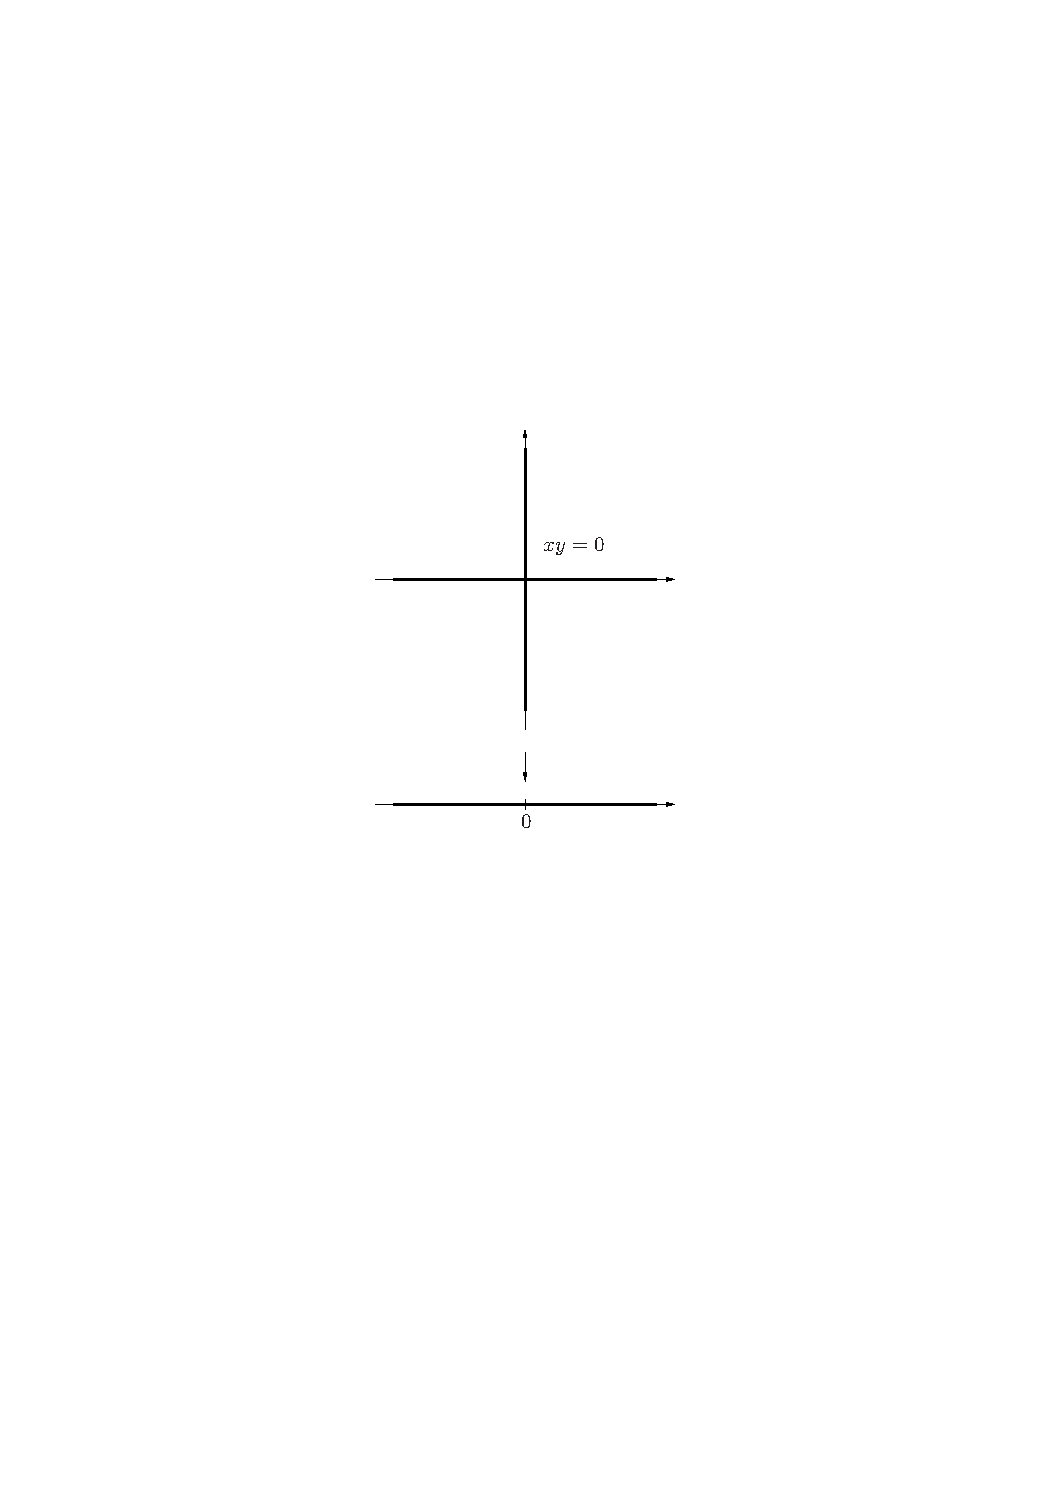
\includegraphics[width=0.3\textwidth]{pictures/flat.pdf}
\end{figure}
In terms of coordinate rings, this map corresponds to the homomorphism of $k$-algebras:
\[k[x]\to\dfrac{k[x,y]}{(xy)}\]
defined by mapping $x$ to the coset $x+(xy)$. This homomorphism defines a $k[x]$-module structure on $k[x, y]/(xy)$, and we can wonder whether the latter is flat. From the geometric point of view, clearly something not flat is going on over the point $x=0$, so we consider the inclusion of the ideal $(x)$ in $k[x]$:
\[\begin{tikzcd}
k[x]\ar[r,hook,"\cdot x"]&k[x]
\end{tikzcd}\]
Tensoring by $k[x,y]/(xy)$, we obtain
\[\begin{tikzcd}
\dfrac{k[x]}{(xy)}\ar[r,"\cdot x"]&\dfrac{k[x]}{(xy)}
\end{tikzcd}\]
which is not injective, because it sends to zero the nonzero coset $y+(xy)$. Therefore $k[x,y]/(xy)$ is not flat as a $k[x]$-module.\par
The term flat was inspired precisely by such geometric examples.
\end{example}
\subsection{The Tor functors}
The \textit{failure of exactness} of the functor $\otimes_{R}N$ is measured by another functor $R$-$\mathsf{Mod}\to R$-$\mathsf{Mod}$, called $\Tor_1^R(-,N)$: if $N$ is flat, then $\Tor^R_1(M,N)=0$ for all modules $M$. In fact if
\[\begin{tikzcd}
0\ar[r]&A\ar[r]&B\ar[r]&C\ar[r]&0
\end{tikzcd}\]
is an exact sequence of $R$-modules, one obtains a new exact sequence after tensoring by any $N$:
\[\begin{tikzcd}
\Tor^R_1(C,N)\ar[r]&A\otimes_{R}N\ar[r]&B\otimes_{R}N\ar[r]&C\otimes_{R}N\ar[r]&0
\end{tikzcd}\]
so if $\Tor^R_1(C,N)=0$, then the module on the left vanishes; thus every short exact sequence ending in $C$ remains exact after tensoring by $N$ in this case. In fact for all $N$ one can continue this sequence with more $\Tor$-modules, obtaining a longer exact complex:
\[\begin{tikzcd}[column sep=small]
\Tor^R_1(A,N)\ar[r]&\Tor^R_1(B,N)\ar[r]&\Tor^R_1(C,N)\ar[r]&A\otimes_{R}N\ar[r]&B\otimes_{R}N\ar[r]&C\otimes_{R}N\ar[r]&0
\end{tikzcd}\]
This is not the end of the story: the complex may be continued even further by invoking new functors $\Tor^R_2(-,N)$, $\Tor^R_3(-,N)$, etc. These are the \textbf{derived functors of tensor}. To \textit{compute} these functors, one may apply the following procedure: given an $R$-module $M$, find a free resolution
\[\begin{tikzcd}
\cdots\ar[r]&R^{\oplus s_2}\ar[r]&R^{\oplus s_1}\ar[r]&R^{\oplus s_0}\ar[r]&M\ar[r]&0
\end{tikzcd}\]
throw $M$ away, and tensor the free part by $N$, obtaining a complex $M_{\bullet}\otimes_{R}N$:
\[\begin{tikzcd}
\cdots\ar[r]&N^{\oplus s_2}\ar[r]&N^{\oplus s_1}\ar[r]&N^{\oplus s_0}\ar[r]&0
\end{tikzcd}\]
(recall again that tensor commutes with colimits, hence with direct sums, therefore $R^{\oplus m}\otimes_{R}N=N^{\oplus m}$); then take the homology of this complex. Astoundingly, this \textit{will not depend $($up to isomorphism$)$ on} the chosen free resolution,
so we can define
\[\Tor_i^{R}(M,N):=H_i(M_{\bullet}\otimes_{R}N)\]
For example, according to this definition $\Tor^R_0(M,N)\cong M\otimes_{R}N$, and $\Tor^R_i(M,N)=0$ for all $i>0$ and all $M$ if $N$ is flat (because then tensoring by $N$ is an exact functor, so tensoring the resolution of $M$ returns an exact sequence, thus with no homology). In fact, this proves a remarkable property of the $\Tor$ functors: if $\Tor^R_1(M,N)=0$ for all $M$, then $\Tor^R_i(M,N)=0$ for all $i>0$ and all modules $M$. Indeed, $N$ is then flat.\par
Since $M\otimes_{R}N$ is canonically isomorphic to $N\otimes_{R}M$ (in the commutative case), we could expect the same to apply to every $\Tor^R_i$: $\Tor^R_i(M,N)$ ought to be canonically isomorphic to $\Tor^R_i(N,M)$ for all $i$. Equivalently, we should be able to compute $\Tor^R_i(M,N)$ as the homology of $M\otimes_{R}N_{\bullet}$, where $N_{\bullet}$ is a free resolution of $N$. This is indeed the case.\par
In fact, we know enough about finitely generated modules over PIDs to get a preliminary sense of what is involved in proving such general facts. Recall that we have been able to establish that every finitely generated module $M$ over a PID $R$ has a free resolution of length $1$:
\[\begin{tikzcd}
0\ar[r]&R^{\oplus m_1}\ar[r]&R^{\oplus m_0}\ar[r]&M\ar[r]&0
\end{tikzcd}\]
This property characterizes PIDs. If
\[\begin{tikzcd}
0\ar[r]&A\ar[r]&B\ar[r]&C\ar[r]&0
\end{tikzcd}\]
is an exact sequence of $R$-modules, it is not hard to see that one can produce compatible resolutions, in the sense that the rows of the following diagram will be exact as well as the columns:
\[
\begin{tikzcd}
&0\ar[d]&0\ar[d]&0\ar[d]&\\
0\ar[r]&R^{\oplus a_1}\ar[d,"\alpha"]\ar[r]&R^{\oplus b_1}\ar[d,"\beta"]\ar[r]&R^{\oplus c_1}\ar[d,"\gamma"]\ar[r]&0\\
0\ar[r]&R^{\oplus a_0}\ar[d]\ar[r]&R^{\oplus b_0}\ar[d]\ar[r]&R^{\oplus c_0}\ar[d]\ar[r]&0\\
0\ar[r]&A\ar[r]\ar[d]&B\ar[r]\ar[d]&C\ar[r]\ar[d]&0\\
&0&0&0&
\end{tikzcd}
\]
Tensor the two free rows by $N$; they remain exact (tensoring commutes with direct sums):
\[
\begin{tikzcd}
0\ar[r]&N^{\oplus a_1}\ar[d,"\alpha\otimes N"]\ar[r]&N^{\oplus b_1}\ar[d,"\beta\otimes N"]\ar[r]&N^{\oplus c_1}\ar[d,"\gamma\otimes N"]\ar[r]&0\\
0\ar[r]&N^{\oplus a_0}\ar[r]&N^{\oplus b_0}\ar[r]&N^{\oplus c_0}\ar[r]&0\\
\end{tikzcd}
\]
Now the columns (preceded and followed by $0$) are precisely the complexes $A_{\bullet}\otimes_{R}N$, $B_{\bullet}\otimes_{R}N$, $C_{\bullet}\otimes_{R}N$ whose homology computes the Tor modules. Applying the snake lemma gives the exact sequence
\[\begin{tikzcd}
0\ar[r]&H_1(A_{\bullet}\otimes_{R}N)\ar[r] &H_1(B_{\bullet}\otimes_{R}N)\rar
\ar[draw=none]{d}[name=X, anchor=center]{}
&H_1(C_{\bullet}\otimes_{R}N)\ar[rounded corners,swap,
to path={ -- ([xshift=2ex]\tikztostart.east)
	|- (X.center) \tikztonodes
	-| ([xshift=-2ex]\tikztotarget.west)
	-- (\tikztotarget)}]{dll}[at end]{\delta}&\\      
&H_0(A_{\bullet}\otimes_{R}N)\rar &H_0(B_{\bullet}\otimes_{R}N)\rar &H_0(C_{\bullet}\otimes_{R}N)\ar[r]&0
\end{tikzcd}\]
which is precisely the sequence of $\Tor$ modules conjured up above.\par
Note that $\Tor^k_i$ vanishes for $i>0$ if $k$ is a field, as vector spaces are flat, and $\Tor^R_i$ vanishes for $i>1$ if $R$ is a PID.
\subsection{Exercise}
$R$ denotes a fixed commutative ring.
\begin{exercise}
Let $M,N$ be $R$-modules, and assume that $N$ is cyclic. Prove that every element of $M\otimes_{R}N$ may be written as a pure tensor.
\end{exercise}
\begin{proof}
Every element in $\otimes_{R}N$ has the form
\[\sum_im_i\otimes n_i=\sum_im_i\otimes(r_in)=\sum_i(r_im_i)\otimes n=(\sum_i r_im_i)\otimes n\]
\end{proof}
\begin{exercise}
Prove by hand $($that is, without appealing to the right-exactness of tensor$)$ that $\Z/n\Z\otimes_{\Z}\Z/m\Z\cong0$ if $m,n$ are relatively prime integers.
\end{exercise}
\begin{proof}
For $\Z/m\Z$, $\Z/n\Z$, We have:
\[m(a\otimes b)=(0\otimes b)=0\cdot(0\otimes b)=0\]
and 
\[n(a\otimes b)=(a\otimes 0)=0\cdot(a\otimes 0)=0\]
since $\gcd(m,n)=1$, there is $u,v\in\Z$ such that 
\[um+vn=1.\]
Then this gives $(a\otimes b)=0$.
\end{proof}
\begin{exercise}
Prove that $R[x_1,\dots,x_n]\otimes_{R}R[y_1,\dots,y_m]\cong R[x_1,\dots,x_n,y_1,\dots,y_m]$.
\end{exercise}
\begin{proof}
For any bilinear function $\theta:R[x_1,\dots,x_n]\times R[y_1,\dots,y_m]\to P$, we have an induced homomorphism:
\[(f,g)\mapsto(fg)\stackrel{\widetilde{\theta}}{\mapsto}\theta(f,g)\for f\in R[x_1,\dots,x_n], g\in R[y_1,\dots,y_m]\]
this is a $R$-linear map. So $R[x_1,\dots,x_n,y_1,\dots,y_m]$ satisfies the universal property of $R[x_1,\dots,x_n]\otimes_{R}R[y_1,\dots,y_m]$.
\end{proof}
\begin{exercise}
Let $S,T$ be commutative $R$-algebras. Verify the following:
\begin{itemize}
\item The tensor product $S\otimes_{R}T$ has an operation of multiplication, defined on pure tensors by $(s_1\otimes t_1)\cdot(s_2\otimes t_2):=s_1s_2\otimes t_1t_2$ and making it into a commutative $R$-algebra.
\item With respect to this structure, there are $R$-algebra homomorphisms $i_S:S\to S\otimes T$, resp., $i_T:T\to S\otimes T$, defined by $i_S(s):=s\otimes1$, $i_T(t):=1\otimes t$.
\item The $R$-algebra $S\otimes_{R}T$, with these two structure homomorphisms, is a coproduct of $S$ and $T$ in the category of commutative $R$-algebras: if $U$ is a commutative $R$-algebra and $f_S:S\to U$, $f_T:T\to U$ are $R$-algebra homomorphisms, then there exists a unique $R$-algebra homomorphism $f_S\otimes f_T$ making the following diagram commute:
\[\begin{tikzcd}
S\ar[rd,swap,"i_S"]\ar[rrrd,bend left=20,"f_S"]&&\\
&S\otimes_{R}T\ar[rr,"f_S\otimes f_T"]&&U\\
T\ar[ru,"i_T"]\ar[rrru,swap,bend right=20,"f_T"]
\end{tikzcd}\]
In particular, if $S$ and $T$ are simply commutative rings, then $S\otimes_{\Z}T$ is a coproduct of $S$ and $T$ in the category of commutative rings.
\end{itemize}
\begin{proof}
Define
\[f_S\otimes f_T(s\otimes t):=f_S(s)f_T(t)\]
this is an $R$-algebra homomorphsim.
\end{proof}
\end{exercise}
\begin{exercise}
Changing the base ring in a tensor may or may not make a difference:
\begin{itemize}
\item Prove that $\Q\otimes_{\Z}\Q\cong\Q\otimes_{\Q}\Q$.
\item Prove that $\C\otimes_{\R}\C\not\cong\C\otimes_{\C}\C$.
\end{itemize}
\end{exercise}
\begin{proof}
$\Q$-$\mathsf{Vect}$ is a full subcategory of $\Z$-$\mathsf{Mod}$, since every $\Z$-linear homomorphism can be extended to be a $\Q$-linear homomorphism.
\end{proof}
\begin{exercise}
Let $R$ be an integral domain, with field of fractions $K$, and let $M$ be a finitely generated R-module. The tensor product $V:= M\otimes_{R}K$ is a $K$-vector space. Prove that $\dim_KV$ equals the rank of $M$ as an $R$-module,
\end{exercise}
\begin{proof}
The scalar product of $V$ is defined to be
\[\dfrac{a}{s}\cdot(m\otimes\dfrac{b}{t}):=m\otimes\dfrac{ab}{st}=(am)\otimes\dfrac{b}{st}\]
it is obvious that basis in $M$ can be transformed into a basis of $V$.
\end{proof}
\begin{exercise}
Let $G$ be a finitely generated abelian group of rank $r$. Prove that $G\otimes_{\Z}\Q\cong\Q^r$.
Prove that for infinitely many primes $p$, $G\otimes_{\Z}(\Z/p\Z)\cong(\Z/p\Z)^r$.
\end{exercise}
\begin{proof}
Since every finite generated abelian group of rank $r$ can be written into $G=\Z^r\oplus T$ where $T$ is a torsion group, we may prove that $T\otimes_{\Z}=0$, then the claim follows from the fact that
\[(\Z^r\oplus T)\otimes_{\Z}\Q\cong (\Z^r\otimes_{\Z}\Q)\oplus(T\otimes_{\Z}\Q)=\Z^r\otimes_{\Z}\Q=\Q^r\]
But this follows from the observation that
\[\dfrac{p}{q}\otimes g=\dfrac{Np}{Nq}\otimes g=\dfrac{p}{q}\otimes Ng=\dfrac{p}{q}\otimes 0=0\]
where $N\in\Ann(T)$.
\end{proof}
\begin{exercise}
Prove that direct sums of flat modules are flat.
\end{exercise}
\begin{proof}
Corollary~\ref{tensor sum}.
\end{proof}
\begin{exercise}
Prove that, according to the definition, $\Tor^R_0(M,N)$ is isomorphic to $M\otimes_RN$.
\end{exercise}
\begin{proof}
$\Tor^R_0(M,N)=H_0(M_{\bullet}\otimes_{R}N)$. For a free resolution of $M$:
\[\begin{tikzcd}
\cdots\ar[r]&R^{\oplus s_2}\ar[r]&R^{\oplus s_1}\ar[r,"\psi"]&R^{\oplus s_0}\ar[r]&M\ar[r]&0
\end{tikzcd}\]
we know that $M=R^{s_0}/\im\psi$. Since $\otimes_{R}N$ is a left-adjoint funtor, it is right exact. So
\[\begin{tikzcd}
R^{\oplus s_1}\otimes_{R}N\ar[r,"\psi\otimes N"]&R^{\oplus s_0}\otimes_{R}N\ar[r]&M\otimes_{R}N\ar[r]&0
\end{tikzcd}\]
is an exact sequence. Since $R^{\oplus s_0}\otimes N/\im(\psi\otimes N)$ is the homology $H_0$, we get the result.
\end{proof}
\begin{exercise}\label{Tor(R/(r),M)}
Prove that for $r\in R$ a non-zero-divisor and $N$ an $R$-module, the module $\Tor^R_1(R/(r),N)$ is isomorphic to the $r$-torsion of $N$, that is, the submodule of elements $n\in N$ such that $rn=0$. $($This is the reason why $\Tor$ is called $\Tor$.$)$
\end{exercise}
\begin{proof}
Consider an exact sequence (the free resolution of $R/(r)$)
\[\begin{tikzcd}
0\ar[r]&(r)\ar[r,"i"]&R\ar[r]&R/(r)\ar[r]&0
\end{tikzcd}\]
Tensoring with $N$ gives an exact sequence
\[\begin{tikzcd}
(r)\otimes_{R}N\ar[r,"i\otimes N"]&N\ar[r]&R/(r)\otimes_{R}N\ar[r]&0
\end{tikzcd}\]
So
\[H_1=\ker(i\otimes N)=\ker(M\stackrel{r}{\to}M)=M_r.\]
\end{proof}
\begin{exercise}
Let $I,J$ be ideals of $R$. Prove that $\Tor^R_1(R/I,R/J)\cong(I\cap J)/IJ$. $($For example, this $\Tor^R_1$ vanishes if $I+J=R$.$)$ Prove that $\Tor^R_i(R/I,R/J)$ is isomorphic to $\Tor^R_{i-1}(I,R/J)$ for $i>1$.
\end{exercise}
\begin{proof}
First, we compute $\Tor^R_1(R,R/J)$. For the free resolution of $R$:
\[\begin{tikzcd}
0\ar[r]&R\ar[r]&R\ar[r]&0
\end{tikzcd}\]
tensoring $R/J$ gives
\[\begin{tikzcd}
0\ar[r]&R\otimes R/J\ar[r]&R\otimes R/J\ar[r]&0
\end{tikzcd}\]
so we find $\Tor_0^R(R,R/J)=R/J$, and $\Tor^R_i(R,R/J)=0$ for $i>0$.\par
Now for the exat sequence
\[\begin{tikzcd}
0\ar[r]&I\ar[r]&R\ar[r]&R/I\ar[r]&0
\end{tikzcd}\]
tensoring with $R/J$ gives a new exact sequence:
\[\begin{tikzcd}[column sep=small]
\Tor_1^R(R,R/J)\ar[r]&\Tor_1^R(R/I,R/J)\ar[r]&I\otimes R/J\ar[r]&R\otimes R/J\ar[r]&R/I\otimes R/J\ar[r]&0
\end{tikzcd}\]
With $\Tor_1^R(R,R/J)=0$, $I\otimes R/J=I/IJ$, $R\otimes R/J=R/J$, $R/I\otimes R/J=R/(I+J)$, this becomes
\[\begin{tikzcd}
0\ar[r]&\Tor_1^R(R/I,R/J)\ar[r]&\dfrac{I}{IJ}\ar[r,"\psi"]&R/J\ar[r]&\dfrac{R}{I+J}\ar[r]&0
\end{tikzcd}\]
so we have $\Tor_1^R(R/I,R/J)\cong\ker\psi$. Since $\psi$ maps $I$ to $R$, its kernel should be
\[\ker\psi=\{i+IJ\mid i\in J\}=\dfrac{I\cap J}{IJ}\]
so the first claim follows.\par
\end{proof}
\begin{exercise}
Let $M,N$ be modules over a PID $R$. Prove that $\Tor^R_i(M,N)=0$ for $i\geqslant2$. $($Assume $M,N$ are finitely generated, for simplicity.$)$
\end{exercise}
\begin{proof}
The resolution of finitely generated over a module has length $\leqslant 1$.
\end{proof}
\begin{exercise}\label{flat iff free}
Let $R$ be an integral domain. Prove that a cyclic $R$-module is flat if and only if it is free.
\end{exercise}
\begin{proof}
Let $M=\langle m\rangle$ be a cyclic module. If $M$ is free, then it has a free resolution
\[\begin{tikzcd}
0\ar[r]&R\ar[r]&\langle m\rangle\ar[r]&0
\end{tikzcd}\]
tensoring with any module $M$, it is clear that $\Tor^R_i(M,N)=0$ fro $i>0$, so $M$ is flat.\par
Conversely, if $M$ is flat, since $M\cong R/I$ for some ideal $I$, $R$ is free if and only if it is torsion free. For any fixed $r\in R$, consider the map $\psi:R\to R,\quad x\mapsto rx$. If $r\neq0$, since $R$ is an integral domain, $\psi$ is injective. Now $M$ is flat, so $\psi\otimes M$ is also injective. But $\psi\otimes M$ has the expression:
\[\psi\otimes M:R\otimes M\to R\otimes M,\quad x\otimes m\mapsto rx\otimes m\]
so it can be viewed as a map $\psi\otimes M:M\to M$ sending $m$ to $rm$. Since this is injective for any nonzero $r\in R$, we concluede $M$ is torsion free, hence free.
\end{proof}
\begin{exercise}\label{flat crit}
The following criterion is quite useful.
\begin{itemize}
\item Prove that an $R$-module $M$ is flat if and only if every monomorphism of $R$ modules $A\to B$ induces a monomorphism of $R$-modules $A\otimes M\to B\otimes M$.
\item Prove that it suffices to verify this condition for all finitely generated modules $A$, $B$.
\item Prove that it suffices to verify this condition when $B=R$ and $A=I$ is an ideal of $R$.
\item Deduce that an $R$-module $M$ is flat if and only if the natural homomorphism $I\otimes_{R}M\to IM$ is an isomorphism for every ideal $I$ of $R$.
\end{itemize}
If you believe in $\Tor$'s, now you can also show that an $R$-module $M$ is flat if and only if $\Tor^R_1(R/I,M)=0$ for all ideals $I$ of $R$.
\end{exercise}
\begin{proof}
\mbox{}
\begin{itemize}
\item This is obvious.
\item An element $\sum_ia_i\otimes m_i\in A\otimes_{R}M$ goes to zero in $B\otimes_{R}M$ if the
corresponding element $\sum_i(f(a_i),m_i)$ equals a combination of the relations defining $B\otimes_{R}M$ in the free $R$-module $F^R(B\times M)$. This will be an identity involving only finitely many elements of $A$ and $B$; hence we should only consider the submodule $N$ of $A$ and $S$ of $B$ generated by these elements and the restricted morphism from $N\otimes M\to S\otimes M$. If the condition is satisfied by finite generated modules, then this will be a monomorphism, so we get $\sum_ia_i\otimes m_i=0$ as needed.
\item We may now assume that $B$ is finitely generated. Find submodules $B_j$ such that $A=B_0\sub B_1\sub\cdots\sub B_r=B$, with each $B_j/B_{j-1}$ cyclic. Reduce to verifying that $A\otimes M$ injects in $B\otimes_{R} M$ when $B/A$ is cyclic, hence $\cong R/I$ for some ideal $I$. Now consider the exact sequence
\[\begin{tikzcd}
\Tor^R_1(B/A,M)\ar[r]&A\otimes M\ar[r]&B\otimes M\ar[r]&B/A\otimes M\ar[r]&0
\end{tikzcd}\]
the claim follows if and only if $\Tor^R_1(B/A,M)=\Tor^R_1(R/I,M)=0$.
\item $I\otimes M\to IM$ is clearly surjective. $M$ is flat iff $\Tor^R_1(R/I,M)=0$, if and only if $I\otimes M\to IM$ is injective.
\end{itemize}
\end{proof}
\begin{exercise}\label{PID flat iff torsion}
Let $R$ be a PID. Prove that an $R$-module $M$ is flat if and only if it is torsion free.\par
Geometrically, this says roughly that an algebraic set fails to be flat over a nonsingular curve if and only if some component of the set is contracted to a point.
\end{exercise}
\begin{proof}
Let $T$ be the torsion part of $M$, and let $r\in\Ann(x)$ for some $x\in M$. Then by Exercise~\ref{Tor(R/(r),M)}, $\Tor(R/(r),M)=M_r$ the $r$-torsion submodule of $M$. Since by Exercise~\ref{flat crit}, $M$ is flat iff this Tor is zero, we conclude that $M$ is flat iff $M$ is torsion-free.
\end{proof}
\begin{exercise}\label{local Tor}
Let $M,N$ be $R$-modules, and let $S$ be a multiplicative subset of $R$. Use the definition of $\Tor$ to show $S^{-1}\Tor^R_i(M,N)\cong\Tor^{S^{-1}R}_i(S^{-1}M,S^{-1}N)$.\par
Use this fact to give a leaner proof that flatness is a local property.
\end{exercise}
\begin{proof}
For a resolution of $M$:
\[\begin{tikzcd}
\cdots\ar[r]&R^{\oplus s_2}\ar[r]&R^{\oplus s_1}\ar[r]&R^{\oplus s_0}\ar[r]&M\ar[r]&0
\end{tikzcd}\]
tensoring with $N$ gives the computation of $\Tor^R_i(M,N)$:
\[\begin{tikzcd}
\cdots\ar[r]&N^{\oplus s_2}\ar[r]&N^{\oplus s_1}\ar[r]&N^{\oplus s_0}\ar[r]&0
\end{tikzcd}\]
By Exercise~\ref{locali exact}, $S^{-1}H_i(M_{\bullet}\otimes_{R}N)\cong H_i(S^{-1}(M_{\bullet}\otimes_{R}N))$.\par
First we check that localization commutes with direct sum. That is, $S^{-1}(R^{\oplus r})=(S^{-1}R)^{\oplus r}$. In fact, we have a natural isomorphism:
\[\theta:\dfrac{(a_1,\dots,a_r)}{s}\mapsto\Big(\dfrac{a_1}{s},\dots,\dfrac{a_r}{s}\Big)\]
This is surjective since for any element in $(S^{-1}R)^{\oplus r}$:
\[\Big(\dfrac{a_1}{s_1},\dots,\dfrac{a_r}{s_r}\Big)=\Big(\dfrac{a_1\prod_{i\neq 1}s_i}{s_1\cdots s_r},\dots,\dfrac{a_r\prod_{i\neq r}s_i}{s_1\cdots s_r}\Big)=\theta\Big(\dfrac{a_1\prod_{i\neq 1}s_i,\dots,a_r\prod_{i\neq r}s_i}{s_1\cdots s_r}\Big)\]
The injectivity follows from
\[\Big(\dfrac{a_1}{s},\dots,\dfrac{a_r}{s}\Big)=0\iff (\exists t_i\in S)\ t_ia_i=0\Rightarrow \dfrac{(a_1,\dots,a_r)}{s}=\dfrac{(a_1t_1\prod_{i\neq 1}t_i,\dots,a_rt_r\prod_{i\neq r}t_i)}{s\prod_it_i}=0\]
With this, apply localization gives
\[S^{-1}(N^{\oplus s})=S^{-1}(R^{\oplus s}\otimes_{R}N)=(S^{-1}R^{\oplus s})\otimes_{S^{-1}R}N\cong (S^{-1}R)^{\oplus s}\otimes_{R}N\cong(S^{-1}R)^{\oplus s}\otimes_{S^{-1}R}(S^{-1}N)\]
where we use Exercise~\ref{local tensor}. Now the claim follows from that localizing the sequence
\[\begin{tikzcd}
\cdots\ar[r]&R^{\oplus s_2}\ar[r]&R^{\oplus s_1}\ar[r]&R^{\oplus s_0}\ar[r]&M\ar[r]&0
\end{tikzcd}\]
gives a resolution of $S^{-1}M$.
\end{proof}
\begin{exercise}\label{flat exact sequence}
Let
\[\begin{tikzcd}
0\ar[r]&M\ar[r]&N\ar[r]&P\ar[r]&0
\end{tikzcd}\]
be an exact sequence of $R$-modules, and assume that $P$ is flat.
\begin{itemize}
\item Prove that $M$ is flat if and only if $N$ is flat.
\item Prove that for all R-modules Q, the induced sequence
\[\begin{tikzcd}
0\ar[r]&M\otimes_{R}Q\ar[r]&N\otimes_{R}Q\ar[r]&P\otimes_{R}Q\ar[r]&0
\end{tikzcd}\]
is exact.
\end{itemize}
\end{exercise}
\begin{proof}
\mbox{}
\begin{itemize}
\item For any $R$-module $Q$, the sequence
\[\begin{tikzcd}
0\ar[r]&\Tor^R_1(M,Q)\ar[r]&\Tor^R_1(N,Q)\ar[r]&\Tor^R_1(P,Q)\ar[r]&0
\end{tikzcd}\]
is also exact. Since $\Tor^R_1(P,Q)=0$, we get the claim.
\item Tensoring $Q$ gives an exact sequence:
\[\begin{tikzcd}
\Tor^R_1(P,Q)\ar[r]&M\otimes_{R}Q\ar[r]&N\otimes_{R}Q\ar[r]&P\otimes_{R}Q\ar[r]&0
\end{tikzcd}\]
since $P$ is flat, $\Tor^R_1(P,Q)=0$, we get the claim.
\end{itemize}
\end{proof}
\begin{exercise}\label{local flat iff free}
Let $R$ be a commutative Noetherian local ring with $(single)$ maximal ideal $\mathfrak{m}$, and let $M$ be a finitely generated flat $R$-module.
\begin{itemize}
\item Choose elements $m_1,\dots,m_r\in M$ whose cosets mod $\mathfrak{m}M$ are a basis of $M/\mathfrak{m}M$ as a vector space over the field $R/\mathfrak{m}$. By Nakayama's lemma, $M=\langle m_1,\dots,m_r\rangle$.
\item Obtain an exact sequence
\[\begin{tikzcd}
0\ar[r]&N\ar[r]&R^{\oplus r}\ar[r]&M\ar[r]&0
\end{tikzcd}\]
where $N$ is finitely generated.
\item Prove that this sequence induces an exact sequence
\[\begin{tikzcd}
0\ar[r]&N/\mathfrak{m}N\ar[r]&(R/\mathfrak{m})^{\oplus r}\ar[r]&M/\mathfrak{m}M\ar[r]&0
\end{tikzcd}\]
\item Deduce that $N=0$.
\item Conclude that $M$ is free.
\end{itemize}
Thus, a finitely generated module over a (Noetherian) local ring is flat if and only if it is free.
\end{exercise}
\begin{proof}
\mbox{}
\begin{itemize}
\item Since $M$ is generated by $m_1,\dots,m_r$, there is a epimorphism from $R^{\oplus r}$ to $M$.
\item By Exercise~\ref{flat exact sequence}, tensoring with $R/\mathfrak{m}$ gives the exact sequence. Since we have $(R/I)\otimes N\cong N/IN$.
\item Since $M/\mathfrak{m}M$ is a vector space over $R/\mathfrak{m}$ with basis $m_1+\mathfrak{m}M,\dots,m_r+\mathfrak{m}M$, we must have $N/\mathfrak{m}N=0$. Then $N=\mathfrak{m}M$, by Nakayama's Lemma, $N=0$.
\item Since $N=0$, we get $M\cong R^{\oplus r}$.
\end{itemize}
\end{proof}
\begin{exercise}
Let $R$ be a commutative Noetherian ring, and let $M$ be a finitely generated $R$-module. Prove that
\[M\text{ is flat}\iff \Tor^R_1(M,R/\mathfrak{m})=0\text{ for every maximal ideal $\mathfrak{m}$ of $R$}\]
\end{exercise}
\begin{proof}
On direction is trivial. So we assume that $\Tor^R_1(M,R/\mathfrak{m})=0$ for every maximal ideal $\mathfrak{m}$. Since we only need to show $M_{\mathfrak{m}}$ is flat for every maximal ideal $\mathfrak{m}$, we localize $\Tor$ to get
\[\Tor^{R_\m}_1(M_\m,R_\m/\m R_\m)=0\]
Hence we may assume $A$ is local. Then as in the proof of Proposition~\ref{local flat iff free}, we can show $M_\m$ is free, hence is flat.
\end{proof}
\section{Base change}
In this section, we connect the modules on two different rings, i.e., we consider the functors between two categories $R$-$\mathsf{Mod}$ and $S$-$\mathsf{Mod}$. To fit further applications of this topic, we are \textit{not} assuming that $R$ and $S$ are commutative. Thus we have to deal with left and right modules.
\subsection{Tensor products over noncommutative ring}
Let $R$ be a ring (not necessarily commutative), and $M$ be a right $R$-module, $N$ a left $R$-module. We indicate this situation by writing $M_R$ and $_{R}N$ in the respective cases. Let $P$ be an abelian group. A $\Z$-bilinear map $f:M\times N\to P$ is \textbf{$\bm{R}$-balanced} or an \textbf{$\bm{R}$-balanced product} if for any $r\in R$, $m\in M$, $n\in N$ we have
\[f(mr,n)=f(m,rn).\]
In this situation, we denote the $R$-balanced map by $(P,f)$. If $(L,g)$ is a second one, then we define a morphism from $(P,f)$ to $(L,g)$ to be a homomorphism $\varphi$ of the additive group $P$ into the additive group $L$ such that for any $m\in M$, $n\in N$ we have
\[g(m,n)=\varphi(f(m,n)).\]
That is, we require the following diagram to commute:
\[\begin{tikzcd}[column sep=small, row sep=small]
&P\ar[dd,"\varphi"]\\
M\times N\ar[rd,swap,"g"]\ar[ru,"f"]&\\
&L
\end{tikzcd}\]
Therefore the balanced maps from $M\times N$ form a category, which we may denote by $\mathcal{B}(M,N)$. We can now introduce the following definition.
\begin{definition}
Then \textbf{tensor product} of $M_{R}$ and $_{R}N$ is a balanced product $(M\otimes_RN,\otimes)$ such that if $(P,f)$ is any balanced product of $M_{R}$ and $_{R}N$, then there exists a unique morphism of $(M\otimes_{R}N,\otimes)$ to $(P,f)$:
\[\begin{tikzcd}[column sep=small, row sep=small]
&M\otimes_{R}N\ar[dd,"\exists!"]\\
M\times N\ar[rd,swap,"f"]\ar[ru,"\otimes"]&\\
&P
\end{tikzcd}\]
In other words, $(M,\otimes_{R}N,\otimes)$ is the initial object in the category $\mathcal{B}(M,N)$.
\end{definition}
The tensor product defined above can be constructed similarly to the commutative case. We now establish them in detail.
\begin{proposition}
The tensor product $M\otimes_RN$ exists for any modules $M_{R}$ and $_{R}N$.
\end{proposition}
\begin{proof}
Consider the free abelian group $\Z^{\oplus(M\times N)}$. Let $K$ be the subgroup that is generated by elements of the form
\[\begin{array}{c}
(m,n_1+n_2)-(m,n_1)-(m,n_2)\\
(m_1+m_2,n)-(m_1,n)-(m_2,n)\\
(rm,n)-(m,rn)
\end{array}\]
with $m,m_1,m_2\in M$, $n,n_1,n_2\in N$, $r\in R$. It is now easy to check that the quotient $\Z^{\oplus(M\times N)}/K$, together with the map
\[\otimes:M\times N\to \Z^{\oplus(M\times N)}/K,\quad(m,n)\mapsto(m,n)+K\]
satisfies the condition required.
\end{proof}
We simplify the notation to $M\otimes N$ or $M\otimes_RN$ if we need to specify the ring $R$, and we speak of the tensor product of $M$ and $N$. Now suppose we have module homomorphisms $f:M\to M'$ and $g:N\to N'$. Then we have the map
\[M\times N\to M'\otimes N',\quad (m,n)\mapsto f(m)\otimes g(n)\]
which satisfies the conditions for a balanced product of $M$ and $N$ by the definition of tensor product. Hence we have a unique homomorphism of $f\otimes g:M\otimes N\to M'\otimes N'$ such that
\[(f\otimes g)(m,n)=f(m)\otimes g(n).\]
Suppose next that we have homomorphisms $f':M'\to M''$ and $g':N'\to N''$, then it is clear that
\[(f'\circ f)\otimes(g'\circ g)(m\otimes n)=(f'(f(m)))\otimes(g(g'(n))),\]
and therefore
\[(f'\circ f)\otimes(g'\circ g)=(f'\otimes f)\otimes(g'\circ g).\]
Since $(\id_M\otimes\id_N)(m\otimes n)=m\otimes n$, we have $\id_M\otimes\id_N=\id_{M\otimes N}$. These results amount to saying we have defined a functor $\mathsf{Mod}\text{-$R$}\times\text{$R$-}\mathsf{Mod}\to\mathsf{Ab}$. We shall denote this functor as $\otimes_R$.\par
We shall now fix one of the arguments in the functor $\otimes_R$ and study the resulting functors of one variable. Let $M$ be a fixed right $R$-module. Then we define the functor $M\otimes_R$ (or $M\otimes$) from $R$-$\mathsf{Mod}$ to $\Z$-$\mathsf{Mod}$ by specifying that for any left $R$-module $N$ and any homomorphism $g:N\to N'$ of left $R$-modules, we have
\[(M\otimes_R)(N)=M\otimes_RN,\quad (M\otimes_R)(g)=\id_M\otimes g.\]
From this definition, the functorial properties are easy to verify. In a similar manner, any left module defines a functor $\otimes_RN$ (or $\otimes N$) from $\mathsf{Mod}$-$R$ to $\mathsf{Mod}$-$\Z$ by
\[(\otimes_RN)(M)=M\otimes_RN,\quad (N\otimes_R)(f)=f\otimes\id_N.\]
for $f:M\to M'$ in $\mathsf{Mod}$-$R$. The properties of $M\otimes_R$ and $\otimes_RN$ are similar to the commutative case. To simplify the discussion, we will establish them for tensor product of bimodules.
\begin{example}
Let $R^{op}$ be the opposite ring of $R$ and regard a right (left) $R$-module as a left (right) $R^{op}$-module in the usual way. Consider the map
\[s:M\times N\to N\times M,\quad (m,n)\mapsto(n,m).\]
If $f:N\times M\to P$ is a $R^{op}$-balanced product, then
\[(f\circ s)(m\cdot r,n)=f(n,m\cdot r)=f(n,rm=f(nr,m)=f(r\cdot n,m)=(f\circ s)(m,r\cdot n).\]
Therefore $f\circ s$ is a $R$-balanced map, and we get a map $f^s:M\otimes N\to P$. Take $P=N\otimes_{R^{op}}M$, we get a map
\[\otimes^s:M\otimes_{R}N\to N\otimes_{R^{op}}M,\quad m\otimes n\mapsto n\otimes m.\]
This is clearly an isomorphism, therefore we get $M\otimes_{R}N\cong N\otimes_{R^{op}}M$ as groups.
\end{example}
\subsection{Bimodules}
Let $M$ be a right $R$-module and let $S=\End_R(M)$. Then $M$ can be regarded as a left $S$-module if we define $fx$ for $f\in S$, $x\in M$, to be the image of $m$ under the map $f$. Since $f$ is a homomorphism of the additive group of $M$, we have $f(x+y)=f(x)+f(y)$, and by definition of the sum and product of homomorphisms, we have $(f+g)x=f(x)+g(x)$ and $(fg)x=f(gx)$ if $f,g\in S$. Clearly also $\id x=x$ so $M$ is a left $S$-module. Also the definition of module homomorphism gives the relation
\[(fx)r=f(x)r=f(xr).\]
for $x\in M$, $r\in R$, $f\in S$. This associativity connects the given right $R$-module structure with the left $S$-module structure of $M$. Similarly, if $M$ is a left $R$-module, then by acting homomorphisms on the right:
\[xf:=f(x)\]
we see that $M$ can be made into a right $S$-module. More generally, we now introduce the following definition.
\begin{definition}
Let $R$ and $S$ be rings. An $(R,S)$-\textbf{bimodule} is an abelian group $M$ endowed with compatible $R$-module and $S$-module structures, in the sense that
\[r(xs)=(rx)s\]
for any $r\in R$, $s\in S$, $x\in M$.
\end{definition}
The foregoing considerations show that if $M$ is a right $R$-module, then $M$ can be regarded in a natural way as an $(S,R)$-bimodule for $S=\End_R(M)$.
\begin{example}[\textbf{Examples of bimodules}]
\mbox{}
\begin{itemize}
\item[(a)] Let $R$ be commutative. Then any right $R$-module $M$ can be regarded also as a left $R$-module by putting $rx=xr$, $r\in R$, $x\in M$. It is often advantageous to regard $M$ as an $(R,R)$-bimodule. The associativity condition $r(xr')=(rx)r'$ is an immediate consequence of the commutativity of $R$.
\item[(b)] Again let $R$ be commutative and let $\varphi$ be an automorphism of $R$. If $M$ is a right $R$-module, $M$ becomes a left $R$-module by defining $rx=\varphi(r)(x)$. This action together with the given right action makes $M$ an $(R,R)$-bimodule.
\item[(c)] Any right $R$-module can be regarded as a $(\Z,R)$-bimodule by defining $nx$ for $n\in\Z$ in the usual way. Similarly, any left $R$-module becomes an $(R,\Z)$-bimodule. In this way the theory of one-sided modules can be subsumed in that of bimodules.
\item[(d)] If $R$ is a ring, we have the left module $_{R}R$ and the right module $R_{R}$. Since we have the associative law $(rx)s=r(xs)$, we can put the two module structures together to obtain a bimodule.
\end{itemize}
\end{example}
If $M$ is a right $R$-module and $N$ is a left $R$-module, then the tensor product $M\otimes_{R}N$ acquires an $\Z$-module structure: define the action of $s,t\in\Z$ on pure tensors $m\otimes n$ by
\[s(m\otimes n)t:=(sm)\otimes(tn)\]
and extend to all tensors by linearity. More generally, if $_{Q}M_{R}$ and $_{R}N_{S}$ are bimodules, then the tensor product $M\otimes_RN$ has a $(Q,S)$-bimodule structure which is defined by
\[q(m\otimes n)s=(qm)\otimes(ns)\]
for $q\in Q$, $s\in S$.\par
With this observation, we now consider the balanced products of bimodules. Let $_{Q}M_{R}$, $_{R}N_{S}$ and $_{Q}P_{S}$ be bimodules. A $R$-balanced map $f:M\times N\to P$ is called \textbf{$\bm{(Q,R,S)}$-balanced} or a \textbf{$\bm{(Q,R,S)}$-balanced product} if for $q\in Q$ and $s\in S$ we have
\[f(qx,ys)=qf(x,y)s.\]
If $(L,g)$ is another such map, then a morphism from $(P,f)$ to $(L,g)$ is a $(Q,S)$-homomorphism from $P$ to $L$ such that $\varphi\circ f=g$. In this way we get a category $\mathbf{Bil}(M,N)$.\par
From the argument above, we see $M\times N\to M\otimes_RN$ is $(Q,R,S)$-balanced. We may also define the tensor product of $_{Q}M_{R}$ and $_{R}N_{S}$ to be the initial object in the category $\mathbf{Bil}(M,N)$, but it is clear that it is isomorphic to $M\otimes_RN$.\par
Similarly, be defining tensor product of morphisms, we get a functor
\[\otimes:(Q,R)\text{-}\mathsf{Mod}\times(R,S)\text{-}\mathsf{Mod}\to(Q,S)\text{-}\mathsf{Mod}.\]
Now we give some properties of the tensor product.
\begin{proposition}
Let $(M_i)_{i\in I}$ be $(Q,R)$-bimodules and $(N_j){j\in J}$ be $(R,S)$-bimodules. Then there are canonical $(Q,S)$-homomorphisms
\[\begin{tikzcd}
(\prod_{i\in I}N_i)\otimes_R(\prod_{j\in J}N_j)\ar[r]&\prod_{(i,j)\in I\times J}M_i\otimes_RN_j\\
(\bigoplus_{i\in I}N_i)\otimes_R(\bigoplus_{j\in J}N_j)\ar[u,hook]\ar[r,"\cong"]&\bigoplus_{(i,j)\in I\times J}M_i\otimes_RN_j\ar[u,hook]
\end{tikzcd}\]
\end{proposition}
\begin{proof}
Note there is a $(Q,S)$-balanced map
\[\prod_{i\in I}M_i\times\prod_{j\in J}N_j\to\prod_{(i,j)\in I\times J}M_i\otimes N_j,\quad((x_i)_{i},(y_j)_{j})\mapsto(x_i\otimes y_j)_{i,j}\]
Since the restriction of this map on $\bigoplus_{i\in I}M_i\times\bigoplus_{j\in J}N_j$ has image in $\bigoplus_{(i,j)}M_i\otimes_RN_j$, we get the claimed maps. Let $\Phi$ be the homomorphism on the direct sum.\par
Let $P$ be a $(Q,S)$-bimodule, then the following diagram is easy to verify:
\[\begin{tikzcd}
\Hom((\bigoplus_{i\in I}N_i)\otimes_R(\bigoplus_{j\in J}N_j),P)\ar[r,"\cong"]&\mathcal{B}(\bigoplus_{i}M_i,\bigoplus_jN_j;P)\ar[d,"\cong"]\\
&\prod_{i,j}\mathcal{B}(M_i,N_j;P)\\
\Hom(\bigoplus_{(i,j)\in I\times J}M_i\otimes_RN_j,P)\ar[uu,"\Phi^*"]\ar[r,"\cong"]&\prod_{i,j}\Hom(M_i\otimes_RN_j,P)\ar[u,swap,"\cong"]
\end{tikzcd}\]
This proves that $\Phi$ is an isomorphism.
\end{proof}
\begin{proposition}
Let $_{Q}M_{R}$, $_{R}N_{S}$, $_{S}L_{T}$ be bimodules, then there is a canonical isomorphism
\[M\otimes_R(N\otimes_SL)\to (M\otimes_RN)\otimes_SL,\quad x\otimes(y\otimes z)\to(x\otimes y)\otimes z.\]
\end{proposition}
\begin{proof}
To simplify the notation, we let $Q=T=\Z$. Let $P$ be a $(Q,T)$-bimodule then we have
\[\Hom((M\otimes_RN)\otimes_SL,P)=\mathcal{B}((M\otimes_RN)\times_SL;P)\]
\[\Hom(M\otimes_R(N\otimes_SL),P)=\mathcal{B}(M\times_R(N\otimes_SL);P)\]
We will show that both sets on the right are isomorphic to the group of  balanced maps from $M\times N\times N$ to $P$: that is, a $\Z$-multilinear map $f:M\times N\times N\to P$ such that for any $x\in M,y\in N,z\in L$ we have 
\begin{itemize}
\item[(a)] $f(xr,y,sz)=f(x,rys,z)$ with $r\in R,s\in S$.
\item[(b)] $f(qx,y,zt)=qf(x,y,z)t$ with $q\in Q,t\in T$.
\end{itemize}
In fact, given such a map $f$, for any fixed $z\in Z$ the map $f(\cdot,\cdot,z)$ is in $\mathcal{B}(M,N;P)$, and so there is a homomorphism $F(\cdot,z):M\otimes N\to P$ such that $f(x,y,z)=F(x\otimes y,z)$. Now by varying $z$, we have
\begin{align*}
F(x\otimes y,z+z')&=F(x\otimes y,z)+F(x\otimes y,z'),\\
F(x\otimes y,sz)&=f(x,y,sz)=f(x,ys,z)=F(x\otimes ys,z)=F((x\otimes y)s,z),\\
F(q(x\otimes y),zt)&=F(qx\otimes y,zt)=f(qx,y,zt)=qf(x,y,z)t=qF(x\otimes y,z)t.
\end{align*}
Therefore $F\in\mathcal{B}(M\otimes_RN,L;P)$. This then gives a morphism $\varphi:(M\otimes_RN)\otimes_SL\to P$ such that
\[\varphi((x\otimes y)\otimes z)=f(x,y,z).\]
The construction given above can be reversed, so that we see the correspondence
\[\mathcal{B}((M\times_RN)\otimes_SL;P)\Leftrightarrow\{\text{balanced maps $f:M\times N\times L\to P$}\},\]
and similarly
\[\mathcal{B}(M\times_R(N\otimes_SL);P)\Leftrightarrow\{\text{balanced maps $f:M\times N\times L\to P$}\}.\]
Moreover, if $f:M\times N\times L\to P$ is balanced, then the corresponding morphisms are given by
\[\varphi((x\otimes y)\otimes z)=f(x,y,z)=\psi(x\otimes(y\otimes z)).\]
Therefore the claimed isomorphism is established.
\end{proof}
\begin{proposition}\label{tensor product unit}
Let $_{Q}M_{R}$ and $_{R}N_{S}$ be bimodules.
\begin{itemize}
\item[(a)] The map $\eta_M:m\mapsto m\otimes 1$ is an isomorphism of $M$ regarded as a $(Q,R)$-bimodule with $M\otimes_RR$. Moreover, $M\to\eta_M$ is a natural isomorphism of the forgetful functor from $(Q,R)$-$\mathsf{Mod}$ to $Q$-$\mathsf{Mod}$ with the functor $\otimes_RR$.
\item[(b)] The map $\epsilon_N:n\mapsto 1\otimes n$ is an isomorphism of $N$ regarded as a $(R,S)$-module with $R\otimes_RN$. Moreover, $N\to\epsilon_N$ is a natural isomorphism of the forgetful functor from $(R,S)$-$\mathsf{Mod}$ to $\mathsf{Mod}$-$S$ with the functor $R\otimes_R$.
\end{itemize}
\end{proposition}
\begin{proof}
We only do $(a)$, and $(b)$ is done similarly. Clearly $\eta_M$ is a $\Z$-homomorphism. To show that it is a $(Q,R)$-homomorphism, we note that
\[\eta_M(qmr)=qmr\otimes 1=qm\otimes r=q(m\otimes 1)r=q\eta_M(m)r.\]
On the other hand, for $r\in R$ and $m\in M$, the map
\[M\times R\to M,\quad (m,r)\mapsto mr\]
is a $(Q,R,S)$-balanced product of $M$ and $R$. Hence we have a $(Q,S)$-homomorphism $\varphi_M$ of $M\otimes_RR$ into $M$ such that $\varphi_M(m\otimes r)=mr$.
\[\begin{tikzcd}[column sep=small, row sep=small]
&M\otimes_{R}R\ar[dd,"\varphi_M"]\\
M\times R\ar[rd,swap]\ar[ru]&\\
&M
\end{tikzcd}\]
It is clear that $\varphi_M\circ\eta_M=\id_M$ and $\eta_M\circ\varphi_M=\id_{M\otimes_RR}$. Hence the first assertion is valid. The second assertion is an immediate consequence of the definitions.\end{proof}
Now we consider the adjoint condition for tensor and hom. For this, we first need some conventions. Let $R$ be a ring. For left $R$-modules $_{R}M$ and $_{R}N$, we let $\Hom_R({_{R}M},{_{R}N})$ act on $M$ by
\[\Hom_R({_{R}M},{_{R}N})\ni f:m\mapsto mf\in N\]
for $f\in\Hom_R(_{R}M,_{R}N)$. Similarly, for right $R$-modules $M_{R}$ and $N_{R}$, we act $\Hom_R(M_{R},N_{R})$ on the right:
\[\Hom_R(M_{R},N_{R})\ni f:m\mapsto fm\in N.\]
Similarly to the tensor product, we can make $\Hom_R({_{R}M},_{R}N)$ and $\Hom_R(M_{R},N_{R})$ into bimodules.
\begin{proposition}\label{bimodule Hom set is bimodule}
Let $Q,R,S$ be rings.
\begin{itemize}
\item Let $_{R}M_{Q}$ and $_{R}N_{S}$ be bimodules, then the additive group $\Hom_{R}({_{R}M},{_{R}N})$ has a natural $(Q,S)$-bimodule structure which is defined by
\[qfs:m\mapsto((mq)f)s\]
where $q\in Q,s\in S$ and $f\in\Hom_{R}({_{R}M},{_{R}N})$.
\item Let $_{Q}M_{R}$ and $_{S}N_{R}$ be bimodules, then the additive group $\Hom_{R}({M_{R}},{N_{R}})$ has a natural $(S,Q)$-bimodule structure which is defined by
\[sfq:m\mapsto s(f(qm))\]
where $s\in S,q\in Q$ and $f\in\Hom_{R}({M_{R}},{N_{R}})$.
\end{itemize}
\end{proposition}
\begin{proof}
These definitions are natural in view of associativity. For example, under the first definition,
\[(rm)(qfs)=(rmq)fs=r(mq)fs=r(m(qfs)).\]
Therefore $qfs\in\Hom_{R}({_{R}M},{_{R}N})$. The module structure is well defined because
\begin{align*}
&m(q_1q_2f)=(mq_1q_2)f=((mq_1)q_2)f=(mq_1)(q_2f)=m(q_1(q_2f)),\\
&m(fs_1s_2)=((m)f)s_1s_2=((m)fs_1)s_2=(m)((fs_1)s_2).
\end{align*}
Similarly, from the observation
\[m(q(fs))=((mq)f)s=(mq)(fs)=(mqf)s\]
we see this defines a bimodule structure. Therefore the first claim follows, and the second follows similarly. 
\end{proof}
\begin{example}
An important special case of Proposition~\ref{bimodule Hom set is bimodule} is obtained by taking the dual module. Let $R=Q=S$, then we get functors
\begin{align*}
&\Hom_R(-,{_{R}R}):(R\text{-}\mathsf{Mod})^{op}\to\mathsf{Mod}\text{-}R,\\
&\Hom_R(-,{R_{R}}):(\mathsf{Mod}\text{-}R)^{op}\to R\text{-}\mathsf{Mod}.
\end{align*}
If $R$ is a field, this is just the dual space for vector spaces.
\end{example}
Now we can establish the adjoint relation between tensor product and Hom sets. This is the most important result of this part.
\begin{proposition}[\textbf{Adjunction of tensor and Hom}]\label{adjoint tnesor and hom}
Let $_{Q}M_{R}$, $_{R}N_{S}$, and $_{Q}L_{S}$ be bimodules. Then there are canonical isomorphisms
\begin{align*}
\Hom_{(Q,S)}(M\otimes_RN,L)&\to\Hom_{(R,S)}(N,\Hom_Q({_{Q}M},{_{Q}L}))\\
\varphi&\mapsto[y\mapsto[x\mapsto\varphi(x\otimes y)]]
\end{align*}
and
\begin{align*}
\Hom_{(Q,S)}(M\otimes_RN,L)&\to\Hom_{(Q,R)}(M,\Hom_S({N_{S}},{L_{S}}))\\
\varphi&\mapsto[x\mapsto[y\mapsto\varphi(x\otimes y)]].
\end{align*}
\end{proposition}
\begin{proof}
By the definition of tensor products, we have
\begin{align*}
\Hom_{(Q,S)}(M\otimes_RN,L)\cong\mathcal{B}(M,N;L).
\end{align*}
Let $f:M\times N\to L$ be the $(Q,R,S)$-balanced map corresponding to $\varphi\in\Hom_{(Q,S)}(M\otimes_RN,L)$. Then we get a map $y\mapsto f(\cdot,y)=\varphi(\cdot\otimes y)$, which we denote by $\Phi$. It is clear that $\Phi\in\Hom(N,\Hom(M,L))$, where the right side is in the category $\mathsf{Ab}$. By the convention in Proposition~\ref{bimodule Hom set is bimodule}, we have
\[(qm)\Phi(n)=f(qm,n)=qf(m,n)=q(m\Phi(n)),\]
so that $\Phi(n)\in\Hom_Q({_{Q}M},{_{Q}L})$ for all $n\in N$. Moreover, the balanced conditions imply that
\begin{align*}
m\Phi(rns)&=f(m,rns)=f(mr,n)s=(mr\Phi(n))s=m(r\Phi(n)s),
\end{align*}
therefore $\Phi(rns)=r\Phi(n)s$, so $\Phi\in\Hom_{(Q,S)}(N,\Hom_Q({_{Q}M},{_{Q}L})$. This establish the first claim, and the second is done similarly.
\end{proof}
\begin{corollary}
Let $M$ be a $(Q,R)$-bimodule and $N$ be a $(R,S)$-bimodule. Then we have adjoint pairs
\[\begin{tikzcd}
(R,S)\text{-}\mathsf{Mod}\ar[rr,bend left=40,"{M\otimes_R-}"]&&(Q,S)\text{-}\mathsf{Mod}\ar[ll,bend left=40,"{\Hom_Q({_{Q}M},{_{Q}(-)})}"]
\end{tikzcd}\quad\quad\quad
\begin{tikzcd}
(Q,R)\text{-}\mathsf{Mod}\ar[rr,bend left=40,"{-\otimes_RN}"]&&(Q,S)\text{-}\mathsf{Mod}\ar[ll,bend left=40,"{\Hom_S({N_{S}},{(-)_{S}})}"]
\end{tikzcd}\]
\end{corollary}
\subsection{Restriction and extension of scalars}
Let $R,S$ be rings and $f:R\to S$ be a ring homomorphism. Then $S$ can be viewed as a $(Q,S)$-bimodule or $(S,Q)$-bimodule, with actions defined by
\[rs:=f(r)s,\quad sr:=sf(r)\]
for $s\in S$ and $r\in R$. In this section we consider how to connect $R$-modules with $S$-modules.\par
First, since $S$ is a $(Q,S)$-bimodule and $(S,Q)$-bimodule, the following functors make sense:
\[\begin{tikzcd}
R\text{-}\mathsf{Mod}\ar[rr,bend left=50,"{S\otimes_R-}"]\ar[rr,bend right=50,swap,"{\Hom_R({_{R}S},{_{R}(-)})}"]&&S\text{-}\mathsf{Mod}
\end{tikzcd}\quad\quad\quad\begin{tikzcd}
\mathsf{Mod}\text{-}R\ar[rr,bend left=50,"{-\otimes_RS}"]\ar[rr,bend right=50,swap,"{\Hom_R({S_{R}},{(-)_{R}})}"]&&\mathsf{Mod}\text{-}S
\end{tikzcd}\]
On the other hand, since any $S$-module can also be viewed as an $R$-module using the homomorphism $f$, we get a forgetful functor
\[{^S_{R}\Res}:S\text{-}\mathsf{Mod}\to R\text{-}\mathsf{Mod},\quad\Res^S_{R}:S\text{-}\mathsf{Mod}\to R\text{-}\mathsf{Mod}.\]
These functors can be identified in following ways.
\begin{proposition}
We have isomorphisms of functors:
\begin{align*}
&\Hom_S({_{S}S},{_{S}(-)})\cong{^{S}_{R}\Res}\cong{_{R}S}\otimes_S-,\\[4pt]
&\Hom_S({}S_{S},{(-)_{S}})\cong{\Res^{S}_{R}}\cong-\otimes_SS_{R}.
\end{align*}
\end{proposition}
\begin{proof}
Let $M$ be a $S$-module, then we have an isomorphism of abelian groups:
\[\Hom_{S}({_{S}S},{_{S}M})\to M,\quad \varphi\mapsto(1)\varphi.\]
Since $(s)\varphi=s(1\varphi)$, we see $\varphi$ is uniquely determined by $(1)\varphi$. This gives the first isomorphism.\par
On the other hand, by Proposition~\ref{tensor product unit} we have a canonical isomorphism $_{S}S\otimes_SM\cong M$, which maps $s\otimes m$ to $sm$. Recall the left module structure of $S\otimes M$, we see that
\[\Res^{S}_{R}(_{S}S\otimes_SM)=\Res^{S}_{R}(_{S}S)\otimes_SM={_{R}S}\otimes_{S}M\]
therefore the first claim follows. The second can be done similarly. 
\end{proof}
\begin{corollary}
Let $f:R\to S$ be a ring homomorphism, then we have adjoint triples
\[\begin{tikzcd}
R\text{-}\mathsf{Mod}\ar[rr,bend left=50,"{S\otimes_R-}"]\ar[rr,bend right=50,swap,"{\Hom_R({_{R}S},{_{R}(-)})}"]&&S\text{-}\mathsf{Mod}\ar[ll,swap,"{^{S}_{R}\Res}"]
\end{tikzcd}\quad\quad\quad\begin{tikzcd}
\mathsf{Mod}\text{-}R\ar[rr,bend left=50,"{-\otimes_RS}"]\ar[rr,bend right=50,swap,"{\Hom_R({S_{R}},{(-)_{R}})}"]&&\mathsf{Mod}\text{-}S\ar[ll,swap,"{\Res^{S}_{R}}"]
\end{tikzcd}\]
\end{corollary}
In application, the functor $S\otimes_R-$ and $-\otimes S$ are often called extension or induction, and is denoted by ${^{S}_{R}\Ind}$, $\Ind^{S}_{R}$. The functors $\Hom_R({_{R}}S,{_{R}(-)})$ and $\Hom_R(S_{R},(-)_{R})$ are called coextension or coinduction, and is denoted by ${^{S}_{R}\CoInd}$, $\CoInd^{S}_{R}$. The following results are immediate.
\begin{proposition}\label{base change adjoint exact}
Let $f:R\to S$ be a homomorphism of rings. Then the restriction is right-adjoint to the extension and left-adjoint to the coextension. In particular, the restriction is exact, the extenstion is right-exact, and the coextension is left-exact.
\end{proposition}
\begin{proposition}
Let $f:Q\to R$ and $g:R\to S$ be ring homomorphisms, then we have
\[{^{R}_{Q}\Res}\circ{^{S}_{R}\Res}={^{S}_{Q}\Res},\quad {\Res^{R}_{Q}}\circ{\Res^{S}_{R}}={\Res^{S}_{Q}},\]
and
\[
\begin{array}{c}
{^{R}_{Q}\Ind}\circ{^{S}_{R}\Ind}\cong{^{S}_{Q}\Ind},\quad {\Ind^{R}_{Q}}\circ{\Ind^{S}_{R}}\cong{\Ind^{S}_{Q}},\\[4pt]
{^{R}_{Q}\CoInd}\circ{^{S}_{R}\CoInd}\cong{^{S}_{Q}\CoInd},\quad {\CoInd^{R}_{Q}}\circ{\CoInd^{S}_{R}}\cong{\CoInd^{S}_{Q}}.	
\end{array}
\]
\end{proposition}
Now we consider a spacial case where $f:R\to S$ is surjective. In this case $S$ can be viewed as a quotient of $R$, and we have the following characterizations of extension and 
coextension.
\begin{proposition}\label{module extension by surjective map}
Let $f:R\to S$ be a surjective homomorphism, so that $S\cong R/I$ for some ieal $I\sub R$. Then for any $M$ an $R$-module, we have
\begin{itemize}
\item[(\rmnum{1})] $S\otimes_RM\cong M/IM$.
\item[(\rmnum{2})] $\Hom_R(S,M)\cong\{m\in M:\forall r\in I,rx=x\}$.
\end{itemize}
\end{proposition}
\begin{proof}
If $S\cong R/I$, then clearly $S\otimes_RM\cong R/I\otimes_RM\cong M/IM$. For the second claim, we define a map
\[\Hom_R(S,M)\to M,\quad f\mapsto f(1).\]
Since $\Hom_R(S,M)\cong\Hom_R(R/I,M)$, we see the image of this map consists of elements in $M$ that is stable under $I$.
\end{proof}
\subsection{Exercise}
\begin{exercise}
Let $R,S$ be commutative rings, and let $M$ be an $R$-module, $N$ an $(R,S)$-bimodule, and $P$ as $S$-module. Prove that there is an isomorphism of $R$-modules
\[M\otimes_{R}(N\otimes_{S}P)\cong(M\otimes_{R}N)\otimes_{S}P\]
\end{exercise}
\begin{proof}
To prove the existence, let
\[\lambda_x:N\times P\to (M\otimes_{R} N)\otimes_{S}P\]
such that $\lambda_x(y,z)=(x\otimes y)\otimes z$ is clearly bilinear, and hence factors through a
linear map of the tensor product
\[\widetilde{\lambda}_x:(N\otimes_{S}P)\to(M\otimes_{R} N)\otimes_{S}P\]
the map
\[M\times(N\otimes_{S}P)\to(M\otimes_{R} N)\otimes_{S}P\]
such that
\[(x,\alpha)\mapsto\widetilde{\lambda}_x\]
is then obviously bilinear, and factors through a linear map
\[M\otimes_{R}(N\otimes_{S}P)\to(M\otimes_{R}N)\otimes_{S}P\]
which has the desired property.
\end{proof}
\begin{corollary}
If $M$ is a flat $R$-moudle, let $f:R\to S$ be a ring homomorphism, then $M\otimes_RS$ is also flat.
\end{corollary}
\begin{exercise}
For arbitrary $F$-modules $G$ and $H$, prove that when $F=\Z/p\Z$ or $\Q$ we have \[\Hom_F(H,G)=\Hom_\Z(H,G)\]
\end{exercise}
\begin{proof}
For the case $\Z/p\Z$, note that $pH=pG=0$ in this case. We define the action of $\Z$ on $G$ by $nx:=[n]x$. Then for $\varphi\in\Hom_{\Z/p\Z}(H,G)$
\[\varphi(nx)=\varphi([n]x),\]
and
\[\varphi(nx)=\varphi([n]x)=[n]\varphi(x).\]
since $p\varphi(x)=0$, we get
\[\widetilde{\varphi}(nx)=n\varphi(x).\]
Conversely, the restriction of domain gives $\Hom_\Z(H,G)\to\Hom_{\Z/p\Z}(H,G)$. One can check these are inverses of each other.\par
For $F=\Q$, note that $H,G$ are divisible groups. So for $\varphi\in\Hom_{\Z}(H,G)$,
\[\varphi(\frac{p}{q}x)=p\varphi(\frac{1}{q}x).\]
Since $q\varphi(\frac{1}{q}x)=\varphi(x)$, we conclude
\[\varphi(\frac{p}{q}x)=\frac{p}{q}\varphi(x).\]
Thus $\varphi$ is naturaly a homomorphism in $\Hom_{\Q}(H,G)$.
\end{proof}
\begin{exercise}\label{center endo}
Let $R$ be a ring, and let $E=\End_{\mathsf{Ab}}(R)$ be the ring of endomorphisms of the underlying abelian group $(R,+)$. Prove that the center of $E$ is isomorphic to the center of $R$.
\end{exercise}
\begin{proof}
For any $\alpha\in Z(\End_{\mathsf{Ab}}(R))$, since $\alpha$ conmmutes with left multiplication by an element, we have
\[\lambda_r\circ\alpha=\alpha\circ\lambda_r\]
In particular, we have $\lambda_r\circ\alpha(1)=\alpha\circ\lambda_r(1)=\alpha(r\cdot 1)=\alpha(r)$. This means
\[\alpha(r)=\lambda_r\circ\alpha(1)=r\alpha(1)\]
Further, $\alpha$ also commutes with right multiplication by an element, we shall also have
\[\alpha(1)r=\alpha(r)\for r\in R\]
this means $\alpha(1)\in Z_R$. Since $\alpha$ is uniquely determined by $\alpha(1)$, we get an isomorphism from $Z(\End_{\mathsf{Ab}}(R))$ to $Z_R$.
\end{proof}
\section{Multilinear algebra}
\subsection{Multilinear, symmetric, alternating maps}
Multilinear maps may be defined similarly to bilinear maps: if $M_1,\dots,M_n$, $P$ are $R$-modules, a function
\[\varphi:M_1\times\cdots\times M_n\to P\]
is $R$-multilinear if it is $R$-linear in each factor.
\begin{claim}
Every $R$-multilinear map $M_1\times\cdots\times M_n\to P$ factors uniquely through
\[\bigotimes_{i=1}^{n}M_i\]
\end{claim}
Elements of this module are finite linear combinations
\[\sum_im_{1,i}\otimes\cdots\otimes m_{n,i}\]
By convention, the tensor product over $0$ factors is taken to be the base ring $R$.\par
Other important variations on the tensoring theme present themselves when all the factors coincide. We will use the shorthand notation
\[T_R^{n}(M):=\underbrace{M\otimes_{R}\cdots\otimes_{R}M}_\text{$n$ times}\]
for the $n$-fold tensor product of a module $M$ by itself; this is called the ($n$-th) tensor
power of $M$. For every $R$-module $P$, every $R$-multilinear map $M^{n}\to P$ factors uniquely through $T_R^{n}(M)$:
\[\begin{tikzcd}
M^n\ar[d]\ar[r,"\varphi"]&P\\
T_R^{n}(M)\ar[ru,swap,"\exists !\widetilde{\varphi}"]
\end{tikzcd}\]
We set $T_R^{1}(M)=M$; by our convention, $T_R^{0}(M)=R$.
\begin{definition}
A multilinear map $\varphi$ is \textbf{symmetric} if for all $\sigma\in\mathfrak{S}_{n}$ and all $m_1,\dots,m_n$, 
\[\varphi(m_{\sigma(1)},\dots,m_{\sigma(n)})=\varphi(m_1,\dots,m_n)\]
$\varphi$ is \textbf{alternating} if
\[\varphi(m_1,\dots,m_n)=0\quad\text{whenever $m_i=m_j$ for some $i\neq j$}\]
\end{definition}
\begin{lemma}
Let $\varphi:M^n\to P$ be an $R$-multilinear function. If $\varphi$ is alternating, then for all $\sigma\in\mathfrak{S}_n$ and all $m_1,\dots,m_n$,
\[\varphi(m_{\sigma(1)},\dots,m_{\sigma(n)})=(-1)^\sigma\varphi(m_1,\dots,m_n)\]
If $2$ is a unit in $R$, the converse holds as well.
\end{lemma}
\begin{proof}
For the first statement, it suffices to show that interchanging any two factors switches the sign of an alternating function (since transpositions generate the symmetric group). In fact, use bilinearity to expand $0=\varphi(m_1+m_2,m_1+m_2)$, and again use the alternating condition.\par
For the second statement, again we can reduce to the $n=2$ case. For $m_1=m_2=m$, $\varphi(m_2,m_1)=-\varphi(m_1,m_2)$ says $\varphi(m,m)=-\varphi(m,m)$; therefore
\[2\varphi(m,m)=0\]
If $2$ is a unit in $R$, this implies $\varphi(m,m)=0$, as needed.
\end{proof}
\subsection{Symmetric and exterior powers}
The symmetric, resp., alternating, conditions come (of course) with companion universal objects: modules $S^n_R(M)$, $\bigwedge^n_R(M)$ (symmetric and exterior power, respectively). For example, let $W\sub T^n_R(M)$ be the submodule generated by all pure tensors $m_1\otimes\cdots\otimes m_n$ such that $m_i=m_j$ for some $i\neq j$; then
\[\bigwedge\nolimits^n_R(M):=\dfrac{T^n_R(M)}{W}\]
satisfies the expected universal property for alternating maps, i.e., every multilinear, alternating map $\varphi:M^n\to P$ induces a unique $R$-linear map $\varphi$:
\[\begin{tikzcd}
M^n\ar[r,"\varphi"]\ar[d,"\wedge"]&P\\
\bigwedge\nolimits^n_R(M)\ar[ru,swap,"\exists !\widetilde{\varphi}"]
\end{tikzcd}\]
Here, the map $\wedge$ is of course the composition
\[M\times\cdots\times M\to M\otimes_{R}\cdots\otimes_{R}M\to\dfrac{M\otimes\cdots\otimes M}{W}=\bigwedge\nolimits^n_R(M)\]
The image of a pure tensor is denoted by using $\wedge$ rather than $\otimes$:
\[m_1\otimes\otimes\cdots\otimes m_n\mapsto m_1\wedge\cdots\wedge m_n\]
\begin{lemma}
Let $R$ be a commutative ring, and let $M$ be a free $R$-module of rank $r$. Then $\bigwedge^n_R(M)$ is a free $R$-module of rank $\binom{r}{n}$.
\end{lemma}
Note that, in particular, it follows that if $M$ is a free $R$-module of rank $r$, then
\[\bigwedge\nolimits^r_R(M)\cong R\]
an isomorphism is induced by the map
\[\varphi:M^r\to R\]
obtained by setting
\[\varphi(e_{i1},\dots,e_{ir})=\left\{\begin{array}{cl}
\pm1&\text{if the indices $i_1,\dots,i_r$ are distinct},\\
0&\text{ otherwise}
\end{array}\right. \]
where the sign is determined by the permutation ordering the indices.
\begin{claim}
Let $A$ be an $r\times r$ matrix with entries in a field $k$, and let $a_i\in k^r$ be the $i$-th column of $A$. Then with notation as above
\[\det(A)=\varphi(a_1,\dots,a_r)\]
\end{claim}
For this reason, the top exterior power of a free module $F$ (that is, $\bigwedge^r_R(F)$ if $F$ has rank $r$) is called the determinant of $F$, denoted $\det(F)$.
\begin{example}
For $V=k^4$, $\bigwedge^2_kV$ has dimension $\binom{4}{2}=6$. On pure wedges $a_1\wedge a_2$, the isomorphism $\bigwedge^2_kV\to k^6$ works as follows. View the vectors $a_1,a_2$ as the two
columns of a $4\times2$ matrix $A$; then send $a_1\wedge a_2$ to the collection of the six $2\times 2$ minors of $A$:
\[A=\begin{pmatrix}
a^1_1&a^1_2\\
a^2_1&a^2_2\\
a^3_1&a^3_2\\
a^4_1&a^4_2
\end{pmatrix}\mapsto
\begin{pmatrix}
a^1_1a^2_2-a^2_1a^1_2\\
a^1_1a^3_2-a^3_1a^1_2\\
a^1_1a^4_2-a^4_1a^1_2\\
a^2_1a^3_2-a^3_1a^2_2\\
a^2_1a^4_2-a^4_1a^2_2\\
a^3_1a^4_2-a^4_1a^3_2\\
\end{pmatrix}\]
This definition extends by linearity to the whole of $\bigwedge^2_k(V)$.
\end{example}
\subsection{Graded algebra}
A \textbf{graded ring} is a (not necessarily commutative) ring $S$ endowed with a decomposition
\[S=\bigoplus_{i\geq 0}S_i\]
of the abelian group $(S,+)$ into a direct sum of abelian groups $S_i$, for nonnegative integers $i$, such that
\[S_i\cdot S_j\sub S_{i+j}\]
nonzero elements of $S_i$ are called homogeneous, of degree $i$; the condition prescribes that the product of two homogeneous elements of degree $i,j$ is homogeneous, of degree $i+j$ (provided it is not $0$).
\begin{example}
The polynomial ring $R[x_1,\dots,x_n]$ over any ring $R$ carries a natural grading, given by the $(ordinary)$ degree of polynomials. We may write
\[R[x_1,\dots,x_n]=R\otimes\langle x_1,\dots,x_n\rangle\otimes\langle x_1^2,x_1x_2,\dots,x_n^2\rangle\otimes\cdots\]
\end{example}
A graded ring $S=\bigoplus_iS_i$ is a graded algebra over a graded ring $R=\bigoplus_iR_i$ if it carries an action of $R$ (making it into a conventional $R$-algebra) and further $R_i\cdot S_j\sub S_{i+j}$. In particular, if $R=R_0$ (so that $R$ is a commutative ring viewed as a graded ring by concentrating it in degree $0$), we are just requiring each graded piece of $S$ to be an $R$-module. 
\begin{example}
Let $R$ be a commutative ring, and let $I\sub R$ be an ideal. Then the direct sum of $R$-modules
\[\bigoplus_{\ell\geq0}T^{\ell}:=R\oplus I\oplus I^2\oplus\cdots\]
has a natural ring structure, since $I^i\cdot I^j\sub I^{i+j}$. The resulting graded $R$-algebra is
called the \textbf{Rees algebra} of $I$, $\mathrm{Rees}_R(I)$, and is of fundamental importance in algebraic geometry.
\end{example}
Graded rings form a category under ring homomorphisms, but they form a more interesting one if we require the homomorphisms to preserve the grading; that is, if $S=\bigoplus_iS_i$ and $T=\bigoplus_iT_i$ are graded rings, consider ring homomorphisms $\psi:S\to T$ such that $\psi(S_i)\sub T_i$. Such homomorphisms are called \textbf{graded homomorphisms}. Of course, singling out a special class of homomorphisms will then single out a special class of ideals, that is, those ideals which appear as kernels of graded homomorphisms.
\begin{definition}
An ideal $I$ of a graded ring $S=\bigoplus_iS_i$ is \textbf{homogeneous} if $I=\bigoplus_i(I\cap S_i)$.
\end{definition}
\begin{lemma}\label{homog ideal}
Let $S=\bigoplus_iS_i$ be a graded ring and let $I\sub S$ be an ideal of $S$. Then the following are equivalent:
\begin{itemize}
\item[$(\rmnum{1})$] $I$ is homogeneous.
\item[$(\rmnum{2})$] if $s\in S$ and $s=\sum_is_i$ is the decomposition of $s$ into homogeneous elements $s_i\in S_i$, then $s\in I\iff s_i\in I$ for all $i$.
\item[$(\rmnum{3})$] $I$ admits a generating set consisting of homogeneous elements.
\item[$(\rmnum{4})$] $I$ is the kernel of a graded homomorphism.
\end{itemize}
\end{lemma}
\begin{proof}
\mbox{}
\begin{itemize}
\item $(\rmnum{1})\iff(\rmnum{2})$ is the very definition of homogeneous ideal; $(\rmnum{1})\iff(\rmnum{2})$ comes easily.
\item $(\rmnum{2})\iff(\rmnum{4})$: Assuming $(\rmnum{2})$ holds, define a grading on $S/I$ by letting the piece of degree $i$ consist of ($0$ and) the cosets of the elements of degree $i$ in $S$. This is well-defined by $(\rmnum{2})$, and it is immediately checked that it induces a graded ring structure on $S/I$. The ideal $I$ is then the kernel of the graded homomorphism $S\to S/I$, verifying $(\rmnum{4})$.
\item $(\rmnum{4})\iff(\rmnum{2})$: Let $\varphi:S\to T$ be a graded homomorphism, and assume $I=\ker\varphi$. Let $s=\sum_is_i\in\ker\varphi$, with $s_i\in S_i$. Then $\sum_i\varphi(s_i)=0$ in $T$, and $\varphi(s_i)$ is homogeneous of degree $i$ for all $i$. It follows that $\varphi(s_i)=0$ for all $i$, that is, each $a_i\in\ker\varphi=I$, implying $(\rmnum{2})$.
\end{itemize}
\end{proof}
Note that a graded homomorphism $\varphi:S\to T$ induces a homomorphism of abelian groups $\varphi_i:S_i\to T_i$ for each $i$. The ideal $\ker\varphi$ is then the direct sum of all $\ker\varphi_i$.
\begin{example}
The ideal $I=(y-x^2)$ is not homogeneous in the ring $k[x,y]$, if this is given the grading by the usual degree: indeed, $y-x^2\in I$ while $y\notin I$, contradicting condition $(\rmnum{2})$ of Lemma~\ref{homog ideal}. The ideal $(y,y-x^2)$ is homogeneous, since it equals $(y,x^2)$ and both $y$, $x^2$ are homogeneous.\par
The conventional grading of a polynomial ring is not the only option: we could decide to grade $k[x,y]$ by placing constants in degree $0$ and assigning degree $2$ to the indeterminate $x$ and degree $1$ to $y$. With such a grading, the ideal $(y-x^2)$ is homogeneous.
\end{example}
\subsection{Tensor algebras}
We define the tensor algebra of $M$ as the graded $R$-algebra
\[T_R(M):=\bigoplus_{i\geq 0}T^i_R(M)\]
the multiplication is defined on pure tensors by
\[(m_1\otimes\cdots\otimes m_i)\cdot(n_1\otimes\cdots\otimes n_j):=m_1\otimes\cdots\otimes m_i\otimes n_1\otimes\cdots\otimes n_j\]
and is extended by linearity. Similarly, we can define the symmetric algebra and the exterior algebra of $M$:
\[S_R(M):=\bigoplus_{i\geq0}S_R^i(M)\quad \bigwedge\nolimits_R(M):=\bigoplus_{i\geq0}\bigwedge\nolimits^i_R(M)\]
\begin{remark}
The tensor algebra is not commutative; the symmetric algebra is commutative; and the exterior algebra is \textbf{skew-commutative} in the sense that if $\alpha\in\bigwedge^i_R(M)$ and $\beta\in\bigwedge^j_R(M)$ then
\[\alpha\wedge\beta=(-1)^{ij}\beta\wedge\alpha\]	
\end{remark}
The definitions of symmetric and exterior powers were concocted so as to yield surjective graded homomorphisms of algebras
\[T_R(M)\twoheadrightarrow S_R(M)\]
\[T_R(M)\twoheadrightarrow\bigwedge\nolimits_R(M)\]
As we have learned in Lemma~\ref{homog ideal}, the kernels of these homomorphisms are certain
homogeneous ideals of the tensor algebra; these ideals must then be generated by homogeneous elements.
\begin{lemma}
Let $I_S$, $I_{\bigwedge}$ be the ideals respectively generated by all elements of the form $(m\otimes n-n\otimes m)$ as $m,n\in M$ and by elements of the form $m\otimes m$ as $m\in M$. Then
\[S_R(M)\cong\dfrac{T_R(M)}{I_S},\quad \bigwedge\nolimits_R(M)\cong\dfrac{T_R(M)}{I_{\bigwedge}}\]
as graded $R$-algebras.
\end{lemma}
It is now straightforward to establish universal properties satisfied by the algebras defined above. Note that by construction there are canonical isomorphisms of $M$ with
\[M\to T_R(M),\quad M\to S_R(M),\quad M\to\bigwedge_R(M)\]
\begin{proposition}
Let $R$ be a commutative ring, and let $M$ be an $R$-module. Then for every $R$-algebra $T$ and every $R$-module homomorphism $\varphi:M\to T$ there exists a unique homomorphism of $R$-algebras: $\widetilde{\varphi}:T_R(M)\to T$ making the following diagram commute:
\[\begin{tikzcd}
M\ar[d]\ar[r,"\varphi"]&T\\
T_R(M)\ar[ru,swap,"\exists !\widetilde{\varphi}"]
\end{tikzcd}\]
\end{proposition}
\begin{proposition}
Let $R$ be a commutative ring, and let $M$ be an $R$-module. Then for every \textbf{commutative $\bm{R}$-algebra} $S$ and every $R$-module homomorphism $\psi:M\to S$ there exists a unique homomorphism of $R$-algebras $\widetilde{\psi}:S_R(M)\to S$ making the following diagram commute:
\[\begin{tikzcd}
M\ar[d]\ar[r,"\psi"]&T\\
S_R(M)\ar[ru,swap,"\exists !\widetilde{\psi}"]
\end{tikzcd}\]
\end{proposition}
\begin{proposition}
Let $R$ be a commutative ring, and let $M$ be an $R$-module. Then for every $R$-algebra $A$ and every $R$-module homomorphism $\lambda:M\to A$ such that $\lambda(m)^2=0$ $\forall m\in M$, there exists a unique homomorphism of $R$-algebras $\lambda:\bigwedge_R(M)\to A$ making the following diagram commute:
\[\begin{tikzcd}
M\ar[d]\ar[r,"\lambda"]&T\\
\bigwedge_R(M)\ar[ru,swap,"\exists !\widetilde{\lambda}"]
\end{tikzcd}\]
\end{proposition}
\begin{example}
The free case is particularly easy to understand. For instance,
\[S_R(R^{\oplus r})\cong R[x_1,\dots,x_r]\]
Indeed, the polynomial ring satisfies the appropriate universal property with respect to mapping to commutative rings. Likewise, $T_R(M)$ should be thought of as a noncommutative polynomial ring, in which the $r$ indeterminates do not commute with each other.
\end{example}
Of course the constructions $T_R(M),S_R(M),\bigwedge_R(M)$ are all functorial, and their behavior with respect to exact sequences is interesting and important. For example, suppose
\[\begin{tikzcd}
0\ar[r]&L\ar[r]&M\ar[r]&N\ar[r]&0
\end{tikzcd}\]
is an exact sequence of $R$-modules. Then $L$ may be identified with a subset of $M\cong S^1_R(M)$; hence it defines an ideal $L\cdot S_R(M)$ of the algebra $S_R(M)$. It is not hard to show that the sequence\footnote{The shift $S^{-1}$ is introduced in order to preserve degrees in this sequence.}
\[\begin{tikzcd}
0\ar[r]&L\cdot S^{-1}_R(M)\ar[r]&S_R(M)\ar[r]&S_R(N)\ar[r]&0
\end{tikzcd}\]
is exact. This is often useful in computations
\subsection{Exercise}
In the following exercises, $R$ denotes a commutative ring and $k$ denotes a field.
\begin{exercise}
Define the action of $T^n_R(M),S^n_R(M),\bigwedge^n_R(M)$ on $R$-linear maps, making covariant functors out of these notions.
\end{exercise}
\begin{proof}
The action on morphisms is defined pointwise.
\end{proof}
\begin{exercise}
Let $I$ be the ideal $(x,y)$ in $k[x,y]$; so every element of $I$ may be written $($of course, not uniquely$)$ in the form $fx+gy$ for some polynomials $f,g\in k[x, y]$. Define a function $\varphi: I\times I\to k$ by prescribing
\[\varphi(f_1x+g_1y,f_2x+g_2y):=f_1(0,0)g_2(0,0)-f_2(0,0)g_1(0,0)\]
\begin{itemize}
\item Prove that $\varphi$ is well-defined.
\item Prove that $\varphi$ is $k[x,y]$-bilinear and alternating
\item Prove that $\bigwedge^2_{k[x,y]}I\neq0$.
\end{itemize}
Note that $I$ has rank $1$ as a $k[x,y]$-module; if it were free, its wedge with itself would have to vanish.
\end{exercise}

\begin{proof}
\mbox{}
\begin{itemize}
\item Assume $f_1x+g_1y=f_2x+g_2y$, then we have
\[(f_1(x,y)-f_2(x,y))x+(g_1(x,y)-g_2(x,y))y=0\]
let $x=0$ we get $g_1(0,y)=g_2(0,y)$, similarly $f_1(x,0)=f_2(x,0)$. This means $f_1(0,0)=f_2(0,0)$, $g_1(0,0)=g_2(0,0)$. So $\varphi$ is well defined.
\item This is easy to verify.
\item Since $\varphi$ is alternating, it factors uniquely into a morphism $\widetilde{\varphi}:I\wedge I\to k$. In particular, $\widetilde{\varphi}\neq 0$, so $I\wedge I\neq 0$.
\end{itemize}
\end{proof}
\begin{exercise}
Let $F_1$ and $F_2$ be free $R$-modules of finite rank.
\begin{itemize}
\item Construct a meaningful isomorphism $\det(F_1)\otimes\det(F_2)\cong\det(F_1\oplus F_2)$.
\item More generally, prove that
\[\bigwedge\nolimits_R^r(F_1\oplus F_2)\cong\bigoplus_{i+j=r}\bigwedge\nolimits_R^i(F_1)\otimes\bigwedge\nolimits_R^j(F_2)\]
\end{itemize}
\end{exercise}
\begin{exercise}
Let $V$ be a vector space, and let $v_1,\dots,v_r\in V$. Prove that $v_1,\dots,v_r$ are linearly independent if and only if $v_1\wedge\cdots\wedge v_r\neq0$.
\end{exercise}
\begin{exercise}
Let $V$ be a $k$-vector space, and let $\{v_1,\dots,v_r\}$, $\{w_1,\dots,w_t\}$ be two sets of
linearly independent vectors in $V$. Prove that $\{v_1,\dots,v_r\}$, $\{w_1,\dots,w_r\}$ span the
same subspace of $V$ if and only if $v_1\wedge\cdots\wedge v_r$ and $w_1\wedge\cdots\wedge w_r$ are nonzero multiples of each other in $\bigwedge^r_k(V)$.\par
Deduce that there is an injective function from the Grassmannian of $r$-dimensional subspaces of $V$ to the projective space $\P(\bigwedge^r_k(V))$: the Grassmannian is identified with the set of pure wedges $(projective)$ in the projectivization of the exterior power $\bigwedge^r_k(V)$. This is called the \textbf{Plu\"cker embedding} of the Grassmannian.
\end{exercise}
\begin{proof}
$\{v_1,\dots,v_r\}$, $\{w_1,\dots,w_r\}$ span the same subspace $\iff$ they can be represented mutually $\iff$ $v_1\wedge\cdots\wedge v_r$ and $w_1\wedge\cdots\wedge w_r$ are nonzero multiples of each other.
\end{proof}
\begin{exercise}
Assume $2$ is a unit in $R$, and let $F$ be a free $R$-module of finite rank.
\begin{itemize}
\item Define a function $\lambda:\bigwedge^2_R(F)\to T^2_R(F)$ on a basis $e_i\wedge e_j$, $i<j$, by setting $\lambda(e_i\wedge e_j)=\frac{1}{2}(e_i\otimes e_j-e_j\otimes e_i)$ and extending by linearity. Prove that $\lambda$ is an injective homomorphism of $R$-modules and $\lambda(f_1\wedge f_2)=\frac{1}{2}(f_1\otimes f_2-f_2\otimes f_1)$ for all $f_1,f_2\in F$.
\item Define a function $\sigma:S^2_R(F)\to T^2_R(F)$ on a basis $e_i\wedge e_j$, $i\leqslant j$, by setting $\sigma(e_i\wedge e_j)=\frac{1}{2}(e_i\wedge e_j+e_j\otimes e_i)$ and extending by linearity. Prove thats $\sigma$ is an injective homomorphism of $R$-modules and $\sigma(f_1\otimes f_2)=\frac{1}{2}(f_1\otimes f_2+f_2\otimes f_1)$ for all $f_1,f_2\in F$.
\item Prove that $\lambda$ identifies $\bigwedge^2_R(F)$ with the kernel of the map $T^2_R(F)\to T^2_R(F)$ and $\sigma$ identifies $S^2_R(F)$ with the kernel of the map $T^2_R(F)\to\bigwedge^2_R(F)$.
\end{itemize}
In particular, there is a meaningful isomorphism $F\otimes_{R}F\cong\bigwedge_2R(F)\oplus S^2_R(F)$.
\end{exercise}
\begin{exercise}
Let $k$ be a field of characteristic zero. A differential operator in one variable, with polynomial coefficients, is a linear combination
\begin{align}\label{diff op-1}
a_0(x)+a_1(x)\partial_x+\cdots+a_r(x)\partial^r_x
\end{align}
where $a_i(x)\in k[x]$. Here $x$ acts on a polynomial $f(x)\in k[x]$ by multiplication by $x$, while $\partial_x$ acts by taking a formal derivative. With the evident operations, differential operators form a ring, called the $(first)$ \textbf{Weyl algebra}. Note that the Weyl algebra is noncommutative: for example,
\[(x\partial_x)f(x)=xf'(x)\]
while
\[(\partial_xx)f(x)=\partial_x(xf(x))=f(x)+xf'(x)\]
Therefore, $(\partial_xx-x\partial_x)f(x)=f(x)$, or put otherwise
\begin{align}\label{diff op-2}
\partial_xx-x\partial_x=1
\end{align}
in the Weyl algebra. Prove that the Weyl algebra is isomorphic to the quotient $T_k(\langle x, y\rangle)/(yx-xy-1)$.\par
The relation $(\ref{diff op-2})$ expresses $($up to a factor$)$ the basic fact that in quantum
mechanics the position and momentum operators do not commute. The Weyl algebra was introduced to study this phenomenon. Modules over rings of differential operators are called $\mathcal{D}$-modules.
\end{exercise}
\begin{exercise}
Let $F$ be a free $R$-module of rank $n$. Prove that $S^{k}_R(F)$ is free, and compute
its rank.
\end{exercise}
\begin{proof}
We find a basis
\[\{m_{i_1}\otimes\cdots m_{i_r}\mid i_1\leqslant\cdots\leqslant i_r\}\]
of $S^k_R(F)$.\par
Now we use a combinatorial model to deal with this question. We are finding nondecreasing sequences of $k$ numbers which range from $1$ to $n$. The number of such sequences is exactly the number of combinations from $n$ objects taken $k$ at a time with repetition, which is equal to the number of ways $k$ identical objects can be distributed among $n$ distinct containers. The latter is equal to the number of non-negative integer solutions to $x_1+\cdots+x_n=k$. The number of such solutions is an arrangements of $k$ bars and $(n-1)$ $+$ signs, which is equal to $\binom{n+k-1}{k}$.
\end{proof}
\begin{exercise}
Let $a$ denote a list $a_1,\dots,a_n$ of elements of $R$, and let $F\cong R^n$. Rename $\bigwedge^r_R(F)$ by $K_r(a)$. Define R-module homomorphisms $d_r:K_r(a)\to K_{r-1}(a)$ on bases by setting
\[d(e_{i_1}\wedge\cdots\wedge e_{i_r})=\sum_{j=1}^{r}(-1)^{j-1}a_{ij}e_{i_1}\wedge\cdots\wedge\widehat{e}_{i_j}\wedge\cdots\wedge e_{i_r}\]
where the hat denotes that the hatted element is omitted.
\begin{itemize}
\item Prove that $d_{r-1}\circ d_r=0$. Thus, a collection $a_1,\dots,a_n$ of elements of $R$ determines a complex of $R$-modules
\[\begin{tikzcd}
0\ar[r]&K_n(a)\ar[r,"d_n"]&\cdots\ar[r,"d_2"]&K_1(a)\ar[r,"d_1"]&K_0(a)=R\ar[r]&R/I\ar[r]&0
\end{tikzcd}\]
where $I=(a_1,\dots,a_n)$. This is called the \textbf{Koszul complex} of $a$.
\item Check that the complexes constructed in Exercises~\ref{Kos comp-1} and ~\ref{Kos comp-2} are
Koszul complexes.
\end{itemize}
As proven for $n=2,3$, the Koszul complex is exact if $(a_1,\dots,a_n)$ is a \textbf{regular sequence} in $R$, providing a free resolution for $R/I$ in that case. Try to prove this in general.
\end{exercise}
\begin{proof}
\mbox{}
\begin{itemize}
\item We have
\begin{align*}
d(d(e_{i_1}\wedge\cdots\wedge e_{i_r}))&=\sum_{j=1}^{r}(−1)^{j-1}a_{ij}d(e_{i_1}\wedge\cdots\wedge\widehat{e_{i_j}}\wedge\cdots\wedge e_{i_r})\\
&=\sum_{j=1}^{r}(-1)^{j-1}a_{ij}\Big(\sum_{k=1}^{j-1}(-1)^{k-1}a_{i_k}e_{i_1}\wedge\cdots\wedge\widehat{e_{i_k}}\wedge\cdots\wedge\widehat{e_{i_j}}\wedge\cdots\wedge e_{i_r}\\
&+\sum_{k=j+1}^{r}(-1)^{k-2}a_{i_k}e_{i_1}\wedge\cdots\wedge\widehat{e_{i_j}}\wedge\cdots\wedge\widehat{e_{i_k}}\wedge\cdots\wedge e_{i_r}\Big)\\
&=\sum_{j=1}^{r}\sum_{k<j}(-1)^{j+k}a_{i_k}a_{i_j}e_{i_1}\wedge\cdots\wedge\widehat{e_{i_k}}\wedge\cdots\wedge\widehat{e_{i_j}}\wedge\cdots\wedge e_{i_r}\\
&+\sum_{j=1}^{r}\sum_{k>j}(-1)^{k+j-1}a_{i_k}a_{i_j}e_{i_1}\wedge\cdots\wedge\widehat{e_{i_j}}\wedge\cdots\wedge\widehat{e_{i_k}}\wedge\cdots\wedge e_{i_r}\\
&=\sum_{j=1}^{r}\sum_{k<j}(-1)^{j+k}a_{i_k}a_{i_j}e_{i_1}\wedge\cdots\wedge\widehat{e_{i_k}}\wedge\cdots\wedge\widehat{e_{i_j}}\wedge\cdots\wedge e_{i_r}\\
&-\sum_{k=1}^{r}\sum_{j<k}(-1)^{k+j}a_{i_j}a_{i_k}e_{i_1}\wedge\cdots\wedge\widehat{e_{i_j}}\wedge\cdots\wedge\widehat{e_{i_k}}\wedge\cdots\wedge e_{i_r}\\
&=0
\end{align*}
\item For the case $n=2$, it is easy to verify. For $n=3$, $a=(a,b,c)$. We have
\[\begin{array}{l}
d(e_1\wedge\cdots\wedge e_2\wedge e_3)=ae_1\wedge e_3-be_1\wedge e_3+ce_1\wedge e_2\\
d(e_2\wedge e_3)=be_3-ce_2,\quad d(e_1\wedge e_3)=ae_3-ce_1,\quad d(e_1\wedge e_2)=ae_2-be_1\\
d(e_1)=a,d(e_2)=b,d(e_3)=c
\end{array}\]
\end{itemize}
\end{proof}
\section{Hom and duals}
As in the rest of the chapter, $R$ denotes a fixed commutative ring.
\subsection{Adjunction again}
\begin{proposition}
For every $R$-module $N$, the functor $\Hom_R(N,-)$ is right-adjoint to the functor $\otimes_{R}N$.
\end{proposition}
\begin{proposition}\label{Hom selfadj}
For every $R$-module $N$, the functor $\Hom_R(-,N)$ is right-adjoint to itself.
\end{proposition}
The point is that, by definition of contravariant functor, $h_N=\Hom_R(-,N)$ should be viewed as a covariant functor from the opposite category:
\[h_N:\mathsf{Mod}_R^{op}\to \mathsf{Mod}_R\]
it can also be viewed as a covariant functor to the opposite category
\[h_N^{op}:\mathsf{Mod}_R\to \mathsf{Mod}_R^{op}\]
by simply reversing arrows after the fact rather than before. A more precise statement of Proposition~\ref{Hom selfadj} is that
\[h_N\text{ is right-adjoint to }h_N^{op}\]
\begin{proof}
Let $L,M,N$ denote $R$-modules. Recall that $R$-bilinear maps
\[\varphi:L\times M\to N\]
may be identified with $R$-linear maps
\[L\to\Hom_R(M,N)\]
By the same token, they may be identified with $R$-linear maps
\[M\to\Hom_R(L,N)\]
for fixed $m\in M$, the function $\varphi(-,m)$ is an $R$-linear map $L\to N$. Tracing these two identifications gives a canonical bijection
\begin{align}\label{adj self}
\Hom_R(L,\Hom_R(M,N))\cong\Hom_R(M,\Hom_R(L,N)
\end{align}
We are adhering to the convention that $\Hom_R$ stands for $\Hom_{\mathsf{Mod}_R}$. We may view it just as well as $\Hom_{\mathsf{Mod}_R^{op}}$, provided that we reverse arrows; thus, the canonical bijection in $(\ref{adj self})$ may be rewritten as
\[\Hom_{\mathsf{Mod}_R}(L,\Hom_{\mathsf{Mod}_R}(M,N))\cong\Hom_{\mathsf{Mod}_R^{op}}(\Hom_{\mathsf{Mod}_R^{op}}(N,L),M)\]
or, using the notation introduced before the proof, as
\[\Hom_{\mathsf{Mod}_R}(L,h_N(M))\cong\Hom_{\mathsf{Mod}_R^{op}}(h_N^{op}(L),M)\]
This says that $h_N$ is right-adjoint to $h_N^{op}$.
\end{proof}
As both $\Hom_R(N,-)$ and $\Hom_R(-,N)$ are right-adjoint functors, they commute with limits. This fact must also be parsed carefully, because of the contravariant nature of $\Hom_R(-,N)$: for example, products are limits in $R$-$\mathsf{Mod}$, but direct sums are colimits in $R$-$\mathsf{Mod}$, hence limits in $R$-$\mathsf{Mod}^{op}$. Thus,
\begin{corollary}\label{Hom sum}
For every $R$-module $N$ and every family $\{M_i\}_{i\in I}$ of $R$-modules
\[\Hom_R(N,\prod_{i\in I}M_i)\cong\prod_{i\in I}\Hom_R(N,M_i)\]
\[\Hom_R(\bigoplus_{i\in I}M_i,N)\cong\prod_{i\in I}\Hom_R(M_i,N)\]
\end{corollary}
\begin{proposition}
Let $M$ be a finitely generated $R$-module, then $\Hom_R(M,-)$ preserves arbitrary direct sums.
\end{proposition}
\begin{proof}
We have a natural $\mathbb Z$-linear embedding
\[\varPhi:\bigoplus_i\Hom_R(M,N_i)\to\Hom_R(M,\bigoplus_iN_i)\]
whose image consists of those $\psi:M\to\bigoplus_iN_i$ whose value is nonzero at finitely many $N_i$'s. Therefore, $\varPhi$ is surjective if $M$ is finitely generated. 
\end{proof}
\subsection{Dual modules}
\begin{definition}
Let $M$ be an $R$-module. The dual $M^{\vee}$ of $M$ is the $R$-module $\Hom_R(M,R)$.
\end{definition}
One use of the dual module is to translate $\Hom$ computations into $\otimes$ computations, at least in special cases.
\begin{proposition}
Let $M$ be any $R$-module, and let $F$ be a free $R$-module of finite rank. Then
\[\Hom_R(M,F)=M^{\vee}\otimes F\]
\end{proposition}
\begin{proof}
By hypothesis $F\cong R^n$, hence 
\begin{align*}
\Hom_R(M,F)&\cong\Hom_R(M,R^n)\cong\Hom(M,R)^n\cong(\Hom_R(M,R)\otimes R)^n\\
&\cong\Hom(M,R)\otimes_{R}R^n\cong M^{\vee}\otimes_{R} F
\end{align*}
by Corollary~\ref{Hom sum} and Corollary~\ref{tensor sum}.
\end{proof}
In fact, note that for all $R$-modules $M,N$ there is a natural evaluation map
\[\epsilon:M^{\vee}\otimes_{R}N\to\Hom_R(M,N)\]
defined on pure tensors by $f\otimes n\mapsto f(n)$. This map is an isomorphism if $N$ is free of finite rank.
\subsubsection{Duals of free modules}
The dual module is the functor $\Hom_R(-,R)$, hence it is itself contravariant and commutes with limits.
\begin{corollary}\label{dual sum}
For every family $\{M_i\}$ of $R$-modules, $(\bigoplus_{i}M_i)^{\vee}\cong\prod_iM_i^{\vee}$.
\end{corollary}
Specializing to the case in which $M_i=R$ for all $i$ determines the dual of a free module:
\begin{corollary}\label{free modu dual}
The dual of a free module is isomorphic to a product of copies of $R$:
\[(R^{\oplus S})^{\vee}\cong R^S\]
In particular, if $F$ is a free $R$-module of finite rank, then $F^{\vee}\cong F$.
\end{corollary}
Carefully note the magically disappearing $\oplus$ from the left-hand side to the right-hand side in the statement of Corollary~\ref{free modu dual}: direct sums become direct products through the contravariant $\Hom$. However, a direct product of finitely many modules happens to be isomorphic to their direct sum, hence the second part of the statement.
\begin{corollary}
Let $V$ and $W$ be free $R$-modules of finite rank. Then $(V)^\vee\otimes W^\vee\cong(V\otimes W)^\vee$.
\end{corollary}
\begin{remark}
If $S$ is infinite, $R^S$ is much larger than $R^{\oplus S}$: the first module consists of all functions $S\to R$, while the second only retains those that are zero for all but finitely many $s\in S$.
\end{remark}
\begin{remark}
Note that the set $S$ is not determined by the isomorphism class of a free module $F=R^{\oplus S}$. The reader should endeavor to remember this slogan: \textbf{a finite-rank free module, for example, a finite-dimensional vector space, is isomorphic to its dual, but not canonically}.
\end{remark}
\begin{definition}
Consider the standard basis $(e_1,\dots,e_n)$ of $R^n$. The dual basis of $(R^n)^{\vee}\cong R^n$ consists of $(e^1,\dots,e^n)$, where $e^i\in (R^n)^{\vee}=\Hom_R(R^n,R)$ is determined by
\[e^j(e_i)=\delta^j_i\]
\end{definition}
\begin{example}
To see that these isomorphisms do depend on the choice of the basis, consider the standard basis $(e_1,e_2)$ of $R^2$ and the corresponding dual basis $(e^1,e^2)$ of 
$(R^2)^{\vee}$, and then choose a different basis $(\widetilde{e}_1,\widetilde{e}_2)$ for $R^2$, where $\widetilde{e}_1=e_1$ and $\widetilde{e}_2=e_1+e_2$, and let \
$(\widetilde{e}^1,\widetilde{e}^2)$ be the corresponding dual basis. By definition
\[\widetilde{e}^1(\widetilde{e}_2)=0\]
while
\[e^1(\widetilde{e}_2)=e^1(e_1+e_2)=1\]
Therefore, $\widetilde{e}^1\neq e^1$ even if $\widetilde{e}_1=e_1$: the two isomorphisms $R^2\cong(R^2)^{\vee}$ determined by the two bases are different.
\end{example}
\subsection{Duality and exactness}
Duality is a particular case of the contravariant $\Hom$:
\begin{lemma}\label{dual left exact}
The duality functor is left-exact: every exact sequence
\[\begin{tikzcd}
L\ar[r]&M\ar[r]&N\ar[r]&0
\end{tikzcd}\]
of $R$-modules induces an exact sequence
\[\begin{tikzcd}
0\ar[r]&N^{\vee}\ar[r]&M^\vee\ar[r]&L^{\vee}
\end{tikzcd}\]
\begin{proof}
This is an immediate consequence of the left-exactness of $\Hom$.
\end{proof}
\end{lemma}
The duality functor is not exact in general: for example, taking duals in the exact sequence of abelian groups (a.k.a. $\Z$-modules)
\[\begin{tikzcd}
0\ar[r]&\Z\ar[r,"\cdot 2"]&\Z\ar[r]&\Z/2\Z\ar[r]&0
\end{tikzcd}\]
gives the sequence
\[\begin{tikzcd}
0\ar[r]&0\ar[r]&\Z^{\vee}\ar[r,"\gamma"]&\Z^{\vee}\ar[r]&0
\end{tikzcd}\]
since the dual of $\Z/2\Z$ is zero. The map $\gamma$ in this sequence is the dual of the multiplication by $2$. If $f:\Z\to\Z$ is an element of $\Z^{\vee}$, then $\gamma(f)$ is obtained by composition:
\[\begin{tikzcd}
\Z\ar[rd,swap,"\gamma(f)"]\ar[r,"\cdot 2"]&\Z\ar[d,"\gamma"]\\
&\Z
\end{tikzcd}\]
By linearity, $\gamma(f)(n)=f(2n)=2f(n)$ is even for all $n\in\Z$. In particular, the identity $\Z\to\Z$ (as an element of $\Z^{\vee}$) is not in the image of $\gamma$. Thus $\gamma$ is not
surjective, and the sequence is not exact.\par
There are situations in which duality is exact; we will understand this better
after digesting $\S 6$, but the following observation will suffice for now.
\begin{proposition}\label{Hom free exact}
Let
\[\begin{tikzcd}
0\ar[r]&M\ar[r,"\mu"]&N\ar[r,"\nu"]&P\ar[r]&0
\end{tikzcd}\]
be an exact sequence of $R$-modules, with $P$ free. Then the induced sequence
\[\begin{tikzcd}
0\ar[r]&P^{\vee}\ar[r,"\nu^\vee"]&N^{\vee}\ar[r,"\mu^{\vee}"]&M^{\vee}\ar[r]&0
\end{tikzcd}\]
is exact.
\end{proposition}
\begin{proof}
Lemma~\ref{dual left exact} takes care of all but the surjectivity of the map $N^{\vee}\to M^{\vee}$ induced from $M\to N$:
\[\begin{tikzcd}
M\ar[d,"f"]\ar[r,"\mu"]&N\ar[ld,"\exists?g"]\\
R
\end{tikzcd}\]
The question is whether every $R$-linear $f:M\to R$ can be extended to an $R$-linear map $g:N\to R$ so that $f=g\circ\mu$, that is, $f=\mu^\vee(g)$.\par
As $P$ is free, $P\cong F^R(S)\cong R^{\oplus S}$ for some set $S$. Choosing (arbitrarily) preimages in $M$ of the standard basis vectors $e_s\in R^{\oplus S}$ gives a set-function $S\to N$, extending to an $R$-linear map $\rho:P\to N$ by the universal property of free modules:
\[\begin{tikzcd}
0\ar[r]&M\ar[r,"\mu"]&N\ar[r,"\nu"]&P\ar[l,bend left,"\rho"]\ar[r]&0
\end{tikzcd}\]
By construction, $\nu\circ\rho=id_P$. Now let $n\in N$. Then $\nu(\rho(\nu(n)))=\nu(n)$, giving
$\nu(n-\rho(\nu(n)))=0$. By the exactness of the given sequence, $\exists m\in M$ such that
\[\mu(m)=n-\rho(\nu(n))\]
The element $m$ is unique, since $\mu$ is injective. Setting
\[g(n):=f(m)\]
gives the necessary extension. Indeed, $g$ is immediately checked to be $R$-linear, and $g(\mu(m))=f(m)$ by definition.
\end{proof}
\begin{corollary}
The duality functor is exact on vector spaces.
\end{corollary}
\subsection{Duals and matrices; biduality}
Even without the benefit of full exactness,
Lemma~\ref{dual left exact} and Corollary~\ref{free modu dual} reduce (in principle) the computation of the dual of any finitely presented module to matrix calculus. If
\[\begin{tikzcd}
R^n\ar[r,"\alpha"]&R^m\ar[r]&M\ar[r]&0
\end{tikzcd}\]
is a presentation of an $R$-module $M$, then the dual $M^{\vee}$ is identified with the kernel
of the dual of $\alpha$:
\[\begin{tikzcd}
0\ar[r]&M^{\vee}\ar[r]&R^m\ar[r,"\alpha^\vee"]&R^n
\end{tikzcd}\]
Once bases are chosen, $\alpha$ is determined by an $m\times n$ matrix; likewise, $\alpha^\vee$ corresponds to an $n\times m$ matrix. What is the relation between these two matrices?
\begin{lemma}
Let $A$ be the matrix representing a linear map $\alpha:R^n\to R^m$ with respect to the standard bases. Then the dual map $\alpha^\vee:(R^m)^\vee\to(R^n)^\vee$ is represented by the \textbf{transpose} of $A$ with respect to the corresponding dual bases.
\end{lemma}
Left-exactness of duality implies restrictions on which modules may appear as duals of other modules:
\begin{proposition}\label{dual no torsion}
Let $R$ be an integral domain, and let $M$ be an $R$-module. Then $M^\vee$ is torsion-free.
\end{proposition}
\begin{proof}
There is a surjection $R^{\oplus S}\twoheadrightarrow M$, thus, an exact sequence
\[\begin{tikzcd}
R^{\oplus T}\ar[r]&R^{\oplus S}\ar[r]&M\ar[r]&0
\end{tikzcd}\]
Dualizing, $M^{\vee}$ is realized as the kernel of the induced map $R^S\to R^T$; hence $M^{\vee}$
may be identified with a submodule of a product $R^S$. The latter has no nonzero torsion, so neither does $M^{\vee}$.
\end{proof}
Even if not every module is the dual of a module, we may wonder whether an arbitrarily given module $M$ has some relation with a suitably chosen dual, and this is indeed the case: there is a canonical map to the double-dual,
\[\omega:M\to M^{\vee\vee}\]
To define this, consider the $R$-bilinear map
\[M^{\vee}\times M\to R,\quad (f,m)\mapsto f(m)\]
By Proposition~\ref{dual no torsion}, $M^{\vee\vee}$ is torsion-free. In fact, the double-dual construction is a standard way to clean up a module, removing its torsion.\par
Incidentally, a module $M$ is \textbf{reflexive} if the corresponding map $\omega$ is an isomorphism. Thus, reflexive modules are necessarily torsion-free and finite-rank free modules are reflexive.
\subsection{Exercise}
As usual, $R$ is a fixed commutative ring unless stated otherwise.
\begin{exercise}\label{dual free iso}
Prove that if $F$ is a free $R$-module of finite rank and $N$ is any $R$-module, then $\Hom_R(F,N)\cong F^{\vee}\otimes_{R}N$.
\end{exercise}
\begin{proof}
We have
\[\Hom(R^n,N)=\Hom(R^{\oplus n},N)\cong\Hom(R,N)^n\cong N^n\cong (R\otimes_{R}N)^n\cong R^n\otimes_{R}N\cong F^{\vee}\otimes_{R}N\]
\end{proof}
\begin{exercise}
Let $I$ be an ideal of $R$. As $I^2\sub I$, there is a natural restriction map $\Hom_R(I,R/I)\to\Hom_R(I^2,R/I)$. Prove that the image of this map is $0$. Prove that \[\Hom_R(I/I^2,R/I)\cong\Hom_R(I,R/I)\]
$($This module is important in algebraic geometry, as it carries the information of a normal bundle in good situations.$)$
\end{exercise}
\begin{proof}
For every $\alpha\in\Hom(I,R/I)$, and $s,t\in I$, we have
\[\alpha(st)=s\alpha(t)=0\]
so $st\sub \ker\alpha$. This means $I^2$ is contained in $\ker\alpha$. The isomorphism is easy, since every morphism $I\to R/I$ may be viewed as a morphism $I/I^2\to R/I$, since its restriction on $I^2$ is zero.
\end{proof}
\begin{exercise}
Prove that the evaluation map $M^{\vee}\otimes_{R}F\to\Hom_R(M,F)$ is an isomorphism if $F$ is free of finite rank.
\end{exercise}
\begin{exercise}\label{datum to dual}
Prove that the datum of an $R$-linear map $M\to M^{\vee}$ is equivalent to the datum of an $R$-bilinear map $M\times M\to R$, and explain why this equivalence can be set up in two ways. If $F=R^n$ is a free $R$-module of finite rank, determine the bilinear map $F\times F\to R$ corresponding to the isomorphism $F\cong F^{\vee}$ given in Corollary~\ref{free modu dual}.
\end{exercise}
\begin{proof}
The first claim is easy: $G(m,\,\cdot\,)$ and $G(\,\cdot\,,m)$.
\[\langle\cdot\,,\,\cdot\rangle:M\times M^{\vee}\to R\]
\end{proof}
\begin{exercise}
An $R$-bilinear map $\varphi:M\times M\to R$ is nondegenerate if the induced maps $M\to M^{\vee}$ are injective, and it is \textbf{nonsingular} if they are isomorphisms. The notions coincide if $M$ is a finite-dimensional vectors space. Prove that the standard inner product in $R^n$ is nondegenerate.\par
If $M$ is free of rank $n$, let $(e_1,\dots,e_n)$ be a basis of $M$, and let $G=(g_{ij})$ be the matrix with entries $g_{ij}=\varphi(e_i,e_j)$. Prove that $\varphi$ is nondegenerate if and only
if $\det\,G$ is nonzero, and it is nonsingular if and only if $\det\,G$ is a unit.
\end{exercise}
\begin{proof}
These all follows easily. For $a=\sum a^ie_i$, $b=\sum b^je_j$, we have
\[\varphi(a,b)=\sum_{ij}a^ig_{ij}b^j\]
since $\alpha$ is nondegenerate iff $\varphi(a,e_i)=0,\forall i$ has no nontrivial solution. Since 
\[\varphi(a,e_i)=\sum_{j}a_jg_{ij}\]
we know that this is equivalent to $Ax=0$ has no nontrivial solution, iff $\det A=0$. And similarly, nonsingular means $A$ has an inverse, so $\det A$ is a unit.
\end{proof}
\begin{exercise}
Let $M$ be a finitely generated module over a PID, of rank $r$. Compute the dual $M^{\vee}$.
\end{exercise}
\begin{proof}
For any torsion module $M$, $\Hom(M,R)=0$: since if $\alpha\in \Hom(M,R)$, then for any $a\in\Ann(M)$, we have
\[\alpha(am)=0=a\alpha(m)\]
but $R$ is an integral domain, so $\alpha(m)=0$. This means $\alpha=0$. So $M^{\vee}\cong R^r$.
\end{proof}
\begin{exercise}
Let $M,N$ be $R$-modules. Show that there is a canonical bijection
\[\Hom(N,M^{\vee})\cong\Hom(M,N^{\vee})\]
Choosing $N=M^{\vee}$, the left-hand side has a distinguished element, namely the identity $M^{\vee}\to M^{\vee}$. Prove that the corresponding element on the right is the map $\omega:M\to M^{\vee\vee}$.
\end{exercise}
\begin{proof}
Giving a homomorphism $N\to M^{\vee}$ amounts to giving a bilinear map
\[N\times M\to R\]
so there is a canonical bijection.
\end{proof}
\begin{exercise}
Let $F$ be a free $R$-module of finite rank. For any $r\geqslant 1$, define a multilinear map
\[\delta:\underbrace{F\times\cdots\times F}_{r}\times\underbrace{F^{\vee}\times\cdots\times F^{\vee}}_{r}\]
by
\[\delta(v_1,\dots,v_r,w_1,\dots,w_r):=\det[w_i(v_j)]\]
\begin{itemize}
\item Prove that $\delta$ is multilinear and alternating in the first $r$ and in the last $r$ entries.
\item Deduce that $\delta$ induces a bilinear map $\widetilde{\delta}:\Lambda^r(F)\times\Lambda^r(F^\vee)\to R$.
\item Prove that $\widetilde{\delta}$ induces an isomorphism $(\Lambda^r(F))^\vee\cong \Lambda^r(F^\vee)$.
\end{itemize}
\end{exercise}
\begin{exercise}
Let $R$ be a ring, not necessarily commutative, and let $M$ be a left-$R$-module. Prove that $M^{\vee}$ carries a natural right-$R$-module structure. Prove that $R^{\vee}$ is isomorphic as a ring to the opposite ring $R^{\circ}$.
\end{exercise}
\section{Projective and injective modules and the Ext functors}
As in the rest of the chapter, $R$ will be a commutative ring. As elsewhere, the hypothesis of commutativity is essentially unnecessary.
\subsection{Projectives and injectives}
\begin{definition}
Let $R$ be a commutative ring.
\begin{itemize}
\item An $R$-module $P$ is \textbf{projective} if the functor $\Hom_R(P,-)$ is exact.
\item An $R$-module $Q$ is \textbf{injective} if the functor $\Hom_R(-,Q)$ is exact
\end{itemize}
\end{definition}
Since Hom is left-exact in any case, these definitions admit the following straightforward
translations:
\begin{lemma}\label{pro inj iff}
An $R$-module $P$ is projective if and only if for all \textbf{epimorphisms} of $R$-modules $\mu:M\to N$, every $R$-linear map $p:P\to N$ lifts to an $R$-linear map $\widetilde{p}:P\to M$:
\[\begin{tikzcd}
&P\ar[ld,dashed,swap,"\exists\widetilde{p}"]\ar[d,"p"]&\\
M\ar[r,swap,"\mu"]&N\ar[r]&0
\end{tikzcd}\]
An $R$-module $Q$ is injective if and only if for all \textbf{monomorphisms} of $R$-modules $\lambda:L\to M$, every $R$-linear map $q:L\to Q$ extends to an $R$-linear map $\widetilde{q}:M\to Q$:
\[\begin{tikzcd}
&Q&\\
0\ar[r]&L\ar[u,"q"]\ar[r,swap,"\lambda"]&M\ar[lu,swap,dashed,"\exists\widetilde{q}"]
\end{tikzcd}\]
\end{lemma}
\begin{proof}
This is straightforward. Since $\Hom_R(-,Q)$ is left-exact for all $Q$, $Q$ is injective if and only if whenever a sequence
\[\begin{tikzcd}
0\ar[r]&L\ar[r]&M
\end{tikzcd}\]
is exact, then so is the induced sequence
\[\begin{tikzcd}
\Hom(M,Q)\ar[r]&\Hom(L,Q)\ar[r]&0
\end{tikzcd}\]
This translates precisely into the given condition. The argument for projective modules is entirely analogous.
\end{proof}
\begin{remark}
Taken as a module over itself, $R$ is projective but not injective in general $($since the duality functor $\Hom_R(-,R)$ is not exact in general.
\end{remark}
A variation on the theme of Lemma~\ref{pro inj iff} rephrases the projective/injective conditions
in terms of the splitting of sequences. For example, assume that $P$ is projective; then we claim that every exact sequence
\[\begin{tikzcd}
0\ar[r]&L\ar[r,"\mu"]&M\ar[r,"\nu"]&P\ar[r]&0
\end{tikzcd}\]
splits, in the sense that there is a submodule $P'$ of $M$ such that $\mu$ restricts to an isomorphism $P'\to P$ and $M\cong\lambda(L)\oplus P'$. Indeed, since $P$ is projective, then the
identity $id_P$ lifts to a homomorphism $\rho:P\to M$, and the reader can then verify that $P'=\rho(P)$ fits the requirement. Loosely speaking, in this situation we can simply replace $M$ by $L\oplus P$.\par
Similarly, if
\[\begin{tikzcd}
0\ar[r]&Q\ar[r]&M\ar[r]&N\ar[r]&0
\end{tikzcd}\]
is exact and $Q$ is injective, then the sequence necessarily splits. For example, $\Z$ is not an injective $\Z$-module, since the exact sequence
\[\begin{tikzcd}
0\ar[r]&\Z\ar[r,"\cdot 2"]&\Z\ar[r]&\Z/2\Z\ar[r]&0
\end{tikzcd}\]
manifestly does not split.
\subsection{Projective modules}
\begin{proposition}\label{proj iff}
An $R$-module $P$ is projective if and only if it is a direct summand of a free module, that is, if and only if there exists a free $R$-module $F$, an $R$-module $K$, and an isomorphism $F\cong P\oplus K$.
\end{proposition}
\begin{proof}
Any set $S$ of generators of $P$ determines a surjection of the free module $F=R\oplus S$ onto $P$ and hence an exact sequence
\[\begin{tikzcd}
0\ar[r]&K\ar[r]&F\ar[r]&P\ar[r]&0
\end{tikzcd}\]
As observed above, such a sequence necessarily splits if $P$ is projective; thus $F=K\oplus P$ in this case, as needed.\par
For the converse, assume that $K\oplus P\cong F$ for some free $R$-module $F$. It is clear that $F$ satisfies the lifting property of Lemma~\ref{pro inj iff}: we define $\widetilde{f}(s):=\mu^{-1}(f(s))$ on $S$, and extend it to $F$ by the universal property of free modules. Now for the case of $P$, we may take direct sum with $K$ to obtian a new diagram:
\[\begin{tikzcd}
&P\oplus K=F\ar[ld,dashed,swap,"f'"]\ar[d,"f"]&\\
M\oplus K\ar[r,swap,"\mu'"]&N\oplus K\ar[r]&0
\end{tikzcd}\]
where we extends the map to be zero on $K$. By the projectivity of $F$, we get a left $f':F\to M\otimes K$. Again by the natural map $F\twoheadrightarrow P$, we get the desired lift.
\end{proof}
For example, free modules are projective. Proposition~\ref{proj iff} streamlines the verification
of simple properties of projective modules:
\begin{corollary}
Let $P_1$, $P_2$ be projective $R$-modules. Then $P_1\oplus P_2$ and $P_1\otimes_{R}P_2$ are projective. Projective modules are flat.
\end{corollary}
\begin{proof}
These statements follow easily from Proposition~\ref{proj iff}, the fact that $\otimes$ is distributive with respect to $\oplus$ and the fact that free modules are flat.
\end{proof}
The categorically minded reader should look for alternate proofs of these facts. For example, if $P_1$ and $P_2$ are both projective, the functor $\Hom_R(P_1,\Hom_R(P_2,-))$ is exact; by adjunction, this is the functor $\Hom_R(P_1\otimes_{R}P_2,-)$; since this is exact, $P_1\otimes_{R}P_2$ is projective.\par
The fact that free modules are projective implies that $R$-$\mathsf{Mod}$ \textit{has enough projectives}: this means that every $R$-module $M$ admits a \textit{projective resolution}, that is, an exact sequence
\[\begin{tikzcd}
\cdots\ar[r]&P_2\ar[r]&P_1\ar[r]&P_0\ar[r]&M\ar[r]&0
\end{tikzcd}\]
in which every $P_i$ is projective.
\subsection{Injective modules}
If $R$ is a field, then $R$ itself is injective, by the similar argument to that free modules are projective. If $R$ is not a field, suppose $r$ is a non-zero-divisor in $R$, and consider the inclusion of the ideal $(r)\cong R$ in $R$:
\[\begin{tikzcd}
0\ar[r]&R\ar[r,"\cdot r"]&R
\end{tikzcd}\]
extending the identity on $R$ through the multiplication by $r$,
\[\begin{tikzcd}
0\ar[r]&R\ar[d,equal]\ar[r,"\cdot r"]&R\ar[ld,swap,dashed,swap,"\exists?"]\\
&Q
\end{tikzcd}\]
requires the existence of $s\in R$ such that $rs=1$. It cannot be done unless $r$ is a unit in $R$. This tells us that in general $R$ is not injective as an $R$-module and for $Q$ to be injective, we must in particular be able to extend any map $I\to Q$ from an ideal $I$ of $R$ to a map $R\to Q$. A nice application of Zorn's lemma shows that this property characterizes injective modules:
\begin{theorem}[Baer]\label{inje iff}
The only if part of the statement is immediate from the definition of injective. To verify the if part, assume $Q$ satisfies the stated extension condition, let $L\sub M$ be any inclusion of $R$-modules, and let $q:L\to Q$ be a given $R$-linear map:
\[\begin{tikzcd}
0\ar[r]&L\ar[d,"q"]\ar[r]&M\ar[ld,swap,dashed,swap,"\exists?\widetilde{q}"]\\
&Q
\end{tikzcd}\]
We want to construct an extension $\widetilde{q}:M\to Q$ for $q$.\par
Consider the set $E$ of pairs $(\widetilde{L},\widetilde{q})$, where $\widetilde{L}$ ranges over the submodules of $M$ containing $L$ and $\widetilde{q}:L\to Q$ extends $q:\widetilde{q}|L=q$. Then $E$ is nonempty, since $(L,q)\in E$, and we can define a partial order on $E$ by prescribing that $(\widetilde{L}',\widetilde{q}')\preceq(\widetilde{L}',\widetilde{q}'')$ if $\widetilde{L}'\sub\widetilde{L}''$ and $\widetilde{q}''$ extends $\widetilde{q}''$. It is clear that every chain has an upper bound (take the union of the corresponding $\widetilde{L}'$), so by Zorn's lemma there exists a maximal extension $(\widetilde{L}',\widetilde{q}')$, and we are done if we can prove that $\widetilde{L}'=M$.\par
Arguing by contradiction, assume there exists $m\in M$, $m\notin\widetilde{L}$, and consider the
proper ideal $I=\{r\in R|rm\in\widetilde{L}\}$ of $R$. We can define an $R$-linear map $f:I\to Q$
by putting
\[f(r)=\widetilde{q}(rm)\]
by hypothesis, this map extends to an $R$-linear map $\widetilde{f}:R\to Q$. But then we can use this map to extend $q$ beyond $\widetilde{L}$: let $\bar{L}=\widetilde{L}+\langle m\rangle\supsetneq\widetilde{L}$, and define $\bar{q}:\bar{L}\to Q$ by
\[\bar{q}(\ell+rm)=\widetilde{q}(\ell)+\widetilde{f}(r)\]
for $\ell\in\bar{L}$, $r\in R$. This is immediately checked to be well-defined and clearly extends $\widetilde{q}$. But then $(L,q)\in E$ and $(\bar{L},\bar{q})\prec(\widetilde{L},\widetilde{q})$, contradicting the maximality of $(\widetilde{L},\widetilde{q})$ and concluding the proof.
\end{theorem}
Theorem~\ref{inje iff} completely clarifies the notion of injective modules in the case of PIDs. An $R$-module $D$ is divisible if $rD=D$ for every non-zero-divisor $r\in R$, that is, if we can divide every element of $D$ by every non-zero-divisor of $R$.
\begin{corollary}\label{PID injec iff}
Let $R$ be a PID. Then an $R$-module $Q$ is injective if and only if it is divisible.
\end{corollary}
\begin{proof}
If $Q$ is injective, for any $r\in R$, $m\in Q$, we define a homomorphism $f:(r)\to Q$ by
\[f(ar):=am\]
this is $R$ linear. So it extends to a homomorphism $\widetilde{f}:R\to Q$, with $\widetilde{f}(r)=m$. Since we have
\[\widetilde{f}(r)=r\cdot f(1)=m\]
this means $m$ is divisible by $r$, hence $Q$ is divisible.\par
Conversely, if $Q$ is divisible, for any $f:I\to Q$ with $I\sub R$ an ideal, assume $I=(i)$. By the assumption, $a(i)=i\cdot m$ for some $m\in Q$. We define a homomoephism:
\[\widetilde{f}:R\to Q,\quad r\mapsto rm\]
then $\widetilde{f}$ extends $f$, as needed. By Theorem~\ref{inje iff}, $Q$ is injective.
\end{proof}
\begin{example}\label{injec eg}
Viewed as abelian groups, $\Q$ and $\Q/\Z$ are injective. More generally, if $D$ is any divisible abelian group and $K\sub D$, then $D/K$ is injective.
\end{example}
\begin{lemma}
Let $f:R\to S$ be a homomorphism of commutative rings, and let $Q$ be an injective $R$-module. Then the coextension of $Q$ is an injective $S$-module. Similarly, extension preserves projectives.
\end{lemma}
\begin{proof}
By adjunction (Proposition~\ref{base change adjoint exact})
\[\Hom_S(-,\Hom_R(S,Q))\cong\Hom_R(-{}_R,Q)\]
Since $M_R$ is exact (Proposition~\ref{base change adjoint exact}) and $\Hom_R(-,Q)$ is exact by hypothesis, the functor $\Hom_S(-,\Hom_R(S,Q))$ must be exact. This is precisely the statement.
\end{proof}
Since every ring $R$ admits a unique map $\iota:\Z\to R$, we have a good source of injective objects in $R$-$\mathsf{Mod}$ for every $R$:
\begin{corollary}\label{inje modu coro}
Let $R$ be a commutative ring. If $D$ is any divisible abelian group, then $\iota^!(D)=\Hom_\Z(R,D)$ is injective in $R$-$\mathsf{Mod}$.
\end{corollary}
\begin{corollary}\label{submodu injec}
Let $M$ be an $R$-module. Then $M$ can be identified with a submodule of an injective $R$-module.
\end{corollary}
\begin{proof}
We claim that it suffices to show that $\Z$-$\mathsf{Mod}$ has enough injectives, Indeed, this will show that there exists a divisible abelian group $D$ such that $M\sub D$ ($M$ is in particular an abelian group); since $R$-linear maps are in particular $\Z$-linear,
\[M\cong\Hom_R(R,M)\hookrightarrow\Hom_\Z(R,M)\sub\Hom_\Z(R,D)\]
and the rightmost module is injective by Corollary~\ref{inje modu coro}.\par
Thus, we are reduced to the case $R=\Z$ and $M=A$ an abelian group. There is a surjective homorphism from $Z^{\oplus A}$ to $A$ and hence an identification
\[A\cong\dfrac{\Z^{\oplus A}}{K}\]
for some $K\sub\Z^{\oplus A}$. Embedding $\Z^{\oplus A}$ in $\Q^{\oplus A}$, we obtain an injective homomorphism
\[A\hookrightarrow\dfrac{\Q^{\oplus A}}{K}\]
and we are done since $\Q^{\oplus A}/K$ is divisible (Example~\ref{injec eg}).
\end{proof}
As an immediate consequence, every $R$-module admits an injective resolution: an exact sequence

in which every $Q_i$ is injective. Indeed, this is obtained by applying Corollary~\ref{submodu injec} to $M$ to construct $Q_0$ and then applying it again to the cokernel of $M\to Q_0$ to construct $Q_1$, and so on.\par
The fact that $R$-$\mathsf{Mod}$ has enough injectives has a generalization to sheaves, which is an essential ingredient in the definition of \textit{sheaf cohomology}, an extremely important tool in modern algebraic geometry.
\begin{remark}
Corollary~\ref{submodu injec} may be refined, proving that every module can in fact be realized as a submodule of a product $\Hom_\Z(R,\Q/Z)^S$ $($this is injective, by Corollary~\ref{inje modu coro}$)$. That is, products of $\iota^!(\Q/\Z)=\Hom_\Z(R,\Q/\Z)$ play for injectives the role played by free modules $($= coproducts of $R=\iota^*(\Z)$$)$ for projectives. $($Not surprisingly, they are said to be \textbf{cofree}.$)$ It follows that every injective $R$-module is a direct summand of $\Hom_\Z(R,\Q/\Z)^S$ for some $S$.
\end{remark}
\subsection{The Ext functors}
The next step to take now is the construction of tools to quantify the lack of exactness of $\Hom_R$, in the same sense that the functors $\Tor^R_i$ quantify the lack of exactness of $\otimes_{R}$. The corresponding functors are called $\Ext^i_R$.\par
Since there are two functors associated with $\Hom$ (the covariant $\Hom_R(M,-)$ and the contravariant $\Hom_R(-,N)$), it would be natural to expect two corresponding sequences of functors. Amazingly, the same bifunctors $\Ext^i_R(-,-)$ work for both! For all $R$-modules $M$ and $N$, we have the following:
\begin{itemize}
\item For all $i\geqslant 0$,
\[\Ext_R^i(M,-),\quad \Ext^i_R(-,N)\]
is a covariant, resp., contravariant, functor $R$-$\mathsf{Mod}\to R$-$\mathsf{Mod}$.
\item For $i=0$,
\[\Ext_R^i(M,N)=\Hom_R(M,N)\]
\item For every exact sequence
\[\begin{tikzcd}
0\ar[r]&A\ar[r]&B\ar[r]&C\ar[r]&0
\end{tikzcd}\]
of $R$-modules, there are long exact sequences
\[\begin{tikzcd}
0\ar[r]&\Hom_R(M,A)\ar[r] &\Hom_R(M,B)\rar
\ar[draw=none]{d}[name=X, anchor=center]{}
&\Hom_R(M,C)\ar[rounded corners,swap,
to path={ -- ([xshift=2ex]\tikztostart.east)
	|- (X.center) \tikztonodes
	-| ([xshift=-2ex]\tikztotarget.west)
	-- (\tikztotarget)}]{dll}[at end]{\delta_0}&\\      
&\Ext_R^1(M,A)\rar &\Ext_R^1(M,B)\ar[draw=none]{d}[name=Y, anchor=center]{}\rar &\Ext_R^1(M,C)\ar[rounded corners,swap,
to path={ -- ([xshift=2ex]\tikztostart.east)
	|- (Y.center) \tikztonodes
	-| ([xshift=-2ex]\tikztotarget.west)
	-- (\tikztotarget)}]{dll}[at end]{\delta_1}&\\
&\Ext_R^2(M,A)\rar &\Ext_R^2(M,B)\rar &\Ext_R^2(M,C)\ar[r]&\cdots
\end{tikzcd}\]
and
\[\begin{tikzcd}
0\ar[r]&A\ar[r]&B\ar[r]&C\ar[r]&0
\end{tikzcd}\]
of $R$-modules, there are long exact sequences
\[\begin{tikzcd}
0\ar[r]&\Hom_R(C,N)\ar[r] &\Hom_R(B,N)\rar
\ar[draw=none]{d}[name=X, anchor=center]{}
&\Hom_R(A,N)\ar[rounded corners,swap,
to path={ -- ([xshift=2ex]\tikztostart.east)
	|- (X.center) \tikztonodes
	-| ([xshift=-2ex]\tikztotarget.west)
	-- (\tikztotarget)}]{dll}[at end]{\delta'_0}&\\      
&\Ext_R^1(C,N)\rar &\Ext_R^1(B,N)\ar[draw=none]{d}[name=Y, anchor=center]{}\rar &\Ext_R^1(A,N)\ar[rounded corners,swap,
to path={ -- ([xshift=2ex]\tikztostart.east)
	|- (Y.center) \tikztonodes
	-| ([xshift=-2ex]\tikztotarget.west)
	-- (\tikztotarget)}]{dll}[at end]{\delta'_1}&\\
&\Ext_R^2(C,N)\rar &\Ext_R^2(B,N)\rar &\Ext_R^2(A,N)\ar[r]&\cdots
\end{tikzcd}\]
for suitable natural connecting morphisms $\delta_i,\delta'_i$.\par
Indeed, the exactness of the corresponding $\Hom_R(P,-)$, resp., $\Hom_R(-,Q)$, follows immediately from the exact sequences displayed above:
\begin{itemize}
\item[-]if $\Ext^1_R(P,-)=0$, then $P$ is projective.
\item[-]if $\Ext^1_R(-,Q)=0$, then $Q$ is injective.
\end{itemize}
\end{itemize}
In the case of $\Ext_R(M,N)$, there would seem to be two natural and possibly different ways to go:
\begin{itemize}
\item One could start from a \textbf{projective resolution} of $M$:
\[\begin{tikzcd}
\cdots\ar[r]&P_2\ar[r]&P_1\ar[r]&P_0\rar&M\ar[r]&0
\end{tikzcd}\]
apply the contravariant $\Hom_R(-,N)$ to the projective part, obtaining a new complex $\Hom_R(M_{\bullet},N)$, i.e.,
\[\begin{tikzcd}
0\ar[r]&\Hom_R(P_0,N)\ar[r]&\Hom_R(P_1,N)\ar[r]&\Hom_R(P_2,N)\ar[r]&\cdots
\end{tikzcd}\]
and take cohomology, proposing the definition
\[\Ext^i_R(M,N):=H^i(\Hom_R(M_{\bullet},N))\]
\item Or one could start from an \textbf{injective resolution} of $N$:
\[\begin{tikzcd}
0\ar[r]&N\ar[r]&Q_0\ar[r]&Q_1\ar[r]&Q_2\ar[r]&\cdots
\end{tikzcd}\]
apply the covariant $\Hom_R(M,-)$ to the injective part, obtaining a new complex $\Hom_R(M,N_{\bullet})$, i.e.,
\[\begin{tikzcd}
0\ar[r]&\Hom_R(M,Q_0)\ar[r]&\Hom_R(M,Q_1)\ar[r]&\Hom_R(M,Q_2)\ar[r]&\cdots
\end{tikzcd}\]
and again take cohomology, leading to
\[\Ext^i_R(M,N):=H^i(\Hom_R(M,N_{\bullet}))\]
These definitions are independent of all choices and agree with each other
\end{itemize}
\begin{proposition}\label{Ext proj inj}
An $R$-module $P$ is projective if and only if $\Ext^1_R(P,-)=0$, if and only if $\Ext^iR(P,-)=0$ for all $i>0$.\par
An $R$-module $Q$ is injective if and only if $\Ext^1_R(-,Q)=0$, if and only if $\Ext^i_R(-,Q)=0$ for all $i>0$.
\end{proposition}
\begin{proof}
The second assertion: we have already noted that $Q$ is injective if $\Ext^1_R(-,Q)=0$, and this is trivially the case if $\Ext^i_R(-,Q)=0$ for all $i>0$. So we just have to prove that $\Ext^iR(-,Q)=0$ for all $i>0$ if $Q$ is injective. This is immediate from the second definition given above: if $Q$ is injective, then
\[\begin{tikzcd}
0\ar[r]&Q\ar[r]&Q\ar[r]&0\ar[r]&0\ar[r]&\cdots
\end{tikzcd}\]
is an injective resolution of $Q$; thus, for an $R$-module $M$, $\Ext^i_R(M,Q)$ is the cohomology
of the complex
\[\begin{tikzcd}
0\ar[r]&\Hom_R(M,Q)\ar[r]&0\ar[r])\ar[r]&\cdots
\end{tikzcd}\]
giving $\Ext^0_R(M,Q)=\Hom_R(M,Q)$ and $\Ext^i_R(M,Q)=0$ for $i>0$ and all $M$.\par
The first assertion is proven similarly, using the first definition given above for $\Ext$.
\end{proof}
\subsection{\boldmath$\Ext^*_\Z(G,\Z)$}
We discuss the computation of $\Ext^{*}_\Z(G,\Z)$ for an arbitrary finitely generated abelian group.
\begin{itemize}
\item Since $\Hom$ commutes with finite direct sums (Corollary~\ref{Hom sum}), so does $\Ext$;
this is an easy consequence of the definitions given above.
\item By the classification theorem for finitely generated abelian groups, we are reduced to computing $\Ext^i_\Z(\Z,\Z)$ and $\Ext^i_\Z(\Z/m\Z,\Z)$, for all $m>0$ and $i\geq0$.
\item The first module is $\Hom_\Z(\Z,\Z)\cong\Z$ for $i=0$, and it is $0$ for $i>0$: indeed,
this follows from Proposition~\ref{Ext proj inj}, since $\Z$ is projective.
\item The second module: use the projective resolution
\[\begin{tikzcd}
0\ar[r]&\Z\ar[r,"\cdot m"]&\Z\ar[r]&\Z/m\Z\ar[r]&0
\end{tikzcd}\]
this yields that $\Ext^i_\Z(\Z/m\Z,\Z)$ is the cohomology of the complex
\[\begin{tikzcd}
0\ar[r]&\Hom_\Z(\Z,\Z)\ar[r,"\cdot m"]&\Hom_\Z(\Z,\Z)\ar[r]&0\ar[r]&0\ar[r]&\cdots
\end{tikzcd}\]
that is,
\[\begin{tikzcd}
0\ar[r]&\Z\ar[r,"\cdot m"]&\Z\ar[r]&0\ar[r]&0\ar[r]&\cdots
\end{tikzcd}\]
confirming that $\Ext^0_\Z(\Z/m\Z,\Z)=\Hom_\Z(\Z/m\Z,\Z)=0$ ($\Z$ has no torsion) and computing 
$\Ext^1_\Z(\Z/m\Z,\Z)\cong\Z/m\Z$, with vanishing $\Ext^2_\Z$ and higher.
\end{itemize}
In particular, if $G$ is a finite abelian group, then
\[G\cong\Ext^1(G,\Z)\]
as it happens, this isomorphism is not canonical.\par
Another $\Ext$ computation gives a different interpretation of this group. The exact sequence
\[\begin{tikzcd}
0\ar[r]&\Z\ar[r]&\Q\ar[r]&\Q/\Z\ar[r]&0
\end{tikzcd}\]
is an injective resolution of $\Z$; thus, $\Ext^*_\Z(G,\Z)$ is the cohomology of
\[\begin{tikzcd}
0\ar[r]&\Hom_\Z(G,\Q)\ar[r]&\Hom_\Z(G,\Q/\Z)\ar[r]&0\ar[r]&\cdots
\end{tikzcd}\]
If $G$ is torsion (for example, if $G$ is finite), it follows that $\Ext^1_\Z(G,\Z)$ is isomorphic
to $\Hom_\Z(G,\Q/\Z)$.\par
This group is the \textbf{Pontryagin dual} of $G$, denoted $\widehat{G}$. Thus, we have verified
that if $G$ is a finite abelian group, then $G$ is isomorphic (not canonically) to its Pontryagin dual $\widehat{G}=\Hom_\Z(G,\Q/\Z)$. Of course this fact is not difficult to check directly, but it is immediate from the point of view of $\Ext$.\par
Finally, the notation $\Ext$ is due to the fact that one can construct a bijection between the group $\Ext^1_R(M,N)$ and the set of equivalence classes of extensions of $M$ by $N$, that is, of exact sequences
\[\begin{tikzcd}
0\ar[r]&M\ar[r]&E\ar[r]&N\ar[r]&0
\end{tikzcd}\]
modulo a suitable isomorphism relation. For example, the direct sum $E=M\oplus N$ corresponds to the $0$ element of this $\Ext$ group.
\subsection{Exercise}
\begin{exercise}
Prove that an $R$-module $P$ is projective if and only if every epimorphism $M\to P$ splits and $Q$ is injective if and only if every monomorphism $Q\to M$ splits.
\end{exercise}
\begin{proof}
The projective case is easy to verify, since every module is a quotient of a free module. For the injective case, let $i:A\to B$ be a monomorphism, and $f\in\Hom(A,Q)$. Consider the push out of $i$ and $f$:
\[\begin{tikzcd}
&Q\ar[r,"g"]&M\\
0\ar[r]&A\ar[u,"f"]\ar[r,"i"]&B\ar[u,"j"]
\end{tikzcd}\]
where $M:=B\oplus Q/\{(i(a),-f(a)):a\in A\}$ (the pull back). Since $g$ is injective, by the assumption, it splits. So there is $h:M\to Q$ such that $g\circ h=id_Q$. Now $h\circ j$ gives a lift of $f$.
\end{proof}
\begin{exercise}
Prove that the result of Proposition~\ref{Hom free exact} holds more generally whenever $P$ is a projective module.
\end{exercise}
\begin{proof}
For the exact sequence 
\[\begin{tikzcd}
0\ar[r]&M\ar[r,"\alpha"]&N\ar[r,"\beta"]&P\ar[r]&0
\end{tikzcd}\]
we only need to verify the surjectvity of $\alpha^*$. Since $N=M\oplus P$, this is easy.
\end{proof}
\begin{exercise}
Prove that an $R$-linear map $A\to B$ is injective if and only if the induced map $\Hom_R(B,Q)\to\Hom_R(A,Q)$ is surjective for all injective modules $Q$. This strengthens the result of Exercise~\ref{Hom mono epi}.
\end{exercise}
\begin{proof}
If $A\to B$ is injective, by the definition of injective module, the claim is true. Nuw assume the converse, and consider the exact sequence
\[\begin{tikzcd}
0\ar[r]&\ker\alpha\ar[r]&A\ar[r,"\alpha"]&B\ar[r]&\coker\alpha\ar[r]&0
\end{tikzcd}\]
apply the functor $\Hom(-,Q)$ gives an exact sequence
\[\begin{tikzcd}[column sep=small]
0\ar[r]&\Hom(\coker\alpha,Q)\ar[r]&\Hom(B,Q)\ar[r,"\alpha^*"]&\Hom(A,Q)\ar[r]&\Hom(\ker\alpha,Q)\ar[r]&0
\end{tikzcd}\]
Here we may choose $Q$ such that $\ker\alpha\sub Q$ by Corollary~\ref{submodu injec}. Then if $\ker\alpha\neq 0$, $\Hom(\ker\alpha,Q)\neq 0$. But $\alpha^*$ is a surjection, contradicting the exactness.
\end{proof}
\begin{exercise}
Let $\{P_i\}_{i\in I}$ be a family of $R$-modules. Prove that $\bigoplus_iP_i$ is projective if and
only if each $P_i$ is projective. $(Proposition~\ref{proj iff})$
\end{exercise}
\begin{exercise}
Prove that the dual of a projective module is projective. Prove that finitely generated projective modules are reflexive。
\end{exercise}
\begin{proof}
Use Corollary~\ref{dual sum}. The second follows from the fact that free modules of finite rank are reflexive.
\end{proof}
\begin{exercise}
If $f:R\to S$ is a ring homomorphism and $P$ is a projective $R$-module, then $f^*(P)$ is a projective $R$-module.
\end{exercise}
\begin{proof}
$f^*$ is left adjoint, so it commutes with colimits. Then use Proposition~\ref{proj iff}.
\end{proof}
\begin{exercise}
Prove that vector spaces are flat, injective, and projective.
\end{exercise}
\begin{proof}
Free modules are flat and projective. If $R$ is a field, then any module is injective, since $R$ only has trivial ideal.
\end{proof}
\begin{exercise}
Prove that a finitely generated module over a PID is free if and only if it is projective if and only if it is flat.
\end{exercise}
\begin{proof}
Clearly free $\Rightarrow$ projective $\Rightarrow$ flat. Now if $M$ is flat, by Exercise~\ref{PID flat iff torsion}, $M$ is torsion free. By the classification theorem, $M$ is in fact free.
\end{proof}
\begin{exercise}\label{local ring pro iff free}
Prove that a finitely generated module over a local ring is projective if and
only if it is free.\par
Besides PIDs and local rings, there are other classes of rings for which projective and free modules coincide. Topological considerations suggested to Serre that projective modules over a polynomial ring over a field should necessarily be free, but it took two decades to prove that this is indeed the case.
\end{exercise}
\begin{proof}
This is Proposition~\ref{local ring summand free}.
\end{proof}
\begin{exercise}
An $R$-module $M$ is \textbf{locally free} if $M_\mathfrak{p}$ is free as an $R_{\mathfrak{p}}$-module for every prime ideal $\mathfrak{p}$ of $R$.\par
Prove that a finitely generated module over a Noetherian ring is locally free if and only if it is projective if and only if it is flat.
\end{exercise}
\begin{proof}
Flat is local, and local flatness is equivalent to free by Exercise~\ref{local flat iff free}. Since surjectivity is a local property, we conclude projective is local. Hence the claim. 
\end{proof}
\begin{exercise}
Prove that $\Q$ is flat, but not projective, as a $\Z$-module.
\end{exercise}
\begin{proof}
$\Q$ is injective by Corollary~\ref{PID injec iff}. We first prove $\Q$ is flat, by the classification theorem, we only need to check for the module $\Z/m\Z$. Consider the exact sequence
\[\begin{tikzcd}
0\ar[r]&\Z\ar[r,"\cdot m"]&\Z\ar[r]&\Z/m\Z\ar[r]&0
\end{tikzcd}\]
tensoring with $\Q$ gives ($\Z$ is a PID, $\Tor$ vanishes for $\geqslant 2$)
\[\begin{tikzcd}
0\ar[r]&\Tor^\Z_1(\Q,\Z/m\Z)\ar[r]&\Q\ar[r,"\cdot m"]&\Q\ar[r]&\Q\otimes(\Z/m\Z)\ar[r]&0
\end{tikzcd}\]
It is easy to show that $\Q\otimes(\Z/m\Z)=0$ since $\Z/m\Z$ is torsion. Since $\Q\stackrel{\cdot m}{\to}\Q$ is an isomorphism, we get $\Tor_1^\Z(\Q,\Z/m\Z)=0$. So $\Q$ is flat.\par
Now since $\Z$ is a PID, if $\Q$ is projective, it is free.
\end{proof}
\begin{exercise}
Prove that $Q_1\oplus Q_2$ is injective if and only if $Q_1$, $Q_2$ are both injective. More
generally, prove that if $\{Q_i\}_{i\in I}$ is a family of $R$-modules, then $\oplus_iQ_i$ is injective if and only if each $Q_i$ is injective.
\end{exercise}
\begin{exercise}
Prove that if $R$ is a PID, then $\Ext^i_R(M,N)=0$ for all $i\geqslant2$ and all $R$-modules $M,N$.
\end{exercise}
\begin{exercise}
Prove that $\Hom_R(M,N)\cong\Ext^0_R(M,N)$, using any of the definitions provided for $\Ext^i_R(M,N)$.
\end{exercise}
\begin{proof}
Consider the projectve resolution of $M$:
\[\begin{tikzcd}
\cdots\ar[r]&P_1\ar[r,"d_1"]&P_0\ar[r,"d_0"]&M\ar[r]&0
\end{tikzcd}\]
applying $\Hom(-,N)$ gives
\[\begin{tikzcd}
0\ar[r]&\Hom(M,N)\ar[r,"d_0^*"]&\Hom(P_0,N)\ar[r,"d_1^*"]&\Hom(P_1,N)\ar[r]&\cdots
\end{tikzcd}\]
Note that $\ker d_1^*=\Hom(\coker d_1,N)$ and $M=\coker d_1$, so
\[\Ext^0_R(M,N)=\ker d_1^*=\Hom(M,N)\]
Or we can use a injective resolution of $N$:
\[\begin{tikzcd}
0\ar[r]&N\ar[r,"d_0"]&Q_0\ar[r,"d_1"]&Q_1\ar[r]&\cdots
\end{tikzcd}\]
Applying $\Hom(M,-)$:
\[\begin{tikzcd}
0\ar[r]&\Hom(M,N)\ar[r,"d_0"]&\Hom(M,Q_0)\ar[r,"d_1"]&\Hom(M,Q_1)\ar[r]&\cdots
\end{tikzcd}\]
Note that $\ker d_1=\Hom(M,\ker d_1)$, and $\ker d_1=\im d_0=N$. So
\[\Ext^1_R(M,N)=\ker d_1=\Hom(M,\ker d_1)=\Hom(M,N)\]
\end{proof}
\begin{exercise}
Let $r$ be a non-zero-divisor in $R$, and let $M$ be an $R$-module. Compute all $\Ext^i_R(R/(r),M)$.
\end{exercise}
\begin{proof}
Consider the projective resolution of $R/(r)$: (since $(r)$ is free)
\[\begin{tikzcd}
0\ar[r]&(r)\ar[r,hook]&R\ar[r]&R/(r)\ar[r]&0
\end{tikzcd}\]
applying $\Hom_R(-,M)$ gives
\[\begin{tikzcd}
0\ar[r]&\Hom_R(R/(r),M)\ar[r]&\Hom_R(R,M)\ar[r,"\rho"]&\Hom((r),M)\ar[r]&0
\end{tikzcd}\]
where $\rho$ is the restriction map. Now $\Ext^0(R/(r),M)=\Hom_R(R,M)/\ker\rho$. Since 
\[f\in\im\rho\iff f(r)=\widetilde{f}(r)=r\widetilde{f}(1)\]
so $\im\rho=r\Hom(R,M)\cong rM$. At the same time, $\Hom(R,M)\cong\Hom((r),M)\cong M$, hence we have
\[\Ext^1_R(R/(r),M)=\dfrac{\Hom((r),M)}{\im\rho}\cong\dfrac{M}{rM}\]
\end{proof}
\begin{exercise}
Let $I$ be an ideal of $R$. Prove that $\Ext^1_R(R/I,R/I)\cong\Hom_R(I/I^2,R/I)$.
\end{exercise}
\begin{proof}
Consider the exact sequence 
\[\begin{tikzcd}
0\ar[r]&I\ar[r]&R\ar[r]&R/I\ar[r]&0
\end{tikzcd}\]
Applying $\Hom(-,R/I)$ gives an exact sequence
\[\begin{tikzcd}[column sep=small]
0\ar[r]&\Hom(R/I,R/I)\ar[r]&\Hom(R,R/I)\ar[r,"\psi"]&\Hom(I,R/I)\ar[r,"\delta"]&\Ext^1_R(R/I,R/I)\ar[r]&0
\end{tikzcd}\]
since $\Ext^1_R(R,R/I)=0$ ($R$ is projective). As the simple observation that any homomorphism $f:R\to R/I$ vanished on $I$, and $\Hom(R,R/I)\to\Hom(I,R/I)$, we get $\psi=0$. This means $\delta$ is an isomorphism. So
\[\Ext^1_R(R/I,R/I)\cong\Hom(I,R/I)\cong\Hom(I/I^2,R/I)\]
\end{proof}
%\chapter{Category}
\section{Functors}
\subsection{Definition of Functors}
Let $\mathcal{C},\mathcal{D}$ be two categories. A \textbf{covariant functor}
\[F:\mathcal{C}\to\mathcal{D}\]
is an assignment of an object $F(A)\in\Ob(\mathcal{D})$ for every $A\in\Ob(\mathcal{C})$ and of a function
\[\Mor_{\mathcal{C}}(A,B)\to\Mor_{\mathcal{D}}(F(A),F(B))\]
for every pair of objects $A,B$ in $\mathcal{C}$ such that $\forall f\in\Mor_{\mathcal{C}}(A,B),g\in\Mor_{\mathcal{C}}(B,C)$ we have
\[F(\id_A)=\id_{F_{A}},\quad F(g\circ f)=F(g)\circ F(f).\]

\begin{example}
If $R$ is a ring, we have denoted by $R^{\times}$ the group of units in $R$; every ring homomorphism $R\to S$ induces a group homomorphism $R^{\times}\to S^{\times}$, and this assignment is compatible with compositions; therefore this operation defines a covariant functor $\mathbf{Ring}\to\mathbf{Ab}$.
\end{example}
\subsection{Equivalence of Category}
The structure of an object in a category is adequately carried by its isomorphism class, and a natural notion of equivalence of categories should aim at matching isomorphism classes, rather than individual objects. The \textit{morphisms} are a more essential piece of information; the quality of a functor is first of all measured on how it acts on morphisms.
\begin{definition}
Let $\mathcal{C},\mathcal{D}$ be two categories. Let $F:\mathcal{C}\to\mathcal{D}$ be a covariant functor.
\begin{enumerate}
\item[(a)] $F$ is \textbf{faithful} if for all objects $A,B$ of $\mathcal{C}$, the induced function
\[\Mor_{\mathcal{C}}(A,B)\to\Mor_{\mathcal{D}}(F(A),F(D))\]
is injective.
\item[(b)] $F$ is \textbf{full} if this function is surjective, for all objects $A,B$.
\item[(c)] $F$ is called essentially surjective if for any object $B\in\Ob(\mathcal{B})$ there exists an object $A\in\Ob(\mathcal{A})$ such that $F(A)$ is isomorphic to $B$ in $\mathcal{B}$.
\end{enumerate}
\end{definition}
\begin{lemma}\label{fully faithful fuctor}
Let $F:\mathcal{C}\to\mathcal{D}$ be a fully faithful functor. If $A,B$ are objects in $\mathcal{C}$, then $A\cong B$ in $\mathcal{C}$ if and only if $F(A)\cong F(B)$ in $\mathcal{D}$.
\end{lemma}
\begin{proof}
Assume $F$ is covariant. Since we have $F(f\circ g)=F(f)\circ G(g)$, if $A\cong B$, we have $F(A)\cong\mathscr{B}$. Conversely, if $F(A)\cong F(B)$, assume $f$, $g$ are isomorphisms between them with $g=f^{-1}$. Since $F$ is full, there are two morphisms $f',g'$ such that $F(f')=f,F(g')=g$. Then we have
\[F(f'\circ g')=f\circ g=\mathrm{id},\quad F(g'\circ f')=g\circ f=\id\]
Since $F(\id)=\id$, and $F$ is faithful, we get $f'\circ g'=g'\circ f'=\id$, so $A\cong B$ follows.
\end{proof}
\begin{definition}
Let $\mathcal{C}$, $\mathcal{D}$ be categories, and let $F$, $G$ be functors $\mathcal{C}\to\mathcal{D}$. A \textbf{natural transformation} $\nu:F\to G$ is the datum of a morphism $\nu_X:F(X)\to G(X)$ in $\mathcal{D}$ for every object $X$ in $\mathcal{C}$, such that $\forall\alpha:X\to Y$ in $\mathcal{C}$ the diagram
\[\begin{tikzcd}
F(X)\ar[r,"\nu_X"]\ar[d,swap,"F(\alpha)"]&G(X)\ar[d,"G(\alpha)"]\\
F(Y)\ar[r,"\nu_Y"]&G(Y)
\end{tikzcd}\]
commutes. A \textbf{natural isomorphism} is a natural transformation $\mu$ such that $\mu_X$ is an isomorphism for every $X$.
\end{definition}
A natural transformation is often written as
\[\begin{tikzcd}
\mathcal{C}\ar[r,bend left=50,"F",""'{name=F,below}]\ar[r,bend right=50,swap,"G",""'{name=G,above}]&\mathcal{D}
\arrow[Rightarrow,from=F,to=G,"\nu"]
\end{tikzcd}\]
In addition, given a morphism of functors $\mu:F\to G$ and a morphism of functors $\nu:\mathscr{E}\to F$ then the composition $\nu\circ\mu$ is defined by the rule
\[(\nu\circ\mu)_X:=\nu_X\circ\mu_X.\]
for $X\in\Ob(\mathcal{A})$. It is easy to verify that this is indeed a morphism of functors from $\mathscr{E}$ to $G$. In this way, given categories $\mathcal{A}$ and $\mathcal{B}$ we obtain a new category, namely
the category of functors between $\mathcal{A}$ and $\mathcal{B}$.
\begin{definition}
An \textbf{equivalence of categories} $F:\mathcal{A}\to\mathcal{B}$ is a functor such that there exists a functor $G:\mathcal{B}\to\mathcal{A}$ such that the compositions $F\circ G$ and $G\circ F$ are isomorphic to the identity functors $\id_{\mathcal{B}}$, respectively $\id_{\mathcal{A}}$. In this case we say that $G$ is a \textbf{quasi-inverse} to $F$.
\end{definition}
\begin{proposition}\label{equiv category iff}
Let $F:\mathcal{A}\to\mathcal{B}$ be a fully faithful functor. Suppose for every $X\in\Ob(\mathcal{B})$ we are given an object $G(X)$ of $A$ and an isomorphism $i_X:X\to F(G(X))$. Then there is a unique functor $G:\mathcal{B}\to\mathcal{A}$ such that $G$ extends the rule on objects, and the isomorphisms $i_X$ define an isomorphism of functors $\id_{\mathcal{B}}\to F\circ G$. Moreover, $G$ and $F$ are quasi-inverse equivalences of categories.
\end{proposition}
\begin{proof}
The action of $G$ on objects is defined. For $X,Y\in\Ob(\mathcal{B})$ and $f\in\Mor_{\mathcal{B}}(X,Y)$, we have the diagram
\[\begin{tikzcd}
X\ar[r,"f"]\ar[d,"i_X"]&Y\ar[d,"i_Y"]\\
F(G(X))\ar[r,"i_Y\circ f\circ i_X^{-1}"]&F(G(Y))\\
G(X)\ar[r,dashed]\ar[u,"F"]&G(Y)\ar[u,"F"]
\end{tikzcd}\]
where the dashed map is induced by the bijection
\[\Mor_{\mathcal{A}}(X,Y)\cong\Mor_{\mathcal{B}}(F(X),F(Y))\]
by the functoriality, this defines a functor $G:\mathcal{B}\to\mathcal{A}$. Moreover, the upper half of the diagram means $i_X$ define an isomorphism of functors $\id_{\mathcal{B}}\to F\circ G$.\par
For $X\in\Ob(\mathcal{A})$, we have an isomorphism $i_{F(X)}:F(X)\to F\circ G\circ F(X)$. Since $F$ is full and faithful, there is an isomorphism $\mu_{X}:X\to G\circ F(X)$ by Lemma~\ref{fully faithful fuctor}. The naturality of $\mu_X$ follows from that of $i_{F(X)}$ and the faithfulness of $F$. Thus $\mu$ is an isomorphism $\id_{\mathcal{A}}\to G\circ F$.
\end{proof}
\begin{corollary}
A functor is an equivalence of categories if and only if it is both fully faithful and essentially surjective.
\end{corollary}
\begin{proof}
Let $F:\mathcal{A}\to\mathcal{B}$ be essentially surjective and fully faithful. As by convention all categories are small and as $F$ is essentially surjective we can, using the axiom of choice, choose for every $X\in\Ob(\mathcal{B})$ an object $G(X)$ of $\mathcal{A}$ and an isomorphism $i_X:X\to F(G(X))$. Then we apply Proposition~\ref{equiv category iff}.
\end{proof}
\subsection{Yoneda's Lemma}
\begin{definition}
Given a category $\mathcal{C}$ the opposite category $\mathcal{C}^{op}$ is the category with the same objects as $\mathcal{C}$ but all morphisms reversed.
\end{definition}
\begin{definition}
Let $\mathcal{A},\mathcal{B}$ be categories. A contravariant functor $F$ from $\mathcal{A}$ to $\mathcal{B}$ is a functor $\mathcal{A}^{op}\to\mathcal{B}$.\par
Concretely, a contravariant functor $F$ satisfies the property that, given another morphism $f:X\to Y$ and $g:Y\to Z$, we have 
\[F(g\circ f)=F(g)\circ F(f)\]
as morphism from $F(Z)$ to $F(X)$.
\end{definition}
\begin{definition}
Let $\mathcal{C}$ be a category. A \textbf{presheaf of sets on $\mathcal{C}$} or simply a presheaf is a contravariant functor $F$ from $\mathcal{C}$ to $\mathbf{Set}$. The category of presheaves is denoted $\mathbf{Psh}(\mathcal{C})$.
\end{definition}
\begin{example}[\textbf{Functor of points}]
For any $U\in\Ob(\mathcal{C})$ there is a contravariant functor
\[h_X:\mathcal{C}\to\mathbf{Set},\quad Y\mapsto\Mor_{\mathcal{C}}(Y,X).\]
In other words $h_X$ is a presheaf. We will always denote this presheaf $h_X:\mathcal{C}^{op}\to\mathbf{Set}$. It is called the \textbf{representable presheaf} associated to $X$.\par
Note that given a morphism $s:X\to Y$ in $\mathcal{C}$ we get a corresponding natural transformation of functors $h(s):h_X\to h_Y$ defined simply by composing with the morphism $U\to V$. It is trivial to see that this turns composition of morphisms in $\mathcal{C}$ into composition of transformations of functors. In other words we get a functor
\[h:\mathcal{C}\to\Fun(\mathcal{C}^{op},\mathbf{Set})=:\widehat{\mathcal{C}}.\]
\end{example}
\begin{lemma}[\textbf{Yoneda lemma}]
The functor $h$ is fully faithful. More generally, given any contravariant functor $F$ and any object $X$ of $\mathcal{C}$ we have a natural bijection
\[\Mor_{\widehat{\mathcal{C}}}(h_X,F)\to F(X),\quad \alpha\mapsto \alpha_X(\id_X).\]
\end{lemma}
\begin{proof}
An element $f\in h_X(Y)=\Mor_{\mathcal{C}}(Y,X)$ can be viewed as a morphism $f^*:\Mor_{\mathcal{C}}(X,X)\to\Mor_{\mathcal{C}}(Y,X)$. Note that $f^*(\id_X)=f$, so if there is a natural transformation $\alpha:h_X\to F$, then from the diagram
\[\begin{tikzcd}
\Mor_{\mathcal{C}}(X,X)\ar[r,"\alpha_X"]\ar[d,"f^*"]&F(X)\ar[d,"F(f)"]\\
\Mor_{\mathcal{C}}(Y,X)\ar[r,"\alpha_X"]&F(Y)
\end{tikzcd}\]
we obtain
\[\alpha_Y(f)=\alpha_Y\big(f^*(\id_X)\big)=F(f)\big(\alpha_X(\id_X)\big).\]
That is, $\alpha$ is simply determined by $\alpha_X(\id_X)$. Conversely, given $\xi\in F(X)$, we can define a natural transformation by the formula above:
\[\beta_Y:h_X(Y)\to F(Y),\quad \beta_Y(f)=F(f)(\xi).\]
It follows that these two map are inverse of each other.
\end{proof}
\begin{definition}
A contravariant functor $F:\mathcal{C}\to\mathbf{Set}$ is said to be \textbf{representable} if it is isomorphic to the functor of points $h_X$ for some object $X$ of $\mathcal{C}$.
\end{definition}
Let $\mathcal{C}$ be a category and let $F:\mathcal{C}^{op}\to\mathbf{Set}$ be a representable functor. Choose an object $X$ of $\mathcal{C}$ and an isomorphism $\alpha:h_X\to F$. The Yoneda lemma guarantees that the pair $(X,\alpha)$ is unique up to unique isomorphism. The object $X$ is called an object representing $F$.
\subsection{Limits and colimits}
The various universal properties encountered along the way are all particular cases of the notion of categorical \textbf{limit}, which is worth mentioning explicitly. Let $F:I\to C$ be a \textit{covariant functor}, where one thinks of $\mathcal{I}$ as a category of indices. The \textbf{limit} of $F$ is an object $L$ of $\mathcal{C}$, endowed with morphisms $\lambda_I:L\to F(I)$ for all objects $I$ of $\mathcal{I}$, satisfying the
following properties:
\begin{enumerate}
\item If $\alpha:I\to J$ is a morphism in $\mathcal{I}$, then $\lambda_J=F(\alpha)\circ\lambda_I$:
\[\begin{tikzcd}
&L\ar[ld,swap,"\lambda_I"]\ar[rd,"\lambda_J"]&\\
F(I)\ar[rr,swap,"F(\alpha)"]&&F(J)
\end{tikzcd}\]
\item $L$ is final with respect to this property: that is, if $M$ is another object, endowed with morphisms $\mu_I$, also satisfying the previous requirement, then there exists a unique morphism $M\to L$ making all relevant diagrams commute
\end{enumerate}
\begin{example}[\textbf{Products}]
Let $\mathcal{I}$ be the discrete category consisting of two objects $\bm{1}$, $\bm{2}$, with only identity morphisms, and let $\mathscr{A}$ be a functor from $\mathcal{I}$ to any category $\mathcal{C}$; let $A_1=\mathscr{A}(\bm{1})$, $A_2=\mathscr{A}(\bm{2})$ be the two objects of $\mathcal{C}$ indexed by $\mathcal{I}$. Then $\llim\mathscr{A}$ is nothing but the product of $A_1$ and $A_2$ in $\mathcal{C}$: a limit exists if and only if a product of $A_1$ and $A_2$ exists in $\mathcal{C}$.\par 
We can similarly define the product of any $($possibly infinite$)$ family of objects in a category as the limit over the corresponding discrete indexing category, provided of course that this limit exists.
\end{example}
The limit notion is a little more interesting if the indexing category $\mathcal{I}$ carries more structure.
\begin{example}[\textbf{Equalizers and kernels}]
Let $\mathcal{I}$ again be a category with two objects $\bm{1}$, $\bm{2}$, but assume that morphisms look like this:
\[\begin{tikzcd}
\bm{1}\ar[in=210, out=150,looseness=8]\ar[r,bend left,"\alpha"]\ar[r,swap,bend right,"\beta"]&\bm{2}\ar[in=-30, out=30,looseness=8]
\end{tikzcd}\]
That is, add to the discrete category two parallel morphisms $\alpha,\beta$ from one of the objects to the other. A functor $\mathscr{K}:\mathcal{I}\to\mathcal{C}$ amounts to the choice of two objects $A_1$, $A_2$ in $\mathcal{C}$ and two parallel morphisms between them. Limits of such functors are called \textbf{equalizers}. For a concrete example, assume $\mathcal{C}=R$-$\mathbf{Mod}$ is the category of $R$-modules for some ring $R$; let $\varphi:A_2\to A_1$ be a homomorphism, and choose $\mathscr{K}$ as above, with $\mathscr{K}(\alpha)=\varphi$ and $\mathscr{K}(\beta)=$ the zero-morphism. Then $\llim\mathscr{K}$ is nothing but the kernel of $\varphi$.
\end{example}
\begin{example}[\textbf{Limits over chains}]
In another typical situation, $\mathcal{I}$ may consist of a totally ordered set, for example:
\[\begin{tikzcd}
\cdots\ar[r]&\bm{4}\ar[r]&\bm{3}\ar[r]&\bm{2}\ar[r]&\bm{1}
\end{tikzcd}\]
$($that is, the objects are $\bm{i}$, for all positive integers $i$, and there is a unique morphism
$\bm{i}\to \bm{j}$ whenever $i\geq j$; we are only drawing the morphisms $\bm{j}+\bm{1}\to \bm{j}$$)$. Choosing $F:\mathcal{I}\to\mathcal{C}$ is equivalent to choosing objects $A_i$ of $\mathcal{C}$ for all positive integers $i$ and morphisms $\varphi_{ji}:A_i\to A_j$ for all $i\geq j$, with the requirement that $\varphi_{ii}=1_{A_i}$, and $\varphi_{kj}\circ\varphi_{ji}=\varphi_{ki}$ for all $i\geq j\geq k$. That is, the choice of $F$ amounts to the choice of a diagram
\[\begin{tikzcd}
\cdots\ar[r,"\varphi_{45}"]&A_4\ar[r,"\varphi_{34}"]&A_3\ar[r,"\varphi_{23}"]&A_2\ar[r,"\varphi_{12}"]&A_1
\end{tikzcd}\]
in $\mathcal{C}$. An inverse limit $\llim F$ $($which may also be denoted $\llim_iA_i$, when the morphisms $\varphi_{ji}$ are evident from the context$)$ is then an object $A$ endowed with morphisms $\varphi_i:A\to A_i$ such that the whole diagram
\[\begin{tikzcd}
&&&&A\ar[lllldd,swap,dashed,"\cdots"]\ar[lldd,"\varphi_4"]\ar[dd,"\varphi_3" description]\ar[rrdd,swap,"\varphi_2"]\ar[rrrrdd,"\varphi_1"]&&&&\\
&&&&\\
\cdots\ar[rr,"\varphi_{45}"]&&A_4\ar[rr,"\varphi_{34}"]&&A_3\ar[rr,"\varphi_{23}"]&&A_2\ar[rr,"\varphi_{12}"]&&A_1
\end{tikzcd}\]
commutes and such that any other object satisfying this requirement factors uniquely through $A$.\par
Such limits exist in many standard situations. For example, let $C=R$-$\mathbf{Mod}$ be
the category of left-modules over a fixed ring $R$, and let $A_i$, $\varphi_{ji}$ be as above.
\begin{proposition}
The limit $\llim_iA_i$ exists in $R$-$\mathbf{Mod}$.
\end{proposition}
\begin{proof}
The product $\prod_iA_i$ consists of arbitrary sequences $(a_i)_{i>0}$ of elements $a_i\in A_i$. Say that a sequence $(a_i)_{i>0}$ is \textit{coherent} if for all $i>0$ we have $a_i=\varphi_{i,i+1}(a_{i+1})$. Coherent sequences form an $R$-submodule $A$ of $\prod_iA_i$; the canonical projections restrict to $R$-module homomorphisms $\varphi_i:A\to A_i$. The reader will check that $A$ is a limit $\llim_iA_i$.
\end{proof}
This example easily generalizes to families indexed by more general posets.
\end{example}
The dual notion to limit is the \textbf{colimit} of a functor $F:\mathcal{I}\to\mathcal{C}$. The colimit is an object $C$ of $\mathcal{C}$, endowed with morphisms $\gamma_I:F(I)\to\mathcal{C}$ for all objects $I$ of $\mathcal{I}$, such that $\gamma_I=\gamma_J\circ F(\alpha)$ for all $\alpha:I\to J$ and that $C$ is \textit{initial} with respect to this requirement.\par
\begin{example}

For a typical situation consider again the case of a totally ordered set $\mathcal{I}$, for example:
\[\begin{tikzcd}
\bm{1}\ar[r]&\bm{2}\ar[r]&\bm{3}\ar[r]&\bm{4}\ar[r]&\cdots
\end{tikzcd}\]
A functor $F:\mathcal{I}\to\mathcal{C}$ consists of the choice of objects and morphisms
\[\begin{tikzcd}
A_1\ar[r,"\psi_{12}"]&A_2\ar[r,"\psi_{23}"]&A_3\ar[r,"\psi_{34}"]&A_4\ar[r,"\psi_{45}"]&\cdots
\end{tikzcd}\]
and the direct limit $\rlim_iA_i$ will be an object $A$ with morphisms $\psi_i:A_i\to A$ such
that the diagram
\[\begin{tikzcd}
A_1\ar[rrrrdd,"\psi_1"]\ar[rr,"\psi_{12}"]&&A_2\ar[rr,"\psi_{23}"]\ar[rrdd,"\psi_2"]&&A_3\ar[dd,"\psi_3" description]\ar[rr,"\psi_{34}"]&&A_4\ar[rr,"\psi_{45}"]\ar[lldd,swap,"\psi_4"]&&\cdots\ar[lllldd,dashed,swap,"\cdots"]\\
&&&&\\
&&&&A&&&&
\end{tikzcd}\]
commutes and such that $A$ is initial with respect to this requirement.
\end{example}
\begin{example}
If $\mathcal{C }=\mathbf{Set}$ and all the $\psi_{ij}$ are injective, we are talking about a nested sequence of sets:
\[A_1\sub A_2\sub A_3\sub\cdots\]
the direct limit of this sequence would be the infinite union $\bigcup_iA_i$.
\end{example}
\subsection{Exact functors}
\begin{definition}
Let $F:\mathcal{A}\to\mathcal{B}$ be a functor
\begin{enumerate}
\item[(a)] Suppose all finite limits exist in $\mathcal{A}$. We say $F$ is \textbf{left exact} if it commutes with all finite limits.
\item[(b)] Suppose all finite colimits exist in $\mathcal{A}$. We say $F$ is \textbf{right exact} if it commutes with all finite colimits.
\item[(c)] We say $F$ is \textbf{exact} if it is both left and right exact.
\end{enumerate}
\end{definition}
\begin{proposition}
Let $F:\mathcal{A}\to\mathcal{B}$ be a functor. Suppose all finite limits exist in $\mathcal{A}$. The following are equivalent:
\begin{enumerate}
\item[(a)] $F$ is left exact,
\item[(b)] $F$ commutes with finite products and equalizers.
\item[(c)] $F$ transforms a final object of $\mathcal{A}$ into a final object of $\mathcal{B}$, and commutes with fibre products.
\end{enumerate}
\end{proposition}
\subsection{Adjunction}
\begin{definition}
Let $\mathcal{C},\mathcal{D}$ be categories, and let $F:\mathcal{C}\to\mathcal{D}$, $G:\mathcal{D}\to\mathcal{C}$ be functors. We say that $F$ and $G$ are \textbf{adjoint} $($and we say that $G$ is right-adjoint to $F$ and $F$ is left-adjoint to $G$$)$ if there are natural isomorphisms
\[\tau_{XY}:\Mor_{\mathcal{C}}(X,G(Y))\stackrel{\sim}{\longrightarrow}\Mor_{\mathcal{D}}(F(X),Y)\]
for all objects $X$ of $\mathcal{C}$ and $Y$ of $\mathcal{D}$. More precisely, there should be a natural isomorphism of bifunctors \[\mathcal{C}^{op}\times\mathcal{D}\to\mathbf{Set}:\Mor_{\mathcal{C}}(-,G(-))\stackrel{\sim}{\to}\Mor_{\mathcal{D}}(F(-),-)\]
\end{definition}
\begin{proposition}
For each $Y$ there is a map $\eta_Y:FG(Y)\to Y$ so that for any for any $f:X\to G(Y)$, the corresponding map $\tau_{XY}(f):F(X)\to Y$ is given by the composition
\[\begin{tikzcd}
F(X)\ar[r,"F(f)"]&FG(Y)\ar[r,"\eta_Y"]&Y
\end{tikzcd}\]
Similarly, there is a map $\theta_X:X\to GF(X)$ for each $X$ so that $g:F(X)\to Y$, the corresponding $\tau^{-1}_{XY}(g):X\to G(Y)$ is given by the composition
\[\begin{tikzcd}
X\ar[r,"\theta_X"]&GF(Y)\ar[r,"G(g)"]&G(Y)
\end{tikzcd}\]
So the information of $\tau_{XY}$ is the same as these two maps.
\end{proposition}
\begin{proof}
We deal with the first case. Let $f:X\to G(Y)$ be a map, consider the follwing diagram
\[\begin{tikzcd}
\Mor_{\mathcal{C}}(X,G(Y))\ar[r,"\tau_{XY}"]&\Mor_{\mathcal{D}}(F(X),Y)\\
\Mor_{\mathcal{C}}(G(Y),G(Y))\ar[r,"\tau_{G(Y)Y}"]\ar[u,"f^*"]&\Mor_{\mathcal{D}}(FG(Y),Y)\ar[u,"F(f)^*"]
\end{tikzcd}\]
Set $\eta_Y$ to be the image of $\mathrm{id}_{G(Y)}$ under $\tau_{G(Y)Y}$ we get the claim. The second can be done similarly.
\end{proof}
\begin{proposition}
Let $F$ be a left adjoint to $G$. Then
\begin{enumerate}
\item[(a)] $F$ is fully faithful if and only if $\id_{\mathcal{C}}\cong G\circ F$.
\item[(b)] $G$ is fully faithful if and only if $F\circ G\cong\id_{\mathcal{D}}$.
\end{enumerate}
\end{proposition}
\begin{proof}
Assume $F$ is fully faithful. We have to show the adjunction map $X\to G\circ F(X)$ is an isomorphism. Let $X'\to G\circ F(X)$ be any morphism. By adjointness this corresponds to a morphism $F(X')\to F(X)$. By fully faithfulness of $F$ this corresponds to a morphism $X'\to X$. Thus we see that $X\mapsto F\circ G(X)$ defines a bijection \[\Mor_{\mathcal{C}}(X',X)\to\Mor(X',GF(X))\]
Hence it is an isomorphism. Conversely, if $\id_{\mathcal{C}}\cong G\circ F$ then $F$ has to be fully faithful, as $G$ defines an left-inverse on morphism sets. The other case is the dual part.
\end{proof}
\begin{proposition}
Let $F:\mathcal{C}\to\mathcal{D}$ be a functor between categories. If for each $Y\in\Ob(\mathcal{D})$ the functor $\Mor_{\mathcal{D}}(F(-),Y)$ is representable, then $F$ has a right adjoint.
\end{proposition}
\begin{proof}
For each $Y$ we choose an object $G(Y)$ and an isomorphism 
\[\Mor_{\mathcal{C}}(-,G(Y)) \stackrel{\sim}{\to} \Mor_{\mathcal{D}}(F(-),Y)\]
of functors. By Yoneda's lemma for any morphism $g:Y\to Y'$ the transformation of functors
\[\begin{tikzcd}
\Mor_{\mathcal{C}}(-,G(Y))\ar[r,"\sim"]&\Mor_{\mathcal{D}}(F(-),Y)\ar[r]&\Mor_{\mathcal{D}}(F(-),Y')\ar[r,"\sim"]&\Mor_{\mathcal{C}}(-,G(Y'))
\end{tikzcd}\]
corresponds to a unique morphism $G(g):G(Y)\to G(Y')$. The functoriality of $G$ comes from that of $F$.
\end{proof}
\begin{example}
The construction of the free group on a given set is concocted so that giving a set-function from a set $A$ to a group $G$ is the same as giving a group homomorphism from $F(A)$ to $G$. What this really means is that for all sets $A$ and all groups $G$ there are natural identifications
\[\Mor_{\mathbf{Set}}(A,S(G))\stackrel{\sim}{\longrightarrow}\Mor_{\mathbf{Grp}}(F(A),G)\]
where $S(G)$ forgets the group structure of $G$. That is, the functor $F:\mathbf{Set}\to\mathbf{Grp}$ constructing free groups is left-adjoint to the forgetful functor $S:\mathbf{Grp}\to\mathbf{Set}$. This of course applies to every other construction of free objects we have encountered: the free functor is, as a rule, left-adjoint to the forgetful functor.
\end{example}
In fact, the very fact that a functor has an adjoint will endow that functor with convenient features. We say that $F$ is a \textbf{left-adjoint functor} if it has a right adjoint, and that $G$ is a \textbf{right-adjoint functor} if it has a left-adjoint.
\begin{theorem}\label{radjoint limit}
Let $F$ be a left adjoint to $G$.
\begin{enumerate}
\item[(a)] Suppose that $\mathscr{A}:\mathcal{I}\to\mathcal{C}$ is a diagram, and suppose that $\llim\mathscr{A}$ exists in $\mathcal{C}$. Then 
\[G(\llim\mathscr{A})=\llim(G\circ\mathscr{A})\]
In other words, $G$ commutes with limits.
\item[(b)] Suppose that $\mathscr{A}:\mathcal{I}\to\mathcal{C}$ is a diagram, and suppose that $\rlim\mathscr{A}$ exists in $\mathcal{C}$. Then 
\[F(\rlim\mathscr{A})=\rlim(F\circ\mathscr{A})\]
In other words, $F$ commutes with colimits.
\end{enumerate}
\end{theorem}
\begin{proof}
A morphism from a colimit into an object is the same as a compatible system of morphisms from the constituents of the limit into the object, so
\begin{align*}
\Mor_{\mathcal{C}}(X,G(\llim\mathscr{A}))&\cong\Mor_{\mathcal{D}}(F(X),\llim\mathscr{A})=\llim\Mor_{\mathcal{D}}(F(X),\mathscr{A}_i)=\llim\Mor_{\mathcal{D}}(X,G(\mathscr{A}_i))
\end{align*}
proves that $G(\llim\mathscr{A})$ is the limit we are looking for. A similar argument works for the other statement.
\end{proof}
\begin{corollary}
Let $F$ be a left adjoint to $G$.
\begin{enumerate}
\item[(a)] If $\mathcal{C}$ has finite colimits, then $F$ is right exact. 
\item[(b)] If $\mathcal{D}$ has finite limits, then $G$ is right exact. 
\end{enumerate}
\end{corollary}
\subsection{Exercise}
\begin{exercise}
Let $F:\mathcal{C}\to\mathcal{D}$ be a covariant functor, and assume that both $\mathcal{C}$ and $\mathcal{D}$ have products. Prove that for all objects $A$, $B$ of $\mathcal{C}$, there is a unique morphism $F(A\times B)\to F(A)\times F(B)$ such that the relevant diagram involving natural
projections commutes.\par
If $\mathcal{D}$ has coproducts $($denoted $\amalg$$)$ and $G:\mathcal{C}\to\mathcal{D}$ is contravariant, prove that there is a unique morphism $G(A)\amalg G(B)\to G(A\times B)$ $($again, such that an appropriate diagram commutes$)$.
\end{exercise}
\begin{proof}
Apply the functor $F$ yields:
\[\begin{tikzcd}
&A\times B\ar[ld]\ar[rd]&\\
A&&B
\end{tikzcd}\stackrel{F}{\Longrightarrow}\begin{tikzcd}
&F(A\times B)\ar[ld]\ar[rd]&\\
F(A)&&F(B)
\end{tikzcd}\]
by the universal property of $F(A)\times F(B)$, there is a unique morphism:
\[F(A\times B)\stackrel{\exists !}{\longrightarrow}F(A)\times F(B)\]
Similar for coproducts:
\[\begin{tikzcd}
&A\times B\ar[ld]\ar[rd]&\\
A&&B
\end{tikzcd}\stackrel{G}{\Longrightarrow}\begin{tikzcd}
&G(A\times B)&\\
G(A)\ar[ru]&&G(B)\ar[lu]
\end{tikzcd}\]
By the universal property of $G(A)\amalg G(B)$, we get
\[G(A)\amalg G(B)\to G(A\times B)\]
\end{proof}
\begin{exercise}
Let $\mathcal{C}$ be a small category. Prove that $\mathcal{C}$ is equivalent to the subcategory of representable functors in $\mathbf{Set}^{\mathcal{C}^{\circ}}$. Thus, every $(small)$ category is equivalent to a subcategory of a functor category.
\end{exercise}
\begin{proof}
For $\varphi:A\to B$, there is an induced natural transformation:
\[\varphi:\Hom_{\mathcal{C}}(-,A)\to\Hom_{\mathcal{C}}(-,B)\]
from Yoneda lemma, there is a bijection from $\Hom(h_A,h_B)$ to $h_B(A)=\Hom(A,B)$. So $h$ is a fully faithful covariant functor. For any representable $F$, there is a functor $h_X$ and a natural isomorphism $F\cong h_X$. This shows $h$ is a equivalence of categories. 
\end{proof}
\begin{exercise}\label{adic comple}
Let $R$ be a commutative ring, and let $I\sub R$ be an ideal. Note that $I^n\sub I^m$ if $n\geq m$, and hence we have natural homomorphisms $\varphi_{mn}:R/I^n\to R/I^m$ for $n\geq m$.
\begin{enumerate}
\item Prove that the inverse limit $\widehat{R}_I:=\llim_nR/I^n$ exists as a commutative ring. This
is called the $I$-adic completion of $R$.
\item By the universal property of inverse limits, there is a unique homomorphism $R\to\widehat{R}_I$. Prove that the kernel of this homomorphism is $\bigcap_nI^n$.
\item Let $I=(x)$ in $R[x]$. Prove that the completion $\widehat{R[x]}_I$ is isomorphic to the power series ring $R[[x]]$.
\end{enumerate}
\end{exercise}
\begin{proof}
We first prove that limit exists in $\mathbf{Ring}$. Let $\mathcal{I}$ be a poset $(\mathcal{I},\leq)$. Choose $\{R_i\}_{i\in\mathcal{I}}$ and $\{\varphi_{ij}:R_i\to R_j\}$ such that
\[i\geq j\geq k\Rightarrow\varphi_{jk}\circ\varphi_{ij}=\varphi_{ik}\]
A sequence $(r_i)_{i\in\mathcal{I}}$ is coherent if $\varphi_{ij}(r_i)=r_j$. Define the limit $\llim_{i}R_i$ to be
\[\llim_iR_i:=\{(r_i)_{i\in\mathcal{I}}\mid (r_i)\text{ is coherent}\}.\]

Since $I^n\sub I^m$ for $n\geq m$, there is a well defined quotient homomorphism:
\[\varphi_{nm}:R/I^n\to R/I^m,\quad a+I^n\mapsto a+I^m\]
So the limit $\llim_iR/I^n$ is well defined.\par
For the homomorphism $\psi_n:R\to R/I^n$, it is clear that
\[\varphi_{nm}\circ\psi_n=\psi_m\]
so we get the unique homomorphsim $\psi:R\to\widehat{R}_I$, defined by $\psi(r)=(\psi_i(r))_{i\in\mathcal{I}}$. It follows that
\[\psi(r)=0\iff \psi_i(r)=0\iff r\in\bigcap_nI^n.\]

Finally, if $I=(x)$, then $i^n=(x^n)$. So 
\[\widehat{R[x]}_I=\{(r_i)_{i\in\N}:\deg r_i<i,r_i=r_{i-1}+a_{i-1}x^{i-1}\}\]
this set equals $R[[x]]$.
\end{proof}
\begin{exercise}
An important example of the construction presented in Exercise~\ref{adic comple} is the ring $\Z_p$ of $p$-adic integers: this is the limit $\llim_r\Z/p^r\Z$, for a positive prime integer $p$.\par
The field of fractions of $\Z_p$ is denoted $\Q_p$; elements of $\Q_p$ are called \textbf{$p$-adic numbers}.
\begin{enumerate}
\item Show that giving a $p$-adic integer $A$ is equivalent to giving a sequence of integers $A_r, r\geq 1$, such that $0\leq A_r<p^r$, and that $A_s\equiv A_r$ mod $p^s$ if $s\leq r$.
\item Equivalently, show that every $p$-adic integer has a unique infinite expansion $A=a_0+a_1\cdot p+a_2\cdot p^2+a_3\cdot p^3+\cdots$, where $0\leq a_i\leq p-1$. The arithmetic of $p$-adic integers may be carried out with these expansions in precisely the same way as ordinary arithmetic is carried out with ordinary decimal expansions.
\item With notation as in the previous point, prove that $A\in\Z_p$ is invertible if and only if $a_0\neq 0$.
\item Prove that $\Z_p$ is a local domain, with maximal ideal generated by $($the image in $\Z_p$ of$)$ $p$.
\item Prove that $\Z_p$ is a DVR. $($There is an evident valuation on $\Q_p$.$)$
\end{enumerate}
\end{exercise}
\begin{proof}
Every $A_r$ is in $\Z/p^r\Z$, so $0\leq A_r<p^r$. From the construction, $A_s+p^s=\varphi_{rs}(A_r+p^r)=A_r+p^s$ for $s\leq r$, we see that $A_r\equiv A_s$ mod $p^s$ if $s\leq r$.\par
Similar to the example $R[[x]]$. Giving a sequence is the same as giving a truncation of a series. And the third point is the same as series $R[[x]]$. From the previous point, we find that $\Z_p/p\Z_p$ is a field, so $p\Z_p$ is a maximal ideal.\par
Define a function $v_p(x):=\sup\{n:x\in p^n\Z_p\}=\inf\{n:x_n\neq 0\}$. Then for any ideal $I\sub\Z_p$, let $n:=\min\{v_p(x):x\in I\}$, then $I\sub p^n\Z_p$. Now let $y=p^nx\in I$, then $x$ is invertible, so $(p^nx)=p^n\Z_p\sub I$. This shows every ideal in $\Z_p$ has the form $p^n\Z_p$, and $p\Z_p$ is the unique maximal ideal.
\end{proof}
\begin{exercise}\label{completion of Z}
If $m,n$ are positive integers and $m\mid n$, then $(n)\sub (m)$, and there is an onto ring homomorphism $\Z/n\Z\twoheadrightarrow\Z/m\Z$. The limit ring $\llim\Z/n\Z$ exists and is denoted by $\widehat{\Z}$. Prove that $\widehat{\Z}=\End_{\mathbf{Ab}}(\Q/\Z)$. 
\end{exercise}
\begin{proof}
Every $f\in\End_{\mathbf{Ab}}(\Q/\Z)$ is uniquely determined by $f(\frac{1}{n})$. Since $n\cdot f(\frac{1}{n})=f(1)=f(0)=0$, $f(\frac{1}{n})=\frac{g(n)}{n}$ for some integer $g(n)$. Since we are deal with $\Q/\Z$, we may choose $0\leq g(n)<n$.\par
For $m\mid n$, we have $n=am$, so
\[f(\dfrac{1}{n})=f(\dfrac{1}{am})=\dfrac{g(n)}{am},\quad f(\dfrac{1}{m})=\dfrac{g(m)}{m}\]
and
\[a\cdot f(\dfrac{1}{n})=\dfrac{g(n)}{m}=f(\dfrac{1}{m})=\dfrac{g(m)}{m}\]
so we have $g(n)\equiv g(n)$ mod $m$. This means the sequence
\[(f(\dfrac{1}{n}))_{i\in\N}\]
is an element of $\widehat{\Z}$. Conversely, any element in $\widehat{\Z}$ uniquely defines an endomorphism of $\Q/\Z$. So we have $\widehat{\Z}=\End_{\mathbf{Ab}}(\Q/\Z)$.
\end{proof}
\begin{exercise}
Let $\widehat{\Z}$ be as in Exercise~\ref{completion of Z}.
\begin{enumerate}
\item If $R$ is a commutative ring endowed with homomorphisms $R\to\Z/p^r\Z$ for all primes $p$ and all $r$, compatible with all projections $\Z/p^r\Z\to\Z/p^s\Z$ for $s\leq r$, prove that there are ring homomorphisms $R\to\Z/n\Z$ for all $n$, compatible with all projections $\Z/n\Z\to\Z/m\Z$ for $m\mid n$.
\item Deduce that $\widehat{\Z}$ satisfies the universal property for the product of $\Z_p$, as $p$ ranges over all positive prime integers.
\end{enumerate}
It follows that $\prod_p\Z_p\cong\widehat{\Z}\cong\End_{\mathbf{Ab}}(\Q/\Z)$.
\end{exercise}
\begin{proof}
For any $n=p_1^{r_1}\cdots p_i^{r_i}$, $m=p_1^{r'_1}\cdots p_i^{r'_i}$ with $m\mid n$, by Chinese remainder theorem we have a commutative diagram
\[\begin{tikzcd}
\prod_{i}\Z/p_i^{r_i}\Z\ar[r,"\sim"]\ar[d, twoheadrightarrow]&\Z/n\Z\ar[d, twoheadrightarrow]\\
\prod_{i}\Z/p_i^{r'_i}\Z\ar[r,"\sim"]&\Z/m\Z
\end{tikzcd}\]
so we get the first result.\par
Note that giving a morphism from $R$ to $\Z_p$ is the same as giving morphisms from $R$ to $\Z/p^r\Z$ fro all $r$. So if there is a ring $R$ with morphisms to $\Z_p$ for all prime $p$, then we get morphisms to $\Z/p^r\Z$ for all prime $p$, all $r$. From the previous point, there are morphisms $R\to\Z/n\Z$ for all $n$, compatible with all projection $\Z/n\Z\to\Z m\Z$. From the definition of $\widehat{\Z}$, there is a unique morphism from $R$ to $\widehat{\Z}$. So $\widehat{\Z}$ satisfies the universal property of $\prod_p\Z_p$.
\end{proof}
\begin{exercise}
Let $R,S$ be rings. An additive covariant functor $F:R$-$\mathbf{Mod}\to S$-$\mathbf{Mod}$ is \textbf{faithfully exact} if \[\begin{tikzcd}
F(A)\ar[r,"F(\varphi)"]&F(B)\ar[r,"F(\psi)"]&F(C)
\end{tikzcd}\] 
is exact in $S$-$\mathbf{Mod}$ if and only if 
\[\begin{tikzcd}
A\ar[r,"\varphi"]&B\ar[r,"\psi"]&C
\end{tikzcd}\]
is exact in $R$-$\mathbf{Mod}$. Prove that an exact functor $F:R$-$\mathbf{Mod}\to S$-$\mathbf{Mod}$ is faithfully exact if and only if $F(M)\neq0$ for every nonzero $R$-module $M$, if and only if $F(\varphi)\neq0$ for every nonzero morphism $\varphi$ in $R$-Mod.
\end{exercise}
\begin{proof}
\mbox{}
\begin{enumerate}
\item One direction is easy: If $F$ is faithfully exact. Assume $F(M)=0$, then the sequence $0\to F(M)\to0$ is exact, but $0\to M\to 0$ is not exact unless $M=0$, so we find $M=0$. If $F(\varphi)=0$, then 
\[\begin{tikzcd}
F(M)\ar[r,"F(\varphi)"]&F(N)\ar[r,"id_{F(N)}"]&F(N)
\end{tikzcd}\] 
is exact, but 
\[\begin{tikzcd} 
M\ar[r,"\varphi"]&N\ar[r,"id_N"]&N 
\end{tikzcd}\] 
is exact only if $\varphi=0$.
\item Then we show that $F$ reflects zero objects if and only if $F$ reflects zero morphisms: If $F$ reflects zero morphisms, assume $F(X)=0$, then $\id_{F(X)}=0$, so $\id_X=0$. But $id_X=0$ if and only if $X=0$, so $X=0$.\par 
Now assume $F$ reflects zero objects. For $\varphi:A\to B$ such that $F(\varphi)=0$. Consider the exact sequence:
\[\begin{tikzcd}
A\ar[r,"\varphi"]&\im\varphi\ar[r,"\psi"]&\coker\varphi
\end{tikzcd}\]
since $F$ is exact, we also have a exact sequence
\[\begin{tikzcd}
F(A)\ar[r,"F(\varphi)"]&F(\im\varphi)\ar[r,"F(\psi)"]&F(\coker\varphi)
\end{tikzcd}\]
Note that $F(\varphi)=0$, so $F(\psi)$ is monic. But $\psi=0$ so $F(\psi)=0$, we conclude that $F(\im\varphi)=0$. This means $\im\varphi=0$, so we have $\varphi=0$.
\item Now we show the last direction. Let $F$ reflects zero morphisms, first we show that $F$ reflects monomorphisms and epimorphisms. In deed, suppose
\[\begin{tikzcd}
0\ar[r]&X\ar[r]&Y\ar[r]&Z
\end{tikzcd}\]
is exact; then
\[\begin{tikzcd}
0\ar[r]&F(X)\ar[r]&F(Y)\ar[r]&F(Z)
\end{tikzcd}\]
is exact. If $F(Y)\to F(Z)$ is monic, then $F(X)=0$, so $X=0$. This shows $F$ reflects monomorphisms, the dual argument shows that $F$ reflects epimorphisms. Now, in an abelian category, $f$ is an isomorphism if and only if $f$ is both monic and epic, so this implies $F$ reflects isomorphisms. Now suppose $X\to Y\to Z$ is given and
\[\begin{tikzcd}
0\ar[r]&F(X)\ar[r,"F(f)"]&F(Y)\ar[r,"F(g)"]&F(Z)
\end{tikzcd}\]
is exact. Since $F(X)\to\ker F(g)$ is an isomorphism, and $\ker F(g)=F(\ker g)$, $X\to\ker g$ is also an isomorphism, so $X\to Y\to Z$ is exact.
\end{enumerate}
\end{proof}
\begin{exercise}\label{locali exact}
Prove that localization is an exact functor.\par
In fact, prove that localization preserves homology: if
\[\begin{tikzcd}
M_{\bullet}:&\cdots\ar[r]&M_{i+1}\ar[r,"d_{i+1}"]&M_i\ar[r,"d_i"]&M_{i-1}\ar[r]&\cdots
\end{tikzcd}\]
is a complex of $R$-modules and $S$ is a multiplicative subset of $R$, then the localization of the $i$-th homology of $M_{\bullet}$ is the $i$-th homology $H_i(S^{-1}M_{\bullet})$ of the localized complex
\[\begin{tikzcd}
S^{-1}M_{\bullet}:&\cdots\ar[r]&S^{-1}M_{i+1}\ar[r,"S^{-1}d_{i+1}"]&S^{-1}M_i\ar[r,"S^{-1}d_i"]&S^{-1}M_{i-1}\ar[r]&\cdots
\end{tikzcd}\]
\end{exercise}
\begin{proof}
Since 
\[d_i(\dfrac{m}{s})=d(\dfrac{ms'}{ss'})\]
we have
\[\ker S^{-1}d_i=\{\dfrac{m}{s}\mid \exists r\in S, rm\in\ker d_i\},\quad\im S^{-1}d_{i+1}=\{\dfrac{m}{s}\mid\exists r\in s, rm\in\im d_{i+1}\}\]
Concerning the quotient, first we observet that, in the construction of $S^{-1}H_i(M_{\bullet})$:
\begin{align*}
\dfrac{a+\im d_{i+1}}{s}=\dfrac{a'+\im d_{i+1}}{s'}&\iff (\exists r\in S)\quad r[(a+\im d_{i+1})s'-(a'+\im d_{i+1})s]=0\text{ in $H_i(M_{\bullet})$ }\\
&\iff (\exists r\in S)\quad r(as'-a's)\in\im d_{i+1}\end{align*}
While in the quotient $H_i(S^{-1}M_{\bullet})$:
\[\dfrac{a}{s}+\im S^{-1}d_{i+1}=\dfrac{a'}{s'}+\im S^{-1}d_{i+1}\iff \dfrac{a}{s}-\dfrac{a'}{s'}\in\im S^{-1}d_{i+1}\iff (\exists r\in S)\  r(as'-a's)\in\in d_{i+1}\]
So there is a natural homomorphism:
\[\psi:S^{-1}H_i(M_{\bullet})\to H_i(S^{-1}M_{\bullet}),\quad \dfrac{a+\im d_{i+1}}{s}\mapsto\dfrac{a}{s}+\im S^{-1}d_{i+1}\]
this is an isomorphism from the observation above.
\end{proof}
\begin{exercise}
Suppose $M$ is a finitely presented $R$-module and $N$ is an arbitrary $R$-module. Show the followsing holds
\[S^{-1}\Hom_R(M,N)\stackrel{\sim}{\longrightarrow}\Hom_{S^{-1}R}(S^{-1}M,S^{-1}N)\]
But note that this does not holds for any module.
\end{exercise}
\begin{proof}
First we have
\[S^{-1}\Hom_R(R,N)\stackrel{\sim}{\longrightarrow}\Hom_{S^{-1}R}(S^{-1}R,S^{-1}N)\]
for any $N$. And we have a natural homomorphism 
\[S^{-1}\Hom_A(M,N)\to \Hom_{S^{-1}A}(S^{-1}M,S^{-1}N).\] 
Consider the diagram:
\[\begin{tikzcd}[column sep=small]
0\ar[r]&S^{-1}\Hom_{R}(M,N)\ar[r]\ar[d]&S^{-1}\Hom_{R}(R^m,N)\ar[d]\ar[r]&S^{-1}\Hom_{R}(R^n,N)\ar[d]\\
0\ar[r]&\Hom_{S^{-1}R}(S^{-1}M,S^{-1}N)\ar[r]&\Hom_{S^{-1}R}(S^{-1}R^m,S^{-1}N)\ar[r]&\Hom_{S^{-1}R}(S^{-1}R^n,S^{-1}N)
\end{tikzcd}\]
The right two vertical maps are isomorphisms, so we get the isomorphism.\par
For $R=N=\Z$, $M=\Q$, $S=\Z-\{0\}$, we have
\[S^{-1}\Hom_\Z(\Q,\Z)=S^{-1}\{0\}=0,\quad \Hom_{S^{-1}\Z}(S^{-1}\Q,S^{-1}\Z)=\Hom_{\Q}(\Q,\Q)=\Q\]
\end{proof}
\begin{exercise}
Suppose $F:\mathcal{A}\to\mathcal{B}$ is a covariant functor of abelian categories, and $C^\bullet$ is a complex in $\mathcal{A}$.
\begin{enumerate}
\item[(a)]If $F$ is right-exact, describe a natural morphism $FH^\bullet\to H^\bullet F$.
\item[(b)]If $F$ is right-exact, describe a natural morphism $FH^\bullet\leftarrow H^\bullet F$.
\item[(c)]If $F$ is exact, show that the morphisms of (a) and (b) are inverses and thus isomorphisms.
\end{enumerate}
\end{exercise}
\begin{proof}
First we recall that if $F$ is right-exact, then $F$ commutes with cokernels: For we have the following exact sequence
\[\begin{tikzcd}
0\ar[r]&F(C^i)\ar[r,"F(d^{i})"]&F(C^{i+1})\ar[r]&F(\coker d^i)\ar[r]&0
\end{tikzcd}\]
which is obtained from the corresponding short exact sequence. Hence
\[F(\coker d^i)\cong \coker F(d^i)\]
\begin{enumerate}
\item[(a)]Consider the exact sequence
\[\begin{tikzcd}
0\ar[r]&\im d^i\ar[r]&C^{i+1}\ar[r]&\coker d^i\ar[r]&0
\end{tikzcd}\]
Applying $F$ on this gives us
\[\begin{tikzcd}
F\im d^i\ar[r]&F(C^{i+1})\ar[r]&F\coker d^i\ar[r]&0
\end{tikzcd}\]
Together with the similar sequence in $F(C^\bullet)$ we get a diagram
\[\begin{tikzcd}
&F\im d^i\ar[r]\ar[d,dashed,"\alpha"]&F(C^{i+1})\ar[r]\ar[d,equal]&F\coker d^i\ar[d,"\cong"]\ar[r]&0\\
0\ar[r]&\im F(d^i)\ar[r]&F(C^{i+1})\ar[r]&F\coker d^i\ar[r]&0
\end{tikzcd}\]
Then we can show there is an induced map $\alpha:F\im d^i\to\im f(d^i)$. Further, by the snake lemma, this induced map $\alpha$ is an epimorphism.
Now consider another sequence 
\[\begin{tikzcd}
0\ar[r]&H^i(C^\bullet)\ar[r]&\coker d^{i-1}\ar[r]&\im d^i\ar[r]&0
\end{tikzcd}\]
Applying $F$ gives 
\[\begin{tikzcd}
FH^i(C^\bullet)\ar[r]&F\coker d^{i-1}\ar[r]&F\im d^i\ar[r]&0
\end{tikzcd}\]
Similarly, with the counterpart in $F(C^\bullet)$, there is a diagram
\[\begin{tikzcd}
&FH^i(C^\bullet)\ar[r]\ar[d,dashed,"\beta"]&F\coker d^{i-1}\ar[r]\ar[d,"\cong"]&F\im d^i\ar[r]\ar[d,"\alpha"]&0\\
0\ar[r]&H^iF(C^\bullet)\ar[r]&\coker F(d^{i-1})\ar[r]&\im F(d^i)\ar[r]&0
\end{tikzcd}\]
Together with $\alpha$, we get our desired map 
\[\beta:FH^i(C^\bullet)\to H^iF(C^\bullet)\]
\item[(b)]Instead of (a), we may use the sequence for kernels:
\[\begin{tikzcd}
0\ar[r]&\ker d^i\ar[r]&C^i\ar[r]&\im d^i\ar[r]&0
\end{tikzcd}\]
and
\[\begin{tikzcd}
0\ar[r]&\im d^{i-1}\ar[r]&\ker d^i\ar[r]&H^i(C^\bullet)\ar[r]&0
\end{tikzcd}\]
with the identification
\[\ker F(d^i)\cong F(\ker d^i)\]
\item[(c)]With the exactness hypothesis, the map we obtained all becomes isomorphisms.
\end{enumerate}
\end{proof}
\section{Presheaves of sets}\label{category presheaf section}
In this section, we consider the category of presheaves of sets over a category $\mathcal{C}$, and prove some of its properties. In order to avoid set-theoretic issues, we fix once for all a universe $\mathscr{U}$ which has an element with infinite cardinality. A set is said to be \textbf{$\mathscr{U}$-small} (or simply \textbf{small} if there is no confusion) if it is isomorphic to an element of $\mathscr{U}$. We also use the following terminology: small group, small ring, small category. We often assume that the schemes, topological spaces, sets of indices, with which we work are $\mathscr{U}$-small, or at least have cardinality belonging to $\mathscr{U}$. A category $\mathcal{C}$ is called a \textbf{$\mathscr{U}$-category} if for any objects $x,y$ in $\mathcal{C}$, the set $\Hom_\mathcal{C}(x,y)$ is $\mathscr{U}$-small, and is called $\mathscr{U}$-small if the set $\Ob(\mathcal{D})$ is also contained in the universe $\mathscr{U}$. For two categories $\mathcal{C}$, $\mathcal{D}$, we denote by $\sHom(\mathcal{C},\mathcal{D})$ the category of (covariant) functors from $\mathcal{C}$ to $\mathcal{D}$. It is then easy to verify the following two conditions:
\begin{itemize}
\item If $\mathcal{C}$ and $\mathcal{D}$ are elements of $\mathscr{U}$ (resp. $\mathscr{U}$-small), then $\sHom(\mathcal{C},\mathcal{D})$ is an element of $\mathscr{U}$ (resp. $\mathscr{U}$-small).
\item If $\mathcal{C}$ is a $\mathscr{U}$-small category and $\mathcal{D}$ is a $\mathscr{U}$-category, $\sHom(\mathcal{C},\mathcal{D})$ is a $\mathscr{U}$-category.
\end{itemize}
However, note that if $\mathcal{D}$ is a $\mathscr{U}$-small category and $\mathcal{C}$ is a $\mathscr{U}$-category, then $\sHom(\mathcal{C},\mathcal{D})$ is not $\mathscr{U}$-small in general. For example, the category $\sHom(\mathcal{C},\mathscr{U}\text{-}\mathbf{Set})$. It should be noted that $\mathscr{U}$-smallness is really a restrictive condition for categories, and there are many interesting examples where this condition is not satisfied in general.
\subsection{The category of presheaves of sets}
Let $\mathcal{C}$ be a category. We define the \textbf{category of presheaves of sets over $\mathcal{C}$ relative to the universe $\mathscr{U}$} (or, if there is no confusion, the category of presheaves of sets over $\mathcal{C}$) to be the category of contravariant functors from $\mathcal{C}$ to the category of $\mathscr{U}$-sets, and denote it by $\PSh(\mathcal{C})_{\mathscr{U}}$ (or simply $\PSh(\mathcal{C})$ if there is no risk of confusion). The objects of $\PSh(\mathcal{C})_{\mathscr{U}}$ are called \textbf{$\mathscr{U}$-presheaves} (of simply presheaves) over $\mathcal{C}$. If $\mathcal{C}$ is $\mathscr{U}$-small, then $\PSh(\mathcal{C})_{\mathscr{U}}$ is a $\mathscr{U}$-category. However, this is not true in general if $\mathcal{C}$ is only assumed to be a $\mathscr{U}$-category.\par
Let $x$ be an object of a $\mathscr{U}$-category $\mathcal{C}$. We can associate with $x$ a presheaf $h_x:\mathcal{C}^{\op}\to \mathscr{U}\text{-}\mathbf{Set}$, defined in the following way:
\begin{itemize}
\item If $\Hom_\mathcal{C}(y,x)$ is an element of $\mathscr{U}$, then we set $h_x(y)=\Hom_\mathcal{C}(y,x)$.
\item Suppose that $\Hom_\mathcal{C}(y,x)$ is not an element of $\mathscr{U}$ and let $R(Z)$ be the relation "the set $Z$ is the target of an isomorphism $\Hom_\mathcal{C}(y,x) \stackrel{\sim}{\to } Z$". We then put $h_x(y)=\tau_Z(R(Z))$.
\end{itemize}
Let $R'(u)$ be the relation "$u$ is a bijection from $\Hom_\mathcal{C}(y,x)$ to $h_x(y)$" and set $\varphi(y,x)=\tau_u(R'(u))$. Then in both cases, we have a canonical isomorphism
\[\varphi(y,x):\Hom_\mathcal{C}(y,x) \stackrel{\sim}{\to } h_y(x).\]
Now let $u:y\to y'$ be a morphism of $\mathcal{C}$. Then by composition, $u$ defines a map
\[\Hom_{\mathcal{C}}(u,x):\Hom_\mathcal{C}(y',x)\to \Hom_\mathcal{C}(y,x)\]
and we define $h_x(u)$ to be the composition
\[h_x(u)=\varphi(y,x)\Hom_\mathcal{C}(x,u)\varphi(y,x)^{-1}.\]
It is immediate to verify that $h_x$ then defines a functor $\mathcal{C}^{\op}\to \mathscr{U}\text{-}\mathbf{Set}$.
\subsection{Projective limits and inductive limits}
\subsection{Exactness properties of the category of presheaves}
\subsection{The functors \texorpdfstring{$\sHom$}{Hom} and \texorpdfstring{$\sIso$}{Iso}}
Let $\mathcal{C}$ be a category and $F,G$ be objects of $\PSh(\mathcal{C})$. We define an object $\sHom(F,G)$ of $\PSh(\mathcal{C})$ in the following way:
\[\sHom(F,G)(S)=\Hom_{\PSh(\mathcal{C}_{/S})}(F_S,G_S)\cong\Hom_{\PSh(\mathcal{C}_{/S})}(F\times h_S,G\times h_S)\cong\Hom_{\PSh(\mathcal{C})}(F\times h_S,G).\]
It is easy to verify that $\sHom(F,G)$ possesses the following properties:
\begin{itemize}
    \item $\sHom(e,G)\cong G$,
    \item If $E$ is an object of $\PSh(\mathcal{C})$, then
    \begin{equation}\label{category presheaf Hom functor prop-1}
    \sHom(E,F\times G)\cong \sHom(E,F)\times \sHom(E,G).
    \end{equation}
    \item The functor $\mathrm{Hom}$ commutes with base change:
    \begin{equation}\label{category presheaf Hom functor prop-2}
    \sHom(F_S,G_S)\cong \sHom(F,G)_S.
    \end{equation}
    \item $(F,G)\mapsto\sHom(F,G)$ is a bifunctor which is contravariant on $F$ and covariant on $G$.
\end{itemize}

Now we consider an object $E$ of $\PSh(\mathcal{C})$. Let $\phi:E\times F\to G$ be a morphism, we want to associates with $\phi$ a morphism from $E$ into $\mathrm{Hom}(F,G)$. For this, consider a morphism $S'\to S$ of $\mathcal{C}$. We then have the following induced maps:
\[E(S)\times F(S')\to E(S')\times F(S')\stackrel{\phi(S')}{\longrightarrow}G(S').\]
Any element $e$ of $E(S)$ therefore defines a map $F(S')\to G(S')$, which is functorial on $S'$; that is, an element $\theta_\phi(e)$ of $\sHom(F,G)(S)$. We therefore obtain a map
\[\Hom(E\times F,G)\to \Hom(E,\sHom(F,G)),\quad \phi\mapsto\theta_\phi\]
which is functorial on $E$.

\begin{proposition}\label{category presheaf Hom functor adjoint prop}
Let $E,F,G$ be objects of $\PSh(\mathcal{C})$. Then the map $\phi\mapsto\theta_\phi$ is a bijection:
\begin{equation}\label{category presheaf Hom functor adjoint prop-1}
\Hom_{\PSh(\mathcal{C})}(E\times F,G)\stackrel{\sim}{\to} \Hom_{\PSh(\mathcal{C})}(E,\sHom(F,G)),
\end{equation}
and we obtain an isomorphism of functors
\begin{equation}\label{category presheaf Hom functor adjoint prop-2}
\sHom(E\times F,G)\stackrel{\sim}{\to} \sHom(E,\sHom(F,G)).
\end{equation}
\end{proposition}
\begin{proof}
We consider the two members of (\ref{category presheaf Hom functor adjoint prop-1}) as functors of $E$. The first assertion is then valid for $E=h_X$, which follows directly from the definition of $\sHom(F,G)$. On the other hand, since the two functors both transforms inductive limits to projective limits and any object of $\PSh(\mathcal{C})$ can be written as an inductive limits of $h_X$, where $X$ runs through $\mathcal{C}_{/E}$, we conclude that (\ref{category presheaf Hom functor adjoint prop-1}) is a bijection.\par
We can also give a direct proof of (\ref{category presheaf Hom functor adjoint prop-1}). To any element $\theta\in\Hom(E,\sHom(F,G))$, we associate an element $\phi_\theta$ of $\Hom(E\times F,G)$ as follows. For any $S\in\mathcal{C}$, we have a map
\[\theta(S):E(S)\to \sHom(F,G)(S)=\Hom(F\times S,G)\]
which is functorial on $S$. If $(e,f)\in E(S)\times F(S)$, then $f$ can be considered as a morphism $S\to F$, so $f\times\id_S$ is a morphism $S\to F\times S$. On the other hand, $\theta(S)(e)$ is a morphism $F\times S\to G$, so by composing we obtain a morphism
\[\theta(S)(e)\circ(f\times\id_S):S\to G,\]
which is an element $\phi_\theta(e,f)$ of $G(S)$. We verify immediately that the correspondence $S\mapsto\phi_\theta(S)$ is functorial on $S$, so we get a morphism $\phi_\theta:E\times F\to G$. It then remains to check that $\theta\mapsto\phi_\theta$ and $\phi\mapsto\theta_\phi$ are inverses of each other, which is straightforward from definition.\par
We now prove the isomorphism (\ref{category presheaf Hom functor adjoint prop-2}). If $S\in\mathcal{C}$, then by (\ref{category presheaf Hom functor prop-2}) and (\ref{category presheaf Hom functor adjoint prop-1}) applied to $\mathcal{C}_{/S}$, we have
\begin{align*}
\sHom(E,\sHom(F,G))(S)&\cong\Hom_S(E_S,\sHom_S(F_S,G_S))\cong\Hom_S(E_S\times_SF_S,G_S)\\
&\cong \Hom(E\times F\times S,G)\cong\sHom(E\times F,G)(S),
\end{align*}
and these isomorphisms are functorial on $S$.
\end{proof}

\begin{corollary}
We have the following isomorphisms:
\begin{align}
\Hom(E,\sHom(F,G))&\cong \Hom(F,\sHom(E,G))\label{category presheaf Hom functor adjoint prop-3},\\
\sHom(E,\sHom(F,G))&\cong \sHom(F,\sHom(E,G))\label{category presheaf Hom functor adjoint prop-4}.
\end{align}
\end{corollary}
\begin{proof}
The first isomorphism follows from (\ref{category presheaf Hom functor adjoint prop-1}) and the fact that $E\times F\cong F\times E$, and the second one follows from (\ref{category presheaf Hom functor prop-2}).
\end{proof}

In particular, if $E=e$ is the final object, then since $\sHom(e,G)\cong G$, we have
\[\Gamma(\sHom(F,G))=\Hom(e,\sHom(F,G))\cong\Hom(F,\sHom(e,G))\cong\Hom(F,G).\]
We also note that the composition of $\Hom$ induces a functorial morphsim
\[\circ:\sHom(F,G)\times\sHom(G,H)\to\sHom(F,H).\]
In other words, with the operation $\sHom$ and $\times$, the category $\PSh(\mathcal{C})$ is self-enriched.\par

If $F$ and $G$ are objects of $\PSh(\mathcal{C})$, we denote by $\Iso(F,G)$ the subset of $\Hom(F,G)$ formed by isomorphisms from $F$ to $G$. We define a subobject $\sIso(F,G)$ of $\sHom(F,G)$ by
\[\sIso(F,G)(S)=\Iso(F_S,G_S).\]
We then have the following isomorphisms
\[\Gamma(\sIso(F,G))\cong\Iso(F,G),\quad \Iso(F,G)\cong\Iso(G,F).\]
In the particular case where $F=G$, we put
\begin{alignat*}{3}
\sEnd(F)&=\sHom(F,F),&\quad\quad &&\End(F)&=\Hom(F,F)\cong\Gamma(\sEnd(F)),\\
\sAut(F)&=\sIso(F,F),&\quad\quad &&\Aut(F)&=\Iso(F,F)\cong\Gamma(\sAut(F)).
\end{alignat*}
It is clear that the formations of $\sIso$, $\sAut$, $\sEnd$ also commutes with base changes.
\begin{remark}
Note that we can construct an object isomorphic to $\Iso(F,G)$ in the following way: we have a morphism
\[\sHom(F,G)\times \sHom(G,F)\to\sEnd(F);\]
By permuting $F$ and $G$, we then deduce a morphism
\[\Hom(F,G)\times\Hom(G,F)\to\sEnd(F)\times\sEnd(G).\]
On the other hand, the identity morphism of $F$ is an element of $\End(F)$ and defines a morphism $e\to\sEnd(F)$. By composition, we then obtain a morphism
\[e\mapsto\sEnd(F)\times\sEnd(G).\]
It it then immediate to see that the fiber product of $e$ and $\sHom(F,G)\times\sHom(G,F)$ is isomorphic to $\Iso(F,G)$.
\end{remark}
The definitions above are applicable in particular if $F=h_X$ and $G=h_Y$. In the case where $\sHom(h_X,h_Y)$ is representable by an object of $\mathcal{C}$, we denote this object by $\sHom(X,Y)$. It possesses the following property: if $Z\times X$ is representable, then 
\[\Hom(Z,\sHom(X,Y))\cong \Hom(Z\times X,Y).\]
We can also define the objects $\sIso(X)$, $\sEnd(X)$ and $\sAut(X)$. The preceding argumants also applies to the categories of the form $\mathcal{C}_{/S}$, and in this case, the corresponding objects are denoted by $\sHom_S$, $\sIso_S$, etc.
\section{Abelian Category}
\subsection{Additive categories}
\subsubsection{Preaditive category}
\begin{definition}
A category $\mathcal{A}$ is called \textbf{preadditive} if each morphism set $\Mor_{\mathcal{A}}(X,Y)$ is endowed with the structure of an abelian group such that the compositions
\[\Mor_{\mathcal{A}}(X,Y)\times \Mor_{\mathcal{A}}(Y,Z)\to\Mor_{\mathcal{A}}(X,Z)\]
are bilinear. A functor $F:\mathcal{A}\to\mathcal{B}$ of preadditive categories is called an \textbf{additive functor} if and only if 
\[F:\Mor_{\mathcal{A}}(X,Y)\to\Mor_{\mathcal{B}}(F(X),F(Y))\] 
is a homomorphism of abelian groups for all $X,Y\in\Ob(\mathcal{A})$.
\end{definition}
In particular for every $X,Y$ there exists at least one morphism $X\to Y$, namely the \textbf{zero map}.
\begin{lemma}\label{preadd cat id=0}
Let $\mathcal{A}$ be a preadditive category. Let $X$ be an object of $\mathcal{A}$. The following are equivalent:
\begin{enumerate}
\item[(a)] $X$ is a initial object.
\item[(b)] $X$ is a final object.
\item[(c)] $\id_X=0$ in $\Mor_{\mathcal{A}}(X,X)$.
\end{enumerate}
Furthermore, if such an object $0$ exists, then a morphism $f:X\to Y$ factors through $0$ if and only if $f=0$.
\end{lemma}
\begin{proof}
Clearly if $X$ is a final or initial object, then $\id_X=0$ is the unique morphism $X\to X$. Now assume $\id_X=0$ holds, then \[f\in\Mor_{\mathcal{A}}(X,Y)\Rightarrow f=f\circ\id_X=0,\And g\in\Mor_{\mathcal{A}}(Y,X)\Rightarrow g=\id_X\circ g=0.\] 
Thus $X$ is final and initial.
\end{proof}
\begin{definition}
In a preadditive category $\mathcal{A}$ we call \textbf{zero object}, and we denote it $0$ any final and initial object as in Lemma~\ref{preadd cat id=0} above.
\end{definition}
\begin{proposition}\label{preadd cat prod coprod}
Let $\mathcal{A}$ be a preadditive category. Let $X,Y\in\Ob(\mathcal{A})$. Then the product $X\times Y$ exists if and only if the coproduct $X\amalg Y$ exists. In this case $X\times Y\cong X\amalg Y$.
\end{proposition}
\begin{proof}
Suppose that $X\times Y$ exists with projections $\pi_1:X\times Y\to X$ and $\pi_2:X\times Y\to Y$. Denote $i_1:X\to X\times Y$ the morphism corresponding to $(0,1)$:
\[\begin{tikzcd}
&X\ar[ldd,bend right=20pt,swap,"1"]\ar[d,dashed,"i_1"]\ar[rdd,bend left=20pt,"0"]&\\
&X\times Y\ar[ld,swap,"\pi_1"]\ar[rd,"\pi_2"]&\\
X&&Y
\end{tikzcd}\]
Similarly, denote $i_2:Y\to X\times Y$ the morphism corresponding to $(0,1)$. Thus we have the commutative diagram
\[\begin{tikzcd}
X\ar[rr,"1"]\ar[rd,"i_1"]&&X\\
&X\times Y\ar[ru,"\pi_1"]\ar[rd,"\pi_2"]&\\
Y\ar[rr,"1"]\ar[ru,"i_2"]&&Y
\end{tikzcd}\]
where the diagonal compositions are zero. It follows that $i_1\circ \pi_1+i_2\circ\pi_2$ is the identity since it is a morphism which upon composing with $\pi_1$ gives $\pi_1$ and upon composing with $\pi_2$ gives $\pi_2$. Suppose given morphisms $f:X\to Z$ and $g:Y\to Z$. Then we can form the map $f\circ\pi_1+g\circ\pi_2:X\times Y\to Z$. In this way we get a bijection $\Mor_{\mathcal{A}}(X\times Y,Z)=\Mor_{\mathcal{A}}(X,Z)\times\Mor_{\mathcal{A}}(Y,Z)$ which show that $X\times Y\cong X\amalg Y$. The coproduet case can be done similarly.
\end{proof}

\begin{definition}
Given a pair of objects $X,Y$ in a preadditive category $\mathcal{A}$ we call \textbf{direct sum}, and we denote it $X\oplus Y$ the product $X\times Y$ endowed with the morphisms $\pi_1,\pi_2,i_1,i_2$ as in Proposition~\ref{preadd cat prod coprod} above.
\end{definition}
\begin{proposition}
Let $\mathcal{A},\mathcal{B}$ be preadditive categories. Let $F:\mathcal{A}\to\mathcal{B}$ be an additive functor. Then $F$ transforms direct sums to direct sums and zero to zero.
\end{proposition}
\begin{proof}
Suppose $F$ is additive. A direct sum $Z$ of $X$ and $Y$ is characterized by having morphisms 
\[i_1:X\to Z,\ i_2:Y\to Z,\ \pi_1:Z\to X,\ \pi_2:Z\to Y\]
such that
\[\pi_1\circ i_1=\id_X,\pi_2\circ i_2=\id_Y,\pi_2\circ i_1=0,\pi_1\circ i_2=0\And i_1\circ\pi_1+i_2\circ\pi_2=\id_Z.\]
Clearly $F(X)$, $F(Y)$, $F(Z)$ and the morphisms $F(i_1),F(i_2),F(\pi_1),F(\pi_1)$ satisfy exactly the same relations (by additivity) and we see that $F(Z)$ is a direct sum of $F(X)$ and $F(Y)$.
\end{proof}
\subsubsection{Additive category}
\begin{definition}
A category $\mathcal{A}$ is called \textbf{additive} if it is preadditive and finite
products exist, in other words it has a zero object and direct sums.
\end{definition}
Namely the empty product is a finite product and if it exists, then it is a final object.
\begin{definition}
Let $\varphi:A\to B$ be a morphism in an additive category $\mathcal{A}$. A morphism $\iota:K\to A$ is a \textbf{kernel} of $\varphi$ if $\varphi\circ\iota=0$ and for all morphisms $\zeta:Z\to A$ such that $\varphi\circ\zeta=0$ there exists a unique $\widetilde{\zeta}:Z\to K$ making the diagram
\[\begin{tikzcd}
Z\ar[rd,dashed,swap,"\exists !\widetilde{\zeta}"]\ar[r,swap,"\zeta"]\ar[rr,bend left,"0"]&A\ar[r,swap,"\varphi"]&B\\
&K\ar[u,"\iota"]&
\end{tikzcd}\]
commute.\par
A morphism $\psi:B\to C$ is a \textbf{cokernel} of $\varphi$ if $\psi\circ\varphi=0$ and for all morphisms $\beta:B\to Z$ such that $\beta\circ\varphi=0$ there exists a unique $\widetilde{\beta}:C\to Z$ making the diagram
\[\begin{tikzcd}
&C\ar[rd,dashed,"\exists !\widetilde{\beta}"]&\\
A\ar[r,"\varphi"]\ar[rr,swap,bend right,"0"]&B\ar[r,"\beta"]\ar[u,"\psi"]&Z
\end{tikzcd}\]
commute.
\end{definition}
\begin{definition}
If a kernel of $\varphi:A\to B$ exists, then a \textbf{coimage} of $\varphi$ is a cokernel for the morphism $\ker\varphi\to A$. If a cokernel of $\varphi:A\to B$ exists, then the \textbf{image} of $\varphi$ is a kernel of the morphism $B\to\coker\varphi$.
\end{definition}
\begin{lemma}\label{ker is mono}
In any additive category, kernels are monomorphisms and cokernels are epimorphisms.
\end{lemma}
\begin{proof}
Let $\varphi:A\to B$ be a morphism in an additive category $\mathcal{A}$, and let $\ker\varphi:K\to A$ be its kernel. Let $\zeta:Z\to K$ be a morphism such that $\ker\varphi\circ\zeta=0$. Then the composition $\varphi\circ(\ker\varphi\circ\zeta)$ is $0$ and by definition of kernel, $\ker\varphi\circ\zeta$ factors uniquely through $K$:
\[\begin{tikzcd}
Z\ar[r,bend left=20,"\zeta"]\ar[r,dashed,swap,bend right=20,"\exists !"]&K\ar[r,"\ker\varphi"]&A\ar[r,"\varphi"]&B
\end{tikzcd}\]
since $\ker\varphi\circ\zeta=0=\ker\varphi\circ 0$, the uniqueness of the decomposition gives $\zeta=0$.\par
The proof that cokernels are epimorphisms is analogous.
\end{proof}
Now we relate the direct sum to kernels as follows.
\begin{proposition}
Let $\mathcal{A}$ be a preadditive category. Let $X\oplus Y$ with morphisms as in Propostion~\ref{preadd cat prod coprod} be a direct sum in $\mathcal{A}$. Then $i_1:X\to X\oplus Y$ is a kernel of $\pi_2:X\oplus Y\to Y$. Dually, $\pi_1$ is a cokernel for $i_2$.
\end{proposition}
\begin{proof}
Let $f:Z\to X\oplus Y$ be a morphism such that $\pi_2\circ f=0$. We have to show that there exists a unique morphism $g:Z\to X$ such that $f=i_1\circ g$:
\[\begin{tikzcd}
X\ar[rr,"1"]\ar[rd,"i_1"]&&X\\
Z\ar[r,"f"]&X\times Y\ar[ru,"\pi_1"]\ar[rd,"\pi_2"]&\\
Y\ar[rr,"1"]\ar[ru,"i_2"]&&Y
\end{tikzcd}\] Since $i_1\circ\pi_1+i_2\circ\pi_2$ is the identity on $X\oplus Y$ we see that
\[f=(i_1\circ\pi_1+i_2\circ\pi_2)\circ f=i_1\circ\pi_1\circ f\]
and hence $g=\pi_1\circ f$ works. Uniquess holds because $\pi_1\circ i_1$ is the identity on $X$. The proof of the second statement is dual.
\end{proof}
\begin{theorem}\label{preadditive coim im}
Let $\varphi:A\to B$ be a morphism in a preadditive category such that
the kernel, cokernel, image and coimage all exist. Then $\varphi$ can be factored uniquely
\[\begin{tikzcd}
A\ar[rrr,bend left=20pt,"\varphi"]\ar[r]&\coim\varphi\ar[r]&\im\varphi\ar[r]&B
\end{tikzcd}\]
\end{theorem}
\begin{proof}
There is a canonical morphism $\coim\varphi\to B$ because $\ker\varphi\to A\to B$ is zero,
\[\begin{tikzcd}
&&\im\varphi&\\
\ker\varphi\ar[r]&A\ar[r,"\varphi"]\ar[d]&B\ar[r]&\coker\varphi\\
&\coim\varphi\ar[ru,dashed]
\end{tikzcd}\]
The composition $\coim\varphi\to B\to\coker\varphi$ is zero, because it is the unique morphism which gives rise to the morphism $A\to B\to\coker\varphi$ which is zero. Hence $\coim\varphi\to B$ factors uniquely through $\im\varphi\to B$, which gives us the desired map.
\end{proof}
\subsection{Abelian categories}
An abelian category is a category satisfying just enough axioms so the snake lemma holds. An axiom is that the canonical map $\coim\varphi\to\im\varphi$ of Theorem~\ref{preadditive coim im} is always an isomorphism.
\begin{definition}\label{ab cat def}
A category $\mathcal{A}$ is \textbf{abelian} if it is additive, if all kernels and cokernels exist, and if the natural map $\coim\varphi\to\im\varphi$ is an isomorphism for all morphisms $\varphi$ of $\mathcal{A}$.
\end{definition}
\begin{definition}
Let $\varphi:A\to B$ be a morphism in an abelian category.
\begin{enumerate}
\item[(a)] We say $\varphi$ is \textbf{injective} if $\ker\varphi=0$.
\item[(b)] We say $\varphi$ is \textbf{surjective} if $\coker\varphi=0$.
\end{enumerate}
\end{definition}
\begin{proposition}\label{mono epi iff ker coker}
Let $\varphi:A\to B$ be a morphism in an abelian category. Then
\begin{enumerate}
\item[(a)] $\varphi$ is \textbf{injective} if and only if $f$ is a monomorphism.
\item[(b)] $\varphi$ is \textbf{surjective} if and only if $f$ is a epimorphism.
\end{enumerate}
\end{proposition}
\begin{proof}
The condition for monomorphism can be interpreted as: If $\psi:Z\to A$ is any morphism such that $\varphi\circ\psi=0$, then $\psi$ factors through $0\to A$. So $\varphi$ is a monomorphism if and only if $0\to A$ is its kernel. The same holds for epimorphism.
\end{proof}
\begin{proposition}
Let $\mathcal{A}$ be an abelian category. All finite limits and finite colimits
exist in $\mathcal{A}$.
\end{proposition}
\begin{proof}
To show that finite limits exist it suffices to show that finite products and
equalizers exist. Finite products exist by definition and the equalizer of $f,g:X\to Y$ is the kernel of $a-b$. The argument for finite colimits is similar but dual to this.
\end{proof}
\begin{example}
Let $\mathcal{A}$ be an abelian category. Pushouts and fibre products in $\mathcal{A}$ have the following simple descriptions:
\begin{enumerate}
\item[(a)] If $f:X\to Y,g:Z\to Y$ are morphisms in $\mathcal{A}$, then we have the fibre product: $X\times_YZ=\ker((f,-g):X\oplus Z\to Y)$.
\item[(b)] If $f:Y\to X,g:Y\to Z$ are morphisms in $\mathcal{A}$, then we have the pushout: $X\amalg_YZ=\coker((f,-g):Y\oplus X\to Z)$.
\end{enumerate}
\end{example}
\begin{lemma}\label{ker is ker of coker}
In an abelian category $\mathcal{A}$, every kernel is the kernel of its cokernel; every cokernel is the cokernel of its kernel.
\end{lemma}
\begin{proof}
Let $\varphi:K\to A$ be the kernel of some morphism $A\to B$; since $\mathcal{A}$ is abelian, $\varphi$ has a cokernel $\psi:A\to C$. The composition $K\to A\to B$ is $0$, so $A\to B$ factors
through $\psi$ by definition of cokernel:
\[\begin{tikzcd}
C\ar[rd,dashed]&\\
A\ar[r]\ar[u,"\psi"]&B\\
K\ar[u,"\varphi"]&
\end{tikzcd}\]
Now let $Z\to A$ be a morphism such that the composition $Z\to A\to C$ is the zero-morphism; then so is the composition $Z\to A\to B$. Therefore $Z\to A$ factors through a unique morphism $Z\to K$,
\[\begin{tikzcd}
&C\ar[rd,dashed]&\\
Z\ar[r]\ar[rd,dashed]&A\ar[r]\ar[u,"\psi"]&B\\
&K\ar[u,"\varphi"]&
\end{tikzcd}\]
since $\varphi$ is the kernel of $A\to B$. But this shows that $\varphi:A\to B$ satisfies the property defining the kernel of its cokernel $A\to C$, as stated.
\end{proof}
\begin{proposition}\label{mono epi iff inverse}
Let $\varphi:A\to B$ be a morphism in an abelian category $\mathcal{A}$.
\begin{enumerate}
\item[(a)] $\varphi$ is a monomorphism if and only if $\varphi$ has a left-invere.
\item[(b)] $\varphi$ is a epimorphism if and only if $\varphi$ has a right-invere.
\end{enumerate}
Thus $\varphi$ is an isomorphism if and only if it is a monomorphism and a epimorphism.
\end{proposition}
\begin{proof}
If $\varphi$ has a left-inverse, then clearly it is monic. Conversely, if $\varphi$ is a monomorphis, then the kernel of $\varphi$ is $0\to A$. Further, $\varphi$ is the cokernel of $0\to A$. Now consider the identity $A\to A$:
\[\begin{tikzcd}
0\ar[r]&A\ar[r,"\varphi"]\ar[d,swap,"\id_A"]&B\\
&A
\end{tikzcd}\]
Since $0\to A\to A$ is the zero morphism and $\varphi$ is the cokernel of $0\to A$, we obtain a unique morphism $\psi:B\to A$ making the diagram commute:
\[\begin{tikzcd}
0\ar[r]&A\ar[r,"\varphi"]\ar[d,swap,"\id_A"]&B\ar[ld,"\psi"]\\
&A
\end{tikzcd}\]
As $\psi\circ\varphi=\id_A$, this shows that $\varphi$ has a right-inverse. The part (b) can be done similarly.
\end{proof}
\subsection{Exact sequence in Abelian category}
\begin{definition}
Let $\mathcal{A}$ be an additive category. We say a sequence of morphisms
\[\begin{tikzcd}
\cdots\ar[r]&A\ar[r,"\varphi"]&B\ar[r,"\psi"]&C\ar[r]&\cdots
\end{tikzcd}\]
in $\mathcal{A}$ is a \textbf{complex} if the composition of any two arrows is zero. If $\mathcal{A}$ is abelian then we say a sequence as above is \textbf{exact at $\bm{B}$} if $\im\psi=\ker\varphi$. We say it is exact if it is exact at every object. A \textbf{short exact sequence} is an exact complex of the form
\[\begin{tikzcd}
0\ar[r]&A\ar[r,"\varphi"]&B\ar[r,"\psi"]&C\ar[r]&0
\end{tikzcd}\]
\end{definition}
\begin{proposition}
Let $\mathcal{A}$ be an abelian category. Let $0\to M_1\to M_2\to M_3\to0$ be a complex of $\mathcal{A}$.
\begin{enumerate}
\item[(a)] $M_1\to M_2\to M_3\to 0$ is exact if and only if
\[\begin{tikzcd}
0\ar[r]&\Hom_{\mathcal{A}}(M_3,N)\ar[r]&\Hom_{\mathcal{A}}(M_2,N)\ar[r]&\Hom_{\mathcal{A}}(M_1,N)
\end{tikzcd}\]
is an exact sequence of abelian groups for all objects $N$ of $\mathcal{A}$.
\item[(b)] $0\to M_1\to M_2\to M_3$ is exact if and only if
\[\begin{tikzcd}
\Hom_{\mathcal{A}}(N,M_1)\ar[r]&\Hom_{\mathcal{A}}(N,M_2)\ar[r]&\Hom_{\mathcal{A}}(N,M_3)\ar[r]&0
\end{tikzcd}\]
is an exact sequence of abelian groups for all objects $N$ of $\mathcal{A}$.
\end{enumerate}
\end{proposition}
\begin{example}\label{fibered diagram}
For a slightly more interesting example, consider a diagram
\[\begin{tikzcd}
D\ar[d,swap,"\psi'"]\ar[r,"\varphi'"]&B\ar[d,"\psi"]\\
A\ar[r,swap,"\varphi"]&C
\end{tikzcd}\]
and the associated sequence
\[\begin{tikzcd}
D\ar[r,"{(\psi',\varphi')}"]&A\oplus B\ar[r,"{(\varphi,-\psi)}"]&C
\end{tikzcd}\]
obtained by letting $A\oplus B$ play both roles of product and coproduct. Then
\begin{enumerate}
\item the diagram is commutative if and only if this sequence is a complex;
\item the sequence obtained by adding a $0$ to the left,
\[\begin{tikzcd}
0\ar[r]&D\ar[r]&A\oplus B\ar[r]&C
\end{tikzcd}\]
is exact if and only if $D$ may be identified with the fibered product $A\times_{C}B$. If this holds, we say the diagram is \textbf{cartesian}.
\item likewise, the sequence
\[\begin{tikzcd}
D\ar[r]&A\oplus B\ar[r]&C\ar[r]&0
\end{tikzcd}\]
is exact if and only if $C$ may be identified with the fibered coproduct $A\amalg_DB$. If this holds, we say the diagram is \textbf{cocartesian}.
\end{enumerate}
\end{example}
\begin{lemma}\label{pull bak lem}
Let $\mathcal{A}$ be an abelian category. Let
\[\begin{tikzcd}
D\ar[d,swap,"\psi'"]\ar[r,"\varphi'"]&B\ar[d,"\psi"]\\
A\ar[r,swap,"\varphi"]&C
\end{tikzcd}\]
be a commutative diagram.
\begin{enumerate}
\item[(a)] If the diagram is cartesian, then the morphism $\ker\varphi'\to\ker\varphi$ induced by $\psi'$ is an isomorphism.
\item[(b)] If the diagram is cocartesian, then the morphism $\coker\varphi'\to\coker\varphi$ induced by $\psi$ is an isomorphism.
\end{enumerate}
\end{lemma}
\begin{proof}
Suppose the diagram is cartesian. Let $\epsilon:\ker\varphi'\to\ker\varphi$ be induced by $\psi'$. Let $i:\ker\varphi\to A$ and $j:\ker\varphi'\to D$ be the canonical injections. Consider the map $\alpha:\ker\varphi\to D$ determined by the morphisms $(i,0)$:
\[\psi'\circ\alpha=i,\quad \varphi'\circ\alpha=0.\]
Then there is an induced morphism $\gamma:\ker\varphi\to\ker\varphi'$:
\[\begin{tikzcd}
\ker\varphi'\ar[r,"j"]\ar[d,"\epsilon"]&D\ar[d,swap,"\psi'"]\ar[r,"\varphi'"]&B\ar[d,"\psi"]\\
\ker\varphi\ar[r,"i"]\ar[ru,"\alpha"]\ar[u,bend left=30pt,"\gamma"]&A\ar[r,swap,"\varphi"]&C
\end{tikzcd}\]
It follows that
\[\psi'\circ j\circ\gamma\circ\epsilon=\psi'\circ\alpha\circ\epsilon=i\circ\epsilon=\psi'\circ j\And\varphi'\circ j\circ\gamma\circ\epsilon=\varphi'\circ\alpha\circ\epsilon=0=\psi'\circ j.\]
By the universal property of pull back, we claim $j\circ\gamma\circ\epsilon=j$. Since $j$ is a monomorphism, this means $\gamma\circ\eps=\id_{\ker\varphi'}$.\par
Furthermore, we have 
\[i\circ\epsilon\circ\gamma=\psi'\circ j\circ\gamma=\psi'\circ\alpha=i.\]
Since $i$ is a monomorphism this implies $\epsilon\circ\gamma=\id_{\ker\varphi}$. This proves (a). Now, (b) follows by duality.
\end{proof}
\begin{lemma}
Let $\mathcal{A}$ be an abelian category. Let
\[\begin{tikzcd}
D\ar[d,swap,"\psi'"]\ar[r,"\varphi'"]&B\ar[d,"\psi"]\\
A\ar[r,swap,"\varphi"]&C
\end{tikzcd}\]
be a commutative diagram.
\begin{enumerate}
\item[(a)] If the diagram is cartesian and $\varphi$ is an epimorphism, then the diagram is cocartesian and $\varphi'$ is an epimorphism.
\item[(b)] If the diagram is cocartesian and $\varphi'$ is an monomorphism, then the diagram is cartesian and $\varphi$ is an epimorphism.
\end{enumerate}
\end{lemma}
\begin{proof}
Suppose the diagram is cartesian and $\varphi$ is an epimorphism. Let $\alpha=(\psi',\varphi'):D\to A\oplus B$ and let $\beta=(\varphi,-\psi):A\oplus B\to C$. As $\varphi$ is an epimorphism, $\alpha$ is an epimorphism, too. Therefore by Example~\ref{fibered diagram} the diagram is cocartesian. Finally, $\varphi'$ is an epimorphism by Lemma~\ref{pull bak lem}. This proves $(1)$, and $(2)$ follows by duality.
\end{proof}
\begin{corollary}
Let $\mathcal{A}$ be an abelian category.
\begin{enumerate}
\item[(a)] If $X\to Y$ is surjective, then for every $Z\to Y$ the projection $X\times_YZ\to Z$ is surjective.
\item[(b)] If $X\to Y$ is injective, then for every $X\to Z$ the morphism $Z\to Z\amalg_XY$ is injective.
\end{enumerate}
\end{corollary}
\begin{lemma}\label{exact iff}
Let \begin{tikzcd}X'\ar[r,"f"]&X\ar[r,"g"]&X''\end{tikzcd} be a complex. Then the conditions below are equivalent:
\begin{enumerate}
\item[$(\rmnum{1})$] the complex \begin{tikzcd}X'\ar[r,"f"]&X\ar[r,"g"]&X''\end{tikzcd} is exact.
\item[$(\rmnum{2})$] the induced morphism $X'\to\ker g$ is an epimorphism.
\item[$(\rmnum{3})$] for any morphism $h:S\to X$ such that $g\circ h=0$, there exist an epimorphism $f':S'\twoheadrightarrow S$ and a commutative diagram
\[\begin{tikzcd}
S'\ar[d]\ar[r,twoheadrightarrow,"f'"]&S\ar[d,"h"]\ar[rd,"0"]&\\
X'\ar[r,"f"]&X\ar[r,"g"]&X''
\end{tikzcd}\]
\end{enumerate}
\end{lemma}
\begin{proof}
$(\rmnum{1})\iff(\rmnum{2})$: the exactness is saying $\ker g=\im f$. If $X'\to\ker g$ is epic, by Exercise~\ref{epi mono decop}, $\ker g=\im f$ as needed. Conversely, if $\ker g=\in f$, by Lemma~\ref{im decomp}, $X'\to\ker g$ is epic.\par
$(\rmnum{1})\Rightarrow(\rmnum{3})$: It is enough to choose $X'\times_{\ker g}S$ as $S'$. Since $X'\to\ker g$ is an epimorphism, $S'\to S$ is an epimorphism by Lemma~\ref{pull bak lem}.\par
$(\rmnum{3})\Rightarrow(\rmnum{2})$: Choose $S=\ker g$. Then the diagram becomes
\[\begin{tikzcd}
S'\ar[d]\ar[r,twoheadrightarrow,"f'"]&\ker g\ar[d]\ar[rd,"0"]&\\
X'\ar[ru,dashed]\ar[r,"f"]&X\ar[r,"g"]&X''
\end{tikzcd}\]
since $g\circ f=0$, by the universal property of $\ker g$, there is a unique morphism $X'\to\ker g$. It follows that the composition $S'\to X'\to\ker g$ is an epimorphism. Hence $X'\to\ker g$ is an epimorphism.
\end{proof}
\subsection{Exercise}
\begin{exercise}\label{epi mono decop}
Let $\varphi:A\to B$ be a morphism in an abelian category, and assume $\varphi$ decomposes as an epimorphism $\pi$ followed by a monomorphism $i$:
\[\begin{tikzcd}
A\ar[rr,swap,bend right,"\varphi"]\ar[r,twoheadrightarrow,"\pi"]&C\ar[r,rightarrowtail,"i"]&B
\end{tikzcd}\]
Prove that necessarily $\pi=\coim\varphi$ and $i=\im\varphi$.
\end{exercise}
\begin{proof}
From the universal property of image and coimage, we have the following commutative diagram:
\[\begin{tikzcd}
&\coim\varphi\ar[rd,bend left,rightarrowtail]&\\
A\ar[ru,twoheadrightarrow,bend left]\ar[rd,twoheadrightarrow,bend right]\ar[r,twoheadrightarrow,"\pi"]&C\ar[u,dashed,"\exists!\nu"]\ar[r,rightarrowtail,"i"]&B\\
&\im\varphi\ar[u,dashed,"\exists!\mu"]\ar[ru,bend right,rightarrowtail]&
\end{tikzcd}\]
By simple observation, we find $\mu$ and $\nu$ are both monomorphic and epimorphic, hence are isomorphisms.
\end{proof}

\section{Triangulated categories}
\subsection{Localization of categories}
Consider a category $\mathcal{C}$ and a family $\mathcal{S}$ of morphisms in $\mathcal{C}$. The aim of localization is to find a new category $\mathcal{C}_\mathcal{S}$ and a functor $Q:\mathcal{C}\to\mathcal{C}_\mathcal{S}$ which sends the morphisms belonging to $\mathcal{C}$ to isomorphisms in $\mathcal{C}_\mathcal{S}$, $(\mathcal{C}_\mathcal{S},Q)$ being "universal" for such a property. We also discuss with some details the localization of functors. When considering a functor $F$ from $\mathcal{C}$ to a category $\mathcal{A}$ which does not necessarily send the morphisms in $\mathcal{S}$ to isomorphisms in $\mathcal{A}$, it is possible to define the right (resp. left) localization of $F$, a functor $R_\mathcal{S}F$ (resp. $L_\mathcal{S}F$) from $\mathcal{C}_\mathcal{S}$ to $\mathcal{A}$. Such a right localization always exists if $\mathcal{A}$ admits filtrant inductive limits.\par
Let $\mathcal{C}$ be a category and $\mathcal{S}$ be a family of morphisms in $\mathcal{C}$. A \textbf{localization} of $\mathcal{C}$ by $\mathcal{S}$ is the data of a category $\mathcal{C}_\mathcal{S}$ and a functor $Q:\mathcal{C}\to\mathcal{C}_\mathcal{S}$ satisfying:
\begin{enumerate}[leftmargin=40pt]
    \item[(L1)] for all $s\in\mathcal{S}$, $Q(s)$ is an isomorphism;
    \item[(L2)] for any category $\mathcal{A}$ and any functor $F:\mathcal{C}\to\mathcal{A}$ such that $F(s)$ is an isomorphism for all $s\in\mathcal{S}$, there exist a functor $F_\mathcal{S}:\mathcal{C}_\mathcal{S}\to\mathcal{A}$ and an isomorphism $F\cong F_\mathcal{S}\circ Q$ visualized by the diagram
    \[\begin{tikzcd}
    \mathcal{C}\ar[r,"F"]\ar[d,swap,"Q"]&\mathcal{A}\\ 
    \mathcal{C}_\mathcal{S}\ar[ru,dashed,swap,"F_\mathcal{S}"]
    \end{tikzcd}\]
    \item[(L3)] if $G$ and $G'$ are two functors from $\mathcal{C}_\mathcal{S}$ to $\mathcal{A}$, then the natural map
    \begin{equation}\label{category localization def-1}
    \Hom_{\Fun(\mathcal{C}_\mathcal{S},\mathcal{A})}(G,G')\to\Hom_{\Fun(\mathcal{C},\mathcal{A})}(G\circ Q,G'\circ Q)
    \end{equation}
    is bijective.
\end{enumerate}
Note that condition (L3) means that the functor $Q^\star:\Fun(\mathcal{C}_\mathcal{S},A)\to\Fun(\mathcal{C},A)$ induced by composition is fully faithful. In particular, this implies that $F_\mathcal{S}$ in (L2) is unique up to isomorphism.

\begin{proposition}\label{category localization opposite char}
Let $\mathcal{C}$ be a category and $\mathcal{S}$ be a family of morphisms in $\mathcal{C}$.
\begin{enumerate}
    \item[(a)] If $\mathcal{C}_\mathcal{S}$ exists, it is unique up to equivalence of categories.
    \item[(b)] If $\mathcal{C}_\mathcal{S}$ exists, then, denoting by $\mathcal{S}^{\op}$ the image of $\mathcal{S}$ in $\mathcal{C}^{\op}$, $(\mathcal{C}^{\op})_{\mathcal{S}^{\op}}$ exists and there is an equivalence of categories $(\mathcal{C}_\mathcal{S})^{\op}\cong(\mathcal{C}^{\op})_{\mathcal{S}^\op}$.
\end{enumerate}
\end{proposition}
\begin{proof}
If $(\mathcal{C}_\mathcal{S},Q)$ and $(\mathcal{C}_\mathcal{S}',Q')$ are two localizations of $\mathcal{C}$ by $\mathcal{S}$, then since $Q'(s)$ is an isomorphism for any $s\in\mathcal{S}$, we obtain a funcor $G:\mathcal{C}_\mathcal{S}\to\mathcal{C}'_\mathcal{S}$ such that $GQ\cong Q'$; similarly, there is a functor $G':\mathcal{C}_\mathcal{S}'\to\mathcal{C}_\mathcal{S}$ such that $G'Q'\cong Q$. Since $G'GQ\cong Q$, we conclude from (L3) that $G'G\cong\id_{\mathcal{C}_\mathcal{S}}$, and similarly $GG'\cong\id_{\mathcal{C}'_\mathcal{S}}$. The second assertion follows immediately from (a) and a easy verification by reversing the arrows.
\end{proof}

The existence of the localization $\mathcal{C}_\mathcal{S}$ is generally true, since we can construct $\mathcal{C}_\mathcal{S}$ by adding virtue inverses to $\mathcal{C}$ (like the construction of free groups). More precisely, we have $\Ob(\mathcal{C}_\mathcal{S})=\Ob(\mathcal{C})$, and the morphisms in $\mathcal{C}_\mathcal{S}$ are of the form
\[\cdots bt^{-1}as^{-1}\cdots=\left(\begin{tikzcd}[row sep=5mm, column sep=5mm]
\cdots\ar[rd]&&Y\ar[rd,"a"]\ar[ld,swap,"s"]&&W\ar[ld,swap,"t"]\ar[rd,"b"]&&\cdots\ar[ld]\\
&X&&Z&&U&
\end{tikzcd}\right)\]
where $a,b\in\Mor(\mathcal{C})$ and $s,t\in\mathcal{S}$, with the composition map defined in the obvious way subject to the relations
\[s^{-1}t^{-1}=(ts)^{-1},\quad ss^{-1}=\id,\quad s^{-1}s=\id.\]
The problem is that the equivalence relation in $\mathcal{C}_\mathcal{S}$ is now hard to manipulate: we can not tell which morphisms $f,g$ in $\mathcal{C}$ satisfy $Q(f)=Q(g)$. Due to this failure, we now impose some additional conditions on the system $\mathcal{S}$, so that the resulting localization $\mathcal{C}_\mathcal{S}$ is way more easiler to describe.

\begin{definition}
The family $\mathcal{S}$ is called a \textbf{right multiplicative system} if it satisfies the following axioms:
\begin{enumerate}[leftmargin=40pt]
    \item[(S1)] For any object $X$ of $\mathcal{C}$, $\id_X$ belongs to $\mathcal{S}$.
    \item[(S2)] If two morphisms $f:X\to Y$ and $g:Y\to Z$ belong to $\mathcal{S}$, then $g\circ f$ belongs to $\mathcal{S}$.
    \item[(S3)] Given two morphisms $f:X\to Y$ and $s:X\to X'$ with $s\in\mathcal{S}$, there exist $t:Y\to Y'$ and $g:X'\to Y'$ with $t\in\mathcal{S}$ such that the following diagram commutes:
    \[\begin{tikzcd}
    X\ar[r,"f"]\ar[d,swap,"s",tail]&Y\ar[d,dashed,"t",tail]\\
    X'\ar[r,dashed,"g"]&Y'
    \end{tikzcd}\]
    \item[(S4)] Let $f,g:X\rightrightarrows Y$ be two morphisms in $\mathcal{C}$. If there exists a morphism $s:Z\to X$ in $\mathcal{S}$ such that $fs=gs$, then there exists $t:Y\to W$ in $\mathcal{S}$ such that $tf=tg$. This is visualized by the diagram:
    \[\begin{tikzcd}
    Z\ar[r,"s",tail]&X\ar[r,shift left=3pt,"f"]\ar[r,shift right=3pt,swap,"g"]&Y\ar[r,dashed,"t",tail]&W
    \end{tikzcd}\]
\end{enumerate}
\end{definition}

\begin{remark}
Axioms (S1)-(S2) asserts that there exists a half-full subcategory $\widetilde{\mathcal{S}}$ of $\mathcal{C}$ with $\Ob(\widetilde{\mathcal{S}})=\Ob(\mathcal{C})$ and $\Mor(\widetilde{\mathcal{S}})=\mathcal{S}$. With these axioms, the notion of a right multiplicative system is stable by equivalence of categories.
\end{remark}
\begin{remark}
The notion of a \textbf{left multiplicative system} is defined similarly by reversing the arrows. This means that the condition (S3) and (S4) are replaced by the conditions (S3') and (S4') below:
\begin{enumerate}[leftmargin=40pt]
    \item[(S3')] Given two morphisms $f:X\to Y$ and $t:Y'\to Y$ with $t\in\mathcal{S}$, there exist $s:X'\to X$ and $g:X'\to Y'$ with $s\in\mathcal{S}$ such that the following diagram commutes:
    \[\begin{tikzcd}
    X'\ar[r,dashed,"g"]\ar[d,swap,dashed,"s",tail]&Y'\ar[d,"t",tail]\\
    X\ar[r,"f"]&Y
    \end{tikzcd}\]
    \item[(S4')] Let $f,g:X\rightrightarrows Y$ be two morphisms in $\mathcal{C}$. If there exists a morphism $t:Y\to W$ in $\mathcal{S}$ such that $tf=tg$, then there exists $s:Z\to X$ in $\mathcal{S}$ such that $fs=gs$. This is visualized by the diagram:
    \[\begin{tikzcd}
    Z\ar[r,dashed,"s",tail]&X\ar[r,shift left=3pt,"f"]\ar[r,shift right=3pt,swap,"g"]&Y\ar[r,"t",tail]&W
    \end{tikzcd}\]
\end{enumerate}
A collection $\mathcal{S}$ is simply called a \textbf{multiplicative system} if it is both a left multiplicative system and a right multiplicative system.
\end{remark}

Let $\mathcal{S}$ be a system of morphisms of $\mathcal{C}$ satisfying axioms (S1)-(S2) and $X\in\Ob(\mathcal{C})$. We define $\mathcal{S}_{/X}$ (resp. $\mathcal{S}_{X/}$) to be the full subcategory of $\mathcal{C}_{/X}$ (resp. $\mathcal{C}_{X/}$) with objects (morphisms in $\mathcal{C}$) belonging to $\mathcal{S}$.

\begin{proposition}\label{category localization comma is filtered}
If $\mathcal{S}$ is a left (resp. right) multiplicative system. Then the category $\mathcal{S}_{/X}$ (resp. $\mathcal{S}_{X/}$) is cofiltrant (resp. filtrant).
\end{proposition}
\begin{proof}
Note that $(\mathcal{S}^{\op})_{X/}=(\mathcal{S}_{/X})^{\op}$, so we only need to consider right multiplicative systems. For any objects $s:X\to Z$ and $s':X\to Z'$ of $\mathcal{S}_{X/}$, by (S3) we have a commutative diagram
\[\begin{tikzcd}
X\ar[r,"s'"]\ar[d,swap,"s"]&Z'\ar[d,"t'"]\\
Z\ar[r,"t"]&Y
\end{tikzcd}\]
with $t\in S$. Then $ts\in\mathcal{S}$ by (S2) and the composition $ts:X\to Y$ belongs to $\mathcal{S}_{X/}$. Now consider two morphisms $f,g:Z\rightrightarrows Z'$ such that $fs=gs=s'$. Then by (S4) there exists $t:Z'\to W$ such that $tf=tg$, so $t\circ s':X\to W$ belongs to $\mathcal{S}_{X/}$ and the compositions
\[\begin{tikzcd}
(Z,s)\ar[r,shift left=3pt,"f"]\ar[r,shift right=3pt,swap,"g"]&(Z',s')\ar[r,"t"]&(W,t\circ s')
\end{tikzcd}\]
coincides; this completes the proof.
\end{proof}

Let $X,Y$ be objects of $\mathcal{C}$. For left (resp. right) multiplicative system $\mathcal{S}$, we define a collection $M_{X,Y}^l$ (resp. $M_{X,Y}^r$), which will be considered to be the "morphisms" from $X$ to $Y$ in our localization category.
\begin{itemize}
    \item If $\mathcal{S}$ is a left multiplicative system, we denote by $M_{X,Y}^l$ the collection of diagrams of the form
    \[\begin{tikzcd}[row sep=5mm, column sep=5mm]
    &Z\ar[ld,swap,"s"]\ar[rd,"a"]\\
    X&&Y
    \end{tikzcd}\]
    where $s\in\mathcal{S}$ (such a diagram will be denoted by $(Z;s,a)$).
    \item If $\mathcal{S}$ is a right multiplicative system, we denote by $M_{X,Y}^r$ the collection of diagrams of the form
    \[\begin{tikzcd}[row sep=5mm, column sep=5mm]
    X\ar[rd,swap,"a"]&&Y\ar[ld,"s"]\\
    &Z
    \end{tikzcd}\]
    where $s\in\mathcal{S}$ (such a diagram will be denoted by $(Z;a,s)$).
\end{itemize} 

We define an equivalence relation on $M_{X,Y}^l$ (resp. $M_{X,Y}^r$) as follows: $(Z;s,a)\sim(Z';s',a')$ (resp. $(Z;a,s)\sim(Z';a',s')$) if there eixsts a commutative diagram of the form
\[\begin{tikzcd}
&Z\ar[ld,swap,"s",tail]\ar[rd,"a"]\\
X&W\ar[l,tail]\ar[r]\ar[u]\ar[d]&Y\\
&Z'\ar[lu,"s'",tail]\ar[ru,swap,"a'"]&
\end{tikzcd}\quad\quad \text{resp.}
\begin{tikzcd}
&Z\ar[d]\\
X\ar[ru,"a"]\ar[rd,swap,"a'"]\ar[r]&W&Y\ar[ld,"s'",tail]\ar[l,tail]\ar[lu,swap,"s",tail]\\
&Z'\ar[u]&
\end{tikzcd}\]
(we use $\rightarrowtail$ to indicates a morphism in $\mathcal{S}$.) We also note that for any morphism $f:X\to Y$, axiom (S1) implies that $(X;\id_X,f)\in M_{X,Y}^l$ and $(X;f,\id_Y)\in M_{X,Y}^r$.

\begin{lemma}\label{category localization Hom set char by colim}
Let $\mathcal{S}$ be a left (resp. right) multiplicative system. For any object $X,Y$ of $\mathcal{C}$, we have a bijection
\begin{gather*}
M_{X,Y}^l/\sim \stackrel{\sim}{\to} \rlim_{(Z\to X)\in\Ob(\mathcal{S}_{/X}^{\op})}\Hom(Z,Y),\quad [Z;s,a]\mapsto [a:Z\to Y],\\
M_{X,Y}^r/\sim \stackrel{\sim}{\to} \rlim_{(Y\to Z)\in\Ob(\mathcal{S}_{Y/})}\Hom(X,Z),\quad [Z;a,s]\mapsto [a:X\to Z].
\end{gather*}
\end{lemma}
\begin{proof}
We consider the functor $\alpha:\mathcal{S}_{/X}^{\op}\to\mathbf{Set}$ given by $(Z\to X)\mapsto\Hom(Z,Y)$. Then by definition we have
\[M_{X,Y}^l=\coprod_{Z\to X}\alpha(Z\to X).\]
On the other hand, it is not hard to see that the equivalence relation $\sim$ on $M_{X,Y}^l$ is induced from the limit $\rlim\Hom(Z,Y)$, so the claim follows.
\end{proof}

For a left multiplicative system $\mathcal{S}$, any objects $X,Y$ of $\mathcal{C}$ and $(U;s,a)\in M_{X,Y}^l$ and $(V;t,b)\in M_{Y,Z}^l$, by axiom (S3) we have a commutative diagram
\begin{equation}\label{category localization composition law def}
\begin{tikzcd}[row sep=5mm, column sep=5mm]
&&W\ar[ld,swap,"r",tail]\ar[rd,"c"]&&\\
&U\ar[ld,swap,"s",tail]\ar[rd,"a"]&&V\ar[ld,swap,"t",tail]\ar[rd,"b"]&\\
X&&Y&&Z
\end{tikzcd}
\end{equation}
We now define the composition of $(U;s,a)$ and $(V;t,b)$ to be the equivalent class of $(W;sr,bc)$.

\begin{proposition}\label{category localization composition law}
The composition law defined above is associative and only depends on the equivalent class of $(U;s,a)$ and $(V;t,b)$. Also, a similar result holds if $\mathcal{S}$ is a right multiplicative system.
\end{proposition}
\begin{proof}
We first fix the diagram $(V;t,b)$. In view of the definition, it suffices to prove that in the following diagram
\begin{equation}\label{category localization composition law-1}
\begin{tikzcd}
&U\ar[ld,swap,"s",tail]\ar[rd,"a"]&W\ar[l,swap,"r",tail]\ar[rd,"c"]&&\\
X&&Y&V\ar[l,swap,"t",tail]\ar[r,"b"]&Z\\
&U'\ar[lu,"s'",tail]\ar[ru,swap,"a'"]\ar[uu,"x"]&W'\ar[l,"r'",tail]\ar[ru,swap,"c'"]&&
\end{tikzcd}
\end{equation}
we have $(W;sr,bc)\sim(W';s'r',bc')$. For this, we apply axiom (S3) twice to obtain the following solid diagram:
\begin{equation}\label{category localization composition law-2}
\begin{tikzcd}[row sep=7mm, column sep=8mm]
&U\ar[rd,"a"]&W\ar[l,swap,"r",tail]\ar[rd,"c"{anchor=south}]&&\\
&&Y&V\ar[l,swap,"t",tail]&\\
&U'\ar[ru,swap,"a'"{anchor=north},pos=0.6]\ar[uu,"x"]&W'\ar[l,"r'",tail]\ar[ru,swap,"c'"{anchor=north}]&&\\
&&&&R\ar[lluuu,bend right=35pt,"q",dashed,pos=0.4]\ar[lllu,"p",tail,bend left=15pt,swap,dashed]&Q\ar[l,"h",tail,swap,dashed]\ar[lllu,"k",dashed,bend right=15pt]&P\ar[l,dashed,swap,"w",tail]
\end{tikzcd}
\end{equation}
From the diagram (\ref{category localization composition law-1}), we then conclude that $tc'k=a'r'k$, so by (S4) there is a morphism $w:P\to Q$ in $\mathcal{S}$ such that $c'kw=cqhw$. Now, it is not hard to verify that the following diagram commutes:
\[\begin{tikzcd}[row sep=15mm, column sep=15mm]
&W\ar[ld,swap,"sr",tail]\ar[rd,"bc"]&\\
X&P\ar[r,"bc'kw"description]\ar[l,swap,"s'phw"description,tail]\ar[u,"qhw"description]\ar[d,"kw"description]&Z\\
&W'\ar[lu,"s'r'",tail]\ar[ru,swap,"bc'"]&
\end{tikzcd}\]
so $(W;sr,bc)\sim(W';s'r',bc')$. A similar argument proves the case where $(U;s,a)$ is fixed, and the same result holds for right multiplicative systems.\par
We now verify that associativity, so let $(A;s,a)\in M_{X,Y}^l$, $(B;t,b)\in M_{Y,Z}^l$, and $(C;u,c)\in M_{Z,W}^l$. Apply axiom (S3) three times, we obtain a diagram
\[\begin{tikzcd}[row sep=5mm, column sep=5mm]
&&&\bullet\ar[rd]\ar[ld,tail]&&&\\
&&\bullet\ar[ld,tail]\ar[rd]&&\bullet\ar[rd]\ar[ld,tail]\\
&A\ar[ld,swap,tail,"s"]\ar[rd,"a"]&&B\ar[rd,"b"]\ar[ld,swap,"t"]&&C\ar[rd,"c"]\ar[ld,swap,"u",tail]&\\
X&&Y&&Z&&W
\end{tikzcd}\]
which can be considered as an element of $M_{X,W}^l$ and witnesses the associativity:
\begin{equation*}
[C;u,c]\circ([B;t,b]\circ[A;s,a])=([C;u,c]\circ[B;t,c])\circ[A;s,a].\qedhere
\end{equation*}
\end{proof}

\begin{definition}
Let $\mathcal{S}$ be a left multiplicative system of a category $\mathcal{C}$. We define $\mathcal{C}_\mathcal{S}^l$ to be the (big) category with objects $\Ob(\mathcal{C})$, and morphisms from $X$ to $Y$ given by $M_{X,Y}^l/\sim$. The identity morphism of $X$ is given by $[X;\id_X,\id_X]$, and the composition law is determined by \cref{category localization composition law}. Moreover, we define a functor $Q^l:\mathcal{C}\to\mathcal{C}_\mathcal{S}^l$ such that it is the identity on objects and sends a morphism $f:X\to Y$ to $[X;\id_X,f]$. Similarly, if $\mathcal{S}$ be a right multiplicative system, we can define a functor $Q^r:\mathcal{C}\to\mathcal{C}_\mathcal{S}^r$.
\end{definition}

It then remains to check that $(\mathcal{C}_\mathcal{S}^l,Q^l)$ (resp. $(\mathcal{C}_\mathcal{S}^r,Q^r)$) is our desired localization of $\mathcal{C}$ with respect to $\mathcal{S}$. For this, we shall use the following lemma:
\begin{lemma}\label{category localization faithful on functor lemma}
Let $Q:\mathcal{C}\to\mathcal{C}'$ and $G:\mathcal{C}'\to\mathcal{A}$ be two functors. Assume that for any $X\in\Ob(\mathcal{C}')$, there exist $Y\in\Ob(\mathcal{C})$ and a morphism $s:X\to Q(Y)$ which satisfy the following two properties:
\begin{enumerate}
    \item[(a)] $G(s)$ is an isomorphism;
    \item[(b)] for any $Y'\in\mathcal{C}$ and any morphism $t:X\to Q(Y')$, there exists $Y''\in\mathcal{C}$ and morphisms $s':Y'\to Y''$, $t':Y\to Y''$ in $\mathcal{C}$ such that $G(Q(s'))$ is an isomorphism and the following diagram commutes:
    \[\begin{tikzcd}
    X\ar[r,"s"]\ar[d,swap,"t"]&Q(Y)\ar[d,"Q(t')"]\\
    Q(Y')\ar[r,"Q(s')"]&Q(Y'')
    \end{tikzcd}\]
\end{enumerate}
Then the canonical map
\begin{equation}\label{category localization faithful on functor lemma-1}
\Hom_{\Fun(\mathcal{C}',\mathcal{A})}(F,G)\to\Hom_{\Fun(\mathcal{C},\mathcal{A})}(F\circ Q,G\circ Q)
\end{equation}
is bijective for any functor $F:\mathcal{C}'\to\mathcal{A}$.
\end{lemma}
\begin{proof}
Let $\theta_1$ and $\theta_2$ be two morphisms from $F$ to $G$ and assume that $\theta_1(Q(Y))=\theta_2(Q(Y))$ for all $Y\in\mathcal{C}$. For $X\in\mathcal{C}'$, choose a morphism $s:X\to Q(Y)$ such that $G(s)$ is an isomorphism, and consider the commutative diagram for $i=1,2$:
\[\begin{tikzcd}
F(X)\ar[r,"\theta_i(X)"]\ar[d,swap,"F(s)"]&G(X)\ar[d,"G(s)"]\\
F(Q(Y))\ar[r,"\theta_i(Q(Y))"]&G(Q(Y))
\end{tikzcd}\]
Since $G(s)$ is an isomorphism, we conclude from the hypothesis that $\theta_1(X)=\theta_2(X)$, so (\ref{category localization faithful on functor lemma-1}) is injective (it is given by horizontal composition).\par
Now let $\theta:F\circ Q\to G\circ Q$ be a morphism of functors. For each $X\in\mathcal{C}'$, we choose a morphism $s:X\to Q(Y)$ satisfying conditions (a) and (b), and define a morphism $\gamma(X):F(X)\to G(X)$ by
\[\gamma(X)=(G(s))^{-1}\circ \theta(Y)\circ F(s).\]
Let us prove that this construction is functorial, and in particular, does not depend on the choice of the morphism $s:X\to Q(Y)$ (take $f=\id_X$ in the proof). Once this is done, we obtain a morphism $\gamma:F\to G$ of functors which satisfies $\gamma(Q(Y))=\theta(Y)$ (since we can choose $s=\id_{Q(Y)}$ in this case), so (\ref{category localization faithful on functor lemma-1}) is surjective.\par
To this end, let $f:X_1\to X_2$ be a morphism in $\mathcal{C}'$. For any choice of morphisms $s_1:X_1\to Q(Y_1)$ and $s_2:X_2\to Q(Y_2)$ satisfying the given conditions, we can apply (b) to the morphisms $s_1:X_1\to Q(Y_1)$ and $s_2\circ f:X_1\to Q(Y_2)$; we then obtain morphisms $t_1:Y_1\to Y_3$ and $t_2:Y_2\to Y_3$ such that $G(Q(t_2))$ is an isomorphism and $Q(t_1)\circ s_1=Q(t_2)\circ s_2\circ f$. We then obtain a commutative diagram
\[\begin{tikzcd}[row sep=4mm, column sep=4mm]
F(X_1)\ar[rd,swap,"F(s_1)"]\ar[dddd,"F(f)"]\ar[rrrrr,"\gamma(X_1)"]&&&&&G(X_1)\ar[ld,swap,"G(s_1)","\sim"']\ar[dddd,"G(f)"]\\
&F(Q(Y_1))\ar[rd,"F(Q(t_1))"]\ar[rrr,"\theta(Y_1)"]&&&G(Q(Y_1))\ar[ld,swap,"G(Q(t_1))"]&\\
&&F(Q(Y_3))\ar[r,"\theta(Y_3)"]&G(Q(Y_3))&&\\
&F(Q(Y_2))\ar[ru,swap,"F(Q(t_2))"]\ar[rrr,"\theta(Y_2)"]&&&G(Q(Y_2))\ar[lu,"G(Q(t_2))"]&\\
F(X_2)\ar[ru,swap,"F(s_2)"]\ar[rrrrr,"\gamma(X_2)"]&&&&&G(X_2)\ar[lu,"G(s_2)","\sim"']
\end{tikzcd}\]
Since all the internal diagrams commute, the outer square also commutes, which proves our assertion.
\end{proof}

\begin{theorem}[\textbf{P. Gabriel, M. Zisman}]
Assume that $\mathcal{S}$ is a left multiplicative system. Then $(\mathcal{C}_\mathcal{S}^l,Q^l)$ (resp. $(\mathcal{C}_\mathcal{S}^r,Q^r)$) define a localization of $\mathcal{C}$ with respect to $\mathcal{S}$.
\end{theorem}
\begin{proof}
It suffices to verify the universal properties for $(\mathcal{C}_\mathcal{S}^l,Q^l)$. Write $Q=Q^l$, then if $f:X\to Y$ belongs to $\mathcal{S}$, the diagram
\[\begin{tikzcd}
&X\ar[ld,swap,"f",tail]\ar[d,"f"description]\ar[rd,"f"]&\\
Y\ar[r,equal]&Y\ar[r,equal]&Y
\end{tikzcd}\]
suggests that $[X;f,f]=[Y,\id_Y,\id_Y]$; on the other hand, the following diagram
\[\begin{tikzcd}[row sep=5mm, column sep=5mm]
&&X\ar[rd,equal]\ar[ld,equal]&&\\
&X\ar[ld,equal]\ar[rd,"f"]&&X\ar[ld,swap,"f",tail]\ar[rd,equal]&\\
X&&Y&&X
\end{tikzcd}\quad 
\begin{tikzcd}[row sep=5mm, column sep=5mm]
&&X\ar[rd,equal]\ar[ld,equal]&&\\
&X\ar[rd,equal]\ar[ld,swap,"f"]&&X\ar[rd,"f",tail]\ar[ld,equal]&\\
X&&Y&&X
\end{tikzcd}
\]
proves that $[X;f,\id_X]=[X;\id_X,f]^{-1}$, so the functor $Q$ sends the elements in $\mathcal{S}$ to isomorphisms.\par
Now consider a functor $F:\mathcal{C}\to\mathcal{A}$ such that $F(s)$ is an isomorphism for $s\in\mathcal{S}$. For any $X\in\Ob(\mathcal{C}_\mathcal{S})=\Ob(\mathcal{C})$, we define $F_\mathcal{S}(X)=F(X)$, and consider the morphisms
\begin{align*}
F_\mathcal{S}:\Hom_{\mathcal{C}_\mathcal{S}^l}(X,Y)\to \Hom_\mathcal{A}(F(X),F(Y)),\quad [U;s,a]\mapsto F(a)(F(s))^{-1}.
\end{align*}
It is clear that $F_\mathcal{S}$ sends identities to identities, and by applying $F$ to the diagram (\ref{category localization composition law def}), we see that $F_\mathcal{S}$ preserves compositions, so we obtain a functor $F_\mathcal{S}:\mathcal{C}_\mathcal{S}\to\mathcal{A}$. It is clear that $F_\mathcal{S}\circ Q\cong F$, and $F_\mathcal{S}$ is unique up to isomorphisms.\par
Finally, with the notations of \cref{category localization faithful on functor lemma}, we can choose $Y\in\Ob(\mathcal{C})$ such that $X=Q(Y)$ and $s=\id_{Q(Y)}$. Then any morphism $t:Q(Y)\to Q(Y')$ is given by morphisms
\[\begin{tikzcd}
Y\ar[r,"t'"]&Y''&Y'\ar[l,swap,"s'",tail]
\end{tikzcd}\]
and the diagram in \cref{category localization faithful on functor lemma} commutes.
\end{proof}

\begin{remark}
If $\mathcal{S}$ is both a left multiplicative system and right multiplicative system, then by \cref{category localization opposite char}, the two localizations of $\mathcal{C}$ are equivalent, and we simply denote it by $\mathcal{C}_\mathcal{S}$.
\end{remark}

\begin{corollary}\label{category localization morphism image equal iff}
Let $\mathcal{S}$ be a left (resp. right) multiplicative system, then two morphisms $f,g:X\rightrightarrows Y$ satisfy $Q^l(f)=Q^l(g)$ (resp. $Q^r(f)=Q^r(g)$) if and only if there exists $s\in\mathcal{S}$ such that $fs=gs$ (resp. $sf=sg$).
\end{corollary}
\begin{proof}
Let $\mathcal{S}$ be a left multiplicative system. Then if $Q^l(f)=Q^l(g)$, we have a commutative diagram
\[\begin{tikzcd}
&X\ar[rd,"f"]\ar[ld,equal]&\\
X&U\ar[l,"s",tail,swap]\ar[u]\ar[d]\ar[r,"a"]&Y\\
&X\ar[ru,swap,"g"]\ar[lu,equal]&
\end{tikzcd}\]
It then follows that $fs=a=gs$, whence the corollary.
\end{proof}

\begin{corollary}\label{category localization functor mono and epi}
Let $\mathcal{S}$ be a left (resp. right) multiplicative system. Then the functor $Q^l$ (resp. $Q^r$) sends monomorphisms to monomorphisms, and epimorphisms to epimorphisms.
\end{corollary}
\begin{proof}
We only consider a left multiplicative system $\mathcal{S}$. Let $f:X\to Y$ be a monomorphism in $\mathcal{C}$ and $\alpha,\beta:Q^l(W)\to Q^l(X)$ be two morphisms in $\mathcal{C}_\mathcal{S}^l$ such that $(Q^l(f))\alpha=(Q^l(f))\beta$. Then by (S2) and (S3), we can write $\alpha=(U;s,a)$ and $\beta=(U;s,b)$, and it then follows that $Q^l(fa)=Q^l(fb)$, so by \cref{category localization morphism image equal iff}, there exists $t\in\mathcal{S}$ such that $fat=fbt$, whence $at=bt$ and $\alpha=\beta$.
\end{proof}

\begin{remark}
We note that the category $\mathcal{C}_\mathcal{S}^l$ (resp. $\mathcal{C}_\mathcal{S}^r$) may not be small, since the collection $M_{X,Y}^l$ (resp. $M_{X,Y}^r$) is too big. However, if the collection $\mathcal{S}$ has a cofinal subset, then by \cref{category localization Hom set char by colim}, we can restrict the inductive limit to this set, and then $\mathcal{C}_\mathcal{S}^l$ (resp. $\mathcal{C}_\mathcal{S}^r$) will be small. This is the case if $\mathcal{C}$ itself is already small. 
\end{remark}

We now give some properties of the localization functor $Q$. For this, assume that $\mathcal{S}$ is a left (resp. right) multiplicative system and let $X\in\mathcal{C}$. We define a functor
\[\theta_{/X}:\mathcal{S}_{/X}\to\mathcal{C}_{Q(X)/}\quad (\text{resp.\ } \theta_{X/}:\mathcal{S}_{X/}\to\mathcal{C}_{/Q(X)})\]
by associating a morphism $s:Y\to X$ in $\mathcal{S}_{/X}$ (resp. a morphism $s:X\to Y$ in $\mathcal{S}_{X/}$) with the morphism $Q(s)^{-1}:Q(X)\to Q(Y)$ in $\mathcal{C}_{Q(X)/}$ (resp. the morphism $Q(s)^{-1}:Q(Y)\to Q(X)$ in $\mathcal{C}_{Q(X)/}$).

\begin{lemma}\label{category localization functor theta cofinal}
Assume that $\mathcal{S}$ is a left (resp. right) multiplicative system and let $X\in\mathcal{C}$. Then the functor $\theta_{/X}^{\op}$ (resp. $\theta_{X/}$) is cofinal.
\end{lemma}
\begin{proof}
We only consider right multiplicative systems. 
\end{proof}

\begin{proposition}\label{category localization functor exactness prop}
Let $\mathcal{S}$ be a left (resp. right) multiplicative system and $Q:\mathcal{C}\to\mathcal{C}_\mathcal{S}$ be the corresponding localization functor.
\begin{enumerate}
    \item[(a)] The functor $Q$ is left (resp. right) exact.
    \item[(b)] Let $\alpha:I\to\mathcal{C}$ be a projective (resp. inductive) system in $\mathcal{C}$ indexed by a finite category $I$. Assume that $\llim\alpha$ (resp. $\rlim\alpha$) exists in $\mathcal{C}$, then $\llim(Q\circ\alpha)$ (resp. $\rlim(Q\circ\alpha)$) exists in $\mathcal{C}_S$ and is isomorphic to $Q(\llim\alpha$) (resp. $Q(\rlim\alpha)$).
    \item[(c)] Assume that $\mathcal{C}$ admits kernels (resp. cokernels). Then $\mathcal{C}_\mathcal{S}$ admits kernels (resp. cokernels) and $Q$ commutes with kernels (resp. cokernels).
    \item[(d)] Assume that $\mathcal{C}$ admits finite products (resp. coproducts). Then $\mathcal{C}_\mathcal{S}$ admits finite products (resp. coproducts) and $Q$ commutes with finite products (resp. coproducts).
    \item[(e)] If $\mathcal{C}$ admits finite projective (resp. inductive) limits, then so does $\mathcal{C}_\mathcal{S}$.
\end{enumerate}
\end{proposition}

\begin{proposition}\label{category localization of subcategory prop}
Let $\mathcal{C}$ be a category, $\mathcal{I}$ be a full subcategory, $\mathcal{S}$ be a left (resp. right) multiplicative system in $\mathcal{C}$, and $\mathcal{T}$ be the family of morphisms in $\mathcal{I}$ which belong to $\mathcal{S}$.
\begin{enumerate}
    \item[(a)] Assume that $\mathcal{T}$ is a left (resp. right) multiplicative system in $\mathcal{I}$. Then there is a well-defined functor $\mathcal{I}^l_\mathcal{T}\to\mathcal{C}^l_\mathcal{S}$ (resp. $\mathcal{I}^r_\mathcal{T}\to\mathcal{C}^r_\mathcal{S}$).
    \item[(b)] Assume that for every $f:X\to Y$ in $\mathcal{S}$ with $Y\in\mathcal{I}$ (resp. $X\in\mathcal{I}$), there exist a morphism $g:W\to X$ with $W\in\mathcal{I}$ and $fg\in\mathcal{S}$ (resp. a morphism $g:Y\to W$ with $W\in\mathcal{I}$ and $gf\in\mathcal{S}$). Then $\mathcal{T}$ is a left (resp. right) multiplicative system and the functor $\mathcal{I}^l_\mathcal{T}\to\mathcal{C}^l_\mathcal{S}$ (resp. $\mathcal{I}^r_\mathcal{T}\to\mathcal{C}^r_\mathcal{S}$) is fully faithful.
\end{enumerate}
\end{proposition}
\begin{proof}
Assertion (a) is clear from the definition, and as for (b), it is easy to verify that $\mathcal{T}$ is a left multiplicative system under the corresonding assumption. For $X\in\mathcal{I}$, we define the category $\mathcal{T}_{/X}$ as the full subcategory of $\mathcal{S}_{/X}$ whose objects are morphisms $s:Y\to X$ with $Y\in\mathcal{I}$. The hypothesis in (b) then amounts to saying that the functor $\mathcal{T}_{/X}\to\mathcal{S}_{/X}$ is cofinal, so the result follows from \cref{*}.
\end{proof}

\begin{corollary}\label{category localization of subcategory equivalent if}
Let $\mathcal{C}$ be a category, $\mathcal{I}$ a full subcategory, $\mathcal{S}$ be a left (resp. right) multiplicative system in $\mathcal{C}$, $\mathcal{T}$ the family of morphisms in $\mathcal{I}$ which belong to $\mathcal{S}$. Assume that for any $X\in\mathcal{C}$ there exists a morphism $s:I\to X$ with $I\in\mathcal{I}$ and $s\in\mathcal{S}$ (resp. a morphism $s:X\to I$ with $I\in\mathcal{I}$ and $s\in\mathcal{S}$). Then $\mathcal{T}$ is a left (resp. right) multiplicative system and $\mathcal{I}_\mathcal{T}^l$ (resp. $\mathcal{I}_\mathcal{T}^r$) is equivalent to $\mathcal{C}_\mathcal{S}^l$ (resp. $\mathcal{C}_\mathcal{S}^r$).
\end{corollary}
\begin{proof}
The natural functor $\mathcal{I}^l_\mathcal{T}\to\mathcal{C}^l_\mathcal{S}$ (resp. $\mathcal{I}^r_\mathcal{T}\to\mathcal{C}^r_\mathcal{S}$) is fully faithful by \cref{category localization of subcategory prop}, and essentially surjective by hypothesis.
\end{proof}

\begin{theorem}\label{category localization additive prop}
Let $\mathcal{C}$ be a pre-additive category and $\mathcal{S}$ be a left (resp. right) multiplicative system.
\begin{enumerate}
    \item[(a)] The localization $\mathcal{C}_\mathcal{S}^l$ (resp. $\mathcal{C}_\mathcal{S}^r$) has a canonical structure of a pre-additive category, so that $Q^l$ (resp. $Q^r$) is an additive functor.
    \item[(b)] If $\mathcal{C}$ is additive and $\mathcal{S}$ be a multiplicative system, then $\mathcal{C}_\mathcal{S}$ is an additive category.  
\end{enumerate}
The same result is true if we replace additive by $k$-linear, where $k$ is a commutative ring.
\end{theorem}
\begin{proof}
As for (a), it suffices to consider right multiplicative systems. We now define an addition for the Hom set of $\mathcal{C}_\mathcal{S}$. If $f,g\in\Hom_{\mathcal{C}_\mathcal{S}}(X,Y)$, then, since $\mathcal{S}_{/X}^{\op}$ is filtrant, there exist $s:U\rightarrowtail X$ and $a_1,a_2:U\to Y$ such that $f=[U;s,a_1]$ and $g=[U;s,a_2]$. We can therefore define $f+g$ by
\[f+g:=[U;s,a_1+a_2]\in\Hom_{\mathcal{C}_\mathcal{S}}(X,Y).\]
In particular, the zero morphism can be written as $[U;s,0]$, and $-[U;s,a]=[U;s,-a]$. It is then a simple matter to show that this definition is independent of the choices of $a_1$ and $a_2$, which follows easily from the filtrant property of $\mathcal{S}_{/X}^{\op}$. Finally, with this definition, it is then easy to check that $Q$ is an additive functor, and the second assertion follows from \cref{category localization functor exactness prop}.
\end{proof}

\subsection{Kan extensions along a localization}
Let $\mathcal{C}$ be a category, $\mathcal{S}$ a (right, say) multiplicative system in $\mathcal{C}$ and $F:\mathcal{C}\to\mathcal{A}$ a functor. We consider the existence of the following factorization diagram:
\[\begin{tikzcd}
\mathcal{C}\ar[rd,bend left=25pt,"F"]\ar[d,swap,"Q"]&\\
\mathcal{C}_\mathcal{S}\ar[r,dashed,"\exists ?"]&\mathcal{A}
\end{tikzcd}\]
In general, $F$ does not send morphisms in $\mathcal{S}$ to isomorphisms in $\mathcal{A}$, so it does not factorize through $\mathcal{C}_\mathcal{S}$. It is however possible in some cases to define a localization of $F$ as a "best approximation", in the following sense:
\begin{definition}
Let $\mathcal{S}$ be a family of morphisms in $\mathcal{C}$ and assume that the localization $Q:\mathcal{C}\to\mathcal{C}_\mathcal{S}$ exists.
\begin{enumerate}
    \item[(a)] We say that $F$ is \textbf{right localizable} if the left Kan extension $\Lan_QF$ of $F$ with respect to $Q$ exists. In such a case, we say that $\Lan_QF$ is a \textbf{right localization} of F and we denote it by $R_\mathcal{S}F$. In other words, the \textbf{right localization} of $F$ is a functor $R_\mathcal{S}F:\mathcal{C}_\mathcal{S}\to\mathcal{A}$ together with a morphism of functors $\eta:F\to R_\mathcal{S}F\circ Q$ such that for any functor $G:\mathcal{C}_\mathcal{S}\to\mathcal{A}$, the map
    \[\Hom_{\Fun(\mathcal{C}_\mathcal{S},\mathcal{A})}(R_\mathcal{S}F,G)\to\Hom_{\Fun(\mathcal{C},\mathcal{A})}(F,G\circ Q)\]
    is bijective (This map is given by composing with $\eta$). 
    \item[(b)] We say that $F$ is universally right localizable if for any functor $K:\mathcal{A}\to\mathcal{B}$, the functor $K\circ F$ is localizable and $R_\mathcal{S}(K\circ F)\stackrel{\sim}{\to} K\circ R_\mathcal{S}F$.
\end{enumerate}
\end{definition}
We can similarly define left localizations of $F$ by right Kan extensions, and consider universally left localizable functors. That is, the left localization of $F$ is a functor $L_\mathcal{S}F:\mathcal{C}_\mathcal{S}\to\mathcal{A}$ together with a morphism $\eps:L_\mathcal{S}F\circ Q\to F$ such that for any functor $G:\mathcal{C}_\mathcal{S}\to\mathcal{A}$, $\eps$ induces a bijection
\[\Hom_{\Fun(\mathcal{C}_\mathcal{S},\mathcal{A})}(G,L_\mathcal{S}F)\to\Hom_{\Fun(\mathcal{C},\mathcal{A})}(G\circ Q,F).\]

One should be aware that even if $F$ admits both a right and a left localization, the two localizations are not isomorphic in general. However, when the localization $Q:\mathcal{C}\to\mathcal{C}_\mathcal{S}$ exists and $F$ is right and left localizable, the canonical morphisms of functors $L_\mathcal{S}F\circ Q\to F\to R_\mathcal{S}F\circ Q$ together with the isomorphism $\Hom(L_\mathcal{S}F\circ Q,R_\mathcal{S}F\circ Q)\cong\Hom(L_\mathcal{S}F,R_\mathcal{S}F)$ in (L3) gives a canonical morphism of functors $L_\mathcal{S}F\to R_\mathcal{S}F$. From now on, we shall concentrate on right localizations.

\begin{proposition}\label{category localization of functor exist if}
Let $\mathcal{C}$ be a category, $\mathcal{I}$ be a full subcategory, $\mathcal{S}$ be a left (resp. right) multiplicative system in $\mathcal{S}$, $\mathcal{T}$ be the family of morphisms in $\mathcal{I}$ which belong to $\mathcal{S}$. Let $F:\mathcal{C}\to\mathcal{A}$ be a functor. Assume that the following "resolution condition" is satisfied:
\begin{enumerate}
    \item[(a)] for any $X\in\mathcal{C}$, there exists $s:I\to X$ (resp. $s:X\to I$) with $I\in\mathcal{I}$ and $s\in\mathcal{S}$;
    \item[(b)] for any $t\in\mathcal{T}$, $F(t)$ is an isomorphism.
\end{enumerate}
Then $F$ is universally left (resp. right) localizable and the composition 
\[\begin{tikzcd}[column sep=12mm]
\mathcal{I}\ar[r]&\mathcal{C}\ar[r,"Q"]\ar[r]&\mathcal{C}_\mathcal{S}\ar[r,"\text{$L_\mathcal{S}F$ or $R_\mathcal{S}F$}"]&\mathcal{A}
\end{tikzcd}\]
is isomorphic to the restriction of $F$ to $\mathcal{I}$. Moreover, we have canonical isomorphisms
\begin{gather}
(L_\mathcal{S}F)(Q(X)) \stackrel{\sim}{\to} \llim_{[Y\rightarrowtail X]\in\Ob(\mathcal{S}_{/X}^{\op})}F(Y),\label{category localization of functor exist if-1}\\
(R_\mathcal{S}F)(Q(X)) \stackrel{\sim}{\to} \rlim_{[X\rightarrowtail Y]\in\Ob(\mathcal{S}_{X/})}F(Y).\label{category localization of functor exist if-2}
\end{gather}
and the morphism $\eps:L_\mathcal{S}F\circ Q\to F$ (resp. $\eta:F\to R_\mathcal{S}F\circ Q$) is given by projecting to the term $F(X)$ corresponding to the identity morphism $\id_X\in\Ob(\mathcal{S}_{/X}^{\op})$ (resp. $\id_X\in\Ob(\mathcal{S}_{X/})$).
\end{proposition}
\begin{proof}
It suffices to consider right multiplicative systems. Denote by $\iota:\mathcal{I}\to\mathcal{C}$ the natural functor. By condition (a) and \cref{category localization of subcategory equivalent if}, $\iota_Q:\mathcal{I}_\mathcal{T}\to\mathcal{C}_\mathcal{S}$ is an equivalence, and condition (b) implies that the localization $F_\mathcal{T}$ of $F\circ\iota$ exists. We consider the solid diagram
\[\begin{tikzcd}
&\mathcal{C}\ar[rd,swap,"Q_\mathcal{S}"]\ar[rrd,bend left=10pt,"F"]&&\\
\mathcal{I}\ar[ru,swap,"\iota"]\ar[rd,"Q_\mathcal{T}"]&&\mathcal{C}_\mathcal{S}\ar[r,dashed,"RF"]&\mathcal{A}\\
&\mathcal{I}_\mathcal{T}\ar[ru,"\iota_Q"]\ar[rru,swap,bend right=10pt,"F_\mathcal{T}"]
\end{tikzcd}\]
Denote by $\iota_Q^{-1}$ a quasi-inverse of $\iota_Q$ and set $RF=F_\mathcal{T}\circ\iota_Q^{-1}$. Then the above diagram commutes, except the triangle $(\mathcal{C},\mathcal{C}_\mathcal{S},\mathcal{A})$. We now prove that $RF$ is the right localization of $F$.\par
Let $G:\mathcal{C}_\mathcal{S}\to\mathcal{A}$ be a functor; we have the chain of a morphism and isomorphisms:
\begin{equation}\label{category localization of functor exist if-3}
\begin{aligned}
\Hom_{\Fun(\mathcal{C},\mathcal{A})}(F,G\circ Q_\mathcal{S})& \stackrel{\lambda}{\to} \Hom_{\Fun(\mathcal{I},\mathcal{A})}(F\circ\iota,G\circ Q_\mathcal{S}\circ\iota)\\
&\cong\Hom_{\Fun(\mathcal{I},\mathcal{A})}(F_\mathcal{T}\circ Q_\mathcal{T},G\circ\iota_Q\circ Q_\mathcal{T})\\
&\cong\Hom_{\Fun(\mathcal{I}_\mathcal{T},\mathcal{A})}(F_\mathcal{T},G\circ\iota_Q)\\
&\cong\Hom_{\Fun(\mathcal{C}_\mathcal{S},\mathcal{A})}(F_\mathcal{T}\circ\iota_Q^{-1},G)\\
&\cong\Hom_{\Fun(\mathcal{C}_\mathcal{S},\mathcal{A})}(RF,G).
\end{aligned}
\end{equation}
The second isomorphism follows from the fact that $Q_\mathcal{T}$ satisfies axiom (L3). To conclude, it remains to prove that the morphism $\lambda$ is bijective. Let us check that \cref{category localization faithful on functor lemma} applies to $\iota:\mathcal{I}\to\mathcal{C}$ and $Q_\mathcal{S}:\mathcal{C}\to\mathcal{C}_\mathcal{S}$, and hence to $\iota:\mathcal{I}\to\mathcal{C}$ and $G\circ Q_\mathcal{S}:\mathcal{C}\to\mathcal{A}$. Let $X\in\Ob(\mathcal{C})$; by hypothesis, there exists $Y\in\mathcal{I}$ and $s:X\to\iota(Y)$ with $s\in\mathcal{S}$. Then $F(s)$ is an isomorphism and condition (a) of \cref{category localization faithful on functor lemma} is satisfied. On the other hand, condition (b) follows from axiom (S3') and the fact that $\iota$ is fully faithful. Finally, to see that the limit of (\ref{category localization of functor exist if-2}) exists, we can assume that $X\in\Ob(\mathcal{I})$, but the limit is then isomorphic to $F(X)$, since $\id_X$ is initial in $\Ob(\mathcal{S}_{X/})$. In view of the general construction of $\Lan_QF$ and \cref{category localization functor theta cofinal}, it follows that $R_\mathcal{S}F$ is isomorphic to the limit in (\ref{category localization of functor exist if-2}).\par
If $K:\mathcal{A}\to\mathcal{A}'$ is another functor, $K\circ F(t)$ will be an isomorphism for any $t\in\mathcal{T}$. Hence, $K\circ F$ is localizable and we have
\begin{equation*}
R_\mathcal{S}(K\circ F)\cong (K\circ F)_\mathcal{T}\circ\iota_Q^{-1}\cong K\circ F_\mathcal{T}\circ\iota_Q^{-1}\cong K\circ R_\mathcal{S}F.\qedhere
\end{equation*}
\end{proof}

\begin{corollary}
Let $\mathcal{A}$ be a category which admits small filtrant inductive limits. Let $\mathcal{S}$ be a left (resp. right) multiplicative system and assume that for each $X\in\mathcal{C}$, the category $\mathcal{S}_{/X}^{\op}$ (resp. $\mathcal{S}_{X/}$) is cofinally small.
\begin{enumerate}
    \item[(a)] $\mathcal{C}_\mathcal{S}$ is a $\mathscr{U}$-category.
    \item[(b)] The functor $Q^\star$ admits a right adjoint $_\star Q$ (resp. left adjoint functor $Q_\star$).
    \item[(c)] Any functor $F:\mathcal{C}\to\mathcal{A}$ is left (resp. right) localizable and
    \begin{gather*}
    (L_\mathcal{S}F)(Q(X)) \stackrel{\sim}{\to} \llim_{[Y\rightarrowtail X]\in\Ob(\mathcal{S}_{/X}^{\op})}F(Y),\quad (R_\mathcal{S}F)(Q(X)) \stackrel{\sim}{\to} \rlim_{[X\rightarrowtail Y]\in\Ob(\mathcal{S}_{X/})}F(Y).
    \end{gather*}
\end{enumerate}
\end{corollary}
\begin{proof}
Assertion (a) is obvious and (b), (c) follow from \cref{category localization functor theta cofinal}, since we may apply \cref{category localization of functor exist if} to construct $_\star Q$ (resp. $Q_\star$).
\end{proof}

\subsection{Triangulated categories}
Triangulated categories are additive categories with a collection of distingushied triangles. They arise naturally from the derived category of an abelian category and is important for the study of properties of derived categories. To begin with, we first consider categories with a translation functor.
\begin{definition}
A \textbf{category with translation} $(\mathcal{D},T)$ is a category $\mathcal{D}$ endowed with an equivalence of categories $T:\mathcal{D}\to\mathcal{D}$. The functor $T$ is called the \textbf{translation functor}.
\begin{itemize}
    \item A functor of categories with translation $F:(\mathcal{D},T)\to (\mathcal{D}',T')$ is a functor $F:\mathcal{D}\to\mathcal{D}'$ together with an isomorphism $F\circ T\cong T'\circ F$. If $\mathcal{D}$ and $\mathcal{D}'$ are additive categories and $F$ is additive, we say that $F$ is a functor of additive categories with translation.
    \item Let $F,F':(\mathcal{D},T)\to (\mathcal{D}',T')$ be two functors of categories with translation. A morphism $\theta:F\to F'$ of functors of categories with translation is a morphism of functors such that the diagram below commutes
    \[\begin{tikzcd}
    F\circ T\ar[r,"\theta\circ T"]\ar[d,swap,"\sim"]&F'\circ T\ar[d,"\sim"]\\
    T'\circ F\ar[r,"T'\circ\theta"]&T'\circ F'
    \end{tikzcd}\]
    \item A subcategory with translation $(\mathcal{D}',T')$ of $(\mathcal{D},T)$ is a category with translation such that $\mathcal{D}'$ is a subcategory of $\mathcal{D}$ and the translation functor $T'$ is the restriction of $T$.
    \item Let $(\mathcal{D},T)$, $(\mathcal{D}',T')$ and $(\mathcal{D}'',T'')$ be additive categories with translation. A bifunctor of additive categories with translation $F:\mathcal{D}\times\mathcal{D}'\to\mathcal{D}''$ is an additive bifunctor endowed with functorial isomorphisms
    \[\theta_{X,Y}:F(T(X),Y) \stackrel{\sim}{\to} T''(F(X,Y)),\quad \lambda_{X,Y}:F(X,T'(Y))\stackrel{\sim}{\to} T''(F(X,Y))\]
    for $(X,Y)\in\mathcal{D}\times\mathcal{D}'$ such that the diagram below anti-commutes:
    \[\begin{tikzcd}
    F(T(X),T'(Y))\ar[r,"\theta_{X,T'(Y)}"]\ar[d,swap,"\lambda_{T(X),Y}"]&T''(F(X,T'(Y)))\ar[d,"T''(\lambda_{X,Y})"]\\
    T''(F(T(X),Y))\ar[r,"T''(\theta_{X,Y})"]&T''^2(F(X,Y))
    \end{tikzcd}\]
\end{itemize}
\end{definition}

If $(\mathcal{D},T)$ is a category with translation, we shall denote by $T^{-1}$ a quasi-inverse of $T$. Then $T^n$ is well defined for $n\in\Z$. These functors are unique up to unique isomorphism. If there is no risk of confusion, we shall write $\mathcal{D}$ instead of $(\mathcal{D},T)$ and $X[1]$ (resp. $X[-1]$) instead of $T(X)$ (resp. $T^{-1}(X)$).
\begin{example}
Let $\mathcal{A}$ be an additive category and $\Ch(A)$ be the category of chain complexes of $\mathcal{A}$. Then we have the shift functor $T:X\mapsto X[1]$ defined by $X[1]^n=X^{n+1}$ and $d[1]^n=-d^{n+1}$, so $(\Ch(\mathcal{A}),T)$ is an additive category with translation. 
\end{example}

\begin{definition}
Let $(\mathcal{D},T)$ be an additive category with translations. A \textbf{triangle} in $\mathcal{D}$ is a sequence of morphisms
\[\begin{tikzcd}
X\ar[r,"f"]&Y\ar[r,"g"]&Z\ar[r,"h"]&X[1]
\end{tikzcd}\]
A morphism of triangles is a commutative diagram
\[\begin{tikzcd}
X\ar[r,"f"]\ar[d,"\alpha"]&Y\ar[r,"g"]\ar[d,"\beta"]&Z\ar[r,"h"]\ar[d,"\gamma"]&X[1]\ar[d,"{\alpha[1]}"]\\
X'\ar[r,"f'"]&Y'\ar[r,"g'"]&Z'\ar[r,"h'"]&X'[1]
\end{tikzcd}\]
\end{definition}

\begin{remark}
Let $(\mathcal{D},T)$ be a $k$-linear category with translations and
\[\begin{tikzcd}
X\ar[r,"f"]&Y\ar[r,"g"]&Z\ar[r,"h"]&X[1]
\end{tikzcd}\]
be a triangle. Let $\eps,\zeta,\eta\in k^\times$. If $\eps\zeta\eta=1$, then the original triangle is isomorphic to the following:
\[\begin{tikzcd}
X\ar[r,"\eps f"]&Y\ar[r,"\zeta g"]&Z\ar[r,"\eta h"]&X[1]
\end{tikzcd}\]
In fact, we have a commutative diagram
\[\begin{tikzcd}
X\ar[r,"f"]\ar[d,equal]&Y\ar[r,"g"]\ar[d,"\eps"]&Z\ar[r,"h"]\ar[d,"\eps\zeta"]&X[1]\ar[d,"\eps\zeta\eta"]\\
X\ar[r,"\eps f"]&Y\ar[r,"\zeta g"]&Z\ar[r,"\eta h"]&X[1]
\end{tikzcd}\]
\end{remark}

\begin{definition}
A \textbf{triangulated category} is an additive category $(\mathcal{D},T)$ with translation endowed with a family of triangles, called \textbf{distinguished triangles}, satisfying the axioms below:
\begin{enumerate}[leftmargin=40pt]
    \item[(TR0)] A triangle isomorphic to a distinguished triangle is a distinguished triangle.
    \item[(TR1)] The triangle $X\stackrel{\id_X}{\longrightarrow}X\to 0\to X[1]$ is a distinguished triangle.
    \item[(TR2)] For any morphism $f:X\to Y$, there exists a distinguished triangle $X\stackrel{f}{\to} Y\to Z\to X[1]$.
    \item[(TR3)] A triangle $X\stackrel{f}{\to} Y\stackrel{g}{\to} Z\stackrel{h}{\to} X[1]$ is a distinguished triangle if and only if its "rotation"
    \[\begin{tikzcd}
    Y\ar[r,"-g"]&Z\ar[r,"-h"]&X[1]\ar[r,"{-f[1]}"]&Y[1]
    \end{tikzcd}\]
    is a distinguished triangle.
    \item[(TR4)] Given a solid diagram
    \[\begin{tikzcd}
    X\ar[r]\ar[d,"\alpha"]&Y\ar[r]\ar[d,"\beta"]&Z\ar[r]\ar[d,dashed,"\gamma"]&X[1]\ar[d,dashed,"{\alpha[1]}"]\\
    X'\ar[r]&Y'\ar[r]&Z'\ar[r]&X'[1]
    \end{tikzcd}\]
    with both rows being distinguished triangles, there exists a morphism $\gamma:Z\to Z'$ giving rise to a morphisms of distinguished triangles.
    \item[(TR5)] Given three distinguished triangles
    \begin{gather*}
    X\stackrel{f}{\to} Y\to Z'\to X[1],\\
    Y\stackrel{g}{\to} Z\to X'\to Y[1],\\
    X\stackrel{gf}{\to} Z\to Y'\to X[1],
    \end{gather*}
    there exists a distinguished triangle $Z'\to Y'\to X'\to Z'[1]$ making the following diagram commutative:
    \begin{equation}\label{triangle cat octahedron diagram}
    \begin{tikzcd}
    X\ar[r,"f"]\ar[d,equal]&Y\ar[r]\ar[d,"g"]&Z'\ar[r]\ar[d,dashed]&X[1]\ar[d,equal]\\
    X\ar[r,"gf"]\ar[d,"f"]&Z\ar[r]\ar[d,equal]&Y'\ar[r]\ar[d,dashed]&X[1]\ar[d]\\
    Y\ar[r,"g"]\ar[d]&Z\ar[r]\ar[d]&X'\ar[r]\ar[d,equal]&Y[1]\ar[d]\\
    Z'\ar[r,dashed]&Y'\ar[r,dashed]&X'\ar[r,dashed]&Z'[1]
    \end{tikzcd}
    \end{equation}
    Diagram (\ref{triangle cat octahedron diagram}) is often called the \textbf{octahedron diagram}. Indeed, it can be written using the vertices of an octahedron:
    \[\begin{tikzcd}
    &&Y'&&\\
    Z'&&&&X'\\
    X&&&&Z\\
    &&Y&&
    \arrow[from=2-1,to=1-3,dashed]
    \arrow[from=1-3,to=2-5,dashed]
    \arrow[from=2-1,to=3-1,swap,"+1"]
    \arrow[from=3-5,to=2-5]
    \arrow[from=2-5,to=4-3,swap,"+1",yshift=1ex]
    \arrow[from=4-3,to=2-1]
    \arrow[from=4-3,to=3-5,swap,"g"]
    \arrow[from=2-5,to=2-1,swap,"+1"]
    \arrow[from=3-5,to=1-3,crossing over]
    \arrow[from=3-1,to=4-3,swap,"f"]
    \arrow[from=1-3,to=3-1,crossing over]
    \arrow[from=3-1,to=3-5,crossing over]
    \end{tikzcd}\]
    Here we use $X'\stackrel{+1}{\to} Y$ to denote a morphism $X'\to Y[1]$.
\end{enumerate}
\end{definition}
An additive category $(\mathcal{D},T)$ satisfying (TR0)--(TR4) is called a \textbf{pretriangulated category}. Note that the morphism $\gamma$ in (TR4) is not unique, and is unique up to \textit{non-unique} isomorphisms.

\begin{definition}
A \textbf{triangulated functor} of triangulated categories $F:(\mathcal{D},T)\to(\mathcal{D}',T')$ is a functor of additive categories with translation sending distinguished triangles to distinguished triangles. If moreover $F$ is an equivalence of categories, it is called an \textbf{equivalence of triangulated categories}. If $F,F':(\mathcal{D},T)\to(\mathcal{D}',T')$ are triangulated functors, a morphism $\theta:F\to F'$ of triangulated functors is a morphism of functors of additive categories with translation.\par
A triangulated subcategory $(\mathcal{D}',T')$ of $(\mathcal{D},T)$ is an additive subcategory with translation of $\mathcal{D}$ (i.e., the functor $T'$ is the restriction of $T$) such that it is triangulated and that the inclusion functor is triangulated.
\end{definition}

\begin{remark}
A triangle $X\stackrel{f}{\to} Y\stackrel{g}{\to} Z\stackrel{h}{\to} X[1]$ is called \textbf{anti-distinguished} if the triangle $X\stackrel{f}{\to} Y\stackrel{g}{\to} Z\stackrel{-h}{\to} X[1]$ is distinguished. Then $(\mathcal{D},T)$ endowed with the family of anti-distinguished triangles is triangulated. If we denote by $(\mathcal{D}^{\text{ant}},T)$ this triangulated category, then $(\mathcal{D}^{\text{ant}},T)$ and $(\mathcal{D},T)$ are equivalent as triangulated categories.
\end{remark}

\begin{remark}
Consider the contravariant functor $\op:\mathcal{D}\to\mathcal{D}^{\op}$, and define
\[T^{\op}=\op\circ T^{-1}\circ\op:\mathcal{D}^{\op}\to\mathcal{D}^{\op}\]
(we use the fact that $\op^2=\id_\mathcal{D}$.) A triangle $X\stackrel{f}{\to} Y\stackrel{g}{\to} Z\stackrel{h}{\to} T^{\op}(X)$ in $\mathcal{D}^{\op}$ is called distinguished if its image
\[\begin{tikzcd}
Z^{\op}\ar[r,"g^{\op}"]&Y^{\op}\ar[r,"f^{\op}"]&X^{\op}\ar[r,"{T(h^{\op})}"]&T(Z^{\op})
\end{tikzcd}
\]
by $\op$ is distinguished. With this definition, it is easy to check that $(\mathcal{D}^{\op},T^{\op})$ is a triangulated category.
\end{remark}

\begin{proposition}\label{triangle cat dt composition zero}
If $X\stackrel{f}{\to} Y\stackrel{g}{\to} Z\to X[1]$ is a distinguished triangle, then $gf=0$.
\end{proposition}
\begin{proof}
Applying (TR1) and (TR4) we get a commutative diagram
\[\begin{tikzcd}
X\ar[r,equal]\ar[d,equal]&X\ar[d,"f"]\ar[r]&0\ar[d]\ar[r]&X[1]\ar[d,equal]\\
X\ar[r,"f"]&Y\ar[r,"g"]&Z\ar[r]&X[1]
\end{tikzcd}\]
Then $gf$ factorizes through $0$.
\end{proof}

\begin{definition}
Let $(\mathcal{D},T)$ be a pretriangulated category and $\mathcal{C}$ an abelian category. An additive functor $F:\mathcal{D}\to\mathcal{C}$ is called \textbf{cohomological} if for any distinguished triangle $X\to Y\to Z\to X[1]$ in $\mathcal{D}$, the sequence $F(X)\to F(Y)\to F(Z)$ is exact in $\mathcal{C}$.
\end{definition}

If $F$ is a cohomological functor $F:\mathcal{D}\to\mathcal{C}$, then for any distinguished triangle $X\to Y\to Z\to X[1]$ in $\mathcal{D}$, by rotating the triangle by (TR3), we obtain a long exact sequence
\[\begin{tikzcd}
\cdots\ar[r]&F(Z[-1])\ar[r]&F(X)\ar[r]&F(Y)\ar[r]&F(Z)\ar[r]&F(X[1])\ar[r]&\cdots
\end{tikzcd}\]

A basic example of cohomological functors is the Hom functor:
\begin{proposition}\label{triangle cat Hom functor cohomological}
Let $(\mathcal{D},T)$ be a pretriangulated category and $S$ be an object of $\mathcal{D}$. Then the functors $\Hom_\mathcal{D}(S,-)$ and $\Hom_\mathcal{D}(-,S)$ are cohomological.
\end{proposition}
\begin{proof}
Let $X\to Y\to Z\to X[1]$ be a distinguished triangle. We want to show that
\[\begin{tikzcd}
\Hom(S,X)\ar[r,"f_*"]&\Hom(S,Y)\ar[r]&\Hom(S,Z)
\end{tikzcd}\]
is exact, i.e. for any morphism $\varphi:S\to Y$ such that $g\circ\varphi=0$, there exists a morphism $\psi:S\to X$ such that $\varphi=f\circ\psi$. This is equivalent to say that the solid diagram below may be completed:
\[\begin{tikzcd}
S\ar[d,dashed]\ar[r,equal]&S\ar[r]\ar[d]&0\ar[r]\ar[d]&S[1]\ar[d,dashed]\\
X\ar[r,"f"]&Y\ar[r,"g"]&Z\ar[r]&X[1]
\end{tikzcd}\]
and this follows from (TR4) and (TR3). By replacing $\mathcal{D}$ with $\mathcal{D}^{\op}$, we obtain the assertion for $\Hom_\mathcal{D}(-,S)$.
\end{proof}
\begin{corollary}\label{triangle cat zero dt isomorphism}
For a distinguished triangle $X\stackrel{f}{\to} Y\to 0\to X[1]$ in a pretriangulated category, $f$ must be an isomorphism.
\end{corollary}
\begin{proof}
For every object $S$ of $\mathcal{D}$, by \cref{triangle cat Hom functor cohomological} we have an exact sequence
\[\begin{tikzcd}
\Hom(S,0[-1])=0\ar[r]&\Hom(S,X)\ar[r,"f_*"]&\Hom(S,Y)\ar[r]&\Hom(S,0)=0
\end{tikzcd}\]
so $f_*$ is an isomorphism, which means $f$ is an isomorphism.
\end{proof}

\begin{proposition}\label{triangle cat morphism dt isomorphism 2 of 3}
Let $(\mathcal{D},T)$ be a pretriangulated category and consider a morphism of distinguished triangle:
\[\begin{tikzcd}
X\ar[r]\ar[d,"\alpha"]&Y\ar[r]\ar[d,"\beta"]&Z\ar[r]\ar[d,dashed,"\gamma"]&X[1]\ar[d,dashed,"{\alpha[1]}"]\\
X'\ar[r]&Y'\ar[r]&Z'\ar[r]&X'[1]
\end{tikzcd}\]
If two of $\alpha,\beta,\gamma$ are isomorphisms, then so is the third one.
\end{proposition}
\begin{proof}
By rotating the triangle, we may assume that $\alpha,\gamma$ are isomorphisms. To show that $\beta$ is an isomorphism, it suffices to show that for any object $S$ of $\mathcal{D}$, the map $\beta_*:\Hom(S,Y)\to\Hom(S,Y')$ is an isomorphism. Now by \cref{triangle cat Hom functor cohomological} we have a commutative diagram with exact rows:
\[\begin{tikzcd}[column sep=5mm]
\Hom(S,Z[-1])\ar[r]\ar[d,"\sim"]&\Hom(S,X)\ar[r]\ar[d,"\sim"]&\Hom(S,Y)\ar[r]\ar[d,"\beta_*"]&\Hom(S,Z)\ar[r]\ar[d,"\sim"]&\Hom(S,X[1])\ar[d,"\sim"]\\
\Hom(S,Z'[-1])\ar[r]&\Hom(S,X')\ar[r]&\Hom(S,Y')\ar[r]&\Hom(S,Z')\ar[r]&\Hom(S,X'[1])
\end{tikzcd}\]
so the claim follows from five lemma.
\end{proof}

\begin{corollary}\label{triangle cat dt of subcategory prop}
Let $\mathcal{D}'$ be a full pretriangulated subcategory of $\mathcal{D}$.
\begin{enumerate}
    \item[(a)] Consider a triangle $X\stackrel{f}{\to} Y\to Z\to X[1]$ in $\mathcal{D}'$ and assume that this triangle is distinguished in $\mathcal{D}$. Then it is distinguished in $\mathcal{D}'$.
    \item[(b)] Consider a distinguished triangle $X\to Y\to Z\to X[1]$ in $\mathcal{D}$ with $X,Y$ in $\mathcal{D}'$. Then $Z$ is isomorphic to an object of $\mathcal{D}'$.
\end{enumerate}
\end{corollary}
\begin{proof}
In the situation of (a), there exists a distinguished triangle $X\stackrel{f}{\to} Y\to Z'\to X[1]$ in $\mathcal{D}'$, and $X\stackrel{f}{\to} Y\to Z\to X[1]$ is isomorphic to it in $\mathcal{D}$ in view of axiom (TR4) and \cref{triangle cat morphism dt isomorphism 2 of 3}. The second assertion follows from (a).
\end{proof}

\begin{corollary}\label{triangle cat morphism dt unique prop}
The distinguished triangle $X\stackrel{f}{\to} Y\to Z\to X[1]$ in (TR2) is unique up to (non-canonical) isomorphisms. 
\end{corollary}
\begin{proof}
For distinguished triangles $X\stackrel{f}{\to} Y\to Z\to X[1]$ and $X\stackrel{f}{\to} Y\to Z\to X[1]$, axiom (TR4) gives a morphism $\gamma$ such that the diagram
\[\begin{tikzcd}
X\ar[r]\ar[d,equal]&Y\ar[r]\ar[d,equal]&Z\ar[r]\ar[d,dashed,"\gamma"]&X[1]\ar[d,equal]\\
X'\ar[r]&Y'\ar[r]&Z'\ar[r]&X'[1]
\end{tikzcd}\]
is commutative. It then suffices to apply \cref{triangle cat morphism dt isomorphism 2 of 3}. 
\end{proof}

By \cref{triangle cat morphism dt unique prop}, we see that the object $Z$ given in (TR2) is unique up to isomorphism. As already mentioned, the fact that this isomorphism is not unique is the source of many difficulties (e.g., gluing problems in sheaf theory). Let us give a criterion which ensures, in some very special cases, the uniqueness of the third term of a distinguished triangle.

\begin{proposition}\label{triangle cat TR4 unique morphism if}
In the situation of (TR4), assume that $\Hom_\mathcal{D}(Y,X')=0$ and $\Hom_\mathcal{D}(X[1],Y')=0$. Then $\gamma$ is unique.
\end{proposition}
\begin{proof}
We may replace $\alpha$ and $\beta$ by the zero morphisms and prove that in this case, $\gamma$ is zero:
\[\begin{tikzcd}
X\ar[r]\ar[d,"0"]&Y\ar[r,"f"]\ar[d,"0"]&Z\ar[r,"g"]\ar[d,"\gamma"]&X[1]\ar[d,"0"]\\
X'\ar[r,"f'"]&Y'\ar[r,"g'"]&Z'\ar[r,"h'"]&X'[1]
\end{tikzcd}\]
Since $h'\gamma=0$, by \cref{triangle cat Hom functor cohomological} the morphism $\gamma$ factorizes through $g'$, i.e. there exists $u:Z\to Y'$ with $\gamma=g'\circ u$. Similarly, since $\gamma g=0$, $\gamma$ factorizes through $h$ so there exists $v:X[1]\to Z'$ with $\gamma=vh$. By (TR4), there then exists a morphism $w:Y[1]\to X'[1]$ defining a morphism
\[\begin{tikzcd}
Y\ar[r,"g"]&Z\ar[r,"h"]\ar[ld,swap,"u"]&X[1]\ar[r,"{-f[1]}"]\ar[ld,swap,"v"]&Y[1]\ar[ld,swap,"w"]\\
Y'\ar[r,"g'"]&Z'\ar[r,"h'"]&X'[1]\ar[r]&Y'[1]
\end{tikzcd}\]
By hypothesis we have $w=0$, so $v$ factorizes through $Y'$, and this implies $v=0$ by our hypothesis, whence $\gamma=0$.
\end{proof}

\begin{proposition}\label{triangle cat triangulated functor exact}
Let $F:\mathcal{D}\to\mathcal{D}'$ be a triangulated functor between pretriangulated categories. Then $F$ is exact.
\end{proposition}
\begin{proof}
Since $F^{\op}:\mathcal{D}'^{\op}\to\mathcal{D}^{\op}$ is also a triangulated functor between pretriangulated categories, it suffices to prove that $F$ is left exact, that is, for any $X\in\mathcal{D}'$, the category $\mathcal{D}_{/X}$ is filtrant.\par
The category $\mathcal{D}_{/X}$ is nonempty since it contains the object $0\to X$, and if $(Y_1,s_1)$ and $(Y_2,s_2)$ are two objects of $\mathcal{D}_{/X}$ with $Y_i\in\mathcal{D}$ and $s_i:F(Y_i)\to X$, $i=1,2$, we obtain a morphism $s:F(Y_1\oplus Y_2)\to X$, whence morphisms $(Y_i,s_i)\to (Y_1\oplus Y_2,s)$ for $i=1,2$. Finally, consider morphisms $f,g:(Y,s)\rightrightarrows (Y',s')$ in $\mathcal{D}_{/X}$. We can embed $f-g:Y\to Y'$ into a distinguished triangle
\[\begin{tikzcd}
Y\ar[r,"f-g"]&Y'\ar[r,"h"]&Z\ar[r]&Y[1]
\end{tikzcd}\]
Since $s'F(f)=s'F(g)$, \cref{triangle cat Hom functor cohomological} implies that the morphism $s':F(Y')\to X$ factorizes as $F(Y')\to F(Z)\stackrel{t}{\to} X$, so the compositions $(Y,s)\rightrightarrows (Y',s')\to (Z,t)$ coincide, and this proves that $\mathcal{D}_{/X}$ is filtrant. 
\end{proof}

\begin{proposition}\label{triangle cat sum product of dt}
Let $\mathcal{D}$ be a pretriangulated category which admits direct sums (resp. products) indexed by a set $I$. Then direct sums indexed by $I$ commute with the translation functor $T$, and a direct sum (resp. products) of distinguished triangles indexed by $I$ is a distinguished triangle.
\end{proposition}
\begin{proof}
The first assertion is obvious since $T$ is an equivalence of categories. Now let $D_i:X_i\to Y_i\to Z_i\to X_i[1]$ be a family of distinguished triangles indexed by $I$, and $D$ be the triangle
\[\bigoplus_iD_i:\bigoplus_iX_i\to \bigoplus_iY_i\to \bigoplus_iZ_i\to \bigoplus_iX_i[1].\]
By (TR2) there exists a distinguished triangle $D':\bigoplus_iX_i\to \bigoplus_iY_i\to Z\to (\bigoplus_iX_i)[1]$, and by (TR3) there exists morphisms of triangles $D_i\to D'$ such that they induces a morphism $D\to D'$. Let $S\in\mathcal{D}$, we show that the morphism $\Hom_\mathcal{D}(D',S)\to\Hom_\mathcal{D}(D,S)$ is an isomorphism, which then implies the isomorphism $D\cong D'$. Consider the commutative diagram
\begin{small}
\[\begin{tikzcd}[column sep=3.3mm]
\Hom((\bigoplus_iY_i)[1],S)\ar[r]\ar[d]&\Hom((\bigoplus_iX_i)[1],S)\ar[r]\ar[d]&\Hom(Z,S)\ar[r]\ar[d]&\Hom(\bigoplus_iY_i,S)\ar[r]\ar[d]&\Hom(\bigoplus_iX_i,S)\ar[d]\\
\Hom(\bigoplus_iY_i[1],S)\ar[r]&\Hom(\bigoplus_iX_i[1],S)\ar[r]&\Hom(\bigoplus_iZ_i,S)\ar[r]&\Hom(\bigoplus_iY_i,S)\ar[r]&\Hom(\bigoplus_iX_i,S)
\end{tikzcd}\]
\end{small}
The first row is exact since the functor $\Hom$ is cohomological, and the second row is isomorphic to
\begin{small}
\[\begin{tikzcd}[column sep=4mm]
\prod_i\Hom(Y_i[1],S)\ar[r]&\prod_i\Hom(X_i[1],S)\ar[r]&\prod_i\Hom(Z_i,S)\ar[r]&\prod_i\Hom(Y_i,S)\ar[r]&\prod_i\Hom(X_i,S)
\end{tikzcd}\]
\end{small}
Since the functor $\prod_i$ is exact on $\mathbf{Ab}$, this complex is exact. Now the vertical arrows except the middle one are isomorphisms, so the middle one is an isomorphism by five lemma.
\end{proof}

\begin{corollary}\label{triangle cat split exact is dt}
Let $\mathcal{D}$ be a pretriangulated category. Then a triangle of the form $X\stackrel{\iota_1}{\to} X\oplus Y\stackrel{p_2}{\to} Y\stackrel{0}{\to} X[1]$ is distinguished. Conversely, if a morphisn in a distinguished triangle is zero, then this triangle comes from a direct sum.
\end{corollary}
\begin{proof}
To prove the first assertion, it suffices to apply \cref{triangle cat sum product of dt} to the distinguished triangles $X\stackrel{\id_X}{\longrightarrow} X\to 0\to X[1]$ and $0\to Y\stackrel{\id_Y}{\longrightarrow} Y\to 0$. Now consider the second assertion; by rotating the triangle, it suffices to consider a distinguished triangle of the form
\[X\to M\to Y\stackrel{0}{\to} X[1].\]
By (TR4), we then obtain a morphism of distinguished triangles:
\[\begin{tikzcd}
X\ar[r,"\iota_1"]\ar[d,equal]&X\oplus Y\ar[d,"\alpha"]\ar[r,"p_2"]&Y\ar[r,"0"]\ar[d,equal]&X[1]\ar[d,equal]\\
X\ar[r]&M\ar[r]&Y\ar[r,"0"]&X[1]
\end{tikzcd}\]
and it follows from \cref{triangle cat morphism dt isomorphism 2 of 3} that $\alpha$ is an isomorphism.
\end{proof} 

\begin{corollary}\label{triangle cat functor is additive}
Let $F:(\mathcal{D},T)\to(\mathcal{D}',T')$ be a functor between pretriangulated categories such that $F$ sends distinguished triangles to distinguished triangles. Then $F$ is additive, so it is a triangulated functor.
\end{corollary}
\begin{proof}
From the distinguished triangle $0\to 0\to 0\to 0$, we obtain a distinguished triangle $F(0)\stackrel{\id}{\to} F(0)\stackrel{\id}{\to} F(0)\stackrel{\id}{\to} F(0)$ in $\mathcal{D}'$, so \cref{triangle cat dt composition zero} implies that $\id_{F(0)}=\id_{F(0)}\circ\id_{F(0)}=0$, and therefore $F(0)\cong 0$. This also shows that $F$ sends zero morphisms to zero morphisms.\par
Now consider a distinguished triangle $X\stackrel{\iota_1}{\to} X\oplus Y\stackrel{p_2}{\to} Y\stackrel{0}{\to} X[1]$ in $\mathcal{D}$. By applying $F$, we obtain a distinguished triangle
\[\begin{tikzcd}
F(X)\ar[r,"F(\iota_1)"]&F(X\oplus Y)\ar[r]&F(Y)\ar[r,"0"]&T(F(X))
\end{tikzcd}\]
in $\mathcal{D}'$. From \cref{triangle cat split exact is dt} and its proof, it is easy to see that the canonical morphism $F(X)\oplus F(Y)\to F(X\oplus Y)$ is an isomorphism, so $F$ is additive.
\end{proof}

\begin{proposition}[\textbf{Verdier's Exercise}]
Let $\mathcal{D}$ be a triangulated category. Then any commutative diagram
\[\begin{tikzcd}
X\ar[d]\ar[r]&Y\ar[d]\\
X'\ar[r]&Y'
\end{tikzcd}\]
can be extended into a diagram
\[\begin{tikzcd}
X\ar[d]\ar[r]&Y\ar[d]\ar[r]&Z\ar[r]\ar[d]&X[1]\ar[d]\\
X'\ar[r]\ar[d]&Y'\ar[r]\ar[d]&Z'\ar[r]\ar[d]&X'[1]\ar[d]\\
X''\ar[r]\ar[d]&Y''\ar[r]\ar[d]&Z''\ar[r]\ar[rd,phantom,"\ast"]\ar[d]&X''[1]\ar[d]\\
X[1]\ar[r]&Y[1]\ar[r]&Z[1]\ar[r]&X[2]
\end{tikzcd}\]
so that every rows and columns are distinguished triangles and every square is commutative except the one labeled by $\ast$, which is anti-commutative.
\end{proposition}
\subsection{Verdier quotient}
Let $\mathcal{D}$ be a triangulated category and $\mathcal{N}$ a full saturated subcategory. Recall that $\mathcal{N}$ is saturated if $X\in\mathcal{D}$ belongs to $\mathcal{N}$ whenever $X$ is isomorphic to an object of $\mathcal{N}$.

\begin{lemma}\label{triangle cat null system def lemma}
Let $\mathcal{N}$ be a full saturated triangulated subcategory of $\mathcal{D}$. Then $\Ob(\mathcal{N})$ satisfies the following conditions:
\begin{enumerate}[leftmargin=40pt]
    \item[(N1)] $0\in\mathcal{N}$.
    \item[(N2)] $X\in\mathcal{N}$ if and only if $X[1]\in\mathcal{N}$.
    \item[(N3)] If $X\to Y\to Z\to X[1]$ is a distinguished triangle in $\mathcal{D}$ and $X,Z\in\mathcal{N}$, then $Y\in\mathcal{N}$.
\end{enumerate}
Conversely, let $\mathcal{N}$ be a full saturated subcategory of $\mathcal{D}$ and assume that $\Ob(\mathcal{N})$ satisfies conditions (N1)--(N3) above. Then the restriction of $T$ and the collection of distinguished triangles $X\to Y\to Z\to X[1]$ with $X,Y,Z$ in $\mathcal{N}$ make $\mathcal{N}$ a full saturated triangulated subcategory of $\mathcal{D}$. Moreover it satisfies
\begin{enumerate}[leftmargin=40pt]
    \item[(N3')] If $X\to Y\to Z\to X[1]$ is a distinguished triangle in $\mathcal{D}$ and two objects among $X,Y,Z$ belong to $\mathcal{N}$, then so does the third one.
\end{enumerate}
\end{lemma}
\begin{proof}
Assume that $\mathcal{N}$ is a full saturated triangulated subcategory of $\mathcal{D}$. Then (N1) and (N2) are clearly satisfied. Moreover, (N3) follows from \cref{triangle cat dt of subcategory prop} and the hypothesis that $\mathcal{N}$ is saturated.\par
Conversely, let $\mathcal{N}$ be a full subcategory of $\mathcal{D}$ satisfying (N1)--(N3); then (N3') follows from (N2) and (N3) by rotating the triangle. We now show that $\mathcal{N}$ is saturated, so let $f:X\to Y$ be an isomorphism with $X\in\mathcal{N}$. The triangle $X\stackrel{f}{\to} Y\to 0\to X[1]$ is then isomorphic to the distinguished triangle $X\stackrel{\id_X}{\longrightarrow} X\to 0\to X[1]$:
\[\begin{tikzcd}
X\ar[r,"\id_X"]\ar[d,equal]&X\ar[r]\ar[d,"f","\sim"']&0\ar[r]\ar[d,equal]&X[1]\ar[d,equal]\\
X\ar[r,"f"]&Y\ar[r]&0\ar[r]&X[1]
\end{tikzcd}\]
and hence is distinguished. It then follows from (N3) that $Y\in\mathcal{N}$. On the other hand, since $X\to X\oplus Y\to Y\stackrel{0}{\to} X[1]$ is a distinguished triangle for $X,Y\in\mathcal{N}$, we find that $X\oplus Y\in\mathcal{N}$, so $\mathcal{N}$ is a full additive subcategory of $\mathcal{D}$. The axioms of triangulated categories are then easily checked.
\end{proof}

A \textbf{null system} in $\mathcal{D}$ is a full saturated subcategory N such that $\Ob(\mathcal{N})$ satisfies the conditions (N1)--(N3) in \cref{triangle cat null system def lemma}. By \cref{triangle cat null system def lemma}, $\mathcal{N}$ can be then considered as a triangulated subcategory of $\mathcal{D}$. We associate a family of morphisms to a null system as follows:
\begin{equation}\label{triangle cat null system associated multiplicative system-1}
\mathcal{N}Q=\{f:X\to Y:\text{there exists a distinguished triangle $X\to Y\to Z\to X[1]$ with $Z\in\mathcal{N}$}\}.
\end{equation}
The morphisms in $\mathcal{N}Q$ turn out to form a multiplicative system of $\mathcal{C}$ that is compatible with the distinguished triangles in $\mathcal{D}$. To make this precise, we introduce the following definition:
\begin{definition}
Let $\mathcal{S}$ be a multiplicative system of a triangulated category $\mathcal{D}$. Then $\mathcal{D}$ is said to be \textbf{compatible with the distinguished triangles} in $\mathcal{D}$ if it satisfies the following conditions:
\begin{enumerate}[leftmargin=40pt]
    \item[(ST1)] For any morphism $s:X\to Y$ in $\mathcal{D}$, $s\in\mathcal{S}$ if and only if $s[1]\in\mathcal{S}$.
    \item[(ST2)] Consider a solid diagram
    \[\begin{tikzcd}
    X\ar[r]\ar[d,"\alpha"]&Y\ar[r]\ar[d,"\beta"]&Z\ar[r]\ar[d,dashed,"\gamma"]&X[1]\ar[d,dashed]\\
    X'\ar[r]&Y'\ar[r]&Z'\ar[r]&X'[1]
    \end{tikzcd}\]
    if $\alpha,\beta\in\mathcal{S}$, then there exists a morphism $\gamma\in\mathcal{S}$ giving rise to a morphisms of distinguished triangles.
\end{enumerate}
\end{definition}
The importance of the compatibility of $\mathcal{S}$ with distinguished triangles is contained in the following proposition:
\begin{proposition}\label{triangle cat localization by compatible multiplicative system}
Let $\mathcal{S}$ be a multiplicative system of $\mathcal{D}$ that is compatible with the distinguished triangles. Then the localization $\mathcal{D}_\mathcal{S}$ has a uniquely determined triangulated category structure so that the localization functor $Q:\mathcal{D}\to\mathcal{D}_\mathcal{S}$ is triangulated.
\end{proposition}
\begin{proof}
Since $\mathcal{D}$ is additive, it follows from \cref{category localization additive prop} that the localization $\mathcal{D}/\mathcal{N}$ is additive, and $Q:\mathcal{D}\to\mathcal{D}/\mathcal{N}$ is an additive functor. As for the uniqueness of the triangulated category structure, it suffices to note that for any distinguished triangle $X\stackrel{f}{\to} Y\to Z\to X[1]$, by adjusting using isomorphisms in $\mathcal{C}_\mathcal{S}$, we can assume that $f:X\to Y$ is a morphism in $\mathcal{D}$. But it then follows from \cref{triangle cat morphism dt isomorphism 2 of 3} that this triangle is isomorphic to a distinguished triangle in $\mathcal{D}$.\par
We now define the distinguished triangles of $\mathcal{C}_\mathcal{S}$ as the images of that of $\mathcal{D}$ under $Q$. Axioms (TR0)--(TR3) follow directly from that of $\mathcal{D}$, so let's prove (TR4). With the notations of (TR3) and (Exercise), we may assume that there exists a commutative diagram in $\mathcal{D}$ of solid arrows, with horizontal arrows belong to $\mathcal{D}$:
\[\begin{tikzcd}
X\ar[r,"f"]\ar[d,"\tilde{\alpha}"]&Y\ar[r,"g"]\ar[d,"\tilde{\beta}"]&Z\ar[r]\ar[d,dashed,"\tilde{\gamma}"]&X[1]\ar[d,dashed,"{\tilde{\alpha}[1]}"]\\
A\ar[r]&B\ar[r,dashed]&C\ar[r,dashed]&A[1]\\
X'\ar[r,"f'"]\ar[u,swap,"s",tail]&Y'\ar[r,"g'"]\ar[u,swap,"t",tail]&Z'\ar[r]\ar[u,dashed,swap,"u",tail]&X'[1]\ar[u,dashed,swap,"{s[1]}",tail]
\end{tikzcd}\]
Now by applying (TR2) to the morphism $A\to B$, we obtain a distinguished triangle $A\to B\to C\to A[1]$, and by (ST2) there is a morphism $u:Z'\to C$ in $\mathcal{S}$ completing the lower square. Also, by (TR4) there is a morphism $\tilde{\gamma}:Z\to C$ completing the upper square, and we have construct the desired morphism of distinguished triangles in $\mathcal{D}_\mathcal{S}$. Finally, consider two morphisms $f:X\to Y$ and $g:Y\to Z$ in $\mathcal{D}_\mathcal{S}$, which we may assume to belong to $\mathcal{D}$. Then by applying (TR5) and take the iamge in $\mathcal{D}_\mathcal{S}$ of the octahedron diagram, we conclude that (TR5) holds for $\mathcal{D}_\mathcal{S}$.
\end{proof}

\begin{theorem}[\textbf{Verdier}]\label{triangle cat null system associated multiplicative system}
Let $\mathcal{N}$ be a null system in a triangulated category $\mathcal{D}$.
\begin{enumerate}
    \item[(\rmnum{1})] $\mathcal{N}Q$ is a multiplicative system compatible with distinguished triangles in $\mathcal{D}$.
    \item[(\rmnum{2})] Denote by $\mathcal{D}/\mathcal{N}$ the localization of $\mathcal{D}$ by $\mathcal{N}Q$ and by $Q:\mathcal{D}\to\mathcal{D}/\mathcal{N}$ the localization functor. Then $\mathcal{D}/\mathcal{N}$ is an additive category endowed with an automorphism (the image of $T$, still denoted by $T$), and there is a canonical triangulated structure on $\mathcal{D}_\mathcal{S}$ so that $\mathcal{D}/\mathcal{Q}$ is a triangulated category and $Q$ is a triangulated functor.
    \item[(\rmnum{3})] For a morphism $f:X\to Y$ in $\mathcal{D}$, we have $Q(f)=0$ if and only if $f$ factorizes through an object of $\mathcal{N}$. In particular, $Q(N)=0$ for $N\in\Ob(\mathcal{N})$.
    \item[(\rmnum{4})] For any pretriangulated category $\mathcal{D}'$ and any triangulated functor $F:\mathcal{D}\to\mathcal{D}'$ such that $F(X)\cong 0$ for any $X\in\mathcal{N}$, $F$ factors uniquely through $Q$.
    \item[(\rmnum{5})] For any abelian category $\mathcal{A}$ and any cohomological functor $H:\mathcal{D}\to\mathcal{A}$, if $H(N)=0$ for $N\in\Ob(\mathcal{N})$, then $H$ factors uniquely through $Q$.
\end{enumerate}
\end{theorem}
\begin{proof}
Since the opposite category of $\mathcal{D}$ is again triangulated and $\mathcal{N}^{\op}$ is a null system in $\mathcal{D}^{\op}$, it is enough to check that $\mathcal{N}Q$ is a right multiplicative system.
\begin{enumerate}[leftmargin=40pt]
    \item[(S1)] If $X\in\Ob(\mathcal{D})$, then $X\stackrel{\id_X}{\longrightarrow} X\to 0\to X[1]$ is distinguished in $\mathcal{D}$ by (TR1), so $\id_X\in\mathcal{N}Q$.
    \item[(S2)] Let $f:X\to Y$ and $g:Y\to Z$ be in $\mathcal{N}Q$. By (TR3), there are distinguished triangles
    \begin{gather*}
    X\stackrel{f}{\to} Y\to Z'\to X[1],\\
    Y\stackrel{g}{\to} Z\to X'\to Y[1],\\
    X\stackrel{gf}{\to} Z\to Y'\to X[1],
    \end{gather*}
    where we can assume that $Z',X'\in\mathcal{N}$. By (TR5), there exists a distinguished triangle $Z'\to Y'\to X'\to Z'[1]$, so $Y'\in\mathcal{N}$ in view of (N3).
    \item[(S3')] Let $f:X\to Y$ and $s:X\to X'$ be two morphisms with $s\in\mathcal{N}Q$. Then there exists a distinguished triangle $W\stackrel{h}{\to} X\stackrel{s}{\to} X'\to W[1]$ with $W\in\mathcal{N}$. By (TR2), there also exists a distinguished triangle $W\stackrel{fh}{\to} Y\stackrel{t}{\to} Z\to W[1]$, and we obtain a commutative diagram in view of (TR4):
    \[\begin{tikzcd}
    W\ar[r,"h"]\ar[d,equal]&X\ar[r,"s"]\ar[d,"f"]&X'\ar[r]\ar[d]&W[1]\ar[d,equal]\\
    W\ar[r,"fh"]&Y\ar[r,"t"]&Z\ar[r]&W[1]
    \end{tikzcd}\]
    Since $W\in\mathcal{N}$, we conclude that $t\in\mathcal{N}Q$.
    \item[(S4')] Replacing $f$ by $f-g$, it is enough to check that if there exists $s\in\mathcal{N}Q$ with $fs=0$, then there exists $t\in\mathcal{N}Q$ with $tf=0$. Consider the solid diagram
    \[\begin{tikzcd}
    X'\ar[r,"s"]&X\ar[r]\ar[rd,"f"]&Z\ar[r]\ar[d,dashed,"h"]&X'[1]\\
    &&Y\ar[d,dashed,"t"]&\\
    &&Y'
    \end{tikzcd}\]
    where the row is a distinguished triangle with $Z\in\mathcal{N}$. Since $fs=0$, the morphism $f$ factors thorugh $Z$ in view of \cref{triangle cat Hom functor cohomological}. There then exists a distinguished triangle $Z\to Y\stackrel{h}{\to} Y'\to Z[1]$ by (TR2), and we obtain that $t\in\mathcal{N}Q$ since $Z\in\mathcal{N}$. Finally, $th=0$ implies that $tf=0$ (cf. \cref{triangle cat dt composition zero}).
\end{enumerate}
It remains to see that $\mathcal{N}Q$ is compatible with distinguished triangles. For this, since $\mathcal{N}$ is closed under $T$, it is easy to see that $\mathcal{N}Q$ satisfies (ST1). Moreover, consider the diagram of (ST2) and assume that $\alpha,\beta\in\mathcal{N}Q$. Then by Verdier's Exercise, we have a commutative diagram
\[\begin{tikzcd}
{}&{}&{}\\
X''\ar[r]\ar[u,"+1"]&Y''\ar[r]\ar[u,"+1"]&Z''\ar[r,"+1"]\ar[u,"+1"]&{}\\
X'\ar[r]\ar[u]&Y'\ar[r]\ar[u]&Z'\ar[r,"+1"]\ar[u]&{}\\
X\ar[r]\ar[u,"\alpha"]&Y\ar[r]\ar[u,"\beta"]&Z\ar[u,"\gamma"]\ar[r,"+1"]&{}
\end{tikzcd}\]
so that every rows and columns are distinguished triangles and every square is commutative. By the saturality of $\mathcal{N}$ and \cref{triangle cat morphism dt unique prop}, we see that $X'',Y''\in\Ob(\mathcal{N})$, so it follows from (N3') that $Z''\in\mathcal{N}$, whence $\gamma\in\mathcal{N}Q$. Now from \cref{triangle cat localization by compatible multiplicative system}, we see that $\mathcal{D}/\mathcal{N}$ has a canonical structure of a triangulated category, and $Q:\mathcal{D}\to\mathcal{D}/\mathcal{N}$ is a triangulated functor.\par
As for (\rmnum{3}), consider a distinguished triangle $0\to N\to N\to 0$, where $N\in\mathcal{N}$. Then the morphism $0\to X$ belongs to $\mathcal{N}Q$, and hence is an isomorphism under $Q$. In particular, if $f:X\to Y$ can be decomposed into $X\to N\to Y$ with $N\in\mathcal{N}$, then $Q(f)=0$. Conversely, if $Q(f)=0$, then there exists a morphism $s:M\to X$ such that $s\in\mathcal{N}Q$ and $fs=0$ (\cref{category localization morphism image equal iff}). From the definition of $\mathcal{N}Q$, we have a solid commutative diagram
\[\begin{tikzcd}
M\ar[r,"s"]\ar[d]&X\ar[r]\ar[d,"f"]&N\ar[r]\ar[d,dashed]&M[1]\ar[d,dashed]\\
0\ar[r]&Y\ar[r,"\id_Y"]&Y\ar[r]&0
\end{tikzcd}\]
By (TR4), there exists a morphism $N\to Y$ giving rise to the commutative diagram, and we then obtain a decomposition $X\to N\to Y$ of $f$.\par
Now let $F:\mathcal{D}\to\mathcal{D}'$ be a triangulated functor, where $\mathcal{D}'$ is a pretriangulated category. Then for $s\in\mathcal{N}Q$, we have a distinguished triangle $X\stackrel{s}{\to} Y\to N\to X[1]$ such that $N\in\Ob(\mathcal{N})$, whence a distinguished triangle $F(X)\stackrel{F(s)}{\to} F(Y)\to 0\to F(X)[1]$ in $\mathcal{D}'$. By \cref{triangle cat zero dt isomorphism}, we conclude that $F(s)$ is an isomorphism, so there is a uniquely determined factorization $F=\widebar{F}\circ Q$, where $\widebar{F}$ is an additive functor. From the description of distinguished triangles in $\mathcal{N}Q$, it is easy to see that $\widebar{F}$ is a triangulated functor.\par
Finally, let $H:\mathcal{D}\to\mathcal{A}$ be a cohomological functor. By considering a distinguished triangle $X\stackrel{s}{\to} Y\to N\to X[1]$ such that $N\in\Ob(\mathcal{N})$, we obtain an exact sequence
\[\begin{tikzcd}
0=H(N[-1])\ar[r]&H(X)\ar[r,"H(s)"]&H(Y)\ar[r]&H(N)=0
\end{tikzcd}\]
so $H(s)$ is an isomorphism and we obtain a uniquely determined factorization $H=\widebar{H}\circ Q$. Similarly, it is immediate to check that $\widebar{H}$ is a cohomological functor.
\end{proof}

Now consider a full triangulated subcategory $\mathcal{I}$ of $\mathcal{D}$. We shall write $\mathcal{N}\cap\mathcal{I}$ for the full subcategory whose objects are $\Ob(\mathcal{N})\cap\Ob(\mathcal{I})$. This is clearly a null system in $\mathcal{I}$.

\begin{proposition}\label{triangle cat localization subcategory functor prop}
Let $\mathcal{D}$ be a triangulated category, $\mathcal{N}$ a null system, $\mathcal{I}$ a full triangulated subcategory of $\mathcal{D}$. Assume that one of the following conditions is true:
\begin{enumerate}
    \item[(a)] any morphism $Y\to Z$ with $Y\in\mathcal{I}$ and $Z\in\mathcal{N}$ factorizes as $Y\to Z'\to Z$ with $Z'\in\mathcal{N}\cap\mathcal{I}$;
    \item[(b)] any morphism $Z\to Y$ with $Y\in\mathcal{I}$ and $Z\in\mathcal{N}$ factorizes as $Z\to Z'\to Y$ with $Z'\in\mathcal{N}\cap\mathcal{I}$.
\end{enumerate}
Then $\mathcal{I}/(\mathcal{N}\cap\mathcal{I})\to\mathcal{D}/\mathcal{N}$ is fully faithful.
\end{proposition}
\begin{proof}
We may assume (b), the case (a) being deduced by considering $\mathcal{D}^{\op}$. We shall apply \cref{category localization of subcategory prop}. Let $f:X\to Y$ is a morphism in $\mathcal{N}Q$ with $X\in\mathcal{I}$, we show that there exists $g:Y\to W$ with $W\in\mathcal{I}$ and $g\circ f\in\mathcal{N}Q$. By definition, the morphism $f$ is embedded in a distinguished triangle $X\to Y\to Z\to X[1]$ with $Z\in\mathcal{N}$, and the hypothesis implies that the morphism $Z\to X[1]$ factorizes through an object $Z'\in\mathcal{N}\cap\mathcal{I}$. We may embed $Z'\to TX$ in a distinguished triangle in $\mathcal{I}$ and obtain a commutative diagram of distinguished triangles by (TR4):
\[\begin{tikzcd}
X\ar[r,"f"]\ar[d,equal]&Y\ar[r]\ar[d,dashed,"g"]&Z\ar[r]\ar[d]&X[1]\ar[d,equal]\\
X\ar[r,"g\circ f"]&W\ar[r]&Z'\ar[r]&X[1]
\end{tikzcd}\]
Since $Z'$ belongs to $\mathcal{N}$, we conclude that $gf\in\mathcal{N}Q\cap\Mor(\mathcal{I})$.
\end{proof}

\begin{proposition}\label{triangle cat localization equivalence if resolution}
Let $\mathcal{D}$ be a triangulated category, $\mathcal{N}$ be a null system, $\mathcal{I}$ be a full triangulated subcategory of $\mathcal{D}$, and assume that one of the following conditions is true:
\begin{enumerate}
    \item[(a)] for any $X\in\Ob(\mathcal{D})$, there exists a morphism $X\to Y$ in $\mathcal{N}Q$ with $Y\in\mathcal{I}$;
    \item[(b)] for any $X\in\Ob(\mathcal{D})$, there exists a morphism $Y\to X$ in $\mathcal{N}Q$ with $Y\in\mathcal{I}$;
\end{enumerate}
Then $\mathcal{I}/(\mathcal{N}\cap\mathcal{I})\to\mathcal{D}/\mathcal{N}$ is an equivalence of categories.
\end{proposition}
\begin{proof}
Apply \cref{category localization of subcategory equivalent if}.
\end{proof}

\begin{example}
Let $H$ be a cohomological functor on $\mathcal{D}$. We define $\mathcal{N}_H$ to be the collection of objects $X\in\mathcal{D}$ such that $H(X[n])=0$ for $n\in\Z$. Then it is easy to verify that $\mathcal{N}_H$ satisfies conditions (N1)--(N3), so we can form the localization $\mathcal{D}/\mathcal{N}_H$.
\end{example}

\begin{proposition}\label{triangle cat localization and direct sum}
Let $\mathcal{D}$ be a triangulated category admitting direct sums indexed by a set $I$ and let $\mathcal{N}$ be a null system closed by such direct sums. Let $Q:\mathcal{D}\to\mathcal{D}/\mathcal{N}$ denote the localization functor. Then $\mathcal{D}/\mathcal{N}$ admits direct sums indexed by $I$ and the localization functor $Q:\mathcal{D} \to\mathcal{D}/\mathcal{N}$ commutes with such direct sums.
\end{proposition}
\begin{proof}
Let $\{X_i\}_{i\in I}$ be a family of objects in $\mathcal{D}$. It is enough to show that $Q(\bigoplus_iX_i)$ is the direct sum of the family $Q(X_i)$, i.e., the map
\[\Hom_{\mathcal{D}/\mathcal{N}}(Q(\bigoplus_iX_i),Y)\to\prod_i\Hom_{\mathcal{D}/\mathcal{N}}(Q(X_i),Y)\]
is bijective for any $Y\in\mathcal{D}$. To this end, we first consider morphisms $u_i\in\Hom_{\mathcal{D}/\mathcal{N}}(Q(X_i),Y)$. Then $u_i$ is represented by a pair $(X'_i;s,u'_i)$, where $u'_i:X'_i\to Y$ is a morphism in $\mathcal{D}$ and we have a distinguished triangle
\[\begin{tikzcd}
X'_i\ar[r,"s"]&X_i\ar[r]&Z_i\ar[r]&X'_i[1]
\end{tikzcd}\]
in $\mathcal{D}$ with $Z_i\in\mathcal{N}$. We then get a morphism $\bigoplus_iX'_i\to Y$ and a distinguished triangle $\bigoplus_iX'_i\to\bigoplus_iX_i\to\bigoplus_iZ_i\to (\bigoplus_iX'_i)[1]$ in $\mathcal{D}$ with $\bigoplus_iZ_i\in\mathcal{N}$.\par
Now assume that the composition $Q(X_i)\to Q(\bigoplus_iX_i)\stackrel{u}{\to} Q(Y)$ is zero for each $i\in I$. By definition, the morphism $u$ is represented by a pair $(Y';s,u')$, where $u':\bigoplus_iX_i\to Y'$ is a morphism in $\mathcal{D}$ and $s:Y\to Y'$ is a morphism in $\mathcal{N}Q$. Using the result of \cref{triangle cat null system associated multiplicative system}(\rmnum{3}), we can find $Z_i\in\mathcal{N}$ such that $u'_i:X_i\to Y'$ factroizes as $X_i\to Z_i\to Y'$. Then the induced morphism $\bigoplus_iX_i\to Y'$ factorizes as $\bigoplus_iX_i\to\bigoplus_iZ_i\to Y'$. Since $\bigoplus_iZ_i\in\mathcal{N}$, we conclude that $Q(u)=0$, whence the proposition.
\end{proof}

\subsection{Localization of triangulated functors}
Let $F:\mathcal{D}\to\mathcal{D}'$ be a functor of triangulated categories, $\mathcal{N}$ and $\mathcal{N}'$ be null systems in $\mathcal{D}$ and $\mathcal{D}'$, respectively. The left (resp. right) localization of $F$ (when it exists) is then defined, by replacing "functor" by "triangulated functor". In the sequel, $\mathcal{D}$ (resp. $\mathcal{D}'$, $\mathcal{D}''$) is a triangulated category and $\mathcal{N}$ (resp. $\mathcal{N}'$, $\mathcal{N}''$) is a null system in this category. We denote by $Q:\mathcal{D}\to\mathcal{D}/\mathcal{N}$ (resp. $Q':\mathcal{D}'\to\mathcal{D}'/\mathcal{N}'$, $Q'':\mathcal{D}''\to\mathcal{D}''/\mathcal{N}''$) the localization functor and by $\mathcal{N}Q$ (resp. $\mathcal{N}'Q$, $\mathcal{N}''Q$) the family of morphisms in $\mathcal{D}$ (resp. $\mathcal{D}'$, $\mathcal{D}''$) defined in (\ref{triangle cat null system associated multiplicative system-1}).

\begin{definition}
A triangulated functor $F:\mathcal{D}\to\mathcal{D}'$ is called \textbf{left (resp. right) localizable with respect to $(\mathcal{N},\mathcal{N}')$} if $Q'\circ F:\mathcal{D}\to\mathcal{D}'/\mathcal{N}'$ is universally left (resp. right) localizable with respect to the multiplicative system $\mathcal{N}Q$. If there is no risk of confusion, we simply say that $F$ is left (resp. right) localizable or that $LF$ (resp. $RF$) exists.
\end{definition}

\begin{definition}
Let $F:\mathcal{D}\to\mathcal{D}'$ be a triangulated functor of triangulated categories, $\mathcal{N}$ and $\mathcal{N}'$ null systems in $\mathcal{D}$ and $\mathcal{D}'$, and $\mathcal{I}$ a full triangulated subcategory of $\mathcal{D}$. Consider the following conditions:
\begin{enumerate}
    \item[(a)] For any $X\in\mathcal{D}$, there exists a morphism $X\to Y$ in $\mathcal{N}Q$ with $Y\in\mathcal{I}$.
    \item[(b)] For any $X\in\mathcal{D}$, there exists a morphism $Y\to X$ in $\mathcal{N}Q$ with $Y\in\mathcal{I}$.
    \item[(c)] For any $Y\in\mathcal{N}\cap\mathcal{I}$, $F(Y)\in\mathcal{N}'$. 
\end{enumerate}
Then if (a) and (b) (resp. (b) and (c)) are satisfied, we say that the subcategory $\mathcal{I}$ is \textbf{$\bm{F}$-injective} (resp. \textbf{$\bm{F}$-projective}) with respect to $\mathcal{N}$ and $\mathcal{N}'$. If there is no risk of confusion, we often omit "with respect to $\mathcal{N}$ and $\mathcal{N}'$".
\end{definition}
Note that if $F(\mathcal{N})\sub\mathcal{N}'$, then $D$ is both $F$-injective and $F$-projective.

\begin{proposition}\label{triangle cat localization of functor exist if}
Let $F:\mathcal{D}\to\mathcal{D}'$ be a triangulated functor of triangulated categories, $\mathcal{N}$ and $\mathcal{N}'$ null systems in $\mathcal{D}$ and $\mathcal{D}'$, and $\mathcal{I}$ a full triangulated category of $\mathcal{D}$.
\begin{enumerate}
    \item[(a)] If $\mathcal{I}$ is $F$-injective with respect to $\mathcal{N}$ and $\mathcal{N}$, then $F$ is right localizable and its right localization is a triangulated functor.
    \item[(b)] If $\mathcal{I}$ is $F$-projective with respect to $\mathcal{N}$ and $\mathcal{N}'$, then $F$ left localizable and
    its left localization is a triangulated functor.
\end{enumerate}
\end{proposition}
\begin{proof}
By \cref{category localization of functor exist if}, the existence of the localizations is clear. To verify that they are triangulated, it suffices to apply \cref{triangle cat null system associated multiplicative system} to check this in $\mathcal{D}$ and $\mathcal{D}'$, and this follows from the hypothesis on $F$.
\end{proof}

We denote by $R_\mathcal{N}^{\mathcal{N}'}F:\mathcal{D}/\mathcal{N}\to \mathcal{D}'/\mathcal{N}'$ (resp. $L_\mathcal{N}^{\mathcal{N}'}F$) the right (resp. left) localization of $F$ with respect to $(\mathcal{N},\mathcal{N}')$. If there is no risk of confusion, we simply write $RF$ (resp. $LF$) instead of $R_\mathcal{N}^{\mathcal{N}'}F$ (resp. $L_\mathcal{N}^{\mathcal{N}'}F$). If $\mathcal{I}$ is $F$-injective, then $RF$ can be defined by the diagram
\[\begin{tikzcd}
&\mathcal{D}\ar[r]&\mathcal{D}/\mathcal{N}\ar[dd,dashed,"R_\mathcal{N}^{\mathcal{N}'}F"]\\
\mathcal{I}\ar[r]\ar[ru]\ar[rrd]&\mathcal{I}/(\mathcal{I}\cap\mathcal{N})\ar[ru,"\sim"]\ar[rd]&\\
&&\mathcal{D}'/\mathcal{N}'
\end{tikzcd}\]
and we have
\begin{equation}\label{triangle cat localization functor expression-1}
R_\mathcal{N}^{\mathcal{N}'}F(X)\cong F(Y)\quad\text{for $(X\to Y)\in\mathcal{N}Q$ with $Y\in\mathcal{I}$}.
\end{equation}
Similarly, if $\mathcal{I}$ is $F$-projective, then the diagram above defines $LF$ and we have
\begin{equation}\label{triangle cat localization functor expression-2}
L_\mathcal{N}^{\mathcal{N}'}F(X)\cong F(Y)\quad\text{for $(Y\to X)\in\mathcal{N}Q$ with $Y\in\mathcal{I}$}.
\end{equation}

\begin{proposition}\label{triangle cat localization functor composition}
Let $F:\mathcal{D}\to\mathcal{D}'$ and $F':\mathcal{D}'\to\mathcal{D}''$ be triangulated functors of triangulated categories and let $\mathcal{N}$, $\mathcal{N}'$ and $\mathcal{N}''$ be null systems in $\mathcal{D}$, $\mathcal{D}'$ and $\mathcal{D}''$, respectively.
\begin{enumerate}
    \item[(a)] Assume that $R_\mathcal{N}^{\mathcal{N}'}F$, $R_\mathcal{N}^{\mathcal{N}'}F$ and $R_\mathcal{N}^{\mathcal{N}'}F$ exist. Then there is a canonical morphism of functors:
    \begin{equation}\label{triangle cat localization functor composition-1}
    R_\mathcal{N}^{\mathcal{N}''}(F'\circ F) \to R_{\mathcal{N}'}^{\mathcal{N}''}F'\circ R_\mathcal{N}^{\mathcal{N}'}F.
    \end{equation}
    \item[(b)] Let $\mathcal{I}$ and $\mathcal{I}'$ be full triangulated subcategories of $\mathcal{D}$ and $\mathcal{D}'$, respectively. Assume that I is F-injective with respect to $\mathcal{N}$ and $\mathcal{N}'$, $\mathcal{I}'$ is $F'$-injective with respect to $\mathcal{N}'$ and $\mathcal{N}''$, and $F(\mathcal{I})\sub\mathcal{I}'$. Then $\mathcal{I}$ is $(F'\circ F)$-injective with respect to $\mathcal{N}$ and $\mathcal{N}''$ and (\ref{triangle cat localization functor composition-1}) is an isomorphism
\end{enumerate}
\end{proposition}
\begin{proof}
By definition, there exists a bijection
\[\Hom(R_\mathcal{N}^{\mathcal{N}''}F'\circ F,R_{\mathcal{N}'}^{\mathcal{N}''}F'\circ R_{\mathcal{N}}^{\mathcal{N}'}F)\cong\Hom(Q''\circ F'\circ F,R_\mathcal{N'}^{\mathcal{N}''}F'\circ R_{\mathcal{N}}^{\mathcal{N}'}F\circ Q),\]
and the natural morphism of functors
\[Q''\circ F'\to R_{\mathcal{N}'}^{\mathcal{N}''}F'\circ Q',\quad Q'\circ F\to R_{\mathcal{N}}^{\mathcal{N}'}F\circ Q.\]
We then deduce the canonical morphisms
\[Q''\circ F'\circ F\to R_{\mathcal{N}'}^{\mathcal{N}''}F'\circ Q'\circ F\to R_{\mathcal{N}'}^{\mathcal{N}''}F'\circ R_{\mathcal{N}}^{\mathcal{N}'}F\circ Q\]
whence the morphism in (a). Now assume the conditions in (b); the fact that $\mathcal{I}$ is $(F'\circ F)$-injective follows immediately from the definition. Let $X\in\mathcal{D}$ and consider a morphism $X\to Y$ in $\mathcal{N}Q$ with $Y\in\mathcal{I}$. Then $R_{\mathcal{N}}^{\mathcal{N}'}F(X)\cong F(Y)$ by (\ref{triangle cat localization functor expression-1}) and $F(Y)\in\mathcal{I}$' by our hypothesis. It then follows from (\ref{triangle cat localization functor expression-1}) that $(R_{\mathcal{N}'}^{\mathcal{N}''}F')(F(Y))\cong F'(F(Y))$, and we conclude that
\[(R_{\mathcal{N}'}^{\mathcal{N}''}F)(R_{\mathcal{N}}^{\mathcal{N}'}F(X))\cong F'(F(Y)).\]
On the other hand, $R_\mathcal{N}^{\mathcal{N}'}(F'\circ F)(X)\cong F'(F(Y))$ by (\ref{triangle cat localization functor expression-1}), since $\mathcal{I}$ is $(F'\circ F)$-injective.
\end{proof}

We now restrict our notations of localizations to triangulated bifunctors. Let $(\mathcal{D},T)$, $(\mathcal{D}',T')$ and $(\mathcal{D}'',T'')$ be triangulated categories. A \textbf{triangulated bifunctor} $F:\mathcal{D}\times\mathcal{D}'\to\mathcal{D}''$ is a bifunctor of additive categories with translations which sends distinguished triangles in each arguments to distinguished triangles.

\begin{definition}
Let $\mathcal{D}$, $\mathcal{D}'$ and $\mathcal{D}''$ be triangulated categories and $\mathcal{N}$, $\mathcal{N}'$ and $\mathcal{N}''$ be null systems in $\mathcal{D}$, $\mathcal{D}'$ and $\mathcal{D}''$, respectively. We say that a triangulated bifunctor $F:\mathcal{D}\times\mathcal{D}'\to\mathcal{D}''$ is \textbf{right (resp. left) localizable with respect to $(\mathcal{N},\mathcal{N},\mathcal{N}'')$} if $Q''\circ F:\mathcal{D}\times\mathcal{D}'\to\mathcal{D}''/\mathcal{N}''$ is universally right (resp. left) localizable with respect to the multiplicative system $\mathcal{N}Q\times\mathcal{N}'Q$. If there is no risk of confusion, we simply say that $F$ is right (resp. left) localizable.\par
If $\mathcal{I},\mathcal{I}'$ are full triangulated subcategories of $\mathcal{D}$ and $\mathcal{D}'$, respectively, then the pair $(\mathcal{I},\mathcal{I}')$ is \textbf{$F$-injective} with respect to $(\mathcal{N},\mathcal{N}',\mathcal{N}'')$ if
\begin{enumerate}
    \item[(\rmnum{1})] $\mathcal{I}'$ is $F(Y,-)$-injective with respect to $\mathcal{N}'$ and $\mathcal{N}''$ for any $Y\in\mathcal{I}$.
    \item[(\rmnum{2})] $\mathcal{I}$ is $F(-,Y')$-injective with respect to $\mathcal{N}$ and $\mathcal{N}''$ for any $Y'\in\mathcal{I}'$.
\end{enumerate}
Equivalently, this amounts to saying that
\begin{enumerate}
    \item[(a)] for any $X\in\mathcal{D}$, there exists a morphism $X\to Y$ in $\mathcal{N}Q$ with $Y\in\mathcal{I}$;
    \item[(b)] for any $X'\in\mathcal{D}'$, there exists a morphism $X'\to Y'$ in $\mathcal{N}'Q$ with $Y'\in\mathcal{I}'$;
    \item[(c)] $F(X,X')$ belongs to $\mathcal{N}''$ for $X\in\mathcal{I}$, $X'\in\mathcal{I}'$ as soon as $X$ belongs to $\mathcal{N}$ or $X'$ belongs to $\mathcal{N}'$.
\end{enumerate}
The property for $(\mathcal{I},\mathcal{I}')$ of being \textbf{$F$-projective} is defined similarly.
\end{definition}

We denote by $R_{\mathcal{N}\times\mathcal{N}'}^{\mathcal{N}''}$ the right localization of $F$ with respect to $(\mathcal{N}\times\mathcal{N}',\mathcal{N}'')$ if it exists. If there is no risk of confusion, we simply write $RF$. We use similar notations for the left localization.

\begin{proposition}\label{triangle cat localization bifunctor exists if}
Let $\mathcal{D}$, $\mathcal{D}'$ and $\mathcal{D}''$ be triangulated categories and $\mathcal{N}$, $\mathcal{N}'$ and $\mathcal{N}''$ be null systems in $\mathcal{D}$, $\mathcal{D}'$ and $\mathcal{D}''$, respectively. Let $F:\mathcal{D}\times\mathcal{D}'\to\mathcal{D}$ be a triangulated bifunctor and $\mathcal{I},\mathcal{I}'$ be full triangulated subcategories of $\mathcal{D}$ and $\mathcal{D}'$ such that $(\mathcal{I},\mathcal{I}')$ is $F$-injective with respect to $(\mathcal{N},\mathcal{N}')$. Then $F$ is right localizable, its right localization $R_{\mathcal{N}\times\mathcal{N}'}^{\mathcal{N}''}F$ is a triangulated bifunctor 
\[R_{\mathcal{N}\times\mathcal{N}'}^{\mathcal{N}''}:\mathcal{D}/\mathcal{N}\times\mathcal{D}'/\mathcal{N}'\to\mathcal{D}''/\mathcal{N}'',\]
and moreover,
\begin{equation}\label{triangle cat localization bifunctor exists if-1}
R_{\mathcal{N}\times\mathcal{N}'}^{\mathcal{N}''}F(X,X')\cong F(Y,Y')
\end{equation}
for $(X\to Y)\in\mathcal{N}Q$ and $(X'\to Y')\in\mathcal{N}'Q$ with $Y\in\mathcal{I}$, $Y'\in\mathcal{I}'$. There exists a similar result by replacing "injective" with "projective" and reversing the arrows.
\end{proposition}
\begin{proof}
By definition, $Q''\circ F$ sends $\mathcal{N}Q\cap\Mor(\mathcal{I})\times(\mathcal{N}'Q\cap\Mor(\mathcal{I}'))$ to isomorphisms in $\mathcal{D}''$, so it follows from \cref{category localization of functor exist if} that the right localization $R_{\mathcal{N}\times\mathcal{N}'}^{\mathcal{N}''}$ exists. The fact that $R_{\mathcal{N}\times\mathcal{N}'}^{\mathcal{N}''}$ is triangulated follows from the hypothsis on $F$, in view of \cref{triangle cat null system associated multiplicative system}. The last equation is a concequence of \cref{triangle cat localization functor composition}.
\end{proof}

\begin{corollary}\label{triangle cat localization bifunctor if exact one variable}
Retain the notations of \cref{triangle cat localization bifunctor exists if} and assume that
\begin{enumerate}
    \item[(a)] $F(\mathcal{I},\mathcal{N}')\sub\mathcal{N}''$;
    \item[(b)] for any $X'\in\mathcal{D}'$, $\mathcal{I}$ is $F(-,X')$-injective with respect to $\mathcal{N}$.
\end{enumerate}
Then $F$ is right localizable and we have
\[R_{\mathcal{N}\times\mathcal{N}'}^{\mathcal{N}''}F(X,X')\cong R_{\mathcal{N}}^{\mathcal{N}''}F(-,X')(X).\]
Again, there is a similar statement by replacing "injective" with "projective".
\end{corollary}
\begin{proof}
Under our hypothesis, for any fixed object $X'\in\mathcal{D}'$, the functor $F(-,X')$ is right localizable, and the last claim follows from (\ref{triangle cat localization functor composition-1}) and (\ref{triangle cat localization bifunctor exists if-1}).
\end{proof}

\section{Derived categories}
In this section, we apply the previous results of triangulated categories on the derived category of an abelian category $\mathcal{A}$, which is defined to be the localization of $K(\mathcal{A})$ with respect to quasi-isomorphisms. Our main refrence will be \cite{kashiwara_SAC}.
\subsection{Derived categories}
Let $(\mathcal{A},T)$ be an abelian category with translation. Recall that the cohomology functor $H:\mathcal{A}_c\to\mathcal{A}$ induces a cohomological functor
\[H:K_c(\mathcal{A})\to\mathcal{A}.\]
Let $\mathcal{N}$ be the full subcategory of $K_c(\mathcal{A})$ consisting of objects $X$ such that $H(X)\cong 0$, that is, $X$ is quasi-isomorphic to $0$. Since $H$ is cohomological, the category $\mathcal{N}$ is a triangulated subcategory of $K_c(\mathcal{A})$. We denote by $D_c(\mathcal{A})$ the category $K_c(\mathcal{A})/\mathcal{N}$, and call it the \textbf{derived category} of $(\mathcal{A},T)$. Note that $D_c(\mathcal{A})$ is triangulated by \cref{*}. By the properties of the localization, a quasi-isomorphism in $K_c(\mathcal{A})$ (or in $\mathcal{A}_c$) becomes an isomorphism in $D_c(\mathcal{A})$. One shall be aware that the category $D_c(\mathcal{A})$ may be a big category.\par
From now on, we shall restrict our study to the case where $\mathcal{A}_c$ is the category of complexes of an abelian category $\mathcal{A}$. Recall that the categories $C^*(\mathcal{A})$ are defined for $\ast\in\{+,-,b,\emp\}$, and we have full subcategories $K^*(\mathcal{A})$ of $K(\mathcal{A})$. For $\ast\in\{+,-,b,\emp\}$, we define
\[N^*(\mathcal{A})=\{X\in K^*(\mathcal{A}):\text{$H^i(X)\cong 0$ for all $i$}\}.\]
Clearly, $N^*(\mathcal{A})$ is a null system in $K^*(\mathcal{C})$.

\begin{definition}
The triangulated categories $D^*(\mathcal{A})$ are defined as $K^*(\mathcal{A})/N^*(\mathcal{A})$ and are called the \textbf{derived categories} of $\mathcal{A}$.
\end{definition}

Recall that to a null system $\mathcal{N}$ we have associated in (\ref{triangle cat null system associated multiplicative system-1}) a multiplicative system denoted by $\mathcal{N}Q$. It will be more intuitive to use here another notation for $\mathcal{N}Q$ when $\mathcal{N}=N(\mathcal{A})$:
\[\Qis=\{f\in\Mor(K(\mathcal{A})):\text{$f$ is a quasi-isomorphism}\}.\]
With this notation, we then have
\begin{align*}
\Hom_{D(\mathcal{A})}(X,Y)&\cong \rlim_{(X'\to X)\in\Qis}\Hom_{K(\mathcal{A})}(X',Y)\cong \rlim_{(Y'\to Y)\in\Qis}\Hom_{K(\mathcal{A})}(X,Y')\\&\cong \rlim_{\substack{(X'\to X)\in\Qis\\(Y\to Y')\in\Qis}}\Hom_{K(\mathcal{A})}(X',Y').
\end{align*}

\begin{remark}
Let $X\in K(\mathcal{A})$, and let $Q(X)$ denote its image in $D(\mathcal{A})$. Then it follows from our definition of $\mathcal{N}(\mathcal{A})$ that $Q(X)=0$ if and only if $H^n(X)=0$ for all $n\in\Z$. Also, if $f:X\to Y$ is a morphism in $\Ch(\mathcal{A})$, then by \cref{triangle cat null system associated multiplicative system}, $f=0$ in $D(\mathcal{A})$ if and only if there exist $X'$ and a quasi-isomorphism $g:X'\to X$ such that $fg$ is homotopic to $0$, or else, if and only if there exist $Y'$ and a quasi-isomorphism $h:Y\to Y'$ such that $hf$ is homotopic to $0$.
\end{remark}

\begin{proposition}\label{derived category of abelian cat prop}
Let $\mathcal{A}$ be an abelian category and $D(\mathcal{A})$ be its derived category.
\begin{enumerate}
    \item[(a)] For $n\in\Z$, the functor $H^n:D(\mathcal{A})\to\mathcal{A}$ is well defined and is a cohomological functor.
    \item[(b)] A morphism $f:X\to Y$ in $D(\mathcal{A})$ is an isomorphism if and only if $H^n(f):H^n(X)\to H^n(Y)$ is an isomorphism for all $n\in\Z$.
    \item[(c)] For $n\in\Z$, the functors $\tau_{\leq n},\tau^{\leq n}:D(\mathcal{A})\to D^-(\mathcal{A})$, as well as the functors $\tau_{\geq n},\tau^{\geq n}:D(\mathcal{A})\to D^+(\mathcal{A})$, are well defined and isomorphic.
    \item[(d)] For $n\in\Z$, the functor $\tau^{\leq n}$ induces a functor $D^+(\mathcal{A})\to D^b(\mathcal{A})$ and $\tau^{\geq n}$ induces a functor $D^-(\mathcal{A})\to D^b(\mathcal{A})$.
\end{enumerate}
\end{proposition}
\begin{proof}
Since $H^n(X)=0$ for $X\in N(\mathcal{A})$, the first assertion is clear, and the second one follows from \cref{triangle cat null system associated multiplicative system} and the definition of $\mathcal{N}Q$ for $\mathcal{N}=N(\mathcal{A})$: in fact, if $Q(f)$ is an isomorphism, then from the following commutative diagram
\[\begin{tikzcd}
Q(X)\ar[r,"Q(f)"]\ar[d,"Q(f)"]&Q(Y)\ar[r]\ar[d,equal]&Q(M(f))\ar[d]\ar[r]&X[1]\ar[d]\\
Q(Y)\ar[r,equal]&Q(Y)\ar[r]&0\ar[r]&Q(Y)[1]
\end{tikzcd}\]
we conclude that $Q(M(f))\to 0$ is an isomorphism (\cref{triangle cat morphism dt isomorphism 2 of 3}), so $H^n(f)$ is an isomorphism for each $n\in\Z$.\par
Now if $f:X\to Y$ is a quasi-isomorphism in $K(\mathcal{A})$, then $\tau^{\leq n}(f)$ and $\tau^{\geq n}(f)$ are quasi-isomorphism. Moreover, for $X\in K(\mathcal{A})$, the morphisms $\tau^{\leq n}(X)\to\tau_{\leq n}(X)$ and $\tau^{\geq n}(X)\to\tau_{\geq n}(X)$ are also quasi-isomorphism (\cref{*}), so assertion (c) follows from (d), and (d) is then obvious.
\end{proof}

To a distinguished triangle $X\stackrel{f}{\to} Y\stackrel{g}{\to} Z\to X[1]$ in $\mathcal{D}(\mathcal{A})$, the cohomological functor $H^0$ associates a long exact sequence in $\mathcal{A}$:
\[\begin{tikzcd}
\cdots\ar[r]&H^i(X)\ar[r]&H^i(Y)\ar[r]&H^i(Z)\ar[r]&H^{i+1}(X)\ar[r]&\cdots
\end{tikzcd}\]
For $X\in K(\mathcal{A})$, recall that the categories $\Qis_{/X}$ and $\Qis_{X/}$ are filtrant (or cofiltrant) categories of $K(\mathcal{C})_{/X}$ and $K(\mathcal{A})_{X/}$, respectively. If $\mathcal{J}$ is a subcategory of $K(\mathcal{C})_{/X}$, we denote by $\Qis_{/X}\cap\mathcal{J}$ the full subcategory of $\Qis_{/X}$ consisting of objects which belong to $\mathcal{J}$. We use similar notations for $\Qis_{X/}$ and $K(\mathcal{C})_{X/}$.

\begin{lemma}\label{derived category Qis cofinal truncation}
Let $\mathcal{A}$ be an abelian category and $n$ be an integer.
\begin{enumerate}
    \item[(a)] For $X\in K^{\leq n}(\mathcal{A})$, the categories $\Qis_{/X}\cap K^{\leq n}(\mathcal{A})_{/X}$ and $\Qis_{/X}\cap K^{-}(\mathcal{A})_{/X}$ are co-cofinal to $\Qis_{/X}$.
    \item[(b)] For $X\in K^{\geq n}(\mathcal{A})$, the categories $\Qis_{X/}\cap K^{\geq n}(\mathcal{A})_{X/}$ and $\Qis_{X/}\cap K^{+}(\mathcal{A})_{X/}$ are co-cofinal to $\Qis_{X/}$.
\end{enumerate}
\end{lemma}
\begin{proof}
The two statements are equivalent by reversing the arrows, so we only prove (b). The category $\Qis_{X/}\cap K^{\geq n}(\mathcal{A})_{X/}$ is a full subcategory of a filtrant category $\Qis_{X/}$, and for any object $(X\to Y)$ in $\Qis_{X/}$, there exists a canonical morphism $(X\to Y)\to(X\to\tau^{\geq n}Y)$.
\end{proof}

\begin{proposition}\label{derived category truncation Hom of leqgeq prop}
Let $n\in\Z$ and $X\in K^{\leq n}(\mathcal{A})$, $Y\in K^{\geq n}(\mathcal{A})$. Then we have
\begin{equation}
\Hom_{D(\mathcal{A})}(X,Y)\cong \Hom_{\mathcal{C}}(H^n(X),H^n(Y))
\end{equation}
\end{proposition}
\begin{proof}
The map $\Hom_{\Ch(\mathcal{A})}(X,Y)\to\Hom_{K(\mathcal{A})}(X,Y)$ is an isomorphism by our hypothesis and
\begin{align*}
\Hom_{\Ch(\mathcal{A})}(X,Y)&\cong\{f\in\Hom_{\mathcal{A}}(X^n,Y^n):u\circ d_X^{n-1}=0,d_Y^n\circ f=0\}\\
&\cong \Hom_\mathcal{A}(\coker d_X^{n-1},\ker d_Y^n)\cong\Hom_\mathcal{A}(H^n(X),H^n(Y))
\end{align*}
so we conclude that $\Hom_{K(\mathcal{A})}(X,Y)\cong\Hom_\mathcal{A}(H^n(X),H^n(Y))$. On the other hand, in view of \cref{derived category Qis cofinal truncation}, we have
\begin{align*}
\Hom_{D(\mathcal{A})}(X,Y)\cong\rlim_{(Y\to Y')\in\Qis\cap K^{\geq n}(\mathcal{A})}\Hom_{K(\mathcal{A})}(X,Y')\cong\Hom_{\mathcal{A}}(H^n(X),H^n(Y))
\end{align*}
so the proposition follows.
\end{proof}

For $-\infty\leq a\leq b\leq+\infty$, we denote by $D^{[a,b]}(\mathcal{A})$ the full subcategory of $D(\mathcal{A})$ consisting of objects $X$ satisfying $H^i(X)=0$ for $i\notin[a,b]$. With this notation, we set $D^{\leq a}(\mathcal{A}):=D^{[-\infty,a]}(\mathcal{A})$ and $D^{\geq a}(\mathcal{A}):=D^{[a,+\infty]}(\mathcal{A})$.

\begin{proposition}\label{derived category truncation subcategory prop}
Let $\mathcal{A}$ be an abelian category.
\begin{enumerate}
    \item[(a)] For $\ast\in\{+,-,b\}$, the triangulated category $D^*(\mathcal{A})$ is equivalent to the full triangulated subcategory of $\mathcal{D}(\mathcal{A})$ consisting of objects $X$ satisfying $H^i(X)=0$ for $i\ll 0$ (resp. $i\gg 0$, resp. $|i|\gg 0$).
    \item[(b)] For $-\infty\leq a\leq b\leq+\infty$, the canonical functor $Q:K^{[a,b]}(\mathcal{A})\to D^{[a,b]}(\mathcal{A})$ is essentially surjective.
    \item[(c)] The category $\mathcal{A}$ is equivalent to the full subcategory $D^{\leq 0}(\mathcal{A})\cap D^{\geq 0}(\mathcal{A})$.
    \item[(d)] For any $n\in\Z$ and $X,Y\in D(\mathcal{C})$, we have 
    \[\Hom_{D(\mathcal{A})}(\tau^{\leq n}X,\tau^{\geq n}Y)\cong\Hom_{\mathcal{A}}(H^n(X),H^n(Y)).\]
    In particular, $\Hom_{D(\mathcal{A})}(\tau^{\leq n}X,\tau^{\geq n+1}Y)=0$. 
\end{enumerate}
\end{proposition}
\begin{proof}
As for assertion (a), let us treat the case $*=+$, the other cases being similar. For $Y\in K^{\geq a}(\mathcal{A})$ and $Z\in N(\mathcal{A})$, any morphism $Z\to Y$ in $K(\mathcal{A})$ factors through $\tau^{\geq n}Z\in N(\mathcal{A})\cap K^{\geq n}(\mathcal{A})$. Applying \cref{category localization of subcategory prop}, we find that the natural functor $D^+(\mathcal{A})\to D(\mathcal{A})$ is fully faithful, and it is clear that if $Y\in D(\mathcal{A})$ belongs to the image of the functor $D^+(\mathcal{A})\to D(\mathcal{A})$, then $H^i(X)=0$ for $i\ll 0$. Conversely, let $X\in K(\mathcal{A})$ with $H^i(X)=0$ for $i<a$. Then $\tau^{\geq a}X\in K^+(\mathcal{A})$ and the morphism $X\to\tau^{\geq a}X$ in $K(\mathcal{A})$ is a quasi-isomorphism, whence an isomorphism in $D(\mathcal{A})$. We therefore conclude (a), and the proof of (b) can be done similarly. Finally, by \cref{derived category truncation Hom of leqgeq prop}, the functor $\mathcal{A}\to D(\mathcal{A})$ is fully faithful and essentially surjective by (b); this proves (c), and (d) follows from (b) and \cref{derived category truncation Hom of leqgeq prop}.
\end{proof}

\begin{proposition}\label{derived category exact sequence is dt}
Let $0\to X\stackrel{f}{\to} Y\stackrel{g}{\to} Z\to 0$ be an exact sequence in $\Ch(\mathcal{A})$. Then there exists a distinguished triangle $X\stackrel{f}{\to} Y\stackrel{g}{\to} Z\to X[1]$ and $Z$ is isomorphic to $M(f)$ in $D(\mathcal{A})$.
\end{proposition}
\begin{proof}
We define a morphism $\varphi:M(f)\to Z$ in $\Ch(\mathcal{A})$ by $\varphi^n=(0,g^n)$. By \cref{*}, $\varphi$ is then a quasi-isomorphism, whence an isomorphism in $D(\mathcal{A})$.
\end{proof}

\begin{remark}
Let $0\to X\to Y\to Z\to 0$ be an exact sequence in $\mathcal{A}$. By \cref{derived category exact sequence is dt}, we then get a morphism $\gamma:Z\to X[1]$ in $D(\mathcal{A})$. The morphism $H^i(\gamma):H^i(Z)\to H^{i+1}(X)$ is zero for all $i\in\Z$, although $\gamma$ is not the zero morphism in $D(\mathcal{A})$ in general (this happens only if the short exact sequence splits). The morphism $\gamma$ may be described in $K(\mathcal{A})$ by the morphisms with $\varphi$ a quasi-isomorphism:
\[X[1]\stackrel{\beta(f)}{\longleftarrow} M(f)\stackrel{\varphi}{\longrightarrow} Z.\]
\end{remark}

\begin{proposition}\label{derived category dt for truncation functor}
If $X\in D(\mathcal{A})$, there are distinguished triangles in $D(\mathcal{A})$:
\begin{gather}
\tau^{\leq n}X \longrightarrow X \longrightarrow \tau^{\geq n+1}X \stackrel{+1}{\longrightarrow},\label{derived category dt for truncation functor-1}\\
\tau^{\leq n-1}X \longrightarrow \tau^{\leq n}X \longrightarrow H^n(X)[-n] \stackrel{+1}{\longrightarrow},\label{derived category dt for truncation functor-2}\\
H^n(X)[-n] \longrightarrow \tau^{\geq n}X \longrightarrow \tau^{\geq n+1}X \stackrel{+1}{\longrightarrow},\label{derived category dt for truncation functor-3}
\end{gather}
Moreover, we have canonical isomorphisms
\begin{equation}\label{derived category dt for truncation functor-4}
H^n(X)[-n]\cong\tau^{\leq n}\tau^{\geq n}(X)\cong \tau^{\geq n}\tau^{\leq n}X.
\end{equation}
\end{proposition}
\begin{proof}
This is a direct concequence of \cref{*} and \cref{*}.
\end{proof}

\begin{proposition}\label{derived category truncation functor adjoint prop}
The functor $\tau^{\leq n}:D(\mathcal{A})\to D^{\leq n}(\mathcal{A})$ is a right adjoint to the natural inclusion $D^{\leq n}(\mathcal{A})\to D(\mathcal{A})$ and $\tau^{\geq n}:D(\mathcal{A})\to D^{\geq n}(\mathcal{A})$ is a left adjoint to the natural functor $D^{\geq n}(\mathcal{A})\to D(\mathcal{A})$. In other words, there are functorial isomorphisms
\begin{gather*}
\Hom_{D(\mathcal{A})}(X,Y)\cong \Hom_{D^{\leq n}(\mathcal{A})}(X,\tau^{\leq n}Y)\for X\in D^{\leq n}(\mathcal{A}), Y\in D(\mathcal{A}),\\
\Hom_{D(\mathcal{A})}(X,Y)\cong \Hom_{D^{\geq n}(\mathcal{A})}(\tau^{\geq n}X,Y)\for X\in D(\mathcal{A}), Y^{\geq n}\in D(\mathcal{A}).
\end{gather*}
\end{proposition}
\begin{proof}
Let $X\in D^{\leq n}(\mathcal{A})$, then by the distinguished triangle (\ref{derived category dt for truncation functor-1}) for $Y$, we have an exact sequence
\begin{small}
\begin{equation}\label{derived category truncation functor adjoint prop-1}
\begin{tikzcd}[column sep=5mm]
\Hom_{D(\mathcal{A})}(X,\tau^{\geq n+1}Y[-1])\ar[r]&\Hom_{D(\mathcal{A})}(X,\tau^{\leq n}Y)\ar[r]&\Hom_{D(\mathcal{A})}(X,Y)\ar[r]&\Hom_{D(\mathcal{A})}(X,\tau^{\geq n+1}Y)
\end{tikzcd}
\end{equation}
\end{small}
Since $\tau^{\geq n+1}Y[-1]$ and $\tau^{\geq n+1}Y$ belong to $D^{\geq n+1}(\mathcal{A})$, the first and fourth terms of (\ref{derived category truncation functor adjoint prop-1}) are zero by \cref{derived category truncation subcategory prop}~(d). The second isomorphism follows by reversing the arrows.
\end{proof}

\subsection{Resolutions}
The derived category $D^*(\mathcal{A})$ is often a big category and this causes many problems. In this paragraph, by considering resolutions in the category $\Ch(\mathcal{A})$, we show that in some case $D^*(\mathcal{A})$ is equivalent to the homotopy category of a subcategory of $\mathcal{A}$, and hence a $\mathscr{U}$-category, where $\mathscr{U}$ is the chosen universe.

\begin{lemma}\label{derived category resolution by subcat if}
Let $\mathcal{J}$ be a full additive subcategory of $\mathcal{A}$ and $X^\bullet\in \Ch^{\geq n}(\mathcal{A})$ for some $n\in\Z$. Assume that one of the following conditions holds:
\begin{enumerate}
    \item[(a)] $\mathcal{J}$ is cogenerating in $\mathcal{A}$ (i.e. for any $Y\in\mathcal{A}$ there exists a monomorphism $Y\to I$ with $I\in\mathcal{J}$);
    \item[(b)] $\mathcal{J}$ is closed under extensions and cokernels of monomorphisms, and for any monomorphism $I'\to Y$ in $\mathcal{A}$ with $I'\in\mathcal{J}$, there exists a morphism $Y\to I$ with $I\in\mathcal{J}$ such that the composition $I'\to I$ is a monomorphism. Moreover, $H^i(X^\bullet)\in\mathcal{J}$ for all $i\in\Z$.
\end{enumerate}
Then there exists $Y^\bullet\in\Ch^{\geq n}(\mathcal{J})$ and a quasi-isomorphism $X^\bullet\to Y^\bullet$.
\end{lemma}
\begin{proof}

\end{proof}

Let $\mathcal{J}$ be a full additive subcategory of $\mathcal{A}$. It is clear that for $*\in\{+,-,b,\emp\}$, the $N^*(\mathcal{J}):=N(\mathcal{A})\cap K^*(\mathcal{J})$ is a null system in $K^*(\mathcal{J})$. We say that $\mathcal{A}$ has \textbf{finite $\mathcal{J}$-dimension} if there exists a non-negative integer $d$ such that, for any exact sequence
\[\begin{tikzcd}
Y_d\ar[r]&\cdots\ar[r]&Y_1\ar[r]&Y\ar[r]&0
\end{tikzcd}\]
with $Y_i\in\mathcal{J}$ for $1\leq i\leq d$, we have $Y\in\mathcal{J}$.

\begin{proposition}\label{derived category resolution of cogenerating prop}
Assume that $\mathcal{J}$ is cogenerating in $\mathcal{C}$, then the natural functor
\[\theta^+:K^+(\mathcal{J})/N^+(\mathcal{J})\to D^+(\mathcal{C})\]
is an equivalence of categories. If $\mathcal{A}$ has finite $\mathcal{J}$-dimension, then $\theta^b:K^b(\mathcal{J})/N^b(\mathcal{J})\to D^b(\mathcal{C})$ is also an equivalence of categories.
\end{proposition}
\begin{proof}
Let $X\in K^+(\mathcal{A})$. By \cref{derived category resolution by subcat if}, there exists $Y\in K^+(\mathcal{J})$ and a quasi-isomorphism $X\to Y$, so the first assertion follows from \cref{triangle cat localization subcategory functor prop}. Now assume that $\mathcal{A}$ has finite $\mathcal{J}$-dimension and that $X^i=0$ for $i\geq n$, where $n\in\Z$. Then $\tau^{\leq i}Y\to Y$ is a quasi-isomorphism for $i\geq n$ and the hypothesis implies that $\tau^{\leq i}Y$ belongs to $K^b(\mathcal{J})$ for $i>n+d$. This proves the second assertion in view of \cref{triangle cat localization subcategory functor prop}.
\end{proof}

Let us apply the preceding proposition to the full subcategory of injective objects: $\mathcal{I}_\mathcal{A}=\{X\in\mathcal{A}:\text{$X$ is injective}\}$.
\begin{proposition}\label{derived category enough injective equivalence}
Assume that $\mathcal{A}$ admits enough injectives. Then the functor $K^+(\mathcal{I}_\mathcal{A})\to D^+(\mathcal{A})$ is an equivalence of categories. If moreover $\mathcal{A}$ has finite injective dimension, then $K^b(\mathcal{I}_\mathcal{A})\to D^b(\mathcal{A})$ is an equivalence of categories.
\end{proposition}
\begin{proof}
By \cref{derived category resolution of cogenerating prop}, it is enough to prove that if $X^\bullet\in\Ch^+(\mathcal{I}_\mathcal{A})$ is quasi-isomorphic to $0$, then $X^\bullet$ is homotopic to $0$. This is a particular case of the lemma below (choose $f=\id_{X^\bullet}$ in the lemma).
\end{proof}

\begin{lemma}\label{abelian cat injective qis zero is null-homotopy}
Let $f:X^\bullet\to I^\bullet$ be a morphism in $\Ch(\mathcal{A})$. Assume that $I^\bullet$ belongs to $\Ch^+(\mathcal{I}_\mathcal{A})$ and $X^\bullet$ is exact. Then $f$ is homotopic to $0$.
\end{lemma}


\begin{corollary}\label{derived category enough injective U-cat}
Let $\mathcal{A}$ be an abelian $\mathscr{U}$-category with enough injectives. Then $D^+(\mathcal{A})$ is a $\mathscr{U}$-category.
\end{corollary}

\begin{proposition}
Let $\mathcal{J}$ be a full additive subcategory of $\mathcal{A}$ and assume that $\mathcal{J}$ is cogenerating and $\mathcal{A}$ has finite $\mathcal{J}$-dimension. Then for any $X\in\Ch(\mathcal{A})$, there exists $Y\in\Ch(\mathcal{J})$ and a quasi-isomorphism $X\to Y$. In particular, there is an equivalence of triangulated categories $K(\mathcal{J})/N(\mathcal{J})\stackrel{\sim}{\to} D(\mathcal{A})$.
\end{proposition}

An important class of examples are given by Serre subcategories of $\mathcal{A}$: let $\mathcal{T}$ be a weak Serre subcategory of $\mathcal{A}$. For $*\in\{+,-,b,\emp\}$, we denote by $D^*_\mathcal{T}(\mathcal{A})$ the full additive subcategory of $D^*(\mathcal{A})$ consisting of objects $X$ such that $H^i(X)\in\mathcal{T}$ for all $i\in\Z$. This is clearly a triangulated subcategory of $D(\mathcal{A})$, and there is a natural functor
\begin{equation}\label{derived category truncation by Serre subcat prop-1}
\delta^*:D^*(\mathcal{T})\to D^*_\mathcal{T}(\mathcal{A}).
\end{equation}

\begin{theorem}\label{derived category truncation by Serre subcat prop}
Let $\mathcal{T}$ be a Serre subcategory of $\mathcal{A}$ and assume that for any monomorphism $Y\to X$, with $Y\in\mathcal{T}$, there exists a morphism $X\to Y'$ with $Y'\in\mathcal{T}$ such that the composition $Y\to Y'$ is a monomorphism. Then the functors $\delta^+$ and $\delta^b$ in (\ref{derived category truncation by Serre subcat prop-1}) are equivalences of categories.
\end{theorem}
\begin{proof}
The result for $\delta^+$ is an immediate consequence of \cref{category localization of subcategory equivalent if} and \cref{derived category resolution by subcat if}~(b). The case of $\delta^b$ follows since $D^b(\mathcal{T})$ is equivalent to the full subcategory of $D^+(\mathcal{T})$ of objects with bounded cohomology, and similarly for $D^b_\mathcal{T}(\mathcal{A})$.
\end{proof}
Note that, by reversing the arrows in \cref{derived category truncation by Serre subcat prop}, the functors $\delta^-$ and $\delta^b$ in (\ref{derived category truncation by Serre subcat prop-1}) are equivalences of categories if for any epimorphism $X\to Y$ with $Y\in\mathcal{T}$, there exists a morphism $Y'\to X$ with $Y'\in\mathcal{T}$ such that the composition $Y'\to Y$ is an epimorphism.
\subsection{Bounded functors and the way-out lemma}
We now introduce an important result on how a triangulated functor on derived categories is determined by its values on the underlying abelian category. This is useful when one want to show that some natural map is a functorial isomorphism.\par
In this paragraph, we consider abelian categories $\mathcal{A}$ and $\mathcal{A}'$, and additive functors between subcategories of $D(\mathcal{A})$ and $D(\mathcal{A}')$. We choose a weak Serre subcategory $\mathcal{T}$ of $\mathcal{A}$ and denote by $D_\mathcal{T}^*(\mathcal{A})$ the full additive subcategory of $D^*(\mathcal{A})$ consisting of objects $X$ such that $H^i(X)\in\mathcal{T}$ for all $i\in\Z$. If $\mathcal{E}$ is a subcategory of $D(\mathcal{A})$, we write $\mathcal{E}^{\geq n}$ (resp. $\mathcal{E}^{\geq n}$) for the subcategories of $\mathcal{E}$ whose objects are complexes $X$ such that $H^i(X)=0$ for $i<n$ (resp. $i>n$).
\begin{definition}
Let $\mathcal{E}$ be a subcategory of $D(\mathcal{A})$ and let $F:\mathcal{E}\to D(\mathcal{A}')$ be an additive functor. The \textbf{upper dimension} $\dim^+$ and \textbf{lower dimension} $\dim^-$ of the functor $F$ are defined by
\begin{gather*}
\dim^+(F):=\inf\{d\in\Z:\text{$F(\mathcal{E}^{\leq n})\sub D^{\leq n+d}(\mathcal{A}')$ for all $n\in\Z$}\},\\
\dim^-(F):=\inf\{d\in\Z:\text{$F(\mathcal{E}^{\geq n})\sub D^{\geq n-d}(\mathcal{A}')$ for all $n\in\Z$}\}.
\end{gather*}
The functor $F$ is called \textbf{bounded above} (resp. \textbf{bounded below}) if $\dim^+(F)<+\infty$ (resp. $\dim^-(F)<+\infty$), and \textbf{bounded} if it is both bounded above and bounded below.
\end{definition}

\begin{remark}
If $F:\mathcal{E}\to D(\mathcal{A}')$ is compatible with the translation functors of $D(\mathcal{A})$ and $D(\mathcal{A}')$, then we see that $F(\mathcal{E}^{\geq n})\sub D^{\geq n+d}(\mathcal{A}')$ holds for all $n\in\Z$ as soon as it holds for one single $n$, for example $n=0$. Therefore, in this case we can also define $\dim^+(F)$ to be the smallest integer $d$ such that $F(\mathcal{E}^{\leq 0})\sub D^{\leq d}(\mathcal{A}')$, and similarly for $\dim^-(F)$.
\end{remark}

\begin{example}\label{derived category functor dim leq d iff truncation quasi-isomorphism}
If $\mathcal{E}$ is a triangulated subcategory of $D(\mathcal{A})$ such that $\tau^{\geq n}(\mathcal{E})\sub\mathcal{E}$ and $\tau^{\leq n}(\mathcal{E})\sub\mathcal{E}$ (for example, if $\mathcal{E}=D_\mathcal{T}^*(\mathcal{A})$), and if $F$ is a triangulated functor, then $\dim^+(F)\leq d$ if and only if for any $X\in\mathcal{E}$, $n\in\Z$, and $i\geq n+d$, the canonical morphism
\[H^i(F(X))\to H^iF(\tau^{\geq n}X)\]
is an isomorphism. In fact, the implication $\Rightarrow$ follows from the exact sequence induced from the distinguished triangle (\ref{derived category dt for truncation functor-1}), since we have $H^i(F(\tau^{n-1}X))=0$ in this case. The converse implication is obtained by taking $X$ to be an arbitray complex in $\mathcal{E}^{\leq n-1}$. An equivalent condition is that if $f:X\to Y$ is a morphism in $\mathcal{E}$ such that $H^i(f)$ is an isomorphism for all $i\geq n$, (that is, if $f$ induces an isomorphism $\tau^{\geq n}X\to \tau^{\geq n}Y$), then $H^i(F(f))$ is an isomorphism for all $i\geq n+d$. Similarly, we have $\dim^-(F)\leq d$ if and only if the canonical morphism
\[H^i(F(\tau^{\leq n}X))\to H^iF(X)\]
is an isomorphism.\par
In particular, if $\mathcal{E}=\mathcal{T}$ is a weak Serre subcategory of $\mathcal{A}$ (also considered as a subcategory of $D(\mathcal{A})$), then $\mathcal{E}^{\geq 0}=\mathcal{E}=\mathcal{E}^{\leq 0}$, and we have
\begin{gather*}
\dim^+(F)\leq d\Leftrightarrow \text{$H^i(F(X))=0$ for all $i>d$ and $X\in\mathcal{T}$},\\
\dim^-(F)\leq d\Leftrightarrow \text{$H^i(F(X))=0$ for all $i<-d$ and $X\in\mathcal{T}$}.
\end{gather*}
\end{example}

\begin{proposition}\label{derived category functor dim on Serre subcat prop}
If $\mathcal{E}=D^*_\mathcal{T}(\mathcal{A})$ and $F$ is a triangulated functor, then
\[\dim^+(F)=\dim^+(F_0),\quad \dim^-(F)=\dim^-(F_0),\]
where $F_0$ is the restriction of $F$ to $\mathcal{T}$.
\end{proposition}
\begin{proof}
We deal with the case for $\dim^+(F)$, the case for $\dim^-(F)$ can be done similarly. First, we note that $\dim^+(F_0)\leq\dim^+(F)$ since $F'(\mathcal{E}^{\leq n})\sub F'(\mathcal{E}^{\leq n})$ for each $n\in\Z$. For the reverse inequality, we assume that $\dim^+(F_0)\leq d<+\infty$ and fix an integer $n\in\Z$. We prove that $H^i(F(X))=0$ for any $X\in\mathcal{E}^{\leq n}$ and $i>n+d$ by induction on the number $\nu=\nu(X)$ of non-vanishing cohomology objects of $X$. Since the case $\nu=0$ is trivial, we may assume that $\nu\geq 1$. If $\nu=1$, say $H=H^m(X)\neq 0$ for some $m\leq n$, and we have
\[X\cong\tau^{\leq m}\tau^{\geq m}X\cong H[-m]\]
by (\ref{derived category dt for truncation functor-4}). Since $F$ is a triangulated functor, we conclude that $F(X)\cong F(H)[-m]$, so by definition of $\dim^+(F_0)$,
\[H^i(F(X))\cong H^{i-m}(F(H))=H^{i-m}(F_0(H))=0\for i-m>d\]
whence the conclusion. If $\nu>1$, we choose an integer $s$ such that there exists integers $p<s\leq q$ with $H^p(X)\neq 0$ and $H^q(X)\neq 0$. Then $\nu(\tau^{\leq s-1}X)<\nu(X)$ and $\nu(\tau^{\geq s}X)<\nu(X)$, so by applying the induction hypothesis, we have
\[H^i(F(\tau^{\leq s-1}X))=H^i(\tau^{\geq s}X)=0\for i>n+d.\]
The inductive step then follows from the long exact sequence induced by the distinguished triangle (\ref{derived category dt for truncation functor-1}).
\end{proof}

\begin{proposition}[\textbf{Way-out Lemma}]\label{derived category way-out lemma}
Let $\mathcal{T}$ be a weak Serre subcategory of $\mathcal{A}$ and $*\in\{+,b,\emp\}$. Consider triangulated functors $F,G:D^*_\mathcal{T}(\mathcal{A})\to D(\mathcal{A}')$ and a morphism of functors $\eta:F\to G$, so that $\eta(X):F(X)\to G(X)$ is an isomorphism for any $X\in\mathcal{T}$. If one of the following conditions holds, then $\eta$ is an isomorphism:
\begin{enumerate}
    \item[(\rmnum{1})] $*=b$;
    \item[(\rmnum{2})] $*=+$ and $F,G$ are bounded below;
    \item[(\rmnum{3})] $*=-$ and $F,G$ are bounded above;
    \item[(\rmnum{4})] $*=\emp$ and $F,G$ are bounded.
\end{enumerate}
Moreover, if $\mathfrak{I}$ (resp. $\mathfrak{P}$) is a subset of $\Ob(\mathcal{T})$ such that for any $X\in\mathcal{T}$ there exists a monomorphism $X\hookrightarrow I$ with $I\in\mathfrak{I}$ (resp. an epimorphism $P\to X$ with $P\in\mathfrak{P}$), then $\eta$ is an isomorphism if $\eta(X):F(X)\to G(X)$ is an isomorphism for each $X\in\mathfrak{I}$, and one of conditions (\rmnum{1}), (\rmnum{2}) (resp. (\rmnum{1}), (\rmnum{3})) is satisfied.
\end{proposition}
\begin{proof}
We first deal with the case $*=b$. Since $\eta$ is a morphism of triangulated functors, we see by induction on $|n|$ that $\eta(X[n])$ is an isomorphism for each $X\in\mathcal{T}$ and $n\in\Z$. To see that $\eta(X)$ is an isomorphism for any $X\in D_\mathcal{T}^*(\mathcal{A})$, we may replace $X$ with the isomorphic complex $\tau^{\leq n}(X)$ with some integer $n$ large enough. From (\ref{derived category dt for truncation functor-2}), we obtain a morphism of triangles, induced by $\eta$:
\[\begin{tikzcd}[column sep=5mm]
F(H^n(X)[-n-1])\ar[r]\ar[d]&F(\tau^{\leq n-1}X)\ar[r]\ar[d]&F(\tau^{\leq n}X)\ar[r]\ar[d]&F(H^n(X)[-n])\ar[d]\\
G(H^n(X)[-n-1])\ar[r]&G(\tau^{\leq n-1}X)\ar[r]&G(\tau^{\leq n}X)\ar[r]&G(H^n(X)[-n])
\end{tikzcd}\]
and then we can conclude the proposition by \cref{triangle cat morphism dt isomorphism 2 of 3} and induction on the number of non-vanishing cohomology objects of $X$ (a number which is less for $\tau^{\leq n-1}X$ than for $X$ whenever $n$ is finite).\par
As for the case of (\rmnum{2}), by \cref{derived category of abelian cat prop}, it suffices to show that $\eta(X)$ induces an isomorphism from $H^i(F(X))$ to $H^i(G(X))$ for any $X\in D_\mathcal{T}^+(\mathcal{A})$ and all $i\in\Z$. For this, we may apply \cref{derived category functor dim leq d iff truncation quasi-isomorphism} to replace $X$ by $\tau^{\leq i+d}X\in D^b_\mathcal{T}(\mathcal{A})$ for $d\geq\max\{\dim^-(F),\dim^-(G)\}$, and then we can apply the conclusion of (\rmnum{1}). The case for (\rmnum{3}) can be proved similarly.\par
We now consider the case where $*=\emp$. In view of (\ref{derived category dt for truncation functor-1}), we have a morphism of triangles, induced by $\eta$:
\[\begin{tikzcd}[column sep=5mm]
F(\tau^{\geq 0}(X)[-1])\ar[r]\ar[d]&F(\tau^{\leq-1}X)\ar[r]\ar[d]&F(X)\ar[r]\ar[d]&F(\tau^{\geq 0}(X))\ar[d]\\
G(\tau^{\geq 0}(X)[-1])\ar[r]&G(\tau^{\leq-1}X)\ar[r]&G(X)\ar[r]&G(\tau^{\geq 0}(X))
\end{tikzcd}\]
and by induction on the number of non-vanishing cohomology objects, we may assume that the vertical morphisms, except $F(X)\to G(X)$, are all isomorphisms. It then follows from \cref{triangle cat morphism dt isomorphism 2 of 3} that $F(X)\to G(X)$ is also an isomorphism.\par
Finally, as for the last assertion (we consider the case for $\mathfrak{I}$, the other case can be proved similarly), it suffices to show that $\eta(X)$ is an isomorphism for any $X\in\mathcal{T}$. We take an exact sequence $0\to X\to I^0\to I^1\to\cdots$ so that each $I^i\in\mathfrak{I}$. Then gives rise to a quasi-isomorphism $X\to I$, so it remains to show that $\eta(I)$ is an isomorphism. For this, we consider the stupid truncations $\sigma^{\leq n}I$ and $\sigma^{\geq n+1}I$, which fit into an exact sequence
\[\begin{tikzcd}
0\ar[r]&\sigma^{\geq n+1}\ar[r]&I\ar[r]&\tau^{\leq n}I\ar[r]&0
\end{tikzcd}\]
and we have a corresponding distinguished triangle in $D(\mathcal{A})$; it then suffices to mimic the proof of (\rmnum{2}).
\end{proof}
\subsection{Derived functors}
Let $\mathcal{A}$, $\mathcal{A}'$ and $\mathcal{A}''$ be abelian categories and $F:\mathcal{A}\to\mathcal{A}'$ be an additive functor. Then $F$ defines naturally a triangulated functor
\[K^*(F):K^*(\mathcal{A})\to K^*(\mathcal{A}').\]
For short, we often write $F$ instead of $K^*(F)$. We shall denote by $Q:K^*(\mathcal{A})\to D^*(\mathcal{A})$ the localization functor, and similarly with $Q'$, $Q''$, when replacing $\mathcal{A}$ with $\mathcal{A}'$, $\mathcal{A}''$.

\begin{definition}
Let $*\in\{+,b,\emp\}$. We say that the functor $F$ is \textbf{right derivable} (or $F$ admits a \textbf{right derived functor}) on $K^*(\mathcal{A})$ if the triangulated functor $K^*(F):K^*(\mathcal{A})\to K^*(\mathcal{A}')$ is universally right localizable with respect to $N^*(\mathcal{A})$ and $N^*(\mathcal{A}')$. In such a case the localization of $F$ is denoted by $R^*F$ and $H^n\circ R^*F$ is denoted by $R^nF$. The functor $R^*F:D^*(\mathcal{A})\to D^*(\mathcal{A}')$ is called the \textbf{right derived functor} of $F$ and $R^nF$ the \textbf{$\bm{n}$-th derived functor} of $F$.
\end{definition}

By definition, the functor $F$ admits a right derived functor on $K^*(\mathcal{A})$ if the ind-object
\[\rlim_{\substack{(X\to X')\in\Qis\\ X'\in K^*(\mathcal{A})}}Q'\circ K(F)(X')\]
is representable in $D^*(\mathcal{A}')$ for all $X\in K^*(\mathcal{A})$. In such a case, this object is isomorphic to $R^*F(X)$. Note that $R^*F$ is a triangulated functor from $D^*(\mathcal{A})$ to $D^*(\mathcal{A})$ if it exists, and $R^nF$ is a cohomological functor from $D^*(\mathcal{A})$ to $\mathcal{A}'$. Morever, if $RF$ exists, then $R^+F$ exists and $R^+F$ is the restriction of $RF$ to $D^+(\mathcal{A})$.

\begin{definition}
Let $\mathcal{J}$ be a full additive subcategory of $\mathcal{A}$. We say for short that $\mathcal{J}$ is \textbf{$\bm{F}$-injective} if the subcategory $K^+(\mathcal{J})$ of $K^+(\mathcal{A})$ is $K^+(F)$-injective with respect to $N^+(\mathcal{A})$ and $N^+(\mathcal{A}')$. We shall also say that $\mathcal{J}$ is injective with respect to $F$. We define similarly the notion of an $F$-projective subcategory.
\end{definition}
By the definition, $\mathcal{J}$ is $F$-injective if and only if for any $X\in K^+(\mathcal{A})$, there exists a quasi-isomorphism $X\to Y$ with $Y\in K^+(\mathcal{J})$ and $F(Y)$ is exact for any exact complex $Y\in K^+(\mathcal{J})$. If $F$ is right (resp. left) derivable, an object $X$ of $\mathcal{A}$ such that $R^nF(X)=0$ (resp. $L^nF(X)=0$) for all $n\neq 0$ is called \textbf{right $\bm{F}$-acyclic} (resp. \textbf{left $\bm{F}$-acyclic}). If $\mathcal{J}$ is an $F$-injective subcategory, then any object of $\mathcal{J}$ is right $F$-acyclic.\par
From \cref{triangle cat localization functor composition}, it is immediate that we have the following result concerning composition of derived functors:
\begin{proposition}\label{derived category functor derived composition prop}
Let $F:\mathcal{A}\to\mathcal{A}'$ and $F':\mathcal{A}'\to\mathcal{A}''$ be additive functors of abelian categories. Let $*\in\{+,b,\emp\}$ and assume that the right derived functors $R^*F$, $R^*F'$ and $R^*(F'\circ F)$ exist. Then there is a canonical morphism of functors
\begin{equation}\label{derived category functor derived composition prop-1}
R^*(F'\circ F)\to R^*(F')\circ R^*(F).
\end{equation}
Assume that there exist full additive subcategories $\mathcal{J}\sub\mathcal{A}$ and $\mathcal{J}'\sub\mathcal{A}'$ such that $\mathcal{A}$ is $F$-injective, $\mathcal{J}'$ is $F'$ injective and $F(\mathcal{J})\sub\mathcal{J}'$. Then $\mathcal{J}$ is $F'\circ F$-injective and (\ref{derived category functor derived composition prop-1}) induces an isomorphism
\[R^+(F'\circ F)\stackrel{\sim}{\to} R^+F'\circ R^+F.\]
\end{proposition}
Note that in many cases (even if $F$ is exact), $F$ may not send injective objects of $\mathcal{A}$ to injective objects of $\mathcal{A}'$. This is a reason why the notion of an "$F$-injective" category is useful. 

\begin{proposition}\label{derived category F-injective subcat iff}
Let $F:\mathcal{A}\to\mathcal{A}'$ be an additive functor of abelian categories and let $\mathcal{J}$ be a full additive subcategory of $\mathcal{A}$.
\begin{enumerate}
    \item[(a)] If $\mathcal{J}$ is $F$-injective, then $R^+F:D^+(\mathcal{A})\to D^+(\mathcal{A}')$ exists and $R^+F(X)\cong F(Y)$ for any quasi-isomorphism $X\to Y$ with $Y\in K^+(\mathcal{J})$.
    \item[(b)] If $F$ is left exact, then $\mathcal{J}$ is $F$-injective if and only if it satisfies the following conditions:
    \begin{enumerate}
        \item[(\rmnum{1})] the category $\mathcal{J}$ is cogenerating in $\mathcal{A}$;
        \item[(\rmnum{2})] for any exact sequence $0\to X'\to X\to X''\to 0$, the sequence $0\to F(X')\to F(X)\to F(X'')\to 0$ is exact as soon as $X\in\mathcal{J}$ and there exists an exact sequence
        \[\begin{tikzcd}
        0\ar[r]&Y^0\ar[r]&\cdots\ar[r]&Y^n\ar[r]&X'\ar[r]&0
        \end{tikzcd}\]
        with $Y^i\in\mathcal{J}$.
    \end{enumerate}
\end{enumerate}
\end{proposition}
\begin{proof}
The first assertion follows from \cref{triangle cat localization of functor exist if} and (\ref{triangle cat localization functor expression-1}), so assume that $F$ is left exact. If $\mathcal{J}$ is $F$-injective, then for $X\in\mathcal{A}$, there exists a quasi-isomorphism $X\to Y$ with $Y\in K^+(\mathcal{J})$. The composition $X\to\ker d_Y^0\to H^0(Y)$ is then an isomorphism, so $X\to Y^0$ is a monomorphism and this proves that $\mathcal{J}$ is cogenerating in $\mathcal{A}$. By \cref{derived category resolution by subcat if}, there then exists an exact sequence $0\to X''\to Z^0\to Z^1\to\cdots$ with $Z^i\in\mathcal{J}$ for all $i$. The sequence
\[\begin{tikzcd}
0\ar[r]&Y^0\ar[r]&\cdots\ar[r]&Y^n\ar[r]&X\ar[r]&Z^0\ar[r]&Z^1\ar[r]&\cdots
\end{tikzcd}\]
is then exact and belongs to $K^+(\mathcal{J})$, so $F(X)\to F(Z^0)\to F(Z^1)$ is exact. Since $F$ is left exact, $F(X'')\cong \ker(F(Z^0)\to F(Z^1))$ and this implies that $F(X)\to F(X'')$ is an epimorphism.\par
Conversely, assume the two conditions in (b). By \cref{derived category resolution by subcat if}, for any $X\in K^+(\mathcal{A})$ there exists a quasi-isomorphism $X\to Y$ with $Y\in K^+(\mathcal{J})$, so it suffices to show that $F(X)$ is exact if $X\in K^+(\mathcal{J})$ is exact. To this end, we note that for each $n\in\Z$, the sequences
\[\begin{tikzcd}
\cdots\ar[r]&X^{n-2}\ar[r]&X^{n-1}\ar[r]&\ker d^n_X\ar[r]&0
\end{tikzcd}\]
\vspace*{-5mm}
\[\begin{tikzcd}
0\ar[r]&\ker d^n_X\ar[r]&X^n\ar[r]&\ker d^{n+1}_X\ar[r]&0
\end{tikzcd}\]
are exact, so by condition (\rmnum{2}), the sequence $0\to F(\ker d^n_X)\to F(X^n)\to F(\ker d^{n+1}_X)\to 0$ is exact, and this proves that $F(X)$ is exact.
\end{proof}

\begin{remark}
Note that for $X\in\mathcal{A}$, $R^nF(X)=0$ for $n<0$ and assuming that $F$ is left exact, $R^0F(X)\cong F(X)$. Indeed, for $X\in\mathcal{A}$ and any quasi-isomorphism $X\to Y$, the composition $X\to Y\to \tau^{\geq 0}Y$ is a quasi-isomorphism.
\end{remark}
\begin{example}
If $\mathcal{A}$ has enough injectives, then the full subcategory $\mathcal{I}_\mathcal{A}$ of injective objects of $\mathcal{A}$ is $F$-injective for any additive functor $F:\mathcal{A}\to\mathcal{A}'$. Indeed, any exact complex in $\Ch^+(\mathcal{I})$ is homotopic to zero by \cref{abelian cat injective qis zero is null-homotopy}, whence its image under $F$. In particular, $R^+F:D^+(\mathcal{A})\to D^+(\mathcal{A}')$ exists in this case.
\end{example}

We shall now give a sufficient condition in order that $\mathcal{J}$ is $F$-injective, which is especially useful if the category $\mathcal{A}$ does not have enough injectives.

\begin{theorem}\label{derived category F-injective subcat if factor through monomorphism}
Let $\mathcal{J}$ be a full additive subcategory of $\mathcal{A}$ and let $F:\mathcal{A}\to\mathcal{A}'$ be a left exact functor. Assume that
\begin{enumerate}
    \item[(a)] $\mathcal{J}$ is cogenerating in $\mathcal{A}$;
    \item[(b)] for any monomorphism $Y'\hookrightarrow X$ with $Y'\in\mathcal{J}$, there exists an exact sequence $0\to Y'\to Y\to Y''\to 0$ with $Y,Y''\in\mathcal{J}$ such that $Y'\to Y$ factors through $X$ and the sequence $0\to F(Y')\to F(Y)\to F(Y'')\to 0$ is exact. 
\end{enumerate}
Then $\mathcal{J}$ is $F$-injective.
\end{theorem}
Condition (b) of \cref{derived category F-injective subcat if factor through monomorphism} may be visualized as
\[\begin{tikzcd}
0\ar[r]&Y'\ar[d,equal]\ar[r]&X\ar[d,dashed]\\
0\ar[r]&Y'\ar[r,dashed]&Y\ar[r,dashed]&Y''\ar[r]&0
\end{tikzcd}\]
Since this condition is rather intricate, the often consider the following particular case of \cref{derived category F-injective subcat if factor through monomorphism}, which is sufficient for most applications.
\begin{corollary}\label{derived category F-injective subcat if exact on cokernel of monomorphism}
Let $\mathcal{J}$ be a full additive subcategory of $\mathcal{A}$ and let $F:\mathcal{A}\to\mathcal{A}'$ be a left exact functor. Assume that
\begin{enumerate}
    \item[(a)] $\mathcal{J}$ is cogenerating in $\mathcal{A}$;
    \item[(b)] $\mathcal{J}$ is closed under cokernels of monomorphisms;
    \item[(c)] for any exact sequence $0\to X'\to X\to X''\to 0$ in $\mathcal{A}$ with $X',X\in\mathcal{J}$, the sequence $0\to F(X')\to F(X)\to F(X'')\to 0$ is exact.
\end{enumerate}
Then $\mathcal{J}$ is $F$-injective.
\end{corollary}
\begin{proof}
For any monomorphism $Y'\to X$ with $Y'\in\mathcal{J}$, we can embedd $X$ into an object $Y\in\mathcal{J}$ and take $Y''$ to be the cokernel of $Y$ by $Y'$:
\[\begin{tikzcd}
0\ar[r]&Y'\ar[d,equal]\ar[r]&X\ar[d,hook]\\
0\ar[r]&Y'\ar[r]&Y\ar[r]&Y''\ar[r]&0
\end{tikzcd}\]
By hypothesis, we have $Y''\in\mathcal{J}$, and the sequence $0\to F(X')\to F(X)\to F(X'')\to 0$ is exact, so we can apply \cref{derived category F-injective subcat if factor through monomorphism}.
\end{proof}
\begin{corollary}\label{derived category F-acyclic subcat is F-injective if}
Let $F:\mathcal{A}\to\mathcal{A}'$ be a left exact functor of abelian categories and let $\mathcal{J}$ be an $F$-injective full subcategory of $\mathcal{A}$. Let $\mathcal{J}_F$ be the full subcategory of $\mathcal{A}$ consisting of right $F$-acyclic objects, then $\mathcal{J}_F$ contains $\mathcal{J}$ and $\mathcal{J}_F$ satisfies the conditions of \cref{derived category F-injective subcat if exact on cokernel of monomorphism}. In particular, $\mathcal{J}_F$ is $F$-injective.
\end{corollary}
\begin{proof}
Since $\mathcal{J}_F$ contains $\mathcal{J}$, $\mathcal{J}_F$ is cogenerating. Consider an exact sequence $0\to X'\to X\to X''\to 0$ in $\mathcal{A}$ with $X',X\in\mathcal{J}_F$. The exact sequences $R^iF(X)\to R^iF(X'')\to R^{i+1}F(X')$ for $i\geq 0$ imply that $R^iF(X'')=0$ for $i>0$. Moreover, there is an exact sequence $0\to F(X')\to F(X)\to F(X'')\to 0$ since $R^1F(X')=0$.
\end{proof}
Therefore, a full additive subcategory $\mathcal{J}$ of $\mathcal{A}$ is $F$-injective if and only if it is cogenerating and any object of $\mathcal{J}$ is $F$-acyclic (assuming the right derivability of $F$). Note that even if $F$ is right derivable, there may not exist an $F$-injective subcategory, since we do not know that whether the subcategory of $F$-acyclic objects is cogenerating.
\begin{example}
Let $A$ be a ring and let $N$ be a right $A$-module. The full additive subcategory of $\mathbf{Mod}(A)$ consisting of flat $A$-modules is $(N\otimes_A-)$-projective. In fact, this subcategory satisfies the dual conditions of \cref{derived category F-injective subcat if exact on cokernel of monomorphism}.
\end{example}

We now turn to the proof of \cref{derived category F-injective subcat if factor through monomorphism}, which we decompose into several lemmas.
\begin{lemma}\label{derived category F-acyclic if factor through monomorphism}
With the assumptions of \cref{derived category F-injective subcat if factor through monomorphism}, let $0\to Y'\to X\to X''$ be an exact sequence in $\mathcal{A}$ with $Y'\in\mathcal{J}$. Then the sequence $0\to F(Y')\to F(X)\to F(X'')$ is exact.
\end{lemma}
\begin{proof}
Choose an exact sequence $0\to Y'\to Y\to Y''$ as in \cref{derived category F-injective subcat if factor through monomorphism}. We get the commutative exact diagram:
\[\begin{tikzcd}
0\ar[r]&Y'\ar[d,equal]\ar[r]&X\ar[r]\ar[d]&X''\ar[r]\ar[d]&0\\
0\ar[r]&Y'\ar[r]&Y\ar[r]&Y''\ar[r]&0
\end{tikzcd}\]
where the right square is Cartesian. Since $F$ is left exact, it transforms this square to a Cartesian square and the bottom row to an exact row. Hence, the result follows from (\cite{kashiwara_SAC} lemma 8.3.11).
\end{proof}
\begin{lemma}\label{derived category truncation resolution if factor through monomorphism}
With the assumptions of \cref{derived category F-injective subcat if factor through monomorphism}, let $X^\bullet\in\Ch^+(\mathcal{A})$ be an exact complex, and assume $X^i=0$ for $i<n$ and $X^n\in\mathcal{J}$. There exist an exact complex $Y^\bullet\in\Ch^+(\mathcal{J})$ and a morphism $f:X^\bullet\to Y^\bullet$ such that $Y^i=0$ for $i<n$, $f^n:X^n\to Y^n$ is an isomorphism, and $\im d^i_Y\in\mathcal{J}$ for all $i$.
\end{lemma}
\begin{proof}
We argue by induction. By the hypothesis of \cref{derived category F-injective subcat if factor through monomorphism}, there exists a commutative
exact diagram:
\[\begin{tikzcd}
0\ar[r]&X^n\ar[r]\ar[d,"\sim"]&X^{n+1}\ar[d]\\
0\ar[r]&Y^n\ar[r]&Y^{n+1}\ar[r]&Z^{n+2}\ar[r]&0
\end{tikzcd}\]
with $Y^{n+1},Z^{n+2}$ in $\mathcal{J}$. Now suppose that we have already constructed a diagram
\[\begin{tikzcd}
0\ar[r]&X^n\ar[r]\ar[d,"\sim"]&\cdots\ar[r]&X^m\ar[d]\\
0\ar[r]&Y^n\ar[r]&\cdots\ar[r]&Y^m\ar[r]&Z^{m+1}\ar[r]&0
\end{tikzcd}\]
where the bottom row is exact and belongs to $\Ch^+(\mathcal{J})$, and $\im d_Y^i$ belongs to $\mathcal{J}$ for $n\leq i\leq m-1$. Define $W^{m+1}=X^{m+1}\oplus_{\coker d_X^{m-1}}Z^{m+1}$, so that we have a Cartesian exact diagram
\[\begin{tikzcd}
0\ar[r]&\coker d_X^{m-1}\ar[d]\ar[r]&X^{m+1}\ar[d]\\
0\ar[r]&Z^{m+1}\ar[r]&W^{m+1}
\end{tikzcd}\]
By the hypotheses, there exists an exact commutative diagram
\[\begin{tikzcd}
0\ar[r]&Z^{m+1}\ar[d,equal]\ar[r]&W^{m+1}\ar[d]\\
0\ar[r]&Z^{m+1}\ar[r]&Y^{m+1}\ar[r]&Z^{m+2}\ar[r]&0
\end{tikzcd}\]
with $Y^{m+1}$ and $Z^{m+2}$ in $\mathcal{J}$. If we define $d^m_Y$ to be the composition $Y^m\to Z^{m+1}\to Y^{m+1}$, then $\im d^m_Y\cong Z^{m+1}\in\mathcal{J}$, and this completes the induction process.
\end{proof}

\begin{proof}[\textbf{Proof of \cref{derived category F-injective subcat if factor through monomorphism}}]
Let $X^\bullet\in\Ch^+(\mathcal{J})$ be an exact complex, we have to prove that $F(X^\bullet)$ is exact. Let us show by induction on $m-n$ that $H^m(F(X^\bullet))=0$ if $X\in\Ch^{\geq n}(\mathcal{J})$. If $m<n$, this is clear, so we may assume that $m\geq n$. By \cref{derived category truncation resolution if factor through monomorphism}, there exists a morphism of complexes $f:X^\bullet\to Y^\bullet$ in $\Ch^+(\mathcal{J})$ such that $Y^\bullet\in\Ch^{\geq n}(\mathcal{J})$, $f^n:X^n\to Y^n$ is an isomorphism and $F(Y^\bullet)$ is exact. Let $\sigma^{\geq n+1}$ denote the stupid truncated complexes and $W$ denote the mapping cone of the morphism
\[\sigma^{\geq n+1}(f):\sigma^{\geq n+1}X^\bullet\to \sigma^{\geq n+1}Y^\bullet.\]
Then $W^i=(\sigma^{\geq n+1}X^\bullet)^{i+1}\oplus(\sigma^{\geq n+1}Y^\bullet)^i=0$ for $i<n$, and we have a distinguished triangle in $K(\mathcal{J})$:
\[\begin{tikzcd}
W\ar[r]&M(f)\ar[r]&M(X^n[-n]\to Y^n[-n])\ar[r]&W[1].
\end{tikzcd}\]
Since $X^n\to Y^n$ is an isomorphism, the mapping cone $M(X^n[-n]\to Y^n[-n])$ is exact and therefore $W\to M(f)$ is an isomorphism in $K(\mathcal{A})$. Applying the functor $F$, we then obtain an isomorphism $F(W)\cong F(M(f))$ in $K(\mathcal{A}')$, so $H^i(F(W))\cong H^i(F(M(f)))$ for each $i$. On the other hand, there is a distinguished triangle in $K^+(\mathcal{A}')$:
\[\begin{tikzcd}
F(X)\ar[r]&F(Y)\ar[r]&F(M(f))\ar[r]&F(X)[1]
\end{tikzcd}\]
and $F(Y)$ is exact by our hypothesis, whence $H^m(F(X))\cong H^{m-1}(F(M(f)))\cong H^{m-1}(F(W))$. Since $W$ is an exact complex and belongs to $\Ch^{\geq n}(\mathcal{J})$, the induction hypothesis implies that $H^{m-1}(F(W))=0$, so we conclude that $H^m(F(X))=0$. 
\end{proof}

\paragraph{Derived projective limit}
As an application of \cref{derived category F-injective subcat if factor through monomorphism} we shall discuss the existence of the derived functor of projective limits. Let $\mathcal{A}$ be an abelian $\mathscr{U}$-category. Recall that $\Pro(\mathcal{A})$ is an abelian category admitting small projective limits, and small filtrant projective limits as well as small products are exact. Assume that $\mathcal{A}$ admits small projective limits. Then the natural exact functor $\mathcal{A}\to\Pro(\mathcal{A})$ admits a right adjoint
\[\pi_\mathcal{A}:\Pro(\mathcal{A})\to\mathcal{A}\]
defined as follows: if $\beta:I^{\op}\to\mathcal{A}$ is a functor with $I$ small and filtrant, then $\pi_\mathcal{A}$ transforms $\text{"$\llim$"}\beta$ (as a pro-object) to the limit $\llim\beta$ in $\mathcal{A}$. The functor $\pi_\mathcal{A}$ is left exact and we shall give a condition in order that it is right derivable.\par
For a full additive subcategory $\mathcal{J}$ of $\mathcal{A}$, we define a full additive subcategory $\mathcal{J}_{\pro}$ of $\Pro(\mathcal{A})$ by
\[\mathcal{J}_{\pro}=\{X\in\Pro(\mathcal{A}):\text{$X\cong\underset{i\in I}{\text{"$\prod$"}}X_i$ for a small set $I$ and $X_i\in\mathcal{J}$}\}.\]
Here the product "$\prod$" is taken in the category $\Pro(\mathcal{A})$, so for $X_i,Y\in\mathcal{A}$, we have a canonical bijection
\[\Hom_{\Pro(\mathcal{A})}(\underset{i\in I}{\text{"$\prod$"}}X_i,Y)\stackrel{\sim}{\to} \bigoplus_{i\in I}\Hom_{\mathcal{A}}(X_i,Y).\]

\begin{proposition}\label{derived category derived functor of proj limit}
Let $\mathcal{A}$ be an abelian category admitting small projective limits and let $\mathcal{J}$ be a full additive subcategory of $\mathcal{A}$ satisfying:
\begin{enumerate}
    \item[(a)] $\mathcal{J}$ is cogenerating in $\mathcal{A}$;
    \item[(b)] $\mathcal{J}$ is closed under cokernels of monomorphisms;
    \item[(c)] if $0\to Y_i'\to Y_i\to Y''_i\to 0$ is a family of exact sequences in $\mathcal{J}$ indexed by a small set $I$, then the sequence $0\to Y_i'\to Y_i\to Y''_i\to 0$ is exact.
\end{enumerate}
Then the category $\mathcal{J}_{\pro}$ is $\pi_\mathcal{A}$-injective and the left exact functor $\pi_\mathcal{A}$ admits a right derived functor
\[R^+\pi_\mathcal{A}:D^+(\Pro(\mathcal{A}))\to D^+(\mathcal{A})\]
which satisfies $R^n\pi_\mathcal{A}(\underset{i}{\text{"$\prod$"}}X_i)=0$ for $n>0$ and $X_i\in\mathcal{J}$. Moreover, the composition
\[\begin{tikzcd}
D^+(\mathcal{A})\ar[r]&D^+(\Pro(\mathcal{A}))\ar[r,"R^+\pi_\mathcal{A}"]&D^+(\mathcal{A})
\end{tikzcd}\]
is isomorphic to the identity.
\end{proposition}
\begin{proof}
We shall verify the conditions of \cref{derived category F-injective subcat if factor through monomorphism}. The category $\mathcal{J}_{\pro}$ is cogenerating in $\Pro(\mathcal{A})$ since for $A=\text{"$\llim$\!"}\!_{i\in I}\hspace*{1pt}\alpha(i)\in\Pro(\mathcal{A})$, we obtain a monomorphism $A\hookrightarrow\text{"$\prod$"\!}_iX_i$ by choosing a monomorphism $\alpha(i)\hookrightarrow X_i$ with $X_i\in\mathcal{J}$ for each $i\in I$. Now consider a monomorphism $Y\hookrightarrow A$ in $\Pro(\mathcal{A})$ with $A\in\Pro(\mathcal{A})$ and $Y=\text{"$\prod$"\!}_iY_i$, $Y_i\in\mathcal{J}$. Applying the dual version of (\cite{kashiwara_SAC} proposition 8.6.9), for each $i$ we can find $X_i\in\mathcal{A}$ and a commutative exact diagram
\[\begin{tikzcd}
0\ar[r]&Y\ar[r]\ar[d]&A\ar[d]\\
0\ar[r]&Y_i\ar[r]&X_i
\end{tikzcd}\]
Since $\mathcal{J}$ is cogenerating, we may assume that $X_i\in\mathcal{J}$. Let $Z_i=\coker(Y_i\to X_i)$, which is in $\mathcal{J}$ by hypothesis. By hypothesis, functor $\prod$ is exact on $\mathcal{J}$, so we obtain a commutative diagram
\[\begin{tikzcd}
0\ar[r]&Y\ar[r]\ar[d,equal]&A\ar[d]\\
0\ar[r]&\text{"$\prod$"\!}_iY_i\ar[r]&\text{"$\prod$"\!}_iX_i\ar[r]&\text{"$\prod$"\!}_iZ_i\ar[r]&0
\end{tikzcd}\]
with exact rows. Applying $\pi_\mathcal{A}$ to the second row, we then obtain the sequence $0\to \prod_iY_i\to \prod_iX_i\to\prod_iZ_i\to 0$ in $\mathcal{A}$, which is exact by hypothesis (c). By \cref{derived category F-injective subcat if factor through monomorphism}, we then conclude that $\mathcal{J}_{\pro}$ is $\pi_\mathcal{A}$-injective, so $\pi_\mathcal{A}$ admits a right derived functor (\cref{triangle cat localization of functor exist if}), and we have $R^n\pi_\mathcal{A}(\text{"$\prod$"\!}_iX_i)=0$ for $n>0$ and $X_i\in\mathcal{J}$.\par
Finally, by assumption $\mathcal{J}$ is injective with respect to the exact functor $\mathcal{A}\to\Pro(\mathcal{A})$. Since the functor $\mathcal{A}\to\Pro(\mathcal{A})$ sends $\mathcal{J}$ to $\mathcal{J}_{\pro}$, the last assertion follows from \cref{derived category functor derived composition prop}.
\end{proof}

\begin{corollary}
Let $\mathcal{J}$ be a full additive subcategory of $\mathcal{A}$ satisfying the conditions of \cref{derived category derived functor of proj limit}. If $(X_n)$ is a projective system in $\mathcal{J}$ indexed by $\N$ and $X=\text{"$\llim$\!"}X_n$, then $R^p\pi_\mathcal{A}(X)=0$ for $p>1$, and we have a canonical isomorphism
\[R^1\pi_\mathcal{A}(X)\stackrel{\sim}{\to} \coker\Big(\prod_nX_n\stackrel{\Delta_X}{\longrightarrow}\prod_nX_n\Big)\]
where $\Delta_X:=T_X-\id:\prod_nX_n\to\prod_nX_n$.
\end{corollary}
\begin{proof}
We have an exact sequence in $\Pro(\mathcal{A})$:
\[\begin{tikzcd}
0\ar[r]&\text{"$\llim$\!"\!}_nX_n\ar[r]&\text{"$\prod$"\!}_nX_n\ar[r,"\Delta_X"]&\text{"$\prod$"\!}_nX_n\ar[r]&0
\end{tikzcd}\]
Applying the functor $R^+\pi_\mathcal{A}$, we then get a long exact sequence and the results follows since $R^p\pi_\mathcal{A}(\prod_nX_n)=0$ for $p>0$.
\end{proof}

\begin{example}
If $A$ is a ring and $\mathcal{A}=\mathbf{Mod}(A)$, we may choose $\mathcal{J}=\mathcal{A}$ in \cref{derived category derived functor of proj limit}. In fact, for a family of objects $(X_i)_{i\in I}$ in $\mathcal{A}$, the product $\text{"$\prod$"\!}_iX_i$ can be considered as the limit of the functor $\alpha:I\to\mathcal{A}$ with $I$ being considered as a discrete category.
\end{example}

\paragraph{Derived bifunctors}
We shall now apply the previous results to bifunctors between abelian categories. The most important examples in mind will be $\Hom$ and tensor functors.
\begin{theorem}\label{derived category R^0Hom is Hom in D(A)}
Let $\mathcal{A}$ be an abelian category and $X,Y\in D(\mathcal{A})$. Assume that the functor
\[\Hom_\mathcal{A}^\bullet:K(\mathcal{A})^{\op}\times K(\mathcal{A})\to K(\mathbf{Mod}(\Z)),\quad (X',Y')\mapsto \Hom_\mathcal{A}^{\bullet}(X',Y')\]
is right localizable at $(X,Y)$, then for any $n\in\Z$, we have
\[R^n\Hom_\mathcal{A}(X,Y)\cong\Hom_{D(\mathcal{A})}(X,Y[n]).\]
\end{theorem}
\begin{proof}
By hypothesis, we have
\[R\Hom_\mathcal{A}(X,Y)\stackrel{\sim}{\to} \rlim_{\substack{(X'\to X)\in\Qis,\\(Y\to Y')\in\Qis}}\Hom_\mathcal{A}^\bullet(X',Y').\]
Applying the functor $H^n$ and recalling that $\rlim$ commutes with $H^n$, we conclude from (\cite{kashiwara_SAC} Proposition 11.7.3) that
\begin{equation*}
R^n\Hom_\mathcal{A}(X,Y)\cong \rlim H^n(\Hom_\mathcal{A}^\bullet(X',Y'))\cong \rlim \Hom_{K(\mathcal{A})}(X',Y'[n])\cong\Hom_{D(\mathcal{A})}(X,Y[n]).\qedhere
\end{equation*}
\end{proof}

Consider now three abelian categories $\mathcal{A}$, $\mathcal{A}'$, $\mathcal{A}''$ and an additive bifunctor
\[F:\mathcal{A}\times\mathcal{A}'\to\mathcal{A}''.\]
By (\cite{kashiwara_SAC} Proposition 11.6.3), the triangulated functor
\[K^+F:K^+(\mathcal{A})\times K^+(\mathcal{A}')\to K^+(\mathcal{A}'')\]
is naturally defined by setting
\[K^+F(X,X')=\Tot(F(X,X')).\]
Similarly to the case of functors, if the triangulated bifunctor $K^+F$ is universally right localizable with respect to $(N^+(\mathcal{A})\times N^+(\mathcal{A}'),N^+(\mathcal{A}''))$, then $F$ is said to be \textbf{right derivable} and its localization is denoted by $R^+F$. We set $R^nF=H^n\circ R^+F$ and call it the $n$-th \textbf{derived bifunctor} of $F$.

\begin{definition}
Let $\mathcal{J}$ and $\mathcal{J}'$ be full additive subcategories of $\mathcal{A}$ and $\mathcal{A}'$ respectively. We say for short that $(\mathcal{J},\mathcal{J}')$ is \textbf{$\bm{F}$-injective} if $(K^+(\mathcal{J}),K^+(\mathcal{J}'))$ is $K^+F$-injective.
\end{definition}

\begin{proposition}\label{derived category bifunctor derive exists if}
Let $\mathcal{J}$ and $\mathcal{J}'$ be full additive subcategories of $\mathcal{A}$ and $\mathcal{A}'$ respectively. Assume that $(\mathcal{J},\mathcal{J}')$ is $F$-injective, then $F$ is right derivable and for $(X,X')\in D^+(\mathcal{A})\times D^+(\mathcal{A}')$ we have
\[R^+F(X,X')\cong Q''\circ K^+F(Y,Y')\]
for $(X\to Y)\in\Qis$ and $(X'\to Y')\in\Qis$ with $Y\in K^+(\mathcal{J})$ and $Y'\in K^+(\mathcal{J}')$.
\end{proposition}
\begin{proof}
It suffices to apply \cref{triangle cat localization bifunctor exists if} to the functor $Q''\circ K^+F$.
\end{proof}

\begin{proposition}\label{derived category bifunctor F-injective if separate}
Let $\mathcal{J}$ and $\mathcal{J}'$ be full additive subcategories of $\mathcal{A}$ and $\mathcal{A}'$ respectively. Assume that 
\begin{enumerate}
    \item[(a)] for any $Y\in\mathcal{J}$, $\mathcal{J}'$ is $F(Y,-)$-injective;
    \item[(b)] for any $Y'\in\mathcal{J}'$, $\mathcal{J}$ is $F(-,Y')$-injective.
\end{enumerate}
Then $(\mathcal{J},\mathcal{J}')$ is $F$-injective.
\end{proposition}
\begin{proof}
Let $(Y,Y')\in K^+(\mathcal{J})\times K^+(\mathcal{J}')$. If either $Y$ or $Y'$ is quasi-isomorphic to zero, then $\Tot(F(Y,Y'))$ is quasi-isomorphic to zero by (\cite{kashiwara_SAC} Proposition 12.5.5), so $(\mathcal{J},\mathcal{J}')$ is $F$-injective.
\end{proof}

\begin{corollary}\label{derived category bifunctor localization if exact one variable}
Let $\mathcal{J}$ be a full additive cogenerating subcategory of $\mathcal{A}$ and assume:
\begin{enumerate}
    \item[(a)] for any $X\in\mathcal{J}$, $F(X,-)$ is exact;
    \item[(b)] for any $X'\in\mathcal{A}'$, $\mathcal{J}$ is $F(-,X')$-injective.
\end{enumerate}
Then $F$ is right derivable and for $X\in K^+(\mathcal{A})$, $X'\in K^+(\mathcal{A}')$,
\[R^+F(X,X')\cong Q''\circ K^+F(Y,X')\]
for any $(X\to Y)\in\Qis$ with $Y\in K^+(\mathcal{J})$. In particular, for $X\in\mathcal{A}$ and $X'\in\mathcal{A}'$, $R^+F(X,X')$ is the derived functor of $F(-,X')$ calculated at $X$, that is, we have
\[R^+F(X,X')=(R^+F(-,X'))(X).\]
\end{corollary}
\begin{proof}
The first assertion follows from \cref{derived category bifunctor F-injective if separate} by setting $\mathcal{J}'=\mathcal{A}'$, and the second one follows from \cref{triangle cat localization bifunctor if exact one variable}.
\end{proof}

\begin{corollary}\label{derived category bounded RHom exists if}
Let $\mathcal{A}$ be an abelian category and assume that there are subcategories $\mathcal{P},\mathcal{J}$ in $\mathcal{A}$ such that $(\mathcal{P}^{\op},\mathcal{J})$ is injective with respect to the functor $\Hom_\mathcal{A}$. Then the functor $\Hom_\mathcal{A}$ admits a right derived functor $R^+\Hom_\mathcal{A}:D^-(\mathcal{A})^{\op}\times D^+(\mathcal{A})\to D^+(\Z)$. In particular, $D^b(\mathcal{A})$ is a $\mathscr{U}$-category.
\end{corollary}
\begin{proof}
The first assertion follows from \cref{derived category bifunctor F-injective if separate}, and the second one is a concequence of \cref{derived category R^0Hom is Hom in D(A)}, since $R^0\Hom$ takes its values in $\mathscr{U}$-sets.
\end{proof}

\begin{example}\label{derived category bounded RHom expression eg}
Assume that $\mathcal{A}$ has enough injectives. Then by \cref{derived category bifunctor localization if exact one variable}, the derived Hom functor
\[R^+\Hom_\mathcal{A}:D^-(\mathcal{A})^{\op}\times D^+(\mathcal{A})\to D^+(\Z)\]
exists and may be calculated as follows. Let $X\in D^-(\mathcal{A})$ and $Y\in D^+(\mathcal{A})$. Then there exists a quasi-isomorphism $Y\to I$ in $K^+(\mathcal{A})$, with the $I^i$'s being injective, and
\[R^+\Hom_\mathcal{A}(X,Y)\cong\Hom_\mathcal{A}^\bullet(X,I).\]
If $\mathcal{A}$ has enough projectives, then $R^+\Hom_\mathcal{A}$ also exists, and for a quasi-isomorphism $P\to X$ with $P^i$'s being projective, we have
\[R^+\Hom_\mathcal{A}(X,Y)\cong\Hom_\mathcal{A}^\bullet(P,Y).\]
These isomorphisms hold in $D^+(\Z)$, which means $R^+\Hom_\mathcal{A}(X,Y)\in D^+(\Z)$ is represented by the simple complex associated with the double complex $\Hom_\mathcal{A}^{\bullet,\bullet}(X,I)$ or $\Hom_\mathcal{A}^{\bullet,\bullet}(P,Y)$.
\end{example}
\begin{example}\label{derived category bounded Ltensor expression eg}
Let $A$ be a $k$-algebra, with $k$ being a ring. Since the category $\mathbf{Mod}(A)$ has enough projectives, the left derived functor of the functor $-\otimes_A-$ is well defined:
\[-\otimes_A^L-:D^-(A^{\op})\times D^-(A)\to D^-(k).\]
This functor may by calculated as follows:
\[N\otimes_A^LM\cong\Tot(N\otimes_AP)\cong\Tot(Q\otimes_AM)\cong\Tot(Q\otimes_AP)\]
where $P$ is a complex of projective $A$-modules quasi-isomorphic to $M$ and $Q$ is a complex of projective $A^{\op}$-modules quasi-isomorphic to $N$. A classical notation is $\Tor_n^A(N,M):=H_n(N\otimes_A^LM)$.
\end{example}

\begin{proposition}\label{derived category bounded derived adjointness}
Let $F:\mathcal{A}\to\mathcal{A}':G$ be an adjoint pair of additive functors. Assume that $\mathcal{A}$ has enough projectives and $\mathcal{A}'$ has enough injective objects, then there exists a canonical isomorphism in $D^+(\Z)$:
\[R\Hom_{\mathcal{A}'}(L^-F(X),Y)\stackrel{\sim}{\to} R\Hom_{\mathcal{A}'}(X,R^+G(Y)),\]
where $X\in D^-(\mathcal{A})$ and $Y\in D^+(\mathcal{A}')$. In particular, we have canonical isomorphisms
\[\Hom_{D(\mathcal{A}')}(L^-F(X),Y)\stackrel{\sim}{\to} \Hom_{D(\mathcal{A})}(X,R^+G(Y))\]
\end{proposition}
\begin{proof}
We take a projective resolution $P\to X$ and an injective resolution $Y\to I$. By \cref{derived category bounded RHom expression eg}, we have
\[R\Hom_{\mathcal{A}'}(L^-F(X),Y)\cong \Hom^\bullet(K^-F(P),I).\]
By the adjointness, in view of the definition of $K^-F$ and the $\Hom$ complex, the RHS is isomorphic to $\Hom^\bullet(P,K^+G(I))$, which is $R\Hom_\mathcal{A}(X,R^+G(Y))$. The last assertion follows from \cref{derived category R^0Hom is Hom in D(A)} by taking $H^0$.
\end{proof}
Note that the functors $L^-F$ and $R^+G$ are not adjoint functors, since they are functors between different pair of categories. This problem shall be resolved after we introduce the unbounded version of derived functors.

\section{Unbounded derived categories}
In this section we study the unbounded derived categories of Grothendieck categories. We prove the existence of enough homotopically injective objects in order to define unbounded right derived functors, and we prove that these triangulated categories satisfy the hypotheses of the Brown representability theorem. We also study unbounded derived functors in particular for pairs of adjoint functors. We start this study in the framework of abelian categories with translation, then we apply it to the case of the categories of unbounded complexes in abelian categories.

\subsection{Derived categories of abelian categories with translation}
Let $(\mathcal{A},T)$ be an abelian category with translation. Recall  that, denoting by $\mathcal{N}$ the triangulated subcategory of the homotopy category $K_c(\mathcal{A})$ consisting of objects $X$ quasi-isomorphic to $0$, the derived category $D_c(\mathcal{A})$ of $(\mathcal{A},T)$ is the localization $K_c(\mathcal{A})/\mathcal{N}$. Also recall that an object $X$ is quasi-isomorphic to $0$ if and only the sequence
\[\begin{tikzcd}
T^{-1}(X)\ar[r,"{T^{-1}(d_X)}"]&X\ar[r,"d_X"]&T(X)
\end{tikzcd}\]
is exact.\par
For $X\in\mathcal{A}_c$, the differential $d_X:X\to T(X)$ is a morphism in $\mathcal{A}_c$, so its cohomology $H(X)$ is regarded as an object of $\mathcal{A}_c$ and similarly for $\ker d_X$ and $\im d_X$. Note that their differentials vanish.

\begin{proposition}\label{abelian translation derive direct sum}
Assume that $\mathcal{A}$ admits direct sums indexed by a set $I$ and that such direct sums are exact. Then $\mathcal{A}_c$, $K_c(\mathcal{A})$ and $D_c(\mathcal{A})$ admit such direct sums and the two functors $\mathcal{A}_c\to K_c(\mathcal{A})$ and $K_c(\mathcal{A})\to D_c(\mathcal{A})$ commute with such direct sums.
\end{proposition}
\begin{proof}
The result concerning $\mathcal{A}_c$ and $K_c(\mathcal{A})$ is immediate, and that concerning $D_c(\mathcal{A})$ follows from \cref{triangle cat localization and direct sum}.
\end{proof}

For an object $X$ of $\mathcal{A}$, we denote by $M(X)$ the mapping cone of $\id_{T^{-1}(X)}$, regarding $T^{-1}(X)$ as an object of $\mathcal{A}_c$ with zero differential. Hence $M(X)$ is the object $X\oplus T^{-1}(X)$ of $\mathcal{A}_c$ with the differential
\[d_{M(X)}=\begin{pmatrix}
0&0\\
\id_X&0
\end{pmatrix}:X\oplus T^{-1}(X)\to T(X)\oplus X.\]
The functor $M:\mathcal{A}\to\mathcal{A}_c$ is easily seen to be exact, and $M$ is a left adjoint of the forgetful functor $\mathcal{A}_c\to\mathcal{A}$, as seen by the following lemma.

\begin{lemma}\label{abelian translation adjoint of forgetful}
For $Y\in\mathcal{A}$ and $X\in\mathcal{A}_c$, we have the isomorphism
\[\Hom_{\mathcal{A}_c}(M(Y),X)\stackrel{\sim}{\to} \Hom_\mathcal{A}(Y,X)\]
\end{lemma}
\begin{proof}
Any morphism $(u,v):M(Y)\to X$ in $\mathcal{A}_c$ satisfies $d_X\circ (u,v)=T(u,v)\circ d_{M(X)}$, which reads as $d_X\circ u=Tv$ and $d_X\circ v=0$. Therefore, it is completely determined by $u:Y\to X$.
\end{proof}

\begin{proposition}\label{abelian translation complex cat is Grothendieck}
Let $\mathcal{A}$ be a Grothendieck category. Then $\mathcal{A}_c$ is again a Grothendieck category.
\end{proposition}
\begin{proof}
The category $\mathcal{A}_c$ is abelian and admits small inductive limits, and small filtrant inductive limits in $\mathcal{A}_c$ are clearly exact. Moreover, if $G$ is a generator in $\mathcal{A}$, then $M(G)$ is a generator in $\mathcal{A}_c$ by \cref{abelian translation adjoint of forgetful}.
\end{proof}

\begin{definition}
Let $(\mathcal{A},T)$ be an abelian category with translation.
\begin{itemize}
    \item An object $I\in K_c(\mathcal{A})$ is called \textbf{homotopically injective} if $\Hom_{K_c(\mathcal{A})}(X,I)=0$ for any $X\in K_c(\mathcal{A})$ that is quasi-isomorphic to $0$.
    \item An object $P\in K_c(\mathcal{A})$ is called \textbf{homotopically projective} if $\Hom_{K_c(\mathcal{A})}(P,X)=0$ for any $X\in K_c(\mathcal{A})$ that is quasi-isomorphic to $0$.
\end{itemize}
\end{definition}

We shall denote by $K_{c,hi}(\mathcal{A})$ the full subcategory of $K_c(\mathcal{A})$ consisting of homotopically injective objects and by $\iota:K_{c,hi}(\mathcal{A})\to K_c(\mathcal{A})$ the inclusion functor. Similarly, we denote by $K_{c,hp}(\mathcal{A})$ the full subcategory of $K_c(\mathcal{A})$ consisting of homotopically projective objects. Note that $K_{c,hi}(\mathcal{A})$ is obviously a full triangulated subcategory of $K_c(\mathcal{A})$.

\begin{lemma}\label{abelian translation K-injective Hom K is D}
Let $(\mathcal{A},T)$ be an abelian category with translation. If $I\in K_c(\mathcal{A})$ is homotopically injective, then
\[\Hom_{K_c(\mathcal{A})}(X,I)\stackrel{\sim}{\to} \Hom_{D_c(\mathcal{A})}(X,I)\]
for all $X\in K_c(\mathcal{A})$.
\end{lemma}
\begin{proof}
Let $X\in K_c(\mathcal{A})$ and $X'\to X$ be a quasi-isomorphism. Then for $I\in K_{c,hi}(\mathcal{A})$, the morphism
\[\Hom_{K_c(\mathcal{A})}(X,I)\to\Hom_{K_c(\mathcal{A})}(X',I)\]
is an isomorphism since there is a distinguished triangle $X'\to X\to N\to T(X)$ with $N$ quasi-isomorphic to zero and
\[\Hom_{K_c(\mathcal{A})}(N,I)\cong \Hom_{K_c(\mathcal{A})}(T^{-1}(N),I)=0.\]
Therefore, for any $X\in K_c(\mathcal{A})$ and $I\in K_{c,hi}(\mathcal{A})$, we have
\begin{equation*}
\Hom_{D_c(\mathcal{A})}(X,I)\cong\rlim_{(X'\to X)\in\Qis}\Hom_{K_c(\mathcal{A})}(X',I)\cong\Hom_{K_c(\mathcal{A})}(X,I).\qedhere
\end{equation*}
\end{proof}

We now introduce the following notation:
\[QM=\{f\in\Mor(\mathcal{A}_c):\text{$f$ is both a quasi-isomorphism and a monomorphism}\}.\]
Recall that an object $I$ of $\mathcal{A}_c$ is called $QM$-injective if for any morphism $f:X\to Y$ in $QM$, the induced map
\[f^*:\Hom_{\mathcal{A}_c}(Y,I)\to\Hom_{\mathcal{A}_c}(X,I)\]
is surjective.

\begin{proposition}\label{abelian translation QM-injective iff}
Let $I\in\mathcal{A}_c$, then $I$ is $QM$-injective if and only if it satisfies the following conditions:
\begin{enumerate}
    \item[(a)] $I$ is homotopically injective,
    \item[(b)] $I$ is injective as an object of $\mathcal{A}$.
\end{enumerate}
\end{proposition}
\begin{proof}

\end{proof}

We shall now prove the following theorem, which asserts that any Grothendieck category has enough $QM$-injective objects.
\begin{theorem}\label{abelian translation Grothendieck enough QM-injective}
Let $(\mathcal{A},T)$ be an abelian category with translation where $\mathcal{A}$ is a Grothendieck category. Then, for any $X\in\mathcal{A}_c$, there exists $u:X\to I$ such that $u\in QM$ and $I$ is $QM$-injective.
\end{theorem}

\begin{corollary}\label{abelian translation Grothendieck enough K-injective}
Let $(\mathcal{A},T)$ be an abelian category with translation where $\mathcal{A}$ is a Grothendieck category. Then for any $X\in\mathcal{A}_c$, there exists a quasi-isomorphism $X\to I$ such that $I$ is homotopically injective.
\end{corollary}

\begin{corollary}\label{abelian translation Grothendieck derived cat prop}
Let $(\mathcal{A},T)$ be an abelian category with translation where $\mathcal{A}$ is a Grothendieck category. Then
\begin{enumerate}
    \item[(a)] the localization functor $Q:K_c(\mathcal{A})\to D_c(\mathcal{A})$ induces an equivalence $Q\circ\iota:K_{c,hi}(\mathcal{A})\stackrel{\sim}{\to} D_c(\mathcal{A})$;
    \item[(b)] the category $D_c(\mathcal{A})$ is a $\mathscr{U}$-category;
    \item[(c)] the functor $Q:K_c(\mathcal{A})\to D_c(\mathcal{A})$ admits a right adjoint $R:D_c(\mathcal{A})\to K_c(\mathcal{A})$ so that $Q\circ R\cong\id$, and $R$ is the composition of $\iota:K_{c,hi}(\mathcal{A})\to K_c(\mathcal{A})$ and a quasi-inverse of $Q\circ\iota$;
    \item[(d)] for any triangulated category $D$, any triangulated functor $F:K_c(\mathcal{A})\to\mathcal{D}$ admits a right localization $RF:D_c(\mathcal{A})\to\mathcal{D}$, and $RF\cong F\circ R$.
\end{enumerate}
\end{corollary}
\begin{proof}
The functor $Q:K_{c,hi}(\mathcal{A})$ is fully faithful by \cref{abelian translation K-injective Hom K is D} and essentially surjective by \cref{abelian translation Grothendieck enough K-injective}, whence assertion (a), and (b), (c) follow immediately: in fact, for $X\in K_c(\mathcal{A})$ and $Y\in D_c(\mathcal{A})$, we have $(Q\circ\iota)^{-1}(Y)\in K_{c,hi}(\mathcal{A})$, so by \cref{abelian translation K-injective Hom K is D},
\begin{align*}
\Hom_{K_c(\mathcal{A})}(X,\iota\circ(Q\circ\iota)^{-1}(Y))&\cong \Hom_{K_c(\mathcal{A})}(X,(Q\circ\iota)^{-1}(Y))\\
&\cong \Hom_{D_c(\mathcal{A})}(Q(X),(Q\circ\iota)\circ(Q\circ\iota)^{-1}(Y))\\
&\cong\Hom_{D_c(\mathcal{A})}(Q(X),Y).
\end{align*}
Finally, (d) follows from \cref{category localization of functor exist if} and (c).
\end{proof}

\subsection{The Brown representability theorem}
We shall show that the hypotheses of the Brown representability theorem are satisfied for $D_c(\mathcal{A})$ when $\mathcal{A}$ is a Grothendieck abelian category with translation. Note that $D_c(\mathcal{A})$ admits small direct sums and the localization functor $Q:K_c(\mathcal{A})\to D_c(\mathcal{A})$ commutes with such direct sums by \cref{abelian translation derive direct sum}.
\begin{theorem}\label{abelian translation Grothendieck derived Brown representability}
Let $(\mathcal{A},T)$ be an abelian category with translation where $\mathcal{A}$ is a Grothendieck category. Then the triangulated category $D_c(\mathcal{A})$ admits small direct sums and a system of $t$-generators.
\end{theorem}
Applying (\cite{kashiwara_SAC} corollary 10.5.2 and corollary 10.5.3), we then obtain the following corollaries.
\begin{corollary}\label{abelian translation Grothendieck derived presheaf representable if}
Let $(\mathcal{A},T)$ be an abelian category with translation where $\mathcal{A}$ is a Grothendieck category. Let $G:D^c(\mathcal{A})^{\op}\to\mathbf{Mod}(\Z)$ be a cohomological functor which commutes with small products, then $G$ is representable.
\end{corollary}
\begin{corollary}\label{abelian translation Grothendieck derived triangulated functor adjoint if}
Let $(\mathcal{A},T)$ be an abelian category with translation where $\mathcal{A}$ is a Grothendieck category. Let $\mathcal{D}$ be a triangulated category and $F:D_c(\mathcal{A})\to\mathcal{D}$ be a triangulated functor. Assume that $F$ commutes with small direct sums, then $F$ admits a right adjoint.
\end{corollary}

We shall prove a slightly more general statement than \cref{abelian translation Grothendieck derived Brown representability}. Let $\mathcal{I}$ be a full subcategory of $\mathcal{A}$ closed by subobjects, quotients and extensions in $\mathcal{A}$, and also by small direct sums. Let us denote by $D_{c,\mathcal{I}}(\mathcal{A})$ the full subcategory of $D_c(\mathcal{A})$ consisting of objects $X\in D_c(\mathcal{A})$ such that $H(X)\in\mathcal{I}$. Then $D_{c,\mathcal{I}}(\mathcal{A})$ is a full triangulated subcategory of $D_c(\mathcal{A})$ closed by small direct sums.

\begin{proposition}\label{abelian translation Grothendieck t-generator if}
The triangulated category $D_{c,\mathcal{I}}(\mathcal{A})$ admits a system of $t$-generators.
\end{proposition}


\subsection{Unbounded derived category}
From now on and until the end of this section, we consider abelian categories $\mathcal{A}$, $\mathcal{A}'$, etc. We shall apply the results in the preceding paragraphs to the abelian category with translation given by shifting. Then we have $\mathcal{A}_c\cong\Ch(\mathcal{A})$, $K_c(\mathcal{A})\cong K(\mathcal{A})$ and $D_c(\mathcal{A})\cong D(\mathcal{A})$. Assume that $\mathcal{A}$ admits direct sums indexed by a set $I$ and that such direct sums are exact. Then, clearly, $\mathcal{A}_c$ has the same properties, so it follows from \cref{abelian translation derive direct sum} that $\Ch(\mathcal{A})$, $K(\mathcal{A})$ and $D(\mathcal{A})$ also admit such direct sums and the two functors $\Ch(\mathcal{A})\to K(\mathcal{A})$ and $K(\mathcal{A})\to D(\mathcal{A})$ commute with such direct sums.\par
We shall write $K_{hi}(\mathcal{A})$ for $K_{c,hi}(\mathcal{A})$, so $K_{hi}(\mathcal{A})$ is the full subcategory of $K(\mathcal{A})$ consisting of homotopically injective objects. Let us denote by $\iota:K_{hi}(\mathcal{A})\to K(\mathcal{A})$ the inclusion functor. Similarly we denote by $K_{hp}(\mathcal{A})$ the full subcategory of $K(\mathcal{A})$ consisting of homotopically projective objects. Recall that $I\in K(\mathcal{A})$ is homotopically injective if and only if $\Hom_{K(\mathcal{A})}(X,I)=0$ for all $X\in K(\mathcal{A})$ that is quasi-isomorphism to $0$. Note that an object $I\in K^+(\mathcal{A})$ whose components are all injective is homotopically injective in view of \cref{abelian cat injective qis zero is null-homotopy}.\par
Let $\mathcal{A}$ be a Grothendieck abelian category. Then $\Ch(\mathcal{A})$ is also a Grothendieck category, so applying \cref{abelian translation Grothendieck enough K-injective} and \cref{abelian translation Grothendieck derived Brown representability}, we get the following theorem.
\begin{theorem}\label{abelian Grothendieck unbounded derived category prop}
Let $\mathcal{A}$ be a Grothendieck category.
\begin{enumerate}
    \item[(\rmnum{1})] if $I\in K(\mathcal{A})$ is homotopically injective, then we have an isomorphism
    \[\Hom_{K(\mathcal{A})}(X,I)\stackrel{\sim}{\to} \Hom_{D(\mathcal{A})}(X,I)\]
    for any $X\in K(\mathcal{A})$;
    \item[(\rmnum{2})] for any $X\in\Ch(\mathcal{A})$, there exists a quasi-isomorphism $X\to I$ such that $I$ is homotopically injective;
    \item[(\rmnum{3})] the localization functor $Q:K(\mathcal{A})\to D(\mathcal{A})$ induces an equivalence $K_{hi}(\mathcal{A})\stackrel{\sim}{\to} D(\mathcal{A})$;
    \item[(\rmnum{4})] the category $D(\mathcal{A})$ is a $\mathscr{U}$-category;
    \item[(\rmnum{5})] the functor $Q:K(\mathcal{A})\to D(\mathcal{A})$ admits a right adjoint $R:D(\mathcal{A})\to K(\mathcal{A})$ such that $Q\circ R\cong\id$ and $R$ is the composition of $\iota:K_{hi}(\mathcal{A})\to K(\mathcal{A})$ and a quasi-inverse of $Q\circ\iota$;
    \item[(\rmnum{6})] for any triangulated category $\mathcal{D}$, any triangulated functor $F:K(\mathcal{A})\to\mathcal{D}$ admits a right localization $RF:D(\mathcal{A})\to\mathcal{D}$ and $RF\cong F\circ R$;
    \item[(\rmnum{7})] the triangulated category $D(\mathcal{A})$ admits small direct sums and a system of $t$-generators;
    \item[(\rmnum{8})] any cohomological functor $G:D(\mathcal{A})^{\op}\to\mathbf{Mod}(\Z)$ is representable as soon as $G$ commutes with small products;
    \item[(\rmnum{9})] for any triangulated category $\mathcal{D}$, any triangulated functor $F:D(\mathcal{A})\to\mathcal{D}$ admits a right adjoint as soon as $F$ commutes with small direct sum.
\end{enumerate}
\end{theorem}

\begin{corollary}\label{abelian Grothendieck unbounded derived category RHom}
Let $k$ be a commutative ring and let $\mathcal{A}$ be a Grothendieck
k-abelian category. Then $(K(\mathcal{A})^{\op},K_{hi}(\mathcal{A}))$ is $\Hom_{\mathcal{A}}$-injective and the functor $\Hom_\mathcal{A} $admits a right derived functor $R\Hom_\mathcal{A}:D(\mathcal{A})^{\op}\times D(\mathcal{A})\to D(k)$. Moreover, we have
\[H^n(R\Hom_\mathcal{A}(X,Y))\cong \Hom_{D(\mathcal{A})}(X,Y)\]
for $X,Y\in D(\mathcal{A})$.
\end{corollary}
\begin{proof}
The functor $\Hom_\mathcal{A}$ induces a functor $\Hom_\mathcal{A}^\bullet:K(\mathcal{A})^{\op}\times K(\mathcal{A})\to K(k)$ and by (\cite{kashiwara_SAC}, proposition 11.7.3) we have
\[H^n(\Hom_\mathcal{A}^\bullet(X,Y))=\Hom_{K(\mathcal{A})}(X,Y[n]).\]
Let $I\in K_{hi}(\mathcal{A})$; if $X\in K(\mathcal{A})$ is quasi-isomorphic to zero, then $\Hom_{K(\mathcal{A})}(X,I)=0$. Moreover, if $I\in K_{hi}(\mathcal{A})$ is quasi-isomorphic to zero, then $I$ is isomorphic to zero. Therefore $(K(\mathcal{A})^{\op},K_{hi}(\mathcal{A}))$ is $\Hom_{\mathcal{A}}$-injective and we can apply \cref{derived category bifunctor derive exists if}. The last assertion follows from \cref{derived category R^0Hom is Hom in D(A)}.
\end{proof}

\begin{remark}
Let $\mathcal{I}$ be a full subcategory of a Grothendieck category $\mathcal{A}$ and assume that $\mathcal{I}$ is closed by subobjects, quotients and extensions in $\mathcal{A}$, and also by small direct sums. Then by \cref{abelian translation Grothendieck t-generator if}, the triangulated category $D_\mathcal{I}(\mathcal{A})$ admits small direct sums and a system of $t$-generators. Hence $D_\mathcal{I}(\mathcal{A})\to D(\mathcal{A})$ has a right adjoint.
\end{remark}

\subsection{Left derived functors}
We now give a criterion for the existence of the left derived functor $LG:D(\mathcal{A})\to D(\mathcal{A}')$ of an additive functor $G:\mathcal{A}\to\mathcal{A}'$ of abelian categories, assuming that $G$ admits a right adjoint. For this, we shall assume throughout this paragraph that $\mathcal{A}$ admits small direct sums and small direct sums are exact in $\mathcal{A}$. Hence, by \cref{abelian translation derive direct sum}, $\Ch(\mathcal{A})$, $K(\mathcal{A})$ and $D(\mathcal{A})$ admit small direct sums. Note that Grothendieck categories satisfy these conditions.

\section{Truncations and recollements}
\subsection{Abelian subcategories}
Let $\mathcal{D}$ be a triangulated category. For $X,Y\in\mathcal{D}$ and $i\in\Z$, we denote by $\Hom^i(X,Y):=\Hom(X,Y[i])$ the morphisms from $X$ to $Y$ of \textbf{degree $\bm{i}$}.
\begin{proposition}\label{triangle cat morphism extension to triangle iff}
Let $(X,Y,Z)$ and $(X',Y',Z')$ be distinguished triangles, and $\beta:Y\to Y'$ be a morphism such that we have a solid commutative diagram
\[\begin{tikzcd}[row sep=12mm,column sep=12mm]
X\ar[r,"f"]\ar[rd,phantom,font=\small,"(A)"]\ar[d,dashed,"\alpha"]&Y\ar[r,"g"]\ar[d,"\beta"]\ar[rd,phantom,"(B)"]&Z\ar[r,"h"]\ar[d,dashed,"\gamma"]&X[1]\\
X\ar[r,"f'"]&Y\ar[r,"g'"]&Z\ar[r,"h'"]&X'[1]
\end{tikzcd}\]
Then the following conditions are equivalent:
\begin{enumerate}
    \item[(\rmnum{1})] $g'\beta f=0$;
    \item[(\rmnum{2})] there eixsts a morphism $\alpha:X\to X'$ rendering the commutative square (A);
    \item[(\rmnum{3})] there eixsts a morphism $\gamma:Z\to Z'$ rendering the commutative square (B);
    \item[(\rmnum{4})] there exists a morphism of triangles $(\alpha,\beta,\gamma)$. 
\end{enumerate}
If these conditions are verified and $\Hom^{-1}(X,Z')=0$, then the morphisms $\alpha$, $\beta$ are unique.
\end{proposition}
\begin{proof}
The exactness of the sequence
\[\begin{tikzcd}
\Hom^{-1}(X,Z')\ar[r]&\Hom(X,X')\ar[r]&\Hom(X,Y')\ar[r]&\Hom(X,Z')
\end{tikzcd}\]
applied to $\beta f\in\Hom(X,Y')$, proves the equivalence of (\rmnum{1}) and (\rmnum{2}), with the uniqueness of $\alpha$ if $\Hom^{-1}(X,Z)=0$. The implication (\rmnum{2})$\Rightarrow$(\rmnum{4}) follows from (TR2): if $\alpha$ satisfies (\rmnum{2}), then there exists $\gamma:Z\to Z'$ such that $(\alpha,\beta,\gamma)$ is a morphism of triangles; the converse of this is trivial. Finally, a dual argument shows that (\rmnum{1})$\Leftrightarrow$(\rmnum{3}), and the uniqueness of $\gamma$ if $\Hom^{-1}(X,Z')=0$.
\end{proof}

\begin{corollary}\label{triangle cat Hom^-1 zero prop}
Let $X\stackrel{f}{\to} Y\stackrel{g}{\to} Z\stackrel{h}{\to} X[1]$ be a distinguished triangle. If $\Hom^{-1}(X,Z)=0$, then
\begin{enumerate}
    \item[(a)] the cone of $f$ is unique up to unique isomorphisms;
    \item[(b)] the morphism $h:Z\to X[1]$ is the unique morphism such that the triangle $X\stackrel{f}{\to} Y\stackrel{g}{\to} Z\to X[1]$ is distinguished. 
\end{enumerate}
\end{corollary}
\begin{proof}
If in \cref{triangle cat morphism extension to triangle iff}, we set $X=X'$, $Y=Y'$ and let $f,g$ be the identity, then $Z$ is isomorphic to $Z'$ and $\Hom^{-1}(X,Z')=0$, so (a) follows from the uniqueness of $\gamma$. For (b), we can apply {triangle cat morphism extension to triangle iff} to the diagram
\[\begin{tikzcd}
X\ar[r,"f"]\ar[d,equal]&Y\ar[r,"g"]\ar[d,equal]&Z\ar[r,"h"]&X[1]\\
X\ar[r,"f"]&Y\ar[r,"g"]&Z\ar[r,"h'"]&X[1]
\end{tikzcd}\]
We necessarily have $\gamma=\id_Z$, whence $h=h'$.
\end{proof}

Let $\mathcal{C}$ be a (fixed) full subcategory of $\mathcal{D}$ such that $0\in\mathcal{C}$. We say that $\mathcal{C}$ is \textbf{right leaning} if $\Hom^i_{\mathcal{D}}(X,Y):=\Hom_{\mathcal{D}}(X,Y[i])$ is null for any $i<0$ and $X,Y\in\mathcal{C}$. For such a category $\mathcal{C}$, by \cref{triangle cat Hom^-1 zero prop}, we see that a morphism $(\alpha,\beta,\gamma)$ of distinguished triangles in $\mathcal{C}$ is uniquely determined by the morphism $\beta$.
\begin{example}
Let $\mathcal{D}$ be the derived category of an abelian category $\mathcal{A}$ and $\mathcal{C}=\mathcal{A}$, identified with a full subcategory of $\mathcal{D}$. It is clear that for $X,Y\in\mathcal{A}$ we have $\Hom(X,Y[i])=0$ unless $i=0$, so $\mathcal{A}$ is right leaning in $\mathcal{D}$.
\end{example}

\begin{proposition}\label{triangle cat abelian subcat kernel cokernel prop}
Let $f:X\to Y$ be a morphism in $\mathcal{C}$. Complete $f$ into a distinguished triangle $X\stackrel{f}{\to}Y\to S$ and suppose that there is a distinguished triangle $N[1]\to S\to C$ with $N,C\in\mathcal{C}$, so that we have a commutative diagram
\begin{equation}\label{triangle cat abelian subcat kernel cokernel prop-1}
\begin{tikzcd}[row sep=6mm,column sep=6mm]
N[1]\ar[rd]\ar[dd,swap,"\alpha"]&&C\ar[ll,swap,"+1"]\\
&S\ar[ld,"+1"]\ar[ru]&\\
X\ar[rr,swap,"f"]&&Y\ar[lu]\ar[uu,swap,"\beta"]
\end{tikzcd}
\end{equation}
Then $\alpha[-1]:N\to X$ is a kernel of $f$ in $\mathcal{C}$ and $\beta:Y\to C$ is a cokernel of $f$ in $\mathcal{C}$.
\end{proposition}
\begin{proof}
For $Z\in\mathcal{C}$, the long exact sequence of $\Hom$ gives the following exact sequences
\[\begin{tikzcd}
0\ar[r]&\Hom^{-1}(Z,S)\ar[r]&\Hom(Z,X)\ar[r]&\Hom(Z,Y)
\end{tikzcd}\]
\vspace*{-4mm}
\[\begin{tikzcd}
0\ar[r]&\Hom(Z,N)\ar[r]&\Hom^{-1}(Z,S)\ar[r]&\Hom^{-1}(Z,C)=0
\end{tikzcd}\]
which proves that $(N,\alpha[-1])$ is a kernel of $f$ (recall the hypothesis on $\mathcal{C}$). A dual argument proves that $(C,\beta)$ is a cokernel of $f$.
\end{proof}

\begin{example}\label{triangle cat abelian subcat as derived eg}
Let $\mathcal{A}$ be an abelian category and $\mathcal{D}=D(\mathcal{A})$. Then the cone $S$ of $f:X\to Y$ is the complex $X\stackrel{f}{\to} Y$, with $X$ at degree $-1$ and $Y$ at degree $0$. It has a subcomplex $(\ker f)[1]=H^{-1}(S)[1]$ and the quotient $X/\ker f\to Y$ is quasi-isomorphic to the complex $\coker f=H^0(S)$, placed at degree $0$; we thus obtain the diagram (\ref{triangle cat abelian subcat kernel cokernel prop-1}).
\end{example}

\begin{example}\label{triangle cat abelian subcat exact sequence eg}
In the situation of \cref{triangle cat abelian subcat kernel cokernel prop}, if $f$ is a monomorphism, then we have $N=0$, so $S\cong C$ and (\ref{triangle cat abelian subcat kernel cokernel prop-1}) is reduced to the distinguished triangle $(X,Y,C)$. On the other hand, if $f$ is an epimorphic, then $C=0$, so $N[1]\cong S$ and (\ref{triangle cat abelian subcat kernel cokernel prop-1}) is reduced to the distinguished triangle $(N,X,Y)$.
\end{example}

A morphism $f:X\to Y$ in $\mathcal{C}$ is called \textbf{$\mathcal{C}$-admissible}, or simply \textbf{admissible} (if there is no ambiguity on $\mathcal{C}$), if it is the base of a diagram (\ref{triangle cat abelian subcat kernel cokernel prop-1}). For any distinguished triangle
\[\begin{tikzcd}
X\ar[r,"f"]&Y\ar[r,"g"]&Z\ar[r]&X[1]
\end{tikzcd}\]
with $X,Y,Z$ in $\mathcal{C}$ and $f,g$ admissible, we see that $f$ is a kernel of $g$ and $g$ is a cokernel of $f$. By \cref{triangle cat Hom^-1 zero prop}, the morphism $Z\to X[1]$ is uniquely determined by $f$ and $g$.\par
A sequence $X\to Y\to Z$ in $\mathcal{C}$ is called an \textbf{admissible short exact sequence} if it is deduced from a distinguished triangle by removing the arrow of degree $1$. In other words, $X\to Y\to Z$ is admissible if it can be extended into a distinguished triangle in $\mathcal{D}$.

\begin{proposition}\label{triangle cat abelian subcat iff morphism admissible}
Suppose that $\mathcal{C}$ is stable under finite direct sums. Then the following conditions are equivalent:
\begin{enumerate}
    \item[(\rmnum{1})] $\mathcal{C}$ is an abelian category and every short exact sequence is admissible.
    \item[(\rmnum{2})] Any morphism of $\mathcal{C}$ is $\mathcal{C}$-admissible.
\end{enumerate}
\end{proposition}
\begin{proof}
We first assume that any morphism in $\mathcal{C}$ is admissible. By \cref{triangle cat abelian subcat kernel cokernel prop}, any morphism of $\mathcal{C}$ has a kernel and cokernel, so to prove that $\mathcal{C}$ is abelian, it suffices to verify that $\coim f\cong\im f$ for any morphism $f:X\to Y$ in $\mathcal{C}$. Regarding (\ref{triangle cat abelian subcat kernel cokernel prop-1}) as the cap of an octahedron and apply (TR4), we obtain an octahedron
\[\begin{tikzcd}
C\ar[dd,swap,"+1"]&&Y\ar[ll,swap,"\beta"]\ar[ld]\\
&S\ar[rd,"+1"]\ar[lu]&\\
N[1]\ar[ru]\ar[rr,swap,"{\alpha[1]}"]&&X\ar[uu,swap,"f"]
\end{tikzcd}\quad\quad 
\begin{tikzcd}
C\ar[dd,swap,"+1"]\ar[rd]&&Y\ar[ll,swap,"\beta"]\\
&I\ar[ld,"+1"]\ar[ru]&\\
N[1]\ar[rr,swap,"{\alpha[1]}"]&&X\ar[uu,swap,"f"]\ar[lu]
\end{tikzcd}\]
By \cref{triangle cat abelian subcat kernel cokernel prop}, we see that $\beta$ is an (admissible) epimorphism (as the cokernel of $f$). Since the triangle $(I,Y,C)$ is distinguished, we conclude from \cref{triangle cat abelian subcat exact sequence eg} that $I\in\mathcal{C}$ and it is the the kernel of $\beta$, i.e. the image of $f$. Dually, the distinguished triangle $(N,X,I)$, obtained by rotating, shows that $I$ is the coimage of $f$. Finally, by \cref{triangle cat abelian subcat exact sequence eg}, we see that any short exact sequence is admissible.\par
Conversely, assume the codition (\rmnum{1}). The kernel $N$, cokernel $C$ and image $I$ of $f:X\to Y$ then give short exact sequences
\[\begin{tikzcd}
0\ar[r]&N\ar[r]&X\ar[r]&I\ar[r]&0
\end{tikzcd}\quad\quad \begin{tikzcd}
0\ar[r]&I\ar[r]&Y\ar[r]&C\ar[r]&0
\end{tikzcd}\]
By hypothesis, these two sequences are admissible, and the two thus obtained triangles form the upper cap of an octahedron. We can then apply (TR4) to obtain an octahedron of the above form, so $f$ is admissible.
\end{proof}

A full subcategory $\mathcal{C}$ of $\mathcal{D}$ is called \textbf{admissibly abelian} if it is right leaning and satisfies the equivalent conditions of \cref{triangle cat abelian subcat iff morphism admissible}. By \cref{triangle cat abelian subcat as derived eg}, we see that if $\mathcal{D}$ is the derived category of an abelian category $\mathcal{A}$, then $\mathcal{A}$ is admissibly abelian in $\mathcal{D}$.

\subsection{\texorpdfstring{$t$}{t}-structures}
Let $\mathcal{D}$ be a triangulated category. A \textbf{$\bm{t}$-structure} on $\mathcal{D}$ is a pair of strictly full subcategories $(\mathcal{D}^{\leq 0},\mathcal{D}^{\geq 0}$) satisfying the following conditions: If we put $\mathcal{D}^{\leq n}=T^{-n}(\mathcal{D}^{\leq 0})$ and $\mathcal{D}^{\geq n}=T^{-n}(\mathcal{D}^{\geq 0})$, then
\begin{enumerate}
    \item[(t1)] $\mathcal{D}^{\leq 0}\sub\mathcal{D}^{\leq 1}$ and $\mathcal{D}^{\geq 0}\sups\mathcal{D}^{\geq 1}$;
    \item[(t2)] $\Hom_{\mathcal{D}}(X,Y)=0$ for $X\in\mathcal{D}^{\leq 0}$ and $Y\in\mathcal{D}^{\geq 1}$; 
    \item[(t3)] for any $X\in\mathcal{D}$, there exists a distinguished triangle $(A,X,B)$ with $A\in\mathcal{D}^{\leq 0}$ and $B\in\mathcal{D}^{\geq 1}$.
\end{enumerate}
The \textbf{core} (or \textbf{heart}) of the $t$-structure $(\mathcal{D}^{\leq 0},\mathcal{D}^{\geq 0})$ is defined to be the full subcategory $\mathcal{C}=\mathcal{D}^{\leq 0}\cap\mathcal{D}^{\geq 0}$.

\begin{example}[\textbf{Examples of $t$-structures}]
\mbox{}
\begin{enumerate}
    \item[(a)] Let $\mathcal{A}$ be an abelian category and $\mathcal{D}=\mathcal{D}(A)$. The natural $t$-structure on $\mathcal{D}(A)$ is then defined so that $X\in\mathcal{D}^{\leq n}$ (resp. $X\in\mathcal{D}^{\geq n}$) if and only if $H^i(X)=0$ for $i>n$ (resp. for $i<n$). To verify (t3), we note that for any complex $X$, the truncations $\tau^{\leq 0}X$ and $\tau^{\geq 1}X$ are in $\mathcal{D}^{\leq 0}$ and $\mathcal{D}^{\geq 1}$, respectively, and we have a distinguished triangle $(\tau^{\leq 0}X,X,\tau^{\geq 1}X)$. 
    \item[(b)] If $(\mathcal{D}^{\leq 0},\mathcal{D}^{\geq 0})$ is a $t$-structure on $\mathcal{D}$, then for any integer $n$, $(\mathcal{D}^{\leq 0},\mathcal{D}^{\geq 0})$ is also a $t$-structure. We say that this $t$-structure is induced from the previous one by \textit{translation}.
    \item[(c)] If $(\mathcal{D}^{\leq 0},\mathcal{D}^{\geq 0})$ is a $t$-structure on $\mathcal{D}$, then $((\mathcal{D}^{\leq 0})^{\op},(\mathcal{D}^{\geq 0})^{\op})$ is a $t$-structure on $\mathcal{D}^{\op}$, called the dual $t$-structure.
\end{enumerate}
\end{example}
A triangulated category $\mathcal{D}$, endowed with a $t$-structure $(\mathcal{D}^{\leq 0},\mathcal{D}^{\geq 0})$, is called a \textbf{$\bm{t}$-category}.

\begin{proposition}\label{triangle cat t-structure truncation Hom prop}
Let $\mathcal{D}$ be a $t$-category. Then for integers $m<n$, we have $\Hom_{\mathcal{D}}(X,Y)=0$ if $X\in\mathcal{D}^{\leq m}$ and $Y\in\mathcal{D}^{\geq n}$.
\end{proposition}
\begin{proof}

\end{proof}

\begin{proposition}\label{triangle cat t-structure truncation functor prop}
Let $\mathcal{D}$ be a $t$-category.
\begin{enumerate}
    \item[(a)] The inclusion functor $\mathcal{D}^{\leq n}\to\mathcal{D}$ admits a right adjoint $\tau^{\leq n}$, and $\mathcal{D}^{\geq n}\to\mathcal{D}$ admits a left adjoint $\tau^{\geq n}$.
    \item[(b)] For any $X\in\mathcal{D}$, there eixsts a unique morphism in $\Hom^1(\tau^{\geq 1}X,\tau^{\leq 0}X)$ such that the triangle
    \[\begin{tikzcd}
    \tau^{\leq 0}X\ar[r]&X\ar[r]&\tau^{\geq 1}X\ar[r,"+1"]&{}
    \end{tikzcd}\]
    is distinguished. Moreover, up to isomorphisms, this is the unique distinguished $(A,X,B)$ such that $A\in\mathcal{D}^{\leq 0}$ and $B\in\mathcal{D}^{\geq 1}$.
\end{enumerate}
\end{proposition}
\begin{proof}
By duality and translation, it suffices to prove (a) for $\mathcal{D}^{\leq 0}$. For each $X\in\mathcal{D}$, we need to find $A\in\mathcal{D}^{\leq 0}$ with a morphism $A\to X$ (the value of $\tau^{\leq 0}$ at $X$), such that for any $T\in\mathcal{D}^{\leq 0}$ we have an isomorphism $\Hom(T,A)\cong\Hom(T,X)$. Let $(A,X,B)$ be a triangle as in (t3). The long exact sequence of $\Hom$, together with (t1), (t2), shows that $\Hom(T,A)\cong\Hom(T,X)$, so we set $A=\tau^{\leq 0}X$. A similar argument shows that $B=\tau^{\geq 1}X$, so there is a distinguished triangle $(\tau^{\leq 0}X,X,\tau^{\geq 1}X)$ and any distinguished triangle in (t3) is isomorphic to this triangle. The uniqueness of these isomorphisms follows from (t2) and \cref{triangle cat morphism extension to triangle iff}.
\end{proof}

The distinguished triangle $(\tau^{\leq 0}X,X,\tau^{\geq 1}X)$ shows that the following conditions are equivalent:
\begin{enumerate}
    \item[(\rmnum{1})] $\tau^{\leq 0}X=0$;
    \item[(\rmnum{2})] $\Hom(T,X)=0$ for $T\in\mathcal{D}^{\leq 0}$;
    \item[(\rmnum{3})] $X\cong\tau^{\geq 1}X$.
\end{enumerate}
The equivalence (\rmnum{2})$\Leftrightarrow$(\rmnum{3}) means that $\mathcal{D}^{\geq 1}$ is the right orthogonal of $\mathcal{D}^{\leq 0}$, which shows that $\mathcal{D}^{\geq 1}$ is stable under exensions\footnote{We recall that an object $Y$ is called an extensin of $Z$ by $X$ if there is a distinguished triangle $(X,Y,Z)$ in $\mathcal{D}$, and a subcategory $\mathcal{D}'$ of $\mathcal{D}$ is stable under extensions if for any distinguished triangle $(X,Y,Z)$ with $X,Z\in\mathcal{D}'$, we have $Y\in\mathcal{D}'$.}. Dually, we see that $\tau^{\geq 1}X=0$ if and only if $X\in\mathcal{D}^{\leq 0}$, and $\mathcal{D}^{\leq 0}$ is the left orthogonal of $\mathcal{D}^{\geq 1}$, which is stable under extensions. In particular, $\mathcal{D}^{\leq 0}$ and $\mathcal{D}^{\geq 1}$ are stable under finite direct sums.\par

For $a\leq b$, we have $\mathcal{D}^{\leq a}\sub\mathcal{D}^{\leq b}$, so there exists a unique morphism $\tau^{\leq a}X\to\tau^{\leq b}X$ so that we have a commutative diagram
\[\begin{tikzcd}[row sep=6mm,column sep=6mm]
\tau^{\leq a}\ar[rd]\ar[rr]&&\tau^{\leq b}X\ar[ld]\\
&X&
\end{tikzcd}\]
which identifies $\tau^{\leq a}X$ with $\tau^{\leq a}\tau^{\leq b}X$. Dually, we have $\tau^{\geq a}X\to\tau^{\geq b}X$, which identifies $\tau^{\geq b}X$ with $\tau^{\geq b}\tau^{\geq a}X$.\par
For any integer $a$, we write $\tau^{>a}$ for $\tau^{\geq a+1}$ and $\tau^{<a}$ for $\tau^{<a-1}$. We deduce by translation that $X\in\mathcal{D}^{\leq a}$ if and only if $\tau^{>a}X=0$. If $b>a$, then we have $\tau^{\geq b}X=0$ in this case, and for $b\leq a$ we have $\tau^{>a}\tau^{\geq b}X=\tau^{>a}X=0$, and hence $\tau^{\geq b}$ sends $\mathcal{D}^{\leq a}$ into itself.

\begin{proposition}\label{triangle cat t-structure truncation iteration prop}
Let $a\leq b$ be integers. For $X\in\mathcal{D}$, there exists a unique isomorphism $\tau^{\geq a}\tau^{\leq b}X\to\tau^{\leq b}\tau^{\geq a}X$ rendering the following commutative diagram
\begin{equation}\label{triangle cat t-structure truncation iteration prop-1}
\begin{tikzcd}
\tau^{\leq b}X\ar[d]\ar[r]&X\ar[r]&\tau^{\geq a}X\\
\tau^{\geq a}\tau^{\leq b}X\ar[rr]&&\tau^{\leq b}\tau^{\geq a}X\ar[u]
\end{tikzcd}
\end{equation}
\end{proposition}
\begin{proof}
Since $\tau^{\geq a}X\in\mathcal{D}^{\geq a}$, we see that the canonical morphism $\tau^{\leq b}X\to\tau^{\geq a}X$ is obtained by the composition $\tau^{\leq b}X\to\tau^{\geq a}\tau^{\leq b}X\to\tau^{\geq a}X$. Also, since $\tau^{\geq a}\tau^{\leq b}X\in\mathcal{D}^{\leq b}$, the morphism $\tau^{\leq b}X\to\tau^{\geq a}X$ factors through $\tau^{\leq b}\tau^{\geq a}X$, so we obtain the diagram (\ref{triangle cat t-structure truncation iteration prop-1}). Applying (TR4) to $\tau^{<a}X\to\tau^{\leq b}X\to X$, we obtain an octahedron
\vspace*{-2mm}
\begin{equation}\label{triangle cat t-structure truncation iteration prop-2}
\begin{tikzcd}[row sep=2pt,column sep=4pt]
&&&{}&\\
&&&{}&\\
&&Y\ar[ruu]\ar[rdd]&&\\
&&&{}&{}\\
&\tau^{\leq b}X\ar[rd]\ar[ruu]&&\tau^{\geq a}X\ar[ru]\ar[rddd]\\
&&X\ar[ru]\ar[rrdd]&&\\
&&&&\\
\tau^{<a}X\ar[ruuu]\ar[rruu]&&&&\tau^{>b}X\ar[rdd]\ar[rrd]\\
&&&&&&{}\\
&&&&&{}&
\end{tikzcd}
\vspace*{-2mm}
\end{equation}
In this octahedron, $Y$ is both isomorphic to $\tau^{\geq a}\tau^{\leq b}X$ (because of the distinguished triangle $(\tau^{<a}X,\tau^{\leq b}X,Y)$, in which $\tau^{<a}X=\tau^{<a}\tau^{\leq b}X$) and to $\tau^{\geq b}\tau^{\leq a}X$ (because of the distinguished triangle $(Y,\tau^{\geq a}X,\tau^{>b}X)$).
\end{proof}

\begin{corollary}\label{triangle cat t-structure truncation orthogonal prop}
Let $m,n\in\Z$ with $m<n$. Then we have $\tau^{\leq m}\tau^{\geq n}=\tau^{\geq n}\tau^{\leq m}=0$.
\end{corollary}
\begin{proof}
This follows from \cref{triangle cat t-structure truncation Hom prop}.
\end{proof}

Because of \cref{triangle cat t-structure truncation iteration prop}, we write $\tau^{[a,b]}X:=\tau^{\geq a}\tau^{\leq b}X\cong\tau^{\leq b}\tau^{\geq a}X$. It is clear that we thus obtain a functor $\tau^{[a,b]}:\mathcal{D}\to\mathcal{D}^{[a,b]}:=\mathcal{D}^{\leq b}\cap\mathcal{D}^{\geq a}$.\par

Let $\mathcal{A}$ be an abelian category and $\mathcal{D}=\mathcal{D}(A)$ be the derived category of $\mathcal{A}$. Then the natural $t$-structure $(\mathcal{D}^{\leq 0},\mathcal{D}^{\geq 0})$ has the property that $\mathcal{A}\cong\mathcal{D}^{\leq 0}\cap\mathcal{D}^{\geq 0}$. We now prove that this is true for any $t$-structure of a triangulated category $\mathcal{D}$. That is, the heart $\mathcal{C}=\mathcal{D}^{\leq 0}\cap\mathcal{D}^{\geq 0}$ is an abelian category.

\begin{theorem}\label{triangle cat t-structure heart admissible abelian}
The heart $\mathcal{C}=\mathcal{D}^{\leq 0}\cap\mathcal{D}^{\geq 0}$ of a $t$-category $\mathcal{D}$ is an admissible abelian category of $\mathcal{D}$, which is stable under extensions. Moreover, the functor $H^0:=\tau^{\geq 0}\tau^{\leq 0}:\mathcal{D}\to\mathcal{C}$ is a cohomological functor.
\end{theorem}
\begin{proof}
Let $X,Y\in\mathcal{C}$ and $f:X\to Y$ be a morphism with cone $S$. The distinguished triangle $(Y,S,X[1])$ then shows that $S$ is in $\mathcal{D}^{\leq 0}\cap\mathcal{D}^{\geq -1}$. The truncations $\tau^{\geq 0}S$ and $\tau^{\leq -1}S$ are hence in $\mathcal{C}$ and $\mathcal{C}[1]$, respectively, and the distinguished triangle $(\tau^{\leq-1}S,S,\tau^{\geq 0}S)$ fits into a diagram (\ref{triangle cat abelian subcat kernel cokernel prop}). This proves that $\mathcal{C}$ is admissibly abelian, and it is stable under extensions as we have remarked.\par
It remains to prove that for any distinguished triangle $(X,Y,Z)$, the sequence $H^0(X)\to H^0(Y)\to H^0(Z)$ is exact. To this end, we first assume that $X,Y$ and $Z$ are in $\mathcal{D}^{\leq 0}$. For $U\in\mathcal{D}^{\leq 0}$ and $V\in\mathcal{D}^{\geq 0}$, we note that $H^0(U)=\tau^{\geq 0}U$ and $H^0(V)=\tau^{\leq 0}V$, so there are isomorphisms
\[\Hom_{\mathcal{D}}(H^0(U),H^0(V))\stackrel{\sim}{\to} \Hom_{\mathcal{D}}(U,H^0(V))\stackrel{\sim}{\to}\Hom_{\mathcal{D}}(U,V).\] 
For $T\in\mathcal{D}^{\geq 0}$, the long exact sequence of $\Hom$ and (t2) then give an exact sequence
\[\begin{tikzcd}
0\ar[r]&\Hom(Z,T)\ar[r]&\Hom(Y,T)\ar[r]&\Hom(X,T)
\end{tikzcd}\]
so the sequence $0\to\Hom(H^0(Z),T)\to\Hom(H^0(Y),T)\to\Hom(H^0(X),T)$ is exact. Since this is true for any $T$, we conclude that $H^0(X)\to H^0(Y)\to H^0(Z)\to 0$ is exact.\par
We now show that the above conclusion is still valid if we only assume that $X\in\mathcal{D}^{\leq 0}$. For this, we note that for $T\in\mathcal{D}^{\geq 1}$, the long exact sequence of $\Hom$ gives an isomorphism $\Hom(Z,T)\cong\Hom(Y,T)$, so we have $\tau^{\geq 1}Y\cong\tau^{\geq 1}Z$. Apply (TR4) to $Y\to Z\to\tau^{\geq 1}Z$,
\vspace*{-3mm}
\begin{equation*}
\begin{tikzcd}[row sep=2pt,column sep=4pt]
&&&{}&\\
&&&{}&\\
&&\tau^{\leq 0}Z\ar[ruu]\ar[rdd]&&\\
&&&{}&{}\\
&\tau^{\leq 0}Y\ar[rd]\ar[ruu]&&Z\ar[ru]\ar[rddd]\\
&&Y\ar[ru]\ar[rrdd]&&\\
&&&&\\
X\ar[ruuu]\ar[rruu]&&&&\tau^{\geq 1}Z\ar[rdd]\ar[rrd]\\
&&&&&&{}\\
&&&&&{}&
\end{tikzcd}
\vspace*{-3mm}
\end{equation*}
we then obtain a distinguished triangle $(X,\tau^{\leq 0}Y,\tau^{\leq 0}Z)$, on which we can apply the preceding arguments to conclude that $H^0(X)\to H^0(\tau^{\leq 0}Y)\to H^0(\tau^{\leq 0}Z)\to 0$ is exact. This proves our claim since $H^0\tau^{\leq 0}\cong H^0$. Dually, we conclude that if $Z\in\mathcal{D}^{\leq 0}$, then the sequence $0\to H^0(X)\to H^0(Y)\to H^0(Z)$ is exact.\par
Finally, we deal with the general case. By (TR4) we have an octahedron
\vspace*{-3mm}
\begin{equation*}
\begin{tikzcd}[row sep=2pt,column sep=4pt]
&&&{}&\\
&&&{}&\\
&&\tau^{\geq 1}X\ar[ruu]\ar[rdd]&&\\
&&&{}&{}\\
&X\ar[rd]\ar[ruu]&&U\ar[ru]\ar[rddd]\\
&&Y\ar[ru]\ar[rrdd]&&\\
&&&&\\
\tau^{\leq 0}X\ar[ruuu]\ar[rruu]&&&&Z\ar[rdd]\ar[rrd]\\
&&&&&&{}\\
&&&&&{}&
\end{tikzcd}
\vspace*{-3mm}
\end{equation*}
From the distinguished triangle $(\tau^{\leq 0}X,Y,U)$, we see that the sequence $H^0(X)\to H^0(Y)\to H^0(U)\to 0$ is exact, and $(U,Z,\tau^{\geq 1}X[1])$ shows that $0\to H^0(U)\to H^0(Z)$ is exact. We then conclude the exactness of $H^0(X)\to H^0(Y)\to H^0(Z)$, which completes the proof.
\end{proof}

\begin{proposition}\label{triangle cat t-structure truncation and cohomology prop}
Let $X$ be an object of $\mathcal{D}$ and $n\in\Z$.
\begin{enumerate}
    \item[(a)] $H^p(i):H^p(\tau^{\leq n}X)\to H^p(X)$ is an isomorphism for $p\leq n$ and $H^p(\tau^{\leq n}X)=0$ for $p>0$.
    \item[(b)] $H^p(j):H^p(X)\to H^p(\tau^{\geq n}X)$ is an isomorphism for $p\geq n$ and $H^p(\tau^{\geq n}X)=0$ for $p<n$.
\end{enumerate}
\end{proposition}
\begin{proof}
By duality, it suffices to prove (a). If $p>n$, then by \cref{triangle cat t-structure truncation orthogonal prop} we have
\[H^p(\tau^{\leq n}X)=\tau^{\leq p}\tau^{\geq p}\tau^{\leq n}X[p]=0.\]
On the other hand, if $p\leq n$, then $\tau^{\leq p}\tau^{\leq n}X\to\tau^{\leq p}X$ is an isomorphism, and therefore
\[H^p(\tau^{\leq n}X)=\tau^{\geq p}\tau^{\leq p}\tau^{\leq n}X[p]\to\tau^{\geq p}\tau^{\leq p}X[p]=H^p(X)[p]\]
is an isomorphism.
\end{proof}

\begin{corollary}\label{triangle cat t-structure cohomology of D^geq n}
Let $n\in\Z$ and $X$ be an object in $\mathcal{D}^{\leq n}$ (resp. $\mathcal{D}^{\geq n}$). Then $H^p(X)=0$ for $p>n$ (resp. $p<n$).
\end{corollary}
\begin{proof}
If $X$ is an object in $\mathcal{D}^{\leq n}$, then $\tau^{\leq n}X\to X$ is an isomorphism, so $H^p(\tau^{\leq n}X)\to H^p(X)$ is an isomorphism for all $p\in\Z$. On the other hand, by \cref{triangle cat t-structure truncation and cohomology prop}, $H^p(\tau^{\leq n}X)=0$ for $p>n$. The other part of the corollary follows by duality.
\end{proof}

We say the $t$-structure of $\mathcal{D}$ is \textbf{non-degenerate} if the intersection of the $\mathcal{D}^{\leq n}$, and that of the $\mathcal{D}^{\geq n}$, both reduce to the zero object. For each integer $i\in\Z$, we put $H^i(X):=H^0(X[i])$.

\begin{proposition}\label{triangle cat t-structure non-degenerate D^leq 0 char by H^i}
If the $t$-structure of $\mathcal{D}$ is non-degenerate, then the system of functors $H^i$ is conservative, and for an object $X\in\mathcal{D}$ to belong to $\mathcal{D}^{\leq 0}$ (resp. $\mathcal{D}^{\geq 0}$), it is necessary and sufficient that $H^i(X)=0$ for $i>0$ (resp. $i<0$).
\end{proposition}
\begin{proof}
Let $X\in\mathcal{D}$. We first prove that $H^i(X)=0$ for all $i\in\Z$ if and only if $X=0$. If $X\in\mathcal{D}^{\leq 0}$, the hypothesis $H^0(X)=0$ shows that $\tau^{\geq 0}X=0$, whence $X\in\mathcal{D}^{\leq 1}$. Inductively, we conclude that $X\in\bigcap_n\mathcal{D}^{\leq n}$, whence is zero by the hypothesis. Dually, we also conclude that if $X\in\mathcal{D}^{\geq 0}$, then $X=0$ if and only if $H^i(X)=0$ for any $i\in\Z$. For the general case, the values of $\tau^{\leq 0}X$ and $\tau^{\geq 1}X$ under $H^i$ are all zero, hence they are zero. We then conclude the claim by the distinguished triangle $(\tau^{\leq 0}X,X,\tau^{\geq 1}X)$.\par
If a morphism $f:X\to Y$, with cone $Z$, induces isomorphisms $H^i(X)\cong H^i(Y)$ for each $i$, then the long exact sequence of $H^i$ shows that $H^i(Z)=0$ for all $i$, so $Z=0$ and $f$ is an isomorphism. Finally, if $H^i(X)=0$ for $i>0$, then $H^i(\tau^{>0}X)=0$ for any $i\in\Z$, so $\tau^{>0}X=0$ and we conclude that $X\in\mathcal{D}^{\leq 0}$. The dual argument shows that $X\in\mathcal{D}^{\geq 0}$ if $H^i(X)=0$ for $i<0$.
\end{proof}

\begin{proposition}\label{triangle cat t-structure bounded iff}
Let $\mathcal{D}$ be a $t$-category. Then the following conditins are equivalent:
\begin{enumerate}
    \item[(\rmnum{1})] the union of the $\mathcal{D}^{\leq n}$ and that of the $\mathcal{D}^{\geq n}$ both equal to $\mathcal{D}$;
    \item[(\rmnum{2})] the $t$-structure is non-degenerate and for any $X\in\mathcal{D}$, $H^p(X)$ are nonzero for finitely many $p\in\Z$.
\end{enumerate}
The $t$-structure $\mathcal{D}$ is called \textbf{bounded} if it satisfies the above conditions.
\end{proposition}
\begin{proof}
Assume the conditions of (\rmnum{1}) and let $X$ be an object of $\mathcal{D}$ such that $H^p(X)=0$ for all $p\in\Z$. By assumption, there exists $n,m\in\Z$ such that $X\in\mathcal{D}^{\leq n}\cap\mathcal{D}^{\geq m}$. By considering the distinguished triangle $(\tau^{\leq p-1}X,X,\tau^{\geq p}X)$ for any $p\in\Z$, we conclude that $X\in\mathcal{D}^{\leq n}\cap\mathcal{D}^{\geq n}$ for all $n\in\Z$. In particular, $X\in\mathcal{D}^{\leq-1}\cap\mathcal{D}^{\geq 0}$, which means $\Hom(X,X)=0$ and therefore $X=0$. This shows that the $t$-structure on $\mathcal{D}$ is non-degenerate. Let $X$ be an arbitrary object in $\mathcal{D}$. Then $X\in\mathcal{D}^{\leq n}\cap\mathcal{D}^{\geq m}$ for some $m,n\in\Z$. By \cref{triangle cat t-structure truncation and cohomology prop}, $H^p(X)=0$ for $p>n$ and $p<m$, so $H^p(X)\neq 0$ for finitely many $p\in\Z$.\par
Conversely, let $X$ be an object in $\mathcal{D}$. Then there exists $n\in\N$ such thar $H^p(X)=0$ for $|p|>n$. By , this implies that $H^p(\tau^{\leq -n}X)=0$ and $H^p(\tau^{\geq n}X)=0$ for all $p\in\Z$. Since the $t$-structure is non-degenerate, $\tau^{\leq -n}X=\tau^{\geq n}X=0$, so $X\in\mathcal{D}^{\geq -n+1}$ and $\mathcal{D}^{\leq n-1}$.
\end{proof}
\begin{example}
Let $\mathcal{A}$ be an abelian category. Then the standard $t$-structure on the bounded derived category Db(A) is bounded. The standard t-structures on $D^+(\mathcal{A})$, $D^-(\mathcal{A})$ and $D(\mathcal{A})$ are not bounded.
\end{example}
Let $\mathcal{D}$ be a triangulated category with a nondegenerate $t$-structure. Let Db be the full subcategory consisting of all $X$ in $\mathcal{D}$ such that $H^p(X)\neq 0$ for finitely many $p\in\Z$. Clearly, $\mathcal{D}^b$ is strictly full subcategory. Assume that $(X,Y,Z)$ is a distinguished triangle in $\mathcal{D}$ and that two of its vertices are in $\mathcal{D}^b$. Then, from the long exact sequence of cohomology we see that the third vertex is also in $\mathcal{D}^b$. Therefore, $\mathcal{D}^b$ is a triangulated subcategory. Let $X$ be an object in $\mathcal{D}^b$. Then, by \cref{triangle cat t-structure truncation and cohomology prop}, $\tau^{\leq n}X$ and $\tau^{\geq n}X$ are also in Db for all $n\in\Z$. This implies that $(\mathcal{D}^b\cap\mathcal{D}^{\leq 0},\mathcal{D}^b\cap\mathcal{D}^{\geq 0})$ is a $t$-structure on $\mathcal{D}^b$. Clearly, the truncation functors and the cohomology functor $H^0$ for this $t$-structure are the restrictions of the corresponding functors on $\mathcal{D}$. Also, from the above result we see that this $t$-structure on $\mathcal{D}^b$ is bounded. We call $\mathcal{D}^b$ the subcategory of \textbf{cohomologically bounded objects} in $\mathcal{D}$.\par

Let $\mathcal{D}$ be a triangulated category and denote by $\Iso(\mathcal{D})$ the collection of sets of isomorphism classes of objects of $\mathcal{D}$ (for $X\in\mathcal{D}$, we denote by $[X]$ its isomorphism class). We define an operation $\ast$ on $\Iso(\mathcal{D})$ as follows: for $A,B\in\Iso(\mathcal{D})$, $A\ast B$ is defined to be 
\[A\ast B=\{[X]:\text{there exists a distinguished triangle $(U,X,V)$ with $[U]\in A$ and $[V]\in B$}\}.\]

\begin{lemma}\label{triangle cat extension operator associative}
The operation $\ast$ is associative.
\end{lemma}
\begin{proof}
It suffices to prove that for $X,Y,Z\in\mathcal{D}$, we have
\[(\{[X]\}\ast\{[Y]\})\ast\{[Z]\}=\{[X]\}\ast(\{[Y]\}\ast\{[Z]\}).\]
For that $[T]$ belongs to the left side (resp. right side), it is necessary and sufficient that $T$ fits into a diagram of the upper cap (resp. lower cap)
\[\begin{tikzcd}
Z\ar[rd,"+1"]\ar[dd]&&T\ar[ll]\\
&U\ar[ld]\ar[ru]\ar[ru]&\\
Y\ar[rr,swap,"+1"]&&X\ar[lu]\ar[uu]
\end{tikzcd}\quad\quad\text{resp.}\quad
\begin{tikzcd}
Z\ar[dd,swap,"+1"]&&T\ar[ll]\ar[ld]\\
&V\ar[rd,"+1"]\ar[lu]&\\
Y\ar[rr]\ar[ru]&&X\ar[uu]
\end{tikzcd}\]
The lemma then follows from axiom (TR4) and the inverse of (TR4').
\end{proof}

\cref{triangle cat extension operator associative} permits us to define the $\ast$-product $A_1\ast\cdots\ast A_p$ for a sequence of elements in $\Iso(\mathcal{D})$, without using the parentheses. It will be convenient for us to define the $\ast$-product of the empty sequence as being $\{[0]\}$.

\begin{example}\label{triangle cat extension closure of subcategory}
Let $\mathcal{A}$ be a strictly full subcategory of $\mathcal{A}$ and $E\mathcal{A}$ be the smallest strictly full subcategory of $\mathcal{D}$ containing $\mathcal{A}$, the zero object, and is stable under extensions. We have
\begin{equation}\label{triangle cat extension closure of subcategory-1}
[E\mathcal{A}]=\bigcup_{n\geq 0}\underbrace{[\mathcal{A}]\ast\cdots\ast[\mathcal{A}]}_{\text{$n$-factors}}.
\end{equation}
We also note that the condition that any morphisms in $\mathcal{A}$ are $\mathcal{A}$-admissible can be reformulated as
\begin{equation}\label{triangle cat extension closure of subcategory-2}
[\mathcal{A}]\ast[\mathcal{A}[1]]\sub[\mathcal{A}[1]]\ast[\mathcal{A}].
\end{equation}
\end{example}

We now consider an admissible abelian subcategory $\mathcal{C}$ of $\mathcal{D}$ which is stable under extensions. Let $\mathcal{D}^b$ (resp. $\mathcal{D}^{b,\leq 0}$, resp. $\mathcal{D}^{b,\geq 0}$, resp. $\mathcal{D}^{b,I}$, where $I$ is an integer of $\Z$) be the smallest strictly full subcategory of $\mathcal{D}$ containing the $\mathcal{C}[n]$ for $n\in\Z$ (resp. $-n\leq 0$, resp. $-n\geq 0$, resp. $-n\in I$) which is stable under extensions\footnote{If $I$ is the empty interval, it is more natural to define $\mathcal{D}^{b,I}$ to be the category of zero objects.}.

\begin{proposition}\label{triangle cat t-structure by admissible abelian}
The pari $(\mathcal{D}^{b,\leq 0},\mathcal{D}^{b,\geq 0}$) is a bounded $t$-structure on $\mathcal{D}^{b}$. For $m\leq n$, we have $\mathcal{D}^{b,[m,n]}=\mathcal{D}^{b,\geq m}\cap\mathcal{D}^{b,\leq n}$. In particular, $\mathcal{C}=\mathcal{D}^{b,\leq 0}\cap\mathcal{D}^{b,\geq 0}$.
\end{proposition}
\begin{proof}
The axiom (t1) is trivially satisfied, and (t2) follows from the long exact sequence of $\Hom$ and $\Hom^i(X,Y)=0$ for $i<0$ and $X,Y\in\mathcal{C}$. Since $\mathcal{C}$ is stable under extension, for any interver $I=[m,n]$ of $\Z$ ($m\leq n$), we have
\begin{equation}\label{triangle cat t-structure by admissible abelian-1}
[\mathcal{D}^{b,I}]=[\mathcal{C}[-m]]\ast\cdots\ast[\mathcal{C}[-n]].
\end{equation}
In view of this, for intervals $J,K$ such that $I=J\cup K$, we then have
\begin{equation}\label{triangle cat t-structure by admissible abelian-2}
[\mathcal{D}^{b,I}]=[\mathcal{D}^{b,J}]\ast[\mathcal{D}^{b,K}].
\end{equation}
In particular, for $J=[m,0]$ and $K=[1,n]$, we then conclude that any object of $\mathcal{D}^{b,I}$ is the extension of an object of $\mathcal{D}^{b,K}\sub\mathcal{D}^{b,\geq 1}$ by an object of $\mathcal{D}^{b,J}\sub\mathcal{D}^{b,\leq 0}$. Since $\mathcal{D}^b$ is the union of $\mathcal{D}^{b,I}$, we conclude axiom (t3).\par
By (\ref{triangle cat t-structure by admissible abelian-1}), if $X$ is in $\mathcal{D}^{b,I}$, there exists a sequence of distinguished triangles $(X_i,X_{i+1},A_{i+1})$ ($m\leq i\leq n$) with $X_m\in\mathcal{C}[-m]$, $A_i\in\mathcal{C}[-j]$, and $X_n=X$. We may also set $X_{m-1}=0$ and $A_m=X_m$ and obtain a distinguished triangle $(X_{m-1},X_m,A_m)=(0,X_m,X_m)$. Apply the long exact sequence of cohomology to these triangles, we see by recurrence over $j$ that, for any $m\leq i\leq n$, we have
\[H^i(X_j)=\begin{cases}
0&i\notin[m,j],\\
A_i[i]&i\in[m,j].
\end{cases}\]
In particular, $[X]\in\{[H^m(X)[-m]]\}\ast\cdots\ast\{[H^n(X)[-n]]\}$; this proves the boundedness of the $t$-structure (if $H^i(X)=0$ for all $i$, then $X=0$) and the second statement of the proposition (if $X\in\mathcal{C}^{b,\geq m}\cap\mathcal{D}^{b,\leq n}$, the $H^i(X)=0$ for $i\notin[m,n]$ and therefore $X$ is in $\mathcal{D}^{b,[m,n]}$).
\end{proof}

\begin{remark}
Let $\mathcal{D}$ be a triangulated category and $\mathcal{C}$ be a right leaning full subcategory such that any morphism in $\mathcal{C}$ is admissible. The proof of \cref{triangle cat abelian subcat iff morphism admissible} shows that any morphism of $\mathcal{C}$ has a kernel and a cokernel, that $\im f=\coim f$ and that any short exact sequence of $\mathcal{C}$ is admissible. For $\mathcal{C}$ to be abelian, it is necessary and sufficient that $\mathcal{C}$ admits finite direct sums.\par
Let $\mathcal{C}'$ be the category $E\mathcal{C}$ of successive extensions of objects of $\mathcal{C}$. The long exact sequence of $\Hom$ shows that $\mathcal{C}'$ is right leaning. Moreover, we deduce from (\ref{triangle cat extension closure of subcategory-1}), (\ref{triangle cat extension closure of subcategory-2}) and the associativity of $\ast$ that $[\mathcal{C}']\ast[C'[1]]\sub[\mathcal{C}'[1]]\ast[\mathcal{C}']$, i.e. that every morphism of $\mathcal{C}$ is admissible. Therefore $\mathcal{C}$ is an admissible abelian subcategory of $\mathcal{D}$. Applying \cref{triangle cat t-structure by admissible abelian} to $\mathcal{C}'$, we conclude that, for $\mathcal{D}^b$, $\mathcal{D}^{b,\leq 0}$ and $\mathcal{D}^{b,\leq 0}$ defined as above, $(\mathcal{D}^{b,\leq 0},\mathcal{D}^{b,\geq 0})$ is a $t$-structure of $\mathcal{D}^b$ with heart $\mathcal{C}'$.
\end{remark}

\paragraph{\texorpdfstring{$t$}{t}-exact functors}
\begin{proposition}\label{triangle cat t-structure truncation <0 and leq 0}
Let $\mathcal{D}$ be a $t$-category, $K\in\mathcal{D}$, and consider an short exact sequence in $\mathcal{C}$:
\[\begin{tikzcd}
0\ar[r]&A\ar[r]&H^0(K)\ar[r]&B\ar[r]&0
\end{tikzcd}\]
\begin{enumerate}
    \item[(a)] There exists $K'\in\mathcal{D}^{\leq 0}$, with a morphism $i:K'\to K$, such that, over $\mathcal{D}^{\leq 0}$, $K'$ represents the functor
    \[L\mapsto\ker(\Hom(L,K)\to\Hom(H^0(L),B)).\]
    Moreover, for a couple $(K',i)$ to represents this functor, it is necessary and sufficient that for $K'\in\mathcal{D}^{\leq 0}$, $\tau^{<0}K'\cong\tau^{<0}K$ and $H^0(K')\cong A$.
    \item[(b)] Dually, we obtain a morphhism $j:K\to K''$ with $K''\in\mathcal{D}^{\geq 0}$ and the couple $(K'',j)$ represents the functor 
    \[L\mapsto\coker(\Hom(L,K)\to\Hom(H^0(L),B)).\]
    Moreover, the couple $(K'',j)$ is characterized by $K''\in\mathcal{D}^{\geq 0}$, $\tau^{>0}K\cong\tau^{>0}K''$ and $H^0(K'')=B$.
    \item[(c)] There exists a unique morphism $d:K''\to K'$ such that the triangle $(K',K,K'')$ is distinguished.
\end{enumerate}
\end{proposition}
\begin{proof}

\end{proof}

Let $\mathcal{D}_i$ ($i=1,2$) be $t$-categories, $\mathcal{C}_i$ be the heart of $\mathcal{D}_i$, and denote by $\eps:\mathcal{C}_i\to\mathcal{D}_i$ the inclusion functor. Let $T:\mathcal{D}_1\to\mathcal{D}_2$ be an exact functor of triangulated categories (in the usual sense for triangulated categories, that is, up to a natural equivalence it commutes with translation and preserves distinguished triangles); we say that $T$ is \textbf{right $\bm{t}$-exact} if $T(\mathcal{D}^{\leq 0})\sub D^{\leq 0}$, \textbf{left $\bm{t}$-exact} if $T(\mathcal{D}^{\geq 0})\sub D^{\geq 0}$, and $t$-exact if it is both left $t$-exact and right $t$-exact.

\begin{proposition}\label{triangle cat t-exact functor prop}
Let $T:\mathcal{D}_1\to\mathcal{D}_2$ be an exact functor.
\begin{enumerate}
    \item[(a)] If $T$ is left (resp. right) $t$-exact, the functor $^pT:=H^0\circ T\circ\eps:\mathcal{C}_1\to\mathcal{C}_2$ is left (resp. right) exact.
    \item[(b)] If $T$ is left (resp. right) $t$-exact and $K\in\mathcal{D}_1^{\geq 0}$ (resp. $K\in\mathcal{D}_1^{\leq 0}$), we have $^pT(H^0(K))\cong H^0(T(K))$ (resp. $H^0(T(K))\cong {^p\!T}(H^0(K))$).
    \item[(c)] Let $T^*:\mathcal{D}_2\to\mathcal{D}_1:T_*$ be a pair of adjoint functors. For $T^*$ to be right $t$-exact, it is necessary and sufficient that $T_*$ is left $t$-exact, and in this case $({^p\!T^*},{^p\!T_*})$ is an adjoint pair.
    \item[(d)] If $T_1:\mathcal{D}_1\to\mathcal{D}_2$ and $T_2:\mathcal{D}_2\to\mathcal{D}_3$ are left (resp. right) $t$-exact functors, then $T_2\circ T_1$ is also left (resp. right) $t$-exact and ${^p\!(T_2\circ T_1)}={^p\!T_2}\circ {^p\!T_1}$.  
\end{enumerate}
\end{proposition}
\begin{proof}
If $T$ is left $t$-exact, for any short exact sequence $0\to X\to Y\to Z\to 0$ in $\mathcal{C}_1$, the long exact sequence on cohomology of the distinguished triangle $(T(X),T(Y),T(Z))$ gives an exact sequence
\[0\to H^0(T(X))\to H^0(T(Y))\to H^0(T(Z)),\]
since $T(Z)$ is in $\mathcal{D}_2^{\geq 0}$, so ${^p\!T}$ is left exact.\par
For $K\in\mathcal{D}_1^{\geq 0}$, the distinguished triangle $(H^0(K),K,\tau^{>0}K)$ gives a distinguished triangle
\[(T(H^0(K)),T(K),T(\tau^{>0}K))\]
with $T(\tau^{>0}K)\in\mathcal{D}_2^{>0}$, so the long exact sequence on cohomology shows that $H^0(T(H^0(K)))\cong H^0(T(K))$. This (and the dual argument) proves the assertions of (a) and (b).\par
Let $T^*:\mathcal{D}_2\to\mathcal{D}_1:T_*$ be a pair of adjoint functors. If $T_*$ is left $t$-exact, for $U\in\mathcal{D}_1^{>0}$ and $V\in\mathcal{D}_2^{\leq 0}$, we have $\Hom(T^*(V),U)=\Hom(V,T_*(U))=0$. Since this is valid for any $U$, we have $\tau^{>0}T^*(V)=0$, i.e. $T^*(V)$ is in $\mathcal{D}_1^{\leq 0}$, so $T^*$ is right $t$-exact. For $A\in\mathcal{C}_1$ and $B\in\mathcal{C}_2$, we then have $H^0(T^*(B))=\tau^{\geq 0}T^*(B)$ and $H^0(T_*(A))=\tau^{\leq 0}T_*(A)$, whence a functorial isomorphism
\[\Hom(H^0(T^*(B)),A)\stackrel{\sim}{\to} \Hom(T^*(B),A)=\Hom(A,T_*(B))\stackrel{\sim}{\leftarrow} \Hom(A,H^0(T_*(B))).\]
This (resp. its dual form) prove the assertions of (c).\par
Finally, if $T_1$ and $T_2$ are left $t$-exact and that $A\in\mathcal{C}_1$, we have $T_1(A)\in\mathcal{D}_2^{\geq 0}$ and
\[{^p\!(T_2\circ T_1)}(A)=H^0(T_2(T_1(A)))=H^0(T_2(H^0(T_1(A))))\]
in view of (b). This, together with its dual form, proves (d).
\end{proof}

\begin{remark}
Let $\mathcal{D}_1^+=\bigcup_n\mathcal{D}_1^{\geq n}$ and $\mathcal{D}_2^-=\bigcup_n\mathcal{D}_2^{\leq n}$. Then the result of \cref{triangle cat t-exact functor prop}~(c) is still valid for functors $T^*:\mathcal{D}_2^{-}\to\mathcal{D}_1$ and $T_*:\mathcal{D}_1^{+}\to\mathcal{D}_2$ which are adjoint in the sense that $\Hom(T^*(V),U)=\Hom(V,T_*(U))$ for $V\in\mathcal{D}_2^-$ and $U\in\mathcal{D}_2^+$. The proof is the same.
\end{remark}

\begin{remark}\label{triangle cat adjoint functor ^pT diagram}
In the situation of \cref{triangle cat t-exact functor prop}~(c), for $A\in\mathcal{C}_1$ and $B\in\mathcal{C}_2$, the adjoint morphisms of $(T^*,T_*)$ and $({^p\!T^*},{^p\!T_*})$ fit into the commmutative diagram
\[\begin{tikzcd}
T^*{^p\!T_*}(A)\ar[d]\ar[r]&{^p\!T^*}{^p\!T_*}(A)\ar[d]\\
T^*T_*(A)\ar[r]&A
\end{tikzcd}\quad\quad
\begin{tikzcd}
B\ar[r]\ar[d]&T_*T^*(B)\ar[d]\\
{^p\!T_*}{^p\!T^*}(B)\ar[r]&T_*{^p\!T^*}(B)
\end{tikzcd}\]
\end{remark}

\begin{example}\label{triangle cat t-structure subcategory eg}
Let $T:\mathcal{D}'\to\mathcal{D}$ be a fully faithful exact functor between triangulated categories. For a triangle $(X,Y,Z)$ of $\mathcal{D}'$ to be distinguished, it is necessary and sufficient that its image under $T$ is diatinguished: by (TR2) we can find a distinguished triangle $(X,Y,Z')$ of $\mathcal{D}'$, whose image under $T$ is then isomorphic to the distinguished triangle $(T(X),T(Y),T(Z))$ by \cref{triangle cat morphism dt isomorphism 2 of 3}. Since $T$ is fully faithful, this implies that $(X,Y,Z)$ is isomorphic to $(X,Y,Z')$, so it is distinguished.\par
Suppose that $\mathcal{D}$ and $\mathcal{D}'$ are endowed with $t$-structures and that $T$ is $t$-exact. For $X\in\mathcal{D}'$ to belong to $\mathcal{D}'^{\leq 0}$ (resp. $\mathcal{D}'^{\geq 0}$), it is it is necessary and sufficient that $T(X)$ is in $\mathcal{D}^{\leq 0}$ (resp. $\mathcal{D}^{\geq 0}$). This follows from the fact that $X\in\mathcal{D}'^{\leq 0}$ if and only if $\tau^{>0}X=0$, and that $T$ commutes with $\tau^{<0}$ (resp. the dual argument).\par
Conversely, if $\mathcal{D}'$ is a full triangulated subcategory of a triangulated category $\mathcal{D}$ and that $(\mathcal{D}^{\leq 0},\mathcal{D}^{\geq 0}$) is a $t$-structure over $\mathcal{D}$, for that $(\mathcal{D}'^{\leq 0},\mathcal{D}'^{\geq 0}):=(\mathcal{D}'\cap\mathcal{D}^{\leq 0},\mathcal{D}'\cap\mathcal{D}^{\geq 0})$ is a $t$-structure over $\mathcal{D}'$, it is necessary and sufficient that $\mathcal{D}'$ is stable under the functor $\tau^{\leq 0}$. If this conditions is satisfied, this $t$-structure over $\mathcal{D}'$ is called the \textbf{induced $t$-structure}. For $\mathcal{D}'$ endowed with the induced $t$-structure, the inclusion functor $\mathcal{D}'\to\mathcal{D}$ is then $t$-exact: we have $\mathcal{C}'=\mathcal{D}'\cap\mathcal{C}$, and the restriction of the functors $\tau^{\leq n}$, $\tau^{\geq n}$ or $H^p$ of $\mathcal{D}$ is identified with the same functors of $\mathcal{D}'$.
\end{example}

Let $(\mathcal{D}_i)_{i\in I}$ be a finite family of triangulated categories and $T:\prod_i\mathcal{D}_i\to\mathcal{D}$ be an exact multifunctor to a triangulated category $\mathcal{D}$. Suppose that the $\mathcal{D}_i$ and $\mathcal{D}$ are endowed with $t$-structures. We say that $T$ is \textbf{left $t$-exact} (resp. \textbf{right $t$-exact}) if it sends the product of the $\mathcal{D}_i^{\geq 0}$ (resp. $\mathcal{D}_i^{\leq 0}$) into $\mathcal{D}^{\geq 0}$ (resp. $\mathcal{D}^{\leq 0}$), and \textbf{$t$-exact} if it is both left $t$-exact and right $t$-exact. If $T$ is left $t$-exact (resp. right $t$-exact, resp. $t$-exact) and fix certain variables to be an object of $\mathcal{D}_i^{\geq 0}$ (resp. $\mathcal{D}_i^{\leq 0}$, resp. $\mathcal{C}_i$, the herat of $\mathcal{D}_i$), the functor obtained in the remaining variables is still left $t$-exact (resp. right $t$-exact, resp. $t$-exact). This allows us to apply some proven results for functors of one variable. For example: let $\eps_i:\mathcal{C}_i\to\mathcal{D}_i$ be the inclusion functor. Put ${^p\!T}=H^0\circ T\circ(\eps_i)_{i\in I}$. If $T$ is left (resp. right) $t$-exact, the additive multifunctor ${^p\!T}$ is then left (resp. right) exact.\par
Suppose that $T$ is left $t$-exact. For $(K_i)\in\prod_i\mathcal{D}_i^{\geq 0}$, we conclude from \cref{triangle cat t-exact functor prop}~(b) that ${^p\!T}(H^0(K_i))\cong H^0(T(K_i))$. Therefore, for $(K_i)\in\prod_i\mathcal{D}_i$, the morphisms $K_i\to\tau^{\geq 0}K_i$ then give a morphism
\begin{equation}\label{triangle cat multifunctor t-exact-1}
H^0(T(K_i))\to H^0(T(\tau^{\geq 0}K_i))\stackrel{\sim}{\leftarrow} {^p\!T}(H^0(K_i))
\end{equation}
By translating, we then obtain, for $\sum n_i=n$, a morphism
\begin{equation}\label{triangle cat multifunctor t-exact-2}
H^n(T(K_i))\to {^p\!T}(H^{n_i}(K_i))
\end{equation}
There is a problem of signs here, which does not appear if we consider instead
\begin{equation}\label{triangle cat multifunctor t-exact-3}
H^n(T(K_i))\to H^nT((H^{n_i}(K_i)[-n_i]))
\end{equation}

For $T$ right $t$-exact, we have $H^0T(K_i)\cong {^p\!T}H^0(K_i)$ for $(K_i)\in\prod_i\mathcal{D}_i^{\leq 0}$, so the morphisms $\tau^{\leq 0}K_i\to K_i$ provides a morphism ${^p\!T}(H^0(K_i))\to H^0(T(K_i))$, and by translating, we obtain morphisms
\begin{equation}\label{triangle cat multifunctor t-exact-4}
H^nT((H^{n_i}(K_i)[-n_i]))\to H^nT(K_i).
\end{equation}
where $n=\sum_in_i$.\par

If $T$ is $t$-exact, we have both (\ref{triangle cat multifunctor t-exact-3}) and (\ref{triangle cat multifunctor t-exact-4}). Applying $H^nT$ to the commutative diagram
\[\begin{tikzcd}
\tau^{\leq n_i}K_i\ar[d]\ar[r]&H^{n_i}K_i[-n_i]\ar[d]\\
K_i\ar[r]&\tau^{\geq n_i}K_i
\end{tikzcd}\]
we conclude that the composition of (\ref{triangle cat multifunctor t-exact-3}) and (\ref{triangle cat multifunctor t-exact-4}) is the identity. Now if $\sum_in_i=\sum_im_i=n$ and that $(n_i)_{i\in I}\neq (m_i)_{i\in I}$, there exists $i\in I$ such that $n_i<m_i$. The composition $\tau^{\leq n_i}K_i\to K_i\to\tau^{\geq m_i}K_i$ is zero, and we deduce that the composition of (\ref{triangle cat multifunctor t-exact-3}) for $(m_i)$ and (\ref{triangle cat multifunctor t-exact-4}) for $n_i$ is zero.

\begin{proposition}\label{triangle cat multifunctor t-exact cohomology char}
If $T$ is $t$-exact and $(K_i)\in\prod_i\mathcal{D}_i^b$, the morphisms (\ref{triangle cat multifunctor t-exact-3}) and (\ref{triangle cat multifunctor t-exact-4}) are inverses of each other, so that we have an isomorphism
\begin{equation}\label{triangle cat multifunctor t-exact cohomology char-1}
H^n(T(K_i))=\bigoplus H^nT((H^{n_i}K_i)[-n_i])
\end{equation}
where the sum is taken over $\sum_in_i=n$.
\end{proposition}
\begin{proof}
We have already seen that these morphisms make the second member a direct factor of the first. Both members of (\ref{triangle cat multifunctor t-exact cohomology char-1}) are cohomological functors in each $K_i$ (for the right-hand side, thanks to the exactness of ${^p\!T}$) and the morphisms (\ref{triangle cat multifunctor t-exact-3}) and (\ref{triangle cat multifunctor t-exact-4}) are morphisms of cohomoloaic functors. By d\'evissage, we are reduced to assume each $K_i\in\mathcal{C}_i$, where the assertion is trivial.
\end{proof}

\subsection{Recollement}
\paragraph{Six functors for topological spaces}\label{triangle cat recollement topo space paragraph}
For $X$ a topological space, endowed with a sheaf of rings $\mathscr{O}_X$, we denote by $D(X,\mathscr{O}_X)$ the derived category of the abelian category $\Mod(\mathscr{O}_X)$ of sheaf of left $\mathscr{O}_X$-modules over $X$. As usual, $D^+(X,\mathscr{O}_X)$ is the full subcategory consisting of lower bounded complexes.\par
Let $U$ be an open subset of $X$ and $Z$ be its complement. We denote by $j:U\to X$ and $i:Z\to X$ the canonical inclusions, and by $\mathscr{O}_U$, $\mathscr{O}_Z$ the inverse image of the structural sheaf $\mathscr{O}_X$ over $U$ and $Z$, respectively. We now describe the construction of glueing a $t$-structure over $D^+(U,\mathscr{O}_U)$ and that of $D^+(Z,\mathscr{O}_Z)$.\par
The categories $\Mod(\mathscr{O}_X)$, $\Mod(\mathscr{O}_U)$, and $\Mod(\mathscr{O}_Z)$ are related by the functors
\[\begin{tikzcd}[column sep=12mm]
\Mod(\mathscr{O}_U)\ar[r,bend left=40pt,"j_!"]\ar[r,bend right=40pt,"j_*"]&\Mod(\mathscr{O}_X)\ar[l,swap,"j^*=j^!"]\ar[r,bend left=40pt,"i^*"]\ar[r,bend right=40pt,"i^!"]&\Mod(\mathscr{O}_Z)\ar[l,swap,"i_*=i_!"]
\end{tikzcd}\]
so that we have adjoint pairs $(j_!,j^*,j_*)$ and $(i^*,i_*,i^!)$. We also have identities
\begin{gather}
j^*j_*=1,\quad j^*j_!=1,\quad i^!i_*=1,\quad i^*i_*=1,\label{triangle cat recollement-1}\\
j^*i_*=0,\quad i^*j_!=0,\quad i^!j_*=0.\label{triangle cat recollement-2}
\end{gather}
and for a sheaf $\mathscr{F}$ over $X$, the adjoint morphisms fit into exact sequences
\begin{equation}\label{triangle cat recollement-3}
\begin{tikzcd}
0\ar[r]&j_!j^*(\mathscr{F})\ar[r]&\mathscr{F}\ar[r]&i_*i^*(\mathscr{F})\ar[r]&0
\end{tikzcd}
\end{equation}
\vspace*{-4mm}
\begin{equation}\label{triangle cat recollement-4}
\begin{tikzcd}
0\ar[r]&i_*i^!(\mathscr{F})\ar[r]&\mathscr{F}\ar[r]&j_*j^*(\mathscr{F})
\end{tikzcd}
\end{equation}
where the last arrow of (\ref{triangle cat recollement-4}) is surjective if $\mathscr{F}$ is injective.\par

For an adjoint pair $(T^*,T_*)$, the adjunction morphism $T^*T_*\to\id$ (resp. $\id\to T_*T^*$) is an isomorphism if and only if $T_*$ (resp. $T^*$) is fully faithful. The assertion (\ref{triangle cat recollement-1}) is then equivalent to that $i_*$, $j_*$ and $j_!$ are fully faithful.\par

For an exact functor $T$ between abelian categories, it trivially extends to the derived categories. We shall use the same symbol for this extension. This extension coincides with the left derived functor $LT$ and the right derived functor $RT$, whenever they are defined.\par
The functors described above induce functors over $D^+(X,\mathscr{O}_X)$, $D^+(U,\mathscr{O}_U)$ and $D^+(Z,\mathscr{O}_Z)$, which form adjoint pairs $(j_!,j^*,Rj_*)$ and $(i^*,i_*,Ri^!)$. We have $j^*i_*=0$, whence by adjunction $i^*j_!=0$ and $Ri^!Rj_*=0$. For $K\in K^+(X,\mathscr{O}_X)$, the exact sequences (\ref{triangle cat recollement-3}) and (\ref{triangle cat recollement-3}) then gives distinguished triangles $(j_!j^*K,K,i_*i^*K)$ and $(i_*Ri^!K,K,Rj_*j^*K)$. Finally, for $K\in D^+(Z,\mathscr{O}_Z)$ (resp. $K\in D^+(U,\mathscr{O}_U)$), by (\ref{triangle cat recollement-1}) we have isomorphisms
\[i_*i^*K\cong K\cong Ri^!i_*K,\quad\quad(\text{resp.}\quad j^*Rj_*K\cong K\cong j^*j_!K.)\]
In fact, $j_*$ and $i_*$ transform injectives to injectives, so we can apply Grothendieck's spectral sequence.\par

The properties listed above are all that we need to glue $t$-structures, and we meet them in various contexts: for example, for $\ell$-adic derived categories, which do not come strictly within the scope of \ref{triangle cat recollement topo space paragraph}. To cover these cases, we will place ourselves in a more general framework. In this context, the sheaf categories no longer appear (only the triangulated categories appear) and we take advantage of this to lighten the notation by simply writing $j_*$ and $i^*$ for the derived functors $Rj_*$ and $Ri^!$.

\paragraph{Recollement of \texorpdfstring{$t$}{t}-structures}\label{triangle cat t-structure recollement paragraph}
Let $\mathcal{T}$ be a triangulated category endowed with strictly full subcategories $\mathcal{U}$, $\mathcal{V}$, which are stable under translations. Suppose that for $U\in\mathcal{U}$ and $V\in\mathcal{V}$ we have $\Hom(U,V)=0$, and that any $X\in\mathcal{T}$ fits into a distinguished triangle $(U,X,V)$, with $U\in\mathcal{U}$ and $V\in\mathcal{V}$. The pair $(\mathcal{U},\mathcal{V})$ is then a $t$-structure over $\mathcal{T}$. By \cref{triangle cat t-structure truncation Hom prop}, $\mathcal{V}$ is the right orthogonal of $\mathcal{U}$ and $\mathcal{U}$ is the left orthogonal of $\mathcal{V}$. In particular, $\mathcal{U}$ and $\mathcal{V}$ are Serre subcategories of $\mathcal{T}$. The hypothesis (\rmnum{1}), (\rmnum{2}) of (\cite{tohoku} 6.4, p.25) are then satisfied and by (\cite{tohoku} 6.4, p.23-p.26), the projection $\mathcal{T}\to\mathcal{T}/\mathcal{U}$ admits a fully faithful right adjoint, with image $\mathcal{V}$, and the projection $\mathcal{T}\to\mathcal{T}/\mathcal{V}$ admits a fully faithful left adjoint, with image $\mathcal{U}$. In other words, the inclusion $u:\mathcal{U}\to\mathcal{T}$ (resp. $v:\mathcal{V}\to\mathcal{T}$) has a right adjoint $u_\bullet$ (resp. a left adjoint $v^\bullet$) and the sequences
\[\begin{tikzcd}
0\ar[r]&\mathcal{U}\ar[r,"u"]&\mathcal{T}\ar[r,"v^\bullet"]&\mathcal{V}\ar[r]&0
\end{tikzcd}\]
\vspace*{-4mm}
\[\begin{tikzcd}
0\ar[r]&\mathcal{V}\ar[r,"v"]&\mathcal{T}\ar[r,"u_\bullet"]&\mathcal{U}\ar[r]&0
\end{tikzcd}\]
are "exact" in the sense that $v^\bullet$ (resp. $u_\bullet$) identified $\mathcal{V}$ (resp. $\mathcal{U}$) with the quotient of $\mathcal{T}$ by the Serre subcategory $\mathcal{U}$ (resp. $\mathcal{V}$).\par

Now consider triangulated categories $\mathcal{D}$, $\mathcal{D}_U$ and $\mathcal{D}_Z$ such that we have exact functors
\[\begin{tikzcd}
\mathcal{D}_Z\ar[r,"i_*"]&\mathcal{D}\ar[r,"j^*"]&\mathcal{D}_U
\end{tikzcd}\]
It is convenient to put $i_!:=i_*$ and $j^!=j^*$. Suppose that the following \textit{recollement conditions} are satisfied\footnote{We note that this formalism is selfdual by exchanging $j_!$ with $j_*$ and $i^*$ with $i^!$.}:
\begin{enumerate}[leftmargin=40pt]
    \item[(R1)] $i_*$ admits a left adjoint functor $i^*$ and an exact right adjoint functor $i^!$.
    \item[(R2)] $j^*$ admits a right adjoint functor $j_*$ and an exact left adjoint functor $j_!$.
    \item[(R3)] $j^*i_*=i^*j_!=i^!j_*=0$, and therefore for $A\in\mathcal{D}_Z$ and $B\in\mathcal{D}_U$,
    \[\Hom(j_!(B),i_*(A))=\Hom(i_*(A),j_*(B))=0.\]
    \item[(R4)] There are distinguished triangles $(j_!j^*(K),K,i_*i^*(K))$ and $(i_*i^!(K),K,j_*j^*(K))$ for $K\in\mathcal{D}$.
    \item[(R5)] $i^*i_*\to\id\to i^!i_*$ and $j^*j_*\to\id\to j^*j_!$ are isomorphisms, or equivalently, $i_*$, $j_!$ and $j_*$ are fully faithful. 
\end{enumerate}

Applying the preceding arguments to $\mathcal{T}=\mathcal{D}$, and choose for $(\mathcal{U},\mathcal{V})$ the pairs of subcategories $(i_*\mathcal{D}_Z,j_*\mathcal{D}_U)$ and $(j_!\mathcal{D}_U,i_*\mathcal{D}_Z)$, we obtain the following exact sequences
\[\begin{tikzcd}
0&\mathcal{D}_Z\ar[l]&\mathcal{D}\ar[l,swap,"i^*"]&\mathcal{D}_U\ar[l,swap,"j_!"]&0\ar[l]
\end{tikzcd}\]
\vspace*{-4mm}
\[\begin{tikzcd}
0\ar[r]&\mathcal{D}_Z\ar[r,"i_*"]&\mathcal{D}\ar[r,"j^*"]&\mathcal{D}_U\ar[r]&0
\end{tikzcd}\]
\vspace*{-4mm}
\[\begin{tikzcd}
0&\mathcal{D}_Z\ar[l]&\mathcal{D}\ar[l,swap,"i^!"]&\mathcal{D}_U\ar[l,swap,"j_*"]&0\ar[l]
\end{tikzcd}\]

Since the functor $i_*$ is fully faithful, the composition of the adjunction morphisms $i_*i^!\to\id\to i_*i^*$ gives a unique morphism of functors
\begin{equation}\label{triangle cat recollement i^! to i^* morphism}
i^!\to i^*.
\end{equation}
If we apply this to $i_*(X)$ and identify $i^!i_*(X)$ and $i^*i_*(X)$ with $X$, we obtain the identity morphism of $X$.\par

The functor $j^*$ being a quotient functor (it identifies $\mathcal{D}_U$ with the quotient category), the composition of the adjunction morphisms $j_!j^*\to\id\to j_*j^*$ defines a unique morphism of functors
\begin{equation}\label{triangle cat recollement j_! to j_* morphism}
j_!\to j_*.
\end{equation}
If we identify $j^*j_!$ and $j^*j_*$ with the identity functor, then by applying $j^*$ to (\ref{triangle cat recollement j_! to j_* morphism}), we obtain the identity morphism of the idnetity functor.\par

For $X\in\mathcal{D}_U$, the cone of $j_!(X)\to j_*(X)$ is then annihilated by $j^*$, so it belongs to $i_*\mathcal{D}_F$. By condition (R3) and \cref{triangle cat morphism extension to triangle iff}, the distinguished triangle with base $j_!(X)\to j_*(X)$ is uniquely determined up to unique isomorphisms, so we obtain a functor $j_*/j_!:\mathcal{D}_U\to\mathcal{D}_F$ which fits into a functorial distinguished triangle
\begin{equation}\label{triangle cat recollement j_*/j_! dt-1}
(j_!,j_*,i_*(j_*/j_!)).
\end{equation}
The dual construction provides a functor $T:\mathcal{D}_U\to\mathcal{D}_F$, which is characterized by a distinguished triangle $(i_*T,j_!,j_*)$. A triangle of this type is deduced from (\ref{triangle cat recollement j_*/j_! dt-1}) by rotation, so we have an isomorphism $T=(j_*/j_!)[-1]$. Applying $i^*$ and $i^!$ to the triangle (\ref{triangle cat recollement j_*/j_! dt-1}) (and its rotation), and noting that $i^*j_!=i^!j_*=0$, we obtain isomorphisms
\begin{equation}\label{triangle cat recollement j_*/j_! isomorphic}
i^*j_*\stackrel{\sim}{\to} j_*/j_!\stackrel{\sim}{\to} i^!j_![1].
\end{equation}

Let $X\in\mathcal{D}$ and apply (TR4) to the adjuction morphims $j_!j^*(X)\to X\to j_*j^*(X)$, we obtain an octahedron
\begin{equation*}
\begin{tikzcd}[row sep=2pt,column sep=4pt]
&&&{}&\\
&&A\ar[ru]\ar[rdd]&&\\
&&&{}&{}&{}\\
&X\ar[rd]\ar[ruu]&&B\ar[rru]\ar[rrddd]\\
&&j_*j^*(X)\ar[ru]\ar[rrrdd]&&\\
&&&&\\
j_!j^*(X)\ar[ruuu]\ar[rruu]&&&&&C\ar[rdd]\ar[rrd]\\
&&&&&&&{}\\
&&&&&&{}&
\end{tikzcd}
\vspace*{-2mm}
\end{equation*}
By (R3), (R4) and \cref{triangle cat morphism extension to triangle iff}, there exists a unique isomorphism $A\cong i_*i^*(X)$, which identified $X\to A$ with the adjunction morphism. It also identifies $(j_!j^*X,X,A)$ to the distinguished triangle $(j_!j^*(X),X,i_*i^*(X))$ of (R4).\par
The same argument, applied to $j_*j^*(X)$, whose image under $j^*$ is $X$, we see that $B$ is identified with $i_*i^*j_*j^*(X)=i_*(j_*/j_!)j^*(X)$ (cf. (\ref{triangle cat recollement j_*/j_! isomorphic})) and $j_*j^*(X)\to B$ is identified with the adjunction morphism of $(i^*,i_*)$. By \cref{triangle cat morphism extension to triangle iff}, there is a unique morphism $A\to B$ rendering the upper cap of an octahedron, i.e. a morphism $i_*i^*(X)\to i_*i^*j_*j^*(X)$; this is then deduced from the morphism $X\to j_*j^*(X)$ by adjunction.\par
Dually, there exists a unique isomorphism from $C$ to $i_*i^!(X)[1]$, which identified the morphism $j_*j^*(X)\to C$ with the $+1$ shift of the adjunction morphism $i_*i^!(X)\to X$ (the triangle $(X,j_*j^*(X),C)$ is obtained by rotating $(i_*i^!(X),X,j_*j^*(X))$). The morphism $B\to C$, which is the unique morphism rendering the commutative square $(B,C,j_!j^*(X),X)$, is then identified, via the isomorphism (\ref{triangle cat recollement j_*/j_! isomorphic}), with the morphism
\[i_*(j_*/j_!)j^*(X)=i_*i^!j_!j^*(X)[1]\to i_*i^!(X)[1]\]
induced from $j_!j^*(X)\to X$ by functoriality.\par
We have thus determined all the vertices, and all the arrows of the octahedron ($C\to A$ is the composition $C\to X\to A$), and proves its functoriality. If we replace $A$, $B$, $C$ by their values, the octahedron is then written as 
\vspace*{-2mm}
\begin{equation}\label{triangle cat recollement octahedron}
\begin{tikzcd}[row sep=2pt,column sep=2pt]
&&&{}&\\
&&i_*i^*(X)\ar[ru]\ar[rdd]&&\\
&&&{}&{}\\
&X\ar[rd]\ar[ruu]&&i_*(j_*/j_!)j^*(X)\ar[ru]\ar[rddd]\\
&&j_*j^*(X)\ar[ru]\ar[rrdd]&&\\
&&&&\\
j_!j^*(X)\ar[ruuu]\ar[rruu]&&&&i_*i^!(X)[1]\ar[rdd]\ar[rrd]\\
&&&&&&{}\\
&&&&&{}&
\end{tikzcd}
\vspace*{-3mm}
\end{equation}
Since $i_*$ is fully faithful, the distinguished triangle $(i_*i^*(X),i_*(j_*/j_!)j^*(X),i_*i^!(X)[1])$ is then the image under $i_*$ of a distinguished triangle $(i^*(X),(j_*/j_!)j^*(X),i^!(X)[1])$. The image under $i_*$ of the $+1$ morphism of this triangle is the composition $i_*i^!X[1]\to X\to i_*i^*(X)$, so $d:i^!(X)[1]\to i^*(X)[1]$ is the morphism (\ref{triangle cat recollement i^! to i^* morphism}) for $X[1]$ (the translation of (\ref{triangle cat recollement i^! to i^* morphism}) for $X$). Rotating the triangle, with a sign change for the morphism of degree $+1$ and erasing $i_*$ (cf. \cref{triangle cat t-structure subcategory eg}), we obtain a functorial distinguished triangle
\begin{equation}\label{triangle cat recollement j_*/j_! dt-2}
(i^!,i^*,(j_*/j_!)j^*).
\end{equation}

Now let $(\mathcal{D}_U^{\leq 0},\mathcal{D}_U^{\geq 0})$ be a $t$-structure over $\mathcal{D}_U$ and $(\mathcal{D}_Z^{\leq 0},\mathcal{D}_Z^{\geq 0})$ be a $t$-structure over $\mathcal{D}_Z$. We define subcategories of $\mathcal{D}$ by
\begin{align*}
\mathcal{D}^{\leq 0}&:=\{K\in\mathcal{D}:\text{$j^*(K)\in\mathcal{D}_U^{\leq 0}$ and $i^*(K)\in\mathcal{D}_Z^{\leq 0}$}\},\\
\mathcal{D}^{\geq 0}&:=\{K\in\mathcal{D}:\text{$j^*(K)\in\mathcal{D}_U^{\geq 0}$ and $i^!(K)\in\mathcal{D}_Z^{\geq 0}$}\}.
\end{align*}

\begin{theorem}\label{triangle cat recollement theorem}
With the preceding hypotheses, $(\mathcal{D}^{\leq 0},\mathcal{D}^{\geq 0})$ is a $t$-structure over $\mathcal{D}$.
\end{theorem}
\begin{proof}
Let $X\in\mathcal{D}^{\leq 0}$ and $Y\in\mathcal{D}^{\geq 1}$. The triangle $(j_!j^*(X),X,i_*i^*(X))$ gives the exact sequence
\begin{small}
\[\Hom(i^*(X),i^!(Y))=\Hom(i_*i^*(X),Y)\to \Hom(X,Y)\to\Hom(j_!j^*(X),Y)=\Hom(j^*(X),j^*(Y)).\]
\end{small}
We then conclude from axiom (t2) of $\mathcal{D}_U$ and $\mathcal{D}_Z$ that $\Hom(X,Y)=0$. Also, in view of the definition above, the axiom (t1) for $\mathcal{D}$ follows from that of $\mathcal{D}_U$ and $\mathcal{D}_Z$.\par
For $X\in\mathcal{D}$, to verify axiom (t3), we choose objects $Y$ and $A$ so that we have distinguished triangles $(Y,X,j_*\tau^{>0}j^*(X))$ and $(A,Y,i_*\tau^{>0}i^*(Y))$, and apply (TR4):
\vspace*{-2mm}
\begin{equation*}
\begin{tikzcd}[row sep=2pt,column sep=4pt]
&&&{}&\\
&&i_*\tau^{>0}i^*(Y)\ar[ru]\ar[rdd]&&\\
&&&{}&{}&{\hspace*{8mm}}\\
&Y\ar[rd]\ar[ruu]&&B\ar[rru]\ar[rrddd]\\
&&X\ar[ru]\ar[rrrdd]&&\\
&&&&\\
A\ar[ruuu]\ar[rruu]&&&&&j_*\tau^{>0}j^*(X)\ar[rdd]\ar[rrd]\\
&&&&&&&{}\\
&&&&&&{}&
\end{tikzcd}
\vspace*{-3mm}
\end{equation*}
Applying $j^*$, $i^*$, $i^!$ to the distinguished triangles in this octahedron, we conclude from (R3) and (R5) that
\begin{alignat*}{2}
&j^*(i_*\tau^{>0}i^*(Y),B,j_*\tau^{>0}j^*(X))=(0,j^*(B),\tau^{>0}j^*(X))&\quad\quad&\text{whence $j^*(B)\stackrel{\sim}{\to} \tau^{>0}j^*(X)$},\\
&j^*(A,X,B)=(j^*(A),j^*(X),\tau^{>0}j^*(X))&\quad\quad&\text{whence $j^*(A)\stackrel{\sim}{\to} \tau^{\leq 0}j^*(X)$},\\
&i^*(A,Y,i_*\tau^{>0}i^*(Y))=(i^*(A),i^*(Y),\tau^{>0}i^*(Y))&\quad\quad&\text{whence $i^*(A)\stackrel{\sim}{\to} \tau^{\leq 0}i^*(Y)$},\\
&i^!(i_*\tau^{>0}i^*(Y),B,j_*\tau^{>0}j^*(X))=(\tau^{>0}i^*(Y),i^!(B),0)&\quad\quad&\text{whence $\tau^{>0}i^*(Y)\stackrel{\sim}{\to} i^!(B)$}.
\end{alignat*}
We then conclude that $A\in\mathcal{D}^{\leq 0}$ and $B\in\mathcal{D}^{\geq 1}$, and this proves axiom (t3).
\end{proof}

\begin{proposition}\label{triangle cat recollement t-structure iff}
Under the hypothesis and notations of \cref{triangle cat recollement theorem}, let $(\mathcal{D}^{\leq 0},\mathcal{D}^{\geq 0})$ be a $t$-structure over $\mathcal{D}$. Then the following conditions are equivalent:
\begin{enumerate}
    \item[(\rmnum{1})] $j_!j^*$ is right $t$-exact;
    \item[(\rmnum{1}')] $j_*j^*$ is left $t$-exact;
    \item[(\rmnum{2})] the $t$-structure of $\mathcal{D}$ is obtained by glueing.
\end{enumerate}
\end{proposition}
\begin{proof}
The equivalence of (\rmnum{1}) and (\rmnum{1}') follows from \cref{triangle cat t-exact functor prop}~(c), and (\rmnum{1}), (\rmnum{1}') are equivalent to axiom (t2) for $(j^*\mathcal{D}^{\leq 0},j^*\mathcal{D}^{\geq 0})$. The distinguished triangle $(j_!j^*,\id,i_*i^*)$ and $(i_*i^!,\id,j_*j^*)$ shows respectively that (\rmnum{1}) and (\rmnum{1}') implies that $i_*i^*$ is right $t$-exact and $i_*i^!$ is left $t$-exact, which are equivalent by \cref{triangle cat t-exact functor prop}~(c), and signifies that $(i^*\mathcal{D}^{\leq 0},i^!\mathcal{D}^{\geq 0})$ verifies axiom (t2).\par
It is clear that (\rmnum{2})$\Rightarrow$(\rmnum{1}), (\rmnum{1}'), and that the $t$-structure over $\mathcal{D}_U$ and $\mathcal{D}_Z$ are such that $\mathcal{D}$ is the glueing of $(j^*\mathcal{D}^{\leq 0},j^*\mathcal{D}^{\geq 0})$ over $\mathcal{D}_U$ and $(i^*\mathcal{D}^{\leq 0},i^!\mathcal{D}^{\geq 0})$ over $\mathcal{D}_Z$. Conversely, if (\rmnum{1}) and (\rmnum{1}') are satisfied, we verify successively that
\begin{enumerate}
    \item[(a)] $(j^*\mathcal{D}^{\leq 0},j^*\mathcal{D}^{\geq 0})$ is a $t$-structure over $\mathcal{D}_U$. This follows from the fact that $j^*$ is essentially surjective.
    \item[(b)] $(i^*\mathcal{D}^{\leq 0},i^!\mathcal{D}^{\geq 0})$ is a $t$-structure over $\mathcal{D}_Z$. Only axiom (t3) is nontrivial: for $X\in\mathcal{D}_Z$, the $t$-exactness of $j^*$ shows that $j^*\tau^{\leq 0}i_*(X)=\tau^{\leq 0}j^*i_*(X)=0$, and that similarly $j^*\tau^{>0}i_*(X)=0$\footnote{The truncations functor are that for the $t$-structure $(j^*\mathcal{D}^{\leq 0},j^*\mathcal{D}^{\geq 0})$ over $\mathcal{D}_U$.}. The truncations $\tau^{\leq 0}i_*(X)$ and $\tau^{>0}i_*(X)$ are therefore in $i_*\mathcal{D}_Z$, and we obtain a distinguished triangle $(i^*\tau^{\leq 0}i_*(X),X,i^*\tau^{>0}i_*(X))$, which proves axiom (t3).
    \item[(c)] The identity functor of $\mathcal{D}$, endowed with the $t$-structure over $\mathcal{D}$ and the $t$-structure obtained by glueing $(j^*\mathcal{D}^{\leq 0},j^*\mathcal{D}^{\geq 0})$ and $(i^*\mathcal{D}^{\leq 0},i^!\mathcal{D}^{\geq 0})$, is $t$-exact.
\end{enumerate}
By \cref{triangle cat t-structure subcategory eg}, the original $t$-structure of $\mathcal{D}$ is therefore obtained by glueing $(j^*\mathcal{D}^{\leq 0},j^*\mathcal{D}^{\geq 0})$ and $(i^*\mathcal{D}^{\leq 0},i^!\mathcal{D}^{\geq 0})$.
\end{proof}

Suppose that we are given a $t$-structure over $\mathcal{D}_Z$, and apply \cref{triangle cat recollement theorem} to the degenerate $t$-structure $(\mathcal{D}_U,0)$ over $\mathcal{D}_U$ and the given $t$-structure over $\mathcal{D}_Z$. The functor $\tau^{\leq n}$ relative to the $t$-structure obtained over $\mathcal{D}$ is then denoted by $\tau^{\leq n}_Z$, which is right adjoint to the inclusion of the full subcategory of $\mathcal{D}$ formed by $X\in\mathcal{D}$ such that $i^*(X)\in\mathcal{D}_Z^{\leq n}$. The proof of axiom (t3) in \cref{triangle cat recollement theorem} shows that we have a distinguished triangle
\begin{equation}\label{triangle cat recollement truncation tau_Z^leq dt}
(\tau^{\leq n}_ZX,X,i_*\tau^{>n}i^*(X))
\end{equation}
(with the notations of \cref{triangle cat recollement theorem}, we have $X=Y$ since $j_*\tau^{>0}j^*(X)=0$). The cohomology functor $H^n$ for this $t$-structure is then given by $i_*H^ni^*(X)$.\par
Dually, we define $\tau^{\geq n}_Z$ via the degenerate $t$-structure $(0,\mathcal{D}_U)$ over $\mathcal{D}_U$, which is left adjoint to the inclusion of the full subcategory of $\mathcal{D}$ formed by $X\in\mathcal{D}$ such that $i^!(X)\in\mathcal{D}_Z^{\geq n}$. We have a distinguished triangle
\begin{equation}\label{triangle cat recollement truncation tau_Z^geq dt}
(i_*\tau^{<n}i^!(X),X,\tau^{\geq n}_ZX),
\end{equation}
and the functor $H^n$ is given by $i_*H^ni^!(X)$.\par
Similarly, if we are given a $t$-structure over $\mathcal{D}_U$, and we endow $\mathcal{D}_Z$ with the $t$-structure $(\mathcal{D}_Z,0)$ (resp. $(0,\mathcal{D}_Z)$), we can define $t$-structure over $\mathcal{D}$, and truncation functor $\tau^{\leq n}_U$ (resp. $\tau^{\geq n}_U$), which fit into distinguished triangles
\begin{equation}\label{triangle cat recollement truncation tau_U dt}
(\tau^{\leq n}_UX,X,j_*\tau^{>n}j^*(X)),\quad\quad (\text{resp.}\quad (j_!\tau^{<n}j^*(X),X,\tau^{\geq n}_UX)).
\end{equation}
The cohomology functor $H^n$ is given by $j_*H^nj^*(X)$ (resp. $j_!H^nj^*(X)$).\par
The proof of axiom (t3) in \cref{triangle cat recollement theorem} shows that $\tau^{\leq 0}=\tau^{\leq 0}_Z\tau^{\leq 0}_U$. By translating and duality, we obtain
\begin{equation}\label{triangle cat recollement truncation functor decomposition}
\tau^{\leq n}=\tau^{\leq n}_Z\tau^{\leq n}_U,\quad \tau^{\geq n}=\tau^{\geq n}_Z\tau^{\geq n}_U.
\end{equation}

\begin{example}\label{triangle cat recollement truncation tau_Z for topo space}
In the situation of \ref{triangle cat recollement topo space paragraph} and for the natural $t$-structure of $D^+(Z,\mathscr{O}_Z)$, the functor $\tau_Z^{\leq n}$ is deduced from the functor of the category of complexes of sheaves into itself which to a complex $K$ associates the subcomplex which coincides with $K$ over $U$, and with the subcomplex $\tau^{\leq n}K$ over $Z$.
\end{example}

A \textbf{prolongation} of an object $Y$ of $\mathcal{D}_U$ is defined to be an object $X$ of $\mathcal{D}$ endowed with an isomorphism $j^*(X)\cong Y$. Such an isomorphism gives by adjunction morphisms $j_!(Y)\to X\to j_*(Y)$. If $n\in\Z$ is an integer, then from the distinguished triangle (\ref{triangle cat recollement truncation tau_Z^leq dt}) (resp. (\ref{triangle cat recollement truncation tau_Z^geq dt})) and (R3), (R5), we see that $\tau^{\geq n}_Zj_!(Y)$ (resp. $\tau_Z^{\leq n}j_*(Y)$) is a prolongation of $Y$. If a prolongation $X$ is isomorphic as a prolongation to $\tau^{\geq n}_Zj_!(Y)$ (resp. $\tau_Z^{\leq n}j_*(Y)$), the isomorphism $j^*(X)\cong Y$ is then uniquely determined, and we simply write $X=\tau^{\geq n}_Zj_!(Y)$ (resp. $\tau_Z^{\leq n}j_*(Y)$).

\begin{proposition}\label{triangle cat recollement prolongation exist}
Let $Y\in\mathcal{D}_U$ and $n$ be an integer. There exists, up to unique isomorphisms, a unique prolongation $X$ of $Y$ such that $i^*(X)\in\mathcal{D}_Z^{\leq n-1}$ and $i^!(X)\in\mathcal{D}_Z^{\geq n+1}$. This prolongation is given by $\tau^{\leq n-1}_Zj_*(Y)$, and we have $\tau^{\leq n-1}_Zj_*(Y)=\tau^{\geq n+1}_Zj_!(Y)$.
\end{proposition}
\begin{proof}
Let $X$ be a prolongation of $Y$. The distinguished triangle $(i^*(X),(j_*/j_!)(Y),i^!(X)[1])$ obtained by rotating (\ref{triangle cat recollement j_*/j_! dt-2}) shows that the following conditions are equivalent:
\begin{enumerate}
    \item[(\rmnum{1})] $i^*(X)\in\mathcal{D}_Z^{\leq n-1}$ and $i^!(X)\in\mathcal{D}_Z^{\geq n+1}$;
    \item[(\rmnum{2})] $i^!(X)[1]=\tau^{\geq n}(j_*/j_!)(Y)=\tau^{\geq n}i^*j_*(Y)$;
    \item[(\rmnum{2}')] $i^*(X)=\tau^{\leq n-1}(j_*/j_!)(Y)=\tau^{\leq n}i^!j_!(Y)[1]$. 
\end{enumerate}
The distinguished triangles $(X,j_*(Y),i_*i^!(X)[1])$ of (\ref{triangle cat recollement octahedron}) and $(\tau^{\leq n-1}_Z,\id,i_*\tau^{>n-1}i^*)$ then imply that condition (\rmnum{2}) is equivalent to $X=\tau^{\leq n-1}_Fj_*(Y)$. Similarly, the triangles $(j_!(Y),X,i_*i^*(X))$ of (\ref{triangle cat recollement octahedron}) and $(i_*\tau^{<n+1}i^!,\id,\tau_Z^{\geq n+1})$ imply that condition (\rmnum{2}') is equivalent to $X=\tau_Z^{\geq n+1}j_!(Y)$; we therefore conclude the proposition.
\end{proof}

\begin{remark}\label{triangle cat recollement prolongation equivalence by j^*}
Let $n\in\Z$ be an integer and $\mathcal{D}_n$ be the full subcategory of $\mathcal{D}$ formed by objects $X$ such that $i^*(X)\in\mathcal{D}_Z^{\leq n-1}$ and $i^!(X)\in\mathcal{D}_Z^{\geq n+1}$. The functor $j^*$ then induces an equivalence of categories $\mathcal{D}_n\stackrel{\sim}{\to}\mathcal{D}_U$, and it admits $\tau^{\leq n-1}_Zj_*$ as a quasi-inverse, which we often denote by ${^p\!j_{!*}}$.
\end{remark}

Let $\mathcal{C}$, $\mathcal{C}_U$ and $\mathcal{C}_Z$ be the hearts of the $t$-categories $\mathcal{D}$, $\mathcal{D}_U$ and $\mathcal{D}_Z$, respectively, where $\mathcal{D}_U$ and $\mathcal{D}_Z$ are endowed with given $t$-structures, and $\mathcal{D}$ with the glueing $t$-structure. Denote by $\eps$ the inclusions of $\mathcal{C}$, $\mathcal{C}_U$ or $\mathcal{C}_Z$ into $\mathcal{D}$, $\mathcal{D}_U$ or $\mathcal{D}_Z$, and for $T$ the functors $j_!,j^*,j_*,i^*,i_*,i^!$, we denote by $^{pT}$ the functor $H^0\circ T\circ\eps$. By the definition of the $t$-structure of $\mathcal{D}$, $j^*$ is $t$-exact, $i^*$ is right $t$-exact, and $i^!$ is left $t$-exact. Applying \cref{triangle cat t-exact functor prop}~(c) and (d), we obtain the following result:
\begin{proposition}\label{triangle cat recollement functors composition and exact sequence}
Let $\mathcal{D}$, $\mathcal{D}_U$ and $\mathcal{D}_Z$ be triangulated categories as above.
\begin{enumerate}
    \item[(a)] The functors $j_!$ and $i^*$ (resp. $j_*$ and $i^!$, resp. $j^*$ and $i_*$) are right $t$-exact (resp. left $t$-exact, resp. $t$-exact), and we have adjoint triples $({^p\!j_!},{^p\!j^*},{^p\!j_*})$ and $({^p\!i^*},{^p\!i_*},{^p\!i^!})$.
    \item[(b)] The composition ${^p\!j^*}\circ{^p\!i_*}$, ${^p\!i^*}\circ{^p\!j_!}$ and ${^p\!i^!}\circ{^p\!j_*}$ are zero. For $A\in\mathcal{C}_Z$ and $B\in\mathcal{C}_U$, we have
\[\Hom({^p\!j_!}(B),{^p\!i_*}(A))=\Hom({^p\!i_*}(A),{^p\!j_*}(B))=0.\]
    \item[(c)] For $A\in\mathcal{C}$, the sequences
    \[\begin{tikzcd}
        {^p\!j_!}{^p\!j^*}(A)\ar[r]&A\ar[r]&{^p\!i_*}{^p\!i^*}(A)\ar[r]&0
    \end{tikzcd}\]
    \vspace*{-4mm}
    \[\begin{tikzcd}
        0\ar[r]&{^p\!i_*}{^p\!i^!}(A)\ar[r]&A\ar[r]&{^p\!j_*}{^p\!j^*}(A)
    \end{tikzcd}\]
    are exact.
    \item[(d)] The functors ${^p\!i_*}$, ${^p\!j_!}$ and ${^p\!j_*}$ are fully faithful, or equivalently, ${^p\!i^*}{^p\!i_*}\to\id\to{^p\!i^!}{^p\!i_*}$ and ${^p\!j^*}{^p\!j_*}\to\id\to{^p\!j^*}{^p\!j_!}$ are isomorphisms. 
\end{enumerate}
\end{proposition}
\begin{proof}
Only the exact sequences in (c) are nontrivial. For this, we note that by \cref{triangle cat t-exact functor prop} we have ${^p\!T_2}\circ{^p\!T_1}=H^0(T_2\circ T_1)$, so for $A\in\mathcal{C}$ we have a long exact sequence
\[\begin{tikzcd}
\cdots\ar[r,"+1"]&H^0(j_!j^*(A))={^p\!j_!}{^p\!j^*}(A)\ar[r]&A\ar[r]&{^p\!i_*}{^p\!i^*}(A)=H^0(i_*i^*(A))\ar[r,"+1"]&\cdots
\end{tikzcd}\]
To see that the morphism $A\to H^0(i_*i^*(A))$ is surjective, we note that since $j_!$ is right $t$-exact and $j^*$ is $t$-exact, we have $j_!j^*(A)\in\mathcal{D}^{\leq 0}$, so $H^1(j_!j^*(A))=0$ and we obtain the first exact sequence in (c). The second one can be deduced similarly, using the fact that $j_*$ is left $t$-exact and $j^*$ is $t$-exact (so $j_*j^*(A)\in\mathcal{D}^{\geq 0}$).
\end{proof}

\begin{remark}\label{triangle cat recollement ^pi_* adjoint char}
By ${^p\!j^*}{^p\!i_*}=0$ and the exact sequence of (c), for $X\in\mathcal{C}$ to be in the essential image $\widebar{\mathcal{C}}_Z$ of ${^p\!i_*}$, it is necessary and sufficient that ${^p\!j^*}(X)=0$. Since the functor ${^p\!j^*}$ is exact, this essential image is a Serre subcategory of $\mathcal{C}$. If we identify $\mathcal{C}_Z$ with $\widebar{\mathcal{C}}_Z$ by the fully faithful functor ${^p\!i_*}$, the adjunctions $({^p\!i^*},{^p\!i_*})$ and $({^p\!i_*},{^p\!i_!})$ show that for $X\in\mathcal{C}$, ${^p\!i^*}(X)$ is the largest quotient of $X$ which is in $\mathcal{C}_Z$, and ${^p\!i^!}(X)$ is the largest sub-object of $X$ that is in $\mathcal{C}_Z$.
\end{remark}

\begin{proposition}\label{triangle cat recollement ^pj^* is quotient}
The functor ${^p\!j^*}$ identifies $\mathcal{C}_U$ with the quotient of $\mathcal{C}$ by the Serre subcategory $\mathcal{C}_Z$ (or, more precisely, its iamge $\widebar{\mathcal{C}}_Z$).
\end{proposition}
\begin{proof}
Let $Q:\mathcal{C}\to\mathcal{C}/\mathcal{C}_Z$ be the quotient functor. The exact functor ${^p\!j^*}$ admits a factorization $T\circ Q$:
\[\begin{tikzcd}
\mathcal{C}\ar[rd,swap,"Q"]\ar[rr,"{^p\!j^*}"]&&\mathcal{C}_U\\
&\mathcal{C}/\mathcal{C}_Z\ar[ru,swap,"T"]
\end{tikzcd}\]
We note that $T$ is faithful: if a morphism $f$ in $\mathcal{C}/\mathcal{C}_Z$ comes from a morphism $f_1$ of $\mathcal{C}$, and $f$ is killed by $T$, then $f_1$ is killed by ${^p\!j^*}$. Since ${^p\!j^*}$ is exact, this implies ${^p\!j^*}(\im(f_1))=\im({^p\!j^*}(f_1))=0$, so $\im(f_1)\in\widebar{\mathcal{C}}_Z$ and $f_1$ is killed by $Q$. Since $\id\stackrel{\sim}{\to}{^p\!j^*}{^p\!j_!}=T\circ Q\circ{^p\!j_!}$, we see that $T$ is essentially surjective, so it remains to verify that $T$ is fully faithful, whence an equivalence of categories.\par
We note that for $A\in\mathcal{C}$ there is an exact sequence
\[\begin{tikzcd}
0\ar[r]&{^p\!i_*}H^{-1}i^*(A)\ar[r]&{^p\!j_!}{^p\!j^*}(A)\ar[r]&A\ar[r]&{^p\!i_*}{^p\!i^*}(A)\ar[r]&0
\end{tikzcd}\]
(Note that $i_*$ is $t$-exact and $i^*$ is right $t$-exact, so we have $H^{-1}(i_*i^*(A))={^p\!i_*}H^{-1}i^*(A)$ by \cref{triangle cat t-exact functor prop}~(b).) The kernel and cokernel of the morphism ${^p\!j_!}{^p\!j^*}(A)\to A$ are therefore in the image of ${^p\!i_*}$, and any object of $\mathcal{C}/\widebar{\mathcal{C}}_Z$ is then contained in the essential image of ${^p\!j_!}$. For ${^p\!j_!}(X)$ and ${^p\!j_!}(Y)$ in this image, the map
\[T:\Hom(Q{^p\!j_!}(X),Q{^p\!j_!}(Y))\to\Hom(TQ{^p\!j_!}(X),TQ{^p\!j_!}(Y))=\Hom(X,Y)\]
admits a section $Q{^p\!j_!}$, and hence is surjective. This completes the proof.
\end{proof}

\begin{remark}
In the situation of \ref{triangle cat recollement topo space paragraph}, if we endow $D^+(U,\mathscr{O}_U)$ and $D^+(Z,\mathscr{O}_Z)$ the natural $t$-structures, then the glueing $t$-structure on $D^+(X,\mathscr{O}_X)$ is the natural $t$-structure, and the abelian categories $\mathcal{C}$, $\mathcal{C}_U$ and $\mathcal{C}_Z$ are $\Mod(\mathscr{O}_X)$, $\Mod(\mathscr{O}_U)$ and $\Mod(\mathscr{O}_Z)$. In the general case, however, the functor ${^p\!j_!}$ is only right exact, ${^p\!i_*}$ is only left exact, and the first sequence of \cref{triangle cat recollement functors composition and exact sequence}~(c) is not left exact.
\end{remark}

Since the functor ${^p\!i_*}$ is fully faithful, the composition of the adjunction morphisms ${^p\!i_*}{^p\!i^!}\to\id\to{^p\!i_*}{^p\!i^*}$ is the image under ${^p\!i_*}$ of a unique morphism of functors
\begin{equation}\label{triangle cat recollement i^! to i^* heart morphism-1}
{^p\!i^!}\to{^p\!i^*}.
\end{equation}
The diagrams of \cref{triangle cat adjoint functor ^pT diagram} for $(i^*,i_*)$ and $(i_*,i^!)$, and the $t$-exactness of $i_*$, imply that for $A\in\mathcal{C}$ we have a commutative diagram
\[\begin{tikzcd}
{^p\!i_*}{^p\!i_!}\ar[r]\ar[d,equal]&\id\ar[dd,equal]\ar[r]&{^p\!i_*}{^p\!i^*}\ar[d,equal]\\
i_*{^p\!i_!}\ar[d]&&i_*{^p\!i^*}\\
i_*i^!\ar[r]&\id\ar[r]&i_*i^*\ar[u]
\end{tikzcd}\]
Therefore, for $A\in\mathcal{C}$, the morphism ${^p\!i^!}(A)\to {^p\!i^*}(A)$ in (\ref{triangle cat recollement i^! to i^* heart morphism-1}) is given by the composition
\begin{equation}\label{triangle cat recollement i^! to i^* heart morphism-2}
{^p\!i^!}(A)\to i^!(A)\stackrel{(\ref{triangle cat recollement i^! to i^* morphism})}{\longrightarrow} i^*(A)\to {^p\!i^*}(A).
\end{equation}
By \cref{triangle cat recollement functors composition and exact sequence}(d), if we apply (\ref{triangle cat recollement i^! to i^* heart morphism-1}) to ${^p\!i_*}(A)$ (for $A\in\mathcal{C}_Z$), then we obtain the identity morphism of $A$.\par

On the other hand, since the functor ${^p\!j^*}$ is identified with the quotient functor (\cref{triangle cat recollement ^pj^* is quotient}), the composition of the adjunction morphisms ${^p\!j_!}{^p\!j^*}\to\id\to{^p\!j_*}{^p\!j^*}$ provides a unique morphism of functors
\begin{equation}\label{triangle cat recollement j_! to j_* heart morphism-1}
{^p\!j_!}\to{^p\!j_*}.
\end{equation}
Similarly, the diagrams of \cref{triangle cat adjoint functor ^pT diagram} for $(j^*,j_*)$ and $(j_!,j^*)$, together with the $t$-exactness of $j^*$, imply that for $A\in\mathcal{C}$ we have a commutative diagram
\[\begin{tikzcd}
{^p\!j_!}{^p\!j^*}\ar[r]\ar[d,equal]&\id\ar[dd,equal]\ar[r]&{^p\!j_*}{^p\!j^*}\ar[d,equal]\\
{^p\!j_!}j^*&&{^p\!j_*}j^*\ar[d]\\
j_!j^*\ar[r]\ar[u]&\id\ar[r]&j_*j^*
\end{tikzcd}\]
Therefore, for $B\in\mathcal{C}_U$, the morphism $j_!(B)\to j_*(B)$ of (\ref{triangle cat recollement j_! to j_* heart morphism-1}) is the composition
\begin{equation}\label{triangle cat recollement j_! to j_* heart morphism-2}
j_!(B)\to \tau^{\geq 0}j_!(B)={^p\!j_!}(B)\stackrel{(\ref{triangle cat recollement j_! to j_* morphism})}{\longrightarrow}{^p\!j_*}(B)=\tau^{\leq 0}j_*(B)\to j_*(B).
\end{equation}
By \cref{triangle cat recollement functors composition and exact sequence}(d), if we apply ${^p\!j_*}$ to (\ref{triangle cat recollement j_! to j_* heart morphism-1}), then we obtain the identity morphism. In particular, for $B\in\mathcal{C}_U$, the kernel and cokernel of ${^p\!j_!}(B)\to {^p\!j_*}(B)$ are in ${^p\!i_*}\mathcal{C}_Z$.

\begin{definition}
The functor $j_{!*}:\mathcal{C}_U\to\mathcal{C}$ is defined to be the functor which to $B\in\mathcal{C}_U$ associates the image of ${^p\!j_!}(B)$ into ${^p\!j_*}(B)$.
\end{definition}

For $B\in\mathcal{C}_U$, (\ref{triangle cat recollement j_! to j_* heart morphism-2}) shows that we have the following factorization of the morphism $j_!(B)\to j_*(B)$ of (\ref{triangle cat recollement j_! to j_* morphism}):
\begin{equation}\label{triangle cat recollement j_! to j_* heart morphism-3}
j_!(B)\to {^p\!j_!}(B)\to j_{!*}(B)\to {^p\!j_*}(B)\to j_*(B)
\end{equation}

\begin{proposition}\label{triangle cat recollement ^pj_! and ^pj_* is truncation}
For $B\in\mathcal{C}_U$, we have
\begin{align*}
{^p\!j_!}(B)&=\tau^{\geq 0}_Zj_!(B)=\tau^{\leq-2}_{Z}j_*(B),\\
j_{!*}(B)&=\tau^{\geq 1}_Zj_!(B)=\tau^{\leq-1}_Zj_*(B),\\
{^p\!j_*}(B)&=\tau^{\geq 2}_Zj_!(B)=\tau^{\leq 0}_Zj_*(B).
\end{align*}
More precisely, ${^p\!j_!}(B)$, endowed with the morphism $j_!(B)\to{^p\!j_!}(B)$, is isomorphic to $\tau^{\geq 0}_Zj_!(B)$, and so on.
\end{proposition}
\begin{proof}
Since $j^*j_!(B)\cong B$ is in $\mathcal{C}_U$, we see that $j_!(B)$ is stable under $\tau^{\geq 0}_U$. By (\ref{triangle cat recollement truncation functor decomposition}) and \cref{triangle cat recollement functors composition and exact sequence}~(a), we then have ${^p\!j_!}(B)=\tau^{\geq 0}j_!(B)=\tau^{\geq 0}_Zj_!(B)$, and \cref{triangle cat recollement prolongation exist} shows that $\tau^{\geq 0}_Zj_!(B)=\tau^{\leq -2}_Zj_*(B)$. Similarly, since $j^*j_*(B)\cong B$, we have ${^p\!j_*}(B)=\tau^{\leq 0}_Zj_*(B)=\tau^{\geq 2}_Zj_!(B)$.\par
The determination $H^n=i_*H^ni^!$ for the $t$-structure defining $\tau^{\geq n}_Z$ shows that we have a distinguished triangle
\[(i_*H^0i^!j_!(B),\tau^{\geq 0}_Zj_!(B),\tau^{\geq 1}_Zj_!(B))=(i_*H^0i_!j_!(B),{^p\!j_!}(B),\tau^{\geq 1}_Zj_!(B)),\]
which implies that $\tau_Z^{\geq 1}j_!(B)\in\mathcal{D}^{[-1,0]}$. A dual argument provides a distinguished triangle
\[(\tau^{\leq -1}_Zj_*(B),\tau^{\leq 0}_Fj_*(B),i_*H^0i^*j_*(B))=(\tau^{\leq -1}_Zj_*(B),{^p\!j_*}(B),i_*H^0i^*(B)),\]
which shows that $\tau^{\leq -1}_Zj_*(B)\in\mathcal{D}^{[0,1]}$. By \cref{triangle cat recollement prolongation exist}, we then conclude that $\tau^{\geq 1}_Zj_!(B)=\tau^{\leq -1}_Zj_*(B)$ belongs to $\mathcal{C}$, and the above triangles produce short exact sequences
\[\begin{tikzcd}
0\ar[r]&i_*H^0i^!j_!(B)\ar[r]&{^p\!j_!}(B)\ar[r]&\tau^{\geq 1}_Zj_!(B)\ar[r]&0
\end{tikzcd}\]
\vspace*{-4mm}
\[\begin{tikzcd}
0\ar[r]&\tau_Z^{\leq -1}j_*(B)\ar[r]&{^p\!j_*}(B)\ar[r]&i_*H^0i^*j_*(B)\ar[r]&0
\end{tikzcd}\]
These together show that $\tau^{\geq 1}_Zj_!(B)=\tau^{\leq -1}_Zj_*(B)$ is the image $j_{!*}(B)$ of ${^p\!j_!}(B)$ in ${^p\!j_*}(B)$.
\end{proof}

\begin{corollary}\label{triangle cat recollement j_!* prolongation char}
For $B\in\mathcal{C}_U$, $j_{!*}(B)$ is the unique prolongation $X$ of $B$ in $\mathcal{D}$ such that $i^*(X)\in\mathcal{D}_Z^{\leq -1}$ and $i^!(X)\in\mathcal{D}_Z^{\geq 1}$.
\end{corollary}
\begin{proof}
This follows from \cref{triangle cat recollement prolongation exist}. Similarly, ${^p\!j_!}(B)$ (resp. ${^p\!j_*}(B)$) is the unique prolongation $X$ such that $i^*(X)\in\mathcal{D}_Z^{\leq -2}$ (resp. $\mathcal{D}_Z^{\leq 0}$) and $i^!(X)\in\mathcal{D}_Z^{\geq 0}$ (Resp. $\mathcal{D}_Z^{\geq 2}$).
\end{proof}

\begin{corollary}\label{triangle cat recollement j_!* char by subobject quotient}
For $B\in\mathcal{C}_U$, $j_{!*}(B)$ is the unique prolongation $X$ of $B$ in $\mathcal{C}$ with no nontrivial sub-object or quotient in the essential image $\widebar{\mathcal{C}}_Z$ of $\mathcal{C}_Z$ under ${^p\!i}_*$.
\end{corollary}
\begin{proof}
By definition, $j_{!*}(B)$ is in $\mathcal{C}\sub\mathcal{D}$. For any prolongation $X\in\mathcal{C}$ of $B$, we have $i^*(X)\in\mathcal{D}_Z^{\leq 0}$, and $i^*(X)\in\mathcal{D}_Z^{\leq -1}$ if and only if ${^p\!i^*}(X)=0$. Dually, $i^!(X)\in\mathcal{D}_Z^{\geq 0}$, and $i^!(X)\in\mathcal{D}_Z^{\geq 1}$ if and only if ${^p\!i^!}(X)=0$. Identify $\mathcal{C}_Z$ with $\widebar{\mathcal{C}}_Z$ via ${^p\!i_*}$. Since ${^p\!i^*}(X)$ (resp. ${^p\!i^!}(X)$) is the largets quotient (resp. sub-object) of $X$ which is in $\mathcal{C}_Z$ (cf. \cref{triangle cat recollement ^pi_* adjoint char}), the characterization \cref{triangle cat recollement j_!* char by subobject quotient} of $j_{!*}(B)$ follows from \cref{triangle cat recollement j_!* prolongation char}.
\end{proof}

\begin{proposition}\label{triangle cat recollement simple object of heart char}
The simple objects of $\mathcal{C}$ are the ${^p\!i_*}(S)$, for $S$ simple in $\mathcal{C}_Z$, and the $j_{!*}(S)$, for $S$ simple in $\mathcal{C}_U$.
\end{proposition}
\begin{proof}
Since the essential image $\widebar{\mathcal{C}}_Z$ of $\mathcal{C}_Z$ under ${^p\!i_*}$ is a Serre subcategory of $\mathcal{C}$, for an object $X\in\mathcal{C}$ to be simple, it is necessary and sufficient that one of the following conditions is satisfied:
\begin{enumerate}
    \item[(a)] $X\in\widebar{\mathcal{C}}_Z$ and is simple in $\widebar{\mathcal{C}}_Z$;
    \item[(b)] the image of $X$ in $\mathcal{C}/\widebar{\mathcal{C}}_Z$ is simple, and $X$ has no nontrial sub-object or quotient in $\widebar{\mathcal{C}}_Z$.
\end{enumerate}
The case (a) corresponds to $X={^p\!i_*}(S)$, for $S$ simple in $\mathcal{C}_Z$, and by \cref{triangle cat recollement j_!* char by subobject quotient} and \cref{triangle cat recollement ^pj^* is quotient}, case (b) corresponds to $X=j_{!*}(S)$, for $S$ simple in $\mathcal{C}_U$.
\end{proof}

\subsection{Perverse \texorpdfstring{$t$}{t}-structure}
In this subsection, we construct the perverse $t$-structure on stratified topological spaces and schemes. The essential idea is that if $X$ is a stratified space, then we can glue the natural $t$-structure of each stratum $S$ (possibly shifted by an integer depending on $S$) to obtain a new $t$-structure on $X$, called a \textit{perverse $t$-structure} over $X$.

\paragraph{Stratified spaces}\label{perverse sheaf stratified space paragraph}
Let $X$ be a topological space endowed with a structural sheaf of rings $\mathscr{O}_X$, $\mathcal{S}$ be a finite partition of $X$ by locally closed subsets (a \textit{stratification}), and $p:\mathcal{S}\to\Z$ be a function (called the \textbf{perversity}). By definition, the stratum $S$ is nonempty. We further suppose that the closure of any strarum is a union of strata.\par
For a continuous map $f:X\to Y$, we shall simply write $f_!$, $f_*$, $f^!$, $f^*$ for the derived functors $Rf_!$, $Rf_*$, $Rf^!$, $Lf^*$. This notation is motivated by the fact that we often work with the derived categories, rather than the module categories. The corresponding functors on module categories will be denoted by ${^0f_!}$, ${^0f_*}$, ${^0f^!}$, ${^0f^*}$.

\begin{definition}
We denote by ${^p\!D^{\leq 0}}(X,\mathscr{O}_X)$ (resp. ${^p\!D^{\geq 0}}(X,\mathscr{O}_X)$) the subcategory of $D(X,\mathscr{O}_X)$ formed by complexes $\mathscr{F}$ in $D(X,\mathscr{O}_X)$ (resp. $\mathscr{F}$ in $D^+(X,\mathscr{O}_X)$) such that for any strata $S\in\mathcal{S}$, we have $H^n(i_S^*(\mathscr{F}))=0$ for $n>p(S)$ (resp. $H^n(i_S^!(\mathscr{F}))=0$ for $n<p(S)$), where $i_S:S\to X$ denote the inclusion map.
\end{definition}

The exactness of the functor ${^0i^*}$ allows us to give another definition for ${^p\!D^{\leq 0}(X,\mathscr{O}_X)}$: for $\mathscr{F}$ to be in ${^p\!D^{\leq 0}}(X,\mathscr{O}_X)$, it is necessary and sufficient that the restriction of $H^i(\mathscr{F})$ to $S$ is zero for $i>p(S)$. The truncation functors $\tau^{\leq n}$ and $\tau^{\geq n}$, relative to the natrual $t$-structure of $D(X,\mathscr{O}_X)$, therefore sends ${^p\!D^{\leq 0}}(X,\mathscr{O}_X)$ into itself.

\begin{remark}\label{stratified space perverse condition finite cohomology dim}
If the functors ${^0i_S^!}$ have finite cohomological dimensions, then $i_S^!:D^+(X,\mathscr{O}_X)\to D^+(S,\mathscr{O}_S)$ has a natural extension $D(X,\mathscr{O}_X)\to D(S,\mathscr{O}_S)$, still denoted by $i_S^!$. In this case, the condition "$H^n(i_S^!(\mathscr{F}))=0$ for $n<p(S)$" makes sense for any complex $\mathscr{F}$ in $D(X,\mathscr{O}_X)$. In fact, it implies that $\mathscr{F}\in D^+(X,\mathscr{O}_X)$, or more precisely, that $\mathscr{F}\in D^{\geq n}(X,\mathscr{O}_X)$ for $p\geq n$. To see this, we shall prove by descendent induction on the strata $\mathcal{S}$ (for the order $S_1\sub\widebar{S}_2$) that the restriction of $H^i(\mathscr{F})$ to $S$ is zero for $i<n$. We first note that the distinguished triangle $(\tau^{<n}\mathscr{F},\mathscr{F},\tau^{\geq n}\mathscr{F})$ and the left exactness of ${^0i_S^!}$ imply that $H^i(i_S^!\tau^{<n}\mathscr{F})\stackrel{\sim}{\to} H^i(i_S^!(\mathscr{F}))$ for $i<n$. The induction hypothesis shows that $H^j(\tau^{<n}\mathscr{F})$ is zero over the strata $T\neq S$ such that $S\sub\widebar{T}$, so $S$ admits an neighborhood in which $H^j(\tau^{<n}\mathscr{F})$ is supported in $S$. We then have
\[H^i(\mathscr{F})|_S=H^i(i_S^*(\tau^{<n}\mathscr{F}))=H^i(i_S^!(\tau^{<n}\mathscr{F})),\]
and the last member is zero by our hypothesis (since $i<n\leq p(S)$).\par
Without the hypothesis on cohomological dimension, the same argument is applicable for $\mathscr{F}\in D^+(X,\mathscr{O}_X)$, and for integers $a\leq p\leq b$, we have
\begin{align}
D^{\leq a}(X,\mathscr{O}_X)\sub &{^p\!D^{\leq 0}}(X,\mathscr{O}_X)\sub D^{\leq b}(X,\mathscr{O}_X),\label{stratified space perverse condition inclusion-1}\\
D^{\geq a}(X,\mathscr{O}_X)\sups &{^p\!D^{\geq 0}}(X,\mathscr{O}_X)\sups D^{\geq b}(X,\mathscr{O}_X).\label{stratified space perverse condition inclusion-2}
\end{align}
We denote by ${^p\!D^{+,\leq 0}}(X,\mathscr{O}_X)$ the intersection of $D^+(X,\mathscr{O}_X)$ with ${^p\!D^{\leq 0}}(X,\mathscr{O}_X)$, and similarly for $+$ replaced by $-,b$ and $0$ replaced by $n\in\Z$.
\end{remark}

\begin{proposition}\label{stratified space perverse t-structure on D^+}
For any perversity $p$, $({^p\!D^{+,\leq 0}}(X,\mathscr{O}_X),{^p\!D^{+,\geq 0}}(X,\mathscr{O}_X))$ is a $t$-structure over $D^+(X,\mathscr{O}_X)$.
\end{proposition}
\begin{proof}
We preceed by induction on the number $N$ of the stratum. If $N=0$, we have $X=\emp$, and the assertion is trivial. If $N=1$, then we obtain the natrual $t$-structure on $D^+(X,\mathscr{O}_X)$, translated by $p(X)$. For $N\geq 2$, let $Z$ be a proper closed subset of $X$ which is a union of strata, and $U$ be its complement. The induction hypothesis, applied to $Z$ and $U$, endowed with the induced stratification, gives $t$-structures over $D^+(U,\mathscr{O}_U)$ and $D^+(Z,\mathscr{O}_Z)$. The $t$-structure considered over $D^+(X,\mathscr{O}_X)$ is then obtained by glueing: this is clear for ${^p\!D^{+,\leq 0}}(X,\mathscr{O}_X)$, since $i_S^*$ is exact. As for ${^p\!D^{+,\geq 0}}(X,\mathscr{O}_X)$, we note that for $\mathscr{F}\in D^+(X,\mathscr{O}_X)$ and $S\in\mathcal{S}$, we have
\begin{align*}
H^n(i_{S\cap U}^!j^*(\mathscr{F}))&=H^n(i_{S\cap U}^!j^!(\mathscr{F}))=H^n(i_{S\cap U}^!(\mathscr{F})),\\
H^n(i_{S\cap Z}^!i^!(\mathscr{F}))&=H^n(i_{S\cap Z}^!(\mathscr{F})).
\end{align*}
On the other hand, since $Z$ is a union of strata, $S$ is either disjoint from $Z$ or contained in $Z$, so we conclude that $H^n(i_S^!(\mathscr{F}))=0$ if and only if $H^n(i_{S\cap U}^!j^*(\mathscr{F}))=H^n(i_{S\cap Z}^!i^!(\mathscr{F}))=0$. We can then apply \cref{triangle cat recollement theorem} to conclude the proposition.
\end{proof}

\begin{corollary}\label{stratified space perverse t-structure on D(X)}
The pair $({^p\!D^{\leq 0}}(X,\mathscr{O}_X),{^p\!D^{\geq 0}}(X,\mathscr{O}_X))$ is a $t$-structure over $D(X,\mathscr{O}_X)$. It induces a $t$-structure over $D^*(X,\mathscr{O}_X)$ for $*\in\{+,-,b\}$.
\end{corollary}
\begin{proof}
Let $a,b$ be integers such that $a\leq p\leq b$. For $\mathscr{F}\in {^p\!D^{\leq 0}}(X,\mathscr{O}_X)$ and $\mathscr{G}\in{^p\!D^{\geq 0}}(X,\mathscr{O}_X)$, we have $\Hom(\tau^{\leq a}\mathscr{F},\mathscr{G})=0$ since $L$ is in $D^{>a}(X,\mathscr{O}_X)$, and $\Hom(\tau^{>a}\mathscr{F},\mathscr{G})=0$ since $\tau^{>a}\mathscr{F}$ is in ${^p\!D^{+,\leq 0}}(X,\mathscr{O}_X)$ and we can apply \cref{stratified space perverse t-structure on D^+}. We then conclude from the long exact sequence of $\Hom$ induced from the distinguished triangle $(\tau^{\leq a}\mathscr{F},\mathscr{F},\tau^{>a}\mathscr{F})$ that $\Hom(\mathscr{F},\mathscr{G})=0$. Finally, for any $\mathscr{F}\in D(X,\mathscr{O}_X)$, by \cref{stratified space perverse t-structure on D^+}, there exists a distinguished triangle $(\mathscr{M},\tau^{>a}\mathscr{F},\mathscr{N})$ with $\mathscr{M}\in {^p\!D^{\leq 0}}(X,\mathscr{O}_X)$ and $\mathscr{N}\in {^p\!D^{\geq 0}}(X,\mathscr{O}_X)$. Applying (TR4), we obtain two distinguished triangles $(\tau^{\leq a}\mathscr{F},\mathscr{G},\mathscr{M})$ and $(\mathscr{G},\mathscr{F},\mathscr{N})$. The first one shows that $\mathscr{G}$ is in ${^p\!D^{\leq 0}}(X,\mathscr{O}_X)$, and the second one proves axiom (t3). The axiom (t1) being trivial, we then obtain a $t$-structure over $D(X,\mathscr{O}_X)$, which is called the \textbf{$t$-structure of perversity $p$}.
\end{proof}

Let ${^p\!}\tau$ be the corresponding truncation functor of the perverse $t$-structure. Since we have
\[{^p\!D^{\leq 0}}(X,\mathscr{O}_X)\sub D^{\leq b}(X,\mathscr{O}_X),\quad {^p\!D^{\geq 0}}(X,\mathscr{O}_X)\sub D^{\geq a}(X,\mathscr{O}_X),\]
the (usual) cohomology long exact sequence of the distinguished triangle $({^p\!\tau^{\leq 0}}\mathscr{F},\mathscr{F},{^p\!\tau^{\geq 1}}\mathscr{F})$ shows that $H^i({^p\!\tau^{\leq 0}}\mathscr{F})=H^i(\mathscr{F})$ for $i<a$ and $H^i({^p\!\tau^{\leq 0}}\mathscr{F})=H^i(\mathscr{F})$ for $i>b$. It follows that ${^p\!\tau^{\leq 0}}$ and ${^p\!\tau^{\geq 0}}$ preserves $D^*(X,\mathscr{O}_X)$ for $*\in\{+,-,b\}$.

\begin{definition}
The heart $\Perv(X,\mathscr{O}_X,p)$ of the $t$-structure $({^p\!D^{\leq 0}}(X,\mathscr{O}_X),{^p\!D^{\geq 0}}(X,\mathscr{O}_X))$ is called \textbf{the category of sheaves of $p$-perverse $\mathscr{O}_X$-modules over $X$}. This is an admissible abelian subcategory of $D(X,\mathscr{O}_X)$.
\end{definition}

\begin{proposition}\label{stratified space perverse t-structure locally closed inclusion t-exact}
Let $W$ be a locally closed subset of $X$ which is a union of strata, and $j:W\to X$ be the inclusion. For any perversity $p$, the functors $j_!:D(W,\mathscr{O}_W)\to D(X,\mathscr{O}_X)$ and $j^*:D(X,\mathscr{O}_X)\to D(W,\mathscr{O}_W)$ are right $t$-exact, and $j^!:D(X,\mathscr{O}_X)\to D(W,\mathscr{O}_W)$ and $j_*:D(W,\mathscr{O}_W)\to D(X,\mathscr{O}_X)$ are left $t$-exact.
\end{proposition}
\begin{proof}
Let $\mathscr{F}\in {^p\!D^{\leq 0}}(W,\mathscr{O}_W)$ and $\mathscr{G}\in {^p\!D^{\leq 0}}(X,\mathscr{O}_X)$. We note that for any stratum $S$ contained in $W$, if $i_S^W:S\to W$ denotes the inclusion map, we have (cf. \cref{sheaf locally closed extension image char} and \cref{sheaf locally closed extension right adjoint})
\begin{align*}
i_S^*j_!(\mathscr{F})=(i_S^W)^*(j^*j_!(\mathscr{F}))\cong (i_S^W)^*(\mathscr{F}),\quad (i_S^W)^*j^*(\mathscr{G})=i_S^*(\mathscr{G})
\end{align*}
from which we conclude that $j_!(\mathscr{F})\in {^p\!D^{\leq 0}}(X,\mathscr{O}_X)$ and $j^*(\mathscr{G})\in {^p\!D^{\leq 0}}(W,\mathscr{O}_W)$. The rest of the proposition follows from \cref{triangle cat t-exact functor prop}~(c).
\end{proof}

To simplify the notation, we shall omit $(X,\mathscr{O}_X)$ and write $D$ for $D(X,\mathscr{O}_X)$. We also sometimes write $D^{\leq p}$ (resp. $D^{\geq p}$) for ${^p\!D^{\leq 0}}$ (resp. ${^p\!D^{\geq 0}}$). If $p$ has constant value $a$, then $D^{\leq p}=D^{\leq a}$ (the natural $t$-structure), and $D^{\geq p}=D^{\geq a}$. For any integer $n$, we have $D^{\leq p+n}={^p\!D^{\leq n}}$ and $D^{\geq p+n}={^p\!D^{\geq n}}$. Finally, for $p\leq q$, we have $D^{\leq p}\sub D^{\leq q}$ and $D^{\geq p}\sups D^{\geq q}$, which generalizes (\ref{stratified space perverse condition inclusion-1}) and (\ref{stratified space perverse condition inclusion-2}). Similarly, we write $\tau^{\leq p}$ and $\tau^{\geq p}$ for ${^p\!\tau^{\leq 0}}$ and ${^p\!\tau^{\geq 0}}$, and $H^p$ for $H^0$ in the sense of the $t$-structure of perversity $p$.\par
In the situation of \cref{stratified space perverse t-structure locally closed inclusion t-exact}, we denote simply by $j_!$, $j^!$, $j_*$ and $j^*$ the functors on derived categories. The functors deduced from them by passing to $p$-perverse sheaves will be denoted with $p$ as a left exponent. For example, for $\mathscr{A}\in\Perv(U,\mathscr{O}_U,p)$, we put ${^p\!j_!}(\mathscr{A})=\tau^{\geq p}j_!(\mathscr{A})=H^p(j_!(\mathscr{A}))$. By \cref{triangle cat t-exact functor prop}, $({^p\!j_!},{^p\!j^!})$ and $({^p\!j^*},{^p\!j_*})$ are adjoint pairs of functors. The induced functors on the category of usual sheaves of modules will be denoted with $0$ as a left exponent.\par
For $\mathscr{A}$ a $p$-perverse sheaf over $U$, $j_!(\mathscr{A})$ is in $D^{\leq p}(X,\mathscr{O}_X)$ and $j_*(\mathscr{A})$ is in $D^{\geq p}(X,\mathscr{O}_X)$. The natural morphism $\alpha:j_!(\mathscr{A})\to j_*(\mathscr{A})$ admits a factorization
\[j_!(\mathscr{A})\to{^p\!j_!}(\mathscr{A})\stackrel{\beta}{\to}{^p\!j_*}(\mathscr{A})\to j_*(\mathscr{A})\]
where $\beta={^p\!H^0}(\alpha)$. We then define the functor ${^p\!j_{!*}}$, or simply $j_{!*}$, by
\[j_{!*}(\mathscr{A})=\im({^p\!j_!}(\mathscr{A})\to {^p\!j_*}(\mathscr{A})).\]
On the other hand, for $\mathscr{B}$ a $p$-perverse sheaf over $X$, we define a canonical morphism ${^p\!j^!}(\mathscr{B})\to {^p\!j^*}(\mathscr{B})$ as the composition
\[{^p\!j^!}(\mathscr{B})\to j^!(\mathscr{B})\to j^*(\mathscr{B})\to {^p\!j^*}(\mathscr{B}).\]

If $k:U\to V$ and $j:V\to X$ are locally closed subsets which are unions of strata, the transitivity formule for the functors $k_!,k^!,k_*,k^*$ and $j_!,j^!,j_*,j^*$ imply the similar fomule for the functors on $p$-perverse sheaves (\cref{triangle cat t-exact functor prop}~(d)). Applying ${^p\!j_!}$, ${^p\!j_*}$ and ${^p\!j_*}$ to the morphisms ${^p\!k_!}\twoheadrightarrow {^p\!k_{!*}}\hookrightarrow {^p\!k_*}$, we obtain a chain
\[{^p\!(jk)_!}={^p\!j_!}{^p\!k_!}\twoheadrightarrow {^p\!j_!}{^p\!k_{!*}}\twoheadrightarrow {^p\!j_{!*}}{^p\!k_{!*}}\hookrightarrow {^p\!j_*}{^p\!k_{!*}}\hookrightarrow {^p\!j_*}{^p\!k_*}={^p\!(jk)_*}\]
which gives an isomorphism of functors
\begin{equation}\label{stratified space perverse t-structure j_!* transitivity}
{^p\!(jk)_{!*}}={^p\!j_{!*}}{^p\!k_{!*}}.
\end{equation}

\begin{remark}
Let $U$ be an open subset of $X$ which is a union of strata, and $Z$ be its complement, endowed with the induced stratifications. The $t$-structure of \cref{stratified space perverse t-structure on D^+} over $D^+(X,\mathscr{O}_X)$ is then induced by that of $D^+(U,\mathscr{O}_U)$ and $D^+(Z,\mathscr{O}_Z)$ by glueing, and we can apply the formalism of \ref{triangle cat t-structure recollement paragraph}. Let $i:Z\to X$ and $j:U\to X$ be the inclusion maps, the functors $(j_!,j^*,j_*)$, $(i^*,i_*,i^!)$, and $j_{!*}$, thus coincide with the situation of \ref{triangle cat t-structure recollement paragraph}.
\end{remark}

\begin{proposition}\label{stratified space perverse t-structure j_!* prolongation char}
For $\mathscr{B}\in\Perv(U,\mathscr{O}_U,p)$, $j_{!*}(\mathscr{B})$ is the unique prolongation $\mathscr{P}$ of $\mathscr{B}$ such that, for any stratum $S\sub Z$, we have $H^i(s^*(\mathscr{P}))=0$ for $i\geq p(S)$ and $H^i(s^!(\mathscr{P}))=0$ for $i\leq p(S)$, where $s:S\to X$ is the inclusion map.
\end{proposition}
\begin{proof}
This follows from \cref{triangle cat recollement ^pj_! and ^pj_* is truncation}. More precisely, it follows from \cref{triangle cat recollement prolongation equivalence by j^*} that if $\mathcal{D}'$ is the  subcategory of $D(X,\mathscr{O}_X)$ formed by $\mathscr{F}$ such that $H^i(s^*(\mathscr{F}))=0$ for $i\geq p(S)$ and $H^i(s^!(\mathscr{F}))=0$ for $i\leq p(S)$ for any strata $s:S\to Z$, then $j^*$ induces an equivalence $\mathcal{D}'\to D(U,\mathscr{O}_U)$. Its restriction to $\mathcal{D}'\cap\Perv(X,\mathscr{O}_X,p)$ is then an equivalence $\mathcal{D}'\cap\Perv(X,\mathscr{O}_X,p)\to \Perv(U,\mathscr{O}_U,p)$, with quasi-inverse $j_{!*}$. We have similar characterizations for ${^p\!j_!}(\mathscr{B})$ and ${^p\!j_*}(\mathscr{B})$ (cf. \cref{triangle cat recollement ^pj_! and ^pj_* is truncation}).
\end{proof}

Suppose that the perversity $p$ satisfies the following condition: if $S\sub\widebar{T}$, then $p(S)\geq p(T)$ (in this case, we say that $p$ is \textbf{decreasing}). For each $n\in\Z$, the union $Z_n$ (resp. $U_n$) of the strata $S$ such that $p(S)\geq n$ (resp. $p(S)\leq n$); $Z_n$ (resp. $U_n$) is then closed (resp. open). We denote by $j_n:U_{n-1}\to U_n$ and $i_n:Z_{n-1}\to Z_n$ the inclusion maps.

\begin{proposition}\label{stratified space perverse t-structure j_!* open union truncation char}
With the hypothesis and notations above, let $\mathscr{A}$ be a $p$-perverse sheaf over $U_k$ and $a\geq k$ be an integer such that $p\leq a$. If $j:U_k\to X=U_a$ denotes the inclusion map, then
\[j_{!*}(\mathscr{A})=\tau^{\leq a-1}j_{a,*}\cdots\tau^{\leq k}j_{k+1,*}(\mathscr{A}),\]
where the $\tau^{\leq i}$ are relative to the natural $t$-structure.
\end{proposition}
\begin{proof}
Applying (\ref{stratified space perverse t-structure j_!* transitivity}), and noting that $j=j_a\cdots j_{k+1}$, it suffices to prove that $j_{k+1,!*}(\mathscr{A})=\tau^{\leq k}j_{k+1,*}(\mathscr{A})$ for each $k\in\Z$. If $Z=U_{k+1}-U_k$, then by \cref{triangle cat recollement ^pj_! and ^pj_* is truncation} we have $j_{k+1,!*}(\mathscr{A})={^p\!\tau^{\leq -1}_Z}j_{k+1,*}(\mathscr{A})$. On the other hand, over $Z$, the function $p$ is constant with value $k+1$, so ${^p\!\tau^{\leq-1}_Z}$ is none other than the functor $\tau^{\leq k}_Z$ (for the natural $t$-structure over $Z$). Since over $U_k$ we have $p\leq k$, $\mathscr{A}$ belongs to $D^{\leq k}(U,\mathscr{O}_U)$ (cf. (\ref{stratified space perverse condition inclusion-1})) and we conclude from (\ref{triangle cat recollement truncation functor decomposition}) that $\tau^{\leq k}j_{k+1,*}(\mathscr{A})\cong\tau^{\leq k}_Zj_{k+1,*}(\mathscr{A})$.
\end{proof}

\begin{remark}
Let's explain the relationship between our notations and that of Mr. Goresky and R. MacPherson (\cite{MPMG_PoincareDuality} and \cite{MPMG_ICT}).
\begin{itemize}
    \item They work with cohomology with coefficients in a field $\K$ (especially $\K=\R$ or $\C$), i.e. they take for $\mathscr{O}_X$ the constant sheaf with value $\K$.
    \item Their strata are topological manifolds, everywhere of the same dimension, and the stratification satisfies a triviality condition which ensures that for $j:S\to X$ a stratum and $\mathscr{F}$ a locally constant sheaf of $\K$-vector spaces of finite dimension over $S$, the restrictions at each stratum of the $R^ij_*(\mathscr{F})$ are again locally constants of finite dimension. For $S$, $T$ two stratum with $S\sub\widebar{T}-T$, we have $\dim(S)<\dim(T)$.
    \item The space $X$ has an open dense stratum $U_0$ whose complement satisfies $\dim(U_0)-\dim(X-U_0)\geq 2$.
    \item The perversity function only depends on the dimension: we have a function $\bar{p}:\N\to\Z$ such that $p(S)=\bar{p}(\dim(S))$. The function $\bar{p}$ is assumed to be decreasing and positive, with $p(U_0)=\bar{p}(\dim(U_0))=0$.
\end{itemize}
Let $j:U_0\to X$ be the inclusion map, we are concerned with the object $j_{!*}(\K)$ of $D^b(X,\K)$. If we are given the description of \cref{stratified space perverse t-structure j_!* open union truncation char}, we are then led to utilize the function $p'$ which satisfies $p'(U_0)=0$ and attach for each stratum $S\neq U_0$ the integer $p(S)-1$. The operator $j_{!*}$ consists, starting from the constant sheaf $\K$ over $U=U_0$, of successively adding to $U$ the strata $S$ of dimension $\dim(U_0)-2$, $\dim(U_0)-3$, $\cdots$, and each time taking a direct image, truncated by $\tau^{\leq p'(S)}$. It is the functor $p'$ that they call \textit{perversity}. From the point of view adopted here, this amounts to describing ${^p\!j_{!*}}$ as being ${^{p'}j_*}$, and leads to discrepancies in the description of duality phenomena.\par
Goresky and MacPherson also assume that the function $\bar{p}$ does not decrease too fast: $\bar{p}(n)-\bar{p}(n+1)=0$ or $1$. The result of \cref{stratified space constructible perverse structure refinement} below shows that this provides the independence of the perverse $t$-structure of the stratification.
\end{remark}

We now adapt the following assumption on the stratified space $(X,\mathscr{O}_X)$:
\begin{enumerate}[leftmargin=40pt]
    \item[(P1)] $\mathscr{O}_X$ is the constant sheaf with value $R$, for $R$ a left Noetherian ring.
    \item[(P2)] The strata are topological manifolds with equal dimension. If two strata $S,T$ satisfy $S\sub\widebar{T}$, then $\dim(S)<\dim(T)$.
    \item[(P3)] For $j:S\to X$ a stratum, the functor ${^0j_*}$ is of finite cohomological dimension over the category of $R$-modules. For any locally constant sheaf $\mathscr{F}$ of $R$-modules of finite type over $S$, the higher direct images $R^qj_*(\mathscr{F})$ are locally free of finite type over any stratum. 
\end{enumerate}

For $U$ a locally closed subset which is a union of strata, we denote by $D_c(U,R)$ (or $D_\mathcal{S}(U,R)$ if we want to stress the stratification $\mathcal{S}$) the triangulated full subcategory of $D(U,R)$ formed by constructible complexes $\mathscr{F}$ such that $H^i(\mathscr{F})$ is locally free and of finite type over each stratum of $\mathcal{S}$. We define similarly subcategories $D^*_c(U,R)$ for $*\in\{+,-,b\}$.

\begin{proposition}\label{stratified space constructible preserve by ! and *}
For $j:U\to V$ with $U$ and $V$ being locally closed and are unions of strata, the functors $j_!$, $j^!$, $j_*$ and $j^*$ preserve these subcategories.
\end{proposition}
\begin{proof}
In fact, the case for $j_!$ and $j^*$ are trivial, and for the case where $U$ is reduced to a single stratum, the assertion for $j_*$ follows from the spectral sequence $R^pj_*H^q(\mathscr{F})\to H^{p+q}(Rj_*(\mathscr{F}))$ and condition (P3). The general case can then be proved by induction on the number of strara in $U$: If $k:S\to U$ is the inclusion of an open stratum in $U$, and $\mathscr{G}$ is defined by the distinguished triangle $(\mathscr{F},k_*k^*(\mathscr{F}),\mathscr{G})$, then $\mathscr{G}$ is constructible because $k_*k^*(\mathscr{F})$ is, and is supported in $U'=U-S$. The induction hypothesis can be applied to the inclusion $U'\to X$, and $j_*(\mathscr{G})$ is then constructible; we deduce from the distinguished triangle $(j_*(\mathscr{F}),(jk)_*k^*(\mathscr{F}),j_*(\mathscr{G}))$ that $j_*(\mathscr{F})$ is constructible. Finally, the case for $j^!$ is reduced to the case where $j$ is a closed embedding, and this can deduced from the distinguished triangle $(j_!j^!(\mathscr{F}),\mathscr{F},k_*k^*(\mathscr{F}))$ and the assertion for $k_*$, where $k$ the embedding of the open complement.
\end{proof}

For $Z\sub U$ a closed subset which is a union of strata, by \cref{triangle cat recollement truncation tau_Z for topo space}, the functor $\tau^{\leq a}_Z$ trivially respects $D_c(U,R)$. The proof of \cref{triangle cat recollement theorem} then shows that for any perversity $p$, $\tau^{\leq p}$ and $\tau^{\geq p}$ respects $D_c(X,R)$. The \textbf{$(p,\mathcal{S})$-perverse sheaves} over $X$ are then defined to be the $p$-perverse sheaves in $D_c(X,R)$.\par

\begin{proposition}\label{stratified space constructible perverse structure refinement}
Let $\mathcal{T}$ be a stratification of $X$ refining $\mathcal{S}$ and satisfying conditions (P2), (P3). Let $p$ be a perversity over $S$ and $q$ a perversity over $\mathcal{T}$. Suppose that for any stratum $S$ of $\mathcal{S}$ containing a stratum $T$ of $\mathcal{T}$, we have
\[p(S)\leq q(T)\leq p(S)+\dim(S)-\dim(T).\]
Then the $t$-structure of perversity $q$ over $D_\mathcal{T}(X,R)$ induces the $t$-structure of perversity $p$ over $D_\mathcal{S}(X,R)$.
\end{proposition}
\begin{proof}
It suffices to verify that $D_\mathcal{S}^{\leq p}(X,R)\sub D_\mathcal{T}^{\leq q}(X,R)$ and $D_\mathcal{S}^{\geq p}(X,R)\sub D_\mathcal{T}^{\geq q}(X,R)$. In fact, the inclusion $D_\mathcal{S}^{\leq p}(X,R)\sub D_\mathcal{T}^{\leq q}(X,R)$ implies $D_\mathcal{T}^{\geq q}(X,R)\cap D_\mathcal{S}(X,R)\sub D_\mathcal{S}^{\geq p}(X,R)$ since $\mathscr{F}\in D_\mathcal{S}^{\geq p}(X,R)$ if and only if $\Hom(\mathscr{F},\mathscr{G})=0$ for any $\mathscr{G}\in D_\mathcal{S}^{<p}(X,R)$, and similarly for $D_\mathcal{S}^{\leq p}(X,R)$.\par
The first inclusion follows immediately from that fact that $p(S)\leq q(T)$ for $S\sups T$. To see the second one, let $\mathscr{F}\in D_\mathcal{S}^{\geq p}(X,R)$, $T\in\mathcal{T}$, and $S\in\mathcal{S}$ containing $T$. Let $i:T\to S$ and $j:S\to X$ be the inclusion maps. We have $(ji)^!(\mathscr{F})=i^!j^!(\mathscr{F})$, and $H^n(j^!(\mathscr{F}))$ is locally constant over $S$, zero for $n<p(S)$. Let $\omega_T$ (resp. $\omega_S$) be the orientation sheaf over $T$ (resp. $S$), which is locally isomorphic to the constant sheaf $\Z$. Let $\omega=\sHom(\omega_T,i^*\omega_S)$ be the sheaf of normal orientations of $T$ in $S$, and put $d=\dim(S)-\dim(T)$. If $\mathscr{G}$ is a complex of sheaves over $S$, whose cohomology sheaves are locally constant, we then have $i^!(\mathscr{G})\cong i^*(\mathscr{G})\otimes_{\Z}\omega[-d]$. Put $\mathscr{G}=j^!(\mathscr{F})$, we see that $H^n(i^!j^!(\mathscr{F}))=0$ for $n<p(S)+d$, and the assertion follows since $q(T)\leq p(S)+d$ by hypothesis.
\end{proof}

\begin{corollary}\label{stratified space constructible perverse refinement functor prop}
Any $(p,\mathcal{S})$-perverse sheaf is $(q,\mathcal{T})$-perverse, and the inclusion functor $D_\mathcal{S}(X,R)\to D_\mathcal{T}(X,R)$ is $t$-exact. For any locally closed subset $U$ which is a union of strata in $\mathcal{S}$, and $j:U\to X$ the inclusion map, the functors ${^qj_!}$, ${^qj^!}$, ${^qj_*}$, ${^qj^*}$, ${^qj_{!*}}$, restricted to the category of $(p,\mathcal{S})$-perverse sheaves, coincide with the functors ${^p\!j_!}$, ${^p\!j^!}$, ${^p\!j_*}$, ${^p\!j^*}$, ${^p\!j_{!*}}$.
\end{corollary}

In addition to the situation of \cref{stratified space constructible perverse structure refinement}, suppose that $R$ is a field and that $X$ admits a (locally finite) triangulation such that each stratum $S$ of $\mathcal{S}$ is a union of (open) simplices (for example, $X$ is an algebraic variety endowed with a Whitney stratification). We can then apply Verdier's duality, which is an involutive automorphism of $D_c(X,R)$, and for $j:U\to X$ locally closed which is a union of strata, this automorphism exchanges $j_!$ and $j_*$, as well as $j^!$ and $j^*$.\par
For any stratum $S$ with orientation sheaf $\omega_S$, and of fimension $d$, the Verdier duality $D$ over $S$ (given by $\mathscr{F}\mapsto R\!\sHom(\mathscr{F},R\otimes\omega_S[d])$) satisfies for $\mathscr{F}\in D_\mathcal{S}(S,R)$ the equality
\[H^i(D(\mathscr{F}))=(H^{-d-i}(\mathscr{F}))^{\vee}\otimes\omega_S.\]
It is essential here that the cohomology sheaves of $\mathscr{F}$ are locally constant of finite rank, and that $R$ is a field (a local Artinian ring, for example $\Z/\ell^n\Z$, will sill do the trick, because we have an injective dualizing module $I$ ($\Z/\ell^n\Z$ in this case), and the Verdier duality is then given by $\mathscr{F}\mapsto R\!\sHom(\mathscr{F},Rf^!(I))$, where $f$ is the projection to $\pt$.)\par

We define the \textbf{dual perversity} $p^*$ of a perversity $p$ to be
\[p^*(S)=-p(S)-\dim(S).\]
The preceding arguments imply that $D$ exchanges $D^{\geq p}$ and $D^{\leq p^*}$ (and thus $D^{\leq p}$ with $D^{\geq p^*}$, since we have $p=p^{**}$). It in particular exchanges $p$-perverse sheaves and $p^*$-perverse sheaves, and ${^{p^*}H}^i$ and ${^p\!H^{-i}}$. For $j:U\to X$ the inclusion of a locally closed subset which is a union of strata, the functor $D$ also exchanges ${^p\!j_!}$ and ${^{p^*}j_*}$, ${^p\!j^!}$ and ${^{p^*}j^*}$, and ${^p\!j_{!*}}$ and ${^{p^*}j_{!*}}$.\par
In the category $D_c(X,R)$, the condition defining the $p$-perversity can then be rewritten as follows: for any stratum $j:S\to X$, we have $H^i(j^*(\mathscr{F}))=0$ for $i>p(S)$ and $H^i(j^*(D(\mathscr{F})))=0$ for $i>p^*(S)$. If every stratum of $\mathcal{S}$ is of even dimension, then there exists a \textbf{self-dual perversity} $p_{1/2}$, given by
\[p_{1/2}(S)=-\frac{1}{2}\dim(S).\]
A $p_{1/2}$-perverse sheaf over $X$ is also called a \textbf{self-dual perverse sheaf}.

\begin{proposition}\label{stratified space constructible self-dual perverse prolongation char}
Under the hypothesis above, assume that every stratum of $\mathcal{S}$ is of even dimension and consider the self-dual perversity $p_{1/2}$. If $j:U\to X$ is an open subset of $X$ which is a union of strata and $\mathscr{A}$ is a $p_{1/2}$-perverse sheaf over $U$, then $j_{!*}(\mathscr{A})$ is the unique self-dual prolongation $\mathscr{P}$ of $\mathscr{A}$ (in $D_c(X,R)$) such that for any stratum $S\sub X-U$, the restriction of $H^i(\mathscr{P})$ to $S$ is zero for $i\geq-\frac{1}{2}\dim(S)$.  
\end{proposition}
\begin{proof}
That $j_{!*}(\mathscr{A})$ is self-dual follows from the self-duality of $\mathscr{A}$ and that of $j_{!*}$. This being the case, the proposition then follows from \cref{stratified space perverse t-structure j_!* prolongation char}.
\end{proof}

\begin{remark}
If $U$ is orientable and smooth with pure dimension $d$, we can choose $\mathscr{A}$ to be the constant sheaf $R$, placed at degree $-d/2$. For this choice, the self-dual perverse sheaf $j_{!*}(\mathscr{A})$ is the "intersection complex" of $X$, denoted by $\mathrm{IC}_X$.
\end{remark}

Let $(X,\mathcal{S},\mathscr{O}_X)$ be as in the begining of this subsection, $\mathscr{O}_X^{\op}$ be the sheaf of opposite rings of $\mathscr{O}_X$, and $p,q$ be two perversities.
\begin{proposition}\label{stratified space perverse structure and tensor Hom}
The functor $\otimes^L$ sends $D^{\leq p}\times D^{\leq q}$ into $D^{\leq p+q}$, and $R\!\sHom$ sends $D^{\leq p}\times D^{\geq q}$ into $D^{\geq (q-p)}$.
\end{proposition}
\begin{proof}
The first assertion is clear by definition, since $\otimes^L$ is compatible with restrictions. Let $\mathscr{F}\in D^{\leq p}$ and $\mathscr{G}\in D^{\geq q}$. A d\'evissage argument shows that we can suppose that $\mathscr{F}$ is of the form $j_!(\mathscr{A})[-n]$, where $\mathscr{A}$ is a sheaf over a stratum $S$, $j:S\to X$ is the inclusion, and $n\leq p(S)$. By adjunction, we then have
\[R\!\sHom(j_!(\mathscr{A})[-n],\mathscr{G})=j_*R\!\sHom(\mathscr{A}[-n],j^!(\mathscr{G})).\]
By hypothesis, we have $j^!(\mathscr{G})\in D^{\geq q(S)}(S,\mathscr{O}_S)$, so
\[R\!\sHom(\mathscr{A}[-n],j^!(\mathscr{G}))\in D^{\geq q(S)-n}(S,\Z)\sub D^{\geq q(S)-p(S)}(S,\Z).\]
The left $t$-exactness of $j_*$ then implies that $R\!\sHom(j_!(\mathscr{A})[-n],\mathscr{G})$ is in $D^{\geq q-p}$.
\end{proof}

\begin{corollary}\label{stratified space perverse structure Hom of D^geq and D^leq}
For $\mathscr{F}\in D^{\leq p}(X,\mathscr{O}_X)$ and $\mathscr{G}\in D^{\geq p}(X,\mathscr{O}_X)$, we have $H^iR\!\sHom(\mathscr{F},\mathscr{G})=0$ for $i<0$.
\end{corollary}
\begin{proof}
This follows from \cref{stratified space perverse structure and tensor Hom} by setting $p=q$. Alternatively, it can be deduced by localizing that $\Hom(\mathscr{F},\mathscr{G}[i])=0$ for $i<0$ (\cref{stratified space perverse t-structure on D(X)}).
\end{proof}

\begin{corollary}\label{stratified space perverse structure Hom define sheaf}
For $\mathscr{F}\in D^{\leq p}(X,\mathscr{O}_X)$ and $\mathscr{G}\in D^{\geq p}(X,\mathscr{O}_X)$, the presheaf
\[U\mapsto\Hom_{D(U,\mathscr{O}_U)}(\mathscr{F}|_U,\mathscr{G}|_U)\]
is a sheaf.
\end{corollary}
\begin{proof}
Since $H^iR\!\sHom(\mathscr{F},\mathscr{G})=0$ for $i<0$, the Grothendieck spectral sequence of $R\!\sHom$ and $\Gamma(U,-)$ implies that
\[\Hom_{D(U,\mathscr{O}_U)}(\mathscr{F}|_U,\mathscr{G}_U)=H^0(U,H^0R\!\sHom(\mathscr{F},\mathscr{G})),\]
and this proves our claim.
\end{proof}

Endow each open subset $U$ of $X$ the stratification induced by $\mathcal{S}$, and the perversity induced by $p$. The restriction of a $p$-perverse sheaf over $X$ to $U$ is then a $p$-perverse sheaf over $U$. We thus get a functor $U\mapsto\Perv(U,\mathscr{O}_U,p)$ on the category of open subset of $X$.
\begin{corollary}\label{stratified space perverse sheaf is stack}
The functor $U\mapsto\Perv(U,\mathscr{O}_U,p)$ is a stack.
\end{corollary}
\begin{proof}
By \cref{stratified space perverse structure Hom define sheaf}, the functor $U\mapsto\Perv(U,\mathscr{O}_U,p)$ is a prestack over $X$. The glueing property for objects follows from (\cite{BBD} 3.2.4), since \cref{stratified space perverse structure Hom of D^geq and D^leq} ensures that the hypotheses are satisfied.
\end{proof}

\paragraph{Complex algebraic varieties}\label{perverse sheaf complex variety paragraph}
Now we want to apply the constructions of \ref{perverse sheaf stratified space paragraph} to the space $X(\C)$ of rational points of $X$, endowed with the usual analytic topology, where $X$ is a separated scheme of finite type over $\C$. For this, we make the following assumptions.

\begin{itemize}
    \item The perversity $p(S)$ only depends on the dimension of $S$. For this, we need a function $p:\N\to\Z$. Let $p^*(n):-n-p(n)$, called the \textbf{dual perversity} of $p$. We assume that $p$ and $p^*$ are both decreasing: that is, for $n\leq m$, we have
    \[0\leq p(n)-p(m)\leq m-n.\]
    \item Recall that any (algebraic) stratification of $X$ admits a Whitney refinement. We choose a Whitney stratification of equidimensional subvarieties of $X$, which satisfies conditions (P1), (P2) and (P3) of \ref{perverse sheaf stratified space paragraph} (without further specifications, we therefore only consider Whitney stratifications of $X$). For any stratification $\mathcal{S}$, the perversity $p_\mathcal{S}$ of $\mathcal{S}$ is defined by
    \[p_\mathcal{S}(S)=p(2\dim_{\mathrm{alg}}(S))=p(\dim_{\mathrm{top}}(S)).\]
    We write $\dim(S)$ for the algebraic dimension $\dim_{\mathrm{alg}}(S)$ of $S$.
\end{itemize}

Let $R$ be a left Noetherian ring. We write $D_c(X(\C),R)$ for the full subcategory of $D(X(\C),R)$ formed by complexes $\mathscr{F}$ such that the cohomology sheaves $H^i(\mathscr{F})$ are constructible. The category $D^b_c(X(\C),R)=D^b(X(\C),R)\cap D_c(X(\C),R)$ is the (filtered) union of subcategories $D^b_\mathcal{S}(X(\C),R)$ of $D(X(\C),R)$ (where $\mathcal{S}$ runs over Whitney stratifications of $X$), over which the perversity $p_\mathcal{S}$ defines a $t$-structure. By \cref{stratified space constructible perverse structure refinement} and the hypothesis on $p$, these $t$-structures are compatible with refinements of stratifications, so we obtain a $t$-structure $(D^{b,\leq p}_c(X(\C),R),D^{b,\geq p}_c(X(\C),R))$ over $D^b_c(X(\C),R)$, called the \textbf{$t$-structure of perversity $p$}, by passing to limit with respect to $\mathcal{S}$. Mimiking the proof of \cref{stratified space perverse t-structure on D(X)}, we can extend it into a $t$-structure over $D_c(X(\C),R)$\footnote{Let $a\leq p(2i)\leq b$ be integers where $0\leq i\leq\dim(X)$; we define $D_c^{\leq p}(X(\C),R)$ (resp. $D_c^{\geq p}(X(\C),R)$) as the subcategory of $D_c(X(\C),R)$ formed by complexes $\mathscr{F}$ such that $H^i(\mathscr{F})=0$ for $i>b$ (resp. $i<a$) and that $\tau^{[a,b]}\mathscr{F}$ is in $\mathcal{D}_c^{b,\leq p}(X(\C),R)$ (resp. $D_c^{b,\geq p}(X(\C),R)$).}.

\begin{proposition}\label{scheme perverse sheaf D^p char}
For $\mathscr{F}\in D_c(X(\C),R)$, the following conditions are equivalent:
\begin{enumerate}
    \item[(\rmnum{1})] $\mathscr{F}$ is in $D_c^{\leq p}(X(\C),R)$ (resp. $D_c^{\geq p}(X(\C),R)$).
    \item[(\rmnum{2})] Any irreducible subvariety $S'$ of $X$ has an open dense Zariski subset $S$ such that, if $i_S:S(\C)\to X(\C)$ is the inclusion, we have $H^i(i_S^*(\mathscr{F}))=0$ for $i>p(S)$ (resp. $H^i(i_S^!(\mathscr{F}))=0$ for $i<p(S)$).
\end{enumerate}
If $\mathcal{T}$ is a finite covering family of smooth equidimensional locally closed subset (for the Zariski topology), such that for each $S\in\mathcal{T}$, the $H^i(i_S^*(\mathscr{F}))$ and $H^i(i_S^!(\mathscr{F}))$ are locally constant, then the above conditions are equivalent to
\begin{enumerate}
    \item[(\rmnum{3})] For any $S\in\mathcal{T}$, $H^i(i_S^*(\mathscr{F}))=0$ for $i>p(S)$ (resp. $H^i(i_S^!(\mathscr{F}))=0$ for $i<p(S)$).
\end{enumerate}
\end{proposition}
\begin{proof}
We first suppose that $\mathscr{F}$ is bounded. For any stratification $\mathcal{S}$ fine enough, we then have $\mathscr{F}\in D^b_\mathcal{S}$. In particular, there exists a stratification $\mathcal{T}$ with the required properties, and it suffices to show that (\rmnum{1})$\Rightarrow$(\rmnum{2})$\Rightarrow$(\rmnum{3})$\Rightarrow$(\rmnum{1}). The implication (\rmnum{2})$\Rightarrow$(\rmnum{3}) is trivial; to verify (\rmnum{1})$\Rightarrow$(\rmnum{2}), it suffices to choose $\mathcal{S}$ fine enough so that $\mathscr{F}$ is in $D^b_\mathcal{S}$ (hence in $D_\mathcal{S}^{b,\leq p}$ (resp. $D_\mathcal{S}^{b,\geq p}$)) and that $S'$ is a closure of strata. Finally, to see that (\rmnum{3})$\Rightarrow$(\rmnum{1}), let $\mathcal{S}$ be a refinement of $\mathcal{T}$ so that $\mathscr{F}$ is in $D_\mathcal{S}^b$. The hypothesis over $p$ and the proof of \cref{stratified space constructible perverse structure refinement} show that $\mathscr{F}$ is in $D_\mathcal{S}^{b,\leq p}$ (resp. $D_\mathcal{S}^{b,\geq p}$), whence (\rmnum{1}).\par
In the general case, let $a,b$ be integers such that $a\leq p(2i)\leq b$ for $0\leq i\leq\dim(X)$. If in (\rmnum{1}), (\rmnum{2}) or (\rmnum{3}) we replace $\mathscr{F}$ by $\tau^{\geq a}\mathscr{F}$ (resp. $\tau^{\leq b}\mathscr{F}$), we obtain an equivalent condition and it remains to show that each of them implies $H^i(\mathscr{F})=0$ for $i>b$ (resp. $i<a$). For (\rmnum{1}), this is in the definition. For (\rmnum{3}), we start by replacing $\mathcal{T}$ by a finer stratification and recall the proof of \cref{stratified space perverse condition finite cohomology dim}. For (\rmnum{2}), we prove by descendent induction on $\dim(S')$ that for each irreducible subvariety $S'$ and each $i>b$ (resp. $i<a$), there exists an open dense subset $S$ of $S'$ such that $H^i(\mathscr{F})$ is zero over $S$.
\end{proof}

If $U$ be a locally closed subset of $X$, for any stratification fine enough, $U$ is a union of strata. This allows us to apply \cref{stratified space perverse t-structure locally closed inclusion t-exact} to the inclusion map $j:U\to X$. We use the notations $\tau^{\leq p}$, $H^p$, ${^p\!j_!}$ and so on in \ref{perverse sheaf stratified space paragraph}, and the corresponding results. For $U$ an open subset of $X$, with complement $Z$, the $t$-structure of perversity $p$ of $D_c(X(\C),R)$ is obtained by glueing that of $D_c(U(\C),R)$ and $D_c(Z(\C),R)$. We can therefore apply \cref{triangle cat recollement theorem}, as in \cref{stratified space perverse t-structure j_!* prolongation char}. In particular, for a perverse sheaf $\mathscr{A}$ over $U$, we have (\cref{triangle cat recollement ^pj_! and ^pj_* is truncation})
\begin{equation}\label{scheme perverse sheaf j_!*}
j_{!*}(\mathscr{A})={^p\!\tau_Z^{\leq -1}}j_*(\mathscr{A})
\end{equation}
Suppose that $Z$ is of dimension $\leq d$ and put $t=p(2d)$. Since $\tau^{<t}i^*j_*(\mathscr{A})$ is in ${^p\!D_c^{<0}}$ and that the triangle $(\tau^{<t}i^*j_*(\mathscr{A}),i^*j_*(\mathscr{A}),\tau^{\geq t}i^*j_*(\mathscr{A}))$ is distinguished, if $\tau^{\geq t}i^*j_*(\mathscr{A})$ is in ${^p\!D_c^{\geq 0}}$, we have ${^p\!\tau^{<0}}i^*j_*(\mathscr{A})\cong\tau^{<t}i^*j_*(\mathscr{A})$ and hence ${^p\!\tau^{<0}}j_*(\mathscr{A})\cong\tau_Z^{<t}j_*(\mathscr{A})$\footnotetext{Here $\tau_Z^{\leq n}$ is the truncation functor induced by the natural $t$-structures, and ${^p\!\tau_Z^{\leq n}}$ denotes that induced by the $p$-perverse $t$-structure.}. In particular, we obtain the following:

\begin{proposition}\label{scheme perverse sheaf j_!* of j_*}
If $Z$ is smooth of dimension $d$ and $H^i(j_*(\mathscr{A}))$ are locally constant over $Z$ for $i\geq t:=p(2d)$, we have
\begin{equation}\label{scheme perverse sheaf j_!* of j_*-1}
j_{!*}(\mathscr{A})=\tau_Z^{\leq t-1}j_*(\mathscr{A}).
\end{equation}
\end{proposition}
\begin{proof}
By \cref{scheme perverse sheaf D^p char}~(\rmnum{3}), applie to $Z$ and $\mathcal{T}=\{Z\}$, we conclude that $\tau^{\geq t}i^*j_*(\mathscr{A})$ is in ${^p\!D_c^{\geq 0}}$, so the claim follows.
\end{proof}

This, together with the transitivity of $j_{!*}$, is analogous to \cref{stratified space perverse t-structure j_!* open union truncation char}. Similarly, under the same hypothesis over $Z$ and if the $H^i(i^*j_*(\mathscr{A}))$ are locally free for $i\geq t-1$ (resp. $t+1$), we have respectively, by (\cref{triangle cat recollement ^pj_! and ^pj_* is truncation}),
\begin{align}
{^p\!j_!}(\mathscr{A})&=\tau^{t-2}_Zj_*(\mathscr{A}),\label{scheme perverse sheaf ^pj_! char}\\
{^p\!j_*}(\mathscr{A})&=\tau^{\leq t}_Z.\label{scheme perverse sheaf ^pj_* char}
\end{align}

\begin{proposition}\label{scheme perverse sheaf quasi-finite morphism t-exact}
If $f:X\to Y$ is a quasi-finite morphism, the functors $f_!$ and $f^*$ are right $t$-exact, and $f^!$ and $f_*$ are left $t$-exact.
\end{proposition}
\begin{proof}
We first note that for $\mathscr{F}\in D_c(X(\C),R)$, the condition $\mathscr{F}\in {^p\!D_c^{\leq 0}}$ is equivalent to
\begin{equation}\label{scheme perverse sheaf quasi-finite morphism t-exact-1}
p(2\dim(\supp(H^i(\mathscr{F}))))\geq i\for i\in\Z.
\end{equation}
To see this, we fix $i\in\Z$ and choose a stratification $\mathcal{S}$ of $X$ so that $Y=\supp(H^i(\mathscr{F}))$ is a union of strata of $\mathcal{S}$. If (\ref{scheme perverse sheaf quasi-finite morphism t-exact-1}) is satisfied for $i$, then any stratum $S\in\mathcal{S}$ contained in $Y$ would satisfy $p(S)\geq p(2\dim(Y))\geq i$, so the condition $p(S)<i$ implies that $S\cap Y=\emp$ (by our choice of $\mathcal{S}$), i.e. $H^i(i_S^*(\mathscr{F}))=0$. Conversely, if $\mathscr{F}$ is in ${^p\!D_c^{\leq 0}}$, then $p(S)\geq i$ for each stratum $S\in\mathcal{S}$ contained in $Y$, so $p(2\dim(Y))\geq i$.\par
Now the functor ${^0f_!}$ being exact, we have $H^i(f_!(\mathscr{F}))={^0f_!}(H^i(\mathscr{F}))$, whence
\begin{gather*}
\dim(\supp(H^i(f_!(\mathscr{F}))))=\dim(\overline{f(\supp(H^i(\mathscr{F})))})=\dim(\supp(H^i(\mathscr{F}))).
\end{gather*}
Similarly, we have $H^i(f^*(\mathscr{F}))={^0f^*}(H^i(\mathscr{F}))$, $\supp(H^i(f^*(\mathscr{F})))=f^{-1}(\supp(H^i(\mathscr{F})))$ and
\[\dim(\supp(H^i(f^*(\mathscr{F}))))\leq\dim(\supp(H^i(\mathscr{F}))).\] These prove the right $t$-exactness of $f_!$ and $f^*$, and the assertion for $f^!$ and $f_*$ follows from \cref{triangle cat t-exact functor prop}~(c).
\end{proof}

\begin{corollary}\label{scheme perverse sheaf finite etale morphism t-exact}
If $f$ is finite (resp. \'etale), then $f_!=f_*$ (resp. $f^!=f^*$) is $t$-exact.
\end{corollary}

For a quasi-finite morphism $f:X\to Y$ and a $p$-perverse sheaf $\mathscr{F}$ over $X$, by \cref{scheme perverse sheaf quasi-finite morphism t-exact}, $f_!(\mathscr{F})$ is in ${^p\!D^{\leq 0}}$ and $f_*(\mathscr{F})$ is in ${^p\!D^{\geq 0}}$. The natural morphism $f_!(\mathscr{F})\to f_*(\mathscr{F})$ then admits a factorization
\begin{equation}\label{scheme perverse sheaf f_! to f_*}
f_!(\mathscr{F})\to {^p\!f_!}(\mathscr{F})\to {^p\!f_*}(\mathscr{F})\to f_*(\mathscr{F}),
\end{equation}
and we denote by $f_{!*}(\mathscr{F})$ the image of ${^p\!f_!}(\mathscr{F})$ in ${^p\!f_*}(\mathscr{F})$.\par

As in \ref{perverse sheaf stratified space paragraph}, if two perversities $p,q$ satisfy 
\[(p+q)(n)-(p+q)(m)\leq m-n\for m\leq n\]
then $\otimes^L$ sends $D_c^{-,\leq p}\times D_c^{-,\leq q}$ into $D^{\leq p+q}_c$, and if $q-p$ is decreasing, $R\!\sHom$ sends $D_c^{-,\leq p}\times D_c^{+,\geq q}$ into $D_c^{+,\geq(q-p)}$. In particular, for $\mathscr{F}\in D_c^{\leq p}$ and $\mathscr{G}\in D_c^{\geq p}$, the chomology sheaves $H^iR\!\sHom(\mathscr{F},\mathscr{G})$ are zero for $i<0$, and $U\mapsto\Hom_{D(U)}(\mathscr{F}|_U,\mathscr{G}|_U)$ is a sheaf. As in \cref{stratified space perverse sheaf is stack}, the $p$-perverse sheaves form a stack.\par
If $R$ is a field, the Verdier duality exchanges $D^{\geq p}$ and $D^{\leq p^*}$, $D^{\geq p}$ and $D^{\leq p^*}$, $p$-perverse sheaves and $p^*$-perverse sheaves, and ${^p\!H^j}$ and ${^{p^*}H^{-j}}$.

\paragraph{Algberaic variety over a field}\label{perverse sheaf algebraic variety paragraph}
Let $X$ be a scheme of finite type over a field $k$, and let $\ell$ be a prime number, which is coprime to the characteristic of $k$. Over $X$, we consider the sheaves for the \'etale topology, but locally closed subsets refer to Zariski topology. Our goal is to define $\Q_\ell$-perverse sheaves over $X$. The case of the sheaves of $\Z/\ell\Z$-modules being a bit easier, we start with them.\par
Due to the phenomena of wild ramification, we do not have stratifications playing the role of Whitney stratifications. We thus consider pairs $(\mathcal{S},L)$ where
\begin{enumerate}[leftmargin=40pt]
    \item[(S1)] $\mathcal{S}$ is a finite partition of $X$ by locally closed subsets (the strata). The closure of any stratum is a union of strata, and over $\widebar{k}$ each stratrum is reduced and smooth, all of the same dimension.
    \item[(S2)] $L$ associates to each stratum $\mathcal{S}$ a \textit{finite} set $L(S)$ of isomorphism classes of locally constant sheaves of $\Z/\ell\Z$-modules over $S$ which are irreducible in the category of locally constant sheaves of $\Z/\ell\Z$-modules.
\end{enumerate}

A sheaf of $\Z/\ell\Z$-modules is called \textbf{$(\mathcal{S},L)$-constructible} if its restriction to any stratum $S$ of $\mathcal{S}$ is locally constant and a (finite) iterated extension of sheaves whose isomorphism classes are in $L(S)$. We denote by $D^b_{\mathcal{S},L}(X,\Z/\ell\Z)$ the full subcategory of $D^b(X,\Z/\ell\Z)$ formed by $(\mathcal{S},L)$-constructible complexes $\mathscr{F}$, i.e. such that the cohomology sheaves $H^i(\mathscr{F})$ are $(\mathcal{S},L)$-constructible. We say that $(\mathcal{S}',L')$ \textbf{refines} $(\mathcal{S},L)$ if each stratum $S\in\mathcal{S}$ is a union of strata of $\mathcal{S}'$, and that any $\mathscr{F}\in L(S)$ is $(\mathcal{S}',L')$-constructible (i.e. $(\mathcal{S}'|_S,L'|_{\mathcal{S}'|_S})$-constructible).\par

Finally, we impose the following condition:
\begin{enumerate}
    \item[(S3)] For $S\in\mathcal{S}$ and $\mathscr{F}\in L(S)$. if $j:S\to X$ is the inclusion, the $R^nj_*(\mathscr{F})$ are $(\mathcal{S},L)$-constructible.
\end{enumerate}
As in \ref{perverse sheaf stratified space paragraph}, these conditions ensures that for $j:U\hookrightarrow V\sub X$ locally closed and unions of strata, the functors $j_*$, $j_!$, $j^*$, $j^!$ preserve the subcategories $D_{\mathcal{S},L}^b(U,\Z/\ell\Z)$ and $D_{\mathcal{S},L}^b(U,\Z/\ell\Z)$.

It follows from the constructability theorem for $Rj_*$ (\cite{SGA4.5}, \Rmnum{7}) that for any system $(\mathcal{S}',L')$ verifying (S1)--(S2), there exists a refinement $(\mathcal{S},L)$ of $(\mathcal{S}',L')$ which satisfies (S1)--(S3): if (S1)--(S3) are true with $X$ replaced by the union of strata of dimension $\geq n$, the constructability theorem makes it possible to refine $(\mathcal{S},L)$ into $(\mathcal{S}',L')$ without touching the strata of dimension $\geq n$, and to make (S1)--(S3) true with $X$ replaced by the union of strata of dimension $\geq n-1$. We can then iterate this construction to obtain the desired refinement.\par

Let $p:\mathcal{S}\to\Z$ be as \ref{perverse sheaf complex variety paragraph}, defined by a perversity functor $p_\mathcal{S}:\mathcal{S}\to\Z, S\mapsto p(2\dim(S))$. By a similar argument as in \ref{perverse sheaf complex variety paragraph}, we obtain a $t$-structure over $D_{\mathcal{S},L}(X,\Z/\ell\Z)$, which is compatible under refinements: the purity theorem (\cite{SGA4-3}, \Rmnum{16}, 3.7) provides an analogue of \cref{stratified space constructible perverse structure refinement}. By passing to limit, we obtain a $t$-structure $(D_c^{b,\leq p}(X,\Z/\ell\Z),D_c^{b,\geq p}(X,\Z/\ell\Z))$ over the filterred union $D_c^b(X,\Z/\ell\Z)$ of the $D_{\mathcal{S},L}^b(X,\Z/\ell\Z)$. We then deruce a $t$-stucture over $D_c(X,\Z/\ell\Z)$ as in \cref{stratified space perverse t-structure on D(X)}, and \cref{scheme perverse sheaf D^p char} to \cref{scheme perverse sheaf finite etale morphism t-exact} are still valid, with similar arguments (the Verdier duality is replaced by the duality formalism of etale cohomology (\cite{SGA4-3}, \Rmnum{18})).\par

For a point $x$ of $X$ (closed or not), if $i_x:\{x\}\to X$ denotes the inclusion map, which factors into
\[i_x:\{x\}\stackrel{j}{\to}\widebar{\{x\}}\stackrel{i}{\to}X,\]
we define $i_x^!:=j^*i^!$. With this notation, the characterization of \cref{scheme perverse sheaf D^p char}~(\rmnum{2}) of $D_c^{\leq p}$ (resp. $D_c^{\geq p}$) admits the following formulation\footnote{This formulation leads to an extension of the construction of $t$-structures associated to perversity functions, avioding constructibility and the use of stratifications, see [Gab04].}:
\begin{enumerate}
    \item[(\rmnum{2}')] For any point $x$ of $X$ (closed or not), denote by $\dim(x)$ the dimension of $\widebar{\{x\}}$, we have $H^i(i_x^*(\mathscr{F}))=0$ for $i>p(2\dim(x))$ (resp. $H^i(i_x^!(\mathscr{F}))=0$ for $i<p(2\dim(x))$). 
\end{enumerate}

As for the sheaves of $\Z/\ell^n\Z$-modules (or more generally $R$-modules, with $R$ finite over $\Z/\ell^n\Z$), we have similar definitions. It is convenient to continue to take for $L$ the datum, for each stratum, of a finite family of locally constant irreducible sheaves of $\Z/\ell\Z$-modules, and to say that $\mathscr{F}\in D^b(X,R)$ is $(\mathcal{S},L)$-constructible if $\ell^iH^*(\mathscr{F})/\ell^{i+1}H^*(\mathscr{F})$ are $(\mathcal{S},L)$-constructible (as sheaves of $\Z/\ell\Z$-modules).\par

For $\Z_\ell$-sheaves (resp. $\Q_\ell$-sheaves), we preceed with the same definition, once we can define triangulated categories $D_c^b(X,\Z_\ell)$ (resp. $D^b_c(X,\Q_\ell)$) obeying the usual variance formalism, and once we define their "natural" $t$-structures, through which we can consider the abelian category of constructible $\Z_\ell$-sheaves (resp. $\Q_\ell$-sheaves) on $X$ (\cite{SGA5}, \Rmnum{7}, 1.1). In the case of finite fields or algebraically closed fields (or more generally if for any finite extension $k'$ of $k$ the groups $H^i(\Gal(\widebar{k}/k'),\Z/\ell\Z)$ are finite), a solution is proposed in \cite{Deligne_WeilII} 1.1.2, also see \cite{FK}: we define
\begin{equation*}
D^b_c(X,\Z_\ell):=\text{2-}\rlim D^b_{\mathrm{ctf}}(X,\Z/\ell^n\Z)
\end{equation*}
(ctf for "constructible with finite $\Tor$-dimension"). The transition functors are chosen to be the functors of extension of scalars\footnote{The restriction of having finite Tor-dimension is necessary for them to send $D^b$ into $D^b$.}. The following proposition, together with the theorem of finiteness in ((\cite{SGA4.5}, \Rmnum{7})), assure that we obtain a triangulated category.

\begin{proposition}\label{triangle cat 2-proj limit triangle if finite Hom}
Let $(\mathcal{D}_n)_{n\in\N}$ be a projective system of triangulated categories whose transition functors $T_{m,n}:\mathcal{D}_n\to\mathcal{D}_m$ are exact. If for any $n$ and $K,L\in\mathcal{D}_n$, $\Hom(K,L)$ is finite, then the $2$-projective limit $\mathcal{D}$ of $\mathcal{D}_n$, endowed with the triangles whose image in each $\mathcal{D}_n$ are distinguished, is triangulated.
\end{proposition}

The above definition of $D^b_c(X,\Z_\ell)$ has the advantage that the "six-functor formalism" of $D^b_c(X,\Z_\ell)$ is obtained by passing to limit. The definition of the natural $t$-structure is more delicate, because the usual truncation functors $\tau^{\leq i}$ in $D^b_c(X,\Z/\ell^n\Z)$ do not respect finite Tor-dimension and do not commute with extensions of scalars. We define the functor $H^i$ of $D^b_c(X,\Z_\ell)$ in the abelian category of constructible $\Z_\ell$-sheaves by attaching to $\mathscr{F}$, defined by a system $\mathscr{F}_n\in D^b_c(X,\Z/\ell^n\Z)$, the projective limit of the $\Z_\ell$-sheaf $H^i(\mathscr{F}_n)$. We shall write $\mathscr{F}\otimes_{\Z_\ell}\Z/\ell^n\Z$ for $\mathscr{F}_n$, and we have the usual exact sequences
\begin{equation}\label{scheme etale sheaf Z_l  cohomology exact sequence}
\begin{tikzcd}
0\ar[r]&H^i(\mathscr{F})\otimes_{\Z_\ell}\Z/\ell^n\Z\ar[r]&H^i(\mathscr{F}\otimes_{\Z_\ell}\Z/\ell^n\Z)\ar[r]&\Tor_1(H^{i+1}(\mathscr{F}),\Z/\ell^n\Z)\ar[r]&0
\end{tikzcd}
\end{equation}
As $n$ varies, these form a projective system, and the projective limit of $\Tor_1$ is essentially zero. We define $D^{b,\leq 0}_c(X,\Z_\ell)$ (resp. $D^{b,\geq 0}_c(X,\Z_\ell)$) by the condition $H^i(\mathscr{F})=0$ for $i>0$ (resp. $i<0$). For that we obtain a $t$-structure, it is essential to construct the operators $\tau^{\leq i}$, and this is done in (\cite{A}, 1.1.2). The functor $H^0$ induces an equivalenct of categories from $D^{b,\leq 0}_c(X,\Z_\ell)\cap D^{b,\geq 0}_c(X,\Z_\ell)$ to the category of constructible $\Z_\ell$-sheaves. The exact sequence (\ref{scheme etale sheaf Z_l  cohomology exact sequence}) shows that for $\mathscr{F}$ to be in $D^{b,\leq 0}_c(X,\Z_\ell)$, it is necessary and sufficient that for an (any) integer $n$, $\mathscr{F}\otimes_{\Z_\ell}\Z/\ell^n\Z$ is in $D^{b,\leq 0}(X,\Z/\ell^n\Z)$.\par

Let $D^b_{\mathcal{S},L}(X,\Z_\ell)$ be the full subcategory of $D^b_c(X,\Z_\ell)$ formed by complexes $\mathscr{F}$ verifying the following conditions (the equivalence follows from (\ref{scheme etale sheaf Z_l  cohomology exact sequence})):
\begin{enumerate}
    \item[(a)] for an (or any) integer $n$, $\mathscr{F}\otimes_{\Z_\ell}\Z/\ell^n\Z$ is in $D^b_{\mathcal{S},L}(X,\Z/\ell^n\Z)$;
    \item[(b)] the $H^i(\mathscr{F})\otimes_{\Z_\ell}\Z/\ell^n\Z$ are $(\mathcal{S},L)$-constructible. 
\end{enumerate}
As $(\mathcal{S},L)$ varies, $D^b_c$ is the filtered union of $D_{\mathcal{S},L}^b$, and we define the $p$-perverse $t$-structure by passing to limit over $(\mathcal{S},L)$. Again, for $\mathscr{F}$ to be in $D_c^{\leq p}(X,\Z_\ell)$, it is necessary and sufficient that mod $\ell$ it is in $D_c^{\leq p}(X,\Z/\ell\Z)$.\par

We recall that by definition, $D^b_c(X,\Q_\ell):=D^b_c(X,\Z)\otimes_{\Z_\ell}\Q_\ell$, and that the abelian category of constructible $\Q_\ell$-sheaves is induced by constructible $\Z_\ell$-sheaves via tensoring with $\Q_\ell$. The full subcategory $D^b_{\mathcal{S},L}(X,\Q_\ell)$ (which is the image of $D^b_{\mathcal{S},L}(X,\Z_\ell)\otimes\Q_\ell$) is formed by the complexes $\mathscr{F}$ such that each $H^i(\mathscr{F})$ is tensoring with $\Q_\ell$ of an $(\mathcal{S},L)$-constructible, i.e. its mod $\ell$ reduction is $(\mathcal{S},L)$-constructible. We define the $p$-perverse structure over $D^b_c(X,\Q_\ell)$ by passing to limit over $(\mathcal{S},L)$ and glueing. For any interval $[a,b]$ of $\Z$, the natural functor
\[{^p\!D_c}^{[a,b]}(X,\Z_\ell)\otimes\Q_\ell\to {^p\!D}_c^{[a,b]}(X,\Q_\ell)\]
is an equivalence. In particular (for $a=b=0$), the abelian category of perverse $\Q_\ell$-sheaves is induced from that of $\Z_\ell$ by tensoring with $\Q_\ell$.\par

Let $E_\lambda$ be a finite extension of $\Q_\ell$ and $\mathfrak{O}_\lambda$ be its valuation ring. We can then define $\mathfrak{O}_\lambda$-sheaves as we have done for $\Z_\ell$-sheaves, and pass to $E_\lambda$-sheaves by tensoring with $E_\lambda$. We can also pass from $\Q_\ell$-sheaves to $E_\lambda$-sheaves by observing that the forgetting functor induces an equivalence from $D^b_c(X,E_\lambda)$ to the category of objects $K$ of $D^b_c(X,\Q_\ell)$ endowed with a morphism $E_\lambda\to\End(K)$ of $\Q_\ell$-algebras: the fully faithfulness follows from the spectral sequence 
\begin{equation}\label{triangle cat E_l spectral sequence on Hom}
E_2^{p,q}=\Ext_{E_\lambda\otimes_{\Q_\ell}E_\lambda}^p(E_\lambda,\Hom^q(K,L))\Rightarrow\Hom^{p+q}(K,L),
\end{equation}
where $E_2^{p,q}=0$ if $p\neq 0$ (the $\Hom^q$ are in $D^b_c(X,\Q_\ell)$). The essentially surjectivity follows from the fact that $K$, endowed with an action of $E_\lambda$, is a direct factor of $K\otimes_{\Q_\ell}E_\lambda$.\par
The spectral sequence (\ref{triangle cat E_l spectral sequence on Hom}) induces an analogous spectral sequence for $D^b_c(X,\mathfrak{O}_\lambda)$, obtained by passing to limit. If $\mathfrak{O}_\lambda$ is \'etale over $\Z_\ell$, we still have $E_2^{p,q}=0$ for $p\neq 0$, but not in general. Similarly, this spectral sequence shows that the forgetful functor induces a fully faithful functor from the category of $\mathfrak{O}_\lambda$-perverse sheaves to that of $\Z_\ell$-perverse sheaves endowed with an action of $\mathfrak{O}_\lambda$.\par
Finally, we define the triangulated category $D^b_c(X,\widebar{\Q}_\ell)$ by passing to limit over $E_\lambda\sub\widebar{\Q}_\ell$. The results \cref{scheme perverse sheaf D^p char} to \cref{scheme perverse sheaf finite etale morphism t-exact} continue to hold in this context, with essentially the same proof.

\begin{remark}
The proof of \cref{stratified space perverse sheaf is stack} (which states that the perverse sheaves form a stack) no longer applies as $\Z_\ell$-sheaves and $\Q_\ell$-sheaves because it was written assuming that one is working inside of a derived category of a category of sheaves. Here is another proof. We already know, as in \cref{stratified space perverse structure Hom define sheaf}, that the morphisms glue together, and it is a question of proving that if $(U_i)_{i\in I}$ is an \'etale covering of $X$, any family $\mathscr{A}_i$ of perverse sheaves endowed with a glueing datum, provides a perverse sheaf $\mathscr{A}$ over $X$. The given glueing datum permits us to define, for each \'etale morphism $j:V\to X$ which factors through one of the $U_i$, a perverse sheaf $\mathscr{A}_V$ over $V$, and these are compatible with inverse images $V'\to V$.\par
We also note that for any morphism $f:Y\to X$ and any irreducible subvariety $i:S'\to X$ of $X$, which give rise to a Cartesian diagram
\[\begin{tikzcd}
T'\ar[r,hook,"i"]\ar[d,"f"]&Y\ar[d,"f"]\\
S'\ar[r,hook,"i"]&X
\end{tikzcd}\]
we have $i^!f_*=f_*i^!$ as functors over derived categories. If $f$ is quasi-finite, $S'$ admits an open dense subset $S$ such that $T=f^{-1}(S)$ is finite over $S$, and is empty or purely of dimension $\dim(S)$. It then follows that $f_*$ sends $D_c^{>p}(Y,\Q_\ell)$ into $D_c^{>p}(X,\Q_\ell)$, and ${^p\!f_*}:=H^0f_*\eps$ is a left exact functor from perverse sheaves over $Y$ to perverse sheaves of $X$, whose left adjoint is ${^p\!f^*}:=H^0f^*\eps$ (notations in \cref{triangle cat t-exact functor prop}).\par
Let $h_i$ (resp. $h_{ij}$) be the covering morphism from $U_i$ to $X$ (resp. $U_{ij}=U_i\times_XU_j$) into $X$. Put
\[\mathscr{A}:=\ker\Big(\prod_i{^p\!h_{i,*}(\mathscr{A}_{U_i})}\rightrightarrows\prod_{i,j}{^p\!h_{ij}}(\mathscr{A}_{U_{ij}})\Big).\]
It suffices to show that the morphism ${^p\!h_i^*}(\mathscr{A})\to\mathscr{A}_i=\mathscr{A}_{U_i}$ induced from $\mathscr{A}\to h_{i,*}(\mathscr{A}_{U_i})$ by adjunction is an isomorphism, which can be verified under a base change by any of the $h_i$. The direct images and inverse images commutes with such a localization, so we are reduced to the case where $U_i\to X$ admits a section. In this case, the $\mathscr{A}_i$ is the inverse image of an $\mathscr{A}_X$, and that $\mathscr{A}=\mathscr{A}_X$ follows from the usual homotopy argument which shows that two open covers which are refinements of each other give the same \v{C}ech cohomology.
\end{remark}

\section{The self-dual perversity: geometric properties}
In this section, except \autoref{*} concerning vanishing cycles, we only consider schemes separated of finite type over a field $k$ and the self-dual perversity $p_{1/2}$. We will work in the category $D^b_c(X):=D^b_c(X,\widebar{\Q}_\ell)$ (defined in \ref{perverse sheaf algebraic variety paragraph}); for this to be well-defined, we may hence assume that for any finite extension $k'$ of $k$, the $H^i(\Gal(\bar{k}/k'),\Z/\ell\Z)$ is finite (for example $k$ is finite or algebraically closed). However, most of our results are also valid for $\Q_\ell$, $\Z_\ell$, or even $\Z/\ell^n\Z$, and in particular for $\Z/\ell\Z$-cohomology.\par
We also recall that (\ref{perverse sheaf algebraic variety paragraph}) for the self-dual perversity (defined by $S\mapsto-\dim(S)$), the perverse $t$-structure of $D^b_c(X,\widebar{\Q}_\ell)$ have the following characterization: for any point $x$ of $X$, put $\dim(x)=\dim(\widebar{\{x\}})=\deg(\kappa(x)/k)$ and let $i_x:\{x\}\to X$ be the inclusion, we have
\begin{align}
\mathscr{K}\in {^p\!D^{\leq 0}_c}\Leftrightarrow H^i(i_x^*\mathscr{K})=0\for i>-\dim(x)\label{scheme self-dual perversity D^leq char},\\
\mathscr{K}\in {^p\!D^{\geq 0}_c}\Leftrightarrow H^i(i_x^!\mathscr{K})=0\for i<-\dim(x)\label{scheme self-dual perversity D^geq char}.
\end{align}
In view of the proof of \cref{scheme perverse sheaf quasi-finite morphism t-exact}, condition (\ref{scheme self-dual perversity D^leq char}) is also equivalent to that, for any $i$, we have 
\begin{equation}\label{scheme self-dual perversity D^leq char by dimension supp}
\dim(\supp(H^i(\mathscr{K})))\leq -i.
\end{equation}
(whence in particular $H^i(\mathscr{K})=0$ for $i>0$). From this, we can easily give examples of perverse sheaves over $X$ (for example, $\widebar{\Q}_\ell[n]$ with $n=\dim(X)$, or more generally a locally constant sheaf placed at degree $-n$). Finally, since the self-dual perversity is self-dual, the Verdier duality $D$ exchanges ${^p\!D_c^{\geq 0}}$ and ${^p\!D_c^{\leq 0}}$. It therefore induces an anti-equivalence of the category of perverse sheaves over $X$.

\subsection{Affine morphisms}

We first consider an affine morphism $f:X\to Y$ between schemes of finite type over $k$. The following theorem reformulate the theorem of (\cite{SGA4-3} \Rmnum{14} 3.1) about cohomological dimension of $Rf_*$:

\begin{theorem}\label{scheme perverse affine morphism f_* right t-exact}
If $f:X\to Y$ is an affine morphism, the functor $Rf_*:D^b_c(X)\to D^b_c(Y)$ is right $t$-exact.
\end{theorem}
\begin{proof}
We are easily reduced to prove the analogous result for $\Z/\ell\Z$-cohomology. If $\mathscr{F}$ is a consructible sheaf, we define an integer $d(\mathscr{F})$ by
\[d(\mathscr{F})=\sup\{\dim(x):\text{$x\in X$ and $\mathscr{F}_x\neq 0$}\}.\]
In view of (\ref{scheme self-dual perversity D^leq char}), this is the smallest integer such that $\mathscr{F}$ is in ${^p\!D_c^{\leq d}}(X)$: in fact, $\mathscr{F}\in{^p\!D_c^{\leq d}}$ if and only if for any $x\in X$, we have $H^{i-d}(\mathscr{F}_x)=0$ for $i-d>-\dim(x)$, or equivalently $\mathscr{F}_x=0$ for $\dim(x)<d$. Since a complex $\mathscr{K}$ is in ${^p\!D_c^{\leq 0}}(X)$ if and only if $H^i(\mathscr{K})[-i]$ is so for each $i$, the integer $d(\mathscr{K}):=\sup(i+d(H^i(\mathscr{K})))$ is then the smallest integer such that $\mathscr{K}$ is in ${^p\!D_c^{\leq d}}$. To prove that $Rf_*$ sends ${^p\!D_c^{\leq 0}}(X)$ into ${^p\!D_c^{\leq 0}}(Y)$, it then suffices to verify that for any sheaf $\mathscr{F}$ with $d(\mathscr{F})\leq d$, we have $d(R^if_*(\mathscr{F}))\leq d-i$, which is exactly the statement of (\cite{SGA4-3} \Rmnum{14} 3.1).
\end{proof}

By applying the Verdier duality, \cref{scheme perverse affine morphism f_* right t-exact} has the following dual form:

\begin{corollary}\label{scheme perverse affine morphism f_! right t-exact}
Under the same hypothesis, $Rf_!$ is left $t$-exact.
\end{corollary}

We denote by ${^p\!f_*}$ and ${^p\!f_!}$ the functors ${^p\!H^0Rf_*}$ and ${^p\!H^0Rf_!}$ from the category of perverse sheaves over $X$ to that of perverse sheaves over $Y$. The first one is right exact, and the second one left exact. For the composition $fg$ of two affine morphisms, we have
\[{^p\!(fg)_*}={^p\!f_*}{^p\!g_*},\quad {^p\!(fg)_!}={^p\!f_!}{^p\!g_!}.\]
We onften write $f_*$ and $f_!$ instead of $Rf_*$ and $Rf_!$.

\begin{corollary}\label{scheme perverse quasi-finite affine f_* f_! t-exact}
If $f:X\to Y$ is quasi-finite and affine, the functors $f_!$ and $f_*$ are $t$-exact.
\end{corollary}
\begin{proof}
In fact, $f_*:=Rf_*$ is left $t$-exact by \cref{scheme perverse sheaf quasi-finite morphism t-exact}, and right $t$-exact by \cref{scheme perverse affine morphism f_* right t-exact}. The case for $f_!$ is dual. 
\end{proof}

Suppose that $k$ is algebraically closed. For $Y=\Spec(k)$, \cref{scheme perverse affine morphism f_* right t-exact} then implies that $\cdim(X)<\dim(X)$ for any affine scheme $X$ over $k$. More generally, we have the following:

\begin{corollary}\label{scheme perverse inverse image under qf affine D^leq cohomology}
Suppose that $k$ is algebraically closed. If $\mathscr{K}$ is in ${^p\!D^{\leq 0}_c}(X)$ and $u:Z\to X$ is a quasi-finite morphism with affine source, we have $H^i(Z,u^*(\mathscr{K}))=0$ for $i>0$.
\end{corollary}
\begin{proof}
In fact, $u^*\mathscr{K}$ is in ${^p\!D_c^{\leq 0}}(Z)$ (analogue of \cref{scheme perverse sheaf quasi-finite morphism t-exact}), and we can apply \cref{scheme perverse affine morphism f_* right t-exact} to the projection $Z\to\Spec(k)$.
\end{proof}

In fact, this property characterizes complexes in ${^p\!D^{\leq 0}_c}(X)$, and we have the following converse of \cref{scheme perverse inverse image under qf affine D^leq cohomology}:

\begin{corollary}\label{scheme perverse D^leq if negative cohomology on open affine}
Suppose that $k$ is algebraically closed, and let $\mathscr{K}$ be in $D^b_c(X)$. If for any Zariski open affine $V$ of $X$, we have $H^i(V,\mathscr{K})=0$ for $i>0$, then $K$ is in ${^p\!D_c^{\leq 0}}(X)$.
\end{corollary}

To prove this, we need the following lemma.

\begin{lemma}\label{scheme affine smooth over ac field cohomology over affine nonzero}
Let $X$ be affine smooth irreducible over an algebraically closed $k$, of dimension $d\geq 1$, and $\mathscr{F}$ be a locally constant sheaf over $X$. If $\mathscr{F}\neq 0$, there exists an affine open $U$ of $X$, of the form $X_f$ (with $f\neq 0$ in $\Gamma(X,\mathscr{O}_X)$), such that $H^d(U,\mathscr{F})\neq 0$.
\end{lemma}
\begin{proof}
Let $f_1,\dots,f_d\in\Gamma(X,\mathscr{O}_X)$ be such that the subscheme $S$ of $X$ defined by the equations $f_i=0$ is finite nonempty over $k$. If $\mathscr{F}\neq 0$, we have $H_S^{2d}(X,\mathscr{F})\neq 0$ (by purity, since $S$ has codimension $d$ in $X$, cf. \cite{SGA4-3} \Rmnum{16} 3.7), and the exact sequence
\[\begin{tikzcd}
H^{2d-1}(X-S,\mathscr{F})\ar[r]&H_S^{2d}(X,\mathscr{F})\ar[r]&H^{2d}(X,\mathscr{F})
\end{tikzcd}\]
then implies that $H^{2d-1}(X-S,\mathscr{F})\neq 0$ (in fact, by \cref{scheme perverse inverse image under qf affine D^leq cohomology}, we have $H^{2d}(X,\mathscr{F})=0$ since $2d>d$). Cover $X-S$ by the opens $U_i:=X_{f_i}$ and for any $I\sub\{1,2,\dots,d\}$, put $U_I=\bigcap_{i\in I}U_i$. Then each $U_I$ is affine, and in the \v{C}ech spectral sequence\footnote{This is obtained by taking an injective resolution $\mathscr{F}\to\mathscr{I}$, and consider the double complex $\bigoplus_{|I|=p+1}\mathscr{I}^q(U_I)$.}
\[E_1^{p,q}=\bigoplus_{|I|=p+1}H^q(U_I,\mathscr{F})\Rightarrow H^{p+q}(X-S,\mathscr{F}),\]
we have $E_1^{p,q}=0$ for $q>d$ (as each $U_I$ has dimension $\leq d$), and $E_1^{pq}=$ for $p>d-1$ (since $I$ has at most $d$ elements). The term $E_1^{d-1,d}$ is then the only one which contributes to $H^{2d-1}(X-S,\mathscr{F})$, so it is nonzero, i.e. we have $H^d(X_{f_1\cdots f_d},\mathscr{F})\neq 0$.
\end{proof}

\begin{proof}[\textbf{Proof of \cref{scheme perverse D^leq if negative cohomology on open affine}}]
Let $F_i$ ($0\leq i\leq\dim(X)$) be an increasing sequence of closed subsets of $X$, with $F_{\dim(X)}=X$. Put $F_{-1}=\emp$, we suppose that the sequence $(F_i)$ is chosen so that $W_i=F_i-F_{i-1}$ (with the reduced scheme structure) is smooth and purely of dimension $i$ and that the $H^j(\mathscr{K})$ are locally constant over $W_i$. We now prove by descending induction on $i$ that, over $U_i=X-F_{i-1}$, the complex $\mathscr{K}$ is in $D^{\leq -i}$ (for the natural $t$-structure).\par

\end{proof}

\begin{corollary}\label{scheme perverse affine open immersion functor prop}
Let $j:U\hookrightarrow X$ be a affine open immersion, and $i:Z\hookrightarrow X$ be its complement. 
\begin{enumerate}
    \item[(a)] If $\mathscr{G}$ is a perverse sheaf over $U$, $j_!(\mathscr{G})$ and $j_*(\mathscr{G})$ are perverse.
    \item[(b)] If $\mathscr{F}$ is a perverse sheaf over $X$, $i^*(\mathscr{F})$ is in ${^p\!D_c^{[-1,0]}}$, and $i^!(\mathscr{F})$ is in ${^p\!D_c^{[0,1]}}$, and we have the following exact sequence of perverse sheaves:
    \begin{equation}\label{scheme perverse affine open immersion functor prop-1}
    \begin{tikzcd}
    0\ar[r]&i_*{^p\!H^{-1}}i^*(\mathscr{F})\ar[r]&j_!j^*(\mathscr{F})\ar[r]&\mathscr{F}\ar[r]&i_*{^p\!H^0}i^*(\mathscr{F})\ar[r]&0
    \end{tikzcd}
    \end{equation}
    \vspace*{-4mm}
    \begin{equation}\label{scheme perverse affine open immersion functor prop-2}
    \begin{tikzcd}
    0\ar[r]&i_*{^p\!H^{0}}i^!(\mathscr{F})\ar[r]&\mathscr{F}\ar[r]&j_*j^*(\mathscr{F})\ar[r]&i_*{^p\!H^1}i^!(\mathscr{F})\ar[r]&0
    \end{tikzcd}
    \end{equation}
\end{enumerate}
\end{corollary}
\begin{proof}
The first assertion is a particular case of \cref{scheme perverse quasi-finite affine f_* f_! t-exact}, since $j$ is quasi-finite. The long exact sequences on perverse cohomology of the triangle $(j_!j^*(\mathscr{F}),\mathscr{F},i_*i^*(\mathscr{F}))$ then gives (recall that since $j$ is \'etale, the inverse image $j^*(\mathscr{F})$ is perverse, cf. \cref{scheme perverse sheaf finite etale morphism t-exact})
\[\begin{tikzcd}
0\ar[r]&{^p\!H^{-1}}i_*i^*(\mathscr{F})\ar[r]&j_!j^*(\mathscr{F})\ar[r]&\mathscr{F}\ar[r]&{^p\!H^0}i_*i^*(\mathscr{F})\ar[r]&0
\end{tikzcd}\]
Since ${^p\!H^n}i_*i^*(\mathscr{F})=i_*{^p\!H^n}i^*(\mathscr{F})$ for any $n$, we then obtain (\ref{scheme perverse affine open immersion functor prop-1}), and the triviality of ${^p\!H^ni_*i^*(\mathscr{F})}=i_*{^p\!H^n}i^*(\mathscr{F})$ for $n\neq -1,0$. Since $i_*=i_!$ is exact, this then implies ${^p\!H^n}i^*(\mathscr{F})=0$ for $n\neq -1,0$, i.e. $i^*(\mathscr{F})\in {^p\!D_c}^{[-1,0]}$. Applying the same argument to the triangle $(i_*i^!(\mathscr{F}),\mathscr{F},j_*j^*(\mathscr{F}))$, we then obtain the remaining claims in (b).
\end{proof}

In (\ref{scheme perverse affine open immersion functor prop-1}), if $\mathscr{F}$ is of the form $j_*(\mathscr{G})$, we then obtain an exact sequence for the perverse cohomologies of $i^*j_*(\mathscr{G})$ (recall that $j^*j_*\cong 1$):
\begin{equation}\label{scheme perverse affine open immersion functor prop-3}
\begin{tikzcd}
0\ar[r]&i_*{^p\!H^{-1}}i^*j_*(\mathscr{G})\ar[r]&j_!(\mathscr{G})\ar[r]&j_*(\mathscr{G})\ar[r]&i_*{^p\!H^0}i^*j_*(\mathscr{G})\ar[r]&0
\end{tikzcd}
\end{equation}
Similarly, if we apply (\ref{scheme perverse affine open immersion functor prop-2}) to $\mathscr{F}=j_!(\mathscr{G})$, we then obtain an exact sequence
\begin{equation}\label{scheme perverse affine open immersion functor prop-4}
\begin{tikzcd}
0\ar[r]&i_*{^p\!H^{0}}i^!j_!(\mathscr{G})\ar[r]&j_!(\mathscr{G})\ar[r]&j_*(\mathscr{G})\ar[r]&i_*{^p\!H^0}i^!j_!(\mathscr{G})\ar[r]&0
\end{tikzcd}
\end{equation}
which, via the isomorphism of $i^*j_*(\mathscr{G})\cong i^!j_!(\mathscr{G})[1]$ (cf. (\ref{triangle cat recollement j_*/j_! isomorphic})), coincides with (\ref{scheme perverse affine open immersion functor prop-4}) (except that the arrow $j_*(\mathscr{G})\to i_*{^p\!H^0}i^*j_*(\mathscr{G})$ has changed a sign). 

\begin{corollary}\label{scheme perverse affine open immersion i^*j_!* perverse}
Under the hypothesis of \cref{scheme perverse affine open immersion functor prop}, $i^*j_{!*}(\mathscr{G})[-1]$ and $i^!j_{!*}(\mathscr{G})[1]$ are perverse, and we have
\begin{align}
i^*j_{!*}(\mathscr{G})[-1]&={^p\!H^{-1}}i^*j_*(\mathscr{G})={^p\!H^0}i^!j_!(\mathscr{G}),\label{scheme perverse affine open immersion i^*j_!* perverse-1}\\
i^!j_{!*}(\mathscr{G})[1]&={^p\!H^0}i^*j_*(\mathscr{G})={^p\!H^1}i^!j_!(\mathscr{G}).\label{scheme perverse affine open immersion i^*j_!* perverse-2}
\end{align}
\end{corollary}
\begin{proof}
Since $j_*$ and $j_!$ are $t$-exact, the exact sequence (\ref{scheme perverse affine open immersion functor prop-3}) provides two short exact sequences
\begin{equation}\label{scheme perverse affine open immersion i^*j_!* perverse-3}
\begin{tikzcd}
0\ar[r]&i_*{^p\!H^{-1}}i^*j_*(\mathscr{G})\ar[r]&j_!(\mathscr{G})\ar[r]&j_{!*}(\mathscr{G})\ar[r]&0
\end{tikzcd}
\end{equation}
\vspace*{-4mm}
\begin{equation}\label{scheme perverse affine open immersion i^*j_!* perverse-4}
\begin{tikzcd}
0\ar[r]&j_{!*}(\mathscr{G})\ar[r]&j_*(\mathscr{G})\ar[r]&i_*{^p\!H^{0}}i^*j_*(\mathscr{G})\ar[r]&0
\end{tikzcd}
\end{equation}
Applying $i^*$ and $i^!$ to these sequences, and using $i^*j_!=i^!j_*=0$, we then obtain (\ref{scheme perverse affine open immersion i^*j_!* perverse-1}) and (\ref{scheme perverse affine open immersion i^*j_!* perverse-2}), whence our claim.
\end{proof}

\subsection{Exactness and adjunction}
If $T:\mathcal{D}_1\to\mathcal{D}_2$ is an exact functor between triangulated categories endowed with $t$-structures, we say that $T$ is of \textbf{cohomological amplitude $[a,b]$} (with $-\infty\leq a\leq b\leq+\infty$) if $T(\mathcal{D}_1^{\leq 0})\sub\mathcal{D}_2^{\leq b}$ (for $b\neq+\infty$) and $T(\mathcal{D}_1^{\geq 0})\sub\mathcal{D}_2^{\geq a}$ (for $a\neq-\infty$), i.e. if $T[b]$ is right $t$-exact (for $b\neq+\infty$) and $T[a]$ is left $t$-exact (for $a\neq-\infty$). If $T$ is of bounded cohomological amplitude, this amounts to saying that for $A$ in $\mathcal{C}_1=\mathcal{D}_1^{\leq 0}\cap\mathcal{D}_1^{\geq 0}$, we have $H^iT(A)=0$ for $i\notin[a,b]$.\par

Let $f:X\to Y$ be a morphism between schemes separated of finite type over a field $k$. In this subsection, we give some estimations of the cohomological amplitude of various functors attached to $f$, between $D^b_c(X,\widebar{\Q}_\ell)$ and $D^b_c(Y,\widebar{\Q}_\ell)$, with respect to the $t$-structure of self-dual perversity $p_{1/2}$.

\begin{proposition}\label{scheme perverse morphism integral c.amp of direct image}
If $Y$ is covered by affine opens $V$ such that each $f^{-1}(V)$ is covered by $d+1$ affine opens, then $f_*$ is of cohomological amplitude $\leq d$, and $f_!$ is of cohomological amplitude $\geq d$.
\end{proposition}
\begin{proof}
The two assertions are dual to each other under the Verdier duality. since it is local over $Y$, we can assume that $Y$ is affine, so $X$ is covered by $d+1$ affine opens. The assertion for $f_*$ then follows from \cref{scheme perverse affine morphism f_* right t-exact} and the Leray spectral sequence for an open covering.
\end{proof}

\begin{proposition}\label{scheme perverse morphism c.amp fiber dimension estimate}
If the dimension of the fibers of $f$ are $\leq d$, we have the following estimations for the cohomological amplitude:
\begin{alignat*}{3}
f_!:&\leq d,&\quad\quad &&f^!:&\geq -d,\\
f^*:&\leq d,&\quad\quad &&f_*:&\geq -d.
\end{alignat*}
\end{proposition}
\begin{proof}
The Verdier duality exchanges the functors on each diagonal, and \cref{triangle cat t-exact functor prop}, applied to the adjoint functors $(f_![d],f^![-d])$ and $(f^*[d],f_*[-d])$, shows that the two assertions on the same row are equivalent. It then suffices to consider $f^*$, where the estimate follows from (\ref{scheme self-dual perversity D^leq char}) and that, for any $x\in X$, we have $\dim(x)\leq\dim(f(x))+d$\footnote{To see this, by replacing $X$ with $\widebar{\{x\}}$ and $Y$ with $\widebar{\{y\}}$, we may assume that $d(x)=\dim(X)$ and $d(y)=\dim(Y)$. But then the assertion follows from \cref{Noe ring homomorphism dim inequality}.}.
\end{proof}

Applying \cref{triangle cat t-exact functor prop}~(c) to the adjoint functors $(f_![d],f^![-d])$ and $(f^*[d],f_*[-d])$, we then obtain the following adjunction between functors relating perverse sheaves over $X$ and $Y$:

\begin{corollary}\label{scheme perverse morphism adjunction of * !}
The pairs $({^p\!H^df_!},{^p\!H^{-d}f^!})$ and $({^p\!H^df^*},{^p\!H^{-d}f_*})$ are adjoint pairs.
\end{corollary}

The following two cases are particularly useful for our applications:
\begin{enumerate}
    \item[(a)] $f$ is proper: $f_!=f_*$ is of cohomological amplitude $[-d,d]$.
    \item[(b)] $f$ smooth of relative dimension $d$: we have $f^!=f^*[2d](d)$, and $f^*[d]=f^![-d](-d)$ is therefore $t$-exact, giving rise to an adjoint triple $({^p\!H^df_!(d)},{^p\!H^df^*},{^p\!H^{-d}f_*})$. 
\end{enumerate}

\begin{proposition}\label{scheme perverse smooth morphism f^*[d] fully faithful}
If $f$ is smooth of relative dimension $d$, with connected geometric fibers (and hence by definition nonempty), the $t$-exact functor $f^*[d]$ induces a fully faithful functor from $\Perv(Y)$ to $\Perv(X)$.
\end{proposition}
\begin{proof}
IN the proof, the usual functor $f_*$ for sheaves is denoted by ${^0f_*}$. For $\mathscr{K}$ and $\mathscr{L}$ in $D^b_c(Y,\widebar{\Q}_\ell)$, we have, since $f$ is smooth,
\begin{equation}
f^*R\!\sHom(\mathscr{K},\mathscr{L})\stackrel{\sim}{\to} R\!\sHom(f^*(\mathscr{K}),f^*(\mathscr{L})).
\end{equation}
On the other hand, for any morphism $f$, we have
\[f^!R\!\sHom(\mathscr{K},\mathscr{L})\stackrel{\sim}{\to} R\!\sHom(f^*(\mathscr{K}),f^!(\mathscr{L})).\]
\end{proof}

\section{The self-dual perversity: weights}
In this section, we complete the geometric results of \autoref{*} by arithmetric tools. We consider schemes separated of finite type over a finite field, or over the algebraic closed of a finite field, and the self-dual pervertity $p_{1/2}$.\par
Let $p\neq\ell$ be a prime number, $q$ be a power of $p$, $\F_q$ be a finite field with $q$ elements, and $\F$ the algebraic closure of $\F_q$. As in (\cite{Deligne_WeilII} 0.7), we use a subscript $0$ for an object over $\F_q$ (a scheme or a sheaf), and removing this index indicates the extension of scalars from $\F_q$ to $\F$.

\subsection{Reminders on the theory of weights}
Let $X_0$ be a scheme of finite type over $\F_q$ and $\mathscr{F}_0$ be a $\widebar{\Q}_\ell$-sheaf over $X_0$. Over the algebraic closure $\F$, we have a Frobenius morphism $\fr_q:X\to X$ (the absolute Frobenius morphism of $X$) and a Frobenius correspondence $\Fr_q^*:\fr_q^*(\mathscr{F})\stackrel{\sim}{\to}\mathscr{F}$. If $\mathscr{F}$ is represented by an \'etale scheme $F$ over $X$, this corresponds to the inverse of the relative Frobenius morphism $\Fr_{F/X}:F\to F^{(q)}:=\Fr_q^*(F)\to F$, as shown in the following diagram
\[\begin{tikzcd}[row sep=10mm,column sep=10mm]
F\ar[rd]\ar[r,dashed,"\Fr_{F/X}"]\ar[rr,bend left=40pt,"\fr_{q}"]&F^{(p/X)}=\fr_q^*(F)\ar[r]\ar[d]&F\ar[d]\\
&X\ar[r,"\fr_q"]&X
\end{tikzcd}\]
For each $n$, we put $\fr_{q^n}=(\fr_q)^n$, and denote by $\Fr_{q^n}^*:\fr_{q^n}^*(\mathscr{F})\to\mathscr{F}$ the induced isomorphism by iteration. If $X_1$ is induced from $X_0$ by extension of scalars to $\F_{q^n}$, then we have $X_1\otimes_{\F_{q^n}}\F=X$, and these morphisms are the Frobenius morphisms relative to $X_1$. We also note that the fixed points of $\fr_{q^n}$ are exactly those of $x\in X(\F)$ defined over $\F_{q^n}$. At each of these fixed points, $\Fr_{q^n}^*$ is an automorphism of $\mathscr{F}_x$.\par
Similarly, for any $\mathscr{K}_0$ in $D^b_c(X_0,\widebar{\Q}_\ell)$, $\mathscr{K}$ is endowed with a Frobenius correspondence $\Fr_q^*:\fr_q^*(\mathscr{K})\stackrel{\sim}{\to}\mathscr{K}$. In particular, a perverse sheaf $\mathscr{F}_0$ over $X_0$ gives by extension of scalars from $\F_q$ to $\F$ a perverse sheaf $\mathscr{F}$ over $X$, endowed with $\Fr_q^*:\fr_q^*(\mathscr{F})\stackrel{\sim}{\to}\mathscr{F}$.

\begin{proposition}\label{scheme perverse sheaf Frobenius extension functor fully faithful}
The functor $\mathscr{F}_0\mapsto(\mathscr{F},\Fr_q^*)$ from the category of perverse sheaves over $X_0$ into that of perverse sheaves over $X$ endowed with an isomorphism $\fr_q^*(\mathscr{F})\stackrel{\sim}{\to}\mathscr{F}$, is fully faithful. The essential image of this functor is stable by extensions and subquotients.
\end{proposition}
\begin{proof}
Let $u:X_0\to\Spec(\F_q)$ be the projection, and $\Gamma$ be the global section functor over $\Spec(\F_q)$. For $\mathscr{M}_0$ in $D^b_c(\Spec(\F_q),\widebar{\Q}_\ell)$, the functor $R\Gamma$ gives rise to a spectral sequence (cf. \cref{scheme etale Hochschild-Serre spectral sequence})
\begin{equation}\label{scheme perverse sheaf Frobenius extension functor fully faithful-1}
E_2^{p,q}=H^p(\Spec(\F_q),H^q(\mathscr{M}_0))=H^p(\Gal(\F/\F_q),H^q(\mathscr{M}))\Rightarrow H^{p+q}R\Gamma(\mathscr{M}_0).
\end{equation}
Since $\Gal(\F/\F_q)=\widehat{\Z}$, topologically generated by the geometric Frobenius morphism $\Frob$ (the inverse of the arithmetic Frobenius morphism $\varphi:\F\to\F,x\mapsto x^q$), the considered Galois cohomology groups are zero for $p\neq 0,1$ (\cite{Fulei} 4.3.7). For $p=0$, we get the invariants of $\Frob$, and for $p=1$ the coinvariants; therefore (\ref{scheme perverse sheaf Frobenius extension functor fully faithful-1}) reduces to the following long exact sequence
\begin{equation}\label{scheme perverse sheaf Frobenius extension functor fully faithful-2}
\begin{tikzcd}
\cdots\ar[r]&(H^i(\mathscr{M}))^{\Frob}\ar[r]&H^iR\Gamma(\mathscr{M}_0)\ar[r]&(H^{i-1}(\mathscr{M}))_{\Frob}\ar[r]&H^{i+1}(\mathscr{M})^{\Frob}\ar[r]&\cdots
\end{tikzcd}
\end{equation}
Now taking $\mathscr{M}_0=Ru_*R\!\sHom(\mathscr{K}_0,\mathscr{L}_0)$ and noting that
\[H^iR\Gamma Ru_*R\!\sHom(\mathscr{K}_0,\mathscr{L}_0)=H^iR\Hom(\mathscr{K}_0,\mathscr{L}_0),\]
we then obtain a long exact sequence
\begin{equation}\label{scheme perverse sheaf Frobenius extension functor fully faithful-3}
\begin{tikzcd}[column sep=6mm]
\cdots\ar[r]&(H^iR\Hom(\mathscr{K},\mathscr{L}))^{\Frob}\ar[r]&H^iR\Hom^i(\mathscr{K}_0,\mathscr{L}_0)\ar[r]&(H^{i-1}R\Hom(\mathscr{K},\mathscr{L}))_{\Frob}\ar[r]&\cdots
\end{tikzcd}
\end{equation}
For $i=0$, if $\mathscr{K}_0$ and $\mathscr{L}_0$ are perverse, the $H^iR\Hom$ are zero for $i<0$ (cf. \cref{stratified space perverse structure Hom of D^geq and D^leq}), and we obtain an isomorphism
\[\Hom(\mathscr{K}_0,\mathscr{L}_0)\stackrel{\sim}{\to}\Hom(\mathscr{K},\mathscr{L})^{\Frob}.\]
\end{proof}

\begin{remark}
We can show that for $\Z_\ell$-perverse sheaves, the analogous functor is an equivalence of categories. For the coefficients $\Q_\ell$ or $\widebar{\Q}_\ell$, it is not essentially surjective. For example, if $X_0=\Spec(\F_q)$ is a point, $\mathscr{F}=\Q_\ell$, and $\sigma:\fr_q^*(\Q_\ell)\to\Q_\ell$ is the multiplication by $b\in\widebar{\Q}_\ell$, then $(\mathscr{F},\sigma)$ is in the essential image of this functor if and only if $b$ is a unit in $\Z_\ell$. 
\end{remark}

We now fix an embedding $\tau:\widebar{\Q}_\ell\to\C$. Recall (\cite{Deligne_WeilII} 1.2.1) that a $\widebar{\Q}_\ell$-sheaf $\mathscr{F}_0$ over $X_0$ is called \textbf{punctually $\tau$-pure of weight $w$} (with $w\in\Z$) if for any integer $n$ and any any point $x\in X_0(\F_{q^n})$, the eigenvalues of the automorphism $\Fr_{q^n}^*$ of $\mathscr{F}_x$ is an algebraic number whose complex conjugates are all of absolute value $(q^n)^{w/2}$\footnote{The eigenvalues of Frobenius are naturally elements of $\widebar{\Q}_\ell$. While it can be shown that $\widebar{\Q}_\ell\cong\C$, there is no natural isomorphism between them. However, since $\Q\sub\widebar{\Q}_\ell$, it makes sense to request that the eigenvalues are algebraic numbers (i.e., their being algebraic is independent of the choice of an isomorphism $\tau:\widebar{\Q}_\ell\stackrel{\sim}{\to}\C$). Once a number is algebraic, the set of its algebraic conjugates is well defined independently of the choice of the isomorphism $\tau$, and this renders meaningful the request on the absolute values. This is a strong request: $1+\sqrt{2}$ and $1-\sqrt{2}$ are algebraic conjugates; however, they have different absolute values.}. Recall (\cite{Deligne_WeilII} 1.2.2) that $\mathscr{F}_0$ is called \textbf{mixed} if it admits a finite filtration whose successive quotients are punctually pure. The nonzero weights of these quotients are called the \textbf{pointwise weights} of $\mathscr{F}$.\par

We define the category $D^b_m(X_0,\widebar{\Q}_\ell)$ of \textbf{mixed complexes} as the subcategory of $D^b_c(X_0,\widebar{\Q}_\ell)$ formed by complexes $\mathscr{K}$ such that the cohomology sheaves $H^i(\mathscr{K})$ are mixed. By (\cite{SGA4.5} \Rmnum{1} 6.1), the triangulated subcategory $D^b_m(X_0,\widebar{\Q}_\ell)$ of $D^b_c(X_0,\widebar{\Q}_\ell)$ is stable under the usual operations ($Rf_*$, $Rf_!$, $f^*$, $f^!$, $\otimes$, $R\!\sHom$, Verdier duality). We also have the stablity under $\tau_{\leq i}$ and $\tau^{\geq i}$, since mixednes is tested over cohomology sheaves. These operations are the only ones used to construct the ${^p\!\tau_{\leq i}}$ and ${^p\!\tau_{\geq i}}$, for $p$ a perversity.

\begin{proposition}\label{scheme perverse structure on mixed cat}
The $t$-structure of perversity $p_{1/2}$ of $D^b_c(X_0,\widebar{\Q}_\ell)$ induces a $t$-structure over $D^b_m(X_0,\widebar{\Q}_\ell)$, and any subquotient of a mixed perverse sheaf is mixed.
\end{proposition}
\begin{proof}
The first assertion follows from the fact that $D^b_m$ is stable under ${^p\!\tau_{\leq i}}$ and ${^p\!\tau_{\geq i}}$. It implies that the mixed perverse sheaves form a full abelian subcategory stable under kernel, cokernel and extensions of perverse sheaves. The second assertion follows from (\cite{BBD} 5.1.4), the hypothesis of (\cite{BBD} 5.1.3) being satisfied by the above observations.
\end{proof}

In the sequel, we only consider mixed complexes. An object $\mathscr{K}$ in $D^b_m(X_0,\widebar{\Q}_\ell)$ is called \textbf{of weight $\leq w$} if for each $i$, the pointwise weight of $H^i(\mathscr{K})$ is $\leq w+i$. We denote by $D^b_{\leq w}(X_0,\widebar{\Q}_\ell)$ the corresponding subcategory of $D^b_m(X_0,\widebar{\Q}_\ell)$. By the dependence on $i$ in this definition, we have
\[(D^b_{\leq w}(X_0,\widebar{\Q}_\ell))[1]=D^b_{\leq w+1}(X_0,\widebar{\Q}_\ell)\]
and in particular $D^b_{\leq w}[1]\supset D^b_{\leq w}$. We say that $\mathscr{K}$ is of \textbf{weight $\geq w$} if its Verdier dual $D\mathscr{K}$ is of weight $\leq -w$, and we denote by $D^b_{\geq w}(X_0,\widebar{\Q}_\ell)$ the corresponding subcategory of $D^b_m(X_0,\widebar{\Q}_\ell)$. We say that $\mathscr{K}$ is \textbf{pure of weight $w$} if it is of weight $\leq w$ and $\geq w$ (this should be distinguished from ponctually purity). If $X_0$ is smooth purely of dimension $d$, and the $\widebar{\Q}_\ell$-sheaves $H^i(\mathscr{K})$ are locally constant, we have $H^i(D\mathscr{K})=(H^{-2d-i}(\mathscr{K}))^\vee(d)$, so $\mathscr{K}$ is pure of weight $w$ if and only if each $H^i(\mathscr{K})$ is pure of weight $w+i$. From our definition, the following result is immediate:

\begin{proposition}\label{scheme perverse pure of weight iff pullback to point}
Let $\mathscr{K}$ be an object of $D^b_m(X_0,\widebar{\Q}_\ell)$. For that $\mathscr{K}$ is of weight $\leq w$, it is necessary and sufficient that for each closed point $x_0$ with inclusion $i:\{x_0\}\to X_0$, the sheaf $i^*(\mathscr{K})$ (resp. $i^!(\mathscr{K})$) is of weight $\leq w$ (resp. $\geq w$).
\end{proposition}

The principal theorems of \cite{Deligne_WeilII} (\cite{Deligne_WeilII} 3.3.1, 6.2.3) is that, if $f:X_0\to Y_0$ is a separated morphism between schemes of finite type over $\F_q$, the functor $Rf_!$ sends $D^b_{\leq w}(X_0,\widebar{\Q}_\ell)$ into $D^b_{\leq}(Y_0,\widebar{\Q}_\ell)$. It is clear that $f^*$ preserves $D^b_{\leq w}$, and that $\otimes$ sends $D^b_{\leq w}\times D^b_{\leq w'}$ into $D^{b}_{\leq w+w'}$. By applying duality, we then obtain the following table of stability (we write $f_!$, $f^!$ for $Rf_!$, $Rf^!$):

\begin{proposition}\label{scheme perverse sheaf functor stability on weight}
Let $f:X_0\to Y_0$ be as above.
\begin{enumerate}
    \item[(a)] $f_!$, $f^*$ preserve $D^b_{\leq w}$;
    \item[(b)] $f^!$, $f_*$ preserve $D^b_{\geq w}$;
    \item[(c)] $\otimes$ sends $D^b_{\leq w}\times D^b_{\leq w'}$ into $D^{b}_{\leq w+w'}$;
    \item[(d)] $R\!\sHom$ sends $D^b_{\leq w}\times D^b_{\leq w'}$ into $D^{b}_{\geq -w+w'}$;
    \item[(e)] $D$ exchanges $D^b_{\leq w}$ and $D^b_{\geq-w}$.   
\end{enumerate}
\end{proposition}


\begin{proposition}\label{scheme mixed complex unequal weight RHom prop}
Let $\mathscr{K}_0$ and $\mathscr{L}_0$ be in $D^b_m(X_0,\widebar{\Q}_\ell)$. Suppose that $\mathscr{K}_0\in D^b_{\leq w}$ and $\mathscr{L}_0\in D^b_{>w}$ for some integer $w$, then
\begin{enumerate}
    \item[(a)] $Ru_*R\!\sHom(\mathscr{K}_0,\mathscr{L}_0)$ is in $D^b_{>0}(\Spec(\F_q))$.
    \item[(b)] $H^iR\Hom(\mathscr{K}_0,\mathscr{L}_0)=0$ for $i>0$.
\end{enumerate}
For $\mathscr{K}_0$ in $D^b_{\leq w}$ and $\mathscr{L}_0$ in $D^b_{\geq w}$, hence $Ru_*R\!\sHom(\mathscr{K},\mathscr{L})\in D^b_{\geq 0}$, we still have
\begin{enumerate}
    \item[(c)] $H^iR\Hom(\mathscr{K},\mathscr{L})^{\Frob}=0$ for $i>0$. In particular, for $i>0$, the following canonical morphism is zero:
    \[H^iR\Hom(\mathscr{K}_0,\mathscr{L}_0)\to H^iR\Hom(\mathscr{K},\mathscr{L}).\]
\end{enumerate} 
\end{proposition}
\begin{proof}
The first assertion follows from \cref{scheme perverse sheaf functor stability on weight}, and it implies that $H^iR\Hom(\mathscr{K},\mathscr{L})$ is of weight $>i$, hence of weight $>0$, for $i\geq 0$. We then have
\[(H^iR\Hom(\mathscr{K},\mathscr{L}))_\Frob=(H^iR\Hom(\mathscr{K},\mathscr{L}))^\Frob=0 \for i\geq 0,\]
and the exact sequence (\ref{scheme perverse sheaf Frobenius extension functor fully faithful-3}) implies that $H^iR\Hom(\mathscr{K}_0,\mathscr{L}_0)=0$ for $i>0$. A similar argument can be used to prove (c), noting that the image of $H^iR\Hom(\mathscr{K}_0,\mathscr{L}_0)$ in $H^iR\Hom(\mathscr{K},\mathscr{L})$ is contained in $H^iR\Hom(\mathscr{K},\mathscr{L})^{\Frob}$.
\end{proof}

\subsection{A criterion of weights}
\begin{theorem}\label{scheme mixed perverse sheaf weight char}
For a mixed perverse sheaf $\mathscr{F}_0$ over $X_0$ to be of weights $\geq w$, it is necessary and sufficient that for any \'etale affine $U$ over $X_0$, the $H^0(U,\mathscr{F})$\footnote{For a sheaf $\mathscr{F}$ over $X$ and any scheme $Z$ over $X$, we write $H^i(Z,\mathscr{K})$ for the cohomology group $H^i(Z,\mathscr{K}|_Z)$.} is of weight $\geq w$.
\end{theorem}

\subsection{The weight filtration}
\begin{proposition}\label{scheme mixed perverse sheaf weight of subquotient}
If a perverse sheaf $\mathscr{F}_0$ over $X_0$ is mixed of weights $\geq w$ (resp. $\leq w$), any subquotient of $\mathscr{F}_0$ is also mixed of weights $\geq w$ (resp. $\leq w$).
\end{proposition}
\begin{proof}
We are easily reduced to the case where $w=0$. Let $\mathscr{F}_0$ be of weights $\geq 0$. If $\mathscr{G}_0$ is a quotient of $\mathscr{F}_0$ (say $\mathscr{G}_0=\mathscr{F}_0/\mathscr{K}_0$), for any $U_0$ affine \'etale over $X_0$, the exact sequence
\[H^0(U,\mathscr{F})\to H^0(U,\mathscr{G})\to H^0(U,\mathscr{K})\]
shows that $H^0(U,\mathscr{G})$ is of weights $\geq 0$, and we can apply \cref{scheme mixed perverse sheaf weight char}. If $\mathscr{G}_0$ is a perverse subsheaf of $\mathscr{F}_0$, the exact sequence
\[H^{-1}(U,\mathscr{F}/\mathscr{G})\to H^0(\mathscr{U},\mathscr{G})\to H^0(U,\mathscr{F})\]
shows that $\mathscr{G}_0$ is of weights $\geq -1$. We can improve this estimate by passing to $X_0\times X_0$: $\mathscr{G}_0\boxtimes\mathscr{G}_0$ is a subsheaf of $\mathscr{F}_0\boxtimes\mathscr{F}_0$, so it is of weights $\geq -1$, and by (\cite{BBD} 5.1.14.1*), $\mathscr{G}_0$ is therefore of weights $\geq -1/2$. The weights being integers, we conclude that it is of weights $\geq 0$. Finally, the case for $\leq w$ can be obtained by duality.
\end{proof}

\begin{corollary}\label{scheme mixed perverse sheaf weight under j_!* preverse}
Let $j:U_0\hookrightarrow X_0$ be an affine immersion\footnote{The affine assumption is superflous, cf. \cref{scheme mixed perverse sheaf quasi-finite f_!* on weight}.}. If $\mathscr{F}_0$ is a mixed perverse sheaf of weights $\leq w$ (resp. $\geq w$) over $U_0$, the perverse sheaf $j_{!*}\mathscr{F}_0$ is still mixed of weights $\leq w$ (resp. $\geq w$). In particular, if $\mathscr{F}_0$ is pure, so is $j_{!*}\mathscr{F}_0$ with the same weight.
\end{corollary}
\begin{proof}
Suppose that $\mathscr{F}_0$ is of weights $\leq w$. Since $j$ is affine, $j_!\mathscr{F}_0$ is perverse by \cref{scheme perverse quasi-finite affine f_* f_! t-exact}. It is of weights $\leq w$ by \cref{scheme perverse sheaf functor stability on weight}. By \cref{scheme mixed perverse sheaf weight of subquotient}, the perverse sheaf $j_{!*}\mathscr{F}_0$ is of weights $\leq w$ as a quotient of $j_!\mathscr{F}_0$ (note that $j_!\mathscr{F}_0$ is also perverse, so there is no need to take perverse cohomology). This, together with the duality, proves the corollary.
\end{proof}

\begin{corollary}
Any mixed simple perverse sheaf $\mathscr{F}_0$ is pure.
\end{corollary}
\begin{proof}
There exists $j:U_0\hookrightarrow X_0$ smooth connected of dimension $d$ and a smooth sheaf $\mathscr{L}_0$ over $U_0$ such that $\mathscr{F}_0=j_{!*}(\mathscr{L}_0[d])$ (\cite{BBD} 4.3.1), and we can take $U_0$ to be affine by shrinking it. The smooth sheaf $\mathscr{L}_0$ being irreducible, it follows by definition that we can take it to be ponctually pure (or equivalently pure, since $U_0$ is smooth), and the assertion then follows from \cref{scheme mixed perverse sheaf weight under j_!* preverse}.
\end{proof}

\begin{theorem}\label{scheme mixed perverse sheaf weight filtration}
A mixed perverse sheaf admits a unique finite decreasing filtration $\mathcal{W}$ (called the \textbf{weight filtration}) such that for each $i$, the quotient $\gr_i^\mathcal{W}(\mathscr{F}_0)$ is pure of weight $i$. Any morphism $f:\mathscr{F}_0\to\mathscr{G}_0$ is strictly compatible with the weight filtrations of $\mathscr{F}_0$ and $\mathscr{G}_0$.
\end{theorem}

\begin{corollary}\label{scheme mixed perverse sheaf weight iff irredcuibel subvariety}
For a mixed perverse sheaf $\mathscr{F}_0$ over $X_0$ to be of weights $\leq w$, it is necessary and sufficient that any irreducible subvariety $Y_0$ of $X_0$ (of dimension $d$) admits an open dense subset $U_0$ such that $H^{-d}(\mathscr{F}_0)|_{U_0}$ is of weights $\leq w-d$.
\end{corollary}
\begin{proof}
This condition is clearly necessary. Conversely, we prove that it is sufficient. If $\mathscr{F}_0$ is not of weights $\leq w$, by \cref{scheme mixed perverse sheaf weight filtration}, it admits a simple quotient $\mathscr{G}_0$ of weight $w_1>w$. Let $j:Y_0\hookrightarrow X_0$ be smooth connected of dimension $d$ and $\mathscr{L}_0$ be a smooth sheaf over $Y_0$ such that $\mathscr{G}_0\cong j_{!*}(\mathscr{L}_0[d])$ (\cite{BBD} 4.3.1). We can choose $\mathscr{L}_0$ to be ponctually pure of weights $w_1-d$ and $Y_0$ be affine. The long exact sequence of cohomology of the exact sequence
\[0\to\ker(\mathscr{F}_0\to\mathscr{G}_0)\to\mathscr{F}_0\to\mathscr{G}_0\to 0\]
then provides, over an open dense subset $V_0$ of $Y_0$, an epimorphism
\[H^{-d}(\mathscr{F}_0)|_{V_0}\twoheadrightarrow H^{-d}(\mathscr{G}_0)|_{V_0}=\mathscr{L}_0|_{V_0}.\]
The hypothesis ensures that for $V_0$ small enough, the weights of $H^{-d}(\mathscr{F}_0)|_{V_0}$ are $\leq w-d$, and the same then holds for $\mathscr{L}_0|_{V_0}$. This contradicts our assumption on $\mathscr{L}_0$.
\end{proof}

\begin{theorem}\label{scheme pure perverse sheaf semisimple}
If $\mathscr{F}_0$ is a pure perverse sheaf over $X_0$, the perverse sheaf $\mathscr{F}$ over $X$ is semi-simple, hence is a direct sum of simple perverse sheaves of the form $j_{!*}\mathscr{L}[d]$, where $j:U\hookrightarrow X$ is the inclusion of a smooth connected subvariety purely of dimension $d$ and $\mathscr{L}$ is a smooth irreducible $\widebar{\Q}_\ell$-sheaf over $U$.
\end{theorem}
\begin{proof}
The proof is proceed as (\cite{Deligne_WeilII} 3.4.1 (\rmnum{3})). Let $\mathscr{F}'$ be the sum of simple perverse subsheaves of $\mathscr{F}$. This is the largest semi-simple sub-object of $\mathscr{F}$, and it suffices to verify that $\mathscr{F}'=\mathscr{F}$. The subsheaf $\mathscr{F}'$ is clearly stable under Frobenius, so it comes from $\mathscr{F}'_0\sub\mathscr{F}_0$ (the essential image of $\mathscr{F}_0\to(\mathscr{F},\fr_q^*)$ is stable under subquotient, cf. \cref{scheme perverse sheaf Frobenius extension functor fully faithful}). Let $\mathscr{F}''_0=\mathscr{F}_0/\mathscr{F}_0'$. The class of the extension
\[0\to\mathscr{F}_0'\to\mathscr{F}_0\to\mathscr{F}_0''\to 0\]
has zero image in $\Ext^1(\mathscr{F}'',\mathscr{F}')$ (\cref{scheme mixed complex unequal weight RHom prop}~(c)), since $\mathscr{F}_0'$ and $\mathscr{F}_0''$ are pure of the same weight (\cref{scheme mixed perverse sheaf weight of subquotient}); we then have $\mathscr{F}\cong\mathscr{F}'\oplus\mathscr{F}''$. If $\mathscr{F}''$ is nonzero, it then admits a simple subobject, which contradicts the maximality of $\mathscr{F}''$. Thus $\mathscr{F}''=0$ and we have $\mathscr{F}'=\mathscr{F}$.
\end{proof}

Let $\mathscr{E}_n$ be the $\widebar{\Q}_\ell$-sheaf over $\Spec(\F_q)$ with fiber $\widebar{\Q}_\ell^n$ (a basis given by $(e_i)_{1\leq i\leq n}$), over which the Frobenius $\Frob$ acts unipotently via a single Jordan block: $\Frob(e_n)=e_n$ and $\Frob(e_i)=e_i+e_{i+1}$ for $i<n$. This is an indecomposable pure sheaf of weight $0$, and is not semi-simple if $n>1$. We also denote by $\mathscr{E}_n$ its inverse image over $X_0$.

\begin{proposition}\label{scheme indecomposable pure perverse char}
\begin{enumerate}
    \item[(\rmnum{1})] The indecomposable pure perverse sheaves are of the form $\mathscr{S}_0\otimes\mathscr{E}_n$, with $\mathscr{S}_0$ simple.
    \item[(\rmnum{2})] If $\mathscr{S}_0$ is simple, there exists $d>0$ and $\mathscr{S}_1$ over $X_1:=X_0\otimes\F_{q^d}$, of which $\mathscr{S}_0$ is the direct image under $\pi:X_1\to X_0$, remaining simple over $X$, and not isomorphism to its conjugates under $\Aut(\F_{q^d}/\F_q)$.
\end{enumerate}
\end{proposition}

\subsection{Pure complexes}
\begin{theorem}\label{scheme mixed complex weight iff perverse cohomology}
For that $\mathscr{K}_0$ in $D^b_m(X_0,\widebar{\Q}_\ell)$ is of weights $\leq w$ (resp. $\geq w$), it is necessary and sufficient that each ${^p\!H^i}(\mathscr{K}_0)$ is of weights $\leq w+i$ (resp. $w\geq i$).
\end{theorem}
\begin{proof}
If a triangle $(\mathscr{A}_0,\mathscr{B}_0,\mathscr{C}_0)$ is diatinguished and $\mathscr{A}_0$, $\mathscr{C}_0$ are of weights $\leq w$, then so is $\mathscr{C}_0$. Using the diatinguished triangle $({^p\!\tau^{i-1}\mathscr{K}_0},{^p\!\tau^{\leq i}\mathscr{K}_0},{^p\!H^i}(\mathscr{K}_0)[-i])$, it then follows that the condition in the theorem is sufficient.\par
Now suppose that $\mathscr{K}_0$ is of weights $\leq w$. We prove by descending induction over $i$ that ${^p\!H^i}(\mathscr{K}_0)$ is of weights $\leq w+i$. For $i$ large enough, the ${^p\!H^i}(\mathscr{K}_0)$ is zero, and the assertion is trivial. Suppose hence that ${^p\!H^i}(\mathscr{K}_0)$ is of weights $\leq w+i$ for $i>n$, so that the truncation ${^p\!\tau^{>n}\mathscr{K}_0}$ is of weight $\leq w$. We now prove that ${^p\!H^n}(\mathscr{K}_0)$ is of weights $\leq w+n$.\par
To simplify the notations, we suppose that $w=n=0$; this can be done by twisting and shifts. The distinguished triangle $({^p\!\tau^{\leq 0}\mathscr{K}_0},\mathscr{K}_0,{^p\!\tau^{>0}\mathscr{K}_0})$ shows that ${^p\!\tau^{\leq 0}\mathscr{K}_0}$ is of weights $\leq 0$, and the distinguished triangle $({^p\!\tau^{<0}\mathscr{K}_0},{^p\!\tau^{\leq 0}\mathscr{K}_0},{^p\!H^0}(\mathscr{K}_0))$ gives an exact sequence (for any $d\in\Z$)
\begin{equation}\label{scheme mixed perverse sheaf weight iff perverse cohomology-1}
H^{-d}({^p\!\tau^{\leq 0}\mathscr{K}_0})\to H^{-d}({^p\!H^0}(\mathscr{K}_0))\to H^{-d+1}({^p\!\tau^{<0}\mathscr{K}_0}).
\end{equation}
For $Y_0$ an irreducible subvariety of dimension $d$ of $X_0$, there exists an open dense subset $U_0$ of $Y_0$ such that the restriction of $H^{-d+1}({^p\!\tau^{<0}\mathscr{K}_0})$ to $U_0$ is zero (cf. \cref{scheme self-dual perversity D^leq char by dimension supp}). By \cref{scheme mixed perverse sheaf weight iff perverse cohomology-1}, the ponctually weights of $H^{-d}({^p\!H^0}(\mathscr{K}_0))$ are $\leq -d$ over $U_0$, so it follows from \cref{scheme mixed perverse sheaf weight iff irredcuibel subvariety} that ${^p\!H^0(\mathscr{K}_0)}$ is of weights $\leq 0$. This completes the proof.
\end{proof}

\begin{corollary}\label{scheme mixed perverse sheaf perverse functor stability on weight}
If $f:X_0\to Y_0$ is a morphism of finite type, the functors ${^p\!f_!}$ and ${^p\!f^*}$ (resp. ${^p\!f_*}$ and ${^p\!f^!}$) transform perverse sheaves of weights $\leq w$ (resp. $\geq w$) into perverse sheaves of weights $\leq w$ (resp. $\geq w$).
\end{corollary}
\begin{proof}
This follows from \cref{scheme mixed complex weight iff perverse cohomology} and \cref{scheme perverse sheaf functor stability on weight}.
\end{proof}

\begin{corollary}\label{scheme mixed perverse sheaf quasi-finite f_!* on weight}
If $f:X_0\to Y_0$ is quasi-finite, $f_{!*}=\im({^p\!f_!}\to{^p\!f_*})$ transforms perverse sheaves of weight $\geq w$ (resp. $\leq w$) over $X_0$ into perverse sheaves of weights $\geq w$ (resp. $\leq w$) over $Y_0$, and in particular pure perverse sheaves into pure perverse sheaves of the same weight.
\end{corollary}
\begin{proof}
Thanks to \cref{scheme mixed perverse sheaf perverse functor stability on weight}, the proof of \cref{scheme mixed perverse sheaf weight under j_!* preverse} applies.
\end{proof}

\begin{theorem}\label{scheme pure complex semi-simple for perverse cohomology}
If $\mathscr{K}_0$ in $D^b_m(X_0,\widebar{\Q}_\ell)$ is pure, then $\mathscr{K}$ has a direct sum decomposation over $X$:
\[\mathscr{K}=\bigoplus_i{^p\!H^i(\mathscr{K})[-i]}.\]
\end{theorem}
\begin{proof}
By \cref{scheme mixed complex weight iff perverse cohomology} and \cref{scheme mixed complex unequal weight RHom prop}~(c), the morphisms of the distinguished triangles $({^p\!\tau^{<i}\mathscr{K}_0},{^p\!\tau^{\leq i}\mathscr{K}_0},{^p\!H^i(\mathscr{K}_0)[-1]})$ have zero image in $\Ext^1({^p\!H^i(\mathscr{K})[-i]},{^p\!\tau^{<i}\mathscr{K}})$, so we have
\[{^p\!\tau^{\leq i}\mathscr{K}}\cong {^p\!\tau^{<i}\mathscr{K}}\oplus {^p\!H^i(\mathscr{K})}[-i],\]
amd the theorem then follows by induction.
\end{proof}

Combing \cref{scheme mixed complex weight iff perverse cohomology}, \cref{scheme pure complex semi-simple for perverse cohomology} and \cref{scheme pure perverse sheaf semisimple}, we then obtain the following result:

\begin{corollary}\label{scheme pure complex decomposition}
If $\mathscr{K}_0$ is pure, then $\mathscr{K}$ is a direct sum of $(j_{!*}\mathscr{L}[d])[n]$, where $j:U\to X$ is the inclusion of a smooth connected subvariety $U$ of dimension $d$, $\mathscr{L}$ is smooth irreducible over $U$, and $n$ is an integer. 
\end{corollary}




%\chapter{Homological algebra}
\section{Complexes and homology}
A cochain complex $(M^{\bullet},d)$ in $\mathcal{A}$ is a sequence of objects and morphisms
\[\begin{tikzcd}
\cdots\ar[r,"d^{i-2}"]&M^{i-1}\ar[r,"d^{i-1}"]&M^i\ar[r,"d^i"]&\cdots
\end{tikzcd}\]
and impose $d^i\circ d^{i-1}=0$. The \textbf{$\bm{i}$-th cohomology of a complex} $(M^{\bullet},d)$ measures its deviation from exactness at $M^i$:
\[H^i(M^{\bullet}):=\dfrac{\ker d^i}{\im d^{i-1}}\]
Setting $H_i(M_{\bullet})=H^{-i}(M^{i\bullet})$ gives homology from cohomology, if desired.
\begin{remark}
In an abelian category, the definition of cohomology should be parsed as follows. Let $I\to M_i$ be $\im d^{i-1}$, and let $K\to M^i$ be $\ker d^i$; since 
$M^{\bullet}$ is a complex, $\im d^{i-1}$ factors through $\ker d^i$, giving a monomorphism $I\to K$; then $H^i(M^{\bullet})$ is the cokernel of this morphism. We 
will use the quotient notation as a good shorthand for this operation.
\end{remark}
\begin{definition}
A resolution of an object $A$ is a complex whose cohomology is concentrated in degree $0$ and isomorphic to $A$.
\end{definition}
It is common to assume that resolutions $M^{\bullet}$ are \textbf{bounded} above or below,
that is, $M^i=0$ for $i>0$ or $i<0$. For example, a complex
\[\begin{tikzcd}
\cdots\ar[r,"d^{-3}"]&M^{-2}\ar[r,"d^{-2}"]&M^{-1}\ar[r,"d^{-1}"]&0\ar[r]&0\ar[r]&\cdots
\end{tikzcd}\]
is a resolution of $A$ if $\coker d^{-1}=A$, and the complex is exact otherwise. Note that the datum of a bounded-above resolution is equivalent to that of an exact 
complex
\[\begin{tikzcd}
\cdots\ar[r]&M_{2}\ar[r]&M_{1}\ar[r]&M_0\ar[r]&A\ar[r]&0
\end{tikzcd}\]
\subsection{The category of complexes}
\begin{definition}
Define $\mathcal{C}(\mathcal{A})$ to be the catogory of cochains of complexes of the abelian category $\mathcal{A}$. Morphisms are called cochain maps
\[\begin{tikzcd}
\cdots\ar[r]&M^{i-1}\ar[d,"\alpha^{i-1}"]\ar[r,"d^{i-1}_M"]&M^{i}\ar[d,"\alpha^{i}"]\ar[r,"d^i_M"]&M^{i+1}\ar[d,"\alpha^{i+1}"]\ar[r]&\cdots\\
\cdots\ar[r]&N^{i-1}\ar[r,"d^{i-1}_N"]&N^{i}\ar[r,"d^i_N"]&N^{i+1}\ar[r]&\cdots
\end{tikzcd}\]
\end{definition}
\begin{lemma}
$\mathcal{C}(\mathcal{A})$ is an abelian category.
\end{lemma}
\begin{proof}
As for kernels and cokernels, the commutativity of each square and the universal properties of kernels and cokernels in $\mathcal{A}$ guarantee the existence of 
morphisms making the larger diagrams
\[\begin{tikzcd}
K^i\ar[d,swap,"\ker\alpha^i"]\ar[r,"\exists!"]&K^{i+1}\ar[d,"\ker\alpha^{i+1}"]\\
M^{i}\ar[d,swap,"\alpha^{i}"]\ar[r,"d^i_M"]&M^{i+1}\ar[d,"\alpha^{i+1}"]\\
N^{i}\ar[d,swap,"\coker\alpha^i"]\ar[r,"d^i_N"]&N^{i+1}\ar[d,"\coker\alpha^{i+1}"]\\
C^i\ar[r,"\exists!"]&C^{i+1}
\end{tikzcd}\]
commutes. The resulting sequences $K^{\bullet}$, $C^{\bullet}$ are immediately checked to be complexes, and the collections $\ker\alpha^i:K^i\to M^i$, 
$\coker\alpha^i:N^i\to C^i$ give morphisms of complexes $\ker\alpha$, $\coker\alpha$ satisfying the universal property for kernels and cokernels in 
$\mathcal{C}(\mathcal{A})$.
\end{proof}
A sequence of complexes
\[\begin{tikzcd}
\cdots\ar[r]&L^\bullet\ar[r]&M^\bullet\ar[r]&N^\bullet\ar[r]&\cdots
\end{tikzcd}\]
is exact in $\mathcal{C}(\mathcal{A})$ if and only if all sequences
\[\begin{tikzcd}
\cdots\ar[r]&L^i\ar[r]&M^i\ar[r]&N^i\ar[r]&\cdots
\end{tikzcd}\]
are simultaneously exact in $\mathcal{A}$.
\begin{itemize}
\item $\mathcal{C}^+(\mathcal{A})$ denote the full subcategory of $\mathcal{C}(\mathcal{A})$ determined by complexes $L^{\bullet}$ which are bounded below, i.e., for 
which $L^i=0$ for $i\ll0$.
\item $\mathcal{C}^-(\mathcal{A})$ likewise denotes the full subcategory of bounded-above complexes.
\end{itemize}
These are also abelian categories, and so are further variations such as $\mathcal{C}^{\geq0}(\mathcal{A})$ (complexes $L^\bullet$ for which $L^i=0$ for $i<0$), 
$\mathcal{C}^{\leq0}(\mathcal{A})$, and so on. These bounded variants become unavoidable when dealing with resolutions. We use $\mathcal{P}$, $\mathcal{I}$ to denote 
projective, injective complexes, respectively.\par
For all integers $r$ we have a fully faithful, exact functor
\[\iota_r:\mathcal{A}\to\mathcal{C}(\mathcal{A})\]
sending an object $A$ of $\mathcal{A}$ to the complex
\[\begin{tikzcd}[row sep=small]
\cdots\ar[r]&0\ar[r]&0\ar[r]&A\ar[r]&0\ar[r]&0\ar[r]&\cdots\\
&&&\text{ degree }r&&&
\end{tikzcd}\]
placing $A$ in degree $r$ and $0$ in all other degrees. It is common to identify $A$ with
its image in $\mathcal{C}(\mathcal{A})$ via $\iota=\iota_0$. We also have \textbf{shift functors}
\[\mathcal{C}(\mathcal{A})\to\mathcal{C}(\mathcal{A}),\quad M^{\bullet}\mapsto M[r]^\bullet\]
defined by setting $M[r]^i=M^{i+r}$, $d^i_{M[r]}=(-1)^rd^{i+r}_{M}$. Complexes can be truncated by replacing all terms of degree $\geq r$ (or $\leq r$) with $0$.
\begin{lemma}
For every integer $i$, the assignment
\[H^i:M^\bullet\mapsto H^i(M^\bullet)\]
defines an additive covariant functor $\mathcal{C}(\mathcal{A})\to\mathcal{A}$.
\end{lemma}
\begin{proof}
Of course, the statement means that each $H^i$ induces in a natural (and functorial) way homomorphisms of abelian groups
\[\Hom_{\mathcal{C}(\mathcal{A})}(M^\bullet,N^\bullet)\]
for all complexes $M^\bullet,N^\bullet$. This follows from the commutativity requirement in the definition of morphisms of complexes. Look at the relevant part of the 
diagram:
\[\begin{tikzcd}
M^{i-1}\ar[r,"d^{i-1}"]\ar[d,"\alpha^{i-1}"]&M^i\ar[r,"d^i"]\ar[d,"\alpha^i"]&M^{i+1}\ar[d,"\alpha^{i+1}"]\\
N^{i-1}\ar[r,"d'^{i-1}"]&N^i\ar[r,"d'^i"]&N^{i+1}
\end{tikzcd}\]
The composition $d'^i\circ\alpha^i=\alpha^{i+1}\circ d^i$ is $0$ on $\ker d^i$ by the commutativity of the square on the right, so the restriction of $\alpha^i$ to 
$\ker d^i$ factors through $\ker d'^i$. Composing with the projection gives a morphism
\[\ker d^i\to H^i(N^\bullet)\]
This morphism is $0$ when restricted to $\im d^{i-1}$, by the commutativity of the square
on the left. Therefore $\alpha^i$ induces a morphism
\[H^i(M^\bullet)\to H^i(N^\bullet)\]
in $\mathcal{A}$, as needed. It is clear that this assignment is covariant.
\end{proof}
We can also view cohomology as a functor $\mathcal{C}(\mathcal{A})\to\mathcal{C}(\mathcal{A})$, by placing each
cohomology object $H^i(M^\bullet)$ in degree $i$, connected by zero-morphisms, obtaining a
complex $H^\bullet(M^\bullet)$. Note that the cohomology of this complex equals the cohomology of $M^\bullet$, that is,
\[H^\bullet(H^\bullet(M^\bullet))=H^\bullet(M^\bullet).\]
\subsection{The long exact cohomology sequence}
Written cohomologically and with the benefit of the language introduced above, the snake lemma takes the following form. Consider a commutative diagram
\[\begin{tikzcd}
0\ar[r]&L_0\ar[d,"\alpha_0"]\ar[r]&M_0\ar[d,"\beta_0"]\ar[r]&N_0\ar[d,"\gamma_0"]\ar[r]&0\\
0\ar[r]&L_1\ar[r]&M_1\ar[r]&N_1\ar[r]&0
\end{tikzcd}\]
with exact rows, and view the columns as complexes
\[\begin{tikzcd}
L^\bullet:&\cdots\ar[r]&0\ar[r]&L_0\ar[r,"\alpha_0"]&L_1\ar[r]&0\ar[r]&\cdots
\end{tikzcd}\]
$M^\bullet$, $N^\bullet$. The commutative diagram is then nothing but the datum of a short exact sequences of (very special) complexes:
\[\begin{tikzcd}
0\ar[r]&L\ar[r]&M\ar[r]&N\ar[r]&0
\end{tikzcd}\]
The snake lemma tells us that there is then an exact sequence in $\mathcal{A}$:
\[\begin{tikzcd}
0\ar[r]&H^0(L^\bullet)\ar[r] &H^0(M^\bullet)\ar[r]
\ar[draw=none]{d}[name=X, anchor=center]{}&H^0(N^\bullet)\ar[rounded corners,swap,
to path={
    --([xshift=2ex]\tikztostart.east)
	|- (X.center) \tikztonodes
	-| ([xshift=-2ex]\tikztotarget.west)
	-- (\tikztotarget)}]{dll}[at end]{\delta}&\\
&H^1(L^\bullet)\ar[r] &H^1(M^\bullet)\ar[r]&H^1(N^\bullet)\ar[r]&0
\end{tikzcd}\]
We will upgrade this lemma. Take any short exact sequence in $\mathcal{C}(\mathcal{A})$,
\[\begin{tikzcd}
0\ar[r]&L^\bullet\ar[r]&M^\bullet\ar[r]&N^\bullet\ar[r]&0
\end{tikzcd}\]
linking three full-blown cochain complexes $L^\bullet$, $M^\bullet$, $N^\bullet$; we claim the there is a long exact sequence
\[\begin{tikzcd}[scale=0.9]
\cdots\ar[r]&H^{i-1}(N^\bullet)\ar[r,"\delta^{i-1}"]&H^i(L^\bullet)\ar[r]&H^i(M^\bullet)\ar[r]&H^i(N^\bullet)\ar[r,"\delta^i"]&H^{i+1}(L^\bullet)\ar[r]&\cdots
\end{tikzcd}\]
generalizing the sequence for $H^0$ and $H^1$ obtained in the snake lemma.
\subsection{Triangles}
Take a short exact sequence of complexes,
\[\begin{tikzcd}
0\ar[r]&L^\bullet\ar[r]&M^\bullet\ar[r]&N^\bullet\ar[r]&0
\end{tikzcd}\]
If we add a arrow from $N^\bullet$ to $L^\bullet$, simply by mapping to $0$,
\[N^\bullet\stackrel{0}{\to}L^\bullet\]
Then the exactness of the original short exact sequence is then equivalent to the exactness
at the center of the three even shorter sequences:
\[\begin{tikzcd}
N^\bullet\ar[r,"0"]&L^\bullet\ar[r]&M^\bullet
\end{tikzcd}\]
\[\begin{tikzcd}
L^\bullet\ar[r]&M^\bullet\ar[r]&N^\bullet
\end{tikzcd}\]
\[\begin{tikzcd}
M^\bullet\ar[r]&N^\bullet\ar[r,"0"]&L^\bullet
\end{tikzcd}\]
A nice pictorial way to represent this situation is to fold the sequence into a \textit{triangle}, i.e.,
\[\begin{tikzcd}
&L^\bullet\ar[dr]&\\
N^\bullet\ar[ru,"+1"]&&M^\bullet\ar[ll]
\end{tikzcd}\]
which we understand to be exact at its three vertices: this is an exact triangle
in $\mathcal{C}(\mathcal{A})$. The arrow marked by $+1$ is in this case simply the zero-morphism; the $+1$ records the fact that we are going to view this as a 
morphism from $N^\bullet$ to the shift $L[1]^\bullet$ of $L^\bullet$.\par
The long exact sequence
\[\begin{tikzcd}[scale=0.9]
\cdots\ar[r]&H^{i-1}(N^\bullet)\ar[r,"\delta^{i-1}"]&H^i(L^\bullet)\ar[r]&H^i(M^\bullet)\ar[r]&H^i(N^\bullet)\ar[r,"\delta^i"]&H^{i+1}(L^\bullet)\ar[r]&\cdots
\end{tikzcd}\]
can also be formulated into an exact triangle
\[\begin{tikzcd}
&H^\bullet(L^\bullet)\ar[dr]&\\
H^\bullet(N^\bullet)\ar[ru,"+1"]&&H^\bullet(M^\bullet)\ar[ll]
\end{tikzcd}\]
This time the morphism marked $+1$ is the connecting morphism $\delta$. Thus, the long exact cohomology sequence takes us from a certain exact triangle to another exact triangle. The first triangle arises from a short exact sequence of complexes (the connecting morphism is $0$), while the second does not (the connecting morphism is in general nonzero).\par
Well, the construction of the connecing morphism is not simple compared with others, for which we just apply the cohomology functor. There is an important notion of \textbf{distinguished triangle}, as the special triangles given above. Distinguished triangles lead to long exact sequences in cohomology, and in a somewhat more direct fashion.
\subsection{Exercise}
\begin{exercise}
Let $(M^\bullet,d)$ be a resolution of an object $A$ of an abelian category. Verify that there are exact complexes
\[\begin{tikzcd}
\cdots\ar[r]&M^{-2}\ar[r,"d^{-2}"]&M^{-1}\ar[r]&\ker d^0\ar[r]&A\ar[r]&0\ar[r]&\cdots
\end{tikzcd}\]
\[\begin{tikzcd}
\cdots\ar[r]&0\ar[r]&A\ar[r]&\coker d^0\ar[r]&M^1\ar[r,"d^1"]&M^2\ar[r]&\cdots
\end{tikzcd}\]
and that replacing $A$ by $0$ in these complexes produces new resolutions of $A$.
\end{exercise}
\begin{proof}
A resolution of $A$ is a complex
\[\begin{tikzcd}
\cdots\ar[r]&M^{-1}\ar[r,"d^{-1}"]&M^0\ar[r,"d^0"]\ar[r]&M^1\ar[r,"d^1"]&M^2\ar[r]&\cdots
\end{tikzcd}\]
where $A=H^0(M^\bullet)=\ker d^0/\im d^{-1}$. Now let $\ker d^0\to A$ be the projection, $A\to\coker d^0$ be the inclusion. Since $d_0$ restricts to $0$ on $\im d^{-1}$, we have an induced morphism $\coker d^{-1}\to M^1$. $M^{-1}\to\ker d^0$ is the restriction of $M^{-1}\to M^0$, since $\im d^{-1}\sub\ker d^0$.
\end{proof}
\begin{exercise}
Let $\mathcal{A}$ be an abelian category. Define a category $\mathsf{Ex}(\mathcal{A})$ whose objects are short exact sequences in $\mathcal{A}$ and where morphisms are commutative diagrams
\[\begin{tikzcd}
0\ar[r]&A_0\ar[d]\ar[r]&B_0\ar[r]\ar[d]&C_0\ar[d]\ar[r]&0\\
0\ar[r]&A_1\ar[r]&B_1\ar[r]&C_1\ar[r]&0
\end{tikzcd}\]
Thus, $\mathsf{Ex}(\mathcal{A})$ may be viewed as a full subcategory of $\mathcal{C}(\mathcal{A})$.
\begin{itemize}
\item Prove that $\mathsf{Ex}(\mathcal{A})$ is an additive category.
\item Prove that $\mathsf{Ex}(\mathcal{A})$ has kernels and cokernels.
\item Show that, for every object $X$ of $\mathcal{A}$,
\[\begin{tikzcd}
0\ar[r]&0\ar[d]\ar[r]&X\ar[d,"\id_X"]\ar[r,"\id_X"]&X\ar[d]\ar[r]&0\\
0\ar[r]&X\ar[r,"\id_X"]&X\ar[r]&0\ar[r]&0
\end{tikzcd}\]
is both a monomorphism and an epimorphism in $\mathsf{Ex}(\mathcal{A})$, although it is neither a monomorphism nor an epimorphism in $\mathcal{C}(\mathcal{A})$ if 
$X\neq0$.
\item Prove that $\mathsf{Ex}(\mathcal{A})$ is not abelian if $\mathcal{A}$ has nonzero objects.
\end{itemize}
\end{exercise}
\begin{proof}
\begin{itemize}
\item Additive category is obvious.
\item Given a morphism $f:A^\bullet\to B^\bullet$:
\[\begin{tikzcd}
0\ar[r]&A_0\ar[d,"f_1"]\ar[r]&B_0\ar[r]\ar[d,"f_2"]&C_0\ar[d,"f_3"]\ar[r]&0\\
0\ar[r]&A_1\ar[r]&B_1\ar[r]&C_1\ar[r]&0
\end{tikzcd}\]
from the snake lemma, we get an exact sequence
\[\begin{tikzcd}[column sep=small]
0\ar[r]&\ker f_1\ar[r]&\ker f_2\ar[r]&\ker f_3\ar[r]&\coker f_1\ar[r]&\coker f_2\ar[r]&\coker f_3\ar[r]&0
\end{tikzcd}\]
let $I$ be the image of the morphism $\ker f_3\to\coker f_1$. Then we get an exact sequence $0\to\ker f_1\to\ker f_2\to I\to 0$. This is the kernel of $f$.
\item Consider a diagram
\[\begin{tikzcd}
0\ar[r]&A\ar[r]\ar[d,"d_1"]&B\ar[d,"d_2"]\ar[r]&C\ar[d,"d_3"]\ar[r]&0\\
0\ar[r]&0\ar[d]\ar[r]&X\ar[d,"\id_X"]\ar[r,"\id_X"]&X\ar[d]\ar[r]&0\\
0\ar[r]&X\ar[r,"\id_X"]&X\ar[r]&0\ar[r]&0
\end{tikzcd}\]
with all column vanished. Since $0\to A\to B$ is monic, $0\to A\to B\to X=0$ by the commutativity, we have $d_2=0$. Then $d_3=0$ follows. As $d_1=0$ automatically, we get $d=0$, as needed. Similarly we can show this is an epimorphism. But this morphism, of course, if neither mono nor epi in $\mathcal{C}(\mathcal{A})$.
\end{itemize}
\end{proof}
\begin{exercise}
Let $\mathcal{A},\mathcal{B}$ be abelian categories. An additive functor $\mathscr{F}:\mathcal{A}\to\mathcal{B}$ is exact if it maps short exact sequences in $\mathcal{A}$ to short exact sequences in $\mathcal{B}$. Prove that exact functors commute with cohomology: if $\mathscr{F}$ is exact and $L^\bullet$ is a cochain complex in $\mathcal{A}$, then $H^\bullet(\mathscr{F}(L^\bullet))\cong\mathscr{F}(H^\bullet(L^\bullet))$, where $\mathscr{F}(L^\bullet)$ denotes the cochain complex in $\mathcal{B}$ obtained by applying $\mathscr{F}$ to all objects and morphisms in $L^\bullet.$\par
In particular, the image of an exact complex through an exact functor is still an exact complex
\end{exercise}
\begin{proof}
It is easy to show that if $\mathscr{F}$ is exact, it commutes with kernels and cokernels. Since cohomology is obtained from kernels and cokernels, $\mathscr{F}$ also commutes with it.
\end{proof}
\begin{exercise}\label{long exact seq use snake}
Here is a way to reduce long exact sequence lemma to the snake lemma itself.\par
Every complex $(L^\bullet,\lambda)$ determines a complex $\ker^\bullet$, with the object $\ker\lambda^{i+1}$ in degree $i$, connected by zero-morphisms, and a complex 
$\coker^\bullet$, with the object $\coker\lambda^{i-1}$ in degree $i$, also connected by zero-morphisms. Prove that $\lambda$ induces a morphism 
$\widetilde{\lambda}:\coker^\bullet\to\ker^\bullet$ in the abelian category of complexes, such that $\ker\widetilde{\lambda}=H^\bullet(L^\bullet)$ and 
$\coker\widetilde{\lambda}=H^\bullet(L[1]^\bullet)$. Now work out the whole long exact cohomology sequence as a consequence of the snake lemma.
\end{exercise}
\begin{proof}
For a complex $(L^\bullet,\lambda)$, we have the diagram:
\[\begin{tikzcd}
\cdots\ar[r]&\ker\lambda^i\ar[d,rightarrowtail]\ar[r]&\ar[r]\ker\lambda^{i+1}\ar[d,rightarrowtail]\ar[r]&\cdots\\
\cdots\ar[r,"\lambda^{i-1}"]&L^i\ar[ru,dashed,"\mu"]\ar[d,twoheadrightarrow]\ar[r,"\lambda^i"]&L^{i+1}\ar[d,twoheadrightarrow]\ar[r,"\lambda^{i+1}"]&\cdots\\
\cdots\ar[r]&\coker\lambda^{i-1}\ar[ruu,dashed]\ar[r]&\coker\lambda^{i}\ar[r]&\cdots
\end{tikzcd}\]
it is easy to see the morphisms $\ker\lambda^i\to\ker\lambda^{i+1}$, $\coker\lambda^{i-1}\to\coker\lambda^{i}$ are both zero.\par
Concerning the induced morphism, there is a unique morphism $\mu:L^i\to\ker\lambda^{i+1}$ obtained from $\lambda^{i+1}\circ\lambda^i=0$. The condition 
$\lambda^i\circ\lambda^{i-1}=0$ gives $\mu\circ\lambda^{i-1}=0$, since $\ker\lambda^{i+1}$ is monic. Therefore $\mu$ factors through $\coker\lambda^{i-1}$, which yields 
the unique morphism $\widetilde{\lambda}^i:\coker\lambda^{i-1}\to\ker\lambda^{i+1}$. From these, we find 
\[\ker\widetilde{\lambda}^i=\dfrac{\ker\lambda^i}{\im\lambda^{i-1}}=H^i(L^\bullet),\quad \coker\widetilde{\lambda}^i=\dfrac{\ker\lambda^{i+1}}{\im\lambda^i}=H^{i+1}(L^\bullet)=H^i(L[1]^\bullet)\]
Now consider a short exact sequence 
\[\begin{tikzcd}
0\ar[r]&L^\bullet\ar[r,"\alpha"]&M^\bullet\ar[r,"\beta"]&N^\bullet\ar[r]&0
\end{tikzcd}\]
for complexes $(L^\bullet,d_L)$, $(M^\bullet,d_M)$, $(N^\bullet,d_N)$. Then there are induced morphisms 
\[\ker d_L^i\to\ker d_M^i\to\ker d_N^i,\quad \coker d_L^i\to\coker d_M^i\to\coker d_N^i\]
We gather them into one diagram:
\[\begin{tikzcd}[column sep=1.0em,row sep=1.6em]
&\vdots\ar[d]&\vdots\ar[d]&\vdots\ar[d]&\\
0\ar[r]&L^i\ar[d,twoheadrightarrow]\ar[r]&M^i\ar[d,twoheadrightarrow]\ar[r]&N^i\ar[d,twoheadrightarrow]\ar[r]&0\\
&\coker d_L^{i-1}\ar[d,"\widetilde{d}_L^i"]\ar[r]&\coker d_M^{i-1}\ar[d,"\widetilde{d}_M^i"]\ar[r]&\coker d_N^{i-1}\ar[d,"\widetilde{d}_N^i"]&\\
&\ker d_L^{i+1}\ar[d,rightarrowtail]\ar[r]&\ker d_M^{i+1}\ar[d,rightarrowtail]\ar[r]&\ker d_N^{i+1}\ar[d,rightarrowtail]&\\
0\ar[r]&L^{i+1}\ar[d]\ar[r]&M^{i+1}\ar[d]\ar[r]&N^{i+1}\ar[r]\ar[d]&0\\
&\vdots&\vdots&\vdots&\\
\end{tikzcd}\]
Now assume $\varphi:Z\to\ker d_L^{i+1}$ is any morphism such that $Z\to\ker d_L^{i+1}\to\ker d_M^{i+1}=0$. Then $Z\to M^{i+1}$ is also zero, hence $Z\to\ker d_L^{i+1}$, since $\ker d_L^{i+1}\to L^{i+1}$ and $L^{i+1}\to M^{i+1}$ are both monic. This means $\ker d_L^{i+1}\to\ker d_M^{i+1}$ is monic. The dual argument works at $\coker d_M^{i-1}\to\coker d_N^{i-1}$, which turnes out to be epic. Then we can complete our diagram:
\[\begin{tikzcd}[column sep=1.6em,row sep=1.6em]
&\vdots\ar[d]&\vdots\ar[d]&\vdots\ar[d]&\\
0\ar[r]&L^i\ar[d,twoheadrightarrow]\ar[r]&M^i\ar[d,twoheadrightarrow]\ar[r]&N^i\ar[d,twoheadrightarrow]\ar[r]&0\\
&\coker d_L^{i-1}\ar[d,"\widetilde{d}_L^i"]\ar[r]&\coker d_M^{i-1}\ar[d,"\widetilde{d}_M^i"]\ar[r]&\coker d_N^{i-1}\ar[d,"\widetilde{d}_N^i"]\ar[r]&0\\
0\ar[r]&\ker d_L^{i+1}\ar[d,rightarrowtail]\ar[r]&\ker d_M^{i+1}\ar[d,rightarrowtail]\ar[r]&\ker d_N^{i+1}\ar[d,rightarrowtail]&\\
0\ar[r]&L^{i+1}\ar[d]\ar[r]&M^{i+1}\ar[d]\ar[r]&N^{i+1}\ar[r]\ar[d]&0\\
&\vdots&\vdots&\vdots&\\
\end{tikzcd}\]
With these preperation, the snake lemma gives an exact sequence:
\[\begin{tikzcd}
\ker\widetilde{d}^i_L\ar[r]&\ker\widetilde{d}^i_M\ar[r]&\ker\widetilde{d}^i_N\ar[r,"\delta^i"]&\coker\widetilde{d}^i_L\ar[r]&\coker\widetilde{d}^i_M\ar[r]&\coker\widetilde{d}^i_N
\end{tikzcd}\]
in which the morphisms are uniquely determined by the diagram. This means we can connect all sequence to get a long exact sequence. Combining our result about kernels and cokernels, we get the desired result.
\end{proof}
\begin{exercise}
Prove that the long exact cohomology sequence is functorial, in the sense that it defines a covariant functor from the category $\mathsf{Ex}(\mathcal{C}(\mathcal{A}))$ of short exact sequences of complexes to the category of complexes.
\end{exercise}
\begin{exercise}
The viewpoint in Exercise~\ref{long exact seq use snake} admits the following straightforward generalization.\par
Let $\mathcal{A}$ be an abelian category. Define a new category $d{\mathcal{A}}$, whose objects are pairs $(A,d)$, where $A$ is an object of $\mathcal{A}$ and $d:A\to A$ is a morphism (the differential) such that $d^2=0$. Morphisms $(A,d_A)\to(B,d_B)$ in $d\mathcal{A}$ are morphisms $\varphi:A\to B$ commuting with the differentials: $d_B\varphi=\varphi d_A$.
\begin{itemize}
\item Prove that $d\mathcal{A}$ is an abelian category.
\item For any $(A, d)$ in $d\mathcal{A}$, prove that $d$ induces a morphism $\widetilde{d}:\coker d\to\ker d$.
\item Define $H(A,d)$ to be $\ker\widetilde{d}$. Prove that $\coker\widetilde{d}\cong H(A,d)$. $(\ker d/\im d)$
\item Show that $H$ defines an additive functor $d\mathcal{A}\to\mathcal{A}$ and that this functor is not exact in general.
\item However, prove that every short exact sequence
\[\begin{tikzcd}
0\ar[r]&(A,d_A)\ar[r]&(B,d_B)\ar[r]&(B,d_B)\ar[r]&0
\end{tikzcd}\]
in $d\mathcal{A}$ induces an exact triangle
\[\begin{tikzcd}
&H(A,d_A)\ar[rd]&\\
H(C,d_C)\ar[ru]&&H(B,d_B)\ar[ll]
\end{tikzcd}\]
\end{itemize}
\end{exercise}
\begin{exercise}
Prove that if one of the vertices of a special triangle arising from a short exact sequence of complexes is exact, then the other two vertices have isomorphic cohomologies, possibly up to a shift.
\end{exercise}
\begin{proof}
If one of the verticies of a triangle of complexes is exact, then from the long exact sequence of cohomology, we get the claim that the other two vertices have isomorphic cohomologies.
\end{proof}
\begin{exercise}
Define a Grothendieck group and a universal Euler characteristic $\chi$ for any abelian category $\mathcal{A}$.\par
Extend $\chi$ to all bounded cochain complexes $M^\bullet$ in $\mathcal{A}$, by setting $\chi(M^\bullet):=\sum_i(-1)^i\chi(M^i)$. Prove that $\chi(M^\bullet)=\chi(H^\bullet(M^\bullet))$. For every short exact sequence of bounded complexes 
\[\begin{tikzcd}
0\ar[r]&L^\bullet\ar[r]&M^\bullet\ar[r]&N^\bullet\ar[r]&0
\end{tikzcd}\]
prove that $\chi(M^\bullet)=\chi(L^\bullet)+\chi(N^\bullet)$.
\end{exercise}
\section{Cones and homotopies}
If $\alpha:L^\bullet\to M^\bullet$ is a morphism of cochain complexes, it is natural to try to describe the morphism induced in cohomology:
\[H^\bullet(\alpha):L^\bullet\to M^\bullet\]
\subsection{The mapping cone of a morphism}
\begin{definition}
The \textbf{mapping cone} $MC(\alpha)$ of a morphism $\alpha:L^\bullet\to M^\bullet$ is the category whose objects are direct sums of objects of $L^\bullet$ and $M^\bullet$:
\[MC(\alpha)^i:=L[1]^i\oplus M^i=L^{i+1}\oplus M^i\]
the morphism $d^i_{MC(\alpha)}:MC(\alpha)^i\to MC(\alpha)^{i-1}$ is
\[d_{MC(\alpha)}^i(\ell,m):=(-d_L^{i+1}(\ell),\alpha^{i+1}(\ell)+d_M^i(m))\]
it is easy to check $d_{MC(\alpha)}^{i+1}\circ d_{MC(\alpha)}^i=0$, so that $MC(\alpha)$ is indeed a cochain complex.
\end{definition}
Pictorially, $MC(\alpha)$ looks like this:
\[\begin{tikzcd}
\cdots\ar[rd]\ar[r]&L^{i+1}\ar[draw=none]{d}[name=X, anchor=center,scale=1.5]{\oplus}\ar[r,"-d_L^{i+1}"]\ar[rd,"\alpha^{i+1}"]&L^{i+2}\ar[draw=none]{d}[name=X, anchor=center,scale=1.5]{\oplus}\ar[rd]\ar[r]&\cdots\\
\cdots\ar[r]&M^i\ar[r,"d_M^i"]&M^{i+1}\ar[r]&\cdots
\end{tikzcd}\]
There are evident morphisms of complexes $M^\bullet\to MC(\alpha)^\bullet$ and $MC(\alpha)^\bullet\to L[1]^\bullet$, induced by the natural morphisms $M^i\to L^{i+1}\oplus M^i\to L^{i+1}$. Since the sequences
\[\begin{tikzcd}
0\rar&M^i\rar&L[1]^i\oplus M^i\rar&L[1]^i\rar&0
\end{tikzcd}\]
are all exact, the sequence of complexes
\[\begin{tikzcd}
0\ar[r]&M^\bullet\ar[r]&MC(\alpha)^\bullet\ar[r]&L[1]^\bullet\ar[r]&0
\end{tikzcd}\]
is exact.
\begin{proposition}
There is an exact triangle
\[\begin{tikzcd}
&H^\bullet(M^\bullet)\ar[rd]&\\
H^\bullet(L[1]^\bullet)\ar[ru,"\delta","+1"']&&H^\bullet(MC(\alpha)^\bullet)\ar[ll]
\end{tikzcd}\]
where the connecting morphism $\delta$ is the morphism induced by $\alpha$ in cohomology.
\end{proposition}
\begin{proof}
The existence of the triangle clear; all we have to check is that the connecting morphism indeed agrees with the morphism induced by $\alpha$. Chasing the diagram
\[\begin{tikzcd}
&\vdots&\vdots&\vdots&\\
0\ar[r]&M^i\ar[u]\ar[r]&L^{i+1}\oplus M^i\ar[u]\ar[r]&L^{i+1}\ar[u]\ar[r]&0\\
0\ar[r]&M^{i-1}\ar[u]\ar[r]&L^{i}\oplus M^{i-1}\ar[u]\ar[r]&L^{i}\ar[u]\ar[r]&0\\
&\vdots\ar[u]&\vdots\ar[u]&\vdots\ar[u]&
\end{tikzcd}\]
with a class in $H^{i-1}(L[1]^\bullet)=H^i(L^\bullet)$ represented by $\ell\in L^i$ (such that $d^iL^\bullet(\ell)=0$), we find
\[\begin{tikzcd}
{}\ar[r,dashed, no head]&\alpha^i(\ell)\ar[r]&(0,\alpha^i(\ell))\ar[r,dashed, no head]&\ar[r,dashed, no head]&{}\\
{}\ar[r,dashed, no head]&\ar[r,dashed, no head]\ar[u,dashed, no head]&(\ell,0)\ar[r]\ar[u,dashed, no head]&\ell\ar[u,dashed, no head]\ar[r,dashed, no head]&{}
\end{tikzcd}\]
which verifies the claim.
\end{proof}
\begin{corollary}\label{MC exact iff quasi-iso}
Let $\alpha:L^\bullet\to M^\bullet$ be a morphism of cochain complexes. Then the induced morphism $H^\bullet(L^\bullet)\to H^\bullet(M^\bullet)$ is an isomorphism if 
and only if the mapping cone $MC(\alpha)^\bullet$ is an exact complex.
\end{corollary}
\subsection{Quasi-isomorphisms and derived categories}
\begin{definition}
A morphism $\alpha$ of cochain complexes is a \textbf{quasi-isomorphism} if it induces an isomorphism in cohomology.
\end{definition}
By Corollary~\ref{MC exact iff quasi-iso}, this condition is equivalent to the exactness of the mapping cone of $\alpha$.
\begin{example}\label{reso equivalent quasi-iso}
The datum of a resolution $M^\bullet$ of an object $A$ of an abelian category $\mathcal{A}$, with $M^i=0$ for $i>0$, is the same as the datum of a quasi-isomorphism
\[M^\bullet\stackrel{q\text{-}iso}{\longrightarrow}\iota(A)\]
where $\iota$ places $A$ in degree $0$ and $0$ in all other degrees. Here is a larger version of
the same diagram:
\[\begin{tikzcd}
\cdots\ar[r]&M^{-2}\ar[d]\ar[r,"d^{-2}_M"]&M^{-1}\ar[d]\ar[r,"d_M^{-1}"]&M^{0}\ar[d]\ar[r,"d_M^{0}"]&0\ar[d]\ar[r]&\cdots\\
\cdots\ar[r]&0\ar[r]&0\ar[r]&A\ar[r]&0\ar[r]&\cdots
\end{tikzcd}\]
where the only nontrivial vertical map is the cokernel of $d^{-1}_M$.
\end{example}
Thus, quasi-isomorphisms may be viewed as generalizations of more simpleminded resolutions. Also note that the mapping cone of a resolution as in Example~\ref{reso equivalent quasi-iso} is obtained by shifting the complex one step to the left and completing it with $A$, obtaining the exact complex:
\[\begin{tikzcd}\cdots\ar[rr]&&M^{-1}\ar[rr,"-d_M^{-1}"]&&M^{0}\ar[rr,"\coker d_M^{-1}"]&& A\ar[rr]&&0\ar[rr]&&\cdots
\end{tikzcd}\]
\begin{remark}
Quasi-isomorphisms with fixed target (resp., source) form a category in a natural way. In particular, resolutions in $\mathcal{C}^{\leq0}(\mathcal{A})$ (resp., $\mathcal{C}^{\geq0} (\mathcal{A})$) of a given object of $\mathcal{A}$, as in Example~\ref{reso equivalent quasi-iso}, form a category.
\end{remark}
\begin{example}\label{quasi-iso no iso}
In $\mathcal{C}(\mathsf{Ab})$, the morphism of complexes
\[\begin{tikzcd}
\cdots\rar&0\dar\rar&\Z\ar[r,"\cdot 2"]\dar&\Z\rar\ar[d,"\pi"]&0\rar\dar&\cdots\\
\cdots\rar&0\rar&0\rar&\Z/2\Z\rar&0\rar&\cdots
\end{tikzcd}\]
where $\pi$ is the natural projection, is a quasi-isomorphism, but it does not have an inverse since there are no nontrivial homomorphisms $\Z/2\Z\to\Z$.\par
In fact, this example shows that quasi-isomorphism is not even an equivalence relation (it is not symmetric).
\end{example}
The natural way to accomplish this is to study environments in which quasi-isomorphisms do have inverses. More precisely, it consists of studying additive functors
\[\mathscr{F}:\mathcal{C}(\mathcal{A})\to\mathcal{D}\]
such that $\mathscr{F}(\rho)$ is an isomorphism for every quasi-isomorphism $\rho$. (Cohomology
is such a functor.)\par
This sounds like yet another universal problem, and the natural line of attack would be to solve it as such, that is, to define (if possible) a category $\mathcal{D}(\mathcal{A})$ endowed with an additive functor $\mathcal{C}(\mathcal{A})\to\mathcal{D}(\mathcal{A})$ such that quasi-isomorphisms in $\mathcal{C}(\mathcal{A})$ are mapped to isomorphisms in $\mathcal{D}(\mathcal{A})$ and through which every $\mathscr{F}$ as above must factor uniquely:
\[\begin{tikzcd}
\mathcal{C}(\mathcal{A})\ar[d]\ar[r]&\mathcal{D}\\
\mathcal{D}(\mathcal{A})\ar[ru,swap,"\exists!"]
\end{tikzcd}\]
This is the \textbf{derived category} of $\mathcal{A}$. Bounded versions $\mathcal{D}^-(\mathcal{A})$, $\mathcal{D}^+(\mathcal{A})$, and more, are solutions to the corresponding universal problems for appropriately bounded complexes.
\begin{lemma}\label{add functor quasi-iso into iso}
Let $\mathcal{D}$ be an additive category, and let $\mathscr{F}:\mathcal{C}(\mathcal{A})\to\mathcal{D}$ be an additive functor such that $\mathscr{F}(\rho)$ is an isomorphism for every quasi-isomorphism $\rho$.
\begin{itemize}
\item Let $M^\bullet$ be an exact complex in $\mathcal{C}(\mathcal{A})$. Then the complex $\mathscr{F}(M^\bullet)$, obtained by applying $\mathscr{F}$ to the objects and morphisms of $M^\bullet$, is a zero-object in $\mathcal{D}$.
\item Let $\alpha:L^\bullet\to N^\bullet$ be a morphism in $\mathcal{C}(\mathcal{A})$ that factors through an exact complex,
\[\begin{tikzcd}
L^\bullet\ar[rr,"\alpha"]\ar[rd]&&N^\bullet\\
&M^\bullet\ar[ru]&
\end{tikzcd}\]
with $M^\bullet$ exact. Then $\mathscr{F}(\alpha)$ is the zero-morphism.
\end{itemize}
\end{lemma}
\begin{proof}
The second claim follows from the first, since by applying $\mathscr{F}$ to the given diagram we obtain
\[\begin{tikzcd}
\mathscr{F}(L^\bullet)\ar[rr,"\mathscr{F}(\alpha)"]\ar[rd]&&\mathscr{F}(N^\bullet)\\
&\mathscr{F}(M^\bullet)\ar[ru]&
\end{tikzcd}\]
and we see that $\mathscr{F}(\alpha)$ factors through a zero-object of $\mathcal{D}$.\par
To verify the first claim, note that since $M^\bullet$ is exact, the zero-morphism: $M^\bullet\to M^\bullet$ is a quasi-isomorphism; hence it is mapped to an invertible morphism by $\mathscr{F}$:
\[\begin{tikzcd}
\mathscr{F}(M^\bullet)\ar[rr,bend right=10,swap,"\id_{\mathscr{F}(M^\bullet)}"]\ar[r,"\mathscr{F}(0)"]&\mathscr{F}(M^\bullet)\ar[r,"\mathscr{F}^{-1}(0)"]&\mathscr{F}(M^\bullet)
\end{tikzcd}\]
Since $\mathscr{F}$ is additive, $\mathscr{F}(0)=0$. It follows that $\id_{\mathscr{F}(M^\bullet)}=0$ and hence that $\mathscr{F}(M^\bullet)$ is a zero-object of $\mathcal{D}$.
\end{proof}
\subsection{Homotopy}
Recall that if $f,g$ are homotopic continuous functions between two topological spaces $X$ and $Y$, then $f$ and $g$ induce the same map on the homology of the spaces.
\[
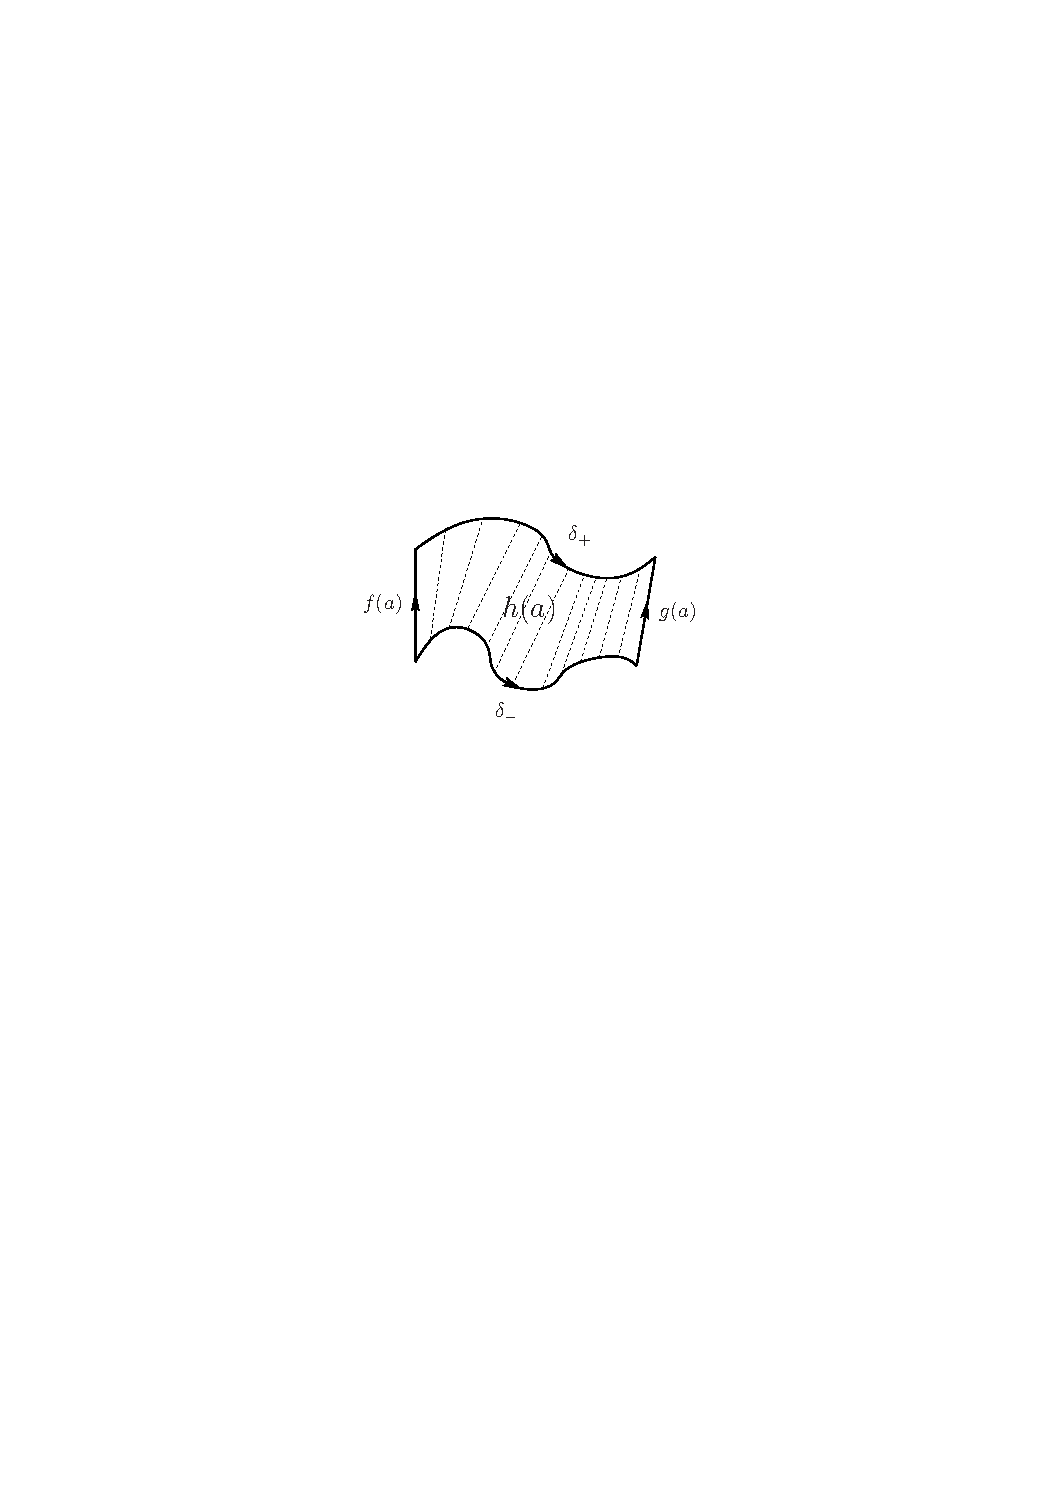
\includegraphics[width=0.5\textwidth]{pictures/homotopy.pdf}
\]
This is supposed to represent the action of a homotopy between $f$ and $g$ on a chain a in $X:h(a)$ is obtained by mapping $a\times[0,1]$ to $Y$ so as to get $f(a)$ when restricting to $a\times\{0\}$ and to get $g(a)$ when restricting to $a\times\{1\}$. Note that $h(a)$ is a chain of dimension $2$ higher than the dimension of $a$, and that the boundary $\partial h(a)$ of this chain consists of $f(a)$, $g(a)$ and of the restriction of $h$ to the boundary $\partial a$ of $a$: taking the boundary counterclockwise,
\[\partial h(a)=g(a)-\delta_+-f(a)+\delta_-=g(a)-f(a)\]
Since boundaries vanish in homology, $f(a)$ and $g(a)$ will agree in homology.
\begin{definition}
A \textbf{homotopy} $h$ between two morphisms of cochain complexes
\[\alpha,\beta:L^\bullet\to M^\bullet\]
is a collection of morphisms
\[h^i:L^i\to M^{i-1}\]
such that for all $i$ we have
\[\beta^i-\alpha^i=d_M^{i-1}\circ h^i+h^{i+1}\circ d_L^i\]
We say that $\alpha$ is homotopic to $\beta$ and write $\alpha\sim\beta$ if there is a homotopy between
$\alpha$ and $\beta$.
\end{definition}
We are dealing here with cochain complexes; this accounts for the fact that while in the topological situation (where we were interested in chains rather than cochains) the homotopy would shift dimensions up.\par
Aside from its topological motivation, homotopy is not too easy to visualize. The following diagram is \textbf{not} assumed to be commutative:
\[\begin{tikzcd}
\cdots\ar[rr,"d_L^{i-2}"]&&L^{i-1}\ar[dd,swap,bend right=15,"\alpha^{i-1}"]\ar[lldd]\ar[dd,bend left=15,"\beta^{i-1}"]\ar[rr,"d_L^{i-1}"]&&L^i\ar[rr,"d_L^{i}"]
\ar[lldd,swap,"h^i"]\ar[dd,swap,bend right=15,"\alpha^{i}"]\ar[dd,bend left=15,"\beta^{i}"]&&L^{i+1}\ar[rr,"d_L^{i+1}"]\ar[lldd,swap,"h^{i+1}"]
\ar[dd,swap,bend right=15,"\alpha^{i+1}"]\ar[dd,bend left=15,"\beta^{i+1}"]&&\cdots\ar[lldd]\\
&&&&&&&&\\
\cdots\ar[rr,"d_M^{i-2}"]&&M^{i-1}\ar[rr,"d_M^{i-1}"]&&M^i\ar[rr,"d_M^{i}"]&&M^{i+1}\ar[rr,"d_M^{i+1}"]&&\cdots
\end{tikzcd}\]
The morphisms $h^i$ do not usually define a morphism of complexes $L^\bullet\to M[-1]^\bullet$: the lozenges in this diagram are not required to commute.
\begin{definition}\label{homotopy def}
A morphism $\alpha:L^\bullet\to M^\bullet$ is a \textbf{homotopy equivalence} if there is a morphism $\beta:M^\bullet\to L^\bullet$ such that $\alpha\circ\beta\sim 1_M$ and $\beta\circ\alpha\sim 1_L$. The complexes $L^\bullet$, $M^\bullet$ are said to be homotopy equivalent if there is a homotopy equivalence $L^\bullet\to M^\bullet$.
\end{definition}
\begin{proposition}\label{homotopic morphism on cohomology}
If $\alpha$, $\beta:L^\bullet\to M^\bullet$ are homotopic morphisms of complexes, then $\alpha$, $\beta$ induce the same morphisms on cohomology: 
$H^\bullet(L^\bullet)\to H^\bullet(M^\bullet)$.
\end{proposition}
\begin{proof}
Let $\ell\in H^i(L^\bullet)$, where $\ell\in\ker(d^i_L)$, and its images in $H^i(M^\bullet)$ under the morphisms induced by $\alpha$, $\beta$ are $\alpha^i(\ell)$ and 
$\beta^i(\ell)$. Since $\alpha,\beta$ are homotopic, according to Definition~\ref{homotopy def} there are morphisms $h^i$ such that
\[\beta^i(\ell)-\alpha^i(\ell)=d_M^{i-1}(h^i(\ell))+h^{i+1}(d_L^i(\ell))\]
Since $\ell\in\ker d^i_L$, the last term vanishes. This shows that
\[\beta^i(\ell)-\alpha^i(\ell)\in\im d_M^{i-1}\]
proving that $\beta^i(\ell)-\alpha^i(\ell)$ vanishes in $H^i(M^\bullet)$, as needed
\end{proof}
For example, if $\alpha$ is homotopic to the identity, then by Corollary~\ref{MC exact iff quasi-iso} the cone of $\alpha$ must be exact.
\begin{corollary}\label{homo comple}
Homotopy equivalent complexes have isomorphic cohomology.
\end{corollary}
\begin{proof}
Indeed, morphisms $\alpha:L^\bullet\to M^\bullet$, $\beta:M^\bullet\to L^\bullet$ such that $\beta\circ\alpha$ and $\alpha\circ\beta$ are both homotopic to the identity induce inverse morphisms in cohomology, by Proposition~\ref{homotopic morphism on cohomology}.
\end{proof}
\begin{remark}
Two complexes could be quasi-isomorphic yet not be homotopy equivalent. Homotopy equivalence is a much stronger property than quasi-isomorphism.
\end{remark}
Another key observation will be that homotopy equivalence is preserved by any additive functor. Suppose $\mathcal{A},\mathcal{B}$ are abelian categories and
\[\mathscr{F}:\mathcal{A}\to\mathcal{B}\]
is an additive functor. Then $\mathscr{F}$ induces an additive functor preserving the grading
\[\mathcal{C}(\mathscr{F}):\mathcal{C}(\mathcal{A})\to\mathcal{C}(\mathcal{B})\]
\begin{lemma}\label{homotopy add func}
With $\mathscr{F}$ as above, if $\alpha\sim\beta$ in $\mathcal{C}(\mathcal{A})$, then $\mathcal{C}(\mathscr{F})(\alpha)\sim\mathcal{C}(\mathscr{F})(\beta)$ in $\mathcal{C}(\mathcal{B})$, and if $L^\bullet$ and $M^\bullet$ are homotopy equivalent complexes in $\mathcal{C}(\mathcal{A})$, then $\mathcal{C}(\mathscr{F})(L^\bullet)$ and $\mathcal{C}(\mathscr{F})(M^\bullet)$ are homotopy equivalent complexes in $\mathcal{C}(\mathcal{B})$.
\end{lemma}
\begin{proof}
The second assertion follows from the first. The first is an immediate consequence of the fact that $\mathscr{F}$ is additive. Indeed, if $h$ is a homotopy between $\alpha,\beta:L^\bullet\to M^\bullet$, then
\[\beta^i-\alpha^i=d_M^{i-1}\circ h^i+h^{i+1}\circ d_L^i\]
Since $\mathscr{F}$ preserves the additive structure on $\Hom$-sets, this implies
\[\mathscr{F}(\beta^i)-\mathscr{F}(\alpha^i)=\mathscr{F}(d_M^{i-1})\circ\mathscr{F}(h^i)+\mathscr{F}(h^{i+1})\circ\mathscr{F}(d_L^i)\]
showing that the collection of morphisms $\mathscr{F}(h^i)$ gives a homotopy between $\mathscr{F}(\alpha)$ and $\mathscr{F}(\beta)$.
\end{proof}
Note that the analogous statement does not hold for quasi-isomorphisms: an additive functor does not preserve quasi-isomorphisms (while an exact functor does).\par
Lemma~\ref{homotopy add func} implies that the conclusion of Corollary~\ref{homo comple} holds true after applying an additive functor:
\begin{theorem}\label{homotopy equ add}
Let $\mathscr{F}:\mathcal{A}\to\mathcal{B}$ be an additive functor between two abelian categories. If $L^\bullet$, $M^\bullet$ are homotopy equivalent complexes in 
$\mathcal{C}(\mathcal{A})$, then their cohomology complexes are isomorphic:
\[H^\bullet(\mathscr{F}(L^\bullet))\cong H^\bullet(\mathscr{F}(M^\bullet))\]
\end{theorem}
To conclude this section, we show that homotopic morphisms have isomorphic mapping cones.
\begin{proposition}\label{homotopic morphism iso mapping cone}
If $\alpha$, $\beta:L^\bullet\to M^\bullet$ are homotopic morphisms of complexes, then the mapping cone $MC(\alpha)$ is isomorphic to $MC(\beta)$.
\end{proposition}
\begin{proof}
Let $h^i:L^i\to M^{i-1}$ be a homotopy of $\alpha$ and $\beta$. We define maps
\[H^i:L^{i+1}\oplus M^i\to L^{i+1}\oplus M^{i},\quad (\ell,m)\mapsto(\ell,m+h^i(\ell))\]
and
\[G^i:L^{i+1}\oplus M^i\to L^{i+1}\oplus M^{i},\quad (\ell,m)\mapsto(\ell,m-h^i(\ell))\]
It is clear that $H\circ G=G\circ H=\id$. Now we verify that they are cochain maps.\par
Note that
\begin{align*}
H^{i+1}\circ d^i_{MC(\alpha)}(\ell,m)&=H^{i+1}(-d^{i+1}_L(\ell),d^i_M(m)+\alpha^{i+1}(\ell))\\
&=(-d^{i+1}_L(\ell),d^i_M(m)+\alpha^{i+1}(\ell)-h^{i+1}\circ d^{i+1}_L(\ell)),
\end{align*}
while
\begin{align*}
d^{i+1}_{MC(\beta)}\circ H^i(\ell,m)&=d^{i+1}_{MC(\beta)}(\ell,m+h^i(\ell))=(-d_L^{i+1}(\ell),d^i_M(m)+d^i_M\circ h^i(\ell)+\beta^{i+1}(\ell)).
\end{align*}
Now use the homotopy condition, we find that $H\circ d_{MC(\alpha)}=d_{MC(\beta)}\circ H$, so $H$ is a cochain map from $MC(\alpha)$ to $MC(\beta)$. A similar 
calculation shows $G$ is also a cochian map, but from $MC(\beta)$ to $MC(\alpha)$.
\end{proof}
\subsection{Exercise}
\begin{exercise}
Let $L^\bullet=\cdots\to0\to L\to0\to\cdots$ and $M^\bullet=\cdots\to0\to M\to0\to\cdots$ be two
complexes concentrated in degree $0$. Giving a morphism $\alpha:L^\bullet\to M^\bullet$ is then the
same as giving a morphism $\alpha:L\to M$. Describe the mapping cone in this case and its cohomology.
\end{exercise}
\begin{proof}
The mapping cone is 
\[\begin{tikzcd}
\cdots\ar[rd]\ar[r]&L\ar[draw=none]{d}[name=X, anchor=center,scale=1.5]{\oplus}\ar[r]\ar[rd,"\alpha"]&0\ar[draw=none]{d}[name=X, anchor=center,scale=1.5]{\oplus}\ar[rd]\ar[r]&\cdots\\
\cdots\ar[r]&0\ar[r]&M\ar[r]&\cdots
\end{tikzcd}\]
so the cohomology is $H^{-1}(MC(\alpha)^\bullet)=\ker\alpha$, $H^0(MC(\alpha)^\bullet)=\coker\alpha$.
\end{proof}
\begin{exercise}
Let $\alpha:L^\bullet\to M^\bullet$ be a morphism of bounded complexes. Note that the mapping cone $MC(\alpha)^\bullet$ of $\alpha$ is also bounded; thus, the three complexes $L^\bullet$, $M^\bullet$, $MC(\alpha)^\bullet$ have a well-defined universal Euler characteristic. Prove that $\chi(MC(\alpha)^\bullet)=\chi(M^\bullet)-\chi(L^\bullet)$.
\end{exercise}
\begin{exercise}\label{homotopy prop}
Let $\alpha,\alpha_0,\alpha_1:L^\bullet\to M^\bullet$ and $\beta,\beta_0,\beta_1:M^\bullet\to N^\bullet$ be morphisms of cochain complexes.
\begin{itemize}
\item Assume that $\alpha\sim 0$ or $\beta\sim0$. Prove that $\beta\circ\alpha\sim 0$.
\item Assume that $\alpha_0\sim\alpha_1$ and $\beta_0\sim\beta_1$. Prove that $\beta_0\circ\alpha_0\sim\beta_1\circ\alpha_1$.
\end{itemize}
\end{exercise}
\begin{proof}
\mbox{}
\begin{itemize}
\item Assume $\alpha\sim0$, then there is $h$ such that
\[\alpha^i=d_M^{i-1}\circ h^i+h^{i+1}d_L^i\]
applying $\beta^i$ gives
\[\beta^i\circ\alpha^i=\beta^i\circ d_M^{i-1}\circ h^i+\beta^i\circ h^{i+1}d_L^i=d_N^{i-1}\circ\beta^{i-1}\circ h^i+\beta^i\circ h^{i+1}\circ d_L^{i}\]
so $\beta\circ\alpha\sim 0$ follows.
\item We have
\begin{align*}
\beta_0\circ\alpha_0-\beta_1\circ\alpha_1&=\beta_0\circ\alpha_0-\beta_0\circ\alpha_1+\beta_0\circ\alpha_1-\beta_1\circ\alpha_1\\
&=\beta_0\circ(\alpha_0-\alpha_1)+(\beta_0-\beta_1)\circ\alpha_1\sim 0
\end{align*}
where we use the first point.
\end{itemize}
\end{proof}
\begin{exercise}
Prove that the equivalence class of morphisms of complexes $L^\bullet\to M^\bullet$ homotopic to a given morphism is parametrized by the set of collections of morphisms $h^i:L^i\to M^{i-1}$, modulo the morphisms of complexes $L[1]^\bullet\to M^\bullet$.
\end{exercise}
\begin{proof}
A morphism $\alpha$ homotopic to a given morphism $\beta$ iff
\[\alpha^i-\beta^i=d_M^{i-1}\circ h^i+h^{i+1}\circ d_L^i\]
$\alpha$ is determined by the morphism $h$, but not uniquely
. Two morphisms $h_1$, $h_2$ determine the same $\alpha$ if and only if 
\[d_M^{i-1}\circ h_1^i+h_1^{i+1}\circ d_L^i=d_M^{i-1}\circ h_2^i+h_2^{i+1}\circ d_L^i\]
that is, $h_1-h_2$ commutes with the differential. This makes $h_1-h_2$ become a morphism between $L[1]^\bullet\to M^\bullet$. So module them gives the correspondence
\end{proof}
\begin{exercise}\label{mapping cylinder}
Let $\alpha:L^\bullet\to M^\bullet$ be a morphism of cochain complexes. The \textbf{mapping cylinder} $MCy(\alpha)^\bullet$ is the cochain complex with objects 
$L^i\oplus L^{i+1}\oplus M^i$ in degree $i$ and differential $d_{MCy(\alpha)}$ defined by
\[d_{MCy(\alpha)}^i(\ell,\ell',m):=(d^i_L(\ell)+\ell',-d^{i+1}_L(\ell'),\alpha^{i+1}(\ell')+d^i_M(m)).\]
Verify that $d^{i+1}_{MCy(\alpha)}\circ d^i_{MCy(\alpha)}=0$ and hence that $MCy(\alpha)^\bullet$ is indeed a cochain complex.
\end{exercise}
\begin{proof}
We have the followsing diagram
\[\begin{tikzcd}
\cdots\ar[r]&L^i\ar[draw=none]{d}[name=X, anchor=center,scale=1.5]{\oplus}\ar[r,"d_L^i"]&L^{i+1}\ar[draw=none]{d}[name=X, anchor=center,scale=1.5]{\oplus}\ar[r]&\cdots\\
\cdots\ar[r]&L^{i+1}\ar[draw=none]{d}[name=X, anchor=center,scale=1.5]{\oplus}\ar[ru,"\id_L^{i+1}" description]\ar[rd,swap,"\alpha^{i+1}" description]\ar[r,"-d_L^{i+1}"]&L^{i+2}
\ar[draw=none]{d}[name=X, anchor=center,scale=1.5]{\oplus}\ar[r]&\cdots\\
\cdots\ar[r]&M^i\ar[r,"d_M^{i}"]&M^{i+1}\ar[r]&\cdots
\end{tikzcd}\]
\end{proof}
\begin{exercise}
Topologically speaking, the mapping cylinder of a continuous map $f:X\to Y$ is obtained by considering $X\times[0,1]$ and gluing $X\times1$ to $Y$ by means of $f$; 
studying (co)chains of this object leads to the algebraic mapping cylinder of Exercise~\ref{mapping cylinder}.\par
As we learn in topology, two continuous maps $X\to Y$ are homotopic if they may be realized as the restrictions to $X\times0$, $X\times 1$ of a continuous map from 
the cylinder $X\times[0,1]$ to $Y$. Note that this cylinder is the mapping cylinder of $\id_X$.\par
Prove that two cochain maps $\alpha$, $\beta:L^\bullet\to M^\bullet$ are homotopic via a map $h$ if and only if they extend to a cochain morphism 
$(-\alpha,h,\beta):MCy(\id_L)^\bullet\to M^\bullet$.
\end{exercise}
\begin{proof}
First we calculate the morphsim:
\begin{align*}
&d_M^{i}\circ(-\alpha^i,h^{i+1},\beta^i)=-d_M^i\circ\alpha^i+d_M^{i}\circ h^{i+1}+d_M^{i}\circ\beta^i=d_M^i(\beta^i-\alpha^i)+d_M^i\circ h^{i+1}\\
&(-\alpha^{i+1},h^{i+2},\beta^{i+1})\circ d_{MCy(\id_L)}^{i}=(-\alpha^{i+1},h^{i+2},\beta^{i+1})\circ(d_L^i+\id_L^{i+1},-d_L^{i+1},d_L^i+\id_L^{i+1})\\
&=-\alpha^{i+1}\circ d_L^i-\alpha^{i+1}-h^{i+2}\circ d_L^{i+1}+\beta^{i+1}\circ d_L^i+\beta^{i+1}\\
&=\beta^{i+1}-\alpha^{i+1}+(\beta^{i+1}-\alpha^{i+1})\circ d_L^i-h^{i+2}\circ d_L^{i+1}
\end{align*}
The commutativity of cochain map is equivalent to
\[d_M^i(\beta^i-\alpha^i)+d_M^i\circ h^{i+1}=\beta^{i+1}-\alpha^{i+1}+(\beta^{i+1}-\alpha^{i+1})\circ d_L^i-h^{i+2}\circ d_L^{i+1}\]
Since $\alpha,\beta$ are cochain morphisms, we have $d_M^i(\beta^i-\alpha^i)=(\beta^{i+1}-\alpha^{i+1})\circ d_L^i$. Hence this equality becomes
\[\beta^{i+1}-\alpha^{i+1}=d_M^i\circ h^{i+1}+h^{i+2}\circ d_L^{i+1}\]
this is euqivalent to that $\alpha\sim\beta$.
\end{proof}
\begin{exercise}
In topology, the mapping cone may be obtained by contracting $X\times0$ to a point in the mapping cylinder.\par
In the algebraic version, this contraction amounts to mod-ing out the first component of $MCy(\alpha)$. For a cochain morphism $\alpha:L^\bullet\to M^\bullet$, prove that there is an exact sequence of cochain complexes
\[\begin{tikzcd}
0\ar[r]&L^\bullet\ar[r]&MCy(\alpha)^\bullet\ar[r]&MC(\alpha)^\bullet\ar[r]&0
\end{tikzcd}\]
Deduce that there is a quasi-isomorphism $M^\bullet\to MCy(\alpha)^\bullet$.
\end{exercise}
\begin{exercise}
With notation as in Exercise~\ref{mapping cylinder} (in particular, for a cochain morphism $\alpha:L^\bullet\to M^\bullet$), prove that there is an exact sequence of cochain complexes
\[\begin{tikzcd}
0\ar[r]&M^\bullet\ar[r]&MCy(\alpha)^\bullet\ar[r]&MC(\id_L)^\bullet\ar[r]&0
\end{tikzcd}\]
\end{exercise}
\begin{proof}
The exact sequence is immediate. Since $\id_L$ induces an isomorphism between $H^\bullet(L^\bullet$ and $H^\bullet(L^\bullet)$. By Corollary~\ref{MC exact iff quasi-iso}, $MC(\id_L)^\bullet$ is exact. Hence $H^\bullet(M^\bullet)$ is isomorphic to $H^\bullet(MCy(\alpha)^\bullet)$, again by Corollary~\ref{MC exact iff quasi-iso}.
\end{proof}
\begin{exercise}\label{map cyl homotopy equi}
Still with notation as in Exercise~\ref{mapping cylinder}, define maps $\rho:M^\bullet\to MCy(\alpha)^\bullet$
and $\sigma:MCy(\alpha)^\bullet\to M^\bullet$ by
\[\rho^i(m)=(0,0,m),\quad\sigma^i(\ell,\ell',m)=m-\alpha^i(\ell)\]
Prove that $\rho$, $\sigma$ are both cochain morphisms. Note that $\sigma\circ\rho=\id_M$, and prove
that $\rho\circ\sigma$ is homotopic to $\id_{MCy(\alpha)}$.\par
Conclude that $M^\bullet$ and $MCy(\alpha)^\bullet$ are homotopy equivalent.
\end{exercise}
\begin{proof}
We have
\[d_M^i\circ\sigma^i=d_M^i-d_M^i\circ\alpha^i,\quad \sigma^{i+1}\circ d_{MCy(\alpha)}^i=d_M^i+\alpha^{i+1}-\alpha^{i+1}\circ(d_L^i+\id_L^{i+1})=d_M^i-\alpha^{i+1}\circ d_L^i\]
since $\alpha$ is a cochain morphism, $\alpha^{i+1}\circ d_L^i=d_M^i\circ\alpha^i$. This gives $d_M^i\circ\sigma^i=\sigma^{i+1}\circ d_{MCy(\alpha)}^i$, as needed.\par
Since $\rho^i\circ\sigma^i(\ell,\ell',m)=(0,0,m-\alpha^i(\ell))$, we need a homotopy $h:MCy(\alpha)^\bullet\to MCy(\alpha)^\bullet$ such that
\[\id_{MCy(\alpha)}^i-\rho^i\circ\sigma^i=d_{MCy(\alpha)}^{i-1}\circ h^i+h^{i+1}\circ d_{MCy(\alpha)}^{i}\]
Note that $\id_{MCy(\alpha)}^i(\ell,\ell',m)-\rho^i\circ\sigma^i(\ell,\ell',m)=(\ell,\ell',\alpha^i(\ell))$. Pick $h^i:(\ell,\ell',m)\mapsto(0,\ell,0)$ gives the desired equality.
\end{proof}
\begin{exercise}
Combine the above three exercises to conclude that, up to homotopy equivalence, a cochain morphism $\alpha:L^\bullet\to M^\bullet$ may be replaced with a monomorphism $L^\bullet\to MCy(\alpha)^\bullet$ that induces the same morphism $H^\bullet(\alpha)$ in cohomology (up to the identification $H^\bullet(M^\bullet)\cong H^\bullet(MCy(\alpha)^\bullet)$) and whose cokernel is the mapping cone $MC(\alpha)^\bullet$.
\end{exercise}
\begin{proof}
The morphism $\ell\mapsto(-\ell,0,0)$ is homotopic to $\ell\mapsto(0,0,\alpha^i(\ell))$ (they are both chain morphisms): Let $\alpha:\ell\mapsto(-\ell,0,0)$, then $\rho^i\circ\sigma^i\circ\alpha^i:\ell\mapsto(0,0,\alpha^i(\ell))$. As we see, $\sigma\circ\alpha\sim \id_{MCy(\alpha)^\bullet}$, and from Exercise~\ref{homotopy prop} we get $\rho\circ\sigma\circ\alpha\sim\alpha$. Note that $\alpha$ is monic, as needed.
\end{proof}
\begin{exercise}
Prove that, in general, additive functors do not preserve quasi-isomorphisms. Prove that exact functors do.
\end{exercise}
\begin{proof}
Consider the example
\[\begin{tikzcd}
\cdots\rar&0\dar\rar&\Z\ar[r,"\cdot 2"]\dar&\Z\rar\ar[d,"\pi"]&0\rar\dar&\cdots\\
\cdots\rar&0\rar&0\rar&\Z/2\Z\rar&0\rar&\cdots
\end{tikzcd}\]
the functor $\otimes\Z/2\Z$ is additive, but it gives
\[\begin{tikzcd}
\cdots\rar&0\dar\rar&\Z/2\Z\ar[r,"0"]\dar&\Z/2\Z\rar\ar[d,"\pi"]&0\rar\dar&\cdots\\
\cdots\rar&0\rar&0\rar&\Z/2\Z\rar&0\rar&\cdots
\end{tikzcd}\]
The first complex has cohomology $\Z/2\Z,\Z/2\Z$, but the second $0,\Z/2\Z$.\par
For the second point, use mapping cone and Corollary~\ref{MC exact iff quasi-iso}.
\end{proof}
\section{The homotopic category. Complexes of projectives and injectives}
\subsection{Homotopic maps are identified in the derived category}
Again consider any additive functor
\[\mathscr{F}:\mathcal{C}(\mathcal{A})\to\mathcal{D}\]
transforming quasi-isomorphisms into isomorphisms. The simplest such functor is cohomology; the universal one is the functor from $\mathcal{C}(\mathcal{A})$ to the mystifying derived category $\mathcal{C}(\mathcal{A})$. We have verified in Proposition~\ref{homotopic morphism on cohomology} that homotopic maps induce the same morphism in cohomology.
\begin{lemma}\label{quasi into iso homotopy}
Let $\mathscr{F}:\mathcal{C}(\mathcal{A})\to\mathcal{D}$ be an additive functor such that $\mathscr{F}(\rho)$ is an isomorphism in $\mathcal{D}$ for all quasi-isomorphisms $\rho$ in $\mathcal{C}(\mathcal{A})$. Let $\alpha,\beta:L^\bullet\to M^\bullet$ be homotopic morphisms in $\mathcal{C}(\mathcal{A})$. Then $\mathscr{F}(\alpha)=\mathscr{F}(\beta)$ in $\mathcal{D}$.
\end{lemma}
\begin{proof}
Equivalently (as $\mathscr{F}$ is additive), we verify that if $\alpha\sim 0$, then $\mathscr{F}(\alpha)=0$.\par
By Lemma~\ref{add functor quasi-iso into iso}, it suffices to show that $\alpha$ factors through an exact complex.\par
This exact complex is the mapping cone $MC(\id_L)^\bullet$ of the identity $\id_L:L^\bullet\to L^\bullet$. Recall that
\[MC(\id_L)^i=L^{i+1}\oplus L^i,\quad d_{MC(\id_L)}^i(a,b)=(-d_L^{i+1}(a),a+d_L^i(b))\]
Since the identity is trivially a quasi-isomorphism, $MC(\id_L)$ is an exact complex (Corollary~\ref{MC exact iff quasi-iso}). The morphism
\[L^i\to MC(\id_L)^i,\quad\ell\mapsto(0,\ell)\]
always commutes with differentials, so it defines a morphism of complexes $L^\bullet\to MC(\id_L)^\bullet$. By contrast, a morphism
\[MC(\id_L)^\bullet\to M^\bullet\]
is not always available. Under our hypothesis, however, there is a homotopy $\alpha\sim 0$, that is, morphisms
\[h^i:L^{i}\to M^{i-1}\]
such that $\alpha^i=d^{i-1}_M\circ h^i+h^{i+1}\circ d^i_L$. Define morphisms
\[\pi^i:MC(\id_L)^i\to M^i,\quad (a,b)\mapsto h^{i+1}a+\alpha^i(b)\]
pictorially,
\[\begin{tikzcd}
\cdots\ar[rd]\ar[r]&L^{i+1}\ar[draw=none]{d}[name=X, anchor=center,scale=1.5]{\oplus}\ar[r,"-d_L^{i+1}"]\ar[rd,"\id_L^{i+1}" description]&L^{i+2}
\ar[draw=none]{d}[name=X, anchor=center,scale=1.5]{\oplus}\ar[rd]\ar[r]&\cdots\\
\cdots\ar[r]&L^i\ar[ld]\ar[d,"\alpha^i"]\ar[r,"d_L^i"]&L^{i+1}\ar[ld]\ar[d,"\alpha^{i+1}"]\ar[ld,swap,"h^{i+1}" description]\ar[r]&\cdots\ar[ld]\\
\cdots\ar[r]&M^i\ar[r,"d_M^i"]&M^{i+1}\ar[r]&\cdots
\end{tikzcd}\]
It is clear that the composition
\[L^i\to MC(\id_L)^i\to  M^i\]
is $\alpha^i$. All we have to check now is that the collection $\pi^i$ defines a morphism of complexes: this will show that $\alpha$ factors through the exact complex $MC(\id_L)^\bullet$, hence that $\mathscr{F}(\alpha)=0$ (by Lemma~\ref{add functor quasi-iso into iso}), concluding the proof of this lemma. That
is, we have to verify that
\[d_M^{i-1}\circ\pi^{i-1}=\pi^i\circ d_{MC(\id_L)}^{i-1}\]
for all $i$. The left-hand side acts as follows:
\[(a,b)\mapsto h^i(a)+\alpha^{i-1}(b)\mapsto d_M^{i-1}(h^i(a)+\alpha^{i-1}(b))\]
The right-hand side acts as
\[(a,b)\mapsto(-d_L^i(a),a+d_L^{i-1}(b))\mapsto -h^{i+1}(d_L^i(a))+\alpha^i(a+d_L^{i-1}(b))\]
Thus the needed equality is
\[d_M^{i-1}(h^i(a))+d_M^{i-1}(\alpha^{i-1}(b))=-h^{i+1}(d_L^i(a))+\alpha^i(a)+\alpha^i(d_L^{i-1}(b))\]
or, equivalently,
\[(d_M^{i-1}\circ h^i+h^{i+1}\circ d_L^i-\alpha^i)(a)=(\alpha^i\circ d_L^{i-1}-d_M^{i-1}\circ\alpha^{i-1})(b)\]
$\forall a\in L^{i+1}, \forall b\in L^i$. But both sides are $0$: the right-hand side because $\alpha$ is a morphism of complexes and the left-hand side because $h$ is a homotopy $\alpha\sim0$.
\end{proof}
\subsection{Definition of the homotopic category of complexes}
\begin{definition}
Let $\mathcal{A}$ be an abelian category. The \textbf{homotopy category} $\mathcal{K}(\mathcal{A})$ of cochain complexes in $\mathcal{A}$ is the category whose objects are the cochain complexes in $\mathcal{A}$ (that is, the same objects of $\mathcal{C}(\mathcal{A})$) and whose morphisms are
\[\Hom_{\mathcal{K}(\mathcal{A})}(L^\bullet,M^\bullet):=\Hom_{\mathcal{C}(\mathcal{A})}(L^\bullet,M^\bullet)/\sim\]
where $\sim$ is the homotopy relation.
\end{definition}
Recall that the homotopy relation $\sim$ respects composition (Exercise~\ref{homotopy prop}); in other words, the operation of composition
\[\Hom_{\mathcal{C}(\mathcal{A})}(L^\bullet,M^\bullet)\times\Hom_{\mathcal{C}(\mathcal{A})}(M^\bullet,N^\bullet)\to\Hom_{\mathcal{C}(\mathcal{A})}(L^\bullet,N^\bullet)\]
does descend to an operation
\[\Hom_{\mathcal{K}(\mathcal{A})}(L^\bullet,M^\bullet)\times\Hom_{\mathcal{K}(\mathcal{A})}(M^\bullet,N^\bullet)\to\Hom_{\mathcal{K}(\mathcal{A})}(L^\bullet,N^\bullet)\]
Bounded variations $\mathcal{K}^-(\mathcal{A})$, $\mathcal{K}^+(\mathcal{A})$, etc., are obtained likewise from $\mathcal{C}^-(\mathcal{A})$, $\mathcal{C}^+(\mathcal{A})$, etc. The considerations which follow will apply to all these versions. The further variations $\mathcal{K}^-(\mathcal{P})$, resp., $\mathcal{K}^+(\mathcal{I})$, in which the complexes will be required to consist of projective, resp., injective, objects from $\mathcal{A}$ will also play a crucially important role.\par
As to the general structure underlying the homotopic category,
\begin{lemma}
Let $\mathcal{A}$ be an abelian category. Then the homotopic category $\mathcal{K}(\mathcal{A})$ of
complexes is an additive category.
\end{lemma}
However, note that, in general, \textbf{the homotopic category is not abelian}.
The main motivation for the introduction of the homotopic category is that homotopy equivalences become isomorphisms in $\mathcal{K}(\mathcal{A})$. More precisely, by definition there is a functor
\[\mathcal{C}(\mathcal{A})\to\mathcal{K}(\mathcal{A})\]
mapping every object to itself and every morphism to its homotopy class. Homotopy equivalences in $\mathcal{C}(\mathcal{A})$ become isomorphisms in $\mathcal{K}(\mathcal{A})$ because the relation
$\alpha\circ\beta\sim id$ in $\mathcal{C}(\mathcal{A})$ becomes $\alpha\circ\beta=id$ in $\mathcal{K}(\mathcal{A})$. The homotopic category is obtained from $\mathcal{C}(\mathcal{A})$ by making all homotopy equivalences invertible on the nose.\par
We can then reinterpret Lemma~\ref{quasi into iso homotopy} as the following ‘factorization’ result
\begin{proposition}\label{quasi iso factor}
Let $\mathscr{F}:\mathcal{C}(\mathcal{A})\to\mathcal{D}$ be an additive functor such that $\mathscr{F}(\rho)$ is an isomorphism in $\mathscr{F}$ for all quasi-isomorphisms $\rho$ in $\mathcal{C}(\mathcal{A})$. Then $\mathscr{F}$ factors uniquely through $\mathcal{K}(\mathcal{A})$:
\[\begin{tikzcd}
\mathcal{C}(\mathcal{A})\ar[d]\ar[r,"\mathscr{F}"]&\mathcal{D}\\
\mathcal{K}(\mathcal{A})\ar[ru,swap,"\exists!"]
\end{tikzcd}\]
\end{proposition}
A particular case of Proposition~\ref{quasi iso factor} is the fact that the cohomology functor on $\mathcal{C}(\mathcal{A})$ (resp., $\mathcal{C}^-(\mathcal{A})$, $\mathcal{C}^+(\mathcal{A})$) descends to a functor on $\mathcal{K}(\mathcal{A})$ (resp., $\mathcal{K}^-(\mathcal{A})$, $\mathcal{K}^+(\mathcal{A})$). This fact also follows directly from Proposition~\ref{homotopic morphism on cohomology}: homotopic maps induce the same morphism in cohomology.
\subsection{Complexes of projective and injective objects}
Recall that an $R$-module $M$ is projective if the functor $\Hom_R(M,-)$ is exact and it is injective if $\Hom_R(-,M)$ is exact. We can adopt these definitions in any abelian category:
\begin{definition}
Let $\mathcal{A}$ be an abelian category. An object $P$ of $\mathcal{A}$ is projective if the functor $\Hom_{\mathcal{A}}(P,-)$ is exact. An object $Q$ is injective if the functor $\Hom_{\mathcal{A}}(-,Q)$ is
exact.
\end{definition}
We will denote by $\mathcal{P}$, resp., $\mathcal{I}$, the full subcategories of $\mathcal{A}$ determined by the projective, resp., injective, objects. Of course these are not abelian categories in
any interesting case. Note that an abelian category may well have no nontrivial projective or injective objects.
\begin{example}
The category of finite abelian groups is abelian, but contains no nontrivial projective or injective objects
\end{example}
\begin{definition}
An abelian category $\mathcal{A}$ \textbf{has enough projectives} if for every object $A$ in $\mathcal{A}$ there exists a projective object $P$ in $A$ and an epimorphism $P\twoheadrightarrow A$. The category \textbf{has enough injectives} if for every object $A$ in $\mathcal{A}$ there is an injective object $Q$ in $A$ and a monomorphism $A\rightarrowtail Q$.
\end{definition}
we have already observed that, for every commutative ring $R$, $R$-$\mathsf{Mod}$ has enough projectives (free modules and their direct summands are projective, Proposition~\ref{proj iff}) and enough injectives (Corollary~\ref{inje iff}).\par
An important case in which one can show that there are enough injectives is the category of sheaves of abelian groups over a topological space; this is a key step in the definition of sheaf cohomology as a derived functor. In general, categories of sheaves do not have enough projectives. On the other hand,
the category of finitely generated abelian groups has enough projectives but not enough (indeed, no nontrivial) injectives. So it goes.
\subsection{Homotopy equivalences vs. quasi-isomorphisms in $\mathcal{K}(\mathcal{A})$}
In a principle, we will only deal with projective objects, but the claim for injective objects also follows from a dual argument.\par
\begin{definition}
We will denote by $\mathcal{K}^-(\mathcal{P})$ the full subcategory of $\mathcal{K}(\mathcal{A})$ consisting of bounded-above complexes of projective objects of $\mathcal{A}$, and we will denote by $\mathcal{K}^+(\mathcal{I})$ the full subcategory of $\mathcal{K}(\mathcal{A})$ consisting of bounded-below complexes of injective
objects of A.
\end{definition}
A complicated way of saying that a complex $N^\bullet$ in $\mathcal{C}(\mathcal{A})$ is exact is to assert that the identity map $\id_N$ and the trivial map $0$ induce the same morphism in cohomology,
as they would if they were homotopic to each other. It is however easy to construct examples of exact complexes for which the identity is not homotopic to $0$, this has to do with whether the complex
splits or not; in general, a complex $N^\bullet$ is said to be \textbf{split exact} if $\id_N$ is homotopic to $0$.
\begin{lemma}\label{pro homotopy 0}
Let $P^\bullet$ be a complex of projective objects of an abelian category $\mathcal{A}$ such that $P^i=0$ for $i>0$, and let $L^\bullet$ be a complex in $\mathcal{C}(\mathcal{A})$ such that $H^i(L^\bullet)=0$ for $i<0$.
Let $\alpha:P^\bullet\to L^\bullet$ be a morphism inducing the zero-morphism in cohomology. Then $\alpha$ is homotopic to $0$.
\end{lemma}
The reader will provide the injective version of this statement, dealing with morphisms from a complex which is exact in positive degree to a complex of injectives $Q^\bullet$ with $Q^i=0$ for $i<0$.
\begin{proof}
We have to construct morphisms $h^i:P^i\to L^{i-1}$:
\[\begin{tikzcd}
\cdots\ar[rr]&&P^{-2}\ar[lldd,"h^{-2}"]\ar[dd,"\alpha^{-2}"]\ar[rr,"d_P^{-2}"]&&P^{-1}\ar[lldd,"h^{-1}"]\ar[dd,"\alpha^{-1}"]\ar[rr,"d_P^{-1}"]&&P^0\ar[lldd,"h^{0}"]\ar[dd,"\alpha^{0}"]\ar[rr]&&0\ar[lldd,"h^1=0"]\ar[dd]\ar[rr]&&\cdots\ar[lldd,"h^2=0"]\\
&&&&&&&&&&\\
\cdots\ar[rr]&&L^{-2}\ar[rr,"d_L^{-2}"]&&L^{-1}\ar[rr,"d_L^{-1}"]&&L^0\ar[rr]&&L^1\ar[rr]&&\cdots
\end{tikzcd}\]
such that
\begin{align}\label{pro homo-1}
\alpha^i=d_L^{i-1}\circ h^i+h^{i+1}\circ d_P^i
\end{align}
Of course $h^i=0$ necessarily for $i>0$. For $i=0$, use the fact that the morphism induced by $\alpha$ on cohomology is $0$; this says that $\alpha_0$ factors through the image of $d^{-1}_L$:
\[\begin{tikzcd}
&P^0\ar[d,"\alpha^0"]&\\
L^{-1}\ar[r,"d_L^{-1}"]&\im d^{-1}_L\ar[r]&0
\end{tikzcd}\]
Since $P^0$ is projective, there exists a morphism $h^0:P^0\to L^{-1}$ such that $\alpha_0=d^{-1}_L\circ h_0$, as needed.\par
To define $h^{i-1}$ for $i\leqslant 0$, proceed inductively and assume that $h^i$ and $h^{i+1}$ satisfying $(\ref{pro homo-1})$ have already been constructed. Note that by $(\ref{pro homo-1})$ (and the fact that $P^\bullet$ is a complex)
\[d^{i-1}_L\circ h^i\circ d^{i-1}_P=(\alpha^i-h^{i+1}\circ d^i_P)\circ d^{i-1}_P=\alpha^i\circ d^{i-1}_P-h^{i+1}\circ0=\alpha^i\circ d^{i-1}_P\]
\[\begin{tikzcd}
{}\ar[rr,no head,dashed]&&P^{i-1}\ar[lldd,no head,dashed]\ar[rr,"d_P^{i-1}"]\ar[dd,no head,dashed]&&P^i\ar[lldd,"h^i"]\ar[dd,"\alpha^i"]\ar[rr,"d_P^i"]&&P^{i+1}\ar[dd,no head,dashed]\ar[lldd,"h^{i+1}"]\ar[rr,no head,dashed]&&{}\ar[lldd,no head,dashed]\\
&&&&&&&&\\
{}\ar[rr,no head,dashed]&&L^{i-1}\ar[rr,"d_L^{i-1}"]&&L^i\ar[rr,"d_L^i"]&&L^{i+1}\ar[rr,no head,dashed]&&{}
\end{tikzcd}\]
Therefore
\[d_L^{i-1}\circ(\alpha^{i-1}-h^i\circ d_P^{i-1})=d_L^{i-1}\circ\alpha^{i-1}-\alpha^{i}\circ d_P^{i-1}=0\]
since $\alpha$ is a morphism of cochain complexes. This tells us that $\alpha^{i-1}-h^i\circ d_P^{i-1}$
factors through $\ker d^{i-1}_L$. Since $L^\bullet$ is exact at $Li−1$ for $i\leqslant 0$, $\ker d^{i-1}_L=\im d^{i-2}_L$. Therefore, we again have a factorization
\[\begin{tikzcd}
&P^{i-1}\ar[d,"\alpha^{i-1}-h^i\circ d_P^{i-1}"]&\\
L^{i-2}\ar[r,"d_L^{i-2}"]&\im d^{i-2}_L\ar[r]&0
\end{tikzcd}\]
Now $P^{i-1}$ is projective; therefore there exists $h^{i-1}:P^{i-1}\to L^{i-2}$ such that
\[\alpha^{i-1}-h^i\circ d_P^{i-1}=d_L^{i-2}\circ h^{i-1}\]
which is precisely what we need for the induction step.
\end{proof}
\begin{corollary}\label{proj mor exact homo 0}
Let $P^\bullet$ be a bounded-above cochain complex of projectives of an abelian category $\mathcal{A}$, and let $L^\bullet$ be an exact complex in $\mathcal{C}(\mathcal{A})$. Then every morphism of complexes $P^\bullet\to L^\bullet$ is homotopic to $0$.
\end{corollary}
\begin{corollary}
Let $P^\bullet$ (resp., $Q^\bullet$) be a bounded-above exact complex of projectives (resp., a bounded-below exact complex of injectives). Then $P^\bullet$ (resp., $Q^\bullet$) is homotopy equivalent to the zero-complex.
\end{corollary}
Another consequence of Lemma~\ref{pro homotopy 0} is the following remark, showing that quasi-isomorphisms are non-zero-divisors up to homotopy, with respect to morphisms from complexes of projectives. This will be useful in the next section, for example to show that certain lifts are uniquely defined up to homotopy.
\begin{lemma}\label{quasi nonzero div}
Let $\mathcal{A}$ be an abelian category, and let $\rho:L^\bullet\to M^\bullet$ be a quasi isomorphism
in $\mathcal{C}(\mathcal{A})$. Let $P^\bullet$ be a bounded-above complex of projectives, and let $\alpha:P^\bullet\to L^\bullet$ be a morphism of cochain complexes such that the composition
\[P^\bullet\stackrel{\alpha}{\longrightarrow}L^\bullet\xlongrightarrow[\text{q-iso}]{\rho}M^\bullet\]
is homotopic to the zero-morphism. Then $\alpha\sim0$.
\end{lemma}
\begin{proof}
Let $h^i:P^i\to M^{i-1}$ define a homotopy between $\rho\circ\alpha$ and $0$, so that $-\rho^i\circ\alpha^i=d^{i-1}_M\circ h^i+h^{i+1}\circ d^i_P$. Consider the mapping cone $MC(\rho)$ of $\rho$, and define morphisms
\[\beta^i=(\alpha^i,h^i):P^i\to L^i\oplus M^{i-1}=MC(\rho)^{i-1}\]
\[\begin{tikzcd}
\cdots\ar[rr]&&P^{i-1}\ar[dd,"\beta^{i-1}"]\ar[rr,"d_P^{i-1}"]&&P^i\ar[dd,"\beta^{i}"]\ar[rr,"d_P^i"]&&P^{i+1}\ar[dd,"\beta^{i+1}"]\ar[rr]&&\cdots\\
&&&&&&&&\\
\cdots\ar[rr]&&L^{i-1}\oplus M^{i-2}\ar[rr,"-d_{MC(\rho)}^{i-2}"]&&P^i\oplus M^{i-1}\ar[rr,"-d_{MC(\rho)}^{i-1}"]&&L^{i+1}\oplus M^i\ar[rr]&&\cdots
\end{tikzcd}\]
We claim that these give a morphism of cochain complexes $P^\bullet\to MC(\rho)[-1]^\bullet$. Indeed,
\[\beta^{i+1}\circ d^i_P=(\alpha^{i+1}\circ d_P^i,h^{i+1}\circ d_P^i),\quad -d_{MC(\rho)}\circ\beta^i=(d_L^i\circ\alpha^i,-\rho^i\circ\alpha^{i},-d_M^{i-1}\circ h^i)\]
these are equal, by definition of $h^i$ and since $\alpha$ is a morphism of complexes.\par
Now, $\rho$ is a quasi-isomorphism by hypothesis. Therefore $MC(\rho)$ is an exact complex (Corollary~\ref{MC exact iff quasi-iso}). Applying Corollary~\ref{proj mor exact homo 0}, it follows that $\beta$ is homotopic to zero. But $\alpha$ is the composition
\[\begin{tikzcd}
P^\bullet\ar[r,"\beta"]&MC(\rho)[-1]^\bullet=L^\bullet\oplus M[-1]^\bullet\ar[r]&L^\bullet
\end{tikzcd}\]
so (Exercise~\ref{homotopy prop}) the fact that $\beta\sim0$ implies that $\alpha\sim0$, concluding the
proof.
\end{proof}
\begin{example}
To see that $\alpha$ may not be zero on the nose even if $\rho\circ\alpha=0$, look back again at Example~\ref{quasi-iso no iso}:
\[\begin{tikzcd}
P^\bullet:\ar[d,"\alpha"]&\cdots\ar[r]&0\ar[r]\ar[d]&\Z\ar[d,"id"]\ar[r,"id"]&\Z\ar[d,"\cdot 2"]\ar[r]&0\ar[r]\ar[d]&\cdots\\
L^\bullet:\ar[d,"\rho"]&\cdots\ar[r]&0\ar[d]\ar[r]&\Z\ar[r,"\cdot 2"]\ar[d]&\Z\ar[r]\ar[d]&0\ar[r]\ar[d]&\cdots\\
M^\bullet:&\cdots\ar[r]&0\ar[r]&0\ar[r]&\Z/2\Z\ar[r]&0\ar[r]&\cdots\\
\end{tikzcd}\]
Here $\rho$ is a quasi-isomorphism, and $\rho\circ\alpha=0$. According to Lemma~\ref{quasi nonzero div}, the (nonzero) morphism $\alpha$ is homotopic to $0$.
\end{example}
A quasi-isomorphism to a complex of projectives, resp., from a complex of injectives\footnote{That is, going the wrong way: projectives like being the sources of morphisms, and injectives like to be targets.}, has a right, resp., left, homotopy inverse.
\begin{proposition}\label{quasi homo inv}
Let $\mathcal{A}$ be an abelian category, and let $L^\bullet$ be a complex in $\mathcal{C}(\mathcal{A})$. Let $P^\bullet$ in $\mathcal{C}^-(\mathcal{P})$ be a bounded-above complex of projectives, and let $\alpha:L^\bullet\to P^\bullet$ be a quasi-isomorphism. Then there exists a morphism of complexes $\beta:P^\bullet\to L^\bullet$ such that $\alpha\circ\beta$ is homotopic to $\id_P$.
\end{proposition}
(For the injective version, if $Q^\bullet$ is a bounded-below complex of injectives and $\alpha:Q^\bullet\to L^\bullet$ is a quasi-isomorphism, then there exists a morphism $\beta:L^\bullet\to Q^\bullet$ such that $\beta\circ\alpha\sim \id_Q$.)
\begin{proof}
Since $\alpha:L^\bullet\to P^\bullet$ is a quasi-isomorphism, the mapping cone $MC(\alpha)^\bullet$ of $\alpha$ is an exact complex (Corollary~\ref{MC exact iff quasi-iso}). Let $\rho$ be the morphism of complexes
\[\rho=(0,\id_P):P^\bullet\to L[1]^\bullet\oplus P^\bullet=MC(\alpha)^\bullet\]
Since $MC(\alpha)^\bullet$ is exact, $\rho$ is homotopic to zero by Corollary~\ref{proj mor exact homo 0}. Therefore, there exist morphisms
\[\bar{h}^:P^i\to MC(\alpha)^{i-1}=L^i\oplus P^{i-1}\]
such that
\begin{align}\label{pro homo-2}
\rho^i=d_{MC(\alpha)}^{i-1}\circ\bar{h}^i+\bar{h}^{i+1}\circ d_P^i
\end{align}
\[\begin{tikzcd}
\cdots\ar[rr]&&P^{i-1}\ar[dd,"\rho^{i-1}"]\ar[lldd]\ar[rr,"d_P^{i-1}"]&&P^i\ar[dd,"\rho^i"]\ar[lldd,"\bar{h}^i"]\ar[rr,"d_P^i"]&&P^{i+1}\ar[dd,"\rho^{i+1}"]\ar[lldd,"\bar{h}^{i+1}"]\ar[rr]&&\cdots\ar[lldd]\\
&&&&&&&&\\
\cdots\ar[rr]&&L^i\oplus P^{i-1}\ar[rr,swap,"d_{MC(\alpha)}^{i-1}"]&&L^{i+1}\oplus P^i\ar[rr,swap,"d_{MC(\alpha)}^i"]&&L^{i+2}\oplus P^{i+1}\ar[rr]&&\cdots\\
\end{tikzcd}\]
Now we unravel what this says. Write $\bar{h}^i$ out in components:
\[\bar{h}^i=(\beta^i,h^i)\]
with $\beta^i:P^i\to L^i$ and $h^i:P^i\to P^{i-1}$. We claim that
\begin{itemize}
\item[$(\rmnum{1})$]the collection $\{\beta^i\}$ is a morphism of cochain complexes: $\beta^{i+1}\circ d^i_P=d^i_L\circ\beta^i$ for all $i$.
\item[$(\rmnum{2})$]the morphisms $h^i$ give a homotopy $\alpha\circ\beta\sim \id_P$.
\end{itemize}
Indeed, the left-hand side of $(\ref{pro homo-2})$ is
\[\rho^i=(0,\id_P^i)\]
the right-hand side is
\begin{align*}
&d^{i-1}_{MC(\alpha)}\circ(\beta^i,h^i)+(\beta^{i+1},h^{i+1})\circ d^i_P\\
&=(-d^i_L\circ\beta^i,\alpha^i\circ\beta^i+d_P^{i-1}\circ h^i)+(\beta^{i+1}\circ d_P^i,h^{i+1}\circ d_P^i)
\end{align*}
It follows that $(\ref{pro homo-2})$ amounts to
\[\left\{\begin{array}{l}
\beta^{i+1}\circ d_P^i-d_L^i\circ\beta^i=0\\
\id_P^i-\alpha^i\circ\beta^i=d_P^{i-1}\circ h^i+h^{i+1}\circ d_p^i
\end{array}\right. \]
that is, precisely $(\rmnum{1})$ and $(\rmnum{2})$.
The morphism of complexes $\beta:P^\bullet\to L^\bullet$ is the needed homotopy right-inverse of $\alpha$.
\end{proof}
Taking $L^\bullet$ to be a suitably bounded complex of projectives or injectives finally establishes our main theorem:
\begin{theorem}\label{quasi to homotopy}
Let $\mathcal{A}$ be an abelian category, and let $\alpha:P^\bullet_0\to P^\bullet_1$, resp., $\alpha:Q_0^\bullet\to Q_1^\bullet$, be a quasi-isomorphism between bounded-above complexes of projectives, resp., bounded-below complexes of injectives, in $\mathcal{A}$. Then $\alpha$ is a homotopy equivalence.
\end{theorem}
\begin{proof}
We will give the argument for projectives.\par
By Proposition~\ref{quasi homo inv}, since $P_1^\bullet$ is in $\mathcal{C}^-(\mathcal{P})$ and $\alpha:P_0^\bullet\to P_1^{\bullet}$ is a quasi-isomorphism, there exists a morphism of complexes $\beta:P_1^\bullet\to P_0^{\bullet}$ such that $\alpha\circ\beta\sim \id_{P_1}$. This implies that $H^{\bullet}(\alpha)\circ H^{\bullet}(\beta)=id$ (Proposition~\ref{homotopic morphism on cohomology}). Since $H^{\bullet}(\alpha)$ is invertible, so is $H^{\bullet}(\beta)$: therefore, $\beta$ is a quasi-isomorphism. Now $P_0^{\bullet}$ is also in $\mathcal{C}^-(\mathcal{P})$; hence by Proposition~\ref{quasi homo inv} there exists a morphism of complexes $\alpha':P_0^{\bullet}\to P_1^{\bullet}$ such that $\beta\circ\alpha\sim \id_{P_0}$. Since 
\[\alpha'\sim(\alpha\circ\beta)\circ\alpha'=\alpha\circ(\beta\circ\alpha')\sim\alpha\]
(Exercise~\ref{homotopy prop}), it follows that $\beta\circ\alpha\sim \id_{P_0}$. Thus $\alpha$ is a homotopy equivalence, as stated.
\end{proof}
\begin{corollary}
In $\mathcal{K}^-(\mathcal{P})$ and $K^+(\mathcal{I})$, (homotopy classes of) quasi-isomorphisms
are isomorphisms.
\end{corollary}
\subsection{Exercise}
\begin{exercise}
Provide a reasonable definition of projective and injective objects in any category, and prove that, according to your definition, every set is both projective and injective in Set.
\end{exercise}
\begin{exercise}
Give the result of direct sums of injective objects and projective objects in any abelian category.
\end{exercise}
\begin{proof}
Assume $Q=\prod_{\alpha}Q_\alpha$ where $Q_\alpha$ is injective. Given a morphism $A\to Q$, we gat morpphisms to $Q_\alpha$ since there are natural morphisms $Q\to Q_\alpha$, and by the injectivity of $Q_\alpha$, and the universal property of product, we find $Q$ is injective.
\end{proof}
\begin{exercise}
Let $F$ be a nontrivial finite abelian group. Prove that there are exact sequences of finite abelian groups
\[\begin{tikzcd}
0\ar[r]&A_1\ar[r]&A_2\ar[r]&F\ar[r]&0
\end{tikzcd},\quad\begin{tikzcd}
0\ar[r]&F\ar[r]&B_1\ar[r]&B_2\ar[r]&0
\end{tikzcd}\]
which do not split.\par
Deduce that the category of finite abelian groups has no nontrivial projective or injective objects.
\end{exercise}
\begin{exercise}
Let $A,B$ be abelian categories, and let $\mathscr{F}:A\to B$, $\mathscr{G}:B\to A$ be additive functors. Assume that $\mathscr{F}$ is left-adjoint to $\mathscr{G}$ and that $\mathscr{G}$ preserves epimorphisms. Prove that if $P$ is a projective object in $\mathcal{A}$, then $\mathscr{F}(P)$ is a projective object in $B$. Formulate an analogous result for injective objects.
\end{exercise}
\begin{proof}
Consider a diagram 
\[\begin{tikzcd}
&\mathscr{F}(P)\ar[d]&\\
A\ar[r]&B\ar[r]&0
\end{tikzcd}\]
where the row is exact. Since $\mathscr{G}$ preserves epimorphisms, applying $\mathscr{G}$ gives the exact sequence
\[\begin{tikzcd}
&P\ar[d]&\\
\mathscr{G}(A)\ar[r]&\mathscr{G}(B)\ar[r]&0
\end{tikzcd}\]
since $P$ is projective, we have a morphism $P\to\mathscr{G}(A)$, applying $\mathscr{F}$ gives the desired morphism $\mathscr{F}(P)\to A$.
\end{proof}
\begin{exercise}\label{ab cat func}
Let $\mathcal{A}$ be an abelian category, and let $\mathcal{C}$ be a small category. Assume that $\mathcal{A}$ contains all products indexed by any set; for example, $R$-$\mathsf{Mod}$ satisfies this
condition for every ring $R$. For an object $A$ of $\mathcal{A}$ and a set $S$, denote by $A^S$ the
product of $A$ indexed by $S$. Note that any set-map $S\to T$ determines a morphism $A^T\to A^S$ in $\mathcal{A}$.\par
For any object $X$ of $\mathcal{C}$, we will define a functor $\widehat{\mathscr{X}}:\mathcal{A}\to\mathcal{A}^\mathcal{C}$; a much more simple-minded functor $\mathscr{X}:\mathcal{A}^\mathcal{C}\to\mathcal{A}$ was defined in Exercise~\ref{ab cat of func}.
For every object $A$ of $\mathcal{A}$, $\widehat{\mathscr{X}}(A)$ must be an object of $\mathcal{A}^\mathcal{C}$, that is, a functor $\mathcal{C}\to\mathcal{A}$. The value of this functor at the object $Y$ of $\mathcal{C}$ is prescribed to be
\[\widehat{\mathscr{X}}(A)Y=A^{\Hom_{\mathcal{C}}(Y,X)}\]
Every morphism $Y\to Z$ in $\mathcal{C}$ determines a function $\Hom_{\mathcal{C}}(Z,X)\to\Hom_{\mathcal{C}}(Y,X)$, and this defines a morphism $\widehat{\mathscr{X}}(A)Y\to\widehat{\mathscr{X}}(A)Z$.
\begin{itemize}
\item Prove that this prescription defines $\widehat{\mathscr{X}}(A)$ as a functor $\mathcal{C}\to\mathcal{A}$.
\item Prove that $\widehat{\mathscr{X}}$ is a functor $\mathcal{A}\to\mathcal{A}^\mathcal{C}$, with the evident action on morphisms.
\item Prove that $\widehat{\mathscr{X}}$ is right-adjoint to $\mathscr{X}$.
\end{itemize}
\end{exercise}
\begin{proof}
You have to identify $\Hom_{\mathcal{A}^{\mathcal{C}}}(\mathscr{F},\widehat{\mathscr{X}}(A))$ with $\Hom_{\mathcal{A}}(\mathscr{F}(X),A)$. Given a natural transformation $\alpha:\mathscr{F}\to\widehat{\mathscr{X}}(A)=A^{\Hom_{\mathcal{C}}(-,X)}$, evaluate at $X$:
\[\alpha_X:\mathscr{F}(X)\to A^{\Hom_{\mathcal{C}}(X,X)}\]
choose the identity component gives a morphism $\mathscr{F}(X)\to A$.
\end{proof}
\begin{exercise}
As in Exercise~\ref{ab cat func}, let $\mathcal{C}$ be a small category and let $\mathcal{A}$ be an abelian category containing all products indexed by sets. Prove that the functor $\widehat{\mathscr{X}}$ preserves injectives for all objects $X$ of $\mathcal{A}$: if $Q$ is an injective object of $\mathcal{A}$, then $\widehat{\mathscr{X}}(Q)$ is injective in $\mathcal{A}^\mathcal{C}$.
\end{exercise}
\begin{exercise}
Let $\mathcal{C}$ be a small category, and let $\mathcal{A}$ be an abelian category containing all
products indexed by sets. Assume that $\mathcal{A}$ has enough injectives. Let $\mathscr{F}:\mathcal{C}\to\mathcal{A}$ be a functor. For every object $X$ of $\mathcal{C}$, let $Q_X$ be an injective object of $\mathcal{A}$ admitting a monomorphism $\mathscr{F}(X)\rightarrowtail Q_X$.
\begin{itemize}
\item With notation as in Exercise~\ref{ab cat func}, let $\mathscr{Q}:=\prod_{X\in\mathrm{Obj}(C)}\widehat{\mathscr{X}}(Q_X)$ (prove that this product exists in $\mathcal{A}^\mathcal{C}$).
\item Prove that $\mathscr{Q}$ is injective in $\mathcal{A}^\mathcal{C}$.
\item Define a morphism $\mathscr{F}\to\mathscr{Q}$, and prove it is a monomorphism.
\end{itemize}
Therefore, we can conclude that $\mathcal{A}^\mathcal{C}$ has enough injectives if $\mathcal{A}$ is an abelian category with enough injectives and $\mathcal{A}$ is closed with respect to products indexed by sets.\par
Prove that if $\mathcal{A}$ is an abelian category with enough projectives and $\mathcal{A}$ is closed
with respect to coproducts indexed by sets, then $\mathcal{A}^\mathcal{C}$ has enough projectives.
\end{exercise}
\begin{proof}
\mbox{}
\begin{itemize}
\item Use the products in $\mathcal{A}$ to define the product in $\mathcal{A}^\mathcal{C}$: $\prod_{X\in\mathrm{Obj}(C)}\widehat{\mathscr{X}}(Q_X)$ exists in $\mathcal{A}^\mathcal{C}$.
\item Since every $\widehat{\mathscr{X}}(Q_X)$ is injective, their product is also injective.
\item Since $\widehat{\mathscr{X}}$ is right-adjoint to $\mathscr{X}$, a morphism $\mathscr{F}(X)\to Q_X$ gives a morphism $\mathscr{F}\to\widehat{\mathscr{X}}(Q_X)$. By the universal property of product, we get a morphism $\mathscr{F}\to\mathscr{Q}$. This is monomorphism since each component is.
\end{itemize}
\end{proof}
\begin{exercise}
Prove that the category of presheaves of abelian groups on a topological space has enough injectives and enough projectives.
\end{exercise}
\begin{exercise}\label{split exact iff}
Let $N^\bullet$ be the complex
\[\begin{tikzcd}
\cdots\ar[r]&0\ar[r]&K\ar[r]&M\ar[r]&N\ar[r]&0\ar[r]&\cdots
\end{tikzcd}\]
Prove that $N^\bullet$ is exact and splits (in a sense analogous to the one given for modules) if and only if $\id_N$ is homotopic to $0$. Deduce that every additive functor sends split exact sequences to split exact sequences.\par
More generally, let $N^\bullet$ be any complex. Prove that $\id_N$ is homotopic to $0$ (that is, $N^\bullet$ is split exact) if and only if $N^\bullet$ is isomorphic to a complex of the form
\[\begin{tikzcd}
\cdots\ar[r,"d^{-3}"]&M^{-2}\oplus M^{-1}\ar[r,"d^{-2}"]&M^{-1}\oplus M^{0}\ar[r,"d^{-1}"]&M^0\oplus M^1\ar[r,"d^0"]&M^1\oplus M^2\ar[r,"d^1"]&\cdots
\end{tikzcd}\]
where $d^i$ is $0$ on the $M^i$ factor, and $(\id_M^{i+1},0)$ on the $M^{i+1}$ factor.
\end{exercise}
\begin{proof}
If $N^\bullet$ has the form
\[\begin{tikzcd}
\cdots\ar[r]&0\ar[r]&K\ar[ld,"h^1"]\ar[r,"\alpha"]&M\ar[ld,"h^2"]\ar[r,"\beta"]&N\ar[r]\ar[ld,"h^3"]&0\ar[r]&\cdots\\
\cdots\ar[r]&0\ar[r]&K\ar[r,"\alpha"]&M\ar[r,"\beta"]&N\ar[r]&0\ar[r]&\cdots
\end{tikzcd}\]
then $h^2\circ\alpha=\id_K$, which means this sequence split.\par
In general, let $h$ be a homotopy of $\id_N$:
\[\begin{tikzcd}
\cdots\ar[rr,"d_N^{i-2}"]&&N^{i-1}\ar[llddd,swap,"h^{i-1}"]\ar[ddd,"\id_N^{i-1}"]\ar[rr,"d_N^{i-1}"]&&N^i\ar[rr,"d_N^{i}"]\ar[llddd,swap,"h^i"]\ar[ddd,"\id_N^{i}"]&&N^{i+1}\ar[rr,"d_N^{i+1}"]\ar[llddd,swap,"h^{i+1}"]\ar[ddd,"\id_N^{i+1}"]&&\cdots\ar[llddd,swap,"h^{i+2}"]\\
&&&&&&&&\\
&&&&&&&&\\
\cdots\ar[rr,"d_N^{i-2}"]&&N^{i-1}\ar[rr,"d_N^{i-1}"]&&N^i\ar[rr,"d_N^{i}"]&&N^{i+1}\ar[rr,"d_N^{i+1}"]&&\cdots\\
\end{tikzcd}\]
by assumption, $N^\bullet$ is exact. For $N^i$, the homotopy induces morphisms
\[\begin{tikzcd}
0\ar[r]&\dfrac{N^{i-1}}{\ker d_N^{i-1}}\ar[r,"\widetilde{d}_N^{i-1}"]&N^i\ar[d,"\id_N^i"]\ar[ld,"\widetilde{h}^i"]\ar[r,"\widetilde{d}_N^i"]&\im d_N^i\ar[ld,"h^{i+1}"]\ar[r]&0\\
0\ar[r]&\dfrac{N^{i-1}}{\ker d_N^{i-1}}\ar[r,"\widetilde{d}_N^{i-1}"]&N^i\ar[r,"\widetilde{d}_N^i"]&\im d_N^i\ar[r]&0
\end{tikzcd}\]
from the homotopy condition, we also get $\id_N^i=\widetilde{d}_N^{i-1}\circ\widetilde{h}^i+\widetilde{h}^{i+1}\circ \widetilde{d}_N^i$. With same argument, we conclude this is a split sequence. Now the claim follows from the simple observation that $\widetilde{d}_N^i$ are all isomorphisms on the component. With these, we can just write $P_i=\ker d_i\oplus\im d_i=\ker d_i\oplus\ker d_{i+1}$. And the codifferentials can be chosen to have the form as claimed.\par
By the way, the condition can be also interpreted as the following: Consider the complex
\[\begin{tikzcd}
\im P^\bullet:&\cdots\ar[r]&\im d^{i-1}\ar[r]&\im d^{i}\ar[r]&\im d^{i+1}\ar[r]&\cdots
\end{tikzcd}\]
The coddiferentials between them are induced by the composition:
\[\begin{tikzcd}
\im d^{i-1}\ar[r,tail]&P^i\ar[r,"d_i"]&\im d^i
\end{tikzcd}\]
which is, of course, zero. And the complex $P^\bullet$ is split exact if and only if it is isomorphic to the mapping cone of the identity map of $\im P^\bullet$:
\[\begin{tikzcd}
\cdots\ar[rrdd]\ar[rr]&&\im d^{i}\ar[draw=none]{dd}[name=X, anchor=center,scale=1.5]{\oplus}\ar[rr,"0"]\ar[rrdd,"id"]&&\im d^{i+1}\ar[draw=none]{dd}[name=X, anchor=center,scale=1.5]{\oplus}\ar[rdrd]\ar[rr]&&\cdots\\
&&&&&&\\
\cdots\ar[rr]&&\im d^{i-1}\ar[rr,"0"]&&\im d^{i}\ar[rr]&&\cdots
\end{tikzcd}\]
\end{proof}
\begin{exercise}
Let $\mathcal{A}$ be an abelian category, and let $\alpha:L^\bullet\to M^\bullet$ be a quasi-isomorphism in $\mathcal{C}(\mathcal{A})$. Assume that $\beta$ is a homotopy one-sided inverse of $\alpha$. Prove that $\beta$ is also a quasi-isomorphism.
\end{exercise}
\begin{proof}
We have
\[H^\bullet(\alpha\circ\beta)=id=H^\bullet(\alpha)\circ H^\bullet(\beta)\]
since $H^\bullet(\alpha)$ is an isomorphism, so is $H^\bullet(\beta)$.
\end{proof}
\begin{exercise}
Let $P_0^\bullet$, $P_1^\bullet$ be bounded-above complexes of projective objects in an abelian category $\mathcal{A}$. (You may assume $\mathcal{A}$ has enough projectives, if that helps.) Let $L^\bullet$ be a (not necessarily bounded) complex in $\mathcal{C}(\mathcal{A})$.
\begin{itemize}
\item Assume that there are quasi-isomorphisms
\[\begin{tikzcd}
&L^\bullet\ar[ld,swap,"\text{q-iso}"]\ar[rd,"\text{q-iso}"]&\\
P_0^\bullet&&P_1^\bullet
\end{tikzcd}\]
Prove that $P_0^\bullet$ and $P_1^\bullet$ are homotopy equivalent.
\item Assume that there are quasi-isomorphisms
\[\begin{tikzcd}
P_0^\bullet\ar[rd,swap,"\text{q-iso}"]&&P_1^\bullet\ar[ld,"\text{q-iso}"]\\
&L^\bullet&
\end{tikzcd}\]
Prove that $P_0^\bullet$ and $P_1^\bullet$ are homotopy equivalent.
\end{itemize}
\end{exercise}

\section{Projective and injective resolutions and the derived category}
\subsection{Recovering $\mathcal{A}$}
Recall that a copy of an abelian category $\mathcal{A}$ is available within $\mathcal{C}(\mathcal{A})$, by associating with every object $A$ in $\mathcal{A}$ the complex $\iota(\mathcal{A})$ having $A$ in degree $0$ and $0$ elsewhere. Composing with the functor $\mathcal{C}(\mathcal{A})\to\mathcal{K}(\mathcal{A})$ realizes $\mathcal{A}$ as a full subcategory of $\mathcal{K}(\mathcal{A})$.
\begin{definition}
Let $A$ be an object of an abelian category $\mathcal{A}$.\par
A \textbf{projective resolution} of $A$ is a quasi-isomorphism $P^\bullet\to\iota(A)$, where $P^\bullet$ is a
complex in $\mathcal{C}^{\leq0}(\mathcal{P})$.\par
An \textbf{injective resolutio}n of $A$ is a quasi-isomorphism $\iota(A)\to Q^\bullet$, where $Q^\bullet$ is a
complex in $\mathcal{C}^{\geq0}(\mathcal{I})$.
\end{definition}
By common abuse of language, we will often refer to $P^\bullet$ or $Q^\bullet$ as the resolution, leaving the quasi-isomorphism understood.
\begin{remark}
The terminology is potentially confusing, since it hints that the resolutions themselves may be projective/injective as objects of the abelian category $\mathcal{C}(\mathcal{A})$, or of its bounded variations. This is not the case.
\end{remark}
Projective or injective resolutions need not exist: as we pointed out, an abelian category may have no nontrivial projective or injective objects. It is however clear that such resolutions exist if the category has enough projectives/injectives: if $\mathcal{A}$ has enough projectives, then given any object $A$ of $\mathcal{A}$ there is a projective $P^0$ with an epimorphism $\pi:P^0\to A$; and then a projective $P^1$ with an epimorphism $d^{-1}:P^{-1}\to\ker\pi$; and then a projective $P^{-2}$ with an
epimorphism $d^{-2}:P^{-2}\to\ker d^{-1}$; and so on. Letting $d^i_P$ be the composition $P^i\to\ker d^{i+1}\rightarrowtail P^{i+1}$ gives
\[\begin{tikzcd}
\cdots\ar[r]&P^{-2}\ar[r,"d^{-2}"]&P^{-1}\ar[r,"d^{-1}"]&P^0\ar[r]&0\ar[r]&\cdots
\end{tikzcd}\]
a projective resolution of $\mathcal{A}$. Just as clearly, if $\mathcal{A}$ has enough injectives, then every object $A$ has an injective resolution.\par
Now consider the category of homotopy classes of quasi-isomorphisms with target $\iota(A)$: this is a homotopic category of resolutions of $A$. We claim that projective resolutions, if they exist, are initial in this category. (Analogously, injective resolutions are final in the homotopic category of quasiisomorphism with source $\iota(A)$.)\par
As the reader knows, this means that projective resolutions are supposed to map uniquely (in $\mathcal{K}(\mathcal{A})$) to every resolution of $\mathcal{A}$. The following key lemma proves
this and more:
\begin{lemma}\label{pro reso initial}
Let $A$ be an object of an abelian category $\mathcal{A}$. Let $M^\bullet$ be a resolution of $A$, and let $P^\bullet$ be any complex in $\mathcal{C}^{\leq0}(\mathcal{P})$. Let
\[\varphi:H^0(P)\to H^0(M)=A\]
be an arbitrary morphism. Then
\begin{itemize}
\item there exist morphisms of complexes $\alpha:P^\bullet\to M^\bullet$ inducing $\varphi$ at the level of $H^0$.
\item different morphisms satisfying the previous requirement are necessarily homotopy equivalent.
\end{itemize}
\end{lemma}
Of course an analogous statement holds for complexes $Q^\bullet$ in $\mathcal{C}^{\geq0}(\mathcal{I})$, giving morphisms of cochain complexes $M^\bullet\to Q^\bullet$ inducing a given morphism in $H^0$.
\begin{proof}
We have to define $\alpha^i:P^i\to M^i$ for all $i$. Since $\alpha^i=0$ necessarily for $i>0$, we may as well replace $M^\bullet$ with its truncated version and then extend both $P^\bullet$ and this complex as follows:
\[\begin{tikzcd}
\cdots\ar[r]&P^{-2}\ar[d,dashed,"\alpha^{-2}"]\ar[r,"d_P^{-2}"]&P^{-1}\ar[d,dashed,"\alpha^{-1}"]\ar[r,"d_P^{-1}"]&P^{0}\ar[r,"\pi"]\ar[d,dashed,"\alpha^{0}"]&H^0(P)\ar[d,"\varphi"]\ar[r]&0\\
\cdots\ar[r]&M^{-2}\ar[r,"d_M^{-2}"]&M^{-1}\ar[r,"d_M^{-1}"]&\ker d^0_M\ar[r,"\mu"]&H^0(M)=A\ar[r]&0
\end{tikzcd}\]
Note that the bottom complex is then exact. The morphism ϕ is given to us, and the task is to define the dashed lifts $\alpha_i$, $i\leqslant 0$, so as to obtain a morphism of complexes.\par
Now, $P^0$ is projective and maps to $A$ by $\varphi\circ\pi$; this guarantees the existence of a lifting $\alpha^0$ of $\varphi$. (The map $P^0\to M^0$ to the degree-$0$ term of the original complex
is obtained by following with $\ker\rightarrowtail M^0$. Next, note that
\[\mu\circ\alpha^0\circ d_P^{-1}=\varphi\circ\pi\circ d_P^{-1}=0\]
therefore, $\alpha^0\circ d_P^{-1}$ factors through $\ker\mu$. Since the bottom complex is exact, $\ker\mu=\im d_M^{-1}$. Therefore, we have the diagram
\[\begin{tikzcd}
&P^{-1}\ar[d,"\alpha^0\circ d_P^{-1}"]&\\
M^{-1}\ar[r,"d_M^{-1}"]&\im d_M^{-1}\ar[r]&0
\end{tikzcd}\]
and a lift $\alpha^{-1}$ then exists since $P^{-1}$ is projective.\par
The construction of the other $\alpha^{-i}$, $i>1$, proceeds inductively in precisely the same way, using at each step the fact that the bottom complex is exact.\par
This proves the existence of $\alpha:P^\bullet\to M^\bullet$. Its uniqueness up to homotopy follows immediately from Lemma~\ref{pro homotopy 0}.
\end{proof}
Summarizing, if $\mathcal{A}$ contains enough projectives, then every object $A$ of $\mathcal{A}$ admits a projective resolution, and further this is initial among all resolutions with target
$\iota(A)$. If $\mathcal{A}$ has enough injectives, then every object $A$ of $\mathcal{A}$ admits an injective resolution, and this is final among all resolutions with source $\iota(A)$.
\begin{proposition}\label{reso homotopic}
Any two projective (resp., injective) resolutions of an object $A$ of an abelian category $\mathcal{A}$ are homotopy equivalent.
\end{proposition}
The moral we extract from these considerations is that if an abelian category $\mathcal{A}$ has enough (say) projectives, then we can associate with each object $A$ of $\mathcal{A}$ an object of $\mathcal{K}^{\leq0}(\mathcal{P})$, determined up to homotopy. This can in fact be done functorially,
in the sense that morphisms in $\mathcal{A}$ can be lifted to morphisms of corresponding projective resolutions:
\begin{proposition}\label{reso mor lift}
Let $A_0$, $A_1$ be objects of an abelian category $\mathcal{A}$, and let $P_i^\bullet$ be
a projective resolution of $A_i$, $i=0,1$. Then every morphism $\varphi:A_0\to A_1$ in $\mathcal{A}$ is
induced by a morphism $\alpha:P_0^\bullet\to P_1^\bullet$, uniquely determined up to homotopy.
\end{proposition}
\begin{proof}
By hypothesis, $\varphi$ is a morphism $H^0(P_0^\bullet)\to H^0(P_1^\bullet)$. The complex $P_0^\bullet$ consists of projectives, and $P_1^\bullet$ is a resolution of $A_1$; therefore a lift $\alpha$ exists and is unique up to homotopy, as an immediate consequence of Lemma~\ref{pro reso initial}.
\end{proof}
The assignment provided by Proposition~\ref{reso mor lift} is clearly covariant. The bottom line is that the part of $\mathcal{A}$ consisting of objects with (say) projective resolutions is equivalent to a full subcategory of $\mathcal{K}^{-}(\mathcal{P})$. If $\mathcal{A}$ has enough projectives, this gives a copy of $\mathcal{A}$ within $\mathcal{K}^-(\mathcal{P})$.
Of course the situation is entirely analogous concerning the subcategory of $\mathcal{A}$ consisting of objects admitting an injective resolution and 
$\mathcal{K}^+(\mathcal{I})$.
\subsection{From objects to complexes}
\begin{theorem}\label{proj reso exist}
Assume the abelian category $\mathcal{A}$ has enough projectives, and let $L^\bullet$ be a complex in $\mathcal{C}^-(\mathcal{A})$. Then there exists a bounded-above 
complex of projectives $P^\bullet$ and a quasi-isomorphism $P^\bullet\to L^\bullet$, and $P^\bullet$ is uniquely defined up to homotopy equivalence. Further, every 
morphism $\alpha$ of complexes in $\mathcal{C}^-(\mathcal{A})$ lifts to a morphism of the corresponding projective resolutions in $\mathcal{K}^-(\mathcal{P})$, also 
uniquely determined (up to homotopy).
\end{theorem}
We will call a complex $P^\bullet$ as in the statement a \textbf{projective resolution} of $L^\bullet$; this is a slight abuse of language, since it forgets the 
specific quasi-isomorphism $P^\bullet\to L^\bullet$.
\begin{proof}
The proof of this result is admittedly rather technical, as it involves many of the tools that we have developed.\par
\textit{Construction of $P^\bullet$}. We may assume that $L^\bullet$ is in $\mathcal{C}^{\leq0}(\mathcal{A})$,
\[\begin{tikzcd}
\cdots\ar[r]&L^{-2}\ar[r,"d_L^{-2}"]&L^{-1}\ar[r,"d_L^{-1}"]&L^0\ar[r]&0\ar[r]&\cdots
\end{tikzcd}\]
and we are seeking a complex $P^\bullet$ in $\mathcal{C}^{\geq0}(\mathcal{P})$ and a quasi-isomorphism $\lambda:P^\bullet\to L^\bullet$:
\[\begin{tikzcd}
\cdots\ar[r]&P^{-2}\ar[d,"\lambda^{-2}"]\ar[r,"d_P^{-2}"]&P^{-1}\ar[d,"\lambda^{-1}"]\ar[r,"d_P^{-1}"]&P^0\ar[r]\ar[d,"\lambda^{0}"]&0\ar[r]&\cdots\\
\cdots\ar[r]&L^{-2}\ar[r,"d_L^{-2}"]&L^{-1}\ar[r,"d_L^{-1}"]&L^0\ar[r]&0\ar[r]&\cdots\\
\end{tikzcd}\]
The construction will give us a little more: we will obtain a projective $P^\bullet$ and an epimorphism $\lambda:P^\bullet\to L^\bullet$ and moreover such that each 
induced morphism $\widetilde{\lambda}^i:\ker d^i_P\to\ker d^i_L$ is also an epimorphism.\par
For $i>0$, necessarily $\lambda^i=0$. Arguing inductively, we may assume we have already constructed a suitable $\lambda^{i+1}$ and use it to construct $\lambda^i$. Here is the diagram summarizing this inductive step:
\[\begin{tikzcd}
P^i\ar[rrr,bend left=20,"d_P^i"]\ar[rd,"\lambda^i"]\ar[r,two heads]&L^i\times_{\ker d_L^{i+1}}\ker d_P^{i+1}\ar[d,two heads]\ar[r,"\pi"]&\ker d_P^{i+1}\ar[d,two heads,"\widetilde{\lambda}^{i+1}"]\ar[r,tail]&P^{i+1}\\
&L^i\ar[r,"\underline{d}_{L}^i"]&\ker d_L^{i+1}&
\end{tikzcd}\]
Here, $\underline{d}_{L^i}$ restricts the target of $d^i_L$. The square is a pull-back. The morphism $\widetilde{\lambda}^{i+1}$ on the right is an epimorphism by 
induction, and it follows that the morphism on the left is also an epimorphism, by Lemma~\ref{pull bak lem}. A projective object $P^i$ with an epimorphism to the 
fibered product exists because $\mathcal{A}$ has enough projectives; the composition $\lambda^i:P^i\to L^i$ is then also an epimorphism, as claimed. Since the square 
is a pull-back, the kernel of $\pi$ maps isomorphically to the kernel of $d^i_L$; it follows easily that the new induced map 
$\widetilde{\lambda}^i:\ker d^i_P\to\ker d^i_L$ is an epimorphism, concluding the inductive step and the construction of the complex $P^\bullet$ and of the morphism 
$\lambda$.\par
To see that the morphism induced in cohomology by $\lambda$ is an isomorphism, look again at the pull-back diagram and note that $H^{i+1}(P^\bullet)$, resp., 
$H^{i+1}(L^\bullet)$, may be realized as the cokernel of $\pi$, resp., $\underline{d}_{L}^i$. Since $\widetilde{\lambda}^{i+1}$ is an epimorphism, so is the morphism
\[(\underline{d}_{L}^i,-\widetilde{\lambda}^{i+1}):L^i\oplus\ker d_P^{i+1}\to \ker d_L^{i+1}\]
As the diagram is a pull-back, this implies (as observed in Example~\ref{fibered diagram}) that it is a push-out as well, and it follows that the induced morphism 
$\coker\pi\to\coker\underline{d}^i_L$ is an isomorphism. As noted, this is nothing but
\[H^{i+1}(\lambda):H^{i+1}(P^\bullet)\to H^{i+1}(L^\bullet)\]
so we are done.\par
\textit{Uniqueness up to homotopy}. It suffices to compare an arbitrary $P^\bullet$ in $\mathcal{C}^{\leq0}(\mathcal{P})$ mapping to $L^\bullet$ with the complex $P^\bullet$ constructed in the first part of the proof. Working on the same diagram used above,
\[\begin{tikzcd}[scale=0.8]
P^i\ar[rrd]\ar[rr,two heads]&&L^i\times_{\ker d_L^{i+1}}\ker d_P^{i+1}\ar[d,two heads]\ar[r]&\ker d_P^{i+1}\ar[d,two heads]\ar[rr,tail]&&P^{i+1}\ar[d,two heads]\\
&&L^i\ar[r]&\ker d_L^{i+1}\ar[rr,tail]&&L^{i+1}\\
&\widebar{P}^i\ar[ruu,bend left=20pt,dashed]\ar[rruu,bend right=20pt,dotted]\ar[luu,"\exists\widetilde{\lambda}^i"]\ar[rrr]\ar[ru]&&&\widebar{P}^{i+1}\ar[ru]\ar[ruu,bend left,"\widetilde{\lambda}^{i+1}"]
\end{tikzcd}\]
we claim that the morphism $\widebar{\lambda}:\widebar{P}^\bullet\to L^\bullet$ lifts to a morphism $\widebar{P}^\bullet\to P^\bullet$. Indeed, both complexes are $0$ in degree $\gg0$; thus, for $i\gg 0$, $\widebar{P}^i\to P^i$ is necessarily the zeromorphism. Arguing inductively once more, we assume the lift has been constructed in all degrees $>i$, and we construct it in degree $i$.\par
The composition $\widebar{P}^i\to\widebar{P}^{i+1}\to P^{i+1}\to P^{i+2}$ agrees with the composition
$\widebar{P}^i\to\widebar{P}^{i+1}\to \widebar{P}^{i+2}\to P^{i+2}$, so it is the zero-morphism. Therefore this composition factors through $\ker d^{i+1}_P$: this gives the dotted morphism in the diagram. By the universal property of fibered products, we obtain the dashed morphism. Since $P^i$ maps epimorphically to $L^i\times_{\ker d_L^{i+1}}\ker d_P^{i+1}$, the needed lift $\widetilde{\lambda}^i:\widebar{P}^i\to P^i$ exists as $\widebar{P}^i$ is projective. The outer diagram is commutative by construction; hence the collection $\widetilde{\lambda}^i$ gives a morphism of cochain complexes $\widetilde{\lambda}$. Note that so far we have not used the hypothesis that $\widebar{\lambda}$ is a quasi-isomorphism.\par
We now have the following commutative diagram in $\mathcal{C}(\mathcal{A})$:
\[\begin{tikzcd}
&P^\bullet\ar[d,two heads,"\lambda"]\\
\widebar{P}^\bullet\ar[ru,"\widetilde{\lambda}"]\ar[r,"\widebar{\lambda}"]&L^\bullet
\end{tikzcd}\]
Both $\lambda$ and $\widebar{\lambda}$ are quasi-isomorphisms; therefore so is $\widetilde{\lambda}$. Theorem~\ref{quasi to homotopy} implies then that $\widetilde{\lambda}$ is a homotopy equivalence, as needed.\par
\textit{Lifting morphisms}. Let $\alpha:\widebar{L}^\bullet\to L^\bullet$ be any morphism in $\mathcal{C}^-(\mathcal{A})$. The argument we have just given shows that if $\widebar{P}^\bullet$ is in $\mathcal{C}^-(\mathcal{P})$ and $L^\bullet$ is in $\mathcal{C}^-(\mathcal{A})$, then \textbf{every
morphism} $\widebar{P}^\bullet\to L^\bullet$ lifts to a morphism $\widebar{P}^\bullet\to P^\bullet$, where $P^\bullet$ is the complex constructed in the first part of the proof. In fact, we have now established that there exists a homotopy lift to any complex $P^\bullet$ mapping quasi-isomorphically to $L^\bullet$, since every such complex is homotopy equivalent to the one constructed earlier.
Now applying this observation to the following diagram gives the lift of $\alpha$:
\[\begin{tikzcd}
\widebar{P}^\bullet\ar[d]\ar[r,dashed]&P^\bullet\ar[d]\\
\widebar{L}^\bullet\ar[r,"\alpha"]&L^\bullet
\end{tikzcd}\]
Finally, assume that both $\alpha_0$, $\alpha_1$ lift $\alpha$ homotopically:
\[\begin{tikzcd}
\widebar{P}^\bullet\ar[d,"\widebar{\lambda}","\text{q-iso}"']\ar[r,shift left=0.6ex,"\alpha_0"]\ar[r,shift right=0.5ex,swap,"\alpha_1"]&P^\bullet\ar[d,,swap,"\lambda","\text{q-iso}"']\\
\widebar{L}^\bullet\ar[r,"\alpha"]&L^\bullet
\end{tikzcd}\]
This means that $\lambda\circ(\alpha_0-\alpha_1)$ is homotopic to $0$:
\[\begin{tikzcd}
\widebar{P}^\bullet\ar[rr,bend right=20,swap,"\sim 0"]\ar[r,"\alpha_0-\alpha_1"]&P^\bullet\ar[r,"\text{q-iso}"]&L^\bullet
\end{tikzcd}\]
It follows that $\alpha_0-\alpha_1\sim0$, by Lemma~\ref{quasi nonzero div}, and this concludes the proof.
\end{proof}
\subsection{Poor man's derived category}
By Proposition~\ref{quasi iso factor}, the functor $\mathcal{C}(\mathcal{A})\to\mathcal{D}(\mathcal{A})$ factors through the homotopic category; this of course holds for the bounded versions of these categories as well.\par
Thus, we have functors $\mathcal{K}^-(\mathcal{A})\to\mathcal{D}^-(\mathcal{A})$ and $\mathcal{K}^+(\mathcal{A})\to\mathcal{D}^+(\mathcal{A})$. By restriction, we obtain functors
\[\mathcal{K}^-(\mathcal{P})\to\mathcal{D}^-(\mathcal{A}),\quad\mathcal{K}^+(\mathcal{I})\to\mathcal{D}^+(\mathcal{A})\]
\begin{theorem}\label{der cat equiv homo cat}
Let $\mathcal{A}$ be an abelian category. Then
\begin{itemize}
\item[$(a)$] If $\mathcal{A}$ has enough projectives, then the functor $\mathcal{K}^-(\mathcal{P})\to\mathcal{D}^-(\mathcal{A})$ is an equivalence of categories.
\item[$(b)$] If $\mathcal{A}$ has enough injectives, then the functor $\mathcal{K}^+(\mathcal{I})\to\mathcal{D}^+(\mathcal{A})$ is an equivalence of categories.
\end{itemize}
\end{theorem}
\begin{proof}
Assume that $\mathcal{A}$ has enough projectives. Define a functor $\mathscr{P}:\mathcal{C}^-(\mathcal{A})\to\mathcal{K}^-(\mathcal{P})$ by associating with every 
bounded-above complex $L^\bullet$ any projective resolution $\mathscr{P}(L^\bullet)$ of $L^\bullet$ (which exists by Theorem~\ref{proj reso exist}) and with every 
morphism $\alpha:L^\bullet\to M^\bullet$ in $\mathcal{C}^-(\mathcal{A})$ the morphism $\mathscr{P}(\alpha)$ in $\mathcal{K}^-(\mathcal{P})$ lifting $\alpha$.\par
The morphism $\mathscr{P}(\alpha)$ is the homotopy class of a homotopy lift of $\alpha$ we have proved that any two such lifts are homotopy equivalent. It also follows 
that $\mathscr{P}$ is indeed a functor: for example, if $\alpha:L^\bullet\to M^\bullet$ and $\beta:M^\bullet\to N^\bullet$ are morphisms in $\mathcal{C}^-(\mathcal{A})$, 
then both $\mathscr{P}(\beta)\circ\mathscr{P}(\alpha)$ and $\mathscr{P}(\beta\circ\alpha)$ are classes of homotopy lifts of $\beta\circ\alpha$; therefore 
$\mathscr{P}(\beta\circ\alpha)=\mathscr{P}(\beta)\circ\mathscr{P}(\alpha)$ by uniqueness, as needed.
\end{proof}
Note that there is a very large element of arbitrariness in the choice of $\mathscr{P}$: we are not prescribing any particular recipe for choosing a projective 
resolution rather than another. But all such resolutions are homotopically equivalent, as proven in Theorem~\ref{proj reso exist}; therefore different choices would 
only move the resolutions in their isomorphism class in $\mathcal{K}^-(\mathcal{P})$.
\begin{remark}
There is an efficient way to clarify (and defuse) this arbitrariness. Suppose $\mathscr{P}$, $\mathscr{P}'$ are two choices for the resolution functor 
$\mathcal{C}^-(\mathcal{A})\to\mathcal{K}^-(\mathcal{P})$. Thus, we have chosen two projective resolutions $\mathscr{P}(L^\bullet)$, $\mathscr{P}'(L^\bullet)$ 
for each object $L^\bullet$ in $\mathcal{C}^-(\mathcal{A})$. By Theorem~\ref{proj reso exist}, there is a homotopy equivalence between $\mathscr{P}(L^\bullet)$ 
and $\mathscr{P}'(L^\bullet)$, that is, an isomorphism $\rho_L: \mathscr{P}(L^\bullet)\to\mathscr{P}'(L^\bullet)$ in $\mathcal{K}^-(\mathcal{P})$; this isomorphism 
is unique (since it lifts the identity on $L^\bullet$ and lifts are unique up to homotopy). Further, for every morphism of cochain complexes $\alpha:L_0\to L_1$, the 
diagram
\[\begin{tikzcd}
\mathscr{P}(L_0^\bullet)\ar[d,swap,"\mathscr{P}(\alpha)"]\ar[r,"\rho_{L_0}","\sim"']&\mathscr{P}'(L_0^\bullet)\ar[d,"\mathscr{P}'(\alpha)"]\\
\mathscr{P}(L_1^\bullet)\ar[r,"\rho_{L_1}","\sim"']&\mathscr{P}'(L_1^\bullet)
\end{tikzcd}\]
commutes: this is again by the uniqueness of lifts up to homotopy, since $\rho_{L_1}\circ\mathscr{P}(\alpha)$
and $\mathscr{P}'(\alpha)\circ\rho_{L_0}$ both correspond to lifts of $\alpha$ to $\mathscr{P}(L_0)\to\mathscr{P}'(L_1)$.\par
This says that there is a unique natural isomorphism between any two choices $\mathscr{P}$, $\mathscr{P}'$ of functors of projective resolutions. In a categorical context, this is essentially
as good as uniqueness. Thus the arbitrariness in the choice of $\mathscr{P}$ is less dramatic than it may seem at first.
\end{remark}
Choose any functor $\mathscr{P}$ as above. We claim that $\mathscr{P}:\mathcal{C}^-(\mathcal{A})\to\mathscr{K}^-(\mathscr{P})$ is
essentially a solution to the universal problem defining the derived category $\mathcal{D}^-(\mathcal{A})$. Here is a more precise statement:
\begin{theorem}
With notation as above, we have the following.
\begin{itemize}
\item If $\rho$ is a quasi-isomorphism in $\mathcal{C}^-(\mathcal{A})$, then $\mathscr{P}(\rho)$ is an isomorphism in $\mathcal{K}^-(\mathcal{P})$.
\item Let $\mathscr{F}:\mathcal{C}^-(\mathcal{A})\to\mathcal{D}$ be an additive functor such that $\mathscr{F}(\rho)$ is an isomorphism for every quasi-isomorphism $\rho$. Then there exists a functor $\widetilde{\mathscr{F}}:\mathcal{K}^-(\mathcal{P})\to\mathcal{D}$ such that the diagram
\[\begin{tikzcd}
\mathcal{C}^-(\mathcal{A})\ar[r,"\mathscr{F}"]\ar[d,swap,"\mathscr{P}"]&\mathcal{D}\\
\mathcal{K}^-(\mathcal{P})\ar[ru,swap,"\widetilde{\mathscr{F}}"]&
\end{tikzcd}\]
commutes up to natural isomorphism. (That is, there is a natural transformation $\nu:\widetilde{\mathscr{F}}\circ\mathscr{P}\to\mathscr{F}$ such that
\[\nu_L:\widetilde{\mathscr{F}}(L^\bullet)\circ\mathscr{P}\to\mathscr{F}(L^\bullet)\]
is an isomorphism for every complex $L^\bullet$ in $\mathcal{C}^-(\mathcal{A})$.) The functor $\widetilde{\mathscr{F}}$ is unique up to natural isomorphism.
\end{itemize}
\end{theorem}
\begin{proof}
For the first point, let $\rho:L^\bullet\to M^\bullet$ be any morphism in $\mathcal{C}^-(\mathcal{A})$. By Theorem~\ref{proj reso exist}, $\rho$ lifts to a morphism of resolutions: we have a diagram
\[\begin{tikzcd}
\mathscr{P}(L^\bullet)\ar[r,"\rho'"]\ar[d,swap,"\mu_L"]&\mathscr{P}(M^\bullet)\ar[d,"\mu_M"]\\
L^\bullet\ar[r,"\rho"]&M^\bullet
\end{tikzcd}\]
which commutes up to homotopy; here $\mu_L$, $\mu_M$ are quasi-isomorphisms, and $\mathscr{P}(\rho)$ is the homotopy class of $\rho'$. If $\rho$ is a quasi-isomorphism, then so is $\rho'$ (since the diagram commutes up to homotopy; hence it commutes after taking cohomology); it follows that $\mathscr{P}(\rho)$ is an isomorphism in this case, by Corollary~\ref{homotopic morphism on cohomology}.\par
To prove the factorization property, define $\widetilde{\mathscr{F}}:\mathcal{K}^-(\mathcal{P})\to\mathcal{D}$ by setting
\[\widetilde{\mathscr{F}}(P^\bullet):=\mathscr{F}(P^\bullet)\]
for any bounded-above complex $P^\bullet$ of projectives, and define $\widetilde{\mathscr{F}}$ of a morphism in $\mathcal{K}^-(\mathcal{P})$ to be $\mathscr{F}(\alpha)$, for any representative $\alpha$ of that morphism.\par
The fact that the action of $\widetilde{\mathscr{F}}$ on morphisms is well-defined is precisely the
content of Lemma~\ref{quasi into iso homotopy}: homotopic morphisms have the same image in $\mathcal{D}$. It is immediate that $\widetilde{\mathscr{F}}$ is a functor, and we have to check the statement about commutativity up to isomorphism of the diagram and the uniqueness of $\widetilde{\mathscr{F}}$ up to natural isomorphism. Then let $L^\bullet$ be a complex in $\mathcal{C}^-(\mathcal{A})$. By construction there is a quasi-isomorphism $\mu_L:\mathscr{P}(L^\bullet)\to L^\bullet$. Since $\mathscr{F}$ maps quasi-isomorphisms to isomorphisms, the induced morphism
\[\nu_L:\widetilde{\mathscr{F}}(\mathscr{P}(L^\bullet))=\mathscr{F}(\mathscr{P}(L^\bullet))\to\mathscr{F}(L^\bullet)\]
is an isomorphism. We just have to verify that the isomorphisms $\nu_L$ define a natural transformation: that is, that for all morphisms $\alpha:L^\bullet\to M^\bullet$ in $\mathcal{C}^-(\mathcal{A})$ the diagram
\[\begin{tikzcd}
\widetilde{\mathscr{F}}(\mathscr{P}(L^\bullet))\ar[d,"\nu_L"]\ar[r,"\widetilde{\mathscr{F}}(\mathscr{P}(\alpha))"]&\widetilde{\mathscr{F}}(\mathscr{P}(M^\bullet))\ar[d,"\nu_M"]\\
\mathscr{F}(L^\bullet)\ar[r,"\mathscr{F}(\alpha)"]&\mathscr{F}(M^\bullet)
\end{tikzcd}\]
commutes. This diagram (in $\mathcal{D}$) is obtained by applying $\mathscr{F}$ to the diagram (in
$\mathclap{C}(\mathcal{A})$)
\[\begin{tikzcd}
\mathscr{P}(L^\bullet)\ar[r,"\alpha'"]\ar[d,"\mu_L"]&\mathscr{P}(M^\bullet)\ar[d,"\mu_M"]\\
L^\bullet\ar[r,"\alpha"]&M^\bullet
\end{tikzcd}\]
where $\alpha'$ is a homotopy lift of $\alpha$. This diagram commutes up to homotopy, so the previous one commutes on the nose, again by Lemma~\ref{quasi into iso homotopy}.\par
To see that $\widetilde{\mathscr{F}}$ is unique up to isomorphism, let $\widebar{\mathscr{F}}:\mathcal{K}^-(\mathcal{P})\to\mathcal{D}$ be another functor satisfying the same property. Thus there is a natural isomorphism $\widebar{\nu}:\widebar{\mathscr{F}}\circ\mathscr{P}\to\mathscr{F}$. For $P^\bullet$ a complex in $\mathcal{K}^-(\mathcal{P})$, consider the composition $\rho_P$:
\[\begin{tikzcd}
\widebar{\mathscr{F}}(P^\bullet)\ar[rr,"\sim","\widebar{\mathscr{F}}(\mu_P)^{-1}"']&&\widebar{\mathscr{F}}(\mathscr{P}(P^\bullet))\ar[rr,"\sim","\widebar{\nu}_P"']&&\mathscr{F}(P^\bullet)=\widetilde{\mathscr{F}}(P^\bullet)
\end{tikzcd}\]
(keep in mind that since $\mu_P:\mathscr{P}(P^\bullet)\to P^\bullet$ is a quasi-isomorphism, $\mathscr{F}(\mu_P)$ is invertible in $\mathcal{D}$). This defines $\rho:\widebar{\mathscr{F}}\to\widetilde{\mathscr{F}}$ as a natural isomorphism, concluding the proof.
\end{proof}
If $\mathcal{A}$ has enough injectives, we can define a functor $\mathscr{Q}:\mathcal{C}^+(\mathcal{A})\to\mathcal{K}^+(\mathcal{I})$ by choosing an injective resolution for every bounded-below complex.
\subsection{Exercise}
\begin{exercise}
Assuming that $\mathcal{A}$ has enough projectives, prove that the full subcategory $\widehat{\mathcal{A}}$ of $\mathcal{K}^-(\mathcal{P})$ consisting of complexes with cohomology concentrated in degree $0$ is equivalent to $\mathcal{A}$. (Prove that $H^0$ is fully faithful on this subcategory.)
\end{exercise}
\begin{proof}
We need to check
\[\Hom_{\widehat{\mathcal{A}}}(P_0^\bullet,P_1^\bullet)\cong\Hom_{\mathcal{A}}(H^0(P_0^\bullet),H^0(P_1^\bullet))\]
but this follows from Lemma~\ref{pro reso initial}.
\end{proof}
\begin{exercise}
Let $\mathcal{A}$ be an abelian category, and let $P^\bullet$ be a complex that is projective as an object of $\mathcal{C}(\mathcal{A})$.
\begin{itemize}
\item Prove that each $P^i$ is projective in $\mathcal{A}$.
\item Prove that there is a morphism of complexes $P^i\to MC(\id_P)[-1]$, such that for each $i$ the corresponding morphism $P^i\to P^i\oplus P^{i-1}$ is of the form $(id,h^i)$.
\item Prove that the collection $h^i$ gives a homotopy between $\id_P$ and $0$.
\item Conclude that $P^\bullet$ is a split exact complex of projectives.
\item Conversely, prove that if $P^\bullet$ is a split exact complex of projectives, then $P^\bullet$
is projective in $\mathcal{C}(\mathcal{A})$.
\item If $P^\bullet$ is a bounded-above complex of projectives, prove that $P^\bullet$ is projective as
an object of $\mathcal{C}(\mathcal{A})$ if and only if it is exact.
\end{itemize}
\end{exercise}
\begin{proof}
\mbox{}
\begin{itemize}
\item Given a diagram in $\mathcal{A}$:
\[\begin{tikzcd}
&P^i\ar[d]&\\
A\ar[r]&B\ar[r]&0
\end{tikzcd}\]
we can complete it into
\[\begin{tikzcd}
&P^\bullet\ar[d]&\\
\iota_i(A)\ar[r]&\iota(B)\ar[r]&0
\end{tikzcd}\]
and the fact $P^\bullet$ is projective gives a cochain morphism, whose restriction on $P^i$ yields the desired morphism.
\item Consider the diagram
\[\begin{tikzcd}
&P^\bullet\ar[d,"\id_P"]&\\
MC(\id_P)[-1]^\bullet\ar[r]&P^\bullet\ar[r]&0
\end{tikzcd}\]
so there exists a cochain map $P\to MC(\id_P)[-1]$ as needed, and is of the form $(id,h^i)$ from the fiagram.
\item The morphism $(id,h^i)$ gives
\[-d^i_{MC(\id_P)}\circ(id,h^i)=(d_P^i,-\id_P^{i}-d_P^{i-1}\circ h^i)=(id,h^{i+1})\circ d_P^i=(d_P^i,h^{i+1}\circ d_P^i)\]
this gives $-\id_P^{i}=d_P^{i-1}\circ h^i+h^{i+1}\circ d_P^i$, which is a homotopy.
\item Due to this, $P^\bullet$ is split exact.
\item If $P^\bullet$ is split exact projevtives, first consider the diagram
\[\begin{tikzcd}
&P^i\ar[d,"p^i"]\ar[ldd,dashed,near start,bend right,"h^i"]\ar[rr,"d_P^{i}"]&&P^{i+1}\ar[d,"p^{i+1}"]\ar[ldd,dashed,bend right,near start,"h^{i+1}"]\\
&B^{i}\ar[rr,"d_B^i"]&&B^{i+1}\\
A^i\ar[ru,two heads,swap,"\alpha^i"]\ar[rr,"d_A^i"]&&A^{i+1}\ar[ru,two heads,swap,"\alpha^{i+1}"]
\end{tikzcd}\]
where $h_i$ comes from each $P^i$ since they are all projective. We compute
\[\alpha^{i+1}\circ d_A^i\circ h^i=d_B^i\circ\alpha^i\circ h^i=d_B^i\circ p^i=p^{i+1}\circ d_P^i=\alpha^{i+1}\circ h^{i+1}\circ d_P^i\]
since $\alpha^{i+1}$ is epic, we get $d_A^i\circ h^i=h^{i+1}\circ d_P^i$. So $h_i$ are cochain maps as needed.\par
The argument above finishes the case in which $P^\bullet$ has the following form
\[\begin{tikzcd}
0\ar[r]&P^0\ar[r]&P^1\ar[r]&0
\end{tikzcd}\]
In the general case, recall that $P^\bullet$ can be decomposed into direct sum of complexes of the form above. Use the commutativity condition, we easily derive the cochain map desired.
\item If $P^\bullet$ is a bounded-above complex of projectives, $P^\bullet$ is exact if and only if it is split exact. (Theorem~\ref{proj mor exact homo 0}).
\end{itemize}
\end{proof}
\begin{exercise}\label{pro fuc no iso}
Let $\mathcal{A}$ be an abelian category with enough projectives, and let $\mathscr{P}:\mathcal{C}^-(\mathcal{A})\to\mathcal{K}^-(\mathcal{P})$ be a functor choosing a projective resolution for every bounded-above complex. Prove that $\mathscr{P}$ induces a functor $\mathcal{K}^-(\mathcal{A})\to\mathcal{K}^-(\mathcal{P})$, which we will also denote by $\mathscr{P}$. Next, let $\mathscr{I}$ be the embedding $\mathcal{K}^-(\mathcal{P})\to\mathcal{K}^-(\mathcal{A})$. Prove that $\mathscr{P}\circ\mathscr{I}$ is naturally isomorphic to the identity functor and that there is a natural transformation (\textbf{not an isomorphism in general}) $\mathscr{I}\circ\mathscr{P}\to \id_{\mathcal{K}^-(\mathcal{A})}$.
\end{exercise}
\begin{proof}
For $A^\bullet$ homotopy equivalent to $B^\bullet$, we have $\mathscr{P}(A^\bullet)$ homotopy equivalent to $\mathscr{P}(B^\bullet)$. Thus $\mathscr{P}:\mathcal{K}^-(\mathcal{A})\to\mathcal{K}^-(\mathcal{P})$ is well defined. Now it clear that for a projective complex $P^\bullet$, $\mathscr{P}(P^\bullet)=P^\bullet$ in a natrual way. The first point is easy to verify. For the second claim, consider the natuality of homotopy lift:
\[\begin{tikzcd}
\mathscr{P}(L^\bullet)\ar[d,"\mathscr{P}(\alpha)"]\ar[r]&L^\bullet\ar[d,"\alpha"]\\
\mathscr{P}(L'^\bullet)\ar[r]&L^\bullet\\
\end{tikzcd}\]
where $\mathscr{P}(\alpha)$ is a lift of $\alpha$. This is not an isomorphism in general, of course.
\end{proof}
\begin{exercise}
Let $\mathcal{A}$ be an abelian category with enough projectives, and suppose there is a chain of quasi-isomorphisms
\[\begin{tikzcd}[cramped]
&L_1^\bullet\ar[ldd,swap,"\text{q-iso}"]\ar[rdd,"\text{q-iso}"]&&\cdots\ar[ldd]\ar[rdd]&&L_n^\bullet\ar[ldd,swap,"\text{q-iso}"]\ar[rdd,"\text{q-iso}"]&\\
&&&\vdots&&&\\
P^\bullet&&L_2^\bullet&\cdots&L_{n-1}^\bullet&&\widebar{P}^\bullet
\end{tikzcd}\]
in $\mathcal{C}^-(\mathcal{A})$, with $P^\bullet$ and $\widebar{P}^\bullet$ in $\mathcal{C}^-(\mathcal{P})$. Prove that $P^\bullet$ and $\widebar{P}^\bullet$ are homotopy equivalent.\par
Formulate and prove a statement in which the morphisms point to (rather than from) $L_1^\bullet,L_3^\bullet\cdots,L_n^\bullet$.
\end{exercise}
\begin{proof}
Take the projective resolution of $L^i$, and use the homotopy lifting to show that all the projective resolutions are homotopy equivalent.
\end{proof}
\begin{exercise}\label{induce zero der cat}
Let $\mathcal{A}$ be an abelian category, and assume for simplicity that $\mathcal{A}$ has enough
projectives. Let $\mu:M^\bullet\to N^\bullet$ be a morphism in $\mathcal{C}^-(\mathcal{A})$. Prove that $\mu$ induces the zero-morphism in $\mathcal{D}^-(\mathcal{A})$ if and only if there exists a quasi-isomorphism $\lambda:L^\bullet\to M^\bullet$ in $\mathcal{C}^-(\mathcal{A})$ such that $\mu\circ\lambda$ is homotopic to zero.
\end{exercise}
\begin{proof}
If there exists a quasi-isomorphism $\lambda:L^\bullet\to M^\bullet$ in $\mathcal{C}^-(\mathcal{A})$ such that $\mu\circ\lambda$ is homotopic to zero. Consider the functor $\mathscr{P}$:
\[\begin{tikzcd}
L^\bullet\ar[r,"\lambda"]&M^\bullet\ar[r,"\mu"]&N^\bullet\\
\mathscr{P}(L^\bullet)\ar[u]\ar[r,"\mathscr{P}(\lambda)"]&\mathscr{P}(M^\bullet)\ar[u]\ar[r,"\mathscr{P}(\mu)"]&N^\bullet\ar[u]
\end{tikzcd}\]
Since $\mu\circ\lambda\sim 0$, we have $\mathscr{P}(\mu)\circ\mathscr{P}(\lambda)=0$. But $\mathscr{P}(\lambda)$ is a homotopy equivalent since $\lambda$ is a quasi isomorphism, this implies $\mathscr{P}(\mu)=0$. From Theorem~\ref{der cat equiv homo cat}, we see $\mu$ induces the zero-morphism in $\mathcal{D}^-(\mathcal{A})$.\par
If $\mu$ induces zero morohism in $\mathcal{D}^-(\mathcal{A})$, then the morphism $\mathscr{P}(M^\bullet)\to\mathscr{P}(N^\bullet)\to N^\bullet$ is homotopy to zero since $\mathscr{P}(M^\bullet)\to\mathscr{P}(N^\bullet)\sim 0$. Then choose $L^\bullet=\mathscr{P}(M^\bullet)$ gives the claim.
\end{proof}
\begin{exercise}
For any integer $m>1$, view the short exact sequence
\[\begin{tikzcd}
0\ar[r]&\Z\ar[r,"\cdot m"]&\Z\ar[r]&\Z/m\Z\ar[r]&0
\end{tikzcd}\]
as a complex in $\mathcal{C}(\mathsf{Ab})$. Prove that the identity morphism on this complex is not homotopic to zero, but it induces the zero-morphism in the derived category $\mathcal{D}^-(\mathsf{Ab})$.
\end{exercise}
\begin{proof}
Since this complex is not split exact (not split), the identity is not homotopic to zero. Choose a projective resolution $P^\bullet$ of this complex, by Corollary~\ref{proj mor exact homo 0}, the morphism  $P^\bullet\to Z^\bullet$ is homotopic to zero. Then by Exercise~\ref{induce zero der cat}, the identity induces the zero-morphism in the derived category.
\end{proof}
\begin{exercise}
For any integer $m>1$, view the short exact sequence
\[\begin{tikzcd}
0\ar[r]&\Z\ar[r,"\cdot m"]&\Z\ar[r]&\Z/m\Z\ar[r]&0
\end{tikzcd}\]
as a complex in $\mathcal{C}(\mathsf{Ab})$. Find explicitly a projective resolution of this complex.
\end{exercise}
\begin{proof}
A projective resolution:
\[\begin{tikzcd}
0\ar[r]\ar[d]&\Z\ar[d]\ar[r]&\Z\ar[r]\ar[d,"\cdot m"]&0\ar[r]\ar[d]&0\ar[d]\\
0\ar[r]&\Z\ar[r,"\cdot m"]&\Z\ar[r]&\Z/m\Z\ar[r]&0
\end{tikzcd}\]
\end{proof}
\begin{exercise}
Show that the morphism induced in $\mathcal{D}^-(\mathsf{Ab})$ by the cochain map
\[\begin{tikzcd}
0\ar[r]&\Z\ar[d,"\cdot 2"]\ar[r,"\cdot 2"]&\Z\ar[d]\ar[r]&0\\
0\ar[r]&\Z\ar[r]&\Z/3\Z\ar[r]&0
\end{tikzcd}\]
is the zero-morphism, while the morphism induced by
\[\begin{tikzcd}
0\ar[r]&\Z\ar[d,"id"]\ar[r,"\cdot 2"]&\Z\ar[d,"\cdot 2"]\ar[r]&0\\
0\ar[r]&\Z\ar[r]&\Z/3\Z\ar[r]&0
\end{tikzcd}\]
is not the zero-morphism. Note that both morphisms induce $0$ in cohomology. Thus, nonzero morphisms in the derived category may induce the zero-morphism in cohomology. (This is another indication that the derived category carries more information than just cohomology.)
\end{exercise}
\begin{proof}
We claim that there is a homotopy for the first complex:
\[\begin{tikzcd}
0\ar[r]&\Z\ar[ld]\ar[d,"\cdot 2"]\ar[r,"\cdot 2"]&\Z\ar[d]\ar[ld,"id"]\ar[r]&0\ar[ld]\\
0\ar[r]&\Z\ar[r]&\Z/3\Z\ar[r]&0
\end{tikzcd}\]
there is no homotopy for the second complex:
\[\begin{tikzcd}
0\ar[r]&\Z\ar[ld,"h^1"]\ar[d,"id"]\ar[r,"\cdot 2"]&\Z\ar[ld,"h^2"]\ar[d,"\cdot 2"]\ar[r]&0\ar[ld,"h^3"]\\
0\ar[r]&\Z\ar[r]&\Z/3\Z\ar[r]&0
\end{tikzcd}\]
necessarily $h^1=h^3=0$, and we get $id=2\cdot h^2$. In particular, $1=2\cdot h^1(1)$, which is impossible.
\end{proof}
\begin{exercise}
Let $R$ be an integral domain, and let $r$ be a nonzero, nonunit element of $R$. Construct a nonzero morphism in $\mathcal{D}^-(R\text{-}\mathsf{Mod})$ between the complexes
\[\begin{tikzcd}
\cdots\ar[r]&0\ar[r]&0\ar[r]&R/(r)\ar[r]&0\ar[r]&\cdots\\
\cdots\ar[r]&0\ar[r]&R\ar[r]&0\ar[r]&0\ar[r]&\cdots
\end{tikzcd}\]
\end{exercise}
\begin{proof}
We have a quasi isomorphism between
\[\begin{tikzcd}
\cdots\ar[r]&0\ar[r]&0\ar[r]&R/(r)\ar[r]&0\ar[r]&\cdots\\
\cdots\ar[r]&0\ar[r]&R\ar[r,"\cdot r"]&R\ar[u]\ar[r]&0\ar[r]&\cdots
\end{tikzcd}\]
and a morphism:
\[\begin{tikzcd}
\cdots\ar[r]&0\ar[r]&R\ar[d,"id"]\ar[r,"\cdot r"]&R\ar[d]\ar[r]&0\ar[r]&\cdots\\
\cdots\ar[r]&0\ar[r]&R\ar[r]&0\ar[r]&0\ar[r]&\cdots
\end{tikzcd}\]
this together gives a morphism as needed.
\end{proof}
\begin{exercise}
Let $\mathcal{A}$ be an abelian category with enough projectives, and let $\widehat{\mathcal{A}}$ be the subcategory of $\mathcal{K}^-(\mathcal{P})$ whose objects have cohomology concentrated in degree $0$. Choosing $(arbitrarily)$ a projective resolution for every object $A$ of $\mathcal{A}$ and lifting morphisms, we obtain a functor $\mathcal{A}\to\widehat{\mathcal{A}}$, this is $\mathscr{P}\circ\iota$. It is clear that $H^0\circ\mathscr{P}\circ\iota$ is the identity functor
on $\mathcal{A}$. Prove that there is a natural transformation from the identity functor on $\widehat{\mathcal{A}}$ to $\mathscr{P}\circ\iota\circ H^0$.
\end{exercise}
\begin{proof}
First, there is a natrual inclusion from $\iota(H^0(L^\bullet))$ to $L^\bullet$:
\[\begin{tikzcd}
\cdots\ar[r]&L^{-1}\ar[r]&L^0\ar[r]&L^1\ar[r]&\cdots\\
\cdots\ar[r]&0\ar[r]&H^0(L^\bullet)\ar[u]\ar[r]&0\ar[r]&\cdots\\
\end{tikzcd}\]
this gives a cochain morphism as immediately checked. Together with the quasi isomorphism from $\mathscr{P}(\iota(H^0(L^\bullet)))$ to $\iota(H^0(L^\bullet))$, we get a quasi isomorphism from a projective complex to $L^\bullet$. This makes $\mathscr{P}(\iota(H^0(L^\bullet)))$ a projective resolution of $L^\bullet$. The natural transformation is obvious.
\end{proof}
\section{Derived functors}
We will now adopt the blanket assumption that $\mathcal{A}$ is an abelian category with enough projectives.
\subsection{Viewpoint shift}
Say that $\mathscr{F}:\mathcal{A}\to\mathcal{B}$ is an additive functor between two abelian categories. It is clear that $\mathscr{F}$ extends to a functor
\[\mathcal{C}(\mathscr{F}):\mathcal{C}(\mathcal{A})\to\mathcal{C}(\mathcal{B})\]
Now, we already checked (Lemma~\ref{homotopy add func}) that homotopic morphisms in $\mathcal{C}(\mathcal{A})$ are sent to homotopic morphisms in $\mathcal{C}(\mathcal{B})$; it follows
that $\mathscr{F}$ induces a functor $\mathcal{K}(\mathscr{F}):\mathcal{K}(\mathcal{A})\to\mathcal{K}(\mathcal{B})$. The diagram
\[\begin{tikzcd}
\mathcal{A}\ar[d,"\iota"]\ar[r,"\mathscr{F}"]&\mathcal{B}\ar[d,"\iota"]\\
\mathcal{K}(\mathcal{A})\ar[r,"\mathcal{K}(\mathscr{F})"]&\mathcal{K}(\mathcal{B})
\end{tikzcd}\]
commutes. Also, this operation clearly preserves boundedness conditions.\par
However, additive functors need not preserve projective objects, so we can not simply restrict $\mathcal{K}(\mathscr{F})$ on $\mathcal{K}^-(\mathcal{P}_{\mathcal{A}})$. Assuming that $\mathcal{B}$ has enough projectives, the natural way to fix this problem is to apply a corresponding functor $\mathscr{P}_{\mathcal{B}}$, associating with each complex a projective resolution. By Lemma~\ref{proj reso exist}, $\mathscr{P}_{\mathcal{B}}$ sends homotopic morphisms to homotopic morphisms; hence $\mathscr{P}_{\mathcal{B}}$ also descends to a functor defined on the homotopic category.
\begin{definition}
The \textbf{left-derived functor} of $\mathscr{F}$ is the composition
\[\begin{tikzcd}
\mathcal{K}^-(\mathcal{P}_{\mathcal{A}})\ar[rrr,bend right=20,"\mathcal{L}\mathscr{F}"]\ar[r,"\mathscr{I}_{\mathcal{A}}"]&\mathcal{K}^-(\mathcal{A})\ar[r,"\mathcal{K}(\mathscr{F})"]&\mathcal{K}^-(\mathcal{B})\ar[r,"\mathscr{P}_{\mathcal{B}}"]&\mathcal{K}^-(\mathcal{P}_{\mathcal{B}})
\end{tikzcd}\]
where $\mathscr{I}_{\mathcal{A}}$ is the inclusion of $\mathcal{K}^-(\mathcal{P}_{\mathcal{A}})$ as a full subcategory of $\mathcal{K}^-(\mathcal{A})$.
\end{definition}
Of course a parallel discussion can be carried out if $\mathcal{A},\mathcal{B}$ have enough injectives, and it leads to a right-derived functor $\mathcal{R}\mathscr{F}$.
\subsection{Universal property of the derived functor}
The derived functor does not fit into a commutative diagram analogous to the one displayed above:
\[\begin{tikzcd}
\widehat{\mathcal{A}}\ar[d]\ar[r,dashed,"??"]&\widehat{\mathcal{B}}\ar[d]\\
\mathcal{K}^-(\mathcal{P}_{\mathcal{A}})\ar[r,"\mathcal{L}\mathscr{F}"]&\mathcal{K}^-(\mathcal{P}_{\mathcal{B}})
\end{tikzcd}\]
The point is that there is no reason why applying $\mathcal{L}\mathscr{F}$ to a complex whose cohomology is concentrated in degree $0$ should yield a complex with the same property, unless $\mathscr{F}$ is very special to begin with.
\begin{example}\label{der exact func}
Suppose that $\mathscr{F}$ is (additive and) exact. Then we claim that $\widehat{\mathcal{A}}$ is
sent to $\widehat{\mathcal{B}}$ by $\mathcal{L}\mathscr{F}$.\par
Indeed, let $P^\bullet$ be a complex in $\widehat{\mathcal{A}}$: $H^i(P^\bullet)=0$ for $i\neq0$. The image $\mathcal{L}\mathscr{F}(P^\bullet)$ is obtained by choosing a projective resolution $P^\bullet_{\mathscr{F}(P^\bullet)}$ of $\mathscr{F}(P^\bullet)$. Since quasi isomorphisms
preserve cohomology and exact functors commute with cohomology
\[H^i(\mathcal{L}\mathscr{F}(P^\bullet))=H^i(P^\bullet_{\mathscr{F}(P^\bullet)})\cong H^i(\mathscr{F}(P^\bullet))\cong\mathscr{F}(H^i(P^\bullet))=0\]
for $i\neq0$. Therefore $\mathcal{L}\mathscr{F}(P^\bullet)$ is an object of $\widehat{\mathcal{B}}$.
We also see that $H^0(\mathcal{L}\mathscr{F}(P^\bullet))\cong\mathscr{F}(H^0(P^\bullet))$ in this case: this says that the restriction of $\mathcal{L}\mathscr{F}$ to $\widehat{\mathcal{A}}\to\widehat{\mathcal{B}}$ agrees with $\mathscr{F}$ if $\mathscr{F}$ is exact, modulo the equivalences of categories between $\mathcal{A}$, resp., $\mathcal{B}$, and $\widehat{\mathcal{A}}$, resp., $\widehat{\mathcal{B}}$.
\end{example}
The moral of Example~\ref{der exact func} is that deriving exact functors is relatively straightforward, and we cannot expect to learn anything new about an exact functor by deriving it. We will mostly be interested in deriving functors that are not exact on the nose but preserve a certain amount of exactness.\par
Another diagram that may look promising is
\[\begin{tikzcd}
\mathcal{K}^-(\mathcal{A})\ar[d,"\mathscr{P}_{\mathcal{A}}"]\ar[r,"\mathcal{K}(\mathscr{F})"]&\mathcal{K}^-(\mathcal{A})\ar[d,"\mathscr{P}_{\mathcal{B}}"]\\
\mathcal{K}^-(\mathcal{P}_{\mathcal{A}})\ar[r,"\mathcal{L}\mathscr{F}"]&\mathcal{K}^-(\mathcal{P}_{\mathcal{B}})
\end{tikzcd}\]
This also should \textbf{not be expected to commute}. Note that since most of the functors appearing here are only defined up to natural isomorphism, the best we could hope for is that this diagram commutes up to natural isomorphism: that is, conceivably there could be a natural isomorphism
\[\mathcal{L}\mathscr{F}\circ\mathscr{P}_{\mathcal{A}}\to\mathscr{P}_{\mathcal{B}}\circ\mathcal{K}(\mathscr{F})\]
Well, in general there isn't. (Exercise~\ref{pro fuc no iso}).
\begin{proposition}\label{der fuc uni}
The left-derived functor $\mathcal{L}\mathscr{F}$ satisfies the following universal property:
\begin{itemize}
\item There is a natural transformation
\[\mathcal{L}\mathscr{F}\circ\mathscr{P}_{\mathcal{A}}\to\mathscr{P}_{\mathcal{B}}\circ\mathcal{K}(\mathscr{F})\]
\item for every functor $\mathscr{G}:\mathcal{K}^-(\mathcal{P}_{\mathcal{A}})\to\mathcal{K}^-(\mathcal{P}_{\mathcal{B}})$ and every natural transformation $\gamma:\mathscr{G}\circ\mathscr{P}_{\mathcal{A}}\to\mathscr{P}_{\mathcal{B}}\circ\mathcal{K}(\mathscr{F})$, there is a unique (up to natural isomorphism) natural transformation inducing a factorization of $\gamma$:
\[\mathscr{G}\circ\mathscr{P}_{\mathcal{A}}\to\mathcal{L}\mathscr{F}\circ\mathscr{P}_{\mathcal{P}}\to\mathscr{P}_{\mathcal{B}}\circ\mathcal{K}(\mathscr{F})\]
\end{itemize}
\end{proposition}
\begin{proof}
By Exercise~\ref{pro fuc no iso}, we know that there is a natural transformation
\[\mathscr{I}_{\mathcal{A}}\circ\mathscr{P}_{\mathcal{A}}\to \id_{\mathcal{K}^-(\mathcal{A})}\]
composing on the left by $\mathscr{P}_{\mathcal{B}}\circ\mathcal{K}(\mathscr{F})$ gives the first point, since $\mathcal{L}\mathscr{F}=\mathscr{P}_{\mathcal{B}}\circ\mathcal{K}(\mathscr{F})\circ\mathscr{I}_{\mathcal{A}}$, by definition.\par
To verify the second point, note that every natural transformation $\mathscr{G}\to\mathcal{L}\mathscr{F}$ will induce a natural transformation $\gamma$ as in the statement, by the first point; on the other hand, every factorization of $\gamma$,
\[\mathscr{G}\circ\mathscr{P}_{\mathcal{A}}\to\mathcal{L}\mathscr{F}\circ\mathscr{P}_{\mathcal{P}}\to\mathscr{P}_{\mathcal{B}}\circ\mathcal{K}(\mathscr{F})\]
comes from one and only one (up to natural isomorphism) natural transformation $\mathscr{G}\to\mathcal{L}\mathscr{F}$, because this can be recovered by composing on the right by $\mathscr{I}_{\mathcal{A}}$ (and again using Exercise~\ref{pro fuc no iso}):
\[\mathscr{G}\stackrel{\sim}{\to}\mathscr{G}\circ\mathscr{P}_{\mathcal{A}}\circ\mathscr{I}_{\mathcal{A}}\to\mathscr{P}_{\mathcal{B}}\circ\mathcal{K}(\mathscr{F})\circ\mathscr{I}_{\mathcal{A}}=\mathcal{L}\mathscr{F}\]
This concludes the proof.
\end{proof}
\begin{remark}
The fact that there is a natural transformation $\mathscr{I}\circ\mathscr{P}\to id$ has another interesting consequence.\par
Let $\mathcal{A},\mathcal{B},\mathcal{C}$ be abelian categories, and let $\mathscr{F}:\mathcal{A}\to\mathcal{B}$, $\mathscr{G}:\mathcal{B}\to\mathcal{C}$ be additive functors. Assume that $\mathcal{A}$ and $\mathcal{B}$ have enough projectives, so that the derived functors $\mathcal{L}\mathscr{F}$ and $\mathcal{L}\mathscr{G}$ are defined, as well as the derived functor $\mathcal{L}(\mathscr{F}\circ\mathscr{G})$. Then there is a natural transformation
\[\mathcal{L}\mathscr{G}\circ\mathcal{L}\mathscr{F}\to\mathcal{L}(\mathscr{G}\circ\mathscr{F})\]
Indeed, in the same notational style as above, $\mathcal{L}\mathscr{G}\circ\mathcal{L}\mathscr{F}$ expands to
\[\mathscr{P}_{\mathcal{C}}\circ\mathcal{K}(\mathscr{G})\circ\mathscr{I}_{\mathcal{B}}\circ\mathscr{P}_{\mathcal{B}}\circ\mathcal{K}(\mathscr{F})\circ\mathscr{I}_{\mathcal{A}}\]
and contracting $\mathscr{I}_{\mathcal{B}}\circ\mathscr{P}_{\mathcal{B}}$ to $\id_{\mathcal{K}^-(\mathcal{B})}$ takes this to
\[\mathscr{P}_{\mathcal{C}}\circ\mathcal{K}(\mathscr{G})\circ\mathcal{K}(\mathscr{F})\circ\mathscr{I}_{\mathcal{A}}=\mathcal{L}(\mathscr{G}\circ\mathscr{F})\]
\end{remark}
\subsection{Taking cohomology}
When deriving on the left, the indexing works better if we take homology rather than cohomology. The
\textbf{$i$-th left-derived functor} of $\mathscr{F}$ is the functor $\mathcal{L}_i\mathscr{F}:=H^{-1}\circ\mathcal{L}\mathscr{F}$. Note that
\[\mathcal{L}_i\mathscr{F}(P^\bullet)=H^{-i}(\mathscr{P}_{\mathcal{B}}(\mathcal{C}(\mathscr{F})(P^\bullet)))\cong H^{-i}(\mathcal{C}(\mathscr{F})(P^\bullet))\]
since $\mathscr{P}_{\mathcal{B}}(\mathcal{C}(\mathscr{F})(P^\bullet))$ is quasi-isomorphic to $\mathcal{C}(\mathscr{F}(P^\bullet))$. Thus, if cohomology is all we are interested in, it is not necessary to find a projective resolution of $\mathcal{C}(\mathscr{F})(P^\bullet)$.
\begin{definition}
Let $\mathcal{A},\mathcal{B}$ be abelian categories, and assume that $\mathcal{A}$ has enough
projectives. Let $\mathscr{F}:\mathcal{A}\to\mathcal{B}$ be an additive functor. The $i$-th left-derived functor $\mathcal{L}_i\mathscr{F}$ of $\mathscr{F}$ is the functor $\mathcal{A}\to\mathcal{B}$ given by
\[\mathcal{L}_i\mathscr{F}=H^{-i}\circ\mathcal{L}\mathscr{F}\circ\mathscr{P}_{\mathcal{A}}\circ\iota_{\mathcal{A}}\]
For an object $M$ in $\mathcal{A}$, the complex in $\mathcal{C}(\mathcal{B})$ with $\mathcal{L}_i\mathscr{F}(M)$ in degree $-i$ and with vanishing differentials is denoted by $\mathcal{L}_{\bullet}\mathscr{F}(M)$.
\end{definition}
Of course we can similarly define the $i$-th right-derived functor $\mathcal{R}^i\mathscr{F}$ of an
additive functor $\mathscr{F}:\mathcal{A}\to\mathcal{B}$ and complexes $\mathcal{R}^\bullet\mathscr{F}(M)$, provided that $\mathcal{A}$ has enough injectives: concretely, $\mathcal{R}^i\mathscr{F}(M)$ is the cohomology of the image of an injective resolution of $M$, i.e.,
\[\mathcal{R}^i\mathscr{F}=H^i\circ\mathcal{R}\mathscr{F}\circ\mathscr{Q}_{\mathcal{A}}\circ\iota_{\mathcal{A}}\]
So far, we have always implicitly assumed that $\mathscr{F}$ was a covariant functor. Contravariant functors $\mathcal{A}\to\mathcal{B}$ should be viewed as covariant functors $\mathcal{A}^{op}\to\mathcal{B}$; the roles of injectives and projectives should therefore be
swapped. Thus, the right-derived functors of an additive contravariant functor $\mathcal{A}\to\mathcal{B}$ will be defined if $\mathcal{A}$ has enough projectives: $\mathcal{A}^{op}$ will then have enough injectives, as needed.
\begin{example}
Every $R$-module $N$ determines a functor $\otimes_{R}N$. The left-derived functor of $\otimes_{R}N$ is denoted $\mathcal{L}\otimes_{R}N$ and acts $\mathcal{D}^-(R\text{-}\mathsf{Mod})\to\mathcal{D}^-(R\text{-}\mathsf{Mod})$. The $i$-th left-derived functor of $\otimes_{R}N$, viewed as a functor $R$-$\mathsf{Mod}\to R$-$\mathsf{Mod}$, is $\Tor^R_i(-,N)$.
\end{example}
\begin{example}
Similarly, $\Hom_R$ admits a right-derived functor $\mathcal{R}\Hom_R$, and its manifestations as the right-derived functors of $\Hom_R(M,-)$ are the $\Ext$ modules: $\Ext^i_R(M,N)$ is (isomorphic to) the $i$-th cohomology of $\Hom_R(M,N^\bullet)$, where $N^\bullet$ is an injective resolution of $N$.
\end{example}
Also note that we could define the $\Ext$ functors as functors to $\mathsf{Ab}$ on any abelian category with enough injectives and/or projectives: any abelian category has left-exact $\Hom$ functors to $\mathsf{Ab}$.
\subsection{Long exact sequence of derived functors}
We will keep assuming that $\mathcal{A}$ has enough projectives. We will prove that every short exact sequence
\[\begin{tikzcd}
0\ar[r]&L\ar[r]&M\ar[r]&N\ar[r]&0
\end{tikzcd}\]
in $\mathcal{A}$ induces a long exact sequence of derived functors. The key point is that can we arrange for projective resolutions of $L$, $M$, $N$ to form an exact sequence in $\mathcal{C}(\mathcal{A})$? Yes. This is often called the \textbf{horseshoe lemma}, after the shape of the main diagram appearing in its proof.
\begin{lemma}\label{horseshoe lem}
Let
\begin{equation}\label{hors lem-1}
\begin{tikzcd}
0\ar[r]&L\ar[r]&M\ar[r]&N\ar[r]&0
\end{tikzcd}
\end{equation}
be an exact sequence in an abelian category $\mathcal{A}$ with enough projectives. Assume $P^\bullet_L$, $P^\bullet_N$ are projective resolutions of $L$, $N$, respectively. Then there exists an exact sequence
\begin{equation}\label{hors lem-2}
\begin{tikzcd}
0\ar[r]&P^\bullet_L\ar[r]&P^\bullet_M\ar[r]&P^\bullet_N\ar[r]&0
\end{tikzcd}
\end{equation}
where $P^\bullet_M$ is a projective resolution of $M$, inducing $(\ref{hors lem-1})$ in cohomology.
\end{lemma}
By inducing $(\ref{hors lem-1})$ in cohomology we mean that the (not too) long exact cohomology
sequence induced by $(\ref{hors lem-2})$ reduces to the $H^0$ part, since all other cohomology
objects of a resolution vanish; identifying the zero-th cohomology of the resolutions with the corresponding objects, this part is nothing but the original short exact sequence $(\ref{hors lem-1})$.
\begin{proof}
The hypotheses give us the solid part of the diagram
\[\begin{tikzcd}
0\ar[r]&L\ar[r]&M\ar[r]&N\ar[r]&0\\
0\ar[r]&P^0_L\ar[u]\ar[r,dashed]&P^0_M\ar[u,dashed]\ar[r,dashed]&P^0_N\ar[u]\ar[r]&0\\
0\ar[r]&P^{-1}_L\ar[u]\ar[r,dashed]&P^{-1}_M\ar[u,dashed]\ar[r,dashed]&P^{-1}_N\ar[u]\ar[r]&0\\
0\ar[r]&P^{-2}_L\ar[u]\ar[r,dashed]&P^{-2}_M\ar[u,dashed]\ar[r,dashed]&P^{-2}_N\ar[u]\ar[r]&0\\
&\vdots\ar[u]&\vdots\ar[u,dashed]&\vdots\ar[u]&\\
\end{tikzcd}\]
and our task is to fill in the blanks with projective objects and morphisms so that all rows are exact, and the middle column is a resolution of $M$. We claim that we can let $P^i_M:=P^i_L\oplus P^i_N$; this is projective, and the standard morphisms make each sequence
\[\begin{tikzcd}
0\ar[r]&P^i_L\ar[r]&P^i_L\oplus P^i_N\ar[r]&P^i_N\ar[r]&0
\end{tikzcd}\]
exact, so all we have to produce are morphisms giving an exact complex
\[\begin{tikzcd}
\cdots\ar[r]&P_L^{-2}\oplus P_N^{-2}\ar[r]&P_L^{-1}\oplus P_N^{-1}\ar[r]&P_L^{0}\oplus P_N^{0}\ar[r]&M\ar[r]&0
\end{tikzcd}\]
fitting in the commutative diagram displayed above.\par
As always, the construction follows an inductive pattern. Since $P^0_N$ is projective and $M\to N$ is an epimorphism, the morphism $P^0_N\to N$ lifts to a morphism $\beta: P^0_N\to M$. On the other hand, $P^0_L$ maps to $M$ via $\alpha:P^0_L\to L\to M$. Thus, there is a morphism
\[\pi_M:=\alpha\oplus\beta\ :\ P^0_L\oplus P^0_N\to M\]
and the diagram
\[\begin{tikzcd}
0\ar[r]&L\ar[r]&M\ar[r]&N\ar[r]&0\\
0\ar[r]&P_L^0\ar[r]\ar[u,"\pi_L"]&P^0_L\oplus P^0_N\ar[u,"\pi_M"]\ar[r]&P^0_N\ar[r]\ar[u,"\pi_N"]&0
\end{tikzcd}\]
commutes by construction (note that the composition $P^0_L\oplus P^0_N\to M\to N$ is $0$ on the $P^0_L$ factor, by the exactness of the top row). The morphism $\pi_M$ is an epimorphism, by an immediate application of the snake lemma.\par
The snake lemma and the fact that $\pi_L$ is an epimorphism also imply that the kernels of the vertical maps form an exact sequence, and we have epimorphisms from $P^{-1}_L$ and $P^{-1}_N$ to the corresponding kernels since the columns of the original diagram are exact:
\[\begin{tikzcd}
0\ar[r]&\ker\pi_L\ar[r]&\ker\pi_M\ar[r]&\ker\pi_N\ar[r]&0\\
&P_L^{-1}\ar[u,two heads,"\pi^{-1}_L"]&&P_N^{-1}\ar[u,two heads,"\pi^{-1}_N"]
\end{tikzcd}\]
We let $P_M^{-1}=P^{-1}_L\oplus P_N^{-1}$ and define $\pi^{-1}_M:P^{-1}_L\oplus P_N^{-1}\to\ker\pi_M\to P^{0}_L\oplus P_N^{0}$ by the same mechanism used above:
\[\begin{tikzcd}
0\ar[r]&L\ar[r]&M\ar[r]&N\ar[r]&0\\
0\ar[r]&P^0_L\ar[u,two heads,"\pi_L"]\ar[r]&P^0_L\oplus P^0_N\ar[u,"\pi_M"]\ar[r]&P^0_N\ar[u,"\pi_N"]\ar[r]&0\\
0\ar[r]&P^{-1}_L\ar[u]\ar[r]&P^{-1}_L\oplus P^{-1}_N\ar[u,]\ar[r]&P^{-1}_N\ar[u]\ar[r]&0\\
\end{tikzcd}\]
By the snake lemma, $P^{-1}_L\oplus P^{-1}_N\to\ker\pi_M$ is an epimorphism, and this implies
exactness of the central column at $P^0_L\oplus P^0_N$. Continuing inductively constructs $P_M^\bullet$ as required.
\end{proof}
Lemma~\ref{horseshoe lem} tells us that we can lift exact sequences of objects to exact sequences
of projective resolutions. Morally, we would like to say that the functor $\mathscr{P}$ assigning
to every object of $\mathcal{A}$ a projective resolution in $\mathcal{K}(\mathcal{A})$ is exact; but as $\mathcal{K}(\mathcal{A})$ is not abelian, this is simply not an option. Lemma~\ref{horseshoe lem} gets as close as possible to such a statement. In fact, from the construction of $P_M^\bullet$ given in the proof, it is easy to show that $P_M^\bullet$ is the mapping cone of a morphism $\rho:P_N[-1]^\bullet\to P^\bullet_L$, so that we obtain a distinguished triangle
\[\begin{tikzcd}
&P_L^\bullet\ar[rd]&\\
P^\bullet_N\ar[ru,"+1"]&&MC(\rho)^\bullet=P^\bullet_M\ar[ll]
\end{tikzcd}\]
These are the triangles giving the homotopic category the structure of triangulated category. Thus, the functor $\mathscr{P}$ allows us to construct a distinguished triangle in $\mathcal{K}(\mathcal{P})$ starting from a special exact triangle
\[\begin{tikzcd}
&\iota(L)\ar[rd]&\\
\iota(N)\ar[ru,"+1"]&&\iota(M)\ar[ll]
\end{tikzcd}\]
The horseshoe lemma shows that this functor preserves as much exactness as is allowed by the context.\par
We should also note that once short exact sequences are lifted, we can in fact lift every complex; this will be needed later. Here is the precise statement:
\begin{corollary}\label{reso complex}
Let
\[\begin{tikzcd}
M^\bullet:&\cdots\ar[r]&M^{-3}\ar[r]&M^{-2}\ar[r]&M^{-1}\ar[r]&M^{0}\ar[r]&0
\end{tikzcd}\]
be a complex in an abelian category $\mathcal{A}$ with enough projectives. Then there is a
complex of complexes
\[\begin{tikzcd}
P_{M^\bullet}^\bullet:&\cdots\ar[r]&P^\bullet_{M^{-3}}\ar[r]&P^\bullet_{M^{-2}}\ar[r]&P^\bullet_{M^{-1}}\ar[r]&P^\bullet_{M^{0}}\ar[r]&0
\end{tikzcd}\]
such that each $P^\bullet_{M^i}$ is a projective resolution of $M^i$ and inducing $M^\bullet$ in cohomology. If $M^\bullet$ is exact, then $P^\bullet_{M^\bullet}$ may be chosen to be exact.
\end{corollary}
\begin{proof}
Break up $M^\bullet$ into short exact sequences
\[\begin{tikzcd}
0\ar[r]&K^i\ar[r]&M^i\ar[r]&I^{i+1}\ar[r]&0
\end{tikzcd}\]
together with exact sequences
\[\begin{tikzcd}
0\ar[r]&I^i\ar[r]&K^i\ar[r]&H^{i}\ar[r]&0
\end{tikzcd}\]
where $K^i$ is the kernel of $M^i\to M^{i+1}$, $I^{i+1}$ is its image, and $H^i$ is the cohomology
at $M^i$. Choose arbitrary projective resolutions $P_{M^i}$, $P_{H^i}$ of $I^i$ and $H^i$, for all $i$. Then the horseshoe lemma (Lemma~\ref{horseshoe lem}) yields projective resolutions of $K^i$ and
short exact sequences
\[\begin{tikzcd}
0\ar[r]&P_{I^i}^\bullet\ar[r]&P_{K^i}^\bullet\ar[r]&P_{H^i}^\bullet\ar[r]&0
\end{tikzcd}\]
with evident notation, and then the horseshoe lemma again and the previous sequences give projective resolutions $P_{M^i}$ of $M^i$ and short exact sequences
\[\begin{tikzcd}
0\ar[r]&P_{K^i}^\bullet\ar[r]&P_{M^i}^\bullet\ar[r]&P_{I^{i+1}}^\bullet\ar[r]&0
\end{tikzcd}\]
The $P^\bullet_{M^i}$ can now be assembled into a sequence, by using differentials obtained by the compositions
\[P_{M^i}\to P_{I^{i+1}}\to P_{K^{i+1}}\to P_{M^{i+1}}\]
It is clear that one obtains a complex and that $P^\bullet_{K^i}$, resp., $P^\bullet_{I^{i+1}}$, are the kernel, resp., the image, of $P^\bullet_{M^i}\to P^\bullet_{M^{i+1}}$ 
(Exercise~\ref{epi mono decop}). The statements follow. (If $M^\bullet$ is exact, then $I^i=K^i$, and the construction gives $P_{I^i}^\bullet=P^\bullet_{K^i}$, so that $P^\bullet_{M^\bullet}$ is exact.)
\end{proof}
\begin{remark}\label{reso comp remk}
The proof of Corollary~\ref{reso complex} shows that the resolution $P^\bullet_{M^\bullet}$, i.e.,
\[\begin{tikzcd}
\cdots\ar[r]&P^\bullet_{M^{-3}}\ar[r,"d^{-3}"]&P^\bullet_{M^{-2}}\ar[r,"d^{-2}"]&P^\bullet_{M^{-1}}\ar[r,"d^{-1}"]&P^\bullet_{M^{0}}\ar[r]&0
\end{tikzcd}\]
can in fact be chosen so that $\im d^i$, $\ker d^i$, and the cohomology $\ker d^i/\im d^{i-1}$ are
all projective resolutions of the corresponding objects from $M^\bullet$. This is useful in some applications. Resolutions satisfying this property are called \textbf{Cartan-Eilenberg} (or \textbf{fully projective}) resolutions.
\end{remark}
Coming back to the issue at hand, we are one step away from the promised long exact sequence of derived functors. The last ingredient is the following:
\begin{lemma}\label{add func pro exact}
Let $\mathcal{A}$ be an abelian category, and let
\begin{equation}\label{add func pro exact-1}
\begin{tikzcd}
0\ar[r]&L^\bullet\ar[r]&M^\bullet\ar[r]&P^\bullet\ar[r]&0
\end{tikzcd}
\end{equation}
be an exact sequence of complexes in $\mathcal{A}$, where $P^i$ is projective for all $i$. Let $\mathscr{F}:\mathcal{A}\to\mathcal{B}$ be any additive functor of abelian categories. Then the sequence obtained by applying $\mathscr{F}$ to $(\ref{add func pro exact})$,
\[\begin{tikzcd}
0\ar[r]&\mathscr{F}(L^\bullet)\ar[r]&\mathscr{F}(M^\bullet)\ar[r]&\mathscr{F}(P^\bullet)\ar[r]&0
\end{tikzcd}\]
is exact.
\end{lemma}
Note that we are not asking $\mathscr{F}$ to be exact in any sense.
\begin{proof}
Since $P^i$ is projective, the sequence
\[\begin{tikzcd}
0\ar[r]&L^i\ar[r]&M^i\ar[r]&P^i\ar[r]&0
\end{tikzcd}\]
splits. It follows that
\[\begin{tikzcd}
0\ar[r]&\mathscr{F}(L^i)\ar[r]&\mathscr{F}(M^i)\ar[r]&\mathscr{F}(P^i)\ar[r]&0
\end{tikzcd}\]
is (split and) exact for all $i$ (Exercise~\ref{split exact iff}). Exactness of a sequence of complexes is determined by exactness at each degree, so this proves the statement.
\end{proof}
Now the long exact sequence of right-derived functors is an immediate consequence of the long exact cohomology sequence.
\begin{theorem}\label{long exact seq der func}
Let $\mathscr{F}:\mathcal{A}\to\mathcal{B}$ be an additive functor of abelian categories, and assume $\mathcal{A}$ has enough projectives. Every exact sequence
\[\begin{tikzcd}
0\ar[r]&L\ar[r]&M\ar[r]&N\ar[r]&0
\end{tikzcd}\]
in $\mathcal{A}$ induces a long exact sequence
\[\begin{tikzcd}
\cdots\ar[r]&\mathcal{L}_2\mathscr{F}(L)\ar[r] &\mathcal{L}_2\mathscr{F}(M)\rar
\ar[draw=none]{d}[name=X, anchor=center]{}
&\mathcal{L}_2\mathscr{F}(N)\ar[rounded corners,swap,
to path={ -- ([xshift=2ex]\tikztostart.east)
	|- (X.center) \tikztonodes
	-| ([xshift=-2ex]\tikztotarget.west)
	-- (\tikztotarget)}]{dll}[at end]{\delta_2}&\\      
&\mathcal{L}_1\mathscr{F}(L)\rar &\mathcal{L}_1\mathscr{F}(M)\ar[draw=none]{d}[name=Y, anchor=center]{}\rar &\mathcal{L}_1\mathscr{F}(N)\ar[rounded corners,swap,
to path={ -- ([xshift=2ex]\tikztostart.east)
	|- (Y.center) \tikztonodes
	-| ([xshift=-2ex]\tikztotarget.west)
	-- (\tikztotarget)}]{dll}[at end]{\delta_1}&\\
&\mathcal{L}_0\mathscr{F}(L)\rar &\mathcal{L}_0\mathscr{F}(M)\rar &\mathcal{L}_0\mathscr{F}(N)\ar[r]&0
\end{tikzcd}\]
in $\mathcal{B}$. Further, this assignment is covariantly functorial.
\end{theorem}
\begin{proof}
By Lemma~\ref{horseshoe lem}, the given exact sequence is induced by an exact sequence of projective resolutions
\[\begin{tikzcd}
0\ar[r]&P^\bullet_L\ar[r]&P^\bullet_M\ar[r]&P^\bullet_N\ar[r]&0
\end{tikzcd}\]
By Lemma~\ref{add func pro exact}, the corresponding sequence
\[\begin{tikzcd}
0\ar[r]&\mathscr{F}(P^\bullet_L)\ar[r]&\mathscr{F}(P^\bullet_M)\ar[r]&\mathscr{F}(P^\bullet_N)\ar[r]&0
\end{tikzcd}\]
in $\mathcal{C}(\mathcal{B})$ is exact. As the cohomology objects of these complexes are precisely the left-derived functors of $\mathscr{F}$, the long exact cohomology sequence determined by this
sequence gives a long exact sequence as stated.
\end{proof}
Theorem~\ref{long exact seq der func} tells us that the triangle
\[\begin{tikzcd}
&\iota(L)\ar[rd]&\\
\iota(N)\ar[ru,"+1"]&&\iota(M)\ar[ll]
\end{tikzcd}\]
induces\footnote{The indexing is potentially confusing: the lower $\bullet$ indicates homological indexing, which is opposite to the degree of the corresponding cochain complexes. So $\mathcal{L}_{i}\mathscr{F}(N)$ corresponds to degree $-i$, which is sent by the northeast arrow to cohomological degree $-i+1$, corresponding to $\mathcal{L}_{i-1}\mathscr{F}(L)$, as it should.} a triangle
\[\begin{tikzcd}
&\mathcal{L}_{\bullet}\mathscr{F}(L)\ar[rd]&\\
\mathcal{L}_{\bullet}\mathscr{F}(N)\ar[ru,"-1","\delta"']&&\mathcal{L}_{\bullet}\mathscr{F}(M)\ar[ll]
\end{tikzcd}\]
The vertices of this triangle are complexes in $\mathcal{C}^{\leq0}(\mathcal{B})$.\par
A completely similar situation occurs for right-derived functors: if $\mathcal{A}$ has enough
injectives, an exact sequence as above induces a triangle
\[\begin{tikzcd}
&\mathcal{R}^{\bullet}\mathscr{F}(L)\ar[rd]&\\
\mathcal{R}^{\bullet}\mathscr{F}(N)\ar[ru,"+1","\delta"']&&\mathcal{R}^{\bullet}\mathscr{F}(M)\ar[ll]
\end{tikzcd}\]
where now the vertices are complexes in $\mathcal{C}^{\geq0}(\mathcal{B})$.
\subsection{Relating $\mathscr{F}$, $\mathcal{L}_i\mathscr{F}$, $\mathcal{R}^i\mathscr{F}$}
we go back to general considerations for the left-derived functor of an additive functor $\mathscr{F}:\mathcal{A}\to\mathcal{B}$, where $\mathcal{A}$ and $\mathcal{B}$ are abelian categories and $\mathcal{A}$ has enough projectives, and we now assume that $\mathscr{F}$ is right-exact.
\begin{proposition}
Let $\mathscr{F}:\mathcal{A}\to\mathcal{B}$ be a right-exact additive functor. Then $\mathcal{L}_i\mathscr{F}=0$ for $i<0$, and $\mathcal{L}_0\mathscr{F}$ is naturally isomorphic to $\mathscr{F}$.
\end{proposition}
\begin{proof}
Projective resolutions $P^\bullet$ of an object $M$ of $\mathcal{A}$ are in $\mathcal{C}^{\leq0}(\mathcal{A})$: it follows that $\mathcal{C}(\mathscr{F})(P^\bullet)$ is $0$ in positive degree, hence so is its cohomology. Since $H_i=H^{-i}$, the first claim follows.\par
As for the second, since the sequence
\[\begin{tikzcd}
P^{-1}\ar[r]&P^0\ar[r]&M\ar[r]&0
\end{tikzcd}\]
is exact by construction and since F is right-exact, the sequence
\[\begin{tikzcd}
\mathscr{F}(P^{-1})\ar[r]&\mathscr{F}(P^{-1})\ar[r]&\mathscr{F}(M)\ar[r]&0
\end{tikzcd}\]
is exact. This induces an isomorphism $\nu_L:\mathcal{L}_0\mathscr{F}(M)=H^0(\mathcal{C}(\mathscr{F})(P^\bullet))\cong\mathscr{F}(M)$.
If $\varphi:M^0\to M^1$ is a morphism in $\mathcal{A}$, by Proposition~\ref{reso mor lift} there exists a morphism of projective resolutions $\alpha:P_0^\bullet\to P_1^\bullet$ inducing $\varphi$: there is a commutative diagram
\[\begin{tikzcd}
\cdots\ar[r]&P^{-1}_0\ar[d,"\alpha^{-1}"]\ar[r]&P_0^0\ar[d,"\alpha^0"]\ar[r]&M_0\ar[d,"\varphi"]\ar[r]&0\\
\cdots\ar[r]&P^{-1}_1\ar[r]&P_1^0\ar[r]&M_1\ar[r]&0\\
\end{tikzcd}\]
and $H^0(\alpha)$ agrees with $\varphi$. Applying $\mathscr{F}$ and truncating, we get a commutative
diagram
\[\begin{tikzcd}
\mathscr{F}(P_0^{-1})\ar[d,"\mathscr{F}(\alpha^{-1})"]\ar[r]&\mathscr{F}(P_0^0)\ar[r]\ar[d,"\mathscr{F}(\alpha^0)"]&\mathscr{F}(M_0)\ar[r]\ar[d,"\mathscr{F}(\varphi)"]&0\\
\mathscr{F}(P_1^{-1})\ar[r]&\mathscr{F}(P_1^0)\ar[r]&\mathscr{F}(M_1)\ar[r]&0
\end{tikzcd}\]
with exact rows since $\mathscr{F}$ is right-exact. It follows that the diagram
\[\begin{tikzcd}
\mathcal{L}_0\mathscr{F}(M_0)\ar[r,"\mathcal{L}\mathscr{F}(\varphi)"]\ar[d,"\nu_{M_0}","\sim"']&\mathcal{L}_0\mathscr{F}(M_1)\ar[d,swap,"\nu_{M_1}","\sim"']\\
\mathscr{F}(M_0)\ar[r,"\mathscr{F}(\alpha)"]&\mathscr{F}(M_1)
\end{tikzcd}\]
commutes, proving that $\nu:\mathcal{L}_0\mathscr{F}\to\mathscr{F}$ is a natural isomorphism.
\end{proof}
Going back to Theorem~\ref{long exact seq der func}, we see that if $\mathscr{F}$ is right-exact, then the tail end of the long exact sequence of left-derived functors for $\mathscr{F}$ consists of an application of $\mathscr{F}$ itself. Thus, the situation in this case is the following: starting from a short exact sequence
\[\begin{tikzcd}
0\ar[r]&L\ar[r]&M\ar[r]&N\ar[r]&0
\end{tikzcd}\]
in $\mathcal{A}$, we apply $\mathscr{F}$ to obtain an exact sequence
\[\begin{tikzcd}
\mathscr{F}(L)\ar[r]&\mathscr{F}(M)\ar[r]&\mathscr{F}(N)\ar[r]&0
\end{tikzcd}\]
in which we lost the $0$ on the left. The long exact sequence saves the day, continuing the new sequence into an exact complex:
\[\begin{tikzcd}
0\ar[r]&L\ar[r]&M\ar[r]&N\ar[r]&0
\end{tikzcd}\]
in $\mathcal{A}$ induces a long exact sequence
\[\begin{tikzcd}
\cdots\ar[r]&\mathcal{L}_2\mathscr{F}(L)\ar[r] &\mathcal{L}_2\mathscr{F}(M)\rar
\ar[draw=none]{d}[name=X, anchor=center]{}
&\mathcal{L}_2\mathscr{F}(N)\ar[rounded corners,swap,
to path={ -- ([xshift=2ex]\tikztostart.east)
	|- (X.center) \tikztonodes
	-| ([xshift=-2ex]\tikztotarget.west)
	-- (\tikztotarget)}]{dll}[at end]{\delta_2}&\\      
&\mathcal{L}_1\mathscr{F}(L)\rar &\mathcal{L}_1\mathscr{F}(M)\ar[draw=none]{d}[name=Y, anchor=center]{}\rar &\mathcal{L}_1\mathscr{F}(N)\ar[rounded corners,swap,
to path={ -- ([xshift=2ex]\tikztostart.east)
	|- (Y.center) \tikztonodes
	-| ([xshift=-2ex]\tikztotarget.west)
	-- (\tikztotarget)}]{dll}[at end]{\delta_1}&\\
&\mathscr{F}(L)\rar&\mathscr{F}(M)\rar&\mathscr{F}(N)\ar[r]&0
\end{tikzcd}\]
That is, $\mathcal{L}_1\mathscr{F}$ measures the extent to which $\mathscr{F}$ fails to be left-exact, and the higher $\mathcal{L}_i\mathscr{F}$ give further measures of this failure.\par
Similarly, $\mathcal{R}^0\mathscr{F}$ is naturally isomorphic to $\mathscr{F}$ if $\mathscr{F}$ is left-exact. In this case, applying $\mathscr{F}$ to the original sequence gives the exact sequence
\[\begin{tikzcd}
0\ar[r]&\mathscr{F}(L)\ar[r]&\mathscr{F}(M)\ar[r]&\mathscr{F}(N)
\end{tikzcd}\]
where we lost the $0$ on the right; the job of the right-derived functors of $\mathscr{F}$ is to extend this sequence to an exact complex
\[\begin{tikzcd}
0\ar[r]&L\ar[r]&M\ar[r]&N\ar[r]&0
\end{tikzcd}\]
in $\mathcal{A}$ induces a long exact sequence
\[\begin{tikzcd}
0\ar[r]&\mathscr{F}(L)\ar[r]&\mathscr{F}(M)\rar
\ar[draw=none]{d}[name=X, anchor=center]{}
&\mathscr{F}(N)\ar[rounded corners,swap,
to path={ -- ([xshift=2ex]\tikztostart.east)
	|- (X.center) \tikztonodes
	-| ([xshift=-2ex]\tikztotarget.west)
	-- (\tikztotarget)}]{dll}[at end]{\delta^0}&\\      
&\mathcal{R}^1\mathscr{F}(L)\rar &\mathcal{R}^1\mathscr{F}(M)\ar[draw=none]{d}[name=Y, anchor=center]{}\rar &\mathcal{R}^1\mathscr{F}(N)\ar[rounded corners,swap,
to path={ -- ([xshift=2ex]\tikztostart.east)
	|- (Y.center) \tikztonodes
	-| ([xshift=-2ex]\tikztotarget.west)
	-- (\tikztotarget)}]{dll}[at end]{\delta^1}&\\
&\mathcal{R}_2\mathscr{F}(L)\rar &\mathcal{R}_2\mathscr{F}(M)\rar &\mathcal{R}_2\mathscr{F}(N)\ar[r]&\cdots
\end{tikzcd}\]
No identification of $\mathscr{F}$ with any of its derived functors should be expected if $\mathscr{F}$ does not satisfy some exactness property. If $\mathscr{F}$ is exact on the nose, then both $\mathcal{L}_0\mathscr{F}$ and $\mathcal{R}^0\mathscr{F}$ agree with $\mathscr{F}$ (up to natural isomorphism); but this is no cause for great
excitement, since all other $\mathcal{L}_i\mathscr{F}$, $\mathcal{R}_i\mathscr{F}$ vanish in this case. One should not expect to learn anything new from an exact functor by deriving it.

\subsection{Example: A little group cohomology}
Let $G$ be a group, Consider the category $G$-$\mathsf{Mod}$ of abelian groups endowed with a left-$G$-action, equivalently, the category of left-$Z[G]$-modules, where $Z[G]$ is the \textbf{group ring}. Objects of $G$-$\mathsf{Mod}$ may be called $G$-modules.\par
For a $G$-module $M$, $M^G$ denotes the set of elements that are fixed under the action of $G$: these are reasonably called the \textbf{invariants of the action}. Note that $M^G$ is an abelian group carrying a trivial action of $G$; it is clear that setting $M\to M^G$ defines a covariant functor $\cdot^{G}:G$-$\mathsf{Mod}\to\mathsf{Ab}$. Both $G$-$\mathsf{Mod}$ and $\mathsf{Ab}$ are abelian categories, and it takes a moment to realize that $\cdot^G$ is a left-exact functor. The reader should in fact contemplate why this functor is not right-exact: if $G$ acts trivially on a coset $[m]$ of a quotient $M/L$, there is no reason a priori why $G$ should act trivially on a representative $m$.\par
The $i$-th right-derived functor of $\cdot^G$ is denoted $H^i(G,-)$. Therefore, $H^0(G,M)=M^G$, and for every short exact sequence of $G$-modules
\[\begin{tikzcd}
0\ar[r]&L\ar[r]&M\ar[r]&N\ar[r]&0
\end{tikzcd}\]
we obtain a long exact sequence of abelian groups:
\[\begin{tikzcd}
0\ar[r]&L^G\ar[r]&M^G\ar[r]&N^G\ar[r]&H^1(G,L)\ar[r]&H^1(G,M)\ar[r]&\cdots
\end{tikzcd}
\]
Note that $M^G=\Hom_{\Z[G]}(\Z,M)$, where $\Z$ is given the trivial module structure: in fact, $a\in M^G\iff (\sum r_ig_i)a=\sum r_ia,\forall \sum r_ig_i\in\Z[G]$. And each $a\in M^G$ defines a morphism $\varphi$ in $\Hom_{\Z[G]}(\Z,M)$ by
\[\varphi(1)=a,\varphi(m)=ma,\forall m\in\Z\]
this is easliy checked to be $\Z[G]$-linear: 
\[\varphi((\sum_ir_ig_i)\cdot m)=\varphi(\sum r_im)=\sum r_ima=(\sum r_i)ma=(\sum r_ig_i)\cdot ma=(\sum r_ig_i)\varphi(m)\]
Conversely, any $\psi\in\Hom_{\Z[G]}(\Z,M)$ determines a unique element in $M^G$ by $\psi(1)$, since
\[(\sum r_ig_i)\cdot\psi(1)=\psi((\sum r_ig_i)\cdot 1)=\psi(\sum r_i)=\sum r_i\psi(1)\]
Thus, $H^i(G,M)=\Ext^i_{\Z[G]}(\Z,M)$; as we know already, this can be computed by an injective resolution of $M$ or by a projective resolution of $\Z$.
\begin{example}\label{cohomo Z}
Take $G=\Z$. Then $\Z[G]$ is the ring $\Z[x,x-1]$ of Laurent polynomials. Note that $\Z[x,x-1]/(1-x)\cong\Z$, with the trivial action: in$\Z[x,x-1]/(1-x)$ we have $x\equiv 1$, so $f(x)\equiv f(1)$. So the complex
\[\begin{tikzcd}
\cdots\ar[r]&0\ar[r]&\Z[x,x^{-1}]\ar[r,"\cdot(1-x)"]&\Z[x,x^{-1}]\ar[r]&0\ar[r]&\cdots
\end{tikzcd}\]
is a free, hence projective, resolution of $\Z$, endowed with the trivial $\Z$-action. Applying
the (contravariant) $\Hom_{\Z[x,x^{-1}]}(-,M)$, we see that $H^\bullet(\Z,M)$ is computed by the cohomology of
\[\begin{tikzcd}
\cdots\ar[r]&0\ar[r]&M\ar[r,"\cdot(1-x)"]&M\ar[r]&0\ar[r]&\cdots
\end{tikzcd}\]
Multiplication by $x$ on $M$ is nothing but the action of the generator of $G=\Z$. We conclude that $H^0(\Z,M)=\ker(M\stackrel{\cdot(1-x)}{\longrightarrow}M)=M^\Z$.
\[H^1(\Z,M)=\dfrac{M}{(1-x)M}\]
and $H^i(\Z,M)=0$ for all $i<0$ and $i\geq2$.
\end{example}
\begin{example}[Finite cyclic groups]\label{cyc coho}
Let $G=C_m$ be a cyclic group of order $m$; then $\Z[G]\cong\Z[x]/(x^m-1)$. Again it is not difficult to produce a projective resolution of $\Z$ (with trivial action) in the category of $\Z[C_m]$-modules: letting $N=1+x+\cdots+x^{m-1}=(1-x^m)/(1-x)$, the reader will verify that the complex
\[\begin{tikzcd}
\cdots\ar[r,"\cdot N"]&\Z[C_m]\ar[r,"\cdot(1-x)"]&\Z[C_m]\ar[r,"\cdot N"]&\Z[C_m]\ar[r,"\cdot(1-x)"]&\Z[C_m]\ar[r]&0\ar[r]&\cdots
\end{tikzcd}\]
has cohomology $\cong\Z$, concentrated in degree $0$ (i.e., on the last nonzero term). Applying $\Hom_{\Z[C_m]}(-,M)$, we get the complex
\[\begin{tikzcd}
\cdots\ar[r]&0\ar[r]&M\ar[r,"\cdot(1-x)"]&M\ar[r,"\cdot N"]&M\ar[r,"\cdot(1-x)"]&M\ar[r,"\cdot N"]&\cdots
\end{tikzcd}\]
and deduce that $H^i(M,C_m)=0$ for $i<0$, $H^0(C_m,M)=M^{C_m}$, and for all $i>0$
\[H^{2i+1}(C_m,M)\cong\dfrac{\ker(M\stackrel{\cdot N}{\longrightarrow}M)}{(1-x)M}\]
\[H^{2i}(C_m,M)\cong\dfrac{M^{C_m}}{N\cdot M}\]
\end{example}
There is a standard free resolution of $\Z$ over a group ring $\Z[G]$, which leads to a concrete description of group cohomology. For a finite group $G$, of order $m$, the beginning of this resolution goes as follows. Consider the complex
\begin{equation}\label{free reso Z}
\begin{tikzcd}
\cdots\ar[r]&\Z[G]^{m^2}\ar[r,"d^{-2}"]&\Z[G]^m\ar[r,"d^{-1}"]&\Z[G]\ar[r,"d^0"]&\Z\ar[r]&0\ar[r]&\cdots
\end{tikzcd}
\end{equation}
Here, a basis of $\Z[G]^{m^k}$ over $\Z[G]$ consists of $k$-tuples $[g_1,\cdots,g_k]$ of elements of $G$. The morphisms in $(\ref{free reso Z})$ are defined by setting (in fact, the element in $G$ is only used to index the basis)
\[d^{-1}([g])=1\cdot g-1\cdot e_G\in\Z[G]\]
\[d^{-2}([g_1,g_2])=g_1[g_2]-[g_1g_2]+[g_1]\]
on the bases and extending by $\Z[G]$-linearity, and $d^0$ sends every $g\in G$ to $1$, so that $d_0(\sum_{g\in G}a_gg)=\sum a_g$. Therefore,
\[\begin{tikzcd}
\cdots\ar[r]&\Z[G]^{m^2}\ar[r,"d^{-2}"]&\Z[G]\ar[r,"d^{-1}"]&\Z[G]\ar[r]&0\ar[r]&\cdots
\end{tikzcd}\]
is (the beginning of) a free $\Z[G]$-resolution of $\Z$ (endowed with the trivial $G$-action), and group cohomology can be computed as the cohomology of the complex obtained by applying $\Hom_{Z[G]}(-,M)$ to this resolution:
\[\begin{tikzcd}
0\ar[r]&\Hom_{Z[G]}(\Z[G],M)\ar[r]&\Hom_{Z[G]}(\Z[G]^m,M)\ar[r]&\Hom_{Z[G]}(\Z[G]^{m^2},M)\ar[r]&\cdots
\end{tikzcd}\]
Here, $\Hom_{Z[G]}(\Z[G]^{m^k},M)\cong M^{m^k}$ may be identified with the abelian group of
functions $G^k\to M$, since every $\Z[G]$-linear map $\Z[G]^{m^k}\to M$ is determined by its action on a basis. Denote this abelian group by $C^k(G,M)$: this is the group of \textit{$k$-cochains of $G$ with values in $M$}.\par
We can now summarize what we have found as follows:
\begin{proposition}
Let $G$ be a finite group, and let $M$ be a $G$-module. Then the group cohomology $H^i(G,M)$ is the cohomology of the cochain complex
\[\begin{tikzcd}
0\ar[r]&C^0(G,M)\ar[r,"d_G^0"]&C^1(G,M)\ar[r,"d_G^1"]&C^2(G,M)\ar[r,"d_G^2"]&\cdots5
\end{tikzcd}\]
in duced by $(\ref{free reso Z})$.
\end{proposition}
Tracing definitions, we see that for $a\in C^0(G,M)=M$ and $\alpha:G\to M$ in $C^1(G,M)$,
\[d_G^0(a)(g)=ga-a\]
\[d_G^1(\alpha)(g_1,g_2)=g_1\alpha(g_2)-\alpha(g_1g_2)+\alpha(g_1)\]
\begin{example}
Let $G$ be the Galois group of a finite Galois extension $k\sub F$. Then $G$ acts on the multiplicative group $F^{\times}$ of $F$, and we can view $F^{\times}$ as a $G$-module.
\end{example}
\begin{claim}\label{der fuc Galois}
$H^1(G,F^{\times})=0$.
\end{claim}
Indeed, with notation as above we have $H^1(G,F^\times)\cong\ker d^1_G/\im d^0_G$, and we can compute this quotient explicitly. Let $\alpha\in C^1(G,F^\times)$; denote by $\alpha_g$ the image
of $g$ in $F^\times$ by $\alpha$. The cocycle condition $\alpha\in\ker d^1_G$ translates into
\[\alpha_{gh}=\alpha_{g}\cdot g\alpha_{h}\]
for all $g, h$ in $G$. (We are now writing the operation in $F^\times$ multiplicatively and
viewing elements of $G$ as automorphisms of $F$.)\par
The elements $h\in G$ are pairwise distinct as automorphisms of $F$, so by Exercise~\ref{distinct auto liind} they must be linearly independent. Therefore, there exists a $\gamma\in F$ such that
\[\beta:=\sum_{h\in G}\alpha_h\cdot h(\gamma)\neq 0\]
Thus $\beta\in F^\times$, and for all $g\in G$
\[g(\beta)=\sum_{h\in G}g(\alpha_h)\cdot(gh)(\gamma)\stackrel{!}{=}\sum_{h\in G}\alpha^{-1}_g\alpha_{gh}\cdot(gh)(\gamma)=\alpha_g^{-1}\beta\]
where the equality marked $\stackrel{!}{=}$ holds by the cocycle condition. That is, we have
found that there exists a $\beta=F^{\times}$ such that
\[\alpha_g=\dfrac{\beta}{g(\beta)}\]
for all $g\in G$. But this says precisely that $\alpha$ is in the image of $d^0_G$, proving that
$\ker d^1_G/\im d^0_G=0$, as claimed.\par
Claim~\ref{der fuc Galois} is significant: it goes under the name of Hilbert's theorem $90$, because
in the case in which $G$ is the Galois group of a finite cyclic extension, it recovers precisely the classical result with this name. (Example~\ref{cyc coho})\par
Group cohomology is a useful tool in algebraic number theory, algebraic topology, and other fields, and so is the companion group homology $H_{\bullet}(G,M)$, defined analogously by the left-derived functors of the functor $\cdot_{G}$ associating with every $G$-module $M$ the module
\[M_G:=\dfrac{M}{\langle gm-m\rangle_{g\in G}}\]
(just as the elements of $M^G$ are called invariants, elements of $M_G$ are called coinvariants of the action). For example, in Example~\ref{cohomo Z} we verified that $H^1(\Z,M)=M_Z=H_0(\Z,M)$.
\subsection{Exercise}
\begin{exercise}
Let $\mathscr{T}:\mathsf{Ab}\to\mathsf{Ab}$ be the additive functor defined by tensoring by $\Z/2\Z:\mathscr{T}(A):=A\otimes_{\Z}\Z/2\Z$. Prove that no nontrivial projective abelian groups can be written as $\mathscr{T}(P)$, for any abelian group $P$.
\end{exercise}
\begin{proof}
Note that $\mathscr{T}(M)$ is a torsion module for any abelian group $M$. Since $\Z$ is a PID, any projective module on $\Z$ is a direct summand of some free module, hence is also free. In particular, it must be torsion free.
\end{proof}
\begin{exercise}
Let $\mathcal{A},\mathcal{B}$ be abelian categories, let $\mathscr{F}:\mathcal{A}\to\mathcal{B}$ be an additive functor, and let $\mathcal{C}(\mathscr{F}):\mathcal{C}(\mathcal{A})\to\mathcal{C}(\mathcal{A})$ be the corresponding functor of complexes. If $\alpha:L^\bullet\to M^\bullet$ is a morphism in $\mathcal{C}(\mathcal{A})$, prove that $\mathcal{C}(\mathscr{F})$ sends the mapping cone of $\alpha$ to the mapping cone of $\mathcal{C}(\mathscr{F})(\alpha)$.
\end{exercise}
\begin{exercise}
With notation as in Proposition~\ref{der fuc uni}, prove that the natural transformation $\mathcal{L}\mathscr{F}\circ\mathscr{P}_{\mathcal{A}}\to\mathscr{P}_{\mathcal{B}}\circ\mathcal{K}(\mathscr{F})$ is not necessarily an isomorphism.
\end{exercise}
\begin{proof}
Consider tha projective resolution
\[\begin{tikzcd}
0\ar[r]&\Z\ar[r,"\cdot 2"]&\Z\ar[d]\ar[r]&0\\
0\ar[r]&0\ar[r]&\Z/2\Z\ar[r]&0
\end{tikzcd}\]
and choose $\mathscr{F}=\otimes_{\Z}\Z/2\Z$. Then $\mathcal{L}\mathscr{F}\circ\mathscr{P}_{\mathcal{A}}$ gives
\[\begin{tikzcd}
0\ar[r]&\Z/2\Z\ar[r,"0"]&\Z/2\Z\ar[r]&0
\end{tikzcd}\]
but $\mathscr{P}_{\mathcal{B}}\circ\mathcal{K}(\mathscr{F})$ gives
\[\begin{tikzcd}
0\ar[r]&\Z\ar[r,"\cdot 2"]&\Z\ar[r]&0\\
\end{tikzcd}\]
these are not isomorphic.
\end{proof}
\begin{exercise}
Let $\mathcal{A},\mathcal{B},\mathcal{C}$ be abelian categories, and let $\mathscr{F}:\mathcal{A}\to\mathcal{B}$, $\mathscr{G}:\mathcal{B}\to\mathcal{C}$ be additive functors. Assume that $\mathcal{A}$ and $\mathcal{B}$ have enough projectives, so that the derived functors $\mathcal{L}\mathscr{F}$ and $\mathcal{L}\mathscr{G}$ are defined, as well as the derived functor $\mathcal{L}(\mathscr{G}\circ\mathscr{F})$. Further, assume that $\mathscr{F}$ maps projective objects to projective objects. Prove that $\mathcal{L}\mathscr{F}\circ\mathcal{L}\mathscr{G}$ and $\mathcal{L}(\mathscr{F}\circ\mathscr{G})$ are naturally isomorphic.
\end{exercise}
\begin{proof}
Expands $\mathcal{L}\mathscr{F}\circ\mathcal{L}\mathscr{G}$:
\[\mathscr{P}_{\mathcal{C}}\circ\mathcal{K}(\mathscr{G})\circ\mathscr{I}_{\mathcal{B}}\circ\mathscr{P}_{\mathcal{B}}\circ\mathcal{K}(\mathscr{F})\circ\mathscr{I}_{\mathcal{A}}\]
If $\mathscr{F}$ preserves projectives, then $\mathscr{P}_{\mathcal{B}}\circ\mathcal{K}(\mathscr{F})\stackrel{\sim}{=}\mathcal{K}(\mathscr{F})$, thus we have
\[\mathscr{P}_{\mathcal{C}}\circ\mathcal{K}(\mathscr{G})\circ\mathscr{I}_{\mathcal{B}}\circ\mathscr{P}_{\mathcal{B}}\circ\mathcal{K}(\mathscr{F})\circ\mathscr{I}_{\mathcal{A}}\stackrel{\sim}{=}\mathscr{P}_{\mathcal{C}}\circ\mathcal{K}(\mathscr{G})\circ\mathcal{K}(\mathscr{F})\circ\mathscr{I}_{\mathcal{A}}=\mathcal{L}(\mathscr{G}\circ\mathscr{F})\]
\end{proof}
\begin{exercise}
With notation as in Lemma~\ref{horseshoe lem}, show that there is a morphism $\rho:P_N[-1]^\bullet\to P_L^\bullet$ such that $P_M^\bullet$ is homotopy equivalent to the mapping cone $MC(\rho)^\bullet$.
\end{exercise}
\begin{proof}
Denote $d^i$ as
\[d^i=\begin{pmatrix}
f_1&g_1\\
f_1&g_2
\end{pmatrix}\]
then we have $f_2(x_1)=0$ from the diagram. And we define $g_1$ to be the morphism $\rho$.
\end{proof}
\begin{exercise}\label{two fuc reso}
Let $\mathcal{B},\mathcal{C}$ be abelian categories, and assume $\mathcal{B}$ has enough projectives, so that Cartan-Eilenberg resolutions can be constructed, as in 
Corollary~\ref{reso complex}. Let $\mathscr{G}:\mathcal{B}\to\mathcal{C}$ be an additive functor, and let 
\[
\begin{tikzcd}
P^\bullet_{M^\bullet}:&\cdots\ar[r]&P^\bullet_{M^{-2}}\ar[r]&P^\bullet_{M^{-1}}\ar[r]&P^\bullet_{M^{0}}\ar[r]&0
\end{tikzcd}
\] be a complex in $\mathcal{B}$. Prove that $\mathscr{G}$ maps the cohomology of this complex isomorphically to the cohomology of the complex
\[\begin{tikzcd}
\cdots\ar[r]&\mathscr{G}(P^\bullet_{M^{-2}})\ar[r]&\mathscr{G}(P^\bullet_{M^{-1}})\ar[r]&\mathscr{G}(P^\bullet_{M^{0}})\ar[r]&0
\end{tikzcd}\]
Stenographically, $\mathscr{G}(H^q(P^\bullet_{M^\bullet}))\cong H^q(\mathscr{G}(P^\bullet_{M^\bullet}))$, where cohomology is computed
with respect to the $M$-degree. Also note that, by construction, $H^q(P^\bullet_{M^\bullet})$ is a projective resolution of $H^q(M^\bullet)$;
\end{exercise}
\begin{proof}
With notations in Corollary~\ref{reso complex}, for all $i$ and $j$ we have split exact sequences
\[\begin{tikzcd}
0\ar[r]&P^j_{I^i}\ar[r]&P^j_{K^i}\ar[r]&P^j_{I^{i+1}}\ar[r]&0
\end{tikzcd}\]
and
\[\begin{tikzcd}
0\ar[r]&P^j_{I^i}\ar[r]&P^j_{K^i}\ar[r]&P^j_{H^{i}}\ar[r]&0
\end{tikzcd}\]
By Lemma~\ref{add func pro exact}, applying $\mathscr{G}$ gives split exact sequences
\[\begin{tikzcd}
0\ar[r]&\mathscr{G}(P^j_{I^i})\ar[r]&\mathscr{G}(P^j_{K^i})\ar[r]&\mathscr{G}(P^j_{I^{i+1}})\ar[r]&0
\end{tikzcd}\]
and
\[\begin{tikzcd}
0\ar[r]&\mathscr{G}(P^j_{I^i})\ar[r]&\mathscr{G}(P^j_{K^i})\ar[r]&\mathscr{G}(P^j_{H^{i}})\ar[r]&0
\end{tikzcd}\]
then the claim follows.
\end{proof}
\begin{exercise}
Complete the proof of Theorem~\ref{long exact seq der func} by showing that morphisms of short exact sequences induce morphisms of the corresponding long exact sequences of derived functors.
\end{exercise}
\begin{proof}
Use the category of morphisms.
\end{proof}
\begin{exercise}\label{pro der 0}
Let $A,B$ be abelian categories, and let $\mathscr{F}:A\to B$ be an additive functor. Assume $\mathcal{A}$ has enough projectives, so that $\mathcal{L}_i\mathscr{F}$ is defined. Prove that if $P$ is projective, then $\mathcal{L}_0\mathscr{F}(P)\cong\mathscr{F}(P)$ and $\mathcal{L}_i\mathscr{F}(P)=0$ for $i\neq0$.
\end{exercise}
\begin{proof}
$P$ is projective, so $\iota(P)$ is a projective resolution of $P$.
\end{proof}
\begin{exercise}
Let $\mathcal{A},\mathcal{B}$ be abelian categories, and let $\mathscr{F}:\mathcal{A}\to\mathcal{B}$ be an additive functor. Assume $\mathcal{A}$ has enough projectives, so that $\mathcal{L}_i\mathscr{F}$ is defined. Prove that $\mathcal{L}_0\mathscr{F}$ is a
right-exact functor, determining the same higher derived functors $\mathcal{L}_i$, $i>0$, as $\mathscr{F}$.
\end{exercise}
\begin{proof}
The right-exactness follows from the long exact sequence. (Theorem~\ref{long exact seq der func})
Recall the definition, for any object $A$, choose a projective resolution of $A$, we have 
\[\mathcal{L}_i(\mathcal{L}_0\mathscr{F})(A)=H^i(\mathcal{L}_0\mathscr{F}(P))\]
note that $\mathcal{L}_0\mathscr{F}(P)=P$ for any projective object $P$. So taking cohomology gives the same $\mathcal{L}_i$.
\end{proof}
\begin{exercise}\label{ses der}
Let $\mathcal{A},\mathcal{B}$ be abelian categories, and let $\mathscr{F}:\mathcal{A}\to\mathcal{B}$ be an additive functor;
assume $\mathcal{A}$ has enough projectives. Let
\[\begin{tikzcd}
0\ar[r]&K\ar[r]&P\ar[r]&A\ar[r]&0
\end{tikzcd}\]
be a short exact sequence in $\mathcal{A}$, with $P$ projective. Prove that $\mathcal{L}_i\mathscr{F}(A)\cong\mathcal{L}_{i-1}\mathscr{F}(K)$,
for all $i>1$.
\end{exercise}
\begin{proof}
This follows from the long exact sequnece and Exercise~\ref{pro der 0}
\end{proof}
\begin{exercise}\label{exact seq der}
Generalize Exercise~\ref{ses der} as follows: with the same notation, assume
\[\begin{tikzcd}
0\ar[r]&K\ar[r]&B^{-k}\ar[r]&\cdots\ar[r]&B^{-1}\ar[r]&A\ar[r]&0
\end{tikzcd}\]
is an exact sequence in $\mathcal{A}$, such that $\mathcal{L}_i\mathscr{F}(B^{-j})=0$ for $i>0$, $1\leqslant j\leqslant k$. Prove that $\mathcal{L}_i\mathscr{F}(A)\cong\mathcal{L}_{i-k}\mathscr{F}(K)$, for all $i>k$.
\end{exercise}
\begin{proof}
We deal with the case $k=2$:
\[\begin{tikzcd}
0\ar[r]&B^{-2}\ar[r,"d^{-2}"]&B^{-1}\ar[r,"d^{-1}"]&A\ar[r]&0
\end{tikzcd}\]
we break this sequence into
\[\begin{tikzcd}
0\ar[r]&K\ar[r]&B^{-2}\ar[r]&\im d^{-2}\ar[r]&0
\end{tikzcd}\]
and
\[\begin{tikzcd}
0\ar[r]&\im d^{-2}\ar[r]&B^{-1}\ar[r]&A\ar[r]&0
\end{tikzcd}\]
the result in Exercise~\ref{ses der} gives
\[\mathcal{L}_i\mathscr{F}(A)\cong\mathcal{L}_{i-1}\mathscr{F}(\im d^{-2}),\quad \mathcal{L}_i\mathscr{F}(\im d^{-2})\cong\mathcal{L}_{i-1}\mathscr{F}(K)\]
so we get $\mathcal{L}_i\mathscr{F}(A)\cong\mathcal{L}_{i-2}\mathscr{F}(K)$ as desired. The general case is a analogue.
\end{proof}
\begin{exercise}
Let $\mathcal{A},\mathcal{B}$ be abelian categories. A collection of functors $\mathscr{T}^i:\mathcal{A}\to\mathcal{B}$, $i\geq0$, is called a $(cohomological)$ \textbf{$\bm{\delta}$-functor} if
\begin{itemize}
\item every short exact sequence
\[\begin{tikzcd}
0\ar[r]&L\ar[r]&M\ar[r]&N\ar[r]&0
\end{tikzcd}\]
in $\mathcal{A}$ determines connecting morphisms
\[\delta^i:\mathscr{T}^i(N)\to\mathscr{T}^{i+1}(L)\]
such that the induced sequence is exact
\item the assignment of a complex for every short exact sequence is functorial
\end{itemize}
Prove that for every additive functor $\mathscr{F}:\mathcal{A}\to\mathcal{B}$, the derived functors $\mathcal{R}^i\mathscr{F}$, $i\geq0$, form a cohomological $\delta$-functor. Prove that cohomology itself is a $\delta$-functor from $\mathcal{C}^{\geq0}(\mathcal{A})$ to $\mathcal{A}$.\par
Define a notion of homological $\delta$-functor $\{\mathscr{T}_i\}$, and prove that left-derived functors give an example.
\end{exercise}
\begin{exercise}\label{uni delta func}
Morphisms $\{\mathscr{T}^i\}\to\{\mathscr{S}^i\}$ of $\delta$-functors are natural transformations of the individual functors $\mathscr{T}^i\to\mathscr{S}^i$ that induce morphisms of the corresponding
long exact sequences, for every short exact sequence (in other words, that preserve the connecting morphisms $\delta$).\par
A $\delta$ functor $\{\mathscr{T}^i\}$ is \textbf{universal} if for every $\delta$-functor $\{\mathscr{S}^i\}$, every natural transformation $\mathscr{T}^0\to\mathscr{S}^0$ extends to a unique morphism of $\delta$-functors $\{\mathscr{T}^i\}\to\{\mathscr{S}^i\}$. Universal $\delta$-functors are of course unique up to isomorphism.\par
It is not hard (but it involves a fair number of diagram chases) to show that a $\delta$-functor $\{\mathscr{T}^i\}$ is universal if for every $i>0$ and every object $A$ of $\mathcal{A}$ there exists a
monomorphism $\alpha:A\to B$ for some $B$, such that $\mathscr{T}^i(\alpha)=0$. This makes each $\mathscr{T}^i$, $i>0$, \textbf{effaceable}. Figure out how the proof begins: assume that $\{\mathscr{T}^i\}$ and $\{\mathscr{S}^i\}$ are $\delta$-functors and that $\mathscr{T}^1$ is effaceable; show how to extend a natural transformation $\mathscr{T}^0\to\mathscr{S}^0$ to a natural transformation $\mathscr{T}^1\to\mathscr{S}^1$, compatibly with the connecting morphisms.
\end{exercise}
\begin{exercise}\label{uni delta func eg}
Assume the result stated in Exercise~\ref{uni delta func}. Prove that right-derived functors are universal cohomological $\delta$-functors. (Equivalently, left-derived functors are universal homological $\delta$-functors.) For an abelian category $\mathcal{A}$, Prove that cohomology, viewed as a collection of functors from $\mathcal{C}^{\geq0}(\mathcal{A})$ to $\mathcal{A}$, is a universal $\delta$-functor.\par
\end{exercise}
\begin{proof}
The cohomology is a universal functor: for every object $A$, consider the mapping cone of $\id_A$ and the exact sequence
\[\begin{tikzcd}
0\ar[r]&A\ar[r]&MC(\id_A)\ar[r]&A\ar[r]&0
\end{tikzcd}\]
since $MC(\id_A)$ is exact by Corollary~\ref{MC exact iff quasi-iso}, the induced morphism $H^n(A)\to H^n(MC(\id_A))$ is zero, showing $H^n$ is effaceable.\par
For any functor $\mathscr{F}:\mathcal{A}\to\mathcal{B}$, the derived functors $\mathcal{L}_n\mathscr{F}$ form a universal $\delta$-functor: Suppose that $\{\mathscr{T}_i\}$ is a homological $\delta$-functor and that $\varphi_0:\mathscr{T}_0\to\mathcal{L}_0\mathscr{F}$ is given. We need to show that $\varphi_0$ admits a unique extension to a morphism
$\varphi_i:\mathscr{T}_i\to\mathcal{L}_i\mathscr{F}$ of $\delta$-functors. Suppose inductively that $\varphi_i:\mathscr{T}_i\to\mathcal{L}\to\mathcal{L}_i\mathscr{F}$ are already defined for $0<i<n$, and that they commute with all the appropriate $\delta_i$'s. Given $A$ in $\mathcal{A}$, select an exact sequence $0\to K\to P\to A\to 0$ with $P$ projective. Since $\mathcal{L}_n\mathscr{F}(P)=0$ for all $n$, this yields a commutative diagram with exact rows:
\[\begin{tikzcd}
&\mathscr{T}_n(A)\ar[r,"\delta_n"]&\mathscr{T}_{n-1}(K)\ar[r]\ar[d,"\varphi_{n-1}"]&\mathscr{T}_{n-1}(P)\ar[d,"\varphi_{n-1}"]\\
0\ar[r]&\mathcal{L}_n\mathscr{F}(A)\ar[r,"\delta_n"]&\mathcal{L}_{n-1}\mathscr{F}(K)\ar[r]&\mathcal{L}_n\mathscr{F}(P)
\end{tikzcd}\]
A simple chase gives a induced morphism $\varphi_n:\mathscr{T}_n(A)\to\mathcal{L}_n\mathscr{F}(A)$ making the diagram commutes. To see that $\varphi_n$ is a natural transformation, suppose given $f:A\to A'$ and an exact sequence $0\to K'\to P'\to A'\to 0$ with $P'$ projective. As $P$ is projective, we can lift $f$ to $g:P\to P'$, which induces a morphism $h:K\to K'$:
\[\begin{tikzcd}
0\ar[r]&K\ar[d,"h"]\ar[r]&P\ar[d,"g"]\ar[r]&A\ar[r]\ar[d,"f"]&0\\
0\ar[r]&K'\ar[r]&P'\ar[r]&A'\ar[r]&0
\end{tikzcd}\]
To see that $\varphi_n$ commutes with $f$, we note that in the following diagram that each small quadrilateral commutes.
\[\begin{tikzcd}[scale=0.8]
\mathscr{T}_n(A)\ar[rd,"\delta"]\ar[ddd,"\varphi_n(A)"]\ar[rrrr,"\mathscr{T}_n(f)"]&&&&\mathscr{T}_n(A')\ar[ddd,"\varphi_n(A')"]\ar[ld,"\delta"]\\
&\mathscr{T}_{n-1}(K)\ar[d,"\varphi_{n-1}"]\ar[rr,"\mathscr{T}_{n-1}(h)"]&&\mathscr{T}_{n-1}(K')\ar[d,"\varphi_{n-1}"]&\\
&\mathcal{L}_{n-1}\mathscr{F}(K)\ar[rr,"\mathcal{L}_{n-1}\mathscr{F}(h)"]&&\mathcal{L}_{n-1}\mathscr{F}(K')&\\
\mathcal{L}_n\mathscr{F}(A)\ar[ru,"\delta"]\ar[rrrr,"\mathcal{L}_n\mathscr{F}(f)"]&&&&\mathcal{L}_n\mathscr{F}(A')\ar[lu,"\delta"]
\end{tikzcd}\]
By the natruality of the connecting morphism $\delta$, a chase gives
\[\delta\circ\varphi_n(A')\circ\mathscr{T}_n(f)=\delta\circ\mathcal{L}_n\mathscr{F}(f)\circ\varphi_n(A)\]
Since $\delta:\mathcal{L}_n\mathscr{F}(A')\to\mathcal{L}_{n-1}\mathscr{F}(K')$ is monic, we can cancel it from the equation to see that the outer square commutes, that is, that $\varphi_n$ is a natural transformation.
Incidentally, this argument (with $A=A'$ and $f=\id_A$) also shows that $\varphi_n(A)$ doesn't depend on the choice of $P$.\par
Finally we check that $\varphi_n$ commutes with $\delta_n$ for any short exact sequence $0\to L\to M\to N\to 0$. We chose a sequence $0\to K\to P\to N\to 0$ with $P$ projective. And define morphisms $f,g$ making the diagram
\[\begin{tikzcd}
0\ar[r]&K\ar[d,"g"]\ar[r]&P\ar[d,"f"]\ar[r]&N\ar[d,equal]\ar[r]&0\\
0\ar[r]&L\ar[r]&M\ar[r]&N\ar[r]&0
\end{tikzcd}\]
commutes. From what we have proved, this gives the commutative diagram:
\[\begin{tikzcd}
\mathscr{T}_n(N)\ar[d,"\varphi_n"]\ar[r,"\delta"]&\mathscr{T}_{n-1}(K)\ar[d,"\varphi_{n-1}"]\ar[r,"\mathscr{T}_{n-1}(g)"]&\mathscr{T}_{n-1}(L)\ar[d,"\varphi_{n-1}"]\\
\mathcal{L}_n\mathscr{F}(N)\ar[r,"\delta"]&\mathcal{L}_{n-1}\mathscr{F}(K)\ar[r,"\mathcal{L}_n\mathscr{F}(g)"]&\mathcal{L}_{n-1}\mathscr{F}(L)
\end{tikzcd}\]
\end{proof}
\begin{exercise}
Prove that the functor $\cdot^{G}$ is right-adjoint to the functor $\mathsf{Ab}\to G$-$\mathsf{Mod}$ associating with an abelian group $A$ the same group, endowed with the trivial $G$-action. Give an analogous interpretation for the functor $\cdot_G$.
\end{exercise}
\begin{proof}
We have 
\[\Hom_{\mathsf{Ab}}(A,M^{G})\cong\Hom_{G\text{-}\mathsf{Mod}}(A,M)\]
since the action on $M^{G}$ is trivial. Ever $f\in\Hom_{G\text{-}\mathsf{Mod}}(A,M)$ satisfies
\[f(a)=f(ga)=gf(a)\]
so $\im f\sub M^G$, we can viewed it as a morphism in $\Hom_{\mathsf{Ab}}(A,M^G)$.\par
We claim that $\cdot_G$ is left adjoint to the trivial module functor, i.e.,
\[\Hom_{\mathsf{Ab}}(M_G,A)\cong\Hom_{G\text{-}\mathsf{Mod}}(M,A)\]
In fact, any $f\in\Hom_{G\text{-}\mathsf{Mod}}(M,A)$ satisfies $f(gm)=gf(m)=m$, i.e., $f(gm-m)=0$. So it can be viewed as a morphism in $\Hom_{\mathsf{Ab}}(M_G,A)$. Conversely, for any $f\in\Hom_{\mathsf{Ab}}(M_G,A)$ we have
\[f(gm)=f(m)\]
so we can define $f$ as a morphism in $\Hom_{G\text{-}\mathsf{Mod}}(M,A)$ .
\end{proof}
\begin{exercise}
Consider the complex $(\ref{free reso Z})$. Define maps $h^{-1}$, $h^0$, $h$ in the diagram
\[\begin{tikzcd}
\cdots\ar[r]&\Z[G]^{m^2}\ar[r,"d^{-2}"]&\Z[G]^m\ar[ld,"h^{-1}"]\ar[r,"d^{-1}"]&\Z[G]\ar[r,"d^0"]\ar[ld,"h^0"]&\Z\ar[r]\ar[ld,"h"]&0\ar[r]&\cdots\\
\cdots\ar[r]&\Z[G]^{m^2}\ar[r,"d^{-2}"]&\Z[G]^m\ar[r,"d^{-1}"]&\Z[G]\ar[r,"d^0"]&\Z\ar[r]&0\ar[r]&\cdots
\end{tikzcd}\]
by
\[h(a):=a\cdot e_G,\quad h^0(g):=[g],\quad h^{-1}([g]):=[e_G,g]\]
(and extending by $\Z[G]$-linearity). Use these maps to verify that the complex $(\ref{free reso Z})$ is exact at $\Z$, $\Z[G]$, $\Z[G]^m$.
\end{exercise}
\begin{proof}
It is easy to verify that $h^i$ is a homotopy of the identity to $0$. So we cliam the cohomology is zero at $\Z$, $\Z[G]$, $\Z[G]^m$.
\end{proof}
\begin{exercise}
Compute the group homology $H_{\bullet}(\Z,M)$ for any abelian group $M$ carrying a $\Z$-action. 
\end{exercise}
\begin{proof}
In fact we have $M_G\cong\Z\otimes_{\Z[G]}M$ by Lemma~\ref{balanced tensor}. So $H_i(\Z,M)=\Tor^{\Z[G]}_i(\Z,M)$. And we get the same result with $H^i(\Z,M)$.
\end{proof}
\section{Double complexes}
\subsection{Resolution by acyclic objects}
Let $\mathcal{A}$ be an abelian category with enough projectives, and let $\mathscr{F}:\mathcal{A}\to\mathcal{B}$ be an additive functor to another abelian category.\par
At this point we know how to construct left-derived functors $\mathcal{L}_i\mathscr{F}:\mathcal{A}\to\mathcal{B}$ of $\mathscr{F}$: in two words, $\mathcal{L}_i\mathscr{F}(M)$ is computed by applying $\mathscr{F}$ to a projective resolution of $M$ and taking (co)homology of the resulting complex.\par
It follows in particular that $\mathcal{L}_i\mathscr{F}(P)=0$ for $i\geq 1$ if $P$ is projective. This says that projective objects are $\mathscr{F}$-acyclic with respect to left-derived functors:
\begin{definition}
Let $\mathscr{F}$ be an additive functor. An object $M$ of $A$ is \textbf{$\mathscr{F}$-acyclic} (w.r.t. left-derived functors) if $\mathcal{L}_i\mathscr{F}(M)=0$ for $i\neq0$.
\end{definition}
An object $M$ is $\mathscr{F}$-acyclic with respect to right-derived functors if $\mathcal{R}^i\mathscr{F}(M)=0$ for $i\neq0$. In practice, this notion is really useful only for right-exact or left-exact functors; the first are derived on the left, and the second on the right, so in context we can just talk about $\mathscr{F}$-acyclic objects.\par
While projectives are acyclic for every right-exact functor, a given functor $\mathscr{F}$ may admit other $\mathscr{F}$-acyclic objects.
\begin{example}
Let $R$ be a commutative ring. Recall that an $R$-module $M$ is flat if $\otimes_{R}M$ is exact, or equivalently (by the symmetry of $\otimes$) if $M\otimes_{R}$ is exact. Flat modules are acyclic with respect to tensor products, in a very strong sense: if $N$ is flat, then $\Tor^i(M,N)=0$ for $i\neq0$ and all $M$. Further, since (as we will finally prove in this section) $\Tor$ functors may be computed by resolving either argument, we also know that, symmetrically, if $M$ is flat, then $\Tor^i(M,N)=0$ for all $i\neq0$ and all modules $N$. Thus, a flat module is $\mathscr{F}$-acyclic for every functor $\mathscr{F}$ defined by $\otimes_{R}N$, for all modules $N$.
\end{example}
We had claimed that flat resolutions could be used in place of free or projective resolutions, in order to compute Tor. We are going to verify that $\mathscr{F}$-acyclic resolutions suffice in order to compute $\mathcal{L}_i\mathscr{F}$.
\begin{theorem}\label{acyclic reso der}
Let $\mathscr{F}:\mathcal{A}\to\mathcal{B}$ be a right-exact functor of abelian categories, and assume $\mathcal{A}$ has enough projectives. Let
\[\begin{tikzcd}
A^\bullet:&\cdots\ar[r]&A^{-2}\ar[r,"d_A^{-2}"]&A^{-1}\ar[r,"d_A^{-1}"]&A^0\ar[r]&0
\end{tikzcd}\]
be a resolution of an object $M$ of $\mathcal{A}$, such that every object $A^i$ is $\mathscr{F}$-acyclic. Then for all $i$
\[\mathcal{L}_i\mathscr{F}(M)\cong H^{-i}(\mathcal{C}(\mathscr{F})(A^\bullet))\]
\end{theorem}
If the objects $A^i$ are projective, the statement is the very definition of $\mathcal{L}_i\mathscr{F}$. The theorem states that $\mathscr{F}$-acyclic objects may be used in place of projective objects
in the computation of $\mathcal{L}_i\mathscr{F}$.
\begin{proof}
The first two cases follow from explicit computations. To begin with, the
sequence
\[\begin{tikzcd}
A^{-1}\ar[r]&A^0\ar[r]&M\ar[r]&0
\end{tikzcd}\]
is exact by assumption, and $\mathscr{F}$ is right-exact; thus
\[\begin{tikzcd}
\mathscr{F}(A^{-1})\ar[r]&\mathscr{F}(A^0)\ar[r]&\mathscr{F}(M)\ar[r]&0
\end{tikzcd}\]
is exact, and it follows that
\[H^0(\mathcal{C}(\mathscr{F})(A^\bullet))\cong\mathscr{F}(M)\cong\mathcal{L}_0\mathscr{F}(M)\]
Next, let $K$ be the kernel of $A^0\to M$; so we have the short exact sequence
\begin{equation}\label{acy reso der-1}
\begin{tikzcd}
0\ar[r]&K\ar[r]&A^0\ar[r]&M\ar[r]&0
\end{tikzcd}
\end{equation}
Applying Theorem~\ref{long exact seq der func}, we obtain a long exact sequence ending with
\[\begin{tikzcd}
\mathcal{L}_1\mathscr{F}(A^0)\ar[r]&\mathcal{L}_1\mathscr{F}(M)\ar[r]&\mathscr{F}(K)\ar[r]&\mathscr{F}(A^0)\ar[r]&\mathscr{F}(M)\ar[r]&0
\end{tikzcd}\]
The leftmost term is $0$ since $A^0$ is $\mathscr{F}$-acyclic. It follows that
\[\mathcal{L}_1\mathscr{F}(M)\cong\ker(\mathscr{F}(K)\to\mathscr{F}(A^0))\cong H^{-1}(\mathcal{C}(\mathscr{F})(A^\bullet))\]
for the second $\cong$, apply the result of (the straightforward) Exercise~\ref{right exact func ch} to the exact complex
\[\begin{tikzcd}
\cdots\ar[r]&A^{-2}\ar[r]&A^{-1}\ar[r]&A^0\ar[r]&0
\end{tikzcd}\]
Finally, use induction on $i$. We have just verified that the theorem holds for all objects $M$ and for $i=0,1$; given $i>1$, assume the statement is known for all objects of $A$ and all indices $<i$. Truncating/shifting $A^\bullet$,
\[\begin{tikzcd}
\cdots\ar[r]&A^{-3}\ar[r]&A^{-2}\ar[r]&A^{-1}\ar[r]&0
\end{tikzcd}\]
(so that $A^{-1}$ is placed in degree $0$), gives an $\mathscr{F}$-acyclic resolution of $K$; by the induction hypothesis, $\mathcal{L}_{i-1}\mathscr{F}(K)$ may be computed by applying $\mathcal{C}(\mathscr{F})$ to this complex and taking cohomology:
\[\mathcal{L}_{i-1}\mathscr{F}(K)\cong H^i(A^\bullet)\]
On the other hand, the other terms in the long exact sequence obtained by applying Theorem~\ref{long exact seq der func} to $(\ref{acy reso der-1})$ give
\[\begin{tikzcd}
\cdots\ar[r]&\mathcal{L}_i\mathscr{F}(A^0)\ar[r]&\mathcal{L}_i\mathscr{F}(M)\ar[r]&\mathcal{L}_{i-1}\mathscr{F}(K)\ar[r]&\mathcal{L}_{i-1}\mathscr{F}(A^0)\ar[r]&\cdots
\end{tikzcd}\]
since $A^0$ is $\mathscr{F}$-acyclic and $i>1$, this shows that
\[\mathcal{L}_{i-1}\mathscr{F}(K)\cong\mathcal{L}_i\mathscr{F}(M)\]
and concludes the proof.
\end{proof}
\begin{example}
Let $R$ be a commutative ring, and let
\[\begin{tikzcd}
F_\bullet:&F_2\ar[r]&F_1\ar[r]&F_0\ar[r]&0
\end{tikzcd}\]
be a resolution of an $R$-module $M$ by flat $R$-modules. Then for every $R$-module $N$,
\[\Tor_i^R(M,N)\cong H_i(F_\bullet\otimes_{R}N)\]
Indeed, flat modules are acyclic with respect to $\otimes_{R}N$, so this is now a consequence of Theorem~\ref{acyclic reso der}.
\end{example}
There is an alternative viewpoint on the question addressed by Theorem~\ref{acyclic reso der}. Let $A^\bullet$ be an $\mathscr{F}$-acyclic resolution of an object $M$, and let $P^\bullet_M$ be a projective resolution. We will apply $\mathcal{C}(\mathscr{F})$ and place the resulting complexes as sides of an array:
\begin{figure}[!h]
\centering
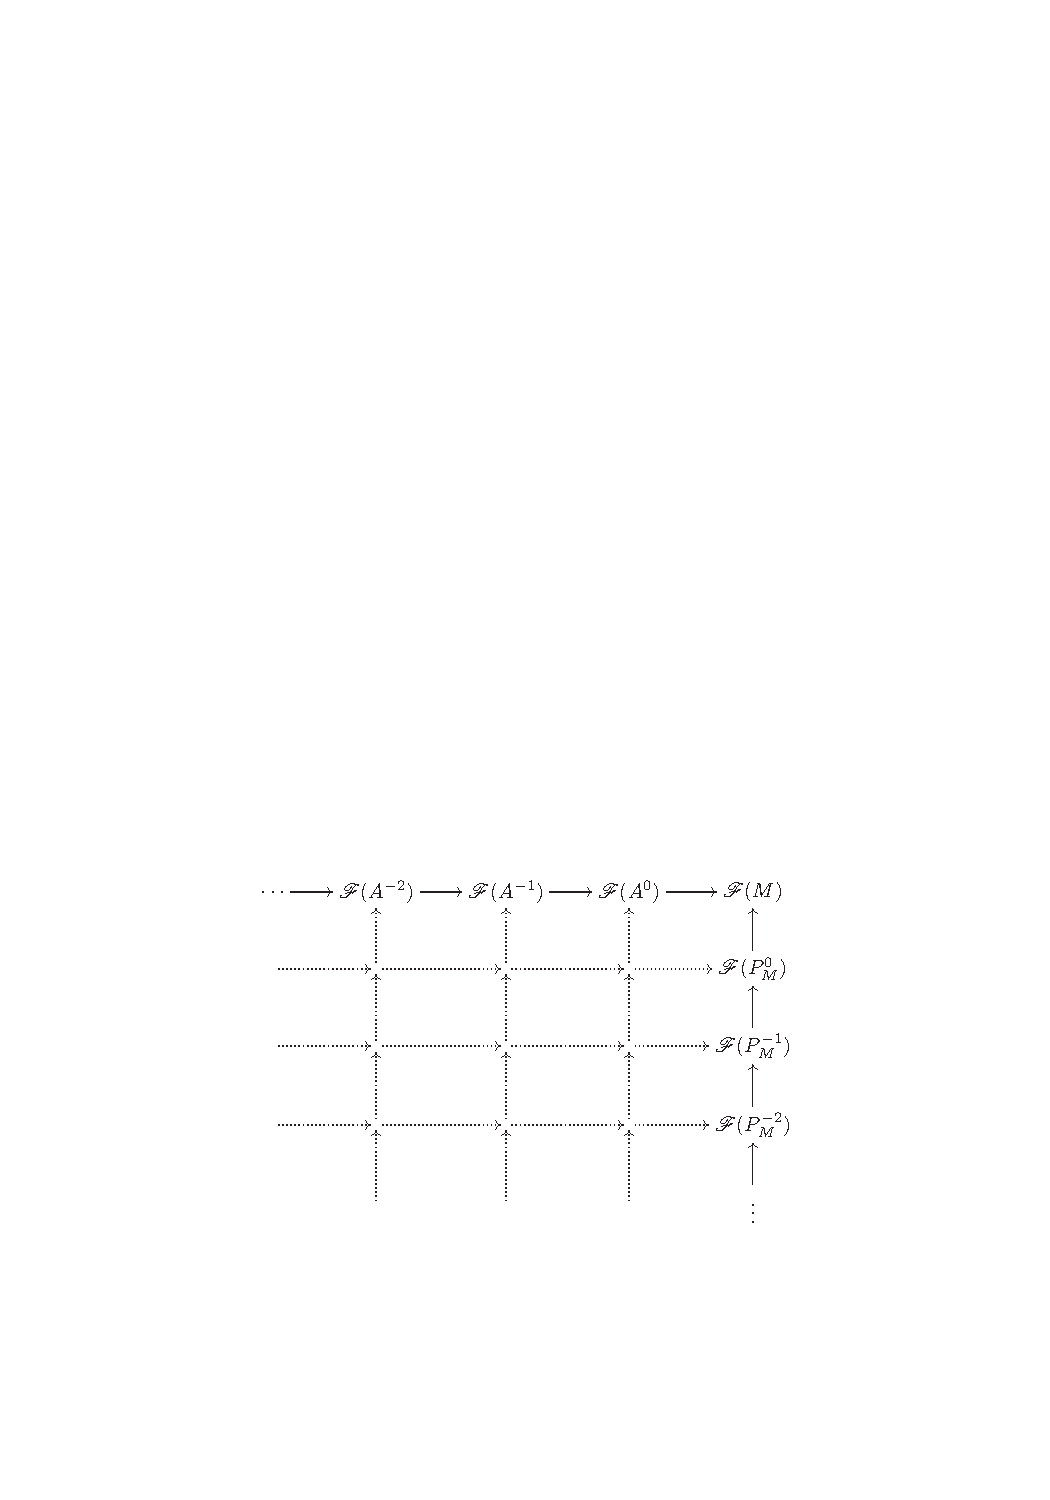
\includegraphics{pictures/doublecomp.pdf}
\end{figure}
The result of Theorem~\ref{acyclic reso der} is that taking cohomology of the top row of this diagram gives the same result as taking cohomology of the rightmost column.
\subsection{Complexes of complexes}
We will consider the category $\mathcal{C}(\mathcal{C}(\mathcal{A}))$, as is often the case, we will concentrate on bounded above complexes.\par
An object of $\mathcal{C}^{\leq0}(\mathcal{C}^{\leq0}(\mathcal{A}))$ is a complex
\[\begin{tikzcd}
\cdots\ar[r]&M^{-3,\bullet}\ar[r,"d_h^{-3,\bullet}"]&M^{-2,\bullet}\ar[r,"d_h^{-2,\bullet}"]&M^{-1,\bullet}\ar[r,"d_h^{-1,\bullet}"]&M^{0,\bullet}\ar[r]&0\ar[r]&\cdots
\end{tikzcd}\]
in which the object $M^{i,\bullet}$ in degree $i$ is itself a complex in $\mathcal{C}^{\leq0}(\mathcal{A})$. The subscript $h$ stands, rather unimaginatively, for horizontal; we have $d^{i-1,\bullet}_h\circ d^{i-1,\bullet}_h=0$. An example that will motivate the next construction is the particular case in which only two objects are nonzero:
\begin{equation}\label{comp comp-1}
\begin{tikzcd}
\cdots\ar[r]0\ar[r]&0\ar[r]&L^\bullet\ar[r,"\alpha"]&M^\bullet\ar[r]&0\ar[r]&\cdots
\end{tikzcd}
\end{equation}
(and we are considering the particular case in which $L^\bullet$, $M^\bullet$ are bounded above). We will (arbitrarily) place $M^\bullet$ in degree $0$ and $L^\bullet$ in degree $-1$. We can view the information carried by $(\ref{comp comp-1})$ as a commutative diagram:
\[\begin{tikzcd}
&\vdots&\vdots&\vdots&\vdots&\\
\cdots\ar[r]&0\ar[u]\ar[r]&L^{i+1}\ar[u,"d_L^{i+1}"]\ar[r,"\alpha^{i+1}"]&M^{i+1}\ar[u,"d_M^{i+1}"]\ar[r]&0\ar[u]\ar[r]&\cdots\\
\cdots\ar[r]&0\ar[u]\ar[r]&L^{i}\ar[u,"d_L^{i}"]\ar[r,"\alpha^{i}"]&M^{i}\ar[u,"d_M^{i1}"]\ar[r]&0\ar[u]\ar[r]&\cdots\\
\cdots\ar[r]&0\ar[u]\ar[r]&L^{i-1}\ar[u,"d_L^{i-1}"]\ar[r,"\alpha^{i-1}"]&M^{i-1}\ar[u,"d_M^{i-1}"]\ar[r]&0\ar[u]\ar[r]&\cdots\\
&\vdots\ar[u]&\vdots\ar[u]&\vdots\ar[u]&\vdots\ar[u]&
\end{tikzcd}\]
The mapping cone $MC(\alpha)^\bullet$ is obtained by shifting the complex in degree $-i$ by $i$
and then direct-summing the rows and morphisms of the resulting diagram, collapsing it to a single vertical complex:
\[\begin{tikzcd}
{}&\vdots&\vdots&\vdots&\vdots&{}\\
{}&0\ar[u]&L^{i+2}\ar[ru,"\alpha^{i+2}"]\ar[u,"-d_L^{i+2}"]&M^{i+1}\ar[u,swap,"d_M^{i+1}"]&0\ar[u]&{}\\
{}&0\ar[u]&L^{i+1}\ar[u,"-d_L^{i+1}"]\ar[ru,"\alpha^{i+1}"]&M^{i}\ar[u,swap,"d_M^{i}"]&0\ar[u]&{}\\
{}&0\ar[u]&L^{i}\ar[ru,"\alpha^i"]\ar[u,"-d_L^{i}"]&M^{i-1}\ar[u,swap,"d_M^{i-1}"]&0\ar[u]&{}\\
{}&\vdots\ar[u]&\vdots\ar[u]&\vdots\ar[u]&\vdots\ar[u]&{}\\
\end{tikzcd}\]
Note that, due to the shift, the diagram on the left has become anticommutative in the process. The extra signs are necessary in order that $MC(\alpha)^\bullet$ be a complex.\par
Now we will apply the same procedure to the more general case
\[\begin{tikzcd}
\cdots\ar[r]&M^{-3,\bullet}\ar[r,"d_h^{-3,\bullet}"]&M^{-2,\bullet}\ar[r,"d_h^{-2,\bullet}"]&M^{-1,\bullet}\ar[r,"d_h^{-1,\bullet}"]&M^{0,\bullet}\ar[r]&0\ar[r]&\cdots
\end{tikzcd}\]
This corresponds to the commutative diagram
\[\begin{tikzcd}
{}\ar[r]&M^{-3,0}\ar[r,"d_h"]&M^{-2,0}\ar[r,"d_h"]&M^{-1,0}\ar[r,"d_h"]&M^{0,0}\\
{}\ar[r]&M^{-3,-1}\ar[u,"d_v"]\ar[r,"d_h"]&M^{-2,-1}\ar[u,"d_v"]\ar[r,"d_h"]&M^{-1,-1}\ar[u,"d_v"]\ar[r,"d_h"]&M^{0,-1}\ar[u,"d_v"]\\
{}\ar[r]&M^{-3,-2}\ar[u,"d_v"]\ar[r,"d_h"]&M^{-2,-2}\ar[u,"d_v"]\ar[r,"d_h"]&M^{-1,-2}\ar[u,"d_v"]\ar[r,"d_h"]&M^{0,-2}\ar[u,"d_v"]\\
{}&{}\ar[u]&{}\ar[u]&{}\ar[u]&{}\ar[u]
\end{tikzcd}\]
As above, we shift $M^{-i,\bullet}$ by $i$, with the effect of changing
the sign of the differentials in the odd-shifted columns; we will let $\delta_v$ denote $d_v$ on even-degree columns and $-d_v$ on odd-degree columns. The resulting diagram is anticommutative:
\[\begin{tikzcd}
{}&{}&{}&{}&M^{0,0}\\
{}&{}&{}&M^{-1,0}\ar[ru,"d_h"]&M^{0,-1}\ar[u,"\delta_v"]\\
{}&{}&M^{-2,0}\ar[ru,"d_h"]&M^{-1,-1}\ar[ru,"d_h"]\ar[u,"\delta_v"]&M^{0,-2}\ar[u,"\delta_v"]\\
{}&M^{-3,0}\ar[ru,"d_h"]&M^{-2,-1}\ar[ru,"d_h"]\ar[u,"\delta_v"]&M^{-1,-2}\ar[ru,"d_h"]\ar[u,"\delta_v"]&M^{0,-3}\ar[u,"\delta_v"]\\
M^{-4,0}\ar[ru,"d_h"]&M^{-3,-1}\ar[ru,"d_h"]\ar[u,"\delta_v"]&M^{-2,-2}\ar[ru,"d_h"]\ar[u,"\delta_v"]&M^{-1,-3}\ar[ru,"d_h"]\ar[u,"\delta_v"]&M^{0,-4}\ar[u,"\delta_v"]\\
\end{tikzcd}\]
Taking direct sums of the objects and morphisms on each row, as in the case of the mapping cone, determines a new complex, called the \textbf{total complex} $TC(M)^\bullet$ of the given complex of complexes.\par
Double complexes capture this construction:
\begin{definition}
A \textbf{double $(cochain)$ complex} on an abelian category $\mathcal{A}$ is an array of objects $M^{i,j}$ of $\mathcal{A}$, $i,j\in\Z$, endowed with morphisms
\[d^{i,j}_h:M^{i,j}\to M^{i+1,j},\quad \delta^{i,j}_v:M^{i,j}\to M^{i,j+1}\]
such that
\[\left\{\begin{array}{l}
d_h^{i,j}\circ d_h^{i-1,j}=0\\
\delta_v^{i,j}\circ\delta_v^{i,j-1}=0\\
\delta^{i+1,j}_v\circ d_h^{i,j}+d^{i,j+1}_h\circ\delta^{i,j}_v=0
\end{array}\right. \]
\end{definition}
That is, the columns $M^{i,\bullet}$ and the rows $M^{\bullet,j}$ both form complexes, and the whole diagram anticommutes. Dropping the position specification, the conditions defining a double complex are summarized in the easier-to-parse prescription
\[\left\{\begin{array}{l}
d_h\circ d_h=0\\
\delta_v\circ\delta_v=0\\
\delta_v\circ d_h+d_h\circ\delta_v=0
\end{array}\right. \]
Double complexes, with or without appropriate boundedness conditions (such as requiring $M^{i,j}=0$ for $i>0$, $j>0$, as in the case considered above), form a category in an evident way. It is equally evident that this category is equivalent to the correspondingly bounded category of complexes of complexes: every object of $\mathcal{C}^{\leq0}(\mathcal{C}^{\leq0}(\mathcal{A}))$ determines a double complex by setting $\delta^{i,j}_v=(-1)^id^{i,j}_v$, as above.
Changing the signs of odd rows rather than columns leads to an isomorphic double complex; in fact, other choices may be convenient depending on the
situation.\par
From this viewpoint, the total complex $TC(M)^\bullet$ (also called the simple of the double complex $M^{\bullet,\bullet}$) is obtained by direct-summing objects and morphisms of the double complex along diagonals:
\begin{figure}[!h]
\centering
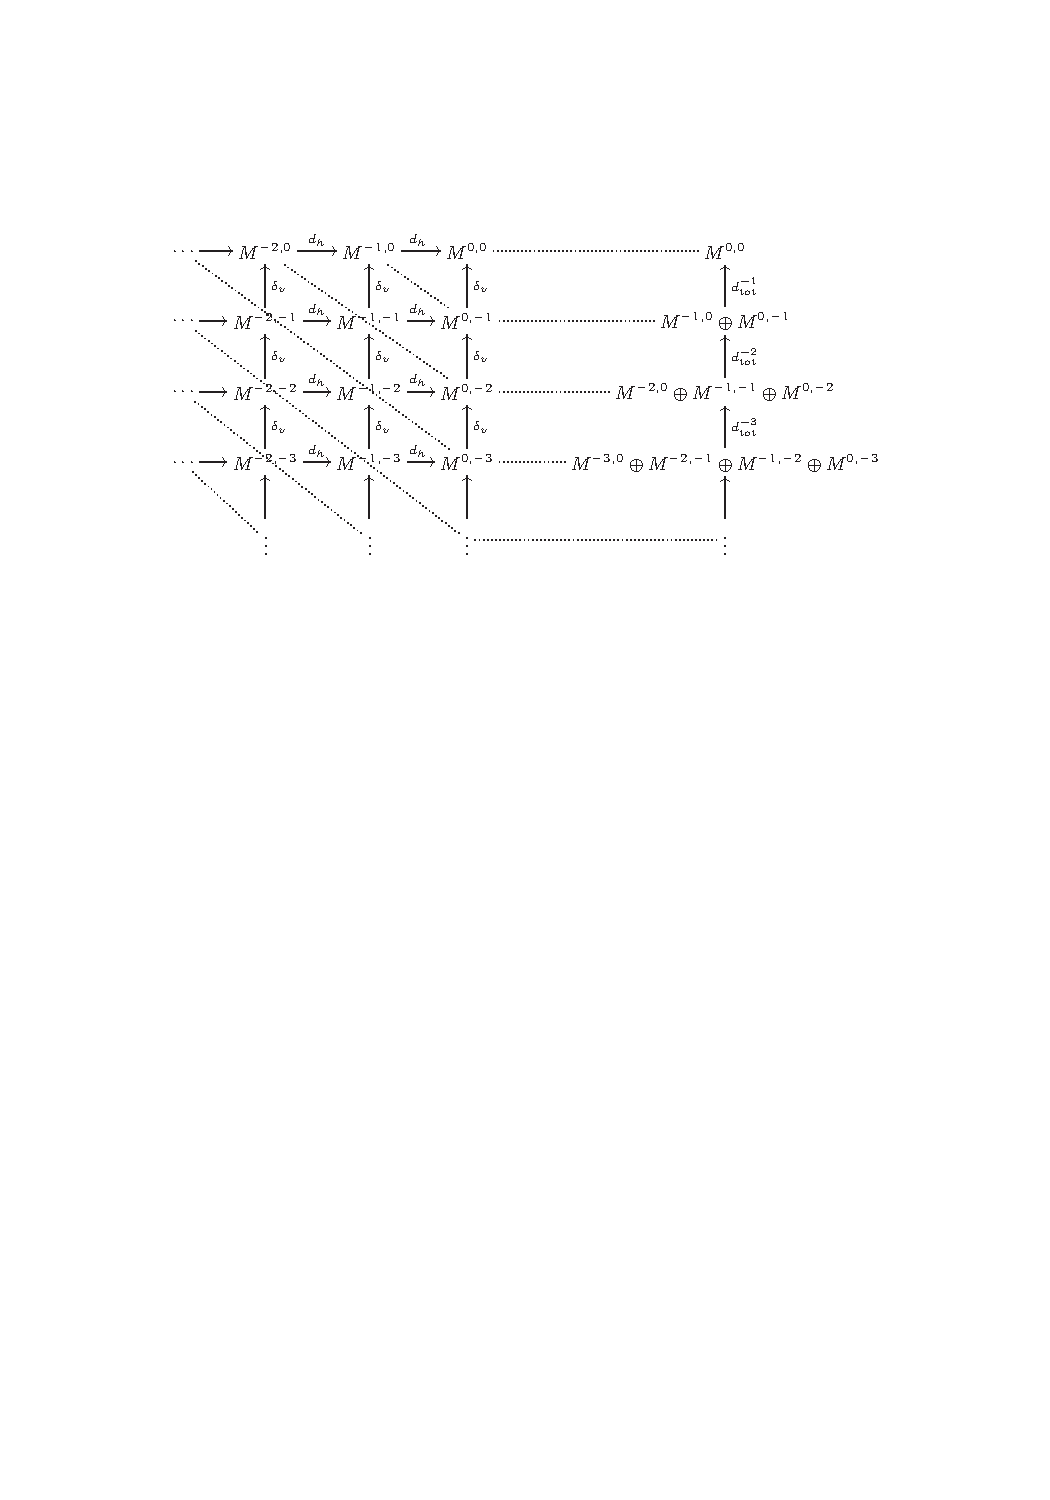
\includegraphics{pictures/totcomp.pdf}
\end{figure}
\begin{definition}
The \textbf{total complex} $TC(M)^\bullet$ of a double complex $M^{\bullet,\bullet}$ is defined by setting $TC(M)^k:=\bigoplus_{i+j=k}M^{i,j}$, with differentials (written stenographically) $d_{tot}=d_h+\delta_v$.
\end{definition}
\begin{claim}
$(TC(M)^\bullet,d_{tot})$ is indeed a complex.
\end{claim}
\begin{proof}
The question is whether the composition of two consecutive differentials
vanishes, as it should. Insisting with our shorthand,
\[d_{tot}\circ d_{tot}=(d_h+\delta_v)\circ(d_h+\delta_v)=d_h\circ d_h+d_h\circ\delta_v+\delta_v\circ d_h+\delta_v\circ\delta_v=0\]
\end{proof}
\begin{example}\label{tot comp eg}
Operations such as $\Hom_A$ or $\otimes$ determine double complexes. For a
first quadrant example, let $L^\bullet$, resp., $M^\bullet$, be a complex in $\mathcal{C}^{\leq0}(\mathcal{A})$, resp. $\mathcal{C}^{\geq0}(\mathcal{A})$:
\[\begin{tikzcd}
\cdots\ar[r]&L^{-2}\ar[r]&L^{-1}\ar[r]&L^0\ar[r]&0\ar[r]&\cdots
\end{tikzcd}\]
\[\begin{tikzcd}
\cdots\ar[r]&0\ar[r]&M^0\ar[r]&M^1\ar[r]&M^2\ar[r]&\cdots
\end{tikzcd}\]
We can consider the complex in $\mathcal{C}^{\geq0}(\mathcal{C}^{\geq0}(\mathcal{A}))$:
\[\begin{tikzcd}
\cdots\ar[r]&\Hom_{\mathcal{A}}(L^\bullet,M^0)\ar[r]&\Hom_{\mathcal{A}}(L^\bullet,M^1)\ar[r]&\Hom_{\mathcal{A}}(L^\bullet,M^2)\ar[r]&\cdots
\end{tikzcd}\]
that is, in grid form (and omitting zeros to the left and below):
\[\begin{tikzcd}
\vdots&\vdots&\vdots&\\
\Hom_{\mathcal{A}}(L^{-2},M^0)\ar[u]\ar[r]&\Hom_{\mathcal{A}}(L^{-2},M^1)\ar[u]\ar[r]&\Hom_{\mathcal{A}}(L^{-2},M^2)\ar[u]\ar[r]&\cdots\\
\Hom_{\mathcal{A}}(L^{-1},M^0)\ar[r]\ar[u]&\Hom_{\mathcal{A}}(L^{-1},M^1)\ar[r]\ar[u]&\Hom_{\mathcal{A}}(L^{-1},M^2)\ar[u]\ar[r]&\cdots\\
\Hom_{\mathcal{A}}(L^{0},M^0)\ar[r]\ar[u]&\Hom_{\mathcal{A}}(L^{0},M^1)\ar[u]\ar[r]&\Hom_{\mathcal{A}}(L^{0},M^2)\ar[u]\ar[r]&\cdots\\
\end{tikzcd}\]
We could also consider the complex of complexes
\[\begin{tikzcd}[column sep=1.0 em]
\cdots\ar[r]&0\ar[r]&\Hom_{\mathcal{A}}(L^0,M^\bullet)\ar[r]&\Hom_{\mathcal{A}}(L^{-1},M^\bullet)\ar[r]&\Hom_{\mathcal{A}}(L^{-2},M^\bullet)\ar[r]&\cdots
\end{tikzcd}\]
and this would lead to the grid obtained by flipping the previous one about the main diagonal. The two corresponding total complexes are then clearly isomorphic, and by a slight abuse of language they can both be denoted $TC(\Hom_{\mathcal{A}}(L,M))^\bullet$. The degree-$i$ piece of this total complex, i.e.,
\[\begin{tikzcd}
\Hom_{\mathcal{A}}(L^{-i},M^0)\oplus\Hom_{\mathcal{A}}(L^{-i+1},M^1)\oplus\cdots\oplus\Hom_{\mathcal{A}}(L^{0},M^i)
\end{tikzcd}\]
parametrizes degree-preserving morphisms from objects of $L^\bullet$ to objects of $M[i]^\bullet$. These are not cochain morphisms $L^\bullet\to M[i]^\bullet$, since the corresponding diagrams
\[\begin{tikzcd}[column sep=1.0 em]
\cdots\ar[r]&0\ar[r]&M[i]^{-i}\ar[r]&M[i]^{-i+1}\ar[r]&\cdots\ar[r]&M[i]^{0}\ar[r]&M[i]^{1}\ar[r]&\cdots\\
\cdots\ar[r]&L^{-i-1}\ar[u]\ar[r]&L^{-i}\ar[u]\ar[r]&L^{-i+1}\ar[u]\ar[r]&\cdots\ar[r]&L^0\ar[r]\ar[u]&0\ar[r]\ar[u]&\cdots
\end{tikzcd}\]
do not satisfy any commutativity hypothesis. The reader will verify that, with suitable positions:
\begin{itemize}
\item the kernel of $d^i_{tot}$ consists of morphisms of cochain complexes $L^\bullet\to M[i]^\bullet$;
\item the image of $d^{i-1}_{tot}$ consists of morphisms that are homotopy equivalent to $0$; and hence
\item the cohomology of $TC(\Hom_{\mathcal{A}}(L,M))^\bullet$ parametrizes morphisms in the homotopy category.
\end{itemize}
For (a trivial) example, $TC(\Hom_{\mathcal{A}}(L,M))^0=\Hom_{\mathcal{A}}(L^0,M^0)$, and $d^0_{tot}(\alpha)=0$ means that the images $\alpha\circ d_L^{-1}$ in $\Hom_{\mathcal{A}}(L^{-1},M^0)$ and $d^0_M\circ\alpha$ in $\Hom_{\mathcal{A}}(L^{0},M^1)$ both vanish:
\[\begin{tikzcd}
{}\ar[r]&L^{-1}\ar[rd,dashed,"0"]\ar[r,"d_L^{-1}"]&L^0\ar[r]\ar[rd,dashed,"0"]\ar[d,"\alpha"]&0\ar[r]&{}\\
{}\ar[r]&0\ar[r]&M^0\ar[r,"d_M^{0}"]&M^1\ar[r]&{}\\
\end{tikzcd}\]
This is precisely the condition needed for $\alpha$ to define a morphism of cochain complexes $L^\bullet\to M^\bullet$. It follows that in this situation $H^0(TC(\Hom_{\mathcal{A}}(L,M))^\bullet)$ is simply $\Hom_{\mathcal{C}(\mathcal{A})}(L^\bullet,M^\bullet)=\Hom_{\mathcal{K}(\mathcal{A})}(L^\bullet,M^\bullet)$ (there are no nontrivial homotopies in this case).\par
The identification of the $i$-th cohomology of the total complex with $\Hom_{\mathcal{K}(\mathcal{A})}(L^\bullet,M[i]^\bullet)$ requires care with the signs.
\end{example}
\subsection{Exactness of the total complex}
The cohomology of the total complex of a double complex can be computed by an extremely clever device called \textit{spectral sequence}, which we will (briefly) encounterThere are standard situations, however, in which one can conclude immediately that the total complex is exact, and this is at the root of the applications we will present. The statement is neat
and memorable:
\begin{theorem}\label{tot comp exact}
Let $\mathcal{A}$ be an abelian category, and let
\begin{equation}\label{tot comp exact-1}
\begin{tikzcd}
\cdots\ar[r]&M^{-3,\bullet}\ar[r]&M^{-2,\bullet}\ar[r]&M^{-1,\bullet}\ar[r]&M^{0,\bullet}\ar[r]&0\ar[r]&\cdots
\end{tikzcd}
\end{equation}
be a complex in $\mathcal{C}^{\leq0}(\mathcal{C}^{\leq0}(\mathcal{A}))$. Let $T^\bullet$ be the corresponding total complex. Then
\begin{itemize}
\item if $(\ref{tot comp exact-1})$ is exact, then $T^\bullet$ is exact.
\item if each complex $M^{i,\bullet}$ is exact, then $T^\bullet$ is exact.
\end{itemize}
\end{theorem}
The proof will yield a more precise statement on the vanishing of individual degrees of the cohomology of the total complex.\par
Mutatis mutandis, Theorem~\ref{tot comp exact} holds for complexes in $\mathcal{C}^{\geq0}(\mathcal{C}^{\geq0}(\mathcal{A}))$, with microscopic
adjustments to the proof; we will take this for granted in the applications. In fact, the boundedness hypothesis can be relaxed: one of the two given exactness statements will still hold if only one of the $\mathcal{C}$ is bounded. The point is that the proof relies on an inductive argument, which goes through as soon as it has a place to start. The reader is welcome to explore all these ramifications.\par
In terms of double complexes, Theorem~\ref{tot comp exact} says that the total complex of a (suitably bounded) double complex is exact if the rows or the columns of the double complex are exact.
\begin{proof}
It is enough to prove the second statement: the first one follows by flipping the double complex corresponding to $(\ref{tot comp exact-1})$.\par
To prove the second statement, we assume that the columns in the staggered
(anticommutative) diagram
\[\begin{tikzcd}
{}&{}&{}&{}&0\\
{}&{}&{}&0&M^{0,0}\ar[u]\\
{}&{}&0&M^{-1,0}\ar[ru,"d_h"]\ar[u]&M^{0,-1}\ar[u,"\delta_v"]\\
{}&0&M^{-2,0}\ar[ru,"d_h"]\ar[u]&M^{-1,-1}\ar[ru,"d_h"]\ar[u,"\delta_v"]&M^{0,-2}\ar[u,"\delta_v"]\\
{}&M^{-3,0}\ar[ru,"d_h"]\ar[u]&M^{-2,-1}\ar[ru,"d_h"]\ar[u,"\delta_v"]&M^{-1,-2}\ar[ru,"d_h"]\ar[u,"\delta_v"]&M^{0,-3}\ar[u,"\delta_v"]\\
\end{tikzcd}\]
associated with $(\ref{tot comp exact})$ are exact and that we have an element
\[m=(m^0,m^{-1},\cdots m^{-i})\in M^{-i,0}\oplus M^{-i+1,-1}\oplus\cdots\oplus M^{0,-i}\]
such that $d_{tot}^{-i}(m)=0$; we are expected to produce an element
\[n=(n^0,n^{-1},\cdots,n^{-i-1})\in M^{-i-1,0}\oplus M^{-i,-1}\oplus\cdots\oplus M^{0,-i-1}\]
such that $d^{-i-1}_{tot}(n)=m$.\par
The little induction that accomplishes this is conceptually very simple, but notationally challenging. We believe that viewing it in action in a simple case (we will choose $i=2$) suffices to convey all that needs to be conveyed. Thus, assume that $m=(m^0,m^{-1},m^{-2})$ is in the kernel of $d_{tot}$; that is,
\[\left\{
\begin{array}{l}
d_h(m^0)+\delta_v(m^{-1})=0\\
d_h(m^{-1})+\delta_v(m^{-2})=0
\end{array}\right. \]
We choose $n^0=0$. Since $M^{-2,\bullet}$ is exact ($M^{-2,-1}\to M^{-2,0}$ is epic), there exists $n^{-1}\in M^{-2,-1}$ such that $\delta_v(n^{-1})=m^0$. Since the diagram anticommutes
\[\delta_v\circ d_h(n^{-1})=-d_h\circ\delta_v(n^{-1})=-d_h(m^0)=\delta_v(m^{-1})\]
Therefore, $m^{-1}-d_h(n^{-1})\in\ker\delta_v$, and since $M^{-1,\bullet}$ is exact, there exists $n^{-2}\in M^{-1,-2}$ such that $\delta_v(n^{-2})=m^{-1}-d_h(n^{-1})$. That is,
\[d_h(n^{-1})+\delta_v(n^{-2})=m^{-1}\]
The next step is entirely analogous:
\[\delta_v\circ d_h(n^{-2})=-d_h\circ\delta_v(n^{-2})=-d_h(m^{-1}-d_h(n^{-1}))=-d_h(m^{-1})=\delta_v(m^{-2})\]
(using the fact that $d_h\circ d_h=0$); therefore $m^{-2}-d_h(n^{-2})\in\ker\delta_v$, and since $M^{0,\bullet}$ is exact, there exists $n^{-3}\in M^{0,-2}$ such that $\delta_v(n^{-3})=m^{-2}-d_h(n^{-2})$. That is,
\[d_h(n^{-2})+\delta_v(n^{-3})=m^{-2}\]
With these choices, $d_{tot}(n)$ equals
\[d_h(n^0)+\delta_v(n^{-1})+d_h(n^{-1})+\delta_v(n^{-2})+d_h(n^{-2})+\delta_v(n^{-3})=0+m^0+m^{-1}+m^{-2}=m\]
as needed.\par
The case for arbitrary $i$ simply requires additional repetitions of the basic steps performed for $i=2$.
\end{proof}
\begin{example}
Here is a taste of how convenient Theorem~\ref{tot comp exact} is. Let $P^\bullet$ be a complex in $\mathcal{C}^{\leq0}(\mathcal{A})$, where each $P^i$ is projective, and let $L^\bullet$ be an exact complex in $\mathcal{C}^{\geq0}(\mathcal{A})$. Since $P^i$ is projective, $\Hom_{\mathcal{A}}(P^i,L^\bullet)$ is still exact. Therefore, the complex
\[\begin{tikzcd}
\cdots\ar[r]&0\ar[r]&\Hom_{\mathcal{A}}(P^0,L^\bullet)\ar[r]&\Hom_{\mathcal{A}}(P^{-1},L^\bullet)\ar[r]&\Hom_{\mathcal{A}}(P^{-2},L^\bullet)\ar[r]&\cdots
\end{tikzcd}\]
satisfies the hypothesis of the second statement given in Theorem~\ref{tot comp exact} (in the symmetrically bounded version). According to Theorem~\ref{tot comp exact}, the corresponding total complex is exact; as seen in Example~\ref{tot comp eg}, this says that $\Hom_{\mathcal{K}(\mathcal{A})}(P^\bullet,L[i]^\bullet)=0$ for all $i$. In other words, every cochain morphism from a bounded-above complex of projectives to a bounded-below exact complex is homotopic to $0$. This recovers Corollary~\ref{pro homotopy 0}, up to easy adjustments, taking care of the boundedness hypothesis on $L^\bullet$.
\end{example}
\subsection{Total complexes and resolutions}
Viewing a (bounded-above) complex $N^\bullet$ as an object of the abelian category $\mathcal{A}'=\mathcal{C}^{\leq0}(\mathcal{A})$, a (bounded-above) resolution of $N^\bullet$ ought to be a complex $M^{\bullet,\bullet}$ in $\mathcal{C}^{\leq0}(\mathcal{A}')$ endowed with a quasi-isomorphism
\[\begin{tikzcd}
\cdots\ar[r]&M^{-2,\bullet}\ar[d]\ar[r]&M^{-1,\bullet}\ar[d]\ar[r]&M^{0,\bullet}\ar[r]\ar[d]&0\ar[d]\ar[r]&\cdots\\
\cdots\ar[r]&0\ar[r]&0\ar[r]&N^\bullet\ar[r]&0\ar[r]&\cdots
\end{tikzcd}\]
in$\mathcal{C}^{\leq0}(\mathcal{A}')$. In other words, a resolution of $N^\bullet$ should be a complex $M^{\bullet,\bullet}$ whose cohomology (computed in $\mathcal{C}^{\leq0}(\mathcal{A}')$) is concentrated in degree $0$ and agrees with $N^\bullet$.\par
We are going to verify that these two notions of resolution of a complex are compatible: taking the total complex of a resolution $M^{\bullet,\bullet}$ of $N^\bullet$ (in the new sense of the term) again gives a resolution of $N^\bullet$ (in the old sense).\par
Before stating this more explicitly, consider more generally any cochain morphism in $\mathcal{C}^{\leq0}(\mathcal{C}^{\leq0}(\mathcal{A}))$ from $M^{\bullet,\bullet}$ to a complex (of complexes) concentrated in degree $0$:
\[\begin{tikzcd}
\cdots\ar[r]&M^{-2,\bullet}\ar[d]\ar[r,"d_h"]&M^{-1,\bullet}\ar[d]\ar[r,"d_h"]&M^{0,\bullet}\ar[r]\ar[d,"\alpha"]&0\ar[d]\ar[r]&\cdots\\
\cdots\ar[r]&0\ar[r]&0\ar[r]&N^\bullet\ar[r]&0\ar[r]&\cdots
\end{tikzcd}\]
This means that $\alpha\circ d_h=0$, so we can fold this diagram into a single complex of complexes:
\[\begin{tikzcd}
\cdots\ar[r]&M^{-2,\bullet}\ar[r,"-d_h"]&M^{-1,\bullet}\ar[r,"-d_h"]&M^{0,\bullet}\ar[r,"\alpha"]&0\ar[r]&\cdots\\
\end{tikzcd}\]
That is, $M^{\bullet,\bullet}_N$ agrees with the complex obtained by shifting $M^{\bullet,\bullet}$ by one step to the left, with $N^\bullet$ inserted in degree $0$. For now, we are making no assumptions on
the cohomology of $M^{\bullet,\bullet}$.\par
We want to compare the various total complexes that can be defined in this
situation. We can map the total complex of $M^{\bullet,\bullet}$ to $N^\bullet$,
\[\begin{tikzcd}
{}&{}&0\ar[r]&0\\
{}&{}&M^{0,0}\ar[u]\ar[r]&N^0\ar[u]\\
{}&M^{-1,0}\ar[draw=none]{r}[name=X, anchor=center,scale=1.5]{\oplus}\ar[ru]&M^{0,-1}\ar[r]\ar[u]&N^{-1}\ar[u]\\
M^{-2,0}\ar[draw=none]{r}[name=X, anchor=center,scale=1.5]{\oplus}\ar[ru]&M^{-1,-1}\ar[draw=none]{r}[name=X, anchor=center,scale=1.5]{\oplus}\ar[u]\ar[ru]&M^{0,-2}\ar[u]\ar[r]&N^{-2}\ar[u]\\
\end{tikzcd}\]
obtaining a morphism of cochain complexes
\[TC(\alpha):TC(M^{\bullet,\bullet})\to N^\bullet\]
Or, we can shift the $M$-part of this diagram and view the last display as the construction of the total complex $M_N^{\bullet,\bullet}$.
\begin{claim}\label{tot map cone}
The total complex of $M^{\bullet,\bullet}_N$ is the mapping cone of $TC(\alpha)$:
\[TC(M_N)^\bullet=MC(TC(\alpha))\]
\end{claim}
\begin{theorem}\label{tot reso}
Let $\mathcal{A}$ be an abelian category, and denote by $\mathcal{A}'$ the category $\mathcal{C}^{\leq0}(\mathcal{A})$. Let $N^\bullet$ be an object of $\mathcal{A}'$, and let
\begin{equation}\label{tot reso-1}
\begin{tikzcd}
\cdots\ar[r]&M^{-3,\bullet}\ar[r]&M^{-2,\bullet}\ar[r]&M^{-1,\bullet}\ar[r]&M^{0,\bullet}\ar[r]&0\ar[r]&\cdots
\end{tikzcd}
\end{equation}
be a complex in $\mathcal{C}^{\leq0}(\mathcal{A}')$, with total complex $T^\bullet$.
\begin{itemize}
\item Assume that $(\ref{tot reso-1})$ is a resolution of $N^\bullet$ in $\mathcal{C}^{\leq0}(\mathcal{A}')$. Then $T^\bullet$ is quasi-isomorphic
to $N^\bullet$ in $\mathcal{C}^{\leq0}(\mathcal{A})$ (that is, it is a resolution of $N^\bullet$ in the old sense).
\item Assume that the cohomology of each $M^{i,\bullet}$ is concentrated in degree $0$. Then $T^\bullet$ is quasi-isomorphic to the complex of cohomology objects induced by $(\ref{tot reso-1})$:
\[\begin{tikzcd}[column sep=small]
\cdots\ar[r]&H^0(M^{-3,\bullet})\ar[r]&H^0(M^{-2,\bullet})\ar[r]&H^0(M^{-1,\bullet})\ar[r]&H^0(M^{0,\bullet})\ar[r]&0\ar[r]&\cdots
\end{tikzcd}\]
\end{itemize}
\end{theorem}
\begin{proof}
The second statement follows from the first, by flipping the corresponding
double complex about the main diagonal.\par
The first statement follows from Theorem~\ref{tot comp exact} and Claim~\ref{tot map cone}. Indeed, let $M^{\bullet,\bullet}_N$ be the exact complex
\[\begin{tikzcd}
\cdots\ar[r]&M^{-3,\bullet}\ar[r]&M^{-2,\bullet}\ar[r]&M^{-1,\bullet}\ar[r]&M^{0,\bullet}\ar[r]&N^\bullet\ar[r]&0\ar[r]&\cdots
\end{tikzcd}\]
by Theorem~\ref{tot comp exact}, $TC(M_N)^\bullet$ is exact; by Claim~\ref{tot map cone} this is the mapping cone of the induced morphism $T^\bullet\to N^\bullet$, and it follows (Corollary~\ref{MC exact iff quasi-iso}) that this morphism is a quasi-isomorphism, as needed.
\end{proof}
To appreciate the usefulness of Theorem~\ref{tot reso}, again in the context of our (hard) work in $\S6$, note that it provides us with a convenient bridge between \textit{resolving objects} (see Lemma~\ref{pro reso initial}) and resolving complexes (as in Theorem~\ref{proj reso exist}). Indeed, by Corollary~\ref{reso complex} (which relies on the horseshoe lemma, therefore on resolving individual objects of $\mathcal{A}$) every bounded-above complex $N^\bullet$ in an abelian category with enough projectives may be viewed as the complex induced in $H^0$ from a complex
\[\begin{tikzcd}
\cdots\ar[r]&P^{-3,\bullet}\ar[r]&P^{-2,\bullet}\ar[r]&P^{-1,\bullet}\ar[r]&P^{0,\bullet}\ar[r]&0\ar[r]&\cdots
\end{tikzcd}\]
where $P^{i,\bullet}$ is a projective resolution of $N^i$. The total complex of $P^{\bullet,\bullet}$ is then a projective resolution of $N^\bullet$, by the second statement in Theorem~\ref{tot reso}. This
reproduces the main content of Theorem~\ref{proj reso exist}, bypassing the nastiest details of the proof given in $\S6$.\par
As mentioned in Remark~\ref{reso comp remk}, double complexes of projectives (or, working in $\mathcal{C}^{\geq0}$ injectives) resolving a given complex (and satisfying the additional condition explained in Remark~\ref{reso comp remk}) are called Cartan-Eilenberg resolutions. Their systematic use can simplify the material we presented in $\S6$ but at the price of dealing early with double complexes.
\subsection{Acyclic resolutions again and balancing Tor and Ext}
As a warm-up (and another illustration of the power of double complexes), go back to the question we studied in $\S8.1$: we ended that subsection by lining up the complexes obtained by applying an additive functor $\mathscr{F}$ to an $\mathscr{F}$-acyclic resolution $A^\bullet$ of an object $M$ and to a projective resolution of the same object, as sides of an array. Corollary~\ref{reso complex} tells us how to fill the rest of the array: start from
\begin{equation}\label{acy reso-1}
\begin{tikzcd}
\cdots\ar[r]&A^{-2}\ar[r]&A^{-1}\ar[r]&A^0\ar[r]&0\ar[r]&\cdots
\end{tikzcd}
\end{equation}
which is exact by hypothesis; using Corollary~\ref{reso complex}, view $(\ref{acy reso-1})$ as the complex induced in $H^0$ by an exact complex
\begin{equation}\label{acy reso-2}
\begin{tikzcd}
\cdots\ar[r]&P^{-2,\bullet}\ar[r]&P^{-1,\bullet}\ar[r]&P^{-0,\bullet}\ar[r]&P^{\bullet}_M\ar[r]&0\ar[r]&\cdots
\end{tikzcd}
\end{equation}
where $P^{i,\bullet}$ is a projective resolution of $A^i$ and $P^\bullet_M$ is a projective resolution of $M$. Since $(\ref{acy reso-2})$ is exact, the rows of the double complex corresponding to $(\ref{acy reso-2})$ are projective resolutions of the projective objects $P^i_M$. Now apply $\mathscr{F}$:
\[
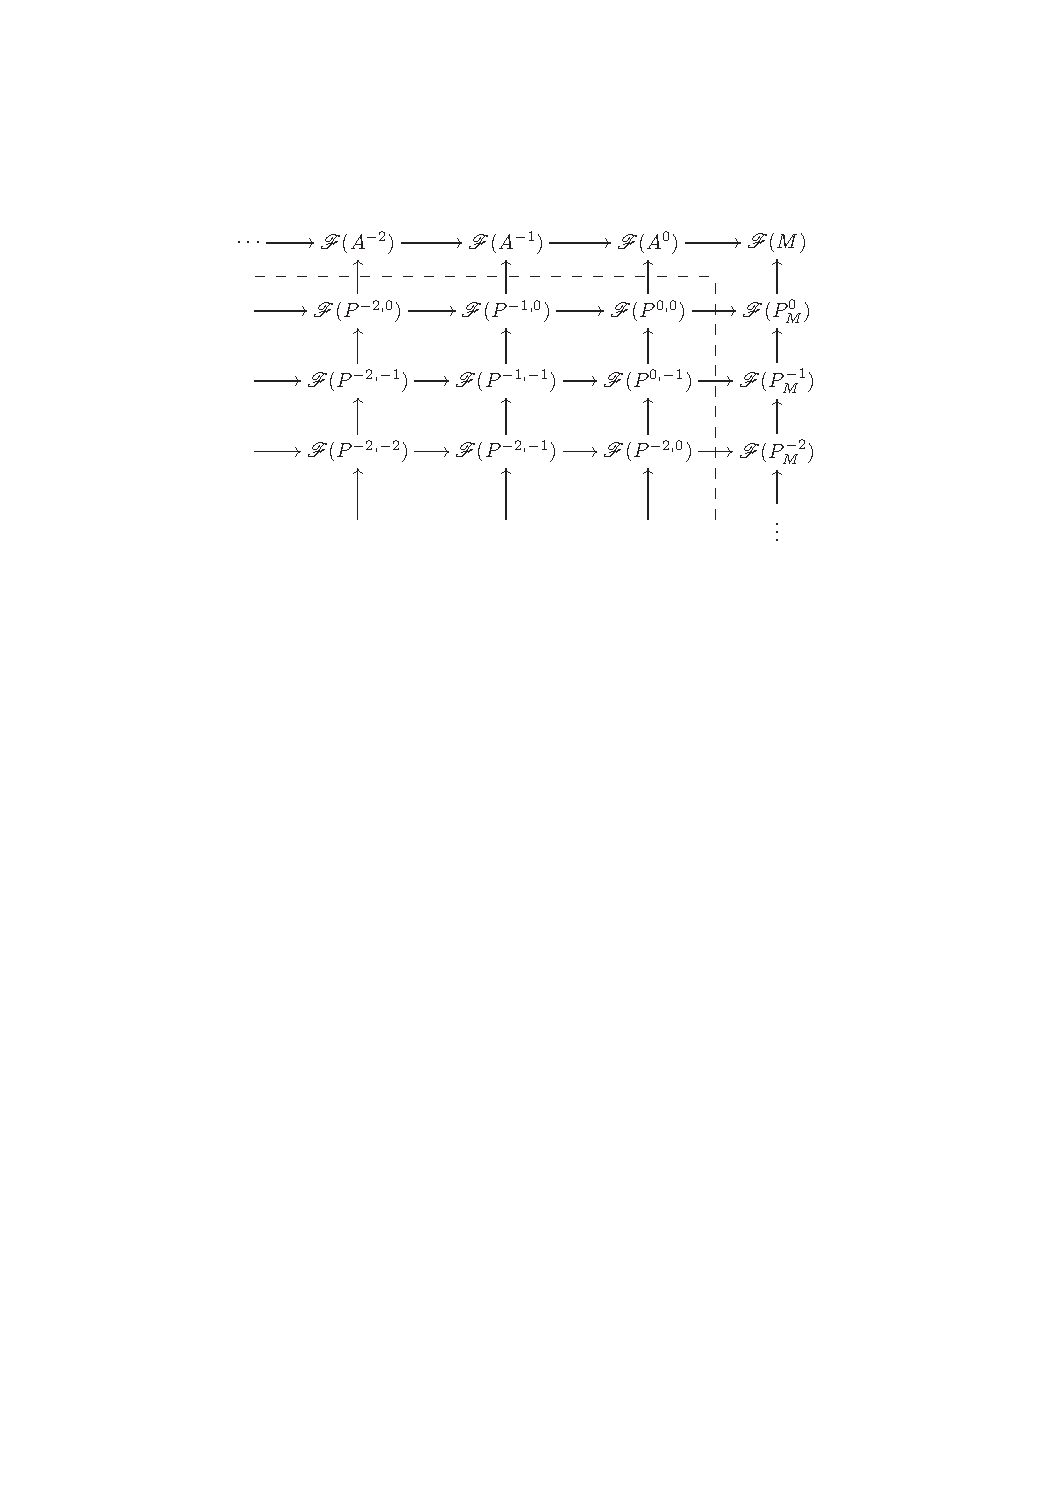
\includegraphics{pictures/tot-acyreso.pdf}
\]
Since each $P^i_M$ is projective and each $A^i$ is $\mathscr{F}$-acyclic, every row and every column of the part of this diagram within the dashed lines is exact. Therefore we can apply Theorem~\ref{tot reso} to the complex
\[\begin{tikzcd}
\mathscr{F}(P^{\bullet,\bullet}):&\cdots\ar[r]&\mathscr{F}(P^{-2,\bullet})\ar[r]&\mathscr{F}(P^{-1,\bullet})\ar[r]&\mathscr{F}(P^{0,\bullet})\ar[r]&0\ar[r]&\cdots
\end{tikzcd}\]
and discover that the total complex $TC(\mathscr{F}(P))^\bullet$ is quasi-isomorphic to both complexes $\mathcal{C}(\mathscr{F})(A^\bullet)$ and $\mathcal{C}(\mathscr{F})(P^\bullet_M)$. It follows that
\[H^i(\mathcal{C}(\mathscr{F})(A^\bullet))\cong H^i(\mathcal{C}(\mathscr{F})(P_M^\bullet))\cong\mathcal{L}_i\mathscr{F}(M)\]
which was the conclusion of Theorem~\ref{acyclic reso der}.\par
This example illustrates the general strategy of other applications of double
complexes: the cohomologies of two complexes are shown to be isomorphic by
showing that there is an exact double complex interpolating between them. This strategy finally justifies the claims that $\Tor$ and $\Ext$ functors can be computed by resolving either one of their arguments.
\begin{theorem}\label{der func tonsor}
Let $M,N$ be modules over a commutative ring $R$, and let $P^\bullet_M$, resp., $P^\bullet_N$, be projective resolutions of $M$, resp., $N$. Then
\[H^i(P^\bullet_M\otimes_{R}N)\cong H^i(M\otimes_{R}P_N^\bullet)\cong\Tor^R_i(M,N).\]
\end{theorem}
The first term was our official definition of $\Tor$. Theorem~\ref{der func tonsor} makes good on our old promise to show that the $\Tor$ functors could be computed by resolving the second factor rather than the first.
\begin{proof}
Apply Theorem~\ref{tot reso} to the complex
\begin{equation}\label{der tens-1}
\begin{tikzcd}
\cdots\ar[r]&P^{-2}_M\otimes_{R}P_N^\bullet\ar[r]&P^{-1}_M\otimes_{R}P_N^\bullet\ar[r]&P^{0}_M\otimes_{R}P_N^\bullet\ar[r]&\cdots
\end{tikzcd}
\end{equation}
Since each $P^j_N$ is projective, the cohomology of this complex is concentrated in degree $0$ and equals $M\otimes_{R}P^\bullet_N$. It follows that
\[TC(P_M^\bullet\otimes_{R}P_N^\bullet)^\bullet\stackrel{q\text{-}iso}{\longrightarrow}M\otimes_{R}P^\bullet_N\]
by the first statement in Theorem~\ref{tot reso}. On the other hand, since each $P^i_M$ is projective, the complex $P^i_M\otimes_{R}P_N^\bullet$ is a resolution of $P^i_M\otimes_{R}N$; that is, the cohomology of each $P^i_M\otimes_{R}P_N^\bullet$ is concentrated in degree $0$ and equals $P^i_M\otimes_{R}N$. Thus, the
complex $(\ref{der tens-1})$ induces the complex $P^\bullet_M\otimes_{R}N$ in $H^0$, and
\[TC(P_M^\bullet\otimes_{R}P_N^\bullet)^\bullet\stackrel{q\text{-}iso}{\longrightarrow}P^\bullet_M\otimes_{R}N\]
by the second statement in Theorem~\ref{tot reso}. The result follows.
\end{proof}
\begin{theorem}
Let $M,N$ be modules over a commutative ring $R$, and let $P_M^\bullet$,
resp., $Q^\bullet_N$, be a projective resolution of $M$, resp., an injective resolution of $N$. Then
\[H^i(\Hom_R(P^\bullet_M,N))\cong H^i(\Hom_R(M,Q^\bullet_N))\cong\Ext^i_R(M,N).\]
\end{theorem}
\subsection{Exercise}
\begin{exercise}\label{right exact func ch}
Let $\mathcal{A},\mathcal{B}$ be abelian categories, let $A^\bullet$ be an exact complex in $\mathcal{C}(\mathcal{A})$, and let $\mathscr{F}$ be a right-exact functor $\mathcal{A}\to\mathcal{B}$. Let $K^i$ be the kernel of $d^i_A$. Prove that
\[H^i(\mathcal{C}(\mathscr{F})(A^\bullet))\cong\ker(\mathscr{F}(K^{i+1})\to\mathscr{F}(A^{i+1}))\]
As a dual result, assum4 $\mathscr{F}$ is left exact. If $I^i$ is the image of $d^i_A$, we have
\[H^i(\mathcal{C}(\mathscr{F})(A^\bullet))\cong\coker(\mathscr{F}(A^{i-1})\to\mathscr{F}(I^{i-1}))\]
\end{exercise}
\begin{proof}
Consider the dragram
\[\begin{tikzcd}
\mathscr{F}(A^{i-1})\ar[r,"\mathscr{F}(\widetilde{d}^{i-1})"]&\mathscr{F}(\im d^{i-1})\ar[r,"\mathscr{F}(\sigma^{i-1})"]&\mathscr{F}(A^{i})\ar[r,"\mathscr{F}(\widetilde{d}^{i})"]&\mathscr{F}(\im d^i)\ar[r,"\mathscr{F}(\sigma^i)"]&\mathscr{F}(A^{i+1})
\end{tikzcd}\]
where $\sigma^i:\im d^{i-1}\to A^i$ is the inclusion, since $\im d^{i-1}=K^i$. Now we observe that $\mathscr{F}(\widetilde{d}^i)$ is epic since $\mathscr{F}$ is right exact and $\widetilde{d}^i$ is epic. So we have $\im\mathscr{F}(d^{i-1})=\im(\mathscr{F}(\sigma^i)\circ\mathscr{F}(\widetilde{d}^i))=\im\mathscr{F}(\sigma^i)$, and
\[H^i(\mathcal{C}(A^\bullet))=\dfrac{\ker\mathscr{F}(d^i)}{\im\mathscr{F}(d^{i-1})}=\dfrac{\ker\mathscr{F}(d^i)}{\im\mathscr{F}(\sigma^{i-1})}=\dfrac{\ker\mathscr{F}(d^i)}{\ker\mathscr{F}(\widetilde{d}^{i})}=\dfrac{\ker(\mathscr{F}(\sigma^i)\circ\mathscr{F}(\widetilde{d}^i))}{\ker\mathscr{F}(\widetilde{d}^{i})}\]
where we use the result $\im\mathscr{F}(\sigma^{i-1})=\ker\mathscr{F}(\widetilde{d}^{i})$: The exact sequence
\[\begin{tikzcd}
\im d^{i-1}\ar[r]&A^i\ar[r]&\im d^i\ar[r]&0
\end{tikzcd}\]
gives an exact sequence 
\[\begin{tikzcd}
\mathscr{F}(\im d^{i-1})\ar[r]&\mathscr{F}(A^i)\ar[r]&\mathscr{F}(\im d^i)\ar[r]&0
\end{tikzcd}\]
since $\mathscr{F}$ is right exact. Finally, we use a lemma to claim that since $\mathscr{F}(\widetilde{d}^i)$ is epic, we have
\[\dfrac{\ker(\mathscr{F}(\sigma^i)\circ\mathscr{F}(\widetilde{d}^i))}{\ker\mathscr{F}(\widetilde{d}^{i})}\cong\ker\mathscr{F}(\sigma^i)=\ker(\mathscr{F}(K^{i+1})\to\mathscr{F}(A^{i+1}))\]
Lemma: if $g:X\twoheadrightarrow Y$ and $h:Y\to Z$ are two morphisms with $g$ epic, we have
\[\dfrac{\ker(h\circ g)}{\ker g}\cong\ker h\]
The proof is rather easy.
\end{proof}
\begin{exercise}
Let $M$ be an object of an abelian category $\mathcal{A}$ with enough projectives, and let $\mathscr{F}:\mathcal{A}\to\mathcal{B}$ be an additive functor. Let $A^\bullet$ be an $\mathscr{F}$-acyclic resolution of $M$, and let $J^i:=\im d^i_A$. Prove that
\[\mathcal{L}_i\mathscr{F}(M)\cong\mathcal{L}_1\mathscr{F}(J^{-i+1})\]
\end{exercise}
\begin{proof}
Stare at the sequence:
\[\begin{tikzcd}
\cdots\ar[r]&A^{-i-1}\ar[r,"d_A^{-i-1}"]&A^{-i}\ar[r,"d_A^{-i}"]&A^{-i+1}\ar[r,two heads,"\widetilde{d}^{-i+1}_A"]&\im d^{-i+1}\ar[r]&A^{-i+2}\ar[r]&\cdots
\end{tikzcd}\]
The complex
\[\begin{tikzcd}
\cdots\ar[r]&A^{-i-1}\ar[r,"d_A^{i-1}"]&A^{-i}\ar[r,"d_A^{-i}"]&A^{-i+1}\ar[r,two heads,"\widetilde{d}^{-i+1}_A"]&\im d^{-i+1}\ar[r]&0
\end{tikzcd}\]
gives an acyclic resolution of $\im d^{-i+1}$, where $A^{-i}$ is placed at degree $1$. So we have
\[\mathcal{L}_i\mathscr{F}(M)\cong H^i(\mathcal{C}(\mathscr{F})(A^\bullet))\cong\mathcal{L}_1\mathscr{F}(J^{-i+1})\]
and the cliam follows.
\end{proof}
\begin{exercise}
We have obtained a double complex from a commutative array of objects
$M^{i,j}$ and differentials $d_h$, $d_v$ by changing the signs of every other column. Prove that changing the sign of every other row leads to an isomorphic double complex. (In particular, the cohomology of the total complex is essentially unaffected by flipping the original array.)
\end{exercise}
\begin{proof}
We need the diagrams:
\[\begin{tikzcd}
{}\ar[r]&M^{-3,0}\ar[r,"d_h"]&M^{-2,0}\ar[r,"d_h"]&M^{-1,0}\ar[r,"d_h"]&M^{0,0}\\
{}\ar[r]&M^{-3,-1}\ar[u,"d_v"]\ar[r,"d_h"]&M^{-2,-1}\ar[u,"d_v"]\ar[r,"d_h"]&M^{-1,-1}\ar[u,"d_v"]\ar[r,"d_h"]&M^{0,-1}\ar[u,"d_v"]\\
{}\ar[r]&M^{-3,-2}\ar[u,"d_v"]\ar[r,"d_h"]&M^{-2,-2}\ar[u,"d_v"]\ar[r,"d_h"]&M^{-1,-2}\ar[u,"d_v"]\ar[r,"d_h"]&M^{0,-2}\ar[u,"d_v"]\\
{}&{}\ar[u]&{}\ar[u]&{}\ar[u]&{}\ar[u]
\end{tikzcd}\]
and
\[\begin{tikzcd}[column sep=small]
M^{-4,0}\ar[r,"d_h"]&M^{-3,0}\ar[r,"d_h"]&M^{-2,0}\ar[r,"d_h"]&M^{-1,0}\ar[r,"d_h"]&M^{0,0}&{}\\
M^{-3,-1}\ar[ru,"\delta_v"]\ar[r,"d_h"]&M^{-2,-1}\ar[ru,"\delta_v"]\ar[r,"d_h"]&M^{-1,-1}\ar[ru,"\delta_v"]\ar[r,"d_h"]&M^{0,-1}\ar[ru,"\delta_v"]&{}&M^{0,0}\\
M^{-2,-2}\ar[ru,"\delta_v"]\ar[r,"d_h"]&M^{-1,-2}\ar[ru,"\delta_v"]\ar[r,"d_h"]&M^{0,-2}\ar[ru,"\delta_v"]&{}&M^{-1,0}\ar[ru,"d_h"]&M^{0,-1}\ar[u,"\delta_v"]\\    
M^{-1,-3}\ar[ru,"\delta_v"]\ar[r,"d_h"]&M^{0,-3}\ar[ru,"\delta_v"]&{}&M^{-2,0}\ar[ru,"d_h"]&M^{-1,-1}\ar[ru,"d_h"]\ar[u,"\delta_v"]&M^{0,-2}\ar[u,"\delta_v"]\\
M^{0,-4}\ar[ru,"\delta_v"]&{}&M^{-3,0}\ar[ru,"d_h"]&M^{-2,-1}\ar[ru,"d_h"]\ar[u,"\delta_v"]&M^{-1,-2}\ar[ru,"d_h"]\ar[u,"\delta_v"]&M^{0,-3}\ar[u,"\delta_v"]\\
{}\ar[rrrrruuuuu,no head,dashed]&M^{-4,0}\ar[ru,"d_h"]&M^{-3,-1}\ar[ru,"d_h"]\ar[u,"\delta_v"]&M^{-2,-2}\ar[ru,"d_h"]\ar[u,"\delta_v"]&M^{-1,-3}\ar[ru,"d_h"]\ar[u,"\delta_v"]&M^{0,-4}\ar[u,"\delta_v"]\\
\end{tikzcd}\]
As one can see, flipping one of the total complex we get only yields a chang of sign, which does not affect on the cohomology.
\end{proof}
\begin{exercise}
Let $M^{\bullet,\bullet}$ be a double complex on an abelian category $\mathcal{A}$, such that (for example) $M^{i,j}=0$ for $i,j>0$. Prove that $H^k(TC(M)\bullet)=0$ if the rows (or the columns) of $M^{\bullet,\bullet}$ are exact at all $M^{i,j}$ with $i+j=k$.
\end{exercise}
\begin{proof}
As the process in Theorem~\ref{tot comp exact}.
\end{proof}
\begin{exercise}\label{two func exercise}
Let $\mathcal{A},\mathcal{B},\mathcal{C}$ be abelian categories, and let $\mathscr{F}:\mathcal{A}\to\mathcal{B}$, $\mathscr{G}:\mathcal{B}\to\mathcal{C}$ be additive
functors. Assume that $\mathcal{A}$ and $\mathcal{B}$ have enough projectives, that $\mathscr{F}$ sends projectives of $\mathcal{A}$ to $\mathscr{G}$-acyclic objects of $\mathcal{B}$, and that $\mathscr{G}$ is right-exact.\par
Let $A$ be an object of $\mathcal{A}$, and let 
\[\begin{tikzcd}
M^\bullet:&\cdots\ar[r]&M^{-2}\ar[r]&M^{-1}\ar[r]&M^0\ar[r]&0
\end{tikzcd}\]
be a projective resolution of $A$. Let $P^\bullet_{\mathscr{F}(M^\bullet)}$ be a Cartan-Eilenberg resolution of the complex $\mathscr{F}(M^\bullet)$ (as constructed in Corollary~\ref{reso complex}). Consider the complex
\begin{equation}\label{two func reso-1}
\begin{tikzcd}
\cdots\ar[r]&\mathscr{G}(P^\bullet_{\mathscr{F}(M^{-2})})\ar[r]&\mathscr{G}(P^\bullet_{\mathscr{F}(M^{-1})})\ar[r]&\mathscr{G}(P^\bullet_{\mathscr{F}(M^{0})})\ar[r]&0
\end{tikzcd}
\end{equation}
obtained by applying $\mathscr{G}$ to $P^\bullet_{\mathscr{F}(M^\bullet)}$. Finally, let $T^\bullet$ be the total complex corresponding
to $(\ref{two func reso-1})$. Prove that $H^n(T^\bullet)\cong\mathcal{L}_n(\mathscr{G}\circ\mathscr{F})(A)$.
\end{exercise}
\begin{proof}
First, note that each vertical complex 
\[\begin{tikzcd}
\cdots\ar[r]&\mathscr{G}(P^{-2}_{\mathscr{F}(M^{-i})})\ar[r]&\mathscr{G}(P^{-1}_{\mathscr{F}(M^{-i})})\ar[r]&\mathscr{G}(P^{0}_{\mathscr{F}(M^{-i})})\ar[r]&\mathscr{G}(\mathscr{F}(M^{-i}))\ar[r]&0
\end{tikzcd}\]
is exact, since $P^{-j}_{\mathscr{F}(M^{-i})}$ is projective and $\mathscr{F}(M^{-i})$ is $\mathscr{G}$-acyclic. This means the cohomology of each term of $(\ref{two func reso-1})$ is concentrated in degree $0$. Now apply Theorem~\ref{tot reso} we get the result, since the cohomology of $(\ref{two func reso-1})$ gives the complex
\[\begin{tikzcd}
\cdots\ar[r]&\mathscr{G}(\mathscr{F}(M^{-2}))\ar[r]&\mathscr{G}(\mathscr{F}(M^{-1}))\ar[r]&\mathscr{G}(\mathscr{F}(M^{0}))\ar[r]&0
\end{tikzcd}\]
whose cohomology compute $\mathcal{L}_n(\mathscr{G}\circ\mathscr{F})(A)$.
\end{proof}
\begin{exercise}
Let $\mathcal{A}$ be an abelian category with enough injectives and projectives. The \textbf{projective dimension} of an object $A$ of $\mathcal{A}$ is the minimum number $d=\mathrm{pd}(A)$ such that there exists a projective resolution
\[\begin{tikzcd}
0\ar[r]&P^{-d}\ar[r]&P^{-d+1}\ar[r]&\cdots\ar[r]&P^{-1}\ar[r]&P^0\ar[r]&0
\end{tikzcd}\]
of $A$, if this number exists, or $\infty$ if $A$ has no finite projective resolution. Prove that the following are equivalent:
\begin{itemize}
\item[$(\rmnum{1})$] $\mathrm{pd}(A)\leqslant d$.
\item[$(\rmnum{2})$] If $0\to K\to P^{-d+1}\to\cdots\to P^0\to 0$ is a resolution of $A$ and all $P^i$ are
projective, then $K$ is also projective.
\item[$(\rmnum{3})$] $\Ext^n(A,B)=0$ for all objects $B$ and all $n>d$.
\item[$(\rmnum{4})$] $\Ext^{d+1}(A,B)=0$ for all objects $B$.
\end{itemize}
\end{exercise}
\begin{proof}
$(2)\Rightarrow(1)$: Since $\mathcal{A}$ has enough projectives, we can cunstruct a projective resolution of $A$. This constructing must ends at degree $-d$, by our assumption. This means $A$ has a projective resolution of length $d$, giving the estimate $\mathrm{pd}(A)\leqslant d$.\par
$(1)\Rightarrow(3)$: If $A$ has a projective resolution of length $d$, then $\Ext^n(A,B)=0$ for all objects $B$ and all $n>d$ by definition, since $\Ext$ does not depend on the chosen projective resolution.\par
$(3)\Rightarrow(4)$ is immediate.\par
$(4)\Rightarrow(2)$: We shall use Exercise~\ref{exact seq der}. If
\[\begin{tikzcd}
0\ar[r]&K\ar[r]&P^{-d+1}\ar[r]&\cdots\ar[r]&P^0\ar[r]&A\ar[r]&0
\end{tikzcd}\]
is a resolution of $A$, we have
\[\Ext^{i-d}(A,B)=\Ext^i(K,B)\]
for any object $B$ in $\mathcal{A}$. From the assumption we get $\Ext^i(K,B)=0$ for $i>0$, which means $K$ is projective. Hence the claim follows.
\end{proof}
\begin{exercise}
Let $\mathcal{A}$ be an abelian category with enough injectives and projectives. The \textbf{injective dimension} of an object $B$ of $\mathcal{A}$ is the minimum number $d=\mathrm{id}(B)$ such that there exists an injective resolution
\[\begin{tikzcd}
\cdots\ar[r]&0\ar[r]&Q^0\ar[r]&\cdots\ar[r]&Q^{d-1}\ar[r]&Q^d\ar[r]&0\ar[r]&0
\end{tikzcd}\]
of $B$, if this number exists, or $\infty$ if $B$ has no finite injective resolution. Prove that the following are equivalent:
\begin{itemize}
\item[$(\rmnum{1})$] $\mathrm{id}(A)\leqslant d$.
\item[$(\rmnum{2})$] If $0\to Q^0\to\cdots\to Q^{d-1}\to C\to 0$ is a resolution of $B$ and all $Q^i$ are
injective, then $C$ is also injective.
\item[$(\rmnum{3})$] $\Ext^n(A,B)=0$ for all objects $A$ and all $n>d$.
\item[$(\rmnum{4})$] $\Ext^{d+1}(A,B)=0$ for all objects $A$.
\end{itemize}
\end{exercise}
\begin{exercise}
Let $\mathcal{A}$ be an abelian category with enough injectives and projectives. Prove that the supremum of $\mathrm{pd}(A)$, $A\in\mathrm{Obj}(\mathcal{A})$, equals the supremum of $\mathrm{id}(B)$, $B\in\mathrm{Obj}(\mathcal{A})$, and give an $\Ext$ interpretation for this number.\par
This is called the \textbf{global dimension} of $\mathcal{A}$. If $R$ is a ring, the global dimension of $R$ is the global dimension of $R$-$\mathsf{Mod}$. This invariant is of fundamental importance in commutative algebra. The relation between this number and the \textbf{Krull dimension} of $R$ is subtle and important.
\end{exercise}
\begin{proof}
Consider the three numbers
\begin{flalign*}
&(1)\ \sup\{\mathrm{id}(B):B\in R\text{-}\mathsf{Mod}\}&\\
&(2)\ \sup\{d:\Ext^d_R(A,B)\neq0\text{ for some $R$-modules }A,B\}&\\
&(3)\ \sup\{\mathrm{pd}(A):A\in R\text{-}\mathsf{Mod}\}&
\end{flalign*}
by the preceeding exercises, we have $(1)=(2)=(3)$.
\end{proof}
\begin{exercise}
Let $\mathcal{A},\mathcal{B},\mathcal{C}$ be categories. A \textbf{bifunctor} $\mathscr{F}:\mathcal{A}\times\mathcal{B}\to\mathcal{C}$ is an assignment of an object $\mathscr{F}(\mathcal{A},\mathcal{B})$ of $\mathcal{C}$ for every object $A$ of $\mathcal{A}$ and $B$ of $\mathcal{B}$, such that for all objects $A$ in $\mathcal{A}$, $B$ in $\mathcal{B}$, $\mathscr{F}^{A}:=\mathscr{F}(A,-)$ is a (say, covariant) functor and $\mathscr{F}_{B}:=\mathscr{F}(-,B)$ is a (say, contravariant) functor; further, for all morphisms $A_1\to A_2$ in $\mathcal{A}$, $B_1\to B_2$ in $\mathcal{B}$, the induced diagram
\[\begin{tikzcd}
\mathscr{F}(A_1,B_1)\ar[r]&\mathscr{F}(A_1,B_2)\\
\mathscr{F}(A_2,B_1)\ar[u]\ar[r]&\mathscr{F}(A_2,B_2)\ar[u]
\end{tikzcd}\]
is required to commute. (Arrows in this diagram should be directed according to the covariance of $\mathscr{F}$ in its arguments.) For example, $\Hom_{\mathcal{A}}$ is a bifunctor in this sense from $\mathcal{A}\times\mathcal{A}\to\mathsf{Ab}$. For $R$ a commutative ring, $\otimes_{R}$ is a bifunctor $R$-$\mathsf{Mod}\times R$-$\mathsf{Mod}\to R$-$\mathsf{Mod}$, covariant in both arguments.\par
Now assume that $\mathcal{A},\mathcal{B},\mathcal{C}$ are abelian categories and that $\mathscr{F}:\mathcal{A}\times\mathcal{B}\to\mathcal{C}$ is a bifunctor, such that $\mathscr{F}^A$ is additive and covariant, $\mathscr{F}_B$ is additive and contravariant, and both are left-exact. Also, assume that $\mathcal{B}$ has enough injectives.\par
Say that an object $E$ of $\mathcal{A}$ is \textbf{$\mathscr{F}$-exact} if the functor $\mathscr{F}^E$ is exact. An \textbf{$\mathscr{F}$-exact resolution} of an object $A$ of $\mathcal{A}$ is a resolution in $\mathcal{C}^{\leq0}(\mathcal{A})$ consisting of $\mathscr{F}$-exact objects. The category $\mathcal{A}$ has enough $\mathscr{F}$-exact objects if every object $A$ admits an epimorphism $E\to A$ with $\mathscr{F}$-exact source. Assume that this is the case, so that every object of $\mathcal{A}$ admits an $\mathscr{F}$-exact resolution.\par
Note that we are \textbf{not} assuming that $\mathcal{A}$ has enough projectives: in principle, therefore, we should not be able to define a right-derived functor for $\mathscr{F}_B$. We are going to look for an adequate replacement, using the fact that $\mathscr{F}_B$ is one component of a bifunctor.\par
Since $\mathcal{B}$ has enough injectives, the functor $\mathscr{F}^A$ can be right-derived for every object $\mathcal{A}$. Define $\mathcal{T}^i\mathscr{F}_B(A)$ to be $\mathcal{R}^i\mathscr{F}^A(B)$; note that $\mathcal{T}^0\mathscr{F}_B(A)=\mathscr{F}^A(B)=\mathscr{F}(A,B)=\mathscr{F}_B(A)$.
\begin{itemize}
\item Prove that every exact sequence $0\to A^1\to A^2\to A^3\to 0$ in $\mathcal{A}$ induces a long exact sequence
\[\begin{tikzcd}
0\ar[r]&L\ar[r]&M\ar[r]&N\ar[r]&0
\end{tikzcd}\]
in $\mathcal{A}$ induces a long exact sequence
\[\begin{tikzcd}
0\ar[r]&\mathscr{F}_B(A_3)\ar[r]&\mathscr{F}_B(A_2)\rar
\ar[draw=none]{d}[name=X, anchor=center]{}
&\mathscr{F}_B(A_1)\ar[rounded corners,swap,
to path={ -- ([xshift=2ex]\tikztostart.east)
	|- (X.center) \tikztonodes
	-| ([xshift=-2ex]\tikztotarget.west)
	-- (\tikztotarget)}]{dll}[at end]{\delta^0}&\\      
&\mathcal{T}^1\mathscr{F}_B(A_3)\rar &\mathcal{T}^1\mathscr{F}_B(A_2)\ar[draw=none]{d}[name=Y, anchor=center]{}\rar &\mathcal{R}^1\mathscr{F}(N)\ar[rounded corners,swap,
to path={ -- ([xshift=2ex]\tikztostart.east)
	|- (Y.center) \tikztonodes
	-| ([xshift=-2ex]\tikztotarget.west)
	-- (\tikztotarget)}]{dll}[at end]{\delta^1}&\\
&\mathcal{T}^2\mathscr{F}(A_3)\rar &\mathcal{T}^2\mathscr{F}_B(A_2)\rar &\mathcal{T}^2\mathscr{F}(A_1)\ar[r]&\cdots
\end{tikzcd}\]
\item Prove that the $\mathcal{T}^i\mathscr{F}_B$ form a $\delta$-functor, in the sense of Exercise~\ref{uni delta func}.
\item Prove that if $E$ is an $\mathscr{F}$-exact object of $\mathcal{A}$, then $\mathcal{T}^i\mathscr{F}_B(E)=0$ for $i>0$, and
deduce that the $\mathcal{T}^i\mathscr{F}_B$ form a universal $\delta$-functor.
\item Let 
\[\begin{tikzcd}
E^\bullet:&\cdots\ar[r]&E^{-2}\ar[r]&E^{-1}\ar[r]&E^0\ar[r]&A\ar[r]&0
\end{tikzcd}\]
be an $\mathscr{F}$-exact resolution of $A$. Then $\mathcal{T}^i\mathscr{F}_B\cong H^i(\mathscr{F}_B(E^\bullet))$.
\end{itemize}
The upshot is that the interplay of the two functors $\mathscr{F}^A$ and $\mathscr{F}_B$ allows us to define $\mathcal{T}^i\mathscr{F}_B$ as if it were a right-derived functor, using $\mathscr{F}$-exact objects in place of projectives. This gives a universal $\delta$-functor, which agrees with the standard rightderived functor when $\mathcal{A}$ has enough projectives
\end{exercise}
\begin{proof}
\begin{itemize}
\item Consider a projective resolution $Q^\bullet_B$ of $B$, and applying $\mathscr{F}_{Q_B^\bullet}$ gives
\[\begin{tikzcd}
0\ar[r]&\mathscr{F}(A_3,Q_B^\bullet)\ar[r]&\mathscr{F}(A_2,Q_B^\bullet)\ar[r]&\mathscr{F}(A_1,Q_B^\bullet)\ar[r]&0
\end{tikzcd}\]
since each $Q^i$ is injective, the complex is exact. And this gives a long exact seuqnece, which is needed. The fuctoriality comes from that of the long exact sequence.
\item This comes from the definition, since $\mathscr{F}^E$ is exact.
\item As in the proof of Exercise~\ref{uni delta func eg}.
\item Mimic the proof of Theorem~\ref{acyclic reso der} and use the dual result of Exercise~\ref{right exact func ch}.
\end{itemize}
\end{proof}
\section{Further topics}
\subsection{Derived categories}
For an abelian category $\mathcal{A}$, the objects of $\mathcal{D}(\mathcal{A})$ are taken to be the same as in $\mathcal{C}(\mathcal{A})$, that is, cochain complexes; boundedness conditions may be included here, if desired. As we have mensioned, we want to invert all quasi isomorphisms in $\mathcal{D}(\mathcal{A})$, and the most effective way to invert something, as we have already encountered, is the \textbf{localization}. Categories may be localized as well, for example, the homotopic category $\mathcal{K}(\mathcal{A})$ may be viewed as the localization of $\mathcal{C}(\mathcal{A})$ with respect to homotopy equivalences: these become isomorphisms in $\mathcal{K}(\mathcal{A})$. Localizing $\mathcal{K}(\mathcal{A})$ with respect to homotopy classes of quasi-isomorphisms yields $\mathcal{D}(\mathcal{A})$.\par
In necessarily oversimplified terms, suppose you want to make a class of morphisms of a category $\mathcal{C}$ invertible. In the new category, any roof diagram
\[\begin{tikzcd}
&Z\ar[ld,swap,"\alpha"]\ar[rd,"\beta"]&\\
A\ar[rr,dashed]&&B
\end{tikzcd}\]
with $\alpha$ in that class will determine a morphism $\beta\circ\alpha^{-1}:A\to B$; that is, the dashed arrow will have to exist as a morphism in the new category. These are the analogs of the fractions in the field of fractions; the localization of $\mathcal{C}$ may be defined by taking the same objects as in $\mathcal{C}$ and setting morphisms in the new category to be compositions of roofs, up to a suitable equivalence relation. For example, all roofs
\[\begin{tikzcd}
&Z\ar[ld,swap,"\alpha"]\ar[rd,"\alpha"]&\\
A&&A
\end{tikzcd}\]
with $\alpha$ in the chosen class should be identified to one another and to $\id_A$ in the localized category; the roof
\[\begin{tikzcd}
&Z\ar[ld,swap,"\alpha"]\ar[rd,"\id_Z"]&\\
A&&Z
\end{tikzcd}\]
These are more manageable when the class of morphisms to be inverted is localizing (for example, the composition of two such morphisms should also be a morphism in the class); for example, this condition allows us to represent the composition of two roofs as a roof. To mention one set-theoretic difficulty, one should make sure that morphisms $A\to B$ in the localization still form a set, even if the roofs connecting $A$ to $B$ may a priori form a proper class.\par
With all these caveats in mind, the localization process can be carried out on $\mathcal{K}(\mathcal{A})$ with respect to quasi-isomorphisms and does produce a category $\mathcal{D}(\mathcal{A})$ satisfying the universal property for derived categories.\par
Summarizing, a morphism $L^\bullet\to M^\bullet$ in the derived category $\mathcal{D}(\mathcal{A})$ of an abelian category $\mathcal{A}$ can be represented as a roof diagram
\[\begin{tikzcd}
&N^\bullet\ar[ld,swap,"q\text{-}iso"]\ar[rd]&\\
L^\bullet&&M^\bullet
\end{tikzcd}\]
of (homotopy classes of) morphisms of cochain complexes, modulo a suitable equivalence relation. Note that the construction is applied to $\mathcal{K}(\mathcal{A})$, rather than the
simpler-minded $\mathcal{C}(\mathcal{A})$: for one thing, one might as well start from $\mathcal{K}(\mathcal{A})$, since the functor $\mathcal{C}(\mathcal{A})\to\mathcal{D}(\mathcal{A})$ will have to factor through the homotopic category. In any case it just so happens that, unfortunately, quasi-isomorphisms do not form a localizing class of morphisms in $\mathcal{C}(\mathcal{A})$, while their homotopy classes
are localizing in $\mathcal{K}(\mathcal{A})$. So it goes.
\subsection{Triangulated categories}
We have pointed out in $\S5.2$ that these derived categories should not be expected to be (and indeed are not) abelian, but they preserve enough structure to make sense of, for example, long exact cohomology sequences. The fact that derived functors ended up having long exact sequences associated to them bears witness to this fact.\par
The essential ingredients of a triangulated (additive) category are a translation functor, which in the case of $\mathcal{K}(\mathcal{A})$ or $\mathcal{K}(\mathcal{A})$ is realized as the shift functor $L^\bullet\mapsto L[1]^\bullet$; and a class of diagrams
\[\begin{tikzpicture}
\node (C) at (0,0) {$C$};
\node (B) at (2,0) {$B$};
\node (A) at (1,1.7) {$A$};
\draw[->] 
(C) edge node[node font=\small,minimum height=2em,pos=0.5,yshift=-6pt,xshift=-6pt,above] {$+1$} (A)
(A) edge (B)
(B) edge (C);
\end{tikzpicture}\]
where the morphism labeled $+1$ acts as $C\to A[1]$; these diagrams are called \textbf{distinguished triangles}. A common alternative notation is
\[\begin{tikzcd}
A\ar[r]&B\ar[r]&C\ar[r,"+1"]&{}
\end{tikzcd}\]
Distinguished triangles are required to satisfy several axioms. Among them,
\[\begin{tikzpicture}
\node (C) at (0,0) {$A$};
\node (B) at (2,0) {$A$};
\node (A) at (1,1.7) {$0$};
\draw[->] 
(C) edge node[node font=\small,minimum height=2em,pos=0.5,yshift=-6pt,xshift=-6pt,above] {$+1$} (A)
(A) edge (B)
(B) edge node[above] {$\id_A$}(C);
\end{tikzpicture}\]
is required to be distinguished for every $A$; every morphism $\alpha:A\to B$ must be a side of a distinguished triangle; triangles isomorphic to a distinguished triangle (in the evident sense) must be distinguished; and distinguished triangles can be rotated:
\[\begin{tikzcd}
&A\ar[rd,"\alpha"]&\\
C\ar[ru,near start,"\gamma"]\ar[ru,near end,"+1"]&&B\ar[ll,"\beta"]
\end{tikzcd}\]
is distinguished if and only if
\[\begin{tikzcd}
&B\ar[rd,"\beta"]&\\
A[1]\ar[ru,near start,"-\alpha"]\ar[ru,near end,"+1"]&&C\ar[ll,"\gamma"]
\end{tikzcd}\]
is distinguished. There is more, including an infamous octahedral axiom (so named since a popular way to state it invokes an octahedral diagram). The reader will have no difficulties locating this information in the literature.\par
The category $\mathcal{K}(\mathcal{A})$ is triangulated: the translation functor is the basic shift of a complex, and distinguished triangles are those isomorphic to
\[\begin{tikzcd}
&L^\bullet\ar[rd,"\alpha"]&\\
MC(\alpha)^\bullet\ar[ru,"+1"]&&M^\bullet\ar[ll]
\end{tikzcd}\]
That is, the third vertex of a triangle with an assigned side $\alpha:L^\bullet\to M^\bullet$ is the mapping cone of $\alpha$, and the unlabeled sides are the natural cochain morphisms $M^\bullet\to MC(\alpha)^\bullet$, $MC(\alpha)^\bullet\to L[1]^\bullet$ studied in $\S4.1$.\par
It would be problematic to make the same choice in $\mathcal{C}(\mathcal{A})$, since while
\[\begin{tikzcd}
&0\ar[rd]&\\
L^\bullet\ar[ru,"+1"]&&L^\bullet\ar[ll,"\id_L"]
\end{tikzcd}\]
would be distinguished as needed, since $L^\bullet$ is the mapping cone of the zero-morphism $0\to L^\bullet$, the rotation of this triangle, i.e.,
\[\begin{tikzcd}
&L^\bullet\ar[rd,"\id_L"]&\\
0\ar[ru,"+1"]&&L^\bullet\ar[ll]
\end{tikzcd}\]
would not seem to be, since the mapping cone of the identity is not $0$. But the mapping cone of the identity is homotopically equivalent to $0$, so the rotated triangle is indeed distinguished in $\mathcal{K}(\mathcal{A})$, as it should be, according to the axioms. More generally, it is easy to see that if $\alpha:L^\bullet\to M^\bullet$ is a cochain morphism, so that we have a distinguished triangle,
\[\begin{tikzcd}
&L^\bullet\ar[rd,"\alpha"]&\\
MC(\alpha)^\bullet\ar[ru,"+1"]&&M^\bullet\ar[ll,"\beta"]
\end{tikzcd}\]
then the mapping cone of $\beta$ is in fact homotopy equivalent to $L[1]^\bullet$; the rotation
\[\begin{tikzcd}
&M^\bullet\ar[rd,"\beta"]&\\
L^\bullet\ar[ru,near end,"+1"]\ar[ru,near start,"-\alpha"]&&MC(\alpha)^\bullet\ar[ll]
\end{tikzcd}\]
is distinguished as required, as the reader should check.\par
Applying the cohomology functor to a distinguished triangle in K(A) yields an exact triangle: indeed, as we have just seen, we may assume that the triangle is of the form above. (up to isomorphism in $\mathcal{K}(\mathcal{A})$), and taking cohomology gives the exact triangle
\[\begin{tikzcd}
&H^\bullet(M^\bullet)\ar[rd]&\\
H^\bullet(L^\bullet)\ar[ru,"+1"]&&H^\bullet(MC(\alpha)^\bullet)\ar[ll]
\end{tikzcd}\]
In general, a \textbf{cohomological functor} on a triangulated category is an additive functor to an abelian category, mapping distinguished triangles to exact triangles and hence inducing long exact sequences. Thus, cohomology is a cohomological functor on $\mathcal{K}(\mathcal{A})$; this will not be surprising. The functors $\Hom(A,-)$ and $\Hom(-,A)$ (to $\mathsf{Ab}$) are cohomological functors on every triangulated category, for every object $A$.\par
Isomorphism in the derived category is a less stringent notion than in the homotopic category, so there are more distinguished triangles in $\mathcal{D}(\mathcal{A})$ than in $\mathcal{K}(\mathcal{A})$. For example, if
\[\begin{tikzcd}
0\ar[r]&L^\bullet\ar[r,"\alpha"]&M^\bullet\ar[r,"\beta"]&N^\bullet\ar[r]&0
\end{tikzcd}\]
is a short exact sequence, as above, there is in general no distinguished triangle
\[\begin{tikzcd}
&L^\bullet\ar[rd,"\alpha"]&\\
N^\bullet\ar[ru,near start,"\gamma"]\ar[ru,near end,"+1"]&&M^\bullet\ar[ll,"\beta"]
\end{tikzcd}\]
in $\mathcal{K}(\mathcal{A})$ (for any choice of $\gamma$): indeed, $N^\bullet$ need not be homotopically equivalent to $MC(\alpha)^\bullet$. But such triangles do exist in $\mathcal{D}(\mathcal{A})$! In fact, we are now well-equipped to make (better) sense of the mysterious remarks at the end of $\S3.4$. The special triangles
\[\begin{tikzcd}
&L^\bullet\ar[rd]&\\
N^\bullet\ar[ru,near start,"0"]\ar[ru,near end,"+1"]&&M^\bullet\ar[ll]
\end{tikzcd}\]
arising as in $\S3.4$ from a short exact sequence
\[\begin{tikzcd}
0\ar[r]&L^\bullet\ar[r,"\alpha"]&M^\bullet\ar[r,"\beta"]&N^\bullet\ar[r]&0
\end{tikzcd}\]
are not distinguished in $\mathcal{K}(\mathcal{A})$, and in general no replacement for the zero-morphism will fix this problem. On the other hand, the reader can now verify that there is a quasi-isomorphism $MC(\alpha)^\bullet\to N^\bullet$: this can be shown by computing explicitly another mapping cone and applying Corollary~\ref{MC exact iff quasi-iso}. Thus, in the derived category the standard distinguished triangle
\[\begin{tikzcd}
&L^\bullet\ar[rd,"\alpha"]&\\
MC(\alpha)^\bullet\ar[ru,"+1"]&&M^\bullet\ar[ll,"\beta"]
\end{tikzcd}\]
is isomorphic to a triangle
\[\begin{tikzcd}
&L^\bullet\ar[rd,"\alpha"]&\\
N^\bullet\ar[ru,near start,"\gamma"]\ar[ru,near end,"+1"]&&M^\bullet\ar[ll,"\beta"]
\end{tikzcd}\]
which is therefore distinguished in $\mathcal{D}(\mathcal{A})$. Applying the cohomology functor to this triangle directly gives the exact triangle
\[\begin{tikzcd}
&H^\bullet\ar[rd]&\\
H^\bullet(N^\bullet)\ar[ru,"+1"]&&H^\bullet(M^\bullet)\ar[ll]
\end{tikzcd}\]
expressing the long exact cohomology sequence as in $\S3.4$, without having to single out the $+1$ morphism for special consideration. In retrospect, the zero-morphism we insisted on using when folding special triangles in $\S3.4$ turns out to be an artifact: placing the triangle in the derived category shows that there is a more informed choice for this morphism. This choice is not available in $\mathcal{C}(\mathcal{A})$ and is not even in $\mathcal{K}(\mathcal{A})$, but it is available in $\mathcal{D}(\mathcal{A})$ and leads transparently to the long exact
sequence in cohomology.
\subsection{Spectral sequences}
\subsubsection{Exact couple}
Given that we were thinking about triangles a moment ago, the following construction may be helpful in appreciating the notion of spectral sequence. Let
\[\begin{tikzcd}
&A\ar[rd,"\alpha"]&\\
E\ar[ru,"\gamma"]&&A\ar[ll,"\beta"]
\end{tikzcd}\]
be an exact triangle\footnote{That is, $\im\alpha=\ker\beta$, $\im\beta=\ker\gamma$, and $\im\gamma=\ker\alpha$.} in an abelian category; we are placing no assumption on the degree of $\gamma$ (and indeed, we are not assuming we have defined a translation functor). Let $d:E\to E$ be the composition $\beta\circ\gamma$; since $\gamma\circ\beta=0$, we have
\[d\circ d=\beta\circ(\gamma\circ\beta)\circ\gamma=0.\]
Thus we can take the homology of $E$ with respect to $d$ and define
\[E'=\dfrac{\ker d}{\im d}\]
Further, we can let $A':=\im\alpha$ and let
\begin{itemize}
\item $\alpha':A'\to A'$ be the restriction of $\alpha$ to $A'$.
\item $\beta':A'\to E'$ be defined by $\beta'(\alpha(a)):=[\beta(a)]$.
\item $\gamma':E'\to A'$ be defined by $\gamma'([e]):=\gamma(e)$.
\end{itemize}
where $[e]$ denotes the class of $e\in E$ in $E'$. (Since $\beta\circ\gamma(e)=d(e)=0$, $\gamma(e)\in\ker\beta=\im\alpha=A'$.) 
We need to check the well-defiendness of $\beta'$ and $\gamma'$. These follow from the following arguments.
\begin{itemize}
\item From $d\circ\beta(a)=\beta\circ\gamma\circ\beta(a)=0$ we see $\beta(a)$ is a cocycle. Moreover, if $\alpha(a)=\alpha(\widetilde{a})$, then 
$a-\widetilde{a}=\gamma(e)$ for some $e\in E$. Thus
\[\beta(a)-\beta(\widetilde{a})=\beta\circ\beta(e)=d(e).\]
Therefore $[\beta(a)]=[\beta(\widetilde{a})]$ and thus $\beta'$ is well-defined.
\item For a cocycle $e\in E$ we have $d(e)=\beta\circ\gamma(e)=0$, so $\gamma(e)\in\ker\beta=\im\alpha$, so $\gamma'$ indeed maps $E'$ to $A'$. If $[e]=[\widetilde{e}]$ 
in $E'$, then $e-e'=d(\xi)$ for some $\xi\in E$. Then we see that
\[\gamma(e)-\gamma(e')=\gamma\circ d(\xi)=\gamma\circ\beta\circ\gamma(\xi)=0.\]
Therefore $\gamma$ is well-defined on the cohomology class.
\end{itemize}
The surprising part of our construction is that this new triangle is agian exact.
\begin{proposition}\label{der triangle}
The new triangle
\[\begin{tikzcd}
&A'\ar[rd,"\alpha'"]&\\
E'\ar[ru,"\gamma'"]&&A'\ar[ll,"\beta'"]
\end{tikzcd}\]
is again exact.
\end{proposition}
\begin{proof}
The composition of any two morphisms is obviously zero, so we only need to verify the other direction.\par
The exactness at the top $A'$ is clear: if $x\in\im\alpha$ satisfies $\alpha'(x)=0$, then $x\in\ker\alpha$, and there is $e\in E$ such that $\gamma(e)=x$. This means 
$\gamma'([e])=x$ provided $e$ is a cocycle. This is true because $d(e)=\beta\circ\gamma(e)=\beta(x)$ and $x\in\im\alpha=\ker\beta$.\par
For that of the right bottom $A'$, let $x\in\ker\beta'$, then there exists $a\in A$ such that 
\[\alpha(a)=x,\quad\beta'(x)=\beta(a)\in\im d.\]
Keep tracking, there is $e\in E$ such that $d(e)=\beta\circ\gamma(e)=\beta(a)$. This means $a-\gamma(e)\in\ker\beta=\im\alpha=A'$, and we find that 
$\alpha(a-\gamma(e))=\alpha(a)=x$.\par
Now we check $E'$. Suppose that $\gamma'([e])=0$ for some $[e]\in E'$. Then $\gamma(e)=0$ by our definition, and there is $a\in A$ such that $\beta(a)=e$. Choosing 
$\alpha(a)$ gives $\beta'(\alpha(a))=[e]$, as needed.
\end{proof}
The datum of an exact triangle as above is called an \textbf{exact couple}, which we find confusing since a triangle has three vertices (but it is true that only two 
objects are involved here); the new exact triangle (couple) obtained in Proposition~\ref{der triangle} is the \textbf{derived couple}, which we find even more confusing 
since there is no derived category or functor in sight. Exact couples arose in topology (they are due to W.Massey), and the terminology reflects their origin.\par
Of course we can turn the crank at will and get derived couple after derived couple: let $A_1=A$, $E_1=E$, etc., and inductively define $A_{i+1}:=A'_i, E_{i+1}:=E_i'$, 
etc. For example, $\beta_{i+1}$ is obtained by rewinding the morphism $\alpha$ a total of $i$ times and then applying the original morphism $\beta$: we can do this 
since $A_{i+1}$ is the image of $\alpha_i$; and $\gamma_{i+1}$ is induced by $\gamma_i$ on $E_{i+1}$.\par
Thus, one exact triangle produces a whole sequence of triangles and in particular a sequence of objects $E_i$, each endowed with a differential $d_i$, such that 
$E_{i+1}=\ker d_i/\im d_i$.
\begin{definition}
A \textbf{spectral sequence} $\{(E_i,d_i)\}_{i=1}^{\infty}$ is a sequence of objects $E_i$ and morphisms $d_i:E_i\to E_i$ in an abelian category, such that $d_i\circ d_i=0$ and $E_{i+1}\cong\ker d_i/\im d_i$.
\end{definition}
Thus, exact couples are a way to produce spectral sequences. There is a sense in which we can turn the crank infinitely many times; in fact, this can be done with any 
spectral sequence. To see this, let
\[Z_1=E_1,\quad B_1=0\]
so that $E_1\cong Z_1/B_1$; inductively, assume we have defined $Z_i\sub Z_1,B_i\sub Z_i$ so that $E_i\cong Z_i/B_i$, and let $\widebar{Z}_{i+1}=\ker d_i$, 
$\widebar{B}_{i+1}=\im d_i$; define $Z_{i+1}$, $B_{i+1}$ as the corresponding subobjects of $Z_i$ under the quotient. 
Then
\[E_{i+1}\cong\dfrac{\widebar{Z}_{i+1}}{\widebar{B}_{i+1}}\cong\dfrac{Z_i}{B_i}\]
realizing $E_{i+1}$ as a subquotient of $E_1$, and
\[B_1\sub\cdots\sub B_i\sub B_{i+1}\cdots\sub Z_{i+1}\sub Z_i\sub\cdots\sub Z_1.\]
Define
\[B_\infty=\bigcup_{i}B_i,\quad Z_\infty=\bigcap_iZ_i,\quad E_\infty=\dfrac{Z_\infty}{B_\infty}\]
This ultimate subquotient $E_\infty$ is the limit of the spectral sequence; it is common to say that the spectral sequence $E_r$ \textbf{abuts} to $E_\infty$. 
By definition, if $d_r=d_{r+1}=\cdots=0$, then $Z_\infty=Z_r$ and $B_\infty=B_r$, so that $E_\infty\cong E_r$; in this case we say that the sequence \textbf{collapses} 
at $E_r$.
\begin{proposition}\label{spectral seq from ext couple limit}
Let $(E_r,d_r)_{r=1}^{\infty}$ be a spectral sequence arising from an exact couple
\[\begin{tikzcd}
&A\ar[rd,"\alpha"]&\\
E\ar[ru,"\gamma"]&&A\ar[ll,"\beta"]
\end{tikzcd}\]
Then we have 
\[Z_{r+1}=\gamma^{-1}(\im\alpha^r),\quad B_{r+1}=\beta(\ker\alpha^r)\]
and therefore the limit $E_\infty$ is isomorphic to $\gamma^{-1}(\bigcap_r\im\alpha^r)/\beta(\bigcup_r\ker\alpha^r)$.
\end{proposition}
\begin{proof}
Let $[e]\in\widebar{Z}_{r+1}\sub E_r$, then $d_r([e])=\beta_r\circ\gamma_r([e])=0$. That is, $\gamma_r([e])\in\ker\beta_r=\im\alpha_r=\im\alpha^r$. Since $\gamma_r([e])=\gamma(e)$, 
we have $e\in\gamma^{-1}(\im\alpha^r)$. This gives one direction, the converse is obvious.\par
Now if $[e]\in\widebar{B}_{r+1}\sub E_r$, then $[e]=\beta_r\circ\gamma_r([e'])$ for some $[e']\in E_r$. From the definition of $\beta_r$, we have
\[[e]=\beta_r(\gamma_r([e']))=\beta(a)\text{ where }\alpha^{r-1}(a)=\gamma_r([e']).\]
Note that $\alpha\circ\alpha^{r-1}(a)=\alpha\circ\gamma_r([e'])=\alpha_r\circ\gamma_r([e'])=0$, so $a\in\ker\alpha^r$. This gives one direction, the other is trivial.
\end{proof}
\subsubsection{The spectral sequence of a double complex}
We will now see how a double complex gives rise to an exact couple and hence to a spectral sequence. This is a particular case of a useful mechanism producing an exact sequence from a filtration. A \textbf{descending filtration} of $M$ consists of a sequence of subobjects:
\[M\sups\cdots\sups M_m\sups M_{m+1}\sups\cdots\]
For example, the series of subgroups of a group $G$ are filtrations of $G$. If $M$ is an object of an abelian category, a filtration as above determines an associated graded object
\[\gr(M):=\bigoplus_m\gr(M)_m,\quad \gr(M)_m=\dfrac{M_m}{M_{m+1}}.\]
We will assume this is an object of the same category for simplicity, although this is not necessarily the case (abelian categories are not necessarily closed under
infinite direct sums); since only finitely many objects will be involved in any specific computation, this plays no role.\par
Start with a double complex $M^{\bullet,\bullet}$; we will assume that $M^{i,j}=0$ for $i<0$, $j<0$:
\[\begin{tikzcd}[column sep=1.6 em,row sep=1.6 em]
\vdots&\vdots&\vdots&\vdots&{}\\
M^{0,2}\ar[u,"\delta_v"]\ar[r,"d_h"]&M^{1,2}\ar[u,"\delta_v"]\ar[r,"d_h"]&M^{2,2}\ar[u,"\delta_v"]\ar[r,"d_h"]&M^{3,2}\ar[r,"d_h"]\ar[u,"\delta_v"]&\cdots\\
M^{0,1}\ar[r,"d_h"]\ar[u,"\delta_v"]&M^{1,1}\ar[u,"\delta_v"]\ar[r,"d_h"]\ar[u,"\delta_v"]&M^{2,1}\ar[u,"\delta_v"]\ar[r,"d_h"]&M^{3,1}\ar[u,"\delta_v"]\ar[r,"d_h"]&\cdots\\
M^{0,0}\ar[u,"\delta_v"]\ar[r,"d_h"]&M^{1,0}\ar[u,"\delta_v"]\ar[r,"d_h"]&M^{2,0}\ar[u,"\delta_v"]\ar[r,"d_h"]&M^{3,0}\ar[r,"d_h"]\ar[u,"\delta_v"]&\cdots
\end{tikzcd}\]
As always, zero-objects to the left and below the given part of the diagram are implicit; we are assuming (as in the definition) that the diagram anticommutes, so that 
the differential of the total complex $TC(M)^\bullet$ is simply $d_h+\delta_v$. Analogous results can be obtained if $M^{i,j}=0$ for $i>0$, $j>0$ and in fact under 
more relaxed hypotheses; such considerations are left to the reader.\par
Let $T^\bullet=TC(M)^\bullet$ denote the total complex: therefore, $T^k=\bigoplus_{i+j=k}M^{i,j}$. This complex admits (at least) two filtrations: a 
\textbf{horizontal filtration} and a \textbf{vertical filtration}. We will focus on the vertical one, and again it is understood that a parallel discussion would hold 
for the horizontal one. The vertical filtration $T^\bullet_m$ is defined by chopping off the terms to the left of a vertical bar $i=m$ in the diagram. That is, we set
\[T_m^k=\bigoplus_{\substack{i+j=k\atop i\geq m}}M^{i,j}\]
still with differential $d_h+\delta_v$. We will denote the corresponding graded object by $\gr(T)^\bullet$, to record the fact that this arises from the 
vertical filtration. Explicitly, the term of filtration degree $m$ in $\gr(T)^\bullet$ is 
\[\gr(T)^\bullet_m=T^\bullet_m/T^\bullet_{m+1}=\bigoplus_{i\geq m}M^{i,\bullet-i}/\bigoplus_{i\geq m+1}M^{i,\bullet-i}\cong M^{m,\bullet-m}.\]
That is, the filtration degree coincides with the vertical degree. The differential $d_h+\delta_v$ induces the differential $\delta_v$ on this graded piece, since 
$d_h$ is zero modulo the next piece of the filtration.\par
The filtration on $T^\bullet$ also determines a filtration on the cohomology of $T^\bullet$: we can take $H^\bullet(T^\bullet)_m$ to be the image in 
$H^\bullet(T^\bullet)$ of $H^\bullet(T^\bullet_m)$. Thus, we also have a graded object $\gr H^\bullet(T^\bullet)$ (Here the filtration degree is also the vertical 
degree). The relation between $H^\bullet(\gr(T)^\bullet)$ and $\gr H^\bullet(T^\bullet)$ is subtle: this relation is what spectral sequences will help us understand.\par 
The monomorphisms $T^\bullet_{m+1}\hookrightarrow T^\bullet_m$ define a monomorphism $\bigoplus_mT^\bullet_m\to\bigoplus_mT^\bullet_m$ as follows:
\[\begin{tikzcd}
\cdots\ar[draw=none]{r}[name=X, anchor=center,scale=1.5]{\oplus}&T^\bullet_{-2}\ar[draw=none]{r}[name=X, anchor=center,scale=1.5]{\oplus}&T^\bullet_{-1}
\ar[draw=none]{r}[name=X, anchor=center,scale=1.5]{\oplus}&T^\bullet_0\ar[draw=none]{r}[name=X, anchor=center,scale=1.5]{\oplus}&T^\bullet_1
\ar[draw=none]{r}[name=X, anchor=center,scale=1.5]{\oplus}&T^\bullet_2\ar[draw=none]{r}[name=X, anchor=center,scale=1.5]{\oplus}&\cdots\\
\cdots\ar[draw=none]{r}[name=X, anchor=center,scale=1.5]{\oplus}&T^\bullet_{-2}\ar[draw=none]{r}[name=X, anchor=center,scale=1.5]{\oplus}&T^\bullet_{-1}
\ar[draw=none]{r}[name=X, anchor=center,scale=1.5]{\oplus}\ar[lu]&T^\bullet_0\ar[draw=none]{r}[name=X, anchor=center,scale=1.5]{\oplus}\ar[lu]&T^\bullet_1
\ar[draw=none]{r}[name=X, anchor=center,scale=1.5]{\oplus}\ar[lu]&T^\bullet_2\ar[draw=none]{r}[name=X, anchor=center,scale=1.5]{\oplus}\ar[lu]&\cdots
\end{tikzcd}\]
This then gives rise to an exact sequence (recall that $T_m=T_0$ for $m<0$)
\begin{equation}\label{tot complex filtration}
\begin{tikzcd}
0\ar[r]&\bigoplus_mT^\bullet_m\ar[r]&\bigoplus_mT^\bullet_m\ar[r]&\gr(T)^\bullet\ar[r]&0
\end{tikzcd}
\end{equation}
which determines an exact triangle (the long exact sequence)
\[\begin{tikzcd}
&H^\bullet(\bigoplus_mT^\bullet_m)\ar[rd,"\alpha"]&\\
H^\bullet(\gr(T)^\bullet)\ar[ru,near start,"\gamma"]\ar[ru,near end, "+1"]&&H^\bullet(\bigoplus_mT^\bullet_m)\ar[ll,"\beta"]
\end{tikzcd}\]
Note that $\alpha$ decreases the filtration degree by $1$, leaving the cohomology degree $k$ unchanged; $\beta$ leaves both unchanged; and $\gamma$ increases both by 
$1$. This is particularly clear if one draws a small slice of the sequence $(\ref{tot complex filtration})$, sufficient to see the connecting morphism in action on a 
piece of given filtration and cohomology degrees:
\begin{equation}\label{spectral seq connecting map}
\begin{tikzcd}
0\ar[r]&T^{k+1}_{m+1}\ar[r]&T_m^{k+1}\ar[r]&\gr(T)^{k+1}_m\ar[r]&0\\
0\ar[r]&T^{k}_{m+1}\ar[u]\ar[r]&T_m^{k}\ar[u]\ar[r]&\gr(T)^{k}_m\ar[u]\ar[llu,dashed]\ar[r]&0
\end{tikzcd}
\end{equation}
Moreover, a little diagram chasing will lead us to the conclusion that $d_1=\beta\circ\gamma$ is the induced map of $d_h$ on $H^\bullet(\gr(T)^\bullet)$. In general, 
the differential $d_r=\beta_r\circ\gamma_r$ increases cohomology degree by $1$ and filtration degree by $r$.
\begin{definition}
The \textbf{spectral sequence of the double complex} $M^{\bullet,\bullet}$ (with respect to the vertical filtration) is the spectral sequence determined by this exact 
couple.
\end{definition}
We will denote this spectral sequence by $_{v}E$, with the absurdly positioned index $v$ recording that $_{v}E$ arises from the \textbf{vertical filtration}. The horizontal filtration
leads likewise to a spectral sequence $hE$.\par
All terms $_{v}E_r$ of the spectral sequence are subquotients of the first one, $_{v}E_1=H^\bullet(\gr(T)^\bullet)$.
\begin{theorem}\label{tot comp spectral}
Let $M^{\bullet,\bullet}$ be a double complex in an abelian category. Assume that $M^{i,j}=0$ for $i<0$, $j<0$, and let $T^\bullet$ be the total complex of $M^{\bullet,\bullet}$. Then, with notation as above, there exists a spectral sequence $\{(_{v}E_i,d_i)\}_i$ such that
\[_{v}E_1\cong H^\bullet(\gr(T)^\bullet),\quad _{v}E_\infty\cong \gr H^\bullet(T^\bullet).\]
\end{theorem}
\begin{proof}
The limit $_{v}E_{\infty}$ can be computed directly from the exact couple, as a subquotient of $_{v}E_{1}$: it is the quotient $Z_\infty/B_\infty$, where
\[Z_\infty=\gamma^{-1}(\bigcap_r\im\alpha^r),\quad B_\infty=\beta(\bigcup_r\ker\alpha^r).\]
The computation is streamlined by focusing on a specific degree $k$ for the cohomology and $m$ for the grading. The corresponding part in $_{v}E_1$ is 
$H^k(T^\bullet_m/T^\bullet_{m+1})$, and $\alpha$ acts as $H^k(T^\bullet_m)\to H^k(T^\bullet_{m-1})$. Note that we have 
\[H^k(T^\bullet_{m+r})=0,\quad H^k(T^\bullet_{m-r})=H^k(T^\bullet)\for r\gg 0\]
under our boundedness hypothesis. By these observations, the piece sent by $\alpha^r$ to $H^k(T^\bullet_m)$ is $0$ for $r\gg0$, and $\ker\alpha^r$ stabilizes to 
$\ker(H^k(T^\bullet_m)\to H^k(T^\bullet))$. These then imply
\[\big(\bigcap_r\im\alpha^r\big)\cap H^k(T_m^\bullet)=0,\quad \big(\bigcup_r\ker\alpha^r\big)\cap H^k(T_m^\bullet)=\ker(H^k(T^\bullet_m)\to H^k(T^\bullet)).\]
and thus
\begin{align}\label{tot comp spectral-1}
Z_\infty=\ker\gamma=\im\beta,\quad B_\infty=\beta(\bigoplus_m\ker(H^\bullet(T^\bullet_m)\to H^\bullet(T^\bullet)).
\end{align}
Denote by $\nu_m:H^\bullet(T^\bullet_m)\to H^\bullet(T^\bullet)$ the morphisms induced in cohomology by the monomorphisms $T^\bullet_m\to T^\bullet$ and by 
$\nu=\bigoplus\nu_m$ their direct sum, then we get from $(\ref{tot comp spectral-1})$ that
\[B_{\infty}=\beta(\bigoplus_m\ker\nu_m)=\beta(\ker(\bigoplus_m\nu_m)=\beta(\ker\nu).\]
We have morphisms
\[
\begin{tikzcd}
H^\bullet(\gr(T)^\bullet)&\bigoplus_mH^\bullet(T^\bullet_m)\ar[l,swap,"\beta"]\ar[r,"\nu"]&\bigoplus_mH^\bullet(T^\bullet)
\end{tikzcd}
\]
and we have obtained in Exercise~\ref{tow morphism im/im(ker) iso} that
\[_{v}E_\infty\cong\dfrac{\im\beta}{\beta(\ker\nu)}\cong\dfrac{\im\nu}{\nu(\ker\beta)}.\]
By the exactness of the original couple, we have
\[\ker\beta=\im\alpha=\bigoplus_m\im(H^\bullet(T^\bullet_{m+1})\to H^\bullet(T^\bullet_m)),\]
which implies that $\nu(\ker\beta)=\bigoplus_m\im\nu_{m+1}$ and therefore
\[_{v}E_\infty\cong\frac{\im\nu}{\nu(\ker\beta)}\cong\frac{\bigoplus_m\im\nu_m}{\bigoplus_m\im\nu_{m+1}}\cong\bigoplus_m\dfrac{\im\nu_m}{\im\nu_{m+1}}=\gr(H^\bullet(T^\bullet))\]
as stated.
\end{proof}
Theorem~\ref{tot comp spectral} is a substantial generalization of Theorems~\ref{tot comp exact} and ~\ref{tot reso}. To see that it implies Theorem~\ref{tot reso}, 
note that if the cohomology of each column $M^{i,\bullet}$ is concentrated in degree $0$, then $_{v}E_1$ is simply the complex
\begin{equation}\label{spectral seq eg}
\begin{tikzcd}
\cdots\ar[r]&0\ar[r]&H^0(M^{0,\bullet})\ar[r]&H^0(M^{1,\bullet})\ar[r]&H^0(M^{2,\bullet})\ar[r]&\cdots
\end{tikzcd}
\end{equation}
hence $_{v}E_2$ is the cohomology of this complex, and higher differentials of the spectral sequence are $0$ by degree considerations. It follows that the sequence collapses at $_{v}E_2$, and by Theorem~\ref{tot comp spectral} this says that $\gr(H^\bullet(T^\bullet))$ is isomorphic to the cohomology of $(\ref{spectral seq eg})$. In this case we clearly have $\gr(H^\bullet(T^\bullet))\cong H^\bullet(T^\bullet)$, so the conclusion reproduces the corresponding statement in Theorem~\ref{tot reso}. This is what is meant by the incantation \textit{by an immediate spectral sequence argument}.\par
This reasoning and other applications of the spectral sequence of a double complex are easier to understand if we make the following observation. View the original double complex
\[\begin{tikzcd}[column sep=1.0 em,row sep=1.2 em]
\vdots&\vdots&\vdots&\vdots&{}\\
M^{0,2}\ar[u]\ar[r,no head,dotted]&M^{1,2}\ar[u]\ar[r,no head,dotted]&M^{2,2}\ar[u]\ar[r,no head,dotted]&M^{3,2}\ar[r,no head,dotted]\ar[u]&\cdots\\
M^{0,1}\ar[r,no head,dotted]\ar[u]&M^{1,1}\ar[u]\ar[r,no head,dotted]\ar[u]&M^{2,1}\ar[u]\ar[r,no head,dotted]&M^{3,1}\ar[u]\ar[r,no head,dotted]&\cdots\\
M^{0,0}\ar[u]\ar[r,no head,dotted]&M^{1,0}\ar[u]\ar[r,no head,dotted]&M^{2,0}\ar[u]\ar[r,no head,dotted]&M^{3,0}\ar[r,no head,dotted]\ar[u]&\cdots
\end{tikzcd}\]
as an $E_0$ term in the sequence. The horizontal differentials are dotted out to highlight the fact that $_{v}E_1$ is obtained by taking the cohomology of the columns; this gives
\[\begin{tikzcd}[column sep=1.2 em,row sep=1.0 em]
H^2(T^\bullet_0/T^\bullet_1)\ar[r]&H^3(T^\bullet_1/T^\bullet_2)\ar[r]&H^4(T^\bullet_2/T^\bullet_3)\ar[r]&H^5(T^\bullet_3/T^\bullet_4)\ar[r]&\cdots\\
H^1(T^\bullet_0/T^\bullet_1)\ar[r]\ar[u,no head,dotted]&H^2(T^\bullet_1/T^\bullet_2)\ar[r]\ar[u,no head,dotted]&H^3(T^\bullet_2/T^\bullet_3)\ar[r]\ar[u,no head,dotted]&H^4(T^\bullet_3/T^\bullet_4)\ar[r]\ar[u,no head,dotted]&\cdots\\
H^0(T^\bullet_0/T^\bullet_1)\ar[r]\ar[u,no head,dotted]&H^1(T^\bullet_1/T^\bullet_2)\ar[r]\ar[u,no head,dotted]&H^2(T^\bullet_2/T^\bullet_3)\ar[r]\ar[u,no head,dotted]&H^3(T^\bullet_3/T^\bullet_4)\ar[r]\ar[u,no head,dotted]&\cdots
\end{tikzcd}\]
The differential of $_{v}E_1$ increases both the cohomological degree and the filtration degree by $1$, as indicated. To simplify dealing with the indices, it is common 
to assign degrees $(i,j)$ to the terms in $_{v}E_1$ according to the indices of the objects $M^{i,j}=M^{m,k-m}$ at which the cohomology is computed; that is, set
\[_{v}E_1^{i,j}=H^{i+j}(T^\bullet_i/T^\bullet_{i+1}).\]
Then the same array is drawn as
\[\begin{tikzcd}[column sep=1.2 em,row sep=1.0 em]
_{v}E_1^{0,2}\ar[r]&_{v}E_1^{1,2}\ar[r]&_{v}E_1^{2,2}\ar[r]&_{v}E_1^{3,2}\ar[r]&\cdots\\
_{v}E_1^{0,1}\ar[r]\ar[u,no head,dotted]&_{v}E_1^{1,1}\ar[r]\ar[u,no head,dotted]&_{v}E_1^{2,1}\ar[r]\ar[u,no head,dotted]&_{v}E_1^{3,1}\ar[r]\ar[u,no head,dotted]&\cdots\\
_{v}E_1^{0,0}\ar[r]\ar[u,no head,dotted]&_{v}E_1^{1,0}\ar[r]\ar[u,no head,dotted]&_{v}E_1^{2,0}\ar[r]\ar[u,no head,dotted]&_{v}E_1^{3,0}\ar[r]\ar[u,no head,dotted]&\cdots
\end{tikzcd}\]
The next term $_{v}E_2$ is obtained by taking the cohomology of $_{v}E_1$. Its differential
acts by increasing $m$ by $2$ and $k$ by $1$, that is, $i$ by $2$ and $j$ by $-1$. We can draw
this as
\[\begin{tikzcd}[column sep=1.2 em,row sep=1.2 em]
_{v}E_1^{0,2}\ar[r]\ar[rrd]&_{v}E_1^{1,2}\ar[r,no head,dotted]\ar[rrd]&_{v}E_1^{2,2}\ar[r,no head,dotted]\ar[rrd]&_{v}E_1^{3,2}\ar[r,no head,dotted]&\cdots\\
_{v}E_1^{0,1}\ar[r,no head,dotted]\ar[u,no head,dotted]\ar[rrd]&_{v}E_1^{1,1}\ar[r,no head,dotted]\ar[u,no head,dotted]\ar[rrd]&_{v}E_1^{2,1}\ar[r]\ar[u,no head,dotted]\ar[rrd]&_{v}E_1^{3,1}\ar[r,no head,dotted]\ar[u,no head,dotted]&\cdots\\
_{v}E_1^{0,0}\ar[r,no head,dotted]\ar[u,no head,dotted]&_{v}E_1^{1,0}\ar[r,no head,dotted]\ar[u,no head,dotted]&_{v}E_1^{2,0}\ar[r,no head,dotted]\ar[u,no head,dotted]&_{v}E_1^{3,0}\ar[r,no head,dotted]\ar[u,no head,dotted]&\cdots
\end{tikzcd}\]
In general, $_{v}E_r$ is the cohomology of $_{v}E_{r-1}$, and its differential increases $m$ by $r$ and $k$ by $1$; that is, $(i,j)\mapsto(i+r,j-(r-1))$. Pictorially, differentials at different stages act like this:
\[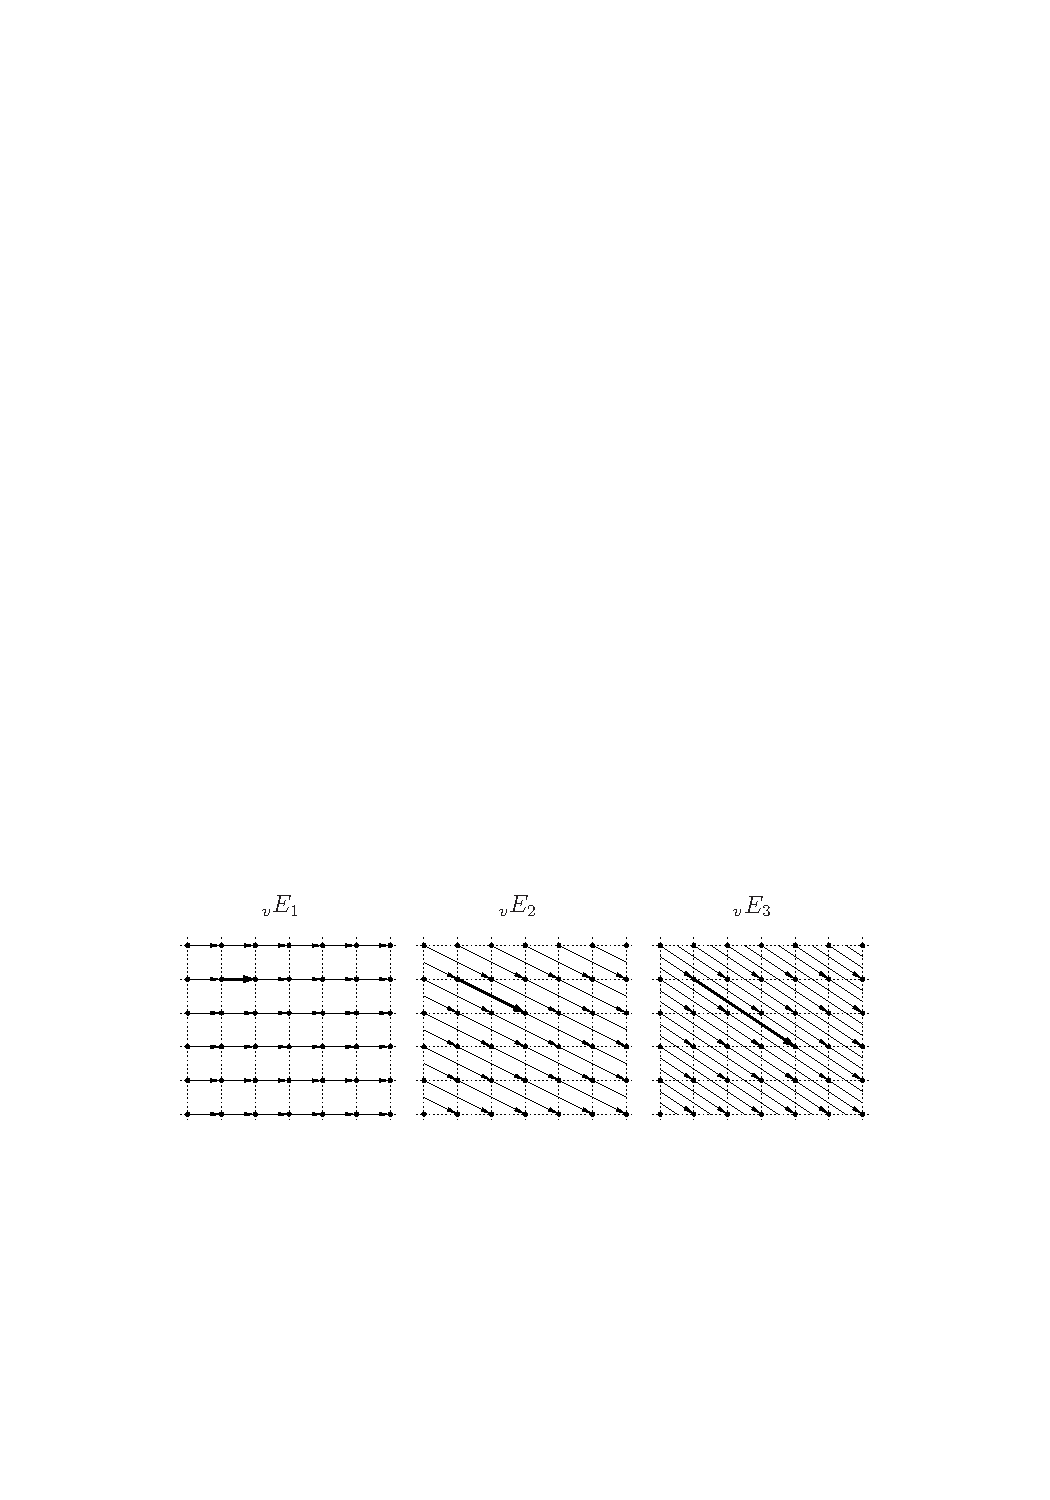
\includegraphics[scale=0.9]{pictures/spectral-seq-eg.pdf}\]
and so on.\par
\begin{remark}
For further application and a better understanding, we now give the intuitive construction of the differential $d_r$ in a diagram chasing viewpoint. First we consider 
$d_2$. Let $[\,\cdot\,]_r$ denote the cohomology class of $E_r$. For simplicity we will identify the preimage of $E_{r+1}$ in $E_r$, so that we have 
\[E_0\sups E_1\sups\cdots\sups E_r\sups E_{r+1}\sups\cdots.\]

Let $a\in E_2^{p,q}\sub E_0^{p,q}$, since $d_1$ is the induced map of $d_h$, we have $[d_h(a)]_1=0$. This means there exists $b\in E_0^{p,q}$ such that $-\delta_v(b)=d_h(a)$:
\[\begin{tikzcd}[column sep=1.0 em,row sep=1.0 em]
0&\\
a\ar[u]\ar[r]&{}\\
{}&b\ar[u]
\end{tikzcd}\]

In applying the map $\gamma_2$, we need to first pull $a$ back to a element of $T_{p+1}^\bullet$, and then apply the total differential 
$d_{tot}=d_h+\delta_v$. Since $a+b$ is a preimage of $a$, by our construction we have
\[\gamma_2(a)=\delta_v(a)+d_h(a)+\delta_v(b)+d_h(b)=d_h(b).\]
With this, since $d_h(b)$ can be viewed as an element of $T^\bullet_{p+2}$, by the definition of $\beta_r$ we get
\[d_2(a)=\beta_2(\gamma_2(a))=\beta_2(\alpha(d_h(b)))=[d_h(b)]_2.\]

In summary, the differential $d_2$ is represented by the following diagram
\[\begin{tikzcd}[column sep=1.0 em,row sep=1.0 em]
0&&\\
a\ar[u]\ar[r]&{}&{}\\
{}&b\ar[u]\ar[r]&d_h(b)
\end{tikzcd}\]
It can be easily showed that this definition is independent of the choice of $b$.\par
If moreover we have $d_2(a)=0$, then $[d_h(b)]_2=0$ and thus there exists an element $c\in E_1^{p+1,q-1}$ such that $d_1(c)=d_h(b)$. That is, we have
\[d_0(c)=\delta_v(c)=0,\quad d_1(c)=[d_h(c)]_1=[d_h(b)]_1.\] 
Combine this two equalities, we find that
\[d_1(b-c)=d_1(c)-d_1(b)=[d_h(c)-d_h(b)]_1=0,\quad d_0(b-c)=\delta_v(b)-\delta_v(c)=\delta_v(b)=-d_h(a),\]
so by replacing $b$ with $b_0:=b-c$, we can make $[d_h(b_0)]_1=0$, so there exists $b_1\in E_0^{p+2,q-1}$ such that $-\delta_v(b_1)=d_h(b_0)$. That is, we get the following diagram
\[\begin{tikzcd}[column sep=1.0 em,row sep=1.0 em]
0&&&\\
a\ar[u]\ar[r]&{}&{}&\\
{}&b_0\ar[u]\ar[r]&{}&\\
{}&{}&b_1\ar[u]\ar[r]&d_h(b_1)
\end{tikzcd}\]
By the same argument above, we see in this case, $d_3(a)$ is given by
\[d_3(a)=[d_h(b_1)]_3.\]

For a further step, we consider the condition $d_3(a)=0$. This means $[d_h(b_1)]_3=0$, so there exists $c_1\in E^{p+1,q-1}_2$ such that $d_2(c_1)=d_h(b_1)$. Therefore
\[d_0(c_1)=\delta_v(c_1)=0,\quad d_1(c_1)=[d_h(c_1)]_1=0,\quad d_2(c_1)=[d_h(b_1)]_2.\]
Unfolding the defintion of $d_2(c_1)$, there then exists $c_2\in E_0^{p+2,q-2}$ such that
\[d_h(c_1)=-\delta_v(c_2),\quad [d_h(c_2)]_2=[d_h(b_1)]_2.\]
These are summarized in the following:
\[\begin{tikzcd}[column sep=1.0 em,row sep=1.0 em]
0&&&\\
a\ar[u]\ar[r]&{}&{}&\\
{}&b_0\ar[u]\ar[r]&{}&\\
{}&{}&b_1\ar[u]\ar[r]&d_h(b_1)
\end{tikzcd}\quad\quad\quad\quad
\begin{tikzcd}[column sep=1.0 em,row sep=1.0 em]
0&&&\\
0\ar[u]\ar[r]&0&{}&\\
{}&c_1\ar[u]\ar[r]&{}&\\
{}&{}&c_2\ar[u]\ar[r]&d_h(c_2)
\end{tikzcd}\]
Now we have the following observations
\[\delta_v(b_0-c_1)=\delta_v(b_0)=-d_h(a),\quad d_2(b_0-c_1)=[d_h(b_1-c_2)]_2=0.\]
By applying the argument we made for $d_2$ on $b_0-c_1$, we can find a new diagram
\[\begin{tikzcd}[column sep=0.8 em,row sep=0.8 em]
0&&&\\
a\ar[u]\ar[r]&{}&{}&{}&{}\\
{}&b'_0\ar[u]\ar[r]&{}&{}&{}\\
{}&{}&b'_1\ar[u]\ar[r]&{}&{}\\
{}&{}&&b'_2\ar[u]\ar[r]&d_h(b'_2)
\end{tikzcd}\]
where $b_0':=b_0-c_1$ and $b'_2\in E_0$ is chosen to satisfy $-\delta_v(b'_2)=d_h(b'_1)$. Again, in this case we find
\[d_4(a)=[d_h(b_2')]_4.\]

Now we consider the converse. For an element $a\in E_0^{p,q}$, if there is a zig-zag of legnth $2$:
\[\begin{tikzcd}[column sep=1.0 em,row sep=1.0 em]
0&\\
a\ar[u]\ar[r]&{}\\
{}&b\ar[u]
\end{tikzcd}\]
then
\[d_1(a)=[d_h(a)]_1=[-\delta_v(b)]_1=0.\]
Similarly, if there is a zig-zag of legnth $3$ for $a$:
\[\begin{tikzcd}[column sep=1.0 em,row sep=1.0 em]
0&&&\\
a\ar[u]\ar[r]&{}&{}&\\
{}&b_0\ar[u]\ar[r]&{}&\\
{}&{}&b_1\ar[u]&
\end{tikzcd}\]
then
\[d_2(a)=[d_h(b_0)]_2=[[d_h(b_0)]_1]_2=[[-\delta_v(b_1)]_1]_2=0.\]
In general, if there is a zig-zag of legnth $r$ for $a$, then we can show $d_1(a)=d_2(a)=\cdots=d_{r-1}(a)=0$.\par
We say that an element $a$ in $E_0$ \textbf{lives to $\bm{E_{r}}$} if it represents a nontraivial cohomology class in $E_r$; equivalently, $a$ is a cocycle in $E_1,\dots,E_{r-1}$. From 
the discussion above we see that $a$ lives to $E_r$ if and only if it can be extended to a zig-zag of length $r$:
\[\begin{tikzcd}[column sep=1.0 em,row sep=1.0 em]
0&{}&{}&{}&{}&{}&{}\\
a\ar[u]\ar[r]&{}&{}&{}&{}&{}&{}\\
&b_1\ar[u]\ar[r]&{}&{}&{}&{}&{}\\
&&b_2\ar[u]\ar[r]&{}&{}&{}&{}\\
&&&\cdots\ar[u]\ar[r]&{}&{}&{}\\
&&&&b_{r-2}\ar[u]\ar[r]&{}&{}\\
&&&&&b_{r-1}\ar[u]\ar[r]&d_h(b_{r-1})
\end{tikzcd}\]
and the differential $d_r$ on $E_r$ is given by $d_h$ of the tail of the zig-zag:
\[d_r(a)=[d_h(b_{r-1})]_r.\]
\end{remark}
\subsubsection{The Spectral Sequence of a Filtered Complex}
More generally, we can consider the spectral sequence induced by a filtered complex. Let $M$ be a differential complex with differential operator $d$; i.e. $M$ has a 
grading $M=\bigoplus_{k\in\Z}M^k$ and $d:M^{k}\to M^{k+1}$ increases the degree by $1$. A \textbf{subcomplex} $M'$ of $M$ is a subobject such that $dM'\sub M'$. A 
sequence of subcomplexes
\[M=M_0\sups M_1\sups\cdots\sups M_i\sups\cdots\]
then makes $M$ into a filtered complex, with associated graded complex
\[\gr(M)=\bigoplus_{i=0}^{\infty}M_i/M_{i+1}.\]
For notational reasons we usually extend the filtration to negative indices by defining $M_i=M$ for $p<0$. Define $A=\bigoplus_{i\in\Z}M_i$, then the monomorphism $M_{i+1}\hookrightarrow M_i$ induces a map $A\to A$ whose cokernel is exactly $\gr(M)$. Therefore we have an exact sequence
\[\begin{tikzcd}
0\ar[r]&A\ar[r]&A\ar[r]&\gr(M)\ar[r]&0
\end{tikzcd}\]
which induces a long exact sequence of cohomology groups
\[\begin{tikzcd}
&H^\bullet(A)\ar[rd,"\alpha"]&\\
H^\bullet(\gr(M))\ar[ru,near start,"\gamma"]\ar[ru,near end,"+1"]&&H^\bullet(A)\ar[ll,"\beta"]
\end{tikzcd}\]
Since this diagram is an exact couple, it gives rise to a spectral seuqnece $\{(E_r,d_r)\}$.\par
Let $H_i$ be the image of $H(M_i)$ in $H(M)$, then there is 
a filtration of $H(M)$:
\[H(M)=H_0\sups H_1\sups \cdots\sups H_i\sups\cdots\]
making $H(M)$ into a filtered complex; this filtration is called the \textbf{induced filtration on $\bm{H(M)}$}.\par
To distinguish the grading degree $k$ from the filtration degree $i$, we will often call $k$ the \textbf{dimension}. Now the filtration $\{M_i\}$ on $M$ induces a 
filtration in each dimension: if $M_i^k=M^k\cap M_i$, then $\{M_i^k\}$ is a filtration on $M^k$. For the applications we have in mind, the filtration on $M$ need not 
have finite length. However, we can prove the following.
\begin{proposition}
Let $M=\bigoplus_{k\in\Z}M^k$ be a graded filtered complex with filtration $\{M_i\}$ and let $H(M)$ be the cohomology of $M$ with the induced filtration. Suppose 
for each degree $k$ the filtration $\{M^k_i\}$ has finite length. Then the short exact sequence
\[\begin{tikzcd}
0\ar[r]&\bigoplus_{i\in\Z}M_i\ar[r]&\bigoplus_{i\in\Z}M_i\ar[r]&\gr(M)\ar[r]&0
\end{tikzcd}\]
induces a spectral sequence which converges to $H^*(M)$.
\end{proposition}
\begin{proof}
The proof is similar to the case of double complex. We focuse on a specific degree $k$ for the cohomology and $i$ for the grading. The corresponding part in $E_1$ is 
$H^k(M_i/M_{i+1})$, and $\alpha$ acts as $H^k(M_i)\to H^k(M_{i-1})$. By the given condition, we have
\[H^k(M_{i+r})=0,\quad H^k(M_{i-r})=H^k(M)\for r\gg 0.\]
Therefore we have
\[\big(\bigcap_r\im\alpha^r\big)\cap H^k(M_i)=0,\quad \big(\bigcup_r\ker\alpha^r\big)\cap H^k(M_i)=\ker(H^k(M_i)\to H^k(M)).\]
and thus
\begin{align*}
Z_\infty=\ker\gamma=\im\beta,\quad B_\infty=\beta(\bigoplus_i\ker(H(M_i)\to H(M)).
\end{align*}
Denote by $\nu_i:H(M_i)\to H(M)$ the morphisms induced in cohomology by the monomorphisms $M_i\to M$ and by 
$\nu=\bigoplus\nu_i$ their direct sum, then we get
\[B_{\infty}=\beta(\bigoplus_i\ker\nu_i)=\beta(\ker(\bigoplus_i\nu_i)=\beta(\ker\nu).\]
The rest goes as Proposition~\ref{tot comp spectral}, and we omit it.
\end{proof}
\subsection{Exercise}
\begin{exercise}\label{tow morphism im/im(ker) iso}
Let $\lambda:M\to L$, $\nu:M\to N$ be morphisms in an abelian category:
\[\begin{tikzcd}
L&M\ar[l,swap,"\lambda"]\ar[r,"\nu"]&N
\end{tikzcd}\]
Prove that\footnote{Here $\lambda(\ker\nu)$ denotes the image of the restriction of $\lambda$ to the source of $\ker\nu$, etc.}
\[\dfrac{\im\lambda}{\lambda(\ker\nu)}\cong\dfrac{\im\nu}{\nu(\ker\lambda)}.\]
\end{exercise}
\begin{proof}
For a element $a\in\im\lambda$, define $\delta:\im\lambda\to\im\nu/\nu(\ker\lambda)$ by
\[\delta(a)=\nu(\ell)+\nu(\ker\lambda)\]
where $\ell\in M$ is a preimage of $a$. This is clearly well defined and we have
\[\ker\delta=\{a=\lambda(\ell):\nu(\ell)\in\nu(\ker\lambda)\}=\{a=\lambda(\ell):\ell\in\ker\nu+\ker\lambda\}=\lambda(\ker\nu).\]
The surjectivity of $\delta$ is clear.
\end{proof}
\begin{exercise}
Let $\alpha:L^\bullet\to M^\bullet$ be an isomorphism of cochain complexes. Prove that $MC(\alpha)^\bullet$ is homotopy equivalent to $0$.
\end{exercise}
\begin{proof}
Equivalently we show that the identity of $MC(\alpha)$ is homotopic to zero. Since $\alpha$ is an isomorphism, it has an inverse $\beta:M^\bullet\to L^\bullet$. Consider the diagram:
\[\begin{tikzcd}
&L^{i+1}\oplus M^i\ar[r,"d_{MC(\alpha)}^i"]\ar[ld,swap,"h^i"]\ar[d,"\id_{MC(\alpha)}"]&L^{i+2}\oplus M^{i+1}\ar[ld,"h^{i+1}"]\\
L^i\oplus M^{i-1}\ar[r,swap,"d_{MC(\alpha)}^{i-1}"]&L^{i+1}\oplus M^i&
\end{tikzcd}\]
where the homotopy $h$ is defined to be
\[h^i:(\ell,m)\mapsto(\beta^i(m),0)\]
then we check that
\[d_{MC(\alpha)}^{i-1}\circ h^i(\ell,m)=(-d^{i}_L\circ\beta(m),\beta^i(m))\]
\[h^{i+1}\circ d_{MC(\alpha)}^i(\ell,m)=(\ell+\beta^i\circ d_M^i(m),0)\]
since $\beta$ is a cochain morphism, we get 
\[\id_{MC(\alpha)}=d_{MC(\alpha)}^{i-1}\circ h^i+h^{i+1}\circ d_{MC(\alpha)}^i\]
as needed.
\end{proof}
\begin{exercise}
Let $\alpha:L^\bullet\to M^\bullet$ be a cochain morphism, and let $\beta:M^\bullet\to MC(\alpha)^\bullet$ be the natural morphism. Prove that $MC(\beta)^\bullet$ is homotopy equivalent to $L[1]^\bullet$.
\end{exercise}
\begin{proof}
The differential of $MC(\beta)$ acts as
\[\begin{tikzcd}
M^{i+1}\ar[draw=none]{d}[name=X, anchor=center,scale=1.5]{\oplus}\ar[r,"-d_M^{i+1}"]\ar[rdd,near start,"\id_M^{i+1}"]&M^{i+2}\ar[draw=none]{d}[name=X, anchor=center,scale=1.5]{\oplus}\\
L^{i+1}\ar[draw=none]{d}[name=X, anchor=center,scale=1.5]{\oplus}\ar[r,"-d_L^{i+1}"]\ar[rd,swap,"\alpha^{i+1}"]&L^{i+2}\ar[draw=none]{d}[name=X, anchor=center,scale=1.5]{\oplus}\\
M^i\ar[r,"d_M^i"]&M^{i+1}
\end{tikzcd}\]
Recall Exercise~\ref{map cyl homotopy equi}, we define the morphisms:
\[\rho:L[1]^i\to MC(\beta)^i,\quad \ell\mapsto(-\alpha(\ell),\ell,0)\]
\[\sigma:MC(\beta)^i\to L[1]^i,\quad (m',\ell,m)\mapsto\ell\]
since we have
\[d_{MC(\beta)}\circ\rho(\ell)=(d_M^i\circ\alpha(\ell),-d_L^{i+1}(\ell),0)=\rho\circ(-d_L^i)(\ell)\]
\[-d_L^{i+1}\circ\sigma(m',\ell,m)=-d_L^{i+1}(\ell)=\sigma\circ d_{MC(\beta)}(m',\ell,m)\]
$\sigma$ and $\rho$ are cohain morphisms. Clearly $\sigma\circ\rho=\id_{L[1]}$, and we have
\[(\id_{MC(\beta)}-\rho\circ\sigma)(m',\ell,m)=(m'+\alpha(\ell),0,m)\]
Picking $h^i:(m',\ell,m)\mapsto(m,0,0)$ gives a homotopy of $\rho\circ\sigma$ to $\id_{MC(\beta)}$, as the reader may check.
\end{proof}
\begin{exercise}
Let
\[\begin{tikzcd}
0\ar[r]&L^\bullet\ar[r,"\alpha"]&M^\bullet\ar[r,"\beta"]&N^\bullet\ar[r]&0
\end{tikzcd}\]
be a short exact sequence of cochain complexes on an abelian category.
\begin{itemize}
\item Prove that there is a cochain morphism $\gamma:MC(\alpha)^\bullet\to N^\bullet$ through which $\beta^\bullet:M^\bullet\to N^\bullet$ factors.
\item Prove that $MC(\gamma)^\bullet$ is an exact complex.
\item Conclude that $MC(\alpha)$ is quasi-isomorphic to $N^\bullet$.
\end{itemize}
\end{exercise}
\begin{proof}
\mbox{}
\begin{itemize}
\item Let $\gamma$ be the restriction of $MC(\alpha)^\bullet$ to $M^\bullet$ composing $\beta$, i.e.,
\[\gamma(\ell,m)=\beta(m)\]
it is easy to check this is a cochain morphism. From the definition we also have $\beta=\gamma\circ i$, where $i:M^\bullet\to MC(\alpha)$ is the inclusion, so $\beta$ factors though $\gamma$.
\item The differential of $MC(\gamma)$ acts as
\[\begin{tikzcd}
L^{i+2}\ar[draw=none]{d}[name=X, anchor=center,scale=1.5]{\oplus}\ar[r,"d_L^{i+2}"]\ar[rd,"\alpha^{i+2}"]&L^{i+3}\ar[rd,"\alpha^{i+3}"]\ar[r,"d_L^{i+3}"]\ar[draw=none]{d}[name=X, anchor=center,scale=1.5]{\oplus}&L^{i+4}\ar[draw=none]{d}[name=X, anchor=center,scale=1.5]{\oplus}\\
M^{i+1}\ar[draw=none]{d}[name=X, anchor=center,scale=1.5]{\oplus}\ar[r,"-d_M^{i+1}"]\ar[rd,"\beta^{i+1}"]&M^{i+2}\ar[rd,"\beta^{i+2}"]\ar[r,"-d_M^{i+2}"]\ar[draw=none]{d}[name=X, anchor=center,scale=1.5]{\oplus}&M^{i+3}\ar[draw=none]{d}[name=X, anchor=center,scale=1.5]{\oplus}\\
N^i\ar[r,"d_N^i"]&N^{i+1}\ar[r,"d_N^{i+1}"]&N^{i+2}
\end{tikzcd}\]
Now assume $(\ell^{i+3},m^{i+2},n^{i+1})\in\ker d_{MC(\gamma)}^{i+1}$. Then we have the equalities
\[\left\{\begin{array}{l}
d_L^{i+3}(\ell^{i+3})=0\\
\alpha^{i+3}(\ell^{i+3})-d_M^{i+2}(m^{i+2})=0\\
\beta^{i+2}(m^{i+2})+d_N^{i+1}(n^{i+1})=0
\end{array}\right. \]
The proof is similar to that of Theorem~\ref{tot comp exact}. First, let $n^i=0$. Since $\beta^{i+1}$ is epic, there is $m^{i+1}\in M^{i+1}$ such that $\beta^{i+1}(m^{i+1})=n^{i+1}$. Then
\[\beta^{i+2}\circ d_M^{i+1}
(m^{i+1})=d_N^{i+1}\circ\beta^{i+1}(m^{i+1})=d_N^{i+1}(n^{i+1})=-\beta^{i+2}(m^{i+2})\]
which gives $m^{i+2}=-d_M^{i+1}(m^{i+1})+x$, with $x\in\ker\beta^{i+2}=\im\alpha^{i+2}$. So $x=\alpha^{i+2}(\ell^{i+2})$ for some $\ell^{i+2}\in L^{i+2}$. Again,
\[\alpha^{i+3}\circ d_L^{i+2}(\ell^{i+2})=d_M^{i+2}\circ\alpha^{i+2}(\ell^{i+2})=d_M^{i+2}(m^{i+2}+d_M^{i+1}(m^{i+1}))=\alpha^{i+3}(\ell^{i+3})\]
Since $\alpha^{i+3}$ is monic, this gives $d_L^{i+2}(\ell^{i+2})=\ell^{i+3}$.
\item This follows from Corollary~\ref{MC exact iff quasi-iso}
\end{itemize}
\end{proof}
\begin{remark}
From the proof above, we can change the condition in Theorem~\ref{tot comp exact} so that only one direction of the double complex is bounded, but bounded above and below.
\end{remark}
\begin{exercise}
Let
\[\begin{tikzcd}
0\ar[r]&L^\bullet\ar[r,"\alpha"]&M^\bullet\ar[r,"\beta"]&N^\bullet\ar[r]&0
\end{tikzcd}\]
be a short exact sequence of cochain complexes on an abelian category $\mathcal{A}$. Prove that there is a morphism $N^\bullet\to L[1]^\bullet$ in the derived category $\mathcal{D}(\mathcal{A})$, inducing the connecting morphism $H^i(N^\bullet)\to H^{i+1}(L^\bullet)$ in cohomology.
\end{exercise}
\begin{proof}
In the derived category $\mathcal{D}(\mathcal{A})$, $MC(\alpha)$ is isomorphic to $N^\bullet$.
\end{proof}
\begin{exercise}
Let $_{v}E_r$ be the spectral sequence of a first-quadrant double complex from the vertical filtration. Prove that $_{v}E^{i,j}_r=_{v}E^{i,j}_\infty$ for $r>j+1$.
\end{exercise}
\begin{proof}
The differential $d_r$ maps indices $(i,j)\mapsto(i+r,j-(r-1))$. If $j-(r-1)<0$, this map woule be zero, hence the claim follows.
\end{proof}
\begin{exercise}
Let $\mathcal{A},\mathcal{B},\mathcal{C}$ be abelian categories, and let $\mathscr{F}:\mathcal{A}\to\mathcal{B}$, $\mathscr{G}:\mathcal{B}\to\mathcal{C}$ be additive 
functors. Assume that $\mathcal{A}$ and $\mathcal{B}$ have enough projectives, and that $\mathscr{F}$ sends projectives of $\mathcal{A}$ to $\mathscr{G}$-acyclic 
objects of $\mathcal{B}$, and that $\mathscr{G}$ is right-exact.\par
Let $A$ be an object of $\mathcal{A}$, and let 
\[\begin{tikzcd}
M^\bullet:&\cdots\ar[r]&M^{-2}\ar[r]&M^{-1}\ar[r]&M^0\ar[r]&0
\end{tikzcd}\]
be a projective resolution of $A$. Let $P^\bullet_{\mathscr{F}(M^\bullet)}$ be a Cartan-Eilenberg resolution of the complex $\mathscr{F}(M^\bullet)$. Consider the complex
\begin{equation}\label{two func reso-2}
\begin{tikzcd}
\cdots\ar[r]&\mathscr{G}(P^\bullet_{\mathscr{F}(M^{-2})})\ar[r]&\mathscr{G}(P^\bullet_{\mathscr{F}(M^{-1})})\ar[r]&\mathscr{G}(P^\bullet_{\mathscr{F}(M^{0})})\ar[r]&0
\end{tikzcd}
\end{equation}
obtained by applying $\mathscr{G}$ to $P^\bullet_{\mathscr{F}(M^\bullet)}$. \par
This is precisely the set-up of Exercise~\ref{two func exercise}. Now take the double complex associated with $(\ref{two func reso-2})$, and construct the spectral 
sequence corresponding to the horizontal filtration. Prove that the $E_2$ term of this sequence has terms
\[_{h}E^{p,q}_2=\mathcal{L}_p\mathscr{G}(\mathcal{L}_q\mathscr{F}(A))\]
This is the \textbf{Grothendieck spectral sequence}. Prove that it abuts to $\mathcal{L}_\bullet(\mathscr{G}\circ\mathscr{F})(A)$.
\end{exercise}
\begin{proof}
By Exercise~\ref{two func exercise} we know that this spectral sequence converges to $\mathcal{L}_n(\mathscr{G}\circ\mathscr{F})(A)$. Now we consider horizontal 
filtration. First, since $\mathscr{F}$ is right-exact, we have the follwing exact sequence:
\[\begin{tikzcd}
\cdots\ar[r]&\mathscr{F}(M^{-2})\ar[r]&\mathscr{F}(M^{-1})\ar[r]&\mathscr{F}(M^0)\ar[r]&\mathscr{F}(A)\ar[r]&0
\end{tikzcd}\]
Therefore we can construct a augmented Cartan-Eilenberg resolution of this augmented complex, which will be like
\[\begin{tikzcd}
{}&0&0&0&0&{}\\
\cdots\ar[r]&\mathscr{F}(M^{-2})\ar[r]\ar[u]&\mathscr{F}(M^{-1})\ar[r]\ar[u]&\mathscr{F}(M^0)\ar[r]\ar[u]&\mathscr{F}(A)\ar[r]\ar[u]&0\\
\cdots\ar[r]&P^0_{\mathscr{F}(M^{-2})}\ar[r]\ar[u]&P^0_{\mathscr{F}(M^{-1})}\ar[r]\ar[u]&P^0_{\mathscr{F}(M^{0})}\ar[r]\ar[u]&P^0\ar[r]\ar[u]&0\\
\cdots\ar[r]&P^1_{\mathscr{F}(M^{-2})}\ar[r]\ar[u]&P^1_{\mathscr{F}(M^{-1})}\ar[r]\ar[u]&P^1_{\mathscr{F}(M^{0})}\ar[r]\ar[u]&P^1\ar[r]\ar[u]&0\\
{}&\vdots\ar[u]&\vdots\ar[u]&\vdots\ar[u]&\vdots\ar[u]&{}
\end{tikzcd}\]
Since the original sequence is exact, this double complex is also exact. Using this fact and Exercise~\ref{two fuc reso}, we now compute the cohomology of each row in 
$\mathscr{G}(P^\bullet_{\mathscr{F}(M^\bullet)})$. We will get
\begin{equation}\label{G spectral seq-1}
\begin{tikzcd}
{}&0&0&0&{}\\
\cdots\ar[r]&\mathscr{G}(\mathcal{L}_2\mathscr{F}(A))\ar[r]\ar[u]&\mathscr{G}(\mathcal{L}_1\mathscr{F}(A))\ar[r]\ar[u]&\mathscr{G}(\mathcal{L}_0\mathscr{F}(A))\ar[r]\ar[u]&0\\
\cdots\ar[r]&\mathscr{G}(H^{2,0})\ar[r]\ar[u]&\mathscr{G}(H^{1,0})\ar[r]\ar[u]&\mathscr{G}(H^{0,0})\ar[r]\ar[u]&0\\
\cdots\ar[r]&\mathscr{G}(H^{2,1})\ar[r]\ar[u]&\mathscr{G}(H^{1,1})\ar[r]\ar[u]&\mathscr{G}(H^{0,1})\ar[r]\ar[u]&0\\
{}&\vdots\ar[u]&\vdots\ar[u]&\vdots\ar[u]&
\end{tikzcd}
\end{equation}
By the right-exactness of $\mathscr{G}$, each column is exact. Moreover, since each $H^{i,j}$ can be chosen to be projective, the $p$-th column of $(\ref{G spectral seq-1})$ 
then computes $\mathcal{L}_\bullet\mathscr{G}(\mathcal{L}_p\mathscr{F}(A))$. This is the $E_2$ page.
\end{proof}
%\chapter{Dimension theory and homological method}
\section{Regular sequences and the Koszul complex}
\subsection{Regular sequences}
Let $A$ be a ring and $M$ an $A$-module. An element $a\in A$ is said to be \textbf{$\bm{M}$-regular} if $ax\neq0$ for all non-zero $x\in M$. A sequence $a_1,\dots,a_n$ of elements $A$ is an \textbf{$\bm{M}$-sequence} (or an \textbf{$\bm{M}$-regular sequence}) if the following two
\begin{itemize}
\item[$(1)$]$a_1$ is $M$-regular, $a_2$ is $(M/a_1M)$-regular, $\cdots$, $a_n$ is $(M/\sum_{i=1}^{n-1}a_iM)$-regular.
\item[$(2)$]$M/\sum_{i=1}^{n}a_iM\neq 0$.
\end{itemize}
Note that, after permutation, the elements of an $M$-sequence may no longer
form an $M$-sequence.
\begin{lemma}\label{regular seq lem}
Suppose $b_1,b_2,\dots,b_n$ is an $M$-sequence. If $b_1\xi_1+\cdots+b_n\xi_n=0$ with $\xi_i\in M$ then $\xi_i\in b_1M+\cdots+b_nM$ for all $i$
\end{lemma}
\begin{proof}
Let us rove by induction on $n$. First of all from the condition that $b_n$ is not a zero-divisor modulo $b_1,\dots,b_{n-1}$, we get $\xi_n\in\sum_{i=1}^{n-1}b_iM$, hence we can write
\[\xi_n=\sum_{i=1}^{n-1}b_i\eta_i,\quad \eta_i\in M\]
Therefore $\sum_{i=1}^{n-1}b_i(\xi_i+b_n\eta_i)=0$, so that by induction hypothesis we have
\[\xi_i+b_n\eta_i\in b_1M+\cdots+b_{n-1}M,\quad\forall 1\leq i\leq n-1.\]
giving $\xi_i\in b_1M+\cdots+b_nM$ for $1\leq i\leq n-1$. The condition for $\xi_n$ is already known.
\end{proof}
\begin{lemma}\label{regular seq extend}
Let $A$ be a noetherian ring and $M$ an $A$-module. Any $M$-regular sequence $a_1,\dots,a_n$ in an ideal $I$ can be extended to a maximal $M$-regular sequence in $I$.
\end{lemma}
\begin{proof}
If $a_1,\dots,a_n$ is not maximal in $I$, we can find $a_{n+1}\in I$ such that $a_1,\dots,a_n,a_{n+1}$ is an $M$-regular sequence. Either this process terminates at a maximal $M$-regular sequence in $I$, or it produces a strictly ascending chain of ideals
\[(a_1)\subset(a_1,a_2)\subset\cdots\]
Since $A$ is noetherian, we can exclude this latter possibility.
\end{proof}
\begin{proposition}\label{regular power}
If $a_1,\dots,a_n$ is an $M$-sequence then so is $a_1^{\nu_1},\dots,a_n^{\nu_n}$ for any positive integers $\nu_1,\dots,\nu_n$.
\end{proposition}
\begin{proof}
It is sufficient to prove that if $a_1,\dots,a_n$ is an $M$-sequence then so is $a_1^{\nu_1},a_2,\dots,a_n$. Indeed, assuming this, we have in turn that $a_1^{\nu_1},a_2,\dots,a_n$ is an $M$-sequence, then setting $M_1=M/a_1^{\nu_1}M$ that $a_2,a_3,\dots,a_n$ and hence also $a_2^{\nu_2},a_3,\dots,a_n$ is an $M_1$-sequence, and so on. Also, the
second condition $M\neq\sum_{i=1}^{n}a_i^{\nu_i}M$ is obvious.\par
Now assuming $\nu>1$ we prove by induction on $\nu$ that $a_1^{\nu},a_2,\dots,a_n$ is an $M$-sequence. Since $a_1$ is $M$-regular, so is $a_1^{\nu_1}$. For $i>1$, suppose that for some $\omega\in M$ we have
\[a_i\omega=a_1^{\nu}\xi_1+a_2\xi_2+\cdots+a_{i-1}\xi_{i-1},\quad\]
Then since $a_1^{\nu-1},a_2,\dots,a_n$ is an $M$-sequence, we can write
\[\omega=a_1^{\nu-1}\eta_1+\cdots+a_{i-1}\eta_{i-1},\quad\eta_j\in M\]
Hence we get 
\[0=a_1^{\nu-1}(a_1\xi_1-a_i\eta_1)+a_2(\xi_2-a_i\eta_2)+\cdots+a_{i-1}(\xi_{i-1}-a_i\eta_{i-1})\]
Then Lemma~\ref{regular seq lem} gives \[a_1\xi_1-a_i\eta_1\in a_1^{\nu-1}M+a_2M+\cdots+a_{i-1}M\]
and hence $a_i\eta_1\in a_1M+a_2M+\cdots+a_{i-1}M$. Therefore $\eta_1\in a_1M+a_2M+\cdots+a_{i-1}M$, and so as required we have $\omega\in a_1^{\nu}M+a_2M+\cdots+a_{i-1}M$.
\end{proof}
Let $A$ be a ring, $X_1,\dots,X_n$ indeterminates over $A$, and $M$ an $A$-module. We can view elements of $M\otimes_AA[X_1,\dots,X_n]$ as polynomials in the $x_i$ with coefftcients in $M$,
\[F(X)=F(X_1,\dots,X_n)=\sum_\alpha\xi_\alpha X^\alpha,\quad \xi_\alpha\in M\]
For this reason we write $M[X_1,\dots,X_n]$ for $M\otimes_AA[X_1,\dots,X_n]$; we can consider this either as an $A$-module or as an $A[X_1,\dots,X_n]$-module. For $a_1,\dots,a_n\in A$ and $F\in M[X_1,\dots,X_n]$, we can substitute the $a_i$ for $X_i$ to get $F(a_1,\dots,a_n)\in M$.
\begin{definition}
Let $a_1,\dots,a_n\in A$, set $I=\sum_{i=1}^{n}a_iA$ and let $M$ be an $A$-module with $IM\neq M$.We say that $a_1,\dots,a_n$ is an \textbf{$\bm{M}$-quasi-regular sequence} if the following condition holds for each $\nu$:
\begin{itemize}
\item $F(X_1,\dots,X_n)\in M[X_1,\dots,X_n]$ is homogeneous of degree $\nu$ and $F(a)\in I^{\nu+1}M$ implies that all the coefticients of $F$ are in $IM$.
\end{itemize}
This notion is obviously independent of the order of $a_1,\dots,a_n$.
\end{definition}
In the above definition it would not make any difference if we replaced the condition that $F(a)\in I^{\nu+1}M$ by the condition $F(a)=0$. This is similar to that in Remark~\ref{analy inde remk}.\par
We can define a map 
\[\varphi:(M/IM)[X_1,\dots,X_n]\to G_I(M)=\bigoplus_{i=0}^{\infty}(I^iM/I^{i+1}M)\]
as follows: taking a homogeneous element $F(X)\in M[X]$ of degree $\nu$ into the class of $F(a)$ in $I^\nu M/I^{\nu+1}M$ provides a homomorphism (of additive groups) from $M[X]$ into $G_I(M)$ which preserves degrees. Since $IM[X]$ is in the kernel, this induces a homomorphism
\[\varphi:M[X]/IM[X]=(M/IM)[X]\to G_I(M)\]
which is obviously surjective. Then $a_1,\dots,a_n$ is a quasi-regular sequence precisely when $\varphi$ is injective, and hence an isomorphism.\par
Concluding we have the following result.
\begin{proposition}\label{quasi regular}
Let $A$ be a ring and $M$ an $A$-module. Let $a_1,\dots,a_n\in A$ and set $I=(a_1,\dots,a_n)$. Then the following conditions are equivalent
\begin{itemize}
\item[$(1)$]For every $\nu>0$ and for every homogenous polynomial $F(X)\in M[X_1,\dots,X_n]$ of degree $\nu$ such that $F(a_1,\dots,a_n)\in I^{\nu+1}M$, we have $F\in IM[X_1,\dots,X_n]$.
\item[$(2)$]For every $\nu>0$ and for every homogenous polynomial $F(X)\in M[X_1,\dots,X_n]$ such that $F(a_1,\dots,a_n)=0$, we have $F\in IM[X_1,\dots,X_n]$.
\item[$(3)$]The morphism of abelian groups 
\[\varphi:(M/IM)[X_1,\dots,X_n]\to G_I(M)\] 
defined by mapping a homogenous polynomial $F(X)$ of degree $\nu$ to $F(a_1,\dots,a_n)\in I^{\nu}M/I^{\nu+1}M$ is an isomorphism.
\end{itemize}
\end{proposition}
Recall that for an $A$-module $M$, a submodule $N\sub M$ and $x\in A$ the notation $(N:x)$ means $\{m\in M\mid xm\in N\}$. This is a submodule of $M$. If $A$ is a ring, $I$ an ideal and $M$ an $A$-module, recall that $M$ is separated in the $I$-adic topology when $\bigcap_nI^nM=0$.
\begin{proposition}
Let $A$ be a ring, $M$ a nonzero $A$-module, $a_1,\dots,a_n\in A$ and $I=(a_1,\dots,a_n)$. Then
\begin{itemize}
\item[$(1)$]If $a_1,\dots,a_n$ is $M$-quasi regular and $x\in A$ is such that $(IM:x)=IM$, then $(I^\nu M:x)=I^\nu M$ for all $\nu>0$.
\item[$(2)$]If $a_1,\dots,a_n$ is $M$-regular then it is $M$-quasi regular.
\item[$(3)$]If $M$, $M/a_1M$, $\cdots$, $M/\sum_{i=1}^{n-1}a_iM$ are separated in the $I$-adic topology, then the converse of $(2)$ is also true.
\end{itemize}
\end{proposition}
\begin{proof}
$(1)$ By induction on $\nu$, with the case $\nu=1$ true by assumption. Suppose $\nu>1$ and $\xi\in(I^\nu M:x)$, then $x\xi\in I^{\nu}M\sub I^{\nu-1}M$. By the inductive hypothesis $\xi\in I^{\nu-1}M$, hence there exists a homogenous polynomial $F(X)\in M[X_1,\dots,X_n]$ of degree $\nu-1$ such that 
\[\xi=F(a_1,\dots,a_n)\] 
Since $x=x\xi=xF(a_1,\dots,a_n)\in I^\nu M$, the coefficients of $F$ are in $(IM:x)=IM$. Therefore $\xi=F(a_1,\dots,a_n)\in I^\nu M$.\par
$(2)$ By induction on $n$. For $n=1$ this is easy to check: a homogeneous polynomial od degree $\nu$ in $M[X]$ is of the form $F(X)=mX^{\nu}$. Let $a$ be $M$-regular, if $F(a)=ma^\nu=a^{\nu+1}\xi\in I^{\nu+1}M$, then since $a$ is not a zero-divisor for $M$, we conclude $m=a\xi$, hence is in $aM$.\par
Then by the induction hypothesis $a_1,\dots,a_{n-1}$ is $M$-quasi regular. Let $F(X)\in M[X_1,\dots,X_n]$ be homogenous of degree $\nu>0$ such that $F(a_1,\dots,a_n)=0$. We prove that $F\in IM[X_1,\dots,X_n]$ by induction on $\nu$ (the case $\nu=0$ being trivial). Write
\[F(X_1,\dots,X_n)=G(X_1,\dots,X_{n-1})+X_nH(X_1,\dots,X_n)\]
Here $G$ is homogeneous of degree $\nu$ and $H$ of degree $\nu-1$. Then, from the regularity we get
\[((a_1,\dots,a_{n-1})M:a_n)=(a_1,\dots,a_{n-1})M\] 
Then from $(1)$, since $a_nH(a_1,\dots,a_{x})=-G(a_1,\dots,a_{n-1})$,
\[H(a_1,\dots,a_n)\in((a_1,\dots,a_{n-1})^\nu M:a_n)=(a_1,\dots,a_{n-1})^\nu M\sub I^\nu M\]
So by the induction hypothesis on $\nu$ we have $H(X)\in IM[X_1,\dots,X_n]$. Moreover, by the above formula there is a homogeneous polynomial $h(X_1,\dots,X_{n-1})$ of degree $\nu$ with coefficients in $M$ such that $H(a)=h(a_1,\dots,a_{n-1})$, and so setting
\[g(X)=G(X_1,\dots,X_{n-1})+a_nh(a_1,\dots,a_{n-1})\]
We have $g(a_1,\dots,a_{n-1})=0$, so by the inductive hypothesis on $n$ we get the coefficients of $g$ are all in $(a_1,\dots,a_{n-1})M$, therefore the coefficients of $G$ belong to $(a_1,\dots,a_n)M$. Since we already prove $H(X)\in IM[X_1,\dots,X_n]$, this implies the claim.\par
$(3)$ Assume that $a_1,\dots,a_n$ is $M$-quasi regular and the modules $M$, $M/a_1M$, $\cdots$, $M/\sum_{i=1}^{n-1}a_iM$ are all separated in the $I$-adic topology.\par 
Let $\xi\in M$, we proceed in this way
\[\begin{tikzcd}
a_1\xi=0\ar[rr,"\xi X_1"]\ar[rr,swap,"\text{quasi-regular}"]&&\xi\in IM\ar[rr]&&\xi=\sum_{i=1}^{n}a_i\xi_i^{(1)}\\
a_1\sum a_i\xi_i^{(1)}=0\ar[rr,"\sum\xi_i^{(1)}X_1X_i"]\ar[rr,swap,"\text{quasi-regular}"]&&\xi_i^{(1)}\in IM\ar[rr]&&\xi_i^{(1)}=\sum_{i=1}^{n}a_i\xi_i^{(2)}
\end{tikzcd}\]
We see that $\xi\in\bigcap_nI^nM=0$, thus $a_1$ is regular over $M$, and this also takes care of the case $n=1$ since $M\neq IM$ by the separation condition.\par
So assume $n>1$. Let $N=M/a_1M$, then there is an isomorphism of
$A$-modules for $2\leq i\leq n-1$
\[M/(a_1,\dots,a_i)M\cong N/(a_2,\dots,a_i)N\]
So the modules $N$, $N/a_2N$, $\cdots$, $N/(a_1,\dots,a_{n-1})N$ are separated in the $I$-adic topology. If we show the sequence $a_2,\dots,a_n$ is $N$-quasi regular, then the claim follows by induction on $n$.\par
So let $f(X_2,\dots,X_n)$ be a homogeneous polynomial of degree $\nu$ with coefficients in $N$, such that $f(a_2,\dots,a_n)=0$. If $F(X_2,\dots,X_n)$ is a homogeneous polynomial of degree $\nu$ with coefficients in $M$ which reduces to $f$ modulo $a_1M$, then $F(a_2,\dots,a_n)\in a_1M$. Set $F(a_2,\dots,a_n)=a_1\omega$; suppose that $\omega\in I^iM$, so that we can write $\omega=G_i(a)$ with $G_i(X)\in M[X_1,\dots,X_n]$ homogeneous of degree $i$. Then
\[F(a_2,\dots,a_n)=a_1G_i(a_1,\dots,a_n)\]
and if $i<\nu-1$ by applying the quasi regularity of $a_1,\dots,a_n$ on
$X_1G_i(X_1,\dots,X_n)$ that the coefficients of $G_i$ belong to $IM$, so that $\omega\in I^{i+1}M$; repeating this argument we see that $\omega\in I^{\nu-1}M$. Setting $i=\nu-1$ in the above formula, then since $X_1$ does not appear in $F$, we can apply the definition of quasi-regular sequence to $F(X_2,\dots,X_n)-X_1G_{\nu-1}(X_1,\dots,X_n)$ to deduce that the coefficients of $F$ belong to $IM$. Hence, the coefficients of $f$ belong to $IN$.
\end{proof}
The theorem shows that, under the assumptions of $(3)$ any permutation of an $M$-regular sequence is $M$-regular.
\begin{corollary}\label{regular permute}
Let $A$ be a Noetherian ring, $M$ a finitely generated $A$-module and let $a_1,\dots,a_n$ be contained in the Jacobson radical of $A$. Then $a_1,\dots,a_n$ is $M$-regular if and only if it is $M$-quasi regular.\par
In particular if $a_1,\dots,a_n$ is $M$-regular so is any permutation of the sequence.
\end{corollary}
\begin{remark}\label{regular permute eg}
Here is an example where a permutation of an $M$-sequence fails to be an $M$-sequence: let $k$ be a field, $A=k[x,y,z]$ and set $a_1=x(y-1)$, $a_2=y$, $a_3=z(y-1)$. Then $(a_1,a_2,a_3)A=(x,y,z)A\neq A$, and $a_1,a_2,a_3$ is an $A$-sequence, whereas $a_1,a_3,a_2$ is not.
\end{remark}
\subsection{Koszul complex}
We can decide whether an element $x\in A$ is a nonzero divisor from the homology of the complex
\[K(x):\begin{tikzcd}
0\ar[r]&R\ar[r,"x"]&R\ar[r]&0
\end{tikzcd}\]
which is $(0:x)$. This trivial remark is the essential basis for the homological study of regular sequences.\par
Given a second element $y\in R$, multiplication by $y$ defines a map of complexes $K(x)\to K(x)$. That is, a commutative diagram
\[\begin{tikzcd}
K(x):&0\ar[r]&R\ar[d,"y"]\ar[r,"x"]&R\ar[d,"y"]\ar[r]&0\\
K(x):&0\ar[r]&R\ar[r,"x"]&R\ar[r]&0
\end{tikzcd}
\]
We can form the mapping cone of this map to get another complex
\[K(x,y):\begin{tikzcd}
0\ar[r]&R\ar[r,"x"]\ar[rd,"y"]&R\ar[draw=none]{d}[name=X, anchor=center,scale=1.5]{\oplus}\ar[r]\ar[rd,"y"]&0&\\
&0\ar[r]&R\ar[r,swap,"-x"]&R\ar[r]&0
\end{tikzcd}\]
or in more usual notation as
\[K(x,y):\begin{tikzcd}
0\ar[r]&R\ar[r,"\big(\begin{smallmatrix}y\\x
\end{smallmatrix}\big)"]&R\oplus R\ar[r,"(-x\,y)"]&R\ar[r]&0
\end{tikzcd}\]
Note that for convenience, we use cohomological notations, but there is a slight change of this: The degree $0$ term will always be the leftmost non-zero one. So $K(x,y)=K(x)[-1]\oplus K(x)$.\par 
In particular, with our notation, $H^0(K(x))$ is the homology at the leftmost nonzero term $R$ of $K(x)$. We see from the definition that \[H^0(K(x))=(0:x)=\Ann(x)\]
and $H^0(K(x,y))$ is $(0:(x, y))$, so that if $x$ is a non zero-divisor then $H^0(K(x,y))=0$.\par
What is $H^1(K(x,y))$? An element $(a,b)\in R\oplus R$ is in the kernel iff $ax+by=0$. Of course this requires $b\in(x:y)$. Conversely, if $b\in(x:y)$, then there is an element $a$ with $ax+yb=0$, so that $(a,b)$ will be in the kernel.\par
If we assume that $x$ is a non zero-divisor, then $a$ is uniquely determined by $b$, and the association $b\mapsto a$ is a module homomorphism, so the kernel is isomorphic to $(x:y)$.\par
On the other hand, an element is in the image of the left-hand map iff it
is of the form $(cy,-cx)$, so the elements of $(x:y)$ that correspond to elements of the image are the elements of $(x)$. Thus if $x$ is a non zero-divisor, then
\[H^1(K(x,y))\cong(x,y)/(x)\]
In particular, if $x$ is a nonzero divisor then $H^1(K(x,y))=0$ iff $x,y$ is a regular sequence.\par
\vspace{5mm}
As we know, there is an exact sequence
\[\begin{tikzcd}
0\ar[r]&K(x)[-1]\ar[r]&K(x,y)\ar[r]&K(x)\ar[r]&0
\end{tikzcd}\]
which gives a long exact seuqnece
\[\begin{tikzcd}
0\ar[r]&H^0(K(x))\ar[r,"\delta"]&H^0(K(x))\ar[r]&H^1(K(x,y))\ar[r]&H^1(K(x))\ar[r,"\delta"]&\cdots
\end{tikzcd}\]
The $\delta$ is the connecting morphism given be multiplication by $y$.\par
Now suppose only that $H^1(K(x,y))=0$. It follows from the preceding long exact sequence that
\[H^0(K(x))/yH^0(K(x))=0\]
In general, not much can be deduced from this; but if we assume in addition
that $R$ is a Noetherian local ring and $y$ is in the maximal ideal, then Nakayama's lemma shows that $H^0(K(x))=0$. Consequently, $x$ is a non zero-divisor, and $x,y$ is a regular sequence by what we have already proved. We may state what we have shown as follows:
\begin{theorem}\label{Koszul K(x,y) thm}
If $R$ is a Noetherian local ring and $x,y$ are in the maximal ideal, then $x,y$ is a regular sequence iff $H^0(K(x,y))=0$.
\end{theorem}
From the way the Koszul complex is written, it is clear that the complexes $K(x,y)$ and $K(y,x)$ are isomorphic. Thus under the hypothesis of Theorem~\ref{Koszul K(x,y) thm}, $x,y$ is a regular sequence iff $y,x$ is. This is enough to show that regular sequences may be permuted.
\begin{corollary}
If $R$ is a Noetherian local ring and $x_1,\dots,x_r$ is a regular sequence of elements in the maximal ideal of $R$, then any permutation of
$x_1,\dots,x_r$ is again a regular sequence.
\end{corollary}
\begin{proof}
Since every permutation is a product of transpositions of neighboring
elements, it suffices to show that we can interchange two neighbors; that is, if $x_1,\dots,x_{i},x_{i+1},\dots,x_r$ is a regular sequence, then $x_1,\dots,x_{i+1},x_i,\dots,x_r$ is too. The only part of the definition of a regular sequence that is not immediate for $x_1,\dots,x_{i+1},x_i,\dots,x_r$ amounts to saying that $x_{i+1},x_i$ is a regular sequence modulo $(x_1,\dots,x_{i-1})$. After factoring out $(x_1,\dots,x_{i-1})$, Theorem~\ref{Koszul K(x,y) thm} and the remark following it give the desired conclusion.
\end{proof}
One might at first hope that the local hypothesis in these two results
would be superfluous, required only by the clumsy methods used in the
proof. This is not the case.
\begin{example}
Recall Example~\ref{regular permute eg}, consider the ring
\[R=k[x,y,z]/x(y-1)\]
and the sequence of elements
\[y,z(y-1)\]
The ideal they generate is $(y,z(y-1))=(y,z)\neq R$. Further, it is easy to
see that $y$ is not a zero divisor in $R$, and $R/(y)=k[x,y,z]/(x,y)\cong k[z]$. Thus $y,z(y-1)$ is a regular sequence and
\[H^1(K(y,z(y-1)))=0\]
However, $z(y-1)$ is a zero divisor-it is killed by $x$-so that the sequence in reversed order is not a regular sequence.\par
One further point is worth noting: If $x\in R$ is arbitrary, then $H^0(K(x,0))=H^0(K(x))$ $($since both are isomorphic to $(0:(x)))$ even though the complex $K(x,0)$ is not isomorphic to $K(x)$.
\end{example}
\subsubsection{Koszul Complexes in General}
We could build up the Koszul complex step by step, iterating the process
just illustrated (and we shall soon prove that this gives the correct answer), but the following construction is so direct, simple, and invariant that it has many advantages.
If $M$ is any $R$-module, then the exterior algebra $\bigwedge M$ may be defined as the free algebra $R\oplus M\oplus(M\otimes M)\oplus\cdots$ modulo the relations 
\[x\otimes y=-y\otimes x\quad\text{and}\quad x\otimes x=0\]
for all $x$ and $y$ in $M$. The product of two elements $a,b$ in $\bigwedge M$ will be written $a\wedge b$. $\bigwedge M$ is a graded algebra--the part of degree $n$, written $\bigwedge^nM$, is generated as an $R$-module by the products of exactly $n$ elements of $N$. It is \textbf{skew commutative} in the sense that if $a$ and $b$ are homogeneous elements of degree $p,q$, respectively, then
\[a\wedge b=(-1)^{pq}b\wedge a\]
and if $a$ has degree $1$, then $a\wedge a=0$. (These two conditions are equivalent if $2$ is a unit in $R$.) To avoid needing a notation for the degrees of elements, we shall usually abuse notation and write $(-1)^{ab}$ for $(-1)^{(\deg a)(\deg b)}$. Note that for any $M$ we have $\bigwedge^0M=R$.\par
The construction $\bigwedge M$ is functorial in $M$: That is, if $f:M\to N$ is a map of modules, then we get a map $\wedge f:\bigwedge M\to\bigwedge N$ on exterior algebras. If $M$ is a free module (the only case we shall actually use) then the construction behaves just like the more familiar version where $R$ is a field and $M$ is a vector space. In particular, if $M$ is free of rank $n$, then $\wedge^nM\cong R$, and if $f:M\to M$ is a map, then $\wedge^nf$ is multiplication by the determinant of any matrix representing $f$. In this case $\wedge^mM=0$ for $m>n$.\par
Now given a module $M$ and an element $x\in M$, we define the \textbf{Koszul complex} to be the complex
\[K(x):\begin{tikzcd}
0\ar[r]&R\ar[r]&M\ar[r]&\bigwedge^2M\ar[r]&\cdots\ar[r]&\bigwedge^iM\ar[r,"d_x"]&\bigwedge^{i+1}M\ar[r]&\cdots
\end{tikzcd}\]
where $d_x$ sends an element $a$ to the element $x\wedge a$. If $M$ is free of rank $n$ and
\[x=(x_1,\dots,x_n)\in R^n\cong M\]
then we shall sometimes write $K(x_1,\dots,x_n)$ in place of $K(x)$.\par
One advantage of this definition is that it makes the functoriality of the
Koszul complex obvious: If $f:M\to N$ is a map of modules sending $x\in M$ to $y\in N$, then the map $\wedge f:\bigwedge M\to\bigwedge N$ preserves the differential, and is thus a map of complexes.\par
To gain familiarity with the Koszul complex, and because it will be important later, let us show that $H^n(K(x_1,\dots,x_n))=R/(x_1,\dots,x_n)$. Set $M=R^n$, and consider the right-hand end of the Koszul complex
\[\begin{tikzcd}
\cdots\ar[r]&\bigwedge^{n-1}M\ar[r,"d_x"]&\bigwedge^nM\ar[r]&0
\end{tikzcd}\]
Let $e_1,\dots,e_n$ be a basis for $M=R^n$. We have $\wedge^nM\cong R$ by an isomorphism sending $e_1\wedge\cdots\wedge e_n$ to $1$. Similarly $\wedge^{n-1}M\cong R^n$, with basi
\[\{e_1\wedge\cdots\wedge \widehat{e}_i\wedge\cdots\wedge e_n\mid 1\leq i\leq n\}\] 
Now the image of $e_1\wedge\cdots\wedge \widehat{e}_i\wedge\cdots\wedge e_n$ under the differential of the Koszul complex is
\[\Big(\sum_{i=1}^{n}x_ie_i\Big)\wedge e_1\wedge\cdots\wedge \widehat{e}_i\wedge\cdots\wedge e_n=(-1)^{i-1}e_1\wedge\cdots\wedge e_n\]
so the cokernel of $\bigwedge^{n-1}M\to\bigwedge^nM$ is isomorphic to $R/(x_1,\dots,x_n)$.\par
In general, as suggested by the case of a Koszul complex of length $2$,
the homology of the Koszul complex $K(x_1,\dots,x_n)$ has to do with regular sequences. It does not in general detect whether $x_1,\dots,x_n$ is a regular sequence, but it detects something even more interesting: the lengths of the maximal regular sequences in the ideal $(x_1,\dots,x_n)$. The result also shows that these lengths are all the same.
\begin{theorem}\label{Koszul H^i=0}
Let $M$ be a finitely generated module over a Noetherian ring $R$. If
\[H^i(M\otimes_RK(x_1,\dots,x_n))=0\for i<r\]
while
\[H^r(M\otimes_RK(x_1,\dots,x_n))\neq 0\]
then every maximal $M$-sequence in $I=(x_1,\dots,x_n)\subset R$ has length $r$.
\end{theorem}
We put off the proof until later in this section.
\begin{itemize}
\item \textit{To avoid endlessly repeating the hypothesis, we shall use the letter $M$ to denote a \textbf{finitely generated} $R$-module throughout the remainder of this section. And we may assume the ring $R$ to be \textbf{Noetherian}}5.
\end{itemize}
\begin{corollary}\label{Koszul reg seq exact}
If $x_1,\dots,x_n$ is an $M$-sequence, then $M\otimes_RK(x_1,\dots,x_n)$
is exact except at the extreme right; that is, $H^i(M\otimes_RK(x_1,\dots,x_n))=0$ for $i<n$. Furthermore, 
\[H^n(M\otimes_RK(x_1,\dots,x_n))=M/(x_1,\dots,x_n)M\]
\end{corollary}
\begin{proof}
The length of a maximal $M$-sequence in $(x_1,\dots,x_n)$ is clearly $\geq n$. The first conclusion follows from Theorem~\ref{Koszul H^i=0}. For the second statement, writing $N$ for $R^n$, we note that $H^n(M\otimes K(x_1,\dots,x_n))$ is the homology of 
\[\begin{tikzcd}
M\otimes_R\bigwedge^{n-1}N\ar[r,"id\otimes_Rd_x"]&M\otimes_R\bigwedge^{n}N\ar[r]&0
\end{tikzcd}\]
at $M\otimes_R\bigwedge^nN$. That is, it is the cokernel of $id\otimes_Rd_x$. By the right-exactness of the tensor product,
\[\coker(id\otimes_Rd_x)=M\otimes\coker d_x=M\otimes H^n(K(x_1,\dots,x_n))\]
Using the computation we already made of $H^n(K(x_1,\dots,x_n))$ we see that
\[H^n(M\otimes_RK(x_1,\dots,x_n))=M\otimes_RR/(x_1,\dots,x_n)=M/(x_1,\dots,x_n)M\]
\end{proof}
Note that if $IM\neq M$, then at least
\[H^n(M\otimes_RK(x_1,\dots,x_n))=M/(x_1,\dots,x_n)M\neq0\]
while, of course,
\[H^{-1}(M\otimes_RK(x_1,\dots,x_n))=0\]
so there is an $r$ for which Theorem~\ref{Koszul H^i=0} may be applied, the lengths of all maximal $M$-sequences in $I$ are the same. We define the \textbf{depth} of $I$ on $M$, written $\depth(I,M)$, to be the length of any maximal $M$-sequence in $I$. If $M=R$, we shall speak simply of the depth of $I$. If $IM=M$, we adopt the convention that $\depth(I,M)=\infty$.\par
When $R$ is local with maximal ideal $\m$, and $M$ is an $R$-module, then we shall see that the depth of $\m$ on $M$, simply called the \textbf{depth of $\bm{M}$}, is a particularly interesting number. This terminology conflicts with the one just introduced in case $M$ is an ideal; however, confusion does not really arise in practice, and both pieces of terminology are commonly in use side by side.
\begin{theorem}\label{Koszul local ring}
Let $M$ be a finitely generated module over the local ring $(R,\m)$. Suppose $x_1,\dots,x_n\in\m$. If for some $k$
\[H^k(M\otimes_R(K(x_1,\dots,x_n)))=0\]
then 
\[H^i(M\otimes_RK(x_1,\dots,x_n))=0\quad\forall\ i<k\]
In particular, if $H^{n-1}(M\otimes_R(K(x_1,\dots,x_n)))=0$, then $x_1,\dots,x_n$ is an $M$-sequence.
\end{theorem}
We shall postpone the proofs of Theorems~\ref{Koszul H^i=0} and ~\ref{Koszul local ring} until we have developed some tools for handling Koszul complexes.\par
An immediate consequence of Theorem~\ref{Koszul local ring} strengthens Corollary~\ref{Koszul reg seq exact}. 
\begin{corollary}\label{local regular seq}
If $R$ is local and $(x_1,\dots,x_n)\subset R$ is a proper ideal containing
an $M$-sequence of length $n$, then $x_1,\dots,x_n$ is an $M$-sequence.
\end{corollary}
\begin{proof}
Since $M$ is finitely generated, Nakayama's lemma shows that
\[H^n(M\otimes_RK(x_1,\dots,x_n))=M/(a_1,\dots,a_n)M\neq 0\]
If now $r$ is the smallest number such that $H^n(M\otimes_RK(x_1,\dots,x_n))\neq 0$, then every maximal $M$-sequence in $(x_1,\dots,x_n)$ has length $r$ by Theorem~\ref{Koszul H^i=0}. It follows from our hypothesis that $r=n$. Thus $x_1,\dots,x_n$ is a regular sequence by Theorem~\ref{Koszul local ring}.
\end{proof}
This result can often be used to prove that a given sequence is regular.
For example, we can reprove Proposition~\ref{regular power}:
\begin{corollary}[\textbf{Geometric nature of depth}]\label{depth geometric}
\mbox{}
\begin{itemize}
\item[$(a)$]If $x_1,\dots,x_n$ is an $M$-sequence, then so is $x_1^{\nu_1},\dots,x_n^{\nu_n}$ for any positive integers $\nu_i$.
\item[$(b)$]Thus if $I$ is an ideal of $R$, we have 
\[\depth(I,M)=\depth(\sqrt{I},M).\]
\end{itemize}
\end{corollary}
\begin{proof}
$(a)$ If $x$ is not a zero-divisor for $M$, then so is $x^\nu$ for all $\nu>0$. Thus if $x_1,\dots,x_n$ is an $M$-sequence, $x_1,\dots,x_n^{\nu_n}$ is also a $M$-sequence. Since $(x_1,\dots,x_n)$ is a proper ideal, it is contained in a maximal ideal $\m$. By localizing at $\m$ we may assume $R$ is a local ring, and then we apply Corollary~\ref{local regular seq} to obtain $x_n^{\nu_n},x_{2},\dots,x_{n-1}$ is an $M$-sequence. Then iterate this process, we find $x_{n}^{\nu_n},x_{n-1}^{\nu_{n-1}},\dots,x_1^{\nu_1}$ is $M$-regular. Then again apply Corollary~\ref{local regular seq} we conclude $x_1^{\nu_1},\dots,x_{n}^{\nu_n}$ is an $M$-sequence.\par
$(b)$ Since $I\sub\sqrt{I}$ we have $\depth(I,M)\leq\depth(\sqrt{I},M)$ trivially. The opposite equality follows using part $(a)$ since if $x_1,\dots,x_n$ is an $M$-sequence in $\sqrt{I}$, then there is $\nu_i>0$ such that $x_i^{\nu_i}\in I$. And $x_1^{\nu_1},\dots,x_n^{\nu_n}$ is an $M$-sequence.
\end{proof}
\subsection{Building the Koszul Complex from Parts}
\subsubsection{Tensor product of complexes}
Given two complexes of $A$-modules $K_\bullet$ and $L_\bullet$ the \textbf{tensor product} $K\otimes_AL$ is defined as follows: firstly, set
\[(K\otimes_AL)_n=\bigoplus_{p+q=n}K_p\otimes_AL_q\]
and define the differential $d$ by setting
\[d(x\otimes y)=dx\otimes y+(-1)^px\otimes dy\]
for $x\in K_p$ and $y\in L_q$. In other words, $K\otimes L$ is the total complex obtained from the double complex $W_{\bullet,\bullet}$, where $W_{p,q}=K_p\otimes L_q$.\par
There is an isomorphism of complexes $K\otimes L\cong L\otimes K$ obtained by sending $x\otimes y$ into $(-1)^{pq}y\otimes x$ for $x\otimes y\in K_p\otimes L_q$. For a third complex of $A$-modules $M$, the associative law holds:
\[(K\otimes L)\otimes M=K\otimes(L\otimes M)\]
We regard $R$ as a complex $0\to R\to 0$ with $R$ in the zeroeth position, then $R[-i]$ will denote the complex $0\to R\to 0$ with $R$ in the $i$-th position. Note that $\mathcal{G}\otimes R[n]=\mathcal{G}[n]$ for a complex $\mathcal{G}$.\par
We now return to the Koszul complex. If $\mathcal{F}$ is the Koszul complex on one element $y\in R$,
\[\mathcal{F}:\begin{tikzcd}
0\ar[r]&R\ar[r,"y"]&R\ar[r]&0
\end{tikzcd}\]
then the obvious diagram 
\[\begin{tikzcd}
R[-1]:&0\ar[r]&0\ar[r]\ar[d]&R\ar[r]\ar[d,"1"]&0\\
\mathcal{F}:&0\ar[r]&R\ar[r,"y"]\ar[d,"y"]&R\ar[r]\ar[d]&0\\
R:&0\ar[r]&R\ar[r]&0\ar[r]&0
\end{tikzcd}\]
is a short exact sequence of complexes
\[\begin{tikzcd}
0\ar[r]&R[-1]\ar[r]&\mathcal{F}\ar[r]&R\ar[r]&0
\end{tikzcd}\]
If we tensor this diagram with another complex $\mathcal{G}$, then we get a short exact sequence of complexes 
\[\begin{tikzcd}
0\ar[r]&\mathcal{G}[-1]\ar[r]&\mathcal{F}\otimes\mathcal{G}\ar[r]&\mathcal{G}\ar[r]&0
\end{tikzcd}\]
Indeed, is the mapping cone of the map $\mathcal{G}[-1]\to\mathcal{G}$ of complexes given by multiplication by $y$-that is, schematically as before, $\mathcal{F}\otimes\mathcal{G}$ is given by
\[\mathcal{F}\otimes\mathcal{G}:\begin{tikzcd}
\cdots\ar[r]&G_i\ar[r,"d_i"]\ar[rd,"y"]\ar[draw=none]{d}[name=X, anchor=center,scale=1.5]{\oplus}&G_{i+1}\ar[draw=none]{d}[name=X, anchor=center,scale=1.5]{\oplus}\ar[r,"d_{i+1}"]\ar[rd,"y"]&G_{i+2}\ar[draw=none]{d}[name=X, anchor=center,scale=1.5]{\oplus}\ar[r]&\cdots\\
\cdots\ar[r]&G_{i-1}\ar[r,"-d_{i-1}"]&G_{i}\ar[r,"-d_i"]&F_{i+1}\ar[r]&\cdots\\
\end{tikzcd}\]
Since $H^i(\mathcal{G}[-1])=H^{i-1}(\mathcal{G})$, the short exact sequence of complexes gives rise to a long exact sequence in homology
\[\begin{tikzcd}
\cdots\ar[r]&H^{i-1}(\mathcal{G})\ar[r]&H^i(\mathcal{F}\otimes\mathcal{G})\ar[r]&H^i(\mathcal{G})\ar[r,"y"]&H^i(\mathcal{G})\ar[r]&\cdots
\end{tikzcd}\]
\begin{proposition}\label{Koszul tensor prod}
If $N=N_1\oplus N_2$, then $\bigwedge N=\bigwedge N_1\otimes\bigwedge N_2$ as skew-commutative algebras. If $x_1\in N_1$ and $x_2\in N_2$ are elements, so that $x=(x_1,x_2)\in N$, then
\[K(x)=K(x_1)\otimes K(x_2)\]
as complexes.
\end{proposition}
\begin{proof}
Each element $\alpha$ in $\bigwedge^nN$ has the form $\alpha=(x_1+y_1)\otimes(x_2+y_2)\otimes\cdots\otimes(x_n+y_n)$ with $x_i\in N_1,y_i\in N_2$. So we define $\varphi$ to be the expanding:
\begin{align*}
\varphi(\alpha)&=(x_1+y_1)\otimes(x_2+y_2)\otimes\cdots\otimes(x_n+y_n)\\
&=x_1\otimes\cdots\otimes x_n+\cdots+y_1\otimes\cdots\otimes y_n\in\bigoplus_{p+q=n}\bigwedge\nolimits^pN_1\otimes\bigwedge\nolimits^qN_2
\end{align*}
Then $\varphi$ is a homomorphism and is injective. To show it is an isomorphism, we prove $\varphi$ is surjective on each homogeneous factor of $\bigwedge N_1\otimes\bigwedge N_2$. Let 
\[a_1\otimes\cdots\otimes a_p\otimes b_1\otimes\cdots\otimes b_q\in\bigwedge\nolimits^pN_1\otimes\bigwedge\nolimits^qN_2 \]
Then as we can see,
\[\varphi\big((a_1+0)\otimes\cdots\otimes(a_p+0)\otimes(0+b_1)\otimes\cdots\otimes(0+b_q)\big)=a_1\otimes\cdots\otimes a_p\otimes b_1\otimes\cdots\otimes b_q\]
Hence $\varphi$ is surjective, and is therefore an isomorphsim.\par
For the second statement, we only need to verify for homogeneous element. So let
\[\alpha=(a_1+b_1)\otimes(a_2+b_2)\otimes\cdots\otimes(a_n+b_n)\in\bigwedge\nolimits^nN\]
Then $d_x(\alpha)=(x_1+x_2)\wedge(a_1+b_1)\otimes(a_2+b_2)\otimes\cdots\otimes(a_n+b_n)$. To show the two differentials coincide, we consider a single term in the expansion. For example, for the term $x_1\otimes\cdots\otimes x_i\otimes y_{i+1}\otimes\cdots\otimes y_n$ we have
\begin{align*}
&d_a(\alpha)=(a_1+a_2)\wedge x_1\otimes\cdots\otimes x_i\otimes y_{i+1}\otimes\cdots\otimes y_n\\
&=(a_1\wedge x_1\otimes\cdots\otimes x_i)\otimes y_{i+1}\otimes\cdots\otimes y_n+(-1)^ix_1\otimes\cdots\otimes x_i\otimes(a_2\wedge y_{i+1}\otimes\cdots\otimes y_n)\\
&=d_{a_1}(x_1\otimes\cdots\otimes x_i)\otimes y_{i+1}\otimes\cdots\otimes y_n+(-1)^ix_1\otimes\cdots\otimes x_i\otimes d_{a_2}(y_{i+1}\otimes\cdots\otimes y_n)
\end{align*}
Thus by using linearity of the differential we get the claim.
\end{proof}
We shall prove Theorem~\ref{Koszul H^i=0} by applying Proposition~\ref{Koszul tensor prod} in two ways. The first shows how the Koszul complex of $x_1,\dots,x_n$ can reflect information about regular sequences contained in the ideal generated by $x_1,\dots,x_n$.
\begin{corollary}\label{Koszul iso}
If $y_1,\dots,y_r$ are elements of the ideal generated by $x_1,\dots,x_n\in R$, and $M$ is any $R$-module, then
\[H^*(M\otimes_RK(x_1,\dots,x_n,y_1,\dots,y_r))\cong H^*(M\otimes_RK(x_1,\dots,x_r))\otimes\bigwedge R^r.\]
as graded modules, In particular, for each $i$ we have
\[H^i(M\otimes_RK(x_1,\dots,x_n,y_1,\dots,y_r))\cong\sum_{j+k=i}H^j(M\otimes_RK(x_1,\dots,x_n))\otimes \bigwedge\nolimits^kR^r\]
Thus 
\[H^i(M\otimes_RK(x_1,\dots,x_n,y_1,\dots,y_r))=0\]
iff
\[H^k(M\otimes_RK(x_1,\dots,x_n))=0\quad\text{for all $k$ with $i-r\leq k\leq i$}\]
\end{corollary}
\begin{proof}
There is an automorphism of $R^n\oplus R^r$ taking the element with coordinates $x_1,\dots,x_n,y_1,\dots,y_r$ to the one with coordinates $x_1,\dots,x_n,0,\dots,0$. Indeed, if
\[y_i=\sum_{j=1}^{n}a^j_{i}x_j\]
and $A$ is the $r\times n$ matrix with entries $a^i_j$, then the linear map with the following matrix representation
\[
\left[\begin{array}{c|c}
I_n&0\\
-A&I_r
\end{array}\right]\]
satisfies the condition. From the functoriality of the Koszul complex and Proposition~\ref{Koszul tensor prod} we get
\[K(x_1,\dots,x_n,y_1,\dots,y_r)\cong K(x_1,\dots,x_n,0,\dots,0)=K(x_1,\dots,x_n)\otimes K(0,\dots,0)\]
Now $K(0,\dots,0)$ is the exterior algebra on $r$ generators, with differentials all $0$, whence the first statement of the corollary. The last two statements follow immediately.
\end{proof}
Applying Proposition~\ref{Koszul tensor prod} in the case $N=R\oplus N'$ and using the remarks just before the proposition, we get:
\begin{corollary}\label{Koszul tensor corollary}
If $x=(x',y)\in N=N'\oplus R$, then $K(x)$ is isomorphic to the mapping cone of the map $K(x')\to K(x')$ induced by multiplication by $y$; in particular, we have a long exact sequence:
\[\begin{tikzcd}[column sep=small]
\cdots\ar[r]&H^i(M\otimes K(x'))\ar[r,"y"]&H^i(M\otimes K(x'))\ar[r]&H^{i+1}(M\otimes K(x))\ar[r]&H^{i+1}(M\otimes K(x'))\ar[r]&\cdots
\end{tikzcd}\]
Moreover, we have $y\cdot H^i(M\otimes K(x'))=0$ for all $i$. Therefore, by using the commutativity of tensor product of complexes, we see that the ideal $I=(x_1,\dots,x_n)$ annihilates the homology groups $H^i(M\otimes_RK(x_1,\dots,x_n))$:
\[IH^i(M\otimes_RK(x_1,\dots,x_n))=0\quad\text{for all $i$}\]
\end{corollary}
\begin{proof}
Since $N'\oplus R\cong R\oplus N'$ in a natural way, we have $K(x)=K(y,x')$ by functoriality. By Proposition~\ref{Koszul tensor prod}, $K(x)=K(y)\otimes K(x')$ and by the remark before the proposition such a tensor product is a mapping cone, so we have a short exact sequence of complexes
\[\begin{tikzcd}
0\ar[r]&M\otimes K(x')[-1]\ar[r]&M\otimes K(x)\ar[r]&M\otimes K(x')\ar[r]&0
\end{tikzcd}\]
The desired long exact sequence is just the long exact sequence in homology of this short exact sequence of complexes.\par
For the second claim, if we denote by $C_i$ the $i$-th module in the complex $M\otimes K(x')$, then the differential of $M\otimes K(x)$ is written as
\[d_x^i(\xi,\eta)=(d^i_{x'}(\xi),y\xi-d^{i-1}_{x'}\eta)\quad \xi\in C_i,\eta\in C_{i-1}\]
Therefore, 
\[d_{x}^i(\xi,\eta)=0\iff d^i_{x'}(\xi)=0\text{ and }d^{i-1}_{x'}(\eta)=y\xi.\]
For $(\xi,\eta)\in H^i(M\otimes K(x))$, we have $d_x^i(\xi,\eta)=0$, so
\[y(\xi,\eta)=(y\xi,y\eta)=(d^{i-1}_{x'}(\eta),y\eta)=d^{i-1}_x(\eta,0)\]
This implies $y\cdot H^i(M\otimes K(x'))=0$.
\end{proof}
From Corollary~\ref{Koszul tensor corollary} we obtain a more precise version of part of Theorem~\ref{Koszul H^i=0}.
\begin{corollary}\label{Koszul regular H^i=}
If $x_1,\dots,x_i$ is an $M$-sequence, then
\[H^i(M\otimes K(x_1,\dots,x_n))=\big((x_1,\dots,x_i)M:(x_1,\dots,x_n)\big)/(x_1,\dots,x_i)M\]
In particular, if $x_1,\dots,x_i$ is an $M$-sequence in the ideal $I=(x_1,\dots,x_n)$, then 
\[H^j(M\otimes K(x_1,\dots,x_n))=0\quad\text{for }j<i.\] 
If $x_1,\dots,x_i$ is a maximal $M$-sequence in $I$, and $IM\neq M$, then $H^i(M\otimes K(x_1,\dots,x_n))\neq 0$.
\end{corollary}
\begin{proof}
We prove the first statement by induction on $i$, starting with $i=0$, where the statement follows directly from the definition of the Koszul
complex.\par
For given $i$, we do induction on $n$, starting from $n=i$. If $n=i$ then the first statement becomes $H^i(M\otimes K(x_1,\dots,x_n)=M/(x_1,\dots,x_n)M$, which is clear from the definition of the Koszul complex. Now suppose $n>i$. By the induction on $i$ we have
\[H^{i-1}(M\otimes K(x_1,\dots,x_n))=\big((x_1,\dots,x_{i-1})M:(x_1,\dots,x_n)\big)/(x_1,\dots,x_{i-1})M=0\]
since $x_i$ is a non zero-divisor on $M/(x_1,\dots,x_{i-1})M$. Thus the exact sequence of Corollary~\ref{Koszul tensor corollary} yields
\begin{align*}
H^i(M\otimes K(x_1,\dots,x_n))&=\ker\big(H^i(M\otimes K(x_1,\dots,x_{n-1}))\stackrel{x_n}{\to}H^i(M\otimes K(x_1,\dots,x_{n-1}))\big)\\
&=\big((x_1,\dots,x_i)M:(x_1,\dots,x_n)\big)/(x_1,\dots,x_i)M
\end{align*}
where we use the inductive hypothesis on $n-1$:
\[H^i(M\otimes K(x_1,\dots,x_{n-1}))=\big((x_1,\dots,x_i)M:(x_1,\dots,x_{n-1})\big)/(x_1,\dots,x_i)M\]
Thus we are done.\par
The vanishing part of the second statement follows from the first since
$x_1,\dots,x_j$ is an $M$-sequence for all $j<i$, so $x_{j+1}$ is a non zero-divisor on $M/(x_1,\dots,x_j)M$, and therefore
\[\big((x_1,\dots,x_j)M:(x_1,\dots,x_n)\big)=(x_1,\dots,x_j)M\]
To deduce the nonvanishing part, suppose that $(x_1,\dots,x_i)$ is a maximal $M$-sequence in $I$. This means that $I$ is contained in the set of zero-divisors on $M/(x_1,\dots,x_i)M$. Since $R$ is Noetherian, by the theory of associated primes this set of zero divisors is a finite union of associated primes, so by prime avoidance, $I$ must be contained in a single associated prime $Q$ of $M/(x_1,\dots,x_i)M$. By definition, $Q$ is the annihilator of some nonzero element $m$ of $M/(x_1,\dots,x_i)M$, so we see that
\[m\in\big((x_1,\dots,x_i)M:(x_1,\dots,x_n)\big)/(x_1,\dots,x_i)M\]
\end{proof}
We turn to the proofs of Theorems~\ref{Koszul H^i=0} and ~\ref{Koszul local ring}.
\begin{proof}[\textbf{Proof of Theorem~\ref{Koszul H^i=0}}]
Let $y_1,\dots,y_s$ be a maximal $M$-sequence in $I$. By hypothesis, $r$ is the smallest integer $i$ such that
\[H^i(M\otimes_RK(x_1,\dots,x_n))\neq 0\]
By Corollary~\ref{Koszul tensor corollary}, $r$ is also the smallest for which
\[H^i(M\otimes_R(y_1,\dots,y_s,x_1,\dots,x_n))\neq 0\]
Now since $y_1,\dots,y_s$ is an $M$-sequence, and by Proposition~\ref{Koszul homotopy coro} we know $IM\neq M$, so by the second statement of Corollary~\ref{Koszul regular H^i=}, we conclude $s=r$.
\end{proof}
\begin{proof}[\textbf{Proof of Theorem~\ref{Koszul local ring}}]
We prove the first statement by induction on $n$. If \[H^k(M\otimes_RK(x_1,\dots,x_n))=0\]
then by Corollary~\ref{Koszul tensor corollary} the map
\[\begin{tikzcd}
H^{k-1}(M\otimes_RK(x_1,\dots,x_{n-1}))\ar[r,"x_n"]&H^{k-1}(M\otimes_RK(x_1,\dots,x_{n-1}))
\end{tikzcd}\]
is an epimorphism. By Nakayama's lemma, this implies that
\[H^{k-1}(M\otimes_RK(x_1,\dots,x_{n-1}))=0\]
so by induction hypothesis,
\[H^{i}(M\otimes_RK(x_1,\dots,x_{n-1}))=0\quad\text{for }i\leq k-1\]
Using Corollary~\ref{Koszul tensor corollary} again, we see that
\[H^{i}(M\otimes_RK(x_1,\dots,x_{n}))=0\quad\text{for }i\leq k\]
as required for the first statement.\par
To prove the second statement we use the same strategy. If
\[H^{n-1}(M\otimes_RK(x_1,\dots,x_n))=0\]
then, as just noted
\[H^{n-2}(M\otimes_R(x_1,\dots,x_{n-1}))=0\]
so by induction $x_1,\dots,x_{n-1}$ is an $M$-sequence. Now by Corollary~\ref{Koszul tensor corollary} we have an exact sequence
\[\begin{tikzcd}[column sep=small]
0=H^{n-1}(M\otimes K(x_1,\dots,x_n))\ar[r]&H^{n-1}(M\otimes K(x_1,\dots,x_{n-1}))\ar[r,"x_n"]&H^{n-1}(M\otimes K(x_1,\dots,x_{n-1}))
\end{tikzcd}\]
By definition we have
\[H^{n-1}(M\otimes K(x_,\dots,x_{n-1}))=M/(x_1,\dots,x_{n-1})M\]
so by the exactness $x_n$ is a nonzero divisor on $M/(x_1,\dots,x_{n-1})M$, as required.
\end{proof}
\subsection{Duality and Homotopies}
There is a dual version of the Koszul complex, associated to an $R$-module
$N$ and a map $\varphi:N\to R$.\par
Corresponding to $\varphi:N\to R$ we shall describe a complex
\[K'(\varphi):\begin{tikzcd}
\cdots\ar[r]&\bigwedge^iN\ar[r,"\delta_\varphi"]&\bigwedge^{i-1}N\ar[r]&\cdots\ar[r]&N\ar[r,"\varphi"]&R\ar[r]&0
\end{tikzcd}\]
To describe the differential $\delta_\varphi:\bigwedge^iN\to\bigwedge^{i-1}N$ we use the diagonalization
map $\Delta:\bigwedge N\to\bigwedge N\otimes\bigwedge N$, the unique map of algebras taking each $m\in N=\bigwedge^1N$ to
\[m\otimes 1-1\otimes m\in\bigwedge N\otimes\bigwedge N\]
We shall actually use only the component of $\Delta$ that maps $\bigwedge^i N$ to $N\otimes(\bigwedge^{i-1}N)$, which may be described on generators as
\[\Delta(m_1\wedge\cdots\wedge m_i)=\sum_{j=1}^{i}(-1)^{j-1}m_j\otimes m_1\wedge\cdots\wedge\widehat{m}_j\wedge\cdots\wedge m_i\]
We define $\delta_\varphi$ to be the composite
\[\begin{tikzcd}
\bigwedge^iN\ar[r,"\Delta"]&N\otimes\bigwedge^{i-1}N\ar[r,"\varphi\otimes id"]&R\otimes\bigwedge^{i-1}N=\bigwedge^{i-1}N
\end{tikzcd}\]
When $i=1$ this is nothing but $\varphi$. One can verify that
\[\delta_\varphi(n\wedge n')=\delta_\varphi(n)\wedge n'+(-1)^nn\wedge\delta_\varphi(n')\]
So $\delta_\varphi^2=0$.\par
Here is one relation between the Koszul complex defined originally and
this dual version:
\begin{proposition}[\textbf{Homotopy for the Koszul complex}]
If $x\in N$ and $\varphi:N\to R$, then the maps $d_x$ and $\delta_\varphi$ satisfy the identity
\[d_x\delta_\varphi+\delta_\varphi d_x=\varphi(x)\cdot 1\]
where $1$ is the identity map on $\bigwedge N$. Thus $\delta_\varphi$ is a homotopy showing that multiplication by $\varphi(x)$ is homotopic to $0$ on $K(x)$, and similarly for $d_x$ on $K'(\varphi)$.
\end{proposition}
\begin{proof}
The proof is a straightforward computation. Indeed, it is trivial if we use the fact that $\delta_\varphi$ is a derivation. We have
\begin{align*}
d_x\delta_\varphi(n)+\delta_\varphi d_x(n)&=x\wedge\delta_\varphi(n)+\delta_\varphi(x\wedge n)\\
&=x\wedge\delta_\varphi(n)+\delta_\varphi(x)\wedge n-x\wedge\delta_\varphi(n)\\
&=\delta_\varphi(x)\wedge n=\varphi(x)n
\end{align*}
\end{proof}
Here are some consequences:
\begin{proposition}~\label{Koszul homotopy coro}
\mbox{}
\begin{itemize}
\item[$(a)$]If $y\in(x_1,\dots,x_n)$, then $y$ annihilates the Koszul homology groups $H^i(M\otimes_RK(x_1,\dots,x_n))$ for all $M$ and all $i$.
\item[$(b)$]If $(x_1,\dots,x_n)M=M$, then $H^i(M\otimes_RK(x_1,\dots,x_n))=0$ for all $i$.
\end{itemize}
\end{proposition}
\begin{proof}
$(a)$ If $y=\sum_{i=1}^{n}a_ix_i$, then the map $\varphi:R^n\to R$ with matrix $(a_1,\dots,a_n)$ carries $x:=(x_1,\dots,x_n)\in R^n$ to $y\in R$. Thus, by the lemma, $\delta_\varphi$ is a homotopy showing that multiplication by $\varphi(x)=y$ on $K(x_1,\dots,x_n)$ is homotopic to $0$. Since a map homotopic to $0$ induces the zero map on homology, we are done.\par
$(b)$ We may replace $R$ by $R/(\Ann(M))$ without changing $M\otimes_RK(x_1,\dots,x_n)$, so we may assume that the annihilator of $M$ is $0$. By Proposition~\ref{module f.g IM=M}, we see that there is an element $y\in(x_1,\dots,x_n)$ such that $1+y$ annihilates $M$; thus $y=1$. Now apply part $(a)$.
\end{proof}
If $M$ is an $R$-module and $x\in M$ then $x$ corresponds to a functional
$x^*:M^*\to R$ given by $x^*(\varphi)=\varphi(x)$. Thus we may define Koszul complexes $K(x)$ and $K'(x^*)$. If $M$ is a free module (and as always finitely generated), then an examination of the terms suggests that these complexes are dual to one another, and this is true. More surprisingly, they are isomorphic; that is, the Koszul complex is self-dual. We make the isomorphism explicit as follows.\par
As we have already noted, $\bigwedge^nR^n\cong R$. If we fix such an isomorphism $\bigwedge^nR^n\to R$ (called an orientation of $R^n$ because if $R=\R$, the real numbers, then this corresponds exactly to the geometric notion of orientation), then there are induced isomorphisms 
\[\bigwedge\nolimits^kR^n\to\bigwedge\nolimits^{n-k}R^n\to\bigwedge\nolimits^{n-k}(R^n)^*\] 
that may be defined as follows. First, consider the hodge star operator on $\bigwedge^kR^n$: For $e_{(j)}\in\bigwedge^kR^n$, $(j)=(j_1,\dots,j_k)$, there is a unique element $\ast e_{(j)}$ in $\bigwedge^{n-k}$ such that
\[e_{(j)}\wedge\ast e_{(j)}=e_1\wedge\cdots\wedge e_n\]
In fact, we can find 
\[\ast e_{(j)}=s(j)e_{(j^c)}\]
where
\[(j)\cup(j^c)\in\mathfrak{S}_n,\quad s(j):=\sgn((j)\cup(j^c))\]
Now if $\{e^1,\dots,e^n\}$ is the dual basis of $\{e_1,\dots,e_n\}$, we define the map $\alpha$
That is, $\alpha$ dual the basis of $R^n$. This gives an isomorphism 
\[\Theta(a):=\alpha(\ast a).\]
Using these isomorphisms we have:
\begin{proposition}[\textbf{Self-duality of the Koszul complex}]
For $x\in R^n$ there is a commutative diagram
\[\begin{tikzcd}
K(x):&\cdots\ar[r]&\bigwedge^iR^n\ar[d,"\Theta"]\ar[r,"d_x"]&\bigwedge^{i+1}R^n\ar[r]\ar[d,"\Theta"]&\cdots\\
K(x^*):&\cdots\ar[r]&\bigwedge^{n-i}(R^n)^*\ar[r,"\delta_{x^*}"]&\bigwedge^{n-i-1}(R^n)^*\ar[r]&\cdots
\end{tikzcd}\]
where the vertical map $\Theta$ is an isomorphism.
\end{proposition}
This explains at last our convention of writing the homology of the Koszul
complex as cohomology: With the obvious notation, we have
\[H^k(K(x),d_x)=H_{n-k}(K(x),\delta_{x^*})=H^k(\Hom(K(x),R),d_x^*)\]
The two right-hand forms are the ones that usually occur in the literature,
despite the advantage of simplicity in the form we have adopted.
\section{Depth, Codimension, and Cohen-Macaulay Rings}
\textit{In this section all the rings are assumed to be Noetherian.}
\subsection{Depth}
Recall from the previous section that if $I$ is an ideal of a ring $R$, and $M$ is a finitely generated $R$-module such that $IM\neq M$, then the depth of $I$ on $M$, written $\depth(I,M)$, is the length of a (indeed any) maximal $M$-sequence in $I$. When $M=R$, we shall simply speak of the depth of $I$. Theorem~\ref{Koszul H^i=0} characterizes $\depth(I,M)$ in terms of the vanishing of the homology of the Koszul complex.\par
As usual, we shall frequently want to localize, so a remark on the behavior
of depth under localization is in order.
\begin{lemma}\label{depth locali lem}
If $R$ is a ring, and $\p$ is a prime ideal in the support of a finitely generated $R$-module $M$, then any $M$-sequence in $\p$ localizes to an $M_\p$-sequence. Thus for any ideal $I\sub\p$ we have \[\depth(I,M)\leq\depth(I_\p,M_\p)\] 
the latter taken in the ring $R_\p$.\par 
In general, the inequality may be strict, but for any ideal $I$ there exist maximal ideals $\p$ in the support of $M$ such that 
\[\depth(I,M)=\depth(I_\p,M_\p).\] 
In particular, if $\p$ is a maximal ideal, then 
\[\depth(\p,M)=\depth(\p_\p,M_\p).\]
\end{lemma}
\begin{proof}
Nakayama's lemma guarantees that $I_\p M_\p\neq M_\p$, the only tricky part of the first statement. The depth really can increase on localization,
since for example the localization map $M\to M_\p$ might kill some of the elements killed by elements of $I$, so that these elements of $I$ might become non zero-divisors.\par
For the second statement write $I=(x_1,\dots,x_n)$, and set $r=\depth(I,M)$. By Theorems~\ref{Koszul H^i=0} and ~\ref{Koszul local ring}, $H^r(M\otimes_RK(x_1,\dots,x_n))\neq0$ and the primes $\p$ containing $I$ such that $\depth(I_\p,M_\p)=\depth(I,M)$ are exactly the primes in the support of $H^r(M\otimes_RK(x_1,\dots,x_n))$. In particular, there are some maximal ideals $\p$ with this property. The last statement of the lemma follows at once from the second.
\end{proof}
We have already remarked that depth $I$ is a measure of the size of $I$, as
is codim $I$. In this section we shall explore the relation between these two notions. First we show that there is always an inequality. It is technically useful to work with the depth of $I$ on a module $M$.\par 
If $x\in R$ then the action of $x$ on $M$ depends only on the residue class of $x$ modulo $\Ann(M)$, so the depth of $I$ on $M$ is the same as that of $I+\Ann(M)$ on $M$. For this reason we can restrict attention to ideals containing $\Ann(M)$.
\begin{lemma}\label{depth lem +1}
If $(R,\m)$ is a local ring, $M$ is a finitely generated $R$-module, $I$ is an ideal of $R$, and $y\in\m$, then
\[\depth((I,y),M)\leq\depth(I,M)+1\]
\end{lemma}
\begin{proof}
Let $x_1,\dots,x_n$ be a set of generators for $I$, and set $r=\depth(I+(y),M)$. By Theorem~\ref{Koszul H^i=0}, $H^i(M\otimes_RK(x_1,\dots,x_n,y))=0$ for $i<r$. From the exact sequence
\[\begin{tikzcd}[column sep=small]
\cdots\ar[r]&H^{i-1}(M\otimes K(x_1,\dots,x_n))\ar[r]&H^{i}(M\otimes K(x_1,\dots,x_n,y))\ar[r]&H^{i}(M\otimes K(x_1,\dots,x_n))\ar[r]&\cdots
\end{tikzcd}\]
By using Nakayama's lemma We conclude 
\[\begin{array}{c}
H^i(M\otimes_RK(x_1,\dots,x_n))=0\quad\text{for }i<r-1\\
\end{array}\] 
By Theorem~\ref{Koszul H^i=0}, $\depth(I,M)\geq r-1$.
\end{proof}
\begin{proposition}\label{depth leq codim}
Let $R$ be a ring and let $M$ be a finitely generated $R$-module. If $I$ is an ideal of $R$ containing $\Ann(M)$, then $\depth(I,M)$ is $\leq$ the length of any maximal chain of prime ideals descending from a prime containing $I$ to an associated prime of $M$. In particular, the depth of $I$ $($on $R)$ is $\leq$ $\codim I$.
\end{proposition}
\begin{proof}
Though the second statement follows from the first, its proof is so easy as to be worth giving separately: Let $x_1,\dots,x_n$ be a maximal $R$-sequence in $I$. Since $x_1$ is a non zero-divisor, it is not contained
in any minimal prime of $R$, so the $\codim I/(x_1)$ (as an ideal in $R/(x_1)<\codim I$. But the depth of $I/(x_1)$ as an ideal in $R/(x_1)$ is $n-1$, so by induction $n-1\leq\codim I/(x_1)<\codim I$, and we are done.\par
For the main result, let $Q\supset Q_1\supset\cdots\supset Q_l$ be any maximal chain of primes descending from a prime $Q$ containing $I$ to a prime $Q_l$ associated to $M$. We do induction on $l$. The case $l=0$, where $Q$ is an associated prime, is immediate from the definitions.\par
Now suppose $l\geq 1$. Enlarging $I$, we may as well assume that $I=Q$. If
we localize at $Q$, any regular sequence in $Q$ remains a regular sequence, so the depth can only increase and we may suppose that $R$ is local and that $Q$ is its maximal ideal. Let $x\in Q$ be an element outside $Q_1$. Since $Q$ is the only minimal prime over $Q_1+(x)$, we conclude $\sqrt{Q_1+(x)}=Q$. Thus by Corollary~\ref{depth geometric} $\depth Q=\depth(Q_1+(x))$.\par
By Lemma~\ref{depth lem +1}, $\depth(Q_1+(x))\leq\depth(Q_1)+1$. From the inductive hypothesis we get $\depth(Q_1,M)\leq l-1$. Putting these inequalities together we get 
\[\depth Q\leq\depth Q_1+1\leq l-1+1=l\] 
as required.
\end{proof}
\subsection{Depth and the Vanishing of Ext}
There is another characterization of depth that generalizes, in a certain
sense, the characterization by the homology of the Koszul complex of Theorem~\ref{Koszul H^i=0}.
\begin{proposition}\label{depth Ext}
Let $R$ be a ring and let $M$ and $N$ be finitely generated $R$-modules. If $\Ann(M)+\Ann(N)=R$ then $\Ext^r_R(M,N)=0$ for every $r$. Otherwise, 
\[\depth(\Ann(M),N)=\min\{r:\Ext^r_R(M,N)\neq 0\}.\]
\end{proposition}
\begin{proof}
Since $\Ext$ is an $R$-linear functor in each variable, $\Ext^*_R(M,N)$ is
annihilated by each element of $\Ann(M)$ and $\Ann(N)$, so the first statement is clear.\par
First we show that 
\[\Ann(M)+\Ann(N)=R\iff \Ann(M)N=N\]
Suppose that $\Ann(M)N=N$: By Proposition~\ref{module f.g IM=M}, there is an element $r\in\Ann(M)$ such that $(1-r)N=0$. Thus $1\in\Ann(M)+\Ann(N)$. Conversely, if we can write $1=r+s$ with $r\in\Ann(M)$ and $s\in\Ann(N)$, then $rN=(r+s)N=N$.\par
Now suppose that $\Ann(M)+\Ann(N)\neq R$. Since then $\Ann(M)N\neq N$, the
number $d=\depth(\Ann(M),N)$ is $<\infty$, and we do induction on $d$. If $d=0$ we must show that $\Hom(M,N)\neq 0$. Since $\depth(\Ann(M),N)=0$, there is an associated prime $\p$ of $N$ that contains $\Ann(M)$. Since $M$ is finitely generated, the formation of $\Hom$ commutes with localization (Proposition~\ref{locali hom commute}), so it is enough to prove the result after localizing at $\p$. After localizing we are in the situation where $R$ is local, and $N$ contains a copy of the residue class field $R/\p$. Since $M\neq0$, Nakayama's lemma shows that $M/\p M\neq 0$, so as a $R/\p$ vector space, $M/\p M$ is a nonzero direct sum of copies of $R/\p$. Thus there is a nonzero map $M\to R/\p\subset N$.\par
Next suppose that $d\geq 1$, and let $x\in\Ann(M)$ be a nonzero divisor on $N$. We have $\Ann(M)N/xN\neq N/xN$, and $\depth(\Ann(M),N/xN)=d-1$. By
induction $\Ext^i_R(M,N/xN)\neq0$ for $i=d-1$, but for no smaller $i$.\par
We apply the long exact sequence in $\Ext_R(M,-)$ to the short exact sequence
\[\begin{tikzcd}
0\ar[r]&N\ar[r]&N\ar[r,"x"]&N\ar[r]&N/xN\ar[r]&0
\end{tikzcd}\]
Since $x$ kills $M$, it kills each $\Ext^*_R(M,N)$. Thus $\Hom(M,N)=0$, and we obtain short exact sequences
\[\begin{tikzcd}
0\ar[r]&\Ext^{j-1}_R(M,N)\ar[r]&\Ext^{j-1}_R(M,N/xN)\ar[r]&\Ext^{j}_R(M,N)\ar[r]&0
\end{tikzcd}\]
for every $j\geq1$. By induction it follows that $\Ext^i_R(M,N)=0$ for $i<d$, while $\Ext^d_R(M,N)\cong\Ext^{d-1}_R(M,N/xN)\neq0$, as required.
\end{proof}
The connection with Theorem~\ref{Koszul H^i=0} is as follows: If $x_1,\dots,x_n$ is a regular sequence in $R$, then the Koszul complex $K(x_1,\dots,x_n)$ is a free resolution of $R/(x_1,\dots,x_n)$ by Corollary~\ref{Koszul reg seq exact}. Thus the homology of the complex $\Hom(K(x_1,\dots,x_n),M)$ is $\Ext_R(N,M)$ where $N=R/(x_1,\dots,x_n)$. Since $K(x_1,\dots,x_n)$ is a free module of finite rank, by Exercise~\ref{dual free iso}, we have
\[\Hom(K(x_1,\dots,x_n),M)\cong M\otimes_RK(x_1,\dots,x_n),\quad \Ext_R(M,N)=\Ext_R(N,M).\]
So Theorem~\ref{Koszul H^i=0} coincides with Proposition~\ref{depth Ext} in this case.\par
Recall that $pd_R(M)$ is the minimum length of a free resolution of $M$. Since $\Ext(M,N)$ is computed from a free resolution of $M$, we see that if
$\Ext^i_R(M,N)\neq0$ for any module $N$, then $pd_RM\geq i$. In particular, we get
\begin{proposition}
For any nonzero module $M$, $\pd_RM\geq\depth\Ann(M)$.
\end{proposition}
In case $(R,\m)$ is local, Proposition~\ref{depth Ext} shows that the depth of any module $N$ (that is, $\depth(\m,N)$) may be computed from the vanishing behavior of $\Ext^*_R(R/\m,N)$. For every short exact sequence of modules
\[\begin{tikzcd}
0\ar[r]&N'\ar[r]&N\ar[r]&N''\ar[r]&0
\end{tikzcd}\]
we get a long exact sequence in $\Ext$, so we get inequalities on the depths of $N$, $N'$, and $N''$. We record two of them
\begin{corollary}
With notation as above, if $N$, $N'$ and $N''$ are nonzero, then
\begin{itemize}
\item[$(a)$]$\depth N''\geq\min\{\depth N,\depth N'-1\}$.
\item[$(b)$]$\depth N'\geq\min\{\depth N,\depth N''+1\}$.
\end{itemize}
\end{corollary}
\begin{proof}
For $(a)$, consider the exact sequence
\[\begin{tikzcd}
\Ext^{i}_R(R/\m,N)\ar[r]&\Ext^{i}_R(R/\m,N'')\ar[r]&\Ext^{i+1}_R(R/\m,N')
\end{tikzcd}\]
For $(b)$, consider the exact sequence
\[\begin{tikzcd}
\Ext^{i-1}_R(R/\m,N'')\ar[r]&\Ext^{i}_R(R/\m,N')\ar[r]&\Ext^i_R(R/\m,N)
\end{tikzcd}\]
\end{proof}
\subsection{Cohen-Macaulay Rings}
\begin{theorem}\label{depth=codim thm}
Let $R$ be a ring such that $\depth\m=\codim\m$ for every maximal ideal $\m$ of $R$. If $I\subset R$ is a proper ideal, then $\depth I=\codim I$.
\end{theorem}
\begin{proof}
By Proposition~\ref{depth leq codim} we have $\depth I\leq\codim I$, and we must prove the other inequality.\par
By Lemma~\ref{depth locali lem} we may localize at some maximal ideal $\m\sups I$ without disturbing the depth or the depth of $\m$, so we may assume that $(R,\m)$ is local with $I\sub\m$. If $I$ is $\m$-primary, then $\codim I=\codim\m$. By Corollary~\ref{depth geometric}, $\depth I=\depth\m$, so the theorem is true for $I$. Thus we may assume that $I$ is not $\m$-primary. By Noetherian induction, we may assume that the theorem holds for all ideals strictly larger than $I$.\par
Since $\m$ is not a minimal prime of $I$, we may by prime avoidance find an element $x\in\m$ not in any minimal prime of $I$, so that $\codim(I+(x))>\codim(I)$. Then by Proposition~\ref{Noe mimimal prime height}, we have $\codim(I+(x))=\codim(I)+1$. Then by induction
\[\depth(I+(x))=\codim(I+(x))=\codim(I)+1.\] 
But by Lemma~\ref{depth lem +1},
\[\depth(I+(x))\leq\depth(I)+1\] 
so $\depth(I)\geq\codim(I)$, as required.
\end{proof}
Theorem~\ref{depth=codim thm} is so useful that its hypothesis has become one of the central definitions in commutative algebra.
\begin{definition}
A ring such that $\depth\m=\codim\m$ for every maximal ideal $\m$ of $R$ is called a \textbf{Cohen-Macaulay ring}.
\end{definition}
\begin{proposition}\label{regular local Cohen}
If $R$ is a regular local ring, then it is Cohen-Macaulay.
\end{proposition}
\begin{proof}
Let $\m=(x_1,\dots,x_n)$ in $R$, where $n=\dim R$. From Proposition~\ref{system of para} we know $x_1,\dots,x_n$ is quasi-regular, and hence is regular by Proposition~\ref{regular permute}. So $\depth(\m,R)=n=\dim R$.
\end{proof}
\begin{proposition}\label{Cohen-Macaulay iff}
$R$ is Cohen-Macaulay iff $R_\m$ is Cohen-Macaulay for every maximal ideal $\m$ of $R$, and then $R_\p$ is Cohen-Macaulay for every prime $\p$ of $R$.\par 
A local ring is Cohen-Macaulay iff its completion is Cohen-Macaulay.
\end{proposition}
\begin{proof}
If $R$ is Cohen-Macaulay, and $\p$ is a prime ideal, then 
\[\codim\p_\p=\codim\p=\depth(\p,R)\leq\depth\p_\p\leq\codim\p_\p\] 
by Proposition~\ref{depth leq codim}, so the inequality is an equality and $R_\p$ is Cohen-Macaulay.\par 
If $R_\m$ is CohenMacaulay for every maximal ideal $\m$, then $\depth(\m,R)=\depth(\m_\m,R_\m)$ by Lemma~\ref{depth locali lem}. As $\codim\m=\codim R_\m$, we see that $R$ is Cohen-Macaulay.\par
Now suppose that $(R,\m)$ is a local ring, and let $(\widehat{R},\widehat{\m})$ be its completion. We already know that $\codim\m=\codim\widehat{\m}$ by Proposition~\ref{complition dim}, so it is enough to show that $\depth(\m,R)=\depth(\widehat{\m},\widehat{R})$.\par
Let $x_1,\dots,x_n$ be generators for $\m$. From the construction we see that $\widehat{R}\otimes_RK(x_1,\dots,x_n)$ is the Koszul complex $\widehat{K}$ of $x_1,\dots,x_n$ as elements of $\widehat{R}$. By Proposition~\ref{complition flat} $\widehat{R}$ is flat over $R$ so we have \[H^*(\widehat{K})=\widehat{R}\otimes H^*(K(x_1,\dots,x_N))\]
By Proposition~\ref{complition iso} and Corollary~\ref{Krull intersection}, any finitely generated nonzero $R$-module remains nonzero on tensoring with $\widehat{R}$, so $\depth(\m,R)=\depth(\widehat{\m},\widehat{R})$ by Theorem~\ref{Koszul H^i=0}.
\end{proof}
The Cohen-Macaulay property passes to polynomial rings:
\begin{proposition}\label{Cohen polynomial}
A ring $R$ is Cohen-Macaulay iff the polynomial ring $R[x]$ is Cohen-Macaulay.
\end{proposition}
\begin{proof}
If $R[x]$ is Cohen-Macaulay, then since $x$ is a non zero-divisor, $R[x]/(x)=R$ is Cohen-Macaulay.\par
For the converse, it suffices by Proposition~\ref{Cohen-Macaulay iff} to prove that each localization of $R[x]$ at a maximal ideal is Cohen-Macaulay. Let $\m$ be a maximal ideal of $R[x]$, and let $\n=\m\cap R$. Since the complement of $\n$ in $R$ is contained in the complement of  $\m$ in $R[x]$ we have
\[R[x]_\m=(R_\n[x])_\m\]
so we may assume that $R$ is local with maximal ideal $\n$. The ring $R[x]/\n R[x]=(R/\n)[x]$ is a principal ideal domain, so modulo $\n$ the ideal $\m$ is generated by a monic polynomial $f(x)$: That is, $\m=(\n,f(x))$. If $x_1,\dots,x_n$ is an $R$-sequence in $\n$, then it is also an $R[x]$-sequence since $R[x]$ is a free $R$-module. Further, the monic polynomial $f(x)$ is a non zero-divisor modulo any ideal of $R$, so $x_1,\dots,x_n,f(x)$ is an $R[x]$-sequence. Thus $\depth\m\geq 1+\depth\n$.\par
On the other hand, $\codim\m\leq 1+\codim\n$ by Krull principal ideal theorem, so concluding
\[\depth\n+1\leq\depth\m\leq\codim\m\leq\codim\n+1\] 
Since $R$ is Cohen-Macaulay we have $\codim\n=\depth\n$, and we
obtain $\codim\m=\depth\m$, so $R[x]_\m$ is Cohen-Macaulay as required.
\end{proof}
Now we turn to some of the desirable properties of Cohen-Macaulay rings. Recall that a ring $R$ is catenary, or has the saturated chain condition, if given any primes $P\sub Q$ of $R$, the maximal chains of primes between $P$ and $Q$ all have the same length. $R$ is universally catenary if every finitely generated $R$-algebra is catenary. It follows at once that a homomorphic image of a universally catenary ring is universally catenary.
\begin{corollary}\label{Cohen catenary}
Cohen-Macaulay rings are universally catenary. Moreover, in a local Cohen-Macaulay ring, any two maximal chains of primes have equal length, and every associated prime of $R$ is minimal.
\end{corollary}
\begin{proof}
Since the polynomial ring over a Cohen-Macaulay ring is again Cohen-Macaulay by Proposition~\ref{Cohen polynomial}, it suffices to show that a homomorphic image $S$ of a Cohen-Macaulay ring $R$ is catenary. Any two maximal chains between a given pair of primes in $S$ pull back to two maximal chains between two primes $Q\sub P$ in $R$. By Proposition~\ref{Cohen-Macaulay iff} we may localize and suppose that $R$ is local with maximal ideal $P$. The two chains may be extended to maximal chains in $R$ by adding the same chain of primes descending from $Q$ to each. Thus the first statement of the corollary will follow from the second statement.\par
Let $(R,\m)$ be a local Cohen-Macaulay ring. For the second statement of
the corollary it is sufficient to show that all maximal chains of primes from $\m$ to an associated prime of $R$ have the same length, namely $\dim R$. By Proposition~\ref{depth leq codim}, the length of any such chain $\geq\depth\m$. But $\depth\m=\codim\m=\dim R$, the maximal length of such a chain, by hypothesis.
\end{proof}
\begin{proposition}\label{Cohen depth=n}
Let $R$ be a Cohen-Macaulay ring. If $I=(x_1,\dots,x_n)$ is an ideal generated by $n$ elements in $R$ such that $\depth I=\codim I=n$, the largest possible value, then $R/I$ is a Cohen-Macaulay ring.
\end{proposition}
\begin{proof}
By Proposition~\ref{Cohen-Macaulay iff} we may assume that $R$ is local, with maximal ideal $\m$. So by Corollary~\ref{local regular seq} $x_1,\dots,x_n$ is a regular sequence, and so by Lemma~\ref{regular seq extend} we can choose a maximal regular sequence in $\m$ that begins with $x_1,\dots,x_n$. Then we see that $\depth R/I=\depth R-n$. On the other hand, $\dim R/I\leq\dim R-n$ because for $i=1,\dots,n$ the element $x_i$ is not in any of the minimal primes of $(x_1,\dots,x_{i-1})$. Now use $\depth R=\dim R$ we get the claim.
\end{proof}
A consequence, the second statement of the following corollary, was proved by Macaulay in the case $R$ is a polynomial ring, and by Cohen for regular local rings. This is the reason for the name Cohen-Macaulay.
\begin{corollary}[\textbf{Unmixedness Theorem}]
Let $R$ be a ring. If $I=(x_1,\dots,x_n)$ is an ideal generated by $n$ elements such that $\codim I=n$, then all minimal primes of $I$ have codimension $n$. If $R$ is Cohen-Macaulay, then every associated prime of $I$ is minimal over $I$.
\end{corollary}
\begin{proof}
Since the codimension of $I$ is the minimum of the codimensions of the minimal primes, we see that these all have codimension $\geq n$. By the
principal ideal theorem, they all have codimension $\leq n$.\par
If now $R$ is Cohen-Macaulay, then $R/I$ is Cohen-Macaulay by Proposition~\ref{Cohen depth=n}, so all the associated primes of $I$ (that is, the primes of $\Ass(R/I)$) are minimal over $I$ by Corollary~\ref{Cohen catenary}.
\end{proof}
\section{Homological Theory of Regular Local Rings}
\subsection{Projective Dimension and Minimal Resolutions}
We begin with some basic ideas.
\begin{definition}
A \textbf{projective resolution} of an $R$-module $M$ is a complex
\[\mathcal{F}:\begin{tikzcd}
\cdots\ar[r]&F_n\ar[r,"d_n"]&F_{n-1}\ar[r]&\cdots\ar[r,"d_0"]&F_0
\end{tikzcd}\]
\end{definition}
of projective $R$-modules such that $\coker d_0=M$ and $\mathcal{F}$ has no homology.\par
We shall sometimes abuse this notation and say that
\[\mathcal{F}:\begin{tikzcd}
\cdots\ar[r]&F_n\ar[r,"d_n"]&F_{n-1}\ar[r]&\cdots\ar[r,"d_0"]&F_0\ar[r]&M\ar[r]&0
\end{tikzcd}\]
is a resolution of $M$. $\mathcal{F}$ is a free resolution if all the $F_i$ are free, and a graded free resolution if $R$ is a graded ring, all the $F_i$ are graded free modules, and the maps are all homogeneous maps of degree $0$ (that is, they take homogeneous elements to homogeneous elements of the same degree). Of course, only graded modules can have graded free resolutions. If for some $n<\infty$ we have $F_{n+1}=0$, but $F_i\neq0$ for $0\leq i\leq n$, then we shall say that $\mathcal{F}$ is a finite resolution, of length $n$.\par
In general, we define the \textbf{projective dimension} of $M$, written $\pd\ M$ (or $\pd_RM$ if the ring involved is not clear from context), to be the minimum of the lengths of projective resolutions of $M$ (it is $\infty$ if $M$ has no finite projective resolution). The \textbf{global dimension} of $R$ is the supremum of the projective dimensions of all $R$-modules. The following result of Auslander shows that it is enough to take the supremum for finitely generated $R$-modules.
\begin{theorem}[\textbf{Auslander}]
The following conditions on a ring $R$ are equivalent:
\begin{itemize}
\item[$(a)$]$\gldim R\leq n$---that is, $\pd_RM\leq n$ for every $R$-module $M$.
\item[$(b)$]$\pd_RM\leq n$ for every finitely generated module $M$.
\end{itemize}
\end{theorem}
There is a simplification in the local and graded cases that is essentially
a consequence of Nakayama's lemma: The notions of projective and free
modules coincide. This gives rise to a characterization of projectives as
locally free modules that we shall need later.
\begin{theorem}[\textbf{Characterization of projectives}]
Let $M$ be a finitely generated module over a Noetherian ring $R$. The following statements are equivalent:
\begin{itemize}
\item[$(1)$]$M$ is a projective module.
\item[$(2)$]$M_\m$ is a free module for every maximal ideal $($and thus for every prime ideal$)$ $\m$ of $R$.
\item[$(3)$]There is a finite set of elements $x_1,\dots,x_r\in R$ that generate the unit ideal of $R$ such that $M_{x_i}$ is free over $R_{x_i}$ for each $i$.
\end{itemize}
In particular, every projective module over a local ring is free. Every graded projective module over a positively graded ring $R$ with $R_0$ a field is a graded free module.
\end{theorem}
We have already studied one family of finite free resolutions in some detail: the Koszul complexes of regular sequences. They yield:
\begin{corollary}
If $x=(x_1,\dots,x_n)$ is a regular sequence, then $K(x)$ is a free resolution of $R/(x_1,\dots,x_n)$. In particular, if $R$ is a regular local ring, and $x_1,\dots,x_n$ is a minimal set of generators for the maximal ideal of $R$, then the Koszul complex $K(x_1,\dots,x_n)$ is a finite free resolution of the residue class field of $R$.
\end{corollary}
\begin{proof}
The first statement is a restatement of Corollary~\ref{Koszul reg seq exact} in the case $M=R$. That the generators of the maximal ideal in a regular local ring form a regular sequence is proved in Corollary~\ref{regulal local Cohen}.
\end{proof}
\begin{definition}
A complex
\[\mathcal{F}:\begin{tikzcd}
\cdots\ar[r]&F_n\ar[r,"d_n"]&F_{n-1}\ar[r]&\cdots
\end{tikzcd}\]
over a local ring $(R,\m)$ is \textbf{minimal} if the maps in the complex $\mathcal{F}\otimes_RR/\m$ are all $0$; that is, for each $n$, the image of $d_n:F_n\to F_{n-1}$ is contained in $\m F_{n-1}$.
\end{definition}
In case $\mathcal{F}$ is a complex of free modules, this simply means that any matrix representing $\varphi_n$ has all its entries in $\m$.\par
For example, if $x:=(x_1,\dots,x)\in R^n$ and each component $x_i$ is in $\m$, then the Koszul complex $K(x)$ is a minimal complex since the maps in the complex $K(x)\otimes_RR/\m$ are given by the exterior product with the image of the element $x$ in $R^n/\m R^n$--and this image is $0$.\par
\begin{lemma}
A free resolution
\[\mathcal{F}:\begin{tikzcd}
\cdots\ar[r]&F_n\ar[r,"d_n"]&F_{n-1}\ar[r]&\cdots\ar[r,"d_1"]&F_0
\end{tikzcd}\]
over a local ring is a minimal complex iff for each $n$, a basis of $F_{n-1}$ maps onto a minimal set of generators of $\coker d_n$.
\end{lemma}
\begin{proof}
Let $(R,\m)$ be the local ring, and let $d_0$ be the natural map $F_0\to\coker d_1$. For any $n\geq0$, consider the induced epimorphism of vector spaces
\[F_{n-1}/\m F_{n-1}\twoheadrightarrow(\coker d_n)/\m(\coker d_n)\]
By Nakayama's lemma, a basis for the vector space on the right is a minimal
set of generators of $\coker d_n$. Thus the second condition of the lemma is satisfied iff this epimorphism is an isomorphism. This is equivalent to the condition that $\im d_n$ is in $\m F_n$, which is the condition of minimality.
\end{proof}
The following useful consequence might be described as a homological
version of Nakayama's lemma.
\begin{corollary}\label{local gldim}
If $R$ is a local ring with residue class field $k$, and $M$ is a finitely generated nonzero $R$-module, then $\pd_RM$ is the length of every minimal free resolution of $M$. Further, $\pd_RM$ is the smallest integer $i$ for which $\Tor_{i+1}^R(k,M)=0$. Thus the global dimension of $R$ is equal to $\pd_Rk$.
\end{corollary}
The proof of the last statement rests on the fact that if $R$ is a ring and
$M$ and $N$ are $R$-modules, then the module $\Tor_i^R(M,N)$ can be computed either as the $i$-th homology of the tensor product of $M$ with a projective resolution of $N$.
\begin{proof}
$\Tor^R_{i+1}(k,M)$ can be computed as the $(i+1)$ homology module of the
tensor product of $k$ and an arbitrary resolution of $M$. Thus if $n=\pd_RM$, then $\Tor^R_{i+1}(k,M)=0$ for $i\geq n$.\par
Now suppose
\[\mathcal{F}:\begin{tikzcd}
0\ar[r]&F_n\ar[r,"d_n"]&F_{n-1}\ar[r]&\cdots\ar[r,"d_1"]&F_0
\end{tikzcd}\]
is a free resolution of $M$ of length $n$. If $i$ is the smallest integer for which $\Tor_{i+1}^R(k,M)=0$, then we trivially have $n\geq\pd_RM\geq i$. But if $\mathcal{F}$ is minimal then the differentials in the complex $k\otimes_R\mathcal{F}$ are $0$, so
\[\Tor^R_{i+1}(k,M)=k\otimes_RF_{i+1}\]
This is $0$ iff $F_{i+1}$ is $0$, so $i=n$, proving the first two statements of the corollary.\par
Since we may compute $\Tor^R_{i+1}(k,M)$ from a free resolution for $k$ as well, $\Tor_{i+1}^R(k,M)=0$ for $i\geq\pd_Rk$, and we see that $\pd_RM\leq\pd_Rk$ for any finitely generated $R$-module. Combining this with Auslander's theorem we get the last statement.
\end{proof}
\subsection{Global Dimension and the Syzygy Theorem}
We return at last to regular local rings.
\begin{corollary}\label{regular local gldim}
If $R$ is a regular local ring of dimension $n$, then the global dimension of $R$ is $n$.
\end{corollary}
\begin{proof}
If $x_1,\dots,x_n$ generate the maximal ideal of $R$, then we have seen that the Koszul complex $K(x_1,\dots,x_n)$ is a minimal free resolution of length $n$ of the residue class field $k$ of $R$. By Corollary~\ref{local gldim}, $n=\pd_Rk$ is equal to the global dimension of $R$.
\end{proof}
\begin{corollary}[\textbf{Hilbert Syzygy Theorem}]
If $k$ is a field, then every finitely generated graded module over $k[x_1,\dots,x_n]$ has a graded free resolution of length $n$.
\end{corollary}
Somewhat surprisingly, Corollary~\ref{regular local gldim} implies the corresponding result in the ungraded case.
\begin{corollary}
Every finitely generated module over $k[x_1,\dots,x_n]$ has a finite free resolution.
\end{corollary}
\begin{proof}
Let 
\[\begin{tikzcd}
F\ar[r,"\varphi"]&G\ar[r]&M\ar[r]&0
\end{tikzcd}\] 
be a free presentation of the finitely generated module $M$ over the polynomial ring $S=k[x_1,\dots,x_n]$. Introducing a new variable $x_0$, we may homogenize $\varphi$ as follows: First choose bases, so that $\varphi$ is represented by a matrix, and let $d$ be the maximum of the degrees of the polynomials appearing in this matrix. Next, replace each monomial in each entry of $\varphi$ by that monomial multiplied by the power of $x_0$ necessary to bring its degree up to $d$; let $\widetilde{\varphi}$ be the matrix over $T=k[x_0,x_1,\dots,x_n]$ whose entries are the resulting homogeneous polynomials of degree $d$.\par
Note that we may write $S\cong T/(1-x_0)$. With this module structure on
$S$, we claim that $\varphi=\widetilde{\varphi}\otimes_TS$ indeed, this equation simply says that if we replace $x_0$ by $1$ in each entry of $\widetilde{\varphi}$, we get back $\varphi$, which is obvious from the construction. If we let $\widetilde{M}=\coker\widetilde{\varphi}$, we thus have $M=\widetilde{M}\otimes_TS$.\par
Now let $\widetilde{\mathcal{F}}$ be a free resolution of $\widetilde{M}$, beginning with $\widetilde{\varphi}$, which exists by virtue of the Hilbert syzygy theorem (applied, for instance, to $\ker\widetilde{\varphi}$). We shall complete the proof by showing that $\widetilde{\mathcal{F}}\otimes_TS$ is a resolution of $M$. For this it suffices to show that $\widetilde{\mathcal{F}}\otimes_TS$ has no homology (except $M$, at the zeroeth step), that is, that $\Tor^T_i(\widetilde{M},S)=0$ for $i\geq1$. We may compute this module from the free resolution
\[\begin{tikzcd}
0\ar[r]&T\ar[r,"1-x_0"]&T\ar[r]&S\ar[r]&0
\end{tikzcd}\]
of $S$; tensoring with $\widetilde{M}$, we see we must show that
\[\begin{tikzcd}
0\ar[r]&\widetilde{M}\ar[r,"1-x_0"]&\widetilde{M}
\end{tikzcd}\]
is exact, that is, that $1-x_0$ is a nonzero divisor on $\widetilde{M}$. But $1-x_0$ is a non zero-divisor on any graded module $M$, since for any element
\[m=m_e+h\in M\]
where $\deg m_e=e$ and $h$ has degree greater than $e$, we have
\[(1-x_0)m=m_e+h'\]
This proves the claim.
\end{proof}
\subsection{Depth and Projective Dimension}
In order to exploit the fact that regular local rings have finite global dimension, we shall use a connection between projective dimension and depth
discovered by Auslander and Buchsbaum.
\begin{theorem}[\textbf{Auslander-Buchsbaum formula}]
Let $(R,\m)$ be a local ring. If $M$ is a finitely generated $R$-module of finite projective dimension, then
\[\pd_RM=\depth(\m,R)-\depth(\m,M)\]
\end{theorem}
We first note that, if $R$ is a regular local ring, this formula follows at once from Corollary~\ref{local gldim} and Theorem~\ref{Koszul H^i=0}, because if the maximal ideal of $R$ is generated by the regular sequence $x_1,\dots,x_n$, we have
\[\Tor_{i+1}^R(k,M)=H^{n-i-1}(M\otimes_RK(x_1,\dots,x_n))\]
The left side computes the projective dimension while the right side computes the depth.
\begin{proof}
We exploit the finiteness of the projective dimension of $M$ by using induction; if $\pd_RM=0$ then $M$ is free and the result is obvious.\par
If $\pd_RM>0$, let
\[\mathcal{F}:\begin{tikzcd}
0\ar[r]&N\ar[r,"\varphi"]&F\ar[r]&M\ar[r]&0
\end{tikzcd}\]
be one step of a minimal free resolution of $M$---that is, let $F\to M$ be an epimorphism from a free module $F$ of minimum possible rank, and let $N$
be the kernel, with $\varphi:N\to F$ the inclusion. By Corollary~\ref{local gldim} we have $\pd_RN=\pd_RM-1$, so we may apply the theorem inductively to $N$. Writing $d=\depth N$, we must show that the depth of $M$ is exactly $d-1$.\par
To do this we shall exploit the characterization of depth by the Koszul
complex. Let $x=(x_1,\dots,x_n)$ be a set of generators of the maximal ideal. If we tensor the Koszul complex $K(x)$ with the short exact sequence $\mathcal{F}$, we obtain a short exact sequence of complexes which gives the following long exact homology sequence:
\[\begin{tikzcd}[column sep=small]
\cdots\ar[r]&H^{i-1}(F\otimes K(x))\ar[r]&H^{i-1}(M\otimes K(x))\ar[r]&H^{i}(N\otimes K(x))\ar[r]&H^{i}(F\otimes K(x))\ar[r]&\cdots
\end{tikzcd}\]
Since $\depth N=d$ and $\depth F=\depth R\geq d$, we see at once that
\[H^i(M\otimes K(x))=0\quad\text{for }i<d-1\]
To prove that $\depth M=d-1$ it therefore suffices to show that
\[H^{d-1}(M\otimes K(x))\neq 0\]
Since $\depth N=d$ we know $H^d(N\otimes K(x))\neq 0$. It is thus more than
sufficient to prove that the map
\[H^d(N\otimes K(x))\to H^d(F\otimes K(x))\]
which is the map induced by $\varphi$, is zero.\par
If $\pd_RN>0$, then by the theorem applied to $N$, we have $d<\depth R$, so that in fact $H^d(F\otimes K(x))=0$. Otherwise, $\pd_RN=0$, so that $N$ is free, and we have
\[H^d(N\otimes K(x))=N\otimes H^d(K(x))\quad H^d(F\otimes K(x))=F\otimes H^d(K(x))\]
The map induced by $\varphi$ is in these terms simply $\varphi\otimes 1$. Since $\varphi$ is a minimal presentation, it may be represented by a matrix with entries in $\m$. But $H^d(K(x))$ is annihilated by $\m$ by Proposition~\ref{Koszul homotopy coro}, so the tensor product map is in fact $0$, as required.
\end{proof}
The Auslander-Buchsbaum formula is a fundamental tool for studying modules of finite projective dimension. Here is a first indication of its usefulness: A result connecting projective dimension to the theory of primary decomposition.
\begin{corollary}
Let $(R,\m)$ be a local ring. If there exists a finitely generated module of projective dimension equal to the dimension of $R$, then $R$ is Cohen-Macaulay. If $R$ is Cohen-Macaulay, then a module $M$ of finite
projective dimension has $\pd_RM=\dim R$ iff the maximal ideal is associated to $M$.
\end{corollary}
One of the most significant applications of the Auslander-Buchsbaum
formula is the promised completion of Corollary~\ref{regular local gldim}, a fundamental result of Auslander-Buchsbaum and Serre:
\begin{theorem}\label{regular local iff gldim}
A local ring has finite global dimension iff it is regular.
\end{theorem}
\begin{proof}
Half of this is done in Corollary~\ref{regular local gldim}. We now must show that if $R$ has finite global dimension then $R$ is regular.\par
Suppose that $R$ has finite global dimension, and let $k$ be its residue class field. Let $x_1,\dots,x_n$ be a minimal set of generators of the maximal ideal of $R$. We must show $\dim R=n$; since we already have $\dim R\leq n$, it suffices to prove the opposite inequality.\par
By Proposition~\ref{depth leq codim} it suffices to show that $\depth R\geq n$. But, by the Auslander-Buchsbaum formula, $\depth R=\pd_Rk$. In Lemma~\ref{Koszul minimal resolution} we shall show that the Koszul complex $K(x_1,\dots,x_n)$, which has length $n$, is contained in the minimal free resolution of $k$. In particular, $\pd_Rk\geq n$, and we are done.
\end{proof}
It remains to prove the following more-general result:
\begin{lemma}\label{Koszul minimal resolution}
If $(R,\m)$ is a local ring with residue class field $k$, and if $\m$ is minimally generated by $x_1,\dots,x_n$, then $K(x_1,\dots,x_n)$ is a subcomplex of the minimal free resolution of $k$.
\end{lemma}
\begin{proof}
Let
\[\mathcal{F}:\begin{tikzcd}
\cdots\ar[r]&F_1\ar[r]&F_0
\end{tikzcd}\]
be the minimal free resolution of $k$. We have trivially a comparison map of complexes $\varphi:K(x_1,\dots,x_n)\to\mathcal{F}$ lifting the identity map $k\to k$ (for example, by the horseshoe lemma). We shall
show by induction on $i$ that, for each $i$, the map
\[\varphi_i:\bigwedge\nolimits^{n-i}R^n\to F_i\]
is a split monomorphism.\par
The statement is obvious for $i=0$ and $1$; since in fact
\[\begin{tikzcd}
(\bigwedge^{n-1}R^n\cong R^n)\ar[r]&(\bigwedge^nR^n\cong R)\ar[r]&k\ar[r]&0
\end{tikzcd}\]
is a minimal free presentation of $k$, it is isomorphic to
\[\begin{tikzcd}
F_1\ar[r]&F_0\ar[r]&k\ar[r]&0
\end{tikzcd}\]
via $\varphi_0$ and $\varphi_1$.\par
Suppose, inductively, that we know that the map $\varphi_{i-1}$ is a split monomorphism. Consider the following diagram
\[\begin{tikzcd}
F_i\ar[r]&F_{i-1}\\
\bigwedge^{n-i}R^n\ar[r,"d_x"]\ar[u,"\varphi_i"]&\bigwedge^{n-i+1}R^n\ar[u,swap,"\varphi_{i-1}"]
\end{tikzcd}\]
It will be enough to show that
\[(R/\m)\otimes\varphi_i:(R/\m)\otimes\bigwedge\nolimits^{n-i}R^n\to (R/\m)\otimes F_i\]
is a monomorphism, since then by Nakayama's lemma a minimal set of generators of $\bigwedge^{n-i}R^n$ maps to a subset of a minimal set of generators for $F_i$.\par
Note that since the differential $d$ of the Koszul complex maps into the
maximal ideal times $\bigwedge^{n-i}R^n$, it induces a map of vector spaces
\[\widebar{d}:(R/\m)\otimes_R\bigwedge\nolimits^{n-i}R^n\to(\m/\m^2)\otimes_R\bigwedge\nolimits^{n-i+1}R^n\]
We shall show that $\widebar{d}$ is a monomorphism; since $\varphi_{i-1}$ is a split monomorphism, it takes $(\m/\m^2)\otimes\bigwedge\nolimits^{n-i+1}R^n$ monomorphically to $(\m/\m^2)\otimes F_{i-1}$, and by the commutativity
this implies that $(R/\m)\otimes\varphi_{i-1}$ is a monomorphism, as desired.\par
Finally, the proof that $\widebar{d}$ is a monomorphism is nothing but linear algebra. Since the elements $x_i$ minimally generate $\m$, the vector space $\m/\m^2$ is isomorphic to $k^n$, with basis $\{x_j\}$. Hence
\begin{align*}
(\m/\m^2)\otimes_R\bigwedge\nolimits^{n-i+1}R^n&=(R/\m)\otimes_{R/\m}(\m/\m^2)\otimes_R\bigwedge\nolimits^{n-i+1}R^n\\
&\cong (\m/\m^2)\otimes_{R/\m}(R/\m)\otimes_R\bigwedge\nolimits^{n-i+1}R^n\\
&\cong k^n\otimes_{R/\m}\bigwedge\nolimits^{n-i+1}k^n
\end{align*}
Writing $\{e_j\}$ for a basis of $R^n$, we wish to show that the map
\[\bigwedge\nolimits^{n-i}k^n\to k^n\otimes_k\bigwedge\nolimits^{n-i+1}k^n\]
given by
\[a\mapsto \sum_jx_j\otimes e_j\wedge a\]
is a monomorphism for each $i<n$. Since the elements $x_j$ are linearly independent, it suffices to show that not all the $e_j\wedge a$ can be zero unless $a$ is zero. This follows at once by direct computation, or from the observation that the multiplication map $\bigwedge^{n-i}k^n\times\bigwedge^ik^n\to k$ is a perfect pairing.
\end{proof}
\begin{corollary}
Every localization of a regular local ring is regular. Every localization of a polynomial ring over a field is regular.
\end{corollary}
\begin{proof}
Suppose $R$ is a regular local ring or a polynomial ring, and let $R_\p$
be a localization. By Theorem~\ref{regular local iff gldim} it is enough to show that $R_\p$ has finite global dimension, and by Corollary~\ref{local gldim} it suffices to prove that the residue field $R_\p/\p R_\p$ has finite projective dimension. Since $R$ is regular, $R/\p$ has a finite projective resolution over $R$, and the localization of this is a finite free resolution of $R_\p/\p R_\p$ over $R_\p$, and we are done.
\end{proof}
The Auslander-Buchsbaum formula can also be used to give an \textit{extrinsic} characterization of Cohen-Macaulay rings:
\begin{corollary}\label{local alg Cohen iff}
If $R$ is a regular local ring and $A$ is a local $R$-algebra that is finitely generated as an $R$-module, then $A$ is Cohen-Macaulay iff $\pd_RA=\codim_RA$ $($the codimension of the annihilator of $A$ in $R$$)$.
\end{corollary}
For example, if $A$ is a local ring that is a finitely generated module over a regular local ring $R\subset A$, then Corollary~\ref{local alg Cohen iff} implies that $A$ is Cohen-Macaulay iff $A$ is a free $R$-module.
\begin{proof}
Let $\m$ be the maximal ideal of $R$ and let $\n$ be the maximal ideal
of $A$. Since $A$ is a finitely generated $R$-module, $\m A\neq A$ by Nakayama's lemma, so $\m A\sub\n$. Since $A$ is finitely generated over $R$, $A/\m A$ is a finite-dimensional $R/\m$ vector space, and is thus Artinian. It follows from Proposition~\ref{Art nil} that $\n^n\subset\m A$ for some $n$, so $\depth(\n,A)=\depth(\m A,A)$.\par
If $x_1,\dots,x_n$ is a maximal $A$-sequence in $\m$, then $\m$ is contained in an associated prime (in $R$) of $A/(x_1,\dots,x_n)A$, and thus $\m$ annihilates some nonzero element $y\in A/(x_1,\dots,x_n)A$. It follows that $\m A$ annihilates $y$, so $x_1,\dots,x_n$ is a maximal $A$-sequence in $\m A$. This shows $\depth(\m A,A)=\depth(\m,A)$.\par
By the Auslander-Buchsbaum formula, 
\[\depth(\m,A)=\depth R-\pd_RA=\dim R-\pd_RA\]
Putting these things together we see that
\begin{equation*}
\depth(\n,A)=\dim A\iff \dim R-\pd_RA=\dim A\iff \pd_RA=\codim_RA\qedhere
\end{equation*}
\end{proof}
%\chapter{Lie algebras}
\section{Definition of Lie algebras}
In this section, $\K$ will denote a commutative ring with unit not reduced to zero.
\subsection{Algebras and Lie algebras}
Let $A$ be a $\K$-module with a bilinear map $(x,y)\mapsto xy$ of $A\times A$ into $A$. All the axioms for algebras are satisfied except associativity of multiplication. By an abuse of language, $A$ is called a (not necessarily associative) \textbf{algebra} over $\K$, or sometimes, when no confusion can arise, an algebra over $\K$. In this paragraph we shall use the latter notation. If the $\K$-module $A$ is given the multiplication $(x,y)\mapsto yx$, an algebra is obtained called the \textbf{opposite} of the above algebra.\par
A sub-$\K$-module $I$ of $A$ which is stable under multiplication is given the structure of an algebra over $\K$ in an obvious way. Then $I$ is called a subalgebra of $A$. Also, $I$ is called a left (resp. right) \textbf{ideal} of $A$ if the conditions $x\in I$, $y\in A$ imply $yx\in A$ (resp. $xy\in I$). If $I$ is both a left ideal and a right ideal of $A$, $I$ is called a two-sided ideal of $A$. In this case the multiplication on $A$ enables us to define, on passing to the quotient, a bilinear multiplication on the quotient space $A/I$ such that $A/I$ has an algebra structure. The algebra $A/I$ is called the quotient algebra of $A$ by $I$.\par
Let $A_1$ and $A_2$ be two algebras over $\K$ and $\phi$ a map of $A_1$ into $A_2$. Then $\phi$ is called a homomorphism if $\phi$ is $\K$-linear and $\phi(xy)=\phi(x)\phi(y)$ for $x,y\in A_1$. The kernel $I$ of $\phi$ is a two-sided ideal of $A_1$ and the image of $\phi$ is a subalgebra of $A_2$. On passing to the quotient, $\phi$ defines an isomorphism of the algebra $A_1/I$ onto the algebra $\phi(A_1)$.\par
Let $A$ be an algebra over $\K$. A map $D$ of $A$ into $A$ is called a \textbf{derivation} of $A$ if it is $\K$-linear and $D(xy)=(Dx)y+x(Dy)$ for all $x,y\in A$. The kernel of a derivation of $A$ is a subalgebra of $A$. If $D_1$ and $D_2$ are derivations of $A$, then $D_1D_2-D_2D_1$ is a derivation of $A$.\par
Let $A_1$ and $A_2$ be two algebras over $\K$. On the product $\K$-module $A=A_1\times A_2$ we define a multiplication by writing
\[(x_1,y_1)(x_2,y_2)=(x_1x_2,y_1y_2)\]
for all $x_1,x_2\in A_1$ and $y_1,y_2\in A_2$. The algebra thus defined is called the \textbf{product algebra} of $A_1$ and $A_2$. The map $x_1\mapsto(x_1,0)$ (resp. $y_1\mapsto (0,y_1)$) is an isomorphism of $A_1$ (resp. $A_2$) onto a two-sided ideal of $A$. Under these isomorphisms $A_1$ and $A_2$ are identified with two-sided ideals of $A$. The $\K$-module $A$ is then the direct sum of $A_1$ and $A_2$ Conversely, let $A$ be an algebra over $\K$ and $A_1$, $A_2$ two two-sided ideals of $A$ such that $A$ is the direct sum of $A_1$ and $A_2$. Then $A_1A_2\sub A_1\cap A_2=\{0\}$; then, if $x_1,x_2$ belong to $A_1$ and $y_1,y_2$ to $A_2$, then $(x_1+y_1)(x_2+y_2)=x_1x_2+y_1y_2$, so that $A$ is identified with the product algebra $A_1\times A_2$. Every left (resp. right, twosided) ideal of $A_1$ is a left (resp. right, two-sided) ideal of $A$. We leave to the reader the task of formulating the analogous results in the case of an arbitrary finite family of algebras.\par
Let $A$ be an algebra over $\K$ and suppose that the $\K$-module $A$ admits a basis $(a_i)_{i\in I}$. There exists a unique system $(\gamma_{ijk})_{(i,j,k)\in I\times I\times I}$ of elements of $\K$ such that $a_ia_j=\sum_k\gamma_{ijk}a_k$ for all $a_i,a_j$ in $I$. The $\gamma_{ijk}$ are called the \textbf{constants of structure} of $A$ with respect to the basis $(a_i)_{i\in I}$.
\begin{definition}
An algebra $\g$ over $\K$ is called a \textbf{Lie algebra} over $\K$ if its multiplication (denoted by $(x,y)\mapsto[x,y]$) satisfies the identities:
\begin{itemize}
\item (\textbf{Anti-symmetric}) $[x,y]=-[y,x]$ for any $x\in\g$.
\item (\textbf{Jacobi identity}) $[[x,y],z]+[[y,z],x]+[[z,x],y]=0$ for all $x,y,z\in\g$.
\end{itemize}
The product $[x,y]$ is called the bracket of $x$ and $y$.
\end{definition}
The bracket $[x,y]$ is an alternating bilinear function of $x$ and $y$. We have the identity $[x,y]=-[y,x]$. Every subalgebra and every quotient algebra of a Lie algebra is a Lie algebra. Every product of Lie algebras is a Lie algebra. If $\g$ is a Lie algebra, the opposite algebra $\g^{op}$ is a Lie algebra and the map $x\mapsto-x$ an isomorphism of $\g$ onto $\g^{op}$.
\begin{example}
Let $A$ be an associative algebra over $\K$. The bracket $[x,y]=xy-yx$ is a bilinear function of $x$ and $y$. It is easily verified that the law of composition $(x,y)\mapsto[x,y]$ on the $\K$-module $A$ makes $A$ into a Lie algebra over $\K$, which is denoted by $\mathfrak{Lie}(A)$.
\end{example}
\begin{example}
Choose $A$ to be the associative algebra of endomorphisms of a $\K$-module $M$. We obtain the Lie algebra of endomorphisms of $M$, denoted by $\gl(M)$. (If $M=\K^n$, the Lie algebra $\gl(M)$ is denoted by $\gl(n,\K)$.) Every Lie subalgebra of $\gl(M)$ is a Lie algebra over $\K$. In particular
\begin{itemize}
\item[(a)] If $M$ is given a (not necessarily associative) algebra structure, the derivations of $M$ form a Lie algebra over $\K$.
\item[(b)] If $M$ admits a finite basis, the endomorphisms of $M$ of zero trace form a Lie algebra over $\K$ denoted by $\sl(M)$ (or $\sl(n,\K)$ if $M=\K^n$).
\item[(c)] The set $\mathcal{M}_n(\K)$ of square matrices of order $n$ can be considered as a Lie algebra over $\K$ canonically isomorphic to $\gl(n,\K)$. Let $(E_{ij})$ be the canonical basis of $\mathcal{M}_n(\K)$. It follows easily that:
\begin{equation}\label{Lie algebra matrix basis relation}
\begin{cases}
[E_{ij},E_{kl}]=0&\text{if $j\neq k$ and $i\neq l$}\\
[E_{ij},E_{jl}]=E_{il}&\text{if $i\neq l$}\\
[E_{ij},E_{ki}]=-E_{kj}&\text{if $j\neq k$}\\
[E_{ij},E_{ji}]=E_{ii}-E_{jj}&
\end{cases}
\end{equation}
The Lie subalgebra of $\mathcal{M}_n(\K)$ consisting of the triangular matrices (resp. triangular matrices of zero trace, resp. triangular matrices of zero diagonal) is denoted by $\t(n,\K)$ (resp. $\st(n,\K)$, resp. $\n(n,\K)$).
\end{itemize}
\end{example}
\begin{example}
Let $M$ be a $\K$-module. A tuple $\mathcal{F}=(M_0,\dots,M_n)$ of sub-$\K$-modules with
\[\{0\}=M_0\sub M_1\sub\cdots\sub M_n=M\]
is called a \textbf{flag} in $M$. Then
\[\g(\mathcal{F})=\{x\in\gl(M):\text{$x(M_i)\sub M_i$ for all $i$}\}\]
is a Lie subalgebra of $\gl(M)$. To visualize this Lie algebra, we shall describe linear maps by suitable block matrices. If $M$ is a $\K$-module which is a direct sum $M=M_1\oplus\cdots\oplus M_n$, then we write an endomorphism $A\in\End(M)$ as an $n\times n$ block matrix
\[A=(A_{ij})=\begin{pmatrix}
A_{11}&\cdots&A_{1n}\\
A_{21}&\cdots&A_{2n}\\
\vdots&\ddots&\vdots\\
A_{n1}&\cdots&A_{nn}
\end{pmatrix}\]
where $A_{ij}\in\Hom(M_j,M_i)$ is uniquely determined by the requirement that the image of $v=(v_1,\dots,v_n)\in M$ is
\[Av=\Big(\sum_{j=1}^{n}A_{ij}v_j\Big)_{i=1,\dots,n}.\]
\end{example}
Two elements $x,y$ of a Lie algebra $\g$ are said to commute if $[x,y]=0$. The Lie algebra $\g$ is said to be \textbf{abelian} if any two of its elements commute. Let $A$ be an associative algebra and $\g$ the Lie algebra defined by it. Two elements $x,y$ commute in $\g$ if and only if $xy=yx$ in $A$. Every $\K$-space can obviously be given a unique commutative Lie algebra structure over $\K$. If $\g$ is a Lie algebra, every one-dimensional sub-$\K$-module of $\g$ is an abelian Lie subalgebra of $\g$.
\begin{example}[\textbf{Lie algebras of dimension one}]
A one dimensional Lie algebra $\g$ over $\K$ must have $[x,x]=0$ if $\{x\}$ is a basis. Thus $\g$ must be abelian and is unique up to isomorphism.
\end{example}
\begin{example}[\textbf{Lie algebras of dimension two}]\label{Lie algebra dim 2}
Let $\g$ be a $2$-dimensional Lie algebra and $\{v,w\}$ be a basis of $\g$. The expansion of $[v,w]$ in terms of $u$ and $v$ determines the Lie algebra up to isomorphism. If $[v,w]=0$, then $\g$ is abelian. Otherwise let $[v,w]=\alpha v+\beta w$. We shall produce a basis $\{x,y\}$ with $[x,y]=y$. We set $x=av+bw$ and $y=cv+dw$, then
\[[x,y]=[av+bw,cv+dw]=(ad-bc)[v,w]=(ad-bc)(\alpha v+\beta w).\]
We can choose $a,b$ such that $ad-bc=1$. Then to obtain $[x,y]=y$, we can set $\alpha=c$ and $\beta=d$. Then we conclude that the only possible $2$-dimensional Lie algebras $\g$ over the field $\K$, up to isomorphism, are
\begin{itemize}
\item $\g$ abelian.
\item $\g$ with a basis $\{x,y\}$ such that $[x,y]=y$.
\end{itemize}
When $\K=\R$, the second example arises as follows
\[G=\{\begin{pmatrix}
a&b\\
0&1
\end{pmatrix}:a,b\in\R\},\quad\mathfrak{Lie}(G)=\{\begin{pmatrix}
a&b\\
0&0
\end{pmatrix}:a,b\in\R\}\]
The group $G$ is isomorphic to the group of affine transformations $t\mapsto at+b$ of the line.
\end{example}
\begin{example}[\textbf{Lie algebras of dimension three}]\label{Lie algebra dim 3}
We give some examples in dimension $3$ with $\K=\R$.
\begin{itemize}
\item[(\rmnum{1})] The \textbf{Heisenberg Lie algebra} which is defined to be the set of all matrices
\[\begin{pmatrix}
0&a&c\\
0&0&b\\
0&0&0
\end{pmatrix}\]
is an example of what will be called a \textit{nilpotent Lie algebra}. This Lie algebra is used even when the field is not $\R$.
\item[(\rmnum{2})] The Lie algebra of all matrices
\[\begin{pmatrix}
t&0&x\\
0&t&y\\
0&0&0
\end{pmatrix}\]
is an example of what will be called a \textit{split solvable Lie algebra}. It is isomorphic with the Lie algebra of the group of translations and dilations of the plane.
\item[(\rmnum{3})] The Lie algebra of all matrices
\[\begin{pmatrix}
0&\theta&x\\
-\theta&0&y\\
0&0&0
\end{pmatrix}\]
is an example of a \textit{solvable Lie algebra} that is not split solvable. It is isomorphic with the Lie algebra of the group of translations and rotations of the plane.
\item[(\rmnum{4})] The vector product Lie algebra has a basis $\mathbf{i},\mathbf{j},\mathbf{k}$ with bracket relations
\[[\mathbf{i},\mathbf{j}]=\mathbf{k},\quad [\mathbf{j},\mathbf{k}]=\mathbf{i},\quad[\mathbf{k},\mathbf{i}]=\mathbf{j}\] 
It is an example of what will be called a \textit{simple Lie algebra}, and it is isomorphic to the Lie algebra $\so(3)$ of the group of rotations in $\R^3$, via the isomorphism
\begin{align}\label{so(3) iso R^3}
\mathbf{i}\mapsto\begin{pmatrix}
0&0&0\\
0&0&1\\
0&-1&0
\end{pmatrix}\quad \mathbf{j}\mapsto\begin{pmatrix}
0&0&1\\
0&0&0\\
-1&0&0
\end{pmatrix}\quad \mathbf{k}\mapsto\begin{pmatrix}
0&1&0\\
-1&0&0\\
0&0&0
\end{pmatrix}
\end{align}
\end{itemize}
\end{example}
\begin{example}\label{Heisenberg osillator algebra}
Let $\h_3(\R)$ be the $3$-dimensional vector space with the basis $p,q,z$ equipped with the Lie bracket determined by
\[[p,q]=z,\quad[p,z]=[q,z]=0.\]
Then $\h_3(\R)$ is exactly the three-dimensional Heisenberg algebra introduced in Example~\ref{Lie algebra dim 3}. The linear endomorphism of $\h_3(\R)$ defined by
\[Dz=0,\quad Dp=q,\quad Dq=-p\]
is then a derivation of $\h_3(\R)$, so that we obtain a Lie algebra $\g:=\h_3(\R)\rtimes_{D}\R$, called the \textbf{oscillator algebra}. Writing $h:=(0,1)$ for the additional basis element in $\g$, the nonzero brackets of basis elements are
\[[p,q]=z,\quad [h,p]=q,\quad [h,q]=-p.\]
The algebras have the following interperations. On the algebra $A:=C^{\infty}(\R,\C)$, consider the operators
\[Pf(x)=i\tilde{F}(x),\quad Qf(x)=xf(x),\quad Zf(x)=if(x).\]
Then the Lie subalgebra of $\gl(A)$ generated by $P,Q$, and $Z$ is isomorphic to the Heisenberg algebra $\h_3(\R)$, i.e.,
\[[P,Q]=Z,\quad [P,Z]=[Q,Z]=0.\]
Adding also the operator
\[Hf(x)=\frac{i}{2}(P^2+Q^2)f(x)=\frac{i}{2}\Big(-\frac{d^2f}{dx^2}(x)+x^2f(x)\Big)\]
we obtain a four-dimensional subalgebra, whose bracket is given by
\[[P,Q]=Z,\quad[H,P]=Q,\quad[H,Q]=-P\]
so this is isomorphic to the oscillator algebra.
\end{example}
\begin{definition}
Let $\g$ be a Lie algebra and $x$ an element of $\g$. The linear map $y\mapsto [x,y]$ of $\g$ into $\g$ is called the \textbf{adjoint representation} of $x$ and is denoted by $\ad_\g(x)$ or $\ad(x)$.
\end{definition}
\begin{proposition}\label{Lie algebra derivation and adjoint map}
Let $\g$ be a Lie algebra. For all $x\in\g$, $\ad(x)$ is a derivation. The map $x\mapsto\ad(x)$ is a homomorphism of the Lie algebra $\g$ into the Lie algebra $\b$ of derivations of $\g$. If $D\in\d$ and $x\in\g$, then $[D,\ad(x)]=\ad(Dx)$. The map $\ad(x)$ is also called the \textbf{inner derivation} defined by $x$.
\end{proposition}
\begin{proof}
The Jacobi identity can be written as
\[\ad(x)([y,z])=[\ad(x)(y),z]+[y,\ad(x)(z)]\]
or
\[\ad([x,y])(z)=\ad(x)(\ad(y)(z))-\ad(y)(\ad(x)(z))\]
whence the first two assertions. On the other hand, if $D\in\d$, $x\in\g$, $y\in\g$, then
\[[D,\ad(x)]y=D([x,y])-[x,Dy]=[Dx,y]=\ad(Dx)(y),\]
whence the last assertion.
\end{proof}
\begin{proposition}\label{Lie algebra adjoint conjugate under automorphism}
Let $\g$ be a Lie algebra and $\phi\in\Aut(\g)$. Then for $x\in\g$, we have $\ad(\phi(x))=\phi\circ\ad(x)\circ\phi^{-1}$.
\end{proposition}
\begin{proof}
By the definition of a homomorphism, we have
\[\phi([x,y])=[\phi(x),\phi(y)]\]
for $x,y\in\g$. This means $\phi(\ad(x)(y))=\ad(\phi(x))(\phi(y))$, whence $\phi\circ\ad(x)=\ad(\phi(x))\circ\phi$, so the claim follows.
\end{proof}
\subsection{Ideals of Lie algebras}
It follows from the anti-symmetric property of Lie brackets that in a Lie algebra $\g$ there is no distinction between left ideals and right ideals, every ideal being two-sided. We therefore speak simply of ideals.\par
Let $\a$ and $\b$ be two sub-$\K$-modules of $\g$. By an abuse of notation, the sub-$\K$-module of $\g$ generated by the elements of the form $[x,y]$ with $x\in\a$, $y\in\b$ is denoted by $[\a,\b]$. If $z\in\g$, then $[z,\a]$, or $[\a,z]$, denotes the sub-$\K$-module $[\K z,\a]=\ad(z)(\a)$.
\begin{proposition}
Let $\g$ be a Lie algebra. If $\a$ and $\b$ are ideals of $\g$, $\a+\b$ and $\a\cap\b$ are ideals of $\g$.
\end{proposition}
\begin{proof}
Be definition, an ideal of $\g$ is a sub-$\K$-module of $\g$ which is stable under the inner derivations of $\g$, so the claim follows.
\end{proof}
\begin{definition}
A sub-$\K$-module of $\g$ which is stable under every derivation of $\g$ is called a \textbf{characteristic ideal} of $\g$.
\end{definition}
\begin{proposition}\label{Lie algebra characteristic ideal transitive prop}
Let $\g$ be a Lie algebra, $\a$ an ideal (resp. a characteristic ideal) of $\g$ and $\b$ a characteristic ideal of $\a$. Then $\b$ is an ideal (resp. a characteristic ideal) of $\g$.
\end{proposition}
\begin{proof}
Every inner derivation (resp. every derivation) of $\g$ leaves $\a$ stable and induces on $\a$ a derivation and hence leaves $\b$ stable.
\end{proof}
\begin{example}
Let $\Der(\g)$ be the Lie algebra of derivations of a Lie algebra $\g$. Then by \cref{Lie algebra derivation and adjoint map}, we see $\ad(\g)$ is a characteristic ideal of $\Der(\g)$.
\end{example}
\begin{proposition}\label{Lie algebra ideal commutator prop}
If $\a$ and $\b$ are ideals (resp. characteristic ideals) of $\g$, then $[\a,\b]$ is an ideal (resp. a characteristic ideal) of $\g$.
\end{proposition}
\begin{proof}
Let $D$ be an inner derivation (resp. a derivation) of $\g$. If $x\in\a$ and $y\in\b$, then
\[D([x,y])=[Dx,y]+[x,Dy]\in[\a,\b].\]
Hence the proposition.
\end{proof}
\begin{example}
Let $\g$ be a Lie algebra. The sub-$\K$-module $[\g,\g]$ is an ideal, called the \textbf{commutator algebra} of $\g$. Since $\g$ is stable under each derivation of $\g$, by \cref{Lie algebra ideal commutator prop}, $[\g,\g]$ is a characteristic ideal of $\g$.\par
If $\a$ is a sub-$\K$-module of $\g$, the set of $x\in\g$ such that $[x,\a]\sub\a$ is a subalgebra $\n$ of $\g$ called the normalizer of $\a$ in $\g$. If further $\a$ is a subalgebra of $\g$, then $\a\sub\n$ and $\a$ is an ideal of $\n$.
\end{example}
\subsection{Extensions of Lie algebras}
\begin{definition}
Let $\a$ and $\b$ be two Lie algebras over $\K$. An \textbf{extension} of $\b$ by $\a$ is an exact sequence
\[\begin{tikzcd}[column sep=18pt]
0\ar[r]&\a\ar[r,"\lambda"]&\g\ar[r,"\mu"]&\b\ar[r]&0
\end{tikzcd}\]
where $\g$ is a Lie algebra over $\K$.
\end{definition}
The kernel $\n$ of $\mu$ is called the \textbf{kernel} of the extension. The homomorphism $\lambda$ is an isomorphism of $\a$ onto $\n$ and the homomorphism $\lambda$ defines an isomorphism of $\g/\n$ onto $\b$ when passing to the quotient. By an abuse of language, $\g$ is also called an extension of $\b$ by $\a$.\par
Two extensions
\[0\to\a\stackrel{\lambda}{\to}\g\stackrel{\mu}{\to}\b\to 0,\quad 0\to\a\stackrel{\tilde{\lambda}}{\to}\tilde{\g}\stackrel{\tilde{\mu}}{\to}\b\to 0\]
are said to be \textbf{equivalent} if there exists a homomorphism $\phi$ of $\g$ into $\tilde{\g}$ such that the following diagram commutes:
\[\begin{tikzcd}
0\ar[r]&\a\ar[r,"\lambda"]\ar[d,equal]&\g\ar[d,"\phi"]\ar[r,"\mu"]&\b\ar[r]\ar[d,equal]&0\\
0\ar[r]&\a\ar[r,"\tilde{\lambda}"]&\tilde{\g}\ar[r,"\tilde{\mu}"]&\b\ar[r]&0
\end{tikzcd}\]
By the five lemma, such an homomorphism must by bijective. It follows from this that the relation just defined between two extensions of $\b$ by $\a$ is an equivalence relation.
\begin{proposition}\label{Lie algebra extension inessential iff}
Let 
\[\begin{tikzcd}[column sep=18pt]
0\ar[r]&\a\ar[r,"\lambda"]&\g\ar[r,"\mu"]&b\ar[r]&0
\end{tikzcd}\]
be an extension of $\b$ by $\a$ and $\n$ its kernel.
\begin{itemize}
\item[(a)] If there exists a subalgebra $\m$ of $\g$ supplementary to $\n$ in $\g$, the restriction of $\mu$ to $\m$ is an isomorphism of $\m$ onto $\b$. If $\nu$ denotes the inverse isomorphism of this restriction, then $\nu$ is a homomorphism of $\b$ into $\g$ and $\mu\circ\nu$ is the identity automorphism of $\b$.
\item[(b)] Conversely, if there exists a homomorphism $\nu$ of $\b$ into $\g$ such that $\mu\circ\nu$ is the identity automorphism of $\b$, then $\nu(\b)$ is a supplementary subalgebra of $\n$ in $\g$.
\end{itemize}
\end{proposition}
\begin{proof}
The assertions of (a) are immediate. On the other hand, let $\nu$ be a homomorphism of $\b$ into $\g$ such that $\mu\circ\nu$ is the identity automorphism of $\b$. Then $\nu^{-1}(\b)$ is a subalgebra of $\g$ and $\g$ is the sum of $\nu(\b)$ and $\mu^{-1}(0)=\n$.
\end{proof}
\begin{definition}
Let 
\[\begin{tikzcd}[column sep=18pt]
0\ar[r]&\a\ar[r,"\lambda"]&\g\ar[r,"\mu"]&\b\ar[r]&0
\end{tikzcd}\]
be an extension of $\b$ by $\a$ and $\n$ its kernel. This extension is called \textbf{inessential} (resp. \textbf{trivial}) if there exists a subalgebra (resp. an ideal) of $\g$ supplementary to $\n$ in $\g$. This extension is called \textbf{central} if $\n$ is contained in the centre of $\g$.
\end{definition}
If the extension is trivial, let $\m$ be an ideal of $\g$ supplementary to $\n$ in $\g$. Then $\g$ is canonically identified with the Lie algebra $\m\times\n$ and hence with the Lie algebra $\a\times\b$. Conversely, let $\a$ and $\b$ be two Lie algebras; then $\a\times\b$ is a trivial extension of $\a$ by $\b$. An inessential central extension is trivial, for let $\g$ be a Lie algebra, $\n$ an ideal of $\g$ contained in the centre of $\g$ and $\m$ a subalgebra of $\g$ supplementary to $\n$ in $\g$. Then
\[[\m,\g]=[\m,\m]+[\m,\n]=[\m,\m]\sub\m\]
and hence $\m$ is an ideal of $\g$.
\subsection{Semi-direct product of Lie algebras}
Let $\a$ and $\b$ be two Lie algebras over $\K$. It is not easy to construct all the extensions of $\b$ by $\a$, but we shall describe quite simply all the inessential extensions of $\b$ by $\a$.\par
Let $\g$ be an inessential extension of $\b$ by $\a$. We identify $\a$ with an ideal of $\g$, $\b$ with a subalgebra of $\g$ supplementary to $\a$ and the $\K$-module $\g$ with the $\K$-module $\a\oplus\b$. For all $b\in\b$, let $\phi_b$ be the restriction to $\a$ of $\ad_\g(b)$; this is a derivation of $\a$ and the map $b\mapsto\phi_b$ is a homomorphism of $\b$ into the Lie algebra of derivations of $\a$. On the other hand, for $a_1,a_2\in\a$ and $b_1,b_2\in\b$, we have:
\begin{align*}
[(a_1,b_1),(a_2,b_2)]&=[a_1+b_1,a_2+b_2]\\
&=[a_1,a_2]+[a_1,b_2]+[b_1,a_2]+[b_1,b_2]\\
&=[a_1,a_2]+\phi_{b_1}(a_2)-\phi_{b_2}(a_1)+[b_1,b_2].
\end{align*}
Conversely, let $\a$ and $\b$ be Lie algebras over $\K$ and $\phi:\b\to\Der(\a)$ a homomorphism of $\b$ into the Lie algebra of derivations of $\a$. On the direct sum $\g$ of the $\K$-modules $\a$ and $\b$ we define the bracket of two elements by writing:
\[[(a_1,b_1),(a_2,b_2)]=[a_1,a_2]+\phi_{b_1}(a_2)-\phi_{b_2}(a_1)+[b_1,b_2].\]
for all $a_1,a_2\in\a$ and $b_1,b_2\in\b$. It is immediate that this bracket is an alternating bilinear function on $\g$. A simple but tedious verification shows that this defines a Lie algebra structure on $\g$, for with we will denoted by $\a\rtimes_\phi\b$. The map $(a,b)\mapsto b$ of $\g$ onto $\b$ is a homomorphism $\mu$ whose kernel $\n$ is the ideal of elements of $\g$ of the form $(a,0)$. The map $a\mapsto(a,0)$ is an isomorphism $\lambda$ of $\a$ onto $\n$. Hence
\[\begin{tikzcd}[column sep=18pt]
0\ar[r]&\a\ar[r,"\lambda"]&\g\ar[r,"\mu"]&b\ar[r]&0
\end{tikzcd}\]
is an extension of $\b$ by $\a$ of kernel $\n$, which is said to be canonically defined by $\a$, $\b$, and the homomorphism $\phi$. The map $\b\mapsto(0,\b)$ is an isomorphism $\nu$ of $\b$ onto a subalgebra of $\g$ supplementary to $\n$ in $\g$, hence the extension is inessential.\par
If $\a$ is identified with $\n$ under $\lambda$ and $\b$ with $\nu(\b)$ under $\nu$, then, for $a\in\a$ and $b\in\b$,
\[\ad(b)(a)=[(0,b),(a,0)]=(\phi_b(a),0)=\phi_b(a).\]
When $\phi=0$, $\g$ is then the product Lie algebra of $\b$ and $\a$. In the general case, $\g$ is called the \textbf{semi-direct product} of $\b$ by $\a$ (corresponding to the homomorphism $\phi$). We have therefore established the following proposition:
\begin{proposition}\label{Lie algebra inessential extension char}
Let $\a$ and $\b$ be two Lie algebras over $\K$ and
\[\begin{tikzcd}[column sep=18pt]
0\ar[r]&\a\ar[r,"\lambda"]&\g\ar[r,"\mu"]&b\ar[r]&0
\end{tikzcd}\]
an inessential extension of $\b$ by $\a$, and $\phi$ the corresponding homomorphism of $\b$ into the Lie algebra of derivations of $\a$. Then this extension is equivalent to the semi-direct product of $\b$ by $\a$ corresponding to the homomorphism $\phi$.
\end{proposition}
\begin{example}\label{Lie algebra extension by a derivation eg}
Let $\g$ be a Lie algebra over $\K$ and $D$ a derivation of $\g$. Let $\h$ be the abelian Lie algebra $\K$. The map $\lambda\mapsto \lambda D$ is then a homomorphism of $\h$ into the Lie algebra of derivations of $\g$. We form the corresponding semidirect product $\k$ of $\h$ by $\g$. Let $x_0$ be the element $(0,1)$ of $\k$. Then for all $x\in\g$, we have $Dx=[x_0,x]$.
\end{example}
\begin{example}\label{Lie algebra aff(M) eg}
Let $\g$ be a Lie algebra over $\K$, $M$ a $\K$-module and $\rho$ a homomorphism of $\g$ into $\gl(M)$. If $M$ is considered as an abelian Lie algebra, the Lie algebra of derivations of $M$ is $\gl(M)$. We can therefore form the semi-direct product $\k$ of $\g$ by $M$ corresponding to $\rho$.\par
In particular, let $\g=\gl(M)$ and $\rho$ be the identity map of $\gl(M)$. The semi-direct product of $\g$ by $M$ is then denoted by $\aff(M)$ (or $\aff(n,\K)$ if $M=\K^n$). An element of $\aff(M)$ is an ordered pair $(v,x)$, where $v\in M$, $x\in\gl(M)$; and the bracket is defined by
\[[(v,x),(w,y)]=(x(w)-y(v)),[x,y]).\]
When $M$ is a finite-dimensional vector space over $\R$, $\aff(M)$ is canonically identified with the Lie algebra of the affine group of $M$.\par
Let $\t$ be a Lie algebra over $\K$. A linear map $\theta$ of $\t$ into $\aff(M)$ can be written $x\mapsto((\zeta(x),\eta(x))$, where $\zeta$ is a linear map of $\t$ into $M$ and $\eta$ a linear map of $\t$ into $\gl(M)$. We examine the conditions that $\zeta$ and $\eta$ must satisfy for $\theta$ to be a homomorphism. For $x,y\in\t$, we must have $\theta([x,y])=[\theta(x),\theta(y)]$, which is to say
\begin{align*}
(\zeta([x,y]),\eta([x,y]))&=[(\zeta(x),\eta(x)),(\zeta(y),\eta(y))]\\
&=(\eta(x)\cdot\zeta(y)-\eta(y)\cdot\zeta(x),[\eta(x),\eta(y)]).
\end{align*}
Hence for $\theta$ to be a homomorphism of $\t$ into $\aff(M)$, it is necessary and sufficient that $\eta$ be a homomorphism of $\t$ into $\gl(M)$ and that $\zeta$ satisfy the relation
\begin{align}\label{Lie algebra aff(M) eg-1}
\zeta([x,y])=\eta(x)\cdot\zeta(y)-\eta(y)\cdot\zeta(x).
\end{align}

Let $W$ be the $\K$-module $M\oplus\K$. We take $\t$ to be the subalgebra of $\gl(W)$ consisting of the $x\in\gl(W)$ such that $x(W)\sub M$. For all $x\in\t$, let $\eta(x)$ be the restriction of $x$ to $M$ and $\zeta(x)=x(0,1)\in M$. For $x,y\in\t$,
\[\zeta([x,y])=[x,y](0,1)=\eta(x)\zeta(y)-\eta(y)\zeta(x).\]
Hence the map $x\mapsto(\zeta(x),\eta(x))$ is a homomorphism $\theta$ of $\t$ into $\aff(M)$. Clearly $\theta$ is bijective. Let $\phi=\theta^{-1}$. If $(v,x)\in\aff(M)$, $\phi(v,x)$ is the element $\tilde{x}$ of $\t$ defined by
\[\tilde{x}(w,\lambda)=(x(w)+\lambda v,0).\]
The algebra $\aff(M)$ is often identified with the subalgebra $\t$ of $\gl(W)$ under the isomorphism $\phi$.\par
When $M$ is a finite-dimensional vector space over $\R$, the homomorphism $\phi$ of $\aff(M)$ into $\gl(M)$ corresponds to a canonical homomorphism $\Phi$ of the affine group $A$ of $M$ into the group $\GL(W)$. If $a\in A$, $\Phi(a)$ is the unique element $g$ of $\GL(W)$ such that $g(v,1)=(a(v),1)$ for all $v\in M$. This homomorphism is injective and $\Phi(A)$ is the set of automorphisms of $W$ which leave invariant all the linear varieties of $W$ parallel to $M$.
\end{example}
\begin{example}
Let $\g$ be a Lie algebra and $\d$ be the Lie algebra of derivations of $\g$. Then the identity map of $\d$ defines a semi-direct product $\mathfrak{D}$ of $\d$ by $\g$ called the \textbf{holomorph} of $\g$. Then $\g$ is identified with an ideal and $\d$ with a subalgebra of $\mathfrak{D}$.
\end{example}
\subsection{Extension of scalars}
Let $\K_0$ be a commutative ring and $\rho$ a homomorphism of $\K_0$ into $\K$. Let $\g$ be a Lie algebra over $\K$. Let $\rho^*(\g)$ be the algebra obtained by considering $\g$ as an algebra over $\K_0$ by means of $\rho$. Then $\rho^*(\g)$ is a Lie algebra. The subalgebras (resp. ideals) of $\g$ are subalgebras (resp. ideals) of $\rho^*(\g)$. If $\a$ and $\b$ are sub-$\K$-modules of $\g$, the bracket $[\a,\b]$ is the same in $\g$ and in $\rho^*(\g)$, for $[\a,\b]$ is the set of elements of the form $\sum_i[x_i,y_i]$ where $x_i\in\a$, $y_i\in\b$.\par
Let $\K'$ be a commutative ring and $\sigma$ a homomorphism of $\K$ into $\K'$. Let $\g$ be a Lie algebra over $\K$. Let $\sigma_*(\g)=\g\otimes_\K\K'$ be the algebra over $\K'$ derived from $\g$ by extending scalars. Then $\sigma_*(\g)$ is a Lie algebra over $\K'$. If $\a$ is a subalgebra (resp. an ideal) of $\g$, the canonical image of $\sigma_*(\a)$ in $\sigma_*(\g)$ is a subalgebra (resp. an ideal) of $\sigma_*(\g)$. If $\a$ and $\b$ are submodules of $\g$, the canonical image in $\sigma_*(\g)$ of $\sigma_*([\a,\b])$ is equal to the bracket of the canonical images of $\sigma_*(\a)$ and $\sigma_*(\b)$.\par
If $\K$ is a field, $\K'$ is an extension field of $\K$, and $\sigma$ the canonical injection of $\K$ into $\K'$, then with the usual identifications we have
\[[\a,\b]\otimes_\K\K'=[\a\otimes_\K\K',\b\otimes_\K\K'].\]
If $M$ is a finite-dimensional vector space over the field $\K$, $M\otimes_\K\K'$ is a finite-dimensional vector space over $\K'$ and the associative algebra $\End(M\otimes_\K\K')$ is canonically identified with the associative algebra $\End(M)\otimes_\K\K'$. Hence the Lie algebra $\gl(M\otimes_\K\K')$ is canonically identified with the Lie algebra $\gl(M)\otimes_\K\K'$.
\begin{definition}
Let $\g$ be a complex Lie algebra. A real Lie algebra $\h$ with $\h_{(\C)}\cong\g$ is called a \textbf{real form} of $\g$.
\end{definition}
We have seen that to every real Lie algebra we can assign a complexification in a unique way. However, nonisomorphic real algebras can have isomorphic complexifications, resp., complex Lie algebras can have nonisomorphic real forms.
\begin{example}\label{noniso real Lie algebra same complexification}
The complexifications of $\so(3)$ and $\sl_2(\R)$ are both isomorphic to $\sl_2(\C)$. To see this, we consider the bases
\[h=\begin{pmatrix}
1&0\\
0&-1
\end{pmatrix}\quad u=\begin{pmatrix}
0&1\\
-1&0
\end{pmatrix}\quad t=\begin{pmatrix}
0&1\\
1&0
\end{pmatrix}\]
of $\sl_2(\R)$, and
\[x=\begin{pmatrix}
0&1&0\\
-1&0&0\\
0&0&0
\end{pmatrix}\quad y=\begin{pmatrix}
0&0&1\\
0&0&0\\
-1&0&0
\end{pmatrix}\quad z=\begin{pmatrix}
0&0&0\\
0&0&1\\
0&-1&0
\end{pmatrix}\]
of $\so(3)$. Then
\[[h,u]=2t,\quad[u,t]=2h,\quad[t,h]=-2u\]
and
\[[x,y]=z,\quad[y,z]=x,\quad[z,x]=y.\]
Let $\h=\R ih+\R u+\R it$. Then $\h$ is a Lie algebra with $\h_{(\C)}=\sl_2(\C)$ and is isomorphic to $\so(3)$ via
\[\h\to\so(3),\quad ih\mapsto 2x,u\mapsto 2y,it\mapsto 2z.\]
We note that $\h$ coincides with $\su_2(\C)$. Since, obviously, $\sl_2(\R)_{(\C)}=\sl_2(\C)$, it only remains to show that $\sl_2(\R)$ and $\so(3)$ are not isomorphic. For this, it suffices to check that $\R h+\R(u+t)$ is a two-dimensional subalgebra of $\sl_2(\R)$, while $\so(3)$ has no two-dimensional subalgebra. Namely, the latter is isomorphic to $\R^3$ with the vector product, and since the vector product of two vectors is orthogonal to these vectors, a plane cannot be a subalgebra.
\end{example}
\begin{example}[\textbf{A complex Lie algebra with no real form}]
On the abelian Lie algebra $V:=\C^2$, we consider the linear operator $D$  defined by $De_1=2e_1$ and $De_2=ie_2$ with respect to the canonical basis. Then we form the three-dimensional complex Lie algebra $g:=V\rtimes_{D}\C$ and note that $V=[\g,\g]$ is a $2$-dimensional ideal of $\g$.\par
Suppose that $\g$ has a real form. Let $\sigma\in\Aut(\g)$ be the corresponding complex conjugation, which is an involutive automorphism of $\g$. Then
\[\sigma(V)=\sigma([\g,\g])=[\sigma(\g),\sigma(\g)]=[\g,\g]=V,\]
so that $\sigma$ induces an antilinear involution $\theta_V$ on $V$. Let $\sigma(0,1)=(v_0,\lambda)$ and note that $\sigma(V)=V$ implies that $\lambda\neq 0$. Applying $\sigma$ again, we see that
\[(0,1)=\sigma^2(0,1)=\theta_V(v_0)+\widebar{\lambda}\sigma(0,1)=(\theta_V(v_0)+\widebar{\lambda}v_0,|\lambda|^2).\]
We conclude that $|\lambda|=1$. Further, since $\sigma$ is a homomorphism, we have
\[\sigma\circ\ad(0,1)=\sigma([(0,1),\cdot])=[\sigma(0,1),\sigma]=\ad(\sigma(0,1))\circ\sigma=\ad(v_0,\lambda)\circ\sigma\]
which implies by restricting to $V$ that
\[\theta_V\circ D\circ\theta_V=\lambda D.\]
If $v\in V$ is a $D$-eigenvector with $D_v=\alpha v$, then
\[D(\theta_Vv)=\theta_V(\lambda Dv)=\widebar{\lambda\alpha}\theta_V(v).\]
This means that $\theta_V(V_\alpha(D))=V_{\widebar{\lambda\alpha}}(D)$. In particular, $\theta_V$ permutes the $D$-eigenspaces. Now $|\lambda|=1$, so $\theta_V$ preserves both eigenspaces. For $\alpha=2$, this leads to $\lambda=1$. For $\alpha=i$, this implies $\lambda=-i$. This is a contradiction.\par
This example is minimal because each complex Lie algebra of dimension $2$ has a real form.
\end{example}
\section{Enveloping algebra of a Lie algebra}
\subsection{The enveloping algebra}
Let $\g$ be a Lie algebra over $\K$. For any associative algebra with unit element $A$ over $\K$, a homomorphism of $\g$ into $A$ is a $\K$-linear map $\sigma$ of $\g$ into $A$ such that
\[\sigma([x,y])=[\sigma(x),\sigma(y)].\]
(in other words a homomorphism of $\g$ into the Lie algebra associated with $A$). If $B$ is another associative algebra with unit element over $\K$ and $\tau$ a homomorphism of $A$ into $B$, then $\tau\circ\sigma$ is an a-map of $\g$ into $B$. We shall look for an associative algebra with unit element and a homomorphism of $\g$ into this algebra which are universal.
\begin{definition}
Let $\g$ be a Lie algebra. A pair $(U(\g),\iota)$, consisting of a unital associative algebra $U(\g)$ and a homomorphism $\iota:\g\to U(\g)$ of Lie algebras, is called a \textbf{(universal) enveloping algebra} of $\g$ if it has the following universal property. For each homomorphism $\sigma:\g\to \mathfrak{Lie}(A)$ of $\g$ into the Lie algebra $A$, where $A$ is a unital associative algebra, there exists a unique homomorphism $\tilde{\sigma}:U(\g)\to A$ of unital associative algebras with $\tilde{\sigma}\circ\iota=\sigma$.
\[\begin{tikzcd}
\g\ar[r,"\sigma"]\ar[d,"\iota"]&A\\
U(\g)\ar[ru,swap,"\tilde{\sigma}"]
\end{tikzcd}\]
\end{definition}
The universal property determines a universal enveloping algebra uniquely in the following sense:
\begin{proposition}[\textbf{Uniqueness of the Enveloping Algebra}]
If $(U(\g),\iota)$ and $(\tilde{U}(\g),\tilde{\iota})$ are two enveloping algebras of the Lie algebra $\g$, then there exists an isomorphism $\phi:U(\g)\to\tilde{U}(\g)$ of unital associative algebras satisfying $\phi\circ\iota=\tilde{\iota}$.
\end{proposition}
\begin{proof}
Since $\tilde{\iota}:\g\to\tilde{U}(\g)$ is a homomorphism of Lie algebras, the universal property of the pair $(U(\g),\iota)$ implies the existence of a unique algebra homomorphism $\phi:U(\g)\to\tilde{U}(\g)$ with $\phi\circ\iota=\tilde{\iota}$. Similarly, the universal property of $(\tilde{U}(\g),\tilde{\iota})$ implies the existence of an algebra homomorphism $\psi:\tilde{U}(\g)\to U(\g)$ with $\psi\circ\tilde{\iota}=\iota$. Then $\psi\circ\phi:U(\g)\to U(\g)$ is an algebra homomorphism with $(\psi\circ\phi)\circ\iota=\iota$, so that the uniqueness part of the universal property of $(U(\g),\iota)$ yields $\psi\circ\phi=\id_{U(\g)}$. We likewise get $\phi\circ\psi=\id_{\tilde{U}(\g)}$, showing that $\phi$ is an isomorphism of unital algebras.
\end{proof}
\begin{proposition}[\textbf{Existence of the Enveloping Algebra}]
Each Lie algebra $\g$ has an enveloping algebra $(U(\g),\iota)$.
\end{proposition}
\begin{proof}
Let $T(\g)$ be the tensor algebra of $\g$ and consider the ideal $J$ of $T(\g)$ generated by the tensors $x\otimes y-y\otimes x-[x,y]$, where $x,y\in\g$. Then $U(\g)=T(\g)/J$ is a unital associative algebra and the quotient map $\iota:\g\to U(\g)$ is a linear map satisfying
\[\iota([x,y])=[x,y]+J=x\otimes y-y\otimes x+J=[\iota(x),\iota(y)].\]
so that $\iota$ is a homomorphism of Lie algebras $\g\to\mathfrak{Lie}(U(\g))$.\par
To verify the universal property for $(U(\g),\iota)$, let $\phi:\g\to \mathfrak{Lie}(A)$ be a homomorphism of Lie algebras, where $A$ is a unital associative algebra. In view of the universal property of $T(\g)$, there exists an algebra homomorphism $\tilde{\phi}:T(\g)\to A$ with $\tilde{\phi}(x)=\phi(x)$ for all $x\in\g$. Then $J\sub\ker\tilde{\phi}$ and so $\tilde{\phi}$ factors through an algebra homomorphism $\tilde{\phi}:U(\g)\to A$ with $\tilde{\phi}\circ\iota=\phi$. To see that $\tilde{\phi}$ is unique, it suffices to note that $\iota(\g)$ and $1$ generate $U(\g)$ as an associative algebra because $\g$ and $1$ generate $T(\g)$ as an associative algebra.
\end{proof}
Let $T_+(\g)$ be the two-sided ideal of $T(\g)$ consisting of the tensors whose component of order $0$ is zero, and $T_0(\g)=\K$ be the set of elements of $T(\g)$ of order $0$. Let $U_+(\g)$ and $U_0(\g)$ be the canonical images of $T_+(\g)$ and $T_0(\g)$ in $U(\g)$. As $J\sub T_+(\g)$, the decomposition $T(\g)=T_0(\g)\oplus T_+(\g)$ implies a decomposition into a direct sum $U(\g)=U_0(\g)\oplus U_+(\g)$. The algebra $U(\g)$ therefore has a unit element distinct from $0$ and $U_0(\g)=\K\cdot 1$. For all $x\in U(\g)$, the component of $x$ in $U_0(\g)$ is called the \textbf{constant term} of $x$. The elements with constant term zero form a two-sided ideal of $U(\g)$, namely the two-sided ideal $U_+(\g)$ generated by the canonical image of $\g$ in $U(\g)$.
\subsection{Enveloping algebra of the opposite Lie algebra}
Let $\g$ be a Lie algebra over $\K$, $\g^{op}$ the opposite Lie algebra and $\iota$ and $\iota^{op}$ the canonical maps of $\g$ and $\g^{op}$ into their enveloping algebras $U(\g)$ and $U(\g^{op})$. Then $\iota$ is a homomorphism of $\g^{op}$ into the associative algebra $U(\g)^{op}$ opposite to the associative algebra $U(\g)$. Hence there exists one and only one homomorphism $\phi$ of $U(\g^{op})$ into $U(\g)^{op}$ such that $\iota=\phi\circ\iota^{op}$.
\begin{proposition}\label{Lie enveloping algebra of opposite}
The homomorphism $\phi$ is an isomorphism of $U(\g^{op})$ onto $U(\g)^{op}$.
\end{proposition}
\begin{proof}
There exists a homomorphism $\psi$ of $U(\g)$ into $U(\g^{op})$ and such that $\iota^{op}=\psi\circ\iota$. Also $\psi$ can be considered as a homomorphism of $U(\g)^{op}$ into $U(\g^{op})$. Then 
\[\iota^{op}=\psi\circ\phi\circ\iota^{op}\quad \iota=\phi\circ\psi\circ\iota\]
so $\psi\circ\phi$ and $\phi\circ\psi$ are the identity maps of $U(\g^{op})$ and $U(\g)$. Hence the proposition.
\end{proof}
By \cref{Lie enveloping algebra of opposite}, $U(\g^{op})$ is identified with $U(\g)^{op}$ under the isomorphism $\phi$. Then $\iota^{op}$ is identified with $\iota$. With this identification, the isomorphism $\theta:x\mapsto-x$ of $\g$ onto $\g^{op}$ defines an isomorphism $\tilde{\theta}$ of $U(\g)$ onto $U(\g^{op})=U(\g)^{op}$. This isomorphism can be considered as an antiautomorphism of $U(\g)$. It is called the \textbf{principal antiautomorphism} of $U(\g)$. If $x_1,\dots,x_n$ are in $\g$, then:
\[\tilde{\theta}(\iota(x_1)\cdots\iota(x_n))=\tilde{\theta}(\iota(x_n))\cdots\tilde{\theta}(\iota(x_n))=(-\iota(x_n))\cdots(-\iota(x_1))=(-1)^n\iota(x_n)\cdots\iota(x_1).\]
\subsection{Enveloping algebra of product of algebras}
Let $\g_1,\dots,\g_n$ be Lie algebras over $\K$, $U(\g_i)$ the enveloping algebra of $\g_i$ and $\iota_i$ the canonical map of $\g_i$ into $U(\g_i)$. Let $\g=\g_1\times\cdots\times\g_n$ be the product, $U(\g)$ be its enveloping algebra and $\iota$ the canonical map of $\g$ into $U(\g)$. The canonical injections of $\g_i$ into $\g$ define canonical homomorphisms of $U(\g_i)$ into $U(\g)$ whose images commute and hence a homomorphism $\phi:U(\g_1)\otimes_\K\cdots\otimes_\K U(\g_n)\to U(\g)$.
\begin{proposition}\label{Lie enveloping algebra of product algebra char}
The homomorphism $\phi$ is an algebra isomorphism.
\end{proposition}
\begin{proof}
For simplicity we may assume that $n=2$. The map
\[\sigma:(x_1,x_2)\mapsto\iota_1(x_1)\otimes 1+1\otimes\iota_2(x_2)\]
is a homomorphism of $\g$ into $U(\g_1)\otimes U(\g_2)$ and hence there exists a unique homomorphism $\tilde{\sigma}:U(\g)\to U(\g_1)\otimes_\K U(\g_2)$ such that $\tilde{\sigma}\circ\iota=\sigma$.
\[\begin{tikzcd}
\g\ar[d,"\iota"]\ar[r,"\sigma"]&U(\g_1)\otimes_\K U(\g_2)\ar[ld,bend left=10pt,"\phi"]\\
U(\g)\ar[ru,bend left=10pt,"\tilde{\sigma}"]
\end{tikzcd}\]
Now by definition we have $\iota=\phi\circ\sigma$, whence
\[\phi\circ\tilde{\sigma}\circ\iota=\phi\circ\sigma=\iota,\quad\tilde{\sigma}\circ\phi\circ\sigma=\tilde{\sigma}\circ\iota=\sigma,\]
so $\phi\circ\tilde{\sigma}$ and $\tilde{\sigma}\circ\phi$ are the identity maps of $U(\g)$ and $U(\g_1)\otimes_\K U(\g_2)$ respectively. Hence the proposition.
\end{proof}
By \cref{Lie enveloping algebra of product algebra char}, if $\g_1,\dots,\g_n$ are Lie algebras over $\K$ with enveloping algebras $U(\g_1),\dots,U(\g_n)$, the enveloping algebra $U$ of $\g=\g_1\times\cdots\times\g_n$ is canonically identified with $U(\g_1)\otimes_\K\cdots\otimes_\K U(\g_n)$ and the canonical map of $\g_1\times\cdots\times\g_n$ into $U(\g)$ is identified with the map:
\[(x_1,\dots,x_n)\mapsto\iota_1(x_1)\otimes 1\otimes\cdots\otimes 1+\cdots+1\otimes\cdots\otimes 1\otimes\iota_2(x_2)\]
where $\iota_i$ is the canonical map of $\g_i$ into $U(\g_i)$.
\subsection{Extension of scalars}
Let $\g$ be a Lie algebra over $\K$, $T(\g)$ its tensor algebra, $J$ the two-sided ideal of $T(\g)$ generated by the $x\otimes y-y\otimes x-[x,y]$ with $x,y\in\g$ and $U(\g)=T(\g)/J$. Let $\K'$ be a commutative ring with unit element and $\rho$ a homomorphism of $\K$ into $\K'$. Then the tensor algebra of $\rho_*(\g)$ is canonically identified with $\rho_*(T(\g))$. Let $\tilde{J}$ be the two-sided ideal of $\rho_*(T(\g))$ generated by the $x\otimes y-y\otimes x-[x,y]$ with $x,y\in\rho_*(\g)$. Clearly the canonical image of $\rho_*(J)$ in $\rho_*(T(\g))$ is contained in $\tilde{J}$. To see that it is equal to $\tilde{J}$, it suffices to show that, if $x$ and $y$ denote two elements of $\rho_*(\g)$, then $x\otimes y-y\otimes x-[x,y]$ belongs to this image. Now
\[x=\sum_ix_i\otimes\lambda_i,\quad y=\sum_jy_j\otimes\mu_j,\quad x_i,y_j\in\g,\lambda_i,\mu_j\in\K'.\]
whence
\[x\otimes y-y\otimes x-[x,y]=\sum_{i,j}(x_i\otimes y_j-y_j\otimes x_j-[x_i,y_j])\otimes\lambda_i\mu_j\]
which proves our assertion. Then it can be seen that $\rho_*(U(\g))=\rho_*(T(\g)/J)$ is canonically identified with $\rho_*(T(\g))/\tilde{J}$, so the enveloping algebra of $\rho_*(\g)$ is canonically identified with $\rho_*(U(\g))$ and the canonical map of $\rho_*(\g)$ into its enveloping algebra is identified with $\iota\otimes 1$ (where $\iota$ denotes the canonical map of $\g$ into $U(\g)$).
\subsection{Filtration on the enveloping algebra}
Let $\g$ be a Lie algebra over $\K$ and $T(\g)$ the tensor algebra of the $\K$-module $\g$. Let $T^n(\g)$ be the sub-$\K$-module of $T(\g)$ consisting of homogeneous tensors of order $n$ and $T_n(\g)=\bigoplus_{i\leq n}T^i(\g)$ (for $n<0$ we set $T_n(\g)=\{0\}$). Let $U_n(\g)$ be the canonical image of $T_n(\g)$ in the enveloping algebra $U(\g)$ of $\g$. Then the family $(U_n(\g))$ is a filtration on $U(\g)$ induced by that on $T(\g)$. With this filtration, we can form the graded algebra $\gr(U(\g))$ by defining $\gr_n(U(\g))=U_n(\g)/U_{n-1}(\g)$. Since $T(\g)$ is a graded algebra isomorphic to $\gr(T(\g))$, we get a homomorphism $\phi:T(\g)\to\gr(U(\g))$, induced by the compositions
\[T_n(\g)\to U_n(\g)\to\gr_n(U(\g))=U_n(\g)/U_{n-1}(\g).\]
Note that with the corresponding topology, the algebra $U(\g)$ is discrete and hence Hausdorff and complete.
\begin{proposition}\label{Lie enveloping algebra image of tensor algebra}
The map $\phi$ of $T(\g)$ onto $\gr(U(\g))$ is an algebra homomorphism map $1$ to $1$ and is zero on the two-sided ideal generated by the tensors $x\otimes y-y\otimes x$ with $x,y\in\g$.
\end{proposition}
\begin{proof}
If $s\in T^p(\g)$ and $t\in T^q(\g)$, then $\phi(s)\phi(t)=\phi(st)$ by definition of the multiplication on $\gr(U(\g))$. Hence $\phi$ is an algebra homomorphism and clearly $\phi(1)=1$. If $x,y$ are in $\g$, then $x\otimes y-y\otimes x\in T^2(\g)$ and the canonical image of this element in $U_2(\g)$ is equal to that of $[x,y]$ and therefore belongs to $U_1(\g)$. Hence $\phi(x\otimes y-y\otimes x)=0$, which proves the proposition.
\end{proof}
Let $\bm{S}(\g)$ be the symmetric algebra of the $\K$-module $\g$ and $\tau$ the canonical homomorphism of $T(\g)$ onto $\bm{S}(\g)$. Then \cref{Lie enveloping algebra image of tensor algebra} shows that there exists a canonical homomorphism $\varpi:\bm{S}(\g)\to\gr(U(\g))$ which is surjective and such that $\phi=\varpi\circ\tau$. Then we have the following commutative diagram:
\begin{equation}\label{Lie enveloping algebra maps on algebras}
\begin{tikzcd}[row sep=10pt, column sep=10pt]
&U_n(\g)\ar[rd,"\pi_n"]&\\
T^n(\g)\ar[rd,swap,"\tau_n"]\ar[ru,"\psi_n"]\ar[rr,"\phi_n"]&&\gr_n(U(\g))\\
&\bm{S}^n(\g)\ar[ru,swap,"\varpi_n"]&
\end{tikzcd}
\end{equation}
\begin{proposition}\label{Lie enveloping algebra algebra Noe if finite dim}
If $\K$ is Noetherian and $\g$ is a finitely generated module, then the ring $U(\g)$ is right and left Noetherian.
\end{proposition}
\begin{proof}
The algebra $\bm{S}(\g)$ is a finitely generated algebra over $\K$ and hence a Noetherian ring. Hence $\gr(U(\g))$, which is isomorphic to a quotient ring of $\bm{S}(\g)$, is Noetherian.  Hence $U(\g)$ is right and left Noetherian (Corollary~\ref{filtration complete ring gr(A) Noe imply A Noe}).
\end{proof}
\begin{corollary}\label{Lie algebra finite codim ideals in enveloping algebra}
Suppose that $\K$ is a field and that $\g$ is finite-dimensional over $\K$. Let $I_1,\dots,I_r$ be right (resp. left) ideals of finite codimension in $U(\g)$. Then the product ideal $I_1\cdots I_r$ is of finite codimension.
\end{corollary}
\begin{proof}
By induction on $r$ it suffices to consider the case of, for example, two right ideals. The right $U(\g)$-module $I_1$ is generated by a finite number of elements $u_1,\dots,u_p$ by \cref{Lie enveloping algebra algebra Noe if finite dim}. Let $v_1,\dots,v_q$ be elements of $U(\g)$ whose classes modulo $I_2$ generate the $\K$-module $U(\g)/I_2$. Then the canonical images in $I_1/I_1I_2$ of the $u_iv_i$ generate the $\K$-module $I_1/I_1I_2$, which is therefore finite-dimensional.
Hence
\[\dim_\K(U/I_1I_2)=\dim_\K(U/I_1)+\dim_\K(I_1/I_1I_2)<+\infty\]
which proves the claim.
\end{proof}
\subsection{The Poincar\'e-Birkhoff-Witt theorem}
Let $\g$ be a Lie $\K$-algebra which is a free $\K$-module and $(x_\lambda)_{\lambda\in\Lambda}$ be a basis of the $\K$-module $\g$. We give $\Lambda$ a total ordering. Let $P$ be the polynomial algebra $\K[\{z_\lambda\}_{\lambda\in\Lambda}]$ in indeterminates $z_i$ in one-to-one correspondence with the $x_i$. For every sequence $I=(\lambda_1,\dots,\lambda_n)$ of elements of $I$, let $z_I$ denote the monomial $z_{\lambda_1}\cdots z_{\lambda_n}$ and $x_I$ the tensor $x_{\lambda_1}\otimes\cdots\otimes x_{\lambda_n}$.\par
The $z_\lambda$'s, for $\lambda$ increasing, form a basis of the $\K$-module $P$ (we make the convention that $\emp$ is an increasing sequence and that $z_\emp=1$) . Let $P_n$ be the sub-$\K$-module of polynomials of degree $\leq n$. We shall first prove several lemmas. (To abbreviate, we write $\lambda\leq I$ if $\lambda\leq\mu$ for every index $\mu$ of the sequence $I$.)
\begin{lemma}\label{Lie algebra representation on polynomial existence}
For every integer $n\geq 0$, there exists a unique homomorphism $\sigma_n$ of the $\K$-module $\g\otimes_\K P_n$ into the $\K$-module $P$ satisfying the following conditions:
\begin{enumerate}[leftmargin=40pt]
\item[($A_n$)] $\sigma_n(x_\lambda\otimes z_I)=z_\lambda z_I$ for $\lambda\leq I$ and $z_I\in P_n$.
\item[($B_n$)] $\sigma_n(x_\lambda\otimes z_I)-z_\lambda z_I\in P_k$ for $z_I\in P_k$ with $k\leq n$.
\item[($C_n$)] $\sigma_n(x_\lambda\otimes\sigma_n(x_\mu\otimes z_J))=\sigma_n(x_\mu\otimes\sigma_n(x_\lambda\otimes z_J))+\sigma_n([x_\lambda,x_\mu]\otimes z_J)$ for $z_J\in P_{n-1}$.
\end{enumerate}
Moreover, the restriction of $\sigma_n$ to $\g\otimes_\K P_{n-1}$ coincides with $\sigma_{n-1}$.
\end{lemma}
\begin{proof}
The last assertion follows from the others since the restriction of $\sigma_n$ to $\g\otimes_\K P_{n-1}$ satisfies conditions ($A_{n-1}$), ($B_{n-1}$) and ($C_{n-1}$). We shall prove the existence and uniqueness of $\sigma_n$ by induction on $n$. For $n=0$, condition ($A_0$) gives $\sigma_0(x_i\otimes 1)=z_i$, and conditions ($B_0$) and ($C_0$) are then obviously
satisfied. Suppose now that the existence and uniqueness of $\sigma_{n-1}$ are proved. We show that $\sigma_{n-1}$ admits a unique extension $\sigma_n$ to $\g\otimes_\K P_n$ satisfying conditions ($A_n$), ($B_n$) and ($C_n$).\par
To extend $\sigma_{n-1}$, we must define $\sigma_n(x_\lambda\otimes z_I)$ for an increasing sequence $I$ of $n$ elements. If $\lambda\leq I$, the value is given by condition ($A_n$). Otherwise, $I$ can be written uniquely in the form $(\mu,J)$, where $\mu<\lambda$ and $\mu\leq J$. Now we observe that, if the map $\sigma_n$ is already defined, then by condition ($C_n$) we must have
\[\sigma_n(x_\lambda\otimes z_I)=\sigma_n(x_\lambda\otimes\sigma_n(x_{\mu}\otimes z_J))=\sigma_n(x_{\mu}\otimes\sigma_n(x_\lambda\otimes z_J))+\sigma_n([x_\lambda,x_\mu]\otimes z_J).\]
Also note that, since $\mu\leq(\lambda,J)$, we have $\sigma_n(x_\mu\otimes(z_\lambda z_J))=z_\mu z_\lambda z_{J}=z_\lambda z_I$. So the above equation can be written as
\[\sigma_n(x_\lambda\otimes z_I)=z_\lambda z_I+\sigma_n(x_\mu\otimes(\sigma_n(x_\lambda\otimes z_J)-z_\lambda z_J))+\sigma_n([x_\lambda,x_\mu]\otimes z_J).\]
This is our definition of $\sigma_n(x_\lambda\otimes z_I)$; namely, we set
\[\sigma_n(x_\lambda\otimes z_I):=\begin{cases}
z_\lambda z_I&\text{if $\lambda\leq I$}\\
z_\lambda z_I+\sigma_{n-1}(x_\mu\otimes(\sigma_{n-1}(x_\lambda\otimes z_J)-z_\lambda z_J))+\sigma_{n-1}([x_\lambda,x_\mu]\otimes z_J)&\text{otherwise}
\end{cases}\]
By ($B_{n-1}$) we have $\sigma_{n-1}(x_\lambda\otimes z_J)-z_\lambda z_J\in P_{n-1}$, so conditions ($A_n$) and ($B_n$) are satisfied. It remains to verify condition ($C_n$).\par
Let $J$ be an increasing sequence such that $z_J\in P_{n-1}$. In the above case $\mu<\lambda$ and $\mu\leq J$, since $\mu\leq(\lambda,J)$, we have $\sigma_n(x_\mu\otimes(z_\lambda z_J))=z_\mu z_\lambda z_J$, so
\begin{equation}\label{Lie algebra representation on polynomial existence-1}
\begin{aligned}
\sigma_n(x_\mu\otimes\sigma_n(x_\lambda\otimes z_J))&=\sigma_{n-1}(x_\mu\otimes(z_\lambda z_J))+\sigma_{n-1}(x_\mu\otimes(\sigma_n(x_\lambda\otimes z_J)-z_\lambda z_J))\\
&=z_\mu z_\lambda z_J+\sigma_{n-1}(x_\mu\otimes(\sigma_{n-1}(x_\lambda\otimes z_J)-z_\lambda z_J)).
\end{aligned}
\end{equation}
So from our definition on $\sigma_n(x_\lambda\otimes z_I)$, we see condition $(C_n$) is satisfied in this case. As condition ($C_n$) is trivially satisfied for $\lambda=\mu$, we see ($C_n$) holds if $\lambda\leq J$ or $\mu\leq J$. If none of these inequalities holds, $J=(\nu,Q)$, where $\nu<Q$, $\nu<\lambda$, and $\nu<\mu$. Writing henceforth to abbreviate $\sigma_n(x\otimes z)=xz$, it follows from ($A_n$) and the previous argument that
\begin{align*}
x_\mu(z_J)=x_\mu x_{\nu}(z_{Q})=x_{\nu}x_\mu(z_{Q})+[x_\mu,x_{\nu}](z_{Q}).
\end{align*}
Now $x_\mu(z_Q)$ is of the form $z_\mu z_Q+w$, where $w\in P_{n-2}$. The condition ($C_n$) can be applied to $x_\lambda x_\nu(z_\mu z_Q)$ since $\nu<(\mu,Q)$, and to $x_\lambda x_\nu(w)$ by the induction hypothesis, and hence to $x_\lambda x_\nu x_\mu(z_Q)$. Hence
\begin{align*}
x_\lambda x_\mu(z_J)&=x_\lambda x_{\nu}x_\mu(z_{Q})+x_\lambda[x_\mu,x_{\nu}](z_{Q})\\
&=x_\nu x_\lambda x_\mu(z_{Q})+[x_\lambda,x_\nu](x_\mu(z_Q))+[x_\mu,x_\nu](x_\lambda(z_Q))+[x_\lambda,[x_\mu,x_\nu]](z_Q).
\end{align*}
Since $\lambda,\mu$ are both larger than $\nu$, exchanging $\lambda$ and $\mu$ and subtracting, we get
\begin{align*}
&x_\lambda x_\mu(z_J)-x_\mu x_\lambda(z_J)=x_\nu[x_\lambda,x_\mu](z_Q)+[x_\lambda,[x_\nu,x_\mu]](z_Q)-[x_\mu,[x_\lambda,x_\nu]](z_Q)\\
&=[x_\lambda,x_\mu](x_\nu(z_Q))+[x_\nu,[x_\lambda,x_\mu]](z_Q)+[x_\lambda,[x_\nu,x_\mu]](z_Q)-[x_\mu,[x_\lambda,x_\nu]](z_Q)
\end{align*}
and hence by the Jacobi identity
\[x_\lambda x_\mu(z_J)-x_\mu x_\lambda(z_J)=[x_\lambda,x_\mu](x_\nu(z_Q))=[x_\lambda,x_\mu](z_J)\]
which completes the proof of the lemma.
\end{proof}
\begin{lemma}\label{Lie algebra representation on polynomial prop}
There exists a homomorphism $\rho:\g\to\End(P)$ such that
\begin{itemize}
\item[(a)] $\rho(x_\lambda)z_I=z_\lambda z_I$ for $\lambda\leq I$;
\item[(b)] $\rho(x_\lambda)z_I\equiv z_\lambda z_I$ mod $P_n$ if $I$ has length $n$.
\end{itemize}
\end{lemma}
\begin{proof}
By \cref{Lie algebra representation on polynomial existence} there exists a homomorphism $\sigma$ of the $\K$-module $\g\otimes_\K P$ into $P$ satisfying, for all $n$, conditions ($A_n$), ($B_n$), ($C_n$) (where $\sigma_n$ is replaced by $\sigma$). This homomorphism defines a homomorphism $\rho$ of the $\K$-module $\g$ into the $\K$-module $\End(P)$ and $\rho$ is a homomorphism because of condition ($C_n$). Finally, $\rho$ satisfies properties (a) and (b) of the lemma because of conditions ($A_n$) and ($B_n$).
\end{proof}
\begin{lemma}\label{Lie enveloping algebra zero in U_n}
Let $\tilde{s}$ be a tensor in $T_n(\g)$ that is mapped to zero in $U_n(\g)$. Then the homogeneous component $t_n$ of $\tilde{s}$ of order $n$ is in the kernel of the canonical homomorphism $T(\g)\to \bm{S}(\g)$.
\end{lemma}
\begin{proof}
We write $t_n$ in the form $t_n=\sum_{i=1}^{r}x_{I_i}$, where the $I_i$ are sequences of $n$ elements of $\Lambda$. The map $\rho$ extends to a homomorphism of the algebra $T(\g)$ into the algebra $\End(P)$ (which we shall also denote by $\rho$). By \cref{Lie algebra representation on polynomial prop}, $\rho(t)$ is a polynomial whose terms of highest degree are $\sum_{i=1}^{r}z_{I_i}$. Since $\tilde{s}$ is mapped to zero in $U_n(\g)$, $\rho(t)=0$ and hence $\sum_{i=1}^{r}z_{I_i}=0$ in $P$. Now $P$ is canonically identified with $\bm{S}(\g)$, since $\g$ has basis $(x_\lambda)$. Hence the canonical image of $t_n$ in $\bm{S}(\g)$ is zero.
\end{proof}
\begin{theorem}[\textbf{Poincar\'e-Birkhoff-Witt Theorem}]
Let $\g$ be a Lie $\K$-algebra, $U(\g)$ its enveloping algebra, $\gr(U(\g))$ the graded algebra associated with the filtered algebra $U(\g)$ and $\bm{S}(\g)$ the symmetric algebra of the $\K$-module $\g$. If $\g$ is a free $\K$-module, the canonical homomorphism $\bm{S}(\g)\to\gr(U(\g))$ is an isomorphism.
\end{theorem}
\begin{proof}
It is necessary to prove that the canonical homomorphism of $\bm{S}(\g)$ onto $\gr(U(\g))$ is injective. In other words, in the notations of $(\ref{Lie enveloping algebra maps on algebras})$, it is necessary to show that the condition $\psi(t)\in U_{n-1}(\g)$ implies $\tau(t)=0$. Now $\psi(t)\in U_{n-1}(\g)$ means that there exists a tensor $s\in T_{n-1}(\g)$ such that $t-s$ is mapped to zero in $U_n(\g)$. The tensor $t-s$ admits $\tilde{s}$ as homogeneous component of order $n$ and hence $\tilde{s}$ is zero in $\bm{S}(\g)$ by \cref{Lie enveloping algebra zero in U_n}.
\end{proof}
\begin{corollary}\label{Lie enveloping algebra submodule of T^n mapped to S^n prop}
Suppose that $\g$ is a free $\K$-module. Let $W$ be a sub-$\K$-module of $T^n(\g)$. If in the notation of diagram $(\ref{Lie enveloping algebra maps on algebras})$, the restriction of $\tau_n$ to $W$ is an isomorphism of $W$ onto $\bm{S}^n(\g)$, then the restriction of $\psi_n$ to $W$ is an isomorphism of $W$ onto a supplement of $U_{n-1}(\g)$ in $U_n(\g)$.
\end{corollary}
\begin{proof}
The restriction to $W$ of $\varpi_n\circ\tau_n$ is a bijection of $W$ onto $\gr_n(U(\g))$; so is the restriction $\theta_n\circ\psi_n$ to $W$. Hence the corollary.
\end{proof}
\begin{corollary}\label{Lie enveloping algebra injectivity}
If $\g$ is a free $\K$-module, then the canonical map of $\g$ into its enveloping algebra is injective.
\end{corollary}
\begin{proof}
This follows from Corollary~\ref{Lie enveloping algebra submodule of T^n mapped to S^n prop} bytaking $W=T^1(\g)$.
\end{proof}
When $\g$ is a free $\K$-module (in particular when $\K$ is a field), $\g$ is identified with a submodule of $U(\g)$ under the canonical map of $\g$ into $U(\g)$. This convention is adopted from the following corollary onwards.
\begin{corollary}\label{Lie enveloping algebra basis of U(g)}
If $\g$ admits a totally ordered basis $(x_\lambda)_{\lambda\in\Lambda}$, then the elements $x_{\lambda_1}\cdots x_{\lambda_n}$ of the enveloping algebra $U(\g)$, where $(\lambda_1,\dots,\lambda_n)$ is an arbitrary increasing finite sequence of elements of $\Lambda$, form a basis of the $\K$-module $U(\g)$.
\end{corollary}
\begin{proof}
Let $\Lambda_n$ be the set of increasing sequences of $n$ elements of $\Lambda$. For $I=(\lambda_1,\dots,\lambda_n)\in\Lambda_n$, let $y_I=x_{\lambda_1}\otimes\cdots\otimes x_{\lambda_n}$. Let $W$ be the submodule of $T^n(\g)$ with basis $(y_I)_{I\in\Lambda_n}$. Then Corollary~\ref{Lie enveloping algebra submodule of T^n mapped to S^n prop} shows that the restriction of $\psi_n$ to $W$ is an isomorphism of $W$ onto a supplement of $U_{n-1}(\g)$ in $U_n(\g)$. But $\psi_n(y_I)=x_{\lambda_1}\cdots x_{\lambda_n}$, whence the corollary.
\end{proof}
\begin{corollary}\label{Lie algebra image of S^n in enveloping algebra}
Let $\tilde{S}^n(\g)\sub T^n(\g)$ be the set of homogeneous symmetric tensors of order $n$. Suppose that $\K$ is a field of characteristic $0$. Then the composite map of the canonical maps
\[\bm{S}^n(\g)\to \tilde{S}^n(\g)\to U_n(\g)\]
is an isomorphism of the vector space $\bm{S}^n(\g)$ onto a supplement of $U_{n-1}(\g)$ in $U_n(\g)$.
\end{corollary}
\begin{proof}
This follows from Corollary~\ref{Lie enveloping algebra submodule of T^n mapped to S^n prop} by taking $W=\tilde{S}^n(\g)$. 
\end{proof}
Suppose henceforth that $\K$ is a field of characteristic $0$. Let $\eta_n$ be the map of $\bm{S}^n(\g)$ into $U_n(\g)$ just defined. Let $U^n(\g)=\eta_n(\bm{S}^n(\g))$. The vector space $U(\g)$ is then the direct sum of the $U^n(\g)$. The $\eta_n$ define an isomorphism $\eta$ of the vector space $\bm{S}(\g)=\bigoplus_n\bm{S}^n(\g)$ onto the vector space $U(\g)=\bigoplus_nU^n(\g)$, called the \textbf{canonical isomorphism} of $\bm{S}(\g)$ onto $U(\g)$; this is not an algebra isomorphism. We have the commutative diagram
\begin{equation}\label{Lie enveloping algebra isomorphisms}
\begin{tikzcd}[row sep=10pt, column sep=10pt]
&U^n(\g)\ar[rd,"\pi_n"]&\\
\tilde{S}^n(\g)\ar[rd,swap,"\tau_n"]\ar[ru,"\psi_n"]&&\gr_n(U(\g))\\
&\bm{S}^n(\g)\ar[ru,swap,"\varpi_n"]\ar[uu,"\eta_n"]&
\end{tikzcd}
\end{equation}
where each arrow represents a vector space isomorphism. If $x_1,\dots,x_n$ are in $\g$, then $\eta_n$ maps the product $x_1x_2\cdots x_n$, calculated in $\bm{S}(\g)$, to the element
\[\frac{1}{n!}\sum_{\sigma\in\mathfrak{S}_n}x_{\sigma(1)}\cdots x_{\sigma(n)}\]
calculated in $U(\g)$.
\begin{corollary}\label{Lie enveloping algebra integral if}
If $\K$ is an integral domain and $\g$ is a free $\K$-module, the algebra $U(\g)$ has no divisors of zero.
\end{corollary}
\begin{proof}
The algebra $\gr_n(U(\g))$ is isomorphic to a polynomial algebra over $\K$ and is therefore an integral domain. Hence the corollary by Corollary~\ref{filtration gr(A) integral then B/n integral}.
\end{proof}
\subsection{Enveloping algebra of subalgebras and quotients}
Let $\g$ be a Lie algebra over $\K$, $\h$ a subalgebra of $\g$ and $\iota_\g$, $\iota_\h$ the canonical maps of $\g$, $\g$ into their enveloping algebras $U(\g)$, $U(\h)$. Then the canonical injection $i$ of $\h$ into $\g$ defines a homomorphism $\tilde{i}$, called canonical, of $U(\h)$ into $U(\g)$ such that $\iota_\g\circ i=\tilde{i}\circ\iota_\h$. The algebra $\tilde{i}(U(\h))$ is generated by $1$ and $\iota_\g(\h)$.
\begin{proposition}\label{Lie enveloping algebra subalgebra injective}
Let $\h$ be a subalgebra of the Lie algebra $\g$ and $U(\h)$ its enveloping algebra. Suppose that the $\K$-modules $\h$ and $\g/\h$ are free (for example if $\K$ is a field) . Let $(x_\alpha)_{\alpha\in\Lambda}$ be a basis of $\h$ and $(y_\beta)_{\beta\in\Delta}$ a family of elements of $\g$ whose canonical images in $\g/\h$ form a basis of $\g/\h$.
\begin{itemize}
\item[(a)] The canonical homomorphism of $U(\h)$ into $U(\g)$ is injective.
\item[(b)] If $\Delta$ is totally ordered, the elements $y_{\beta_1}\cdots y_{\beta_n}$, with $\beta_i$ increasing, form a basis of $U(\g)$ considered as a left or right module over $U(\h)$.
\end{itemize}
\end{proposition}
\begin{proof}
We give $\Lambda\cup\Delta$ a total ordering such that every element of $\Lambda$ is less than every element of $\Delta$. The elements $x_{\alpha_1}\cdots x_{\alpha_p}$ in $U(\h)$, with $\alpha_i$ increasing, form a basis of $U(\h)$. The elements $x_{\alpha_1}\cdots x_{\alpha_p}y_{\beta_1}\cdots y_{\beta_q}$ calculated in $U(\g)$ similarly form a basis of $U(\g)$. Hence the canonical homomorphism of $U(\h)$ into $U(\h)$ maps the elements of a basis of $U(\h)$ to linearly independent elements of $U(\g)$ and is therefore injective. It is moreover seen that the $y_{\beta_1}\cdots\beta_{\beta_q}$ form a basis of $U(\g)$ considered as a left $U(\h)$-module. Ordering $\Lambda\cup\Delta$ so that every element of $\Delta$ is less than every element of $\Lambda$, it is similarly seen that the $y_{\beta_1}\cdots y_{\beta_q}$ form a basis of $U(\g)$ considered as a right $U(\h)$-module.
\end{proof}
Under the conditions of \cref{Lie enveloping algebra subalgebra injective}, $U(\h)$ is identified with the subalgebra of $U(\h)$ generated by $\h$ by means of the canonical homomorphism of $U(\h)$ into $U(\g)$.\par
If $\h$ is an ideal of $\g$, the left ideal of $U(\g)$ generated by $\iota_\g(\h)$ coincides with the right ideal generated by $\iota_\g(\h)$, in other words it is a two-sided ideal. This follows since, for $x\in\h$ and $y\in\g$,
\[\iota_\g(x)\iota_\g(y)=\iota_\g(y)\iota_\g(x)+\iota_\g([x,y])\]
and $[x,y]\in\h$.
\begin{proposition}\label{Lie enveloping algebra right exactness}
Let $\h$ be an ideal of $\g$, $\pi$ the canonical homomorphism of $\g$ onto $\g/\h$. Then we have an exact sequence
\[\begin{tikzcd}
U(\h)\ar[r,"\tilde{i}"]\ar[r]&U(\g)\ar[r,"\tilde{\pi}"]&U(\g/\h)\ar[r]&0
\end{tikzcd}\]
of unitial algebras.
\end{proposition}
\begin{proof}
Let $\iota_{\g/\h}$ be the canonical map of $\g/\h$ into $U(\g/\h)$. The commutative diagram
\begin{equation}\label{Lie enveloping algebra right exactness-1}
\begin{tikzcd}[row sep=15pt, column sep=15pt]
\h\ar[d,"\iota_{\h}"]\ar[r,"i"]&\g\ar[r,"\pi"]\ar[d,"\iota_\g"]&\g/\h\ar[d,"\iota_{\g/\h}"]\\
U(\h)\ar[r,"\tilde{i}"]&U(\g)\ar[r,"\tilde{\pi}"]&U(\g/\h)
\end{tikzcd}
\end{equation}
proves that $\tilde{\pi}$ is zero on $\iota_\g(\h)$ and hence on the ideal $I$ it generates. Let $\psi:U(\g)\to U(\g)/I$ be the canonical homomorphism. There exists a homomorphism $\phi:U(\g)/I\to U(\g/\h)$ such that $\tilde{\pi}=\phi\circ\psi$.
\[\begin{tikzcd}[row sep=16pt, column sep=16pt]
\g\ar[rr,"\pi"]\ar[d,"\iota_\g"]&&\g/\h\ar[d,"\iota_{\g/\h}"]\ar[ld,swap,"\theta"]\\
U(\g)\ar[rr,bend right=35pt,swap,"\tilde{\pi}"]\ar[r,"\psi"]&U(\g)/I\ar[r,shift left=2pt,"\phi"]&U(\g/\h)\ar[l,shift left=2pt,"\tilde{\theta}"]
\end{tikzcd}\]
The map $\psi\circ\iota_\g$ of $\g$ into $U(\g)/I$ is a homomorphism and is zero on $\h$ and hence defines a homomorphism $\theta:\g/\h\to U(\g)/I$ such that $\theta\circ\pi=\psi\circ\iota_\g$. Now by the commutativity of $(\ref{Lie enveloping algebra right exactness})$, we see
$\phi\circ\psi\circ\iota_\g=\tilde{\pi}\circ\iota_\g=\iota_{\g/\h}\circ\pi$, whence $\phi\circ\theta=\iota_{\g/\h}$. By the universal property of $U(\g/\h)$, there exist a unique homomorphism $\tilde{\theta}:U(\g/\h)\to U(\g)/I$ such that $\theta=\tilde{\theta}\circ\iota_{\g/\h}$. Then
\[\tilde{\theta}\circ\phi\circ\theta=\tilde{\theta}\circ\iota_{\g/\h}=\theta,\quad \phi\circ\tilde{\theta}\circ\iota_{\g/\h}=\phi\circ\theta=\iota_{\g/\h}\]
whence $\tilde{\theta}\circ\phi$ and $\phi\circ\tilde{\theta}$ are the identity maps of $U(\g)/I$ and $U(\g/\h)$ respectively. This completes the proof.
\end{proof}
\subsection{Extension by derivations}
\begin{lemma}\label{tensor algebra extend derivation lemma}
Let $V$ be a $\K$-module and $T(V)$ the tensor algebra of $V$. Let $u$ be an endomorphism of $V$. There exists one and only one derivation of $T(V)$ which extends $u$. This derivation commutes with the symmetry operators on $T(V)$.
\end{lemma}
\begin{proof}
Let $u_n$ be the endomorphism of $T^n(V)$ defined by
\[x_1\otimes\cdots\otimes x_n\mapsto \sum_{i=1}^{n}x_1\otimes\cdots\otimes u(x_i)\otimes\cdots\otimes x_n.\]
It is easy to check that $u_n$ is a derivation, and the map $\bigoplus_nu_n$ then satisfies the requirements.
\end{proof}
\begin{proposition}\label{Lie enveloping algebra derivation prop}
Let $\g$ be a Lie algebra, $U(\g)$ its enveloping algebra, $\iota$ the canonical map of $\g$ into $U(\g)$ and $D$ a derivation of $\g$.
\begin{itemize}
\item[(a)] There exists one and only one derivation $D_U$ of $U(\g)$ such that $\iota\circ D=D_U\circ\iota$ (that is, such that $D_U$ extends $D$, when $\g$ can be identified with a submodule of $U(\g)$ under $\iota$).
\item[(b)] $D_U$ leaves stable $U_n(\g)$ and $U^n(\g)$ (the latter can be identified with the images in $U(\g)$ of the homogeneous symmetric tensors of order $n$ over $\g$).
\item[(c)] $D_U$ commutes with the principal antiautomorphism of $U(\g)$.
\item[(d)] If $D$ is the inner derivation of $\g$ defined by an element $x$ of $\g$, $D_U$ is the inner derivation of $U(\g)$ defined by $\iota(x)$.
\end{itemize}
\end{proposition}
\begin{proof}
Let $D_T$ be the derivation of the tensor algebra $T(\g)$ of $\g$ which extends $D$. The two-sided ideal $J$ of $T(\g)$ generated by the $x\otimes y-y\otimes x-[x,y]$ with $x,y\in\g$ is stable under $D_T$, for
\[D_T(x\otimes y-y\otimes x-[x,y])=Dx\otimes y-y\otimes Dx-[Dx,y]+x\otimes Dy-Dy\otimes x-[x,Dy].\]
On passing to the quotient, $D_T$ defines a derivation $D_U$ of $U(\g)$ such that $\iota\circ D=D_U\circ\iota$. The uniqueness of $D_U$ is immediate since $1$ and $\iota(\g)$ generate the algebra $U(\g)$. Assertion (b) is obvious. Let $\omega$ be the principal antiautomorphism of $U(\g)$. We now prove (c). If $x_1,\dots,x_n$ are in $\g$, then
\begin{align*}
D_U\omega(\iota(x_1)\cdots\iota(x_n))&=D_U((-1)^n\iota(x_n)\cdots\iota(x_1))\\
&=(-1)^n\sum_{i=1}^{n}\sigma(x_n)\cdots D_U(\iota(x_i))\cdots\iota(x_1)\\
&=\omega D_U(\iota(x_1)\cdots\iota(x_n)).
\end{align*}
Finally, let $x\in\g$. Let $\ad_U(\iota(x))$ be the inner derivation $y\mapsto\iota(x)y-y\iota(x)$ of $U(\g)$. Then, for $y\in\g$,
\[(\ad_U(\iota(x))\circ\iota)(y)=\iota(x)\iota(y)-\iota(y)\iota(x)=\iota([x,y])=(\iota\circ\ad_\g(x))(y)\]
whence $\ad_U(\iota(x))\circ\iota=\iota\circ\ad_\g(x)$. This completes the proof.
\end{proof}
Applying \cref{Lie enveloping algebra derivation prop} to the case of an abelian Lie algebra, it is seen that every endomorphism $u$ of a $\K$-module can be extended uniquely to a derivation of the symmetric algebra of this module; this derivation is derived on passing to the quotient from the derivation of the tensor algebra which extends $u$.\par
We again take a Lie algebra $\g$ over $\K$ and let $D$ be a derivation of $\g$. Let $D_T$, $D_S$ be the derivations of $T(\g)$, $\bm{S}(\g)$ which extend $D$ and let $D_U$ be the unique derivation of $U(\g)$ such that $\iota\circ D=D_U\circ\iota$. Since $D_U$ leaves the $U_n(\g)$ stable, $D_U$ defines on taking quotients a derivation $D_G$ of $\gr(U(\g))$. Also, the commutative diagram (\ref{Lie enveloping algebra maps on algebras}) proves that $D_G$ can also be derived from $D_S$ by the homomorphism $\varpi_n$. If further $\K$ is a field of characteristic $0$, the isomorphisms of diagram (\ref{Lie enveloping algebra isomorphisms}) map one into another the restrictions of $D_T$, $D_S$, $D_U$, $D_G$ to $\tilde{S}^n(\g)$, $\bm{S}^n(\g)$, $U^n(\g)$, $\gr_n(U(\g))$. Hence the canonical isomorphism of $\bm{S}(\g)$ onto $U(\g)$ maps $D_S$ to $D_U$. This proves, in particular, that \textit{the canonical isomorphism $\eta:\bm{S}(\g)\to U(\g)$ is in fact an isomorphism of $\g$-modules}.
\section{Representations of Lie algebras}
\subsection{Representations}
Let $\g$ be a Lie algebra over $\K$ and $M$ a $\K$-module. A homomorphism of $\g$ into the Lie Algebra $\gl(M)$ is called a \textbf{representation} of $\g$ on the module $M$. An injective representation is called faithful. If $\K$ is a field, the dimension (finite or infinite) of $M$ over $\K$ is called the \textbf{dimension} of the representation. The representation $x\mapsto\ad(x)$ of $\g$ on the $\K$-module $\g$ is called the \textbf{adjoint representation} of $\g$. If $M$ is a $\g$-module and $x\in\g$, we denote by $x_M$ the homothety of $M$ defined by $x$.
\begin{example}
Let $G$ be a real Lie group, $\g$ its Lie algebra and $\theta$ a smooth representation of $G$ on a finite-dimensional real vector space $M$. Then the corresponding homomorphism of $\g$ into $\gl(M)$ is a representation of $\g$ on $M$.
\end{example}
Let $U(\g)$ be the enveloping algebra of $\g$. Then we have a one-to-one correspondence between the set of representations of $\g$ on $M$ and the set of representations of $U(\g)$ on $M$. On the other hand we know that there is an equivalence between the notion of representation of the associative algebra $U(\g)$ and that of left $U(\g)$-module.
\begin{definition}
Let $\g$ be a Lie algebra over $\K$ and $U(\g)$ its enveloping algebra. A unitary left module over $U(\g)$ is called a \textbf{left $\g$-module}, or simply a \textbf{$\g$-module}.
\end{definition}
A unitary right module over $U(\g)$ is called a right $\g$-module. Such a module is identified with a left $U(\g)^{op}$-module, that is, with a left $\g^{op}$-module. Let $\omega$ be the principal antiautomorphism of $U(\g)$. If $M$ is a right $\g$-module, a left $\g$-module structure is defined on $M$ by writing $a\cdot v=v\cdot\omega(a)$ for $v\in M$ and $a\in U(\g)$.\par
The notions and results of the theory of modules can be translated into the language of representations:
\begin{itemize}
\item Two representations $\rho$ and $\eta$ of $\g$ on $M$ and $W$ are called \textbf{similar} or \textbf{isomorphic} if the $\g$-modules $M$ and $W$ are isomorphic. For this it is necessary and sufficient that there exist an isomorphism $u$ of the $\K$-module $M$ onto the $\K$-module $W$ such that $u\rho u^{-1}=\eta$.
\item For all $i\in I$, let $\rho_i$ be a representation of $\g$ on $M_i$. Let $M$ be the $\g$-module the direct sum of the $\g$-modules $M_i$. There is a corresponding representation $\rho$ of $\g$ on $M$, called the direct sum of the $\rho_i$ and denoted by $\sum_i\rho_i$. If $v=(v_i)_{i\in I}$ is an element of $M$ and $x\in\g$, then $\rho(x)\cdot v=(\rho_i(x)\cdot v_i)_{i\in I}$.
\item A representation $\rho$ of $\g$ on $M$ is called \textbf{simple} or \textbf{irreducible} if the associated $\g$-module is simple. It amounts to the same to say that there exists no sub-$\K$-module of $M$ (other than $\{0\}$ and $M$) stable under all the $\rho(x)$, $x\in\g$. A class of simple g-modules defines a class of simple representations of $\g$.
\item A representation $\rho$ of $\g$ on $M$ is called semi-simple or completely reducible if the associated $\g$-module is semi-simple. It amounts to the same to say that $\rho$ is similar to a direct sum of simple representations or that every sub-$\K$-module of $M$ stable under $\rho(\g)$ has a supplement stable under $\rho(\g)$.
\item Let $\delta$ be a class of simple representations of $\g$ corresponding to a class $C$ of simple $\g$-modules. Let $\rho$ be a representation of $\g$ on $M$. The isotypical component $M_C$ of species $C$ of the $\g$-module $M$ is also called the isotypical component of $M$ of species $\delta$. This component is the sum of the sub-$\K$-modules of $M$ stable under the $\rho(x)$ and on which the $\rho(x)$ induce a representation of class $\delta$. If $M_\delta$ is of length $n$, then $\delta$ is said to have multiplicity $n$. The sum of the different $M_\delta$ is direct, and it is equal to $M$ if and only if $\rho$ is semi-simple.
\end{itemize}
Let $M$ be a $\g$-module. The quotient $\g$-modules of the sub-$\g$-modules of $M$ are also the sub-$\g$-modules of the quotient modules of $M$: they are obtained by considering two sub-$\g$-modules $U$, $M$ of $M$ such that $U\sups V$ and forming the $\g$-module $U/V$. If all the simple modules of the above type are isomorphic to a given simple $\g$-module $S$, $M$ is called a \textbf{pure $\g$-module of species $\bm{S}$}. If $\rho$ and $\eta$ are the representations of $\g$ corresponding to $M$ and $S$, we also say that $\rho$ is pure of species $\eta$.\par
Let $N$ be a sub-$\g$-module of $M$. For $M$ to be pure of species $S$, it is necessary and sufficient that $M$ and $M/N$ be pure of species $S$. Henceforth let $M$ be a g-module and suppose that the set of sub-$\g$-modules of $M$ which are pure of species $S$ admits a maximal element $N$. Then every submodule of $M$ which is pure of species $S$ is contained in $N$, for if $P$ is any such module, then $P+N$ is also pure of species $S$.\par
Suppose that the $\g$-module $M$ admits a Jordan-H\"older series $(M_i)_{0\leq i\leq n}$. For $M$ to be pure of species $N$, it is necessary and sufficient that the successive quotients $M_i/M_{i-1}$ be isomorphic to $N$.
\begin{proposition}\label{Lie algebra maximal species is g-submodule}
Let $\g$ be a Lie algebra over $\K$ and $\a$ an ideal of $\g$. Let $M$ be a $\g$-module and $S$ a simple $\a$-module. Consider $M$ as an $\a$-module and suppose that the set of sub-$\a$-modules of $M$ which are pure of species $S$ admits a maximal element $N$. Then $N$ is a sub-$\g$-module of $M$.
\end{proposition}
\begin{proof}
Let $\pi$ be the canonical map of $M$ onto $M/N$ considered as $\a$-modules. For $y\in\g$, denote by $f_y$ the map $v\mapsto\pi(y\cdot v)$ of $N$ into $M/N$. It suffices to show that $f_y(N)=\{0\}$. Let $x\in\a$ and $v\in N$, then 
\[x_M\cdot f_y(v)=x_M\cdot\pi(y_M\cdot v)=\pi(x_My_M\cdot v)=\pi(y_Mx_M\cdot v)+\pi([x,y]_M\cdot v).\]
Since $\a$ is an ideal, we have $[x,y]\in\a$, whence
\[x_M\cdot f_y(v)=\pi(y_Mx_M\cdot v)+\pi([x,y]_M\cdot v)=f_y(x_M\cdot v).\]
This shows $f_y$ is a homomorphism of $\a$-modules, so it follows that $f_y(N)$ is a sub-$\a$-module of $M/N$ isomorphic to a quotient of $N$ and hence pure of species $S$; hence $f_y(N)=\{0\}$.
\end{proof}
\begin{corollary}\label{Lie algebra simple module is pure species on ideal}
Let $\g$ be a Lie algebra over $\K$ and $\a$ an ideal of $\g$. Let $M$ be a simple $\g$-module, and of finite length as a $\K$-module. Then there exists a simple $\a$-module $S$ such that $M$ is a pure a-module of species $S$.
\end{corollary}
\begin{proof}
Since the $\a$-module $M$ is of finite length, there exists a minimal element $S$ in the set of sub-$\a$-modules of $M$: it is a simple sub-$\a$-module of $M$. The largest sub-$\a$-module of $M$ which is pure of species $S$ is therefore nonzero and is a sub-$\g$-module of $M$ (\cref{Lie algebra maximal species is g-submodule}) and is therefore identical with $M$.
\end{proof}
\subsection{Tensor product of \texorpdfstring{$\g$}{g}-modules}
We have defined the direct sum of a family of representations of $\g$. We shall now define other operations on representations. Let $\g_1,\g_2$ be two Lie algebras over $\K$ and $M_i$ a $\g_i$-module. Let $U(\g_i)$ be the enveloping algebra of $\g_i$ and $\iota_i$ the canonical map of $\g_i$ into $U(\g_i)$. Then $M_i$ is a left $U(\g_i)$-module and hence $M_1\otimes_\K M_2$ has a canonical left $U(\g_1)\otimes_\K U(\g_2)$-module structure. Now $U(\g_1)\otimes_\K U(\g_2)$ is the enveloping algebra of $\g_1\times\g_2$ and the map $(x_1,x_2)\mapsto\iota_1(x_1)\otimes 1+1\otimes\iota_2(x_2)$ is the canonical map of $\g_1\times\g_2$ into this enveloping algebra. Hence there exists a $(\g_1\times\g_2)$-module structure on $M=M_1\otimes_\K M_2$ such that:
\begin{align*}
(x_1,x_2)\cdot(v_1\otimes v_2)&=(\iota_1(x_1)\otimes 1+1\otimes\iota_2(x_2))\cdot(v_1\otimes v_2)\\
&=(x_1)\cdot v_1\otimes v_2+v_1\otimes(x_2)\cdot v_2.
\end{align*}
This structure defines a representation of $\g_1\otimes\g_2$ on $M$. If now $\g_1=\g_2=\g$, the homomorphism $x\mapsto(x,x)$ of $\g$ into $\g\times\g$, composed with the above representation, defines a representation of $\g$ on $M$ and hence a $\g$-module structure on $M$ such that:
\[x\cdot (v_1\otimes v_2)=(x_{M_1}\cdot v_1)\otimes v_2+v_1\otimes(x_{M_2}\cdot v_2).\]
By an analogous argument we see that:
\begin{proposition}\label{Lie algebra tensor product of modules}
Let $\g$ be a Lie algebra over $\K$ and $M_1,\dots,M_n$ be $\g$-module. On the tensor product $M_1\otimes_\K\cdots\otimes_\K M_n$, there exists one and only one $\g$-module structure such that
\begin{align}\label{Lie algebra tensor product of modules-1}
x\cdot(v_1\otimes v_n)=\sum_{i=1}^{n}v_1\otimes\cdots\otimes x\cdot v_i\otimes\cdots\otimes v_n
\end{align}
for all $x\in\g$, $x_i\in M_i$.
\end{proposition}
The corresponding representation is called the tensor product of the given
representations of $\g$ on the $M_i$. In particular, if $M$ is a $\g$-module, we have a $\g$-module structure on each $M_n=\bigotimes^nM$ and hence on the tensor algebra $T(M)$ of $M$.\par
Note that formula $(\ref{Lie algebra tensor product of modules-1})$ shows that, for all $x\in\g$, $x_T$ is the unique derivation of the algebra $T(M)$ which extends $x_M$. We know that $x_T$ defines on passing to the quotient a derivation of the symmetric algebra $\bm{S}(M)$ of $M$. Hence $\bm{S}(M)$ can be considered as a quotient $\g$-module of $T(M)$ and the $x_S$ are derivations of $\bm{S}(M)$.\par
Still more particularly, consider $\g$ as a $\g$-module by means of the adjoint representation of $\g$. Let $U(\g)$ be the enveloping algebra of $\g$. By \cref{Lie enveloping algebra derivation prop}, $x_M$ defines on passing to the quotients a derivation of $U$ which is just the inner derivation defined by $\iota(x)$ ($\iota$ denoting the canonical map of $\g$ into $U(\g)$). Then $U(\g)$ can be considered as a quotient $\g$-module of $T(\g)$. If $\K$ is a field of characteristic $0$, the canonical isomorphism of $\bm{S}(\g)$ onto $U(\g)$ is a $\g$-module isomorphism.
\subsection{Representation on homomorphism modules}
Again let $\g_1$ and $\g_2$ be two Lie algebras over $\K$ and $M_i$ a $\g_i$-module. Let $U(\g_i)$ be the enveloping algebra of $\g_i$ and $\iota_i$ the canonical map of $\g_i$ into $U(\g_i)$. Then $M_i$ is a left $U(\g_i)$-module and hence $\Hom_\K(M_1,M_2)$ has a canonical left $U(\g_1)^{op}\otimes_\K U(\g_2)$-module structure. Now $U(\g_1)^{op}\otimes_\K U(\g_2)$ is the enveloping algebra of $\g_1^{op}\times \g_2$ and the map
\[(x_1,x_2)\mapsto\iota_1(x_1)\otimes 1+1\otimes\iota_2(x_2)\]
is the canonical map of $\g_1^{op}\times\g_2$ into this enveloping algebra. Hence there exists a $\g_1^{op}\times\g_2$-module structure on $M=\Hom_\K(M_1,M_2)$ such that
\begin{align*}
((x_1,x_2)\cdot u)(v)&=((\iota_1(x_1)\otimes 1+1\otimes\iota_2(x_2))\cdot u)(v)\\
&=u(x_1\cdot v)+x_2\cdot u(v).
\end{align*}
for all $u\in\Hom_\K(M_1,M_2)$ and $v\in M_1$. This structure defines a representation of $\g_1^{op}\times\g_2$ on $M$. If now $\g_1=\g_2=\g$ the homomorphism $x\mapsto(-x,x)$ of $\g$ into $\g^{op}\times\g$ composed with the above representation, defines a representation of $\g$ on $M$ and hence a $\g$-module structure on $M$ such that
\[(x\cdot u)(v)=x\cdot u(v)-u(x\cdot v).\]
Combining these results with \cref{Lie algebra tensor product of modules}, we see that:
\begin{proposition}\label{Lie algebra rep on Hom set}
Let $\g$ be a Lie algebra over $\K$ and $M_1,\dots,M_{n+1}$ be $\g$-modules. Let $N$ be the $\K$-module $\Hom_\K(M_1,\dots,M_n;M_{n+1})$ of multilinear maps of $\prod_{i=1}^{n}M_i$ into $M_{n+1}$. Then there exists one and only one $\g$-module structure on $N$ such that
\begin{align}\label{Lie algebra rep on Hom set-1}
(x\cdot u)(v_1,\dots,v_n)=x\cdot u(v_1,\dots,v_n)-\sum_{i=1}^{n}u(v_1,\dots,x\cdot v_i,\dots,v_n)
\end{align}
for all $x\in\g$, $u\in N$, and $v_i\in M_i$.
\end{proposition}
In particular, let $\g$ be a Lie algebra over $\K$ and $M$ a $\g$-module and consider $\K$ as a trivial $\g$-module. Then \cref{Lie algebra rep on Hom set} defines a $\g$-module structure on $\Hom_\K(M,\K)=M^*$. The corresponding representation is called the \textbf{dual representation} of the representation $M$. We have
\[(x\cdot f)(v)=-f(x\cdot v).\]
for all $x\in\g$, $f\in M^*$, $v\in M$. In other words, $x_{M^*}=-x_M^t$. When $\K$ is a field and $M$ is finite-dimensional, the $\g$-module $M$ is simple (resp. semi-simple) if and only if the $\g$-module $M^*$ is simple (resp. semi-simple).
\begin{proposition}\label{Lie algebra rep tensor and endo isomorphism}
Let $M_1,M_2$ be two $\g$-modules. Then the canonical $\K$-linear maps
\[M_1^*\otimes_\K M_2\stackrel{\phi}{\to}\Hom_\K(M_1,M_2),\quad \Hom_\K(M_1,M_2^*)\stackrel{\psi}{\to} (M_1\otimes_\K M_2)^*\]
(where the second is bijective) are $\g$-module homomorphisms.
\end{proposition}
\begin{proof}
For $x\in\g$, $f\in M_1^*$, $v_1\in M_1$, $v_2\in M_2$, we have
\begin{align*}
\phi(x\cdot(f\otimes v_2))(v_1)&=(\phi((x\cdot f)\otimes v_2+f\otimes(x\cdot v_2)))(v_1)\\
&=\langle x\cdot f,v_1\rangle v_2+\langle f,v_1\rangle(x\cdot v_2),\\
(x\cdot\phi(f\otimes v_2))(v_1)&=x\cdot\phi(f\otimes v_2)(v_1)-\phi(f\otimes v_2)(x\cdot v_1)\\
&=\langle f,v_1\rangle(x\cdot v_2)-\langle f,x\cdot v_1\rangle v_2\\
&=\langle f,v_1\rangle(x\cdot v_2)+\langle x\cdot f,v_1\rangle v_2.
\end{align*}
Similarly, for $x\in\g$, $u\in\Hom_\K(M_1,M_2^*)$, and $v_1\in M_1,v_2\in M_2$, we have
\begin{align*}
(\psi(x\cdot u))(v_1\otimes v_2)&=\langle (x\cdot u)(v_1),v_2\rangle=\langle x\cdot u(v_1),v_2\rangle-\langle u(x\cdot v_1),v_2\rangle\\
&=-\langle u(v_1),x\cdot v_2\rangle-\langle u(x\cdot v_1),v_2\rangle\\
(x\cdot\psi(u))(v_1\otimes v_2)&=-\psi(u)(x\cdot(v_1\otimes v_2))=-\psi(u)((x\cdot v_1)\otimes v_2+v_1\otimes(x\cdot v_2))\\
&=-\langle u(x\cdot v_1),v_2\rangle-\langle u(v_1),x\cdot v_2\rangle.
\end{align*}
These completes the proof.
\end{proof}
The $\g$-modules $\Hom_\K(M_1,M_2^*)$ and $(M_1\otimes M_2)^*$ are identified under the isomorphism $\psi$. If $M_1$ and $M_2$ have finite bases, $\phi$ is an isomorphism, which allows us to identify the $\g$-modules $M_1^*\otimes_\K M_2$ and $\Hom_\K(M_1,M_2)$; in that case, we can therefore identify the $\g$-modules $M_1^*\otimes_\K M_2^*$, $\Hom_\K(M_1,M_2^*)$ and $(M_1\otimes_\K M_2)^*$.
\begin{example}
Let $\g$ be a Lie algebra over $\K$ and $M$ a $\g$-module. The $\g$-module structure on $M$ and the trivial $\g$-module structure on $\K$ define a $\g$-module structure on the $\K$-module $N=\Hom_\K(M,M;\K)$ of bilinear forms on $M$. Then
\[(x\cdot\beta)(v,w)=-\beta(x\cdot v,w)-\beta(v,x\cdot w).\]
for all $x\in\g$, $v,w\in M$, and $\beta\in N$. If $\beta$ is a given element of $N$, the set of $x\in\g$ such that $x\cdot\beta=0$ is a subalgebra of $\g$.\par
Let $M$ be a $\K$-module and $\beta$ a bilinear form on $M$. By the above, the set of $x\in\gl(M)$ such that for all $v,w\in M$,
\[\beta(x\cdot v,w)+\beta(v,x\cdot w)=0,\]
is a Lie subalgebra of $\gl(M)$. Suppose that $\K$ is a field, $M$ is finite-dimensional and $\beta$ is non-degenerate. Then every $x\in\gl(M)$ admits a left adjoint $x^*$ (relative to $\beta$) which is everywhere defined and the subalgebra in question is the set of $x\in\gl(M)$ such that $x^*=-x$. By this process we can construct two important examples of Lie algebras:
\begin{itemize}
\item[(a)] Take $M=\K^n$ and $\beta$ be the standard inner product on $M$ given by
\[\beta((\zeta_1,\dots,\zeta_n),(\eta_1,\dots,\eta_n))=\sum_{i=1}^{n}\zeta_i\eta_i.\]
We canonically identify $\gl(\K^n)$ with $\mathcal{M}_n(\K)$. Then the Lie algebra obtained is the Lie algebra of skew-symmetric matrices, denoted by $\so(n,\K)$. (When $\K=\R$, this algebra is the Lie algebra of the orthogonal group $\O(n,\R)$). 
\item[(b)] Take $M=\K^{2n}$ and let $\beta$ be the bilinera form
\[\beta((\zeta_1,\dots,\zeta_{2n}),(\eta_1,\dots,\eta_{2n}))=\sum_{i=1}^{n}\zeta_i\eta_i-\sum_{i=1}^{n}\zeta_{n+i}\eta_{n+i}.\]
The matrix of $\beta$ with respect to the canonical basis of $\K^{2n}$ is $(\begin{smallmatrix}0&I_n\\ -I_n&0\end{smallmatrix})$. Let $U=(\begin{smallmatrix}A&B\\ C&D\end{smallmatrix})$ be the matrix with respect to the canonical basis of $\K^{2n}$ of an element $u$ of $\gl(M)$ (where $A,B,C,D$ lying in $\mathcal{M}_n(\K)$). Then $u^*$ has with respect to the same basis the matrix
\[\begin{pmatrix}
0&I_n\\
-I_n&0
\end{pmatrix}\begin{pmatrix}
A&B\\
C&D
\end{pmatrix}\begin{pmatrix}
0&-I_n\\
I_n&0
\end{pmatrix}=\begin{pmatrix}
D^T&-B^T\\
-C^T&A^T
\end{pmatrix}\]
The condition $u^*=-u$ is therefore equivalent to the conditions
\[D=-A^T,\quad B=B^t,\quad C=C^t.\]
The Lie algebra defined above is usually denoted by $\mathfrak{sp}(2n,\K)$. Note that when $\K=\R$, the Lie algebra obtained is the Lie algebra of the symplectic group $\Sp(2n,\R)$.
\end{itemize}
\end{example}
\begin{example}
The $\g$-module structure on $M$ defines on the $\K$-module $\End_\K(M,M)$ of endomorphisms of $M$ a $\g$-module structure. For all $x\in\g$ and $u\in\End_\K(M)$,
\[x\cdot u=[x_M,u]=\ad(x_M)(u).\]
where $\ad(x_M)$ denotes the image of $x_M$ under the adjoint representation of $\gl(M)$. 
\end{example}
\subsection{Invariant elements and bilinear forms}
\begin{definition}
Let $\g$ be a Lie algebra and $M$ a $\g$-module. An element $v\in M$ is called \textbf{invariant} (with respect to the $\g$-module structure on $M$ or with respect to the corresponding representation of $\g$) if $x\cdot v=0$ for all $x\in\g$.
\end{definition}
\begin{example}
Let $M$, $N$ be two $\g$-modules and $P=\Hom_\K(M,N)$. For an element $f$ of $P$ to be invariant, it is necessary and sufficient that $f$ be a homomorphism of the $\g$-module $M$ into the $\g$-module $N$. In particular, if $M=N$, $f$ is invariant if and only if $f$ is permutable with the $x_M$ for all $x\in\g$.
\end{example}
\begin{example}\label{Lie algebra module invariant in End}
Let $M$ be a $\K$-module with a finite basis. If $M$ has a $\g$-module structure, $\Hom_\K(M,M)$ and $M^*\otimes_\K M$ have $\g$-module structures and the canonical map of $M^*\otimes_\K M$ into $\Hom_\K(M,M)$ is a $\g$-module isomorphism. As $1\in\Hom_\K(M,M)$ is obviously invariant, the corresponding element $u$ of $M^*\otimes_\K M$ is an invariant. If $(e_1,\dots,e_n)$ is a basis of $M$ and $(e_1^*,\dots,e_n^*)$ is the dual basis, we have $u=\sum_{i=1}^{n}e_i^*\otimes e_i$.
\end{example}
\begin{example}\label{Lie algebra module invariant in tensor product}
Let $M$ be a $\g$-module. Let $\beta$ be a bilinear form on $M$ and $f$ the corresponding element of $\Hom_\K(M,M^*)$. For $\beta$ to be invariant, it is necessary and sufficient that $f$ be a $\g$-module homomorphism. Suppose that $\K$ is a field and that $M$ is finite dimensional. A non-degenerate invariant bilinear form $\beta$ on $M$ defines an isomorphism of the $\g$-module $M$ onto the $\g$-module $M^*$ and hence an isomorphism of the $\g$ -module $M\otimes_\K M$ onto the $\g$-module $M^*\otimes_\K M$. Thus, by Example~\ref{Lie algebra module invariant in End}, giving $\beta$ defines canonically an invariant element $\Omega$ in the $\g$-module $M\otimes_\K M$, which can be constructed as follows: let $(e_1,\dots,e_n)$ be a basis of $M$ and $(e^1,\dots,e^n)$ the basis of $M$ such that $\beta(e_i,e^j)=\delta_{ij}$. Then $\Omega=\sum_{i=1}^{n}e^i\otimes e_i$.
\end{example}
\begin{proposition}\label{Lie algebra invariant under ideal is submodule}
Let $\g$ be a Lie $\K$-algebra, $\a$ an ideal of $\g$, $\rho$ a representation of $\g$ on $M$. Then the set $N$ of elements of $M$ invariant under $\a$ is a sub-$\g$-module.
\end{proposition}
\begin{proof}
Let $v\in N$ and $y\in\g$. For all $x\in\g$, $[x,y]\in\a$ and hence
\[\rho(x)\rho(y)v=\rho([x,y])v+\rho(y)\rho(x)v=0,\]
hence $\rho(y)v\in N$.
\end{proof}
\begin{proposition}\label{Lie algebra invariants submodule complement char}
Let $M$ be a semi-simple $\g$-module. Then the sub-$\g$-module $M^\g$ of invariant elements of $M$ admits one and only one supplement $\g$-module, namely the sub-$\g$-module $M_{\mathfrak{eff}}=\g\cdot M$.
\end{proposition}
\begin{proof}
Let $N$ be a submodule of $M$ which is stable under $\g$ and a supplement of $M^\g$ in $M$. Then for any $v\in M$, we have $v=v_0+v_1$ with $v_0\in M^\g$ and $v_1\in N$, so
\[x\cdot v=x\cdot v_1\in N.\]
Since $x$ is arbitrary, this implies $M_{\mathfrak{eff}}\sub N$. Now let $N_1$ be a sub-$\g$-module of $N$ supplementary to $M_{\mathfrak{eff}}$ in $N$. For all $v\in N_1$, $x\cdot v\in M_{\mathfrak{eff}}\cap N_1=\{0\}$ for all $x\in\g$, hence $v\in M^\g$ and $v=0$. This proves that $M_{\mathfrak{eff}}=N$.
\end{proof}
Let $\g$ be a Lie algebra over $\K$. The adjoint representation of $\g$ on $\g$ and the zero representation of $\g$ on $\K$ define a $\g$-module structure on the $\K$-module $P=\Hom_\K(\g,\g;\K)$ of bilinear forms on $\g$. Briefly we say that a bilinear form $\beta$ on $\g$ is \textbf{invariant} if it is invariant under the representation of $P$. By definition, the necessary and sufficient condition for this to be so is that
\[\beta([x,y],z)=\beta(x,[y,z]).\]
for all $x,y,z$ in $\g$. Now let $\d$ be the Lie algebra of derivations of $\g$. The identity representation of $\d$ and the zero representation of $\d$ on $\K$ define a representation of $\b$ on $P$. Briefly we say that a bilinear form on $\g$ is \textbf{completely invariant} if it is invariant under the representation of $P$. A completely invariant bilinear form is invariant. For a bilinear form $\beta$ on $\g$ to be completely invariant, it is necessary and sufficient that
\[\beta(Dx,y)+\beta(x,Dy)=0.\]
\begin{proposition}\label{Lie algebra bilinear form orthogonal prop}
Let $\g$ be a Lie algebra, $\beta$ an invariant symmetric bilinear form on $\g$ and $\a$ an ideal of $\g$.
\begin{itemize}
\item[(a)] The orthogonal $\a^\bot$ of $\a$ with respect to $\beta$ is an ideal of $\g$.
\item[(b)] If $\a$ is characteristic and $\beta$ is completely invariant, then $\a^\bot$ is characteristic.
\item[(c)] If $\beta$ is non-degenerate, then $\a\cap\a^\bot$ is abelian. 
\end{itemize}
\end{proposition}
\begin{proof}
Let $D$ be a derivation of $\g$. Suppose that $\a$ is stable under $D$ and that $\beta(Dx,y)+\beta(x,Dy)=0$ for $x,y$ in $\g$. Then $z\in\a^\bot$ implies $Dz\in\a^\bot$, since, for all $y\in\a$, $Dy\in\a$ and hence $\beta(Dz,y)=-\beta(z,Dy)=0$. Thus $\a^\bot$ is stable under $D$. This establishes (a) and (b).\par
Now let $\b$ be an ideal of $\g$ and suppose that the restriction of $\beta$ to $\b$ is zero. For $x,y$ in $\b$ and $z\in\g$, since $[y,z]\in\b$, we have
\[\beta([x,y],z)=\beta(x,[y,z])=0,\]
Thus $[\b,\b]$ is orthogonal to $\g$. If $\beta$ is non-degenerate, $\b$ is therefore abelian. This result applied to $\a\cap\a^\bot$ proves (c).
\end{proof}
\begin{definition}
Let $\g$ be a Lie $\K$-algebra and $M$ a $\g$-module. Suppose that $M$, considered as a $\K$-module, admits a finite basis. The bilinear form \textbf{associated} with the $\g$-module $M$ (or with the corresponding representation) is the symmetric bilinear form $(x,y)\mapsto\tr(x_My_M)$ on $\g$. If the representation in question is the adjoint representation, the associated bilinear form is called the \textbf{Killing form} of $\g$.
\end{definition}
\begin{example}[\textbf{Killing forms for some Lie algebras}]
\mbox{}
\begin{itemize}
\item[(a)] Let $(h,u,t)$ be the basis for $\sl_2(\K)$ given in Example~\ref{noniso real Lie algebra same complexification}. The bracket ralation is given by
\[[h,u]=2t,\quad [u,t]=2h,\quad[t,h]=-2u.\]
Therefore the matrix of $\ad(h),\ad(u),\ad(t)$ are
\[\ad(h)=\begin{pmatrix}
0&0&0\\
0&0&2\\
0&2&0
\end{pmatrix}\quad\ad(u)=\begin{pmatrix}
0&0&2\\
0&0&0\\
-2&0&0
\end{pmatrix}\quad\ad(t)=\begin{pmatrix}
0&-2&0\\
-2&0&0\\
0&0&0
\end{pmatrix}\] 
and the Killing form has the matrix
\[\kappa=\begin{pmatrix}
8&0&0\\
0&-8&0\\
0&0&8
\end{pmatrix}\] 
\item[(b)] Let $(x,y,z)$ be the basis for $\so(3)$ given in Example~\ref{noniso real Lie algebra same complexification}. Then the Killing form has the matrix
\[\kappa=\begin{pmatrix}
-2&0&0\\
0&-2&0\\
0&0&-2
\end{pmatrix}\]
\item[(c)] Let $(h,p,q,z)$ be the basis for the oscillator algebra given in Example~\ref{Heisenberg osillator algebra}, The nontrivial bracket ralation is given by
\[[p,q]=z,\quad [h,p]=q,\quad[h,q]=-p.\]
Therefore the matrix of $\ad(h)$, $\ad(p)$, $\ad(q)$ are
\[\ad(h)=\begin{pmatrix}
0&0&0&0\\
0&0&-1&0\\
0&1&0&0\\
0&0&0&0
\end{pmatrix}\quad\ad(p)=\begin{pmatrix}
0&0&0&0\\
0&0&0&0\\
-1&0&0&0\\
0&0&1&0
\end{pmatrix}\quad\ad(q)=\begin{pmatrix}
0&0&0&0\\
1&0&0&0\\
0&0&0&0\\
0&-1&0&0
\end{pmatrix}\]
while $\ad(z)=0$. Killing form has the matrix
\[\kappa=\begin{pmatrix}
-2&0&0&0\\
0&0&0&0\\
0&0&0&0\\
0&0&0&0
\end{pmatrix}\]
\end{itemize}
\end{example}
\begin{proposition}
Let $\g$ be a Lie algebra and $M$ a $\g$-module. Supose that $M$, considered as a $\K$-module, admits a finite basis. Then the bilinear form associated with $M$ is invariant.
\end{proposition}
\begin{proof}
For $x,y,z$ in $\g$, we have:
\begin{align*}
\tr([x,y]z)&=\tr(xyz)-\tr(yxz)=\tr(xyz)-\tr(xzy)=\tr(x[y,z]),
\end{align*}
whence the claim.
\end{proof}
\begin{proposition}\label{Lie algebra Killing form on ideal}
Suppose that $\K$ is a field and that the Lie algebra $\g$ is finite-dimensional over $\K$. Let $\a$ be an ideal of $\g$, $\kappa$ the Killing form of $\g$. Then $\kappa|_{\a\times\a}$ is the Killing form on $\a$.
\end{proposition}
\begin{proof}
Let $u$ be an endomorphism of the vector space $\g$ which leaves $\a$ stable. Let $u|_\a$ be the restriction of $u$ to $\a$ and $\bar{u}$ the endomorphism of the vector space $\g/\a$ derived from $u$ when passing to the quotient. Then $\tr(u)=\tr(u|_\a)+\tr(\bar{u})$. Let $x\in\a,y\in\a$ and apply the above formula to the case where $u=\ad_\g(x)\ad_\g(y)$, we see $u|_\a=\ad_\a(x)\ad_\a(y)$ and $\bar{u}=0$, hence $\tr(\ad_\a(x)\ad_\a(y))=\beta(x,y)$.
\end{proof}
\begin{proposition}\label{Lie algebra Killing form is completely invariant}
Suppose that $\K$ is a field and that the Lie algebra $\g$ is inite-dimensional over $\K$. The Killing form $\kappa$ of $\g$ is completely invariant.
\end{proposition}
\begin{proof}
Let $D$ be a derivation of $\g$. There exists a Lie algebra $\tilde{\g}$ containing $\g$ as an ideal of codimension $1$ and an element $x_0$ of $\tilde{\g}$ such that $Dx=[x_0,x]$ for all $x\in\g$ (Example~\ref{Lie algebra extension by a derivation eg}). Let $\tilde{\kappa}$ be the Killing form of $\tilde{\g}$. For $x,y$ in $\g$, we have $\tilde{\kappa}([x,x_0],y)=\tilde{\kappa}(x,[x_0,y])$, that is, $\tilde{\kappa}(Dx,y)+\tilde{\kappa}(x,Dy)=0$. Now the restriction of $\tilde{\kappa}$ to $\g$ is $\kappa$ by \cref{Lie algebra Killing form is completely invariant}. Hence the proposition.
\end{proof}
\begin{proposition}\label{Lie algebra Killing form invariant under automorphism}
Let $\g$ be a Lie algebra and $\kappa$ the Killing form on $\g$. Then for every $\phi\in\Aut(\g)$, we have
\[\kappa(\phi(x),y)=\kappa(x,\phi^{-1}(y))\]
for $x,y\in\g$.
\end{proposition}
\begin{proof}
By \cref{Lie algebra adjoint conjugate under automorphism}, we have
\begin{align*}
\kappa(\phi(x),y)&=\tr(\ad(\phi(x))\ad(y))=\tr(\phi\,\ad(x)\phi^{-1}\ad(y))\\
\kappa(x,\phi^{-1}(y))&=\tr(\ad(x)\ad(\phi^{-1}(y)))=\tr(\ad(x)\phi^{-1}\ad(y)\phi).
\end{align*}
Since $\phi\,\ad(x)\phi^{-1}\ad(y)$ and $\ad(x)\phi^{-1}\ad(y)\phi$ are conjugate, they have the same trace, so the claim follows.
\end{proof}
\subsection{Casimir element}
\begin{proposition}\label{Lie algebra Casimir element def}
Let $\g$ be a Lie algebra over a field $\K$, $U(\g)$ its enveloping algebra, $\a$ a finite-dimensional ideal of $\g$ and $\beta$ an invariant bilinear form on $\g$, whose restriction to $\a$ is non-degenerate. Let $(e_1,\dots,e_n)$ and $(e^1,\dots,e^n)$ be two bases of $\a$ such that $\beta(e_i,e^j)=\delta_{ij}$. Then the element
\[\Omega(\beta,\a)=\sum_{i=1}^{n}e_ie^i\]
of $U(\g)$ belongs to the centre of $U(\g)$ and is independent of the choice of basis $(e_i)$.
\end{proposition}
\begin{proof}
For $x\in\g$ let $x_\a$ be the restriction to $\a$ of $\ad_\g(x)$. Then $x\mapsto x_\a$ is a representation of $\g$ on the vector space $\a$ and the restriction $\kappa|_\a$ of $\kappa$ to $\a$ is invariant under this representation. By Example~\ref{Lie algebra module invariant in tensor product}, the tensor $\sum_{i=1}^{n}e_i\otimes f_i$ is independent of the choice of basis $(e_i)$ and is an invariant element of the tensor algebra of $\a$. It is also an element of the tensor algebra $T(\g)$ of $\g$, which is invariant for the representation derived from the adjoint representation of $\g$. Its canonical image in $U(\g)$, that is $\Omega$, is therefore independent of the choice of basis $(e_i)$ and is an invariant for the representation of $\g$ on $U(\g)$. This element is therefore permutable with every element of $\g$ and therefore belongs to the centre of $U(\g)$.
\end{proof}
When $\beta$ is the bilinear form associated with a $\g$-module $M$, the element $c$ of \cref{Lie algebra Casimir element def} is called the Casimir element associated with $M$ (or with the corresponding representation). This element exists if the restriction of $\beta$ to $\a$ is nondegenerate.
\begin{proposition}\label{Lie algebra Casimir element prop}
Let $\g$ be a Lie algebra over a field $\K$, $\a$ an ideal of $\g$ of finite dimension $n$ and $M$ a $\g$-module of finite dimension over $\K$. Let $\Omega$ be the Casimir element (assumed to exist) associated with $M$ and $\a$, then $\tr(\Omega_M)=n$. In particular, if $M$ is simple and $n$ is not divisible by the characteristic of $\K$, then $\Omega_M$ is an automorphism of $M$.
\end{proposition}
\begin{proof}
In the notation of \cref{Lie algebra Casimir element def},
\[\tr(\Omega_M)=\sum_{i=1}^{n}\tr(e_ie^i)=\sum_{i=1}^{n}\beta(e_i,e^i)=n.\]
Hence, if $n$ is not divisible by the characteristic of $\K$, then $\Omega_M\neq 0$. On the other hand, as $\Omega$ belongs to the centre of $U(\g)$, $\Omega_M$ is permutable with all the $x_M$, $x\in\g$. If further $M$ is simple, $\Omega_M$ is therefore invertible in $\End_\g(M)$ by Schur's lemma.
\end{proof}
\subsection{Extension of scalars}
Let $\K'$ be a commutative ring with unit element and $\sigma$ a homomorphism of $\K$ into $\K'$. Let $\g$ be a Lie $\K$-algebra, $U(\g)$ its enveloping algebra and $M$ a left $\g$-module, that is a left $U(\g)$-module. Then $\sigma_*(M)$ has a canonical left $\sigma_*(U(\g))$-module structure and hence a left $\sigma_*(\g)$-module structure. Let $\rho$ and $\sigma_*\rho$ be the representations of $\g$ and $\sigma_*(\g)$ corresponding to $M$ and $\sigma_*(M)$. Then $\sigma_*\rho$ is said to be derived from $\sigma$ by extending scalars. If $x\in\g$, $\sigma_*\rho(x)$ is just the endomorphism $\rho(x)\otimes 1$ of $\rho_*(M)=M\otimes_\K\K'$.\par
Suppose that $\K$ is a field, that $\K'$ is an extension of $\K$ and that $\sigma$ is the canonical injection of $\K$ into $\K'$. Let $V$ and $W$ be vector subspaces of $M$. Let $\a$ be the vector subspace of $\g$ consisting of the $x\in\g$ such that $\rho(x)(V)\sub W$. Let $\tilde{\a}$ be the vector subspace of $\sigma_*(\g)$ consisting of the $x\in\sigma_*(\g)$ such that $\sigma_*\rho(x)(\sigma_*(V))\sub\sigma_*(W)$. Then $\tilde{\a}=\sigma_*(\a)$, for clearly $\sigma_*(\a)\sub\tilde{\a}$, and each $x\in\tilde{\a}$ can be written as $x=\sum_{i=1}^{n}\lambda_ix_i$, where $x_i\in\g$ and $\lambda_i\in\K'$ are linearly independent over $\K$. For all $v\in V$, $\rho(x)v\in \sigma_*(W)$, that is, $\sum_{i=1}^{n}\lambda_i\rho(x_i)v\in \sigma_*(W)$, whence $\rho(x_i)v\in W$ for each $i$.\par
In particular, the centre of $\sigma_*(\g)$ is derived from the centre of $\g$ by extending $\K$ to $\K'$. Similarly, let $\h$ be a subalgebra of $\g$ and $\n$ the normalizer of $\h$ in $\g$. Then the normalizer of $\sigma_*(\h)$ in $\sigma_*(\g)$ is $\sigma_*(\n)$.\par
Let $\b$ be a vector subspace of $\g$ and $W$ a vector subspace of $M$. Let $V$ be the vector subspace of $M$ consisting of the $v\in M$ such that $\rho(\b)\cdot v\sub W$. Let $\tilde{V}$ be the vector subspace of $\sigma_*(M)$ consisting of the $v\in\sigma_*(M)$ such that $(\sigma_*\rho)(\sigma_*(\b))\cdot v\sub\sigma_*(W)$. As above it is seen that $\tilde{V}=\sigma_*(V)$. In particular, the vector subspace of invariants of $\sigma_*(M)$ is derived from the vector subspace of invariants of $M$ by extending the base field from $\K$ to $\K'$.\par
Let $\rho$ be a representation of $\g$ on a $\K$-module $M$ with a finite basis $(x_1,\dots,x_n)$. Then the bilinear form on $\iota_*(M)$ associated with $\iota_*\rho$ is derived from the bilinear form associated with $\rho$ by extending the base ring to $\K'$ (for, if $u\in\End_\K(M)$, then $u$ has the same matrix with respect to $(x_1,\dots,x_n)$ as $u\otimes 1$ with respect to $(x_1\otimes 1,\dots,x_n\otimes 1)$ and hence $u$ and $u\otimes 1$ have the same trace) . In particular, if the $\K$-module $\g$ has a finite basis, the Killing form of $\sigma_*(\g)$ is derived from that of $\g$ by extending the base ring to $\K'$.\par
Let $\g$ be a Lie $\K$-algebra and $M$ and $N$ be $\g$-modules. If $M$ and $N$ are isomorphic $\g$-modules, $\sigma_*(M)$ and $\sigma_*(N)$ are isomorphic $\iota_*(\g)$-modules. The converse also holds if $\K$ and $\K'$ are fields.
\begin{proposition}\label{Lie algebra extension scalar module isomorphic iff}
Let $\K$ be a field, $\K'$ an extension of $\K$, $\g$ a Lie $\K$-algebra and $M$, $N$ two $\g$-modules of finite dimension over $\K$. If $\sigma_*(M)$ and $\sigma_*(M)$ are isomorphic $\sigma_*(\g)$-modules, then $M$ and $N$ are isomorphic $\g$-modules.
\end{proposition}
\begin{proof}
Suppose first that $\K'$ is an extension of $\K$ of finite degree $n$. Let $U(\g)$ be the enveloping algebra of $\g$, so that the enveloping algebra of $\sigma_*(\g)$ is $\sigma_*(U(\g))$. As $\sigma_*(M)$ and $\sigma_*(N)$ are isomorphic as $\sigma_*(\g)$-modules, they are a fort-iori isomorphic as $U(\g)$-modules; but as $U(\g)$-modules they are respectively isomorphic to $M^n$ and $N^n$. Now $M$ and $N$ are $U(\g)$-modules of finite length; $M$ (resp. $N$) is therefore the direct sum of a family $(P_i^{r_i})_{1\leq i\leq p}$ (resp. $(Q_j^{s_j})_{1\leq j\leq q}$) of submodules such that the $P_i$ (resp. $Q_j$) are indecomposable and two $P_i$ (resp. $Q_j$) of different indices are not isomorphic. Then $M^n$ (resp. $N^n$) is isomorphic to the direct sum of the $P_i^{nr_i}$ (resp. $Q_j^{ns_j}$); it follows that $p=q$ and that after permuting the $Q_j$ if necessary $nr_i=ns_i$ and $P_i$ is isomorphic to $Q_i$ for all $i$. Hence $M$ is isomorphic to $N$.\par
In the general case, let $P$ be the $\g$-module $\Hom_\K(M,N)$ and $Q$ the subspace of invariants of $P$, that is, the set of homomorphisms of the $\g$-module $M$ into the $\g$-module $N$. In the $\iota_*(\g)$-module $\Hom_{\K'}(\sigma_*(M),\sigma_*(N))$ the subspace of invariants is $\sigma_*(Q)$. The hypothesis that $\sigma_*(M)$ and $\sigma_*(N)$ are isomorphic implies that $M$ and $N$ have the same dimension over $\K$ and that there exists in $\sigma_*(Q)$ an element $g$ which is an isomorphism of $\sigma_*(M)$ onto $\sigma_*(N)$. Let $(f_1,\dots,f_d)$ be a basis of $Q$ over $\K$ and choose bases of $M$ and $N$ over $\K$. If $\lambda_k\in\K$, the matrix of $f=\sum_{k=1}^{d}\lambda_kf_k$ with respect to these bases has determinant which is a polynomial $D(\lambda_1,\dots,\lambda_d)$ with coefficients in $\K$. When $f=g$, this determinant is non-zero and hence the coefficients of $D$ are not all non-zero. Therefore, if $\widebar{\K}$ is the algebraic closure of $\K$, there exists (since $\widebar{\K}$ is infinite) elements $\mu_k\in\widebar{\K}$ such that $D(\mu_1,\dots,\mu_d)\neq 0$. If $\K_2$ is the algebraic extension of $\K$ generated by the $\mu_k$, it follows that $\sum_{k=1}^{d}\mu_kf_k$ is an isomorphism of $\sigma_*(M)$ onto $\sigma_*(M)$; but $\K_2$ is of finite degree over $\K$ and hence $M$ and $N$ are isomorphic by the first part of the argument.
\end{proof}

\section{Nilpotent Lie algebras}
In the following, we shall encounter several important classes of Lie algebras that play a central role in the structure theory of finite-dimensional Lie algebras. The first of these classes, nilpotent Lie algebras, are those for which iterated brackets $[x_1,[x_2,[x_3,[x_4,\dots]]]]$ of sufficiently large order vanish. The most important result on nilpotent Lie algebras is Engel's Theorem which translates nilpotency of a Lie algebra into a pointwise condition. Typical examples of nilpotent Lie algebras are Lie algebras of strictly upper triangular (block) matrices.\par
Henceforth $\K$ denotes a field. In the rest of this section the Lie algebras are assumed to be finite-dimensional over $\K$.
\subsection{Central series and nilpotent Lie algebras}
\paragraph{Lower central series and upper central series}
Let $\g$ be a Lie algebra. The \textbf{lower central series} of $\g$ is the decreasing sequence of characteristic ideals of $\g$ defined inductively as follows
\[C^1(\g)=\g,\quad C^{p+1}(\g)=[\g,C^p(\g)].\]

\begin{proposition}\label{Lie algebra surjective homomorphism lower central series}
Let $\g$ and $\h$ be two Lie algebras over $\K$ and $f$ a surjective homomorphism of $\g$ onto $\h$. Then $f(C^p(\g))=C^p(\h)$.
\end{proposition}
\begin{proof}
If $\a$ and $\b$ are submodules of $\g$, it follows immediately that $(f[\a,\b])=[f(\a),f(\b)]$. The proposition is then immediate by induction on $p$.
\end{proof}

Let $\s$ a subset of $\g$. The \textbf{centralizer} of $\s$ in $\g$ is the set of elements of $\g$ which commute with those of $\s$. This is the intersection of the kernels of the $\ad(y)$, where $y$ runs through $\s$; it is therefore a subalgebra of $\g$.

\begin{proposition}\label{Lie algebra centralizer of ideal}
Let $\g$ be a Lie algebra and $\a$ an ideal (resp. a characteristic ideal) of $\g$. The centralizer $\z(\a)$ of $\a$ in $\g$ is an ideal (resp. a characteristic ideal) of $\g$.
\end{proposition}
\begin{proof}
Let $D$ be an inner derivation (resp. a derivation) of $\g$. If $x\in\z(\a)$ and $y\in\a$, then
\[[Dx,y]=D([x,y])-[x,Dy]=0\]
hence $Dx\in\z(\a)$ and the proposition follows.
\end{proof}
The centralizer of $\g$ in g is called the \textbf{centre} of $\g$, that is the characteristic ideal of $x\in\g$ such that $[x,y]=0$ for all $y\in\g$. The \textbf{upper central series} of $\g$ is the increasing sequence of characteristic ideals of $\g$ defined inductively as follows: $C_0(\g)=\{0\}$ and $C_{p+1}(\g)$ is the inverse image of the centre of $\g/C_p(\g)$ in $\g$. In particular, $C_1(\g)$ is the centre of $\g$.

\begin{definition}
A Lie algebra $\g$ is called \textbf{nilpotent} if there exists a decreasing finite sequence of ideals $(\g_i)_{0\leq i\leq p}$ of $\g$ with $\g_0=\g$, $\g_p=\{0\}$, such that $[\g,\g_i]\sub\g_{i+1}$.
\end{definition}

\begin{example}[\textbf{Examples of nilpotent Lie algebras}]
\mbox{}
\begin{enumerate}
\item[(a)] The Heisenberg algebra $\h_3(\R)$ is nilpotent
\item[(b)] Every abelian Lie algebra is nilpotent.
\item[(c)] If $\mathcal{F}=(V_0,\dots,V_n)$ is a flag in the vector space $V$, then $\g_n(\mathcal{F})$ is a nilpotent Lie algebra.
\end{enumerate}
\end{example}

\begin{proposition}\label{Lie algebra nilpotent iff}
Let $\g$ be a Lie algebra. The following conditions are equivalent:
\begin{itemize}
\item[(\rmnum{1})] $\g$ is nilpotent;
\item[(\rmnum{2})] $C^k(\g)=\{0\}$ for sufficiently large $k$;
\item[(\rmnum{3})] $C_k(\g)=\g$ for sufficiently large $k$;
\item[(\rmnum{4})] there exists an integer $k>0$ such that $\ad(x_1)\circ\cdots\circ\ad(x_k)=0$ for all elements $x_1,\dots,x_k$ in $\g$;
\item[(\rmnum{5})] there exists a decreasing sequence of ideals $(\g_i)_{0\leq i\leq n}$ of $\g$ with $\g_0=\g$, $\g_n=\{0\}$, such that $[\g,\g_i]\sub\g_{i+1}$ and $\dim(\g/\g_{i+1})=1$ for $0\leq i<n$. 
\end{itemize}
\end{proposition}
\begin{proof}
First we note that, if $C^k(\g)=\{0\}$ (resp. $C_k(\g)=\g$), then the sequence $C^0(\g),\dots,C^p(\g)$ (resp. $C_k(\g),\dots,C_0(\g)$) has the above properties and hence $\g$ is nilpotent. Conversely, suppose that there exists a sequence $(\g_i)_{0\leq i\leq n}$ with the properties prescribed. It is seen by induction on $n$ that $\g_i\sups C^{i+1}(\g)$ and $\g_{i-1}\sub C_i(\g)$. Hence $C^{p+1}(\g)=\{0\}$ and $C_p(\g)=\g$. We have thus proved that conditions (\rmnum{1}), (\rmnum{2}) and (\rmnum{3}) are equivalent. On the other hand, $C^i(\g)$ is the set of linear combinations of elements of the form
\[[x_1[x_2,[\cdots,[x_{i-2},[x_{i-1},x_i]]\cdots]]]\]
where $x_1,\dots,x_i$ run through $\g$. Hence conditions (\rmnum{2}) and (\rmnum{4}) are equivalent. Finally, it is clear that (\rmnum{5}) implies (\rmnum{1}); conversely, if there exists a sequence $(\g_i)_{0\leq i\leq p}$ of ideals with the properties in the definition of nilpotency, then there exists a decreasing sequence $(\h_i)_{0\leq i\leq n}$ of vector subspaces of $\g$ of dimensions $n,n-1,\dots,0$ and a sequence of indices $i_0<i_1<\cdots<i_p$ with $\g_0=\h_{i_0}$, $\g_1=\h_{i_1},\dots,\g_p=\h_{i_p}$; then as $[\g,\g_i]\sub\g_{i+1}$, the $\h_i$ are ideals and $[\g,\h_i]\sub\h_{i+1}$ for all $i$. Hence conditions (\rmnum{1}) and (\rmnum{5}) are equivalent.
\end{proof}

\begin{corollary}\label{Lie nilpotent algebra centre nonzero}
The centre of a non-zero nilpotent Lie algebra is non-zero.
\end{corollary}
\begin{proof}
If $k$ is the largest integer such that $C^k(\g)\neq\{0\}$, then we have $[\g,C^k(\g)]=\{0\}$, whence $\z(\g)\supset C^k(\g)$ and is nonzero.
\end{proof}

\begin{corollary}\label{Lie nilpotent algebra Killing form zero}
The Killing form of a nilpotent Lie algebra is zero. Moreover, if $\g$ is a Lie algebra and $\a$ is a nilpotent ideal of $\g$, then $\a$ is orthogonal to $\g$ under the Killing form.
\end{corollary}
\begin{proof}
For all $x$ and $y$ in a nilpotent Lie algebra $\ad(x)\ad(y)$ is nilpotent and hence of zero trace, so the Killing form is trivial. Now let $\a$ be a nilpotent ideal of a Lie algebra $\g$; then for $x\in\g$ and $y\in\a$, we can show by induction that
\[(\ad(x)\ad(y))^n(\g)\sub C^{n}(\a).\]
Since $\a$ is nilpotent, this shows $\ad(x)\ad(y)$ is nilpotent, so $\a\bot\g$ under the Killing form.
\end{proof}

\begin{proposition}\label{Lie nilpotent extension prop}
Subalgebras, quotient algebras and central extensions of a nilpotent Lie algebra are nilpotent. A finite sum of nilpotent Lie algebras is a nilpotent Lie algebra.
\end{proposition}
\begin{proof}
Let $\g$ be a Lie algebra, $\h$ a subalgebra of $\g$, $\a$ an ideal of $\g$, $\k=\g/\a$ and $\pi$ the canonical map of $\g$ onto $\k$. If $\g$ is nilpotent, then $C^k(\g)=\{0\}$ for some integer $k$, hence $C^k(\h)\sub C^k(\g)=\{0\}$ and $C^k(\k)=\pi(C^k(\g))=\{0\}$ and hence $\h$ and $\k$ are nilpotent. If $\k$ is nilpotent and $\a$ is contained in the centre of $\g$, then $C^k(\k)=\{0\}$ for some integer $k$, hence $C^k(\g)\sub\a$ and therefore $C^{k+1}(\g)=\{0\}$, so that $\g$ is nilpotent. Finally, the assertion concerning products follows for example from the equivalence of (\rmnum{1}) and (\rmnum{4}) of \cref{Lie algebra nilpotent iff}.
\end{proof}

Note that the result of \cref{Lie nilpotent extension prop} can not be strengthed: in fact, there exsit non-nilpotent Lie algebras with a nilpotent ideal and nilpotent quotient. Here is an example.

\begin{example}
Let $\g$ be a $2$-dimensional nonabelian Lie algebra with basis $x,y$ such that $[x,y]=y$. Then $\a=\K y$ is an nilpotent ideal in $\g$, and $\g/\a$ is $1$-dimensional and hence also nilpotent. However, $\g$ is not nilpotent, since $C^n(\g)=\a$ for $n\geq 2$. 
\end{example}

\begin{proposition}\label{Lie nilpotent algebra proper subalgebra normalizer}
Let $\g$ be a nilpotent Lie algebra and $\h$ a subalgebra of $\g$ distinct from $\g$. Then the normalizer of $\h$ in $\g$ is distinct from $\h$.
\end{proposition}
\begin{proof}
Let $k$ be the greatest integer such that $C^k(\g)+\h\neq\h$. Then
\[[C^k(\g)+\h,\h]\sub C^{k+1}(\g)+\h\sub\h,\]
so the normalizer of $\h$ in $\g$ contains $C^k(\g)$, which implies it is distinct from $\h$.
\end{proof}

\subsection{Engel's theorem}
\begin{lemma}\label{Lie algebra endo nilpotent ad is nilpotent}
Let $V$ be a vector space over $\K$. If $x$ is a nilpotent endomorphism of $V$, the map $y\mapsto[x,y]$ of $\End_\K(V)$ into $\End_\K(V)$ is nilpotent.
\end{lemma}
\begin{proof}
If $\ad(x)$ denotes this map, then $\ad(x)^n(y)$ is a sum of terms of the form $\pm x^iyx^j$ with $i+j=n$. If $x^k=0$, then $\ad(x)^{2k-1}(y)=0$ for all $y$.
\end{proof}

\begin{theorem}[\textbf{Engel}]\label{Lie subalg of gl(V) Engel theorem}
Let $V$ be a vector space over $\K$ and $\g$ a finite-dimensional subalgebra of $\gl(V)$ whose elements are nilpotent endomorphisms of $V$. If $V$ is nonzero, then there exists nonzero $v$ in $V$ such that $x\cdot v=0$ for all $x\in\g$.
\end{theorem}
\begin{proof}
We proceed by induction on the dimension $n$ of $\g$. The theorem is obvious if $n=0$, so suppose that it is true for algebras of dimension smaller than $n$. Let $\h$ be a Lie subalgebra of $\g$ of dimension $m<n$. If $x\in\h$, then $\ad_\g(x)$ maps $\h$ into itself and defines on passing to the quotient an endomorphism $\ad_{\g/\h}(x)$ of the space $\g/\h$. By \cref{Lie algebra endo nilpotent ad is nilpotent}, $\ad_\g(x)$ is nilpotent and hence $\ad_{\g/\h}(x)$ is nilpotent. By the induction hypothesis there exists a non-zero element of $\g/\h$ which is annihilated by all the $\ad_{\g/\h}(x)$, $x\in\h$. It follows that $\h$ is an ideal in a certain $(m+1)$-dimensional subalgebra of $\g$.\par
We conclude (by iteration starting with $\h=\{0\}$) that $\g$ has an ideal $\h$ of dimension $n-1$. Let $y\in\g-\h$. We again use the induction hypothesis: the $v\in V$ such that $x\cdot v=0$ for all $x\in\g$ form a non-zero vector subspace $U$ of $V$. This subspace is stable under $y$ by \cref{Lie algebra invariant under ideal is submodule}. Since $y$ is a nilpotent endomorphism of $V$, there exists a non-zero element of $U$ which is annihilated by $y$ and hence by every element of $\g$.
\end{proof}
\begin{corollary}\label{Lie algebra nilpotent iff ad nilpotent}
For a Lie algebra $\g$ to be nilpotent, it is necessary and sufficient that, for all $x\in\g$, $\ad(x)$ be nilpotent.
\end{corollary}
\begin{proof}
The condition is necessary by \cref{Lie algebra nilpotent iff}. Suppose that its sufficiency has been proved for Lie algebras of dimension smaller than $n$. Let $\g$ be an $n$-dimensional Lie algebra such that, for all $x\in\g$, $\ad(x)$ is nilpotent. Then by \cref{Lie subalg of gl(V) Engel theorem} applied to the set of $\ad(x)$, $x\in\g$, the centre $\z$ of $\g$ is non-zero. Then $\g$ is a central extension of the Lie algebra $\g/\z$, which is nilpotent by our induction hypothesis. The proof is completed by applying \cref{Lie nilpotent extension prop}.
\end{proof}

\begin{corollary}\label{Lie algebra nilpotent centre nontrivial}
Let $\g$ be a nilpotent Lie algebra. Then the centre of $\g$ is nonzero.
\end{corollary}
\begin{proof}
By applying $\g$ on itself by the adjoint representation and consider its image in $\gl(\g)$, we may assume that $\g$ is a subalgebra of $\gl(V)$ consists of nilpotent endomorphisms of $V$ (\cref{Lie algebra nilpotent iff ad nilpotent}). Then we can apply \cref{Lie subalg of gl(V) Engel theorem}.
\end{proof}

\begin{corollary}\label{Lie algebra nilpotent if quotient and ad nilpotent}
Let $\g$ be a Lie algebra and $\a$ an ideal of $\g$. Suppose that $\g/\a$ is nilpotent and that, for all $x\in\g$, the restriction of $\ad(x)$ to $\a$ is nilpotent. Then $\g$ is nilpotent.
\end{corollary}
\begin{proof}
Let $x\in\g$. As $\g/\a$ is nilpotent, there exists an integer $n$ such that $\ad(x)^n(\g)\sub\a$. By hypothesis there exists an integer $m$ such that $\ad(x)^m(\a)=\{0\}$. Hence $\ad(x)^{m+n}(\g)=\{0\}$, which shows $\g$ is nilpotent by Corollary~\ref{Lie algebra nilpotent iff ad nilpotent}.
\end{proof}

\begin{example}\label{Lie algebra Engel theorem counter-example}
We consider the vector space $V=\K^{\N}$ with the basis $\{e_i:i\in\N\}$. In terms of the rank-one-operators $E_{ij}\in\End(V)$ defined by $E_{ij}e_k=\delta_{jk}e_i$, we consider the Lie algebra
\[\g=\mathrm{span}\{E_{ij}:i>j\}.\]
This is an inifinite version of strictly lower triangular matrices. Then by a computation just as the ordinary case, we see that
\[C^n(\g)=\mathrm{span}\{E_{ij}:i-j>n-1\}\]
and this implies that $\g$ is not nilpotent. But we have $C^\infty(\g)=\bigcap_{n}C^n(\g)=\{0\}$, i.e., $\g$ is \textit{residually nilpotent}. As a vector space, $\g$ consists of endomorphisms of finite rank, so every element in $\g$ is nilpotent. Thus Engel's theorem fails in infinite case.
\end{example}

\begin{proposition}\label{Lie algebra nilpotent ideal operation is nilpotent}
If $\a,\b$ are nilpotent ideals of $\g$, then $\a+\b$, $\a\cap\b$, and $[\a,\b]$ are all nilpotent. 
\end{proposition}
\begin{proof}
Since $\a\cap\b$ and $[\a,\b]$ are subalgebras of $\a$, they are nilpotent. As for $\a+\b$, we claim that
\begin{align*}
C^{2n}(\a+\b)\sub C^n(\a)+C^n(\b).
\end{align*}
which implies the assertion because $C^n(\a)=C^n(\b)=\{0\}$ holds if $n$ is sufficiently large. To prove this claim, note that the space $C^{2n}(\a+\b)$ is spanned by elements of the form
\[y=[x_1,[x_2,\dots[x_{2n-1},x_{2n}]\dots]]\]
with $x_i\in\a\cup\b$. If at least $n$ of the $x_i$ are contained in $\a$, then $y\in C^n(\a)$. If this is not the case, then $n$ of the $x_i$ are contained in $\b$, which leads to $y\in C^n(\b)$.
\end{proof}

\begin{definition}
Let $\g$ be a finite-dimensional Lie algebra, then by \cref{Lie algebra nilpotent ideal operation is nilpotent}, there is a largest nilpotent ideal of $\g$. The maximal nilpotent ideal is called the \textbf{nilradical of $\g$}, and is denoted by $\nil(\g)$.
\end{definition} 

Now let $\g$ be a Lie $\K$-algebra, $\K'$ an extension of $\K$ and $\sigma$ the canonical embedding of $\K$ to $\K'$. As $C^p(\iota_*(\g))=\sigma_*(C^p(\g))$, $\g$ is nilpotent if and only if $\sigma_*(\g)$ is nilpotent.\par
Let $M$ be a $\g$-module of finite dimension over $\K$, $\n$ the largest nilpotency ideal for $M$. Let $(M_i)_{0\leq i\leq n}$ be a Jordan-H\"older series of the $\g$-module $M$. Then $x_M(M_i)\sub M_{i+1}$ for all $i$ and all $x\in\n$, hence
\[x_{\sigma_*(M)}(\sigma_*(M_i))\sub\sigma_*(M_{i+1})\]
for all $i$ and all $x\in\sigma_*(\g)$; hence $x_{\sigma_*(M)}$ is nilpotent for $x\in\sigma_*(\g)$ so that $\iota_*(\n)$ is contained in the largest nilpotency ideal $\tilde{\n}$ for $\sigma_*(M)$. We shall now see that, if $\K'$ is separable over $\K$, then $\tilde{\n}=\sigma_*(\n)$.
\begin{proposition}\label{Lie algebra largest nilpotency ideal extension scalar}
Let $\K'$ be a separable extension of $\K$. Then the largest nilpotency ideal of $\sigma_*(\g)$ for $\sigma_*(M)$ is $\sigma_*(\n)$.
\end{proposition}
\begin{proof}
Let $A$ be the associative $\K$-algebra generated by $1$ and the $x_M$ ($x\in\g$), $\tilde{A}$ the associative $\K$-algebra generated by $1$ and the $x_{\sigma_*(M)}$ ($x\in\sigma_*(\g)$) and $R$ and $\tilde{r}$ the Jacobson radicals of $A$ and $\tilde{A}$. The algebra $\tilde{A}$ is canonically identified with $\sigma_*(A)$. Then let $y\in\tilde{\n}$ and write $y=\sum_{i=1}^{n}\lambda_iy_i$, where the $y_i$ are in $\g$ and the $\lambda_i\in\K'$ are linearly independent over $\K$. Then $y_{\sigma_*(M)}=\sum_{i=1}^{n}\lambda_i(y_i)_{\sigma_*(M)}$ and $y_{\sigma_*(M)}\in\tilde{r}=\sigma_*(R)$. Hence $(y_i)_M\in R$ and therefore $y_i\in\n$ for all $i$. It follows that $y\in\sigma_*(\n)$, whence $\tilde{\n}=\sigma_*(\n)$.
\end{proof}
In particular, if $\K'$ is separable over $\K$, the nilradical of $\sigma_*(\g)$ is derived from that of $\g$ by extending the base field from $\K$ to $\K'$.

\subsection{The largest nilpotency ideal of a representation}
In Corollary~\ref{Lie algebra nilpotent iff ad nilpotent} we have seen that nilpotency of a Lie algebra is intensively connected with the nilpotency of the endomorphisms it induces (via the adjoint representation). In this subsection we generalize this concept and consider a Lie algebra $\g$ with an arbitrary representation $M$ of $\g$. We will see the subset $\a$ of $\g$ with act nilpotently on $M$ is a nilpotent ideal, which will be called the largest nilpotency ideal associated with $M$.

\begin{lemma}\label{Lie algebra rep nilpotent on simple module zero}
Let $\g$ be a Lie algebra, $\a$ an ideal of $\g$ and $M$ a simple $\g$ -module. If for all $x\in\a$, $x_M$ is nilpotent, then $x_M=0$ for all $x\in\a$.
\end{lemma}
\begin{proof}
Let $N$ be the subspace of $M$ consisting of the $v\in M$ such that $x_M\cdot v=0$ for all $x\in\a$. By \cref{Lie subalg of gl(V) Engel theorem}, $N\neq\{0\}$. On the other hand, for all $y\in\g$, $N$ is stable under $\g$ by \cref{Lie algebra invariant under ideal is submodule}. Hence $N=M$, which proves the lemma.
\end{proof}

\begin{proposition}\label{Lie algebra rep nilpotent endo iff}
Let $\g$ be a Lie algebra, $\a$ an ideal of $\g$, $M$ a $\g$-module of finite dimension over $\K$ and $(M_i)_{0\leq i\leq n}$ a Jordan-H\"older series of the $\g$-module $M$. Then the following conditions are equivalent:
\begin{itemize}
\item[(\rmnum{1})] for all $x\in\a$, $x_M$ is nilpotent;
\item[(\rmnum{2})] for all $x\in\a$, $x_M$ is in the Jacobson radical of the associative algebra $A$ generated by $1$ and the $y_M$ where $y\in\g$;
\item[(\rmnum{3})] for all $x\in\a$, $x_M(M_i)\sub M_{i+1}$ for each $0\leq i<n$.
\end{itemize}
If these conditions are fulfilled, then $\a$ is orthogonal to $\g$ with respect to the bilinear form associated with the $\g$-module $M$.
\end{proposition}
\begin{proof}
As $A$ is finite-dimensional over $\K$, the Jacobson radical of $A$ is a nilpotent ideal (\cref{*}) and hence every element of this radical is nilpotent. This proves (\rmnum{2})$\Rightarrow$(\rmnum{1}). Now assume (\rmnum{1}). Then since each $Q_i=M_i/M_{i+1}$ is a simple $\g$-module and the endomorphism $x_{Q_i}$ on it induced by $x$ is nilpotent, we see $x_{Q_i}=0$, whence (\rmnum{1}) implies (\rmnum{3}).\par
For (\rmnum{3})$\Rightarrow$(\rmnum{1}), suppose condition (\rmnum{3}) holds; let $x\in\a$ and $z\in A$. Then $z(M_i)\sub M_i$ and hence $(zx_M)^n(M)=\{0\}$; thus $Ax_M$ is a left nilideal of $A$ and hence is contained in the Jacobson radical of $A$ (\cref{*}).\par
Finally, suppose conditions (\rmnum{1}), (\rmnum{2}) and (\rmnum{3}) hold. Let $x\in\a$ and $y\in\g$. We have just seen that $y_Mx_M$ is nilpotent and hence $\tr(y_Mx_M)=0$, which proves the last assertion of the proposition.
\end{proof}

\begin{proposition}\label{Lie algebra rep largest nilpotency ideal prop}
Let $\g$ be a Lie algebra, $M$ a $\g$-module of finite dimension over $\K$ and $A$ the associative algebra generated by $1$ and the $x_M$.
\begin{itemize}
\item[(a)] The ideals $\a$ of $\g$ such that $x_M$ is nilpotent for all $x\in\a$ has a largest element $\n$.
\item[(b)] The ideal $\n$ is the set of $x\in\g$ such that $x_M$ belongs to the Jacobson radical of $A$.
\item[(c)] Let $(M_i)_{0\leq i\leq n}$ be a Jordan-H\"older series of the $\g$-module $M$; then $\n$ is also the set of $x\in\g$ such that $x_{M_i/M{i+1}}=0$ for all $i$.
\item[(d)] $\n$ is orthogonal to $\g$ with respect to the bilinear form associated with $M$.  
\end{itemize}
The ideal $\n$ is called the \textbf{largest nilpotency ideal} for the $\g$-module $M$ or the largest nilpotency ideal of the corresponding representation.
\end{proposition}
\begin{proof}
The set of $x\in\g$ such that $x_M$ belongs to the Jacobson radical of $A$ is obviously an ideal of $\g$. The proposition then follows immediately from \cref{Lie algebra rep nilpotent endo iff}.
\end{proof}
Clearly $\n$ contains the kernel of the representation on $M$. It equals it when $M$ is semi-simple (\cref{Lie algebra rep largest nilpotency ideal prop}(c)), but not in general. It should be noted that an element of $x$ of $\g$ such that $x_M$ is nilpotent does not necessarily belong to $\n$. We also note that a particular case of \cref{Lie algebra rep nilpotent endo iff} immediately gives the following result:

\begin{corollary}\label{Lie linear algebra nilpotent endo into upper-triangular matrices}
Let $V$ be a finite-dimensional vector space and $\g$ be a nilpotent subalgebra of $\gl(V)$ such that all elements of $\g$ are nilpotent. Then there exists a complete flag $\mathcal{F}$ in $V$ with $\g\sub\g_n(\mathcal{F})$. In particular, $\g$ is nilpotent and there is a basis for $V$ with respect to which the elements of $\g$ correspond to strictly upper triangular matrices.
\end{corollary}
Let $\g$ be a Lie algebra and $\a$ an ideal of $\g$. For $\a$ to be nilpotent, it is necessary and sufficient that, for all $x\in\a$, $\ad_\g(x)$ be nilpotent; the condition is obviously sufficient and is necessary, for, if $\a$ is nilpotent and $x\in\a$, $\ad_\a(x)$ is nilpotent and $\ad_\g(x)$ maps $\g$ into $\a$, hence $\ad_\g(x)$ is nilpotent. Then \cref{Lie algebra rep largest nilpotency ideal prop} applied to the adjoint representation of $\g$ gives the following result:
\begin{proposition}\label{Lie algebra nilradical is largest nilpotency for ad}
Let $\g$ be a Lie algebra and $A$ the associative subalgebra of $\gl(\g)$ generated by $1$ and the $\ad_\g(x)$.
\begin{itemize}
\item[(a)] The set $\n$ of $y\in\g$ such that $\ad_\g(y)$ belongs to the Jacobson radical of $A$ is the nilradical of $\g$.
\item[(b)] $\n$ is orthogonal to $\g$ under the Killing form.
\end{itemize}
\end{proposition}

\section{Solvable Lie algebras}
In this section, we turn to the class of solvable Lie algebras. They are defined in a similar fashion as nilpotent ones, and indeed every nilpotent Lie algebra is solvable. The central results on solvable Lie algebras are Lie's Theorem on representations of solvable Lie algebras and Cartan's Solvability Criterion in terms of vanishing of $\tr(\ad[x,y]\ad z)$ for $x,y,z\in\g$. As we shall see later on, similar techniques apply to semi-simple Lie algebras.\par
In this section $\K$ henceforth denotes a field of characteristic $0$ and all Lie algebras are assumed to be finite-dimensional over $\K$.

\subsection{Solvable Lie algebras}
The derived series of $\g$ is the decreasing sequence of characteristic ideals of $\g$ defined inductively as follows
\[D^0(\g)=\g,\quad D^{p+1}(\g)=[D^p(\g),D^p(\g)].\]
A Lie algebra $\g$ is called \textbf{solvable} if its $p$-th derived algebra $D^p(\g)$ is zero for sufficiently large $p$. Clearly a nilpotent Lie algebra is solvable.

\begin{proposition}\label{Lie solvable algebra prop}
Subalgebras and quotient algebras of a solvable Lie algebra are solvable. Every extension of a solvable algebra by a solvable algebra is solvable. Every finite sum of solvable algebras is solvable.
\end{proposition}
\begin{proof}
Let $\g$ be a Lie algebra, $\h$ be a subalgebra, $\a$ be an ideal of $\g$, $\k=g/\a$ and $\pi:\g\to\k$ be the canonical map. If $\g$ is solvable then $D^p(\g)$ is trivial for some integer $p>0$, hence $D^p(\h)\sub D^p(\g)=\{0\}$ and $D^p(\k)=\pi(D^p(\g))=\{0\}$, and $\h$, $\k$ are solvable. If $\a$ and $\k$ are solvable then there exist integers $s$, $t$ such that $D^s(\a)=D^t(\k)=\{0\}$; then $D^t(\g)\sub\a$, hence $D^{s+t}(\g)=D^s(D^t(\g))\sub D^s(\a)=\{0\}$ and $\g$ is solvable. The last assertion follows from the second by induction on the number of factors.
\end{proof}

\begin{proposition}\label{Lie algebra solvable iff}
Let $\g$ be a Lie algebra. The following conditions are equivalent:
\begin{itemize}
\item[(\rmnum{1})] $\g$ is solvable;
\item[(\rmnum{2})] there exists a decreasing sequence $(\g_i)_{0\leq i\leq n}$ of ideals of $\g$ such that the algebras $\g_i/\g_{i+1}$ are abelian;
\item[(\rmnum{3})] there exists a decreasing sequence $(\g_i)_{0\leq i\leq n}$ of subalgebras of $\g$ such that $\g_{i+1}$ is an ideal of $\g$ and $\g_i/\g_{i+1}$ is abelian;
\item[(\rmnum{4})] there exists a decreasing sequence $(\g_i)_{0\leq i\leq n}$ of subalgebras of $\g$ such that $\g_{i+1}$ is an ideal of $\g_i$ of codimension $1$.
\end{itemize}
\end{proposition}
\begin{proof}
Clearly (\rmnum{1}) implies (\rmnum{2}) by considering the sequence of derived ideals of $\g$, and (\rmnum{2}) implies (\rmnum{3}). Suppose that condition (\rmnum{3}) holds; every vector subspace of $\g_i$ containing $\g_{i+1}$ is an ideal of $\g_i$, whence immediately (\rmnum{4}). Finally, (\rmnum{4}) implies (\rmnum{1}) since an extension of a solvable algebra by a solvable algebra is solvable.
\end{proof}

\begin{example}[\textbf{Examples of solvable Lie algebras}]
\mbox{}
\begin{itemize}
\item[(a)] The oscillator algebra is solvable, but not nilpotent.
\item[(b)] Every nilpotent Lie algebra is solvable because $D^n(\g)\sub C^{n}(\g)$ follows easily by induction.
\item[(c)] Consider $\R$ and $\C$ as abelian real Lie algebras and write $I\in\End_{\R}(\C)$ for the multiplication with $i$. Then the Lie algebra $\C\rtimes_{I}\R$ is solvable, but not nilpotent. It is isomorphic to $\g/\z(\g)$, where $\g$ is the oscillator algebra.
\item[(d)] Let $\g$ be a $2$-dimensional nonabelian Lie algebra with basis $x,y$ and bracket $[x,y]=y$. Then $D^1(\g)=\K y$ and $D^2(\g)=\{0\}$, so that $\g$ is solvable. On the other hand, $C^n(\g)=\langle y\rangle$ for each $n\geq 2$, so that $\g$ is not nilpotent.
\item[(e)] It is not hard to verify that $D(\t(n,\K))=\n(n,\K)$. As $\n(n,\K)$ is nilpotent and hence solvable, $\t(n,\K)$ is solvable. Therefore $\st(n,\K)$ is solvable.  
\end{itemize}
\end{example}

\begin{example}
If $\mathcal{F}=(V_0,\dots,V_n)$ is a complete flag in the $n$-dimensional vector space $V$, then $\g(\mathcal{F})$ is a solvable Lie algebra. In fact,
\[\g(\mathcal{F})\cong\g_n(\mathcal{F})\rtimes\gl(1,\K)^n\cong\g_n(\mathcal{F})\rtimes \K^n\]
Since $\K^n\cong\g(\mathcal{F})/\g_n(\mathcal{F})$ is abelian and $\g_n(\mathcal{F})$ nilpotent, the solvability of $\g(\mathcal{F})$ follows. Below we shall see that Lie's Theorem provides a converse for solvable subalgebras of $\gl(V)$.
\end{example}

Let $\a$, $\b$ be two solvable ideals of a Lie algebra $\g$. The algebra $(\a+\b)/\b$ is isomorphic to $\a/(\a\cap\b$) and hence is solvable and $\a+\b$, which is an extension of $(\a+\b)/\b$ by $\b$, is also solvable. It follows that a maximal solvable ideal of $\g$ contains every solvable ideal of $\g$ and hence $\g$ has a largest solvable ideal, which is called that \textbf{radical} of $\g$.

\begin{proposition}\label{Lie algebra radical quotient smallest semi-simple}
The radical $\r$ of a Lie algebra $\g$ is the smallest ideal of $\g$ such that $\g/\r$ has radical $\{0\}$.
\end{proposition}
\begin{proof}
Let $\a$ be an ideal of $\g$ and $\pi$ the canonical map of $\g$ onto $\g/\a$. If the radical of $\g/\a$ is zero, then $\pi(\r)$, which is a solvable ideal of $\g/\a$, is zero; hence $\a\sub\r$.\par
On the other hand, the inverse image $\pi^{-1}(\tilde{\r})$ of the radical $\tilde{\r}$ of $\g/\r$ is an ideal of $\g$ which is solvable by \cref{Lie solvable algebra prop} and hence is equal to $\r$; therefore $\tilde{\r}=\{0\}$.
\end{proof}

\begin{proposition}\label{Lie algebra product radical char}
Let $\g_1,\dots,\g_n$ be Lie algebras. The radical $\r$ of the product of the $\r_i$ is the product of the radicals $\r_i$ of the $\g_i$.
\end{proposition}
\begin{proof}
The product $\tilde{\r}$ of the $\r_i$ is a solvable ideal and hence $\tilde{\r}\sub\r$. The canonical image of $\r$ in $\g_i$ is a solvable ideal of $\g_i$ and hence is contained in $\r_i$; hence $\r\sub\tilde{\r}$.
\end{proof}

\subsection{Nilpotent radical of a Lie algebra}
Let $\g$ be a Lie algebra and $M$ a $\g$-module. Recall that the largest nilpotency ideal of $\g$ for $M$ is defined to be the largest ideal $\a$ such that $x_M$ is nilpotent for all $x\in\a$.

\begin{proposition}\label{Lie algebra intersection of largest nilpotency}
Let $\g$ be a Lie algebra. Then the following ideals coincide:
\begin{itemize}
\item[(\rmnum{1})] the intersection of the largest nilpotency ideals of the finite-dimensional representations of $\g$;
\item[(\rmnum{2})] the intersection of the kernels of the finite-dimensional semi-simple representations of $\g$;
\item[(\rmnum{3})] the intersection of the kernels of the finite-dimensional simple representations of $\g$;
\end{itemize}
\end{proposition}
\begin{proof}
Let $\s$ be the intersection of the kernels of the finite-dimensional simple representations of $\g$, then $\s$ is the intersection in (\rmnum{1}) by \cref{Lie algebra rep largest nilpotency ideal prop}~(c), hence the claim.
\end{proof}

The common ideal $\s$ in \cref{Lie algebra intersection of largest nilpotency} is called the \textbf{nilpotent radical} of $\g$. Since the nilradical of $\g$ is the largest nilpotency ideal for the adjoint representation, we see $\s$ is contained in the nilradical of $\g$, hence a nilpotent ideal of $\g$.

\begin{lemma}\label{Lie algebra simple module abelian ideal intersection}
Let $V$ be a finite-dimensional vector space over $\K$, $\g$ a subalgebra of $\gl(V)$ such that $V$ is a simple $\g$-module and $\a$ an abelian ideal of $\g$. Then $\a\cap [\g,\g]=[\g,\a]=\{0\}$.
\end{lemma}
\begin{proof}
Let $A$ be the subalgebra of $\End_\K(V)$ generated by $1$ and $\a$. Let $\b$ be an ideal of $\g$ contained in $\a$ such that $\tr(bs)=0$ for all $b\in\b,s\in A$. Then $\tr(b^n)=0$ for every integer $n>0$ and hence $b$ is nilpotent. As the elements of $\b$ are all nilpotent, $\b$ is nilpotent and hence $\b=\{0\}$ by \cref{Lie algebra rep nilpotent on simple module zero}.\par
Now if $x\in\g$, $a\in\a$, $s\in A$, then since $\a$ is abelian,
\[\tr([x,a]s)=\tr(xas-axs)=\tr(x[a,s])=0\]
Therefore by taking $\b=[\g,\a]$ we get $[\g,\a]=\{0\}$. The elements of $\g$ then commute with those of $A$, so if $x,y$ belong to $\g$ and $s\in A$,
\[\tr([x,y]s)=\tr(xys-yxs)=\tr(x[y,s])=0.\]
Again by taking $\b=[\g,\g]\cap\a$, it follows that $[\g,\g]\cap\a=\{0\}$.
\end{proof}

\begin{theorem}\label{Lie algebra nilpotent radical char}
Let $\g$ be a Lie algebra, $\r$ its radical and $\s$ its nilpotent radical. Then $\s=[\g,\g]\cap\r$.
\end{theorem}
\begin{proof}
Every linear form $\lambda$ on $\g$ which is zero on $[\g,\g]$ is a simple representation (with space $\K$) of $\g$, whence $\lambda(\s)=\{0\}$. It follows that $\s\sub [\g,\g]$. On the other hand, $\s$ is contained in the radical $\r$ of $\g$ since it is nilpotent, so we get $\s\sub[\g,\g]\cap\r$.\par
Let $\rho$ is a finite-dimensional simple representation of $\g$. Let $k$ be the least non-negative integer such that $\rho(D^{k+1}(\r))=\{0\}$, and write
\[\tilde{\g}=\rho(\g),\quad \tilde{\a}=\rho(D^k(\r)).\]
As $D^k(\r)$ is an ideal of $\g$ and $D^{k+1}(\g)=\{0\}$, we see $\tilde{\a}$ is an abelian ideal of $\tilde{\g}$. If $V$ is the space of $\rho$, then $\tilde{\g}\sub\gl(V)$ and $V$ is a simple $\tilde{\g}$-module. By \cref{Lie algebra simple module abelian ideal intersection}, we have
\begin{align}\label{Lie algebra nilpotent radical char-1}
\rho([\g,\g]\cap D^k(\r))\sub[\tilde{\g},\tilde{\g}]\cap\tilde{\a}=\{0\}.
\end{align}
Since $\rho(D^k(\r))\neq\{0\}$, we must have $D^k(\r)\nsubseteq[\g,\g]$ in view of $(\ref{Lie algebra nilpotent radical char-1})$, whence $k=0$. That is, $\rho([\g,\g]\cap\r)=\{0\}$. By the definition of $\s$, this implies $[\g,\g]\cap\r\sub\s$, which completes the proof.
\end{proof}

\begin{corollary}\label{Lie solvable algebra simple module image abelian}
Let $\g$ be a solvable Lie algebra. Then the nilpotent radical of $\g$ is $[\g,\g]$. If $\rho$ is a finite-dimensional simple representation of $\g$, then $\rho(\g)$ is abelian and the associative algebra $L$ generated by $1$ and $\rho(\g)$ is a field of finite degree over $\K$.
\end{corollary}
\begin{proof}
Here we have $\r=\g$, so $\s=[\g,\g]$ and $\rho([\g,\g])=\{0\}$ by the definition of $\s$. This shows that $\tilde{\g}=\rho(\g)$ is abelian. Every nonzero element of $L$ is invertible by Schur's Lemma, so $L$ is a field.
\end{proof}

\begin{corollary}[\textbf{Lie's theorem}]\label{Lie solvable algebra Lie thm}
Let $\g$ be a solvable Lie algebra and assume that $\K$ is algebraically closed. Let $M$ be a $\g$-module of finite dimension over $\K$ and $(M_i)_{0\leq i\leq n}$ be a Jordan-H\"older series of $M$. Then $M_i/M_{i+1}$ is of dimension $1$ over $\K$ for $0\leq i<n$ and, for all $x\in\g$, 
\[\rho_i(x)=\lambda_i(x)\cdot 1,\]
where $\lambda_i$ is a linear form on $\g$ which is zero on $[\g,\g]$ and $\rho_i$ is the representation of $\g$ on $M_i/M_{i+1}$. In particular, every simple $\g$-module of finite dimension over $\K$ is of dimension $1$.
\end{corollary}
\begin{proof}
The associative algebra $L_i$ generated by $1$ and $\rho_i(\g)$ is a finite field extension of $\K$ and therefore equal to $\K$, so $\rho_i(\g)$ acts on $M_i/M_{i+1}$ by scalars. Moreover, $M_{i}/M_{i+1}$ is a simple $L_i$-module, whence $\dim(M_i/M_{i+1})=1$. The rest of the corollary is obvious.
\end{proof}

\begin{corollary}\label{Lie solvable algebra ideal is sequence of ideals}
Suppose that $\K$ is algebraically closed. If $\g$ is an $n$-dimensional solvable Lie algebra, every ideal of $\g$ is a term of a decreasing sequence of ideals of dimensions $n,n-1,\dots,0$.
\end{corollary}
\begin{proof}
Every ideal is part of a Jordan-H\"older series of $\g$, considered as the space of the adjoint representation. Then it suffices to apply Corollary~\ref{Lie solvable algebra Lie thm}.
\end{proof}

\begin{corollary}
Suppose that $\K=\R$. Let $\g$ be a solvable Lie algebra. Every simple representation of $\g$ is of dimension $\leq 2$. Every ideal of $\g$ is a term of a decreasing sequence $(\g_i)_{0\leq i\leq n}$ of ideals such that $\dim(\g_i/\g_{i+1})\leq 2$.
\end{corollary}
\begin{proof}
This is proved in a similar way to that for Corollaries~\ref{Lie solvable algebra Lie thm}, using the fact that every algebraic extension of $\R$ is of degree $\leq 2$.
\end{proof}

\begin{corollary}\label{Lie algebra solvable iff commutator nilpotent}
For a Lie algebra $\g$ to be solvable, it is necessary and sufficient that $[\g,\g]$ be nilpotent.
\end{corollary}
\begin{proof}
If $[\g,\g]$ is nilpotent, then $\g$ is solvable because $\g/[\g,\g]$ is abelian and solvability is an extension property. If, conversely, $\g$ is solvable, then \cref{Lie algebra nilpotent radical char} implies that the adjoint representation of $[\g,\g]$ on $\g$, and hence on $[\g,\g]$, is nilpotent. Then we derive that $[\g,\g]$ is nilpotent.
\end{proof}

\begin{corollary}\label{Lie algebra rep nilpotent in radical contained in largest nilpotency}
Let $\rho$ be a finite-dimensional representation of a Lie algebra $\g$ and $\r$ be the radical of $\g$. Then the largest nilpotency ideal $\a$ of $\r$ for $\rho$ is contained in the largest nilpotency ideal $\n$ of $\g$ for $\rho$.
\end{corollary}
\begin{proof}
It is clear that $\n\cap\r\sub\a$, so by \cref{Lie algebra nilpotent radical char}, $[\g,\a]\sub[\g,\g]\cap\r\sub\n\cap\r\sub\a$ and hence $\a$ is an ideal of $\g$. This proves $\a\sub\n$.
\end{proof}

\begin{corollary}\label{Lie algebra nilradical of radical prop}
Let $\g$ be a Lie algebra and $\r$ its radical. The following sets are identical:
\begin{itemize}
\item[(\rmnum{1})] the nilradical of $\g$;
\item[(\rmnum{2})] the nilradical of $\r$;
\item[(\rmnum{3})] the set of $x\in\r$ such that $\ad_\g(x)$ is nilpotent;
\item[(\rmnum{4})] the set of $x\in\r$ such that $\ad_\r(x)$ is nilpotent.
\end{itemize}
\end{corollary}
\begin{proof}
Let these sets be denoted by $\a,\b,\c,\d$. The inclusions $\a\sub\b\sub\d\sub\c$ are clear. We have $\c\sub\a$ by Corollary~\ref{Lie algebra rep nilpotent in radical contained in largest nilpotency} applied to the adjoint representation of $\g$, so the claim follows.
\end{proof}

\subsection{Cartan's criterion for solvability}
\begin{lemma}\label{Lie subalgebra normalizer of gl product trace zero then nilpotent}
Let $M$ be a finite-dimensional vector space, $U$ and $V$ two vector subspaces of $\gl(M)$ such that $V\sub U$ and $\t$ the set of $t\in\gl(M)$ such that $[t,U]\sub V$. If $z\in\t$ is such that $\tr(zt)=0$ for all $t\in\t$, then $z$ is nilpotent.
\end{lemma}
\begin{proof}
It suffices to prove this when $\K$ is algebraically closed, which we shall assume henceforth. Let $z_s$ and $z_n$ be the semi-simple and nilpotent components of $z$ and let $(e_i)$ be a basis of $M$ such that $z_s(e_i)=\lambda_ie_i$ where $\lambda_i\in\K$. Let $Q$ be the vector space over $\Q$ generated by the $\lambda_i$. We need to prove that $Q=\{0\}$. For this, let $f$ be a $\Q$-linear form on $Q$ and let $\tilde{s}$ be the endomorphism of $M$ such that $t(e_i)=f(\lambda_i)e_i$. If $(E_{ij})$ is the canonical basis of $\gl(M)$ defined by $E_{ij}e_k=\delta_{jk}e_i$, then
\[\ad(z_s)E_{ij}=(\lambda_i-\lambda_j)E_{ij},\quad \ad(t)E_{ij}=f(\lambda_i-\lambda_j)E_{ij}.\]
Now there exists a polynomial $P$ with no constant term and with coefficients in $\K$ such that $P(\lambda_i-\lambda_j)=f(\lambda_i)-f(\lambda_j)$ for all $i$ and $j$. Then
\[P(\ad(z_s))E_{ij}=f(\lambda_i-\lambda_j)\]
$\ad(t)=P(\ad(z_s))$. On the other hand, $\ad(z_s)$ is a polynomial with no constant term in $\ad(z)$. Now $\ad(z)(U)\sub V$, whence also $\ad(t)(U)\sub V$ and $t\in\t$. By the hypothesis $0=\tr(zt)=\sum_i\lambda_if(\lambda_i)$, so $0=f(\tr(zt))=\sum_if(\lambda_i)^2$. Since the $f(\lambda_i)$ are rational numbers, $f=0$, which completes the proof.
\end{proof}
\begin{theorem}[\textbf{Cartan's Criterion}]\label{Lie algebra solvability Cartan ceriterion}
Let $\g$ be a Lie algebra, $M$ a finite-dimensional vector space, $\rho$ a representation of $\g$ on $M$ and $\beta$ the bilinear form on $\g$ associated with $\rho$. Then $\rho(\g)$ is solvable if and only if $[\g,\g]$ is orthogonal to $\g$ with respect to $\beta$.
\end{theorem}
\begin{proof}
It can obviously be reduced to the case where $\g$ is a Lie subalgebra of $\gl(M)$ and $\rho$ is the identity map. If $\g$ is solvable, $[\g,\g]$ is contained in the largest nilpotency ideal of the identity representation of $\g$ (\cref{Lie algebra nilpotent radical char}) and hence is orthogonal to $\g$ with respect to $\beta$ (\cref{Lie algebra rep nilpotent endo iff}).\par
Suppose that $[\g,\g]$ is orthogonal to $\g$ with respect to $\beta$. We prove that $\g$ is solvable. Let $\t$ be the set of $t\in\gl(M)$ such that $[t,\g]\sub[\g,\g]$. If $t\in\t$ and $x,y$ belong to $\g$, then $[t,x]\in[\g,\g]$ and hence
\[\tr(t[x,y])=\beta(t,[x,y])=0\]
whence by linearity $\tr(tu)=0$ for all $u\in[\g,\g]$. Also, clearly $[\g,\g]\sub\t$. Hence (\cref{Lie subalgebra normalizer of gl product trace zero then nilpotent}) every element of $[\g,\g]$ is nilpotent. It follows that $[\g,\g]$ is nilpotent and hence that $\g$ is solvable.
\end{proof}
\subsection{Properties of the radical ideal}
\begin{proposition}\label{Lie algebra radical and [g g] prop}
Let $\g$ be a Lie algebra and $\r$ its radical.
\begin{itemize}
\item[(a)] If $\rho$ is a finite-dimensional representation of $\g$ and $\beta$ is the associated bilinear form, then $\r$ and $[\g,\g]$ are orthogonal with respect to $\beta$.
\item[(b)] $\r$ is the orthogonal of $[\g,\g]$ with respect to the Killing form.
\end{itemize}
\end{proposition}
\begin{proof}
Let $x,y$ be in $\g$, $z\in\r$. Then $[y,z]\in[\g,\g]\cap\r$ and hence
\[\beta([x,y],z)=\beta(x,[y,z])=0\]
by \cref{Lie algebra nilpotent radical char}. Hence (a). Let $\tilde{\r}$ be the orthogonal of $[\g,\g]$ with respect to the Killing form. It is an ideal of $\g$ which contains $\r$ by the above. On the other hand, the image $\s$ of $\tilde{\r}$ under the adjoint representation of $\g$ is solvable by \cref{Lie algebra solvability Cartan ceriterion} and hence $\tilde{\r}$ is solvable being a central extension of $\s$. Hence $\tilde{\r}=\r$.
\end{proof}
\begin{corollary}\label{Lie algebra solvable iff [g,g] orthogonal to g}
Let $\g$ be a Lie algebra. Then $\g$ is solvable if and only if $[\g,\g]$ is orthogonal to $\g$ under the Killing form.
\end{corollary}
\begin{proof}
This is a concequence of \cref{Lie algebra radical and [g g] prop}.
\end{proof}
\begin{corollary}\label{Lie algebra radical is characteristic}
The radical $\r$ of a Lie algebra $\g$ is a characteristic ideal.
\end{corollary}
\begin{proof}
Recall that $[\g,\g]$ is a characteristic ideal and the Killing form is completely invariant (\cref{Lie algebra Killing form is completely invariant}). Hence the orthogonal of $[\g,\g]$ with respect to the Killing form is a characteristic ideal by \cref{Lie algebra bilinear form orthogonal prop}.
\end{proof}
\begin{corollary}\label{Lie algebra radical of ideal is intersection}
Let $\g$ be a Lie algebra, $\r$ its radical and $\a$ an ideal of $\g$. Then the radical of $\a$ is equal to $\r\cap\a$.
\end{corollary}
\begin{proof}
The set $\r\cap\a$ is a solvable ideal of $\a$ and hence is contained in the radical $\tilde{\r}$ of $\a$. Conversely, $\tilde{\r}$ is an ideal of $\g$ (Corollary~\ref{Lie algebra radical is characteristic}) and hence $\tilde{\r}=\r$.
\end{proof}
\begin{corollary}\label{Lie algebra nilradical is characteristic}
Let $\g$ be a Lie algebra, $\r$ its radical and $\n$ its nilradical. Then for any derivation $D$ of $\g$, we have $D(\r)\sub\n$. In particular, $\n$ is a characteristic ideal.
\end{corollary}
\begin{proof}
Consider the Lie algebra $\tilde{\g}=\g\rtimes_{D}\K$ extended by $D$, where $D=\ad(x_0)$ for some $x_0\in\tilde{\g}$. We identify $\g$ with an ideal of $\tilde{\g}$. Let $\tilde{\r}$ be the radical of $\tilde{\g}$ and $\tilde{\n}$ the nilradical of $\tilde{\g}$. Then $\r$ is a solvable ideal of $\tilde{\g}$, hence contained in $\tilde{\r}$. By \cref{Lie algebra nilpotent radical char}, we thus obtain
\[D(\r)=[x_0,\r]\sub[\tilde{\g},\tilde{\g}]\cap\tilde{\r}=\tilde{\s}\]
where $\tilde{\s}$ is the nilpotent radical of $\tilde{\g}$. For all $x\in\tilde{\s}$, $\ad_{\tilde{\g}}(x)$ is nilpotent, hence $\ad_\g(x)$ is nilpotent and $\tilde{\s}\cap\g$ is therefore a nilpotent ideal. This shows $D(\r)\sub\n$, and the second claim follows since $\n\sub\r$.
\end{proof}
\begin{corollary}\label{Lie algebra nilradical of ideal}
Let $\g$ be a Lie algebra and $\a$ an ideal of $\g$. If the nilradical of $\g$ is $\n$, then the nilradical of $\a$ is $\a\cap\n$.
\end{corollary}
\begin{proof}
Clearly, $\a\cap\n$ is a nilpotent ideal of $\a$, hence contained in the nilradical of $\a$, denoted by $\tilde{\n}$. Conversely, $\tilde{\n}$ is an ideal of $\g$ because it is invariant under all the derivations $\ad_\a(x)$, $x\in\a$, by Corollary~\ref{Lie algebra nilradical is characteristic}. This implies that $\tilde{\n}\sub\a\cap\n$.
\end{proof}
\begin{remark}
To summarize some of the above results, note that, if $\r$, $\n$, $\s$, $\g^\bot$ denote respectively the radical of $\g$, the largest nilpotent ideal of $\g$, the nilpotent radical of $\g$ and the orthogonal of $\g$ with respect to the Killing form, then
\[\r\supset\g^\bot\supset\n\supset\s.\]
The inclusion $\r\supset\g^\bot$ follows from \cref{Lie algebra radical and [g g] prop}. The inclusion $\g^\bot\supset\n$ and $\n\supset\s$ follow from \cref{Lie algebra nilradical is largest nilpotency for ad}.
\end{remark}
Let $\g$ be a Lie $\K$-algebra and $\sigma:\K\to \K'$ an extension of fields. Clearly $\sigma_*(\g)$ is solvable if and only if $\g$ is solvable, since $D^p(\sigma_*(\g))=\sigma_*(D^p(\g))$. Let $\r$ be the radical of $\g$. Then $\sigma_*(\r)$ is the radical of $\sigma_*(\g)$. For let $\beta$ be the Killing form of $\g$. As $\r$ is the orthogonal of $[\g,\g]$ with respect to $\beta$, $\sigma_*(\g)$ is the orthogonal of $[\sigma_*(\g),\sigma_*(\g)]$ with respect to the form derived from $\beta$ by extension from $\K$ to $\K'$, that is, the Killing form of $\sigma_*(\g)$. Our assertion then follows from a further application of \cref{Lie algebra radical and [g g] prop}.
\section{Semi-simple Lie algebras}
In this section, we encounter a third class of Lie algebras. Semisimple Lie algebras are a counterpart to the solvable and nilpotent Lie algebras because their ideal structure is quite simple. They can be decomposed as a product of simple ideals. On the other hand, they have a rich geometric structure which even makes a complete classification of finite-dimensional semi-simple Lie algebras possible. One can even show that every finite-dimensional Lie algebra is a semidirect product of its radical and a semi-simple subalgebra.\par
Recall that $\K$ denotes a field of characteristic $0$ and that all Lie algebras are assumed to be finite-dimensional over $\K$.
\subsection{Semi-simple Lie algebras}
\begin{definition}
A Lie algebra $\g$ is called \textbf{semi-simple} if the only abelian ideal of $\g$ is $\{0\}$. The Lie algebra $\g$ is called \textbf{simple} if it is not abelian and it contains no ideals other than $\g$ and $\{0\}$.
\end{definition}
A semi-simple algebra has zero centre and hence its adjoint representation is faithful. The algebra $\{0\}$ is semi-simple, and a Lie algebra of dimension $1$ or $2$ is not semi-simple. If $\g_1,\dots,\g_n$ are semi-simple, then $\g=\g_1\times\cdots\g_n$ is semi-simple: for if $\a$ is an abelian ideal of $\g$, then projections of $\a$ onto $\g_1,\dots,\g_n$ reduce to $\{0\}$.
\begin{example}
Any $3$-dimensional Lie algebra $\g$ is either solvable or simple. In fact, we have already seen that any Lie algebra of dimension $1$ or $2$ is solvable. If $\g$ is not simple, then it has a nontrivial ideal $\a$. This $\a$ is solvable, and so is $\g/\a$. Hence $\g$ is solvable by \cref{Lie solvable algebra prop}.\par
To decide whether such a $\g$ is solvable or simple, we have only to compute $[\g,\g]$. If $[\g,\g]=\g$, then $\g$ is simple (because the commutator series cannot end in $0$), while if $[\g,\g]\neq\g$, then $\g$ is solvable (because $[\g,\g]$ has dimension at most $2$ and is therefore solvable). It follows from this analysis that $\sl_2(\K)$ and $\so(3)$ are both simple.
\end{example}
\begin{proposition}\label{Lie algebra semi-simple iff}
Let $\g$ be a Lie algebra. The following conditions are equivalent:
\begin{itemize}
\item[(\rmnum{1})] $\g$ is semi-simple.
\item[(\rmnum{2})] The radical $\r$ of $\g$ is zero.
\item[(\rmnum{3})] The Killing form $\beta$ of $\g$ is non-degenerate.
\end{itemize}
Moreover, a semi-simple Lie algebra is equal to its derived ideal.
\end{proposition}
\begin{proof}
If $\g$ is semi-simple then $\r=\{0\}$, for otherwise the last non-zero derived algebra of $\r$ is an abelian ideal of $\g$. Conversely, since every abelian ideal of $\g$ is contained in $\g$, if $\r=\{0\}$ then $\g$ is semi-simple. The last claim follows from \cref{Lie algebra radical and [g g] prop}, since $[\g,\g]=\r^\bot$.
\end{proof}
\begin{corollary}\label{Lie semi-simple algebra rep image is in sl}
Let $\g$ be a semi-simple Lie algebra and $(M,\rho)$ a finite-dimensional representation of $\g$. Then $\rho(\g)\sub\sl(M)$.
\end{corollary}
\begin{proof}
The linear form $x\mapsto\tr(\rho(x))$ is zero on $[\g,\g]=\g$.
\end{proof}
\begin{proposition}\label{Lie semi-simple algebra rep bilinear non-degenerate}
Let $\g$ be a semi-simple Lie algebra and $\rho$ a finite-dimensional faithful representation of $\g$. Then the bilinear form on $\g$ associated with $\rho$ is non-degenerate.
\end{proposition}
\begin{proof}
We may identify $\g$ with $\rho(\g)$. Then since $[\g,\g]=\g$, the orthogonal of $\g$ with respect to this form is a solvable ideal by \cref{Lie algebra solvability Cartan ceriterion} and hence is zero.
\end{proof}
\begin{corollary}\label{Lie algebra orthogonal of semi-simple subalgebra prop}
Let $\g$ be a Lie algebra, $\kappa$ its Killing form and $\a$ a semi-simple subalgebra of $\g$. The orthogonal $\a^\bot$ of $\a$ with respect to $\kappa$ is a supplementary subspace of $\a$ in $\g$ and $[\a,\a^\bot]\sub\a^\bot$. If $\a$ is an ideal of $\g$, so is $\a^\bot$, which is then the centralizer of $\a$ in $\g$.
\end{corollary}
\begin{proof}
Since $\a$ is semi-simple, the adjoint representation of $\a$ on $\g$ is faithful and $\kappa|_{\a\times\a}$ is non-degenerate. Hence $\a^\bot$ is a supplementary subapce to $\a$ in $\g$. On the other hand, if $x,y$ are in $\a$ and $z\in\a^\bot$, then
\[\kappa(x,[y,z])=\kappa([x,y],z)=0\]
which proves that $[\a,\a^\bot]\sub\a^\bot$. If $\a$ is an ideal of $\g$, we know that $\a^\bot$ is an ideal of $\g$ by \cref{Lie algebra bilinear form orthogonal prop} and therefore $\g$ is identified with $\a\times\a^{\bot}$. As the centre of $\a$ is zero, the centralizer of $\a$ in $\g$ is $\a^\bot$.
\end{proof}
\begin{corollary}\label{Lie semi-simple algebra extension is trivial}
Let $\a$ and $\b$ be Lie algebras and $\g$ be an extension of $\b$ by $\a$. If $\a$ is semi-simple, then this extension is trivial. 
\end{corollary}
\begin{proof}
Since $\a$ is an ideal of $\g$, by Corollary~\ref{Lie algebra orthogonal of semi-simple subalgebra prop} $\a^\bot$ is an ideal of $\g$ and $\g\cong\a\times\a^\bot$. since $\a^\bot$ is isomorphic to $\b$, this extension is trivial and $\g$ is therefore semi-simple. 
\end{proof}
\begin{corollary}\label{Lie semi-simple algebra derivation is inner}
If $\g$ is semi-simple, every derivation of $\g$ is inner.
\end{corollary}
\begin{proof}
Since $\z(\g)=\{0\}$, the space $\ad(\g)$ is isomorphic to $\g$ and hence semi-simple and is an ideal of the Lie algebra $\d$ of derivations of $\g$. Corollary~\ref{Lie algebra orthogonal of semi-simple subalgebra prop} then implies $\d=\ad(\g)\times\ad(\g)^\bot$ and $\ad(\g)^\bot$ is the centralizer of $\ad(\g)$ in $\d$. But if $D\in\d$ commutes with the elements of $\ad(\g)$, then, for all $x\in\g$, $\ad(D(x))=[D,\ad(x)]=0$, whence $D(x)=0$; hence $D=0$. This shows $\ad(\g)^\bot=\{0\}$, whence the claim follows.
\end{proof}
\subsection{Semi-simplicity of representations}
\begin{proposition}\label{Lie semi-simple algebra subalgebra split}
Let $\g$ be a semi-simple Lie algebra. Then the adjoint representation of $\g$ is semi-simple. Every ideal and every quotient algebra of $\g$ is semi-simple.
\end{proposition}
\begin{proof}
Let $\a$ be an ideal of $\g$. Then orthogonal $\a^\bot$ of $\a$ in $\g$ with respect to the Killing form is an ideal of $\g$ and $\a^\bot\cap\a$ is an abelian ideal (\cref{Lie algebra bilinear form orthogonal prop}) and hence zero. Hence $\g=\a\times\a^\bot$ as $\g$-modules. Moreover, as the Killing form of $\g$ is non-degenerate, so are its restrictions to $\a$ and $\a^\bot$ and hence $\a$ and $\a^\bot$ are semi-simple.
\end{proof}
\begin{lemma}\label{Lie algebra rep semi-simple iff codim=1 case}
Let $\g$ be a Lie algebra. Then the following two conditions are equivalent:
\begin{itemize}
\item[(\rmnum{1})] All finite-dimensional representations of $\g$ are semi-simple.
\item[(\rmnum{2})] Given a linear representation $\rho$ of $\g$ on a finite-dimensional vector space $V$ and a vector subspace $W$ of codimension $1$ such that $\rho(x)(V)\sub W$ for all $x\in\g$, there exists a supplementary line of $W$ which is stable under $\rho(\g)$ (and hence annihilated by $\rho(\g)$).
\end{itemize}
\end{lemma}
\begin{proof}
Since a subspace $W$ of $V$ as in (\rmnum{2}) is stable under $\g$, we see (\rmnum{1}) implies (\rmnum{2}). Suppose that (\rmnum{2}) holds. Let $(M,\rho)$ be a finite-dimensional representation of $\g$ and $N$ a $\g$-invariant subspace. Let $\mu$ be the representation of $\g$ on $\End_\K(M)$ canonically derived from $\rho$, given by $\mu(x)=\ad_{\End_\K(M)}(\rho(x))$. Let $V$ (resp. $W$) be the subspace of $\End_\K(M)$ consisting of the linear maps of $M$ into $N$ whose restriction to $N$ is a homothety (resp. zero); then $W$ is of codimension $1$ in $V$ and for all $x\in\g$ we have $\mu(x)(V)\sub W$. By condition (\rmnum{2}), there exists $u\in V$ which is annihilated by $\mu(x)$ for all $x\in\g$ and whose restriction to $N$ is a non-zero homothety. By multiplying $u$ by a suitable scalar, it can be assumed that $u$ is a projection of $M$ onto $N$. Now to say that $\mu(x)\cdot u=0$ means that $u$ commutes with $\rho(x)$, so it is a homomorphism of $\g$-modules. Hence the kernel of $u$ is a supplement sub-$\g$-module of $N$ in $M$, which shows $M$ is semi-simple.
\end{proof}
\begin{lemma}\label{Lie semi-simple algebra  codim=1 case split}
Let $\g$ be a semi-simple Lie algebra, $\rho$ a representation of $\g$ on a finite-dimensional vector space $V$ and $W$ a subspace of $V$ of codimension $1$ such that $\rho(x)(V)\sub W$ for all $x\in\g$. Then there exists a supplementary line of $W$ which is stable under $\rho(\g)$.
\end{lemma}
\begin{proof}
For all $x\in\g$ let $\tilde{\rho}(x)$ be the restriction of $\rho(x)$ to $W$. Suppose first that $\tilde{\rho}$ is simple. If $\tilde{\rho}=0$, then $\rho(x)\rho(y)=0$ for all $x,y$ in $\g$, hence $\rho(\g)=\rho([\g,\g])=\{0\}$ and our assertion is obvious. If $\tilde{\rho}\neq 0$, let $\a$ be the kernel of $\tilde{\rho}$ and let $\b$ be a supplementary ideal of $\a$ in $\g$; then $\b\neq\{0\}$ and the restriction of $\tilde{\rho}$ to $\b$ is faithful. The restriction to $\b$ of the bilinear form associated with $\tilde{\rho}$ is non-degenerate (\cref{Lie semi-simple algebra rep bilinear non-degenerate}) and hence the Casimir element $\Omega$ associated with $\b$ and $\tilde{\rho}$ can be formed. By \cref{Lie algebra Casimir element prop}, $\tilde{\rho}(\Omega)$ is an automorphism of $W$. On the other hand, $\rho(\Omega)(V)\sub W$, hence the kernel $Z$ of $\rho(\Omega)$ is a supplementary line of $W$. Since by \cref{Lie algebra Casimir element def}, $\Omega$ belongs to the centre of the enveloping algebra of $\g$, $\rho(\Omega)$ is permutable with $\rho(x)$ for all $x\in\g$ and hence $Z$ is stable under $\rho(\g)$.\par
In the general case we argue by induction on the dimension of $V$. Let $U$ be a minimal non-zero stable subspace of $W$. Let $\bar{\rho}$ be the quotient representation on $\widebar{V}=V/U$. Then, for all $x\in\g$, $\bar{\rho}(x)(\widebar{V})\sub\widebar{W}$, where $\widebar{W}=W/U$ is of codimension $1$ in $\widebar{V}$. By the induction hypothesis there exists a line $\widebar{Z}$ which is supplementary to $\widebar{W}$ and stable under $\bar{\rho}(\g)$. Let $Z$ be the inverse image of $\widebar{Z}$ in $V$, which is stable under $\rho(\g)$. Then $Z$ contains $U$ as subspace of codimension $1$ and $\rho(x)(Z)\sub W\cap Z=U$, so by inductional hypothesis there exists a supplementary line of $T$ in $Z$ which is stable under $\rho(\g)$; this line is supplementary to $W$ in $V$, which completes the proof.
\end{proof}
\begin{theorem}[\textbf{Weyl}]\label{Lie algebra semi-simple iff rep semi-simple}
A Lie algebra is semi-simple if and only if every finite-dimensional representation is completely reducible.
\end{theorem}
\begin{proof}
One direction is already proved by \cref{Lie algebra rep semi-simple iff codim=1 case} and \cref{Lie semi-simple algebra  codim=1 case split}.\par
Conversely, assume that every finite-dimensional representation of a Lie algebra $\g$ is completely reducible. Since the adjojnt representation is semi-simple, every ideal of $\g$ admits a supplementary ideal and hence can be considered as a quotient of $\g$. If $\g$ is not semi-simple then $\g$ admits a non-zero abelian quotient and therefore a quotient of dimension $1$. Now the Lie algebra $\K$ of dimension $1$ admits non-semi-simple representations, for example
\[\lambda\mapsto\begin{pmatrix}
0&0\\
\lambda&0
\end{pmatrix}\]
This induces a non-semi-simple representation of $\g$, which is a contradiction.
\end{proof}
A Lie algebra $\g$ is called \textbf{simple} if the only ideals of $\g$ are $\{0\}$ and $\g$ and if further $\g$ is nonabelian. Clearly a simple Lie algebra is semi-simple. The algebra $\{0\}$ is not simple.
\begin{proposition}\label{Lie algebra semi-simple iff sum of simple}
For a Lie algebra $\g$ to be semi-simple, it is necessary and sufficient
that it be a product of simple algebras.
\end{proposition}
\begin{proof}
The condition is sufficient. Conversely, suppose that $\g$ is semi-simple. Since the adjoint representation of $\g$ is semi-simple, $\g$ is the product of minimal non-zero ideals $\g_1,\dots,\g_k$. Then by \cref{Lie semi-simple algebra extension is trivial} $\g$ is identified with the product algebra of the $\g_i$. Every ideal of $\g_i$ is then an ideal of $\g$ and hence zero or equal to $\g_i$. On the other hand $\g_i$ is non-abelian. Hence the $\g_i$ are simple Lie algebras.
\end{proof}
\begin{corollary}\label{Lie semi-simple algebra ideal product of simple}
A semi-simple Lie algebra is the product of its simple ideals $\g_i$. Every ideal of $\g$ is the sum of certain of the $\g_i$.
\end{corollary}
\begin{proof}
We have $\g=\g_1\times\cdots\times\g_n$, where the $\g_i$ are simple. As the centre of $\g_i$ is zero, the centralizer of $\g_i$ in $\g$ is the product of the $\g_j$ for $j\neq i$. Then let $\a$ be an ideal of $\g$. If it does not contain $\g_i$, then $\a\cap\g_i=\{0\}$, hence $[\a,\g_i]=\{0\}$ and $\a$ is contained in the sum of the $\g_i$ for $j\neq i$. It follows that $\a$ is the product of certain of the $\g_i$. Hence the simple ideals of $\g$ are precisely the $\g_i$.
\end{proof}
The simple ideals of a semi-simple Lie algebra $\g$ are called the \textbf{simple components} of $\g$.
\begin{corollary}\label{Lie algebra radical under surjective homomorphism}
Let $\g_1$, $\g_2$ be two Lie algebras, $\r_1$ and $\r_2$ their radicals and $f:\g_1\to\g_2$ a surjective homomorphism. Then $\r_2=f(\r_1)$.
\end{corollary}
\begin{proof}
As $f(\r_1)$ is solvable, $f(\r_1)\sub\r_2$. On the other hand, $\g_1/\r_1$ is semi-simple, hence $\g_2/f(\r_2)$, which is isomorphic to a quotient of $\g_1/\r_1$, is semi-simple and hence $f(\r_1)\sups\r_2$.
\end{proof}
\begin{example}\label{Lie semi-simple algebra H^1 zero eg}
Let $\g$ be a Lie algebra over $\K$ and $\rho$ a representation of $\g$ on a vector space $M$. On the other hand let $f$ be a $\K$-linear map of $\g$ into $M$ such that:
\[f([x,y])=\rho(x)f(y)-\rho(y)f(x).\]
for all $x,y\in\g$. By Example~\ref{Lie algebra aff(M) eg}, being given $\rho$ and $f$ is equivalent to being given a homomorphism $x\mapsto(f(x),\rho(x))$ of $\g$ into $\aff(M)$. On the other hand we have seen that the element $(f(x),\rho(x))$ of $\aff(M)$ is canonically identified with the element $\tau(x)$ of $\gl(N)$ (where $N=M\oplus\K$) which induces $\rho(x)$ on $M$ and maps the element $(0,1)$ of $N$ to $f(x)$. And $\tau$ is then a representation of $\g$ on $N$ such that $\tau(x)(N)\sub M$ for all $x\in\g$.\par
Then, if $\g$ is semi-simple, there exists by \cref{Lie semi-simple algebra  codim=1 case split} a line $Z$ which is supplementary to $M$ in $N$ and annihilated by $\tau(\g)$. In other words, there exists an element $v_0\in M$ such that $(-v_0,1)\in N$ is annihilated by $\tau(x)$, that is such that
\[f(x)=\rho(x)\cdot v_0\]
for all $x\in\g$.
\end{example}
\subsection{Jordan decomposition}
\begin{proposition}\label{Lie semi-simple subalgebra of gl(M) decomposable}
Let $M$ be a finite-dimensional vector space over $\K$ and $\g$ a semi-simple subalgebra of $\gl(M)$. Then $\g$ contains the semi-simple and nilpotent components of its elements.
\end{proposition}
\begin{proof}
If $\sigma:\K\to\K'$ is an extension of $\K$, the Killing form of $\sigma_*(\g)$ is the extension to $\sigma_*(\g)$ of that of $\g$ and hence is non-degenerate; therefore $\sigma_*(\g)$ is semi-simple. It therefore suffices to prove the proposition when the base field is algebraically closed, which we shall henceforth assume to be the case.\par
For every subspace $N$ of $M$, let $\g_N$ be the subalgebra of $\gl(M)$ consisting of the elements which leave $N$ stable and whose restriction to $N$ has trace zero. As $\g=[\g,\g]$, $\g\sub\g_N$ if $N$ is stable under $\g$. Then let $\g^*$ be the intersection of the normalizer of $\g$ in $\gl(M)$ and the algebras $\g_N$ where $N$ runs through the set of subspaces of $M$ which are stable under $\g$. As the semi-simple (resp. nilpotent) component $x_s$ (resp. $x_n$) of $x\in\gl(M)$ is a polynomial in $x$ with no constant term and $\ad(x_s)$ (resp. $\ad(x_n)$) is the semi-simple (resp. nilpotent) part of $\ad(x)$, clearly $x\in\g^*$ implies $x_s\in\g^*$ and $x_n\in\g^*$; it therefore suffices to show that $\g^*=\g$.\par
Since $\g$ is a semi-simple ideal of $\g^*$, $\g^*=\a\times\g$ by \cref{Lie algebra orthogonal of semi-simple subalgebra prop}. Let $a\in\a$ and let $N$ be a subspace which is minimal among the non-zero subspaces of $M$ which are stable under $\g$. The restriction of $a$ to $N$ is a scalar multiple of the identity by Schur's lemma, has trace zero by construction and hence is zero since $\K$ is of characteristic $0$. As $M$ is the direct sum of subspaces such as $N$, it follows that $a=0$ and hence $\g^*=\g$.
\end{proof}
\begin{corollary}\label{Lie semi-simple subalgebra of gl(M) semi-simple iff ad}
Let $M$ be a finite-dimensional vector space over $\K$ and $\g$ a semi-simple subalgebra of $\gl(M)$. Then an element $x$ of $\g$ is a semi-simple (resp. nilpotent) endomorphism of $M$ if and only if $\ad_\g(x)$ is a semi-simple (resp. nilpotent) endomorphism of $\g$.
\end{corollary}
\begin{proof}
Let $x_s$ (resp. $x_n$) be the semi-simple (resp. nilpotent) component of $x\in\g$. Then $x_s\in\g$ and $x_n\in\g$ (\cref{Lie semi-simple subalgebra of gl(M) decomposable}). Then $\ad_\g(x_s)$ (resp. $\ad_\g(x_n)$) is the semi-simple (resp. nilpotent) component of $\ad_\g(x)$. If $x$ is semi-simple (resp. nilpotent) so then is $\ad_\g(x)$. If now $\ad_\g(x)$ is semi-simple (resp. nilpotent), it is equal to $\ad_\g(x_s)$ (resp. $\ad_\g(x_n)$) and hence $x=x_s$ (resp. $x=x_n$) since the adjoint representation of $\g$ is faithful ($\g$ is semi-simple).
\end{proof}

\begin{definition}
Let $\g$ be a semi-simple Lie algebra. An element $x$ of $\g$ is called \textbf{semi-simple} (resp. \textbf{nilpotent}) if for any finite dimension representation $M$ of $\g$ over $\K$, $x_M$ is a semi-simple (resp. nilpotent) endomorphism of $M$.
\end{definition}

\begin{proposition}\label{Lie semi-simple element under homomorphism}
Let $\g$, $\tilde{\g}$ be semi-simple Lie algebras and $\varphi$ a homomorphism of $\g$ into $\tilde{\g}$. If $x\in\g$ is semi-simple (resp. nilpotent), so is $\varphi(x)$. If $\varphi$ is surjective, every semi-simple (resp. nilpotent) element of $\tilde{\g}$ is the image under $f$ of a semi-simple (resp. nilpotent) element of $\g$.
\end{proposition}
\begin{proof}
If $\rho$ is a representation of $\tilde{\g}$, $\rho\circ\varphi$ of is a representation of $\g$, whence the first assertion. If $\varphi$ is surjective, there exists a homomorphism $\g$ of $\tilde{\g}$ into $\g$ such that $\varphi\circ\rho$ is the identity homomorphism of $\tilde{\g}$ (Corollary~\ref{Lie semi-simple algebra extension is trivial}) and the second assertion then follows from the first assertion.
\end{proof}
\begin{theorem}\label{Lie semi-simple algebra Jordan decomposition}
Let $\g$ be a semi-simple Lie algebra.
\begin{itemize}
\item[(a)] Let $x\in\g$. If there exists a faithful representation $\rho$ of $\g$ such that $\rho(x)$ is a semi-simple (resp. nilpotent) endomorphism, then $x$ is semi-simple (resp. nilpotent) .
\item[(b)] Every element of $\g$ can be written uniquely as the sum of a semi-simple element and a nilpotent element which commute with each other.
\end{itemize}
\end{theorem}
\begin{proof}
Suppose that the hypothesis of (a) holds, so that we can identify $\g$ with a subalgebra of $\gl(V)$, where $V$ is the space of $\rho$. Then by hypothesis $\rho(x)$ is a semi-simple (resp. nilpotent) endomorphism, whence $\ad_\g(x)$ is semi-simple (resp. nilpotent) by Corollary~\ref{Lie semi-simple subalgebra of gl(M) semi-simple iff ad}. Now let $(M,\tau)$ be a representation of $\g$, $\b$ the supplementary ideal of the kernel $\a$ of $\tau$, and $\pi$ the projection of $\g$ onto $\b$. Since $\ad_\g(x)$ is semi-simple (resp. nilpotent) and $\g=\a\times\b$, we see $\ad_\b(x)=\ad_\b(\pi(x))$ is semi-simple (resp. nilpotent), and therefore $\tau(x)$ is a semi-simple (resp. nilpotent) endomorphism of $M$ (we have $\tau(\g)\cong\b$). This shows the first assertion in view of Corollary~\ref{Lie semi-simple subalgebra of gl(M) semi-simple iff ad}. The second result then follows from \cref{Lie semi-simple subalgebra of gl(M) decomposable} applied to a faithful representation.
\end{proof}
\subsection{Reductive Lie algebras}
We give a brief discussion of reductive Lie algebras. This class of Lie algebras is only slightly larger than the class of semi-simple Lie algebras, but they occur naturally. It contains the abelian Lie algebras. Reductive Lie algebras often occur as stabilizer subalgebras inside semi-simple Lie algebras, thus they appear frequently in proofs by induction on the dimension.

\begin{definition}
A Lie algebra is called \textbf{reductive} if its adjoint representation is semi-simple.
\end{definition}
We now that a semisimple Lie algebra has semi-simple representations. Therefore, any semi-simple Lie algebra is reductive. On the other hand, most results for semi-simple Lie algebras can be translated without diffculty to reductive Lie algebras.

\begin{proposition}\label{Lie algebra reductive iff}
Let $\g$ be a Lie algebra and $\r$ its radical. The following conditions are equivalent:
\begin{enumerate}
\item[(\rmnum{1})] $\g$ is reductive;
\item[(\rmnum{2})] $[\g,\g]$ is semi-simple;
\item[(\rmnum{3})] $\g$ is the product of a semi-simple algebra and an abelian algebra;
\item[(\rmnum{4})] $\g$ has a finite-dimensional representation whose associated bilinear form is non-degenerate;
\item[(\rmnum{5})] $\g$ has a faithful semi-simple finite-dimensional representation;
\item[(\rmnum{6})] The nilpotent radical of $\g$ is zero.
\item[(\rmnum{7})] $\r$ is the centre of $\g$.
\end{enumerate}
\end{proposition}
\begin{proof}
If the adjoint representation of $\g$ is semi-simple, then $\g$ is a direct sum of minimal non-zero ideals $\a_i$ and hence is isomorphic to the product of the $\a_i$; the $\a_i$ have no ideals other than $\{0\}$, so $\a_i$ and hence is simple or abelian of dimension $1$. Therefore, $[\g,\g]$ is equal to the product of those $\a_i$ which are simple and hence is semi-simple. Conversely, if $[\g,\g]$ is semi-simple, $\g$ is isomorphic to the product of $[\g,\g]$ by a Lie algebra $\h$ (Corollary~\ref{Lie semi-simple algebra extension is trivial}); $\h$ is isomorphic to $\g/[\g,\g]$ and hence is abelian. We have therefore proves (\rmnum{1})$\Leftrightarrow$(\rmnum{2}).\par
Let $\g_1$ and $\g_2$ be two Lie algebras, $\rho_i$ a finite-dimensional representation of $\g_i$ and $\beta_i$ the bilinear form on $\g_i$ associated with $\rho_i$; $\rho_1$ and $\rho_2$ can be considered as representations of $\g=\g_1\times\g_2$; let $\rho$ be their direct sum. Clearly the bilinear form on $\g$ associated with $\rho$ is the direct sum of $\beta_1$ and $\beta_2$ and hence is non-degenerate if $\beta_1$ and $\beta_2$ are non-degenerate. Then to prove the implication (\rmnum{3})$\Rightarrow$(\rmnum{4}) it suffices to consider the following cases: (a) $\g$ is semi-simple; then the adjoint representation admits as associated form the Killing form, which is non-degenerate; (b) $\g=\K$; then the identity representation of $\g$ on $\K$ has an associated bilinear form which is non-degenerate.\par
Let $(M,\rho)$ be a finite-dimensional representation of $\g$ and $\beta$ the associated bilinear form. By \cref{Lie algebra rep largest nilpotency ideal prop}, the largest nilpotency ideal $\n$ of $\g$ for $\rho$ is orthogonal to $\g$ with respect to $\g$. Let $(M_i)_{0\leq i\leq n}$ be a Jordan-H\"older series for the $\g$-module $M$ and let $\rho_i$ be the representation on $M_i/M_{i+1}$. Then by \cref{Lie algebra rep largest nilpotency ideal prop}(c), $\n$ is the set of $x\in\g$ such that $\rho_i(x)=0$ for all $i$. Let $\tau=\sum_i\rho_i$, then $\tau$ has kernel $\n$ and is a semi-simple representation of $\g$. If $\beta$ is non-degenerate, then $\n=\{0\}$ and hence $\tau$ is faithful. This proves (\rmnum{4})$\Rightarrow$(\rmnum{5}). Also, it is clear that (\rmnum{5})$\Rightarrow$(\rmnum{6}).\par 
If the nilpotent radical of $\g$ is zero, then $[\g,\g]\cap\r=\{0\}$ by \cref{Lie algebra nilpotent radical char}; as $[\g,\r]\sub[\g,\g]\cap\r$, $\r$ is the centre of $\g$. Finally, if $\r$ is the centre of $\g$, then the adjoint representation of $\g$ is identified with a representation of $\g/\r$, which is a semi-simple Lie algebra; this representation is therefore semi-simple.
\end{proof}
\begin{remark}
If a Lie algebra $\g$ can be decomposed as a product $\a\times\b$ of an abelian Lie algebra $\a$ and a semi-simple Lie algebra $\b$, this decomposition is unique. More precisely, the centre of $\g$ is equal to the product of the centres of $\a$ and $\b$ and is hence equal to $\a$. And $[\g,\g]=[\a,\a]\times[\b,\b]=\b$.
\end{remark}
\begin{corollary}\label{Lie reductive algebra prop}
Let $\g$ be a Lie algebra.
\begin{itemize}
\item[(a)] Every finite product of reductive algebras is a reductive algebra.
\item[(b)] If $\g$ is a reductive Lie algebra of centre $\z$, every ideal of $\g$ is a direct factor, the product of its intersections with $\z$ and $[\g,\g]$, and is a reductive Lie algebra.
\item[(c)] Every quotient of a reductive Lie algebra is a reductive Lie algebra.
\end{itemize}
\end{corollary}
\begin{proof}
Assertion (a) follows for example from condition (c) of \cref{Lie algebra reductive iff}. Suppose that $\g$ is reductive. Let $\a$ be an ideal of $\g$. Since the adjoint representation of $\g$ is semi-simple, $\a$ has a supplementary ideal $\b$ and $\g$ is identified with $\a\times\b$. For all $x\in\g$, let $\rho(x)$ be the restriction of $\ad_\g(x)$ to $\a$. Then $\rho$ is a semi-simple representation of $\g$ which is zero on $\b$ and defines on passing to the quotient the adjoint representation on $\a$. Hence $\a$ is reductive. Similarly, $\g/\a$ and $\b$, which are isomorphic, are reductive. Finally, let $\z(\a)$, $\z(\b)$ be the centres of $\a$ and $\b$; then $\a=\z(\a)\times[\a,\a]$, $\b=\z(\b)\times[\b,\b]$, $\z(\g)=\z(\a)\times\z(\b)$, and $[\g,\g]=[\a,\a]\times[\b,\b]$; hence $\a=(\a\cap\z(\a))+(\a\cap[\g,\g])$.
\end{proof}
\begin{proposition}\label{Lie algebra nilpotent radical second char}
Let $\g$ be a Lie algebra, $\r$ its radical and $\s$ its nilpotent radical. Then:
\begin{itemize}
\item[(a)] $\s=[\g,\r]=[\g,\g]\cap\r$.
\item[(b)] $\s$ is the intersection of the orthogonals of $\g$ with respect to the bilinear forms associated with the finite-dimensional representations of $\g$.
\end{itemize}
\end{proposition}
\begin{proof}
Clearly $[\g,\r]\sub[\g,\g]\cap\r$, and $[\g,\g]\cap\r=\s$ by \cref{Lie algebra nilpotent radical char}. Let $\tilde{\g}=\g/[\g,\r]$ and $\pi$ be the canonical homomorphism of $\g$ onto $\tilde{\g}$; then $\pi(\r)$ is the radical $\tilde{\r}$ of $\tilde{\g}$ (Corollary~\ref{Lie algebra radical under surjective homomorphism}), hence $[\tilde{\g},\tilde{\r}]=\{0\}$ and $\tilde{\r}$ is the centre of $\tilde{\g}$; therefore (\cref{Lie algebra reductive iff}) $\tilde{\g}$ has a finite-dimensional faithful semi-simple representation, whence $\s\sub[\g,\r]$, and this proves (a).\par
Now let $\t$ be the intersection of the orthogonals of $\g$ with respect to the bilinear forms associated with the finite-dimensional representations of $\g$. Then $\s\sub\t$ by \cref{Lie algebra rep largest nilpotency ideal prop}. On the other hand, $\g/\s$ has a finite-dimensional faithful semi-simple representation and hence (\cref{Lie reductive algebra prop}) a finite-dimensional representation $\rho$ such that the associated bilinear form is non-degenerate. Considered as a representation of $\g$, $\rho$ has an associated bilinear form $\beta$ on $\g$ and the orthogonal of $\g$ with respect to $\g$ is $\s$, whence $\t\sub\s$.
\end{proof}
\begin{corollary}\label{Lie algebra nilpotent radical under surjective homomorphism}
Let $\g_1$, $\g_2$ be Lie algebras, $\s_1$ (resp. $\s_2$) the nilpotent radical of $\g_1$ (resp. $\g_2$) and $f$ a surjective homomorphism of $\g_1$ to $\g_2$. Then $\s_2=f(\s_1)$ and $\g_2$ is reductive if and only if the kernel of $f$ contains $\s$.
\end{corollary}
\begin{proof}
If $\r_1,\r_2$ are the radicals of $\g_1,\g_2$, then $\s_2=[\g_1,\r_1]=[f(\g_1),f(\r_1)]=f([\g_1,\r_1])=f(\s_1)$. Assertion (b) is an immediate consequence of (a).
\end{proof}
As an application, we establish the following useful criterion for the semi-simplicity of representations of a Lie algebra.
\begin{theorem}\label{Lie algebra rep semi-simple iff image reductive}
Let $\g$ be a Lie algebra, $\r$ its radical, $\rho$ a finite-dimensional representation of $\g$, $\tilde{\g}=\rho(\g)$ and $\tilde{\r}=\rho(\r)$. Then the following conditions are equivalent:
\begin{itemize}
\item[(\rmnum{1})] $\rho$ is semi-simple;
\item[(\rmnum{2})] $\tilde{\g}$ is reductive and its centre consists of semi-simple endomorphisms;
\item[(\rmnum{3})] $\tilde{\r}$ consists of semi-simple endomorphisms;
\item[(\rmnum{4})] the restriction of $\rho$ to $\r$ is semi-simple. 
\end{itemize}
\end{theorem}
\begin{proof}
If $\rho$ is semi-simple, then $\tilde{\rho}$ is reductive (\cref{Lie algebra reductive iff}(\rmnum{5})); the associative algebra generated by $1$ and $\tilde{\g}$ is semi-simple by \cref{*}, hence its centre is semi-simple (\cref{*}) and the elements of this centre are semi-simple endomorphisms (\cref{*}).\par
If $\tilde{\g}$ is reductive, its centre is equal to its radical, that is $\tilde{\r}$, whence the implication (\rmnum{2})$\Rightarrow$(\rmnum{3}). Suppose that $\tilde{\r}$ consists of semi-simple endomorphisms. As $[\tilde{\g},\tilde{\r}]$ consists of nilpotent endomorphisms, $[\tilde{\g},\tilde{\r}]=\{0\}$. Then the implication (\rmnum{3})$\Rightarrow$(\rmnum{4}) follows from \cref{*}.\par
Finally, assume the restriction of $\rho$ on $\r$ is semi-simple. Let $\s$ be the nilpotent radical of $\g$ and $\tilde{\rho}$ the restriction of $\rho$ to $\r$. The elements of $\rho(\s)$ are nilpotent and hence $\s$ is contained in the largest nilpotency ideal of $\tilde{\rho}$. As $\tilde{\rho}$ is semi-simple, $\tilde{\rho}(\s)=\{0\}$ and $\tilde{\g}$ is reductive (Corollary~\ref{Lie algebra nilpotent radical under surjective homomorphism}), so that $\tilde{\g}=[\tilde{\g},\tilde{\g}]\times\tilde{\r}$ with $[\tilde{\g},\tilde{\g}]$ semi-simple. Let $A$ (resp. $B$) be the associative algebra generated by $1$ and $[\tilde{\g},\tilde{\g}]$ (resp. $\tilde{\r}$). Then $A$ is semi-simple by \cref{*}, hence $A\otimes_\K B$ is semi-simple (Corollary~\ref{}) and hence the associative algebra generated by $1$ and $\tilde{\g}$, which is a quotient of $A\otimes_\K B$, is semi-simple, which proves that $\rho$ is semi-simple.
\end{proof}
\begin{corollary}\label{Lie algebra semi-simple rep tensor product}
Let $\g$ be a Lie algebra and $\rho$ and $\tau$ two finite-dimensional semi-simple representations of $\g$. Then the tensor product of $\rho$ and $\tau$ is semi-simple.
\end{corollary}
\begin{proof}
Let $\r$ be the radical of $\g$. For $x\in\r$, $\rho(x)$ and $\tau(x)$ are semi-simple (\cref{Lie algebra rep semi-simple iff image reductive}), hence $\rho(x)\otimes 1+1\otimes\tau(x)$ is semi-simple and hence the tensor product of $\rho$ and $\tau$ is semi-simple (\cref{Lie algebra rep semi-simple iff image reductive}).
\end{proof}
\begin{corollary}\label{Lie algebra semi-simple rep on endomorphism}
Let $\g$ be a Lie algebra and $\rho$ and $\tau$ two finite-dimensional semi-simple representations of $\g$ on spaces $M$ and $N$. Then the representation of $\g$ on $\End_\K(M,N)$ canonically derived from $\rho$ and $\tau$ is semi-simple.
\end{corollary}
\begin{proof}
The $\g$-module $\End_\K(M,N)$ is canonically identified with the $\g$-module $M^*\otimes_\K N$ (\cref{Lie algebra rep tensor and endo isomorphism}), so the claim follows from Corollary~\ref{Lie algebra semi-simple rep tensor product}.
\end{proof}
\begin{corollary}\label{Lie algebra semi-simple rep on tensor and symmetric power}
Let $\g$ be a Lie algebra, $\rho$ a semi-simple representation of $\g$ on a finite-dimensional vector space $V$, $T(V)$ and $\bm{S}(V)$ the tensor and symmetric algebras of $V$ and $\rho_T$, $\rho_S$ the representations of $\g$ on $T(V)$ and $\bm{S}(V)$ canonically derived from $\rho$. Then $\rho_T$ and $\rho_S$ are semi-simple and, more precisely, direct sums of finite-dimensional simple representations.
\end{corollary}
\begin{proof}
Let $T^n(V)$ be the subspace of $T$ consisting of the homogeneous tensors of order $n$. This subspace is stable under $\rho_T$ and the representation defined by $\rho_T$ on $T^n(V)$ is semi-simple by Corollary~\ref{Lie algebra semi-simple rep tensor product}. Hence the corollary for $\rho_T$ and therefore for $\rho_S$, which is a quotient representation of $\rho_T$.
\end{proof}
\begin{corollary}\label{Lie algebra semi-simple rep restriction on ideal}
Let $\g$ be a Lie algebra, $\a$ an ideal of $\g$ and $\rho$ a semi-simple representation of $\g$.
\begin{itemize}
\item[(a)] The restriction $\tilde{\rho}$ of $\rho$ to $\a$ is semi-simple.
\item[(b)] If $\rho$ is simple, $\tilde{\rho}$ is a sum of simple representations isomorphic to one another.
\end{itemize}
\end{corollary}
\begin{proof}
Passing to the quotient by the kernel of $\rho$, $\rho$ can be assumed to be faithful. Then $\g$ is reductive. Let $\g=\g_1\times\g_2$, where $\g_1$ is the centre of $\g$ and $\g_2$ is semi-simple. Then $\a=\a_1\times\a_2$, where $\a_i\sub\g_i$ and $\a_1$ is the centre of $\a$. The elements of $\rho(\g_1)$, and in particular those of $\rho(\a_1)$, are semi-simple by \cref{Lie algebra rep semi-simple iff image reductive} and hence $\tilde{\rho}$ is semi-simple. Hence (a). Assertion (b) follows from (a), using Corollary~\ref{Lie algebra simple module is pure species on ideal}.
\end{proof}
Let $\g$ be a Lie algebra and $\h$ a Lie subalgebra of $\g$. Then $\h$ is called \textbf{reductive in $\g$} if the representation $x\mapsto\ad_\g(x)$ of $\h$ is semi-simple. This representation admits as subrepresentation the adjoint representation of $\h$. Hence, if $\h$ is reductive in $\g$, $\h$ is reductive. On the other hand, to say that a Lie algebra is reductive in itself is equivalent to saying that it is reductive.
\begin{proposition}\label{Lie reductive subalgebra simple module sum is g-module}
Let $\g$ be a Lie algebra, $\h$ a subalgebra reductive in $\g$, $\rho$ a representation of $\g$ on a vector space $V$ and $W$ the sum of the finite-dimensional subspaces of $V$ which are simple $\h$-modules. Then $W$ is stable under $\rho(\g)$.
\end{proposition}
\begin{proof}
Let $W_0$ be a finite-dimensional simple sub-$\h$-module of $V$. We need to prove that $\rho(x)(W_0)\sub W$ for all $x\in\g$. Let $M$ denote the vector space $\g$ considered as an $\h$-module by means of the representation $x\mapsto\ad_\g(x)$ of $\h$ on $\g$. Then $M\otimes_\K W_0$ is a semi-simple $\h$-module (Corollary~\ref{Lie algebra semi-simple rep tensor product}). Let $\theta$ be the $\K$-linear map of $M\otimes_\K W_0$ into $V$ defined by $\theta(x\otimes w)=\rho(x)w$. This is an $\g$-module homomorphism, for if $y\in\g$ then:
\[\theta([y,x]\otimes w+x\otimes\rho(y)w)=\rho([y,x])w+\rho(x)\rho(y)w=\rho(y)\rho(x)w=\rho(y)\theta(x\otimes w).\]
Hence $\theta(M\otimes_\K W_0)$ is a finite-dimensional semi-simple $\h$ -module. Hence $\theta(M\otimes_\K W_0)\sub W$, that is, $\rho(x)(W_0)\sub W$ for all $x\in\g$.
\end{proof}
\begin{corollary}\label{Lie reductive algebra semi-simple rep restriction}
Let $\g$ be a Lie algebra, $\h$ a subalgebra reductive in $\g$ and $\rho$ a finite-dimensional semi-simple representation of $\g$. Then the restriction of $\rho$ to $\h$ is semi-simple.
\end{corollary}
\begin{proof}
It suffices to consider the case where $\rho$ is simple. We adopt the notation $V$, $W$ of \cref{Lie reductive subalgebra simple module sum is g-module}. Let $W_1$ be a nonzero minimal sub-$\h$-module of $V$. Then $W_1\sub W$, hence $W\neq\{0\}$ and $W=V$.
\end{proof}
\begin{corollary}\label{Lie reductive subalgebra transitive}
Let $\g$ be a Lie algebra, $\h$ a subalgebra reductive in $\g$ and $\k$ a subalgebra of $\h$ reductive in $\h$. Then $\k$ is reductive in $\g$.
\end{corollary}
\begin{proof}
The representation $x\mapsto\ad_\g(x)$ of $\h$ on $\g$ is semi-simple and hence its restriction to $\k$ is semi-simple by Corollary~\ref{Lie reductive algebra semi-simple rep restriction}.
\end{proof}
To conclude this paragraph, we now present a technique for recognizing certain Lie algebras of matrices as semi-simple. It begins with the following proposition.
\begin{proposition}\label{Lie algebra so and sp semi-simple}
Let $V$ be a finite-dimensional vector space over $\K$ and $\beta$ a nondegenerate symmetric (resp. alternating) bilinear form on $V$. Let $\g$ be the Lie algebra consisting of the $x\in\gl(V)$ such that
\[\beta(xv,w)=-\beta(v,xw)\]
for all $v,w\in V$. Then $\g$ is reductive; $\g$ is even semi-simple except in the case where $\beta$ is symmetric and $\dim(V)=2$.
\end{proposition}
\begin{proof}
For all $x\in\gl(V)$ let $x^*$ denote its adjoint relative to $\beta$; then $\tr(x)=\tr(x^*)$. The condition $\beta(xv,w)=-\beta(v,xw)$ means $x=-x^*$. In particular, if $y\in\gl(V)$ then $y-y^*\in\g$. Then let $x$ be an element of $\g$ orthogonal to $\g$ with respect to the bilinear form $\kappa$ associated with the identity representation of $\g$. For all $y\in\gl(V)$, $\tr(x(y-y^*))=0$, hence
\[\tr(xy)=\tr(xy^*)=\tr((xy^*)^*)=\tr(yx^*)=-\tr(yx)=-\tr(xy)\]
and hence $\tr(xy)=0$. It follows that $x=0$, so that $\kappa$ is non-degenerate. Hence $\g$ is reductive by \cref{Lie algebra reductive iff}. It remains to show that the centre of $\g$ is zero (except when $\beta$ is symmetric and $n=2$). By extending the base field, we can assume that $\K$ is algebraically closed.\par
When $\beta$ is symmetric, it can be identified with the bilinear form on $\K^n$ with matrix $I_n$ with respect to the canonical basis. Under these conditions $\g$ is identified with the Lie algebra $\so(n,\K)$ of skew-symmetric matrices. Let $X=(x_{ij})\in\g$ be in the center of $\g$ and $E_{ij}$ be a standard basis for $\mathcal{M}_n(\K)$. We use the fact that $X$ commutes with the matrix $Y_{kl}=E_{kl}-E_{lk}$, which implies
\[x_{ik}=x_{il}=x_{kj}=x_{kl}=0\for \text{$i\neq k,l$ and $j\neq k,l$}.\]
If $n>2$, there exist, for all distinct indices $i$ and $l$, distinct indices $k$ and $j$ such that $k\neq i$, $j\neq l$, $k\neq j$; hence $x_{il}=0$. This proves that an element of the centre of $\g$ is zero. Note that when $n=2$, the Lie algebra $\so(2,\K)$ is abelian.\par
When $\beta$ is alternating, $\beta$ can be identified with the bilinear form on $\K^{2n}$ with matrix $(\begin{smallmatrix}0&I_n\\-I_n&0\end{smallmatrix})$ with respect to the canonical basis. Under these conditions $\g$ is identified with the Lie algebra $\mathfrak{sp}(2n,\K)$ of matrices of the form $X=(\begin{smallmatrix}A&B\\C&-A^t\end{smallmatrix})$ where $B$ and $C$ are symmetric. Assume that $X$ is an element in the center of $\g$. We use first the fact that $X$ commutes with the matrix $(\begin{smallmatrix}Y&0\\0&-Y^t\end{smallmatrix})$, where $Y\in\mathcal{M}_n(\K)$. Then
\begin{align}\label{Lie algebra so and sp semi-simple-1}
AX=XA,\quad CX=-X^tC,\quad XB=-BX^t.
\end{align}
As these equalities must hold for all $Y$, it follows that $A$ is a scalar matrix $\lambda I_n$. We now use the fact that $X$ commutes with the matrix $(\begin{smallmatrix}0&Y\\0&0\end{smallmatrix})$ where $Y$ is a symmetric matrix of $\mathcal{M}_n(\K)$. Then $\lambda Y=YC=CY=0$, which proves first that $\lambda=0$.\par
For all $Y\in\mathcal{M}_n(\K)$, $Y+Y^t$ is symmetric, hence we have $YC=-Y^tC$. Using the equation $CX=-X^tC$ in $(\ref{Lie algebra so and sp semi-simple-1})$, we see that $C$ commutes with every element of $\mathcal{M}_n(\K)$ and hence is a scalar matrix, necessarily zero since $YC=0$. It is similarly shown that $B=0$.
\end{proof}
\begin{example}
As another example, let $\g$ be a real Lie algebra of real or complex or quaternion matrices closed under conjugate transpose. We show that $\g$ is reductive. For this, let $(-)^*$ denote the conjugate transpose and define a bilinear form on $\g$ by $(X,Y)=\Re\tr(XY^*)$. This bilinear form is a real inner product since
\begin{align*}
(X,X)=\Re\tr(XX^*)=\Re\sum_{i=1}^{n}(AA^*)_{ii}=\sum_{i=1}^{n}\sum_{j=1}^{n}X_{ij}\bar{X}_{ji}=\sum_{i=1}^{n}\sum_{j=1}^{n}|X_{ij}|^2\geq 0
\end{align*}
with equality iff $X=0$. Now let $\a$ be an ideal in $\g$, and let $\a^{\bot}$ be the orthogonal complement of $\a$ in $\g$. Then $\g=\a\oplus\a^{\bot}$ as vector spaces. To see that $\a^{\bot}$ is an ideal in $\g$, let $X$ be in $\a^{\bot}$, $Y$ be in $\g$, and $Z$ be in $\a$. Then (recall that $\Re(x\bar{y})=\Re(y\bar{x})$)
\begin{align*}
([X,Y],Z)&=\Re\tr(XYZ^*-YXZ^*)\\
&=-\Re\tr(XZ^*Y)+\Re\tr(XYZ^*)\\
&=-\Re\tr(XZ^*Y-XYZ^*)\\
&=-\Re\tr(X(Y^*Z)^*-X(ZY^*)^*)\\
&=-(X,[Y,Z]).
\end{align*}
Since $Y^*$ is in $\g$, $[Y^*,Z]$ is in $\a$. Thus the right side is $0$ for all $Z$, and $[X,Y]$ is in $\a^\bot$. Hence $\a^\bot$ is an ideal, and $\g$ is reductive.
\end{example}
\subsection{The Levi-Malcev theorem}
In the preceding expositions, we dealt in particular with solvable and semi-simple Lie algebras separately. Now we shall address the question how a finite-dimensional Lie algebra $\g$ decomposes into its maximal solvable ideal $\r$ and the semi-simple quotient $\g/\r$. The theorems of Levi and Malcev are fundamental for the structure theory of finite-dimensional Lie algebras. Levi's Theorem asserts the existence of a semi-simple subalgebra $\s$ of $\g$ complementing the radical $\r$, also called a \textbf{Levi complement}. As a consequence, $\g\cong\r\rtimes\s$ is a semidirect sum. Malcev's Theorem asserts that all Levi complements are conjugate under the group of inner automorphisms of $\g$, which is a uniqueness result.\par
Let $E$ be a vector space over the field $\K$ and $u$ a nilpotent endomorphoism of $E$. The series $\sum_nu^n/n!$ has only a finite number of non-zero terms and we can therefore write
\[e^u=\exp(u)=\sum_n\frac{u^n}{n!}.\]
This definition agrees with the usual one if $\K=\R$ and if $E$ is complete and normed. If $v$ is another nilpotent endomorphism of $E$ which commutes with $u$, then
\[e^ue^v=\sum_{i,j}\frac{u^i}{i!}\frac{v^j}{j!}=\sum_n\frac{(u+v)^n}{n!}=e^{u+v}\]
In particular, $e^ue^{-u}=e^{-u}e^u=1$ and hence $e^u$ is always an automorphism of $V$.\par
If further $E$ is a (not necessarily associative) algebra and $u$ is a (nilpotent) derivation of $E$, then $e^u$ is an automorphism of the algebra $V$. For if $x,y\in E$ then
\[u^n(xy)=\sum_{i+j=n}\binom{n}{i}u^i(x)u^j(y)\]
for every integer $n\geq 0$ (Leibniz's formula). It follows that
\[e^u(xy)=\sum_n\frac{u^n(xy)}{n!}=\sum_n\sum_{i+j=n}\frac{u^i(x)}{i!}\frac{u^j(y)}{j!}=e^u(x)e^u(y)\]
whence our assertion.\par
Now let $\g$ be a Lie algebra. If $x$ belongs to the nilpotent radical of $\g$, the derivation $\ad_\g(x)$ of $\g$ is nilpotent. Such an automorphism is called a \textbf{special automorphism} of $\g$. Clearly a special automorphism leaves every ideal of $\g$ stable.\par
Let $\g$ be a Lie algebra and $\r$ its radical. A \textbf{Levi subalgebra} of $\g$ is any subalgebra of $\g$ supplementary to $\r$. A Levi subalgebra is isomorphic to $\g/\r$ and hence is semi-simple. As a semi-simple subalgebra has only $0$ in common with $\r$, every semi-simple subalgebra $\s$ such that $\g=\r+\s$ is a Levi subalgebra; consequently the image of a Levi subalgebra under a surjective homomorphism is a Levi subalgebra.
\begin{theorem}[\textbf{Levi-Malcev}]\label{Lie algebra Levi-Malcev thm}
Every Lie algebra $\g$ possesses has a Levi subalgebra $\s$, and every Levi subalgebra of $\g$ is the image of $\s$ under a special automorphism.
\end{theorem}
\begin{proof}
Let $\r$ denote the radical of $\g$. We first treat two special cases. If $[\g,\r]=\{0\}$, then by \cref{Lie algebra reductive iff}, $\g$ is then the product of its centre $\r$ by $[\g,\g]$, which is semi-simple. Hence $[\g,\g]$ is a Levi subalgebra. Moreover, if $\tilde{\s}$ is a semi-simple subalgebra, then $\tilde{\s}=[\tilde{\s},\tilde{\s}]$, hence $\s\sub[\g,\g]$ and $[\g,\g]$ is the unique Levi subalgebra of $\g$.\par
Then assume that $[\g,\r]\neq\{0\}$ and the only ideals of $\g$ contained in $\r$ are $\{0\}$ and $\r$. Then $[\g,\r]=\r$, $[\r,\r]=\{0\}$ and the centre of $\g$ is zero. Let $M$ (resp. $N$) be the subspace of $\End_\K(\g)$ consisting of the linear maps of $\g$ into $\r$ whose restriction to $\r$ is a homothety (resp. zero); $N$ is therefore of codimension $1$ in $M$. For $u\in M$, let $\lambda(u)$ denote the ratio of the homothety of $\r$ defined by $u$. Let $\rho$ be the representation of $\g$ on $\End_\K(\g)$ canonically derived from the adjoint representation: that is, $\rho(x)\cdot u=[\ad_\g(x),u]$ for $x\in\g$ and $u\in\End_\K(\g)$. Clearly $\rho(x)(M)\sub N$ for all $x\in\g$. Moreover, if $x\in\r,y\in\g$ and $u\in M$, then
\begin{align}\label{Lie algebra Levi-Malcev thm-1}
(\rho(x)\cdot u)(y)=[x,u(y)]-u([x,y])=-\lambda(u)[x,y]
\end{align}
since $u(y)\in\r$ and $[\r,\r]=\{0\}$. This equation can also be written as $\rho(x)\cdot u=-\ad_\g(\lambda(u)x)$.\par
As the centre of $\g$ is zero, the map $x\mapsto\ad_\g(x)$ defines a bijection $\phi$ of $\r$ onto a subspace $P$ of $\End_\K(\g)$. This subspace is stable under $\rho(\g)$ and contained in $N$ since $\r$ is an abelian ideal and $(\ref{Lie algebra Levi-Malcev thm-1})$ shows that $\rho(x)(M)\sub P$ for $x\in\r$. The representation of $\g$ on $M/P$ derived from $\rho$ is therefore zero on $\r$ and defines a representation $\bar{\rho}$ of the semi-simple algebra $\g/\r$. For all $y\in\g/\r$, the space $\bar{\rho}(y)(M/P)$ is contained in $N/P$, which is of codimension $1$ in $M/P$. Consequently by \cref{Lie semi-simple algebra  codim=1 case split} there exists $u_0\in M$ such that $\lambda(u_0)=-1$ and $\rho(x)u_0\in P$ for all $x\in\g$. The map $x\mapsto\phi^{-1}(\rho(x)\cdot u_0)$ is a linear map of $\g$ into $\r$. By $(\ref{Lie algebra Levi-Malcev thm-1})$ its restriction to $\r$ is the identity map of $\r$. Hence its kernel is a subspace $\s$ of $\g$ supplementary to $\r$ in $\g$. As $\s$ is the set of $x\in\g$ such that $\rho(x)\cdot u_0=0$, $\s$ is a subalgebra of $\g$ and therefore a Levi subalgebra of $\g$.\par
Let $\tilde{\s}$ be another Levi subalgebra. For all $x\in\tilde{\s}$, let $h(x)$ be the unique element of $\r$ such that $x+h(x)\in\s$. Since $\s$ is a subalgebra and $\r$ is abelian, for $x,y$ in $\tilde{\s}$,
\[[x+h(x),y+h(y)]=[x,y]+[x,h(y)]+[h(x),y]\in\s\]
hence
\[h([x,y])=[x,h(y)]+[h(x),y]=\ad(x)(h(y))-\ad(y)(h(x)).\]
By Example~\ref{Lie semi-simple algebra H^1 zero eg}, there exists $a\in\r$ such that $h(x)=-[x,a]$ for all $x\in\g$. Then:
\begin{align}\label{Lie algebra Levi-Malcev thm-2}
x+h(x)=x+[a,x]=(1+\ad(a))\cdot x.
\end{align}
As $\r$ is commutative, we have $1+\ad(a)=e^{\ad(a)}$. As $\r=[\g,\r]$, $e^{\ad(a)}$ is a special automorphism of $\g$. By $(\ref{Lie algebra Levi-Malcev thm-2})$ this special automorphism maps $\tilde{\s}$ to $\s$.\par
In the general case, we argue by induction on the dimension $n$ of the radical. There is nothing to prove if $n=0$ and hence it can be assumed that the theorem holds for Lie algebras whose radical is of dimension $<\dim(\g)$. Also, it suffices to consider the case where $[\g,\r]\neq\{0\}$. As $[\g,\r]$ is nilpotent (\cref{Lie algebra nilpotent radical second char}), its centre $\z$ is nonzero. Let $\m$ be a minimal non-zero ideal of $\g$ contained in $\z$ (whence contained in $\m$). If $\m=\r$, we return to the case prescribed above. Therefore assume that $\m\neq\r$ and let $\pi$ be the canonical map of $\g$ onto $\bar{\g}=\g/\m$. The radical of $\bar{\g}$ is $\bar{\r}=\r/\m$. By the induction hypothesis, $\bar{\g}$ has a Levi subalgebra $\bar{\h}$. Then $\h=\pi^{-1}(\bar{\h})$ is a subalgebra of $\g$ containing $\m$ such that $\h/\m=\bar{\h}$ is semi-simple and hence having $\m$ as radical. By the induction hypothesis $\h=\m+\s$ where $\s$ is a semi-simple subalgebra. Then the equality $\bar{\g}=\bar{\r}+\bar{\h}$ implies
\[\g=\r+\h=\r+\m+\s=\r+\s\]
hence $\s$ is a Levi subalgebra of $\g$.\par
Let $\tilde{\s}$ be another Levi subalgebra of $\g$. Then $\pi(\s)$ and $\pi(\tilde{\s})$ are two Levi subalgebras of $\bar{\g}$ and there exists by the induction hypothesis $\bar{a}\in[\bar{\g},\bar{\r}]$ such that $e^{\ad(\bar{a})}(\pi(\tilde{\s}))=\pi(\s)$. If $a\in[\g,\r]$ is such that $\pi(a)=\bar{a}$, it follows that:
\[\s_1:=e^{\ad(a)}(\tilde{\s})\sub\m+\s=\h\]
Then $\s_1$ and $\s$ are two Levi subalgebras of $\h$ and by the induction hypothesis there exists $b\in\m$ such that $e^{\ad(b)}(\s_1)=\s$. Hence $\s=e^{\ad(b)}e^{\ad(a)}(\tilde{\s})$. Finally, as $\m$ is in the centre of $[\g,\r]$, $e^{\ad(b)}e^{\ad(a)}=e^{\ad(b+a)}$ and $b+a\in[\g,\r]$, which completes the proof.
\end{proof}
\begin{corollary}\label{Lie algebra Levi subalgebra maximal}
Let $\s$ be a Levi subalgebra of $\g$ and $\h$ a semi-simple subalgebra of $\g$.
\begin{itemize}
\item[(a)] There exists a special automorphism of $\g$ map $\h$ onto a subalgebra of $\s$.
\item[(b)] $\h$ is contained in a Levi subalgebra of $\g$.
\end{itemize}
\end{corollary}
\begin{proof}
Let $\r$ be the radical of $\g$ and $\k=\h+\r$, which is a subalgebra of $\g$. Then $\k/\r$ is semi-simple and $\r$ is solvable, hence $\r$ is the radical of $\k$ and $\h$ is a Levi subalgebra of $\k$. On the other hand, $\k\cap\s=\tilde{\h}$ is a supplementary subalgebra to $\r$ in $\k$ and hence also a Levi subalgebra of $\k$. Then there exists $a\in[\a,\r]$ such that $e^{\ad_\a(a)}$ maps $\h$ onto $\tilde{\h}$. Now $a\in[\g,\r]$; $e^{\ad_\a(a)}$ maps $\h$ onto a subalgebra of $\s$ and therefore $e^{-\ad_\a(a)}(\s)$ is a Levi subalgebra of $\g$ containing $\h$.
\end{proof}
\begin{corollary}
For a subalgebra $\h$ of $\g$ to be a Levi subalgebra of $\g$, it is necessary and sufficient that $\h$ be a maximal semi-simple subalgebra of $\g$.
\end{corollary}
\begin{corollary}\label{Lie semi-simple algebra extension inessential}
Let $\g$ be a Lie algebra and $\a$ an ideal of $\g$ such that $\g/\a$ is semi-simple. Then $\g$ contains a subalgebra supplementary to $\a$ in $\g$. In other words, every extension of a semi-simple Lie algebra is inessential.
\end{corollary}
\begin{proof}
Let $\s$ be a Levi subalgebra of $\g$. Its canonical image in $\g/\a$ is a Levi subalgebra and therefore equal to $\g/\a$, hence $\g=\s+\a$. Then an ideal of $\s$ supplementary in $\s$ to the ideal $\a\cap\s$ is a subalgebra of $\g$ supplementary to $\a$ in $\g$.
\end{proof}
\begin{corollary}\label{Lie algebra Levi decomposition of ideal}
Let $\g$ be a Lie algebra, $\r$ its radical, $\s$ a Levi subalgebra of $\g$ and $\a$ an ideal of $\g$. Then $\a$ is the direct sum of $\a\cap\r$ which is its radical and $\a\cap\s$ which is a Levi subalgebra of $\a$.
\end{corollary}
\begin{proof}
We know that $\a\cap\r$ is the radical of $\a$ (Corollary~\ref{Lie algebra radical of ideal is intersection}). Let $\h$ be a Levi subalgebra of $\a$ and $\s_1$ a Levi subalgebra of $\g$ containing $\h$ (Corollary~\ref{Lie algebra Levi subalgebra maximal}). The algebra $\a\cap\s_1$ is an ideal of $\s_1$, is therefore semi-simple, and contains $\h$ and is therefore equal to $\h$. Hence $\a$ is the direct sum of $\a\cap\s_1$ and $\a\cap\r$. There exists a special automorphism map $\s_1$ onto $\s$; this automorphism leaves $\r$ and $\a$ invariant; hence $\a$ is the direct sum of $\a\cap\r$ and $\a\cap\s$ and $\a\cap\s$ is a Levi subalgebra of $\a$.
\end{proof}
\begin{corollary}\label{Lie algebra bracket with radical decomposition}
Let $\g$ be a Lie algebra, $\r$ the radical of $\g$ and $\s$ a Levi subalgebra of $\g$. Then
\[[\g,\g]=[\g,\r]\rtimes\s\]
In particular, $\s$ is a Levi-subalgebra of $[\g,\g]$.
\end{corollary}
\begin{proof}
Since $\s$ is semi-simple, we have $[\s,\s]=\s$, which implies $\s\sub[\g,\g]$. Therefore Corollary~\ref{Lie algebra Levi decomposition of ideal} shows $[\g,\g]=([\g,\g]\cap\r)+\s$. But we know that $[\g,\g]\cap\r=[\g,\r]$, so the claim follows.
\end{proof}
\subsection{The invariant theorem}
Let $\g$ be a Lie algebra and $\rho$ a representation of $\g$ on a vector space $M$. For every class $\delta$ of simple representations of $\g$ let $M_\delta$ be the isotypical component of $M$ of species $\delta$. The subspace $M_0$ of invariant elements of $M$ is just $M_{\delta_0}$, where $\delta_0$ denotes the class of the zero representation of $\g$ on a space of dimension $1$. In this paragraph, we deduce some of the properties about this subspace.
\begin{lemma}\label{Lie algebra invariant subspace under bilinear form}
Let $(M,\rho)$, $(N,\sigma)$, and $(P,\tau)$ be representations of $\g$. Suppose that we are given a $\K$-bilinear map $(\cdot\,\cdot)$ of $M\times N$ into $P$ such that
\[(\rho(x)m,n)+(m,\sigma(x)n)=\tau(x)(m,n)\]
for all $m\in M$, $n\in N$, $x\in\g$.
\begin{itemize}
\item[(a)] If $m\in M_0$, then the map $n\mapsto(m,n)$ is a $\g$-module homomorphism.
\item[(b)] If $n\in N_\delta$, then $(m,n)\in P_\delta$.
\item[(c)] If $M$ is a (not necessarily associative) algebra and the $\rho(x)$ are derivations of $M$, $M_0$ is a subalgebra of $M$ and each $M_\delta$ is a right and left $M_0$-module.
\end{itemize}
\end{lemma}
\begin{proof}
For $m\in M_0$, $n\in N$ and $x\in\g$,
\[\tau(x)(m,n)=(m,\sigma(x)n),\]
whence (a). Assertion (b) follows from (a). If $M=N=P$ and $\rho=\sigma=\tau$, assertion (b) gives assertion (c) as a special case.
\end{proof}
\begin{lemma}\label{Lie algebra invariant subspace under bilinear form component prop}
Suppose further that $(N,\sigma)$ and $(P,\tau)$ are semi-simple. For all $n\in N$ (resp. $p\in P$), let $n^\sharp$ (resp. $p^\sharp$) be its component in $N_0$ (resp. $P_0$). Let $m\in M_0$, then for all $n\in N$, $(m,n)^\sharp)=(m,n^\sharp)$.
\end{lemma}
\begin{proof}
By linearity it suffices to consider the case where $n\in N_\delta$. If $\delta\neq\delta_0$, $n^\sharp=0$ and $(m,n)\in P_\delta$ by \cref{Lie algebra invariant subspace under bilinear form}, hence $(m,n)^\sharp)=0=(m,n^\sharp)$. If $\delta=\delta_0$, $n^\sharp=n$ and $(m,n)\in P_0$ (\cref{Lie algebra invariant subspace under bilinear form}), hence $(m,n)^\sharp=(m,n)=(m,n^\sharp)$.
\end{proof}
\begin{theorem}\label{Lie algebra invariant on symmetric algebra prop}
Let $\g$ be a Lie algebra, $V$ a semi-simple $\g$-module of finite dimension over $\K$, $S=\bm{S}(V)$ the symmetric algebra of $V$ and $x_S$ the derivation of $S$ which extends $s_V$ (so that $x\mapsto x_S$ is a representation of $\g$ on $S$).
\begin{itemize}
\item[(a)] The algebra $S_0$ of invariants of $S$ is generated by a finite number of elements.
\item[(b)] For every class $\delta$ of simple representations of $\g$ of finite dimension over $\K$, let $S_\delta$ be the isotypical component of $S$ of species $\delta$. Then $S_\delta$ is a finitely generated $S_0$- module.
\end{itemize}
\end{theorem}
\subsection{Extension of scalars}
Let $\sigma:\K\to\K'$ be an extension of $\K$. For a Lie algebra $\g$ over $\K$ to be semi-simple, it is necessary and sufficient that $\sigma_*(\g)$ be semi-simple; for the Killing form of $\sigma_*(\g)$ is derived from the Killing form of $\g$ by extending the base field from $\K$ to $\K'$; hence is non-degenerate if and only if that of $\g$ is non-degenerate.\par
If $\sigma_*(\g)$ is simple, $\g$ is semi-simple by the above and cannot be a product of two non-zero ideals, hence $\g$ is simple. On the other hand if $\g$ is simple $\sigma_*(\g)$ (which is semi-simple) may be not simple.\par
Let $\g$ be a Lie algebra and $\r$ its radical. Then $\sigma_*(\r)$ is the radical of $\sigma_*(\g)$. Therefore, if $\s$ denotes the nilpotent radical of $\g$, the nilpotent radical of $\sigma_*(\g)$ is $[\sigma_*(\g),\sigma_*(\r)]=\sigma_*(\s)$. It follows that $\g$ is reductive if and only if $\sigma_*(\g)$ is reductive.\par
Let $\g$ be a Lie algebra and $\h$ a subalgebra. Recall that a representation of $\g$ is semi-simple if and only if the representation of $\sigma_*(\g)$ derived by extending the base field to $\K'$ is semi-simple. Hence $\h$ is reductive in $\g$ if and only if $\sigma_*(\h)$ is reductive in $\sigma_*(\g)$.\par
Now let $\K_0$ be a subfield of $\K$ such that $[\K:\K_0]$ is finite. Let $\g$ be a Lie algebra and $\g_0$ the (finite-dimensional) Lie algebra derived from $\g$ by restricting the base field from $\K$ to $\K_0$. Every abelian ideal of $\g$ is an abelian ideal of $\g_0$; conversely, if $\a_0$ is an abelian ideal of $\g_0$, the smallest vector subspace over $\K$ of $\g$ containing $\a_0$ is an abelian ideal of $\g$; hence $\g$ is semi-simple if and only if $\g_0$ is semi-simple. If $\g_0$ is simple, clearly $\g$ is simple. Conversely, if the Lie algebra $\g$ is simple, then $\g_0$ is also simple. To see this, let $\a_0$ be a simple component of $\g_0$. For all $\lambda\in\K^\times$, $\lambda\a_0$ is an ideal of $\g_0$ and
\[[\a_0,\lambda\a_0]=\lambda[\a_0,\a_0]=\lambda\a_0\neq\{0\}\]
hence $\lambda\a_0\sups\a_0$ and therefore $\lambda\a_0=\a_0$ since $\dim_{\K_0}(\lambda\a_0)=\dim_{\K_0}(\a_0)$. Now the vector subspace of $\g$ generated by $\a_0$ is a non-zero ideal of $\g$ and hence is the whole of $\g$. Hence $\g_0=\a_0$, which proves our assertion.
\section{Ado's theorem}
Recall that $\K$ denotes a field of characteristic $0$ and that all Lie algebras are assumed to be finite-dimensional over $\K$.
\subsection{Coefficients of a representation}
Let $U$ be an associative algebra with unit element over $\K$, $U^*$ the dual of the vector space $U$ and $\rho$ a representation of $U$ on a vector space $E$. For $e\in E$ and $e^*\in E^*$, let $\theta(e^*,e)\in U^*$ be the corresponding coefficient of $\rho$, defined by $\theta(e^*,e)(x)=\langle e^*,\rho(x)e\rangle$ for $x\in U$. If $U^*$ is endowed with the \textbf{coregular representation}, defined by
\[(y\cdot f)(x)=f(xy)\]
where $x,y\in U$ and $f\in U^*$, then for fixed $e^*$, the map $e\mapsto\theta(e^*,e)$ is a homomorphism of the $U$-module $E$ into the $U$-module $U^*$. In fact, for $x,y\in U$,
\[\theta(e^*,\rho(y)e)(x)=\langle e^*,\rho(x)\rho(y)e\rangle=\langle e^*,\rho(xy)e\rangle=\theta(e^*,e)(xy)=(y\cdot\theta(e^*,e))(x).\]
Therefore the vector subspace $C(\rho)$ of $U^*$ generated by the coefficients of $\rho$ is a sub-$U$-module of $U^*$. If $(e_i^*)_{i\in I}$ is a family of elements generating $E^*$ over $\K$, the map $e\mapsto(\theta(e_i^*,e))$ is an injective $U$-homomorphism of $E$ into $C(\rho)^I$, for $\theta(e_i^*,e)=0$ for all $i$ implies
\[\langle e_i^*,e\rangle=\theta(e_i^*,e)(1)=0\]
for all $i$ and hence $e=0$.\par
In particular, if $U$ is the enveloping algebra of a Lie algebra $\g$ and $\rho$ is a representation of $\g$ (identified with a representation of $U$) on an $n$-dimensional vector space $E$, the $\g$-module $E$ is isomorphic to a sub-$\g$-module of $(C(\rho))^n$.
\subsection{The extension theorem}
\begin{proposition}\label{Lie algebra rep on enveloping algebra of ideal}
Let $\g=\a+\h$ be a Lie algebra which is the direct sum of an ideal $\a$ and a subalgebra $\h$, $U(\g)$ the enveloping algebra of $\g$ and $U(\a)\sub U(\g)$ the enveloping algebra of $\a$. Then there exists one and only one g-module structure on $U(\a)$ such that:
\begin{itemize}
\item[(a)] for $x\in\a$ and $u\in U(\a)$, $x_{U(\a)}\cdot u=-ux$;
\item[(b)] for $x\in\h$ and $u\in U(\a)$, $x_{U(\a)}\cdot u=xu-ux$ (the latter element is certainly in $U(\a)$ since the inner derivation of $U(\g)$ defined by $x$ leaves $\a$ and hence $U(\a)$ stable).
\end{itemize}
\end{proposition}
\begin{proof}
For conditions (a) and (b) define uniquely a linear map $x\mapsto x_{U(\a)}$ of $\g$ into $\End_\K(U(\a))$. It therefore suffices to verify that $[x,y]_{U(\a)}=[x_{U(\a)},y_{U(\a)}]$. If $x,y\in\a$ or $x,y\in\h$, this is immediate from the definition. Otherwise, assume that $x\in\h$ and $y\in\a$. Then 
\begin{align*}
[x_{U(\a)},y_{U(\a)}]\cdot u&=x_{U(\a)}(-uy)-y_{U(\a)}(xu-ux)=x(-uy)-(-uy)x-(-(xu-ux)y)\\
&=uyx-uxy=u(yx-xy)=[x,y]_{U(\a)}\cdot u.
\end{align*}
This proves the claim.
\end{proof}
We shall also consider the dual representation $x\mapsto-x_{U(\a)}^t$ of $\g$ on $U(\a)^*$. For $x\in\a$, the endomorphism $-x_{U(\a)}^t$ is the transpose of right multiplication by $x$ in $U(\a)$; the corresponding representation of $U(\a)$ is therefore the coregular representation on $U(\a)^*$.
\begin{definition}
Let $\g$ be a Lie algebra, $\h$ a subalgebra of $\g$ and $\tau$ a representation of $\h$ on $W$. A representation $\rho$ of $\g$ on $V$ is called an \textbf{extension} of $\tau$ to $\g$ if there exists an injective homomorphism of the $\h$-module $W$ into the $\h$-module $V$. We also say that the $\g$-module $V$ is an extension of the $\h$-module $W$.
\end{definition}
\begin{lemma}\label{Lie algebra rep nilpotency of direct sum algebra}
Let $\g=\a+\h$ be a Lie algebra which is the sum of an ideal $\a$ and a subalgebra $\h$. Let $\rho$ be a finite-dimensional representation of $\g$. Suppose that $\rho(x)$ is nilpotent for all $x\in\a$ and all $x\in\h$. Then $\rho(x)$ is nilpotent for all $x\in\g$.
\end{lemma}
\begin{proof}
Passing to the quotient by the kernel of $\rho$, $\rho$ may be assumed to be faithful. Then $\a$ and $\h$ are nilpotent and hence $\g$, which is an extension of a quotient of $\h$ by $\a$, is solvable. Then $\h$ and $\a$ are contained in the largest nilpotency ideal of $\rho$ by Corollary~\ref{Lie algebra rep nilpotent in radical contained in largest nilpotency}, which then equals to $\g$ since $\g=\a+\h$. 
\end{proof}
\begin{theorem}[\textbf{Zassenhaus}]\label{Lie algebra rep extension thm}
Let $\g=\a+\h$ be a Lie algebra which is the direct sum of an ideal $\a$ and a subalgebra $\h$ and $\tau$ a finite-dimensional representation of $\a$ whose largest nilpotency ideal contains $[\a,\h]$.
\begin{itemize}
\item[(a)] There exists a finite-dimensional extension $\rho$ of $\tau$ to $\g$ whose largest nilpotency ideal contains that of $\tau$.
\item[(b)] If for all $x\in\h$ the restriction to $\a$ of $\ad(x)$ is nilpotent, $\rho$ can be chosen such that moreover the largest nilpotency ideal of $\rho$ contains $\h$.
\end{itemize}
\end{theorem}
\begin{proof}
Let $U(\a)$ be the enveloping algebra of $\a$. Suppose that $U(\a)$ and $U(\a)^*$ have the $\g$-module structures defined at the beginning of this paragraph. Let $I\sub U(\a)$ be the kernel of $\tau$ (identified with a representation of $U(\a)$). It is a two-sided ideal of $U(\a)$ of finite codimension. By definition the subspace $C(\tau)$ of $U(\a)^*$ is orthogonal from $I$. Let $T$ be the sub-$\g$-module of $U(\a)^*$ generated by $C(\tau)$.\par
We now show that $T$ is finite-dimensional over $\K$. Let $W$ be the space on which $\tau$ operates and $W=W_0\supset W_1\supset\cdots\supset W_r=\{0\}$ a Jordan-H\"older series of the $\a$-module $W$. Let $\tau_i$ be the representation of $\a$ on $W_i/W_{i+1}$ derived from $\tau$. Let $J\sub U(\a)$ be the intersection of the kernels of the $\tau_i$ (identified with representations of $U(\a)$). Then
\[J^r\sub I\sub J\]
and $J\cap\a$ is the largest nilpotency ideal of $\tau$. By Corollary~\ref{Lie algebra finite codim ideals in enveloping algebra}, $J^r$ is of finite codimension in $U(\a)$. If $x\in\h$, the derivation $u\mapsto xu-ux$ of $U(\a)$ maps $\a$ into $[\h,\a]\sub J$, hence $U(\a)$ into $J$ and hence $J^r$ into $J^r$. On the other hand, clearly $J^r$ is a sub-$\a$-module of $U(\a)$. Hence $J^r$ is a sub-$\g$-module of $U(\a)$. The orthogonal of $J^r$ in $U(\a)^*$ is then a finite-dimensional sub-$\g$-module which contains $C(\tau)$ and therefore $T$. This shows that $T$ is finite-dimensional over $\K$.\par
We have seen that the $\a$-module $W$ is isomorphic to a sub-$\a$-module of a product $(C(\tau))^n$. Hence the $\g$-module $T^n$ provides a finite-dimensional extension $\rho$ of $\tau$ to $\g$. Moreover, $\rho(x)$ is nilpotent for $x\in J\cap\a$, since $x^r$ is contained in $J^r$ and therefore kills $T$. Since $J\cap\a$ is an ideal of $\g$ (for it contains $[\h,\a]$ by hypothesis), we see that $J\cap\a$ is contained in the largest nilpotency ideal of $\rho$. Thus (a) is proved.\par
Suppose finally that for all $x\in\h$ the restriction to $\a$ of $\ad_\g(x)$ is nilpotent. As the elements of $\h$ operate on $U(\a)$ by derivations, there exists an integer $n$ such that $(x_{U(\a)})^n=0$ for all $x\in\h$; the endomorphisms derived from $x_{U(\a)}$ on $U(\a)/J^r$ and on $T$ (which are finite-dimensional spaces) are therefore nilpotent. Thus $\rho(x)$ is nilpotent for all $x\in\h$. We have seen earlier that this is also true for $x\in J\cap\a$. As $J\cap\a$ is an ideal of $\a$ containing $[\h,\a]$, the sum $\h+(J\cap\a)$ is also an ideal of $\g$. Assertion (b) of then results from \cref{Lie algebra rep nilpotency of direct sum algebra}.
\end{proof}
\subsection{Ado's theorem}
\begin{proposition}\label{Lie algebra nilpotent rep on nilpotent ideal extension}
Let $\g$ be a Lie algebra, $\n$ its nilradical, $\a$ a nilpotent ideal of $\g$ and $\tau$ a finite-dimensional representation of $\a$ such that every element of $\tau(\a)$ is nilpotent. Then $\tau$ admits a finite-dimensional extension $\rho$ to $\g$ such that every element of $\rho(\n)$ is nilpotent.
\end{proposition}
\begin{proof}
Let $\a=\n_0\sub\n_1\sub\cdots\sub\n_p=\n$ be a sequence of subalgebras of $\n$ such that $\n_{i-1}$ is an ideal of $\n_i$ of codimension $1$ for $1\leq i\leq p$ (\cref{Lie algebra nilpotent iff}). The algebra $\n_i$ is therefore the direct sum of $\n_{i-1}$ and a $1$-dimensional subalgebra. As $\ad_\n(x)$ is nilpotent for all $x\in\n$, it is possible by \cref{Lie algebra rep extension thm}(b) to find one by one finite-dimensional extensions $\tau_1,\tau_2,\dots,\tau_p$ of $\tau$ to $\n_1,\dots,\n_p=\n$ of $\tau$ such that every element of $\tau_p(\n)$ is nilpotent.\par
Let $\r$ be the radical of $\g$ and let $\n=\r_0\sub\r_1\sub\cdots\sub\r_q=\r$ be a sequence of subalgebras of $\r$ such that $\r_{i-1}$ is an ideal of $\r_i$ of codimension $1$ for $1\leq i\leq q$ (\cref{Lie algebra solvable iff}). The algebra $\r_i$ is thus the direct sum of $\r_{i-1}$ and a $1$-dimensional subalgebra. As $[\r,\r]$ is nilpotent and hence contained in $\n$, it is possible by \cref{Lie algebra rep extension thm}(a) to find one by one finite-dimensional extensions $\tau_{p+1},\tau_{p+2},\dots,\tau_{p+q}$ of $\tau_p$ to $\r_1,\r_2,\dots,\r_q=\r$ such that every element of $\tau_{p+q}(\n)$ is nilpotent.\par
Finally $\g$ is the direct of $\r$ and a Levi subalgebra $\s$. As $[\s,\r]\sub[\g,\r]\sub\n$ (\cref{Lie algebra nilpotent radical char}), it is possible by \cref{Lie algebra rep extension thm}(a) to find a finite-dimensional extension $\rho$ of $\tau_{p+q}$ to $\g$ such that every element of $\rho(\n)$ is nilpotent.
\end{proof}
\begin{theorem}[\textbf{Ado}]\label{Lie algebra Ado thm}
Let $\g$ be a Lie algebra and $\n$ its nilradical. Then there exists a finite-dimensional faithful representation $\rho$ of $\g$ such that every element of $\rho(\n)$ is nilpotent.
\end{theorem}
\begin{proof}
The $1$-dimensional Lie algebra $\K$ admits finite-dimensional faithful representations $\eta$ such that every element of $\eta(\K)$ is nilpotent, for example the representation
\[\lambda\mapsto\begin{pmatrix}
0&0\\
\lambda&0
\end{pmatrix}.\]
It is easily deduced that the centre $\z$ of $\g$, which is a product of $1$-dimensional algebras, admits a finite-dimensional faithful representation $\tau$ such that every element of $\tau(\z)$ is nilpotent. Let $\rho_1$ be a finite-dimensional extension of $\tau$ to $\g$ such that every element of $\rho_1(\n)$ is nilpotent (\cref{Lie algebra nilpotent rep on nilpotent ideal extension}); if $\a$ denotes the kernel of $\rho_1$, then $\a\cap\z=\{0\}$. On the other hand, let $\rho_2$ be the adjoint representation of $\g$, whose kernel is $\z$; every element of $\rho_2(\n)$ is nilpotent. The direct sum $\rho$ of $\rho_1$ and $\rho_2$ is finite-dimensional; every element of $\rho(\n)$ is nilpotent; and the kernel of $\rho$, contained in $\a$ and in $\z$, is zero, so that $\rho$ is faithful.
\end{proof}
\chapter{Free Lie algebras}
In this section, the letter $\K$ denotes a non-zero commutative ring. The unit element of $\K$ is denoted by $1$. Unless otherwise mentioned, all cogebras, algebras and bigebras, all modules and all tensors products are over $\K$. However, when necessary, $\K$ will be assumed to be a field of characteristic $0$.
\section{Enveloping bigebra of a Lie algebra}
Throughout this section, $\g$ will denote a Lie algebra over $\K$, $U(\g)$ or simply $U$ its enveloping algebra, $\iota$ the canonical map of $\g$ into $U(\g)$ and $(U_n)$ the canonical filtration of $U$.
\subsection{Primitive elements}
We consider a cogebra $E$ with coproduct $c:E\to E\otimes E$ and counit $\eps$. Recall that $\eps$ is a linear form on the $\K$-module $E$ such that (with the canonical identification of $E\otimes\K$ and $\K\otimes E$ with $E$):
\[1_E=(\eps\otimes 1_E)\circ c=(1_E\otimes\eps)\circ c.\]
Let $E^+$ denote the kernel of $\eps$ and let $e$ be an element of $E$ such that
\[c(e)=e\otimes e,\quad \eps(e)=1.\]
The $\K$-module $E$ is then the direct sum of $E^+$ and the submodule $\K e$ which is free with basis $e$ (\cref{cogebra counit image 1 mod relation}); let $\pi_e:E\to E^+$ and $\eta_e:E\to\K e$ denote the projectors associated with this decomposition:
\[\pi_e(x)=x-\eps(x)e,\quad \eta_e(x)=\eps(x)e.\]
With these settings, an element $x$ of $E$ is called \textbf{$\bm{e}$-primitive} if
\begin{align}\label{cogebra primitive element def}
c(x)=x\otimes e+e\otimes x.
\end{align}
The $e$-primitive elements of $E$ form a submodule of $E$, which is denoted by $P_e(E)$.
\begin{proposition}\label{cogebra primitive is zero on counit}
Every $e$-primitive element of $E$ belongs to $E^+$.
\end{proposition}
\begin{proof}
We note that (\ref{cogebra primitive element def}) implies
\[x=\eps(x)e+\eps(e)x=\eps(x)e+x\]
whence $\eps(x)=0$.
\end{proof}
\begin{remark}
We note that, conversely, if $c(x)=y\otimes e+e\otimes z$ with $y,z\in E^+$, then
\[x=\eps(y)e+\eps(e)z=z,\quad x=y\eps(e)+e\eps(z)=y\]
so $x$ is $e$-primitive. In other words, $x$ is $e$-primitive if and only if $c(x)\in e\otimes E^+\oplus E^+\otimes e$.
\end{remark}
\begin{proposition}\label{cogebra coproduct on E^+ prop}
For $x\in E^+$, write
\[c_e^+(x)=c(x)-x\otimes e-e\otimes x\]
so that the $e$-primitive elements are the kenrel of $c_e^+$. Then
\begin{align}\label{cogebra coproduct on E^+ prop-1}
(\pi_e\otimes\pi_e)\circ c=c_e^+\circ\pi_e. 
\end{align}
\end{proposition}
\begin{proof}
Let $x$ be in $e$. Then
\begin{align*}
(\pi_e\circ\pi_e)(c(x))&=((1-\eta_e)\otimes(1-\eta_e))(c(x))\\
&=c(x)-(1\otimes\eta_e)(c(x))-(\eta_e\otimes 1)(c(x))+(\eta_e\otimes\eta_e)(c(x)).
\end{align*}
As $\eps$ is the counit of $E$, we have
\[(1\otimes\eta_e)(c(x))=x\otimes e,\quad (\eta_e\otimes 1)(c(x))=e\otimes x\]
whence
\[(\eta_e\otimes\eta_e)(c(x))=(\eta_e\otimes 1)(1\otimes\eta_e)(c(x))=\eps(x)e\otimes e\]
from this we conclude
\[(\pi_e\otimes\pi_e)(c(x))=c(x)-x\otimes e-e\otimes x+\eps(x)e\otimes e.\]
On the other hand,
\begin{align*}
c_e^+(\pi_e(x))&=c_e^+(x-\eps(x)e)=c(x-\eps(x)e)-(x-\eps(x)e)\otimes e-e\otimes(x-\eps(x)e)\\
&=c(x)-x\otimes e-e\otimes x+\eps(x)e\otimes e
\end{align*}
whence the claim.
\end{proof}
As $E^+$ is a direct factor submodule of $E$, $E^+\otimes E^+$ can be identified with a direct factor submodule of $E\otimes E$. With this identification, $\pi_e\otimes\pi_e$ is a projector of $E\otimes E$ onto $E^+\otimes E^+$. By formula (\ref{cogebra coproduct on E^+ prop-1}), $c_e^+$ maps $E^+$ into $E^+\otimes E^+$ and $\pi_e$ is a morphism of the cogebra $(E,c)$ into the cogebra $(E^+,c_e^+)$.
\begin{proposition}\label{cogebra and kernel of counit prop}
If the cogebra $(E,c)$ is coassociative (resp. cocommutative), so is the cogebra $(E^+,c_e^+)$.
\end{proposition}
\begin{proof}
Let $\pi:E\to F$ be a surjective cogebra morphism. Then for any associative $\K$-algebra $B$, the map $f\mapsto f\circ\pi$ is an injective algebra homomorphism of $\Hom_{\K}(F,B)$ into $\Hom_{\K}(E,B)$. By \cref{cogebra coassociativity and dual} and \cref{cogebra cocommutativity and opposite}, we see if $E$ is coassociative (resp. cocommutative), then so is $F$. Now it amounts to apply this result to the morphism $\pi_e:E\to E^+$.
\end{proof}
Now let $E$ be a bigebra, $c$ its coproduct, $\eps$ its counit and $1$ its unit element. As $\eps(1)=1$ and $c(1)=1\otimes 1$, the preceding results can be applied with $e=1$. The $1$-primitive elements of $E$ are simply called primitive, that is the elements $x$ of $E$ such that
\[c(x)=x\otimes 1+1\otimes x.\]
We write simply $\pi$, $\eta$, $P(E)$, $c^+$ instead of $\pi_1$, $\eta_1$, $P_1(E)$, $c_1^+$.
\begin{proposition}\label{bigebra primitive elements is Lie algebra}
The set $P(E)$ of primitive elements of $E$ is a Lie subalgebra of $E$.
\end{proposition}
\begin{proof}
If $x,y$ are in $P(E)$, then
\begin{align*}
c(xy)&=c(x)c(y)=(x\otimes 1+1\otimes x)(y\otimes 1+1\otimes y)\\
&=xy\otimes 1+1\otimes xy+x\otimes y+y\otimes x
\end{align*}
whence
\begin{align*}
c([x,y])=[x,y]\otimes 1+1\otimes[x,y].\qedhere
\end{align*}
\end{proof}
\begin{proposition}\label{bigebra primitive element under morphism}
Let $\phi:E\to F$ be a bigebra morphism. If $x$ is a primitive element of $E$, then $\phi(x)$ is a primitive element of $F$ and the restriction of $\phi$ to $P(E)$ is a Lie algebra homomorphism $P(\phi):P(E)\to P(F)$.
\end{proposition}
\begin{proof}
Let $c_E$ (resp. $c_F$) be the coproduct of $E$ (resp. $F$). Since $\phi$ is a cogebra morphism, $c_F\circ\phi=(\phi\otimes\phi)\circ c_E$, whence
\begin{align*}
c_F(\phi(x))&=(\phi\otimes\phi)(c_E(x))=(\phi\otimes\phi)(x\otimes 1+1\otimes x)\\
&=\phi(x)\otimes 1+1\otimes\phi(x)
\end{align*}
so $\phi$ maps $P(E)$ to $P(F)$ and $\phi([x,y])=[\phi(x),\phi(y)]$ since $\phi$ is an algebra homomorphism.
\end{proof}
\begin{remark}
Let $p$ be a prime number such that $p\cdot 1=0$ in $\K$. The binomial formula and the congruences $\binom{p}{i}\equiv 0$ (mod $p$) for $1\leq i\leq p-1$ imply that $P(E)$ is stable under the map $x\mapsto x^p$.
\end{remark}
\begin{remark}\label{bigebra primitive under base change}
By definition, the diagram
\[\begin{tikzcd}
0\ar[r]&P(E)\ar[r]&E^+\ar[r,"c^+"]&E^+\otimes E^+
\end{tikzcd}\]
is an exact sequence. If $\K'$ is a commutative ring and $\rho:\K\to\K'$ a ring homomorphism, $E_{(\K')}=E\otimes_\K\K'$ is a $K'$-bigebra and the inclusion $P(E)\to E$ defines a homomorphism of Lie $\K'$-algebras
\[\alpha:P(E)\otimes_{\K}\K'\to P(E\otimes_{\K}\K').\]
If $\K'$ is flat over $\K$, it follows that the diagram
\[\begin{tikzcd}
0\ar[r]&P(E)\otimes_\K\K'\ar[r]&E^+\otimes_\K\K'\ar[r,"c^+\otimes 1_{\K'}"]&(E^+\otimes_\K\K')\otimes_{\K'}(E^+\otimes_\K\K')
\end{tikzcd}\]
is an exact sequence, which implies that $\alpha$ is an isomorphism.
\end{remark}
Recall that we a graduation on a bigebra is that compatible with the bialgebra structure. Similarly, a \textbf{filtration} on the bigebra $E$ is that compatible with the bigebra structure on $E$: that is, an increasing sequence $(E_n)_{n\geq 0}$ of submodules of $E$ such that
\begin{itemize}
\item $E_0=\K\cdot 1$ and $E=\bigcup_{n\geq 0}E_n$;
\item $E_m\cdot E_n\sub E_{m+n}$ for $m,n\geq 0$;
\item $c(E_n)\sub\sum_{i+j=n}\mathrm{im}(E_i\otimes E_j)$ for $n\geq 0$;\footnote{If $A$ and $B$ are two submodules of $E$, we denote by $\mathrm{im}( A\otimes B)$ the image of the canonical map $A\otimes B\to E\otimes E$.}   
\end{itemize}
Note that if $E$ is a graded bigebra and $(E^n)_{n\geq 0}$ is its graduation, the sequence $(E_n)$ where $E_n=\sum_{i=0}^{n}E^i$ is then a filtration compatible with the bigebra structure on $E$.
\begin{proposition}\label{bigebra filtered filtration and c^+ map prop}
Let $E$ be a filtered bigebra and $(E_n)_{n\geq 0}$ its filtration. For every integer $n$, let $E_n^+=E_n\cap E^+$. Then $E_0^+=\{0\}$ and
\begin{align}\label{bigebra filtered filtration and c^+ map prop-1}
c^+(E_n^+)\sub\sum_{i=1}^{n-1}\mathrm{im}(E_i^+\otimes E_{n-i}^+).
\end{align}
\end{proposition}
\begin{proof}
As $E_0=\K\cdot 1$ we have $E_0^+=0$. If $x\in E_n$, then $\pi(x)=x-\eps(x)\cdot 1$, whence $\pi(x)\in E_n^+$ and $\pi(E_n)\sub E_n^+$. It follows that $\pi\otimes\pi$ maps $\mathrm{im}(E_i\otimes E_j)$ into $\mathrm{im}(E_i^+\otimes E_j^+)$ for $i,j\geq 0$. As $c^+=(\pi\otimes\pi)\circ c$ in $E^+$ (\cref{cogebra coproduct on E^+ prop}),
\[c^+(E_n^+)\sub\sum_{i=0}^{n}\mathrm{im}(E_i^+\otimes E_{n-i}^+)=\sum_{i=1}^{n-1}\mathrm{im}(E_i^+\otimes E_{n-i}^+)\]
which proves the claim.
\end{proof}
\begin{corollary}\label{bigebra filtered E1^+ is primitive}
The elements of $E_1^+$ are primitive.
\end{corollary}
\begin{proof}
If $x\in E_1^+$, then $c^+(x)=0$ by (\ref{bigebra filtered filtration and c^+ map prop-1}), so $x$ is primitive.
\end{proof}
\begin{example}
Let $M$ be a $\K$-module and $E=T(M)$ (resp. $\bm{S}(M)$ or $\bigw(M)$) be its tensor algebra (resp. symmetric or exterior). Then the elements of degree $1$ are primitive elements of $E$, which justifies Corollary~\ref{bigebra filtered E1^+ is primitive}. The converse is also true, for example, if $\K$ is a field of characteristic zero. 
\end{example}
\subsection{Enveloping bigebra of a Lie algebra}
Recall that $\g$ denotes a Lie algebra and $U$ its enveloping algebra, with its canonical filtration $(U_n)_{n\geq 0}$. We now define a coproduct $c$ on $U$ such that $U$, with the filtration $(U_n)$, becomes a filtered bigebra. The bigebra $(U,c)$ will be called the \textbf{enveloping bigebra} of $\g$.
\begin{proposition}\label{Lie algebra enveloping bigebra structure}
There exists on the algebra $U$ one and only one coproduct $c$ which makes $U$ into a bigebra such that the elements of $\iota(\g)$ are primitive. The bigebra $(U,c)$ is cocommutative; its counit is the linear form $\eps$: such that the constant term of every element $x$ of $U$ is $\eps(x)\cdot 1$. The canonical filtration $(U_n)_{n\geq 0}$ of $U$ is compatible with this bigebra structure.
\end{proposition}
\begin{proof}
Let $x\in\g$; we write $c_0(x)=\iota(x)\otimes 1+1\otimes\iota(x)\in U\otimes U$. If $x,y$ are in $\g$, then
\[c_0(x)c_0(y)=\iota(x)\iota(y)\otimes 1+1\otimes\iota(x)\iota(y)+\iota(x)\otimes\iota(y)+\iota(y)\otimes\iota(x)\]
whence $[c_0(x),c_0(y)]=c_0([x,y])$. By the universal property of $U$, there exists a unique unital algebra homomorphism
\[c:U\to U\otimes U\]
such that $c(\iota(x))=\iota(x)\otimes 1+1\otimes\iota(x)$ for $x\in\g$. This proves the uniqueness assertion.\par
We need to show that $c$ is coassociative and cocommutative. First, the linear maps $c_1$ and $c_2$ of $U$ into $U\otimes U\otimes U$ defined by
\[c_1=(c\otimes 1_U)\circ c,\quad c_2=(1_U\otimes c)\circ c\]
are unital algebra homomorphisms which coincide on $\iota(\g)$ since, for $a\in\iota(\g)$,
\[c_1(a)=a\otimes 1+1\otimes a\otimes 1+1\otimes 1\otimes a=c_2(a)\]
so $c$ is indeed coassociative. Now let $\sigma$ be the automorphism of $U\otimes U$ such that $\sigma(a\otimes b)=b\otimes a$ for $a,b\in U$. The map $\sigma\circ c$ and $c$ of $U$ into $U\otimes U$ are unital algebra homomorphisms which coincide on $\iota(\g)$, so they coincide on $U$. This proves the cocommutativity of $c$.\par
Let $\eps$ be such that the constant term of every element $x$ of $U$ is $\eps(x)\cdot 1$. Then the maps $(1_U\otimes\eps)\circ c$ and $(\eps\otimes 1_U)\circ c$ of $U$ into $U$ are unital algebra homomorphisms which coincide with $1_U$ on $\iota(\g)$. Thus they are all identity on $U$, and therefore $\eps$ is a counit for $c$.\par
Finally, we know that $U_0=\K\cdot 1$, $U=\bigcup_{n\geq 0}U_n$ and $U_n\cdot U_m\sub U_{m+n}$. Let $a_1,\dots,a_n$ be in $\iota(\g)$. Then
\begin{equation}\label{Lie algebra enveloping bigebra structure-1}
\begin{aligned}
c(a_1\cdots a_n)&=\prod_{i=1}^{n}c(a_i)=\prod_{i=1}^{n}(a_i\otimes 1+1\otimes a_i)\\
&=\sum_{i=0}^{n}\sum_{\sigma\in\Sh(i,n-i)}(a_{\sigma(1)}\cdots a_{\sigma(i)})\otimes(a_{\sigma(i+1)}\cdots a_{\sigma(n)})
\end{aligned}
\end{equation}
As $U_n$ is the $\K$-module generated by the products of at most $n$ elements of $\iota(\g)$, formula (\ref{Lie algebra enveloping bigebra structure}) implies that the filtration $(U_n)$ is compatible with the bigebra structure of $(U,c)$. This completes the proof.
\end{proof}
\begin{proposition}\label{Lie algebra enveloping is universal bigebra}
Let $E$ be a bigebra with coproduct denoted by $c_E$ and let $\phi$ be a Lie algebra homomorphism of $\g$ into $P(E)$. Then the unital algebra homomorphism $\tilde{\phi}:U\to E$ such that $\tilde{\phi}\circ\iota=\phi$ is a bigebra morphism.
\end{proposition}
\begin{proof}
We show that $(\phi\otimes\phi)\circ c=c_E\circ\phi$. These are two unital algebra homomorphisms of $U$ into $E\otimes E$ and, for $a\in\iota(\g)$,
\[(\phi\otimes\phi)(c(a))=\phi(a)\otimes 1+1\otimes\phi(a)=c_E(\phi(a))\]
since $\phi(a)\in P(E)$. Similarly if $\eps_E$ is the counit of $E$, $\eps_E\circ\phi$ is a unital algebra homomorphism $U\to\K$ which is zero on $\iota(\g)$ (\cref{cogebra primitive is zero on counit}) and therefore coincides with $\eps$.
\end{proof}
It follows from Propositions~\ref{Lie algebra enveloping is universal bigebra} that the map $\phi\mapsto\phi\circ\iota$ defines a one-to-one correspondence between bigebra homomorphisms $U(\g)\to E$ and Lie algebra homomorphisms $\g\to P(E)$.
\begin{corollary}\label{Lie algebra enveloping morphism is bigebra}
Let $\g_i$ be a Lie algebra, $U(\g_i)$ its enveloping bigebra and $\iota_i:\g_i\to U(\g_i)$ the canonical map ($i=1,2$). For every Lie algebra homomorphism $\varphi:\g_1\to\g_2$, the unital algebra homomorphism $U(\varphi):U(\g_1)\to U(\g_2)$ such that $U(\varphi)\circ\iota_1=\iota_2\circ\varphi$ is a bigebra morphism.
\end{corollary}
\subsection{Structure of the cogebra \boldmath\texorpdfstring{$U(\g)$}{Ug} in characteristic zero}
We now explore the structure of the bigebra $U(\g)$, for which we will from now on assume that $\K$ is \textit{a field of characteristic $0$}. Let $\bm{S}(\g)$ be the symmetric algebra of the vector space $\g$, $c_{\bm{S}}$ its coproduct and $\eta$ the canonical isomorphism of $\bm{S}(\g)$ onto the vector space $U$. Recall that if $x_1,\dots,x_n$ are in $\g$, then
\begin{align}\label{Lie algebra S and U isomorphism formula}
\eta(x_1\cdots x_n)=\frac{1}{n!}\sum_{\sigma\in\mathfrak{S}_n}\iota(x_{\sigma(1)})\cdots\iota(x_{\sigma(n)}).
\end{align}
In particular, for $x\in\g$ and $n\geq 0$, we have
\[\eta(x^n)=\iota(x)^n.\]
Note that by \cref{*}, $\eta$ is the unique linear map of $\bm{S}(\g)$ into $U$ satisfying condition (\ref{Lie algebra S and U isomorphism formula}).
\begin{proposition}\label{Lie algebra enveloping cogebra isomorphic to S}
For every integer $n\in\N$, let $U^n$ be the vector subspace of $U$ generated by the $\iota(x)^n$ for $x\in\g$.
\begin{itemize}
\item[(a)] The sequence $(U^n)_{n\geq 0}$ is a graduation of the vector space $U$ compatible with its cogebra structure.
\item[(b)] The canonical map $\eta:\bm{S}(\g)\to U$ is an isomorphism of graded cogebras. 
\end{itemize}
The graduation $(U^n)_{n\geq 0}$ of $U$ is called the \textbf{canonical graduation}.
\end{proposition}
\begin{proof}
Let $x\in\g$ and $n\in\N$. Then since $c_{\bm{S}}$ is an algebra homomorphism,
\[c_{\bm{S}}(x^n)=c_{\bm{S}}(x)^n=(x\otimes 1+1\otimes x)^n=\sum_{i=0}^{n}\binom{n}{i}x^i\otimes x^{n-i}.\]
Similarly, by (\ref{Lie algebra S and U isomorphism formula}),
\begin{equation}\label{Lie algebra enveloping cogebra isomorphic to S-1}
\begin{aligned}
c(\eta(x^n))&=c(\iota(x)^n)=c(\iota(x))^n=(\iota(x)\otimes 1+1\otimes\iota(x))^n\\
&=\sum_{i=0}^{n}\binom{n}{i}\sigma(x)^i\otimes\iota(x)^{n-i}=\sum_{i=0}^{n}\binom{n}{i}\eta(x^i)\otimes\eta(x^{n-i}),
\end{aligned}
\end{equation}
whence
\[(\eta\otimes\eta)(c_{\bm{S}}(x^n))=c(\eta(x^n)).\]
As the $x^n$, for $x\in\g$ and $n\in\N$, generate the vector space $\bm{S}(\g)$, $(\eta\otimes\eta)\circ c_{\bm{S}}=c\circ\eta$ and $\eta$ is a cogebra isomorphism. On the other hand, formula (\ref{Lie algebra S and U isomorphism formula}) shows that $\eta(\bm{S}^n(\g))=U^n$, which completes the proof of (a) and (b) taking account of the fact that the graduation of $\bm{S}(\g)$ is compatible with its cogebra structure.
\end{proof}
\begin{corollary}\label{Lie algebra primitive element in envoloping isomorphism}
The canonical map $\iota$ defines an isomorphism of $\g$ onto the Lie algebra $P(U)$ of primitive elements of $U$.
\end{corollary}
\begin{proof}
As $c^+$ is a graded homomorphism of degree $0$,
\[P(U)=\sum_{n\geq 1}(P(U)\cap U^n).\]
It suffices to prove that if $n>1$ and $a\in U^n$ is primitive, then $a=0$. Now $a$ can be written as $\sum_i\lambda_ia_i^n$, where $\lambda_i\in\K$, $a_i\in\iota(\g)$. By (\ref{Lie algebra enveloping cogebra isomorphic to S-1}), the term of bi-degree $(1,n-1)$ in $c^+(a)$ is $n\sum_i\lambda_ia_i\otimes a_i^{n-1}$. Hence $\sum_i\lambda_ia_i\otimes a_i^{n-1}=0$. If $m:U\otimes U\to U$ is the linear map defined by multiplication on $U$, then
\[a=\sum_i\lambda_ia_i^n=m\Big(\sum_i\lambda_ia_i\otimes a_i^{n-1}\Big)=0\]
which proves the claim.
\end{proof}
\begin{example}
Let $V$ be a vector space. The primitive elements of the bigebra $\bm{S}(V)$ are the elements of degree $1$, as we have already seen. This also follows from Corollary~\ref{Lie algebra primitive element in envoloping isomorphism} applied to the commutative Lie algebra $V$.
\end{example}
\begin{remark}
The map $\eta$ is the unique morphism of graded cogebras of $\bm{S}(\g)$ into $U$ such that $\eta(1)=1$ and $\eta(x)=\iota(x)$ for $x\in\g$. For if $\tilde{\eta}$ is a morphism satisfying these conditions, we can prove by induction on $n$ that $\tilde{\eta}(x^n)=\eta(x^n)$ for $x\in\g$ and $n>1$. To this end, assume the hypothesis for degree smaller than $n$; as $c_{\bm{S}}^+(x^n)=\sum_{i=1}^{n-1}\binom{n}{i}x^i\otimes x^{n-i}$, by the induction hypothesis we have
\[(\eta\otimes\eta)(c_{\bm{S}}^+(x^n))=(\tilde{\eta}\otimes\tilde{\eta})(c_{\bm{S}}^+(x^n)).\]
It then follows that $c^+(\eta(x^n))=c^+(\tilde{\eta}(x^n))$, so $\eta(x^n)-\tilde{\eta}(x^n)$ is a primitive element of degree $n$ and hence is zero (Corollary to \cref{Lie algebra primitive element in envoloping isomorphism}).
\end{remark}
Let $(e_i)_{i\in I}$ be a basis of the vector $\K$-space $\g$, where the indexing set $I$ is totally ordered. For all $\alpha\in\N^{\oplus I}$, we write
\[e_\alpha=\prod_{i\in I}\frac{\iota(e_i)^{\alpha_i}}{\alpha_i!}.\]
The $e_\alpha$, for $|\alpha|\leq n$, form a basis of the vector $\K$-space $U_n$ (Corollary~\ref{Lie enveloping algebra basis of U(g)}). Then
\[e_0=1,\quad e_{\eps_i}=\iota(e_i)\for i\in I.\]
As the graded algebra associated with the filtered algebra $U$ is commutative, for $\alpha,\beta$ in $\N^{\oplus I}$,
\[e_\alpha\cdot e_\beta\equiv (\alpha,\beta)e_{\alpha+\beta}\mod U_{|\alpha|+|\beta|-1}\]
where 
\[(\alpha,\beta)=\prod_{i\in I}\frac{(\alpha_i+\beta_i)}{\alpha_i!\beta_i!}.\]
On the other hand, we have immediately
\[\eps(e_0)=1,\quad \eps(e_\alpha)=0\for |\alpha|\geq 1.\]
Finally, formula (\ref{Lie algebra enveloping cogebra isomorphic to S-1}) implies that, for $\alpha\in\N^{\oplus I}$,
\begin{align}\label{Lie algebra enveloping algbra coproduct on basis}
c(e_\alpha)=\sum_{\beta+\gamma=\alpha}e_\beta\otimes e_\gamma.
\end{align}
This formula allows us to determine the algebra $U^*=\Hom(U,\K)$ dual to the cogebra $U$. For let $\K\llbracket X_i\rrbracket_{i\in I}$ be the algebra of formal power series in indeterminates $(X_i)_{i\in I}$; if $\lambda\in U^*$, let $f_\lambda$ denote the formal power series
\[f_\lambda=\sum_\alpha\langle f,e_\alpha\rangle X^\alpha\quad \text{where $X^\alpha=\prod_{i\in I}X_i^{\alpha_i}$}\]
and the summation index $\alpha$ runs through $\N^{\oplus I}$.
\begin{proposition}\label{Lie algebra enveloping algebra dual}
The map $\lambda\mapsto f_\lambda$ is an isomorphism of the algebra $U^*$ onto the algebra of formal power series $\K\llbracket X_i\rrbracket_{i\in I}$.
\end{proposition}
\begin{proof}
Because $(e_\alpha)$ is a basis of $U$, the map $\lambda\mapsto f_\lambda$ is $\K$-linear and bijective. On the other hand, for $\lambda,\mu$ in $U^*$, by (\ref{Lie algebra enveloping algbra coproduct on basis}),
\begin{align*}
f_{\lambda\mu}&=\sum_\alpha\langle\lambda\mu,e_\alpha\rangle X^\alpha=\sum_\alpha\langle\lambda\otimes\mu,c(e_\alpha)\rangle x^\alpha\\
&=\sum_\alpha\langle\lambda\otimes\mu,\sum_{\beta+\gamma=\alpha}e_\beta\otimes e_\gamma\rangle X^\alpha\\
&=\sum_{\beta,\gamma}\langle\lambda,e_\beta\rangle\langle \mu,e_\gamma\rangle X^{\beta+\gamma}=f_\lambda f_\mu,
\end{align*}
which shows that $\lambda\mapsto f_\lambda$ is an algebra isomorphism and completes the proof.
\end{proof}
Recall that, if $E$ is a bigebra, the subset $P(E)$ is a Lie algebra, which also has a universal enveloping bigebra $U(P(E))$. Therefore, the canonical injection $P(E)\to E$ can be extended to a bigebra morphism $\phi_E:U(P(E))\to E$ (\cref{Lie algebra enveloping is universal bigebra}). Using the structural results for the enveloping bigebra $U(P(E))$, we are able to prove the following theorem:
\begin{theorem}\label{bigebra cocommutative is enveloping of primitive}
Let $E$ be a cocommutative bigebra.
\begin{itemize}
\item[(a)] The bigebra morphism $\phi_E:U(P(E))\to E$ is injective.
\item[(b)] If there exists on $E$ a filtration compatible with its bigebra structure, the morphism $\phi_E$ is an isomorphism.
\end{itemize}
\end{theorem}
\begin{proof}
Let $c_E$ (resp. $\eps_E$) be the coproduct (resp. counit) of $E$. we write $\g=P(E)$; let $(e_i)_{i\in I}$ be a basis of the vector $\K$-space $\g$, where the indexing set $I$ is totally ordered, and let $(e_\alpha)_{\alpha\in\N^{\oplus I}}$ be the basis for $U(\g)$. We write $X_\alpha=\phi_E(e_\alpha)$ for $\alpha\in\N^{\oplus I}$. Since $\phi_E$ is a cogebra morphism, we have:
\begin{align}\label{bigebra cocommutative is enveloping of primitive-1}
\eps_E(X_0)=1,\quad \eps_E(X_\alpha)=0\for|\alpha|\geq 1,
\end{align}
\begin{align}\label{bigebra cocommutative is enveloping of primitive-2}
c_E(X_\alpha)=\sum_{\beta+\gamma=\alpha}X_\beta\otimes X_\gamma\for \alpha\in\N^{\oplus I}
\end{align}

We show that $\phi_E$ is injective. In fact, we will show that, if $\phi:\bm{S}(\g)\to E$ is a cogebra morphism that is injective on $\bm{S}^0(\g)+\bm{S}^1(\g)$, then $\phi$ is injective. To prove this, let $n\geq 0$; we write $\bm{S}_n(\g)=\sum_{i\leq n}\bm{S}^i(\g)$ and $c_{\bm{S}}$ for the coproduct of $\bm{S}(\g)$ and show by induction on $n$ that $\phi|_{\bm{S}_n(\g)}$ is injective. Since the assertion is trivial for $n=0$ and $n=1$, we assume that $n\geq 2$ and let $u\in \bm{S}_n(\g)$ be such that $\phi(u)=0$. Then
\begin{align*}
0=c_E(\phi(u))&=(\phi\otimes\phi)(c_{\bm{S}}(u))\\
&=\phi(u)\otimes 1+1\otimes\phi(u)+(\phi\otimes\phi)(c^+_{\bm{S}}(u))\\
&=(\phi\otimes\phi)(c_{\bm{S}}^+(u)).
\end{align*}
As $c_{\bm{S}}^+(u)\in \bm{S}_{n-1}(\g)\otimes \bm{S}_{n-1}(\g)$,  the induction hypothesis shows that $u$ is a primitive element of $\bm{S}(V)$, hence is of degree $1$ and hence is zero, since $\phi|_{\bm{S}^1(V)}$ is injective. Now since $U(\g)$ is isomorphic to $\bm{S}(\g)$ as cogebras and $\phi_E|_{\bm{S}^1(\g)}$ is identified with the canonical inclusion from $P(E)$ to $E$, we see the first assertion follows. In particular, the family $(X_\alpha)$ is free.\par
We show that $\phi_E$ is surjective if $E$ has a filtration compatible with its bigebra structure. Let $(E_n)_{n\geq 0}$ be such a filtration and write $E_n^+=E_n\cap\ker(\eps_E)$. We show by induction on $n$ that $E_n^+$ is contained in the image of $\phi_E$. As $E=\K\cdot 1+\bigcup_{n\geq 0}E_n^+$, this will imply the surjectivity of $\phi_E$. The assertion is trivial for $n=0$ and follows from Corollary~\ref{bigebra filtered E1^+ is primitive} if $n=1$; suppose henceforth that $n\geq 2$ and let $x\in E_n^+$. By \cref{bigebra filtered filtration and c^+ map prop},
\[c_E^+(x)\in\sum_{i=1}^{n-1}E_i^+\otimes E_{n-i}^+\]
and by the induction hypothesis there exist scalars $\lambda_{\alpha,\beta}$, where $\alpha,\beta$ are in $\N^{\oplus I}$, which are zero except for a finite number, such that
\[c_E^+(x)=\sum_{\alpha,\beta\neq 0}\lambda_{\alpha,\beta}X_\alpha\otimes X_\beta.\]
Hence by (\ref{bigebra cocommutative is enveloping of primitive-2}),
\begin{align*}
(c_E^+\otimes 1_E)(c_E^+(x))&=\sum_{\alpha,\beta,\gamma\neq 0}\lambda_{\alpha+\beta,\gamma}X_\alpha\otimes X_\beta\otimes X_\gamma,\\
(1_E\otimes c_E^+)(c_E^+(x))&=\sum_{\alpha,\beta,\gamma\neq 0}\lambda_{\alpha,\beta+\gamma}X_\alpha\otimes X_\beta\otimes X_\gamma.
\end{align*}
By \cref{cogebra and kernel of counit prop} the coproduct $c_E^+$ is coassociative, so the linear independence of the $X_\alpha$ implies that
\begin{align}\label{bigebra cocommutative is enveloping of primitive-3}
\lambda_{\alpha+\beta,\gamma}=\lambda_{\alpha,\beta+\gamma}\for \alpha,\beta,\gamma\in\N^{\oplus I}\setminus\{0\}.
\end{align}
On the other hand, since the coproduct $c_E$ is cocommutative, the same argument as above implies
\begin{align}\label{bigebra cocommutative is enveloping of primitive-4}
\lambda_{\alpha,\beta}=\lambda_{\beta,\alpha}\for \alpha,\beta\in\N^{\oplus I}\setminus\{0\}.
\end{align}
Suppose that there exists a family of scalars $(\mu_\alpha)$ with $|\alpha|\geq 2$ such that
\begin{align}\label{bigebra cocommutative is enveloping of primitive-5}
\mu_{\alpha+\beta}=\lambda_{\alpha,\beta}\for \alpha,\beta\in\N^{\oplus I}\setminus\{0\}.
\end{align}
Then
\[c_E^+(x)=\sum_{\alpha,\beta\neq 0}\mu_{\alpha+\beta}X_\alpha\otimes X_\beta=\sum_{|\gamma|\geq 2}\mu_\gamma c_E^+(X_\gamma)\]
by (\ref{bigebra cocommutative is enveloping of primitive-2}), hence $y-x-\sum_{|\gamma|\geq 2}\mu_\gamma X_\gamma$ is primitive and hence belongs to $P(E)\sub\im\phi_E$. Then
\[x=y+\sum_{|\gamma|\geq 2}\mu_\gamma\phi_E(e_\gamma)\in\im(\phi_E).\]
The proof will therefore be complete when we have proved the existence of the family $(\mu_\alpha)$. For this, it suffices to prove that
\[\alpha+\beta=\gamma+\delta\]
implies $\lambda_{\alpha,\beta}=\lambda_{\gamma,\delta}$ for $\alpha,\beta,\gamma,\delta$ non-zero. By Riesz's Decomposition Lemma there exist $\pi,\rho,\sigma,\tau$ in $\N^{\oplus I}$ such that
\[\alpha=\pi+\sigma,\quad \beta=\rho+\tau,\quad \gamma=\pi+\rho,\quad\delta=\sigma+\tau.\]
Supose $\pi\neq 0$; as $\sigma+\beta=\rho+\delta$, relation (\ref{bigebra cocommutative is enveloping of primitive-3}) implies
\[\lambda_{\alpha,\beta}=\lambda_{\pi+\sigma,\beta}=\lambda_{\pi,\sigma+\beta}=\lambda_{\pi,\rho+\delta}=\lambda_{\pi+\rho,\delta}=\lambda_{\gamma,\delta}.\]
If on the other hand $\pi=0$, then $\beta=\gamma+\tau$ and $\delta=\alpha+\tau$, whence
\[\lambda_{\alpha,\beta}=\lambda_{\alpha,\gamma+\tau}=\lambda_{\alpha+\tau,\gamma}=\lambda_{\delta,\gamma}\]
by (\ref{bigebra cocommutative is enveloping of primitive-3}), but also $\lambda_{\delta,\gamma}=\lambda_{\gamma,\delta}$ by (\ref{bigebra cocommutative is enveloping of primitive-4}), whence $\lambda_{\alpha,\beta}=\lambda_{\gamma,\delta}$.
\end{proof}
\section{Free Lie algebra over a set \boldmath\texorpdfstring{$X$}{X}}
\subsection{The free Lie algebra \boldmath\texorpdfstring{$L(X)$}{LX}}
Let $X$ be a set. Recall the construction of the free magma $M(X)$ constructed on $X$. By induction on the integer $n\geq 1$, we define the sets $X_n$ by writing $X_1=X$ and taking 
\[X_n=\coprod_{p=1}^{n-1}X_p\times X_{n-p}\]
if $X$ is finite, so is each $X_n$. The disjoint union of the family $(X_n)_{n\geq 1}$ is denoted by $M(X)$; each of the sets $X_n$ (and in particular $X$) is identified with a subset of $M(X)$. Let $x$ and $y$ be in $M(X)$; let $p$ and $q$ denote the integers such that $x\in X_p$ and $y\in X_q$ and let $n=p+q$; the image of the ordered pair $(x,y)$ under the canonical injection of $X_p\times X_{n-p}$ into Xn is denoted by $\cdot y$ and called the product of $x$ and $y$. Every map of $X$ into a magma $M$ can be extended in a unique way to a magma homomorphism of $M(X)$ into $M$.\par
Let $x$ be in $M(X)$; the unique integer $n$ such that $x\in X_n$ is called the length of $x$ and denoted by $\ell(x)$. Then $\ell(x\cdot y)=\ell(x)+\ell(y)$ for $x,y\in M(X)$. The set $X$ is the subset of $M(X)$ consisting of the elements of length $1$. Every element $x$ of length $\geq 2$ can be written uniquely in the form $x=y\cdot z$.\par
Now suppose we are given a commutative ring $\K$ with unity and a nonempty set $X$. Let $M(X)$ be the free magma on $X$. We introduce a free $\K$-module whose basis is $M(X)$, denoted by $\Lib(X)$. We will define multiplication in $\Lib(X)$ to turn it into a $\K$-algebra. So let $f,g\in \Lib(X)$; then we can write $f$ and $g$ as
\[f=\sum_{u\in M(X)}\lambda_uu,\quad g=\sum_{v\in M(X)}\mu_vv.\]
Then we can define a multiplication $fg$ by the following formula
\[fg=\sum_{\mu,\nu}\lambda_\mu\mu\]
It is clear that $\Lib(X)$ is a $\K$-algebra (it is denoted by $\Lib_\K(X)$ when it is necessary to indicate the ring $\K$). The set $M(X)$ is a basis of the $\K$-module $\Lib(X)$ and $X$ will therefore be identified with a subset of $\Lib(X)$. If $A$ is an algebra, every map of $X$ into $A$ can be extended uniquely to a homomorphism of $\Lib(X)$ into $A$.\par
It is obvious that any homomorphism from $\Lib(X)$ into a Lie algebra sends to zero the elements of either two forms, $a\cdot a$ and $a\cdot(b\cdot c)+b\cdot(c\cdot a)+c\cdot(a\cdot b)$, where $a,b,c\in\Lib(X)$. The \textbf{free Lie algebra} over the set $X$ is then defined to be the quotient algebra
\[L(X)=\Lib(X)/\a\]
where $\a$ is the two-sided ideal of $\Lib(X)$ generated by the elements of one of the forms
\[Q(a)=a\cdot a\for a\in\Lib(X),\]
\[J(a,b,c)=a\cdot(b\cdot c)+b\cdot(c\cdot a)+c\cdot(a\cdot b)\]
for $a,b,c\in\Lib(X)$. Clearly $L(X)$ is a Lie $\K$-lagebra. The product of two elements $u,v$ of $L(X)$ will be denoted by $[u,v]$, like a usual Lie algebra. When it is necessary to indicate the ring $\K$, we write $L_\K(X)$ for $L(X)$. The following proposition justifies the name \textit{free} Lie algebra given to $L(X)$.
\begin{proposition}\label{Lie algebra free universal prop}
Let $\iota$ be the canonical map of $X$ to $L(X)$. For every map $f$ of $X$ into a Lie algebra $\g$, there exists one and only one homomorphism $\varphi:L(X)\to\g$ such that $f=\varphi\circ\iota$.
\[\begin{tikzcd}
L(X)\ar[r,"\varphi"]&\g\\
X\ar[u,"\iota"]\ar[ru,swap,"f"]&
\end{tikzcd}\]
\end{proposition}
\begin{proof}
let $h$ be the homomorphism of $\Lib(X)$ into $\g$ extending $f$. For all $a\in\Lib(X)$, $h(Q(a))=h(a\cdot a)=[h(a),h(a)]=0$. Similarly, the Jacobi identity of $\g$ implies that $h(J(a,b,c))=0$ for $a,b,c$ in $\Lib(X)$. It follows that $h(a)=0$, whence there is a homomorphism $\varphi$ of $L(X)$ into $\g$. By restricting to $X$, we obtain $f=\varphi\circ\iota$.
\end{proof}
\begin{corollary}\label{Lie algebra free image of set free}
The family $(\iota(x))_{x\in X}$ is free over $\K$ in $L(X)$.
\end{corollary}
\begin{proof}
Let $x_1,\dots,x_n$ be distinct elements in $X$ and $\lambda_1,\dots,\lambda_n$ be elements of $\K$ such that
\begin{align}\label{Lie algebra free image of set free-1}
\sum_{i=1}^{n}\lambda_i\iota(x_i)=0.
\end{align}
Let $\g$ be the commutative Lie algebra with $\K$ as underlying module. For $i=1,\dots,n$, there exists a homomorphism $\varphi_i$ of $L(X)$ into $\g$ such that $\varphi_i(\iota(x_i))=1$ and $\varphi_i(\iota(x))=0$ for $x\neq x_i$ (\cref{Lie algebra free universal prop}); applying $\varphi_i$ to relation (\ref{Lie algebra free image of set free-1}), we obtain $\lambda_i=0$.
\end{proof}
\begin{corollary}\label{Lie algebra free extension inessential}
Let $\a$ be a Lie algebra. Every extension of $L(X)$ by $\a$ is inessential.
\end{corollary}
\begin{proof}
Let $\begin{tikzcd}\a\ar[r,"\lambda"]&\g\ar[r,"\mu"]&L(X)\end{tikzcd}$ be an extension. As $\mu$ is surjective, there exists a map $f$ of $X$ into $\g$ such that $\iota=\mu\circ f$. Let $\varphi$ be the homomorphism of $L(X)$ into $\g$ such that $f=\varphi\circ\iota$. Then $(\mu\circ\varphi)\circ\iota=\mu\circ f=\iota$ and \cref{Lie algebra free universal prop} shows that $\mu\circ\varphi$ is the identity of $L(X)$. The given extension is therefore inessential.
\end{proof}
As the ring $\K$ is non-zero, Corollary~\ref{Lie algebra free image of set free} shows that $\iota$ is injective. Hence the set $X$ can be identified by means of $\iota$ with its image in $L(X)$; with this convention, $X$ generates $L(X)$ and every map of $X$ into a Lie algebra $\g$ can be extended to a Lie algebra homomorphism of $L(X)$ into $\g$.
\begin{proposition}\label{Lie algebra free derivation induced by map}
Let $X$ be a set, let $M$ be an $L(X)$-module and let $d$ be a map of $X$ into $M$. There exists a unique linear map $D$ of $L(X)$ into $M$ extending $d$ and satisfying the relation
\begin{align}\label{Lie algebra free derivation induced by map-1}
D([a,b])=a\cdot D(b)-b\cdot D(a)\for a,b\in L(X).
\end{align}
\end{proposition}
\begin{proof}
We define a Lie algebra $\g$ with underlying module $M\times L(X)$ by means of the bracket
\begin{align}\label{Lie algebra free derivation induced by map-2}
[(m,a),(n,b)]=(a\cdot n-b\cdot m,[a,b]),
\end{align}
for $a,b$ in $L(X)$ and $m,n$ in M. Let $\varphi$ be the homomorphism of $L(X)$ into $\g$ such that $\varphi(x)=(d(x),x)$ for all $x$ in $X$; let $\varphi(a)=(D(a),u(a))$ for all $a$ in $L(X)$. By formula (\ref{Lie algebra free derivation induced by map-2}), $u$ is a homomorphism of $L(X)$ into itself; as $u(x)=x$ for $x$ in $X$, $u(a)=a$ for all $a$ in $L(X)$, whence
\begin{align}\label{Lie algebra free derivation induced by map-3}
\varphi(a)=(D(a),a).
\end{align}
By (\ref{Lie algebra free derivation induced by map-2}) and (\ref{Lie algebra free derivation induced by map-3}), relation (\ref{Lie algebra free derivation induced by map-1}) then follows from $\varphi([a,b])=[\varphi(a),\varphi(b)]$. The uniqueness of $D$ follows from the universal property of $L(X)$.
\end{proof}
\begin{corollary}\label{Lie algebra free map extend unique to derivation}
Every map of $X$ into $L(X)$ can be extended uniquely into a derivation of $L(X)$.
\end{corollary}
\begin{proof}
When $M$ is equal to $L(X)$ with the adjoint representation, relation (\ref{Lie algebra free derivation induced by map-1}) means that $D$ is a derivation.
\end{proof}
\begin{proposition}\label{Lie algebra free functional prop}
Let $X$ and $Y$ be two sets. Every map $f:X\to Y$ can be extended uniquely to a Lie algebra homomorphism $L(f):L(X)\to L(Y)$. For every map $g:Y\to Z$, we have $:(g\circ f)=L(g)\circ L(f)$.
\end{proposition}
\begin{proof}
The existence and uniqueness of $L(f)$ follow from \cref{Lie algebra free universal prop}. The homomorphisms $L(g\circ f)$ and $L(g)\circ L(f)$ have the same restriction to $X$ and hence are equal (\cref{Lie algebra free universal prop}).
\end{proof}
\begin{corollary}
If $f$ is injective (resp. surjective, bijective), so is $L(f)$.
\end{corollary}
\begin{proof}
Since the assertion is trivial for $X=\emp$, we assume $X\neq\emp$. If $f$ is injective there exists a map $g$ of $Y$ into $X$ such that $g\circ f$ is the identity map of $X$; by \cref{Lie algebra free functional prop}, $L(g)\circ L(f)$ is the identity of automorphism of $L(X)$ and hence $L(f)$ is injective. When $f$ is surjective, there exists a map $g$ of $Y$ into $X$ such that $f\circ g$ is the identity map of $Y$; then $L(f)\circ L(g)$ is the identity map of $L(Y)$, which proves that $L(f)$ is surjective.
\end{proof}
Let $X$ be a set and $S$ a subset of $X$. The above corollary shows that the canonical injection of $S$ into $X$ can be extended to an isomorphism of $L(S)$ onto the Lie subalgebra $\tilde{L}(S)$ of $L(X)$ generated by $S$; we shall identify $L(S)$ and $\tilde{L}(S)$ by means of this isomorphism.\par
Let $(S_\alpha)_{\alpha\in I}$ be a right directed family of subsets of $X$ with union $S$. The relation $S_\alpha\sub S_\beta$ implies $L(S_\alpha)\sub L(S_\beta)$ and hence the family of Lie subalgebras $L(S_\alpha)$ of $L(X)$ is right directed. Therefore $\g=\bigcup_{\alpha\in I}L(S_\alpha)$ is a Lie subalgebra of $L(X)$; then $S\sub\g$, whence $L(S)\sub\g$, and, as $L(S_\alpha)\sub L(S)$ for all $\alpha\in I$, $\g\sub L(S)$. Hence
\begin{align}
L\Big(\bigcup_{\alpha\in I}S_\alpha\Big)=\bigcup_{\alpha\in I}L(S_\alpha)
\end{align}
for every right directed family $(S_\alpha)_{\alpha\in I}$ of subsets of $X$.\par
Applying the above to the family of finite subsets of $X$, we see that every element of $L(X)$ is of the form $P(x_1,\dots,x_n)$ where $P$ is a Lie polynomial in $n$ indeterminates and $x_1,\dots,x_n$ are elements of $X$.
\begin{proposition}\label{Lie algebra free extension of scalar}
Let $\K'$ be a non-zero commutative ring and $\rho:\K\to\K'$ a ring homomorphism. For every set $X$ there exists one and only one Lie $\K'$-algebra isomorphism
\[\nu:L_\K(X)\otimes\K'\to L_{\K'}(X)\]
such that $\nu(x\otimes 1)=x$ for $x\in X$.
\end{proposition}
\begin{proof}
Applying \cref{Lie algebra free universal prop} to $\g=L_{\K'}(X)$ considered as a Lie $\K$-algebra and the map $x\mapsto x$ of $X$ into $\g$, we obtain a $\K$-homomorphism $L_\K(X)\to L_{\K'}(X)$, whence there is a $\K'$-homomorphism $\nu:L_{\K}(X)\otimes\K'\to L_{\K'}(X)$. The fact that $\nu$ is unique and is an isomorphism follows from the fact that the ordered pair $(L_{\K}(X)\otimes\K',x\mapsto x\otimes 1)$ is a solution of the same universal map problem as the ordered pair $(L_{\K'}(X),x\mapsto x)$.
\end{proof}
Let $\g$ be a Lie algebra and $\mathscr{A}=(a_i)_{i\in I}$ a family of elements of $\g$. Let $\varphi_{\mathscr{A}}$ be the homomorphism of $L(I)$ into $\g$ map each $i\in I$ to $a_i$. The image of $\varphi_{\mathscr{A}}$ is the subalgebra of $\g$ generated by $\bm{a}$; the elements of the kernel of $\varphi_{\mathscr{A}}$ are called the \textbf{relators} of the family $\bm{\a}$. The family $\bm{a}$ is called \textbf{generating} (resp. \textbf{free}, \textbf{basic}) if $\varphi_{\mathscr{A}}$ is surjective (resp. injective, bijective). A \textbf{presentation} of $\g$ is then defined to be an ordered pair $(\mathscr{A},\mathscr{R})$ consisting of a generating family $\mathscr{A}=(a_i)_{i\in I}$ and a family $\mathscr{R}=(r_j)_{J\in J}$ of relators of a generating the ideal of $L(I)$ the kernel of $\varphi_{\mathscr{A}}$. We also say that $\g$ is \textbf{presented} by the family $\mathscr{A}$ related by the relators $\mathscr{R}$.\par
Let $I$ be a set and $\mathscr{R}=(r_j)_{j\in J}$ be a family of elements of the free Lie algebra $L(I)$; let $\a_{\mathscr{R}}$ be the ideal of $L(I)$ generated by $\mathscr{R}$. The quotient algebra $L(I,\mathscr{R})=L(I)/\a_{\mathscr{R}}$ is called the \textit{Lie algebra defined by $I$ and the family of relators $\mathscr{R}$}; we also say that $L(I,\mathscr{R})$ is defined by the presentation $(I,\mathscr{R})$, or also by $(I,(r_j=0)_{j\in J})$. When the family $\mathscr{R}$ is empty, $L(I,\mathscr{R})=L(I)$.\par
Let $I$ and $\mathscr{R}$ be as above; let $\xi_i$ denote the image of $i$ in $L(I,\mathscr{R})$. The generating family $\mathscr{X}=(\xi_i)_{i\in I}$ and the family of relators $\mathscr{R}$ constitute a presentation of $L(I,\mathscr{R})$. Conversely, if $\g$ is a Lie algebra and $(\mathscr{A},\mathscr{R})$, where $\mathscr{A}=(a_i)_{i\in I}$ is a presentation of $\g$, there exists a unique isomorphism $\varphi:L(I,\mathscr{R})\to\g$ such that $\varphi(\xi_i)=a_i$ for all $i\in I$.\par
Let $I$ be a set. Let $T_i$ denote the canonical image of the element $i$ of $I$ in $L(I)$ (which is also sometimes denoted by $L((T_i)_{i\in I}))$; the elements of $L(I)$ are called \textbf{Lie polynomials} in the indeterminates $(T_i)_{i\in I}$. Let $\g$ be a Lie algebra. If $\mathscr{T}=(t_i)_{i\in I}$ is a family of elements of $\g$, let $\varphi_{\mathscr{T}}$ denote the homomorphism of $L(I)$ into $\g$ such that $\varphi_{\mathscr{T}}(T_i)=t_i$ for $i\in I$. The image under $\varphi_{\mathscr{T}}$ of the element $P$ of $L(I)$ is denoted by $P(\{t_i\}_{i\in I})$. In particular, $P(\{T_i\}_{i\in I})=P$; the above element $P(\{t_i\}_{i\in I})$ is sometimes called the element of $\g$ obtained by \textbf{substituting} the $t_i$ for the $T_i$ in the Lie polynomial $P((T_i)_{i\in I})$.\par
Let $\sigma:\g\to\tilde{\g}$ be a Lie algebra homomorphism. For every family $\mathscr{T}=(t_i)_{i\in I}$ of elements of $\g$ and all $P\in L(I)$,
\begin{align}\label{Lie algebra Lie polynomial-1}
\sigma(P(\{t_i\}_{i\in I}))=P(\{\sigma(t_i)\}_{i\in I})
\end{align}
for $\sigma\circ\varphi_{\mathscr{T}}$ maps $T_i$ to $\sigma(t_i)$ for $i\in I$.\par
Let $(Q_j)_{j\in J}$ be a family of elements of $L(I)$ and let $P\in L(J)$. By substituting the $Q_j$ for the $T_j$ in $P$, we obtain a Lie polynomial $R=P(\{Q_j\}_{j\in J})\in L(I)$. Then
\begin{align}\label{Lie algebra Lie polynomial-2}
R(\{t_i\}_{i\in I})=P(\{Q_j(\{t_i\}_{i\in I})\}_{j\in J})
\end{align}
for every family $\mathscr{T}=(t_i)_{i\in I}$ of elements of a Lie algebra $\g$, as is seen by operating by the homomorphism $\varphi_{\mathscr{T}}$ on the equation $R=P((Q_j)_{j\in J})$ and using (\ref{Lie algebra Lie polynomial-1}).\par
Let $\g$ be a Lie algebra, $I$ a finite set and $P\in L(I)$. Suppose that $\g$ is a free $\K$-module. The map
\[\tilde{P}:\g^I\to\g\]
defined by $\tilde{P}(\{t_i\}_{i\in I})=P(\{t_i\}_{i\in I})$ is then polynomial\footnote{Recall the definition of polynomial maps of a free module $M$ into a module $N$: if $p\geq 0$ is an integer, a map $f:M\to N$ is called \textbf{homogeneous polynomial} of degree $p$ if there exists a multilinear map $u$ of $M^p$ into $N$ such that
\[f(x)=u(x,\cdots,x)\for x\in M.\]
A map of $M$ into $N$ is called \textbf{polynomial} if it is a finite sum of homogeneous polynomial map of suitable degrees.}. For the set $F$ of mapps of $\g^I$ to $\g$ is a Lie algebra with bracket defined by
\[[\phi,\psi](t)=[\phi(t),\psi(t)];\]
the set $\tilde{F}$ of polynomial maps of $\g^I$ into $\g$ is a Lie subalgebra of $F$ by the bilinearity of the bracket. Our assertion then follows from the fact that the map $P\mapsto\tilde{P}$ is a Lie algebra homomorphism and $\tilde{T}_i=\pi_i\in\tilde{F}$ for all $i\in I$.
\subsection{Graduation of the free Lie algebra}
Let $\Delta$ be a commutative monoid, written additively. Let $\phi_0$ denote a map of $X$ into $\Delta$ and $\phi$ the homomorphism of the free magma $M(X)$ into $\Delta$ which extends $\phi_0$. For all $\delta\in\Delta$, let $\Lib^\delta(X)$ be the submodule of $\Lib(X)$ with basis the subset $\phi^{-1}(\delta)$ of $M(X)$. The family $(\Lib^\delta(X))_{\delta\in\Delta}$ is a graduation of the algebra $\Lib(X)$, that is
\[\Lib(X)=\bigoplus_{\delta\in\Delta}\Lib^\delta(X)\]
\[\Lib^\delta(X)\cdot\Lib^{\gamma}(X)\sub\Lib^{\delta+\gamma}(X)\for\delta,\gamma\in\Delta.\]
We calim that the graduation of $\Lib(X)$ descents to $L(X)$, so that we get a graduation on $L(X)$. For this, it suffices to show the following lemma.
\begin{lemma}
The ideal $\a$ defining $L(X)$ is graded.
\end{lemma}
\begin{proof}
For $a,b\in\Lib(X)$, let $B(a,b)=a\cdot b+b\cdot a$. The formulae
\[B(a,b)=Q(a+b)-Q(a)-Q(b)\]
\[Q(\lambda_1w_1+\cdots+\lambda_nw_n)=\sum_{i}\lambda_i^2Q(w_i)+\sum_{i<j}\lambda_i\lambda_jB(w_i,w_j)\]
for $w_1,\dots,w_n\in M(X)$ and $\lambda_1,\dots,\lambda_n$ in $\K$, show that the family $(Q(a))$ and $(Q(w),B(w,\tilde{w}))$ generate the same submodule of $\Lib(X)$. As $J$ is trilinear the ideal $\a$ is generated by the homogeneous elements $Q(w)$, $B(v,w)$ and $J(u,v,w)$, where $u,v,w$ are in $M(X)$, and hence is graded (\cref{graded ring ideal generated by homogenous}).
\end{proof}
Let the Lie algebra $L(X)=\Lib(X)/\a$ be given the quotient graduation. The homogeneous component of $L(X)$ of degree $\delta$ is denoted by $L^\delta(X)$; it is the submodule of $L(X)$ generated by the image of $w\in M(X)$ such that $\phi(w)=\delta$. We shall make special use of the following two cases:
\begin{enumerate}[leftmargin=20pt]
\item[(a)] Total graduation: we take $\Delta=\N$ and $\phi_0(x)=1$ for all $x\in X$, whence $\phi(w)=\ell(w)$ for $w\in M(X)$. The $\K$-module $L^n(X)$ is generated by the images of the elements of length $n$ in $M(X)$, which we shall call alternants of degree $n$. We shall see later that the module $L^n(X)$ is free and admits a basis consisting of alternants of degree $n$. Then $L(X)=\bigoplus_{n\geq 1}L^n(X)$ and $L^1(X)$ admits $X$ as a basis. By the construction of $M(X)$,
\begin{align}\label{Lie algebra free total graduation-1}
L^n(X)=\sum_{p=1}^{n-1}[L^p(X),L^{n-p}(X)]
\end{align} 
and in particular
\begin{align}\label{Lie algebra free total graduation-2}
[L^m(X),L^n(X)]\sub L^{m+n}(X).
\end{align}
\item[(b)] Multigraduation: we take $\Delta$ to be the free commutative monoid $\N^{\oplus X}$ constructed on $X$. The map $\phi_0$ of $X$ into $\Delta$ is defined by $\phi_0(x)_y=\delta_{xy}$, where $\delta_{xy}$ is the Kronecker symbol. For $w\in M(X)$ and $x\in X$, the integer $(\phi(w))_x$ is "the number of occurrences of the letter $x$ in $w$." For $\alpha\in\N^{\oplus X}$, we write $|\alpha|=\sum_{x\in X}\alpha_x$, whence $|\phi(w)|=\ell(w)$ for all $w\in M(X)$. It follows that
\begin{align}\label{Lie algebra free multigraduation-1}
L^n(X)=\bigoplus_{|\alpha|=n}L^\alpha(X);
\end{align}
\begin{align}\label{Lie algebra free multigraduation-2}
[L^\alpha(X),L^\beta(X)]\sub L^{\alpha+\beta}(X)\for \alpha,\beta\in\N^{\oplus X}.
\end{align}
\end{enumerate}
In the following, when we talk about canonical graduations, we always mean the above two graduations on $L(X)$.
\begin{proposition}\label{Lie algebra subset miltigraduation prop}
Let $S$ be a subset of $X$. If $\N^{\oplus S}$ is identified with its canonical image in $\N^{\oplus X}$, then $L(S)=\sum_{\alpha\in\N^{\oplus}}L^\alpha(X)$. Further, for all $\alpha\in\N^{\oplus S}$, the homogeneous component of degree $\alpha$ under the multigraduation on $L(S)$ is equal to $L^\alpha(X)$.
\end{proposition}
\begin{proof}
Let $\alpha\in\N^{\oplus S}$. The module $L^\alpha(S)$ is generated by the image in $L(X)$ of the elements $w$ in $M(S)$ such that $\phi(w)=\alpha$, that is, the set of $w$ of $M(X)$ such that $\phi(w)=\alpha$. Hence $L^\alpha(S)=L^\alpha(X)$. The proposition follows from this and the relation $L(S)=\sum_{\alpha\in\N^{\oplus S}}L^\alpha(S)$.
\end{proof}
\begin{corollary}\label{Lie algebra free over subset intersection}
For every family $(S_i)_{i\in I}$ of subsets of $X$,
\[L\Big(\bigcap_{i\in I}S_i\Big)=\bigcap_{i\in I}L(S_i).\]
\end{corollary}
\begin{proof}
This follows from \cref{Lie algebra subset miltigraduation prop} and the obvious formula $\N^{\oplus S}=\bigcap_{i\in I}\N^{\oplus S_i}$, where we have written $S=\bigcap_{i\in I}S_i$.
\end{proof}
It turns out that the total graduation on the free Lie algebra $L(X)$ can be identified with the lower central series: recall that the latter is defined by the following inductive formula:
\[C^1(L(X))=L(X),\quad C^{n+1}(L(X))=[L(X),L^n(X)].\]
\begin{proposition}\label{Lie algebra iterated bracket prop}
Let $\g$ be a Lie algebra and $P$ a submodule of $\g$. Define the submodule $P_n$ of $\g$ by $P_1=P$ and $P_{n+1}=[P,P_n]$ for $n\geq 1$. Then
\begin{align}
[P_m,P_n]&\sub P_{n+m},\label{Lie algebra iterated bracket prop-1}\\
P_n=\sum_{k=1}^{n-1}[P_k,&P_{n-k}]\for n\geq 2.\label{Lie algebra iterated bracket prop-2}
\end{align}
\end{proposition}
\begin{proof}
We prove (\ref{Lie algebra iterated bracket prop-1}) by induction on $m$. The case $m=1$ is obvious. By the Jacobi identity,
\[[[P,P_m],P_n]\sub [P_m,[P,P_n]]+[P,[P_m,P_n]],\]
which is
\[[P_{m+1},P_n]\sub[P_m,P_{n+1}]+[P,[P_m,P_n]].\]
The induction hypothesis implies $[P_m,P_{n+1}]\sub P_{m+n+1}$ and $[P_m,P_n]\sub P_{m+n}$, whence
\[[P_{m+1},P_n]\sub P_{m+n+1}+[P,P_{m+n}]=P_{m+n+1}.\]
With (\ref{Lie algebra iterated bracket prop-1}), $P_n\sups\sum_{k=1}^{n-1}[P_k,P_{n-k}]\sups[P_1,P_n]=P_{n+1}$, whence (\ref{Lie algebra iterated bracket prop-2}).
\end{proof}
\begin{corollary}
Let $\g$ be a Lie algebra and $(C^n(\g))_{n\geq 1}$ the lower central series of $\g$. Then
\[[C^m(\g),C^n(\g)]\sub C^{m+n}(\g)\for m,n\geq 1.\]
\end{corollary}
\begin{proof}
When we take $P=\g$, it is clear that the sequence $(P_n)$ is the lower central series $(C^n(\g))$ of $\g$. Hence we get the implication.
\end{proof}
\begin{proposition}\label{Lie algebra free lower central series char}
Let $X$ be a set and $n\geq 0$ an integer.
\begin{itemize}
\item[(a)] $L^{n+1}(X)=[L^1(X),L^n(X)]$.
\item[(b)] The module $L^n(X)$ is generated by the elements  $[x_1,[x_2,\dots,[x_{n-1},x_n]\dots]]$, where $x_1,\dots,x_n$ runs through the set of sequences of $n$ elements of $X$.
\item[(c)] The lower central series of $L(X)$ is given by $C^n(L(X))=\sum_{p\geq n}L^p(X)$.
\end{itemize}
\end{proposition}
\begin{proof}
We apply \cref{Lie algebra iterated bracket prop} with $\g=L(X)$ and $P=L^1(X)$. By induction on $n$, we deduce from (\ref{Lie algebra free total graduation-1}) and (\ref{Lie algebra iterated bracket prop-1}) the equality $P_n=L^n(X)$. The desired relation in (a) is equivalent to the definition $[P,P_n]=P_{n+1}$. Assertion (b) then follows from (a) by induction on $n$.\par
Let $\g=L(X)$ and $\g_n=\sum_{p\geq n}L^p(X)$. Then $\g=\g_0$ and formula (\ref{Lie algebra free total graduation-2}) implies $[\g_n,\g_m]\sub\g_{n+m}$ and in particular $[\g,\g_n]\sub\g_{n+1}$. By induction on $n$, $C^n(\g)\sub\g_n$. On the other hand, from (a) we deduce that $L^{n}(X)\sub\g_n$ by induction on $n$. As $C^n(\g)$ is an ideal of $\g$, the relation $L^p(X)\sub C^n(\g)$ implies that
\[L^{p+1}(X)=[L^1(X),L^p(X)]\sub C^n(\g)\]
by (a). Hence $L^p(X)\sub C^n(\g)$ for $p\geq n+1$, whence $\g_n\sub C^n(\g)$.
\end{proof}
\begin{corollary}
Let $\g$ be a Lie algebra and $(x_i)_{i\in I}$ a generating family of g. The $n$-th term $C^n(\g)$ of the lower central series of $\g$ is generated by the iterated brackets $[x_{i_1},[x_{i_2},\dots,[x_{i_{p-1}},x_{i_p}]\dots]]$ for $p\geq n$, and $i_1,\dots,i_p$ in $I$.
\end{corollary}
\begin{proof}
Let $\varphi$ be the homomorphism of $L(I)$ into $\g$ such that $\varphi(i)=x_i$ for all $i\in I$. As $(x_i)_{i\in I}$ generates $\g$, $\g=\varphi(L(I))$, whence $C^n(\g)=\varphi(C^n(L(I)))$ by \cref{Lie algebra surjective homomorphism lower central series}. The corollary then follows from assertions (b) and (c) of \cref{Lie algebra free lower central series char}.
\end{proof}
\subsection{Elimination theorem}
\begin{proposition}\label{Lie algebra free disjoint set quotient}
Let $S_1$ and $S_2$ be two disjoint sets and $d:S_1\times S_2\to L(S_2)$ a map. Let $\g$ be the quotient Lie algebra of $L(S_1\cup S_2)$ by the ideal generated by the elements $[s_1,s_2]-d(s_1,s_2)$ with $s_1\in S_1,s_2\in S_2$; let $\psi:L(S_1\cup S_2)\to\g$ be the canonical quotient map.
\begin{itemize}
\item[(a)] The restriction $\iota_i$ of $\psi$ to $S_i$ can be extended to an isomorphism of $L(S_i)$ onto a subalgebra $\a_i$ of $\g$;
\item[(b)] $\g=\a_1+\a_2$, $\a_1\cap\a_2=\{0\}$ and $\a_2$ is an ideal of $\g$.
\end{itemize}
\end{proposition}
\begin{proof}
For $i=1,2$, let $\psi_i$ denote the homomorphism of $L(S_i)$ into $\g$ which extends $\iota_i$ and $\a_i$ its image. Clearly $\iota_i(S_i)$ generates $\a_i$. Let $s_1\in S_1$; we write $D=\ad(\iota_1(s_1))$. The derivation $D$ of $\g$ maps $\iota_2(S_2)$ into $\a_2$ by the relation
\[[\iota_1(s_1),\iota_2(s_2)]=\psi_2(d(s_1,s_2))\for s_2\in S_2;\]
as the subalgebra $\a_2$ of $\g$ is generated by $\iota_2(S_2)$, therefore $D(\a_2)\sub\a_2$. The normalizer of $\a_2$ in $\g$ then contains $\iota_1(S_1)$ by the above and hence also $\a_1$. Hence
\begin{align}\label{Lie algebra free disjoint set quotient-1}
[\a_1,\a_2]\sub\a_2.
\end{align}
Therefore $\a_1+\a_2$ is a Lie subalgebra of $\g$ and, as it contains the generating set $\iota_1(S_1)\cup\iota_2(S_2)$,
\begin{align}\label{Lie algebra free disjoint set quotient-2}
\a_1+\a_2=\g.
\end{align}
For all $s_1\in S_1$ there exists a derivation $D_{s_1}$ of $L(S_2)$ such that
\[D_{s_1}(s_2)=d(s_1,s_2)\]
for all $s_2\in S_2$ (Corollary~\ref{Lie algebra free map extend unique to derivation}). The map $s_1\mapsto D_{s_1}$ can be extended to a homomorphism $D$ of $L(S_1)$ into the Lie algebra of derivations of $L(S_2)$. Let $\h$ be the semi-direct product of $L(S_1)$ by $L(S_2)$ corresponding to $D$. As a module $\h$ is equal to $L(S_1)\times L(S_2)$ and in particular
\begin{align}\label{Lie algebra free disjoint set quotient-3}
[(s_1,0),(0,s_2)]=(0,d(s_1,s_2))
\end{align}
for $s_1\in S_1$ and $s_2\in S_2$. From (\ref{Lie algebra free disjoint set quotient-3}) we deduce the existence of a homomorphism $f$ of $\g$ into $\h$ such that $f(\iota_1(s_1))=(s_1,0)$ and $f(\iota_2(s_2))=(0,s_2)$ for $s_1\in S_1$ and $s_2\in S_2$. We deduce immediately the relation
\begin{align}\label{Lie algebra free disjoint set quotient-4}
f(\psi_1(a_1)+\psi_2(a_2))=(a_1,a_2)
\end{align}
for $a_1\in L(S_1)$ and $a_2\in L(S_2)$. Formula (\ref{Lie algebra free disjoint set quotient-4}) shows $\psi_1$ and $\psi_2$ are injective and $\a_1\cap\a_2=\{0\}$. Formulae (\ref{Lie algebra free disjoint set quotient-1}) and (\ref{Lie algebra free disjoint set quotient-2}) then imply the proposition.
\end{proof}
\begin{proposition}[\textbf{Elimination Theorem}]
Let $X$ be a set, $S$ a subset of $X$ and $T$ the set of sequences $(s_1,\dots,s_n,x)$ with $n\geq 0$, $s_1,\dots,s_n$ in $S$ and $x$ in $X\setminus S$.
\begin{itemize}
\item[(a)] The module $L(X)$ is the direct sum of the subalgebra $L(S)$ of $L(X)$ and the ideal $\a$ of $L(X)$ generated by $X\setminus S$.
\item[(b)] There exists a Lie algebra isomorphism $\phi$ of $L(T)$ onto $\a$ which maps $(s_1,\dots,s_n,x)$ to $(\ad(s_1)\circ\cdots\circ\ad(s_n))(x)$.
\end{itemize}
\end{proposition}
\begin{proof}
Let $\g$ be the Lie algebra constructed as in \cref{Lie algebra free disjoint set quotient} given
\[S_1=S,\quad S_2=T,\quad d(s,t)=(s,s_1,\dots,s_n,x)\in T\sub L(T)\]
for $t=(s_1,\dots,s_n,x)$ in $T$ and $s\in S_1$. We identify $L(S)$ and $L(T)$ with their canonical images in $\g$ (\cref{Lie algebra free disjoint set quotient}(a)). Let $\psi$ be the map $(s_1,\dots,s_n,x)\mapsto(\ad(s_1)\circ\cdots\circ\ad(s_n))(x)$ of $T$ into $L(X)$. Obviously $\psi(d(s,t))=[s,\psi(t)]$ for $s\in S$ and $t\in T$ and hence there exists a homomorphism $\alpha:\g\to L(X)$ whose restriction to $S$ is the identity and whose restriction to $T$ is $\psi$. Now $X\setminus S\sub T$, whence there is a homomorphism $\beta:L(X)\to\g$ whose restriction to $X=S\cup(X\setminus S)$ is the identity.\par
We show that $\alpha$ is an isomorphism and $\beta$ the inverse isomorphism. As $\psi(x)=x$ for $x$ in $X\setminus S$, we see that $\alpha\circ\beta$ coincides with the identity on $X$, whence $\alpha\circ\beta=\id_{L(X)}$. On the other hand, $[s,t]=d(s,t)$ in $\g$ for $s\in S$, $t\in T$ by construction; it follows that $t=(s_1,\dots,s_n,x)$ is equal in $\g$ to $(\ad(s_1)\circ\cdots\circ\ad(s_n))(x)$ whence $t=\beta(\alpha(t))$. As $\beta(\alpha(s))=s$ for $s\in S$ and $S\cup T$ generates $\g$, $\beta\circ\alpha=\id_{\g}$.\par
As $\alpha$ is an isomorphism of $\g$ onto $L(X)$, \cref{Lie algebra free disjoint set quotient} shows that the restriction of $\alpha$ to $L(T)$ is an isomorphism $\phi$ of $L(T)$ onto an ideal $\b$ of $L(X)$ such that the module $L(X)$ is the direct sum of $L(S)$ and $\b$. Obviously
\[\phi(s_1,\dots,s_n,x)=(\ad(s_1)\circ\cdots\circ\ad(s_n))(x)\]
for $(s_1,\dots,s_n,x)$ in $T$. Hence $\phi(T)\sub\a$, whereas $\b\sub\a$ since $\phi(T)$ generates the subalgebra $\b$ of $L(X)$. But $\b$ is an ideal and $X\setminus S\sub\phi(T)\sub\b$, whence $\a=\b$.
\end{proof}
Applying the elimination theorem for $S=\{y\}$, we obtain the following corollary.
\begin{corollary}\label{Lie algebra free direct sum of that of singleton}
Let $y\in X$. The free Lie algebra $L(X)$ is the direct sum of the free submodule $\K y$ and the Lie subalgebra admitting as basic family the family of $\ad(y)^n(z)$ where $n\geq 0$ and $z\in X\setminus\{y\}$.
\end{corollary}
\subsection{Bases for the free Lie algebra}
Let $X$ be a set, $M(X)$ the free magma constructed on $X$ and $M^n(X)$, where $n\in\N^+$, the set of elements of $M(X)$ of length $n$. If $w\in M(X)$ and $\ell(w)\geq 2$, let $\alpha(w)$ and $\beta(w)$ denote the elements of $M(X)$ determined by the relation $w=\alpha(w)\cdot\beta(w)$; then $\ell(\alpha(w))<\ell(w)$, $\ell(\beta(w))<\ell(w)$. Finally, for $u,v$ in $M(X)$, let $u^nv$ denote the element defined by induction on the integer $n\geq 0$ by $u^0v=v$ and $u^{n+1}v=u(u^nv)$.\par
We now extract a special family for the free Lie algebra $L(X)$, which turns out to be a basis for the $\K$-module $L(X)$ (called the \textit{Hall basis of $L(X)$}). For this, we shall first define the \textit{Hall set} of a free magma: Let $X$ be a set, a \textbf{Hall set} relative to $X$ is any totally ordered subset $H$ of $M(X)$ satisfying the following conditions:
\begin{itemize}
\item[(H1)] If $u\in H$, $v\in H$ and $\ell(u)<\ell(v)$, then $u<v$.
\item[(H2)] $X\sub H$ and $H\cap M^2(X)$ consists of the products $xy$ with $x,y$ in $X$ and $x<y$.
\item[(H3)] An element $w$ of $M(X)$ of length $\geq 3$ belongs to $H$ if and only if it is of the form $a(bc)$ with $a,b,c$ in $H$, $bc$ in $H$, $b\leq a<bc$ and $b<c$.  
\end{itemize}
\begin{proposition}\label{Lie algebra Hall set singleton and two elements}
Let $H$ be a Hall set relative to $X$ and let $x,y$ be in $X$.
\begin{itemize}
\item[(a)] $H\cap M(\{x\})=\{x\}$.
\item[(b)] Suppose that $x<y$ and let $d_y$ be the homomorphism of $M(X)$ into $\N$ such that $d_y(y)=1$ and $d_y(z)=0$ for $z\in X$, $z\neq y$. The set of elements $w\in H\cap M(\{x,y\})$ such that $d_y(w)=1$ consists of the elements $x^ny$ with $n\geq 0$ an integer.
\end{itemize}
\end{proposition}
\begin{proof}
For every subset $S$ of $X$, we identify the free magma $M(S)$ with its canonical
image in $M(X)$. By condition (H2) , $x\in H$ and $H\cap M^2(\{x\})=0$. If $w\in H\cap M(\{x\})$, where $n=\ell(w)\geq 3$, the elements $\alpha(w)$ and $\beta(w)$ also belong to $H\cap M(\{x\})$ by condition (H3). It immediately follows by induction on $n$ that $H\cap M^n(\{x\})=0$ for $n\geq 2$, whence (a).\par
We now prove (b). By condition (H2), $y\in H$ and $xy\in H$. We show by induction on $n$ that $x^ny\in H$ for $n\geq 2$ an integer. Now $x^ny=x(x(x^{n-2}y))$ and the induction hypothesis implies that $x^{n-2}y\in H$. Now $\ell(x)<\ell(x^{n-2}y)$ for $n>2$ and $x<y$, whence $x<x^{n-2}y$ in any case; condition (H3) shows that $x^ny\in H$. On the other hand, certainly $d_y(x^ny)=1$. Conversely, let $w\in H\cap M(\{x,y\})$, with $d_y(w)=1$. If $\ell(w)=1$, then $w=y$; if $\ell(w)=2$, then $w=xy$ by condition (H2). If $\ell(w)\geq 3$, then $w=a(bc)$ with $a,b,c$ in $H\cap M(\{x,y\})$. The case $d_y(bc)=0$ is impossible, since this would imply $bc\in M(\{x\})$, which is impossible by (a). Hence $d_y(bc)=1$ and $d_y(a)=0$, whence $a=x$ by (a). It follows immediately by induction on $n=\ell(w)$ that $w=x^{n-1}y$, which completes the proof of (b).
\end{proof}
\begin{corollary}\label{Lie algebra Hall set intersection nonempty}
If $|X|\geq 2$, then $H\cap M^n(X)\neq\emp$ for every integer $n\geq 1$.
\end{corollary}
\begin{proposition}\label{Lie algebra free Hall set sequence P_n}
Let $X$ be a finite set with at least two elements. Let $H$ be a Hall set relative to $X$. Then there exist a strictly increasing bijection $p\mapsto w_p$ of $\N$ onto $H$ and a sequence $(P_p)_{p\in\N}$ of subsets of $H$ with the following properties:
\begin{itemize}
\item[(a)] $P_0=X$.
\item[(b)] For every integer $p\geq 0$, $w_p\in P_p$.
\item[(c)] For every integer $n\geq 1$, there exists an integer $p(n)$ such that every element of $P_p$ is of length $>n$ for all $p\geq p(n)$.
\item[(d)] For every integer $p\geq 0$, the set $P_{p+1}$ consists of the elements of the form $w_p^iw$, where $i\geq 0$, $w\in P_p$ and $w\neq w_p$. 
\end{itemize}
\end{proposition}
\begin{proof}
As $X$ is finite, each of the sets $M^n(X)$ is finite. Let $H_n=H\cap M^n(X)$ for all $n\geq 1$. Then Corollary~\ref{Lie algebra Hall set intersection nonempty} shows that the finite set $H_n$ is non-empty. Let $u_n$ be the cardinal of $H_n$; let $v_0=0$ and $v_n=u_1+\cdots+u_n$ for $n\geq 1$. As $H_n$ is a totally ordered finite set, there exists a strictly increasing bijection $p\mapsto w_p$ of the interval $[v_{n-1},v_n-1]$ of $\N$ onto $H_n$. It is immediate that $p\mapsto w_p$ is a strictly increasing bijection of $\N$ onto $H$.\par
Let $P_0=X$ and for every integer $p\geq 1$ define 
\[P_p=\{w\in H:\text{$w\neq w_p$, and, either $w\in X$ or $\alpha(w)<w_p$}\}.\]
(Note that if $w$ is of length $\geq 2$ the relation $w\in H$ implies $\alpha(w)\in H$ by condition (H3).) Then $w_p\in P_p$: this is clear if $w_p\in X$ and follows from the inequality $\ell(\alpha(w_p))<\ell(w_p)$ and condition (H1) when $w_p\notin X$. Hence conditions (a) and (b) are satisfied.\par
Let $n\geq 1$ be an integer and let $p\geq v_n$. For all $w\in P_p$, $\ell(w)\geq\ell(w_p)>n$ by the very definition of the map $p\mapsto w_p$. This establishes (c). We now show that every element of the form $u=w_p^iw$ with $i\geq 0$, $w\in P_P$ and $w\neq w_p$ belongs to $P_{p+1}$. If $i\neq 0$, then $\ell(u)>\ell(w_p)$, whence $u>w_p$ and $u\geq w_{p+1}$; then $u\notin X$ and $\alpha(u)=w_p<w_{p+1}$, whence $u\in P_{p+1}$. If $i=0$, then $u\in P_P$ and $u\neq w_p$; then $u>w_p$, whence $u\geq w_{p+1}$; if $u$ does not belong to $X$, then $\alpha(w)<w_p$ (by the definition of $P_p$), whence $\alpha(w)<w_{p+1}$; then again $u\in P_{p+1}$.\par
Conversely, let $u\in P_{p+1}$. We distinguish two cases:
\begin{itemize}
\item[($\alpha$)] There exists no element $v$ of $M(X)$ such that $u=w_pv$. By definition of $P_{p+1}$, $u>w_p$. Further, if $u\notin X$, then $\alpha(u)\neq w_p$ by the given hypothesis and $\alpha(u)<w_{p+1}$ since $u\in P_{p+1}$; hence $\alpha(u)<w_p$. This shows $u\in P_p$ and $u\neq w_p$.
\item[($\beta$)] There exists $v$ in $M(X)$ such that $u=w_pv$. By condition (H3), of necessity, either $w_p\in X$, $v\in X$ and $w_p<v$, or $v\notin X$ and $\alpha(v)\leq w_p<v$. In either case, $v\in P_{p+1}$.
\end{itemize}
Then there exist an integer $i\geq 0$ and an element $w$ of $M(X)$ such that $u=w_p^iw$, and either $w\in X$ or $w\notin X$ and $\alpha(w)\neq w_p$. If $i=0$, we have case ($\alpha$) above, whence $w\in P_p$ and $w\neq w_p$. If $i>0$, the proof of ($\beta$) above establishes, by induction on $i$, the relations $w\in P_{p+1}$ and $w\neq w_p$. Suppose $w\notin X$; from $w\in P_{p+1}$ it follows that $\alpha(w)\leq w_p$ and as $\alpha(w)\neq w_p$, we conclude that $w\in P_p$. This completes the proof of (d).
\end{proof}
We now arrive the most important theorem in this paragraph, which shows that any Hall set $H$ relative to $X$ gives arise to a basis for the free Lie algebra $L(X)$. More precisely, we have the following result:
\begin{theorem}\label{Lie algebra free module basis by Hall set}
Let $H$ be a Hall set relative to $X$ and $\eps$ the canonical map of $M(X)$ into the free Lie algebra $L(X)$. Then the image of $H$ is a basis of the module $L(X)$.
\end{theorem}
\begin{proof}
For every element $w$ of $H$ we write $\bar{w}=\eps(w)$. We first consider the case where $X$ is finite. If $X$ is empty, so are $M(X)$ and therefore $H$ and $L(X)$ is zero. If $X$ has a single element $x$, $H\cap M_n(X)$ is empty for $n\geq 2$ (\cref{Lie algebra Hall set singleton and two elements}(a)). Therefore, $H=\{x\}$; we know also that the module $L(X)$ is free and has basis $\{x\}$. The theorem is therefore true when $X$ has at most one element.\par
Suppose henceforth that $X$ has at least two elements; choose sequences $(w_p)$ and $(P_p)$ with the properties stated in \cref{Lie algebra free Hall set sequence P_n}. For every integer $p\geq 0$, let $L_p$ denote the submodule of $L(X)$ generated by the elements $w_i$ with $0\leq i<p$ and $\g_p$ the Lie subalgebra of $L(X)$ generated by the family $\eps(P_p)$.\par
We claim that, for every integer $p\geq 0$, the module $L_p$ admits the family $(\bar{w}_i)_{0\leq i<p}$ as basis, the Lie algebra $\g_p$ admits $\eps(P_p)$ as basic family and the module $L(X)$ is the direct sum of $L_p$ and $\g_p$: $L_0=\{0\}$ and $\g_0=L(X)$, so the claim is true for $p=0$. We argue by induction on $p$. Suppose then that the claim is true for some integer $p\geq 0$. Let $u_{i,w}=\ad(\bar{w}_p)^i(\bar{w})=\eps(w_p^iw)$ for $i\geq 0$, $w\in P_p$, $w\neq w_p$. By Corollary~\ref{Lie algebra free direct sum of that of singleton}, the free Lie algebra $\g_p$ is the direct sum of the module $T_p$ of basis $\{\bar{w}_p\}$ and a Lie subalgebra $\h_p$ admitting
\[\mathscr{F}=(u_{i,w})_{i\geq 0,w\in P_p,w\neq w_p}\]
as basic family. By \cref{Lie algebra free Hall set sequence P_n}(b), the family $(\bar{u})_{u\in P_{p+1}}$ is equal to $\mathscr{F}$ and hence is a basic family for $\h_p=\g_{p+1}$. Hence $L(X)=L_p\oplus T_p\oplus \g_{p+1}$ and, as $L_{p+1}=L_p+T_p$, we see $L(X)=L_{p+1}\oplus\g_{p+1}$ and $(\bar{w}_i)_{0\leq i\leq p}$ is a basis of the module $L_{p+1}$.\par
Let $n$ be a positive integer. By \cref{Lie algebra free Hall set sequence P_n}(c) there exists an integer $p(n)$ such that $P_p$ has only elements of length $>n$ for $p\geq p(n)$. For $p\geq p(n)$, the Lie subalgebra $\g_p$ of $L(X)$ is generated by elements of degree $>n$ and hence $L^n(X)\cap\g_p=\{0\}$. On the other hand, the elements $\bar{w}_i$ of $L(X)$ are homogeneous and the family $(w_i)_{0\leq i<p}$ is a basis of a supplementary module of $\g_p$. It follows immediately that the family of elements $\bar{w}_i$ of degree $n$ is a basis of the module $L^n(X)$ and that the sequence $(\bar{w}_i)_{i\geq 0}$ is a basis of the module $L(X)$.\par
Now we consider the general case. If $S$ is a subset of $X$, recall that $M(S)$ is identified with the submagna of $M(X)$ generated by $S$ and $L(S)$ is identified with the Lie subalgebra of $L(X)$ generated by $S$; we have seen that if $w\in M(S)$ is of length $\geq 2$ then $\alpha(w)\in M(S)$ and $\alpha(w)\in M(S)$. It follows immediately that $H\cap M(S)$ is a Hall set relative
to $S$. For every finite subset $\Phi$ of $H$ there exists a finite subset $S$ of $X$ such that $\Phi\sub M(S)$. The finite case then shows that the elements $\bar{w}$ with $w\in\Phi$ are linearly independent in $L(S)$ and hence in $L(X)$. Therefore the family $(\bar{w})_{w\in H}$ is free. For every element $a$ of $L(X)$ there exists a finite subset $S$ of $X$ such that $a\in L(S)$. By the finite case, the subset $\eps(H\cap M(S))$ of $\eps(H)$ generates the module $L(S)$ and hence $a$ is a linear combination of elements of $\eps(H)$. Hence $\eps(H)$ generates the module $L(X)$, which completes the proof.
\end{proof}
\begin{corollary}\label{Lie algebra free is free module and submodule char}
The module $L(X)$ is free and so is each of the submodules $L^\alpha(X)$ where $\alpha\in\N^{\oplus X}$ and $L^n(X)$ where $n\in\N$. The modules $L^\alpha(X)$ are of finite rank and so are the modules $L^n(X)$ if $X$ is finite.
\end{corollary}
\begin{proof}
There exists a Hall set $H$ relative to $X$. For all $w\in H$, the element $\eps(w)$ of $L(X)$ belongs to one of the modules $L^\alpha(X)$ (with $\alpha\in\N^{\oplus X}$) and the module $L(X)$ is the direct sum of the submodules $L^\alpha(X)$. Further, for all $\alpha\in\N^{\oplus X}$, the set of elements of $M(X)$ whose canonical image in $\N^{\oplus X}$ is equal to $\alpha$ is finite; this shows that each of the modules $L^\alpha(X)$ is free and of finite rank and that $L(X)$ is free. Now $L^n(X)=\sum_{|\alpha|=n}L^\alpha(X)$ and hence $L^n(X)$ is free; when $X$ is finite, the set of $\alpha\in\N^{\oplus X}$ such that $|\alpha|=n$ is finite and hence $L^n(X)$ is then of finite rank.
\end{proof}
\begin{example}\label{Lie algebra degree 1 on y prop}
Suppose that $X$ consists of two distinct elements $x$ and $y$ and let $L^{(-,1)}$ be the submodule of $L(X)$ the sum of the $L^\alpha(X)$ where $\alpha\in\N^{\oplus X}$ and $\alpha(y)=1$. It follows immediately from \cref{Lie algebra free module basis by Hall set} and \cref{Lie algebra Hall set singleton and two elements} that the elements of $\ad(x)^n(y)$ where $n\geq 0$ is an integer form a basis of the submodule $L^{(-,1)}$. It follows that the restriction to $L^{(-,1)}$ of the map $\ad(x)$ is injective.
\end{example}
\subsection{Subalgebras of the free Lie algebra}
A well-known theorem in the group theory due to Nielsen–Schreier says that every subgroup of a free group is itself free. This result has no full counterpart in the theory of Lie algebras over arbitrary commutative rings. For instance, let $L=L(\{x,y\})$ be a free \textit{Lie ring}, which is a Lie algebra over integers. Further, let $\g$ denote its Lie subalgebra generated by $2x$, $y$, $[x,y]$. Suppose that $\g$ is a free Lie ring, then $\g/[\g,\g]$ must be a free abelian group. But $\g/[\g,\g]$ contains an element $[x,y]+[\g,\g]$ of additive order $2$, a contradiction. Hence, $\g$ is not a free Lie ring.\par
However, if $\g$ is generated by a subset of $\K X$ which can be included into a basis of this free module, then $\g$ is a free Lie algebra. This is an easy consequence of an auxiliary lemma, which follows.
\begin{lemma}\label{Lie algebra free generating set if basis for kX}
Let $L(X)$ be a free Lie algebra over a commutative ring $\K$, $Y$ being a basis of the free $\K$-module $\K X$. Then $Y$ is the free generating set for $L(X)$.
\end{lemma}
\begin{proof}
Let $\varphi$ denote an automorphism of the free module $\K X=\K Y$ sending $X$ into $Y$, and $\psi$ its inverse. The restriction $\varphi|_X$ and $\psi|_X$ extend to homomorphisms $\tilde{\varphi},\tilde{\psi}:L(X)\to L(Y)$. Thus we have
\[(\tilde{\varphi}\circ\tilde{\psi})|_{\K X}=\tilde{\varphi}|_{\K X}\circ\tilde{\psi}|_{\K X}=\varphi|_{\K X}\circ\psi|_{\K Y}=(\varphi\circ\psi)|_{\K X}=1_{\K X}.\]
Simiarly, $(\tilde{\psi}\circ\tilde{\varphi})|_{\K X}$. Since $\K X$ generates $L(X)$, it follows that $\tilde{\varphi}$ is an isomorphism with inverse $\tilde{\psi}$ transforming $X$ to $Y$. Since $X$ is a free generating set, the same is true for $Y$.
\end{proof}
In this paragraph we are going to prove a proposition which will give the freeness of some special subalgebras of free Lie algebras. This will enable us to prove the main theorem concerning the freeness of homogeneous subalgebras in the case where the base ring satisfies some rather mild restrictions (all projective modules over this ring must be free). Then, as corollaries, we will derive well-known theorems of Shirshov and Witt in which the base ring is respectively a field or the ring of integers.\par
We will require some more notation. Let $X$ be a nonempty set and $M(X)$ the free magma over $X$. A subset $S$ is called a \textbf{left ideal} of $M(X)$ if for all $u\in M(X)$, $v\in S$, we have $uv\in S$. Suppose that $H$ is a Hall family in $M(X)$ satisfying the following condition: for any $u\in H\setminus S$, $v\in H\cap S$, we have $u\leq v$. An element $w\in S$ is called \textbf{$\bm{S}$-reducible} if it can be represented in the form $w=uv$, where $u,v\in S$; all the other elements $w\in S$ are called \textbf{$\bm{S}$-irreducible}.
\begin{proposition}\label{Lie algebra free irreducible element generate free subalgebra}
Let $S$ be a left ideal in $M(X)$, $Y$ the set of $S$-irreducible elements in $H\cap S$ ($H$ as above). Then the $\K$-submodule $M$ of the free Lie algebra $L(X)$ generated over $\K$ by $H\cap S$ is a free Lie algebra with $Y$ as a free generating set.
\end{proposition}
\begin{proof}
Let $\tilde{Y}$ denote a set which is in a bijective correspondence with $Y$. We consider $M(\tilde{Y})$ and let $\phi:M(\tilde{Y})\to M(Y)$ be the the isomorphism of magmas. We will be constructing a basic family $\tilde{H}$ in $M(\tilde{Y})$ as follows. We set $\tilde{H}_1=\tilde{Y}$ and using $\phi^{-1}$, we transfer $\tilde{Y}$ the ordering of $Y$ (which is a subset of the well-ordered set $H$). Supose that we managed to construct $\tilde{H}_1,\dots,\tilde{H}_{n-1}$ so that $\phi(\tilde{H}_i)\sub H\cap S$. We also suppose that $\tilde{H}_1\cup\dots\cup\tilde{H}_{n-1}$ is a linearly ordered set in such a way that $\phi$ is a homomorphism of ordered sets on $\tilde{H}_1\cup\dots\cup\tilde{H}_{n-1}$. We will construct $\tilde{H}_n$ from these data by
\[\tilde{H}_n=\{uv:\text{$u\in\tilde{H}_t,v\in\tilde{H}_{n-t},u<v$, and if $\ell(v)>1$ then $u\geq\alpha(v)$}\}.\]
Let us show first that $\phi(\tilde{H}_n)\sub H\cap S$. For this, we first note that $\phi(u),\phi(v)\in H\cap S$ and $\phi(u)<\phi(v)$ since $u<v$. We now distinguish two cases:
\begin{itemize}
\item[(a)] If $\ell(v)>1$, then $v=\alpha(v)\beta(v)$ and $\alpha(v),\beta(v)\in\phi^{-1}(S)$. Since $u\geq\alpha(v)$ we have $\phi(u)\geq\phi(\alpha(v))$. Hence $w\in H\cap S$ by condition (H3)
\item[(b)] If $\ell(v)=1$ then $\ell(\phi(v))=1$, so $\phi(uv)=\phi(u)\phi(v)\in H$ be condition (H2). Moreover, since $S$ is a left ideal we have $\phi(uv)\in S$, so $w\in H\cap S$.
\end{itemize}
Setting $\tilde{H}=\bigcup_n\tilde{H}_n$, we obtain a Hall set $\tilde{H}$ in $M(\tilde{Y})$. Hence $\tilde{H}$ becomes a basis of the free $\K$-module $L(\tilde{Y})$. The image of $L(\tilde{Y})$ under a homomorphism $\tilde{\phi}$ induced by $\phi$ is a subalgebra $\g$ of $L(X)$ which coincides with $\K(H\cap S)$ since $S$ is an ideal in $M(X)$. The elements of $\tilde{H}$, which is a basis of the $\K$-module $L(\tilde{Y})$, map injectively into the elements of the $\K$-basis $H$ of $L(X)$. Thus $\tilde{\phi}:L(\tilde{Y})\to\g$ is an isomorphism of the free Lie $L(\tilde{Y})$ and the subalgebra $\K(H\cap S)$ map $\tilde{Y}$ into $Y$. Hence $Y$ is a set of free generators for $\K(H\cap S)$.
\end{proof}
\begin{corollary}\label{Lie algebra free derived algebra is free}
Let $L(X)$ be a free Lie algebra over an arbitrary commutative ring $\K$. Then the derived algebra $[L(X),L(X)]$ is a free Lie algebra provided $|X|>1$, and its free generating set consists of all right-normed products of the form
\begin{align}\label{Lie algebra free derived algebra is free-1}
x_1x_2\cdots x_{s-1}x_s,\quad x_i\in X,x_1\geq x_2\geq\cdots\geq x_{s-1}<x_s,s\geq 2.
\end{align}
\end{corollary}
\begin{proof}
In this case we set $S$ to be the set of elements of length $\geq 2$ in $M(X)$ and choose for $H$ any of Hall bases. Then the irreducible elements in $H\cap S$ will be precisely of the form as in (\ref{Lie algebra free derived algebra is free-1}) and $\K(H\cap S)=[L(X),L(X)]$.
\end{proof}
\begin{theorem}\label{Lie algebra free subalgebra free if direct summand}
Let $\K$ be a commutative ring over which all projective modules are free. Suppose that $L=L(X)$ is a free Lie algebra with some $\N$-grading in which $X$ is homogeneous and $\g$ is a homogeneous subalgebra which is a direct summand of the $\K$-module $L(X)$. Then $\g$ is a free Lie algebra with a homogeneous set of free generators.
\end{theorem}
The hypotheses of \cref{Lie algebra free subalgebra free if direct summand} are satisfied by any principal ideal domain (e.g., by any field), by the polynomial rings over fields, etc. In some cases it is possible to abandon restrictions imposed on the subalgebra or weaken them somewhat.
\begin{theorem}[\textbf{A.I.Shirshov}]\label{Lie algebra free over field subalgebra free}
Let $\g$ be a nonzero subalgebra of a free Lie algebra $L(X)$ over a field $\K$. Then $\g$ is a free Lie algebra.
\end{theorem}\begin{proof}
We consider the natural grading of $L(X)$ (with respect to degrees in $X$).
\end{proof}
\begin{corollary}
Let $L(X)$ be a free Lie algebra over a field $\K$ and $\a$ a proper nonzero ideal in $L(X)$. Then $\a$ is a free Lie algebra of infinite rank.
\end{corollary}
\begin{proof}
Since $\a\neq L(X)$ there exists $x\in L(X)\setminus\a$. We set $\g=\a\oplus\K x$. Since $[\g,\g]\sub\a$, a free generating set $Y$ for $\g$ can be chosen using \cref{Lie algebra free generating set if basis for kX} so that $x\in Y$ and $Y\setminus\{x\}\sub\a$. Using the Elimination theorem, we find that a free generating set for $\a$ can be chosen to include all products of the form
\[\ad(x)^n(y),\quad n=0,1,\cdots,y\in Y\setminus\{x\}.\]
By the invariance of the rank of a free Lie algebra, $\a$ cannot be
generated by a finite set.
\end{proof}
\begin{theorem}[\textbf{E.Witt}]
Let $L(X)$ be a free Lie ring and $\g$ a homogeneous subring. If the abelian group $L(X)/\g$ is free then $\g$ is a free Lie ring.
\end{theorem}
\begin{proof}
We apply natural grading of $L(X)$. By our hypotheses, $\g$ is the direct summand of the abelian group $L(X)$. Each projective module over $\Z$ being free follows using the theorem about subgroups of abelian groups. Thus \cref{Lie algebra free subalgebra free if direct summand} applies.
\end{proof}
\section{Enveloping algebra of the free Lie algebra}
In this section, $A(X)=A_{\K}(X)$ denote the \textit{free associative algebra} of the set $X$ over the ring $\K$. The set $X$ is identified with its canonical image in $A(X)$; recall that the $\K$-module $A(X)$ admits as basis the free monoid $\Delta(X)$ derived from $X$; $A^+(X)$ denotes the submodule of $A(X)$ generated by the non-empty words.
\subsection{The enveloping algebra of \texorpdfstring{$\bm{L(X)}$}{LX}}
\begin{theorem}\label{Lie algebra free enveloping algebra char}
Let $\alpha:L(X)\to A(X)$ be the unique Lie algebra homomorphism extending the canonical injection of $X$ into $A(X)$. Let $\iota:L(X)\to U(L(X))$ be the canonical map of $L(X)$ into its enveloping algebra and $\tilde{\alpha}:U(L(X))\to A(X)$ the unique unital algebra homomorphism such that $\tilde{\alpha}\circ\iota=\alpha$. Then
\begin{itemize}
\item[(a)] $\alpha$ is injective and $\alpha(L(X))$ is a direct factor submodule of $A(X)$. 
\item[(b)] $\tilde{\alpha}$ is bijective.
\end{itemize}
\end{theorem}
\begin{proof}
Let $B$ be a unital $\K$-algebra and $\phi:X\to B$ a map; by \cref{Lie algebra free universal prop}, there exists a Lie algebra homomorphism $\psi:L(X)\to B$ such that $\psi|_X=\phi$; by the universal property of enveloping algebra, there exists a unital algebra homomorphism $\theta:U(L(X))\to B$ such that $\theta\circ\iota=\psi$ and hence such that $(\theta\circ\iota)|_X=\phi$. As $\iota(X)$ generates the unital algebra $U(L(X))$, the homomorphism $\theta$ is the unique unital algebra homomorphism satisfying the latter condition. This shows that the ordered pair $(U(L(X))),\iota|_X)$ is a solution of the same universal map problem as $A(X)$; taking $\phi$ to be the canonical injection of $X$ into $A(X)$, we deduce that $\beta$ is an isomorphism, which shows (b).\par
Finally, as $L(X)$ is a free $\K$-module (Corollary~\ref{Lie algebra free is free module and submodule char}), $\iota$ is injective and $\iota(L(X))$ is a direct factor submodule of $U(L(X))$ (Corollary~\ref{Lie enveloping algebra basis of U(g)}). By (b), this proves (a).
\end{proof}
\begin{corollary}\label{Lie algebra A(X) is bigebra}
There exists on the algebra $A(X)$ a unique coproduct making $A(X)$ into a bigebra such that the elements of $X$ are primitive. Further, $\beta$ is an isomorphism of the bigebra $U(L(X))$ onto $A(X)$ with this bigebra structure.
\end{corollary}
\begin{proof}
This follows from assertion (b) of the theorem and the fact that $X$ generates the unital algebra $A(X)$ (c.f. \cref{Lie algebra enveloping bigebra structure}).
\end{proof}
Henceforth $A(X)$ is given this bigebra structure and $L(X)$ is identified with its image under $\alpha$, that is, with the Lie subalgebra of $A(X)$ generated by $X$. For $x,y$ in $L(X)$, we write $[x,y]$ for the Lie bracket computed in $L(X)$; then under the map $\alpha$, $[x,y]$ is mapped to $xy-yx$. Hence we may identify the element $[x,y]$ with $xy-yx$.
\begin{corollary}\label{Lie algebra free is primitive is char 0}
If $\K$ is a field of characteristic $0$, $L(X)$ is the Lie algebra ef primitive elements of $A(X)$.
\end{corollary}
\begin{proof}
This follows from Corollary~\ref{Lie algebra A(X) is bigebra} and Corollary~\ref{Lie algebra primitive element in envoloping isomorphism}.
\end{proof}
\begin{remark}\label{Lie algebra free extension scalar is intersection}
Let $\K'$ be a commutative ring containing $\K$. If $A(X)$, $L(X)$ and $L_{\K'}(X)$ are identified with subsets of $A_{\K'}(X)$, we deduce from assertion (a) of \cref{Lie algebra free enveloping algebra char} the relation
\begin{align}\label{Lie algebra A(X) and L(X) under base change}
L(X)=L_{\K'}(X)\cap A(X).
\end{align}
\end{remark}
\begin{remark}
Corollary~\ref{Lie algebra free is primitive is char 0} remains valid if it only assumes that the additive group of the ring $\K$ is torsion-free. For suppose first that $\K=\Z$; every primitive element of $A(X)$ is a primitive element of $A_{\Q}(X)$ and hence is in $L_{\Q}(X)\cap A(X)=L(X)$ (Corollary~\ref{Lie algebra free is primitive is char 0} and (\ref{Lie algebra A(X) and L(X) under base change})). In the general case, $\K$ is flat over $\Z$ and we apply \cref{bigebra primitive under base change} and \cref{Lie algebra free extension of scalar}.
\end{remark}
\begin{remark}
Let $\Delta$ be a commutative monoid, $\phi_0$ a map of $X$ into $\Delta$ and $\phi:\Delta(X)\to\Delta$ the homomorphism of the associated monoid; if $A(X)$ is given the graduation $(A^\delta(X))_{\delta\in\Delta}$ and $L(X)$ the graduation $(L^\delta(X))_{\delta\in\Delta}$, we have immediately, for $\delta\in\Delta$, $L^\delta(X)\sub L(X)\cap A^\delta(X)$. As $L$ is the sum of the $L^\delta(X)$ for $\delta\in\Delta$, and the sum of the $L(X)\cap A^\delta(X)$ for $\delta\in\Delta$ is direct, this implies
\begin{align}\label{Lie algebra A(X) and L(X) graduation}
L^\delta(X)=L(X)\cap A^\delta(X).
\end{align}
\end{remark}
\subsection{Projection of \boldmath\texorpdfstring{$A^+(X)$}{AX} onto \boldmath\texorpdfstring{$L(X)$}{LX}}
Given an element $u$ of $A(X)$, it is typically hard to tell that whether $u$ belongs to $L(X)$. It is the point that such an element $u$ is usually represented as products in the algebra $A(X)$, rather than brackets. In this paragraph, we give a conventient way to solve this problem: namely, we will give a projection of $A(X)$ onto $L(X)$.
\begin{proposition}\label{Lie algebra free A^+ to L projection def}
Let $\pi$ be the linear map of $A^+(X)$ into $L(X)$ defined by
\[\pi(x_1\cdots x_n)=(\ad(x_1)\circ\cdots\circ\ad(x_{n-1}))(x_n)\]
for $x_1,\dots,x_n$ in $X$. Then
\begin{itemize}
\item[(a)] the restriction $\pi_0$ of $\pi$ to $L(X)$ is a derivation of $L(X)$;
\item[(b)] for every integer $n\geq 1$ and $u\in L^n(X)$, $\pi(u)=n\cdot u$.
\end{itemize}
\end{proposition}
\begin{proof}
Let $E$ be the endomorphism algebra of the module $L(X)$ and $\theta$ the homomorphism of $A(X)$ into $E$ such that $\theta(x)=\ad(x)$ for all $x\in X$. The restriction of $\theta$ to $L(X)$ is a Lie algebra homomorphism of $L(X)$ into $E$, which coincides on $X$ with the adjoint representation of $L(X)$, whence
\begin{align}\label{Lie algebra free A^+ to L projection def-1}
\theta(u)\cdot v=[u,v]\for u,v\in L(X).
\end{align}
Let $a$ be in $A(X)$ and $b$ in $A^+(X)$; then
\begin{align}\label{Lie algebra free A^+ to L projection def-2}
\pi(a\cdot b)=\theta(a)\cdot\pi(b).
\end{align}
(It suffices to consider the case $a=x_1\cdots x_p$ and $b=x_{p+1}\cdots x_{p+q}$ with $x_1,\dots,x_{p+q}$ in $X$; but then (\ref{Lie algebra free A^+ to L projection def-2}) follows immediately from (\ref{Lie algebra free A^+ to L projection def-1}) since $\theta(x)=\ad(x)$ for $x\in x$.) Let $u$ and $v$ be in $L(X)$; by (\ref{Lie algebra free A^+ to L projection def-1}) and (\ref{Lie algebra free A^+ to L projection def-2}),
\begin{align*}
\pi_0([u,v])&=\pi(uv-vu)=\theta(u)\cdot\pi(v)-\theta(v)\cdot\pi(u)\\
&=[u,\pi(v)]-[v,\pi(u)]=[u,\pi_0(v)]+[\pi_0(u),v]
\end{align*}
hence $\pi_0$ is a derivation of $L(X)$. Let $\pi_1$ be the endomorphism of the module $L(X)$ which coincides on $L^n(X)$ with multiplication by the integer $n$. The formula $[L^n(X),L^m(X)]\sub L^{m+n}(X)$ shows that $\pi_1$ is a derivation. The derivation $\pi_1-\pi_0$ of $L(X)$ is zero on $X$ and, as $X$ generates $L(X)$, $\pi_0=\pi_1$, whence (b).
\end{proof}
\begin{remark}
We have also a more straightforward proof for assertion (b) of \cref{Lie algebra free A^+ to L projection def}, using inductions: Note that $\pi(x)=x$ for $x\in X$; moreover, if $\pi$ coincides with $\pi_0$ on $L^n(X)$, then for $u\in L^1(X)$ and $v\in L^n(X)$,
\[\pi([u,v])=[u,\pi(v)]+[\pi(u),v]=n[u,v]+[u,v]=(n+1)[u,v]\]
which shows that $\pi=\pi_0$ on $L^{n+1}(X)$ since $L^{n+1}(X)=[L^1(X),L^n(X)]$. 
\end{remark}
\begin{corollary}\label{Lie algebra free A^+ to L projection}
Suppose that $\K$ is a $\Q$-algebra. Let $P$ be the linear map of $A^+(X)$ into itself such that
\[P(x_1\cdots x_n)=\frac{1}{n}(\ad(x_1)\circ\cdots\circ\ad(x_{n-1}))(x_n)\]
for $x_1,\dots,x_n$ in $X$. Then $P$ is a projection of $A^+(X)$ onto $L(X)$.
\end{corollary}
\begin{proof}
The image of $P$ is contained in $L(X)$. Further, for all $n\geq 1$ and all $u$ in $L^n(X)$, $P(u)=u$ by \cref{Lie algebra free A^+ to L projection def}. As $L(X)=\bigoplus_{n\geq 1}L^n(X)$, we see that the restriction of $P$ to $L(X)$ is the identity.
\end{proof}
\begin{remark}
Suppose that $\K$ is a field of characteristic zero and let $Q$ be the projection of $A(X)=U(L(X))$ onto $L(X)$ associated with the canonical graduation of $U(L(X))$. For $\alpha\in\N^{\oplus X}$, $Q(A^\alpha(X))\sub L^\alpha(X)$: It suffices to verify that the image and the kernel of $Q$ are graded submodules of $A(X)$ with the graduation of type $\N^{\oplus X}$. This is obvious for the image, which is equal to $L(X)$. On the other hand, let $n\geq 1$ be an integer. The vector subspace of $A(X)$ generated by the $y^n$, where $y\in L(X)$, is equal to the vector subspace of $A(X)$ generated by the $\sum_{\sigma\in\mathfrak{S}_n}y_{\sigma(1)}\cdots y_{\sigma(n)}$, where $y_1,\dots,y_n$ are homogeneous elements of $L(X)$; then this subspace is a graded submodule of $A(X)$.\par
Note that, if $|X|\geq 2$, the projectors $P$ and $Q$ do not coincide on $A^+(X)$.
For let $x,y$ be in $X$ with $x\neq y$ and write
\[z=x[x,y]+[x,y]x=x^2y-yx^2.\]
Then $Q(z)=0$ and $P(z)=\frac{1}{3}[x,[x,y]]\neq 0$.
\end{remark}
\subsection{Dimension of the homogeneous components}
Let $X$ be a set, $\alpha$ an element of $N^{\oplus X}$ and $d>0$ an integer. We write $d\mid\alpha$ if there exists $\beta\in\N^{\oplus X}$ such that $\alpha=d\beta$. The element $\beta$ which is unique, is then denoted by $\alpha/d$.
\begin{lemma}\label{Mobius invertion of product of (1-T)}
Let $n>0$ be an integer, $T_1,\dots,T_n$ indeterminates and $u_1,\dots,u_n$ elements of $\Z$. Let $(c(\alpha))_{\alpha\in\N^n\setminus\{0\}}$ be a family of elements of $\Z$ such that
\begin{align}\label{Mobius invertion of product of (1-T)-1}
1-\sum_{i=1}^{n}u_iT_i=\prod_{\alpha\neq 0}(1-T^\alpha)^{c(\alpha)}
\end{align}
Then for $\alpha\in\N^n\setminus\{0\}$,
\begin{align}\label{Mobius invertion of product of (1-T)-2}
c(\alpha)=\frac{1}{|\alpha|}\sum_{d\mid\alpha}\mu(d)\frac{(|\alpha|/d)!}{(\alpha/d)!}u^{\alpha/d}
\end{align}
where $\mu$ is the M\"obius function.
\end{lemma}
\begin{proof}
Formula (\ref{Mobius invertion of product of (1-T)-1}) is equivalent, on taking logarithms on both sides
\begin{align*}
\log\Big(1-\sum_{i=1}^{n}u_iT_i\Big)=\sum_{\alpha\neq 0}c(\alpha)\log(1-T^\alpha).
\end{align*}
Now
\begin{align*}
-\log\Big(1-\sum_{i=1}^{n}u_iT_i\Big)&=\sum_{j\neq 1}\frac{1}{j}\Big(\sum_{i=1}^{n}u_iT_i\Big)^j=\sum_{j\neq 1}\frac{1}{j}\sum_{|\beta|=j}\frac{|\beta|!}{\beta!}u^\beta T^\beta=\sum_{|\beta|>0}\frac{1}{|\beta|}\frac{|\beta|!}{\beta!}u^\beta T^\beta.
\end{align*}
On the other hand,
\begin{align*}
-\sum_{\alpha\neq 0}c(\alpha)\log(1-T^\alpha)&=\sum_{|\alpha|>0,k\geq 1}\frac{1}{k}c(\alpha)T^{k\alpha}=\sum_{|\beta|>0,k\mid\beta}\frac{1}{k}c(\beta/k)T^\beta.
\end{align*}
Hence (\ref{Mobius invertion of product of (1-T)-1}) is equivalent to
\begin{align}\label{Mobius invertion of product of (1-T)-3}
\sum_{k\mid\beta}\Big|\frac{\beta}{k}\Big|c\Big(\frac{\beta}{k}\Big)=\frac{|\beta|!}{\beta!}u^\beta\for \beta\in\N^n\setminus\{0\}.
\end{align}
Let $\Lambda$ be the set of $(\lambda_1,\dots,\lambda_n)\in\N^n\setminus\{0\}$ such that the g.c.d. of $\lambda_1,\dots,\lambda_n$ is equal to $1$. Every element of $\N^n\setminus\{0\}$ can be written uniquely in the form $m\lambda$, where $m\neq 1$ is an integer and $\lambda\in\Lambda$. Condition (\ref{Mobius invertion of product of (1-T)-3}) is then equivalent to
\begin{align}\label{Mobius invertion of product of (1-T)-4}
\sum_{k\mid m}\Big|\frac{m\lambda}{k}\Big|c\Big(\frac{m\lambda}{k}\Big)=\frac{(m|\lambda|)!}{(m\lambda)!}u^{m\lambda}\for\lambda\in\Lambda,m\geq 1.
\end{align}
By the Mobius inversion formula, condition (\ref{Mobius invertion of product of (1-T)-4}) is equivalent to
\begin{align*}
|m\lambda|c(m\lambda)=\sum_{d\mid m}\mu(d)\frac{\Big|\frac{m\lambda}{d}\Big|!}{\Big(\frac{m\lambda}{d}\Big)!}u^{\frac{m\lambda}{d}}
\end{align*}
for all $\lambda\in\Lambda$ and $m\geq 1$. This proves the lemma.
\end{proof}
\begin{theorem}\label{Lie algebra free dimension of homogeneous component}
Let $X$ be a finite set of $n$ elements.
\begin{itemize}
\item[(a)] For every $r\geq 1$, the $\K$-module $L^r(X)$ is free of rank
\begin{align}\label{Lie algebra free dimension of homogeneous component-total}
c(r)=\frac{1}{r}\sum_{d\mid r}\mu(d)n^{r/d},
\end{align}
where $\mu$ is the M\"obius function.
\item[(b)] For all $\alpha\in\N^{\oplus X}\setminus\{0\}$, the $\K$-module $L^\alpha(X)$ is free of rank
\begin{align}\label{Lie algebra free dimension of homogeneous component-multi}
c(\alpha)=\frac{1}{|\alpha|}\sum_{d\mid\alpha}\mu(d)\frac{(|\alpha|/d)!}{(\alpha/d)!}.
\end{align} 
\end{itemize}
\end{theorem}
\begin{proof}
We already know that the modules $L^r(X)$, where $r\in\N$, and $L^\alpha(X)$, where $\alpha\in\N^{\oplus X}$, are free. Consider the multigraduation $(A^\alpha(X))_{\alpha\in\N^{\oplus X}}$ of $A(X)$ defined by the canonical homomorphism $\phi$ of $\Delta(X)$ into $\N^{\oplus X}$; then $A^\alpha(X)\cap L(X)=L^\alpha(X)$. For $\alpha\in\N^{\oplus X}$, the $\K$-module $A^\alpha(X)$ admits as basis the set of words in which each letter $x$ of $X$ appears $\alpha_x$ times. Let $d(\alpha)$ be the number of these words, that is, the rank of $A^\alpha(X)$. We shall calculate in two different ways the formal power series $P((T_x)_{x\in X})\in\Z\llbracket(T_x)_{x\in X}\rrbracket$ defined by
\begin{align}\label{Lie algebra free dimension of homogeneous component-1}
P(T)=\sum_{\alpha\in\N^{\oplus X}}d(\alpha)T^\alpha.
\end{align}

First, we have
\begin{align*}
P(T)=\sum_{m\in\Delta(X)}T^{\phi(m)}=\sum_{r=0}^{\infty}\sum_{x_1,\dots,x_r}T_{x_1}\cdots T_{x_r}=\sum_{r=0}^{\infty}\Big(\sum_{x\in X}T_x\Big)^r
\end{align*}
whence
\begin{align}\label{Lie algebra free dimension of homogeneous component-2}
P(T)=\Big(1-\sum_{x\in X}T_x\Big)^{-1}.
\end{align}
On the other hand, for all $\alpha\in\N^{\oplus X}\setminus\{0\}$, let $(e_{\alpha,j})_{1\leq j\leq c(\alpha)}$ be a basis of $L^\alpha(X)$ and give the set $I$ of ordered pairs $(\alpha,j)$ such that $\alpha\in\N^{\oplus X}\setminus\{0\}$ and $1\leq j\leq c(\alpha)$ a total ordering. By \cref{Lie algebra free enveloping algebra char} and the Poincar\'e-Birkhoff-Witt Theorem. the elements
\[y_{\bm{m}}=\prod_{(\alpha,j)\in I}(e_{\alpha,j})^{\bm{m}(\alpha,j)}\]
where the index $\bm{m}$ runs through $\N^{\oplus I}$, form a basis for $A(X)$. Each $y_m$ is multidegree $u(\bm{m}):=\sum_{(\alpha,j)\in I}\bm{m}(\alpha,j)\alpha$. It follows that
\begin{align*}
P(T)&=\sum_{\bm{m}\in\N^{\oplus I}}T^{u(\bm{m})}=\sum_{\bm{m}\in\N^{\oplus I}}\prod_{(\alpha,j)\in I}T^{\bm{m}(\alpha,j)\alpha}=\prod_{(\alpha,j)\in I}\sum_{r=0}^{\infty}T^{r\alpha}=\prod_{(\alpha,j)\in I}(1-T^\alpha)^{-1},
\end{align*}
so finally
\begin{align}\label{Lie algebra free dimension of homogeneous component-3}
P(T)=\prod_{\alpha\in\N^{\oplus X}\setminus\{0\}}(1-T^\alpha)^{-c(\alpha)}.
\end{align}
Comparing (\ref{Lie algebra free dimension of homogeneous component-2}) and (\ref{Lie algebra free dimension of homogeneous component-3}), we obtain
\begin{align}\label{Lie algebra free dimension of homogeneous component-4}
1-\sum_{x\in X}T_x=\prod_{\alpha\in\N^{\oplus X}\setminus\{0\}}(1-T^\alpha)^{c(\alpha)}.
\end{align}
\cref{Mobius invertion of product of (1-T)} then gives (b).\par
If we now substitute the same indeterminate $U$ for the $T_x$ for $x\in X$ in formula (\ref{Lie algebra free dimension of homogeneous component-4}), we obtain
\[1-nU=\prod_{\alpha\in\N^{\oplus X}\setminus\{0\}}(1-U^{|\alpha|})^{c(\alpha)}=\prod_{r>0}(1-U^r)^{c(r)}\]
Applying \cref{Mobius invertion of product of (1-T)} again, we deduce (a).
\end{proof}
\section{Central filtrations}
\subsection{Real filtrations and order functions}
Let $G$ be a group. A \textbf{real filtration} on $G$ is a family $(G_\alpha)_{\alpha\in\R}$ of subgroups of $G$ such that
\begin{align}\label{Lie algebra real filtration def}
G_\alpha=\bigcap_{\beta<\alpha}G_\beta\for\alpha\in\R.
\end{align}
Note that this implies $G_\alpha\sub G_\beta$ for $\beta<\alpha$ and hence the family $(G_\alpha)$ is decreasing. The filtration $(G_\alpha)$ is called separated if $\bigcap_\alpha G_\alpha$ reduces to the identity element and is called exhaustive if $G=\bigcup_\alpha G_\alpha$.
\begin{example}
Let $(G_n)_{n\in\Z}$ be a decreasing sequence of subgroups of $G$. It is a decreasing filtration in the usual sense. For every integer $n$ and all $\alpha$ in the interval $(n-1,n]$ of $\R$, we write $H_\alpha=G_n$, in particular $H_n=G_n$. It is immediate that we thus obtain a real filtration $(H_\alpha)_{\alpha\in\R}$ on $G$; such a filtration will be called an \textbf{integral filtration}. Hence decreasing filtrations can be identified with integral filtrations.
\end{example}
Let $A$ be an algebra; a real filtration $(A_\alpha)$ on the additive group of A is called \textbf{compatible with the algebra structure} if $A_\alpha\cdot A_\beta\sub A_{\alpha+\beta}$ for $\alpha,\beta$ in $\R$ and $\K\cdot A_\alpha\sub A_\alpha$ for $\alpha\in\R$. If the filtration is exhaustive, $(A_\alpha)$ is a fundamental system of neighbourhoods of $0$ under the topology on $A$ which is compatible with the algebra structure. Let $B$ be a unital algebra; a real filtration $(B_\alpha)$ on the additive group of $B$ is called \textbf{compatible with the unital algebra structure} if it is compatible with the algebra structure and $1\in B_0$.\par
Let $G$ be a group with identity element $e$. Let $(G_\alpha)$ be a real filtration on $G$. For all $x$ in $G$ let $I_x$ denote the set of real numbers $\alpha$ such that $x\in G_\alpha$. If $\alpha\in I_x$ and $\beta<\alpha$, then $\beta\in I_x$ and hence $I_x$ is an interval. Using relation (\ref{Lie algebra real filtration def}), we see that $I_x$ contains its least upper bound when this is finite. Therefore $I_x$ is of the form $(-\infty,v(x)]\cap\R$ with $v(x)\in\widebar{\R}$; we have $v(x)=\sup\{\alpha:x\in G_\alpha\}$.\par
The map $v$ of $G$ into $\widebar{\R}$ is called the \textbf{order function} associated with the real filtration $(G_\alpha)$ and $v(x)$ is called the \textbf{order} of $x$. This map has the following properties:
\begin{itemize}
\item[(a)] For $x\in G$ and $\alpha\in\R$, the relations $x\in G_\alpha$ and $v(x)\geq\alpha$ are equivalent. 
\item[(b)] For $x,y$ in $G$,
\begin{align}\label{Lie algebra real filtration order function prop}
v(e)=+\infty,\quad v(x^{-1})=v(x),\quad v(xy)\geq\inf\{v(x),v(y)\}.
\end{align}
and we have the equality $v(xy)=\inf\{v(x),v(y)\}$ if $v(x)>v(y)$.
\item[(c)] For all $\alpha\in\R$, let $G_\alpha^+$ denote the set of $x\in G$ such that $v(x)>\alpha$. Then $G_\alpha^+=\bigcup_{\beta>\alpha}G_\beta$ and in particular $G_\alpha^+$ is a subgroup of $G$.
\end{itemize}
Conversely, let $v$ be a map of $G$ into $\widebar{\R}$ satisfying relations (\ref{Lie algebra real filtration order function prop}). For all $\alpha\in\R$, let $G_\alpha$ be the set of $x\in G$ such that $v(x)\geq\alpha$. Then $(G_\alpha)_{\alpha\in\R}$ is a real filtration of $G$ and $v$ is the order function associated with this filtration. For the filtration $(G_\alpha)$ to be integral, it is necessary and sufficient that $v$ map $G$ into $\Z\cup\{\pm\infty\}$. For it to be exhaustive (resp. separated), it is necessary and sufficient that $v^{-1}(-\infty)=0$ (resp. $v(+\infty)=\{e\}$).\par
Let $A$ be a $\K$-algebra (resp. unital $\K$-algebra). By the above, the relation
\[x\in A_\alpha\Leftrightarrow v(x)\geq\alpha\for x\in A,\alpha\in\R\]
defines a bijection of the set of exhaustive real filtrations $(A_\alpha)_{\alpha\in\R}$ compatible with the algebra (resp. unital algebra) structure on $A$ onto the set of maps $v:A\to\widebar{\R}$ not taking the value $-\infty$ and satisfying axioms (\ref{filtration real algebra-1}) to (\ref{filtration real algebra-4}) (resp. (\ref{filtration real algebra-2}) to (\ref{filtration real algebra-5})) below: ($x,y\in A$ and $\lambda\in\K$)
\begin{align}
v(x+y)&\geq\inf\{v(x),v(y)\}\label{filtration real algebra-1}\\
v(-x)&=v(x)\label{filtration real algebra-2}\\
v(\lambda x)&\geq v(x)\label{filtration real algebra-3}\\
v(xy)&\geq v(x)+v(y)\label{filtration real algebra-4}\\
v(1)&\geq 0\label{filtration real algebra-5}
\end{align}
Let $G$ be a commutative group with a real filtration $(G_\alpha)_{\alpha\in\R}$. As before we write
\[G_\alpha^+=\bigcup_{\beta>\alpha}G_\alpha.\]
Clearly $G_\alpha^+$ is a subgroup of $G_\alpha$. We write $\gr_\alpha(G)=G_\alpha=G_\alpha^+$ and
\[\gr(G)=\bigoplus_{\alpha\in\R}\gr_\alpha(G).\]
The graded group associated with the filtered group $G$ is the group $\gr(G)$ with its natural graduation of type $\R$.
\begin{example}
When the filtration $(G_\alpha)$ is integral, $\gr_\alpha(G)=\{0\}$ for non-integral $\alpha$ and $\gr_n(G)=G_n/G_{n-1}$ for every integer $n$. The definition of the associated graded group therefore coincides essentially with the usual one.
\end{example}
Let $A$ be an algebra (resp. unital algebra) and $(A_\alpha)_{\alpha\in\R}$ a real filtration compatible with the algebra (resp. unital algebra) structure. Then
\[A_\alpha\cdot A_\beta\sub A_{\alpha+\beta},\quad A_\alpha^+\cdot A_\beta+A_\alpha\cdot A_\beta^+\sub A_{\alpha+\beta}^+,\]
and the bilinear map of $A_\alpha\times A_\beta$ into $A_{\alpha+\beta}$ the restriction of multiplication on $A$ defines on taking quotients a bilinear map
\[\gr_\alpha(A)\times\gr_\beta(A)\to\gr_{\alpha+\beta}(A).\]
We derive a bilinear map of $\gr(A)\times\gr(A)$ into $\gr(A)$ which makes it a graded algebra (resp. unital graded algebra) of type $\R$. If $A$ is an associative (resp. commutative, resp. Lie) algebra, so is $\gr(A)$.
\subsection{Central filtrations on a group}
Let $G$ be a group. A real filtration $(G_\alpha)_{\alpha\in\R}$ on $G$ is called \textbf{central} if $G=\bigcup_{\alpha>0}G_\alpha$ and the commutator $[x,y]=x^{-1}y^{-1}xy$ of an element $x$ of $G_\alpha$ and an element $y$ of $G_\beta$ belongs to $G_{\alpha+\beta}$. In terms of the order function $v$, the above definition translates into the relations
\begin{align}\label{central filtration by order function}
v(x)>0,\quad v([x,y])\geq v(x)+v(y)\for x,y\in G.
\end{align}
We deduce that $v([x,y])>v(x)$ if $v(x)\neq+\infty$; if we write $x^y=y^{-1}xy$, then $x^y=x\cdot[x,y]$, whence
\[v(x^y)=v(x).\]
This relation expresses the fact that each of the subgroups $G_\alpha$ of $G$ is normal. The $G_\alpha$ form a fundamental system of neighbourhoods of $e$ for a topology compatible with the group structure on $G$ said to be defined by the filtration $(G_\alpha)$.\par
In the rest of our discussion, $G$ denotes a group with a \textit{central filtration} $(G_\alpha)$. For all $\alpha\in\R$, we define the subgroup $G_\alpha^+$ of $G$ by
\[G_\alpha^+=\bigcup_{\beta>\alpha}G_\alpha.\]
In particular $G_\alpha^+=G_\alpha=G$ for $\alpha\leq 0$. Recall that if $A$ and $B$ are two subgroups of $G$, $[A,B]$ denotes the subgroup of $G$ generated by the commutators $[a,b]$ with $a\in A$ and $b\in B$. With this notation we have the formulae
\begin{align}
[G_\alpha,G_\beta]&\sub G_{\alpha+\beta}\label{central filtration commutator-1}\\
[G_\alpha^+,G_\beta]&\sub G_{\alpha+\beta}^+\label{central filtration commutator-2}\\
[G,G_\alpha]&\sub G_\alpha^+.\label{central filtration commutator-3}
\end{align}
By (\ref{central filtration commutator-3}), $G_\alpha^+$ is a normal subgroup of $G_\alpha$ for all $\alpha\in\R$ and the quotient group $\gr_\alpha(G)=G_\alpha/G_\alpha^+$ is commutative. We write $\gr(G)=\gr_\alpha(G)$ and give this group the graduation of type $\R$ in which $\gr_\alpha(G)$ consists of elements of degree $\alpha$. Then $\gr_\alpha(G)=\{0\}$ for $\alpha\leq 0$.
\begin{proposition}\label{central filtration commutator map}
Let $G$ be a group with a central filtration $(G_\alpha)$.
\begin{itemize}
\item[(a)] Let $\alpha,\beta$ be in $\R$. There exists a biadditive map
\[\phi_{\alpha\beta}:\gr_\alpha(G)\times\gr_\beta(G)\to\gr_{\alpha+\beta}(G)\]
which maps $(xG_\alpha^+,yG_\beta^+)$ onto $[x,y]G_{\alpha+\beta}^+$. 
\item[(b)] Let $\phi$ be the biadditive map of $\gr(G)\times\gr(G)$ into $\gr(G)$ whose restriction to $\gr_\alpha(G)\times\gr_\beta(G)$ is $\phi_{\alpha\beta}$ for every ordered pair $(\alpha,\beta)$. Then the map $\phi$ gives $\gr(G)$ a Lie $\Z$-algebra structure, called the \textbf{graded Lie algebra associated with the filtered group $\bm{G}$}.
\end{itemize}
\end{proposition}
\begin{proof}
Recall that identity
\begin{align}\label{central filtration commutator map-1}
[xy,z]=[x,z]^y[y,z]
\end{align}
for $x,y,z$ in $G$. For $x\in G_\alpha$ and $y\in G_\beta$ the class modulo $G_{\alpha+\beta}^+$ of the element $[x,y]$ of $G_{\alpha+\beta}$ will be denoted by $f(x,y)$. For $a\in G_{\alpha+\beta}$ and $z\in G$, $a^{-1}\cdot a^z=[a,z]\in G_{\alpha+\beta}^+$; in particular $f(x,y)$ is equal to the class modulo $G_{\alpha+\beta}^+$ of $[x,y]^z$. Formula (\ref{central filtration commutator map-1}) therefore implies
\begin{align}\label{central filtration commutator map-2}
f(xy,z)=f(x,z)f(y,z).
\end{align}
Now $[y,x]=[x,y]^{-1}$, whence
\begin{align}\label{central filtration commutator map-3}
f(y,x)=f(x,y)^{-1}.
\end{align}
Formula (\ref{central filtration commutator map-2}) and (\ref{central filtration commutator map-3}) we deduce
\begin{align}\label{central filtration commutator map-4}
f(x,yz)=f(x,y)f(x,z).
\end{align}
We have to prove that the map $f:G_\alpha\times G_\beta\to\gr_{\alpha+\beta}(G)$ defines on taking quotients a map $\phi_{\alpha\beta}:\gr_\alpha(G)\times\gr_\beta(G)\to\gr_{\alpha+\beta}(G)$. By (\ref{central filtration commutator map-2}) and (\ref{central filtration commutator map-4}) it suffices to prove that $f(x,y)=0$ if $x\in G_\alpha^+$ or $y\in G_\beta^+$, which follows from (\ref{central filtration commutator-2}).\par
As $[x,x]=e$, it follows from (\ref{central filtration commutator map-3}) that $\phi$ is an alternating $\Z$-bilinear map. Hence it remains to prove that, for $u\in\gr_\alpha(G)$, $v\in\gr_\beta(G)$ and $w\in\gr_\gamma(G)$,
\begin{align}\label{central filtration commutator map-5}
\phi(u,\phi(v,w))+\phi(v,\phi(w,u))+\phi(w,\phi(u,v))=0.
\end{align}
Let $x\in G_\alpha$, $y\in G_\beta$, and $z\in G_\gamma$ be elements representing respectively $u$, $v$ and $w$. We know that $x^y$ and $x$ are two elements of $G_\alpha^+$ which are congruent modulo $G$; and hence $x^y$ is a representative of $u$ in $G_\alpha$; as $[y,z]$ is a representative of $\phi(v,w)$ in $G_{\beta+\gamma}$, we see that $[x^y,[y,z]]$ is a representative of $\phi(u,\phi(v,w))$ in $G_{\alpha+\beta+\gamma}$. By cyclic permutation, we see that $[y^z,[z,x]]$ and $[z^x,[x,y]]$ represent respectively $\phi(v,\phi(w,u))$ and $\phi(w,\phi(u,v))$ in $G_{\alpha+\beta+\gamma}$. Relation (\ref{central filtration commutator map-5}) is then a consequence of the following identity
\begin{equation*}
[x^y,[y,z]]\cdot[y^z,[z,x]]\cdot[z^x,[x,y]]=e.\qedhere
\end{equation*}
\end{proof}
Now we give an example of central filtrations. Let $A$ be a unital associative algebra with a unital algebra filtration $(A_\alpha)$ such that $A_0=A$; then $A_\alpha$ is a two-sided ideal of $A$ for all $\alpha\in\R$. Let $A^*$ denote the multiplicative group of invertible elements of $A$. For all $\alpha>0$, let $\Gamma_\alpha$ denote the set of $x\in A^*$ such that $x-1\in A_\alpha$; we write $\Gamma=\bigcup_{\alpha>0}\Gamma_\alpha$ and $\Gamma_\beta=\Gamma$ for $\beta\leq 0$.
\begin{proposition}\label{central filtration Gamma}
The set $\Gamma$ is a subgroup of $A^*$ and $(\Gamma_\alpha)$ is a central filtration on $\Gamma$.
\end{proposition}
\begin{proof}
We have $\Gamma=\bigcup_{\alpha>0}\Gamma_\alpha$ by construction and the realtion $\Gamma_\alpha=\bigcap_{\beta<\alpha}\Gamma_\beta$ follows from $A_\alpha=\bigcap_{\beta<\alpha}A_\beta$. We show that $\Gamma_\alpha$ is a subgroup of $A^*$. Now $1\in\Gamma_\alpha$; let $x,y$ be in $\Gamma_\alpha$, whence $x-1\in A_\alpha$, $y-1\in A_\alpha$. As $A_\alpha$ is a two-sided ideal of $A$, the formulae
\begin{align}
xy-1&=(x-1)(y-1)+(x-1)+(y-1)\label{central filtration Gamma-1}\\
x^{-1}-1&=-x^{-1}(x-1)\label{central filtration Gamma-2}
\end{align}
imply that $xy-1\in A_\alpha$ and $x^{-1}-1\in A_\alpha$, whence $xy\in\Gamma_\alpha$ and $x^{-1}\in\Gamma_\alpha$. As $\Gamma=\bigcup_{\alpha>0}\Gamma_\alpha$, this is a subgroup of $A^*$.\par
Finally, let $\alpha>0$, $\beta>0$, $x\in\Gamma_\alpha$ and $y\in\Gamma_\beta$. Let $\xi=x-1$ and $\eta=y-1$. Then
\begin{align}\label{central filtration Gamma-3}
[x,y]-1=x^{-1}y^{-1}(\xi\eta-\eta\xi)
\end{align}
by hypothesis, $\xi\in A_\alpha$ and $\eta\in A_\beta$, whence $\xi\eta-\eta\xi\in A_{\alpha+\beta}$. As $A_{\alpha+\beta}$ is a two-sided ideal of $A$, $[x,y]-1\in A_{\alpha+\beta}$, whence $[x,y]\in\Gamma_{\alpha+\beta}$.
\end{proof}
\begin{remark}
Let $\alpha,\beta\geq 0$. By formulae (\ref{central filtration Gamma-1}), (\ref{central filtration Gamma-2}) and (\ref{central filtration Gamma-3}),
\begin{align}
x^{-1}-1\equiv -(x-1)&\mod A_{2\alpha}\label{central filtration on algebra-1}\\
xy-1\equiv(x-1)+(y-1)&\mod A_{\alpha+\beta}\label{central filtration on algebra-2}\\
[x,y]-1\equiv [(x-1),(y-1)]&\mod A_{\alpha+\beta+\inf\{\alpha,\beta\}}.\label{central filtration on algebra-3}
\end{align}
We prove for example (\ref{central filtration on algebra-3}). If $x-1=\xi$ and $y-1=\eta$, (\ref{central filtration Gamma-3}) gives:
\[[x,y]-1-[\xi,\eta]=\big((x^{-1}-1)+(y^{-1}-1)+(x^{-1}-1)(y^{-1}-1)\big)[\xi,\eta]\]
Now $[\xi,\eta]\in A_{\alpha+\beta}$, $x^{-1}-1\in A_\alpha$, $y^{-1}-1\in A_\beta$, whence we obtain (\ref{central filtration on algebra-3}).
\end{remark}
Let $G$ be a group and $\rho:G\to\Gamma$ a homomorphism. For all real $\alpha$ we write $G_\alpha=\rho^{-1}(\Gamma_\alpha)$. As $(\Gamma_\alpha)$ is a central filtration on $\Gamma$, it is immediate that $(G_\alpha)$ is a central filtration on $G$.
\begin{proposition}\label{central filtration induced by Gamma prop}
Let $G$ be endowed with the central filtration induced by $\rho$.
\begin{itemize}
\item[(a)] For all $\alpha\in\R$, there exist a unique group homomorphism $\phi_\alpha:\gr_\alpha(G)\to\gr_\alpha(A)$ which maps the class modulo $G_\alpha^+$ of an element $a\in G_\alpha$ to the class modulo $A_\alpha^+$ of $\rho(a)-1$.
\item[(b)] Let $\phi$ be the group homomorphism of $\gr(G)$ into $\gr(A)$ whose restriction to $\gr_\alpha(G)$ is $\phi_\alpha$. Then $\phi$ is an injective homomorphism of $\Z$-Lie algebras.
\end{itemize}
\end{proposition}
\begin{proof}
Let $\alpha>0$. By hypothesis, for all $a$ in $G_\alpha$, $\rho(a)-1\in A_\alpha$; let $p_\alpha(a)$ denote the class of $\rho(a)-1$ modulo $A_\alpha^+$. As $A_{2\alpha}\sub A_\alpha^+$, relation (\ref{central filtration on algebra-2}) implies $p_\alpha(ab)=p_\alpha(a)+p_\alpha(b)$. Then $a\in G_\alpha^+$ if and only if $\rho(a)-1\in A_\alpha^+$; therefore $G_\alpha^+$ is the kernel of the homomorphism $p_\alpha$ of $G_\alpha$ into $\gr_\alpha(A)$. On passing to the quotient, $p_\alpha$ then defines an injective homomorphism $\phi_\alpha$ of $\gr_\alpha(G)$ into $\gr_\alpha(A)$. For $\alpha\leq 0$, $\gr_\alpha(G)=\{0\}$ and the only choice is $\phi_\alpha=0$.\par
As $\phi_\alpha$ is injective for all $\alpha$, $\phi$ is injective. We show that $\phi$ is a Lie algebra homomorphism. As $\gr_\alpha(G)=\{0\}$ for $\alpha\leq 0$, it suffices to establish the formula
\[p_{\alpha+\beta}([a,b])=[p_\alpha(a),p_\beta(b)]\]
for $\alpha>0$, $\beta>0$, $a\in G_\alpha$ and $b\in G_\beta$. which follows from (\ref{central filtration on algebra-3}).
\end{proof}
\subsection{Integral central filtrations}
Recall that a filtration $(G_\alpha)$ on the group $G$ is called integral if $G_\alpha=G_n$ for every integer $n$ and all $\alpha\in(n-1,n]$. To be given an integral central filtration on a group $G$ is equivalent to being given a sequence $(G_n)_{n\geq 1}$ of subgroups of $G$ satisfying the conditions
\begin{align*}
G_1&=G\\
G_n&\sups G_{n+1}\for n\geq 1\\
[G_m,G_n]&\sub G_{m+n}\for m,n\geq 1
\end{align*}
For every integer $n\geq 1$, $G_n$ is a normal subgroup of $G$ and the quotient $\gr_n(G)=G_n/G_{n+1}$ is commutative. On taking quotients, the map $(x,y)\mapsto [x,y]=x^{-1}y^{-1}xy$ of $G_m\times G_n$ into $G_{m+n}$ allows us to define on $\gr(G)=\bigoplus_{n\geq 1}\gr_n(G)$ a graded Lie algebra structure of type $\N$ over the ring $\Z$.
\begin{example}
For a group $G$, recall that the lower central series of $G$ is defined by
\[C^1(G)=G,\quad C^{n+1}(G)=[G,C^n(G)] \for n\geq 1.\]
The corresponding filtration is called the \textbf{lower central filtration} of $G$.
\end{example}
\begin{example}
Let $\K$ be a ring, $n>0$ an integer and $A$ the set of upper triangular matrices with $n$ rows and $n$ columns and elements in $\K$. For $p\geq 0$, let 
\[A_p=\{(x_{ij})\in A:\text{$x_{ij}=0$ for $i-j>p$}\}.\]
Then $A_0=A$ and $A_pA_q\sub A_{p+q}$. Let $\Gamma_p=1+A_p$. Then $\Gamma_1$ is a subgroup of $\GL(n,\K)$ called the \textbf{strict upper triangular group} of order $n$ over $\K$. By \cref{central filtration Gamma}, $(\Gamma_p)$ is an integral filtration on $\Gamma_1$. As $\Gamma_n=\{1\}$, we see that the group $\Gamma_1$ is nilpotent.
\end{example}
\begin{proposition}\label{central filtration integral and lower central series}
The lower central series of $G$ is an integral central filtration on $G$. Moreover, if $(G_n)_{n\geq 1}$ is an integral central filtration on $G$, then $C^n(G)\sub G_n$ for all $n\geq 1$.
\end{proposition}
\begin{proof}
We prove the second claim by induction on $n$; $C^1(G)=G=G_1$; for $n>1$, 
\[C^n(G)=[G,C^{n-1}(G)]\sub[G,G_{n-1}]\sub G_n.\]
This completes the proof.
\end{proof}
\begin{proposition}\label{central filtration lower central series gr is generated}
Let $G$ be a group and $\gr(G)$ the graded Lie $\Z$-algebra associated with the lower central filtration on $G$. Then $\gr(G)$ is generated by $\gr_1(G)=G/[G,G]$.
\end{proposition}
\begin{proof}
Let $L$ be the Lie subalgebra of $\gr(G)$ generated by $\gr_1(G)$; we show that $L\sups\gr_n(G)$ by induction on $n$, the assertion being trivial for $n=1$. Suppose that $n>1$ and $L\sups \gr_{n-1}(G)$. As $C^n(G)=[G,C^{n-1}(G)]$, the construction of the Lie algebra law on $\gr(G)$ shows immediately that
\[\gr_n(G)=[\gr_1(G),\gr_{n-1}(G)]\sub L.\]
Thus the claim follows.
\end{proof}
The above proof shows that the lower central series of the Lie algebra $\gr(G)$ is given by
\[C^n(\gr(G))=\sum_{m\geq n}\gr_m(G).\]
\subsection{Magnus algebras}
In this section and the following, $X$ denotes a set, $F(X)$ the free group constructed on $X$ and $A(X)$ the free associative algebra constructed on $X$ with its total graduation $(A_n(X))_{n\geq 0}$. The set $X$ is identified with its images in $F(X)$ and $A(X)$.\par
Let $\widehat{A}(X)$ be the product module $\prod_{n\geq 0}A^n(X)$. We define on $\widehat{A}(X)$ a multiplication by the rule
\[(a\cdot b)_n=\sum_{i=0}^{n}a_i\cdot b_{n-i}\]
where $a=(a_n)$ and $b=(b_n)$ are in $\widehat{A}(X)$. We know that $\widehat{A}(X)$ is an associated algebra and that $A(X)$ is identified with the subalgebra of $\widehat{A}(X)$ consisting of the sequence all of whose terms are zero except for a finite number.\par
The algebra $\widehat{A}(X)$ is given the product topology of the discrete topologies on the factors $A^n(X)$; this topology makes $A(X)$ into a complete Hausdorff topological algebra, when the ring $\K$ has the discrete topology, and $A(X)$ is dense in $A(X)$. Let $a=(a_n)\in\widehat{A}(X)$; the family $(a_n)_{n\geq 0}$ is summable and $a=\sum_{n\geq 0}a_n$.\par
For every integer $m\geq 0$, let $\widehat{A}_m(X)$ denote the ideal consisting of the series $a=\sum_{n\geq m}a_n$ such that $a_n\in A^n(X)$ for all $n\geq m$. This sequence of ideals is a fundamental system of neighbourhoods of $0$ in $A(X)$ and an integral filtration on $A(X)$. The order function associated with the above filtration is denoted by $\omega$; then $\omega(0)=+\infty$ and $\omega(a)=m$ if $a=\sum_{n\geq m}a_n$ with $a_n\in A_n(X)$ for all $n\geq m$ and $a_m\neq 0$.\par
The algebra $\widehat{A}(X)$ is called the Magnus algebra of the set $X$ with coefficients in $\K$. If there is any ambiguity over $\K$ we write $\widehat{A}_\K(X)$.
\begin{proposition}\label{Magnus algebra universal prop}
Let $B$ be a unital associative algebra with a real filtration $(B_\alpha)_{\alpha\in\R}$ such that $B$ is Hausdorff and complete. Let $f:X\to B$ be a mapp such that there exists $\lambda>0$ for which $f(X)\sub B_\lambda$. Then $f$ can be extended in a unique way to a continuous unital homomorphism $\hat{f}$ of $\widehat{A}(X)$ into $B$.
\end{proposition}
\begin{proof}
Let $\tilde{f}$ be the unique unital algebra homomorphism of $A(X)$ into $B$ extending $f$. We show that $\tilde{f}$ is continuous: $\tilde{f}(A^n(X))\sub B_{n\lambda}$ whence $\tilde{f}(\widehat{A}_n(X)\cap A(X))\sub B_{n\lambda}$. Therefore $\tilde{f}$ can be extended in a unique wat by continuity to a homomorphism $\hat{f}:\widehat{A}(X)\to B$.
\end{proof}
We preserve the hypotheses and notation of \cref{Magnus algebra universal prop} and let $u\in\widehat{A}(X)$. The element $\hat{f}(u)$ is denoted by $u(\{f(x)\}_{x\in X})$ and called the \textbf{result of substituting the $\bm{f(x)}$ for the $\bm{x}$ in $\bm{u}$}. In particular, $u(\{x\}_{x\in X})=u$. Now let $\bm{u}=(u_y)_{y\in Y}$ be a family of elements of $\widehat{A}_1(X)$ and let $u\in A(Y)$. The above allows us to define the element $v(\{u_y\}_{y\in Y})\in\widehat{A}(X)$. It is denoted by $v\circ\bm{u}$. As $u_y(\{f(x)\})\in B_\lambda$, the elements $u_y(\{f(x)\})$ can be substituted for the $y$ in $v$. The maps $v\mapsto(v\circ\bm{u})(\{f(x)\})$ and $v\mapsto v(\{u_y(\{f(x)\})\})$ are then two continuous homomorphisms of unital algebras of $\widehat{A}(X)$ into $B$ taking the same value $u_y(\{f(x)\})$ at the element $y\in Y$. Therefore (\cref{Magnus algebra universal prop})
\begin{align}\label{Magnus algebra substitution prop}
(v\circ\bm{u})(\{f(x)\})=v(\{u_y(\{f(x)\})\})
\end{align}
for all $v\in\widehat{A}(Y)$.
\subsection{Magnus group}
For all $a=(a_n)_{n\geq 0}$ in $\widehat{A}(X)$, the element $a_0$ of $\K$ will be called the \textbf{constant term} of $a$ and denoted by $\eps(a)$. Formula (\ref{Magnus algebra substitution prop}) shows that $\eps$ is an algebra homomorphism of $\widehat{A}(X)$ into $\K$.
\begin{lemma}
For an element $a$ of $\widehat{A}(X)$ to be invertible, it is necessary and sufficient that its constant term be invertible in $\K$.
\end{lemma}
\begin{proof}
If $a$ is invertible in $\widehat{A}(X)$, $\eps(a)$ is invertible in $\K$. Conversely, if $\eps(a)$ is invertible in $\K$, there exists $u\in\widehat{A}_1(X)$ such that $a=\eps(a)(1-u)$; we write $b=\eps(a)^{-1}\sum_{n\geq 0}u^n$. Then $ab=ba=1$ and $a$ is invertible. 
\end{proof}
The set of elements of $\widehat{A}(X)$ of constant term $1$ is therefore a subgroup of the multiplicative monoid $\widehat{A}(X)$, called the \textbf{Magnus group} constructed on $X$ (relative to $\K$). In this paragraph it will be denoted by $\Gamma(X)$ or simply $\Gamma$. For every integer $n\geq 1$, we denote by $\Gamma_n$ the set of $a\in\Gamma$ such that $\omega(a-1)\geq n$. By \cref{central filtration Gamma}, the sequence $(\Gamma_n)_{n\geq 0}$ is an integral central filtration on $\Gamma$.\par
We now explore the relation between the Magnus group $\Gamma(X)$ and the free group $F(X)$. For this we first prove some lemmas.
\begin{lemma}\label{Magnus group (1+t)^n expansion prop}
Let $n$ be an nonzero rational integer. In the ring $\K\llbracket t\rrbracket$ of formal power series we write $(1+t)^n=\sum_{j\geq 0}c_{j,n}t^j$. Then there exists an integer $j\geq 1$ such that $c_{j,n}\neq 0$.
\end{lemma}
\begin{proof}
If $n>0$, then $c_{n,n}=1$ by the binomial formula. Suppose that $n<0$ and let $m=-n$. If $c_{j,n}=0$ for all $j\geq 1$, then $(1+t)^n=1$, whence, taking the inverse, $(1+t)^m=1$, which contradicts the formula $c_{m,m}=1$.
\end{proof}
\begin{lemma}\label{Magnus group (1+xi)^ni unequal to 1}
Let $x_1,\dots,x_s$ be elements of $X$ such that $x_i\neq x_{i+1}$ for $1\leq i\leq s-1$. Let $n_1,\dots,n_s$ be nonzero rational integers. Then the element $\prod_{i=1}^{s}(1+x_i)^{n_i}$ of $\widehat{A}$ is unequal to $1$.
\end{lemma}
\begin{proof}
Let $\m$ be a maximal ideal of $\K$ and $\kappa$ the field $\K/\m$. Let $\pi:\widehat{A}_{\K}(X)\to\widehat{A}_{\kappa}(X)$ be the unique continuous homomorphism of unital $\K$-algebras such that $\pi(x)=x$ for $x\in X$. It suffices to prove that $\pi(\prod_i(1+x_i)^{n_i})\neq 1$ and the problem is reduced to the case where $\K$ is a field. In the notation of \cref{Magnus group (1+t)^n expansion prop}:
\[\prod_{i=1}^{s}(1+x_i)^{n_i}=\sum_{b_i\geq 0}c_{b_1,n_1}\cdots c_{b_s,n_s}x_1^{b_1}\cdots x_s^{b_s}.\]
By \cref{Magnus group (1+t)^n expansion prop}, there exist integers $a_i>0$ such that $c_{a_i,n_i}\neq 0$ for $1\leq i\leq s$. Now no monomial $x_1^{b_1}\cdots x_s^{b_s}$ such that $b_i\geq 0$ and $(b_1,\dots,b_s)\neq(a_1,\dots,a_s)$ can be equal to $x_1^{a_1}\cdots x_s^{a_s}$. It follows that the coefficient of $x_1^{a_1}\cdots x_s^{a_s}$ in $\prod_{i=1}^{s}(1+x_i)^{n_i}$ is $c_{a_1,n_1}\cdots c_{a_s,n_s}\neq 0$, which implies the result.
\end{proof}
\begin{lemma}\label{Magnus group sigma is automorphism}
Let $r$ be a map of $X$ into $\widehat{A}(X)$ such that $\omega(r(x))\geq 2$ for all $x\in X$. Let $\sigma$ be the continuous endomorphism of $\widehat{A}(X)$ such that $\sigma(x)=x+r(x)$ for $x\in X$. Then $\sigma$ is an automorphism and $\sigma(\widehat{A}_m(X))=\widehat{A}_m(X)$ for all $m\in\N$.
\end{lemma}
\begin{proof}
We have $\sigma(x)\equiv x$ mod $\widehat{A}_2(X)$ for $x\in X$, whence, for $n\geq 1$ and $x_1,\dots,x_n$ in $X$,
\[\sigma(x_1)\cdots\sigma(x_n)\equiv x_1\cdots x_n\mod \widehat{A}_{n+1}(X);\]
it follows by linearity that $\sigma(a)\equiv a$ modulo $\widehat{A}_{n+1}(X)$ for all $a\in A^n(X)$ and in particular $\sigma(A^n(X))\sub\widehat{A}_n(X)$. It follows that $\sigma(A^m(X))\sub\widehat{A}_n(X)$ for $m\geq n$, whence $\sigma(\widehat{A}_n(X))\sub\widehat{A}_n(X)$. In other words, $\sigma$ is compatible with the filtration $(\widehat{A}_m(X))$ on $A(X)$ and its restriction to the associated graded ring is the identity. Hence $\sigma$ is bijective. 
\end{proof}
\begin{theorem}\label{Magnus group free group injection}
Let $r:X\to\widehat{A}(X)$ be a map such that $\omega(r(x))\geq 2$ for all $x\in X$. Then the unique homomorphism $g:F(X)\to\Gamma(X)$ such that $g(x)=1+x+f(x)$ for all $x\in X$ is injective.
\end{theorem}
\begin{proof}
Let $w\neq 1$ be an element on $F(X)$. By \cref{*}, there exist $x_1,\dots,x_s$ in $X$ and nonzero integers $n_1,\dots,n_s$ such that $x_i\neq x_{i+1}$ for $1\leq i\leq s-1$ and
\[w=x_1^{n_1}\cdots x_s^{n_s}.\]
In the notation of \cref{Magnus group sigma is automorphism},
\[g(w)=\prod_{i}(1+\sigma(x_i))^{n_i}=\sigma\Big(\prod_i(1+x_i)^{n_i}\Big)\]
hence $g(w)\neq 1$ by \cref{Magnus group (1+xi)^ni unequal to 1} and \ref{Magnus group sigma is automorphism}.
\end{proof}
\begin{theorem}\label{Lie algebra free Magnus group of A and filtration of F}
Suppose that in the ring $\K$ the relation $n\cdot 1=0$ implies $n=0$ for every integer $n$. Let $r:X\to\widehat{A}(X)$ such that $\omega(r(x))\geq 2$ for $x\in X$ and let $\eta$ be the homomorphism of $F(X)$ into the Magnus group $\Gamma(X)$ such that $\eta(x)=1+x+r(x)$ for $x\in X$.
\begin{itemize}
\item[(a)] For all $n\geq 0$, $C^n(F(X))$ is the inverse image under $\eta$ the subgroup $1+\widehat{A}_{n}(X)$ of $\Gamma(X)$.
\item[(b)] Let $c(x)$ be the canonical image of $x$ in $F(X)/[F(X),F(X)]$ for $x\in X$. Let $\g$ be the graded Lie $\Z$-algebra associated with the filtration $(C^n(F(X)))_{n\geq 1}$ of $F(X)$. Then the unique homomorphism of the free Lie $\Z$-algebra $L_{\Z}(X)$ into $\g$ which extends $c$ is an isomorphism.
\end{itemize}
\end{theorem}
\begin{proof}
We write $F(X)=F$, $\Gamma(X)=\Gamma$, $\widehat{A}(X)=\widehat{A}$, $\widehat{A}_{\Z}(X)=\widehat{A}_{\Z}$, $C^n(F(X))=C^n$, $\Gamma_n=1+\widehat{A}_n(X)$ and let $\alpha:L_\Z(X)\to\g$ be the homomorphism introduced in the statement of (b).\par
Let $\gamma$ denote the homomorphism of $F$ into $\Gamma$ defined by $\gamma(x)=1+x$ for $x\in X$. By \cref{Magnus group sigma is automorphism} there exists an automorphism $\sigma$ of the algebra $A$ compatible with the filtration on $A$ and such that $\sigma(1+x)=\eta(x)$ for all $x\in X$; then $\sigma(\Gamma_n)=\Gamma_n$ for all $n$. As the homomorphisms $\eta$ and $\sigma\circ\gamma$ of $F$ into $\Gamma$ coincide on $X$, $\eta=\sigma\circ\gamma$ and hence $\eta^{-1}(\Gamma_n)=\gamma^{-1}(\Gamma_n)$ . Under the hypotheses of $\K$, $\Z$ can be identified with a subring of $\K$; the Magnus algebra $A_{\Z}$ is therefore identified with a subring of $A$ and the filtration on $A_{\Z}$ is induced by that on $A$. As $\gamma$ maps $F$ into $A_{\Z}$, we see that it suffices to prove the claims under the supplementary hypotheses $\K=\Z$, $r=0$ and hence $\eta=\gamma$, hypotheses which we shall henceforth make.\par
As $X$ generates the group $F=C^1$, the set $c(X)$ generates the $\Z$-module $\g^1=C^1/C^2$. But $\g^1$ generates the Lie $\Z$-algebra $\g$ (\cref{central filtration lower central series gr is generated}) and hence $c(X)$ generates $\g$, which proves that $\alpha$ is surjective. We now identify $\gr(\widehat{A})$ with $A(X)$ under the canonical isomorphisms $A^n(X)\cong\widehat{A}_{n}/\widehat{A}_{n+1}$. For every integer $n\geq 1$, we write $F^n=\gamma^{-1}(\Gamma_n)$; then $(F^n)_{n\geq 1}$ is an integral central filtration on $F$. Let $\tilde{\g}$ denote the associated graded Lie $\Z$-algebra. Let $f$ be the Lie algebra homomorphism of $\tilde{\g}$ into $A(X)$ associated with $\gamma$ (\cref{central filtration induced by Gamma prop}). Now $C^n\sub F^n$ for every integer $n\geq 1$ (\cref{central filtration integral and lower central series}) and hence there is a canonical homomorphism $\eps$ of $\g=\bigoplus_nC^n/C^{n+1}$ into $\tilde{\g}=\bigoplus_nF^n/F^{n+1}$.
\[\begin{tikzcd}
L_{\Z}(X)\ar[r,"\alpha"]&\g\ar[r,"\eps"]&\tilde{\g}\ar[r,"f"]&A(X)
\end{tikzcd}\]
We write $\beta=f\circ\eps$; we give $\beta$ explicitly as follows: if $u$ is the class modulo $C^{n+1}$ of an element $w$ of $C^n$, then $\gamma(w)-1$ is of order $\geq n$ in $A$ and $\beta(u)$ is the homogeneous component of $\gamma(w)-1$ of degree $n$. In particular,
\begin{align}\label{Lie algebra free Magnus group of A and filtration of F-1}
\beta(c(x))=x\for x\in X.
\end{align}
The Lie algebra homomorphism $\beta\circ\alpha:L_{\Z}(X)\to A(X)$ restricted to $X$ is the identity by (\ref{Lie algebra free Magnus group of A and filtration of F-1}) and hence is the canonical injection. Therefore $\alpha$ is injective and hence bijective; this proves (b). As $\beta\circ\alpha=f\circ\eps\circ\alpha$ is injective and $\alpha$ is bijective, $\eps$ is injective. For all $n\geq 1$,
\[\eps_n:C^n/C^{n+1}\to F^n/F^{n+1}.\]
Now $C^1=F=F^1$; moreover, if $C^n=F^n$, then $C^n\cap F^{n+1}=F^{n+1}$ whence $C^{n+1}=F^{n+1}$. This proves (a) by induction on $n\geq 1$.
\end{proof}
\begin{corollary}
Under the hypothesis of \cref{Lie algebra free Magnus group of A and filtration of F}, we have $\bigcap_nC^n(F(X))=\{e\}$.
\end{corollary}
\begin{proof}
Apply \cref{Lie algebra free Magnus group of A and filtration of F} with $\K=\Z$ and $r=0$, we get
\[\bigcap_nC^n(F(X))=\bigcap_n\eta^{-1}(1+\widehat{A}_n(X))=\eta^{-1}\Big(\bigcap_n(A+\widehat{A}_n(X))\Big)=\eta^{-1}(1)=\{e\}.\]
This proves the claim.
\end{proof}
Let $H$ be a Hall set relative to $X$. Let $M$ be the magma defined by the law of composition $(x,y)\mapsto[x,y]=x^{-1}y^{-1}xy$ on $F(X)$ and let $\phi$ be the homomorphism of $M(X)$ into $M$ whose restriction to $X$ is the identity. The elements of $\phi(H)$ are called the \textbf{basic commutators} of $F(X)$ associated with the Hall set $H$. For every integer $n\geq 1$, let $H_n$ be the subset of $H$ consisting of the elements of length $n$; we know that the canonical map of $H_n$ into $L_{\Z}(X)$ is a basis of the Abelian group $L_{\Z}^n(X)$. Moreover, $\phi(H_n)\sub C^n$; for all $u\in H_n$, let $\phi_n(u)$ denote the class mod $C^{n+1}$ of $\phi(u)\in C^n$. \cref{Lie algebra free Magnus group of A and filtration of F} then shows that $\phi_n$ is a bijection of $H_n$ onto a basis of the Abelian group $C^n/C^{n+1}$. It follows immediately that, for all $w\in F(X)$ and all $i\geq 1$, there exists a unique element $\alpha_i$ of $\Z^{\oplus H_i}$ such that, for $n\geq 1$,
\[w=\prod_{i=1}^{n}\prod_{u\in H_i}\phi(u)^{\alpha_i(u)}\mod C^{n+1},\]
where the product is calculated according to the total ordering given on $H$.
\begin{example}
Suppose that $X$ is a set with two elements $x,y$ and let $H_1=\{x,y\}$, $H_2=\{xy\}$. Every element $w$ of $F(X)$ can therefore be written
\[w=x^ay^b[x,y]^c\mod C^3.\]
\end{example}
\section{The Hausdorff series}
In this section we assume that $\K$ is a field of characteristic $0$. We shall consider the exponential and logarithm maps on Lie algebras and derive the famous Hausdorff formula for Lie algebras.
\subsection{Exponential and logarithm in filtered algebras}
Let $A$ be a unital associative algebra which is Hausdorff and complete under a real filtration $(A_\alpha)$. We write $\m=A_0^+=\bigcup_{\alpha>0}A_\alpha$. For $x\in\m$, the family $(x^n/n!)_{n\in\N}$ is then summable. We write
\[e^x=\exp(x)=\sum_{n=0}^{\infty}\frac{x^n}{n!}.\]
Then $\exp(x)\in 1+\m$ and the map $\exp:\m\to 1+\m$ is called the \textbf{exponential map} of $A$.\par
For all $y\in 1+\m$, the family $((-1)^{n-1}(y-1)^n/n)_{n\geq 1}$ is summable. We write
\[\log(y)=\sum_{n=1}^{\infty}(-1)^{n-1}\frac{(y-1)^n}{n}.\]
Then $\log(y)\in\m$ and the map $\log:1+\m\to\m$ is called the \textbf{logarithmic map} of $A$.
\begin{proposition}\label{filtered algebra exp map bijection}
The exponential map is a homeomorphism of $\m$ to $1+\m$ and the logarithmic map is the inverse homeomorphism.
\end{proposition}
\begin{proof}
For $x\in A_\alpha$, the term $x^n/n!$ is in $A_{n\alpha}$. It follows that the series defining the exponential converges uniformly on each of the sets $A_\alpha$ for $\alpha>0$; as $A_\alpha$ is open in $\m$ and $\m=\bigcup_{\alpha>0}A_\alpha$, the exponential map is continuous. It can be similarly shown that the logarithmic map is continuous.\par
Let $e$ and $l$ be the formal power series with
\[e(X)=\sum_{n=1}^{\infty}\frac{X^n}{n!},\quad l(X)=\sum_{n=1}^{\infty}(-1)^{n-1}\frac{X^n}{n}.\]
We know that $e(l(X))=l(e(X))=X$ on $\widehat{A}(\{X\})=\K\llbracket X\rrbracket$. By substitution, we deduce that
\[e(l(x))=l(e(x))=x\]
for $x\in\m$; as
\[\exp(x)=e(x)+1,\quad \log(1+x)=l(x)\]
it follows immediately that $\log(\exp(x))=x$ and $\exp(\log(1+x))=1+x$ for $x$ in $\m$, whence the proposition.
\end{proof}
\begin{example}
If $x,y\in\m$ and $x$ and $y$ commute, then
\[\exp(x+y)=\exp(x)\exp(y)\]
since the family $(x^iy^j/i!j!)$ is summable.
\end{example}
\begin{remark}
Let $B$ be a complete Hausdorff filtered unital associative algebra and $\n=\bigcup_{\alpha>0}B_\alpha$. Let $f$ be a continuous unital homomorphism of A into B such that $f(\m)\sub\n$. Then $f(\exp(x))=\exp(f(x))$ for $x\in\m$ and $f(\log(y))=\log(f(y))$ for $y\in 1+\m$; we show for example the first of these formulae:
\[f(\exp(x))=\sum_{n=0}^{\infty}\frac{f(x^n)}{n!}=\sum_{n=0}^{\infty}\frac{f(x)^n}{n!}=\exp(f(x)).\]
\end{remark}
\begin{remark}
As the series $e$ and $l$ are without constant term and $A_\alpha$ is a closed ideal of $A$, $\exp(A_\alpha)\sub 1+A_\alpha$ and $\log(1+A_\alpha)\sub A_\alpha$ whence $\exp(A_\alpha)=1+A_\alpha$ and $\log(1+A_\alpha)=A_\alpha$ for $\alpha>0$.
\end{remark}
\begin{remark}
Let $E$ be a unital associative algebra. If $a$ is a nilpotent element of $E$, the family $(a^n/n!)$ has finite support and we write $\exp(a)=\sum_{n=0}^\infty a^n/n!$. An element $b$ is called \textbf{unipotent} if $b-1$ is nilpotent; then we write
\[\log(b)=\sum_{n=1}^{\infty}(-1)^{n-1}\frac{(b-1)^n}{n}.\]
We deduce from the relations $e(l(X))=l(e(X))=X$ that the map $a\mapsto\exp(a)$ is a bijection of the set of nilpotent elements of $E$ onto the set of unipotent elements of $E$ and that $b\mapsto\log(b)$ is the inverse map.
\end{remark}
Let $X$ be a set. We identify the free Lie algebra $L(X)$ with its canonical image in $A(X)$ and denote by $\widehat{L}(X)$ the closure of $L(X)$ in $\widehat{A}(X)$, that is the set of elements of $\widehat{A}(X)$ of the form $a=\sum_{n\geq 1}a_n$ such that $a_n\in L^n(X)$ for all $n\geq 1$; this is a filtered Lie subalgebra of $\widehat{A}(X)$.
\begin{theorem}\label{free Lie algebra exp map bijection}
The restriction of the exponential map of $\widehat{A}$ to $\widehat{L}(X)$ is a bijection of $\widehat{L}(X)$ onto a closed subgroup of the Magnus group $\Gamma(X)$.
\end{theorem}
\begin{proof}
We write $A(X)=A$, $A^n(X)=A^n$, $\widehat{A}(X)=\widehat{A}$, $L^n(X)=L^n$, $\widehat{L}(X)=\widehat{L}$, $\Gamma(X)=\Gamma$. Let $B$ be the algebra $A\otimes A$ with the graduation of type $\N$ defined by $B_n=\sum_{i+j=n}A^i\otimes A^j$. Let $\widehat{B}=\prod_nB^n$ be the associated complete filtered algebra. The coproduct $c:A\to A\otimes A$ defined in Corollary~\ref{Lie algebra A(X) is bigebra} is graded of degree $0$ and hence extends by continuity to a homomorphism $\hat{c}:\widehat{A}\to\widehat{B}$ given by
\[\hat{c}\Big(\sum_na_n\Big)=\sum_nc(a_n)\for a_n\in A^n.\]
We also define continuous homomorphisms $\delta_1$ and $\delta_2$ of $\widehat{A}$ into $\widehat{B}$ by
\[\delta_1\Big(\sum_{n=0}^{\infty}a_n\Big)=\sum_{n=0}^{\infty}(a_n\otimes 1),\quad \delta_2\Big(\sum_{n=0}^{\infty}a_n\Big)=\sum_{n=0}^{\infty}(1\otimes a_n)\]
for $a_n\in A^n$. By Corollary~\ref{Lie algebra free is primitive is char 0}, $L^n$ is the set of $a_n\in A^n$ such that $c(a_n)=a_n\otimes 1+1\otimes a_n$. It follows that $\widehat{L}$ is the set of $a\in\widehat{A}$ such that
\begin{align}\label{free Lie algebra exp map bijection-1}
\hat{c}(a)=\delta_1(a)+\delta_2(a).
\end{align}
Let $\Delta$ be the set of $b\in\widehat{A}$ of constant term equal to $1$ and satisfying the relation
\begin{align}\label{free Lie algebra exp map bijection-2}
\hat{c}(b)=\delta_1(b)\cdot\delta_2(b),
\end{align}
in other words, the set of $b=\sum_nb_n$ such that $b_n\in A^n$ for all $n\geq 0$, $b_0=1$ and $c(b_n)=\sum_{i+j=n}b_i\otimes b_j$. The latter characterization shows that $\Delta$ closed subset of $\Gamma$; as $\hat{c}$, $\delta_1$ and $\delta_2$ are ring homomorphisms and every element of $\delta_1(\widehat{A})$ commutes with every element of $\delta_2(\widehat{A})$, the restrictions to $\Gamma$ of the maps $c$ and $\delta_1\delta_2$ are group homomorphisms and $\Delta$ is a subgroup of $\Gamma$.\par
By \cref{filtered algebra exp map bijection}, the exponential map of $\widehat{A}$ is a bijection of the set $\widehat{A}^+$ of elements of $\widehat{A}$ with no constant term onto $\Gamma$. Let $a\in\widehat{A}^+$ and $b=\exp(a)$. As $c$ is a continuous ring homomorphism,
\[\hat{c}(b)=\hat{c}\Big(\sum_{n=0}^{\infty}\frac{a^n}{n!}\Big)=\sum_{n=0}^{\infty}\frac{\hat{c}(a)^n}{n!}=\exp(\hat{c}(a)).\]
The relations $\delta_1(b)=\exp(\delta_1(a))$ and $\delta_2(b)=\exp(\delta_2(a))$ are proved similarly and, as $\delta_1(a)$ commutes with $\delta_2(a)$,
\[\delta_1(b)\delta_2(b)=\exp(\delta_1(a)+\delta_2(a)).\]
Therefore $a$ satisfies (\ref{free Lie algebra exp map bijection-1}) if and only if $b$ satisfies (\ref{free Lie algebra exp map bijection-2}), which proves the theorem.
\end{proof}
By the proof, the set $\widehat{L}(X)$ is mapped bijectively to the closed subgroup $\Delta$. Hence the group law of $\Delta$ can be transported by the exponential map to $\widehat{L}(X)$. In other words, $\widehat{L}(X)$ is a complete topological group with the law of composition $(a,b)\mapsto a b$ given by
\[a\star b=\log(\exp(a)\exp(b)).\]
The topological group thus obtained is called the \textbf{Hausdorff group} ( derived from $X$ relative to $\K$).\par
Let $\eta$ be the homomorphism of the free group $F(X)$ into $\Gamma$ such that $\eta(x)=\exp(x)$ for $x\in X$. As $\exp(x)-1-x$ is of order $\geq 2$, $\eta$ is injective by \cref{Lie algebra free Magnus group of A and filtration of F}. Therefore the map $\log\circ\eta$ is an injective homomorphism of $F(X)$ into the Hausdodf group which extends the canonical jnjection $X\to\widehat{L}(X)$.\par
For every integer $n\geq 1$ we denote by $\widehat{L}_n$ the set of elements of order $\geq n$ in $\widehat{L}$ and by $\Gamma_n$ the set of $u\in\Gamma$ such that $u-1$ is of order $\geq n$. Then $\widehat{L}_n=\exp^{-1}(\Gamma_n)$; as $(\Gamma_n)_{n\geq 1}$ is an integral central filtration on $\Gamma$, $(\widehat{L}_n)_{n\geq 1}$ is an integral central filtration on the group $\widehat{L}$.
\begin{lemma}\label{Lie algebra filtered substitution by Lie polynomial prop}
Let $\g$ be a filtered Lie algebra, $(\g_\alpha)_{\alpha\in\R}$ its filtration and let $\alpha\in\R$. Let $P$ be a homogeneous Lie polynomial of degree $n$ in the indeterminates $(T_i)_{i\in I}$. Then $P(\{a_i\})\in\g_{n\alpha}$ every family $(a_i)_{i\in I}$ of elements of $\g_{\alpha}$.
\end{lemma}
\begin{proof}
Every Lie polynomial of degree $n\geq 2$ is a finite sum of terms of the form $[Q,R]$ where $Q$ and $R$ are of degree $<n$ and the sum their degrees is equal to $n$ (\cref{Lie algebra free lower central series char}). The lemma follows by induction on $n$.
\end{proof}
A \textbf{Lie formal power series} (with coefficients in $\K$) in the indeterminates $(T_i)_{i\in I}$ is any element of the Lie algebra $\widehat{L}(\{T_i\}_{i\in I})=\widehat{L}(I)$. Such an element $P$ can be written uniquely as the sum of a summable family $(P_\nu)_{\nu\in\N}$ where $P_\nu\in L^\nu(I)$.
\begin{proposition}\label{Lie algebra filtered complete Hausdorff substitution}
Suppose that $I$ is finite. Let $\g$ be a complete Hausdorff filtered Lie algebra such that $\g=\bigcup_{\alpha>0}\g_\alpha$; let $\mathscr{T}=(t_i)_{i\in I}$ be a family of elements of $\g$. Then the homomorphism $\phi_{\mathscr{T}}:L(I)\to\g$ such that $\phi_{\mathscr{T}}(T_i)=t_i$ can be extended by continuity  to a unique continuous homomorphism $\hat{\phi}_{\mathscr{T}}$ of $\widehat{L}(I)$ into $\g$.
\end{proposition}
\begin{proof}
There exists $\alpha>0$ such that $t_i\in\g_\alpha$ for all $i\in I$; hence $\phi_{\mathscr{T}}(L^\nu(I))\sub\g_{|\nu|\alpha}$ for all $\nu$ (\cref{Lie algebra filtered substitution by Lie polynomial prop}) , which implies the continuity of $\phi_{\mathscr{T}}$.
\end{proof}
If $u\in\widehat{L}(I)$, we write $u(\{t_i\})$ for $\hat{\phi}_{\mathscr{T}}(u)$. In particular, taking $\g=\widehat{L}(I)$, $u=u(\{T_i\})$; in the general case, $u(\{t_i\})$ is called the result of \textbf{substituting} the $t_i$ for the $T_i$ in the Lie formal power series $u(\{T_i\})$. If $u=\sum_{\nu\in\N^{\oplus I}}u_\nu$, where $u_\nu\in L^\nu(X)$, the family $(u_\nu(\{t_i\}))_{\nu\in\N^{\oplus I}}$ is summable and
\[u(\{t_i\})=\sum_{\nu\in\N^{\oplus I}}u_\nu(\{t_i\}).\]
Let $\sigma$ be a continuous homomorphism of $\g$ into a complete Hausdorff filtered Lie algebra $\tilde{\g}$ such that $\tilde{\g}=\bigcup_{\alpha>0}\tilde{\g}_\alpha$. For every finite family $\mathscr{T}=(t_i)_{i\in I}$ of elements of $\g$ and all $u\in\widehat{L}(I)$,
\begin{align}\label{Lie series substitution and homomorphism-1}
\sigma(u(\{t_i))=u(\{\sigma(t_i)\}),
\end{align}
for the homomorphism $\sigma\circ\hat{\phi}_{\mathscr{T}}$ is continuous and maps $T_i$ to $\sigma(t_i)$ for $i\in I$.\par
Let $\mathscr{U}=(u_j)_{j\in J}$ be a \textit{finite} family of elements of $\widehat{L}(I)$ and let $v\in\widehat{L}(J)$; by substituting the $u_j$ for the $T_j$ in $v$, we obtain an element $w=v(\{u_j\}_{j\in J})$ denoted by $v\circ\mathscr{U}$. Then
\begin{align}\label{Lie series substitution and homomorphism-2}
w(\{t_i\}_{i\in I})=v(\{u_j(\{t_i\}_{i\in I})\}_{j\in J})
\end{align}
for every finite family $\mathscr{T}=(t_i)_{i\in I}$ of elements of $\g$, as is seen by operating with the continuous homomorphism $\hat{\phi}_{\mathscr{T}}$ on the equation $w=v(\{u_j\}_{j\in J})$.
\subsection{The Hausdorff series}
Let $\{U,V\}$ be a set of two elements. In this paragraph, we consider the element $H=U\star V=\log(\exp(U)\exp(V))$ of the Lie algebra $\widehat{L}_{\Q}(\{U,V\})$, which is called the \textbf{Hausdoiff series} in the indeterminates $U$ and $V$. We denote by $H_n$ (resp. $H_{r,s}$) the homogeneous component of $H$ of total degree $n$ (resp. multidegree $(r,s)$). Then
\begin{align}\label{Hausdorff series component}
H=\sum_{n\geq 0}H_n=\sum_{r,s\geq 0}H_{r,s},\quad H_n=\sum_{\substack{r+s=n\\ r,s\geq 0}}H_{r,s}.
\end{align}
\begin{theorem}\label{Hausdorff series formula}
If $r,s$ are two positive integers such that $r+s\geq 1$, then $H_{r,s}=H_{r,s}^{(1)}+H_{r,s}^{(2)}$, where
\begin{align}\label{Hausdorff series H_rs-1}
H_{r,s}^{(1)}=\frac{1}{r+s}\sum_{n\geq 1}\frac{(-1)^{n-1}}{n}\sum_{\substack{r_1+\cdots+r_{n-1}=r\\ s_1+\cdots+s_{n-1}=s-1\\ r_1+s_1\geq 1,\dots,r_{n-1}+s_{n-1}\geq 1}}\Big(\Big(\prod_{i=1}^{n-1}\frac{\ad(U)^{r_i}}{r_i!}\frac{\ad(V)^{s_i}}{s_i!}\Big)\frac{\ad(U)^{r_n}}{r_n!}\Big)(V)
\end{align}
\begin{align}\label{Hausdorff series H_rs-2}
H_{r,s}^{(2)}=\frac{1}{r+s}\sum_{n\geq 1}\frac{(-1)^{n-1}}{n}\sum_{\substack{r_1+\cdots+r_{n-1}=r-1\\ s_1+\cdots+s_{n-1}=s\\ r_1+s_1\geq 1,\dots,r_{n-1}+s_{n-1}\geq 1}}\Big(\prod_{i=1}^{n-1}\frac{\ad(U)^{r_i}}{r_i!}\frac{\ad(V)^{s_i}}{s_i!}\Big)(U)
\end{align}
\end{theorem}
\begin{proof}
In the algebra $\widehat{A}_{\Q}(\{U,V\})$ we have $\exp(U)\exp(V)=1+W$, where $W=\sum_{r+s\geq 1}\frac{U^r}{r!}\frac{V^s}{s!}$, whence $H=\sum_{n\geq 1}(-1)^{n-1}W^n/n$; that is,
\begin{align}\label{Hausdorff series formula-1}
H_{r,s}=\sum_{n\geq 1}\frac{(-1)^{n-1}}{n}\sum_{\substack{r_1+\cdots+r_{n}=r\\ s_1+\cdots+s_{n}=s\\ r_1+s_1\geq 1,\dots,r_{n}+s_{n}\geq 1}}\prod_{i=1}^{n}\frac{U^{r_i}}{r_i!}\frac{V^{s_i}}{s_i!}.
\end{align}
The linear map $P_n$ defined by (Corollary~\ref{Lie algebra free A^+ to L projection})
\[P_n(x_1,\dots,x_n)=\frac{1}{n}(\ad(x_1)\circ\cdots\circ\ad(x_{n-1}))(x_n) \for x_1,\dots,x_n\in\{U,V\}\]
is a projection of $A_{\Q}^n(\{U,V\})$ onto $L_{\Q}^n(\{U,V\})$; as $H_{r,s}$ belongs to $L_{\Q}^{r+s}(\{U,V\})$, we then have $H_{r,s}=P_{r+s}(H_{r,s})$. Now
\begin{align}\label{Hausdorff series formula-2}
P_{r+s}\Big(\prod_{i=1}^{n}\frac{U^{r_i}}{r_i!}\frac{V^{s_i}}{s_i!}\Big)=\frac{1}{r+s}\Big(\Big(\prod_{i=1}^{n-1}\frac{\ad(U)^{r_i}}{r_i!}\frac{\ad(V)^{s_i}}{s_i!}\Big)\frac{\ad(U)^{r_n}}{r_n!}\frac{\ad(V)^{s_n-1}}{s_n!}\Big)(V)
\end{align}
when $s_n\geq 1$ and
\begin{align}\label{Hausdorff series formula-3}
P_{r+s}\Big(\prod_{i=1}^{n}\frac{U^{r_i}}{r_i!}\frac{V^{s_i}}{s_i!}\Big)=\frac{1}{r+s}\Big(\Big(\prod_{i=1}^{n-1}\frac{\ad(U)^{r_i}}{r_i!}\frac{\ad(V)^{s_i}}{s_i!}\Big)\frac{\ad(U)^{r_n-1}}{r_n!}\Big)(U)
\end{align}
when $r_n\geq 1$ and $s_n=0$. Moreover, obviously $\ad(t)^{p-1}(t)=0$ if $p\geq 2$ and $\ad(t)^0(t)=t$. It follows that the two sides of (\ref{Hausdorff series formula-2}) are zero when $s_n\geq 2$ and those of (\ref{Hausdorff series formula-3}) are zero when $r_n\geq 2$. The theorem then follows since $H_{r,s}^{(1)}$ is the sum of the terms of type (\ref{Hausdorff series formula-2}) and $H_{r,s}^{(2)}$ is the sum of the terms of type (\ref{Hausdorff series formula-3}).
\end{proof}
\begin{example}
By a few computation, we get that
\begin{align*}
H(U,V)\equiv U+V+\frac{1}{2}[U,V]+\frac{1}{12}[U,[U,V]]+\frac{1}{2}[V,[V,U]]+\frac{1}{24}[V,[U,[V,U]]]
\end{align*}
modulo $\sum_{n\geq 5}L^n(\{U,V\})$.
\end{example}
\begin{remark}
We note that $H_{0,n}=H_{n,0}=0$ for every integer $n\neq 1$, whence
\[H(U,0)=H(0,U)=U.\]
On the other hand, as $[U,-U]=0$, we have $H(U,-U)=0$.
\end{remark}
\begin{remark}
We have defined a projector $Q$ of $A(X)$ onto $L(X)$ such that $Q(a^n)=0$ for $a\in L(X)$ and $n\geq 2$ and $Q(1)=0$. From this we see $H=Q(\exp(H)) =Q(\exp(U)\exp(V))$, whence immediately
\[H_{r,s}=Q\Big(\frac{U^r}{r!}\frac{V^s}{s!}\Big)\]
since $Q$ preserves the graduation on $L(X)$.
\end{remark}
As $\K$ is a field containing $\Q$, the Hausdorff series can be considered as a Lie formal power series with coefficients in $\K$. Therefore, if $\g$ is a complete Hausdorff filtered Lie algebra with $\g=\bigcup_\alpha\g_\alpha$ then, for $a,b$ in $\g$, $a$ and $b$ can be substituted for $U$ and $V$ in $H$.\par
In particular, let $A$ be a complete Hausdorff filtered unital associative algebra. We write $\m=\bigcup_{\alpha>0}A_\alpha$ and $\m_\alpha=A_\alpha\cap\m$ for $\alpha\in\R$. With the bracket $[a,b]=ab-ba$, $\m$ is a complete Hausdorff filtered Lie algebra, to which the above can be applied. With this notation, we have the following result which completes \cref{filtered algebra exp map bijection}.
\begin{proposition}\label{Lie algebra Hausdorff series substitution prop}
If $a,b\in\m$, then $\exp(H(a,b))=\exp(a)\exp(b)$.
\end{proposition}
\begin{proof}
Let $a,b$ be in $\m$; there exists $\alpha>0$ such that $a\in A_\alpha$ and $b\in A_\alpha$. Then there exists a continuous homomorphism $\theta$ from the Magnus algebra $\widehat{A}(\{U,V\})$ into $A$ map $U$ to $a$ and $V$ to $b$ (\cref{Magnus algebra universal prop}). The restriction of $\theta$ to $\widehat{L}(\{U,V\})$ is a continuous homomorphism of Lie algebras of $L(\{U,V\})$ into $\m$ which maps $U$ (resp. $V$) to $a$ (resp. $b$). By formula (\ref{Lie series substitution and homomorphism-1}), therefore $\theta(H)=H(a,b)$. It then suffices to apply the continuous homomorphism $\theta$ to the two sides of the relation
\[\exp(H(U,V))=\exp(U)\exp(V)\]
to obtain the claim.
\end{proof}
\begin{remark}
If $a$ and $b$ commute, then $H_{r,s}(a,b)=0$ for $r+s\geq 2$, for every homogeneous Lie polynomial of degree $\geq 2$ is zero at $(a,b)$. Then $H(a,b)=a+b$ and \cref{Lie algebra Hausdorff series substitution prop} recovers the formula
\[\exp(a+b)=\exp(a)\exp(b).\]
\end{remark}
\begin{proposition}\label{Lie algebra product law by Hausdorff series}
Let $\g$ be a complete Hausdorff filtered Lie algebra such that $\g=\bigcup_{\alpha>0}\g_\alpha$. The map $(a,b)\mapsto H(a,b)$ is a group law on $\g$ compatible with the topology on $\g$ under which $0$ is the identity element and $-a$ is the inverse of $a$ for all $a\in\g$.
\end{proposition}
\begin{proof}
The map $(a,b)\mapsto H(a,b)$ of $\g\times\g$ into $\g$ is continuous (\cref{Lie algebra filtered complete Hausdorff substitution}); as the map $a\mapsto-a$ is obviously continuous, it suffices to prove the relations
\begin{align}
H(H(a,b),c)&=H(a,H(b,c))\label{Lie algebra product law by Hausdorff series-1}\\
H(a,-a)&=0\label{Lie algebra product law by Hausdorff series-2}\\
H(a,0)&=H(0,a)=0\label{Lie algebra product law by Hausdorff series-3}
\end{align}
for $a,b,c$ in $\g$. By formula (\ref{Lie series substitution and homomorphism-2}), it suffices to prove these formulae when $a,b,c$ are three indeterminates and $\g=\widehat{L}(\{a,b,c\})$. Now the restriction of the exponential map to $\widehat{L}(\{a,b,c\})$ is an injection into the Magnus algebra $\widehat{A}(\{a,b,c\})$ and by \cref{Lie algebra Hausdorff series substitution prop}:
\begin{align*}
\exp(H(H(a,b),c))&=\exp(H(a,b))\exp(c)=\exp(a)\exp(b)\exp(c)\\
\exp(H(a,H(b,c)))&=\exp(a)\exp(H(b,c))=\exp(a)\exp(b)\exp(c)\\
\exp(H(a,-a))&=\exp(a)\exp(-a)=\exp(a-a)=\exp(0)\\
\exp(H(a,0))&=\exp(a)\exp(0)=\exp(a)\\
\exp(H(0,a))&=\exp(0)\exp(a)=\exp(a).
\end{align*}
This establishes relations (\ref{Lie algebra product law by Hausdorff series-1}) to (\ref{Lie algebra product law by Hausdorff series-3})
\end{proof}
\begin{remark}
Take $\g$ to be the Lie algebra $\widehat{L}(X)$. The group law introduced in the above proposition coincides with the law defined for $\widehat{L}(X)$. In other words,
\[a\star b=H(a,b)\for a,b\in\widehat{L}(X).\]
Thus the Hausdorff group law is given by the Hausdorff series.
\end{remark}
\begin{remark}
Let $\g$ be a Lie algebra with the integral filtration $(C^n(\g))$ defined by the lower central series. Suppose that there exists $N\geq 1$ such that $C^N(\g)=\{0\}$. With the topology derived from the filtration $(C^n(\g))_{n\geq 1}$, the Lie algebra $\g$ is Hausdorff, complete and even discrete. Then $P(a_1,\dots,a_r)=0$ for $a_1,\dots,a_r$ in $\g$ and for every homogeneous Lie polynomial $P$ of degree $\geq N$; in particular, $H_{r,s}(a,b)=0$ for $r+s\geq N$ and the series $H(a,b)=\sum_{r,s}H_{r,s}(a,b)$ has only a finite number of non-zero terms. The group law $(a,b)\mapsto H(a,b)$ on $\g$ is then a polynomial map.
\end{remark}
\begin{proposition}\label{Lie algebra component of H(U+V,-U)}
Let $K_{r,s}$ be the component of $H(U+V,-U)$ of multidegree $(r,s)$. Then
\[H_{n,1}(U,V)=\frac{1}{(n+1)!}\ad(U)^n(V)\for n\geq 0.\]
\end{proposition}
\begin{proof}
We write $K(U,V)=H(U+V,-U)$, $K_1(U,V)=\sum_{n}K_{n,1}(U,V)$. We denote by $L$ (resp. $R$) left (resp. right) multiplication by $U$ on $\widehat{A}(\{U,V\})$. We can write
\begin{align*}
e^UVe^{-U}&=\sum_{p,q}\frac{U^p}{p!}V\frac{(-U)^q}{q!}=\sum_{n=0}^{\infty}\frac{1}{n!}\Big(\sum_{p+q=n}\frac{n!}{p!q!}L^p(-R)^q(V)\Big)=\sum_{n=0}^{\infty}\frac{1}{n!}(L-R)^n(V),
\end{align*}
and therefore
\begin{align}\label{Lie algebra component of H(U+V,-U)-1}
e^UVe^{-U}=\sum_{n=0}^{\infty}\frac{1}{n!}\ad(U)^n(V).
\end{align}

We now calculate modulo the ideal $\sum_{m=0}^{\infty}\sum_{n\geq 2}\widehat{A}^{m,n}(\{U,V\})$ of $\widehat{A}(\{U,V\})$. For $n\geq 1$,
\[(U+V)^n\equiv U^n+\sum_{i=1}^{n-1}U^iVU^{n-1-i}\]
whence
\begin{align*}
\ad(U)(U+V)^n\equiv (L-R)\sum_{i=1}^{n-1}L^iR^{n-i}(V)\equiv(L^n-R^n)(V)\equiv U^nV-VU^n.
\end{align*}
Summing over $n$, we conclude that
\begin{align}\label{Lie algebra component of H(U+V,-U)-2}
\ad(U)e^{U+V}\equiv e^UV-Ve^U.
\end{align}
On the other hand, $K_1(U,V)\equiv K(U,V)$ and $e^{K_1(U,V)}\equiv 1+K_1(U,V)$ and hence
\[K_1\equiv e^K-1\equiv e^{U+V}e^{-U}-1\]
by \cref{Lie algebra Hausdorff series substitution prop}. We deduce that
\begin{align*}
\ad(U)(K_1)&=Ue^{U+V}e^{-U}-E^{U+V}e^{-U}U\equiv (Ue^{U+V}-e^{U+V}U)e^{-U}\\
&\equiv e^UV-Ve^U\equiv e^UVe^{-U}-V\\
&\equiv\sum_{n=1}^{\infty}\frac{1}{n!}\ad(U)^n(V)\equiv\ad(U)\Big(\sum_{n=0}^{\infty}\frac{\ad(U)^n}{(n+1)!}\Big)(V).
\end{align*}
It then suffices to apply Example~\ref{Lie algebra degree 1 on y prop}.
\end{proof}
\subsection{Convergence of the Hausdorff series}
\paragraph{Real or complex case}
In this paragraph we assume that $\K$ is one of the fields $\R$ or $\C$ with its usual absolute value. Recall that a \textbf{normable algebra} over $\K$ is a (not necessarily associative) algebra over $\K$ with a topology $\mathcal{T}$ with the following properties:
\begin{itemize}
\item[(a)] $\mathcal{T}$ can be defined by a norm;
\item[(b)] the map $(x,y)\mapsto xy$ of $A\times A$ into $A$ is continuous.
\end{itemize}
We denote by $\g$ a complete normable Lie algebra over $\K$. We choose a norm on $\g$ and a number $M>0$ such that
\[\|[x,y]\|\leq M\|x\|\|y\|\]
for $x,y\in\g$.\par
Let $I$ be a finite set and let $P(\g^I,\g)$ (resp. $\widehat{P}(\g^I,\g)$) be the vector space of continuous-polynomials (resp. formal power series with continuous components) on $\g^I$ with values in $\g$. Recall $P(\g^I,\g)$ has a graduation of type $\N^I$ and that $\widehat{P}(\g^I,\g)$ is identified with the completion of the vector space $P(\g^I,\g)$ with the topology defined by the filtration associated with the graduation of $P(\g^I,\g)$. Moreover, $P(\g^I,\g)$ is a graded Lie algebra with the bracket defined by $[f,g](x)=[f(x),g(x)]$ for $f,g$ in $P(\g^I,\g)$, $x\in\g^I$; this Lie algebra structure can be extended by continuity to $\widehat{P}(\g^I,\g)$ and makes it into a complete Hausdorff filtered Lie algebra.\par
By \cref{Lie algebra filtered complete Hausdorff substitution}, there exists one and only one continuous Lie algebra homomorphism $\phi_I:u\mapsto\tilde{u}$ of $\widehat{L}(I)$ into $\widehat{P}(\g^I,\g)$ map the indeterminate of index $i$ to the projection $\pi_i$ for all $i\in I$, since $\pi_i\in P(\g^I,\g)$. It follows that $\tilde{u}\in P(\g^I,\g)$ for $u\in L(I)$; more precisely, when $u\in L(I)$, $\tilde{u}$ is just the polynomial map $(t_i)\mapsto u(\{t_i\})$. On the other hand, clearly $\phi_I$ is compatible with the multigraduations of $L(I)$ and $P(\g^I,\g)$. If $u=\sum_{\nu\in\N^I}u_\nu$ where $u_\nu\in L^\nu(I)$ for $\nu\in\N^I$, then
\[\tilde{u}=\sum_{\nu\in\N^I}\tilde{u}_\nu,\quad \tilde{u}_\nu\in P_\nu(\g^I,\g).\]
Let $\mathscr{U}=(u_j)_{j\in J}$ be a \textit{finite} family of elements of $\widehat{L}(I)$, let $v\in\widehat{L}(J)$ and let $w=v\circ\mathscr{U}$. We write $\tilde{\mathscr{U}}=(\tilde{u}_j)_{j\in J}$. Then again we have
\begin{align}\label{Lie algebra series substitution composition}
\tilde{v}\circ\tilde{\mathscr{U}}=\widetilde{v\circ\mathscr{U}}.
\end{align}

Let $H=\sum_{r,s}H_{r,s}\in\widehat{L}(U,V)$ be the Hausdorff series. We shall show that the corresponding formal power series
\[\tilde{H}=\sum_{r,s}\tilde{H}_{r,s}\in\widehat{P}(\g\times\g,\g)\]
is convergent. For this, we introduce the following formal power series $\eta\in\Q\llbracket U,V\rrbracket$:
\begin{equation}\label{Lie algebra Hausdorff series eta series-1}
\begin{aligned}
\eta(U,V)&=-\log(2-\exp(U+V))=\sum_{n=1}^{\infty}\frac{1}{n}(\exp(U+V)-1)\\
&=\sum_{n=1}^{\infty}\frac{1}{n}\sum_{\substack{r_1,\dots,r_n\\ s_1,\dots,s_n\\ r_i+s_i\geq 1}}\frac{U^{r_1}}{r_1!}\frac{V^{s_1}}{s_1!}\cdots\frac{U^{r_n}}{r_n!}\frac{V^{s_n}}{s_n!}
\end{aligned}
\end{equation}
To simplify our notation, we set
\begin{align}\label{Lie algebra Hausdorff series eta series-2}
\eta(U,V)=\sum_{r,s}\eta_{r,s}U^rV^s
\end{align}
where
\begin{align}\label{Lie algebra Hausdorff series eta series-3}
\eta_{r,s}=\sum_{n=1}^{\infty}\sum_{\substack{r_1,\dots,r_n\\ s_1,\dots,s_n\\ r_i+s_i\geq 1}}\frac{1}{r_1!\cdots r_n!s_1!\cdots s_n!}.
\end{align}
Now let $u$ and $v$ be two positive real numbers such that $u+v<\log 2$; then $0\leq\exp(u+v)-1<1$; the series derived from (\ref{Lie algebra Hausdorff series eta series-1}) by substituting $u$ for $U$ and $v$ for $V$ are then convergent and the above calculations imply that
\begin{align}\label{Lie algebra Hausdorff series eta series-4}
\sum_{r,s}\eta_{r,s}u^rv^s=-\log(2-\exp(u+v))<+\infty.
\end{align}
\begin{lemma}\label{Lie algebra Hausdorff series component substitution converge}
Let $r,s$ be non-negative integers and $\|\tilde{H}_{r,s}\|$ be the norm of the continuous polynomial $\tilde{H}_{r,s}$. Then
\[\|\tilde{H}_{r,s}\|\leq M^{r+s-1}\eta_{r,s}.\]
\end{lemma}
\begin{proof}
Let $r_i$, $s_i$ be in $\N$ for $1\leq i\leq n$, with $s_n=1$; we write $r=\sum_ir_i$, $s=\sum_is_i$ and consider the following element of $L(\{U,V\})$:
\[Z=\Big(\Big(\sum_{i=1}^{n-1}\ad(U)^{r_i}\ad(V)^{s_i}\Big)\ad(U)^{r_n}\Big)(V).\]
Then $\tilde{Z}=f\circ\gamma$, where $f$ is the following $(r+s)$-linear map of $\g^{r+s}$ into $\g$:
\[(x_1,\dots,x_r,y_1,\dots,y_s)\mapsto(\ad(x_1)\circ\cdots\circ\ad(x_{r_1})\circ\ad(y_1)\circ\cdots\circ\ad(y_{s_1})\circ\ad(x_{r_1}+1)\circ\cdots\circ\ad(x_r))(y_s)\]
and where $\gamma$ is the following map of $\g^2$ to $\g^{r+s}$:
\[(x,y)\mapsto(\underbrace{x,\dots,x}^{r},\underbrace{y,\dots,y}^{r});\]
whence $\|\tilde{Z}\|\leq\|f\|\leq M^{r+s-1}$. Applying these inequalities to the various terms on the right hand side of formulae in \cref{Hausdorff series formula}, we obtain:
\begin{align}\label{Lie algebra Hausdorff series component substitution converge-1}
\big\|\widetilde{H^{(1)}_{r,s}}\big\|\leq\frac{M^{r+s-1}}{r+s}\sum_{n=1}^{\infty}\frac{1}{n}\sum_{\substack{r_1+\cdots+r_n=r\\ s_1+\cdots+s_{n-1}=s-1\\ r_1+s_1\geq 1,\dots,r_{n-1}+s_{n-1}\geq 1}}\frac{1}{r_1!\cdots r_n!s_1!\cdots s_{n-1}!}.
\end{align}
A similar argument gives
\begin{align}\label{Lie algebra Hausdorff series component substitution converge-2}
\big\|\widetilde{H^{(2)}_{r,s}}\big\|\leq\frac{M^{r+s-1}}{r+s}\sum_{n=1}^{\infty}\frac{1}{n}\sum_{\substack{r_1+\cdots+r_{n-1}=r-1\\ s_1+\cdots+s_n=s\\ r_1+s_1\geq 1,\dots,r_{n-1}+s_{n-1}\geq 1}}\frac{1}{r_1!\cdots r_{n-1}!s_1!\cdots s_n!};
\end{align}
whence, by (\ref{Lie algebra Hausdorff series eta series-3})
\[\|\tilde{H}_{r,s}\|\leq\eta_{r+s}\frac{M^{r+s-1}}{r+s}\leq\eta_{r,s}M^{r+s-1}\]
which proves the lemma.
\end{proof}
\begin{proposition}\label{Lie algebra Hausdorff series convergence domain}
The formal power series $\tilde{H}$ is a convergent series; its domain of absolute convergence contains the open set
\[\Omega=\{(x,y)\in\g\times\g:\|x\|+\|y\|<\frac{1}{M}\log 2\}.\]
\end{proposition}
\begin{proof}
Let $u,v$ be two positive real numbers such that $u+v<\frac{1}{M}\log 2$; then by \cref{Lie algebra Hausdorff series component substitution converge},
\begin{align}\label{Lie algebra Hausdorff series convergence domain-1}
M\sum_{r,s}\|\tilde{H}_{r,s}\|u^rv^s\leq\sum_{r,s}\eta_{r,s}M^{r+s}u^rv^s=-\log(2-\exp(u+v))<+\infty
\end{align}
where we use formula (\ref{Lie algebra Hausdorff series eta series-2}).
\end{proof}
Let $h:\Omega\to\g$ denote the analytic function defined by $\tilde{H}$, that is, by the formula
\begin{align}\label{Lie algebra Hausdorff series convergence domain-2}
h(x,y)=\sum_{r,s}\tilde{H}_{r,s}(x,y)=\sum_{r,s}H_{r,s}(x,y)\for (x,y)\in\Omega.
\end{align}
This function is called the Hausdorff function of $\g$ relative to $M$ (or simply the Hausdorff function of $\g$ if no confusion can arise). Note that $H_{r,s}(U,-U)=0$ if $r+s\geq 2$ and hence
\begin{align}\label{Lie algebra Huasdorff function prop-1}
h(x,-x)=0\for \|x\|<\frac{1}{2M}\log 2.
\end{align}
Similarly,
\begin{align}\label{Lie algebra Huasdorff function prop-2}
h(0,x)=h(x,0)=x\for\|x\|<\frac{1}{M}\log 2.
\end{align}
\begin{proposition}\label{Lie algebra Hausdorff function fundamental domain}
Let $\Xi$ be the subset of $\g\times\g\times\g$ defined by
\[\Xi=\{(x,y,z)\in\g\times\g\times\g:\|x\|+\|y\|+\|z\|<\frac{1}{M}\log\frac{3}{2}\}.\]
If $(x,y,z)\in\Xi$, then
\begin{align}\label{Lie algebra Hausdorff function fundamental domain-1}
(x,y)\in\Omega,\quad(h(x,y),z)\in\Omega,\quad (y,z)\in\Omega,\quad (x,h(y,z))\in\Omega,
\end{align}
and
\begin{align}\label{Lie algebra Hausdorff function fundamental domain-2}
h(h(x,y),z)=h(x,h(y,z)).
\end{align}
\end{proposition}
\begin{proof}
Let $(x,y,z)\in\Xi$; clearly $(x,y)\in\Omega$ and $(y,z)\in\Omega$. Moreover:
\[\|h(x,y)\|\leq\sum_{r,s}\|\tilde{H}_{r,s}\|\|x\|^r\|y\|^s,\]
and hence by (\ref{Lie algebra Hausdorff series convergence domain-2}),
\[\|h(x,y)\|\leq-\frac{1}{M}\log(2-\exp(M(\|x\|+\|y\|))).\]
Now $M(\|x\|+\|y\|)<\log\frac{3}{2}-M\|z\|$; we write $u=\exp(M\|z\|)$; then $1\leq u\leq\frac{3}{2}$ and
\begin{align*}
M(\|h(x,y)\|+\|z\|)&<-\log(2-\exp(\log\frac{3}{2}-M\|z\|))+M\|z\|\\
&=-\log\Big(2-\frac{3}{2u}\Big)+\log u=\log\frac{2u^2}{4u-3}\\
&=\log\Big(2+\frac{2(u-1)(u-3)}{4u-3}\Big)\leq\log 2.
\end{align*}
We see similarly that $(x,h(y,z))\in\Omega$. We now prove (\ref{Lie algebra Hausdorff function fundamental domain-2}). Recall that by \cref{Lie algebra product law by Hausdorff series}, in the Lie algebra $\widehat{L}(\{U,V,W\})$ we have
\[H(H(U,V),W)=H(U,H(V,W)).\]
By formula (\ref{Lie algebra series substitution composition}), we therefore have in $\widehat{P}(\g\times\g\times\g,\g)$ the relation
\[\tilde{H}\circ(\tilde{H}\times 1_\g)=\tilde{H}\circ(1_\g\times\tilde{H}).\]
By \cref{*}, there exists a number $\eps>0$ such that formula (\ref{Lie algebra Hausdorff function fundamental domain-2}) is true when $\|x\|$, $\|y\|$, and $\|z\|$ are $\leq\eps$. But the functions $(x,y,z)\mapsto h(h(x,y),z)$ and $(x,y,z)\mapsto h(x,h(y,z))$ are analytic functions on $\Xi$ with values in $\g$. As $\Xi$ is connected and they coincide in a neighbourhood of $0$, they are equal.
\end{proof}
Let $\alpha$ be a real number such that $0<\alpha\leq\frac{1}{3M}\log\frac{3}{2}$; set
\[G=\{x\in\g:\|x\|<\alpha\},\quad \Theta=\{(x,y)\in G\times G:h(x,y)\in G\}\]
and $m:\Theta\to G$ be the restriction of $h$ to $\Theta$. Then
\begin{itemize}
\item[(a)] $\Theta$ is open in $G\times G$ and $m$ is analytic.
\item[(b)] $x\in G$ implies $(0,x)\in\Theta$, $(x,0)\in\Theta$ and $m(0,x)=m(x,0)=x$.
\item[(c)] $x\in G$ implies $-x\in G$, $(x,-x)\in\Theta$, $(-x,x)\in\Theta$ and
\[m(x,-x)=m(-x,x)=0.\] 
\item[(d)] Let $x,y,z$ be elements of $G$ such that $(x,y)\in\Theta$, $(m(x,y),z)\in\Theta$, $(y,z)\in\Theta$ and $(x,m(y,z))\in\Theta$. Then $m(m(x,y),z)=m(x,m(y,z))$.
\end{itemize}
In other words, if we write $-x=i(x)$, the quadruple $(G,0,i,m)$ is a \textit{Lie group germ} over $\K$.

\begin{example}\label{Lie algebra Hausdorff series substitution on associative eg}
Let $A$ be a complete normed unital associative algebra. Then $\|xy\|\leq\|x\|\|y\|$ for $x,y$ in $A$. Let $I$ be a finite set and let $\widehat{P}(A^I,A)$ be the vector space of formal power series with continuous components on $A^I$ with values in $A$ with the algebra structure obtained by writing
\[f\cdot g=m\circ(f,g)\for f,g\in\widehat{P}(A^I,A),\]
where $m:A\times A\to A$ denotes multiplication on $A$. Similarly, we define a continuous homomorphism of unital algebras $u\mapsto\tilde{u}$ of $\widehat{A}(I)$ into $\widehat{P}(A^I,A)$ map the indeterminate of index $i$ to $\pi_i$; this homomorphism extends the Lie algebra homomorphism of $\widehat{L}(I)$ into $\widehat{P}(A^I;A)$. If $u=\sum_\nu u_\nu$ with $u_\nu\in A^\nu(I)$ for $\nu\in\N^I$, then $\tilde{u}=\sum_\nu\tilde{u}_\nu$, where $\tilde{u}_\nu$ is the polynomial map $(t_i)_{i\in I}\mapsto u_\nu(\{t_i\})$.\par
Let $\mathscr{U}=(u_j)_{j\in J}$ be a finite family of elements of $\widehat{A}(J)$, let $v\in\widehat{A}(J)$ and write $w=v\circ\mathscr{U}$. Then
\begin{align}\label{Lie algebra substitution of associated algebra composition}
\widetilde{(v\circ\mathscr{U})}=\tilde{v}\circ\tilde{\mathscr{U}}.
\end{align}

In particular we take $I=\{U\}$, identify $A$ and $A^{\{U\}}$ and consider the images $e$ and $l$ of the series $e(U)=\sum_{n=1}^\infty U^n/n!$ and $l(U)=\sum_{n=1}^{\infty}(-1)^{n-1}U^n/n$ in $\widehat{P}(A,A)$. Then $\|\tilde{U}^n\|\leq 1$ for $\|x_1\cdots x_n\|\leq\|x_1\|\cdots\|x_n\|$ for $x_1,\dots,x_n$ in $A$. Therefore the radius of absolute convergence of $e$ (resp. $l$) is infinite (resp. $\geq 1$). We shall denote by $e_A$ (resp. $l_A$) the analytic map of $A$ into $A$ (resp. of $B$ into $A$, where $B$ is the open unit ball of $A$) defined by the convergent series $\tilde{e}$ (resp. $\tilde{l}$) and we shall write $\exp_A(x)=1+e_A(x)$ (for $x\in A$) and $\log_A(x)=l_A(x-1)$ (for $x\in A$ and $\|x-1\|<1$). Then 
\begin{gather*}
\exp_A(x)=\sum_{n=0}^{\infty}\frac{x^n}{n!},\for x\in A,\\
\log_A(x)=\sum_{n=1}^{\infty}(-1)^{n-1}\frac{(x-1)^n}{n},\for x\in A,\|x-1\|<1.
\end{gather*}
As $(e\circ l)(U)=(l\circ e)(U)=U$, we conclude from (\ref{Lie algebra substitution of associated algebra composition}) that $\tilde{e}\circ\tilde{l}=\tilde{l}\circ\tilde{e}=1_A$, therefore
\begin{gather*}
\exp_A(\log_A(x))=x,\for x\in A,\|x-1\|<1,
\log_A(\exp_A(x))=x,\for x\in A,\|x\|<\log 2,
\end{gather*}
(because $\|x\|<\log 2$ implies $\|\exp_A(x)-1\|\leq\exp(\|x\|)-1<1$.)\par
Finally, we consider $A$ as a complete normed Lie algebra. In this case, we have
\[\|[x,y]\|=\|xy-yx\|\leq 2\|x\|\|y\|,\]
so \cref{Lie algebra Hausdorff series convergence domain} implies that the domain of absolute convergence of the formal power series $\tilde{H}$ contains the open set
\[\Omega=\{(x,y)\in A\times A:\|x\|+\|y\|<\frac{1}{2}\log 2\}.\]
Hence $\tilde{H}$ defines an analytic function $h:\Omega\to A$. Then $h(x,y)=\sum_{r,s}H_{r,s}(x,y)$. Moreover, for $\|x\|+\|y\|<\frac{1}{2}\log 2$ we have
\begin{align}\label{Lie algebra Hausdorff series for associated algebra exp prop}
\exp_A(x)\exp_A(y)=\exp_A(h(x,y)).
\end{align}
In fact, it follows from (\ref{Lie algebra substitution of associated algebra composition}) and the relation $e^Ue^V=e^{H(U,V)}$ that
\[m\circ(1+\tilde{e},1+\tilde{e})=(1+\tilde{e})\circ\tilde{H}\]
in $\widehat{P}(A\times A,A)$. We therefore deduce that (\ref{Lie algebra Hausdorff series for associated algebra exp prop}) is true for $(x,y)$ sufficiently close to $(0,0)$, whence the claim follows by analytic continuation.
\end{example}

\paragraph{Ultrametric case}
We now consider the case where $\K$ is a non-discrete complete valued field of characteristic zero, with an ultrametric absolute value. We denote by $p$ the characteristic of the residue field of $\K$.\par
We assume that $p\neq 0$ and write $a=|p|$ (where $|\cdot|$ is the absolute value on $\K$); we know that $0<a<1$ and that there exists one and only one valuation $v$ on $\K$ with values in $\R$ whose restriction to $\Q$ is the $p$-adic valuation $v_p$ and which is such that $|x|=a^{v(x)}$ for all $x\in\K$. Also we write
\[\theta=\frac{1}{p-1}.\]
\begin{lemma}\label{Lie algebra Hausdorff series valuation of n!}
Let $n$ be a non-negative integer and $n=n_0+n_1p+\cdots+n_kp^k$ be the $p$-adic expansion of $n$. Let $S(n)=n_0+n_1+\cdots+n_k$. Then
\[v_p(n!)=\frac{n-S(n)}{p-1}.\]
\end{lemma}
\begin{proof}
Recall that $v_p(n!)=\sum_{i=1}^{n}v_p(i)$ and the number of integers $i$ between $1$ and $n$ for which $v_p(i)\geq j$ is equal to the integral part $[n/p^j]$ of $n/p^j$. Then
\[v_p(n!)=\sum_{j=0}^{\infty}j([n/p^j]-[n/p^{j+1}])=\sum_{j=1}^{\infty}[n/p^j].\]
As $[n/p^j]=\sum_{i=j}^{\infty}n_ip^{i-j}$, we then conclude that
\begin{align*}
v_p(n!)=\sum_{j=1}^{\infty}\sum_{i=j}^{\infty}n_ip^{i-j}=\sum_{i=1}^{\infty}\sum_{j=1}^{i}n_ip^{i-j}=\sum_{i=1}^{\infty}n_i\frac{1-p^i}{1-p}=\frac{n-S(n)}{p-1}.
\end{align*}
This proves the lemma.
\end{proof}
\begin{lemma}\label{Lie algebra Hausdorff series valuation of n and n!}
For every integer $n\geq 1$, we have
\[v_p(n)\leq v_p(n!)\leq(n-1)\theta\And v_p(n)\leq\frac{\log n}{\log p}.\] 
\end{lemma}
\begin{proof}
We have $v_p(n!)=(n-S(n))\theta\leq(n-1)\theta$ by \cref{Lie algebra Hausdorff series valuation of n!}, which proves the first inequality. On the other hand, $n\geq p^{v_p(n)}$ by the definition of $v_p$, whence $v(n)\leq(\log n)/(\log p)$.
\end{proof}
Let $I=\{U,V\}$ be a set of two elements and let $H=\sum_{r,s}H_{r,s}\in \widehat{L}_{\Q}(I)$ be the Hausdorff series. Let $\Z_{(p)}$ be the local ring of $\Z$ relative to the prime ideal $(p)$ and $(e_b)_{b\in B}$ a basis of $L_{\Z_{(p)}}(I)$ over $\Z$. It is also a basis of $L_{\Q}(I)$ over $\Q$.
\begin{proposition}\label{Lie algebra Hausdorff series valuation of coefficient}
Let $r,s$ be two non-negative integers. If $H_{r,s}=\sum_b\lambda_be_b$, where $\lambda_b\in\Q$, is the decomposition of $H$ with respect to the basis $(e_b)_{b\in B}$, then for all $b\in B$,
\begin{align}\label{Lie algebra Hausdorff series valuation of coefficient-1}
v_p(\lambda_b)\geq -(r+s-1)\theta.
\end{align}
\end{proposition}
\begin{proof}
The ring $A_{\Z_{(p)}}(I)$ is identified with the sub-$\Z_{(p)}$-module of $A_{\Q}(I)$ generated by the words $w\in\Delta(I)$ (the free monoid over $I$). As $L_{\Z_{(p)}}(I)$ is a direct factor of $A_{\Z_{(p)}}(I)$ (c.f. \cref{Lie algebra free extension scalar is intersection}),
\begin{align}\label{Lie algebra Hausdorff series valuation of coefficient-2}
L_{\Z_{(p)}}(I)=A_{\Z_{(p)}}(I)\cap L_\Q(I).
\end{align}
Let $f$ be the integer such that $f\leq(r+s-1)\theta<f+1$. Relation (\ref{Lie algebra Hausdorff series valuation of coefficient-1}) is then equivalent to $v_p(\lambda_b)\geq -f$ for all $b\in B$, that is, $H_{r,s}\in p^{-f}L_{\Z_{(p)}}$. But this is equivalent also by (\ref{Lie algebra Hausdorff series valuation of coefficient-2}) to $H_{r,s}\in p^{-f}A_{\Z_{(p)}}(I)$.\par
By formula (\ref{Hausdorff series formula-1}), it suffices to show that, for every integer $n\geq 1$ and all integers $r_1,\dots,r_n$ and $s_1,\dots,s_n$ such that $r_1+\cdots+r_n=r$, $s_1+\cdots+s_n=s$, and $r_i+s_i\geq 1$ for $1\leq i\leq n$, we have
\begin{align}\label{Lie algebra Hausdorff series valuation of coefficient-3}
v_p(n\cdot r_1!\cdots r_n!s_1!\cdots s_n!)\leq f.
\end{align}
But by \cref{Lie algebra Hausdorff series valuation of n and n!}, $v_p(r_i!s_i!)\leq(r_i+s_i-1)\theta$ and $v_p(n)\leq v_p(n!)\leq(n-1)\theta$; the left hand side of (\ref{Lie algebra Hausdorff series valuation of coefficient-3}) is therefore bounded above by
\[\theta(n-1+\sum_{i=1}^{n}(r_i+s_i-1))=\theta(r+s-1);\]
as it is an integer, it is bounded by $f$, which completes the proof.
\end{proof}
Now let $\g$ be a \textbf{normed Lie algebra over $\K$}, by which we mean a Lie algebra with a norm $\|\cdot\|$ such that
\begin{align*}
\|x+y\|\leq\sup\{\|x\|,\|y\|\},\quad \|[x,y]\|\leq\|x\|\|y\|,
\end{align*}
for $x,y\in\g$. For every finite set $I$ we define a continuous Lie algebra homomorphism $u\mapsto\tilde{u}$ of $\widehat{L}(I)$ into $\widehat{P}(\g^I,\g)$. We see that if $u=\sum_\nu u_\nu$ with $u_\nu\in L^\nu(I)$ for $\nu\in\N^I$, then $u=\sum_\nu\tilde{u}_\nu$, where $\tilde{u}_\nu$ is the polynomial map $(t_i)_{i\in I}\mapsto u_\nu(\{t_i\})$. The composition formula (\ref{Lie algebra series substitution composition}) remains valid.\par
Let $H=\sum_{r,s}H_{r,s}\in\widehat{L}(\{U,V\})$ be the Hausdorff series. We shall show that the corresponding formal power series with continuous components
\[\tilde{H}=\sum_{r,s}\tilde{H}_{r,s}\in\widehat{P}(\g\times\g,\g)\]
is convergent.
\begin{lemma}\label{Lie algebra Huasdorff series valuation norm bounded}
Let $r,s$ be non-negative integers such that $r+s\neq 0$ and let $\|\tilde{H}_{r,s}\|$ be the norm of the continuous polynomial $\tilde{H}_{r,s}$. Then
\[\|\tilde{H}_{r,s}\|\leq a^{-(r+s-1)\theta}.\]
\end{lemma}
\begin{proof}
Let $B$ be a Hall set relative to $I$ and let $H_{r,s}=\sum_{b\in B}\lambda_be_b$ be the decomposition of $H_{r,s}$ with respect to the corresponding basis of $L(\{U,V\})$. Then
\begin{align}\label{Lie algebra Huasdorff series valuation norm bounded-1}
|\lambda_b|\leq a^{-(r+s-1)\theta}.
\end{align}
Moreover, for $b\in B$ we have
\begin{align}\label{Lie algebra Huasdorff series valuation norm bounded-2}
\|\tilde{e}_b\|\leq 1.
\end{align}
We show more generally by induction on $n$ that, for every alternant $b$ of degree $n$ in the two indeterminates $U$ and $V$, $\|\tilde{b}\|\leq 1$. If $n=1$, $b$ is one of the projections of $\g\times\g$ onto $\g$ and hence is of norm $\leq 1$; if $n>1$, there exist two alternants $b_1$ and $b_2$ of degrees $<n$ such that $b=[b_1,b_2]$. As the map $\gamma:(x,y)\mapsto[x,y]$ of $\g\times\g$ into $\g$ is bilinear of norm $\leq 1$, we have
\[\|\tilde{b}\|=\|\gamma\circ(\tilde{b}_1,\tilde{b}_2)\|\leq\|\tilde{b}_1\|\|\tilde{b}_2\|\leq 1.\]
Relations (\ref{Lie algebra Huasdorff series valuation norm bounded-1}) and (\ref{Lie algebra Huasdorff series valuation norm bounded-2}) imply the lemma.
\end{proof}
\begin{proposition}\label{Lie algebra Hausdorff series valuation case convergence domain}
The formal power series $\tilde{H}$ is a convergent series. If $G$ is the ball $\{x\in\g:\|x\|<a^\theta\}$, the domain of absolute convergence of $\tilde{H}$ contains $G\times G$.
\end{proposition}
\begin{proof}
If $u$ and $v$ are two positive real numbers such that $u<a^\theta$ and $v<a^\theta$, then by \cref{Lie algebra Huasdorff series valuation norm bounded},
\[\|\tilde{H}_{r,s}\|u^rv^s\leq a^{-(r+s-1)\theta}u^rv^s=a^{\theta}(ua^{-\theta})^r(va^{-\theta})^s\]
and therefore $\|\tilde{H}_{r,s}\|u^rv^s$ tends to $0$ when $r+s$ tends to infinity.
\end{proof}
We denote by $h:G\times G\to\g$ the analytic function defined by $H$, that is by the formula
\[h(x,y)=\sum_{r,s}\tilde{H}_{r,s}(x,y)=\sum_{r,s}H_{r,s}(x,y)\for (x,y)\in G\times G.\]
This function is called the \textbf{Hausdorff function} of $\g$. Let $(x,y)\in G\times G$, then
\begin{align}
\|\tilde{H}_{r,s}(x,y)\|&\leq \sup\{\|x\|,\|y\|\}\label{Lie algebra Hausdorff function valuation case prop-1}\\
\|h(x,y)\|&\leq\sup\{\|x\|,\|y\|\}\label{Lie algebra Hausdorff function valuation case prop-2}
\end{align}
To see this, we note that (\ref{Lie algebra Hausdorff function valuation case prop-2}) follows immediately from (\ref{Lie algebra Hausdorff function valuation case prop-1}) and (\ref{Lie algebra Hausdorff function valuation case prop-2}) is trivial for $r=s=0$; if $r\geq 1$, then
\begin{align*}
\|\tilde{H}_{r,s}(x,y)\|\leq\tilde{H}_{r,s}\|\|x\|^r\|y\|^s\leq\|x\|\Big(\frac{\|x\|}{a^\theta}\Big)^{r-1}\Big(\frac{\|y\|}{a^\theta}\Big)^{s}\leq\|x\|;
\end{align*}
we argue similarly if $s\geq 1$. In particular, $h(x,y)\in G$ for $(x,y)\in G\times G$.
\begin{proposition}\label{Lie algebra Hausdorff series valuation case group}
Let $G$ be the ball $\{x\in\g:\|x\|<a^\theta\}$. The analytic map
\[h:G\times G\to G\]
makes $G$ into a group in which $0$ is the identity element and $-x$ is the inverse of $x$ for all $x\in G$. Moreover, if $r$ is a real number such that $0<r<a^\theta$, the ball
\[G_r=\{x\in\g:\|x\|<r\}\]
is an open subgroup of $G$.
\end{proposition}
\begin{proof}
As $H(U,-U)=0$ and $H(0,U)=H(U,0)=U$, $h(x,-x)=0$ and
\[h(0,x)=h(x,0)=x\]
for $x\in G$. It therefore remains to prove the associativity formula
\begin{align}\label{Lie algebra Hausdorff series valuation case group-1}
h(h(x,y),z)=h(x,h(y,z))\for x,y,z\in G.
\end{align}
Now recall that
\[H(H(U,V),W)=H(U,H(V,W))\]
in $\widehat{L}(\{U,V,W\})$ (\cref{Lie algebra product law by Hausdorff series}), so we have
\begin{align}\label{Lie algebra Hausdorff series valuation case group-2}
\tilde{H}\circ(\tilde{H}\times 1_\g)=\tilde{H}\circ(1_\g\times\tilde{H})
\end{align}
in $\widehat{P}(\g\times\g\times\g,\g)$ and (\ref{Lie algebra Hausdorff series valuation case group-2}) implies (\ref{Lie algebra Hausdorff series valuation case group-1}).
\end{proof}
\begin{example}\label{Lie algebra Hausdorff series substitution on associative valuation eg}
For an example, we let $A$ be a unital associative algebra with a norm $\|\cdot\|$ satisfying the conditions:
\begin{align*}
\|x+y\|&\leq\sup\{\|x\|,\|y\|\}\\
\|xy\|&\leq\|x\|\|y\|\\
\|1\|&=1
\end{align*}
for $x,y$ in $A$, and complete with this norm. Again we have the substituting $u\mapsto\tilde{u}$ as in Example~\ref{Lie algebra Hausdorff series substitution on associative eg} and the composition formula is valid.\par
We take $I=\{U\}$ and consider the image $\tilde{e}$ and $\tilde{l}$ of the series $e(U)=\sum_{n=1}^{\infty}U^n/n!$ and $l(U)=\sum_{n=1}^{\infty}(-1)^{n-1}U^n/n$ in $\widehat{P}(A,A)$. Then
\begin{align*}
\Big\|\widetilde{\Big(\frac{U^n}{n!}\Big)}\Big\|\leq a^{-(n-1)\theta},\quad \Big\|\widetilde{\Big(\frac{U^n}{n}\Big)}\Big\|\leq a^{-\frac{\log n}{\log p}}
\end{align*}
by \cref{Lie algebra Hausdorff series valuation of n and n!}. Hence the radius of absolute convergence of the series $\tilde{e}$ (resp. $\tilde{l}$) is $\geq a^\theta$ (resp. $\geq 1$). For $r>0$, let $G_r=\{x\in A:\|x\|<r\}$; we write $G=G_{a^\theta}$. The series $\tilde{e}$ (resp. $\tilde{l}$) defines an analytic map $e_A$ (resp. $l_A$) of $G$ (resp. $G_1$) into $A$. We write:
\[\exp_A(x)=1+e_A(x)=\sum_{n=0}^{\infty}\frac{x^n}{n!}\for x\in G\]
\[\log_A(x)=l_A(x-1)=\sum_{n=1}^{\infty}(-1)^{n-1}\frac{(x-1)^n}{n}\for x-1\in G_1.\]
For $x\in G_r$ and $n\geq 1$,
\[\Big\|\frac{x^n}{n}\Big\|\leq\Big\|\frac{x^n}{n!}\Big\|<r^na^{-(n-1)\theta}=r\Big(\frac{r}{a^\theta}\Big)^{n-1}<r\]
whence $e_A(G_r)\sub G_r$ and $l_A(G_r)\sub G_r$ for $r<a^\theta$. Since $e(l(X))=X$ and $l(e(X))=X$, we deduce that $e_A(l_A(x))=l_A(e_A(x))=x$ for $x\in G_r$. Then
\[\exp_A(\log_A(x))=x\for x\in 1+G_r,\]
\[\log_A(\exp_A(x))=x\for x\in G_r.\]
That is, \textit{the map $\exp_A$ defines an analytic isomorphism of $G_r$ onto $1+G_r$ and the inverse isomorphism is the restriction of $\log_A$ to $1+G_r$}.\par
If $A$ is given the bracket $[x,y]=xy-yx$, $A$ becomes a complete normed Lie algebra, for
\[\|xy-yx\|\leq\sup\{\|xy\|,\|yx\|\}\leq\|x\|\|y\|.\]
\cref{Lie algebra Hausdorff series valuation case convergence domain} then implies that the domain of absolute convergence of $\tilde{H}$ contains $G\times G$ and $\tilde{H}$ therefore defines an analytic function $h:G\times G\to A$, which is
\[h(x,y)=\sum_{r,s}H_{r,s}(x,y).\]
Again, we have $\exp_A(x)\exp_A(y)=\exp_A(h(x,y))$ for $x,y$ in $G$ as in Example~\ref{Lie algebra Hausdorff series substitution on associative eg}.
\end{example}
\chapter{Coxeter systems and tits systems}
\section{Coxeter systems}\label{Coxeter system subsection}
In this section, $W$ denotes a group written multiplicatively, with identity element $1$, and $S$ denotes a set of generators of $W$ such that $S=S^{-1}$ and $1\notin S$. Every element of $W$ is the product of a finite sequence of elements of $S$.
\subsection{Length and reduced decompositions}
Let $w\in W$. The \textbf{length} of $w$ (with respect to $S$), denoted by $\ell_S(w)$ or simply by $\ell(w)$, is the smallest positive integer $p$ such that $w$ is the product of a sequence of $p$ elements of $S$. A reduced decomposition of $w$ (with respect to $S$) is any sequence $\bm{s}=(s_1,\dots,s_p)$ of elements of $S$ such that $w=s_1\cdots s_p$ and $p=\ell(w)$. In particular, we see $1$ is the unique element of length $0$ and $S$ consists of the elements of length $1$.
\begin{proposition}\label{Coxeter system length prop}
Let $w$ and $\tilde{w}$ be in $W$. Then
\begin{align}\label{Coxeter system length prop-1}
\ell(w\tilde{w})\leq\ell(w)+\ell(\tilde{w}),\quad \ell(w^{-1})=\ell(w),\quad |\ell(w)-\ell(\tilde{w})|\leq\ell(w\tilde{w}^{-1}).
\end{align}
\end{proposition}
\begin{proof}
Let $(s_1,\dots,s_p)$ and $(\tilde{s}_1,\dots,\tilde{s}_q)$ be reduced decompositions of $w$ and $\tilde{w}$ respectively. Thus $\ell(w)=p$ and $\ell(\tilde{w})=q$. Since, we see $\ell(w\tilde{w})\leq p+q$. Since $S=S^{-1}$ and $w^{-1}=s_p^{-1}\cdots s_1^{-1}$ we have $\ell(w^{-1})\leq p=\ell(w)$. Replacing $w$ by $w^{-1}$ gives the opposite inequality, so $\ell(w)=\ell(w^{-1})$. Replacing $w$ by $w\tilde{w}^{-1}$ gives the relations
\begin{align}\label{Coxeter system length prop-2}
\ell(w)-\ell(\tilde{w})\leq\ell(w\tilde{w}^{-1}),\quad \ell(w\tilde{w}^{-1})=\ell(\tilde{w}w^{-1}).
\end{align}
Exchanging $w$ and $\tilde{w}$ in $(\ref{Coxeter system length prop-1})$ gives $\ell(\tilde{w})-\ell(w)\leq\ell(\tilde{w}w^{-1})$, proving the last claim.
\end{proof}
\begin{corollary}\label{Coxeter system length product is reduced decomposition iff}
Let $\bm{s}=(s_1,\dots,s_p)$ and $\tilde{\bm{s}}=(\tilde{s}_1,\dots,\tilde{s}_q)$ be two sequences of elements of $S$ such that $w=s_1\cdots s_p$ and $\tilde{w}=\tilde{s}_1\cdots\tilde{w}_q$. If the sequence $(s_1,\dots,s_p,\tilde{s}_1,\dots,\tilde{s}_q)$ is a reduced decomposition of $w\tilde{w}$, then $\bm{s}$ is a reduced decomposition of $w$ and $\tilde{\bm{s}}$ is one of $\tilde{w}$.
\end{corollary}
\begin{proof}
By hypothesis, $\ell(w)\leq p$, $\ell(\tilde{w})\leq q$ and $\ell(w\tilde{w})=p+q$. By \cref{Coxeter system length prop}, we must have $\ell(w)=p$ and $\ell(\tilde{w})=q$, hence the corollary.
\end{proof}
\begin{corollary}
The map $d(w,\tilde{w})=\ell(w\tilde{w}^{-1})$ defines a metric on $W$, which is invariant under right translations.
\end{corollary}
Let $n$ be a positive integer (possibly infinite) larger than $2$ and consider the dihedral group $D_n$, which is defined by the following presentations
\[D_n=\langle\tau,\sigma\mid \tau^2=\sigma^n=1,(\tau\sigma)^2=1\rangle=\langle\tau,\tilde{\tau}\mid\tau^2=\tilde{\tau}^2=1,(\tau\tilde{\tau})^n=1\rangle.\]
(where the second presentation is obtained from the first one by setting $\tilde{\tau}=\tau\sigma$.)
\begin{proposition}\label{Coxeter system generated dihedral group prop}
Assume that $S$ consists of two distinct elements $s$ and $\tilde{s}$ of order $2$.
\begin{itemize}
\item[(a)] The subgroup $C$ of $W$ generated by $r=s\tilde{s}$ is normal, and $W$ is the semi-direct product of the subgroup $N=\{1,s\}$ and $C$. Moreover, $[W:C]=2$.
\item[(b)] Let $n$ be the order (finite or infinite) of $r$. Then $W$ is of order $2n$ and there is a unique isomorphism $\varphi:D_n\to W$ such that $\varphi(\tau)=s$ and $\varphi(\tilde{\tau})=\tilde{s}$.
\end{itemize}
\end{proposition}
\begin{proof}
We have $srs^{-1}=ss\tilde{s}s=\tilde{s}s=r^{-1}$, and hence $sr^ns^{-1}=r^{-n}$ for every integer $n$. Since $W$ is generated by $\{s,\tilde{s}\}$ and hence by $\{s,r\}$, the subgroup $C$ is normal. It follows that $NC$ is a subgroup of $W$, and since $NC$ contains $s$ and $\tilde{s}=sr$, we have $W=NC=C\cup sC$. To prove (a), it is therefore enough to show that $W\neq C$. If $W=C$, the group $W$ would be abelian, so $r^2=s^2\tilde{s}^2=1$. But then the only elements of $W=C$ would be $1$ and $r$, contradicting the hypothesis that $W$ contains at least three elements, namely $1$, $s$ and $\tilde{s}$.\par
Since $s\neq \tilde{s}$, we have $r\neq 1$ and so $n\geq 2$. Since $C$ is of order $n$ and $[W:C]=2$, the order of $W$ is $2n$. The group $W$ is the semi-direct product of $N$ and $C$. In view of the formulas
\[sr^ns^{-1}=r^{-n},\quad \tau\sigma^n\tau^{-1}=\sigma^{-n}\]
There exists an isomorphism $\varphi:D_n\to W$ such that $\varphi(\tau)=s$ and $\varphi(\sigma)=r$, and hence $\varphi(\tilde{\tau})=\tilde{s}$. The uniqueness of $\varphi$ follows from the fact that $D_n$ is generated by $\{\tau,\tilde{\tau}\}$.
\end{proof}
In view of \cref{Coxeter system generated dihedral group prop}, a group generated by distinct elements of order two is also called a \textbf{dihedral group}. For such a group $W$ of order $2n$ generated by $s$ and $\tilde{s}$, denote by $\bm{s}_p$ (resp. $\tilde{\bm{s}}_p$) the sequence of length $p$ whose odd (resp. even) numbered terms are equal to $s$ and whose even (resp. odd) numbered terms are equal to $\tilde{s}$. If $w_p$ (resp. $\tilde{w}_p$) be the product of the elements in $\bm{s}_p$ (resp. $\tilde{\bm{s}}_p$). We have
\begin{align}\label{Dihedral group sequence}
w_{2k}=(s\tilde{s})^k,\quad w_{2k+1}=(s\tilde{s})^ks,\quad \tilde{w}_{2k}=(\tilde{s}s)^k=(s\tilde{s})^{-k},\quad \tilde{w}_{2k+1}=(s\tilde{s})^{-k-1}s.
\end{align}
If $\bm{s}=(s_1,\dots,s_p)$ is a reduced decomposition (with respect to $\{s,\tilde{s}\}$) of an element $w$ of $W$, then clearly $s_i\neq s_{i+1}$ for $1\leq i<p$. Hence, $\bm{s}=\bm{s}_p$ or $\bm{s}=\tilde{\bm{s}}_p$.\par
If $n=+\infty$, the elements $(s\tilde{s})^k$ and $(s\tilde{s})^ks$ for $n\in\Z$ are distinct. Hence, the elements $w_p$ and $\tilde{w}_p$ are distinct, and if $\bm{s}$ is a reduced decomposition of $w_p$ (resp. $\tilde{w}_p$) we necessarily have $\bm{s}=\bm{s}_p$ (resp. $\bm{s}=\tilde{\bm{s}}_p$). It follows from this that $\ell(w_p)=\ell(\tilde{w}_p)=p$ and that the set of reduced decompositions of the elements of $W$ consists of the $\bm{s}_p$ and the $\tilde{\bm{s}}_p$. Moreover, every element of $W$ has a unique reduced decomposition.\par
Suppose now that $n$ is finite. If $p\geq 2n$, we have $w_p=w_{p-2n}$ and $\tilde{w}_p=\tilde{w}_{p-2n}$; if $n\leq p\leq 2n$, we have $w_p=\tilde{w}_{2n-p}$ and $\tilde{w}_p=w_{2n-p}$. Hence, neither $\bm{s}_p$ nor $\tilde{\bm{s}}_p$ are reduced decompositions if $p>n$. It follows that each elements of $W$ is one of the $2n$ elements $w_0=\tilde{w}_0$, $w_p$, and $\tilde{w}_p$ for $1\leq p\leq n-1$, and $w_n=\tilde{w}_n$. These $2n$ elements are thus distinct and it follows as above that $\ell(w_p)=\ell(\tilde{w}_p)=p$ for $p\leq n$ and that the set of reduced
decompositions of elements of $W$ consists of the $\bm{s}_p$ and the $\tilde{\bm{s}}_p$ for $0\leq p\leq n$. Every element of $W$ except $w_n$ has a unique reduced decomposition; $w_n$ has two.
\subsection{Coxeter systems and Coxeter groups}
From now on we assume that the elements of $S$ are of order $2$. The system $(W,S)$ is said to be a \textbf{Coxeter system} if it satisfies the following condition:
\begin{enumerate}[leftmargin=20pt]
\item[(C)] For $s,\tilde{s}$ in $S$, let $m(s,\tilde{s})$ be the order of $s\tilde{s}$ and let $I$ be the set of pairs $(s,\tilde{s})$ such that $m(s,\tilde{s})$ is finite. Then the generating set $S$ and the relations $(s\tilde{s})^{m(s,\tilde{s})}=1$ for $(s,\tilde{s})$ in $I$ form a presentation of the group $W$.
\end{enumerate}
When $(W,S)$ is a Coxeter system, one also says, by abuse of language, that $W$ is a \textbf{Coxeter system}.
\begin{example}
Let $S=\{s,\tilde{s}\}$ and consider the group $W$ given by the following presentation
\[W=\langle s,\tilde{s}\mid s^2=\tilde{s}^2=1,(s\tilde{s})^n=1\rangle.\]
Consider on the other hand the dihedral group $D_n$, which is given by the same presentation with $\{s,\tilde{s}\}$ replaced by $\{\tau,\tilde{\tau}\}$. Therefore $(W,S)$ is a Coxeter system and there is an isomorphism $\psi:W\to D_n$ such that $\psi(s)=\tau$, $\psi(\tilde{s})=\tilde{\tau}$.
\end{example}
\begin{example}
Suppose that $(W,S)$ is a Coxeter system. There exists a homomorphism $\epsilon:W\to\{\pm 1\}$ characterized by $\epsilon(s)=-1$ for all $s\in S$. We call $\epsilon(w)$ the \textbf{signature} of $w$; it is equal to $(-1)^\ell(w)$. The formula $\epsilon(w\tilde{w})=\epsilon(w)\epsilon(\tilde{w})$ thus translates into $\ell(w\tilde{w})=\ell(w)+\ell(\tilde{w})$ mod $2$.
\end{example}
Let $I$ be a set. A \textbf{Coxeter matrix} of type $I$ is a symmetric square matrix $M=(m_{ij})_{i,j\in I}$ whose entries are integers or $+\infty$ satisfying the relations
\begin{align*}
m_{ii}=1,\quad m_{ij}\geq 2\quad\text{for $i,j\in I$, $i\neq j$}.
\end{align*}
A \textbf{Coxeter graph} of type $I$ is (by abuse of language) a pair consisting of a graph $\Gamma$ having $I$ as its set of uertices and a map $f$ from the set of edges of this graph to the set consisting of $+\infty$ and the set of integers $\geq 3$.\par
A Coxeter graph $(\Gamma,f)$ is associated to any Coxeter matrix $M$ of type $I$ as follows: the graph $\Gamma$ has set of vertices $I$ and set of edges the set pairs $\{i,j\}$ of elements of $I$ such that $m_{ij}\geq 3$, and the map $f$ associates to the edge $\{i,j\}$ the corresponding element $m_{ij}$ of $M$. It is clear that this gives rise to a bijection between the set of Coxeter matrices of type $I$ and the set of Coxeter graphs of type $I$.\par
If $(W,S)$ is a Coxeter system, the matrix $M=(m(s,\tilde{s}))_{s,\tilde{s}\in S}$, where $m(s,\tilde{s})$ is the order of $s\tilde{s}$, is a Coxeter matrix of type $S$ which is called the \textbf{Coxeter matrix of \bm{$(W,S)$}}: indeed, $m(s,s)=1$ since $s^2=1$ for all $s\in S$, and $m(s,\tilde{s})=m(\tilde{s},s)\geq 2$ if $s\neq\tilde{s}$ since $s\tilde{s}=(\tilde{s}s)^{-1}$ is then $\neq 1$. The Coxeter graph $(\Gamma,f)$ associated to $M$ is called the Coxeter graph of $(W,S)$. We remark that two vertices $s$ and $\tilde{s}$ of $S$ are joined if and only if $s$ and $\tilde{s}$ do not commute.
\begin{example}
The Coxeter matrix of the dihedral group $D_n$ is $(\begin{smallmatrix}1&n\\n&1\end{smallmatrix})$ and its Coxeter graph is represented by $\begin{tikzpicture}[scale=1]
\node at (0.4,0) [above]{$n$};
\draw (0,0)--(0.8,0);
\filldraw
(0,0) circle (.06)
(0.8,0) circle (.06);
\end{tikzpicture}$ when $n\geq 3$, and by $\begin{tikzpicture}[scale=1]
\filldraw
(0,0) circle (.06)
(0.6,0) circle (.06);
\end{tikzpicture}$ when $n=2$.
\end{example}
\begin{example}\label{Coxeter group A_n graph}
The path
\[\begin{tikzpicture}[scale=1]
\draw (0,0)--(1,0)--(1.4,0);
\draw[dash pattern=on 1pt off 1pt] (1.4,0)--(2.1,0);
\draw (2.1,0)--(2.5,0)--(3.5,0);
\filldraw
(0,0) circle (.06)
(1,0) circle (.06)
(2.5,0) circle (.06)
(3.5,0) circle (.06);
\end{tikzpicture}\]
is the Coxeter graph of the symmetric group $\mathfrak{S}_n$ with respect to the generating system of adjacent transpositions $s_i=(i,i+1)$, $1\leq i\leq n-1$ (We will see this later). An understanding of this particular example is very valuable, both because of the importance of the symmetric group as such and its role as the most accessible nontrivial example of a Coxeter group. We will frequently return to $\mathfrak{S}_n$ in order to concretely illustrate various general concepts and constructions.
\end{example}
\begin{example}\label{Coxeter group B_n graph}
The graph
\[
\begin{tikzpicture}[scale=1]
\node at (-0.5,0) [above]{$4$};
\node at (-1,0) [below]{$s_0$};
\node at (0,0) [below]{$s_1$};
\node at (1,0) [below]{$s_2$};
\node at (2.5,0) [below]{$s_{n-2}$};
\node at (3.5,0) [below]{$s_{n-1}$};
\draw (-1,0)--(0,0)--(1,0)--(1.4,0);
\draw[dash pattern=on 1pt off 1pt] (1.4,0)--(2.1,0);
\draw (2.1,0)--(2.5,0)--(3.5,0);
\filldraw
(-1,0) circle (.06)
(0,0) circle (.06)
(1,0) circle (.06)
(2.5,0) circle (.06)
(3.5,0) circle (.06);
\end{tikzpicture}\]
is the Coxeter graph of the group $\mathfrak{S}_n^B$ of all signed permutations of the set $[n]=\{1,2,\dots,n\}$. It can be thought of in terms of the following combinatorial model. Suppose that we have a deck of $n$ cards, such that the $j$-th card has "$+j$" written on one side and "$-j$" on the other. The elements of $\mathfrak{S}_n^B$ can then be identified with the possible rearrangements of stacks of cards; that is, a group element is a permutation of $[n]=\{1,2,\dots,n\}$ (the order of the cards in the stack) together with the sign information $[n]\mapsto\{+,-\}$ (telling which side of each card is up). The Coxeter generators $s_i$ ($1\leq i\leq n-1$) interchange the card in position $i$ with that in position $i+1$ in the stack (preserving orientation), and $s_0$ flips the first card (the top card).\par
The group $\mathfrak{S}_n^B$ has a subgroup, denoted $\mathfrak{S}_n^D$, with Coxeter graph
\[
\begin{tikzpicture}[scale=1]
\node at (-0.5,0.9) [left]{$\tilde{s}_0$};
\node at (-0.5,-0.9) [left]{$s_1$};
\node at (0.1,0) [below]{$s_2$};
\node at (1,0) [below]{$s_3$};
\node at (2.5,0) [below]{$s_{n-2}$};
\node at (3.5,0) [below]{$s_{n-1}$};
\draw (-0.5,0.9)--(0,0);
\draw (-0.5,-0.9)--(0,0);
\draw (0,0)--(1,0)--(1.4,0);
\draw[dash pattern=on 1pt off 1pt] (1.4,0)--(2.1,0);
\draw (2.1,0)--(2.5,0)--(3.5,0);
\filldraw
(-0.5,0.9) circle (.06)
(-0.5,-0.9) circle (.06)
(0,0) circle (.06)
(1,0) circle (.06)
(2.5,0) circle (.06)
(3.5,0) circle (.06);
\end{tikzpicture}\]
where $\tilde{s}_0=s_0s_{1}s_0$. In terms of the card model this group consists of the stacks with an even number of turned-over cards (i.e., with minus side up). The generators $s_i$ ($1\leq i\leq n-1$) are adjacent interchanges as before, and $\tilde{s}_0$ flips cards first and the second cards together (as a package).
\end{example}
\begin{example}\label{Coxeter group D_n graph}
The circuit
\[
\begin{tikzpicture}[scale=1]
\node at (1.75,0.7) [above]{$s_n$};
\node at (0,0) [below]{$s_1$};
\node at (0,0) [below]{$s_1$};
\node at (1,0) [below]{$s_2$};
\node at (2.5,0) [below]{$s_{n-2}$};
\node at (3.5,0) [below]{$s_{n-1}$};
\draw (1.75,0.7)--(0,0)--(1,0)--(1.4,0);
\draw[dash pattern=on 1pt off 1pt] (1.4,0)--(2.1,0);
\draw (2.1,0)--(2.5,0)--(3.5,0)--(1.75,0.7);
\filldraw
(1.75,0.7) circle (.06)
(0,0) circle (.06)
(1,0) circle (.06)
(2.5,0) circle (.06)
(3.5,0) circle (.06);
\end{tikzpicture}\]
is the Coxeter graph of the group $\widetilde{\mathfrak{S}}_n$ of \textbf{affine permutations} of the integers. This is the group of all permutations $\sigma$ of the set $\Z$ such that
\[\sigma(j+n)=\sigma(j)+n\quad\text{for $j\in\Z$}\]
and
\[\sum_{i=1}^{n}\sigma(i)=\binom{n+1}{2}\]
with composition as group operation. The Coxeter generators are the periodic adjacent transpositions $\tilde{s}_i=\prod_{j\in\Z}(i+jn,i+1+jn)$ for $i=1,\dots,n$.
\end{example}
\begin{example}
The one-way infinite path
\[\begin{tikzpicture}[scale=1]
\draw (0,0)--(1,0)--(2,0)--(2.5,0);
\draw[dash pattern=on 1pt off 1pt] (2.5,0)--(3,0);
\filldraw
(0,0) circle (.06)
(1,0) circle (.06)
(2,0) circle (.06);
\end{tikzpicture}\]
is the Coxeter graph of the group of permutations with finite support of the positive integers (i.e., permutations that leave all but a finite subset fixed). The generators are the adjacent transpositions $s_i=(i,i+1)$ with $i\geq 1$.
\end{example}
A Coxeter system $(W,S)$ is said to be \textbf{irreducible} if the underlying graph of its Coxeter graph is connected and non-empty. Equivalently, $S$ is non-empty and there exists no partition of $S$ into two distinct subsets $S_1$ and $S_2$ of $S$ such that every element of $S_1$ commutes with every element of $S_2$. More generally, let $(\Gamma_i)_{i\in I}$ be the family of connected components of $\Gamma$ and let $S_i$ be the set of vertices of $\Gamma_i$. Let $W_i=W_{S_i}$ be the subgroup of W generated by $S_i$. Then the $(W_i,S_i)$ are irreducible Coxeter systems (\cref{Coxeter system W_X subgroup operation prop}) called the irreducible components of $(W,S)$. Moreover, the group $W$ is the restricted direct product\footnote{A group $G$ is the restricted direct product of a family $(G_i)_{i\in I}$ of subgroups if, for any finite subset $J$ of $I$, the subgroup $G_J$ of $G$ generated by the $G_i$ for $i\in J$ is the direct product of the $G_i$ for $i\in J$ and if $G$ is the union of the $G_J$. Equivalently, every element of $G_i$ commutes with every element of $G_j$ for $i\neq j$ and every element of $G$ can be written uniquely as a product $\prod_{i\in I}g_i$ with $g_i\in G_i$ and $g_i=1$ for all but finitely many indices $i$.}. Indeed, this follows from the following more general proposition:
\begin{proposition}\label{Coxeter system restricted product if}
Let $(S_i)_{i\in I}$ be a partition of $S$ such that every element of $S_i$ commutes with every element of $S_j$ if $i\neq j$. For all $i\in I$, let $W_i$ be the subgroup generated by $S_i$. Then $W$ is the restricted direct product of the family $(W_i)_{i\in I}$.
\end{proposition}
\begin{proof}
It is clear that for all $i\in I$ the subgroup $\tilde{W}_i$ generated by the union of the $W_j$ for $j\neq i$ is also generated by $\tilde{S}_i=\bigcup_{j\neq i}S_i$. Thus $W_i\cap\widetilde{W}_i=W_\emp=1$. Since $W$ is generated by the union of the $W_i$, this proves the proposition.
\end{proof}
\subsection{Reduced decompositions for a Coxeter system}\label{Coxter system reduced decomp paragraph}
Suppose that $(W,S)$ is a Coxeter system. Let $T$ be the set of conjugates in $W$ of elements of $S$. The elements of $T$ (i.e., the elements conjugate to some Coxeter generator) are called \textbf{reflections}. The definition shows that $S\sub T$ and that $t^2=1$ for $t\in T$. The elements of S are sometimes called \textbf{simple reflections}.\par
For any finite sequence $\bm{s}=(s_1,\dots,s_p)$ of elements of $S$, let $w_i=s_1\cdots s_i$ and denote by $\widehat{T}(\bm{s})$ the sequence $(t_1,\dots,t_p)$ of elements of $T$ defined by
\[t_j=(s_1\cdots s_{j-1})s_j(s_1\cdots s_{j-1})^{-1}=w_js_jw_j^{-1}\quad\text{where $w_j=s_1\cdots s_j$ for $1\leq j\leq p$}.\]
Note that we have the following formulas for the sequence $\widehat{T}(\bm{s})$:
\begin{align}\label{Coxeter system t-sequence prop}
t_jw=s_1\cdots\hat{s}_j\cdots s_p,\quad s_1\cdots s_p=t_pt_{p-1}\cdots t_1.
\end{align}
For any element $t\in T$, denote by $n(\bm{s},t)$ the number of integers $j$ such that $t_j=t$.
\begin{proposition}\label{Coxeter system rep on T times pm 1}
Let $(W,S)$ be a Coxeter system and $T$ be the set of conjugates in $W$ of elements of $S$.
\begin{itemize}
\item[(a)] Let $w\in W$ and $t\in T$. Then the number $(-1)^{n(\bm{s},t)}$ has the same value $\eta(w,t)$ for all sequences $\bm{s}=(s_1,\dots,s_p)$ of elements of $S$ such that $w=s_1\dots s_p$.
\item[(b)] For $w\in W$, let $\pi_w$ be the map from $T\times\{\pm 1\}$ to itself defined by
\begin{align}\label{Coxeter system rep on T times pm 1-1}
\pi_w(t,\eps)=(wtw^{-1},\eps\cdot\eta(w^{-1},t)). 
\end{align}
Then the map $w\mapsto \pi_w$ is a homomorphism from $W$ to $\mathfrak{S}_{T\times\{\pm 1\}}$. 
\end{itemize}
\end{proposition}
\begin{proof}
For $s\in S$, define a map $\pi_s$ from $T\times\{\pm 1\}$ to itself by
\begin{align}\label{Coxeter system rep on T times pm 1-2}
\pi_s(t,\eps)=(sts^{-1},\eps\cdot(-1)^{\delta_{st}})
\end{align}
where $(t,\eps)\in T\times\{\pm 1\}$. It is immediate that $\pi_s^2=1$, which shows that $\pi_s$ is a permutation of $T\times\{\pm 1\}$. Let $\bm{s}=(s_1,\dots,s_p)$ be a sequence of elements of $S$. Put $w=s_p\cdots s_1$ and $\pi_{\bm{s}}=\pi_{s_p}\cdots \pi_{s_1}$. We shall show, by induction on $p$, that
\begin{align}\label{Coxeter system rep on T times pm 1-3}
\pi_{\bm{s}}(t,\eps)=(wtw^{-1},\eps\cdot(-1)^{n(\bm{s},t)}).
\end{align}
This is clear for $p=0$. If $p>1$, put $\tilde{\bm{s}}=(s_1,\dots,s_{p-1})$ and $\tilde{w}=s_{p-1}\cdots s_1$. Using the induction hypothesis, we obtain
\begin{align*}
\pi_{\bm{s}}(t,\eps)=\pi_{s_q}(\tilde{w}t\tilde{w}^{-1},\eps\cdot(-1)^{n(\tilde{\bm{s}},t)})=(wtw^{-1},\eps\cdot(-1)^{n(\tilde{\bm{s}},t)+\delta_{s_p,\tilde{w}t\tilde{w}^{-1}}}).
\end{align*}
But $\widehat{T}(\bm{s})=(\widehat{T}(\tilde{\bm{s}}),\tilde{w}^{-1}s_p\tilde{w})$ and $n(\bm{s},t)=n(\tilde{\bm{s}},t)+\delta_{s_p,\tilde{w}t\tilde{w}^{-1}}$, proving formula $(\ref{Coxeter system rep on T times pm 1-3})$.\par
Now let $s,\tilde{s}\in S$ be such that $r=s\tilde{s}$ has finite order $n$. Let $\bm{s}=(s_1,\dots,s_{2n})$ be the sequence of elements of $S$ defined by $s_j=s$ for $j$ odd and $s_j=\tilde{s}$ for $j$ even. Then $s_{2n}\cdots s_1=r^{-n}=1$ and by definition we have
\[t_j=r^{j-1}s\for 1\leq j\leq 2n.\]
Since $r$ is of order $n$, the elements $t_1,\dots,t_n$ are distinct and $t_{j+n}=t$, for $1\leq j\leq n$. For all $t\in T$, the integer $n(\bm{s},t)$ is thus equal to $0$ or $2$ and $(\ref{Coxeter system rep on T times pm 1-3})$ shows that $\pi_{\bm{s}}=1$. In other words, $(\pi_{s}\pi_{\tilde{s}})^n=1$. Thus, by the definition of Coxeter systems, there exists a homomorphism $w\mapsto \pi_w$ from $W$ to $\mathfrak{S}_{T\times\{\pm 1\}}$ such that $\pi_s$ is given by the right-hand side of $(\ref{Coxeter system rep on T times pm 1-3})$. Then by the homomorphism property, we have $\pi_w=\pi_{\bm{s}}$ for every sequence $\bm{s}=(s_1,\dots,s_p)$ such that $w=s_p\cdots s_1$ and from $(\ref{Coxeter system rep on T times pm 1-3})$ we see $(-1)^{n(\bm{s},t)}$ shares a common value $\eta(w,t)$ for such a sequence $\bm{s}$. This proves the proposition.
\end{proof}
We now come to the so-called "exchange property," which is a fundamental combinatorial property of a Coxeter group. In its basic version, the condition $t\in T$ in the statement below is weakened to $t\in S$, hence the adjective "strong" for the version given here.
\begin{proposition}[\textbf{Strong Exchange Property}]\label{Coxeter system exchange property}
Let $(W,S)$ be a Coxeter system, $w\in W$ and $t\in T$. Let $\eta(w,t)$ be the number defined in \cref{Coxeter system rep on T times pm 1}. Then the following conditions are equivalent.
\begin{itemize}
\item[(\rmnum{1})] $\ell(tw)<\ell(w)$;
\item[(\rmnum{2})] $\eta(w,t)=-1$.
\end{itemize}
If these conditions are satisfied, then for any sequence $\bm{s}=(s_1,\dots,s_p)$ of elements of $S$ with $w=s_1\cdots s_p$ there exists an integer $j$ such that
\[t_j=s_1\cdots s_{j-1}s_j(s_1\cdots s_{j-1})^{-1}=t.\]
\end{proposition}
\begin{proof}
First, assume that $\eta(w,t)=-1$, and choose a reduced decomposition $\bm{s}=(s_1,\dots,s_p)$ of $w$. Then by \cref{Coxeter system rep on T times pm 1} we have $\eta(w,t)=(-1)^{n(\bm{s},t)}$, whence $n(\bm{s},t)$ is odd. In particular, since $n(\bm{s},t)\neq 0$, we have $t=t_j$ for some $j$, so
\[\ell(tw)=\ell(s_1\cdots\hat{s}_j\cdots s_p)\leq p-1<p=\ell(w).\]
Conversely, if $\eta(w,t)=1$, then using $(\ref{Coxeter system rep on T times pm 1-1})$, we get
\begin{align*}
\pi_{(tw)^{-1}}(t,\eps)&=\pi_{w^{-1}}\pi_t(t,\eps)=\pi_{w^{-1}}(t,-\eps)\\
&=(w^{-1}tw,-\eps\cdot\eta(w,t))=(w^{-1}tw,-\eps).
\end{align*}
This means that $\eta(tw,t)=-1$, which by the implication (\rmnum{2})$\Rightarrow$(\rmnum{1}) already proved shows that $\ell(ttw)<\ell(tw)$, that is, $\ell(w)<\ell(tw)$.\par
Fianlly, assume the given conditions, and choose a sequence $\bm{s}=(s_1,\dots,s_p)$ of elements of $S$ with $w=s_1\cdots s_p$. Then, since $\eta(w,t)=(-1)^{n(\bm{s},t)}$, we deduce that $n(\bm{s},t)$ is odd, and hence that $t=t_j$ for some $j$. Therefore, $tw=s_1\cdots\hat{s}_j\cdots s_p$.
\end{proof}
\begin{corollary}\label{Coxeter system l(tw) leq l(w) iff commutes}
Let $(W,S)$ be a Coxeter system, $w\in W$ and $t\in T$. If $\bm{s}=(s_1,\dots,s_p)$ is a reduced sequence for $w$, then the follwing are equivalent:
\begin{itemize}
\item[(\rmnum{1})] $\ell(tw)<\ell(w)$;
\item[(\rmnum{2})] $tw=s_1\cdots\hat{s}_j\cdots s_p$ for some $j$;
\item[(\rmnum{3})] $t=(s_1\cdots s_{j-1})s_j(s_1\cdots s_{j-1})^{-1}$ for some $j$.
\end{itemize}
\end{corollary}
\begin{proof}
The equivalence (\rmnum{2})$\Leftrightarrow$(\rmnum{3}) is easy to see (and does not require the hypothesis that $\bm{s}$ is reduced). \cref{Coxeter system exchange property} shows that (\rmnum{1})$\Rightarrow$(\rmnum{2}), and the converse is obvious.
\end{proof}
We now consider the following sets:
\begin{align}\label{Coxeter system associated reflection def}
T_L(w)=\{t\in T:\ell(tw)<\ell(w)\},\quad T_R(w)=\{t\in T:\ell(wt)<\ell(w)\}.
\end{align}
In this notation "$L$" and "$R$" are mnemonic for "left" and "right." The set $T_L(w)$ is called the set of \textbf{left associated reflections} to $w$, and similarly for $T_R(w)$. Corollary~\ref{Coxeter system l(tw) leq l(w) iff commutes} gives some useful characterizations of the set $T_L(w)$, and we have a similar description for $T_R(w)$ by applying these to $w^{-1}$, since clearly $T_R(w)=T_L(w^{-1})$.
\begin{proposition}\label{Coxeter system reduced iff t-sequence distinct}
Let $(W,S)$ be a Coxeter system, $w\in W$, $\bm{s}=(s_1,\dots,s_p)$ be a sequence such that $w=s_1\cdots s_p$, and $\widehat{T}(\bm{s})=(t_1,\dots,t_p)$. Then the sequence $\bm{s}$ is a reduced decomposition of $w$ if and only if the $t_j$ are distinct, and in that case $T_L(w)=\{t_1,\dots,t_p\}$ and $|T_L(w)|=\ell(w)$.
\end{proposition}
\begin{proof}
If $t\in T_L(w)$, then $n(\bm{s},t)=-1$ so $t$ equals to at least one of the $t_j$'s, hence $T_w\sub\{t_1,\dots,t_p\}$, whence $|T_w|\leq\ell(w)$ since $\bm{s}$ is arbitrary. If the $t_j$ are distinct, then $n(\bm{s},t)$ is equal to $1$ or $0$ according to whether $t$ does or does not belong to $\{t_1,\dots,t_p\}$. It follows that $T_w=\{t_1,\dots,t_p\}$ and that $p=|T_w|\leq\ell(w)$, which implies that $\bm{s}$ is reduced.\par
Suppose finally that $t_i=t_j$ with $i<j$. This gives $s_i=us_ju^{-1}$ with $u=s_{i+1}\cdots s_{j-1}$, hence
\[w=w_{i-1}s_ius_js_{j+1}\cdots s_p=w_{i-1}us_js_js_{j+1}\cdots s_p=s_1\cdots\hat{s}_i\cdots\hat{s}_j\cdots s_p.\]
This shows that $\bm{s}$ is not a reduced decomposition of $w$.
\end{proof}
\begin{corollary}\label{Coxeter system T_L(w) char by product}
Let $(W,S)$ be a Coxeter system and $w\in W$. Then the set $T_L(w)$ consists of elements in $T$ of the form $w_2sw_2^{-1}$ corresponding to the triples $(w_1,w_2,s)\in W\times W\times S$ such that $w=w_2sw_1$ and $\ell(w_1)+\ell(w_2)+1=\ell(w)$.
\end{corollary}
\begin{proof}
By \cref{Coxeter system reduced iff t-sequence distinct}, if $\bm{s}=(s_1,\dots,s_p)$ is a reduced decomposition of $w$ and $\widehat{T}(\bm{s})=(t_1,\dots,t_p)$, then $T_L(w)=\{t_1,\dots,t_p\}$. Now each element $t_j$ can be written as
\[t_j=w_2s_jw_2^{-1}\quad\text{where $w_2=s_1\cdots s_{j-1}$}\]
and therefore
\[w=w_2s_jw_1\quad\text{where $w_1=s_{j+1}\cdots s_p$}.\]
Moreover, since $\bm{s}$ is reduced, we have $\ell(w_2)=j-1$ and $\ell(w_1)=p-j$, whence $\ell(w)=\ell(w_1)+\ell(w_2)+1$.\par
Conversely, if $t=w_2sw_s^{-1}$ where $(w_1,w_2,s)$ is a triple such that $w=w_2sw_1$ and $\ell(w_1)+\ell(w_2)+1=\ell(w)$, then
\[\ell(tw)=\ell(w_2sw_2^{-1}w)=\ell(w_2w_1)\leq\ell(w_2)+\ell(w_1)=\ell(w)-1<\ell(w)\]
whence $t\in T_L(w)$. This completes the proof. 
\end{proof}
We will quite often need to refer to the associated simple reflections, for
which we introduce the following special notation and terminology:
\[D_L(w)=T_L(w)\cap S=\{s\in S:\ell(sw)<\ell(w)\},\quad D_R(w)=\{s\in S:\ell(ws)<\ell(w)\}.\]
The set $D_R(w)$ is called the \textbf{right descent set}, and similarly for $D_L(w)$. Their elements are called \textbf{right} (resp. \textbf{left}) \textbf{descents}. The reason for this terminology will become clear when we specialize to the symmetric groups. Still, we have $D_R(w)=D_L(w^{-1})$.
\begin{corollary}\label{Coxeter system descent set iff}
Let $(W,S)$ be a Coxeter system. For all $s\in S$ and $w\in W$, the following hold:
\begin{itemize}
\item[(a)] $s\in D_L(w)$ if and only if some reduced expression for $w$ begins with the letter $s$.
\item[(b)] $s\in D_R(w)$ if and only if some reduced expression for w ends with the letter $s$.
\end{itemize}
\end{corollary}
\begin{proof}
One direction is clear, and the other direction follows easily from Corollary~\ref{Coxeter system l(tw) leq l(w) iff commutes}.
\end{proof}
\begin{proposition}[\textbf{Deletion Property}]\label{Coxeter system deletion property}
Let $(W,S)$ be a Coxeter system, $w\in W$, and $\bm{s}=(s_1,\dots,s_p)$ be a sequence such that $w=s_1\cdots s_p$. If $\bm{s}$ is not reduced for $w$, then there exists indices $i<j$ such that $w=s_1\cdots\hat{s}_i\cdots\hat{s}_j\cdots s_p$.
\end{proposition}
\begin{proof}
This is contained in the proof of \cref{Coxeter system reduced iff t-sequence distinct}.
\end{proof}
\begin{corollary}
Let $(W,S)$ be a Coxeter system. Then any expression $w=s_1\cdots s_p$ contains a reduced expression for $w$ as a subword, obtainable by deleting an even number of letters.
\end{corollary}
\begin{proposition}\label{Coxeter group conjugate iff}
Assume that $(W,S)$ is a Coxeter system. Then, two elements $s$ and $\tilde{s}$ of $S$ are conjugate in $W$ if and only if the following condition is satisfied: there exists a finite sequence $(s_1,\dots,s_p)$ of elements of $S$ such that $s_1=s,s_p=\tilde{s}$ and $s_is_{i+1}$ is of finite odd order for $1\leq i<p$.
\end{proposition}
\begin{proof}
Let $s$ and $\tilde{s}$ in $S$ be such that $r=s\tilde{s}$ is of finite order $2n+1$. Then we have $srs=r^{-1}$, hence
\[r^nsr^{-n}=r^nr^ns=r^{-1}s=\tilde{s}ss=\tilde{s}\]
and $\tilde{s}$ is conjugate to $s$.\par
For a fixed $s$ in $S$, let $C_s$ be the set of $\tilde{s}\in S$ satisfying the prescribed condition. Then by the above argument, the elements $s_i$ and $s_{i+1}$ are conjugate for $1\leq i<p$ by the above, hence every element $\tilde{s}$ of $C_s$ is conjugate to $s$. Now define a map $f:S\to\{\pm 1\}$ which equals to $1$ on $C_s$ and to $-1$ on $S\setminus C_s$. Let $s_1$ and $s_2$ in $S$ be such that $s_1s_2$ is of finite order $n$. Then $f(s_1)f(s_2)=1$ if $s_1$ and $s_2$ are both in $C_s$ or both in $S\setminus C_s$. In the other case, $f(s_1)f(s_2)=-1$, but $n$ is even. Thus $(f(s_1)f(s_2))^n=1$ in all cases. Since $(W,S)$ is a Coxeter system, there exists a extension of $f$ on $W$, which we still denote by $f$. Let $\tilde{s}\in S$ be a conjugate of $s$. Since $s$ belongs to the kernel of $f$, so does $\tilde{s}$, hence $f(\tilde{s})=1$ and finally $\tilde{s}\in C_s$.
\end{proof}
\subsection{Characterization of Coxeter systems}
The statement that the Exchange Property is fundamental in the combinatorial theory of Coxeter groups can be made very precise: It characterizes such groups! This is often a convenient way to prove that a given group is a Coxeter group.\par
Throughout this paragraph we assume that $W$ is an arbitrary group and that $S\sub W$ is a generating subset such that $s^2=1$ for all $s\in S$. For such a pair, we define the "Exchange Property" and "Deletion Property" as follows.
\begin{enumerate}[leftmargin=20pt]
\item[(E)] Let $w\in W$ and $s\in S$ be such that $\ell(sw)\leq\ell(w)$. Then for any reduced decomposition $(s_1,\dots,s_p)$ of $w$, there exists an integer $j$ such that $s=s_1\cdots s_{j-1}s_j(s_1\cdots s_{j-1})^{-1}$.
\item[(D)] Let $w\in W$ and $s\in S$. If $(s_1,\dots,s_p)$ is not a reduced decomposition of $w$, then there exists integers $i<j$ such that $w=s_1\cdots\hat{s}_i\cdots\hat{s}_j\cdots s_p$.
\end{enumerate}
By \cref{Coxeter system exchange property}, we see $(W,S)$ satisfies this condition if it is a Coxeter system.
\begin{proposition}\label{E system decomposition of sw}
Let $(W,S)$ be a system satisfying (E). Let $s\in S$, $w\in W$ and $\bm{s}=(s_1,\dots,s_p)$ be a reduced decomposition of $w$. Then one of the following must hold:
\begin{itemize}
\item[(\rmnum{1})] $\ell(sw)=\ell(w)+1$ and $(s,s_1,\dots,s_p)$ is a reduced decomposition of $sw$.
\item[(\rmnum{2})] $\ell(sw)=\ell(w)-1$ and there exists an integer $j$ such that $(s_1,\dots,\hat{s}_j,\dots,s_p)$ is a reduced decomposition of $sw$ and $(s,s_1,\dots,\hat{s}_j,\dots,s_p)$ is a reduced decomposition of $w$.
\end{itemize}
\end{proposition}
\begin{proof}
Put $\tilde{w}=sw$, then we have $\ell(\tilde{w})=\ell(w)\pm 1$. We distinguish two cases. If $\ell(\tilde{w})>\ell(w)$ then $\ell(\tilde{w})=p+1$ and $\tilde{w}=ss_1\cdots s_p$, so $(s,s_1,\dots,s_p)$ is a reduced decomposition of $\tilde{w}$. If $\ell(\tilde{w})\leq\ell(w)$, then by (E), there exists an integer $j$ such that $s=t_j$. Then $\tilde{w}=s_1\cdots\hat{s}_j\cdots s_p$ and hence $w=ss_1\cdots\hat{s}_j\cdots s_p$. It then follows that $\ell(\tilde{w})=p-1$ and that $(s_1,\dots,\hat{s}_j,\dots,s_p)$ is a reduced decomposition of $\tilde{w}$.
\end{proof}
\begin{lemma}\label{E system spacial map constant}
Let $(W,S)$ be a system satisfying (E). Let $w\in W$ have length $p\geq 1$, let $D$ be the set of reduced decompositions of $w$ and let $f:D\to E$ be a map from $D$ to a set $E$. Assume that $f(s)=f(\tilde{s})$ if the elements $\bm{s}=(s_1,\dots,s_p)$, $\tilde{\bm{s}}=(\tilde{s}_1,\dots,\tilde{s}_p)$ of $D$ satisfy one of the following hypotheses:
\begin{itemize}
\item[(a)] $s_1=\tilde{s}_1$ or $s_p=\tilde{s}_p$. 
\item[(b)] There exist $s$ and $\tilde{s}$ in $S$ such that $s_i=\tilde{s}_j=s$ and $s_j=\tilde{s}_i=\tilde{s}$ for every $i$ odd and $j$ even.
\end{itemize}
Then $f$ is constant.
\end{lemma}
\begin{proof}
Let $\bm{s},\tilde{\bm{s}}\in D$ and put $\bm{t}=(\tilde{s}_1,s_1,\dots,s_{p-1})$. We are going to show that if $f(\bm{s})\neq f(\tilde{\bm{s}})$ then $\bm{t}\in D$ and $f(\bm{t})\neq f(\bm{s})$. Indeed, $w=\tilde{s}_1\cdots\tilde{s}_p$; and hence $\tilde{s}_1w=\tilde{s}_2\cdots\tilde{s}_p$ is of length $<p$. By \cref{E system decomposition of sw}, there exists an integer $j$ such that the sequence $\bm{u}=(\tilde{s}_1,s_1,\dots,\hat{s}_j,\dots,s_p)$ belongs to $D$. We have $f(\bm{u})=f(\tilde{\bm{s}})$ by condition (a); if $j\neq p$ we would have $f(\bm{s})=f(\bm{u})$ for the same reason, and hence $f(\bm{s})=f(\tilde{\bm{s}})$ contrary to our hypothesis. Thus $j=p$ and hence $\bm{t}=\bm{u}\in D$ and $f(\bm{t})=f(\tilde{\bm{s}})\neq f(\bm{s})$.\par
For any integer $j$ with $0\leq j\leq p+1$, define a sequence $\bm{s}_j$ of $p$ elements of $S$ as follows:
\begin{align*}
\bm{s}_0&=(\tilde{s}_1,\dots,\tilde{s}_p)\\
\bm{s}_{p-k+1}&=(s_1,\tilde{s}_1,\dots,s_1,\tilde{s}_1,s_1,\dots,s_k)\quad \text{for $p-k$ even and $0\leq k\leq p$}\\
\bm{s}_{p-k+1}&=(\tilde{s}_1,s_1,\dots,s_1,\tilde{s}_1,s_1,\dots,s_k)\quad \text{for $p-k$ odd and $0\leq k\leq p$}.
\end{align*}
Denote by ($H_j$) the assertion "$\bm{s}_j,\bm{s}_{j+1}\in D$ and $f(\bm{s}_j)\neq f(\bm{s}_{j+1})$." By the preceding argument, ($H_j$) implies ($H_{j+1}$) for $0\leq j<p$, and ($H_p$) is not satisfied by condition (b). Hence, ($H_0$) is not satisfied. Since $\bm{s}_0=\tilde{\bm{s}}$ and $\bm{s}_1=\bm{s}$, it follows that $f(\bm{s})=f(\tilde{\bm{s}})$.
\end{proof}
\begin{proposition}\label{E system symmetric map on S extension to W}
Let $(W,S)$ be a system satisfying (E). Let $M$ be a monoid (with unit element $1$) and $f:S\to M$ a map. For $s,\tilde{s}\in S$, let $m(s,\tilde{s})$ be the order of $s\tilde{s}$ and put
\[\alpha(s,\tilde{s})=\begin{cases}
(f(s)f(\tilde{s}))^k&\text{if $m(s,\tilde{s})=2k$, $k$ finite}\\
(f(s)f(\tilde{s}))^kf(s)&\text{if $m(s,\tilde{s})=2k+1$, $k$ finite}\\
1&\text{if $m(s,\tilde{s})=\infty$}.
\end{cases}\]
If $\alpha(s,\tilde{s})=\alpha(\tilde{s},s)$ whenever $s\neq\tilde{s}$ are in $S$, then there exists a map $f:W\to M$ such that
\[g(w)=f(s_1)\cdots f(s_p)\]
for all $w\in W$ and any reduced decomposition $(s_1,\dots,\tilde{s}_p)$ of $w$.
\end{proposition}
\begin{proof}
For any $w\in W$, let $D_w$ be the set of reduced decompositions of $w$ and $f_w:D_w\to M$ the map defined by
\[f_w(s_1,\dots,s_p)=f(s_1)\cdots f(s_p).\]
We are going to prove by induction on the length of $w$ that $f_w$ is constant, which will establish the proposition. The cases $\ell(w)=0,1$ being trivial, we assume that $p\geq 2$ and that our assertion is proved for the elements to with $\ell(w)<p$. Let $w$ be of length $p$ and $\bm{s},\tilde{\bm{s}}\in D_w$; by \cref{E system spacial map constant} it suffices to prove that $f_w(\bm{s})=f_w(\tilde{\bm{s}})$ in cases (a) and (b) of that Lemma.\par
In case (a), the formula
\[f_w(s_1,\dots,s_p)=f(s_1)f_{w_2}(s_2,\dots,s_p)=f_{w_1}(s_1,\dots,s_{p-1})f(s_p)\]
for $w_1=s_1\dots s_{p-1}$ and $w_2=s_2\dots s_p$ and the induction hypothesis show that $f_w(\bm{s})=f_w(\bm{s})$ if $s_1=\tilde{s}_1$ or $s_p=\tilde{s}_p$.\par
Suppose that there exist two elements $s$ and $\tilde{s}$ of $S$ such that $s_i=\tilde{s}_j=s$ and $s_j=\tilde{s}_i=\tilde{s}$ for every $i$ odd and $j$ even. It suffices to treat the case $s\neq \tilde{s}$, since otherwise $\bm{s}=\tilde{\bm{s}}$. In this case, the sequences $\bm{s}$ and $\tilde{\bm{s}}$ are then two distinct reduced decompositions of $w$ in the dihedral group generated by $s$ and $\tilde{s}$, whence the order $n$ of $s\tilde{s}$ is finite. In the notation of $(\ref{Dihedral group sequence})$, we have $\bm{s}=\bm{s}_n$ and $\tilde{\bm{s}}=\tilde{\bm{s}}_n$. Consequently, $f_w(\bm{s})=\alpha(\bm{s},\tilde{\bm{s}})$ and $f_w(\tilde{\bm{s}})=\alpha(\tilde{\bm{s}},\bm{s})$, hence $f_w(\bm{s})=f_w(\tilde{\bm{s}})$.
\end{proof}
\begin{theorem}\label{Coxeter system iff exchange iff deletion}
For a system $(W,S)$, the following conditions are equivalent.
\begin{itemize}
\item[(\rmnum{1})] $(W,S)$ is a Coxeter system;
\item[(\rmnum{2})] $(W,S)$ has the Exchange Property;
\item[(\rmnum{3})] $(W,S)$ has the Deletion Property.
\end{itemize}
\end{theorem}
\begin{proof}
Denote by (E) the exchange Property, and by (D) the Deletion Property.
\cref{Coxeter system exchange property} shows that any Coxeter system satisfies (E), and \cref{Coxeter system deletion property} shows that any coxeter system satisfies (D). Conversely, suppose that (E) is satisfied. Let $G$ be a group and $f:S\to G$ a map such that $(f(s)f(\tilde{s}))^n=1$ whenever $s$ and $\tilde{s}$ belong to $S$ and $s\tilde{s}$ is of finite order $n$. Then by $f$ satisfies the condition in \cref{E system symmetric map on S extension to W}, so there exists a map $g:W\to G$ such that
\[g(w)=f(w_1)\cdots f(w_p)\]
whenever $w=s_1\cdots s_p$ is of length $p$. To prove that $(W,S)$ is a Coxeter system, it suffices to prove that $g$ is a homomorphism, which is a consequence of the formula
\[g(sw)=f(s)g(w)\for s\in S,w\in W.\]
since $S$ generates $W$. This follows by applying \cref{E system decomposition of sw}.\par
Fianlly, we show that (\rmnum{3})$\Rightarrow$(\rmnum{1}). Suppose that $\ell(sw)<\ell(w)=p$. Then, by the Deletion Property, two letters can be deleted from $ss_1\cdots s_p$, giving a new expression for $sw$. If $s$ is not one of these letters, then $ss_1\cdots s_p=ss_1\cdots\hat{s}_i\cdots\hat{s}_j\cdots s_p$ would give
\[\ell(w)=\ell(s_1\cdots\hat{s}_i\cdots\hat{s}_j\cdots s_p)<p,\]
a contradiction. Hence, $s$ must be one of the deleted letters and we obtain $sw=ss_1\cdots s_p=s_1\cdots\hat{s}_j\cdots s_p$. This completes the proof.
\end{proof}
\begin{remark}
The Exchange Property is stated above in its "left" version, since we are acting with $s$ on the left of $w$. There is, of course, a "right" version (replace $sw$ by $ws$), which is equivalent as a consequence of \cref{Coxeter system iff exchange iff deletion}.
\end{remark}
\subsection{Coxeter system defined by partitions}
\begin{proposition}\label{Coxeter system ABC conditions}
Suppose that $(W,S)$ is a Coxeter system. For any $s\in S$, let $P_s$ be the set of elements $w\in W$ such that $\ell(sw)>\ell(w)$. We have the following properties:
\begin{enumerate}[leftmargin=20pt]
\item[(A)] $\bigcap_{s\in S}P_s=\{1\}$.
\item[(B)] For any $s$ in $S$, the sets $P_s$ and $sP_s$ form a partition of $W$.
\item[(C)] Let $s,\tilde{s}$ be in $S$ and let $w$ be in $W$. If $w\in P_s$ and $w\tilde{s}\notin P_s$ then $s=w\tilde{s}w^{-1}$.   
\end{enumerate}
\end{proposition}
\begin{proof}
For (A), let $w\neq 1$ be in $W$ and let $(s_1,\dots,s_p)$ be a reduced decomposition of $w$. Then $p\geq 1$ and $(s_2,\dots,s_p)$ is a reduced decomposition of $s_1w$, so $\ell(w)=p$ and $\ell(s_1w)=p-1$. Hence $w\notin P_{s_1}$.\par
To prove (B), let $w\in W$ and $s\in S$. If $\ell(sw)=l(w)+1$ then $w\in P_s$. On the other hand, if $\ell(sw)=\ell(w)-1$, put $\tilde{w}=sw$ so that $w=s\tilde{w}$; then $\ell(\tilde{w})<\ell(s\tilde{w})$ hence $\tilde{w}\in P_s$ and so $w\in sP_s$.\par
Let $s,\tilde{s}\in S$ and $w\in W$ be as in (C); let $p$ be the length of $w$. From $w\in P_s$ it follows that $\ell(sw)=p+1$; and from $w\tilde{s}\notin P_s$ it follows that $\ell(sw\tilde{s})=\ell(w\tilde{s})-1\leq p$. Since $\ell(sw\tilde{s})=\ell(sw)\pm 1$, we have finally that $\ell(w\tilde{s})=p+1$ and $\ell(sw\tilde{s})=p$. Let $(s_1,\dots,s_p)$ be a reduced decomposition of $w$ and $s_{p+1}=\tilde{s}$; then $(s_1,\dots,s_{p+1})$ is a reduced decomposition of the element $w\tilde{s}$ of length $p+1$. Since $\ell(sw\tilde{s})=p$, by the exchange condition there exists an integer $j$ with $1\leq j\leq p+1$ such that
\[s=(s_1\cdots s_{j-1})s_j(s_1\cdots s_{j-1})^{-1}.\]
If $1\leq j\leq p$, we would have $sw=s_1\cdots\hat{s}_j\cdots s_p$, contradicting the formula $\ell(sw)=p+1$. Thus $j=p+1$ and we get $s=w\tilde{s}w^{-1}$.
\end{proof}
Conversely, we have the following result:
\begin{proposition}\label{Coxeter system if A'B'C conditions}
Let $(P_s)_{s\in S}$ be a family of subsets of $W$ satisfying (C) and the following conditions:
\begin{enumerate}
\item[(A')] $1\in P_s$ for all $s\in S$.
\item[(B')] The sets $P_s$ and $sP_s$ are disjoint for all $s\in S$.
\end{enumerate}
Then $(W,S)$ is a Coxeter system and $P_s$ consists of the elements $w\in W$ such that $\ell(sw)>\ell(w)$.
\end{proposition}
\begin{proof}
Let $s\in S$ and $w\in W$. If $w\notin P_s$, let $(s_1,\dots,s_p)$ be a reduced decomposition of $w$ and $w_j=s_1\cdots s_j$ for $1\leq i\leq p$; also put $w_0=1$. Since $w_0\in P_s$ by (A') and since $w_p=w$ is not in $P_s$, there exists an integer $j$ with $1\leq j<p$ such that $w_{j-1}\in P_s$ and $w_j=w_{j-1}s_j$ does not belong to $P_s$. By (C), we therefore have
\[ss_1\cdot ss_{j-1}=s_1\cdots s_{j-1}s_j.\]
Which implies that $sw=s_1\cdots\hat{s}_j\cdots s_p$ and $\ell(sw)<\ell(w)$. Note that we have also showed that the exchange condition holds for $(W,S)$, so it is a Coxeter system.\par
On the other hand, assume that $w\in P_s$. Put $\tilde{s}=sw$, so that $\tilde{w}\notin P_s$ by (B'). By the preceding argument, we then have $\ell(s\tilde{w})<\ell(\tilde{w})$, that is $\ell(w)<\ell(sw)$. It then follows that $P_s$ consists of those $w\in W$ such that $\ell(sw)>\ell(w)$.
\end{proof}
\subsection{Subgroups of a Coxeter group}
Let $(W,S)$ is a Coxeter system. For any subset $X$ of $S$, we denote by $W_X$ the subgroup of $W$ generated by $X$.
\begin{proposition}\label{Coxeter system decomposition image set equal}
Let $(W,S)$ be a a Coxeter system and $w$ be in $W$. There exists a subset $S_w$ of $S$ such that $\{s_1,\dots,s_p\}=S_w$ for any reduced decomposition $(s_1,\dots,s_p)$ of $w$.
\end{proposition}
\begin{proof}
Denote by $M$ the monoid consisting of the subsets of $S$ with the composition law $(A,B)\mapsto A\cup B$; the identity element of $M$ is $\emp$. Put $f(s)=\{s\}$ for $s\in S$. We are going to apply \cref{E system symmetric map on S extension to W} to $M$ and $f$. We have $\alpha(s,\tilde{s})=\{s,\tilde{s}\}$ for $s,\tilde{s}$ in $S$ if $m(s,\tilde{s})$ is finite, hence there exists a map $g:w\mapsto S_w$ from $W$ to $M$ such that $g(w)=f(s_1)\cup\cdots\cup(s_p)$. Therefore $S_w=\{s_1,\dots,s_p\}$ for any $w\in W$ and any reduced decomposition $(s_1,\dots,s_p)$ of $w$.
\end{proof}
\begin{example}
Let $n$ be an integer and consider the Coxeter group $D_n$ generated by $\{s,\tilde{s}\}$. Recall that if $n$ is finite then the element $w_n$ in $(\ref{Dihedral group sequence})$ have two reduced decomposition, and we have $S_{w_n}=\{s,\tilde{s}\}$, verifying \cref{Coxeter system decomposition image set equal}.
\end{example}
\begin{corollary}\label{Coxeter system subgroup W_X char}
Let $(W,S)$ is a Coxeter system. For any subset $X$ of $S$, the subgroup $W_X$ of $W$ consists of the elements $w$ of $W$ such that $S_w\sub X$.
\end{corollary}
\begin{proof}
If $w=(s_1,\dots,s_p)$ with $s_1,\dots,s_p$ in $S$, then $w^{-1}=s_p\cdots s_1$, hence $S_w=S_{w^{-1}}$. \cref{E system decomposition of sw} shows that $S_{sw}\sub \{s\}\cup S_w$ for $s\in S$ and $w\in W$, which implies the formula $S_{w\tilde{w}}\sub S_w\cup S_{\tilde{w}}$ by induction on the length of $w$. Therefore, the set $U$ of $w\in W$ such that $S_w\sub X$ is a subgroup of $W$; we have $X\sub U\sub W_X$, hence $U=W_X$.
\end{proof}
\begin{corollary}\label{Coxeter system W_X intersection with S}
Let $(W,S)$ is a Coxeter system. For any subset $X$ of $S$, we have $W_X\cap S=X$.
\end{corollary}
\begin{proof}
This follows from Corollary~\ref{Coxeter system subgroup W_X char} and the formula $S_s=\{s\}$ for $s$ in $S$.
\end{proof}
\begin{corollary}\label{Coexter group W_X length function is restriction}
Let $(W,S)$ is a Coxeter system. For any subset $X$ of $S$ and any $w$ in $W_X$, the length of $w$ with respect to the generating set $X$ of $W_X$ is equal to $\ell_S(w)$.
\end{corollary}
\begin{proof}
Let $(s_1,\dots,s_p)$ be a reduced decomposition of $w$ considered as an element of $W$. We have $w=s_1\dots s_p$ and $s_i\in X$ for $1\leq i\leq p$. Moreover, $w$ cannot be a product of $q<p$ elements of $X\sub S$ by definition of $p=\ell_S(w)$, so $\ell_X(w)=p=\ell_S(w)$.
\end{proof}
\begin{proposition}\label{Coxeter system W_X subgroup operation prop}
Let $(W,S)$ is a Coxeter system.
\begin{itemize}
\item[(a)] For any subset $X$ of $S$, the pair $(W_X,X)$ is a Coxeter system.
\item[(b)] Let $(X_\alpha)_{\alpha\in A}$ be a family of subsets of $S$. If $X=\bigcap_\alpha X_\alpha$, then $W_X=\bigcap_\alpha W_{X_\alpha}$.
\item[(c)] Let $X$ and $Y$ be two subsets of $S$. Then $W_X\sub W_Y$ if and only if $X\sub Y$.
\end{itemize}
\end{proposition}
\begin{proof}
Every element of $X$ is of order $2$ and $X$ generates $W_X$. Let $s\in X$ and $w\in W_X$ with $\ell_X(sw)\leq\ell_X(w)=p$. By Corollary~\ref{Coexter group W_X length function is restriction}, we have $\ell_S(sw)\leq\ell_S(w)=p$. Let $s_1,\dots,s_p$ be elements of $X$ such that $w=s_1\cdots s_p$. Since $(W,S)$ satisfies the exchange condition, there exists an integer $j$ such that $s=(s_1\cdots s_{j-1})s_j(s_1\cdots s_{j-1})^{-1}$. Thus, $(W_X,X)$ satisfies the exchange condition and is therefore a Coxeter system. This proves (a), and assertions (b) and (c) follow immediately from Corollary~\ref{Coxeter system subgroup W_X char}.
\end{proof}
\section{Tits systems}
\subsection{Tits systems and Bruhat decompositions}
Let $G$ be a group and $B$ a subgroup of $G$. The group $B\times B$ acts on $G$ by $(b,\tilde{b})\cdot g=bg\tilde{b}^{-1}$ for $b,\tilde{b}\in B$ and $g\in G$. The orbits of $B\times B$ on $G$ are the sets $BgB$ for $g\in G$, and are called the double cosets of $G$ with respect to $B$. They form a partition of $G$; the corresponding quotient is denoted by $B\backslash G/B$. If $C$ and $\widetilde{C}$ are double cosets, $C\tilde{C}$ is a union of double cosets.
\begin{definition}
A \textbf{Tits system} is a quadruple $(G,B,N,S)$, where $G$ is a group, $B$ and $N$ are two subgroups of $G$ and $S$ is a subset of $N/(B\cap N)$, satisfying the following axioms:
\begin{itemize}
\item[(T1)] The set $B\cup N$ generates $G$ and $B\cap N$ is a normal subgroup of $N$.
\item[(T2)] The set $S$ generates the group $W=N/(B\cap N)$ and consists of elements of order $2$.
\item[(T3)] $sBw\sub BwB\cup BswB$ for $s\in S$ and $w\in W$\footnote{Every element of $W$ is a coset modulo $B\cap N$, and is thus a subset of $G$; hence products such as $BwB$ make sense. More generally, for any subset $A$ of $W$, we denote by $BAB$ the subset $\bigcup_{w\in A}BwB$.}.
\item[(T4)] For all $s\in S$, $sBs\nsubseteq B$.  
\end{itemize}
\end{definition}
\begin{remark}
Let $(G,B,N,S)$ be a Tits system, and let $Z$ be a normal subgroup of $G$ contained in $B$. Let $\tilde{G}=G/Z$, $\tilde{B}=B/Z$, $\tilde{N}=N/(Z\cap N)$, and let $\tilde{S}$ be the image of $S$ in $\tilde{N}/(\tilde{B}\cap\tilde{N})$. Then one sees immediately that $(\tilde{G},\tilde{B},\tilde{N},\tilde{S})$ is a Tits system.
\end{remark}
Throughout this paragraph, let $(G,B,N,S)$ be a Tits system. We set $T=B\cap N$ and $W=N/T$. A double coset means a double coset of $G$ with respect to $B$. For any $w\in W$, we set $C(w)=BwB$; this is a double coset.\par
We first deduce several elementary consequences of the axioms (T1) to (T4). We denote by $w,\tilde{w},\dots$ elements of $W$ and by $s,\tilde{s},\dots$ elements of $S$. The following relations are clear:
\begin{align}\label{Tits system prop-1}
C(1)=B,\quad C(w\tilde{w})\sub C(w)C(\tilde{w}),\quad C(w^{-1})=C(w)^{-1}
\end{align}
Axiom (T3) can also be written in the form
\begin{align}\label{Tits system prop-2}
C(s)\cdot C(w)\sub C(w)\cup C(sw).
\end{align}
Moreover, since $C(sw)\sub C(s)\cdot C(w)$ by (\ref{Tits system prop-1}) and since $C(s)\cdot C(w)$ is a union of double cosets, it either contains $C(w)$ or is disjoint with $C(w)$. Therefore, there are only two possibilities:
\begin{align}\label{Tits system prop-3}
C(s)\cdot C(w)=\begin{cases}
C(sw)&\text{if $C(w)\nsubseteq C(s)\cdot C(w)$}\\
C(w)\cup C(sw)&\text{if $C(w)\sub C(s)\cdot C(w)$}.
\end{cases}
\end{align}
By (T4), $B\neq C(s)\cdot C(s)$; putting $w=s$ in (\ref{Tits system prop-3}) and using the relation $s^2=1$, we obtain
\begin{align}\label{Tits system prop-4}
C(s)\cdot C(s)=B\cup C(s).
\end{align}
This formula shows that $B\cup C(s)$ is a subgroup of $G$. Multiplying both sides of (\ref{Tits system prop-4}) on the right by $C(w)$, and using formula (\ref{Tits system prop-3}) and the relation $B\cdot C(w)=C(w)$, we obtain
\begin{align}\label{Tits system prop-5}
C(s)\cdot C(s)\cdot C(w)=C(w)\cup C(sw).
\end{align}

Taking the inverses of the sets entering into formulas (\ref{Tits system prop-2}), (\ref{Tits system prop-3}) and (\ref{Tits system prop-5}) and then replacing $w$ by $w^{-1}$, we obtain the formulas
\begin{gather}
C(w)\cdot C(s)\sub C(w)\cup C(ws)\label{Tits system prop-6}\\
C(w)\cdot C(s)=\begin{cases}
C(ws)&\text{if $C(w)\nsubseteq C(w)\cdot C(s)$}\\
C(w)\cup C(ws)&\text{if $C(w)\sub C(w)\cdot C(s)$}
\end{cases}\label{Tits system prop-7}\\
C(w)\cdot C(s)\cdot C(s)=C(w)\cup C(ws).\label{Tits system prop-8}
\end{gather}
\begin{proposition}\label{Tits system coset product prop}
Let $s_1,\dots,s_p\in S$ and let $w\in W$. We have
\[C(s_1\cdots s_p)\cdot C(w)\sub\bigcup_{(i_1,\dots,i_k)}C(s_{i_1}\cdots s_{i_p}w)\]
where $(i_1,\dots,i_k)$ denotes the set of strictly increasing sequences of integers in the interval $[1,p]$.
\end{proposition}
\begin{proof}
We argue by induction on $p$, the case $p=0$ being trivial. If $p\geq 1$, we have $C(s_1\cdots s_p)\cdot C(w)\sub C(s_1)\cdot C(s_2\cdots s_p)\cdot C(w)$. By the induction hypothesis, $C(s_2\cdots s_p)\cdot C(w)$ is contained in the union of the $C(s_{j_1}\cdots s_{j_k}w)$, where $2\leq j_1<\cdots<j_k\leq p$. By (T3), the set $C(s_1)\cdot C(s_{j_1}\cdots j_{k}w)$ is contained in the union of the sets $C(s_1s_{j_1}\cdots s_{j_p}w)$ and $C(s_{j_1}\cdots s_{j_k}w)$. This proves the claim.
\end{proof}
\begin{example}
Let $\K$ be a field, $n$ a positive integer, and $(e_i)$ the canonical basis of $\K^n$. Let $G=\GL(n,\K)$, $B$ be the upper triangular subgroup of $G$, and let $N$ be the subgroup of $G$ consisting of the matrices having exactly one non-zero element in each row and column. An element of $N$ permutes the lines $\K e_i$; this gives rise to a surjective homomorphism $N\to\mathfrak{S}_n$, whose kernel is the subgroup $T=B\cap N$ of diagonal matrices, and allows us to identify $W=N/T$ with $\mathfrak{S}_n$. We denote by $s_j$ the element of $W$ corresponding to the transposition of $j$ and $j+1$; let $S$ be the set of $s_j$.\par
Now we show that the quadruple $(G,B,N,S)$ is a Tits system. We only need to verify (T3), i.e.
\[s_jBw\sub BwB\cup Bs_jwB\quad\text{for $1\leq j\leq n-1,w\in W$}.\]
or equivalently,
\[s_jB\sub B\widetilde{B}\cup Bs_j\widetilde{B}\quad\text{with $\widetilde{B}=wBw^{-1}$}.\]
Let $G_j$ be the subgroup of $G$ consisting of the elements that fix the $e_i$ for $i\neq j,j+1$ and stabilize the plane spanned by $e_j$ and $e_{j+1}$; this group is isomorphic to $\GL(2,\K)$. One checks that $G_jB=BG_j$. Since $s_j\in G_j$, we have $s_jB\sub BG_j$, and it suffices to prove that
\[G_j\sub (B\cap G_j)(\widetilde{B}\cap G_j)\cup(B\cap G_j)s_j(\widetilde{B}\cap G_j).\]
Identify $G_j$ with $\GL(2,\K)$; the group $B\cap G_j$ is then identified with the upper triangular subgroup $B_2$ of $\GL(2,\K)$, while the group $\widetilde{B}\cap G_j$ is identified with $B_2$ when $w(j)<w(j+1)$ and with the lower triangular subgroup $B_2^{-}$ otherwise. In the first case, the formula to be proved can be written
\[\GL(2,\K)=B_2\cup B_2sB_2\quad s=\begin{pmatrix}
0&1\\
1&0
\end{pmatrix}\]
this follows for example from the fact that $B_2$ is the stabilizer of a point for the action of $\GL(2,\K)$ on the projective line $\P^1(\K)$, and acts transitively on the complement of this point. In the second case, the formula to be proved can be written
\[\GL(2,\K)=B_2B_2^{-}\cup B_2sB_2^{-}\]
since $B_2^{-}=sB_2s$, this follows from the preceding formula by multiplying on the right by $s$.
\end{example}
\begin{theorem}[\textbf{Bruhat Decomposition}]\label{Tits system Bruhat decomposition}
Let $(G,B,N,S)$ be a Tits system. Then we have
\[G=BWB=\bigcup_{w\in W}BwB.\]
Moreover the map $w\mapsto C(w)$ is a bijection from $W$ to the set $B\backslash G/B$ of double cosets of $G$ with respect to $B$.
\end{theorem}
\begin{proof}
It is clear that $BWB$ is stable under $x\mapsto x^{-1}$, and \cref{Tits system coset product prop} shows that it is stable under the product. Since it contains $B$ and $N$, it is equal to $G$. It remains to prove that $C(w)\neq C(\tilde{w})$ if $w\neq\tilde{w}$. For this, we shall prove by induction on the integer $p$ the following assertion:
\begin{enumerate}
\item[($A_p$)] If $w$ and $\tilde{w}$ are distinct elements of $W$ such that $\ell(w)\geq\ell(\tilde{w})=p$, then $C(w)\neq C(\tilde{w})$.
\end{enumerate}
This assertion is clear for $p=0$, since then $\tilde{w}=1$ and $w\neq 1$, hence $C(\tilde{w})=B$ and $C(w)\neq B$. Assume that $p\geq 1$ and that $w,\tilde{w}$ satisfy the hypotheses of ($A_p$). There exists $s\in S$ such that $s\tilde{w}$ is of length $p-1$. We have
\[\ell(w)>\ell(s\tilde{w})\]
hence $w\neq s\tilde{w}$. Moreover, $sw\neq s\tilde{w}$; by formula (\ref{Coxeter system length prop-1}), we have
\[\ell(sw)\geq\ell(w)-1\geq\ell(s\tilde{w})=p-1\]
By the induction hypothesis, $C(s\tilde{w})$ is distinct from $C(w)$ and from $C(sw)$; from formula (2) it follows that
\[C(s\tilde{w})\cap C(s)\cdot C(w)=\emp.\]
Since $C(s\tilde{w})\sub C(s)\cdot C(\tilde{w})$, we have finally that $C(w)\neq C(\tilde{w})$.
\end{proof}
\subsection{Relation with Coxeter systems}
\begin{theorem}\label{Tits system WS is Coxeter system}
Let $(G,B,N,S)$ be a Tits system. Then the pair $(W,S)$ is a Coxeter system. Moreover, for $s\in S$ and $w\in W$, the relations $C(sw)=C(s)\cdot C(w)$ and $\ell(sw)>\ell(w)$ are equivalent.
\end{theorem}
\begin{proof}
For any $s\in S$, let $P_s$ be the set of elements $w\in W$ such that $C(s)\cdot C(w)=C(sw)$. We are going to verify that the $P_s$ satisfy conditions (A'), (B') and (C) of \cref{Coxeter system if A'B'C conditions}. The two assertions of the theorem will then follow.\par
Condition (A') is clear, and we verify (B'). If $P_s$ and $sP_s$ had an element $w$ in common, we would have $w\in P_s$ and $sw\in P_s$, and hence
\[C(s)\cdot C(s)=C(sw),\quad C(s)\cdot C(sw)=C(w).\]
It would follow that $C(s)\cdot C(s)\cdot C(w)=C(w)$ and, by formula (\ref{Tits system prop-5}), this would imply that $C(w)=C(sw)$, which would contradict \cref{Tits system Bruhat decomposition}.\par
We verify (C). Let $s,\tilde{s}\in S$ and $w\in W$ be such that $w\in P_s$ and $w\tilde{s}\notin P_s$. We show that $C(sw)=C(w\tilde{s})$, which then implies $sw=w\tilde{s}$ by \cref{Tits system Bruhat decomposition} and verifies (C). To this end, we first note that, by the definition of $P_s$ and (\ref{Tits system prop-3}), we have
\begin{gather}
C(sw)=C(s)\cdot C(w)=C(s)\tilde{w}\tilde{s}B\label{Tits system (W,S) is Coxeter system-1}\\
C(\tilde{w})\sub C(s)\cdot C(\tilde{w})\label{Tits system (W,S) is Coxeter system-2}
\end{gather}
where we use the relation $w=\tilde{w}\tilde{s}$. On the other hand, formula (\ref{Tits system prop-6}) implies
\begin{align}\label{Tits system (W,S) is Coxeter system-3}
C(\tilde{w})\cdot C(\tilde{s})\sub C(\tilde{w})\cup C(\tilde{w}\tilde{s})=C(\tilde{w})\cup C(w).
\end{align}
Since $C(\tilde{w})$ is a union of left cosets of $B$ and since $C(s)\cdot C(\tilde{w})=C(s)\tilde{w}B$, formula (\ref{Tits system (W,S) is Coxeter system-2}) shows that $C(s)\tilde{w}$ meets $C(\tilde{w})$ and a fortiori that $C(s)\tilde{w}\tilde{s}B$ meets $C(\tilde{w})\tilde{s}B=C(\tilde{w})\cdot C(\tilde{s})$. It follows from formulas (\ref{Tits system (W,S) is Coxeter system-1}) and (\ref{Tits system (W,S) is Coxeter system-3}) that the double coset $C(sw)$ is equal to one of the double cosets $C(w\tilde{s})$ and $C(w)$; since $sw\neq w$, we conclude that $C(sw)=C(w\tilde{s})$, which finishes the proof.
\end{proof}
\begin{corollary}\label{Tits system (W,S) product length equal}
Let $(G,B,N,S)$ be a Tits system and $(W,S)$ be the corresponding Coxeter system. Let $w_1,\dots,w_p$ be elements of $W$ and $w=w_1\cdots w_p$. If
\[\ell(w)=\ell(w_1)+\cdots+\ell(w_p)\]
then $C(w)=C(w_1)\cdots C(w_p)$.
\end{corollary}
\begin{proof}
On taking reduced decompositions of the $w_i$, one is reduced to the case of a reduced decomposition $w=s_1\cdots s_p$ with $s_i\in S$. If $u=s_2\cdots s_p$, then $w=s_1u$ and $\ell(s_1u)>\ell(u)$, so $C(w)=C(s)\cdot C(u)$ by \cref{Tits system WS is Coxeter system}. The required formula follows from this by induction on $p$.
\end{proof}
\begin{corollary}\label{Tits system left associated set C(t) prop}
Let $(G,B,N,S)$ be a Tits system and $(W,S)$ be the corresponding Coxeter system. Let $w\in W$ and let $T_L(w)$ be the set of left associated reflections to $w$. If $t\in T_L(w)$, then $C(t)\sub C(w)\cdot C(w^{-1})$.
\end{corollary}
\begin{proof}
If $t\in T_L(w)$, there exist by Corollary~\ref{Coxeter system T_L(w) char by product} elements $w_1,w_2\in W$ and $s\in S$ such that
\[w=w_1sw_2,\quad\ell(w)=\ell(w_1)+\ell(w_2)+1,\quad t=w_1sw_1^{-1}.\]
By Corollary~\ref{Tits system (W,S) product length equal}, we then have
\[C(w)\cdot C(w)^{-1}=C(w_1)\cdot C(s)\cdot C(w_2)\cdot C(w_2^{-1})\cdot C(s)\cdot C(w_1^{-1})\supseteq C(w_1)\cdot C(s)\cdot C(s)\cdot C(w_1^{-1}).\]
By (\ref{Tits system prop-8}), we have $C(s)\sub C(s)\cdot C(s)$. Hence
\[C(w)\cdot C(w^{-1})\supseteq C(w_1)\cdot C(s)\cdot C(w_1^{-1})\supset C(t).\]
This proves the claim.
\end{proof}
\begin{corollary}\label{Tits system group H_w prop}
Let $(G,B,N,S)$ be a Tits system and $(W,S)$ be the corresponding Coxeter system. Let $w\in W$ and let $H_w$ be the subgroup of $G$ generated by $C(w)\cdot C(w^{-1})$. Then:
\begin{itemize}
\item[(a)] For any reduced decomposition $(s_1,\dots,s_p)$ of $w$, we have $C(s_j)\sub H_w$ for each $j$.
\item[(b)] The group $H_w$ contains $C(w)$ and is generated by $C(w)$.
\end{itemize}
\end{corollary}
\begin{proof}
We prove (a) by induction on $j$. Assume that $C(s_k)$ is contained in $H_w$ for $k<j$. Let $t=t_j=(s_1\cdots s_{j-1})s_j(s_1\cdot s_{j-1})^{-1}$, which belongs to the subset $T_L(w)$ of $W$ by \cref{Coxeter system reduced iff t-sequence distinct}. By Corollary~\ref{Tits system left associated set C(t) prop} we then have $C(t)\sub H_w$, whence $C(s_j)\sub H_w$ by the induction hypothesis. Since $C(w)=C(s_1)\cdot C(s_p)$ by Corollary~\ref{Tits system (W,S) product length equal}, we have $C(w)\sub H_w$, so (b) follows since $C(w^{-1})=C(w)^{-1}$.
\end{proof}
\begin{example}
From the Tits system for $\GL(n,\K)$, we see the symmetric group $\mathfrak{S}_n$, with the set of transpositions of consecutive elements, is a Coxeter group.
\end{example}
\subsection{Parabolic subgroups in a Tits system}
For any subset $X$ of $S$, we denote by $W_X$ the subgroup of $W$ generated by $X$ and by $G_X$ the union $BW_XB$ of the double cosets $C(w)$, $w\in W_X$. We have $G_\emp=B$ and $G_S=G$.
\begin{theorem}\label{Tits system subgroup G_X prop}
Let $(G,B,N,S)$ be a Tits system and $(W,S)$ be the corresponding Coxeter system.
\begin{itemize}
\item[(a)] For any subset $X$ of $S$, the set $G_X$ is a subgroup of $G$, generated by $\bigcup_{s\in X}C(s)$.
\item[(b)] The map $X\mapsto G_X$ is a bijection from $\mathscr{P}(S)$ to the set of subgroups of $G$ containing $B$.
\item[(c)] Let $(X_i)_{i\in I}$ be a family of subsets of $X$. If $X=\bigcap_{i\in I}X_i$, then $G_X=\bigcap_{i\in I}G_{X_i}$.
\item[(d)] Let $X$ and $Y$ be two subsets of $S$. Then $G_X\sub G_Y$ if and only if $X\sub Y$.
\end{itemize}
\end{theorem}
\begin{proof}
It is clear that $G_X=G_X^{-1}$; \cref{Tits system coset product prop} shows that $G_X\cdot G_X\sub G_X$, and hence (a) follows, taking into account Corollary~\ref{Tits system (W,S) product length equal}.\par
The injectivity of $X\mapsto G_X$ follows from that of $X\mapsto W_X$ and \cref{Tits system Bruhat decomposition}. Conversely, let $H$ be a subgroup of $G$ containing $B$. Let $U$ be the set of $w\in W$ such that $C(w)\sub H$. We have $H=BUB$ since $H$ is a union of double cosets. Let $X= U\cap S$; we show that $H=G_X$. Clearly, $G_X\sub H$. On the other hand, let $u\in U$ and let $(s_1,\dots,s_p)$ be a reduced decomposition of $u$. Corollary~\ref{Tits system group H_w prop} implies that $C(s_j)\sub H$, and hence that $s_j\in X$ for each $j$. Thus, $u\in W_X$, and since $H$ is the union of the $C(u)$ for $u\in U$, we have $H\sub G_X$, which proves (b). Assertions (c) and (d) follow from analogous properties of $W_X$.
\end{proof}
\begin{corollary}\label{Tits system char of S}
Let $(G,B,N,S)$ be a Tits system and $(W,S)$ be the corresponding Coxeter system. Then the set $S$ consists of the elements $w\in W$ such that $w\neq 1$ and $B\cup C(w)$ is a subgroup of $G$.
\end{corollary}
\begin{proof}
The elements $w\in W$ such that $B\cup C(w)$ is a subgroup of $G$ are those for which there exists $X\sub S$ with $W_X=\{1,w\}$. Moreover, if $w\neq 1$, we necessarily have $|X|=1$, i.e. $w\in S$.
\end{proof}
\begin{remark}
The above corollary shows that $S$ is determined by $(G,B,N)$; for this reason, we sometimes allow ourselves to say that $(G,B,N)$ is a Tits system, or that $(B,N)$ is a Tits system in $G$.
\end{remark}
\begin{proposition}\label{Tits system of subset}
Let $(G,B,N,S)$ be a Tits system and $(W,S)$ be the corresponding Coxeter system. Let $X$ be a subset of $S$ and $N_X$ a subgroup of $N$ whose image in $W$ is equal to $W_X$. Then $(G_X,B,N_X,X)$ is a Tits system.
\end{proposition}
\begin{proof}
We have $G_X=BW_XB=BN_XB$, which shows that $G_X$ is generated by $B\cup N_X$. The verification of the axioms (T1) to (T4) is now immediate.
\end{proof}
\begin{proposition}\label{Tits system char of G_XwG_Y}
Let $(G,B,N,S)$ be a Tits system and $(W,S)$ be the corresponding Coxeter system. Let $X,Y\sub S$ and $w\in W$. We have $G_XwG_Y=BW_XwW_YB$.
\end{proposition}
\begin{proof}
Let $s_1,\dots,s_p\in X$ and $t_1,\dots,t_q\in Y$. \cref{Tits system coset product prop} shows that
\[C(s_1\cdots s_p)\cdot C(w)\cdot C(t_1\cdots t_q)\sub BW_XwW_YB.\]
and hence that $G_XwG_Y\sub BW_XwW_YB$. The opposite inclusion is obvious.
\end{proof}
\begin{remark}
Denote by $G_X\backslash G/G_Y$ the set of subsets of $G$ of the form $G_XgG_Y$, $g\in G$; and define $W_X\backslash W/W_Y$ analogously. The preceding proposition shows that the canonical bijection $w\mapsto C(w)$ from $W$ to $B\backslash G/B$ defines a bijection $W_X\backslash W/W_Y\mapsto G_X\backslash G/G_Y$.
\end{remark}
\begin{proposition}\label{Tits system conjugation of B prop}
Let $(G,B,N,S)$ be a Tits system and $(W,S)$ be the corresponding Coxeter system. Let $X\sub S$ and $g\in G$. Then the relation $gBg^{-1}\sub G_X$ implies that $g\in G_X$.
\end{proposition}
\begin{proof}
Let $w\in W$ be such that $g\in C(w)$. Since $B$ is a subgroup of $G_X$, the hypothesis $gBg^{-1}\sub G_X$ implies that $C(w)\cdot C(w^{-1})\sub G_X$, and hence that $C(w)\sub G_X$ by Corollary~\ref{Tits system group H_w prop}, so $g$ belongs to $G_X$.
\end{proof}
\begin{definition}
Let $(G,B,N,S)$ be a Tits system. A subgroup of $G$ is said to be \textbf{parabolic} if it contains a conjugate of $B$.
\end{definition}
\begin{proposition}\label{Tits system parabolic subgroup char}
Let $(G,B,N,S)$ be a Tits system and $(W,S)$ be the corresponding Coxeter system. Let $P$ be a subgroup of $G$.
\begin{itemize}
\item[(a)] $P$ is parabolic if and only if there exists a subset $X$ of $S$ such that $P$ is conjugate to $G_X$.
\item[(b)] Let $X,\widetilde{X}\sub S$ and $g,\tilde{g}\in G$ be such that $P=gG_Xg^{-1}=\tilde{g}G_{\widetilde{X}}\tilde{g}^{-1}$. Then, $X=\widetilde{X}$ and $g\tilde{g}^{-1}\in P$.
\end{itemize}
\end{proposition}
\begin{proof}
Assertion (a) follows from \cref{Tits system subgroup G_X prop}(b). Under the hypotheses of (b), we have
\[g^{-1}\tilde{g}B\tilde{g}^{-1}g\sub g^{-1}\tilde{g}G_{\widetilde{X}}\tilde{g}^{-1}g=G_X\]
and \cref{Tits system conjugation of B prop} shows that $g^{-1}\tilde{g}\in G_X$. Hence, $G_{\widetilde{X}}=G_X$ and $\widetilde{X}=X$ by \cref{Tits system subgroup G_X prop}(b). Finally,
\[\widetilde{g}g^{-1}=g\cdot g^{-1}\tilde{g}g^{-1}\in gG_Xg^{-1},\]
which finishes the proof of (b).
\end{proof}
In view of \cref{Tits system parabolic subgroup char}, if the parabolic subgroup $P$ is conjugate to $G_X$, where $X\sub S$, then $P$ is said to be of \textbf{type} $X$.
\begin{theorem}\label{Tits system parabolic group conjugate prop}
Let $(G,B,N,S)$ be a Tits system and $(W,S)$ be the corresponding Coxeter system.
\begin{itemize}
\item[(a)] Let $P_1$ and $P_2$ be two parabolic subgroups of $G$ whose intersection is parabolic and let $g\in G$ be such that $gP_1g^{-1}\sub P_2$. Then $g\in P_2$ and $P_1\sub P_2$.
\item[(b)] Two distinct parabolic subgroups whose intersection is parabolic are not conjugate.
\item[(c)] Let $Q_1$ and $Q_2$ be two parabolic subgroups of $G$ contained in a subgroup $Q$ of $G$. Then any $g\in G$ such that $gQ_1g^{-1}=Q_2$ belongs to $Q$.
\item[(d)] Every parabolic subgroup is its own normaliser. 
\end{itemize}
\end{theorem}
\begin{proof}
Assertion (a) follows from \cref{Tits system conjugation of B prop} and \ref{Tits system parabolic subgroup char}, and implies (b). Under the hypotheses of (c), we have $gQ_1g^{-1}\sub Q$, which implies that $g\in Q$ by (a). Finally, (d) follows from (c) by taking $Q_1=Q_2=Q$.
\end{proof}
\begin{proposition}\label{Tits system intersection of parabolic subgroup}
Let $(G,B,N,S)$ be a Tits system and $T=B\cap N$. Let $P_1$ and $P_2$ be two parabolic subgroups of $G$. Then $P_1\cap P_2$ contains a conjugate of $T$.
\end{proposition}
\begin{proof}
By first transforming $P_1$ and $P_2$ by an inner automorphism of $G$, we may assume that $B\sub P_1$. Let $g\in G$ be such that $gBg^{-1}\sub P_2$. By \cref{Tits system Bruhat decomposition}, there exist $n\in N$ and $b,\tilde{b}\in B$ such that $g=bn\tilde{b}$. Since $T$ is normal in $N$,
\[P_2\supseteq gBg^{-1}=bnBn^{-1}b^{-1}\supseteq bnTn^{-1}b^{-1}=bTb^{-1},\quad P_1\supseteq B\supseteq bTb^{-1},\]
which proves the proposition.
\end{proof}
\chapter{Groups generated by reflections}
\section{Hyperplanes, chambers and facets}
In this section, $E$ denotes a real affine space of finite dimension $d$ and $T$ the space of translations of $E$. If $x$ and $y$ are two points of $E$, $[x,y]$ (resp. $(x,y)$, resp. $(x,y]$) will denote the closed segment (resp. open segment, resp. segment open at $x$ and closed at $y$) with extremities $x,y$. The space $T$ is provided with its unique separated topological vector space topology; it is isomorphic to $\R^d$. The space $E$ is provided with the unique topology such that, for all $e\in E$, the map $t\mapsto t+e$ from $T$ to $E$ is a homeomorphism.\par
Let $H$ be a hyperplane of $E$. Recall that $E\setminus H$ has two connected components, called the \textbf{open half-spaces} bounded by $H$. Their closures are called the \textbf{closed half-spaces} bounded by $H$. Let $x,y\in E$. Then $x$ and $y$ are said to be \textbf{strictly on the same side} of $H$ if they are contained in the same open half-space bounded by $H$, or equivalently, if the closed segment with extremities $x$ and $y$ does not meet $H$; $x$ and $y$ are said to be \textbf{on opposite sides} of $H$ if $x$ belongs to one of the open half-spaces bounded by $H$ and $y$ to the other. If $x\in E$ and $t\in T$, then $x$ and $t$ are said to be \textbf{strictly on the same side} of $H$ if this is so for $x$ and $h+t$ for all $h\in H$.\par
Let $A$ be a non-empty connected subset of $E$. For any hyperplane $H$ of $E$ that does not meet $A$, $D_H(A)$ denotes the unique open half-space bounded by $H$ that contains $A$. If $\mathcal{H}$ is a set of hyperplanes of $E$, none of which meet $A$, put
\[D_{\mathcal{H}}(A)=\bigcap_{H\in\mathcal{H}}D_H(A).\]
If $A$ consists of a single point $a$, we write $D_H(a)$ and $D_{\mathcal{H}}(a)$ instead of $D_H(\{a\})$ and $D_{\mathcal{H}}(\{a\})$.
\subsection{Facets and chambers}
Let $\mathcal{H}$ be a locally finite subset of hyperplanes of $E$. Then since each hyperplane is closed, the union of $\mathcal{H}$ is closed. In other words, the set of points of $E$ that do not belong to any hyperplane $H$ of the set $\mathcal{H}$ is open since $\mathcal{H}$ is locally finite. More precisely, we have the following result:
\begin{proposition}\label{hyperplanes locally finite connected nbhd}
Let $a$ be a point of $E$. There exists a connected open neighbourhood of $a$ that does not meet any hyperplane $H$ that belongs to $\mathcal{H}$ and does not pass through $a$. Moreover, there exist only finitely many hyperplanes that belong to $\mathcal{H}$ and pass through $a$.
\end{proposition}
\begin{proof}
The set $\mathcal{R}$ of hyperplanes $H$ such that $H\in\mathcal{H}$ and $a\notin H$ is locally finite since it is contained in $\mathcal{H}$. Hence, the set $U$ of points of $E$ that do not belong to any of the hyperplanes of the set $\mathcal{R}$ is open. Since $a\in U$, there is a connected open neighbourhood of $a$ contained in $U$. The remainder of the proposition is clear.
\end{proof}
Given two points $x$ and $y$ of $E$, denote by $xRy$ the relation "for any hyperplane $H\in\mathcal{H}$, either $x\in H$ and $y\in H$ or $x$ and $y$ are strictly on the same side of $H$." Clearly $R$ is an equivalence relation on $E$. A \textbf{facet} of $E$ relative to $\mathcal{H}$ is defined to be an equivalence class of the equivalence relation $R$. Since $\mathcal{H}$ is locally finite, it is clear that the set of facets is locally finite.\par
Let $F$ be a facet and $a$ a point of $F$. A hyperplane $H\in\mathcal{H}$ contains $F$ if and only if $a\in H$; the set $\mathcal{F}$ of these hyperplanes is thus finite; their intersection is an affine subspace $L$ of $E$, which we shall call the \textbf{affine support} of $F$ (if this family is empty, we set $L=E$). The dimension of $L$ will be called the \textbf{dimension} of $F$.\par
If $\mathcal{R}$ is the set of hyperplanes $H\in\mathcal{H}$ not containing $F$, then
\begin{align}\label{reflection group facet intersection of affine-1}
F=L\cap\bigcap_{H\in\mathcal{R}}D_H(a).
\end{align}
In fact, the closure of $F$ is given by
\begin{align}\label{reflection group facet intersection of affine-2}
\widebar{F}=L\cap\bigcap_{H\in\mathcal{R}}\widebar{D_H(a)}.
\end{align}
It is clear that the right-hand side contains the left-hand side. Conversely, let $x$ be in the right-hand side. The open segment with extremities $a$ and $x$ is contained in $L$ and in each of the $D_H(a)$ for $H\in\mathcal{H}$, and hence in $F$. It follows that $x$ is in the closure of $F$, hence the formula.
\begin{proposition}\label{reflection group facet affine support prop}
Let $F$ be a facet and $L$ its afffine support.
\begin{itemize}
\item[(a)] The set $F$ is a convex open subset of the affine subspace $L$ of $E$.
\item[(b)] The closure of $F$ is the union of $F$ and facets of dimension strictly smaller than that of $F$.
\item[(c)] In the topological space $L$, the set $F$ is the interior of its closure.
\end{itemize}
\end{proposition}
\begin{proof}
Since every open half-space and every hyperplane are convex subsets of $E$, formula (\ref{reflection group facet intersection of affine-1}) shows that $F$ is the intersection of a family of convex subsets, and hence is convex. On the other hand, let $a$ be in $F$, and let $U$ be a convex open neighbourhood of $a$ in $E$ that does not meet any of the hyperplanes in the set $\mathcal{R}$ of $H\in\mathcal{H}$ such that $a\notin H$. For any $H\in\mathcal{R}$, we thus have $U\sub D_H(a)$, hence $L\cap U\sub F$, so that $F$ is open in the topological space $L$.\par
Let $b$ be a point of $\widebar{F}\setminus F$, belonging to a facet $\tilde{F}$, and let $\mathcal{R}_1$ be the set of hyperplanes $H\in\mathcal{R}$ passing through $b$. Put $\mathcal{R}_2=\mathcal{R}\setminus\mathcal{R}_1$. For any $H$ in $\mathcal{R}_2$, we have $b\notin H$ and $b\in\widebar{D_H(a)}$, hence $b\in D_H(a)$ and $D_H(b)=D_H(a)$. By the definition of a facet, we thus have
\begin{align}\label{reflection group facet affine support prop-1}
\tilde{F}=L\cap\bigcap_{H\in\mathcal{R}_1}H\cap\bigcap_{H\in\mathcal{R}_2}D_H(a).
\end{align}
whereas (\ref{reflection group facet intersection of affine-2}) implies that
\begin{align}\label{reflection group facet affine support prop-2}
\widebar{F}=L\cap\bigcap_{H\in\mathcal{R}_1}\widebar{D_H(a)}\cap\bigcap_{H\in\mathcal{R}_2}\widebar{D_H(a)}.
\end{align}
hence $\tilde{F}\sub F$. We cannot have $\mathcal{R}_1=\emp$, for this would imply that $F=\tilde{F}$ by (\ref{reflection group facet intersection of affine-1}) and (\ref{reflection group facet affine support prop-1}), contrary to the hypothesis that $b\notin F$ and $b\in \tilde{F}$. The support of $\tilde{F}$ is the set $\tilde{L}=L\cap\bigcap_{H\in\mathcal{R}_1}H$; we have $a\in L$, but $a\notin H$ for $H$ in $\mathcal{R}_1$, so $\tilde{L}\neq L$ and finally $\dim(\tilde{L})<\dim(L)$. This proves (b).\par
Let $H$ be in $\mathcal{R}_1$ and let $D$ be the open half-space bounded by $H$ and distinct from $D_H(a)$; we have $b\in H\cap L$, and it is immediate that $D\cap L$ is a half-space of $L$ bounded by the hyperplane $H\cap L$ of $L$. Consequently, every neighbourhood of $b$ in $L$ meets $D\cap L$, and since $D\cap L$ is disjoint from $\widebar{F}$ by (\ref{reflection group facet intersection of affine-2}), we see that the point $b$ of $\widebar{F}\setminus F$ cannot be in the interior of $F$ in the topological space $L$. Since $F$ is open in $L$, we have (c).
\end{proof}
\begin{corollary}\label{reflection group facet closure equal iff equal}
Let $F_1$ and $F_2$ be two facets. If $\widebar{F}_1=\widebar{F}_2$, the facets $F_1$ and $F_2$ are equal.
\end{corollary}
\begin{proof}
This follows from \cref{reflection group facet affine support prop}(c).
\end{proof}
\begin{proposition}\label{reflection group affine intersection of hyperplanes prop}
Let $F$ be a facet, and let $L$ be an affine subspace of $E$ that is an intersection of hyperplanes belonging to $\mathcal{H}$. Denote by $\mathcal{R}$ the set of hyperplanes $H\in\mathcal{H}$ that do not contain $L$. Then the following conditions are equivalent:
\begin{itemize}
\item[(\rmnum{1})] There exists a facet $\tilde{F}$ with support $L$ that meets $\widebar{F}$.
\item[(\rmnum{2})] There exists a facet $\tilde{F}$ with support $L$ contained in $\widebar{F}$.
\item[(\rmnum{3})] There exists a point $x$ in $L\cap\widebar{F}$ that does not belong to any of the hyperplanes of $\mathcal{R}$. 
\end{itemize}
If these conditions are satisfied, $L\cap D_{\mathcal{R}}(F)$ is the unique facet with support $L$ contained in $\widebar{F}$.
\end{proposition}
\begin{proof}
Since $\widebar{F}$ is a union of facets (\cref{reflection group facet affine support prop}(b)), every facet that meets $\widebar{F}$ meets a facet contained in $\widebar{F}$, and so is equal to it. This shows (\rmnum{1})$\Rightarrow$(\rmnum{2}). Moreover, in this case every point $x$ of $\tilde{F}$ satisfies (c) since every hyperplane of $\mathcal{H}$ containing $x$ contains $\tilde{F}$, and hence $L$, so (\rmnum{3}) is fullfilled.\par
Let $x$ be a point satisfying (\rmnum{3}) and let $\tilde{F}$ be the facet containing $x$; it is clear that $\tilde{F}$ meets $\widebar{F}$. Let $H\in\mathcal{H}$, then $x\notin H$ if $H\in\mathcal{R}$ and clearly $x\in H$ if $H\notin\mathcal{R}$. Consequently the support of $\tilde{F}$ is the intersection of the hyperplanes of $\mathcal{H}\setminus\mathcal{R}$, and is equal to $L$.\par
Finally, let $\tilde{F}$ be a facet with support $L$ contained in $F$, and let $x$ be a point of $\tilde{F}$. Since no hyperplane of $\mathcal{R}\sub\mathcal{H}$ passes through $x$, \cref{hyperplanes locally finite connected nbhd} shows that there exists a convex open neighbourhood $U$ of $x$ that does not meet any hyperplane of $\mathcal{R}$. Since $x$ is in the closure of $F$, $U\cap F\neq\emp$. Now $\mathcal{R}$ is the set of hyperplanes $H\in\mathcal{H}$ that do not contain $\tilde{F}$, and for all $H$ in $\mathcal{R}$ we have $D_H(x)=D_H(U)=D_H (U\cap F)=D_H(F)$ and formula (\ref{reflection group facet intersection of affine-1}) implies that $\tilde{F}=L\cap D_{\mathcal{R}}(F)$.
\end{proof}
\begin{definition}
A \textbf{chamber} of $E$ relative to $\mathcal{H}$ (or simply a chamber if there is no ambiguity regarding $\mathcal{H}$) is a facet of $E$ relative to $\mathcal{H}$ that is not contained in any hyperplane belonging to $\mathcal{H}$.
\end{definition}
Let $U$ be the open set in $E$ consisting of the points that do not belong to any hyperplane of $\mathcal{H}$. Since a hyperplane of $\mathcal{H}$ must contain any facet that it meets, the chambers of $E$ are exactly the facets contained in $U$. Every chamber is a convex (hence connected) open subset of E by \cref{reflection group facet affine support prop}(a). Since the chambers form a partition of $U$, they are exactly the connected components of $U$. Every convex subset $A$ of $U$ is connected, and thus contained in a chamber, which is unique if $A$ is non-empty. It is clear that the chambers are the facets with support $E$, and \cref{reflection group facet affine support prop}(c) shows that every chamber is the interior of its closure. Finally, let $C$ be a chamber and $A$ a non-empty subset of $C$; formulas (\ref{reflection group facet intersection of affine-1}) and (\ref{reflection group facet intersection of affine-2}) imply that
\begin{align}\label{reflection group chamber formula}
C=\bigcap_{H\in\mathcal{H}}D_H(A)=D_{\mathcal{H}}(A),\quad \widebar{C}=\bigcap_{H\in\mathcal{H}}\widebar{D_H(A)}.
\end{align}
since $D_H(A)=D_H(a)$ for all $a\in A$.
\begin{proposition}\label{reflection group chamber if}
Let $C$ be a non-empty subset of $E$. Assume that there exists a subset $\mathcal{R}$ of $\mathcal{H}$ with the following properties:
\begin{itemize}
\item[(a)] For any $H\in\mathcal{R}$, there exists an open half-space $D_H$ bounded by $H$ such that $C=\bigcap_{H\in\mathcal{R}}D_H$.
\item[(b)] The set $C$ does not meet any hyperplane belonging to $\mathcal{H}\setminus\mathcal{R}$.
\end{itemize}
Under these conditions, $C$ is a chamber defined by $\mathcal{H}$ in $E$, and $D_H=D_H(C)$ for all $H\in\mathcal{H}$.
\end{proposition}
\begin{proof}
Properties (a) and b) show that $C$ is a convex subset of $U$; hence there is a chamber $\tilde{C}$ with $C\sub \tilde{C}$. Since $C\sub D_H$, we have $D_H=D_H(C)$ for all $H$ in $\mathcal{R}$, hence $C=D_{\mathcal{R}}(C)\supseteq D_{\mathcal{H}}(C)$. We have $D_{\mathcal{H}}(C)=\tilde{C}$ by (\ref{reflection group chamber formula}), hence $C\supseteq \tilde{C}$ and therefore $C=\tilde{C}$.
\end{proof}
\begin{proposition}\label{reflection group point in closure of chamber}
Every point of $E$ is in the closure of at least one chamber.
\end{proposition}
\begin{proof}
If $E$ reduces to a single point, this is clear. Otherwise, let $a\in E$ and let $H_1,\dots,H_m$ be the hyperplanes of $\mathcal{H}$ containing $a$. Since $\mathcal{H}$ is locally finite, there exists a neighbourhood $V$ of $a$ that does not meet any hyperplane of $\mathcal{H}$ other than $H_1,\dots,H_m$. Let $D$ be a straight line passing through $a$ and not contained in any of the $H_i$; if $x\in D$, $x\neq a$, and $x$ is sufficiently close to $a$, then the open segment $(a,x)$ is contained in $V$ and does not meet any of the $H_i$. Then $(a,x)\sub U$; since $(a,x)$ is connected, it is contained in a chamber $C$, hence $a\in\widebar{C}$.
\end{proof}
\begin{proposition}\label{reflection group open subset of affine subspace chamber}
Let $L$ be an affine subspace of $E$ and $\Omega$ a non-empty open subset of $L$.
\begin{itemize}
\item[(a)] There exists a point $a$ in $\Omega$ that does not belong to any of the hyperplanes of $\mathcal{H}$ that do not contain $L$.
\item[(b)] If $L$ is a hyperplane and $L\notin\mathcal{H}$, there exists a chamber that meets $\Omega$.
\item[(c)] If $L$ is a hyperplane and $L\in\mathcal{H}$, there exists a point $a$ in $\Omega$ that does not belong to any hyperplane $H\neq L$ of $\mathcal{H}$. 
\end{itemize}
\end{proposition}
\begin{proof}
Denote by $\mathcal{R}$ the set of hyperplanes $H$ with $H\in\mathcal{H}$ and $L\nsubseteq H$, and by $\mathcal{L}$ the set of hyperplanes of the affine space $L$ of the form $L\cap H$ with $H\in\mathcal{R}$. It is clear that $\mathcal{L}$ is a locally finite set of hyperplanes in $L$, and \cref{reflection group point in closure of chamber} shows that $\Omega$ meets a chamber $\Gamma$ defined by $\mathcal{L}$ in $L$. If $a$ is a point of $\Gamma\cap\Omega$, then $a\notin H$ for all $H\in\mathcal{R}$, hence (a).\par
Assume now that $L$ is a hyperplane; any hyperplane containing L is then
equal to it, so we may distinguish two cases. If $L\notin\mathcal{H}$, then $\mathcal{R}=\mathcal{H}$, and we have $a\notin H$ for all $H\in\mathcal{H}$; thus $a$ belongs to a chamber defined by $\mathcal{H}$ in $E$, hence (b). If $L\in\mathcal{H}$, then $\mathcal{R}=\mathcal{H}\setminus\{L\}$, so (c) follows.
\end{proof}
\subsection{Walls and faces}
\begin{definition}
Let $C$ be a chamber of $E$. A \textbf{face} of $C$ is defined to be a facet contained in the closure of $C$ whose support is a hyperplane. A \textbf{wall} of $C$ is a hyperplane that is the support of a face of $C$.
\end{definition}
Every wall of $C$ belongs to $\mathcal{H}$. \cref{reflection group affine intersection of hyperplanes prop} shows that a hyperplane $L\in\mathcal{H}$ is a wall of $C$ if and only if $C\neq D_{\mathcal{H}\setminus\{L\}}(C)$. Moreover, every wall of $C$ is the support of a single face of $C$.
\begin{proposition}\label{reflection group hyperplane is wall of chamber}
Every hyperplane $H$ belonging to $\mathcal{H}$ is the wall of at least one chamber.
\end{proposition}
\begin{proof}
Every hyperplane $H$ belonging to $\mathcal{H}$ is the wall of at least one chamber.
\end{proof}
\begin{proof}
By \cref{reflection group open subset of affine subspace chamber}(c), there exists a point $a$ of $H$ that does not belong to any hypgplane $L\neq H$ of $\mathcal{H}$; by \cref{reflection group point in closure of chamber}, there exists a chamber $C$ such that $a\in\widebar{C}$. \cref{reflection group affine intersection of hyperplanes prop} then shows that $H$ is a wall of $C$.
\end{proof}
\begin{proposition}\label{reflection group wall of chamber prop}
Let $C$ be a chamber and $\mathcal{W}$ the set of walls of $C$. Then $C= D_{\mathcal{W}}(C)$ and every subset $\mathcal{L}$ of $\mathcal{H}$ such that $C=D_{\mathcal{W}}(C)$ contains $\mathcal{W}$. A subset $F$ of $\widebar{C}C$ is a facet if and only if it is a facet of $E$ relative to the family $\mathcal{W}$.
\end{proposition}
\begin{proof}
Let $\mathcal{L}$ be a subset of $\mathcal{H}$ such that $C=D_{\mathcal{L}}(C)$. Consider a hyperplane $L\in\mathcal{H}\setminus\mathcal{L}$ and let $\mathcal{R}=\mathcal{H}\setminus\{L\}$. Then $\mathcal{L}\sub\mathcal{R}$, and we get $C=D_{\mathcal{R}}(C)$ because
\[C\sub D_{\mathcal{R}}(C)\sub D_{\mathcal{L}}(C).\]
In particular, $L$ does not meet $D_{\mathcal{R}}(C)$ since it does not meet $C$. By \cref{reflection group affine intersection of hyperplanes prop}, this implies $L$ is not a wall. Consequently, every wall of $C$ belongs to $\mathcal{L}$.\par
Now let $H$ be a hyperplane belonging to $\mathcal{L}$ that is not a wall of $C$. Since $C=D_{\mathcal{L}}(C)$, by applying \cref{reflection group affine intersection of hyperplanes prop} to $\mathcal{L}$ and $H$, we see the convex set $D_{\mathcal{L}\setminus\{H\}}(C)$ does not meet $H$, so $D_{\mathcal{L}\setminus\{H\}}(C)\sub D_H(C)$ and $C=D_{\mathcal{L}\setminus\{H\}}(C)$. If $\mathcal{F}$ is a finite subset of $\mathcal{L}$ that does not contain any wall of $C$, we conclude by induction on the cardinal of $\mathcal{F}$ that $C=D_{\mathcal{L}\setminus\mathcal{F}}(C)$.\par
Let $a$ be a point of $C$ and $b$ be a point of $D_{\mathcal{W}}(a)$. Since the closed segment $[a,b]$ is compact, the set $\mathcal{S}$ of hyperplanes $H\in\mathcal{H}$ that meet $[a,b]$ is finite. Since $a$ and $b$ are strictly on the same side of every wall of $C$, no wall of $C$ belongs to $\mathcal{S}$, so by the preceding paragraph we have $C=D_{\mathcal{L}\setminus\mathcal{S}}(C)$, whence $b\in D_{\mathcal{L}\setminus\mathcal{S}}(C)=C$. We have therefore proved that $D_{\mathcal{W}}(a)\sub C$, whence $C=D_{\mathcal{W}}(a)$ and the first part of the proposition is established.\par
To prove the last assertion of the proposition, it clearly suffices to show that a subset $F$ of $\widebar{C}$ that is a facet of $E$ relative to $\mathcal{W}$ is a facet of $E$ relative to $\mathcal{H}$, or that every hyperplane $H\in\mathcal{H}$ that meets $F$ contains $F$. So let $H$ be a hyperplane that meets $F$ but does not contain it. Since $F$ is open in its affine support, it is not completely on one side of $H$. It follows that $\widebar{C}$ is not completely on one side of $H$ and hence that the hyperplane $H$ does not belong to $\mathcal{H}$, which completes the proof.
\end{proof}
\begin{remark}
It follows from formula (\ref{reflection group facet intersection of affine-2}) and \cref{reflection group wall of chamber prop} that the closure of a chamber $C$ is the intersection of the closed half-spaces that are bounded by a wall of $C$ and contain $C$.
\end{remark}
Let $F$ be a facet whose support is a hyperplane $L$; then $F$ is a face of two chambers. In fact, let $\mathcal{R}=\mathcal{H}\setminus\{L\}$ and denote by $D^+$ and $D^-$ the two open half-spaces bounded by $L$. The set $D_{\mathcal{R}}(F)$ is open and contains $F\sub L$, and since every point of $F$ is in the closure of $D^+$ and $D^-$, the sets $C^+=D_{\mathcal{R}}(F)\cap D^+$ and $C^-=D_{\mathcal{R}}(F)\cap D^-$ are nonempty, so by \cref{reflection group chamber if} they are chambers. Moreover, the hyperplane $L$ meets $D_{\mathcal{R}}(F)=D_{\mathcal{R}}(C^+)$; \cref{reflection group affine intersection of hyperplanes prop} shows that $L$ is a wall of $C^+$ and that $F$, which meets $L\cap D_{\mathcal{R}}(F)$, is a face of $C^+$; similarly, $F$ is a face of $C^-$. Finally, let $C$ be a chamber of which $F$ is a face, and suppose for example that $D^+=D_L(C)$. By \cref{reflection group affine intersection of hyperplanes prop}, the set $D_{\mathcal{R}}(C)$ meets $F$, and hence is equal to $D_{\mathcal{R}}(F)$, and we have
\[C=D_{\mathcal{H}}(C)=D_L(C)\cap D_{\mathcal{R}}(C)=D^+\cap D_{\mathcal{R}}(F)=C^+.\]
This shows the uniqueness of the chambers $C^+$ and $C^-$.
\subsection{Intersection hyperplanes}
Recall that two affine subspaces $P_1$ and $P_2$ of $E$ are said to be \textbf{parallel} if they have the same direction, or equivalently there exists a vector $t$ in $T$ such that $P_2=t+P_1$. It is clear that the relation "$P_1$ and $P_2$ are parallel" is an equivalence relation on the set of affine subspaces of $E$.
\begin{lemma}\label{reflection group non-parallel then intersect}
Any two non-parallel hyperplanes have nonempty intersection.
\end{lemma}
\begin{proof}
Let $H_1$ and $H_2$ be two non-parallel hyperplanes, $x_1\in H_1$ and $x_2\in H_2$; there exist two hyperplanes $M_1$ and $M_2$ of the vector space $T$ of translations such that $H_1=M_1+x_1$ and $H_2=M_2+x_2$. Since $H_1$ and $H_2$ are not parallel, we have $M_1\neq M_2$ and hence $T=M_1+M_2$; hence there exist $u_1\in M_1$ and $u_2\in M_2$ such that $x_1-x_2=u_1-u_2$, and the point $u_1+x_1=u_2+x_2$ belongs to $H_1\cap H_2$.
\end{proof}
\begin{proposition}\label{reflection group parallel and functional}
Let $H_1$ and $H_2$ be two distinct hyperplanes of $E$, and $f_1$, $f_2$ two affine functions on $E$ such that $H_1$ (resp. $H_2$) consists of the points $x\in E$ such that $f_1(x)=0$ (resp. $f_2(x)=0$). Finally, let $L$ be a hyperplane of $E$. Assume that one of the following hypotheses is satisfied:
\begin{itemize}
\item[(a)] The hyperplanes $H_1$, $H_2$ and $L$ are parallel.
\item[(b)] The hyperplanes $H_1$ and $H_2$ are not parallel, and $H_1\cap H_2\sub L$.
\end{itemize}
Then there exist real numbers $\lambda_1,\lambda_2$, not both zero, such that $L$ consists of those points $x\in E$ at which the affine function $g=\lambda_1f_1+\lambda_2f_2$ vanishes.
\end{proposition}
\begin{proof}
The claim being trivial when $L=H_1$, we assume that there exists a point $a$ in $L$ with $a\notin H_1$. Put $\lambda_1=f_2(a)$, $\lambda_2=-f_1(a)$ and
\[g=\lambda_1f_1+\lambda_2f_2.\]
then $\lambda_2\neq 0$ since $a\notin H_1$; moreover, since $H_1\neq H_2$, there exists $b\in H_1$ such that $b\notin H_2$, so that $f_1(b)=0$, $f_2(b)\neq 0$, and thus $g(b)=-f_1(a)f_2(b)$ is nonzero. The set $\tilde{L}$ of points where the affine function $g$ vanishes is then a hyperplane of $E$; we have $g(a)=0$, so $a\in \tilde{L}$.\par
Assume that $H_1$ and $H_2$ are parallel. Then since $g$ and $f_1$ both vanish at every point of $\tilde{L}\cap H_1$, so does $f_2$ (since $\lambda_2\neq 0$); thus every point of $\tilde{L}\cap H_1$ belongs to $H_2$; but since $H_1$ and $H_2$ are parallel and distinct, they are disjoint, so $\tilde{L}\cap H_1=\emp$, and \cref{reflection group non-parallel then intersect} shows that $\tilde{L}$ is parallel to $H_1$. Since $a\in L$ and $a\in\tilde{L}$, we thus have $L=\tilde{L}$.\par
Assume that $H_1$ and $H_2$ are not parallel. Then by \cref{reflection group non-parallel then intersect}, there is a point $c\in H_1\cap H_2$; we give $E$ the vector space structure obtained by taking $c$ as the origin. Then $H_1\cap H_2$ is a vector subspace of $E$ of codimension $2$, and since $a\notin H_1$, the vector subspace $M$ of $E$ generated by $H_1\cap H_2$ and $a$ is a hyperplane. Since $H_1\cap H_2\sub L\cap\tilde{L}$ and $a\in L\cap\tilde{L}$, we have $M\sub L\cap\tilde{L}$, hence $M=L=\tilde{L}$.
\end{proof}
\begin{proposition}\label{reflection group parallel and chamber}
Let $C$ be a chamber, let $H_1$ and $H_2$ be two walls of $C$, and let $L$ be a hyperplane meeting $D_{H_1}(C)\cap D_{H_2}(C)$. Assume that $H_1$ is distinct from $H_2$ and that one of the following conditions is satisfied:
\begin{itemize}
\item[(a)] The hyperplanes $H_1$, $H_2$ and $L$ are parallel.
\item[(b)] The hyperplanes $H_1$ and $H_2$ are not parallel, and $H_1\cap H_2\sub L$.
\end{itemize}
Then $L$ meets $C$.
\end{proposition}
\begin{proof}
Let $b_1$ (resp. $b_2$) be a point of the face of $C$ with support $H_1$ (resp. $H_2$); it is immediate that every point of the segment $(b_1,b_2)$ belongs to $C$. Introduce an affine function $f_1$ that vanishes at every point of $H_1$ and is such that $f_1(x)>0$ for $x$ in $D_{H_1}(C)$; similarly, introduce an affine function $f_2$ having an analogous property with respect to $H_2$. By applying \cref{reflection group parallel and functional}, we can find numbers $\lambda_1$ and $\lambda_2$ and an affine function $g$ having the properties stated in the proposition. We have $(\lambda_1,\lambda_2)\neq(0,0)$, and for every point $x$ of $L\cap D_{H_1}(C)\cap D_{H_2}(C)$, we have $f_1(x)>0$, $f_2(x)>0$ and $\lambda_1f_1(x)+\lambda_2f_2(x)=0$, so $\lambda_1\lambda_2<0$. On the other hand, we have $g(b_1)=\lambda_2f_2(b_1)$ and $g(b_2)=\lambda_1f_1(b_2)$, and since $f_1(b_2)>0$, $f_2(b_1)>0$, we have $g(b_1)g(b_2)<0$. The points $b_1$ and $b_2$ are thus strictly on opposite sides of the hyperplane $L$, hence there exists a point $c$ of $L$ which belongs to $(b_1,b_2)$, hence that belongs to $C$.
\end{proof}
\section{Reflections over a vector space}
In this section, $\K$ will denote a field with characteristic not equal to $2$. We denote by $V$ a vector space over $\K$.
\subsection{Pseudo-reflections and reflections}
\begin{definition}
An endomorphism $s$ of the vector space $V$ is said to be a \textbf{pseudo-reflection} if $1-s$ is of rank $1$.
\end{definition}
Let $s$ be a pseudo-reflection in $V$, and let $D$ be the image of $1-s$. By definition, $D$ is of dimension $1$; thus, given $a\neq 0$ in $D$, there exists a non-zero linear form $a^*$ on $V$ such that $x-s(x)=\langle a^*,x\rangle a$ for all $x\in V$.\par
Conversely, given $a\neq 0$ in $V$ and a linear form $a^*\neq 0$ on $V$, the formula
\begin{align}\label{pseudo-reflection given by form and vector-1}
s_{a,a^*}(x)=x-\langle a^*,x\rangle a \for x\in V
\end{align}
defines a pseudo-reflection $s_{a,a^*}$. The image of $1-s_{a,a^*}$ is generated by $a$ and the kernel of $1-s_{a,s^*}$ is the hyperplane of $V$ consisting of those $x$ such that $\langle a^*,x\rangle=0$. If $V^*$ is the dual of $V$, it is immediate that the transpose $s_{a^*,a}$ of $s_{a,a^*}$ is the pseudo-reflection of $V^*$ given by the formula
\begin{align}\label{pseudo-reflection given by form and vector-2}
s_{a^*,a}(x^*)=x^*-\langle x,a^*\rangle a^*\for x^*\in V^*.
\end{align}
If $a$ is a non-zero vector, a \textbf{pseudo-reflection with vector $\bm{a}$} is any pseudo-reflection $s$ such that $a$ belongs to the image of $1-s$. The \textbf{hyperplane of a pseudo-reflection} $s$ is the kernel of $1-s$, the set of vectors $x$ such that $s(x)=x$.
\begin{proposition}\label{pseudo-reflection and irreducible representation}
Let $G$ be a group and $\rho$ an irreducible representation of $G$ on a vector space $V$; assume that there exists an element $g$ of $G$ such that $\rho(g)$ is a pseudo-reflection.
\begin{itemize}
\item[(a)] Every endomorphism of $V$ commuting with $\rho(G)$ is a homothety, and $\rho$ is absolutely irreducible.
\item[(b)] Assume that $V$ is finite dimensional. Let $\beta$ be a non-zero bilinear form on $V$ invariant under $\rho(G)$. Then $\beta$ is non-degenerate, either symmetric or skew-symmetric, and every bilinear form on $V$ invariant under $\rho(G)$ is proportional to $\beta$.
\end{itemize}
\end{proposition}
\begin{proof}
Let $u$ be an endomorphism of $V$ commuting with $\rho(G)$. Let $g$ be an element of $G$ such that $\rho(g)$ is a pseudo-reflection and let $D$ be the image of $1-\rho(g)$. Since $D$ is of dimension $1$ and $u(D)\sub D$, there exists $\lambda\in\K$ such that $u-\lambda I$ vanishes on $D$; the kernel $N$ of $u-\lambda I$ is then a vector subspace of $V$ invariant under $\rho(G)$ and is non-zero as it contains $D$; since $\rho$ is irreducible, $N=V$ and $u=\lambda I$. The second part of (a) follows from the first.\par
Let $N$ be the subspace of $V$ consisting of those $x\in V$ such that $\beta(x,y)=0$ for all $y$ in $V$. Since $\beta$ is invariant under $\rho(G)$, the subspace $N$ is stable under $\rho(G)$ and distinct from $V$ since $\beta\neq 0$. Since $\rho$ is irreducible, $N=0$ and $\beta$ is therefore non-degenerate.\par
If $V$ is finite dimensional, every bilinear form on $V$ is given by the formula
\[\tilde{\beta}(x,y)=\beta(u(x),y)\]
for some endomorphism $u$ of $V$. If $\tilde{\beta}$ is invariant under $\rho(G)$, then $u$ commutes with $\rho(G)$. Indeed, let $x,y$ be in $V$ and let $g$ be in $G$; since $\beta$ and $\tilde{\beta}$ are invariant under $\rho(G)$, we have
\begin{align*}
\beta(u(\rho(g)(x)),y)&=\tilde{\beta}(\rho(g)(x),y)=\tilde{\beta}(x,\rho(g^{-1})(y))\\
&=\beta(u(x),\rho(g^{-1})(y))=\beta(\rho(g)(u(x)),y).
\end{align*}
hence $u(\rho(g)(x))=\rho(g)(u(x))$ since $\beta$ is non-degenerate. By (a), there exists $\lambda\in\K$ with $u=\lambda I$, so $\tilde{\beta}=\lambda\beta$.\par
In particular, we can apply this to the bilinear form $\tilde{\beta}(x,y)=\beta(y,x)$; then $\beta(y,x)=\lambda\beta(x,y)=\lambda^2\beta(y,x)$ for all $x,y$ in $V$, and since $\beta$ is nonzero we have $\lambda^2=1$, hence $\lambda=1$ or $\lambda=-1$. Thus, $\beta$ is either symmetric or skew-symmetric.
\end{proof}
Recall that the field $\K$ is assumed to be of characteristic different from $2$. A \textbf{reflection} in $V$ is a pseudo-reflection $s$ such that $s^2=1$. If $s$ is a reflection, we denote by $V^+(s)$ the kernel of $s-1$ and by $V^-(s)$ that of $s+1$.
\begin{proposition}\label{reflection direct sum decomposition char}
Let $s$ be an endomorphism of $V$.
\begin{itemize}
\item[(a)] If $s$ is a reflection, $V$ is the direct sum of the hyperplane $V^+(s)$ and the line $V^-(s)$.
\item[(b)] Conversely, assume that $V$ is the direct sum of a hyperplane $H$ and a line $D$ such that $s(x)=x$ and $s(y)=-y$ for $x\in H$ and $y\in D$. Then $s$ is a reflection and $H=V^+(s)$, $D=V^-(s)$. Finally, $D$ is the image of $1-s$.
\end{itemize}
\end{proposition}
\begin{proof}
If $s$ is a reflection, $V^+(s)$ is a hyperplane. If $x$ belongs to $V^+(s)\cap V^-(s)$, then $x=s(x)=-s(x)$, so $x=0$ since $K$ is of characteristic $\neq 2$. Finally, for $x\in V$, the vector $y=s(x)+x$ (resp. $z=s(x)-x$) belongs to $V^+(s)$ (resp. $V^-(s)$) since $s^2=1$, and $2x=y-z$. Thus $V$ is the direct sum of $V^+(s)$ and $V^-(s)$, and $V^-(s)$ is necessarily of dimension $1$ since $V^+(s)$ is a hyperplane.\par
Conversely, under the hypotheses of (b), every element of $V$ can be written uniquely in the form $v=x+y$ with $x\in H$ and $y\in D$ and we have $s(v)=x-y$; assertion (b) follows immediately from this.
\end{proof}
\begin{corollary}\label{reflection determinant is -1}
If $V$ is finite dimensional, every reflection is of determinant $-1$.
\end{corollary}
\begin{proof}
Let $s$ be a reflection in $V$. \cref{reflection direct sum decomposition char} shows that there exists a basis $(e_1,\dots,e_n)$ of $V$ such that $s(e_1)=e_1,\dots,s(e_{n-1})=e_{n-1}$ and $s(e_n)=-e_n$, hence $\det(s)=-1$.
\end{proof}
\begin{proposition}\label{reflection invariant subspace endo iff}
Let $s$ be a reflection in $V$.
\begin{itemize}
\item[(a)] A subspace $U$ of $V$ is stable under $s$ if and only if $V^-(s)\sub U$ or $U\sub V^+(s)$.
\item[(b)] An endomorphism $u$ of $V$ commutes with $s$ if and only if $V^+(s)$ and $V^-(s)$ are stable under $u$.
\end{itemize}
\end{proposition}
\begin{proof}
If $U\sub V^+(s)$ then $s(x)=x$ for all $x\in U$, so $s(U)\sub U$. Assume that $V^-(s)\sub U$; then, for any $x\in U$, $s(x)-x\in V^-(s)\sub U$, hence $s(x)\in U$; thus $s(U)\sub U$. Conversely, assume that $s(U)\sub U$; if $U\nsubseteq V^+(s)$, there exists $x\in W$ with $s(x)\neq x$; the non-zero vector $a=s(x)-x$ belongs to the line $V^-(s)$, and hence generates this space; since $a\in U$, we have $V^-(s)\sub U$.\par
Now assume first that $u$ commutes with $s$. If $x$ is a vector such that $s(x)=\eps x$ (where $\eps=\pm 1$), then $s(u(x))=\eps u(x)$, so $V^+(s)$ and $V^-(s)$ are stable under $u$. Conversely, assume that $V^+(s)$ and $V^-(s)$ are stable under $u$. It is clear that $us-su$ vanishes on $V^+(s)$ and on $V^-(s)$, and since $V$ is the direct sum of $V^+(s)$ and $V^-(s)$, we have $us-su=0$.
\end{proof}
\begin{corollary}\label{reflection commute iff}
Two distinct reflections $s_1$ and $s_2$ commute if and only if $V^-(s_1)\sub V^+(s_2)$ and $V^-(s_2)\sub V^+(s_1)$.
\end{corollary}
\begin{proof}
If $V^-(s_1)\sub V^+(s_2)$ and $V^-(s_2)\sub V^+(s_1)$, \cref{reflection invariant subspace endo iff}(a) shows that $V^+(s_2)$ and $V^-(s_2)$ are stable under $s_1$, hence $s_1s_2=s_2s_1$ by \cref{reflection invariant subspace endo iff}(b).\par
Conversely, if $s_1s_2=s_2s_1$, the subspace $V^-(s_1)$ is stable under $s_2$ by \cref{reflection invariant subspace endo iff}(b); by \cref{reflection invariant subspace endo iff}(a), there are two possible cases: if $V^-(s_2)\sub V^-(s_1)$, then since they are both of dimension $1$, these spaces are therefore equal, hence $V^-(s_1)\nsubseteq V^+(s_2)$ since $V^+(s_2)$ is stable under $s_1$, we have $V^+(s_2)\sub V^+(s_1)$ and so these two hyperplanes are equal. But then $s_1=s_2$, contrary to our assumptions.\par
If $V^-(s_1)\sub V^+(s_2)$, then the image of $1-s_1$ is contained in the kernel of $1-s_2$, so $(1-s_2)(1-s_1)=0$. Since $s_1$ and $s_2$ commute, we have $(1-s_1)(1-s_2)=0$, in other words $V^-(s_2)\sub V^+(s_1)$.
\end{proof}
\begin{example}
Let $a$ be a nonzero vector in $V$ and $a^*$ be a nonzero linear form on $V$. It follows from formula (\ref{pseudo-reflection given by form and vector-1}) that
\[s_{a,a^*}^2(x)=x+(\langle a^*,a\rangle-2)\langle a^*,x\rangle a\]
and hence that $s_{a,a^*}$ is a reflection if and only if $\langle a^*,a\rangle=2$. In this case, we have $s_{a,a^*}(a)=-a$.
\end{example}
\subsection{Orthogonal reflections in a Euclidean affine space}
Assume that $V$ is finite dimensional and let $\beta$ be a non-degenerate bilinear form on $V$. Then $\beta$ is invariant under a reflection $s$ in $V$ if and only if the subspaces $V^+(s)$ and $V^-(s)$ of $V$ are orthogonal with respect to $\beta$; they are then non-isotropic. Moreover, for any non-isotropic hyperplane $H$ in $V$, there is a unique reflection $s$ that preserves $\beta$ and induces the identity on $H$. This is the \textbf{symmetry} with respect to $H$. If $a$ is a nonzero vector orthogonal to $H$, we have $\beta(a,a)\neq 0$ and the reflection $s$ is given by the formula
\begin{align}\label{orthogonal reflection formula}
s(x)=x-2\frac{\beta(x,a)}{\beta(a,a)}a\for x\in V.
\end{align}
The reflection $s$ is also called the \textbf{orthogonal reflection with respect to $\bm{H}$}.
\begin{proposition}\label{reflection orthogonal invariant subspace iff}
Assume that $V$ is finite dimensional. Let $\beta$ be a nondegenerate symmetric bilinear form on $V$, $U$ a subspace of $V$ and $U^\bot$ the orthogonal complement of $U$ with respect to $\beta$. Finally, let $s$ be the orthogonal reflection with respect to a non-isotropic hyperplane $H$ of $V$. Then the following conditions are equivalent:
\begin{itemize}
\item[(\rmnum{1})] $U$ is stable under $s$.
\item[(\rmnum{2})] $U^\bot$ is stable under $s$.
\item[(\rmnum{3})] $H$ contains $U$ or $U^\bot$. 
\end{itemize}
\end{proposition}
\begin{proof}
We have $V^+(s)=H$, and by what we have said, $V^-(s)$ is the orthogonal complement $H^\bot$ of $H$ with respect to $\beta$. By \cref{reflection invariant subspace endo iff}, $U$ is stable under $s$ if and only if $U\sub H$ or $H^\bot\sub U$; but the relation $H^\bot\sub U$ is equivalent to $U^\bot\sub H$. This proves the equivalence of (\rmnum{1}) and (\rmnum{3}); that of (\rmnum{2}) and (\rmnum{3}) follows by interchanging the roles of $U$ and $U^\bot$, since $(U^\bot)^\bot=U$.
\end{proof}
Now let $E$ be an affine space of which $V$ is the space of translations. Giving the form $\beta$ on $V$ provides $E$ with the structure of a Euclidean space. Let $H$ be a non-isotropic hyperplane of $E$. The symmetry with respect to $H$ is also called the orthogonal reflection with respect to $H$; we often denote it by $s_H$. We have $s_H^2=1$ and $s_H$ is the unique displacement of $E$, distinct from the identity and leaving fixed the elements of $H$. The automorphism of $V$ associated to $s_H$ is the orthogonal reflection with respect to the direction of $H$ (which is a non-isotropic hyperplane of $V$).\par
Every $x$ in $E$ can be written uniquely in the form $x=h+v$, with $h\in H$ and $u\in V$ orthogonal to $H$; we have
\[s_H(h+v)=h-v.\]
\begin{proposition}\label{reflection orthogonal composition of parallel}
Let $H_1$ and $H_2$ be two parallel, non-isotropic hyperplanes of $E$. There exists a unique vector $v\in V$ orthogonal to $H$ and such that $H_2=H_1+v$. The displacement $s_{H_1}s_{H_2}$ is the translation by the vector $2v$.
\end{proposition}
\begin{proof}
The existence and uniqueness of $v$ are immediate. The automorphism of $V$ associated to $s_{H_2}s_{H_1}$ is the identity; thus $s_{H_2}s_{H_1}$ is a translation. On the other hand, let $a\in H_2$; then $a-v\in H_1$ and
\[s_{H_2}s_{H_1}(a-v)=s_{H_2}(a-v)=a+v=(a-v)+2v\]
showing that $s_{H_2}s_{H_1}$ is the translation by the vector $2v$.
\end{proof}
\begin{proposition}\label{reflection orthogonal parallel generate dihedral group}
Let $H_1$ and $H_2$ be two distinct, parallel, non-isotropic hyperplanes. If $\K$ is of characteristic zero (resp. $p>0$, with $p\neq 2$), the group of displacements of $E$ generated by $s_{H_1}$ and $s_{H_2}$ is an infinite dihedral group (resp. a dihedral group of order $2p$).
\end{proposition}
\begin{proof}
Indeed, by \cref{Coxeter system generated dihedral group prop}, it suffices to show that $s_{H_2}s_{H_1}$ is of infinite order (resp. order $2p$), which is clear.
\end{proof}
\begin{example}\label{reflection on R length prop}
We retain the notation of \cref{reflection orthogonal composition of parallel} and assume in addition that $\K=\R$. Put $s_1=s_{H_1}$ and $s_2=s_{H_2}$. Let $H_n$ be the hyperplane $H+nv$ and let $C_n$ be the set of points of $E$ of the form $a+\xi v$ with $a\in H$ and $n<\xi<n+1$. The $C_n$ are connected open sets forming a partition of $E-a$. They are therefore the chambers defined by the system $\mathcal{H}=(H_n)$ in $E$. The translation $(s_2s_1)^n$ transforms the chamber $C=C_0$ into the chamber $C_{2n}$ and since $s_1(C_0)=C_{-1}$, we have $(s_2s_1)^ns_1(C)=C_{2n-1}$. It follows that the dihedral group $W$ generated by $s_1$ and $s_2$ permutes the chambers $C_n$ simply-transitively.\par
Moreover, as we shall now show, if the chambers $C$ and $w(C)$ are on opposite sides of $H_1$ (for $w\in W$), we have $\ell(s_1w)=\ell(w)-1$ (the lengths being taken with respect to $S=\{s_1,s_2\}$). Indeed, we then have $w(C)=C_n$ for some $n<0$, and we have two cases:
\begin{itemize}
\item[(a)] If $n=-2k$, then $w=(s_1s_2)^k$ and
\[s_1w=s_1\cdot \underbrace{s_1s_2\cdots s_1s_2}_{\text{$k$-times}}=\underbrace{s_2s_1\cdots s_2s_1}_{\text{$k-1$-times}}\cdot s_2=(s_2s_1)^{k-1}s_2,\]
so $\ell(w)=2k$ and $\ell(s_1w)=2k-1$.
\item[(b)] If $n=-2k-1$, then $w=(s_1s_2)^ks_1$ and
\[s_1w=s_1\cdot \underbrace{s_1s_2\cdots s_1s_2}_{\text{$k$-times}}\cdot s_1=\underbrace{s_2s_1\cdots s_2s_1}_{\text{$k$-times}}=(s_2s_1)^k,\]
so $\ell(w)=2k+1$ and $\ell(sw)=2k$.
\end{itemize}
\end{example}
\subsection{Complements on plane rotations}
In this paragraph $V$ denotes a real vector space of dimension $2$, provided with a scalar product (that is, a non-degenerate, positive, symmetric bilinear form) and an orientation. The measures of angles will be taken with respect to the base $2\pi$. The principal measure of an angle between half-lines (resp. lines) is thus a real number $\theta$ such that $0\leq\theta <2\pi$ (resp. $0\leq\theta<\pi$). By abuse of language, for any real number $\theta$, we shall use $\theta$ to denote an angle whose measure is $\theta$ and denote by $\rho_\theta$ the rotation with angle $\theta$.
\begin{proposition}\label{reflection on plane angle of two line}
Let $s$ be the orthogonal reflection with respect to a line $D$ of $V$. If $\Delta_1$ and $\Delta_2$ are two half-lines starting at the origin (resp. two lines passing through the origin) of $V$, we have
\[\widehat{(s(\Delta_1),s(\Delta_2))}\equiv -\widehat{(\Delta_1,\Delta_2)}\mod 2\pi\quad\text{(resp. $\mathrm{mod}$ $\pi$)}.\]
\end{proposition}
\begin{proof}
Let $u$ be a rotation transforming $\Delta_1$ into $\Delta_2$. Since $su$ is an orthogonal transformation of $V$ of determinant $-1$, it is a reflection and thus $(su)^2=1$. Consequently, $u^{-1}=sus^{-1}$ transforms $s(\Delta_1)$ into $s(\Delta_2)$, hence the proposition.
\end{proof}
\begin{corollary}\label{reflection on plane reflection composition is rotation}
Let $D_1$ and $D_2$ be two lines of $V$ and let $\theta$ be a measure of the angle $(D_1,D_2)$. Then $s_{D_2}s_{D_1}=\rho_{2\theta}$.
\end{corollary}
\begin{proof}
We know that $s_{D_2}s_{D_1}$ is a rotation since it is of determinant $1$. Let $\Delta_1$ and $\Delta_2$ be two half-lines starting at the origin carried by $D_1$ and $D_2$. We have
\begin{align*}
\widehat{(\Delta,s_{D_2}s_{D_1}(\Delta))}&\equiv\widehat{(\Delta_1,s_{D_2}(\Delta_1))}\equiv\widehat{(\Delta_1,\Delta_2)}+\widehat{(\Delta_2,s_{D_2}(\Delta_1))}\\
&\equiv\widehat{(\Delta_1,\Delta_2)}+\widehat{(s_{D_2}(\Delta_2),s_{D_2}(\Delta_1))}\\
&\equiv\widehat{(\Delta_1,\Delta_2)}-\widehat{(\Delta_2,\Delta_1)}\equiv 2\widehat{(\Delta_1,\Delta_2)}\mod 2\pi.
\end{align*}
hence the corollary.
\end{proof}
Now let $\Delta_1$ and $\Delta_2$ be two half-lines of $V$ such that $\Delta_2\neq\pm\Delta_1$, and let $s_1$ and $s_2$ be the orthogonal reflections with respect to the lines $D_1$ and $D_2$ containing $\Delta_1$ and $\Delta_2$. Let $\theta$ be the principal measure of the angle $(D_1,D_2)$. If $\theta\in\pi\Q$, denote by $m$ the smallest positive integer such that $m\theta\in\pi\Z$. If $\theta\notin\pi\Q$, put $m=\infty$. Let $W$ be the group generated by $s_1$ and $s_2$.
\begin{proposition}\label{reflection on plane dihedral group}
The group $W$ is dihedral of order $2m$. It consists of the rotations $\rho_{2n\theta}$ and the products $\rho_{2n\theta}s_1$ for $n\in\Z$. The transforms of $D_1$ and $D_2$ by the elements of $W$ are the transforms of $D_1$ by the rotations $\rho_{n\theta}$ for $n\in\Z$.
\end{proposition}
\begin{proof}
The Corollary to \cref{reflection on plane angle of two line} shows that $s_2s_1$ is of order $m$, which gives the first assertion. The elements of $W$ are thus of the form $(s_2s_1)^n=\rho_{2n\theta}$ or $(s_2s_1)^ns_1=\rho_{2n\theta}s_1$. The last assertion follows from this, since $D_2=\rho_{\theta}(D_1)$.
\end{proof}
\begin{corollary}\label{reflection on plane transform not meeting chamber iff}
Let $C$ be the open angular sector formed by the half-lines $\Delta_1$ and $\Delta_2$, with angular $\theta$. Then no transform of $D_1$ or $D_2$ by an element of $W$ meets $C$ if and only if $m$ is finite and $\theta=\pi/m$.
\end{corollary}
\begin{proof}
If $m=\infty$, the image of the set $n\theta$ ($n\in\Z$) is dense in $\R/2\pi\Z$; the union of the transforms of $D_1$ by the elements of $W$ is thus dense in $V$ and meets $C$. If $m$ is finite and if $\theta=k\pi/m$ with $1<k<m$, the integers $k$ and $m$ being refittively prime, there exists an integer $j$ such that $kj=1$ mod $m$. Then $(D_1,\rho_{j\theta}(D_1))\equiv\pi/m$ mod $\pi$, and $\rho_{j\theta}(D_1)$ meets $C$. This shows that the condition is necessary. The converse is immediate.
\end{proof}
\begin{example}\label{reflection on plane length prop}
Assume that $m$ is finite and that $\theta=\pi/m$. If $n\in\Z$, let $C_n$ be the open angular sector formed by $\rho_{n\theta}(\Delta_1)$ and $\rho_{n\theta}(\Delta_2)$. The $C_n$ for $-m<n<m$ are connected open subsets forming a partition of $E\setminus\bigcup_nD_n$ (where $D_n=\rho_{n\theta}(D_1)$). These are therefore the chambers determined in $E$ by the system of $m$ lines $D_n$ with $1\leq n\leq m$. We have $C_{2k}=\rho_{2k\theta}(C)$. Moreover, $C_{2k-1}=\rho_{2k\theta}s_1(C)$ if and only if $n\in 2m\Z$. Consequently, the group $W$ permutes the chambers $C_n$ simply-transitively.\par
We show finally that, if $w\in W$ is such that the chambers $C$ and $w(C)$ are on opposite sides of the line $D$, then $\ell(sw)=\ell(w)-1$ (the lengths being taken with respect to $S=\{s,\tilde{s}\}$). Indeed, the assumption implies that $w(C)=C_n$ with $-m\leq n<0$. If $n=-2k$, we have $w=(s\tilde{s})^k$ and $sw=\tilde{s}(s\tilde{s})^{k-1}$, so $\ell(w)=2k$ and $\ell(sw)=2k-1$ (Example~\ref{reflection on R length prop}). If $n=-2k+1$, we have $w=(s\tilde{s})^{k-1}s$ and $sw=(\tilde{s}s)^{k-1}$, hence $\ell(w)=2k-1$ and $\ell(sw)=2k-2$.
\end{example}
\section{Reflection group over affine spaces}\label{reflection group section}
In this paragraph, we denote by $E$ a real affine space of finite dimension $l$, and by $T$ the space of translations of $E$. We assume that $T$ is provided with a scalar product (that is, a non-degenerate, positive, symmetric bilinear form), denoted by $(\cdot,\cdot)$. For $t\in T$, put $\|t\|=\sqrt{(t,t)}$. The function $d(x,y)=\|x-y\|$ is a distance on $E$, which defines the topology of $E$.
\subsection{The associated Coxeter system}
We denote by $\mathcal{H}$ a collection of hyperplanes of $E$ and by $W$ the group of displacements of the Euclidean space $E$ generated by the orthogonal reflections $s_H$ with respect to the hyperplanes $H\in\mathcal{H}$. We assume that the following \textbf{discreteness conditions} are satisfied:
\begin{enumerate}
\item[(D1)] For any $w\in W$ and any $H\in\mathcal{H}$, the hyperplane $w(H)$ belongs to $\mathcal{H}$;
\item[(D2)] The group $W$, provided with the discrete topology, acts properly on $E$.
\end{enumerate}
Since $E$ is locally compact, it follows that condition (D2) is equivalent to the following condition:
\begin{enumerate}
\item[(D2')] For any two compact subsets $K$ and $L$ of $E$, the set of $w\in W$ such that $w(K)$ meets $L$ is finite.
\end{enumerate}
\begin{lemma}
The set of hyperplanes $\mathcal{H}$ is locally finite.
\end{lemma}
\begin{proof}
Indeed, let $K$ be a compact subset of $E$. If a hyperplane $H\in\mathcal{H}$ meets $K$, the set $s_H(K)$ also meets $K$, since every point of $K\cap H$ is fixed by $s_H$. The set of $H\in\mathcal{H}$ meeting $K$ is thus finite by (D2').
\end{proof}
We can thus apply to $E$ and $\mathcal{H}$ the definitions and results of the previous parts. We shall call the chambers, facets, walls, etc. defined in $E$ by $\mathcal{H}$ simply the chambers, facets, walls, etc. relative to $W$. Any displacement $w\in W$ permutes the chambers, facets, walls, etc.
\begin{proposition}\label{reflection group transitive on chambers}
Let $C$ be a chamber.
\begin{itemize}
\item[(a)] For any $x\in E$, there exists an element $w\in W$ such that $w(x)\in\widebar{C}$.
\item[(b)] For any chamber $\tilde{C}$, there is an element $w\in W$ such that $w(\tilde{C})=C$.
\item[(c)] The group $W$ is generated by the set of orthogonal reflections with respect to the walls of $C$. 
\end{itemize}
\end{proposition}
\begin{proof}
Let $\mathcal{W}$ be the set of walls of $C$ and let $W_C$ be the subgroup of $W$ generated by the reflections with respect to the walls of $C$.\par
Let $x\in E$ and let $O_x$ be the orbit of $x$ under the group $W_C$. It suffices to prove that $O_x$ meets $\widebar{C}$. Let $a$ be a point of $C$; there is a closed ball $B$ with centre $a$ meeting $O_x$; since $B$ is compact, property (D2') shows that $B\cap O_x$ is finite. Hence, there exists a point $y$ of $O_x$ such that
\begin{align}\label{reflection group transitive on chambers-1}
d(a,y)\leq d(a,z)\for z\in O_x.
\end{align}
We shall prove that $y\in\widebar{C}$. For this, it suflices to show that if $H$ is a wall of $C$ then $y\in\widebar{D_H(C)}$ (\cref{reflection group wall of chamber prop}). Since $s_H\in W_C$, we have $s_H(y)\in O_x$ and so
\begin{align}\label{reflection group transitive on chambers-2}
d(a,y)^2\leq d(a,s_H(y))^2
\end{align}
by (\ref{reflection group transitive on chambers-1}). There exist $b\in H$ and two vectors $t$ and $u$ such that $a=b+t$ and $y=b+u$, the vector $u$ being orthogonal to $H$; then $s_H(y)=b-u$, and (\ref{reflection group transitive on chambers-2}) is equivalent to $(t-u,t-u)\leq(t+u,t+u)$, or to $(t,u)\geq 0$. This inequality implies that $y\in\widebar{D_H(C)}$.\par
Let $\tilde{C}$ be a chamber and $b\in \tilde{C}$. By what we have proved, there exist $w\in W_C$ such that $w^{-1}(b)\in\widebar{C}$; hence, the chamber $\tilde{C}$ meets $\widebar{w(C)}$; since $\widebar{w(C)}$ is the union of $w(C)$ and facets with empty interior, we have $\tilde{C}=w(C)$.\par
Finally, we have to prove that $W=W_C$ and for this it suffices to prove that $s_{\tilde{H}}\in W_C$ for all $\tilde{H}\in\mathcal{H}$. Now $\tilde{H}$ is a wall of at least one chamber $\tilde{C}$; we have seen that there exists $w\in W_C$ such that $\tilde{C}=w(C)$; consequently, there exists a wall $H$ of $C$ such that $\tilde{H}=w(H)$; hence $s_{\tilde{H}}=ws_Hw^{-1}\in W_C$.
\end{proof}
\begin{theorem}\label{reflection group is Coxeter system}
Let $C$ be a chamber and let $S$ be the set of reflections with respect to the walls of $C$.
\begin{itemize}
\item[(a)] The pair $(W,S)$ is a Coxeter system.
\item[(b)] Let $w\in W$ and let $H$ be a wall of $C$. Then the relation $\ell(s_Hw)>\ell(w)$ implies that the chambers $C$ and $w(C)$ are on the same side of $H$.
\item[(c)] For any chamber $\tilde{C}$, there exists a unique element $w\in W$ such that $w(C)=\tilde{C}$.
\item[(d)] The set of hyperplanes $H$ such that $s_H\in W$ is equal to $\mathcal{H}$.  
\end{itemize}
\end{theorem}
\begin{proof}
Every element of $S$ is of order $2$ and \cref{reflection group transitive on chambers} shows that $S$ generates $W$. For any wall $H$ of $C$, denote by $P_H$ the set of elements $w\in W$ such that the chambers $C$ and $w(C)$ (which do not meet $H$) are on the same side of $H$. We shall verify conditions (A'), (B') and (C) of \cref{Coxeter system if A'B'C conditions}.\par
Since $1\in P_H$, condition (A') is trivial. For (B'), we show that $P_H$ and $s_H\cdot P_H$ are disjoint: Indeed, $w(C)$ and $s_Hw(C)$ are on opposite sides of $H$, so if $w(C)$ is on the same side of $H$ as $C$, it is not on the same side as $s_Hw(C)$.\par
To prove condition (C), let $w\in P_H$ and let $\tilde{H}$ be a wall of $C$ such that $ws_{\tilde{H}}\notin P_H$. By assumption, $w(C)$ is on the same side of $H$ as $C$ and $ws_{\tilde{H}}(C)$ is on the other side. Thus, $ws_{\tilde{H}}(C)$ and $w(C)$ are on opposite sides of $H$; hence, the chambers $s_{\tilde{H}}(C)$ and $C$ are on opposite sides of the hyperplane $w^{-1}(H)$. Let $a$ be a point of the face of $C$ with support $\tilde{H}$. The point $a=s_{\tilde{H}}(a)$ is in the closure of the two chambers $C$ and $s_{\tilde{H}}(C)$ that are contained respectively in the two open half-spaces bounded by $w^{-1}(H)$; thus, $a\in w^{-1}(H)$, so $\tilde{H}=w^{-1}(H)$. From this we deduce that $s_{\tilde{H}}=w^{-1}s_Hw$, hence (C) is verified.\par
Assertions (a) and (b) follow from this and \cref{Coxeter system if A'B'C conditions}. Moreover, we have (by condition (A) of \cref{Coxeter system ABC conditions})
\begin{align}\label{reflection group is Coxeter system-1}
\bigcap_{H\in\mathcal{W}}P_H=\{1\}.
\end{align}
\cref{reflection group transitive on chambers} shows that $W$ acts transitively on the set of chambers. Moreover, if $w\in W$ is such that $w(C)=C$, then $w\in P_H$ for every wall H of C, hence $w=1$ by (\ref{reflection group is Coxeter system-1}). This proves (c).\par
Finally, let $H$ be a hyperplane such that $s_H\in W$. If $H$ did not belong to $\mathcal{H}$, there would be at least one chamber $\tilde{C}$ meeting $H$ (\cref{reflection group open subset of affine subspace chamber}). Every point of $H\cap\tilde{C}$ is invariant under $s_H$, and thus belongs to the chambers $\tilde{C}$ and $s_H(\tilde{C})$; thus, $\tilde{C}=s_H(\tilde{C})$, which contradicts (c) since $s_H\neq 1$.
\end{proof}
\begin{corollary}\label{reflection group generator conjugation prop}
Let $\Sigma$ be a set of reflections generating $W$. Then every reflection belonging to $W$ is conjugate to an element of $\Sigma$.
\end{corollary}
\begin{proof}
Let $\tilde{\mathcal{H}}$ be the set of hyperplanes of the form $w(H)$ with $w\in W$ and $H\in\mathcal{H}$ such that $s_H\in\Sigma$. Since $W$ is generated by the family $(s_H)_{H\in\tilde{\mathcal{H}}}$ and since $\tilde{\mathcal{H}}$ is stable under $W$, we can apply all the results of this paragraph to $\tilde{\mathcal{H}}$ instead of $\mathcal{H}$. But \cref{reflection group is Coxeter system}(d) shows that every reflection $s_H$ in $W$ is of the form $s_{\tilde{H}}=ws_Hw^{-1}$ with $\tilde{H}=w(H)\in\tilde{\mathcal{H}}$, hence the corollary.
\end{proof}
\subsection{Fundamental domain and stabilisers}
Recall that a subset $D$ of $E$ is called a fundamental domain for the group $W$ if every orbit of $W$ in $E$ meets $D$ in exactly one point. This is equivalent to the following conditions:
\begin{itemize}
\item[(a)] For every $x\in E$, there exists to $w\in W$ such that $w(x)\in D$.
\item[(b)] If $x,y\in D$ and $w\in W$ are such that $y=w(x)$, then $x=y$ (even though we may have $w\neq 1$).
\end{itemize}
\begin{theorem}\label{reflection group closure of chamber is fundamental domain}
For any chamber $C$, the closure $\widebar{C}$ of $C$ is a fundamental domain for the action of $W$ on $E$.
\end{theorem}
\begin{proof}
By \cref{reflection group transitive on chambers}, it suffices to prove the following assertion:
\begin{equation}\label{reflection group closure of chamber is fundamental domain-1}
\parbox{\dimexpr\linewidth-6em}
{\strut
Let $C$ be a chamber, let $x$ and $y$ be two points of $C$ and let $w\in W$ be such that $w(x)=y$. Then $x=y$ and $w$ belongs to the subgroup $W_{\mathcal{W}}$, where $\mathcal{W}$ is the set of walls of $C$ containing $x$.
\strut}
\end{equation}
We argue by induction on the length $p$ of $w$ (relative to the set $S$ of reflections with respect to the walls of $C$), the case $p=0$ being obvious. If $p\geq 1$, there exist a wall $H$ of $C$ and an element $\tilde{w}\in W$ such that $w=s_H\tilde{w}$ and $\ell(s_H\tilde{w})=p-1$. Since $\ell(s_Hw)<\ell(w)$, the chambers $C$ and $w(C)$ are on opposite sides of $H$ by \cref{reflection group is Coxeter system}. Thus, $\widebar{C}\cap w(\widebar{C})\sub H$, so $y\in H$. Thus $y=\tilde{w}(x)$ and the induction hypothesis implies that $x=y$ and $\tilde{w}\in W_{\mathcal{W}}$. Since $y\in H$, it follows that $H\in\mathcal{W}$, and hence that $w=s_H\tilde{w}\in W_{\mathcal{W}}$, completing the proof.
\end{proof}
\begin{corollary}\label{reflection group transform facet to chamber}
If $C$ is a chamber and $F$ a facet, there exists a unique facet $\tilde{F}$ contained in $C$ that is transformed into $F$ by an element of $W$.
\end{corollary}
\begin{proposition}\label{reflection group action on facet meet iff}
Let $F$ be a facet and $C$ a chamber such that $F\sub\widebar{C}$. Let $w\in W$. The following conditions are equivalent:
\begin{itemize}
\item[(\rmnum{1})] $w(F)$ meets $F$;
\item[(\rmnum{2})] $w(F)=F$;
\item[(\rmnum{3})] $w(\widebar{F})=\widebar{F}$;
\item[(\rmnum{4})] $w$ fixes at least one point of $F$;
\item[(\rmnum{5})] $w$ fixes every point of $F$;
\item[(\rmnum{6})] $w$ fixes every point of $\widebar{F}$;
\item[(\rmnum{7})] $w$ belongs to the subgroup of $W$ generated by the reflections with respect to the walls of $C$ containing $F$.
\end{itemize}
\end{proposition}
\begin{proof}
We know two distinct facets are disjoint and have distinct closures (Corollary~\ref{reflection group facet closure equal iff equal}). The equivalence of (\rmnum{1}), (\rmnum{2}) and (\rmnum{3}) follows. On the other hand, it is clear that 
\[\text{(\rmnum{7})}\Rightarrow\text{(\rmnum{6})}\Rightarrow\text{(\rmnum{5})}\Rightarrow\text{(\rmnum{4})}\Rightarrow\text{(\rmnum{1})}\]
and assertion (\ref{reflection group closure of chamber is fundamental domain-1}) shows that (\rmnum{1})$\Rightarrow$(\rmnum{7}).
\end{proof}
For every subset $X$ of $E$, denote by $W(X)$ the subgroup of $W$ consisting of the elements that fix every point of $X$.
\begin{proposition}\label{reflection group generated by subset char}
Let $X$ be a non-empty subset of $E$, let $\mathcal{H}_X$ be the set of hyperplanes $H\in\mathcal{H}$ containing $X$, let $L_X$ be the intersection of the $H\in\mathcal{H}_X$, and let $F$ be a facet of $E$ open in $L_X$. Then $W(X)=W(L_X)=W(F)$, and $W(X)$ is generated by the reflections with respect to the hyperplanes in $\mathcal{H}_X$.
\end{proposition}
\begin{proof}
let $\tilde{X}$ be the affine subspace of $E$ generated by $X$. Clearly, $W(X)=W(\tilde{X})$. By \cref{reflection group open subset of affine subspace chamber}, there exists a point $x\in\tilde{X}$ that does not belong to any hyperplane $H\in\mathcal{H}\setminus\mathcal{H}_X$. Let $F_x$ be the facet containing $x$; it is open in $\tilde{X}$ and \cref{reflection group action on facet meet iff} shows that
\[W(F_x)\sub W(L_X)\sub W(X)=W(\tilde{X})\sub W(\{x\})=W(F_x)\]
hence $W(X)=W(L_X)=W(F_x)$. Replacing $X$ by $F$, we also have $W(X)=W(F)$, hence the proposition.
\end{proof}
\begin{corollary}\label{reflection group stabilizer Coxeter}
For any non-empty subset $X$ of $E$, there exists a point $a\in E$ such that $W(X)=W(\{a\})$. Moreover, the group $W(X)$ is a Coxeter group.
\end{corollary}
\begin{proof}
By the proof of \cref{reflection group generated by subset char}, we see $W(X)=W(a)$ for some $a\in X$. Moreover, if $\mathcal{R}$ is the set of hyperplanes $H\in\mathcal{H}$ such that $a\in H$, then $W(X)$ is generated by reflections $s_H$ with $H\in\mathcal{R}$, whence $W(X)$ is a Coxeter group by \cref{reflection group is Coxeter system}. 
\end{proof}
\begin{corollary}\label{reflection group fixed iff fixed by decomposition}
Let $C$ be a chamber of $E$ and $S$ the set of reflections With respect to the walls of $C$. Let $w\in W$ and let $(s_1,\dots,s_p)$ be a reduced decomposition of $w$ with respect to $S$. If $x\in\widebar{C}$ is fixed by $w$, then $s_j(x)=x$ for all $j$.
\end{corollary}
\begin{proof}
Since $W$ acts freely on chambers, we see $x$ is contained in a facet $F$ of $C$. Therefore by \cref{reflection group action on facet meet iff} $w$ is contained in the group $W(F)$, which is generated by the set $S(F)$ of reflections with respect to the hyperplanes in $\mathcal{H}_F$ (\cref{reflection group generated by subset char}). By Corollary~\ref{Coxeter system subgroup W_X char}, we see $w\in W(F)$ if and only if $S_w\sub S(F)$, whence the claim.
\end{proof}
\subsection{Coexter matrix and Coxeter graph of reflection groups}
Let $C$ be a chamber, $S=S(C)$ the set of orthogonal reflections with respect to the walls of $C$ and $M=(m(s,\tilde{s}))$ the Coxeter matrix of the Coxeter system $(W,S)$: recall that $m(s,\tilde{s})$ is the order (finite or infinite) of the element $s\tilde{s}$ of $W$ (for $s,\tilde{s}\in S$). If $\tilde{C}$ is another chamber, the unique element $w\in W$ such that $w(C)=\tilde{C}$ defines a bijection
\[s\mapsto f(s)=wsw^{-1}\]
from $S$ to $\tilde{S}=S(\tilde{C})$, and we have $m(f(s),f(\tilde{s}))=m(s,\tilde{s})$. It follows that, if $W$ acts on the set $X(W)$ of pairs $(C,s)$, where $C$ is a chamber and $s\in S(C)$, by
\[w\cdot(C,s) = (w(C),wsw^{-1}),\]
each orbit $i$ of $W$ in $X$ meets each of the sets $\{C\}\times S(C)$ in exactly one point, which we denote by $(C,s_i(C))$. Thus, if $I$ is the set of orbits and $i,j\in I$, the number $m_{ij}=m(s_i(C),s_j(C))$ is independent of the choice of chamber $C$. The matrix $M(W)=(m_{ij})_{i,j\in I}$ is a Coxeter matrix called the \textbf{Coxeter matrix of $\bm{W}$}. The Coxeter graph associated to $M(W)$ is called the \textbf{Coxeter graph of $\bm{W}$}.\par
Let $C$ be a chamber. For any $i\in I$, denote by $H_i(C)$ the wall of $C$ such that $s_i(C)$ is the reflection with respect to $H_i(C)$ and by $e_i(C)$ the unit vector orthogonal to $H_i(C)$ on the same side of $H_i(C)$ as $C$. The map $i\mapsto H_i(C)$ is called the \textbf{canonically indexed family} of walls of $C$.
\begin{example}
Consider the space plane $\R^2$ and the following hyperplanes:
\[\begin{tikzpicture}
\draw (180:2) -- (0:2);
\draw (60:2) -- (-120:2);
\draw (120:2) -- (-60:2);
\node at (0,0)[circle,fill,inner sep=1.4pt] {};
\node at (120:2.3) {$H_1$};
\node at (60:2.3) {$H_2$};
\node at (0:2.3) {$H_3$};
\node at (30:1.2) {$C_1$};
\node at (90:1.2) {$C_2$};
\node at (150:1.2) {$C_3$};
\node at (210:1.2) {$C_4$};
\node at (270:1.2) {$C_5$};
\node at (330:1.2) {$C_6$};
\end{tikzpicture}\]
and let $W$ be its Weyl group. If we denote by $\{s,\tilde{s}\}$ the orbit of $W$ in $X(W)$ and set $s(C_1)=s_{H_2}$ and $\tilde{s}(C_1)=s_{H_3}$, then
\begin{alignat*}{9}
s(C_1)&=s_{H_2}&\quad& s(C_2)&=s_{H_2}&\quad&s(C_3)&=s_{H_3}&\quad &s(C_4)&=s_{H_3}&\quad&s(C_5)&=s_{H_1}&\quad&s(C_6)&=s_{H_1}\\
\tilde{s}(C_1)&=s_{H_3}&\quad& \tilde{s}(C_2)&=s_{H_1}&\quad&\tilde{s}(C_3)&=s_{H_1}&\quad &\tilde{s}(C_4)&=s_{H_2}&\quad&\tilde{s}(C_5)&=s_{H_2}&\quad&\tilde{s}(C_6)&=s_{H_3}
\end{alignat*}
With this, we see the Coxeter matrix of $W$ is given by
\[M(W)=\begin{pmatrix}
1&3\\
3&1
\end{pmatrix}\]
We then recognize that this matrix is the Coxeter matrix of $\mathfrak{S}_2$, as in Example~\ref{Coxeter group A_n graph}.
\end{example}
\begin{proposition}\label{reflection group Coexter matrix angle prop}
Let $C$ be a chamber and let $i,j\in I$ with $i\neq j$. Put $s_i=s_i(C)$, $H_i=H_i(C)$, $e_i=e_i(C)$ and define $s_j$, $H_j$, and $e_j$ similarly.
\begin{itemize}
\item[(a)] If $H_i$ and $H_j$ are parallel, then $m_{ij}=\infty$ and $e_i=-e_j$.
\item[(b)] If $H_i$ and $H_j$ are not parallel, then $m_{ij}$ is finite and
\begin{align}\label{reflection group Coexter matrix angle prop-1}
(e_i,e_j)=-\cos(\pi/m_{ij}).
\end{align}
In particular, we have $(e_i,e_j)\leq 0$.
\end{itemize}
\end{proposition}
\begin{proof}
If $H_i$ and $H_j$ are parallel, then $s_is_j$ is a translation, so $m_{ij}=\infty$. Moreover, $e_i=\pm e_j$. Now, there exists a point $a$ (resp. $b$) in the closure of $C$ that belongs to $H_i$ (resp. $H_j$) but not to $H_j$ (resp. $H_i$). Then $(a-b,e_i)>0$ and $(b-a,e_j)>0$, which excludes the case $e_i=e_j$ and proves (a).\par
Assume now that $H_i$ and $H_j$ are not parallel. Choose an origin $a\in H_i\cap H_j$ and identify $T$ with $E$ by the bijection $t\mapsto a+t$. Let $V$ be the plane orthogonal to $H_i\cap H_j$ and passing through $a$. Put $\Gamma=V\cap D_{H_i}(C)\cap D_{H_j}(C)$ (where $D_H(C)$ denotes the open half-space bounded by $H$ and containing $C$) and let $D_i$ (resp. $D_j$) be the half-line in $V$ contained in $H_i\cap V$ (resp. $H_j\cap V$) and in the closure of $F$. For a suitable orientation of $V$, the set $F$ is the union of the open half-lines $\Delta$ in $V$ such that
\[0<\widehat{(D,\Delta)}<\widehat{(D_1,D_2)}.\]
Let $\tilde{W}$ be the subgroup of $W$ generated by $s_i$ and $s_j$. For any $w\in\tilde{W}$, the hyperplanes $w(H_i)$ and $w(H_j)$ belong to $\mathcal{H}$, contain $H_i\cap H_j$ and do not meet $C$. It follows that they do not meet $\Gamma$ (\cref{reflection group parallel and chamber}). Then Corollary~\ref{reflection on plane transform not meeting chamber iff} thus implies (b).
\end{proof}
\subsection{Systems of obtuse vectors}
Let $q$ be a positive quadratic form on a real vector space $V$ and let $\beta$ be the associated symmetric bilinear form. A subset $A$ of $V$ is called \textbf{obtuse} with respect to $\beta$ if $\beta(a,b)\leq 0$ for all $a,b\in A$.
\begin{lemma}\label{reflection group obtuse subset linera dependence}
Let $\{a_1,\dots,a_n\}$ be a obtuse subset of $V$ with respect to $\beta$.
\begin{itemize}
\item[(a)] If $c_1,\dots,c_n$ are real numbers such that $q(\sum_ic_ia_i)=0$, then $q(\sum_i|c_i|a_i)=0$.
\item[(b)] If $q$ is non-degenerate and if there exists a linear form $f$ on $V$ such that $f(a_i)>0$ for all $i$, the vectors $a_1,\dots,a_n$ are linearly independent.
\end{itemize} 
\end{lemma}
\begin{proof}
The relation $\beta(a_i,a_j)\leq 0$ for $i\neq j$ immediately implies that
\[q(\sum_i|c_i|a_i)=\sum_{i,j}|c_ic_j|\beta(a_i,a_j)\leq\sum_{i,j}c_ic_j\beta(a_i,a_j)=q(\sum_ic_ia_i),\]
whence (a). If $q$ is non-degenerate, the relation $\sum_ic_ia_i=0$ thus implies that $\sum_i|c_i|a_i=0$; it follows that, for any linear form $f$ on $V$, we have $\sum_i|c_i|f(a_i)=0$, and hence $c_i=0$ for all $i$ if we also have $f(a_i)>0$ for all $i$. This proves (b).
\end{proof}
\begin{lemma}\label{reflection group obtuse symmetric matrix prop}
Let $Q=(q_{ij})$ be a real, symmetric, square matrix of order $n$ such that:
\begin{itemize}
\item[(\rmnum{1})] $q_{ij}\leq 0$ for $i\neq j$;
\item[(\rmnum{2})] there does not exist a partition of $\{1,2,\dots,n\}$ into two non-empty subsets $I$ and $J$ such that $q_{ij}=0$ for $i\in I,j\in J$;
\item[(\rmnum{3})] the quadratic form $q(\bm{x})=\bm{x}^TQ\bm{x}$ induced by $Q$ on $\R^n$ is positive. 
\end{itemize}
Then 
\begin{itemize}
\item[(a)] The kernel $N$ of $q$ is of dimension $0$ or $1$. If $\dim(N)=1$, $N$ is generated by a vector all of whose coordinates are positive.
\item[(b)] The smallest eigenvalue of $Q$ is of multiplicity $1$ and a corresponding eigenvector has all its coordinates positive or all its coordinates negative.
\end{itemize}
\end{lemma}
\begin{proof}
Since $q$ is a positive quadratic form, the kernel $N$ of $q$ is the set of isotropic vectors for $q$. Let $e_1,\dots,e_n$ be the canonical basis of $\R^n$. If $\sum_ic_ie_i\in N$, \cref{reflection group obtuse subset linera dependence} shows that we also have $\sum_i|c_i|e_i\in N$, and hence $\sum_iq_{ij}|c_i|=0$ for all $j$. Let $I$ be the set of $i$ such that $c_i\neq 0$. If $j\notin I$, then $q_{ij}|c_i|<0$ for $i\in I$ (since $i\neq j$) and $q_{ij}|c_i|=0$ for $i\notin I$, so $q_{ij}=0$ for $i\in I$ and all $j$. In particular, assumption (\rmnum{2}) implies that either $I=\emp$ or $I=\{1,\dots,n\}$. Consequently, every non-zero vector in $N$ has nonzero coordinates. If $\dim(N)\geq 2$, the intersection of $N$ with the hyperplane with equation $x_i=0$ would be of dimension $\geq 1$, contrary to what we have just shown. The preceding argument also shows that, if $\dim(N)=1$, then $N$ contains a vector all of whose coordinates are positive. This proves (a).\par
On the other hand, we know that the eigenvalues of $Q$ are real and positive since $q$ is positive. Let $\lambda$ be the smallest of them. The matrix $\tilde{Q}=Q-\lambda I_n$ is then the matrix of a degenerate positive form $\tilde{q}$ and the off-diagonal elements of $\tilde{Q}$ are the same as those of $Q$. Consequently, $\tilde{Q}$ satisfies conditions (\rmnum{1}), (\rmnum{2}) and (\rmnum{3}) of the statement of the lemma. Since the kernel $\tilde{N}$ of $\tilde{q}$ is the eigenspace of $Q$ corresponding to the eigenvalue $\lambda$, assertion (b) follows from (a).
\end{proof}
Now we return to our real affine vector space $E$ and its space of translations $T$. Recall that $\dim(E)=l$ and we have a scalar product on $T$, the results above can be applied to $T$. 
\begin{proposition}\label{reflection group obtuse generating subset prop}
Let $\{e_1,\dots,e_n\}$ be a obtuse subset of $T$ such that
\begin{itemize}
\item[(\rmnum{1})] $\{e_1,\dots,e_n\}$ generates $T$;
\item[(\rmnum{2})] there does not exist a partition of $\{1,\dots,n\}$ into two non-empty subsets $I$ and $J$ such that $(e_i,e_j)=0$ for $i\in I$ and $j\in J$.
\end{itemize}
Then there are two possibilities:
\begin{itemize}
\item[(a)] $(e_1,\dots,e_n)$ is a basis of $T$;
\item[(b)] $n=l+1$, and there exists a family $(c_i)_{1\leq i\leq n}$ of positive real numbers such that $\sum_ic_ie_i=0$, and any family $(\tilde{c}_i)_{1\leq i\leq n}$ of real numbers such that $\sum_i\tilde{c}_ie_i=0$ is proportional to $(c_i)_{1\leq i\leq n}$.
\end{itemize}
\end{proposition}
\begin{proof}
Put $q_{ij}=(e_i,e_j)$. The matrix $Q=(q_{ij})$ then satisfies the hypotheses of \cref{reflection group obtuse symmetric matrix prop}. The kernel $N$ of the quadratic form $q$ on $\R^n$ with matrix $Q$ is the set of $(c_1,\dots,c_n)$ such that $\sum_ic_ie_i=0$. If $N=\{0\}$, the $e_i$ are linearly dependent and we are in case (a). If $\dim(N)=1$, \cref{reflection group obtuse symmetric matrix prop} shows that we are in case (b).
\end{proof}
\begin{proposition}\label{reflection group obtuse basis prop}
Let $(e_1,\dots,e_n)$ be a obtuse basis of $T$.
\begin{itemize}
\item[(a)] If $x=\sum_ic_ie_i$ is such that $(x,e_i)\geq 0$ for all $i$, then $c_i\geq 0$ for all $i$.
\item[(b)] If $x$ and $y$ are two elements of $T$ such that $(x,e_i)\geq 0$ and $(y,e_i)\geq 0$ for all $i$, then $(x,y)\geq 0$. If $(x,e_i)>0$ and $(y,e_i)>0$ for all $i$, then $(x,y)>0$.
\end{itemize}
\end{proposition}
\begin{proof}
Under the hypotheses of (a), assume that $c_i<0$ for some $i$. Let $f$ be the linear form on $T$ defined by $f(e_i)=1$ and $f(e_j)=-c_i/\sum_{k=1}^{n}|c_k|)^{-1}$ for $j\neq i$. The vectors $-x,e_1,\dots,e_n$ then satisfy the hypotheses of \cref{reflection group obtuse subset linera dependence}(b) (taking for $q$ the metric form on $T$). We conclude that they are linearly independent, which is absurd. Hence (a). Moreover, if $x=\sum_ic_ie_i$ and $y\in T$, then $(x,y)=\sum_ic_i(e_i,y)$, so (b) follows immediately from (a).
\end{proof}
\subsection{Finiteness theorems}
\begin{lemma}\label{reflection group inner product leq 1 set finite}
Let $A$ be a set of unit vectors in $T$. If there exists a real number $\lambda<1$ such that $(a,b)\leq\lambda$ for $a,b\in A$ and $a\neq b$, then the set $A$ is finite.
\end{lemma}
\begin{proof}
For $a,b\in A$ such that $a\neq b$, we have
\[\|a-b\|^2=2-2(a,b)\geq 2-2\lambda.\]
Now the unit sphere $S$ of $T$ being compact, there exists a finite covering of $S$ by sets of diameter $<\sqrt{(2-2\lambda)}$ each of these sets contains at most one point of $A$, hence the lemma.
\end{proof}
Denote by $U(w)$ the automorphism of $T$ associated to the affine map $w\in W$ from $E$ to itself. We have
\[w(x+t)=w(x)+U(w)\cdot t\quad\text{for $t\in T$ and $x\in E$}\]
This defines a homomorphism $U$ from the group $W$ to the orthogonal group of $T$; the kernel of $U$ is the set of translations belonging to $W$.
\begin{theorem}\label{reflection group finiteness thm}
Let $U$ be the homomorphism defined above.
\begin{itemize}
\item[(a)] The set of walls of a chamber is finite.
\item[(b)] The set of directions of hyperplanes belonging to $\mathcal{H}$ is finite.
\item[(c)] The group $U(W)$ is finite.
\end{itemize}
\end{theorem}
\begin{proof}
Assertion (a) follows immediately from \cref{reflection group Coexter matrix angle prop}(b) and \cref{reflection group inner product leq 1 set finite}. We prove (b). Let $C$ be a chamber and $\mathcal{W}$ the set of its walls. The facets of $\widebar{C}$ (relative to $\mathcal{H}$) are the same as those relative to $\mathcal{W}$ (\cref{reflection group wall of chamber prop}). Since $\mathcal{W}$ is finite, they are finite in number. Since a facet meets only finitely many hyperplanes belonging to $\mathcal{H}$, the set of hyperplanes belonging to $\mathcal{H}$ and meeting $\widebar{C}$ is finite, hence so is the set $A(C)$ of unit vectors in $T$ orthogonal to some hyperplane belonging to $\mathcal{H}$ and meeting $\widebar{C}$. Consequently, there exists a real number $\lambda<1$ such that $(a,b)\leq\lambda$ for $a,b\in A(C)$ and $a\neq b$.\par
Let $A$ be the set of unit vectors in $T$ orthogonal to a hyperplane belonging to $\mathcal{H}$. Let $a,b\in A$ with $a\neq b$. If $a$ and $b$ are parallel, then $a=-a$ and $(a,b)=-1$. Otherwise, let $H\in\mathcal{H}$ (resp. $L\in\mathcal{H}$) be such that $a$ (resp. $b$) is orthogonal to $H$ (resp. $L$). We have $H\cap L\neq\emp$, and if $x\in H\cap L$ there exists an element $w\in W$ such that $x\in w(\widebar{C})$. The vectors $U(w)\cdot a$ and $U(w)\cdot b$ then belong to $A(C)$, we have 
\[(a,b)=(U(w)\cdot a,U(w)\cdot b)\leq \lambda\]
and the set $A$ is finite by \cref{reflection group inner product leq 1 set finite}. Hence (b).\par
Now let $w\in W$ be such that $U(w)\cdot a=a$ for all $a\in A$. Then $U(w)\cdot t=t$ for all $t$ belonging to the subspace of $T$ generated by $A$. On the other hand, if $t\in T$ is orthogonal to $A$, we have $U(s_H)\cdot t=t$ for all $H\in\mathcal{H}$, hence $U(w)\cdot t=t$ and therefore $U(w)=1$. Since $U(w)(A)=A$ for all $w\in W$, we deduce that $U(W)$ is isomorphic to a group of permutations of the finite set $A$, hence (c).
\end{proof}
\begin{proposition}\label{reflection group subgroup of walls finite iff}
Let $C$ be a chamber and $\mathcal{R}$ a set of walls of $C$. Let $W_{\mathcal{R}}$ be the subgroup of $W$ generated by the orthogonal reflections with respect to the elements of $\mathcal{R}$. For $H\in\mathcal{R}$, denote by $e_H$ the unit vector orthogonal to $H$ on the same side of $H$ as $C$. Then the following conditions are equivalent:
\begin{itemize}
\item[(\rmnum{1})] The group $W_{\mathcal{R}}$ is finite.
\item[(\rmnum{2})] There exists a point of $E$ invariant under every element of $W_{\mathcal{R}}$. 
\item[(\rmnum{3})] The hyperplanes belonging to $\mathcal{R}$ have non-empty intersection.
\item[(\rmnum{4})] The family of vectors $(e_H)_{H\in\mathcal{R}}$ is free in $T$.
\end{itemize}
\end{proposition}
\begin{proof}
If $W_{\mathcal{R}}$ is finite, then the element $\sum_{w\in W_{\mathcal{R}}}w(x)$ is invariant under $W_{\mathcal{R}}$, so $W_{\mathcal{R}}$ has a fixed point. Converselt, by property (D2) at the beginning of this paragraph, the stabiliser in $W$ of every point of $E$ is finite, so (\rmnum{2}) implies (\rmnum{1}).\par
Since the group $W_{\mathcal{R}}$ is generated by the set of reflections with respect to the hyperplanes belonging to $\mathcal{R}$, the fixed points of $W_{\mathcal{R}}$ are the points of $E$ belonging to every hyperplane $H\in\mathcal{R}$, hence the equivalence of (\rmnum{2}) and (\rmnum{3}).\par
Assume that there exists a point $a$ of $E$ such that $a\in H$ for all $H\in\mathcal{R}$ and let $t\in T$ be such that $a+t\in C$. Since $(e_{H_1},e_{H_2})\leq 0$ for $H_1,H_2\in\mathcal{R}$ such that $H_1\neq H_3$ (\cref{reflection group Coexter matrix angle prop}), and since $(t,e_H)>0$ for all $H\in\mathcal{R}$, \cref{reflection group obtuse subset linera dependence}(b) implies that the $e_H$ for $H\in\mathcal{R}$ are linearly independent. Consequently, (\rmnum{3}) implies (\rmnum{4}).\par
Suppose finally that the family $(e_H)_{H\in\mathcal{R}}$ is free. Let $a$ be a point of $E$. For any hyperplane $H\in\mathcal{R}$, there exists a real number $c_H$ such that $H$ consists of the points $a+t$ of $E$ with $(t,e_H)=c_H$. Since the family $(e_H)$ is free, there exists $t\in T$ such that $(t,e_H)=c_H$ for all $H\in\mathcal{R}$, and the point $a+t$ of $E$ belongs to all the hyperplanes $H\in\mathcal{R}$. Thus, (\rmnum{4}) implies (\rmnum{3}).
\end{proof}
\begin{remark}
Since $W$ is generated by reflections with respect to the walls of the chamber $C$, the preceding proposition gives a criterion for $W$ to be finite. We shall return to this question later.
\end{remark}
\begin{example}
Let $F$ be a finite-dimensional real affine space and $G$ a group of automorphisms of $F$. For all $g\in G$, denote by $U(g)$ the automorphism of the space of translations $V$ of $F$ associated to $g$. Assume that the image $U(G)$ is a finite subgroup of $\GL(V)$; then $V$ has a scalar product invariant under $U(G)$. If, in addition, $G$ acts properly on $F$ when it is provided with the discrete topology, and if it is generated by reflections, we can apply to $G$ the results of this paragraph.
\end{example}
\subsection{Representation of the Weyl group on the underlying space}
Let $I$ be the set of vertices of the Coxeter graph of $W$ and let $J$ be a subset of $I$ such that no vertex in $J$ is linked to any vertex in $I\setminus J$. Ley $C$ be a chamber, $s$ the canonical bijection from $I$ to the set of reflections with respect to the walls of $C$, and let $W_{J,C}$ be the subgroup generated by the image $s(J)$. It follows from \cref{Coxeter system restricted product if} that $W$ is the direct product of the two subgroups $W_{J,C}$ and $W_{I\setminus J,C}$. Let $\tilde{C}$ be another chamber and $\tilde{s}$ the corresponding injection of $I$ into $W$. We have seen that if $w\in W$ transforms $C$ into $\tilde{C}$, then $\tilde{s}(i)=ws(i)w^{-1}$ for $i\in I$. Since $W_{J,C}$ is normal in $W$, it follows that $\tilde{s}(i)\in W_{J,C}$ for all $i\in J$. We deduce that the subgroup $W_{J,C}$ does not depend on $C$. We denote it simply by $W_J$ from now on.
\begin{remark}
The definition of $W_{J,C}$ clearly extends to an arbitrary subset $J$ of $I$. But if there exist a vertex in $J$ and a vertex in $I\setminus J$ that are linked, then $W_{J,C}$ is not normal and depends on the choice of $C$.
\end{remark}
Let $T_J$ be the subspace of $T$ consisting of the vectors invariant under every element of $U(W_J)$ and let $T_J^\bot$ be the subspace orthogonal to $T_J$. Since $W_J$ is a normal subgroup of $W$, it is clear that $T_J$ is invariant under $U(W)$, and hence so is $T_J^\bot$.
\begin{proposition}\label{reflection group representation on translation space prop}
Let $J_1,\dots,J_r$ be the sets of vertices of the connected components of the Coxeter graph of $W$. For $1\leq p\leq r$, put
\[W_p=W_{J_p},\quad T_p=T_{J_p},\quad T_p^\bot=T_{J_p}^\bot,\quad\text{and}\quad T_0=\bigcap_{p=1}^{r}T_p.\]
\begin{itemize}
\item[(a)] The group $W$ is the direct product of the groups $W_p$.
\item[(b)] The space $T$ is the orthogonal direct sum of the subspaces $T_0,T_1^\bot,\dots,T_r^\bot$, which are all stable under $U(W)$.
\item[(c)] For all $q$, the subspace $T_q$ of $T$ consists of the vectors invariant under $U(W_q)$; it is the direct sum of the $T_p^\bot$ for $p\neq q$.
\item[(d)] Let $C$ be a chamber. The subspace $T_p^\bot$ is generated by the vectors $e_i(C)$ for $i\in J_p$.
\item[(e)] The representations of $W$ in the subspaces $T_p^\bot$ are absolutely irreducible, non-trivial, and pairwise inequivalent. 
\end{itemize}
\end{proposition}
\begin{proof}
Assertion (a) follows from \cref{Coxeter system restricted product if}. On the other hand, we have already seen that the subspaces $T_p^\bot$, are invariant under $U(W)$, and so is $T_0$. Let $C$ be a chamber; since $W_p$ is generated by the reflections $s_i(C)$ for $i\in J_p$, it is clear that $T_p$ is the subspace orthogonal to the $e_i(C)$ (which we simply denote by $e_i$ henceforth) for $i\in J_p$, hence (d). Moreover, if $i\in J_p$, $j\in J_q$ with $p\neq q$, then $m_{ij}=2$ since $\{i,j\}$ is not an edge of the Coxeter graph of $W$, so $(e_i,e_j)=0$. Assertion (b) is now immediate. And assertion (c) follows, since $T_p$ is the orthogonal complement of $T_p^\bot$.\par
Finally, let $V$ be a subspace of $T_p^\bot$ invariant under $U(W_p)$. For all $i\in J_p$, either $e_i\in V$ is orthogonal to $V$ (\cref{reflection invariant subspace endo iff}). Let $A$ (resp. $B$) be the set of $i\in J_p$ such that $e_i\in V$ (resp. $e_i$ is orthogonal to $V$). Clearly $(e_i,e_j)=0$ for $i\in A$ and $j\in B$, and since $J_p$ is the vertices of a connected component of the Coxeter graph, it follows that either $A=\emp$ and $V=\{0\}$, or $A=J_p$ and $V=T_p^\bot$. Consequently, the representation of $W_p$ on $T_p^\bot$ is irreducible, hence absolutely irreducible (\cref{pseudo-reflection and irreducible representation}). It is non-trivial by the very definition of $T_p^\bot$. Finally, the last assertion in (e) follows immediately from (c).
\end{proof}
If the subspace $T_0$ of vectors in $T$ invariant under $U(W)$ reduces to $\{0\}$, then $W$ is said to be \textbf{essential}; if the representation $U$ of $W$ on $T$ is irreducible, then $W$ is said to be \textbf{irreducible}.
\begin{corollary}
Assume that $W\neq\{1\}$. Then $W$ is irreducible if and only if it is essential and its Coxeter graph is connected.
\end{corollary}
We retain the notation of \cref{reflection group representation on translation space prop}. For $1\leq p\leq r$, let $E_p$ be the set of orbits of the group $T_p$ in $E$, and let $\pi_p$ be the canonical map from $E$ to $E_p$. Moreover, let $E_0$ be the set of orbits of $T_0^\bot$. The action of $T$ on $E$ passes to the quotient; in particular, $T_p^\bot$ acts on $E_p$ and it is immediate (for example by taking an origin in $E$) that $E_p$ is an affine space admitting $T_p^\bot$ as its space of translations. Put $\tilde{E}=E_0\times E_1\times\cdots\times E_r$; this is an affine space having $T=T_0\oplus T_1^\bot\oplus\cdots\oplus T_r^\bot$ as its space of translations. Let $\pi:E\to\tilde{E}$ be the product map of the $\pi_p$; since $\pi$ commutes with the action of $T$, this is a bijection and even an isomorphism of affine spaces. In what follows, we identify $E$ and $\tilde{E}$ by means of $\pi$; the map $\pi_p$ is then identified with the canonical projection of $\tilde{E}$ onto $E_p$.\par
Since $W$ leaves $T_p$ stable, the action of $W$ on $E$ passes to the quotient and defines an action of $W$ on $E_p$, and hence by restriction an action of $W_p$ on $E_p$. On the other hand, let $C$ be a chamber, let $i\in I$ and let $p$ be the integer such that $i\in J_p$. For any $x\in E$, we have
\[s_i(C)(x)=x-\lambda e_i(C)\quad\text{with}\quad\lambda\in\R.\]
Since $e_i\in T_q$ for $q\neq p$, it follows that $\pi_q(w(x))=\pi_q(x)$ for $x\in E$, $w\in W_p$ and $q\neq p$. Consequently, if $w=w_1\cdot w_r$ with $w_p\in W_p$ for $1\leq p\leq r$, then
\begin{align}\label{reflection group action on affine space is product}
w(x_0,\dots,x_r)=(x_0,w_1(x_1),\dots,x_r(x_r))
\end{align}
for all $x_p\in E_p$ and $0\leq p\leq r$. In other words, the action of $W$ on $E$ is exactly the product of the actions of the $W_p$ on $E$ (we put $W_0=\{1\}$). It follows that $W_p$ acts faithfully on $E_p$ and that $W_p$ can be identified with a group of displacements of the Euclidean space $E_p$ (the space $T_p^\bot$ of translations of $E_p$ being provided, of course, with the scalar product induced by that on $T$).
\begin{proposition}\label{reflection group decomposition of affine space}
Assume the notations in \cref{reflection group representation on translation space prop}.
\begin{itemize}
\item[(a)] The group $W_p$ is a group of displacements of the Euclidean affine space $E_p$; it is generated by reflections; provided with the discrete topology, it acts properly on $E_p$; it is irreducible.
\item[(b)] Let $\mathcal{H}_p$ be the set of hyperplanes $H$ of $E_p$ such that $s_H\in W_p$. The set $\mathcal{H}$ consists of the hyperplanes of the form
\[H=E_0\times E_1\times\cdots\times E_{p-1}\times H_p\times E_{p+1}\times\cdots E_r\] 
with $1\leq p\leq r$ and $H_p\in\mathcal{H}_p$.
\item[(c)] Every chamber $C$ is of the form $E_0\times C_1\times\cdots\times C_p$, where for each $p$ the set $C_p$ is a chamber defined in $E_p$ by the set of hyperplanes $\mathcal{H}_p$; moreover, the walls of $C_p$ are the hyperplanes $\pi_p(H_i(C))$ for $i\in J_p$.
\end{itemize}
\end{proposition}
\begin{proof}
Let $C$ be a chamber. Put $H_i=H_i(C)$, $e_i=e_i(C)$ and $s_i=s_i(C)$ for $i\in I$. Let $i$ be in $J_p$. Since $e_i\in T_p^\bot$ and $T$ is the direct sum of the mutually orthogonal subspaces $T_0,T_1^\bot,\dots,T_r^\bot$, the hyperplane of $T$ orthogonal to $e_i$ is of the form $L_i+T_p$, where $L_i$ is the hyperplane of $T_p^\bot$ orthogonal to $e_i$. The affine hyperplane $H_i$ of $E$ is of the form $L_i+T_p+x$, with $x\in E$, and we have
\begin{align}\label{reflection group decomposition of affine space-1}
H_i=E_0\times E_1\times\cdots\times E_{p-1}\times\tilde{H}_i\times E_{p+1}\times\cdots\times E_r
\end{align}
with $\tilde{H}_i=L_i+\pi_p(x)=\pi_p(H_i)$. It is now immediate that $s_i$ acts in $E_p$ by the reflection associated to the hyperplane $\tilde{H}_i$ of $E_p$. Thus, the group $W_p$ is a group of displacements generated by reflections in $E_p$; the verification of the properness criterion (D2') is immediate. Finally, \cref{reflection group representation on translation space prop}(e) shows that $W_p$ is irreducible. This proves (a).\par
By Corollary~\ref{reflection group generator conjugation prop}, the set $\mathcal{H}_p$ consists of the hyperplanes of the form $w_p(\tilde{H}_i)$ for $i\in J_p$ and $w\in W_p$. Further, if $w=w_1\cdots w_r$ with $w_p\in W_p$ for all $p$, formulas (\ref{reflection group action on affine space is product}) and (\ref{reflection group decomposition of affine space-1}) imply that
\begin{align}\label{reflection group decomposition of affine space-2}
w(H_i)=E_0\times E_1\times\cdots\times E_{p-1}\times w_p(\tilde{H}_i)\times E_{p+1}\times\cdots\times E_r
\end{align}
from which (b) follows immediately.\par
Let $i\in J_p$. By formula (\ref{reflection group decomposition of affine space-2}), the open half-space $D_i$ bounded by $H_i$ and containing $C$ is of the form
\[D_i=E_0\times E_1\times\cdots\times E_{p-1}\times\tilde{D}_i\times E_{p+1}\times\cdots\times E_r\]
Where $\tilde{D}_i$ is an open half-space bounded by $\tilde{H}_i$ in $E_p$. Put $C_p=\bigcap_{i\in J_p}\tilde{D}_i$; since $C=\bigcap_{i\in I}D_i$, it follows immediately that
\[C=E_0\times C_1\times\cdots\times C_r\]
consequently, none of the sets $C_p$ is empty, and since $C$ does not meet any hyperplane belonging to $\mathcal{H}$, the set $C_p$ does not meet any hyperplane belonging to $\mathcal{H}_p$. \cref{reflection group chamber if} now shows that $C_p$ is one of the chambers defined by $\mathcal{H}_p$ in $E_p$. By using \cref{reflection group affine intersection of hyperplanes prop}, it is easy to see that the walls of $C_p$ are the hyperplanes $\tilde{H}_i=\pi_p(H_i)$ for $i\in J_p$.
\end{proof}
\subsection{Structure of chambers}
Let $C$ be a chamber, let $\mathcal{W}$ be the set of walls of $C$, and for $H\in\mathcal{W}$ let $e_H$ be the unit vector orthogonal to $H$ on the same side of $H$ as $C$.
\begin{proposition}\label{reflection group essential finite chamber prop}
Assume that the group $W$ is essential and finite. Then:
\begin{itemize}
\item[(a)] There exists a unique point $a$ of $E$ invariant under $W$.
\item[(b)] The family $(e_H)_{H\in\mathcal{W}}$ is a basis of $T$.
\item[(c)] The chamber $C$ is the open simplicial cone with vertex $a$ defined by the dual basis of $(e_H)_{H\in\mathcal{W}}$ in $T$.
\end{itemize}
\end{proposition}
\begin{proof}
By \cref{reflection group subgroup of walls finite iff}, there exists a point $a\in E$ invariant under $W$. Let $t\in T$ be such that $t+a$ is invariant under $W$. For all $w\in W$,
\[U(w)\cdot t+a=w(t+a)=t+a\]
so $U(w)\cdot t=t$. Since $W$ is essential, this implies that $t=0$, showing the uniqueness of $a$.\par
Since $W$ is essential, $T_0=\{0\}$ in the notation of \cref{reflection group representation on translation space prop}, and \cref{reflection group representation on translation space prop} shows that the family $(e_H)_{H\in\mathcal{W}}$ generates the vector space $T$. The existence of a point of $E$ invariant under $W$ shows that the family $(e_H)_{H\in\mathcal{W}}$ is free (\cref{reflection group subgroup of walls finite iff}).\par
Let $a$ be the unique point of $E$ invariant under $W$. Since $(e_H)_{H\in\mathcal{W}}$ is a basis of $T$, and since the scalar product is a non-degenerate bilinear form on $T$, there exists a unique basis $(f_H)_{H\in\mathcal{W}}$ of $T$ such that $(e_H,f_L)=\delta_{H,L}$ for $H,L$ in $\mathcal{W}$. Every point $x$ of $E$ can be written uniquely in the form $x=t+a$ with $t=\sum_{H}\xi_H f_H$. Then $x$ belongs to $C$ if and only if, for every hyperplane $H\in\mathcal{W}$, $x$ is on the same side of $H$ as $e_H$, or in other words $(t,e_H)=\xi_H$ is strictly positive. Hence (c).
\end{proof}
\begin{proposition}\label{reflection group essential infinite chamber prop}
Assume that the group $W$ is essential, irreducible and infinite. Then:
\begin{itemize}
\item[(a)] No point of $E$ is invariant under $W$.
\item[(b)] We have $|\mathcal{W}|=\dim(T)+1$, and there exist real numbers $c_H>0$ such that $\sum_Hc_He_H=0$. Moreover, any family $(\tilde{c}_H)_{H\in\mathcal{W}}$ of real numbers such that $\sum_H\tilde{c}_He_H=0$ is proportional to $(c_H)_{H\in\mathcal{W}}$. 
\item[(c)] The chamber $C$ is an open simplex.
\end{itemize}
\end{proposition}
\begin{proof}
Assertion (a) follows from \cref{reflection group subgroup of walls finite iff}. On the other hand, since $W$ is essential, the vectors $(e_H)_{H\in\mathcal{W}}$ generate $T$. We have $(e_H,e_{\tilde{H}})\leq 0$ for $H,\tilde{H}\in\mathcal{H}$ and $H\neq\tilde{H}$ (\cref{reflection group Coexter matrix angle prop}) and, since $W$ is irreducible, there does not exist a partition of $\mathcal{W}$ into two disjoint subsets $\mathcal{W}_1$ and $\mathcal{W}_2$ such that $H_1\in\mathcal{W}_1$ and $H_2\in\mathcal{W}_2$ imply that $e_{H_1},e_{H_2})=0$. We can thus apply \cref{reflection group obtuse generating subset prop} and case (a) of that lemma is excluded; indeed, the $e_H$ are not linearly independent, since $W$ has no fixed point. Assertion (b) follows.\par
We now prove (c). Number the walls of $C$ as $H_0,H_1,\dots,H_l$ and put $t_i=e_{H_i}$. By (b), the vectors $t_1,\dots,t_l$ form a basis of $T$, so the hyperplanes $H_1,\dots,H_l$ have a point $a_0$ in common, and there exists a basis $(t_1^*,\dots,t_l^*)$ of $T$ such that $(t_i,t_j^*)=\delta_{ij}$. Moreover, again by (b) there exist positive real numbers $c_1,\dots,c_l$ such that 
\[t_0=-(c_1t_1+\cdots+c_lt_l).\]
Since the vector $t_0$ is orthogonal to the hyperplane $H_0$, there exists a real number $c$ such that $H_0$ is the set of points $x=t+a_0$ of $E$ with $(t,t_0)=-c$.\par
Every point of $E$ can be written uniquely in the form $x=t+a_0$ with $t=\xi_1t_1^*+\cdots+\xi_lt_l^*$ and $\xi_1,\dots,\xi_l$ real. The point $x$ belongs to $C$ if and only if it is on the same side of $H_i$ as $t_i$ for $0\leq i\leq l$; this translates into the inequalities $(t,t_i)>0$ for $1\leq i\leq l$ and $(t,t_0)>-c$, or equivalently by $\xi_i>0$ for $1\leq i\leq l$ and $c_1\xi_1+\cdots+c_l\xi_l<c$. Since $C$ is non-empty, we therefore have $c>0$. Put $a_i=a_0+\frac{c}{c_i}t_i^*$ for $1\leq i\leq l$. Then the chamber $C$ consists of the $l$ points of $E$ of the form $a_0+\sum_{i=1}^{l}\lambda_i(a-a_0)$ with $\lambda_i>0$ and $\lambda_1+\cdots+\lambda_l<1$, so $C$ is the open simplex with vertices $a_0,\dots,a_l$.
\end{proof}
\begin{remark}
Identify $E$ with $E_0\times E_1\times\cdots E_r$ and $W$ with $W_1\times\cdots\times W_r$. By \cref{reflection group decomposition of affine space}, the chamber $C$ is then identified with $E_0\times C_1\times\cdots\times C_r$ where $C_p$ is a chamber in $E_p$ with respect to the set of hyperplanes $\mathcal{H}_p$. By \cref{reflection group essential finite chamber prop} and \cref{reflection group essential infinite chamber prop}, each of the chambers $C_p$ is an open simplicial cone or an open simplex.
\end{remark}
\begin{remark}
Assume that $W$ is irreducible and essential. If $H_1$ and $H_2$ are two walls of $C$, then $m_{H_1,H_2}$ if and only if $e_{H_1}=-e_{H_2}$ (\cref{reflection group Coexter matrix angle prop}). By \cref{reflection group essential finite chamber prop} and \cref{reflection group essential infinite chamber prop}, this can happen only if $H_1$ and $H_2$ are the only walls of $C$ and $E$ is of dimension $1$. Thus, the only case in which one of the $m_{H_1,H_2}$ is infinite is that in which $E$ is of dimension $1$ and the group $W$ is generated by the reflections associated to two distinct points.\par
In the general case, the entries of the Coxeter matrix associated to $W$ are finite unless at least one of $E_1,\dots,E_r$ is of the preceding type.
\end{remark}
\subsection{Special points}
Let $W_T$ be the set of translations belonging to $W$ and let $\Lambda$ be the set of $t\in T$ such that the translation $x\mapsto x+t$ belongs to $W_T$. It is immediate that $\Lambda$ is stable under $U(W)$ and that $W_T$ is a normal subgroup of $W$. Since $W$ acts properly on $E$, the same holds for $W_T$, and it follows easily that $\Lambda$ is a discrete subgroup of $T$. For any point $x$ of $E$, denote by $W_x$ the stabiliser of $x$ in $W$.
\begin{proposition}\label{reflection group special point iff}
Let $x\in E$. The following conditions are equivalent:
\begin{itemize}
\item[(\rmnum{1})] We have $W=W_x\cdot W_T$.
\item[(\rmnum{2})] The restriction of the homomorphism $U$ to $W_x$ is an isomorphism from $W_x$ to $U(W)$.
\item[(\rmnum{3})] For every hyperplane $H\in\mathcal{H}$, there exists a hyperplane $\tilde{H}\in\mathcal{H}$ parallel to $H$ and such that $x\in\mathcal{H}$.
\end{itemize}
\end{proposition}
\begin{proof}
It is clear that (\rmnum{1})$\Leftrightarrow$(\rmnum{2}), since $W_T$ is the kernel of $U$ and $W_T\cap W_x=\{1\}$. Assume (\rmnum{1}) and let $H\in\mathcal{H}$; then $s_H\in W_x\cdot W_T$ so there exists a vector $t\in\Lambda$ such that $x=s_H(x)+t$. The vector $t$ is therefore orthogonal to $H$, and if $\tilde{H}=H+\frac{1}{2}t$ then $s_{\tilde{H}}(x)=s_H(x)+t$ for all $x\in E$. Since $t\in\Lambda$ and $s_H\in W$, we have $s_{\tilde{H}}\in W$, and so $\tilde{H}\in\mathcal{H}$; we also have $x=s_{\tilde{H}}(x)$, and so $x\in\tilde{H}$. Thus, (\rmnum{1}) implies (\rmnum{3}).\par
Assume (\rmnum{3}). Let $H\in\mathcal{H}$, take $\tilde{H}$ as in (\rmnum{3}). Then $s_{\tilde{H}}(x)=x$, so $s_{\tilde{H}}\in W_x$. Since $H$ is parallel to $\tilde{H}$, the element $w=s_{\tilde{H}}s_H$ of $W$ is a translation, so $w\in W_T$; then $s_H=s_{\tilde{H}}w\in W_x\cdot W_T$. Since $W$ is generated by the family $(s_H)_{H\in\mathcal{H}}$, it follows that $W=W_x\cdot W_T$ and hence (\rmnum{3}) implies (\rmnum{1}).
\end{proof}
A point $x$ of $E$ is called \textbf{special} for $W$ if it satisfies the equivalent conditions in \cref{reflection group special point iff}. It is clear that the set of special points of $E$ is stable under $W$.
\begin{proposition}
There exists a special point for $W$.
\end{proposition}
\begin{proof}
By \cref{reflection group representation on translation space prop}, we need only consider the case when $W$ is essential. The group $U(W)$ of automorphisms of $T$ is finite (\cref{reflection group finiteness thm}) and $U(s_H)$ is an orthogonal reflection for every hyperplane $H$; moreover, $U(W)$ is generated by the family $(U(s_H))_{H\in\mathcal{H}}$. By \cref{reflection group essential finite chamber prop}, there exists a basis $(e_i)_{i\in I}$ of $T$ such that the group $U(W)$ is generated by the set of reflections $(s_i)_{i\in I}$ defined by
\[s_i(t)=t-2(t,e_i)e_i\]
The Corollary~\ref{reflection group generator conjugation prop} shows that every reflection $s\in U(W)$ is of the form $s=U(s_H)$ with $H\in\mathcal{H}$. We can thus find in $\mathcal{H}$ a family of hyperplanes $(H_i)_{i\in I}$ such that $s_i=U(s_{H_i})$ for all $i$. Since the vectors $e_i$ are linearly independent, there exists $x\in E$ such that $x\in H_i$ for all $i\in I$ (\cref{reflection group subgroup of walls finite iff}). We have $s_{H_i}\in W_x$, so $U(W)=U(W_x)$, which means that $W=W_x\cdot W_T$ since $W_T$ is the kernel of $U$. Thus, $x$ is a special point.
\end{proof}
\begin{remark}
When $W$ is finite and essential, there is only one special point for $W$, namely the unique point invariant under W. Thus, the consideration of special points is interesting mainly when $W$ is infinite.
\end{remark}
\begin{proposition}\label{reflection group special point defined chamber prop}
Assume that $W$ is essential. Let $x$ be a special point for $W$. Then the chambers relative to $W_x$ are the open simplicial cones with vertex $x$. For every chamber $C_x$ relative to $W_x$, there exists a unique chamber $C$ relative to $W$ contained in $C_x$ and such that $x\in\widebar{C}$. The union of the $\tilde{w}(\widebar{C})$ for $\tilde{w}\in W_x$ is a closed neighbourhood of $x$ in $E$. Every wall of $C_x$ is a wall of $C$. If $W$ is infinite and irreducible, the walls of $C$ are the walls of $C_x$ together with an affine hyperplane not parallel to the walls of $C_x$.
\end{proposition}
\begin{proof}
Let $\mathcal{H}_x$ be the set of $H\in\mathcal{H}$ containing $x$. The group $W_x$ is generated by the $H$ for $H\in\mathcal{H}_x$ \cref{reflection group generated by subset char}). The chambers relative to $W_x$ are the open simplicial cones with vertex $x$ (\cref{reflection group essential finite chamber prop}). Let $C_x$ be such a chamber and let $U$ be a non-empty open ball with centre $x$ not meeting any element of $\mathcal{H}\setminus\mathcal{H}_x$. Since $x\in\widebar{C}_x$, there exists a point $y$ in $U\cap C_x$. Then $y\notin H$ for all $H\in\mathcal{H}$, so $y$ belongs to a chamber $C$ relative to $\mathcal{H}$. Since $\mathcal{H}_x\sub\mathcal{H}$, we have $C\sub C_x$. The set $U\cap C_x$ does not meet any $H\in\mathcal{H}$ and is convex, so $U\cap C_x\sub C$; thus $x\in C$. Conversely, let $C_1$ be a chamber relative to $W$ contained in $C_x$ and such that $x\in\widebar{C}_1$; then $C_1$ meets $U$ and $U\cap C_1\sub U\cap C_x=U\cap C$; the chambers $C$ and $C_1$, having a point in common, must coincide. For any $\tilde{w}\in W_x$, we have $\tilde{w}(U)=U$, so
\[U\cap\tilde{w}(C)=\tilde{w}(U\cap C)=\tilde{w}(U\cap C_x)=U\cap\tilde{w}(C_x).\]
Since the union of the $\tilde{w}(C_x)$ for $\tilde{w}\in W_x$ is dense in $E$, the union of the $U\cap\tilde{w}(C)=U\cap\tilde{w}(C_x)$ is dense in $U$, and the union of the $\tilde{w}(\widebar{C})$ for $\tilde{w}\in W_x$ thus contains $U$. Finally, if $H$ is a wall of $C_x$, there exist a point $z\in U\cap H$ and an open neighbourhood $V\sub U$ of $z$ such that $V\cap C_x$ is the intersection of $V$ and the open half-space bounded by $H$ containing $C_x$; since $V\cap C_x=V\cap U\cap C_x=V\cap U\cap C=V\cap C$, it follows that $H$ is awall of $C$. If $W$ is infinite and irreducible, $C$ is an open simplex by \cref{reflection group essential infinite chamber prop} and so has one more wall than the open simplicial cone $C_x$.
\end{proof}
\begin{corollary}\label{reflection group special point and vertex of chamber}
Assume that $W$ is essential.
\begin{itemize}
\item[(a)] If $x\in E$ is special, there exists a chamber $C$ such that $x$ is an extremal point of $C$.
\item[(b)] If $C$ is a chamber, there exists an emtremal point of $C$ that is special.
\end{itemize}
\end{corollary}
\begin{proof}
The first assertion follows from \cref{reflection group special point defined chamber prop}. The second follows from the first and the fact that $W$ acts transitively on the set of chambers.
\end{proof}
\begin{remark}
Assume that $W$ is essential, irreducible and infinite and retain the notation of \cref{reflection group special point defined chamber prop}. Since $U$ is an isomorphism from $W_x$ to $U(W)$, it follows that the Coxeter graph of the group of displacements $U(W)$ (which is generated by the reflections $U(s_H)$ for $H\in\mathcal{H}$ can be obtained from the Coxeter graph of $W$ by omitting the vertex $i$ corresponding to the unique wall of $C$ that is not a wall of $C_x$.
\end{remark}
\begin{proposition}\label{reflection group special point under translation}
Assume that $W$ is essential. Let $x$ be a special point, $\Omega_x$ be the set of its transforms under the group of translations $W_T$, and let $C$ be a chamber. Then $C$ meets $\Omega_x$ in a unique point, which is an extremal point of $C$.
\end{proposition}
\begin{proof}
There exists a chamber $C_0$ such that $x$ is an extremal point of $C_0$ (Corollary~\ref{reflection group special point and vertex of chamber}). Every chamber is of the form $C=t\tilde{w}(C_0)$ with $\tilde{w}\in W_x$ and $t\in W_T$ since $W=W_x\cdot W_T$. Thus $t\tilde{w}(x)=t(x)\in \Omega_x$ is an extremal point of $C$. On the other hand, $C$ cannot contain two distinct points of $\Omega_x$ since $C$ is a fundamental domain for $W$.
\end{proof}
\begin{remark}
The set $\Omega_x$ is contained in the set of special points, but in general is distinct from it.
\end{remark}
\section{Geometric representation of a Coxeter matrix}
In this section, all vector spaces will be assumed to be real.
\subsection{Associated form and reflections of a Coxeter matrix}
Let $S$ be a set and let $M=(m(s,\tilde{s}))$ be a Coxeter matrix of type $S$. Let $E$ be the real vector space spanned by $S$, $(e_s)_{s\in S}$ be the canonical basis of $E$, and let $\beta_M$ be the bilinear form on $E$ such that
\[\beta_M(e_s,e_{\tilde{s}})=-\cos\frac{\pi}{m(s,\tilde{s})}.\]
The form $\beta_M$ is symmetric. It is called the associated form of the matrix $M$. We have $\beta_M(s,s)=1$ and $\beta_M(s,\tilde{s})\leq 0$ for $s,\tilde{s}\in S$ and $s\neq\tilde{s}$. Let $s\in S$ and let $f_s$ be the linear form $x\mapsto 2\beta_M(e_s,x)$. We denote by $\sigma_s$ the pseudo-reflection defined by the pair $(e_s,f_s)$; since $(e_s,f_s)=2$, it is a reflection. We have
\[\sigma_s(x)=x-2\beta_M(e_s,x)e_s\]
and in particular
\[\sigma_s(e_{\tilde{s}})=e_{\tilde{s}}-2\cos\frac{\pi}{m(s,\tilde{s})}e_s.\]
Since $e_s$ is not isotropic for $\beta_M$, the space $E$ is the direct sum of the line $\R e_s$ and the hyperplane $H_s$ orthogonal to $e_s$. Since $\sigma_s$ is equal to $-1$ on $\R e_s$ and to $1$ on $H_s$, it follows that $\sigma_s$ preserves the form $\beta_M$. When $S$ is finite and $\beta_M$ is non-degenerate (a case to which we shall examine), it follows that $\sigma_s$ is an orthogonal reflection.\par
Now let $s,\tilde{s}\in S$ with $s\neq\tilde{s}$, and denote by $E_{s,\tilde{s}}$ the plane $\R e_s\oplus\R e_{\tilde{s}}$.
\begin{proposition}\label{Coxeter matrix form non-dege iff finite}
The restriction of $\beta_M$ to $E_{s,\tilde{s}}$ is positive, and it is nondegenerate if and only if $m(s,\tilde{s})$ is finite.
\end{proposition}
\begin{proof}
Let $z=xe_s+ye_{\tilde{s}}$ with $x,y\in\R$ be an element of $E_{s,\tilde{s}}$. We have
\[\beta_M(z,z)=x^2-2xy\cos\frac{\pi}{m(s,\tilde{s})}+y^2=(x-\cos\frac{\pi}{m(s,\tilde{s})}y)^2+\sin^2\frac{\pi}{m(s,\tilde{s})}y^2,\]
which shows that $\beta_M$ is positive on $E_{s,\tilde{s}}$, and that it is non-degenerate there if and only if $\sin(\pi/m(s,\tilde{s}))\neq 0$. The proposition follows.
\end{proof}
The reflections $\sigma_s$ and $\sigma_{\tilde{s}}$ leave $E_{s,\tilde{s}}$ stable. We are going to determine the order of $\sigma_s\sigma_{\tilde{s}}$.
\begin{proposition}\label{Coxeter matrix plane reflection diheral}
The subgroup of $\GL(E)$ generated by $\sigma_s$ and $\sigma_{\tilde{s}}$ is a dihedral group of order $2m(s,\tilde{s})$.
\end{proposition}
\begin{proof}
First assume that $m(s,\tilde{s})=\infty$. Let $u=e_s+e_{\tilde{s}}$. We have $\beta_M(u,e_s)=\beta_M(u,e_{\tilde{s}})=0$, so $u$ is invariant under $\sigma_s$ and $\sigma_{\tilde{s}}$. Moreover,
\[\sigma_s(\sigma_{\tilde{s}})(e_s)=\sigma_s(e_s+2e_{\tilde{s}})=3e_s+2e_{\tilde{s}}=2u+e_s\]
hence $(\sigma_s\sigma_{\tilde{s}})^n(e_s)=2nu+e_s$ for all $n\in\Z$. It follows that the restriction of $\sigma_s\sigma_{\tilde{s}}$ to $E_{s,\tilde{s}}$ is of infinite order.\par
Now consider the case $m(s,\tilde{s})$ is finite. The form $\beta_M$ provides $E_{s,\tilde{s}}$ with the structure of a Euclidean plane. Since the scalar product of $e_s$ and $e_{\tilde{s}}$ is equal to $-\cos(\pi/m(s,\tilde{s}))=\cos(\pi-\pi/m(s,\tilde{s}))$, we can orient $E_{s,\tilde{s}}$ so that the angle between the half-lines $\R e_s$ and $\R e_{\tilde{s}}$ is equal to $\pi-\pi/m(s,\tilde{s})$. If $D$ and $\tilde{D}$ denote the lines orthogonal to $e_s$ and $e_{\tilde{s}}$,
\[\widehat{(\tilde{D},D)}=\pi-\widehat{(D,\tilde{D})}=\pi/m(s,\tilde{s}).\]
Now, the restrictions $\bar{\sigma}_s$ and $\bar{\sigma}_{\tilde{s}}$ of $\sigma_s$ and $\sigma_{\tilde{s}}$ to $E_{s,\tilde{s}}$ are the orthogonal symmetries with respect to $D$ and $\tilde{D}$. By the Corollary~\ref{reflection on plane dihedral group}, it follows that $\bar{\sigma}_s\bar{\sigma}_{\tilde{s}}$ is the rotation with angle $2\pi/m(s,\tilde{s})$. In particular, its order is $m(s,\tilde{s})$.\par
Finally we return to the space $E$. Since $\sigma_s$ and $\sigma_{\tilde{s}}$ are of order $2$, and are distinct, it is enough to show that their product $\sigma_s\sigma_{\tilde{s}}$ is of order $m(s,\tilde{s})$. When $m(s,\tilde{s})$ is infinite, this follows the argument above. When $m(s,\tilde{s})$ is finite, it follows from \cref{Coxeter matrix form non-dege iff finite} that $E$ is the direct sum of $E_{s,\tilde{s}}$ and its orthogonal complement $E_{s,\tilde{s}}^\bot$. Since $\sigma_s$ and $\sigma_{\tilde{s}}$ act as the identity on $E_{s,\tilde{s}}^\bot$, and since the restriction of $\sigma_s\sigma_{\tilde{s}}$ to $E_{s,\tilde{s}}$ is of order $m(s,\tilde{s})$, the order of $\sigma_s\sigma_{\tilde{s}}$ is indeed equal to $m(s,\tilde{s})$.
\end{proof}
Mow let $W=W(M)$ be the group defined by the family of generators $(g_s)_{s\in S}$ and the relations
\[(g_sg_{\tilde{s}})^{m(s,\tilde{s})}=1\for s,\tilde{s}\in S,m(s,\tilde{s})\neq+\infty.\]
\begin{proposition}\label{Coxeter matrix group rep to reflection}
There exists a unique homomorphism $\sigma:W\to\GL(E)$ such that $\sigma(g_s)=\sigma_s$ for all $s\in S$. The elements of $\sigma(W)$ preserve the bilinear form $\beta_M$.
\end{proposition}
\begin{proof}
To prove the existence and uniqueness of $\sigma$, it is enough to show that $(\sigma_s\sigma_{\tilde{s}})^{m(s,\tilde{s})}=1$ if $m(s,\tilde{s})\neq+\infty$. Now, if $s=\tilde{s}$, this follows from the fact that $\sigma_s$ is of order $2$; if $s\neq\tilde{s}$, it follows from what we proved in \cref{Coxeter matrix plane reflection diheral}. Finally, since the reflections $\sigma_s$ preserve $\beta_M$, so do the elements of $\sigma(W)$.
\end{proof}
\begin{proposition}\label{Coxeter matrix rep to abstract Weyl group prop}
Let $\sigma:W\to\GL(E)$ be the homomorphism in \cref{Coxeter matrix group rep to reflection}.
\begin{itemize}
\item[(a)] The map $s\mapsto g_s$ from $S$ to $W$ is injective.
\item[(b)] Each of the $g_s$ is of order $2$.
\item[(c)] If $s,\tilde{s}\in S$, then $g_sg_{\tilde{s}}$ is of order $m(s,\tilde{s})$.
\end{itemize}
In particular, $S$ can be identified with a subset of $W$.
\end{proposition}
\begin{proof}
Assertion (a) follows from the fact that the composite map $s\mapsto g_s\mapsto\sigma_s$ from $S$ to $\GL(E)$ is injective. For (b) (resp. (c)), we remark that the order of $g_s$ (resp. the order of $g_sg_{\tilde{s}}$) is at most $2$ (resp. at most $m(s,\tilde{s})$). Since we have seen in \cref{Coxeter matrix plane reflection diheral} that the order of $\sigma_s$ (resp. of $\sigma_s\sigma_{\tilde{s}}$) is $2$ (resp. $m(s,\tilde{s})$), we must have equality.
\end{proof}
\begin{corollary}\label{Coxeter matrix associated group is Coxeter}
The pair $(W,S)$ is a Coxeter system with matrix $M$. In particular, every Coxeter matrix corresponds to a Coxeter group.
\end{corollary}
\begin{proof}
This is simply the content of properties (b) and (c) in \cref{Coxeter matrix rep to abstract Weyl group prop}, together with the definition of $W$.
\end{proof}
\subsection{Contragradient representation}
Let $E^*$ be the dual of $E$. Since $W$ acts on $E$ via $\sigma$, it also acts, by transport of structure, on $E^*$. The corresponding representation
\[\sigma^*:W\to\GL(E^*)\]
is called the \textbf{contragredient representation} of $\sigma$. We have
\[\sigma^*(w)=(\sigma(w)^{-1})^t\for w\in W.\]
If $x^*\in E^*$ and $w\in W$, we denote by $w(x^*)$ the action of $w$ on $x^*$.\par
For $s\in S$, we denote by $A_s$ the set of $x^*\in E^*$ such that $x^*(e_s)>0$. Let $C$ be the intersection of the $A_s$ for $s\in S$. When $S$ is finite, $C$ is an open simplicial cone in $E^*$. Also, if $s,\tilde{s}\in S$, let $W_{s,\tilde{s}}$ be the subgroup of $W$ generated by $s$ and $\tilde{s}$.
\begin{lemma}\label{Coexter matrix rep of dihedral lemma}
Let $s,\tilde{s}\in S$ with $s\neq\tilde{s}$, and let $w\in W_{s,\tilde{s}}$. Then $w(A_s\cap A_{\tilde{s}})$ is contained in either $A_s$ or in $s(A_s)$, and in the second case $\ell(sw)=\ell(w)-1$.
\end{lemma}
\begin{proof}
Let $E_{s,\tilde{s}}^*$ be the dual of the plane $E_{s,\tilde{s}}=\R e_s\oplus\R e_{\tilde{s}}$. The transpose of the injection $E_{\tilde{s},\tilde{s}}\to E$ is a surjection $\pi:E^*\to E_{s,\tilde{s}}^*$ that commutes with the action of the group $W_{s,\tilde{s}}$. It is clear that $A_s$, $A_{\tilde{s}}$, and $A_s\cap A_{\tilde{s}}$ are the inverse images under $\pi$ of corresponding subsets of $E_{s,\tilde{s}}^*$ (considered as the space of the contragredient representation of the Coxeter group $W_{s,\tilde{s}}$). Moreover, since the length of an element of $W_{s,\tilde{s}}$ is the same with respect to $\{s,\tilde{s}\}$ and with respect to $S$ (Corollary~\ref{Coexter group W_X length function is restriction}), we are reduced finally to the case where $S=\{s,\tilde{s}\}$. If $m=m(s,\tilde{s})$, the group $W$ is then a dihedral group of order $2m$.\par
We first deal with the case $m=+\infty$. In this case $\beta_M(e_s,e_{\tilde{s}})=-1$, so
\begin{alignat*}{3}
s(e_s)&=-e_s&\quad&&\tilde{s}(e_s)&=e_s+2e_{\tilde{s}},\\
s(e_{\tilde{s}})&=e_{\tilde{s}}+2e_s&\quad&&\tilde{s}(e_{\tilde{s}})&=-e_{\tilde{s}}.
\end{alignat*}
Let $(\eps,\tilde{\eps})$ be the dual basis of $(e_s,e_{\tilde{s}})$. Then
\begin{alignat*}{3}
s(\eps)&=-\eps+2\tilde{\eps}&\quad&&\tilde{s}(\eps)&=\eps,\\
s(\tilde{\eps})&=\tilde{\eps}&\quad&&\tilde{s}(\tilde{\eps})&=-\tilde{\eps}+2\eps.
\end{alignat*}
Let $D$ be the affine line of $E^*$ containing $\eps$ and $\tilde{\eps}$. The formulas above show that $D$ is stable under $s$ and $\tilde{s}$ and that the restriction of $s$ (resp. $\tilde{s}$) to $D$ is the reflection with respect to the point $\tilde{\eps}$ (resp. $\eps$). Let $\theta:\R\to D$ be the affine bijection
\[t\mapsto\theta(t)=t\eps+(1-t)\tilde{\eps}.\]
Let $I_n$ be the image under $\theta$ of the open interval $(n,n+1)$, and let $C_n$ be the union of the $\lambda I_n$ for $\lambda>0$ (that is, the simplicial cone induced by $I_n$ from the origin). Then $C_0=C$. Moreover, by Example~\ref{reflection on R length prop}, on the affine space $D$, the $I_n$ are permuted simply-transitively by $W$; hence so are the $C_n$. If $w\in W$, $w(C)$ is equal to one of the $C_n$ hence is contained in $A_s$ if $n\geq 0$ and in $s(A_s)$ if $n<0$. In the second case, $I_0$ and $I_n$ are on opposite sides of the point $\tilde{\eps}$; hence $\ell(sw)=\ell(w)-1$.\par
Now assume that $m$ is finite. The form $\beta_M$ is then non-degenerate so we can identify $E^*$ with $E$. We have seen that $E$ can be oriented so that the angle between the half-lines $\R_+e_s$ and $\R_+e_{\tilde{s}}$ is equal to $\pi-\pi/m$. Let $D$ (resp. $\tilde{D}$) be the half-line obtained from $\R_+e_s$ (resp. $\R_+e_{\tilde{s}}$) by a rotation of $\pi/2$ (resp. $-\pi/2$), cf. Fig.~\ref{}. The chamber $C$ is the set of $x\in C$ whose scalar product with $e_s$ and $e_{\tilde{s}}$ is positive. This is the open angular sector with origin $\tilde{D}$ and extremity $D$. By Example~\ref{reflection on plane length prop}, every element $w$ of $W$ transforms $C$ into an angular sector that is on the same side of $D$ as $C$ (i.e. is contained in $A_s$) or on the opposite side (i.e. contained in $s(A_s)$), and in the latter case $\ell(sw)=\ell(w)-1$, which completes the proof of the lemma.
\end{proof}
\begin{theorem}[\textbf{Tits}]\label{Coxeter matrix rep on dual space cone prop}
If $w\in W$ and $C\cap w(C)\neq\emp$, then $w=1$. Therefore, the group $W$ acts simply-transitively on the set of $w(C)$ for $w\in W$.
\end{theorem}
\begin{proof}
We are going to prove the following assertions, where $n$ denotes an non-negative integer:
\begin{itemize}
\item[($P_n$)] Let $w\in W$ with $\ell(w)=n$ and $s\in S$. Then either $w(C)\sub A_s$, or $w(C)\sub s(A_s)$ and $\ell(sw)=\ell(w)-1$.
\item[($Q_n$)] Let $w\in W$ with $\ell(w)=n$ and $s,\tilde{s}\in S$, $s\neq\tilde{s}$. Then there exists $u\in W_{s,\tilde{s}}$ such that
\[w(C)\sub u(A_s\cap A_{\tilde{s}})\And \ell(w)=\ell(u)+\ell(u^{-1}w).\] 
\end{itemize}
These assertions are trivial for $n=0$. We prove them by induction on $n$ according to the scheme
\[((P_n)\wedge(Q_n))\Rightarrow(P_{n+1})\And ((P_{n+1})\wedge(Q_n))\Rightarrow Q_{n+1}.\]

Let us first prove the implication $((P_n)\wedge(Q_n))\Rightarrow(P_{n+1})$. Let $w\in W$ with $\ell(w)=n+1$ and $s\in S$. We can write $w$ in the form $w=\tilde{s}\tilde{w}$ with $\tilde{s}\in S$ and $\ell(\tilde{w})=n$. If $\tilde{s}=s$, ($P_n$) applied to $\tilde{s}$ shows that $\tilde{w}(C)\sub A_s$, hence $w(C)\sub s(A_s)$ and $\ell(sw)=\ell(\tilde{w})=\ell(w)-1$. If $\tilde{s}\neq s$, ($Q_n$) applied to $\tilde{w}$ shows that there exists $u\in W_{s,\tilde{s}}$ such that
\[\tilde{w}(C)\sub u(A_s\cap A_{\tilde{s}})\And \ell(\tilde{w})=\ell(u)+\ell(u^{-1}\tilde{w}),\]
whence $w(C)=\tilde{s}\tilde{w}(C)\sub\tilde{s}u(A_s\cap A_{\tilde{s}})$. We now apply \cref{Coexter matrix rep of dihedral lemma} to the element $v=\tilde{s}u$. There are two possibilities: either
\[\tilde{s}u(A_s\cap A_{\tilde{s}})\sub A_s\hspace{6pt}\text{and a fortoiri}\hspace{6pt}w(C)\sub A_s,\]
or
\[\tilde{s}u(A_s\cap A_{\tilde{s}})\sub s(A_s)\hspace{6pt}\text{and a fortoiri}\hspace{6pt}w(C)\sub s(A_s).\]
Moreover, in the second case $\ell(s\tilde{s}u)=\ell(\tilde{s}u)-1$, hence
\begin{align*}
\ell(sw)&=\ell(s\tilde{s}\tilde{w})=\ell(s\tilde{s}uu^{-1}\tilde{w})\leq\ell(s\tilde{s}u)+\ell(u^{-1}\tilde{w})=\ell(\tilde{s}u)-1+\ell(u^{-1}\tilde{w})\\
&=\ell(\tilde{s}u)-1-\ell(u)+\ell(\tilde{w})\leq\ell(\tilde{w})=\ell(w)-1,
\end{align*}
which implies $\ell(sw)=\ell(w)-1$.\par
Now we turn to the proof of $((P_{n+1})\wedge(Q_n))\Rightarrow(Q_{n+1})$. Let $w\in W$ with $\ell(w)=n+1$ and $s,\tilde{s}\in S$, $s\neq\tilde{s}$. If $w(C)$ is contained in $A_s\cap A_{\tilde{s}}$, condition ($Q_{n+1}$) is satisfied with $u=1$. For if not, suppose for example that $w(C)$ is not contained in $A_s$. By ($P_{n+1}$), $w(C)\sub s(A_s)$ and $\ell(sw)=n$. By ($Q_n$) applied to $sw$, there exists $v\in W_{s,\tilde{s}}$ such that
\[sw(C)\sub v(A_s\cap A_{\tilde{s}})\And \ell(sw)=\ell(v)+\ell(v^{-1}sw).\]
Then $w(C)\sub sv(A_s\cap A_{\tilde{s}})$ and
\begin{align*}
\ell(w)&=1+\ell(sw)=1+\ell(v)+\ell(v^{-1}sw)\geq \ell(sv)+\ell((sv)^{-1}w)\geq\ell(w),
\end{align*}
so the inequalities above must be equalities. It follows that ($Q_{n+1}$) is satisfied with $u=sv$.\par
Finally we are left to prove the theorem using ($P_n$) and $(Q_n$). Let $w\in W$ with $w\neq 1$. We can write $w$ in the form $s\tilde{w}$ with $s\in S$ and $\ell(\tilde{w})=\ell(w)-1$. By ($P_n$) applied to $\tilde{w}$ and $n=\ell(\tilde{w})$, we have $\tilde{w}(C)\sub A_s$, since the case $\tilde{w}(C)\sub s(A_s)$ is excluded because $\ell(s\tilde{w})=\ell(w)=\ell(\tilde{w})+1$. Therefore $w(C)=w\tilde{w}(C)\sub s(A_s)$, and since $A_s$ and $s(A_s)$ are disjoint, we have $C\cap w(C)=\emp$. This completes the proof.
\end{proof}
\begin{corollary}\label{Coxeter matrix rep on reflection group injective}
The representations $\sigma$ and $\sigma^*$ are injective.
\end{corollary}
\begin{proof}
Indeed, if $\sigma^*(w)=1$, then $w(C)=C$, so $w=1$ by \cref{Coxeter matrix rep on reflection group injective}. The injectivity of $\sigma$ follows from that of $\sigma^*$.
\end{proof}
\begin{corollary}\label{Coxeter matrix rep on reflection group discrete}
If $S$ is finite, $\sigma(W)$ is a discrete subgroup of $\GL(E)$ provided with its canonical Lie group structure. Similarly, $\sigma^*(W)$ is a discrete subgroup of $\GL(E^*)$.
\end{corollary}
\begin{proof}
Let $x^*\in C$. Since $S$ is finite, the set $U$ of $g\in\GL(E^*)$ such that $g(x^*)\in C$ is a neighbourhood of the identity element in $\GL(E^*)$ (it is an intersection of finitely many open sets). By \cref{Coxeter matrix rep on dual space cone prop}, $\sigma^*(W)\cap U=\{1\}$, thus $\sigma^*(W)$ is a discrete subgroup of $\GL(E^*)$. By transport of structure, it follows that $\sigma(W)$ is discrete in $\GL(E)$.
\end{proof}
For $s\in S$, we define
\[H_s=\{x^*\in E^*:\langle x^*,e_s\rangle=0\},\quad \widebar{A}_s=\{x^*\in E^*:\langle x^*,e_s\rangle\geq 0\},\quad \widebar{C}=\bigcap_{s\in S}\widebar{A}_s.\]
For the weak topology $\sigma(E^*,E)$ defined by the duality between $E^*$ and $E$, the $\widebar{A}$ are closed half-spaces and $\widebar{C}$ is a closed convex cone. Moreover, $\widebar{C}$ is the weak$^*$ closure of $C$; indeed, if $x^*\in\widebar{C}$ and $y^*\in C$, then $x^*+ty^*\in C$ for every real number $t>0$ and $x^*=\lim_{t\to 0^+}(x^*+ty^*)$.\par
For $X\sub S$, put
\[C_X=\Big(\bigcap_{s\in X}H_s\Big)\cap\Big(\bigcap_{s\in S\setminus X}A_s\Big).\]
We have $C_X\sub C$, $C_\emp=C$ and $C_S=\{0\}$. The sets $C_X$, for $X\in\mathscr{P}(S)$, form a partition of $\widebar{C}$. On the other hand, recall that $W_X$ denotes the subgroup of $W$ generated by $X$. Clearly $w(x^*)=x^*$ for $w\in W_X$ and $x^*\in C_X$.
\begin{proposition}\label{Coxeter matrix Weyl group free action on C_X}
Let $X,\tilde{X}\sub X$ and $w,\tilde{w}\in W$. If $w(C_X)\cap\tilde{w}(C_{\tilde{X}})\neq\emp$, then $X=\tilde{X}$, $w=\tilde{w}$, and $w(C_X)=\tilde{w}(C_{\tilde{X}})$.
\end{proposition}
\begin{proof}
We are reduced immediately to the case $\tilde{w}=1$. The proof is by induction on the length $n$ of $w$. If $n=0$, the assertion is clear. If $\ell(w)>0$, there exists $s\in S$ such that $\ell(sw)=\ell(w)-1$ and then $w(C)\sub s(A_s)$, hence $w(\widebar{C})\sub s(\widebar{A}_s)$. Since $\widebar{C}\sub\widebar{A}_s$, it follows that
\[\widebar{C}\cap w(\widebar{C})\sub H_s.\]
Then $s(x^*)=x^*$ for all $x^*\in \widebar{C}\cap w(\widebar{C})$, and a fortiori for all $x^*\in C_{\tilde{X}}\cap w(C_X)$. Consequently, the relation $C_{\tilde{X}}\cap w(C_X)\neq\emp$ implies on the one hand that $C_{\tilde{X}}\cap H_s\neq\emp$, and hence that $s\in\tilde{X}$, and on the other hand that $C_{\tilde{X}}\cap sw(C_X)\neq\emp$. The induction hypothesis then implies that $X=\tilde{X}$ and $swW_X=W_{\tilde{X}}=W_X$, so $sw\in W_X$ and $w\in W_X$ since $s\in W_X$. It follows that $w\in W_X$ and that $w(C_X)=C_X=C_{\tilde{X}}$.
\end{proof}
\begin{corollary}\label{Coxeter matrix action C_X stabiliser W_X}
Let $X$ be a subset of $S$ and $x^*$ an element of $C_X$. The stabiliser of $x^*$ in $W$ is $W_X$.
\end{corollary}
Now let $U$ be the union of the $w(\widebar{C})$ for $w\in W$, and let $\mathcal{F}$ be the set of subsets of $U$ of the form $w(C_X)$, with $X\sub S$ and $w\in W$. By the above, $\mathcal{F}$ is a partition of $U$.
\begin{proposition}\label{Coxeter matrix Weyl group fundamental domain}
Let $U$ and $\mathcal{F}$ be defined as above.
\begin{itemize}
\item[(a)] The cone $U$ is convex.
\item[(b)] Every closed segment contained in $U$ meets only finitely many elements of $\mathcal{F}$.
\item[(c)] The cone $\widebar{C}$ is a fundamental domain for the action of $W$ on $U$.
\end{itemize}
\end{proposition}
\begin{proof}
To prove (c), it is enough to show that, if $x^*,y^*\in C$ and $w\in W$ are such that $w(x^*)=y^*$, then $x^*=y^*$. Now there exist two subsets $X$ and $Y$ of $S$ such that $x^*\in C_X$ and $y^*\in C_Y$; we have $w(C_X)\cap C_Y\neq\emp$, and \cref{Coxeter matrix Weyl group free action on C_X} shows that $X=Y$ and $w\in W_X$, which implies that $x^*=y^*$.\par
Now let $x^*,y^*\in U$; we shall show that the segment $[x^*,y^*]$ is covered by \textit{finitely many} elements of $\mathcal{F}$, which will establish both (a) and (b). By transforming $x^*$ and $y^*$ by the same element of $W$, we can assume that $x^*\in\widebar{C}$. Let $w\in W$ be such that $y^*\in w(\widebar{C})$. We argue by induction on the length of $w$. For $s\in S$, the relation $w(\widebar{C})\nsubseteq\widebar{A}_s$ is equivalent to $w(C)\nsubseteq A_s$ and hence to $\ell(sw)<\ell(w)$. \cref{Coxeter system decomposition image set equal} now implies that there exist only finitely many $s\in S$ such that $w(\widebar{C})\nsubseteq\widebar{A}_s$. The set $T$ of $s\in S$ such that $\langle y^*,e_s\rangle<0$ is thus finite.\par
On the other hand, the intersection $\widebar{C}\cap [x^*,y^*]$ is a closed segment $[x^*,z^*]$. If $z^*=y^*$, that is, if $y^*\in\widebar{C}$, then there exist subsets $X$ and $Y$ of $S$ such that $x^*\in C_X$ and $y^*\in C_Y$. The open segment $(x^*,y^*)$ is then contained in $W_{X\cap Y}$ (follows from the definition of $W_{X\cap Y}$), so $[x^*,y^*]\sub C_X\cup C_Y\cup C_{X\cap Y}$. If $z^*\neq y^*$, choose $s\in T$ such that $z^*\in H_s$. Then $w(C)\nsubseteq A_s$ and $\ell(sw)<\ell(w)$. Since $s(y^*)\in sw(\widebar{C})$ and $\ell(sw)<\ell(w)$, the induction hypothesis thus implies that the segment $[z^*,y^*]=s([z^*,s(y^*)])$ is covered by a finite number of elements of $\mathcal{F}$, and hence so is $[x^*,y^*]=[x^*,z^*]\cup[z^*,y^*]$ since $[x^*,z^*]\sub\widebar{C}$.
\end{proof}
\subsection{Irreducibility and finiteness criterion}
We retain the preceding notations, and assume that $S$ is finite from now on, so that the space $E$ has finite dimension.

\begin{proposition}\label{Coxeter matrix irreducible invariant subspace prop}
Assume that $(W,S)$ is irreducible. Let $E^\bot$ be the subspace of $E$ orthogonal to $E$ with respect to $\beta_M$. The group $W$ acts trivially on $E^\bot$, and every proper subspace of $E$ stable under $W$ is contained in $E^\bot$.
\end{proposition}
\begin{proof}
If $x\in E^\bot$, then $\sigma_s(x)=x$ for all $s\in S$. Since $W$ is generated by $S$, it follows that $W$ acts trivially on $E^\bot$.\par
Let $H$ be a subspace of $E$ stable under $W$. Let $s,\tilde{s}\in S$ be two elements that are linked in the graph $\Gamma$ of $(W,S)$ (recall that this means that $m(s,\tilde{s})\geq 3$). Suppose that $e_s\in H$. Then $\sigma_{\tilde{s}}(e_s)=e_s-2\beta_M(e_s,e_{\tilde{s}})e_{\tilde{s}}\in H$ and since $\beta_M(e_s,e_{\tilde{s}})$ is non-zero, we have $e_{\tilde{s}}\in H$. Since $\Gamma$ is connected, it follows that, if $H$ contains one of the $e_s$ it contains them all and coincides with $E$. Except in this case, it follows from \cref{reflection invariant subspace endo iff} that, for all $s\in S$, $H$ is contained in the hyperplane $H_s$ orthogonal to $e_s$. Since the intersection of the $H_s$ is equal to $E^\bot$, this proves the proposition.
\end{proof}
\begin{corollary}\label{Coxeter matrix geometric rep simple iff beta_M}
Assume that $(W,S)$ is irreducible. Then:
\begin{itemize}
\item[(a)] If $\beta_M$ is non-degenerate, the $W$-module $E$ is absolutely simple.
\item[(b)] If $\beta_M$ is degenerate, the $W$-module $E$ is not semi-simple.
\end{itemize}
\end{corollary}
\begin{proof}
In case (a), \cref{Coxeter matrix irreducible invariant subspace prop} shows that $E$ is simple, hence also absolutely simple (\cref{pseudo-reflection and irreducible representation}). In case (b), $E^\bot\neq\{0\}$ and $E\neq E^\bot$ (since $\beta_M\neq 0$), and \cref{Coxeter matrix irreducible invariant subspace prop} shows that $E^\bot$ has no complement stable under $W$, so the $W$-module $E$ is not semi-simple.
\end{proof}
\begin{theorem}\label{Coxeter matrix group finite iff positive non-dege}
The following properties are equivalent:
\begin{itemize}
\item[(\rmnum{1})] $W$ is finite.
\item[(\rmnum{2})] The form $\beta_M$ is positive and non-degenerate. 
\end{itemize}
\end{theorem}
\begin{proof}
First assume that $W$ is finite. Let $S=\bigcup_iS_i$ be the decomposition of $S$ into connected components and let $W=\prod_iW_i$ be the corresponding decomposition of $W$. The space $E$ can be identified with the direct sum of the spaces $E_i=\R^{S_i}$, and $\beta_M$ can be identified with the direct sum of the corresponding forms $\beta_{M_i}$. We are thus reduced to the case when $(W,S)$ is irreducible. Since $W$ is assumed to be finite, the group algebra $\R[W]$ is semi-simple, whence $E$ is a semi-simple $W$-module. By Corollary~\ref{Coxeter matrix geometric rep simple iff beta_M}, it follows that $E$ is absolutely simple. Let $\tilde{\beta}$ be a positive non-degenerate form on $E$, and let $\tilde{\beta}_W$ be the sum of its transforms under $W$. Since $\tilde{\beta}_W$ is invariant under $W$, it is proportional to $\beta_M$ by \cref{pseudo-reflection and irreducible representation}. Since $\beta_M(e_s,e_s)=1$ for all $s\in S$, the coefficient of proportionality is positive, and since $\tilde{\beta}_W$ is positive so is $\beta_M$, which proves (\rmnum{2}).\par
Converselt, if $\beta_M$ is positive non-degenerate, the orthogonal group $\O(\beta_M)$ is compact. Since $\sigma(W)$ is a discrete subgroup of $\O(\beta_M)$ (Corollary~\ref{Coxeter matrix rep on reflection group discrete}), it follows that $\sigma(W)$ is finite, hence so is $W$.
\end{proof}
\begin{corollary}
If $(W,S)$ is irreducible and finite, $E$ is an absolutely simple $W$-module.
\end{corollary}
The finiteness criterion provided by \cref{Coxeter matrix group finite iff positive non-dege} permits the classification of all finite Coxeter groups. We restrict ourselves here to the following preliminary result:
\begin{proposition}\label{Coxeter matrix W finite then graph forest}
If $W$ is finite, the graph of $(W,S)$ is a forest (a disjoint union of trees).
\end{proposition}
\begin{proof}
Otherwise, this graph would contain a loop $(s_1,s_2,\dots,s_n,s_1)$ with $n\geq 3$. Putting $m_i=m(s_i,s_{i+1})$ for $i=1,\dots,n-1$ and $m_n=m(s_n,s_1)$, this means that $m_i\geq 3$ for all $i$. Let $x=e_{s_1}+\cdots+e_{s_n}$. Then $x\neq 0$ and $\beta_M(x,x)=n+2\sum_{i<j}\beta_M(e_{s_i},e_{s_j})$. Now for $i<j$,
\[\beta_M(e_{s_i},e_{s_{i+1}})=-\cos\frac{\pi}{m_i}\leq-\cos\frac{\pi}{3}\leq-\frac{1}{2}.\]
and similarly for $\beta_M(e_{s_n},e_{s_1})$. Since the other terms in the sum are non-positive, we obtain
\[\beta_M(x,x)\leq n-n=0,\]
contrary to the fact that $\beta_M$ is positive non-degenerate.
\end{proof}
Let $(W,S)$ be a finite Coxeter group and denote by $(x,y)$ the form $\beta_M(x,y)$. By \cref{Coxeter matrix group finite iff positive non-dege}, this is a scalar product on $E$. For all $s\in S$, let $H_s$ be the hyperplane associated to the orthogonal reflection $\sigma_s$, and let $\mathcal{H}$ be the family of hyperplanes $w(H_s)$, for $s\in S$, $w\in W$. Let $C$ be the set of $x\in E$ such that $(x,e_s)>0$ for all $s\in S$. Finally, identify $W$ (by means of $\sigma$) with a subgroup of the orthogonal group $\O(E)$ of the space $E$.
\begin{proposition}\label{Coxeter group identify as reflection}
With the preceding notations, $W$ is the subgroup of $\O(E)$ generated by the reflections with respect to the hyperplanes of $\mathcal{H}$. It is an essential group and $C$ is a chamber of $E$ relative to $\mathcal{H}$.
\end{proposition}
\begin{proof}
The first assertion is trivial. On the other hand, if $x\in E$ is invariant under $W$, it is orthogonal to all the $e_s$, and hence is zero; this shows that $W$ is essential. Finally, the isomorphism $E\to E^*$ defined by $\beta_M$ transforms $C$ to the set $C$ of the previous part; the property ($P_n$) proved there shows that, for all $w\in W$ and all $s\in S$, $w(C)$ does not meet $H_s$. It follows that $C$ is contained in the complement $U$ of the union of the hyperplanes of $\mathcal{H}$, and since $C$ is connected, open and closed in $U$, it is a chamber of $E$ relative to $\mathcal{H}$.
\end{proof}
We can apply to $W$ and $C$ all the properties proved for reflection groups. In particular, $C$ is a fundamental domain for the action of $W$ on $E$. Conversely, let $E$ be a finite dimensional real vector space, provided with a scalar product $(\cdot,\cdot)$ and let $W$ be an essential finite group of displacements of $E$ leaving $0$ fixed; assume that $W$ is generated by reflections. Let $C$ be a chamber of $E$ with respect to $W$, and let $S$ be the set of orthogonal reflections relative to the walls of $C$. Then $(W,S)$ is a finite Coxeter system. Moreover, if $s\in S$, denote by $H_s$ the wall of $C$ corresponding to $s$, and denote by $e_s$ the unit vector orthogonal to $H_s$ and on the same side of $H_s$ as $C$. If $M=(m(s,\tilde{s}))$ denotes the Coxeter matrix of $(W,S)$, \cref{reflection group Coexter matrix angle prop} and \cref{reflection group essential finite chamber prop} show that
\[(e_s,e_{\tilde{s}})=-\cos(\pi/m(s,\tilde{s}))\]
and that the $e_s$ form a basis of $E$. The natural representation of $W$ on $E$ can thus be identified with the representation $\sigma$.
\subsection{Coxeter matrices with positive degenerate bilinear form}
To conclude this section, we consider the case where the bilinear form $\beta_M$ is positive and degenerate. Still, we assume that $S$ is finite.
\begin{lemma}\label{Coxeter matrix positive dege form E^bot char}
The orthogonal complement $E^\bot$ of $E$ for $\beta_M$ is of dimension $1$. It is generated by an element $e=\sum_{s\in S}\lambda_se_s$ with $\lambda_s>0$ for all $s$.
\end{lemma}
\begin{proof}
This follows from \cref{reflection group obtuse symmetric matrix prop}, applied to the matrix with entries $\beta_M(e_s,e_{\tilde{s}})$.
\end{proof}
Let $e_M=\sum_s\lambda_se_s$ be the unique vector satisfying the conditions of \cref{Coxeter matrix positive dege form E^bot char} and such that $\sum_s\lambda_s=1$, and let $A$ be the affine hyperplane of $E^*$ consisting of the $y^*\in E^*$ such that $\langle y^*,e_M\rangle=1$. If $T$ denotes the orthogonal complement of $e_M$ in $E^*$, $A$ has a natural structure of an affine space with space of translations $T$. Moreover, the form $\beta_M$ defines by passage to the quotient a non-degenerate scalar product on $E/E^\bot$, hence also on its dual $T$. This gives a Euclidean structure on the affine space $A$.\par
Let $G$ be the subgroup of $\GL(E)$ consisting of the automorphisms leaving $e_M$ and $\beta_M$ invariant. If $g\in G$, the contragredient map $g^*=(g^{-1})^t$ leaves $A$ and $T$ stable, and defines by restriction to $A$ a displacement $i(g)$ of $A$. It is immediate that this gives an isomorphism from $G$ to the group of displacements of $A$. Moreover, the stabiliser $G_a$ of a point $a$ of $A$ can be identified with the orthogonal group of the Hilbert space $T$ and is thus compact. On the other hand, $G$ is a locally compact group countable at infinity and $A$ is a Baire space, so it follows that the map $g\mapsto g(a)$ defines a homeomorphism from $G/G_a$ to $A$, whence $G$ acts properly on $A$. Since $W$ is a subgroup of $G$, it can be identified with a group of displacements of $A$. We are going to show that this group satisfies the discreteness conditions. More precisely:
\begin{proposition}\label{Coxeter matrix positive degenerate affine subspace}
The group $W$ provided with the discrete topology acts properly on $A$ and is generated by orthogonal reflections. It is infinite, irreducible and essential. The intersection $C\cap A$ is a chamber of $A$ for $W$. The walls of $C\cap A$ are the hyperplane of $A$ formed by the intersection of $A$ with the hyperplane of $E^*$ orthogonal to $e_s$ (which we denote by $L_s$), with $s\in S$. If $\eps_s$ is the unit vector of $T$ orthogonal to $L_s$ on the same side of $L_s$ as $C\cap A$, then $(\eps_s,\eps_{\tilde{s}})=-\cos(\pi/m(s,\tilde{s}))$ and the Coxeter matrix of $W$ is identified with $M$.
\end{proposition}
\begin{proof}
By Corollary~\ref{Coxeter matrix rep on reflection group discrete}, $W$ is discrete in $\GL(E)$, and hence in $G$, and acts properly on $A$. Let $s\in S$. Since $|S|\geq 2$, the hyperplane of $E^*$ orthogonal to $e_s$ is not orthogonal to $e_M$ and its intersection $L_s$ with $A$ is indeed a hyperplane. The displacement corresponding to $s$ is thus a displacement of order $2$ leaving fixed all the points of $L_s$: it is necessarily the orthogonal reflection associated to $L_s$. It follows that $W$ is generated by orthogonal reflections. \cref{Coxeter matrix group finite iff positive non-dege} now shows that it is infinite and \cref{Coxeter matrix irreducible invariant subspace prop} that it is essential and irreducible.\par
Since $C$ is an open simplicial cone, whose walls are the hyperplanes orthogonal to $e_s$ with $s\in S$, the intersection $C\cap A$ is a convex, hence connected, open and closed subset of the complement of the union of the $L_s$ in $A$. Moreover, $C\cap A$ is non-empty, for if $x^*\in C$ we have $\langle x^*,e_M\rangle=\sum_s\lambda_s\langle x^*,e_s\rangle>0$ and therefore $\langle x^*,e_M\rangle^{-1}x^*\in A$. It follows that $C\cap A$ is a chamber of $A$ relative to the system of the $L_s$. Moreover, $w(C\cap A)\cap L_s=\emp$ for all $w\in W$ (cf. property ($P_n$) of \cref{Coxeter matrix rep on dual space cone prop}) and it follows that $C\cap A$ is a chamber of $A$ relative to the system consisting of the transforms of the $L_s$ by the elements of $W$; by Corollary~\ref{reflection group generator conjugation prop}, it follows that $C\cap A$ is a chamber of $A$ relative to $W$.\par
Let $a_s^*$ be the vertex of the simplex $C\cap A$ not contained in $L_s$. We have $\langle a_s^*,e_{\tilde{s}}\rangle=0$ for $s,\tilde{s}\in S$ and $s\neq\tilde{s}$, and since $a_s^*\in A$, we have $\langle a_s^*,e_M\rangle=1$, whence
\[\langle a_s^*,e_s\rangle=\lambda_s^{-1}\langle a_s^*,e_M\rangle=\lambda_s^{-1}.\]
Let $\eps_s$ be the vector in $T$ defined by the relations:
\[(\eps_s,a_s^*-a_{\tilde{s}}^*)=\lambda_s^{-1}\for s,\tilde{s}\in S,s\neq\tilde{s}.\]
The vector $\eps_s$ is orthogonal to $L_s$ and is on the same side of the hyperplane $L_s$ as $C\cap A$. Moreover,
\[(\eps_s,a_s^*-a_{\tilde{s}}^*)=\langle e_s,a_s^*-a_{\tilde{s}}^*\rangle\for s,\tilde{s}\in S.\]
which shows that $\eps_s$ is the image of the class of $e_s$ under the isomorphism from $E/E^\bot$ to $T$ given by the quadratic form $\beta_M$. It follows that $(\eps_s,\eps_{\tilde{s}})=\beta_M(e_s,e_{\tilde{s}})$. Consequently $\eps_s$ is a unit vector and the last assertion of \cref{Coxeter matrix positive degenerate affine subspace} is proved.
\end{proof}
The Euclidean affine space $A$ provided with the group $W$ is called \textbf{the space associated to the Coaceter matrix $\bm{M}$} and we denote it by $A_M$ (and by $T_M$ the space of translations of $A_M$). \cref{Coxeter matrix positive degenerate affine subspace} admits a converse:
\begin{proposition}\label{Coxeter group infinite positive degenerate form}
Let $W$ be a group of displacements of a Euclidean affine space $A$ with translation space $T$ satisfying the discreteness conditions. Assume that $W$ is infinite, essential and irreducible. Then the form $\beta_M$ attached to the Coxeter matrix $M$ of $W$ is positive degenerate and there exists a unique isomorphism from the affine space $A_M$ associated to $M$ to $A$, commuting with the action of $W$. This isomorphism transforms the scalar product of $A_M$ into a multiple of the scalar product of $A$.
\end{proposition}
\begin{proof}
Let $C_0$ be a chamber of $A$ and let $S$ be the set of orthogonal reflections with respect to the walls of $C_0$. If $\eta_s$ denotes the unit vector orthogonal to the hyperplane $N_s$ associated to the reflection $s$ and on the same side of $N_s$ as $C_0$, the form $\beta_M$ is such that $\beta_M(e_s,e_{\tilde{s}})=(\eta_s,\eta_{\tilde{s}})$ for $s,\tilde{s}\in S$. It is thus positive. Since the $\eta_s$ are linearly dependent (\cref{reflection group essential infinite chamber prop}), it is degenerate.\par
We can thus apply the preceding constructions to $M$. With the same notation as above, $(e_s,e_{\tilde{s}})=(\eta_s,\eta_{\tilde{s}})$ and there exists a unique isomorphism $\varphi:T_M\to T$ such that $\varphi(\eps_s)=\eta_s$. Let $a$ and $b$ be two distinct vertices of $C_0$ and $s_0$ the reflection in $S$ such that $a\notin N_{s_0}$. Put $\lambda=(\eta_s,a-b)$ and let $\psi$ be the affine bijection from $A_M$ to $A$ defined by
\[\psi(a_{s_0}^*+x)=a+\lambda\varphi(x)\for x\in T_M.\]
It is then immediate that $\psi(L_s)=N_s$ for all $s\in S$ and that $\psi$ transforms the scalar product of $A_M$ into a multiple of that on $A$. It follows at once that $\psi$ commutes with the action of $W$. Finally, the uniqueness of $\psi$ is evident, for $a_s$ for example is the unique point of $A_M$ invariant under the reflections $\tilde{s}\in S$ with $\tilde{s}\neq s$.
\end{proof}
\section{Invariants in the symmetric algebra}
\subsection{Poincar\'e series of graded algebras}
Let $\mathbbb{k}$ be a field. Let $M$ be a graded $\mathbbb{k}$-module of type $\Z$, and $M_n$ the set of homogeneous elements of $M$ of degree $n$. Assume that each $M_n$ is finite-dimensional. Recall that the filtration on $M$ is called bounded below if there exist an integer $n_0$ such that $M_n=0$ for $n\leq n_0$.
\begin{definition}
If the filtration on $M$ is bounded below, the formal series $\sum_n\dim_{\mathbbb{k}}(M_n)T^n$, which is an element of $\Q((T))$, is called the \textbf{Poincar\'e series} of $M$ and denoted by $P_M(T)$.
\end{definition}
Let $N$ be another graded $\mathbbb{k}$-module of type $\Z$, and $(N_n)_{n\in\Z}$ its grading. Assume that $N_n$. Then
\begin{align}\label{Poincare series add}
P_{M\oplus N}(T)=P_M(T)+P_N(T),
\end{align}
and, if $M\otimes_{\mathbbb{k}} N$ is provided with the total grading, then
\begin{align}\label{Poincare series multiply}
P_{M\otimes_{\mathbbb{k}}N}(T)=P_M(T)P_N(T).
\end{align}
\begin{proposition}\label{Poincare series of graded free K-algebra}
Let $S=\bigoplus_{n\in\N}S_n$ be a commutative graded $\mathbbb{k}$-algebra with a system of generators $(x_1,\dots,x_l)$ consisting of homogeneous and algebraically independent elements. Let $d_i$ be the degree of $x_i$ and assume that $d_i>0$ for all $i$. Then the $S_n$ are free and of finite rank over $\mathbbb{k}$, and
\begin{align}\label{Poincare series of graded free K-algebra-1}
P_n(S)=\prod_{i=1}^{l}(1-T^{d_i})^{-1}.
\end{align}
\end{proposition}
\begin{proof}
Indeed, $S$ can be identified with the tensor product $\mathbbb{k}[x_1]\otimes\cdots\otimes\mathbbb{k}[x_l]$ provided with the total grading. The Poincar\'e series of $\mathbbb{k}[x_i]$ is $\sum_{n\in\N}T^{nd_i}=(1-T^{d_i})^{-1}$, and it suffices to apply (\ref{Poincare series multiply}).
\end{proof}
Under the assumptions of \cref{Poincare series of graded free K-algebra}, we shall say that $S$ is a \textbf{graded polynomial algebra} over $\mathbbb{k}$.
\begin{corollary}\label{Poincare series of graded free K-algebra d_i unique}
The degrees $d_i$ are determined up to order by $S$.
\end{corollary}
\begin{proof}
Indeed, the inverse of $P_S(T)$ is the polynomial $N(T)=\prod_{i=1}^{l}(1-T^{d_i})$, which is thus uniquely determined. If $q$ is an integer $\geq 1$ and if $\zeta\in\C$ is a primitive $q$-th root of unity, the multiplicity of the root $\zeta$ of $N(T)$ is equal to the number of $d_i$ that are multiples of $q$. This number is zero for $q$ sufficiently large. The number of $d_i$ equal to $q$ is thus determined uniquely by descending induction.
\end{proof}
The integers $d_i$ are called the \textbf{characteristic degrees} of $S$. The number of them is equal to the transcendence degree of $S$ over $\mathbbb{k}$. It is the multiplicity of the root $1$ of the polynomial $N(T)$.\par
Let $S=\bigoplus_{n\in\N}S_n$ be a commutative graded $\mathbbb{k}$-algebra, and $R=\bigoplus_{n\in\N}R_n$ a graded subalgebra of $S$. Assume that each $R_n$ is finite-dimensional and that the $R$-module $S$ admits a finite basis consisting of homogeneous elements $z_1,\dots,z_s$ of degrees $f_1,\dots,f_s$. Then, if $M$ denotes the graded $\mathbbb{k}$-module $\sum_i\mathbbb{k}z_i$, the graded $\mathbbb{k}$-module $S$ is isomorphic to $R\otimes_{\mathbbb{k}} M$, so each $S_n$ is free and of finite type and
\begin{align}\label{Poincare series of graded polynomial subalgebra}
P_S(T)=P_M(T)P_R(T)=\Big(\sum_{i=1}^{s}T^{f_i}\Big)P_R(T).
\end{align}
\begin{proposition}\label{Poincare series of graded polynomial subalgebra tr.deg prop}
Retain the preceding notation and assume that $S$ and $R$ are graded polynomial algebras.
\begin{itemize}
\item[(a)] The graded $\mathbbb{k}$-algebras $R$ and $S$ have the same transcendence degree $r$ over $\mathbbb{k}$.
\item[(b)] Let $p_1,\dots,p_l$ (resp. $q_1,\dots,q_l$) be the characteristic degrees of $S$ (resp. $R$). Then
\begin{align}\label{Poincare series of graded polynomial subalgebra tr.deg prop-1}
\prod_{i=1}^{l}(1-T^{q_i})=\Big(\sum_{i=1}^{s}T^{f_i}\Big)\prod_{i=1}^{l}(1-T^{p_i}).
\end{align}
In particular, we have $sp_1\cdots p_l=q_1\cdots q_l$.
\end{itemize}
\end{proposition}
\begin{proof}
Formula (\ref{Poincare series of graded polynomial subalgebra}) shows first of all that the multiplicity of the root $1$ is the same in the polynomials $P_S(T)^{-1}$ and $P_R(T)^{-1}$ and, taking (\ref{Poincare series of graded free K-algebra-1}) into account, proves both (a) and the first part of (b). It follows from (\ref{Poincare series of graded polynomial subalgebra tr.deg prop-1}) that
\[\prod_{i=1}^{l}(1+T+T^2+\cdots+T^{q_i-1})=\Big(\sum_{i=1}^{s}T^{f_i}\Big)\prod_{i=1}^{l}(1+T+T^2+\cdots+T^{p_i-1}).\]
Putting $T=1$ in this relation gives the last claim.
\end{proof}
\begin{remark}
Let $S=\mathbbb{k}[X_1,\dots,X_l]$ be a graded polynomial algebra over $\mathbbb{k}$, $d_i$ the degree of $X_i$, and $F(X_1,\dots,X_l)$ a homogeneous element of degree $d$ of $S$. Then
\[\sum_{i=1}^{l}d_iX_i\frac{\partial F}{\partial X_i}=dF.\]
Indeed, it is immediate that the $\mathbbb{k}$-linear map $D$ from $S$ to $S$ that transforms every homogeneous element $z$ of degree $p$ into $pz$ is a derivation of $S$. Thus
\begin{align}\label{homogeneous polynomial eular equation}
dF(X_1,\dots,X_l)=D(F(X_1,\dots,X_l))=\sum_{i=1}^{l}D(X_i)\frac{\partial F}{\partial X_i}=\sum_{i=1}^{l}d_iX_i\frac{\partial F}{\partial X_i}.
\end{align}
\end{remark}
\subsection{Invariants of finite linear groups}
Let $\mathbbb{k}$ be a field, $V$ a $\mathbbb{k}$-vector space, and $G$ a group acting on $V$. We know that every automorphism of $V$ extends uniquely to an automorphism of the symmetric algebra $S=\mathcal{S}(V)$, and thus $G$ acts on this algebra. If $x\in S$ and $g\in G$, we denote by $g\cdot x$ the transform of $x$ by $g$. Let $R$ be the subalgebra $S^G$ of $S$ formed by the elements invariant under $G$.\par
Assume that $G$ is finite and $V$ has finite dimension. Then $S$ is an $R$-module of finite type, and $R$ is an integral $\mathbbb{k}$-algebra of finite type (\cref{algebra action finiteness}). Let $L$ be its field of fractions of $S$. The field of fractions $K$ of $R$ is then the set of elements of $L$ invariant under $G$ (Corollary~\ref{algebra action invariant and fraction field}), so $L$ is a Galois extension of $R$ (\cref{*}). Every element of $L$ can be written $z/t$ with $z\in S$ and $t\in R$ (\cref{algebra action and localization}). Therefore the rank of the $R$-module $S$ is $[L:K]$. Assume that $G$ acts faithfully on $V$. The Galois group of $L$ over $K$ can then be identified with $G$, so $[L:K]=|G|$; thus
\begin{align}\label{graded algebra action rank is card of group}
\rank_R(S)=[L:K]=|G|.
\end{align}
In this paragraph, we consider the case where $G$ is generated by pseudo-reflections. In particular, this is true for finite Coxeter groups. We shall see that in this case the algebra $R$ has a bunch of good properties.
\begin{theorem}\label{reflection group inv of Sym basis}
Let $\mathbbb{k}$ be a field, $V$ a finite dimensional vector space over $\mathbbb{k}$, $S=\mathcal{S}(V)$ the symmetric algebra of $V$, $G$ a finite group of automorphisms of $V$, and $R$ the graded subalgebra of $S$ consisting of the elements invariant under $G$. Assume that $G$ is generated by pseudo-reflections and that $q=|G|$ is coprime to the characteristic of $\mathbbb{k}$. Then the $R$-module $S$ has a basis consisting of $q$ homogeneous elements.
\end{theorem}
\begin{proof}
Since every submodule of $S/(R_+S)$ is free over $R_0=\mathbbb{k}$, it is enough to show (in view of \cref{graded ring module M/A_+M free imply M free}) that the canonical homomorphism from $R_+\otimes_RS$ to $S$ is injective. For any $R$-module $M$, let $T(M)$ be the kernel of the map $R_+\otimes_RM\to M$ (in other words, $T(M)=\Tor_1^R(R/R_+,M)$). It is clear that $T(-)$ is a functor on the category $R$-modules, thus, if $G$ acts $R$-linearly on $M$, then $G$ acts on $T(M)$.\par
The group $G$ acts $R$-linearly on $S$, and hence also on $T(S)$. Moreover, $T(S)$ has a natural structure of graded $S$-module. We show first that, if $g\in G$, then 
\begin{align}\label{reflection group inv of Sym basis-1}
g(x)\equiv x\mod S_1T(S).
\end{align}
For this it is enough to do this when $g$ is a pseudo-reflection. Then there exists a non-zero vector $v$ in $V$ such that $g(x)-x\in\mathbbb{k}v$ for all $x\in V$. Since $V$ generates $S$, it follows that $g$ acts trivially on $S/Sv$. Thus, for any $y\in S$, there exists an element $h(y)$ in $S$ such that
\[g(y)-y=h(y)v\]
Since $S$ is integral and $v$ is non-zero, this element is determined uniquely by $y$; it is immediate that $h$ is an endomorphism of degree $-1$ of the $R$-module $S$. Thus, $g-1=m_v\circ h$, where $m_v$ denotes the homothety with ratio $v$ in $S$. Hence,
\[T(g)-1=T(g-1)=T(m_v)\circ T(h)\]
the image of which is contained in $T(S)v$, proving our assertion.\par
Next we show that any element of $T(S)$ invariant under $G$ is zero. Indeed, let $\varphi$ be the endomorphism of the $R$-module $S$ defined by
\[\varphi(y)=q^{-1}\sum_{g\in G}g(y).\]
for all $y\in S$. Then $\varphi(S)=R$ and it factors through the canonical injection $i:R\to S$. Since $R_+\otimes_RR\to R$ is injective, we see $T(R)=0$. This implies $T(\varphi)=0$, so
\[0=T(\varphi)=q^{-1}\sum_{g\in G}T(g).\]
But $q^{-1}\sum_{g\in G}T(g)$ leaves fixed the elements of $T(S)$ invariant under $G$. These elements are therefore zero.\par
Assume that $T(S)\neq 0$. There exists in $T(S)$ a homogeneous element $x\neq 0$ of minimum degree. Since each $g$ is a homomorphism of degree zero, (\ref{reflection group inv of Sym basis-1}) implies $g(x)=x$, so $x$ is invariant under $G$, which must by zero since $T(R)=0$. This is a contradiction, so $T(S)=0$.
\end{proof}
\begin{example}
Let $g$ be a pseudo-reflection of $V$ whose order $n\geq 2$ is finite and coprime to the characteristic of $\mathbbb{k}$. By Maschke's theorem, $V$ can be decomposed as $D\oplus H$, where $H$ is the hyperplane consisting of the elements of $V$ invariant under $g$ and $D$ is a line on which $g$ acts by multiplication by a primitive $n$-th root of unity. When $\mathbbb{k}=\R$, this is possible only when $n=2$, and $g$ is then a reflection. In this case, the groups to which \cref{reflection group inv of Sym basis} applies are the finite Coxeter groups. (For $\mathbbb{k}=\C$, on the other hand, \cref{reflection group inv of Sym basis} applies to certain groups that are not Coxeter groups.)
\end{example}
\begin{theorem}\label{reflection group inv of Sym complement of R_+S prop}
Retain the assumptions and notation of \cref{reflection group inv of Sym basis}.
\begin{itemize}
\item[(a)] There exists a graded vector subspace of $S$ forming a complement to $R_+S$ in $S$ and stable under $G$.
\item[(b)] Let $U$ be such a complement. Then the canonical homomorphism from $U\otimes_{\mathbbb{k}}R$ to $S$ is an isomorphism of $G$-modules, and the representation of $G$ in $U$ (resp. $S$) is isomorphic to the regular representation of $G$ on $\mathbbb{k}$ (resp. $R$).
\end{itemize}
\end{theorem}
\begin{proof}
Indeed, for any integer $n\geq 0$, the $\mathbbb{k}$-vector spaces $S_n$ and $(R_+S)\cap S_n$ are stable under $G$, and it follows from Maschke's theorem that there exists a $G$-stable complement $U_n$ of $(R_+S)\cap S_n$ in $S_n$. Then $\sum_nU_n$ is a $G$-stable complement of $R_+S$ in $S$, hence (a).\par
Let $U$ be a graded vector subspace of $S$ forming a complement of $R_+S$ in $S$ and stable under $G$. By \cref{graded ring module M/A_+M free imply M free}, every basis of the $\mathbbb{k}$-vector space $U$ is also a basis of the $R$-module $S$, and consequently is a basis of the field of fractions $L$ of $S$ over the field of fractions $K$ of $R$. Thus, the $K$-vector space $L$ can be identified with $U\otimes_{\mathbbb{k}}K$. Since $U$ is stable under $G$, this identification is compatible with the action of $G$. The group algebra $K[G]$ of $G$ over $K$ can be identified with the algebra $\mathbbb{k}[G]\otimes_{\mathbbb{k}}K$. The Galois extension $L$ of $K$ admits a normal basis (that is, a basis of the form $\{g(\beta):g\in G\}$ with $\beta\in L$), which can be interpreted as saying that $L$, considered as an $K[G]$-module, is isomorphic to $K[G]$. Since $U$ is finite dimensional over $K$, it follows that the $\mathbbb{k}[G]$-module $U$ is isomorphic to $\mathbbb{k}[G]$. Our assertions follow immediately from this.
\end{proof}
We retain the assumptions and notation of \cref{reflection group inv of Sym basis}. In the following we will establish some ring theoretic properties for the invariant ring.
\begin{theorem}\label{reflection group inv of Sym minimal generating prop}
Let $(\alpha_1,\dots,\alpha_l)$ be a minimal generating set of the ideal $R_+$ of $R$ consisting of homogeneous elements. Let $k_i$ be the degree of $\alpha_i$ and assume that the $k_i$ are coprime to the characteristic exponent of $\mathbbb{k}$. Then $l=\dim(V)$, the $\alpha_i$ generate the $\mathbbb{k}$-algebra $R$, and are algebraically independent over $\mathbbb{k}$. In particular, $R$ is a graded $\mathbbb{k}$-algebra of polynomials of transcendence degree $l$ over $\mathbbb{k}$.
\end{theorem}
\cref{reflection group inv of Sym minimal generating prop} follows from \cref{Poincare series of graded polynomial subalgebra tr.deg prop}(a), \cref{reflection group inv of Sym basis} and the following lemma:
\begin{lemma}\label{reflection group inv of Sym minimal generating lemma}
Let $\mathbbb{k}$ be a field, $S$ a graded $\mathbbb{k}$-algebra of polynomials, and $R$ a graded subalgebra of $S$ of finite type such that the $R$-module $S$ admits a basis $(z_\lambda)_{\lambda\in\Delta}$ consisting of homogeneous elements. Let $(\alpha_1,\dots,\alpha_l)$ be a minimal generating set of the ideal $R_+$ of $R$ consisting of homogeneous elements and assume that, for all $i$, the degree $k_i$ of $\alpha_i$ is coprime to the characteristic exponent $p$ of $\mathbbb{k}$. Then the $\alpha_i$ generate the $\mathbbb{k}$-algebra $R$ and are algebraically independent ouer $\mathbbb{k}$. In particular, $R$ is a graded $\mathbbb{k}$-algebra of polynomials.
\end{lemma}
\begin{proof}
By \cref{graded ring module M/A_+M free imply M free}, the assumption made about the $\alpha_i$ is equivalent to saying that they are homogeneous and that their images in the $\mathbbb{k}$-vector space $R_+/(R_+)^2$ form a basis of this space. This condition is invariant under extension of the base field; we can thus reduce to the case where $\mathbbb{k}$ is perfect.\par
The family $(\alpha_1,\dots,\alpha_l)$ generates the algebra $R$ by \cref{graded ring generating set iff}. We argue by contradiction and assume that this family is not algebraically independent over $\mathbbb{k}$. We show first of all that there exist families $(\beta_i)_{1\leq i\leq l}$, $(y_j)_{1\leq j\leq s}$, and $(d_{ik})_{1\leq i\leq l,1\leq k\leq s}$ of homogeneous elements of $S$ with the following properties:
\begin{itemize}
\item[(\rmnum{1})] $\beta_i\in R$ for all $i$ and $\beta_i$ are not all zero;
\item[(\rmnum{2})] $\deg(y_j)>0$ for all $j$;
\item[(\rmnum{3})] $\alpha_i=\sum_{i=1}^{s}d_{ik}y_j$;
\item[(\rmnum{4})] $\sum_{i=1}^{l}\beta_id_{ik}=0$ for all $k$.
\end{itemize}
Let $X_1,\dots,X_s$ be indeterminates and give $\mathbbb{k}[X_1,\dots,X_s]$ with the graded algebra structure for which $X_i$ has degree $k_i$. Then there exist non-zero homogeneous elements $H(X_1,\dots,X_l)$ of $\mathbbb{k}[X_1,\dots,X_s]$ such that $H(\alpha_1,\dots,\alpha_l)=0$; choosbe $H$ to be of minimum degree. If $\partial H/\partial X_i\neq 0$, then $(\partial H/\partial X_i)(\alpha_1,\dots,\alpha_l)$ is a non-zero homogeneous element of $R$; if $p\neq 1$, $H$ is not of the form $H_1^p$ with $H_1\in\mathbbb{k}[X_1,\dots,X_s]$. Take
\[\beta_i=k_i\frac{\partial H}{\partial X_i}(\alpha_1,\dots,\alpha_l).\]
Since $\mathbbb{k}$ is perfect, the polynomials $\partial H/\partial X_i\in\mathbbb{k}[X_1,\dots,X_s]$ are not all zero. In view of the assumption made about the $k_i$, neither are the $\beta_i$.\par
On the other hand, $S$ can be identified with a graded algebra of polynomials $\mathbbb{k}[x_1,\dots,x_s]$ for appropriate indeterminates $x_1,\dots,x_l$, with suitable degrees $m_i>0$. Let $D_i$ be the partial derivative with respect to $x_i$ on $S$. Take $d_{ik}=k_i^{-1}D_k(\alpha_i)$, then the condition (\rmnum{4}) holds because we have
\[0=D_k(H(\alpha_1,\dots,\alpha_l))=\sum_{i=1}^{l}\frac{\partial H}{\partial X_i}(\alpha_1,\dots,\alpha_l)D_k(\alpha_i).\]
On the other hand, if we put $y_i=m_ix_i$, the condition (\rmnum{3}) follows from the equality (\ref{homogeneous polynomial eular equation}).\par
Let $\b$ be the ideal of $R$ generated by the $\beta_i$; there exists a subset $J$ of $I=\{1,\dots,l\}$ such that $(\beta_i)_{i\in J}$ is a minimal system of generators of $\b$. Then $J\neq\emp$ since $\b\neq 0$. We shall deduce from conditions (\rmnum{3}) and (\rmnum{4}) that, if $i\in J$, then $\alpha_i$ is an $R$-linear combination of the $\alpha_j$ for $j\neq i$, which will contradict the minimality of $(\alpha_1,\dots,\alpha_l)$ and will complete the proof.\par
To this end, we first note that, by the definition of $J$, there exist homogeneous elements $\gamma_{ij}\in R$ ($j\in J$, $i\in I\setminus J$) such that
\begin{align}\label{reflection group inv of Sym minimal generating prop-1}
\beta_i=\sum_{j\in J}\gamma_{ij}\beta_j
\end{align}
for $i\in I\setminus J$. Then condition (\rmnum{4}) gives for each $k$ that
\begin{align}\label{reflection group inv of Sym minimal generating prop-2}
\sum_{j\in J}\beta_j(d_{jk}+\sum_{i\in I\setminus J}\gamma_{ij}d_{ik})=0.
\end{align}
Put $u_{jk}=d_{jk}+\sum_{i\in I\setminus J}\gamma_{ij}d_{ik}$, we thus obtain
\begin{align}\label{reflection group inv of Sym minimal generating prop-3}
\sum_{j\in J}\beta_ju_{jk}=0.
\end{align}
Write $u_{jk}=\sum_{\lambda\in\Delta}\delta_{jk\lambda}z_\lambda$ where $\delta_{jk\lambda}\in R$. Relation (\ref{reflection group inv of Sym minimal generating prop-3}) implies that $\sum_{j\in J}\beta_j\delta_{jk\lambda}=0$ for all $k$ and $\lambda$. If one of the $\delta_{jk\lambda}$ had a non—zero homogeneous component of degree $0$, the preceding equality would imply that one of the $\beta_j$ ($j\in J$) is an $R$-linear combination of the others, contradicting the minimality of $(\beta_j)_{j\in J}$. Thus $\delta_{jk\lambda}\in R_+$ and consequently $u_{jk}\in R_+S$ for all $j$ and $k$. Thus, there exist $u_{jkt}\in S$ such that $u_{jk}=\sum_{t=1}^{l}u_{jkt}\alpha_t$, in other words,
\begin{align}\label{reflection group inv of Sym minimal generating prop-4}
d_{jk}+\sum_{i\in I\setminus J}\gamma_{ij}d_{ik}=\sum_{t=1}^{l}u_{jkt}\alpha_t.
\end{align}
Multiply both sides of (\ref{reflection group inv of Sym minimal generating prop-4}) by $y_k$ and add for $i\in J$ fixed and $1\leq k\leq l$; in view of condition (\rmnum{3}), we find that
\[\alpha_i+\sum_{i\in I\setminus J}\gamma_{ij}\alpha_i=\sum_{t=1}^{l}\sum_{k=1}^{s}u_{jkt}y_k\alpha_t.\]
Take the homogeneous components of degree $k_i$ of both sides. Since $\deg(y_k)>0$, $\alpha_i$ is then an $S$-linear combination of the $\alpha_j$ for $j\neq i$. Since $S$ is free over $R$ and $\alpha_1,\dots,\alpha_l\in R$, it follows that $\alpha_i$ is an $R$-linear combination of the $\alpha_j$ with $j\neq i$.
\end{proof}
\begin{example}
Let $G$ be the symmetric group $\mathfrak{S}_l$, which is a finite Coxeter group. By choosing a basis for $V$, we can identify $S=\mathcal{S}(V)$ as the polynomial algebra $\mathbbb{k}[X_1,\dots,X_l]$. The subalgebra $R$ is then identified with the algebra of symmetric polynomials in $\mathbbb{k}[X_1,\dots,X_l]$. The fundamental theorem of symmetric functions states that $\mathbbb{k}[X_1,\dots,X_l]$ is generated by the elementary symmetric polynomials $e_1,\dots,e_n$, with $\deg(e_i)=i$. Also, these polynomials are algebraically independent over $\mathbbb{k}$. This justifies the claims in \cref{reflection group inv of Sym minimal generating prop}.
\end{example}
\begin{corollary}\label{reflection group inv of Sym prod of char degrees is |G|}
With the assumptions and notations of \cref{reflection group inv of Sym minimal generating prop}, the product of the characteristic degrees of $R$ is $|G|$.
\end{corollary}
\begin{proof}
Indeed, $\rank_R(S)=|G|$ by (\ref{graded algebra action rank is card of group}). The characteristic degrees of $S$ are equal to $1$. Then the corollary follows from \cref{Poincare series of graded polynomial subalgebra tr.deg prop}(b).
\end{proof}
\begin{lemma}\label{vector space endo on Sym generating function of trace}
Let $\mathbbb{k}$ be a field, $V$ a finite dimensional vector space over $\mathbbb{k}$, $S=\bigoplus_nS_n$ the symmetric algebra of $V$, $\rho$ an endomorphism of $V$, and $\rho^{(n)}$ the canonical extension of $\rho$ to $S_n$. Then, with $T$ denoting an indeterminate, we have in $\mathbbb{k}\llbracket T\rrbracket$
\[\sum_{n=0}^{\infty}\tr(\rho^{(n)})T^n=\det(1-\rho T)^{-1}.\]
\end{lemma}
\begin{proof}
Extending the base field if necessary, we can assume that $\mathbbb{k}$ is algebraically closed. Let $(e_1,\dots,e_l)$ be a basis of $V$ with respect to which the matrix of $\rho$ is lower triangular, and let $\lambda_1,\dots,\lambda_l$ be the diagonal elements of this matrix. With respect to the basis $\{e_1^{i_1}\cdots e_{l}^{i_l}:i_1+\cdots+i_l=n\}$ of $S_n$, ordered lexicographically, the matrix of $\rho^{(n)}$ is lower triangular and its diagonal elements are the products $\lambda_1^{i_1},\dots,\lambda_l^{i_l}$. Thus
\begin{align*}
\tr(\rho^{(n)})=\sum_{i_1+\cdots+i_l=n}\lambda_1^{i_1}\cdots\lambda_l^{i_l}
\end{align*}
and consequently
\begin{align*}
\sum_{n=0}^{\infty}\tr(\rho^{(n)})T^n&=\Big(\sum_{n=0}^{\infty}\lambda_1^nT^n\Big)\cdots\Big(\sum_{n=0}^{\infty}\lambda_l^nT^n\Big)\\
&=\prod_{i=1}^{l}(1-\lambda_iT)^{-1}=\det(1-\rho T)^{-1}.\qedhere
\end{align*}
\end{proof}
\begin{proposition}\label{vector space action on Sym inv algebra Poincare series}
Let $\mathbbb{k}$ be a field, $V$ a finite dimensional vector space over $\mathbbb{k}$, $S=\bigoplus_nS_n$ the symmetric algebra of $V$. Let $G$ be a finite group acting on $V$, $q$ the order of $G$, and $R$ the graded subalgebra of $S$ consisting of the elements invariant under $G$. Assume that $\mathbbb{k}$ is of characteristic $0$. Then the Poincar\'e series of $R$ is
\[P_R(T)=q^{-1}\sum_{g\in G}\det(1-Tg)^{-1}.\]
\end{proposition}
\begin{proof}
Indeed, the endomorphism $\phi=q^{-1}\sum_{g\in G}g^{(n)}$ is a projection of $S_n$ onto $R_n$, so $\tr(f)=\dim_{\mathbbb{k}}(R_n)$. Thus, the Poincar\'e series of $R$ is
\[q^{-1}\sum_{g\in G}\sum_{n=0}^{\infty}\tr(g^{(n)})T^n\]
and it suffices to apply \cref{vector space endo on Sym generating function of trace}.
\end{proof}
\begin{lemma}\label{reflection group reflection subgroup cyclic}
Let $\mathbbb{k}$ be a field with characteristic $p$ and $V$ a vector space. Let $G$ be a group acting on $V$. Then the set of pseudo-reflections of $G$ forms a cyclic subgroup of $G$.
\end{lemma}
\begin{proof}
Let $g$ be a pseudo-reflection on $V$ contained in $G$. Then since $g$ has finite order, it is diagonalizable: there exist a basis $(x_1,\dots,x_l)$ of $V$ such that $g(x_i)=\lambda_ix_i$, where $\lambda_i$ are $l$-th roots of unity. Since $g$ is a pseudo-reflection, the rank of $g-1$ is $1$, which means $\lambda_i=1$ for all but at most one, say $\lambda_1=\zeta$. Since the group $\mu_l(\mathbbb{k})$ of $l$-th roots of unity is cyclic, we conclude that the group of pseudo-reflection on $V$ is cyclic. Since any subgroup of a cyclic group is again cyclic, we see the claim follows.
\end{proof}
\begin{proposition}\label{reflection group inv of Sym reflection card prop}
With the assumptions and notation of \cref{reflection group inv of Sym minimal generating prop}, let $H$ be the set of pseudo-reflections of $G$. Assume that $\mathbbb{k}$ is of characteristic $0$. Then $|H|=\sum_{i=1}^{l}(k_i-1)$.
\end{proposition}
\begin{proof}
By \cref{*}, we can assume that $\mathbbb{k}$ is algebraically closed. For any $g\in G$, let $\lambda_1(g),\dots,\lambda_l(g)$ be its eigenvalues. Since every $g\in G$ is diagonalizable (each $g$ is idempotent), $g=1$ if and only if all of the $\lambda_i(g)$ are equal to $1$, and $g\in H$ if and only if the number of $\lambda_i(g)$ equal to $1$ is $r-1$ (we then denote by $\lambda(g)$ the eigenvalue distinct from $1$). \cref{Poincare series of graded free K-algebra} and \cref{vector space action on Sym inv algebra Poincare series} prove that
\begin{align}\label{reflection group inv of Sym reflection card prop-1}
q\prod_{i=1}^{l}(1-T^{k_i})^{-1}=\sum_{g\in G}\det(1-gT)^{-1}.
\end{align}
in $\mathbbb{k}\llbracket T\rrbracket$, and hence in $\mathbbb{k}(T)$. Consequently, we have in $\mathbbb{k}(T)$
\[q\frac{1}{\prod_{i=1}^{l}(1-T^{k_i})}=\frac{1}{(1-T)^{l}}+\sum_{g\in H}\frac{1}{(1-\lambda(g)T)(1-T)^{l-1}}+\sum_{g\notin H\atop g\neq 1}\frac{1}{\det(1-gT)},\]
whence
\begin{align}\label{reflection group inv of Sym reflection card prop-2}
q\frac{(1-T)^{l-1}}{\prod_{i=1}^{l}(1-T^{k_i})}=\frac{1}{(1-T)^{l}}+\sum_{g\in H}\frac{1}{1-\lambda(g)T}+\sum_{g\notin H\atop g\neq 1}\frac{1}{\det(1-gT)}.
\end{align}
Now (\ref{reflection group inv of Sym reflection card prop-2}) can be rewritten into
\begin{equation}\label{reflection group inv of Sym reflection card prop-3}
\begin{aligned}
\frac{q-\prod_{i=1}^{l}(1+T+\cdots+T^{k_i-1})}{(1-T)\prod_{i=1}^{l}(1+T+\cdots+T^{k_i-1})}=\sum_{g\in H}\frac{1}{1-\lambda(g)T}+\sum_{g\notin H\atop g\neq 1}\frac{(1-T)^{l-1}}{\det(1-gT)}.
\end{aligned}
\end{equation}
It follows that $q-\prod_{i=1}^{l}(1+T+\cdots+T^{k_i-1})$ vanishes for $T=1$, so $q=k_1\cdots k_l$, which we knew already by Corollary~\ref{reflection group inv of Sym prod of char degrees is |G|}. This granted, let $Q(T)$ be the polynomial in the left-hand of (\ref{reflection group inv of Sym reflection card prop-3}). Differentiating the equality $(1-T)Q(T)=q-\prod_{i=1}^{l}(1+T+\cdots+T^{k_i-1})$ and putting $T=1$ we see that $-Q(1)$ is the value for the following polynomial at $T=1$:
\begin{align*}
-\frac{d}{dt}\Big(\prod_{i=1}^{l}(1+T+\cdots+T^{k_i-1})\Big)=-\sum_{i=1}^{l}(1+2T+\cdots+(k_i-1)T^{k_i-2})\prod_{j\neq i}(1+T+\cdots+T^{k_j-1}),
\end{align*}
whence
\[Q(1)=\sum_{i=1}^{l}\frac{(k_i-1)k_i}{2}\prod_{j\neq i}k_i=\Big(\prod_{i=1}^{l}k_i\Big)\Big(\sum_{i=1}^{l}\frac{k_i-1}{2}\Big).\]
Returning to (\ref{reflection group inv of Sym reflection card prop-3}), we have on the other hand
\[Q(1)=\Big(\prod_{i=1}^{l}k_i\Big)\Big(\sum_{g\in H}\frac{1}{1-\lambda(g)}\Big).\]
Thus we finally get
\begin{align}\label{reflection group inv of Sym reflection card prop-4}
\sum_{i=1}^{l}\frac{k_i-1}{2}=\sum_{g\in G}\frac{1}{1-\lambda(g)}.
\end{align}
Now the subgroup $C$ of pseudo-reflections of $G$ is cyclic by \cref{reflection group reflection subgroup cyclic}. Let $N$ be the order of $C$; the values of $\lambda(g)$ for $g\in C$ are thus $1,\theta,\theta^2,\dots,\theta^{N-1}$ with $\theta$ a primitive $N$-th root of unity. We have $\frac{1}{1-\theta^i}+\frac{1}{1-\theta^{N-i}}=1$, so
\[\sum_{g\in C\atop g\neq 1}\frac{1}{1-\lambda(g)}=\frac{1}{2}(N-1)=\frac{1}{2}|H|.\]
The equality (\ref{reflection group inv of Sym reflection card prop-4}) thus proves the proposition.
\end{proof}
\begin{remark}
When $\mathbbb{k}=\R$, $G$ is a Coxeter group and $H$ is the set of reflections belonging to $G$, we know that the elements of $H$ are in one-to-one correspondence with the walls of $V$.
\end{remark}
\begin{example}
Again consider the case $G=\mathfrak{S}_l$. We have already remarked that $k_i=i$, so $\sum_{i=1}^{l}(k_i-1)=l(l-1)/2$, which is exactly the number of transpositions in $\mathfrak{S}_l$.
\end{example}
\begin{proposition}\label{reflection group inv of Sym -1 in G iff}
With the assumptions and notation of \cref{reflection group inv of Sym minimal generating prop}, assume that $\mathbbb{k}$ is of characteristic $\neq 2$. Then $-1\in G$ if and only if the characteristic degrees $k_1,\dots,k_l$ of $R$ are all even.
\end{proposition}
\begin{proof}
Let $\phi$ be the automorphism of the algebra $S$ that extends the automorphism $-1$ of $V$. Then $\phi(z)=(-1)^{\deg(z)}z$ for all homogeneous $z$ in $S$. Thus, if $-1\in G$, every homogeneous element of odd degree of $R$ is zero, and the $k_i$ are all even. Conversely, if the $k_i$ are all even, every element of $R$ is invariant under $\phi$, and Galois theory shows that $-1\in G$.
\end{proof}
We retain the assumptions and notation of \cref{reflection group inv of Sym minimal generating prop}, and assume that $\mathbbb{k}$ is of characteristic $0$. An element $z$ of $S$ is said to be \textbf{anti-invariant} under $G$ if
\[g(z)=\det(g)^{-1}z\]
for all $g\in G$. Let $H$ be the set of pseudo-reflections belonging to $G$ and distinct from $1$. For all $g\in H$, there exist $e_g\in V$ and $f_g\in V^*$ such that
\[g(x)=x+f_g(x)e_g\for x\in V.\]
\begin{proposition}\label{reflection group inv of Sym product of e_g prop}
Let $e=\prod_{g\in H}e_g$ be in $S$. 
\begin{itemize}
\item[(a)] The elements of $S$ which are anti-invariant under $G$ are the elements of $Re$.
\item[(b)] Identify $S$ with the polynomial algebra $\mathbbb{k}[x_1,\dots,x_l]$ by choosing a basis $(x_1,\dots,x_l)$ of $V$, and let $(\alpha_1,\dots,\alpha_l)$ be algebraically independent homogeneous elements of $S$ generating the algebra $R$. Then the Jacobian $J=\det(\partial P_i/\partial x_j)$ is of the form $\lambda e$, where $\lambda\in\mathbbb{k}^\times$.
\item[(c)] $\sum_{i=1}^{l}(\deg(P_i)-1)=|H|$. 
\end{itemize}
\end{proposition}
\begin{proof}
With the notation in (b), we have
\[dP_1\wedge\cdots dP_l=J dx_1\wedge\cdots\wedge dx_l.\]
So for all $g\in G$,
\begin{align*}
g(J)(\det(g))dx_1\wedge\cdots\wedge dx_l&=g(J)d(gx_1)\wedge\cdots\wedge d(gx_l)=g(dP_1\wedge\cdots\wedge dP_l)\\
&=dP_1\wedge\cdots\wedge dP_l=J\,dx_1\wedge\cdots\wedge dx_l.
\end{align*}
hence $J$ is anti-invariant under $G$. On the other hand, the field of fractions $L$ of $S$ is a Galois extension of the field of fractions $K$ of $R$; if $D$ is a derivation of $K$ with values in an extension field $\Omega$ of $L$, then $D$ extends to a derivation of $L$ with values in $\Omega$. Since the $P_i$ are algebraically independent, it follows that $dP_1\wedge\cdots\wedge dP_l\neq 0$, hence $J\neq 0$.\par
Let $z$ be an element of $S$ anti-invariant under $G$. We show that $z$ is divisible by $e$ in $S$. Let $v$ be a non-zero vector in $V$. The elements of $G$ that leave $\mathbbb{k}v$ stable leave stable a complementary hyperplane $L$ (by semi-simplicity); an element of $G$ leaving $\mathbbb{k}v$ stable is $1$ or a pseudo-reflection with vector $v$ if and only if it induces $1$ on $L$; the pseudo-reflections with vector $v$ belonging to $G$ thus constitute, together with $1$, a cyclic subgroup $C$ of $G$; let $N$ be its order. There exists a basis $(x_1,\dots,x_l)$ of $V$ such that $v=x_1$, $x_2,\dots,x_l\in L$, and $z$ can be identified with a polynomial $P(x_1,\dots,x_l)$ with coefficients in $\mathbbb{k}$. From $g(z)=\det(g)^{-1}z$ for $g\in C$, we see that $x_1$ only appears in $P(x_1,\dots,x_l)$ with exponents congruent to $-1$ modulo $N$. Thus, $P(x_1,\dots,x_l)$ is divisible by $x_1^{N-1}=v^{N-1}$. Now $e$ is, up to a scalar factor, the product of the $v^{N-1}$ for those $v\in V$ such that $N>1$, and these elements of $S$ are mutually coprime. Since $S$ is factorial, $z$ is divisible by $e$.\par
By the previous arguments, $J$ is divisible by $e$ in $S$. Now
\[\deg(J)=\sum_{i=1}^{l}(k_i-1)=|H|\]
so $\deg(J)=\deg(e)$, hence $J=\lambda D$ with $\lambda\in\mathbbb{k}$. Since $J\neq 0$, $\lambda\notin\mathbbb{k}^\times$. This proves (b).\par
Now $e$ is anti-invariant under $G$. Next, if $y\in R$, it is clear that $ye$ is anti-invariant under $G$. Finally, if $z\in S$ is anti-invariant under $G$, we have seen that there exists $y\in S$ such that $z=ye$. Since $S$ is integral, by applying $G$ on this equality we see $y\in R$. This proves (a). Assertion (c) is obtained by writing down the fact that the homogeneous polynomials $e$ and $J$ are of the same degree.
\end{proof}
\begin{proposition}\label{algebra finite group action on Sym ramified of ht 1 prime iff}
Let $\mathbbb{k}$ be a field, $V$ a finite dimensional vector space over $\mathbbb{k}$, $G$ a finite group of automorphisms of $V$ whose order $q$ is invertible in $\mathbbb{k}$, $S$ the symmetric algebra of $V$, and $R$ the subalgebra of $S$ consisting of the elements invariant under $G$. Then a prime ideal $\mathfrak{P}$ of height $1$ of $S$ is ramified over $\p=\mathfrak{P}\cap R$ if and only if there exist a non-zero element $a$ of $V$ and a non-zero element $a^*$ of $V^*$ such that $\mathfrak{P}=Sa$ and the pseudo-reflection $s_{a,a^*}$ belongs to $G$. Moreover, in this case we have
\begin{itemize}
\item[(b)] the decomposition group $G^Z(\mathfrak{P})$ is the subgroup of elements of $G$ leaving $\mathbbb{k}a$ stable, and the inertia group $G^T(\mathfrak{P})$ is the cyclic subgroup $H_a$ of $G$ consisting of the pseudo-reflections of $G$ with vector $a$;
\item[(c)] the residue field $\kappa(\mathfrak{P})$ of $S$ at $\mathfrak{P}$ is separable over the residue field $\kappa(\p)$ of $R$ at $\p$, and the ramification index $e(\mathfrak{P}/p)$ equal to the coefficient of $\mathfrak{P}$, augmented by $1$, in the divisor $\div(D_{S/R})$ of the different, is equal to $|H_a|$. 
\end{itemize}
\end{proposition}
\begin{proof}
To say that $\mathfrak{P}$ is ramified over $R$ means that its inertia group $G^T(\mathfrak{P})$ does not reduce to the identity, in other words that there exists $g\neq 1$ in $G$ such that $g(z)\equiv z$ mod $\mathfrak{P}$ for all $z\in S$. Since $S$ is a factorial ring, $\mathfrak{P}$ is a principal ideal $Sa$, and $a$ must divide all the elements $g(z)-z$ ($z\in S$); now, for $z\in V$, these elements are homogeneous of degree $1$ and are all non-zero (since $g\neq 1$); thus, $a$ must be homogeneous of degree $1$, in other words $a\in V$. Then there exists a linear form $a^*$ on $V$ such that $g=s_{a,a^*}$. Conversely, if $g$ is a pseudo-reflection $s_{a,a^*}$ different from $1$, then $g(z)\equiv z$ mod $Sa$ for all $z\in S$, so $g$ belongs to the inertia group of the prime ideal $\mathfrak{P}=Sa$. This proves the first assertion of the and the characterizations of $G^Z(\mathfrak{P})$ and $G^T(\mathfrak{P})$.\par
Since $q$ is coprime to the characteristic $p$ of $\mathbbb{k}$ (which is also that of $\kappa(\mathfrak{P})$), the extension $\kappa(\mathfrak{P})/\kappa(\p)$ is separable (Corollary~\ref{algebra finite group residue field Galois if order of inertial}). This implies $e(\mathfrak{P}/p)=|H_a|=|G^T(\mathfrak{P})|$. Since $e(\mathfrak{P}/\p)$ is coprime to $p$, the coefficient of $\mathfrak{P}$ in $\div(D_{S/R})$ is $e(\mathfrak{P}/p)-1$.
\end{proof}
\begin{theorem}\label{reflection group iff invariant subalgebra polynomial}
Let $\mathbbb{k}$ be a field, $V$ a finite dimensional vector space over $\mathbbb{k}$, $S$ the symmetric algebra of $V$, $G$ a finite group of automorphisms of $V$, and $R$ the subalgebra of $S$ consisting of the elements invariant under $G$. Assume that $q=|G|$ is invertible in $\mathbbb{k}$. Then the following conditions are equivalent:
\begin{itemize}
\item[(\rmnum{1})] $G$ is generated by pseudo-reflections;
\item[(\rmnum{2})] $S$ is a free graded $R$-module;
\item[(\rmnum{3})] $R$ is a graded polynomial algebra over $\mathbbb{k}$.
\end{itemize}
\end{theorem}
\begin{proof}
The equivalence of (\rmnum{2}) and (\rmnum{3}) follows from \cref{*}. The implication (\rmnum{1})$\Rightarrow$(\rmnum{2}) follows from \cref{reflection group inv of Sym basis}. We show that (\rmnum{3})$\Rightarrow$(\rmnum{1}). Let $G'$ be the subgroup of $G$ generated by the pseudo-reflections belonging to $G$, and let $R'$ be the subalgebra of $S$ consisting of the elements invariant under $G'$. We have $R\sub R'\sub S$. By \cref{algebra finite group action on Sym ramified of ht 1 prime iff}, $\div(D_{S/R})=\div(D_{S/R'})$, so $\div(D_{R'/R})=0$. Assume then that $R$ is a graded polynomial algebra. Since this is also the case for $R'$ (since $G'$ is generated by pseudo-reflections), \cref{*} shows that the $R$-module $R'$ admits a homogeneous basis $(Q_1,\dots,Q_m)$; let $q_i=\deg(Q_i)$. Put
\[d=\det(\tr_{R'/R}(Q_iQ_j)).\]
The fact that $\div(D_{R'/R})$ is zero shows that $\div(d)=0$, which means that $d$ belongs to $\mathbbb{k}^*$. On the other hand $\tr_{R'/R}(Q_iQ_j)$ is a homogeneous element of degree $q_i+q_j$, and $d$ is homogeneous of degree $2\sum_iq_i$. Thus $q_i=0$ for all $i$, which means that $R'=R$, and so $G'=G$ by Galois theory. This proves that $G$ is generated by pseudo-reflections.
\end{proof}
\begin{remark}
Retain the assumptions and notation of \cref{reflection group iff invariant subalgebra polynomial}. Let $H$ be the set of pseudo-reflections belonging to $G$. Assume that $H$ generates $G$. For all $g\in G$, put $g(x)=x+f_g(x)e_g$ with $e_g\in V$, $f_g\in V^*$. Put $e=\prod_{g\in H}e_g\in S$. The the difierent of $S$ over $R$ is the principal ideal $Se$.
\end{remark}
\section{Coxeter transformations for reflection groups}
In this section, let $V$ be a real vector space of finite dimension $l$ and $W$ a finite subgroup of $\GL(V)$ generated by reflections and essential. Provide $V$ with a scalar product $(x,y)$ invariant under $W$. Denote by $\mathcal{H}$ the set of hyperplanes $H$ of $V$ such that the corresponding orthogonal reflection $s_H$ belongs to $W$. Then we can apply the results in Section~\ref{reflection group section}. For example, the group $W$ acts transitively on the set of chambers determined by $\mathcal{H}$, and the number of walls of a chamber $C$ is also $d$ (\cref{reflection group essential finite chamber prop}.)
\subsection{Ordered chamber and Coxeter transformations}
An \textbf{ordered chamber} relative to $W$ is a pair consisting of a chamber $C$ determined by $\mathcal{H}$ and a bijection $i\mapsto H_i$ from $\{1,2,\dots,l\}$ onto the set of walls of $C$. The \textbf{Coxeter transformation} determined by an ordered chamber $(C,(H_i)_{1\leq i\leq l})$ is the element $w_C=s_{H_1}s_{H_2}\dots s_{H_l}$ of $W$. This definition of $w_C$ clearly depends on the chamber $C$ and the ordering $(H_i)$. However, as we will see, the conjugate class of $w_C$ are all equal, for any ordered chamber $(C,(H_i)_{1\leq i\leq l})$. For this, we need the following lemmas.
\begin{lemma}\label{graph forest terminal point prop}
Let $X$ be a forest having only a finite number of vertices.
\begin{itemize}
\item[(a)] If $X$ has at least one vertex, it has a terminal vertex.
\item[(b)] If $X$ has at least two vertices, there is a partition $(X_1,X_2)$ of its set of vertices into two non-empty subsets such that two distinct vertices that both belong to $X_1$ or both belong to $X_2$ are never joined.
\end{itemize}
\end{lemma}
\begin{proof}
Let $(x_0,\dots,x_n)$ be an injective path of maximal length in $X$. The vertex $x_0$ cannot be joined to any vertex $y$ distinct from $x_1,\dots,x_n$, since otherwise there would exist an injective path in $X$ of length $n+1$, namely $(y,x_0,\dots,x_n)$. The vertex $x_0$ is not joined to any vertex $x_i$ with $2\leq i\leq n$, since otherwise $(x_0,x_1,\dots,x_i)$ would be a circuit in the forest $X$. Thus, $x_0$ is terminal.\par
We shall prove (b) by induction of the number $m$ of vertices of $X$, the case $m=2$ being trivial. Suppose then that $m\geq 3$ and that assertion (b) is proved for graphs with $m-1$ vertices. Let $a$ be a terminal vertex of $X$ (cf. (a)). We apply the induction hypothesis to the full subgraph of $X$ whose vertices are $\tilde{X}=X\setminus\{a\}$. Thus, there exist two non-empty disjoint subsets $\tilde{X}_1$ and $\tilde{X}_2$ of $\tilde{X}$ such that $\tilde{X}=\tilde{X}_1\cup\tilde{X}_2$ and two distinct vertices in $\tilde{X}_1$ (resp. $\tilde{X}_2$) are never joined. Since $a$ is joined to at most one vertex of $\tilde{X}$, we can suppose for example that it is not joined to any vertex in $\tilde{X}_1$. The partition $(\tilde{X}_1\cup\{a\},\tilde{X}_2)$ then has the required property.
\end{proof}
\begin{lemma}\label{Coxeter transform finite forest lemma}
Let $X$ be a finite forest, and $\rho:X\to G,x\mapsto g_x$ a map from $X$ to a group $G$ such that $g_x$ and $g_y$ commute whenever $x$ and $y$ are not linked in $X$. Let $\mathcal{T}$ be the set of total orderings on $X$. For all $\xi\in\mathcal{T}$, let $p_\xi$ be the product in $G$ of the sequence $(g_x)_{x\in X}$ defined by $\rho$. Then the elements $p_\xi$ are conjugate in $G$.
\end{lemma}
\begin{proof}
We proceed by induction on $n=|X|$. The case $n=1$ is immediate, so assume that $n\geq 2$. For a terminal vertex $a$ (exists by \cref{graph forest terminal point prop}), let $b\in X\setminus\{a\}$ be a vertex linked to $a$ if one exists; if $a$ is not linked to any vertex in $X\setminus\{a\}$, let $b$ in $X\setminus\{a\}$ be arbitrary. In all cases, since $a$ is not linked to any other vertices, we see $g_a$ commutes with $g_x$ for $x\neq b$. Let $\eta\in\mathcal{T}$ be such that $a$ is the largest element of $X$ and $b$ the largest element of $X\setminus\{a\}$, we let $\xi\in\mathcal{T}$ and prove that $p_\xi,p_\eta$ are conjugate.\par
\textit{Case 1}. Assume first that, for the order $\xi$ on $X$, $a$ is the largest element of $X$ and $b$ the largest element of $X\setminus\{a\}$. Let $\tilde{X}$ be the full subgraph $X\setminus\{a\}$ of $X$, which is also a forest. Define a map $\tilde{\rho}:\tilde{X}\to G$ from $\tilde{X}$ to $G$ by
\[\tilde{\rho}(x)=\tilde{g}_x=\begin{cases}
g_x&x\neq b,\\
g_bg_a&x=b.
\end{cases}\]
Let $\tilde{\xi},\tilde{\eta}$ be the restrictions of $\xi,\eta$ to $\tilde{X}$. Then the induction hypothesis applies to the map $\tilde{\rho}$, so $p_{\tilde{\eta}}$ and $p_{\tilde{\xi}}$ are conjugate. But it is clear that $p_{\tilde{\xi}}=p_\xi$ and $p_{\tilde{\eta}}=p_\eta$, proving the lemma in this case.\par
\textit{Case 2}. Now we weaken the assumption and suppose that $a$ is the largest element of $X$ for $\xi$. Let $X_1$ (resp. $X_2$) be the set of elements of $X\setminus\{a\}$ strictly larger (resp. smaller) than $b$; let $\xi_i$ be the restriction of $\xi$ to $X_i$. Then since $g_a$ commutes with $g_x$ for $x\in X_2$, we have
\[p_\xi=p_{\xi_1}g_bp_{\xi_2}g_a=p_{\xi_1}g_bg_ap_{\xi_2},\]
and this element is conjugate to $p_{\xi_2}p_{\xi_1}g_bg_a$. We are thus reduced to \textit{Case 2}.\par
\textit{Case 3}. In the general case, let $X_3$ (resp. $X_4$) be the set of elements of $X$ strictly larger (resp. smaller) than $a$; let $\xi_i$ be the restriction of $\xi$ to $X_i$. Then $p_\xi=p_{\xi_3}g_ap_{\xi_4}$, and this element is conjugate to $p_{\xi_4}p_{\xi_3}g_a$. We are thus reduced to \textit{Case 3}.
\end{proof}
\begin{proposition}\label{Coxeter transform is conjugate}
All Coxeter transformations are conjugate in $W$.
\end{proposition}
\begin{proof}
Since $W$ permutes the chambers determined by $\mathcal{H}$ transitively, we are reduced to proving the following: let $(C,(H_i)_{1\leq i\leq d})$ be an ordered chamber and $\pi\in\mathfrak{S}_d$, then $w_C$ and $w_{\pi(C)}$ are conjugate in $W$. Taking into account \cref{Coxeter matrix W finite then graph forest}, this will follow immediately from \cref{Coxeter transform finite forest lemma}: Note that two elements $s_{H}$ and $s_{\tilde{H}}$ commute if they are not linked in the Coxeter graph, by definition (in this case $m(s_H,s_{\tilde{H}})=2$).
\end{proof}
It follows from \cref{Coxeter transform is conjugate} that all the Coxeter transformations are of the same order $h=h(W)$. This number is called the \textbf{Coxeter number} of $W$.
\begin{remark}
Let $W_1,\dots,W_p$ be essential finite groups acting in the spaces $V_1,\dots,V_p$ and generated by reflections. Let $C_j$ be a chamber relative to $W_j$. Let $W$ be the group $W_1\times\cdots\times W_p$ acting in the space $V_1\times\cdots\times V_p$. Then $C_1\times\cdots\times C_p$ is a chamber relative to $W$. The Coxeter transformations of $W$ defined by $C$ are the products $w_{C_1}\cdots w_{C_p}$, where $w_{C_j}$ is a Coxeter transformation of $W_j$ defined by $C_j$.
\end{remark}
\subsection{Eigenvalues of Coxeter transformations}
Since all Coxeter transformations are conjugate, they all have the same characteristic polynomial $P(T)$. Let $h$ be the Coxeter number of $W$. Then since $w_C$ has order $h$, its minimal polynomial must divides the polynomial $T^h-1$, and has the same roots as $P(T)$. Therefore we can write
\[P(T)=\prod_{i=1}^{l}(T-e^{\frac{2\pi im_j}{h}}).\]
where $0\leq m_1\leq\dots\leq m_l\leq h$ are integers. The integers $m_1,\dots,m_l$ are called the \textbf{exponents} of $W$.\par
Let $C$ be a chamber determined by $\mathcal{H}$, $H_1,\dots,H_l$ its walls, and put $s_i=s_{H_i}$. Denote by $e_i$ the unit vector orthogonal to $H_i$ and on the same side of $H_i$ as $C$. By \cref{graph forest terminal point prop}, we can assume that the $H_i$ are numbered so that $e_1,\dots,e_r$ are pairwise orthogonal and $e_{r+1},\dots,e_l$ are pairwise orthogonal. Then $w_1=s_1\cdots s_r$ and $w_2=s_{r+1}\cdots s_{l}$ are the orthogonal symmetries with respect to the subspaces
\[W_1=H_1\cap\cdots\cap H_r,\quad W_2=H_{r+1}\cap\cdots\cap H_l.\]
And $w_C=w_1w_2$ is a Coxeter transformation. Since $(e_1,\dots,e_l)$ is a basis of $V$ by \cref{reflection group essential finite chamber prop}, $V$ is the direct sum of $W_1$ and $W_2$.\par
We deduce first that $1$ is not an eigenvalue of $w_C$. For if $v\in V$ is such that $w_C(v)=v$, then $w_1(v)=w_2(v)$, so $v-w_1(v)=v-w_2(v)$ is orthogonal to $W_1$ and $W_2$, and hence is zero. Thus $v=w_1(v)=w_2(v)\in W_1\cap W_2=\{0\}$. Consequently,
\begin{align}\label{Coxeter group exponent nonzero}
0<m_1\leq m_2\leq\cdots\leq m_l<h.
\end{align}
The characteristic polynomial of $w_C$ has real coeflicients. Thus, for all $j$, the power of $T-e^{2\pi im_j/h}$ in $P(T)$ is equal to that of $T-e^{2\pi i(h-m_j)/h}$. Hence
\begin{align}\label{Coxeter group exponent symmetric}
m_j+m_{l+1-j}=h\quad 1\leq j\leq l.
\end{align}
Adding the equalities (\ref{Coxeter group exponent symmetric}) we obtain
\begin{align}\label{Coxeter group exponent sum}
m_1+m_2+\cdots+m_l=\frac{1}{2}lh.
\end{align}
\begin{lemma}\label{Coxeter transform invariant plane lemma}
Assume that $W$ is irreducible and $l\geq 2$. With the preceding notation, there exist two linearly independent vectors $z_1,z_2$ such that
\begin{itemize}
\item[(a)] the plane $P$ generated by $z_1,z_2$ is stable under $w_1$ and $w_2$;
\item[(b)] $w_1|_P$ and $w_2|_P$ are orthogonal reflections with respect to $\R z_1$ and $\R z_2$;
\item[(c)] $z_1,z_2\in\widebar{C}$, and $P\cap C$ is the set of linear combinations of $z_1,z_2$ with positive coeflicients.  
\end{itemize}
\end{lemma}
\begin{proof}
Let $(e^1,\dots,e^l)$ be the basis of $V$ such that $(e^i,e_j)=\delta_{ij}$. Then $C$ is the open simplicial cone determined by the $e^i$ (\cref{reflection group essential finite chamber prop}). For any $x\in V$, we have
\[x=\sum_{j=1}^{l}(x,e_j)e^j.\]
So it is clear that $W_1$ is generated by $e^{r+1},\dots,e^l$ and $W_2$ by $e^1,\dots,e^r$. Let $q$ be the endomorphism of $V$ such that $q(e_i)=e^i$. Its matrix with respect to $(e^1,\dots,e^l)$ is $Q=((e_i,e_j))$. We have $(e_i,e_j)<0$ for $i\neq j$ (\cref{reflection group Coexter matrix angle prop}). Since $W$ is irreducible, there does not exist any partition $\{1,2,\dots,l\}=I\cup J$ such that $(e_i,e_j)=0$ for $i\in I$ and $j\in J$. Thus by \cref{reflection group obtuse symmetric matrix prop} $Q$ has an eigenvector $z=a_1e^1+\cdots+a_le^l$, all of whose coordinates are positive; let $\lambda$ be the corresponding eigenvalue. Put
\[z_1=a_{r+1}e^{r+1}+\cdots+a_le^l\in W_1\cap\widebar{C},\quad z_2=a_1e^1+\cdots+a_re^r\in W_2\cap\widebar{C}.\]
and let $P$ be the plane generated by $z_1$ and $z_2$. Then $P\cap C$ is the set of linear combinations of $z_1$ and $z_2$ with positive coefficients. The relation $q(z)=\lambda z$ gives $\sum_{j=1}^{l}a_je_j=\sum_{j=1}^{l}\lambda a_je^j$; taking inner product with $e_k$ (where $k\leq r$) gives 
\[a_k+\sum_{j=r+1}^{l}a_j(e_j,e_k)=\lambda a_k\]
and therefore
\begin{equation}\label{Coxeter transform invariant plane lemma-1}
\begin{aligned}
(\lambda-1)z_2&=\sum_{k=1}^{r}\Big(\sum_{j=r+1}^{l}a_j(e_j,e_k)\Big)e^k=\sum_{j=r+1}^{l}a_j\Big(\sum_{k=1}^{r}(e_j,e_k)e^k\Big)\\
&=\sum_{j=r+1}^{l}a_j\Big(-\sum_{k=r+1}^{l}(e_j,e_k)e^k+\sum_{k=1}^{l}(e_j,e_k)e^k\Big)\\
&=\sum_{j=r+1}^{l}a_j\Big(-e^j+\sum_{k=1}^{l}(e_j,e_k)e^k\Big)\\
&=-\sum_{j=r+1}^{l}a_je^j+\sum_{j=r+1}^{l}a_je_j\\
&=-z_1+\sum_{j=r+1}a_je_j.
\end{aligned}
\end{equation}
By th definition of $w_2$, it follows that $w_2$ fixes the line generated by $(\lambda-1)z_2+z_1$. It is clear that $w_2$ fix $z_2$, so it leaves stable that plane generated by $z_2$ and $(\lambda-1)z_2+z_1$, that is, $P$. Similarly, $w_1$ leaves $P$ stable. Since $z_1\in P\cap W_1$ and $z_2\in P\cap W_2$, $w_1|_P$ fixes $z_1$ and $w_2|_P$ fixes $z_2$. Thus $w_1|_P$ and $w_2|_P$ are the reflections with respect to $\R z_1$ and $\R z_2$.
\end{proof}
\begin{theorem}\label{Coxeter transform irreducible exponent prop}
Assume that $W$ is irreducible. Then:
\begin{itemize}
\item[(a)] $m_1=1$ and $m_l=h-1$.
\item[(b)] $|\mathcal{H}|=\frac{1}{2}lh$. 
\end{itemize}
\end{theorem}
\begin{proof}
We retain the precegrlg notation. The restriction of $w=w_C=w_1w_2$ to $P$ is the rotation with angle $2(\R_+z_2,\R_+z_1)$. Since $\rho$ has order $h$, the $h$ elements $1,w,\dots,w^{h-1}$ of $W$ are pairwise distinct; the elements $w_1,w_1w,\dots,w_1w^{h-1}$ are thus pairwise distinct, and are distinct from the preceding elements since $w^i|_P$ is a rotation and $w_1w^j|_P$ is a reflection. The set
\[\{1,w,\dots,w^{h-1},w_1,w_1w,\dots,w_1w^{h-1}\}\]
is the subgroup $\tilde{W}$ of $W$ generated by $w_1$ and $w_2$, and induces on $P$ the group $D$ generated by the orthogonal reflections with respect to $\R z_1,\R z_2$. The transform of $C$ by an element of $\tilde{W}$ is either disjoint from $-C$ or equal to $-C$. Thus, the transform of $P\cap C$ by an element of $D$ is either disjoint from $-(P\cap C)$ or equal to $-(P\cap C)$. Hence, for a suitable orientation of $P$, there exists an integer $m>0$ such that $(\R_+z_2,\R_+z_1)=\pi/m$ (\cref{reflection on plane dihedral group}). Moreover, the sets $\tilde{w}(C)$, for $\tilde{w}\in\tilde{W}$, are pairwise disjoint; the sets $\sigma(P\cap C)$, for $\sigma\in D$, are thus pairwise disjoint; so $D$ is of order $2h$. Hence $m=h$. By definition, $w|_P$ is a rotation with angle $2\pi/m$, and so has eigenvalues $e^{2\pi i/h}$ and $e^{2\pi i(h-1)/h}$. This proves that $m_1=1$ and $m_l=h-1$.\par
The transforms of $\R z_1$ and $\R z_2$ by $\tilde{W}$ are $h$ lines $L_1,\dots,L_h$ of $P$, and the points of $P\setminus\bigcup_{i=1}^{h}L_i$ are transforms by the elements of $\tilde{W}$ of points of $P\cap C$. Thus, a hyperplane of $\mathcal{H}$ necessarily cuts $P$ along one of the lines $L_i$, and consequently is a transform by an operation of $\tilde{W}$ of a hyperplane of $\mathcal{H}$ containing $\R z_1$ or $\R z_2$.\par
Now, any $H\in\mathcal{H}$ that contains $\R z_1$ is one of the hyperplanes $H_1,\dots,H_r$. Indeed, assume otherwise and let $e_H$ be the unit vector orthogonal to $H$ and on the same side of $H$ as $C$. Then since $H_i$ are the walls of $C$, we have $(e_H,e_i)\geq 0$ for all $i$. Thus by \cref{reflection group obtuse basis prop}. Then $e_H=\lambda_1e_1+\cdots+\lambda_le_l$ with the $\lambda_i\geq 0$. Now $0=(e_H,z_1)=\lambda_{r+1}a_1+\cdots+\lambda_la_l$, so $\lambda_{r+1}=\cdots=\lambda_l=0$ and $e_H=\lambda_1e_1+\cdots+\lambda_re_r$. Suppose that two of the $\lambda_j$ were non—zero, for example $\lambda_1$ and $\lambda_2$; since $e_1,\dots,e_r$ are pairwise orthogonal, we would have
\[s_1(e_H)=-\lambda_1e_1+\lambda_2e_2+\cdots+\lambda_re_r\]
and the coordinates of $s_1(e_H)$ would not be of the same sign, which is absurd (the reflection $s_1$ preserves chambers of $\mathcal{H}$). Thus, $e_H$ is proportional to one of the vectors $e_1,\dots,e_r$, which proves our assertion. Similarly, any $H\in\mathcal{H}$ that contains $\R z_2$ is one of the hyperplanes $H_{r+1},\dots,H_l$.\par
The number of elements of $\mathcal{H}$ containing $\R z_1$ or $\R z_2$ is therefore $l$. If $h$ is even, $|\mathcal{H}|$ thus equal to $hl$. If $h$ is odd, $|\mathcal{H}|$ is equal to $\frac{h-1}{2}l+r$, and also to $\frac{h-1}{2}l+(l-r)$; hence $r=l-r$, and $|\mathcal{H}|=\frac{h-1}{2}l+\frac{l}{2}=\frac{h}{2}l$.
\end{proof}
\begin{remark}\label{Coxetere transform eigenvector remark}
Retain the notation of the preceding proof. Let $w_C\otimes 1$ be the $\C$-linear extension of $w_C$ to $V\otimes_{\R}\C$, and $w_C\otimes 1|_P$ the restriction of $w_C\otimes 1$ to $P\otimes_{\R}\C$. From our study of $w_C|_P$, $w_C\otimes 1|_P$ has an eigenvector $v$ corresponding to the eigenvalue $e^{2\pi i/h}$, and this eigenvector does not belong to any of the sets $L\otimes_{\R}\C$, where $L$ denotes a line of $P$ (since $L$ is not stable under $w_C$). Now, for any $H\in\mathcal{H}$, we have seen that $H\cap P$ is a line; thus, $v\notin H\otimes_{\R}\C$.
\end{remark}
\begin{corollary}\label{Coxeter transform norm given by unit vector in H}
Let $\mathcal{R}$ be the set of unit vectors of $V$ orthogonal to an element of $\mathcal{H}$. If $W$ is irreducible, then
\begin{align}\label{Coxeter transform norm given by unit vector in H-1}
(x,x)=\frac{1}{h}\sum_{e\in\mathcal{R}}(x,e)^2
\end{align}
for all $x\in V$.
\end{corollary}
\begin{proof}
Put $f(x)=\sum_{e\in\mathcal{H}}(x,e)^2$. It is clear that $f$ is a positive quadratic form invariant under $W$, and non-degenerate since the $e_i$ form a basis of $V$. Since $W$ is irreducible, there exists a constant $\lambda$ such that $f(x)=\lambda(x,x)$ (\cref{pseudo-reflection and irreducible representation}). If $(x_i)_{1\leq i\leq l}$ is an orthonormal basis of $V$ for the scalar product $(x,y)$, then
\begin{align*}
\lambda l&=\sum_{i=1}^{l}\lambda(x_i,x_i)=\sum_{i=1}^{l}f(x_i)=\sum_{i=1}^{l}\sum_{e\in\mathcal{H}}(x_i,e)^2\\
&=\sum_{e\in\mathcal{H}}\sum_{i=1}^{l}(x_i,e)^2=\sum_{e\in\mathcal{H}}1=|\mathcal{R}|=2|\mathcal{H}|=hl.
\end{align*}
Thus $\lambda=h$, which proves (\ref{Coxeter transform norm given by unit vector in H-1}).
\end{proof}
\begin{proposition}\label{Coxeter transform C to -C iff}
If $W$ is irreducible and $h$ is even, the unique element of $W$ that transforms $C$ to $-C$ is $w_C^{h/2}$.
\end{proposition}
\begin{proof}
We use the notation in the proof of \cref{Coxeter transform irreducible exponent prop}. Since $w_C|_P$ is a rotation through an angle $2\pi/h$, $w_C^{h/2}$ transforms $z_1$ to $-z_1$ and $z_2$ to $-z_2$, and hence $z=z_1+z_2$ to $-z$. Now $z\in C$, so the chamber $w_C^{h/2}(C)$ is necessarily $-C$.
\end{proof}
\begin{proposition}\label{Coxeter transform degree is exponent}
Assume that $W$ is irreducible. Let $\alpha_1,\dots,\alpha_l$ be homogeneous elements of the symmetric algebra $S=\mathcal{S}(V)$, algebraically independent over $\R$ and generating the algebra $R$ of elements of $S$ invariant under $W$. If $p_j$ is the degree of $\alpha_j$, then the exponents of $W$ are $p_1-1,\dots,p_l-1$.
\end{proposition}
\begin{proof}
Put $V_\C=V\otimes_\R\C$, $S_\C=\mathcal{S}(V_\C)=S\otimes_{\R}\C$ and extend the scalar product on $V$ to a hermitian form on $V_\C$. If $w_C$ is a Coxeter transformation of $W$, there exists an orthonormal basis $(x_i)_{1\leq i\leq l}$ of $V_\C$ consisting of eigenvectors of $w_C\otimes 1$ (i.e., $w_C\otimes 1$ is diagonalizable); moreover, we can assume that, for $1\leq j\leq l$, $x_j$ corresponds to the eigenvalue $e^{2\pi im_j/h}$ of $w_C\otimes 1$. It is clear that $S_{\C}$ can be identified with the algebra $\C[x_1,\dots,x_l]$, and that we can write $\alpha_j\otimes 1=f_j(x_1,\dots,x_d)$ where $f_j$ is a homogeneous polynomial of degree $p_j$ in $\C[x_1,\dots,x_l]$. Put $D_j=\partial/\partial x_j$ and $J=\det(D_kf_j)$. Recall (\cref{reflection group inv of Sym product of e_g prop}) that $J(x_1,\dots,x_l)$ is proportional to the product in $S_{\C}$ of $|\mathcal{H}|$ vectors $y_k$ of $V$, each of which is orthogonal to a hyperplane of $\mathcal{H}$. Since we can assume that $x_1\notin H\otimes\C$ for all $H\in\mathcal{H}$ (\cref{Coxetere transform eigenvector remark}), the $x_1$ component of each of the vectors $y_k$ is nonzero, so $J(1,0,\dots,0)\neq 0$. The rule for expanding determinants now proves the existence of a permutation $\sigma\in\mathfrak{S}_l$ such that $(D_{\sigma(j)}f_j)(1,0,\dots,0)\neq 0$ for all $j$. Since $D_{\sigma(j)}f_j$ is homogeneous of degree $p_j-1$, the coefficient of $x_1^{p_j-1}x_{\sigma(j)}$ in $f_j(x_1,\dots,x_l)$ is non-zero. Now $f_j(x_1,\dots,x_l)$ is invariant under $w_C\otimes 1$, and
\[(w_C\otimes 1)(x_1^{p_j-1}x_{\sigma(j)})=\Big(e^{\frac{2\pi i(p_j-1+m_{\sigma(j)})}{h}}\Big)x_1^{p_j-1}x_{\sigma(j)}.\]
This proves that $p_j-1+m_{\sigma(j)}\equiv 0$ mod $h$. Now $h-m_{\sigma(j)}$ is an exponent by (\ref{Coxeter group exponent symmetric}). Permuting the $\alpha_j$ if necessary, we can assume that $p_j-1\equiv m_j$ mod $h$ for all $j$. Since $p_j-1\geq 0$ and $m_j<h$, we have $p_j-1=m_j+\mu_jh$ with $\mu_j$ a non-negative integer. By \cref{reflection group inv of Sym reflection card prop}, we see that
\[|\mathcal{H}|=\sum_{j=1}^{l}(p_j-1)=\sum_{j=1}^{l}m_j+h\sum_{j=1}^{l}\mu_j.\]
Taking into account formula (\ref{Coxeter group exponent sum}) and \cref{Coxeter transform irreducible exponent prop}(b), we obtain $h\sum_{j=1}^{l}\mu_j=0$, so $\mu_j=0$ for all $j$, and finally $p_j-1=m_j$ for all $j$.
\end{proof}
\begin{corollary}\label{Coxeter transform exponent and order of group}
If $(m_j)_{1\leq i\leq l}$ is the increasing sequence of exponents of $W$, the order of $W$ is equal to $\prod_{j=1}^{l}(m_j+1)$.
\end{corollary}
\begin{proof}
This follows from the relations $p_j-1=m_i$ and Corollary~\ref{reflection group inv of Sym prod of char degrees is |G|}.
\end{proof}
\begin{corollary}\label{Coxeter transform two eigenvalue of mult 1}
If $w_C$ is a Coxeter transformation of $W$, then $e^{2\pi i/h}$ and $e^{-2\pi i/h}$ are eigenvalues of $w_C$ of multiplicity $1$.
\end{corollary}
\begin{proof}
If $e^{2\pi i/h}$ has multiplicity bigger than $1$, then there would exist two non-proportional homogeneous invariants of degree $2$ in $S$, and hence two non-proportional quadratic forms on $V^*$ invariant under $W$, contrary to \cref{pseudo-reflection and irreducible representation}. Since the multiplicity of $e^{2\pi i/h}$ and $e^{-2\pi i/h}$ are the same, this implies $e^{-2\pi i/h}$ also has multiplicity $1$.
\end{proof}
\begin{corollary}\label{Coxeter transform -1 in W iff exponent odd}
The homothety with ratio $-1$ of $V$ belongs to $W$ if and only if all the exponents of $W$ are odd. In that case, $h$ is even and $w_C^{h/2}=-1$ for any Cometer transformation of $W$.
\end{corollary}
\begin{proof}
The first assertion follows from \cref{reflection group inv of Sym -1 in G iff}. Assume that the exponents of $W$ are odd. Then $h$ is even by formula (\ref{Coxeter group exponent symmetric}), and 
\[(e^{\frac{2\pi im_j}{h}})^{h/2}=e^{\pi im_j}=-1.\]
thus $w_C^{h/2}=-1$ since $w_C$ is a semi-simple automorphism of $V$.
\end{proof}
\chapter{Root systems and Weyl groups}
\section{Abstract root systems}
In this section, $\K$ denotes a field of characteristic zero and $V$ denotes a vector space over $\K$ of finite dimension.
\subsection{Root systems in a vector space}
\begin{lemma}\label{root system reflection unique lemma}
Let $V$ be a vector space over $\K$, $\Phi$ a finite subset of $V$ generating $V$. For any $\alpha\in\Phi$ such that $\alpha\neq 0$, there exists at most one reflection $s$ of $V$ such that $s(\alpha)=-\alpha$ and $s(\Phi)=\Phi$.
\end{lemma}
\begin{proof}
Let $G$ be the group of automorphisms of $V$ leaving $\Phi$ stable. Since $\Phi$ generates $V$, $G$ is isomorphic to a subgroup of the symmetric group of $\Phi$, and hence is finite. Let $s,\tilde{s}$ be reflections of $V$ such that $s(\alpha)=\tilde{s}(\alpha)=-\alpha$ and $s,\tilde{s}\in G$. Then $w=s\tilde{s}$ belongs to $G$, and hence is of finite order $m$. On the other hand, since $s$ and $\tilde{s}$ are reflections for $\alpha$, we have $w(x)\equiv x$ mod $\K\alpha$, so there exists a linear form $f$ on $V$ such that
\[w(x)=x+f(x)\alpha\for x\in V\]
and $f(\alpha)=0$. By induction on $n$, it follows that
\[w^n(x)=x+nf(x)\alpha\for x\in V.\]
Taking $n$ equal to $m$, we see that $mf(m)=0$ for all $x\in V$, so $f=0$. This shows $w=1$ and therefore $s=\tilde{s}$.
\end{proof}
Let $V$ be a vector space over $\K$ and $\Phi$ a subset of $V$. Then $\Phi$ is said to be a \textbf{root system} in $V$ if the following conditions are satisfied:
\begin{enumerate}[leftmargin=40pt]
\item[(R1)] $\Phi$ is finite, does not contain $0$, and generates $V$.
\item[(R2)] For all $\alpha\in\Phi$, there exists an element $\check{\alpha}$ of the dual $V^*$ of $V$ such that $\langle\check{\alpha},\alpha\rangle=2$ and that the reflection $s_{\alpha,\check{\alpha}}$ leaves $\Phi$ stable.
\item[(R3)] For all $\alpha\in\Phi$, $\check{\alpha}(\Phi)\sub\Z$.
\end{enumerate}
By \cref{root system reflection unique lemma}, the reflection $s_{\alpha,\check{\alpha}}$ (and hence also the linear form $\check{\alpha}$) is determined uniquely by $\alpha$, so (R3) makes sense. We put $s_{\alpha,\check{\alpha}}=s_\alpha$. Then $s_\alpha(x)=x-\langle\check{\alpha},x\rangle\alpha$ for all $x\in V$. The elements of $\Phi$ are called the \textbf{roots} (of the system considered). The \textit{dimension of $V$} is called the \textbf{rank} of the system.\par
The automorphisms of $V$ that leave $\Phi$ stable are called the \textbf{automorphisms of $\Phi$}. They form a finite group denoted by $\Aut(\Phi)$. The subgroup of $\Aut(\Phi)$ generated by the $s_\alpha$, $\alpha\in\Phi$, is called the \textbf{Weyl group of $\Phi$} and is denoted by $W(\Phi)$, or simply by $W$.
\begin{example}\label{root system extension of scalar}
Let $\Phi$ be a root system in $V$. Let $\K'$ be an extension of $\K$. Identify $V$ canonically with a subset of $V\otimes_{\K}\K'$ and $V^*$ with a subset of $V^*\otimes_{\K}\K'=(V\otimes_{\K}\K')^*$. Then $\Phi$ is a root system in $V\otimes_{\K}\K'$, and the $\check{\alpha}$ are the same as before.
\end{example}
\begin{example}\label{root system inner product determine coroot}
Let $\Phi$ be a root system in $V$. Let $(\cdot\,,\cdot)$ be a symmetric non-degenerate bilinear form on $V$ which is invariant under $W(\Phi)$. Identify $V$ with $V^*$ by means of this form. If $\alpha\in\Phi$, then $\alpha$ is non-isotropic and by formula (\ref{orthogonal reflection formula}), $\check{\alpha}$ is given by
\[\check{\alpha}=\frac{2\alpha}{(\alpha,\alpha)}.\]
We note that the $\check{\alpha}$ generate $V^*$ in this case (by axiom (R1)), so the group $W(\Phi)$, considered as a subgroup of $\GL(V)$, is essential. Moreover, Corollary~\ref{reflection group generator conjugation prop} shows that the only reflections belonging to $W(\Phi)$ are the $s_\alpha$.
\end{example}
\begin{proposition}\label{root system reduced to Q}
Let $V_{\Q}$ (resp. $V_{\Q}^*$) be the $\Q$-vector subspace of $V$ (resp. $V^*$) generated by the $\alpha$ (resp. the $\check{\alpha}$). Then $V_\Q$ (resp. $V_{\Q}^*$) is a $\Q$-structure on $V$ (resp. $V^*$) and the set $\Phi$ is a root system in $V_{\Q}$.
\end{proposition}
The restriction to $V_{\Q}\times V_{\Q}^*$ of the canonical bilinear form on $V\times V^*$ gives an identification of each of the spaces $V_{\Q}$, $V_{\Q}^*$ with the dual of the other.
\begin{proof}
If $\K=\R$, there exists a scalar product on $V$ invariant under $W(\Phi)$ since the later is finite; Example~\ref{root system inner product determine coroot} now shows that the $\check{\alpha}$ generate $V^*$. By \cref{root system extension of scalar}, the $\check{\alpha}$ again generate $V^*$ if $\K=\Q$ (by extending to $\R$). We now go to the general case. Put $E=V_{\Q}$. By (R3), each $\check{\alpha}$ maps $E$ to $\Q$, and so defines an element $\check{\alpha}_{\Q}$ of $E^*$. It is immediate that $\Phi$ is a root system in $E$, and that the element corresponding to $\alpha$ in $E^*$ is $\check{\alpha}_{\Q}$. By what we said above, the $\check{\alpha}_{\Q}$ generate the vector space $E^*$. Consider the canonical homomorphism $i:E\otimes_{\Q}\K\to V$, and its transpose $i^{t}:V^*\to E^*\otimes_{\Q}\K$. Since $\Phi$ generates $V$, $i^t$ is injective; but the image of $i^t$ contains the $\check{\alpha}_{\Q}$, so $i^t$ is surjective. From this we conclude finally that $i$ and $i^t$ are isomorphisms. We can therefore identify $V$ with $E\otimes_{\Q}\K$, $V^*$ with $E^*\otimes_{\Q}\K$, $\check{\alpha}$ with $\check{\alpha}_{\Q}\otimes 1$, and $V_{\Q}^*$ with $E^*$. Thus, $V_{\Q}$ (resp. $V_{\Q}^*$) is a $\Q$-structure on $V$ (resp. $V^*$). The restriction to $V_{\Q}\times V_{\Q}^*$ of the canonical bilinear form on $V\times V^*$ can be identified with the canonical bilinear form on $E\times E^*$, hence the proposition.
\end{proof}
\cref{root system reduced to Q} reduces the study of root systems to the case $\K=\Q$. Example~\ref{root system extension of scalar} reduces it further to the study of root systems in the real vector space $V_{\R}=V_{\Q}\otimes_{\Q}\R$. The Weyl groups associated to these different systems are canonically identified.
\begin{proposition}\label{root system coroot form a root system}
Let $\Phi$ be a root system in $V$. Then the set $\check{\Phi}=\{\check{\alpha}:\alpha\in\Phi\}$ forms a root system in $V^*$, and $\alpha\dcheck=\alpha$ for all $\alpha\in\Phi$. 
\end{proposition}
\begin{proof}
The set $\check{\Phi}$ is finite and does not contain $0$. We first show that it generates $V^*$. Since by \cref{root system reduced to Q}, $V_\Q$ (resp. $V_{\Q}^*$) is a $\Q$-structure on $V$ (resp. $V^*$), it suffices to reduces the case for $\K=\Q$, which is shown in the proof of \cref{root system reduced to Q}. Thus $\check{\Phi}$ satisfies axiom (R1).\par
Since $s_{\alpha,\check{\alpha}}$ is an automorphism of the vector space $V$ equipped with the subset $\Phi$, $(s_{\alpha,\check{\alpha}})^{-t}$ leaves the set $\check{\Phi}$ stable; but $(s_{\alpha,\check{\alpha}})^{-t}=s_{\check{\alpha},\alpha}$, which proves that $\check{\Phi}$ satisfies (R2) and that $\alpha\dcheck=\alpha$. Finally, $\langle\check{\alpha},\beta\rangle\in\Z$ for all $\check{\alpha}\in\check{\Phi}$ and $\beta\in\Phi$, so $\check{\Phi}$ satisfies (R3).
\end{proof}
The set $\check{\Phi}$ is called the coroot system of $\Phi$. The map $\alpha\mapsto\check{\alpha}$ is a bijection from $\Phi$ to $\check{\Phi}$, called the canonical bijection from $\Phi$ to $\check{\Phi}$. Note that, if $\alpha,\beta$ are elements of $\Phi$ such that $\alpha+\beta\in\Phi$, then $(\alpha+\beta)\check{}\neq\check{\alpha}+\check{\beta}$ in general. That is, the map $\alpha\mapsto\check{\alpha}$ is not linear.\par
Since $s_\alpha(\alpha)=-\alpha$, axiom (R2) shows that $-\Phi=\Phi$. Evidently $(-\alpha)\check{}=-\check{\alpha}$ and $-1\in\Aut(\Phi)$ (note that it is \textit{not} always true that $-1\in W(\Phi)$) The equality $(s_{\alpha,\check{\alpha}})^{-t}=s_{\check{\alpha},\alpha}$ shows that the map $u\mapsto u^{-t}$ is an isomorphism from the group $W(\Phi)$ to the group $W(\check{\Phi})$. We identify these two groups by means of this isomorphism; in other words, we consider $W(\Phi)$ as acting both in $V$ and in $V^*$. Similarly for $\Aut(\Phi)$.
\begin{proposition}\label{root system invariant bilinear form}
Let $\Phi$ be a root system in $V$. For $x,y\in V$, put
\[(x,y)=\sum_{\alpha\in\Phi}\langle\check{\alpha},x\rangle\langle\check{\alpha},y\rangle.\]
Then $(\cdot\,,\cdot)$ is a non-degenerate symmetric bilinear form on $V$ that is invariant under $\Aut(\Phi)$. Moreover, for $x,y\in V_{\Q}$ we have $(x,y)\in\Q$, and the canonical extension of $(\cdot\,,\cdot)$ to $V_{\R}$ is also non-degenerate and positive.
\end{proposition}
\begin{proof}
It is clear that $(\cdot\,,\cdot)$ is a symmetric bilinear form on $V$. If $\tau\in\Aut(\Phi)$,
\begin{align*}
(\tau(x),\tau(y))=\sum_{\alpha\in\Phi}\langle\check{\alpha},\tau(x)\rangle\langle\check{\alpha},\tau(y)\rangle=\sum_{\alpha\in\Phi}\langle\tau^{t}(\check{\alpha}),x\rangle\langle\tau^t(\check{\alpha}),y\rangle=(x,y)
\end{align*}
since $(\tau^t)(\check{\Phi})=\check{\Phi}$. If $x,y\in V_{\Q}$ then $(x,y)\in\Q$ by (R3). If $z\in V_{\R}$, then $(z,z)=\sum_{\alpha\in\Phi}\langle\check{\alpha},z\rangle\geq 0$, and $(z,z)>0$ if $z\neq 0$ by \cref{root system coroot form a root system}, so the canonical extension of $(\cdot\,,\cdot)$ to $V_{\R}$ is positive and non-degenerate. The restriction of $(\cdot\,,\cdot)$ to $V_{\Q}$ is thus non-degenerate, and hence the form on $V$ is non-degenerate.
\end{proof}
\begin{proposition}\label{root system reduce to subset}
Let $X$ be a nonempty subset of $\Phi$, let $V_X$ be the vector subspace of $V$ generated by $X$, and $V_X^*$ the vector subspace of $V^*$ generated by the $\check{\alpha}$, where $\alpha\in X$. Then
\begin{itemize}
\item[(a)] $V$ is the direct sum of $V_X$ and the orthogonal complement of $V_X$, $V^*$ is the direct sum of $V_X^*$ and the orthogonal complement of $V_X$, and $V_X^*$ is identified with the dual of $V_X^*$;
\item[(b)] $\Phi\cap V_X$ is a root system in $V_X$, and the canonical bijection from $\Phi\cap V_X$ to its coroot system is identified with the restriction of the map $\alpha\mapsto\check{\alpha}$ to $\Phi\cap V_X$.
\end{itemize}
\end{proposition}
\begin{proof}
By \cref{root system reduced to Q}, we can assume that $\K=\R$. Identify $V$ with $V^*$ by means of the symmetric bilinear form of \cref{root system invariant bilinear form}. We have $\check{\alpha}=2\alpha/(\alpha,\alpha)$ for all $\alpha\in\Phi$. Every vector subspace of $V$ is non-isotropic, and the proposition is now clear.
\end{proof}
\begin{corollary}\label{root system generated on subspace}
Let $U$ be a vector subspace of $V$ such that $\Phi\cap U\neq\emp$, and $V_U$ be the vector subspace generated by $\Phi\cap U$. Then $\Phi\cap U$ is a root system in $V_U$.
\end{corollary}
\begin{proof}
This follows from \cref{root system reduce to subset} applied to $X=\Phi\cap U$, which is nonempty by hypothesis.
\end{proof}
Let $\Phi$ be a root system in $V$. For $\alpha,\beta\in\Phi$, put
\begin{align}\label{root system number n(a,b)}
n(\alpha,\beta)=\langle\alpha,\check{\beta}\rangle.
\end{align}
Then by (R2) and (R3), we have
\begin{equation}\label{root system number n(a,b) prop-1}
\left\{\begin{array}{l}
n(\alpha,\alpha)=2,\\
n(\alpha,\beta)\in\Z,\\
n(-\alpha,\beta)=n(\alpha,-\beta)=-n(\alpha,\beta).
\end{array}\right. 
\end{equation}
By the definition of $n(\alpha,\beta)$, we can write
\begin{align}\label{root system number n(a,b) determine reflection}
s_\alpha(\beta)=\alpha-n(\beta,\alpha)\alpha.
\end{align}
And by \cref{root system coroot form a root system}, we have
\begin{align}\label{root system number n(a,b)-2}
n(\alpha,\beta)=n(\check{\beta},\check{\alpha}).
\end{align}
Let $(\cdot,\cdot)$ be a symmetric bilinear form on $V$, non-degenerate and invariant under $W(\Phi)$. By Example~\ref{root system inner product determine coroot},
\begin{align}\label{root system number n(a,b) given by inner product}
n(\alpha,\beta)=\frac{2(\alpha,\beta)}{(\beta,\beta)}.
\end{align}
It then follows that $n(\alpha,\beta)=0$ if and only if $(\beta,\alpha)=0$, if and only if $s_\alpha$ commutes with $s_\beta$. Also, if $n(\alpha,\beta)\neq 0$, then
\begin{align}\label{root system number n(a,b) ratio}
\frac{n(\alpha,\beta)}{n(\beta,\alpha)}=\frac{(\alpha,\alpha)}{(\beta,\beta)}.
\end{align}
\begin{proposition}\label{root system reflection and n under Aut prop}
Let $\Phi$ be a root system in $V$. If $\tau\in\Aut(\Phi)$, then
\begin{itemize}
\item[(a)] $\tau s_\alpha\tau^{-1}=s_{\tau(\alpha)}$ for all $\alpha\in\Phi$.
\item[(b)] $n(\beta,\alpha)=n(\tau(\beta),\tau(\alpha))$ for all $\alpha,\beta\in\Phi$.
\end{itemize}
\end{proposition}
\begin{proof}
We have $\tau(\Phi)=\Phi$. Hence we also have $\tau s_\alpha\tau^{-1}(\Phi)\sub\Phi$. Further, $\tau s_\alpha\tau^{-1}$ keeps the hyperplane $\tau(\alpha^\bot)$ pointwise fixed, and it maps $\tau(\alpha)$ to $-\tau(\alpha)$. Hence by linearity we get $\tau s_\alpha\tau^{-1}=s_{\tau(\alpha)}$. Now (b) follows from the equations
\[\tau s_\alpha\tau^{-1}(\tau(\beta))=\tau(\beta-n(\beta,\alpha)\alpha)=\tau(\beta)-n(\beta,\alpha)\tau(\alpha),\]
and
\[s_{\tau(\alpha)}(\tau(\beta))=\tau(\beta)-n(\tau(\beta),\tau(\alpha))\tau(\alpha).\]
This completes the proof.
\end{proof}
\begin{remark}
Note that in the proof of \cref{root system reflection and n under Aut prop}(b), we do not use the hypothesis that $\beta\in\Phi$. In fact, if $\tau\in\Aut(\Phi)$, then for any $x\in V$, $\alpha\in\Phi$, we have
\[n(x,\alpha)=n(\tau(x),\tau(\alpha)).\]
This observation will be useful when we define weights of the root system $\Phi$.
\end{remark}
\subsection{Irreducibility of root systems}
Let $V=\bigoplus_{i=1}^{r}V_i$ be a vector space over $\K$ that is the direct sum of a family of vector spaces. Identify $V^*$ with the direct sum of the $V^*$. For all $i$, let $\Phi_i$ be a root system in $V_i$. Then $\Phi=\bigcup_i\Phi_i$ is a root system in $V$ whose coroot system is $\check{\Phi}=\bigcup_i\check{\Phi}_i$; the canonical bijection from $\Phi$ to $\check{\Phi}$ extends, for all $i$, the canonical bijection from $\Phi_i$ to $\check{\Phi}_i$. The set $\Phi$ is called the \textbf{direct sum} of the root systems $\Phi_i$. Let $\alpha\in\Phi_i$. If $j\neq i$, the kernel of $\check{\alpha}$ contains $V_j$, so $s_\alpha$ induces the identity on $V_j$. On the other hand, $\K\alpha\in V_i$, so $s_\alpha$ leaves $V_i$ stable. These remarks show that $W(\Phi)$ can be identified with $\prod_{i=1}^{r}W(\Phi_i)$.\par
A root system $\Phi$ is said to be \textbf{irreducible} if $\Phi\neq\emp$ and if $\Phi$ is not the direct sum of two non-empty root systems.
\begin{proposition}\label{root system direct sum on subspace iff}
Let $V$ be a vector space over $\K$ that is the direct sum of vector spaces $V_1,\dots,V_r$. Let $\Phi$ be a root system in $V$ and put $\Phi_i=\Phi\cap V_i$. Then the following three conditions are equivalent:
\begin{itemize}
\item[(\rmnum{1})] the $V_i$ are stable under $W(\Phi)$;
\item[(\rmnum{2})] $\Phi\sub V_1\cup\cdots\cup V_r$;
\item[(\rmnum{3})] for all $i$, $\Phi_i$ is a root system in $V_i$, and $\Phi$ is the direct sum of the $\Phi_i$.
\end{itemize}
\end{proposition}
\begin{proof}
Clearly (\rmnum{3})$\Rightarrow$(\rmnum{1}). Assume that the $V_i$ are stable under $W(\Phi)$. Let $\alpha\in\Phi$ and let $H$ be the kernel of $\check{\alpha}$. By \cref{reflection direct sum decomposition char}, each $V_i$ is the sum of a subspace of $H$ and a subspace of $\K\alpha$. Since $V=\bigoplus_iV_i$, one of the $V_i$ contains $\K\alpha$, so $\Phi\sub V_1\cup\cdots\cup V_r$. This shows (\rmnum{1})$\Rightarrow$(\rmnum{2}).\par
If condition (\rmnum{2}) is satisfied, then by axiom (R1), $\Phi_i$ is nonempty for each $i$ and generates $V_i$, so it is a root system in $V_i$ by \cref{root system reduce to subset}. Since $\Phi=\bigcup_i\Phi_i$, it is the direct sum of the $\Phi_i$.
\end{proof}
\begin{corollary}\label{root system irreducible iff}
Let $\Phi$ be a root system in $V$. Then the following conditions are equivalent:
\begin{itemize}
\item[(\rmnum{1})] $\Phi$ is irreducible;
\item[(\rmnum{2})] the $W(\Phi)$-module $V$ is simple;
\item[(\rmnum{3})] the $W(\Phi)$-module $V$ is absolutely simple;
\end{itemize}
\end{corollary}
\begin{proof}
This follows from \cref{root system direct sum on subspace iff} and \cref{pseudo-reflection and irreducible representation}.
\end{proof}
\begin{proposition}\label{root system decomposition into irreducible}
Every root system $\Phi$ in $V$ is the direct sum of a family $(\Phi_i)_{i\in I}$ of irreducible root systems that is unique up to a bijection of the index set.
\end{proposition}
\begin{proof}
The existence of the $\Phi_i$ is proved by induction on $|\Phi|$: if $\Phi$ is nonempty and not irreducible, $\Phi$ is the direct sum of two root systems $\Phi',\Phi''$ such that $|\Phi'|<|\Phi|$, $|\Phi''|<|\Phi|$, and the induction hypothesis applies to $\Phi'$ and $\Phi''$. To prove uniqueness, it suffices to prove that, if $\Phi$ is the direct sum of $\Phi'$ and $\Phi''$, every $\Phi_i$ is necessarily contained either in $\Phi'$ or in $\Phi''$. Let $V',V''$ and $V_i',V_i''$ be the vector subspaces of $V$ generated by $\Phi',\Phi''$ and $\Phi'\cap\Phi_i,\Phi''\cap\Phi_i$. Since the sum $V'+V''$ is direct, the sum $V_i'+V_i''$ is direct. Since $\Phi_i\sub\Phi'\cup\Phi''$, $\Phi_i$ is the direct sum of the root systems $\Phi''\cap\Phi_i$ and $\Phi''\cap\Phi_i$, hence either $\Phi'\cap\Phi_i=\emp$ or $\Phi''\cap\Phi_i=\emp$, which proves the assertion.
\end{proof}
The $\Phi_i$ in \cref{root system decomposition into irreducible} are called the irreducible components of $\Phi$. Note that for any non-zero scalars $\lambda_i$, the union of the $\lambda_i\Phi_i$ is a root system in $V$, whose coroot system is the union of the $\lambda_i\check{\Phi}_i$, and whose Weyl group is $W(\Phi)$.
\begin{proposition}\label{root system irreducible component orthogonal}
Let $\Phi$ be a root system in $V$, $(\Phi_i)$ the family of its irreducible components, $V_i$ the vector subspace of $V$ generated by $\Phi_i$, $\beta$ the invariant symmetric bilinear form on $V$ induced by $\Phi$, and $\tilde{\beta}$ a symmetric bilinear form on $V$ invariant under $W(\Phi)$. Then the $V_i$ are pairwise orthogonal with respect to $\tilde{\beta}$, and, for all $i$, the restrictions of $\beta$ and $\tilde{\beta}$ to $V_i$ are proportional.
\end{proposition}
\begin{proof}
If $v_i\in V_i$, $v_j\in V_j$, $i\neq j$ and if $w\in W(\Phi_j)$, then
\[\tilde{\beta}(v_i,w(v_j))=\tilde{\beta}(v_i,v_j).\]
which shows that $w(v_j)-v_j$ is orthogonal to $v_i$ with respect to $\tilde{\beta}$. Since $V_j$ is irreducible for $W(\Phi_j)$, it is generated by the $w(v_j)-v_j$, and it is therefore orthogonal to $V_j$. The fact that the restrictions of $\beta$ and $\tilde{\beta}$ to each of the $V_i$ are proportional follows from \cref{pseudo-reflection and irreducible representation}.
\end{proof}
Let $\Phi$ be a root system in $V$. We have seen (\cref{root system invariant bilinear form}) that the symmetric bilinear form
\[(x,y)\mapsto\beta_{\Phi}(x,y)=\sum_{\alpha\in\Phi}\langle\check{\alpha},x\rangle\langle\check{\alpha},y\rangle\]
on $V$ is non-degenerate and invariant under $\Aut(\Phi)$. Interchanging the roles of $\Phi$ and $\check{\Phi}$, it follows that the symmetric bilinear form 
\[(x^*,y^*)\mapsto\beta_{\check{\Phi}}(x^*,y^*)=\sum_{\alpha\in\Phi}\langle\alpha,x^*\rangle\langle\alpha,y^*\rangle\]
on $V^*$ is non-degenerate and invariant under $\Aut(\Phi)$. Now, the bilinear form $\beta_{\check{\Phi}}$ on $V^*$ determines an isomorphism $\sigma:V\to V^*$, and we have an inverse form on $V$ induced by $\beta_{\check{\Phi}}$, which is defined by (for $x,y\in V$)
\begin{align}\label{root system canonical form def-1}
(x,y)_{\Phi}=\beta_{\check{\Phi}}(\sigma(x),\sigma(y))=\sum_{\alpha\in\Phi}\langle\alpha,\sigma(x)\rangle\langle\beta,\sigma(y)\rangle.
\end{align}
Simialrly, the bilinear form $\beta_{\Phi}$ on $V$ determines an isomorphism $\tau:V^*\to V$, and we get an inverse form on $V^*$ induced by $\beta_{\Phi}$, given by (for $x^*,y^*\in V^*$)
\begin{align}\label{root system canonical form def-2}
(x^*,y^*)_{\check{\Phi}}=\beta_{\Phi}(\tau(x^*),\tau(y^*))=\sum_{\alpha\in\Phi}\langle\check{\alpha},\tau(x^*)\rangle\langle\check{\beta},\tau(y^*)\rangle.
\end{align}
The forms $(\cdot\,,\cdot)_\Phi$ and $(\cdot\,,\cdot)_{\check{\Phi}}$ will be called the \textbf{canonical bilinear form} on $V$ and $V^*$, respectively. It is clear that they are non-degenerate and invariant under $\Aut(\Phi)$.\par
By definition of $\sigma$, we have $\langle\alpha,\sigma(x)\rangle=\beta_{\check{\Phi}}(\sigma(\alpha),\sigma(x))=(\alpha,x)_{\Phi}$, so
\begin{align}\label{root system canonical bilinear form formula-1}
(x,y)_{\Phi}=\beta_{\check{\Phi}}(\sigma(x),\sigma(y))=\sum_{\alpha\in\Phi}(\alpha,x)_{\Phi}(\alpha,y)_{\Phi}.
\end{align}
In view of \cref{root system irreducible component orthogonal}, $(\cdot\,,\cdot)_\Phi$ is the only non-zero symmetric bilinear form invariant under $W(\Phi)$ which satisfies the identity (\ref{root system canonical bilinear form formula-1}). For $\beta\in\Phi$, (\ref{root system canonical bilinear form formula-1}) gives
\[(\beta,\beta)_{\Phi}=\sum_{\alpha\in\Phi}(\alpha,\beta)_{\Phi}^2=\frac{1}{4}(\beta,\beta)_{\Phi}^2\sum_{\alpha\in\Phi}n(\alpha,\beta)^2\]
where we note that the number $n(\alpha,\beta)$ is independent of the choice of the bilinear form. Therefore,
\[4(\beta,\beta)_{\Phi}^{-1}=\sum_{\alpha\in\Phi}n(\alpha,\beta)^2.\]
Moreover, by Example~\ref{root system inner product determine coroot} we have, for $x,y\in V$, that
\begin{align*}
\beta_\Phi(x,y)&=\sum_{\alpha\in\Phi}\Big(\frac{2\alpha}{(\alpha,\alpha)_{\Phi}},x\Big)_{\Phi}\Big(\frac{2\alpha}{(\alpha,\alpha)_{\Phi}},y\Big)_{\Phi}=4\sum_{\alpha\in\Phi}(\alpha,x)_\Phi(\alpha,y)_\Phi(\alpha,\alpha)_{\Phi}^{-2}.
\end{align*}
and similarly for $x^*,y^*\in V^*$,
\begin{align*}
\beta_{\check{\Phi}}(x^*,y^*)&=\sum_{\alpha\in\Phi}\Big(\frac{2\check{\alpha}}{(\check{\alpha},\check{\alpha})_{\check{\Phi}}},x^*\Big)_{\check{\Phi}}\Big(\frac{2\check{\alpha}}{(\check{\alpha},\check{\alpha})_{\check{\Phi}}},y^*\Big)_{\check{\Phi}}=4\sum_{\alpha\in\Phi}(\check{\alpha},x^*)_{\check{\Phi}}(\check{\alpha},y)_{\check{\Phi}}(\check{\alpha},\check{\alpha})_{\Phi}^{-2}.
\end{align*}
It follows that, if $\Phi$ is irreducible, there exists a constant $\gamma(\Phi)>0$ and a constant $\gamma(\check{\Phi})>0$ such that
\begin{align}\label{root system canonical bilinear form index def-1}
\sum_{\alpha\in\Phi}(\alpha,x)_\Phi(\alpha,y)_\Phi(\alpha,\alpha)_{\Phi}^{-2}&=\gamma(\Phi)(x,y)_\Phi.
\end{align}
By the definition of $\gamma(\Phi)$, we have $\beta_\Phi(x,y)=4\gamma(\Phi)(x,y)_\Phi$. Simialrly, there is a constant $\gamma(\check{\Phi})$ such that $\beta_{\check{\Phi}}(x^*,y^*)=4\gamma(\check{\Phi})(x^*,y^*)_{\check{\Phi}}$. We claim that $\gamma(\Phi)=\gamma(\check{\Phi})$. For this, we need the following lemma.
\begin{lemma}\label{root system bilinear form inducing lemma}
Let $(\cdot\,,\cdot)_1$ and $(\cdot\,,\cdot)_2$ be two inner products on $V$ such that
\[(x,y)_1=\lambda(x,y)_2\for x,y\in V.\]
Taking the inverse inner product on $V^*$, then
\[(x^*,y^*)_1=\lambda^{-1}(x^*,y^*)_2\for x^*,y^*\in V.\]
\end{lemma}
\begin{proof}
Let $\sigma_1,\sigma_2$ be the isomorphisms of $V$ to $V^*$ given by $(\cdot\,,\cdot)_1$ and $(\cdot\,,\cdot)_2$. Then for $x,y\in V$,
\[\langle\sigma_1(x),y\rangle=(x,y)_1=\lambda(x,y)_2=\lambda\langle\sigma_2(x),y\rangle\]
whence $\sigma_1=\lambda\sigma_2$. Now for $x^*,y^*\in V^*$, we have
\begin{align*}
(x^*,y^*)_1&=(\sigma_1^{-1}(x^*),\sigma_1^{-1}(y^*))_1=(\lambda^{-1}\sigma_2^{-1}(x^*),\lambda^{-1}\sigma_2^{-1}(y^*))_1\\
&=\lambda^{-1}(\sigma_2(x^*),\sigma_2(y^*))=\lambda^{-1}(x^*,y^*)_2.
\end{align*}
This completes the proof.
\end{proof}
Now we have $\beta_{\Phi}=4\gamma(\Phi)(\cdot\,,\cdot)_{\Phi}$. Taking inverse bilinear form on $V^*$ and note that the inverse bilinear form of $(\cdot\,,\cdot)_{\Phi}$ is $\beta_{\check{\Phi}}$, we conclude by \cref{root system bilinear form inducing lemma} that
\[(\cdot\,,\cdot)_{\check{\Phi}}=(4\gamma(\Phi))^{-1}\beta_{\check{\Phi}}.\]
Compare this with the definition of $\gamma(\check{\Phi})$, we conclude that $\gamma(\Phi)=\gamma(\check{\Phi})$.\par
In view of this result, for $\beta\in\Phi$, we observe
\[(\check{\beta},\check{\beta})_{\check{\Phi}}=(4\gamma(\Phi))^{-1}\sum_{\alpha\in\Phi}\langle\check{\beta},\alpha\rangle=\gamma(\Phi)^{-1}\sum_{\alpha\in\Phi}\frac{(\alpha,\beta)_{\Phi}^2}{(\beta,\beta)_{\Phi}^2},\]
so by (\ref{root system canonical bilinear form formula-1}),
\[(\check{\beta},\check{\beta})_{\check{\Phi}}(\beta,\beta)_\Phi=\gamma(\Phi)^{-1}.\]
\subsection{Relation between two roots}
Choose a scalar product on $V_\R$ invariant under $W(\Phi)$. It is then possible to speak of the \textbf{length} of a root and the \textbf{angle} between two roots. \cref{root system irreducible component orthogonal} shows that this angle is independent of the choice of scalar product, as is the ratio of the lengths of two roots, provided they belong to the same irreducible component of $\Phi$.\par
From now on, we assume that $\K=\R$, so that we can consider the length and angles of roots in $\Phi$. Throughout the following, $\Phi$ denotes a root system in a vector space $V$; and $V$ is equipped with a scalar product $(\cdot\,,\cdot)$ invariant under $W(\Phi)$.\par
Let $\alpha,\beta\in\Phi$. By formula (\ref{root system number n(a,b) determine reflection}),
\[n(\alpha,\beta)n(\beta,\alpha)=4\cos^2\widehat{(\alpha,\beta)}\leq 4.\]
Thus, the integer $n(\alpha,\beta)n(\beta,\alpha)$ must take one of the values $0,1,2,3,4$. In view of Corollary~\ref{reflection on plane reflection composition is rotation}, we see that the only possibilities are the following, up to interchanging $\alpha$ and $\beta$:
\begin{table}[h]
\centering
\renewcommand\arraystretch{1.75}
\begin{tabular}{c|ccccccccccc}
\hline
$n(\alpha,\beta)$&$0$&$1$&$-1$&$1$&$-1$&$1$&$-1$&$1$&$-1$&$2$&$-2$\\
\hline
$n(\beta,\alpha)$&$0$&$1$&$-1$&$2$&$-2$&$3$&$-3$&$4$&$-4$&$2$&$-2$\\
\hline
$\theta$&$\frac{\pi}{2}$&$\frac{\pi}{3}$&$\frac{2\pi}{3}$&$\frac{\pi}{4}$&$\frac{3\pi}{4}$&$\frac{\pi}{6}$&$\frac{5\pi}{6}$&$0$&$\pi$&$0$&$\pi$\\
\hline
$\frac{\|\beta\|}{\|\alpha\|}$&\text{arb.}&$1$&$1$&$\sqrt{2}$&$\sqrt{2}$&$\sqrt{3}$&$\sqrt{3}$&$2$&$2$&$1$&$1$\\
\hline
\end{tabular}
\caption{Possible angles in a root system.}
\label{root system angle case}
\end{table}
In particular, we get the following proposition:
\begin{theorem}\label{root system two roots relation char}
Let $\Phi$ be a root system in $V$.
\begin{itemize}
\item[(a)] If two roots are proportional, the factor of proportionality can only be $\pm 1,\pm\frac{1}{2},\pm 2$.
\item[(b)] If $\alpha$ and $\beta$ are two non-proportional roots, and if $\|\alpha\|\leq\|\beta\|$, then $n(\alpha,\beta)$ takes one of the values $0,\pm 1$.
\end{itemize}
\end{theorem}
\begin{proposition}\label{root system sum and subs root prop with n(a,b)}
Let $\alpha,\beta$ be two roots.
\begin{itemize}
\item[(a)] If $n(\alpha,\beta)>0$, $\alpha-\beta$ is a root unless $\alpha=\beta$.
\item[(b)] If $n(\alpha,\beta)<0$, $\alpha+\beta$ is a root unless $\alpha=-\beta$.
\end{itemize}
\end{proposition}
\begin{proof}
If $n(\alpha,\beta)>0$, the possibilities, by the table above, are the following:
\begin{itemize}
\item[(\rmnum{1})] $n(\alpha,\beta)=1$, and $\alpha-\beta=s_\beta(\alpha)\in\Phi$;
\item[(\rmnum{2})] $n(\beta,\alpha)=1$, and $\beta-\alpha=s_\alpha(\beta)\in\Phi$;
\item[(\rmnum{3})] $\beta=\alpha$.
\end{itemize}
This proves (a), and (b) follows by changing $\beta$ to $-\beta$.
\end{proof}
\begin{corollary}\label{root system sum and subs root prop with inner prod}
Let $\alpha$ and $\beta$ be two roots.
\begin{itemize}
\item[(a)] If $(\alpha,\beta)>0$, $\alpha-\beta$ is a root unless $\alpha=\beta$;
\item[(b)] If $(\alpha,\beta)<0$, $\alpha+\beta$ is a root unless $\alpha=-\beta$;
\item[(c)] If $\alpha-\beta\notin\Phi\cup\{0\}$ and $\alpha+\beta\notin\Phi\cup\{0\}$, then $(\alpha,\beta)=0$. 
\end{itemize}
\end{corollary}
\begin{proof}
Assertions (a) and (b) follow from \cref{root system two roots relation char} and formula (\ref{root system number n(a,b) given by inner product}). Assertion (c) follows from (a) and (b).
\end{proof}
It is possible that $\alpha+\beta\in\Phi$ but $(\alpha,\beta)=0$. When $\alpha-\beta\notin\Phi\cup\{0\}$ and $\alpha+\beta\notin\Phi\cup\{0\}$, $\alpha$ and $\beta$ are said to be \textbf{strongly orthogonal}.
\begin{proposition}\label{root system root string lemma}
Let $\alpha$ and $\beta$ be two non-proportional roots.
\begin{itemize}
\item[(a)] The set $I$ of integers $j$ such that $\beta+j\alpha\in\Phi$ is a root is an interval $[-p,q]$ in $\Z$ containing $0$.
\item[(b)] Let $S$ be the set of $\beta+j\alpha$ for $j\in I$. Then,
\[s_\alpha(S)=S\And s_\alpha(\beta+q\alpha)=\beta-p\alpha.\] 
\item[(c)] $n(\beta,\alpha)=p-q$.
\end{itemize}
\end{proposition}
\begin{proof}
Clearly $0\in I$. If for some $-p<k<q$ we have $\beta+k\alpha\notin\Phi$, then we can find $i<j\in[-p,q]\cap\Z$ such that
\[\beta+i\alpha\in\Phi,\quad\beta+(i+1)\alpha\notin\Phi,\quad \beta+(j-1)\alpha\notin\Phi,\quad \beta+j\alpha\in\Phi.\]
But then Corollary~\ref{root system sum and subs root prop with inner prod} implies both $(\beta+i\alpha,\alpha)\geq 0$, $(\beta+j\alpha,\alpha)\leq 0$. Since $i<j$ and $(\alpha,\alpha)>0$, this is absurd.\par
We have 
\[s_\alpha(\beta+j\alpha)=\beta-n(\beta,\alpha)\alpha-j\alpha=\beta+j'\alpha\]
with $j'=-j-n(\beta,\alpha)$. Thus $s_\alpha(S)\sub S$ and consequently $s_\alpha(S)=S$. Now $j\mapsto-j-n(\beta,\alpha)$ is a decreasing bijection from $I$ to $I$. It follows that, $j'=-p$ when $j=p$, so that $-p=-q-n(\beta,\alpha)$. This proves (b) and (c).
\end{proof}
The set $S$ is called the \textbf{$\alpha$-chain} of roots defined by $\beta$; $\beta-p\alpha$ is its origin, $\beta+q\alpha$ is its end, and $p+q$ is its length.
\begin{corollary}\label{root system length of alpha-chain}
Let $S$ be an $\alpha$-chain of roots, and $\gamma$ the origin of $S$. Then the length of $S$ is $-n(\gamma,\alpha)$; it is equal to $0,1,2$ or $3$.
\end{corollary}
\begin{proof}
The first assertion follows from \cref{root system root string lemma}(c), applied to $\beta=\gamma$, and using the fact that $p=0$. On the other hand, since $\gamma$ is not proportional to $\alpha$, Table~\ref{root system angle case} shows that $|n(\gamma,\alpha)|\leq 3$, hence the corollary.
\end{proof}
\begin{proposition}\label{root system ratio of |a+b|/|b| given by p,q}
Let $\alpha,\beta$ be two non-proportional roots such that $\beta+\alpha$ is a root. Let $p,q$ be the integers in \cref{root system root string lemma}. Then
\[\frac{(\beta+\alpha,\beta+\alpha)}{(\beta,\beta)}=\frac{p+1}{q}.\]
\end{proposition}
\begin{proof}
Let $S$ be the a-chain defined by $\alpha$, $\gamma$ its origin; its length $\ell$ is $\geq 1$ since $\beta+\alpha$ is a root. By Table~\ref{root system angle case}, the following cases are possible:
\[\renewcommand\arraystretch{1.75}\begin{tabular}{c|cccccc}
\hline
$\ell$&$1$&$2$&$2$&$3$&$3$&$3$\\
\hline
$\beta$&$\gamma$&$\gamma$&$\gamma+\alpha$&$\gamma$&$\gamma+\alpha$&$\gamma+2\alpha$\\
\hline
$p$&$0$&$0$&$1$&$0$&$1$&$2$\\
\hline
$q$&$1$&$2$&$1$&$3$&$2$&$1$\\
\hline
$\frac{\|\beta+\alpha\|^2}{\|\beta\|^2}$&$1$&$\frac{1}{2}$&$2$&$\frac{1}{3}$&$1$&$3$\\
\hline
\end{tabular}\]
In each case, the formula to be proved is satisfied.
\end{proof}
\begin{proposition}\label{root system irreducible same length transitive}
Assume that $\Phi$ is irreducible. Let $\alpha$ and $\beta$ be two roots such that $\|\alpha\|=\|\beta\|$. Then there eaists $w\in W(\Phi)$ such that $w(\alpha)=\beta$.
\end{proposition}
\begin{proof}
The transforms of $\alpha$ by $W(\Phi)$ generate $V$ by \cref{root system irreducible iff}. Hence there exists $w\in W(\Phi)$ such that $(w(\alpha),\beta)\neq 0$, and we can then assume that $(\alpha,\beta)\neq 0$. By formula (\ref{root system number n(a,b) ratio}), $n(\alpha,\beta)=n(\beta,\alpha)$. Replacing $\beta$ if necessary by $s_\beta(\beta)=-\beta$, we can assume that $n(\alpha,\beta)>0$. Then, by Table~\ref{root system angle case}, either $\alpha=\beta$ (in which case the proposition is clear), or $n(\alpha,\beta)=n(\beta,\alpha)=1$; in that case
\[s_\alpha s_\beta s_\alpha(\beta)=s_\alpha s_\beta(\beta-\alpha)=s_\alpha(-\beta-\alpha+\beta)=\alpha.\]
This completes the proof.
\end{proof}
If a root $\alpha\in\Phi$ is such that $\pm\frac{1}{2}\alpha\notin\Phi$, then $\alpha$ is called an \textbf{indivisible} root. A root system $\Phi$ is called \textbf{reduced} if every root is indivisible. 
\begin{proposition}\label{root system irreducible reduced ratio prop}
Assume that $\Phi$ is irreducible and reduced.
\begin{itemize}
\item[(a)] The ratio $(\beta,\beta)/(\alpha,\alpha)$ for $\alpha,\beta\in\Phi$ must take one of the values $1,2,\frac{1}{2},3,\frac{1}{3}$.
\item[(b)] The set of the $(\alpha,\alpha)$ for $\alpha\in\Phi$ has at most two elements.
\end{itemize}
\end{proposition}
\begin{proof}
Since $\Phi$ is irreducible, the transforms of a root by $W(\Phi)$ generate $V$. Hence, for any roots $\alpha,\beta$, there exists a root $\beta'$ such that $(\alpha,\beta')\neq 0$ and $(\beta',\beta')=(\beta,\beta)$. By formula (\ref{root system number n(a,b) given by inner product}) and Table~\ref{root system angle case} takes one of the values $1,2,\frac{1}{2},3,\frac{1}{3}$ (recall that the system is assumed to be reduced). By multiplying $(\cdot\,,\cdot)$ by a suitable scalar, we can assume that $(\alpha,\alpha)=1$ for certain roots and that the other possible values of $(\beta,\beta)$ for $\beta\in\Phi$ are $2$ and $3$. The values $2$ and $3$ cannot both be attained, since in that case there would exist $\beta,\gamma\in\Phi$ such that $(\beta,\beta)/(\gamma,\gamma)=3/2$, contrary to what we have seen above.
\end{proof}
\begin{proposition}\label{root system irreducible nonreduced prop}
Assume that $\Phi$ is irreducible, non-reduced and of rank $\geq 2$.
\begin{itemize}
\item[(a)] The set $\Phi_0$ of indivisible roots is a root system in $V$. This system is irreducible and reduced, and $W(\Phi_0)=W(\Phi)$.
\item[(b)] Let $A$ be the set of roots $\alpha$ for which $(\alpha,\alpha)$ takes the smallest value $\lambda$. Then any two non-proportional elements of $A$ are orthogonal.
\item[(c)] Let $B$ be the set of $\beta\in\Phi$ such that $(\beta,\beta)\in 2\lambda$. Then $B\neq\emp$, $\Phi_0=A\cup B$, and $\Phi=A\cup B\cup 2A$.
\end{itemize}
\end{proposition}
\begin{proof}
If $\alpha\in\Phi\setminus\Phi_0$, then $\frac{1}{2}\alpha\in\Phi$, but $\frac{1}{2}(\frac{1}{2}\alpha)\notin\Phi$ (\cref{root system two roots relation char}), so $\frac{1}{2}\alpha\in\Phi_0$. This proves that $\Phi_0$ satisfies (R1). It is clear that, for all $\alpha\in\Phi$, $s_\alpha(\Phi_0)=\Phi_0$, so $\Phi_0$ satisfies (R2) and (R3). Since $\alpha\in\Phi\setminus\Phi_0$ implies that $\frac{1}{2}\alpha\in\Phi_0$, and since $s_\alpha=s_{\alpha/2}$, we have $W(\Phi)=W(\Phi_0)$. Thus $\Phi_0$ is irreducible (Corollary~\ref{root system irreducible iff}), and it is evidently reduced.\par
Since $\Phi$ is not reduced, there exists $\alpha\in\Phi_0$ such that $2\alpha\in\Phi$. Since $\Phi_0$ is irreducible and $\dim(V)\geq 2$, $\alpha$ cannot be proportional or orthogonal to every root. Let $\beta\in\Phi_0$ be such that $n(\beta,\alpha)\geq 0$ and $\beta$ is not proportional to $\alpha$. Changing $\beta$ to $-\beta$ if necessary, we can assume that $n(\beta,\alpha)>0$. Now $\frac{1}{2}n(\beta,\alpha)=n(\beta,2\alpha)\in\Z$, so $n(\beta,\alpha)\in 2\Z$. From Table~\ref{root system angle case}, $n(\beta,\alpha)=2$ and $(\beta,\beta)=2(\alpha,\alpha)$. Now since $\Phi_0$ is reduced, \cref{root system irreducible reduced ratio prop} then shows that, for all $\gamma\in\Phi_0$, either $(\gamma,\gamma)=(\alpha,\alpha)$ or $(\gamma,\gamma)=2(\alpha,\alpha)$. Also, for any $\gamma\in\Phi\setminus\Phi_0$, the vector $\frac{1}{2}\gamma$ is an element of $\Phi_0$ such that $(\frac{1}{2}\gamma,\frac{1}{2}\gamma)=(\alpha,\alpha)$ or $(\frac{1}{2}\gamma,\frac{1}{2}\gamma)=2(\alpha,\alpha)$. In the later case, we have $(\gamma,\gamma)=8(\alpha,\alpha)$, which is excluded by Table~\ref{root system angle case}. It then follows that $\lambda=(\alpha,\alpha)$, $B\neq\emp$, $\Phi_0=A\cup B$, and $\Phi\sub A\cup B\cup 2A$. On the other hand, if $\gamma\in A$, there exists $w\in W(\Phi)$ such that $\gamma=w(\alpha)$ (\cref{root system irreducible same length transitive}), so $2\gamma=w(2\alpha)\in\Phi$; thus $2A\sub\Phi$ and $\Phi=A\cup B\cup 2A$.\par
Finally, let $\gamma,\tilde{\gamma}$ be two non-proportional elements of $A$. Then
\[n(2\gamma,\tilde{\gamma})=2n(\gamma,\tilde{\gamma})=4n(\gamma,2\tilde{\gamma})\in 4\Z\]
and therefore $|n(\gamma,\tilde{\gamma})|\leq 1$. Since $\gamma$ and $\tilde{\gamma}$ have the same length, by Table~\ref{root system angle case} we conclude that $n(\gamma,\tilde{\gamma})=0$ and therefore $(\gamma,\tilde{\gamma})=0$.
\end{proof}
\begin{proposition}\label{root system irreducible reduced union is root system}
Assume that $\Phi$ is irreducible and reduced, and that $(\alpha,\alpha)$ takes the values $\lambda$ and $2\lambda$ for $\alpha\in\Phi$. Let $A$ be the set of roots $\alpha$ such that $(\alpha,\alpha)=\lambda$. Assume that any two non-proportional elements of $A$ are orthogonal. Then $\Phi_1=\Phi\cup 2A$ is an irreducible non-reduced root system and $\Phi$ is the set of indivisible roots of $\Phi_1$.
\end{proposition}
\begin{proof}
It is clear that $\Phi_1$ satisfies (R1) and (R3). We show that, if $\alpha,\beta\in\Phi_1$, then $n(\beta,\alpha)=\langle\check{\alpha},\beta\in\Z$. This is clear if $\alpha\in\Phi$. Since $(2\alpha)\check{}=\frac{1}{2}\check{\alpha}$ for $\alpha\in A$, it is also immediate if $\alpha,\beta\in 2A$. Finally, assume that $\beta\in\Phi$ and that $\alpha=2\gamma$ with $\gamma\in A$.
\begin{itemize}
\item[(1)] If $\gamma=\pm\beta$, then $\langle\check{\alpha},\beta\rangle=\pm\frac{1}{2}\langle\check{\gamma},\gamma\rangle=\pm 1$.
\item[(2)] If $\gamma$ is not proportional to $\beta$ and if $\beta\in A$, the assumption on $A$ implies that $\langle\check{\gamma},\beta\rangle=0$, so $\langle\check{\alpha},\beta\rangle=0$.
\item[(3)] If $\beta\in\Phi\setminus A$, then $(\beta,\beta)=2\lambda=2(\gamma,\gamma)$, so $\langle\check{\gamma},\beta\rangle$ is equal to $0,\pm 2$ by Table~\ref{root system angle case}. Thus $\langle\check{\alpha},\beta\rangle=\frac{1}{2}\langle\check{\gamma},\beta\rangle\in\Z$.
\end{itemize}
Thus $\Phi_1$ is a root system in $V$, and the other assertions are clear.
\end{proof}
\subsection{Chambers and bases}
Recall that we have assumed $\K=\R$. Let $\Phi$ be a root system in $V$. For all $\alpha\in\Phi$, let $H_\alpha$ be the hyperplane of $V$ consisting of the points invariant under $s_\alpha$. The chambers in $V$ determined by the set of the $H_\alpha$ are called the \textbf{chambers} of $\Phi$. The bijection $V\mapsto V^*$ defined by the scalar product $(\cdot\,,\cdot)$ takes $\alpha$ to $2\check{\alpha}/(\check{\alpha},\check{\alpha})$ for $\alpha\in\Phi$, hence $H_\alpha$ to $H_{\check{\alpha}}$, and hence the chambers of $\Phi$ to those of $\check{\Phi}$. If $C$ is a chamber of $\Phi$, the corresponding chamber of $\check{\Phi}$ is denoted by $\check{C}$. By \cref{root system irreducible component orthogonal}, $\check{C}$ depends only on $C$ and not on the choice of $(\cdot\,,\cdot)$.
\begin{theorem}\label{root system chamber prop}
Let $\Phi$ be a root system in $V$ and $C$ a chamber of $\Phi$.
\begin{itemize}
\item[(a)] The group $W(\Phi)$ acts simply-transitively on the set of
chambers.
\item[(b)] $C$ is an open simplicial cone and $\widebar{C}$ is a fundamental domain for $W(\Phi)$.
\item[(c)] Let $H_1,\dots,H_l$ be the walls of $C$. Then for all $i$, there exists a unique indivisible root $\alpha_i$ such that $H_i=H_{\alpha_i}$, and such that $\alpha_i$ is on the same side of $H_i$ as $C$.
\item[(d)] The set $\Delta(C)=\{\alpha_1,\dots,\alpha_l\}$ is a basis of $V$.
\item[(e)] $C$ is the set of $x\in V$ such that $\langle\check{\alpha}_i,x\rangle>0$ for all $i$ (or, equivalently, the set of $x\in V$ such that $(x,\alpha_i)>0$ for all $i$).
\item[(f)] Let $S$ be the set of the $s_{\alpha_i}$. Then the pair $(W(\Phi),S)$ is a Coxeter system.  
\end{itemize}
\end{theorem}
\begin{proof}
Assertions (a) and (f) follow from \cref{reflection group is Coxeter system}. The second part of assertion (b) follows from \cref{reflection group closure of chamber is fundamental domain}. The root $\alpha_i$ is orthogonal to $H_i$, and $\check{\alpha}_i$ is identified with $2\alpha_i/(\alpha_i,\alpha_i)$. Since $W(\Phi)$ is essential, the remaining parts follow from \cref{reflection group essential finite chamber prop}.
\end{proof}
\begin{remark}
Let $m(\alpha,\beta)$ be the order of $s_\alpha s_\beta$ for $\alpha,\beta\in \Delta(C)$. The matrix $(m(\alpha,\beta))$ is identified with the Coxeter matrix of $(W,S)$. If $\alpha\neq\beta$, \cref{reflection group Coexter matrix angle prop} shows that the angle $\widehat{(\alpha,\beta)}$ is equal to $\pi-\pi/m(\alpha,\beta)$. In particular, this angle is either obtuse or equal to $\pi$, and $(\alpha,\beta)\leq 0$. By using Table~\ref{root system angle case}, it follows that $m(\alpha,\beta)$ is equal to $2,3,4$ or $6$.
\end{remark}
\begin{definition}
A subset $\Delta$ of $\Phi$ is called a \textbf{basis} of $\Phi$ if there exists a chamber $C$ of $\Phi$ such that $\Delta=\Delta(C)$. If $C$ is a chamber, $\Delta(C)$ is called the basis of $\Phi$ defined by $C$.
\end{definition}
By \cref{root system chamber prop}, the map $C\mapsto\Delta(C)$ is a bijection from the set of chambers to the set of bases. Consequently, $W(\Phi)$ acts simply-transitively on the set of bases.
\begin{proposition}\label{root system coroot basis given by cobasis}
Let $C$ be a chamber of $\Phi$ and $\Delta$ be the corresponding basis. If $\alpha\in\Delta$, set
\[\phi(\alpha)=\begin{cases}
\check{\alpha}&\text{if $2\alpha\notin\Phi$},\\
\frac{1}{2}\check{\alpha}&\text{if $2\alpha\in\Phi$}
\end{cases}\]
Then $\phi(\Delta)$ is the basis of $\check{\Phi}$ defined by $\check{C}$.
\end{proposition}
\begin{proof}
Since $\alpha$ and $\phi(\alpha)$ determine the same hyperplanes $H_\alpha$, the walls of $C$ are $H_{\phi{\alpha}}$ for $\alpha\in\Delta$. It remains to show that $\phi(\alpha)$ is indivisible. This follows from the observation that $(k\alpha)\check{}=k^{-1}\check{\alpha}$. 
\end{proof}
Let $\Delta$ be a basis of $\Phi$. The \textbf{Cartan matrix} of $\Phi$ (relative to $\Delta$) is the matrix $(n(\alpha,\beta))_{\alpha,\beta\in\Delta}$. For $\alpha,\beta\in\Delta$, we have $n(\alpha,\alpha)=2$ and
\[n(\alpha,\beta)=2\frac{(\alpha,\beta)}{(\beta,\beta)}=-2\frac{\|\alpha\|}{\|\beta\|}\cos\frac{\pi}{m(\alpha,\beta)}\]
where $m(\alpha,\beta)$ denotes as above the order of $s_\alpha s_\beta$. By Table~\ref{root system angle case}, we then conclude that, if $\alpha\neq\beta$ then $n(\alpha,\beta)=-1,-2$ or $-3$.
\begin{remark}
The Cartan matrix $(n(\alpha,\beta))$ should not be confused with the Coxeter matrix $(m(\alpha,\beta))$. Note in particular that the Cartan matrix is not necessarily symmetric.
\end{remark}
If $\Delta$ and $\Delta'$ are two bases of $\Phi$, there exists a unique element $w\in W$ such that $w(\Delta)=\Delta'$. We have
\[n(w(\alpha),w(\beta))=n(\alpha,\beta),\quad m(w(\alpha),w(\beta))=m(\alpha,\beta)\]
for $\alpha,\beta\in\Delta$. Consequently, the Cartan and Coxeter matrices associated to $\Delta$ can be obtained from those associated to $\Delta'$ by composition with the bijection $\alpha\mapsto w(\alpha)$ from $\Delta$ to $\Delta'$.\par
The Cartan and Coxeter matrices can actually be defined canonically in the following way. Let $X$ be the set of pairs $(\Delta,\alpha)$, where $\Delta$ is a basis of $\Phi$ and $\alpha\in\Delta$. The group $W$ acts in an obvious way on $X$ and each orbit of $W$ on $X$ meets each of the sets $\{\Delta\}\times\Delta$ in exactly one point. If $I$ is the set of these orbits, each basis $\Delta$ admits a \textbf{canonical indexing} $(\alpha_i)_{i\in I}$. Moreover, there exists a unique matrix $N=(n_{ij})$ (resp. $M=(m_{ij}))$, of type $I\times I$, such that for any basis $\Delta$, the Cartan (resp. Coxeter) matrix associated to $\Delta$ can be obtained from $N$ (resp. $M$) by composing with the canonical indexing of $\Delta$; it is called the \textbf{canonical Cartan matrix} (resp. \textbf{Coxeter matrix}) of $\Phi$.
\begin{proposition}\label{root system basis transitive to indivisible root}
Let $\Delta$ be a basis of $\Phi$ and $\alpha$ an indivisible root. Then there exist $\beta\in\Delta$ and $w\in W(\Phi)$ such that $\alpha=w(\beta)$.
\end{proposition}
\begin{proof}
Let $C$ be the chamber such that $\Delta=\Delta(C)$. The hyperplane $H_\alpha$ is a wall of a chamber $C'$ of $\Phi$, and there exists an element of $W(\Phi)$ that transforms $C'$ to $C$. We are therefore reduced to the case where $H_\alpha$ is a wall of $C$. Then $\alpha$ is proportional to an element $\beta$ of $\Phi$. Since $\alpha$ and $\beta$ are indivisible, $\alpha=\pm\beta$. If $\alpha=-\beta$, then $\alpha=s_\beta(\beta)$, hence the proposition.
\end{proof}
\begin{corollary}\label{root system bijection on base induce iso}
Let $\Phi_1$ and $\Phi_2$ be two reduced root systems in vector spaces $V_1$ and $V_2$, and let $\Delta_1$ and $\Delta_2$ be bases of $\Phi_1$ and $\Phi_2$. Let $f:\Delta_1\to\Delta_2$ be a bijection that transforms the Cartan matrix of $\Phi_1$ to that of $\Phi_2$. Then there exists an isomorphism $u:V_1\to V_2$ that transforms $\Phi_1$ to $\Phi_2$ and $\alpha$ to $f(\alpha)$ for all $\alpha\in\Delta_1$.
\end{corollary}
\begin{proof}
Recall that $\Delta_i$ is a basis for $V_i$. Let $u$ be the isomorphism from $V_1$ to $V_2$ that takes $\alpha$ to $f(\alpha)$ for all $\alpha\in\Delta_1$. Then $u$ transforms $s_\alpha$ to $s_{f(\alpha)}$, hence $W(\Phi_1)$ to $W(\Phi_2)$ (\cref{root system chamber prop}), and hence $\Phi_1$ to $\Phi_2$ (\cref{root system basis transitive to indivisible root}).
\end{proof}
\begin{proposition}\label{root system Aut is semidirect prod}
Let $\Delta$ be a basis of $\Phi$, and $G$ the subgroup of $\Aut(\Phi)$ consisting of the elements leaving $\Delta$ stable. Then $W(\Phi)$ is a normal subgroup of $\Aut(\Phi)$ and $\Aut(\Phi)$ is the semi-direct product of $G$ and $W(\Phi)$.
\end{proposition}
\begin{proof}
If $\alpha\in\Phi$ and $\tau\in\Aut(\Phi)$, then $\tau s_\alpha\tau^{-1}=s_{\tau(\alpha)}$ by \cref{root system reflection and n under Aut prop}. Since $W(\Phi)$ is generated by the $s_\alpha$, we see that $W(\Phi)$ is a normal subgroup of $\Aut(\Phi)$. By transport of structure, $\tau$ transforms a basis $\Delta$ of $\Phi$ to a basis $\Delta'$ of $\Phi$. Since $W(\Phi)$ acts simply-transitively on the set of bases, there exist a unique $w\in W(\Phi)$ such that $w(\Delta)=\Delta'$. The element $w^{-1}\tau$ then leaves $\Delta$ stable, hence is in $G$; and we see $\tau=w(w^{-1}\tau)$. This completes the proof.
\end{proof}
\begin{example}
Let $\Phi_1,\dots,\Phi_r$ be root systems in vector spaces $V_1,\dots,V_r$. Let $\Phi$ be the direct sum of the $\Phi_i$ in $V=\bigoplus_{i=1}^{r}V_i$, $C_i$ a chamber of $\Phi$, and $\Delta_i=\Delta(C_i)$. It is immediate that $C=\prod_iC_i$ is a chamber of $\Phi$ and that $\Delta(C)=\bigcup_i\Delta_i$. It follows from \cref{root system chamber prop} that all the chambers and bases of $\Phi$ are obtained in this way.
\end{example}
\subsection{Positive roots}
Let $C$ be a chamber of $\Phi$, and let $\Delta=\{\alpha_1,\dots,\alpha_l\}$ be the corresponding basis of $\Phi$. The \textbf{order relation on $\bm{V}$ (resp. $\bm{V^*}$) defined by $\bm{C}$} is the order relation campatible with the vector space structure of $V$ (resp. $V^*$) for which the positive elements are the linear combinations of the $\alpha_i$ (resp. the $\check{\alpha}_i$) with real positive coefficients. An element that is positive for one of these relations is said to be \textbf{positive for $\bm{C}$}, or \textbf{positive for the basis $\bm{\Delta}$}. These order relations are also defined by $\check{C}$, as one sees by identifying $V$ with $V^*$ by using a scalar product invariant under $W(\Phi)$. In view of \cref{root system chamber prop}, an element of $V^*$ is positive if and only if it takes positive values on $C$, and an element $x$ of $V$ is positive if and only if it takes positive values on $\check{C}$, or, equivalently, if $(x,y)\geq 0$ for all $y\in C$.\par
The elements of $\widebar{C}$ are positive for $C$ by \cref{reflection group obtuse basis prop} and \cref{root system chamber prop}. But the set of positive elements for $C$ is in general distinct from $\widebar{C}$ (cf. the root systems $A_2$, $B_2$, $G_2$).
\begin{theorem}\label{root system integer coefficients of basis}
Every root is a linear combination with integer coefiicients of the same sign of elements of $\Delta(C)$. In particular, every root is either positive or negative for $C$.
\end{theorem}
\begin{proof}
If $\alpha\in\Phi$, the kernel $H_\alpha$ of $\check{\alpha}$ does not meet $C$, so $\check{\alpha}$ is either positive or negative on the whole of $C$, hence the second assertion. It remains to show that $\alpha$ is contained in the $\Z$-subgroup $P$ of $V$ generated by $\Delta(C)$; we can assume that $\alpha$ is indivisible. Now the group $P$ is clearly stable under the $s_\alpha$ for $\alpha\in\Delta(C)$, hence also under $W(\Phi)$ by \cref{root system chamber prop}. Since $\alpha$ is of the form $w(\beta)$ with $w\in W(\Phi)$ and $\beta\in\Delta(C)$ (cf. \cref{root system basis transitive to indivisible root}), we have $\alpha\in P$.
\end{proof}
Denote by $\Phi^+(C)$ the set of roots that are positive for $C$. Then by \cref{root system integer coefficients of basis} we have a partition $\Phi=\Phi^+(C)\cup\Phi^-(C)$ of $\Phi$, where $\Phi^-(C)=-\Phi^+(C)$.
\begin{corollary}\label{root system integer combination of root parallel iff}
Let $\gamma$ be a linear combination of roots with integer coefficients, and $\alpha$ an indivisible root. If $\gamma$ is proportional to $\alpha$, then $\gamma\in\Z\alpha$.
\end{corollary}
\begin{proof}
By \cref{root system basis transitive to indivisible root}, $C$ can be chosen so that $\alpha\in\Delta(C)$. By \cref{root system integer coefficients of basis},
\[\gamma=\sum_{\beta\in\Delta(C)}n_\beta\beta\quad\text{where $n_\beta\in\Z$}.\]
Thus, if $\gamma$ is proportional to $\alpha$, then $\gamma=n_\alpha\alpha$, which proves the corollary.
\end{proof}
Now let $S$ be the set of reflections $s_\alpha$ for $\alpha\in\Delta(C)$ and let $T$ be the union of the conjugates of $S$ under $W$ (which is the set of \textit{all reflections} in $W$). For $\alpha\in\Delta(C)$ and $w\in W$, the element $t=ws_\alpha w^{-1}$ of $T$ is the orthogonal reflection $s_{w(\alpha)}$ associated to the root $\beta=w(\alpha)$; conversely, for any indivisible root $\beta$, there exists an element $w\in W$ such that $\alpha=w^{-1}(\beta)\in\Delta(C)$ (\cref{root system basis transitive to indivisible root}) and $s_\beta=ws_\alpha w^{-1}\in T$. It follows that a bijection $\psi$ from the set of indivisible roots to $T\times\{\pm 1\}$ is obtained by associating to an indivisible root $\beta$ the pair $(s_\beta,\eps)$, where $\eps=1$ if $\beta$ is positive and $\eps=-1$ if $\beta$ is negative.\par
On the other hand, $(W,S)$ is a Coxeter system and the results of paragraph~\ref{Coxter system reduced decomp paragraph} can be applied. We have seen that, if $w$ is an element of $W$ of length (with respect to $S$) equal to $p$, there exists a subset $T_L(w)$ of $T$, with $p$ elements, such that, if $w=s_1\cdots s_p$ with $s_i\in S$ and if
\[t_j=(s_1\cdots s_{j-1})s_j(s_1\cdots s_{j-1})^{-1}=w_js_jw_j^{-1}\]
for $1\leq i\leq p$, then $T_L(w)=\{t_1,\dots,t_p\}$. Recall that we have also defined in \cref{Coxeter system rep on T times pm 1} a number $\eta(w,t)$ (for $w\in W$ and $t\in T$) equal to $+1$ if $t\notin T_L(w)$, and to $-1$ if $t\in T_L(w)$ (\cref{Coxeter system exchange property} and (\ref{Coxeter system associated reflection def})). Finally, recall that, if we define a map $\pi_w$ from the set $T\times\{\pm 1\}$ to itself by the formula
\[\pi_w(t,\eps)=(wtw^{-1},\eps\cdot\eta(w^{-1},t))\]
then the map $w\mapsto\pi_w$ is a homomorphism from $W$ to the group of permutations of the set $T\times\{\pm 1\}$.
\begin{proposition}\label{root system associated reflection char}
Assume that $\Phi$ is reduced and let $w\in W$, $\alpha\in\Phi$. Let $\psi:\Phi\to T\times\{\pm 1\}$ be the bijection given above.
\begin{itemize}
\item[(a)] We have $\psi(w(\alpha))=\pi_w(\psi(\alpha))$.
\item[(b)] Assume that $\alpha$ is positive. Then the root $w(\alpha)$ is negative if and only if $\eta(w^{-1},s_\alpha)=-1$, in other words, if and only if $s_\alpha\in T_L(w^{-1})$.
\item[(c)] We have $\eta(w,s_\alpha)=-1$ if and only if the chambers $C$ and $w(C)$ are on opposite sides of the hyperplane $H_\alpha$. In other words, the set $T_L(w)$ consists of the reflections with respect to the walls separating $C$ and $w(C)$. 
\end{itemize}
\end{proposition}
\begin{proof}
Let $\beta\in\Delta(C)$ and put $s=s_\beta$. Clearly $T_L(s)=\{s\}$ and consequently
\begin{equation}\label{root system associated reflection char-1}
\pi_s(t,\eps)=\begin{cases}
(sts^{-1},\eps)&\text{if $t\neq s$},\\
(s,-\eps)&\text{if $t=s$}.
\end{cases}
\end{equation}
On the other hand, let $\rho=\sum_{\gamma\in\Delta(C)}n_\gamma(\rho)\gamma$ be a positive root. Put
\[s(\rho)=\sum_{\gamma\in\Delta(C)}n_\gamma(s(\rho))\gamma.\]
If $\rho\neq\beta$, there exists an element $\gamma\in\Delta(C)$ with $\gamma\neq\beta$ such that $n_\gamma(\rho)>0$, and we have $n_\gamma(s(\rho))=n_\gamma(\rho)>0$ by formula (\ref{root system number n(a,b) determine reflection}). Hence $s(\rho)$ is positive. We deduce immediately that
\begin{equation}\label{root system associated reflection char-2}
\psi(s(\eps\cdot\rho))=\begin{cases}
(ss_\rho s^{-1},\eps)&\text{if $\rho\neq\beta$},\\
(s,-\eps)&\text{if $\rho=\beta$}.
\end{cases}
\end{equation}
Comparison of (\ref{root system associated reflection char-1}) and (\ref{root system associated reflection char-2}) now shows that $\pi_s(\psi(\gamma))=\psi(s(\gamma))$ for all roots $\gamma$ and all $s\in S$. Since $S$ generates $W$, assertion (a) follows.\par
On the other hand, saying that $w(\alpha)$ is negative is equivalent to saying that 
\[\psi(w(\alpha))=(ws_\alpha w^{-1},-1).\]
or, by assertion (a), that $\pi_w(\psi(\alpha))=(ws_\alpha w^{-1},-1)$. If in addition $\alpha$ is positive, then $\psi(\alpha)=(s_\alpha,1)$ and $\pi_w(\psi(\alpha))=(ws_\alpha w^{-1},\eta(w^{-1},s_\alpha))$, hence (b).\par
Finally, by assertion (b), $\eta(w,s_\alpha)=-1$ if and only if one of the roots $\alpha$ and $w^{-1}(\alpha)$ is positive and the other negative. This is equivalent to saying that $(\alpha,x)(w^{-1}(\alpha),x)<0$ for all $x\in C$, hence the first assertion in (c). The second assertion in (c) follows immediately.
\end{proof}
\begin{corollary}\label{root system reflection in basis permutes positive roots}
Let $\beta\in\Delta(C)$. Then the reflection $s_\beta$ permutes the positive roots not proportional to $\beta$.
\end{corollary}
\begin{proof}
We reduce immediately to the case in which $\Phi$ is reduced. In that case, our assertion follows from \cref{root system associated reflection char}(b) and the fact that $T_L(s_\beta)=\{s_\beta\}$.
\end{proof}
\begin{corollary}\label{root system positive root sent to negative formula}
Assume that $\Phi$ is reduced. Let $w\in W$, let $p$ be the length of $w$ with respect to $S$, and let $w=s_1\cdots s_p$ be a reduced decomposition of $w$. Let $\alpha_1,\dots,\alpha_p$ be the elements of $\Delta(C)$ corresponding to $s_1,\dots,s_p$. For $1\leq i\leq p$, put
\[\theta_i=s_ps_{p-1}\cdots s_{i+1}(\alpha_i).\]
Then the roots $\theta_i$ are positive, pairwise distinct, and such that $w(\theta_i)$ are negative. Moreover, every positive root $\alpha$ such that $w(\alpha)$ is negative is equal to one of the $\theta_i$. Concequently, the length of $w$ is equal to the number of positive roots that are sent to negative roots by $w$.
\end{corollary}
\begin{proof}
Let $X$ be the set of positive roots that are sent to negative roots by $w$. By \cref{root system associated reflection char}(b), 
\[|X|=|T_{L}(w^{-1})|=\ell(w^{-1})=\ell(w)=p.\]
On the other hand, if $\alpha\in X$ it is clear that there exists $1\leq i\leq p$ such that
\[s_{i+1}\cdots s_p(\alpha)\succ 0\And s_is_{i+1}\cdots s_p(\alpha)\prec 0.\]
By Corollary~\ref{root system reflection in basis permutes positive roots}, this implies that $s_is_{i+1}\cdots s_p(\alpha)=\alpha_i$ and hence that $\alpha=\theta_i$. The set $X$ is thus contained in the set of $\theta_i$. Since $|X|=p$, this is possible only if $X$ is equal to the set of $\theta_i$, and these are pairwise distinct. Hence the corollary.
\end{proof}
\begin{corollary}\label{root system unique longest element in Weyl group}
Assume that $\Phi$ is reduced. Then there exists a unique longest element $w_0$ in $W$ such that
\begin{itemize}
\item[(a)] $\ell(w)$ is equal to the number of positive roots;
\item[(b)] $w_0$ transforms the chamber $C$ to $-C$ and the basis $\Delta$ to $-\Delta$;
\item[(c)] we have $w_0^2=1$ and $\ell(ww_0)=\ell(w_0)-\ell(w)$ for all $w\in W$.
\end{itemize}
\end{corollary}
\begin{proof}
It is clear that $-C$ is a chamber. Hence there exists an element $w_0$ of $W$ that transforms $C$ to $-C$. Then $w_0(\alpha)<0$ for all positive roots $\alpha$ and assertion (a) is a consequence of Corollary~\ref{root system positive root sent to negative formula}. To see $w_0(\Delta)=-\Delta$, we recall that (\cref{root system chamber prop}) $-\Delta$ is the vectors orthogonal to a wall $H$ of $-C$ and on the same side of $H$ as $-C$. Since $C$ and $-C$ have the same wall and are on the opposite side of each wall of $C$, we conclude that $\Delta(-C)=-\Delta(C)$, whence $w_0(\Delta)=-\Delta$. We have $w_0^2(C)=C$, so $w_0^2=1$.\par
Finally, if $w\in W$, the length $\ell(w)$ (resp. $\ell(ww_0)$) is equal, by \cref{root system associated reflection char}(c), to the number of walls separating $C$ and $w(C)$ (resp. $ww_0(C)=-w(C)$). Since $w(C)$ and $-w(C)$ are on opposite sides of every wall, the sum $\ell(w)+\ell(ww_0)$ is equal to the total number of walls, that is to $\ell(w_0)$.
\end{proof}
\begin{proposition}\label{root system closure of chamber iff biggest in orbit}
Let $x\in V$. Then the following three properties are equivalent:
\begin{itemize}
\item[(\rmnum{1})] $x\in\widebar{C}$;
\item[(\rmnum{2})] $x\geq s_\alpha(x)$ for all $\alpha\in\Delta(C)$ (with respect to the order relation defined by $C$);
\item[(\rmnum{3})] $x\geq w(x)$ for all $w\in W$.
\end{itemize}
\end{proposition}
\begin{proof}
Since $s_\alpha(x)=x-\langle\check{\alpha},x\rangle\alpha$ and since $\widebar{C}$ is the set of elements $x\in V$ such that $\langle\check{\alpha},x\rangle\geq 0$ for all $\alpha\in\Delta(C)$, the equivalence of (\rmnum{1}) and (\rmnum{2}) is obvious. On the other hand, it is clear that (\rmnum{3})$\Rightarrow$(\rmnum{2}). We show that (\rmnum{1})$\Rightarrow$(\rmnum{3}). Let $x\in\widebar{C}$, and let $w\in W$. We argue by induction on the length $\ell(w)$ of $w$. The case $\ell(w)=0$ is trivial. If $\ell(w)\geq 1$, it can be written in the form $w=\tilde{w}s_\alpha$, with $\alpha\in\Delta(C)$ and $\ell(\tilde{w})=\ell(w)-1$. Then
\[x-w(x)=x-\tilde{w}(x)+\tilde{w}(x-s_\alpha(x)).\]
The induction hypothesis shows that $x-\tilde{w}(x)$ is positive. On the other hand,
\[w\tilde{w}(x-s_\alpha(x))=w(s_\alpha(x)-x)=-\langle\check{\alpha},x\rangle w(\alpha).\]
Now $s_\alpha\in T_L(w^{-1})$, and \cref{root system associated reflection char}(b) shows that $w(\alpha)<0$. Hence the result.
\end{proof}
\begin{corollary}\label{root system in chamber iff biggest for Weyl group}
An element $x\in C$ if and only if $x>w(x)$ for all in $w\in W$ such that $w\neq 1$.
\end{corollary}
\begin{proof}
This follows because $W$ acts simply transitively on chambers, and if $x\in\widebar{C}\setminus C$ then $x$ is contained in a hyperplane, whence $s_\alpha(x)=x$ for some $\alpha\in\Phi$.
\end{proof}
\begin{proposition}\label{root system sum of positive root is root iff truncation}
Let $(\beta_i)_{1\leq i\leq n}$ be a sequnce of positive roots for the chamber $C$ such that $\beta_1+\cdots+\beta_n$ is a root. Then there exists a permutation $\pi\in\mathfrak{S}_n$ such that, for all $1\leq i\leq n$, $\beta_{\pi(1)}+\cdots+\beta_{\pi(i)}$ is a root.
\end{proposition}
\begin{proof}
We argue by induction on $n$, the proposition being clear for $n\leq 2$. Put $\beta=\beta_1+\cdots+\beta_n$. Then $\sum_{i=1}^{n}(\beta,\beta_i)=(\beta,\beta)>0$, so there exists an index $k$ such that $(\beta,\beta_k)>0$. If $\beta=\beta_k$, then $n=1$ since $\beta_i$ are positive for all $i$. Otherwise $\beta-\beta_k$ is a root by Corollary~\ref{root system sum and subs root prop with inner prod}; it then suffices to apply the induction hypothesis to $\beta-\beta_k=\sum_{i\neq k}\beta_i$.
\end{proof}
\begin{corollary}\label{root system basis iff indecomposable}
Let $\alpha\in\Phi^+(C)$. Then $\alpha\notin\Delta(C)$ if and only if $\alpha$ is the sum of two positive roots. In otherwords, a positive root is in $\Delta(C)$ is and only if it is indecomposable.
\end{corollary}
\begin{proof}
If $\alpha$ is the sum of two positive roots, then \cref{root system integer coefficients of basis} shows that $\alpha\notin\Delta(C)$. If $\alpha\notin\Delta(C)$, \cref{root system integer coefficients of basis} shows that $\alpha=\sum_{i=1}^{n}\beta_i$ with $\beta_i\in\Delta(C)$ and $n\geq 2$. Permuting the $\beta_i$ if necessary, we can assume that $\sum_{i=1}^{n-1}\beta_i$ is a root (\cref{root system sum of positive root is root iff truncation}), and hence that $\alpha$ is the sum of the positive roots $\sum_{i=1}^{n-1}\beta_i$ and $\beta_n$.
\end{proof}
\begin{corollary}\label{root system map to abelian group prop}
Let $\phi$ be a map from $\Phi$ to a abelian group $G$ having the following properties:
\begin{itemize}
\item[(a)] $\phi(-\alpha)=-\phi(\alpha)$ for all $\alpha\in\Phi$;
\item[(b)] if $\alpha,\beta\in\Phi$ are such that $\alpha+\beta\in\Phi$, then $\phi(\alpha+\beta)=\phi(\alpha)+\phi(\beta)$.
\end{itemize}
Let $Q$ be the subgroup of $V$ generated by $\Phi$. Then $\phi$ extends to a homomorphism from $Q$ to $G$.
\end{corollary}
\begin{proof}
Let $\Delta$ be a basis of $\Phi$. Let $\psi$ be the unique homomorphism from $Q$ to $G$ that coincides with $\phi$ on $\Delta$. It suffices to show that $\phi(\alpha)=\psi(\alpha)$ when $\alpha$ is a positive root relative to $\Delta$. We have $\alpha=\beta_1+\cdots+\beta_n$ with $\beta_i\in\Delta$ for all $i$, and $\beta_1+\cdots+\beta_i$ for all $i$ (\cref{root system sum of positive root is root iff truncation}). We show that $\phi(\alpha)=\psi(\alpha)$ by induction on $n$. This is clear if $n=1$. The induction hypothesis gives
\[\psi(\beta_1+\cdots+\beta_{n-1})=\phi(\beta_1+\cdots+\beta_{n-1})\]
and we have $\phi(\beta_n)=\psi(\beta_n)$, hence $\phi(\alpha)=\psi(\alpha)$, which proves the corollary.
\end{proof}
For any root $\alpha=\sum_{\beta\in\Delta(C)}n_\beta\beta$, denote by $Y(\alpha)$ the set of $\beta\in\Delta(C)$ such that $n_\beta\neq 0$. Moreover, observe that $\Delta(C)$ can be identified with the set of vertices of the graph of the Coxeter system $(W(\Phi),S)$.
\begin{corollary}\label{root system connected subset of Coxeter graph}
Let $\Phi$ be a root system in $V$ and $Y(\alpha)$ the set defined above.
\begin{itemize}
\item[(a)] Let $\alpha\in\Phi$. Then $Y(\alpha)$ is a connected subset of $\Delta(C)$.
\item[(b)] Let $Y$ be a nonempty connected subset of $\Delta(C)$. Then $\sum_{\beta\in Y}\beta$ belongs to $\Phi$.
\end{itemize}
\end{corollary}
\begin{proof}
To prove (a), we can assume that $\alpha$ is positive. We argue by induction on $|Y(\alpha)|$, the assertion being trivial if $|Y(\alpha)|=1$. By \cref{root system sum of positive root is root iff truncation}, there exists $\beta\in\Delta(C)$ such that $\alpha-\beta\in\Phi$. Let $p$ be the largest positive integer such that $\gamma:=\alpha-p\beta\in\Phi$. Since $\gamma-\beta\notin\Phi$ and $\gamma+\beta\in\Phi$, $(\gamma,\beta)\neq 0$ by \cref{root system root string lemma}, thus $\beta$ is linked to at least one element of $Y(\gamma)$. But $Y(\alpha)=Y(\gamma)\cup\{\beta\}$, and $Y(\gamma)$ is connected by the induction hypothesis. Thus $Y(\alpha)$ is connected, which proves (a).\par
Now let $Y$ be a non-empty connected subset of $\Delta(C)$; we show by induction on $|Y|$ that $\sum_{\beta\in Y}\beta$ is a root. The case in which $|Y|=1$ is trivial. Assume that $|Y|$. Since $X$ is a forest (\cref{Coxeter matrix W finite then graph forest}, $Y$ is a tree and has a terminal vertex $\beta$ (\cref{Coxeter transform finite forest lemma}). The set $Y\setminus\{\beta\}$ is then connected, and one of its element is linked to $\beta$. By the induction hypothesis, $\alpha=\sum_{\gamma\in Y\setminus\{\beta\}}\gamma\in\Phi$, and since $(\alpha,\beta)<0$ (\cref{reflection group Coexter matrix angle prop}), it follows that $\alpha+\beta\in\Phi$.
\end{proof}
\subsection{Closed and parabolic subsets}
Let $P$ be a subset of $\Phi$. Then $P$ is said to be \textbf{closed} if the conditions $\alpha,\beta\in P$ and $\alpha+\beta\in\Phi$ imply $\alpha+\beta\in P$; and is \textbf{parabolic} if $P$ is closed and if $P\cup(-P)=\Phi$. Closed subsets of root systems play an important role in the study of subalgebras of finite dimensional semi-simple Lie algebras and in the theory of reductive algebraic groups. In this paragraph, we establish some of its basic properties.\par
Let $C$ be a chamber of $\Phi$ and $\Phi^+(C)$ the positive roots relative to $C$. Then $\Phi^+(C)$ is clearly parabolic, and every closed subset containing $\Phi^+(C)$ is also parabolic. Conversely, let $P$ be a parabolic subset of $\Phi$. Since $P\cup(-P)=\Phi$, one may wonder that if there exist a chamber $C$ such that $P\sups\Phi^+(C)$. This is in fact true, and characterizes parabolic subsets from closed subsets of $\Phi$, as we will now show.
\begin{proposition}\label{root system closed subset decomposition by positive}
Let $C$ be a chamber of $\Phi$ and $P$ a closed subset of $\Phi$ containing $\Phi^+(C)$. Let $\Sigma=\Delta(C)\cap P$ and $Q$ be the set of roots that are linear combinations of elements of $\Sigma$ with non-positive integer coefficient. Then $P=\Phi^+(C)\cup Q$.
\end{proposition}
\begin{proof}
It is enough to show that $P\cap\Phi^-(C)=Q$ since $\Phi=\Phi^+(C)\cup\Phi^-(C)$. Let $-\alpha\in Q$. Then $\alpha$ is the sum of $n$ elements of $\Sigma$. We show, by induction on $n$, that $-\alpha\in P$. This is clear if $n=1$. If $n>1$, then by \cref{root system sum of positive root is root iff truncation} we can write $\alpha=\beta+\gamma$ with $\gamma\in\Sigma$ and $\beta$ the sum of $n-1$ elements of $\Sigma$. By the induction hypothesis, $-\beta\in P$ and $-\gamma\in P$; since $P$ is closed, $-\alpha\in P$. Thus, $Q\sub P\cap\Phi^-(C)$.\par
Conversely, let $-\alpha\in P\cap\Phi^-(C)$. Then $\alpha$ is the sum of $p$ elements of $\Delta(C)$. We show, by induction on $p$, that $-\alpha\in Q$. This is clear if $p=1$. If $p>1$, then by \cref{root system sum of positive root is root iff truncation}, we can write $\alpha=\beta+\gamma$ with $\gamma\in\Delta(C)$ and $\beta$ a root that is the sum of $p-1$ elements of $\Delta(C)$. Since $-\gamma=\beta+(-\alpha)$ and since $P$ is closed, $-\gamma\in P$, hence $\gamma\in\Sigma$. Moreover, $-\beta=\gamma+(-\alpha)$ so $-\beta\in P$ since $P$ is closed. By the induction hypothesis, $-\beta\in Q$, so $-\alpha=-\beta-\gamma\in Q$. Thus, $P\cap\Phi^-(C)=Q$.
\end{proof}
\begin{proposition}\label{root system parabolic subset iff}
Let $P$ be a subset of $\Phi$. The following conditions are equivalent:
\begin{itemize}
\item[(\rmnum{1})] $P$ is parabolic;
\item[(\rmnum{2})] $P$ is closed and there exists a chamber $C$ of $\Phi$ such that $P\sups\Phi^+(C)$;
\item[(\rmnum{3})] there exist a chamber $C$ of $\Phi$ and a subset $\Sigma$ of $\Delta(C)$ such that $P$ is the union of $\Phi^+(C)$ and the set $Q$ of roots that are linear combinations of elements of $\Sigma$ with non-positive integer coefiicients.
\end{itemize}
\end{proposition}
\begin{proof}
By \cref{root system closed subset decomposition by positive} we have (\rmnum{2})$\Rightarrow$(\rmnum{3}). We adopt the assumptions and notation of (\rmnum{3}). It is clear that $P\cup(-P)=\Phi$. We show that, if $\alpha,\beta\in P$ are such that $\alpha+\beta\in\Phi$, then $\alpha+\beta\in P$. This is obvious if the root $\alpha+\beta$ is positive. Assume that $\alpha+\beta$ is negative. Then $\alpha+\beta=\sum_{\gamma\in\Delta(C)}n_\gamma\gamma$, with $n_\gamma\leq 0$. But the coeflicient of every element $\gamma$ of $\Delta(C)\setminus\Sigma$ in $\alpha$ or $\beta$ is positive, hence $n_\gamma=0$ if $\gamma\in\Delta(C)\setminus\Sigma$, so $\alpha+\beta\in Q$. This proves (\rmnum{3})$\Rightarrow$(\rmnum{1}).\par
Finally, assume that $P$ is parabolic. Let $C$ be a chamber such that $|P\cap\Phi^+(C)|$ is as large as possible. Let $\alpha\in\Delta(C)$ and assume that $\alpha\notin P$, so that $-\alpha\in P$. For all $\beta\in P\cap\Phi^+(C)$, $\beta$ is not proportional to $\alpha$ (for the hypothesis $\beta=2\alpha$ would imply that $\alpha=2\alpha+(-\alpha)\in P$ since $P$ is closed). Thus $s_\alpha(\beta)\in\Phi^+(C)$ by Corollary~\ref{root system reflection in basis permutes positive roots}. If we put $C'=s_\alpha(C)$, then $\beta=s_\alpha(s_\alpha(\beta))\in s_\alpha(\Phi^+(C))=\Phi^+(C')$, so $P\cap\Phi^+(C)\sub P\cap\Phi^+(C')$. Moreover, $-\alpha=s_\alpha(\alpha)\in s_\alpha(\Phi^+(C))=\Phi^+(C')$, hence $-\alpha\in P\cap\Phi^+(C')$, and $|P\cap\Phi^+(C')|>|P\cap\Phi^+(C)|$. This contradiction shows $\alpha\in P$, whence $\Delta(C)\sub P$. Since $P$ is closed, we then have $\Phi^+(C)\sub P$, which shows (\rmnum{1})$\Rightarrow$(\rmnum{2}).
\end{proof}
\begin{corollary}\label{root system subset is positive roots iff}
Let $P$ be a subset of $\Phi$. Then the following conditions are equivalent:
\begin{itemize}
\item[(\rmnum{1})] there exists a chamber $C$ such that $P=\phi^+(C)$;
\item[(\rmnum{2})] $P$ is closed and $P\cup(-P)=\Phi$ is a partition of $\Phi$; 
\end{itemize}
Moreover, the chamber $C$ such that $P=\Phi^+(C)$ is unique, if it exists.
\end{corollary}
\begin{proof}
Clearly (\rmnum{1}) implies (\rmnum{2}), and the converse follows from \cref{root system parabolic subset iff}. If $P=\phi^+(C)$, then $\check{C}$ is the set of $x^*\in V^*$ such that $\langle x^*,x\rangle>0$ for $x\in P$, whence the uniqueness of $C$.
\end{proof}
\begin{corollary}\label{root system ordered vector structure is by chamber}
Assume that $V$ is equipped with the structure of an ordered vector space such that, for this structure, every root of $\Phi$ is either positive or negative. Let $P$ be the set of positive roots for this structure. Then there exists a unique chamber $C$ of $\Phi$ such that $P=\Phi^+(C)$.
\end{corollary}
\begin{proof}
Indeed, $P$ satisfies condition (\rmnum{2}) of Corollary~\ref{root system subset is positive roots iff}.
\end{proof}
This corollary applies in particular when the order being considered is total, the condition on $\Phi$ then being automatically satisfied. Recall that such an order can be obtained, for example, by choosing a basis of $V$ and taking the \textit{lexicographic} order on $V$.
\begin{corollary}\label{root system basis iff conditions}
A subset $\Delta$ of $\Phi$ is a basis of $\Phi$ if and only if the following conditions are satisfied:
\begin{itemize}
\item[(a)] the elements of $\Delta$ are linearly independent;
\item[(b)] every root of $\Phi$ is a linear combination of elements of $\Phi$ in which the coefficients are either all positive or all negative;
\item[(c)] every root of $\Delta$ is indivisible.
\end{itemize}
\end{corollary}
\begin{proof}
We already know that the conditions are necessary. Assume that the above conditions are satisfied. Let $P$ be the set of roots that are linear combinations of elements of $\Delta$ with positive coeflicients. Since $P$ satisfies condition (\rmnum{2}) of Corollary~\ref{root system subset is positive roots iff}, there exists a chamber $C$ such that $P=\Phi^+(C)$; let $\Delta'=\Delta(C)$, and let $X$ and $X'$ be the convex cones generated by $\Delta$ and $\Delta'$. Then
\[\Delta\sub P\sub X,\quad \Delta'\sub P\sub X',\]
which shows that $X$ and $X'$ are both generated by $P$, and hence coincide. But the half-lines generated by the elements of $\Delta$ (resp. by $\Delta'$) are the extreme generators of $X$ (resp. $X'$); since such a half-line contains only one indivisible root, $\Delta=\Delta'$.
\end{proof}
\begin{corollary}\label{root system subsystem generated by subset of basis}
Let $\Delta$ be a basis of $\Phi$, $\Sigma$ a subset of $\Delta$, $V_{\Sigma}$ the vector subspace of $V$ generated by $\Sigma$, and $\Phi_\Sigma=\Phi\cap V_{\Sigma}$. Then $\Sigma$ is a basis of the root system $\Phi_\Sigma$. We call $\Phi_\Sigma$ the root system \textbf{generated} by $\Sigma$.
\end{corollary}
\begin{proof}
This follows immediately from Corollary~\ref{root system basis iff conditions} and the Corollary~\ref{root system generated on subspace}.
\end{proof}
\begin{corollary}\label{root system orthogonal decomp of basis}
Let $\Delta$ be a basis for $\Phi$, $\Sigma_1,\dots,\Sigma_r$ pairwise orthogonal subsets of $\Delta$, and $\Sigma=\Sigma_1\cup\cdots\cup\Sigma_r$. Then every root $\alpha$ that is a linear combination of elements of $\Sigma$ is actually a linear combination of elements of one of the $\Sigma_i$. In particular, if $\Phi$ is irreducible, there is no partition of $\Delta$ into pairwise orthogonal subsets.
\end{corollary}
\begin{proof}
Let $E_1,\dots,E_r,E$ be the vector subspaces ofV generated by $\Sigma_1,\dots,\Sigma_r$, $\Sigma$, respectively. By Corollary~\ref{root system subsystem generated by subset of basis}, we can assume that $E=V$. Then, by \cref{root system chamber prop} and the hypothesis, the $E_i$ are stable under $W(\Phi)$, so $\Phi$ is the union of the $\Phi\cap E_i$ by \cref{root system direct sum on subspace iff}.
\end{proof}
\begin{corollary}\label{root system parabolic subset induce subsystem}
Let $P$ be a parabolic subset of $\Phi$, $C$ a chamber of $\Phi$, $\Sigma$ a subset of $\Delta(C)$ such that $P$ is the union of $\Phi^+(C)$ and the set $Q$ of roots that are linear combinations of elements of $\Sigma$ with non-positive integer coefiicients. Let $V_\Sigma$ be the vector subspace of $V$ generated by $\Sigma$. Then $P\cap(-P)=Q\cup(-Q)=\Phi\cap V_\Sigma$ is a root system in $V_\Sigma$ with basis $\Sigma$.
\end{corollary}
\begin{proof}
We have $P\cap(-P)=(\Phi^+(C)\cup Q)\cup(\Phi^-(C)\cup(-Q))=Q\cup(-Q)$, and \cref{root system chamber prop} proves that $Q\cup(-Q)=\Phi\cap V_\Sigma$. Finally, $\Sigma$ is a basis of the root system $\Phi\cap V_\Sigma$ by Corollary~\ref{root system subsystem generated by subset of basis}.
\end{proof}
\begin{proposition}\label{root system parabolic representative chamber and subset}
Let $C$ (resp. $C'$) be a chamber of $\Phi$, $\Sigma$ (resp. $\Sigma'$) a subset of $\Delta(C)$ (resp. $\Delta(C')$), $Q$ (resp. $Q'$) the set of linear combinations of elements of $\Sigma$ (resp. $\Sigma'$) with negative integer coefiicients, and $P=Q\cup\Phi^+(C)$ (resp. $P'=Q'\cup\Phi^+(C')$). If there exists an element of $W(\Phi)$ transforming $P$ to $P'$, then there exists an element of $W(\Phi)$ transforming $C$ to $C'$ and $\Sigma$ to $\Sigma$.
\end{proposition}
\begin{proof}
We reduce immediately to the case $P=P'$. Let $\tilde{V}$ be the vector subspace of $V$ generated by $P\cap(-P)$. Then $\Sigma$ and $\Sigma'$ are bases of the root system $\tilde{\Phi}=P\cap(-P)$ in $\tilde{V}$ (Corollary~\ref{root system parabolic subset induce subsystem}). Hence there exists $w_1\in W(\tilde{\Phi})$ such that $w_1(\Sigma)=\Sigma'$. It is clear that $w_1$ is induced by an element $w$ of $W(\Phi)$ that is a product of the reflections $s_\sigma$ with $\sigma\in\Sigma$. Let $\gamma=\sum_{\beta\in\Delta(C)}c_\beta\beta$ be an element of $P\setminus\tilde{\Phi}$. Then $c_\beta>0$ for at least one $\beta\in\Delta(C)\setminus\Sigma$. Moreover, if $\sigma\in\Sigma$, then $s_\sigma(\gamma)-\gamma\in\K\sigma\sub\tilde{V}$, so $s_\sigma(\gamma)$ has at least one coordinate $>0$ with respect to $\Delta(C)$ (formula (\ref{root system number n(a,b) determine reflection})), hence $s_\sigma(\gamma)\in\Phi^+(C)\sub P$ and finally $s_\sigma(\gamma)\in P\setminus\tilde{\Phi}$. It follows that $P\setminus\tilde{\Phi}$ is stable under the reflections $s_\sigma$, with $\sigma\in\Sigma$, and hence under $w$, so $w(P)=P$. We are thus reduced to proving the proposition when $P=P'$ and $\Sigma=\Sigma'$. In this case, $Q=Q'$, so $\Phi^+(C)=P\setminus Q=P\setminus Q'=\Phi^+(C')$, and hence $C=C'$ by Corollary~\ref{root system subset is positive roots iff}.
\end{proof}
\begin{corollary}\label{root system parabolic same orbit contain same orbit equal}
Let $P,P'$ be two parabolic subsets of $\Phi$ transformed into each other by an element of the Weyl group. If there exists a chamber $C$ of $\Phi$ such that $\Phi^+(C)\sub P$ and $\Phi^+(C)\sub P'$, then $P=P'$.
\end{corollary}
\begin{proof}
This follows from \cref{root system closed subset decomposition by positive} and \cref{root system parabolic representative chamber and subset} since the only element of $W(\Phi)$ transforming $C$ to $C$ is $1$.
\end{proof}
\begin{corollary}\label{root system intersection with subspace root system prop}
Let $\tilde{\Phi}$ be the intersection of $\Phi$ with a vector subspace of $V$, so that $\tilde{\Phi}$ is a root system in the vector subspace $\tilde{V}$ that it generates. Let $\tilde{\Delta}$ be a basis of $\tilde{\Phi}$, then there exists a basis of $\Phi$ containing $\tilde{\Delta}$, and $\tilde{\Phi}$ is the set of elements of $\Phi$ that are linear combinations of elements of $\tilde{\Delta}$.
\end{corollary}
\begin{proof}
Let $(e_1,\dots,e_l)$ be a basis of $V$ such that $\Delta=(e_{r+1},\dots,e_l)$. The lexicographic order on $V$ corresponding to this basis defines a chamber $C$ of $\Phi$, by Corollary~\ref{root system ordered vector structure is by chamber}. It is clear that every element of $\tilde{\Delta}$ is minimal in $\Phi^+(C)$. Thus $\tilde{\Delta}\sub\Delta$, and the second claim is clear.
\end{proof}
\begin{proposition}\label{root system closed subset contained in positive iff}
Let $P$ be a closed subset of $\Phi$ such that $P\cap(-P)=\emp$. Then there exists a chamber $C$ of $\Phi$ such that $P\sub\Phi^+(C)$.
\end{proposition}
\begin{proof}
We show that no sum $\alpha_1+\cdots+\alpha_p$ of elements of $P$ is zero. We proceed by induction on $p$. The assertion being clear for $p=1$, assume that $p\geq 2$. If $\alpha_1+\cdots+\alpha_p=0$, then
\[-\alpha_1=\alpha_2+\cdots+\alpha_p\]
so $(\alpha_1,\alpha_2+\cdots+\alpha_p)<0$, hence there exists $2\leq j\leq p$ such that $(\alpha_1,\alpha_j)<0$. By Corollary~\ref{root system sum and subs root prop with inner prod}, $\alpha_1+\alpha_j\in P$, and the relation $(\alpha_1+\alpha_j)+\sum_{i\neq 1,j}\alpha_i=0$ contradicts the induction hypothesis.\par
Next, we show that there exists a non-zero element $\gamma$ in $V$ such that $(\gamma,\alpha)\geq 0$ for all $\alpha\in P$. If not, Corollary~\ref{root system sum and subs root prop with inner prod} would show that an infinite sequence $\{\alpha_i\}$ of elements of $P$ could be found such that
\[\beta_n=\alpha_1+\cdots+\alpha_n\in P.\]
for all $n$. Since $P$ is finite, there would exist two distinct integers $i,j$ such that $\beta_i=\beta_j$, which would contradict the previous result that no sum of elements of $P$ is zero.\par
To prove the proposition, it is enough (Corollary~\ref{root system ordered vector structure is by chamber}) to show that there exists a basis $(\alpha_i)_{1\leq i\leq l}$ of $V$ such that, for the lexicographic order defined by this basis, every element of $P$ is positive. We proceed by induction on $l=\dim(V)$, and assume that the proposition is established for all dimensions $<l$. Let $\gamma\in V$ be such that $\gamma\neq 0$ and $(\gamma,\alpha)\geq 0$ for all $\alpha\in P$. Let $H$ be the hyperplane orthogonal to $\gamma$, and $U$ the subspace of $H$ generated by $\Phi\cap H$. Then $\Phi\cap H$ is a root system in $U$ and $P\cap H$ is closed in $\Phi\cap H$. By the induction hypothesis, there exists a basis $(\beta_1,\dots,\beta_r)$ of $U$ such that the elements of $P\cap H$ are positive for the lexicographic order defined by this basis. Then any basis of $V$ whose first $r+1$ elements are $\gamma,\beta_1,\dots,\beta_r$ has the required property.
\end{proof}
\begin{proposition}\label{root system closed symmetric subset iff}
Let $P$ be a subset of $\Phi$ and $V_P$ (resp. $\Gamma(P)$) the vector subspace (resp. the subgroup) of $V$ generated by $P$. The following conditions are equivalent:
\begin{itemize}
\item[(\rmnum{1})] $P$ is closed and symmetric;
\item[(\rmnum{2})] $P$ is closed, and $P$ is a root system in $V_P$;
\item[(\rmnum{3})] $\Gamma(P)\cap\Phi=P$.
\end{itemize}
Assume that these conditions are satisfied. For any $\alpha\in P$, let $\check{\alpha}|_P$ be the restriction of $\alpha$ to $V_P$. Then the map $\alpha\mapsto\check{\alpha}|_P$ is the canonical bijection from the root system $P$ to $\check{P}$.
\end{proposition}
\begin{proof}
Clearly (\rmnum{3})$\Rightarrow$(\rmnum{1}). Assume that $P$ is closed and symmetric. First, $P$ satisfies (R1) in $V_P$. We show that, if $\alpha,\beta\in P$, then $s_\alpha(\beta)\in P$. This is clear if $\alpha$ and $\beta$ are proportional. Otherwise, $s_\alpha(\beta)=\beta-n(\beta,\alpha)\alpha$ and $\beta-p\alpha$ for all rational integers $p$ between $0$ and $n(\beta,\alpha)$ (\cref{root system root string lemma}), so
\[\beta-n(\beta,\alpha)\alpha\in P\]
since $P$ is closed and symmetric. Thus, $s_{\alpha,\check{\alpha}_P}(\beta)\in P$ and $P$ satisfies (R2). It is clear that $P$ satisfies (R3). Thus, $P$ satisfies (\rmnum{2}), and we have proved the last assertion of the proposition at the same time.\par
To see (\rmnum{2})$\Rightarrow$(\rmnum{3}), we show that, if condition (\rmnum{2}) is satisfied, then $\Gamma\cap\Phi=P$. It is clear that $P\sub\Gamma\cap\Phi$. Let $\beta\in\Gamma\cap\Phi$. Since $\beta\in P$ and $P=-P$, $\beta=\alpha_1+\cdots+\alpha_n$ with $\alpha_i\in P$. We shall prove that $\beta\in P$. This is clear if $n=1$. We argue by induction on $n$. We have
\[0<(\beta,\beta)=\sum_{i=1}^{n}(\beta,\alpha_i)\]
so $(\beta,\alpha_i)>0$ for some index $i$. If $\beta=\alpha_i$, then $\beta\in P$. Otherwise, $\beta-\alpha_i\in\Phi$ by Corollary~\ref{root system sum and subs root prop with inner prod}, so $\beta-\alpha_i\in P$ by the induction hypothesis, hence $\beta\in P$ since $P$ is closed.
\end{proof}
\begin{remark}
The conditions of \cref{root system closed symmetric subset iff} can be realised with $V_P=V$ and yet $P\neq\Phi$. For example, this is the case when $\Phi$ is a system of type $G_2$ and $P$ a system of type $A_2$ (c.f. Figure~\ref{root system highest root G_2}).
\end{remark}
Let $V$ be a finite dimensional real vector space, $\Phi$ a root system in $V^*$, and $\mathcal{P}$ the set of parabolic subsets of $\Phi$. Let $\mathcal{H}$ be the set of kernels of the roots in $\Phi$ and $\mathcal{F}$ the set of facets of $V$ relative to $\mathcal{H}$. For each $P\in\mathcal{P}$, we associate with $P$ a facet defined by  
\[\mathscr{F}(P)=\{v\in V:\alpha(v)\geq 0\text{ for all $\alpha\in P$}\}.\]
Simialrly, for $F\in\mathcal{F}$, we associate with $F$ a parabolic subset define
\[\mathscr{P}(F)=\{\alpha\in\Phi:\alpha(v)\geq 0\text{ for all $v\in F$}\}.\]
It is clear from the definition that for $P\in\mathcal{P}$ and $F\in\mathcal{F}$ we have the following relations
\[\mathscr{F}(\mathscr{P}(\mathscr{F}(P)))=\mathscr{F}(P),\quad\mathscr{P}(\mathscr{F}(\mathscr{P}(F)))=\mathscr{P}(F).\]
\begin{proposition}\label{root system parabolic subset and facet connection}
Let $\mathscr{F}$ and $\mathscr{P}$ be the operators defined above. Then
\begin{itemize}
\item[(a)] for $P\in\mathcal{P}$, $\mathscr{P}(\mathscr{F}(P))=P$.
\item[(b)] for $F\in\mathcal{F}$, $F(P(F))$ is the closure of $F$.
\end{itemize}
\end{proposition}
\begin{proof}
Let $P\in\mathcal{P}$. There exists a chamber $C$ of $\Phi$ and a subset $\Sigma$ of the basis $\Delta(C)$ such that $P=\Phi^+(C)\cup Q$ where $Q$ is the set of linear combinations of elements of $\Sigma$ with non-positive integer coefficients. Put
\[\Delta(C)=\{\alpha_1,\dots,\alpha_l\},\quad \Sigma=\{\alpha_1,\dots,\alpha_m\}.\]
If $v\in V$, we have the following equivalences:
\begin{align*}
v\in F&\Leftrightarrow\alpha_1(v)\geq 0,\dots,\alpha_l(v)\geq 0,\alpha_1(v)\leq 0,\dots,\alpha_m(v)\leq 0\\
&\Leftrightarrow \alpha_1(v)=0,\dots,\alpha_m(v)=0,\alpha_{m+1}(v)\geq 0,\dots,\alpha_l(v)\geq 0.
\end{align*}
Therefore $\mathscr{F}(P)$ is characterized by
\begin{align}\label{root system parabolic subset and facet connection-1}
\mathscr{F}(P)=\{v\in V:\alpha_1(v)=\cdots=\alpha_m(v)=0,\alpha_{m+1}(v)\geq 0,\dots,\alpha_l(v)\geq 0\}.
\end{align}
If $\beta=\sum_{i=1}^{l}b_i\alpha_i\in\Phi$, then by (\ref{root system parabolic subset and facet connection-1}) we conclude that
\begin{align*}
\beta\in\mathscr{P}(\mathscr{F}(P))&\Leftrightarrow b_{m+1}\geq 0,\dots,b_l\geq 0\\
&\Leftrightarrow\beta\in\Phi^+(C)\text{ or ($-\beta\in\Phi^+(C)$ and $b_{m+1}=\cdots=b_l=0$)}\\
&\Leftrightarrow \beta\in\Phi^+(C)\cup Q=P.
\end{align*}
Thus we conclude that $P=\mathscr{P}(\mathscr{F}(P))$.\par
Let $F\in\mathcal{F}$. It is clear that $\mathscr{P}(F)\in\mathcal{P}$. On the other hand, $F$ is contained in the closure of a chamber relative to $\mathcal{H}$, and so is a facet relative to the set of walls of this chamber (\cref{reflection group wall of chamber prop}). Consequently, $\widebar{F}$ is of the form
\[\{v\in V:\alpha(v)\geq 0\text{ for all $\alpha\in T$}\},\]
where $T$ is a subset of $\Phi$ which we can clearly take to be $\mathscr{P}(F)$. Thus, $\widebar{F}=\mathscr{F}(\mathscr{P}(F))$.
\end{proof}
If $P\in\mathcal{P}$, the facet $F$ such that $P=\mathscr{P}(F)$ is said to be associated to $P$; we denote it by $F_P$. By \cref{root system parabolic subset and facet connection}, we see $F\mapsto\mathscr{P}(F)$ is a bijection from $\mathcal{F}$ to $\mathcal{P}$.\par
As an application of the results in this paragraph, we show the existence of a maximal root in an irreducible root system. More precisely, we have the following proposition.
\begin{proposition}\label{root system highest root}
Assume that $\Phi$ is irreducible. Let $C$ be a chamber of $\Phi$, and let $\Delta(C)=\{\alpha_1,\dots,\alpha_l\}$ be the corresponding basis. There exists a root $\tilde{\alpha}=\sum_{i=1}^{l}n_i\alpha_i$ such that
\begin{itemize}
\item[(a)] for every root $\sum_{i=1}^{l}p_i\alpha_i$, we have $n_i\geq p_i$ for all $i$. In other words, $\Phi$ has a largest element for the ordering defined by $C$;
\item[(b)] $\tilde{\alpha}\in\widebar{C}$, and $(\tilde{\alpha},\tilde{\alpha})\geq(\alpha,\alpha)$ for every root $\alpha$;
\item[(b)] for every positive root $\alpha$ not proportional to $\tilde{\alpha}$, we have $n(\alpha,\tilde{\alpha})=0$ or $1$.
\end{itemize}
The root $\tilde{\alpha}$ is said to be the highest root of $\Phi$ (with respect to $C$).
\end{proposition}
\begin{proof}
Let $\alpha=\sum_{i=1}^{l}n_i\alpha_i$ and $\beta=\sum_{i=1}^{l}p_i\alpha_i$ be two maximal roots for the ordering defined by $C$. We shall prove that $\alpha=\beta$, which will establish (a). Note that if $(\alpha,\alpha_i)<0$ for some index $i$, it follows that either $\alpha+\alpha_i\in\Phi$ or $\alpha=-\alpha_i$, and both possibilities are absurd by the maximality of $\alpha$. Thus $(\alpha,\alpha_i)\geq 0$ for all $i$.\par
If $\alpha<0$, then $\alpha<-\alpha$, which is absurd. Thus $n_i\geq 0$ for all $i$. Let $I$ be the set of $\{1,\dots,l\}$ such that $n_i>0$, and $J$ the complement of $I$. Then $I\neq\emp$. If $J$ were nonempty, there would exist an $i\in I$ and $j\in J$ such that $(\alpha_i,\alpha_j)<0$ (Corollary~\ref{root system parabolic representative chamber and subset}); we would then have 
\[(\alpha,\alpha_j)=\sum_{i=1}^{n}n_i(\alpha_i,\alpha_j)<0\]
since $(\alpha_i,\alpha_j)<0$ whenever $i$ and $j$ are distinct, which is a contradiction. Thus $J=\emp$ and $n_i>0$ for all $i$. Similarly, we have $(\beta,\alpha_i)\geq 0$ for all $i$, and we can not have $(\beta,\alpha_i)=0$ for all $i$ since $\beta\neq 0$, so
\[(\beta,\alpha)=\sum_{i=1}^{l}n_i(\beta,\alpha_i)>0.\]
If $\gamma=\beta-\alpha\in\Phi$, either $\alpha>\beta$ or $\beta>\alpha$ since $\gamma$ is either positive or negative, which contradicts the maximality of $\alpha$ and $\beta$. Thus $\alpha=\beta$ (Corollary~\ref{root system sum and subs root prop with inner prod}). This proves the existence of $\tilde{\alpha}$.\par
Now since $(\alpha,\alpha_i)\geq 0$ for all $i$, we have $\alpha\in\widebar{C}$. We shall prove that $(\alpha,\alpha)\leq(\tilde{\alpha},\tilde{\alpha})$ for every $\alpha\in\Phi$. Since $\widebar{C}$ is a fundamental domain for $W(\Phi)$, we can assume that $\alpha\in\widebar{C}$. We have $\tilde{\alpha}-\alpha\succ 0$, so $(\tilde{\alpha}-\alpha,x)\geq 0$ for all $x\in\widebar{C}$. In particular $(\tilde{\alpha}-\alpha,\tilde{\alpha})\succ 0$ and $(\tilde{\alpha}-\alpha,\alpha)\succ 0$, hence
\[(\tilde{\alpha},\tilde{\alpha})\geq(\alpha,\tilde{\alpha})\geq(\alpha,\alpha).\]

Finally, to prove (c), we note that, if $\alpha$ is any root of $\Phi$, then $(\tilde{\alpha},\tilde{\alpha})\geq(\alpha,\tilde{\alpha})$ still holds since $\tilde{\alpha}-\alpha\succ 0$ and $\tilde{\alpha}\in\widebar{C}$. Thus $n(\alpha,\tilde{\alpha})=2(\alpha,\tilde{\alpha})/(\tilde{\alpha},\tilde{\alpha})\leq 1$ if $\alpha$ is not proportional to $\tilde{\alpha}$. If $\alpha\succ 0$, then $(\tilde{\alpha},\alpha)\geq 0$ since $\tilde{\alpha}\in\widebar{C}$, so $n(\alpha,\tilde{\alpha})\geq 0$ and therefore $n(\alpha,\tilde{\alpha})$ must be either $0$ or $1$.
\end{proof}
\begin{example}\label{root system highest root for rank 2}
We consider several irreducible root systems of rank $2$ and draw their highest roots. In Figure~\ref{root system highest root A_2} to Figure~\ref{root system highest root G_2}, the highest roots are computed by the given basis.
\begin{figure}[H]
\centering
\begin{minipage}[b]{200pt}
\centering

\begin{tikzpicture}[
% arrow heads for all lines (with narrower arrow head width)
-{Straight Barb[bend,
    width=\the\dimexpr10\pgflinewidth\relax,
    length=\the\dimexpr12\pgflinewidth\relax]},scale=0.8]
% straight arrows
\foreach \i in {0, 1, ..., 5} {
    \draw[thick, blue] (0, 0) -- (\i*60:2);
}
% arc arrow
\draw[thin, red] (1.5,0) arc[radius=1.5, start angle=0, end angle=120];
% annotations
\node[right] at (2,0) {$\alpha$};
\node at (120:2.4) {$\beta$};
\node at (60:2.4) {$\tilde{\alpha}=\alpha+\beta$};
\node[right,scale=0.6] at (30:1.5) {$2\pi/3$};
\end{tikzpicture}
\caption{The root system $A_2$.}
\label{root system highest root A_2}
\end{minipage}
\hspace{20pt}
\begin{minipage}[b]{200pt}
\centering

\begin{tikzpicture}[
% arrow heads for all lines (with narrower arrow head width)
-{Straight Barb[bend,
    width=\the\dimexpr10\pgflinewidth\relax,
    length=\the\dimexpr12\pgflinewidth\relax]},scale=0.8]
% straight arrows
\foreach \i in {0, 1, ..., 5} {
    \draw[thick, blue] (0,0) -- (\i*90:2);
    \draw[thick, blue] (0,0) -- (45+\i*90:2.8284);
}
% arc arrow
\draw[thin, red] (1.5,0) arc[radius=1.5, start angle=0, end angle=135];
% annotations
\node[right] at (2,0) {$\alpha$};
\node at (135:3.2) {$\beta$};
\node at (45:3.2) {$\tilde{\alpha}=2\alpha+\beta$};
\node[right,scale=0.6] at (22:1.5) {$3\pi/4$};
\end{tikzpicture}

\caption{The root system $B_2$.}
\label{root system highest root B_2}
\end{minipage}
\end{figure}
\begin{figure}[H]
\centering
\begin{minipage}[b]{200pt}
\centering

\begin{tikzpicture}[
% arrow heads for all lines (with narrower arrow head width)
-{Straight Barb[bend,
    width=\the\dimexpr10\pgflinewidth\relax,
    length=\the\dimexpr12\pgflinewidth\relax]},scale=0.8]
% straight arrows
\foreach \i in {0, 1, ..., 5} {
    \draw[thick, blue] (0,0) -- (\i*90:2.8284);
    \draw[thick, blue] (0,0) -- (45+\i*90:2);
}
% arc arrow
\draw[thin, red] (1.5,0) arc[radius=1.5, start angle=0, end angle=135];
% annotations
\node[right] at (2.83,0) {$\alpha$};
\node at (135:2.4) {$\beta$};
\node at (90:3.2) {$\tilde{\alpha}=\alpha+2\beta$};
\node[right,scale=0.6] at (22:1.5) {$3\pi/4$};
\end{tikzpicture}

\caption{The root system $C_2$.}
\label{root system highest root C_2}
\end{minipage}
\hspace {20pt}
\begin{minipage}[b]{200pt}
\centering

\begin{tikzpicture}[
% arrow heads for all lines (with narrower arrow head width)
-{Straight Barb[bend,
    width=\the\dimexpr10\pgflinewidth\relax,
    length=\the\dimexpr12\pgflinewidth\relax]},scale=0.8]
% straight arrows
\foreach \i in {0, 1, ..., 5} {
    \draw[thick, blue] (0, 0) -- (\i*60:2);
    \draw[thick, blue] (0, 0) -- (30 + \i*60:3.46);
}
% arc arrow
\draw[thin, red] (1.5, 0) arc[radius=1.5, start angle=0, end angle=5*30];
% annotations
\node[right] at (2, 0) {$\alpha$};
\node[left,inner sep=0.2em] at (-3,1.8) {$\beta$};
\node at (90:3.75) {$\tilde{\alpha}=3\alpha+2\beta$};
\node[right,scale=0.6] at (15:1.5) {$5\pi/6$};
\end{tikzpicture}

\caption{The root system $G_2$.}
\label{root system highest root G_2}
\end{minipage}
\end{figure}
\end{example}
\subsection{Weights and dominant weights}
Let $\Phi$ be a root system in $V$ with $l=\dim(V)$. Denote by $\Lambda_r(\Phi)$ the lattice of $V$ generated by $\Phi$ (which is called the \textbf{root lattice}); the elements of $\Lambda_r(\Phi)$ are called the \textbf{radical weights} of $\Phi$. By \cref{root system integer coefficients of basis}, $\Lambda_r(\Phi)$ is a discrete subgroup of $V$ of rank $l$, and every basis of $\Phi$ is a basis of $\Lambda_r(\Phi)$. Similarly, the group $\Lambda_r(\check{\Phi})$ is a discrete subgroup of $V^*$ of rank $l$.
\begin{proposition}\label{root system integral elements is discrete group}
The set of $x\in V$ such that $\langle z,y^*\rangle\in\Z$ for all $y^*\in\Lambda_r(\check{\Phi})$ (or, equivalently, for all $y^*\in\check{\Phi}$) is a discrete subgroup $G$ of $V$ containing $\Lambda_r(\Phi)$. If $\check{\Delta}$ is a basis of $\check{\Phi}$, the basis of $V$ dual to $\check{\Delta}$ is a basis of $G$.
\end{proposition}
\begin{proof}
Let $x\in V$. The following three properties are equivalent:
\begin{itemize}
\item[(\rmnum{1})] $\langle x,y^*\rangle\in\Z$ for all $y^*\in\check{\Phi}$;
\item[(\rmnum{2})] $\langle x,y^*\rangle\in\Z$ for all $y^*\in\check{\Delta}$;
\item[(\rmnum{3})] the coordinates of $x$ with respect to the dual basis of $\check{\Delta}$ are in $\Z$.   
\end{itemize}
We then conclude that the basis dual to $\check{\Delta}$ is a basis of $G$. On the other hand, (R3) proves that $\Phi\sub G$, so $\Lambda_r(\Phi)\sub G$.
\end{proof}
The group $G$ of \cref{root system integral elements is discrete group} is denoted by $\Lambda(\Phi)$, and its elements are called the \textbf{weights} of $\Phi$. We can also consider the group $\Lambda(\check{\Phi})$ of weights of $\check{\Phi}$. Since
\[\rank(\Lambda(\Phi))=\rank(\Lambda_r(\Phi))\And\rank(\Lambda(\check{\Phi}))=\rank(\Lambda_r(\check{\Phi})),\]
we see the quotient groups $\Lambda(\Phi)/\Lambda_r(\Phi)$ and $\Lambda(\check{\Phi})/\Lambda_r(\check{\Phi})$ are finite groups in duality over $\Q/\Z$, and hence are isomorphic (this common group is called the \textbf{fundamental group} of $\Phi$). The common order of these two groups is called the \textbf{connection index} of $\Phi$ (or of $\check{\Phi}$). It is clear that if $\Phi$ is a direct sum of root systems $\Phi_i$, then the group $\Lambda_r(\Phi)$ (resp. $\Lambda(\Phi)$) is identified canonically with the direct sum of the $\Lambda_r(\Phi_i)$ (resp. $\Lambda(\Phi_i)$).
\begin{proposition}\label{root system subsystem weight x-w(x) prop}
Let $\tilde{\Phi}$ be a subset of $\Phi$, $\tilde{\Lambda}_r$ the subgroup of $\Lambda_r(\Phi)$ generated by $\tilde{\Phi}$, and $\tilde{W}$ the subgroup of $W(\Phi)$ generated by the $s_\alpha$, with $\alpha\in\tilde{\Phi}$. If $x\in \Lambda(\Phi)$ and $w\in\tilde{W}$, then $x-w(x)\in\tilde{\Lambda}_r$.
\end{proposition}
\begin{proof}
If $w=s_\alpha$ for $\alpha\in\tilde{\Phi}$, then
\[x-w(x)=\langle x,\check{\alpha}\rangle\alpha\in\Z\alpha\sub\tilde{\Lambda}_r.\]
If $w=s_{\alpha_1}\cdots s_{\alpha_p}$ with $\alpha_i\in\tilde{\Phi}$, it is still true that $x-w(x)\in\tilde{\Lambda}_r$, as we can see by induction.
\end{proof}
\begin{corollary}\label{root system Aut/W act on quotient lattice}
Let $\Phi$ be a root system. Then the quotient group $\Aut(\Phi)/W(\Phi)$ (cf. \cref{root system Aut is semidirect prod}) acts canonically on $\Lambda(\Phi)/\Lambda_r(\Phi)$.
\end{corollary}
\begin{proof}
Let $\tau\in\Aut(\Phi)$. Recall that by the remark follows \cref{root system reflection and n under Aut prop}, for any weight $x\in V$ and $\alpha\in\Phi$, we have
\[\langle\tau(x),\check{\alpha}\rangle=n(\tau(x),\alpha)=n(x,\tau^{-1}(\alpha)).\]
Therefore the group $\Aut(\Phi)$ leaves $\Lambda(\Phi)$ and $\Lambda_r(\Phi)$ invariant, and hence acts on the quotient group $\Lambda(\Phi)/\Lambda_r(\Phi)$. By \cref{root system subsystem weight x-w(x) prop} (take $\tilde{\Phi}=\Phi$), the group $W(\Phi)$ acts trivially on $\Lambda(\Phi)/\Lambda_r(\Phi)$. Passing to the quotient, we see that the quotient group $\Aut(\Phi)/W(\Phi)$ (cf. \cref{root system Aut is semidirect prod}) acts canonically on $\Lambda(\Phi)/\Lambda_r(\Phi)$.
\end{proof}
From now on, we assume that $\Phi$ is \textit{reduced}. Let $C$ be a chamber of $\Phi$, and let $\Delta$ be the corresponding basis of $\Delta$. Since $\Phi$ is reduced, $\check{\Delta}=\{\check{\alpha}\}_{\alpha\in\Delta}$ is a basis of $\check{\Phi}$. The dual basis $(\varpi_\alpha)_{\alpha\in\Delta}$ of $\check{\Delta}$ is thus a basis of the group of weights; its elements are called the \textbf{fundamental weights} (relative to $\Delta$, or to $C$); if the elements of $\Delta$ are denoted by $(\alpha_1,\dots,\alpha_l)$, the corresponding fundamental weights are denoted by $(\varpi_1,\dots,\varpi_l)$. For any element $x\in V$, $x\in C$ if and only if $\langle x,\check{\alpha}\rangle>0$ for all $\alpha\in\Delta$. It follows that $C$ is the set of linear combinations of the $\varpi_i$, with positive coefficients.\par
The entries $n(\alpha,\beta)=\langle\alpha,\check{\beta}\rangle$ of the Cartan matrix are, for fixed $\alpha$, the coordinates of a with respect to the basis $(\varpi_\beta)_{\beta\in\Delta}$:
\[\alpha=\sum_{\beta\in\Delta}n(\alpha,\beta)\varpi_\beta.\]
The Cartan matrix is thus the transpose of the matrix of the canonical injection $\Lambda_r(\Phi)\to\Lambda(\Phi)$ with respect to the bases $\Delta$ and $(\varpi_\beta)_{\beta\in\Delta}$ of the $\Z$-moduhas $\Lambda_r(\Phi)$ and $\Lambda(\Phi)$. Therefore, to express the fundamental weights in means of the basis $\Delta$, one only need to invert the Cartan matrix for $\Delta$. In particular, we conclude that the connection index is just the determinant of the Cartan matrix.\par
Note that we have
\[\langle\varpi_\alpha,\check{\beta}\rangle=(\varpi_\alpha,\frac{2\beta}{(\beta,\beta)})=\delta_{\alpha\beta}\]
for $\alpha,\beta\in\Delta$ ($\delta_{\alpha\beta}$ denoting the Kronecker symbol) since $(\varpi_\alpha)_{\alpha\in\Delta}$ is the dual basis for $\check{\Delta}$, hence
\begin{align}\label{root system fundamental weight projection on root prop}
s_\beta(\varpi_\alpha)=\varpi_\alpha-\delta_{\alpha\beta}\beta\And(\varpi_\alpha,\beta)=\frac{1}{2}(\beta,\beta)\delta_{\alpha,\beta}.
\end{align}
In other words, $\varpi_\alpha$ is orthogongl to $\beta$ for $\beta\neq\alpha$, and its orthogonal projection onto $\R\alpha$ is $\frac{1}{2}\alpha$. Since $\varpi_\alpha\in\widebar{C}$, $(\varpi_\alpha,\varpi_\beta)\geq 0$ for $\alpha,\beta\in\Delta$, i.e., the angle $\widehat{(\varpi_\alpha,\varpi_\beta)}$ is acute or a right angle.\par
An element $\lambda\in V$ is said to be \textbf{dominant} if it belongs to $\widebar{C}$, in other words if its coordinates with respect to $(\varpi_\beta)_{\beta\in\Delta}$ are non-negative integers, or equivalently if $2(\lambda,\alpha)/(\alpha,\alpha)$ is positive for all $\alpha\in\Delta$; it is \textbf{strictly dominant} if $\lambda\in C$. Since $\widebar{C}$ is a fundamental domain for $W(\Phi)$, there exists, for any element $\lambda\in V$, a unique dominant element $\tilde{\lambda}$ such that $\tilde{\lambda}$ is a transform of $\lambda$ by $W(\Phi)$. We denote by $\Lambda^+(\Phi)$ the set of weights for $\Phi$ that are positive with respect to the order on $V$ defined by $\Delta$, and $\Lambda^{++}(\Phi)$ the set of dominant weights for $\Phi$.
\begin{proposition}\label{root system fundamental weight for subsystem}
Let $\Delta$ be a basis of $\Phi$, $\Sigma$ a subset of $\Delta$, $V_\Sigma$ the vector subspace of $V$ generated by $\Sigma$, $\Phi_\Sigma=\Phi\cap V_\Sigma$ (which is a root system in $V_\Sigma$), and $\pi$ the orthogonal projection of $V$ onto $V_\Sigma$. Then $\Lambda_r(\Phi_\Sigma)=\Lambda_r(\Phi)\cap V_\Sigma$, $\Lambda(\Phi_\Sigma)=\Lambda(\Phi)\cap V_\Sigma$, and the set of dominant weights of $\Phi_\Sigma$ is the image under $\pi$ of the set of dominant weights of $\Phi$.
\end{proposition}
\begin{proof}
Indeed, $\Lambda_r(\Phi)$ is the subgroup of $V$ with basis $\Delta$, $\Lambda_r(\Phi_\Sigma)$ is the subgroup of $V_\Sigma$ with basis $\Sigma$, from which $\Lambda_r(\Phi_\Sigma)=\Lambda_r(\Phi)\cap V_\Sigma$ is immediate. If $\varpi\in\Lambda(\Phi)$ and $\alpha\in\Phi_\Sigma$, then
\[\langle\pi(\varpi),\check{\alpha}\rangle=\frac{2(\pi(\varpi),\alpha)}{(\alpha,\alpha)}=\frac{2(\varpi,\pi(\alpha))}{(\alpha,\alpha)}=\frac{2(\varpi,\alpha)}{(\alpha,\alpha)}=\langle\varpi,\check{\alpha}\rangle\in\Z,\]
so $\pi(\varpi)\in\Lambda(\Phi_\Sigma)$ and hence $\pi(\Lambda(\Phi))\sub\Lambda(\Phi_\Sigma)$. If $\tilde{\varpi}\in\Lambda(\Phi_\Sigma)$, $\tilde{\varpi}$ extends to a linear form $\varpi$ on $V^*$ vanishing on $\check{\Delta}\setminus\check{\Sigma}$; then we have $\langle\varpi,\check{\alpha}\rangle\in\Z$ for all $\alpha\in\Delta$, so $\alpha\in\Lambda(\Phi)$, and $\tilde{\varpi}=\pi(\varpi)$; hence $\Lambda(\Phi_\Sigma)=\pi(\Lambda(\Phi))$. The assertion about dominant weights is proved in the same way.
\end{proof}
\begin{proposition}\label{root system half sum of positive prop}
Let $\delta=\frac{1}{2}\sum_{\beta\in\Phi^+(C)}\beta$ be the half sum of the positive roots.
\begin{itemize}
\item[(a)] $\delta=\sum_{\beta\in\Delta}\varpi_\beta$, which is an element in $C$.
\item[(b)] $s_\alpha(\delta)=\delta-\alpha$ for all $\alpha\in\Delta$.
\item[(c)] $(\delta,\alpha)=\frac{1}{2}(\alpha,\alpha)$ for all $\alpha\in\Delta$.
\end{itemize}
The vector $\delta$ is called the \textbf{Weyl vector} for $\Phi$.
\end{proposition}
\begin{proof}
Since $\Phi$ is reduced, $s_\alpha(\Phi^+\setminus\{\alpha\})=\Phi^+\setminus\{\alpha\}$ by Corollary~\ref{root system reflection in basis permutes positive roots} and $s_\alpha(\alpha)=-\alpha$ for all $\alpha\in\Delta$, so $s_\alpha(\delta)=\delta-\alpha$. Since $s_\alpha(\delta)=\delta-\langle\delta,\check{\alpha}\rangle\alpha$, this implies
\[\langle\delta,\check{\alpha}\rangle=1=\langle\sum_{\beta\in\Delta}\varpi_\beta,\check{\alpha}\rangle.\]
Hence $\delta=\sum_\beta\varpi_\beta$, and consequently $\delta\in C$. Finally, (c) is equivalent to $\langle\delta,\check{\alpha}\rangle=1$. 
\end{proof}
\begin{corollary}\label{root system half sum of positive coroot}
Let $\rho$ be half the sum of positive roots of $\check{\Phi}$ (for $\check{\Delta}$). For all $\alpha\in V$, the sum of the coordinates of $\alpha$ with respect to the basis $\Delta$ is $\langle\alpha,\rho\rangle$. If $\alpha\in\Phi$, this sum is equal to $\frac{1}{2}\sum_{\beta\in\Phi^+(C)}n(\alpha,\beta)$.
\end{corollary}
\begin{proof}
Interchanging the roles of $\Phi$ and $\check{\Phi}$ above, we have $\langle\alpha,\rho\rangle=1$ for all $\alpha\in\Delta$, hence the corollary.
\end{proof}
From the description (\ref{root system fundamental weight projection on root prop}), it is easy to determine the fundamental weights for rank $2$ root systems, and the Weyl vector $\delta$ can be then computed using \cref{root system half sum of positive prop}(a). We now give the precise result for these root systems.
\begin{example}[\textbf{The weight lattice of $\bm{A_{2}}$}]
Consider the root system $A_2$, which is given in Figure~\ref{root system highest root A_2}. We know that $\widehat{(\alpha,\beta)}=2\pi/3$, so the fundamental weights $\varpi_\alpha$ and $\varpi_\beta$ satisfy $\widehat{(\varpi_\alpha,\alpha)}=\widehat{(\varpi_\beta,\beta)}=\pi/6$. By some geometric computations, we find that
\[\varpi_\alpha=\frac{1}{3}(2\alpha+\beta),\quad \varpi_\beta=\frac{1}{3}(\alpha+2\beta).\]
The weight lattice of $A_2$ is presented in Figure~\ref{root system weight lattice for A2}.
\begin{figure}[htbp]
\centering
\begin{tikzpicture}[
% arrow heads for all lines (with narrower arrow head width)
-{Straight Barb[bend,
    width=\the\dimexpr10\pgflinewidth\relax,
    length=\the\dimexpr12\pgflinewidth\relax]},scale=0.8]

\pgfmathsetmacro\ax{2}
\pgfmathsetmacro\ay{0}
\pgfmathsetmacro\bx{2 * cos(120)}
\pgfmathsetmacro\by{2 * sin(120)}
\pgfmathsetmacro\lax{2*\ax/3 + \bx/3}
\pgfmathsetmacro\lay{2*\ay/3 + \by/3}
\pgfmathsetmacro\lbx{\ax/3 + 2*\bx/3}
\pgfmathsetmacro\lby{\ay/3 + 2*\by/3}


\foreach \k in {1,...,6} {
  \draw[blue,dashed] (0,0) -- +(\k * 60 + 30:5.5);
}
\fill[blue!25] (0,0) -- (30:4 * \lby) -- (0,4 * \lby) -- cycle;
\begin{scope}
\clip (90:5) \foreach \k in {1,...,6} { -- ++([rotate=\k * 60 + 60]90:5) };
\foreach \na in {-3,...,2} {
  \foreach \nb in {-3,...,2} {
    \node[circle,fill=red,inner sep=2.4pt] at (\na * \ax + \nb * \bx, \na * \ay + \nb * \by) {};
    \node[circle,draw=red,inner sep=2.4pt] at (\lax + \na * \ax + \nb * \bx, \lay + \na * \ay + \nb * \by) {};
    \node[circle,draw=red,inner sep=2.4pt] at (\lbx + \na * \ax + \nb * \bx, \lby + \na * \ay + \nb * \by) {};
  }
}
\end{scope}

\draw[gray] (0,0) -- (\ax,\ay);
\node[gray,right] at (2.02,0) {\(\alpha\)};
\draw[gray] (0,0) -- (\bx,\by);
\node[gray] at (120:2.32) {\(\beta\)};
\draw (0,0) -- (\lax,\lay);
\node at (26:1.7) {\(\varpi_\alpha\)};
\draw (0,0) -- (\lbx,\lby);
\node at (86:1.5) {\(\varpi_\beta\)};
\draw[gray] (0,0) -- (\lax+\lbx,\lay+\lby);
\node[gray] at (60:2.4) {\(\delta\)};
\end{tikzpicture}

\caption{The weight lattice of $A_2$.}
\label{root system weight lattice for A2}
\end{figure}
\end{example}

\begin{example}[\textbf{The weight lattice of $\bm{B_{2}}$}]
Now consider the root system $B_2$, which is given in Figure~\ref{root system highest root B_2}. The basis $\{\alpha,\beta\}$ of $B_2$ satisfies $\widehat{(\alpha,\beta)}=3\pi/4$ and $\|\beta\|=\sqrt{2}\|\alpha\|$, so the fundamental weights $\varpi_\alpha$ and $\varpi_\beta$ satisfy $\widehat{(\varpi_\alpha,\alpha)}=\widehat{(\varpi_\beta,\beta)}=\pi/4$. It is then easy to compute that
\[\varpi_\alpha=\frac{1}{2}(2\alpha+\beta),\quad \varpi_\beta=\alpha+\beta.\]
The weight lattice of $B_2$ is presented in Figure~\ref{root system weight lattice for B2}.
\begin{figure}[htbp]
\centering
\begin{tikzpicture}[
% arrow heads for all lines (with narrower arrow head width)
-{Straight Barb[bend,
    width=\the\dimexpr10\pgflinewidth\relax,
    length=\the\dimexpr12\pgflinewidth\relax]},scale=0.8]

\pgfmathsetmacro\ax{2}
\pgfmathsetmacro\ay{0}
\pgfmathsetmacro\bx{-2}
\pgfmathsetmacro\by{2}
\pgfmathsetmacro\lax{1}
\pgfmathsetmacro\lay{1}
\pgfmathsetmacro\lbx{0}
\pgfmathsetmacro\lby{2}


\foreach \k in {1,...,4} {
  \draw[blue,dashed] (0,0) -- +(\k * 90:5.5);
}
\foreach \k in {1,...,4} {
  \draw[blue,dashed] (0,0) -- +(\k * 90+45:6.5);
}
\fill[blue!25] (0,0) -- (45:3 * \lby) -- (0,2.2 * \lby) -- cycle;
\begin{scope}
\clip(-4.5,-4.5) rectangle (4.5,4.5);
\foreach \na in {-4,...,4} {
  \foreach \nb in {-4,...,4} {
    \node[circle,fill=red,inner sep=2.4pt] at (\na * \ax + \nb * \bx, \na * \ay + \nb * \by) {};
    \node[circle,draw=red,inner sep=2.4pt] at (\na * \lax + \nb * \lbx, \na * \lay + \nb * \lby) {};
  }
}
\end{scope}

\draw[gray] (0,0) -- (\ax,\ay);
\node[gray,right] at (2.1,0) {\(\alpha\)};
\draw[gray] (0,0) -- (\bx,\by);
\node[gray] at (135:3.2) {\(\beta\)};
\draw (0,0) -- (\lax,\lay);
\node at (26:1.6) {\(\varpi_\alpha\)};
\draw (0,0) -- (\lbx,\lby);
\node at (104:2.1) {\(\varpi_\beta\)};
\draw[gray] (0,0) -- (\lax+\lbx,\lay+\lby);
\node[gray] at (\lax+\lbx+0.14,\lay+\lby+0.35) {\(\delta\)};
\end{tikzpicture}

\caption{The weight lattice of $B_2$.}
\label{root system weight lattice for B2}
\end{figure}

Note that the root system $C_2$ has a similar pattern as $B_2$, and is given in Figure~\ref{root system highest root C_2}. In fact, $B_2$ is isomorphic to $B_2$, so they have similar weight lattices.
\end{example}
\begin{example}
Finally, consider the root system $G_2$, which is given in Figure~\ref{root system highest root G_2}. Let $\{\alpha,\beta\}$ be the basis for $G_2$, then $\widehat{(\alpha,\beta)}=5\pi/6$ and $\|\beta\|=\sqrt{3}\|\alpha$. From these, we see the fundamental weights $\varpi_\alpha$ and $\varpi_\beta$ satisfy $\widehat{(\varpi_\alpha,\alpha)}=\widehat{(\varpi_\beta,\beta)}=\pi/3$. Now some geometric computations show that
\begin{align}\label{root system fundamental weight of G2 expression}
\varpi_\alpha=2\alpha+\beta,\quad\varpi_\beta=3\alpha+2\beta
\end{align}
The weight lattice of $G_2$ is then available, and is presented in Figure~\ref{root system weight lattice for G2}.
\begin{figure}[htbp]
\centering
\begin{tikzpicture}[
% arrow heads for all lines (with narrower arrow head width)
-{Straight Barb[bend,
    width=\the\dimexpr10\pgflinewidth\relax,
    length=\the\dimexpr12\pgflinewidth\relax]},scale=0.4]

\pgfmathsetmacro\ax{2}
\pgfmathsetmacro\ay{0}
\pgfmathsetmacro\bx{-3}
\pgfmathsetmacro\by{1.732}
\pgfmathsetmacro\lax{1}
\pgfmathsetmacro\lay{1.732}
\pgfmathsetmacro\lbx{0}
\pgfmathsetmacro\lby{3.464}


\foreach \k in {1,...,12} {
  \draw[blue,dashed] (0,0) -- +(\k * 30:10);
}
\fill[blue!25] (0,0) -- (60:2.5 * \lby) -- (0,2.5 * \lby) -- cycle;
\begin{scope}
\clip (90:8.8) \foreach \k in {1,...,6} { -- ++([rotate=\k * 60 + 60]90:8.8) };
\foreach \na in {-7,...,4} {
  \foreach \nb in {-7,...,4} {
    \node[circle,fill=red,inner sep=2.4pt] at (\na * \ax + \nb * \bx, \na * \ay + \nb * \by) {};
    \node[circle,fill=red,inner sep=2.4pt] at (\lax + \na * \ax + \nb * \bx, \lay + \na * \ay + \nb * \by) {};
    \node[circle,fill=red,inner sep=2.4pt] at (\lbx + \na * \ax + \nb * \bx, \lby + \na * \ay + \nb * \by) {};
  }
}
\end{scope}

\draw[gray] (0,0) -- (\ax,\ay);
\node[gray,right] at (2.1,0) {\(\alpha\)};
\draw[gray] (0,0) -- (\bx,\by);
\node[gray] at (150:4.05) {\(\beta\)};
\draw (0,0) -- (\lax,\lay);
\node at (60:2.6) {\(\varpi_\alpha\)};
\draw (0,0) -- (\lbx,\lby);
\node at (90:4) {\(\varpi_\beta\)};
\draw[gray] (0,0) -- (\lax+\lbx,\lay+\lby);
\node[gray] at (79.3:5.95) {\(\delta\)};
\end{tikzpicture}

\caption{The weight lattice of $G_2$.}
\label{root system weight lattice for G2}
\end{figure}
\end{example}
Recall that we have introduced a partial ordering on the space $V$ compactible with the basis of $\Phi$: Let $\Delta$ be a basis for $\Phi$ and $\lambda,\mu\in E$. Then we say $\lambda$ is \textbf{higher} than $\mu$, written $\lambda\preceq\mu$, if $\mu-\lambda$ is a nonnegative $\R$-linear combination of elements in $\Delta$. We equivalently say that $\mu$ is \textbf{lower} than $\lambda$. We now develop various useful properties of this relation, which will be used later to formulate the theorem of the highest weight for representations of a semi-simple Lie algebra. From now on, we assume a basis $\Delta$ for $\Phi$ has been chosen, and that the notions of higher, lower, and dominant are defined relative to $\Delta$.
\begin{proposition}\label{root system dominant is higher than 0}
Let $\lambda\in V$ be a dominant element. Then 
\begin{itemize}
\item[(a)] $\lambda\succeq 0$;
\item[(b)] $w(\lambda)\preceq\lambda$ for all $w\in W$;
\item[(c)] if $\lambda$ is a strict dominant weight, then $\lambda\succeq\delta$, where $\delta$ is the Weyl vector for $\Phi$.
\end{itemize}
\end{proposition}
\begin{proof}
Assertion (b) follows from \cref{root system closure of chamber iff biggest in orbit}, by the definition of dominant. For any basis $\{\alpha_1,\dots,\alpha_l\}$ of $V$, we can form a dual basis $\{\alpha_1^*,\dots,\alpha_l^*\}$ of $V$ by the relation $(\alpha_i^*,\alpha_j)=\delta_{ij}$. By \cref{reflection group obtuse basis prop}, since $\{\alpha_1,\dots,\alpha_j\}$ is an obtuse basis, we see $\{\alpha_1^*,\dots,\alpha_j^*\}$ is a acute basis for $V$, meaning that $(\alpha_i^*,\alpha_j^*)\geq 0$ for all $i,j$. If $\lambda$ is dominant, the coefficients in the expansion $\lambda=\sum_jc_j\alpha_j$ are given by
\[c_j=(\alpha_j^*,\lambda)=\sum_{i=1}^{r}(\alpha_j^*,\alpha_i^*)(\alpha_i,\lambda).\]
Since $\lambda$ is dominant, we have $(\alpha_i,\lambda)\geq 0$. Furthermore, the $\alpha_i^*$'s form an obtuse basis for $E$ and thus $(\alpha_i^*,\alpha_j^*)\geq 0$ for each $i,j$. This proves $c_j\geq 0$, hence $\lambda\succeq 0$.\par
Suppose that $\lambda$ is a strictly dominant weight. Then $\lambda-\delta$ will still be dominant in light of \cref{root system half sum of positive prop}(a). Thus, by assertion (a) we have $\lambda-\delta\succeq 0$, which is equivalent to $\lambda\succeq\delta$.
\end{proof}
Recall that the \textit{convex hull} of a subset $X\sub V$ is the smallest convex subset of $E$ containing $X$. For $\lambda\in V$, we let $W\cdot\lambda$ denote the Weyl-group orbit of $\lambda\in V$ and we let $\conv(W\cdot\lambda)$ denote the convex hull of $W\cdot\lambda$.
\begin{proposition}\label{root system conv hull of dominant char}
Let $\lambda\in V$ be a dominant weight. Then the convex hull of the orbit of $\lambda$ under $W$ is given by
\[\mathrm{conv}(W\cdot\lambda)=\{\mu\in V:w(\mu)\preceq\lambda\text{ for all $w\in W$}\}.\]
\end{proposition}
By the characterization of the convex hull, we see $\conv(W\cdot\lambda)$ is invariant under the Weyl group. Thus if $\mu$ belongs to $\conv(W\cdot\lambda)$, then every point in $\conv(W\cdot\mu)$ also belongs to $\conv(W\cdot\lambda)$. Then the proposition may be restated as follows: if $\lambda$ and $\mu$ are dominant, then
\[\mu\preceq\lambda\Leftrightarrow\conv(W\cdot\mu)\sub\conv(W\cdot\lambda).\]
We establish two lemmas that will lead to a proof of \cref{root system conv hull of dominant char}.
\begin{lemma}\label{root system convex set separation lemma}
Suppose $K$ is a compact, convex subset of $V$ and $\mu$ is an element of $V$ that it is not in $K$. Then there is an element $\gamma$ of $V$ such that we have $(\gamma,\mu)>(\gamma,\eta)$ for all $\eta\in K$.
\end{lemma}
\begin{proof}
Since $K$ is compact, we can choose an element $\eta_0$ of $K$ that minimizes the distance to $\mu$. Set $\gamma=\mu-\eta_0$, so that
\[(\gamma,\mu-\eta_0)=(\mu-\eta_0,\mu-\eta_0)\geq 0.\]
and thus $(\gamma,\mu)\geq(\gamma,\eta_0)$. Now, for any $\eta\in K$, the vector $\eta_0+t(\eta-\eta_0)$ belongs to $K$ for $0\leq t\leq 1$, and we compute that
\[\|\eta_0+t(\eta-\eta_0)-\mu\|^2=(\mu-\eta_0,\mu-\eta_0)-2t(\mu-\eta_0,\eta-\eta_0)+t^2(\eta-\eta_0,\eta-\eta_0).\]
The only way this quantity can be greater than or equal to $(\mu-\eta_0,\mu-\eta_0)$ for small positive $t$ is if
\[(\mu-\eta_0,\eta-\eta_0)=(\gamma,\eta-\eta_0)\leq 0.\]
Thus $(\gamma,\eta)\leq(\gamma,\eta_0)\leq(\gamma,\mu)$, which completes the proof.
\end{proof}
\begin{lemma}\label{root system dominant not in convex hull lemma}
If $\lambda$ and $\mu$ are dominant and $\mu\notin\conv(W\cdot\lambda)$, then there exists a dominant element $\gamma\in V$ such that
\[(\gamma,\mu)>(\gamma,w(\lambda))\]
for all $w\in W$.
\end{lemma}
\begin{proof}
By \cref{root system convex set separation lemma}, we can find some $\gamma\in V$, not necessarily dominant, such that $(\gamma,\mu)\geq(\gamma,\eta)$ for all $\eta\in\conv(W\cdot\lambda)$. In particular, we have $(\gamma,\mu)>(\gamma,w(\lambda))$ for all $w\in W$. Choose some $w_0\in W$ so that $\tilde{\gamma}:=w_0(\gamma)$ is dominant. We will show that replacing $\gamma$ by $\tilde{\gamma}$ makes $(\gamma,\mu)$ bigger while permuting the values of $(\gamma,w(\lambda))$.\par
By \cref{root system closure of chamber iff biggest in orbit}, $\gamma\preceq\tilde{\gamma}$, meaning that $\tilde{\gamma}$ equals $\gamma$ plus a non-negative linear combination of positive simple roots. But since $\mu$ is dominant, it has non-negative inner product with each positive simple root, and we see that $(\tilde{\gamma},\mu)>(\gamma,\mu)$. Thus
\[(\tilde{\gamma},\mu)>(\gamma,\mu)>(\gamma,w(\mu))\]
for all $w\in W$. On the other hand,
\[(\tilde{\gamma},w(\lambda))=(w_0(\gamma),w(\lambda))=(\gamma,(w_0^{-1}w)(\lambda)).\]
Thus, as $w$ ranges over $W$, the values of $(\gamma,w(\lambda))$ and $(\tilde{\gamma},w(\lambda))$ range through the same set of real numbers. Thus, $(\tilde{\gamma},\mu)>(\tilde{\gamma},w(\lambda))$ for all $w$ as claimed.
\end{proof}
\begin{proof}[\textbf{Proof of \cref{root system conv hull of dominant char}}]
Since each $\mu\in V$ is $W$-conjugate to a dominant element which is maximal in the orbit of $\mu$, to prove the proposition, we may assume that $\mu$ is dominant. Assume first that $\mu\in\conv(W\cdot\lambda)$. By \cref{root system closure of chamber iff biggest in orbit}, every element of the form $w(\lambda)$, for $w\in W$, is lower than $\lambda$. But it is easy to see a convex combination of elements lower than $\lambda$ is still lower than $\lambda$, thus $\mu\preceq\lambda$.\par
Conversely, assume that $\mu\notin\conv(W\cdot\lambda$). Let $\gamma$ be a dominant element as in \cref{root system dominant not in convex hull lemma}. Then since $(\gamma,\lambda)>(\gamma,\mu)$, we see $(\gamma,\lambda-\mu)<0$. Since $\gamma$ is dominant, this rules out the case $\mu\preceq\lambda$ (recall that elements in $\widebar{C}$ have acute angle by \cref{reflection group obtuse basis prop}).
\end{proof}
\subsection{Coxeter transformation}
Let $C$ be a chamber of $\Phi$, let $\{\alpha_1,\dots,\alpha_l\}$ be the corresponding basis of $\Phi$, and let $w_C=s_{\alpha_1}\cdots s_{\alpha_l}$. The element $w_C$ of $W$ is called the Coxeter transformation of $W$ defined by $C$ and the bijection $i\mapsto\alpha_i$. Its order $h$ is called the Coweter number of $W$ (or of $\Phi$).
\begin{proposition}\label{root system Coxeter transform eigenvalue if prime to h}
Assume that $\Phi$ is irreducible. Let $m$ be an integer between $1$ and $h-1$ and prime to $h$. Then $e^{2\pi im/h}$ is an eigenvalue of $w_C$ of multiplicity $1$.
\end{proposition}
For the proof of this result, we need the following lemma:
\begin{lemma}\label{root system Weyl group char polynomial integer coefficient}
For all $w\in W$, the characteristic polynomial of $w$ has integer coefiicients.
\end{lemma}
\begin{proof}
We know that $\{\alpha_1,\dots,\alpha_l\}$ is a basis of the subgroup $\Lambda_r(\Phi)$ of $V$ generated by $\Phi$. Since $w$ leaves $\Lambda_r(\Phi)$ stable, its matrix with respect to $\{\alpha_1,\dots,\alpha_l\}$ has integer entries; hence its characteristic polynomial has integer coeflicients.
\end{proof}
\begin{proof}[\textbf{Proof of \cref{root system Coxeter transform eigenvalue if prime to h}}]
Let $P(T)$ be the characteristic polynomial of $w_C$. The above lemma shows that the coeflicients of $P(T)$ are integers. By Corollary~\ref{Coxeter transform two eigenvalue of mult 1}, the primitive $h$-th root of unity $\zeta=e^{2\pi i/h}$ is a simple root of $P(T)$. Every conjugate of $\zeta$ over $\Q$ is therefore also a simple root of $P(T)$. But we know that the primitive $h$-th roots of unity are conjugate over $\Q$. They are thus all simple roots of $P(T)$, which proves the proposition.
\end{proof}
\begin{proposition}\label{root system highest root coefficient sum is h-1}
Assume that $\Phi$ is irreducible and reduced, and let $\tilde{\alpha}=\sum_{i=1}^{l}n_i\alpha_i$ be the highest root of $\Phi$. Then $n_1+\cdots+n_l=h-1$.
\end{proposition}
\begin{proof}
Let $\Phi^+$ be the set of positive roots relative to $C$. Then by Corollary~\ref{root system half sum of positive coroot},
\[\sum_{i=1}^{l}=\frac{1}{2}\sum_{\alpha\in\Phi^+}n(\tilde{\alpha},\alpha)=1+\frac{1}{2}\sum_{\alpha\in\Phi^+,\alpha\neq\tilde{\alpha}}n(\tilde{\alpha},\alpha)=1+\sum_{\alpha\in\Phi^+,\alpha\neq\tilde{\alpha}}\frac{(\alpha,\tilde{\alpha})}{(\alpha,\alpha)}.\]
By \cref{root system highest root}, for any $\alpha\in\Phi^+$ and $\alpha\neq\tilde{\alpha}$, $n(\alpha,\tilde{\alpha})=0$ or $1$, so $n(\tilde{\alpha},\alpha)^2=n(\tilde{\alpha},\alpha)$, that is,
\[\frac{4(\alpha,\tilde{\alpha})}{(\tilde{\alpha},\tilde{\alpha})}=\frac{2(\alpha,\tilde{\alpha})}{(\tilde{\alpha},\tilde{\alpha})}.\]
Hence
\begin{align*}
\sum_{i=1}^{l}+1&=2+2\sum_{\alpha\in\Phi^+,\alpha\neq\tilde{\alpha}}\frac{(\alpha,\tilde{\alpha})^2}{(\alpha,\alpha)(\tilde{\alpha},\tilde{\alpha})}=2\sum_{\alpha\in\Phi^+}\frac{(\alpha,\tilde{\alpha})^2}{(\alpha,\alpha)(\tilde{\alpha},\tilde{\alpha})}=(\tilde{\alpha},\tilde{\alpha})^{-1}\sum_{\alpha\in\Phi}(\frac{\alpha}{\|\alpha\|},\tilde{\alpha})^2.
\end{align*}
By Corollary~\ref{Coxeter transform norm given by unit vector in H}, we have
\[\sum_{\alpha\in\Phi}(\frac{\alpha}{\|\alpha\|},\tilde{\alpha})^2=h(\tilde{\alpha},\tilde{\alpha}),\]
so $n_1+\cdots+n_l+1=h$.
\end{proof}
\begin{proposition}\label{root system same length number of not orthogonal}
Assume that $\Phi$ is irreducible, and that all roots have the same length (such a group is called \textbf{simply laced}). Let $\alpha\in\Phi$, then the number of elements of $\Phi$ not orthogonal to $\alpha$ is $4h-6$.
\end{proposition}
\begin{proof}
Note that the assumption implies $\Phi$ is reduced. Let $\tilde{\Phi}$ be the set of roots not orthogonal to and not proportional to $\alpha$. By Corollary~\ref{Coxeter transform norm given by unit vector in H},
\[(\alpha,\alpha)^2+(\alpha,-\alpha)^2+\sum_{\beta\in\tilde{\Phi}}(\alpha,\beta)^2=h(\alpha,\alpha)^2.\]
That is,
\[\sum_{\beta\in\tilde{\Phi}}(\alpha,\beta)^2=(h-2)(\alpha,\alpha)^2.\]
If $\beta\in\tilde{\Phi}$, then $(\alpha,\alpha)=\pm\frac{1}{2}(\alpha,\alpha)$ by Table~\ref{root system angle case}. Hence $\frac{1}{4}|\tilde{\Phi}|=h-2$ and so $|\tilde{\Phi}=4h-8$. The number of roots not orthogonal to $\alpha$ is then $|\tilde{\Phi}+2=4h-6$ (plus $\alpha$ and $-\alpha$).
\end{proof}
\begin{proposition}\label{root system subgroup generated by Coxeter transform prop}
Assume that $\Phi$ is irreducible and reduced. Put $s_{\alpha_i}=s_i$ and let $w_C=s_1\cdots s_l$.
\begin{itemize}
\item[(a)] Let $\theta_i=s_ls_{l-1}\cdots s_{i+1}(\alpha_i)$ for each $i$, then $\theta_i$ is positive and $w_C(\theta_i)$ is negative. Moreover, if $\alpha$ is a positive root such that $w_C(\alpha)$ is negative, then $\alpha$ is equal to one of the $\theta_i$.
\item[(b)] The family $(\theta_i)_{i\leq i\leq l}$ is a basis for $\Lambda_r(\Phi)$.
\item[(c)] Let $\Omega_i$ be the orbit of $\theta_i$ under $G$. Then the sets $\Omega_i$ are pairwise disjoint, they are all the orbits of $w_C$ on $\Phi$, and each has $h$ elements.  
\end{itemize}
\end{proposition}
\begin{proof}
Observe first that $(s_1,\dots,s_l)$ is a reduced decomposition of $w_C$ with respect to the set $S$ of the $s_i$. Indeed, otherwise there would exist a subset $X=S\setminus\{s_j\}$ of $l-1$ elements of $S$ such that $w_C\in W_X$, which implies $s_j=(s_1\cdots s_{j-1})w(s_{j+1}\cdots s_l)\in W_X$, contradicting to Corollary~\ref{Coxeter system W_X intersection with S}. Applying Corollary~\ref{root system positive root sent to negative formula} to $w_C$ gives assertion (a).\par
Let $\Lambda_i$ be the subgroup of $\Lambda_r(\Phi)$ generated by the $\alpha_j$, $j>i$. It is immediate that $\Lambda_i$ is stable under the $s_j$, $j>i$, and that $s_j(\alpha_i)=\alpha_i$ mod $\Lambda_i$ for $j>i$.
Hence:
\[\theta_i=s_l\cdots s_{i+1}(\alpha_i)\equiv\alpha_i\hspace{6pt}\text{mod\ $Q_i$}.\]
In other words, there exist integers $c_{ij}$ such that
\[\theta_i=\alpha_i+\sum_{j>i}c_{ij}\alpha_j.\]
Assertion (b) then follows immediately.\par
Finally, let $\alpha$ be a root. The element $\sum_{k=0}^{h-1}w_C^k(\alpha)$ is invariant under $w_C$, and hence zero (recall that $1$ is not an eigenvalue of $w_C$). The $c^k(\alpha)$ cannot therefore all have the same sign, and there exists a $k$ such that $w_C^k(\alpha)>0$ and $w_C^{k+1}(\alpha)<0$. By (a), $c^k(\alpha)$ is one of the $\theta_i$. Thus every orbit of $w_C$ on $\Phi$ is one of the $\Omega_i$. Each orbit of $w_C$ in $\Phi$ has at most $h$ elements, and there are at most $l$ distinct orbits, by the above remarks. Now by \cref{Coxeter transform irreducible exponent prop}(b), the cardinal of $\Phi$ is equal to $hl$, which immediately implies (c).
\end{proof}
\subsection{Exponential invariants}
In this paragraph, $R$ denotes a commutative ring, with a unit element, and not reduced to $0$. Let $\Lambda$ be a free $\Z$-module of finite rank $l$. We denote by $R[\Lambda]$ the group algebra of the additive group of $\Lambda$ over $R$. For any $\lambda\in \Lambda$, denote by $e^\lambda$ the corresponding element of $R[\Lambda]$. Then $(e^\lambda)_{\lambda\in \Lambda}$ is a basis of the $R$-module $R[\Lambda]$, and, for any $\lambda,\mu\in \Lambda$, we have
\[e^\lambda e^\mu=e^{\lambda+\mu},\quad (e^\lambda)^{-1}=e^{-\lambda},\quad e^0=1.\]
\begin{lemma}\label{root system group algebra under UFD}
Assume that $R$ is a factorial domain.
\begin{itemize}
\item[(a)] The ring $R[\Lambda]$ is also factorial.
\item[(b)] If $\lambda,\mu$ are non-proportional elements of $\Lambda$, then the elements $1-e^\lambda$ and $1-e^\mu$ of $R[\Lambda]$ are relatively prime.
\end{itemize}
\end{lemma}
\begin{proof}
Let $(\lambda_1,\dots,\lambda_l)$ be a basis of $\Lambda$, and $X_1,\dots,X_l$ be indeterminates. The $R$-linear map from $R[X_1,\dots,X_l,X_1^{-1},\dots,X_l^{-1}]$ to $R[\Lambda]$ that takes $X_1^{n_1}\cdots X_l^{n_l}$ to $e^{n_1\lambda_1+\cdots+n_l\lambda_l}$ is an isomorphism of rings. Now $R[X_1,\dots,X_l]$ is a factorial ring, and $R[X_1,\dots,X_l,X_1^{-1},\dots,X_l^{-1}]$ is a localization of $R[X_1,\dots,X_l]$, hence is also factorial.\par
Let $\Gamma_1$ (resp. $\Gamma_2$) be the set of elements of $\Lambda$ of which some multiple belongs to $\Z \lambda+\Z \mu$) (resp. $\Z\lambda$). Then the groups $\Lambda/\Gamma_1$ and $\Lambda/\Gamma_2$ are torsion-free, so there exists a complement of $\Gamma_2$ in $\Gamma_1$ and a complement of $\Gamma_1$ in $\Lambda$. Consequently, there exists a basis $(\gamma_1,\dots,\gamma_l)$ of the $\Z$-module $\Lambda$ and rational integers $j,m,n$ such that $\lambda=j\gamma_1$, $\mu=m\gamma_1+n\gamma_2$, with $j>0$ and $n>0$. Putting $X_i=e^{\gamma_i}$, we then have $1-e^\lambda=1-X_1^j$ and $1-e^\mu=1-X_1^mX_2^n$. Let $K$ be an algebraic closure of the field of fractions of $R$, so that $R[\Lambda]$ can be identified with a subring of the ring $B=K[X_1,\dots,X_l,X_1^{-1},\dots,X_l^{-1}]$. For any $j$-th root of unity $\zeta$, $1-\zeta X_1$ is irreducible in $K[X_1,\dots,X_l]$; moreover, the ideal generated by $1-\zeta X_1$ contains no monomial in the $X_i$. We conclude that the ideal $(1-\zeta X_1)B$ of $B$ is a prime ideal of height $1$, hence that $1-\zeta X_1$ is irreducible in $B$. The irreducible factors of $1-X_1^j$ in $B$ are thus of the form $1-\zeta X_1$. Now none of these factors divide $1-X_1^mX_2^n$ in $B$: for the homomorphism $f$ from $B$ to $B$ such that $f(X_1)=\zeta^{-1}$, $f(X_i)=X_i$ for $i\geq 2$ satisfies
\[f(1-\zeta X_1)=0,\quad f(1-X_1^mX_2^n)=1-z^{-m}X_2^n\neq 0.\]
Thus, $1-X_1^j$ and $1-X_1^mX_2^n$ are relatively prime in $B$. Since $R[\Lambda]$ is a subring of $B$, it follows that they are relatively prime in $R[\Lambda]$.
\end{proof}
Now let $\Phi$ be a reduced root system in a real vector space $V$. In the remaining, we take for $\Lambda$ the group of weights of $\Phi$. The group $W=W(\Phi)$ acts on $\Lambda$, hence also on the algebra $R[\Lambda]$; we have $w(e^\lambda)=e^{w(\lambda)}$ for $w\in W$ and $x\in\Lambda$. Let $C$ be a chamber of $\Phi$ and let $\Delta=(\alpha_i)_{1\leq i\leq l}$ be the corresponding basis of $\Phi$. We provide $V$ (and hence also $\Lambda$) with the order structure defined by $C$.\par
Let $x=\sum_{\lambda\in\Lambda}x_\lambda e^{\lambda}$ be an element of $R[\Lambda]$. The set of $\lambda\in\Lambda$ such that $x_\lambda\neq 0$ is called the \textbf{support} of $x$ and denoted by $\supp(x)$. The set $X$ of maximal elements of $\supp(x)$ is called the \textbf{maximal support} of $x$. A term $x_\lambda e^\lambda$ with $\lambda$ a maximal element in $\supp(x)$ is then called a \textbf{maximal term} of $x$.
\begin{lemma}\label{root system group algebra maximal term lemma}
Let $x\in R[\Lambda]$ and let $(x_\lambda e^\lambda)_{\lambda\in X}$ be the family of maximal terms of $x$. Let $\mu\in\Lambda$ and let $y\in R[\Lambda]$ be such that $e^{\mu}$ is the unique maximal term of $y$. Then, the family of maximal terms of $xy$ is $(x_\lambda e^{\lambda+\mu})_{\lambda\in X}$.
\end{lemma}
\begin{proof}
Put $x=\sum_\lambda x_\lambda e^\lambda$, $y=\sum_\gamma y_\gamma e^\gamma$, and $xy=\sum_{\nu}z_\nu e^\nu$. Then $\gamma\leq\mu$ for all $\gamma\in\Lambda$ such that $y_\gamma\neq 0$, and $z_\nu=\sum_{\lambda+\gamma=\nu}x_\lambda y_\gamma$. If $\nu=\lambda+\mu=\lambda'+\gamma$ with $\lambda\in X$ and $x_{\lambda'}y_\gamma\neq 0$, then $\gamma\preceq\mu$, hence $\lambda'\geq\lambda$ and concequently $\lambda'=\lambda$. Thus $z_{\lambda+\mu}=x_\lambda y_\mu=x_\lambda\neq 0$. This shows that $X+\mu$ is contained in the support of $xy$.\par
On the other hand, if $\nu=\lambda'+\gamma$ with $x_{\lambda'}y_\gamma\neq 0$, there exists $\lambda\in X$ such that $\lambda'\leq\lambda$ and we have $\lambda'+\gamma\leq\lambda+\gamma$. The maximal support of $xy$ is therefore contained in $X+\mu$. Since no two elements of $X+\mu$ are comparable, it follows that $X+\mu$ is exactly the maximal support of any and we have seen above that $z_{\lambda+\mu}=x_\lambda$ for $\lambda\in X$, which completes the proof of the lemma.
\end{proof}
\begin{corollary}\label{root system group algebra unique maxima term not zero-divisor}
Let $y\in R[\Lambda]$ admits a unique maximal term. Then $y$ is not a divisor of zero.
\end{corollary}
\begin{proof}
Since $x\neq 0$ means that the maximal support of $x$ is non-empty, \cref{root system group algebra maximal term lemma} shows that $x\neq 0$ implies $xy\neq 0$ whenever $y$ admits a unique maximal term of the form $e^\mu$.
\end{proof}
For $w\in W$, let $\eps(w)=(-1)^{\ell(w)}$ be the determinant of $w$. An element $x\in R[\Lambda]$ is said to be anti-invariant under $W$ if
\[w(x)=\eps(w)x\]
for all $w\in W$, where the length $\ell(w)$ is taken relative to the family of reflections $s_{\alpha_i}$.. The anti-invariant elements of $R[\Lambda]$ form an $R$-submodule of $R[\Lambda]$. For any $x\in R[\Lambda]$, put
\begin{align}\label{root system anti-invariant projection}
J(x)=\sum_{w\in W}\eps(w)w(x)
\end{align}
For $x\in R[\Lambda]$ and $w\in W$, we have
\[w(J(x))=\sum_{\tilde{w}\in W}\eps(\tilde{w})w\tilde{w}(x)=\eps(w)J(x).\]
so $J(x)$ is anti-invariant. On the other hand, for any anti-invariant element $x$ of $R[\Lambda]$, we have $J(x)=|W|\cdot x$. It then follows that, if $|W|$ is invertible in $R$, the map $|W|^{-1}J$ is a projection from $R[\Lambda]$ onto the submodule of anti-invariant elements.\par
Let $\varpi_1,\dots,\varpi_l$ be the fundamental weights corresponding to the chamber $C$ and
\[\delta=\varpi_1+\cdots+\varpi_l\]
be half the sum of the positive roots. By definition, a strict dominant weight $\lambda$ is of the form $\delta+\mu$ with $\mu$ a dominant weight. If $\lambda$ is strict dominant, then $w(\lambda)<\lambda$ for all $w\neq 1$ and $e^\lambda$ is thus the unique maximal term of $J(e^\lambda)$.
\begin{proposition}\label{root system basis of anti-invariant module}
If $2$ is not a zero divisor in $R$, then the elements $J(e^\lambda)$ for $\lambda\in\Lambda\cap C$ (i.e., the set of strict dominant weights) form a basis of the module of anti-invariant elements of $R[\Lambda]$.
\end{proposition}
\begin{proof}
The weights $w(\lambda)$ for $w\in W$ and $\lambda$ a strict dominant weight are pairwise distinct. It follows that the $J(e^\lambda)$ are linearly independent (by comparing the maximal term). On the other hand, let $x=\sum_\lambda x_\lambda e^\lambda$ be an anti-invariant element of $R[\Lambda]$. If $\lambda_0$ belongs to a wall, it is invariant under a reflection $s\in W$ and
\[x=\sum_\lambda x_\lambda e^\lambda=-s(x)=-\sum_\lambda x_\lambda e^{s(\lambda)}\]
It follows that $2x_{\lambda_0}=0$, so $x_{\lambda_0}=0$ by hypothesis. Since every element in $\Lambda$ that does not belong to any wall can be written uniquely in the form $w(\lambda)$ with $w\in W$ and $\lambda$ a strict dominant (i.e., $\lambda\in\Lambda\cap C$), we thus have
\begin{align}\label{root system basis of anti-invariant module-1}
x=\sum_{\lambda\in\Lambda\cap C}\sum_{w\in W}x_{w(\lambda)}e^{w(\lambda)}.
\end{align}
Since $w(x)=\eps(w)x$, we have $x_{w(\lambda)}=\eps(w)x_\lambda$ and we deduce from (\ref{root system basis of anti-invariant module-1}) that
\[x=\sum_{\lambda\in\Lambda\cap C}x_\lambda J(e^\lambda)\]
which completes the proof.
\end{proof}
Consider now the element $q$ of the algebra $R[\frac{1}{2}\Lambda]$ defined by
\begin{align}\label{root system Weyl denominator def}
q=\prod_{\alpha\in\Phi^+}(e^{\alpha/2}-e^{-\alpha/2})=e^\delta\prod_{\alpha\in\Phi^+}(1-e^{-\alpha})=e^{-\delta}\prod_{\alpha\in\Phi^+}(e^{\alpha}-1).
\end{align}
Since $\delta\in\Lambda$, we see $q$ is in fact an element of $R[\Lambda]$. It is called the \textbf{Weyl denominator} of $\Phi$ (because it appears as an denominator in the Weyl character formula).
\begin{proposition}\label{root system Weyl denominator prop}
Let $q$ be the Weyl denominator defined by (\ref{root system Weyl denominator def}).
\begin{itemize}
\item[(a)] The element $q$ is an anti-invariant element of $R[\Lambda]$; its unique maximal term is $e^\delta$ and $q=J(e^\delta)$.
\item[(b)] For any $\lambda\in\Lambda$, the element $J(e^\lambda)$ is divisible uniquely by $q$ and the quotient $J(e^\lambda)/q$ is an element of $R[\Lambda]$ invariant under $W$. Moreover, if $\lambda$ is strict dominant, then the unique maximal term of $J(e^\lambda)/q$ is $e^{\lambda-\delta}$.
\item[(c)] If $2$ is not a zero divisor in $R$, multiplication by $q$ is a bijection from the set of elements of $R[\Lambda]$ invariant under $W$ to the set of anti-invariant elements of $R[\Lambda]$.
\end{itemize}
\end{proposition}
\begin{proof}
We know that, for each $i$, the reflection $s_i=s_{\alpha_i}$ leaves stable the set of positive roots other than $\alpha_i$ and that $s_i(\alpha_i)=-\alpha_i$. Hence,
\begin{align*}
s_i(q)=(e^{-\alpha_i/2}-e^{\alpha_i}/2)\prod_{\alpha\in\Phi^+,\alpha\neq\alpha_i}(e^{\alpha/2}-e^{-\alpha/2})=-q=(-1)^{\ell(s_i)}q.
\end{align*}
Since the $s_i$ generate $W$, this proves the first assertion in (a). The second assertion in (a) follows immediately from (\ref{root system Weyl denominator def}) and \cref{root system group algebra maximal term lemma}, noting that $1$ is the unique maximal term of $1-e^{-\alpha}$ for $\alpha\in\Phi^+$.\par
Now assume that $R=\Z$. By \cref{root system basis of anti-invariant module},
\begin{align}\label{root system Weyl denominator prop-1}
q=\prod_{\lambda\in\Lambda\cap C}c_\lambda J(e^\lambda)\quad c_\lambda\in\Z.
\end{align}
On the other hand, it is clear from (\ref{root system Weyl denominator def}) that
\begin{align}\label{root system Weyl denominator prop-2}
q=e^\delta+\sum_{\mu\prec\delta}d_\lambda e^\mu.
\end{align}
If $\lambda\in\Lambda\cap C$ with $\lambda\neq\delta$, then $\lambda\succ\delta$ and the coefficient of $e^\lambda$ in $q$ is zero by (\ref{root system Weyl denominator prop-2}). Thus $c_\lambda=0$. Moreover, comparison of the coefficients of $e^\delta$ in (\ref{root system Weyl denominator prop-1}) and (\ref{root system Weyl denominator prop-2}) shows that $c_\delta=1$ and hence that $q=J(e^\delta)$.\par
We continue to assume that $R=\Z$. Let $\lambda\in\Lambda$, $\alpha\in\Phi$ and $M$ be a system of representatives of the right cosets of $W$ with respect to the subgroup $\{1,s_\alpha\}$. Then,
\[J(e^\lambda)=\sum_{w\in M}\eps(w)e^{w(\lambda)}+\sum_{w\in M}(-1)^{\ell(s_\alpha w)}e^{s_\alpha w(\lambda)}.\]
Now $s_\alpha w(\lambda)=w(\lambda)-\langle\check{\alpha},w(\lambda)\rangle\alpha=w(\lambda)+n_w\alpha$, with $n_w\in\Z$. Thus
\[J(e^\lambda)=\sum_{w\in M}\eps(w)e^{w(\lambda)}(1-e^{n_w\alpha})=\sum_{w\in M,n_w\neq 0}\eps(w)e^{w(\lambda)}(1-e^{n_w\alpha}).\]
If $n_w>0$, it is clear that $1-e^{n_w\alpha}$ is divisible by $1-e^{\alpha}$ and this is also true when $n_w<0$ since $1-e^{n_w\alpha}=-e^{n_w\alpha}(1-e^{-n_w\alpha})$. Hence, $J(e^\lambda)$ is divisible by $1-e^{\alpha}$ in $\Z[\Lambda]$.\par
By \cref{root system group algebra under UFD}, $\Z[\Lambda]$ is factorial and the elements $1-e^{\alpha}$ for $\alpha\in\Phi$ and $\alpha>0$ are mutually prime. It follows that $J(e^\lambda)$ is divisible in $\Z[\Lambda]$ by the product $\prod_{\alpha\in\Phi^+}(1-e^\alpha)$, and hence also by $q=e^{-\delta}\prod_{\alpha\in\Phi^+}(1-e^\alpha)$. If $\lambda$ is strict dominant, then the unique maximal term in $J(e^{\lambda})$ is $e^{\lambda}$. By \cref{root system group algebra maximal term lemma}, we conclude that the unique maximal term of $J(e^\lambda)/q$ is $e^{\lambda-\delta}$.\par
Returning to the general case, by extension of scalars from $\Z$ to $R$, we deduce from the above that $q=J(e^\delta)$ and that every element $J(e^{\lambda})$ is divisible by $q$. Since $e^\delta$ is the unique maximal term of $q$, Corollary~\ref{root system group algebra unique maxima term not zero-divisor} show that there exists a unique element $y\in R[\Lambda]$ such that $J(e^{\delta})=qy$ and it follows immediately that $y$ is invariant under $W$. This proves (a) and (b). Finally, if $2$ is not a zero divisor in $R$, Corollary~\ref{root system group algebra unique maxima term not zero-divisor} and \cref{root system basis of anti-invariant module} imply (c).
\end{proof}
Let $R[\Lambda]^W$ be the subalgebra of $R[\Lambda]$ consisting of the elements invariant under $W$. For $\lambda\in\Lambda$, let $W\cdot\lambda$ be the orbit of $\lambda$ under $W$. Let
\[S(e^\lambda)=\sum_{w\in W}e^{w(\lambda)}\]
be the sum of the $W$-transforms of $e^\lambda$, which is a $W$-invariant element. If $\lambda$ is dominant, then $w(\lambda)\preceq\lambda$ for all $w\in W$, so any $\mu\in W\cdot\lambda$ distinct from $\lambda$ is lower than $\lambda$, and $e^\lambda$ is then the unique maximal term in $S(e^\lambda)$.\par
Let $x=\sum_\lambda x_\lambda e^\lambda$. Then $x_{w(\lambda)}=x_\lambda$ for all $\lambda\in\Lambda$ and all $w\in W$. On the other hand, every orbit of $W$ in $\Lambda$ meets $\Lambda^{++}=\Lambda\cap\widebar{C}$ in exactly one point. Hence,
\[x=\sum_{\lambda\in\Lambda^{++}}x_\lambda S(e^\lambda).\]
From this, we deduce that the set $S(e^\lambda)$ for $\lambda\in\Phi^+$ form a basis of the $R$-module $R[\Lambda]^W$. In fact, we have the following general result:
\begin{proposition}\label{root system group algebra invariant basis if}
For any $\lambda\in\Lambda^{++}$, let $x_\lambda$ be an element of $A[\Lambda]^W$ with unique maximal term $e^\lambda$. Then the family $(x_\lambda)_{\lambda\in\Lambda^{++}}$ is a basis of the $R$-module $R[\Lambda]^W$.
\end{proposition}
To prove this, we need the following lemma:
\begin{lemma}\label{root system group algebra invariant basis lemma}
Let $I$ be an ordered set satisfying the following condition:
\begin{itemize}
\item[(Min)] Every non-empty subset of $I$ contains a minimal element.
\end{itemize}
Let $M$ be a free $R$-module, $(e_i)_{i\in I}$ a basis of $M$, and $(x_i)_{i\in I}$ a family of elements of $M$ such that
\[x_i=e_i+\sum_{j<i}a_{ij}e_j\]
for all $i\in I$ (with $a_{ij}\in R$, the support of the family $(a_{ij})$ being finite for all $i$). Then $(x_i)_{i\in I}$ is a basis of $M$.
\end{lemma}
\begin{proof}
For any subset $J$ of $I$, let $M_J$ be the submodule of $M$ with basis $(e_i)_{i\in J}$. Let $\mathfrak{S}$ be the set of subsets $J$ of $I$ with the following properties:
\begin{itemize}
\item[(a)] If $j\leq i$ and $i\in J$, then $j\in J$;
\item[(b)] $(x_i)_{i\in J}$ is a basis of $M_J$.
\end{itemize}
It is immediate that $\mathfrak{S}$, ordered by inclusion, is inductive and non-empty. It therefore has a maximal element $J$. If $J\neq I$, let $i_0$ be a minimal element of $I\setminus J$ and put $\tilde{J}=J\cup\{i_0\}$. Every element $i\in I$ such that $i<i_0$ then belongs to $J$, so $\tilde{J}$ satisfies (a). On the other hand, $\tilde{J}$ also satisfies (b): indeed,
\[e_{i_0}=x_{i_0}-\sum_{j<i_0}a_{i_0j}e_j\]
from which (b) follows. Hence $\tilde{J}\in\mathfrak{G}$, a contradiction. Thus, $J=I$ and the lemma is proved.
\end{proof}
\begin{proof}[\textbf{Proof of \cref{root system group algebra invariant basis if}}]
We now prove \cref{root system group algebra invariant basis if}. We apply \cref{root system group algebra invariant basis lemma} with $I=\Lambda^{++}$. Let $\mu\in I$, and let $I_\mu$ be the set of $\lambda\in I$ such that $\lambda\preceq\mu$. If $\lambda\in I_\mu$, the relations
\[\mu-\lambda\succeq 0,\quad \lambda,\mu\in\widebar{C}\]
imply that
\[(\mu-\lambda,\lambda)\geq 0,\quad (\mu-\lambda,\mu)\geq 0\]
and hence that
\[(\lambda,\lambda)\leq(\lambda,\mu)\leq(\mu,\mu).\]
The set $I_\mu$ is thus bounded. Since $I$ is discrete, it follows that $I_\mu$ is finite, and it is clear that $I$ satisfies the condition (Min). On the other hand, for all $\lambda\in I$,
\[x_\lambda=e^\lambda+\sum_{\mu\prec\lambda}c_{\lambda\mu}e^\mu\]
and since $x_\lambda$ is invariant,
\[x_\lambda=S(e^\lambda)+\sum_{\mu\prec\lambda,\mu\in I}c_{\lambda\mu}S(e^\mu).\]
The proposition now follows from \cref{root system group algebra invariant basis lemma}.
\end{proof}
\begin{theorem}\label{root system group algebra invariant isomorphic to polynomial}
Let $\varpi_1,\dots,\varpi_l$ be the fundamental weights corresponding to the chamber $C$, and, for each $i$, let $x_i$ be an element of $R[\Lambda]^W$ with $e^{\varpi_i}$ as its unique maximal term. Let
\[\phi:R[X_1,\dots,X_l]\to R[\Lambda]^W\]
be the homomorphism from the polynomial algebra $R[X_1,\dots,X_l]$ to $R[\Lambda]^W$ that takes $X_i$ to $x_i$. Then the map $\phi$ is an isomorphism.
\end{theorem}
\begin{proof}
\cref{root system group algebra maximal term lemma} implies that the image under $\phi$ of the monomial $X_1^{n_1}\cdots X_l^{n_l}$ is an element with unique maximal term $e^{n_1\varpi_1+\cdots+n_l\varpi_l}$. Since every element of $\Lambda^{++}$ can be written uniquely in the form $n_1\varpi_1+\cdots+n_l\varpi_l$, \cref{root system group algebra invariant basis if} shows that the images under $\phi$ of the monomials $X_1^{n_1}\cdots X_l^{n_l}$ are a basis of $R[\Lambda]^W$, hence the theorem.
\end{proof}
As an example, we can take $x_i=S(e^{\varpi_i})$ in \cref{root system group algebra invariant isomorphic to polynomial}; note that $x_i=J(e^{\delta+\varpi_i})/q$ is another choice, in view of \cref{root system Weyl denominator prop}.
\section{Affine Weyl groups}
\subsection{The affine Weyl group}
From now on, we denote by $\Phi$ a reduced root system in a real vector space $V$. We denote by $W$ the Weyl group of $\Phi$, identify it with a group of automorphisms of the dual $V^*$ of $V$, and we provide $V^*$ with a scalar product invariant under $W$. In other words, for $\alpha\in\Phi$, we denote by $s_\alpha$ the reflection actting on both $V$ and $V^*$, given by
\[s_\alpha(x)=x-\langle x,\alpha\rangle\check{\alpha},\quad s_\alpha(y)=y-\langle y,\check{\alpha}\rangle\alpha\]
for $x\in V^*$ and $y\in V$. Let $E$ be the affine space underlying $V^*$; for $v\in V^*$, we denote by $t_v$ the translation of $E$ by the vector $v$. Finally, we denote by $\Lambda$ (resp. $\Lambda_r$) the group of translations $t_v$ whose vector $v$ belongs to the group of weights $\Lambda(\check{\Phi})$ (resp. to the group of radical weights $\Lambda_r(\check{\Phi})$) of the inverse root system $\check{\Phi}$ of $\Phi$.\par
For $\alpha\in\Phi$ and $k\in\Z$, let $H_{\alpha,k}$ be the hyperplane of $E$ defined by
\begin{align}\label{root system affine Weyl group hyperplane formula}
H_{\alpha,k}=\{x\in E:\langle\alpha,x\rangle=k\}
\end{align}
and let $s_{\alpha,k}$ be the orthogonal reflection with respect to $H_{\alpha,k}$. Then
\[s_{\alpha,k}(x)=x-(\langle\alpha,x\rangle-k)\check{\alpha}=s_{\alpha,0}+k\check{\alpha}\]
for all $x\in E$. In other words, 
\begin{align}\label{root system affine reflection formula}
s_{\alpha,k}=t_{k\check{\alpha}}\circ s_\alpha.
\end{align}
where $s_\alpha$ is the orthogonal reflection with respect to the hyperplane $H_\alpha=H_{\alpha,0}$, i.e. the reflection associated to the root $\alpha$ (recall that we identify $W(\Phi)$ with $W(\check{\Phi})$ via $u\mapsto u^{-t}$, under which $s_\alpha$ is mapped to $s_{\check{\alpha}}$). Formula (\ref{root system affine reflection formula}) shows that $s_{\alpha,k}$ does not depend on the choice of scalar product.\par
The group of affine transformations of $E$ generated by the reflections $s_{\alpha,k}$, for $\alpha\in\Phi$ and $k\in\Z$, is called the \textbf{affine Weyl group} of the root system $\Phi$ and denoted by $W_a(\Phi)$ (or simply by $W_a$).
\begin{proposition}\label{root system affine Weyl group is semidirect prod}
The group $W_a$ is the semi-direct product of $W$ by $\Lambda_r$.
\end{proposition}
\begin{proof}
Since $W$ is generated by the reflections $s_\alpha$, it is contained in $W_a$. On the other hand, $t_{\check{\alpha}}=s_{\alpha,1}\circ s_\alpha$ if $\alpha\in\Phi$, which shows that $\Lambda_r\sub W_a$. Since $W$ leaves $\Lambda_r(\check{\Phi})$ stable, the group $G$ of affine transformations generated by $W$ and $Q$ is the semi-direct product of $W$ by $\Lambda_r$. Now $G\sub W_a$ from above and $s_{\alpha,k}\in G$ for all $\alpha\in\Phi$ and $k\in\Z$ by (\ref{root system affine reflection formula}). It follows that $W_a=G$.
\end{proof}
\begin{proposition}\label{root system affine Weyl group proper action}
The group $W_a$, with the discrete topology, acts properly on $E$ and permutes the hyperplanes $H_{\alpha,k}$, for $\alpha\in\Phi$ and $k\in\Z$. In other words, $W_a$ satisfies the discreteness condition for the collection $\mathcal{H}=\{H_{\alpha,k}\}$.
\end{proposition}
\begin{proof}
Since $\Lambda_r(\check{\Phi})$ is a discrete subgroup of $V^*$, the group $\Lambda_r$ acts properly on $E$. Hence, so does $W_a=W\cdot\Lambda_r$, since $W$ is finite. Moreover, for $\alpha\in\Phi$ and $k\in\Z$:
\[s_\beta(H_{\alpha,k})=H_{s_\beta(\alpha),k},\quad t_{\check{\beta}}(H_{\alpha,k})=H_{\alpha,k+n(\alpha,\beta)}\]
where $n(\alpha,\beta)$ is an integer, hence the second assertion.
\end{proof}
We can thus apply the results in Subsection~\ref{reflection group section} to $W_a$ acting on $E$. To avoid any confusion with the chambers of the Weyl group $W$ in $V^*$, we shall call the chambers determined by the system of hyperplanes $H_{\alpha,k}$ (for $\alpha\in\Phi$ and $k\in\Z$) in $E$ \textbf{alcoves}. The group $W_a$ thus acts simply transitively on the set of alcoves and the closure of an alcove is a fundamental domain for $W_a$ acting on $E$. It is clear that the Weyl group $W$ is identified with the canonical image $U(W_a)$ of $W_a$ in the orthogonal group of $V^*$. It follows that $W_a$ is essential and that $W_a$ is irreducible if and only if the root system $\Phi$ is. If $\Phi$ is irreducible, every alcove is an open simplex (\cref{reflection group essential infinite chamber prop}). In the general case, the canonical product decomposition of the affine space $E$ corresponds to the decomposition of R into irreducible components. In particular, the alcoves are products of open simplexes. Note also that Corollary~\ref{reflection group generator conjugation prop} shows that the $s_{\alpha,k}$ are the only reflections in $W_a$.\par
By the discription $W_a=W\cdot\Lambda_r$, we see the set of $v\in T$ such that the translation $x\mapsto x+v$ belongs to $W$ is exactly $\check{\Phi}$, and the translations belonging to $W_a$ are exactly those in $\Lambda_r$. Reclal that a point $x\in E$ is called \textbf{special} if $W_a=W_x\cdot\Lambda_r$, where $W_x$ is the subset of $W_a$ fixing $x$ (\cref{reflection group special point iff}). In our context, it turns out that the set of special points are exactly weights of $\Phi$.
\begin{proposition}\label{root system special point are coweight}
The special points of $W_a$ are exactly the weights of $\check{\Phi}$.
\end{proposition}
\begin{proof}
Let $x_0\in E$, $\alpha\in\Phi$, and $k\in\Z$. Let $H_{\alpha,k}$ be the hyperplane in $E$ given by (\ref{root system affine Weyl group hyperplane formula}). Then hyperplane $H$ parallel to $H_{\alpha,k}$ and passing through $x$ has the following equation
\[H=\{x\in E:\langle x,\alpha\rangle=\langle x_0,\alpha\rangle\}.\]
To be equal to some $H_{\beta,j}$, it is necessary on the one hand that $\alpha$ and $\beta$ are proportional, and so, since $\Phi$ is reduced, that $\alpha=\pm\beta$, and on the other hand that $\langle\alpha,x_0\rangle$ is an integer. In view of \cref{reflection group special point iff}(\rmnum{3}), it follows immediately that $w_0$ is a special point of Wu if and only if $\langle\alpha,x_0\rangle\in\Z$ for all $\alpha\in\Phi$, in other words, if and only if $x_0\in\Lambda(\check{\Phi})$.
\end{proof}
\begin{corollary}\label{root system alcove and special point}
Let $\Phi$ be a root system in $V$.
\begin{itemize}
\item[(a)] If $x\in\Lambda(\check{\Phi})$, then there exists an alcove $A$ such that $x$ is an extremal point of $A$.
\item[(b)] If $A$ is an alcove, then $\widebar{A}\cap\Lambda(\check{\Phi})$ reduces to a single point and this is an extremal point of $\widebar{A}$.
\end{itemize}
\end{corollary}
\begin{proof}
This is a concequence of \cref{root system special point are coweight}, in view of Corollary~\ref{reflection group special point and vertex of chamber} and \cref{reflection group special point under translation}.
\end{proof}
\begin{proposition}\label{root system cochamber unique alcove contained in}
Let $\check{C}$ be a chamber of $\check{\Phi}$.
\begin{itemize}
\item[(a)] There exists a unique alcove $A$ contained in $\check{C}$ such that $0\in\widebar{A}$.
\item[(b)] The union of the $w(\widebar{A})$ for $w\in W$ is a closed neighbourhood of $0$ in $E$.
\item[(c)] Every wall of $\check{C}$ is a wall of $A$.
\end{itemize}
\end{proposition}
\begin{proof}
This follows from \cref{reflection group special point defined chamber prop}.
\end{proof}
Assume now that $\Delta$ is irreducible. Let $(\alpha_i)_{i\in I}$ be a basis of $\Phi$, and let $(\check{\varpi}_i)_{i\in I}$ be the dual basis. The $\check{\varpi}_i$ are the fundamental weights of $\check{\Phi}$ for the chamber $\check{C}$ of $\check{\Phi}$ corresponding to the basis $(\alpha_i)_{i\in I}$. Let
\[\tilde{\alpha}=\sum_in_i\alpha_i\]
be the highest root of $\Phi$, and let $J$ be the set of $i\in I$ such that $n_i=1$.
\begin{proposition}\label{root system alcove char}
Let $A$ be the alcove contained in $\check{C}$ and containing $0$ in its closure. Then
\begin{itemize}
\item[(a)] $A$ is the set of $x\in E$ such that $\langle\alpha_i,x\rangle>0$ for all $i\in I$ and $\langle\tilde{\alpha},x\rangle<1$, which is also the set of $x\in E$ such that $0<\langle x,\alpha\rangle<1$ for all $\alpha\in\Phi^+$;
\item[(b)] the set $\widebar{A}\cap\Lambda(\check{\Phi})$ consists of $0$ and the $\check{\varpi}_i$ for $i\in J$.
\end{itemize}
\end{proposition}
\begin{proof}
First, it is clear that the alcove $A$ can be characterized by
\[A=\{x\in V^*:0<\langle\alpha,x\rangle<1\text{ for all $\alpha\in\Phi^+$}\}.\]
In fact, the right-hand side is clearly included in $A$. On the other hand, it is convex (hence connected), but any element outside it is separated from it by one of the hyperplanes $H_\alpha$ or $H_{\alpha,1}$, so it equals to $A$.\par
Now we prove the first assertion of (a). Let $D$ be the set of $x\in E$ such that $\langle\tilde{\alpha},x\rangle<1$ and set $\tilde{A}=\check{C}\cap D$. Since $0\in\widebar{A}$, we have $A\sub D$ and hence $A\sub\tilde{A}$. We are going to show that, for all $\alpha\in\Phi$ and all $k\in\Z$, the sets $A$ and $\tilde{A}$ are on the same side of the hyperplane $H_{\alpha,k}$. This will prove that $\tilde{A}\sub A$ and so will establish assertion (a). If $k=0$, the whole of the chamber $\check{C}$ is on one side of $H_{\alpha,0}$, which establishes our assertion in this case. If $k\neq 0$, we may, by replacing $\alpha$ by $-\alpha$, assume that $k>0$. Then $\langle\alpha,x\rangle<k$ on $A$, since $0\in\widebar{A}$. On the other hand, $\tilde{\alpha}-\alpha$ is positive on (\cref{root system highest root}). Thus, for $y\in\tilde{A}$, we have $\langle\alpha,y\rangle\leq\langle\tilde{\alpha},y\rangle<1\leq k$. Consequently, $A$ and $\tilde{A}$ are on the same side of $H_{\alpha,k}$.\par
Now let $\check{\varpi}\in\Lambda(\check{\Phi})$. Then $\check{\varpi}=\sum_ip_i\check{\varpi}_i$ with $p_i\in\Z$, and $\check{\varpi}\in\widebar{{C\hspace{2pt}\check{}}}$ if and only if the integers $p_i$ are positive. If $\check{\varpi}\in\widebar{{C\hspace{2pt}\check{}}}$, then $\check{\varpi}\in\widebar{A}$ if and only if $\langle\tilde{\alpha},\check{\varpi}\rangle=\sum_ip_in_i\leq 1$, hence (b).
\end{proof}
\begin{corollary}\label{root system alcove is open simplex}
The alcove $A$ is an open simplex with vertices $0$ and the $\check{\varpi}_i/n_i$. 
\end{corollary}
\begin{proof}
This follows from \cref{root system cochamber unique alcove contained in} and that $(\check{\varpi}_i/n_i)$ is the dual basis for $(n_i\alpha_i)$.
\end{proof}
Recall that the chosen scalar product on $V$ is invariant not only under $W$ but under the whole of the group $\Aut(\Phi)$. Again we identify $\Aut(\Phi)$ and $\Aut(\check{\Phi})$. Let $N$ be the normaliser of $W_a$ in the group of displacements of the affine Euclidean space $E$. If $g$ is a displacement of $E$, and $s$ is the orthogonal reflection with respect to a hyperplane $H$, the displacement $gsg^{-1}$ is the orthogonal reflection with respect to the hyperplane $g(H)$. It follows that $N$ is the set of displacements of $E$ that permute the hyperplanes $H_{\alpha,k}$, (for $\alpha\in\Phi$ and $k\in\Z$).\par
Now, the group of automorphisms of $E$ is the semi-direct product of the orthogonal group $U$ of $V^*$ and the group $T$ of translations. If $u\in U$ and $v\in V^*$, the hyperplane $H_{\alpha,k}$ is transformed by $g=u\circ t_v$ into the hyperplane with equation
\begin{align*}
g(H_{\alpha,k})&=\{u(x+v):\langle\alpha,x\rangle=k\}=\{y\in E:\langle\alpha,u^{-1}(y)-v\rangle=k\}\\
&=\{y\in E:\langle u^{-t}(\alpha),x\rangle=k+\langle\alpha,v\rangle\}.
\end{align*}
Consequently, $g\in N$ if and only if, on the one hand $u^t$ permutes the roots, in other words belongs to $\Aut(\Phi)$, and on the other hand $\langle\alpha,v\rangle\in\Z$ for all $\alpha\in\Phi$, that is, $u\in\Lambda(\check{\Phi})$. In other words, the group $N$ is the semi-direct product of $\Aut(\Phi)$ by $\Lambda$. Since $\Lambda_r\sub\Lambda$ and $W\sub\Aut(\Phi)$, the quotient group $N/W_a$ is the semi-direct product of $\Aut(\Phi)/W$ by $\Lambda(\check{\Phi})/\Lambda_r(\check{\Phi})$; it is immediately checked that the corresponding action of $\Aut(\Phi)/W$ on $\Lambda(\check{\Phi})/\Lambda_r(\check{\Phi})$ is the canonical action.
We denote by $\widehat{W}_a$ the subgroup of $N$ formed by the semi-direct product of $W$ by $\Lambda$. This is a normal subgroup of $N$, and $N/\widehat{W}_a$ is canonically isomorphic to $\Aut(\Phi)/W$; moreover, the canonical map from $\Lambda(\check{\Phi})$ to $\widehat{W}_a/W_a$ gives by passing to the quotient an isomorphism from $\Lambda(\check{\Phi})/\Lambda_a(\check{\Phi})$ to $\widehat{W}_a/W_a$.\par
Let $A$ be the alcove of $E$ contained in $\check{C}$ and containing $0$, and let $N_A$ be the subgroup consisting of the elements $g\in N$ such that $g(A)=A$. Since $W_a$ is simply-transitive on the alcoves, the group $N$ is the semi-direct product of $N_A$ by $W_a$. The corresponding isomorphism from $N/W_a$ to $N_A$ gives rise in particular to a canonical isomorphism from $\Lambda(\check{\Phi})/\Lambda_r(\check{\Phi})$ to the group $\Gamma_A=N_A\cap\widehat{W}_a$.\par
Assume that $\Phi$ is irreducible, and retain the notation of \cref{root system alcove char}. Put $\Delta_0=\Delta$, and let $\Delta_i$ be the subset $\Delta\setminus\{\alpha_j\}$; also, let $\Phi_i$ be the root system generated by $\Delta_i$. For $i=0$ (resp. $i\in I$), let $w_i$ be the unique element of $W(\Phi_i)$ (identified with a subgroup of $W$) which transforms the positive roots of $\Phi_i$ relative to the basis $(\alpha_j)_{j\neq i}$ into negative roots (\cref{root system unique longest element in Weyl group}). Note that $w_i(\Delta_i)=-\Delta_i$ by \cref{root system unique longest element in Weyl group}.
\begin{proposition}\label{root system Gamma_A bijection}
For each $i\in I$, define $\gamma_i=t_{\check{\varpi}_i}w_iw_0$. Then the element $\gamma_i$ belongs to $\Gamma_A$ for $i\in J$, and the map $i\mapsto\gamma_i$ is a bijection from $J$ to $\Gamma_A\setminus\{1\}$. In particular, $|\Gamma_A|=|J|+1$.
\end{proposition}
\begin{proof}
We remark first of all that the root $w_i(\tilde{\alpha})$ is of the form
\[n_i\alpha_i+\sum_{j\neq i}b_{ij}\alpha_i\]
and hence is positive. We show that if $i\in J$ then $\gamma_i\in\Gamma_A$. Let $a\in A$; then $b=w_0(a)\in-A$ in view of the second characterization of \cref{root system alcove char}(a) (since $w_0$ maps positive roots to negative roots). It is enough to show that $w_i(b)+\check{\varpi}_i\in A$. For $1\leq j\leq l$ and $j\neq i$:
\begin{align}\label{root system Gamma_A bijection-1}
\langle w_i(b)+\check{\varpi}_i,\alpha_j\rangle=\langle\check{\varpi}_i+w_i(b),\alpha_j\rangle=\langle b,w_i(\alpha_j)\rangle>0.
\end{align}
since $b\in-A$ and $w_i(\alpha_j)$ is negative. On the other hand,
\begin{align}\label{root system Gamma_A bijection-2}
\langle w_i(b)+\check{\varpi}_i,\alpha_i\rangle=1+\langle b,w_i(\alpha_i)\rangle>0
\end{align}
since $b\in-A$ and $w_i(\tilde{\alpha})\in\Phi^+$ imply $\langle b,w_i(\tilde{\alpha})>-1$. Finally,
\begin{align}\label{root system Gamma_A bijection-3}
\langle w_i(b)+\check{\varpi}_i,\tilde{\alpha}\rangle=n_i+\langle b,w_i(\tilde{\alpha})\rangle=1+\langle b,w_i(\tilde{\alpha})\rangle<1
\end{align}
since $b\in-A$ and $w_i(\tilde{\alpha})$ is positive. The relation (\ref{root system Gamma_A bijection-1}), (\ref{root system Gamma_A bijection-2}), and (\ref{root system Gamma_A bijection-3}) then imply that $w_i(b)+\check{\varpi}_i\in A\in A$, and hence that $\gamma_i\in\Gamma_A$.\par
It is clear that the map $i\mapsto\gamma_i$ is injective, since $\gamma_i(0)=\check{\varpi}_i$. Finally, let $\gamma\in\Gamma_A$ with $\gamma\neq 1$, and put $\gamma=tw$ with $t\in\Lambda$ and $w\in W$. Then $t\neq 1$ since $\Gamma_A\cap W=\{1\}$. On the other hand, $t(0)=\gamma(0)\in\widebar{A}\cap\Lambda(\check{\Phi})$ and \cref{root system alcove char} implies that there exists $i\in J$ such that $t(0)=\check{\varpi}_i$. Then $\gamma_i^{-1}\gamma(0)=0$, hence $\gamma=\gamma_i$ (recall that $\Gamma_A\cap W=\{1\}$). This completes the proof.
\end{proof}
\begin{corollary}\label{root system representative of fundamental group}
The $(\check{\varpi}_i)_{i\in I}$ form a system of representatives in $\Lambda(\check{\Phi})$ of the non-zero elements of $\Lambda(\check{\Phi})/\Lambda_r(\check{\Phi})$.
\end{corollary}
\begin{proof}
Indeed, if we identify $\Gamma_A$ with $\Lambda(\check{\Phi})/\Lambda_r(\check{\Phi})$, the element $\gamma_i$ is identified with the class of $\check{\varpi}_i$ mod $\Lambda_r(\check{\Phi})$, via the map $\gamma\mapsto\gamma(0)$.
\end{proof}
We shall now consider the automorphism $g\mapsto\gamma g\gamma^{-1}$ defined by $\gamma\in\Gamma_A$. Since any element $\gamma\in\Gamma_A$ fixes $A$, this automorphism induces a permutation of the set $\{s_0,s_1,\dots,s_l\}$ (where we set $s_0=s_{\tilde{\alpha},1}$ and $s_i=s_{\alpha_i}$). Thus we get a homomorphism from $\Gamma_A$ onto the permutation group $\mathfrak{S}_{l+1}$. This homomorphism is injective. In fact, if a non-trivial element $\gamma=t_{\check{\varpi}_i}w_iw_0$ with $i\in I$ induces the identity, we get $\gamma s_j\gamma^{-1}=s_j$ for all $j$. In particular we get
\[s_jt_{\check{\varpi}_i}w_iw_0s_j=t_{\check{\varpi}_i}w_iw_0\quad j=1,\dots,l.\]
This implies $s_j(\check{\varpi}_i)=\check{\varpi}_i$ and therefore $\langle\alpha_j,\check{\varphi}_i\rangle=0$ for all $j$, which is a contradiction.
\begin{proposition}\label{root system alcove gamma_A conjugate action prop}
Let $U:\widehat{W}_a\to W$ be the natrual homomorphism.
\begin{itemize}
\item[(a)] If $\gamma_i=t_{\check{\varpi}_i}w_iw_0\in\Gamma_A$ for $i\in J$, then $\gamma_is_0\gamma_i^{-1}=s_i$.
\item[(b)] The map $U$ is injective on $\Gamma_A$ and the set $\{\alpha_1,\dots,\alpha_l,-\tilde{\alpha}\}$ is stable under the subgroup $W_A=U(\Gamma_A)$ of $W$.
\end{itemize}
\end{proposition}
\begin{proof}
Let us show first that $\gamma_is_0\gamma_i^{-1}(0)=0$, which is equivalent to $\gamma_i^{-1}(0)\in H_{\tilde{\alpha},1}$. Now $\gamma_i^{-1}(0)=w_0w_i(-\check{\varpi}_i)$, and since $s_j(\check{\varpi}_i)=\check{\varpi}_i$ for $j\neq i$, we have $w_i(\check{\varpi}_i)=\check{\varpi}_i$, hence $\gamma_i^{-1}(0)=-w_0(\check{\varpi}_i)$. It then remains to show $\langle\tilde{\alpha},-w_0(\check{\varpi}_i)\rangle=1$. Now $w_0(C)=-C$ implies $w_0(\Delta)=-\Delta$, whence $w_0(\tilde{\alpha})=-\tilde{\alpha}$ and we have
\[\langle\tilde{\alpha},-w_0(\check{\varpi}_i)\rangle=\langle w_0(\tilde{\alpha}),-\check{\varpi}_i\rangle=\langle\tilde{\alpha},\check{\varpi}_i\rangle=n_i=1.\]
Hence we get $\gamma_is_0\gamma_i^{-1}\in W$, which implies $\gamma_is_0\gamma_i^{-1}\in\{s_1,\dots,s_l\}$. Now the natrual homomorphism $U:\widehat{W}_a\to W$ is injective on $\Gamma_A$ since $\Gamma_A\cap\Lambda=\{1\}$ by \cref{root system Gamma_A bijection}. Hence to determine the element $\gamma_is_0\gamma_i^{-1}\in W$, it is enough to determine the image of $\gamma_is_0\gamma_i^{-1}$ under this homomorphism $U:\widehat{W}_a\to W$. Now this image is clearly given by
\[w_iw_0s_{\tilde{\alpha}}w_0w_i=w_is_{w_0(\tilde{\alpha})}w_i=w_is_{-\tilde{\alpha}}w_i=s_{-w_i(\tilde{\alpha})}=s_{w_i(\tilde{\alpha})}.\]
Thus the image is equal to $s_{\beta}$ where $\beta=w_i(\tilde{\alpha})$. On other hand, $\beta\in\pm\Delta$ since $\gamma_is_0\gamma_i^{-1}\in\{s_1,\dots,s_l\}$. As was remarked in the proof of \cref{root system Gamma_A bijection}, $\beta=w_i(\tilde{\alpha})$ is of the form $\alpha_i+\sum_{j\neq i}m_j\alpha_j$. Thus $\beta$ must coincide with $\alpha_i$ and we finally conclude that $\gamma_is_0\gamma_i^{-1}=s_i$.\par
Now let $\gamma_i=t_{\check{\varpi}_i}w_iw_0$ be a nontrivial element in $\Gamma_A$. We have seen above that
\[U(\gamma_i)(-\tilde{\alpha})=w_iw_0(-\tilde{\alpha})=w_i(\tilde{\alpha})=\alpha_i.\]
Put $\gamma_i^{-1}=\gamma_j=t_{\check{\varpi}_j}w_jw_0$, then $w_jw_0=(w_iw_0)^{-1}=w_0w_i$, hence
\[U(\gamma_i)(\alpha_j)=w_iw_0(\alpha_j)=w_0w_j(\alpha_j)=-\tilde{\alpha}\]
since $w_jw_0(-\tilde{\alpha})=\alpha_j$. Also, for $\alpha_k\in\Delta\setminus\{\alpha_j\}$, we get
\[U(\gamma_i)(\alpha_k)=w_0w_j(\alpha_k)\in w_0(-\Delta_j)\sub\Delta.\]
Thus $U(\gamma_i)$ keeps the set $\{\alpha_1,\dots,\alpha_l,-\tilde{\alpha}\}$ stable.
\end{proof}
\begin{corollary}\label{root system alcove gamma_i on hyperplane prop}
For each $i\in J$, we have $w_i(\tilde{\alpha})=\alpha_i$, and the element $\gamma_i$ maps the hyperplane of equation $\langle\tilde{\alpha},x\rangle<1$ to the hyperplane $H_{\alpha_i}$.
\end{corollary}
\begin{example}
Consider the root system $B_2$ endowed with the inner product such that $\|\alpha_1\|=1$ and $\|\alpha_2\|=\sqrt{2}$. Using this inner product, we can identify $V^*$ with $V$, hence draw the alcove in the space $V$. First we compute the coroots and the dual basis:
\[\check{\alpha}_1=\frac{2\alpha_1}{(\alpha_1,\alpha_1)^2}=2\alpha_1,\quad \check{\alpha}_2=\frac{2\alpha_2}{(\alpha_2,\alpha_2)}=\alpha_2,\quad \check{\varpi}_1=2\varpi_1,\quad \check{\varpi}_2=\varpi_2.\]
The alcove can be then deduced:
\[\begin{tikzpicture}[
% arrow heads for all lines (with narrower arrow head width)
-{Straight Barb[bend,
    width=\the\dimexpr10\pgflinewidth\relax,
    length=\the\dimexpr12\pgflinewidth\relax]},scale=0.8,
    connected/.style={dashed,-}
]

\pgfmathsetmacro\ax{2}
\pgfmathsetmacro\ay{0}
\pgfmathsetmacro\bx{-2}
\pgfmathsetmacro\by{2}
\pgfmathsetmacro\lax{1}
\pgfmathsetmacro\lay{1}
\pgfmathsetmacro\lbx{0}
\pgfmathsetmacro\lby{2}

\foreach \k in {1,...,4} {
  \draw[blue,dashed] (0,0) -- +(\k * 90:4.5);
}
\foreach \k in {1,...,4} {
  \draw[blue,dashed] (0,0) -- +(\k * 90+45:4);
}
\fill[pattern color=black!30,scale=1,domain=.2:5.5,smooth,pattern=north west lines] (0,0) -- (\lax,\lay) -- (\lbx,\lby) -- cycle;
\draw[gray] (0,0) -- (\ax,\ay);
\node[gray] at (2.1,-0.08)[above] {\(\alpha_1\)};
\draw[gray] (0,0) -- (2*\ax,2*\ay);
\node[gray] at (4.08,-0.07)[above] {\(\check{\alpha}_1\)};
\draw[gray] (0,0) -- (\bx,\by);
\node[gray] at (135:3.2) {\(\alpha_2=\check{\alpha}_2\)};
\draw (0,0) -- (\lax,\lay);
\node at (45:1.4)[right] {\(\varpi_1\)};
\draw (0,0) -- (2*\lax,2*\lay);
\node at (45:2.8)[right] {\(\check{\varpi}_1=\tilde{\alpha}=2\alpha_1+\alpha_2\)};
\draw (0,0) -- (\lbx,\lby);
\node at (90:2.2) {\(\varpi_2=\check{\varpi}_2\)};
\draw[gray] (0,0) -- (-2*\lax,-2*\lay);
\node at (35+180:3.3) {$-\tilde{\alpha}$};
\path (\ax-\bx,\ay-\by) edge[connected] (\bx+\lbx,\by+\lby); 
\draw[->,red!40,bend left] (1.6,3) .. controls (2*\lax,2*\lay) and (0,2) .. (70:1);
\node at (1.6,2.9) [above] {$A$};
\node at (\ax-\bx+0.5,\ay-\by-0.5) {$(\tilde{\alpha},x)=1$};
\end{tikzpicture}\]
Recall that $\tilde{\alpha}=2\alpha_1+\alpha_2$ is the highest root for $B_2$, so by definition, $J=\{2\}$ and the elements $w_0$ and $w_2$ are given by
\[w_0=\begin{pmatrix}
-1&0\\
0&-1
\end{pmatrix},\quad w_2=\begin{pmatrix}
-1&0\\
0&1
\end{pmatrix}.\]
It then follows that the alcove $A$ is mapped by $\gamma_2$ in the following way: 
\begin{longtable}[c]{m{2cm}<{\centering}m{0.8cm}<{\centering}m{2.4cm}<{\centering}m{0.8cm}<{\centering}m{3.4cm}<{\centering}m{0.8cm}<{\centering}m{2.2cm}<{\centering}}
\begin{tikzpicture}[
% arrow heads for all lines (with narrower arrow head width)
-{Straight Barb[bend,
    width=\the\dimexpr10\pgflinewidth\relax,
    length=\the\dimexpr12\pgflinewidth\relax]},scale=0.8,
    connected/.style={dashed,-}
]

\pgfmathsetmacro\ax{2}
\pgfmathsetmacro\ay{0}
\pgfmathsetmacro\bx{-2}
\pgfmathsetmacro\by{2}
\pgfmathsetmacro\lax{1}
\pgfmathsetmacro\lay{1}
\pgfmathsetmacro\lbx{0}
\pgfmathsetmacro\lby{2}

\fill[pattern color=black!30,scale=1,domain=.2:5.5,smooth,pattern=north west lines] (0,0) -- (\lax,\lay) -- (\lbx,\lby) -- cycle;
\draw (0,0) -- (\lax,\lay);
\node at (45:1.85) {$\frac{1}{2}\check{\varpi}_1$};
\draw (0,0) -- (\lbx,\lby);
\node at (90:2.2) {$\check{\varpi}_2$};
\filldraw
(0,0) circle (.06);
\end{tikzpicture}&$\stackrel{\text{$w_0$}}{\longrightarrow}$&\begin{tikzpicture}[
% arrow heads for all lines (with narrower arrow head width)
-{Straight Barb[bend,
    width=\the\dimexpr10\pgflinewidth\relax,
    length=\the\dimexpr12\pgflinewidth\relax]},scale=0.8,
    connected/.style={dashed,-}
]

\pgfmathsetmacro\ax{2}
\pgfmathsetmacro\ay{0}
\pgfmathsetmacro\bx{-2}
\pgfmathsetmacro\by{2}
\pgfmathsetmacro\lax{1}
\pgfmathsetmacro\lay{1}
\pgfmathsetmacro\lbx{0}
\pgfmathsetmacro\lby{2}

\fill[pattern color=black!30,scale=1,domain=.2:5.5,smooth,pattern=north west lines] (0,0) -- (-\lax,-\lay) -- (-\lbx,-\lby) -- cycle;
\draw (0,0) -- (-\lax,-\lay);
\node at (180+45:1.85) {$-\frac{1}{2}\check{\varpi}_1$};
\draw (0,0) -- (-\lbx,-\lby);
\node at (180+90:2.25) {$-\check{\varpi}_2$};
\filldraw
(0,0) circle (.06);
\end{tikzpicture}&$\stackrel{\text{$w_2$}}{\longrightarrow}$&\begin{tikzpicture}[
% arrow heads for all lines (with narrower arrow head width)
-{Straight Barb[bend,
    width=\the\dimexpr10\pgflinewidth\relax,
    length=\the\dimexpr12\pgflinewidth\relax]},scale=0.8,
    connected/.style={dashed,-}
]

\pgfmathsetmacro\ax{2}
\pgfmathsetmacro\ay{0}
\pgfmathsetmacro\bx{-2}
\pgfmathsetmacro\by{2}
\pgfmathsetmacro\lax{1}
\pgfmathsetmacro\lay{1}
\pgfmathsetmacro\lbx{0}
\pgfmathsetmacro\lby{2}

\fill[pattern color=black!30,scale=1,domain=.2:5.5,smooth,pattern=north west lines] (0,0) -- (\lax,-\lay) -- (\lbx,-\lby) -- cycle;
\draw (0,0) -- (\lax,-\lay);
\node at (330:2.5) {$s_{\alpha_1}(-\frac{1}{2}\check{\varpi}_1)$};
\draw (0,0) -- (-\lbx,-\lby);
\node at (180+90:2.25) {$-\check{\varpi}_2$};
\filldraw
(0,0) circle (.06);
\end{tikzpicture}&$\stackrel{\text{$t_{\check{\varpi_2}}$}}{\longrightarrow}$&\begin{tikzpicture}[
% arrow heads for all lines (with narrower arrow head width)
-{Straight Barb[bend,
    width=\the\dimexpr10\pgflinewidth\relax,
    length=\the\dimexpr12\pgflinewidth\relax]},scale=0.8,
    connected/.style={dashed,-}
]

\pgfmathsetmacro\ax{2}
\pgfmathsetmacro\ay{0}
\pgfmathsetmacro\bx{-2}
\pgfmathsetmacro\by{2}
\pgfmathsetmacro\lax{1}
\pgfmathsetmacro\lay{1}
\pgfmathsetmacro\lbx{0}
\pgfmathsetmacro\lby{2}

\fill[pattern color=black!30,scale=1,domain=.2:5.5,smooth,pattern=north west lines] (0,0) -- (\lax,\lay) -- (\lbx,\lby) -- cycle;
\draw (0,0) -- (\lax,\lay);
\node at (45:1.85) {$\frac{1}{2}\check{\varpi}_1$};
\draw (0,0) -- (\lbx,\lby);
\node at (90:2.2) {$\check{\varpi}_2$};
\filldraw
(0,0) circle (.06);
\end{tikzpicture}
\end{longtable}
Note that $w_2w_0$ is just the reflection along $x$-axis. This justifies the results of \cref{root system Gamma_A bijection} and \cref{root system alcove gamma_A conjugate action prop}. Also, we note that the wall corresponding to $(\alpha,x)<1$ is mapped to the wall orthogonal to $\alpha_2$.
\end{example}
\begin{proposition}\label{root system order of the Weyl group}
Assume that $\Phi$ is irreducible. Let $\Delta=\{\alpha_1,\dots,\alpha_l\}$ be a basis of $\Phi$, $f$ the connection index of $\Phi$ and $\tilde{\alpha}=\sum_{i=1}^{l}n_i\alpha_i$ the highest root of $\Phi$ (for the order defined by $\Delta$). Then the order of $W$ is equal to
\[|W|=(\ell!)n_1\cdots n_lf.\]
\end{proposition}
\begin{proof}
Let $(\check{\varpi}_1,\dots,\check{\varpi}_l)$ be the basis of $\Lambda(\check{\Phi})$ dual to $\Delta$. By Corollary~\ref{root system alcove is open simplex}, the open simplex $A$ with vertices $0,n_1^{-1}w_1,\dots,n_l^{-1}\check{\varpi}_l$ is an alcove of $E$. Choose a Haar measure $\mu$ on the additive group $V^*$. Let
\[U=\{a_1\check{\varpi}_1+\cdots+a_l\check{\varpi}_l:\text{$0<a_i<1$ for all $i$}\}.\]
Then we have
\begin{align}\label{root system order of the Weyl group-1}
\mu(U)/\mu(A)=(l!)n_1\cdots n_l.
\end{align}
On the other hand, let 
\[\tilde{U}=\{a_1\check{\alpha}_1+\cdots+a_l\check{\alpha}_l:\text{$0<a_i<1$ for all $i$}\}.\]
Then since $(\check{\alpha}_1,\dots,\check{\alpha}_l)$ is a basis for the $\Z$-module $\Lambda_r(\check{\Phi})$, we see $\tilde{w}\tilde{U}$ for $\tilde{w}\in\Lambda_r$ are pairwise disjoint. Now let $(w_\lambda)$ is a family of representatives of right cosets of $\Lambda_r$ in $\Lambda$ and $U_1$ be the union of the $w_\lambda U$. Then the sets $\tilde{w}U_1$, for $\tilde{w}\in\Lambda_r$, are pairwise disjoint and 
\[\bigcup_{\tilde{w}\in\Lambda_r}\tilde{w}U_1=\bigcup_{w\in\Lambda}wU=:M.\]
Let $\tilde{M}=\bigcup_{\tilde{w}\in\Lambda_r}\tilde{w}\tilde{U}$, then the union of $\tilde{U}$ (resp. $U_1$) and a suitable subset of $V^*\setminus\tilde{M}$ (resp. $V^*\setminus M$) is a fundamental domain, evidently $\mu$-measurable, for $\Lambda_r$. Since $M$ and $\tilde{M}$ have negligible complements under $\mu$, this shows that
\begin{align}\label{root system order of the Weyl group-2}
\mu(\tilde{U})/\mu(U)=(\Lambda:\Lambda_r)=f.
\end{align}
Fianlly, by a similar argument, we can show that
\begin{align}\label{root system order of the Weyl group-3}
\mu(\tilde{U})/\mu(A)=(W_a:\Lambda_r)=|W|.
\end{align}
The claim then follows by comparing formulas (\ref{root system order of the Weyl group-1}), (\ref{root system order of the Weyl group-2}), and (\ref{root system order of the Weyl group-3}).
\end{proof}
\subsection{Characterization of Weyl groups}
We consider the question of determining what kind of finite Coxeter group can be realized as the Weyl group of a root system in some vector space. Since we have already seen that any Coxeter group can be realized as finite group of $\GL(V)$ generated by reflections, we may restrict our concern to this case. First, we show that any such group, under a suitable condition, is isomorphic to the affine Weyl group of some root system.
\begin{proposition}\label{root system reflection group is affine Weyl group}
Let $X$ be an Euclidean space of finite dimension $l$. Let $\mathcal{H}$ be a collection of affine hyperplanes of $V$ and $G$ the group generated by the orthogonal reflections $s_H$ with respect to the hyperplanes $H\in\mathcal{H}$. Assume that $G$ satisfies the discreteness condition (i.e. that $g(H)\in\mathcal{H}$ for all $H\in\mathcal{H}$ and $g\in G$, and that $G$ acts properly on $V$). Assume also that $0$ is a special point for $G$ and that the group $T$ of translations belonging to $G$ is of rank $l$. Then there exists a unique reduced root system $\Phi$ in $X^*$ such that the canonical isomorphism from $X$ to $V^*$ transforms $G$ to the affine Weyl group $W_a$ of $\Phi$.
\end{proposition}
\begin{proof}
We remark first of all that the assumption on $T$ implies that $G$ is essential: otherwise, the affine space $X$ would decompose into a product $X_0\times X_1$, with $\dim(X_1)<l$, the group $G$ being identified with a group of displacements acting properly on $X_1$ (\cref{reflection group decomposition of affine space}), and $T$ would not be of rank $l$.\par
Define
\[\mathcal{H}_0=\{H\in\mathcal{H}:0\in H\},\quad \mathcal{H}_H=\{L\in\mathcal{H}:\text{$L$ is parallel to $H$}\}.\]
Since $0$ is a special point, $\mathcal{H}$ is the union of the $\mathcal{H}_H$ for $H\in\mathcal{H}_0$ by \cref{reflection group special point iff}(\rmnum{3}). Now fix a hyperplane $H\in\mathcal{H}$. Since $T$ is of rank $l$, there exists a $v\in X$ such that the translation by the vector $v$ belongs to $T$ and $v\notin H$. The hyperplanes $H+kv$ for $k\in\Z$ are pairwise distinct and belong to $\mathcal{H}_H$. Now let $e$ be a unit vector of $X$ orthogonal to $H$. Then $H+(v,e)e\in\mathcal{H}_H$ and since $\mathcal{H}$ is locally finite, there is a smallest real number $\lambda>0$ such that $H+\lambda e\in\mathcal{H}$. Let $e_H=\lambda e$, we are going to show that $\mathcal{H}_H$ is the set of hyperplanes $H+ke_H$ for $k\in\Z$. Indeed,
\[\tilde{H}=H+e_H\in\mathcal{H}_H\]
and the element $s_{\tilde{H}}\circ s_H$ of $G$ is the translation by the vector $2e_H$ (\cref{reflection orthogonal composition of parallel}). Consequently, $H+2ne_H=(s_{\tilde{H}}s_H)^n(H)$ and $H+(2n+1))e_H=(s_{\tilde{H}}s_H)n(L)$ belongs to $\mathcal{H}_H$. On the other hand, if $L\in\mathcal{H}_H$, there exists $\xi\in\R$ such that $L=H+\xi e_H$ and there exists an integer $n$ such that either $2n<\xi\leq 2n+1$ or $2n-1<\xi\leq 2n$. In the first case, $(s_Hs_{\tilde{H}})^n(L)=H+(\xi-2n)e_H$ with $0<(\xi-2n)<1$, and the definition of $\lambda$ implies that $\xi=2n+1$; in the second case,
\[s_H(s_Hs_{\tilde{H}})^n(L)=H+(2n-\xi)e_H\]
with $0\leq 2n-\xi<1$, and the definition of $\lambda$ implies $\xi=2n$.\par
It follows that if $\alpha_H$ is the linear form on $X$ such that
\[\tilde{H}=\{x\in X:\langle\alpha_H,x\rangle=1\}\]
then the set $\mathcal{H}_H$ is the set of hyperplanes $H_{\alpha_H,k}=\{x\in X:\langle\alpha_H,x\rangle=k\}$ for $k\in\Z$, and $\alpha_H$ and $-\alpha_H$ are the only linear forms with this property.\par
Consequently, the proposition will be proved if we show that the set $\Phi$ of elements of $V$ of the form $\pm\alpha_H$ is a reduced root system in $V$.\par
It is clear that $\Phi$ is finite (since $\mathcal{H}_0$ is finite) and does not contain $0$. Moreover, $\Phi$ generates $V$. Indeed, if $x\in X$ is orthogonal to $\Phi$, then $x\in H$ for all $H\in\mathcal{H}_0$ and the translation by the vector $x$ commutes with every element of $G$. Since $G$ is essential, this implies that $x=0$. We now prove (R2). For $v\in V$ and $\xi\in\R$, put $H_{v,\xi}=\{x\in X:\langle v,x\rangle=\xi\}$ as above; if $\alpha\in\Phi$, put $H_\alpha=H_{\alpha,0}$, and let $s_\alpha$ be the invert of the transpose of $s_{H_\alpha}$. There exists a unique element $\check{\alpha}\in X$ orthogonal to $H_\alpha$ and such that $\langle\check{\alpha},\alpha\rangle=2$. Then $s_{H_\alpha}=s_{\check{\alpha},\alpha}$ and $s_{\alpha}=s_{\alpha,\check{\alpha}}$. For $\beta\in\Phi$, we have
\[H_{s_\alpha(\eta),1}=s_{H_\alpha}(H_{\beta,1})\in\mathcal{H}\]
so there exist $\gamma\in\Phi$ and $n\in\N_+$ such that $H_{s_\alpha(\beta),1}=H_{\gamma,n}$. Then
\[s_{H_\alpha}(H_{\gamma,1})=H_{\beta,1/n}.\]
and so $1/n\in\Z$. Thus $n=1$ and $s_\alpha(\beta)\in\Phi$. This proves (R2).\par
Finally, we show that $\Phi$ satisfies (R3). Let $\alpha\in\Phi$ and set $\tilde{H}_\alpha=H_{\alpha,1}$. By the definition of $\check{\alpha}$, we have
\[\tilde{H}_\alpha=H_\alpha+\frac{1}{2}\check{\alpha}.\]
Therefore the translation $t_{\check{\alpha}}$ by the vector $\check{\alpha}$ is the product $s_{\tilde{H}_\alpha}s_{H_\alpha}$ (\cref{reflection orthogonal composition of parallel}), it belongs to $T$ and $\check{\alpha}=t_{\check{\alpha}}(0)$ is a special point for $G$. Consequently, for all $\beta\in\Phi$, there exists a hyperplane $H_{\beta,k}$ passing through $\check{\alpha}$, with $k$ an integer, which shows that $\langle\beta,\check{\alpha}\rangle\in\Z$, and proves (R3). It is clear that $\Phi$ is reduced, for if $H_1,H_2\in\mathcal{H}_0$ and $H_1\neq H_2$, then the linear forms $\alpha_{H_1}$ and $\alpha_{H_2}$ are not proportional.
\end{proof}
\begin{remark}
The assumption that $T$ is of rank $l$ is satisfied in particular when $G$ is irreducible and infinite. Indeed, the vector space generated by vectors corresponding to the translations in $T$ is invariant under the canonical image of $G$ in the linear group of $X$ (note that $t_{g(v)}=gt_vg^{-1}$ for $v\in X$ and $g\in G$). It is different from $\{0\}$ if $G$ is infinite and is thus equal to the whole of $X$ if $G$ is infinite and irreducible.
\end{remark}
We must note that, however, a finite group generated by reflections is not always the Weyl group of a root system. More precisely, we have the following characterizations for this.
\begin{proposition}\label{root system finite reflection group is Weyl group iff}
Let $V$ be a real vector space of finite dimension $l$, and let $G$ be a finite subgroup of $\GL(V)$, generated by reflections and essential. Equip $V$ with a scalar product invariant under $G$, then the following conditions are equivalent:
\begin{itemize}
\item[(\rmnum{1})] There exists a discrete subgroup of $V$ of rank $l$ that is stable under $G$.
\item[(\rmnum{2})] There exists a $\Q$-structure on $V$ invariant under $G$.
\item[(\rmnum{3})] There exists a root system in $V$ whose Weyl group is $G$.
\item[(\rmnum{4})] There exists a discrete group $\tilde{G}$ of displacements of $V$, acting properly on $V$, and generated by reflections, such that $\tilde{G}$ is the semi-direct product of $G$ and a group of translations of rank $l$.
\end{itemize}
A group $G$ satisfying the equivalent conditions above is called a \textbf{crystallographic group}.
\end{proposition}
\begin{proof}
Clearly (\rmnum{3})$\Rightarrow$(\rmnum{2}). Let $V_\Q\sub V$ be a $\Q$-structure on $V$ invariant under $G$. Let $A$ be a finite subset of $V_\Q$ generating the $\Q$-vector space $V_\Q$. Replacing $A$ by $\bigcup_{s\in G}s(A)$, we can assume that $A$ is stable under $G$ (recall that $G$ is finite). Let $B$ be the subgroup of $V$ generated by $A$. Then $B$ is stable under $G$, of finite type and torsion-free, so has a basis over $\Z$ which is both a basis of $V_\Q$ over $\Q$ and a basis of $V$ over $\R$. This proves (\rmnum{2})$\Rightarrow$(\rmnum{1}).\par
Let $\tilde{G}$ be a group satisfying condition (\rmnum{4}). The group of translations of $\tilde{G}$ is of rank $l$, and $0$ is a special point for $\tilde{G}$ by \cref{reflection group special point iff}. \cref{root system reflection group is affine Weyl group} then shows that there exists a reduced root system $\Phi_0$ in $V^*$ such that $\tilde{G}$ is identified with $W_a(\Phi)$; the group $G$ is then the Weyl group of the inverse root system of $\Phi$. Therefore (\rmnum{4})$\Rightarrow$(\rmnum{3}).\par
Finally, we show that (\rmnum{1})$\Rightarrow$(\rmnum{4}). Assume that $G$ leaves stable a discrete subgroup $M$ of $V$, of rank $l$. For any reflection $s\in G$, $s(x)-x\in M$ for all $x\in M$, so the line $D_s$ orthogonal to $H_s$ meets $M$; let $\alpha_s,-\alpha_s$ be the generators of the cyclic group $C_s\cap M$. The set $A$ of the $\pm\alpha_s$ is stable under $G$, hence generates a subgroup $\tilde{M}$ of $M$ stable under $G$. If $x\in V$ is orthogonal to the $\alpha_s$, then it belongs to $H_s$ for all reflections $s\in G$, whence $s(x)=x$. Because $G$ is essential and generated by reflections, this implies $x=0$, so $\tilde{M}$ generates $V$. Since $\tilde{M}$ is discrete, this implies $\tilde{M}$ is of rank $l$. Let $\tilde{G}$ be the group of affine transformations of $V$ that is the semi-direct product of $G$ and the group of translations whose vectors belong to $\tilde{M}$. We shall show that $\tilde{G}$ is generated by the reflections in it, which will complete the proof. First, since $G$ is generated by reflections, we see the group generated by reflection in $\tilde{G}$ contains the group $G$. On the other hand, for any reflection $s$ of $G$, let $t_s$ be the translation with vector $\alpha_s$. The transformation $s\circ t_s$ is a reflection, and $s\circ t_s\in\tilde{G}$; thus $t_s$ is a product of two reflections of $\tilde{G}$; this being true for every reflection $s$ of $G$, the translations whose vector belongs to $\tilde{M}$ are all generated by reflections, whence our claim.
\end{proof}
\begin{remark}
Let $G$ be a finite group generated by reflections and essential. We will see that $G$ is crystallographic if and only if every element of its Coxeter matrix is one of the integers $1,2,3,4,6$.
\end{remark}
\section{Classification of root systems}
In this section, we are going to determine, up to isomorphism, all root systems, and consequently all crystallographic groups. More generally, we shall start by determining all finite groups generated by reflections in a finite-dimensional real vector space: this is equivalent to determining all finite Coxeter groups, or to determining all Coxeter matrices of finite order such that the associated bilinear form is positive and nondegenerate.
\subsection{Finite Coxeter groups}
Let $M=(m_{ij})_{i,j\in I}$ be a Coxeter matrix of finite order $l$ and put
\[q_{ij}=-\cos(\pi/m_{ij}).\]
Recall that $q_{ii}=1$ and that $q_{ij}=q_{ji}$ is zero or $\leq-1/2$ for $i\neq j$. Put $E=\R^I$ and let $(e_i)_{i\in I}$ be the canonical basis of $E$. Denote by $(\cdot\,,\cdot)$ the bilinear form on $E$ associated to $M$ and $q$ the quadratic form $x\mapsto(x,x)$ on $E$. For $x=\sum_{i\in I}\xi_ie_i$,
\[\|x\|^2=q(x)=\sum_{i,j\in I}q_{ij}\xi_i\xi_j.\]
Denote by $(\Gamma,f)$ the Coxeter graph of $M$. If $a$ is an edge of $\Gamma$, $f(a)$ is called the \textbf{order} of $a$.\par
In the remainder of this paragraph, the Coxeter group $W(M)$ defined by $M$ is assumed to be finite, so that $q$ is positive and non-degenerate and $\Gamma$ is a forest (\cref{Coxeter matrix W finite then graph forest}). We also assume that $\Gamma$ is connected (in other words that the Coxeter group $W(M)$ is irreducible), so that $\Gamma$ is a tree.\par
From the condition that $q$ is positive and non-degenerate, we shall obtain conditions on the $m_{ij}$ that will enable us to list all the possibilities for the corresponding Coxeter graphs; it will only remain to show that these possibilities are actually realised, in other words that the corresponding groups $W(M)$ are finite. We will arrange our discussion into a list of lemmas.
\begin{lemma}\label{Coxeter graph sum of squre q_ij smaller than 1}
For all $i\in I$, we have $\sum_{j\neq i}q_{ij}^2<1$.
\end{lemma}
\begin{proof}
Fix $i\in I$. Let $J$ be the set $j\in I$ such that $q_{ij}\neq 0$, in other words, that $\{i,j\}$ is linked in $\Gamma$. If $j_1,j_2\in J$ and $j_1\neq j_2$, then $\{j_1,j_2\}$ is not an edge: otherwise $i,j_1,j_2$ would form a circuit, contradicting to the fact that $\Gamma$ is a tree; so $(e_{j_1},e_{j_2})=0$. Let $F=\sum_{j\in J}\R e_j$, then $(e_j)_{j\in J}$ is an orthonormal basis for $F$. The distance $d=d(e_i,F)$ is given by
\[0<d^2=1-\sum_{j\in J}(e_i,e_j)^2=1-\sum_{j\in J}q_{ij}^2=1-\sum_{j\neq i}q_{ij}^2,\]
hence the lemma.
\end{proof}
\begin{lemma}\label{Coxeter graph at most 3 edge}
Any vertex of $\Gamma$ belongs to at most $3$ edges.
\end{lemma}
\begin{proof}
Recall that two vertices $i,j$ is linked if and only if $m_{ij}\geq 3$, which means $q_{ij}\geq 1/4$. Therefore, if $i$ is linked to $h$ other vertices, the relations $q_{ij}^2\geq 1/4$ for these other vertices implies that $h/4<1$ by \cref{Coxeter graph sum of squre q_ij smaller than 1}, so $h\leq 3$.
\end{proof}
\begin{lemma}\label{Coxeter graph 3 edge order 3}
If $i$ belongs to $3$ edges, these edges are of order $3$.
\end{lemma}
\begin{proof}
If not, we wuold have, in view of $\cos\pi/4=\sqrt{2}/2$, that
\[\sum_{j\neq i}q_{ij}\geq\frac{1}{4}+\frac{1}{4}+\Big(\frac{\sqrt{2}}{2}\Big)^2=1\]
which is impossible by \cref{Coxeter graph sum of squre q_ij smaller than 1}.
\end{proof}
\begin{lemma}\label{Coxeter graph oder geq 6 then 2 vertex}
If there exists an edge of order $\geq 6$, then $l=2$.
\end{lemma}
\begin{proof}
Indeed, let $\{i,j\}$ be such an edge. If $l>2$, one of the edges $i,j$ (say $i$) would be linked to a third vertex $j'$, since $\Gamma$ is connected. In View of the relation $\cos\pi/6=\sqrt{3}/2$, we would have
\[\sum_{k\neq i}q_{ik}\geq\frac{1}{4}+\Big(\frac{\sqrt{3}}{2}\Big)^2=1\]
which is impossible by \cref{Coxeter graph sum of squre q_ij smaller than 1}.
\end{proof}
\begin{lemma}\label{Coxeter graph order geq 4 not two}
A vertex cannots belong to two distinct edges of order $\geq 4$.
\end{lemma}
\begin{proof}
If $i$ is such a vertex, then since $\cos\pi/4=\sqrt{2}/2$, we have
\[\sum_{j\neq i}q_{ij}\geq\Big(\frac{\sqrt{2}}{2}\Big)^2+\Big(\frac{\sqrt{2}}{2}\Big)^2=1,\]
which is impossible by \cref{Coxeter graph sum of squre q_ij smaller than 1}.
\end{proof}
Let $\{i,j\}$ be an edge of $\Gamma$. We are going to define a new Coxeter graph, which will be obtained from the graph of $M$ by identifying $i$ and $j$. The set $\tilde{I}$ of its vertices is the quotient of $I$ obtained by identifying $i$ and $j$. Then $s=\{i,j\}$ is an element of $\tilde{I}$, and we identify the elements of $I$ distinct from $i$ and $j$ with their canonical images in $\tilde{I}$. Let $k,k'$ be two distinct elements of $\tilde{I}$. Then $\{k,k\}$ is an dege of the new graph in the following cases:
\begin{itemize}
\item[(1)] $k$ and $k'$ are distinct from $x$ and $\{k,k'\}$ is an edge of $\Gamma$; in this case, the order of this edge is defined to be $m_{k,k'}$;
\item[(2)] $k=s$, and one of the sets $\{i,k'\}$, $\{j,k'\}$ is an edge of $\Gamma$; the order of $\{k,k'\}$ is defined to be $m_{i,k'}$ if $\{i,k'\}$ is an edge of $\Gamma$, and $m_{j,k'}$ is an edge of $\Gamma$ (these two possibilities are mutually exclusive because $\Gamma$ is a tree).
\end{itemize}
Let $\tilde{M}=(\tilde{m}_{ij})_{i,j\in\tilde{I}}$ be the new Coxeter thus defined, and put $\tilde{q}_{ij}=-\cos(\pi/\tilde{m}_{ij})$. Then, for $k\neq\{i,j\}$, $\tilde{q}_{sk}=q_{ik}+q_{jk}$. Thus, if $(\xi_i)\in\R^{\tilde{I}}$,
\begin{align}\label{Coxeter graph identify edge formula-1}
\sum_{k,k'\in\tilde{I}}\tilde{q}_{k,k'}\xi_k\xi_{k'}=\sum_{k,k'\in I\setminus\{i,j\}}q_{k,k'}\xi_k\xi_{k'}+2\sum_{k\in I\setminus\{i,j\}}(q_{ik}+q_{jk})\xi_k\xi_s+\xi_s^2.
\end{align}
Setting, $\xi_i=\xi_j=\xi_s$, we can rewrite (\ref{Coxeter graph identify edge formula-1}) as
\begin{align}\label{Coxeter graph identify edge formula-2}
\sum_{k,k'\in\tilde{I}}\tilde{q}_{k,k'}\xi_k\xi_{k'}=\sum_{k,k'\in I}q_{k,k'}\xi_k\xi_{k'}+\xi_s^2-\xi_i^2-\xi_j^2-2q_{ij}\xi_i\xi_j=\sum_{k,k'\in I}q_{k,k'}\xi_k\xi_{k'}-(1+2q_{ij})\xi_s^2.
\end{align}
\begin{lemma}\label{Coxeter graph identify order 3 dege is finite}
If $\{i,j\}$ is or order $3$, then $W(\tilde{M})$ is a finite Coxeter group.
\end{lemma}
\begin{proof}
In fact, $q_{ij}=-1/2$, so by (\ref{Coxeter graph identify edge formula-2}),
\[\sum_{k,k'\in\tilde{I}}\tilde{q}_{k,k'}\xi_k\xi_{k'}=\sum_{k,k'\in I}q_{k,k'}\xi_k\xi_{k'}\]
and $(\xi_k)_{k\in\tilde{I}}\mapsto\sum_{k,k'\in\tilde{I}}\tilde{q}_{k,k'}\xi_k\xi_{k'}$ is a positive non-degenerate quadratic form. It then suffices to apply \cref{Coxeter matrix group finite iff positive non-dege}.
\end{proof}
\begin{lemma}\label{Coxeter graph classification ramification or not}
We have one of the following:
\begin{itemize}
\item[(a)] $\Gamma$ has a unique ramification point, and all the edges of $\Gamma$ are of order $3$.
\item[(b)] $\Gamma$ is a chain and has at most one dege of order $\geq 4$.
\end{itemize}
\end{lemma}
\begin{proof}
We prove by induction on $l$. Assume that $\Gamma$ has a ramification point $i$. Then $i$ belongs to $3$ edges of order $3$, say $\{i,k_1\}$, $\{i,k_2\}$, $\{i,k_3\}$ (\cref{Coxeter graph at most 3 edge} and \ref{Coxeter graph 3 edge order 3}). If $l=4$ then the lemma is proved. If not, then $k_1$, say, belongs to an edge distinct from those just mentioned since $\Gamma$ is connected. Identify $i$ and $k_1$ in the Coxeter graph of $M$. This gives a new graph to which the induction hypothesis can be applied, in view of \cref{Coxeter graph identify order 3 dege is finite}. Now the image $s$ of $i$ is a ramification point of the new graph $\tilde{\Gamma}$. Thus $\tilde{\Gamma}$ has no other ramification point and all its edges are of order $3$. Thus all the edges of $\Gamma$ are of order $3$, and $i$ and $k_1$ are its only possible ramification points. But if $k_1$ were a ramification point of $\Gamma$, $s$ would belong to at least $4$ edges in $\tilde{\Gamma}$, contrary to \cref{Coxeter graph at most 3 edge}.\par
Assume that $\Gamma$ has no ramification point, so that $\Gamma$ is a chain. Let $\{i,j\}$ be an edge of order $\geq 4$. If $\ell=2$, the lemma is trivial. If not, then $j$, say, belongs to an edge $\{j,k\}$ with $k\neq j$ (since $X$ is connected). This edge is of order $3$ by \cref{Coxeter graph order geq 4 not two}. Identify $j$ and $k$ in the Coxeter graph of $M$. By \cref{Coxeter graph identify order 3 dege is finite}, the induction hypothesis can be applied. Let $s$ be the image of $\{j,k\}$ in the new graph $\tilde{\Gamma}$. In $\tilde{\Gamma}$, $\{i,s\}$ is an edge of order $\geq 4$, so $\tilde{\Gamma}$ has no other edge of order $\geq 4$, and hence $\{i,j\}$ is the only edge of order $\geq 4$ in $\Gamma$.
\end{proof}
\begin{lemma}\label{Coxeter graph chain of order 3 prop}
Let $i_1,\dots,i_p$ be vertices of $\Gamma$ such that $\{i_1,i_2\},\dots,\{i_{p-1},i_p\}$ are edges of order $3$. Then
\[q(\sum_{r=1}^{p}re_{i_r})=\frac{p(p+1)}{2}.\] 
\end{lemma}
\begin{proof}
We have $(e_{i_r},e_{i_{r}})=1$, $e_{i_r},e_{i_{r+1}})=-1/2$, and $(e_{i_r},e_{i_s})=0$ if $|r-s|>1$. Thus
\[q(\sum_{r=1}^{p}re_{i_r})=\sum_{r=1}^{p}r^2-2\sum_{r=1}^{p-1}\frac{1}{2r(r+1)}=p^2-\sum_{r=1}^{p-1}r=\frac{p(p+1)}{2}.\]
This proves the lemma.
\end{proof}
\begin{lemma}\label{Coxeter graph chain high order 4 and 5 iff}
Assume that $\Gamma$ is a chain with vertices $1,2,\dots,l$ and edges $\{1,2\},\{2,3\},\dots,\{l-1,l\}$.
\begin{itemize}
\item[(a)] If one of the edges $\{2,3\},\{3,4\},\dots,\{l-2,l-1\}$ is of order $\geq 4$, then this edge is of order $4$ and the graph is the following:
\[
\begin{tikzpicture}[scale=1]
\node at (-0.5,0) [above]{$4$};
\draw (-1,0)--(0,0)--(1,0);
\filldraw
(-1,0) circle (.06)
(0,0) circle (.06)
(1,0) circle (.06);
\end{tikzpicture}\]
\item[(b)] If the edge $\{1,2\}$ is of order $5$, the graph is one of the following:
\[
\begin{tikzpicture}[scale=1]
\node at (-0.5,0) [above]{$5$};
\draw (-1,0)--(0,0);
\filldraw
(-1,0) circle (.06)
(0,0) circle (.06);
\end{tikzpicture}\quad\quad
\begin{tikzpicture}[scale=1]
\node at (-0.5,0) [above]{$5$};
\draw (-1,0)--(0,0)--(1,0);
\filldraw
(-1,0) circle (.06)
(0,0) circle (.06)
(1,0) circle (.06);
\end{tikzpicture}\quad\quad
\begin{tikzpicture}[scale=1]
\node at (-0.5,0) [above]{$5$};
\draw (-1,0)--(0,0)--(1,0)--(2,0);
\filldraw
(-1,0) circle (.06)
(0,0) circle (.06)
(1,0) circle (.06)
(2,0) circle (.06);
\end{tikzpicture}\]
\end{itemize}
\end{lemma}
\begin{proof}
We can assume that $l>2$, since the lemma is trivial if $l=2$. First assume that $\{i,i+1\}$ is of order $\geq 4$ with $1\leq i\leq l-1$. Put
\[x=e_1+2e_2+\cdots+ie_i,\quad y=e_l+2e_{l-1}+\cdots+(l-i)e_{i+1}\]
and $j=l-i$. By \cref{Coxeter graph chain of order 3 prop}, we have
\[\|x\|^2=\frac{1}{2}i(i+1),\quad \|y\|^2=\frac{1}{2}j(j+1).\]
On the other hand, $(x,y)=ij(e_i,e_{i+1})=-ij\cos(\pi/m)$ with $m=4$ or $5$ (\cref{Coxeter graph oder geq 6 then 2 vertex}). Now
\[(x,y)^2\leq\|x\|^2\|y\|^2\]
which gives
\[\frac{1}{4}ij(i+1)(j+1)>i^2j^2\cos^2(\pi/m)\]
so
\[(i+1)(j+1)>4ij\cos^2(\pi/m)\geq 2ij.\]
This gives, first of all, that $ij-i-j-1<0$, or equivalently $(i-1)(j-1)<2$. If $1<i<l-1$, then $1<j<l-1$, so $i=j=2$ and
\[16\cos^2(\pi/m)<9\]
since $\cos(\pi/5)=(1+\sqrt{5})/4$, this implies $m=4$ and proves (a). If $i=1$ and $m=5$, then $2j+2>4j\cos^2(\pi/5)$, or $ j<\sqrt{5}+1<4$. This shows $l=j+1\leq 4$, and proves (b).
\end{proof}
\begin{lemma}\label{Coxeter graph ramification length of three chain classification}
If $\Gamma$ has a ramification point $i$, the full subgraph $\Gamma\setminus\{i\}$ is the union of three chains, and if $r-1,s-1,t-1$ are the lengths of these chains, the triple $\{r,s,t\}$ is equal, up to a permutation, to one of the triples $\{1,2,2\}$, $\{1,2,3\}$, $\{1,2,4\}$, $\{1,1,m\}$ (for some $m\geq 1$).
\end{lemma}
\begin{proof}
The vertex $i$ belongs to $3$ edges by \cref{Coxeter graph at most 3 edge}, and there is no other ramification point by \cref{Coxeter graph classification ramification or not}, so the full subgraph $\Gamma\setminus\{i\}$ is the sum of $3$ chains $\Gamma_1,\Gamma_2$, and $\Gamma_3$, each of which has a terminal vertex linked to $i$ in $\Gamma$. Let $\{i_1,i_2\},\dots,\{i_{r-1},i_r\}$ be the edges Of $\Gamma_2$, $\{j_1,j_2\},\dots,\{j_{s-1},j_s\}$ those of $\Gamma_2$, and $\{k_1,k_2\},\dots,\{k_{t-1},k_t\}$ those of $\Gamma_3$, with $i_1,j_1,k_1$ linked to $i$ in $\Gamma$. We can assume that $r\geq s\geq t\geq 1$. Put
\[x=e_{i_r}+2e_{i_{r-1}}+\cdots+re_{i_1},\quad y=e_{j_s}+2e_{j_{s-1}}+\cdots+se_{j_1},\quad z=e_{k_t}+2e_{k_{t-1}}+\cdots+te_{k_1}.\]
Since all the edges of $\Gamma$ are of order $3$ (\cref{Coxeter graph classification ramification or not}), \cref{Coxeter graph chain of order 3 prop} gives
\[\|x\|^2=\frac{1}{2}r(r+1),\quad \|y\|^2=\frac{1}{2}s(s+1),\quad\|z\|^2=\frac{1}{2}t(t+1).\]
On the other hand, $e_i$ is orthogonal to vectors other than $e_{i_1},e_{j_1},e_{k_1}$, so
\[(e_i,x)=-\frac{1}{2}p,\quad (e_i,y)=-\frac{1}{2}s,\quad (e_i,z)=-\frac{1}{2}t.\]
The unit vectors $\|x\|^{-1}x$, $\|y\|^{-1}y$, and $\|z\|^{-1}z$ are mutually orthogonal, and $e_i$ does not belong to the subspace $F$ they generate; the suqre of the distance from $e_i$ to $F$ is
\begin{align*}
1-(e_i,\frac{x}{\|x\|})^2-(e_i,\frac{y}{\|y\|})^2-(e_i,\frac{z}{\|z\|})^2&=1-\frac{r}{2(r+1)}-\frac{s}{2(s+1)}-\frac{t}{2(t+1)}\\
&=\frac{1}{2(r+1)}+\frac{1}{2(s+1)}+\frac{1}{2(t+1)}-\frac{1}{2}.
\end{align*}
Since this quantity is positive, we have
\begin{align}\label{Coxeter graph ramification length of three chain classification-1}
(r+1)^{-1}+(s+1)^{-1}+(t+1)^{-1}>1.
\end{align}
Hence $3(t+1)^{-1}>1$ and finally $r=1$. Then (\ref{Coxeter graph ramification length of three chain classification-1}) gives
\begin{align}\label{Coxeter graph ramification length of three chain classification-2}
(r+1)^{-1}+(s+1)^{-1}>\frac{1}{2}
\end{align}
hence $2(s+1)^{-1}>1/2$, so $s\leq 2$. Finally, if $s=2$, (\ref{Coxeter graph ramification length of three chain classification-2}) gives $(r+1)^{-1}>1/6$, hence $r\leq 4$.
\end{proof}
\begin{theorem}\label{Coxeter graph of finite irreducible classification}
The graph of any irreducible finite Coxeter system $(W,S)$ is isomorphic to one of the following:
{\renewcommand\arraystretch{1.5}
\begin{longtable}[c]{m{1cm}m{7cm}m{2cm}}
$A_l$&\begin{dynkinDiagram}[Coxeter]A{}
\end{dynkinDiagram}&($l\geq 1$)\\
$B_l$&\begin{dynkinDiagram}[Coxeter]B{}
\end{dynkinDiagram}&($l\geq 1$)\\
$D_l$&\begin{dynkinDiagram}[Coxeter]D{}
\end{dynkinDiagram}&($l\geq 4$)\\
$E_6$&\begin{dynkinDiagram}[Coxeter]E{6}
\end{dynkinDiagram}&\\
$E_7$&\begin{dynkinDiagram}[Coxeter]E{7}
\end{dynkinDiagram}&\\
$E_8$&\begin{dynkinDiagram}[Coxeter]E{8}
\end{dynkinDiagram}&\\
$F_4$&\begin{dynkinDiagram}[Coxeter]F{4}
\end{dynkinDiagram}&\\
$G_2$&\begin{dynkinDiagram}[Coxeter,gonality=6]G{2}
\end{dynkinDiagram}&\\
$H_3$&\begin{dynkinDiagram}[Coxeter]H{3}
\end{dynkinDiagram}&\\
$H_4$&\begin{dynkinDiagram}[Coxeter]H{4}
\end{dynkinDiagram}&\\
$I_2(p)$&\begin{dynkinDiagram}[Coxeter,gonality=p]I{}
\end{dynkinDiagram}&\\
\end{longtable}
}
Moreover, no two of these graphs are isomorphic.
\end{theorem}
\begin{proof}
Indeed, let $W=(m_{ij})$ be the Coxeter matrix of $(W,S)$, and let $I=|S|$. If one of the $m_{ij}$ is $\geq 6$, then $l=2$ by \cref{Coxeter graph oder geq 6 then 2 vertex} and the Coxeter graph of $(W, S)$ is of type $G_2$ or $I_2(p)$ with $p\geq 7$. Assume now that all the $m_{ij}\leq 5$.\par
If the $m_{ij}$ are not all equal to $3$, then the graph $\Gamma$ of $(W,S)$ is a chain and exactly one of the $m_{ij}$ is equal to $4$ or $5$ by \cref{Coxeter graph classification ramification or not}. If one of the $m_{ij}$ is equal to $5$, \cref{Coxeter graph chain high order 4 and 5 iff} shows that we have one of the types $H_3$, $H_4$ or $I_2(5)$. If one of the $m_{ij}$ is equal to $4$, \cref{Coxeter graph chain high order 4 and 5 iff} shows that we have one of the types $B_l$ or $F_4$.\par
Assume now that all the $m_{ij}$ are equal to $3$. If $X$ is a chain, the Coxeter graph is of type $A_l$. If not, \cref{Coxeter graph ramification length of three chain classification} shows that it is of type $E_6$, $E_7$, $E_8$ or $D_l$. The fact that no two of the Coxeter graphs listed are isomorphic is clear.
\end{proof}
\begin{theorem}\label{Coxeter graph defined by classification are finite}
The Coxeter groups defined by the Coxeter graphs of \cref{Coxeter graph of finite irreducible classification} are finite.
\end{theorem}
\begin{proof}
This is clear for $I_2(p)$, the corresponding group being the dihedral group of order $2p$. For $H_4$ the matrix $(q_{ij})$ is
\begin{align*}
Q=\begin{pmatrix}
1&-\frac{1}{2}&0&0\\
-\frac{1}{2}&1&-\frac{1}{2}&0\\
0&-\frac{1}{2}&1&-\cos\frac{\pi}{5}\\
0&0&-\cos\frac{\pi}{5}&1
\end{pmatrix}
\end{align*}
By computing the principal minors for this matrix, we see $Q$ is positive and non-degenerate, so the corresponding Coxeter group is finite. The same holds for that corresponding to $H_3$, since it is isomorphic to a subgroup of the preceding.\par
For the types $A_l,B_l,\dots,G_2$, we shall construct root systems having the corresponding groups as Weyl groups. We shall see that these groups are not only finite, but crystallographic.
\end{proof}
\subsection{Dynkin graphs}
By abuse of language, we shall call a \textbf{normed graph} a pair $(\Gamma,f)$ having the following properties:
\begin{itemize}
\item[(a)] $\Gamma$ is a graph (called the \textbf{underlying graph} of $(\Gamma,f)$).
\item[(b)] If $E$ denotes the set of pairs $(i,j)$ such that $\{i,j\}$ is an edge of $\Gamma$, $f$ is a map from $E$ to $\R$ such that $f(i,j)f(j,i)=1$ for all $(i,j)\in E$.
\end{itemize}
There is an obvious notion of isomorphism of normed graphs.\par
Let $\Phi$ be a reduced root system in a real vector space $V$. We are going to associate to it a normed graph $(\Gamma,f)$, called the Dynkln graph of $\Phi$. The vertices of $\Gamma$ will be the elements of the set $I$ of orbits of $W(\Phi)$ in the union of the sets $\{\Delta\}\times\Delta$ (where $\Delta$ is a basis of $\Phi$). If $N=(n_{ij})_{i,j\in I}$ (resp. $M=(m_{ij})_{i,j\in I}$ is the canonical Cartan matrix (resp. the Coxeter matrix) of $\Phi$, two vertices $i$ and $j$ of $\Gamma$ are linked if and only if $n_{ij}\neq 0$ and we then put
\[f(i,j)=\frac{n_{ij}}{n_{ji}}.\]
Since $n_{ij}=0$ implies $n_{ji}=0$, this defines a normed graph $(\Gamma,f)$.\par
Let $(\cdot\,,\cdot)$ be a scalar product on $V$, invariant under $W(\Phi)$, and let $\Delta=(\alpha_i)_{i\in I}$ be a basis of $\Phi$, indexed canonically. Then that vertices $i$ and $j$ of the graph $\Gamma$ are linked if and only if $(\alpha,\alpha_j)\neq 0$, and
\[f(i,j)=\frac{n(\alpha_i,\alpha_j)}{n(\alpha_j,\alpha_i)}=\frac{(\alpha_i,\alpha_i)}{(\alpha_j,\alpha_j)}.\]
In view of Table~\ref{root system angle case}, the only possibilities are the following, up to interchanging $i$ and $j$:
\begin{itemize}
\item[(1)] $i$ and $j$ are not linked, and $n_{ij}=n_{ji}=0$, $m_{ij}=2$;
\item[(2)] $f(i,j)=f(j,i)=1$ and $n_{ij}=n_{ji}=-1$, $m_{ij}=3$;
\item[(3)] $f(i,j)=2$, $f(j,i)=1/2$, and $n_{ij}=n_{ji}=-2$, $m_{ij}=4$;
\item[(4)] $f(i,j)=3$, $f(j,i)=1/3$, and $n_{ij}=n_{ji}=-3$, $m_{ij}=6$;
\end{itemize}
We see from this that the Dynkin graph $\Phi$ determines the Cartan matrix and the Coxeter matrix of $\Phi$, and hence determines $\Phi$ up to isomorphism. More precisely, Corollary~\ref{root system bijection on base induce iso} implies the following result:
\begin{proposition}\label{Dynkin graph iso induce root system iso}
Let $\Phi_1$ and $\Phi_2$ be two reduced root systems in vector spaces $V_1$ and $V_2$. Let $\Delta_1=(\alpha_i)_{i\in I_1}$ and $\Delta_2=(\alpha_i)_{i\in I_2}$ be bases of $\Delta_1$ and $\Delta_2$, indexed canonically. Let $\theta$ be an isomorphism from the Dynkin graph of $\Phi_1$ to the Dynkin graph of $\Phi_2$. Then, there exists a unique isomorphism from $V_1$ to $V_2$ transforming $\Phi_1$ into $\Phi_2$ and $\alpha_i$ into $\alpha_{\theta(i)}$ for all $i\in I_1$.
\end{proposition}
It is clear that an automorphism of $\Phi$ defines an automorphism of the Dynkin graph of $\Phi$, and hence a homomorphism $\Pi$ from the group $\Aut(\Phi)$ to the group of automorphisms of the Dynkin graph of $\Phi$.
\begin{corollary}\label{Dynkin graph automorphism is Aut/W}
The homomorphism $\Pi$ defines by passage to the quotient an isomorphism from the group $\Aut(\Phi)/W(\Phi)$ to the group of automorphisms of the Dynkin graph of $\Phi$.
\end{corollary}
\begin{proof}
Recall that an vertex $i$ represents an orbit of $W$ in the union of the sets $\{\Delta\}\times\Delta$, where $\Delta$ is a basis. Therefore $\Pi(w)=1$ for all $w\in W(\Phi)$. On the other hand, \cref{Dynkin graph iso induce root system iso} shows that there exists an isomorphism $\Xi$ from the group of isomorphisms of the Dynkin graph of $\Phi$ to the subgroup $G$ of elements of $\Aut(\Phi)$ leaving fixed a given basis $\Delta$ of $\Phi$, such that $\Pi\circ\Xi=1$. Since $\Aut(\Phi)$ is the semi-direct product of $G$ and $W(\Phi)$, the corollary follows.
\end{proof}
In practice, the Dynkin graph $(\Gamma,f)$ is represented by a diagram composed of nodes and bonds in the following way. The nodes correspond to the vertices of $\Gamma$; two nodes corresponding to two distinct vertices $i$ and $j$ are joined by $0$, $1$, $2$ or $3$ bonds in cases (1), (2), (3) and (4) above (up to interchanging $i$ and $j$). Moreover, in cases (3) and (4), that is when $f(i,j)>1$, or when the roots $\alpha_i$ and $\alpha_j$ are not orthogonal and not of the same length, an inequality sign $>$ is placed on the double or triple bond joining the nodes corresponding to $i$ and $j$ oriented towards the node corresponding to $j$ (that is, the shortest root):
\[
\dynkin[]{B}{2}\text{\hspace{5pt} if $f(i,j)=2$}\quad\quad\quad \dynkin[style,]{G}{2}\text{\hspace{5pt} if $f(i,j)=3$}.\]
It is clear that the Dynkin graph $(\Gamma,f)$ can be recovered from this diagram.\par
We remark that the diagram associated to the Coxeter graph of $W(\Phi)$ can be obtained from that associated to the Dynkin graph of $\Phi$ by keeping the nodes and the single bonds and replacing the double (resp. triple) bonds by a bond surmounted by the number $4$ (resp. $6$). Conversely, given the Coxeter graph of $W(\Phi)$, the diagram associated to the Dynkin graph of $\Phi$ can be recovered using the inverse of this procedure, except for the inequality signs on the double or triple bonds. \cref{Coxeter graph of finite irreducible classification} thus gives immediately the list of possible Dynkin graphs. More precisely:
\begin{theorem}\label{Dynkin graph finite classification}
If $\Phi$ is an irreducible reduced root system, its Dynkin graph is isomorphic to one of the graphs represented by the following diagrams:
{\renewcommand\arraystretch{1.5}
\begin{longtable}[c]{m{1cm}m{7cm}m{2cm}}
$A_l$&\begin{dynkinDiagram}A{}
\end{dynkinDiagram}&($l\geq 1$)\\
$B_l$&\begin{dynkinDiagram}B{}
\end{dynkinDiagram}&($l\geq 2$)\\
$C_l$&\begin{dynkinDiagram}C{}
\end{dynkinDiagram}&($l\geq 3$)\\
$D_l$&\begin{dynkinDiagram}D{}
\end{dynkinDiagram}&($l\geq 4$)\\
$E_6$&\begin{dynkinDiagram}E{6}
\end{dynkinDiagram}&\\
$E_7$&\begin{dynkinDiagram}E{7}
\end{dynkinDiagram}&\\
$E_8$&\begin{dynkinDiagram}E{8}
\end{dynkinDiagram}&\\
$F_4$&\begin{dynkinDiagram}F{4}
\end{dynkinDiagram}&\\
$G_2$&\begin{dynkinDiagram}G{2}
\end{dynkinDiagram}&\\
\end{longtable}
}
Moreover, no two of these graphs are isomorphic and there are irreducible reduced root systems having each of them as their Dynkin graph (up to isomorphism).
\end{theorem}
\begin{proof}
The first assertion follows immediately from \cref{Coxeter graph of finite irreducible classification}, in view of the preceding remarks, the fact that the Coxeter groups of the graphs $H_3$, $H_4$ and $I_2(p)$ (for $p=5$ and $p\geq 7$) are not crystallographic, and the fact that the two possible inequalities for the double (resp. triple) bond of the Dynkin graph associated to the Coxeter graph $F_4$ (resp. $G_2$) give isomorphic Dynkin graphs. The second assertion is clear and the third will follow from the explicit construction of an irreducible reduced root system for each type.
\end{proof}
\begin{remark}
The graph $A_1$ reduces to a single node; we denote it also by $B_1$ or $C_1$. The graph $B_2$ is also denoted by $C_2$, since they are isomorphic. The graph $A_3$ is also denoted by $D_3$. Finally, $D_2$ denotes the graph consisting of two unconnected nodes. (These conventions are derived from the properties of the corresponding root systems)
\end{remark}
\begin{remark}
If $(\Gamma,f)$ is the Dynkin graph of a reduced root system $\Phi$, the Dynkin graph of the inverse system can be identified with $(\Gamma,f^{-1})$. In other words, the diagram associated to the Dynkin graph of $\check{\Phi}$ can be obtained from that associated to the Dynkin graph of $\Phi$ by reversing the inequality signs. If $\Phi$ is irreducible, we see that $\Phi$ is isomorphic to $\check{\Phi}$ unless $\Phi$ is of type $B_l$ or $C_l$, in which case $\check{\Phi}$ is of type $C_l$ or $B_l$.
\end{remark}
\begin{example}[\textbf{Automorphism groups for connected Dynkin graphs}]
As an application of \cref{Dynkin graph finite classification}, we compute the automorphim of all connected Dynkin diagrams, so that by Corollary~\ref{Dynkin graph automorphism is Aut/W} we can determine the automorphim of reduced irreducible root systems. Let $\Gamma$ be one of the graphs in \cref{Dynkin graph finite classification}. First we note that, if $\Gamma$ is not simply-laced (which means it has $>$ in it), then the automorphim group of $\Gamma$ is trivial. In fact, in this case any automorphim $\tau$ of $\Gamma$ must preserve the edge $\{i,j\}$ such that $n(i,j)\neq 1$ and therefore fixes $i$ and $j$. With this, since we see in any case the vertex $i$ or $j$ is linked to another unique vertex $k$, this vertex is also fixed by $\tau$. Continuing this argument, we see that $\tau$ eventually fixes all vertices of $\Gamma$, so $\tau=1$. Comparing with \cref{Dynkin graph finite classification}, we get
\[\Aut(B_l)=\Aut(C_l)=\Aut(F_4)=\Aut(G_2)=\{1\}.\]
As an example, we compute the automorphims of the Dynkin graph $A_l$, which is given by
\[\dynkin[labels={1,2,l-1,l}]A{}\]
Let $\tau\in\Aut(A_l)$. Then $\tau$ sends terminal vertices to terminal vertices, so $\tau(1)=1$ or $\tau(1)=l$. From this and the fact that $\tau$ send edges to edges, we conclude that $\tau(i)=i$ or $\tau(i)=l+1-i$ for all $i$. If we denote the second automorphim by $-1$, then $\Aut(A_l)=\{1,-1\}\cong\Z/2\Z$.\par
Following this partten, one easily computes the automorphim groups for the rest simply-laced Dynkin graphs. We list our result in the following table:
{\renewcommand\arraystretch{1.5}
\begin{longtable}[c]{m{1cm}m{7cm}m{5cm}}
$A_l$&\begin{dynkinDiagram}A{}
\end{dynkinDiagram}&$\Aut(A_l)=\Z/2\Z$\\
$B_l$&\begin{dynkinDiagram}B{}
\end{dynkinDiagram}&$\Aut(B_l)=\{1\}$\\
$C_l$&\begin{dynkinDiagram}C{}
\end{dynkinDiagram}&$\Aut(C_l)=\{1\}$\\
$D_4$&\begin{dynkinDiagram}D{4}
\end{dynkinDiagram}&$\Aut(D_4)=\mathfrak{S}_3$\\
$D_l$&\begin{dynkinDiagram}D{}
\end{dynkinDiagram}&$\Aut(D_l)=\Z/2\Z\quad\text{($l>4$)}$\\
$E_6$&\begin{dynkinDiagram}E{6}
\end{dynkinDiagram}&$\Aut(E_6)=\Z/2\Z$\\
$E_7$&\begin{dynkinDiagram}E{7}
\end{dynkinDiagram}&$\Aut(E_7)=\{1\}$\\
$E_8$&\begin{dynkinDiagram}E{8}
\end{dynkinDiagram}&$\Aut(E_8)=\{1\}$\\
$F_4$&\begin{dynkinDiagram}F{4}
\end{dynkinDiagram}&$\Aut(F_4)=\{1\}$\\
$G_2$&\begin{dynkinDiagram}G{2}
\end{dynkinDiagram}&$\Aut(G_2)=\{1\}$\\
\end{longtable}
}
\end{example}
Let $\Phi$ be an irreducible reduced root system and $(\Gamma,f)$ be its Dynkin graph. We are going to define another normed graph $(\tilde{\Gamma},\tilde{f})$ that we shall call the \textbf{completed Dynkin graph} of $\Phi$. The set $\tilde{I}$ of vertices of $\Gamma$ consists of the set $I$ of vertices of $\Gamma$ and a vertex denoted by $0$, not belonging to $I$. To define $\tilde{f}$, choose a basis $\Delta=(\alpha_i)_{i\in I}$ of $\Phi$ and a scalar product $(\cdot\,,\cdot)$ invariant under $W(\Phi)$. Let $\alpha_0=-\tilde{\alpha}$ be the negative of the highest root $\tilde{\alpha}$ for the order defined by $\Delta$. Two distinct vertices $i,j\in I$ are linked if and only if $(\alpha_i,\alpha_j)\neq 0$ and we then put
\[\tilde{f}=\frac{(\alpha_i,\alpha_i)}{(\alpha_j,\alpha_j)}.\]
It is immediate that the graph $\tilde{\Gamma}$ and the map $\tilde{f}$ thus defined do not depend on the choice of $\Delta$ or the scalar product.\par
If the rank $l$ of $\Phi$ is equal to $1$, then $I=\{i\}$ and $\alpha_0=-\alpha_1$; hence $\tilde{f}(0,i)=1$. If $l\geq 2$, $\alpha_0$ is not proportional to any of the $\alpha_i$ and $(\alpha_0,\alpha_i)$ is negative (\cref{root system highest root}). For any pair $(i,j)$ of distinct elements of $I$, the only possibilities are those mentioned above (putting, for example, $n_{0i}=n(\alpha_0,\alpha_i)$ and $m_{0,i}$ be order of $s_{\alpha_0}s_{\alpha_i}$ for all $i\in I$).\par
In the case $l\geq 2$, the completed Dynkin graph is represented by a diagram with the same conventions as before, sometimes indicating by dotted lines the bonds joining the vertex $0$ to the other vertices. We remark that the inequality sign $>$ on such a bond, if it exists, is always directed towards the vertex distinct from $0$, since $\alpha_0$ is a longest root (\cref{root system highest root}). The graph $(\Gamma,f)$ is the subgraph obtained from $(\tilde{\Gamma},\tilde{f})$ by deleting the vertex $0$. The action of $\Aut(\Phi)$ on $(\Gamma,f)$ extends to an action on $(\tilde{\Gamma},\tilde{f})$, leaving $0$ fixed, and $W(\Phi)$ acts trivially on $(\tilde{\Gamma},\tilde{f})$. Let $W_a(\Phi)$ be the affine Weyl group of $\Phi$. Then \cref{root system alcove char} together with \cref{reflection group is Coxeter system} shows that the Coxeter graph $\Sigma$ of the affine Weyl group $W_a(\Phi)$ can be obtained from $(\Gamma,f)$, and the index set $\tilde{
I}$ can be viewed as the set of orbits of $W_a(\Phi)$ in the union of sets $\{\Delta\cup\{\tilde{\alpha}\}\}\times(\Delta\cup\{\tilde{\alpha}\})$.\par
On the other hand, let $N$ be the normaliser of $W_a(\Phi)$. To any $g\in N$ corresponds an automorphism $\Pi(g)$ of $\Sigma$ and $\Pi(g)=1$ if $g\in W_a(\Phi)$. Conversely, given an automorphism $\theta$ of $\Sigma$ there is, by \cref{Coxeter group infinite positive degenerate form}, a unique element $g=\Xi(\theta)$ preserving a given alcove $A$ and such that $\Pi(g)=\theta$. Since $N$ is the semi-direct product of the subgroup $N_A$ of elements preserving $A$ and $W_a(\Phi)$, we deduce that $\Pi$ defines by passage to the quotient an isomorphism from $N/W_a(\Phi)=N_A$ to $\Aut(\Sigma)$. Recall that the group $N/W_a(\Phi)$ can be identified with the semi-direct product of $\Aut(\Phi)/W(\Phi)$ and $\Lambda(\check{\Phi})/\Lambda_r(\check{\Phi})$, therefore the group $\Aut(\Sigma)$ is also isomorphic to this semi-direct product. We also recall that the group $\Lambda(\check{\Phi})/\Lambda_r(\check{\Phi})$ is isomorphic to the group $\Gamma_A=N_A\cap\widehat{W}_a(\Phi)$, and that the elements $\gamma_i$ in \cref{root system Gamma_A bijection} correspond to nontrivial representatives in $\Lambda(\check{\Phi})/\Lambda_r(\check{\Phi})$. The element of $\Aut(\Sigma)$ corresponding to the element $\gamma_i$ of $\Gamma_A$ transforms the vertex $0$ to the vertex $i$ of $\Sigma$, in view of \cref{root system alcove gamma_A conjugate action prop}.
\begin{theorem}
Let $(W,S)$ be an irreducible Coxster system with $S$ finite. Then the associated quadratic form is positive and degenerate if and only if the Coxeter graph of $(W,S)$ is isomorphic to one of the following:
{\renewcommand\arraystretch{1.5}
\begin{longtable}[c]{m{0.7cm}m{1.5cm}m{7.5cm}}
$\widetilde{A}_1$&&\begin{dynkinDiagram}[extended,Coxeter]A{1}
\end{dynkinDiagram}
\\
$\widetilde{A}_l$&($l\geq 2$)&\begin{dynkinDiagram}[extended,Coxeter]A{}
\end{dynkinDiagram}\\
$\widetilde{B}_2$&&\begin{dynkinDiagram}[extended,Coxeter]B{2}
\end{dynkinDiagram}
\\
$\widetilde{B}_l$&($l\geq 3$)&\begin{dynkinDiagram}[extended,Coxeter]B{}
\end{dynkinDiagram}\\
$\widetilde{C}_l$&($l\geq 3$)&\begin{dynkinDiagram}[extended,Coxeter]C{}
\end{dynkinDiagram}\\
$\widetilde{D}_l$&($l\geq 4$)&\begin{dynkinDiagram}[extended,Coxeter]D{}
\end{dynkinDiagram}\\
$\widetilde{E}_6$&&\begin{dynkinDiagram}[extended,Coxeter]E{6}
\end{dynkinDiagram}\\
$\widetilde{E}_7$&&\begin{dynkinDiagram}[extended,Coxeter]E{7}
\end{dynkinDiagram}\\
$\widetilde{E}_8$&&\begin{dynkinDiagram}[extended,Coxeter]E{8}
\end{dynkinDiagram}\\
$\widetilde{F}_4$&&\begin{dynkinDiagram}[extended,Coxeter]F{4}
\end{dynkinDiagram}\\
$\widetilde{G}_2$&&\begin{dynkinDiagram}[extended,Coxeter]G{2}
\end{dynkinDiagram}\\
\end{longtable}
}
Moreover, no two of these Coxeter graphs are isomorphic.
\end{theorem}
\begin{proof}
By \cref{Coxeter group infinite positive degenerate form}, the Coxeter systems whose quadratic form is positive and degenerate are those which correspond to the affine Weyl groups of irreducible reduced root systems. The theorem therefore follows from the determination of the completed Dynkin graphs.
\end{proof}
\chapter{Semi-simple Lie algebras and its representations}
In this section, $\K$ denotes a field. By a vector space, we mean a vector space over $\K$, and similarly for "Lie algebra", etc. All Lie algebras are assumed to be finite dimensional.
\section{Cartan subalgebras and regular elements}\label{Lie algebra Cartan subalgebra section}
\subsection{Root decomposition of representations}
Let $V$ be a vector space and $S$ a set. A \textbf{representation} of $S$ on $V$ is defined to be a map $\rho:S\to\End(V)$. Let $\mathcal{P}(S)$ (or $\mathcal{P}$ if the set $S$ is understood) denote the set of all maps from $S$ to $\K$. For any $\lambda\in\mathcal{P}$, we denote by $V_\lambda(S)$ (resp. $V^\lambda(S)$) the subspaces of $V$ defined by
\begin{align*}
V_\lambda(S)=\{v\in V:\text{$\rho(s)\cdot v=\lambda(s)v$ for all $s\in S$}\}
\end{align*}
and
\begin{align*}
V^\lambda(S)=\{v\in V:\text{$(\rho(s)-\lambda(s))^nv=0$ for $n$ sufficiently large}\}.
\end{align*}
We say that $V_\lambda(S)$ is the \textbf{eigenspace} of $V$ relative to $\lambda$ (and to $\rho$), that $V^\lambda(S)$ is the \textbf{primary subspace} of $V$ relative to $\lambda$ (and to $\rho$). Also, the space $V_0(S)$ is called that \textbf{nilspace} of $V$ (relative to $\rho$). We say $\lambda$ is a \textbf{weight} of $S$ in $V$ if $V^\lambda(S)\neq 0$, and the set of all weights of $V$ is denoted by $\mathcal{P}(V)$.\par
In particular, if $S$ reduces to a single element $s$, then the set $\mathcal{P}$ can be identified with $\K$, and we may use the notations $V_\lambda(s)$ and $V^\lambda(s)$ instead of $V_\lambda(\{s\})$ and $V^\lambda(\{s\})$. We speak of eigenspaces, primary subspaces and the nilspace of $\rho(s)$; an element $v$ of $V_\lambda(s)$ is called an \textbf{eigenvector} of $\rho(s)$, and $v\neq 0$, $\lambda(s)$ is called the corresponding \textbf{eigenvalue} of $\rho(s)$. For any map $\lambda:S\to \K$, the following relations are immediate:
\[V_\lambda(S)=\bigcap_{s\in S}V_\lambda(s),\quad V^\lambda(S)=\bigcap_{s\in S}V^\lambda(S).\]

Let $\K'$ be an extension of $\K$. The canonical map from $\End(V)$ to $\End(V\otimes_\K\K')$ gives, by composition with $\rho$, a map $\tilde{\rho}:S\to\End(V\otimes_\K\K')$. Similarly, every map $\lambda:S\to \K$ can be viewed as a map from $S$ to $\K'$. With these notations, we have the following proposition:
\begin{proposition}\label{set rep eigenspace under field extension}
For any map $\lambda\in\mathcal{P}$, we have
\[(V\otimes_\K\K')_\lambda(S)=V_\lambda(S)\otimes_\K\K',\quad(V\otimes_\K\K')_\lambda(S)=V_\lambda(S)\otimes_\K\K'\]
\end{proposition}
\begin{proof}
Let $(\alpha_i)$ be a basis of the $\K$-vector space $\K'$. If $v\in V\otimes_\K\K'$, then $v$ can be expressed uniquely in the form $\sum_iv_i\otimes\alpha_i$ where $(v_i)$ is a finitely-supported family of elements of $V$. For all $s\in S$ and $n\in\N$,
\[(\tilde{\rho}(s)-\lambda(s))^nv=\sum(\rho(s)-\lambda(s))^nv_i\otimes\alpha_i\]
from which the claim follows.
\end{proof}
For two representations $(V,\rho)$ and $(W,\eta)$ of $S$, we define an \textbf{$\bm{S}$-homomorphism} to be a linear map $\varphi:V\to W$ such that for each $s\in S$ and $v\in V$ we have
\[\varphi(\rho(s)v)=\eta(s)\varphi(v).\]
We say the $S$-homomorphism $\varphi$ is injective, surjective, or bijective if the map $\varphi$ is injective, surjective, bijective respectively.
\begin{proposition}\label{set rep eigenspace under homomorphism}
Let $(U,\theta)$, $(V,\rho)$, and $(W,\eta)$ be representations of $S$.
\begin{itemize}
\item[(a)] Let $\varphi:V\to W$ be an $S$-homomorphism. Then $\varphi$ maps $V_\lambda(S)$ (resp. $V^\lambda(S)$) into $W_\lambda(S)$ (resp. $W^\lambda(S)$) for any $\lambda\in\mathcal{P}$.
\item[(b)] Let $B:V\times W\to U$ be a bilinear map such that
\[\theta(s)B(v,w)=B(\rho(s)v,w)+B(v,\eta(s)w)\]
for $s\in S$ and $v\in V$, $w\in W$. Then for any $\lambda,\mu\in \mathcal{P}$, $B$ maps $V_\lambda(S)\times W_\mu(S)$ (resp. $V^\lambda(S)\times W^\mu(S)$) into $U_{\lambda+\mu}(S)$ (resp. $U^{\lambda+\mu}(S)$). 
\item[(c)] Let $B:V\times W\to U$ be a bilinear map such that
\[\theta(s)B(v,w)=B(\rho(s)v,\eta(s)w)\]
for $s\in S$ and $v\in V$, $w\in W$. Then for any $\lambda,\mu\in \mathcal{P}$, $B$ maps $V_\lambda(S)\times W_\mu(S)$ (resp. $V^\lambda(S)\times W^\mu(S)$) into $U_{\lambda\mu}(S)$ (resp. $U^{\lambda\mu}(S)$). 
\end{itemize}
\end{proposition}
\begin{proof}
In case (a), for any $s\in S$ and $v\in V$ we have
\[(\eta(s)-\lambda(s))^n\varphi(v)=\varphi((\rho(s)-\lambda(s))^nv)\]
hence the conclusion. In case (b), for any $s\in S$ and $v\in V$,
\[(\theta(s)-\lambda(s)-\mu(s))B(v,w)=B((\rho(s)-\lambda(s))v,w)+B(v,(\eta(s)-\mu(s))w)\]
hence by induction on $n$ we get
\[(\theta(s)-\lambda(s)-\mu(s))B(v,w)=\sum_{i+j=n}\binom{n}{i}B((\rho(s)-\lambda(s))^iv,w)+B(v,(\eta(s)-\mu(s))^jw).\]
The assertions in (b) follow immediately. In case (c), however, we have
\[(\theta(s)-\lambda(s)\mu(s))B(v,w)=B((\rho(s)-\lambda(s))v,\eta(s)w)+B(\lambda(s)v,(\eta(s)-\mu(s))w)\]
for $s\in S$, $v\in V$, $w\in W$. Again by induction on $n$, we find
\[(\theta(s)-\lambda(s)\mu(s))^nB(v,w)=\sum_{i+j=n}\binom{n}{i}B(\lambda(s)^{j}(\rho(s)-\lambda(s))^iv,\eta(s)^i(\eta(s)-\mu(s))^jw).\]
The assertions in (c) follow immediately.
\end{proof}
\begin{proposition}\label{set rep eigenspace direct sum}
The sums $\sum_{\lambda\in \mathcal{P}}V_\lambda(S)$ and $\sum_{\lambda\in \mathcal{P}}V^\lambda(S)$ are direct.
\end{proposition}
\begin{proof}
Since $V_\lambda(S)\sub V^\lambda(S)$, we only need to prove $\sum_{\lambda\in \mathcal{P}}V^\lambda(S)$ is direct. For this, we will show that any linera combination of weight vectors can not be a weight vector again unless it is zero.\par
If $S$ is empty, the claim is trivial. If $S$ is reduced to a single element $s$, let $\lambda_0,\lambda_1,\dots,\lambda_n$ be distinct elements of $\K$. For each $i=0,\dots,n$ let $v_i\in V^{\lambda_i}(s)$ and assume that $v_0=a_1v_1+\cdots+a_nv_n$. It suffices to prove that $v_0=0$. For each $i$, there exists an integer $r_i>0$ such that $(\rho(s)-\lambda_i)^{r_i}(v_i)=0$.  Consider the polynomials
\[P(T)=\prod_{i=1}^{n}(T-\lambda_i)^{r_i},\quad Q(T)=(T-\lambda_0)^{r_0}.\]
We then have
\[Q(\rho(s))v_0=0,\quad P(\rho(s))v_0=\sum_{i=1}^{n}a_iP(\rho(s))v_i=0.\]
Since $P$ and $Q$ are relatively prime, the Bezout identity proves that $v_0=0$.\par
Now we assume that $S$ is finite and prove the claim by induction on the cardinality of $S$. Let $s\in S$ and $\widetilde{S}=S\setminus\{s\}$. Let $(v_\lambda)_{\lambda\in \mathcal{P}}$ be a finitely-supported family of elements of $V$ and $(a_\lambda)$ a finitely-supported family of elements of $\K$ such that
\begin{align}\label{set rep eigenspace disjoint-1}
v_{\lambda_0}=\sum_{\lambda\in \mathcal{P}}a_\lambda v_\lambda\in V^{\lambda_0}(S),\quad v_\lambda\in V^\lambda(S),
\end{align}
where $\lambda_0\in\mathcal{P}$. Let $\tilde{\mathcal{P}}$ be the set of $\lambda\in\mathcal{P}$ such that $\lambda|_{\widetilde{S}}=\lambda_0|_{\widetilde{S}}$. Then for any $\lambda\in\widetilde{S}$ we have $V^\lambda(\widetilde{S})=V^{\lambda_0}(\widetilde{S})$, so by restricting $(\ref{set rep eigenspace disjoint-1})$ on $\widetilde{S}$ we get
\[\sum_{\lambda\in \mathcal{P}\setminus\tilde{\mathcal{P}}}a_\lambda v_\lambda\in V^{\lambda_0}(\widetilde{S}),\quad v_\lambda\in V^\lambda(\widetilde{S}).\]
By the induction hypothesis applied to $\widetilde{S}$, we have $\sum_{\lambda\in\mathcal{P}\setminus\tilde{\mathcal{P}}}a_\lambda v_\lambda=0$, so equation $(\ref{set rep eigenspace disjoint-1})$ reduces to
\begin{align}\label{set rep eigenspace disjoint-2}
v_{\lambda_0}=\sum_{\lambda\in\tilde{\mathcal{P}}}a_\lambda v_\lambda,\quad v_\lambda\in V^\lambda(s).
\end{align}
If $\lambda,\mu$ are distinct elements of $\tilde{\mathcal{P}}$, then $\lambda(s)\neq\mu(s)$. Since the sum $\sum_{\lambda\in s}V^\alpha(s)$ is direct, from $(\ref{set rep eigenspace disjoint-2})$ we see $v_{\lambda_0}=0$, so the claim is proved in this case.\par
In the general case, let $(v_\lambda)_{\lambda\in \mathcal{P}}$ and $(a_\lambda)_{\lambda\in \mathcal{P}}$ be finitely-supported families of elements of $V$ and $\K$, respectively, such that
\[v_{\lambda_0}=\sum_{\lambda\in \mathcal{P}}a_\lambda v_\lambda\in V^{\lambda_0}(S),\quad v_\lambda\in V^\lambda(S).\]
Let $\tilde{\mathcal{P}}$ be the finite set of $\lambda\in \mathcal{P}$ such that $v_\lambda\neq 0$, and let $\widetilde{S}$ be a finite subset of $S$ such that the conditions $\lambda,\mu\in\tilde{\mathcal{P}}$ and $\lambda|_{\widetilde{S}}=\mu|_{\widetilde{S}}$ imply that $\lambda=\mu$. We have $v_\lambda\in V^{\lambda}(\widetilde{S})$, so applying the preceding arguments we see $v_\lambda=0$ for $\lambda\in\tilde{\mathcal{P}}$, which completes the proof.
\end{proof}
Since the sum $\sum_{\lambda\in\mathcal{P}}V^\lambda(S)$ is direct, we may seek that if there is any chance that $V=\bigoplus_{\lambda\in\mathcal{P}}V^\lambda(S)$, so that we have a nice discription of the action of $S$ on $V$. First,ecall that, if $x\in\End(V)$, we denote by $\ad(x)$ the map $y\mapsto xy-yx=[x,y]$ from $\End(V)$ to itself. 
\begin{lemma}\label{endomorphism ad nilpotent iff eigenspace invariant}
Let $V$ be a vector space and $x,y\in\End(V)$.
\begin{itemize}
\item[(a)] Assume that $V$ is finite dimensional. Then $x$ is triangularizable if and only if we have
\[V=\bigoplus_{\lambda\in \K}V^\alpha(x).\]
\item[(b)] If there exists an integer $n$ such that $\ad(x)^n(y)=0$, each $V^\alpha(x)$ is stable under $y$.
\item[(c)] Assume that $V$ is finite dimensional. If $V=\bigoplus_{\alpha\in \K}V^\alpha(x)$ and each $V^\alpha(x)$ is stable under $y$, then there exists an integer $n$ such that $\ad(x)^n(y)=0$.
\end{itemize}
\end{lemma}
\begin{proof}
Let $E=\End(V)$ and $B$ be the bilinear map defined by
\[B:E\times V\to V,\quad (x,v)\mapsto x(v).\]
By the definition of $\ad(x)$, for $x,y\in E$ and $v\in V$ we have
\[x(B(y,v))=xy(v)=yx(v)+[x,y](v)=B(y,x(v))+B([x,y],v).\]
Let $x$ operate on $E$ via $\ad(x)$, then by \cref{set rep eigenspace under homomorphism} we have $B(E^0(x),V^\alpha(x))\sub V^\alpha(x)$ for all $\alpha\in \K$. If $\ad(x)^n(y)=0$, then $y\in E^0(x)$, so that $y(V^\alpha(x))\sub V^\alpha(x)$, which proves (b).\par
To prove (c), we first note that since each $V^\alpha(x)$ is stable under $y$, we can replace $V$ by $V^\alpha(x)$ and $x$ (resp. $y$) by its restriction to $V^\alpha(x)$. Replacing $x$ by $x-\alpha$, we can assume that $x$ is nilpotent. Then, writting $\ad(x)$ as $L_x-R_x$, where $L_x$ is the left multiplication by $x$ and $R_x$ the right multiplication by $x$, we have
\begin{align}\label{endomorphism ad nilpotent iff eigenspace invariant-1}
\ad(x)^n=(L_x-R_x)^n=\sum_{i+j=n}(-1)^i\binom{n}{i}L_x^iR_x^j.
\end{align}
Since $x$ is nilpotent we see $L_x$ and $R_x$ are both nilpotent, so the claim in (c) follows from $(\ref{endomorphism ad nilpotent iff eigenspace invariant-1})$.
\end{proof}
\begin{corollary}
If $V$ is a finite dimensional vector space and there exists an integer $n$ such that $\ad(x)^n(y)=0$, then $\ad(x)^{2\dim(V)-1}(y)=0$.
\end{corollary}
\begin{proof}
This follows from $(\ref{endomorphism ad nilpotent iff eigenspace invariant-1})$ adn the fact that if $x$ is nilpotent, then $x^{\dim(V)}=0$.
\end{proof}
In the sequel, we shall say that a map $\rho:S\to\End(V)$ is \textbf{almost commutative} if for every pair $(s,t)$ of elements of $S$, there exists an integer $n$ such that
\[\ad(\rho(s))^n(\rho(t))=0.\]
An $S$-representation $(V,\rho)$ is called \textbf{almost commutative} if the map $\rho$ is almost commutative.
\begin{theorem}\label{set rep AC iff eigenspace decomposition}
Let $(V,\rho)$ be a finite dimensional $S$-representation. Then the following conditions are equivalent:
\begin{itemize}
\item[(\rmnum{1})] The map $\rho$ is almost commutative and for each $s\in S$ the endomorphism $\rho(s)$ is triangularizable.
\item[(\rmnum{2})] For all $\lambda\in \mathcal{P}$, $V^\lambda(S)$ is stable under $\rho(S)$, and $V=\bigoplus_{\lambda\in \mathcal{P}}V^\lambda(S)$.
\end{itemize}
\end{theorem}
\begin{proof}
If $V=\bigoplus_{\lambda\in\mathcal{P}}V^\lambda(S)$, then for each $s\in S$ we have $V=\bigoplus_{\lambda\in\mathcal{P}}V^\lambda(s)$, so it follows from \cref{endomorphism ad nilpotent iff eigenspace invariant} that (\rmnum{2}) implies (\rmnum{1}). Conversely, assume that condition (\rmnum{1}) is satisfied. Then \cref{endomorphism ad nilpotent iff eigenspace invariant} imply that each $V^\lambda(S)$ is stable under $\rho(S)$. It remains to prove that $V=\bigoplus_{\lambda\in\mathcal{P}}V^\lambda(S)$. We argue by induction on $\dim(V)$. We distinguish two cases.\par
If for all $s\in S$, $\rho(s)$ has a single eigenvalue $\lambda(s)$, then $V=V^\lambda(S)$, so the claim is true. On the other hand, if there exists $s\in S$ such that $\rho(s)$ has at least two distinct eigenvalues, then $V$ is the direct sum of the $V^\alpha(s)$ for $\alpha\in \K$, and $\dim(V^\alpha(s))<\dim(V)$ for all $\alpha$. Since each $V^\alpha(s)$ is stable under $\rho(S)$, it suffices to apply the induction hypothesis to complete the proof.
\end{proof}
\begin{corollary}\label{set rep eigenspace decomposition extension of scalar}
Let $(V,\rho)$ be a finite dimensional almost commutative representation of $S$. Let $\K'$ be an extension of $\K$. Assume that, for all $s\in S$, the endomorphism $\rho(s)\otimes 1$ of $V\otimes_\K\K'$ is triangularizable. Then
\[V\otimes_\K\K'=\bigoplus_{\lambda\in\mathcal{P}}(V\otimes_\K\K')^\lambda(S).\]
\end{corollary}
\begin{proof}
Let $\tilde{\rho}:S\to\End(V\otimes_\K\K')$ be the map induced by $\rho$. If $s_1,s_2\in S$, then there exists an integer $n$ such that $\ad(\rho(s_1))^n(\rho(s_2))=0$, hence $\ad(\tilde{\rho}(s_1))^n(\tilde{\rho}(s_2))=0$. It now suffices to apply \cref{set rep AC iff eigenspace decomposition}.
\end{proof}
\begin{proposition}\label{set rep Fitting decomposition prop}
Let $(V,\rho)$ be a finite dimensional almost commutative representation of $S$. Let $V^+(S)$ be the vector subspace defined by $V^+(S)=\sum_{s\in S}(\bigcap_{i\geq 1}\rho(s)^iV)$.
\begin{itemize}
\item[(a)] The space $V^+(S)$ is the unique subspace of $V$ that is stable under $\rho(S)$ and such that $V=V^0(S)\oplus V^+(S)$. Moreover, we have
\[\sum_{s\in S}\rho(s)V^+(S)=V^+(S).\]
\item[(b)] Every vector subspace $W$ of $V$, stable under $\rho(S)$ and such that $W^0(S)=\{0\}$, is contained in $V^+(S)$.
\item[(c)] For any extension $\K'$ of $\K$, we have $(V\otimes_\K\K')^+(S)=V^+(S)\otimes_\K\K'$.  
\end{itemize}
\end{proposition}
\begin{proof}
The last assertion is immediate. Thus, taking \cref{set rep eigenspace under field extension} into account, in proving the others we can assume that $\K$ is algebraically closed. By \cref{set rep AC iff eigenspace decomposition}, $V=\bigoplus_{\lambda\in\mathcal{P}}V^\lambda(S)$, and the $V^\lambda(S)$ are stable under $\rho(S)$. If $s\in S$, the characteristic polynomial of $\rho(s)|_{V^\lambda(S)}$ is $(T-\lambda(s))^{\dim(V^\lambda(S))}$. It follows that $\bigcap_{i\geq 1}\rho(s)^iV^\lambda(s)$ is zero if $\lambda(s)=0$ and is equal to $V^\lambda(S)$ if $\lambda(s)\neq 0$ (in this case $\rho(s)$ is an isomorphism when restricted to $V^\lambda(S)$). Hence for each $s\in S$ we get
\[\bigcap_{i\geq 1}\rho(s)^iV=\bigoplus_{\lambda\in\mathcal{P},\lambda(s)\neq 0}V^\lambda(S).\]
Summing over $s\in S$, we see $V^+(S)=\bigoplus_{\lambda\neq 0}V^\lambda(S)$, so the claims in (a) follow.\par
If $W$ is a vector subspace of $V$ stable under $\rho(S)$, then $W=\bigoplus_{\lambda\in\mathcal{P}}W^\lambda(S)$ and $W^\lambda(S)=W\cap V^\lambda(S)$. If $W^0(S)=0$, we see that $W\sub V^+(S)$, which proves (b).\par
Finally, let $\widetilde{V}$ be a vector subspace of $V$ stable under $\rho(S)$ and such that $\widetilde{V}\cap V^0(S)=\{0\}$. Then $\widetilde{V}^0(S)=0$, so $\widetilde{V}\sub V^+(S)$ by (b). If, in addition, $V=V^0(S)+\widetilde{V}$, we see that $\widetilde{V}=V^+(S)$.
\end{proof}
We call $(V^0(S),V^+(S))$ the Fitting decomposition of $V$, or of the map $\rho:S\to\End(V)$. If $S$ reduces to a single element $s$, we write $V^+(s)$ or $V^+(\rho(s))$ instead of $V^+(\{s\})$. Note that $\rho(s)|_{V^0(s)}$ is nilpotent and $\rho(s)|_{V^+(s)}$ is bijective.
\begin{corollary}\label{set rep surjective homomorphism on eigenspace}
Let $V$ and $W$ be finite dimensional representations of $S$ that are almost commutative. Let $\varphi:V\to W$ be a surjective $S$-homomorphism. Then $\varphi(V^\lambda(S))=W^\lambda(S)$ for all $\lambda\in\mathcal{P}$.
\end{corollary}
\begin{proof}
In view of \cref{set rep eigenspace under field extension}, we may assume that $\K$ is algebraically closed. By \cref{set rep AC iff eigenspace decomposition} and \cref{set rep eigenspace under homomorphism} we have $V=\bigoplus_{\lambda\in\mathcal{P}}V^\lambda(S)$, $W=\bigoplus_{\lambda\in\mathcal{P}}W^\lambda(S)$, and
\[W=\varphi(V)=\sum_{\lambda\in\mathcal{P}}\varphi(V^\lambda(S))\sub\bigoplus_{\lambda\in\mathcal{P}}W^\lambda(S)=W,\]
whence the corollary.
\end{proof}
\begin{proposition}\label{set rep Jordan decomposition prop}
Assume that $\K$ is perfect. Let $V$ be a finite dimensional vector space, $x$ an element of $\End(V)$, $x_s$ and $x_n$ the semi-simple and nilpotent components of $x$.
\begin{itemize}
\item[(a)] For all $\lambda\in \K$, $V^\lambda(x)=V^\lambda(x_n)=V_\lambda(x_s)$.
\item[(b)] If $V$ has an algebra structure and if $x$ is a derivation of $V$, then $x_s$ and $x_n$ are derivations of $V$.
\item[(c)] If $V$ has an algebra structure and if $x$ is an algebra automorphism of $V$, then $x_s$ and $1+x_s^{-1}x_n$ are automorphisms of $V$.
\end{itemize}
\end{proposition}
\begin{proof}
In view of \cref{set rep eigenspace under field extension}, we can assume that $\K$ is algebraically closed, so that $V=\bigoplus_{\lambda\in\mathcal{P}}V^\lambda(x)$. The semi-simple component of $x|_{V^\lambda(x)}$ is the homothety with ratio $\lambda$ in $V^\lambda(x)$, which proves (a).\par
Assume from now on that $V$ has an algebra structure. Let $v\in V^\lambda(x)$ and $w\in V^\mu(x)$. If $x$ is a derivation of $V$, then $vw\in V^{\lambda+\mu}(x)$ (take the bilinear map in \cref{set rep eigenspace under homomorphism} to be the product map on $V$), so
\[x_s(vw)=(\lambda+\mu)(vw)=(\lambda v)w+x(\mu w)=(x_sv)\cdot w+v\cdot(x_sw).\]
This proves that $x_s$ is a derivation of $V$, so that $x_n=x-x_s$ is also a derivation of $V$.\par
If $x$ is an automorphism of $V$, then $\ker(x_s)=V^0(x)=0$, so $x_s$ is bijective. On the other hand, $vw\in V^{\lambda\mu}(x)$ by \cref{set rep eigenspace under homomorphism}, so
\[x_s(vw)=(\lambda\mu)(vw)=(\lambda v)(\mu w)=x_s(v)\cdot x_s(w).\]
This proves that $x_s$ is an algebra automorphism of $V$, but then so is $x_s^{-1}x=1+x_s^{-1}x_n$.
\end{proof}
Now let $S$ be a finite dimensional vector space. In this case a representation of $S$ is required to be \textit{linear}, i.e., a linear map from $S$ to $\End(V)$.
\begin{proposition}\label{linear rep weight linear if char}
Let $(V,\rho)$ be a finite dimensional representation of $S$ that is almost commutative, and $\lambda$ a weight of $V$.
\begin{itemize}
\item[(a)] If $\K$ has characteristic zero, then the map $\lambda$ is linear. 
\item[(b)] If $\K$ has nonzero characteristic $p$, then there exists a power $q$ of $p$ dividing $\dim(V^\lambda(S))$, and a homogeneous polynomial function $P$ of degree $q$ such that $\lambda(s)^q=P(s)$ for all $s\in S$.
\end{itemize}
\end{proposition}
\begin{proof}
Since $V^\lambda(S)$ is stable under $\rho(S)$ by \cref{endomorphism ad nilpotent iff eigenspace invariant}, we can assume that $V=V^\lambda(S)$. Let $n=\dim(V)$, then for $s\in S$,
\[\det(X-\rho(s))=(X-\lambda(s))^n.\]
On the other hand, the expansion of the determinant shows that
\[\det(X-\rho(s))=X^n+a_1(s)X^{n-1}+\cdots+a_{n-1}(s)X^1+a_n(s).\]
where $a_i:S\to \K$ is a homogeneous polynomial function of degree $i$. If $\K$ has characteristic zero, then we get $-n\lambda(s)=a_1(s)$, so $\lambda$ is a linear function. On the other hand, if $\char(\K)=p>0$, then write $n=qm$ where $q$ is a power of the characteristic exponent of $k$ and $(q,m)=1$. Since $(X-\lambda(s))^n=(X^q-\lambda(s)^q)^m$, we see $-m\lambda(s)^q=a_q(s)$, which implies the result.
\end{proof}
\begin{proposition}\label{linear rep zero eigenspace and field extension}
Assume that $\K$ is infinite and let $(V,\rho)$ be a finite dimensional representation of $S$ that is almost commutative. Let $L$ be an extension of $\K$. Let $\widetilde{V}=V\otimes_\K\K'$, $\widetilde{S}=S\otimes_\K\K'L$, and $\tilde{\rho}:\widetilde{S}\to\End(\widetilde{V})$ be the map obtained from $\rho$ by extension of scalars. Then
\[V^0(S)\otimes_\K\K'=\widetilde{V}^0(S)=\widetilde{V}^0(\widetilde{S}).\]
\end{proposition}
\begin{proof}
The first equality follows from \cref{set rep eigenspace under field extension}. To prove the second, we can assume that $V=V^0(S)$ and so $\widetilde{V}=\widetilde{V}^0(S)$. Let $(s_1,\dots,s_m)$ be a basis of $S$ and $(e_1,\dots,e_n)$ a basis of $V$. Then there exist polynomials $P_{ij}(X_1,\dots,X_m)$ such that
\[\tilde{\rho}(a_1s_1+\cdots+a_ms_m)^ne_j=\sum_{i=1}^{n}P_{ij}(a_1,\dots,a_m)e_i.\]
for $1\leq j\leq n$ and $a_1,\dots,a_m\in L$. By hypothesis, $\tilde{\rho}(s)^n=0$ for all $s\in S$, in other words $P_{ij}(a_1,\dots,a_m)=0$ for $1\leq i,j\leq n$ and $a_1,\dots,a_m\in L$. Since $\K$ is infinite, $P_{ij}=0$. Consequently, every element of $\tilde{\rho}(\widetilde{S})$ is nilpotent and $\widetilde{V}=\widetilde{V}^0(\widetilde{S})$.
\end{proof}
\begin{proposition}\label{linear rep subset of zero eigenspace equal}
Assume that $\K$ is infinite and let $(V,\rho)$ be a finite dimensional representation of $S$ that is almost commutative. Let $S'$ be the set of $s\in S$ such that $V^0(s)=V^0(S)$. If $s\in S$, let $P(s)$ be the determinant of the endomorphism of $V/V^0(S)$ defined by $\rho(s)$.
\begin{itemize}
\item[(a)] The function $s\mapsto P(s)$ is a polynomial on $S$. We have $S'=\{s\in S:P(s)\neq 0\}$, and this is an open subset of $S$ in the Zariski topology.
\item[(b)] The set $S'$ is non-empty, and $V^+(s)=V^+(S)$ for all $s\in S'$.
\end{itemize}
\end{proposition}
\begin{proof}
The fact that $s\mapsto P(s)$ is polynomial follows from the linearity of $\rho$. If $s\in S$, $V^0(s)\sups V^0(S)$, with equality if and only if $\rho(s)$ defines an automorphism of $V/V^0(S)$, hence (a).\par
Now let $\K'$ be an algebraic closure of $\K$, and introduce $\widetilde{V}$, $\widetilde{S}$, $\tilde{\rho}$ as in \cref{linear rep zero eigenspace and field extension}. We remark that $\tilde{\rho}$ is almost commutative by continuation of the polynomial identity
\[\ad(\rho(s_1)^{2\dim(V)-1}(\rho(s_2))=0\] valid for $s_1,s_2\in S$. Applying \cref{set rep AC iff eigenspace decomposition}, we deduce a decomposition
\[\widetilde{V}=\widetilde{V}^0(\widetilde{S})\oplus\bigoplus_{i=1}^{r}\widetilde{V}^{\lambda_i}(\widetilde{S}).\]
with $\lambda_i\neq 0$ for $1\leq i\leq r$. By \cref{linear rep weight linear if char}, for each $i$ there exists a polynomial function $P_i$ non-zero on $\widetilde{S}$ and an integer $q_i$ such that $\lambda_i^{q_i}=P_i$. Since $\K$ is infinite, there exists $s\in S$ such that $P_i(s)\neq 0$ for all $i$. Then $\lambda_i(s)\neq 0$ for all $i$, so $\widetilde{V}^0(\widetilde{S})=\widetilde{V}^0(s)$ and consequently $V^0(S)=V^0(s)$, which shows that $\widetilde{S}\neq\emp$. If $s\in\widetilde{S}$, the fact that $V^+(S)$ is stable under $\rho(s)$ and is a complement of $V^0(s)$ in $V$ implies that $V^+(S)=V^+(s)$.
\end{proof}
Let $\h$ be a Lie algebra and $V$ an $\h$-module. Let $\mathcal{P}$ be the set of all maps from $\h$ to $\K$. For each $\lambda\in\mathcal{P}$ we have defined the subspaces $V_\lambda(\h)$ and $V^\lambda(\h)$. In particular, if $\g$ is a Lie algebra containing $\h$ as a subalgebra, and if $x\in\g$, we shall often employ the notations $\g_\lambda(\h)$ and $\g^\lambda(\h)$. It will then be understood that $\h$ operates on $\g$ by the adjoint representation $\ad_\g$. Recall that all Lie algebras in this section is assumed to be finite dimensional.
\begin{proposition}\label{Lie algebra rep eigenspace under homomorphism}
Let $\h$ be a Lie algebra, and $V,W$ and $M$ be $\g$-modules.
\begin{itemize}
\item[(a)] The sum $\sum_{\lambda\in\mathcal{P}}V^\lambda(\h)$ is direct.
\item[(b)] If $\varphi:V\to W$ is a homomorphism of $\h$-modules, then $\varphi(V^\lambda(\h))\sub W^\lambda(\h)$ for all $\lambda\in\mathcal{P}$.
\item[(c)] If $B:V\times W\to M$ is a bilinear $\h$-invariant map, then $B(V^\lambda(\h)\times W^\mu(\h))\sub M^{\lambda+\mu}(\h)$.
\end{itemize}
\end{proposition}
\begin{proof}
This follows from \cref{set rep eigenspace under homomorphism} and \cref{set rep eigenspace direct sum}.
\end{proof}
Let $(V,\rho)$ be a representation of $\h$. Then for $x,y\in\h$, by induction on $n$ we have
\[\ad(\rho(x))^n(\rho(y))\in C^{n+1}(\rho(\h)).\]
By \cref{Lie algebra nilpotent iff}, if $\h$ is a nilpotent algebra, then any representation $\rho$ is almost commutative, so the results in the preceding parts are available.
\begin{proposition}\label{Lie nilpotent rep eigenspace under homomorphism}
Let $\h$ be a nilpotent Lie algebra and $(V,\rho)$ a finite dimensional $\h$-module.
\begin{itemize}
\item[(a)] Each $V^\lambda(\h)$ is an $\h$-submodule of $V$. If $\rho(x)$ is triangularizable for all $x\in\h$, then $V=\bigoplus_{\lambda\in\mathcal{P}}V^\lambda(\h)$.
\item[(b)] If $\K$ is infinite, then there exists $x\in\h$ such that $V^0(x)=V^0(\h)$.
\item[(c)] If $\K$ is of characteristic $0$, and if $\lambda\in\mathcal{P}(V)$, then $\lambda$ is a linear form on $\h$ vanishing on $[\h,\h]$ and $V_\lambda(\h)\neq\{0\}$.
\item[(d)] If $\varphi:V\to W$ is a surjective homomorphism of finite dimensional $\h$-modules, then $\varphi(V^\lambda(\h))=W^\lambda(\h)$ for all $\lambda\in\mathcal{P}$.
\item[(e)] If $W$ is a finite dimensional $\h$-module, and B a bilinear form on $V\times W$ invariant under $\h$, then $V^\lambda(\h)$ and $W^\mu(\h)$ are orthogonal relative to $B$ if $\lambda+\mu\neq 0$. Moreover, if $B$ is non-degenerate then so is its restriction to $V^\lambda(\h)\times W^{-\lambda}(\h)$ for all $\lambda\in\mathcal{P}$.  
\end{itemize}
\end{proposition}
\begin{proof}
We have remarked that if $\h$ is nilpotent, then $\rho$ is almost commutative, so assertions (a), (b), and (d) follow. We now prove (c). We can assume that $V=V^\lambda(\h)$. Then, for all $x\in\h$, $\lambda(x)=\dim(V)^{-1}\tr(\rho(x))$, which proves that $\lambda$ is linear and that $\lambda$ vanishes on $[\h,\h]$. Consider the map $\eta:\h\to\End(V)$ defined by
\[\eta(x)=\rho(x)-\lambda(x).\]
This is a representation of $\h$ on $V$, and by part (a) $\eta(x)$ is nilpotent for all $x\in\h$. By Engel's theorem, there exists $v\neq 0$ in $V$ such that $\eta(x)v=0$ for all $x\in\h$, so $v\in V_\lambda(\h)$.\par
The first assertion of (e) follows from \cref{set rep eigenspace under homomorphism}. To prove the second, we can assume that $\K$ is algebraically closed in view of \cref{set rep eigenspace under field extension}. It then follows from the first and the fact that $V=\bigoplus_{\lambda\in\mathcal{P}}V^\lambda(\h)$ and $W=\bigoplus_{\lambda\in\mathcal{P}}W^\lambda(\h)$, so the second assertion follows.
\end{proof}
\begin{example}
Let $\K$ be a field with characteristic $2$. Let $\h=\sl(2,\K)$ and $V$ be the $\h$-module $\K^2$ given by left multiplication. Since $\h$ is a nilpotent Lie algebra we see the representation is almost commutative. If $x=(\begin{smallmatrix}a&b\\c&a\end{smallmatrix})$ is an arbitrary element of $\h$, denote by $\lambda(x)$ the unique $\lambda\in\K$ such that $\lambda^2=a^2+bc$. A calculation shows immediately that
\[(x-\lambda(x))^2=x^2-\lambda(x)^2=0\]
whence $V=V^\lambda(\h)$. Note that the map $\lambda$ is not linear.
\end{example}
\begin{corollary}\label{Lie nilpotent rep interwinding map char}
Let $\h$ be a nilpotent Lie algebra, and $V$ a finite dimensional $\h$-module such that $V^0(\h)=0$. Let $f:\h\to V$ be a linear map such that
\[f([x,y])=x\cdot f(y)-y\cdot f(x)\]
for $x,y\in\h$. Then there exists $v_0\in V$ such that $f(x)=x\cdot v_0$ for all $x\in\h$.
\end{corollary}
\begin{proof}
Let $W=V\times \K$ and operate $\h$ on $W$ by the formula
\[x\cdot(v,\alpha)=(x\cdot v-\alpha f(x),0).\]
The identity satisfied by $f$ implies that $W$ is an $\h$-module. The map $(v,\alpha)\mapsto\alpha$ from $W$ to $\K$ is a surjective homomorphism from $W$ to the trivial $\h$-module $\K$. By \cref{Lie nilpotent rep eigenspace under homomorphism}, it follows that $W^0(\h)$ contains an element of the form $(v_0,1)$ with $v_0\in V$. In view of the hypothesis on $V$, we have
\[(V\times\{0\})\cap W^0(\h)=\{0\}\]
whence $W^0(\h)\sub\{0\}\times \K$. Since $(v_0,1)\in W^0(\h)$, we see $W^0(\h)$ is of dimension $1$ and hence is annihilated by $\h$. Therefore, $x\cdot v_0-f(x)=0$ for all $x\in\h$, which proves the corollary.
\end{proof}
\begin{proposition}\label{Lie nilpotent rep eigenspace adjoint prop}
Let $\g$ be a Lie algebra, $\h$ a nilpotent subalgebra of $\g$.
\begin{itemize}
\item[(a)] If $V$ is a $\g$-module, then $\g^\lambda(\h)V^\mu(\h)\sub V^{\lambda+\mu}(\h)$ for $\lambda,\mu\in\mathcal{P}$. In particular, each $V^\lambda(\h)$ is a $\g^0(\h)$-module.
\item[(b)] For $\lambda,\mu\in\mathcal{P}$, $[\g^\lambda(\h),\g^\mu(\h)]\sub\g^{\lambda+\mu}(\h)$. In particular, $\g^0(\h)$ is a Lie subalgebra of $\g$ containing $\h$, and the $\g^\lambda(\h)$ are stable under $\g^0(\h)$. Moreover, $\g^0(\h)$ is its own normalizer in $\g$.
\item[(c)] If $B$ is a bilinear form on $\g$ invariant under $\h$, then $\g^\lambda(\h)$ and $\g^\mu(\h)$ are orthogonal relative to $B$ for $\lambda+\mu\neq 0$. Assume that $B$ is non-degenerate, then for all $\lambda\in\mathcal{P}$ the restriction of $B$ to $\g^\lambda(\h)\times\g^{-\lambda}(\h)$ is non-degenerate. In particular, the restriction of $B$ to $\g^0(\h)\times\g^0(\h)$ is non-degenerate.
\item[(d)] Assume that $\K$ is of characteristic zero. Then, if $x\in\g^\lambda(\h)$ with $\lambda\neq 0$, $\ad(x)$ is nilpotent. 
\end{itemize}
\end{proposition}
\begin{proof}
The map $(x,y)\mapsto[x,y]$ from $\g\times\g$ to $\g$ is $\g$-invariant by the Jacobi identity, hence $\h$-invariant. The first part of (b) thus follows from \cref{set rep eigenspace under homomorphism}, and (a) is proved similarly. If $x$ belongs to the normalizer of $\g^0(\h)$ in $\g$, then $\ad(y)(x)=-[x,y]\in\g^0(\h)$ for all $y\in\h$, so $\ad(y)^n(x)=0$ for $n$ sufficiently large. This proves that $x\in\g^0(\h)$.\par
To prove (d), we can assume that $\K$ is algebraically closed. Let $x\in\g^\lambda(\h)$, with $\lambda\neq 0$. For all $\mu\in\mathcal{P}$ and any integer $n>0$, $\ad(x)^n\cdot\g^\mu(\h)\sub\g^{\mu+n\lambda}(\h)$. Let $\mathcal{P}_1$ be the finite set of $\mu\in\mathcal{P}$ such that $\g^\mu(\h)\neq 0$. If $\K$ is of characteristic zero and $\lambda\neq 0$, then $(\mathcal{P}_1+n\lambda)\cap\mathcal{P}_1=\emp$ for $n$ sufficiently large, so $\ad(x)^n=0$.
\end{proof}
Recall that in a semi-simple Lie algebra $\g$, every element $x\in\g$ can be written uniquely as the sum of a semi-simple element $x_s$ and a nilpotent element $x_n$ that commute with each other. The element $x_s$ (resp. $x_n$) is called the semi-simple (resp. nilpotent) component of $x$.
\begin{lemma}\label{Lie algebra reductive subalgebra lemma}
Assume that $\K$ is of characteristic zero. Let $\g$ be a semi-simple Lie algebra over $\K$, $\kappa$ the Killing form of $\g$, $\h$ a subalgebra of $\g$. Assume that the following conditions are satisfied:
\begin{itemize}
\item[(\rmnum{1})] the restriction of $\kappa$ to $\h$ is non-degenerate; 
\item[(\rmnum{2})] if $x\in\h$, the semi-simple and nilpotent components of $x$ in $\g$ belong to $\h$.
\end{itemize}
Then $\h$ is reductive in $\g$.
\end{lemma}
\begin{proof}
By \cref{Lie algebra reductive iff}, $\h$ itself is reductive. Let $\z$ be the centre of $\h$. If $x\in\z$ is nilpotent, then $x=0$; indeed, for all $y\in\h$, $\ad(x)$ and $\ad(y)$ commute, their composition $\ad(x)\circ\ad(y)$ is nilpotent, and $\kappa(x,y)=0$, so $x=0$.\par
Now let $x$ be an arbitrary element of $\z$ and $x_s$, $x_n$ be its semi-simple and nilpotent components. We have $x_s,x_n\in\h$ by hypothesis. Since $\ad(x_n)$ is of the form $P(\ad(x))$, where $P$ is a polynomial with no constant term, we see $(\ad(x_n))\cdot\h=0$ and so $x_n\in\z$. Then $x_n=0$ by the above arguments, so $\ad(x)$ is semi-simple. Consequently, the restriction to $\h$ of the adjoint representation of $\g$ is semi-simple.
\end{proof}
\begin{proposition}\label{Lie nilpotent rep g^0 reductive in semi-simple}
Assume that $\K$ is of characteristic zero. Let $\g$ be a semi-simple Lie algebra and $\h$ a nilpotent subalgebra of $\g$. Then the algebra $\g^0(\h)$ satisfies the conditions in \cref{Lie algebra reductive subalgebra lemma}, so it is reductive in $\g$.
\end{proposition}
\begin{proof}
Let $x,y\in\g$, $x_s$ and $y_s$ be their semi-simple components, $x_n$ and $y_n$ their nilpotent components. By \cref{set rep Jordan decomposition prop}, we see
\[y\in\g^0(x)\Leftrightarrow\ad(x_s)(y)=0\Leftrightarrow\ad(y)(x_s)=0\Leftrightarrow\ad(y_s)(x_s)=0\Leftrightarrow y_s\in\g^0(x).\]
so the condition (\rmnum{2}) in \cref{Lie algebra reductive subalgebra lemma} are proved. The Killing form of $\g$ is nondegenerate, so its restriction to $\g^0(\h)$ is non-degenerate by \cref{Lie algebra reductive subalgebra lemma}. The fact that $\g^0(\h)$ is reductive in $\g$ thus follows from \cref{Lie algebra reductive subalgebra lemma}.
\end{proof}
\begin{proposition}\label{Lie semi-simple algebra reductive sub centralizer is reductive}
Assume that $\K$ is of characteristic zero. Let $\g$ be a semi-simple Lie algebra, $\h$ a subalgebra of $\g$ reductive in $\g$, and $\z$ the centralizer of $\h$ in $\g$. Then the subalgebra $\z$ satisfies the conditions of \cref{Lie algebra reductive subalgebra lemma}, so it is reductive in $\g$.
\end{proposition}
\begin{proof}
By \cref{Lie algebra invariants submodule complement char} applied to the $\h$-module $\g$, we have $\g=\z\oplus[\h,\g]$. Let $\kappa$ be the Killing form of $\g$, and let $x\in\g$, $y\in\h$, $z\in\z$. Then since $[y,z]=0$, 
\[\kappa([x,y],z)=\kappa(x,[y,z])=0\]
which shows that $\z$ is orthogonal to $[\h,\g]$ relative to $\kappa$. Since $\kappa$ is nondegenerate, and since $\g=\z\oplus[\h,\g]$, this implies that the restriction of $\kappa$ to $\z$ is non-degenerate. Thus condition (\rmnum{1}) of \cref{Lie algebra reductive subalgebra lemma} is thus satisfied.\par
Now let $x\in\h$ and let $x_s$ and $x_n$ be its semi-simple and nilpotent components. Then the semi-simple component of $\ad(x)$ is $\ad(x_s)$. Since $\ad(x)$ is zero on $\z$, so is $\ad(x_s)$, by \cref{set rep Jordan decomposition prop}. Thus $x_s\in\z$, so $x_n\in\z$ and condition (\rmnum{2}) of \cref{Lie algebra reductive subalgebra lemma} is satisfied.
\end{proof}
\begin{proposition}\label{Lie algebra rep automorphism eigenspace prop}
Let $\g$ be a Lie algebra, $G$ a group, and $\rho$ a homomorphism from $G$ to $\Aut(\g)$.
\begin{itemize}
\item[(a)] For $\lambda,\mu\in \K$, $[\g^\lambda(G),\g^\mu(G)]\sub\g^{\lambda\mu}(G)$. In particular, $\g^1(G)$ is a subalgebra of $\g$.
\item[(b)] If $\kappa$ is a symmetric bilinear form on $\g$ invariant under $\rho(G)$, then $\g^\lambda(G)$ and $\g^\mu(G)$ are orthogonal relative to $B$ for $\lambda\mu\neq 1$. Assume that $B$ is nondegenerate. Then, if $\lambda\neq 0$, the restriction of $B$ to $\g^\lambda(G)\times\g^{1/\lambda}(G)$ is nondegenerate.
\end{itemize}
\end{proposition}
\begin{proof}
Assertion (a) and the first half of (b) follow from \cref{set rep eigenspace under homomorphism} applied to the bilinear map $(x,y)\mapsto[x,y]$. To prove the second half of (b), we can assume that $\K$ is algebraically closed. Then $\g=\bigoplus_{\alpha\in \K}\g^\alpha(G)$. In view of the above, $\g^\lambda(G)$ is orthogonal to $\g^{\mu}(G)$ if $\lambda\mu\neq 1$. Since $B$ is non-degenerate, it follows that its restriction to $\g^\lambda(G)\times\g^{1/\lambda}(G)$ is also.
\end{proof}
\begin{proposition}
Assume that $\K$ is of characteristic zero. Let $\g$ be a semi-simple Lie algebra, $G$ a group and $\rho$ a homomorphism from $G$ to $\Aut(\g)$. Let $\h$ be the subalgebra of $\g$ consisting of the elements invariant under $\rho(G)$. Assume that the representation $\rho$ is semi-simple, then $\h$ satisfies the conditions of \cref{Lie algebra reductive subalgebra lemma}, so it is reductive in $\g$.
\end{proposition}
\begin{proof}
Let $\g^+$ be the vector subspace of $\g$ generated by the $\rho(g)x-x$, $g\in G$, $x\in\g$. The vector space $\k=\h+\g^+$ is stable under $\rho(G)$. Let $\n$ be a complement of $\k$ in $\g$ stable under $\rho(G)$, so that $\g=\k\oplus\n$. If $x\in\n$ and $g\in G$, then $\rho(a)x-x\in\n\cap\g^+=\{0\}$, so $x\in\h$ and then $x=0$ since $\h\cap\n=\{0\}$. Thus, $\g=\k=\h+\g^+$. Let $\kappa$ be the Killing form of $\g$ and let $x\in\g$, $y\in\h$, $g\in G$. Then by \cref{Lie algebra Killing form invariant under automorphism},
\[\kappa(y,\rho(g)x-x)=\kappa(y,\rho(g)x)-\kappa(y,x)=\kappa(\rho(g^{-1})y,x)-\kappa(y,x)=0.\]
Thus $\h$ and $\g^+$ are orthogonal relative to $\kappa$. It follows that the restriction of $\kappa$ to $\h$ is non-degenerate, hence condition (\rmnum{1}) of \cref{Lie algebra reductive subalgebra lemma}.\par
To see condition (\rmnum{2}), we may assume that $\K$ is algebraically closed. Let $x\in\g^1(G)$ and $x=x_s+x_n$ be the Jordan decomposition of $x$ in $\g$. First we note that, for each $g\in G$, since $\rho(g)(x)=x$, the map $\ad(x)$ commutes with $\rho(g)$ (\cref{Lie algebra adjoint conjugate under automorphism}), whence each $\g^\lambda(x)$ is stable under $\rho(g)$. For $y\in\g^\lambda(x)=\g_\lambda(x_s)$ and $z\in\g$, we then have (\cref{Lie algebra Killing form invariant under automorphism})
\begin{align*}
\kappa(\rho(g^{-1})x_s,[y,z])&=\kappa(x_s,\rho(g)[y,z])=\kappa(x_s,[\rho(g)y,\rho(g)z])\\
&=\kappa([x_s,\rho(g)y],\rho(g)z)=\lambda(x)\kappa(\rho(g)y,\rho(g)z)\\
&=\lambda(x)\kappa(y,z)=\kappa([x_s,y],z)=\kappa(x_s,[y,z]).
\end{align*}
Since the Killing form $\kappa$ is nondegenerate on $\g$ and $\g=[\g,\g]$ ($\g$ is semi-simple), this implies $\rho(g)x_s=x_s$, whence $\rho(g)x_n=x_n$ and condition (\rmnum{2}) is satisfied.
\end{proof}
\subsection{Cartan subalgebras and regular elements}
Let $\h$ be a subalgebra of a Lie algebra $\g$. We say $\h$ is \textbf{self-normalizing} if $\h$ equals its normalizer in $\g$. A \textbf{Cartan subalgebra} of $\g$ is defined to be a nilpotent self-normalizing subalgebra.
\begin{example}[\textbf{Example of Cartan subalgebras}]\label{Lie Cartan subalgebra eg}
\mbox{}
\begin{itemize}
\item[(a)] If $\g$ is nilpotent, the only Cartan subalgebra of $\g$ is $\g$ itself. In fact, if $\h$ is a proper subalgebra of $\g$ and $k$ is the greatest integer such that $C^k(\g)+\h\neq\h$, then
\[[C^k(\g)+\h,\h]\sub C^{k+1}(\g)+\h\sub\h\]
whence the normalizer of $\h$ in $\g$ contains $C^k(\g)+\h$.
\item[(b)] Let $\g=\gl(n,\K)$, and let $\h$ be the set of diagonal matrices belonging to $\g$. We show that $\h$ is a Cartan subalgebra of $\g$. First, $\h$ is commutative, hence nilpotent. Let $(E_{ij})$ be the canonical basis of $\gl(n,\K)$, and let $x=\sum\mu_{ij}E_{ij}$ be an element of the normalizer of $\h$ in $\g$. If $i\neq j$, then the coefficient of $E_{ij}$ in $[E_{ii},x]$ is $\mu_{ij}$. Since $E_{ii}\in\h$, $[E_{ii},x]\in\h$, and the coefficient in question is zero. Thus $\mu_{ij}=0$ for $i\neq j$, so $x\in\h$, which shows that $\h$ is indeed a Cartan subalgebra of $\g$.
\item[(c)] Let $\h$ be a Cartan subalgebra of $\g$ and let $\g_1$ be a subalgebra of $\g$ containing $\h$. Then $\h$ is a Cartan subalgebra of $\g_1$.
\item[(d)] Let $\g$ be a Lie algebra, $\h$ a nilpotent subalgebra of $\g$. We already know that $\g^0(\h)$ is self-normalizing by \cref{Lie nilpotent rep eigenspace adjoint prop}, so if $\g^0(\h)$ is nilpotent, then it is a Cartan subalgebra of $\g$.
\end{itemize}
\end{example}
\begin{proposition}\label{Lie Cartan subalgebra is maximal nilpotent}
Let $\g$ be a Lie algebra and let $\h$ be a Cartan subalgebra of $\g$. Then $\h$ is a maximal nilpotent subalgebra of $\g$.
\end{proposition}
\begin{proof}
Let $\t$ be a nilpotent subalgebra of $\g$ containing $\h$. Then $\h$ is a Cartan subalgebra of $\t$, so $\h=\t$ by Example~\ref{Lie Cartan subalgebra eg}(a).
\end{proof}
\begin{example}
There exist maximal nilpotent subalgebras that are not Cartan subalgebras. For example, let $\K$ be a field with $\char(\K)\neq 2$. Consider the Lie algebras $\g=\gl(n,\K)$ and $\h=\n\oplus\K I_n$, where $\n$ is the subalgebra of strictly upper triangular matrices. Then $\h$ is a maximal nilpotent subalgebra but not a Cartan subalgebra.\par
First, it is easily computed that, if $\b$ is the Lie subalgebra of upper triangular matrices, then $\n_\g(\h)=\b$ and thus $\h$ is not Cartan. It is clear that $\h$ is nilpotent, so let $\tilde{\h}$ be a nilpotent subalgebra of $\g$ containing $\h$. Since $\h\subsetneq\tilde{\h}$, we have $\h\subsetneq\n_{\tilde{\h}}(\h)=\b\cap\tilde{\h}$, so there must exist an element $x\in(\b\cap\tilde{\h})\setminus\h$. But all elements of $\b\setminus\h$ have at least two distinct eigenvalues, and thus are not ad-nilpotent. Thus we find a contradiction to Engel's theorem and this shows $\h$ is a maximal nilpotent subalgebra.
\end{example}
\begin{proposition}\label{Lie Cartan subalgebra of product}
Let $(\g_i)_{i\in I}$ be a finite family of Lie algebras and $\g=\prod_{i\in I}\g_i$. Then the Cartan subalgebras of $\g$ are the subalgebras of the form $\prod_{i\in I}\h_i$, where each $\h_i$ is a Cartan subalgebra of $\g_i$.
\end{proposition}
\begin{proof}
If $\h_i$ is a subalgebra of $\g_i$ with normalizer $\n_i$, then $\h_i$ is a subalgebra of $\g$ with normalizer $\prod_i\n_i$. If the $\h_i$ are nilpotent, then $\prod_i\h_i$ is nilpotent. Thus, if $\h_i$ is a Cartan subalgebra of $\g_i$ for all $i$, $\prod_i\h_i$ is a Cartan subalgebra of $\g$. Conversely, let $\h$ be a Cartan subalgebra of $\g$. The projection $\h_i$ of $\h$ onto $\g_i$ is a nilpotent subalgebra of $\g_i$, and $\prod_i\h_i$ is a nilpotent subalgebra of $\g$ containing $\h$, hence $\h=\prod_i\h_i$ by \cref{Lie Cartan subalgebra is maximal nilpotent}. Thus, for all $i$, $\h_i$ is its own normalizer in $\g_i$, and so is a Cartan subalgebra of $\g_i$.
\end{proof}
\begin{example}
If $\K$ is of characteristic zero, then $\gl(n,\K)$ is the product of the ideals $\sl(n,\K)$ and $\K$. It follows from Example~\ref{Lie Cartan subalgebra eg} and \cref{Lie Cartan subalgebra of product} that the set of diagonal matrices of trace $0$ in $\sl(n,\K)$ is a Cartan subalgebra of $\sl(n,\K)$.
\end{example}
\begin{proposition}\label{Lie Cartan subalgebra iff extension of scalar}
Let $\g$ be a Lie algebra, $\h$ a subalgebra of $\g$, and $L$ an extension of $\K$. Then $\h$ is a Cartan subalgebra of $\g$ if and only if $\h\otimes_\K\K'$ is a Cartan subalgebra of $\g\otimes_\K\K'$.
\end{proposition}
\begin{proof}
Indeed, $\h$ is nilpotent if and only if $\h\otimes_\K\K'$ is nilpotent. On the other hand, if $\n$ is the normalizer of $\h$ in $\g$, the normalizer of $\h\otimes_\K\K'$ in $\g\otimes_\K\K'$ is $\n\otimes_\K\K'$.
\end{proof}
\begin{proposition}\label{Lie algebra subset is Cartan subalgebra iff}
Let $\g$ be a Lie algebra, $\h$ a subset of $\g$. Let $\h$ operate on $\g$ by the adjoint representation. Then $\h$ is a Cartan subalgebra of $\g$ if and only if $\h=\g^0(\h)$.
\end{proposition}
\begin{proof}
First let $\h$ be a Cartan subalgebra and assume that $\g^0(\h)\neq\h$. Consider the representation of $\h$ on $\g^0(\h)/\h$ obtained from the adjoint representation by passage to the quotient. By applying Engel's theorem, we see that there exists $x\in\g^0(\h)$ such that $x\notin\h$ and $[\h,x]\sub\h$. Then $x$ belongs to the normalizer of $\h$ in $\g$, so $\h$ is not a Cartan subalgebra of $\g$, contradiction.\par
Assume now that $\h=\g^0(\h)$. By \cref{Lie nilpotent rep eigenspace adjoint prop}, $\h$ is then a subalgebra of $\g$. If $x\in\h$, $\ad(x)$ is nilpotent on $\h$ since $\h\sub\g^0(\h)$; hence the algebra $\h$ is nilpotent. But then $\h$ is a Cartan subalgebra by \cref{Lie nilpotent rep eigenspace adjoint prop}.
\end{proof}
\begin{corollary}\label{Lie Cartan subalgebra is g^0 for element}
Let $\g$ be a Lie algebra, $\h$ a Cartan subalgebra of $\g$. If $\K$ is infinite, there exists $x\in\h$ such that $\h=\g^0(x)$.
\end{corollary}
\begin{proof}
In fact, we have $\h=\g^0(\h)$ and we can apply \cref{linear rep subset of zero eigenspace equal}.
\end{proof}
\begin{proposition}\label{Lie Cartan subalgebra under surjective homomorphism}
Let $\varphi:\g\to\tilde{\g}$ be a surjective homomorphism of Lie algebras. If $\h$ is a Cartan subalgebra of $\g$, $\varphi(\h)$ is a Cartan subalgebra of $\tilde{\g}$.
\end{proposition}
\begin{proof}
Indeed, $\varphi(\h)$ is a nilpotent subalgebra of $\tilde{\g}$. On the other hand, consider the representation $x\mapsto\ad(\varphi(x))$ of $\h$ on $\tilde{\g}$. By \cref{Lie nilpotent rep eigenspace under homomorphism}(d), $\varphi(\g^0(\h))=\tilde{\g}^0(\h)$. Now $\g^0(\h)=\h$, and on the other hand it is clear that $\tilde{\g}^0(\h)=\tilde{\g}^0(\varphi(\h))$. Hence, $\varphi(\h)=\tilde{\g}^0(\varphi(\h))$ and it suffices to apply \cref{Lie algebra subset is Cartan subalgebra iff}.
\end{proof}
\begin{corollary}\label{Lie Cartan algebra central series}
Let $\h$ be a Cartan subalgebra of a Lie algebra $\g$, and let $C^n(\g)$ be a term of the descending central series of $\g$. Then $\g=\h+C^n(\g)$.
\end{corollary}
\begin{proof}
Indeed, Corollary~\ref{Lie Cartan subalgebra is g^0 for element} shows that the image of $\h$ in $\g/C^n(\g)$ is a Cartan subalgebra of $\g/C^n(\g)$, hence is equal to $\g/C^n(\g)$ since $\g/C^n(\g)$ is nilpotent.
\end{proof}

\begin{corollary}\label{Lie subalgebra containing Cartan is self-normalizing}
Let $\g$ be a Lie algebra, $\h$ a Cartan subalgebra of $\g$, and $\t$ a subalgebra of $\g$ containing $\h$.
\begin{itemize}
\item[(a)] $\t$ is self-normalizing. In particular, if $x$ an element of $\t$ and $x_s$ and $x_n$ are its semi-simple and nilpotent components. Then $x_s\in\t$ and $x_n\in\t$.
\item[(b)] Assume that $\K=\R$ or $\C$; let $G$ be a Lie group with Lie algebra $\g$, $T$ the integral subgroup of $G$ with Lie algebra $\t$. Then $T$ is a Lie subgroup of $G$, and it is the identity component of the normalizer of $T$ in $G$.
\end{itemize}
\end{corollary}
\begin{proof}
Let $\n$ be the normalizer of $\t$ in $\g$. Since $\h$ is a Cartan subalgebra of $\n$, $\{0\}$ is a Cartan subalgebra of $\n/\t$ by Corollary~\ref{Lie Cartan subalgebra under surjective homomorphism}, hence is equal to its normalizer in $\n/\t$; in other words, $\n=\t$. Finally, if $x\in\t$ then we have $\ad(x)\t\sub\t$, so $\ad(x_s)\t\sub\t$ and $\ad(x_n)\t\sub\t$. Since $\t$ is its own normalizer in $\g$, $x_s\in\a$ and $x_n\in\a$. Assertion (b) follows from (a) and (\cite{Bourbaki_LieI} \Rmnum{3}, no.9, cor. of prop.11).
\end{proof}
\begin{corollary}\label{Lie subalgebras restriction of scalar Cartan iff}
Let $\g$ be a Lie algebra, let $\K_0$ be a subfield of $\K$ such that $[\K:\K_0]<+\infty$, and let $\g_0$ be the Lie algebra obtained from $\g$ by restriction of scalars to $\K_0$. Let $\h$ be a subset of $\g$. Then $\h$ is a Cartan subalgebra of $\g$ if and only if $\h$ is a Cartan subalgebra of $\g_0$.
\end{corollary}
\begin{proof}
This follows from Corollary~\ref{Lie algebra subset is Cartan subalgebra iff}, since the condition $\h=\g^0(\h)$ does not involve the base field.
\end{proof}
\begin{proposition}\label{Lie algebra Cartan iff contain center quotient}
Let $\g$ be a Lie algebra, $\z$ its centre, $\h$ a vector subspace of $\g$. Then $\h$ is a Cartan subalgebra of $\g$ if and only if $\h$ contains $\z$ and $\h/\z$ is a Cartan subalgebra of $\g/\z$.
\end{proposition}
\begin{proof}
Assume that $\h$ is a Cartan subalgebra of $\g$. Since $[\z,\g]\sub\h$, we have $\z\sub\h$. On the other hand, $\h/\z$ is a Cartan subalgebra of $\g/\z$ by \cref{Lie Cartan subalgebra under surjective homomorphism}.\par
Assume that $\h\sups\z$ and that $\h/\z$ is a Cartan subalgebra of $\g/\z$. Let $\pi$ be the canonical morphism from $\g$ to $\g/\z$. The algebra $\h$, which is a central extension of $\h/\z$, is then nilpotent. Let $\n$ be the normalizer of $\h$ in $\g$. If $x\in\n$, $[\pi(x),\h/\z]\sub\h/\z$, hence $\pi(x)\in\h/\z$, and so $x\in\h$. This proves that $\h$ is a Cartan subalgebra of $\g$.
\end{proof}
\begin{corollary}\label{Lie Cartan subalgebra inverse image of in quotient}
Let $C_\infty(\g)$ be the union of the ascending central series of the Lie algebra $\g$. The Cartan subalgebras of $\g$ are the inverse images of the Cartan subalgebras of $\g/C_\infty(\g)$.
\end{corollary}
\begin{proof}
Indeed, the centre of $\g/C_i(\g)$ is $C_{i+1}(\g)/C_i(\g)$, and the corollary follows immediately from \cref{Lie algebra Cartan iff contain center quotient} by induction.
\end{proof}

From now on we suppose the field $\K$ has characteristic zero. Let $\g$ be a Lie algebra of dimension $n$. If $x\in\g$, we write the characteristic polynomial of $\ad(x)$ in the form
\[\det(T-\ad(x))=\sum_{i=0}^{n}a_i(x)T^i\]
where $a_i(x)$ is a homogeneous polynomial of degree $n-i$ from $\g$ to $\K$.
\begin{definition}
The \textbf{rank} of $\g$, denoted by $\rank(\g)$, is the smallest integer $i$ such that $a_i\neq 0$. An element $x$ of $\g$ is called \textbf{regular} if $a_r(x)\neq 0$, where $r=\rank(\g)$.
\end{definition}
For all $x\in\g$, $\rank(\g)\leq\dim(\g^0(x))$, and equality holds if and only if $x$ is regular. The set of regular elements is dense and open in $\g$ for the Zariski topology.
\begin{example}[\textbf{Examples of regular elements}]
\mbox{}
\begin{itemize}
\item[(a)] If $\g$ is nilpotent then $\rank(\g)=\dim(\g)$ and all elements of $\g$ are regular. The converse is also true since $\rank(\g)=\dim(\g)$ implies $\ad(x)^n=0$ for all $x\in\g$, where $n=\dim(\g)$.
\item[(b)] Let $\g=\sl(2,\K)$. If $x=(\begin{smallmatrix}
a&b\\c&-a\end{smallmatrix})$, an easy calculation gives
\[\det(T-\ad(x))=T^3-4(bc+a^2)T.\]
Then $\rank(\g)=1$ and the regular elements are those $x$ such that $bc+a^2\neq 0$.
\item[(c)] Let $V$ be a vector space of finite dimension $n$, and $\g=\gl(V)$. Let $x\in\g$, and let $\lambda_1,\dots,\lambda_n$ be the roots of the characteristic polynomial of $x$ in an algebraic closure of $\K$ (each root being written a number of times equal to its multiplicity). The canonical isomorphism from $V^*\otimes V$ to $\g$ is compatible with the $\g$-module structures of these two spaces, in other words it takes $1\otimes x-x^t\otimes 1$ to $\ad(x)$. In view of \cref{set rep Jordan decomposition prop}(a), it follows that the roots of the characteristic polynomial of $\ad(x)$ are the $\lambda_i-\lambda_j$ for $1\leq i,j\leq n$ (each root being written a number of times equal to its multiplicity). Thus, the rank of $\g$ is $n$, and $x$ is regular if and only if each $\lambda_i$ is a simple root of the characteristic polynomial of $x$.
\end{itemize}
\end{example}
\begin{proposition}\label{Lie algebra regular element under extension of scalar}
Let $\g$ be a Lie algebra, $\K'$ an extension of $\K$, and $\tilde{\g}=\g\otimes_\K\K'$.
\begin{itemize}
\item[(a)] An element $x$ of $\g$ is regular in $\g$ if and only if $x\otimes 1$ is regular in $\tilde{\g}$.
\item[(b)] $\rank(\g)=\rank(\tilde{\g})$.
\end{itemize}
\end{proposition}
\begin{proof}
This follows from the observation that, if $\det(T-\ad(x'))=\sum_{i=0}^{n}a'_i(x')T^i$ for $x'\in\tilde{\g}$, then $a'_i|_{\g}=a_i$ for all $i$.
\end{proof}
\begin{proposition}\label{Lie algebra regular element under product}
Let $(\g_i)_{i\in I}$ be a finite family of Lie algebras, and let $\g=\prod_{i\in I}\g_i$.
\begin{itemize}
\item[(a)] An element $(x_i)_{i\in I}$ of $\g$ is regular in $\g$ if and only if, for all $i\in I$, $x_i$ is regular in $\g_i$.
\item[(b)] $\rank(\g)=\sum_{i\in I}\rank(\g_i)$.
\end{itemize}
\end{proposition}
\begin{proof}
Indeed, for any $x=(x_i)_{i\in I}\in\g$, the characteristic polynomial of $\ad_{\g}(x)$ is the product of the characteristic polynomials of the $\ad_{\g_i}(x_i)$.
\end{proof}
\begin{proposition}\label{Lie algebra regular under surjective homomorphism}
Let $\varphi:\g\to\tilde{\g}$ be a surjective homomorphism of Lie algebras.
\begin{itemize}
\item[(a)] If $x$ is a regular element of $\g$, $\varphi(x)$ is regular in $\tilde{\g}$. The converse is true if $\ker\varphi$ is contained in the centre of $\g$.
\item[(b)] $\rank(\g)\geq\rank(\tilde{\g})$.
\end{itemize}
\end{proposition}
\begin{proof}
Let $x\in\g$, then the characteristic polynomials of $\ad(x)$, $\ad(\varphi(x))$ and $\ad(x)|_{\ker\varphi}$ satisfy
\[\chi_{\ad(x)|_{\ker\varphi}}\cdot\chi_{\ad(\varphi(x))}=\chi_{\ad(x)}.\]
This proves (b) and the first assertion of (a). If $\ker\varphi$ is contained in the centre of $\g$ then we have $\chi_{\ad(x)|_{\ker\varphi}}=T^{\dim(\ker\varphi)}$, hence the second assertion of (a).
\end{proof}
\begin{corollary}\label{Lie algebra regular element and central series}
Let $C_n(\g)$ be a term of the ascending central series of $\g$. The regular elements of $\g$ are those whose image in $\g/C_n(\g)$ is regular.
\end{corollary}
\begin{proposition}\label{Lie algebra regular of subalgebra}
Let $\g$ be a Lie algebra and $\h$ a subalgebra of $\g$. Every element of $\h$ regular in $\g$ is regular in $\h$.
\end{proposition}
\begin{proof}
For $x\in\h$, the restriction of $\ad_{\g}(x)$ to $\h$ is $\ad_{\h}(x)$, and so defines an endomorphism $u(x)$ of the vector space $\g/\h$ by passage to the quotient. Let $d_0(x)$ (resp. $d_1(x)$) be the dimension of the nilspace of $\ad_{\h}(x)$ (resp. of $u(x)$), and let $n_0$ (resp. $n_1$) be the minimum of $d_0(x)$ (resp. $d_1(x)$) when $x$ belongs to $\h$. There exist non-zero polynomial maps $p_0$, $p_1$ from $\h$ to $\K$ such that
\[d_0(x)=n_0\Leftrightarrow p_0(x)\neq 0,\quad d_1(x)=n_1\Leftrightarrow p_1(x)\neq 0.\]
Since $\K$ is infinite, the set $S$ of $x\in\h$ such that $d_0(x)=n_0$ and $d_1(x)=n_1$ is then non-empty. Every element of $S$ is regular in $\h$. On the other hand, $S$ is the set of elements of $\h$ such that the nilspace of $\ad_{\g}(x)$ has minimum dimension, and thus contains every element of $\h$ regular in $\g$.
\end{proof}
\begin{theorem}\label{Lie Cartan subalgebra and regular element}
Let $\g$ be a Lie algebra.
\begin{itemize}
\item[(a)] If $x$ is a regular element of $\g$, $\g^0(x)$ is a Cartan subalgebra of $\g$.
\item[(b)] If $\h$ is a maximal nilpotent subalgebra of $\g$, and if $x\in\h$ is regular in $\g$, then $\h=\g^0(x)$.
\item[(c)] If $\h$ is a Cartan subalgebra of $\g$, then $\dim(\h)\geq\rank(\g)$.
\item[(d)] The Cartan subalgebras of $\g$ of dimension $\rank(\g)$ are the $\g^0(x)$ where $x$ is a regular element. 
\end{itemize}
\end{theorem}
\begin{proof}
Let $x$ be a regular element of $\g$ and let $\h=\g^0(x)$. Clearly $\h^0(x)=\h$. Since $x$ is regular in $\h$ by \cref{Lie algebra regular of subalgebra}, we have $\rank(\h)=\dim(\h)$, so $\h$ is nilpotent. On the other hand, $\h=\g^0(x)\sups\g^0(\h)\sups\h$, so $\h=\g^0(\h)$ is a Cartan subalgebra of $\g$. This proves (a).\par
If $\h$ is a maximal nilpotent subalgebra of $\g$, and if $x\in\h$ is regular in $\g$, then $\h\sub\g^0(x)$ and $\g^0(x)$ is nilpotent by (a), so $\h=\g^0(x)$, which proves (b).\par
If $\h$ is a Cartan subalgebra of $\g$, there exists $x\in\h$ such that $\h=\g^0(x)$ (Corollary~\ref{Lie Cartan subalgebra is g^0 for element}), so $\dim(\h)\geq\rank(\g)$, which proves (c). If in addition $\dim(\h)=\rank(\g)$, then $x$ is regular. Finally, if $y$ is regular in $\g$, $\g^0(y)$ is a Cartan subalgebra by (a), and is obviously of dimension $\rank(\g)$. This proves (d).
\end{proof}
\begin{corollary}\label{Lie Cartan subalgebra exist}
Every Lie algebra $\g$ has Cartan subalgebras, and the rank of $\g$ is the minimum dimension of a Cartan subalgebra.
\end{corollary}
\begin{corollary}\label{Lie Cartan subalgebra is image under surjective homomorphism}
Let $\varphi:\g\to\tilde{\g}$ be a surjective homomorphism of Lie algebras. If $\tilde{\h}$ is a Cartan subalgebra of $\tilde{\g}$, there exists a Cartan subalgebra $\h$ of $\g$ such that $\tilde{\h}=\varphi(\h)$.
\end{corollary}
\begin{proof}
By Corollary~\ref{Lie Cartan subalgebra exist}, $\varphi^{-1}(\tilde{\h})$ has a Cartan subalgebra $\h$. Since $\varphi(\h)$ is a Cartan subalgebra of $\tilde{\h}$ by Corollary~\ref{Lie Cartan subalgebra under surjective homomorphism}, we see $\varphi(\h)=\tilde{\h}$. Then
\[\varphi(\n_\g(\h))\sub\n_{\tilde{\g}}(\varphi(\h))=\n_{\tilde{\g}}(\tilde{\h})=\tilde{\h}\]
whence $\n_{\g}(\h)\sub\varphi^{-1}(\tilde{\h})$. But $\h$ is its own normalizer in $\varphi^{-1}(\tilde{\h})$, so $\n_\g(\h)=\h$ and $\h$ is a Cartan subalgebra og $\g$. 
\end{proof}
\begin{corollary}\label{Lie Cartan subalgebra sum is all}
Every Lie algebra $\g$ is the sum of its Cartan subalgebras.
\end{corollary}
\begin{proof}
The sum $\s$ of the Cartan subalgebras of $\g$ contains the set of regular
elements of $\g$. Since this set is dense in $\g$ for the Zariski topology, we have $\s=\g$ (any subspace in the Zariski topology is closed).
\end{proof}
\begin{proposition}\label{Lie Cartan subalgebra of centralizer of abelian}
Let $\g$ be a Lie algebra, $\a$ an abelian subalgebra of $\g$. Assume that $\ad_\g(x)$ is semi-simple for all $x\in\a$, then the Cartan subalgebras of the centralizer $\z_\g(\a)$ are exactly the Cartan subalgebras of $\g$ containing $\a$. In particular, such subalgebra exists.
\end{proposition}
\begin{proof}
Let $\c:=\z_{\g}(\a)$ and fix a Cartan subalgebra $\h$ of $\c$. Since $\a$ is contained in the centre of $\c$, we have $\a\sub\z(\c)\sub\h$ by \cref{Lie algebra Cartan iff contain center quotient}. Let $\n$ be the normalizer of $\h$ in $\g$. Then we have
\[[\a,\n]\sub[\h,\n]\sub\h.\]
Since for each $x\in\a$, the endomorphism $\ad_{\g}(x)$ is semi-simple and commutes with each other, $\n$ is a semi-simple $\a$-module, so that there exists an $\a$-invariant subspace $\l\sub\n$ with $\n=\h\oplus\l$. Then
\[[\a,\l]\sub[\a,\n]\cap\l\sub\h\cap\l=\{0\}\]
implies $\l\sub\c$. Thus, $\n$ is the normalizer of $\h$ in $\c$, and hence $\n=\h$, so $\h$ is a Cartan subalgebra of $\g$ containing a.\par
Conversely, let $\h$ be a Cartan subalgebra of $\g$ containing $\a$. Then $\h=\g^0(\h)\sub\g^0(\a)$, and by hypothesis $\g^0(\a)=\g_0(\a)=\c$. Hence $\a\sub\h\sub\c$ and $\h$ is a Cartan subalgebra of $\c$ (for it is equal to its own normalizer in $\g$, and so a fortiori in $\c$).
\end{proof}
\begin{proposition}\label{Lie Cartan algebra contained in g^0 of nilpotent}
Let $\n$ be a nilpotent subalgebra of a Lie algebra $\g$. Then there exists a Cartan subalgebra of $\g$ contained in $\g^0(\n)$.
\end{proposition}
\begin{proof}
Put $\a=\g^0(\n)$. Then $\n\sub\a$ since $\n$ is nilpotent. If $x\in\a$, let $P(x)$ be the determinant of the endomorphism of $\g/\a$ defined by $\ad(x)$. Denote by $\tilde{\a}$ the set of $x\in\a$ such that $P(x)\neq 0$, which is an open subset of $\a$ in the Zariski topology, so that the relations $x\in\tilde{\a}$ and $\g^0(x)\sub\a$ are equivalent. By \cref{linear rep subset of zero eigenspace equal} applied to the action of $\n$ on $\g$, there exists $y\in\n$ such that $\g^0(y)=\a$, and $y\in\tilde{\a}$ so $\tilde{\a}$ is non-empty. Since $\tilde{\a}$ is open, its intersection with the set of regular elements of $\a$ is non-empty. Let $x$ be an element of this intersection. Then $\g^0(x)\sub\a$ and $\g^0(x)$ is a Cartan subalgebra of $\a$, hence is nilpotent. On the other hand, \cref{Lie nilpotent rep eigenspace adjoint prop} shows that $\g^0(x)$ is its own normalizer in $\g$. It is therefore a Cartan subalgebra of $\g$, which completes the proof.
\end{proof}
Now we let $\g$ be a semi-simple Lie algebra and consider the Cartan subalgebras of $\g$. In this case, since each $\ad(x)$ is semi-simple, we have in fact a eigenspace decomposition for the adjoint representation of on $\g$. This will be our starting point for the theory of roots and weights.
\begin{theorem}\label{Lie Cartan subalgebra of semi-simple is abelian}
Let $\g$ be a semi-simple Lie algebra, $\h$ a Cartan subalgebra of $\g$. Then $\h$ is abelian, and all of its elements are semi-simple in $\g$.
\end{theorem}
\begin{proof}
Since $\h=\g^0(\h)$, $\h$ is reductive by \cref{Lie nilpotent rep g^0 reductive in semi-simple}, hence abelian since it is nilpotent. On the other hand, the restriction of the adjoint representation of $\g$ to $\h$ is semi-simple, so the elements of $\h$ are semi-simple in $\g$.
\end{proof}
\begin{corollary}\label{Lie Cartan subalgebra of semi-simple bracket with eigenspace}
Let $\g$ be a semi-simple Lie algebra, $\h$ a Cartan subalgebra of $\g$. If $x\in\h$ and $y\in\g^\lambda(\h)$, we have $[x,y]=\lambda(x)y$.
\end{corollary}
\begin{proof}
Indeed, $\g^{\lambda}(x)=\g_{\lambda}(x)$ since $\ad(x)$ is semi-simple.
\end{proof}
\begin{corollary}\label{Lie semi-simple algebra regular element is semi-simple}
Let $\g$ be a semi-simple Lie algebra. Then every regular element of $\g$ is semi-simple.
\end{corollary}
\begin{proof}
Any such an element belongs to a Cartan subalgebra.
\end{proof}
\begin{corollary}\label{Lie Cartan subalgebra of reductive abelian}
Let $\h$ be a Cartan subalgebra of a reductive Lie algebra $\g$. Then
\begin{itemize}
\item[(a)] $\h$ is abelian;
\item[(b)] if $\rho$ is a finite dimensional semi-simple representation of $\g$, then the elements of $\rho(\h)$ are semi-simple.
\end{itemize}
\end{corollary}
\begin{proof}
Let $\c$ be the centre of $\g$, and $\s$ its derived algebra. Then $\g=\c\times\s$, so $\h=\c\times\t$ where $\t$ is a Cartan subalgebra of $\s$ (\cref{Lie algebra Cartan iff contain center quotient}). In view of \cref{Lie Cartan subalgebra of semi-simple is abelian}, $\t$ is abelian, hence so is $\h$. Moreover, $\rho(\t)$ consists of semi-simple elements and so does $\rho(\c)$, so assertion (b) follows.
\end{proof}
\subsection{Conjugacy of Cartan subalgebras}
Through out this paragraph, the field $\K$ is assumed to have characteristic zero. Let $\g$ be a Lie algebra. Denote its group of automorphisms by $\Aut(\g)$. We recall that for each nilpotent inner derivation $\ad(x)$, the map $e^{\ad(x)}$ is an automorphism of $\g$. The elements of the group
\[\Aut_e(\g)=\langle e^{\ad(x)}:\text{$x\in\g$, $\ad(x)$ is nilpotent}\rangle\]
generated by these automorphisms are called \textbf{elementray automorphisms}. If $\phi\in\Aut(\g)$, then we have $\phi e^{\ad(x)}\phi^{-1}=e^{\ad(\phi(x))}$. It follows that $\Aut_e(\g)$ is a normal subgroup of $\Aut(\g)$. If $\K=\R$ or $\C$, $\Aut_e(\g)$ is contained in the group $\Inn(\g)$ of inner automorphisms of $\g$.
\begin{lemma}\label{Lie algebra exp and log on gl(V) prop}
Let $V$ be a finite dimensional vector space, $\n$ a Lie subalgebra of $\g=\gl(V)$ consisting of nilpotent elements.
\begin{itemize}
\item[(a)] The map $x\mapsto\exp(x)$ is a bijection from $\n$ to a subgroup $N$ of $\GL(V)$ consisting of unipotent elements. We have $\n=\log(\exp(\n))$. The map $f\mapsto f\circ\log$ is an isomorphism from the algebra of polynomial functions on $\n$ to the algebra of restrictions to $N$ of polynomial functions on $\End(V)$.
\item[(b)] Let $W$ be a finite dimensional vector space, $\m$ a Lie subalgebra of $\gl(W)$ consisting of nilpotent elements, $\pi:\n\to\m$ a homomorphism. Let $\Pi$ be the map $\exp(x)\mapsto\exp(\pi(x))$ from $\exp(\n)$ to $\exp(\m)$. Then $\Pi$ is a group homomorphism. 
\item[(c)] If $x\in\n$ and $y\in\g$, then
\[e^{\ad(x)}(y)=e^xye^{-x}.\] 
\end{itemize}
\end{lemma}
\begin{proof}
By Engel's theorem, we can identify $V$ with $\K^n$ in such a way that $\n$ is a subalgebra of $\n$ (the Lie subalgebra of $\gl(n,\K)$ consisting of the upper triangular matrices with zeros on the diagonal). For $s\geq 0$, let $\n_s$ be the set of $(x_{ij})\in\gl(n,\K)$ such that $x_{ij}=0$ for $j-i<s$. Then
\[[\n_s,\n_t]\sub\n_{s+t}\]
and the Hausdorff series defines a polynomial map $(x,y)\mapsto H(x,y)$ from $\n\times\n\to\n$. This map makes $\n$ into a group. By \cref{*}, the maps $x\mapsto\exp(x)$ from $\n$ to $1+\n$ and $y\mapsto\log(y)$ from $1+\n$ to $\n$ are inverse bijections and are polynomial. By \cref{*}, these maps are isomorphisms of groups if $\n$ is given the group law $(x,y)\mapsto H(x,y)$ and if $1+\n$ is considered as a subgroup of $\GL(n,\K)$. Assertions (a) and (b) of the lemma now follow. Let $x\in\n$ and denote by $L_x,R_x$ the left multiplication and right multiplication, which commute and are nilpotent. We have $\ad(x)=L_x-R_x$, so, for all $y\in\g$,
\[e^{\ad(x)}(y)=e^{L_x-R_x}(y)=e^{L_x}e^{-R_x}(y)=e^{x}ye^{-x}.\]
This completes the proof.
\end{proof}
With the notation in \cref{Lie algebra exp and log on gl(V) prop}, $\Pi$ is called the \textbf{linear representation} of $\exp(\n)$ compatible with the given representation $\pi$ of $\n$ on $W$.
\begin{proposition}\label{Lie algebra ad-nilpotent ideal exp image is subgroup}
Let $\g$ be a Lie algebra, $\n$ a subalgebra of $\g$ such that $\ad(x)$ is nilpotent for all $x\in\n$. Then $e^{\ad(\n)}$ is a subgroup of $\Aut_e(\g)$.
\end{proposition}
\begin{proof}
This follows immediately from \cref{Lie algebra exp and log on gl(V) prop}(a).
\end{proof}
Let $\g$ be a Lie algebra, $\h$ a nilpotent subalgebra of $\g$ and $\Phi$ the set of non-zero weights of $\h$ in $\g$, in other words the set of linear forms $\lambda\neq 0$ on $\h$ such that $\g^\lambda(\h)\neq 0$. Assume that
\[\g=\g^0(\h)\oplus\bigoplus_{\lambda\in\Phi}\g^\lambda(\h)\]
which is the case if $\K$ is algebraically closed. For $\lambda\in\Phi$ and $x\in\g^\lambda(\h)$, $\ad(x)$ is nilpotent by \cref{Lie nilpotent rep eigenspace adjoint prop}(d). Denote by $E(\h)$ the subgroup of $\Aut_e(\g)$ generated by the $e^{\ad(x)}$ where $x$ is of the form above. If $\phi\in\Aut(\g)$, it is immediate that $\phi E(\h)\phi^{-1}=E(\phi(\h))$.
\begin{lemma}\label{Lie algebra product of exp map is dominant polynomial}
Let $\g$ be a Lie algebra and $\h$ a nilpotent subalgebra of $\g$.
\begin{itemize}
\item[(a)] Let $\h_r$ be the set of $x\in\h$ such that $\g^0(x)=\g^0(\h)$. Then $\h_r$ is the set of $x\in\h$ such that $\lambda(x)\neq 0$ for all $\lambda\in\Phi$, and $\h_r$ is open and dense in $\h$ in the Zariski topology.
\item[(b)] Put $\Phi=\{\lambda_1,\dots,\lambda_s\}$ where the $\lambda_i$ are mutually distinct, and define
\[F:\g^0(\h)\times\g^{\lambda_1}(\h)\times\cdots\times\g^{\lambda_s}(\h)\to\g,\quad (h,x_1,\dots,x_s)\mapsto e^{\ad(x_1)}\cdots e^{\ad(x_s)}h.\]
Then $F$ is a dominant polynomial map.
\end{itemize}
\end{lemma}
\begin{proof}
Assertion (a) is clear, so we prove (b). Let $n=\dim(\g)$. If $\lambda\in\Phi$ and $x\in\g^\lambda(\h)$, we have $\ad(x)^n=0$. It follows that $(y,x)\mapsto e^{\ad(x)}y$ is a polynomial map from $\g\times\g^\lambda(\h)$ to $\g$, and it follows by induction that $F$ is polynomial. Let $h_0\in\h_r$ and let $dF$ be the tangent linear map of $F$ at $(h_0,0,\dots,0)$. It suffices to prove that $dF$ is surjective. For $h\in\g^0(\h)$, we have
\[F(h_0+h,0,\dots,0)=h_0+h,\]
so $dF(h,0,\dots,0)=h$ and $\g^0(\h)$ is in the image of $dF$. On the other hand, for $x\in\g^{\lambda_i}(\h)$, 
\[F(h_0,0,\dots,x,\dots,0)=e^{\ad(x)}h_0=h+\ad(x)(h_0)+\cdots\]
so $dF(h_0,0,\dots,x,\dots,0)=\ad(x)(h_0)$. Since $\ad(h_0)$ induces an automorphism of $\g^{\lambda_1}(\h)$, we see $\g^{\lambda_i}(\h)$ is also contained in the image of $dF$, so $dF$ is surjective. This implies $F$ is dominant.
\end{proof}
\begin{proposition}\label{Lie Cartan subalgebra same image under E(h) exist}
Assume that $\K$ is algebraically closed. Let $\g$ be a Lie algebra, $\h$ and $\tilde{\h}$ Cartan subalgebras of $\g$. Then there exist $\phi\in E(\h)$ and $\tilde{\phi}\in E(\tilde{\h})$ such that $\phi(\h)=\tilde{\phi}(\tilde{\h})$.
\end{proposition}
\begin{proof}
We retain the notation of \cref{Lie algebra product of exp map is dominant polynomial}. From the fact that $\h$ and $\tilde{\h}$ are Cartan subalgebras, it follows that $\g^0(\h)=\h$ and $\g^0(\tilde{\h})=\tilde{\h}$. By \cref{Lie algebra product of exp map is dominant polynomial}, $E(\h)\cdot\h_r$ and $E(\tilde{\h})\cdot\tilde{\h}_r$ contain open dense subsets of $\g$ in the Zariski topology, so their intersection is nonempty. In other words, there exist $\phi\in E(\h)$, $h\in\h_r$ and $\tilde{\phi}\in E(\tilde{\h})$, $h'\in\h_r'$ such that $\phi(h)=\tilde{\phi}(h')$. Then we have
\[\phi(\h)=\phi(\g^0(h))=\g^0(\phi(h))=\g^0(\tilde{\phi}(h'))=\tilde{\phi}(\g^0(h'))=\tilde{\phi}(\tilde{\h})\]
whence the proposition.
\end{proof}
\begin{corollary}\label{Lie Cartan subalgebra E(h) equal}
Assume that $\K$ is algebraically closed. Let $\g$ be a Lie algebra, $\h$ and $\tilde{\h}$ Cartan subalgebras of $\g$. Then $E(\h)=E(\tilde{\h})$.
\end{corollary}
\begin{proof}
Let $\phi$ and $\tilde{\phi}$ be as in \cref{Lie Cartan subalgebra same image under E(h) exist}. Then
\[E(\h)=\phi E(\h)\phi^{-1}=E(\phi(\h))=E(\tilde{\phi}(\tilde{\h}))=\tilde{\phi}E(\tilde{\h})\tilde{\phi}^{-1}=E(\tilde{\h})\]
whence the corollary.
\end{proof}
Because of this result, if $\K$ is algebraically closed we shall denote simply by $E$ the group $E(\h)$, where $\h$ is a Cartan subalgebra of $\g$.
\begin{remark}
In general, $\Aut_e(\g)\neq E$ (for example, if $\g$ is nilpotent, $E$ reduces to the identity element, even though non-trivial elementary automorphisms exist provided $\g$ is non-abelian). However, it can be shown that $\Aut_e(\g)=E$ for g semi-simple.
\begin{theorem}\label{Lie Cartan subalgebras conjugacy thm}
Assume that $\K$ is algebraically closed. Let $\g$ be a Lie algebra. The group $E$ is normal in $\Aut(\g)$ and operates transitively on the set of Cartan subalgebras of $\g$.
\end{theorem}
\begin{proof}
Let $\h$ be a Cartan subalgebra of $\g$, and $\phi\in\Aut(\g)$. Then by Corollary~\ref{Lie Cartan subalgebra E(h) equal} we have $\phi E(\h)\phi^{-1}=E(\phi(\h))=E(\h)$, so $E(\h)=E$ is normal in $\Aut(\g)$. If $\tilde{\h}$ is another Cartan subalgebra of $\g$, then, in the notation of \cref{Lie Cartan subalgebra same image under E(h) exist}, $\tilde{\phi}^{-1}\phi(\h)=\tilde{\h}$, and we have $\tilde{\phi}^{-1}\phi\in E$.
\end{proof}
\end{remark}
\begin{theorem}\label{Lie Cartan subalgebra is g^0 of regular}
Let $\g$ be a Lie algebra.
\begin{itemize}
\item[(a)] The Cartan subalgebras of $\g$ are all of the same dimension, namely $\rank(\g)$, and the same nilpotency class.
\item[(b)] An element $x\in\g$ is regular if and only if $\g^0(x)$ is a Cartan subalgebra of $\g$. Every Cartan subalgebra is obtained in this way.
\end{itemize}
\end{theorem}
\begin{proof}
To prove (a), we can assume that $\K$ is algebraically closed (\cref{Lie Cartan subalgebra iff extension of scalar} and \cref{Lie algebra regular element under extension of scalar}), in which case it follows from the Conjugacy Theorem. Assertion (b) follows from (a) and \cref{Lie Cartan subalgebra and regular element}(a) and (d).
\end{proof}
\begin{proposition}\label{Lie Cartan subalgebra of subalgebra}
Let $\g$ be a Lie algebra and $\tilde{\g}$ a subalgebra of $\g$. Then the following conditions are equivalent:
\begin{itemize}
\item[(\rmnum{1})] $\tilde{\g}$ contains a regular element of $\g$, and $\rank(\g)=\rank(\tilde{\g})$.
\item[(\rmnum{2})] $\tilde{\g}$ contains a Cartan subalgebra of $\g$.
\item[(\rmnum{3})] Every Cartan subalgebra of $\tilde{\g}$ is a Cartan subalgebra of $\g$.
\end{itemize}
\end{proposition}
\begin{proof}
Assume that $\rank(\g)=\rank(\tilde{\g})$ and that there exists $x\in\tilde{\g}$ regular in $\g$. Put $h=\g^0(x)$ and $\tilde{\h}=\tilde{\g}^0(x)=\h\cap\tilde{\g}$. Then
\[\rank(\tilde{\g})\leq\dim(\tilde{\h})\leq\dim(\h)=\rank(\g)=\rank(\tilde{\g})\]
whence $\h=\tilde{\h}\sub\tilde{\g}$ and (b) follows.\par
Assume that $\tilde{\g}$ contains a Cartan subalgebra $\h$ of $\g$, and let $\h_1$ be a Cartan subalgebra of $\tilde{\g}$. To prove that $\h_1$ is a Cartan subalgebra of $\g$, we can assume that $\K$ is algebraically closed. Let $E(\h)$ and $\tilde{E}(\h)$ be the groups of automorphisms of $\g$ and $\tilde{\g}$ associated to $\h$. By \cref{Lie Cartan subalgebra is g^0 of regular}, there exists $\phi\in \tilde{E}(\h)$ such that $\phi(\h)=\h_1$. Now every element of $\tilde{E}(\h)$ is induced by an element of $E(\h)$; indeed, it suffices to verify this for $e^{\ad(x)}$, with $x\in\tilde{\g}^\lambda(\h)$, $\lambda\neq 0$, in which case it follows from the inclusion $\tilde{\g}^\lambda(\h)\sub\g^\lambda(\h)$. Thus $\h_1$ is a Cartan subalgebra of $\g$.\par
Assume that condition (\rmnum{3}) is satisfied. Let $\h$ be a Cartan subalgebra of $\tilde{\g}$. Since this is a Cartan subalgebra of $\g$, it contains a regular element of $\g$, and on the other hand $\rank(\g)=\dim(\h)=\rank(\tilde{\g})$.
\end{proof}
\begin{corollary}
Let $\n$ be a nilpotent subalgebra of $\g$. Then the subalgebra $\g^0(\n)$ has the properties in \cref{Lie Cartan subalgebra of subalgebra}.
\end{corollary}
\begin{proof}
Indeed, \cref{Lie Cartan algebra contained in g^0 of nilpotent} shows $\g^0(\n)$ satisfies the property (\rmnum{2}).
\end{proof}
\begin{proposition}
Let $\g$ be a Lie algebra, $r$ the rank of $\g$, $n$ the nilpotency class of the Cartan subalgebras of $\g$, and $x\in\g$. There exists an $r$-dimensional subalgebra of $\g$ whose nilpotency class is smaller than $n$ and which contains $x$.
\end{proposition}
\begin{proof}
Let $T$ be an indeterminate. Let $\K'=\K(T)$ and $\tilde{\g}=\g\otimes_\K\K'$. If $\h$ is a Cartan subalgebra of $\g$, then $\tilde{\h}=\h\otimes_\K\K'$ is a Cartan subalgebra of $\tilde{\g}$, hence the rank of $\tilde{\g}$ is $r$ and the nilpotency class of the Cartan subalgebras of $\tilde{\g}$ is $n$.\par
Choose a regular element $y$ of $\g$. Then we have $a_r(y)\neq 0$, where $a_i$'s are the polynomials in the characteristic polynomial of $\ad(y)$. Denote also by $a_r$ the polynomial function on $\tilde{\g}$ that extends $a_r$. Then the element $a_r(x+Ty)$ of $\K[T]$ has dominant coefficient $a_r(y)$. In particular, $x+Ty$ is regular in $\tilde{\g}$. Let $\tilde{\h}$ be the nilspace of $\ad(x+Ty)$ in $\tilde{\g}$. Then $\dim(\tilde{\h})=r$ and the nilpotency class of $\tilde{\h}$ is $n$. Put $\k=\tilde{\h}\cap(\g\otimes_\K\K[T])$; then $\k\otimes_{\K[T]}\K(T)=\tilde{\h}$.\par
Let $\varphi$ be the homomorphism from $\K[T]$ to $\K$ such that $\varphi(T)=0$, and let $\psi$ be the homomorphism $1\otimes\varphi$ from $\g\otimes_\K\K[T]$ to $\g$. Then $\psi(\k)$ is a subalgebra of $\g$ whose nilpotency class is smaller than $n$ and which contains $\psi(x+Ty)=x$. In the free $\K[T]$-module $\g\otimes_\K\K[T]$, $\K$ is a submodule of rank $r$, and $(\g\otimes_\K\K[T])/\K$ is torsion free, so the submodule $\K$ is a direct summand of $\g\otimes_\K\K[T]$. Hence $\dim_\K\psi(k)=1$, which completes the proof.
\end{proof}
Let $\g$ be a solvable Lie algebra. Denote by $C^\infty(\g)$ the intersection of the terms of the descending central series of $\g$. This is a characteristic ideal of $\g$, and is the smallest ideal $\a$ of $\g$ such that $\g/\a$ is nilpotent. Since $C^\infty(\g)\sub[\g,\g]$, it is a nilpotent ideal of $\g$ (Corollary~\ref{Lie algebra solvable iff commutator nilpotent}). By \cref{Lie algebra ad-nilpotent ideal exp image is subgroup}, the set of $e^{\ad(x)}$ for $x\in C^\infty(\g)$ is a subgroup of $\Aut(\g)$.
\begin{theorem}\label{Lie Cartan subalgebra conjugacy for solvable}
Let $\g$ be a solvable Lie algebra, and let $\h$, $\tilde{\h}$ be Cartan subalgebras of $\g$. There exists $x\in C^\infty(\g)$ such that $e^{\ad(x)}\h=\tilde{\h}$.
\end{theorem}
\begin{proof}
We argue by induction on $\dim(\g)$, the case where $\g=0$ being trivial. Let $\n$ be a minimal non-zero abelian ideal of $\g$. Let $\pi:\g\to\g/\n$ be the canonical morphism. Then $\pi(C^\infty(\g))=C^\infty(\g/\n)$ (Proposition~). Since $\pi(\h)$ and $\pi(\tilde{\h})$ are Cartan subalgebras of $\g/\n$ (\cref{Lie Cartan subalgebra under surjective homomorphism}), there exists, by the induction hypothesis, an $x\in C^\infty(\g)$ such that $e^{\ad(\pi(x))}\pi(\h)=\pi(\tilde{\h})$. Replacing $\h$ by $e^{\ad(x)}\h$, we can assume that $\pi(\h)=\pi(\tilde{\h})$, in other words that
\[\h+\n=\tilde{\h}+\n\]
Then $\h$ and $\tilde{\h}$ are Cartan subalgebras of $\h+\n$. If $\h+\n\neq\g$, the assertion to be proved follows from the induction hypothesis. Assume from now on that $\h+\n=\tilde{\h}+\n=\g$. By the minimality of $\n$, $[\g,\n]=\{0\}$ or $[\g,\n]=\n$.\par
If $[\g,\n]=\{0\}$, then $\n$ is contained in the center of $\g$ and therefore $\n\sub\h$ and $\n\sub\tilde{\h}$ (\cref{Lie algebra Cartan iff contain center quotient}). In this case we have $\h=\h+\n=\tilde{\h}+\n=\tilde{\h}$.\par
It remains to consider the case where $[\g,\n]=\n$, so $\n\sub C^\infty(\g)$. The ideal $\n$ is a simple $\g$-module; since $\g=\h+\n$ and $[\n,\n]=\{0\}$, it follows that $\n$ is a simple $\h$-module. If $\h\cap\n\neq\{0\}$, then by the simplicity $\n\sub\h$, so $\g=\h$ and $\tilde{\h}=\h$. Assume now that $\h\cap\n=\{0\}$. Then $\g=\h\oplus\n$ and hence $\g=\tilde{\h}\oplus\n$, since $\h$ and $\tilde{\h}$ have the same dimension. For all $x\in\h$, let $f(x)$ be the unique element of $\n$ such that $x-f(x)\in\tilde{\h}$. If $x,y\in\h$,
\[[x,y]-[x,f(y)]-[f(x),y]=[x-f(x),y-f(y)]\in\tilde{\h},\]
so $f([x,y])=[x,f(y)]+[f(x),y]$. By Corollary~\ref{Lie nilpotent rep interwinding map char}, there exists $z\in\n$ such that $f(x)=[x,z]$ for all $x\in\h$. We have $\ad(z)^2(\g)\sub\ad(z)(\n)=0$, so, for all $x\in\h$,
\[e^{\ad(z)}(x)=x+[z,x]=x-f(x).\]
Thus $e^{\ad(z)}(\h)=\tilde{\h}$. Since $z\in C^\infty(\g)$, this completes the proof.
\end{proof}
\begin{lemma}\label{Lie algebra elementray automorphism of g/r char}
Let $\g$ be a Lie algebra, $\r$ its radical, $\pi$ the canonical homomorphism from $\g$ to $\g/\r$, $\phi$ an elementary automorphism of $\g/\r$. Then there exists an elementary automorphism $\psi$ of $\g$ such that $\pi\circ\psi=\phi\circ\pi$.
\end{lemma}
\begin{proof}
We can assume that $\phi$ is of the form $e^{\ad(\bar{x})}$, where $\bar{x}\in\g/\r$ and $\ad(\bar{x})$ is nilpotent. Let $\s$ be a Levi subalgebra of $\g$ and let $x$ be the element of $\s$ such that $\pi(x)=\bar{x}$. Since $\ad_\s(x)$ is nilpotent, $\ad_\g(x)$ is nilpotent, and $\phi=e^{\ad_\g(x)}$ is an elementary automorphism of $\g$ such that $\pi\circ\psi=\phi\circ\pi$.
\end{proof}
\begin{proposition}\label{Lie Cartan subalgebra conjugacy and quotient by radical}
Let $\g$ be a Lie algebra, $\r$ its radical, $\h$ and $\tilde{\h}$ Cartan subalgebras of $\g$, and $\pi$ the canonical homomorphism from $\g$ to $\g/\r$. Then the following conditions are equivalent:
\begin{itemize}
\item[(\rmnum{1})] $\h$ and $\tilde{\h}$ are conjugate by an elementary automorphism of $\g$.
\item[(\rmnum{2})] $\pi(\h)$ and $\pi(\tilde{\h})$ are conjugate by an elementary automorphism of $\g/\r$.
\end{itemize}
\end{proposition}
\begin{proof}
It is clear that (\rmnum{1}) implies (\rmnum{2}). Conversely, we assume that condition (\rmnum{2}) is satisfied and prove (\rmnum{1}). By \cref{Lie algebra elementray automorphism of g/r char}, we are reduced to the case where $\pi(\h)=\pi(\tilde{\h})$. Put $\k=\h+\r=\tilde{\h}+\r$, which is a solvable subalgebra of $\g$. Then $\h$ and $\tilde{\h}$ are Cartan
subalgebras of $\k$, so there exists $x\in C^\infty(\k)$ such that $e^{\ad_\k(x)}\h=\tilde{\h}$ (\cref{Lie Cartan subalgebra conjugacy for solvable}). Since $\k/\r$ is nilpotent, $C^\infty(\k)\sub\r$. On the other hand, $C^\infty(\k)\sub[\k,\k]\sub [\g,\g]$, so $x\in\r\cap[\g,\g]$. By Theorem~, $\ad_\g(x)$ is nilpotent, so $e^{\ad_\g(x)}$ is an elementary automorphism of $\g$ transforming $\h$ to $\tilde{\h}$.
\end{proof}
\section{Split semi-simple Lie algebras}
In this section, $\K$ denotes a field of characteristic zero. Unless otherwise stated, by a vector space, we mean a vector space over $\K$; similarly for Lie algebra, etc.
\subsection{The Lie algebra \texorpdfstring{$\sl(2,\K)$}{sl} and its representations}
Recall that we denote by $\sl(2,\K)$ the Lie algebra consisting of the square matrices of order $2$, trace zero, and with entries in $\K$. This Lie algebra is semi-simple of dimension $3$. The canonical basis of $\sl(2,k)$ is the basis $(e,f,h)$, where
\[e=\begin{pmatrix}
0&1\\
0&0
\end{pmatrix},\quad
f=\begin{pmatrix}
0&0\\
1&0
\end{pmatrix},\quad
h=\begin{pmatrix}
1&0\\
0&-1
\end{pmatrix}
\]
and the commutator relations are
\[[h,e]=2e,\quad [h,f]=-2f,\quad [e,f]=h.\]
Since the identity representation of $\sl(2,\K)$ is injective, $h$ is a semi-simple element of $\sl(2,\K)$ and $e,f$ are nilpotent elements of $\sl(2,\K)$. Also, $\K h$ is a Cartan subalgebra of $\sl(2,\K)$. The map $x\mapsto -x^t$ is an involutive automorphism of the Lie algebra $\sl(2,\K)$, called the canonical involution of $\sl(2,\K)$; it transforms $(e,h,f)$ into $(-f,-h,-e)$.
\begin{lemma}\label{Lie algebra sl_2 commutator relation}
Let $(e,h,f)$ be a triple of elements of an associative algebra $A$ satisfying the commutator relations
\[[h,e]=2e,\quad [h,f]=-2f,\quad [e,f]=h.\]
Then the following assertions hold:
\begin{itemize}
\item[(a)] $[h,e^n]=2ne^n$ and $[h,f]=-2nf^n$ for any positive integer $n$.
\item[(b)] For any positive integer $n$,
\begin{align}\label{Lie algebra sl_2 commutator relation-1}
[f,e^n]=-ne^{n-1}(h+(n-1))=-n(h-(n-1))e^{n-1}.
\end{align}
and
\begin{align}\label{Lie algebra sl_2 commutator relation-2}
[e,f^n]=nf^{n-1}(h-(n-1))=n(h+(n-1))f^{n-1}.
\end{align}
\end{itemize}
\end{lemma}
\begin{proof}
Since $\ad(h)$ is a derivation of $A$ and $[h,e]=2e$ commutes with $e$, we obtain inductively $[h,e^n]=ne^{n-1}[h,e]=2ne^n$. The second part of (a) is obtained similarly.\par
Note that by induction we can prove that $[f,e^n]=\sum_{i=0}^{n-1}e^i[f,e]e^{n-i-1}$, and by assertion (a) we have
\begin{align*}
[f,e^n]&=\sum_{i=0}^{n-1}e^i(-h)e^{n-i-1}=-\sum_{i=0}^{n-1}e^i([h,e^{n-i-1}]+e^{n-i-1}h)\\
&=-n(n-1)e^{n-1}-ne^{n-1}h.
\end{align*}
This proves the first part of $(\ref{Lie algebra sl_2 commutator relation-1})$, and the second part can be done using (a). The other part of (b) is reduced to the first by using the canonical involution of $\sl(2,\K)$.
\end{proof}
Let $(V,\rho)$ be an $\sl(2,\K)$-module. Let $\lambda\in\K$. If $h\cdot v=\lambda v$ we say, by abuse of language, that $v$ is an element of $V$ of weight $\lambda$, or that $\lambda$ is the \textbf{weight} of $v$. If $V$ is finite dimensional, then $\rho(h)$ is semi-simple, so the set of elements of weight $\lambda$ is the primary subspace of $V$ relative to $\rho(h)$ and $\lambda$.
\begin{lemma}\label{Lie algebra sl_2 rep weight of image of e and f}
Let $(V,\rho)$ be an $\sl(2,\K)$-module. If $v\in V$ is an element of weight $\lambda$, then $e\cdot v$ is an element of weight $\lambda+2$ and $f\cdot v$ is an element of weight $\lambda-2$.
\end{lemma}
\begin{proof}
Indeed, we have
\[h\cdot e\cdot v=e\cdot h\cdot v+[h,e]\cdot v=e\cdot\lambda v+2e\cdot v=(\lambda+2)(e\cdot v),\]
and similarly $h\cdot f\cdot v=(\lambda-2)(f\cdot v)$.
\end{proof}
\begin{definition}
Let $(V,\rho)$ be an $\sl(2,\K)$-module. An element $v$ of $V$ is said to be \textbf{primitive} if it is a non-zero eigenvector of $\rho(h)$ and belongs to the kernel of $\rho(e)$.
\end{definition}
In other words, a non-zero element $v$ of $V$ is primitive if and only if $\K v$ is stable under the operation of $\K h+\K e$. This follows for example from \cref{Lie algebra sl_2 rep weight of image of e and f}.
\begin{example}
The element $e$ is primitive of weight $2$ for the adjoint representation of $\sl(2,\K)$. The element $(1,0)$ of $\K^2$ is primitive of weight $1$ for the identity representation of $\sl(2,\K)$ on $\K^2$.
\end{example}
\begin{lemma}\label{Lie algebra sl_2 rep primitive elements exist}
Let $(V,\rho)$ be a non-zero finite dimensional $\sl(2,\K)$-module. Then $V$ has primitive elements.
\end{lemma}
\begin{proof}
Since $e$ is a nilpotent element of $\sl(2,\K)$, $\rho(e)$ is nilpotent, say with exponent $n$. By $(\ref{Lie algebra sl_2 commutator relation-1})$, we then have
\[n(\rho(h)-n+1)\rho(e)^{n-1}=[\rho(f),\rho(e)^n]=0\]
and hence the nonzero elements of $\rho(e)^{n-1}(V)$ are primitive.
\end{proof}
\begin{proposition}\label{Lie algebra sl_2 primitive element submodule char}
Let $(V,\rho)$ be an $\sl(2,\K)$-module, and $v\in V$ a primitive element of weight $\lambda$. For each $n\geq 0$, define
\[v_n=\frac{1}{n!}\rho(f)^n\cdot v.\]
Then we have (set $v_{-1}=0$)
\[h\cdot v_n=(\lambda-2n)v_n,\quad f\cdot v_n=(n+1)v_{n+1},\quad e\cdot v_n=(\lambda-n+1)v_{n-1}.\]
\end{proposition}
\begin{proof}
The first formula follows from \cref{Lie algebra sl_2 rep weight of image of e and f}, and the second from the definition of the $v_n$. We prove the third by induction on $n$. It is satisfied for $n=0$ since $v_{-1}=0$. If $n>0$, then
\begin{align*}
n\rho(e)v_n&=\rho(e)\rho(f)v_{n-1}=[\rho(e),\rho(f)]v_{n-1}+\rho(f)\rho(e)v_{n-1}\\
&=\rho(h)v_{n-1}+\rho(f)(\lambda-n+2)v_{n-2}\\
&=(\lambda-2n+2)v_{n-1}+(\lambda-n+2)(n-1)v_{n-1}\\
&=n(\lambda-n+1)v_{n-1}.
\end{align*}
This proves the proposition.
\end{proof}
The integers $n\geq 0$ such that $v_n\neq 0$ constitute an interval in $\N$, and the corresponding elements $v_n$ form a basis over $\K$ of the submodule generated by $v$ (indeed, they are linearly independent because they are non-zero elements of distinct weights). This basis will be said to be \textbf{associated} to the primitive element $v$.
\begin{proposition}\label{Lie algebra sl_2 primitive element submodule prop}
Let $(V,\rho)$ be an $\sl(2,\K)$-module, and $v\in V$ a primitive element of weight $\lambda$. Assume that the submodule $W$ of $V$ generated by the primitive element $v$ is finite dimensional.
\begin{itemize}
\item[(a)] The dimension of $W$ is $\lambda+1$, and in particular $\lambda$ is an integer.
\item[(b)] $\{v_0,v_1,\dots,v_\lambda\}$ is a basis for $W$ and $v_n=0$ for $n>\lambda$.
\item[(c)] The eigenvalues of $\rho(h)$ on $W$ are $\lambda,\lambda-2,\lambda-4,\dots,-\lambda$, all with multiplicity $1$.
\item[(d)] Every primitive element of $W$ is proportional to $v$.
\item[(e)] The commutant of the module $W$ is reduced to the scalars. In particular, $W$ is absolutely simple. 
\end{itemize}
\end{proposition}
\begin{proof}
Let $m$ be the largest integer such that $v_m\neq 0$. Then $0=e\cdot v_{m+1}=(\lambda-m)v_m$, so $\lambda=m$. Since $(v_0,v_1,\dots,v_m)$ is a basis of $W$, this proves (a) and (b). Assertion (c) follows from the equality $h\cdot v_n=(\lambda-2n)v_n$, and (d) is clear by \cref{Lie algebra sl_2 primitive element submodule char}.\par
Let $\phi$ be an element of the commutant of the module $W$. Then $\rho(h)\phi(v)=\phi\rho(h)(v)=\lambda\phi(v)$, so there exists $\mu\in\K$ such that $\phi(v)=\mu v$. Then
\[\phi\rho(f)^n(v)=\rho(f)^n\phi(v)=\mu\rho(f)^n(v)\]
for all $n\geq 0$, so $\phi=\mu\cdot 1$, proving (e).
\end{proof}
\begin{corollary}\label{Lie algebra sl_2 rep finite dim prop}
Let $(V,\rho)$ be a finite dimensional $\sl(2,\K)$-module.
\begin{itemize}
\item[(a)] The endomorphism $\rho(h)$ is diagonalizable and its eigenvalues are integers.
\item[(b)] For any $p\in\Z$, let $V_p$ be the eigenspace of $h_V$ corresponding to the eigenvalue $p$. Let $t$ be a non-negative integer. Then the map $f^t|_{V_p}:V_p\to V_{p-2t}$ is injective for $t\leq p$, bijective for $t=p$, and surjective for $t\geq p$. The map $e^t|_{V_{-p}}:V_{-p}\to V_{-p+2t}$ is injective for $t\leq p$, bijective for $t=p$, and surjective for $t\geq p$.
\item[(c)] The length of $V$ is equal to $\dim(\ker\rho(e))$ and to $\dim(\ker\rho(f))$.
\item[(d)] Let $V_e$ (resp. $V_o$) be the sum of the $V^\mu$ for $\mu$ even (resp. odd). Then $V_e$ (resp. $V_o$) is the sum of the simple submodules of $V$ of odd (resp. even) dimension, and $V=V_e\oplus V_o$. The length of $V_e$ is $\dim(V^0)$, and that of $V_o$ is $\dim(V^1)$. 
\item[(e)] $\ker\rho(e)\cap\im\rho(e)\sub\bigoplus_{\mu>0}V^\mu$ and $\ker\rho(f)\cap\im\rho(f)\sub\bigoplus_{\mu<0}V^\mu$.
\end{itemize}
\end{corollary}
\begin{proof}
If $V$ is simple, then $V$ is generated by a primitive element, and it suffices to apply \cref{Lie algebra sl_2 primitive element submodule char} and \cref{Lie algebra sl_2 primitive element submodule prop}. The general case follows since every finite dimensional $\sl(2,\K)$-module is semi-simple.
\end{proof}
Let $(u,v)$ be the canonical basis of $\K^2$. For the identity representation of $\sl(2,\K)$, we have
\begin{align*}
e(u)=0,\quad h(u)&=1,\quad f(u)=v\\
e(v)=u,\quad h(v)&=-v,\quad f(v)=0.
\end{align*}
Consider the symmetric algebra $\mathcal{S}(\K^2)$ of $\K^2$. The elements of $\sl(2,\K)$ extend uniquely to derivations of $\mathcal{S}(\K^2)$, giving $\mathcal{S}(\K^2)$ the structure of an $\sl(2,\K)$-module. Let $V(\lambda)$ be the set of homogeneous elements of $\mathcal{S}(\K^2)$ of degree $\lambda$. If $\mu,\lambda$ are integers such that $0\leq\mu\leq\lambda$, put
\[\omega^\lambda_\mu=\binom{\lambda}{\mu}u^{\lambda-\mu}v^\mu\in V(\lambda).\]
\begin{proposition}\label{Lie algebra sl_2 V(lambda) is simple module}
For any integer $\lambda\geq 0$, $V(\lambda)$ is a simple $\sl(2,\K)$-module. In this module, $\omega_0^\lambda=u^\lambda$ is primitive of weight $\lambda$.
\end{proposition}
\begin{proof}
We have $e(u^\lambda)=0$ and $h(u^\lambda)=\lambda u^\lambda$, so $u^\lambda$ is primitive of weight $\lambda$. The submodule of $V(\lambda)$ generated by $u^\lambda$ is of dimension $\lambda+1$ by \cref{Lie algebra sl_2 primitive element submodule prop}, and so is equal to $V(\lambda)$. By \cref{Lie algebra sl_2 primitive element submodule prop}, $V(\lambda)$ is absolutely simple.
\end{proof}
\begin{theorem}[\textbf{Classification of Simple $\sl(2,\K)$-Modules}]\label{Lie algebra sl_2 simple module classfication}
For each $n\in\N$, there exists a simple $\sl(2,\K)$-module of dimension $n$ which is unique up to isomorphism. Moreover, every finite dimensional simple $\sl(2,\K)$-module is isomorphic to some $V(\lambda)$ with $\lambda\in\N$.
\end{theorem}
\begin{proof}
This follows from \cref{Lie algebra sl_2 rep primitive elements exist} and Propositions~\ref{Lie algebra sl_2 primitive element submodule char}, \ref{Lie algebra sl_2 primitive element submodule prop} and \ref{Lie algebra sl_2 V(lambda) is simple module}.
\end{proof}
\begin{remark}\label{Lie algebra sl_2 invariant form construct}
Let $\beta$ be the bilinear form on $V(\lambda)$ such that
\[\beta(\omega_\mu^\lambda,\omega_\nu^\lambda)=\begin{cases}
0&\text{if $\mu+\nu\neq\lambda$},\\
(-1)^\mu\binom{\lambda}{\mu}&\text{if $\mu+\nu=\lambda$}.
\end{cases}\]
It is now easy to check that $\beta$ is invariant, and that $\beta$ is symmetric for $m$ even, and alternating for $m$ odd.
\end{remark}
\begin{example}
The adjoint representation of $\sl(2,\K)$ defines on $\sl(2,\K)$ the structure of a simple $\sl(2,\K)$-module. This module is isomorphic to $V^{(2)}$ by an isomorphism that takes $u^2$ to $e$, $2uv$ to $-h$, and $v^2$ to $-f$.
\end{example}
\begin{example}
Let $V=\K[X,Y]$ be the vector space of polynomials in two variables. For each $\lambda>0$ we let $V^\lambda$ be the vector subspace of all homogeneous polynomials of degree $\lambda$. This has a basis given by the monomials $\binom{\lambda}{\mu}X^{\mu}Y^{\lambda-\mu}$ for $0\leq\mu\leq\lambda$. We turn this vector subspace into a module for $\sl(2,\K)$ by defining a Lie algebra homomorphism $\varphi:\sl(2,\K)\to\gl(V^\lambda)$ in the following way
\[\varphi(e)=X\frac{\partial}{\partial Y},\quad \varphi(f)=Y\frac{\partial}{\partial X},\quad \varphi(h)=X\frac{\partial}{\partial X}-Y\frac{\partial}{\partial Y}.\]
Note that this construction in fact coincides with that of $V(\lambda)$, by the definition of the induced representation of $\sl(2,\K)$ on $\mathcal{S}(\K^2)$.
\end{example}
\begin{proposition}\label{Lie algebra sl_2 image of primitive in V(lambda)}
Let $V$ be a finite dimensional $\sl(2,K)$-module, $\lambda$ a postive integer, $P_\lambda$ the set of primitive elements of weight $\lambda$. Then the map
\[\epsilon:\Hom_{\sl(2,\K)}(V(\lambda),V)\to V,\quad \phi\mapsto\phi(u^\lambda)\]
is linear, injective, and its image is $P_\lambda\cup\{0\}$.
\end{proposition}
\begin{proof}
This map is clearly linear, and it is injective because $u^\lambda$ generates the $\sl(2,\K)$-module $V(\lambda)$. If $\phi\in\Hom(V(\lambda),V)$,
\[e\cdot(\phi(u^\lambda))=\phi(e(u^\lambda))=0,\quad h\cdot(\phi(u^\lambda))=\phi(h(u^\lambda))=\lambda\phi(u^\lambda)\]
so $\phi(u^\lambda)\in P_\lambda\cup\{0\}$. Let $v\in P_\lambda$ and $W$ the submodule of $V$ generated by $v$. By \cref{Lie algebra sl_2 primitive element submodule char}, there exists an isomorphism from the module $V(\lambda)$ to the module $W$ that takes $u^\lambda$ to $v$. Thus the image of $\epsilon$ is $P_\lambda\cup\{0\}$.
\end{proof}
\begin{corollary}
The multiplicity of $V(\lambda)$ in $V$ is $\dim(P_\lambda\cup\{0\})$.
\end{corollary}
\begin{proof}
This follows because $\dim(\Hom_{\sl(2,\K)}(V(\lambda),V))$ is the multiplicity of $V(\lambda)$ in $V$.
\end{proof}
\begin{proposition}[\textbf{String Property for $\sl(2,\K)$-modules}]\label{Lie algebra sl_2-module string property}
Let $V$ be a finite-dimensional representation of $\sl(2,\K)$. If $\alpha,\alpha+2k\in\mathcal{P}_V$ for some $k\in\N$, then $\alpha+2j\in\mathcal{P}_V$ for $j=0,\dots,2k$.
\end{proposition}
\begin{proof}
We may assume that $\beta:=\alpha+2k$ satisfies $|\beta|\geq|\alpha|$. Then we pick some simple submodule $V_i\cong V^{(\lambda_i)}$ of $V$ such that $\beta$ is an eigenvalue of $\rho(h)|_{V_i}$. Then $\lambda_i-\beta\in 2\N$ and all integers in $[-|\beta|,|\beta|]\cap(\beta+2\Z)$ are eigenvalues of $\rho(h)|_{V_i}$. This contains in particular the set of all integers of the form $\alpha+2j$, $j=0,1,\dots,k$, between $\alpha$ and $\beta$.
\end{proof}
To conclude this paragraph, we prove an important property for $\sl(2,\K)$-modules. We first consider the element $\theta\in\Aut(\sl(2,\K))$ defined by
\begin{align*}
\theta=\exp(\ad(e))\exp(-\ad(f))\exp(\ad(e))=\Ad(\vartheta)=\Inn(\theta)
\end{align*}
where $\vartheta$ is the element
\[\vartheta=\exp(e)\exp(-f)\exp(e)=\begin{pmatrix}
0&1\\
-1&0
\end{pmatrix}\in\SL(2,\K).\]
A calculation shows that $\theta$ maps $(e,h,f)$ to $(-f,-h,-e)$, so it is the canonical involution on $\sl(2,\K)$. Further, we recall that, since $\ad(e)$ and $\ad(f)$ are nilpotent automorphims of $\g$, by \cref{Lie semi-simple algebra Jordan decomposition} the elements $e,f$ are nilpotent elements in $\sl(2,\K)$ (the adjoint representation is faithful since $\sl(2,\K)$ is semi-simple). Therefore, by Corollary~\ref{Lie semi-simple subalgebra of gl(M) semi-simple iff ad}, if $(V,\rho)$ is a finite dimensional representation of $\sl(2,\K)$ then $\rho(e)$ and $\rho(f)$ are nilpotent automorphims in $\GL(V)$, so we can consider
\[\theta_V:=\exp(\rho(e))\exp(-\rho(f))\exp(\rho(e))\in\GL(V).\]
\begin{proposition}\label{Lie algebra sl_2-module weight space of h}
Let $(V,\rho)$ be a finite-dimensional representation of $\sl_2(\K)$ and define $\theta_V$ as above.
\begin{itemize}
\item[(a)] For each $z\in\sl(2,\K)$, we have
\[\theta_V\rho(z)\theta_V^{-1}=\rho(\vartheta z\vartheta^{-1}).\]
\item[(b)] For each integer $\mu$ we have $\theta_V(V^\mu)=V^{-\mu}$. In particular, $\dim(V^\mu)=\dim(V^{-\mu})$.
\end{itemize}
\end{proposition}
\begin{proof}
For $z\in\sl(2,\K)$, we obtain from $\exp\circ\,\ad=\Ad\circ\exp$ that 
\begin{align*}
\Ad(\theta_V)&=\exp(\ad(\rho(e)))\exp(\ad(\rho(-f)))\exp(\ad(\rho(e)))\\
&=\rho\circ\exp(\ad(e))\circ\exp(-\ad(f))\circ\exp(\ad(e))\\
&=\rho\circ\theta=\rho\circ\Ad(\vartheta)=\rho\circ\Inn(\theta).
\end{align*}
This implies the second claim because for $v\in V_\mu$, we have
\[\rho(h)(\theta_V(v))=\theta_V(\theta_V^{-1}\rho(h)\theta_V)(v)=\theta_V\rho(\vartheta h\vartheta^{-1})(v)=\theta_V\rho(-h)(v)=-\mu \theta_V(v).\]
Simialrly, for $w\in V_{-\mu}$ we have
\[\rho(h)(\theta_V^{-1}(w))=\theta_V^{-1}(\theta_V\rho(h)\theta_V^{-1})(w)=\theta_V^{-1}\rho(\vartheta h\vartheta^{-1})(w)=\theta_V^{-1}\rho(-h)(w)=\mu\theta_V^{-1}(w).\]
This completes the proof.
\end{proof}
\subsection{Root system of a split semi-simple Lie algebra}
Let $\g$ be a semi-simple Lie algebra. A Cartan subalgebra $\h$ of $\g$ is called \textbf{splitting} if, for all $x\in\h$, $\ad_\g(x)$ is triangularizable. A semi-simple Lie algebra is called \textbf{splittable} if it has a splitting Cartan subalgebra. A \textbf{split semi-simple Lie algebra} is a pair $(\g,\h)$ where $\g$ is a semi-simple Lie algebra and $\h$ is a splitting Cartan subalgebra of $\g$.
\begin{example}
Let $\g$ be a semi-simple Lie algebra, $\h$ a Cartan subalgebra of $\g$. For all $x\in\h$, $\ad_\g(x)$ is semi-simple. Thus, to say that $\h$ is splitting means that $\ad_\g(x)$ is diagonalizable for all $x\in\h$. In particular, if $\K$ is algebraically closed, every semi-simple Lie algebra $\g$ is splittable, and every Cartan subalgebra of $\g$ is splitting. When $\K$ is not algebraically closed, there exist non-splittable semi-simple Lie algebras. Moreover, if $\g$ is splittable, there may exist Cartan subalgebras of $\g$ that are not splitting.
\end{example}
\begin{remark}
Let $\g$ be a reductive Lie algebra. Then $\g=\z\times\s$ where $\z$ is the centre of $\g$ and $\s=[\g,\g]$ is semi-simple. The Cartan subalgebras of $\g$ are the subalgebras of the form $\h=\c\times\t$ where $\t$ is a Cartan subalgebra of $\s$ (\cref{Lie algebra Cartan iff contain center quotient}). Then $\h$ is called splitting if $\t$ is splitting relative to $\s$. This leads in an obvious way to the definition of splittable or split reductive algebras.
\end{remark}
From now on, we write $(\g,\h)$ for a split semi-simple Lie algebra. Since $\g$ is semi-simple, we have $\g^\lambda(\h)=\g_\lambda(\h)$ for all $\lambda\in\h^*$, which we simply denote by $\g^\lambda$. Then the weights of $\h$ on $\g$ are the linear forms $\lambda$ on $\h$ such that $\g^\lambda\neq 0$. A \textbf{root} of $(\g,\h)$ is defined to be a non-zero weight of $\h$ on $\g$. Denote by $\Phi(\g,\h)$, or simply by $\Phi$, the set of roots of $(\g,\h)$. We have
\[\g=\h\oplus\bigoplus_{\lambda\in\Phi}\g^\lambda.\]
\begin{proposition}\label{Lie algebra spl-semi-simp invariant form prop}
Let $\alpha,\beta$ be roots of $(\g,\h)$ and let $\langle\cdot,\cdot\rangle$ be a non-degenerate invariant symmetric bilinear form on $\g$ (for example the Killing form of $\g$).
\begin{itemize}
\item[(a)] If $\alpha+\beta\neq 0$, $\g^\alpha$ and $\g^\beta$ are orthogonal. The restriction of $\langle\cdot,\cdot\rangle$ to $\g^\alpha\times\g^{-\alpha}$ is non-degenerate. The restriction of $\langle\cdot,\cdot\rangle$ to $\h$ is non-degenerate.
\item[(b)] Let $x\in\g^\alpha$, $y\in\g^{-\alpha}$ and $h\in\h$. Then $[x,y]\in\h$ and $\langle h,[x,y]\rangle=\alpha(h)\langle x,y\rangle$. 
\end{itemize}
\end{proposition}
\begin{proof}
Assertion (a) is a special case of \cref{Lie nilpotent rep eigenspace under homomorphism}. If $x\in\g^\alpha$, $y\in\g^{-\alpha}$ and $h\in\h$, we have $[x,y]\in\g^{\alpha-\alpha}=\h$, and
\[\langle h,[x,y]\rangle=\langle[h,x],y\rangle=\langle\alpha(h)x,y\rangle=\alpha(h)\langle x,y\rangle.\]
This completes the proof.
\end{proof}
\begin{theorem}\label{Lie algebra spl-semi-simp root prop}
Let $\alpha$ be a root of $(\g,\h)$ and $\langle\cdot,\cdot\rangle$ be a non-degenerate invariant symmetric bilinear form on $\g$
\begin{itemize}
\item[(a)] The vector space $\g^\alpha$ is of dimension $1$ and $\Z\alpha\cap\Phi=\{\pm\alpha\}$.
\item[(b)] The vector subspace $\h_\alpha=[\g^\alpha,\g^{-\alpha}]$ of $\h$ is of dimension $1$. It contains a unique element $h_\alpha$ such that $\alpha(h_\alpha)=2$.
\item[(c)] The vector subspace $\s_\alpha=\h_\alpha+\g^\alpha+\g^{-\alpha}$ is a Lie subalgebra of $\g$.
\item[(d)] If $e_\alpha$ is a non-zero element of $\g^\alpha$, there exists a unique $f_\alpha\in\g^{-\alpha}$ such that $[e_\alpha,f_\alpha]=h_\alpha$. Let $\pi$ be the linear map from $\sl(2,\K)$ to $\g$ that takes $(e,h,f)$ to $(e_\alpha,h_\alpha,f_\alpha)$. Then $\pi$ is an isomorphism from the Lie algebra $\sl(2,\K)$ to the Lie algebra $\s_\alpha$.
\end{itemize}
\end{theorem}
\begin{proof}
Let $t_\alpha$ be the unique element of $\h$ such that $\alpha(h)=\langle t_\alpha,h\rangle$ for all $h\in\h$. By \cref{Lie algebra spl-semi-simp invariant form prop}, $[x,y]=\langle x,y\rangle t_\alpha$ for all $x\in\g^\alpha$, $y\in\g^{-\alpha}$. On the other hand $\langle \g^\alpha,\g^{-\alpha}\rangle\neq 0$. Hence $\h_\alpha=[\g^\alpha,\g^{-\alpha}]=\K t_\alpha$.\par
Choose $x\in\g^\alpha$, $y\in\g^{-\alpha}$ such that $\langle x,y\rangle=1$, so $[x,y]=t_\alpha$. Recall that $[t_\alpha,x]=\alpha(t_\alpha)x$ and $[t_\alpha,y]=-\alpha(t_\alpha)y$. If $\alpha(t_\alpha)=0$, it follows that $\K x+\K y+\K t_\alpha$ is a nilpotent subalgebra $\t$ of $\g$. Since $t_\alpha\in[\t,\t]$, $\ad_\g(t_\alpha)$ is nilpotent, which is absurd since $\ad_\g(t_\alpha)$ is non-zero semi-simple. So $\alpha(t_\alpha)\neq 0$. Hence there exists a unique $h_\alpha \in\h_\alpha$ such that $\alpha(h_\alpha)=2$, which proves (b).\par
Choose a non-zero element $e_\alpha$ of $\g^\alpha$. There exists $f_\alpha\in\g^{-\alpha}$ such that $[e_\alpha,f_\alpha]=h_\alpha$ (since $[e_\alpha,\g^{-\alpha}]=\h_\alpha$ by (b)). Then 
\[[h_\alpha,e_\alpha]=\alpha(h_\alpha)e_\alpha=2e_\alpha,\quad [h_\alpha,f_\alpha]=\alpha(h_\alpha)f_\alpha=-2f_\alpha\]
hence $\K e_\alpha+\K f_\alpha+\K h_\alpha$ is a subalgebra of $\g$ and the linear map $\pi$ from $\sl(2,\K)$ to $\K e_\alpha+\K f_\alpha+\K h_\alpha$ is an isomorphism of Lie algebras.\par
Now we consider the subspace
\[V=\K f_\alpha+\h+\bigoplus_{n=1}^{\infty}\g^{n\alpha}\]
of $\g$. Since $V$ is invariant under $\ad(e_\alpha)$ and $\ad(f_\alpha)$, it is invariant under $\s$. According to \cref{Lie algebra sl_2-module weight space of h}, we then have
\[\dim V_n(\ad(h_\alpha))=\dim V_{-n}(\ad(h_\alpha))\]
for all $n\in\Z$. Since $\alpha(h_\alpha)=2$ and $[h_\alpha,\h]=\{0\}$, this leads to
\[\dim(\g^\alpha)=\dim V_2(\ad(h_\alpha))=\dim V_{-2}(\ad(h_\alpha))=1\]
and $\dim(\g^{n\alpha})=0$ for $n>1$. This proves (a).\par
If $e_\alpha$ is a non-zero element of $\g^\alpha$, the element $f_\alpha$ constructed is the unique element of $\g^{-\alpha}$ such that $[e_\alpha,f_\alpha]=h_\alpha$ since $\dim(\g^\alpha)=1$. The last assertion of (d) therefore follows.
\end{proof}
The notations $\h_\alpha$, $h_\alpha$, $\s_\alpha$ will be retained in what follows, and the triple $(e_\alpha,h_\alpha,f_\alpha)$ is often refered as a $\sl(2,\K)$-triple. (To define $h_\alpha$, we take $\langle\cdot,\cdot\rangle$ to be the Killing form.) If $e_\alpha$ is a non-zero element of $\g^\alpha$, the isomorphism $\pi$ of \cref{Lie algebra spl-semi-simp root prop} and the representation $x\mapsto\ad_\g(\pi(x))$ of $\sl(2,\K)$ on $\g$ will be said to be \textbf{associated} to $e_\alpha$. We also note that, since $\alpha(h_\alpha)=2$, the coroot of $\alpha$ is exactly $h_\alpha$, and therefore $\beta(h_\alpha)=n(\beta,\alpha)=\langle\beta,\check{\alpha}\rangle$.
\begin{corollary}\label{Lie algebra spl-semi-simp Killing form formula}
Let $\kappa$ be the Killing form of $\g$. For all $x,y\in\h$,
\[\kappa(x,y)=\sum_{\gamma\in\Phi}\gamma(x)\gamma(y).\]
\end{corollary}
\begin{proof}
Indeed, $\ad(x)\ad(y)$ leaves each $\g^\gamma$ stable, and its restriction to $\g^\gamma$ is the homothety with ratio $\gamma(x)\gamma(y)$.
\end{proof}
\begin{proposition}[\textbf{The Root String Lemma}]\label{Lie algebra spl-semi-simp root string lemma}
Let $\alpha,\beta\in\Phi$ with $\beta\neq\pm\alpha$.
\begin{itemize}
\item[(a)] The set $\{k\in\Z:\beta+k\alpha\in\Phi\}$ is an interval in $\Z$. If it is of the form $[-p,q]\cap\Z$ with $p,q\in\Z$, then $p-q=\beta(h_\alpha)$. In particular, $\beta(h_\alpha)\in\Z$.
\item[(b)] If $\beta(h_\alpha)<0$ then $\beta+\alpha\in\Phi$; and if $\beta(h_\alpha)>0$ then $\beta-\alpha\in\Phi$.
\item[(c)] We have $[\g^\alpha,\g^\beta]=\g^{\alpha+\beta}$, and $[\g^\alpha,\g^\beta]=\{0\}$ implies $\beta(h_\alpha)\geq 0$.
\end{itemize}
\end{proposition}
\begin{proof}
We consider the subspace $V=\sum_{k\in\Z}\g^{\beta+k\alpha}$. Note that $\beta\neq\pm\alpha$ implies that $0$ is not contained in $\beta+\Z\alpha$ (since $\Z\alpha\cap\Phi=\{\pm\alpha\}$). From $[\g^\delta,\g^\gamma]\sub\g^{\delta+\gamma}$, we see that $V$ is a $\s_\alpha$-submodule of $\g$. The eigenvalues of $h_\alpha$ on $V$ are given by
\[\mathcal{P}_V=\{(\beta+k\alpha)(h_\alpha):\beta+k\alpha\in\Phi\}=\beta(h_\alpha)+2\{k:\beta+k\alpha\in\Phi\}.\]
Hence the string property of $\sl_2(\K)$-modules implies the string property of the root system.\par
Next we note that $\beta\in\Phi$ leads to $0\in[-p,q]$, so $p,q\geq 0$. Recall that $\mathcal{P}_V=-\mathcal{P}_V$, therefore
\[\beta(h_\alpha)-2p=-(\beta(h_\alpha)+2q)\]
which implies $\beta(h_\alpha)=p-q$. Now $\beta(h_\alpha)<0$ means $0\leq p<q$, so $1\in[-p,q]$ and $\alpha+\beta\in\Phi$. On the other hand, if $\beta(h_\alpha)>0$ then $-p<q<p$. Since $p$ can not be zero, it follows that $-1\in[-p,q]$ and  $\alpha-\beta\in\Phi$.\par
Since $[\g^\delta,\g^\gamma]\sub\g^{\delta+\gamma}$ and all multiplicities of the eigenvalues of $\ad(h_\alpha)$ on $V$ are $1$, apply \cref{Lie algebra sl_2 primitive element submodule char} to a nonzero element of $\g^{\beta+q\alpha}$ implies that $V\cong V^{(\beta(h_\alpha)+2q)}$. This immediately shows that
\begin{align*}
[\g^\alpha,\g^{\beta+k\alpha}]=\g^{\beta+(k+1)\alpha}\for k=-p,-p+1,\dots,q-1.
\end{align*}
Now assume that $[\g^\alpha,\g^\beta]=\{0\}$. Then $W=\sum_{k\leq 0}\g^{\beta+k\alpha}$ is invariant under $\s_\alpha$ and so a submodule of $V$. Then $\beta(h_\alpha)$ is the maximal eigenvalue of $\ad(h_\alpha)$ on $W$, so $\beta(h_\alpha)\geq 0$ by \cref{Lie algebra sl_2-module string property}.
\end{proof}
\begin{corollary}\label{Lie algebra spl-semi-simp multiple of root prop}
Each root $\alpha\in\Phi$ satisfies $\K\alpha\cap\Phi=\{\pm\alpha\}$.
\end{corollary}
\begin{proof}
Suppose that $\alpha$ and $c\alpha$ lie in $\Phi$ for some $c\in\K$. By \cref{Lie algebra spl-semi-simp root string lemma}, $2c=c\alpha(h_\alpha)\in\Z$, so that $c\in 2\Z$. Simialrly we have $c^{-1}\in \frac{1}{2}\Z$, so that $c\in\{\pm 2,\pm 1,\pm\frac{1}{2}\}$. From the $\sl_2$-Theorem, we know already that $\Z\alpha\cap\Phi=\{\pm\alpha\}$, which rules out the cases $c=\pm 2$. The cases $c=\pm\frac{1}{2}$ are likewise ruled out by applying the same argument to $c\alpha$ instead.
\end{proof}
Let $\alpha\in\Phi$ and $(e_\alpha,h_\alpha,f_\alpha)$ be a $\sl(2,\K)$-triple. Since $\ad(e_\alpha)$ is nilpotent, $\exp(\ad(e_\alpha))$ is an elementary automorphism of $\g$. Similarly, $\exp(\ad(f_\alpha))$ is an elementary automorphism of $\g$. As in the case of $\sl(2,\K)$, consider the following element in $\Aut(\g)$ defined by
\[\theta_\alpha=e^{\ad(e_\alpha)}e^{-\ad(f_\alpha)}e^{\ad(e_\alpha)}\in\Aut(\g).\]
\begin{proposition}\label{Lie algebra spl-semi-simp reflection prop}
Let $\alpha\in\Phi$ and $\theta_\alpha$ be defined as above. Then
\begin{itemize}
\item[(a)] For all $h\in\h$, $\theta_\alpha(h)=h-\alpha(h)h_\alpha$.
\item[(b)] For all $\beta\in\Phi$, $\theta_\alpha(\g^\beta)=\g^{\beta-\beta(h_\alpha)\alpha}$.
\item[(c)] If $\beta\in\Phi$ then $\beta-\beta(h_\alpha)\alpha\in\Phi$.
\end{itemize}
\end{proposition}
\begin{proof}
Let $h\in\h$. If $\alpha(h)=0$, then $[e_\alpha,h]=[f_\alpha,h]=0$, so $\theta_\alpha(h)=h$. On the other hand, we have $\theta_\alpha(h_\alpha)=-h_\alpha$. This proves assertion (a) and it follows that $\theta_\alpha^2|_{\h}=1$. If $x\in\g^\beta$ and $h\in\h$,
\begin{align*}
[h,\theta_\alpha(x)]&=[\theta_\alpha^2(h),\theta_\alpha(x)]=\theta_\alpha([\theta_\alpha(h),x])\\
&=\theta_\alpha([h,x])-\alpha(h)\theta_\alpha([h_\alpha,x])\\
&=[\beta(h)-\alpha(h)\beta(h_\alpha)]\theta_\alpha(x)
\end{align*}
so $\theta_\alpha(x)\in\g^{\beta-\beta(h_\alpha)\alpha}$. This proves (b), and assertion (c) follows from (b).
\end{proof}
\begin{theorem}\label{Lie algebra spl-semi-simp root system structure}
Let $(\g,\h)$ be a split semi-simple Lie algebra and $\Phi$ the set of its roots.
\begin{itemize}
\item[(a)] The set $\Phi=\Phi(\g,\h)$ is a reduced root system in $\h^*$.
\item[(b)] For each $\alpha\in\Phi$, the map $s_\alpha:\lambda\mapsto\lambda-\lambda(h_\alpha)\alpha$ from $\h^*$ to $\h^*$ is the unique reflection of $\h^*$ such that $s_\alpha(\alpha)=-\alpha$ and $s_\alpha(\Phi)=\Phi$. Moreover, $s_\alpha$ is the transpose of $\theta_\alpha|_{\h}$.
\end{itemize}
\end{theorem}
\begin{proof}
First, $\Phi$ generates $\h^*$, for if $h\in\h$ is such that $\alpha(h)=0$ for all $\alpha\in\Phi$, then $\ad(h)=0$ and hence $\h=0$ since the centre of $\g$ is zero. By definition, $0\notin\Phi$. Let $\alpha\in\Phi$. Since $\alpha(h_\alpha)=2$, we see $s_\alpha$ is a reflection such that $s(\alpha)=-\alpha$. Then $s_\alpha(\Phi)=\Phi$ by \cref{Lie algebra spl-semi-simp reflection prop}, and $\beta(h_\alpha)\in\Z$ for all $\beta\in\Phi$. This shows that $\Phi$ is a root system in $\h^*$, and $\Phi$ is reduced by Corollary~\ref{Lie algebra spl-semi-simp multiple of root prop}. For all $h\in\h$ and $\lambda\in\h^*$,
\[\langle s_\alpha(\lambda),h\rangle=\langle\lambda-\lambda(h_\alpha)\alpha,h\rangle=\lambda(h)-\lambda(h_\alpha)\alpha(h)=\langle\lambda,h-\alpha(h)h_\alpha\rangle=\langle\lambda,\theta_\alpha(h)\rangle\]
so $s_\alpha$ is the transpose of $\theta_\alpha|_{\h}$. This completes the proof.
\end{proof}
Identify $\h$ canonically with $\h^{**}$. We then have, by \cref{Lie algebra spl-semi-simp root system structure}, $h_\alpha=\alpha^{\vee}$ for all $\alpha\in\Phi$. The $h_\alpha$ thus form the root system $\Phi^{\vee}$ in $\h$ inverse to $\Phi$. We shall call $\Phi(\g,\h)$ the \textbf{root system} of $(\g,\h)$. The Weyl group, group of weights, Coxeter number of $\Phi(\g,\h)$ are called the Weyl group, group of weights, Coxeter number of $(\g,\h)$. As before, we consider the Weyl group as operating not only on $\h^*$, but also on $\h$ by transport of structure, so that $s_\alpha=\theta_\alpha|_\h$. Since the $\theta_\alpha$ are elementary automorphisms of $\g$, we have:
\begin{corollary}\label{Lie algebra spl-semi-simp Weyl group is elementray automorphism}
Every element of the Weyl group of $(\g,\h)$, operating on $\h$, is the restriction to $\h$ of an elementary automorphism of $\g$.
\end{corollary}
\begin{corollary}\label{Lie algebra spl-semi-simp invariant form Weyl group}
Let $(\g,\h)$ be a split semi-simple Lie algebra, $\beta$ an invariant symmetric bilinear form on $\g$, and $W$ the Weyl group of $(\g,\h)$. Then the restriction $\tilde{\beta}$ of $\beta$ to $\h$ is invariant under $W$.
\end{corollary}
\begin{proof}
Let $\alpha\in\Phi$, $\pi$ the associated representation of $\sl(2,\K)$ on $\g$. Then $\beta$ is invariant under $\pi$. In particular, $\tilde{\beta}$ is invariant under $\theta_\alpha|_{\h}$, and hence under $W$.
\end{proof}
\begin{remark}
If $\h_\Q$ (resp. $\h^*_\Q$) denotes the $\Q$-vector subspace of $\h$ (resp. $\h^*$) generated by the $h_\alpha$ (resp. the $\alpha$), where $\alpha\in\Phi$, then $\h$ (resp. $\h^*$) can be identified canonically with $\h_\Q\otimes_\Q\K$ (resp. with $\h^*\otimes_\Q\K$) and $\h^*_\Q$ can be identified with the dual of $\h_\Q$. We call $\h_\Q$ and $\h^*_\Q$ the canonical $\Q$-structures on $\h$ and $\h^*$. When we mention $\Q$-rationality for a vector subspace of $\h$, for a linear form on $\h$, etc., we shall mean these structures, unless we indicate otherwise. When we mention Weyl chambers, or facets, of $\Phi(\g,\h)$, we shall work in $\h_\Q\otimes_\Q\R$ or $\h^*\otimes_\Q\R$, that we shall denote by $\h_\R$ and $\h^*_\R$.
\end{remark}
\begin{remark}
The root system $\check{\Phi}$ in $\h$ defines a non-degenerate symmetric bilinear form $\beta$ on $\h$, namely the form $(x,y)\mapsto\sum_{\alpha\in\Phi}\alpha(x)\alpha(y)$. By Corollary~\ref{Lie algebra spl-semi-simp Killing form formula}, this form is just the restriction of the Killing form to $\h$. The extension of $\beta|_{\h_\Q\times\h_\Q}$ to $\h_\Q\otimes_\Q\R$ is positive nondegenerate. On the other hand, we see that the inverse form on $\h^*$ of the restriction to $\h$ of the Killing form on $\g$ is the canonical bilinear $\langle\cdot\,,\cdot\rangle_{\Phi}$ form of $\Phi$.
\end{remark}
\begin{proposition}\label{Lie algebra invariant bilinera restriction on Cartan is invariant}
Let $(\g,\h)$ be a split semi-simple Lie algebra, $\beta$ an invariant symmetric bilinear form on $\g$, and $W$ the Weyl group of $(\g,\h)$. Then the restriction $\tilde{\beta}$ of $\beta$ to $\h$ is invariant under $W$. Moreover, if $\beta$ is non-degenerate, so is $\tilde{\beta}$.
\end{proposition}
\begin{proof}
Let $\alpha\in\Phi$, let $x_\alpha$ be a non-zero element of $\g^\alpha$, $\pi$ the associated representation of $\sl(2,\K)$ on $\g$, and $\Pi$ the representation of $\SL(2,\K)$ on $\g$ compatible with $\Pi$. Then $\beta$ is invariant under $\pi$, and hence under $\Pi$. In particular, $\tilde{\beta}$ is invariant under $\theta_\alpha(t)|_{\h}$, and hence under $W$. The last assertion follows from \cref{Lie algebra spl-semi-simp invariant form prop}(a).
\end{proof}
\begin{proposition}\label{Lie spl-semi-simp algebra Casimir element formula}
Let $(\g,\h)$ be a split semi-simple Lie algebra, $\langle\cdot\,,\cdot\rangle$ a nondegenerate invariant symmetric bilinear form on $\g$. For all $\alpha\in\Phi$, let $x_\alpha$ be a non-zero element of $\g_\alpha$. Let $(h_i)_{i\in I}$ be a basis of $\h$, and $(h_i')_{i\in I}$ the basis of $\h$ such that $\langle h_i,h_j'\rangle=\delta_{ij}$. The Casimir element associated to $\langle\cdot\,,\cdot\rangle$ in the enveloping algebra of $\g$ is then
\[\Omega=\sum_{\alpha\in\Phi}\frac{1}{\langle x_\alpha,x_{-\alpha}\rangle}x_\alpha x_{-\alpha}+\sum_{i\in I}h_ih_i'.\]
\end{proposition}
\begin{proof}
Indeed, by \cref{Lie algebra spl-semi-simp invariant form prop}(a), $\langle h_i,x_\alpha\rangle=\langle h_i',x_\alpha\rangle=0$ for all $i\in I$, $\alpha\in\Phi$, and
\[\langle\frac{1}{\langle x_\alpha,x_{-\alpha}\rangle}x_\alpha,x_\beta\rangle=\delta_{\alpha\beta}\]
for all $\alpha,\beta\in\Phi$. Thus the claim follows.
\end{proof}
Let $(\g_1,\h_1)$, $(\g_2,\h_2)$ be split semi-simple Lie algebras, $\varphi$ an isomorphism from $\g_1$ to $\g_2$ such that $\varphi(\h_1)=\h_2$. By transport of structure, the transpose of the map $\varphi|_{\h_1}$ takes $\Phi(\g_2,\h_2)$ to $\Phi(\g_1,\h_1)$.
\begin{proposition}\label{Lie algebra spl-semi-simp root of two Cartan subalgebra}
Let $\g$ be a semi-simple Lie algebra, $\h_1$ and $\h_2$ splitting Cartan subalgebras of $\g$. There exists an isomorphism from $\h^*_1$ to $\h^*_2$ that takes $\Phi(\g,\h_1)$ to $\Phi(\g,\h_2)$.
\end{proposition}
\begin{proof}
Let $\K'$ be an algebraic closure of $\K$, and set $\tilde{\g}=\g\otimes_\K\K'$, $\tilde{h}_i=\h_i\otimes_\K\K'$. Then $\Phi(\tilde{\g},\tilde{\h}_i)$ is the image of $\Phi(\g,\h_i)$ under the map $\lambda\mapsto\lambda\otimes 1$ from $\h_i^*$ to $\h_i^*\otimes_\K\K'=\tilde{\h}_i^*$. By \cref{Lie Cartan subalgebras conjugacy thm}, there exists an automorphism of $\tilde{\g}$ taking $\tilde{\h}_1$ to $\tilde{\h}_2$, hence an isomorphism $\varphi$ from $\tilde{\h}_1^*$ to $\tilde{\h}_2^*$ that takes $\Phi(\tilde{\g},\tilde{\h}_1)$ to $\Phi(\tilde{\g},\tilde{\h}_2)$. Then $\varphi|_{\h_1^*}$ takes $\Phi(\g,\h_1)$ to $\Phi(\g,\h_2)$, and hence $\h_1^*$ to $\h_2^*$.
\end{proof}
Let $(\g,\h)$ be a split semi-simple Lie algebra and $\Phi$ be its roots. We have seen that each $\g^\alpha$ is one-dimensional, and for each $\alpha\in\Phi$ there exist a $\sl(2,\K)$-triple. Moreover, for $\alpha,\beta\in\Phi$ we have 
\[[\g^\alpha,\g^\beta]=\g^{\alpha+\beta}.\]
Now we consider the problem of choosing a nice basis for $\g$ with respect to this root space decomposition. That is, we want to extracta a family $(x_\alpha)_{\alpha\in\Phi}$ of elements of $\g$ with $x_\alpha\in\g^\alpha$ for each $\alpha\in\Phi$ with nice properties. For this, we need some definitions. A family $(x_\alpha)_{\alpha\in\Phi}$ of elements of $\g$ with $x_\alpha\in\g^\alpha$ is called \textbf{distinguished} if for each $\alpha\in\Phi$ we have $[x_\alpha,x_{-\alpha}]=h_\alpha$. The existence of such families follows from \cref{Lie algebra spl-semi-simp root prop}. In fact, let $\Delta$ be a basis for $(\g,\h)$. Then every family $(x_\alpha)_{\alpha\in\Phi^+}$ of nonzero elements in $\g$, can be extended into a distinguished family $(x_\alpha)_{\alpha\in\Phi}$.
\begin{proposition}\label{Lie algebra spl-semi-simp distinguished family invariant form}
Let $\langle\cdot,\cdot\rangle$ a non-degenerate invariant symmetric bilinear form on $\g$. Let $(x_\alpha)_{\alpha\in\Phi}$ be a distinguished family. Then for all $\alpha\in\Phi$, we have
\[\langle x_\alpha,x_{-\alpha}\rangle=\frac{1}{2}\langle h_\alpha,h_\alpha\rangle.\]
\end{proposition}
\begin{proof}
Indeed, since $\langle\cdot,\cdot\rangle$ is invariant, we have
\begin{align*}
2\langle x_\alpha,x_{-\alpha}\rangle=\langle\alpha(h_\alpha)x_\alpha,x_{-\alpha}\rangle=\langle[h_\alpha,x_\alpha],x_{-\alpha}\rangle=\langle h_\alpha,[x_\alpha,x_{-\alpha}]\rangle=\langle h_\alpha,h_\alpha\rangle,
\end{align*}
which proves the claim.
\end{proof}
Let $(x_\alpha)_{\alpha\in\Phi}$ be a distinguished family for $(\g,\h)$. We define the \textbf{transition coefficients} $N_{\alpha,\beta}$ of $(x_\alpha)$ by the following formula:
\[[x_\alpha,x_\beta]=N_{\alpha,\beta}x_{\alpha+\beta}\]
where $N_{\alpha,\beta}$ is defined to be zero if $\alpha+\beta\notin\Phi$. Since $\g=\h\oplus\bigoplus_{\alpha\in\Phi}\g^\alpha$, every $x\in\g$ can be written uniquely as
\[x=h+\sum_{\alpha\in\Phi}m_\alpha x_\alpha\]
and the bracket of two such elements can be then calculated using the transition coefficients. First, let us note the the transition coefficients satisfy some basic equations.
\begin{proposition}\label{Lie algebra spl-semi-simp transition coefficient prop}
Let $(x_\alpha)_{\alpha\in\Phi}$ be a distinguished family. Let $\alpha,\beta\in\Phi$ be such that $\alpha+\beta\in\Phi$ and let $[-p,q]$ be the interval of $k$ such that $\beta+k\alpha\in\Phi$. Then,
\begin{align}
N_{\alpha,\beta}N_{-\alpha,\alpha+\beta}&=q(p+1),\label{Lie algebra spl-semi-simp transition coefficient prop-1}\\
N_{-\alpha,\alpha+\beta}\langle h_\beta,h_\beta\rangle&=-N_{-\alpha,-\beta}\langle h_{\alpha+\beta},h_{\alpha+\beta}\rangle,\label{Lie algebra spl-semi-simp transition coefficient prop-2}\\
N_{\alpha,\beta}N_{-\alpha,-\beta}&=(p+1)^2.\label{Lie algebra spl-semi-simp transition coefficient prop-3}
\end{align}
\end{proposition}
\begin{proof}
Let $\pi$ be the representation of $\sl(2,\K)$ on $\g$ defined by $X_\alpha$. The element $v=x_{\beta+q\alpha}$ is then primitive of weight $p+q$ by \cref{Lie algebra spl-semi-simp root string lemma}. For $n\geq 0$, put
\[v_n=\frac{1}{n!}\rho(f)^nv.\]
By \cref{Lie algebra sl_2 primitive element submodule char} we then have
\[\ad(x_\alpha)v_q=(p+1)v_{q-1},\quad \ad(x_{-\alpha})\ad(x_\alpha)v_{q}=q(p+1)v_q.\]
This proves $(\ref{Lie algebra spl-semi-simp transition coefficient prop-1})$ since $v_q$ is a non-zero element of $\g^\beta$.\par
Since the form $\langle\cdot,\cdot\rangle$ is invariant, we have
\begin{align}\label{Lie algebra spl-semi-simp transition coefficient prop-4}
N_{-\alpha,\alpha+\beta}\langle x_\beta,x_{-\beta}\rangle=\langle[x_{-\alpha},x_{\alpha+\beta}],x_{-\beta}\rangle=-\langle x_{\alpha+\beta},[x_{-\alpha},x_{-\beta}]\rangle=-N_{-\alpha,-\beta}\langle x_{\alpha+\beta},x_{-\alpha-\beta}\rangle
\end{align}
which, in view of \cref{Lie algebra spl-semi-simp distinguished family invariant form}, proves $(\ref{Lie algebra spl-semi-simp transition coefficient prop-2})$.\par
The restriction of $\langle\cdot,\cdot,\rangle$ to $\h$ is non-degenerate and invariant under the Weyl group (Corollary~\ref{Lie algebra spl-semi-simp invariant form Weyl group}). Identify $\h$ and $\h^*$∗ by means of this restriction. If $\gamma\in\Phi$, $h_\gamma$ is identified with $2\gamma/\langle\gamma,\gamma\rangle$. Hence, for all $\gamma,\delta\in\Phi$,
\[\frac{\langle\gamma,\gamma\rangle}{\langle\delta,\delta\rangle}=\frac{\langle h_\alpha,h_\alpha\rangle}{\langle h_\gamma,h_\gamma\rangle}.\]
Now, by \cref{root system ratio of |a+b|/|b| given by p,q}, we have
\[\frac{\langle\alpha+\beta,\alpha+\beta\rangle}{\langle\beta,\beta\rangle}=\frac{p+1}{q}\]
so by $(\ref{Lie algebra spl-semi-simp transition coefficient prop-4})$ we see
\begin{align*}
N_{\alpha,\beta}N_{-\alpha,-\beta}&=-N_{\alpha,\beta}N_{-\alpha,\alpha+\beta}\frac{\langle h_\beta,h_\beta\rangle}{\langle h_{\alpha+\beta},h_{\alpha+\beta}\rangle}=-N_{\alpha,\beta}N_{-\alpha,\alpha+\beta}\frac{p+1}{q}=(p+1)^2.
\end{align*}
This completes the proof.
\end{proof}
Let $(x_\alpha)_{\alpha\in\Phi}$ be a distinguished family. We have an associated linear form $\varphi:\g\to\g$ which is equal to $-1$ on $\h$ and which takes $x_\alpha$ to $-x_{-\alpha}$ for all $\alpha\in\Phi$. The family $(x_\alpha)$ is called a \textbf{Chevalley system} for $(\g,\h)$ if the associated form $\varphi$ is an automorphism of $\g$. As we will see, Chevalley systems possess integral transition coefficients.
\begin{proposition}\label{Lie algebra spl-semi-simp Chevalley system prop}
Let $(x_\alpha)_{\alpha\in\Phi}$ be a Chevalley system for $(\g,\h)$. Then $N_{\alpha,\beta}=-N_{-\alpha,-\beta}$ and $N_{\alpha,\beta}=\pm(p+1)$ for any $\alpha,\beta\in\Phi$ such that $\alpha+\beta\in\Phi$.
\end{proposition}
\begin{proof}
Let $\varphi$ be the automorphism of $\g$ associated with the Chevalley system $(x_\alpha)$. Then
\begin{align*}
N_{-\alpha,-\beta}x_{-\alpha,-\beta}&=[x_{-\alpha},x_{-\beta}]=[\varphi(x_\alpha),\varphi(x_\beta)]=\varphi([x_\alpha,x_\beta])\\
&=\varphi(N_{\alpha,\beta}x_{\alpha+\beta})=-N_{\alpha,\beta}x_{-\alpha-\beta}.
\end{align*}
so $N_{-\alpha,-\beta}=-N_{\alpha,\beta}$. Now $N_{\alpha,\beta}=\pm(q+1)$ by $(\ref{Lie algebra spl-semi-simp transition coefficient prop})$.
\end{proof}
\begin{proposition}\label{Lie algebra spl-semi-simp Chevalley system descent to Z}
Let $(x_\alpha)_{\alpha\in\Phi}$ be a Chevalley system for $(\g,\h)$. Let $V$ be a $\Z$-submodule of $\h$ containing the $h_\alpha$ and contained in the group of weights of $\check{\Phi}$. Let $\g_\Z$ be the $\Z$-submodule of $\g$ generated by $V$ and the $x_\alpha$. Then $\g_\Z$ is a $\Z$-Lie subalgebra of $\g$, and the canonical map from $\g_\Z\otimes_\Z\K$ to $\g$ is an isomorphism.
\end{proposition}
\begin{proof}
If $\alpha,\beta\in\Phi$ are such that $\alpha+\beta\in\Phi$, then $N_{\alpha,\beta}\in\Z$. On the other hand, if $\alpha\in\Phi$ and $h\in V$, then $\alpha(h)\in\Z$. This proves that $\g_\Z$ is a $\Z$-Lie subalgebra of $\g$. On the other hand, $V$ is a free abelian group of rank $\dim(\h)$, so $\g_\Z$ is a free abelian group of rank $\dim(\g)$; this implies the last assertion.
\end{proof}
The existence of Chevalley systems for $(\g,\h)$ is not easy to prove. We will return to this topic after we introduce the generating relation of a split semi-simple Lie algebra.
\subsection{Subalgebras invariant under a Cartan subalgebra}
In this paragraph, we consider cartain subalgebras of a split semi-simple Lie algebra $\g$. Again, we assume that $\K$ has characteristic zero and $(\g,\h)$ is a split semi-simple Lie algebra, with root system $\Phi$.\par
Let $V$ be a vector subspace of $\g$. Then since $\h$ acts via the adjoint representation on $\g$, it also acts on $V$. Although $V$ may not be stable under $\ad(\h)$, it contains a largest invariant subspace. Such a subspace may be characterized using the root decomposation of $\g$, which is the content of the following proposition.
\begin{proposition}\label{Lie algebra spl-semi-simp stable subspace under h}
Let $V$ be a vector subspace of $\g$ and $\Phi(V)$ the set of $\alpha\in\Phi$ such that $\g^\alpha\sub V$. Then $(V\cap\h)+\bigoplus_{\alpha\in\Phi(V)}\g^\alpha$ is the largest vector subspace of $V$ stable under $\ad(\h)$.
\end{proposition}
\begin{proof}
A vector subspace $W$ of $V$ is stable under $\h$ if and only if
\[W=(W\cap\h)+\bigoplus_{\alpha\in\Phi}(W\cap\g^\alpha).\]
The largest vector subspace of $V$ stable under $\ad(\h)$ is thus $(V\cap\h)+\bigoplus_{\alpha\in\Phi}(V\cap\g^\alpha)$. But since $\dim(\g^\alpha)=1$, we have $V\cap\g^\alpha=\{0\}$ if $\alpha\notin\Phi(V)$ and $V\cap\g^\alpha=\g^\alpha$ when $\alpha\in\Phi(V)$, whence the claim.
\end{proof}
Now we want to consider subalgebras of $\g$ invariant under $\ad(\h)$. It turns our that such subalgebras are classified by certain subsets of the root system $\Phi$. For this, we recall that a subset $P$ of $\Phi$ is said to be \textbf{closed} if the conditions $\alpha,\beta\in P$, $\alpha+\beta\in\Phi$ imply $\alpha+\beta\in P$, in other words if $(P+P)\cap\Phi\sub P$. For any subset $P$ of $\Phi$, we put
\[\h_P=\bigoplus_{\alpha\in P}\h_\alpha,\quad \g^P=\bigoplus_{\alpha\in P}\g^\alpha.\]
If $P,Q\sub\Phi$, we clearly have
\[[\h,\g^P]\sub\g^P,\quad [\g^P,\g^Q]=\g^{(P+Q)\cap\Phi}+\h_{P\cap(-Q)}.\]
\begin{lemma}\label{Lie algebra spl-semi-simp t+g_P subalgebra iff closed}
Let $\t$ be a vector subspace of $\h$ and $P$ a subset of $\Phi$. Then $\t+\g^P$ is a subalgebra of $\g$ if and only if $P$ is a closed subset of $\Phi$ and $\t\sups\h_{P\cap(-P)}$.
\end{lemma}
\begin{proof}
Indeed, we have
\[[\t+\g^P,\t+\g^P]=[\t,\g^P]+[\g^P,\g^P]=\h_{P\cap(-P)}+[\t,\g^P]+\g^{(P+P)\cap\Phi}.\]
Hence $\t+\g^P$ is a subalgebra of $\g$ if and only if $\t\sups\h_{P\cap(-P)}$ and $\g^{(P+P)\cap\Phi}\sub\g^P$, which proves the lemma.
\end{proof}
\begin{proposition}\label{Lie algebra spl-semi-simp subalgebra stable char}
Let $(\g,\h)$ be a split semi-simple Lie algebra and $\Phi$ its root system.
\begin{itemize}
\item[(a)] The subalgebras of $\g$ stable under $\ad(\h)$ are the vector subspaces of the form $\t+\g^P$, where $P$ is a closed subset of $\Phi$ and $\t$ is a vector subspace of $\h$ containing $\h_{P\cap(-P)}$.
\item[(b)] Let $\t_1$, $\t_2$ be vector subspaces of $\h$ and $P,Q$ closed subsets of $\Phi$, with $\t_2\sub\t_1$, $Q\sub P$ and $\t_1\sups\h_{P\cap(-P)}$. Then $\t_2+\g^Q$ is an ideal of $\t_1+\g^P$ if and only if
\[(P+Q)\cap\Phi\sub Q\And \h_{P\cap(-Q)}\sub\t_2\sub\bigcap_{\alpha\in P\setminus Q}\ker\alpha.\] 
\end{itemize}
\end{proposition}
\begin{proof}
Assertion (a) follows immediately from \cref{Lie algebra spl-semi-simp stable subspace under h} and \cref{Lie algebra spl-semi-simp t+g_P subalgebra iff closed}. Let $\t_1,\t_2$ and $P,Q$ be as in (b). Then
\[[\t_1+\g^P,\t_2+\g^Q]=\h_{P\cap(-Q)}+[\t_1,\g^Q]+[\t_2,\g^P]+\g^{(P+Q)\cap\Phi}.\]
Hence, $\t_2+\g^Q$ is an ideal of $\t_1+\g^P$ if and only if
\[\h_{P\cap(-Q)}\sub\t_2,\quad [\t_2,\g^P]\sub\g^Q,\quad \g^{(P+Q)\cap\Phi}\sub\g^Q.\]
This implies (b).
\end{proof}
By \cref{Lie algebra spl-semi-simp subalgebra stable char}, the subalgebras of $\g$ containing $\h$ are the sets $\h+\g^P$ where $P$ is a closed subset of $\Phi$. We also note that, by \cref{Lie Cartan subalgebra of subalgebra}, every Cartan subalgebra of $\h+\g^P$ is a Cartan subalgebra of $\g$.
\begin{proposition}\label{Lie algebra spl-semi-simp subalgebra stable prop}
Let $\a=\t+\g^P$ be a subalgebra of $\g$ stable under $\ad(\h)$, where $P$ is a closed subset of $\Phi$.
\begin{itemize}
\item[(a)] Let $\k$ be the set of $x\in\t$ such that $\alpha(x)=0$ for all $\alpha\in P\cap (-P)$. Then the radical of $\a$ is $\k+\g^Q$, where $Q$ is the set of $\alpha\in P$ such that $-\alpha\notin P$; moreover, $\g^Q$ is a nilpotent ideal of $\a$.
\item[(b)] $\a$ is semi-simple if and only if $P=-P$ and $\t=\h_P$.
\item[(c)] $\a$ is reductive in $\g$ if and only if $P=-P$.
\item[(d)] $\a$ is solvable if and only if $P\cap(-P)=\emp$; in this case $[\a,\a]=\g^R$, where
\[R=((P+P)\cap\Phi)\cup\{\alpha\in P:\alpha(\t)\neq 0\}.\] 
\item[(e)] $\a$ consists of nilpotent elements if and only if $\t=0$; in this case $P\cap(-P)=\emp$, and $\a$ is nilpotent.
\end{itemize}
\end{proposition}
\begin{proof}
We first prove (e). If $\a$ consists of nilpotent elements, $\a$ is clearly nilpotent, and $\t=0$ since the elements of $\h$ are semi-simple. Assume that $\t=0$; then by \cref{Lie algebra spl-semi-simp subalgebra stable char}, $P\cap(-P)=\emp$. By \cref{root system closed subset contained in positive iff}, there exists a base $\Delta$ of $\Phi$ such that $P\sub\Phi^+(\Delta)$. Hence, there exists an integer $n>0$ with the following properties: if $\alpha_1,\dots,\alpha_n\in P$ and $\beta\in\Phi\cup\{0\}$, then
\[\alpha_1+\cdots+\alpha_n+\beta\notin\Phi\cup\{0\}.\]
Then the adjoint representation is nilpotent on $\g^P$, hence $\g^P$ is nilpotent, hence (e).\par
Next we consider (d). If $P\cap(-P)=\emp$, $\g^P$ is a subalgebra of $\g$ by \cref{Lie algebra spl-semi-simp subalgebra stable char}, and is nilpotent by (e). Now
\[[\a,\a]=[\t,\g^P]+[\g^P,\g^P]=[\t,\g^P]+\g^{(P+P)\cap\Phi}\sub\g^P.\]
so $\a$ is solvable by (e) and $[\a,\a]$ is given by the formula in the proposition. If $P\cap(-P)\neq\emp$, let $\alpha\in P$ be such that $-\alpha\in P$. Then $\h_\alpha+\g^\alpha+\g^{-\alpha}$ is a simple subalgebra of $\a$ so $\a$ is not solvable.\par
We prove (a). Let $Q$ be the subset of $P$ described in (a). Since $P$ is closed, we have $(P+Q)\cap\Phi\sub P$. If $\alpha\in P$, $\beta\in Q$ and $\alpha+\beta\in\Phi$, we cannot have $\alpha+\beta\in -P$ since this would imply ($P$ is closed) that
\[-\beta=-(\alpha+\beta)+\alpha\in P\]
whereas $\beta\in Q$; therefore $(P+Q)\cap\Phi\sub Q$. This shows that $\g^Q$ is an ideal of $\a$ (\cref{Lie algebra spl-semi-simp subalgebra stable char}(b), since $P\cap(-Q)=\emp$ by definition), and is nilpotent by (e). We also note that $P\cap(-P)=P\setminus Q$, so (by the definition of $\k$)
\[\{0\}=\h_{P\cap(-Q)}\sub\k\sub\bigcap_{\alpha\in P\setminus Q}\ker\alpha.\]
By \cref{Lie algebra spl-semi-simp subalgebra stable char}(b), this implies $\k+\g^Q$ is an ideal of $\a$. Since $Q\cap(-Q)=\emp$, this ideal is solvable by (c), and is therefore contained in the radical $\r$ of $\a$. Since $\r$ is stable under every derivation of $\a$ (\cref{Lie algebra radical is characteristic}), it is stable under $\ad(\h)$. Hence there exists a subset $R$ of $P$ such that $\r=(\r\cap\h)+\g^R$. Suppose that $\alpha\in R$ and that $-\alpha\in P$. Then since $\r$ is an ideal of $\a$, we have
\[\g^{-\alpha}=[\h_\alpha,\g^{-\alpha}]=[[\g^\alpha,\g^{-\alpha}],\g^{-\alpha}]\sub[[\r,\a],\a]\sub\r,\]
therefore $-\alpha\in R$. By (c), this contradicts the fact that $\r$ is solvable, consequently $R\sub Q$. Finally, if $x\in\r\cap\h$ and $\alpha\in P\cap(-P)$, then $[x,\g^\alpha]\sub\g^\alpha\cap\r=0$, so $\alpha(x)=0$; this shows that $x\in\k$. Hence $\r\sub\k+\g^Q$ and the proof of (a) is complete.\par
By (a), the adjoint representation of $\a$ on $\g$ is semi-simple if and only if $\ad_\g(x)$ is semi-simple for all $x\in\k+\g^Q$ (\cref{Lie algebra rep semi-simple iff image reductive}). This is the case if and only if $Q=\emp$, in other words $P=-P$. If moreover $\a$ is semi-simple, then $\a=[\a,\a]\sub\h_P+\g^P$ and consequently $\t=\h_P$ (since $\t\supset\h_{P\cap(-P)}=\h_P$ in this case). Conversely, if $P=-P$ and $\t=\h_P$, then $\a$ is reductive, and $\a=\bigoplus_{\alpha\in P}\s_\alpha$, so $\a=[\a,\a]$ and $\a$ is semi-simple. This proves the assertions of (b) and (c), and completes the proof.
\end{proof}
\begin{corollary}\label{Lie algebra Borel subalgebra solvable reductive iff}
Let $\b=\h+\g^P$ be a subalgebra of $\g$ containing $\h$, where $P$ is a closed subset of $\Phi$.
\begin{itemize}
\item[(a)] $\b$ is solvable if and only if $P\cap(-P)=\emp$; in this case $[\b,\b]=\g^P$.
\item[(b)] $\b$ is reductive if and only if $P=-P$. 
\end{itemize}
\end{corollary}
\begin{proposition}\label{Lie algebra spl-semi-simp semi-simp-subalgebra stable prop}
Let $\g^P=\h_P+\g^P$ be a semi-simple subalgebra of $\g$ stable under $\ad(\h)$, where $P$ is a closed subset of $\Phi$. Then
\begin{itemize}
\item[(a)] $\h_P$ is a splitting Cartan subalgebra of $\g^P$;
\item[(b)] the root system of $(\g^P,\h_P)$ is the set of restrictions to $\h_P$ of elements of $P$.
\end{itemize}
\end{proposition}
\begin{proof}
Let $\n=\n_{\g^P}(\h_P)$ be the normalizer of $\h_P$ in $\g^P$. Then since $\h_P$ is stable under $\ad(\h)$, $\n$ is also stable under $\ad(\h)$:
\[[[\h,\n],\h_P]=[\h,[\n,\h_P]]+[\n,[\h_P,\h]]\sub[\h,\h_P]+[\n,\h_P]\sub\h_P.\]
Hence $\n$ is of the form $\h_P+\g^Q$ where $Q\sub P$ (\cref{Lie algebra spl-semi-simp stable subspace under h}). If $\alpha\in Q$, then
\[\g^\alpha=[\h_\alpha,\g^\alpha]\sub[\h_P,\g^\alpha]\sub\h_P.\]
which is absurd. Thus $Q=\emp$ and we get $\n=\h_P$. Therefore $\h_P$ is a Cartan subalgebra of $\g^P$. If $x\in\h_P$, then $\ad_\g(x)$, and a fortiori $\ad_{\g^P}(x)$, are triangularizable; thus (a) is proved, and (b) is clear.
\end{proof}
\begin{proposition}\label{Lie algebra spl-semi-simp Borel subalgebra char}
Let $\b=\h+\g^P$ be a subalgebra of $\g$ containing $\h$. Then the following conditions are equivalent:
\begin{itemize}
\item[(\rmnum{1})] $\b$ is a maximal solvable subalgebra of $\g$;
\item[(\rmnum{2})] there exists a base $\Delta$ of $\Phi$ such that $P=\Phi^+(\Delta)$;
\item[(\rmnum{3})] $P\cap(-P)=\emp$ and $P\cup(-P)=\Phi$.
\end{itemize}
\end{proposition}
\begin{proof}
If $\b$ is solvable, $P\cap(-P)=\emp$. Then there exists a base $\Delta$ of $R$ such that $P\sub\Phi^+(\Delta)$. Then $\h+\g^{\Phi^+(\Delta)}$ is a solvable subalgebra of $\g$ containing $\b$, hence equal to $\b$ if $\b$ is maximal. In particular, $P\cap(-P)=\emp$ and $P\cup(-P)=\Phi$.\par
Assume that $P\cap(-P)=\emp$ and that $P\cup(-P)=\Phi$. Then $\b$ is solvable. Moreover, if $\tilde{\b}$ be a solvable subalgebra of $\g$ containing $\b$, there exists a subset $Q$ of $\Phi$ such that $\tilde{\b}=\h+\g^Q$. Then $Q\cap(-Q)=\emp$ and $Q\sups P$, so $Q=P$ and $\tilde{\b}=\b$.
\end{proof}
A subalgebra of $\g$ containing $\h$ satisfying the equivalent conditions in \cref{Lie algebra spl-semi-simp Borel subalgebra char} is called a \textbf{Borel subalgebra of $(\g,\h)$}. A subalgebra $\b$ of a splittable algebra $\g$ is called a \textbf{Borel subalgebra of $\g$} if there exists a splitting Cartan subalgebra $\h$ of $\g$ such that $\b$ is a Borel subalgebra of $(\g,\h)$.\par
With the notations of \cref{Lie algebra spl-semi-simp Borel subalgebra char}, we also say that $\b$ is the Borel subalgebra of $\g$ defined by $\h$ and $\Delta$. The map which associates $\Phi^+(\Delta)$ to a base $\Delta$ of $\Phi$ is injective. Consequently, $\Delta\mapsto\b_\Delta=\h+\g^{\Phi^+(\Delta)}$ is a bijection from the set of bases of $\Phi$ to the set of Borel subalgebras of $(\g,\h)$. Thus, the number of Borel subalgebras of $(\g,\h)$ is equal to the number of basis of $\Phi$, which is the order of the Weyl group of $\Phi$.
\begin{proposition}\label{Lie algebra spl-semi-simp Borel subalgebra and extension of scalar}
Let $\b$ be a subalgebra of $\g$, $\K'$ an extension of $\K$. Then $\b\otimes_\K\K'$ is a Borel subalgebra of $(\g\otimes_\K\K',\h\otimes_\K\K')$ if and only if $\b$ is a Borel subalgebra of $(\g,\h)$.
\end{proposition}
\begin{proof}
This is clear from condition (\rmnum{3}) of \cref{Lie algebra spl-semi-simp Borel subalgebra char}, in view of the invariance of the root system under base changes.
\end{proof}
\begin{proposition}\label{Lie algebra spl-semi-simp Borel subalgebra prop}
Let $\b=\h+\n$ be the Borel subalgebra of $(\g,\h)$ defined by a base $\Delta$ of $\Phi$. Let $r=\dim(\h)$.
\begin{itemize}
\item[(a)] If $h\in\h$ and $x\in\n$, then the characteristic polynomial of $\ad_\g(h+x)$ is
\[\chi_{\ad_\g(h+x)}(T)=T^r\prod_{\alpha\in\Phi}(T-\alpha(h)).\]
\item[(b)] The nilradical of $\b$ is equal to $\n$ and to $[\b,\b]$. This is also the set of elements of $\b$ nilpotent in $\g$.
\item[(c)] For all $\alpha\in\Delta$, let $x_\alpha$ be a non-zero element of $\g^\alpha$. Then $(x_\alpha)_{\alpha\in\Delta}$ generates the Lie algebra $\n$, and we have $[\n,\n]=\sum_{\alpha\in\Phi^+\setminus\Delta}\g^\alpha$.
\end{itemize}
\end{proposition}
\begin{proof}
There exists a total order on $\h^*_\Q$ compatible with its vector space structure and such that the elements of $\Phi^+(\Delta)$ are $>0$ (Proposition~). Let $h,x$ be as in (a) and $y\in\g^\alpha$. Then $[h+x,y]=\alpha(h)y+z$ where $z\in\bigoplus_{\beta>\alpha}\g^\beta$. Then, with respect to a suitable basis of $\g$, the matrix of $\ad_\g(h+x)$ has the following properties:
\begin{itemize}
\item[(\rmnum{1})] it is upper triangular;
\item[(\rmnum{2})] the diagonal entries of the matrix are the number $0$ ($r$ times) and the $\alpha(h)$ for $\alpha\in\Phi$.
\end{itemize}
This proves (a), and it also shows that the characteristic polynomial of $\ad_\b(h+x)$ is
\[\chi_{\ad_\b(h+x)}(T)=T^r\prod_{\alpha\in\Phi^+(\Delta)}(T-\alpha(h)).\]
It follows from the preceding that the set of elements of $\b$ nilpotent in $\g$, as well as the largest nilpotent ideal of $\b$, are equal to $\n$. We have $\n=[\b,\b]$ by \cref{Lie algebra spl-semi-simp subalgebra stable prop}(c). Finally, assertion (c) follows from \cref{Lie algebra spl-semi-simp root string lemma} and \cref{root system sum of positive root is root iff truncation}.
\end{proof}
\begin{corollary}\label{Lie algebra Cartan subalgebra of Borel subalgebra prop}
Let $\b$ be a Borel subalgebra of $\g$.
\begin{itemize}
\item[(a)] Every Cartan subalgebra of $\b$ is a splitting Cartan subalgebra of $\g$.
\item[(b)] If $\h_1$, $\h_2$ are Cartan subalgebras of $\b$, there exists $x\in[\b,\b]$ such that $e^{\ad(x)}\h_1=\h_2$.
\end{itemize}
\end{corollary}
\begin{proof}
Assertion (a) follows from \cref{Lie algebra spl-semi-simp Borel subalgebra prop}(a) and \cref{Lie Cartan subalgebra of subalgebra}. Assertion (b) follows from \cref{Lie algebra spl-semi-simp Borel subalgebra prop}(b) and \cref{Lie Cartan subalgebra conjugacy for solvable}.
\end{proof}
\begin{proposition}\label{Lie algebra spl-semi-simp Borel subalgebra common Cartan}
Let $\b_1,\b_2$ be Borel subalgebras of $\g$. Then there exists a splitting Cartan subalgebra of $\g$ contained in $\b_1\cap\b_2$.
\end{proposition}
\begin{proof}
We set
\[\n_1=[\b_1,\b_1],\quad\n_2=[\b_2,\b_2],\quad\p=\b_1\cap\b_2,\quad \a=\b_1+\b_2.\]
Denote by $\t^\bot$ of the orthogonal complement of a subset $\t$ of $\g$ with respect to the Killing form of $\g$. Then by \cref{Lie algebra spl-semi-simp invariant form prop} we have $\n_1=\b_1^\bot$ and $\n_2=\b_2^\bot$. Put 
\[r=\dim(\h),\quad s=\dim(\n_1)=\dim(\n_2),\quad t=\dim(\p).\]
Then we have
\[\dim(\b_1)=\dim(\b_2)=r+s,\quad \dim(\a)=2(r+s)-t,\quad \dim(\g)=r+2s,\]
and therefore
\begin{align}\label{Lie algebra spl-semi-simp Borel subalgebra common Cartan-1}
\dim(\a\cap\p)\geq\dim(\a)+\dim(\p)-\dim(\g)=2(r+s)-t+t-(r+2s)=r.
\end{align}
The elements of $\p\cap\n_1$ are nilpotent in $\g$ and belong to $\b_2$, hence to $\n_2$. Consequently
\[\p\cap\n_1\sub\n_1\cap\n_2=\a^\bot,\]
so $\a\cap\p\cap\n_1=0$. In view of $(\ref{Lie algebra spl-semi-simp Borel subalgebra common Cartan-1})$, we see that $\a\cap\p$ is a complement of $\n_1$ in $\b_1$.\par
Let $\h$ be a Cartan subalgebra of $\b_1$ and $z$ be an element of $\h$ regular in $\g$. Since $z\in\h\sub\b_1$ and $\a\cap\p+\n_1=\b_1$, there exists $y\in\n_1$ such that $y+z\in\a\cap\p$. By \cref{Lie algebra spl-semi-simp Borel subalgebra prop}(i), $\ad_\g(y+z)$ has the same characteristic polynomial as $\ad_\g(z)$, so $x=y+z$ is regular in $\g$ and a fortiori in $\b_1$ and $\b_2$ (\cref{Lie algebra regular of subalgebra}). Since $\g$, $\b_1$, $\b_2$ have the same rank, $\b_1^0(x)=\g^0(x)=\b_2^0(x)$ is simultaneously a Cartan subalgebra of $\b_1$, of $\g$ and of $\b_2$. Finally, this Cartan subalgebra of $\g$ is splitting by Corollary~\ref{Lie algebra Cartan subalgebra of Borel subalgebra prop}.
\end{proof}
\begin{corollary}\label{Lie algebra spl-semi-simp Borel subalgebra transitive}
The group $\Aut_e(\g)$ operates transitively on the set of pairs $(\h,\b)$ where $\h$ is a splitting Cartan subalgebra of $\g$ and $\b$ is a Borel subalgebra of $(\g,\h)$.
\end{corollary}
\begin{proof}
Let $(\h_1,\b_1)$ and $(\h_2,\b_2)$ be two such pairs. There exists a splitting Cartan subalgebra $\h$ of $\g$ contained in $\b_1\cap\b_2$ (\cref{Lie algebra spl-semi-simp Borel subalgebra common Cartan}). By Corollary~\ref{Lie algebra Cartan subalgebra of Borel subalgebra prop}, we are reduced to the case in which $\h=\h_1=\h_2$. Let $\Phi$ be the root system of $(\g,\h)$. There exists bases $\Delta_1,\Delta_2$ of $\Phi$ such that $\b_i$ is associated to $\Delta_i$, and there exists $w\in W(\Phi)$ which transforms $\Delta_1$ into $\Delta_2$. Finally, there exists $\phi\in\Aut_e(\g)$ such that $\phi|_\h=w$ by Corollary~\ref{Lie algebra spl-semi-simp Weyl group is elementray automorphism}. Then $\phi(\h)=\h$ and $\phi(\b_1)=\b_2$.
\end{proof}
\begin{proposition}\label{Lie algebra spl-semi-simp parabolic subalgebra char}
Let $\p=\h+\g^P$ be a subalgebra of $\g$ containing $\h$. Then the following conditions are equivalent:
\begin{itemize}
\item[(\rmnum{1})] $\p$ contains a Borel subalgebra of $(\g,\h)$;
\item[(\rmnum{2})] there exists a base $\Delta$ of $\Phi$ such that $P\sups\Phi^+(\Delta)$;
\item[(\rmnum{3})] $P$ is parabolic, in other words, $P\cup(-P)=\Phi$.
\end{itemize}
\end{proposition}
\begin{proof}
Conditions (\rmnum{1}) and (\rmnum{2}) are equivalent by \cref{Lie algebra spl-semi-simp Borel subalgebra char}. Conditions (\rmnum{2}) and (\rmnum{3}) are equivalent by Proposition~.
\end{proof}
A subalgebra of $\g$ containing $\h$ and satisfying the conditions of \cref{Lie algebra spl-semi-simp parabolic subalgebra char} is called a \textbf{parabolic subalgebra of $(\g,\h)$}. A parabolic subalgebra of $\g$ is a parabolic subalgebra of $(\g,\h)$ where $\h$ is a splitting Cartan subalgebra of $\g$.\par
Let $\Delta$ be a basis of $\Phi$, and $\b$ the corresponding Borel subalgebra. If $\Sigma\sub\Delta$, denote by $Q_\Sigma$ the set of roots that are linear combinations of elements of $\Sigma$ with coefficients $\leq 0$. Put $P(\Sigma)=\Phi^+(\Delta)\cup Q_\Sigma$ and $\p_\Sigma=\h\oplus\g^{P(\Sigma)}$. By \cref{root system parabolic subset iff} and \cref{Lie algebra spl-semi-simp parabolic subalgebra char}, $\p_\Sigma$ is a parabolic subalgebra containing $\b$ and every parabolic subalgebra of $\g$ containing $\b$ is obtained in this way.
\begin{proposition}\label{Lie algebra spl-semi-simp parabolic subalgebra prop}
Let $\p=\h+\g^P$ be a parabolic subalgebra of $(\g,\h)$, $Q$ the set of $\alpha\in P$ such that $-\alpha\notin P$, and $\s=\h+\g^{P\cap(-P)}$. Then 
\begin{itemize}
\item[(a)] $\p=\s\oplus\g^Q$;
\item[(b)] $\s$ is reductive in $\g$;
\item[(c)] $\g^Q$ is the nilradical of $\p$ and the nilpotent radical of $\p$;
\item[(d)] The centre of $\p$ is trivial.
\end{itemize}
\end{proposition}
\begin{proof}
By \cref{Lie algebra spl-semi-simp subalgebra stable prop}, $\s$ is reductive in $\g$ and $\g^Q$ is a nilpotent ideal of $\p$. Since $P\cup(-P)=\Phi$, by \cref{Lie algebra spl-semi-simp subalgebra stable prop}(a) the radical of $\p$ is $\h+\g^Q$. If $\n$ is the nilradical of $\p$, then $\g^Q\sub\n\sub\h+\g^Q$ (since $\n$ is contained in the radical of $\p$). If $x\in\n\cap\h$, $\ad_\p(x)$ is nilpotent, so $\alpha(x)=0$ for all $\alpha\in P$, and hence $x=0$. This proves $\n=\g^Q$. By \cref{Lie algebra nilpotent radical char}, the nilpotent radical of $\p$ equals to $[\p,\p]\cap(\h+\g^Q)$, and is contained in the nilradical $\g^Q$. Since $[\h,\g^Q]=\g^Q$, we see $\g^Q\sub[\p,\p]$, therefore $\g^Q$ is contained in the nilpotent radical of $\p$, and hence equals to it.\par
Let
\[z=h+\sum_{\alpha\in P}x_\alpha,\quad h\in\h, x_\alpha\in\g^\alpha\]
be an element of the centre of $\p$. For all $y\in\h$, we have $0=[y,z]=\sum\alpha(y)x_\alpha$, so $x_\alpha=0$ for all $\alpha\in P$. It follows that $[h,\g^\beta]=0$ for all $\beta\in P$, so $h=0$.
\end{proof}
Finally, recall that closed subsets of $\Phi$ are in one-to-one correspondence to facets, so by \cref{root system parabolic subset and facet connection} we have the following result:
\begin{proposition}
Let $\mathcal{H}$ be the set of hyperplanes of $\h_{\R}$ consisting of the kernels of the roots in $\Phi$. Let $\mathcal{F}$ be the set of facets of $\h_\R$ relative to $\mathcal{H}$. Let $\mathcal{S}$ be the set of parabolic subalgebras of $(\g,\h)$. For every $\p=\h+\g^P\in\mathcal{S}$, let $\mathscr{F}(\p)$ be the facet associated to $P$. Then $\p\mapsto\mathscr{F}(\p)$ is a bijection from $\mathcal{S}$ to $\mathcal{F}$. Moreover, $\p_1\sups\p_2$ if and only if $\mathscr{F}(\p_1)\sub\overline{{\mathscr{F}(\p_2)}}$.
\end{proposition}
\subsection{Lie algebra defined by a reduced root system}
In this paragraph we denote by $\Phi$ a reduced root system in a vector space $V$ and by $\Delta$ a basis of $\Phi$. We denote by $(n(\alpha,\beta))_{\alpha,\beta\in\Delta}$ the Cartan matrix relative to $\Delta$. Recall that $n(\alpha,\beta)=\langle\alpha,\beta\rangle$. We are going to show that $\Phi$ is the root system of a split semi-simple Lie algebra which is unique up to isomorphism. In fact, we will construct a Lie algebra using the Cartan matrix and show that every Lie algebra with Root system $\Phi$ is isomorphic to this constructed Lie algebra. In particular, this shows a split semi-simple Lie algebra is uniquely determined by its root system. Since we have already classified root systems, we thus obtain a classfication for split semi-simple Lie algebras.\par
To begin with, we first establish the following \textbf{Serre relations} for a split semi-simple Lie algebra. This relation turns out to characterizes split semi-simple Lie algebras.
\begin{proposition}\label{Lie algebra Serre relation}
Let $(\g,\h)$ be a split semi-simple Lie algebra, $\Phi$ its root system, $\Delta$ a basis of $\Phi$, and $(n(\alpha,\beta))_{\alpha,\beta\in\Delta}$ the corresponding Cartan matrix. Let $(e_\alpha,h_\alpha,f_\alpha)$ be the $\sl(2,\K)$-triple for $(\g,\h)$. Then any family $(x_\alpha)_{\alpha\in\Delta\cup(-\Delta)}$ with $x_\alpha\in\g^\alpha$ satisfies the following relations:
\begin{align}
[h_\alpha,h_\beta]&=0\label{Lie algebra Serre relation-1}\\
[h_\alpha,x_\beta]&=n(\beta,\alpha)x_\beta\label{Lie algebra Serre relation-2}\\
[h_\alpha,x_{-\beta}]&=-n(\beta,\alpha)x_{-\beta}\label{Lie algebra Serre relation-3}\\
[x_{\alpha},x_{-\beta}]&=0\text{ if $\alpha\neq\beta$}\label{Lie algebra Serre relation-4}\\
\ad(x_\alpha)^{1-n(\beta,\alpha)}(x_\beta)&=0\text{ if $\alpha\neq\beta$}\label{Lie algebra Serre relation-5}\\
\ad(x_{-\alpha})^{1-n(\beta,\alpha)}(x_{-\beta})&=0\text{ if $\alpha\neq\beta$}.\label{Lie algebra Serre relation-6}\\
\end{align}
The family $(h_\alpha)_{\alpha\in\Delta}$ is a basis of $\h$. If $x_\alpha\neq 0$ for all $\alpha\in\Delta\cup(-\Delta)$, then the Lie algebra $\g$ is generated by the family $(x_\alpha)_{\alpha\in\Delta\cup(-\Delta)}$.
\end{proposition}
\begin{proof}
Formulas (\ref{Lie algebra Serre relation-1}), (\ref{Lie algebra Serre relation-2}) and (\ref{Lie algebra Serre relation-3}) are clear. If $\alpha\neq\beta$, $\beta-\alpha$ is not a root since every element of $\Phi$ is a linear combination of elements of $\Delta$ with integer coefficients all of the same sign. This proves (\ref{Lie algebra Serre relation-4}). In view of \cref{root system root string lemma}, this also proves that the $\alpha$-chain defined by $\beta$ is
\[\{\beta,\beta+\alpha,\dots,\beta-n(\beta,\alpha)\alpha\};\]
hence $\beta+(1-n(\beta,\alpha))\alpha\notin\Phi$, which proves (\ref{Lie algebra Serre relation-5}). The equality (\ref{Lie algebra Serre relation-6}) is established in a similar way. The family $(h_\alpha)_{\alpha\in\Delta}$ is the coroot system of $\Phi$, which a basis of $\check{\Phi}$, and hence of $\h$. If $x_\alpha\neq 0$ for all $\alpha\in\Delta\cup(-\Delta)$, then $[x_\alpha,x_{-\alpha}]=\lambda_\alpha h_\alpha$ with $\lambda_\alpha\neq 0$, so the last assertion follows from \cref{Lie algebra spl-semi-simp Borel subalgebra prop}.
\end{proof}
Let $(\g,\h)$ be a split semi-simple Lie algebra, $\Phi$ its root system. A \textbf{framing} of $(\g,\h)$ is a pair $(\Delta,(x_\alpha)_{\alpha\in\Delta})$, where $\Delta$ is a basis of $\Phi$, and where, for all $\alpha\in\Delta$, $x_\alpha$ is a non-zero element of $\g^\alpha$. A \textbf{framed semi-simple Lie algebra} is a sequence $(\g,\h,\Delta,(x_\alpha)_{\alpha\in\Delta})$ where $(\g,\h)$ is a split semi-simple Lie algebra, and where $(\Delta,(x_\alpha)_{\alpha\in\Delta})$ is a framing of $(\g,\h)$. A framing of $\g$ is a framing of $(\g,\h)$, where $\h$ is a splitting Cartan subalgebra of $\g$.\par
Let $(\g_1,\h_1,\Delta_1,(x_\alpha^1)_{\alpha\in\Delta_1})$ and $(\g_2,\h_2,\Delta_2,(x_\alpha^2)_{\alpha\in\Delta_2})$ be framed semi-simple Lie algebras. An framed isomorphism from $\g_1$ to $\g_2$ is an isomorphism $\varphi$ from $\g_1$ to $\g_2$ that takes $\h_1$ to $\h_2$, $\Delta_1$ to $\Delta_2$, and $x_\alpha^1$ to $x_{\varphi(\alpha)}^2$ for all $\alpha\in\Delta_1$ (where $\varphi(\alpha)$ acts by the contragredient map of $\varphi|_{\h_1}$). In this case, $\varphi$ is said to transform the framing $(\Delta_1,(x_\alpha^1)_{\alpha\in\Delta_1})$ to the framing $(\Delta_2,(x_\alpha^2)_{\alpha\in\Delta_2})$.\par
If $(\Delta,(x_\alpha)_{\alpha\in\Delta})$ is a framing of $(\g,\h)$, there exists, for all $\alpha\in\Delta$, a unique element $x_{-\alpha}$ of $\g^{-\alpha}$ such that $[x_\alpha,x_{-\alpha}]=h_\alpha$ (\cref{Lie algebra spl-semi-simp root prop}). The family $(x_\alpha)_{\alpha\in\Delta\cup(-\Delta)}$ is called the \textbf{generating family defined by the framing}. This is also the generating family defined by the framing $(-\Delta,(x_\alpha)_{\alpha\in-\Delta})$. For all $\alpha\in\Delta\cup(-\Delta)$, let $t_\alpha\in\K^\times$, and assume that $t_\alpha t_{-\alpha}=1$ for all $\alpha\in\Delta$. Then $(t_\alpha x_\alpha)_{\alpha\in\Delta\cup(-\Delta)}$ is the generating family defined by the framing $(\Delta,(t_\alpha x_\alpha)_{\alpha\in\Delta})$.\par
Now we begin the construction of our algebra. Let $(n(\alpha,\beta))_{\alpha,\beta\in\Delta}$ be the Cartan matrix of $\Phi$ (in fact, we will see that the construction applies to any square matrix $(n(\alpha,\beta))_{\alpha,\beta\in\Delta}$ over $\K$ with non-zero determinant and such that $n(\alpha,\alpha)=2$ for all $\alpha\in\Delta$). Let $E$ be the free associative algebra of the set $\Delta$ over $\K$. Recall that $E$ is $\N$-graded (Example~\ref{}). We are going to associate to each $\alpha\in\Delta$ endomorphisms $X_{-\alpha}^0,H_\alpha^0,X_{\alpha}^0$ of the vector space $E$, of degrees $1,0,-1$ respectively. For any word $(\alpha_1,\dots,\alpha_n)$ in elements of $\Delta$, put
\begin{align}
X_{-\alpha}^0(\alpha_1,\dots,\alpha_n)&=(\alpha,\alpha_1,\dots,\alpha_n),\label{Lie algebra Serre theorem construction-1}\\
H_\alpha^0(\alpha_1,\dots,\alpha_n)&=-\sum_{i=1}^{n}n(\alpha_i,\alpha)(\alpha_1,\dots,\alpha_n).\label{Lie algebra Serre theorem construction-2}
\end{align}
On the other hand, $X_\alpha^0(\alpha_1,\dots,\alpha_n)$ is defined by induction on $n$ using the following formula
\begin{align}\label{Lie algebra Serre theorem construction-3}
X_\alpha^0(\alpha_1,\dots,\alpha_n)=(X_{-\alpha_1}^0X_\alpha^0+\delta_{\alpha,\alpha_1}H_\alpha^0)(\alpha_2,\dots,\alpha_n)
\end{align}
where $\delta_{\alpha,\alpha_1}$ is the Kronecker symbol and it is understood that $X_\alpha^0(\alpha_1,\dots,\alpha_n)$ is zero if $(\alpha_1,\dots,\alpha_n)$ is the empty word.
\begin{lemma}\label{Lie algebra Serre theorem construction relations}
For $\alpha,\beta\in\Delta$, we have
\begin{align}
[X_\alpha^0,X_{-\alpha}^0]&=H_\alpha^0\label{Lie algebra Serre theorem construction relations-1}\\
[H_\alpha^0,H_\beta^0]&=0\label{Lie algebra Serre theorem construction relations-2}\\
[H_\alpha^0,H_\beta^0]&=n(\beta,\alpha)X_\beta^0\label{Lie algebra Serre theorem construction relations-3}\\
[H_\alpha^0,H_{-\beta}^0]&=-n(\beta,\alpha)X_{-\beta}^0\label{Lie algebra Serre theorem construction relations-4}\\
[X_\alpha^0,X_{-\beta}^0]&=0\text{ if $\alpha\neq\beta$}.\label{Lie algebra Serre theorem construction relations-5}
\end{align}
\end{lemma}
\begin{proof}
Indeed, relation (\ref{Lie algebra Serre theorem construction-3}) can be written as
\[(X_\alpha^0X_{-\alpha_1}^0)(\alpha_2,\dots,\alpha_n)=(X_{-\alpha_1}^0X_\alpha^0)(\alpha_2,\dots,\alpha_n)+\delta_{\alpha,\alpha_1}H_\alpha^0(\alpha_2,\dots,\alpha_n)\]
which proves (\ref{Lie algebra Serre theorem construction relations-1}) and (\ref{Lie algebra Serre theorem construction relations-5}). Relation (\ref{Lie algebra Serre theorem construction-2}) is clear. Next,
\begin{align*}
[H_\alpha^0,X_{-\beta}^0](\alpha_1,\dots,\alpha_n)&=H_\alpha^0X_{-\beta}^0(\alpha_1,\dots,\alpha_n)-X_{-\beta}^0H_\alpha^0(\alpha_1,\dots,\alpha_n)\\
&=H_\alpha^0(\beta,\alpha_1,\dots,\alpha_n)+\sum_{i=1}^{n}n(\alpha_i,\alpha)(\beta,\alpha_1,\dots,\alpha_n)\\
&=-n(\beta,\alpha)(\beta,\alpha_1,\dots,\alpha_n)\\
&=-n(\beta,\alpha)X_{-\beta}^0(\alpha_1,\dots,\alpha_n).
\end{align*} 
This proves (\ref{Lie algebra Serre theorem construction relations-4}). Finally, note that by (\ref{Lie algebra Serre theorem construction relations-1}), (\ref{Lie algebra Serre theorem construction relations-2}) and (\ref{Lie algebra Serre theorem construction relations-5}) implies that
\[[H_\alpha^0,[X_\beta^0,X_{-\gamma}^0]]=0,\]
whence
\begin{equation}\label{Lie algebra Serre theorem construction relations-6}
\begin{aligned}
0&=[H_\alpha^0,[X_\beta^0,X_{-\gamma}^0]]=[[H_\alpha^0,X_\beta^0],X_{-\gamma}^0]+[X_\beta^0,[H_\alpha^0,X_{-\gamma}^0]]\\
&=[[H_\alpha^0,X_\beta^0]-n(\gamma,\alpha)X_\beta^0,X_{-\gamma}^0]\\
&=[[H_\alpha^0,X_\beta^0]-n(\gamma,\alpha)X_\beta^0,X_{-\gamma}^0]
\end{aligned}
\end{equation}
where in the last step we use (\ref{Lie algebra Serre theorem construction relations-5}). Now, considering the empty word immediately gives
\[([H_\alpha,X_\beta^0]-n(\beta,\alpha)X_\beta^0)(\emp)=0\]
so (\ref{Lie algebra Serre theorem construction relations-6}) implies that
\[([H_\alpha^0,X_\beta^0]-n(\beta,\alpha)X_\beta^0)X_{-\gamma_1}^0\cdots X_{-\gamma_n}^0(\emp)=0\]
for all $\gamma_1,\dots,\gamma_n\in\Delta$. This proves (\ref{Lie algebra Serre theorem construction relations-3}).
\end{proof}
\begin{lemma}\label{Lie algebra Serre theorem construction linearly independent}
The endomorphisms $X_\alpha^0,H_\beta^0,X_{-\gamma}^0$ where $\alpha,\beta,\gamma\in\Delta$, are linearly independent.
\end{lemma}
\begin{proof}
Since $X_{-\alpha}^0(\emp)=\alpha$, it is clear that the $X_{-\alpha}^0$ are linearly independent. Assume that $\sum_\alpha c_\alpha H_\alpha^0=0$; then, for all $\beta\in\Delta$,
\[0=\Big[\sum_{\alpha}c_\alpha H_\alpha^0,X_{-\beta}^0\Big]=-\sum_\alpha c_\alpha n(\beta,\alpha)X_{-\beta}^0;\]
since $\det(n(\beta,\alpha))\neq 0$, it follows that $c_\alpha=0$ for all $\alpha$. Assume that $\sum_\alpha c_\alpha X_\alpha^0=0$. In view of formulas (\ref{Lie algebra Serre theorem construction-1}), (\ref{Lie algebra Serre theorem construction-2}), (\ref{Lie algebra Serre theorem construction-3}),
\[X_\alpha^0(\beta)=0.\quad X_\alpha^0(\beta,\beta)=2\delta_{\alpha\beta}\beta\]
for all $\beta\in\Delta$. It follows that $c_\alpha=0$ for all $\alpha$. Since $X_\alpha^0,H_\alpha^0,X_{-\alpha}^0$ are of degree $-1,0,1$, respectively, the lemma follows from what has gone before.
\end{proof}
Let $X=B\times\{-1,0,1\}$. Put $X_\alpha=(\alpha,-1)$, $H_\alpha=(\alpha,0)$, and $X_{-\alpha}=(\alpha,1)$. Let $\hat{\g}$ be the Lie algebra defined by the generating family $X$ and the following set $\mathcal{R}$ of relators:
\begin{align*}
&[H_\alpha,H_\beta]\\
&[H_\alpha,X_\beta]-n(\beta,\alpha)X_\beta\\
&[H_\alpha,X_{-\beta}]+n(\beta,\alpha)X_{-\beta}\\
&[X_\alpha,X_{-\alpha}]+H_\alpha\\
&[X_\alpha,X_{-\beta}]\text{ if $\alpha\neq\beta$}.
\end{align*}
By \cref{Lie algebra Serre theorem construction relations}, there exists a unique linear representation $\rho$ of $\hat{\g}$ on $E$ such that
\[\rho(X_\alpha)=X_\alpha^0,\quad \rho(H_\alpha)=H_\alpha^0,\quad \rho(X_{-\alpha})=X_{-\alpha}^0.\]
In view of \cref{Lie algebra Serre theorem construction linearly independent}, the canonical images in $\hat{\g}$ of the elements $X_\alpha$, $H_\beta$, $X_{-\gamma}$, where $\alpha,\beta,\gamma\in\Delta$ are linearly independent. In the following, we identify $X_\alpha$, $H_\alpha$, $X_{-\alpha}$ with their canonical images in $\hat{\g}$.
\begin{lemma}\label{Lie algebra Serre theorem involutive automorphism}
There exists a unique involutive automorphism $\theta$ of $\hat{\g}$ such that
\[\theta(X_\alpha)=-X_{-\alpha},\quad \theta(X_{-\alpha})=-X_\alpha,\quad \theta(H_\alpha)=-H_{\alpha}\]
for all $\alpha\in\Delta$. This automorphism is called the \textbf{canonical involutive automorphism} of $\hat{\g}$.
\end{lemma}
\begin{proof}
Indeed, there exists an involutive automorphism of the free Lie algebra $L(X)$ satisfying these conditions. It leaves $\mathcal{R}\cup(-\mathcal{R})$ stable, and hence defines by passage to the quotient an involutive automorphism of a satisfying the conditions of the lemma. The uniqueness follows from the fact that $\hat{\g}$ is generated by the elements $X_\alpha$, $H_\alpha$, $X_{-\alpha}$ for $\alpha\in\Delta$.
\end{proof}
Let $\Lambda_r$ be the root lattice of $\Phi$; this is a free $\Z$-module with basis $\Delta$. There exists a graduation of type $\Lambda_r$ on the free Lie algebra $L(X)$ such that $X_\alpha$, $H_\alpha$, $X_{-\alpha}$ are of degrees $\alpha,0,-\alpha$, respectively. Now the elements of $\Phi$ are homogeneous. Hence there exists a unique graduation of type $\Lambda_r$ on $\hat{\g}$ compatible with the Lie algebra structure of $\hat{\g}$ and such that $X_\alpha$, $H_\alpha$, $X_{-\alpha}$ are of degrees $\alpha,0,-\alpha$, respectively. For any $\mu\in\Lambda_r$, denote by $\hat{\g}_\mu$ the set of elements of $\hat{\g}$ homogeneous of degree $\mu$.
\begin{lemma}\label{Lie lagebra Serre theorem root space char}
Let $z\in\hat{\g}$. Then $z\in\hat{\g}_\mu$ if and only if $[H_\alpha,z]=\langle\mu,\check{\alpha}\rangle z$ for all $\alpha\in\Delta$.
\end{lemma}
\begin{proof}
For $\mu\in\Lambda_r$, let $\hat{\g}_{(\mu)}$ be the set of $x\in\hat{\g}$ such that $[H_\alpha,x]=\langle\mu,\check{\alpha}\rangle x$ for all $\alpha\in\Delta$. The sum of the $\hat{\g}_{(\mu)}$ is direct. To prove the lemma, it therefore suffices to show that $\hat{\g}_\mu\sub\hat{\g}_{(\mu)}$. Let $\alpha\in\Delta$. The endomorphism $u$ of the vector space $\hat{\g}$ such that $u|_{\hat{\g}_\mu}=\langle\mu,\check{\alpha}\rangle\cdot 1$ is a derivation of $\hat{\g}$ such that $ux=\ad(H_\alpha)(x)$ for $x=X_\beta$, $x=H_\beta$, $x=X_{-\beta}$; hence $u=\ad(H_\alpha)$, which proves our assertion.
\end{proof}
Denote by $\Lambda_r^+$ (resp. $\Lambda_r^-$) the set of linear combinations of elements of $\Delta$ with positive (resp. negative) integer coefficients, not all zero. Put $\hat{\g}^+=\sum_{\mu\in\Lambda_r^+}\hat{\g}_\mu$ and $\hat{\g}_-=\sum_{\mu\in\Lambda_r^-}\hat{\g}_\mu$. Since $\Lambda_r^++\Lambda_r^+\sub\Lambda_r^+$ and $\Lambda_r^-+\Lambda_r^-\sub\Lambda_r^-$, $\hat{\g}^+$ and $\hat{\g}^-$ are Lie subalgebras of $\hat{\g}$.
\begin{proposition}\label{Lie algebra Serre theorem generating}
Let $\hat{\g}$ be the Lie algebra defined above.
\begin{itemize}
\item[(a)] The Lie algebra $\hat{\g}^+$ is generated by the family $(X_\alpha)_{\alpha\in\Delta}$.
\item[(b)] The Lie algebra $\hat{\g}^-$ is generated by the family $(X_{-\alpha})_{\alpha\in\Delta}$.
\item[(c)] The family $(H_\alpha)_{\alpha\in\Delta}$ is a basis of the vector space $\hat{\g}_0$.
\item[(d)] The vector space $\hat{\g}$ is the direct sum of $\hat{\g}^+$, $\hat{\g}^-$, and $\hat{\g}_0$.
\end{itemize}
\end{proposition}
\begin{proof}
Let $\hat{\n}^+$ (resp. $\hat{\n}^-$) be the Lie subalgebra of $\hat{\g}$ generated by $(X_\alpha)_{\alpha\in\Delta}$ (resp. $(X_{-\alpha})_{\alpha\in\Delta}$), and $\hat{\h}$ the vector subspace of $\hat{\g}$ generated by $(H_\alpha)_{\alpha\in\Delta}$. Since the $X_\alpha$ are homogeneous elements of $\hat{\g}^+$, $\hat{\n}^+$ is a graded subalgebra of $\hat{\g}^+$; hence, $[\hat{\h},\hat{\n}^+]\sub\hat{\n}^+$, so $\hat{\h}+\hat{\n}^+$ is a subalgebra of $\hat{\g}$; since
\[[X_{-\alpha},X_\beta]=\delta_{\alpha\beta}H_\alpha\]
we see $[X_{-\alpha},\hat{\n}^+]\sub\hat{\h}+\hat{\n}^+$ for all $\alpha\in\Delta$. Similarly, $\hat{\n}^-$ is a graded subalgebra of $\hat{\g}^-$, one has $[\hat{\h},\hat{\n}^-]\sub\hat{\n}^-$, $\hat{\h}+\hat{\n}^-$ is a subalgebra of $\hat{\g}$, and $[X_\alpha,\hat{\n}^-]\sub\hat{\h}+\hat{\n}^-$ for all $\alpha\in\Delta$. Put $\hat{\a}=\hat{\n}^-+\hat{\h}+\hat{\n}^+$. The preceding shows that $\hat{\a}$ is stable under $\ad(X_\alpha)$, $\ad(H_\alpha)$ and $\ad(X_{-\alpha})$ for all $\alpha\in\Delta$, and hence is an ideal of $\hat{\g}$. Since $\hat{\a}$ contains $X_\alpha$, $H_\alpha$, $X_{-\alpha}$ for all $\alpha\in\Delta$, $\hat{\a}=\hat{\g}$. It follows from this that the inclusions $\hat{\n}^+\sub\hat{\g}^+$, $\hat{\h}\sub\hat{\g}_0$, $\hat{\n}^-\sub\hat{\g}^-$ are equalities, which proves the proposition.
\end{proof}
\begin{proposition}\label{Lie algebra Serre theorem nilpotent part is free}
The Lie algebra $\g^+$ (resp. $\g^-$) is a free Lie algebra with basic family $(X_\alpha)_{\alpha\in\Delta}$ (resp. $(X_{-\alpha})_{\alpha\in\Delta}$).
\end{proposition}
\begin{proof}
Let $L$ be the Lie subalgebra of $E$ generated by $\Delta$. By \cref{*}, $L$ can be identified with the free Lie algebra generated by $\Delta$. The left regular representation of $E$ on itself is clearly injective, and defines by restriction to $L$ an injective representation $\tilde{\rho}$ of the Lie algebra $L$ on $E$. Let $\varphi$ be the unique homomorphism from $L$ to $\g^-$ which takes $\alpha$ to $X_{-\alpha}$ for all $\alpha\in\Delta$.
\[\begin{tikzcd}
L\ar[d,swap,"\varphi"]\ar[r,"\tilde{\rho}"]&\End(E)\\
\hat{\g}^-\ar[ru,swap,"\rho"]
\end{tikzcd}\]
Then, for all $\alpha\in\Delta$, $\rho(\varphi(\alpha))=X_{-\alpha}^0$ is the endomorphism of left multiplication by $\alpha$ on $E$, so $\rho\circ\varphi=\tilde{\rho}$, which proves that $\varphi$ is injective. Thus, $(X_{-\alpha})_{\alpha\in\Delta}$ is a basic family for $\hat{\g}^-$. Since $\theta(X_{-\alpha})=-X_\alpha$ for all $\alpha$, $(X_\alpha)_{\alpha\in\Delta}$ is a basic family for $\hat{\g}^+$.
\end{proof}
Recall that if $\alpha,\beta\in\Delta$ and if $\alpha\neq\beta$, then $n(\beta,\alpha)\leq 0$; moreover, if $n(\beta,\alpha)=0$, then $n(\alpha,\beta)=0$. For any pair $(\alpha,\beta)$ of distinct elements of $\Delta$, put
\[X_{\alpha\beta}=\ad(X_\alpha)^{1-n(\beta,\alpha)}(X_\beta),\quad Y_{\alpha\beta}=\ad(X_{-\alpha})^{1-n(\beta,\alpha)}(X_{-\beta}).\]
Then $X_{\alpha\beta}\in\hat{\g}^+$ and $Y_{\alpha\beta}\in\hat{\g}^-$.
\begin{lemma}\label{Lie algebra Serre theorem X_ab and Y_ab}
Let $\alpha,\beta\in\Delta$ with $\alpha\neq\beta$. Then
\[[\hat{\g}^+,Y_{\alpha\beta}]=0,\quad [\hat{\g}^-,X_{\alpha,\beta}]=0.\]
\end{lemma}
\begin{proof}
The second formula follows from the first by using the automorphism $\theta$. To prove the first, it suffices to show that $[X_\gamma,Y_{\alpha,\beta}]=0$ for all $\gamma\in\Delta$. We first note that, if $\gamma\neq\alpha$ and $\gamma\neq\beta$, then $X_\gamma$ commutes with $X_{-\alpha}$ and $X_{-\beta}$, and hence with $Y_{\alpha\beta}$.\par
If $\gamma=\beta$, then $\gamma\neq\alpha$ and $X_\gamma$ commutes with $X_{-\alpha}$, so
\begin{align*}
[X_\gamma,Y_{\alpha\beta}]&=\ad(X_{-\alpha})^{1-n(\beta,\alpha)}([X_\gamma,X_{-\beta}])=-\ad(X_{-\alpha})^{1-n(\beta,\alpha)}(H_\beta)\\
&=-n(\alpha,\beta)\ad(X_{-\alpha})^{-n(\beta,\alpha)}(X_{-\alpha}).
\end{align*}
If $n(\beta,\alpha)<0$, this expression is zero since $\ad(X_{-\alpha})(X_{-\alpha})=0$. If $n(\beta,\alpha)=0$, then $n(\alpha,\beta)=0$. In both cases, $[X_\gamma,Y_{\alpha\beta}]=0$.\par
If $\gamma=\alpha$, then $\gamma\neq\beta$. In the algebra of endomorphisms of $\hat{\g}$,
\begin{align*}
[\ad(H_\alpha),\ad(X_{\alpha})]&=\ad([H_\alpha,X_{\alpha}])=2\,\ad(X_{\alpha}),\\
[\ad(H_\alpha),\ad(X_{-\alpha})]&=\ad([H_\alpha,X_{-\alpha}])=-2\,\ad(X_{-\alpha}),\\
[\ad(X_\alpha),\ad(X_{-\alpha})]&=\ad([X_\alpha,X_{-\alpha}])=\ad(H_\alpha).
\end{align*}
Therefore, by \cref{Lie algebra sl_2 commutator relation}, we get
\begin{align*}
[\ad(X_\alpha),\ad(X_{-\alpha})^{1-n(\beta,\alpha)}]=(1-n(\beta,\alpha))\ad(X_{-\alpha})^{-n(\beta,\alpha)}(\ad(H_\alpha)+n(\beta,\alpha)).
\end{align*}
Concequently,
\begin{align*}
[X_\gamma,Y_{\alpha\beta}]&=[\ad(X_\alpha),\ad(X_{-\alpha})^{1-n(\beta,\alpha)}](X_{-\beta})+\ad(X_{-\alpha})^{1-n(\beta,\alpha)}\ad(X_\alpha)(X_{-\beta})\\
&=(1-n(\beta,\alpha))\ad(X_{-\alpha})^{-n(\beta,\alpha)}(\ad(H_\alpha)+n(\beta,\alpha))(X_{-\beta})+\ad(X_{-\alpha}).
\end{align*}
Now $[H_\alpha,X_{-\beta}]+n(\beta,\alpha)X_{-\beta}=0$ and $[X_\alpha,X_{-\beta}]=0$, so $[X_\alpha,Y_{\alpha\beta}]=0$.
\end{proof}
\begin{lemma}\label{Lie algebra Serre theorem X_ab and Y_ab generate ideal}
The ideal $\hat{\a}^+$ of $\hat{\g}^+$ generated by the $X_{\alpha\beta}$ ($\alpha,\beta\in\Delta$, $\alpha\neq\beta$) is an ideal of $\g$. The ideal $\hat{\a}^-$ of $\g^-$ generated by the $Y_{\alpha\beta}$ ($\alpha,\beta\in\Delta$, $\alpha\neq\beta$) is an ideal of $\g$ and is equal to $\theta(\hat{\a}^+)$.
\end{lemma}
\begin{proof}
Let $\hat{\a}=\sum_{\alpha,\beta\in\Delta,\alpha\neq\beta}\K X_{\alpha\beta}$. Since each $X_{\alpha\beta}$ is homogeneous in $\hat{\g}$, we have $[\hat{\g}_0,\hat{\a}]\sub\hat{\a}$ by \cref{Lie lagebra Serre theorem root space char} and \cref{Lie algebra Serre theorem generating}. Let $U$ (resp. $V$) be the enveloping algebra of $\hat{\g}$ (resp. $\hat{\g}^+$), and $\sigma$ the representation of $U$ on $\hat{\g}$ defined by the adjoint representation of $\hat{\g}$. The ideal of $\hat{\g}$ generated by $\hat{\a}$ is $\sigma(U)\hat{\a}$. Now $\hat{\g}=\hat{\g}^-+\hat{\g}_0+\hat{\g}^+$ (\cref{Lie algebra Serre theorem generating}), $\sigma(\hat{\g}^-)\hat{\a}=0$, and $\sigma(\hat{\g}_0)\sub\hat{\a}$ by \cref{Lie algebra Serre theorem X_ab and Y_ab}. By the Poincar\'e-Birkhoff-Witt theorem, $\sigma(U)\hat{\a}=\sigma(V)\hat{\a}$, which proves the first assertion of the lemma. It follows that the ideal of $\theta(\hat{\g}^+)=\hat{\g}^-$ generated by the $\theta(\K X_{\alpha\beta})=\K Y_{\alpha\beta}$ ($\alpha,\beta\in\Delta$, $\alpha\neq\beta$) is the ideal $\theta(\hat{\a})$ of $\hat{\g}$.
\end{proof}
The ideal $\hat{\a}^++\hat{\a}^-$ of $\hat{\g}$ is graded since it is generated by homogeneous elements. Consequently, the Lie algebra $\hat{\g}/(\hat{\a}^++\hat{\a}^-)$ is a $\Lambda_r$-graded Lie algebra; in the remainder of this paragraph, it is denoted by $\g_\Delta$, or simply by $\g$. By \cref{Lie algebra Serre theorem generating}, if $\g^\mu\neq 0$ then $\mu\in\Lambda_r^+$, or $\mu\in\Lambda_r^-$, or $\mu=0$. Denote by $x_\alpha$ (resp. $h_\alpha$, $x_{-\alpha}$) the canonical image of $X_\alpha$ (resp. $H_\alpha$, $X_{-\alpha}$) in $\g$. In view of the definition of $\hat{\g}$, $\hat{\a}^+$ and $\hat{\a}^-$, it follows that $\g$ is the Lie algebra defined by the generating family $(x_\alpha,h_\alpha,x_{-\alpha})_{\alpha\in\Delta})$ and the relations
\begin{align}
[h_\alpha,h_\beta]&=0\label{Lie algebra Serre theorem relation-1}\\
[h_\alpha,X_\beta]-n(\beta,\alpha)x_\beta&=0\label{Lie algebra Serre theorem relation-2}\\
[h_\alpha,x_{-\beta}]+n(\beta,\alpha)x_{-\beta}&=0\label{Lie algebra Serre theorem relation-3}\\
[x_\alpha,x_{-\alpha}]-h_\alpha&=0\label{Lie algebra Serre theorem relation-4}\\
[x_\alpha,x_{-\beta}]&=0\text{ if $\alpha\neq\beta$}\label{Lie algebra Serre theorem relation-5}\\
\ad(x_\alpha)^{1-n(\beta,\alpha)}(x_\beta)&=0\text{ if $\alpha\neq\beta$}\label{Lie algebra Serre theorem relation-6}\\
\ad(x_{-\alpha})^{1-n(\beta,\alpha)}(x_{-\beta})&=0\text{ if $\alpha\neq\beta$}.\label{Lie algebra Serre theorem relation-7}
\end{align}
Let $z\in\g$ and $\mu\in\Lambda_r$. Then $z\in\g^\mu$ if and only if $[h_\alpha,z]=\langle\mu,\check{\alpha}\rangle z$ for all $\alpha\in\Delta$. This follows from \cref{Lie lagebra Serre theorem root space char}. Since $\hat{\g}_0\cap(\hat{\a}^++\hat{\a}^-)$, the canonical map from $\hat{\g}^0$ to $\g^0$ is an isomorphism. Consequently, $(h_\alpha)_{\alpha\in\Delta}$ is a basis of the vector space $\g^0$. The commutative subalgebra $\g^0$ of $\g$ will be denoted by $\h_\Delta$ or simply by $\h$. We note that there exists a unique isomorphism $\mu\mapsto\mu_\Delta$ from $V$ to $\h^*$ such that $\langle\mu_\Delta,h_\alpha\rangle=\langle\mu,\check{\alpha}\rangle$ for all $\mu\in V$ and all $\alpha\in\Delta$.\par
The involutive automorphism $\theta$ of $\hat{\g}$ defines by passage to the quotient an involutive automorphism of $\g$ that will also be denoted by $\theta$. We have $\theta(x_\alpha)=-x_{-\alpha}$ for $\alpha\in\Delta\cup(-\Delta)$, and $\theta(h_\alpha)=-h_\alpha$.
\begin{lemma}\label{Lie algebra Serre theorem ad(x_a) locally nilpotent}
Let $\alpha\in\Delta\cup(-\Delta)$. Then $\ad(x_\alpha)$ is locally nilpotent.
\end{lemma}
\begin{proof}
Assume that $\alpha\in\Delta$. Let $\g'$ be the set of $z\in\g$ such that $\ad(x_\alpha)^p(z)=0$ for sufficiently large $p$. Since $\ad(x_\alpha)$ is a derivation of $\g$, $\g'$ is a subalgebra of $\g$. By (\ref{Lie algebra Serre relation-6}), $x_\beta\in\g'$ for all $\beta\in\Delta$. By (\ref{Lie algebra Serre relation-2}), (\ref{Lie algebra Serre relation-4}), (\ref{Lie algebra Serre relation-5}), $h_\beta\in\g'$ and $x_{-\beta}\in\g'$ for all $\beta\in\Delta$. Hence $\g'=\g$ and $\ad(x_\alpha)$ is locally nilpotent. Since $\ad(x_{-\alpha})=\theta\circ\ad(x_\alpha)\circ\theta^{-1}$ we see that $\ad(x_{-\alpha})$ is locally nilpotent.
\end{proof}
\begin{lemma}\label{Lie algebra Serre theorem Weyl group action on root space}
Let $\mu,\nu\in\Lambda_r$ and $w\in W(\Phi)$ be such that $w(\mu)=\nu$. Then there exists an automorphim of $\g$ that takes $\g^\mu$ to $\g^\nu$.
\end{lemma}
\begin{proof}
For all $\alpha\in\Delta$, let $s_\alpha$ be the reflection in $V$ defined by $\alpha$. Since $W(\Phi)$ is generated by the $s_\alpha$, it suffices to prove the lemma when $w=s_\alpha$. In view of \cref{Lie algebra Serre theorem ad(x_a) locally nilpotent}, we can define an automorphim of $\g$ by
\begin{align}\label{Lie algebra Serre theorem Weyl group action on root space-1}
\theta_\alpha=e^{\ad(x_\alpha)}e^{-\ad(x_{-\alpha})}e^{\ad(x_\alpha)}.
\end{align}
We have
\begin{align*}
\theta_\alpha(h_\beta)&=e^{\ad(x_\alpha)}e^{-\ad(x_{-\alpha})}e^{\ad(x_{\alpha})}(h_\beta)=e^{\ad(x_\alpha)}e^{-\ad(x_{-\alpha})}(h_\beta-n(\alpha,\beta)x_\alpha)\\
&=e^{\ad(x_\alpha)}\Big(h_\beta-n(\alpha,\beta)x_\alpha-n(\alpha,\beta)x_{-\alpha}-n(\alpha,\beta)h_\alpha+\frac{n(\alpha,\beta)}{2}2x_{-\alpha}\Big)\\
&=e^{\ad(x_\alpha)}(h_\beta-n(\alpha,\beta)h_\alpha-n(\alpha,\beta)x_\alpha)\\
&=h_\beta-n(\alpha,\beta)h_\alpha-n(\alpha,\beta)x_\alpha-n(\alpha,\beta)x_\alpha+2n(\alpha,\beta)x_\alpha\\
&=h_\beta-n(\alpha,\beta)h_\alpha.
\end{align*}
Therefore $\theta_\alpha$ is involutive and if $z\in\g^\mu$,
\begin{align*}
[h_\beta,\theta_\alpha^{-1}(z)]&=\theta_\alpha^{-1}[\theta_\alpha(h_\beta),z]=[h_\beta-n(\alpha,\beta)h_\alpha,z]=\theta_\alpha^{-1}(\langle\mu,\check{\beta}\rangle z-n(\alpha,\beta)\langle\mu,\check{\alpha}\rangle z)\\
&=\theta_\alpha^{-1}(\langle\mu,\check{\beta}\rangle z-\langle\alpha,\check{\beta}\rangle\langle\mu,\check{\alpha}\rangle z)=\theta_\alpha^{-1}(\langle\mu-\langle\mu,\check{\alpha}\rangle\alpha,\check{\beta}\rangle z)=\langle s_\alpha\mu,\check{\beta}\rangle\theta_\alpha^{-1}(z),
\end{align*}
so $\theta_\alpha^{-1}(z)\in\g^{s_\alpha(\mu)}$. This shows that $\theta_\alpha^{-1}(\g^\mu)\sub\g^{s_\alpha(\mu)}$. Since $\theta_\alpha$ is an involution and since this inclusion holds for all $\mu\in\Lambda_r$, we see that $\theta_\alpha(\g^\mu)=\g^{s_\alpha(\mu)}$, which proves the lemma.
\end{proof}
\begin{lemma}\label{Lie algebra Serre theorem not miltiple of root prop}
Let $\mu\in\Lambda_r$ and assume that $\mu$ is not a multiple of a root. Then there exists $w\in W(\Phi)$ such that certain of the coordinates of $w(\mu)$ with respect to the basis $\Delta$ are positive and certain of them are negative.
\end{lemma}
\begin{proof}
Let $V_{\R}$ be the vector space $\Lambda_r\otimes_{\Z}\R$, in which $\Phi$ is a root system. By the assumption, there exists $f\in V_{\R}^*$ such that $\langle f,\alpha\rangle\neq 0$ for all $\alpha\in\Phi$, and $\langle f,\mu\rangle=0$. There exists a chamber $\check{C}$ of $\check{\Phi}$ such that $f\in\check{C}$. By \cref{root system closure of chamber iff biggest in orbit}, there exists $w\in W(\Phi)$ such that $w(f)$ belongs to the chamber associated to $\Delta$, in other words such that $\langle w(f),\alpha\rangle>0$ for all $\alpha\in\Delta$. Write $w(\mu)=\sum_{\alpha\in\Delta}t_\alpha\alpha$. Then
\[0=\langle f,\mu\rangle=\langle w(f),w(\mu)\rangle=\sum_{\alpha\in\Delta}t_\alpha\langle w(f),\alpha\rangle,\]
which proves that certain $t_\alpha$ are positive and others are negative.
\end{proof}
\begin{lemma}\label{Lie algebra Serre theorem root space dim prop}
Let $\mu\in\Lambda_r$. If $\mu\notin\Phi\cup\{0\}$, then $\g^\mu=0$. If $\mu\in\Phi$, then $\dim(\g^\mu)=1$.
\end{lemma}
\begin{proof}
If $\mu$ is not a multiple of an element of $\Phi$, there exists $w\in W$ such that $w(\mu)\notin\Lambda_r^+\cup\Lambda_r^-$ (\cref{Lie algebra Serre theorem not miltiple of root prop}), so $\hat{\g}_{w(\mu)}=0$, $\g^{w(\mu)}=0$, and hence $\g^\mu=0$ by \cref{Lie algebra Serre theorem Weyl group action on root space}.\par
Let $\alpha\in\Delta$ and let $m$ be an integer. Since $\hat{\g}^+$ is a free Lie algebra with basic family $(x_\alpha)_{\alpha\in\Delta}$, we have $\dim(\hat{\g}_\alpha)=1$ and $\hat{\g^{m\alpha}}=0$ for $m>1$. Hence $\dim(\g^\alpha)\leq 1$ and $\g^{m\alpha}=0$ for $m>1$. We cannot have $\g^\alpha=0$, as this would imply that $x_\alpha\in\hat{\a}^++\hat{\a}^-$, and hence that $\hat{\a}^++\hat{\a}^-$ contains $H_\alpha=[X_\alpha,X_{-\alpha}]$, whereas $\hat{\g}_0\cap(\hat{\a}^++\hat{\a}^-)\neq 0$. Consequently, $\dim(\g^\alpha)=1$.\par
If $\mu\in\Phi$, there exists $w\in W(\Phi)$ such that $w(\mu)\in\Delta$, so $\dim(\g^\mu)=\dim(\g^{w(\mu)}=1$. Moreover, if $n>1$ is an integer then $\g^{nw(\mu)=0}$ and so $\g^{n\mu}=0$.
\end{proof}
Fianlly, we can address the following existence theorem for the semi-simple Lie algebra with a reduced root system $\Phi$.
\begin{theorem}\label{Lie algera Serre theorem existence}
Let $\Phi$ be a reduced root system, $\Delta$ a basis of $\Phi$. Let $\g$ be the Lie algebra defined by the generating family $(x_\alpha,h_\alpha,x_{-\alpha})_{\alpha\in\Delta}$ and the Serre relations. Let $\h=\sum_{\alpha\in\Delta}\K h_\alpha$. Then $(\g,\h)$ is a split semi-simple Lie algebra. The isomorphism $\mu\mapsto\mu_\Delta$ from $V$ to $\h^*$ maps $\Phi$ to the root system of $(\g,\h)$. For all $\mu\in\Delta$, $\g^\mu$ is the eigenspace relative to the root $\mu$.
\end{theorem}
\begin{proof}
Since $\dim(\g^0)=|\Delta|$, it follows from \cref{Lie algebra Serre theorem root space dim prop} that $\g$ is of finite dimension equal to $|\Delta|+|\Phi|$. We show that $\g$ is semi-simple. Let $\k$ be an abelian ideal of $\g$. Since $\k$ is stable under $\ad(\h)$, $\k=(\k\cap\h)+\sum_{\mu\in\Phi}(\k\cap\g^\mu)$. It is clear that, for all $\alpha\in\Delta$, $\g^\alpha+\g^{-\alpha}+\K h_\alpha$ is isomorphic to $\sl(2,\K)$. In view of \cref{Lie algebra Serre theorem root space dim prop}, for all $\mu\in\Phi$, $\g^\mu$ is contained in a subalgebra of $\g$ isomorphic to $\sl(2,\K)$; consequently, $\k\cap\g^\mu=0$ for all $\mu\in\Phi$, so $\k\sub\h$; hence $[\k,\g^\mu]\sub\k\cap\g^\mu=0$, so $\mu_{\Delta}(\k)=0$ for all $\mu\in\Phi$. It follows that $\k=0$, which proves that $\g$ is semi-simple.\par
Let $\mu\in\Phi$. There exists $\alpha\in\Delta$ such that $\langle\mu,\check{\alpha}\rangle\neq 0$, and $\ad(h_\alpha)|_{\g^\mu}$ is then a non-zero homothety. Consequently, $\h$ is equal to its own normalizer in $\g$, and hence is a Cartan subalgebra of $\g$. For all $h\in\h$, $\ad(h)$ is diagonalizable, so $(\g,\h)$ is a split semi-simple Lie algebra. For all $\mu\in\Phi$, it is clear that $\mu_\Delta$ is a root of $(\g,\h)$ and that $\g^\mu$ is the corresponding eigenspace. The number of roots of $(\g,\h)$ is $\dim(\g)-\dim(\h)=|\Phi|$. Hence, the map $\mu\mapsto\mu_\Delta$ from $V$ to $\h^*$ maps $\Phi$ to the root system of $(\g,\h)$.
\end{proof}
With the existence theorem, we now establish the uniqueness of split semi-simple Lie algebras. More precisely, we show that any split semi-simple Lie algebra with root system $\Phi$ is isomorphic to our previous construction.
\begin{proposition}\label{Lie algebra Serre relation is presentation}
Let $(\g,\h,\Delta,(x_\alpha)_{\alpha\in\Delta})$ be a framed semi-simple Lie algebra. Let $(n(\alpha,\beta))_{\alpha,\beta\in\Delta}$ and $(x_\alpha)_{\alpha\in\Delta\cup(-\Delta)}$ be the corresponding Cartan matrix and generating family.
\begin{itemize}
\item[(a)] The family $(x_\alpha,h_\alpha,x_{-\alpha})_{\alpha\in\Delta}$ and the Serre relations constitute a presentation of $\g$.
\item[(b)] The family $(x_\alpha)_{\alpha\in\Delta}$ and the relations (\ref{Lie algebra Serre theorem relation-6}) constitute a presentation of the subalgebra of $\g$ generated by $(x_\alpha)_{\alpha\in\Delta}$.
\end{itemize}
\end{proposition}
\begin{proof}
Let $\Phi$ be the root system of $(\g,\h)$. Applying to $\Phi$ and $\Delta$ the previous constructions, we obtain objects that we shall denote by $\hat{\g}',\g',x_\alpha',h_\alpha'$ instead of $\hat{\g},\g,x_\alpha,h_\alpha$. There exists a homomorphism $\varphi$ from the Lie algebra $\g'$ to the Lie algebra $\g$ such that $\varphi(x_\alpha')=x_\alpha$, $\varphi(h_\alpha')=h_\alpha$, and $\varphi(x_{-\alpha}')=x_{-\alpha}$ for all $\alpha\in\Delta$ (\cref{Lie algebra Serre relation}). Since $\dim(\g')=|\Phi|+|\Delta|=\dim(\g)$, $\varphi$ is bijective. This proves (a). The second claim follows from \cref{Lie algebra Serre theorem nilpotent part is free}.
\end{proof}
\begin{corollary}\label{Lie algebra spl-semi-simp is extension from Q}
Every framed semi-simple Lie algebra is obtained from a framed semi-simple $\Q$-Lie algebra by extension of scalars from $\Q$ to $\K$.
\end{corollary}
\begin{proof}
This follows from \cref{Lie algebra Serre relation is presentation} and the fact that our construction for $\g_\Delta$ works for $\Q$.
\end{proof}
\begin{theorem}\label{Lie algebra spl-semi-simp classification}
Let $(\g_1,\h_1,\Delta_1,(x_\alpha^1)_{\alpha\in\Delta_1})$ and $(\g_2,\h_2,\Delta_2,(x_\alpha^2)_{\alpha\in\Delta_2})$ be framed semi-simple Lie algebras, let $\Phi_1$ and $\Phi_2$ be the root systems of $(\g_1,\h_1)$ and $(\g_2,\h_2)$, let $(n_1(\alpha,\beta))$ (resp. $(n_2(\alpha,\beta))$) be the Cartan matrix of $\Phi_1$ (resp. $\Phi_2$) relative to $\Delta_1$ (resp. $\Delta_2$), and let $\Gamma_1$ (resp. $\Gamma_2$) be the Dynkin graph of $\Phi_1$ (resp. $\Phi_2$) relative to $\Delta_1$ (resp. $\Delta_2$).
\begin{itemize}
\item[(a)] If $\varphi$ is an isomorphism from $\h_1^*$ to $\h_2^*$ such that $\varphi(\Phi_1)=\Phi_2$ and $\varphi(\Delta_1)=\Delta_2$, there exists a unique isomorphism $\psi$ from $(\g_1,\h_1,\Delta_1,(x_\alpha^1)_{\alpha\in\Delta_1})$ to $(\g_2,\h_2,\Delta_2,(x_\alpha^2)_{\alpha\in\Delta_2})$ such that $\psi|_{\h_1}=(\varphi^{-1})^t$.
\item[(b)] If $f$ is a bijection from $\Delta_1$ to $\Delta_2$ such that $n_2(f(\alpha),f(\beta))=n_1(\alpha,\beta)$ for all $\alpha,\beta\in\Delta_1$, there exists an isomorphism from $(\g_1,\h_1,\Delta_1,(x_\alpha^1)_{\alpha\in\Delta_1})$ to $(\g_2,\h_2,\Delta_2,(x_\alpha^2)_{\alpha\in\Delta_2})$.
\item[(c)] If $\Gamma_1$ is isomorphic to $\Gamma_2$, then there exists an isomorphism from $(\g_1,\h_1,\Delta_1,(x_\alpha^1)_{\alpha\in\Delta_1})$ to $(\g_2,\h_2,\Delta_2,(x_\alpha^2)_{\alpha\in\Delta_2})$.
\end{itemize}
\end{theorem}
\begin{proof}
This follows immediately from \cref{Lie algebra Serre relation is presentation}.
\end{proof}
\begin{proposition}\label{Lie algebra spl-semi-simp involution}
Let $(\g,\h,\Delta,(x_\alpha)_{\alpha\in\Delta})$ be a framed semi-simple Lie algebra, and $(x_\alpha)_{\alpha\in\Delta\cup(-\Delta)}$ the corresponding generating family. There exists a unique involutive automorphism $\theta$ of $\g$ such that $\theta(x_\alpha)=x_{-\alpha}$ for all $\alpha\in\Delta\cup(-\Delta)$ and $\theta(h)=-h$ for all $h\in\h$.
\end{proposition}
\begin{proof}
The uniqueness is clear since $(x_\alpha)_{\alpha\in\Delta\cup(-\Delta)}$ generates the Lie algebra $\g$. In view of \cref{Lie algebra Serre relation is presentation}, the existence of $\theta$ follows from our construction.
\end{proof}
\begin{corollary}\label{Lie algebra spl-semi-simple Chevalley system}
Let $(\g,\h)$ be a split semi-simple Lie algebra. Then $(\g,\h)$ possesses a Chevalley system.
\end{corollary}
\begin{proof}
Let $\Phi$ be the root system of $(\g,\h)$. For all $\alpha\in\Phi$, let $x_\alpha$ be a non-zero element of $\g^\alpha$. Assume that the $x_\alpha$ are chosen so that $[x_\alpha,x_{-\alpha}]=h_\alpha$ for all $\alpha\in\Phi$. Let $\Delta$ be a basis of $\Phi$ and $\theta$ the automorphism of $\g$ such that $\theta(x_\alpha)=-x_{-\alpha}$ for all $\alpha\in\Delta\cup(-\Delta)$. We have $\theta|_{\h}=-\id_{\h}$. Hence, for all $\alpha\in\Phi$ there exists $t_\alpha\in\K^\times$ such that $\theta(x_\alpha)=t_\alpha x_{-\alpha}$. We have
\begin{align*}
t_\alpha t_{-\alpha}h_\alpha=[t_{-\alpha}x_\alpha,t_{\alpha}x_{-\alpha}]=[\theta(x_{-\alpha}),\theta(x_{\alpha})]=\theta([x_{-\alpha},x_\alpha])=\theta(-h_\alpha)=h_\alpha,
\end{align*}
so $t_\alpha t_{-\alpha}=1$ for all $\alpha\in\Phi$. Let $N_{\alpha\beta}$ be the transition constants for the basis $(x_\alpha)_{\alpha\in\Delta\cup(-\Delta)}$. If $\alpha,\beta,\alpha+\beta\in\Phi$, then
\begin{align*}
N_{-\alpha,-\beta}t_\alpha t_\beta x_{-\alpha-\beta}&=t_\alpha t_\beta[x_{-\alpha},x_{-\beta}]=[\theta(x_\alpha),\theta(x_\beta)]=\theta([x_\alpha,x_\beta])\\
&=N_{\alpha\beta}\theta(x_{\alpha+\beta})=N_{\alpha\beta}t_{\alpha+\beta}x_{-\alpha-\beta}.
\end{align*}
so, in view of \cref{Lie algebra spl-semi-simp transition coefficient prop},
\begin{align}\label{Lie algebra spl-semi-simple Chevalley system-1}
(p+1)^2t_\alpha t_\beta=N_{\alpha\beta}^2t_{\alpha+\beta}
\end{align}
where $q$ is an integer. It follows that if $t_\alpha$ and $t_\beta$ are squares in $\K^\times$ (up to a sign), so is $t_{\alpha+\beta}$ (up to a sign). Since $t_\alpha=1$ for all $\alpha\in\Delta$, \cref{root system integer coefficients of basis} proves that $t_\alpha$ is a square for all $\alpha\in\Phi$. Choose, for all $\alpha\in\Phi$, a $c_\alpha\in\K$ such that $\pm c_\alpha^2=t_\alpha$. This choice can be made so that $c_\alpha c_{-\alpha}=1$ for all $\alpha\in\Phi$. Put $x_\alpha'=c_\alpha^{-1}x_\alpha$. Then, for all $\alpha\in\Phi$,
\[x_\alpha'\in\g^\alpha,\quad [x_\alpha',x_{-\alpha}']=[x_\alpha,x_\alpha]=h_\alpha;\]
and
\[\theta(x_\alpha')=\theta(c_\alpha x_\alpha)=c_\alpha^{-1}t_\alpha x_{-\alpha}=\pm c_\alpha x_{-\alpha}=\pm c_\alpha c_{-\alpha}x_{-\alpha}'=\pm x_{-\alpha}'.\]
Therefore it follows from (\ref{Lie algebra spl-semi-simple Chevalley system}) that $(x_\alpha')_{\alpha\in\Phi}$ is a Chevalley system for $(\g,\h)$.
\end{proof}
\subsection{Automorphism of split semi-simple Lie algebras}
Recall that $\Aut(\g)$ denotes the group of automorphisms of $\g$. If $\h$ is a Cartan subalgebra of $\g$, we denote by $\Aut(\g,\h)$ the group of automorphisms of $\g$ that leave $\h$ stable. Assume that $\h$ is splitting, and let $\Phi$ be the root system of $(\g,\h)$. If $\varphi\in\Aut(\g,\h)$, the contragredient map of $\varphi|_{\h}$ is an element of $\Aut(\Phi)$ (the group of automorphisms of $\Phi$) which we shall denote by $\eps(\varphi)$ in this paragraph. Thus
\[\eps:\Aut(\g,\h)\to\Aut(\Phi)\]
is a homomorphism of groups. For any root system $\Phi$ and any basis $\Delta$ of $\Phi$, we denote by $\Aut(\Phi,\Delta)$ the group of automorphisms of $\Phi$ that leave $\Delta$ stable. Recall that $\Aut(\Phi)$ is the semi-direct product of $\Aut(\Phi,\Delta)$ and $W(\Phi)$, and that $\Aut(\Phi)/W(\Phi)$ is canonically isomorphic to the group of automorphisms of the Dynkin graph of $\Phi$.
\begin{proposition}\label{Lie algebra spl-semi-simp automorphism of framed}
Let $(\g,\h,\Delta,(x_\alpha)_{\alpha\in\Delta})$ be a framed semi-simple Lie algebra, and $\Phi$ the root system of $(\g,\h)$. Let $G$ be the subgroup of $\Aut(\g,\h)$ of automorphisms of $(\g,\h,\Delta,(x_\alpha)_{\alpha\in\Delta}))$. Then the restriction of $\eps$ to $G$ is an isomorphism from $G$ to $\Aut(\Phi,\Delta)$.
\end{proposition}
\begin{proof}
If $\varphi\in G$, then $\varphi(x_\alpha)=x_{\eps(\varphi)(\alpha)}$ for all $\alpha\in\Delta$, so it is clear that $\eps(\varphi)\in\Aut(\Phi,\Delta)$. On the other hand, the map $\eps|_G:G\to\Aut(\Phi,\Delta)$ is bijective by \cref{Lie algebra spl-semi-simp classification}.
\end{proof}
Let $\Gamma$ be an abelian group, and $A=\bigoplus_{\gamma\in\Gamma}A_\gamma$ an $\Gamma$-graded algebra. For any homomorphism $f$ from the group $\Gamma$ to the multiplicative group $\K^\times$, let $\varsigma(f)$ be the $\K$-linear map from $A$ to $A$ whose restriction to each $A_\gamma$ is the homothety with ratio $f(\gamma)$; it is clear that $\varsigma(f)$ is an automorphism of the graded algebra $A$, and that $\varsigma$ is a homomorphism from the group $\Hom(\Gamma,\K^\times)$ to the group of automorphisms of the graded algebra $A$.\par
Let $\h$ be a splitting Cartan subalgebra of $\g$, and $\Phi$ the root system of $(\g,\h)$. Recall that $\Lambda(\Phi)$ (resp. $\Lambda_r(\Phi)$) denotes the group of weights (resp. radical weights) of $\Phi$. Put
\[T_{\Lambda}=\Hom(\Lambda(\Phi),\K^\times),\quad T_{\Lambda_r}=\Hom(\Lambda_r(\Phi),\K^\times)\]
We can consider $\g=\h+\sum_{\alpha\in\Phi}\g^\alpha$ as a $\Lambda_r(\Phi)$-graded algebra. The preceding remarks define a canonical homomorphism from $T_{\Lambda_r}$ to $\Aut(\g,\h)$, which will be denoted by $f$ in this paragraph. In the other hand, the canonical injection from $\Lambda_r(\Phi)$ to $\Lambda(\Phi)$ defines a homomorphism from $T_{\Lambda}$ to $T_{\Lambda_r}$, which will be denoted by $\iota$:
\[\begin{tikzcd}
T_{\Lambda}\ar[r,"\iota"]&T_{\Lambda_r}\ar[r,"\varsigma"]&\Aut(\g,\h).
\end{tikzcd}\]
If $\varphi\in\Aut(\g,\h)$, let $\varphi^*$ be the restriction of $(\varphi|_{\h})^{-t}$ to $\Lambda_r(\Phi)$. Then for all $f\in T_{\Lambda_r}$,
\begin{align}\label{Lie algebra spl-semi-simp conjugation relation for varsigma}
\varsigma(f\circ\varphi^*)=\varphi^{-1}\circ\varsigma(f)\circ\varphi.
\end{align}
Indeed, let $\gamma\in\Lambda_r(\Phi)$ and $x\in\g^\gamma$; then $\varphi(x)\in\g^{\varphi^*(\gamma)}$ and
\[\varsigma(f\circ\varphi^*)x=(f\circ\varphi^*)(\gamma)x=\varphi^{-1}(f(\varphi^*(\gamma))\varphi(x))=(\varphi^{-1}\circ\varsigma(f)\circ\varphi)(x).\]
\begin{proposition}\label{Lie algebra spl-semi-simp automorphim exact sequence}
The following sequence of homomorphisms is exact:
\[\begin{tikzcd}
1\ar[r]&T_{\Lambda_r}\ar[r,"\varsigma"]&\Aut(\g,\h)\ar[r,"\eps"]&\Aut(\Phi)\ar[r]&1
\end{tikzcd}\]
\end{proposition}
\begin{proof}
Let $f\in T_{\Lambda_r}$. The restriction of $\varsigma(f)$ to $\h=\g^0$ is the identity, so $\im\varsigma\sub\ker\eps$. If $f\in\ker\varsigma$, then $f(\alpha)=1$ for all $\alpha\in\Phi$, so $f$ is the identity of $T_{\Lambda_r}$.\par
Let $\varphi\in\ker\eps$; then $\varphi|_{\h}=\id_{\h}$. For all $\alpha\in\Phi$, we have $\varphi(\g^\alpha)=\g^{\alpha}$, and there exist a $t_\alpha\in\K^\times$ such that $\varphi(x)=t_\alpha x$ for all $x\in\g^\alpha$. Writing down the condition that $\varphi\in\Aut(\g)$, we see
\[t_\alpha t_{-\alpha}=1,\quad t_\alpha t_\beta=t_{\alpha+\beta}\]
whence there exists $f\in T_{\Lambda_r}$ such that $f(\alpha)=t_\alpha$ for all $\alpha\in\Phi$. Then $\varphi=\varsigma(f)$, hence $\ker\eps\sub\im\varsigma$. Finally, the image of $\Aut(\g,\h)$ under $\eps$ contains $W(\Phi)$ by Corollary~\ref{Lie algebra spl-semi-simp Weyl group is elementray automorphism}, and contains $\Aut(\Phi,\Delta)$ by \cref{Lie algebra spl-semi-simp automorphism of framed}. Hence this image is equal to $\Aut(\Phi)$.
\end{proof}
\begin{corollary}\label{Lie algebra spl-semi-simp invariant subgroup of framed is semidirect prod}
Let $(\Delta,(x_\alpha)_{\alpha\in\Delta})$ be a framing of $(\g,\h)$. Let $G$ be the subsubgroup of $\Aut(\g,\h)$ of automorphims of the framed algebra. Then $\Aut(\g,\h)$ is the semidirect product of $G$ and $\eps^{-1}(W(\Phi))$.
\end{corollary}
\begin{proof}
By \cref{Lie algebra spl-semi-simp automorphism of framed}, $G$ is isomorphic to $\Aut(\Phi,\Delta)$ via $\eps$. Recall that $\Aut(\Phi)$ is the semidirect product of $\Aut(\Phi,\Delta)$ and $W(\Phi)$, so the claim follows from the fact that $\eps$ is surjective.
\end{proof}
\begin{remark}
Note that an automorphim $\varphi\in\Aut(\g,\h)$ leaving the framing invariant may not be an automorphim of the framed algebra, since this holds if and only if $x_\alpha$ is mapped to $x_{\eps(\varphi)(\alpha)}$ (the hypothesis only guarantees $\varphi(x_\alpha)=t_\alpha x_{\eps(\varphi)(\alpha)}$. We also note that the quotient of these two groups is isomorphic to $T_{\Lambda_r}$.
\end{remark}
\begin{corollary}\label{Lie algebra spl-semi-simp eps^-1 Weyl group simply transitive on framing}
The group $\eps^{-1}(W(\Phi))$ operates simply-transitively on the set of framings of $(\g,\h)$.
\end{corollary}
\begin{proof}
This follows immediately from \cref{Lie algebra spl-semi-simp automorphim exact sequence}.
\end{proof}
Let $\alpha\in\Phi$, $x_\alpha\in\g^\alpha$, $x_{-\alpha}\in\g^{-\alpha}$ be such that $[x_\alpha,x_{-\alpha}]=h_\alpha$. We have seen (\cref{Lie algebra spl-semi-simp root system structure}) that the restriction of the elementary automorphism
\[\theta_\alpha(t)=e^{t\ad(e_\alpha)}e^{-t\ad(f_\alpha)}e^{t\ad(e_\alpha)}.\]
to $\h$ is the transpose of $s_\alpha$; so $\eps(\theta_\alpha(t))=s_\alpha$ and consequently $\theta_\alpha(t)^2\in\ker\eps$.
\begin{lemma}\label{Lie algebra spl-semi-simp preimage of theta_a^2}
Let $\alpha\in\Phi$ and $t\in\K^\times$. Let $f$ be the homomorphism $\lambda\mapsto t^\lambda(h_\alpha)$ from $\Lambda_r(\Phi)$ to $\K^\times$. Then $\varsigma(f)=\theta_\alpha(t)\theta_\alpha(-1)$.
\end{lemma}
\begin{proof}
Let $\pi$ be the representation of $\sl(2,\K)$ on $\g$ associated to $x_\alpha$ and $\Pi$ be the representation of $\SL(2,\K)$ compatible with $\pi$. Introduce the notations $\theta(t),h(t)$. Since $\pi(h)=\ad(h_\alpha)$, the elements of $\g^\alpha$ are of weight $\lambda(h_\alpha)$ for $\pi$. By (\ref{}), we have
\[\theta_\alpha(t)\theta_\alpha(-1)=\Pi(\theta(t)\theta(-1))=\Pi(h(t)).\] Hence the restriction of $\theta_\alpha(t)\theta_\alpha(-1)$ to $\g^\alpha$ is the homothety of ratio $t^{\lambda(h_\alpha)}$ (\cref{*}), and the lemma follows.
\end{proof}
\begin{proposition}\label{Lie algebra spl-semi-simp image of T_lambda in Aut is elementary}
The image of the composite homomorphism
\[\begin{tikzcd}
T_{\Lambda}\ar[r,"\iota"]&T_{\Lambda_r}\ar[r,"\varsigma"]&\Aut(\g,\h)
\end{tikzcd}\]
is contained in $\Aut_e(\g)$.
\end{proposition}
\begin{proof}
Let $\Delta$ be a basis of $\Phi$. Then $(h_\alpha)_{\alpha\in\Delta}$ is a basis of $\check{\Phi}$, and the dual basis of $(h_\alpha)_{\alpha\in\Delta}$ in $\h^*$ is a basis of the group $\Lambda(\Phi)$, which we denote by $(\varpi_\alpha)_{\alpha\in\Delta}$. Then for $f\in T_{\Lambda}$,
\[f(\lambda)=f(\sum_{\alpha\in\Delta}n_\alpha\varpi_\alpha)=\prod_{\alpha\in\Delta}f(\varpi_\alpha)^{n_\alpha}=\prod_{\alpha\in\Delta}t_\alpha^{n_\alpha}\]
where $t_\alpha=f(\varpi_\alpha)$. Therefore the group $T_{\Lambda}$ is generated by the homomorphisms $\lambda\mapsto t^{\lambda(h_\alpha)}$ ($t\in\K^\times$, $\alpha\in\Delta$). If $f$ is the restriction of such a homomorphism to $\Lambda_r(\Phi)$, \cref{Lie algebra spl-semi-simp preimage of theta_a^2} proves that $\varsigma(f)\in\Aut_e(\g)$, hence the proposition.
\end{proof}
Let $\widebar{\K}$ be an algebraic closure of $\K$. The map which associates to any automorphism $\varphi$ of $\g$ the automorphism $\varphi\otimes 1$ of $\g\otimes_{\K}\widebar{\K}$ is an injective homomorphism from $\Aut(\g)$ to $\Aut(\g\otimes_{\K}\widebar{\K})$. We denote by $\Aut_0(\g)$ the normal subgroup of $\Aut(\g)$ which is the inverse image of $\Aut_e(\g\otimes_{\K}\widebar{\K})$ under this homomorphism; this is the set of automorphisms of $\g$ that become elementary on extending the base field from $\K$ to $\widebar{\K}$. It is clear that $\Aut_0(\g)$ is independent of the choice of $\widebar{\K}$, and that $\Aut_e(\g)\sub\Aut_0(\g)$. The groups $\Aut_0(\g)$ and $\Aut_e(\g)$ can be distinct. If $\h$ is a Cartan subalgebra of $\g$, put
\[\Aut_e(\g,\h)=\Aut_e(\g)\cap\Aut(\g,\h),\quad \Aut_0(\g,\h)=\Aut_0(\g)\cap\Aut(\g,\h).\]
\begin{lemma}\label{Lie algebra spl-semi-simp no eigenvalue 1 on root space}
Let $\h$ be a splitting Cartan subalgebra of $\g$, and $\varphi\in\Aut_0(\g,\h)$. Assume that the restriction of $\varphi$ to $\sum_{\alpha\in\Phi}\g^\alpha$ does not have $1$ as an eigenvalue. Then $\eps(\varphi)=1$.
\end{lemma}
\begin{proof}
By extension of $\K$, we are reduced to the case where $\varphi\in\Aut_e(\g,\h)$. The dimension of the nilspace of $\varphi-1$ is at least $\dim(\h)$ (\cref{*}). Hence $(\varphi-1)|_{\h}$ is nilpotent. Since $\varphi|_{\h}\in\Aut(\check{\Phi})$, $\varphi|_{\h}$ is of finite order, and hence semi-simple. Consequently, $(\varphi-1)|_{\h}=0$, which proves that $\eps(\varphi)=1$.
\end{proof}
\begin{lemma}\label{Lie algebra spl-semi-simp T_Lambda and T_Lambda_r radical relation}
Let $m=[\Lambda(\Phi):\Lambda_r(\Phi)]$. If $f$ is the $m$-th power of an element of $T_\Lambda$, then $f\in\iota(T_{\Lambda_r})$. In particular, if $\K$ is algebraically closed, then $\iota(T_{\Lambda})=T_{\Lambda_r}$.
\end{lemma}
\begin{proof}
There exist a basis $(\lambda_1,\dots,\lambda_l)$ of $\Lambda(\Phi)$ and integers $n_1,\dots,n_l$ bigger than $1$ such that $(n_1\lambda_1,\dots,n_l\lambda_l)$ is a basis of $\Lambda_r(\Phi)$. We have $m=n_1\cdots n_l$. Let $g\in T_{\Lambda_r}$ and put $t_i=g(n_i\lambda_i)$; for $1\leq i\leq l$, set $m_i=\prod_{j\neq i}n_j$. Let $\chi$ be the element of $T_{\Lambda}$ such that $\chi(\lambda_i)=t_i^{m_i}$. Then
\[\chi(n_i\lambda_i)=t_i^{m_in_i}=t_i^m=(g^m)(n_i\lambda_i)\]
so $\chi|_{\Lambda_r}=g^m$, which shows $f=\chi|_{\Lambda_r}\in T_{\Lambda}$. If $\K$ is algebraically closed, every element of $\K^\times$ is the $m$-th power of an element of $\K^\times$, so every element of $T_{\Lambda_r}$ is the $m$-th power of an element of $T_{\Lambda}$; hence $T_{\Lambda_r}=\iota(T_\Lambda)$. 
\end{proof}
\begin{proposition}\label{Lie algebra spl-semi-simp T_Lambda Aut_0 and Weyl group}
We have $\varsigma(T_{\Lambda_r})\sub\Aut_0(\g,\h)$ and $\eps^{-1}(W(\Phi))=\Aut_0(\g,\h)$.
\end{proposition}
\begin{proof}
Let $f\in T_{\Lambda_r}$ and let $\widebar{\K}$ be an algebraic closure of k. By \cref{Lie algebra spl-semi-simp T_Lambda and T_Lambda_r radical relation}, $f$ extends to an element of $T_\Lambda$. By \cref{Lie algebra spl-semi-simp image of T_lambda in Aut is elementary},
\[\varsigma(f)\otimes 1\in\Aut_e(\g\otimes_\K\widebar{\K},\h\otimes_{\K}\widebar{\K}).\]
Hence $\varsigma(f)\in\Aut_0(\g,\h)$ and $\ker\eps\sub\Aut_0(\g,\h)$. The image of $\Aut_e(\g,\h)$ under $\eps$ contains $W(\Phi)$ (Corollary~\ref{Lie algebra spl-semi-simp Weyl group is elementray automorphism}). In view of the exact sequence in \cref{Lie algebra spl-semi-simp automorphim exact sequence}, we see that $\eps^{-1}(W(\Phi))\sub\Aut_0(\g,\h)$.\par
It remains to prove that $\Aut_0(\g,\h)\sub\eps^{-1}(W(\Phi))$. In view of the previous result, it suffices to prove that $\eps(\Aut_0(\g,\h))\cap\Aut(\Phi,\Delta)$, where $\Delta$ denotes a basis of $\Phi$, reduces to $\{1\}$.\par
Let $\varphi\in\Aut_0(\g,\h)$ be such that $\eps(\varphi)\in\Aut(\Phi,\Delta)$. The subgroup of $\Aut(\Phi)$ generated by $\eps(\varphi)$ has a finite number of orbits on $\Phi$. Let $U$ be such an orbit, of cardinal $r$, and $\g^U=\sum_{\beta\in U}\g^\beta$. Let $\beta_1\in U$, and put $\beta_i=\eps(\varphi)^{i-1}\beta_1$ for $i=1,\dots,r$, so that $U=\{\beta_1,\dots,\beta_r\}$. Let $x_{\beta_1}$ be a non-zero element of $\g^{\beta_1}$, and put $x_{\beta_i}=\varphi^{i-1}x_{\beta_i}$ for $i=1,\dots,r$. There exists $c_U\in\K^\times$ such that $\varphi^rx_{\beta_1}=c_U x_{\beta_1}$, hence $\varphi^rx_{\beta_i}=c_U x_{\beta_i}$, for all $i$, and consequently $\varphi^r|_{\g^U}=c_U\cdot 1$. Let $f\in T_{\Lambda_r}$, and $\tilde{\varphi}=\varphi\circ\varsigma(f)$, which is an element of $\Aut_0(\g,\h)$ by what we have proved. We have $\tilde{\varphi}|_{\g^U}=\tilde{c}_U\cdot 1$, where
\[\tilde{c}_U=c_U\prod_{i=1}^{r}f(\beta_i)=c_Uf(\sum_{i=1}^{r}\beta_i).\]
Put $\Delta=\{\alpha_1,\dots,\alpha_l\}$ and $\sum_{i=1}^{r}\beta_i=\sum_{j=1}^{l}m_j^U\alpha_j$. Since $\eps(\varphi)\in\Aut(\Phi,\Delta)$, the $m_j^U$ are integers of the same sign and not all zero. We have
\[\tilde{c}_U=c_U\prod_{j=1}^{l}f(\alpha_j)^{m_j^U}.\]
Now $f$ can be chosen so that $\tilde{c}_U\neq 1$ for every orbit $U$; indeed, this reduces to choosing elements $f(\alpha_1)=t_1,\dots,f(\alpha_l)=t_l$ of $\K^\times$ which are not annihilated by a finite number of polynomials in $t_1,\dots,t_l$, not identically zero. For such a choice of $f$, $\eps(\tilde{\varphi})=1$ by \cref{Lie algebra spl-semi-simp no eigenvalue 1 on root space}, so
\[\eps(\varphi)=\eps(\tilde{\varphi})\eps(\varsigma(f))^{-1}=1.\]
This proves our claim and completes the proof.
\end{proof}
\begin{corollary}\label{Lie algebra spl-semi-simp Aut(g,h) semidirect prod of Aut_0(g,h)}
Let $\Delta$ be a basis of $\Phi$. The group $\Aut(\g,\h)$ is isomorphic to the semi-direct product of the groups $\Aut(\Phi,\Delta)$ and $\Aut_0(\g,\h)$.
\end{corollary}
\begin{proof}
This follows from \cref{Lie algebra spl-semi-simp automorphism of framed}, Corollary~\ref{Lie algebra spl-semi-simp invariant subgroup of framed is semidirect prod}, and \cref{Lie algebra spl-semi-simp T_Lambda and T_Lambda_r radical relation}.
\end{proof}
\begin{remark}
Let $\eps_0,\eps_e$ be the restrictions of $\eps$ to $\Aut_0(\g,\h)$, $\Aut_e(\g,\h)$. Let $\tilde{\varsigma}$ be the homomorphism from $T_{\Lambda}$ to $\Aut_e(\g,\h)$ induced by $\varsigma$ via the canonical injection from $\Lambda_r(\Phi)$ to $\Lambda(\Phi)$. In the preceding we have established the following commutative diagram:
\[\begin{tikzcd}
1\ar[r]&T_{\Lambda_r}\ar[r,"\varsigma"]&\Aut(\g,\h)\ar[r,"\eps"]&\Aut(\Phi)\ar[r]&1\\
1\ar[r]&T_{\Lambda_r}\ar[r,"\varsigma"]\ar[u]&\Aut_0(\g,\h)\ar[r,"\eps_0"]\ar[u]&W(\Phi)\ar[r]\ar[u]&1\\
&T_{\Lambda}\ar[u,"\iota"]\ar[r,"\tilde{\varsigma}"]\ar[u]&\Aut_e(\g,\h)\ar[r,"\eps_e"]\ar[u]&W(\Phi)\ar[r]\ar[u]&1
\end{tikzcd}\]
in which the vertical arrows other than $\iota$ denote the canonical injections. We have seen (\cref{Lie algebra spl-semi-simp automorphim exact sequence} and \cref{Lie algebra spl-semi-simp T_Lambda Aut_0 and Weyl group}) that the first two rows are exact. In the third row, the homomorphism $\eps_e$ is surjective (Corollary~\ref{Lie algebra spl-semi-simp Weyl group is elementray automorphism}); it can be shown that its kernel is $\tilde{\varsigma}(T_\Lambda)$.
\end{remark}
\begin{proposition}\label{Lie algebra spl-semi-simp Aut_0(g) simple transitive on framing}
For a splittable semi-simple Lie algera $\g$, the group $\Aut_0(\g)$ operates simply-transitively on the set of framings of $\g$.
\end{proposition}
\begin{proof}
Let $e_1=(\g,\h_1,\Delta_1,(x_\alpha^1)_{\alpha\in\Delta_1})$ and $e_2=(\g,\h_2,\Delta_2,(x_\alpha^2)_{\alpha\in\Delta_2})$ be two framings of $\g$. Let $\widebar{\K}$ be an algebraic closure of $\K$. There exists an element of $\Aut_e(\g\otimes_{\K}\widebar{\K})$ that transforms $\h_1\otimes_{\K}\widebar{\K}$ into $\h_2\otimes_{\K}\widebar{\K}$ (\cref{Lie Cartan subalgebras conjugacy thm}). Hence, by \cref{Lie algebra spl-semi-simp T_Lambda Aut_0 and Weyl group} and Corollary~\ref{Lie algebra spl-semi-simp eps^-1 Weyl group simply transitive on framing}, there exists an element $\varphi$ of $\Aut_e(\g\otimes_{\K}\widebar{\K})$ that transforms the framing $e_1\otimes_{\K}\widebar{\K}$ of $\g\otimes_{\K}\widebar{\K}$ into the framing $e_2\otimes_{\K}\widebar{\K}$. Since $\h_1$ and the $x_\alpha^1$ (resp. $\h_2$ and the $x_\alpha^2$) generate $\g$, we have $\varphi(\g)=\g$, so $\varphi$ is of the form $\psi\otimes 1$ where $\psi\in\Aut_0(\g)$, and $\psi$ transforms $e_1$ into $e_2$. The simplicity of the action follows from Corollary~\ref{Lie algebra spl-semi-simp eps^-1 Weyl group simply transitive on framing}.
\end{proof}
\begin{corollary}\label{Lie algebra spl-semi-simp Aut(g) is semidirect prod of Aut_0}
Let $(\g,\h,\Delta,(x_\alpha)_{\alpha\in\Delta})$ be a framing of $\g$, and $G$ the group of automorphisms of the framing (isomorphic to $\Aut(\Phi,\Delta)$). Then $\Aut(\g)$ is the semi-direct product of $G$ and $\Aut_0(\g)$.
\end{corollary}
\begin{proof}
Indeed, every element of $\Aut(\g)$ transforms $(\g,\h,\Delta,(x_\alpha)_{\alpha\in\Delta})$ into a framing of $\g$. By \cref{Lie algebra spl-semi-simp Aut_0(g) simple transitive on framing}, every coset of $\Aut(\g)$ modulo $\Aut_0(\g)$ meets $G$ in exactly one point.
\end{proof}
It follows from Corollary~\ref{Lie algebra spl-semi-simp Aut(g) is semidirect prod of Aut_0} that the group $\Aut(\g)/\Aut_0(\g)$ can be identified with $\Aut(\Phi,\Delta)$, and is isomorphic to the group of automorphisms of the Dynkin graph of $\Phi$.
\begin{corollary}\label{Lie algebra spl-simp Aut/Aut_0 char}
We have $\Aut(\g)=\Aut_0(\g)$ when $\g$ is a splittable simple Lie algebra of type $A_1$, $B_n$ ($n\geq 2$), $C_n$ ($n\geq 2$), $E_7$, $E_8$, $F_4$, $G_2$. The quotient $\Aut(\g)/\Aut_0(\g)$ is of order $2$ when $\g$ is of type $A_n$ ($n\geq 2$), $D_n$ ($n\geq 5$), $E_6$; it is isomorphic to $\mathfrak{S}_3$ when $\g$ is of type $D_4$.
\end{corollary}
\begin{remark}\label{Lie spl-semi-simp two framing automorphim same on h_1}
Let $e=(\g,\h_1,\Delta_1,(x_\alpha^1)_{\alpha\in\Delta})$, $e_2=(\g,\h_2,\Delta_2,(x_\alpha^2)_{\alpha\in\Delta_2})$, $\tilde{e}_2=(\g,\h_2,\Delta_2,(y_\alpha^2)_{\alpha\in\Delta_2})$ be framings of $\g$, and $\varphi$ (resp. $\tilde{\varphi}$) an element of $\Aut_0(\g)$ that transforms $e_1$ to $e_2$ (resp. $\tilde{e}_2$). Then $\varphi|_{\h_1}=\tilde{s}|_{\h_1}$. Indeed, $\varphi\tilde{\varphi}^{-1}\in\Aut_0(\g,\h_1)$ and $\varphi\tilde{\varphi}^{-1}(\Delta_1)=\Delta_1$, so $\eps(\varphi\tilde{\varphi}^{-1})=1$ (\cref{Lie algebra spl-semi-simp Aut(g,h) semidirect prod of Aut_0(g,h)}).
\end{remark}
\begin{remark}
Let $\g$ be a splittable semi-simple Lie algebra. Let $X$ be the set of pairs $(\h,\Delta)$ where $\h$ is a splitting Cartan subalgebra of $\g$ and $\Delta$ a basis of the root system of $(\g,\h)$. If $x_1=(\h_1,\Delta_1)$ and $x_2=(\h_2,\Delta_2)$ are two elements of $X$, there exists $\varphi\in\Aut_0(\g)$ that transforms $x_1$ into $x_2$ (\cref{Lie algebra spl-semi-simp Aut_0(g) simple transitive on framing}), and the restriction $\varphi_{x_1,x_2}$ of $\varphi$ to $\h_1$ does not depend on the choice of $\varphi$ (\cref{Lie spl-semi-simp two framing automorphim same on h_1}). In particular, $\varphi_{x_3,x_2}\circ\varphi_{x_2,x_1}=\varphi_{x_3,x_1}$ if $x_1,x_2,x_3\in X$, and $\varphi_{x,x}=1$. The set of families $(h_x)_{x\in X}$ satisfying the conditions
\begin{itemize}
\item[(a)] $h_x\in\h$ if $x=(\h,\Delta)$;
\item[(b)] $\varphi_{x_2,x_1}(h_{x_1})=h_{x_2}$ if $x_1,x_2\in X$
\end{itemize}
is in a natural way a vector space $\h(\g)$ which we sometimes call the \textbf{canonical Cartan subalgebra} of $\g$. For $x_1=(\h_1,\Delta_1)$ and $x_2=(\h_2,\Delta_2)$, $\varphi_{x_2,x_1}$ takes $\Delta_1$ to $\Delta_2$, and hence the root system of $(\g,\h_1)$ to that of $(\g,\h_2)$; it follows that the dual $\h(\g)^*$ of $\h(\g)$ is naturally equipped with a root system $\Phi(\g)$ and with a basis $\Delta(\g)$ of $\Phi(\g)$. We sometimes say that $\Phi(\g)$ is the canonical root system of $\g$ and that $\Delta(\g)$ is its canonical basis. The group $\Aut(\g)$ operates on $\h(\g)$ leaving $\Phi(\g)$ and $\Delta(\g)$ stable; the elements of $\Aut(\g)$ that operate trivially on $\h(\g)$ are those of $\Aut_0(\g)$ (the group $\Aut_0(\g)$ acts trivially on each family $(h_x)_{x\in X}$).
\end{remark}
\begin{proposition}
Let $\h$ be a splitting Cartan subalgebra of $\g$. Then $\Aut_0(\g)=\Aut_e(
g)\cdot\ker\eps=\Aut_e(\g)\cdot\varsigma(T_{\Lambda_r})$.
\end{proposition}
\begin{proof}
By Corollary~\ref{Lie algebra spl-semi-simp Borel subalgebra transitive}, $\Aut_0(\g)=\Aut_e(\g)\cdot\Aut_0(\g,\h)$. On the other hand, $\eps(\Aut_e(\g,\h))\sups W(\Phi)$, so $\Aut_0(\g,\h)=\Aut_e(\g,\h)\cdot\ker\eps$.
\end{proof}
\section{Modules over a split semi-simple Lie algebra}
In this section, $(\g,\h)$ denotes a split semi-simple Lie algebra, $\Phi$ its root system, $W$ its Weyl group, $\Delta$ a basis of $\Phi$, $\Phi^+$ (resp. $\Phi^-$) the set of positive (resp. negative) roots relative to $\Delta$. Put
\[\n^+=\sum_{\alpha\in\Phi^+}\g^\alpha,\quad \n^-=\sum_{\alpha\in\Phi^-}\g^\alpha,\quad \b^+=\h+\n^+,\quad\b^-=\h+\n^-.\]
We have $\n^+=[\b^+,\b^+]$ and $\n^-=[\b^-,\b^-]$. For all $\alpha\in\Phi$, we choose an element $x_\alpha\in\g^\alpha$ such that $[x_\alpha,x_{-\alpha}]=h_\alpha$. It turns out that none of the definitions in this part will depend on this choice.
\subsection{Weights and primitive elements}
Let $V$ be a $\g$-module. For all $\lambda\in\h^*$, denote by $V^\lambda$ the primary subspace, relative to $\lambda$, of $V$ considered as an $\h$-module. The elements of $V^\lambda$ are called the elements of weight $\lambda$ of the $\g$-module $V$. The sum of the $V^\lambda$ is direct by \cref{set rep eigenspace direct sum}. For all $\alpha\in\h^*$ and $\lambda\in\h^*$, $\g^\alpha V^\lambda\sub V^{\alpha+\lambda}$ (\cref{Lie nilpotent rep eigenspace adjoint prop}(a)). The dimension of $V^\lambda$ is called the \textbf{multiplicity} of $\lambda$ in $V$; if it is $\geq 1$, i.e. if $V^\lambda\neq 0$, $\lambda$ is said to be a weight of $V$. If $V$ is finite dimensional, the homotheties of $V$ defined by the elements of $\h$ are semi-simple, so $V^\lambda=V_\lambda$ is the set of $x\in V$ such that $h\cdot x=\lambda(h)x$ for all $h\in\h$.
\begin{lemma}\label{Lie spl-semi-simp algebra module primitive element iff}
Let $V$ be a $\g$-module and $v\in V$. Then the following conditions are equivalent:
\begin{itemize}
\item[(\rmnum{1})] $\b^+\cdot v\sub\K v$;
\item[(\rmnum{2})] $\h\cdot v\sub\K v$ and $\n^+\cdot v=0$;
\item[(\rmnum{3})] $\h\cdot v\sub\K v$ and $\g^\alpha v=0$ for all $\alpha\in\Delta$.
\end{itemize}
\end{lemma}
\begin{proof}
Assume that $\b^+\cdot v\sub\K v$. Then there exists $\lambda\in\h^*$ such that $v\in V^\lambda$. Let $\alpha\in\Phi^+$. Then $\g^\alpha\cdot v\sub V^\lambda\cap V^{\lambda+\alpha}=0$. Hence $\n^+\cdot v=0$. It is clear that (\rmnum{2}) implies (\rmnum{3}), and (\rmnum{3})$\Rightarrow$(\rmnum{1}) follows from the fact that $(x_\alpha)_{\alpha\in\Delta}$ generates $\n^+$.
\end{proof}
Let $V$ be a $\g$-module and $v\in V$. Then $v$ is said to be a \textbf{primitive element} of $V$ if $v\neq 0$ and $v$ satisfies the equivalent conditions of \cref{Lie spl-semi-simp algebra module primitive element iff}. A primitive element belongs to one of the $V^\lambda$. For all $\lambda\in\h^*$, let $V^\lambda_\pi$ denote the set of $v\in V^\lambda$ such that $\b^+v\sub\K v$. Thus, the primitive elements of weight $\lambda$ are the non-zero elements of $V^\lambda_\pi$.
\begin{proposition}\label{Lie spl-semi-simp algebra module generated by primitive prop}
Let $V$ be a $\g$-module, $v$ a primitive element of $V$ and $\omega$ the weight of $v$. Assume that $V$ is generated by $v$ as a $\g$-module.
\begin{itemize}
\item[(a)] If $U(\n^-)$ denote the enveloping algebra of $\n^-$, then $V=U(\n^-)\cdot v$.
\item[(b)] For all $\lambda\in\h^*$, $V^\lambda$ is the set of $x\in V$ such that $h\cdot x=\lambda(h)x$ for all $h\in\h$. We have $V=\bigoplus_{\lambda\in\h^*}V^\lambda$ and and each $V^\lambda$ is finite dimensional. The space $V^{\omega}$ is of dimension $1$, and every weight of $V$ is of the form $\omega-\sum_{\alpha\in\Delta}n_\alpha\alpha$, where the $n_\alpha$ are non-negative integers.
\item[(c)] $V$ is an indecomposable $\g$-module, and its commutant reduces to the scalars.
\item[(d)] Let $U(\g)$ be the enveloping algebra of $\g$, and $Z(\g)$ the centre of $U(\g)$. Then there exists a unique homomorphism $\chi:Z\to\K$ such that, for all $z\in Z$, $z_V$ is the homothety with ratio $\chi(z)$. This homomorphism is called the \textbf{cantral character} of the $\g$-module $V$.
\end{itemize}
\end{proposition}
\begin{proof}
Let $U(\b^+)$ be the enveloping algebra of $\b^+$. We have $U(\g)=U(\n^-)\cdot U(\b^+)$. Hence
\[V=U(\g)\cdot v=U(\n^-)\cdot U(\b^+)\cdot v=U(\n^-)\cdot v.\]
Denote by $\alpha_1,\dots,\alpha_n$ the distinct elements of $\Phi^+$. Then
\[\{x_{-\alpha_1}^{p_1}\cdots x_{-\alpha_n}^{p_n}:(p_1,\dots,p_n)\in\N^n\}\]
is a basis of $U(\n^-)$, so
\begin{align}\label{Lie spl-semi-simp algebra module generated by primitive prop-1}
V=\sum_{(p_1,\dots,p_n)\in\N^n}\K x_{-\alpha_1}^{p_1}\cdots x_{-\alpha_n}^{p_n}\cdot v.
\end{align}
For $\lambda\in\h^*$, we put
\[T_\lambda=\sum_{\substack{(p_1,\dots,p_n)\in\N^n\\ \omega-\sum_{i=1}^{n}p_i\alpha_n=\lambda}}\K x_{-\alpha_1}^{p_1}\cdots x_{-\alpha_n}^{p_n}\cdot v.\]
By \cref{Lie nilpotent rep eigenspace adjoint prop}(a), if $h\in\h$, $h_V|_{T_\lambda}$ is the homothety with ratio $\lambda(h)$, so $T_\lambda\sub V^\lambda$. On the other hand, (\ref{Lie spl-semi-simp algebra module generated by primitive prop-1}) implies that
\[V=\sum_{\lambda\in\omega-\N\alpha_1-\cdots-\N\alpha_n}T_\lambda.\]
The sum of the $V^\lambda$ is direct. From these observations it follows that $V^\lambda=T_\lambda$, that $V$ is the direct sum of the $V^\lambda$, and that $V^\lambda$ is the set of $x\in V$ such that $h\cdot x=\lambda(h)x$ for all $h\in\h$. On the other hand, $\dim(V^\lambda)$ is at most the cardinal of the set of $(p_1,\dots,p_n)\in\N^n$ such that $p_1\alpha_1+\cdots+p_n\alpha_n=\omega-\lambda$. This proves that $V^\lambda=0$ if $\omega-\lambda\notin\sum_{\alpha\in\Delta}\N\alpha$, that $\dim(V^\omega)=1$, and that the $V^\lambda$ are all finite dimensional.\par
Let $s$ be an element of the commutant of $V$. For all $h\in\h$, since $h_V$ commutes with $s$, we see
\[h_Vs(v)=sh_V(v)=\omega(h)s(v),\]
so $s(v)\in V^\omega$; hence there exists $t\in\K$ such that $s(v)=tv$. Now, for all $(p_1,\dots,p_n)\in\N^n$,
\[s(x_{-\alpha_1}^{p_1}\cdots x_{-\alpha_n}^{p_n}\cdot v)=x_{-\alpha_1}^{p_1}\cdots x_{-\alpha_n}^{p_n}\cdot s(v)=tx_{-\alpha_1}^{p_1}\cdots x_{-\alpha_n}^{p_n}\cdot v.\]
so that $s=t\cdot 1$. Hence, the commutant of $V$ reduces to the scalars. This implies (d) and the fact that $V$ is indecomposable.
\end{proof}
\begin{proposition}\label{Lie spl-semi-simp algebra module Hom isomorphism by primitive element}
Let $V$ be a $\g$-module generated by a primitive element $v$ of weight $\omega$, and $W$ a semi-simple $\g$-module. Let $E=\Hom_{\g}(V,W)$ be the set of homomorphisms. Then $\varphi\mapsto\varphi(v)$ is an isomorphism from $E$ to $W_\pi^\omega$.
\end{proposition}
\begin{proof}
It is clear that $\varphi(v)\in W_\pi^\omega$ for all $\varphi\in E$. If $\varphi\in E$ and $\varphi(v)=0$, then $\varphi=0$ since $v$ generates the $\g$-module $V$. We show that, if $e$ is a non-zero element of $W_\pi^\omega$, there exists $\varphi\in E$ such that $\varphi(v)=e$. Let $W'$ be the submodule of $W$ generated by $e$. By \cref{Lie spl-semi-simp algebra module generated by primitive prop}, $W'$ is indecomposable, hence simple since $W$ is semi-simple. The element $(v,e)$ is primitive in the $\g$-module $V\oplus W$. Let $N$ be the submodule of $V\oplus W$ generated by $(e,v)$. Then $N\cap W\sub\pi_2(N)=W'$, so $N\cap W=0$ or $W'$; if $N\cap W=W'$, $N$ contains the linearly independent elements $(v,e)$ and $(0,e)$ which are primitive of weight $\omega$; this is absurd (\cref{Lie spl-semi-simp algebra module generated by primitive prop}), so $N\cap W=0$. Thus $\pi_1|_{N}$ is an injective map $\psi$ from $N$ to $V$; this map is surjective since its image contains $v$. Thus $\varphi=\pi_2\circ\psi^{-1}$ is a homomorphism from the $\g$-module $V$ to the $\g$-module $W$ such that $\varphi(v)=e$.
\end{proof}
Next we consider primitive elements in a simple module. Recall that fixing $\Delta$ defines an order relation on $\h^*_{\Q}$. The elements of $\h^*_{\Q}$ that are positive are the linear combinations of elements of $\Delta$ with positive rational coefficients. More generally, we shall consider the following order relation between elements $\lambda,\mu\in\h^*$: $\lambda\succeq\mu$ if and only if $\lambda-\mu$ is a linear combination of elements of $\Delta$ with positive rational coefficients.
\begin{lemma}\label{Lie spl-semi-simp algebra simple module primitive element iff}
Let $V$ be a simple $\g$-module, $\omega$ a weight of $V$. Then the following conditions are equivalent:
\begin{itemize}
\item[(\rmnum{1})] every weight of $V$ is of the form $\omega-\mu$ where $\mu$ is a positive radical weight;
\item[(\rmnum{2})] $\omega$ is the highest weight of $V$;
\item[(\rmnum{3})] for all $\alpha\in\Delta$, $\omega+\alpha$ is not a weight of $V$;
\item[(\rmnum{4})] there exists a primitive element of weight $\omega$.
\end{itemize}
\end{lemma}
\begin{proof}
It is clear that (\rmnum{1})$\Rightarrow$(\rmnum{2})$\Rightarrow$(\rmnum{3}). Assume that condition (\rmnum{3}) is satisfied. For all $h\in\h$, $\ker(h_V-\omega(h))$ is non-zero, contained in $V^\omega$, and stable under $\h_V$. By induction on $\dim(\h)$, we see that there exists a non-zero $v$ in $V^\omega$ such that $\h\cdot v\sub\K v$. Condition (\rmnum{3}) implies that $\n^+\cdot v=0$, so $v$ is primitive.\par
Finally, let $v$ be a primitive element of weight $\omega$. Since $V$ is simple, $V$ is generated by $v$ as a $\g$-module, so assertion (\rmnum{1}) follows from \cref{Lie spl-semi-simp algebra module generated by primitive prop}.
\end{proof}
Thus, for any simple $\g$-module, the existence of a primitive element is equivalent to that of a highest weight, or to that of a maximal weight. Note that there exist simple $\sl(2,\C)$-modules $V$ that have no weights for any Cartan subalgebra $\h$ of $\sl(2,\C)$. These modules are of infinite dimension over $\C$.
\begin{proposition}\label{Lie spl-semi-simp algbra simple module with highest weight prop}
Let $V$ be a simple $\g$-module with a highest weight $\omega$.
\begin{itemize}
\item[(a)] The primitive elements of $V$ are the non-zero elements of $V^\omega$.
\item[(b)] $V$ is semi-simple as an $\h$-module.
\item[(c)] We have $V=\bigoplus_{\lambda\in\h^*}V^\lambda$. For all $\lambda\in\h^*$, $V^\lambda$ is finite dimensional. We have $\dim(V^\omega)=1$.
\item[(d)] The $\g$-module $V$ is absolutely simple.
\end{itemize}
\end{proposition}
\begin{proof}
Assertions (a), (b) and (c) follow from \cref{Lie spl-semi-simp algebra module generated by primitive prop} and \cref{Lie spl-semi-simp algebra simple module primitive element iff}. Assertion (d) follows from \cref{Lie spl-semi-simp algebra module generated by primitive prop}(c).
\end{proof}
\begin{corollary}\label{Lie spl-semi-simp algebra simple module U(g) to End surjective}
Let $V$ be a simple $\g$-module with a highest weight $\omega$. If $V$ is finite dimensional, the canonical homomorphism $U(\g)\to\End(V)$ is surjective.
\end{corollary}
\begin{proof}
This follows from \cref{Lie spl-semi-simp algbra simple module with highest weight prop}(d).
\end{proof}
\begin{proposition}\label{Lie spl-semi-simp algebra simple module isotypical component char}
Let $V$ be a simple $\g$-module with a highest weight $\omega$, $W$ a semi-simple $\g$-module, and $W'$ the isotypical component of type $V$ in $W$. Then $W'$ is the submodule of $W$ generated by $W_\pi^\omega$. Its length is equal to the dimension of $W_{\pi}^\omega$.
\end{proposition}
\begin{proof}
Let $\tilde{W}$ be the submodule of $W$ generated by $W_{\pi}^\omega$. It is clear that every submodule of $W$ isomorphic to $V$ is contained in $\tilde{W}$. Hence $W'\sub\tilde{W}$. On the other hand, every submodule of $W$ generated by an element in $W_\pi^\omega$ is isomorphic to $V$, so we conclude that $\tilde{W}\sub W'$, hence they are equal. Let $E=\Hom_{\g}(V,W)$; the length of $W'$ is $\dim_{\K}(E)$, that is $\dim_{\K}(W_{\pi}^\omega)$ (\cref{Lie spl-semi-simp algebra module Hom isomorphism by primitive element}).
\end{proof}
Let $\lambda\in\h^*$. Since $\b^+=\h+\n^+$ and since $\n^+=[\b^+,\b^+]$, the map $h+n\mapsto\lambda(h)$ (where $h\in\h$, $n\in\n^+$) from $\b^+$ to $\K$ is a $1$-dimensional representation of $\b^+$. Denote by $L(\lambda)$ the $\K$-vector space $\K$ equipped with the $\b^+$-module structure defined by this representation. Let $U(\g)$, $U(\b^+)$ be the enveloping algebras of $\g$, $\b^+$, so that $U(\b^+)$ is a subalgebra of $U(\g)$; recall that $U(\g)$ is a free right $U(\b^+)$-module (\cref{Lie enveloping algebra subalgebra injective}). Put
\begin{align}\label{Lie spl-semi-simp algebra Verma module def-1}
Z(\lambda)=U(\g)\otimes_{U(\b^+)}L(\lambda).
\end{align}
Then $Z(\lambda)$ is a $\g$-module, called the Verma module of weight $\lambda$. Denote by $e$ the element $1\otimes 1$ of $Z(\lambda)$. 
\begin{proposition}\label{Lie spl-semi-simp algebra Verma module Z(lambda) prop}
Let $Z(\lambda)$ be the module defined above.
\begin{itemize}
\item[(a)] The element $e$ of $Z(\lambda)$ is primitive of weight $\lambda$ and generates the $\g$-module $Z(\lambda)$.
\item[(b)] Let $Z^+(\lambda)=\sum_{\mu\neq\lambda}Z(\lambda)^\mu$. Then every submodule of $Z(\lambda)$ distinct from $Z(\lambda)$ is contained in $Z^+(\lambda)$.
\item[(c)] There exists a largest proper submodule $F(\lambda)$ of $Z(\lambda)$. The quotient module $V(\lambda)=Z(\lambda)/F(\lambda)$ is simple and has highest weight $\lambda$.
\end{itemize}
\end{proposition}
\begin{proof}
It is clear that $e$ generates the $\g$-module $Z(\lambda)$. If $x\in\b^+$,
\[x\cdot e=(x\cdot 1)\otimes 1=(1\cdot x)\otimes 1=1\otimes(x\cdot 1)=\lambda(x)(1\otimes 1)=\lambda(x)e.\]
So $e$ is primitive and (a) follows. The $\h$-module $Z(\lambda)$ is semi-simple (\cref{Lie spl-semi-simp algebra module generated by primitive prop}). If $M$ is a $\g$-submodule of $Z(\lambda)$, then $M=\sum_{\mu\in\h^*}(M\cap Z(\lambda)^\mu)$. The hypothesis $M\cap Z(\lambda)^\lambda\neq 0$ implies that $M=Z(\lambda)$, since $\dim(Z(\lambda)^\lambda)=1$ and $e$ generates the $\g$-module $Z(\lambda)$. If $M\neq Z(\lambda)$, then $G=\sum_{\mu\neq\lambda}G\cap Z(\lambda)^\mu\sub Z^+(\lambda)$.\par
Let $F(\lambda)$ be the sum of the $\g$-submodules of $Z(\lambda)$ distinct from $Z(\lambda)$. By (b), $F(\lambda)\sub Z^+(\lambda)$. Hence $F(\lambda)$ is the largest submodule of $Z(\lambda)$ distinct from $Z(\lambda)$. It is clear that $Z(\lambda)/F(\lambda)$ is simple and that the canonical image of $e$ in $Z(\lambda)/F(\lambda)$ is primitive of weight $\lambda$.
\end{proof}
\begin{theorem}\label{Lie spl-semi-simp algebra simple module highest weight uniqueness}
Let $\lambda\in\h^*$. The $\g$-module $V(\lambda)$ is simple and has highest weight $\lambda$. Every simple $\g$-module of highest weight $\lambda$ is isomorphic to $V(\lambda)$.
\end{theorem}
\begin{proof}
The first assertion follows from \cref{Lie spl-semi-simp algebra Verma module Z(lambda) prop}(c). The second follows from \cref{Lie spl-semi-simp algebra simple module isotypical component char}.
\end{proof}
\begin{proposition}\label{Lie spl-semi-simp algebra module highest weight relation with Verma module}
Let $V$ be a $\g$-module, $\lambda$ an element of $\h^*$ and $v$ a primitive element of $V$ of weight $\lambda$.
\begin{itemize}
\item[(a)] There exists a unique homomorphism of $\g$-modules $\psi:Z(\lambda)\to V$ such that $\psi(e)=v$.
\item[(b)] Assume that $v$ generates $V$. Then $\psi$ is surjective. Moreover, $\psi$ is bijective if and only if, for every non-zero element $u$ of $U(\n^-)$, $u_V$ is injective.
\item[(c)] The map $u\mapsto u\otimes 1$ from $U(\n^-)$ to $Z(\lambda)$ is bijective.
\end{itemize}
\end{proposition}
\begin{proof}
Let $K$ be the kernel of the representation of $U(\b^+)$ on $L(\lambda)$; it is of codimension $1$ in $U(\b^+)$. Let $J=U(\g)K$ be the left ideal of $U(\g)$ generated by $K$; then $L(\lambda)$ can be identified with $U(\b^+)/K$ as a left $U(\b^+)$-module, and $Z(\lambda)$ can be identified with $U(\g)/J$ as a left $U(\g)$-module. We have $K\cdot v=0$, so $J\cdot v=0$, and the unique homomorphism $U(\g)/J\to V$ that maps $e$ to $v$ is well defined. This proves (a).\par
Now assume that $v$ generates $V$. It is clear that $\psi$ is surjective. Since $\g/\b^+=\n^-$, by \cref{Lie enveloping algebra subalgebra injective}, a basis of $U(\n^-)$ over $\K$ is also a basis of $U(\g)$ as a right $U(\b^+)$-module. Hence the map $\varphi:u\mapsto u\otimes 1$ from $U(\n^-)$ to $U(\g)\otimes_{U(\b^+)}L(\lambda)$ is bijective. Let $u\in U(\n^-)$. Then $\varphi^{-1}\circ u_{Z(\lambda)}\circ\varphi$ is left multiplication by $u$ on $U(\n^-)$. In view of Corollary~\ref{Lie enveloping algebra integral if}, $u_{Z(\lambda)}$ is injective if $u\neq 0$. Consequently, if $\psi$ is bijective, then $u_V$ is injective for non-zero $u$ in $U(\n^-)$.\par
Assume that $\psi$ is not injective. There exists $u\in U(\n^-)$ such that $u\neq 0$ and $\psi(\varphi(u))=0$. Then
\[u_V\cdot v=u_V\cdot\psi(1\otimes 1)=\psi(u\otimes 1)=\psi(\varphi(u))=1.\]
This shows $u_V$ is not injective and completes the proof.
\end{proof}
\begin{corollary}\label{Lie spl-semi-simp algebra Verma module Z(-a+s_a lambda) submodule of Z(a)}
Let $\lambda\in\h^*$ and $\alpha\in\Delta$ be such that $\lambda(h_\alpha)+1\in\N$. Then $Z(-\alpha+s_\alpha(\lambda))$ is isomorphic to a $\g$-submodule of $Z(\lambda)$.
\end{corollary}
\begin{proof}
Put $m=\lambda(h_\alpha)$. Let $x=x_{-\alpha}^{m+1}\cdot e\in Z(\lambda)$, and let $V$ be the submodule of $Z(\lambda)$ generated by $x$; then $x\neq 0$ by \cref{Lie spl-semi-simp algebra module highest weight relation with Verma module}(c). On the other hand, $x\in Z(\lambda)^{\lambda-(m+1)\alpha}$. For $\beta\in\Delta$ and $\beta\neq\alpha$, $[\g^{-\alpha},\g^\beta]=0$ and $\g^\beta\cdot e=0$, so $\g^\beta\cdot x=0$. Finally, since $[x_\alpha,x_{-\alpha}]=h_\alpha$, we have (\cref{Lie algebra sl_2 commutator relation})
\[[x_\alpha,x_{-\alpha}^{m+1}]=(m+1)x_{-\alpha}^m(h_\alpha-m)\]
and therefore
\begin{align*}
x_\alpha\cdot x&=x_\alpha x_{-\alpha}^{m+1}\cdot e=[x_\alpha,x_{-\alpha}^{m+1}]\cdot e+x_{-\alpha}^{m+1}x_\alpha\cdot e=[x_\alpha,x_{-\alpha}^{m+1}]\cdot e\\
&=(m+1)x_{-\alpha}^m(h_\alpha-m)\cdot e=(m+1)x_{-\alpha}^m(\lambda(h_\alpha)e-me)=0.
\end{align*}
Thus $x$ is a primitive element of weight $\lambda-(m+1)\alpha$. In view of \cref{Lie spl-semi-simp algebra module highest weight relation with Verma module}, since $u_{Z(\lambda)}$ is injective for $u\in U(\n^-)$, the $\g$-module $V$ is isomorphic to $Z(-\alpha+\lambda-m\alpha)=Z(-\alpha+s_\alpha(\lambda))$.
\end{proof}
\begin{remark}
We note that $-\alpha+s_\alpha(\lambda)=\lambda$ if and only if $\lambda(h_\alpha)=-1$, so only the cases $\lambda(h_\alpha)\in\N$ in Corollary~\ref{Lie spl-semi-simp algebra Verma module Z(-a+s_a lambda) submodule of Z(a)} are interesting.
\end{remark}
\begin{corollary}\label{Lie spl-semi-simp algebra Verma module Z(mu) submodule of Z(lambda) if}
Let $\delta=\frac{1}{2}\sum_{\alpha\in\Phi^+}\alpha$ be the Weyl vector, and $\lambda,\mu\in\h^*$. Assume that $\lambda+\delta$ is a dominant weight in $\h^*$, and that there exists $w\in W$ with $\mu+\delta=w(\lambda+\delta)$. Then $Z(\mu)$ is isomorphic to a submodule of $Z(\lambda)$.
\end{corollary}
\begin{proof}
The assertion is clear when $w=1$. Assume that it is established whenever $w$ is of length $<p$. If $w$ is of length $p$, there exists $\alpha\in\Delta$ such that $w=s_\alpha\tilde{w}^{-1}$ with $\ell(\tilde{w})=p-1$. We have $\tilde{w}(\alpha)\in\Phi^+$ by Corollary~\ref{root system positive root sent to negative formula}, and hence $\tilde{w}^{-1}(\lambda+\delta)(h_\alpha)=(\lambda+\delta)(h_{\tilde{w}(\alpha)})$ is a non-negative integer. Put
\[\tilde{\mu}=\tilde{w}^{-1}(\lambda+\delta)-\delta.\]
By the induction hypothesis, $Z(\tilde{\mu})$ is isomorphic to a submodule of $Z(\lambda)$. On the other hand, by \cref{root system half sum of positive prop},
\[-\alpha+s_\alpha(\tilde{\mu})=-\alpha+s_\alpha\tilde{w}^{-1}(\lambda+\delta)-s_\alpha(\delta)=w(\lambda+\delta)-\delta=\mu.\]
Moreover, $\delta(h_\alpha)=1$, so $\tilde{\mu}(h_\alpha)+1\in\N$. Corollary~\ref{Lie spl-semi-simp algebra Verma module Z(-a+s_a lambda) submodule of Z(a)} now implies that $Z(\mu)$ is isomorphic to a submodule of $Z(\tilde{\mu})$, and hence also to a submodule of $Z(\lambda)$.
\end{proof}
\begin{example}\label{Lie algebra sl_2 Verma module}
Let $\g=\sl(2,\K)$ and $(e,h,f)$ be the root decomposition for $\g$. Then $\h$ is the vector space generated by $h$. We identify $\K$ with $\h^*$ via the map $\lambda\mapsto(h\mapsto\lambda)$. Then the root $\alpha$ is identified with $2\in\K$, and the weight lattice is identified with $\Z\sub\K$. The Verma modules of $\g$ can be constructed explicitly as follows.\par
Recall that by the Poincar\'e-Birkhoff-Witt theorem, as a vector space $\sl(2,\K)$ has a basis
\[\{f^ih^je^k:i,j,k\in\N\}.\]
Let $\lambda\in\K$ and $v$ be a nonzero element in $L(\lambda)$. Then the tensor product over $U(\b^+)$ means we identify $ab\otimes v$ and $a\otimes bv$ for $a\in\sl(2,\K)$ and $b\in\b^+$, so
\[ah\otimes v=a\otimes hv=\lambda(a\otimes v),\quad ae\otimes v=a\otimes ev=0.\]
Therefore, as a vector space, $Z(\lambda)$ is an infinite dimensional $\K$-vector space with a basis
\[\{f^nv:n\in\N\}.\]
Set $v_n=f^nv$, then the action of $\sl(2,\K)$ on $Z(\lambda)$ is given by (c.f. \cref{Lie algebra sl_2 primitive element submodule char})
\begin{align}\label{Lie algebra sl_2 Verma module action formula}
h\cdot v_j=(\lambda-2j)v_j,\quad e\cdot v_j=j(\lambda-(j-1))v_{j-1},\quad f\cdot v_j=v_{j+1}.
\end{align}

When $\lambda$ is a non-negative integer, the space $F(\lambda)$ spanned by $v_{\lambda+1},v_{\lambda+2},\dots$ is invariant under the action of $\sl(2,\K)$. After all, this space is clearly invariant under the action of $f$ and $h$, and it is invariant under $e$ because we have
\[e\cdot v_{\lambda+1}=(\lambda+1)(\lambda-\lambda)v_\lambda=0.\]
Moreover, we claim that $F(\lambda)$ is the largest proper sub-$\sl(2,\K)$-module of $Z(\lambda)$: In fact, if a sub-$\sl(2,\K)$-module $M$ contains a linear combination $v=\sum_{i=0}^{\lambda}c_iv_i$, then $e^Nv$ is a miltiple of $v_0$, where $N$ is the largest number such that $c_N\neq 0$; therefore $M=Z(\lambda)$. The quotient space $V(\lambda)=Z(\lambda)/F(\lambda)$ is then the unique simple $\sl(2,\K)$-module with highest weight $\lambda$, with dimension $\lambda+1$. We also note that, the submodule $F(\lambda)$ is isomorphic to $Z(-\lambda-2)$ since the element $v_{\lambda+1}$ is primitive with weight $-\lambda-2$. Since the Weyl group of $\sl(2,\K)$ is isomorphic to $\Z/2\Z$ and the nontrivial element acts by $x\mapsto-x$ on $\K$, this verifies Corollary~\ref{Lie spl-semi-simp algebra Verma module Z(-a+s_a lambda) submodule of Z(a)} and Corollary~\ref{Lie spl-semi-simp algebra Verma module Z(mu) submodule of Z(lambda) if}.\par
On the other hand, if $\lambda$ is not a non-negative integer, then $e\cdot v_j=j(\lambda-(j-1))v_{j-1}$ is nonzero for all $j>0$, so from any linear combination $\sum_ic_iv_i$ we can get $v_0$ by repeatly applying $e$. In other words, the proper submodule $F(\lambda)$ equals to $0$, and $Z(\lambda)$ itself is the simple $\sl(2,\K)$-module with highest weight $\lambda$.
\end{example}
\subsection{Commutant of \texorpdfstring{$\h$}{h} in the enveloping algebra}
Let $(\g,\h)$ be a splitting semi-simple Lie algbra. Let $U(\g)$ be the enveloping algebra of $\g$, $U(\h)\sub U(\g)$ the enveloping algebra of $\h$. Since $\h$ is abelian, the algebra $U(\h)$ can be identified with the symmetric algebra $\bm{S}(\h)$ of $\h$, and also with the algebra of polynomial functions on $\h^*$. Denote by $\alpha_1,\dots,\alpha_n$ the pairwise distinct positive roots. Let $(h_1,\dots,h_l)$ be a basis of $\h$. By the Poincar\'e-Birkhoff-Witt theorem, the elements
\begin{align}\label{Lie spl-semi-simp algebra basis element of U(g) formula}
u(\bm{q},\bm{m},\bm{p}):=x_{-\alpha_1}^{q_1}\cdots x_{-\alpha_n}^{q_n}h_1^{m_1}\cdots h_l^{m_l}x_{\alpha_1}^{p_1}\cdots x_{\alpha_n}^{p_n}
\end{align}
(where $q_i,m_i,p_i$ are non-negative integers) form a basis of the vector space $U(\g)$. For all $h\in\h$, we have
\begin{align}\label{Lie spl-semi-simp algebra bracket of basis element formula-1}
[h,u(\bm{q},\bm{m},\bm{p})]=\sum_{i=1}^{n}(p_i-q_i)\alpha_i(h)\cdot u(\bm{q},\bm{m},\bm{p}).
\end{align}
The vector space $U$ is a $\g$-module (hence also an $\h$-module) under the adjoint representation. If $\lambda\in\h^*$, the subspaces $U(\g)^\lambda$ and $U(\g)_\lambda$ are defined; formula (\ref{Lie spl-semi-simp algebra bracket of basis element formula-1}) shows that $U(\g)^\lambda=U(\g)_\lambda$ and that $U(\g)=\bigoplus_{\lambda\in\Lambda_r}U(\g)^\lambda$ (where $\Lambda_r$ is the group of radical weights of $\Phi$). In particular, $U(\g)^0$ is the commutant of $\h$, or of $U(\h)$, in $U(\g)$.
\begin{lemma}\label{Lie spl-semi-simp algebra commutant of h ideal J prop}
Let $\mathfrak{J}=(\n^-U(\g))\cap U(\g)^0$.
\begin{itemize}
\item[(a)] We have $\mathfrak{J}=(U(\g)\n^+)\cap U(\g)^0$, and $\mathfrak{J}$ is a two-sided ideal of $U(\g)^0$.
\item[(b)] We have $U(\g)^0=U(\h)\oplus\mathfrak{J}$.
\end{itemize}
\end{lemma}
\begin{proof}
It is clear that $\n^-U(\g)$ (resp. $U(\g)\n^+$) is the set of linear combinations of the elements $u(\bm{q},\bm{m},\bm{p})$ such that $\sum q_i>0$ (resp. $\sum p_i>0$). On the other hand, $u(\bm{q},\bm{m},\bm{p})\in U(\g)^0$ if and only if $\sum_{i=1}^{n}p_i\alpha_i=\sum_{i=1}^{n}q_i\alpha_i$, which implies that $(\n^-U(\g))\cap U(\g)^0=(U(\g)\n^+)\cap U(\g)^0$. Finally, $(\n^-U(\g))\cap U(\g)^0$ (resp. $(U(\g)\n^+)\cap U(\g)^0$) is a right (resp. left) ideal of $U(\g)^0$, hence (a). Further, an element $u(\bm{q},\bm{m},\bm{p})$ that is in $U(\g)^0$ belongs to $U(\h)$ (resp. to $\mathfrak{J}$) if and only if $\sum p_i+\sum q_i=0$ (resp. $\sum p_i+\sum q_i>0$) hence (b).
\end{proof}
In view of \cref{Lie spl-semi-simp algebra commutant of h ideal J prop}, the projection of $U(\g)^0$ onto $U(\h)$ with kernel $\mathfrak{J}$ is a homomorphism of algebras. It is called the \textbf{Harish-Chandra homomorphism} from $U(\g)^0$ to $U(\h)$ (relative to $\Delta$). Recall that $U(\h)$ can be identified with the algebra of polynomial functions on $\h^*$.
\begin{proposition}\label{Lie spl-semi-simp algebra centre character and H-C homomorphism}
Let $\lambda\in\h^*$, $V$ a $\g$-module generated by a primitive element of weight $\lambda$, $\chi$ the central character of $V$, and $\varphi$ the Harish-Chandra homomorphism from $U(\g)^0$ to $U(\h)$. Then $\chi(z)=\langle\varphi(z),\lambda\rangle$ for all $z\in Z(\g)$, the centre of $U(\g)$.
\end{proposition}
\begin{proof}
Let $v$ be a primitive element of $V$ of weight $\lambda$, and $z$ an element of the centre of $U(\g)$. Since $\mathfrak{J}=(U(\g)\n^+)\cap U(\g)^0$, there exist $u_1,\dots,u_p\in U(\g)$ and $n_1,\dots,n_p\in\n^+$ such that $z=\varphi(z)+\sum_{i=1}^{p}u_in_i$. Then
\begin{equation*}
\chi(z)v=z\cdot v=\varphi(z)\cdot v+\sum_{i=1}^{p}u_in_i\cdot v=\varphi(z)\cdot v=\lambda(\varphi(z))v=\langle\varphi(z),\lambda\rangle v.\qedhere
\end{equation*}
\end{proof}
We now use the Harish-Chandra homomorphism to establish an important property for the centre character of the Casimir element. More precisely, we will compute the eigenvalue of the Casimir element.
\begin{proposition}\label{Lie spl-semi-simp algebra character of Casimir element prop}
Let $(\g,\h)$ be a split semi-simple Lie algebra, $\langle\cdot\,,\cdot\rangle$ a nondegenerate invariant symmetric bilinear form on $\g$, and $\Omega$ the Casimir element associated to $\langle\cdot\,,\cdot\rangle$. Let $\lambda\in\h^*$, $V$ a $\g$-module generated by a primitive element of weight $\lambda$, and $\chi$ the central character of $V$. Then $\chi(\Omega)=\langle\lambda,\lambda+2\delta\rangle$, where $\delta$ is the Weyl vector.
\end{proposition}
\begin{proof}
We retain the notations in \cref{Lie spl-semi-simp algebra Casimir element formula}. Then
\[\Omega=\sum_{\alpha\in\Phi^-}\frac{1}{\langle x_\alpha,x_{-\alpha}\rangle}x_\alpha x_{-\alpha}+\sum_{\alpha\in\Phi^+}\frac{1}{\langle x_\alpha,x_{-\alpha}\rangle}x_{-\alpha} x_{\alpha}+\sum_{\alpha\in\Phi^+}\frac{1}{\langle x_\alpha,x_{-\alpha}\rangle}[x_\alpha,x_{-\alpha}]+\sum_{i\in I}h_ih_i'.\]
Therefore
\[\varphi(\Omega)=\sum_{\alpha\in\Phi^+}\frac{1}{\langle x_\alpha,x_{-\alpha}\rangle}[x_\alpha,x_{-\alpha}]+\sum_{i\in I}h_ih_i'.\]
By \cref{Lie spl-semi-simp algebra centre character and H-C homomorphism},
\[\chi(\Omega)=\sum_{\alpha\in\Phi^+}\frac{1}{\langle x_\alpha,x_{-\alpha}\rangle}\lambda([x_\alpha,x_{-\alpha}])+\sum_{i\in I}\lambda(h_i)\lambda(h_i').\]
Let $h_\lambda$ be the element of $\h$ such that $\langle h_\lambda,h\rangle=\lambda(h)$ for all $h\in\h$. By \cref{Lie algebra spl-semi-simp invariant form prop},
\begin{align*}
\frac{1}{\langle x_\alpha,x_{-\alpha}\rangle}\lambda([x_\alpha,x_{-\alpha}])=\langle h_\lambda,\frac{1}{\langle x_\alpha,x_{-\alpha}\rangle}[x_\alpha,x_{-\alpha}]\rangle=\alpha(h_\lambda)=\langle h_\lambda,h_\alpha\rangle=\langle\lambda,\alpha\rangle.
\end{align*}
Hence
\begin{equation*}
\chi(\Omega)=\sum_{\alpha\in\Phi^+}\langle\lambda,\alpha\rangle+\sum_{i\in I}\lambda(h_i)\lambda(h_i')=\langle\lambda,\alpha\rangle+\langle\lambda,\lambda\rangle=\langle\lambda,\lambda+2\delta\rangle.\qedhere
\end{equation*}
\end{proof}
\begin{example}
Let $\g=\sl(2,\K)$ and consider the bilinear form $(x,y)\mapsto\tr(xy)$ on $\g$. This form is nondegenerate and invariant as one can check. The Casimir element for $\sl(2,\K)$ with respect to this bilinear form is given by
\[\Omega=\frac{1}{2}h^2+ef+fe.\]
Recall that we have discribed the Verma modules for $\sl(2,\K)$ in Example~\ref{Lie algebra sl_2 Verma module}. By (\ref{Lie algebra sl_2 Verma module action formula}), for any $\lambda\in\K$ and $v_j\in Z(\lambda)$, we have
\begin{align*}
\Omega\cdot v_j&=(\frac{1}{2}h^2+ef+fe)\cdot v_j=\frac{1}{2}(\lambda-2j)^2v_j+e\cdot v_{j+1}+f\cdot j(\lambda-(j-1))v_{j-1}\\
&=\Big[\frac{1}{2}(\lambda-2j)^2+(j+1)(\lambda-j)+j(\lambda-(j-1))\Big]v_j\\
&=(\frac{1}{2}\lambda^2+\lambda)v_j.
\end{align*}
Thus $\Omega$ acts by $\frac{1}{2}\lambda^2+\lambda$ on $Z(\lambda)$. Note that $\frac{1}{2}\lambda^2+\lambda$ is invariant under the map $\lambda\mapsto\lambda-2$, which corresponds the result that $Z(-\lambda-2)$ is a submodule of $Z(\lambda)$ if $\lambda$ is non-negative integral.
\end{example}
\subsection{Finite dimensional \texorpdfstring{$\g$}{g}-modules}
In this paragraph, we retain the previous general notations. We denote by $\Lambda$ (resp. $\Lambda_r$) the group of weights of $\Phi$ (resp. radical weights of $\Phi$). We denote by $\Lambda^+$ (resp. $\Lambda_r^+$) the set of elements of $\Lambda$ (resp. $\Lambda_r$) that are positive for the order relation defined by $\Delta$. We denote by $\Lambda^{++}$ the set of dominant weights of $\Phi$ relative to $\Delta$ (recall that dominant weights are positive by \cref{root system dominant is higher than 0}). If $w\in W$, we denote by $\eps(w)$ the determinant of $w$, which is equal to $1$ or $-1$. We put $\delta=\frac{1}{2}\sum_{\alpha\in\Phi^+}\alpha$ to be the Weyl vector.\par
We have seen in Example~\ref{Lie algebra sl_2 Verma module} that for any $\lambda\in\K$ there is an infinite dimensional $\sl(2,\K)$-modules with highest weight $\lambda$ (namely $Z(\lambda)$), and the module $Z(\lambda)$ is simple if $\lambda$ is not a non-negative integer. On the other hand, the weights of any finite dimensional simple $\sl(2,\K)$-module must be integers by \cref{Lie algebra sl_2 simple module classfication}. This result extends to the the general case: we will show that the weights of a finite dimensional module are weights in the root system, i.e., are elements of $\Lambda$. This can be viewed as a generalization for the observations above, and justifies our terminology for weights. Moreover, we shall construct automorphims of these modules and show that weights belonging to the same orbit under the Weyl group have the same multiplicity.
\begin{proposition}\label{Lie spl-semi-simple algebra finite dimensional module weight prop}
Let $V$ be a finite dimensional $\g$-module.
\begin{itemize}
\item[(a)] All weights of $V$ belongs to $\Lambda$.
\item[(b)] $V=\bigoplus_{\mu\in\Lambda}V^\mu$.
\item[(c)] For all $\mu\in\h^*$, $V^\mu$ is the set of $x\in V$ such that $h\cdot x=\mu(h)x$ for all $h\in\h$.
\end{itemize}
\end{proposition}
\begin{proof}
For all $\alpha\in\Delta$, there exists a homomorphism from $\sl(2,\K)$ to $\g$ that takes $h$ to $h_\alpha$. Thus, by Corollary~\ref{Lie algebra sl_2 rep finite dim prop}, $(h_\alpha)_V$ is diagonalizable and its eigenvalues are integers. Hence, the set of $(h_\alpha)_V$, for $\alpha\in\Delta$, is diagonalizable. Consequently, for all $h\in\h$, $h_V$ is diagonalizable. By \cref{set rep AC iff eigenspace decomposition}, $V=\bigoplus_{\mu\in\h^*}V^\mu$. On the other hand, if $V^\mu\neq 0$, the preceding shows that $\mu(h_\alpha)\in\Z$ for all $\alpha\in\Delta$, so $\mu\in\Lambda$. This proves (a) and (b). We see in the same way that $\h_V$ is diagonalizable, hence (c).
\end{proof}
\begin{corollary}\label{Lie spl-semi-simple algebra finite dim module bilinear form}
Let $\rho$ be a finite dimensional representation of $\g$ and $\beta$ the bilinear form associated to $\rho$.
\begin{itemize}
\item[(a)] If $x,y\in\h_{\Q}$, then $\beta(x,y)\in\Q$ and $\beta(x,x)\in\Q_+$.
\item[(b)] If $\rho$ is injective, the restriction of $\beta$ to $\h$ is non-degenerate.
\end{itemize}
\end{corollary}
\begin{proof}
Assertion (a) follows from \cref{Lie spl-semi-simple algebra finite dimensional module weight prop} since the elements of $\Lambda$ have rational values on $\h_{\Q}$. If $\rho$ is injective, $\beta$ is non-degenerate (\cref{Lie semi-simple algebra rep bilinear non-degenerate}), so the restriction of $\beta$ to $\h$ is non-degenerate (\cref{Lie nilpotent rep eigenspace adjoint prop}(c)).
\end{proof}
\begin{lemma}\label{Lie spl-semi-simple algebra locally nilpotent representation prop}
Let $V$ be a $\g$-module and $\rho$ the corresponding representation of $\g$.
\begin{itemize}
\item[(a)] If $x$ is a nilpotent element of $\g$, and if $\rho(x)$ is locally nilpotent,
\[\rho(e^{\ad(x)}(y))=e^{\rho(x)}\rho(y)e^{-\rho(x)}\]
for all $y\in\g$. 
\item[(b)] If $\alpha\in\Phi$ and if the images under $\rho$ of the elements of $\g^\alpha$ and $\g^{-\alpha}$ are locally nilpotent, the set of weights of $V$ is stable under the reflection $s_\alpha$.
\end{itemize}
\end{lemma}
\begin{proof}
With the assumptions in (a), we have $\rho(\ad(a)^n(y))=\ad(\rho(x)^n(\rho(y))$ for all $n\geq 0$, so $\rho(e^{\ad(x)}(y))=e^{\ad(\rho(x))}\rho(b)$. On the other hand,
\[e^{\ad(\rho(x))}(\rho(y))=e^{\rho(x)}\rho(y)e^{-\rho(x)}\]
is assertion (b) of \cref{Lie algebra exp and log on gl(V) prop}.\par
We now adopt the assumptions in (b). Let $\theta_\alpha=e^{\ad(x_\alpha)}e^{-\ad(x_{-\alpha})}e^{\ad(x_\alpha)}$. By (a), there exists $s\in\GL(V)$ such that $\rho(\theta_\alpha(y))=u\rho(b)u^{-1}$ for all $y\in\g$. Now $\theta_\alpha|_{\h}$ is the transpose of $s_\alpha$ (\cref{Lie algebra spl-semi-simp reflection prop}). Let $\lambda$ be a weight of $V$. There exists a non-zero element $x$ of $V$ such that $\rho(h)x=\lambda(h)x$ for all $h\in\h$. Then
\[\rho(h)u^{-1}x=u^{-1}\rho(\theta_\alpha(h))x=u^{-1}\rho(s_\alpha^t(h))x=u^{-1}\lambda(s_\alpha^t(h))x=s_\alpha(\lambda)(h)u^{-1}x\]
for all $h\in\h$. Consequently, $s_\alpha(\lambda)$ is a weight of $V$.
\end{proof}
\begin{proposition}\label{Lie algebra spl-semi-simp finite dim module Aut_0 and Ad}
Let $V$ be a finite dimensional $\g$-module and $\varphi\in\Aut_0(\g)$.
\begin{itemize}
\item[(a)] There exists $s\in\GL(V)$ such that $(\varphi(x))_V=sx_Vs^{-1}$ for all $x\in\g$.
\item[(b)] If $\varphi\in\Aut_e(\g)$, $s$ can be chosen to be an element of $\SL(V)$ leaving stable all the $\g$-submodules of $V$.
\end{itemize}
\end{proposition}
\begin{proof}
Assertion (b) follows from \cref{Lie spl-semi-simple algebra locally nilpotent representation prop}(a). Now let $\varphi\in\Aut_0(\g)$ and denote by $\rho$ the representation of $\g$ defined by $V$. By (b), the representations $\rho$ and $\rho\circ\varphi$ become equivalent after extension of scalars. They are therefore equivalent (\cref{Lie algebra extension scalar module isomorphic iff}), hence the existence of $s$.
\end{proof}
Let $s$ satisfy the condition in \cref{Lie algebra spl-semi-simp finite dim module Aut_0 and Ad}(a), and let $\tilde{\h}=\varphi(\h)$; denote by $\varphi^*$ the isomorphism $\lambda\mapsto\lambda\circ\varphi^{-1}$ from $\h^*$ to $\tilde{\h}^*$. It is clear that $s(V^\lambda)=V^{\varphi^*(\lambda)}$. In particular:
\begin{corollary}\label{Lie algebra spl-semi-simp finite dim module transport by Aut_0}
The isomorphism $\varphi^*$ takes the weights of $V$ with respect to $\h$ to those of $V$ with respect to $\tilde{\h}$; corresponding weights have the same multiplicity.
\end{corollary}
\begin{corollary}\label{Lie algebra spl-semi-simp finite dim module weight under W}
Let $V$ be a finite dimensional $\g$-module. Let $w\in W$. For all $\lambda\in\h^*$, the vector subspaces $V^\lambda$ and $V^{w(\lambda)}$ have the same dimension. The set of weights of $V$ is stable under $W$.
\end{corollary}
\begin{proof}
Indeed, $w$ is of the form $\varphi^*$ with $\varphi\in\Aut_e(\g,\h)$ (\cref{Lie algebra spl-semi-simp Weyl group is elementray automorphism}).
\end{proof}
Finally we consider finite dimensional simple modules and show their weights are dominant. In fact, we shall prove that, such a simple module is isomorphic to $V(\lambda)$ with $\lambda\in\Lambda^{++}$.
\begin{theorem}\label{Lie algebra spl-semi-simp simple module finite dim iff dominant}
A simple $\g$-module is finite dimensional if and only if it has a highest weight belonging to $\Lambda^{++}$.
\end{theorem}
\begin{proof}
We denote by $V$ a simple $\g$-module and by $\mathscr{X}$ its set of weights. Assume that $V$ is finite dimensional. Then $\mathscr{X}$ is finite and non-empty (\cref{Lie spl-semi-simple algebra finite dimensional module weight prop}) and so has a maximal element $\omega$. Let $\alpha\in\Delta$. Then $\omega+\alpha\notin\mathscr{X}$, which proves that $\omega$ is the highest weight of $V$ (\cref{Lie spl-semi-simp algebra simple module primitive element iff}). On the other hand, there exists a homomorphism from $\sl(2,\K)$ to $\g$ that takes $h$ to $h_\alpha$; by \cref{Lie algebra sl_2 primitive element submodule prop}(a), $\omega(h_\alpha)$ is a non-negative integer, so $\omega\in\Lambda^{++}$.\par
Assume that $V$ has a highest weight $\omega\in\Lambda^{++}$. Let $\alpha\in\Delta$ and let $v$ be a primitive element of weight $\omega$ in $V$. Put $v_j=x_{-\alpha}^jv$ for $j\geq 0$, $m=\omega(h_\alpha)\in\N$, and $N=\sum_{j=0}^{m}\K v_j$. Note that by \cref{Lie algebra sl_2 primitive element submodule char} we have $x_\alpha v_{m+1}=0$. If $\beta\in\Delta$ and $\beta\neq\alpha$, then $[x_\beta,x_{-\alpha}]=0$, so 
\[x_\beta v_{m+1}=x_\beta x_{-\alpha}^{m+1}=x_{-\alpha}^{m+1}x_\beta v=0.\]
If $v_{m+1}\neq 0$, we conclude that $v_{m+1}$ is primitive, which is absurd (\cref{Lie spl-semi-simp algbra simple module with highest weight prop}(a)); so $v_{m+1}=0$. Thus the subspace $N$ is invariant under the subalgebra $\s_\alpha$. Now $\s_\alpha$ is reductive in $\g$, so the sum of the finite dimensional subspaces of $V$ that are simple $\s_\alpha$-modules is a $\g$-submodule of $V$ (\cref{Lie reductive subalgebra simple module sum is g-module}); since this sum is non-zero, it is equal to $V$. It follows from this that $(x_\alpha)_V$ and $(x_{-\alpha})_V$ are locally nilpotent. In view of \cref{Lie spl-semi-simple algebra locally nilpotent representation prop}, $\mathscr{X}$ is stable under $\s_\alpha$, and this holds for all $\alpha$. Hence $\mathscr{X}$ is stable under $W$. Now every orbit of $W$ on $\Lambda$ meets $\Lambda^{++}$. On the other hand, if $\lambda\in\Lambda^{++}$, then $\lambda=\omega-\sum_{\alpha\in\Delta}n_\alpha\alpha=\sum_{\alpha\in\Delta}m_\alpha\alpha$ with $n_\alpha,m_\alpha$ non-negative integers for all $\alpha\in\Delta$. So $\mathscr{X}\cap\Lambda^{++}$ is finite and hence so is $\mathscr{X}$. Since each weight has finite multiplicity (\cref{Lie spl-semi-simp algebra module generated by primitive prop}(b)), $V$ is finite dimensional.
\end{proof}
\begin{corollary}\label{Lie algebra spl-semi-simp V(lambda) infinite dim if nondominant}
If $\lambda\in\h^*$ and $\lambda\notin\Lambda^{++}$, the $\g$-module $V(\lambda)$ is infinite dimensional.
\end{corollary}
\begin{corollary}\label{Lie algebra spl-semi-simp finite dim module representative}
The $\g$-modules $V(\lambda)$ for $\lambda\in\Lambda^{++}$ constitute a set of representatives of the classes of finite dimensional simple $\g$-modules.
\end{corollary}
The $\g$-modules $V(\lambda)$, where $\lambda$ is a fundamental weight, are called the fundamental $\g$-modules; the corresponding representations are called the fundamental representations of $\g$; they are absolutely irreducible by \cref{Lie spl-semi-simp algbra simple module with highest weight prop}. If $V$ is a finite dimensional $\g$-module and $\lambda\in\Lambda^{++}$, the isotypical component of $V$ of type $V(\lambda)$ is called the isotypical component of highest weight $\lambda$ of $V$.
\begin{remark}
Let $\lambda\in\Lambda^{++}$, $\rho_\lambda$ the representation of $\g$ on $V(\lambda)$, $\varphi\in\Aut(\g)$, and $\sigma$ the canonical image of $\varphi$ in $\Aut(\Phi,\Delta)$ (Corollary~\ref{Lie algebra spl-semi-simp Aut(g) is semidirect prod of Aut_0}). Then $\rho_\lambda\circ\varphi$ is equivalent to $\rho_{\sigma(\lambda)}$; indeed, if $\varphi\in\Aut_0(\g)$, $\rho_\lambda\circ\varphi$ and $\rho_{\sigma(\lambda)}$ are equivalent to $\rho_\lambda$ (\cref{Lie algebra spl-semi-simp finite dim module Aut_0 and Ad}); and, if $\varphi$ leaves $\h$ and $\Delta$ stable, $\rho_\lambda\circ\varphi$ is simple of highest weight $\sigma(\lambda)$. In particular, the fundamental representations are permuted by $\varphi$, and this permutation is the identity if and only if $\varphi\in\Aut_0(\g)$.
\end{remark}
\begin{proposition}\label{Lie algebra spl-semi-simp finite dim module weight string lemma}
Let $V$ be a finite dimensional $\g$-module and $\mathscr{X}$ its set of weights. Let $\lambda\in\mathscr{X}$, $\alpha\in\Phi$, $I$ the set of $k\in\Z$ such that $\lambda+k\alpha\in\mathscr{X}$, $-p$ (resp. $q$) the smallest (resp. largest) element of $I$. Let $m_k$ be the multiplicity of $\lambda+k\alpha$.
\begin{itemize}
\item[(a)] $I=[-p,q]\cap\Z$ and $p-q=\lambda(h_\alpha)$.
\item[(b)] For any integer $t\in[0,p+q]$, $\lambda+(q-t)\alpha$ and $\lambda+(-p+t)\alpha$ are conjugate under $s_\alpha$, and $m_{q-t}=m_{-p+t}$.
\item[(c)] If $t\in\Z$ and $t<(q-p)/2$, $(x_\alpha)_V$ maps $V^{\lambda+t\alpha}$ injectively into $V^{\lambda+(t+1)\alpha}$.
\item[(d)] The function $t\mapsto m_t$ is increasing on $[-p,(q-p)/2]$ and decreasing on $[(q-p)/2,q]$. 
\end{itemize}
\end{proposition}
\begin{proof}
Let $\alpha\in\Delta$. Give $V$ the $\sl(2,\K)$-module structure defined by the elements $x_\alpha,x_{-\alpha},h_\alpha$ of $\g$. Every non-zero element of $V^{\lambda+q\alpha}$ is then primitive. Consequently, $(\lambda+q\alpha)(h_\alpha)\geq 0$ and
\[(x_{-\alpha})^rV^{\lambda+q\alpha}\neq 0\for 0\leq r\leq(\lambda+q\alpha)(h_\alpha)=\lambda(h_\alpha)+2q\]
(\cref{Lie algebra sl_2 primitive element submodule prop}). It follows that $V^{\lambda+t\alpha}\neq 0$ for $q-(\lambda(h_\alpha)+2q)\leq t\leq q$, so
\[p+q\geq \lambda(h_\alpha)+2q.\]
Applying this result to $-\alpha$ gives
\[p+q\geq\lambda(h_{-\alpha})+2q=-\lambda(h_\alpha)+2q.\]
Hence $p-q=\lambda(h_\alpha)$ and $\lambda+t\alpha\in\mathscr{X}$ for $-p\leq t\leq q$, which proves (a).\par
We have $s_\alpha(\alpha)=-\alpha$, and $s_\alpha(\mu)=\mu+k\alpha$ for all $\mu\in\h^*$. Since $W$ leaves $\mathscr{X}$ stable (Corollary~\ref{Lie algebra spl-semi-simp finite dim module weight under W}), $s_\alpha$ leaves $\{\lambda-p\alpha,\lambda-p\alpha+\alpha,\dots,\lambda+q\alpha\}$ stable and takes $\lambda-p\alpha+t\alpha$ to $\lambda+q\alpha-t\alpha$ for all $t\in\K$. Using Corollary~\ref{Lie algebra spl-semi-simp finite dim module weight under W} again, we see that $m_{-p+t}=m_{q-t}$ for every integer $t\in[0,p+q]$. This proves (b).\par
By Corollary~\ref{Lie algebra sl_2 rep finite dim prop}, $(x_\alpha)_V|_{V^{\lambda+t\alpha}}$ is injective for $t<(q-p)/2$. Now $(x_\alpha)_V$ maps $V^{\lambda+t\alpha}$ to $V^{\lambda+(t+1)\alpha}$. Hence $m_{t+1}\geq m_t$ for $t<(q-p)/2$. Changing $\alpha$ to $-\alpha$, we see that $m_{t+1}\leq m_t$ for $t>(q-p)/2$. This proves (c) and (d).
\end{proof}
\begin{corollary}\label{Lie algebra spl-semi-simp finite dim module weight sum}
Let $V$ be a finite dimensional $\g$-module and $\mathscr{X}$ its set of weights. If $\lambda\in\mathscr{X}$ and $\lambda(h_\alpha)\geq 1$, then $\lambda-\alpha\in\mathscr{X}$. If $\lambda+\alpha\in\mathscr{X}$ and $\lambda(h_\alpha)=0$, then $\lambda\in\mathscr{X}$ and $\lambda-\alpha\in\mathscr{X}$.
\end{corollary}
\begin{proof}
This follows immediately from \cref{Lie algebra spl-semi-simp finite dim module weight string lemma}(a).
\end{proof}
\begin{corollary}\label{Lie algebra spl-semi-simp finite dim module mu+nu weight}
Let $V$ be a finite dimensional $\g$-module and $\mathscr{X}$ its set of weights. Let $\mu\in\Lambda^{++}$ and $\nu\in\Lambda_r^+$. If $\mu+\nu\in\mathscr{X}$, then $\mu\in\mathscr{X}$.
\end{corollary}
\begin{proof}
Write $\nu=\sum_{\alpha\in\Delta}c_\alpha\alpha$, where $c_\alpha\in\N$ for all $\alpha\in\Delta$. The corollary is clear when $\sum_{\alpha\in\Delta}c_\alpha=0$; assume that $\sum_{\alpha\in\Delta}c_\alpha>0$ and argue by induction on $\sum_{\alpha\in\Delta}c_\alpha$. Let $(\cdot\,,\cdot)$ be a $W$-invariant non-degenerate positive symmetric bilinear form on $\h_{\R}^*$. Then $(\nu,\nu)=(\nu,\sum_{\alpha\in\Delta}c_\alpha\alpha)>0$, so there exists $\beta\in\Delta$ such that $c_\beta\geq 1$ and $(\nu,\beta)>0$, hence $\nu(h_\beta)\geq 1$. Since $\mu\in\Lambda^{++}$, it follows that $(\mu+\nu)(h_\beta)\geq 1$. By Corollary~\ref{Lie algebra spl-semi-simp finite dim module weight sum}, $\mu+(\nu-\beta)\in\mathscr{X}$, and it suffices to apply the induction hypothesis.
\end{proof}
\begin{corollary}\label{Lie algebra spl-semi-simp finite dim module stabiliser of primitive}
Let $V$ be a finite dimensional $\g$-module and $v\in V$ be primitive of weight $\omega$. Let $\Sigma$ be the set of $\alpha\in\Delta$ such that $\omega(h_\alpha)=0$. Then the stabilizer in $\g$ of the line $\K v$ is the parabolic subalgebra $\p_{\Sigma}$ associated to $\Sigma$.
\end{corollary}
\begin{proof}
Let $\mathscr{X}$ be the set of weights of $V$. Replacing $V$ by the $\g$-submodule generated by $v$, if necessary, we can assume that $V$ is simple (\cref{Lie spl-semi-simp algebra module generated by primitive prop}, since $V$ is finite dimensional). In this case $\omega$ is the highest weight of $V$. Let $\s$ be the stabilizer; we have $\b^+\cdot v\sub\K v$. Let $\alpha\in\Delta$ be such that $\omega(h_\alpha)=0$. We have $\omega+\alpha\notin\mathscr{X}$, hence $\omega-\alpha\notin\mathscr{X}$ (\cref{Lie algebra spl-semi-simp finite dim module weight string lemma}) and consequently $\g^{-\alpha}\cdot v=0$. The preceding proves that $\p_{\Sigma}\sub\s$. If $\p_{\Sigma}\neq\s$, then $\s=\p_{\Sigma'}$, where $\Sigma'$ is a subset of $\Delta$ strictly containing $\Sigma$. Let $\beta\in\Sigma'\setminus\Sigma$. Then $\g^{-\beta}$ stabilizes $\K v$, and hence annihilates $v$. But $\omega(h_\alpha)>0$ and $\omega+\alpha\notin\mathscr{X}$, so by \cref{Lie algebra spl-semi-simp simple module finite dim iff dominant}(c) we obtain a contradiction.
\end{proof}
A subset $\mathscr{X}$ of $\Lambda$ is called $\Phi$-saturated if it satisfies the following condition: for all $\lambda\in\mathscr{X}$ and all $\alpha\in\Phi$, we have $\lambda-t\alpha\in\mathscr{X}$ for all integers $t$ between $0$ and $\lambda(h_\alpha)$. Since $s_\alpha(λ)=\lambda-\lambda(h_\alpha)\alpha$, we see that an $\Phi$-saturated subset of $\Lambda$ is stable under $W$. Let $\mathscr{Y}\sub\Lambda$. An element $\lambda$ of $\mathscr{Y}$ is called $\Phi$-extremal in $\mathscr{Y}$ if, for all $\alpha\in\Phi$, either $\lambda+\alpha\notin\mathscr{Y}$ or $\lambda-\alpha\notin\mathscr{Y}$.
\begin{proposition}\label{Lie algebra spl-semi-simp finite dim module weight is saturated}
Let $V$ be a finite dimensional $\g$-module and $d\geq 1$ an integer. Then the set of weights of $V$ of multiplicity $\geq d$ is $\Phi$-saturated.
\end{proposition}
\begin{proof}
This follows immediately from Corollary~\ref{Lie algebra spl-semi-simp finite dim module weight under W} and \cref{Lie algebra spl-semi-simp simple module finite dim iff dominant}.
\end{proof}
The set $\mathscr{X}$ of weights for a finite dimensional $\g$-module is $\Phi$-saturated, as we will show now. Moreover, we shall see the set $\mathscr{X}$ can be characterized using this notation. But before that, let's establish the following analogoue for Corollary~\ref{Lie algebra spl-semi-simp finite dim module mu+nu weight}.
\begin{lemma}\label{Lie algebra spl-semi-simp saturated subset highest weight lemma}
Let $\mathscr{X}$ be a $\Phi$-saturated subset of $\Lambda$, with highest weight $\omega$. If $\mu\in\Lambda^{++}$ and $\mu\preceq\omega$, then $\mu\in\mathscr{X}$.
\end{lemma}
\begin{proof}
Since $\lambda\preceq\mu$ and $\lambda\in\mathscr{X}$, we can write $\tilde{\mu}=\mu+\sum_{\alpha\in\Delta}n_\alpha\alpha$ with $\tilde{\mu}\in\mathscr{X}$ and $n_\alpha\in\N$ for all $\alpha\in\Delta$. We shall show how to reduce one of the $n_\alpha$ by one while still remaining in $\mathscr{X}$, thus eve ntually arriving at the conclusion that $\mu\in\mathscr{X}$. Of course, our starting point is the fact that $\lambda$ itself is such a $\tilde{\mu}$. Now suppose $\tilde{\mu}\neq\mu$, so some $n_\alpha$ is positive. Let $(\cdot\,,\cdot)$ be a $W$-invariant non-degenerate positive symmetric bilinear form on $\h_{\R}^*$. From $(\sum_\alpha n_\alpha\alpha,\sum_\alpha n_\alpha\alpha)>0$, we deduce that $(\sum_\alpha n_\alpha\alpha,\beta)>0$ for some $\beta\in\Delta$, with $n_\beta>0$. In particular, $\sum_\alpha n_\alpha\alpha(h_\beta)\geq 0$. Since $\mu$ is dominant, $\mu(h_\beta)\geq 0$. Therefore $\tilde{\mu}(h_\beta)$ is positive. By definition of saturated set, it is now possible to subtract $\beta$ once from $\tilde{\mu}$ without leaving $\mathscr{X}$, thus reducing $n_\beta$ by one.
\end{proof}
\begin{proposition}\label{Lie algebra spl-semi-simp finite dim simple module weight char}
Let $V$ be a finite dimensional simple $\g$-module, $\omega$ its highest weight, $\mathscr{X}$ its set of weights. Choose a $W$-invariant non-degenerate positive symmetric bilinear form $(\cdot\,,\cdot)$ on $\h^*_{\R}$.
\begin{itemize}
\item[(a)] $\mathscr{X}$ is the smallest $\Phi$-saturated subset of $\Lambda$ containing $\omega$, which is characterized by
\begin{align}\label{Lie algebra spl-semi-simp finite dim simple module weight char-1}
\mathscr{X}=W\cdot(\mathscr{X}\cap\Lambda^{++})=\conv(W\cdot\omega)=\{\mu\in\Lambda:\text{$w(\mu)\preceq\omega$ for all $w\in W$}\}.
\end{align}
\item[(b)] The $\Phi$-extremal elements of $\mathscr{X}$ are the $W$-transforms of $\omega$.
\item[(c)] If $\mu\in\mathscr{X}$, we have $\|\mu\|\leq\|\omega\|$. If, in addition, $\mu\neq\omega$, we have $\|\mu+\delta\|<\|\omega+\delta\|$. If $\mu$ is not $\Phi$-extremal in $\mathscr{X}$, then $\|\mu\|<\|\omega\|$.
\item[(d)] An element $\lambda$ of $\Lambda$ (resp. of $\Lambda^{++}$) belongs to $\mathscr{X}$ (resp. $\mathscr{X}\cap\Lambda^{++}$) if and only if $\omega-\lambda\in\Lambda_r^+$.
\end{itemize}
\end{proposition}
\begin{proof}
Let $\mathscr{Y}$ be the smallest $\Phi$-saturated subset of $\Lambda$ containing $\omega$. We have $\mathscr{Y}\sub\mathscr{X}$ by \cref{Lie algebra spl-semi-simp finite dim simple module weight char}. Assume that $\mathscr{X}\neq\mathscr{Y}$. Let $\lambda$ be a maximal element of $\mathscr{X}\setminus\mathscr{Y}$. Since $\mathscr{X}$ is invariant under $W$, we may conjugate $\lambda$ by $W$ and therefore assume that $\lambda$ is dominant. Since $\lambda\neq\omega$, there exists $\alpha\in\Delta$ such that $\lambda+\alpha\in\mathscr{X}$. Then by \cref{Lie algebra spl-semi-simp saturated subset highest weight lemma} we have $\lambda\in\mathscr{X}$, contradiction. This proves the first claim in (a). Also, \cref{Lie algebra spl-semi-simp saturated subset highest weight lemma} shows that $\mathscr{X}$ contains the $W$-conjugates of dominant weights $\mu$ such that $\mu\preceq\omega$, which proves $\mathscr{X}=W\cdot(\mathscr{X}\cap\Lambda^{++})$. The last statement $\mathscr{X}=\conv(W\cdot\omega)$ follows from \cref{root system conv hull of dominant char}.\par
It is clear that $\omega$ is an $\Phi$-extremal element of $\mathscr{X}$; its $W$-transforms are therefore also $\Phi$-extremal in $\mathscr{X}$. Let $\lambda$ be an $\Phi$-extremal element of $\mathscr{X}$; we shall prove that $\lambda\in W\cdot\omega$. By conjugation via $W$, we can assume that $\lambda\in\Lambda^{++}$. Let $\alpha\in\Delta$; introduce $p$ and $q$ as in \cref{Lie algebra spl-semi-simp simple module finite dim iff dominant}. Since $\lambda$ is $\Phi$-extremal, either $p=0$ or $q=0$. Since $p-q=\lambda(h_\alpha)\geq 0$, we can not have $q>0$. Hence $q=0$ and $\lambda+\alpha\notin\mathscr{X}$. Since this holds for all $\alpha$, we conclude that $\lambda$ is the highest weight for $\mathscr{X}$, which is $\omega$.\par
Let $\mu\in\mathscr{X}\cap\Lambda^{++}$. Then $\omega+\mu\in\Lambda^{++}$ and $\omega-\mu\in\Lambda_r^+$, so 
\[0\leq(\omega-\mu,\omega+\mu)=(\omega,\omega)-(\mu,\mu);\]
hence, $(\mu,\mu)\leq(\omega|\omega)$, and this extends to all $\mu\in\mathscr{X}$ by using the Weyl group. If $\mu\neq\omega$,
\begin{align*}
(\mu+\delta,\mu+\delta)&=(\mu,\mu)+2(\mu,\delta)+(\delta,\delta)\leq(\omega,\omega)+2(\mu,\delta)+(\delta,\delta)\\
&=(\omega+\delta,\omega+\delta)-2(\omega-\mu,\delta).
\end{align*}
Now $\omega-\mu\in\Lambda_r^+$ is nonzero and $\delta$ is strict dominant, so $(\omega-\mu,\delta)>0$. This shows $(\mu+\delta,\mu+\delta)<(\omega+\delta,\omega+\delta)$. If $\mu$ is not $\Phi$-extremal in $\mathscr{X}$, there exists $\alpha\in\mathscr{X}$ such that $\mu\pm\alpha\in\mathscr{X}$; then
\[\|\mu\|<\sup(\|\mu+\alpha\|,\|\mu-\alpha\|)\leq\sup_{\lambda\in\mathscr{X}}\|\lambda\|=\|\omega\|\]
which proves (c).\par
If $\lambda\in\mathscr{X}$, then $\omega-\lambda\in\Lambda_r^+$ by \cref{Lie spl-semi-simp algebra module generated by primitive prop}. If $\lambda\in\Lambda$ and $\omega-\lambda\in\Lambda_r^+$, then $\lambda\in\mathscr{X}$ by \cref{Lie algebra spl-semi-simp saturated subset highest weight lemma}.
\end{proof}
\begin{corollary}\label{Lie algebra spl-semi-simp saturated set induce module}
Let $\mathscr{X}$ be a finite $\Phi$-saturated subset of $\Lambda$. There exists a finite dimensional $\g$-module whose set of weights is $\mathscr{X}$.
\end{corollary}
\begin{proof}
Since $\mathscr{X}$ is stable under $W$, $\mathscr{X}$ is the smallest $\Phi$-saturated set containing $\mathscr{X}\cap\Lambda^{++}$. By \cref{Lie algebra spl-semi-simp finite dim simple module weight char}(a), $\mathscr{X}$ is the set of weights of $\bigoplus_{\lambda\in\mathscr{X}\cap\Lambda^{++}}V(\lambda)$.
\end{proof}
\begin{remark}\label{Lie algebra spl-semi-simp lowest weight}
Recall that there exists a unique element $w_0$ of $W$ that transforms $\Delta$ into $-\Delta$; we have $w^2=1$ and $-w_0$ respects the order relation on $\Lambda$. With this in mind, let $V$ be a finite dimensional simple $\g$-module, $\omega$ its highest weight. Then $w_0(\omega)$ is the lowest weight of $V$, and its multiplicity is $1$.
\end{remark}
With \cref{Lie algebra spl-semi-simp finite dim simple module weight char-1}, we want consider elements $\omega\in\Lambda^{++}$ such that $\mathscr{X}=W\cdot\omega$. These are the minimal elements in the set $\Lambda^{++}$ of dominant weights, which will be called minuscule weights. We shall see they enjoy some nice properties.
\begin{proposition}\label{Lie algebra spl-semi-simp saturated subset is orbit iff}
Let $\lambda\in\Lambda$ and $\mathscr{X}$ the smallest $\Phi$-saturated subset of $\Lambda$ containing $\lambda$. Choose a norm on $\h_{\R}$ as in \cref{Lie algebra spl-semi-simp finite dim simple module weight char}. Then the following conditions are equivalent:
\begin{itemize}
\item[(\rmnum{1})] $\mathscr{X}=W\cdot\lambda$;
\item[(\rmnum{2})] all elements of $\mathscr{X}$ have the same norm; 
\item[(\rmnum{3})] for all $\alpha\in\Phi$, we have $\lambda(h_\alpha)\in\{0,1,-1\}$.
\end{itemize}
Every non-empty $\Phi$-saturated subset of $\Lambda$ contains an element $\lambda$ satisfying the above conditions.
\end{proposition}
\begin{proof}
We first introduce the following condition:
\begin{itemize}
\item[(\rmnum{2}')] for all $\alpha\in\Phi$ and for every integer $t$ between $0$ and $\lambda(h_\alpha)$, $\|\lambda-t\alpha\|\geq\|\lambda\|$.
\end{itemize}
It is clear that (\rmnum{1})$\Rightarrow$(\rmnum{2})$\Rightarrow$(\rmnum{2}'). Now assume that condition (\rmnum{2}') is satisfied. Let $\alpha\in\Phi$. We have $\|\lambda\|=\|\lambda-\lambda(h_\alpha)\alpha\|$, so $\|\lambda-t\alpha\|<\|\lambda\|$ for every integer $t$ strictly between $0$ and $\lambda(h_\alpha)$; hence, there can be no such integers, so $|\lambda(h_\alpha)|\leq 1$. This shows (\rmnum{2}')$\Rightarrow$(\rmnum{3}).\par
Assume that condition (\rmnum{3}) is satisfied. Let $w\in W$ and $\alpha\in\Phi$. Then $w(\lambda)(h_\alpha)=\lambda(h_{w^{-1}\alpha})\in\{0,1,-1\}$; thus, if $t$ is an integer between $0$ and $w(\lambda)(h_\alpha)$, $w(\lambda)-t\alpha$ is equal to $w(\lambda)$ or $s_\alpha(w(\lambda))$. This proves that $W\cdot\lambda$ is $\Phi$-saturated, so $\mathscr{X}=W\cdot\lambda$.\par
Let $\mathscr{Y}$ be a non-empty $\Phi$-saturated subset of $\Lambda$. There exists in $\mathscr{Y}$ an element $\lambda$ of minimum norm. It is clear that $\lambda$ satisfies condition (\rmnum{2}'), hence the last assertion of the proposition.
\end{proof}
\begin{proposition}\label{Lie algebra spl-semi-simp finite dim simple module minuscule iff}
Let $V$ be a finite dimensional simple $\g$-module, $\mathscr{X}$ the set of weights of $V$, and $\lambda$ the highest element of $\mathscr{X}$. Then the conditions of \cref{Lie algebra spl-semi-simp saturated subset is orbit iff} are equivalent to:
\begin{itemize}
\item[(\rmnum{4})] for all $\alpha\in\Phi$ and all $x\in\g^\alpha$, we have $(x_V)^2=0$.
\end{itemize}
If these conditions are satisfied, all the weights of $V$ have multiplicity $1$.
\end{proposition}
\begin{proof}
If (\rmnum{1}) in \cref{Lie algebra spl-semi-simp saturated subset is orbit iff} is satisfied, then $\mathscr{X}=W\cdot\lambda$ and the weights all have the same multiplicity as $\lambda$, in other words, multiplicity $1$. Moreover, if $w\in W$ and $\alpha\in\Phi$, $w(\lambda)+t\alpha$ cannot be a weight of $V$ unless $|t|\leq 1$; thus, if $x\in\g^\alpha$,
\[(x_V)^2(V^{w(\lambda)})\sub V^{w(\lambda)+2\alpha}=0\]
whence $(x_V)^2=0$, which proves (\rmnum{1})$\Rightarrow$(\rmnum{4}).\par
Conversely, assume that (\rmnum{4}) is satisfied. Let $\alpha\in\Phi$, and give $V$ the $\sl(2,\K)$-module structure defined by the elements $x_\alpha,x_{-\alpha},h_\alpha$ of $\g$. Condition (\rmnum{4}), applied to $x=x_\alpha$, implies that the weights of the $\sl(2,\K)$-module $V$ belong to $\{0,1,-1\}$. In particular, $\lambda(h_\alpha)\in\{0,1,-1\}$, so (\rmnum{4})$\Rightarrow$(\rmnum{3}).
\end{proof}
\begin{proposition}\label{Lie algebra spl-semi-simp simple algebra minuscule iff}
Let $\g$ be a simple Lie algebra. Denote by $\alpha_1,\dots,\alpha_l$ the elements of $\Delta$ and let $\varpi_1,\dots,\varpi_l$ be the corresponding fundamental weights. Let $h=\sum_{i=1}^{l}n_ih_{\alpha_i}$ be the highest root of $\check{\Phi}$, and $J$ the set of $i\in\{1,\dots,l\}$ such that $n_i=1$. Let $\lambda\in\Lambda^{++}\setminus\{0\}$. Then the conditions of \cref{Lie algebra spl-semi-simp saturated subset is orbit iff} are equivalent to each of the following conditions:
\begin{itemize}
\item[(\rmnum{5})] $\lambda(h)=1$;
\item[(\rmnum{6})] there existence $i\in J$ such that $\lambda=\varpi_i$.
\end{itemize}
The $\varpi_i$, for $i\in J$, form a system of representatives in $\Lambda(\Phi)$ of the nonzero elements of $\Lambda(\Phi)/\Lambda_r(\Phi)$.
\end{proposition}
\begin{proof}
Let $\lambda=\sum_{i=1}^{l}a_i\varpi_i$, where $a_i$ are non-negative integers and not all zero. Then $\lambda(h)=\sum_{i=1}^{l}a_in_i$ and $n_i\geq 1$ for all $i$, which gives the equivalence of (\rmnum{5}) and (\rmnum{6}) immediately. On the other hand, $\lambda(H)=\sup_{\alpha\in\Phi^+}\lambda(h_\alpha)$, and $\lambda(h)>0$ since $\lambda$ is a non-zero element of $\Lambda^{++}$. Hence condition (\rmnum{5}) is equivalent to the condition $\lambda(h_\alpha)\in\{0,1\}$ for all $\alpha\in\Phi$, in other words to condition (\rmnum{3}) of \cref{Lie algebra spl-semi-simp saturated subset is orbit iff}. The last assertion of the proposition follows from Corollary~\ref{root system representative of fundamental group}.
\end{proof}
Assume that $\g$ is simple. A \textbf{minuscule weight} of $(\g,\h)$ is an element of $\Lambda^{++}\setminus\{0\}$ which satisfies the equivalent conditions of \cref{Lie algebra spl-semi-simp saturated subset is orbit iff}, \ref{Lie algebra spl-semi-simp finite dim simple module minuscule iff}, and \ref{Lie algebra spl-semi-simp simple algebra minuscule iff}. Let $\check{\Sigma}'$ be the Coxeter graph of the affine Weyl group $W_a(\check{\Phi})$. Recall that the vertices of $\check{\Sigma}'$ are the vertices of the Coxeter graph $\check{\Sigma}$ of $W(\check{\Phi})$, together with a supplementary vertex $0$. The group $\Aut(\check{\Phi})$ operates on $\check{\Sigma}'$ leaving $0$ fixed. The group $\Aut(\check{\Sigma}')$ is canonically isomorphic to the semi-direct product of $\Aut(\check{\Phi})/W(\check{\Phi})$ with a group $\Gamma_A$; clearly $(\Aut(\check{\Sigma}'))(0)=\Sigma_A(0)$ and $\Sigma_A(0)$ consists of $0$ and the vertices of $\check{\Sigma}$ corresponding to $h_{\alpha_i}$ for $i\in J$. In summary, the minuscule weights are the fundamental weights corresponding to the vertices of $\check{\Sigma}$ which can be obtained from $0$ by the operation of an element of $\Aut(\check{\Sigma}')$.
\subsection{Tensor product and dual of \texorpdfstring{$\g$}{g}-modules}
Let $E,F$ be $\g$-modules. Recall that $\g$ has an action on the tensor product $E\otimes F$ of the vector spaces $E,F$ by
\[x\cdot(v\otimes w)=x\cdot v\otimes w+v\otimes x\cdot w.\]
By \cref{set rep eigenspace under homomorphism}(b), for $\lambda,\mu\in\h^*$ we have $E^\lambda\otimes F^\mu\sub(E\otimes F)^{\lambda+\mu}$. If $E$ and $F$ are finite dimensional, then $E=\sum_{\lambda\in\Lambda}E^\lambda$ and $F=\sum_{\mu\in\Lambda}F^\mu$; consequently,
\[(E\otimes F)^\nu=\sum_{\substack{\lambda,\mu\in\Lambda\\\lambda+\mu=\nu}}E^\lambda\otimes F^\mu.\]
In other words, equipped with its graduation of type $\Lambda$, $E\otimes F$ is the graded tensor product of the graded vector spaces $E$ and $F$.
\begin{proposition}\label{Lie algebra spl-semi-simp tensor product of simple modules prop}
Let $E,F$ be finite dimensional simple $\g$-modules, with highest weights $\lambda,\mu$, respectively.
\begin{itemize}
\item[(a)] The component of $E\otimes F$ of highest weight $\lambda+\mu$ is a simple submodule, generated by $(E\otimes F)^{\lambda+\mu}=E^\lambda\otimes F^\mu$.
\item[(b)] The highest weight of any simple submodule of $E\otimes F$ is lower than $\lambda+\mu$.
\end{itemize}
\end{proposition}
\begin{proof}
If $\alpha,\beta\in\Lambda$ and if $E^\alpha\otimes F^\beta\neq 0$, then $\alpha\preceq\lambda$ and $\beta\preceq\mu$. Consequently, $(E\otimes F)^{\lambda+\mu}$ is equal to $E^\lambda\otimes F^\mu$, and hence is of dimension $1$, and $\lambda+\mu$ is the highest weight of $E\otimes F$. Every non-zero element of $E^\lambda\otimes F^\mu$ is primitive. By \cref{Lie spl-semi-simp algebra simple module isotypical component char}, the length of the isotypical component of $E\otimes F$ of highest weight $\lambda+\mu$ is $1$.
\end{proof}
Retain the notations of \cref{Lie algebra spl-semi-simp tensor product of simple modules prop}. Let $C$ be the isotypical component of $E\otimes F$ of highest weight $\lambda+\mu$. Then $C$ depends only on $E$ and $F$ and not on the choice of $\h$ and the basis $\Delta$. In other words, let $\tilde{\h}$ be a splitting Cartan subalgebra of $\g$, $\tilde{\Phi}$ the root system of $(\g,\tilde{\h})$, and $\tilde{\Delta}$ a basis of $\tilde{\Phi}$; let $\tilde{\lambda},\tilde{\mu}$ be the highest weights of $E$, $F$ relative to $\tilde{\h}$ and $\tilde{\Delta}$; let $\tilde{C}$ be the isotypical component of $E\otimes F$ of highest weight $\tilde{\lambda}+\tilde{\mu}$; then $\tilde{C}=C$. Indeed, to prove this we can assume, by extension of the base field, that $\K$ is algebraically closed. Then there exists $s\in\Aut_e(\g)$ that takes $\h$ to $\tilde{\h}$, $\Phi$ to $\tilde{\Phi}$, $\Delta$ to $\tilde{\Delta}$. Let $s\in\SL(E\otimes F)$ have the properties in \cref{Lie algebra spl-semi-simp finite dim module Aut_0 and Ad}. Then $s((E\otimes F)^{\lambda+\mu})=(E\otimes F)^{\tilde{\lambda}+\tilde{\mu}}$ and $s(C)=C$. Hence 
\[(E\otimes F)^{\tilde{\lambda}+\tilde{\mu}}\sub\tilde{C}\cap s(C)=\tilde{C}\cap C,\]
so $\tilde{C}=C$. Thus, to two classes of finite dimensional simple $\g$-modules we can associate canonically a third; in other words, we have defined on the set $\mathscr{S}_{\g}$ of classes of finite dimensional simple $\g$-modules a composition law. Fith this structure, $\mathscr{S}_{\g}$ is canonically isomorphic to the additive monoid $\Lambda^{++}$.
\begin{corollary}\label{Lie algebra spl-semi-simp tensor product for given dominant weight}
Let $(\varpi_\alpha)_{\alpha\in\Delta}$ be the fundamental weights relative to $\Delta$. Let $\lambda=\sum_{\alpha\in\Delta}m_\alpha\varpi_\alpha$ be in $\Lambda^{++}$. For all $\alpha\in\Delta$, let $E_\alpha$ be a simple gmodule of highest weight $\varpi_\alpha$. Then in the $\g$-module $\bigotimes_{\alpha\in\Delta}E_\alpha^{\otimes m_\alpha}$, the isotypical component of highest weight $\lambda$ is of length $1$.
\end{corollary}
\begin{proof}
This follows from \cref{Lie algebra spl-semi-simp tensor product of simple modules prop} by induction on $\sum_{\alpha\in\Delta}m_\alpha$.
\end{proof}
\begin{proposition}\label{Lie algebra spl-semi-simp simple module weight is addition}
Let $\lambda,\mu\in\Lambda^{++}$. Let $E,F,M$ be simple $\g$-modules with highest weights $\lambda$, $\mu$, $\lambda+\mu$. Let $\mathscr{X}$ (resp. $\mathscr{Y}$, $\mathscr{Z}$) be the set of weights of $E$ (resp. $F$, $M$). Then $\mathscr{Z}=\mathscr{X}+\mathscr{Y}$.
\end{proposition}
\begin{proof}
Fe have $E=\bigoplus_{\nu\in\Lambda}E^\nu$ and $F=\bigoplus_{\sigma\in\Lambda}F^\sigma$, so $E\otimes F$ is the direct sum of the
\[(E\otimes F)^{\tau}=\sum_{\nu+\sigma=\tau}E^\nu\otimes F^\sigma.\]
By \cref{Lie algebra spl-semi-simp tensor product of simple modules prop}, $M$ can be identified with a $\g$-submodule of $E\otimes F$, so $\mathscr{Z}\sub\mathscr{X}+\mathscr{Y}$. Fe have $M^\tau=M\cap(E\otimes F)^\tau$, and it is enough to show that, for $\nu\mathscr{X}$ and $\sigma\in\mathscr{Y}$, we have $M\cap(E\otimes F)^{\nu+\sigma}\neq 0$.\par
Let $(e_1,\dots,e_n)$ (resp. $(f_1,\dots,f_m)$) be a basis of $E$ (resp. $F$) consisting of elements each of which belong to some $E^\nu$ (resp. $F^\sigma$), and such that $e_1\in E^\lambda$ (resp. $f_1\in F^\mu$). The $e_i\otimes f_j$ form a basis of $V\otimes W$. Suppose that the result to be proved is false. Then there exists a pair $(i,j)$ such that the coordinate of index $(i,j)$ of every element $M$ is zero. Let $U(\g)$ be the enveloping algebra of $\g$, $U(\g)^*$ the dual of $U(\g)$, $\gamma$ the coproduct of $U(\g)$. For all $u\in U(\g)$, let $x_i(u)$ (resp. $y_j(u)$) be the coordinate of $u(e_1)$ (resp. $u(f_1)$) of index $i$ (resp. $j$); let $z_{ij}(u)$ be the coordinate of index $(i,j)$ of $u(e_1\otimes f_1)$. Then $x_i,y_j,z_{ij}$ are elements of $U(\g)^*$. Now $e_1$ generates the $\g$-module $E$, so $x_i\neq 0$, and similarly $y_j\neq 0$. By the definition of the $\g$-module $E\otimes F$, if $\gamma(u)=\sum u_s\otimes v_s$, we have
\[z_{ij}(u)=\sum_sx_i(u_s)y_j(v_s)=\langle \gamma(u),x_i\otimes y_j\rangle.\]
In other words, $z_{ij}$ is the product of $x_i$ and $y_j$ in the algebra $U(\g)^*$. But this algebra is an integral domain (\cref{*}), so $z_{ij}\neq 0$. Since $u(e_1\otimes f_1)\in M$ for all $u\in U$, this is a contradiction.
\end{proof}
We now turn to dual of $\g$-modules. Let $E,F$ be $\g$-modules. Recall that $\Hom_{\K}(E,F)$ has a canonical $\g$-module structure, defined by
\[(x\cdot f)(e)=x\cdot f(e)-f(x\cdot e).\]
Let $f$ be an element of weight $\lambda$ in $\Hom_{\K}(E,F)$. If $\mu\in\h^*$, then $f(E^\mu)\sub F^{\lambda+\mu}$ (\cref{set rep eigenspace under homomorphism}(b)). Thus, if $E$ and $F$ are finite dimensional, the elements of weight $\lambda$ in $\Hom_{\K}(E,F)$ are the graded homomorphisms of degree $\lambda$.
\begin{proposition}\label{Lie algebra spl-semi-simp dual module weight}
Let $E$ be a finite dimensional $\g$-module, and consider the $\g$-module $E^*=\Hom_{\K}(E,\K)$.
\begin{itemize}
\item[(a)] An element $\lambda\in\Lambda$ is a weight of $E^*$ if and only if $-\lambda$ is a weight of $E$, and the multiplicity of $\lambda$ in $E^*$ is equal to that of $-\lambda$ in $E$.
\item[(b)] If $E$ is simple and has highest weight $\omega$, $E^*$ is simple and has highest weight $-w_0(\omega)$.
\end{itemize}
\end{proposition}
\begin{proof}
Consider $\K$ as a trivial $\g$-module whose elements are of weight $0$. By what was said above, the elements of $E^*$ of weight $\lambda$ are the homomorphisms from $E$ to $\K$ which vanish on $E^\mu$ if $\mu\neq-\lambda$. This proves (a). If $E$ is simple, $E^*$ is simple, and the last assertion follows from \cref{Lie algebra spl-semi-simp lowest weight}.
\end{proof}
\begin{remark}
Let $E,E^*$ be as in \cref{Lie algebra spl-semi-simp dual module weight}, and $\sigma\in\Aut(\g,\h)$ be such that $\eps(\sigma)=-w_0$ in the notations of \cref{Lie algebra spl-semi-simp automorphim exact sequence}. Let $\rho$, $\rho^*$ be the representations of $\g$ associated to $E,E^*$. Then $\rho\circ\sigma$ is a simple representation of $\g$ with highest weight $-w_0(\omega)$, so $\rho\circ\sigma$ is equivalent to $\rho^*$.\par
In particular, if $w_0=-1$, then for any finite dimensional $\g$-module $E$, $E$ is isomorphic to $E^*$. Recall that, if $\g$ is simple, $w_0=-1$ in the following cases: $\g$ of type $A_1$, $B_l$ ($l\geq 2$), $C_l$ ($l\geq 2$), $D_l$ ($l$ even $\geq 4$), $E_7$, $E_8$, $F_4$, $G_2$.
\end{remark}
\begin{lemma}\label{Lie algebra spl-semi-simp construct sl(2,K) to g homomorphism}
Let $h_0=\sum_{\alpha\in\Phi^+}h_\alpha$. Then $h_0=\sum_{\alpha\in\Delta}a_\alpha h_\alpha$, where $a_\alpha$ are integers $\geq 1$. Let $(b_\alpha)_{\alpha\in\Delta}$, $(c_\alpha)_{\alpha\in\Delta}$ be families of scalars such that $a_\alpha=b_\alpha c_\alpha$ for all $\alpha\in\Delta$. Put $x=\sum_{\alpha\in\Delta}b_\alpha x_\alpha$ and $y=\sum_{\alpha\in\Delta}c_\alpha x_{-\alpha}$. Then there existence a homomorphism $\varphi:\sl(2,\K)\to\g$ which maps $(e,h,f)$ to $(x,h_0,y)$.
\end{lemma}
\begin{proof}
The fact that the $a_\alpha$ are integers $\geq 1$ follows from the fact that $(h_\alpha)_{\alpha\in\Delta}$ is a basis of the root system $\check{\Phi}$. We have $\alpha(h_0)=2$ for all $\alpha\in\Delta$ (Corollary~\ref{root system half sum of positive coroot}), so
\begin{align*}
[h_0,x]&=\sum_{\alpha\in\Delta}b_\alpha\alpha(h_0)x_\alpha=2x,\\
[h_0,y]&=\sum_{\alpha\in\Delta}c_\alpha(-\alpha(h_0))x_{-\alpha}=-2y.
\end{align*}
On the other hand,
\[[x,y]=\sum_{\alpha,\beta\in\Delta}b_\alpha c_\beta[x_\alpha,x_{-\beta}]=\sum_{\alpha\in\Delta}b_\alpha c_\alpha h_\alpha=h_0.\]
Hence the existence of the homomorphism $\varphi$.
\end{proof}
\begin{proposition}\label{Lie algebra spl-semi-simp finite dim simple module invariant bilinear}
Let $E$ be a finite dimensional simple $\g$-module, $\omega$ its highest weight, and $\mathscr{B}$ the vector space of $\g$-invariant bilinear forms on $E$. Let $m=\sum_{\alpha\in\Phi^+}\omega(h_\alpha)$, so that $m/2$ is the sum of the coordinates of $\omega$ with respect to $\Delta$ (Corollary~\ref{root system half sum of positive coroot}). Let $w_0$ be the element of $W$ such that $w_0(\Delta)=-\Delta$.
\begin{itemize}
\item[(a)] If $w_0(\omega)\neq -\omega$, then $\mathscr{B}=0$.
\item[(b)] Assume that $w_0(\omega)=-\omega$. Then $\mathscr{B}$ is of dimension $1$, and every nonzero element of $\mathscr{B}$ is non-degenerate. If $m$ is even (resp. odd), every element of $\Delta$ is symmetric (resp. alternating).  
\end{itemize}
\end{proposition}
\begin{proof}
Let $\beta\in\mathscr{B}$. The map $\varphi$ from $E$ to $E^*$ defined, for $x,y\in E$, by $f(x)(y)=\beta(x,y)$ is a homomorphism of $\g$-modules. If $\beta\neq 0$, then $\beta\neq 0$, so $\varphi$ is an isomorphism by Schur's lemma, and hence $\beta$ is non-degenerate. Consequently, the $\g$-module $E$ is isomorphic to the $\g$-module $E^*$, so that $w_0(\omega)=-\omega$. We have thus proved (a).\par
Assume from now on that $w_0(\omega)=-\omega$. Then $E$ is isomorphic to $E^*$. The vector space $\mathscr{B}$ is isomorphic to $\Hom_{\g}(E,E^*)$, and hence to $\Hom_{\g}(E,E)$ which is of dimension $1$ (\cref{Lie spl-semi-simp algebra module generated by primitive prop}). Hence $\dim(\mathscr{B})=1$. Every non-zero element $\beta$ of $\Delta$ is non-degenerate by (a). Put $\beta_1(x,y)=\beta(y,x)$ for $x,y\in E$. By the preceding, there exists $\lambda\in\K$ such that $\beta_1(x,y)=\lambda\beta(x,y)$ for all $x,y\in E$. Then $\beta(y,x)=\lambda\lambda(x,y)=\lambda^2(y,x)$, so $\lambda^2=1$ and $\lambda=\pm 1$. Thus, the elements in $\mathscr{B}$ are either symmetric or alternating.\par
Now by \cref{Lie algebra spl-semi-simp finite dim simple module invariant bilinear}, there exists a homomorphism $\varphi$ from $\sl(2,\K)$ onto a subalgebra of $\g$ that takes $h$ to $\sum_{\alpha\in\Phi^+}h_\alpha$. Consider $E$ as an $\sl(2,\K)$-module via this homomorphism. Then the elements of $E^\lambda$ are of weight $\lambda(\sum_{\alpha\in\Phi^+}h_\alpha)=$. If $\lambda\in\Lambda$ is such that $E^\lambda\neq 0$ and $\lambda\neq\pm\omega$, then $-\omega\preceq\lambda\preceq\omega$ (recall that we have assumed that $w_0(\omega)=-\omega$, so $-\omega$ is the lowest weight of $E$), so
\[-m=-\omega(\sum_{\alpha\in\Phi^+}h_\alpha)<\lambda(\sum_{\alpha\in\Phi^+}h_\alpha)<\omega(\sum_{\alpha\in\Phi^+}h_\alpha)=m.\]
Let $S$ be the isotypical component of type $V(m)$ of the $\sl(2,\K)$-module $E$. By the preceding, $S$ is of length $1$ and contains $E^\omega$, $E^{-\omega}$. Since $E^\omega$ and $E^{-\omega}$ are not orthogonal with respect to $\beta$, the restriction of $\beta$ to $S$ is non-zero. By \cref{Lie algebra sl_2 invariant form construct}, $m$ is even or odd according as this restriction is symmetric or alternating. This completes the proof.
\end{proof}
In view of \cref{Lie algebra spl-semi-simp finite dim simple module invariant bilinear}, a finite dimensional irreducible representation $\rho$ of $\g$ is said to be \textbf{orthogonal} (resp. \textbf{symplectic}) if there exists on $E$ a non-degenerate symmetric (resp. alternating) bilinear form invariant under $\rho$.
\subsection{Representation ring and characters}
Let $\g$ be a finite dimensional Lie algebra. Let $\mathscr{F}_\g$ (resp. $\mathscr{S}_\g$) be the set of classes of finite dimensional (resp. finite dimensional simple) $\g$-modules. Let $\mathscr{R}(\g)$ be the free abelian group $\Z^{(\mathscr{S}(\g))}$. For any finite dimensional simple $\g$-module $E$, denote its class by $[E]$. Let $F$ be a finite dimensional $\g$-module; let $(F_n,F_{n-1},\dots,F_0)$ be a Jordan-H\"older series for $F$; the element $\sum_{i=1}^{n}[F_i/F_{i-1}]$ of $\mathscr{R}(\g)$ depends only on $F$ and not on the choice of Jordan-H\"older series; we denote it by $[F]$. If
\[\begin{tikzcd}
0\ar[r]&F_1\ar[r]&F_2\ar[r]&F_3\ar[r]&0
\end{tikzcd}\]
is an exact sequence of finite dimensional $\g$-modules, then $[F_2]=[F_1]+[F_3]$.\par
Let $F$ be a finite dimensional semi-simple $\g$-module; for all $E\in\mathscr{S}_\g$, let $n_E$ be the length of the isotypical component of $F$ of type $E$; then $[F]=\sum_{E\in\mathscr{S}_\g}n_E[E]$. If $F_1$, $F_2$ are finite dimensional semi-simple a-modules, and if $[F_1]=[F_2]$, then $F_1$ and $F_2$ are isomorphic.
\begin{proposition}\label{Lie algebra representation ring universal prop}
Let $G$ be an abelian group written additively, and $\varPhi:\mathscr{F}_\g\to G$ a map; by abuse of notation, we denote by $\varphi(F)$ the image under $\varphi$ of the class of any finite dimensional $\g$-module $F$. Assume that, for any exact sequence
\[\begin{tikzcd}
0\ar[r]&F_1\ar[r]&F_2\ar[r]&F_3\ar[r]&0
\end{tikzcd}\]
of finite dimensional a-modules, we have $\varphi(F_2)=\varphi(F_1)+\varphi(F_3)$. Then, there exists a unique homomorphism $\theta:\mathscr{R}(\g)\to G$ such that $\theta([F])=\varphi(F)$ for every finite dimensional $\g$-module $F$.
\end{proposition}
\begin{proof}
There exists a unique homomorphism $\theta$ from $\mathscr{R}(\g)$ to $G$ such that $\theta([E])=\varphi(E)$ for every finite dimensional simple $\g$-module $E$. Let $F$ be a finite dimensional $\g$-module, and $(F_n,F_{n-1},\dots,F_0)$ a Jordan-H\"older series of $F$; if $n>0$, we have, by induction on $n$,
\[\theta([F])=\sum_{i=1}^{n}\theta([F_i/F_{i-1}])=\sum_{i=1}^{n}\varphi([F_i/F_{i-1}])=\varphi(F).\]
If $n=0$ then $[F]=0$ so $\theta([F])=0$; on the other hand, by considering the exact sequence of zero modules we see that $\varphi(0)=0$.
\end{proof}
\begin{example}
Take $G=\Z$ and $\varphi(F)=\dim(F)$. The corresponding homomorphism from $\mathscr{R}(\g)$ to $\Z$ is denoted by $\dim$. Let $\bm{1}$ be the class of a trivial $\g$-module of dimension $1$, and let $\psi$ be the homomorphism $n\mapsto n\cdot\bm{1}$ from $\Z$ to $\mathscr{R}(\g)$. It is immediate that $\dim\circ\psi=\id_{\Z}$, so that $\mathscr{R}(\g)$ is the direct sum of $\ker\dim$ and $\Z\bm{1}$.
\end{example}
\begin{proposition}
There exists on the additive group $\mathscr{R}(\g)$ a unique multiplication distributive over addition such that $[E][F]=[E\otimes F]$ for all finite dimensional $\g$-modules $E,F$. In this way $\mathscr{R}(\g)$ is given the structure of a commutative ring. The class of the trivial $\g$-module of dimension $1$ is the unit element of this ring.
\end{proposition}
\begin{proof}
It is clear that there exists a commutative multiplication on $\mathscr{R}(\g)=\Z^{(\mathscr{S}_\g)}$ that is distributive over addition and such that $[E][F]=[E\otimes F]$ for all $E,F\in\mathscr{S}_\g$. Let $E_1,E_2$ be finite dimensional $\g$-modules, $l_1$ and $l_2$ their lengths; we show that $[E_1][E_2]=[E_1\otimes E_2]$ by induction on $l_1+l_2$. This is clear if $l_1+l_2\leq 2$. On the other hand, let $F_1$ be a submodule of $E_1$ distinct from $0$ and $E_1$. Then
\[[F_1][E_2]=[F_1\otimes E_2],\quad [E_1/F_1][E_2]=[(E_1/F_1)\otimes E_2]\]
by the induction hypothesis. On the other hand, $(E_1\otimes E_2)/(F_1\otimes E_2)$ is isomorphic to $(E_1/F_1)\otimes E_2$. Hence
\[[E_1][E_2]=([E_1/F_1]+[F_1])[E_2]=[(E_1/F_1)\otimes E_2]+[F_1\otimes E_2]=[E_1\otimes E_2]\]
which proves our assertion. It follows immediately that the multiplication defined above is associative, so $\mathscr{R}(\g)$ has the structure of a commutative ring. Finally, it is clear that the class of the trivial $\g$-module of dimension $1$ is the unit element of this ring.
\end{proof}
\begin{proposition}\label{Lie algebra representation ring involution by dual}
There exists a unique involutive automorphism $X\mapsto X^*$ of the ring $\mathscr{R}(\g)$ such that $[E]^*=[E^*]$ for every finite dimensional $\g$-module $E$. 
\end{proposition}
\begin{proof}
The uniqueness is clear. By \cref{Lie algebra representation ring universal prop}, there exists a homomorphism $X\mapsto X^*$ from the additive group $\mathscr{R}(\g)$ to itself such that $[E]^*=[E^*]$ for every finite dimensional $\g$-module $E$. We have $(X^*)^*=X$, so this homomorphism is involutive. It is an automorphism of the ring $R(\g)$ since $(E\otimes F)^*$ is isomorphic to $E^*\otimes F^*$ for all finite dimensional $\g$-modules $E$ and $F$.
\end{proof}
Let $U(\g)$ be the enveloping algebra of $\g$, $U(\g)^*$ the vector space dual of $U(\g)$. Recall that the coalgebra structure of $U(\g)$ defines on $U(\g)^*$ a commutative, associative algebra structure with unit element. For any finite dimensional $\g$-module $E$, the map $u\mapsto\tr(u_E)$ from $U(\g)$ to $\K$ is an element $\tau_E$ of $U(\g)^*$. If
\[\begin{tikzcd}
0\ar[r]&E_1\ar[r]&E_2\ar[r]&E_3\ar[r]&0
\end{tikzcd}\]
is an exact sequence of finite dimensional $\g$-modules, then $\tau_{E_2}=\tau_{E_1}+\tau_{E_3}$. Hence, by \cref{Lie algebra representation ring universal prop} there exists a unique homomorphism, which we denote by $\tr$, from the additive group $\mathscr{R}(\g)$ to the group $U(\g)^*$ such that $\tr([E])=\tau_E$ for every finite dimensional $\g$-module $E$. If $\K$ denotes the trivial $\g$-module of dimension $1$, it is easy to check that $\tr([\K])$ is the unit element of $U(\g)^*$. Finally, let $E$ and $F$ be finite dimensional $\g$-modules. Let $u\in U(\g)$ and let $\gamma$ be the coproduct of $U(\g)$. By definition of the $U(\g)$-module $E\otimes F$,
if $\gamma(u)=\sum_iu_i\otimes v_i$, then
\[u_{E\otimes F}=\sum_i(u_i)_E\otimes(v_i)_F.\]
Therefore
\[\tau_{E\otimes F}(u)=\sum_i\tr((u_i)_E)\tr((v_i)_F)=\sum_i\tau_E(u_i)\tau_F(v_i)=(\tau_E\otimes\tau_F)(\gamma(u)).\]
This means that $\tau_E\tau_F=\tau_{E\otimes F}$. Thus, $\tr:\mathscr{R}(\g)\to U(\g)^*$ is a homomorphism of rings.\par
Let $\g_1$ and $\g_2$ be Lie algebras, $\varphi$ a homomorphism from $\g_1$ to $\g_2$. Every finite dimensional $\g_2$-module $E$ defines by means of $\varphi$ an $\g_1$-module, hence elements of $\mathscr{R}(\g_2)$ and $\mathscr{R}(\g_1)$ that we denote provisionally by $[E]_2$ and $[E]_1$. By \cref{Lie algebra representation ring universal prop}, there exists a unique homomorphism, denoted by $\mathscr{R}(\varphi)$, from the group $\mathscr{R}(\g_2)$ to the group $\mathscr{R}(\g_1)$ such that $\mathscr{R}(\varphi)([E]_2)=[E]_1$ for every finite dimensional $\g_2$-module $E$. Moreover, $\mathscr{R}(\varphi)$ is a homomorphism of rings. If $U(\varphi)$ is the homomorphism from $U(\g_1)$ to $U(\g_2)$ extending $\varphi$, the following diagram is commutative
\[\begin{tikzcd}
\mathscr{R}(\g_2)\ar[r,"\mathscr{R}(\varphi)"]\ar[d,"\tr"]&\mathscr{R}(\g_1)\ar[d,"\tr"]\\
U(\g_2)^*\ar[r,"U(\varphi)^t"]&U(\g_1)^*
\end{tikzcd}\]
In what follows we take for a the splittable semi-simple Lie algebra $\g$. The ring $\mathscr{R}(\g)$ is called the \textbf{representation ring} of $\g$. For all $\lambda\in\Lambda^{++}$, we denote by $[\lambda]$ the class of the simple $\g$-module $V(\lambda)$ of highest weight $\lambda$.\par
Let $\Lambda$ be a commutative monoid written additively, and $\Z[\Lambda]=\Z^{(\Lambda)}$ the algebra of the monoid $\Lambda$ over $\Z$. Denote by $(e^\lambda)_{\lambda\in\Lambda}$ the canonical basis of $\Z[\Lambda]$. For all $\lambda,\mu\in\Lambda$, we have $e^{\lambda+\mu}=e^\lambda e^\mu$. If $0$ is the neutral element of $\Lambda$, then $e^0$ is the unit element of $\Z[\Lambda]$, which is denoted by $1$. Let $E$ be a $\Lambda$-graded vector space over a field $\K$, and let $(E^\lambda)_{\lambda\in\Delta}$ be its graduation. If each $E^\lambda$ is finite dimensional, the \textbf{character} of $E$, denoted by $\chi(E)$, is the element $(\dim(E^\lambda))_{\lambda\in\Lambda}$ of $\Z^{\Lambda}$. If $E$ itself is finite dimensional, then this element has finite support, so (we regard $\Z[\Lambda]$ as a subset of $\Z^{\Lambda}$)
\[\chi(E)=\sum_{\lambda\in\Lambda}\dim(E^\lambda)\cdot e^\lambda\in\Z[\Lambda].\]
Let $E_1,E_2,E_3$ be $\Lambda$-graded vector spaces such that the $E_1^\lambda$, $E_2^\lambda$, $E_3^\lambda$ are finite dimensional over $\K$, and 
\[\begin{tikzcd}
0\ar[r]&E_1\ar[r]&E_2\ar[r]&E_3\ar[r]&0
\end{tikzcd}\]
an exact sequence of graded homomorphisms of degree $0$. It is immediate that
\begin{align}\label{Lie algebra character is additive}
\chi(E_2)=\chi(E_1)+\chi(E_3).
\end{align}
In particular, if $F_1$, $F_2$ are $\Lambda$-graded vector spaces such that the $F_1^\lambda$ and the $F_2^\lambda$ are finite dimensional over $\K$, then
\begin{align}\label{Lie algebra character direct sum}
\chi(F_1\oplus F_2)=\chi(F_1)+\chi(F_2).
\end{align}
If $F_1$ and $F_2$ are finite dimensional, we also have
\begin{align}\label{Lie algebra character tensor product}
\chi(F_1\otimes F_2)=\chi(F_1)\chi(F_2).
\end{align}
\begin{example}
Assume that $\Lambda=\N$. Let $T$ be an indeterminate. There exists a unique isomorphism from the algebra $\Z[\N]$ to the algebra $\Z[T]$ that takes $e^n$ to $T^n$ for all $n\in\N$. For any finite dimensional $\N$-graded vector space $E$, the image of $\chi(E)$ in $\Z[T]$ is the Poincar\'e polynomial of $E$.
\end{example}
Now let $\Lambda$ be the weight lattice for $\g$. Let $E$ be a $\g$-module such that $E=\sum_{\lambda\in\h^*}E^\lambda$ and such that each $E^\lambda$ is finite dimensional. We know that $(E^\lambda)_{\lambda\in\h^*}$ is a graduation of the vector space $E$. In what follows we shall reserve the notation $\chi(E)$ for the character of $E$ considered as a $\h^*$-graded vector space. Thus, the character $\chi(E)$ is an element of $\Z^{\h^*}$. If $E$ is finite dimensional, $\chi(E)\in\Z[\Lambda]$. By formula (\ref{Lie algebra character is additive}) and \cref{Lie algebra representation ring universal prop}, there exists a unique homomorphism from the group $\mathscr{R}(\g)$ to $\Z[\Lambda]$ that takes $E$ to $\chi(E)$, for any finite dimensional $\g$-module $E$; this homomorphism will be denoted by $\chi$. Relation (\ref{Lie algebra character tensor product}) shows that $\chi$ is a homomorphism from the ring $\mathscr{R}(\g)$ to the ring $\Z[\Lambda]$.
\begin{remark}
Every element of $\Lambda$ defines a simple $\h$-module of dimension $1$ (the module $L(\lambda)$, in the previous notation), hence a homomorphism from the group $Z[\Lambda]$ to the group $\mathscr{R}(\h)$, which is an injective homomorphism of rings. It is immediate that the composite
\[\begin{tikzcd}
\mathscr{R}(\g)\ar[r]&\Z[\Lambda]\ar[r]&\mathscr{R}(\h)
\end{tikzcd}\]
is the homomorphism defined by the canonical injection of $\h$ into $\g$.
\end{remark}
The Weyl group $W$ operates by automorphisms on the group $\Lambda$, and hence operates on $\Z^{\Lambda}$. For all $\lambda\in\Lambda$ and all $w\in W$, we have $we^\lambda=e^{w(\lambda)}$. Let $\Z[\Lambda]^W$ be the subring of $\Z[\Lambda]$ consisting of the elements invariant under $W$.
\begin{lemma}\label{Lie algebra spl-semi-simp maximal term of character}
If $\lambda\in\Lambda^{++}$, then $\chi([\lambda])\in\Z[\Lambda]^W$ and the unique maximal term of $\chi([\lambda])$ is $e^\lambda$.
\end{lemma}
\begin{proof}
This follows from Corollary~\ref{Lie algebra spl-semi-simp finite dim module weight under W} and \cref{Lie spl-semi-simp algebra module generated by primitive prop}.
\end{proof}
\begin{theorem}\label{Lie algebra spl-semi-simp representation ring isomorphic to invariant}
Let $(\varpi_\alpha)_{\alpha\in\Delta}$ be the family of fundamental weights relative to $\Delta$. Let $(X_\alpha)_{\alpha\in\Delta}$ be a family of indeterminates.
\begin{itemize}
\item[(a)] The following homomorphisms are isomorphisms of rings
\[ 
\begin{tikzcd}[column sep=20pt]
\mathscr{R}(\g)\ar[r,"\chi"]&\Z[\Lambda]^W&\Z[(X_\alpha)_{\alpha\in\Delta}]\ar[l,swap,"\phi"]
\end{tikzcd}
\]
where $\phi(X_\alpha)=\chi([\varpi_\alpha])$.
\item[(b)] Let $E$ be a finite dimensional $\g$-module. If $\chi(E)=\sum_{\lambda}m_\lambda\chi([\lambda])$, then the isotypical component of $E$ of highest weight $\lambda$ has length $m_\lambda$.
\end{itemize}
\end{theorem}
\begin{proof}
The family $([\lambda])_{\lambda\in\Lambda^{++}}$ is a basis of the $\Z$-module $\mathscr{R}(\g)$, and the family $(\chi[\lambda])_{\lambda\in\Lambda^{++}}$ is a basis of the $\Z$-module $\Z[\Lambda]^W$ (\cref{Lie algebra spl-semi-simp maximal term of character} and \cref{root system group algebra invariant basis if}). This proves that $\chi$ is an isomorphism. The fact that $\varphi$ is an isomorphism follows from \cref{Lie algebra spl-semi-simp maximal term of character} and \cref{root system group algebra invariant isomorphic to polynomial}. The claim in (b) follows from (a).
\end{proof}
\begin{corollary}\label{Lie algebra spl-semi-simp finite dim module iso iff character}
Let $E,F$ be finite dimensional $\g$-modules. Then $E$ is isomorphic to $F$ if and only if $\chi(E)=\chi(F)$.
\end{corollary}
\begin{proof}
This follows from \cref{Lie algebra spl-semi-simp representation ring isomorphic to invariant} and the fact that $E$, $F$ are semi-simple.
\end{proof}
\subsection{Symmetric invariants}
In this paragraph, we retain the notations in the previous part. We denote by $(\g,\h)$ a split semi-simple Lie algebra, by $\Phi$ its root system, by $W$ its Weyl group, and by $\Lambda$ its group of weights.\par
Let $V$ be a finite dimensional vector space, $\bm{S}(V)$ its symmetric algebra. The coalgebra structure of $\bm{S}(V)$ defines on $\bm{S}(V)^*$ a commutative and associative algebra structure. The vector space $\bm{S}(V)^*$ can be identified canonically with $\prod_{n\geq 0}\bm{S}^n(V)^*$, and $\bm{S}^n(V)^*$ can be identified canonically with the space of symmetric $n$-linear forms on $V$. The canonical injection of $V^*=\bm{S}^1(V)^*$ into $\bm{S}(V)^*$ defines an injective homomorphism from the algebra $\bm{S}(V^*)$ to the algebra $\bm{S}(V)^*$, whose image is $\gr(\bm{S}(V)^*)=\sum_{n\geq 0}\bm{S}^n(V)^*$. We identify the algebras $\bm{S}(V^*)$ and $\gr(\bm{S}(V)^*)$ by means of this homomorphism; we also identify $\bm{S}(V^*)$ with the algebra of polynomial functions on $V$.
\paragraph{The exponential of a linear functional}
The elements $(u_n)\in\prod_{n\geq 0}\bm{S}^n(v)^*$ such that $u_0=0$ form an ideal $\m$ of $\bm{S}(V)^*$; we give $\bm{S}(V)^*$ the $\m$-adic topology, in which $\bm{S}(V)^*$ is complete and $\bm{S}(V^*)$ is dense in $\bm{S}(V)^*$. If $(e_i^*)_{1\leq i\leq l}$ is a basis of $V^*$, and if $T_1,\dots,T_l$ are indeterminates, the homomorphism from $\K[T_1,\dots,T_l]$ to $\bm{S}(V^*)$ that takes $T_i$ to $e_i^*$ is an isomorphism of algebras, and extends to a continuous isomorphism from the algebra $\K\llbracket T_1,\dots,T_l\rrbracket$ to the algebra $\bm{S}(V)^*$.\par
For all $\lambda\in V^*$, the family $\lambda^n/n!$ is summable in $\bm{S}(V)^*$; its sum is called the \textbf{exponential} of $\lambda$ and is denoted by $\exp(\lambda)$. If $x_1,\dots,x_n\in V$, then we have
\[\langle\exp(\lambda),x_1\cdots x_n\rangle=\frac{1}{n!}\langle\lambda^n,x_1\cdots x_n\rangle=\frac{1}{n!}\sum_{\sigma\in\mathfrak{S}_n}\langle\lambda,x_{\sigma(1)}\rangle\cdots\langle\lambda,x_{\sigma(n)}\rangle=\langle\lambda,x_1\rangle\cdots\langle\lambda,x_n\rangle.\]
It follows immediately that $\exp(\lambda)$ is the unique homomorphism from the algebra $\bm{S}(V)$ to $\K$ that extends $\lambda$.\par
We have $\exp(\lambda+\mu)=\exp(\lambda)\exp(\mu)$ for all $\lambda,\mu\in V^*$. Thus, the map $\exp:V^*\to \bm{S}(V)^*$ is a homomorphism from the additive group $V^*$ to the multiplicative group of invertible elements of $\bm{S}(V)^*$. The family $(\exp(\lambda))_{\lambda\in V^*}$ is a free family in the vector space $\bm{S}(V)^*$ (\cref{*}), and in particular the map $\psi$ is injective.
\begin{proposition}\label{Lie algebra spl-semi-simp exp of linear form generate S^p}
Let $\Pi$ be a subgroup of $V^*$ that generates the vector space $V^*$, and $n$ an non-negative integer. Then $\pi_n(\exp(\Pi))$ generates the vector space $\bm{S}^n(V^*)$.
\end{proposition}
\begin{proof}
By \cref{*}, any product of $p$ elements of $V^*$ is a $\K$-linear combination of elements of the form $x^p$ where $x\in\Pi$. But we have $x^n=n!\pi_n(\exp(x))$, whence the proposition.
\end{proof}
By transport of structure, every automorphism of $V$ defines automorphisms of the algebras $\bm{S}(V)$ and $\bm{S}(V)^*$; this gives linear representations of $\GL(V)$ on $\bm{S}(V)$ and $\bm{S}(V)^*$.\par
Now consider the vector space $V=\h$. The map $\lambda\mapsto\exp(\lambda)$ from $\Lambda$ to $\bm{S}(\h)^*$ is a homomorphism from the additive group $\Lambda$ to $\bm{S}(\h)^*$ equipped with its multiplicative structure. Consequently, there exists a unique homomorphism $\psi$ from the algebra $\K[\Lambda]$ of the monoid $\Lambda$ to the algebra $\bm{S}(\h)^*$ such that
\[\psi(e^\lambda)=\exp(\lambda)\for \lambda\in\Lambda.\]
By transport of structure, $\psi(w(e^\lambda))=w(\psi(e^\lambda))$ for all $\lambda\in\Lambda$ and all $w\in W$. Hence, if $\K[\Lambda]^W$ (resp. $\bm{S}(\h)^{*W}$) denotes the set of elements of $\K[\Lambda]$ (resp. $\bm{S}(\h)^*$) invariant under $W$, we have $\psi(\K[\Lambda]^W)\sub \bm{S}(\h)^{*W}$.
\begin{proposition}\label{Lie algebra spl-semi-simp exp of invariant weight}
Let $\bm{S}^n(\h^*)^W$ be the set of elements of $\bm{S}^n(\h^*)$ invariant under $W$. Then
\[\pi_n(\psi(\K[\Lambda]^W))=\bm{S}^n(\h^*)^W.\]
\end{proposition}
\begin{proof}
It is clear from the preceding that $\pi_n(\psi(\K[\Lambda]^W))\sub \bm{S}^n(\h^*)^W$. Every element of $\bm{S}^n(\h^*)$ is a $\K$-linear combination of elements of the form
\[\pi_n(\exp(\lambda))=(\pi_n\circ\psi)(e^\lambda)\]
where $\lambda\in\Lambda$ (\cref{Lie algebra spl-semi-simp exp of linear form generate S^p}). Hence every element of $\bm{S}^n(\h^*)^W$ is a linear combination of elements of the form
\[\sum_{w\in W}w((\pi_n\circ\psi)(e^\lambda))=(\pi_n\circ\psi)\Big(\sum_{w\in W}w(e^\lambda)\Big)\]
each of which belongs to $\pi_n(\psi(\K[\Lambda]^W))$.
\end{proof}
\begin{proposition}\label{Lie algebra spl-semi-simp chi and tr relation}
Let $E$ be a finite dimensional $\g$-module. Let $U(\h)=\bm{S}(\h)$ be the enveloping algebra of $\h$. If $u\in U(\h)$, then
\begin{align}\label{Lie algebra spl-semi-simp chi and tr relation-1}
\tr(u_E)=\langle\psi(\chi(E)),u\rangle.
\end{align}
\end{proposition}
\begin{proof}
It suffices to treat the case in which $u=h_1\cdots h_n$ with $h_1,\dots,h_n\in\h$. For all $\lambda\in\Lambda$, let $d_\lambda=\dim(E^\lambda)$. Then $\chi(E)=\sum_\lambda d_\lambda e^\lambda$, so $\psi(\chi(E))=\sum_{\lambda}d_\lambda\exp(\lambda)$, hence
\begin{align*}
\langle\psi(\chi(E)),u\rangle&=\sum_\lambda d_\lambda\langle\exp(\lambda),h_1\cdots h_n\rangle=\sum_\lambda d_\lambda\langle\lambda,h_1\rangle\cdots \langle\lambda,h_n\rangle=\tr(u_E).
\end{align*}
This proves the claim.
\end{proof}
\begin{corollary}\label{Lie algebra spl-semi-simp commute diagram of tr and chi}
Let $U(\g)$ be the enveloping algebra of $\g$. Let $\zeta:U(\g)^*\to U(\h)^*=\bm{S}(\h)^*$ be the transpose of the canonical injection $U(\h)\to U(\g)$. The following diagram commutes
\[\begin{tikzcd}
\mathscr{R}(\g)\ar[d,"\tr"]\ar[r,"\chi"]&\Z[\Lambda]\ar[d,"\psi"]\\
U(\g)^*\ar[r,"\zeta"]&\bm{S}(\h)^*
\end{tikzcd}\]
\end{corollary}
\begin{proof}
This is just a reformulation of \cref{Lie algebra spl-semi-simp chi and tr relation}.
\end{proof}
\begin{corollary}\label{Lie algebra spl-semi-simp invariant polynomial under W is trace}
Let $n$ be a non-negative integer. Then every element of $\bm{S}^n(\h^*)^W$ is a linear combination of polynomial functions on $\h$ of the form $x\mapsto\tr(\rho(x)^n)$, where $\rho$ is a finite dimensional linear representation of $\g$.
\end{corollary}
\begin{proof}
By \cref{Lie algebra spl-semi-simp exp of invariant weight}, $\bm{S}^n(\h^*)^W=(\pi_n\circ\psi)(\K[\Lambda]^W)$. Now $\Z[\Lambda]^W=\chi(\mathscr{R}(\g))$ (\cref{Lie algebra spl-semi-simp representation ring isomorphic to invariant}), so $\psi(\K[\Lambda]^W)$ is the $\K$-vector subspace of $\bm{S}(\h)^*$ generated by $\psi(\chi(\mathscr{R}(\g)))=\zeta(\tr(\mathscr{R}(\g)))$. Consequently, $\bm{S}^n(\h^*)^W$ is the vector subspace of $\bm{S}^n(\h^*)$ generated by $(\pi_n\circ\zeta\circ\tr)(\mathscr{R}(\g))$. But, if $\rho$ is a finite dimensional linear representation of $\g$, for all $x\in\h$ have
\begin{equation*}
(\pi_n\circ\zeta\circ\tr)(\rho)(x)=\langle(\zeta\circ\tr)(\rho),\frac{x^n}{n!}\rangle=\frac{1}{n!}\tr(\rho(x)^n).\qedhere
\end{equation*}
\end{proof}
\paragraph{Invariant polynomial functions}
We now take a further step and consider invariant polynomial functions on $\g$. Let $\g$ be a finite dimensional Lie algebra. In accordance with the conventions before, we identify the algebra $\bm{S}(\g^*)$, the algebra $\gr(\bm{S}(\g)^*)$, and the algebra of polynomial functions on $\g$. For all $x\in\g$, we have the adjoint representation $\ad(x)$ on $\g$, which can be extended to a derivation on $\bm{S}(\g)$, still denoted by $\ad(x)$. Let $\ad^*(x)$ be the restriction of $-\ad(x)^{t}$ to $\g^*$ (the coadjoint representation), and extend it to $\bm{S}(\g^*)$ to obtain a derivation on $\bm{S}(\g^*)$. Then $\ad$ and $\ad^*$ are representations of $\g$. If $f\in \bm{S}^n(\g^*)$, then $\ad^*(x)(f)\in \bm{S}^n(\g^*)$ and, for $x_1,\dots,x_n\in\g$,
\begin{align}
\ad(x)(x_1\cdots x_n)&=\sum_{i=1}^{n}x_1\cdots x_{i-1}[x,x_i]x_{i+1}\cdots x_n,\label{Lie algebra representation on S(g)}\\
\ad^*(x)(f)(x_1,\dots,x_n)&=-\sum_{i=1}^{n}f(x_1,\dots,x_{i-1},[x,x_i],x_{i+1},\dots,x_n).\label{Lie algebra representation on S(g^*)}
\end{align}
We deduce easily from (\ref{Lie algebra representation on S(g)}) and (\ref{Lie algebra representation on S(g^*)}) that $\ad(x)$ and $\ad^*(x)$ are derivations of $\bm{S}(\g)$, $\bm{S}(\g^*)$ respectively. An element of $\bm{S}(\g)$ (resp. $\bm{S}(\g^*)$) that is invariant under the representation $\ad$ (resp. $\ad^*$) of $\g$ is called an \textbf{invariant element} of $\bm{S}(\g)$ (resp. $\bm{S}(\g^*)$).
\begin{remark}
Let $U(\g)$ be the enveloping algebra of $\g$ and recall that we have a canonical isomorphism $\eta:\bm{S}(\g)\to U(\g)$ as $\g$-modules (the comments after \cref{Lie enveloping algebra derivation prop}). In particular, the invariant elements in $\bm{S}(\g)$ corresponds to invariant elements of $U(\g)$ under $\g$.
\end{remark}
\begin{lemma}\label{Lie algebra spl-semi-simp trace is invariant function}
Let $\rho$ be a finite dimensional linear representation of $\g$, and $n$ a non-negative integer. Then the function $x\mapsto\tr(\rho(x)^n)$ on $\g$ is an invariant polynomial function.
\end{lemma}
\begin{proof}
Put $g(x_1,\dots,x_n)=\tr(\rho(x_1)\cdots\rho(x_n))$ for $x_1,\dots,x_n\in\g$. If $x\in\g$, we have
\begin{align*}
-(\ad^*(x)g)(x_1,\dots,x_n)&=\sum_{i=1}^{n}\tr(\rho(x_1)\cdots\rho(x_{i-1})[\rho(x),\rho(x_i)]\rho(x_{i+1})\cdots\rho(x_n))\\
&=\tr(\rho(x)\rho(x_1)\cdots\rho(x_n))-\tr(\rho(x_1)\cdots\rho(x_n)\rho(x))=0.
\end{align*}
so $\ad^*(x)g=0$. Let $h$ be the symmetric multilinear form defined by
\[h(x_1,\dots,x_n)=\frac{1}{n!}\sum_{\sigma\in\mathfrak{S}_n}g(x_{\sigma(1)},\dots,x_{\sigma(n)}).\]
For all $x\in\h$, we have $\ad^*(x)h=0$ and $\tr(\rho(x)^n)=h(x,\dots,x)$, hence the lemma.
\end{proof}
\begin{lemma}\label{Lie algebra spl-semi-simp module invariant element iff exp of nilpotent}
Let $E$ be a finite dimensional $\g$-module, and $e\in E$. Then $x$ is an invariant element of the $\g$-module $E$ if and only if $\exp(x_E)e=e$ for every nilpotent element $x$ of $\g$.
\end{lemma}
\begin{proof}
The condition is clearly necessary. Assume now that it is satisfied. Let $e$ be a nilpotent element of $\g$. There exists an integer $N$ such that $(x_E)^N=0$. For all $t\in\K$, we have
\[0=\exp(tx_E)e-e=\sum_{n=0}^{N-1}\frac{(tx_E)^ne}{n!}\]
so $x\cdot e=0$. But the Lie algebra $\g$ is generated by its nilpotent elements (\cref{Lie algebra Serre relation}). Hence $e$ is an invariant element of the $\g$-module $E$.
\end{proof}
For any $\xi\in\GL(\g)$, let $\bm{S}(\xi)$ be the automorphism of $\bm{S}(\g)$ that extends $\xi$, and $\bm{S}^*(\xi)$ the restriction to $\bm{S}(\g^*)$ of the contragredient automorphism of $\bm{S}(\xi)$. Then $S$ and $\bm{S}^*$ are representations of $\GL(\g)$. If $x$ is a nilpotent element of $\g$, $\ad(x)$ is locally nilpotent on $\bm{S}(\g)$ and $\bm{S}(\exp(\ad(x)))=\exp(\ad(x))$, so 
\begin{align}\label{Lie algebra exp of ad extend on S(g^*) prop}
\bm{S}^*(\exp(\ad(x)))=\exp(\ad^*(x)).
\end{align}
\begin{proposition}\label{Lie algebra spl-semi-simp polynomial function invariant iff}
Let $f$ be a polynomial function on $\g$. Then the following conditions are equivalent:
\begin{itemize}
\item[(\rmnum{1})] $f\circ\varphi=f$ for all $\varphi\in\Aut_e(\g)$;
\item[(\rmnum{2})] $f\circ\varphi=f$ for all $\varphi\in\Aut_0(\g)$;
\item[(\rmnum{3})] $f$ is invariant.
\end{itemize}
\end{proposition}
\begin{proof}
The equivalence of (\rmnum{1}) and (\rmnum{3}) follows from formula (\ref{Lie algebra exp of ad extend on S(g^*) prop}) and \cref{Lie algebra spl-semi-simp module invariant element iff exp of nilpotent}. It follows from this that (\rmnum{3}) implies (\rmnum{2}) by extension of the base field. The implication (\rmnum{2})$\Rightarrow$(\rmnum{1}) is clear.
\end{proof}
\begin{theorem}\label{Lie algebra spl-semi-simp invariant polynomial under ad and W iso}
Let $I(\g^*)$ be the algebra of invariant polynomial functions on $\g$. Let $i:\bm{S}(\g^*)\to \bm{S}(\h^*)$ be the restriction homomorphism.
\begin{itemize}
\item[(a)] The map $i|_{I(\g^*)}$ is an isomorphism from the algebra $I(\g^*)$ to the algebra $\bm{S}(\h^*)^W$.
\item[(b)] For any non-negative integer $n$, let $I^n(\g^*)$ be the set of homogeneous elements of $I(\g^*)$ of degree $n$. Then $I^n(\g^*)$ is the set of linear combinations of functions on $\g$ of the form $x\mapsto\tr(\rho(x)^n)$, where $\rho$ is a finite dimensional linear representation of $\g$.
\item[(c)] Let $l=\rank(\g)$. Then there exist $l$ algebraically independent homogeneous elements of $I(\g^*)$ that generate the algebra $I(\g^*)$.
\end{itemize}
\end{theorem}
\begin{proof}
Let $f\in I(\g^*)$ and $w\in W$. There exists $s\in\Aut_e(\g,\h)$ such that $s|_{\h}=w^*$. Since $f$ is invariant under $s$ (\cref{Lie algebra spl-semi-simp polynomial function invariant iff}), $i(f)$ is invariant under $w$. Hence $i(I(\g^*))\sub \bm{S}(\h^*)^W$. We prove that, if $f\in I(\g^*)$ is such that $i(f)=0$, then $f=0$. Extending the base field if necessary, we can assume that $\K$ is algebraically closed. By \cref{Lie algebra exp of ad extend on S(g^*) prop}, $f$ vanishes on $\varphi(\h)$ for all $\varphi\in\Aut_e(\g)$. Hence $f$ vanishes on every Cartan subalgebra of $\g$, and in particular on the set of regular elements of $\g$. But this set is dense in $\g$ for the Zariski topology, so our claim follows.\par
Let $n$ be a non-negative integer. Let $I^n$ be the set of linear combinations of functions of the form $x\mapsto\tr(\rho(x)^n)$ on $\g$, where $\rho$ is a finite dimensional linear representation of $\g$. By \cref{Lie algebra spl-semi-simp trace is invariant function}, $I^n\sub I^n(\g^*)$. Thus
\[i(I^n)\sub i(I^n(\g^*))\sub \bm{S}^n(\h^*)^W.\]
By Corollary~\ref{Lie algebra spl-semi-simp invariant polynomial under W is trace}, $\bm{S}^n(\h^*)^W\sub i(I^n)$, hence $i(I^n(\g^*))=\bm{S}^n(\h^*)^W$, which proves (a), and $i(I^n)=i(I^n(\g^*))$, which shows (b). Assertion (c) follows from (a) and \cref{reflection group inv of Sym minimal generating prop}.
\end{proof}
\begin{corollary}\label{Lie algebra simple exponent and degree of invariant polynomial}
Assume that $\g$ is simple. Let $m_1,\dots,m_l$ be the exponents of the Weyl group of $\g$. Then there exist elements $P_1,\dots,p_l$ of $I(\g^*)$, homogeneous of degrees $m_1+1,\dots,m_l+1$, which are algebraically independent and generate the algebra $I(\g^*)$.
\end{corollary}
\begin{proof}
This follows from \cref{Lie algebra spl-semi-simp invariant polynomial under ad and W iso}(a) and \cref{Coxeter transform degree is exponent}.
\end{proof}
\begin{corollary}\label{Lie algebra spl-semi-simp projection S(g) to S(h)}
Let $\Delta$ be a basis of $\Phi$, $\bm{S}(\h)$ the symmetric algebra of $\h$, and $J$ the ideal of $\bm{S}(\g)$ generated by $\n^+\cup\n^-$.
\begin{itemize}
\item[(a)] $\bm{S}(\g)=\bm{S}(\h)\oplus J$.
\item[(b)] Let $j:\bm{S}(\g)\to \bm{S}(\h)$ be the homomorphism defined by the preceding decomposition of $\bm{S}(\g)$. Let $I(\g)$ be the set of invariant elements of $\bm{S}(\g)$. Let $\bm{S}(\h)^W$ be the set of elements of $\bm{S}(\h)$ invariant under the operation of $W$. Then $j|_{I(\g)}$ is an isomorphism from $I(\g)$ to $\bm{S}(\h)^W$.
\end{itemize}
\end{corollary}
\begin{proof}
Assertion (a) is clear. The Killing form defines an isomorphism from the vector space $\g^*$ to the vector space $\g$, which extends to an isomorphism $\xi$ from the $\g$-module $\bm{S}(\g^*)$ to the $\g$-module $\bm{S}(\g)$. We have $\xi(I(\g^*))=I(\g)$. The orthogonal complement of $\h$ with respect to the Killing form is $\n^++\n^-$. If we identify $\h^*$ with the orthogonal complement of $\n^++\n^-$ in $\g^*$, then $\xi(\h^*)=\h$, so $\xi(\bm{S}(\h^*)) =\bm{S}(\h)$ and $\xi(\bm{S}(\h^*)^W)=\bm{S}(\h)^W$. Finally, $\xi^{-1}(J)$ is the set of polynomial functions on $\g$ that vanish on $\h$. This proves that $\xi$ transforms the homomorphism $i$ of \cref{Lie algebra spl-semi-simp invariant polynomial under ad and W iso} into the homomorphism $j$. Thus assertion (b) follows from \cref{Lie algebra spl-semi-simp invariant polynomial under ad and W iso}(i).
\end{proof}
Recall that $W$ is a group generated by reflections, so by \cref{reflection group inv of Sym minimal generating prop} the algebra $\bm{S}(\h)^W$ (resp. $\bm{S}(\h^*)^W$) is a graded polynomial $\K$-algebra of transcendence degree $l=\rank(\g)$; therefore $I(\g)$ and $I(\g^*)$ are both polynomial $\K$-algebras. On the other hand, recall that by the Poincar\'e-Birkhoff-Witt theorem, $\bm{S}(\g)$ is isomorphic to the graded algebra $\gr(U(\g))$ associated with $U(\g)$, so $I(\g)$ can be identified with the graded algebra $\gr(Z(\g))$ associated with $Z(\g)$, the centre of $U(\g)$. The preceding remarks show that $\gr(Z(\g))$ is a graded polynomial algebra of degree $l$. We now show that $Z(\g)$ is a polynomial algebra and extend this to the case where $\g$ is not splitting. The following lemma is the key for our arguments.
\begin{lemma}\label{graded algebra polynomial iff extension of scalar}
Let $\K$ be a field and $A=\bigoplus_{n\geq 0}A_n$ be a graded $\K$-algebra, $\K'$ an extension of $\K$, and $A'=A\otimes_{\K}\K'$. Assume that $A'$ is a graded polynomial algebra over $\K'$. Then $A$ is a graded polynomial algebra over $\K$.
\end{lemma}
\begin{proof}
Since $A'$ is a polynomial algebra, we have $A'_0=\K'$, so $A_0=\K$. Put $A_+=\bigoplus_{n\geq 1}A_n$ and $V=A_+/A_+^2$. Then $V$ is a graded vector space and there is a graded linear map $f:V\to A_+$ of degree zero such that the composite with the canonical projection $A_+\to V$ is the identity on $M$. Give $\bm{S}(V)$ the graded structure induced by that of $V$. The homomorphism of $\K$-algebras $\tilde{f}:\bm{S}(V)\to A$ that extends $f$ is a graded homomorphism of degree $0$; an immediate induction on the degree shows that $\tilde{f}$ is surjective.\par
We claim that $A$ is a graded polynomial algebra if and only if $V$ is finite dimensional and $\tilde{f}$ is bijective. In fact, if $V$ is finite dimensional, $\bm{S}(V)$ is clearly a graded polynomial algebra, and so is $A$ if $\tilde{f}$ is bijective. Conversely, assume that $A$ is generated by algebraically independent homogeneous elements $x_1,\dots,x_l$ of degrees $d_1,\dots,d_l$. Let $\bar{x}_i$ be the image of $x_i$ in $V$. It is immediate that the $\bar{x}_i$ form a basis of $V$; since $\bar{x}_i$ is of degree $d_i$, it follows that $\bm{S}(V)$ and $A$ are isomorphic; in particular, $\dim(\bm{S}^n(V))=\dim(A_n)$ for all $n$. Since $\tilde{f}$ is surjective, it is necessarily bijective.\par
Finally, we show that $\tilde{f}$ is bijective in our case. In fact, the preceding result, appiled to the graded $\K'$-algebra $A'$, shows that $\tilde{f}\otimes 1:\bm{S}(V)\otimes\K'\to A\otimes\K'$ is bijective, and hence so is $\tilde{f}$.
\end{proof}
\begin{proposition}\label{Lie algebra spl-semi-simp invariant is polynomial algebra}
Let $\g$ be a semi-simple Lie algebra, $l$ its rank. Let $I(\g)$ (resp. $I(\g^*)$) be the set of elements of $\bm{S}(\g)$ (resp. $\bm{S}(\g^*)$) invariant under the representation induced by the adjoint representation of $\g$. Let $Z(\g)$ be the centre of the enveloping algebra of $\g$.
\begin{itemize}
\item[(a)] $I(\g)$ and $I(\g^*)$ are graded polynomial algebras of transcendence degree $l$.
\item[(b)] $Z(\g)$ is isomorphic to the algebra of polynomials in $l$ indeterminates over $\K$.
\end{itemize}
\end{proposition}
\begin{proof}
The canonical filtration of the enveloping algebra of $\g$ induces a filtration of $Z(\g)$.  so $\gr(Z(\g))$ is isomorphic to $I(\g)$. In view of \cref{filtered complete ring generator of A and gr(A)}, it follows that (\rmnum{1})$\Rightarrow$(\rmnum{2}). On the other hand, \cref{Lie algebra spl-semi-simp invariant polynomial under ad and W iso} and Corollary~\ref{Lie algebra spl-semi-simp projection S(g) to S(h)} show that (a) is true whenever $\g$ is split. The general case reduces to that case in view of the previous lemma.
\end{proof}
\begin{proposition}\label{Lie algebra spl-semi-simp nilpotent iff zero under invariant polynomial}
We retain the notations of \cref{Lie algebra spl-semi-simp invariant is polynomial algebra}, and denote by $\p$ the ideal of $\bm{S}(\g^*)$ generated by the homogeneous elements of $I$ of positive degree. Let $x\in\g$. Then $x$ is nilpotent if and only if $f(x)=0$ for all $f\in\p$.
\end{proposition}
\begin{proof}
Extending the base field if necessary, we can assume that $\g$ is splittable. Assume that $x$ is nilpotent. For any finite dimensional linear representation $\rho$ of $\g$, and any positive integer $n$, we have $\tr(\rho(x)^n)=0$, so $f(x)=0$ for all homogeneous $f\in I(\g^*)$ of positive degree, and hence $f(x)=0$ for all $f\in\p$. Conversely, if $f(x)=0$ for all $f\in\p$, then $\tr(\ad(x)^n)=0$ for all $n\geq 1$, so $\ad(x)$ is nilpotent and thus $x$ is nilpotent by \cref{Lie semi-simple algebra Jordan decomposition}.
\end{proof}
We have seen that a polynomial is invariant under $\ad(x)$ if and only if it is invariant under $\Aut_0(\g)$ (\cref{Lie algebra spl-semi-simp polynomial function invariant iff}). Now we use the preceding results to prove a reverse of this. For this we need the following lemma.
\begin{lemma}\label{Lie algebra different orbit seperated by polynomial}
Let $V$ be a finite dimensional vector space, $G$ a finite group of automorphisms of $V$, and $v_1$, $v_2$ elements of $V$ such that $v_2\notin G\cdot v_1$. Then there exists a $G$-invariant polynomial function $f$ on $V$ such that $f(v_1)\neq f(v_2)$.
\end{lemma}
\begin{proof}
Indeed, for each $s\in G$ there exists a polynomial function $f_s$ on $V$ equal to $1$ at $v_1$ and to $0$ at $sv_2$. Then the function $f=1-\prod_{s\in G}f_s$ is equal to $0$ at $v_1$ and to $1$ on $Gv_2$. The polynomial function $g=\prod_{t\in G}t\cdot f$ is $G$-invariant, equal to $0$ at $v_1$ and to $1$ at $v_2$.
\end{proof}
\begin{proposition}\label{Lie algebra semi-simp Aut_0 iff invariant under polynomial}
Let $\g$ be a semi-simple Lie algebra and $\varphi\in\Aut(\g)$. Then $\varphi\in\Aut_0(\g)$ if and only if for any invariant polynomial function $f$ on $\g$, we have $f\circ\varphi=f$.
\end{proposition}
\begin{proof}
By extending scalars if necessary, we can assume that $\K$ is algebraically closed. One implication is proved in \cref{Lie algebra spl-semi-simp polynomial function invariant iff}. We assume that $f\circ\varphi=f$ for all $f\in I(\g)$ and prove that $\varphi\in\Aut_0(\g)$. In view of \cref{Lie algebra spl-semi-simp polynomial function invariant iff} and Corollary~\ref{Lie algebra spl-semi-simp Aut(g) is semidirect prod of Aut_0}, we can assume that $\varphi\in\Aut(\g,\h)$ and that $\varphi$ leaves stable a Weyl chamber $C$ (i.e., $\eps(\varphi)\in\Aut(\Phi,\Delta)$). Let $x\in C\cap\h_{\Q}$. We have $\varphi(x)\in C$. If $f$ is a $W$-invariant polynomial function on $\h$, we have $f(x)=f(\varphi(x))$ (\cref{Lie algebra spl-semi-simp invariant polynomial under ad and W iso}(a)). By \cref{Lie algebra different orbit seperated by polynomial}, it follows that $\varphi(x)\in W\cdot x$. Since $\varphi(x)\in C$, we have $x=\varphi(x)$. Then $\varphi|_{\h}=\id_{\h}$ and therefore $\varphi\in\Aut_0(\g,\h)$ (Corollary~\ref{Lie algebra spl-semi-simp Aut(g,h) semidirect prod of Aut_0(g,h)}).
\end{proof}
\begin{corollary}\label{Lie algebra semi-simple Aut_0 open and closed in Zariski}
The group $\Aut_0(\g)$ is open and closed in $\Aut(\g)$ in the Zariski topology.
\end{corollary}
\begin{proof}
\cref{Lie algebra semi-simp Aut_0 iff invariant under polynomial} shows that $\Aut_0(\g)$ is closed. Let $\widebar{\K}$ be an algebraic closure of $\K$. The group $\Aut(\g\otimes\widebar{\K})/\Aut_0(\g\otimes\widebar{\K})$ is finite (Corollary~\ref{Lie algebra spl-semi-simp Aut(g) is semidirect prod of Aut_0}); a fortiori, the group $\Aut(\g)/\Aut_0(\g)$ is finite. Since the cosets of $\Aut_0(\g)$ in $\Aut(\g)$ are closed, it follows that $\Aut_0(\g)$ is open in $\Aut(\g)$.
\end{proof}
\paragraph{Centre of the universal enveloping algebra}
To conclude this paragraph, we consider the centre $Z(\g)$ of the enveloping algebra $U(\g)$. We have seen that $Z(\g)$ and $\bm{S}(\h)^W$ are both isomorphic to a polynomial algebra over $\K$ of transcendence degree $l=\rank(\g)$, so they are isomorphic. In fact, with a bit efforts, we can construct a explicit isomorphism from $Z(\g)$ to $\bm{S}(\h)^W$, which is called the Harish-Chandra isomorphism. We also recall that we have a Harish-Chandra homomorphism, which is a homomorphism $\varphi$ from the commutant $U(\g)^0$ of $U(\h)$ to $U(\h)=\bm{S}(\h)$.\par
Let $\delta=\frac{1}{2}\sum_{\alpha\in\Phi^+}\alpha$ be the Weyl vector, and $t_\delta$ the automorphism of the algebra $\bm{S}(\h)$ that takes every $x\in\h$ to $x-\delta(x)$, and hence the polynomial function $f$ on $\h^*$ to the function $\lambda\mapsto f(\lambda-\delta)$.
\begin{theorem}\label{Lie algebra spl-semi-simp H-C isomorphism}
Let $U(\g)$ be the enveloping algebra of $\g$, $Z(\g)$ its centre, $U(\h)\sub U(\g)$ the enveloping algebra of $\h$ (identified with $\bm{S}(\h)$), $U(\g)^0$ the commutant of $U(\h)$ in $U(\g)$, and $\varphi$ the Harish-Chandra homomorphism from $U(\g)^0$ to $U(\h)$ relative to $\Delta$. Let $\bm{S}(\h)^W$ be the set of elements of $\bm{S}(\h)$ invariant under the action of $W$. Then $(t_{\delta}\circ\varphi)|_{Z(\g)}$ is an isomorphism from $Z(\g)$ to $\bm{S}(\h)^W$, independent of the choice of $\Delta$.
\end{theorem}
\begin{proof}
Let $\Lambda^{++}$ be the set of dominant weights of $\Phi$, $w\in W$, $\lambda\in\Lambda^{++}$, $\mu=w(\lambda)$. Then $Z(\mu-\delta)$ is isomorphic to a submodule of $Z(\lambda-\delta)$ by Corollary~\ref{Lie spl-semi-simp algebra Verma module Z(mu) submodule of Z(lambda) if}, and $\langle\varphi(u),\lambda-\delta\rangle=\langle\varphi(u),\mu-\delta\rangle$ for all $u\in Z(\g)$ (\cref{Lie spl-semi-simp algebra centre character and H-C homomorphism}). Thus, the polynomial functions $(t_\delta\circ\varphi)(u)$ and $(\delta\circ\varphi)(u)\circ w$ on $\h^*$ coincide on $\Lambda^{++}$. But $\Lambda^{++}$ is dense in $\h^*$ in the Zariski topology: this can be seen by identifying $\h^*$ with $\K^{\Delta}$ by means of the basis consisting of the fundamental weights $\varpi_\alpha$, and by applying \cref{*}. Hence
\begin{align}\label{Lie algebra spl-semi-simp H-C isomorphism-1}
(t_\delta\circ\varphi)(u)=(t_\delta\circ\varphi)(u)\circ w,
\end{align}
which shows that $(t_\delta\circ\varphi)(Z(\g))\sub \bm{S}(\h)^W$.\par
Let $\zeta:I(\g)\to \bm{S}(\h)$ be the homomorphism defined in Corollary~\ref{Lie algebra spl-semi-simp projection S(g) to S(h)}, which induces an isomorphism from $I(\g)$ to $\bm{S}(\h)^W$. Consider the canonical isomorphism from the $\g$-module $U(\g)$ to the $\g$-module $\bm{S}(\g)$, and let $\theta$ be its restriction to $Z(\g)$. Then $\theta(Z(\g))=I(\g)$.
\[\begin{tikzcd}
Z(\g)\ar[r,"\theta"]\ar[d,"\varphi"]&I(\g)\ar[d,"\zeta"]\\
\bm{S}(\h)\ar[r,"t_{\delta}"]&\bm{S}(\h)
\end{tikzcd}\]
Let $z$ be an element of $Z(\g)$ with $\deg(z)\leq d$ in $U(\g)$. Introduce the notations of (\ref{Lie spl-semi-simp algebra basis element of U(g) formula}), and put 
\[z=\sum_{|\bm{q}|+|\bm{m}|+|\bm{p}|\leq d}\lambda_{\bm{q},\bm{m},\bm{p}}u(\bm{q},\bm{m},\bm{p}).\]
Let $v(\bm{q},\bm{m},\bm{p})$ be the monomial 
\[v(\bm{q},\bm{m},\bm{p})=x_{-\alpha_1}^{q_1}\cdots x_{-\alpha_n}^{q_n}h_1^{m_1}\cdots h_l^{m_l}x_{\alpha_1}^{m_1}\cdots x_{\alpha_n}^{p_n}\]
calculated in $\bm{S}(\g)$. Denoting by $\bm{S}_n(\g)$ the sum of the homogeneous components of $\bm{S}(\g)$ of degrees smaller than or equal to $n$, then by Corollary~\ref{Lie algebra image of S^n in enveloping algebra} we have
\begin{align*}
\theta(z)\equiv\sum_{|\bm{q}|+|\bm{m}|+|\bm{p}|=d}\lambda_{\bm{q},\bm{m},\bm{p}}v(\bm{q},\bm{m},\bm{p})\quad\text{mod \hspace{6pt} $\bm{S}_{d-1}(\g)$}
\end{align*}
so
\begin{align*}
(\zeta\circ\theta)(z)\equiv\sum_{|\bm{m}|=d}\lambda_{\bm{0},\bm{m},\bm{0}}v(\bm{0},\bm{m},\bm{0})\quad\text{mod \hspace{6pt} $\bm{S}_{d-1}(\h)$}
\end{align*}
and concequently
\begin{align}\label{Lie algebra spl-semi-simp H-C isomorphism-2}
(\zeta\circ\theta)(z)\equiv\varphi(z)\quad\text{mod \hspace{6pt} $\bm{S}_{d-1}(\h)$}.
\end{align}
The canonical filtrations on $U(\g)$ and $\bm{S}(\g)$ induce filtrations on $Z(\g)$, $I(\g)$ and $\bm{S}(\h)^W$, and $\theta$, $\zeta$ are compatible with these filtrations, so that $\gr(\zeta\circ\theta)$ is an isomorphism from the vector space $\gr(Z(\g))$ to the vector space $\gr(\bm{S}(\h)^W)$. By (\ref{Lie algebra spl-semi-simp H-C isomorphism-2}), $\gr(\varphi)=\gr(\zeta\circ\theta)$, and it is clear that $\gr(t_{\delta})$ is an isomorphism. Hence $\gr(t_{\delta}\circ\varphi)$ is bijective, so $t_{\delta}\circ\varphi:Z(\g)\to \bm{S}(\h)^W$ is bijective (since $Z(\g)$ and $\bm{S}(\h)^W$ are isomorphic to their associated graded algebras).\par
Now let $E$ be a simple $\g$-module of highest weight $\lambda$, and $\chi$ its central character. Let $w\in W$ and let $\tilde{\varphi}$ and $t_{\tilde{\delta}}$ be the homomorphisms analogous to $\varphi$ and $\delta$ relative to the basis $w(\Delta)$. The highest weight of $E$ relative to $w(\Delta)$ is $w(\lambda)$. By \cref{Lie spl-semi-simp algebra centre character and H-C homomorphism},
\[\langle\varphi(u),\lambda\rangle=\chi(u)=\langle\tilde{\varphi}(u),w(\lambda)\rangle\]
for $u\in Z(\g)$, and by (\ref{Lie algebra spl-semi-simp H-C isomorphism-1})
\begin{align*}
\langle(t_{\delta}\circ\varphi)(u),w(\lambda+\delta)\rangle&=\langle(t_{\delta}\circ\varphi)(u),\lambda+\delta\rangle=\langle\varphi(u),\lambda\rangle=\langle\tilde{\varphi}(u),w(\lambda)\rangle\\
&=\langle(t_{\tilde{\delta}}\circ\tilde{\varphi})(u),w(\lambda+\delta)\rangle.
\end{align*}
Thus, the polynomial functions $(t_{\delta}\circ\varphi)(u)$ and $(t_{\tilde{\delta}}\circ\tilde{\varphi})(u)$ coincide on $w(\Lambda^{++})+w(\delta)$, and hence are equal.
\end{proof}
\begin{corollary}\label{Lie spl-semi-simp centre character prop}
For all $\lambda\in\h^*$, let $\chi_\lambda$ be the homomorphism $z\mapsto\langle\varphi(z),\lambda\rangle$ from $Z(\g)$ to $\K$.
\begin{itemize}
\item[(a)] If $\K$ is algebraically closed, every homomorphism from $Z(\g)$ to $\K$ is of the form $\chi_\lambda$ for some $\lambda\in\h^*$.
\item[(b)] Let $\lambda,\mu\in\h^*$, then $\chi_\lambda=\chi_\mu$ if and only if $\mu+\delta\in W\cdot(\lambda+\delta)$.
\end{itemize}
\end{corollary}
\begin{proof}
If $\K$ is algebraically closed, every homomorphism from $\bm{S}(\h)^W$ to $\K$ extends to a homomorphism from $\bm{S}(\h)$ to $\K$ (\cref{algebra action integral over fix point} and Corollary~\ref{integral extension homomorphism to algebraically closed}), and every homomorphism from $\bm{S}(\h)$ to $\K$ is of the form $f\mapsto f(\lambda)$ for some $\lambda\in\h^*$. Hence, if $\chi$ is a homomorphism from $Z(\g)$ to $\K$, there exists a $\mu\in\h^*$ such that, for all $z\in Z(\g)$,
\[\chi(z)=\langle(t_{\delta}\circ\varphi)(z),\lambda\rangle=\langle\varphi(z),\lambda-\delta\rangle\]
hence (a).\par
Let $\lambda,\mu\in\h^*$ and assume that $\chi_\lambda=\chi_\mu$. Then, for all $z\in Z(\g)$,
\[\langle(t_{\delta}\circ\varphi)(z),\lambda+\delta\rangle=\chi_\lambda(z)=\chi_\mu(z)=\langle(t_{\delta}\circ\varphi)(z),\mu+\delta\rangle\]
in other words, the homomorphisms from $\bm{S}(\h)$ to $\K$ defined by $\lambda+\delta$ and $\mu+\delta$ coincide on $\bm{S}(\h)^W$; thus, assertion (b) follows from Corollary~\ref{algebra finite group action homomorphism same restriction}.
\end{proof}
\begin{corollary}
Let $E,F$ be finite dimensional simple $\g$-modules, and $\chi_E,\chi_F$ their central characters. If $\chi_E=\chi_F$, then $E$ and $F$ are isomorphic.
\end{corollary}
\begin{proof}
Let $\lambda,\mu$ be the highest weights of $E,F$, so that $\chi_E=\chi_\lambda$ and $\chi_F=\chi_\mu$. Then $\chi_\lambda=\chi_\mu$, so there exists $w\in W$ such that $\mu+\delta=w(\lambda+\delta)$. Since $\lambda+\delta$ and $\mu+\delta$ belong to the chamber defined by $\Delta$, we have $w=1$. Thus, $\lambda=\mu$, hence the corollary.
\end{proof}
\begin{proposition}\label{Lie algebra spl-semi-simp decomposation of U along centre}
For any class $\lambda$ of finite dimensional simple $\g$-modules, let $U(\g)_\lambda$ be the isotypical component of type $\lambda$ of the $\g$-module $U(\g)$ (for the adjoint representation of $\g$ on $U(\g)$). Let $\lambda_0$ be the class of the trivial $\g$-module of dimension $1$. Let $[U(\g),U(\g)]$ be the vector subspace of $U(\g)$ generated by the brackets of pairs of elements of $U(\g)$.
\begin{itemize}
\item[(a)] $U(\g)$ is the direct sum of the $U(\g)_\lambda$;
\item[(b)] $U(\g)_{\lambda_0}=Z(\g)$, and $\sum_{\lambda\neq\lambda_0}U(\g)_\lambda=[U(\g),U(\g)]$.
\item[(c)] Let $u\mapsto u^{\sharp}$ be the projection of $U(\g)$ onto $Z(\g)$ defined by the decomposition $U(\g)=Z(\g)\oplus[U(\g),U(\g)]$. Then for $u,v\in U(\g)$ and $z\in Z(\g)$, we have
\[(uv)^\sharp=(vu)^\sharp,\quad (uz)^\sharp=u^\sharp z.\]
\item[(d)] Let $\varphi$ be the Harish-Chandra homomorphism. Let $\lambda\in\Lambda^{++}$, and let $E$ be a finite dimensional simple $\g$-module of highest weight $\lambda$. For all $u\in U(\g)$, we have
\[\tr(u_E)=\dim(E)\langle\varphi(u^\sharp),\lambda\rangle.\] 
\end{itemize}
\end{proposition}
\begin{proof}
The $\g$-module $U(\g)$ is a direct sum of finite dimensional submodules. This implies (a). It is clear that $U(\g)_{\lambda_0}=Z(\g)$. Let $V$ be a vector subspace of $U(\g)$ defining a irreducible subrepresentation of class $\lambda$ of the adjoint representation. Then either $[\g,V]=V$ or $[\g,V]=0$. Thus, if $\lambda\neq\lambda_0$ then $[\g,V]=V$, so $\sum_{\lambda\neq\lambda_0}U(\g)_\lambda\sub [U(\g),U(\g)]$. On the other hand, if $u\in U(\g)$ and $x_1,\dots,x_n\in\g$, then
\begin{align*}
[x_1\cdots x_n,u]&=\sum_{i=1}^{n}[x_i,x_{i+1}\cdots x_nux_1\cdots x_{i-1}]\in[\g,U(\g)]
\end{align*}
Hence $[U(\g),U(\g)]\sub[\g,\sum_\lambda U(\g)_\lambda]=[\g,\sum_{\lambda\neq\lambda_0}U(\g)_\lambda]\sub\sum_{\lambda\neq\lambda_0}U(\g)_\lambda$. This proves (b). Under
these conditions, (c) follows from \cref{Lie algebra invariant subspace under bilinear form component prop}.\par
Finally, let $E$, $\lambda$ be as in (d). Then
\begin{align*}
\tr(u_E)&=\tr((u^\sharp)_E)=\tr(\langle\varphi(u^\sharp),\lambda\rangle\cdot 1)=\dim(E)\angle\varphi(u^\sharp),\lambda\rangle.
\end{align*}
This completes the proof.
\end{proof}
\subsection{Weyl's character formula}
Let $(e^\lambda)_{\lambda\in\h^*}$ be the canonical basis of the ring $\Z[\h^*]$. Give the space $\Z^{\h^*}$ of all maps from $\h^*$ to $\Z$ the product topology of the discrete topologies on the factors. If $f\in\Z^{\h^*}$, the family $(f(\lambda)e^\lambda)_{\lambda\in\h^*}$ is summable, and
\[f=\sum_{\lambda\in\h^*}f(\lambda)e^\lambda.\]
Let $\Z\langle\Lambda\rangle$ be the set of $f\in\Z^{\h^*}$ whose support is contained in a finite union of sets of the form $\nu-\Lambda^+$, where $\lambda\in\h^*$. Then $\Z[\Lambda]\sub\Z\langle\Lambda\rangle\sub\Z^{\h^*}$. Define on $\Z\langle\Lambda\rangle$ a ring structure extending that of $\Z[\Lambda]$ by putting, for $f,g\in\Z\langle\Lambda\rangle$ and $\lambda\in\h^*$
\[(fg)(\lambda)=\sum_{\mu\in\h^*}f(\mu)g(\lambda-\mu)\]
(the family $(f(\mu)g(\lambda-\mu))_{\mu\in\h^*}$ has finite support, in view of the condition satisfied by the supports of $f$ and $g$). If $f=\sum_\mu x_\mu e^\mu$ and $g=\sum_\nu y_\nu e^\nu$, then $fg=\sum_{\mu,\nu}x_\mu y_\nu e^{\mu+\nu}$.\par
Let $\lambda\in\h^*$. We let $p(\lambda)$ denote the number of ways (possibly zero) that $\lambda$ can be expressed as a non-negative integer combination of positive roots. The function $p$ is known as the \textbf{Kostant partition function}. We have $p(\lambda)>0$ if and only if $\lambda\in\Lambda_r^+$. Recall that the Weyl denominator (\cref{root system Weyl denominator prop})
\[q=\prod_{\alpha\in\Phi^+}(e^{\alpha/2}-e^{-\alpha/2})=e^\delta\prod_{\alpha\in\Phi^+}(1-e^{-\alpha})=e^{-\delta}\prod_{\alpha\in\Phi^+}(e^\alpha-1)=\sum_{w\in W}e^{w(\delta)}\]
is an anti-invariant element of $\Z[\Lambda]$. We first deduce the inverse of $q$, which is an element of $Z\langle\Lambda\rangle$.
\begin{lemma}\label{Lie algebra inverse of Weyl denominator}
In the ring $Z\langle\Lambda\rangle$, we have
\[q^{-1}=e^{-\delta}\sum_{\nu\in\Lambda^+}p(\nu)e^{-\nu}=e^{-\delta}\sum_{\nu\in\Lambda_r^+}p(\nu)e^{-\nu}.\]
\end{lemma}
\begin{proof}
We have $p(\nu)=0$ if $\nu\notin\Lambda_r^+$, so the second equality holds. For the first, we note that
\begin{align*}
\sum_{\nu\in\Lambda_r^+}p(\nu)e^{-\nu}=\prod_{\alpha\in\Phi^+}(1+e^{-\alpha}+e^{-2\alpha}+\cdots)=\prod_{\alpha\in\Phi^+}\frac{1}{1-e^{-\alpha}}
\end{align*}
whence
\begin{align*}
qe^{-\delta}\sum_{\nu\in\Lambda_r^+}p(\nu)e^{-\nu}&=\prod_{\alpha\in\Phi^+}\frac{1}{1-e^{-\alpha}}\prod_{\alpha\in\Phi^+}(1-e^{-\alpha})=1
\end{align*}
so the claim follows.
\end{proof}
\begin{lemma}\label{Lie algebra spl-semi-simp character of Verma module}
Let $\lambda\in\h^*$. Then the Verma module $Z(\lambda)$ admits a character that is an element of $Z\langle\Lambda\rangle$, and we have
\[\chi(Z(\lambda))=\frac{e^{\lambda+\delta}}{q}.\]
\end{lemma}
\begin{proof}
Let $\alpha_1,\dots,\alpha_n$ be distinct elements of $\Phi^+$. The elements $x_{-\alpha_1}^{p_1}\cdots x_{-\alpha_n}^{p_n}\otimes 1$ form a basis of $Z(\lambda)$ (\cref{Lie spl-semi-simp algebra Verma module Z(lambda) prop}). For $h\in\h$, we have
\begin{align*}
h\cdot(x_{-\alpha_1}^{p_1}\cdots x_{-\alpha_n}^{p_n}\otimes 1)&=[h,x_{-\alpha_1}^{p_1}\cdots x_{-\alpha_n}^{p_n}]\otimes 1+x_{-\alpha_1}^{p_1}\cdots x_{-\alpha_n}^{p_n}\otimes h\cdot 1\\
&=(\lambda-\sum_{i=1}^{n}p_i\alpha_i)(h)(x_{-\alpha_1}^{p_1}\cdots x_{-\alpha_n}^{p_n}\otimes 1).
\end{align*}
Thus, the dimension of $Z(\lambda)^{\lambda-\mu}$ equals to $p(\mu)$. This proves that $\chi(Z(\lambda))$ is defined, is an element of $\Z\langle\Lambda\rangle$, and that
\[\chi(Z(\lambda))=\sum_{\mu}p(\mu)e^{\lambda-\mu}=\frac{e^{\lambda+\delta}}{q}\]
in view of \cref{Lie algebra inverse of Weyl denominator}.
\end{proof}
\begin{lemma}\label{Lie algebra spl-semi-simp character linera combination of Verma if}
Let $M$ be a $\g$-module which admits a character $\chi(M)\in\Z\langle\Lambda\rangle$. Let $U(\g)$ be the enveloping algebra of $\g$, $Z(\g)$ the centre of $U(\g)$, $\lambda\in\h^*$, and $\chi_{\lambda}$ the corresponding homomorphism from $Z(\g)$ to $\K$. Assume that, for all $z\in Z(\g)$, $z_M$ is the homothety with ratio $\chi_\lambda(z)$. Let $D_M$ be the set of $\mu\in W(\lambda+\delta)-\delta$ such that $\mu+\Lambda_r^+$ meets $\supp(\chi(M))$. Then $\chi(M)$ is a $\Z$-linear combination of the $\chi(Z(\mu))$ for $\mu\in D_M$.
\end{lemma}
\begin{proof}
If $\supp(\chi(M))$ is empty, the lemma is clear. Assume that $\supp(\chi(M))\neq\emp$. Let $\mu$ be a maximal element of this support, and put $\dim(M^\mu)=m$. There exists a $\g$-homomorphism $\varphi$ from $(Z(\mu))^m$ to $M$ which maps $(Z(\mu)^\mu)^m$ bijectively onto $M^\mu$ (\cref{Lie spl-semi-simp algebra module highest weight relation with Verma module}). Thus the central character of $Z(\mu)$ is $\chi_{\lambda}$, so $\mu\in W\cdot(\lambda+\delta)-\delta$ by Corollary~\ref{Lie spl-semi-simp centre character prop}. This proves that $D_M\neq\emp$, and allows us to argue by induction on $|D_M|$. Let $L$ and $N$ be the kernel and cokernel of $\varphi$. Then we have an exact sequence of $\g$-homomorphisms
\[\begin{tikzcd}
0\ar[r]&L\ar[r]&(Z(\mu))^m\ar[r]&M\ar[r]&N\ar[r]&0
\end{tikzcd}\]
so
\[\begin{tikzcd}
\chi(M)=-\chi(L)+m\chi(Z(\mu))+\chi(N)
\end{tikzcd}\]
Note that the sets $\supp(\chi(L))$ and $\supp(\chi(N))$ are contained in a finite union of sets $\nu-\Lambda^+$. For $z\in Z$, $z_L$ and $z_N$ are homotheties with ratio $\chi_\lambda(z)$. Clearly, $D_N\sub D_M$. On the other hand, since $\mu$ is the highest weight of $M$, we have $(\mu+\Lambda_r^+)\cap\supp(\chi(M))=\{\mu\}$, and $\mu\notin\supp(\chi(N))$, so $\mu\notin D_N$ and
\[|D_N|<|D_M|.\]
Now $L$ is a submodule of $(Z(\mu))^m$; if $\nu\in D_L$, then $\mu-\nu\in\Lambda_r^+$ by \cref{Lie spl-semi-simp algebra module generated by primitive prop}, so $\nu\in D_M$ and $D_L\sub D_M$. Since $L\cap (Z(\mu)^\mu)^m=0$, we have $\mu\notin D_L$, so
\[|D_L|<|D_M|.\]
It now suffices to apply the induction hypothesis.
\end{proof}
\begin{theorem}[\textbf{Weyl's Character Formula}]
Let $M$ be a finite dimensional simple $\g$-module, and $\lambda$ its highest weight. Then
\begin{align}\label{Lie algebra spl-semi-simp Weyl character formula}
\chi(M)=\frac{\sum_{w\in W}\eps(w)e^{w(\lambda+\delta)}}{\sum_{w\in W}\eps(w)e^{w(\delta)}}.
\end{align}
\end{theorem}
\begin{proof}
With the notations of \cref{Lie algebra spl-semi-simp character linera combination of Verma if}, the central character of $M$ is $\chi_\lambda$ by \cref{Lie spl-semi-simp algebra centre character and H-C homomorphism}. Hence, by Lemmas~\ref{Lie algebra spl-semi-simp character of Verma module} and~\ref{Lie algebra spl-semi-simp character linera combination of Verma if}, $q\chi(M)$ is a $\Z$-linear combination of the $e^{\mu+\delta}$ such that
\[\mu+\delta\in W\cdot(\lambda+\delta).\]
On the other hand, by \cref{Lie algebra spl-semi-simp maximal term of character}, $q\chi(M)$ is anti-invariant, and its unique maximal term is $e^{\lambda+\delta}$, whence the theorem.
\end{proof}
\begin{example}
Take $\g=\sl(2,\K)$, $\h=\K h$. Let $\alpha$ be the root of $(\g,\h)$ such that $\alpha(h)=2$. The $\g$-module $V(\lambda)$ has highest weight $(\lambda/2)\alpha$. Hence
\begin{align*}
\chi(V(\lambda))&=\frac{e^{\frac{\lambda}{2}\alpha+\frac{1}{2}\alpha}-e^{-\frac{\lambda}{2}\alpha-\frac{1}{2}\alpha}}{e^{\frac{1}{2}\alpha}-e^{-\frac{1}{2}\alpha}}=e^{-\frac{\lambda}{2}\alpha}\frac{e^{(\lambda+1)\alpha}-1}{e^\alpha-1}\\
&=e^{-\frac{\lambda}{2}\alpha}(e^{\lambda\alpha}+e^{(\lambda-1)\alpha}+\cdots+1)\\
&=e^{\frac{\lambda}{2}\alpha}+e^{-\frac{\lambda-2}{2}\alpha}+\cdots+e^{-\frac{\lambda}{2}\alpha}
\end{align*}
which can be easily derived from \cref{Lie algebra sl_2-module string property}.
\end{example}
\begin{example}
Now consider the case $\g=\sl(n,\K)$. We consider the space
\[V=\Z^n/\langle\eps_1+\cdots+\eps_n\rangle\]
and inner product on $V$ is defined to be
\[\Big(\sum_{i=1}^{n}a_i\eps_i,\sum_{i=1}^{n}b_i\eps_i\Big)=\sum_{i=1}^{n}a_ib_i.\]
The root system of $\g$ is given by
\[\Phi=\{\eps_i-\eps_j:1\leq i,j\leq n\}.\]
A basis for $\Phi$ can be chosen to be $\Delta=\{\alpha_1,\dots,\alpha_n\}$ where
\[\alpha_i=\eps_i-\eps_{i+1}\]
and the corresponding positive roots are given by $\Phi^+=\{\eps_i-\eps_j:i<j\}$. The Weyl group is $W=\mathfrak{S}_n$, acting by $\pi(\sum_ia_i\eps_i)=\sum_ia_i\eps_{\sigma(i)}$. In particular, the fundamental weights $\{\varpi_1,\dots,\varpi_n\}$ can be verified to be given by
\[\varpi_i=\eps_1+\cdots+\eps_i.\]
Hence the Weyl vector $\delta$ can be then computed by
\begin{align*}
\delta&=\frac{1}{2}\sum_{i<j}(\eps_i-\eps_j)=\frac{1}{2}\sum_{i=1}^{n-1}\Big((n-i)\eps_i-\sum_{j=i+1}^{n}\eps_j\Big)=\frac{1}{2}\sum_{i=1}^{n}(n+1-2i)\eps_i\\
&=\frac{1}{2}\Big((n-1)\sum_{i=1}^{n-1}\eps_i+\sum_{i=1}^{n-1}(n+1-2i)\eps_i\Big)=\sum_{i=1}^{n-1}(n-i)\eps_i. 
\end{align*}
Now consider a finite dimensional irreducible representation $V$ of $\g$ with highest weight $\lambda$. Since $\lambda$ is dominant, we may write $\lambda=\sum_{i=1}^{n}\lambda_i\eps_i$ with $\lambda_1\geq\cdots\geq\lambda_n$ and $\lambda_n=0$. Then the Weyl character formula takes the form
\begin{align}\label{Weyl character formula for sl(n,K)}
\chi(V)=\frac{\sum_{\sigma\in S_n}\sgn(\sigma)e^{\sum_{i=1}^{n-1}(\lambda_i+n-i)\eps_{\sigma(i)}}}{\sum_{\sigma\in S_n}\sgn(\sigma)e^{\sum_{i=1}^{n-1}(n-i)\eps_{\sigma(i)}}}=\frac{\sum_{\sigma\in S_n}\sgn(\sigma)\prod_{i=1}^{n}z_{\sigma(i)}^{\lambda_i+n-i}}{\sum_{\sigma\in S_n}\sgn(\sigma)\prod_{i=1}^{n}z_{\sigma(i)}^{n-i}}=\frac{\det(z_j^{\lambda_i+n-i})}{\det(z_j^{n-i})}
\end{align}
where we set $z_i:=e^{\eps_i}$. The right side of (\ref{Weyl character formula for sl(n,K)}) is a famous formula for the Schur polynomial $s_\lambda(z_1,\dots,z_n)$, which can be proved by Young tableaux.
\end{example}
We now establish some of the concequences of the Weyl character formula. First, we shall use it to compute the dimension of $V(\lambda)$, for a dominant weight $\lambda$.
\begin{theorem}[\textbf{Weyl Dimension Formula}]
Let $V$ be a finite dimensional simple $\g$-module, $\lambda$ its highest weight and $(\cdot\,,\cdot)$ a $W$-invariant non-degenerate positive symmetric bilinear form on $\h^*$. Then the dimension of $V(\lambda)$ may be computed as
\begin{align}\label{Lie algebra spl-semi-simp Weyl dimension formula}
\dim(V(\lambda))=\frac{\prod_{\alpha\in\Phi^+}\langle\lambda+\delta,h_\alpha\rangle}{\prod_{\alpha\in\Phi^+}\langle\delta,h_\alpha\rangle}=\prod_{\alpha\in\Phi^+}\Big(1+\frac{(\lambda,\alpha)}{(\delta,\alpha)}\Big).
\end{align}
\end{theorem}
\begin{proof}
Let $T$ be an indeterminate. For all $\nu\in\Lambda$, we denote by $f_\nu$ the ring homomorphism from $\Z[\Lambda]$ to $\R\llbracket T\rrbracket$ that takes $e^\mu$ to $e^{(\nu,\mu)T}$ for all $\mu\in\Lambda$. Then by the definition of $\chi(V)$, $\dim(V)$ is the constant term of the series $f_\nu(\chi(V))$.\par
If $\mu\in\h^*$, put $J(e^\mu)=\sum_{w\in W}\eps(w)e^{w(\mu)}$. Then for all $\mu,\nu\in\Lambda$, we have
\begin{align*}
f_\nu(J(e^\nu))&=\sum_{w\in W}\eps(w)e^{(\nu,w(\mu))T}=\sum_{w\in W}\eps(w)e^{(w^{-1}(\nu),\mu)T}=f_\mu(J(e^\nu)).
\end{align*}
In particular, in view of (\ref{root system Weyl denominator def}),
\[f_\delta(J(e^\mu))=f_\mu(J(e^\delta))=e^{(\mu,\delta)T}\prod_{\alpha\in\Phi^+}(1-e^{-(\mu,\alpha)T}).\]
Setting $|\Phi^+|=N$, we conclude that
\[f_\delta(J(e^\mu))\equiv T^N\prod_{\alpha\in\Phi}(\mu,\alpha)\quad\text{mod\hspace{6pt}$T^{N+1}\R\llbracket T\rrbracket$}.\]
The formula $J(e^{\lambda+\delta})=\chi(V)J(e^\delta)$ thus implies
\begin{align*}
T^N\prod_{\alpha\in\Phi^+}(\lambda+\delta,\alpha)\equiv f_\delta(\chi(V))\cdot T^N\prod_{\alpha\in\Phi^+}(\delta,\alpha)\quad\text{mod\hspace{6pt}$T^{N+1}\R\llbracket T\rrbracket$}
\end{align*}
whence
\begin{align*}
\dim(V)=\frac{\prod_{\alpha\in\Phi^+}(\lambda+\delta,\alpha)}{\prod_{\alpha\in\Phi^+}(\delta,\alpha)}=\prod_{\alpha\in\Phi^+}\Big(1+\frac{(\lambda,\alpha)}{(\delta,\alpha)}\Big).
\end{align*}
Now, if $\alpha\in\Phi^+$, $\alpha$ can be identified with an element of $\h_{\R}$ proportional to $h_\alpha$, so
\[\frac{(\lambda+\delta,\alpha)}{(\delta,\alpha)}=\frac{\langle\lambda+\delta,h_\alpha\rangle}{\langle\delta,h_\alpha\rangle}.\]
This completes the proof.
\end{proof}
\begin{example}
In the example of $\sl(2,\K)$, let $\lambda$ be an integer, we find that
\[\dim(V(\lambda))=\frac{(\frac{\lambda}{2}\alpha+\frac{1}{2}\alpha)(h_\alpha)}{(\frac{1}{2}\alpha)(h_\alpha)}=\lambda+1.\]
which is known in \cref{Lie algebra sl_2 simple module classfication}.
\end{example}
\begin{example}
Consider the application of Weyl dimension formula on $\sl(n,\K)$. For an irreducible representation $V(\lambda)$ of $\sl(n,\K)$ with highest weight $\lambda=\sum_{i=1}^{n}\lambda_i\eps_i$, we have
\begin{align}\label{Weyl dimension formula for sl(n,K)}
\dim(V(\lambda))=\frac{\prod_{i<j}[\lambda_i+(n-i)]-[\lambda_j+(n-j)]}{\prod_{i<j}[(n-i)-(n-j)]}=\frac{\prod_{i<j}\lambda_i-\lambda_j+(j-i)}{\prod_{i<j}(j-i)}.
\end{align}
Again, the right side of $(\ref{Weyl dimension formula for sl(n,K)})$ is a famous formula for the dimension of an irreducible representation of $\sl(n,\K)$, in which case the representations are indexed by partitions of at most $n$ parts.
\end{example}
Beside the dimension formula, we can also comupte the multiplicity of each weight $\mu$ in the module $V(\lambda)$. This is the following famous Kostant's Multiplicity Formula.
\begin{theorem}[\textbf{Kostant's Multiplicty Formula}]
Let $\lambda$ be dominant integral element and $V(\lambda)$ is the finite-dimensional irreducible representation with highest weight $\lambda$. Then if $\mu$ is a weight of $V(\lambda)$, the multiplicity of $\mu$ is given by
\[m_\mu^\lambda=\sum_{w\in W}\eps(w)p(w(\lambda+\delta)-(\mu+\delta)).\]
\end{theorem}
\begin{proof}
By the Weyl character formula and \cref{Lie algebra inverse of Weyl denominator}, we have
\[\chi(V(\lambda))=\Big(\sum_{\eta\in\Lambda^+}p(\eta)e^{-(\eta+\delta)}\Big)\Big(\sum_{w\in W}\eps(w)e^{w(\lambda+\delta)}\Big).\]
For a fixed weight $\mu$, the coefficient of $e^{\mu}$ in the character $\chi(V(\lambda))$ is just the multiplicity of $\mu$ in $V(\lambda)$. This coefficient is the sum of the quantity $p(\eta)\eps(w)$ over all pairs $(\eta,w)$ for which
\[-\eta-\delta+w(\lambda+\delta)=\mu,\]
or equivalently
\[\eta=w(\lambda+\delta)-(\mu+\delta).\]
Substituting this into $p(\eta)$ and summing over $W$ gives Kostant's formula.
\end{proof}
\begin{corollary}\label{Lie algebra spl-semi-simp multiplicity of Verma module}
If $\mu$ is a weight of $V(\lambda)$ distinct from $\lambda$,
\[m_\mu^\lambda=-\sum_{w\in W,w\neq 1}\eps(w)m_{\lambda+\delta-w(\delta)}^\lambda.\]
\end{corollary}
\begin{proof}
Apply Kostant's Multiplicty Formula with $\lambda=0$. If $\mu\in\Lambda\setminus\{0\}$, we find that
\[0=m_{-\mu}^\lambda=\sum_{w\in W}\eps(w)p(w(\delta)+\mu-\delta)\]
hence
\begin{align*}
p(\mu)=-\sum_{w\in W,w\neq 1}\eps(w)p(w(\delta)+\mu-\delta).
\end{align*}
Since $w(\mu+\delta)\neq\lambda+\delta$ for all $w\in W$, substitute this into Kostant's Multiplicty Formula gives
\begin{align*}
m_\mu^\lambda&=-\sum_{w_1\in W}\eps(w_1)\sum_{w_2\in W,w_2\neq 1}\eps(w_2)p(w_2(\delta)+w_1(\lambda+\delta)-(\mu+\delta)-\delta)\\
&=-\sum_{w_2\in W,w_2\neq 1}\eps(w_2)\sum_{w_1\in W}\eps(w_1)p(w_1(\lambda+\delta)-(\mu+\delta-w_2(\delta)+\delta))\\
&=-\sum_{w_2\in W,w_2\neq 1}\eps(w_2)m_{w_2(\mu+\delta-w_2(\delta))}^\lambda.
\end{align*}
This completes the proof.
\end{proof}
Finally, with the multiplicity formula, we consider the question of decomposing the tensor product $V(\lambda)\otimes V(\mu)$ into direct sum of simple $\g$-modules. Recall that we have seen that the highest weight of $V(\lambda)\otimes V(\mu)$ is $\lambda+\mu$, with multiplicity $1$.
\begin{proposition}\label{Lie spl-semi-simp decomposing tensor product}
Let $\lambda,\mu\in\Lambda^{++}$. Then in $\mathscr{R}(\g)$, the coefficient of $[\nu]$ in $[\lambda]\cdot[\mu]$ is given by
\begin{align}\label{Lie spl-semi-simp decomposing tensor product-1}
m_\nu^{\lambda,\mu}=\sum_{w_1,w_2\in W}\eps(w_1w_2)p(w_1(\lambda+\delta)+w_2(\mu+\delta)-(\nu+2\delta)).
\end{align}
\end{proposition}
\begin{proof}
Let $E$, $F$ be finite dimensional simple $\g$-modules of highest weights $\lambda,\mu$. Let $\ell_\nu$ be the length of the isotypical component of $E\otimes F$ of highest weight $\nu$. It suffices to show that
\[\ell_\nu=\sum_{w_1,w_2\in W}\eps(w_1w_2)p(w_1(\lambda+\delta)+w_2(\mu+\delta)-(\nu+2\delta)).\]
We have
\[\sum_{\nu\in\Lambda^{++}}\ell_\nu\chi([\nu])=\chi(E\otimes F)=\chi_E\chi_F\]
so, after multiplying by $q$ and using Weyl Character Formula,
\begin{align}\label{Lie spl-semi-simp decomposing tensor product-1}
\sum_{\nu\in\Lambda^{++}}\ell_\nu J(e^{\nu+\delta})=\Big(\sum_{\sigma\in\Lambda}m_\sigma^\lambda e^\sigma\Big)\Big(\sum_{w\in W}\eps(w)e^{w(\mu+\delta)}\Big)=\sum_{\tau\in\Lambda}\Big(\sum_{w\in W}m_{\tau+\delta-w(\mu+\delta)}^\lambda\Big)e^{\tau+\delta}.
\end{align}
Now, if $\nu\in\Lambda^{++}$, $\nu+\delta$ belongs to the chamber defined by $\Delta$; thus, for all $w\in W$ distinct from $1$, we have $w(\nu+\delta)\notin\Lambda^{++}$. Consequently, the coefficient of $e^{\nu+\delta}$ in $\sum_\nu\ell_\nu J(e^{\nu+\delta})$ is equal to $\ell_\nu$. In view of (\ref{Lie spl-semi-simp decomposing tensor product-1}), we obtain
\[\ell_\nu=\sum_{w\in W}\eps(w)m_{\nu+\delta-w(\mu+\delta)}^\lambda.\]
By Kostant's Multiplicity Formula, this shows
\[\ell_\nu=\sum_{w_1,w_2\in W}\eps(w_1w_2)p(w_1(\lambda+\delta)+w_2(\mu+\delta)-(\nu+2\delta)).\]
This completes the proof.
\end{proof}
\begin{example}
We note that $w_1(\lambda+\delta)+w_2(\mu+\delta)\preceq\lambda+\mu+2\delta$ with the equality holds if and only if for $w_1=w_2=1$. Hence by (\ref{Lie spl-semi-simp decomposing tensor product-1}), the coefficient of $[\lambda+\mu]$ in $[\lambda]\cdot[\mu]$ is $1$, and any weight of $[\lambda]\cdot[\mu]$ is lower than $\lambda+\mu$. This justifies \cref{Lie algebra spl-semi-simp tensor product of simple modules prop}
\end{example}
\begin{example}
We return to the case of $\g=\sl(2,\K)$. Let $\lambda=(p/2)\alpha$, $\mu=(q/2)\alpha$, and $\nu=(n/2)\alpha$ with $p\geq q$. We have $\delta=\alpha/2$, so
\begin{align*}
m_{\nu}^{\lambda+\mu}&=\sum_{w_1,w_2\in\mathfrak{S}_2}p\Big(w_1(\frac{p}{2}\alpha+\frac{1}{2}\alpha)+w_2(\frac{q}{2}\alpha+\frac{1}{2}\alpha)-(\frac{n}{2}\alpha+2\frac{1}{2}\alpha)\Big)\\
&=p\Big(\frac{p+q-n}{2}\alpha\Big)-p\Big(\frac{p-q-n-2}{2}\alpha\Big)-p\Big(\frac{q-p-n-2}{2}\alpha\Big)+p\Big(\frac{-p-q-n-4}{2}\alpha\Big)\\
&=p\Big(\frac{p+q-n}{2}\alpha\Big)-p\Big(\frac{p-q-n-2}{2}\alpha\Big)
\end{align*}
This is zero if $p+q+n$ is not divisible by $2$, or if $n\geq p+q$. If $p+q-n=2r$ with $r\geq 0$ and integer, we have
\[m_{\nu}^{\lambda+\mu}=p(r\alpha)-p((r-q-1)\alpha)\]
hence $m_{\nu}^{\lambda+\mu}=1$ if $r\leq q$ and $m_{\nu}^{\lambda+\mu}=0$ if $r>q$. From this, we conclude that the $\g$-module $V(p)\oplus V(q)$ can be decomposed as
\[V(p)\otimes V(q)=\bigoplus_{i=0}^{q}V(p+q-2i).\]
This result is usually refered as the \textbf{Clebsch-Gordan formula}.
\end{example}
\section{Classical splittable simple Lie algebras}
In this paragraph we describe explicitly, for each type of classical splittable simple Lie algebra: an algebra of this type, its dimension and its splitting Cartan subalgebras; its coroots; its Borel subalgebras and its parabolic subalgebras; its fundamental simple representations; those of its fundamental simple representations which are orthogonal or symplectic; the algebra of invariant polynomial functions.
\subsection{Lie algebras of type \texorpdfstring{$A_l$}{Al}}
\subsection{Lie algebras of type \texorpdfstring{$B_l$}{Bl}}
Let $V$ be a finite dimensional vector space, and $\beta$ a non-degenerate symmetric bilinear form on $V$. The set of endomorphisms $x$ of $V$ such that
\[\beta(xv_1,v_2)+\beta(v_1,xv_2)=0\for v_1,w_2\in V\]
is a Lie subalgebra of $\sl(V)$, and semisimple for $\dim(V)\neq 2$ (\cref{Lie algebra so and sp semi-simple}). We denote it by $\o(\beta)$ and call it the \textbf{orthogonal Lie algebra} associated to $\psi$. Assume that $V$ is of odd dimension $2l+1\geq 3$ and that $\beta$ is of maximum index $l$. Denote by $Q$ the quadratic form such that $\beta$ is associated to $Q$ (that is, $Q(x)=\beta(x,x)$). Now $V$ can be written as the direct sum of two maximal totally isotropic subspaces $F^+$ and $F^-$ and the orthogonal complement of $F^++F^-$, which is non-isotropic and $1$-dimensional. Up to multiplying $\beta$ by a non-zero constant, we can assume that there exists $e_0\in(F^++F^-)^\bot$ such that $\beta(e_0,e_0)=1$. On the other hand, $F^+$ and $F^-$ are in duality via $\beta$; let $(e_i)_{1\leq i\leq l}$ be a basis of $F^+$ and $(e_{-i})_{1\leq i\leq l}$ the dual basis of $F^-$. Then 
\[(e_1,\dots,e_l,e_0,e_{-l},\dots,e_{-1})\]
is a basis of $V$; we have
\[Q\Big(\sum x_ie_i\Big)=x_0^2+2\sum_{i=1}^{l}x_ix_{-i}.\]
and the matrix of $\beta$ with respect to this basis is the square matrix of order $2l+1$
\[B=\begin{pmatrix}
0&0&s\\
0&1&0\\
s&0&0
\end{pmatrix},\quad s=\begin{pmatrix}
0&0&\cdots&0&1\\
0&0&\cdots&1&0\\
0&1&\cdots&0&0\\
1&0&\cdots&0&0
\end{pmatrix}\]
where $s$ is the square matrix of order $l$ all of whose entries are zero except those on the anti diagonal which are equal to $1$. A basis of $V$ with the preceding properties will be called a \textbf{Witt basis} of $V$. The algebra $\g=\o(\beta)$ can then be identified with the algebra $\o_B(2l+1,\K)$ of square matrices $x$ of order $2l+1$ such that $Bx+xB=0$.
\begin{proposition}\label{Lie algbra o_B(2l+1,K) char}
The algebra $\o_B(2l+1,\K)$ is given by
\[\o_B(2l+1,\K)=\{x\in\gl(2l+1,\K):x+x'=0\}\]
where $x'$ is the transposition of $x$ with respect to the anti-diagonal.
\end{proposition}
\begin{proof}
The algebra $\o_B(2l+1,\K)$ is the set $x\in\gl(2l+1,\K)$ such that $xB+Bx=0$. Viewing $B$ as a permutation matrix, then $Bx$ permutes the rows by $i\mapsto n-i$, so $B^2=I$ and
\[B(Bx)^T=x',\quad BBx=x.\]
Moreover, we observe that, since $B=B^T$,
\[x^TB=x^TB^T=(Bx)^T.\]
Hence we conclude that
\begin{align*}
x^TB+Bx=(Bx)^T+Bx=B(B(Bx)^T+BBx)=B(x'+x).
\end{align*}
The matrix $B$ is invertible, so claim follows.
\end{proof}
In particular, it follows from \cref{Lie algbra o_B(2l+1,K) char} that
\[\dim(\g)=\frac{2l(2l+1)}{2}=l(2l+1).\]
Let $\h$ be the set of diagonal elements of $\g$. This is a commutative subalgebra of $\g$, with basis the elements
\[h_i=e_{i,i}-e_{-i,-i},\quad 1\leq i\leq l.\]
Let $(\eps_i)$ be the basis of $\h^*$ dual to $(h_i)$. We note that, for an element $h\in\h$ and $1\leq i<j\leq l$, we have
\[[h,E_{ij}]=(h_i-h_j)E_{ij},\quad [h,E_{i,-j}]=(h_i+h_j)E_{ij},\quad [h,E_{-j,i}]=(-h_j-h_i)E_{-j,i}.\]
Thus, put
\begin{align*}
\left\{\begin{array}{ll}
x_{\eps_i-\eps_j}=E_{i,j}-E_{-j,-i}&(1\leq i<j\leq l)\\
x_{\eps_j-\eps_i}=E_{j,i}-E_{-i,-j}&(1\leq i<j\leq l)\\
x_{\eps_i+\eps_j}=E_{i,-j}-E_{j,-i}&(1\leq i<j\leq l)\\
x_{-\eps_i-\eps_j}=E_{-j,i}-E_{-i,j}&(1\leq i<j\leq l)\\
x_{\eps_i}=E_{i,0}-E_{0,-i}&(1\leq i\leq l)\\
x_{-\eps_i}=E_{0,i}-E_{-i,0}&(1\leq i\leq l)
\end{array}\right. 
\end{align*}
It is easy to verify that these elements form a basis of a complement of $\h$ in $\g$ and that, for $h\in\h$,
\[[h,x_\alpha]=\alpha(h)x_\alpha\]
for all $\alpha\in\Phi$, where $\Phi$ is the set
\[\Phi=\{\pm\eps_i,\pm\eps_i\pm\eps_j:1\leq i<j\leq l\}.\]
It follows that $\h$ is equal to its normalizer in $\g$, and hence is a Cartan subalgebra of $\g$, that $\h$ is splitting, and that the roots of $(\g,\h)$ are the elements of $\Phi$. The root system $\Phi$ of $(\g,\h)$ is of type $B_l$ for $l\geq 2$, and of type $A_1$ (also said to be of type $B_1$) for $l=1$. Consequently, $\g$ is a splittable simple Lie algebra of type $B_l$.\par
Every splitting Cartan subalgebra of $\o(\beta)$ is a transform of $\h$ by an elementary automorphism of $\o(\beta)$, and hence by an element of $\O(\beta)$, and consequently is the set $\h_{\mathcal{B}}$ of elements of $\g$ whose matrix with respect to a Witt basis $\mathcal{B}$ of $V$ is diagonal. We verify immediately that the only vector subspaces invariant under $\h_{\mathcal{B}}$ are those generated by a subset of $\mathcal{B}$. If $l=1$, the algebras $\o(\beta)$ and $\sl(2,\K)$ have the same root systems, and are thus isomorphic. From now on, we assume that $l\geq 2$.\par
The root system $\check{\Phi}$ is determined, and we find that
\[h_{\eps_i}=2h_i,\quad h_{\eps_i-\eps_j}=h_i-h_j,\quad h_{\eps_i+\eps_j}=h_i+h_j.\]
Put $\alpha_1=\eps_1-\eps_2,\dots,\alpha_{l-1}=\eps_{l-1}-\eps_l$, $\alpha_l=\eps_l$. Then $(\alpha_1,\dots,\alpha_l)$ is a basis $\Delta$ of $\Phi$; the positive roots relative to $\Delta$ are the $\eps_i$ and the $\eps_i\pm\eps_j$ ($i<j$). The corresponding Borel subalgebra $\b$ is the set of upper triangular matrices in $\g$.\par
It is immediately verified that the only vector subspaces of $V$ distinct from $\{0\}$ and $V$ stable under $\b$ are the elements of the maximal flag corresponding to the basis $(e_i)$, that is, the totally isotropic subspaces $V_1,\dots,V_l$, where $V_i$ is generated by $e_1,\dots,e_i$, together with their orthogonal complements $V_{-1},\dots,V_{-i}$: the orthogonal complement $V_{-i}$ of $V_i$ is generated by $e_1,\dots,e_l,e_0,e_{-l},\dots,e_{-i-1}$ and is not totally isotropic. On the other hand, if an element of $\g$ leaves stable a vector subspace, it leaves stable its orthogonal complement. Consequently, $\b$ is the set of elements of $\g$ leaving stable the elements of the flag $\{V_1,\dots,V_l\}$.\par
A flag is said to be \textbf{isotropic} if each of its elements is totally isotropic. The flag $\{V_1,\dots,V_l\}$ is a maximal isotropic flag. Since the group $\O(\beta)$ operates transitively both on the Borel subalgebras of $\g$ and on the maximal isotropic flags, we see that, for any maximal isotropic flag $\mathcal{F}$ in $V$, the set $\b_{\mathcal{F}}$ of elements of $\g$ leaving stable the elements of $\mathcal{F}$ is a Borel subalgebra of g and that the map $\mathcal{F}\mapsto\b_{\mathcal{F}}$ is a bijection from the set of maximal isotropic flags to the set of Borel subalgebras of $\g$.\par
Let $\mathcal{F}$ be an isotropic flag and let $\p_{\mathcal{F}}$ be the set of elements of $\g$ leaving stable the elements of $\mathcal{F}$. If $\mathcal{F}\sub\{V_1,\dots,V_l\}$, then $\p_{\mathcal{F}}$ is a parabolic subalgebra of $\g$ containing $\b$, and it is easy to verify that the only nontrivial totally isotropic subspaces stable under $\p_{\mathcal{F}}$ are the elements of $\mathcal{F}$. This gives $2^l$ parabolic subalgebras of $\g$ containing $\b$. We see as above that the map $\mathcal{F}\mapsto\p_{\mathcal{F}}$ is a bijection from the set of isotropic flags in V to the set of parabolic subalgebras of $\g$. Moreover, $\p_{\mathcal{F}}\sub\p_{\mathcal{G}}$ if and only if $\mathcal{F}\sups\mathcal{G}$.\par
The fundamental weights corresponding to $\alpha_1,\dots,\alpha_l$ are
\begin{align*}
\varpi_i&=\eps_1+\cdots+\eps_i,\quad 1\leq i\leq l-1,\\
\varpi_l&=\frac{1}{2}(\eps_1+\cdots+\eps_l).
\end{align*}
Let $\sigma$ be the identity representation of $\g$ on $V$. Then the exterior power $\wedge^k\sigma$ operates on $\bigwedge^kV$. If $h\in\h$,
\begin{align*}
\sigma(h)\cdot e_i&=\eps_i(h)e_i\for 1\leq i\leq l,\\
\sigma(h)\cdot e_0&=0,\\
\sigma(h)\cdot e_{-i}&=-\eps_i(h)e_{-i}\for 1\leq i\leq l.
\end{align*}
It follows that, for $1\leq k\leq l$, $\varpi_k=\eps_1+\cdots+\eps_k$ is the highest weight of $\wedge^k\sigma$, and the elements of weight $\varpi_k$ being those proportional to $e_1\wedge\cdots e_k$. We shall show that for $1\leq k\leq l$, the representation $\wedge^k\sigma$ is a fundamental representation of $\g$ of highest weight $\varpi_k$. For this, it is enough to show that $\wedge^k\sigma$ is irreducible for $0\leq k\leq 2l+1$. But the bilinear form $\Psi$ on $\bigwedge^kV\times\bigwedge^{2l+1-k}V$ defined by
\[x\wedge y=\Psi(x,y)e_1\wedge\cdots e_l\wedge e_0\wedge e_{-l}\wedge\cdots\wedge e_{-1}\]
is invariant under $\g$ and puts $\bigwedge^kV$ and $\bigwedge^{2l+1-k}V$ in duality. Thus, the representation $\wedge^{2l+1-k}\sigma$ is the dual of $\wedge^i\sigma$ and it suffices to prove the irreducibility of $\wedge^k\sigma$ for $0\leq k\leq l$, or that the smallest subspace $T_k$ of $\bigwedge^iV$ containing $e_1\wedge\cdots e_i$ and stable under $\g$ is the whole of $\wedge^kV$. This is immediate for $k=0$ and $k=1$. For $k=2$ (and hence $l\geq 2$), the representation $\wedge^2\sigma$ and the adjoint representation of $\g$ (which is irreducible) have the same dimension $l(2l+1)$ and the same highest weight $\eps_1+\eps_2$ (recall that $\eps_1+\eps_2$ is the highest root of $B_l$). We conclude that $\wedge^2\sigma$ is equivalent to the adjoint representation, and hence is irreducible. This proves our assertion for $l=1$ and $l=2$.\par
We now argue by induction on $l$, and assume that $l\geq k\geq 3$. We remark first of all that if $W$ is a non-isotropic subspace of $V$ of odd dimension, with orthogonal complement $W^\bot$, the restriction $\beta_W$ of $\beta$ to $W$ is non-degenerate and $\o(\beta_W)$ can be identified with the subalgebra of $\g$ consisting of the elements vanishing on $W^\bot$. If $\dim(W)<\dim(V)$, and if $\beta_W$ is of maximal index, the induction hypothesis implies that if $T_k$ contains a non-zero element of the form $v\wedge w$, with $v\in\bigwedge^{k-i}W^\bot$ and $w\in\bigwedge^iW$ ($0\leq i\leq k$), then $T_k$ contains $v\wedge\bigwedge^kW$: indeed, we have $x\cdot(v\wedge w)=v\wedge x\cdot w$ for all $x\in\o(\psi_W)$. We now show by induction on $p\in[0,r]$ that $T_r$ contains the elements
\[x=e_{i_1}\wedge\cdots\wedge e_{i_{k-p}}\wedge e_{j_1}\wedge\cdots\wedge e_{j_p}\]
for $1\leq i_1<\cdots<i_{k-p}\leq l$ and $-l\leq j_1<\cdots<j_p\leq 0$. For $p=0$, this follows from the irreducibility of the operation of $\gl(F)$ on $\bigwedge^kF$, since $\g$ contains the elements leaving $F=V_l=\sum_{i=1}^{l}\K e_i$ fixed and inducing on it any endomorphism (c.f. \cref{Lie algbra o_B(2l+1,K) char}). If $p=1$, let $q\in(1,l)$ be such that $q\neq -j_1$ and such that there exists $\lambda\in[1,k-p]$ with $q=i_\lambda$; if $p\geq 2$, let $q\in[1,l]$ be such that $-q\in\{j_1,\dots,j_p\}$. Permuting the $e_i$ if necessary, we can assume that $q=1$. Now take for $W$ the orthogonal complement of $W^\bot=\K e_1+\K e_{-1}$. If $p=1$, we have $x\in e_1\wedge\bigwedge^{k-1}W$; since $T_k$ contains $e_1\wedge\cdots\wedge e_k$, we see that $T_k$ contains $x$. If $p\geq 2$, either $x\in e_{-1}\wedge\bigwedge^{k-1}W$ or $x\in e_1\wedge e_{-1}\wedge\bigwedge^{k-2}W$; since $T_k$ contains $e_{-1}\wedge e_2\wedge\cdots\wedge e_{k-1}$ and $e_{-1}\wedge e_1\wedge e_2\wedge\cdots e_{k-2}$ by the induction hypothesis, we see that $T_k$ contains $x$, which completes the proof.\par
We shall now determine the fundamental representation with highest weight $\varpi_l$. Recall that for the quadratic form $Q$ on $V$, the Clifford algebra $\Cl(V,Q)$ associated with $Q$ is defined by the following relations
\[v^2+Q(v)\cdot 1=0\for v\in V.\]
Also, from this relation we deduce that, for $v,w\in V$, we have
\[vw+wv=-2\beta(v,w).\]
We note show that representations of the Clifford algebra $\Cl(V,Q)$ corresponds to representations of that of $\o(\beta)$.
\begin{lemma}\label{Lie algebra simple Clifford algebra and type B_l}
Let $V$ be a finite dimensional vector space, $Q$ a non-degenerate quadratic form on $V$, $\beta$ the symmetric bilinear form associated to $Q$, $\Cl(V,Q)$ the Clifford algebra of $V$ relative to $Q$, $\varphi_0$ the composite of the canonical maps
\[\begin{tikzcd}
\o(\beta)\ar[r]&\gl(V)\ar[r]&V\otimes V^*\ar[r]&V\otimes V\ar[r]&\Cl^+(V,Q)
\end{tikzcd}\]
(the 1st is the canonical injection, the 3rd is defined by the canonical isomorphism from $V^*$ to $V$ corresponding to $\beta$, the 4th is defined by the multiplication in $\Cl(V,Q)$). Put $\varphi=-\frac{1}{4}\varphi_0$.
\begin{itemize}
\item[(a)] If $(e_i)$, $(e_j')$ are bases of $V$ such that $\beta(e_i,e_j')=\delta_{ij}$, we have $\varphi_0(x)=\sum_i(xe_i)e_i'$ for all $x\in\o(\beta)$.
\item[(b)] If $x,y\in\o(\beta)$, we have $\sum_i(xe_i)(ye_i')=-\sum_i(xye_i)e_i'$.
\item[(c)] If $x\in\o(\beta)$ and $v\in V$, we have $[\varphi(x),v]=xv$.
\item[(d)] If $x,y\in\o(\beta)$, we have $[\varphi(x),\varphi(y)]=\varphi([x,y])$
\item[(e)] $\varphi(\o(\beta))$ generates the associative algebra $\Cl^+(V,Q)$.
\item[(f)] Let $N$ be a left $\Cl^+(V,Q)$-module and $\rho$ the corresponding homomorphism from $\Cl^+(V,Q)$ to $\End_{\K}(N)$. Then $\rho\circ\varphi$ is a representation of $\o(\beta)$ on $N$. If $N$ is simple, $\rho\circ\varphi$ is irreducible.
\end{itemize}
\end{lemma}
\begin{proof}
Assertion (a) is clear. If $x,y\in\o(\beta)$, we have (putting $\beta(x,y)=(x,y)$):
\begin{align*}
\sum_i(xe_i)(ye_i')&=\sum_{ijk}(xe_i,e_j')(be_i',e_k)e_je_k'=\sum_{ijk}(e_i,xe_j')(e_i',ye_k)e_je_k'\\
&=\sum_{jk}(xe_j',ye_k)e_je_k'=-\sum_{jk}(e_j',xye_k)e_je_k'\\
&=-\sum_k(xye_k)e_k'
\end{align*}
which proves (b). Next, for $v\in V$, we have by (a),
\begin{align*}
[\varphi(x),v]&=-\frac{1}{4}\sum_i((xe_i)e_i'v-v(xe_i)e_i')=-\frac{1}{4}\sum_i((xe_i)e_i'v+(xe_i)ve_i'-(xe_i)ve_i'-v(xe_i)e_i')\\
&=\frac{1}{2}\sum_i((xe_i)(e_i',v)-(xe_i,v)e_i')=\frac{1}{2}x\Big(\sum_i(e_i',v)e_i\Big)+\frac{1}{2}\sum_i(e_i,xv)e_i'\\
&=\frac{1}{2}xv+\frac{1}{2}xv=-xv
\end{align*}
which proves (c). Then from (a), (b), (c), we conclude that
\begin{align*}
[\varphi(x),\varphi(y)]&=[\varphi(x),-\frac{1}{4}\sum_i(ye_i)e_i']=-\frac{1}{4}\sum_i([\varphi(x),ye_i]e_i'+(ye_i)[\varphi(x),e_i'])\\
&=-\frac{1}{4}\sum_i((xye_i)e_i'+(ye_i)(xe_i'))=-\frac{1}{4}\sum_i((xye_i)e_i'-(yxe_i)(e_i'))=\varphi([x,y])
\end{align*}
which proves (d). To prove (e), we can, by extending scalars, assume that $\K$ is algebraically closed. Choose then a basis $(e_i)$ of $V$ such that $\beta(e_i,e_j)=\delta_{ij}$, so $e_i'=e_i$. If $i\neq j$, then $E_{ij}-E_{ji}\in\o(\beta)$ and
\[\varphi(E_{ij}-E_{ji})=-\frac{1}{4}(e_ie_j-e_je_i)=-\frac{1}{2}e_ie_j\]
but the $e_ie_j$ generate $\Cl^+(V,Q)$. Assertion (f) follows from (d) and (e).
\end{proof}
\chapter{Compact real Lie groups}
In this section, the expression "Lie group" means "finite dimensional Lie group over the field of real numbers", the expression "Lie algebra" means, unless stated otherwise, "finite dimensional Lie algebra over the field of real numbers", and the expression "real Lie algebra" (resp. "complex Lie algebra") means "finite dimensional Lie algebra over the field of real numbers" (resp. "finite dimensional Lie algebra over the field of complex numbers"). We denote by $G_0$ the identity component of a topological group $G$, by $Z(G)$ the centre of a group $G$, by $D(G)$ its derived group, and by $N_G(H)$ or $N(H)$ (resp. $Z_G(H)$ or $Z(H)$) the normalizer (resp. centralizer) of a subset $H$ of a group $G$.

\subsection{Connected commutative real Lie groups}
We use the letter $\K$ to denote the field $\R$ or $\C$. Let $V$ be a finite dimensional $\K$-vector space, $(\cdot\,,\cdot)$ be a \textit{separating}\footnote{Recall that a hermitian form $(\cdot\,,\cdot)$ on $V$ is said to be separating (or non-degenerate) if, for every non-zero element $u$ of $V$, there exists $v\in V$ such that $(u,v)\neq 0$.} positive hermitian form on $V$, $G$ be a group, $\g$ be an $\R$-Lie algebra, $\rho:G\to\GL(V)$ be a group homomorphism, and $\varphi:\g\to\gl(V)$ be a homomorphism of $\R$-Lie algebras. The form $(\cdot\,,\cdot)$ is \textbf{invariant} under $G$ (resp. $\g$) if and only $\rho(\g)$ is unitary with respect to $(\cdot\,,\cdot)$ for all $\g\in G$ (resp. $\varphi(x)$ is \textit{anti-hermitian}\footnote{An element $x\in\End(V)$ is said to be anti-hermitian with respect to $(\cdot\,,\cdot)$ if the adjoint $x^*$ of $x$ with respect to $(\cdot\,,\cdot)$ is equal to $-x$. When $\K=\C$ (resp. $\K=\R$) this also means that the endomorphism $ix$ of $V$ (resp. of $\C\otimes_{\R}V$) is hermitian.} with respect to $(\cdot\,,\cdot)$ for all $x\in\g$). Indeed, denote by $x^*$ the adjoint of an endomorphism $x$ of $V$ with respect to $(\cdot\,,\cdot)$; for $\g$ in $G$, $x$ in $\g$, $v$ and $w$ in $V$, we have
\begin{align*}
(\rho(g)v,\rho(g)w)&=(\rho(g)^*\rho(g)v,w),\\
(\varphi(x)v,w)+(x,\varphi(x)w)&=((\varphi(x)+\varphi(x)^*)v,w).
\end{align*}

If the form $(\cdot\,,\cdot)$ is invariant under $G$ (resp. $\g$), the orthogonal complement of a stable subspace of $V$ is stable; in particular, the representation $\rho$ (resp. $\varphi$) is then semi-simple. Moreover, for all $g\in G$ (resp. $x\in\g$), the endomorphism $\rho(g)$ (resp. $\varphi(x)$) of $V$ is then semi-simple, with eigenvalues of absolute value $1$ (resp. with purely imaginary eigenvalues); indeed, $\rho(g)$ is unitary (resp. $\i\varphi(x)$ is hermitian).\par

Assume that $\K=\R$. If $G$ is a connected Lie group, $\rho$ a morphism of Lie groups, $\g$ the Lie algebra of $G$ and $\varphi$ the homomorphism induced by $\rho$, then $(\cdot\,,\cdot)$ is invariant under $G$ if and only if it is invariant under $\g$ (\cite{Bourbaki_LieI} \Rmnum{3}, \S 6 no.5 cor.3). Moreover, there exists a separating positive hermitian form on $V$ invariant under $G$ if and only if the subgroup $\rho(G)$ of $\GL(V)$ is relatively compact (\cite{Bourbaki_IntII} \Rmnum{7} \S 3, no.1 prop.1).\par

Let $G$ be a connected commutative (real) Lie group. The exponential map $\exp_G:\mathfrak{Lie}(G)\to G$ is a morphism of Lie groups, surjective with discrete kernel (\cite{Bourbaki_LieI} \Rmnum{3}, \S 6 no.4 prop.11), so $\mathfrak{Lie}(G)$ is a universal covering of $G$. The following conditions are equivalent: 
\begin{itemize}
\item[(\rmnum{1})] $G$ is simply-connected;
\item[(\rmnum{2})] $\exp_G$ is an isomorphism;
\item[(\rmnum{3})] $G$ is isomorphic to $\R^n$ ($n=\dim(G)$).
\end{itemize}
In this case, transporting the vector space structure of $L(G)$ to $G$ by the isomorphism $\exp_G$ gives a vector space structure on $G$, which is the only one compatible with the topological group structure of $G$. Simply-connected commutative Lie groups are called \textbf{vector (Lie) groups}; unless stated otherwise, they are always given the $\R$-vector space structure defined above.\par

Denote by $\Gamma(G)$ the kernel of $\exp_G$. By (\cite{Bourbaki_Topo5-10} \Rmnum{7}, \S 1, no.1 Th. 1), the group $G$ is compact if and only if $\Gamma(G)$ is a lattice in $\mathfrak{Lie}(G)$, i.e. (loc. cit.) if the rank of the free $\Z$-module $\Gamma(G)$ is equal to the dimension of $G$. Conversely, if $V$ is a finite dimensional $\R$-vector space and $\Gamma$ a lattice in $V$, the quotient topological group $V/\Gamma$ is a compact connected commutative Lie group. The compact connected commutative Lie groups are called \textbf{real tori}, or \textbf{tori}.\par

In the general case, let $E$ be the vector subspace of $\mathfrak{Lie}(G)$ generated by $\Gamma(G)$, and let $V$ be a complementary subspace. Then $G$ is the direct product of its Lie subgroups $\exp(E)$ and $\exp(V)$; the first is a torus, the second is vector. Finally, every compact subgroup of $G$ is contained in $\exp(E)$ (since its projection onto $\exp(V)$ is necessarily reduced to the identity element); thus, the subgroup $\exp(E)$ is the unique maximal compact subgroup of $G$.\par
For example, take $G=\C^*$; identify $\mathfrak{Lie}(G)$ with $\C$ so that the exponential map of $G$ is $z\mapsto e^z$. Then $\Gamma(G)=2\pi i\Z$, $E=\i\R$, and so $\exp(E)=\mathbb{U}$, the upper half plane; if we take $V=\R$, then $\exp(V)=\R^\times_+$ and we recover the isomorphism $\C^\times\cong\mathbb{U}\times\R^\times_+$. Note finally that $\exp_G:\mathfrak{Lie}(G)\to G$ is a universal covering of $G$, hence $\Gamma(G)$ can be identified naturally with the fundamental group of $G$.

\section{Compact Lie algebras and maximal tori}
The Lie groups we are dealing with are \textit{real} Lie groups, so its algebras are \textit{real} Lie algebras. However, since $\C$ is algebraically closed, our previous theory for splitting semi-simple Lie algebras works nicely only for \textit{complex} Lie algebras. Our strategy is that, for a real Lie group $G$ and its Lie algebra $\g$, we will consider the complexification $\g_{(\C)}$ of $\g$, and apply the theory of roots on $\g_{(\C)}$. But first, we note that, the Lie algebra $\g$ itself, being the Lie algebra of a compact Lie group, already has some extraordinary properties.

\subsection{Compact Lie algebras}
A \textbf{compact Lie algebra} is  defined to be a Lie algebra that is isomorphic to the Lie algebra of a compact real Lie group. In this subsection we characterize these Lie algebras, and consider their basic properties.

\begin{proposition}\label{Lie algebra real compact iff}
Let $\g$ be a (real) Lie algebra. The following conditions are equivalent:
\begin{enumerate}
\item[(\rmnum{1})] $\g$ is isomorphic to the Lie algebra of a compact Lie group.
\item[(\rmnum{2})] The group $\Inn(\g)$ is compact.
\item[(\rmnum{3})] $\g$ has an invariant bilinear form that is symmetric, positive and separating.
\item[(\rmnum{4})] $\g$ is reductive and for all $x\in\g$, the endomorphism $\ad(x)$ is semi-simple, with purely imaginary eigenvalues.
\item[(\rmnum{5})] $\g$ is reductive and its Killing form $\kappa$ is negative. 
\end{enumerate}
\end{proposition}
\begin{proof}
If $\g$ is the Lie algebra of a compact Lie group $G$, the group $\Inn(\g)$ is separating and isomorphic to a quotient of the compact group $G_0$ (\cite{Bourbaki_LieI} \Rmnum{3} \S 6, no.4 cor.4), hence is compact. Moreover, in this case, there exists a symmetric bilinear form on $\g$ that is positive, separating and invariant under $\Inn(\g)$, hence also invariant under the adjoint representation of $\g$. This shows (\rmnum{1})$\Rightarrow$(\rmnum{2})$\Rightarrow$(\rmnum{3}).\par
If (\rmnum{3}) is satisfied, the adjoint representation of $\g$ is semisimple, hence $\g$ is reductive; moreover, the endomorphisms $\ad(x)$, for $x\in\g$, have the indicated properties in (\rmnum{4}). For all $x\in\g$, $\kappa(x,x)=\tr(\ad(x)^2)$, so $\kappa(x,x)$ is the sum of the squares of the eigenvalues of $\ad(x)$, and hence is negative if these are purely imaginary. We then conclude that (\rmnum{3})$\Rightarrow$(\rmnum{4})$\Rightarrow$(\rmnum{5}).\par
Finally, assume that $\g$ is reductive, hence the product of a commutative subalgebra $\z$ and a semi-simple subalgebra $\s$. The Killing form of $\s$ is the restriction of the form $\kappa$ to $\s$, hence is negative and separating if $\kappa$ is negative. The subgroup $\Inn(\s)$ of $\GL(\s)$ is closed (it is the identity component of $\Aut(\s)$, cf. \cite{Bourbaki_LieI} \Rmnum{3} \S 10, no.2 cor.2) and leaves the separating positive form $-\beta$ invariant; thus, it is compact, and $\s$ is isomorphic to the Lie algebra of the compact Lie group $\Inn(\s)$. Further, since $\z$ is commutative, it is isomorphic to the Lie algebra of a torus $T$. Thus $\g$ is isomorphic to the Lie algebra of the compact Lie group $\Inn(\s)\times T$.
\end{proof}

Thus, the compact Lie algebras are the products of a commutative algebra (namely its centre) with a compact semi-simple algebra. In other words, a Lie algebra is compact if and only if it is reductive and its derived Lie algebra is compact. The Lie algebra of a compact Lie group is compact.

\begin{proposition}\label{Lie algebra real compact prop}
The product of a finite number of Lie algebras is a compact Lie algebra if and only if each factor is compact. A subalgebra of a compact Lie algebra is compact. Let $\h$ be an ideal of a compact Lie algebra $\g$. Then the algebra $\g/\h$ is compact and the extension $\h\to\g\to\g/\h$ is trivial.
\end{proposition}
\begin{proof}
The first two assertions follow from the characterization (iii) of \cref{Lie algebra real compact iff}. The last one follows from (a) and the fact that, in a reductive Lie algebra, every ideal is a direct factor.
\end{proof}

\begin{proposition}\label{Lie group finite component Lie algebra compact iff}
Let $G$ be a Lie group such that the group of connected components of $G$ is finite. Then the following conditions are equivalent:
\begin{enumerate}
\item[(\rmnum{1})] The Lie algebra $\mathfrak{Lie}(G)$ is compact.
\item[(\rmnum{2})] The group $\Ad(G)$ is compact.
\item[(\rmnum{3})] There exists a separating positive symmetric bilinear form on $\mathfrak{Lie}(G)$ invariant under the adjoint representation of $G$.
\item[(\rmnum{4})] $G$ has a Riemannian metric invariant under left and right translations.
\end{enumerate}
\end{proposition}
\begin{proof}
If $\mathfrak{Lie}(G)$ is compact, the group $\Ad(G_0)=\Inn(\mathfrak{Lie}(G))$ is compact; since it has finite index in $\Ad(G)$, this latter group is also compact. Further, if $\Ad(G)$ is compact, then clearly (\rmnum{3}) is ture. On the other hand, if (\rmnum{3}) holds, then since $\Inn(\mathfrak{Lie}(G))\sub\Ad(G)$, (\rmnum{1}) follows from \cref{Lie algebra real compact iff}. The equivalence of (\rmnum{3}) and (\rmnum{4}) is established in (\cite{Bourbaki_LieI} \Rmnum{3}, \S 3, no.13).
\end{proof}

One may wonder the reverse problem: what happens if a connected Lie group has a compact Lie algebra $\g$? Is the group then compact? The following theorem answers this question, and give us a nice description for such Lie groups.

\begin{theorem}[\textbf{Weyl}]\label{Lie group with compact semisimple Lie algebra char}
Let $G$ be a connected Lie group whose Lie algebra is compact semi-simple. Then $G$ is compact and its centre is finite.
\end{theorem}
\begin{proof}
Since $\g$ is semi-simple, the centre $Z=Z(G)$ of $G$ is discrete (ite Lie algebra is $\z(\g)$, which is zero). Moreover, the quotient group $G/Z$ is isomorphic to $\Ad(G)$ (\cite{Bourbaki_LieI} \Rmnum{3} \S 6, no.4, cor.4), hence compact (\cref{Lie group finite component Lie algebra compact iff}). Finally, the group $G/Z$ is equal to its derived group (\cite{Bourbaki_LieI} \Rmnum{3} \S 9, no.2, cor. of prop.4). The theorem now follows from (\cite{Bourbaki_IntII} \Rmnum{7} \S 3, no.2, prop.5).
\end{proof}

\begin{proposition}\label{Lie group with compact Lie algebra char}
Let $G$ be a connected Lie group whose Lie algebra is compact. Then there exist a torus $T$, a simply-connected compact semi-simple Lie group $S$, a vector group $E$ and a surjective morphism $\psi:E\times T\times S\to G$ with finite kernel. If $G$ is compact, the group $E$ is reduced to the identity.
\end{proposition}
\begin{proof}
Let $Z$ (resp. $S$) be a simply-connected Lie group whose Lie algebra is isomorphic to the centre (resp. the derived algebra) of $\mathfrak{Lie}(G)$. Then $Z$ is a vector group, $S$ is a compact group with finite centre (\cref{Lie group with compact semisimple Lie algebra char}) and $G$ can be identified with the quotient of $Z\times S$ by a discrete subgroup $\Gamma$, which is central (\cite{Bourbaki_IntII} \Rmnum{7} \S 3, no.2, lemma 4). Since the image of the projection of $\Gamma$ onto $S$ is central, hence finite, $\Gamma\cap Z$ is of finite index in $\Gamma$. Let $Z'$ be the vector subspace of $Z$ generated by $\Gamma\cap Z$, and $E$ a complementary subspace. Then the group $T=Z'/(\Gamma\cap Z)$ is compact and commutative, hence a torus, and $G$ is isomorphic to the quotient of the product group $E\times T\times S$ by a finite group. If $G$ is compact, so is $E\times T\times S$ (\cite{Bourbaki_Topo1-4} \Rmnum{3} \S 4, no.1 cor.2 of prop.2), hence so is $E$, which implies that $E=\{e\}$.
\end{proof}

\begin{corollary}\label{Lie group compact Z(G)_0 is torus and product is cover}
Let $G$ be a connected compact Lie group. Then $Z(G)_0$ is a torus, $D(G)$ is a connected compact semi-simple Lie group and the morphism $(x,y)\mapsto xy$ from $Z(G)_0\times D(G)$ to $G$ is a finite covering.
\end{corollary}
\begin{proof}
With the notation in \cref{Lie group with compact Lie algebra char}, we have $E=\{e\}$ and the subgroups $\psi(T)$ and $\psi(S)$ of $G$ are compact, hence closed. Thus it suffices to show that $\psi(T)=Z(G)_0$, $\psi(S)=D(G)$. Now, $\mathfrak{Lie}(G)=\mathfrak{Lie}(\psi(T))\times\mathfrak{Lie}(\psi(S))$; since $S$ is semi-simple and $T$ is commutative, this implies that
\[\mathfrak{Lie}(\psi(T))=\z(\mathfrak{Lie}(G))=\mathfrak{Lie}(Z(G)_0),\quad \mathfrak{Lie}(\psi(S))=[\mathfrak{Lie}(G),\mathfrak{Lie}(G)]=\mathfrak{Lie}(D(G)),\]
hence the stated assertion.
\end{proof}

\begin{corollary}\label{Lie group compact semi-simp connected center and pi_1}
The centre and the fundamental group of a connected compact semi-simple Lie group are finite. Its universal covering is compact.
\end{corollary}
\begin{proof}
With the notation in \cref{Lie group with compact Lie algebra char}, the groups $E$ and $T$ are reduced to the identity, thus $S$ is a universal covering of $G$, and the fundamental group of $G$ is isomorphic to $\ker\psi$, hence finite. The centre $Z$ of $G$ is discrete since $G$ is semi-simple, so $Z$ is finite.
\end{proof}

\begin{corollary}\label{Lie group compact connected pi_1 is finitely generated rank equal Z(G)}
The fundamental group of a connected compact Lie group $G$ is a finitely generated $\Z$-module, of rank equal to the dimension of $Z(G)$.
\end{corollary}
\begin{proof}
Indeed, with the notations in Corollary~\ref{Lie group compact Z(G)_0 is torus and product is cover}, the fundamental group of $Z(G)_0$ is isomorphic to $\Z^n$, with $n=\dim(Z(G)_0)$, and the fundamental group of $D(G)$ is finite by Corollary~\ref{Lie group compact semi-simp connected center and pi_1}.
\end{proof}

\begin{corollary}\label{Lie group compact connected semi-simp iff Z(G) finite}
Let $G$ be a connected compact Lie group. The following conditions are equivalent:
\begin{enumerate}
\item[(\rmnum{1})] $G$ is semi-simple;
\item[(\rmnum{2})] $Z(G)$ is finite;
\item[(\rmnum{3})] $\pi_1(G)$ is finite.
\end{enumerate}
\end{corollary}
\begin{proof}
This follows from \cref{Lie group with compact Lie algebra char} and \cref{Lie group with compact Lie algebra char}.
\end{proof}

\begin{corollary}\label{Lie group compact Inn(G) is identity component of Aut(G)}
Let $G$ be a connected compact Lie group. Then $\Inn(G)$ is the identity component of the Lie group $\Aut(G)$.
\end{corollary}
\begin{proof}
Let $\varphi\in\Aut(G)_0$. Then $\varphi$ induces an automorphism $\varphi_1$ of $Z(G)_0$ and an automorphism $\varphi_2$ of $D(G)$, and we have $\varphi_1\in\Aut(Z(G)_0)_0$, $\varphi_2\in\Aut(D(G))_0$. Since $\Aut(Z(G)_0)$ is discrete, we have $\varphi_1=\id$; since $D(G)$ is semi-simple, by Corollary~\ref{}, there exists an element $g$ of $D(G)$ such that $\varphi_2(x)=\Inn(g)(x)$ for all $x\in D(G)$. For all $x\in Z(G)_0$, we have $\Inn(g)(x)=x=\varphi_1(x)$; since $G=Z(G)_0\cdot D(G)$, it follows that $\Ad(g)=\varphi$.
\end{proof}

\begin{proposition}\label{Lie group compact Lie algebra maximal compact subgroup}
Let $G$ be a Lie group whose Lie algebra is compact.
\begin{enumerate}
  \item[(a)] Assume that $G$ is connected. Then $G$ has a largest compact subgroup $K$, which is connected. Moreover, there exists a closed central vector subgroup $N$ of $G$ such that $G$ is the direct product $N\times K$.
  \item[(b)] Assume that the group of connected components of $G$ is finite. Then:
  \begin{enumerate}
    \item[(\rmnum{1})] Every compact subgroup of $G$ is contained in a maximal compact subgroup.
    \item[(\rmnum{2})] If $K_1$ and $K_2$ are two maximal compact subgroups of $G$, there exists $g\in G$ such that $K_2=gK_1g^{-1}$.
    \item[(\rmnum{3})] Let $K$ be a maximal compact subgroup of $G$. Then $K\cap G_0$ is equal to $K_0$, and is the largest compact subgroup of $G_0$.
    \item[(\rmnum{4})] There exists a closed central vector subgroup $H$ of $G_0$, normal in $G$, such that for any maximal compact subgroup $K$ of $G$, $G_0$ is the direct product of $K_0$ by $H$, and $G$ is the semi-direct product of $K$ by $H$. 
  \end{enumerate} 
\end{enumerate}
\end{proposition}
\begin{proof}
Assume thet $G$ is connected. We retain the notations of \cref{Lie group with compact Lie algebra char}. The projection of $\ker\psi$ onto $E$ is a finite subgroup of the vector group $E$, hence is reduced to the identity. It follows that $\ker\psi$ is contained in $T\times S$, hence that $G$ is the direct product of the vector group $N=\psi(E)$ and the compact group $K=\psi(T\times S)$. Every compact subgroup of $G$ has a projection onto $N$ that is reduced to the identity element, hence is contained in $K$. This proves the assertions of (a).\par
Now assume that $G/G_0$ is finite. By (a), $G_0$ is the direct product of its largest compact subgroup $L$ and a vector subgroup $M$; the subgroup $L$ of $G$ is clearly normal. Let $\n$ be a vector subspace complement of $\mathfrak{Lie}(L)$ in $\mathfrak{Lie}(G)$, stable under the adjoint representation of $G$ (\cref{Lie group finite component Lie algebra compact iff}); this is an ideal of $\mathfrak{Lie}(G)$ and we have $\mathfrak{Lie}(G)=\mathfrak{Lie}(L)\times\n$. Let $H$ be the integral subgroup of $G$ with Lie algebra $\n$; by (\cite{Bourbaki_LieI} \Rmnum{3}, \S 6, no.6, prop.14), this is normal in $G$. The projection of $\mathfrak{Lie}(G)$ onto $\mathfrak{Lie}(M)$ with kernel $\mathfrak{Lie}(L)$ induces an isomorphism from $\n$ to $\mathfrak{Lie}(M)$, so it follows that the projection of $G_0$ to $M$ induces an \'etale morphism from $H$ to $M$. Since $M$ is simply connected, this is an isomorphism, and $H$ is a vector group. The morphism $(x,y)\mapsto xy$ from $M\times L$ to $G_0$ is an injective \'etale morphism (since $H\cap L$ is reduced to the identity), hence an isomorphism. It follows that $H$ is a closed subgroup of $G$ and the quotient $G/H$ is compact, since $G_0/H$ is compact and $G/G_0$ is finite (\cite{Bourbaki_Topo1-4} \Rmnum{3}, \S 4, no.1 cor.2 of prop.2). By (\cite{Bourbaki_IntII} \Rmnum{7}, \S 3, no.2 prop.3), every compact subgroup of $G$ is contained in a maximal compact subgroup, which are conjugate, and for any maximal compact subgroup $K$ of $G$, $G$ is the semi-direct product of $K$ by $H$. Since $G_0$ contains $H$, it is the semi-direct product of $H$ by $G_0\cap K$. It follows that $G_0\cap K$ is connected, hence equal to $K_0$, since $K/(G_0\cap K)$ is isomorphic to $G/G_0$, hence finite. Finally, $K_0$ is clearly the largest compact subgroup of $G_0$ by (a).
\end{proof}

\begin{corollary}\label{Lie group compact Lie algebra maximal compact conjugate}
If $H$ satisfies the conditions of \cref{Lie group compact Lie algebra maximal compact subgroup}~(b)(\rmnum{4}), and if $K_1$ and $K_2$ are two maximal compact subgroups of $G$, there exists $h\in H$ such that $hK_1h^{-1}=K_2$.
\end{corollary}
\begin{proof}
Indeed, by \cref{Lie group compact Lie algebra maximal compact subgroup}~(b)(\rmnum{2}) there exists an element $g\in G$ such that $gK_1g^{-1}$. On the other hand, by \cref{Lie group compact Lie algebra maximal compact subgroup}~(b)(\rmnum{4}), there exists $h\in H$ and $k\in K_1$ such that $g=hk$. The element $h$ then has the required properties.
\end{proof}

\subsection{Maximal tori of compact Lie groups}
Recall that for a Lie group $G$, the adjoint representation of $g\in G$ is the tangent map at $e$ to $\Inn(g)$.
\begin{lemma}\label{Lie group invariant bilinear on compact subgroup prop}
Let $G$ be a Lie group, $K$ a compact subgroup of $G$, and $(\cdot\,,\cdot)$ an invariant bilinear form on $\mathfrak{Lie}(G)$. Let $x,y\in\mathfrak{Lie}(G)$. There exists an element $k$ of $K$ such that $(u,[\Ad(k)(x),y])=0$ for all $u\in\mathfrak{Lie}(K)$.
\end{lemma}
\begin{proof}
The function $v\mapsto(\Ad(v)(x),y)$ from $K$ to $\R$ is continuous, and hence has a minimum at some point $k\in K$. Let $u\in\mathfrak{Lie}(K)$ and put
\[h(t)=(\Ad(\exp(tu))\circ\Ad(k)(x),y),\quad t\in\R.\]
We have $h(t)\geq h(0)$ for all $t$; moreover,
\[\frac{dh}{dt}\Big|_{t=0}=([u,\Ad(k)(x)],y)=(u,[\Ad(k)(x),y]),\]
hence the lemma.
\end{proof}

\begin{theorem}\label{Lie algebra compact Cartan subalgebra char}
Let $\g$ be a compact Lie algebra. The Cartan subalgebras of $\g$ are its maximal abelian subalgebras; in particular, $\g$ is the union of its Cartan subalgebras. The group $\Inn(\g)$ operates transitively on the set of Cartan subalgebras of $\g$.
\end{theorem}
\begin{proof}
Since $\g$ is reductive, its Cartan subalgebras are commutative (Corollary~\ref{Lie Cartan subalgebra of reductive abelian}). Conversely, let $\t$ be a commutative subalgebra of $\g$. By \cref{Lie algebra real compact iff}, $\ad(x)$ is semi-simple for all $x\in\t$; by \cref{Lie Cartan subalgebra of centralizer of abelian}, there exists a Cartan subalgebra of $\g$ containing $\t$. This proves the first assertion of the theorem.\par
Now let $\t$ and $\tilde{\t}$ be two Cartan subalgebras of $\g$. We prove that there exists $f\in\Inn(\g)$ such that $f(\t)=\tilde{\t}$. By \cref{Lie algebra real compact iff}, we can assume that $\g$ is of the form $\mathfrak{Lie}(G)$, where $G$ is a connected compact Lie group, and can choose a separating invariant symmetric bilinear form $(\cdot\,,\cdot)$ on $\g$. Let $x$ (resp. $\tilde{x}$) be a regular element of $\g$ such that $\t=\g^0(x)$ (resp. $\tilde{\t}=\g^0(\tilde{x})$). Applying \cref{Lie group invariant bilinear on compact subgroup prop} with $K=G$, we see that there exists $k\in G$ such that $[\Ad(k)(x),\tilde{y}]$ is orthogonal to $\g$, and hence is zero; then $\Ad(k)(x)\in\g^0(\tilde{x})=\tilde{\t}$, so $\g^0(\Ad(k)(x))=\tilde{\t}$ since $\Ad(k)(x)$ is regular. We conclude that $\Ad(k)(\t)=\tilde{\t}$, hence the theorem.
\end{proof}

\begin{corollary}\label{Lie algebra compact conjugation of Cartan subalgebra prop}
Let $\g$ be a compact Lie algebra. Let $\t$ and $\tilde{\t}$ be Cartan subalgebras of $\g$, $\a$ be a subset of $\t$ and $u$ an automorphism of $\g$ that takes $\a$ into $\tilde{\t}$. There exists an element $s$ of $\Inn(\g)$ such that $u\circ s$ takes $\t$ to $\tilde{\t}$, and coincides with $u$ on $\a$.
\end{corollary}
\begin{proof}
Put $G=\Inn(\g)$, and consider the fixer $Z_G(\a)$ of $\a$ in $G$; this is a Lie subgroup of $G$, whose Lie algebra $\z_\g(\a)$ consists of the elements of $\g$ that commute with every element of $\a$ (\cite{Bourbaki_LieI} \Rmnum{3} \S 9, no.3, prop.7). Then $\t$ and $u^{-1}(\tilde{\t})$ are two Cartan subalgebras of the compact Lie algebra $\z_\g(\a)$. By \cref{Lie algebra compact Cartan subalgebra char}, there exists an element $s$ of $Z_G(\a)$ such that $s(\t)=u^{-1}(\tilde{\t})$; any such element has the desired properties.
\end{proof}

Let $G$ be a Lie group. A \textbf{torus} of $G$ is a closed subgroup that is a torus, in other words, any commutative connected compact subgroup. The maximal elements of the set of tori of $G$, ordered by inclusion, are called the \textbf{maximal tori} of $G$.

\begin{theorem}\label{Lie group compact connected maximal tori prop}
Let $G$ be a connected compact Lie group.
\begin{enumerate}
\item[(a)] The Lie algebras of the maximal tori of $G$ are the Cartan subalgebras of $\mathfrak{Lie}(G)$.
\item[(b)] Let $T_1$ and $T_2$ be two maximal tori of $G$. There exists $g\in G$ such that $T_2=gT_1g^{-1}$.
\item[(c)] $G$ is the union of its maximal tori.
\end{enumerate}
\end{theorem}
\begin{proof}
Let $\t$ be a Cartan subalgebra of $\mathfrak{Lie}(G)$; the integral subgroup of $G$ whose Lie algebra is $\t$ is closed (\cref{Lie subalgebra containing Cartan is self-normalizing}) and commutative, and hence is a torus of $G$. If $T$ is a maximal torus of $G$, its Lie algebra is commutative, hence is contained in a Cartan subalgebra of $\mathfrak{Lie}(G)$ (\cref{Lie algebra compact Cartan subalgebra char}). It follows that the maximal tori of $G$ are exactly the integral subgroups of $G$ associated to the Cartan subalgebras of $\mathfrak{Lie}(G)$, whence (a). Assertion (b) follows from \cref{Lie algebra compact Cartan subalgebra char}, since the canonical homomorphism $G\to\Inn(\mathfrak{Lie}(G))$ is surjective (\cite{Bourbaki_LieI} \Rmnum{3}, no.4 cor.4 of prop.10).\par
Denote by $M$ the union of the maximal tori of $G$, and let $T$ be a maximal torus of $G$. The continuous map $(g,t)\mapsto gtg^{-1}$ from $G\times T$ to $G$ has image $M$, which is therefore closed in $G$; thus, to prove (c), it suffices to prove that $M$ is open in $G$; since $M$ is invariant under inner automorphisms, it suffices to show that, for all $a\in T$, $M$ is a neighbourhood of $a$. We argue by induction on the dimension of $G$ and distinguish two cases.\par
Suppose that $a$ is not central in $G$. Let $H$ be the identity component of the centralizer of $a$ in $G$; this is a connected compact subgroup of $G$ distinct from $G$, which contains $T$, and hence $a$. Since $\Ad(a)$ is semi-simple, the Lie algebra of $H$ is the nilspace of $\Ad(a)-\id$; it now follows from (\cite{Bourbaki_LieIII} \Rmnum{7} \S 4, no.2, prop.4) that the union $Y$ of the conjugates of $H$ is a neighbourhood of $a$. By the induction hypothesis, $H\sub M$, and hence $Y\sub M$; thus, $M$ is a neighbourhood of $a$.\par
Now assume that $a$ is central in $G$. It suffices to prove that $a\exp(x)$ belongs to $M$ for all $x$ in $\mathfrak{Lie}(G)$. Now every element $x$ of $\mathfrak{Lie}(G)$ belongs to a Cartan subalgebra of $G$ (\cref{Lie algebra compact Cartan subalgebra char}); the corresponding integral subgroup $\tilde{T}$ contains $\exp(x)$; since it is conjugate to $T$, it contains $a$ and hence $a\exp(x)$, as required.
\end{proof}

\begin{corollary}\label{Lie group compact connected exp surjective}
Let $G$ be a connected compact Lie group.
\begin{enumerate}
\item[(a)] The exponential map of $G$ is surjective.
\item[(b)] For all $n\geq 1$, the map $g\mapsto g^n$ on $G$ is surjective.
\end{enumerate}
\end{corollary}
\begin{proof}
Indeed, $\exp(\mathfrak{Lie}(G))$ contains all the maximal tori of $G$, hence (a). Assertion (b) follows from the formula $\exp(x)^n=\exp(nx)$ for $x$ in $\mathfrak{Lie}(G)$.
\end{proof}

\begin{corollary}\label{Lie group compact intersection of maximal tori}
Let $G$ be a connected compact Lie group. Then the intersection of the maximal tori of $G$ is the centre of $G$.
\end{corollary}
\begin{proof}
Let $x$ be an element of the centre of $G$; by \cref{Lie group compact connected maximal tori prop}~(c), there exists a maximal torus $T$ of $G$ containing $x$; then $x$ belongs to all the conjugates of $T$, hence to all the maximal tori of $G$. Conversely, if $x$ belongs to all the maximal tori of $G$, it commutes with every element of $G$ by \cref{Lie group compact connected maximal tori prop}~(c).
\end{proof}

\begin{corollary}\label{Lie group compact centralizer of element prop}
Let $G$ be a connected compact Lie group. Let $g\in G$ and $Z=Z_G(g)$ be its centralizer. Then $g$ belongs to $Z_0$, and the group $Z_0$ is the union of the maximal tori of $G$ containing $g$.
\end{corollary}
\begin{proof}
There exists a maximal torus $T$ of $G$ containing $g$ by \cref{Lie group compact connected maximal tori prop}~(c), and hence contained in $Z_0$. Moreover, the group $Z_0$ is a connected compact Lie group, and hence the union of its maximal tori \cref{Lie group compact connected maximal tori prop}~(c). If $T$ is a maximal torus containing $g$, then since $T$ is connected and commutative, it is contained in $Z_0$. This proves the claim.
\end{proof}

\begin{corollary}\label{Lie group compact connected morphism injective iff on maximal tori}
Let $G$ be a connected compact Lie group, $T$ a maximal torus of $G$, $H$ a Lie group and $\varphi:G\to H$ a morphism. Then $\varphi$ is injective if and only if its restriction to $T$ is injective.
\end{corollary}
\begin{proof}
Indeed, by \cref{Lie group compact connected maximal tori prop} the normal subgroup $\ker\varphi$ of $G$ reduces to the identity element if and only if its intersection with $T$ reduces to the identity element.
\end{proof}

\begin{corollary}\label{Lie group compact torus and commutative subalgebra prop}
Let $G$ be a connected compact Lie group.
\begin{enumerate}
\item[(a)] Let $H$ be a torus of $G$. Then the centralizer of $H$ is connected, and is the union of the maximal tori of $G$ containing $H$.
\item[(b)] Let $\z$ be a commutative subalgebra of $\mathfrak{Lie}(G)$. Then the fixer of $\z$ in $G$ is connected, and is the union of the maximal tori of $G$ whose Lie algebras contain $\z$.
\end{enumerate}
\end{corollary}
\begin{proof}
To prove (a), it suffices to prove that if an element $g$ of $G$ centralizes $H$, there exists a maximal torus of $G$ containing $H$ and $g$. Now, if $Z=Z_G(g)$ is the centralizer of $g$, we have $g\in Z_0$ by Corollary~\ref{Lie group compact centralizer of element prop} and $H\sub Z_0$; if $T$ is a maximal torus of the connected compact Lie group $Z_0$ containing $H$, we have $g\in T$ (Corollary~\ref{Lie group compact centralizer of element prop}), hence (a). Assertion (b) follows from (a) applied to the closure of the integral subgroup with Lie algebra $\z$, in view of (\cite{Bourbaki_LieI} \Rmnum{3} \S 9, no.3, prop.9).
\end{proof}

\begin{remark}
It follows from Corollary~\ref{Lie group compact torus and commutative subalgebra prop} that a maximal torus of $G$ is a maximal commutative subgroup. The converse is not true: for example, in the group $\SO(3,\R)$, the maximal tori are of dimension $1$, and thus cannot contain the subgroup of diagonal matrices, which is isomorphic to $(\Z/2\Z)^2$. Moreover, if $g\in\SO(3,\R)$ is a non-scalar diagonal matrix, $g$ is a regular element of $\SO(3,\R)$ whose centralizer is not connected.
\end{remark}

\begin{corollary}\label{Lie group compact maximal tori self-centralizing}
Let $G$ be a connected compact Lie group. The maximal tori of $G$ are their own centralizers, and are the fixers of their Lie algebras.
\end{corollary}
\begin{proof}
Let $T$ be a maximal torus of $G$ and $Z$ its centralizer; since $\mathfrak{Lie}(T)$ is a Cartan subalgebra of $\mathfrak{Lie}(G)$, we have $\mathfrak{Lie}(T)=\mathfrak{Lie}(Z)$, hence $T=Z$ since $Z$ is connected.
\end{proof}

\begin{corollary}\label{Lie group compact maximal tori conjugate on subset}
Let $G$ be a connected compact Lie group. Let $T$ and $\tilde{T}$ be two maximal tori of $G$, $A$ be a subset of $T$ and $\varphi$ be an automorphism of $G$ that takes $A$ into $\tilde{T}$. There exists $g\in G$ such that $\varphi\circ\Inn(g)$ takes $T$ to $\tilde{T}$ and coincides with $\varphi$ on $A$.
\end{corollary}
\begin{proof}
Let $Z$ be the centralizer of $A$. Then $T$ and $\varphi^{-1}(\tilde{T})$ are two maximal tori of $Z_0$; every element $g$ of $Z_0$ such that $\Inn(g)(T)=\varphi^{-1}(\tilde{T})$ has the desired properties.
\end{proof}

\begin{corollary}\label{Lie group compact maximal tori and normalizer}
Let $G$ be a compact Lie group and $T$ be a maximal torus of $G$. Then $G=N_G(T)\cdot G_0$, and the injection of $N_G(T)$ into $G$ induces an isomorphism from $N_G(T)/N_{G_0}(T)$ to $G/G_0$.
\end{corollary}
\begin{proof}
Let $h\in G$. Then $h^{-1}Th$ is a maximal torus of $G_0$, hence (\cref{Lie group compact connected maximal tori prop}) there exists $g\in G_0$ such that $hg\in N_G(T)$; thus $h$ belongs to $N_G(T)\cdot G_0$, hence the first assertion. The second follows immediately.
\end{proof}

\begin{proposition}\label{Lie group compact subgroup and quotient maximal tori}
Let $G$ and $\tilde{G}$ be two connected compact Lie groups.
\begin{enumerate}
\item[(a)] Let $\varphi:G\to\tilde{G}$ be a surjective morphism of Lie groups. The maximal tori of $\tilde{G}$ are the images under $\varphi$ of the maximal tori of $G$. If the kernel of $\varphi$ is central in $G$ (for example discrete), the maximal tori of $G$ are the inverse images under $\varphi$ of the maximal tori of $\tilde{G}$.
\item[(b)] Let $H$ be a connected closed subgroup of $G$. Every maximal torus of $H$ is the intersection with $H$ of a maximal torus of $G$.
\end{enumerate}
\end{proposition}
\begin{proof}
Let $T$ be a maximal torus of $G$; then $\mathfrak{Lie}(T)$ is a Cartan subalgebra of $\mathfrak{Lie}(G)$ (\cref{Lie group compact connected maximal tori prop}~(a)), so $\mathfrak{Lie}(\varphi(T))$ is a Cartan subalgebra of $\mathfrak{Lie}(\tilde{G})$ by Corollary~\ref{Lie Cartan subalgebra under surjective homomorphism}; it follows that $\varphi(T)$ is a maximal torus of $\tilde{G}$ (\cref{Lie group compact connected maximal tori prop}~(a)). If $\ker\varphi$ is central in $G$, it is contained in $T$ by Corollary~\ref{Lie group compact intersection of maximal tori}, so $T=\varphi^{-1}(\varphi(T))$.\par
Conversely, let $\tilde{T}$ be a maximal torus of $\tilde{G}$; we show that there exists a maximal torus $T$ of $G$ such that $\varphi(T)=\tilde{T}$. Let $T_1$ be a maximal torus of $G$; then $\varphi(T_1)$ is a maximal torus of $\tilde{G}$ and there exists $\tilde{g}\in\tilde{G}$ such that $\tilde{T}=\tilde{g}\varphi(T_1)\tilde{g}^{-1}$ (\cref{Lie group compact connected maximal tori prop}~(b)); if $g\in G$ is such that $\varphi(g)=\tilde{g}$, we have $\tilde{T}=\varphi(T)$ with $T=gT_1g^{-1}$.\par
Let $H$ be a connected closed subgroup of $G$ and $S$ be a maximal torus of $H$; this is a torus of $G$ so there exists a maximal torus $T$ of $G$ containing $S$. Then $T\cap H$ is a commutative subgroup of $H$ containing $S$, hence is equal to $S$ (Corollary~\ref{Lie group compact maximal tori self-centralizing}).
\end{proof}

\begin{remark}
\cref{Lie group compact subgroup and quotient maximal tori} generalizes immediately to connected groups with compact Lie algebras. In particular, if $G$ is a connected Lie group whose Lie algebra is compact, the Cartan subgroups of $G$ are exactly the inverse images of the maximal tori of the connected compact Lie group $\Ad(G)$ (under the canonical homomorphism from $G$ to $\Ad(G)$).
\end{remark}

We shall call the \textbf{rank} of a connected Lie group $G$ the rank of its Lie algebra, and we shall denote it by $\rank(G)$. By \cref{Lie group compact connected maximal tori prop}, the rank of a connected compact Lie group is the common dimension of its maximal tori.\par
Let $G$ be a connected compact Lie group and $H$ a closed subgroup of $G$. If $H$ is connected, then $\rank(H)\leq\rank(G)$ (since the maximal tori of $H$ are tori in $G$). By \cref{Lie group compact connected maximal tori prop}~(c), to say that $H$ is connected and of maximal rank (that is, of rank $\rank(G)$) means that $H$ is a union of maximal tori of $G$.

\begin{proposition}\label{Lie group compact connected subgroup maximal rank pi_1 connection}
Let $G$ be a connected compact Lie group, and $H$ a connected closed subgroup of maximal rank.
\begin{enumerate}
\item[(a)] The compact manifold $G/H$ is simply connected.
\item[(b)] The homomorphism $\pi_1(H)\to\pi_1(G)$, induced by the canonical injection of $H$ into $G$, is surjective.
\end{enumerate}
\end{proposition}
\begin{proof}
Since $H$ is connected, we have an exact sequence 
\[\begin{tikzcd}
\pi_1(H)\ar[r]&\pi_1(G)\ar[r]&\pi_1(G/H,\bar{e})\ar[r]&0
\end{tikzcd}\]
where $\bar{e}$ is the image in $G/H$ of the identity element of $G$. Since $G/H$ is connected, this immediately implies the equivalence of assertions (a) and (b). Moreover, if $\varphi:\tilde{G}\to G$ is a surjective morphism of connected compact Lie groups whose kernel is central, proving the proposition (in the form (a)) for $G$ is the same as proving it for $\tilde{G}$ (by \cref{Lie group compact subgroup and quotient maximal tori}). Thus, we can first of all replace $G$ by $\Ad(G)$, then assume that $G$ is semi-simple, and then by replacing $G$ by a universal covering, assume that $G$ is simply-connected. But then assertion (b) is trivial.
\end{proof}

Let $G$ be a connected compact Lie group, $T$ a maximal torus of $G$. For an application of \cref{Lie group compact subgroup and quotient maximal tori}, we consider the derived group $D(G)$ of $G$ and its universal covering $\widetilde{D}(G)$; let $p:\widetilde{D}(G)\to G$ be the composite of the canonical morphisms $\widetilde{D}(G)\to D(G)$ and $D(G)\to G$. Then $\widetilde{D}(G)$ is a connected compact Lie group (\cref{Lie group compact semi-simp connected center and pi_1}); moreover, the inverse image $\widetilde{T}$ of $T$ under $p$ is a maximal torus of $\widetilde{D}(G)$.

\begin{lemma}\label{Lie group compact connected morphism on tori extension}
Let $H$ be a Lie group, $\varphi_T:T\to H$ and $\tilde{\varphi}:\widetilde{D}(G)\to H$ morphisms of Lie groups such that $\varphi_T(p(t))=\tilde{\varphi}(t)$ for all $t\in\tilde{T}$. Then there exists a unique morphism of Lie groups $\varphi:G\to H$ such that $\varphi\circ p=\tilde{\varphi}$ and such that the restriction of $\varphi$ to $T$ is $\varphi_T$.
\[\begin{tikzcd}
\widetilde{D}(G)\ar[rr,bend left=40pt,"\tilde{\varphi}"]\ar[r,"p"]&G\ar[r,dashed,"\varphi"]&H\\
\widetilde{T}\ar[r,"p"]\ar[u,hook]&T\ar[u,hook]\ar[ru,swap,"\varphi_T"]
\end{tikzcd}\]
\end{lemma}
\begin{proof}
Put $Z=Z(G)_0$; by Corollary~\ref{Lie group compact Z(G)_0 is torus and product is cover}, the morphism of Lie groups $\psi:Z\times\widetilde{D}(G)\to G$ such that $g(z,x)=z^{-1}p(x)$ is a covering; its kernel consists of the pairs $(z,x)$ such that $p(x)=z$, for which $x\in p^{-1}(Z)\sub\widetilde{T}$.
\[\begin{tikzcd}
Z\times\widetilde{D}(G)\ar[r,"\psi"]\ar[rr,bend left=50pt,"\text{$(z,x)\mapsto\varphi_T(z^{-1})\tilde{\varphi}(x)$}"]&G\ar[r,"\varphi"]&H
\end{tikzcd}\]
Since the morphism $(z,x)\mapsto\varphi_T(z^{-1})\tilde{\varphi}(x)$ from $Z\times\widetilde{D}(G)$ to $H$ maps $\ker\psi$ to $\{e\}$, there exists a unique morphism $\varphi:G\to H$ such that
\[\varphi(\psi(z,x))=\varphi(z^{-1}p(x))=\varphi_T(z^{-1})\tilde{\varphi}(x).\]
Since $z$ and $x$ are arbitrary, we conclude that $\varphi(z)=\varphi_T(z)$ for $z\in Z$ and $\varphi\circ p=\tilde{\varphi}$. But we also have $\varphi(t)=\varphi_T(t)$ for $t\in p(\widetilde{T})$; since $T=Z\cdot p(\widetilde{T})$, the restriction of $\varphi$ to $T$ is indeed $\varphi_T$.
\end{proof}

\begin{proposition}\label{Lie group compact connected covering of a morphism iff}
Let $G$ be a connected compact Lie group and $T$ a maximal torus of $G$. Let $H$ be a Lie group and $f:\mathfrak{Lie}(G)\to\mathfrak{Lie}(H)$ a homomorphism of Lie algebras. Then there exists a morphism of Lie groups $\varphi:G\to H$ such that $\mathfrak{Lie}(\varphi)=f$ if and only if there exists a morphism of Lie groups $\varphi_T:T\to H$ such that $\mathfrak{Lie}(\varphi_T)=\varphi|_{\mathfrak{Lie}(T)}$. Moreover, in this case we have $\varphi_T=\varphi|_T$.
\end{proposition}
\begin{proof}
If $\varphi:G\to H$ is a morphism of Lie groups such that $\mathfrak{Lie}(\varphi)=f$, the restriction $\varphi_T$ of $\varphi$ to $T$ is the unique morphism from $T$ to $H$ such that $\mathfrak{Lie}(\varphi_T)=f|_{\mathfrak{Lie}(T)}$. Conversely, let $\varphi_T:T\to H$ be a morphism of Lie groups such that $\mathfrak{Lie}(\varphi_T)=f|_{\mathfrak{Lie}(T)}$. Let $\widetilde{D}(G)$ and $p$ be as above; the map $\mathfrak{Lie}(p)$ induces an isomorphism from $\mathfrak{Lie}(\widetilde{D}(G))$ to the derived algebra $\d$ of $\mathfrak{Lie}(G)$. There exists a morphism of Lie groups $\tilde{\varphi}:\widetilde{D}(G)\to H$ such that $\mathfrak{Lie}(\tilde{\varphi})=(f|_{\d})\circ\mathfrak{Lie}(p)$ (\cite{Bourbaki_LieI} \Rmnum{3} \S 6, no.1 th.1). The morphisms $t\mapsto\tilde{\varphi}(t)$ and $t\mapsto\varphi_T(p(t))$ from $\widetilde{T}$ to $H$ induce the same homomorphism of Lie algebras, and hence coincide. Applying \cref{Lie group compact connected morphism on tori extension}, we deduce the existence of a morphism $\varphi:G\to H$ such that $\mathfrak{Lie}(\varphi)$ and $f$ coincide on $\mathfrak{Lie}(T)$ and $\d$. Since $\mathfrak{Lie}(G)=\d+\mathfrak{Lie}(T)$, we have $\mathfrak{Lie}(\varphi)=f$.
\end{proof}

\subsection{The Weyl group associated with a maximal torus}
\begin{proposition}\label{Lie group compact maximal rank subgroup normalizer}
Let $G$ be a compact Lie group, $H$ a connected closed subgroup of $G$ of maximal rank and $N$ the normalizer of $H$ in $G$. Then $H$ is of finite index in $N$ and is the identity component of $N$.
\end{proposition}
\begin{proof}
The Lie algebra of $H$ contains a Cartan subalgebra of $\mathfrak{Lie}(G)$. Thus, by Corollary~\ref{Lie subalgebra containing Cartan is self-normalizing}, $H$ is the identity component of $N$. Since $N$ is compact, $H$ is of finite index in $N$.
\end{proof}

\begin{remark}\label{Lie group compact subgroup of maximal rank closed}
Every integral subgroup $H$ of $G$ such that $\rank(H)=\rank(G)$ is closed: indeed, the preceding proof shows that $H$ is the identity component of its normalizer, which is a closed subgroup of $G$.
\end{remark}

Let $G$ be a connected compact Lie group and $T$ a maximal torus of $G$. Denote by $N_G(T)$ the normalizer of $T$ in $G$. In view of \cref{Lie group compact maximal rank subgroup normalizer}, the quotient group $N_G(T)/T$ is finite. We denote it by $W_G(T)$, or by $W(T)$, and call it the \textbf{Weyl group} of the maximal torus $T$ of $G$, or the Weyl group of $G$ relative to $T$. Since $T$ is commutative, the operation of $N_G(T)$ on $T$ by inner automorphisms of $G$ induces by passage to the quotient an operation, called the \textbf{canonical operation}, of the group $W_G(T)$ on the Lie group $T$. By Corollary~\ref{Lie group compact maximal tori self-centralizing}, this operation is faithful: the associated homomorphism $W_G(T)\to\Aut(T)$ is injective.\par
If $\tilde{T}$ is another maximal torus of $G$ and if $g\in G$ is such that $\Inn(g)$ maps $T$ to $\tilde{T}$, then $\Inn(g)$ induces an isomorphism $a_g$ from $W_G(T)$ to $W_G(\tilde{T})$ and 
\[a_g(w)(gtg^{-1})=gw(t)g^{-1}\]
for all $w\in W_G(T)$ and all $t\in T$.

\begin{proposition}\label{Lie group compact connected orbit of Weyl group}
Let $G$ be a connected compact Lie group and $T$ a maximal torus of $G$.
\begin{itemize}
\item[(a)] Every conjugacy class of $G$ meets $T$.
\item[(b)] The intersections with $T$ of the conjugacy classes of $G$ are the orbits of the Weyl group.
\end{itemize}
\end{proposition}
\begin{proof}
The first assertion follows from \cref{Lie group compact connected maximal tori prop}. By definition of the Weyl group and the canonical operation, any two elements in the same orbit of $W_G(T)$ on $T$ are conjugate in $G$; conversely, let $a,b$ be two elements of $T$ conjugate under $G$. There exists $h\in G$ such that $b=hah^{-1}$; applying Corollary~\ref{Lie group compact maximal tori conjugate on subset} with $A=\{a\}$, $\varphi=\Inn(h)$, $\tilde{T}=T$, we see that there exists $g\in G$ such that $\Inn(hg)$ maps $T$ to $T$ and $a$ to $b$. The class of $hg$ in $W_G(T)$ then maps $a$ to $b$, hence the proposition.
\end{proof}

\begin{corollary}\label{Lie group compact connected T/W and G/Inn}
Let $G$ be a connected compact Lie group and $T$ a maximal torus of $G$. The canonical injection of $T$ into $G$ defines by passage to the quotient a homeomorphism from $T/W_G(T)$ to the space $G/\Inn(G)$ of conjugacy classes of $G$.
\end{corollary}
\begin{proof}
Indeed, this is a bijective continuous map between two compact spaces.
\end{proof}

\begin{corollary}\label{Lie group compact connected union of conjugate class open closed iff}
Let $G$ be a connected compact Lie group and $T$ a maximal torus of $G$. Let $C$ be a subset of $G$ stable under inner automorphisms. Then $C$ is open (resp. closed, resp. dense) in $G$ if and only if $C\cap T$ is open (resp. closed, resp. dense) in $T$.
\end{corollary}
\begin{proof}
This follows from Corollary~\ref{Lie group compact connected T/W and G/Inn} and the fact that the canonical maps $T\to T/W_G(T)$ and $G\to G/\Inn(G)$ are open.
\end{proof}

Denote the Lie algebra of $G$ by $\g$, and that of $T$ by $\t$. The operation of $W_G(T)$ on $T$ induces a representation, called the \textbf{canonical representation}, of the group $W_G(T)$ on the $\R$-vector space $t$. We have the following counterpart of \cref{Lie group compact connected orbit of Weyl group}.

\begin{proposition}\label{Lie group compact connected ad and Weyl on Lie algebra orbit}
Let $G$ be a connected compact Lie group and $T$ a maximal torus of $G$. Let $\g=\mathfrak{Lie}(G)$ and $\t=\mathfrak{Lie}(T)$.
\begin{itemize}
\item[(a)] Every orbit of $G$ on $\g$ (for the adjoint representation) meets $\t$.
\item[(b)] The intersections with $\t$ of the orbits of $G$ are the orbits of $W_G(T)$ on $\t$.
\end{itemize}
\end{proposition}
\begin{proof}
Assertion (a) follows from \cref{Lie algebra compact Cartan subalgebra char}. Let $x,y$ be two elements of $\t$ conjugate under $\Ad(G)$, and let $h\in G$ be such that $\Ad(h)(x)=y$. Applying Corollary~\ref{Lie algebra compact conjugation of Cartan subalgebra prop} with $\a=\{x\}$, $u=\Ad(h)$, $\tilde{\t}=\t$, we see that there exists $g\in G$ such that $\Ad(hg)$ maps $\t$ to $\t$ and $x$ to $y$. Then $hg\in N_G(T)$ (\cite{Bourbaki_LieI} \Rmnum{3} \S 9, no.4 prop.11), and the class of $hg$ in $W_G(T)$ maps $x$ to $y$, hence the proposition.
\end{proof}

\begin{corollary}\label{Lie group compact connected t/W and g/Ad(G)}
Let $G$ be a connected compact Lie group and $T$ a maximal torus of $G$. Then the canonical injection of $\t$ into $\g$ defines by passage to the quotient a homeomorphism from $\t/W_G(T)$ to $\g/\Ad(G)$.
\end{corollary}
\begin{proof}
Denote the map by $\iota:\t\to\g$ and the induced map by $\bar{\iota}$. Then $\bar{\iota}$ is bijective and continuous by \cref{Lie group compact connected ad and Weyl on Lie algebra orbit}. We have a commutative diagram
\[\begin{tikzcd}
\t\ar[d]\ar[r,"\iota"]&\g\ar[d]\\
\t/W_G(T)\ar[r,"\bar{\iota}"]&\g/\Ad(G)
\end{tikzcd}\]
where the vertical are quotient maps. Since $\iota$ and $\pi_\g$ are proper (\cite{Bourbaki_Topo1-4} \Rmnum{1} \S 10, no. 1, prop.2 and \cite{Bourbaki_Topo1-4} \Rmnum{3} \S 4, no. 1, prop.2 (c)) and since $\pi_\t$ is surjective, it follows that $\bar{\iota}$ is proper (\cite{Bourbaki_Topo1-4} \Rmnum{1} \S 10, no.1 prop.5), and hence is a homeomorphism.
\end{proof}

\begin{proposition}\label{Lie group compact connected group contain maximal tori Weyl group prop}
Let $G$ be a connected compact Lie group and $T$ a maximal torus of $G$. Let $H$ be a closed subgroup of $G$ containing $T$.
\begin{itemize}
\item[(a)] Denote by $W_H(T)$ the subgroup $N_H(T)/T$ of $W_G(T)$. Then the group $H/H_0$ is isomorphic to the quotient group $W_H(T)/W_{H_0}(T)$.
\item[(b)] $H$ is connected if and only if every element of $W_G(T)$ that has a representative in $H$ belongs to $W_{H_0}(T)$.
\end{itemize}
\end{proposition}
\begin{proof}
Assertion (a) follows from Corollary~\ref{Lie group compact maximal tori and normalizer}, and (b) is a particular case of (a).
\end{proof}

\section{Compact real forms}
If $\g$ is a complex Lie algebra, we denote by $\g_{[\R]}$ (or sometimes by $\g$) the real Lie algebra obtained by restriction of scalars. If $\k$ is a real Lie algebra, we denote by $\k_{(\C)}$ (or sometimes by $\k_{\C}$) the complex Lie algebra $\C\otimes_{\R}\k$ obtained by extension of scalars. The homomorphisms of real Lie algebras $\k\to\g_{[\R]}$ correspond bijectively to the homomorphisms of complex Lie algebras $\k_{(\C)}\to\g$: if $f:\k\to\g_{[\R]}$ and $g:\k_{(\C)}\to\g$ correspond, we have
\[f(x)=g(1\otimes x),\quad g(\lambda\otimes x)=\lambda f(x)\]
for $x\in\k$, $\lambda\in\C$.\par
Let $\g$ be a complex Lie algebra. A \textbf{real form} of $\g$ is a real subalgebra $\k$ of $\g$ that is an $\R$-structure on the $\C$-vector space $\g$. This means that the homomorphism of complex Lie algebras $\k_{(\C)}\to\g$ associated to the canonical injection $\k\to\g_{[\R]}$ is bijective. Thus, a real subalgebra $\k$ of $\g$ is a real form of $\g$ if and only if the subspaces $\k$ and $i\k$ of the real vector space $\g$ are complementary. The \textbf{conjugation} of a relative to the real form $\k$ is the map $\sigma:\g\to\g$ such that
\[\sigma(x+\i y)=x-\i y,\quad x,y\in\k.\]

\begin{proposition}
Let $\g$ be a complex Lie algebra.
\begin{itemize}
\item[(a)] Let $\k$ be a real form of $\g$ and $\sigma$ the conjugation of $\g$ relative to $\k$. Then:
\begin{align}\label{Lie algebra real form conjugation prop}
\sigma^2=\id_{\g},\quad \sigma(\lambda x+\mu y)=\bar{\lambda}\sigma(x)+\bar{\mu}\sigma(y),\quad \sigma([x,y])=[\sigma(x),\sigma(y)]
\end{align}
for $\lambda,\mu\in\C$, $x,y\in\g$. An element $x$ of $\g$ belongs to $\k$ if and only if $\sigma(x)=x$.
\item[(b)] Let $\sigma:\g\to\g$ be a map satisfying (\ref{Lie algebra real form conjugation prop}). Then the set $\k$ of fixed points of $\sigma$ is a real form of $\g$, and $\sigma$ is the conjugation of $\g$ relative to $\k$.
\end{itemize}
\end{proposition}
\begin{proof}
Recall that $\k$ is a real Lie algera, so (a) follows from the definition of $\sigma$. For (b), it follows from (\ref{Lie algebra real form conjugation prop}) that the set $\k$ is a Lie subalgebra of $\g$. Moreover, for $x\in\g$, we have
\[x=\frac{x+\sigma(x)}{2}+\i\frac{x-\sigma(x)}{2\i}\]
and $\frac{x+\sigma(x)}{2}$, $\frac{x-\sigma(x)}{2\i}$ are elements of $\k$.
\end{proof}

Note that if $\kappa$ denotes the Killing form of $\g$, and if $\k$ is a real form of $\g$, the restriction of $\kappa$ to $\k$ is the Killing form of $\k$; in particular, $\kappa$ is real-valued on $\k\times\k$. Assume that $\g$ is reductive; then the real Lie algebra $\k$ is compact if and only if the restriction of $\kappa$ to $\k$ is negative. In that case we say that $\k$ is a \textbf{compact real form} of $\g$.

\subsection{The real form associated with a Chevalley system}
We now associate a real form for a Chevalley system. Consider a split semi-simple Lie algebra $(\g,\h)$ over $\C$, with root system $\Phi(\g,\h)=\Phi$, and a Chevalley system $(x_\alpha)_{\alpha\in\Phi}$ of $(\g,\h)$. Recall that the linear map $\theta:\g\to\g$ that coincides with $-\id_{\h}$ on $\h$ and maps $x_\alpha$ to $x_{-\alpha}$ for all $\alpha\in\Phi$ is an automorphism of $\g$. Moreover, if $\alpha,\beta,\alpha+\beta$ are roots, then
\begin{align}\label{Lie algebra real form Chevalley system-1}
[x_\alpha,x_\beta]=N_{\alpha,\beta}x_{\alpha+\beta}
\end{align}
with $N_{\alpha,\beta}\in\R^*$ and
\begin{align}\label{Lie algebra real form Chevalley system-2}
N_{-\alpha,-\beta}=-N_{\alpha,\beta}
\end{align}
Denote by $\h_0$ the real vector subspace of $\h$ consisting of the $h\in\h$ such that $\alpha(h)\in\Phi$ for all $\alpha\in\Phi$. Then $\h_0$ is an $\R$-structure on the complex vector space $\h$, we have $[x_\alpha,x_{-\alpha}]\in\h_0$ for all $\alpha\in\Phi$ and the restriction of the Killing form $\kappa$ of $\g$ to $\h_0$ is separating positive. Moreover, we have: (\cref{Lie algebra spl-semi-simp distinguished family invariant form})
\begin{align}\label{Lie algebra real form Chevalley system-3}
\kappa(h,x_\alpha)=0,\quad \kappa(x_\alpha,x_\beta)=0\text{\hspace{6pt}if $\alpha+\beta\neq 0$},\quad \kappa(x_\alpha,x_{-\alpha})<0.
\end{align}

\begin{proposition}\label{Lie algebra real form associated with Chevalley system}
Let $(x_\alpha)_{\alpha\in\Phi}$ be a Chevalley system for $(\g,\h)$.
\begin{itemize}
\item[(a)] The real vector subspace $\g_0=\h_0+\sum_{\alpha\in\Phi}\R x_\alpha$ of $\g$ is a real form of $\g$, of which $\h_0$ is a Cartan subalgebra. The pair $(\g_0,\h_0)$ is a split semi-simple real Lie algebra, of which $(x_\alpha)$ is a Chevalley system.
\item[(b)] Let $\sigma$ be the conjugation of $\g$ relative to $\g_0$. Then $\sigma\circ\theta=\theta\circ\sigma$. The set of fixed points of $\sigma\circ\theta$ is a compact real form $\g_u$ of $\g$, of which $i\h_0$ is a Cartan subalgebra.
\end{itemize}
\end{proposition}
\begin{proof}
Assertion (a) follows immediately from the preceding. We prove (b). Since $\sigma\circ\theta$ and $\theta\circ\sigma$ are two semi-linear maps from $\g$ to $\g$ that coincide on $\g_0$, they coincide. Now $\sigma\circ\theta$ satisfies conditions (\ref{Lie algebra real form conjugation prop}), hence is the conjugation of a relative to the real form $\g_u$ consisting of the $x\in\g$ such that $\sigma\circ\theta(x)=x$. For all $\alpha\in\Phi$ put
\begin{align}\label{Lie algebra real form Chevalley system-4}
u_\alpha=x_\alpha-x_{-\alpha},\quad v_\alpha=\i(x_\alpha+x_{-\alpha})
\end{align}
Then the $\R$-vector space $\g_u$ is generated by $\i\h_0$, the $u_\alpha$ and the $v_\alpha$. More precisely, if we choose a chamber $C$ of $\Phi$, then
\begin{align}\label{Lie algebra real form Chevalley system-5}
\g_u=\i\h_0\oplus\bigoplus_{\alpha\in\Phi^+(C)}(\R u_\alpha+\R v_\alpha).
\end{align}
It is clear that $\i\h_0$ is a Cartan subalgebra of $\g_u$, and it remains to prove that the restriction of $\Delta$ to $\g_u$ is negative. Now $\i\h_0$ and the different subspaces of the form $\R u_\alpha\oplus\R v_\alpha$ are orthogonal with respect to $\Delta$, by (\ref{Lie algebra real form Chevalley system-3}); the restriction of $\Delta$ to $\i\h_0$ is negative and
\begin{align}\label{Lie algebra real form Chevalley system-6}
\kappa(u_\alpha,u_\alpha)=\kappa(v_\alpha,v_\alpha)=-2\kappa(x_\alpha,x_{-\alpha})<0,\quad \kappa(u_\alpha,v_\alpha)=0,
\end{align}
whence the proposition.
\end{proof}

\begin{remark}
With the preceding notations, we have the following formulas:
\begin{equation}\label{Lie algebra real form g_u transition coefficients}
\begin{aligned}
[h,u_\alpha]&=\i\alpha(h)v_\alpha\\
[h,v_\alpha]&=\i\alpha(h)u_\alpha\\
[u_\alpha,v_\alpha]&=2\i h_\alpha\\
[u_\alpha,u_\beta]&=N_{\alpha,\beta}u_{\alpha+\beta}+N_{\alpha,-\beta}u_{\alpha-\beta}\quad \alpha\neq\pm\beta\\
[v_\alpha,v_\beta]&=-N_{\alpha,\beta}u_{\alpha+\beta}-N_{\alpha,-\beta}u_{\alpha-\beta}\quad \alpha\neq\pm\beta\\
[u_\alpha,v_\beta]&=N_{\alpha,\beta}v_{\alpha+\beta}+N_{\alpha,-\beta}v_{\alpha-\beta}\quad \alpha\neq\pm\beta
\end{aligned}
\end{equation}
(in the last three formulas, it is understood, as usual, that $N_{\alpha,\beta}=0$ if $\alpha+\beta$ is not a root). Note that $\sum\R u_\alpha$ is a real subalgebra of $\g$, in view of (\ref{Lie algebra real form g_u transition coefficients}), which equals to $\g_0\cap \i\g_u$.
\end{remark}

Let $\Lambda_r(\Phi)$ be the group of radical weights of $\Phi$. Recall that to any homomorphism $f:\Lambda_r(\Phi)\to\C^\times$ is associated an elementary automorphism $\varsigma(f)$ of $\g$ such that $\varsigma(f)(h)=h$ for all $h\in\h$ and $\varsigma(f)x_\alpha=f(\alpha)x_\alpha$.

\begin{proposition}\label{Lie algebra compact real form image of g_u}
Let $\k$ be a compact real form of $\g$ such that $\k\cap\h=\i\h_0$. Then there exists a homomorphism $f:\Lambda_r(\Phi)\to\R^\times_+$ such that $\k=\varsigma(f)(\g_u)$.
\end{proposition}
\begin{proof}
Let $\tau$ be the conjugation of $\k$ relative to $\g$. By hypothesis $\tau(x)=x$ for $x\in \i\h_0$, so $\tau(x)=-x$ for $x\in\h_0$. Thus, for all $\alpha\in\Phi$ and all $h\in\h_0$,
\[[h,\tau(x_\alpha)]=[-\tau(h),\tau(x_\alpha)]=-\tau([h,x_\alpha])=-\tau(\alpha(h)x_\alpha);\]
it follows that $[h,\tau(x_\alpha)]=-\alpha(h)\tau(x_\alpha)$ for all $h\in\h_0$, hence also for all $h\in\h$. Hence there exists $c_\alpha\in\C^\times$ such that $\tau(x_\alpha)=c_\alpha x_{-\alpha}$. Since $[x_\alpha,x_{-\alpha}]\in\h_0$, we have $[\tau(x_\alpha),\tau(x_{-\alpha})]=-[x_\alpha,x_{-\alpha}]$, so $c_\alpha c_{-\alpha}=1$; similarly, formulas (\ref{Lie algebra real form Chevalley system-1}) and (\ref{Lie algebra real form Chevalley system-2}) give $c_{\alpha+\beta}=c_\alpha c_\beta$ if $\alpha,\beta,\alpha+\beta$ are roots. By \cref{Lie algebra spl-semi-simp T_Lambda and T_Lambda_r radical relation}, there exists a homomorphism $g:\Lambda_r(\Phi)\to\C^\times$ such that $g(\alpha)=c_\alpha$ for all $\alpha\in\Phi$.\par
We now show that each $c_\alpha$ is strictly positive. Indeed, $c_\alpha\kappa(x_\alpha,x_{-\alpha})=\kappa(x_\alpha,\tau(x_\alpha))$, and since $\kappa(x_\alpha,x_{-\alpha})$ is negative, it suffices to show that $\kappa(z,\tau(z))<0$ for every non-zero element $z$ of $\g$; but every element of $\g$ can be written as $x+\i y$, with $x$ and $y$ in $\k$, and
\[\kappa(x+\i y,\tau(x+\i y))=\kappa(x+\i y,x-\i y)=\kappa(x,x)+\kappa(y,y)<0\]
hence the stated assertion, the restriction of $\kappa$ to $\g$ being negative and separating by hypothesis.\par
It follows that the homomorphism $g$ takes values in $\R^\times_+$; hence there exists a homomorphism $f:\Lambda_r(\Phi)\to\R^\times_+$ such that $g=f^{-2}$. Then $\varsigma(f)^{-1}(\k)$ is a real form of $\g$; the corresponding conjugation is $\tilde{\tau}=\varsigma(f)^{-1}\circ\tau\circ\varsigma(f)$. For all $\alpha\in\Phi$, we have
\[\tilde{\tau}(x_\alpha)=\varsigma(f)^{-1}(\tau(c_\alpha^{-1/2}x_\alpha))=\varsigma(f)^{-1}(c_\alpha^{1/2}x_{-\alpha})=x_{-\alpha}\]
and $\tilde{\tau}=\tau(h)=h$ for $h\in \i\h_0$; it follows that $\tilde{\tau}$ is the conjugation with respect to $\g_u$, and hence that $\varsigma(f)^{-1}(\k)=\g_u$.
\end{proof}

\begin{theorem}\label{Lie algebra real form conjugation theorem}
Let $\g$ be a complex semi-simple Lie algebra.
\begin{itemize}
\item[(a)] $\g$ has compact (resp. splittable) real forms.
\item[(b)] The group $\Inn(\g)$ operates transitively on the set of compact (resp. splittable) real forms of $\g$.
\end{itemize}
\end{theorem}
\begin{proof}
Let $\h$ be a Cartan subalgebra of $\g$. Then $(\g,\h)$ is split, and has a Chevalley system $(x_\alpha)$. Assertion (a) now follows from \cref{Lie algebra real form associated with Chevalley system}. Let $\k$ be a compact real form of $\g$; we show that there exists $s\in\Inn(\g)$ such that $s(\g_u)=\g$. Let $\t$ be a Cartan subalgebra of $\k$; then $\t_{(\C)}$ is a Cartan subalgebra of $\g$; since $\Inn(\g)$ operates transitively on the set of Cartan subalgebras of $\g$ (\cref{Lie Cartan subalgebras conjugacy thm}), we are reduced to the case in which $\t_{(\C)}=\h$. Since $\k$ is a compact form, the eigenvalues of the endomorphisms $\ad(h)$, for $h\in\t$, are purely imaginary (\cref{Lie algebra real compact iff}), so the roots $\alpha\in\Phi$ map $\t$ to $i\R$; this implies that $\t=\i\h_0$. Then, by \cref{Lie algebra compact real form image of g_u}, there exists $s\in\Inn(\g)$ such that $s(\g_u)=\k$, hence (b) in the case of compact forms.\par
Finally, let $\k_1$ and $\k_2$ be two splittable real forms of $\g$. There exist framings $(\k_1,\h_1,\Delta_1,(x_\alpha^1))$ and $(\k_2,\h_2,\Delta_2,(x_\alpha^2))$. These extend in an obvious way to bases $e_1$ and $e_2$ of $\g$. An automorphism of $\g$ that maps $e_1$ to $e_2$ maps $\k_1$ to $\k_2$; thus, it suffices to apply \cref{Lie algebra spl-semi-simp Aut_0(g) simple transitive on framing} to obtain the existence of an element $u$ of $\Aut_0(\g)=\Inn(\g)$ such that $u(\k_1)=\k_2$.
\end{proof}

\begin{corollary}\label{Lie algebra real compact isomorphic iff complexification}
Let $\k$ and $\tilde{\k}$ be two compact real Lie algebras. Then $\k$ and $\tilde{\k}$ are isomorphic if and only if the complex Lie algebras $\k_{(\C)}$ and $\tilde{\k}_{(\C)}$ are isomorphic.
\end{corollary}
\begin{proof}
The condition is clearly necessary. Conversely, assume that $\k_{(\C)}$ and $\tilde{\k}_{(\C)}$ are isomorphic. Let $\z$ (resp. $\tilde{\z}$) be the centre of $\k$ (resp. $\tilde{\k}$) and $\s$ (resp. $\tilde{\s}$) the derived algebra of $\k$ (resp. $\tilde{\k}$). Then $\z_{(\C)}$ and $\z_{(\C)}$ are the centres of $\k_{(\C)}$ and $\tilde{\k}_{(\C)}$, respectively, and hence are isomorphic; it follows that the commutative algebras $\z$ and $\tilde{\z}$ are isomorphic. Similarly, $\s_{(\C)}$ and $\tilde{\s}_{(\C)}$ are isomorphic, hence $\s$ and $\tilde{\s}$, which are compact real forms of two isomorphic complex semi-simple Lie algebras, are isomorphic by \cref{Lie algebra real form conjugation theorem}.
\end{proof}

\begin{corollary}\label{Lie algebra complex reductive iff compact real form}
Let $\g$ be a complex Lie algebra. The following conditions are equivalent:
\begin{itemize}
\item[(a)] $\g$ is reductive;
\item[(b)] there exists a compact real Lie algebra $\k$ such that $\g$ is isomorphic to $\k_{(\C)}$;
\item[(c)] there exists a compact Lie group $G$ such that $\g$ is isomorphic to $\mathfrak{Lie}(G)_{(\C)}$.
\end{itemize}
\end{corollary}
\begin{proof}
By definition, conditions (\rmnum{2}) and (\rmnum{3}) are equivalent and imply (\rmnum{1}). If $\g$ is reductive, it is the direct product of $\g$ commutative algebra, which clearly has a compact real form, and a semi-simple algebra which has one by \cref{Lie algebra real form conjugation theorem}, hence (\rmnum{1}) implies (\rmnum{2}).
\end{proof}

\begin{corollary}\label{Lie algebra complex product of semi-simp compact real form}
Let $\g_1$ and $\g_2$ be two complex semi-simple Lie algebras. Then the compact real forms of $\g_1\times\g_2$ are the products $\t_1\times\t_2$, where $\k_i$ is a compact real form of $\g_i$.
\end{corollary}
\begin{proof}
Indeed, there exists a compact real form $\k_1$ (resp. $\k_2$) of $\g_1$ (resp. $\g_2$); then $\k_1\times\k_2$ is a compact real form of $\g_1\times\g_2$. The corollary now follows from \cref{Lie algebra real form conjugation theorem}(b), applied to $\g_1$, $\g_2$ and $\g_1\times\g_2$.
\end{proof}

Note that it follows from Corollary~\ref{Lie algebra complex product of semi-simp compact real form} above that a compact real Lie algebra $\k$ is simple if and only if the complex Lie algebra $\k_{(\C)}$ is simple. We say that $\k$ is of type $A_n$, or $B_n$, $\dots$, if $\k_{(\C)}$ is of type $A_n$, or $B_n$, $\dots$. By Corollary~\ref{Lie algebra real compact isomorphic iff complexification} above, two compact simple real Lie algebras are isomorphic if and only if they are of the same type.\par
Let $G$ be an almost simple connected compact Lie group. We say that $G$ is of type $A_n$, or $B_n$, $\dots$, if its Lie algebra is of type $A_n$, or $B_n$, $\dots$. Two simply-connected almost simple compact Lie groups are isomorphic if and only if they are of the same type.

\subsection{Examples of complex Lie algebras}
\paragraph{Compact Lie algebras of type $A_n$}
Let $V$ be a finite dimensional complex vector space and $\beta$ a separating positive Hermitian form on $V$. The unitary group associated to $\beta$ is the subgroup $\U(\beta)$ of $\GL(V)$ consisting of the automorphisms of the complex Hilbert space $(V,\beta)$; this is a (real) Lie subgroup of the group $\GL(V)$, whose Lie algebra is the subalgebra $\u(\beta)$ of the real Lie algebra $\gl(V)$ consisting of the endomorphisms $x$ of $V$ such that $x^*=-x$, where $x^*$ denotes the adjoint of $x$ relative to $\beta$. Since the group $\U(\beta)$ is compact, $\u(\beta)$ is a compact real Lie algebra. Similarly, the special unitary group $\SU(\beta)=\U(\beta)\cap\SL(V)$ is a compact Lie subgroup of $\SL(V)$, whose Lie algebra is $\su(\beta)=\u(\beta)\cap\sl(V)$.\par
When $V=\C^n$ and $\beta$ is the usual Hermitian form (for which the canonical basis of $\C^n$ is orthonormal), we write $\U(n,\C)$, $\SU(n,\C)$, $\u(n,\C)$, $\su(n,\C)$ instead of $\U(\beta)$, $\SU(\beta)$, $\u(\beta)$, $\su(\beta)$. The elements of $\U(n,\C)$ (resp. $\u(n,\C)$) are the matrices $A\in\mathcal{M}_n(\C)$ such that $A^*A=I_n$ (resp. $A^*+A=0$), which are said to be unitary (resp. anti-Hermitian).

\begin{proposition}\label{Lie algebra gl and sl compact real form}
Let $V$ be a complex vector space of finite dimension.
\begin{itemize}
\item[(a)] The compact real forms of the complex Lie algebra $\sl(V)$ are the algebras $\su(\beta)$, where $\beta$ belongs to the set of separating positive Hermitian forms on the complex vector space $V$.
\item[(b)] The algebras $\u(\beta)$ are the compact real forms of $\gl(V)$.
\end{itemize}
\end{proposition}
\begin{proof}
Let $\beta$ be a separating positive hermitian form on $V$. For all $x\in\gl(V)$, put $\sigma(x)=-x^*$ (where $x^*$ is the adjoint of $x$ relative to $\Phi$). Then $\sigma$ satisfies conditions (\ref{Lie algebra real form conjugation prop}), so the set $\u(\beta)$ (resp. $\su(\beta)$) of fixed points of $\sigma$ on $\gl(V)$ (resp. $\sl(V)$) is a compact real form of $\gl(V)$ (resp. $\sl(V)$). Since $\GL(V)$ operates transitively on the set of separating positive hermitian forms on $V$ and on the set of compact real forms of $\sl(V)$ (\cref{Lie algebra real form conjugation theorem}), the claim is proved.
\end{proof}

\begin{corollary}\label{Lie algebra compact real simple of type A is su(n+1)}
Every compact simple real Lie algebra of type $A_n$ ($n\geq 1$) is isomorphic to $\su(n+1,\C)$.
\end{corollary}
\begin{proof}
Indeed, every complex Lie algebra of type $A_n$ is isomorphic to $\sl(n+1,C)$.
\end{proof}

\begin{remark}
We have $\gl(V)=\sl(V)\times\C\cdot 1$, $\u(\beta)=\su(\beta)\times\R\cdot 1$; the compact real forms of $\gl(V)$ are the $\su(\beta)\times\R\cdot\alpha$, $\alpha\in\C^*$. If the complex Lie algebra $\g=\sl(n,\C)$ is equipped with the usual splitting Cartan subalgebra and Chevalley system, then
\[\g_u=\su(n,\C),\quad \g_0=\sl(n,\R),\quad \g_0\cap \g_u=\o(n,\R).\]
\end{remark}

\paragraph{Compact Lie algebras of type $B_n$ and $D_n$}
Let $V$ be a finite dimensional real vector space and $\beta$ a separating positive symmetric bilinear form on $V$. The orthogonal group associated to $\beta$ is the subgroup $\O(\beta)$ of $\GL(V)$ consisting of the automorphisms of the Euclidean space $(V,\beta)$; this is a Lie subgroup of $\GL(V)$, whose Lie algebra is the subalgebra $\o(\beta)$ of $\gl(V)$ consisting of the endomorphisms $x$ of $V$ such that $x^*=-x$, $x^*$ denoting the adjoint of $x$ relative to $\beta$. Since the group $\O(\beta)$ is compact, $\o(\beta)$ is thus a compact real Lie algebra. Put $\SO(\beta)=\O(\beta)\cap\SL(V)$; this is a closed subgroup of finite index of $\O(\beta)$ (of index $2$ if $\dim(V)\neq 0$), hence also with Lie algebra $\o(\beta)$.\par
When $V=\R^n$ and $\beta$ is the usual quadratic form (for which the canonical basis of $\R^n$ is orthonormal), we write $\O(n,\R)$, $\SO(n,\R)$, $\o(n,\R)$ instead of $\O(\beta)$, $\SO(\beta)$, $\o(\beta)$. The elements of $\O(n,\R)$ (resp. $\o(n,\R)$) are the matrices $A\in\mathcal{M}_n(\R)$ such that $A^TA=I_n$ (resp. $A+A^T=0$), which are said to be orthogonal (resp. anti-symmetric).\par
Let $V_{(\C)}$ be the complex vector space associated to $V$ and let $\beta_{(\C)}$ be the bilinear form on $V_{(\C)}$ associated to $\beta$. Identify $\gl(V)_{(\C)}$ with $\gl(V_{(\C)})$; then $\o(\beta)_{(\C)}$ is identified with $\o(\beta_{(\C)})$: this is clear since the map $x\mapsto x^*+x$ from $\gl(V_{(\C)})$ to itself is $\C$-linear. Since $\o(\beta_{(\C)})$ is of type $B_n$ if $\dim(V)=2n+1$, $n\geq 1$, and of type $D_n$ if $\dim(V)=2n$, $n\geq 3$, we deduce:

\begin{proposition}\label{Lie algebra compact real type B and D}
Every compact simple real Lie algebra of type $B_n$, $n\geq 1$ (resp. of type $D_n$, $n\geq 3$) is isomorphic to $\o(2n+1,\R)$ (resp. $\o(2n,\R)$).
\end{proposition}

\paragraph{Compact groups of rank \texorpdfstring{$1$}{1}}
Recall that the topological group $\SU(2,\C)$ is isomorphic to the topological group $S^3$ of quaternions of norm $1$, and the quotient of $\SU(2,\C)$ by the subgroup $Z=\{I_2,-I_2\}$ is isomorphic to the topological group $\SO(3,\R)$. Note that $Z$ is the centre of $\SU(2,\C)$: indeed, since $\mathbb{H}=\R\cdot S^3$, every element of the centre of the group $S^3$ is in the centre $\R$ of the algebra $\H$ and hence belongs to the group with two elements $S^3\cap\R=\{I_2,-I_2\}$. 

\begin{proposition}\label{Lie algebra group rank 1 classification}
Every compact semi-simple real Lie algebra of rank $1$ is isomorphic to $\su(2,\C)$ and to $\o(3,\R)$. Every connected semi-simple compact Lie group of rank $1$ is isomorphic to $\SU(2,\C)$ if it is simply-connected, and to $\SO(3,\R)$ if not.
\end{proposition}
\begin{proof}
The first assertion follows from Corollary~\ref{Lie algebra compact real simple of type A is su(n+1)} and \cref{Lie algebra compact real type B and D}. Now since $\SU(2,\C)$ is homeomorphic to $S^3$, hence is simply-connected, every simply-connected compact semi-simple Lie group of rank $1$ is isomorphic to $\SU(2,\C)$; every connected compact semi-simple Lie group of rank $1$ that is not simply-connected is isomorphic to a quotient of $\SU(2,\C)$ by a subgroup of $Z$ that does not reduce to the identity element, hence to $\SO(3,\R)$.
\end{proof}
Recal that the canonical basis of $\sl(2,\C)$ is the basis $(e,h,f)$, where
\[e=\begin{pmatrix}
0&1\\
0&0
\end{pmatrix},\quad h=\begin{pmatrix}
1&0\\
0&-1
\end{pmatrix},\quad\begin{pmatrix}
0&0\\
1&0
\end{pmatrix}.\]
We thus obtain a basis $(u,ih,v)$ of $\su(2,\C)$, also called canonical, by putting
\[u=\begin{pmatrix}
0&1\\
-1&0
\end{pmatrix},\quad ih=\begin{pmatrix}
i&0\\
0&-i
\end{pmatrix},\quad v=\begin{pmatrix}
0&i\\
i&0
\end{pmatrix}\]
(note that by dividing by $i$, these matrices correspond to Pauli matrices occurs in quantum mechanics) We have
\begin{align}\label{Lie algebra bracket for su(2)}
[ih,u]=2v,\quad [ih,v]=-2u,\quad [u,v]=2ih. 
\end{align}
If $\kappa$ denotes the Killing form of $\su(2,\C)$, an immediate calculation gives
\begin{align}\label{Lie algebra Killing form on su(2)}
\kappa(x_1u+x_2v+x_3ih,y_1u+y_2v+y_3ih)=-8\sum_{i=1}^{3}x_iy_i
\end{align}
so that, if we identify $\su(2,\C)$ with $\R^3$ by means of the canonical basis, the adjoint representation of $\SU(2,\C)$ defines a homomorphism $\SU(2,\C)\to\SO(3,\R)$.\par
Further, note that $\R ih$ is a Cartan subalgebra of $\su(2,\C)$, that the maximal torus $T$ of $\SU(2,\C)$ that corresponds to it consists of the diagonal matrices, and that the exponential map $\exp:\R ih\to T$ maps $xh$, for $x\in i\R$, to the matrix $(\begin{smallmatrix}e^x&0\\0&e^{-x}\end{smallmatrix})$, and thus has kernel $\Z(\begin{smallmatrix}2\pi i&0\\0&-2\pi i\end{smallmatrix})$.\par
Recall that the element
\[\theta=\begin{pmatrix}
0&-1\\
1&0
\end{pmatrix}\in\SU(2,\C)\]
induce an automorphim of the group $\sl(2,\K)$, and we have
\begin{align}\label{Lie group SU(2,C) involution by theta}
\theta^2=-I_2,\quad \Inn(\theta)t=t^{-1},\quad t\in T.
\end{align}
Now for $t=(\begin{smallmatrix}
z&0\\
0&\bar{z}
\end{smallmatrix})$, we have
\begin{align}\label{Lie group SU(2,C) weight}
\Ad(t)(e)=z^2e,\quad \Ad(t)(f)=z^{-2}f,\quad\Ad(t)(h)=h
\end{align}
\begin{align}\label{Lie group SU(2,C) action on basis (u,v)}
\Ad(t)(u)=\Re(z^2)u+\Im(z^2)v,\quad \Ad(t)(v)=-\Im(z^2)u+\Re(z^2)v.
\end{align}

\section{Root system associated to a compact Lie group}
In this section we shall construct a root system from a compact Lie group and consider its relation with the root system of the Lie algebra associated. Here quite a bit notations in the Lie algebra setting generalize to compact Lie groups, and analogous statements are valid. However, there are still subtle points for the transition of Lie algebras to Lie groups, as we will see in the discussion.

\subsection{The character group and nodal group}
Let $G$ be a compact Lie group with Lie algebra $\g$. Denote by $X(G)$ the (commutative) group of continuous homomorphisms from $G$ to the topological group $\C^\times$. By \cref{*}, the elements of $X(G)$ are morphisms of Lie groups. We identify the Lie algebra of $\C^\times$ with $\C$ in such a way that the exponential map of $\C^\times$ coincides with the map $z\mapsto e^z$ from $\C$ to $\C^\times$. Then, to any element $\chi\in X(G)$ is associated an element $\mathfrak{Lie}(\chi)\in\Hom_{\R}(\g,\C)$; we denote by $\chi_*$ the element of $\Hom_{\C}(\g_{(\C)},\C)$ that corresponds to it (that is, whose restriction to $\g\sub\g_{(\C)}$ is equal to $\mathfrak{Lie}(\chi)$). For all $x\in\g$ and all $\chi\in X(G)$, we have
\[\chi(\exp_G(x))=e^{\chi_*(x)},\]
by functoriality of the exponential map.\par
We shall often denote the group $X(G)$ additively; in that case, we denote the element $\chi(g)$ of $\C^\times$ by $g^\chi$. With this notation, we have the formulas
\[g^{\chi+\tau}=g^\chi g^\tau\for g\in G,\chi,\tau\in X(G)\]
and
\[(\exp_G(x))^\chi=e^{\chi_*(x)}\for x\in\g,\chi\in X(G).\]
Since $G$ is compact, the elements of $X(G)$ take values in the subgroup $S^1$ of complex numbers of absolute value $1$, so that $X(G)$ can be identified with the group of continuous (or analytic) homomorphisms from $G$ to $S^1$. It follows that, for all $\chi\in X(G)$, the map $\mathfrak{Lie}(\chi)$ takes values in the subspace $\R i$ of $\C$, so $\chi_*$ maps $\g$ to $\R i$.\par
If $G$ is commutative, $X(G)$ is simply the (discrete) dual group of $G$. If $G$ is commutative and finite, $X(G)$ can be identified with the dual finite group $\Hom_{\Z}(G,\Q/\Z)$ (where we identify $\Q/\Z$ with a subgroup of $\C^\times$ by the homomorphism $x\mapsto\exp(2\pi ix)$).\par
For any morphism $\varphi:G\to K$ of compact Lie groups, we denote by $X(\varphi)$ the homomorphism $\chi\mapsto\chi\circ\varphi$ from $X(K)$ to $X(G)$. If $N$ is a closed normal subgroup of the compact Lie group $G$, we have an exact sequence of $\Z$-modules 
\[\begin{tikzcd}
0\ar[r]&X(G/N)\ar[r]&X(G)\ar[r]&X(N)
\end{tikzcd}\]
\begin{proposition}\label{Lie group compact dual group is finitely generated}
For any compact Lie group $G$, the $\Z$-module $X(G)$ is finitely generated. It is free if $G$ is connected.
\end{proposition}
\begin{proof}
Assume first that $G$ is connected; every element of $X(G)$ vanishes on the derived group $D(G)$ of $G$, hence we have an isomorphism $X(G/D(G))\cong X(G)$. But $G/D(G)$ is connected and commutative, hence is a torus, and $X(G/D(G))$ is a free $\Z$-module of finite rank. In the general case, it follows from the exactness of the sequence
\[\begin{tikzcd}
0\ar[r]&X(G/G_0)\ar[r]&X(G)\ar[r]&X(G_0)
\end{tikzcd}\]
where $X(G_0)$ is free of finite rank and $X(G/G_0)$ is finite (since $G/G_0$ is finite), that $X(G)$ is of finite type.
\end{proof}
\begin{proposition}\label{Lie group compact abelian generating family dual group iff kernel}
Let $G$ be a commutative compact Lie group, and $(\chi_i)_{i\in I}$ a family of elements of $X(G)$. Then the $\chi_i$ generate $X(G)$ if and only if the intersection of their kernels reduces to the identity element.
\end{proposition}
\begin{proof}
By \cref{*}, the orthogonal complement of the kernel of $\chi_i$ is the subgroup $M_i$ of $X(G)$ generated by $\chi_i$; by Corollary~\ref{}, the orthogonal complement of $\ker\chi_i$ is the subgroup of $X(G)$ generated by the $M_i$, hence the proposition.
\end{proof}
We now consider a torus $T$ in $G$, with Lie algebra $\t$. The nodal group of $T$, denoted by $\Gamma(T)$, is the kernel of the exponential map of $T$. This is a discrete subgroup of $\t$, whose rank is equal to the dimension of $T$, and the $\R$-linear map $\R\otimes_{\Z}\Gamma(T)\to\t$ that extends the canonical injection of $\Gamma(T)$ into $\t$ is bijective. It induces by passage to the quotient an isomorphism $\R/\Z\otimes_{\Z}\Gamma(T)\to T$. For example, the nodal group $\Gamma(S^1)$ of $S^1$ is the subgroup $2\pi i\Z$ of $\mathfrak{Lie}(S^1)=i\R$.\par
For any morphism of tori $\varphi:T\to H$, denote by $\Gamma(\varphi)$ the homomorphism $\Gamma(T)\to\Gamma(H)$ induced by $\mathfrak{Lie}(\varphi)$. We have a commutative diagram
\begin{equation}\label{Lie group tori nodal group induced homomorphism}
\begin{tikzcd}
0\ar[r]&\Gamma(T)\ar[r]\ar[d,"\Gamma(\varphi)"]&\mathfrak{Lie}(T)\ar[r,"\exp_T"]\ar[d,"\mathfrak{Lie}(\varphi)"]&T\ar[r]\ar[d,"\varphi"]&0\\
0\ar[r]&\Gamma(H)\ar[r]&\mathfrak{Lie}(H)\ar[r]&H\ar[r]&0
\end{tikzcd}
\end{equation}
Let $\chi\in X(T)$; applying the preceding to the morphism from $T$ to $S^1$ defined by $\chi$, we see that the $\C$-linear map $\chi_*:\t_{(\C)}\to\C$ maps $\Gamma(T)$ to $2\pi i\Z$. Thus, we can define a $\Z$-bilinear form on $X(T)\times\Gamma(T)$ by putting
\[\langle\chi,x\rangle=\frac{1}{2\pi i}\chi_*(x),\quad \chi\in X(T),x\in\Gamma(T).\]
\begin{proposition}\label{Lie group tori bilinear form invertible}
The bilinear form $(\chi,x)\mapsto\langle\chi,x\rangle$ on $X(T)\times\Gamma(T)$ is invertible.
\end{proposition}
\begin{proof}
Recall that, by definition, this means that the linear maps $X(T)\to\Hom_{\Z}(\Gamma(T),\Z)$ and $\Gamma(T)\to\Hom_{\Z}(X(T),\Z)$ associated to this bilinear form are bijective. It is immediate that if the conclusion of the proposition is true for two tori, it is also true for their product. Thus, since every torus of dimension $n$ is isomorphic to $(S^1)^n$, we are reduced to the case in which $T=S^1$. In this particular case, the assertion is immediate.
\end{proof}
Let $\varphi:T\to H$ be a morphism of tori. Then under the bilinear form $\langle\cdot\,,\cdot\rangle$, each of the linear maps $X(\varphi):X(H)\to X(T)$ and $\Gamma(\varphi):\Gamma(T)\to\Gamma(H)$ is the transpose of the other: for all $\chi\in X(H)$ and all $x\in\Gamma(T)$,
\begin{align}\label{Lie group tori X and Gamma dual to each other}
\langle X(\varphi)(\chi),x\rangle=\langle\chi,\Gamma(\varphi)(x)\rangle.
\end{align}
In fact, both sides are equal to $\mathfrak{Lie}(\chi\circ\varphi)(x)$.
\begin{proposition}\label{Lie group tori X and Gamma and Hom isomorphic}
Let $T$ and $H$ be tori. Denote by $\Hom(T,H)$ the group of morphisms of Lie groups from $T$ to $H$. Then the maps $\varphi\mapsto X(\varphi)$ and $\varphi\mapsto\Gamma(\varphi)$ are isomorphisms of groups from $\Hom(T,H)$ to $\Hom_{\Z}(X(H),X(T))$ and to $\Hom_{\Z}(\Gamma(T),\Gamma(H))$, respectively.
\end{proposition}
\begin{proof}
If $\varphi$ is a morphism of Lie groups from $T$ to $H$, the homomorphism $X(\varphi)$ is simply the dual of $\varphi$. The map from $\Hom_{\Z}(X(H),X(T))$ to $\Hom(T,H)$ defined in (\ref{}) is the inverse of the map $\varphi\mapsto X(\varphi)$; the latter is thus bijective. If we identify $\Gamma(T)$ (resp. $\Gamma(H)$) with the dual $\Z$-module of $X(T)$ (resp. $X(H)$) (\cref{Lie group tori bilinear form invertible}), $\Gamma(\varphi)$ coincides with the transpose of the homomorphism $X(\varphi)$, hence the proposition.
\end{proof}
\begin{example}
By \cref{Lie group tori X and Gamma and Hom isomorphic}, the map $\varphi\mapsto\Gamma(\varphi)(2\pi i)$ from $\Hom(S^1,T)$ to $\Gamma(T)$ is an isomorphism; if $\chi\in X(T)=\Hom(T,S^1)$ and $\varphi\in\Hom(S^1,T)$, then the composite $\chi\circ\varphi\in\Hom(S^1,S^1)$ is the endomorphism $z\mapsto z^n$, where $n=\langle\chi,\Gamma(\varphi)(2\pi i)\rangle$. We shall identify $\Hom(S^1,S^1)=X(S^1)$ with $\Z$ from now on, the element $n$ of $\Z$ being associated to the endomorphism $z\mapsto z^n$; thus, with the notations above,
\[\chi\circ\varphi=\langle\chi,\Gamma(\varphi)(2\pi i)\rangle.\]
\end{example}
\begin{remark}
Let $\varphi:T\to H$ be a morphism of tori. The snake diagram associated to (\ref{Lie group tori nodal group induced homomorphism}) gives an exact sequence
\begin{equation}\label{Lie group tori morphism exact sequence for X and Gamma-1}
\begin{tikzcd}
0\ar[r]&\ker\Gamma(\varphi)\ar[r]&\ker\mathfrak{Lie}(\varphi)\ar[r]&\ker\varphi\ar[out=0, in=180, looseness=2, overlay,"\delta"description]{dll}\\
&\coker\Gamma(\varphi)\ar[r]&\coker\mathfrak{Lie}(\varphi)\ar[r]&\coker\varphi\ar[r]&0
\end{tikzcd}
\end{equation}
In particular, assume that $\varphi$ is surjective, with finite kernel $Z$, so that we have an exact sequence
\[\begin{tikzcd}
0\ar[r]&Z\ar[r,"i"]&T\ar[r,"\varphi"]&H\ar[r]&0
\end{tikzcd}\]
where $i$ is the canonical injection. Then, $\mathfrak{Lie}(\varphi)$ is bijective, and (\ref{Lie group tori morphism exact sequence for X and Gamma-1}) gives an isomorphism $Z\cong\coker\Gamma(\varphi)$, hence an exact sequence 
\begin{equation}\label{Lie group tori morphism exact sequence for X and Gamma-2}
\begin{tikzcd}
0\ar[r]&\Gamma(T)\ar[r,"\Gamma(\varphi)"]&\Gamma(H)\ar[r]&Z\ar[r]&0
\end{tikzcd}
\end{equation}
Moreover, by \cref{*}, the sequence
\begin{equation}\label{Lie group tori morphism exact sequence for X and Gamma-3}
\begin{tikzcd}
0\ar[r]&X(H)\ar[r,"\hat{\varphi}"]&X(T)\ar[r,"\hat{i}"]&X(Z)\ar[r]&0
\end{tikzcd}
\end{equation}
is exact.
\end{remark}
\begin{remark}
To the exact sequence $0\to\Gamma(T)\to\mathfrak{Lie}(T)\to T\to 0$ is associated an isomorphism from $\Gamma(T)$ to the fundamental group of $T$, called \textbf{canonical} in the sequel. For any morphism of tori $\varphi:T\to H$, $\Gamma(\varphi)$ can then be identified via the canonical isomorphisms $\Gamma(T)\to \pi_1(T)$ and $\Gamma(H)\to \pi_1(H)$ with the homomorphism $\varphi^*:\pi_1(T)\to\pi_1(H)$ induced by $\varphi$. Note that this gives another interpretation of the exact sequence (\ref{Lie group tori morphism exact sequence for X and Gamma-2}).
\end{remark}
\begin{remark}
The homomorphisms of $\Z$-modules $(-)_*:X(T)\to\Hom_{\C}(\t_{(\C)},\C)$ and $\iota:\Gamma(T)\to\t_{(\C)}$ ($\iota$ is induced by the canonical injection of $\Gamma(T)$ into $\t$) extend to isomorphisms of $\C$-vector spaces
\[(-)_*:\C\otimes X(T)\cong \Hom_{\C}(\t_{(\C)},\C),\quad \C\otimes\Gamma(T)\cong\t_{(\C)}.\]
which we shall call canonical in the sequel. Note that, if we extend the pairing between $X(T)$ and $\Gamma(T)$ by $\C$-linearity to a bilinear form $\langle\cdot\,,\cdot\rangle$ on $(\C\otimes X(T)\times(\C\otimes\Gamma(T))$, then
\[\langle\chi,x\rangle=2\pi i\chi_*(x).\]
\end{remark}
\subsection{Weight of a representation}
Now let $G$ be a connected compact Lie group and $T$ a maximal torus of $G$. We denote by $\g$ (resp. $\t$) the Lie algebra of $G$ (resp. $T$), by $\g_\C$ (resp. $\t_\C$) the complexified Lie algebra of $\g$ (resp. $\t$), and by $W$ the Weyl group of $G$ relative to $T$. Let $V$ be a finite dimensional vector space over $\K$ (recall that $\K=\R$ or $\C$), and $\rho:G\to\GL(V)$ a continuous (hence smooth) representation of the connected compact Lie group $G$ on $V$. Define a complex vector space $\tilde{V}$ and a continuous representation $\tilde{\rho}:G\to\GL(\tilde{V})$ as follows: if $\K=\C$ we set $\tilde{V}=V$ and $\tilde{\rho}=\rho$; if $\K=\R$, set $\tilde{V}=V_{(\C)}$ and $\tilde{\rho}$ to be the composite of $\rho$ with the canonical homomorphism $\GL(V)\to\GL(\tilde{V})$. For all $\lambda\in X(G)$, denote by $\tilde{V}_\lambda(G)$ the vector subspace of $\tilde{V}$ consisting of the $v\in\tilde{V}$ such that $\tilde{\rho}(g)v=g^\lambda v$ for all $g\in G$. By \cref{set rep eigenspace direct sum}, the sum of the $\tilde{V}_\lambda(G)$ (for $\lambda$ belonging to $X(G)$) is direct. Moreover:
\begin{lemma}\label{Lie group compact module is direct sum of eigenspace if abelian}
If $G$ is commutative, then $\tilde{V}=\bigoplus_{\lambda\in X(G)}\tilde{V}_\lambda(G)$.
\end{lemma}
\begin{proof}
Recall that $\rho$ is semi-simple since $G$ is compact, so it suffices to prove the lemma in the case in which $\rho$ is simple. In that case, the commutant $Z$ of $\rho(G)$ in $\End(\tilde{V})$ reduces to homotheties (\cref{*}); thus, the image of the homomorphism $\tilde{\rho}$ is contained in the subgroup $\C^\times\cdot 1$ of $\GL(\tilde{V})$, and there exists $\lambda\in X(G)$ such that $\tilde{V}=\tilde{V}_\lambda(G)$.
\end{proof}
Let $T$ be a mximal torus of $G$. Then the elements $\lambda\in X(T)$ such that $\tilde{V}_\lambda(T)\neq 0$ are called the \textbf{weights} of the representation $\rho$ of $G$. Denote by $\mathcal{P}(\rho,T)$, or by $\mathcal{P}(\rho)$ if there is no possibility of confusion over the choice of $T$, the set of weights of $\rho$ relative to $T$. By \cref{Lie group compact module is direct sum of eigenspace if abelian},
\[\tilde{V}=\bigoplus_{\lambda\in\mathcal{P}(\rho,T)}\tilde{V}_\lambda(T).\]
Let $H$ be another maximal torus of $G$ and $g$ an element of G such that $\Inn(g)(T)=H$. For all $\lambda\in X(T)$,
\begin{align}\label{Lie group weight under Inn-1}
\tilde{\rho}(g)(\tilde{V}_\lambda(T))=\tilde{V}_{\mu}(H),\quad\mu=X(\Inn(g^{-1}))(\lambda).
\end{align}
Concequently
\begin{align}\label{Lie group weight under Inn-2}
X(\Inn(g^{-1}))(\mathcal{P}(\rho,H))=\mathcal{P}(\rho,T)
\end{align}
TheWeyl group $W=W_G(T)$ operates on the left on the $\Z$-module $X(T)$ by $w\mapsto X(w^{-1})$; thus, for $t\in T$, $\lambda\in X(T)$, $w\in W$, we have $t^{w(\lambda)}=(w^{-1}(t))^\lambda$.
\begin{proposition}\label{Lie group weight stable under Weyl group}
The set $\mathcal{P}(\rho,T)$ is stable under the operation of the Weyl group $W$. Let $n\in N_G(T)$ and let $w$ be its class in $W$; for $\lambda\in X(T)$, we have
\[\rho(n)(\tilde{V}_\lambda(T))=\tilde{V}_{w(\lambda)}(T),\quad \dim(\tilde{V}_{w(\lambda)}(T))=\dim(\tilde{V}_\lambda(T)).\]
\end{proposition}
\begin{proof}
Formula (\ref{Lie group weight under Inn-2}), with $H=T$, $g=n$, implies that $\mathcal{P}(\rho,T)$ is stable under $w$; further, $\tilde{\rho}(n)$ induces an isomorphism from $\tilde{V}_\lambda(T)$ to $\tilde{V}_{w(\lambda)}(T)$ by formula (\ref{Lie group weight under Inn-1}), hence the proposition.
\end{proof}
\begin{proposition}\label{Lie group compact rep injective iff weight generate dual group}
The homomorphism $\rho:G\to\GL(V)$ is injective if and only if $\mathcal{P}(\rho,T)$ generates the $\Z$-module $X(T)$.
\end{proposition}
\begin{proof}
The homomorphism $\rho$ is injective if and only if its restriction to $T$ is injective (\cref{Lie group compact connected morphism injective iff on maximal tori}). Further, since the canonical homomorphism $\GL(V)\to\GL(\tilde{V})$ is injective, we can replace $\rho$ by $\tilde{\rho}$. It then follows that the kernel of the restriction of $\rho$ to $T$ is the intersection of the kernels of the elements of $\mathcal{P}(\rho,T)$. Thus, the conclusion follows from \cref{Lie group compact abelian generating family dual group iff kernel}.
\end{proof}
The linear representation $\mathfrak{Lie}(\rho)$ of $\t$ in $\gl(\tilde{V})$ extends to a homomorphism of $\C$-Lie algebras
\[\tilde{\mathfrak{Lie}}(\rho):\t_\C\to\gl(\tilde{V}).\]
Moreover, recall that we have associated to every element $\lambda$ of $X(T)$ a linear form $\lambda_*$ on $\t_{\C}$ such that
\[(\exp_T(x))^\lambda=e^{\lambda_*(x)},\quad x\in\t.\]
Recall finally that, for any map $\mu:\t_{\C}\to\C$, we denote by $\tilde{V}_\mu(\t_\C)$ the vector subspace of $\tilde{V}$ consisting of the $v$ such that $(\tilde{\mathfrak{Lie}}(\rho)(x))(v)=\mu(x)v$ for all $x\in\t_{\C}$.
\begin{proposition}\label{Lie group compact weight and Lie algebra weight bijection}
With the notations above, we have:
\begin{itemize}
\item[(a)] for all $\lambda\in X(T)$ we have $\tilde{V}_\lambda(T)=\tilde{V}_{\lambda_*}(\t_{\C})$;
\item[(b)] the map $(-)_*:X(T)\to\Hom_{\C}(\t_{\C},\C)$ induces a bijection from $\mathcal{P}(\rho,T)$ to the set of weights of $\t_\C$ on $\tilde{V}$.
\end{itemize}
\end{proposition}
\begin{proof}
Note first that, if $W$ operates on $\t_{\C}$ by associating to any element $w$ of $W$ the endomorphism $\mathfrak{Lie}(w)_{(\C)}$ of $\t_\C$, the map $(-)_*$ is compatible with the operation of $W$ on $X(T)$ and $\Hom_{\C}(\t_{\C},\C)$. Therefore, $\tilde{V}_\lambda(T)\sub\tilde{V}_{\lambda_*}(\t_{\C})$. Since $\tilde{V}$ is the direct sum of the $\tilde{V}_\lambda(T)$ and the $\tilde{V}_{\lambda_*}(\t_{\C})$, we conclude (a), and (b) follows from (a).
\end{proof}
Assume now that $\K=\R$. Denote by $\sigma$ the conjugation of $\tilde{V}$ relative to $V$, defined by $\sigma(x+iy)=x-iy$ for $x,y$ in $V$; for every complex vector subspace $E$ of $\tilde{V}$, the smallest subspace of $\tilde{V}$ rational over $\R$ and containing $E$ is $E+\sigma(E)$. In particular, for all $\lambda\in X(T)$, there exists a real vector subspace $V(\lambda)$ of $V$ such that the subspace $V(\lambda)_{(\C)}$ of $\tilde{V}$ is $\tilde{V}_\lambda(T)+\tilde{V}_{-\lambda}(T)$ (note that $\sigma(\tilde{V}_{\lambda}(T))=\tilde{V}_{-\lambda}(T)$, since $\lambda$ has value in $S^1$ and $\bar{z}=z^{-1}$ for $z\in S^1$). We have $V(\lambda)=V(-\lambda)$, and the $V(\lambda)$ are the isotypical components of the representation of $T$ on $V$ induced by $\rho$.\par
We now define the \textbf{roots} of $G$ relative to $T$ to be the non-zero weights of the adjoint representation of $G$. The set of roots of $G$ relative to $T$ is denoted by $\Phi(G,T)$, or simply by $\Phi$ if there is no risk of confusion. By \cref{Lie group compact weight and Lie algebra weight bijection}, the map
\[(-)_*:X(T)\to\t_{\C}^*\]
($\t_{\C}^*$ denotes the dual of the complex vector space $\t_{\C}$) maps $\Phi(G,T)$ bijectively onto the set $\Phi(\g_{\C},\t_{\C})$ of roots of the split reductive algebra $(\g_{\C},\t_{\C})$. If we put
\begin{align}\label{Lie group root system g^a define}
\g^\alpha=(\g_\C)_\alpha(T)=(\g_{\C})_{\alpha_*}(\t_\C)
\end{align}
for $\alpha\in\Phi$, then each $\g^\alpha$ is of dimension $1$ over $\C$ and
\begin{align}\label{Lie group root system g^a decomposition}
\g_{\C}=\t_\C\oplus\bigoplus_{\alpha\in\Phi}\g^\alpha
\end{align}
For each $\alpha\in\Phi$, denote by $\g(\alpha)$ the $2$-dimensional subspace of $\g$ such that $\g(\alpha)_{(\C)}=\g^\alpha+\g^{-\alpha}$; the non-zero isotypical components of $\g$ for the adjoint representation of $T$ are $\t$ and the $\g(\alpha)$. Further, let $Q$ be the quadratic form associated to the Killing form of $\g$; it is negative (\cref{Lie algebra real compact iff}) and its restriction $Q(\alpha)$ to $\g(\alpha)$ is negative and separating. For each element $\t$ of $T$, $\Ad(\t)$ leaves $Q(\alpha)$ stable, and hence gives a morphism of Lie groups
\[\iota_\alpha:T\to\SO(Q(\alpha)).\]
There exists a \textit{unique isomorphism} $\rho_\alpha:S^1\to\SO(\g(\alpha))$ such that $\iota_\alpha=\rho_\alpha\circ\alpha$. Indeed, let $x$ be a non-zero element of $\g^\alpha$, and let $y$ be the image of $x$ under the conjugation of $\g_{\C}$ relative to $\g$; then $y\in\g^{-\alpha}$, and we obtain a basis $(u,v)$ of $\g(\alpha)$ by putting 
\[u=x+y,\quad y=i(x-y);\]
the matrix of the endomorphism of $\g(\alpha)$ induced by $\Ad(\t)$, $t\in T$, with respect to the basis $(u,v)$ is
\[\begin{pmatrix}
\Re(t^\alpha)&-\Im(t^\alpha)\\
\Im(t^\alpha)&\Re(t^\alpha)
\end{pmatrix}\]
hence the assertion.
\begin{proposition}\label{Lie group compact root lattice and center}
Let $\Lambda_r(\Phi)$ be the subgroup of $X(T)$ generated by the roots of $G$.
\begin{itemize}
\item[(a)] The centre $Z(G)$ of $G$ is a closed subgroup of $T$, equal to the intersection of the kernels of the roots. The canonical map $X(T/Z(G))\to X(T)$ is injective with image $\Lambda_r(\Phi)$.
\item[(b)] The compact group $Z(G)$ is isomorphic to the dual of the discrete group $X(T)/\Lambda_r(\Phi)$.
\item[(c)] $Z(G)$ reduces to the identity element if and only if $\Lambda_r(\Phi)$ is equal to $X(T)$.
\end{itemize}
\end{proposition}
\begin{proof}
By Corollary~\ref{Lie group compact intersection of maximal tori} $Z(G)$ is contained in $T$. Since this is the kernel of the adjoint representation ($G$ is connected), it is the intersection of the kernels of the roots, in other words the orthogonal complement of the subgroup $\Lambda_r(\Phi)$ of $X(T)$. Thus, the proposition follows from \cref{*} and \cref{*}.
\end{proof}
\begin{proposition}\label{Lie group compact auto id on T iff Inn(t)}
Every automorphism of the Lie group $G$ that induces the identity on $T$ is of the form $\Inn(t)$, with $t\in T$.
\end{proposition}
\begin{proof}
Assume first of all that $Z(G)$ reduces to the identity element, in other words that $X(T)=\Lambda_r(\Phi)$ (\cref{Lie group compact root lattice and center}). Let $\varphi$ be an automorphism of $G$ inducing the identity on $T$, and $f=\mathfrak{Lie}(\varphi)_{(\C)}$; then $f$ is an automorphism of $\g_\C$ inducing the identity on $\t_\C$. By \cref{Lie algebra spl-semi-simp automorphim exact sequence}, there exists a unique homomorphism $\tau:\Lambda_r(\Phi)\to\C^\times$ such that $f$ induces on each $\g^\alpha$ the homothety with ratio $\tau(\alpha)$. Since $f$ leaves stable the real form $\g$ of $\g_\C$, it commutes with the conjugation $\sigma$ of $\g_\C$ with respect to $\g$; but $\sigma(\g^\alpha)=\g^{-\alpha}$, so $\tau(-\alpha)=\widebar{\tau(\alpha)}$ for all $\alpha\in\Phi$. This implies that $|\tau(\alpha)|^2=\tau(\alpha)\tau(-\alpha)=1$. It follows that $\tau$ takes values in $S^1$ (in other words, $\tau$ is a character on $X(T)$), and hence corresponds by duality to an element $t$ of $T$ such that $\tau(\alpha)=\alpha(t)$, or equivalently $\Ad(t)_{(\C)}=f$, so $\Inn(t)=\varphi$.\par
In the general case, the preceding applies to the group $G/Z(G)$, whose centre reduces to the identity element, and to its maximal torus $T/Z(G)$. It follows that, if $\varphi$ is an automorphism of $G$ inducing the identity on $T$, there exists an element $t$ of $T$ such that $\varphi$ and $\Inn(t)$ induce by passage to the quotient the same automorphism of $G/Z(G)$. But, since the canonical morphism $D(G)\to G/Z(G)$ is a finite covering (Corollary~\ref{Lie group compact Z(G)_0 is torus and product is cover}), $\varphi$ and $\Inn(t)$ induce the same automorphism of $D(G)$, hence of $D(G)\times Z(G)$, and hence also of $G$ (loc. cit.).
\end{proof}
\begin{corollary}\label{Lie group compact connected auto is inn iff fixed group maximal rank}
Let $\varphi$ be an automorphism of $G$ and $H$ the closed subgroup of $G$ consisting of the fixed points of $\varphi$. Then, the automorphism $\varphi$ is inner if and only if $H_0$ is of maximal rank.
\end{corollary}
\begin{proof}
If $\varphi$ is equal to $\Inn(g)$, with $g\in G$, the subgroup $H_0=Z_G(g)_0$ is of maximal rank (Corollary~\ref{Lie group compact connected morphism injective iff on maximal tori}). Conversely, if $H$ contains a maximal torus $T$, the automorphism $\varphi$ is of the form $\Int(t)$ with $t\in T$ (\cref{Lie group compact auto id on T iff Inn(t)}).
\end{proof}
\subsection{Nodal vectors and coroots}
\begin{lemma}\label{Lie group closed subgroup of maximal tori root system}
Let $H$ be a closed subgroup of $T$ and $Z_G(H)$ its centralizer in $G$.
\begin{itemize}
\item[(a)] $\Phi(Z_G(H)_0,T)$ is the set of $\alpha\in\Phi(G,T)$ such that $\alpha(H)=\{1\}$.
\item[(b)] The center of $Z_G(H)_0$ is the intersection of the kernels of $\alpha\in\Phi(Z_G(H)_0,T)$.
\item[(c)] If $H$ is connected, then $Z_G(H)$ is connected.
\end{itemize}
\end{lemma}
\begin{proof}
The Lie algebra $\mathfrak{Lie}(Z_G(H))_{(\C)}$ consists of the invariants of $H$ on $\g_{\C}$ (\cref{*}), and hence is the direct sum of $\t_{\C}$ and the $\g^\alpha$ for which $\alpha(H)=\{1\}$, hence (a). Assertion (b) follows from \cref{Lie group compact root lattice and center}, and assertion (c) has already been proved (Corollary~\ref{Lie group compact torus and commutative subalgebra prop}).
\end{proof}
\begin{theorem}\label{Lie group compact centralizer of kernel of root prop}
Let $\alpha\in\Phi(G,T)$. Then the centralizer $Z_\alpha$ of the kernel of $\alpha$ is a connected closed subgroup of $G$, with centre $\ker\alpha$. Its derived group $D(Z_\alpha)=H_\alpha$ is a connected closed semi-simple subgroup of $G$ of rank $1$. We have $\Phi(Z_\alpha,T)=\{\alpha,-\alpha\}$ and $\dim(Z_\alpha)=\dim(T)+2$.
\end{theorem}
\begin{proof}
Let $\tilde{Z}_\alpha$ be the centralizer of $(\ker\alpha)_0$. By \cref{Lie group closed subgroup of maximal tori root system}(c), this is a connected closed subgroup of $G$, and $\Phi(\tilde{Z}_\alpha,T)$ is the set of $\beta\in\Phi(G,T)$ such that $\beta((\ker\alpha)_0)=\{1\}$. Clearly, $\{\alpha,-\alpha\}\sub\Phi(\tilde{Z}_\alpha,T)$. Conversely, let $\beta\in\Phi(\alpha,T)$; since $(\ker\alpha)_0$ is of finite index in $\ker\alpha$, there exists an integer $r\neq 0$ such that $t^{r\beta}=1$ for $t\in\ker\alpha$. From the exactness of the sequence
\[\begin{tikzcd}
0\ar[r]&\Z\ar[r]&X(T)\ar[r]&X(\ker\alpha)\ar[r]&0
\end{tikzcd}\]
corresponding by duality to the exact sequence
\[\begin{tikzcd}
0\ar[r]&\ker\alpha\ar[r]&T\ar[r,"\alpha"]&S^1\ar[r]&0
\end{tikzcd}\]
it follows that $r\beta$ is a multiple of $\alpha$; by \cref{Lie algebra spl-semi-simp root prop}, this implies that $\beta\in\{\alpha,-\alpha\}$. Thus $\Phi(\tilde{Z}_\alpha,T)=\{\alpha,-\alpha\}$, and it follows from \cref{Lie group closed subgroup of maximal tori root system}(b) that the centre of $\tilde{Z}_\alpha$ is $\ker\alpha$, so $\tilde{Z}_\alpha=Z_\alpha$. Finally, by Corollary~\ref{Lie group compact connected semi-simp iff Z(G) finite}, $D(Z_\alpha)$ is a connected closed semi-simple subgroup of $G$; it is of rank $1$ because $[\mathfrak{Lie}(Z_\alpha)_{(\C)},\mathfrak{Lie}(Z_\alpha)_{(\C)}]=\g^\alpha+\g^{-\alpha}+[\g^\alpha,\g^{-\alpha}]$.
\end{proof}
\begin{corollary}\label{Lie group compact coroot morphism}
Let $\alpha\in\Phi(G,T)$. Then there exists a morphism of Lie groups $\phi:\SU(2,\C)\to G$ with the following properties:
\begin{itemize}
\item[(a)] The image of $\phi$ lies in $H_\alpha$, hence commutes with the kernel of $\alpha$.
\item[(b)] For all $z\in S^1$, we have
\[\phi\begin{pmatrix}
z&0\\
0&\bar{z}
\end{pmatrix}\in T,\quad \alpha\circ\phi\begin{pmatrix}
z&0\\
0&\bar{z}
\end{pmatrix}=z^2.\]
\end{itemize}
If $\phi_1$ and $\phi_2$ are two morphisms from $\SU(2,\C)$ to $G$ with the preceding properties, there exists $z\in S^1$ such that $\phi_2=\phi_1\circ\Inn(\begin{smallmatrix}z&0\\0&\bar{z}\end{smallmatrix})$.
\end{corollary}
\begin{proof}
By \cref{Lie group compact centralizer of kernel of root prop} and \cref{Lie algebra group rank 1 classification}, there exists a morphism of Lie groups $\phi:\SU(2,\C)\to H_\alpha$ that is surjective with discrete kernel. Then $\phi^{-1}(T\cap H_\alpha)$ is a maximal torus of $\SU(2,\C)$ (\cref{Lie group compact subgroup and quotient maximal tori}). Since the maximal tori of $\SU(2,\C)$ are conjugate, we can assume, replacing $\phi$ by $\phi\circ\Inn(t)$ (with $t\in\SU(2,\C)$) if necessary, that $\phi^{-1}(T\cap H_\alpha)$ is the group of diagonal matrices in $\SU(2,\C)$. Then $\phi(\begin{smallmatrix}z&0\\0&\bar{z}\end{smallmatrix})\in T$ for all $z\in S^1$, and the map
\[\begin{pmatrix}
z&0\\
0&\bar{z}
\end{pmatrix}\mapsto\alpha\circ\phi\begin{pmatrix}
z&0\\
0&\bar{z}
\end{pmatrix}\]
is a root of $\SU(2,\C)$, hence is equal to one of the two maps $(\begin{smallmatrix}z&0\\0&\bar{z}\end{smallmatrix})\mapsto z^2$ or $(\begin{smallmatrix}z&0\\0&\bar{z}\end{smallmatrix})\mapsto z^{-2}$ (formula (\ref{Lie group SU(2,C) weight})). In the first case, the homomorphism $\phi$ has the required properties; in the second case, the homomorphism $\phi\circ\Inn(\theta)$ has them (formula (\ref{Lie group SU(2,C) involution by theta})). \par
If $\phi_1$ and $\phi_2$ are two morphisms from $\SU(2,\C)$ to $G$ satisfying the stated conditions, they both map $\SU(2,\C)$ into $H_\alpha$ (condition (a)), hence are both universal coverings of $H_\alpha$. Hence, there exists an automorphism $\psi$ of $\SU(2,\C)$ such that $\phi_2=\phi_1\circ\psi$, and we conclude by using \cref{Lie group compact auto id on T iff Inn(t)}.
\end{proof}
It follows from the preceding corollary (since $\Inn(t)$ acts trivially on $T$) that the homomorphism $\phi_T$ from $S^1$ to $T$, defined by 
\[\phi_T(z)=\phi\begin{pmatrix}
z&0\\
0&\bar{z}
\end{pmatrix}\]	
for $z\in S^1$, is independent of the choice of $\phi$. Denote by $k_\alpha\in\Gamma(T)$ the image under $\Gamma(\phi_T)$ of the element $2\pi i$ of $\Gamma(S^1)=2\pi i\Z$ (which is a generator for it); it is called the \textbf{nodal vector} associated to the root $\alpha$. We have $\langle\alpha,k_\alpha\rangle=2$, in other words $\alpha_*(k_\alpha)=4\pi i$; since $k_\alpha$ belongs to the intersection of $\t$ and the $\mathfrak{Lie}(H_\alpha)_{(\C)}$, we have
\[k_\alpha=2\pi i h_{\alpha_*}\]
where $h_{\alpha_*}$ is the inverse root associated to the root $\alpha_*$ of $(\g_{\C},\t_{\C})$. In other words, when $\Gamma(T)\otimes\R$ is identified with the dual of $X(T)\otimes\R$ via the pairing $\langle\cdot\,,\cdot\rangle$, $k_\alpha$ is identified with the coroot $\check{\alpha}\in(X(T)\otimes\R)^*$.
\begin{remark}
For all $x\in\R$, we have
\[\phi\begin{pmatrix}
e^{2\pi ix}&0\\
0&e^{-2\pi ix}
\end{pmatrix}=\phi_T(e^{2\pi ix})=\exp(xk_\alpha).\]
In particular,
\[\phi\begin{pmatrix}
-1&0\\
0&-1
\end{pmatrix}=\phi_T(-1)=\exp(\frac{1}{2}k_\alpha).\]
\end{remark}
We denote by $\check{\Phi}(G,T)$ the set of nodal vectors $k_\alpha$ for $\alpha\in\Phi(G,T)$. This is a subset of $\Gamma(T)$ whose image under the canonical injection of $\Gamma(T)$ into $\t_{\C}$ is identified with the homothety with ratio $2\pi i$ of the inverse root system $\check{\Phi}(\g_\C,\t_\C)$ of $\Phi_*$. It follows that $\check{\Phi}(G,T)$ generates the $\R$-vector space $\mathfrak{Lie}(T\cap D(G))$, and hence that its orthogonal complement in $X(T)$ is $X(T/(T\cap D(G)))$.\par
Denote by $\Aut(T)$ the group of automorphisms of the Lie group $T$; the Weyl group $W=W_G(T)$ can be identified with a subgroup of $\Aut(T)$. On the other hand, recall that the Weyl group $W(\g_\C,\t_\C)$ of the split reductive algebra $(\g_\C,\t_\C)$ operates on $\t_\C$, and thus is canonically identified with a subgroup of $\GL(\t_\C)$.
\begin{proposition}\label{Lie group compact Weyl group isomorphic to Lie algebra}
The map $\varphi\mapsto\mathfrak{Lie}(\varphi)_{(\C)}$ from $\Aut(T)$ to $\GL(\t_\C)$ induces an isomorphism from $W$ to the Weyl group of the split reductive Lie algebra $(\g_\C,\t_\C)$. For all $\alpha\in\Phi$, $W_{Z_\alpha}(T)$ is of order $2$, and the image under the preceding isomorphism of the non-identity element of $W_{Z_\alpha}(T)$ is the reflection $s_{h_{\alpha_*}}$.
\end{proposition}
\begin{proof}
The map under consideration is injective. It remains to show that its image is equal to $W(\g_\C,\t_\C)$. Let $g\in N_G(T)$; we have $\Ad(g)\in\Aut(\g_\C,\t_\C)\cap\Inn(\g_\C)$, so $\Ad(g)\in\Aut_0(\g_\C,\t_\C)$ (\cref{Lie algebra spl-semi-simp Aut(g) is semidirect prod of Aut_0}. By \cref{Lie algebra spl-semi-simp T_Lambda Aut_0 and Weyl group} the automorphism of $\t_\C$ induced by $\Ad(g)$ belongs to $W(\g_\C,\t_\C)$. Thus, the image of $W$ in $\GL(\t_\C)$ is contained in $W(\g_\C,\t_\C)$.\par
Let $\alpha\in\Phi(G,T)$, and let $\phi:\SU(2,\C)\to G$ be a morphism of Lie groups having the properties in Corollary~\ref{Lie group compact coroot morphism}. The image under $\phi$ of the element $\theta$ of $\SU(2,\C)$ has the following properties (c.f. Corollary~\ref{Lie group compact coroot morphism}(a) and formula (\ref{Lie group SU(2,C) involution by theta})):
\[\Inn(\phi(\theta))(t)=\begin{cases}
t&\text{if $t\in\ker\alpha$},\\
t^{-1}&\text{if $t\in T\cap H_\alpha$}.
\end{cases}\]
It follows that $\Ad(\phi(\theta))$ induces the identity on $\ker\alpha_*\sub\t_\C$ and induces the map $x\mapsto -x$ on $[\g^\alpha,\g^{-\alpha}]$, hence coincides with the reflection $s_{h_{\alpha_*}}$. Thus, the image of $W$ contains all the $s_{h_{\alpha_*}}$, and hence is equal to $W(\g_\C,\t_\C)$. In particular, $W_{Z_\alpha}(T)$ is of order $2$, and hence consists of the identity and $\Inn(\phi(\theta))$. This completes the proof of the proposition.
\end{proof}
\begin{corollary}\label{Lie group compact semi-simp every element is commutator}
Assume that $G$ is semi-simple. Then every element of $G$ is the commutator of two elements of $G$.
\end{corollary}
\begin{proof}
Let $w_C$ be a Coxeter transformation of the Weyl group $W(\g_\C,\t_\C)$, and let $n$ be an element of $N_G(T)$ whose class in $W$ is identified with $w_C$ by the isomorphism defined in the proposition. Denote by $\varphi_{w_C}$ the morphism $t\mapsto [n,t]$ from $T$ to $T$; for $x\in\t_\C$, we have
\[\mathfrak{Lie}(\varphi_{w_C})(x)=\Ad(n)(x)-x=w_C(x)-x.\]
Recall that the endomorphism $w_C$ of $\t_\C$ has no eigenvalue equal to $1$. Consequently, $\mathfrak{Lie}(\varphi_{w_C})$ is surjective, and hence so is $\varphi$. It follows that every element of $T$ is the commutator of two elements of $G$, which implies the corollary in view of \cref{Lie group compact connected maximal tori prop}.
\end{proof}
\subsection{Application: the fundamental groups of \boldmath\texorpdfstring{$G$}{G} and \boldmath\texorpdfstring{$H$}{H}}
Recall that since $T$ is commutative, the map $\exp_T:\t\to T$ is a universal covering of $T$ and the group $\Gamma(T)$ can be viewed as the fundamental group $\pi_1(T)$. We now consider the fundamental group of the compact Lie group $G$; we denote by $\gamma(G,T)$ the homomorphism from $\Gamma(T)$ to $\pi_1(G)$ that is the composite of the canonical isomorphism from $\Gamma(T)$ to $\pi_1(T)$ and the homomorphism $\pi_1(\iota)$, where $\iota$ is the canonical injection $T\to G$.
\begin{proposition}\label{Lie group compact pi_1 map surjective with kernel coroot}
The homomorphism $\gamma(G,T):\Gamma(T)\to\pi_1(G)$ is surjective. Its kernel is the subgroup $N(G,T)$ of $\Gamma(T)$ generated by the family of nodal vectors $(k_\alpha)_{\alpha\in\Phi(G,T)}$.
\end{proposition}
\begin{proof}
The homomorphism $\gamma(G,T)$ is surjective by \cref{Lie group compact connected subgroup maximal rank pi_1 connection}. We denote by $P(G,T)$ the assertion: "the kernel of $\gamma(G,T)$ is generated by the $k_\alpha$" which it remains to prove, and distinguish several cases.\par
First let $G$ be simply-connected. Let $\rho:\g_\C\to\gl(V)$ be a linear representation of $\g_\C$ on a finite dimensional complex vector space $V$. Restricting to $\g$, we obtain a representation of $\g$ on the real vector space $V(\R)$; since $G$ is simply-connected, there exists an analytic linear representation $\Pi$ of $G$ on $V(\R)$ such that $\rho=\mathfrak{Lie}(\Pi)$. It follows from \cref{Lie group compact weight and Lie algebra weight bijection} that the image $X(T)_*$ of $X(T)$ in $\t_\C^*$ contains all the weights of $\rho$ on $V$. This being true for every representation $\rho$ of $\g_\C$, it follows from \cref{Lie algebra spl-semi-simp simple module finite dim iff dominant} that $X(T)_*$ contains the group of weights of $\Phi_*$, which is by definition the set of $\lambda\in\t_\C^*$ such that $\lambda(\alpha_*)\in\Z$ for all $\alpha\in\Phi$, in other words, $\lambda(k_\alpha)\in 2\pi i\Z$ for all $\alpha\in\Phi$. Thus, the group $X(T)$ contains all the elements $\lambda$ of $X(T)\otimes\Q$ such that $\langle\lambda,k_\alpha\rangle\in\Z$ for all $\alpha\in\Phi$, which implies by duality that $\Gamma(T)$ is generated by the $k_\alpha$, hence the assertion $P(G,T)$.\par
Next, suppose that $G$ is the direct product of a simply-connected group $\tilde{G}$ and a torus $H$. Then $T$ is the direct product of a maximal torus $\tilde{T}$ of $\tilde{G}$ with $H$, $\Gamma(T)$ can be identified with $\Gamma(\tilde{T})\times\Gamma(H)$, $\pi_1(G)$ with $\pi_1(\tilde{G})\times\pi_1(H)$, and $\gamma(G,T)$ with the homomorphisms with components $\gamma(\tilde{G},\tilde{T})$ and $\gamma(H,H)$. Since $\gamma(H,H)$ is bijective, the canonical map $\Gamma(\tilde{T})\to\Gamma(T)$ maps $\ker\gamma(\tilde{G},\tilde{T})$ bijectively onto $\ker\gamma(G,T)$. Moreover, the $k_\alpha$ belong to the Lie algebra of the derived group  of $\tilde{G}$, hence to the image of $\Gamma(\tilde{T})$, so it is immediate that $P(\tilde{G},\tilde{T})$ implies $P(G,T)$, hence assertion $P(G,T)$, in view of the first case.\par
For the general case, there exists a surjective morphism $p:\tilde{G}\to G$ with finite kernel, where $\tilde{G}$ is the direct product of a simply-connected group by a torus (\cref{Lie group with compact Lie algebra char}). If $\tilde{T}$ is the inverse image of $T$ in $\tilde{G}$ (this is a maximal torus of $\tilde{G}$), and $N$ the kernel of $p$, we have exact sequences $0\to N\to\tilde{G}\to G\to 0$ and $0\to N\to \tilde{T}\to T\to 0$, hence a commutative diagram with exact rows
\[\begin{tikzcd}
0\ar[r]&\Gamma(\tilde{T})\ar[d,"{\gamma(\tilde{G},\tilde{T})}"]\ar[r]&\Gamma(T)\ar[r]\ar[d,"{\gamma(G,T)}"]&N\ar[r]\ar[d,"\id_N"]&0\\
0\ar[r]&\pi_1(\tilde{G})\ar[r]&\pi_1(G)\ar[r]&N\ar[r]&0
\end{tikzcd}\]
It follows immediately from the snake diagram that $P(\tilde{G},\tilde{T})$ implies $P(G,T)$, hence the proposition.
\end{proof}
\begin{corollary}\label{Lie group compact simply connected iff coroot generate nodal}
$G$ is simply-connected if and only if the family $(k_\alpha)_{\alpha\in\Phi(G,T)}$ generates $\Gamma(T)$.
\end{corollary}
\begin{corollary}\label{Lie group compact closd subgroup exact sequence for pi_1}
Let $H$ be a connected closed subgroup of $G$ containing $T$; there is an exact sequence
\[\begin{tikzcd}
0\ar[r]&N(H,T)\ar[r]&N(G,T)\ar[r]&\pi_1(H)\ar[r]&\pi_1(G)\ar[r]&0
\end{tikzcd}\]
\end{corollary}
\begin{proof}
This follows from the snake lemma, applied to the commutative diagram
\begin{equation*}
\begin{tikzcd}
0\ar[r]&N(H,T)\ar[d]\ar[r]&\Gamma(T)\ar[d]\ar[r]&\pi_1(H)\ar[d]\ar[r]&0\\
0\ar[r]&N(G,T)\ar[r]&\Gamma(T)\ar[r]&\pi_1(G)\ar[r]&0
\end{tikzcd}
\end{equation*}
(note that $N(H,T)$ is a subgroup of $N(G,T)$, and $\pi_1(H)\to\pi_1(G)$ is surjective by \cref{Lie group compact pi_1 map surjective with kernel coroot}.)
\end{proof}
\begin{remark}
It can be shown that $\pi_2(G)$ is zero. The exactness of the preceding sequence then gives an isomorphism from $\pi_2(G/H)$ to $N(G,T)/N(H,T)$.
\end{remark}
\subsection{Subgroups of maximal rank}
Recall that a subset $P$ of $\Phi=\Phi(G,T)$ is said to be closed if $(P+P)\cap\Phi\sub P$, and symmetric if $P=-P$. We know that closed subsets of the root system of $(\g_\C,\t_\C)$ corresponds to subalgebras of the corresponding Lie algebra. We now consider an analogous result for compact Lie groups, which concern its subgroups of maximal rank.
\begin{proposition}\label{Lie group compact subgroup contain tori and symmetric subset}
Let $\mathscr{H}$ be the set of connected closed subgroups of $G$ containing $T$, ordered by inclusion. Then the map $H\mapsto\Phi(H,T)$ is an increasing bijection from $H$ to the set of symmetric closed subsets of $\Phi(G,T)$, ordered by inclusion.
\end{proposition}
\begin{proof}
If $H\in\mathscr{H}$, then $\mathfrak{Lie}(H)_{(\C)}$ is the direct sum of $\t_\C$ and the $\g^\alpha$ for $\alpha\in\Phi(H,T)$; since this is a reductive subalgebra in $\g_\C$, the subset $\Phi(H,T)$ of $\Phi$ satisfies the stated conditions (\cref{Lie algebra spl-semi-simp subalgebra stable prop}). Conversely, if $P$ is a subset of $\Phi$ satisfying these conditions, then $\t_\C\oplus\sum_{\alpha\in P}\g^\alpha$ is a subalgebra of $\g_\C$ (loc. cit.) which is rational over $\R$, and hence of the form $\h_{(\C)}$, where $\h$ is a subalgebra of $\g$. Let $H(P)$ be the integral subgroup of $G$ defined by $\h$; it is closed (\cref{Lie group compact subgroup of maximal rank closed}). We verify immediately that the maps $H\mapsto\Phi(H,T)$ and $P\mapsto H(P)$ are increasing and inverses of each other.
\end{proof}
\begin{corollary}\label{Lie group compact finitely many subgroup contain tori}
There are only finitely-many closed subgroups of $G$ containing $T$.
\end{corollary}
\begin{proof}
Let $H$ be such a subgroup; then $H_0\in\mathscr{H}$, and $\mathscr{H}$ is finite. Moreover, $H$ is a subgroup of $N_G(H_0)$ containing $H_0$ (since $H_0$ is normal in $H$), and $N_G(H_0)/H_0$ is finite by \cref{Lie group compact maximal rank subgroup normalizer}.
\end{proof}
\begin{corollary}\label{Lie group compact subgroup contain tori N_G(H)/H isomorphic}
Let $H$ be a connected closed subgroup of $G$ containing $T$, and let $W_G^H(T)$ be the stabilizer in $W_G(T)$ of the subset $\Phi(H,T)$ of $\Phi$. Then the group $N_G(H)/H$ is isomorphic to the quotient group $W_G^H(T)/W_H(T)$.
\end{corollary}
\begin{proof}
Indeed, it follows from \cref{Lie group compact connected group contain maximal tori Weyl group prop}, applied to $N_G(H)$ (recall that $H$ is the identity component of $N_G(H)$), that $N_G(H)/H$ is isomorphic to $W_{N_G(H)}(T)/W_H(T)$, where $W_{N_G(H)}(T)$ is the set of elements of $W_G(T)$ whose representatives in $N_G(T)$ normalize $H$ (i.e., belongs to $N_G(H)$). Let $n\in N_G(T)$ and $w$ be its class in $W_G(T)$; let $\h$ be the Lie algebra of $H$. By \cref{*}, $n$ normalizes $H$ if and only if $\Ad(n)(\h)=\h$; in view of \cref{Lie group weight stable under Weyl group}, this also means that the subset $\Phi(H,T)$ of $\Phi$ is stable under $w$, hence the corollary.
\end{proof}
\begin{proposition}\label{Lie group compact subgroup maximal rank centre prop}
Let $H$ be a connected closed subgroup of $G$ of maximal rank, and $C$ its centre. Then $C$ contains the centre of $G$, and $H$ is the identity component of the centralizer of $C$.
\end{proposition}
\begin{proof}
Let $T$ be a maximal torus of $H$. Since the centre of $G$ is contained in $T$, it is contained in $C$. Put $L=Z_G(C)_0$; this is a connected closed subgroup of $G$ containing $H$, hence is of maximal rank. Let $\tilde{C}$ be the centre of $L$; then $C\sub\tilde{C}$ by the definition of $L$. On the other hand, since the center of $L$ is contained in $T$, it is contained in $C$. Thus the centre of $L$ is $C$.\par
Denote by $\Phi_H$ and $\Phi_L$ the root systems of $H$ and $L$, respectively, relative to $T$; then $\Phi_H\sub\Phi_L\sub\Phi(G,T)$. Since $Z(H)=Z(L)$, \cref{Lie group compact root lattice and center} implies the equality $\Lambda_r(\Phi_H)=\Lambda_r(\Phi_L)$; but $\Lambda_r(\Phi_H)\cap\Phi_L=\Phi_H$ (\cref{root system closed symmetric subset iff}), so $\Phi_H=\Phi_L$ and $H=L$ (\cref{Lie group compact subgroup contain tori and symmetric subset}).
\end{proof}
\begin{example}
Say that a subgroup $C$ of $G$ is \textbf{radical} if there exists a maximal torus $T$ of $G$ and a subset $P$ of $\Phi(G,T)$ such that $C=\bigcap_{\alpha\in P}\ker\alpha$. It follows from \cref{Lie group compact subgroup maximal rank centre prop} and \cref{Lie group closed subgroup of maximal tori root system} that the map $H\mapsto Z(H)$ induces a bijection from the set of connected closed subgroups of maximal rank to the set of radical subgroups of $G$. The inverse bijection is the map $C\mapsto Z_G(C)_0$.
\end{example}
\begin{corollary}\label{Lie group compact conjugation of tori neq center}
The set of $g\in G$ such that $T\cap gTg^{-1}\neq Z(G)$ is the union of a finite number of closed smooth submanifolds of $G$ distinct from $G$.
\end{corollary}
\begin{proof}
Indeed, put $M_g=T\cap gTg^{-1}$; we have $T\sub Z_G(M_g)$ and $gTg^{-1}\sub Z_G(M_g)$. Hence, there exists $x\in Z_G(M_g)$ such that $xTx^{-1}=gTg^{-1}$ (\cref{Lie group compact connected maximal tori prop}), which implies that $g\in Z_G(M_g)\cdot N_G(T)$. Denote by $\mathscr{M}$ the finite set of closed subgroups of $G$ containing $T$ and distinct from $G$, and put $X=\bigcup_{H\in\mathscr{M}}H\cdot N_G(T)$; this is a finite union of closed submanifolds of $G$, distinct from $G$. If $M_g\neq Z(G)$, then $Z_G(M_g)\in\mathscr{M}$, and $g$ belongs to $X$. Conversely, if $g\in H\cdot N_G(T)$, with $H\in\mathscr{M}$, then $M_g$ contains $Z(H)$, so $M_g\neq Z(G)$ by \cref{Lie group compact subgroup maximal rank centre prop}. This proves the claim.
\end{proof}
\begin{proposition}
Let $X$ be a subset of $T$, and let $\Phi_X$ be the set of roots $\alpha\in\Phi(G,T)$ such that $\alpha(X)=\{1\}$. Then the group $Z_G(X)/Z_G(X)_0$ is isomorphic to the quotient of the subgroup of $W_G(T)$ fixing $X$ by the subgroup generated by the reflections $s_\alpha$ for $\alpha\in\Phi_X$.
\end{proposition}
\begin{proof}
Put $H=Z_G(X)$; since $\mathfrak{Lie}(H)_{(\C)}$ is the set of points of $\g_\C$ fixed by $\Ad(X)$, it is the sum of $\t_\C$ and the $\g^\alpha$ for which $\alpha(X)=\{1\}$. Consequently, $\Phi(H_0,T)=\Phi_X$, so $W_{H_0}(T)$ is generated by the reflections $s_\alpha$ for $\alpha\in\Phi_X$. It now suffices to apply \cref{Lie group compact connected group contain maximal tori Weyl group prop}.
\end{proof}
\subsection{Root diagrams}
A root diagram (or simply a diagram, if there is no risk of confusion) is a triple $D=(M,M_0,\Phi)$ where
\begin{enumerate}[leftmargin=40pt]
\item[(RD0)] $M$ is a free $\Z$-module of finite rank and the submodule $M_0$ is a direct factor of $M$;
\item[(RD1)] $\Phi$ is a finite subset of $M$, $\Phi\cup M_0$ generates the $\Q$-vector space $\Q\otimes M$;
\item[(RD2)] for all $\alpha\in\Phi$, there exists an element $\check{\alpha}$ of $M^*=\Hom_\Z(M,\Z)$ such that $\check{\alpha}(M_0)=0$, $\check{\alpha}(\alpha)=2$ and the endomorphism $x\mapsto x-\check{\alpha}(x)\alpha$ of $M$ leaves $\Phi$ stable.
\end{enumerate}
Since $\Phi\cup M_0$ generates $\Q\otimes M$, for all $\alpha\in\Phi$ the element $\check{\alpha}$ of $M^*$ is uniquely determined by $\alpha$; we denote by $s_\alpha$ the endomorphism $x\mapsto x-\check{\alpha}(x)\alpha$ of $M$. Moreover, the $\Q$-vector space $\Q\otimes M$ is the direct sum of $\Q\otimes M_0$ and the vector subspace $V(\Phi)$ generated by $\Phi$, and $\Phi$ is a root system in $V(\Phi)$.\par
The elements of $\Phi$ are called the roots of the root diagram $D$, and the elements $\check{\alpha}$ of $M^*$ the inverse roots. The group generated by the automorphisms $s_\alpha$ of $M$ is called the Weyl group of $D$ and is denoted by $W(D)$; the elements of $W(D)$ induce the identity on $M_0$, and induce on $V(\Phi)$ the transformations of the Weyl group of the root system $\Phi$.
\begin{example}[\textbf{Example of root diagrams}]
\mbox{}
\begin{itemize}
\item[(a)] For every free $\Z$-module of finite type $M$, the triple $(M,M,\emp)$ is a root diagram.
\item[(b)] If $D=(M,M_0,\Phi)$ is a root diagram, let $M_0^*$ be the orthogonal complement of $V(\Phi)$ in $M^*$, and let $\check{\Phi}$ be the set of coroots of $\Phi$. Then $\check{D}=(M^*,M_0^*\check{\Phi})$ is a root diagram, called the \textbf{inverse} of $D$. For all $\alpha\in\Phi$, the symmetry $s_{\check{\alpha}}$ of $M^*$ is the contragredient automorphism of the symmetry $s_\alpha$ of $M$; the map $w\mapsto (w^{-1})^t$ is an isomorphism from $W(D)$ to $W(\check{D})$. Moreover, $V(\check{\Phi})$ can be naturally identified with the dual of the $\Q$-vector space $V(\Phi)$, $\check{\Phi}$ then being identified with the inverse root system of $\Phi$. 
\item[(c)] Let $(\g,\h)$ be a split reductive $\Q$-Lie algebra, and $M\sub\h$ a permissible lattice. Let $M_0$ be the subgroup of $M$ orthogonal to the roots of $(\g,\h)$ and $\check{\Phi}$ the set of the $h_\alpha$, $\alpha\in\Phi(\g,\h)$. Then $(M,M_0,\check{\Phi})$ is a root diagram, and $(M^*,M_0^*,\Phi(\g,\h))$ is the inverse diagram.
\item[(d)] Let $V$ be a vector space over $\Q$ and $\Phi$ a root system in $V$; denote by $\Lambda(\Phi)$ the group of weights of $\Phi$ and by $\Lambda_r(\Phi)$ the group of radical weights of $\Phi$. Then $(\Lambda_r(\Phi),0,\Phi)$ and $(\Lambda(\Phi),0,\Phi)$ are root diagrams. A root diagram $(M,M_0,\Psi)$ is isomorphic to a diagram of the form $(\Lambda_r(\Phi),0,\Phi)$ (resp. $(\Lambda(\Phi),0,\Phi)$) if and only if $M$ is generated by $\Psi$ (resp. $M^*$ is generated by $\check{\Psi}$).\par
For every subgroup $X$ of $\Lambda(\Phi)$ containing $\Lambda_r(\Phi)$, $(X,0,\Phi)$ is a root diagram and, up to isomorphism, every diagram $(M,M_0,\Psi)$ such that $M_0=0$, in other words such that $\Psi$ generates a subgroup of $M$ of finite index, arises in this way.
\end{itemize}
\end{example}
The root diagram $(M,M_0,\Phi)$ is said to be \textbf{reduced} if the root system $\Phi$ is reduced (in other words if the relations $\alpha,\beta\in\Phi$, $\lambda\in\Z$, $\beta=\lambda\alpha$ imply that $\lambda=\pm 1$). The examples given above are all reduced.
\begin{theorem}\label{Lie group compact root diagram prop}
Let $G$ be a compact connected Lie group and $T$ a maximal torus of $G$.
\begin{itemize}
\item[(a)] $(X(T),X(T/T\cap D(G)),\Phi(G,T))$ is a reduced root diagram; its Weyl group consists of the $X(w)$ for $w\in W$; the group $X(Z(G))$ is isomorphic to the quotient of $X(T)$ by the subgroup generated by $\Phi(G,T)$.
\item[(b)] $(\Gamma(T),\Gamma(Z(G)_0),\check{\Phi}(G,T))$ is a reduced root diagram; its Weyl group consists of the $\Gamma(w)$, for $w\in W$; the group $\pi_1(G)$ is isomorphic to the quotient of $\Gamma(T)$ by the subgroup generated by $\check{\Phi}(G,T)$.
\item[(c)] If each of the $\Z$-modules $X(T)$ and $\Gamma(T)$ is identified with the dual of the other, each of the preceding root diagrams is identified with the inverse of the other.
\end{itemize}
\end{theorem}
\begin{proof}
The first assertion follows from \cref{Lie group compact root lattice and center} and the observation that the orthogonal complement of $\check{\Phi}(G,T)$ in $X(T)$ is $X(T/(T\cap D(G)))$. The second part follows from \cref{Lie group compact pi_1 map surjective with kernel coroot}.
\end{proof}
Denote by $D^*(G,T)$ the diagram $(X(T),X(T/(T\cap D(G)),\Phi(G,T)))$ and by $D_*(G,T)$ the diagram $(\Gamma(T),\Gamma(Z(G)_0),\check{\Phi}(G,T))$; these are called the \textbf{contravariant diagram} and the \textbf{covariant diagram} of $G$ (relative to $T$), respectively.
\begin{example}[\textbf{Example of root diagrams for compact Lie groups}]\label{Lie group compact root diagram example}
\mbox{}
\begin{itemize}
\item[(a)] If $G$ is semi-simple of rank $1$, then $D^*(G,T)$ and $D_*(G,T)$ are necessarily isomorphic to one of the two diagrams
\[D_1=(\Z,0,\{1,-1\}),\quad D_2=(\Z,0,\{2,-2\}).\]
If $G$ is isomorphic to $\SU(2,\C)$, $D^*(G,T)$ is isomorphic to $\Delta_1$ (since $G$ is simply-connected) so $D_*(G,T)$ is isomorphic to $\Delta_2$. If $G$ is isomorphic to $\SO(3,\R)$, $D^*(G,T)$ is isomorphic to $\Delta_1$ (since $Z(G)=\{1\}$), so $D_*(G,T)$ is isomorphic to $\Delta_2$.
\item[(b)] If $G$ and $\tilde{G}$ are two connected compact Lie groups, with maximal tori $T$ and $\tilde{T}$, respectively, and if $D^*(G,T)=(M,M_0,\phi)$ and $D^*(\tilde{G},\tilde{T})=(\tilde{M},\tilde{M}_0,\tilde{\Phi})$, then $D^*(G\times\tilde{G},T\times\tilde{T})$ can be identified with $(M\oplus\tilde{M},M_0\oplus\tilde{M}_0,\Phi\cup\tilde{\Phi})$. Similarly for the covariant diagrams.
\item[(c)] Let $N$ be a closed subgroup of $T$, central in $G$, and let $(M,M_0,\Phi)$ be the contravariant diagram of $G$ relative to $T$. Then the contravariant diagram of $G/N$ relative to $T/N$ can be identified with $(\tilde{M},\tilde{M}_0,\Phi)$, where $\tilde{M}$ is the subgroup of $M$ consisting of the $\lambda$ such that $\lambda(N)=\{1\}$ and $\tilde{M}_0=\tilde{M}\cap M_0$.
\item[(d)] Let $N$ be a finite abelian group, and $\varphi:\pi_1(G)\to N$ a surjective homomorphism. Let $\tilde{G}$ be the covering of $G$ associated to this homomorphism; this is a connected compact Lie group, of which $N$ is a central subgroup, and $G$ can be naturally identified with $\tilde{G}/N$. Let $\tilde{T}$ be the maximal torus of $\tilde{G}$ that is the inverse image of $T$. If $D_*(G,T)=(M,M_0,\Phi)$ is the covariant diagram of $G$ relative to $T$, the covariant diagram of $\tilde{G}$ relative to $\tilde{T}$ can be identified with $(\tilde{M},\tilde{M}_0,\Phi)$, where $\tilde{M}$ is the kernel of the composite homomorphism $\varphi\circ\gamma(G,T):M\to N$ and $\tilde{M}_0=M_0\cap\tilde{M}$.  
\end{itemize}
\end{example}
\begin{example}
Let $\z$ be the centre of $\g_\C$; then $\z=\mathfrak{Lie}(Z(G))_{(\C)}$. We have the following relations between the diagrams of $G$ relative to $T$ and the direct and inverse root systems of the split reductive algebra $(\g_\C,\t_\C)$:
\begin{itemize}
\item[(a)] The canonical isomorphism from $\C\otimes\Gamma(T)$ to $\t_\C$ induces a bijection from $\C\otimes\Gamma(Z(G)_0)$ to $\z$ and a bijection from $1\otimes\check{\Phi}(G,T)$ to $2\pi i\cdot\check{\Phi}(\g_\C,\t_\C)$.
\item[(b)] The canonical isomorphism from $\C\otimes X(T)$ to the dual $\t_\C^*$ of $\t_\C$ induces a bijection from $\C\otimes X(T/(T\cap D(G)))$ to the orthogonal complement of $\t_\C\cap\mathscr{D}(\g)_\C$, and a bijection from $1\otimes\Phi(G,T)$ to $\Phi(\g_\C,\t_\C)$.
\end{itemize}
\end{example}
\begin{example}
Assume that the group $G$ is semi-simple. Then by Corollary~\ref{Lie group compact semi-simp every element is commutator} and the fact that $\z(\g)=0$, we conclude that $X(T/T\cap D(G))=\Gamma(Z(G)_0)=0$, so the root diagrams of $G$ relative to $T$ are given by
\[D^*(G,T)=(X(T),0,\Phi),\quad D_*(G,T)=(\Gamma(T),0,\check{\Phi}).\]
where we denote by $\Phi$ (resp. $\check{\Phi}$) the root system $\Phi(G,T)$ (resp. $\check{\Phi}(G,T)$). Then we have inclusions
\[\Lambda_r(\Phi)\sub X(T)\sub\Lambda(\Phi),\quad \Lambda_r(\check{\Phi})\sub\Gamma(T)\sub\Lambda(\check{\Phi}).\]
The finite abelian groups $\Lambda(\Phi)/\Lambda_r(\Phi)$ and $\Lambda(\check{\Phi})/\Lambda_r(\check{\Phi})$ are in duality; if $\widehat{M}$ denotes the dual group of the finite abelian group $M$, we deduce from the preceding canonical isomorphisms
\begin{alignat*}{3}
\Gamma(T)/\Lambda_r(\check{\Phi})&\to\pi_1(G)&&\quad&\Lambda(\check{\Phi})/\Gamma(T)&\to Z(G),\\
\Lambda(\Phi)/X(T)&\to\widehat{\pi_1(G)}&&\quad& X(T)/\Lambda_r(\Phi)&\to\widehat{Z(G)}.
\end{alignat*}
In particular, the product of the orders of $\pi_1(G)$ and $Z(G)$ is equal to the connection index $f$ of $\Phi(G,T)$.
\end{example}
Now let $\tilde{G}$ be another connected compact Lie group, $\tilde{T}$ a maximal torus of $\tilde{G}$. Let $\varphi:G\to\tilde{G}$ be an isomorphism of Lie groups such that $\varphi(T)=\tilde{T}$; denote by $\varphi_T$ the isomorphism from $T$ to $\tilde{T}$ that it defines. Then $X(\varphi_T)$ is an isomorphism from $D^*(\tilde{G},\tilde{T})$ to $D^*(G,T)$, denoted by $D^*(\varphi)$, and $\Gamma(\varphi_T)$ is an isomorphism from $D_*(G,T)$ to $D_*(\tilde{G},\tilde{T})$, denoted by $D_*(\varphi)$. If $t\in T$, and if we put $\psi=\varphi\circ\Inn(t)=\Inn(\varphi(t))\circ\varphi$, then $D^*(\psi)=D^*(\varphi)$ and $D_*(\psi)=D_*(\varphi)$.
\begin{proposition}\label{Lie group compact root diagram isomorphism induced by}
Let $f$ be an isomorphism from $D^*(\tilde{G},\tilde{T})$ to $D^*(G,T)$ (resp. from $D_*(G,T)$ to $D_*(\tilde{G},\tilde{T})$). Then there exists an isomorphism $\varphi:G\to\tilde{G}$ such that $\varphi(T)=\tilde{T}$ and $f=D^*(\varphi)$ (resp. $f=D_*(\varphi)$); if $\varphi_1$ and $\varphi_2$ are two such isomorphisms, there exists an element $t$ of $T$ such that $\varphi_2=\varphi_1\circ\Inn(t)$.
\end{proposition}
\begin{proof}
The second assertion follows immediately from \cref{Lie group compact auto id on T iff Inn(t)}; we prove the first for the covariant diagrams, for example. Denote by $\tilde{\g}$ (resp. $\tilde{\t}$) the Lie algebra of $\tilde{G}$ (resp. $\tilde{T}$), and by $\tilde{\g}_\C$ (resp. $\tilde{\t}_\C$) its complexified Lie algebra. By \cref{Lie algebra spl-semi-simp classification}(a), there exists an isomorphism $\psi:\g_\C\to\tilde{\g}_\C$ that maps $\t_\C$ to $\tilde{\t}_\C$ and induces on $\Gamma(T)\sub\t_\C$ the given isomorphism $f:\Gamma(T)\to\Gamma(\tilde{T})$. Then $\g$ and $\psi^{-1}(\tilde{\g})$ are two compact forms of $\g_\C$ that have the same intersection $\t$ with $\t_\C$; by \cref{Lie algebra compact real form image of g_u}, there exists an inner automorphism $\theta$ of $\g_\C$ inducing the identity on $\t_\C$ and such that $\theta(\g)=\psi^{-1}(\tilde{\g})$. By replacing $\psi$ with $\psi\circ\theta$, we can assume that $\psi$ maps $\g$ to $\tilde{\g}$. Further, by \cref{Lie group tori X and Gamma and Hom isomorphic}, there exists a unique morphism $\varphi_T:T\to\tilde{T}$ such that $\Gamma(\varphi_T)=f_T$. Then the restriction of $\psi$ to $\t$ is $\mathfrak{Lie}(\varphi_T)$, and by \cref{Lie group compact connected covering of a morphism iff}, there exists a unique morphism $\varphi:G\to\tilde{G}$ that induces $\varphi_T$ on $T$ and $\psi$ on $\g_\C$. Applying the preceding to $f^{-1}$ and $\psi^{-1}$ we obtain an inverse morphism to $\varphi$, which is therefore an isomorphism. Then $D_*(\varphi)=\Gamma(\varphi_T)=f$, hence the proposition.
\end{proof}
Note that, if $T$ and $\tilde{T}$ are two maximal tori of $G$, the diagrams $D^*(G,T)$ and $D^*(G,\tilde{T})$ are isomorphic (if $g\in G$ is such that $gTg^{-1}=\tilde{T}$, then $\Int(g)$ is an isomorphism from $G$ to $G$ that maps $T$ to $\tilde{T}$). Denote by $D^*(G)$ the isomorphism class of $D^*(G,T)$; this is a root diagram that depends only on $G$ and is called the \textbf{contravariant diagram} of $G$. The covariant diagram $D_*(G)$ of $G$ is defined similarly, and we obtain:
\begin{corollary}\label{Lie group compact connected isomorphic iff root diagram}
Two connected compact Lie groups $G$ and $\tilde{G}$ are isomorphic if and only if the diagrams $D^*(G)$ and $D^*(\tilde{G})$ (resp. $D_*(G)$ and $D_*(\tilde{G})$) are equal.
\end{corollary}
\begin{proposition}\label{Lie group compact reduced root diagram induce group}
For every reduced root diagram $D$, there exists a connected compact Lie group $G$ such that $D^*(G)$ (resp. $D_*(G)$) is isomorphic to $D$.
\end{proposition}
\begin{proof}
By replacing $D$, if necessary, by its inverse diagram, we are reduced to constructing $G$ such that $D^*(G)$ is isomorphic to $D$. Put $D=(M,M_0,\Phi)$; then $\Q\otimes M$ is the direct sum of $\Q\otimes M_0$ and the vector subspace $V(\Phi)$ generated by $\Phi$. Moreover, since the inverse roots take integer values on $M$, the projection of $M$ on $V(\Phi)$ parallel to $\Q\otimes M_0$ is contained in the group of weights $\Lambda(\Phi)$ of $\Phi$, so that $M$ is a subgroup of $M_0\oplus\Lambda(\Phi)$ of finite index. Denote by $\tilde{D}$ the diagram $(M_0\oplus\Lambda(\Phi),M_0,\Phi)$. Let $\a$ be a complex semi-simple Lie algebra whose canonical root system is isomorphic to $\Phi\sub\C\otimes V(\Phi)$, and let $\g_1$ be a compact real form of $\a$. Let $G_1$ be a simply-connected real Lie group whose Lie algebra is isomorphic to $\g_1$; then $G_1$ is compact (\cref{Lie group with compact semisimple Lie algebra char}). Let $T_1$ be a maximal torus of $G_1$. By \cref{Lie group compact root diagram prop}, the diagram $D^*(G_1,T_1)$ is isomorphic to $(\Lambda(\Phi),0,\Phi)$.\par
Let $T_0$ be a torus of dimension equal to the rank of $M_0$; then $D^*(T_0,T_0)$ is isomorphic to $(M_0,M_0,\emp)$, so $D^*(G_1\times T_0,T_1\times T_0)$ is isomorphic to $\tilde{D}$. Finally, let $N$ be the finite subgroup of $T_1\times T_0$ orthogonal to $M$ (recall that $M$ is of finite index in $M_0\oplus\Lambda(\Phi)\cong X(T_1\times T_0)$). Put $G=(G_1\times T_0)/N$, $T=(T_1\times T_0)/N$. Then $G$ is a connected compact Lie group, $T$ a maximal torus of $G$, and $D(G,T)$ is isomorphic to $D$ (c.f. Example~\ref{Lie group compact root diagram example}(b) and (c)).
\end{proof}
The classification of connected compact Lie groups up to isomorphism is thus reduced to that of reduced root diagrams. The connected compact semi-simple Lie groups correspond to the reduced root diagrams $(M,M_0,\Phi)$ such that $M_0=0$; giving such a diagram is equivalent to giving a reduced root system $\Phi$ in a vector space $V$ over $\Q$ and a subgroup $M$ of $V$ such that $\Lambda_r(\Phi)\sub M\sub\Lambda(\Phi)$.
\subsection{Automorphisms of a connected compact Lie group}
Let $G$ be a compact connected Lie group and $T$ a maximal torus. Denote by $\Aut(G)$ the Lie group of automorphisms of $G$, and by $\Aut(G,T)$ the closed subgroup of $\Aut(G)$ consisting of the elements $\varphi$ such that $\varphi(T)=T$. We have seen (Corollary~\ref{Lie group compact Inn(G) is identity component of Aut(G)}) that the identity component of $\Aut(G)$ is the subgroup $\Inn(G)$ of inner automorphisms; denote by $\Inn_G(H)$ the image in $\Inn(G)$ of a subgroup $H$ of $G$.\par
Let $D$ be the covariant diagram of $G$ relative to $T$; denote by $\Aut(D)$ the group of its automorphisms, and by $W(D)$ its Weyl group. The map $\varphi\mapsto D_*(\varphi)$ is a homomorphism from $\Aut(G,T)$ to $\Aut(D)$. \cref{Lie group compact root diagram isomorphism induced by} immediately gives:
\begin{proposition}\label{Lie group compact Aut morphism kernel Inn}
The homomorphism $\Aut(G,T)\to\Aut(D)$ is surjective, with kernel $\Inn_G(T)$.
\end{proposition}
Note that $\Aut(G,T)\cap\Inn(G)=\Inn_G(N_G(T))$ and that the image of $\Inn_G(N_G(T))$ in $\Aut(D)$ is $W(D)$ (\cref{Lie group compact Weyl group isomorphic to Lie algebra}). Thus, \cref{Lie group compact Aut morphism kernel Inn} gives an isomorphism
\[\Aut(G,T)/(\Aut(G,T)\cap\Inn(G))\cong\Aut(D)/W(D).\]
Further, $\Aut(G)=\Inn(G)\cdot\Aut(G,T)$. Indeed, if $\varphi$ belongs to $\Aut(G)$, $\varphi(T)$ is a maximal torus of $T$, hence is conjugate to $T$, and there exists an inner automorphism $\nu$ of $G$ such that $\varphi(T)=\nu(T)$, in other words $\nu^{-1}\varphi\in\Aut(G,T)$. It follows that $\Aut(G)/\Inn(G)$ can be identified with $\Aut(G,T)/(\Aut(G,T)\cap\Inn(G))$, so in view of the preceding we have an exact sequence
\[\begin{tikzcd}
1\ar[r]&\Inn(G)\ar[r]&\Aut(G)\ar[r]&\Aut(D)/W(D)\ar[r]&1
\end{tikzcd}\]
Consequently, we conclude the following result:
\begin{proposition}\label{Lie group Aut/Inn isomorphic to Aut(D)/W(D)}
The group $\Aut(G)/\Inn(G)$ is isomorphic to $\Aut(D)/W(D)$.
\end{proposition}
In particular, assume that $G$ is semi-simple; the group $\Aut(D)$ can then be identified with the subgroup of $\Aut(\Phi(G,T))$ consisting of the elements $f$ such that $f(X(T))\sub X(T)$, and the subgroup $W(D)$ can be identified with $W(\Phi(G,T))$.
\begin{corollary}\label{Lie group compact Aut/Inn isomorphic to aut of Dynkin if}
If $G$ is simply-connected, or if $G$ is semi-simple, the group $\Aut(G)/\Inn(G)$ is isomorphic to the group of automorphisms of the Dynkin graph of $\Phi(G,T)$.
\end{corollary}
\begin{proof}
This follows from the preceding and Corollary~\ref{Dynkin graph automorphism is Aut/W}.
\end{proof}
For all $\alpha\in\Phi(G,T)$, denote by $\g(\alpha)$ the $2$-dimensional vector subspace of $\g$ such that $\g(\alpha)_{(\C)}=\g^\alpha+\g^{-\alpha}$; denote by $\kappa$ the Killing form of $\g$. A \textbf{framing} of $(G,T)$ is a pair $(\Delta,(U_\alpha)_{\alpha\in\Phi})$, where $\Delta$ is a basis of $\Phi(G,T)$ and where, for all $\alpha\in\Delta$, $u_\alpha$ is an element of $\g(\alpha)$ such that $\kappa(u_\alpha,u_\alpha)=-1$. A framing of $G$ is a maximal torus $T$ of G together with a framing of $(G,T)$.
\begin{lemma}\label{Lie group compact Inn(T) acts simply-transitive on framing}
Let $\Delta_0$ be a basis of $\Phi(G,T)$. The group $\Inn_G(T)$ operates simply-transitively on the set of framings of $(G,T)$ of the form $(\Delta_0,(u_\alpha)_{\alpha\in\Delta_0})$.
\end{lemma}
\begin{proof}
For all $\alpha\in\Delta_0$, denote by $\kappa_\alpha$ the restriction of the Killing form $\kappa$ to $\g(\alpha)$; the operation of $T$ on $\g(\alpha)$ defines a morphism $\iota_\alpha:T\to\SO(\kappa_\alpha)$. We have seen that $\SO(\kappa_\alpha)$ can be identified with $S^1$ in such a way that $\iota_\alpha$ is identified with the root $\alpha$. Since $\Delta_0$ is a basis of $\Phi$, it is a basis of the $\Z$-module $\Lambda_r(\Phi)$ generated by the roots, hence a basis of the submodule $X(T/Z(G))$ of $X(T)$. It follows that the product of the morphisms $\iota_\alpha$ induces an isomorphism from $T/Z(G)$ to the product of the groups $\SO(\kappa_\alpha)$. But the latter group operates simply-transitively on the set of framings of $(G,T)$ whose first component is $\Delta_0$.
\end{proof}
\begin{proposition}\label{Lie group compact Inn(G) acts simply-transitive on framing}
The group $\Inn(G)$ operates simply-transitively on the set of framings of $G$.
\end{proposition}
\begin{proof}
Let $e=(T,\Delta,(u_\alpha))$ and $\tilde{e}=(\tilde{T},\tilde{\Delta},(\tilde{u}_\alpha))$ be two framings of $G$. There exist elements $g$ in $G$ such that $\Inn(g)(T)=\tilde{T}$, and these elements form a single coset modulo $N_G(T)$. Thus, we can assume that $T=\tilde{T}$, and we must prove that there exists a unique element of $\Inn_G(N_G(T))$ that transforms $e$ to $\tilde{e}$. First, there exists a unique element $w$ of $W(\Phi)$ such that $w(\Delta)=\tilde{\Delta}$. Since $W(\Phi)$ can be identified with $N_G(T)/T$, there exists $n\in N_G(T)$ such that $w=\Inn(n)$, and $n$ is uniquely determined modulo $T$. Thus, we can assume that $\Delta=\tilde{\Delta}$, and we must prove that there exists a unique element of $\Inn_G(T)$ that transforms $e$ to $\tilde{e}$, which is simply \cref{Lie group compact Inn(T) acts simply-transitive on framing}.
\end{proof}
\begin{corollary}\label{Lie group compact Aut is semidirect prod}
Let $e$ be a framing of $(G,T)$ and let $E$ be the group of automorphisms of $G$ that leave $e$ stable. Then $\Aut(G)$ is the semi-direct product of $E$ by $\Inn(G)$, and $\Aut(G,T)$ is the semi-direct product of $E$ by $\Inn(G)\cap\Aut(G,T)=\Inn_G(N_G(T))$.
\end{corollary}
\begin{proof}
Indeed, every element of $\Aut(G)$ transforms $e$ into a framing of $G$. By \cref{Lie group compact Inn(G) acts simply-transitive on framing}, every coset of $\Aut(G)$ modulo $\Inn(G)$ meets $E$ in a single point, hence the first assertion. The second is proved in the same way.
\end{proof}
\begin{remark}
Let $G$ and $\tilde{G}$ be two connected compact Lie groups, and let $e=(T,\Delta,(u_\alpha))$ and $\tilde{e}=(\tilde{T},\tilde{\Delta},(\tilde{u}_\alpha))$ be framings of $G$ and $\tilde{G}$, respectively. Let $X$ be the set of isomorphisms from $G$ to $\tilde{G}$ that take $e$ to $\tilde{e}$. The map $\varphi\mapsto D^*(\varphi)$ (resp. $D_*(\varphi)$) is a bijection from $X$ to the set of isomorphisms from $D^*(\tilde{G},\tilde{T})$ to $D^*(G,T)$ (resp. $D_*(G,T)$ to $D_*(\tilde{G},\tilde{T})$) that map $\tilde{\Delta}$ to $\Delta$ (resp. $\Delta$ to $\tilde{\Delta}$). Indeed, this follows immediately from \cref{Lie group compact root diagram isomorphism induced by} and \cref{Lie group compact Inn(T) acts simply-transitive on framing}.
\end{remark}
\section{Conjugacy classes of maximal tori}


%\chapter{General topology}
\section{Topological structures}
\subsection{Topological spaces}
\begin{definition}
A \textbf{topological structure} (or, more briefly, a \textbf{topology}) on a set $X$ is a structure given by a set $\mathcal{T}$ of subsets of $X$, having the following properties:
\begin{itemize}
\item[(O1)] $\emp,X\in\mathcal{T}$.
\item[(O2)] Every union of sets of $\mathcal{T}$ is a set of $\mathcal{T}$.
\item[(O3)] Every finite intersection of sets of $\mathcal{T}$ is a set of $\mathcal{T}$.
\end{itemize}
The sets of $\mathcal{T}$ are called \textbf{open sets} of the topological structure defined by $\mathcal{T}$ on $X$.
\end{definition}
A \textbf{topo space} is a set endowed with a topological structure. The elements of a topological space are often called points. When a topology has been defined on a set $X$, this set is said to be the set undering the topological space $X$.
\begin{example}
If $X$ is any set, the collection of all subsets of $X$ is a topology on $X$; it is called the \textbf{discrete topology}. The collection consisting of $X$ and $\emp$ only is also a topology on $X$; we shall call it the \textbf{indiscrete topology}, or the \textbf{trivial topology}.
\end{example}
\begin{example}
Let $X$ be a set; let $\mathcal{T}_{fc}$ be the collection of all subsets $U$ of $X$ such that $U^c$ either is finite or is all of $X$. Then $\mathcal{T}_{fc}$ is a topology on $X$, called the \textbf{finite complement topology}. Both $X$ and $\emp$ are in $\mathcal{T}_{fc}$, since $X^c$ is finite and $\emp^c$ is all of $X$. If $\{U_\alpha\}$ is an indexed family of nonempty elements of $\mathcal{T}_{fc}$, to show that $\bigcap_\alpha U_\alpha$ is in $\mathcal{T}_{fc}$, we compute
\[\Big(\bigcup_\alpha U_\alpha\Big)^c=\bigcap_\alpha U_\alpha^c.\]
The latter set is finite because each set $U_\alpha^c$ is finite. If $U_1,\dots,U_n$ are nonempty elements of $\mathcal{T}_{fc}$, to show that $\bigcap_{i=1}^{n}U_i$ is in $\mathcal{T}_{fc}$, we compute that
\[\Big(\bigcap_{i=1}^{n}U_\alpha\Big)^c=\bigcup_{i=1}^{n}U_\alpha^c.\]
The latter set is a finite union of finite sets and, therefore, finite.\par
Similarly, let $\mathcal{T}_{cc}$ be the collection of all subsets $U$ of $X$ such that $U^c$ either is countable or is all of $X$. Then $\mathcal{T}_{cc}$ is a topology on $X$, called the \textbf{countable complement topology} on $X$.
\end{example}
\begin{definition}
Suppose that $\mathcal{T}_1$ and $\mathcal{T}_2$ are two topologies on a given set $X$. If $\mathcal{T}_1\sups\mathcal{T}_2$, we say that $\mathcal{T}_1$ is \textbf{finer} than $\mathcal{T}_2$; if $\mathcal{T}_1$ properly contains $\mathcal{T}_2$, we say that $\mathcal{T}_1$ is \textbf{strictly finer} than $\mathcal{T}_2$. We also say that $\mathcal{T}_2$ is \textbf{coarser} than $\mathcal{T}_1$, or \textbf{strictly coarser}, in these two respective situations. We say $\mathcal{T}_1$ is \textbf{comparable} with $\mathcal{T}_2$ if either $\mathcal{T}_1\sub\mathcal{T}_2$ or $\mathcal{T}_2\sub\mathcal{T}_1$.
\end{definition}
\subsection{Base of topologies}
For each of the examples in the preceding part, we were able to specify the topology by describing the entire collection $\mathcal{T}$ of open sets. Usually this is too difficult. In most cases, one specifies instead a smaller collection of subsets of $X$ and defines the topology in terms of that.
\begin{definition}
If $X$ is a set, a base for a topology on $X$ is a collection $\mathcal{B}$ of subsets of $X$ (called \textbf{base elements}) such that
\begin{itemize}
\item[(B1)] For each $x\in X$, there is at least one base element $B$ containing $x$.
\item[(B2)] If $x$ belongs to the intersection of two base elements $B_1$ and $B_2$, then there is a base element $B_3$ containing $x$ such that $B_3\sub B_1\cap B_2$.
\end{itemize}
\end{definition}
If $\mathcal{B}$ satisfies these two conditions, then we define the topology $\mathcal{T}$ generated by $\mathcal{B}$ as follows: A subset $U$ of $X$ is said to be open in $X$ (that is, to be an element of $\mathcal{T}$) if for each $x\in U$, there is a base element $B\in\mathcal{B}$ such that $x\in B$ and $B\sub U$. Note that each base element is itself an element of $\mathcal{T}$. We now check that the collection $\mathcal{T}$ is indeed a topology on $X$. 
\begin{proposition}
The collection $\mathcal{T}$ induced by a base $\mathcal{B}$ is a topology on $X$.
\end{proposition}
\begin{proof}
If $U$ is the empty set, it satisfies the defining condition of openness vacuously. Likewise, $X$ is in $\mathcal{T}$, since for each $x\in X$ there is some base element $B$ containing $x$ and contained in $X$. Now let us take an indexed family $(U_\alpha)_{\alpha\in A}$, of elements of $\mathcal{T}$ and consider $U=\bigcup_{\alpha}U_\alpha$. Given $x\in U$, there is an index $\alpha$ such that $x\in U_\alpha$. Since $U_\alpha$ is open, there is a base element $B$ such that $x\in B\sub U_\alpha$. Then $x\in B\sub U$, so that $U$ is open, by definition.\par
Now let us take two elements $U_1$ and $U_2$ of $\mathcal{T}$ and show that $U_1\cap U_2$ belongs to $\mathcal{T}$. Given $x\in U_1\cap U_2$, choose a base element $B_1$ containing $x$ such that $B_1\sub U_1$; choose also a base element $B_2$ containing $x$ such that $B_2\sub U_2$. The second condition for a base enables us to choose a base element $B_3$ containing $x$ such that $B_3\sub B_1\cap B_2$. Then $x\in B_3$ and $B_3\sub U_1\cap U_2$, so $U_1\cap U_2$ belongs to $\mathcal{T}$, by definition.
\end{proof}
\begin{example}
Let $\mathcal{B}$ be the collection of all circular regions (interiors of circles) in the plane. Then $\mathcal{B}$ satisfies both conditions for a base. In the topology generated by $\mathcal{B}$, a subset $U$ of the plane is open if every $x$ in $U$ lies in some circular region contained in $U$.
\end{example}
\begin{example}
Let $\mathcal{B}$ be the collection of all rectangular regions (interiors of rectangles) in the plane, where the rectangles have sides parallel to the coordinate axes. Then $\mathcal{B}$ satisfies both conditions for a base. In this case, the condition (B2) is trivial, because the intersection of any two base elements is itself a base element (or empty). As we shall see later, the base $\mathcal{B}$ generates the same topology on the plane as the base given in the preceding example.
\end{example}
\begin{example}
If $X$ is any set, the collection of all one-point subsets of $X$ is a base for the discrete topology on $X$.
\end{example}
Another way of describing the topology generated by a base is given in the following lemma:
\begin{lemma}\label{topo space open set is union of base}
Let $X$ be a set and $\mathcal{B}$ a base for a topology $\mathcal{T}$ on $X$. Then $\mathcal{T}$ equals the collection of all unions of elements of $\mathcal{B}$.
\end{lemma}
\begin{proof}
Given a collection of elements of $\mathcal{B}$, they are also elements of $\mathcal{T}$. Because $\mathcal{T}$ is a topology, their union is in $\mathcal{T}$. Conversely, given $U\in\mathcal{T}$, choose for each $x\in U$ an element $B_x$ of $\mathcal{B}$ such that $x\in B_x\sub U$. Then $U=\bigcup_{x\in U}B_x$, so $U$ equals a union of elements of $\mathcal{B}$.
\end{proof}
This lemma states that every open set $U$ in $X$ can be expressed as a union of base elements. This expression for $U$ is not, however, unique. Thus the use of the term "base" in topology differs drastically from its use in linear algebra, where the equation expressing a given vector as a linear combination of base vectors is unique. We have described in two different ways how to go from a base to the topology it generates.  Sometimes we need to go in the reverse direction, from a topology to a base generating it. Here is one way of obtaining a base for a given topology; we shall use it frequently.
\begin{proposition}\label{topo space base if}
Let $X$ be a topological space. Suppose that $\mathcal{B}$ is a collection of open sets of $X$ such that for each open set $U$ of $X$ and each $x$ in $U$, there is an element $B$ of $\mathcal{B}$ such that $x\in B\sub U$. Then $\mathcal{B}$ is a base for the topology of $X$.
\end{proposition}
\begin{proof}
We must show that $\mathcal{B}$ is a base. The first condition for a base is easy: Given $x\in X$, since $X$ is itself an open set, there is by hypothesis an element $B$ of $\mathcal{B}$ such that $x\in B\sub X$. To check the second condition, let $x$ belong to $B_1\cap B_2$, where $B_1$ and $B_2$ are elements of $\mathcal{B}$. Since $B_1$ and $B_2$ are open, so is $B_1\cap B_2$. Therefore, there exists by hypothesis an element $B_3$ in $\mathcal{B}$ such that $x\in B_3\sub B_1\cap B_2$.\par
Let $\mathcal{T}$ be the collection of open sets of $X$; we must show that the topology $\mathcal{T}'$ generated by $\mathcal{B}$ equals the topology $\mathcal{T}$. First, note that if $U$ belongs to $\mathcal{T}$ and if $x\in U$, then there is by hypothesis an element $B$ of $\mathcal{B}$ such that $x\in B\sub U$. It follows that $U$ belongs to the topology $\mathcal{T}'$, by definition. Conversely, if $W$ belongs to the topology $\mathcal{T}'$, then $W$ equals a union of elements of $\mathcal{B}$, by the preceding lemma. Since each element of $B$ belongs to $\mathcal{T}$ and $\mathcal{T}$ is a topology, $W$ also belongs to $\mathcal{T}$.
\end{proof}
When topologies are given by bases, it is useful to have a criterion in terms of the bases for determining whether one topology is finer than another. One such criterion is the following:
\begin{proposition}
Let $\mathcal{B}_1$ and $\mathcal{B}_2$ be bases for the topologies $\mathcal{T}_1$ and $\mathcal{T}_2$, respectively, on $X$. Then the following are equivalent:
\begin{itemize}
\item[(\rmnum{1})] $\mathcal{T}_1$ is finer than $\mathcal{T}_2$.
\item[(\rmnum{2})] For each $x\in X$ and each base element $B_2\in\mathcal{B}_2$ containing $x$, there is a base element $B_1\in\mathcal{B}_1$ such that $x\in B_1\sub B_2$.
\end{itemize}
\end{proposition}
\begin{proof}
Assume (\rmnum{2}). Given an element $U$ of $\mathcal{T}_2$, we wish to show that $U\in\mathcal{T}_1$. Let $x\in U$. Since $\mathcal{B}_2$ generates $\mathcal{T}_2$, there is an element $B_2\in\mathcal{B}_2$ such that $x\in B_2\sub U$. Condition (\rmnum{2}) tells us there exists an element $B_1\in\mathcal{B}_1$ such that $x\in B_1\sub B_2$. Then $x\in B_1\sub U$, so $U\in\mathcal{T}_1$, by definition.\par
Conversely, assume (\rmnum{1}). We are given $x\in X$ and $B_2\in\mathcal{B}_2$, with $x\in B_2$. Now $\mathcal{B}_2$ belongs to $\mathcal{T}_2$ by definition and $\mathcal{T}_2\sub\mathcal{T}_1$ by condition (\rmnum{1}); therefore, $B\in\mathcal{T}_1$. Since $\mathcal{T}_1$ is generated by $\mathcal{B}_1$, there is an element $B_1\in\mathcal{B}_1$ such that $x\in B_1\sub B_2$.
\end{proof}
We now define three topologies on the real line $\R$, all of which are of interest.
\begin{example}
If $\mathcal{B}$ is the collection of all open intervals in the real line,
\[(a,b)=\{x\in\R:a<x<b\}\]
the topology generated by $\mathcal{B}$ is called the standard topology on the real line. Whenever we consider $\R$, we shall suppose it is given this topology unless we specifically state otherwise. If $\mathcal{B}'$ is the collection of all half-open intervals of the form
\[[a,b)=\{x\in\R:a\leq x<b\},\]
where $a<b$, the topology generated by $\mathcal{B}'$ is called the lower limit topology on $\R$. When $\R$ is given the lower limit topology, we denote it by $\R_l$. Finally let $K$ denote the set of all numbers of the form $1/n$, for $n\in\Z_+$, and let $\mathcal{B}_K$ be the collection of all open intervals $(a,b)$, along with all sets of the form $(a,b)\setminus K$. The topology generated by $\mathcal{B}_K$ will be called the $K$-topology on $\R$. When $\R$ is given this topology, we denote it by $\R_K$.
\end{example}
It is easy to see that all three of these collections are bases; in each case, the intersection of two base elements is either another base element or is empty. The relation between these topologies is the following:
\begin{proposition}
The topologies of $\R_l$ and $\R_K$ are strictly finer than the standard topology on $\R$, but are not comparable with one another.
\end{proposition}
\begin{proof}
Let $\mathcal{T}$, $\mathcal{T}_l$, and $\mathcal{T}_K$ be the topologies of $\R$, $\R_l$, and $\R_K$, respectively. Given a base element $(a,b)$ for $\mathcal{T}$ and a point $x$ of $(a,b)$, the base element $[x,b)$ for $\mathcal{T}_l$ contains $x$ and lies in $(a,b)$. On the other hand, given the base element $[x,d)$ for $\mathcal{T}_l$, there is no open interval $(a,b)$ that contains $x$ and lies in $[x,d)$. Thus $\mathcal{T}_l$ is strictly finer than $\mathcal{T}$.\par
A similar argument applies to $\R_K$. Given a base element $(a,b)$ for $\mathcal{T}$ and a point $x$ of $(a,b)$, this same interval is a base element for $\mathcal{T}_K$ that contains $x$. On the other hand, given the base element $B=(-1,1)\setminus K$ for $\mathcal{T}_K$ and the point $0$ of $B$, there is no open interval that contains $0$ and lies in $B$.\par
Finally, given the base element $[x,d)$ for $\mathcal{T}_l$, there is no base element of $\mathcal{T}_K$ that contains $x$ and lies in $[x,d)$, so $\mathcal{T}_K$ is not finer than $\mathcal{T}_l$. Conversely, given the base element $B=(-1,1)\setminus K$ for $\mathcal{T}_K$ and the point $0$ of $B$, there is no interval $[a,b)$ that contains $0$ and lies in $B$. Thus $\mathcal{T}_l$ is not finer than $\mathcal{T}_K$.
\end{proof}
\begin{example}
Let $X$ be a totally ordered set; assume $X$ has more than one element. Let $\mathcal{B}$ be the collection of all sets of the following types:
\begin{itemize}
\item[(a)] All open intervals $(a,b)$ in $X$.
\item[(b)] All intervals of the form $[a_0,b)$, where $a_0$ is the smallest element (if any) of $X$.
\item[(c)] All intervals of the form $(a,b_0]$, where $b_0$ is the largest element (if any) of $X$.
\end{itemize}
The collection $\mathcal{B}$ is a base for a topology on $X$, which is called the \textbf{order topology}.
\end{example}
A question may occur to us at this point. Since the topology generated by a base $\mathcal{B}$ may be described as the collection of arbitrary unions of elements of $\mathcal{B}$, what happens if we start with a given collection of sets and take finite intersections of them as well as arbitrary unions? This question leads to the notion of a subbase for a topology.
\begin{definition}
A \textbf{subbase} $\mathcal{S}$ for a topology on $X$ is a collection of subsets of $X$ whose union equals $X$. The topology generated by the subbase $\mathcal{S}$ is defined to be the collection $\mathcal{T}$ of all unions of finite intersections of elements of $\mathcal{S}$.
\end{definition}
We must of course check that $\mathcal{T}$ is a topology. For this purpose it will suffice to show that the collection $\mathcal{B}$ of all finite intersections of elements of $\mathcal{S}$ is a base. Given $x\in X$, it belongs to an element of $\mathcal{S}$ and hence to an element of $\mathcal{B}$; this is the first condition for a base. The second condition is trivial since the intersection of two elements of $\mathcal{B}$ again belongs to $\mathcal{B}$.
\subsection{Neighborhoods}
Let $X$ be a topological space and $A$ any subset of $X$. A \textbf{neighbourhood of $\bm{A}$} is any subset of $X$ which contains an open set containing $A$. The neighbourhoods of a subset $\{x\}$ consisting of a single point are also called \textbf{neighbourhoods of the point $\bm{x}$}.\par
\begin{proposition}\label{topo space open iff is nbhd of its point}
A set $A$ is a neighbourhood of each of the points of a set $B$ if and only if it is a neighborhood of $B$. It particular, a set is open if and only if it is a neighborhood of each of its points.
\end{proposition}
\begin{proof}
It is clear that every neighbourhood of a subset $B$ of $X$ is also a neighbourhood of each subset of $B$; in particular, it is a neighbourhood of each point of $B$. Conversely, suppose $A$ is a neighbourhood of each of the points of a set $B$, and let $V$ be the union of the open sets contained in $A$; then $V\sub A$, and since each point of $B$ belongs to an open set contained in $A$, we have $B\sub V$; but $V$ is open by virtue of (O2), hence $A$ is a neighbourhood of $B$.
\end{proof}
\begin{remark}
The everyday sense of the word "neighbourhood" is such that many of the properties which involve the mathematical idea of neighbourhood appear as the mathematical expression of intuitive properties; the choice of this term thus has the advantage of making the language more expressive. For this purpose it is also permissible to use the expressions "sufficiently near" and "as near as we please" in some statements. For example, \cref{topo space open iff is nbhd of its point} can be stated in the following form: a set $A$ is open if and only if, for each $x\in A$, all the points sufficiently near $x$ belong to $A$. More generally, we shall say that a property holds for all points sufficiently near a point $x$, if it holds at all points of some neighbourhood of $x$.
\end{remark}
Let us denote by $\mathfrak{U}(x)$ the set of all neighbourhoods of $x$. The sets $\mathfrak{U}(x)$ have the following properties:
\begin{enumerate}[leftmargin=35pt]
\item[(U1)] Every subset of $X$ which contains a set belonging to $\mathfrak{U}(x)$ itself belongs to $\mathfrak{U}(x)$.
\item[(U2)] Every finite intersection of sets of $\mathfrak{U}(x)$ belongs to $\mathfrak{U}(x)$.
\item[(U3)] Every element of $\mathfrak{U}(x)$ contains $x$.
\item[(U4)] If $V$ belongs to $\mathfrak{U}(x)$, then there is a set $W\in\mathfrak{U}(x)$ such that, for each $y\in W$, $V$ belongs to $\mathfrak{U}(y)$.
\end{enumerate}
These four properties of the sets $\mathfrak{U}(x)$ are characteristic. To be precise, we have:
\begin{proposition}\label{topo space determined by nbhd filter}
If to each element $x\in X$ there corresponds a set $\mathfrak{U}(x)$ of subsets of $X$ such that the properties (U1), (U2), (U3) and (U4) are satisfied, then there is a unique topological structure on $X$ such that, for each $x\in X$, $\mathfrak{U}(x)$ is the set of neighbourhoods of $x$ in this topology.
\end{proposition}
\begin{proof}
By \cref{topo space open iff is nbhd of its point}, if there is a topology on $X$ satisfying these conditions, the set of open sets for this topology is necessarily the set $\mathcal{T}$ of subsets $A$ of $X$ such that for each $x\in A$ we have $A\in\mathcal{B}(X)$; hence the uniqueness of this topology if it exists.\par
Now we prove that the set $\mathcal{T}$ is a topology on $X$. It is clear that $\mathcal{T}$ satisfies the axoim (O1). It satisfies axioms (O2) and (O3) because: for (O2), this follows immediately from (U1), and for (O3), from (U2). It remains to show that, in the topology defined by $\mathcal{T}$, $\mathcal{B}(x)$ is the set of neighbourhoods of $x$ for each $x\in X$.\par
It follows from (U1) that every neighbourhood of $x$ belongs to $\mathfrak{U}(x)$. Conversely, let $V$ be a set belonging to $\mathcal{B}(x)$, and let $U$ be the set of points $y\in X$ such that $V\in\mathcal{B}(y)$; if we can show that $x\in U$, $U\sub V$ and $U\in\mathcal{T}$, then the proof will be complete.\par
We have $x\in U$ since $V\in\mathfrak{U}(x)$; also $U\sub V$, for every point $y\in U$ belongs to $V$ by reason of (U3) and the hypothesis $V\in\mathfrak{U}(y)$. It remains to show that $U\in\mathcal{T}$, i.e. that $U\in\mathfrak{U}(y)$ for each $y\in U$; now if $y\in U$ then by (U4) there is a set $W\in\mathfrak{U}(y)$ such that for each $z\in W$ we have $V\in\mathfrak{U}(z)$; since $V\in\mathfrak{U}(z)$ means that $z\in U$, it follows that $W\sub U$, and therefore, by (U1) that $U\in\mathfrak{U}(y)$.
\end{proof}
\cref{topo space determined by nbhd filter} shows that a topology on $X$ can be defined by means of the sets $\mathfrak{U}(x)$ of neighbourhoods of points of $X$, subject only to the axioms (U1), (U2) , (U3) and (U4).
\begin{definition}
In a topological space $X$, a \textbf{fundamental system of neighbourhoods} of a point $x$ (resp. of a subset $A$ of $X$) is any set $\mathfrak{B}$ of neighbourhoods of $x$ (resp. $A$) such that for each neighbourhood $V$ of $x$ (resp. of $A$) there is a neighbourhood $W\in\mathfrak{B}$ such that $W\sub V$.
\end{definition}
If $\mathfrak{B}$ is a fundamental system of neighbourhoods of a subset $A$ of $X$, then every finite intersection of sets of $\mathfrak{B}$ contains a set of $\mathfrak{B}$. In fact, as we will see, a neighborhood base of $x$ is just a filterbase for the neighborhood filter $\mathfrak{U}(x)$.
\begin{proposition}\label{topo space base iff}
If $X$ is a topological space, then for a set $\mathcal{B}$ of open subsets of $X$ to be a base of the topology of $X$ it is necessary and sufficient that for each $x\in X$ the set of $V\in\mathcal{B}$ such that $x\in V$ is a fundamental system of neighbourhoods of $X$.
\end{proposition}
\begin{proof}
It is clear that the condition is necessary. Conversely, if it is satisfied, then given any open set $U$ and any $x\in U$ there is an open set $V_x\in\mathcal{B}$ such that $x\in V_x\sub U$. The union of the sets $V_x$ for $x\in U$ is therefore equal to $U$. This completes the proof.
\end{proof}
\subsection{Closure, interior and boundary}
\begin{definition}
In a topological space $X$, a point $x$ is said to be an \textbf{interior point} of a subset $A$ of $X$ if $A$ is a neighbourhood of $x$. The set of interior points oj $A$ is called the interior of $A$ and is denoted by $\Int A$.
\end{definition}
According to the definition, a point $x$ is an interior point of $A$ if there is an open set contained in $A$ which contains $x$; it follows that $\Int A$ is the union of all the open sets contained in $A$, and hence is the largest open set contained in $A$. Every point which is interior to the complement of a set $A$ is said to be an \textbf{exterior point} of $A$, and the set of these points is called the \textbf{exterior} of $A$ in $X$; a point $x\in X$ which is an exterior point of $A$ is therefore characterized by the property that $x$ has a neighbourhood which does not
meet $A$.\par
Now we define the closure of a subset $A\sub X$.
\begin{definition}
The \textbf{closure} of a subset $A$ of a topological space $X$ is the set of all points $x\in X$ such that every neighbourhood of $x$ meets $A$, and is denoted by $\widebar{A}$.
\end{definition}
Every point which is not in the closure of $A$ is exterior to $A$, and conversely; thus we have the formulae (which are duals of each other)
\[\widebar{A}^c=\Int A^c,\quad (\Int A)^c=\widebar{A^c}.\]
Hence, to any proposition on interiors of sets, there corresponds by duality a proposition on closures, and vice versa. In particular, the closure of a set $A$ is the smallest closed set which contains $A$.
\begin{proposition}\label{topo space closure of open intersection}
Let $U$ be an open set in $X$; then for every subset $A$ of $X$, we have $U\cap\widebar{A}\sub\widebar{U\cap A}$.
\end{proposition}
\begin{proof}
For suppose $x\in U\cap\widebar{A}$; then if $V$ is any neighbourhood of $x$, $V\cap U$ is a neighbourhood of $x$, since $U$ is open; hence $V\cap U\cap A$ is not empty and therefore $x$ lies in the closure of $U\cap A$.
\end{proof}
If $x$ lies in the closure of $\widebar{A}$ but not in $A$, then every neighbourhood of $x$ contains a point of $A$ other than $x$; but if $x\in A$ it can happen that $x$ has a neighbourhood which contains no point of $A$ except $x$. We say then that $x$ is an \textbf{isolated point} of $A$. In particular, $x$ is isolated in the whole space $X$ if and only if $\{x\}$ is an open set.
\begin{example}
Let $X$ be the real line $\R$. If $A=(0,1]$, then $\widebar{A}=[0,1]$, for every neighborhood of $0$ intersects $A$, while every point outside $[0,1]$ has a neighborhood disjoint from $A$. Similar arguments apply to the following subsets of $X$: If $B=\{1/n:n\in\Z_+\}$, then $\widebar{B}=\{0\}\cup B$. If $C=\{0\}\cup(1,2)$, then $\widebar{C}=\{0\}\cup[1,2]$. If $\Q$ is the set of rational numbers, then $\widebar{\Q}=\R$. If $\Z_+$ is the set of positive integers, then $\widebar{\Z}_+=\Z_+$. If $\R_+$ is the set of positive reals, then the closure of R+ is the set $\R_+\cup\{0\}$.
\end{example}
\begin{example}
Consider the subspace $A=(0,1]$ of the real line $\R$. The set $B=(0,1/2)$ is a subset of $A$; its closure in $\R$ is the set $[0,1/2]$, and its closure in $A$ is the set $[0,1/2]\cap A=(0,1/2]$.
\end{example}
\begin{definition}
In a topological space $X$, a point $x$ is said to be a \textbf{boundary point} of a set $A$ if $x$ lies in the closure of $A$ and in the closure of $A^c$. The set of boundary points of $A$ is called the \textbf{boundary} of $A$, denoted by $\partial A$.
\end{definition}
The boundary of $A$ is therefore the set $\widebar{A}\cap\widebar{A^c}$, which is closed. A boundary point $x$ of $A$ is characterized by the property that every neighbourhood of $x$ contains at least one point of $A$ and at least one point of $A^c$; $x$ may or may not belong to $A$. The boundary of $A$ is the same as the boundary of $A^c$. The interior of $A$, the exterior of $A$ and the boundary of $A$ are mutually disjoint and their union is the whole space $X$.\par
Now we prove some basic properties of closures and interiors.
\begin{proposition}
Let $A$, $B$ be subsets of a topological space $X$. Then
\begin{itemize}
\item[(a)] $\Int(A\cap B)=(\Int A)\cap(\Int B)$ and $\widebar{A\cup B}=\widebar{A}\cup\widebar{B}$.
\item[(b)] If $A\sub B$ then $\widebar{A}\sub\widebar{B}$ and $\Int A\sub\Int B$.
\item[(c)] For a family $(A_i)_{i\in I}$ of subsets of $X$, we have
\[\widebar{\bigcap_{i\in I}A_i}\sub\bigcap_{i\in I}\widebar{A_i},\quad \widebar{\bigcup_{i\in I}A_i}\sups\bigcup_{i\in I}\widebar{A_i}\]
and
\[\quad\Int\Big(\bigcup_{i\in I}A_i\Big)\sups\bigcup_{i\in I}\Int A_i,\quad\Int\Big(\bigcap_{i\in I}A_i\Big)\sub\bigcap_{i\in I}\Int A_i.\] 
\end{itemize}
\end{proposition}
\begin{proof}
Part (b) and (c) are clear by definition, so we only prove (a). Since $A\cap B$ is contained in $A$ and $B$, it is clear that $\Int(A\cap B)\sub\Int(A)\cap\Int(B)$. Conversely, if $x\in\Int(A)\cap\Int(B)$, then there are open sets $U$, $V$ in $X$ such that $x\in U\sub A$ and $x\in V\sub B$. Then $x\in U\cap V\sub A\cap B$, hence $x\in\Int(A\cap B)$. This proves $\Int(A\cap B)=(\Int A)\cap(\Int B)$, and the other part follows from duality.
\end{proof}
There is yet another way of describing the closure of a set, a way that involves the important concept of limit point, which we consider now.\par
If $A$ is a subset of the topological space $X$ and if $x$ is a point of $X$, we say that $x$ is a limit point of $A$ if every neighborhood of $x$ intersects $A$ in some point other than $x$ itself. Said differently, $x$ is a limit point of $A$ if it belongs to the closure of $A\setminus\{x\}$. The point $x$ may lie in $A$ or not; for this definition it does not matter.
\begin{example}
Consider the real line $\R$. If $A=(0,1]$, then the point $0$ is a limit point of $A$ and so is the point $1/2$. In fact, every point of the interval $[0,1]$ is a limit point of $A$, but no other point of $\R$ is a limit point of $A$.\par
If $B=\{1/n:n\in\Z_+\}$, then $0$ is the only limit point of $B$. Every other point $x$ of $\R$ has a neighborhood that either does not intersect $B$ at all, or it intersects $B$ only in the point $x$ itself. If $C=\{0\}\cup(1,2)$, then the limit points of $C$ are the points of the interval $[1,2]$. If $\Q$ is the set of rational numbers, every point of $\R$ is a limit point of $\Q$. If $\Z_+$ is the set of positive integers, no point of $\R$ is a limit point of $\Z_+$. If $\R_+$ is the set of positive reals, then every point of $\{0\}\cup\R_+$ is a limit point of $\R_+$.
\end{example}
It follows from the definition of closure that the following result is valid.
\begin{proposition}
Let $A$ be a subset of the topological space $X$; let $A'$ be the set of all limit points of $A$. Then $\widebar{A}=A\cup A'$.
\end{proposition}
\begin{corollary}
A subset of a topological space is closed if and only if it contains all its limit points.
\end{corollary}
\section{Continuous functions}
\subsection{Semicontinuity}
Recall the usual topology of $\R$ has a subbase $S=\{(a,+\infty):a\in\R\}\cup\{(-\infty,a):a\in\R\}$. Therefore a function $f:X\to\R$ is continuous if and only if $f^{-1}((a,+\infty))$ and $f^{-1}((-\infty,a))$ are open for every $a\in\R$. This motivates the following definition:
\begin{definition}
Let $X$ be a topological space. A function $f:X\to\R$ is called \textbf{lower semicontinuous} at $x$ if for any $\eps>0$ there exists a neighborhod $U$ of $x$ such that $f(U)\sub (f(x)-\eps,+\infty)$, and \textbf{lower semicontinuous} if $f^{-1}((a,+\infty))$ is open for every $a\in\R$. A similar terminology is addressed for \textbf{upper semicontinuous}.
\end{definition}
It is clear that $f$ is continuous at $x$ if and only if $f$ is lower and upper semicontinuous at $x$, and $f$ is continuous if and only if $f$ is lower and upper semicontinuous. Now we collect some properties of semicontinuity.
\begin{proposition}\label{lower semicontinuous prop}
Let $X$ be a topological space and $f:X\to\R$ be a function. Then
\begin{itemize}
\item[(a)] $f$ is lower (upper) semicontinuous if and only if $f$ is lower (upper) semicontinuous at every $x\in X$.
\item[(b)] $f$ is lower semicontinuous if and only if $-f$ is upper semicontinuous.
\item[(c)] If $\mathscr{F}$ is a family of lower semicontinuous functions, then $g(x)=\sup_{f\in\mathscr{F}}f(x)$ is lower semicontinuous.
\item[(d)] A finite sum of lower semicontinuous functions is lower semicontinuous  
\item[(b)] If $X$ is compact and $f:X\to\R$ is lower semicontinuous. Then $f$ attains its minimum on $X$.
\end{itemize}
\end{proposition}
\begin{proof}
If $f$ is lower semicontinuous, then for any $x\in X$ and $\eps>0$, the set $f^{-1}((f(x)-\eps,+\infty))$ is open. Since $x$ is contained in it, we can find a neighborhood $U$ of $x$ such that $U\sub f^{-1}((f(x)+\eps,+\infty))$. Therefore $f$ is lower semicontinuous at $x$. The converse is done similarly. This proved (a).\par
For (b), just note that $(-f)^{-1}((-\infty,a))=f^{-1}((-a,+\infty))$, so $(-f)$ is upper semicontinuous if and only if $f$ is lower semicontinuous.\par
Now assume that $\mathscr{F}$ is a family of lower semicontinuous functions, then for any $a\in\R$ and $f\in\mathscr{F}$, the set $\{x:f(x)>a\}$ is open. Since we have
\[\{x:g(x)>a\}=\bigcup_{f\in\mathscr{F}}\{x:f(x)>a\},\]
we see the left side is also open, therefore $g$ is lower semicontinuous.\par
Let $f$ and $g$ be lower semicontinuous functions, then for every $a\in\R$, we observe that
\begin{align*}
\{x:f(x)+g(x)>a\}&=\{x:f(x)>a-g(x)\}=\bigcup_{r\in\Q}\Big(\{x:f(x)>r\}\cap\{x:a-g(x)<r\}\Big)\\
&=\bigcup_{r\in\Q}\Big(\{x:f(x)>r\}\cap\{x:g(x)>a-r\}\Big).
\end{align*}
Therefore the left side is open, and so $f+g$ is also lower semicontinuous.\par
Finally, if $f$ is lower semicontinuous and $X$ is compact. Then an open cover of $X$ is given by the collection $\{f^{-1}((a,+\infty)):a\in\R\}$, hence has a finite subcover. This means $f(X)$ has a lower bound. Let $\alpha$ be the infimum of $f(X)$, and assume that $f$ does not attain $\alpha$. Then the collection $\{f^{-1}((\alpha+1/n,+\infty)):n\in\N\}$ is an open cover of $X$, which does not have a finite subcover. This is a contradiction.  
\end{proof}
\begin{proposition}\label{lower semicontinuous open closed}
Let $X$ be a topological space and $A\sub X$ be a subset. Then
\begin{itemize}
\item[(a)] $A$ is open if and only if $\chi_A$ is lower semicontinuous.
\item[(b)] $A$ is closed if and only if $\chi_A$ is upper semicontinuous. 
\end{itemize}
\end{proposition}
\begin{proof}
This follows from the observations
\[A=\chi_A^{-1}((0,+\infty)),\quad A^c=\chi_A^{-1}((-\infty,1)),\]
so $A$ is open if and only if $\chi_A$ is lower semicontinuous, and $A^c$ is open if and only if $\chi_A$ is upper semicontinuous.
\end{proof}
\begin{proposition}\label{semicontinuous via liminf and limsup}
Let $X$ be a topological space and $f:X\to\R$. Let $x\in X$. Then
\begin{itemize}
\item[(a)] $f$ is lower semicontinuous at $x$ if and only if $f(x)\leq\varliminf f(x_\alpha)$ for every net $\{x_\alpha\}$ converging to $x$.
\item[(b)] $f$ is upper semicontinuous at $x$ if and only if $f(x)\geq\varlimsup f(x_\alpha)$ for every net $\{x_\alpha\}$ converging to $x$.
\end{itemize}
\end{proposition}
\begin{proof}
If $f$ is lower semicontinuous at $x$, then for any $\eps>0$, ther exists a neighborhood $U$ of $x$ such that $f(U)\sub f^{-1}((f(x)-\eps,+\infty))$. This then implies $\varliminf f(x_\alpha)\geq f(x)-\eps$, and since $\eps$ is arbitrary, that $\varliminf f(x_\alpha)\geq f(x)$. Conversely, if $f(x)\leq\varliminf f(x_\alpha)$, let $\{x_\alpha\}$ be the neighborhood net converging to $x$. Then for any $\eps>0$, there exist an index $\alpha_0$ such that $f(x_\alpha)>f(x)-\eps$ for any $\alpha\leq\alpha_0$. This then means $f$ is lower semicontinuous at $x$. The claim for upper semicontinuous is proved simialrly.
\end{proof}
\begin{example}[\textbf{Rank function is lower continuous}]\label{rank function}
Let $\rank:\mathcal{M}_{mn}(\R)\to\N\sub\R$ be the rank function, then $\rank$ is lower continuous.\par
In fact, the set
\[M_r=\{A\in\mathcal{M}_{mn}(\R):\rank(A)>r\}\]
is open in $\mathcal{M}_{mn}(\R)$ since if $\rank(A)>r$, then $A$ has a invertible squre submatrix with order $>r$. By the continuity of determinant, there is an neighborhood $U$ of $A$ in $\mathcal{M}_{mn}(\R)$ such that for any matrix $B\in U$, the squre submatrix of $B$ at the same place is invertible. This implies $\rank(B)>r$, thus $U\sub M_r$.
\end{example}
\subsection{Continuous functions}
\begin{definition}
A mapping $f$ of a topological space $X$ into a topological space $Y$ is said to be \textbf{continuous at a point $x_0\in X$} if, given any neighbourhood $V$ of $f(x_0)$ in $Y$, there is a neighbourhood $U$ of $x_0$ in $X$ such that the relation $x\in U$ implies $f(x)\in V$.
\end{definition}
The relation "for each $x\in U$, $f(x)\in V$" is equivalent to $f(U)\sub V$ or again to $U\sub f^{-1}(V)$; in view of the neighbourhood axiom (U1) we see that the above definition is equivalent to the following: $f:X\to Y$ is said to be continuous at the point $x_0$ if, for each neighbourhood $V$ of $f(x_0)$ in $Y$, $f^{-1}(V)$ is a neighbourhood of $x_0$ in $X$. Moreover, it is sufficient that $f^{-1}(V)$ is a neighbourhood of $x_0$ for each neighbourhood $V$ belonging to a fundamental system of neighbourhoods of $f(x_0)$ in $Y$.
\begin{proposition}
Let $f$ be a mapping of a topological space $X$ into a topological space $Y$. If $f$ is continuous at $x$, and if $x$ lies in the closure of a subset $A$ of $X$, then $f(x)$ lies in the closure of $f(A)$.
\end{proposition}
\begin{proof}
Let $V$ be a neighbourhood of $f(x)$ in $Y$. Since $f$ is continuous at $x$, $f^{-1}(V)$ is a neighbourhood of $x$ in $X$. Hence $f^{-1}(V)$ meets $A$, from which it follows that $V$ meets $f(A)$, and therefore $f(x)$ is in the closure of $f(A)$.
\end{proof}
\begin{proposition}\label{continuous at a point composition}
Let $X$, $Y$, $Z$ be three topological spaces; let $f$ be a mapping of $X$ into $Y$, continuous at $x\in X$; let $g$ be a mapping of $Y$ into $Z$, continuous at $f(x)$. Then the composition $h=g\circ f:X\to Z$ is continuous at $x$.
\end{proposition}
\begin{proof}
Let $W$ be a neighbourhood of $h(x)=g(f(x))$ in $Z$. Since $g$ is continuous at $f(x)$ it follows that $g^{-1}(W)$ is a neighbourhood of $f(x)$ in $Y$. But $f$ is continuous at $x$, hence $f^{-1}(g^{-1}(W))=h^{-1}(W)$ is a neighbourhood of $x$ in $X$, and therefore $h$ is continuous at $x$.
\end{proof}
\begin{definition}
A mapping of a topological space $X$ into a topological space $Y$ is said to be \textbf{continuous on $\bm{X}$} (or just continuous) if it is continuous at each point of $X$.
\end{definition}
\begin{example}[\textbf{Example of continuous maps}]
\mbox{}
\begin{enumerate}
\item[(a)] The identity mapping of a topological space $X$ onto itself is continuous.
\item[(b)] A constant map of a topological space into a topological space is continuous.
\item[(c)] Every mapping of a discrete space into a topological space is continuous.
\end{enumerate}
\end{example}
\begin{theorem}\label{topo space continuous map iff}
Suppose $X$ and $Y$ are topological spaces, and $f:X\to Y$ is any
map. Then the following statements are equivalent:
\begin{itemize}
\item[(\rmnum{1})] $f$ is continuous on $X$.
\item[(\rmnum{2})] For every subset $A$ of $X$, $f(\widebar{A})\sub\widebar{f(A)}$.
\item[(\rmnum{3})] For every subset $B$ of $Y$, $f^{-1}(\Int B)\sub\Int f^{-1}(B)$.
\item[(\rmnum{4})] The inverse image under $f$ of every closed subset of $Y$ is a closed subset of $X$.
\item[(\rmnum{5})] The inverse image under $f$ of every open subset of $Y$ is an open subset of $X$. 
\end{itemize}
Also, for $f$ to be continuous, it is sufficient that (\rmnum{5}) holds for bases of $Y$.
\end{theorem}
\begin{proof}
We have already seen (\rmnum{1}) implies (\rmnum{2}). To see (\rmnum{2}) implies (\rmnum{4}), let $F$ be a closed subset of $Y$ and let $E=f^{-1}(F)$; then by hypothesis
\[f(\widebar{E})\sub\widebar{f(E)}\sub F\]
hence $\widebar{E}\sub f^{-1}(F)=E$, so that $E$ is closed. By virtue of the relation $f^{-1}(Y\setminus U)=X\setminus f^{-1}(U)$ for every subset $U$ of $Y$, (\rmnum{4}) implies (\rmnum{5}).\par
Now suppose that (\rmnum{5}) is satisfied. Then for any subset $B$ of $Y$, $f^{-1}(\Int B)$ is open in $X$ and contained in $f^{-1}(B)$, hence $f^{-1}(\Int B)\sub\Int f^{-1}(B)$. Finally, assume (\rmnum{3}) and let $x$ be any point of $X$ and $B$ be any neighbourhood of $f(x)$ in $Y$; then there exists an open set $W$ in $Y$ such that $f(x)\in W\sub B$, and thus $f^{-1}(W)\sub\Int f^{-1}(W)\sub\Int f^{-1}(B)$. This means $f^{-1}(B)$ is a neigbourhood of $x$, which proves (\rmnum{1}). The last remark is obvious, so the proof is completed.
\end{proof}
One may also wonder when do the converse inclusions in \cref{topo space continuous map iff}(\rmnum{2}) and (\rmnum{3}) hold. In fact, we have the following result. 
\begin{proposition}
Suppose $X$ and $Y$ are topological spaces, and $f:X\to Y$ is any map.
\begin{enumerate}
\item[(a)] $f$ is closed if and only if $f(\widebar{A})\sups\widebar{f(A)}$ for all $A\sub X$.
\item[(b)] $f$ is open if and only if $f^{-1}(\Int B)\sups \Int f^{-1}(B)$ for all $B\in Y$.
\end{enumerate}
\end{proposition}
\begin{proof}
If $f$ is a closed map, then $f(\widebar{A})$ is a closed subset in $Y$ containing $f(A)$. This implies $\widebar{f(A)}\sub f(\widebar{A})$. Conversely, if $\widebar{f(A)}\sub f(\widebar{A})$ holds, so that for closed subset $A$,
\[f(A)=f(\widebar{A})\sups \widebar{f(A)},\]
then $f(A)$ is closed.\par
If $f$ is open, let $x\in\Int f^{-1}(B)$ and $U$ be an open set such that $x\in U\sub f^{-1}(B)$. Then $f(U)$ is an open set contained in $B$, hence $f(x)\in\Int(B)$, and $x\in f^{-1}(\Int B)$. Conversely, let $U$ be open in $X$; if $f(U)$ is not open, then there is $x\in U$ such that $f(x)\notin\Int f(U)$. That is, $x\notin f^{-1}(\Int f(U))$. Since $f^{-1}(\Int f(U))\sups\Int f^{-1}(f(U))$, we then get $x\notin\Int f^{-1}(f(U))$. But $\Int f^{-1}(f(U))$ contains $U$, this is a contradiction.
\end{proof}
\begin{proposition}[\textbf{Properties of continuous maps}]
\mbox{}
\begin{itemize}
\item[(a)] If $f:X\to Y$ and $g:Y\to Z$ are two continuous mappings, then $g\circ f:X\to Z$ is continuous.
\item[(b)] For a bijection $f$ of a topological space $X$ onto a topological space $Y$ to be a homeomorphism, it is necessary and nifficient that $f$ and the inverse of $f$ are continuous (or, as is also said, that $f$ is bicontinuous).
\end{itemize}
\end{proposition}
\begin{proof}
The first assertion is an immediate consequence of \cref{continuous at a point composition}; the second follows from \cref{topo space continuous map iff} and the definition of a homeomorphism.
\end{proof}
\cref{topo space continuous map iff} shows that we may take the continuous mappings as morphisms of topological structures; from now on, we shall assume that we have made this choice of morphisms. In accordance with the general definitions, this allows us to define an ordering on the set of topologies on a given set $X$, which coincides with our definition of comparability of topologies. The criteria for a mapping to be continuous give the following criterion:
\begin{proposition}\label{topo space finer topology iff}
Given two topologies $\mathcal{T}_1$ and $\mathcal{T}_2$ on a set $X$, the following statements are equivalent:
\begin{itemize}
\item[(\rmnum{1})] $\mathcal{T}_1$ is finer than $\mathcal{T}_2$.
\item[(\rmnum{2})] For each $x\in X$, each neighbourhood of $X$ for $\mathcal{T}_2$ is a neighbourhood of $x$ for $\mathcal{T}_1$.
\item[(\rmnum{3})] For each subset $A$ of $X$, the closure of $A$ in $\mathcal{T}_1$ is contained in the closure of $A$ in $\mathcal{T}_2$.
\item[(\rmnum{4})] Every subset of $X$ which is closed in $\mathcal{T}_2$ is closed in $\mathcal{T}_1$.
\item[(\rmnum{5})] Every subset of $X$ which is open in $\mathcal{T}_2$ is closed in $\mathcal{T}_1$.
\end{itemize}
\end{proposition}
\subsection{Initial topologies}
\begin{proposition}\label{topo space initial topology definition}
Let $X$ be a set, let $(Y_i)_{i\in I}$ be a family of topological spaces, and for each $i\in I$ let $f_i$ be a mapping of $X$ into $Y_i$. Let $\mathcal{S}$ be the set of subsets of $X$ of the form $f_i^{-1}(U_i)$, where $i\in I$ and $U_i$ is open in $Y_i$. Then $\mathcal{S}$ is a subbase of a topology $\mathcal{T}$ on $X$ which is the initial topological structure on $X$ for the family $(f_i)_{i\in I}$ and in particular is the coarsest topology on $X$ for which the mappings $f_i$ are continuous. More precisely, if $g$ is a mapping of a topological space $Z$ into $X$, then $g$ is continuous at a point $z\in Z$ (with $X$ carrying the topology $\mathcal{T}$) if and only if each of the functions $f_i\circ g$ is continuous at $z$.
\end{proposition}
\begin{proof}
The topology $\mathcal{T}$ is just that induced by the subbase $\mathcal{s}$. We shall prove the last assertion of the proposition, which implies the others by reason of the general properties of initial structure. In the first place, the definition of $\mathcal{S}$ shows that the $f_i$ are continuous on $X$; hence, if $g$ is continuous at $z$, so are the mappings $f_i\circ g$. Conversely, suppose that all the mappings $f_i\circ g$ are continuous at $z$, and let $U$ be a neighbourhood of $g(z)$ in $X$; by definition, there is a finite subset $J$ of $I$, and for each $i\in J$ an open subset $V_i$ of $Y_i$ such that $V$ contains the set $\bigcap_{i=1}^{n}f_i^{-1}(V_i)$ and $g(z)$ belongs to this set. It follows that
\[g^{-1}(U)\sups g^{-1}\Big(\bigcap_{i=1}^{n}f_i^{-1}(V_i)\Big)=\bigcap_{i\in J}(f_i\circ g)^{-1}(V_i)\]
and the hypothesis implies that each of the sets $(f_i\circ g)^{-1}(V_i)$ is a neighbourhood of $z$ in $Z$; hence $g^{-1}(V)$ is also a neighbourhood of $z$ in $Z$. This completes the proof.
\end{proof}
The topology $\mathcal{T}$ is called the \textbf{initial topology} induced by the family $(f_i)_{i\in I}$. It is clear that if $\mathcal{B}_i$ is a base of the topology of $Y_i$; then the set $\mathcal{S}'$ of subsets of $X$ of the form $f_i^{-1}(B_i)$ for $i\in I$ and $B_i\in\mathcal{B}_i$ for each $i\in I$ is also a subbase of the topology $\mathcal{T}$.\par
The general properties of initial structures imply in particular the following transitivity property:
\begin{proposition}
Let $X$ be a set, $(Z_\beta)_{\beta\in J}$ a family of topological spaces, $(J_\alpha)_{\alpha\in I}$ a partition of $B$ and $(Y_\alpha)_{\alpha\in I}$ a family of sets indexed by $I$. For each $\alpha\in I$, let $g_\alpha$ be a mapping of $X$ into $Y_\alpha$; and for each $\beta\in J_\alpha$, let $h_{\beta\alpha}$ be a mapping of $Y_\alpha$ into $Z_\beta$, and put $f_\beta=h_{\beta\alpha}\circ g_\alpha$. 
\[\begin{tikzcd}
X\ar[r,"g_\alpha"]&Y_\alpha\ar[r,"h_{\beta\alpha}"]&Z_\beta
\end{tikzcd}\]
If each $Y_\alpha$ carries the initial topology induced by $(h_{\beta\alpha})_{\beta\in J_\alpha}$ then the initial topology on $X$ induced by $(f_\beta)_{\beta\in J}$ is the same as the initial topology induced by $(g_\alpha)_{\alpha\in I}$.
\end{proposition}
\begin{example}[\textbf{Example of initial topologies}]
\mbox{}
\begin{enumerate}
\item[(a)] Let $X$ be a set, $Y$ a topological space, $f$ a mapping of $X$ into $Y$; the initial topology $\mathcal{T}$ on $X$ induced by $f$ is called the \textbf{inverse image} under $f$ of the topology of $Y$. It follows from \cref{topo space initial topology definition} and the formula for the inverse image of a union and an intersection that the open (resp. closed) sets in the topology $\mathcal{T}$ are the inverse images under $f$ of the open (resp. closed) sets of $Y$; consequently, for each $x\in X$, the sets $f^{-1}(W)$, where $W$ runs through a neighbourhoods base of $f(x)$ in $Y$, form a fundamental system of neighbourhoods of $x$ in the topology $\mathcal{T}$. Later we shall study, under the name of induced topology, the particular case in which $X$ is a subset of $Y$ and $f$ is the canonical injection $X\to Y$; $X$, with the induced topology, is then called a \textbf{subspace} of $Y$.
\item[(b)] Every family $(\mathcal{T}_i)_{i\in I}$ of topologies on a set $X$ has a \textbf{least upper bound} $\mathcal{T}$ in the ordered set of all topologies on $X$, i.e. there exists a topology on $X$ which is coarsest among all the topologies on $X$ which are finer than each of the $\mathcal{T}_i$. To see this we may apply \cref{topo space initial topology definition}, taking $Y_i$ to be the set $X$ with the topology $\mathcal{T}_i$ and $f_i$ to be the identity map $X\to X$. Then $\mathcal{T}$ is the initial topology induced by $(f_i)_{i\in I}$.
\item[(c)] Let $\mathcal{S}$ be an arbitrary set of subsets of a set $X$, not necessarily covers $X$. Amongst the topologies on $X$ for which the sets of $\mathcal{S}$ are open, there is a topology $\mathcal{T}$ which is coarser than all the others and which is called the topology generated by $\mathcal{S}$: For each set $U\in\mathcal{S}$ let $\mathcal{T}_U$ be the topology whose open sets are $\emp$, $U$ and $X$; then $\mathcal{T}$ is just the least upper bound of the topologies $\mathcal{T}_U$. By \cref{topo space initial topology definition}, if $\mathcal{B}$ is the set of finite intersections of sets belonging to $\mathcal{S}$, then $\mathcal{B}$ is a base of the topology $\mathcal{T}$. Note that, if we take $\mathcal{S}'=\mathcal{S}\cup\{X\}$, then $\mathcal{T}$ is exactly the topology generated by $\mathcal{S}'$ as a subbase. In view of this, we may also make abuse of language and say $\mathcal{S}$ is a \textit{subbase} of $\mathcal{T}$.
\item[(d)] Let $(X_i)_{i\in I}$ be a family of topological spaces. The initial topology induced on the product space $X=\prod_{i\in I}X_i$ by the projections $\pi_i:X\to X_i$ is called the product of the topologies of the $X_i$'s; we shall study it in more detail later.
\end{enumerate}
\end{example}
\subsection{Final topologies}
\begin{proposition}\label{topo space final topology definition}
Let $X$ be a set, let $(Y_i)_{i\in I}$ be a family of topological spaces, and for each $i\in I$ let $f_i$ be a mapping of $Y_i$ into $X$. Let $\mathcal{T}$ be the set of subsets $U$ of $X$ such that $f_i^{-1}(U)$ is open in $Y$, for each $i\in I$. Then $\mathcal{T}$ is the final structure on $X$ for the family $(f_i)$, and in particular $\mathcal{T}$ is the finest topology on $X$ for which the mappings $f_i$ are continuous. In other words, if $g$ is a mapping of $X$ into a topological space $Z$, then $g$ is continuous (with $X$ carrying the topology $\mathcal{T}$) if and only if each of the mappings $g\circ f_i$ is continuous.
\end{proposition}
\begin{proof}
It is immediately verified that $\mathcal{T}$ satisfies the axioms (O1) and (O2). We shall prove the last assertion of the proposition, which implies the other assertions by reason of the general properties of final structures. It is clear that the $f_i$ are continuous in the topology $\mathcal{T}$, by the definition of $\mathcal{T}$; hence if $g$ is continuous, so is each mapping $g\circ f_i$. Conversely, suppose that each $g\circ f_i$ is continuous, and let $V$ be an open set in $Z$; by hypothesis, $f_i^{-1}(g^{-1}(V))$ is open in $Y_i$ for each $i\in I$; hence $g^{-1}(V)\in\mathcal{T}$, and the proof is complete.
\end{proof}
The topology in \cref{topo space final topology definition} is called the \textbf{final topology} induced by $(f_i)$. It follows from definition that a subset $F$ of $X$ is closed in this topology if and only if $f_i^{-1}(F)$ is closed for all $i\in I$. The general properties of final structures imply the following transitivity property:
\begin{proposition}
Let $X$ be a set, $(Z_\beta)_{\beta\in J}$ a family of topological spaces, $(J_\alpha)_{\alpha\in I}$ a partition of $J$ and $(Y_\alpha)_{\alpha\in I}$ a family of sets indexed by $I$. For each $\alpha\in I$, let $g_\alpha$ be a mapping of $Y_\alpha$ into $X$; and for each $\beta\in J_\alpha$, let $h_{\alpha\beta}$ be a mapping of $Z_\beta$ into $Y_\alpha$, and put $f_\beta=g_\alpha\circ h_{\alpha\beta}$. 
\[\begin{tikzcd}
Z_\beta\ar[r,"h_{\alpha\beta}"]&Y_\alpha\ar[r,"g_\alpha"]&X
\end{tikzcd}\]
If each $Y_\alpha$ carries the final topology induced by $(h_{\alpha\beta})_{\beta\in J_\alpha}$ then the final topology on $X$ induced by $(f_\beta)_{\beta\in J}$ is the same as the final topology induced by $(g_\alpha)_{\alpha\in I}$.
\end{proposition}
\begin{example}[\textbf{Example of final topologies}]
\mbox{}
\begin{enumerate}
\item[(a)] Let $X$ be a topological space, $R$ an equivalence relation on $X$, $Y=X/R$ the quotient set of $X$ with respect to the relation $R$, $\pi:X\to Y$ the canonical mapping. The final topology on $Y$ induced by $\pi$ is called the \textbf{quotient} of the topology of $X$ by the relation $R$; we shall study it in more detail later.
\item[(b)] Every family $(\mathcal{T}_i)_{i\in I}$ of topologies on a set $X$ has a greatest lower bound $\mathcal{T}$ in the set of all topologies on $X$, i.e. $\mathcal{T}$ is the finest of all the topologies on $X$ which are coarser than each of the $\mathcal{T}$. To see this we may apply \cref{topo space final topology definition}, taking $Y_i$ to be the set $X$ with the topology $\mathcal{T}_i$ and $f_i$ to be the identity mapping $Y_i\to X$. Then the collection $\mathcal{T}$ is given by the intersection of all $\mathcal{T}_i$. It is also called the \textbf{intersection} of the topologies $\mathcal{T}_i$.
\item[(c)] Let $(X_i)_{i\in I}$ be a family of topological spaces and $X=\coprod_{i\in I}X_i$ be the coproduct of $X_i$'s; for each $i\in I$, let $\iota_i$ be the canonical (injective) mapping of $X_i$ into $X$. The final topology $\mathcal{T}$ on $X$ induced by the mappings $\iota_i$ is called the \textbf{coproduct} of the topologies of the $X_i$ and $X$ with this topology is said to be the \textbf{coproduct} of the topological spaces $X_i$. Let us identify each of the $X_i$ with a subset of $X$ by means of $\iota_i$; then a set $A\sub X$ is open (resp. closed) in the topology $\mathcal{T}$ if and only if each of the sets $A\cap X_i$ is open (resp. closed) in $X_i$. In particular, each of the $X_i$ is both open and closed.
\end{enumerate}
\end{example}
The following proposition generalizes the situation of coproducts of a family of topological spaces.
\begin{proposition}\label{topo space pasting topology}
Let $X$ be a set, $(X_i)_{i\in I}$ a family of subsets of $X$. Suppose each $X_i$ carries a topology $\mathcal{T}_i$ such that for each pair of indices $(i,j)$:
\begin{itemize}
\item[(a)] $X_i\cap X_j$ is open (resp. closed) in each of the topologies $\mathcal{T}_i$ and $\mathcal{T}_j$.
\item[(b)] The topologies induced on $X_i\cap X_j$ by $\mathcal{T}_i$ and $\mathcal{T}_j$ coincide.
\end{itemize}
Let $\mathcal{T}$ be the final topology on $X$ induced by the inclusions $\iota_i:X_i\to X$, then for each $i\in I$ the subset $X_i$ is open (resp. closed) in $X$ in the topology $\mathcal{T}$ and the topology induced by $\mathcal{T}$ on $X_i$ coincides with $\mathcal{T}_i$.
\end{proposition}
\begin{proof}
In view of \cref{topo space final topology definition}, it is enough to show that for each $i$ and each subset $A_i$ of $X_i$, the following statements are equivalent:
\begin{enumerate}
\item[(\rmnum{1})] $A_i$ is open (resp. closed) in the topology $\mathcal{T}_i$.
\item[(\rmnum{2})] For each $j\in I$, $A_i\cap X_j$ is open (resp. closed) in the topology $\mathcal{T}_j$.
\end{enumerate}
It is clear that (\rmnum{2}) implies (\rmnum{1}) by taking $j=i$. Conversely, if (\rmnum{1}) is satisfied, then $A_i\cap X_j$ is open (resp. closed) in $X_i\cap X_j$ for the topology $\mathcal{T}_{ij}$ induced on $X_i\cap X_j$ by $\mathcal{T}_i$; but $\mathcal{T}_{ij}$ is also the topology induced on $X_i\cap X_j$ by $\mathcal{T}_{j}$; hence $A_i\cap X_j$ is also the intersection of $X_i\cap X_j$ with a subset $B_j\sub X_j$ which is open (resp. closed) in the topology $\mathcal{T}_j$. Since $X_i\cap X_j$ is also open (resp. closed) in $\mathcal{T}_j$, so is $A_i\cap X_j$. This completes the proof.
\end{proof}
\subsection{Subspaces of a topological space}
Let $A$ be a subset of a topological space $X$. We have defined the topology induced on $A$ by the topology of $X$ as the inverse image of the latter under the canonical injection $A\to X$. An equivalent definition is as follows:
\begin{definition}
Let $A$ be a subset of a topological space $X$. The topology induced on $A$ by the topology of $X$ is that in which the open sets are the intersections with $A$ of open sets of $X$. The set $A$ with this topology is called a \textbf{subspace} of $X$.
\end{definition}
By the transitivity of initial topology (or from definition) we see that, if $B\sub A\sub X$, the subspace $B$ of $X$ is identical with the subspace $B$ of the subspace $A$ of $X$. If $\mathcal{S}$ is a subbase (resp. base) of the topology of $X$, its trace $\mathcal{S}_A$ on $A$ is a subbase (resp. a base) of the topology induced on $A$.\par
In all questions which involve the elements or subsets of $A$, it is essential to distinguish carefully between their properties as points (resp. subsets) of $X$, and their properties as points (resp. subsets) of the subspace $A$. We shall make this distinction by using the phrases "in $A$", "with respect to $A$, or "relative to $A$" to refer to properties in the latter category (possibly contrasting them with the phrases "in $X$", "with respect to $X$", "relative to $X$").\par
An open set of the subspace $A$ need not be open in $X$, and a closed subset of $A$ need not be closed. For these two conditions to be true, we have the following result.
\begin{proposition}
Let $A$ be a subspace of a topological space $X$.
\begin{itemize}
\item[(a)] In order that every set which is open in $A$ should be open in $X$ it is necessary and sufficient that $A$ is open in $X$.
\item[(b)] In order that every set which is closed in $A$ should be closed in $X$ it is necessary and sufficient that $A$ is closed in $X$.
\item[(c)] Every neighbourhood of $x$ relative to $A$ is a neighbourhood of $x$ relative to $X$ if and only if $A$ is a neighbourhood of $x$ in $X$.
\end{itemize}
\end{proposition}
\begin{proof}
The condition in (a) is necessary, since $A$ is open in $A$, and it is sufficient by virtue of (O2) and the definition of subspace topology. The other parts can be proved simialrly.
\end{proof}
Now let $X$ be an ordered set in the order topology, and let $A$ be a subset of $X$. The order relation on $X$, when restricted to $A$, makes $A$ into an ordered set. However, the resulting order topology on $A$ need not be the same as the topology that $A$ inherits as a subspace of $X$. We give one example where the subspace and order topologies on $A$ agree, and two examples where they do not.
\begin{example}
Consider the subset $A=[0,1]$ of the real line $\R$, in the subspace topology. The subspace topology has as basis all sets of the form $(a,b)\cap A$, where $(a,b)$ is an open interval in $\R$. Such a set is of one of the following types:
\[(a,b)\cap A=\begin{cases}
(a,b)&\text{if $a$ and $b$ are in $A$},\\
[0,b)&\text{if only $b$ is in $A$},\\
(a,1]&\text{if only $a$ is in $A$},\\
\text{$A$ or $\emp$}&\text{if neither $a$ nor $b$ is in $A$}.
\end{cases}\]
By definition, each of these sets is open in $A$. But sets of the second and third types are not open in the larger space $\R$.\par
Note that these sets form a basis for the order topology on $A$. Thus, we see that in the case of the set $A=[0,1]$, its subspace topology (as a subspace of $\R$) and its order topology are the same.
\end{example}
\begin{example}
Let $A$ be the subset $[0,1)\cup\{2\}$ of $\R$. In the subspace topology on $A$ the singleton $\{2\}$ is open, because it is the intersection of the open set $(3/2,5/2)$ with $A$. But in the order topology on $A$, the set $\{2\}$ is not open. Any basis element for the order topology on $A$ that contains $2$ is of the form $(a,2]$ for some $a\in A$; such a set necessarily contains points of $A$ less than $2$.
\end{example}
\begin{example}
Let $I=[0,1]$. The dictionary order on $I\times I$ is just the restriction to $I\times I$ of the dictionary order on the plane $\R\times\R$. However, the dictionary order topology on $I\times I$ is not the same as the subspace topology on $I\times I$ obtained from the dictionary order topology on $\R\times\R$! For example, the set $\{1/2\}\times(1/2,1]$ is open in $I\times I$ in the subspace topology, but not in the order topology since $(1/2,1)$ is not the biggest point of $I\times I$ in dictionary order. The set $I\times I$ in the dictionary order topology will be called the \textbf{ordered square}.
\end{example}
\begin{proposition}\label{topological subspace closure char}
If $A$ and $B$ are two subsets of a topological space $X$, and $B\sub A$, then the closure of $B$ in the subspace $A$ is the intersection with $A$ of the closure $\widebar{B}$ of $B$ in $X$.
\end{proposition}
\begin{proof}
If $x\in A$, every neighbourhood of $x$ in $A$ is of the form $V\cap A$, where $V$ is a neighbourhood of $x$ in $X$. Since $V\cap B=(V\cap A)\cap B$, it follows that $x$ lies in the closure of $B$ with respect to $A$ if and only if $x$ lies in the closure of $B$ with respect to $X$.
\end{proof}
\begin{corollary}
A subset $B$ of $A$ is dense in $A$ if and only if $\widebar{B}\sups A$ in $X$, if and only if $\widebar{B}=\widebar{A}$.
\end{corollary}
\begin{corollary}\label{topo space transitivity of density}
It follows that if $A$, $B$, $C$ are three subsets of $X$ such that $C\sub B\sub A$, and if $B$ is dense in $A$, and $C$ is dense in $B$, then $C$ is dense in $A$.
\end{corollary}
\begin{proposition}\label{topological dense subspace closure of nbhd}
Let $A$ be a dense subset of a topological space $X$; then for each $x\in A$ and each neighbourhood $V$ of $x$ relative to $A$, the closure $\widebar{V}$ of $V$ in $X$ is a neighbourhood of $x$ in $X$.
\end{proposition}
\begin{proof}
Since $C$ is a neigbourhood of $x$ relative to $A$, there exists an open subset $U$ of $X$ such that $x\sub U\cap A\sub V$. Then since $U$ is open, by \cref{topo space closure of open intersection} we have
\[\widebar{V}\sups\widebar{U\cap A}\sups U\cap\widebar{A}=U,\]
whence $\widebar{V}$ is a neigbourhood of $x$ in $X$.
\end{proof}
Now we consider continuity with respect to subspaces. Let $X$ and $Y$ be two topological spaces, $f$ a mapping of $X$ into $Y$, $B$ a subset of $Y$ which contains $f(X)$. The definition of the induced topology as an initial topology shows that $f$ is continuous at $x\in X$ if and only if the mapping of $X$ into the subspace $B$ of $Y$, having the same graph as $f$, is continuous at $x$.\par
Now let $A$ be a subset of $X$; if $f$ is continuous at $x\in A$ (resp. continuous on $X$), its restriction $f|_A$ is a mapping of the subspace $A$ into $Y$, which is continuous at $x$ (resp. continuous on $A$). We shall sometimes say that a mapping $f:X\to Y$ is continuous relative to $A$ at $x\in A$ (resp. continuous relative to $A$) if its restriction $f|_A$ is continuous at $x$ (resp. continuous on $A$).\par
It should be noted that $f|_A$ can be continuous without $f$ being continuous at any point of $X$; an example of this phenomenon is provided by the characteristic function $\chi_A$ of a subset $A$ of $X$ which is such that both $A$ and its complement are dense in $X$. The function $\chi_A$, being regarded as a mapping of $X$ into the discrete space $\{0,1\}$ is not continuous at any point of $X$, but its restriction to $A$ is constant and therefore continuous.\par
On the other hand, if $A$ is a neighbourhood in $X$ of a point $x\in A$, and if $f:X\to Y$ is such that $f|_A$ is continuous at $x$, then $f$ is continuous at $x$; for each neighbourhood of $x$ in $A$ is a neighbourhood of $x$ in $X$ (local character of continuity).\par
To conlude, we give a condition in which the openness of a subset of $X$ can be detected by an cover of $X$ by subspaces.
\begin{proposition}\label{topo space coproduct topology if}
Let $(A_i)_{i\in I}$ be a family of subsets of a topological space $X$, such that one of the following properties holds:
\begin{itemize}
\item[(a)] the interiors of $A_i$'s cover $X$;
\item[(b)] $(A_i)_{i\in I}$ is a locally finite closed covering of $X$.
\end{itemize}
Then a subset of $X$ is open (resp. closed) in $X$ if and only if each of its intersection with $A_i$ is open (resp. closed) in $A_i$.
\end{proposition}
\begin{proof}
Clearly if $U$ is open (resp. closed) in $X$, then $U\cap A_i$ is open (resp. closed) in $A_i$. Conversely, suppose first that condition (a) is satisfied; since $U^c\cap A_i=A_i\setminus(U\cap A_i)$, it is enough, by duality, to consider the case in which each of the $U\cap A_i$ is open with respect to $A_i$. In this case $U\cap\Int A_i$ is open in $\Int A_i$ for each $i\in I$, and therefore open in $X$; and since $U=\bigcup_{i\in I}(U\cap\Int A_i)$ by hypothesis, it follows that $U$ is open in $X$.\par
Now suppose that (b) is satisfied and let $F\sub X$; by duality again, we need only consider the case in which each of the $F\cap A_i$ is closed in $A_i$ and therefore closed in $X$. Since the family $(F\cap A_i)$ is locally finite and $F=\bigcup_{i\in I}(F\cap A_i)$, it follows from \cref{topo space locally finite family closure and union} that $F$ is closed in $X$.
\end{proof}
\section{Quotient spaces and quotient maps}
\subsection{Quotient spaces and maps}
Let $X$ be a topological space, $R$ an equivalence relation on $X$. Recall that the quotient space of $X$ by $R$ is the quotient set $X/R$ with the quotient topology induced by the canonical map $\pi:X\to X/R$. Unless the contrary is expressly stated, whenever we speak of $X/R$ as a topological space, it is to be understood that we mean the quotient space of $X$ by $R$. We shall often say that this topological space is the space obtained by identifying the points of $X$ which belong to the same equivalence class mod $R$.\par
By the definition of quotient topology, the open sets in $X/R$ are the sets $U\sub X/R$ such that $\pi^{-1}(U)$ is open in $X$. In other words, the open (resp. closed) sets in $X/R$ are in one-to-one correspondence with the open (resp. closed) subsets of $X$ which are \textit{saturated} with respect to $R$ and are the canonical images of these subsets. (Recall that a subset $U\sub X$ is \textbf{saturated} with respect to a equivalent relation if it is a union of equivalent classes, or equivalently $U=\pi^{-1}(\pi(U))$.)\par
From the characterization of final topology and transitivity, we get the following results for quotient topology.
\begin{proposition}\label{topo space quotient topology char}
Let $X$ be a topological space, $R$ an equivalence relation on $X$, $\pi$ the canonical mapping of $X$ onto $X/R$; then a mapping $f$ of $X/R$ into a topological space $Y$ is continuous if and only if $f\circ\pi$ is continuous on $X$.
\end{proposition}
\begin{proposition}[\textbf{Transitivity of quotient spaces}]\label{topo space quotient topology transitivity}
Let $R$ and $S$ be two equivalence relations on a topological space $X$ such that $R\sub S$, and let $S/R$ be the quotient equivalence relation on the quotient space $X/R$. Then the canonical biJection $(X/R)/(S/R)\to X/S$ is a homeomorphism.
\end{proposition}
Note that, \cref{topo space quotient topology char} also shows that there is a one-to-one correspondence between the continuous mappings of $X/R$ into $Y$ and the continuous maps of $X$ into $Y$ which are constant on each equivalence class mod $R$.
\begin{example}
Consider the equivalence relation mod $\Z$ on the real line $\R$; the quotient space of $\R$ by this relation is called the one-dimensional torus and is denoted by $\T$. The equivalence class of a point $x\in\R$ consists of all the points $x+n$, where $n$ runs through the set $\Z$ of integers. By \cref{topo space quotient topology char}, there is a one-to-one correspondence between the continuous functions on $\T$ and the continuous functions on $\R$ which are periodic with period $1$.
\end{example}
\begin{corollary}\label{topo space continuous map quotient descent}
Let $X$, $Y$ be two topological spaces, $R$ (resp. $S$) an equivalence relation on $X$ (resp. $Y$), and let $f:X\to Y$ be a continuous mapping which is compatible with the equivalence relations $R$ and $S$. Then the mapping $\tilde{f}:X/R\to Y/S$ induced by $f$ is continuous.
\end{corollary}
\begin{proof}
Let $\pi_R$ and $\pi_S$ be the canonical projection of $R$ and $S$. To prove the claim, let $V$ be a open subset of $Y/S$, so that $\pi_S^{-1}(V)$ is open in $Y$. Then from the following commutative diagram 
\[\begin{tikzcd}
X\ar[d,swap,"\pi_R"]\ar[r,"f"]&Y\ar[d,"\pi_S"]\\
X/R\ar[r,"\tilde{f}"]&Y/S
\end{tikzcd}\]
and the continuity of $f$, we conlude that $f^{-1}(\pi_S^{-1}(V))=\pi_R^{-1}(\tilde{f}^{-1}(V))$ is open in $X$, whence $\tilde{f}^{-1}(V)$ is open in $X/R$. This proves the corollary.
\end{proof}
Now using the notation of quotient topologies, we can establish a canonical decomposition of a continuous map. To be more precise, let $X$ and $Y$ be two topological spaces, $f:X\to Y$ a continuous map, $R$ the equivalence relation $f(x)=f(y)$ on $X$. Consider the canonical decomposition
\[\begin{tikzcd}
X\ar[rrr,bend right=20pt,swap,"f"]\ar[r,"\pi"]&X/R\ar[r,"\tilde{f}"]&f(X)\ar[r,"\iota"]&Y
\end{tikzcd}\]
where $\pi$ is the canonical (surjective) mapping of $X$ onto the quotient space $X/R$, $\iota$ is the canonical injection of the subspace $f(X)$ into $Y$, and $\tilde{f}$ is the bijection associated with $f$. It is immediately seen that $\tilde{f}$ is continuous (by \cref{topo space continuous map quotient descent}). But the bijection $\tilde{f}$ is not necessariry a homeomorphism.
\begin{proposition}\label{topo space canonical decomposition homeomorphism iff}
Let $f=\pi\circ\tilde{f}\circ\iota$ be the canonical decomposition of a continuous mapping $f:X\to Y$, and let $R$ denote the equivalence relation $f(x)=f(y)$. Then the following three conditions are equivalent:
\begin{itemize}
\item[(\rmnum{1})] $\tilde{f}$ is a homeomorphism of $X/R$ onto $f(X)$.
\item[(\rmnum{2})] The image under $f$ of every open set which is saturated with respect to $R$ is an open set in the subspace $f(X)$.
\item[(\rmnum{3})] The image under $f$ of every closed set which is saturated with respect to $R$ is a closed set in the subspace $f(X)$.
\end{itemize}
\end{proposition}
\begin{proof}
Since $\tilde{f}$ is bijective, it is a homeomorphism if and only if $\tilde{f}$ is open or closed. Now note that an open subset of $X/R$ is the image under $\pi$ of a saturated open subset of $X$, so the claim follows.
\end{proof}
\begin{example}
Let $X$ be a topological space and $(X_i)_{i\in I}$ a covering of $X$. Since for each $i\in I$ we have an inclusion $\iota_i:X_i\to X$, we can consider the coproduct $\widetilde{X}=\coprod_{i\in I}X_i$ and get a map $\Phi:\widetilde{X}\to X$. If we identify each $X_i$ as a subspace of $\widetilde{X}$, then $\Phi$ is a homeomorphism when restricted to each $X_i$. Let $R$ be the equivalence relation $\Phi(x)=\Phi(y)$; the quotient space $\tilde{X}/R$ is thus obtained by "pasting together" the overlaps of $X_i$'s.\par
Consider the bijection $\phi:\widetilde{X}/R\to X$ associated with $\Phi$, which is always continuous. In general $\phi$ is not a homeomorphism, as is shown by the example in which each $X_i$ consists of a single point and $X$ is not discrete.\par
However, if the interiors of the $X_i$ cover $X$, or if $(X_i)_{i\in I}$ is a locally finite closed covering of $X$, then $\phi$ is a homeomorphism: for if $U$ is any open subset of $Y$ which is saturated with respect to $R$, then $\Phi(U)$ is open in $X$ because for each $i\in I$ the set
\[\Phi(U)\cap X_i=\iota_i(U\cap Y_i)\]
is open in $X_i$ since $\Phi_i$ is a homeomorphism on each $X_i$, hence $\Phi(U)$ is open by \cref{topo space coproduct topology if}.
\end{example}
The following proposition gives a simple sufficient condition for $\tilde{f}$ to be a homeomorphism:
\begin{proposition}\label{topo space induced map on quotient homeomorphism if section exist}
Let $f:X\to Y$ be a continuous surjection, and let $R$ denote the equivalence relation $f(x)=f(y)$. If there is a continuous section $s:Y\to X$ associated with $f$, then the mapping $\tilde{f}:X/R\to Y$ associated with $f$ is a homeomorphism, and $s$ is a homeomorphism of $Y$ onto the subspace $s(Y)$ of $X$.
\end{proposition}
\begin{proof}
If $\pi:X\to X/R$ is the canonical mapping, then $\tilde{f}$ and $\pi\circ s$ are bijective, continuous and inverse to each other; likewise $s$ and the restriction of $f$ to $s(Y)$ are bijective, continuous and inverse to each other. These prove the claim.
\end{proof}
If $R$ is an equivalence relation on a topological space $X$ and $\pi:X\to X/R$ is the canonical mapping, a continuous section $s:X/R\to X$ associated with $f$ is also called a \textbf{continuous section} of $X$ with respect to $R$; the subspace $s(X/R)$ of $X$ is then homeomorphic to $X/R$. If we are given $s(X/R)$, then $s$ is uniquely determined; $s(X/R)$ is often called, by abuse of language, a \textbf{(continuous) section} of $X$ with respect to $R$.\par
Now let $X$ and $Y$ be topological spaces, and $q:X\to Y$ be a map. Then $q$ is called a \textbf{quotient map} if it is surjective and $Y$ has the quotient topology induced by $q$. Once $q$ is known to be surjective, to say it is a quotient map is the same as saying that $V$ is open in $Y$ if and only if $q^{-1}(V)$ is open in $X$. It is immediate from the definition that every quotient map is continuous.
\begin{proposition}
Let $f:X\to Y$ be a continuous surjection. If $f$ is an open map, or a closed map, then $f$ is an quotient map.
\end{proposition}
\begin{proof}
Suppose that $f$ is an open map. Let $U$ be a subset of $Y$. By continuity, if $U$ is open in $Y$ then $f^{-1}(U)$ is open in $X$. On the other hand, since $f$ is a surjection, we have $f(f^{-1}(U))=U$. Hence $f^{-1}(U)$ is open if and only if $U$ is open. A similar proof applies with open replaced by closed.
\end{proof}
It is easy to see a composition of quotient maps is a quotient map; this fact follows from the equation
\[p^{-1}(q^{-1}(U))=(q\circ p)^{-1}(U).\]
On the other hand, products of maps do not behave well; the cartesian product of two quotient maps need not be a quotient map. One needs further conditions on either the maps or the spaces in order for this statement to be true. One such, a condition on the spaces, is called local compactness. Another, a condition on the maps, is the condition that both the maps $p$ and $q$ be open maps. In that case, it is easy to see that $p\times q$ is also an open map, so it is a quotient map.
\begin{example}
A product of quotient maps need not to be a quotient map. Let $\pi:\Q\to\Q/\Z$ be the quotient map and let $h=\pi\times\id:\Q\times\Q\to(\Q/\Z)\times\Q$. Let $r_0=1$ and for each non-zero $n\in\N$ let $r_n=\sqrt{2}/|n|$---thus $r_n$ is irrational and $r_n\to 0$ as $n\to\infty$. Let $A_n$ be any open subset of $[n,n+1]\times\R$
such that the closure of $A_n$ meets $\{n,n+1\}\times\R$ in the two points $(n,r_n)$ and $(n,r_{n+1})$. Let $A$ be the union of these sets $A_n$, $n\in\N$, and let 
$B=\widebar{A}\cap (\Q\times\Q)$. Then $B$ is closed in $\Q\times\Q$ and saturated with respect to $h$. By our construction of $r_n$, we see that in 
$(\Q/\Z)\times\Q$ the point $(\pi(0),0)$ belongs to the closure of $h(B)$, so $h(B)$ is not closed. This then implies that $h$ is not a quotient map.
\begin{figure}[htbp]
\centering
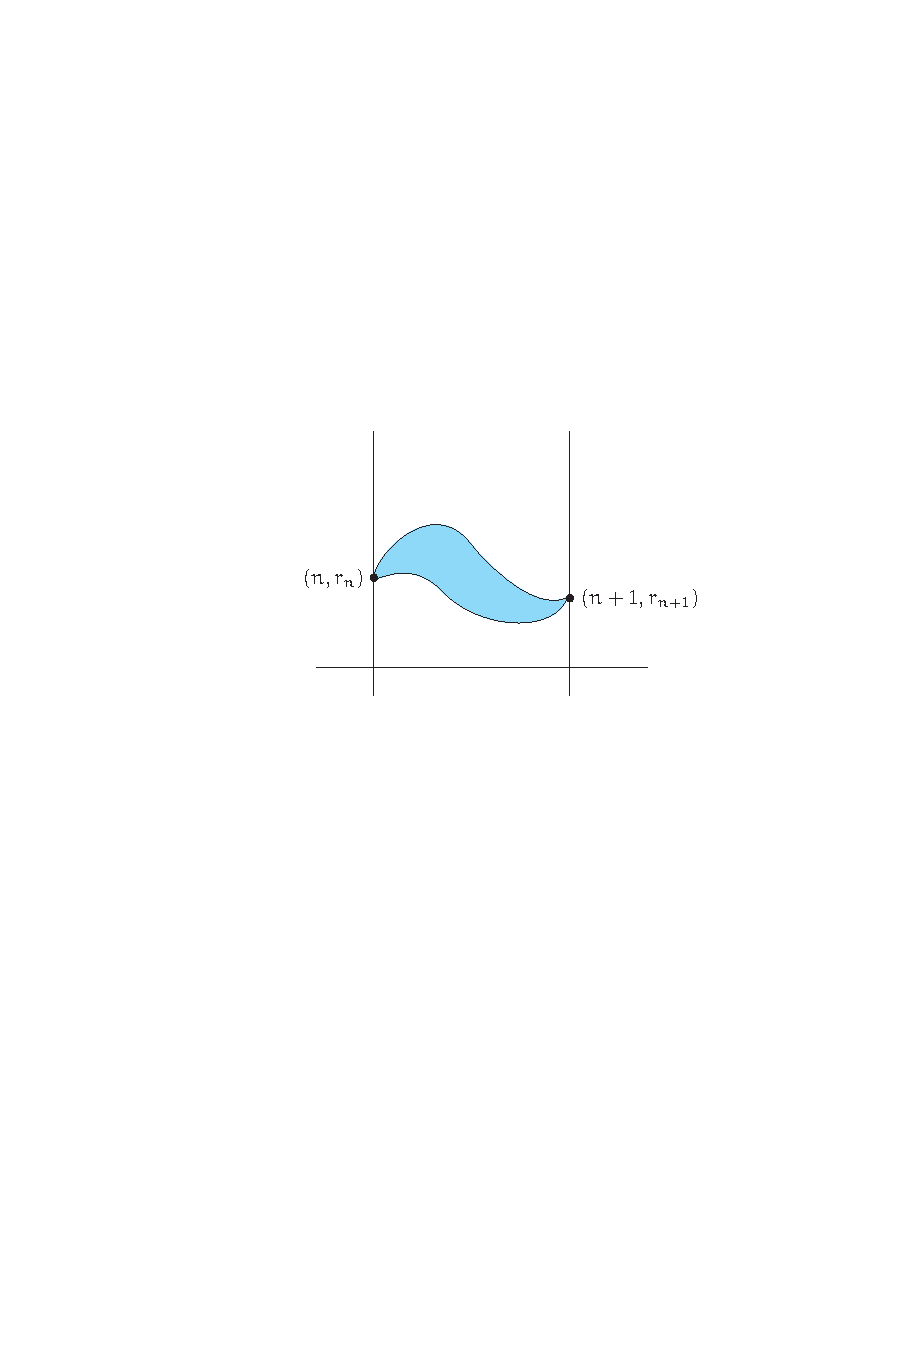
\includegraphics{pictures/quotient-product-no}
\caption{The open subset $A_n$.}
\end{figure}
\end{example}
On the other hand, we have the following result for coproducts.
\begin{proposition}\label{topo space coproduct of quotient map is quotient}
Let $(X_\alpha)_{\alpha\in A}$ and $(Y_\alpha)_{\alpha\in A}$ be topological spaces and for each $\alpha\in A$ let $p_\alpha:X_\alpha\to Y_\alpha$ be a quotient map. Then the map
\[p:\coprod_\alpha X_\alpha\to\coprod_\alpha Y_\alpha\]
which coincides with $p_\alpha$ on $X_\alpha$ is a quotient map.
\end{proposition}
\begin{proof}
Let $V$ be an subset in $\coprod_\alpha Y_\alpha$, then by the definition of $p$, we have
\[p^{-1}(V)=\bigcup_\alpha p_\alpha^{-1}(V\cap Y_\alpha),\]
so $p^{-1}(V)\cap X_\alpha=p_\alpha^{-1}(V\cap Y_\alpha)$. The claim now follows from by the definition of coproduct topology and the fact that each $p_\alpha$ is a quotient map.
\end{proof}
\subsection{Quotient of a subspace}
Let $X$ be a topological space, $A$ a subspace of $X$, and $\pi$ the canonical map $X\to X/R$ of an equivalence relation $R$ on $X$. Let $R_A$ be the relation induced by $R$ on $A$, and $\pi|_A=\iota\circ\tilde{\pi}\circ\pi_A$ be the canonical decomposition of $\pi|_A$, so that we have a commutative diagram
\[\begin{tikzcd}
A\ar[rrr,bend right=20pt,swap,"\pi|_A"]\ar[r,"\pi_A"]&A/R_A\ar[r,"\tilde{\pi}"]&\pi(A)\ar[r,"\iota"]&X/R
\end{tikzcd}\]
\begin{proposition}\label{topo space quotient topology on subspace iff}
The canonical bijection $\tilde{\pi}:A/R_A\to\pi(A)$ is continuous. Furthermore, the following three statements are equivalent:
\begin{itemize}
\item[(\rmnum{1})] $\tilde{\pi}$ is a homeomorphism.
\item[(\rmnum{2})] Every open subset of $A$ which is saturated with respect to $R_A$ is the intersection with $A$ of an open subset of $X$ which is saturated with respect to $R$.
\item[(\rmnum{3})] Every closed subset of $A$ which is saturated with respect to $R_A$ is the intersection with $A$ of a closed subset of $X$ which is saturated with respect to $R$. 
\end{itemize}
\end{proposition}
\begin{proof}
Note that $A/R_A$ carries the quotient topology induced by $\pi_A$, and $\pi(A)$ carries the subspace topology induced by $X/R$. Now the claim follows from \cref{topo space canonical decomposition homeomorphism iff}: if $U$ is an open subset of $A$ which is saturated with respect to $R_A$, and $\tilde{\pi}(U)=\pi(U)$ is the intersection with $\pi(A)$ of an open subset $V$ of $X/R$, then $U$ is the intersection with $A$ of the open subset $\pi^{-1}(V)$ of $X$, which is saturated with respect to $R$; and conversely, if $U$ is the intersection with $A$ of an open subset $W$ which is saturated with respect to $R$, then $\pi(U)$ is the intersection of $\pi(A)$ and $\pi(W)$, which is open in $X/R$.
\end{proof}
\begin{corollary}\label{topo space quotient map on saturated open set is quotient map}
If $A$ is an open (resp. closed) subset of $X$ which is saturated with respect to $R$, then the canonical mapping $\tilde{\pi}:A/R_A\to\pi(A)$ is a homeomorphism.
\end{corollary}
\begin{proof}
If $A$ is open (resp. closed) in $X$ and saturated with respect to $R$, and if $B\sub A$ is open (resp. closed) in $A$ and saturated with respect to $R_A$, then $B$ is open (resp. closed) in $X$ and saturated with respect to $R$.
\end{proof}
\begin{corollary}\label{topo space quotient map on sectioned orbit subspace}
If there is a continuous mapping $\varphi:X\to A$ such that $\varphi(x)\equiv x$ mod $R$ for each $x\in X$, then $\pi(A)=X/R$ and the canonical mapping $\tilde{\pi}:A/R_A\to X/R$ is a homeomorphism.
\end{corollary}
\begin{proof}
Since each equivalence class mod $R$ meets $A$, the canonical image of $\pi(A)$ in $X/R$ is the whole of $X/R$; on the other hand, if $U$ is open in $A$ and is saturated with respect to $R_A$, it follows from the hypothesis that $\varphi^{-1}(U)$ is the set obtained by saturating $U$ with respect to $R$; since $\varphi$ is continuous, $\varphi^{-1}(U)$ is open in $X$. The corollary follows from this fact by virtue of \cref{topo space quotient topology on subspace iff}.
\end{proof}
\begin{example}
Let $R$ denote the equivalence relation $x=y$ mod $\Z$ on the real line $\R$ and let $I$ denote the closed interval $[0,1]$; $I$ contains at least one point of each equivalence class mod $R$. The canonical mapping of $I/R_I$ onto the torus $\T$ is a homeomorphism; for if $F$ is closed in $I$ (and hence in $\R$), in order to saturate $F$ with respect to the relation $R$ we have to take the union of the closed sets $F+n$ for all $n\in\Z$, which evidently form a locally finite family, so that their union is closed; the assertion follows from this. We remark that $I/R_I$ is obtained by identifying the points $0$ and $1$ in $I$.
\end{example}
\subsection{Hausdorff condition of quotient spaces}
Typically, to prove that a given quotient space is Hausdorff, one has to resort to the definition. For open quotient maps, however, we have the following criterion.
\begin{proposition}\label{quotient Hausdorff}
Suppose $q:X\to Y$ is an open quotient map. Then $Y$ is Hausdorff if and only if the set $\mathcal{R}:=\{(x_1,x_2):q(x_1)=q(x_2)\}$ is closed in $X\times X$.
\end{proposition}
\begin{proof}
First assume $Y$ is Hausdorff. If $(x_1,x_2)\notin\mathcal{R}$, then there are disjoint neighborhoods $V_1$ of $q(x_1)$ and $V_2$ of $q(x_2)$, and it follows that $q^{-1}(V_1)\times q^{-1}(V_2)$ is a neighborhood of $(x_1,x_2)$ that is disjoint from $\mathcal{R}$. Thus $\mathcal{R}$ is closed. (This implication does not require the assumption that $q$ is open.)\par
Conversely, assume $\mathcal{R}$ is closed. Given distinct points $y_1,y_2\in Y$, choose $x_1,x_2\in X$ such that $q(x_i)=y_i$. Because $(x_1,x_2)\notin\mathcal{R}$, there is a product neighborhood $U_1\times U_2$ of $(x_1,x_2)$ in $X\times X$ that is disjoint from $\mathcal{R}$. Since $q$ is open, $q(U_1)$ and $q(U_2)$ are disjoint neighborhoods of $y_1$ and $y_2$, respectively.
\end{proof}
\begin{corollary}
Suppose $\sim$ is an equivalence relation on a space $X$. If the quotient map $X\to X/$$\sim$ is an open map, then $X/$$\sim$ is Hausdorff if and only if $\sim$ is a closed subset of $X\times X$.
\end{corollary}
\begin{theorem}
Suppose $X$ is a compact Hausdorff space and $q:X\to Y$ is a quotient map. Then the following are equivalent.
\begin{itemize}
\item[(a)] $Y$ is Hausdorff.
\item[(b)] $q$ is a closed map.
\item[(c)] The set $\mathcal{R}=\{(x_1,x_2):q(x_1)=q(x_2)\}$ is closed in $X\times X$.
\end{itemize}
\end{theorem}
\begin{proof}
The implicaton $(a)\Rightarrow(b)$ is immediate by closed map lemma, and $(a)\Rightarrow(c)$ is proved just as in \cref{quotient Hausdorff}. Next we prove $(b)\Rightarrow(a)$. Assuming $q$ is a closed map, we begin by showing that its fibers are compact. Every point $y\in Y$ is the image of some $x\in X$, and since $\{x\}$ is a closed subset of $X$, it follows that $\{y\}=q(\{x\})$ is a closed subset of $Y$. Thus by continuity, the fiber $q^{-1}(\{y\})$ is closed in $X$ and hence compact.\par 
To prove that $Y$ is Hausdorff, suppose $y_1$ and $y_2$ are distinct points of $Y$. Then we can prove the disjoint compact subsets $q^{-1}(y_1)$ and $q^{-1}(y_2)$ of $X$ have disjoint neighborhoods $U_1$ and $U_2$, respectively. Define subsets $W_1,W_2\sub Y$ by
\[W_i=Y-q(X-U_i)=\{y\in Y:q^{-1}(y)\sub U_i\}\]
Then $y_i\in W_i$ for each $i$ by construction, and $W_1$ and $W_2$ are disjoint because $U_1$ and $U_2$ are. To complete the proof, the fact that $q$ is closed implies that $W_i$ is open.\par
Finally, we prove $(c)\Rightarrow(a)$. Assuming that $\mathcal{R}$ is closed, we start again by showing that $q$ has compact fibers. Given $y\in Y$ and $x\notin q^{-1}(y)$, let $x_1$ be any point in $q^{-1}(y)$. (Such a point exists because $q$ is surjective.) Because $\mathcal{R}$ is closed and $(x,x_1)\notin\mathcal{R}$, there is a product neighborhood $U_1\times U_2$ of $(x_1,x)$ that is disjoint from $\mathcal{R}$. It follows that $U_2$ is a neighborhood of $x$ disjoint from $q^{-1}(y)$, for if $x_2$ were a point in $U_2\cap q^{-1}(y)$, then $(x_1,x_2)$ would lie in $\mathcal{R}\cap(U_1\times U_2)$, which is empty. Thus $q^{-1}(y)$ is closed in $X$ and hence compact.\par
Now let $y_1$ and $y_2$ be distinct points in $Y$. As before, there are disjoint open
subsets $U_1\sups q^{-1}(y_1)$ and $U_2\sups q^{-1}(y_2)$, and we define $W_1,W_2$ as before. These are disjoint sets containing $y_1$ and $y_2$, respectively, so we need only show they are open. Because $q$ is a quotient map, $W_i$ is open if and only if $q^{-1}(W_i)$ is open, which is the case if and only if $X-q^{-1}(W_i)$ is closed. From the definition of $W_i$, it follows that
\begin{align*}
X-q^{-1}(W_i)&=\{x\in X:q(x)\notin W_i\}=\{x\in X:q^{-1}(q(x))\nsubseteq U_i\}\\
&=\{x\in X:\text{$\exists x\in X-U_i$ such that $q(x)=q(\tilde{x})$}\}\\
&=\pi_1(\mathcal{R}\cap(X\times X-U_i))
\end{align*}
where $\pi_1:X\times X\to X$ is the projection on the first factor. Observe that $\pi_1$ is a closed map by the closed map lemma. Our hypothesis on $\mathcal{R}$ implies that $\mathcal{R}\cap(X\times X-U_i)$ is closed in $X\times X$, and therefore $X-q^{-1}(W_i)$ is closed in $X$.
\end{proof}
\subsection{Direct limit of topological spaces}
Let $(X_\alpha)_{\alpha\in I}$ be a family of sets, and let $X$ be the set which is the coproduct of the $X_\alpha$. We shall identify each $X_\alpha$ with a subset of $X$ by means of the canonical injection $\iota_\alpha:X_\alpha\to X$.\par
Let $R$ be an equivalence relation on $X$ such that each equivalence class of $R$ has at most one element in each $X_\alpha$; for each pair of indices $(\alpha,\beta)$ let $A_{\alpha\beta}$ be the subset of $X_\alpha$ consisting of the elements $x$ for which there is an element $y\in X_{\beta}$ which belongs to the equivalence class of $x$. Clearly to each $x\in A_{\alpha\beta}$ there is a unique $y\in X_\beta$ which is congruent to $x$ mod $R$; the mappings $\phi_{\beta\alpha}:A_{\alpha\beta}\to A_{\beta\alpha}$ so defined satisfy the following conditions:
\begin{itemize}
\item[(a)] For each $\alpha\in I$, $\phi_{\alpha\alpha}$ is the identity mapping of $A_{\alpha\alpha}=X_\alpha$.
\item[(b)] For each triple of indices $(\alpha,\beta,\gamma)$ of $I$ and each $x\in A_{\alpha\beta}\cap A_{\alpha\gamma}$, we have $\phi_{\beta\alpha}(x)\in A_{\beta\gamma}$ and $\phi_{\gamma\alpha}(x)=\phi_{\gamma\beta}(\phi_{\beta\alpha}(x))$.
\end{itemize}

Conversely, suppose that for each pair of indices $(\alpha,\beta)$ we are given a subset $A_{\alpha\beta}$ of $X_\alpha$ and a mapping $\phi_{\beta\alpha}:A_{\alpha\beta}\to A_{\beta\alpha}$ satisfying the conditions (a) and (b) above. It follows first of all from (b) applied to the triples $(\alpha,\beta,\alpha)$ and $(\beta,\alpha,\beta)$ that $\phi_{\alpha\beta}\circ\phi_{\beta\alpha}$ (resp. $\phi_{\beta\alpha}\circ\phi_{\alpha\beta}$) is the restriction of $\phi_{\alpha\alpha}$ (resp. $\phi_{\beta\beta}$) to $A_{\alpha\alpha}$ (resp. $A_{\beta\beta}$); hence we deduce from (a) that $\phi_{\beta\alpha}$ and $\phi_{\alpha\beta}$ are bijections which are mverses of each other. Now let $R$ be the relation "there exist $\alpha,\beta$ such that $x\in A_{\alpha\beta}$, $y\in A_{\beta\alpha}$ and $y=\phi_{\beta\alpha}(x)$." It follows from (a) and what precedes that $R$ is reflexive and symmetric; on the other hand, if 
\[x\in A_{\alpha\beta},\quad y=\phi_{\beta\alpha}(x)\in A_{\beta\alpha}\cap A_{\beta\gamma},\quad z=\phi_{\gamma\beta}(y)\in A_{\gamma\beta},\]
then also $x=\phi_{\alpha\beta}(y)$ and by (b) we have $z=\phi_{\gamma\alpha}(x)$; thus $R$ is transitive, and so is an equivalence relation on $X$. It follows also from (a) and from the definition of $R$ that each equivalence class mod $R$ has at most one element in each of the sets $X_\alpha$, and that $A_{\alpha\beta}$ is the set of all $x\in X_\alpha$ for which there is an element $y\in X_\beta$ congruent to $x$ mod $R$. We say that the quotient set $X/R$ is obtained by pasting together the $X_\alpha$ along the $A_{\alpha\beta}$ by means of the bijections $\phi_{\beta\alpha}$. If $\pi:X\to X/R$ is the canonical mapping, the restriction of $\pi$ to each $X_\alpha$ is a bijection of $X_\alpha$ onto $\pi(X_\alpha)$.\par
Now suppose that each $X_\alpha$ is a topological space, and let $\mathcal{T}_\alpha$ be its topology. Let $\mathcal{T}$ be the finest topology on the set $X/R$ for which the mappings $\pi\circ\iota_\alpha$ are continuous; then $\mathcal{T}$ is the quotient by $R$ of the topology on $X$ which is the coproduct of the topologies $\mathcal{T}_\alpha$. We say that the topological space $X/R$ (with the topology $\mathcal{T}$) is obtained by pasting together the topological spaces $X_\alpha$ along the $A_{\alpha\beta}$ by means of the bijections $\phi_{\beta\alpha}$. The open (resp. closed) subsets of $X/R$ are thus the canonical images of the subsets $B$ of $X$ which are saturated with respect to $R$ and are such that $B\cap X_\alpha$ is open (resp. closed) in $X_\alpha$ for each $\alpha\in I$.\par
Since the restriction of $\pi$ to each $X_\alpha$ is a bijection onto the subset $\pi(X_\alpha)$ of $X/R$, we can transport the topology $\mathcal{T}_\alpha$ to $\pi(X_\alpha)$ by means of this bijection, so that $\pi(X_\alpha)$ carries a topology $\widetilde{\mathcal{T}}_\alpha$ and the topology $\mathcal{T}$ on $X/R$ is the finest for which the canonical injections $\pi(X_\alpha)\to X/R$ are continuous. In general, the topology induced by $\mathcal{T}$ on $\pi(X_\alpha)$ is coarser than $\widetilde{\mathcal{T}}_\alpha$, but not identical with the latter; even if the $\phi_{\beta\alpha}$ are homeomorphisms. However, it follows from \cref{topo space pasting topology} that, with the preceding notation:
\begin{proposition}
Suppose that the $\phi_{\beta\alpha}$ are homeomorphisms and that each $A_{\alpha\beta}$ is open (resp. closed) in $X_\alpha$; then each $\pi(X_\alpha)$ is open (resp. closed) in $X/R$ and the restriction of $\pi$ to $X_\alpha$ is a homeomorphism of $X_\alpha$ onto the subspace $\pi(X_\alpha)$ of $X/R$.
\end{proposition}
\section{Product of topological spaces}
\subsection{Product spaces}
\begin{definition}
Given a family $(X_i)_{i\in I}$ of topological spaces, the \textbf{product space} of this family is the product set $X=\prod_{i\in I}X_i$ with the initial topology induced by the projections $\pi_i:X\to X_i$. The spaces $X_i$ are called the factors of $X$.
\end{definition}
By virtue of \cref{topo space initial topology definition}, the product topology on $X$ has as a base the set of finite intersections of sets of the form $\pi_i^{-1}(U_i)$, where $U_i$ is open in $X_i$; these sets are products $\prod_{i\in I}U_i$, where $U_i$ is open in $X_i$ for each $i$ and $U_i=X_i$ for all but a finite number of indices These sets will be called \textbf{elementary sets}.\par
If $\mathcal{B}_i$ is a base of the topology of $X_i$ for each $i\in I$, it is clear that the elementary sets $\prod_iB_i$ such that $B_i=X_i$ for all but finitely many indices form another base of the product topology. The elementary sets of this type which contain a given point $x\in X$ thus form a fundamental system of neighbourhoods of $x$.\par
If $I$ is a finite set, the construction of the product topology from the topologies of the factors $X_i$ is simpler: the elementary sets are just products $\prod_{i\in I}U_i$ where $U_i$ is any open subset of $X_i$ for each $i\in I$.
\begin{example}
The product $\R^n$ of $n$ spaces identical with the real line $\R$ is called real number space of $n$ dimensions; $\R^2$ is also called the real plane. Likewise, starting from the rational line $\Q$, we define the rational number space of $n$ dimensions $\Q^n$ (rational plane for $n=2$). The topology of the space $\R^n$ has as a base the set of all products of $n$ open intervals in $\R$, which are called open boxes of $n$ dimensions. The open boxes which contain a point $x\in\R^n$ form a fundamental system of neighbourhoods of this point. Likewise the products of $n$ closed intervals in $\R$ are called closed boxes of $n$ dimensions. The closed boxes to which $x$ is interior also form a fundamental system of neighbourhoods of $x$. There are analogous results for $\Q^n$.
\end{example}
\begin{proposition}\label{topo space map into product continuous iff}
Let $f=(f_i)$ be a mapping of a topological space $Y$ into a product space $X=\prod_{i\in I}X_i$. Then $f$ is continuous at a point $y\in Y$ if and onlY if $f_i$ is continuous at $y$ for each $i\in I$.
\end{proposition}
\begin{proof}
Since $f_i=f\circ\pi_i$, this is a special case of \cref{topo space initial topology definition}.
\end{proof}
\begin{corollary}\label{topological product map continuous iff}
Let $(X_i)_{i\in I}$ and $(Y_i)_{i\in I}$ be two families of topological spaces with tke same set of indices. For each $i\in I$, let $f_i$ be a mapping of $X_i$ into $Y_i$. In order that the product mapping $f:(x_i)\to(f_i(x_i))$ should be continuous at a point $a=(a_i)$, it is necessary and sufficient that $f_i$ is continuous at $a_i$ for each $i\in I$.
\end{corollary}
\begin{proof}
The map $f$ can be written as $x\mapsto(f_i(\pi_i(x)))$, so that by \cref{topo space map into product continuous iff} the condition is sufficient. Conversely, for each $j\in I$ let $g_j$ be the mapping of $X_j$ into $\prod_{i\in I}X_i$ such that $\pi_j(g_j(x))=x_j$ and $\pi_i(g_j(x))=a_i$ for $i\neq j$. Then $g_j$ is continuous at the point $a_j$, by \cref{topo space map into product continuous iff}. Since $f_j=\pi_j\circ f\circ g_j$, it follows that if $f$ is continuous at $a$ then $f_j$ is continuous at $a_j$.
\end{proof}
\begin{corollary}
Let $X$, $Y$ be two topological spaces. In order that a mapping $f:X\to Y$ should be continuous it is necessary and sufficient that the mapping $g:x\mapsto(x,f(x))$ is a homeomorphism of $X$ onto the graph $\Gamma(f)$ (considered as a subspace of the product space $X\times Y$).
\end{corollary}
\begin{proof}
Since $f=\pi_2\circ g$, the condition is sufficient. It is also necessary, for if $f$ is continuous, then $g$ is bijective and continuous (\cref{topo space map into product continuous iff}) and the inverse of $g$ is the restriction of $\pi_1$ to $\Gamma(f)$, which is continuous.
\end{proof}
\begin{proposition}[\textbf{Associativity of topological products}]
Let $(X_i)_{i\in I}$ be a family of topological spaces, $(I_\kappa)_{\kappa\in K}$ a partition of the set $I$, and for each $\kappa\in K$ let $X_\kappa=\prod_{i\in I_\kappa}X_i$. Then the canonical mapping of the product space $\prod_{i\in I}X_i$ onto the product space $\prod_{\kappa\in K}X_\kappa$ is a homeomorphism.
\end{proposition}
\begin{proof}
This is a special case of the transitivity of initial topologies.
\end{proof}
\begin{corollary}
Let $\sigma\in\mathfrak{S}_I$ be a permutation of the set $I$. Then the mapping $(x_i)\mapsto(x_{\sigma(i)})$ is a homeomorphism of $\prod_{i\in I}$ onto $\prod_{i\in I}X_{\sigma(i)}$.
\end{corollary}
\begin{proof}
Take $K=I$ and $I_i=\{\sigma(i)\}$ in the previous proposition.
\end{proof}
Finally, we show that, the general concept of initial topologies can be defined using product spaces and product topology.
\begin{proposition}\label{topo space initial topology defined by product}
Let $X$ be a set, $(Y_i)_{i\in I}$ a family of topological spaces, and for each $i\in I$ let $f_i$ be a mapping of $X$ into $Y_i$. Let $f$ be the mapping $x\mapsto(f_i(x))$ of $X$ into $Y=\prod_{i\in I}Y_i$. Then the initial topology on $X$ induced by $(f_i)$ is the inverse image under $f$ of the topology induced on $f(X)$ by the product topology on $Y$.
\end{proposition}
\begin{proof}
This is another application of the transitivity of initial topologies.
\end{proof}
\begin{corollary}
For each $i\in I$ let $A_i$ be a subspace of $X_i$. Then the topology induced on $A=\prod_{i\in I}A_i$ by the product topology on $\prod_{i\in I}X_i$ is the product of the topologies of the subspaces $A_i$.
\end{corollary}
\begin{proof}
Let $\iota_i$ be the canonical injection $A_i\to X_i$ and apply \cref{topo space initial topology defined by product} to the mappings $f_i=\iota_i\circ\pi_i$.
\end{proof}
There is another topology on the product space $X=\prod_{i\in I}X_i$ called the box topology, whose open sets are defined to be the product of open subsets in $X_i$. The box topology turns out to have too many open sets, for example, \cref{topo space map into product continuous iff} does not hold for it.
\begin{example}
Consider $\R^\omega$, the countably infinite product of $\R$ with itself. That is, $\R^\omega=\prod_{n\in\Z_+}X_n$, where $X_n=\R$ for each $n$. Let us define a function $f:\R\to\R^\omega$ by the equation
\[f(x)=(x,x,\dots,x,\dots).\]
Each of the coordinate functions $f_n:\R\to\R$ is continuous; therefore, the function $f$ is continuous if $\R^\omega$ is given the product topology. But $f$ is not continuous if $\R^\omega$ is given the box topology. Consider, for example, the basis element
\[B=\prod_{n\in\Z_+}(-1/n,1/n),\]
for the box topology. We assert that $f^{-1}(B)$ is not open in $\R$: If $f^{-1}(B)$ contains some interval $(-\delta,\delta)$ about the point $0$, then we must have $(-\delta,\delta)\sub(-1/n,1/n)$ for each $n$, whence $\delta=0$, a contradiction.
\end{example}
\subsection{Sections and projections}
\begin{proposition}\label{topo space section map homeomorphism}
Let $X$ and $Y$ be topological spaces. Then
\begin{itemize}
\item[(a)] for each $a\in X$, the map $y\mapsto(a,y)$ is a homeomorphism from $Y$ to the subspace $\{a\}\times Y$ of $X\times Y$;
\item[(b)] for each $b\in Y$, the map $x\mapsto(x,b)$ is a homeomorphism from $X$ to the subspace $X\times\{b\}$ of $X\times Y$.
\end{itemize}
\end{proposition}
\begin{proof}
Since $\pi_Y$, restricted to $\{a\}\times Y$, is a continuous inverse of the given map in (a), this is a particular case of \cref{topological product map continuous iff} applied to the constant function $x\mapsto a$. The same proof applies to (b).
\end{proof}
Note that the mapping $y\mapsto(a,y)$ is a continuous section with respect to the equivalence relation $\pi_X(z)=\pi_X(z')$ in $X\times Y$; the quotient space of $X\times Y$ by this equivalence relation is therefore homeomorphic to $Y$.
\begin{corollary}\label{topo space section of open close}
The section $A(x)$ of an open (resp. closed) set $A$ of the product $X\times Y$ at an arbitrary point $x\in X$ is open (resp. closed) in $Y$.
\end{corollary}
Using \cref{topological product map continuous iff}, we also get the following useful fact.
\begin{proposition}\label{topo space projection is open}
The projection of $X\times Y$ onto either factor is an open map.
\end{proposition}
\begin{proof}
Let $U$ be open in $X\times Y$, then we have 
\[\pi_X(U)=\bigcup_{y\in Y}U(y),\quad\pi_Y(U)=\bigcup_{x\in X}U(x),\]
and the proposition follows from the \cref{topo space section of open close}.
\end{proof}
Note that the projection of a closed subset of $X\times Y$ onto a factor need not be closed. For example, in the real plane $\R^2$, the hyperbola whose equation is $xy=1$ is a closed set, but both its projections are equal to the complement of the point $0$ in $\R$. and this is not a closed set.
\begin{proposition}\label{topo space continuous is separately conitnuous}
Let $X$, $Y$ and $Z$ be three topological spaces, $f$ a mapping of the product space $X\times Y$ into $Z$. If $f$ is continuous at the point $(a,b)\in X\times Y$, then the partial mapping $y\mapsto f(a,y)$ of $Y$ into $Z$ is continuous at the point $b$.
\end{proposition}
\begin{proof}
This mapping is the composition of $f$ and the mapping $y\mapsto(a,y)$; hence the result follows from \cref{topo space section map homeomorphism}.
\end{proof}
\cref{topo space continuous is separately conitnuous} is often expressed by saying that a continuous function of two variables is continuous with respect to each of them separately.
\begin{example}
It is possible for all the partial mappings determined by a map $f:X\times Y\to Z$ to be continuous without $f$ being continuous. For example if $f$ is the mapping of the real plane $\R^2$ into $\R$ defined by
\[f(x,y)=\begin{cases}
\dfrac{xy}{x^2+y^2}&(x,y)\neq(0,0),\\
0&(x,y)=(0,0).
\end{cases}\]
Then all the partial mappings are continuous; but $f$ is not continuous at $(0,0)$.
\end{example}
\begin{proposition}\label{topo space closure of product subspace}
In a product space $\prod_{i\in I}X_i$ the closure of a product of sets $\prod_{i\in I}A_i$ is the same as the product $A_i$ of their closures.
\end{proposition}
\begin{proof}
Suppose that $a=(a_i)$ lies in the closure of $\prod_{i\in I}A_i$; then for each $j\in I$, $a_j=\pi_j(a)$ is in the closure of $A_j$ because of the continuity of $\pi_j$ and therefore $a\in\prod_{i\in I}\widebar{A}_i$. Conversely, let $b=(b_i)\in\prod_{i\in I}\widebar{A}_i$ and let $\prod_{i\in I}U_i$ be any elementary set containing $b$; for each $i\in I$, $U_i$ contains a point $x_i\in A_i$; hence $\prod_{i\in I}U_i$ contains the point $(x_i)\in\prod_{i\in I}A_i$ and therefore $b$ lies in the closure of $\prod_{i\in I}A_i$.
\end{proof}
\begin{corollary}
A product $\prod_{i\in I}A_i$ of non-empty sets is closed in the product space $\prod_{i\in I}$ if and only if $A_i$ is closed in $X_i$ for each $i\in I$.
\end{corollary}
\begin{remark}
Note that if $I$ is finite, a product $\prod_{i\in I}A_i$ is open provided that $A_i$ is open in $X_i$ for each $i\in I$; but this is no longer so if $I$ is infinite.
\end{remark}
As an application of \cref{topo space closure of product subspace}, we give a certain family of dense subsets in a product space.
\begin{proposition}\label{topo space dense subset in product}
Let $a=(a_i)$ be any point of a product space $X=\prod_{i\in I}X_i$; then the set $D$ of points $x\in X$ such that $\pi_i(x)=a_i$ except for a finite number of indices $i$ is dense in $X$.
\end{proposition}
\begin{proof}
For each $x\in X$ and each elementary set $U=\prod_{i\in I}U_i$ which contains $x$, we have $U_i=X_i$ except for indices $i$ belonging to a finite subset of $J$; if we take $y_i=x_i$ for $i\notin J$ and $y_i=a_i$ for $i\in J$, it is clear that $y=(y_i)\in D$ and $y\in U$; hence the result.
\end{proof}
\subsection{Inverse limit of topological spaces}
Let $I$ be a partially ordered (but not necessarily directed) set, in which the order relation is written as $\preceq$. For each $\alpha\in I$, let $X_\alpha$ be a topological space, and for each pair $(\alpha,\beta)$ such that $\alpha\preceq\beta$ let $f_{\alpha\beta}$ be a mapping of $X_\beta$ into $X_\alpha$. We say that $(X_\alpha,f_{\alpha\beta})$ is an inverse system of topological spaces if:
\begin{itemize}
\item[(a)] $(X_\alpha,f_{\alpha\beta}$) is an inverse system of sets;
\item[(b)] Each $f_{\alpha\beta}$ is continuous. 
\end{itemize} 
Let $X$ denote the set $\llim X_\alpha$ and for each $\alpha\in I$ let $f_\alpha$ be the canonical mapping $X\to X_\alpha$; then the initial topology induced by the $f_\alpha$'s is said to be the inverse limit (with respect to the $f_{\alpha\beta}$) of the topologies of the $X_\alpha$ and the set $X$ with this topology is called the inverse limit of the inverse system of topological spaces $(X_\alpha,f_{\alpha\beta})$. Whenever we speak of $\llim X_\alpha$ as a topological space, it is always to be understood that the topology of this space is the inverse limit of the topologies of the $X_\alpha$ unless the contrary is expressly stated.\par
The set $X$ is the subset of the product $\prod_{\alpha}X_\alpha$ consisting of those points $x$ such that
\[\pi_\alpha(x)=f_{\alpha\beta}(\pi_\beta(x)).\]
whenever $\alpha\preceq\beta$. It follows from \cref{topo space initial topology defined by product} that the inverse limit of the topologies of the $X_\alpha$ is the same as the topology induced on $X$ by the topology of the product space $\prod_\alpha X_\alpha$. If, for each $\alpha\in I$, $A_\alpha$ is a subspace of $X_\alpha$ such that the $(A_\alpha,f_{\alpha\beta}|_{A_\beta})$ form an inverse system of subsets of the $X_\alpha$, then it is clear that the topological space $\llim A_\alpha$ is a subspace of $\llim X_\alpha$.\par
Let $(Y_\alpha,g_{\alpha\beta})$ be another inverse system of topological spaces indexed by the same set $I$, and for each $\alpha\in I$ let $\varphi_\alpha:X_\alpha\to Y_\alpha$ be a continuous mapping such that $(\varphi_\alpha)$ is an inverse system of mappings; then $\varphi=\llim \varphi_\alpha$ is a continuous mapping of $X=\llim X_\alpha$ into $Y=\llim Y_\alpha$. For if $g_\alpha$ is the canonical mapping $Y\to Y_\alpha$, we have $g_\alpha\circ\varphi=\varphi_\alpha\circ f_\alpha$, so that $g_\alpha\circ\varphi$ is continuous for each $\alpha\in I$, and so $\varphi$ is continuous.\par
Finally, suppose $I$ is a directed set, and let $J$ be a cofinal subset of $I$; let $\widetilde{X}$ be the inverse limit of the inverse system of topological spaces $(X_\alpha,f_{\alpha\beta})_{\alpha,\beta\in J}$. Then the canonical bijection $\psi:X\to\widetilde{X}$ is a homeomorphism. For we have $\pi_\alpha(\psi(x))=\pi_\alpha(x)$ for each $\alpha\in J$, hence $\psi$ is continuous; and if $\phi$ is the inverse of $\psi$, then for each $\alpha\in I$ there exists $\beta\in J$ such that $\alpha\preceq\beta$, and therefore $\pi_\alpha(\phi(z))=f_{\alpha\beta}(\pi_\beta(z))$, which shows that $\phi$ is continuous, since the $f_{\alpha\beta}$'s are continuous.
\begin{proposition}\label{topo space inverse limit cofinal system base}
Let $I$ be a directed set and $J$ a cofinal subset of $I$. Let $(X_\alpha,f_{\alpha\beta})$ be an inverse system of topological spaces indexed by $I$; let $X=\llim X_\alpha$ and let $f_\alpha:X\to X_\alpha$ be the canonical mapping. Then the family of sets $f_\alpha^{-1}(U_\alpha)$, where $\alpha$ runs through $J$ and $U_\alpha$ runs through a base $\mathcal{B}_\alpha$ of the topology of $X_\alpha$ for each $\alpha\in J$, is a base of the topology of $X$.
\end{proposition}
\begin{proof}
We know that the finite intersections of sets of the form $f_\alpha^{-1}(U_\alpha)$, $\alpha\in I$, $U_\alpha$ open in $X_\alpha$ form a base of the topology of $X$. If $\alpha_1,\dots,\alpha_n$ is a finite family of indices of $I$, then there exists $\beta\in J$ such that $\alpha_i\preceq\beta$ for $1\leq i\leq n$; hence $f_{\alpha_i}=f_{\alpha_i\beta}\circ f_\beta$; if we put $U_\beta=\bigcap_{i=1}^{n}f_{\alpha_i\beta}^{-1}(U_{\alpha_i})$, then
\[f_\beta^{-1}(U_\beta)=\bigcap_{i=1}^{n}f_{\alpha_i}^{-1}(U_{\alpha_i}).\]
But $U_\beta$ is open and is therefore a union of sets belonging to $\mathcal{B}_\beta$. Hence the result.
\end{proof}
\begin{corollary}
Let $A$ be a subset of $X$ and let $A_\alpha=f_\alpha(A)$ for each $\alpha\in I$. Then:
\begin{itemize}
\item[(a)] The $A_\alpha$ (resp. the $\widebar{A}_\alpha$) form an inverse system of subsets of the $X_\alpha$, and $\widebar{A}=\bigcap_{\alpha}f_\alpha^{-1}(\widebar{A}_\alpha)=\llim\widebar{A}_\alpha$.
\item[(b)] If $A$ is closed in $X$ then $A=\llim A_\alpha=\llim \widebar{A}_\alpha$.
\end{itemize}
\end{corollary}
\begin{proof}
The first assertion of (a) follows from the relations $f_\alpha=f_{\alpha\beta}\circ f_\beta$ for $\alpha\preceq\beta$ and from the continuity of the $f_\alpha$. Let $A'$ denote $\bigcap_{\alpha}f_\alpha^{-1}(\widebar{A}_\alpha)$, then it is clear that $A'$ is closed and contains $A$, so that $\widebar{A}\sub A'$. Conversely, let $x\in A'$; we have to show that $x$ lies in the closure of $A$. By virtue of \cref{topo space inverse limit cofinal system base}, it is enough to prove that every neighbourhood of $x$ which is of the form $f_\alpha^{-1}(U_\alpha)$, with $\alpha\in I$ and $U_\alpha$ open in $X_\alpha$ meets $A$. Now, by hypothesis, $f_\alpha(x)\in U_\alpha$, and since $f_\alpha(x)\in \widebar{A}_\alpha$ we have $U_\alpha\cap A_\alpha\neq\emp$, which means $A\cap f_\alpha^{-1}(A_\alpha)\neq\emp$.\par
To establish (b) it is enough to remark that, without any restriction on $A$, we have $A\sub\llim A_\alpha\sub\llim\widebar{A}_\alpha$; now if $A$ is closed, then from (a) we have $A=\llim\widebar{A}_\alpha$, so the claim follows.
\end{proof}
\begin{example}
Let $I$ be a directed set and $(X_\alpha)_{\alpha\in I}$ a family of subsets of a set $Y$, such that $X_\alpha\sups X_\beta$ whenever $\alpha\preceq\beta$. For each $\alpha\in I$ let $\mathcal{T}_\alpha$ be a topology on $X_\alpha$ such that $\mathcal{T}_\alpha$ is finer than the topology induced on $X_\alpha$ by $\mathcal{T}_\beta$ whenever $\alpha\preceq\beta$. If we take $f_{\alpha\beta}$ to be the canonical injection $X_\beta\to X_\alpha$ for $\alpha\preceq\beta$, then $\llim X_\alpha$ may be identified canonically with the intersection $X$ of the $X_\alpha$, with the topology which is the least upper bound of the topologies induced on $X$ by the $\mathcal{T}_\alpha$.
\end{example}
\section{Connectedness}
\subsection{Connected spaces}
The definition of connectedness for a topological space is a quite natural one. One says that a space can be "separated" if it can be broken up into two "globs"--disjoint open sets. Otherwise, one says that it is connected. From this simple idea much follows.
\begin{definition}
Let $X$ be a topological space. A \textbf{separation} of $X$ is a pair $U$, $V$ of disjoint nonempty open subsets of $X$ whose union is $X$. The space $X$ is said to be connected if there does not exist a separation of $X$.
\end{definition}
Connectedness is obviously a topological property, since it is formulated entirely in terms of the collection of open sets of $X$. Said differently, if $X$ is connected, so is any space homeomorphic to $X$.\par
For a subspace $A$ of a topological space $X$, there is another useful way of formulating the definition of connectedness:
\begin{lemma}\label{topo space connectedness of subspace}
If $A$ is a subspace of $X$, a separation of $A$ is a pair of disjoint nonempty sets $U$ and $V$ whose union is $A$, neither of which contains a limit point of the other. The space $A$ is connected if there exists no separation of $A$.
\end{lemma}
\begin{proof}
Suppose first that $U$ and $V$ form a separation of $A$. Then $U$ is both open and closed in $A$. The closure of $U$ in $A$ is the set $\widebar{U}\cap A$ (where $\widebar{U}$ as usual denotes the closure of $U$ in $X$). Since $U$ is closed in $A$, $U=\widebar{U}\cap A$; or to say the same thing, $\widebar{U}\cap V=\emp$. Since $\widebar{U}$ is the union of $U$ and its limit points, $V$ contains no limit points of $U$. A similar argument shows that $U$ contains no limit points of $V$.\par
Conversely, suppose that $U$ and $V$ are disjoint nonempty sets whose union is $A$, neither of which contains a limit point of the other. Then $\widebar{U}\cap V=\emp$ and $\widebar{V}\cap U=\emp$; therefore, we conclude that $\widebar{U}\cap A=U$ and $\widebar{V}\cap A=V$. Thus both $U$ and $V$ are closed in $A$, and since $U\cup V=A$, they are open in $A$ as well.
\end{proof}
\begin{example}
Let $X$ denote a two-point space in the indiscrete topology. Obviously there is no separation of $X$, so $X$ is connected.
\end{example}
\begin{example}
Let $A$ denote the subspace $[-1,0)\cup(0,1]$ of the real line $\R$. Each of the sets $[-1,0)$ and $(0,1]$ is nonempty and open in $A$ (although not in $\R$); therefore, they form a separation of $A$. Alternatively, note that neither of these sets contains a limit point of the other. (They do have a limit point $0$ in common, but that does not matter.)
\end{example}
\begin{example}
A subspace of $\mathbb{R}$ is connected if and only if it is an interval: Clearly intervals are connected. Now suppose $X$ is connected in $\R$ and is not an interval. Then there are $x,y\in X$ and $z\notin X$ such that $x<z<y$. We set
\[O_1=(-\infty,z)\cap X,\quad O_2=X\cap(z,+\infty)\]
Then $O_1$ and $O_2$ is a separation of $X$, and since $x\in O_1$, $y\in O_2$ they are both nonempty. This is a contradiction since $X$ is connected, hence $X$ is an interval.
\end{example}
\begin{example}
Let $X$ be the subspace $[-1,1]$ of the real line. The sets $[-1,0]$ and $(0,1]$ are disjoint and nonempty, but they do not form a separation of $X$, because the first set is not open in $X$. Alternatively, note that the first set contains a limit point, $0$, of the second. Indeed, there exists no separation of the space $[-1,1]$.
\end{example}
\begin{example}
The rationals $\Q$ are not connected. Indeed, the only connected subspaces of $\Q$ are the one-point sets: If $A$ is a subspace of $\Q$ containing two points $p$ and $q$, one can choose an irrational number $\alpha$ lying between $p$ and $q$, and write $A$ as the union of the open sets
\[A=(A\cap(-\infty,\alpha))\cup(A\cap(\alpha,+\infty)).\]
\end{example}
\begin{example}
Consider the following subset of the plane $\R^2$:
\[X=\{(x,y)\in\R^2:y=0\}\cup\{(x,y):\text{$x>0$ and $xy=1$}\}.\]
Then $X$ is not connected; indeed, the two indicated sets form a separation of $X$ because neither contains a limit point of the other.
\end{example}
We have given several examples of spaces that are not connected. How can one construct spaces that are connected? We shall now prove some useful properties of connectedness, and later use them to construct connected topological spaces. First, we give another criterion for connectedness which is quite simple but useful.
\begin{proposition}\label{topo space connected iff continuous map to 0,1}
A topological space $X$ is connected if and only if every continuous map $f:X\to\{0,1\}$ is constant, with the space $\{0,1\}$ given the discrete topology.
\end{proposition}
\begin{proof}
Clearly if $f$ is not constant then $f^{-1}(0)\cup f^{-1}(1)$ is a separation of $X$. Conversely, if $U$ and $V$ form a separation of $X$ then the characteristic function $\chi_U$ is nonconstant and continuous.
\end{proof}
\begin{proposition}[\textbf{Properties of Connected Spaces}]\label{topo space connected prop}
Let $X$ be a topological space.
\begin{itemize}
\item[(a)] Suppose that $U,V$ are disjoint open subsets of $X$. If $A$ is a connected subset of $X$ contained in $U\cup V$, then either $A\sub U$ or $A\sub V$.
\item[(b)] Suppose $X$ is any space and $A\sub X$ is connected. If $B$ is a subset such that $A\sub B\sub\widebar{A}$, then it is connected. In particular, $\widebar{A}$ is connected.
\item[(c)] Let $\{C_{\alpha}\}_{\alpha\in I}$ be a collection of connected subspaces of $X$ with a point in common. Then $\bigcup_{\alpha\in I}C_\alpha$ is connected.
\item[(d)] Let $\{C_{\alpha}\}_{\alpha\in I}$ be a collection of connected subspaces of $X$ with $C_\alpha\cap C_\beta\neq\emp$ for all $\alpha,\beta\in I$. Then $\bigcup_{\alpha\in I}C_\alpha$ is connected. 
\end{itemize}
\end{proposition}
\begin{proof}
For (a), if $A$ contained points in both $U$ and $V$, then $A\cap U$ and $A\cap V$ would form a separation of $A$. To prove (b), suppose $A$ is connected and $A\sub B\sub\widebar{A}$. Suppose that $B=U\cup V$ is a separation of $B$. By part (a), the set $A$ must lie entirely in $U$ or in $V$; say $A\sub U$. Then $\widebar{A}\sub\widebar{U}$; since $\widebar{U}$ and $V$ are disjoint, $B$ cannot intersect $V$. This contradicts the fact that $V$ is a nonempty subset of $B$.\par
For part (c), let $p$ be a point that is contained in $C_\alpha$ for every $\alpha$, and let $f:\bigcup_\alpha C_\alpha\to\{0,1\}$ be a continuous function. Then $f$ is constant when restricted to each $C_\alpha$, since $C_\alpha$ is connected. Since $C_\alpha$ contains $p$ for each $\alpha$, it then follows that $f$ is constant. This shows $\bigcup_{\alpha}C_\alpha$ is connected. Part (c) can be proved similarly.
\end{proof}
\begin{corollary}
Let $X$ be a topological space and $(A_n)_{n\in\N}$ be an infinite sequence of connected subspaces such that $A_n\cap A_{n+1}\neq\emp$ for all $n\geq 0$. Then the union $\bigcup_nA_n$ is connected.
\end{corollary}
\begin{proof}
By induction on $n$ we see immediately that the set $B_n=\bigcup_{i=1}^{n}A_i$ is connected for all $n$, by \cref{topo space connected prop}. The sets $B_n$ have a non-empty intersection; hence their union, equal to $\bigcup_nB_n$, is connected by \cref{topo space connected prop}.
\end{proof}
\begin{proposition}\label{topo space connected continuous image}
The image of a connected space under a continuous map is connected.
\end{proposition}
\begin{proof}
Let $f:X\to Y$ be a continuous map; let $X$ be connected. We wish to prove the image space $f(X)$ is connected. Since the map obtained from $f$ by restricting its range to the space is also continuous, it suffices to consider the case that $f$ is surjective. Suppose that $Y=U\cup V$ is a separation of $Y$ into two disjoint nonempty sets open in $Y$. Then $f^{-1}(U)$ and $f^{-1}(V)$ are disjoint sets whose union is $X$; they are open in $X$ because $f$ is continuous, and nonempty because $f$ is surjective. Therefore, they form a separation of $X$, contradicting the assumption that $X$ is connected.
\end{proof}
\begin{corollary}\label{topo space quotient of connected space}
Every quotient space of a connected space is connected.
\end{corollary}
As for \cref{topo space quotient of connected space}, we have the following converse.
\begin{proposition}\label{topo space connected if quotient is}
Let $X$ be a topological space and $R$ an equivalence relation on $X$. If the quotient space $X/R$ is connected, and if each equivalence class of $R$ is connected, then $X$ is connected.
\end{proposition}
\begin{proof}
Suppose $X$ is not connected. Then there is a partition of $X$ into two open sets $U$, $V$. The sets $U$, $V$ are saturated with respect to $R$ in view of \cref{topo space connected prop}(a). The canonical images of $U$ and $V$ are therefore open sets in $X/R$ and form a partition of $X/R$; this contradicts the assumption that $X/R$ is connected.
\end{proof}
\begin{proposition}\label{topo space connected product iff}
Every product of connected spaces is connected. Conversely, if a product of non-empty spaces is connected, then each of the factors is connected.
\end{proposition}
\begin{proof}
Let $(X_i)_{i\in I}$ be a family of topological spaces and $X=\prod_{i\in I}X_i$. Since the projection $\pi_i:X\to X_i$ is continuous and surjective, if $X$ is connected then so is each $X_i$. Conversely, assume that each $X_i$ is connected and let $f:X\to\{0,1\}$ be a continuous map, where $\{0,1\}$ is given the discrete topology. Let $a=(a_i)$ be any point of $X$, and for each $j\in I$ let $f_j:X_j\to\{0,1\}$ be the partial mapping defined by $f_j(x_j)=f((y_i))$, where $y_j=x_j$ and $y_i=a_i$ for $i\neq j$. Then $f_j$ is continuous, so is constant since $X_j$ is connected. It follows immediately by induction that $f(x)=f(a)$ for all points $x=(x_i)$ such that $x_i=a_i$ for all but finitely many indices of $I$. But these points form a dense subset of $X$ by \cref{topo space dense subset in product}. Hence $f$ is continuous on $X$ and constant on a dense subset of $X$, and therefore constant on $X$. But this contradicts the definition of $f$.
\end{proof}
Now that, however, the result of \cref{topo space connected product iff} depends on the topology we endow with the product space $\prod_{i\in I}X_i$. If we consider the box topology, it turns out that $\prod_{i\in I}X_i$ may be not connected even though each $X_i$ is.
\begin{example}
Consider the cartesian product $\R^\omega$ in the box topology. We can write $\R^\omega$ as the union of the set $A$ consisting of all bounded sequences of real numbers, and the set $B$ of all unbounded sequences. These sets are disjoint, and each is open in the box topology. For if $x=(x_n)$ is a point of $\R^\omega$, the open set
\[U=\bigcup_{n\in\Z_+}(x_n-1/n,x_n+1/n)\]
consists entirely of bounded sequences if $x$ is bounded, and of unbounded sequences if $x$ if unbounded. Thus, even though $\R$ is connected, $\R^\omega$ is not connected in the box topology.
\end{example}
\begin{example}
The set $\O(n)$ of all real orthogonal $n\times n$ matrices is not connected. The function $O(n)\to \{1,-1\}, A\mapsto\det A$ is continuous and surjective, since we have the formula
\[\det A=\sum_{\sigma\in\mathfrak{S}_n}(\text{sign}\ \sigma)a_{1\sigma(1)}\cdots a_{n\sigma(n)}\]
Since $\{1,-1\}$ has discrete topology, it follows that $\O(n)$ is not connected.
\end{example}
\subsection{Path connectedness}
The theorems of the preceding part show us how to construct new connected spaces out of given ones. But where can we find some connected spaces to start with? The best place to begin is the real line. We shall prove that $\R$ is connected, and so are the intervals and rays in $\R$.
The fact that intervals and rays in $\R$ are connected may be familiar to you from analysis. We prove it again here, in generalized form. It turns out that this fact does not depend on the algebraic properties of $\R$, but only on its order properties. To make this clear, we shall prove the theorem for an arbitrary ordered set that has the order properties of $\R$. Such a set is called a \textbf{linear continuum}.
\begin{definition}
A totally ordered set $L$ having more than one element is called a \textbf{linear continuum} if the following hold:
\begin{itemize}
\item[(a)] $L$ has the least upper bound property.
\item[(b)] If $x<y$, there exists $z$ such that $x<z<y$.
\end{itemize}
\end{definition}
\begin{theorem}
If $L$ is a linear continuum in the order topology, then $L$ is connected, and so are intervals and rays in $L$.
\end{theorem}
\begin{proof}
Recall that a subspace $A$ of $L$ is said to be convex if for every pair of points $a,b$ of $A$ with $a<b$, the entire interval $[a,b]$ of points of $L$ lies in $A$. We prove that if $A$ is a convex subspace of $L$, then $A$ is connected.\par
So suppose that $A$ is the union of the disjoint nonempty sets $U$ and $V$, each of which is open in $A$. Choose $a\in U$ and $b\in V$; suppose for convenience that $a<b$. The interval $[a,b]$ of points of $L$ is contained in $A$. Hence $[a,b]$ is the union of the disjoint sets
\[U_0=U\cap[a,b],\quad V_0=V\cap[a,b]\]
each of which is open in $[a,b]$ in the subspace topology, which is the same as the order topology. The sets $U_0$ and $V_0$ are nonempty because $a\in U_0$ and $b\in V_0$. Thus, $U_0$ and $V_0$ constitute a separation of $[a,b]$. Let $c=\sup U_0$. We show that $c$ belongs neither to $U_0$ nor to $V_0$, which contradicts the fact that $[a,b]$ is the union of $U_0$ and $V_0$.\par
Suppose that $c\in A_0$. Then $c\neq b$, so either $c=a$ or $a<c<b$. But $U_0$ is open in $[a,b]$, so there must be some interval of the form $[c,e)$ contained in $U_0$. Because of order property (b) of the linear continuum $L$, we can choose a point $z$ of $L$ such that $c<z<e$. Then $z\in U_0$, contrary to the fact that $c$ is an upper bound for $U_0$.\par
Suppose that $c\in B_0$. Then $c\neq a$, so either $c=b$ or $a<c<b$. In either case, it follows from the fact that $V_0$ is open in $[a,b]$ that there is some interval of the form $(d,c]$ contained in $V_0$. Since $(c,b]$ does not intersect $U_0$, we see that $(d,b]=(d,c]\cup(c,b]$ does not intersect $U_0$. Again, $d$ is a smaller upper bound on $U_0$ than $c$, contrary to construction.
\end{proof}
\begin{corollary}
The real line $\R$ is connected and so are intervals and rays in $\R$.
\end{corollary}
As an application, we prove the intermediate value theorem of calculus, suitably generalized.
\begin{theorem}[\textbf{Intermediate value theorem}]
Let $f:X\to Y$ be a continuous map, where $X$ is a connected space and $Y$ is an ordered set in the order topology. If $a$ and $b$ are two points of $X$ and if $r$ is a point of $Y$ lying between $f(a)$ and $f(b)$, then
there exists a point $c$ of $X$ such that $f(c)=r$.
\end{theorem}
\begin{proof}
Assume the hypotheses of the theorem. The sets
\[U=f(X)\cap(-\infty,r)\quad\text{and}\quad V=f(X)\cap(r,+\infty)\]
are disjoint, and they are nonempty because one contains $f(a)$ and the other contains $f(b)$. Each is open in $f(X)$, being the intersection of an open ray in $Y$ with $f(X)$. If there were no point $c$ of $X$ such that $f(c)=r$, then $f(X)$ would be the union of the sets $U$ and $V$. Then $U$ and $V$ would constitute a separation of $f(X)$, contradicting the fact that the image of a connected space under a continuous map is connected.
\end{proof}
\begin{example}
One example of a linear continuum different from $\R$ is the ordered square. We check the least upper bound property. (The second property of a linear continuum is trivial to check.)\par
Let $A$ be a subset of $I\times I$; let $\pi_1:I\times I\to I$ be projection on the first coordinate; let $b=\sup\pi_1(A)$. If $b\in\pi_1(A)$, then $A$ intersects the subset $\{b\}\times I$ of $I\times I$. Because $\{b\}\times I$ has the order type of $I$, the set $A\cap (\{b\}\times I)$ will have a least upper bound $(b,c)$, which will be the least upper bound of $A$.\par
If $b\notin\pi_1(A)$, then $(b,0)$ is the least upper bound of $A$; no element of the form $(b',c)$ with $b'<b$ can be an upper bound for $A$, for then $b'$ would be an upper bound for $\pi_1(A)$.
\end{example}
\begin{example}
If $X$ is a well-ordered set, then $X\times[0,1)$ is a linear continuum in the dictionary order. This set can be thought of as having been constructed by "fitting in" a set of the order type of $(0,1)$ immediately following each element of $X$.
\end{example}
Connectedness of intervals in $\R$ gives rise to an especially useful criterion for showing that a space $X$ is connected; namely, the condition that every pair of points of $X$ can be joined by a path in $X$:
\begin{definition}
Given points $x$ and $y$ of the space $X$, a \textbf{path} in $X$ from $x$ to $y$ is a continuous map $p:[0,1]\to X$ of the unit interval in the real line into $X$, such that $p(0)=x$ and $p(1)=y$. A space $X$ is said to be \textbf{path-connected} if every pair of points of $X$ can be joined by a path in $X$.
\end{definition}
It is easy to see that a path-connected space $X$ is connected. Suppose $X=U\cup V$ is a separation of $X$. Let $p:[0,1]\to X$ be any path in $X$. Being the continuous image of a connected set, the set $p([0,1])$ is connected, so that it lies entirely in either $U$ or $V$. Therefore, there is no path in $X$ joining a point of $U$ to a point of $V$, contrary to the assumption that $X$ is path-connected. The converse does not hold: a connected space need not be path-connected.
\begin{example}
Define punctured Euclidean space to be the space $\R^n\setminus\{0\}$, where $0$ is the origin in $\R^n$. If $n>1$, this space is path-connected: Given $x$ and $y$ different from $0$, we can join $x$ and $y$ by the straight-line path between them if that path does not go through the origin. Otherwise, we can choose a point $z$ not on the line joining $x$ and $y$, and take the broken-line path from $x$ to $z$, and then from $z$ to $y$.
\end{example}
\begin{example}
Being a linear continuum, the ordered square is connected. Let $x=(0,0)$ and $y=(1,1)$. We suppose there is a path $p:[0,1]\to I^2_o$ joining $x$ and $y$ and derive a contradiction. The image set $p([0,1])$ must contain every point $(x,y)$ of $I^2_o$, by the intermediate value theorem. Therefore, for each $x\in I$, the set
\[U_x=p^{-1}(\{x\}\times(0,1))\]
is a nonempty subset of $[0,1]$; by continuity, it is open in $[0,1]$. Choose, for each $x\in I$, a rational number $r_x$ belonging to $U_x$. Since the sets $U_x$ are disjoint, the map $x\mapsto r_x$ is an injective mapping of $I$ into $\Q$. This contradicts the fact that the interval $I$ is uncountable.
\end{example}
\begin{example}\label{topologist's sine curve}
Let $S$ denote the following subset of the plane
\[S=\{(x,y):\text{$0<x\leq 1$ and $y=\sin(1/x)$}\}.\]
Because $S$ is the image of the connected set $(0,1]$ under the continuous map $x\mapsto\sin(1/x)$, it is connected. Therefore, its closure $\widebar{S}$ in $\R^2$ is also connected. The set $\widebar{S}$ is a classical example in topology called the \textbf{topologist's sine curve}. It equals the union of $S$ and the vertical interval $\{0\}\times[-1,1]$. We show that $\widebar{S}$ is not path-connected.\par
Suppose there is a path $p:[a,b]\to\widebar{S}$ beginning at the origin and ending at a point of $S$. The set of those $t$ for which $p(t)\in\{0\}\times[-1,1]$ is closed, so it has a largest element $c$. Then $p:[c,b]\to\widebar{S}$ is a path that maps $c$ into the vertical interval $\{0\}\times[-1,1]$ and maps the other points of $[c,b]$ to points of $S$. Without loss of generality, we replace $[c,b]$ with $[0,1]$.\par
Let $p(t)=(x(t),y(t))$. Then $x(0)=0$, while $x(t)>0$ and $y(t)=\sin(1/x(t))$ for $t>0$. We show there is a sequence of points $t_n\to 0$ such that $y(t_n)=(-1)^n$. Then the sequence $y(t_n)$ does not converge, contradicting
continuity of $p$. To find $t_n$, we proceed as follows: Given $n$, choose $u$ with $0<u<x(1/n)$ such that $\sin(1/u)=(-1)^n$. Then use the intermediate value theorem to find $t_n$ with $0<t_n<1/n$ such that $x(t_n)=u$.
\end{example}
\begin{proposition}
Let $X$ be a topological space. Let $\{C_\alpha\}_{\alpha\in I}$ be a collection of path-connected subspaces of $X$ with a point in common. Then $\bigcup_{\alpha}C_\alpha$ is path-connected.
\end{proposition}
\begin{proof}
Let $p\in\bigcap_\alpha C_\alpha$, then for each $x\in \bigcup_\alpha C_\alpha$, there is a path from $x$ to $p$. This shows $\bigcup_\alpha C_\alpha$ is path-connected.
\end{proof}
\begin{proposition}
The image of a path-connected space under a continuous map is path-connected.
\end{proposition}
\begin{proof}
Let $f:X\to Y$ be a continuous map and $X$ be path-connected. Let $a,b\in f(X)$, and choose $x,y\in X$ such that $f(x)=a$, $f(y)=b$. Then if $p:[0,1]\to X$ be a path from $x$ to $y$, then it follows that $f\circ p$ is a path from $a$ to $b$. Therefore $f(X)$ is path-connected. 
\end{proof}
\begin{proposition}\label{topo space path-connected product iff}
Every product of path-connected spaces is path-connected. Conversely, if a product of non-empty spaces is path-connected, then each of the factors is path-connected.
\end{proposition}
\begin{proof}
Let $(X_i)_{i\in I}$ be a family of topological spaces and $X=\prod_{i\in I}X_i$. If $X$ is path-connected, then since $X_i=\pi_i(X)$, we have $X_i$ is path-connected for each $i\in I$. Conversely, assume that each $X_i$ path-connected. Let $x=(x_i)_{i\in I}$, $y=(y_i)_{i\in I}$ be two points in $X$. By assumption, there exist continuous paths $p_i:[0,1]\to X_i$ with $\gamma_i(0)=x_i$ and $\gamma_i(1)=y_i$. By definition of product, there exists a unique continuous $p:[0,1]\to X$ such that $\pi_i\circ\gamma=\gamma_i$ for all $i\in I$. That makes $p$ a path from $x$ to $y$, so $X$ is path-connected.
\end{proof}
\begin{example}
Let $\Omega$ be the first uncountable ordinal, and we use $S_\Omega$ to denote the set $\Omega$ together with the order topology. As a set, $S_\Omega$ consists of all countable ordinals. Let $L$ denote the ordered set $S_\Omega\times[0,1)$ in the dictionary order, with its smallest element deleted. The set $L$ is a classical example in topology called the \textbf{long line}. We now show that $L$ is path-connected.\par
Pick any two points $x=(\alpha,s)$ and $y=(\beta,t)$ on the long line, with $x<y$. If $\alpha=\beta$, then $s<t$ and the long line interval $[x,y]$ is readily homeomorphic to the real interval $[s,t]$, so $x,y$ are connected by a path. Otherwise, since $\alpha$ and $\beta$ are countable ordinals, the long line interval $[x,y]$ is the union of (in increasing order) $\alpha\times[s,1)$, then (at most)  ountably many intervals of the form $\gamma\times[0,1)$ with $\alpha<\gamma<\beta$, then $\beta\times[0,t]$, joined end to end. Again, this set is homeomorphic to a closed real interval, so that $x,y$ are connected by a path.
\end{example}
\subsection{Components and locally connectedness}
Given a point $x$ of a topological space $X$, the union of the connected subsets of $X$ which contain $x$ is connected; it is therefore the largest connected subset of $X$ which contains $x$.
\begin{definition}
The \textbf{component} (or \textbf{connected component}) of a point of a topological space $X$ is the largest connected subset of $X$ which contains this point. The components of a subset $A$ of $X$ are the components of the points of $A$, relative to the subspace $A$ of $X$.
\end{definition}
If a space is connected, the component of each point is the whole space. A space $X$ is said to be \textbf{totally disconnected} if the component of each point of $X$ consists of the point alone. A subset $A$ of $X$ is totally disconnected if the subspace $A$ of $X$ is totally disconnected.
\begin{proposition}\label{topo space component is closed}
The component of any point in a topological space $X$ is a closed set. The relation "$y$ belongs to the component of $x$" is an equivalence relation $R$ on $X$, and the equivalence classes are the components of $X$. The quotient space $X/R$ is totally disconnected.
\end{proposition}
\begin{proof}
If $C$ is any component of $X$, it follows that $\widebar{C}$ is a connected set containing $C$. Since components are maximal connected sets, $C=\widebar{C}$, so $C$ is closed.\par
Since the union of connected sets which have a point in common is connected, the relation $R$ is transitive, hence is an equivalence relation (since it is obviously reflexive and symmetric) and the equivalence class of $x$ with respect to $R$ is the component of $x$. It remains to show that $X/R$ is totally disconnected.\par
Let $\pi:X\to X/R$ be the canonical mapping, and let $F$ be a closed set in $X/R$ containing at least two distinct points; the inverse image $\pi^{-1}(F)$ of $F$ is closed in $X$, saturated with respect to $R$, and contains at least two distinct components of $X$ and hence is not connected. Hence there exist two non-empty disjoint closed sets $B,C$ in $X$ such that $B\cup C=\pi(F)$. The component of any point $x$ of $\pi^{-1}(F)$ in $\pi(F)$ is the same as the component of $x$ in $X$ (by the definition of $R$) and therefore $B$ and $C$, which are both open and closed in $\pi^{-1}(F)$, are saturated with respect to $R$. Hence $\pi(B)$ and $\pi(C)$ are closed in $X/R$, and $\pi(B)\cup\pi(C)=F$ and $\pi(B)\cap\pi(C)=\emp$; this shows that $F$ is not connected and consequently that $X/R$ is totally disconnected.
\end{proof}
\begin{proposition}\label{topo space component of product}
In a product space $X=\prod_{i\in I}X_i$ the component of $x=(x_i)$ in $X$ is the product of the components of $x_i$ in the factors $X_i$
\end{proposition}
\begin{proof}
This product set is connected by \cref{topo space connected product iff}. Conversely, if $C$ is a connected subset of $X$ which contains $x$, then $\pi_i(C)$ is a connected set which contains $x_i$; since $C\sub\prod_i\pi_i(A)$, it follows that $C$ is contained in the product of the components of the $x_i$'s.
\end{proof}
Although components are always closed, they may not be open in general, so they do not necessarily disconnect the space. Consider the set $\Q^2$ of rational points in the plane, for example: its components are single points, which are not open subsets. There is a condition, however, which ensure that all components are open.
\begin{definition}
A topological space $X$ is said to be \textbf{locally connected} if each point of $X$ has a fundamental system of connected neighbourhoods.
\end{definition}
The existence, at each point $x$ of a space $X$, of one connected neighbourhood of $x$ by no means implies that $X$ is locally connected. In particular, $X$ can be connected but not locally connected. Conversely, a space can be locally connected but not connected (e.g. a discrete space which contains more than one point).
\begin{example}
The topologist's sine curve $\widebar{S}$ is connected but not locally connected. In fact, any neigbourhood of points in $\{0\}\times[-1,1]$ should intersect the set $S$, so is not connected.
\end{example}
\begin{example}
Consider $\R^2$ with its standard topology and let $K$ be the set $\{1/n:n\in\Z_+\}$. The set $C$ defined by:
\[C=(\{0\}\times[0,1])\cup(K\times[0,1])\cup([0,1]\times\{0\})\]
considered as a subspace of $\R^2$ equipped with the subspace topology is known as the comb space. The space $C$ is not locally connected, as every neighborhood of points in $\{0\}\times[0,1]$ is not connected. But it is easily seen to be path-connected.
\end{example}
\begin{proposition}\label{topo space locally connected iff compoenent open}
A necessary and sufficient condition for a space $X$ to be locally connected is that every component of an open set in $X$ is open in $X$.
\end{proposition}
\begin{proof}
Suppose that $X$ is locally connected; let $U$ be an open set in $X$; let $C$ be a component of $U$. If $x$ is a point of $C$, we can choose a connected neighborhood $V$ of $x$ such that $V\sub U$. Since $V$ is connected, it must lie entirely in the component $C$ of $U$. Therefore, $C$ is open in $X$.\par
Conversely, suppose that components of open sets in $X$ are open. Given a point $x$ of $X$ and a neighborhood $U$ of $x$, let $C$ be the component of $U$ containing $x$. Now $C$ is connected; since it is open in $X$ by hypothesis, $X$ is locally connected at $x$.
\end{proof}
The components of a locally connected space $X$ therefore form a partition of $X$ into open sets, and hence $X$ is the coproduct of its components.
\begin{corollary}
Let $U$ be an open subset of a locally connected space $X$, and let $V$ be a component of $U$. Then the boundary of $V$ (relative to $X$) is contained in the boundary of $U$.
\end{corollary}
\begin{proof}
Since $V$ is open and closed in $U$, a boundary point of $V$ (relative to $X$) cannot belong to $U$, for it would also be a bounadry point of $V$ relative to $U$, and there is none.
\end{proof}
\begin{proposition}\label{topo space quotient space locally connected}
Every quotient space of a locally connected space is locally connected.
\end{proposition}
\begin{proof}
Let $X$ be a locally connected space, $R$ an equivalence relation on $X$ and $\pi:X\to X/R$ the canonical mapping of $R$. Let $U$ be an open subset of $X/R$ and $C$ a component of $U$. Then $\pi^{-1}(C)$ is a union of components of $\pi^{-1}(U)$; for if $x\in\pi^{-1}(C)$ and if $K$ is the component of $x$ in $\pi^{-1}(U)$, then $\pi(K)$ is connected, is contained in $U$, and contains $\pi(x)$; hence $\pi(K)\sub C$ by the definition of $C$, and therefore $K\sub\pi^{-1}(C)$. Since $X$ is locally connected and $\pi^{-1}(U)$ is open in $X$, it follows from \cref{topo space locally connected iff compoenent open} that $\pi^{-1}(C)$ is open in $X$; consequently $C$ is open in $X/R$ and hence, by \cref{topo space locally connected iff compoenent open} again, $X/R$ is locally connected.
\end{proof}
\begin{proposition}
Let $(X_i)_{i\in I}$ be a family of topological spaces and $X=\prod_{i\in I}X_i$ be the product space.
\begin{itemize}
\item[(a)] If $X_i$ is connected for all but a finite number of indices $i\in I$. Then the product space $X$ is locally connected.
\item[(b)] Conversely, if the product space $X$ is locally connected, then each $X_i$ is locally connected, and $X_i$ is connected for all but a finite number of indices.
\end{itemize}
\end{proposition}
\begin{proof}
First assume (a), and let $J$ be the finite subset of $I$ such that $X_i$ is not connected if and only if $i\in J$. Let $U=\prod_{i\in I}U_i$ be an elementary set containing a point $x=(x_i)$ of $X$ and let $K$ be the finite subset of $I$ such that $U_i\neq X_i$ if and only if $i\in K$. Let $V_i=X_i$ for $i\in J\cup K$, and let $V_i$ be a connected neighbourhood of $x_i$ contained in $V_i$ for $i\notin J\cup K$; then $V=\prod_{i\in I}V_i$ is connected (by \cref{topo space connected product iff}) and is a neighbourhood of $x$ contained in $U$. Hence $X$ is locally connected.\par
Conversely, assume that $X$ is locally connected. Let $a=(a_i)$ be a point of $X$ and let $V$ be a connected neighbourhood of $a$ in $X$. Since we have $\pi_i(V)=X_i$ except for a finite number of indices, it follows that the $X_i$ are connected, for all but a finite number of indices. On the other hand, for each $j\in I$, each $a_j\in X_j$ and each neighbourhood $V_j$ of $a_j$ in $X_j$, there is a point $x$ of $X$ such that $\pi_j(x)=a_j$, and
\[V=V_j\times\prod_{i\neq j}X_j\]
is a neighbourhood of $x$ in $X$; $V$ therefore contains a connected neighbourhood $W$ of $x$, whose projection $\pi_j(W)$ is a connected neighbourhood of $a_j$ contained in $V_j$ (the projection is open). Hence each $X_j$ is locally connected.
\end{proof}
\subsection{Path components}
We can also define an analogue of components with path-connectedness in place of connectedness. If $X$ is any space, define a \textbf{path component} of $X$ to be a maximal nonempty path-connected subset. The following properties of path compoenents are immediate.
\begin{proposition}[\textbf{Properties of Path Components}]
Let $X$ be any space.
\begin{itemize}
\item[(a)] The path components of $X$ form a partition of $X$.
\item[(b)] Each path component is contained in a single component, and each component is a disjoint union of path components.
\item[(c)] Any nonempty path-connected subset of $X$ is contained in a single path component.
\end{itemize}
\end{proposition}
\begin{example}
The topologist's sine curve $\widebar{S}$ is a space that has a single component (since it is connected) and two path components. One path component is the curve $S$ and the other is the vertical interval $V=\{0\}\times[-1,1]$. Note that $S$ is open in $\widebar{S}$ but not closed, while $V$ is closed but not open. If one forms a space from $\widebar{S}$ by deleting all points of $V$ having rational second coordinate, one obtains a space that has only one component but uncountably many path components.
\end{example}
Similarly, we say that a space $X$ is \textbf{locally path-connected} if each point of $X$ has a fundamental system of path-connected neigbourhoods. Since path-connectedness implies connectedness, every locally path-connected space is locally connected. We have the following analogue of \cref{topo space locally connected iff compoenent open}.
\begin{proposition}
A space $X$ is locally path connected if and only if for every open set $U$ of $X$, each path component of $U$ is open in $X$.
\end{proposition}
\begin{proof}
The proof is identically the same as that of \cref{topo space locally connected iff compoenent open}, replacing "connected" by "path-connected."
\end{proof}
\begin{proposition}[\textbf{Properties of Locally Path-Connected Spaces}]
Suppose $X$ is a locally path-connected space, then the path components of $X$ are equal to its components. In particular, $X$ is connected if and only if it is path-connected.
\end{proposition}
\begin{proof}
Let $x\in X$, and let $C$ and $P$ be the component and the path component containing $x$, respectively. By definition, we know that $P\sub C$ and $C$ can be written as a disjoint union of path components, each of which is open in $X$. Suppose that $P\subsetneq C$, let $Q$ denote the union of all the path components of $X$ that are different from $P$ and intersect $C$; each of them necessarily lies in $C$, so that $C=P\cup Q$. Because $X$ is locally path connected, each path component of $X$ is open in $X$. Therefore, $P$ (which is a path component) and $Q$ (which is a union of path components) are open in $X$, so they constitute a separation of $C$. This contradicts the fact that $C$ is connected.
\end{proof}
\section{Countablity and separation axoims}
There are actually several countability properties that are useful. We begin with the weakest one.Let $X$ be a topological space, we say that $X$ is \textbf{first countable} if there exists a countable neighborhood base at each point. A topological space is said to be \textbf{second countable} if it admits a countable base for its topology. A topological space $X$ is said to be \textbf{separable} if it contains a countable dense subset, and to be a \textbf{Lindel\"of} space if every open cover of $X$ has a countable subcover.
\begin{theorem}[\textbf{Properties of Second Countable Spaces}]\label{second countable prop}
Suppose that $X$ is a second countable space. Then:
\begin{itemize}
\item[(a)] $X$ is first countable.
\item[(b)] $X$ is Lindel\"of.
\item[(c)] $X$ is separable.
\end{itemize}
\end{theorem}
\begin{proof}
Let $\mathcal{B}$ be a countable base for $X$. To prove (a), just note that for any $p\in X$, the elements of $\mathcal{B}$ that contain $p$ form a countable neighborhood base at $p$.\par
Let $\{B_n\}$ be a countable base for $X$. For (b), let $\mathcal{U}$ be an open over of $X$ and set
\[J:=\{n\in\N:\exists U\in\mathcal{U}, B_n\sub U\}.\]
Let $\mathcal{B}'=\{B_n\}_{n\in J}$. The collection $\mathcal{B}'$ is countable, since it is indexed with a subset $J$ of the positive integers. Furthermore, it covers $X$: Given a point $x\in X$, we can choose an element $U$ of $\mathcal{U}$ containing $x$. Since $U$ is open, there is a base element $B_n$ such that $x\in B_n\sub U$. Because $B_n$ lies in an element of $\mathcal{U}$, the index $n$ belongs to the set $J$, so $B_n\in\mathcal{B}'$. Thus $\mathcal{B}'$ is a countable refinement of $\mathcal{U}$ that covers $X$, and hence $\mathcal{U}$ has a countable subcollection that covers $X$.\par
Finally, for (c), from each nonempty base element $B_n$, choose a point $x_n$. Let $D$ be the set consisting of the points $x_n$. Then $D$ is dense in $X$: Given any point $x$ of $X$, every base element containing $x$ intersects $D$, so $x$ belongs to $\widebar{D}$.
\end{proof}
The above theorem has a partial converse when $X$ is a metric space.
\begin{theorem}\label{metric space second countable iff}
Let X be a metrizable space. Then the following are equivalent:
\begin{itemize}
\item[(a)] $X$ is second countable.
\item[(b)] $X$ is separable.
\item[(c)] $X$ is Lindel\"of.
\end{itemize}
\end{theorem}
\begin{proof}
The implication $(a)\Rightarrow(b)$ and $(a)\Rightarrow(c)$ are done in \cref{second countable prop}. For $(b)\Rightarrow(a)$, let $B$ be a countable dense subset of $X$. Then the collection 
\[\mathcal{B}=\{B_{1/n}(x):x\in X,n\in\N\}\]
is a countable base for $X$. Finally, if $X$ is Lindel\"of, for each fixed $n\in\N$ consider the collection
\[\mathcal{U}_n=\{B_{1/n}(x):x\in X\}\]
This is a cover of $X$, hence has a countable subcover $\mathcal{U}'_n$. Now vary $n$, and let $\mathcal{U}=\bigcup_{n=1}^{\infty}\mathcal{U}'_n$. Then $\mathcal{U}$ is a base of $X$, and is countable.
\end{proof}
\section{Nets and filters}
\subsection{Nets}
A \textbf{directed set} is a set $A$ equipped with a binary relation $\preceq$ such that
\begin{itemize}
\item $\alpha\preceq\alpha$ for all $\alpha\in A$;
\item if $\alpha\preceq\beta$ and $\beta\preceq\gamma$, then $\alpha\preceq\gamma$;
\item for any $\alpha,\beta\in A$ there exists $\gamma\in A$ such that $\alpha\preceq\gamma$ and $\beta\preceq\gamma$.
\end{itemize}
A \textbf{net} in a set $X$ is a mapping $x:\alpha\mapsto x_\alpha$ from a directed set $A$ into $X$. We shall usually denote such a mapping by $(x_\alpha)_{\alpha\in A}$, or just by $(x_\alpha)$ if $A$ is understood, and we say that $(x_\alpha)$ is indexed by $A$.\par
Let $X$ be a topological space and $E$ a subset of $X$. A net $(x_\alpha)_{\alpha\in A}$ is \textbf{eventually in $\bm{E}$} if there exists $\alpha_0\in A$ such that $x_\alpha\in E$ for $\alpha\succeq\alpha_0$, and $(x_\alpha)$ is \textbf{frequently in $\bm{E}$} if for every $\alpha\in A$ there exists $\beta\succeq\alpha$ such that $x_\beta\in E$. A point $x\in X$ is a \textbf{limit point} of $(x_\alpha)$ (or $(x_\alpha)$ converges to $x$) if for every neighborhood $U$ of $x$, $(x_\alpha)$ is \textit{eventually} in $U$, and $x$ is a \textbf{cluster point } of $(x_\alpha)$ if for every neighborhod $U$ of $x$, $(x_\alpha)$ is \textit{frequently} in $U$.\par
The next propositions show that nets are a good substitute for sequences.
\begin{proposition}\label{Hausdorff iff nets limit unique}
A topological space $X$ is Hausdorff if and only if the limit of every convergent net is unique.
\end{proposition}
\begin{proof}
If $X$ is Hausdorff and $(x_\alpha)$ is a net converging to $x\in X$. Then for any $y\neq x$, there exists disjoint neighborhoods $U,V$ such that $x\in U$, $y\in V$. If $x_\alpha$ also converges to $y$, then there exists $\beta$ and $\beta'$ such that $x_\alpha\in U$ for $\alpha\succeq\beta$ and $x_\alpha\in V$ for $\alpha\succeq\beta'$. Choose $\gamma\succeq\beta$ and $\gamma\succeq\beta'$, then $x_\gamma\in U\cap V=\emp$, which is a contradiction.\par
Conversely, if $X$ is not Hausdorff, then there exists $x,y\in X$, $x\neq y$ such that $U\cap V\neq\emp$ for $U\in\mathfrak{U}(x)$ and $V\in\mathfrak{U}(y)$. Choose $x_{U,V}\in U\cap V$ for each $U\in\mathfrak{U}(x)$ and $V\in\mathfrak{U}(y)$, we then get a net $(x_{U,V})$ in $X$. It is clear that $(x_{U,V})$ converges to both $x$ and $y$, thus the claim follows. 
\end{proof}
\begin{proposition}\label{set limit point iff net converge}
If $X$ is a topological space, $E\sub X$, and $x\in X$, then $x$ is a limit point of $E$ if and only if there is a net in $E\setminus\{x\}$ that converges to $x$, and $x\in\widebar{E}$ if and only if there is a net in $E$ that converges to $x$.
\end{proposition}
\begin{proof}
If $x$ is a limit point of $E$, let $\mathcal{N}$ be the set of neighborhoods of $x$, directed by reverse inclusion. For each $U\in\mathcal{N}$, pick $x\in(U\setminus\{x\})\cap E$. Then $x_U$ converges to $x$. Conversely, if $x_\alpha\in E\setminus\{x\}$ and $x_\alpha\to x$, then every punctured neighborhood of $x$ contains some $x_\alpha$, so $x$ is an accumulation point of $E$. The second claim is then clear.
\end{proof}
\begin{proposition}\label{continuous iff net}
If $X$ and $Y$ are topological spaces and $f:X\to Y$, then $f$ is continuous at $x\in X$ if and only if for every net $(x_\alpha)$ converging to $x$, $(f(x_\alpha))$ converges to $f(x)$.
\end{proposition}
\begin{proof}
If $f$ is continuous at $x$ and $V$ is a neighborhood of $f(x)$, then $f^{-1}(V)$ is a neighborhood of $x$. Hence, if $x_\alpha\to x$, then $(x_\alpha)$ is eventually in $f^{-1}(V)$, so $(f(x_\alpha))$ is eventually in $V$, and thus $f(x_\alpha)\to f(x)$. On the other hand, if $f$ is not continuous at $x$, there is a neighborhood $V$ of $f(x)$ such that $f^{-1}(V)$ is not a neighborhood of $x$, that is, $x\notin\Int f^{-1}(V)$, or equivalently, $x\in\widebar{f^{-1}(V^c)}$. By \cref{set limit point iff net converge}, there is a net $(x_\alpha)$ in $f^{-1}(V^c)$ that converges to $x$. But then $f(x_\alpha)\notin V$, so $f(x_\alpha)$ does not converge to $f(x)$.
\end{proof}
\begin{proposition}\label{net in product space converge iff}
A net $(x_\alpha)$ in a product $X=\prod_s X_s$ converges to $x$ if and only if for each $s$, $\pi_s(x_\alpha)\to\pi_s(x)$ in $X_s$.
\end{proposition}
\begin{proof}
If $x_\alpha\to x$, then since each $\pi_s$ is continuous, $\pi_s(x_\alpha)\to\pi_s(x)$ by the previous theorem, for each $s$.\par
Suppose on the other hand that $\pi_s(x_\alpha)\to\pi_s(x)$ for each $s$. Let $U=\bigcap_{i=1}^{n}\pi^{-1}_{s_i}(U_{s_i})$ be a basic neighborhod of $x$ in the product space. Then for each $i=1,\dots,n$ there is a $\alpha_i$ such that whenever $\pi_{s_i}(x_\alpha)\in U_{s_i}$ for $\alpha\succeq\alpha_i$. Thus if $\beta$ is picked greater than all of $\alpha_1,\dots,\alpha_n$, we have $\pi_{s_i}(x_\alpha)\in U$ for all $\alpha\succeq\beta$. It follows that $x_\alpha\to x$ in the product space.
\end{proof}
A \textbf{subnet} of a net $(x_\alpha)_{\alpha\in A}$ is a net $(x_{\alpha_\beta})_{\beta\in B}$ together with a map $\beta\mapsto\alpha_\beta$ from $B$ to $A$ such that for every $\alpha_0\in A$ there exists $\beta_0\in B$ such that $\alpha_\beta\succeq\alpha_0$ whenever $\beta\succeq\beta_0$. Clearly if $(x_\alpha)$ converges to a point $x$, then so does any subnet $(x_{\alpha_\beta})$.
\begin{proposition}\label{net cluster point iff subnet}
If $(x_\alpha)_{\alpha\in A}$ is a net in a topological space $X$, then $x\in X$ is a cluster point  of $(x_\alpha)$ if and only if $(x_\alpha)$ has a subnet that converges to $x$.
\end{proposition}
\begin{proof}
If $(x_{\alpha_\beta})$ is a subnet converging to $x$ and $U$ is a neighborhood of $x$, choose $\beta_1\in B$ such that $x_{\alpha_\beta}\in U$ whenever $\beta\succeq\beta_1$. Also, given $\alpha_0\in A$, choose $\beta_2\in B$ such that $\alpha_\beta\succeq\alpha_0$ for $\beta\succeq\beta_2$. Then there exists $\beta\in B$ with $\beta\succeq\beta_1$ and $\beta\succeq\beta_2$, and we have $\alpha_\beta\succeq\alpha_0$ and $x_{\alpha_\beta}\in U$. Thus $(x_\alpha)$ is frequently in $U$, so $x$ is a cluster point of $(x_\alpha)$.\par
Conversely, if $x$ is a cluster point  of $(x_\alpha)$, let $\mathcal{N}$ be the set of neighborhoods of $x$ and make $\mathcal{N}\times A$ into a directed set by declaring that $(U,\alpha)\preceq(U',\alpha')$ iff $U\sups U'$ and $\alpha\preceq\alpha'$. For each $(U,\alpha)\in\mathcal{N}\times A$ we can choose $\alpha_{(U,\gamma)}\in A$ such that $\alpha_{(U,\gamma)}\succeq\gamma$ and $x_{\alpha_{(U,\gamma)}}\in U$. Then if $(U',\gamma')\succeq(U,\gamma)$ we have $\alpha_{(U',\gamma')}\succeq\gamma'\succeq\gamma$ and $x_{\alpha_{(U',\gamma')}}\in U'\sub U$, whence it follows that $(x_{\alpha_{(U,\gamma)}})$ is a subnet of $(x_\alpha)$ that converges to $x$.
\end{proof}
\begin{definition}
A net $(x_\alpha)$ in a set $X$ is an \textbf{ultranet} (universal net) if for each subset $E$ of $X$, $(x_\alpha)$ is either eventually in $E$ or eventually in $E^c$.
\end{definition}
It follows from this definition that if an ultranet is frequently in $E$ then it is eventually in $E$. In particular, an ultranet in a topological space must converge to each of its cluster points.\par
For any directed set $A$, the map $P:A\to X$, defined by $P(\alpha)=x$ for all $\alpha\in A$, gives an ultranet on $X$, called the \textbf{trivial ultranet}. Nontrivial ultranets can be proved to exist but none has ever been explicitly constructed. Most facts about ultranets are best developed using filters and ultrafilters as a vehicle.
\begin{proposition}
If $(x_\alpha)$ is an ultranet in $X$ and $f:X\to Y$, then $(f(x_\alpha))$ is an ultranet in $Y$.
\end{proposition}
\begin{proof}
If $A\sub Y$, then $f^{-1}(A)=f^{-1}(A^c)^c$, so $(x_\alpha)$ is eventually in either $f^{-1}(A)$ or $f^{-1}(A^c)$, from which it follows that $(f(x_\alpha))$ is eventually in either $A$ or $A^c$. Thus, $(f(x_\alpha))$ is an ultranet.
\end{proof}
\subsection{Filters}
We have already seen that net provides an effective approach to the topology of a topological space $X$. In this part we introduce another tool to do this job, namely filters. Later we will see that these two concepts are equivalent.
\begin{definition}
A \textbf{filter} $\mathfrak{F}$ on a set $X$ is a nonempty collection of subsets of $X$ with the properties:
\begin{itemize}
\item[(F1)] Every subset of $X$ which contains a set of $\mathfrak{F}$ belongs to $\mathfrak{F}$.
\item[(F2)] Every finite intersection of sets of $\mathfrak{F}$ belongs to $\mathfrak{F}$.
\item[(F3)] The empty set is not in $\mathfrak{F}$.
\end{itemize}
\end{definition}
A filter $\mathfrak{F}$ on $X$ defines a structure on $X$, the axioms of which are (F1), (F2) and (F3); this structure is called a \textbf{structure of a filtered set}, and the set $X$ endowed with this structure is called \textbf{a set filtered by $\mathfrak{F}$}.
\begin{example}[\textbf{Example of Filters}]
\mbox{}
\begin{itemize}
\item[(a)] Let $X$ be any set, $A\sub X$. Then $\{F\sub X:A\sub F\}$ is a filter on $X$ with a particularly simple filter base, the collection consisting of the single set $A$.
\item[(b)] Let $X$ be any topological space, $A\sub X$. Then $\{U\sub X:A\sub\Int U\}$ is a filter on $X$. In particular, the set $\mathfrak{U}(x)$ of all neighborhods of $x\in X$ is a filter on $X$, and any neighborhod base at $x$ is a filterbase for $\mathfrak{U}(x)$. This filter will sometimes be called the \textbf{neighborhod filter} at $x$.
\item[(c)] If $X$ is an infinite set, the complements of the finite subsets of $X$ are the elements of a filter.This is called the \textbf{Fr\'echet filter on $X$}.
\end{itemize}
\end{example}
If $\mathfrak{F}_1$ and $\mathfrak{F}_2$ are filters on $X$, we say $\mathfrak{F}_1$ is \textbf{finer} than $\mathfrak{F}_2$ (or $\mathfrak{F}_2$ is \textbf{coarser} than $\mathfrak{F}_1$) if $\mathfrak{F}_1\sups\mathfrak{F}_2$. Two filters are said to be comparable if one is finer than the other. The set of all filters on $X$ is ordered by the relation "$\mathfrak{F}_1$ is coarser than $\mathfrak{F}_2$"; this relation is induced by the inclusion relation. The filter formed by the single set $X$ is the smallest element of the ordered set of all filters on X. We shall see later that, if $X$ has more than one element, the set of all filters on $X$ has no greatest element.\par
Let $(\mathfrak{F}_i)_{i\in I}$ be any nonempty family of filters on a set $X$, then the set
\[\mathfrak{F}=\bigcap_{i\in I}\mathfrak{F}_i\]
is a filter on $X$, called the \textbf{intersection} of the family of filters $(\mathfrak{F}_i)_{i\in I}$ and is obviously the greatest lower bound of the set of the $\mathfrak{F}_i$, in the ordered set of all filters on $X$.\par
Given a set $\mathfrak{S}$ of subsets of a set $X$, let us consider whether there are any filters on $X$ which contain $\mathfrak{S}$. If such a filter exists then by (F2) it contains also the set $\mathfrak{S}'$ of finite intersections of sets of $\mathfrak{S}$; hence a necessary condition for such a filter to exist is that the empty subset of $X$ is not in $\mathfrak{S}'$. This condition is also sufficient, for by (F1) any filter which contains $\mathfrak{S}'$ also contains the set $\mathfrak{F}$ of subsets of $X$ which contain a set of $\mathfrak{F}$. Now $\mathfrak{F}$ clearly satisfies (F1); it satisfies (F2) by reason of the definition of $\mathfrak{S}'$; and finally it satisfies (F3) because the empty set does not belong to $\mathfrak{S}$. Hence $\mathfrak{F}$ is the coarsest filter which contains $\mathfrak{S}$, and we have proved:
\begin{proposition}
A necessary and sufficient condition that there should exist a filter on $X$ containing a set $\mathfrak{S}$ of subsets of $X$ is that no finite subset of $\mathfrak{S}$ has an empty intersection.
\end{proposition}
The filter $\mathfrak{F}$ defined above is said to be \textbf{generated} by $\mathfrak{S}$, and $\mathfrak{S}$ is said to be a \textbf{subbase} of $\mathfrak{F}$.
\begin{corollary}
Let $\mathfrak{F}$ be a filter on a set $X$, and $A$ a subset of $X$. Then there is a filter $\mathfrak{G}$ which is finer than $\mathfrak{F}$ and such that $A\in\mathfrak{G}$, if and only if $A$ meets all the sets of $\mathfrak{F}$.
\end{corollary}
\begin{corollary}\label{filter lub iff finite intersection prop}
A set $\Phi$ of filters on a non-empty set $X$ has a least upper bound in the set of all filters on $X$ if and only if, for all finite sequences $(\mathfrak{F}_i)_{i=1}^{n}$ of elements of $\Phi$ and all $A_i\in\mathfrak{F}_i$, the intersection $A_1\cap\cdots\cap A_n$ is not empty.
\end{corollary}
\begin{corollary}
The ordered set of all filters on a non-empty set $X$ is inductive (every linearly ordered subset has a upper bound).
\end{corollary}
\begin{proof}
For every linearly ordered set $\Phi$ of filters satisfies the condition of \cref{filter lub iff finite intersection prop}, since the sets $A_i$ all belong to the same $\mathfrak{F}_j$ by hypothesis, and we can apply (F2).
\end{proof}
If $\mathfrak{S}$ is a subbase of a filter $\mathfrak{F}$ on $X$, then $\mathfrak{F}$ is not in general the set of subsets of $X$ which contain a set of $\mathfrak{S}$; for $\mathfrak{S}$ to have this property it is necessary and sufficient that every finite intersection of sets of $\mathfrak{S}$ should contain a set of $\mathfrak{S}$. Hence the following proposition:
\begin{proposition}
Let $\mathfrak{B}$ be a set of subsets of a set $X$. Then the set of subsets of $X$ which contain a set of $\mathfrak{B}$ is a filter if and onlY if $\mathfrak{B}$ has the following two properties:
\begin{itemize}
\item[(B1)] The intersection of two sets of $\mathfrak{B}$ contains a set of $\mathfrak{B}$.
\item[(B2)] $\mathfrak{B}$ is not empty, and the empty set is not in $\mathfrak{B}$.
\end{itemize}
\end{proposition}
\begin{definition}
A set $\mathfrak{B}$ of subsets of a set $X$ which satisfies axioms (B1) and (B2) is said to be a \textbf{base} of the filter it generates. Two filter bases are said to be \textbf{equivalent} if they generate the same filter.
\end{definition}
If $\mathfrak{S}$ is a subbase of a filter $\mathfrak{F}$, then the set $\mathfrak{B}$ of finite intersections of sets of $\mathfrak{S}$ is a base of $\mathfrak{F}$.
\begin{proposition}\label{filter base iff}
A subset $\mathfrak{B}$ of a filter $\mathfrak{F}$ on $X$ is a base of $\mathfrak{F}$ if and only if every set of $\mathfrak{F}$ contains a set of $\mathfrak{B}$.
\end{proposition}
\begin{proof}
If $\mathfrak{B}$ is a base of $\mathfrak{F}$, then clearly every set of $\mathfrak{F}$ contains a set of $\mathfrak{B}$; conversely, if every set of $\mathfrak{F}$ contains a set of $\mathfrak{B}$, then the set of subsets of $X$ containing a set of $\mathfrak{B}$ coincides with $\mathfrak{F}$ by reason of (F1).
\end{proof}
\begin{corollary}\label{filter finer iff base finer}
A filter $\mathfrak{F}'$ with base $\mathfrak{B}'$ is finer than a filter $\mathfrak{F}$ with base $\mathfrak{B}$ if and only if every set of $\mathfrak{B}$ contains a set of $\mathfrak{B}'$.
\end{corollary}
\begin{corollary}
Two filter bases $\mathfrak{B}$ and $\mathfrak{B}'$ on a set $X$ are equivalent if and only if every set of $\mathfrak{B}$ contains a set of $\mathfrak{B}'$ and every set of $\mathfrak{B}'$ contains a set of $\mathfrak{B}$.
\end{corollary}
\begin{example}[\textbf{Example of Filterbases}]
\mbox{}
\begin{itemize}
\item[(a)] Let $X$ be a topological space. \cref{filter base iff} shows that the bases of the neighbourhood filter of a point $x\in X$ are precisely the fundamental systems of neighbourhoods of $x$.
\item[(b)] Let $(X,\preceq)$ be a non-empty directed set. For each $a\in X$, the set $S(a)$ of all $x\in X$ such that $a\preceq x$ will be called the section of $X$ relative to the element $a$. Then the set $\mathfrak{B}$ of sections of $X$ is a filter base, for it clearly satisfies (B2), and if $a,b$ are any two elements of $X$, then there is by hypothesis an element $c\in X$ such that $a\preceq c$ and $b\preceq c$, and therefore $S(a)\cap S(b)\sups S(c)\neq\emp$, so that (B1) is satisfied. The filter generated by $\mathfrak{B}$ is called the \textbf{section filter} of the directed set $X$. 
\end{itemize}
\end{example}
Finally, we introduce ultrafilters. An \textbf{ultrafilter} on a set $X$ is a filter $\mathfrak{F}$ such that there is no filter on $X$ which is strictly finer than $\mathfrak{F}$ (in other words, a maximal element in the ordered set of all filters on $X$). Since the ordered set of all filters on $X$ is inductive, Zorn's lemma shows that:
\begin{proposition}
If $\mathfrak{F}$ is any filter on a set $X$, there is an ultrafilter finer than $\mathfrak{F}$.
\end{proposition}
\begin{theorem}\label{ultrafilter char}
Let $\mathfrak{F}$ be a filter on a set $X$. Then the following are equivalent:
\begin{itemize}
\item[(\rmnum{1})] $\mathfrak{F}$ is an ultrafilter.
\item[(\rmnum{2})] If $A\cup B\in\mathfrak{F}$, then either $A\in\mathfrak{F}$ or $B\in\mathfrak{F}$.
\item[(\rmnum{3})] For every subset $A\sub X$, either $A\in\mathfrak{F}$ or $A^c\in\mathfrak{F}$.
\end{itemize}
\end{theorem}
\begin{proof}
If there exist subsets $A$ and $B$ of $X$ such that $A\notin\mathfrak{F}$ and $B\notin\mathfrak{F}$ but $A\cup B\in\mathfrak{F}$. Let $\mathfrak{G}$ be the set of subsets $F$ of $X$ such that $A\cup F\in\mathfrak{F}$. It is straightforward to check that $\mathfrak{G}$ is a filter on $X$, and $\mathfrak{G}$ is strictly finer than $\mathfrak{F}$, since $B\in\mathfrak{G}$; but this contradicts the hypothesis that $\mathfrak{F}$ is an ultrafilter. This proves $(\rmnum{1})\Rightarrow(\rmnum{2})$.\par
Also, (\rmnum{2}) implies (\rmnum{3}), since we have $A\cup A^c=X\in\mathfrak{F}$ for any $A\sub X$. Finally, assume (\rmnum{3}), and let $A\in\mathfrak{G}$ where $\mathfrak{G}$ is a filter containing $\mathfrak{F}$. Then if $A\notin\mathfrak{F}$ we will have $A^c\in\mathfrak{F}\sub\mathfrak{G}$, which contradicts (F3). Thus $\mathfrak{F}$ is an ultrafilter. 
\end{proof}
By induction, the following corollary is true.
\begin{corollary}
If the union of a finite sequence $(A_i)_{i=1}^{n}$ of subsets of $X$ belongs to an ultrafilter $\mathfrak{F}$, then at least one of the $A_i$ belongs to $\mathfrak{F}$. In particular, if $(A_i)_{i=1}^{n}$ is a covering of $X$, then at least one of the $A_i$ belongs to $\mathfrak{F}$.
\end{corollary}
\begin{example}
\mbox{}
\begin{itemize}
\item[(a)] A filter $\mathfrak{F}$ on $X$ is a fixed ultrafilter if and only if $\mathfrak{F}=\mathfrak{U}(x)$ for some $x\in X$. By the criterion given in \cref{ultrafilter char}, each filter of this form is an ultrafilter. On the other hand, if $\mathfrak{F}$ is a fixed ultrafilter, say $\bigcap\mathfrak{F}=A\neq\emp$, then $\mathfrak{F}$ must be the filter of all sets containing $A$ (since this is a filter containing $\mathfrak{F}$) and $A$ must be a single point (since the filter of all sets containing $x\in A$ is finer than $\mathfrak{F}$). Such ultrafilters are called \textbf{trivial}.
\item[(b)] The Frechet filter $\mathfrak{F}$ on $\R$ is contained in some ultrafilter $\mathcal{G}$. Since $\mathfrak{F}$ is free, $\mathcal{G}$ must be also be free.
\item[(c)] The ultrafilter containing a given filter $\mathfrak{F}$ need not be unique. For if $\mathfrak{F}$ is the filter of all sets containing $A\sub X$, then for each $x\in A$, the filter of all sets containing $x$ is an ultrafilter containing $\mathfrak{F}$. In fact, if a filter is contained in a unique ultrafilter, it is itself an ultrafilter.
\end{itemize}
\end{example}
\begin{proposition}\label{filter is intersection of finer ultrafilter}
Every filter $\mathfrak{F}$ on a set $X$ is the intersection of the ultra filters finer than $\mathfrak{F}$.
\end{proposition}
\begin{proof}
Clearly this intersection contains $\mathfrak{F}$. Conversely, let $A$ be a subset of $X$ which does not belong to $\mathfrak{F}$. Then $A$ contains no set of $\mathfrak{F}$; hence every $F\in\mathfrak{F}$ meets $A^c$ and there is a filter $\mathfrak{F}'$ which is finer than $\mathfrak{F}$ and contains $A^c$. If $\mathfrak{U}$ is an ultrafilter finer than $\mathfrak{F}'$ it follows that $A\notin\mathfrak{F}$. This completes the proof.
\end{proof}
\subsection{Construction of filters}
\begin{proposition}\label{filter trace is filter iff}
Let $\mathfrak{F}$ be a filter on a set $X$ and $A$ a subset of $X$. Then the trace $\mathfrak{F}_A$ of $\mathfrak{F}$ on $A$ is a filter if and only if each set of $\mathfrak{F}$ meets $A$.
\end{proposition}
\begin{proof}
Since $(F\cap G)\cap A=(F\cap A)\cap (G\cap A)$ we see that $\mathfrak{F}_A$ satisfies (F2); again, if $F\cap A\sub G\sub A$ then $G=(F\cup G)\cap A\in\mathfrak{F}_A$, whence $\mathfrak{F}_A$ satisfies (F1). Hence $\mathfrak{F}_A$ is a filter if and only if it satisfies (F3), i.e. if and only if each set of $\mathfrak{F}$ meets $A$. In particular, if $A\in\mathfrak{F}$ then $\mathfrak{F}_A$ is a filter on $A$, by (F1) and (F3).
\end{proof}
\begin{definition}
Let $A$ be a subset of a set $X$ and $\mathfrak{F}$ a filter on $X$. If the trace of $\mathfrak{F}$ on $A$ is a filter on $A$, this filter is said to be \textbf{induced} by $\mathfrak{F}$ on $A$.
\end{definition}
If a filter $\mathfrak{F}$ on $X$ induces a filter on $A\sub X$, then the trace on $A$ of a base of $\mathfrak{F}$ is a base of $\mathfrak{F}_A$, by \cref{filter base iff}.
\begin{example}
Let $X$ be a topological space, $A$ a subset of $X$, $x$ a point of $X$. In order that the trace on $A$ of the \textbf{neighbourhood filter} $\mathfrak{B}$ of $x$ should be a filter on $A$, it is necessary and sufficient that every neighbourhood of $x$ meets $A$, i.e. that $x$ lies in the closure of $A$.\par
This example of an induced filter is of interest for two reasons: first because it plays an important role in the theory of limits and secondly because every filter can be defined in this way. Indeed, let $\mathfrak{F}$ be a filter on a set $X$ and let $X'$ be the set obtained by adjoining a new element $\omega$ to $X$, $X$ being identified with the complement of $\{\omega\}$ in $X'$; let $\mathfrak{F}'$ be the filter on $X'$ consisting of the sets $F\cup\{\omega\}$, where $F$ runs through $\mathfrak{F}$. For each point $x\neq\omega$ of $X'$, let $\mathfrak{U}(x)$ be the set of all subsets of $X'$ which contain $x$, and let $\mathfrak{U}(\omega)$ be $\mathfrak{F}'$; then the $\mathfrak{U}(x)$ for $x\in X'$ obviously satisfy the axioms in \cref{topo space determined by nbhd filter}, and therefore define a topology on $X'$ for which they are the neighbourhood filters of points. Finally $\omega$ lies in the closure of $X$ in this topology, and $\mathfrak{F}$ is induced by $\mathfrak{F}'=\mathfrak{U}(\omega)$ on $X$. The topology thus defined on $X'$ (resp. the set $X'$ with this topology) is called the \textbf{topology} (resp. the topological space) \textbf{associated with $\mathfrak{F}'$}.
\end{example}
\begin{proposition}
An ultrafilter $\mathfrak{U}$ on a set $X$ induces a filter on a subset $A$ of $X$ if and only if $A\in\mathfrak{U}$ and if this condition is satisfied then $\mathfrak{U}_A$ is an ultrafilter on $A$.
\end{proposition}
\begin{proof}
This follows from the characterization in \cref{ultrafilter char}.
\end{proof}
Let $\mathfrak{B}$ be a filter base on a set $X$, and let $f$ be a mapping of $X$ into a set $Y$; then $f(\mathfrak{B})$ is a filter base on $Y$, for the relation $A\neq\emp$ implies $f(A)\neq\emp$, and we have $f(A\cap B)\sub f(A)\cap f(B)$. If $\mathfrak{B}_1$ is a base of a filter which is finer than the filter of base $\mathfrak{B}$, then $f(\mathfrak{B}_1)$ is a base of a filter finer than the filter of base $f(\mathfrak{B})$, by \cref{filter finer iff base finer}.
\begin{proposition}
If $\mathfrak{B}$ is an ultrafilter base on a set $X$ and if $f$ is a mapping of $X$ into a set $Y$, than $f(\mathfrak{B})$ is an ultrafilter base on $Y$.
\end{proposition}
\begin{proof}
Let $N$ be a subset of $Y$. If $f^{-1}(N)$ contains a set $M$ of $\mathfrak{B}$, then $N$ contains $f(M)$; if not, then $f^{-1}(N)^c=f^{-1}(N^c)$ contains a set $M$ of $\mathfrak{B}$ and therefore $N^c$ contains $f(M)$. Hence the result follows from \cref{ultrafilter char}.
\end{proof}
Consider in particular the case where $f$ is the canonical injection $A\hookrightarrow X$ of a subset $A$ of a set $X$. If $\mathfrak{B}$ is a filter base on $A$ then $f(\mathfrak{B})$ is a filter base on $X$. The filter $\mathfrak{F}$ on $X$ generated by $f(\mathfrak{B})$ is called the \textbf{direct image} of $\mathfrak{B}$ under $f$. If $\mathfrak{B}$ is an ultrafilter hase on $A$ it is also an ultrafilter base on $X$ by reason of \cref{filter finer iff base finer}.\par
Let us next examine whether the \textbf{inverse image} of a filter base is a filter base. Let $\mathfrak{B}$ be a filter base on a set $Y$, and let $f$ be a mapping of a set $X$ into $Y$; then $f^{-1}(\mathfrak{B})$ is a filter base on $X$ if and only if $f^{-1}(N)\neq\emp$ for each $N\in\mathfrak{B}$. This condition can also be expressed by saying that every set of $\mathfrak{B}$ meets $f(X)$. If this condition is satisfied, then $f(f^{-1}(\mathfrak{B}))$ is a base of a filter \textit{finer} than the filter of base $\mathfrak{B}$ (by $N\sups f(f^{-1}(N))$ and \cref{filter finer iff base finer}).\par
If $\mathfrak{B}$ is a filter base on $X$ it is clear that the above condition is satisfied by $\mathfrak{B}'=f(\mathfrak{B})$; $f^{-1}(f(\mathfrak{B}))$ is then a base of a filter \textit{coarser} than the filter of base $\mathfrak{B}$ (by $f(f^{-1}(M))\sups M$ and \cref{filter finer iff base finer}).\par
Let $(X_i)_{i\in I}$ be a family of sets, and for each $i\in I$ let $\mathfrak{B}_i$ be a filter base on $X_i$. Let $\mathfrak{B}$ be the set of subsets of the product set $X=\prod_{i\in I}X_i$ which are of the form $\prod_{i\in I}M_i$ where $M_i=X_i$ except for a finite number of indices and where $M_i\in\mathfrak{B}_i$ for each $i\in I$ such that $M_i\neq X_i$. The formula $(\prod_{i\in I}M_i)\cap(\prod_{i\in I}N_i)=\prod_{i\in I}(M_i\cap N_i)$ shows that $\mathfrak{B}$ is a filter base on $X$. Note that the filter of base $\mathfrak{B}$ is also generated by the sets $\pi_i^{-1}(M_i)$, where $M_i\in\mathfrak{B}_i$ and $i$ runs through $I$, since
\[\pi_i^{-1}(M_i)=M_i\times\prod_{j\neq i}X_j.\]
The filter of base $\mathfrak{B}$ is the product filter of $\mathfrak{F}_i$, which we now define.
\begin{definition}
Given a filter $\mathfrak{F}_i$ on each set $X_i$ of a family of sets $(X_i)_{i\in I}$, the product of the filters $\mathfrak{F}_i$ is the filter on $X=\prod_{i\in I}X_i$, which has as a base the set of subsets of $X$ of the form $\prod_{i\in I}M_i$, where $M_i\in\mathfrak{F}_i$ for each $i\in I$ and $M_i=X_i$ for all but a finite number of indices. The product filter is denoted $\prod_{i\in I}\mathfrak{F}_i$.
\end{definition}
\begin{proposition}
The product of the filters $\mathfrak{F}_i$ is the coarsest filter $\mathfrak{G}$ on $X$ such that $\pi_i(\mathfrak{G})=\mathfrak{F}_i$ for each $i\in I$.
\end{proposition}
\begin{proof}
By definition, $\prod_{i\in I}\mathfrak{F}_i$ has a base consists of sets of the form $\prod_{i\in I}M_i$, where $M_i\in\mathfrak{F}_i$ for each $i\in I$ and $M_i=X_i$ for all but a finite number of indices. These sets are mapped under $\pi_j$ to $\mathfrak{F}_j$, for each index $j\in I$. Thus $\pi_j(\prod_{i\in I}\mathfrak{F}_i)=\mathfrak{F}_i$ for each $j$.\par
Conversely, let $\mathfrak{G}$ be a filter on $X$ satisfying this condition. Then for each $j$ and $M_j\in\mathfrak{F}_j$, $\pi_j(N)\sub M_j$ for some $N\sub X$. It then follows that $N\sub M_i\prod_{i\neq j}X_j$, whence $M_i\prod_{i\neq j}X_j\in\mathfrak{G}$. Since $j$ is arbitrary, we see $\prod_{i\in I}\mathfrak{F}_i\sub\mathfrak{G}$.
\end{proof}
\begin{corollary}
If $\mathfrak{B}_i$ is a base of $\mathfrak{F}_i$ for each $i\in I$, then $\mathfrak{B}$ is a base of the product filter $\prod_{i\in I}\mathfrak{F}_i$.
\end{corollary}
\begin{example}
On a product $X=\prod_{i\in I}X_i$ of topological spaces, the neighbourhood filter of any point $x=(x_i)$ is the product of the neighbourhood filters of the $x_i$'s.
\end{example}

\subsection{Limit of filters}
Now we define the convergence of a filter.
\begin{definition}
A filter $\mathfrak{F}$ on a topological space $X$ is said to \textbf{converge to $\bm{x\in X}$} (written $\mathfrak{F}\to x$) if $\mathfrak{U}(x)\sub\mathfrak{F}$. That is, if $\mathfrak{F}$ is finer than the neighborhod filter at $x$. We say $\mathfrak{F}$ has $x$ as a \textbf{cluster point} (or, $\mathfrak{F}$ \textbf{clusters at $\bm{x}$}) if each $F\in\mathfrak{F}$ meets each $U\in\mathfrak{U}(x)$. It is clear that if $\mathfrak{F}\to x$, then $\mathfrak{F}$ clusters at $x$.
\end{definition}
It will be convenient to have the notions of convergence and clustering available for filter bases; they generalize easily and obviously. A filter base $\mathcal{B}$ \textbf{converges to $\bm{x}$} if each $U\in\mathfrak{U}(x)$ contains some $B\in\mathcal{B}$ (iff the filter generated by $\mathcal{B}$ converges to $x$); $\mathcal{B}$ \textbf{clusters at $\bm{x}$} if each $U\in\mathfrak{U}(x)$ meets each $B\in\mathcal{B}$ (iff the filter generated by $\mathcal{B}$ clusters at $x$).
\begin{lemma}\label{filter cluster iff}
Let $\mathfrak{F}$ be a filter on $X$. Then $\mathfrak{F}$ clusters to $x\in X$ if and only if $x\in\bigcap_{M\in\mathfrak{F}}\widebar{F}$.
\end{lemma}
\begin{proof}
Since $x\in\widebar{F}$ if and only if $F$ meets every element of $\mathfrak{U}(x)$, the claim is clear by definition.
\end{proof}
\begin{example}
\mbox{}
\begin{itemize}
\item[(a)] Let $X$ be a topological space, $A\sub X$. The cluster points of the filter $\mathfrak{F}=\{U\sub X:A\sub U\}$ include each point of $\widebar{A}$.
\item[(b)] The Fr\'echet filter on $\R$ has no cluster points.
\item[(c)] Let $\mathfrak{F}$ be the filter on $\R$ generated by the filter base $\mathcal{B}=\{(0,\eps):\eps>0\}$. Then $\mathfrak{F}\to 0$ (although $0$ does not belong to every element of $\mathfrak{F}$).
\end{itemize}
\end{example}
\begin{proposition}\label{filter cluster iff finer filter converge}
$\mathfrak{F}$ has $x$ as a cluster point if and only if there is a filter $\mathcal{G}$ finer than $\mathfrak{F}$ which converges to $x$.
\end{proposition}
\begin{proof}
If $\mathfrak{F}$ has $x$ as a cluster point, the collection $\mathcal{B}=\{U\cap F:U\in\mathfrak{U}(x),F\in\mathfrak{F}\}$ is a filterbase for a filter $\mathcal{G}$ which is finer than $\mathcal{G}$ and converges to $x$ (note that $X\in\mathfrak{F}$, so $\mathfrak{U}(x)$ is contained in $\mathcal{B}$, and hence $\mathcal{G}$).\par
Conversely, if $\mathfrak{F}\sub\mathcal{G}\to x$, then each $F\in\mathfrak{F}$ and each neighborhood $U$ of $x$ belong to $\mathcal{G}$ and hence meet, so $\mathfrak{F}$ clusters at $x$.
\end{proof}
According to the next propositions, filter convergence is adequate to the task of describing topological concepts.
\begin{proposition}\label{Hausdorff iff filter converge unique}
A topological space $X$ is Hausdorff if and only if the limit of every convergent filter is unique.
\end{proposition}
\begin{proof}
If $X$ is Hausdorff. let $x,y\in X$ be distinct and $\mathfrak{F}$ be a filter converges to $x$ and $y$. Then since $x$ and $y$ have disjoint neighborhods, it follows that $\emp\in\mathfrak{F}$, which is impossible. Conversely, if $X$ is not Hausdorff, then there exists $x,y\in X$, $x\neq y$ such that $U\cap V\neq\emp$ for any $U\in\mathfrak{U}(x),V\in\mathfrak{U}(y)$. Then $\mathcal{B}=\{U\cap V:U\in\mathfrak{U}(x),V\in\mathfrak{U}(y)\}$ is a filterbase, so it generates a filter $\mathfrak{F}$. It is clear that $\mathfrak{F}$ converges to both $x$ and $y$. 
\end{proof}
\begin{proposition}\label{closure iff filter converge}
Let $X$ be a topological space and $x\in X$. If $E\sub X$, then $x\in\widebar{E}$ if and only if there is a filter $\mathfrak{F}$ such that $E\in\mathfrak{F}$ and $\mathfrak{F}\to x$.
\end{proposition}
\begin{proof}
If $x\in\widebar{E}$, then $\mathcal{B}=\{U\cap E:U\in\mathfrak{U}(x)\}$ is a filter base. The resulting filter contains $E$ and converges to $x$. Conversely, if $E\in\mathfrak{F}\to x$, then $x$ is a cluster point of $\mathfrak{F}$ and hence $x\in\widebar{E}$.
\end{proof}
If $\mathfrak{F}$ is a filter on $X$ and $f:X\to Y$, then $f(\mathfrak{F})$ is the filter on $Y$ generated by $f(\mathfrak{F})$.
\begin{proposition}\label{continuous map iff filter}
Let $f:X\to Y$ be a map between topological spaces. Then $f$ is continuous at $x\in X$ if and only if whenever $\mathfrak{F}\to x$ in $X$ then $f(\mathfrak{F})\to f(x)$ in $Y$.
\end{proposition}
\begin{proof}
Suppose $f$ is continuous at $x$ and $\mathfrak{F}\to x$. Let $V$ be any neighborhod of $f(x)$ in $Y$. Then for some neighborhood $U$ of $x$ in $X$, $f(U)\sub V$. Then since $U\in\mathfrak{F}$, $V\in f(\mathfrak{F})$. Thus $f(\mathfrak{F})\to f(x)$.\par
Conversely, suppose whenever $\mathfrak{F}\to x$ in $X$ then $f(\mathfrak{F})\to f(x)$ in $Y$. Let $\mathcal{U}(x)$ be the filter of all neighborhoods of $x$ in $X$. Then since $f(\mathfrak{U}(x))\to f(x)$, each neighborhood $V$ of $f(x)$ belongs to $f(\mathfrak{U}(x))$, so for some neighborhood $U$ of $x$, $f(U)\sub V$. Thus $f$ is continuous at $x$.
\end{proof}
\begin{proposition}
A filter $\mathfrak{F}$ converges to $x$ in $X=\prod_sX_s$ if and only if $\pi_s(\mathfrak{F})\to\pi_s(x)$ in $X_s$ for each $s$.
\end{proposition}
\begin{proof}
If $\mathfrak{F}\to x$ then $\pi_s(\mathfrak{F})\to\pi(x)$ for each $s$ by continuity. Conversely, suppose that $\pi_s(\mathfrak{F})\to\pi_s(x)$ for each $s$. Let $U=\bigcap_{i=1}^{n}\pi_{s_i}^{-1}(U_{s_i})$ be a basic neighborhood of $x$ in $X$. Then $U_{s_i}$ is a neighborhood of $\pi_{s_i}(x)$ for each $i$, so $U_{s_i}\in\pi_{s_i}(\mathfrak{F})$ for each $i$, and hence $\pi_{s_i}(F_i)\sub U_{s_i}$ for some $F_i\in\mathfrak{F}$. Then $\bigcap_{i=1}^{n}F_i\in\mathfrak{F}$ and $\bigcap_{i=1}^{n}F_i\sub\bigcap_{i=1}^{n}\pi^{-1}_{s_i}(U_{s_i})$, so $\bigcap_{i=1}^{n}\pi^{-1}_{s_i}(U_{s_i})\in\mathfrak{F}$. Thus $\mathfrak{F}\to x$.
\end{proof}
The similarities between net and filter convergence are manifest. Each describes the topology on a topological space with equal facility, "finer filters" provide a filter analog to "subnets." In addition, there is more than a casual relationship between the ideas behind the two approaches. Thus the fact that a formal bridge can be built between the two notions should come as no surprise.
\begin{definition}
If $(x_\alpha)$ is a net in $X$, the filter generated by the filter base $\mathcal{B}$ consisting of the sets $B_{\alpha_0}=\{x_\alpha:\alpha\succeq\alpha_0\},\alpha_0\in A$, is called the \textbf{filter generated by $\bm{(x_{\alpha})}$}.
\end{definition}
\begin{definition}
If $\mathfrak{F}$ is a filter on $X$, let $A_{\mathfrak{F}}=\{(x,F):\in F,F\in\mathfrak{F}\}$. Then $A_{\mathfrak{F}}$ is directed by the relation $(x_1,F_1)\preceq(x_2,F_2)$ iff $F_2\sub F_1$, so the map $A_{\mathfrak{F}}\to X,(x,F)\mapsto x$ is a net in $X$. It is called the \textbf{net based on $\mathfrak{F}$}.
\end{definition}
\begin{theorem}
Let $X$ be a topological space.
\begin{itemize}
\item[(a)] A filter $\mathfrak{F}$ converges to $x$ in $X$ if and only if the net based on $\mathfrak{F}$ converges to $x$.
\item[(b)] A net $(x_\alpha)$ converges to $x$ in $X$ if and only if the filter generated by $(x_\alpha)$ converges to $x$.
\end{itemize}
\end{theorem}
\begin{proof}
Suppose $\mathfrak{F}\to x$. If $U$ is a nhood of $x$, then $U\in\mathfrak{F}$. Pick $y_0\in U$, then $(y_0,U)\in A_{\mathfrak{F}}$, and if $(y,F)\succeq(y_0,U)$ then $y\in F\sub U$. Thus the net based on $\mathfrak{F}$ converges to $x$.\par
Conversely, suppose the net based on $\mathfrak{F}$ converges to $x$. Let $U$ be a nhood of $x$. Then for some $(y_0,F_0)\in A_{\mathfrak{F}}$ we have $(y,F)\succeq(y_0,F_0)$ implies $y\in U$. But then $F_0\sub U$; otherwise, there is some $y\in F_0\setminus U$, and then $(y,F_0)\succeq(y_0,F_0)$ but $y\notin U$. Hence $U\in\mathfrak{F}$, so $\mathfrak{F}\to x$.\par
The net $(x_\alpha)$ converges to $x$ iff each nhood of $x$ contains a tail of $(x_\alpha)$. Since the tails of $(x_\alpha)$ are a base for the filter generated by $(x_\alpha)$, the result follows.
\end{proof}
\section{Compactness}
Recall that an \textbf{open cover} of a space $X$ is a collection $\mathcal{U}$ of open subsets of $X$ whose union is $X$, and a \textbf{subcover} of $\mathcal{U}$ is a subcollection of elements of $\mathcal{U}$ that still covers $X$. A topological space $X$ is said to be \textbf{compact} if every open cover of $X$ has a finite subcover. Note that the empty set is
compact.\par
As in the case of connectedness, to say that a subset of a topological space is compact is to say that it is a compact space when endowed with the subspace topology. In this situation, it is often useful to extend our terminology in the  following way. If $X$ is a topological space and $A\sub X$, a collection of subsets of $X$ whose union contains $A$ is also called a \textbf{cover of $\bm{A}$}; if the subsets are open in $X$ we sometimes call it an \textbf{open cover of $\bm{A}$}. We try to make clear in each specific situation which kind of open cover of $A$ is meant: a collection of open subsets of $A$ whose union is $A$, or a collection of open subsets of $X$ whose union contains $A$. The following lemma shows that either kind of open cover can be used to detect compactness of a subspace; it is an immediate consequence of the definitions of compactness and the subspace topology.
\begin{example}
The real line $\R$ is not compact, for the covering of $\R$ by open intervals $\{(n,n+2):n\in\Z\}$ contains no finite subcollection that covers $\R$.
\end{example}
In general, it takes some effort to decide whether a given space is compact or not. First we shall prove some general theorems that show us how to construct new compact spaces out of existing ones.
\begin{lemma}[\textbf{Compactness Criterion for Subspaces}]
If $X$ is any topological space, a subset $A\sub X$ is compact (in the subspace topology) if and only if every cover of $A$ by open subsets of $X$ has a finite subcover.
\end{lemma}
\begin{proof}
Assume that $A$ is compact and let $\mathcal{U}$ be an open cover of $A$ be open subsets of $X$. Then the intersection $A\cap\mathcal{U}$ is a open cover of $A$, hence there are finitely many sets $U_1,\dots,U_k$ in $\mathcal{U}$ such that $A=\bigcup_{i=1}^{k}(U_i\cap A)$. This then implies $A\sub\bigcup_{i=1}^{k}U_i$, so $\mathcal{U}$ has a finite subcover.\par
Conversely, if every cover of $A$ by open subsets of $X$ has a finite subcover. Let $\mathcal{U}$ be an open cover of $A$ consist of open subsets of $A$. Then by the definition of the subspace topology, each member of $\mathcal{U}$ is the intersection with $A$ of an open subset of $X$, and we then obtain an open cover of $A$ by open subsets of $X$. Since this cover has a finite subcover, it is easy to see that $\mathcal{U}$ also has a finite subcover, and hence $A$ is compact. 
\end{proof}
\begin{proposition}
Suppose $X$ is a topological space, and $(x_i)$ is a sequence of points in $X$ converging to $x\in X$. Then the set $A=\{x_i:i\in\N\}\cup\{x\}$ is compact in the subspace topology.
\end{proposition}
\begin{proof}
Suppose $\mathcal{U}$ is a cover of $A$ by open subsets of $X$. There is some set $U\in\mathcal{U}$ containing $x$, and $U$ must contain $x_i$ for all but finitely many $i$. Choosing one set in $\mathcal{U}$ for each of those finitely many elements, we obtain a finite subcover of $A$.
\end{proof}
The most important fact about compactness is that continuous images of compact spaces are compact.
\begin{proposition}
Let $X$ and $Y$ be topological spaces, and let $f:X\to Y$ be a continuous map. If $X$ is compact, then $f(X)$ is compact.
\end{proposition}
\begin{proof}
Let $\mathcal{U}$ be a cover of $f(X)$ by open subsets of $Y$. For each $U\in\mathcal{U}$, $f^{-1}(U)$ is an open subset of $X$. Since $\mathcal{U}$ covers $f(X)$, every point of $X$ is in some set $f^{-1}(U)$, so the collection $\{f^{-1}(U):U\in\mathcal{U}\}$ is an open cover of $X$. By compactness of $X$, some finite number of these, say $f^{-1}(U_1),\dots,f^{-1}(U_k)$, cover $X$. Then it follows that $U_1,\dots,U_k$ cover $f(X)$.
\end{proof}
\begin{proposition}
Every closed subspace of a compact space is compact.
\end{proposition}
\begin{proof}
Let $A$ be a closed subspace of the compact space $X$. Given a covering $\mathcal{U}$ of $A$ by sets open in $X$, let us form an open covering $\mathcal{V}$ of $X$ by adjoining to $\mathcal{U}$ the single open set $A^c$. Some finite subcollection of $\mathcal{V}$ covers $X$. If this subcollection contains the set $A^c$, discard $A^c$; otherwise, leave the subcollection alone. The resulting collection is a finite subcollection of $\mathcal{U}$ that covers $A$.
\end{proof}
\begin{proposition}[\textbf{Separation of Compact Subsets}]\label{topo space compact separated by disjoint open}
If $X$ is a Hausdorff space and $A,B\sub X$ are disjoint compact subsets, there exist disjoint open subsets $U,V\sub X$ such that $A\sub U$ and $B\sub V$. In particular, compact subset of $X$ are closed.
\end{proposition}
\begin{proof}
First consider the case in which $B=\{y\}$ is a singleton. For each $x\in A$, there exist disjoint open subsets $U_x$ containing $x$ and $V_x$ containing $y$ by the Hausdorff property. The collection $\{U_x:x\in A\}$ is an open cover of $A$, so it has a finite subcover: call it $\{U_{x_1},\dots,U_{x_k}\}$. Let $U=\bigcup_{i=1}^{k}U_{x_i}$ and $V=\bigcap_{i=1}^{k}V_{x_k}$. Then $U$ and $V$ are disjoint open subsets with $A\sub U$ and $\{y\}\sub V$, so this case is proved.\par
Next consider the case of a general compact subset $B$. The argument above shows that for each $y\in B$ there exist disjoint open subsets $U_y,V_y\sub X$ such that $A\sub U_y$ and $y\in V_y$. By compactness of $B$, finitely many of these, say $V_{y_1},\dots,V_{y_k}$, cover $B$. Then setting $U=\bigcap_{i=1}^{k}U_{y_k}$ and $V=\bigcup_{i=1}^{k}V_{y_k}$ proves the result.
\end{proof}
\begin{example}
One needs the Hausdorff condition in the hypothesis of \cref{topo space compact separated by disjoint open}. Consider, for example, the finite complement topology on the real line. The only proper subsets of $\R$ that are closed in this topology are the finite sets. But every subset of $\R$ is compact in this topology.
\end{example}
One important use of the preceding results is as a tool for verifying that a continuous map is closed:
\begin{theorem}
Suppose $f:X\to Y$ is a continuous map from a compact space to a Hausdorff space, then it is closed.
\end{theorem}
\begin{proof}
Let $F$ be a closed subset of $X$, then it is compact, so the image $f(F)$ is also compact. By \cref{topo space compact separated by disjoint open}, $f(F)$ is closed.
\end{proof}
\begin{lemma}[\textbf{The tube lemma}]
Let $X$ and $Y$ be topological spaces and consider the product space $X\times Y$. Let $A$ be a compact subset of $X$ and $B$ be a compact subset of $Y$. If $N$ is an open set containing $A\times B$, then $N$ contains a neighborhood of $A\times B$ of the form $U\times V$, where $U$ is open in $X$ and $V$ is open in $Y$.
\end{lemma}
\begin{proof}
By the definition of the product topology, for each $(a,b)\in A\times B$, there are open sets $U_{(a,b)}\sub X$ and $V_{(a,b)}\sub Y$ such that $(a,b)\in U_{(a,b)}\times V_{(a,b)}\sub N$. For any fixed $a\in A$, the collection $\{V_{(a,b)}:b\in B\}$ is an open cover of $B$, and thus has a finite subcover; namely, there exists a finite subset $B_a$ of $B$ such that $V_a:=\bigcup_{b\in B_a}V_{(a,b)}$ contains $B$. For each $a\in A$, let $U_a=\bigcap_{b\in B_a}U_{(a,b)}$, which is a neighborhood of $a$ in $X$ since $B_a$ is finite. Moreover, the construction of $U_a$ and $V_a$ implies that $\{a\}\times B\sub U_a\times V_a\sub N$. We now essentially repeat the argument to drop the dependence on $a$: By the compactness of $A$, there exists a finite subset $A_0\sub A$ such that $U=\bigcup_{a\in A_0}U_a$ contains $A$. Set $V=\bigcap_{a\in A_0}V_a$, it then follows by the above reasoning that $A\times B\sub U\times V\sub N$, which completes the proof.
\end{proof}
\begin{example}
The tube lemma is certainly not true if $Y$ is not compact. For example, let $Y$ be the $y$-axis in $\R^2$, and let
\[N=\{(x,y):|x|<(y^2+1)^{-1}\}.\]
Then $N$ is an open set containing the set $\{0\}\times\R$, but it contains no tube about $\{0\}\times\R$
\end{example}
\begin{theorem}
The product of finitely many compact spaces is compact.
\end{theorem}
\begin{proof}
Let $X$ and $Y$ be compact spaces. Let $\mathcal{A}$ be an open covering of $X\times Y$. Given $x_0\in X$, the slice $x_0\times Y$ is compact and may therefore be covered by finitely many elements $A_1,\dots,A_m$ of $A$. Their union $N=A_1\cup\cdots\cup A_m$ is an open set containing $x_0\times Y$; by tube lemma, the open set $N$ contains a tube $W\times Y$ about $x_0\times Y$, where $W$ is open in $X$. Then $W\times Y$ is covered by finitely many elements $A_1,\dots,A_m$ of $A$. Now since $X$ is compact, $X\times Y$ is covered by finitely many such tubes, which implies $X\times Y$ is covered by finitely many elements of $\mathcal{A}$, thus is compact.
\end{proof}
\subsection{Limit point compactness and sequencially compactness}
A space $X$ is said to be \textbf{limit point compact} if every infinite subset of $X$ has a limit point in $X$, and \textbf{sequentially compact} if every sequence of points in $X$ has a subsequence that converges to a point in $X$.
\begin{proposition}\label{compact to limit point}
Compactness implies limit point compactness, but not the converse.
\end{proposition}
\begin{proof}
Suppose $X$ is compact, and let $S\sub X$ be an infinite subset. If $S$ has no limit point in $X$, then it is closed, hence compact, and every point $x\in X$ has a neighborhood $U$ such that $U\cap S$ is either empty or $\{x\}$. Finitely many of these neighborhoods cover $X$. But since each such neighborhood contains at most one point of $S$, this implies that $S$ is finite, which is a contradiction.
\end{proof}
\begin{example}
Let $Y$ consist of two points; give $Y$ the topology consisting of $Y$ and the empty set. Then the space $X=\Z_+\times Y$ is limit point compact, for every nonempty subset of $X$ has a limit point. It is not compact, for the covering of $X$ by the open sets $U_n=\{n\}\times Y$ has no finite subcollection covering $X$.
\end{example}
\begin{example}
Consider the first uncountable ordinal $S_\Omega$, in the order topology. The space $S_\Omega$ is not compact, since it has no largest element. However, it is limit point compact: Let $A$ be an infinite subset of $S_\Omega$. Choose a subset $B$ of $A$ that is countably infinite. Being countable, the set $B$ has an upper bound $b$ in $S_\Omega$; then $B$ is a subset of the interval $[a_0,b]$ of $S_\Omega$, where $a_0$ is the smallest element of $S_\Omega$. Since $S_\Omega$ has the least upper bound property, the interval $[a_0,b]$ is compact. By the preceding theorem, $B$ has a limit point $x$ in $[a_0,b]$. The point $x$ is also a limit point of $A$. Thus $S_\Omega$ is limit point compact.
\end{example}
\begin{proposition}\label{limit point compact to seq}
Sequentially compactness implies limit point compactness, and for first countable Hausdorff spaces they are equivalent.
\end{proposition}
\begin{proof}
Suppose that $X$ is sequentially compact and let $A\sub X$ be an infinite subset. Let $\{x_n\}\sub A$ be a sequence such that $x_n$'s are distinct. Then $\{x_n\}$ has a subsequence $\{x_{n_k}\}$ converging to a point $x\in X$. Then by \cref{set limit point iff net converge}, $x$ is a limit point of $A$. Thus $X$ is limit point compact.\par
Suppose $X$ is first countable Hausdorff and limit point compact, and let $(x_n)$ be any sequence of points in $X$. If the sequence takes on only finitely many values, then it has a constant subsequence, which is certainly convergent. So we may suppose it takes on infinitely many values. By hypothesis the set of values $\{x_n\}$ has a limit point $x\in X$. If $x$ is actually equal to $x_n$ for infinitely many values of $n$, again there is a constant subsequence and we are done; so by discarding finitely many terms at the beginning of the sequence if necessary we may assume $x_n\neq x$ for all $n$. Because $X$ is first countable, there is a nested neighborhood base at $x$, say $\{V_n\}$. For such a neighborhood base, it is easy to see that any subsequence $\{x_{n_i}\}$ such that $x_{n_i}\sub V_i$ converges to $x$.\par
Since $x$ is a limit point, we can choose $n_1$ such that $x_{n_1}\sub V_1$. Suppose by induction that we have chosen $n_1<n_2<\cdots<n_k$ with $x_{n_i}\in V_i$. Since $X$ is Hausdorff, the sequence takes on infinitely many values in $V_{k+1}$, so we can choose some $n_{k+1}>n_k$ such that $x_{n_{k+1}}\in V_{k+1}$. This completes the induction, and proves that there is a subsequence $x_{n_k}$ converging to $x$.
\end{proof}
We now show that these different versions of compactness coincide for certain spaces; for this purpose, we need the following lemma.
compactness.
\begin{lemma}[\textbf{The Lebesgue number lemma}]
Let $\mathcal{U}$ be an open covering of the metric space $(X,d)$. If $X$ is sequencially compact, there is a $\delta>0$ such that for each subset of $X$ having diameter less than $\delta$, there exists an element of $\mathcal{U}$ containing it. The number $\delta$ is called a \textbf{Lebesgue number} for the covering $\mathcal{U}$.
\end{lemma}
\begin{proof}
Let $\mathcal{U}$ be an open covering of $X$. We assume that there is no $\delta>0$ such that each set of diameter less than $\delta$ has an element of $\mathcal{U}$ containing it, and derive a contradiction.\par
Our assumption implies in particular that for each positive integer $n$, there exists a set $C_n$ of diameter less than $1/n$ that is not contained in any element of $\mathcal{U}$. Choose a point $x_n\in C_n$ for each $n$. By hypothesis, some subsequence $(x_{n_i})$ of the sequence $(x_n)$ converges, say to the point $x$. Now $x$ belongs to some element $U$ of the collection $\mathcal{U}$, and because $U$ is open, there is an $\eps>0$ such that $B_{\eps}(x)\sub U$. If we choose $i$ so large that $1/n_i<\eps/2$ and $d(x_{n_i},x)<\eps/2$, then $C_{n_i}$ lies in the $\eps$-neighborhood of $x$. But this means that $C_{n_i}\sub U$, contrary to the hypothesis.
\end{proof}
\begin{proposition}\label{metric 2-countable seq compact to compact}
For metric spaces and second countable topological spaces, sequentially compactness implies compactness.
\end{proposition}
\begin{proof}
Suppose first that $X$ is second countable and sequentially compact, and let $\mathcal{U}$ be an open cover of $X$. Since $X$ is also lindel\"of, $\mathcal{U}$ has a countable subcover $\{U_i\}$. Assume no finite subcollection of $U_i$'s covers $X$. Then for each $i$ there exists $x_i\in X$ such that $x_i\notin U_1\cup\dots\cup U_i$. By hypothesis, the sequence $x_i$ has a convergent subsequence $x_{n_i}\to x$. Now, $x\in U_m$ for some $m$ because the $U_i$'s cover $X$, and then convergence of the subsequence means that $x_{n_k}\in U_m$ for all but finitely many values of $k$. But by construction, $x_{n_k}\notin U_m$ as soon as $n_k\geq m$, which is a contradiction. This proves that second countable sequentially compact spaces are compact.\par
Second, let $M$ be a sequentially compact metric space. We show that given $\eps>0$, there exists a finite covering of $X$ by open $\eps$-balls. Assume that there exists an $\eps>0$ such that $X$ cannot be covered by finitely many $\eps$-balls. Construct a sequence of points $x_n$ of $X$ as follows: First, choose $x_1$ to be any point of $X$. Noting that the ball $B_{\eps}(x_1)$ is not all of $X$ (otherwise $X$ could be covered by a single $\eps$-ball), choose $x_2$ to be a point of $X$ not in $B_{\eps}(x_)$. In general, given $x_1,\dots,x_n$, choose $x_{n+1}$ to be a point not in the union 
\[B_{\eps}(x_1)\cup\cdots\cup B_{\eps}(x_n)\]
using the fact that these balls do not cover $X$. Note that by construction $d(x_{n+1},x_i)\geq\eps$ for $1\leq i\leq n$. Therefore, the sequence $(x_n)$ can have no convergent subsequence; in fact, any ball of radius $\eps/2$ can contain $x_n$ for at most one value of $n$.\par
Let $\mathcal{A}$ be an open covering of $X$. Because $X$ is sequentially compact, the open covering $\mathcal{A}$ has a Lebesgue number $\delta$. Let $\eps=\delta/3$; use sequentially compactness of $X$ to find a finite covering of $X$ by open $\eps$-balls. Each of these balls has diameter at most $2\delta/3$, so it lies in an element of $\mathcal{U}$. Choosing one such element of $\mathcal{U}$ for each of these $\eps$-balls, we obtain a finite subcollection of $\mathcal{U}$ that covers $X$.
\end{proof}
Combining the results above, we have the following theorem.
\begin{theorem}
Let $X$ be a metrizable space. Then the following are equivalent:
\begin{itemize}
\item[(\rmnum{1})] $X$ is compact.
\item[(\rmnum{2})] $X$ is limit point compact.
\item[(\rmnum{3})] $X$ is sequentially compact.
\end{itemize}
\end{theorem}
\begin{example}
Recall that $\widebar{S}_\Omega$ denotes the first uncountable ordinal $S_\Omega$ with the point $\Omega$ adjoined. It is easy to see that the space $\widebar{S}_\Omega$ is not metrizable, for it does not satisfy the sequence lemma: The point $\Omega$ is a limit point of $S_\Omega$, but it is not the limit of a sequence of points of $S_\Omega$, for any sequence of points of $S_\Omega$ has an upper bound in $S_\Omega$. The space $S_\Omega$, on the other hand, does satisfy the sequence lemma. Nevertheless, $S_\Omega$ is not metrizable, for it is limit point compact but not compact.
\end{example}
\subsection{General characterization of compactness}
We now show that a version of the Balzano-Weierstrass property holds for compact topological spaces. As one might suspect, it is merely necessary to replace sequences by nets.
\begin{theorem}\label{compact iff net}
If $X$ is a topological space, the following are equivalent:
\begin{itemize}
\item[(a)] $X$ is compact.
\item[(b)] Every net in $X$ has a cluster point .
\item[(c)] Every net in $X$ has a convergent subnet.
\end{itemize}
\end{theorem}
\begin{proof}
The equivalence of (b) and (c) follows from \cref{net cluster point iff subnet}. If $X$ is compact and $(x_\alpha)$ is a net in $X$, let $E_\alpha=\{x_\beta:\beta\succeq\alpha\}$. Since for any $\alpha,\beta\in A$ there exists $\gamma\in A$ with $\alpha\preceq\gamma$ and $\beta\preceq\gamma$, the family $\{E_\alpha\}_{\alpha\in A}$ has the finite intersection property. If $(x_\alpha)$ has no cluster point , then $E_\alpha$ is closed for each $\alpha$, so by compactness, $\bigcap_{\alpha\in A}E_\alpha\neq\emp$. If $x\in\bigcap_\alpha E_\alpha$, and $U$ is a neighborhood of $x$, then $U$ intersects each $E_\alpha$, which means that $(x_\alpha)$ is frequently in $U$, so $x$ is a cluster point  of $(x_\alpha)$. This is a contradiction.\par
On the other hand, if $X$ is not compact, let $\{U_\beta\}_{\beta\in B}$ be an open cover of $X$ with no finite subcover. Let $\mathcal{A}$ be the collection of finite subsets of $B$, directed by inclusion, and for each $A\in\mathcal{A}$ let $x_A$ be a point in $(\bigcup_{\beta\in A}U_\beta)^c$. Then $(x_A)_{A\in\mathcal{A}}$ is a net with no cluster point . Indeed, if $x\in X$, choose $\beta\in B$ with $x\in U_\beta$. If $A\in\mathcal{A}$ and $A\succeq\{\beta\}$, then $x_A\notin U_\beta$, so $(x_\alpha)$ is not frequently in $U_\beta$, and thus $x$ is not a cluster point  of $(x_A)$.
\end{proof}
Using the above characterization of compactness, we prove the following important theorem about compactness of product spaces. To prepare for it, we introduce some notation. Recall that an element $x$ of $X=\prod_{\alpha\in A}X_\alpha$ is, strictly speaking, a mapping from $A$ into $\bigcup_{\alpha\in A}X_\alpha$; namely, $x(\alpha)\in X_\alpha$ is the $\alpha$-th coordinate of $x$, which we generally denote by $\pi_\alpha(x)$. If $B\sub A$, there is a natural map $\pi_B:X\to\prod_{\alpha\in B}X_\alpha$; namely, $\pi_B(x)$ is the restriction of the map $x$ to $B$. (In particular, $\pi_{\{\alpha\}}$ is essentially identical to $\pi_\alpha$, and we shall not distinguish between them.) If $p\in\prod_{\alpha\in B}X_\alpha$ and $q\in\prod_{\alpha\in B}X_\alpha$, we shall say that $q$ is an \textbf{extension} of $p$ if $q$ extends $p$ as a mapping, that is, if $B\sub C$ and $p(\alpha)=q(\alpha)$ for $\alpha\in B$.
\begin{theorem}[\textbf{Tychonoff's Theorem}]
If $\{X_\alpha\}_{\alpha\in A}$ is any family of compact topological spaces, the $\prod_{\alpha\in A}X_\alpha$ is compact with the product topology.
\end{theorem}
\begin{proof}
By \cref{compact iff net}, it is enough to show that any net $(x_i)_{i\in I}$ in $X$ has a cluster point. We shall do this by examining cluster points of the nets $(\pi_B(x_i))$ in the subproducts of $X$. To wit, let
\[\mathcal{P}=\bigcup_{B\sub A}\{p\in\prod_{\alpha\in B}X_\alpha:\text{$p$ is a cluster point of the net $(\pi_B(x_i))$}\}.\]
It is clear that $\mathcal{P}$ is nonempty, because each $X_\alpha$ is compact and so $(\pi_B(x_i))$ has cluster points when $B=\{\alpha\}$. Moreover, $\mathcal{P}$ is partially ordered by extension; that is, $p\leq q$ if $q$ is an extension of $p$ as defined above.\par
Suppose that $\{p_\lambda:\lambda\in\Lambda\}$ is a linearly ordered subset of $\mathcal{P}$, where $p_\lambda\in\prod_{\alpha\in B_\lambda}X_\alpha$. Let $\widetilde{B}=\bigcup_\lambda B_\lambda$ and $\widetilde{p}$ be the unique element of $\prod_{\alpha\in\widetilde{B}}X_\alpha$ that extends every $p_\lambda$. We claim that $\widetilde{p}\in\mathcal{P}$. Indeed, from the definition of the product topology, any neighborhood of $\widetilde{p}$ contains a set of the form $\prod_{\alpha\in\widetilde{B}}U_\alpha$, where each $U_\alpha$ is open in $X_\alpha$ and $U_\alpha=X_\alpha$ for all but finitely many $\alpha$, say $\alpha_1,\dots,\alpha_n$. Each of these $\alpha_j$'s belongs to some $B_\lambda$, so by linearity of the ordering they all belong to a single $B_\lambda$. But then $\prod_{\alpha\in B_\lambda}U_\alpha$ is a neighborhood of $p_\lambda$, so $(\pi_{B_\lambda}(x_i))$ is frequently in $\prod_{\alpha\in B_\lambda}U_\alpha$; hence $(\pi_{\widetilde{B}}(x_i))$ is frequently in $\prod_{\alpha\in\widetilde{B}}U_\alpha$, and $\widetilde{p}$ is a cluster point of $(\pi_{\widetilde{B}}(x_i))$. This implies $\{p_\lambda\}$ has a upper bound $\widetilde{p}$ in $\mathcal{P}$.\par
By Zorn's lemma, then, $\mathcal{P}$ has a maximal element $p_0\in\prod_{\alpha\in B_0}X_\alpha$. We claim that $B_0=A$. If not, pick $\gamma\in A\setminus B_0$. By \cref{net cluster point iff subnet} there is a subnet $(\pi_{B_0}(x_{i_j}))_{j\in J}$ of $(\pi_{B_0}(x_i))$ that converges to $p_0$, and since $X_\gamma$ is compact, there is a subnet $(\pi_\gamma(x_{i_{j(k)}}))_{k\in K}$ of $(\pi_{B_0}(x_{i_j}))$ that converges to some $p_\gamma\in X_\gamma$. Let $q$ be the unique element of $\prod_{\alpha\in B_0\cup\{\gamma\}}X_\alpha$ that extends both $p_0$ and $p_\gamma$, then the net $(\pi_{B_0\cup\{\gamma\}}(x_{i_{j(k)}}))_{k\in K}$ converges to $q$ and hence $q$ is a cluster point of $(\pi_{B_0\cup\{\gamma\}}(x_i))$, contradicting the maximality of $p_0$. Therefore $p_0$ is a cluster point of $(x_i)$, and we are done.
\end{proof}
For interest, we give a proof about the equivalence of Tychonoff's theorem and the axiom of choice. We already know that the latter is equivalent to Zorn's lemma, so we only need to use Tychonoff's theorem to deduce the axiom of choice.
\begin{proposition}
Tychonoff's theorem implies the axiom of choice.
\end{proposition}
\begin{proof}
Suppose that $\{X_\alpha\}_{\alpha\in A}$ is a nonempty collection of nonempty sets. Pick a point $\omega$ that is not an element of any $X_\alpha$, define $X_\alpha^*=X_\alpha\cup\{\omega\}$, and define a topology on $X^*_\alpha$ by declaring the open sets to be $\emp,X_\alpha,\{\omega\}$, and $X_\alpha^*$. Evidently each $X_\alpha^*$ is compact, so Tychonoff's theorem implies that $X^*=\prod_{\alpha\in A}X^*_\alpha$ is compact. Let $F_\alpha=\pi_\alpha^{-1}(X_\alpha)$. The sets $F_\alpha$ are closed ($X_\alpha$ is closed and $\pi_\alpha$ is continuous), and by the axiom of choice for finite collections of sets which is provable from the other standard axioms of set theory, they have the finite intersection property. Indeed, given a finite set $B\sub A$, pick $x_\beta\in X_\beta$ for $\beta\in B$; then $\bigcap_{\beta\in B}F_\beta$ contains the point $x\in X$ such that $\pi_\beta(x)=x_\beta$ for $\beta\in B$ and $\pi_\alpha(x)=\omega$ for $\alpha\notin B$. By the compatness, $\bigcap_{\alpha\in A}F_\alpha$, which is precisely $\prod_{\alpha\in A}X_\alpha$, is nonempty.
\end{proof}
\subsection{Inverse limit of compact spaces}
\begin{proposition}\label{topo space inverse limit of compact space prop}
Let $(X_\alpha,f_{\alpha\beta})$ be an inverse system of compact Hausdorff spaces indexed by a directed set $I$ such that $f_{\alpha\alpha}$ is the identity mapping for each $\alpha\in I$. Let $X=\llim X_\alpha$ be the inverse limit and $f_\alpha:X\to X_\alpha$ the canonical mapping. Then
\begin{itemize}
\item[(a)] $X$ is compact Huasdorff and for each $\alpha\in I$ we have
\begin{align}\label{topo space inverse limit of compact space prop-1}
f_\alpha(X)=\bigcap_{\beta\succeq\alpha}f_{\alpha\beta}(X_\beta).
\end{align}
\item[(b)] If the $X_\alpha$ are all non-empty then $X$ is non-empty.
\end{itemize}
\end{proposition}
\begin{proof}
The sapce $X$ is a closed subspace of $\prod_\alpha X_\alpha$, which is compact and Hausdorff. For $\beta\succeq\alpha$ we define
\[L_\beta=\{y\in \prod X_\gamma:\text{$f_{\gamma\beta}(y_\beta)=y_\gamma$ for $\gamma\preceq\beta$}\}.\]
Since each component of $\prod X_\gamma$ is Hausdorff, we can see that each $L_\beta$ is closed in the product space by showing that every point in the complement is an interior point by using the continuity of the $f_{\alpha\beta}$'s. Thus each $L_\beta$ is compact. Furthermore, by construction, we have $\bigcap_{\beta\in I}L_\beta\sub X$. Thus we only need to show $\bigcap_\beta L_\beta\neq\emp$, and this follows from the observation that any finite intersection of the $L_\beta$'s is nonempty. This proves (b) and the first part of (a). Now, for $x_\alpha\in X_\alpha$, if we set
\[L_\beta(x_\alpha)=\{y\in\prod X_\gamma:\text{$\pi_\alpha(y)=x_\alpha$ and $f_{\gamma\beta}(y_\beta)=y_\gamma$ for $\gamma\preceq\beta$}\}\]
then we have
\[f_\alpha(X)=\{x_\alpha\in X_\alpha:\bigcap_{\beta\preceq\alpha}L_\beta(x_\alpha)\neq\emp\}\]
whence $f_\alpha(X)\sub\bigcap_{\beta\succeq\alpha}f_{\alpha\beta}(X_\beta)$. Conversely, if $x_\alpha\in \bigcap_{\beta\succeq\alpha}f_{\alpha\beta}(X_\beta)$ then $L_\beta(x_\alpha)\neq\emp$ for all $\beta\succeq\alpha$, whence $\bigcap L_\beta(x_\alpha)\neq\emp$ by compactness. This finishes the proof.
\end{proof}
\begin{corollary}\label{topo space inverse limit of compact fiber}
Let $(X_\alpha,f_{\alpha\beta})$ be an inverse system of topological spaces indexed by a directed set, such that for each pair of indices $\alpha$, $\beta$ for which $\alpha\preceq\beta$ and for each $x_\alpha\in X_\alpha$, $f_{\alpha\beta}^{-1}(x_\alpha)$ is compact. Then equation (\ref{topo space inverse limit of compact space prop-1}) is valid and $f_\alpha^{-1}(x_\alpha)$ is compact for each index $\alpha$ and each $x_\alpha\in X_\alpha$.
\end{corollary}
\begin{proof}
For each $x_\alpha\in\bigcap_{\beta\succeq\alpha}f_{\alpha\beta}(X_\beta)$ and each $\alpha\in I$, let $L_\beta$ denote $f_{\alpha\beta}^{-1}(x_\alpha)$. If $\alpha\preceq\beta\preceq\gamma$ then we have $f_{\beta\gamma}(L_\gamma)\sub L_\beta$ and the set of all indices $\beta\preceq\alpha$ is cofinal in the index set. It follows immediately that the $(L_\beta,f_{\beta\gamma})$ form an inverse system of topological spaces whose inverse limit $L$ is homeomorphic to $f_\alpha^{-1}(x_\alpha)$. Since by hypothesis the $L_\beta$ are compact and not empty, the corollary follows from \cref{topo space inverse limit of compact space prop}.
\end{proof}
\begin{corollary}
Let $(X_\alpha,f_{\alpha\beta})$ and $(Y_\alpha,g_{\alpha\beta})$ be two inverse systems of topological spaces indexed by the same directed set $I$, and let $(u_\alpha)$ be an inverse system of mappings $u_\alpha:X_\alpha\to Y_\alpha$. Let $X=\llim X_\alpha$, $Y=\llim Y_\alpha$ and $u=\llim u_\alpha$. Then:
\begin{itemize}
\item[(a)] If $y=(y_\alpha)\in Y$ is such that $u_\alpha^{-1}(y_\alpha)$ is compact and non-empty for each $\alpha\in I$, then $u^{-1}(y)$ is compact and non-empty.
\item[(b)] If the $X_\alpha$ are compact Hausdorff, the $Y_\alpha$ are Hausdorff and the $u_\alpha$ surjective and continuous, then $u$ is surjective.
\end{itemize}
\end{corollary}
\begin{proof}
Let $L_\alpha$ denote $u^{-1}(y_\alpha)$; then clearly the $L_\alpha$ form an inverse system of topological spaces and $L=u^{-1}(y)$ is the inverse limit of the $L_\alpha$. Assertion (a) therefore follows from \cref{topo space inverse limit of compact space prop} and (b) is an immediate consequence of (a).
\end{proof}
\subsection{Aezel\'a-Ascoli theorem}
We now turn to the Arzel\'a-Ascoli theorem, which has to do with compactness in spaces of continuous mappings. There are several variants of this result; the theorems below are two of the most useful ones.\par
If $X$ is a topological space and $\mathscr{F}\sub\K^X$ is a subset, $\mathscr{F}$ is called \textbf{equicontinuous at $\bm{x\in X}$} if for every $\eps>0$ there is a neighborhood $U$ of $x$ such that $|f(y)-f(x)|<\eps$ for all $y\in U$ and all $f\in \mathscr{F}$; $\mathscr{F}$ is called \textbf{equicontinuous} if it is equicontinuous at each $x\in X$. Also, $\mathscr{F}$ is said to be \textbf{pointwise bounded} if $\mathscr{F}(x)=\{f(x):f\in\mathscr{F}\}$ is bounded for each $x\in X$.
\begin{lemma}\label{equicontinuous point-open iff compact-open}
Let $X$ be a topological space. The same topology is induced on equicontinuous subsets $\mathscr{F}$ of $C(X)$ by the point-open topology $\mathcal{T}_p$ and the compact-open topology $\mathcal{T}_c$.
\end{lemma}
\begin{proof}
Let $\mathscr{F}\sub C(X)$ be equicontinuous. Generally, $\mathcal{T}_p\sub\mathcal{T}_c$, so we need only show that $\mathcal{T}_c\cap\mathscr{F}\sub\mathcal{T}_p\cap\mathscr{F}$. To this end, let $f_0\in\mathscr{F}$. A $\mathcal{T}_c\cap \mathscr{F}$-subbasic neighborhood of $x_0$ is of the form
\[U_c=\{f\in \mathscr{F}:\|f-f_0\|_K<r\}\]
where $r>0$ and $K$ is a compact subset of $X$. We now find $r'>0$ and $x_1,\dots,x_n\in X$ such that the $\mathcal{T}_p\cap \mathscr{F}$-neighborhood
\[U_p=\{f\in \mathscr{F}:\|f-f_0\|_{\{x_1,\dots,x_n\}}<r'\}\sub U_c.\]
To this end, let $K$ and $r>0$ be given. Since $\mathscr{F}$ is equicontinuous, there exist neighborhoods $V_x$ of $x$ for each $x\in X$ such that $|f(x)-f(y)|<r/4$ for each $y\in V_x$ and each $f\in \mathscr{F}$. A finite number $V_{x_1},\dots,V_{x_n}$ cover the compact set $K$. Now consider $f\in \mathscr{F}$ such that $\|f-f_0\|_{\{x_1,\dots,x_n\}}<r/2$. For $x\in K$, there is an $i$ such that $x\in V_{x_i}$. Thus
\[|f(x)-f_0(x)|\leq |f(x)-f(x_i)|+|f(x_i)-f_0(x_i)|+|f_0(x_i)-f_0(x)|<r/4+r/2+r/4=r.\]
Since $x\in K$ is arbitrary, it follows that $f\in U_c$.
\end{proof}
\begin{lemma}\label{equicontinuous pointwise closure}
Let $X$ be a topological space and $\mathscr{F}$ be an equicontinuous subset of $\K^X$. Then the pointwise closure $\mathrm{cl}_p\mathscr{F}$ of $\mathscr{F}$ in $\K^X$ is an equicontinuous subset of $C(X)$.
\end{lemma}
\begin{proof}
Let $\mathscr{F}\sub\K^X$ be equicontinuous. Given $r>0$ and $x\in X$, there is an eighborhood $V$ of $x$ such that
\begin{align}\label{equicontinuous pointwise closure-1}
|f(x)-f(y)|<r
\end{align}
for $y\in V$ and $f\in \mathscr{F}$. We show that $(\ref{equicontinuous pointwise closure-1})$ holds for each $g\in\mathrm{cl}_p\mathscr{F}$ as well. To this end let $g\in\mathrm{cl}_p\mathscr{F}$ and let $y\in V$. Since $g\in\mathrm{cl}_p\mathscr{F}$, given $r'>0$, there is an $f\in \mathscr{F}$ such that $\|f-g\|_{\{x,y\}}<r'$. Hence
\[|g(x)-g(y)|\leq|g(x)-f(x)|+|f(x)-f(y)|+|f(y)-g(y)|<r'+r+r'.\]
It follows that $\mathrm{cl}_p\mathscr{F}$ is equicontinuous as well.
\end{proof}
As an immediate consequence of Lemmas~\ref{equicontinuous point-open iff compact-open} and \ref{equicontinuous pointwise closure}, the $\mathcal{T}_c$-closure of an equicontinuous subset of $\K^X$ is equicontinuous in $C(X,\K,c)$. In our next result we obtain some results connecting pointwise boundedness of equicontinuous sets and compactness.
\begin{theorem}[\textbf{Arzel\'a-Ascoli}]\label{Arzel\'a-Ascoli precompact iff equi+point}
Let $X$ be a topological space. If $\mathscr{F}$ is an equicontinuous subset of $C(X,\K,c)$ and is pointwise bounded, then $\mathscr{F}$ is precompact in $C(X,\K,c)$. Conversely, if $X$ is locally compact and $\mathscr{F}$ is precompact in $C(X,\K,c)$ then $\mathscr{F}$ is equicontinuous and pointwise bounded.
\end{theorem}
\begin{proof}
Suppose first that $\mathscr{F}$ is equicontinuous and pointwise bounded. As such, eaeh $\mathscr{F}(x)$ is precompact by the Heine-Borel theorem. Let $\mathrm{cl}_p\mathscr{F}$ and $\mathrm{cl}_c\mathscr{F}$ denote the $\mathcal{T}_p$- and $\mathcal{T}_c$-closures of $\mathscr{F}$ in $C(X)$, respectively. By \cref{equicontinuous pointwise closure}, the pointwise closure $\mathrm{cl}_p\mathscr{F}$ of $\mathscr{F}$ computed in $\K^X$ is an equicontinuous subset of $C(X)$. Consider the homeomorphism
\[\iota:C(X,\K,p)\to\K^X,\quad f\mapsto (f(x))_{x\in X}.\]
To see that $\mathrm{cl}_p\iota(\mathscr{F})$ is compact in $\K^X$, note
\[\mathrm{cl}_p\iota(\mathscr{F})=\iota(\mathrm{cl}_p\mathscr{F})=\{(f(x))_{x\in X}:f\in\mathrm{cl}_p\mathscr{F}\}=\prod_{x\in X}(\mathrm{cl}_p\mathscr{F})(x)\sub\prod_{x\in X}\mathrm{cl}_{\K}\mathscr{F}(x).\]
It follows from Tychonoff theorem that $\mathrm{cl}_p\iota(\mathscr{F})$ is compact and therefore $\mathrm{cl}_p\mathscr{F}$ is $\mathcal{T}_p$-compact. Since $\mathscr{F}$ is equicontinuous, $\mathrm{cl}_p\mathscr{F}=\mathrm{cl}_c\mathscr{F}$ by \cref{equicontinuous point-open iff compact-open} and $\mathrm{cl}_c\mathscr{F}$ is $\mathcal{T}_c$-compact.\par
Conversely, suppose that $X$ is locally compact and that $\mathscr{F}\sub C(X,\K,c)$ is relatively compact. For any $x\in X$, it is easy to see the evaluation map $\delta_x$ is continuous on $C(X,\K,c)$, hence each $\delta_x(\mathrm{cl}_p\mathscr{F})$ is compact. It follows that $\delta_x(\mathscr{F})$ is precompact---hence bounded---for any $x\in X$.\par
To show equicontinuity of $\mathscr{F}$, consider $x\in X$ and $r>0$. Since $X$ is locally compact, we may choose a compact neighborhood $K$ of $x$. Let $B_{p_K}=\{f\in C(X,\K,c):\|f\|_K<1\}$. Since $\mathscr{F}$ is relatively $\mathcal{T}_c$-compact, there exists $n\in\N$ and $f_i\in\mathrm{cl}_c\mathscr{F}$ with $i=1,\dots,n$ such that $\{f_i+(r/3)B_{p_K}\}$ cover $\mathscr{F}$. Thus for each $y\in K$ and $f\in \mathscr{F}$, there is some $f_i$ such that $|f(y)-f_i(y)|<r/3$. Since each $f_i$ is continuous, there exist neighborhoods $V_i$ of $x$ such that
\[|f_i(x)-f_i(y)|<r/3\for y\in V_i.\]
Now for any $f\in \mathscr{F}$, any $y\in K\cap V_1\cap\cdots\cap V_n$, we have, for some $i$ whose choice depends on $f$,
\[|f(x)-f(y)|\leq|f(x)-f_i(x)|+|f_i(x)-f_i(y)|+|f_i(y)-f(y)|<r.\]
Hence the equicontinuity of $\mathscr{F}$ is established.
\end{proof}
\begin{theorem}[\textbf{Arzel\'a-Ascoli}]\label{Arzel\'a-Ascoli totally bounded iff equi+point}
Let $X$ be a compact Hausdorff space and endow $C(X)$ with the uniform topology. Then a subspace $\mathscr{F}$ in $C(X)$ is totally bounded if and only if $\mathscr{F}$ is equicontinuous and pointwise bounded.
\end{theorem}
\begin{proof}
If $X$ is compact Hausdorff then $\mathcal{T}_c=\mathcal{T}_u$ and they can be metrized by the supremum norm. Moreover, $C(X,\|\cdot\|_\infty)$ is complete. Since totally boundedness is equivalent to precompactness in complete metric spaces. The claim follows.
\end{proof}
\begin{corollary}\label{Arzela-Ascoli compact iff}
Let $X$ be a compact Hausdorff space and endow $C(X)$ with the uniform topology. Then a subspace $\mathscr{F}$ in $C(X)$ is compact if and only if it is closed, pointwise bounded and equicontinuous.
\end{corollary}
\begin{proposition}\label{Arzela-Ascoli convergent subsequence}
Let $X$ be a $\sigma$-compact locally compact Hausdorff space. If $\{f_n\}$ is an equicontinuous, pointwise bounded sequence in $C(X)$, there exist $f\in C(X)$ and a subsequence of $\{f_n\}$ that converges to $f$ uniformly on compact sets.
\end{proposition}
\begin{proof}
Let $\{K_j\}$ be a exhaustion of $X$ by compact sets (\cref{exhaustion by compact}). By \cref{Arzel\'a-Ascoli totally bounded iff equi+point}, applied to $C(K_1)$, there is a subsequence $\{f_i^1\}$ of $\{f_n\}$ that is uniformly Cauchy on $K_1$. Proceeding inductively, for $j\in\N$ we obtain a subsequence $\{f_i^j\}_{i=1}^{\infty}$ of $\{f_i^{j-1}\}_{i=1}^{\infty}$ that is uniformly Cauchy on $K_j$. Let $g_i=f_i^i$; then $\{g_i\}$ is a subsequence of $\{f_n\}$ which is (except for the first $j-1$ terms) a subsequence of $\{f_i^j\}$ and hence is uniformly Cauchy on each $K_j$. Let $f=\lim g_i$. Then $f\in C(X)$ and $g_i\to f$ uniformly on compact sets by Propositions~\ref{LCH C(X) closed subspace} and \ref{LCH sigma-compact uniform converge on compact iff}.
\end{proof}
\subsection{Compactification}
A \textbf{compactification} of a topological space $X$ is a pair $(Y,\iota)$ where $Y$ is a compact Hausdorff space and $\iota$ is a homeomorphism from $X$ onto a dense subset of $Y$. Since Hausdorff compact spaces satisfy many properties which are hereditary, compactification is not available for all topological spaces. In this part, we consider completely regular spaces and show that their compactifications correspond to subalgebras of the continuous functions.\par
Let $X$ be a topological space and $BC(X)$ be the space of bounded continuous functions on $X$. Without further referring, we endow $BC(X)$ with the supremum norm, which makes it a Banach space. Recall that a subalgebra $\mathcal{F}$ of $C(X,I)$ is said to \textbf{separate points and closed sets} if for every closed $E\sub X$ and every $x\in E^c$ there exists $f\in\mathcal{F}$ such that $f(x)=0$ and $f(E)=\{1\}$. It follows that a $T_1$ space $X$ admits a family $\mathcal{F}$ that separates points and closed sets iff $X$ is completely regular.\par
Let $X$ be a completely regular space. A subalgebra $\mathcal{A}$ of $BC(X)$ is called \textbf{completely regular} if
\begin{itemize}
\item[(a)] it is closed in $BC(X)$ and contains constant functions;
\item[(b)] $\mathcal{A}\cap C(X,I)$ separates points and closed sets.
\end{itemize}
Due to the remark above, completely regular subalgebra always exists in $BC(X)$. An important example is provided by the following proposition.
\begin{proposition}\label{compactification induced algebra is completely regular}
Let $(Y,\iota)$ be a compactification of $X$, then $\mathcal{A}_Y=\{f\circ\iota:f\in C(Y)\}$ is a completely regular subalgebra of $BC(X)$.
\end{proposition}
\begin{proof}
Clearly $\mathcal{A}_Y$ contains constant functions, and it is easy to see $\mathcal{A}_Y\cap C(X,[0,1])$ saparates points and closed sets of $X$, since $Y$ is completely regular. Now let $f_\alpha$ be a net in $C(Y)$ such that $f_\alpha\circ\iota\to f$ in $BC(X)$ for some $f\in BC(X)$. We now prove that $f_\alpha$ is Cauchy in $C(Y)$, so that it has a limit $\tilde{f}\in C(Y)$. With this, we immediate see $\tilde{f}\circ\iota=f$, so the proposition is proved.\par
Now, by definition, for any fixed $\eps>0$ there exists an index $\gamma$ such that
\[|f_\alpha(\iota(x))-f_\beta(\iota(x))|<\eps/3,\quad\forall x\in X,\forall\alpha,\beta\preceq\gamma.\]
Now fix $\alpha,\beta\preceq\gamma$. Since $\iota(X)$ is dense in $Y$ and $f_\alpha$, $f_\beta$ are continuous, for any $y\in Y$ there exists $x_0\in X$ such that 
\[|f_\alpha(\iota(x))-f_\alpha(y)|<\eps/3,\quad |f_\beta(\iota(x))-f_\beta(y)|<\eps/3,\]
whence
\[|f_\alpha(y)-f_\beta(y)|\leq|f_\alpha(y)-f_\alpha(\iota(x))|+|f_\alpha(\iota(x))-f_\beta(\iota(x))|+|f_\beta(\iota(x))-f_\beta(y)|<\eps.\]
Since this is true for all $y\in Y$, we see $(f_\alpha)$ is Cauchy so the claim follows.
\end{proof}
Note that for a compact Hausdorff $Y$, $Y$ can be embedded into the dual space $C(Y)^*$ (with the weak$^*$ topology) by the evaluation map $\delta$ defined by
\[\delta:Y\to C(Y)^*,\quad y\mapsto\delta_y.\]
With this observation, we now consider two compactifications $(Y_1,\iota_1)$ and $(Y_2,\iota_2)$ of $X$. Via the map $\delta$, the spaces $Y_1$ and $Y_2$ can be embedded into $C(Y_1)^*$ and $C(Y_2)^*$, respectively. One may wonder in what condition does there exist a continuous map from $(Y_1,\iota_1)$ to $(Y_2,\iota_2)$. Instead of thinking $Y_1$ and $Y_2$, let's try to define a map $\Psi$ from $C(Y_1)^*$ to $C(Y_2)^*$. Let $p\in C(Y_1)^*$, we then need to determine how it acts on a function $g\in C(Y_2)$. For this, consider the restriction $g\circ\iota_2\in\mathcal{A}_{Y_2}$. If we have $g\circ\iota_2\in\mathcal{A}_1$, then there will be a unique function $\tilde{g}\in C(Y_1)$ such that $\tilde{g}\circ\iota_1=g\circ\iota_2$, and we can then define
\[p(g):=p(\tilde{g}).\]
In this way, we see if $\mathcal{A}_{Y_2}\sub\mathcal{A}_{Y_1}$ then there is a map $\Psi:C(Y_1)^*\to C(Y_2)^*$. A crucial fact is that the map $\Psi$ is continuous with respect to the weak$^*$ topology and this construction is functorial.
\begin{proposition}\label{compactification morphism if algebra inclusion}
Let $(Y_1,\iota_1)$, $(Y_2,\iota_2)$, $(Y_3,\iota_3)$ be compactifications of $X$.
\begin{itemize}
\item[(a)] If $\mathcal{A}_{Y_2}\sub\mathcal{A}_{Y_1}$ then there is a continuous map $\Psi:C(Y_1)^*\to C(Y_2)^*$ which restricts to a continuous map $\psi:Y_1\to Y_2$ such that the following diagram commutes:
\[\begin{tikzcd}
X\ar[r,"\iota_1"]\ar[d,equal]&Y_1\ar[r,hook,"\delta"]\ar[d,"\psi"]&C(Y_1)^*\ar[d,"\Psi"]\\
X\ar[r,"\iota_2"]&Y_2\ar[r,hook,"\delta"]&C(Y_2)^*
\end{tikzcd}\]
If $\Psi':C(Y_1)^*\to C(Y_2)^*$ is another map with this property, then $\Psi'|_{Y_1}=\psi$.
\item[(b)] If $\mathcal{A}_{Y_3}\sub\mathcal{A}_{Y_2}\sub\mathcal{A}_{Y_1}$ then the following diagram commutes:
\[\begin{tikzcd}
X\ar[r,"\iota_1"]\ar[d,equal]&Y_1\ar[r,hook,"\delta"]\ar[d,"\psi"]&C(Y_1)^*\ar[d,"\Psi"]\\
X\ar[r,"\iota_2"]\ar[d,equal]&Y_2\ar[r,hook,"\delta"]\ar[d,"\phi"]&C(Y_2)^*\ar[d,"\Phi"]\\
X\ar[r,"\iota_3"]&Y_3\ar[r,hook,"\delta"]&C(Y_3)^*
\end{tikzcd}\]
where $\Psi$ and $\Phi$ are the maps in (a).
\end{itemize}
\end{proposition}
\begin{proof}
Let $p_\alpha$ be a net in $C(Y_1)^*$ which converges weakly to $p\in C(Y_1)^*$. Then for any $g\in C(Y_2)$, we see
\[\Psi(p_\alpha)(g)=p_\alpha(\tilde{g})\to p(\tilde{g})=\Psi(p)(g),\]
which shows $\Psi(p_\alpha)\to\Psi(p)$ weakly, so $\Psi$ is continuous. Moreover, let $x\in X$, then
\[\Psi(\delta_{\iota_1(x)})(g)=\tilde{g}(\iota_1(x))=g(\iota_2(x))=\delta_{\iota_2(x)}(g).\]
Therefore $\Psi\circ\delta\circ\iota_1=\delta\circ\iota_2$. In particular, since $\iota_1(X)$ is dense in $Y_1$, we have
\[\Psi(\delta(Y_1))=\Psi(\widebar{\delta(\iota_1(X))})\sub\widebar{\delta(\iota_2(X))}=\delta(Y_2),\]
so $\Psi$ restricts to a map $\psi:Y_1\to Y_2$, which is continuous since $\delta$ is an embedding for both $Y_1$ and $Y_2$. Finally, if $\Psi'$ is another map making the diagram commutes, then it must coincide with $\Psi$ on $\delta(\iota_1(X))$, hence we have $\Psi'|_{Y_1}=\psi$. This completes the proof of (a), and the validity of (b) follows from the definition of $\Phi$ and $\Psi$.
\end{proof}
\begin{corollary}\label{compactification isomorphic if same algebra}
Let $(Y_1,\iota_1)$ and $(Y_2,\iota_2)$ be compactifications of $X$ with $\mathcal{A}_{Y_1}=\mathcal{A}_{Y_2}$. Then the map $\Psi:C(Y_1)^*\to C(Y_2)^*$ induces a homeomorphism of $(Y_1,\iota_1)$ and $(Y_2,\iota_2)$.
\end{corollary}
Now we consider the converse process. With full generality, each nonempty subset $\mathcal{F}\sub C(X,I)$ canonically induces a map $\iota:X\to I^{\mathcal{F}}$ by the formula $\iota(x)=(f(x))_{f\in\mathcal{F}}$. We call $\iota$ the map from $X$ into the cube $I^\mathcal{F}$ \textbf{associated to $\mathcal{F}$}.
\begin{proposition}\label{compactification associated with subalgebra embedding crit}
Let $X$ be a topological space, $\mathcal{F}\sub C(X,I)$, and $\iota:X\to I^\mathcal{F}$ be the map associated to $\mathcal{F}$. Then
\begin{itemize}
\item[(a)] The map $\iota$ is continuous.
\item[(b)] If $\mathcal{F}$ separates points, then $\iota$ is injective.
\item[(c)] If $X$ is $T_1$ and $\mathcal{F}$ separates points and closed sets, then $\iota$ is an embedding.
\end{itemize}
\end{proposition}
\begin{proof}
Part (a) and (b) are obvious. Next, observe that if $\mathcal{F}$ separates points and closed sets and $X$ is $T_1$, then $\iota$ is injective. To prove the continuity of the inverse, suppose that $U$ is open in $X$. If $x\in U$, choose $f\in\mathcal{F}$ with $f(x)=0$ and $f(U^c)=\{1\}$, and let $V=\pi_f^{-1}([0,1))$. Then $V$ is open in $I^\mathcal{F}$ and $\iota(x)\in V\cap\iota(X)\sub\iota(U)$. Thus $\iota(U)$ is a neighborhood of $\iota(x)$ in $\iota(X)$, so $\iota(U)$ is open in $\iota(X)$. It follows that $\iota^{-1}$ is continuous.
\end{proof}
\begin{corollary}
Every compact Hausdorff space is homeomorphic to a closed subset of a cube.
\end{corollary}
Now let $\mathcal{A}$ be a completely regular subalgebra of $BC(X)$ and let $\mathcal{F}=\mathcal{A}\cap C(X,I)$. Then by \cref{compactification associated with subalgebra embedding crit}, we have a compactification $(Y,\iota)$ associated with $\mathcal{F}$. We now consider the relation between $\mathcal{A}$ and $\mathcal{A}_Y$.
\begin{proposition}\label{compactification associated restricted algebra char}
Suppose that $\mathcal{F}\sub C(X,I)$ separates points and closed sets. Let $(Y,\iota)$ be the compactification of $X$ associated to $\mathcal{F}$. Then $\mathcal{A}_Y$ is the smallest closed subalgebra of $BC(X)$ that contains $\mathcal{F}$ and constant functions.
\end{proposition}
\begin{proof}
Let $\mathcal{A}$ be the smallest closed subalgebra of $BC(X)$ that contains $\mathcal{F}$. Let $f\in\mathcal{F}$, then $f$ can be extended to $Y$ by
\[f(p):=\pi_f(p),\quad\forall p\in I^\mathcal{F},\]
If $p_\alpha\to p$ in $I^\mathcal{F}$, then we have $f(p_\alpha)=\pi_f(p_\alpha)\to\pi_f(p)=f(p)$, therefore this extension is continuous. This shows $\mathcal{F}\sub\mathcal{A}_Y$, and therefore $\mathcal{F}\sub\mathcal{A}\sub\mathcal{A}_Y$.\par
Let $\pi_f$ be the coordinate map on $I^\mathcal{F}$, then by Stone-Weierstrass theorem, the algebra generated by the coordinate projections $\{\pi_f:f\in\mathcal{F}\}$ and the constant functions is dense in $C(I^\mathcal{F})$. Moreover, $\pi_f\circ\iota=f$ for each $f\in\mathcal{F}$. Since $\mathcal{A}$ is closed and contains constant functions, it follows that $\mathcal{A}\sups\mathcal{A}_Y$, so the claim follows.
\end{proof}
\begin{theorem}
Let $X$ be a completely regular space. The compactifications of $X$ are in one-to-one correspondence with the completely regular subalgebras of $BC(X)$.
\end{theorem}
\begin{proof}
If $\mathcal{A}$ is a completely regular subalgebra, we denote by $(Y_{\mathcal{A}},\iota)$ the compactification of $X$ associated with $\mathcal{F}:=\mathcal{A}\cap C(X,I)$. By the definition of completely regularity and \cref{compactification associated restricted algebra char}, We have $\mathcal{A}_{Y_{\mathcal{A}}}=\mathcal{A}$.\par
Conversely, for each compactification $(Y,\iota)$, we consider the map $(Y,\iota)\mapsto\mathcal{A}_Y$. We have already seen that $\mathcal{A}_Y$ is completely regular. Moreover, if $Y_{\mathcal{A}_Y}$ is the compactification associated with $\mathcal{A}_Y$, then we have $\mathcal{A}_{Y_{\mathcal{A}_Y}}=\mathcal{A}_Y$ by \cref{compactification associated restricted algebra char}, which implies $Y$ are homeomorphic to $Y_{\mathcal{A}_Y}$, by \cref{compactification isomorphic if same algebra}. These together prove the theorem.
\end{proof}
\section{Local compactness}
A topological space $X$ is said to be \textbf{locally compact} if for every $p\in X$ there is a compact subset of $X$ containing a neighborhood of $p$. In this generality, the definition is not particularly useful, and does not seem parallel to other definitions of what it means for a topological space to possess a property "locally", which usually entails the existence of a base of open subsets with a particular property. But when combined with the Hausdorff property, local compactness is much more useful. A subset $A$ of a topological space $X$ is said to be \textbf{precompact} (or sometimes \textbf{relatively compact}) in $X$ if $\widebar{A}$ is compact.
\begin{proposition}\label{Hausdorff local compact iff}
Let $X$ be a Hausdorff space. The following are equivalent.
\begin{itemize}
\item[(a)] $X$ is locally compact.
\item[(b)] Each point of $X$ has a precompact neighborhood.
\item[(c)] $X$ has a base of precompact open subsets.
\end{itemize}
\end{proposition}
\begin{proof}
Clearly $(c)\Rightarrow(b)\Rightarrow(a)$, so all we have to prove is $(a)\Rightarrow(c)$. It suffices to show that if $X$ is a locally compact Hausdorff space, then each point $x\in X$ has a neighborhood base of precompact open subsets. Let $K\sub X$ be a compact set containing a neighborhood $U$ of $x$. The collection $\mathcal{V}$ of all neighborhoods of $x$ contained in $U$ is clearly a neighborhood base at $x$.\par
Because $X$ is Hausdorff, $K$ is closed in $X$. If $V\in\mathcal{V}$, then $\widebar{V}\sub K$ (because $V\sub U\sub K$ and $K$ is closed), and therefore $\widebar{V}$ is compact (because a closed subset of a compact set is compact). Thus $\mathcal{V}$ is the required neighborhood base.
\end{proof}
\begin{lemma}\label{LCH precompact nbhd closure in nbhd}
Let $X$ be a locally compact Hausdorff space. If $x\in X$ and $U$ is any neighborhood of $x$, there exists a precompact neighborhood $V$ of $x$ such that $\widebar{V}\sub U$.
\end{lemma}
\begin{figure}[htbp]
\centering
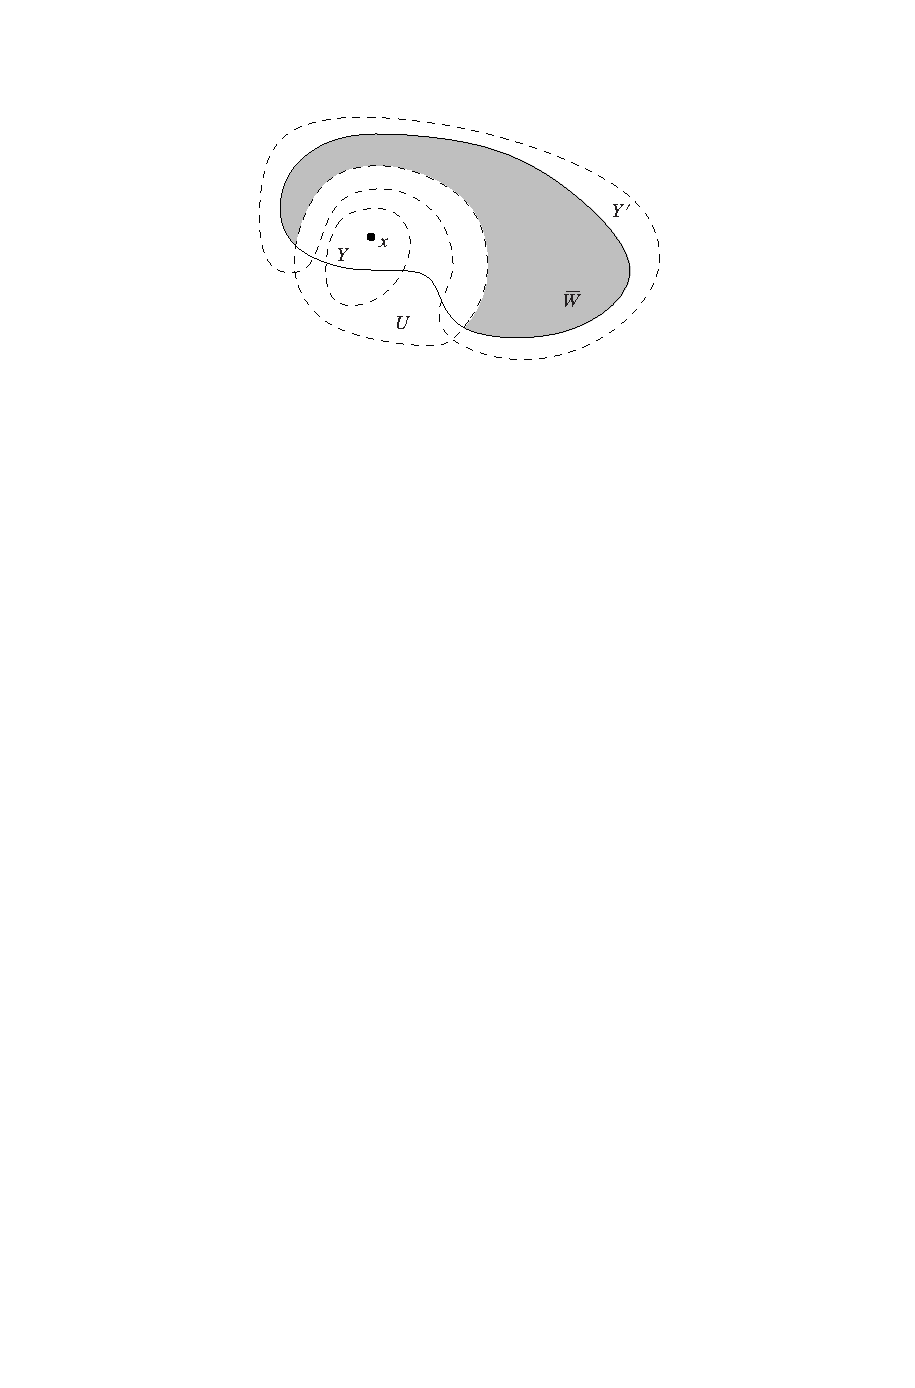
\includegraphics{pictures/local-compact}
\end{figure}
\begin{proof}
Suppose $U$ is a neighborhood of $x$. By \cref{Hausdorff local compact iff} there is a precompact neighborhood $W$ of $x$. Then $\widebar{W}\setminus U$ is closed in $\widebar{W}$ and therefore compact. Because compact subsets can be separated by open subsets in a Hausdorff space, there are disjoint open subsets $Y$ containing $x$ and $Y'$ containing $\widebar{W}\setminus U$. Let $V=Y\cap W$. Because $\widebar{V}\sub\widebar{W}$, it is compact.\par
Because $V\sub Y\sub(Y')^c$, we have $\widebar{V}\sub\widebar{(Y')^c}=(Y')^c$. Since $\widebar{W}\setminus U$ is contained in $Y'$, this then implies $\widebar{V}\cap(\widebar{W}\setminus U)=\emp$, and therefore $\widebar{V}\sub\widebar{W}\cap U\sub U$.
\end{proof}
\begin{proposition}\label{LCH precompact nbhd for compact set}
Let $X$ be a locally compact Hausdorff space, let $K$ be a compact subset of $X$, and let $U$ be an neighborhood of $K$. Then there is a precompact neighborhood $V$ of $K$ such that $\widebar{V}\sub U$.
\end{proposition}
\begin{proof}
\cref{LCH precompact nbhd closure in nbhd} implies that each point in $K$ has a precompact neighborhood whose closure is included in $U$. Since $K$ is compact, some finite collection of these neighborhoods covers $K$. Let $V$ be the union of the sets in such a finite collection; then $V$ is the required set.
\end{proof}
\begin{proposition}
Any open or closed subset of a locally compact Hausdorff space is a locally compact Hausdorff space.
\end{proposition}
\begin{proof}
Let $X$ be a locally compact Hausdorff space. Note that every subspace of $X$ is Hausdorff, so only local compactness needs to be checked. If $Y\sub X$ is open, \cref{LCH precompact nbhd closure in nbhd} says that any point in $Y$ has a neighborhood whose closure is compact and contained in $Y$, so $Y$ is locally compact. Suppose $Z\sub X$ is closed. Any $x\in Z$ has a precompact neighborhood $U$ in $X$. Since $\widebar{U\cap Z}$ is a closed subset of the compact set $\widebar{U}$, it is compact. Since $\widebar{U\cap Z}\sub\widebar{Z}=Z$, it follows that $U\cap Z$ is a precompact neighborhood of $x$ in $Z$. Thus $Z$ is locally compact.
\end{proof}
A subset of a topological space $X$ is a $\bm{G_{\delta}}$ if it is the intersection of a sequence of open subsets of $X$ and is an $\bm{F_{\sigma}}$ if it is the union of a sequence of closed subsets of $X$.
\begin{proposition}\label{LCH second countable space G_delta}
Let $X$ be a second countable locally compact Hausdorff space. Then each open subset of $X$ is an $F_\sigma$ and is in fact the union of a sequence of compact sets. Likewise, each closed subset of $X$ is a $G_\delta$.
\end{proposition}
\begin{proof}
Suppose that $\mathcal{U}$ is a countable base for the topology of $X$. Let $U$ be an open subset of $X$, and let $\mathcal{U}_U$ be the collection of those sets $V$ in $\mathcal{U}$ for which $V$ is precompact and included in $U$. \cref{LCH precompact nbhd closure in nbhd} implies that $U$ is the union of the closures of the sets in $\mathcal{U}_U$. Thus $U$ is the union of a countable collection of sets that are closed and, in fact, compact.\par
Now suppose that $C$ is a closed subset of $X$. Then $C^c$ is open and so is the union of a sequence $\{F_n\}$ of closed sets. Consequently $C$ is the intersection of the open sets $\{F_n^c\}$.
\end{proof}
Recall that a topological space (or a subset thereof) is $\sigma$-compact if it is the union of a countable collection of compact sets.
\begin{corollary}
Every second countable locally compact Hausdorff space is $\sigma$-compact.
\end{corollary}
\begin{proof}
Since a topological space is an open subset of itself, this is an immediate corollary of \cref{LCH second countable space G_delta}.
\end{proof}
\subsection{Continuous functions}
If $X$ is a topological space, the space $\R^X$ of all real-valued functions on $X$ can be topologized in various ways. One way, of course, is the product topology, that is, the topology of pointwise convergence. Another is the \textbf{topology of uniform convergence}, which is generated by the sets
\[\{g\in\R^X:\sup_{x\in X}|g(x)-f(x)|<1/n\}\]
for $f\in\R^X$. Intermediate between these two topologies is the topology of uniform convergence on compact sets, which is generated by the sets
\[\{g\in\R^X:\sup_{x\in K}|g(x)-f(x)|<1/n\}\]
where $f\in\R^X$ and $K\sub X$ is compact. We shall now examine this topology in the case where $X$ is a locally compact Hausdorff space.
\begin{proposition}\label{LCH C(X) closed subspace}
If $X$ is a locally compact Hausdorff space, then $C(X)$ is a closed subspace of $\R^X$ in the topology of uniform convergence on compact sets.
\end{proposition}
\begin{proof}
If $f$ is in the closure of $C(X)$, then $f$ is a uniform limit of continuous functions on each compact $K\sub X$, so $f|_K$ is continuous. If $E\sub\R$ is closed, then $f^{-1}(E)\cap K=(f|_K)^{-1}(E)$ is closed for each compact $K$, so $f^{-1}(E)$ is closed ($X$ is compactly generated), whence $f$ is continuous.
\end{proof}
\begin{proposition}\label{LCH sigma-compact uniform converge on compact iff}
Let $X$ be a $\sigma$-compact locally compact Hausdorff space and $\{K_n\}$ be a exhaustion of $X$ by compact subsets, then for each $f\in\R^X$ the sets
\[\{g\in\R^X:\sup_{x\in K_n}|f(x)-g(x)|<1/m\}\]
form a neighborhood base for $f$ in the topology of uniform convergence on compact sets. Hence this topology is first countable, and $f_n\to f$ uniformly on compact sets if and only if $f_n\to f$ uniformly on each $K_n$.
\end{proposition}
\begin{proof}
These assertions follow easily from the observation that if $K\sub X$ is compact, then $\{\Int K_n\}$ is an open cover of $K$ and hence $K\sub K_n$ for some $n$.
\end{proof}
One may wonder if there are enough continuous functions on a locally compact Hausdorff space. The following results answer this question.
\begin{proposition}[\textbf{Urysohn's Lemma, Locally Compact Version}]\label{LCH Urysohn}
Let $X$ be a locally compact Hausdorff space. If $K$ is a compact subset of $X$ and $U$ is a neighborhood of $K$, then there is a continuous function $f:X\to[0,1]$ such that $f\equiv 1$ on $K$ and $f\equiv 0$ outside a compact subset of $U$.
\end{proposition}
\begin{proof}
By \cref{LCH precompact nbhd for compact set}, there exists a precompact neighborhood $V$ of $K$ such that $\widebar{V}\sub U$. Then $V$ is normal, so by Urysohn's lemma there exists a continuous function $f:\widebar{V}\to[0,1]$ such that $f\equiv 1$ on $K$ and $f\equiv 0$ on $\partial V$. We extend $f$ to $X$ by setting $f=0$ on $V$.\par
Now we show that $f$ is a continuous function on $X$. Suppose that $E\sub[0,1]$ is closed. If $0\notin E$, then we have $f^{-1}(E)=(f|_{\widebar{V}})^{-1}(E)$, and if $0\in E$ we have $f^{-1}(E)=(f|_{\widebar{V}})^{-1}(E)\cup(\widebar{V})^c=(f|_{\widebar{V}})^{-1}(E)\cup(V)^c$ (note that $\partial V$ is contained in $(f|_{\widebar{V}})^{-1}(E)$). In either case, $f^{-1}(E)$ is closed, so $f$ is continuous. 
\end{proof}
\begin{proposition}[\textbf{Tietze Extension Theorem, Locally Compact Version}]\label{LCH Tietze Extension}
Let $X$ be a locally compact Hausdorff space and $K$ is a compact subset.
\begin{itemize}
\item[(a)] Any continuous map of $K$ into a closed interval $[a,b]$ may be extended to a continuous map of all of $X$ into $[a,b]$.
\item[(b)] Any continuous map of $K$ into $\R$ may be extended to a continuous map of all of $X$ into $\R$.
\end{itemize}
Moreover, the extension may be taken to vanish outside a compact set.
\end{proposition}
\begin{proof}
We prove (a), and (b) follows as in tietze extension theorem. Let $f:K\to[a,b]$ be a continuous function. Let $V$ be a precompact neighborhood of $K$. Then $\widebar{V}$ is normal, so by Tietze extension theorem there exists a continuous function $F:\widebar{V}\to[a,b]$ such that $F|_K=f$. Since $V$ is a neighborhood of $K$, by \ref{LCH Urysohn} there is a continuous function $\varphi:X\to[0,1]$ such that $\varphi\equiv 1$ on $K$ and $\varphi\equiv 0$ on a compact subset of $V$. Define $\widetilde{F}(x)=F(x)\varphi(x)$. By the choice of $\varphi$, it is easy to see $\widetilde{F}$ is continuous and $\widetilde{F}|_K=f$. Therefore $\widetilde{F}$ is the required function.
\end{proof}
The preceding results show that locally compact Huasdorff spaces have a rich supply of continuous functions that vanish outside compact sets. Let us recall some terminology: If $X$ is a topological space and $f\in C(X)$, the support of $f$, denoted by $\supp(f)$, is the smallest closed set outside of which $f$ vanishes, that is, the closure of $\{x:f(x)\neq 0\}$. If $\supp(f)$ is compact, we say that $f$ is \textbf{compactly supported}, and we define
\[C_c(X)=\{f\in C(X):\text{$\supp(f)$ is compact}\}\]
to be the set of continuous functions on $X$ with compact support. Moreover, if $f\in C(X)$, we say that $f$ \textbf{vanishes at infinity} if for every $\eps>0$ the set $\{x:|f(x)|\geq\eps\}$ is compact, and we define
\[C_0(X)=\{f\in C(X):\text{$f$ vanishes at infinity}\}.\]
Clearly $C_c(X)\sub C_0(X)$. Moreover, $C_0(X)\sub BC(X)$, because for $f\in C_0(X)$ the image of the set $\{x:|f(x)|\geq\eps\}$ is compact, and $|f|<\eps$ on its complement.
\begin{proposition}\label{LCH C_0(X) is closure of C_c(X)}
If $X$ is a locally compact Hausdorff space, then $C_0(X)$ is the closure of $C_c(X)$ in the uniform metric.
\end{proposition}
\begin{proof}
If $\{f_n\}$ is a sequence in $C_c(X)$ that converges uniformly to $f\in C(X)$, for each $\eps>0$ there exists $n\in\N$ such that $\|f-f_n\|<\eps$. Then $|f(x)|<\eps$ for $x\notin\supp(f_n)$, so $f\in C_0(X)$.\par
Conversely, if $f\in C_0(X)$, for $n\in\N$ let $K_n=\{x:|f(x)|\geq 1/n\}$. Then $K_n$ is compact, so by \cref{LCH Urysohn} there exists $\varphi_n\in C_c(X)$ with $0\leq\varphi_n\leq 1$ and $\varphi_n\equiv 1$ on $K_n$. Let $f_n=\varphi_nf$. Then $f_n\in C_c(X)$ and $\|f_n-f\|_{\infty}\leq 1/n$, so $f_n$ converges to $f$ uniformly.
\end{proof}
Now we derive some consequences of \cref{LCH Urysohn} which will be used later. Let us begin with the following lemma.
\begin{lemma}\label{compact set separated by open union}
Let $X$ be a Hausdorff space, let $K$ be a compact subset of $X$, and let $U_1$ and $U_2$ be open subsets of $X$ such that $K\sub U_1\cup U_2$. Then there are compact sets $K_1$ and $K_2$ such that $K=K_1\cup K_2$, $K_1\sub U_1$ and $K_2\sub U_2$.
\end{lemma}
\begin{proof}
Let $L_1=K\setminus U_1$ and $L_2=K\setminus U_2$. Then $L_1$ and $L_2$ are disjoint and compact, and so according to \cref{topo space compact separated by disjoint open} they can be separated by disjoint open sets, say by $V_1$ and $V_2$. If we define $K_1$ and $K_2$ by $K_1=K\setminus V_1$ and $K_2=K\setminus V_2$, then $K_1$ and $K_2$ are compact, are included in $U_1$ and $U_2$, respectively, and have $K$ as their union.
\end{proof}
\begin{proposition}\label{LCH decompose function with supp in open set}
Let $X$ be a locally compact Hausdorff space, let $f$ belong to $C_c(X)$, and let $U_1,\dots,U_n$ be open subsets of X such that $\supp(f)\sub U=\bigcup_{i=1}^{n}U_i$. Then there are functions $f_1,\dots,f_n$ in $C_c(X)$ such that $f=f_1+\cdots+f_n$ and such that for each $i$ the support of $f_i$ is contained in $U_i$. Furthermore, if the function $f$ is nonnegative, then the functions $f_1,\dots,f_n$ can be chosen so that all are nonnegative.
\end{proposition}
\begin{proof}
In case $n=1$ we need only let $f_1$ be $f$. So we can begin by supposing that $n=2$. Use \cref{compact set separated by open union} to construct compact sets $K_1$ and $K_2$ such that $K_1\sub U_1$ and $K_2\sub U_2$, and $\supp(f)=K_1\cup K_2$, and then use \cref{LCH Urysohn} to construct functions $h_1$ and $h_2$ that belong to $C_c(X)$ and satisfy $\chi_{K_i}\leq h_i\leq\chi_{U_i}$ and $\supp(h_i)\sub U_i$ for $i=1,2$. Define functions $g_1$ and $g_2$ by $g_1=h_1$ and $g_2=h_2-(h_1\wedge h_2)$. Then $g_1$ and $g_2$ are non-negative, their supports are included in $U_1$ and $U_2$, respectively, and they satisfy
\[g_1+g_2=h_1+h_2-(h_1\wedge h_2)=h_1\vee h_2=1.\]
at each $x$ in $\supp(f)$. We can complete the proof in the case where $n=2$ by defining $f_1$ and $f_2$ to be $fg_1$ and $fg_2$, and the general case follows by induction.
\end{proof}
\begin{proposition}\label{LCH function fixed finite value}
Let $X$ be a locally compact Hausdorff space, let $K_1,\dots,K_n$ be disjoint compact subsets of $X$, and let $\alpha_1,\dots,\alpha_n$ be real (or complex) numbers. Then there is a function $f$ that belongs to $C_c(X)$ and satisfies
\begin{itemize}
\item[(a)] $f(x)=\alpha_i$ if $x\in K_i$, for $i=1,\dots,n$.
\item[(b)] $\|f\|_{\infty}=\max\{|a_1|,\dots,|a_n|\}$.
\end{itemize}
\end{proposition}
\begin{proof}
We begin by constructing disjoint open sets $U_1,\dots,U_n$ such that $K_i\sub U_i$ holds for each $i$. If $n=2$, such sets are provided by \cref{topo space compact separated by disjoint open}. The general case follows by induction. Next we use \cref{LCH Urysohn} to choose functions $f_1,\dots,f_n$ that belong to $C_c(X)$ and satisfy $\chi_{K_i}\leq f_i\leq\chi_{U_i}$ for $i=1,\dots,n$. The required function $f$ is now given by $f=\sum_{i=1}^{n}\alpha_if_i$.
\end{proof}
\subsection{One-point compactification}
If $X$ is a noncompact locally compact Hausdorff space, it is possible to make $X$ into a compact space by adding a single point "at infinity" in such a way that the functions in $C_0(X)$ are precisely those continuous functions $f$ such that $f(x)\to 0$ as $x$ approaches the point at infinity. Here is the precise definition of this space.
\begin{proposition}\label{one point compactification}
Let $X$ be a topological space. Then $X$ is locally compact Hausdorff if and only if there exists a space $X^*$ satisfying the following conditions:
\begin{itemize}
\item[(a)] $X$ is a subspace of $X^*$.
\item[(b)] $X^*\setminus X$ consists of a single point.
\item[(c)] $X^*$ is a compact Huasdorff space.
\end{itemize}
If $X_1$ and $X_2$ are two spaces satisfying these conditions, then there is a homeomorphism of $X_1$ with $X_2$ that equals the identity map on $X$.
\end{proposition}
\begin{proof}
We first verify uniqueness. Let $X_1$ and $X_2$ be two spaces satisfying these conditions. Define $h:X_1\to X_2$ by letting $h$ map the single point $p$ of $X_1\setminus X$ to the point $q$ of $X_2\setminus X$, and letting $h$ equal the identity on $X$. We show that if $U$ is open in $X_2$, then $h(U)$ is open in $X_2$. Symmetry then implies that $h$ is a homeomorphism.\par
First, consider the case where $U$ does not contain $p$. Then $h(U)=U$. Since $U$ is open in $X_1$ and is contained in $X$, it is open in $X$. Because $X$ is open in $X_2$, the set $U$ is also open in $X_2$, as desired. Second, suppose that $U$ contains $p$. Since $C=X_1\setminus U$ is closed in $X_1$, it is compact as a subspace of $X_1$. Because $C$ is contained in $X$, it is a compact subspace of $X$. Then because $X$ is a subspace of $X_2$, the space $C$ is also a compact subspace of $X_2$, and hence is closed in $X_2$. So $h(U)=X_2\setminus C$ is open, as desired.\par
Now we suppose $X$ is locally compact Hausdorff and construct the space $X^*$. Let us take some object that is not a point of $X$, denote it by the symbol $\infty$ for convenience, and adjoin it to $X$, forming the set $X^*=X\cup\{\infty\}$. Topologize $X^*$ by defining the collection of open sets of $X^*$ to consist of $(1)$ all sets $U$ that are open in $X$, and $(2)$ all sets of the form $X^*\setminus C$, where $C$ is a compact subspace of $X$. We need to check that this collection is in fact a topology on $X^*$. The empty set is a set of type $(1)$, and the space $X^*$ is a set of type $(2)$. Checking that the intersection of two open sets is open involves two cases:
\[(X^*\setminus C_1)\cap(X^*\setminus C_2)=X^*\setminus(C_1\cup C_2),\quad U_1\cap(X^*\setminus C_1)=U_1\cap(X\setminus C_1).\]
Similarly, checking that arbitrary union open sets is open involves two cases:
\[\bigcup_\alpha(X^*\setminus C_\alpha)=X^*\setminus\bigcap_\alpha C_\alpha,\quad\Big(\bigcup_\alpha U_\alpha\Big)\cup\bigcup_\beta(X^*\setminus C_\beta)=U\cup(X^*\setminus C)=X^*\setminus(C\setminus U).\]
Therefore we have defined a topology on $X^*$.\par
Now we show that $X$ is a subspace of $X^*$. Given any open set of $X^*$, we show its intersection with $X$ is open in $X$. If $U$ is of type $(1)$, then $U\cap X=U$; if $U=X^*\setminus C$ is of type $(2)$, then $U\cap X=X\setminus C$; both of these sets are open in $X$. Conversely, any set open in $X$ is a set of type $(1)$ and therefore open in $X^*$ by definition.\par
To show that $X^*$ is compact, let $\mathcal{U}$ be an open covering of $X^*$. The collection $\mathcal{U}$ must contain an open set of type $(2)$, say $X^*\setminus C$, since none of the open sets of type $(1)$ contain the point $\infty$. Take all the members of $\mathcal{U}$ different from $X^*\setminus C$ and intersect them with $X$; they form a collection of open sets of $X$ covering $C$. Because $C$ is compact, finitely many of them  over $C$; the corresponding finite collection of elements of $\mathcal{U}$ will, along with the element $X^*\setminus C$, cover all of $X^*$. Therefore $X^*$ is compact.\par
To show that $X^*$ is Hausdorff, let $x$ and $y$ be two distinct points of $X^*$. If both of them lie in $X$, there are disjoint sets $U$ and $V$ open in $X$ containing them, respectively, since $X$ is Huasdorff. On the other hand, if $x\in X$ and $y=\infty$, we can choose a compact set $C$ in $X$ containing a neighborhood $U$ of $x$. Then $U$ and $X^*\setminus C$ are disjoint neighborhoods of $x$ and $\infty$, respectively, in $X^*$.\par
Finally, we prove the converse. Suppose a space $X^*$ satisfying conditions (a)---(c) exists. Then $X$ is Hausdorff because it is a subspace of the Hausdorff space $X^*$. Given $x\in X$, we show $X$ is locally compact at $x$. Choose disjoint open sets $U$ and $V$ of $X^*$ containing $x$ and the single point of $X^*\setminus X$, respectively. Then the set $C=X^*\setminus V$ is closed in $X^*$, so it is a compact subspace of $X^*$. Since $C$ lies in $X$, it is also compact as a subspace of $X$; it contains the neighborhood $U$ of $x$.
\end{proof}
If $X$ itself should happen to be compact, then the space $X^*$ of the preceding theorem is not very interesting, for it is obtained from $X$ by adjoining a single isolated point. However, if $X$ is not compact, then the point of $X^*\setminus X$ is a limit point of $X$, so that $\widebar{X}=X^*$.
\begin{definition}
If $Y$ is a compact Hausdorff space and $X$ is a proper subspace of $Y$ whose closure equals $Y$, then $Y$ is said to be a compactification of $X$. If $Y\setminus X$ equals a single point, then $Y$ is called the \textbf{one-point compactification} of $X$.
\end{definition}
\begin{example}
The one-point compactification of the real line $\R$ is homeomorphic with
the circle, as you may readily check. Similarly, the one-point compactification of $\R^2$ is homeomorphic to the sphere $S^2$. If $\R^2$ is looked at as the space $\C$ of complex numbers, then $\C\cup\{\infty\}$ is called the \textbf{Riemann sphere}, or the \textbf{extended complex plane}.
\end{example}
\begin{proposition}\label{LCH one-point compactification continuous function}
Let $X$ be a locally compact Hausdorff space and $X^*$ be its one-point compactification. Let $f\in C(X)$, then $f$ extends continuously to $X^*$ if and only if $f$ has a limit at the point infinity. That is, if and only if $f=g+a$ where $g\in C_0(X)$ and $a$ is a constant, in which case the continuous extension is given by $f(\infty)=a$.
\end{proposition}
\begin{proof}
Let $f$ be the form stated above. We extend $f$ to $X^*$ by defining $f(\infty)=a$. We only need to check that $f$ is continuous at $\infty$, since $f$ is in $C(X)$ and every open set of $X$ is open in $X^*$. Let $\eps>0$ be arbitrary, then the set $C_\eps=\{x:|g(x)|\geq\eps\}$ is compact in $X$, and hence $X^*\setminus C_\eps$ is a neighborhood of $\infty$ in $X^*$. By definition, this then implies $|f(x)-a|<\eps$ for $x\in X^*\setminus C_\eps$. Therefore $f$ is continuous at $\infty$, and so $f\in C(X^*)$.\par
Conversely, assume that $f\in C(X)$ has an extension $\widetilde{f}$ on $X^*$. Define $a=\widetilde{f}(\infty)$ and $g(x)=f(x)-a$. We need to show that $g\in C_0(X)$. Let $\eps>0$, then there exists a neighborhood $U$ of $\infty$ in $X^*$ such that $f(U)\sub(a-\eps,a+\eps)$. By the topology of $X^*$, since $\infty\in U$, $X\setminus U$ is then compact in $X$. Since $\{x:|g(x)|\geq\eps\}=\{x:|f(x)-a|\geq\eps\}$ is contained in $X\setminus U$, it is also compact, as desired.
\end{proof}
\subsection{Stone-Weierstrass theorem}
In this part we prove a far-reaching generalization of the well-known theorem of Weierstrass to the effect that any continuous function on a compact interval $[a,b]$ is the uniform limit of polynomials on $[a,b]$. In what follows, $X$ will denote a compact Hausdorff space, and we equip the space $C(X)$ with the uniform metric.\par
A subset $\mathscr{A}$ of $C(X,\R)$ or $C(X,\C)$ is said to be \textbf{separating} if for every $x,y\in X$ with $x\neq y$ there exists $f\in\mathscr{A}$ such that $f(x)\neq f(y)$. $\mathscr{A}$ is called an \textbf{algebra} if it is a real (resp. complex) vector subspace of $C(X,\R)$ (resp. $C(X,\C)$) such that $fg\in\mathscr{A}$ whenever $f,g\in\mathscr{A}$. If $\mathscr{A}\sub C(X,\R)$, $\mathscr{A}$ is called a \textbf{lattice} if $\max(f,g)$ and $\min(f,g)$ are in $\mathscr{A}$ whenever $f,g\in\mathscr{A}$. Since the algebra and lattice operations are continuous, one easily sees that if $\mathscr{A}$ is an algebra or a lattice, so is its closure $\mathscr{A}$ in the uniform metric.
\begin{theorem}[\textbf{Stone-Weierstrass Theorem}]\label{Stone-Weierstrass}
Let $X$ be a compact Hausdorff space. If $\mathscr{A}$ is a separating closed subalgebra of $C(X,\R)$, then either $A=C(X,\R)$ or $A=\{f\in C(X,\R):f(x_0)=0\}$ for some $x_0\in X$. The first alternative holds iff $\mathscr{A}$ contains the constant functions.
\end{theorem}
The proof will require several lemmas. The first one, in effect, proves the theorem when $X$ consists of two points, and the second one is a special case of the classical Weierstrass theorem for $X=[-1,1]$. After these two we return to the general case.
\begin{lemma}\label{Stone-Weierstrass subalgebra of R^2}
Consider $\R^2$ as an algebra under coordinatewise addition and multiplication. Then the only subalgebras of $\R^2$ are $\R^2$, $\{(0,0)\}$, and the linear span of $(1,0)$, $(0,1)$, or $(1,1)$.
\end{lemma}
\begin{proof}
The subspaces of $\R^2$ listed above are evidently subalgebras. If $\mathscr{A}\sub\R^2$ is a nonzero algebra and $(0,0)\neq(a,b)\in\mathscr{A}$, then $(a^2,b^2)\in\mathscr{A}$. If $a,b$ are nonzero and distinct then $(a,b)$ and $(a^2,b^2)$ are linearly independent, so $A=\R^2$. The other possibilities give the other three subalgebras.
\end{proof}
\begin{lemma}\label{Stone-Weierstrass approximate |x|}
For any $\eps>0$ there is a polynomial $P$ on $\R$ such that $P(0)=0$ and $||x|-P(x)|<\eps$ for $x\in[-1,1]$.
\end{lemma}
\begin{proof}
Consider the Maclaurin series for $(1-t)^{1/2}$:
\[(1-t)^{1/2}=1-\sum_nc_nt^n.\]
By the ratio test, this series converges for $|t|<1$. Moreover, by the monotone convergence theorem (applied to counting measure on $\N$),
\[\sum_nc_n=\lim_{t\to 1^-}\sum_nc_nt^n=1-\lim_{t\to 1-}(1-t)^{1/2}=1.\]
It follows from the finiteness of $\sum_nc_n$ that the series $1-\sum_nc_nt^n$ converges absolutely and uniformly on $[-1,1]$, and its sum is $(1-t)^{1/2}$ there. Therefore, given $\eps>0$, by taking a suitable partial sum of this series we obtain a polynomial $Q$ such that $|(1-t)^{1/2}-Q(t)|<\eps/2$ for $t\in[-1,1]$. Set $t=1-x^2$ and $R(x)=Q(1-x^2)$, we obtain a polynomial $R$ such that $||x|-R(x)|<\eps/2$ for $x\in[-1,1]$. In particular, $|R(0)|<\eps/2$. If we set $P(x)-R(x)-R(0)$, we then get the claim. 
\end{proof}
\begin{lemma}\label{Stone-Weierstrass closed subalgebra is lattice}
If $\mathscr{A}$ is a closed subalgebra of $C(X,\R)$, then $|f|\in\mathscr{A}$ whenever $f\in\mathscr{A}$; hence $\mathscr{A}$ is a lattice.
\end{lemma}
\begin{proof}
If $f\in\mathscr{A}$ and $f\neq 0$, let $h=f/\|f\|_\infty$. Then $h$ maps $X$ into $[-1,1]$, so if $\eps>0$ and $P$ is as in \cref{Stone-Weierstrass approximate |x|}, we have $||h|-P\circ h|<\eps$. Since $P(0)=0$, $P$ has no constant term, so $P\circ h\in\mathscr{A}$ since $\mathscr{A}$ is an algebra. Since $\mathscr{A}$ is closed and $\eps$ is arbitrary, we have $|h|\in\mathscr{A}$ and hence $|f|\in\mathscr{A}$. This proves the first assertion, and the second one follows because $\max(f,g)$ and $\min(f,g)$ can be represented by $f$, $g$, and $|f-g|$.
\end{proof}
\begin{lemma}\label{Stone-Weierstrass two point}
Suppose $\mathscr{A}$ is a closed lattice in $C(X,\R)$ and $f\in C(X,\R)$. If for every $x,y\in X$ there exists $h_{xy}\in\mathscr{A}$ such that $h_{xy}(x)=f(x)$ and $h_{xy}(y)=f(y)$, then $f\in\mathscr{A}$.
\end{lemma}
\begin{proof}
Given $\eps>0$, for each $x,y\in X$ let
\[U_{xy}=\{z\in X:f(z)<h_{xy}(z)+\eps\},\quad V_{xy}=\{z\in X:f(z)>h_{xy}(z)-\eps\}.\]
These sets are open and contain $x$ and $y$. Fix $y$, then $\{U_{xy}:x\in X\}$ covers $X$, so there is a finite subcover $\{U_{x_jy}\}$. Let $h_y=\max(h_{x_1y},\dots,h_{x_ny})$, then $f<h_y+\eps$ on $X$ and $f>h_y-\eps$ on $V_y=\bigcup_{i=1}^{n}V_{x_iy}$, which is open and contains $y$. Thus $\{V_y:y\in X\}$ is another open cover of $X$, so there is a finite subcover $\{V_{y_j}\}$. Let $h=\min(h_{y_1},\dots,h_{y_m})$, then $\|f-h\|<\eps$. Since $\mathscr{A}$ is a lattice, $h\in\mathscr{A}$, and since $\mathscr{A}$ is closed and $\eps$ is arbitrary, $f\in\mathscr{A}$.
\end{proof}
\begin{proof}[Proof of \cref{Stone-Weierstrass}]
Given $x\neq y\in X$, let $\mathscr{A}_{xy}=\{(f(x),f(y)):f\in\mathscr{A}\}$. Then $\mathscr{A}_{xy}$ is a subalgebra of $\R^2$ as in \cref{Stone-Weierstrass subalgebra of R^2} because $f\mapsto(f(x),f(y))$ is an algebra homomorphism. If $\mathscr{A}_{x,y}=\R^2$ for all $x,y$, then Lemmas~\ref{Stone-Weierstrass closed subalgebra is lattice} and \ref{Stone-Weierstrass two point} imply that $\mathscr{A}=C(X,\R)$. Otherwise, there exist $x,y$ for which $\mathscr{A}_{xy}$ is a proper subalgebra of $\R^2$. It cannot be $\{(0,0)\}$ or the linear span of $(1,1)$ because $\mathscr{A}$ separates points, so by \cref{Stone-Weierstrass subalgebra of R^2} $\mathscr{A}_{xy}$ is the linear span of $(1,0)$ or $(0,1)$. In either case there exists $x_0\in X$ such that $f(x_0)=0$ for all $f\in\mathscr{A}$. There is only one such $x_0$ since $A$ separates points, so if neither $x$ nor $y$ is $x_0$, we have $\mathscr{A}_{xy}=\R^2$. Lemmas~\ref{Stone-Weierstrass closed subalgebra is lattice} and \ref{Stone-Weierstrass two point} now imply that $\mathscr{A}=\{f\in C(X,\R):f(x_0)=0\}$. Finally, if $\mathscr{A}$ contains constant functions, there is no $x_0$ such that $f(x_0)=0$ for all $f\in\mathscr{A}$, so $\mathscr{A}$ must equal $C(X,\R)$.
\end{proof}
We have stated the Stone-Weierstrass theorem in the form that is most natural for the proof. However, in applications one is typically dealing with a subalgebra $\mathscr{B}$ of $C(X,\R)$ that is not closed, and one applies the theorem to $\mathscr{A}=\widebar{\mathscr{B}}$. The resulting
restatement of the theorem is as follows:
\begin{corollary}
Suppose $\mathscr{B}$ is a separating subalgebra of $C(X,\R)$. If there exists $x_0\in X$ such that $f(x_0)=0$ for all $f\in\mathscr{B}$, then $\mathscr{B}$ is dense in $\{f\in C(X,\R):f(x_0)=0\}$. Otherwise, $\mathscr{B}$ is dense in $C(X,\R)$.
\end{corollary}
The classical Weierstrass approximation theorem is the special case where $X$ is a compact subset of $\R^n$ and $\mathscr{B}$ is the algebra of polynomials on $\R^n$ (restricted to $X$); here $\mathscr{B}$ contains the constant functions, so the conclusion is that it is dense in $C(X,\R)$.\par
The Stone-Weierstrass theorem, as it stands, is false for complex-valued functions. For example, the algebra of polynomials in one complex variable is not dense in $C(K)$ for most compact subsets $K$ of $\C$. (In particular, if $\Int K\neq\emp$, any uniform limit of polynomials on $K$ must be holomorphic on $\Int K$.) Here we shall give a simple proof that the function $f(z)=\bar{z}$ cannot be approximated uniformly by polynomials on the unit circle. If $P(z)=\sum_ja_jz^j$, then
\[\int_{0}^{2\pi}\widebar{f(e^{it})}P(e^{it})\,dt=\sum_{j=0}^{n}a_j\int_0^{2\pi}e^{i(j+1)t}\,dt=0.\]
Since $|f|=1$ on the unit circle we have
\[2\pi=\int_0^{2\pi}\bar{f}f\,dt\Big|\leq\Big|\int_0^{2\pi}\bar{f}(f-P)\,dt\Big|+\Big|\int_0^{2\pi}\bar{f}P\,dt\Big|\leq\int_0^{2\pi}|f-P|\,dt\leq 2\pi\|f-P\|_\infty.\]
Therefore, $\|f-P\|_\infty\geq 1$ for any polynomial $P$.\par
There is, however, a complex version of the Stone-Weierstrass theorem.
\begin{theorem}[\textbf{Complex Stone-Weierstrass Theorem}]\label{Stone-Weierstrass complex}
Let $X$ be a compact Hausdorff space. If $\mathscr{A}$ is a separating closed complex subalgebra of $C(X,\C)$ that separates points and is closed under complex conjugation, then either $A=C(X,\C)$ or $A=\{f\in C(X,\C):f(x_0)=0\}$ for some $x_0\in X$.
\end{theorem}
\begin{proof}
Since $\Re(f)=(f+\bar{f})/2$ and $\Im(f)=(f-\bar{f})/2i$, the set $\mathscr{A}_{\R}$ of real and imaginary parts of functions in $\mathscr{A}$ is a subalgebra of $C(X,\R)$ to which the Stone-Weierstrass theorem applies. Since $\mathscr{A}=\mathscr{A}_{\R}+i\mathscr{A}_{\R}$, the desired result follows.
\end{proof}
There is also a version of the Stone-Weierstrass theorem for locally compact Hausdorff spaces.
\begin{theorem}
Let $X$ be a locally compact Hausdorff space. If $\mathscr{A}$ is a separating closed subalgebra of $C_0(X,\R)$, then either $\mathscr{A}=C_0(X,\R)$ or $\mathscr{A}=\{f\in C_0(X,\R):f(x_0)=0\}$ for some $x_0\in X$.
\end{theorem}
\begin{proof}
If there exists $x_0\in X$ such that $f(x_0)=0$ for all $f\in\mathscr{A}$, let $Y$ be the one-point compactification of $X\setminus\{x_0\}$. Then by \cref{LCH one-point compactification continuous function} we can write $\mathscr{A}\sub\{f\in C(Y,\R):f(+\infty)=0\}$. Since $\mathscr{A}$ separates points on $X\setminus\{x_0\}$, there is no $y\in X\setminus\{x_0\}$ such that $f(y)=0$ for all $f\in\mathscr{A}$; it follows that $\mathscr{A}$ separates points in $Y$, and by the Stone-Weierstrass theorem we get $\mathscr{A}=\{f\in C(Y,\R):f(+\infty)=0\}=\{f\in C_0(X,\R):f(x_0)=0\}$.\par
If there is no $x_0\in X$ such that $f(x_0)=0$ for all $f\in\mathscr{A}$, let $Y$ be the one-point compactification of $X$. By the same proof we see $\mathscr{A}=C_0(X,\R)$.
\end{proof}
By the same proof as \cref{Stone-Weierstrass complex}, we also have the following complex version.
\begin{theorem}
Let $X$ be a locally compact Hausdorff space. If $\mathscr{A}$ is a separating closed complex subalgebra of $C_0(X,\C)$ that separates points and is closed under complex conjugation, then either $A=C(X,\C)$ or $A=\{f\in C(X,\C):f(x_0)=0\}$ for some $x_0\in X$.
\end{theorem}
\subsection{Metrizability}
Now we consider metrizability of locally compact spaces.
\begin{proposition}\label{compact Hausdorff metrizable iff C_2}
A compact Hausdorff space is metrizable if and only if it is second countable.
\end{proposition}
\begin{proof}
First suppose that $X$ is compact and metrizable. Then $X$ is separable and so is second countable.\par
Now suppose that $X$ is a compact Hausdorff space that is second countable and let $\mathcal{U}$ be a countable base. The space $X$ is normal, and so for each pair of sets $U$, $V$ that belong to $\mathcal{U}$ and satisfy $U\cap V=\emp$ there is, by Urysohn's lemma, a continuous function $f:X\to[0,1]$ that vanishes on $\widebar{U}$ and has value $1$ everywhere on $\widebar{V}$. Form a sequence $\{f_n\}$ by choosing one such function for each such pair of sets. Our next step is to check that this sequence of functions separates the points of $X$, and for this it is enough to show that for each pair $x$, $y$ of distinct points in $X$ there are sets $U$ and $V$ that belong to $\mathcal{U}$, have disjoint closures, and contain $x$ and $y$, respectively. To construct such sets, choose disjoint open neighborhoods $W_1$ and $W_2$ of $x$ and $y$, and use \cref{LCH precompact nbhd closure in nbhd} to choose open sets $U$ and $V$ such that $x\in U\sub\widebar{U}\sub W_1$ and $y\in V\sub\widebar{V}\sub W_2$. By making $U$ and $V$ a bit smaller, if necessary, we can assume that they belong to $\mathcal{U}$. Thus the required sets $U$ and $V$ exist, and the sequence $\{f_n\}$ separates the points of $X$.\par
Define a function $d:X\times X\to\R$ by setting
\[d(x,y)=\sum_{n=1}^{\infty}\frac{1}{2^n}|f_n(x)-f_n(y)|.\]
It is easy to use the fact that the functions $\{f_n\}$ separate the points of $X$ to check that $d$ is a metric on the set $X$ and to use the fact that the functions $\{f_n\}$ are continuous (with respect to the original topology on $X$) to check that the topology induced by $d$ is weaker than the original topology. Since the original topology makes $X$ a compact space, while the topology induced by $d$ is weaker and Hausdorff, the two topologies must be the same ($\id$ is a continuous bijection from a compact space to a Huasdorff space). Thus the original topology on $X$ is metrizable and in fact is metrized by $d$.
\end{proof}
Our next task is to prove that each second countable locally compact Hausdorff space is metrizable. For this we need the following lemma.
\begin{lemma}\label{LCH C_2 iff onepoint compactification C_2}
Let $X$ be a locally compact Hausdorff space. If $X$ is second countable, then the one-point compactification of $X$ is also second countable.
\end{lemma}
\begin{proof}
Let $\mathcal{U}$ be a countable base for the topology of $X$, and let $\mathcal{U}_0$ be the collection of those sets $V$ in $\mathcal{U}$ for which $V$ is precompact. Arrange the sets in $\mathcal{U}_0$ in a sequence, say $\{V_k\}$. Then $X=\bigcup_kV_k$, since $X$ is locally compact, and so for each compact subset $K$ of $X$ there is a positive integer $n$ such that $K\sub\bigcup_{k=1}^{n}V_k$. Thus if $U$ is an open neighborhood in $X^*$ of the point at infinity and if $K=X^*\setminus U$, then there is a positive integer $n$ such that $K\sub\bigcup_{k=1}^{n}V_k$ and hence such that $X^*\setminus\widebar{\bigcup_{k=1}^{n}V_k}\sub U$. It follows that the sets in $U$, together with the sets $X^*\setminus\widebar{\bigcup_{k=1}^{n}V_k}$, form a countable base for the topology of $X^∗$.
\end{proof}
\begin{proposition}\label{LCH C_2 is metrizable}
Each secound countable locally compact Hausdorff space is metrizable.
\end{proposition}
\begin{proof}
Let $X$ be a secound countable locally compact Hausdorff space. \cref{compact Hausdorff metrizable iff C_2} and \cref{LCH C_2 iff onepoint compactification C_2} imply that the one-point compactification $X^*$ of $X$ is metrizable. Then $X$, as a subspace of the metrizable space $X^*$, is metrizable.
\end{proof}
\section{Proper maps}
\subsection{Proper maps}
If $f$ and $g$ are closed continuous maps, it does not follow that $f\times g$ is closed, even if $f$ is the identity map. An example is given below.
\begin{example}
Every constant mapping into a Hausdorff space is closed. But it $f$ is the constant mapping $\Q\to\{0\}$, then $f\times\id_\Q$ is the mapping $(x,y)\mapsto(0,y)$ of $\Q^2$ into $\Q^2$, so it is the second projection and is not closed.
\end{example}
\begin{definition}
A map $f:X\to Y$ is said to be \textbf{proper} if $f$ is continuous and if the mapping $f\times\id_Z:X\times Z\to Y\times Z$ is closed, for every topological space $Z$.
\end{definition}
If in the definition we take the space $Z$ to consist of a single point, then we see that any proper map is closed. A partial converse holds when the map $f$ is injective:
\begin{proposition}\label{topo space injection proper iff}
Let $f:X\to Y$ be a continuous injection. Then the following three statements are equivalent.
\begin{itemize}
\item[(\rmnum{1})] $f$ is proper.
\item[(\rmnum{2})] $f$ is closed.
\item[(\rmnum{3})] $f$ is a homeomorphism of $X$ onto a closed subset of $Y$.
\end{itemize}
\end{proposition}
\begin{proof}
We have just seen that (\rmnum{1}) implies (\rmnum{2}). Since the equivalence relation $f(x)=f(y)$ is the equality relation, the quotient space of $X$ with respect to this relation can be identified with $X$; hence (\rmnum{2}) implies (\rmnum{3}) by \cref{topo space canonical decomposition homeomorphism iff}. Finally, if (\rmnum{3}) is satisfied then $f\times\id_Z$ is a homeomorphism of $X\times Z$ onto a closed subspace of $Y\times Z$ and is therefore a closed mapping; hence (\rmnum{3}) implies (\rmnum{1}).
\end{proof}
\begin{proposition}\label{topo space proper map on subspace}
Let $f:X\to Y$ be a continuous map. If $B$ is any subset of $Y$, let $f_B$ denote the restriction of $f$ on $f^{-1}(B)$.
\begin{itemize}
\item[(a)] If $f$ is proper, so is $f_B$.
\item[(b)] Let $(B_i)_{i\in I}$ be a family of subsets of $Y$ whose interiors cover $Y$, or which is a locally finite closed covering of $Y$; then if each of the mappings $f_B$ is proper, so is $f$.
\end{itemize}
\end{proposition}
\begin{proof}
Let $Z$ be a topological space. If $B$ is any subset of $Y$, we have
\[f_B\times\id_Z=(f\times\id_Z)_{B\times Z}.\]
If $f$ is proper, then $f\times\id_Z$ is closed, hence so is $(f\times\id_Z)_{B\times Z}$ (\cref{*}), whence (a) is proved. If now $(B_i)_{i\in I}$ satisfies one of the two conditions stated in (b), then the covering $(B_i\times Z)_{i\in I}$ of $Y\times Z$ has the same property; if the $f_{B_i}$ are proper then the mappings $(f\times\id_Z)_{B\times Z}$ are closed, whence $f\times\id_Z$ is closed (\cref{*}). This completes the proof.
\end{proof}
\begin{proposition}
Let $f:X\to Y$ and $g:Y\to Z$ be two continuous mappings.
\begin{itemize}
\item[(a)] If $f$ and $g$ are proper, then $g\circ f$ is proper.
\item[(b)] If $g\circ f$ is proper and $f$ is surjective, then $g$ is proper.
\item[(c)] If $g\circ f$ is proper and $g$ is injective, then $f$ is proper. 
\item[(d)] If $g\circ f$ is proper and $Y$ is Hausdorff, then $f$ is proper   
\end{itemize}
\end{proposition}
\begin{proof}

\end{proof}
\subsection{Proper maps}
If $X$ and $Y$ are topological spaces, a map $f:X\to Y$ (continuous or not) is said to be \textbf{proper} if the preimage of each compact subset of $Y$ is compact. For example, every exhaustion function $f:X\to\R$ is a proper map.\par
In order to visualize the behavior of proper maps, it is useful to introduce the following definition: if $X$ is a topological space, a sequence $(x_i)$ in $X$ is said to \textbf{diverge to infinity} if for every compact set $K\sub X$ there are at most finitely many values of $i$ for which $x_i\in K$.
\begin{lemma}\label{topo space diverge to inf iff no convergent subseq}
Suppose $X$ is a first countable Hausdorff space. A sequence in $X$ diverges to infinity if and only if it has no convergent subsequence.
\end{lemma}
\begin{proof}
Assume first that $(x_i)$ is a sequence in $X$ that diverges to infinity. If there is a subsequence $(x_{i_j})$ that converges to $x\in X$, then the set $K=\{x\}\cup\{x_{i_j}\}$ is compact and contains infinitely many terms of the sequence, which is a contradiction. (This implication does not require the hypothesis that $X$ is first countable and Hausdorff.)\par
Conversely, assume that $(x_i)$ has no convergent subsequence. If $K\sub X$ is any compact set that contains $x_i$ for infinitely many $i$ , then there is a subsequence $(x_{i_j})$ such that $x_{i_j}\in K$ for all $j$. Because a compact, first countable Hausdorff space is sequentially compact, this subsequence in turn has a convergent subsequence, which is a contradiction.
\end{proof}
\begin{proposition}
Suppose $X$ and $Y$ are topological spaces and $f:X\to Y$ is a proper map. Then $f$ takes every sequence diverging to infinity in $X$ to a sequence diverging to infinity in $Y$.
\end{proposition}
\begin{proof}
Suppose $(x_i)$ is a sequence in $X$ that diverges to infinity. If $\big(f(x_i)\big)$ does not diverge to infinity, then there is a compact subset $K\sub Y$ that contains $f(x_i)$ for infinitely many values of $i$. It follows that $x_i$ lies in the compact set $f^{-1}(K)$ for these values of $i$, which contradicts the assumption that $(x_i)$ diverges to infinity.
\end{proof}
Because the definition of properness is sometimes tricky to check directly, it is useful to have other sufficient conditions for a map to be proper. The next proposition gives several such conditions.
\begin{proposition}\label{proper map if}
Suppose $X$ and $Y$ are topological spaces, and $f:X\to Y$ is a continuous map.
\begin{itemize}
\item[(a)] If $X$ is compact and $Y$ is Hausdorff, then $f$ is proper.
\item[(b)] If $X$ is a second countable Hausdorff space and $f$ takes sequences diverging
to infinity in $X$ to sequences diverging to infinity in $Y$, then $f$ is proper. 
\item[(c)] If $f$ is a closed map with compact fibers, then $f$ is proper.
\item[(d)] If $f$ is a topological embedding with closed image, then $f$ is proper.
\item[(e)] If $Y$ is Hausdorff and $f$ has a continuous left inverse, then $f$ is proper.
\item[(f)] If $f$ is proper and $A\sub X$ is any subset that is saturated with respect to $f$, then $f|_A:A\to f(A)$ is proper.
\end{itemize}
\end{proposition}
\begin{proof}
Suppose $X$ is compact and $Y$ is Hausdorff. If $K\sub Y$ is
compact, then it is closed in $Y$ because $Y$ is Hausdorff. By continuity, $f^{-1}(K)$ is closed in $X$ and therefore compact.\par
Assume $X$ is a second countable Hausdorff space, and suppose
$f:X\to Y$ takes sequences diverging to infinity to sequences diverging to infinity. Let $K\sub Y$ be any compact set, and let $L=f^{-1}(K)\sub X$. Because of our hypothesis on $X$, to show that $L$ is compact, it suffices to show that it is sequentially compact. Suppose on the contrary that $(x_i)$ is a sequence in $L$ with no convergent subsequence. It diverges infinity by \cref{topo space diverge to inf iff no convergent subseq}, so our assumption about $f$ implies that $\big(f(x_i)\big)$ diverges to infinity. But this is impossible because $f(x_i)$ lies in the compact set $K$ for all $i$.\par
Assume $f$ is a closed map with compact fibers. Let $K\sub Y$ be compact, and let $\mathcal{U}$ be a cover of $f^{-1}(K)$ by open subsets of $X$. If $y\in K$ is arbitrary, the fiber $f^{-1}(y)$ is covered by finitely many of the sets in $\mathcal{U}$, say $U_1,\dots,U_k$. The set $A_y=X-\bigcup_{i=1}^{k}U_i$ is closed in $X$ and disjoint from $f^{-1}(y)$, so $V_y=Y-f(A_y)$ is open in $Y$ and contains $y$. It follows from ourconstruction that 
\[f^{-1}(V_y)=f^{-1}(Y-f(A_y))\sub X-A_y=U_1\cap\cdots\cap U_k.\] 
Because $K$ is compact, it is covered by finitely many of the sets $V_y$. Thus $f^{-1}(K)$ is covered by finitely many sets of the form $f^{-1}(V_y)$, each of which is covered by finitely many of the sets in $\mathcal{U}$, so it follows that $f^{-1}(K)$ is compact.\par
Now (d) follows from (c), because a topological embedding with closed image is a closed map, and its fibers are singletons, which are certainly compact.\par
Assume that $Y$ is Hausdorff and $g:Y\to X$ is a continuous left inverse for $f$, and suppose $K$ is a compact subset of $Y$. Then we observe that
\[x\in f^{-1}(K)\Rightarrow x=g(f(x))\in g(K)\] 
Since $K$ is closed in $Y$ (because $Y$ is Hausdorff), itfollows that $f^{-1}(K)$ is a closed subset of the compact set $G(K)$, so it is compact.\par
Finally, to prove (f), suppose $f:\to Y$ is proper and $A\sub X$ is saturated. Let
$K\sub f(A)$ be compact. The fact that $A$ is saturated means that $(f|_A)^{-1}(K)=f(K)$, which is compact because $f$ is proper.
\end{proof}
A topological space $X$ is said to be \textbf{compactly generated} if it has the following property: 
\[A\text{ is closed in $X$}\iff A\cap K\text{ is closed in $X$ for any compact subset $K$}\] 
It is easy to see that an equivalent definition is obtained by substituting open for closed.
\begin{lemma}
First countable spaces and locally compact spaces are compactly generated.
\end{lemma}
\begin{proof}
Let $X$ be a space satisfying either of the two hypotheses, and let $A\sub X$ be a subset whose intersection with each compact set $K\sub X$ is closed in $K$.\par
First assume that $X$ is first countable, and let $x\in\widebar{A}$. By the sequence lemma, there is a sequence $(a_i)$ of points in $A$ converging to $x$. The set $K=\{x\}\cup\{a_i:i\in\N\}$ is compact, so $A\cap K$ is closed in $K$ by hypothesis. Since $x$ is the limit of a sequence of points in $A\cap K$, it must also be in $A\cap K\sub A$. Thus $A$ is closed.\par
Now assume $X$ is locally compact. Let $x\in A^c$, we want to find a neighborhood of $x$ disjoint from $A$. Now let $K$ be a compact subset of $X$ containing a neighborhood $U$ of $x$. If $U\cap A=\emp$, then we are done. Otherwise let $\widetilde{U}=U\setminus(A\cap K)$. Since $A\cap K$ is closed, $\widetilde{U}$ is open in $X$. This is the desired neighborhood of $x$.
\end{proof}
\begin{theorem}\label{proper map is closed}
Suppose $X$ is any topological space, $Y$ is a compactly generated Hausdorff space and $F:X\to Y$ is a proper continuous map. Then $F$ is a closed map.
\end{theorem}
\begin{proof}
Let $A\sub X$ be a closed subset. We show that $F(A)$ is closed in $Y$ by showing that its intersection with each compact subset is closed. If $K\sub Y$ is compact, then $F^{-1}(K)$ is compact since $F$ is proper, and so is $A\cap F^{-1}(K)$ because it is a closed subset of a compact set. By the main theorem on compactness, $F\big(A\cap F^{-1}(K)\big)$ is compact as well. This set is equal to $F(A)\cap K$. Because $K$ is Hausdorff, $F(A)\cap K$ is closed in $K$.
\end{proof}
\begin{corollary}\label{compact gene embed closed map iff}
If $X$ is a topological space and $Y$ is a compactly generated Hausdorff space, an embedding $F:X\to Y$ is proper if and only if it has closed image.
\end{corollary}
\begin{proof}
If $F$ is proper, then by \cref{proper map is closed} $F$ is closed, so $F(X)$ is closed. Conversely, if $F(X)$ is closed, then by \cref{proper map if}(d) we know $F$ is proper.
\end{proof}
\begin{corollary}
Suppose $F$ is a proper continuous map from a topological space to a compactly generated Hausdorff space.
\begin{itemize}
\item[(a)] If $F$ is surjective, it is a quotient map.
\item[(b)] If $F$ is injective, it is a topological embedding.
\item[(c)] If $F$ is bijective, it is a homeomorphism.
\end{itemize}
\end{corollary}
\section{Baire Spaces}
\subsection{Nowhere dense sets and meager sets}
We develop the elementary properties of nowhere dense sets here.
\begin{definition}
A subset $A$ of a topological space $X$ is called \textbf{nowhere dense} if its closure has empty interior.
\end{definition}
Before giving some examples, we consider some elementary properties of nowhere dense sets.
\begin{proposition}\label{nowhere dense iff}
In a topological space $X$:
\begin{itemize}
\item[(a)] $A\sub X$ is nowhere dense iff $(\widebar{A})^c$ is dense.
\item[(b)] $A\sub X$ is nowhere dense iff every nonempty open subset $U$ of $X$ contains a nonempty open subset that is disjoint from $A$.
\end{itemize}
\end{proposition}
\begin{proof}
Assume that $A$ is nowhere dense. If $A=\emp$, the result is clear so suppose that $A\neq\emp$. Then any nonempty open subset $U$ of $X$ meets the dense subset $(\widebar{A})^c$ and the nonempty open set $U\cap(\widebar{A})^c$ is disjoint from $A$. Conversely, the condition says that any nonempty open set meets $(\widebar{A})^c$ which means that $(\widebar{A})^c$ is dense and so $A$ is nowhere dense by (a).
\end{proof}
We point out that when we speak of a set $A\sub X$ as being nowhere dense, we mean with respect to $X$'s topology, not the topology it induces on $X$---a nonempty set $X$ is never a nowhere dense subset of itself, because $\mathrm{cl}_AA=A$.
\begin{example}
\mbox{}
\begin{itemize}
\item[(a)] Any subset of a nowhere dense set is nowhere dense. The empty set is nowhere dense; so are singletons in any Hausdorff space as long as the point is not isolated. The only nowhere dense subset of a discrete space is $\emp$.
\item[(b)] The rationals $\Q$ are not nowhere dense in $\R$, but the integers $\Z$ are.
\item[(c)] The set $\{1/n:n\in\N\}\cup\{0\}$ is nowhere dense in $\R$.
\item[(d)] The boundary $\partial A$ of a set $A$ is the set $\widebar{A}\cap\widebar{(A^c)}$. If $A$ is open, then $\partial A\sub A^c$ while a neighborhood of any point in $\partial A$ must meet $A$ and $A^c$. Thus $\partial A$ has no interior. By the same reasoning, if $A$ is closed, $\partial A\sub A$ and $\Int\partial A=\emp$. Two things follow: a closed set is nowhere dense iff it coincides with its boundary; and boundaries of open or closed sets are nowhere dense.
\item[(e)] A linear subspace $M$ of a topological vector space $X$ is nowhere dense or dense. Note that the closure of a subspace is again a subspace. If $M$ is not nowhere dense then $\Int\widebar{M}\neq\emp$. By translation, it follows immediately that $0$ is an interior point of $\widebar{M}$. Thus $\widebar{M}$ is a neighborhood of $0$ and is therefore equal to $X$.
\item[(f)] In a Hausdorff topological vector space, finite-dimensional subspaces are closed. Thus, by (e), proper finite-dimensional subspaces are nowhere dense. 
\end{itemize}
\end{example}
Now we present some elementary properties of nowhere dense sets.
\begin{proposition}\label{nowhere dense set prop}
Let $X$ be a topological space.
\begin{itemize}
\item[(a)] Subsets of nowhere dense ses are nowhere dense.
\item[(b)] Finite unions of nowhere dense sets are nowhere dense.
\item[(c)] Suppose that $A\sub S\sub X$. If $A$ is nowhere dense in $S$, then $A$ is nowhere dense in $X$. Conversely, if $S$ is open in $X$ and $A$ is nowhere dense in $X$, then $A$ is nowhere dense in $S$.
\end{itemize}
\end{proposition}
\begin{proof}
If $A$ is nowhere dense then so is any $B\sub A$ since $\widebar{B}\sub\widebar{A}$. The key fact is that finite intersections of dense open sets are dense. To prove this, suppose that $A$ and $B$ are dense open sets. Thus, if $U$ is a nonempty open set, $U\cap A\neq\emp$. As $U\cap A$ is a nonempty open set, it meets $B$ nontrivially. Thus $A\cap B$ is dense.\par
Suppose that $A\sub S\sub X$ and that $A$ is not nowhere dense in $X$. Then there is a nonempty open set $U$ in $X$ that does not meet $(\widebar{A})^c$, i.e., such that $U\sub\widebar{A}$ and $U\cap S\sub\widebar{A}\cap S=\mathrm{cl}_SA$. Since $U\cap A\sub U\cap S$ and $U\cap A\neq\emp$ because $U\sub\widebar{A}$, this shows that $\mathrm{cl}_SA$ has nonempty interior, i.e., that $A$ is not nowhere dense in $S$.\par
For the converse, suppose that $A$ is nowhere dense in $X$, $S$ is open and $U$ is a nonempty open subset of $S$. Since $S$ is open in $X$, so is $U$. Since $A$ is nowhere dense in $X$, $U$ must contain a nonempty open subset $V$ of $X$---hence also of $S$---that does not meet $A$. It follows from \cref{nowhere dense iff} that $A$ is nowhere dense in $S$.
\end{proof}
\begin{corollary}\label{nowhere dense hereditary to open set}
Let $A$ be a nowhere dense subset in $X$ and $U\sub X$ be open. Then $U\cap A$ is nowhere dense in $U$. 
\end{corollary}
\begin{definition}
A subset of a topological space $X$ is called \textbf{meager in $\bm{X}$} if it can be written as a countable union of nowhere dense sets of $X$, or, equivalently, is a subset of such a union. Otherwise, $E$ is called \textbf{nonmeager in $\bm{X}$}. A topological space is called \textbf{meager} if it is a meager subset of itself.
\end{definition}

\begin{example}[\textbf{Examples of Meager and Nonmeager Sets}]
\mbox{}
\begin{itemize}
\item[(a)] As we can write the rationals $\Q$ as a countable union of singletons, $\Q$ is a meager subset of $\R$. Indeed, any countable Hausdorff space without isolated points is meager.
\item[(b)] Any topological space which contains an isolated point $x$ is nonmeager, as no set to which $x$ belongs can be nowhere dense. Thus discrete spaces are never meager.
\item[(c)] Singletons are always nonmeager subspaces. A singleton is a nonmeager subset of a topological space iff the point is isolated.
\item[(d)] View $\Q\times\Q$ together with the $x$-axis as a subspace of $\R^2$. As the $x$-axis is a nowhere dense subset of $\R^2$ and we can enumerate $\Q\times\Q$, $(\Q\times\Q)\cup(\R\times\{0\})$ is a meager subset of $\R^2$. However, as we will see, $\R\times\{0\}$ it self is a nonmeager subspace. The point is that the presence of a nonmeager subspace does not imply that the space itself is nonmeager.
\end{itemize}
\end{example}
An important property of meager sets is that any open subset of a meager set is again meager.
\begin{proposition}\label{meager open subset is meager}
Let $U\sub X$ be a open subset. If $X$ is meager, then so is $U$.
\end{proposition}
\begin{proof}
If there are nowhere dense subsets $\{E_n\}$ of $X$ such that $X=\bigcup_nE_n$, then $U=\bigcup_n(E_n\cap U)$. As $U$ is open in $X$, each $E_n\cap U$ is nowhere dense in $U$ by \cref{nowhere dense hereditary to open set} and therefore $U$ is meager.
\end{proof}
It is then interesting that whether any open subsets of a nonmeager space is nonmeager. For this, we recall that empty set is meager, so we may concentrate on nonempty open subsets. It turns out that this property is equivalent to some other conditions, and is not true in general. The Baire spaces that we will define are exactly nonmeager spaces satisfying these conditions.
\begin{theorem}\label{Baire space iff}
The following conditions on a topological space $X$ are equivalent:
\begin{itemize}
\item[(\rmnum{1})] The union of countably many closed nowhere dense sets have empty interior.
\item[(\rmnum{2})] The intersection of countably many dense open sets is dense.
\item[(\rmnum{3})] Each nonempty open subset is nonmeager.
\item[(\rmnum{4})] Each meager subsets has dense complement.
\end{itemize}
A \textbf{Baire space} is one which satisfies either of the conditions above.
\end{theorem}
\begin{proof}
It is clear that $(\rmnum{1})\Leftrightarrow(\rmnum{2})$. Assume (\rmnum{2}) and let $U\sub X$ be a meager open set so that there are nowhere dense subset $\{E_n\}$ such that $U=\bigcup_nE_n\sub\bigcup_n\widebar{E}_n$. Then $U^c\sups\bigcap_n(\widebar{E}_n)^c$ and since each $(\widebar{E}_n)^c$ is dense and open, $\bigcap_n(\widebar{E}_n)^c$ must be dense by hypothesis. Since $U^c$ is closed, it follows that $U^c=X$ or $U=\emp$.\par
Suppose that nonempty open subsets are nonmeager in $X$. Let $A\sub X$ be meager, then $\Int A$ must be meager, too. By hypothesis $\Int A=\emp$ and therefore $A^c$ is dense. This proves $(\rmnum{3})\Rightarrow(\rmnum{4})$.\par
Finally, assume (\rmnum{4}). Let $\{E_n\}$ be a sequence of closed nowhere dense sets and let $E=\bigcup_nE_n$. Since $E$ is meager, $E^c$ is dense by hypothesis. Therefore $\Int E=\emp$.
\end{proof}
It is clear that every open subset of a Baire space is Baire. Thus a Baire space is \textbf{locally Baire}. It turns out that the converse is also ture.
\begin{proposition}\label{Baire iff locally Baire}
If each point in a topologiral space $X$ has a neighborhood which is a Baire space, then $X$ is a Baire space.
\end{proposition}
\begin{proof}
Let $U\sub X$ be a nonempty open subset and let $x\in U$. By hypothesis, $x$ has an open neighborhood $V$ which is a Baire space. If $U$ were meager in $X$, $U\cap V$ would be meager in $V$ and open in $V$, contradicting the Baireness of $V$.
\end{proof}
\begin{example}
Obviously, Baire spaces are nonmeager. To see that nonmeager spaces need not be Baire, consider the metric space $\Q\cup (0,1)$. Since it contains the open nonmeager subspace $(0,1)$, it is nonmeager. Since it has meager open sets such as $\{x\in\Q:x>1\}$, it is not a Baire space. Note also that this is an incomplete metric space which is nonmeager.
\end{example}
Some interesting properties for Baire spaces are given below.
\begin{proposition}\label{Baire space lsc function pointwise bounded above}
Let $X$ be a Baire space and $\{f_s:s\in S\}$ a family of lower semicontinuous real-valued functions on $X$ that is pointwise bounded from above on $X$. Then each nonempty open subset of $X$ contains a nonempty open subset on which $\{f_s:s\in S\}$ is bounded from above.
\end{proposition}
\begin{proof}
It suffices to prove the claim for $X$. The map $f=\sup_sf_s$ is lower semicontinuous. Decompose $X$ into the union of the closed sets $F_n=f^{-1}([-n,n])$. Since $X$ is nonmeager, some $F_n$ has a nonempty interior. The theorem now follows.
\end{proof}
Note that \cref{Baire space lsc function pointwise bounded above} remain valid for complex-valued functions, and even for functions $\{f_s:s\in S\}$ with values in a normed space by considering the functions $\|f_s\|$.
\begin{proposition}\label{Baire space limit of continuous function}
Let $X$ be a space; let $(Y,d)$ be a metric space. Let $f_n:X\to Y$ be a sequence of continuous functions such that $f_n(x)\to f(x)$ for all $x\in X$, where $f:X\to Y$. If $X$ is a Baire space, the set of points at which $f$ is continuous is dense in $X$.
\end{proposition}
\begin{proof}
Given a positive integer $N$ and given $\eps>0$, define
\[E_N(\eps)=\{x\in X:d(f_n(x),f_m(x))\leq\eps\text{ for $n,m\geq N$}\}.\]
Note that $E_N(\eps)$ is closed in $X$. For the set of those $x$ for which $d(f_n(x),f_m(x))\leq\eps$ is closed in $X$, by continuity of $f_n$ and $f_m$, and $E_N(\eps)$ is the intersection of these sets for all $n,m\geq N$. For fixed $\eps$, since $f_n\to f$, we have $\bigcup_NE_N(\eps)=X$. Now let
\[U(\eps)=\bigcup_{N=1}^{\infty}\Int E_N(\eps).\]
We claim that $U(\eps)$ is open and dense. To show this, it suffices to show that for any nonempty open set $V$ of $X$, there is an $N$ such that the set $V\cap\Int E_N(\eps)$ is nonempty. For this purpose, we note first that for each $N$, the set $V\cap E_N(\eps)$ is closed in $V$. Because $V$ is a Baire space, at least one of these sets, say $V\cap E_M(\eps)$, must contain a nonempty open set $W$ of $V$. Because $V$ is open in $X$, the set $W$ is open in $X$; therefore, it is contained in $\Int E_M(\eps)$.\par
Now we show that $f_n$ converges to $f$ uniformly on the set $C=\bigcap_nU_n(1/n)$, which is dense since $X$ is a Baire space. To this end, let $\eps>0$ be fixed. Choose $N\in\N$ such that $1/N<\eps$. Then since $C\sub U_N(1/N)$, we have $d(f_n(x),f_m(x))<\eps$ for $n,m\geq N$ and $x\in C$. Let $m\to+\infty$, this implies $d(f_n(x),f(x))<\eps$ for $n\geq N$, thus the claim follows.
\end{proof}
\subsection{Baire category theorem}
\begin{proposition}[\textbf{Criterion for Baireness}]\label{Baire space if relation}
A topological space $(X,\mathcal{T})$ is a Baire space if there exists a relation $\preceq$ among the collection $\mathcal{T}^*$ of nonempty open subsets of $X$ such that for $A,B,C,D\in\mathcal{T}^*$,
\begin{itemize}
\item[(a)] if $A\preceq B$, then $A\sub B$;
\item[(b)] for every $B\in\mathcal{T}^*$, there is an $A\in\mathcal{T}^*$ such that $A\preceq B$;
\item[(c)] if $A\sub B\preceq C\sub D$, then $A\preceq D$;
\item[(d)] if $\{A_n\}$ is a sequence of nonempty open sets such that $A_n\succeq A_{n+1}$ for each $n\in\N$, then $\bigcap_nA_n\neq\emp$.
\end{itemize}
\end{proposition}
\begin{proof}
Suppose that the relation $\preceq$ satisfies (a)--(d) is defined on the nonempty open sets $\mathcal{T}^*$ of the topological space $(X,\mathcal{T})$. If $X$ is not a Baire space, it must contain a nonempty meager open set $U$. Consequently, there must be a sequence $\{E_n\}$ of closed nowhere dense sets whose union contains $U$. We now construct a sequence $\{U_n\}$ of open subsets of $U$ such that $U_n\succeq U_{n+1}$ and $U_n\cap(E_1\cup\cdots\cup E_n)=\emp$ for each $n\in\N$. With this, we see
\[\bigcap_{n=1}^{\infty}U_n=U\cap\bigcap_{n=1}^{\infty}U_n\sub\bigcap_{n=1}^{\infty}U_n\cap\bigcup_{n=1}^{\infty}E_n=\emp,\]
which contradicts condition (d).\par
Now we construct $\{U_n\}$. Since $\Int E_1=\emp$, certainly $U\not\sub E_1$. Hence $U\cap E_1^c$ is a nonempty open subset of $U$ which does not meet $E_1$. By (b), there is a nonempty open set $U_1$ such that $U_1\preceq U\cap E_1^c$. By (c) we have $U_1\preceq U$, so $U_1\sub U$ and $U_1\cap E_1=\emp$. Since $U_1$ is a nonempty open set, $U_1\not\sub(E_1\cup E_2)$ and there must be a nonempty open set $U_2$ such that $U_2\preceq U_1$ and $U_2\cap (E_1\cup E_2)=0$. By induction, the sequence $\{U_n\}$ mentioned above is now seen to exist.
\end{proof}
We show next that a complete pseudometric space or locally compact Hausdorff space is a Baire space by showing that a relation such as the one of \cref{Baire space if relation} may be defined on the nonempty open sets.
\begin{theorem}[\textbf{Baire Category Theorem}]
Any locally compact Hausdorff space or complete pseudometric space is Baire.
\end{theorem}
\begin{proof}
We first consider locally compact Hausdorff spaces. For nonempty open sets $A$ and $B$ of a locally compact Hausdorff space $X$, define $A\preceq B$ if $A$ is precompact and $\widebar{A}\sub B$. In view of \cref{LCH precompact nbhd closure in nbhd}, properties (a)--(c) of \cref{Baire space if relation} are easy to verify. As for (d), suppose that $\{U_n\}$ is a sequence of nonempty open sets such that $U_n\succeq U_{n+1}$. The sets $\{\widebar{U}_n:n>2\}$ are nested in the compact space $\widebar{U}_2$, so they have nonempty intersection. It then follows that
\[\emp\neq\bigcap_{n=3}^{\infty}\widebar{U}_n\sub\bigcap_{n=2}^{\infty}U_n\sub\bigcap_{n=1}^{\infty}U_n.\]
Thus $X$ is Baire by \cref{Baire space if relation}.\par
Now we turn to complete pseudometric spaces. For any subset $A$ of a complete pseudometric space $(X,d)$, let
\[d(A)=\mathrm{diam}(A),\quad d^*(A)=\min\{1,d(A)\}\]
and note that $A\sub B$ implies $d^*(A)\leq d^*(B)$. For $A,B\in\mathcal{T}^*$, we define $A\preceq B$ iff $\widebar{A}\sub B$ and $d(A)\leq(1/2)d^*(B)$. We show that $\preceq$ satisfies conditions of \cref{Baire space if relation}. That $A\preceq B$ implies $A\sub B$ is clear. Moreover, for any $A\in\mathcal{T}^*$, let $x\in A\in\mathcal{T}^*$ and choose $0<r<1$ such that $B_r(x)\sub A$. With $r'=d(B_r(x))\leq r<1$ and $U=B_{r'/4}(x)$, we have $U\preceq A$. As for (c), if $A\sub B\preceq C\sub D$, then $\widebar{A}\sub C\sub D$; since $d(A)\leq (1/2)d^*(C)\leq(1/2)d^*(D)$, it follows that $A\preceq D$.\par
We now use the completeness of $X$ to show that (d) is satisfied. For this purpose, let $\{U_n\}$ be a sequence of nonempty open sets, decreasing with respect to $\preceq$. Since $d^*(U_1)\leq 1$, we have $d(U_n)\leq 2^{-n+1}$ for each $n\in\N$. Hence, choosing $x_n\in U_n$ for each $n\in\N$ yields a $d$-Cauchy sequence. Since $X$ is complete, $\{x_n\}$ has a limit $x\in X$. Since $x_m\in U_n$ for $m\geq n$, we have $x\in\widebar{U}_n$ for each $n$, and thus $x\in\bigcap_nU_n$. 
\end{proof}
\begin{corollary}\label{countable closed isolated}
In a locally compact Hausdorff space or a complete metric space, every nonempty countable closed subset contains at least one isolated point.
\end{corollary}
\begin{proof}
Assume $X$ is such a space. Let $A\sub X$ be a nonempty countable closed subset, and assume that $A$ has no isolated points. The fact that $A$ is closed in $X$ means that $A$ itself is either a locally compact Hausdorff space or a complete metric space. For each $a\in A$, the singleton $\{a\}$ is nowhere dense in $A$: it is closed in $A$ because $A$ is Hausdorff, and it contains no nonempty open subset because $A$ has no isolated points. Since $A$ is a countable union of singletons, $A$ is meager in $A$, which is a contradiction.
\end{proof}
\begin{proposition}\label{Baire space open dense intersection uncountable}
Let $\{U_n\}$ be a sequence of open dense subsets of a locally compact Hausdorff space or a complete metric space $X$ with no isolated points and $U:=\bigcap_nU_n$. Then $U$ is dense in $X$ and uncountable. In particular, no countable dense subset of $X$ can be obtained as the intersection of a countable family of open sets, i.e., is not $G_\delta$.
\end{proposition}
\begin{proof}
Since $X$ is Baire, we know $U$ is dense. If $U=\{x_n\}$ then, since each $\{x_n\}$ is closed and nowhere dense in $X$, it follows that
\[U\cap\bigcap_n\{x_n\}^c=U\cap U^c=\emp\]
is open dense, which is a contradiction. 
\end{proof}
\begin{corollary}
There is no function from $\R$ to $\R$ which is continuous at each rational point and discontinuous at each irrational point.
\end{corollary}
\begin{proof}
The points of continuity of $f$ form a $G_\delta$ set. But $\Q$ is not $G_\delta$ by \cref{Baire space open dense intersection uncountable}.
\end{proof}
\section{Topological manifolds}
\subsection{Definition of manifolds}
A topological space $M$ is said to be \textbf{locally Euclidean} of dimension $n$ if every point of $M$ has a neighborhood in $M$ that is homeomorphic to an open subset of $\mathbb{R}^n$.
\begin{lemma}\label{locally Euclidean lemma}
A topological space $M$ is locally Euclidean of dimension $n$ if and
only if either of the following properties holds:
\begin{itemize}
\item[(a)] Every point of $M$ has a neighborhood homeomorphic to an open ball in $\mathbb{R}^n$.
\item[(b)] Every point of M has a neighborhood homeomorphic to $\mathbb{R}^n$.
\end{itemize} 
In addition, $\mathbb{R}^n$ is homeomorphic to an open ball in $\mathbb{R}^n$.
\end{lemma}
\begin{proof}
It is immediate that any space with property (a) or (b) is locally Euclidean of dimension $n$. Conversely, suppose $M$ is locally Euclidean of dimension $n$. Because any open ball in $\R^n$ is homeomorphic to $\R^n$ itself, properties (a) and (b) are equivalent, so we need only prove (a).\par
Given a point $p\in M$, let $U$ be a neighborhood of $p$ that admits a homeomorphism $\varphi:U\to V$, where $V$ is an open subset of $\R^n$. The fact that $V$ is open in $\R^n$ means that there is some open ball $B$ around $\varphi(p)$ that is contained in $V$, and then $\varphi^{-1}(B)$ is a neighborhood of $p$ homeomorphic to $B$.
\end{proof}
Suppose $M$ is locally Euclidean of dimension $n$. If $U\sub M$ is an open subset that is homeomorphic to an open subset of $\mathbb{R}^n$, then $U$ is called a \textbf{coordinate domain}, and any homeomorphism $\varphi$ from $U$ to an open subset of $\mathbb{R}^n$ is called a \textbf{coordinate map}. The pair $(U,\varphi)$ is called a \textbf{coordinate chart} (or just a chart) for $M$. A \textbf{coordinate domain} that is homeomorphic to a ball in $\mathbb{R}^n$ is called a \textbf{coordinate ball}. The preceding lemma shows that every point in a locally Euclidean space is contained in a coordinate ball.\par
The definition of locally Euclidean spaces makes sense even when $n=0$. Because $\R^0$ is a single point, \cref{locally Euclidean lemma}(b) implies that a space is locally Euclidean of dimension $0$ if and only if each point has a neighborhood homeomorphic to a one-point space, or in other words if and only if the space is discrete.
\begin{definition}[\textbf{topological manifold}]
An $n$-dimensional \textbf{topological manifold} is a second countable Hausdorff space that is locally Euclidean of dimension $n$.
\end{definition}
The most obvious example of an $n$-manifold is $\R^n$ itself. More generally, any open subset of $\R^n$---or in fact of any $n$-manifold---is again an $n$-manifold, as the next proposition shows.
\begin{proposition}
Every open subset of an $n$-manifold is an $n$-manifold.
\end{proposition}
\begin{proof}
Let $M$ be an $n$-manifold, and let $V$ be an open subset of $M$. Any $p\in V$ has a neighborhood (in $M$) that is homeomorphic to an open subset of $\R^n$; the intersection of that neighborhood with $V$ is still open, still homeomorphic to an open subset of $\R^n$, and is contained in $V$, so $V$ is locally Euclidean of dimension $n$. Since any open subset of a Hausdorff space is Hausdorff and any open subset of a second countable space is second countable, we see that $V$ is an $n$-manifold.
\end{proof}
\begin{theorem}
A separable metric space that is locally Euclidean of dimension $n$ is an $n$-manifold. And the converse is also true.
\end{theorem}
\begin{proof}
Every metric space is Hausdorff, and \cref{metric space second countable iff} shows that a separable metric space is second countable. For the converse, separability follows from \cref{second countable prop}, and metrizability follows from Urysohn metrization theorem.
\end{proof}
\begin{proposition}\label{manifold quotient is manifold}
Suppose $P$ is a second countable space and $M$ is a quotient space of $P$. If $M$ is locally Euclidean, then it is second countable. Thus if $M$ is locally Euclidean and Hausdorff, it is a manifold.
\end{proposition}
\begin{proof}
Let $q:P\to M$ denote the quotient map, and let $\mathcal{U}$ be a cover of $M$ by coordinate balls. The collection $q^{-1}(\mathcal{U})=\{q^{-1}(U):U\in\mathcal{U}\}$ is an open cover of $P$, which has a countable subcover since $P$ is Lindel\"of. If we let $\mathcal{U}'\sub\mathcal{U}$ denote a countable subset of $\mathcal{U}$ such that $q^{-1}(\mathcal{U}')$ covers $P$, then $\mathcal{U}'$ is a countable cover of $M$ by coordinate balls. Each such ball is second countable, so $M$ is also second countable.
\end{proof}
\subsection{Manifolds with boundary}
In many cases we will encounter spaces that would be manifolds except that they have a boundary. The following definition deals with this problem.\par
The closed $n$ dimensional upper half-space $\mathbb{H}^n\sub\mathbb{R}^n$ is defined by
\[\mathbb{H}^n:=\{(x_1,\dots,x_n)\in\mathbb{R}^n:x_n\geq0\}\]
\begin{definition}[\textbf{Manifolds with Boundary}]
An $n$-dimensional manifold with boundary is a second countable Hausdorff space in which every point has a neighborhood homeomorphic either to an open subset of $\mathbb{R}^n$, or to an open subset of $\mathbb{H}^n$.
\end{definition}
Note that, despite the terminology, a manifold with boundary is not necessarily a manifold. When it is important to make the distinction, we say $(U,\varphi)$ is an \textbf{interior chart} if $(U,\varphi_0)$ is an open subset of $\mathbb{R}^n$, and a \textbf{boundary chart} if $(U,\varphi)$ is an open subset of $\mathbb{H}^n$ with $\varphi(U)\cap\partial\H^n\neq\emp$.\par
If $M$ is an $n$-manifold with boundary, we define a coordinate chart for $M$ to be a pair $(U,\varphi)$, where $U\sub M$ is open and $\varphi$ is a homeomorphism from $U$ to an open subset of either $\R^n$ or $\H^n$. Just as in the case of manifolds, the set $U$ is called a \textbf{coordinate domain}, and $\varphi$ is called a coordinate map. We use the notation $\partial\H^n$ to denote the boundary of $\H^n$, and $\Int\H^n$ to denote its interior, considering $\H^n$ as a subset of $\R^n$. For $n>0$, this means
\[\partial\H^n=\{(x_1,\dots,x_n):x_n=0\},\quad\Int\H^n=\{(x_1,\dots,x_n):x_n>0\}.\]
When $n=0$, we have $\H^0=\R^0=\{0\}$, so $\Int\H^0=\H^0$ and $\partial\H^0=\emp$. It follows that $0$-dimensional manifolds with boundary are no different from $0$-manifolds.
\begin{example}
The upper half-spaceHn itself is an nmanifold with boundary, with the identity map as a global coordinate map. Similarly, any closed or half-open interval in $\R$ is a $1$-manifold with boundary, for which charts are easy to construct. Another important example is the closed unit ball $\widebar{B}^n$ with the Euclidean topology. It is not hard to see intuitively that $\widebar{B}^n$ is an $n$-manifold with boundary
\end{example}
If $M$ is an $n$-manifold with boundary, a point $p\in M$ is called an \textbf{interior point} of $M$ if it is in the domain of an interior chart; and it is called a \textbf{boundary point} of $M$ if it is in the domain of a boundary chart that takes $p$ to $\partial\H^n$. The \textbf{boundary of $\bm{M}$}, denoted by $\partial M$, is the set of all its boundary points, and its \textbf{interior}, denoted by $\Int M$, is the set of all its interior points.\par
Note that these are new meanings for the terms boundary and interior, distinct from their use earlier in reference to subsets of topological spaces. If $M$ is a manifold with boundary, it might have nonempty boundary in this new sense, irrespective of whether it has any boundary points as a subset of some other topological space. Usually the distinction is clear from the context, but if necessary we can always distinguish the two meanings by referring to the \textbf{topological boundary} (for the original meaning) or the \textbf{manifold boundary} (for this new meaning) as appropriate.
\begin{theorem}\label{manifold boundary int open boundary mani}
If $M$ is an $n$-dimensional manifold with boundary, then $\mathrm{Int}M$ is an open subset of $M$, which is itself an $n$-dimensional manifold without boundary. And $\partial M$ is an $(n-1)$-manifold without boundary.
\end{theorem}
There is a subtlety about these definitions that might not be immediately evident. Although the interior and boundary of $M$ are well-defined subsets whose union is $M$, and it might seem intuitively rather obvious that they are disjoint from each other, we have no way of proving at this stage that a point $p\in M$ cannot be simultaneously a boundary point and an interior point, meaning that there is one interior chart whose domain contains $p$, and another boundary chart that sends $p$ to $\partial\H^n$.
After we have developed some more machinery, you will be able to prove the following theorem.
\begin{theorem}[\textbf{Invariance of the Boundary}]\label{invariance boundary}
If $M$ is a manifold with boundary, then a point of $M$ cannot be both a boundary point and an interior point. Thus $\partial M$ and $\mathrm{Int}M$ are disjoint subsets whose union is $M$.
\end{theorem}
\begin{corollary}
If $M$ is a nonempty $n$-dimensional manifold with boundary, then $\partial M$ is closed in $M$, and $M$ is an $n$-manifold if and only if $\partial M=\emp$.
\end{corollary}
\begin{proof}
Because $\Int M$ is an open subset of $M$ by \cref{manifold boundary int open boundary mani}, it follows from \cref{invariance boundary} that $\partial M=M\setminus\Int M$ is closed. If $M$ is a manifold, then every point is in the domain of an interior chart, so $M=\Int M$, and it follows from \cref{invariance boundary} that $\partial M=\emp$. Conversely, if $\partial M=\emp$, then $M=\Int M$, which is a manifold by \cref{manifold boundary int open boundary mani}.
\end{proof}
\begin{corollary}
Let $M$ be a smooth manifold with boundary, let $(U,\varphi)$ be a boundary chart
on $M$, and let $p$ be a point in $\partial M\cap U$. Then $\varphi(p)$ is in $\partial\H^n$. Thus, a coordinate map sends boundary points to boundary points.
\end{corollary}
\begin{proof}
If $p$ is a boundary point, then $\varphi(p)$ is also a boundary point in $\H^n$. Thus by \cref{invariance boundary} we know $\varphi(p)\in\partial\H^n$.
\end{proof}
More generally, we have the following result.
\begin{theorem}\label{homeomorphism invariance boundary}
If $M$ and $N$ are smooth manifolds with boundary and $F:M\to N$ is a homeomorphism, then $F(\partial M)=\partial N$, hence $F(\Int M)=F(\Int N)$.
\end{theorem}
\begin{proof}
Since $F$ is a homeomorphism, every boundary point of $M$ is mapped to boundary of $N$, and vise versa. Thus we have $F(\partial M)=\partial N$, and since $M$ is the disjoint union of its interior and boundary, we also have $F(\Int M)=\Int N$.
\end{proof}
\begin{example}\label{Graph mani}
If $U\sub\mathbb{R}^n$ is an open subset and $f:U\to\mathbb{R}^k$ is any continuous map, the graph of $f$ is the subset $\Gamma(f)\sub\mathbb{R}^{n+k}$ defined by
\[\Gamma(f):=\{(x,y)\in\mathbb{R}^{n+k}:x\in U\ \text{and}\ y=f(x)\}\]
with the subspace topology inherited from $\mathbb{R}^{n+k}$. Let $\varPhi_f:U\to\mathbb{R}^{n+k}$ be the continuous injective map
\[\varPhi_f(x)=\big(x,f(x)\big)\]
the the restriction to $\Gamma(f)$ of the projection $\pi:\mathbb{R}^{n+k}\to\mathbb{R}^{n}$ is a continuous inverse for $\Phi_f$. Hence $\Gamma(f)$ is homeomorphic to $U$ and is a manifold.
\end{example}
\begin{example}
Define $\mathbb{RP}^n$ to be the set of $1$-dimensional linear subspaces (lines through the origin) in $\mathbb{R}^{n+1}$, and $\mathbb{CP}^n$ be the set of all $1$-dimensional complex subspaces of $\mathbb{C}^{n+1}$, called $n$-dimensional complex projective space. Topologize them as thequotient $(\mathbb{R}^{n+1}\setminus\{0\})/\mathbb{R}^*$ and $(\mathbb{C}^{n+1}\setminus\{0\})/\mathbb{C}^*$. Then $\mathbb{RP}^n$ is an $n$-manifold, $\mathbb{CP}^{n}$ is a $2n$-manifold.
\end{example}
\begin{example}
Let $X$ be the subset $(\mathbb{R}\times\{0\}\cup(\mathbb{R}\times\{1\}\sub\mathbb{R}^2$. Define an equivalence relation on $X$ by declaring $(x,0)\sim(x,1)$ if $x\neq 0$. Show that the quotient space
$X/$$\sim$ is locally Euclidean and second countable, but not Hausdorff. (This space is called the \textbf{line with two origins})
\end{example}
\begin{example}
Consider the product $\mathbb{R}^d\times\mathbb{R}$, where $\mathbb{R}^d$ means $\mathbb{R}$ with discrete topology. This space is Huasdorff and Locally Euclidean, but not second countable.
\end{example}
\subsection{Adjunction spaces}
\begin{definition}
Suppose $X$ and $Y$ are topological spaces, $A$ is a closed subspace of $Y$ , and $f:A\to X$ is a continuous map. Let $\sim$ bethe equivalence relation on the disjoint union $X\amalg Y$ generated by $a\sim f(a)$ for all $a\in A$, and denote the resulting quotient space by
\[X\cup_{f}Y:=(X\amalg Y)/\text{$\sim$}\]
Any such quotient space is called an \textbf{adjunction space}, and is said to be formed by
attaching $Y$ to $X$ along $f$. The map $f$ is called the attaching map. Note that the
equivalence relation identifies each point $x\in X$ with all of the points (if any) in $f^{-1}(x)\in A$. If $A=\emp$, then $X\cup_{f} Y$ is just the disjoint union space $X\amalg Y$.
\end{definition}
\begin{theorem}\label{adjunction space prop}
Let $X\cup_{f}Y$ be an adjunction space, and let $q:X\amalg Y\to X\cup_{f}Y$ be the associated quotient map.
\begin{itemize}
\item[(a)] The restriction of $q$ to $X$ is a topological embedding, whose image set $q(X)$ is a closed subspace of $X\cup_{f}Y$.
\item[(b)] The restriction of $q$ to $Y\setminus A$ is a topological embedding, whose image set $q(Y\setminus A)$ is an open subspace of $X\cup_{f}Y$.
\item[(c)] $X\cup_{f}Y$ is the disjoint union of $q(X)$ and $q(Y\setminus A)$.
\end{itemize}
\end{theorem}
\begin{proof}
We begin by showing that $q|_X$ is a closed map. Suppose that $B$ is a closed subset of $X$. To show that $q(B)$ is closed in the quotient space, we need to show that $q^{-1}(q(B))$ is closed in $X\amalg Y$, which is equivalent to showing that its intersections with $X$ and $Y$ are closed in $X$ and $Y$, respectively. From the form of the equivalence relation, it follows that $q^{-1}(q(B))\cap X=B$, which is closed in $X$ by assumption; and $q^{-1}(q(B))=f^{-1}(B)$, which is closed in $A$ by the continuity of $f$, and thus is closed in $Y$ because $A$ is closed in $Y$. It follows, in particular, that $q(X)$ is closed in $X\cup_f Y$.\par
Now $q|_X$ is clearly injective because the equivalence relation does not identify any points in $X$ with each other. Because it is also closed, it is a topological embedding. This proves (a).\par
To prove (b), we just note that $Y\setminus A$ is a saturated open subset of $X\amalg Y$, so the restriction $q|_{Y\setminus A}$ is a quotient map, and since it is bijective it is a homeomorphism. Its image is open in $X\cup_f Y$ by definition of the quotient topology. Finally, part (c) is an easy consequence of the definition of the equivalence relation.
\end{proof}
Because of the preceding proposition, one typically identifies $X$ with $q(X)$ and $Y\setminus A$ with $q(X\setminus A)$, considering each as a subspace of the adjunction space.
\begin{example}[\textbf{Adjunction Spaces}]
\mbox{}
\begin{itemize}
\item[(a)] Suppose $X$ and $Y$ are topological spaces with chosen base points $x\in X$ and $y\in Y$. Let $A=\{y\}\sub Y$, and define $f:A\to X$ by $f(y)=x$. Then the adjunction space $X\cup_f Y$ is just the wedge sum $X\wedge Y$.
\item[(b)] Let $A=S^1\sub\widebar{B}^2$, and let $f:A\to\widebar{B}^2$ be the inclusion map. Then the adjunction space is homeomorphic to $S^2$.
\end{itemize}
\end{example}
Suppose $M$ and $N$ are $n$-dimensional manifolds with nonempty boundaries, such that $\partial M$ and $\partial N$ are homeomorphic. Let $h:\partial N\to \partial M$ be a homeomorphism. Assuming the theorem on the invariance of the boundary, we conclude that $\partial N$ is a closed subset of $N$, so we can define the adjunction space $M\cup_{h}N$ (considering $h$ as a map into $M)$. This space is said to be formed by \textbf{attaching $\bm{M}$ and $\bm{N}$ together along their boundaries}.
\begin{theorem}\label{attach manifold with boundary}
With $M$, $N$, and $h$ as above, $M\cup_h N$ is an $n$-manifold (without boundary). There are topological embeddings $e:M\to M\cup_{h}N$ and $f:N\to M\cup_{h}N$ whose images are closed subsets of $M\cup_{h}N$ satisfying
\[e(M)\cup f(N)=M\cup_{h}N,\quad e(M)\cap f(N)=e(\partial M)=f(\partial N).\]
\end{theorem}
\begin{proof}
First we need to show that $M\cup_h N$ is locally Euclidean of dimension $n$. Let $q:M\amalg N\to M\cup_h N$ denote the quotient map, and write $S=q(\partial M\cup\partial N)$. Note that $\Int M\amalg\Int N$ is a saturated open subset of $M\amalg N$, and therefore $q$ restricts to a quotient map from $\Int M\amalg\Int N$ onto $(M\cup_h N)\setminus S$. Because this restriction is injective, it is a homeomorphism, and thus $(M\cup_hN)\setminus S$ is locally Euclidean of dimension $n$. Thus we need only consider points in $S$.
\begin{figure}[htbp]
\centering
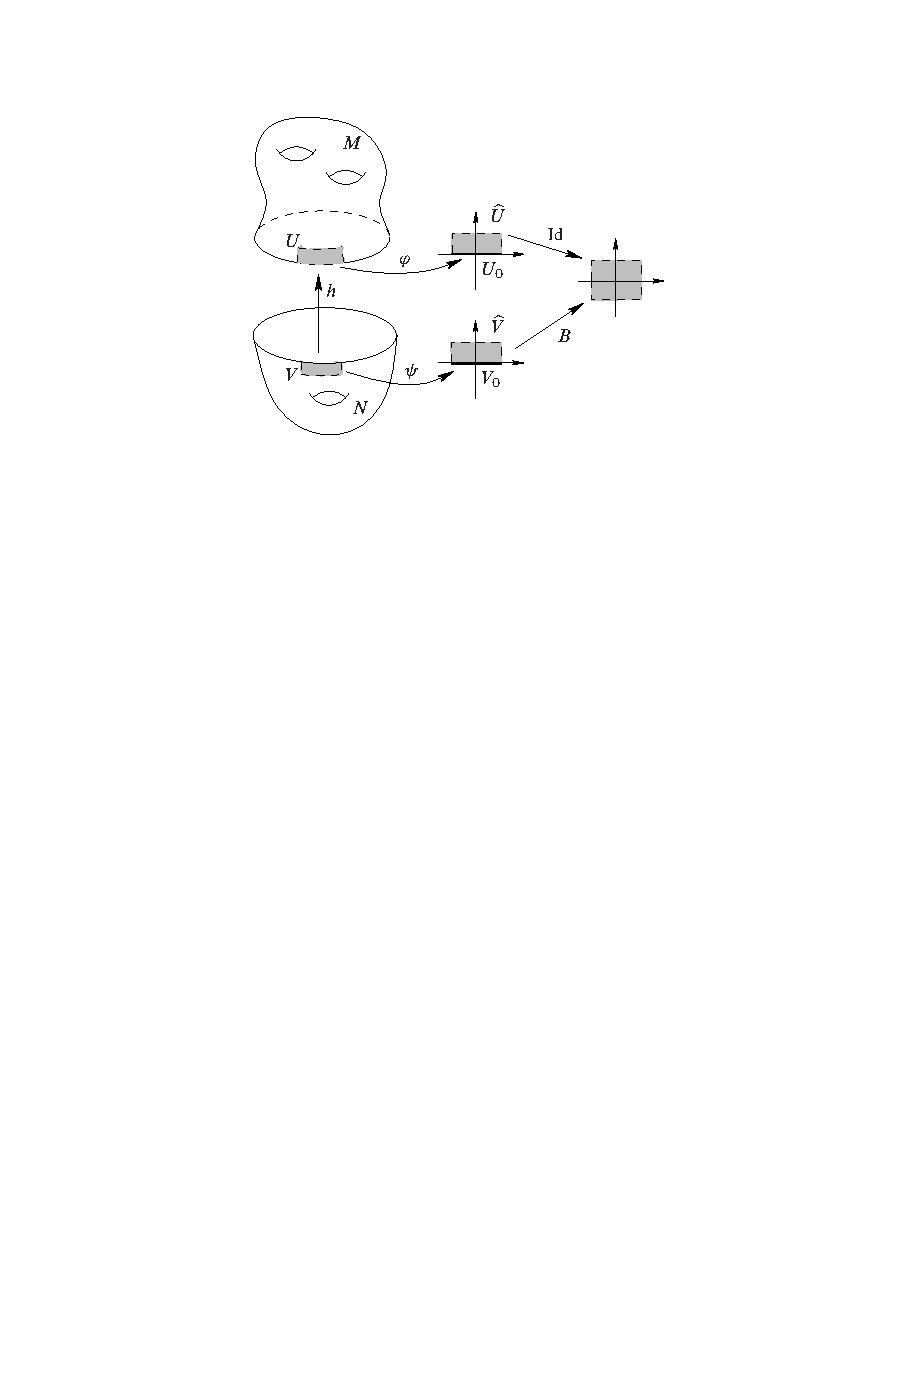
\includegraphics{pictures/attach-manifold}
\caption{Attaching along boundaries.}
\end{figure}

Suppose $s\in S$, and let $y\in\partial N$ and $x=h(y)\in\partial M$ be the two points in the fiber $q^{-1}(s)$. We can choose coordinate charts $(U,\varphi)$ for $M$ and $(V,\psi)$ for $N$ such that $x\in U$ and $y\in V$, and let $\widehat{U}=\varphi(U)$, $\widehat{V}=\psi(V)$. It is useful in this proof to identify $\H^n$ with $\R^{n-1}\times[0,+\infty)$ and $\R^n$ with $\R^{n-1}\times\R$. By shrinking $U$ and $V$ if necessary, we may assume that $h(V\cap\partial N)=U\cap\partial M$, and that $\widehat{U}=U_0\times[0,\eps)$ and $\widehat{V}=V_0\times[0,\eps)$ for some $\eps>0$ and some open subsets $U_0,V_0\sub\R^{n-1}$. Then we can write the coordinate maps as 
\[\varphi(x)=(\varphi_0(x),\varphi_1(x)),\quad\psi(y)=(\psi_0(y),\psi_1(y))\]
for some continuous maps $\varphi_0:U\to U_0$, $\varphi_1:U\to[0,\eps)$, $\psi_0:V\to V_0$ and $\psi_1:V\to[0,\eps)$. Our assumption that $x$ and $y$ are boundary points means that $\varphi_1(x)=\psi_1(y)=0$.\par
We wish to assemble these two charts into a map whose image is an open subset of $\R^n$, by matching them up along corresponding points in $\partial M$ and $\partial N$. As they stand, however, the maps $\varphi$ and might not take corresponding boundary points to the same image point, so we need to adjust for that. Both of the restrictions
\[\varphi_0|_{U\cap\partial M}:U\cap\partial M\to U_0,\quad \psi_0|_{V\cap\partial N}:V\cap\partial N\to V_0\]
are homeomorphisms. Define a homeomorphism $\tau:V_0\to U_0$ by
\[\tau=(\varphi_0|_{U\cap\partial M})\circ h\circ(\psi_0|_{V\cap\partial N})^{-1},\]
and let $B:\widehat{V}\to\R^n$ be the map
\[B(x_1,\dots,x_n)=(\tau(x_1,\dots,x_{n-1}),-x_n).\]
Geometrically, $B$ rearranges the boundary points according to the map $\tau$, and then "flips" each vertical line segment above a boundary point to a line segment below the image point. Our construction ensures that for $y\in\partial N$,
\begin{align}\label{attach manifold with boundary-1}
B\circ\psi(y)=(\tau\circ\psi(y),0)=(\varphi_0\circ h(y),0)=\varphi\circ h(y).
\end{align}
Now define $\widetilde{\varPhi}:U\amalg V\to\R^n$ by
\[\widetilde{\varPhi}=\begin{cases}
\varphi(y),&y\in U;\\
B\circ\psi(y),&y\in V.
\end{cases}\]
Because $U\amalg V$ is a saturated open subset of $M\amalg N$, the restriction of $q$ to it is a quotient map onto the neighborhood $q(U\amalg V)$ of $s$, and $(\ref{attach manifold with boundary-1})$ shows that $\widetilde{\varPhi}$ passes
to the quotient and defines an injective continuous map $\varPhi:q(U\amalg V)\to\R^n$. Since $\varphi$, $\psi$, and $B$ are homeomorphisms onto their images, we can define an inverse for $\varPhi$ as follows:
\[\varPhi^{-1}(y)=\begin{cases}
q\circ\varphi^{-1}(y),&y^n\geq 0;\\
q\circ\psi^{-1}\circ B^{-1}(y)&y^n\leq 0.
\end{cases}\]
These two definitions agree where they overlap, so the resulting map is continuous by the gluing lemma. Thus $\varPhi$ is a homeomorphism. Note that the image of $\varPhi$ is exactly $U_0\times(-\eps,\eps)$, which is open in $\R^n$. Therefore $M\cup_hN$ is locally Euclidean of dimension $n$.\par
The quotient space $M\cup_h N$ is second countable by \cref{manifold quotient is manifold}. To prove that it is Hausdorff, we need to show that the fibers of $q$ can be separated by saturated open subsets. It is straightforward to check on a case-by-case base that the preimages of sufficiently small coordinate balls will do.\par
It follows immediately from \cref{adjunction space prop}(a) that the quotient map $q$ restricts to a topological embedding of $M$ into $M\cup_h N$ with closed image. On the other hand, because $h$ is a homeomorphism, it is easy to see that $M\cup_h N$ is also equal to
$N\cup_{h^{-1}}M$, so $q$ also restricts to a topological embedding of $N$ with closed image. The union of the images of these embeddings is all of $M\cup_hN$, and their intersection is the set $S$ defined above, which is exactly the image of either boundary.
\end{proof}
Here is an important example of the preceding construction.
\begin{example}[\textbf{The Double of a Manifold with Boundary}]
Suppose $M$ is an ndimensional manifold with boundary. If $h:\partial M\to \partial M$ is the identity map, the resulting quotient space $M\cup_{h}M$ is denoted by $D(M)$ and called the \textbf{double of $\bm{M}$}. It can be visualized as the space obtained by attaching two copies of $M$ to each other along their common boundary. (If $\partial M=\emp$, then $D(M)$ is just the disjoint union of two copies of $M)$
\end{example}
The following proposition is an immediate consequence of \cref{attach manifold with boundary}.
\begin{proposition}
Every $n$-manifold with boundary is homeomorphic to a closed subset of an $n$-manifold without boundary.
\end{proposition}
This construction can be used to extend many results about manifolds to manifolds with boundary. For example, any property that holds for all closed subsets of manifolds is also shared by manifolds with boundary.
\section{Paracompactness}
\subsection{Paracompact spaces}
Let $X$ be a topological space. A collection $\mathcal{A}$ of subsets of $X$ is said to be \textbf{locally finite} if each point of $X$ has a neighborhood that intersects at most finitely many of the sets in $\mathcal{A}$. Given a cover $\mathcal{A}$ of $X$, another cover $\mathcal{B}$ is called a \textbf{refinement} of $\mathcal{A}$ if for each $B\in\mathcal{B}$ there exists some $A\in\mathcal{A}$ such that $B\sub A$. It is an \textbf{open refinement} if each $B\in\mathcal{B}$ is an open subset of $X$. (Note that every subcover of $\mathcal{A}$ is a refinement of $\mathcal{A}$, but a refinement is not in general a subcover, because a refinement does not need to be composed of sets that are elements of $\mathcal{A}$.)\par
Here are some elementary properties of local finiteness. Given a collection $\mathcal{A}$ of subsets of a topological space, let us use the notation $\widebar{\mathcal{A}}$ to denote the collection of
closures of sets in $\mathcal{A}$:
\[\widebar{\mathcal{A}}:=\{\widebar{A}:A\in\mathcal{A}\}\]
\begin{lemma}\label{topo space locally iff closure is locally finite}
Let $X$ be a topological space and $\mathcal{A}$ be a collection of subsets of X. Then $\mathcal{A}$ is locally finite if and only $\widebar{\mathcal{A}}$ is locally finite.
\end{lemma}
\begin{proof}
If $\widebar{\mathcal{A}}$ is locally finite, then it follows immediately that $\mathcal{A}$ is locally finite. Conversely, suppose $\mathcal{A}$ is locally finite. Given $x\in X$, let $W$ be a neighborhood of $x$ that intersects only finitely many of the sets in $\mathcal{A}$, say $A_1,\dots,A_n$. If $W$ contains a point $a$ in $\widebar{A}$ for some $A\in\mathcal{A}$, then $W\cap A\neq\emp$ since $a$ is a limit point of $A$. It then follows that $A$ is one of the sets $A_1,\dots,A_n$, and therefore $W$ can only intersects finitely many sets in $\widebar{\mathcal{A}}$.
\end{proof}
\begin{lemma}\label{topo space locally finite family closure and union}
If $\mathcal{A}$ is a locally finite collection of subsets of $X$, then
\[\widebar{\bigcup_{A\in\mathcal{A}} A}=\bigcup_{A\in\mathcal{A}}\widebar{A}\]
\end{lemma}
\begin{proof}
The right-hand side is contained in the lefthand side even without the assumption of local finiteness, so we only prove the reverse containment. We will prove the contrapositive: assuming $x\in X$ is not an element of $\bigcup_{A\in\mathcal{A}}\widebar{A}$, we show it is not an element of $\widebar{\bigcup_{A\in\mathcal{A}} A}$ either. By \cref{topo space locally iff closure is locally finite},
$x$ has a neighborhood $U$ that intersects only finitely many sets in $\widebar{A}$, say $\widebar{A}_1,\dots,\widebar{A}_k$. Then $U\setminus(\widebar{A}_1\cap\cdots\cap\widebar{A}_1)$ is a neighborhood of $x$ that intersects none of the sets in $\mathcal{A}$, so $x\notin\widebar{\bigcup_{A\in\mathcal{A}} A}$.
\end{proof}
\begin{definition}
A space $X$ is said to be \textbf{paracompact} if every open cover of $X$ admits a locally finite open refinement. Every compact space is paracompact, because a finite subcover is a locally finite open refinement.
\end{definition}
\begin{proposition}
A closed subspace of a paracompact space is paracompact.
\end{proposition}
\begin{proof}
If $A$ is a closed subspace of a paracompact space $X$, every open cover of $A$ is of the form $\{U_\alpha\}\cap A$, where $U_\alpha$ are open in $X$. Add in the open set $X-A$, we get an open cover of $X$, thus using paracompactness of $X$ we get the claim.
\end{proof}
A key topological fact about manifolds, as we show below, is that they are all paracompact. This is a consequence of second countability, and in fact is one of the most important reasons why second countability is included in the definition of manifolds. For spaces that are Hausdorff and locally Euclidean with countably many components, the two conditions are equivalent.\par
Before we prove that manifolds are paracompact, we need a preliminary result. If $X$ is a topological space, a sequence $\{K_i\}_{i\in\N}$ of compact subsets of $X$ is called an \textbf{exhaustion} of $X$ by compact sets if $X=\bigcup_{i}K_i$ and $K_i\sub\Int K_{i+1}$ for each $i$.
\begin{proposition}\label{exhaustion by compact}
A $\sigma$-compact locally compact Hausdorff space admits an exhaustion by compact sets.
\end{proposition}
\begin{proof}
Since $X$ is a $\sigma$-compact, there exists a sequence $\{K_i\}$ of compact subsets such that $X=\bigcup_iK_i$. Every compact subset of $X$ has a precompact open neighborhood by \cref{LCH precompact nbhd for compact set}. Thus we may take $U_1$ to be a precompact open neighborhood of $K_1$, and then, proceeding inductively, take $U_n$ to be a precompact open neighborhood of $\widebar{U}_{i-1}\cup K_i$. It follows that the sequence $\{U_i\}$ satisfies $K_i\sub U_i$ and $\widebar{U}_{i}\sub U_{n+1}$. Let $\widetilde{K}_i=\widebar{U}_i$, then $\{\widetilde{K}_i\}$ is a exhaustion of $X$ by compact sets. 
\end{proof}
\begin{theorem}\label{loc compact paracompact}
Every $\sigma$-compact locally compact Hausdorff space is paracompact. In fact, given such a space $X$, an open cover $\mathcal{U}$ of $X$, and any base $\mathcal{B}$ for the topology of $X$, there exists a countable, locally finite open refinement of $\mathcal{U}$ consisting of elements of $\mathcal{B}$.
\end{theorem}
\begin{proof}
Given $X,\mathcal{U}$ and $\mathcal{B}$, by \cref{exhaustion by compact}, let $(K_i)_{i\in\N}$ be an exhaustion of $X$ by compact sets. For each $i$, let
\[V_i=K_{i+1}\setminus\Int K_i,\quad W_i=\Int K_{i+2}\setminus K_{i-1}\]
where we interpret $K_i=\emp$ if $i<1$. Then $V_i$ is a compact set contained in the open subset $W_i$. For each $x\in V_i$, there is some $U_x\in\mathcal{U}$ containing $x$, and because $\mathcal{B}$ is a base, there exists $B_x\in\mathcal{B}$ such that $x\in B_x\sub U_x\cap W_i$. The collection of all such sets $B_x$ as $x$ ranges over $V_i$ is an open cover of $V_i$, and thus has a finite subcover. The union of all such finite subcovers as $i$ ranges over the positive integers is a countable open cover of $M$ that refines $\mathcal{U}$. Because the finite subcover of $V_i$ consists of sets contained in $W_i$, and $W_i\cap W_{j}\neq \emp$ only for $i-2<j<i+2$, the resulting cover is locally finite.
\end{proof}
In view of the theorem, one may wonder the connection between paracompactness and $\sigma$-compactness for a locally Hausdorff space. The following theorem answers this question.
\begin{theorem}\label{LCH paracompact iff sigma-compact}
A locally compact Hausdorff space $X$ is paracompact if and only if it is a disjoint union of open $\sigma$-compact subsets.
\end{theorem}
\begin{proof}
Assume that $X$ is paracompact. Using local compactness, cover the space with open precompact sets $U_\alpha$. Using paracompactness we may assum this cover is locally finite. We shall inductively construct open precompact sets $V_i$. We start with $V_1=U_\beta$ for some given $\beta$. If $V_i$ has been defined then consider all the $U_\alpha$ which intersect $\widebar{V}_i$: By compactness of $\widebar{V}_i$ and the local finiteness of the cover, this set of $U_\alpha$'s is finite. Let $V_{i+1}$ be the union of these $U_\alpha$. Then $\widebar{V}_{i+1}$ is the union of the closures of this finite set of $U_\alpha$'s and so it is compact. Also $\widebar{V}_i\sub V_{i+1}$. Put $V=\bigcup_iV_i$, then $V$ is open. By \cref{topo space locally finite family closure and union} $\widebar{V}$ is the union of the closures of these $U_\alpha$'s. But by construction each of these closures is contained in some $\widebar{V}_i\sub V_{i+1}\sub V$. Thus $V=\widebar{V}$ is closed and by construction, is $\sigma$-compact. Now since $V$ is closed and open, it is a connected component of $X$. Thus $X$ is a disjoint union of open $\sigma$-compact subsets.\par
Conversely, assume that $X$ is a union of $\sigma$-compact subsets. It is clear that a disjoint union of open paracompact spaces is paracompact, and so we may as well assume the space $X$ to be $\sigma$-compact. Let $X=\bigcup_iC_i$ where the $C_i$ are compact. We define an exhaustion of $X$ by compact sets $K_i$.
\begin{itemize}
\item Let $K_1=C_1$. To define $K_2$, for each point $x\in C_1$ we find by local compactness a precompact neighborhood $U_x$ of $x$. Then the collection $\{U_x\}$ covers $C_1$, hence has a subcover $\{U^{(1)}_{1},\dots,U^{(1)}_{i_1}\}$. We set
\[K_2=C_2\cup\bigcup_{j=1}^{i_1}\widebar{U}^{(1)}_j\]
so $K_2$ is compact and $K_1\sub\Int K_2$.
\item Assume the ascending compact sets $K_1,\dots,K_n$ are defined. Now by the same argument we find precompact sets $\{U^{(n)}_1,\dots,U^{(n)}_{i_n}\}$ covers $K_n$. Then we set
\[K_{n+1}=C_n\cup\bigcup_{j=1}^{i_n}\widebar{U}_j^{(n)}\] 
Now $K_{n+1}$ is compact and $K_n\sub\Int K_{n+1}$. By induction we get the sequence $\{K_i\}$, and since each $C_i$ is contained in $K_i$, we have $X=\bigcup_iK_i$.
\end{itemize}
Now with this exhaustion by compact sets, by arguing as in the proof of \cref{loc compact paracompact}, we can show that $X$ is paracompact.
\end{proof}
One feature of paracompact Hausdorff spaces is that they satisfy a strengthened version of the Hausdorff property. A topological space $X$ is said to be \textbf{normal} if it is Hausdorff and for every pair of disjoint closed subsets $A,B\sub X$, there exist disjoint open subsets $U,V\sub X$ such that $A\sub U$ and $B\sub V$. Similarly, $X$ is said to be \textbf{regular} if it is Hausdorff and for every closed subset $B\sub X$ and point $a\in B$, there exist disjoint open subsets $U,V\sub X$ such that $a\in U$ and $B\sub V$. Briefly, in normal spaces, closed subsets can be separated by open subsets; and in regular spaces, closed subsets can be separated from points by open subsets.
\begin{lemma}\label{Hausdorff normal iff}
Let $X$ be a Hausdorff space. Then $X$ is normal if and only if it satisfies the following condition: whenever $A$ is a closed subset of $X$ and $U$ is a neighborhood of $A$, there exists a neighborhood $V$ of $A$ such that $\widebar{V}\sub U$.
\end{lemma}
\begin{proof}
This is easily seen to be equivalent to the definition of normality by taking
$B=U^c$.
\end{proof}
\begin{theorem}\label{para is normal}
Every paracompact Hausdorff space is normal.
\end{theorem}
\begin{proof}
Suppose $X$ is a paracompact Hausdorff space, and let $A$ and $B$ be disjoint closed subsets of $X$. We begin with the special case in which $B=\{q\}$ is a singleton; in other words, we prove that $X$ is regular.\par
For each $p\in A$, because $X$ is Hausdorff there exist disjoint open subsets $U_p$ and$V_p$ such that $p\in U_p$ and $q\in V_p$. The collection $\{U_p:p\in A\}\cup\{X\setminus A\}$ is an open cover of $X$. By paracompactness, it has a locally finite open refinement $\mathcal{W}$. Each of the open subsets in $\mathcal{W}$ is contained either in $U_p$ for some $p$, or in $X\setminus A$. Let $\mathcal{U}$ be the collection of all the sets in $\mathcal{W}$ that are contained in some $U_p$. Then $\mathcal{U}$ is
still locally finite, and it is an open cover of $A$. Moreover, if $U\in\mathcal{U}$, then there is a neighborhood $V_p$ of $q$ disjoint from $U$, so $\widebar{U}$ does not contain $q$.\par
Let $\mathfrak{U}=\bigcup_{U\in\mathcal{U}}U$, and $\mathfrak{V}=X\setminus \mathfrak{U}$. Because $\mathcal{U}$ is locally finite, $\widebar{\mathfrak{U}}=\bigcup_{U\in\mathcal{U}}\widebar{U}$
by \cref{topo space locally finite family closure and union}. Thus $q\notin\widebar{\mathfrak{U}}$, so $\mathfrak{U}$ and $\mathfrak{V}$ are disjoint open subsets of $X$ containing $A$ and $q$, respectively. This completes the proof that $X$ is regular. Next consider arbitrary disjoint closed subsets $A$ and $B$. Exactly the same argument
works in this case, using regularity in place of the Hausdorff condition.
\end{proof}
The following result is a nontrivial property about normal spaces.
\begin{theorem}[\textbf{Urysohn's Lemma}]\label{Urysohn lemma}
Suppose $X$ is a normal topological space. If $A,B\sub X$ are disjoint closed subsets, then there exists a continuous function $f:X\to[0,1]$ such that $f|_A\equiv0$ and $f|_B\equiv1$.
\end{theorem}
\begin{proof}We will construct for each rational number $r$ an open subset $U_r\sub X$, such
that the following properties hold
\begin{itemize}
\item[(a)] $U_r=\emp$ when $r<0$, and $U_r=X$ when $r>1$.
\item[(b)] $A\sub U_0$.
\item[(c)] $U_1=X\setminus B$.
\item[(d)] If $p<q$, then $\widebar{U}_p\sub U_q$
\end{itemize}
we will do this by induction. We begin by defining $U_1=X\setminus B$, and defining $U_r$ for $r\notin [0,1]$ by (a). By normality, there exists a neighborhood $U_0$ of $A$ such that $\widebar{U}_0\sub U_1$. Let $\{r_i\}_{i\in\N}$ be a enumeration of the rationals in $[0,1]$. By normality again, there exists an open subset $U_{r_1}\sub X$ such that $\widebar{U}_0\sub U_{r_1}$ and $\widebar{U}_{r_1}\sub U_1$. Now use induction, suppose $U_i$ has been defined for $i=1,\dots,n$ such that $\widebar{U}_0\sub U_{r_i}$, $\widebar{U}_{r_{i}}\sub U_1$ and $\widebar{U}_{r_{i}}\sub U_{r_{j}}$ for $r_i<r_j$. Consider the next rational number $r_{n+1}$ in the sequence, and let $p$ be the largest number in the set $\{0,r_1,\dots,r_n,1\}$ that is smaller than $r_{n+1}$, and $q$ the smallest number in the same set that is larger than $r_{n+1}$. Then $\widebar{U}_p\sub U_q$ By normality, there exists an open subset $U_{r_{n+1}}$ such that $\widebar{U}_{p}\sub U_{r_{n+1}}$ and $\widebar{U}_{r_{n+1}}\sub U_q$. Continuing by induction, we obtain open subsets $U_r$ for all rational $r$ satisfying the properties above.\par
Now, define $f:X\to\R$ by
\[f(x)=\inf\{r\in\Q:x\sub U_r\}.\]
Because of (a), $f$ is well defined and takes its values in $[0,1]$. Properties (a) and (b)
imply that $f(x)=0$ for $x\in A$, and (a) and (c) imply that $f(x)=1$ for $x\in B$. Thus
it remains only to show that $f$ is continuous.\par
Because sets of the form $(a,\infty)$ and $(-\infty,a)$ form a subbase for the topology of $\R$, it suffices to show that the preimage under $f$ of any such set is open. We begin with the following observations:
\begin{align}
&f(x)<a \iff x\in U_r\text{ for some rational }r<a\label{Urysohn-1}\\
&f(x)\leq a \iff x\in \widebar{U}_r\text{ for any rational }r>a\label{Urysohn-2}
\end{align}
The equivalence $(\ref{Urysohn-1})$ is an easy consequence of the definition of $f$. To prove $(\ref{Urysohn-2})$, suppose first that $f(x)\leq a$. If $r$ is any rational number greater than $a$, then by
definition of $f$, there is a rational number $s<r$ such that $x\in U_s\sub U_r\sub\widebar{U}_r$. Conversely, suppose $x\in\widebar{U}_r$ for every rational number greater than $a$. If $s>a$ is rational, choose a rational number $r$ such that $s>r>a$; it follows from our hypothesis that
$x\in\widebar{U}_r\sub U_s$, which implies that $f(x)\leq s$. Since this is true for every rationals $s>a$, it follows that $f(x)\leq a$.\par
From $(\ref{Urysohn-1})$ and $(\ref{Urysohn-2})$ we conclude that
\[f^{-1}\big((-\infty,a)\big)=\bigcup_{\substack{r\in\Q\\r<a}}U_r,\quad f^{-1}\big((a,\infty)\big)=X\setminus\bigcap_{\substack{r\in\Q\\r>a}}\widebar{U}_r\]
both of which are open. Thus $f$ is continuous.
\end{proof}
The next corollary of Urysohn's lemma is often the most useful. If $X$ is a topological space and $f:X\to \R$ is a continuous function, the support of $f$, denoted by $\supp(f)$, is the closure of the set $\{x\in X:f(x)\neq 0\}$:
\[\supp(f):=\widebar{\{x\in X:f(x)\neq 0\}}\]
If $A$ is a closed subset of $X$ and $U$ is a neighborhood of $A$, a continuous function $f:X\to[0,1]$ such that $f|_A\equiv1$ and $\supp(f)\sub U$ is called a \textbf{bump function} for $A$ supported in $U$.
\begin{theorem}
Let $X$ be a normal space. If $A$ is a closed subset of $X$ and $U$ is a neighborhood of $A$, there exists a bump function for $A$ supported in $U$.
\end{theorem}
\begin{proof}
Just apply Urysohn's Lemma with $B=X\setminus U$.
\end{proof}
One immediate consequence of the Urysohn lemma is the useful theorem called the Tietze extension theorem. It deals with the problem of extending a continuous realvalued function that is defined on a subspace of a space $X$ to a continuous function defined on all of $X$. This theorem is important in many of the applications of topology.
\begin{theorem}[\textbf{Tietze extension theorem}]
Let $X$ be a normal space and $A$ be a closed subspace of $X$.
\begin{itemize}
\item[(a)] Any continuous map of $A$ into a closed interval $[a,b]$ may be extended to a continuous map of all of $X$ into $[a,b]$.
\item[(b)] Any continuous map of $A$ into $\R$ may be extended to a continuous map of all of $X$ into $\R$.
\end{itemize}
\end{theorem}
\begin{proof}
We first prove (a). The idea of the proof is to construct a sequence of continuous functions $g_n$ defined on the entire space $X$, such that the sequence $g_n$ converges uniformly, and such that the restriction of $g_n$ to $A$ approximates $f$ more and more closely as $n$ becomes large. Then the limit function will be continuous, and its restriction to $A$ will equal $f$.\par
Without loss of generality, we may assume that $[a,b]=[0,1]$. We claim that there is a sequence $\{g_n:X\to [0,2^{n-1}/3^n]\}$ of continuous functions such that $0\leq f-\sum_{i=1}^{n}g_i\leq 2^{n-1}/3^n$ on $A$. To begin with, let $B=f^{-1}([0,1/3])$ and $C=f^{-1}([2/3,1])$. These are closed subsets of $A$, and since $A$ itself is closed, they are closed in $X$. By Urysohn's lemma there is a continuous $g_1:X\to [0,1/3]$ with $g_1=0$ on $B$ and $g_1=1/3$ on $C$; it follows that $0\leq f-g_1\leq 2/3$ on $A$. In general, having found $g_1,\dots,g_{n-1}$, by the same reasoning we can find $g_{n}:X\to[0,2^{n-1}/3^n]$ such that $g_n=0$ on the set where $f-\sum_{i=1}^{n-1}g_i\leq 2^{n-1}/3^n$ and $g_n=2^{n-1}/3^n$ on the set where $f-\sum_{i=1}^{n-1}g_i\geq (2/3)^n$. Let $F=\sum_{n=1}^{\infty}g_n$. Since $|g_n|\leq 2^{n-1}/3^n$, the partial sums of this series converge uniformly, so $F$ is continuous. Moreover, on $A$ we have $0<f-F<(2/3)^n$ for all $n$, whence $F=f$ on $A$.\par
We now prove part (b) of the theorem, in which $f$ maps $A$ into $\R$. We can replace $\R$ by the open interval $(0,1)$, since this interval is homeomorphic to $\R$. So let $f$ be a continuous map from $A$ into $(0,1)$. The half of the Tietze theorem already proved shows that we can extend $f$ to a continuous map $F:X\to[0,1]$ mapping $X$ into the closed interval. Let us define a subset $D$ of $X$ by the equation
\[D=F^{-1}(0)\cup F^{-1}(1).\]
Since $F$ is continuous, $D$ is a closed subset of $X$. Because $F(A)=f(A)$, which is contained in $(0,1)$, the set $A$ is disjoint from $D$. By the Urysohn lemma, there is a continuous function $\phi:X\to[0,1]$ such that $\phi(D)=\{0\}$ and $\phi(A)=\{1\}$. Define
\[\widetilde{F}=F(x)\phi(x).\]
Then $\widetilde{F}$ is continuous, being the product of two continuous functions. Also, $\widetilde{F}$ is an extension of $F$ with values in $(0,1)$. This finishes the proof.
\end{proof}
\subsection{Partitions of unity}
The applications of paracompactness are all based on a technical tool called a partition of unity, which can be used to blend together locally defined continuous maps into a global one.\par
For this purpose, we need to consider open covers indexed by some set. (Of course any open cover $\mathcal{U}$ can be considered as an indexed family, just by taking the index set to be $\mathcal{U}$ itself.) In this context, an indexed family $\mathcal{U}=(U_\alpha)_{\alpha\in A}$ of subsets of a topological space $X$ is said to be a \textbf{locally finite} family if each point of $X$ has a neighborhood that intersects $U_\alpha$ for at most finitely many values of $\alpha$.\par
If $\mathcal{U}=(U_\alpha)_{\alpha\in A}$ is an indexed open cover of $X$, a \textbf{partition of unity} subordinate to $\mathcal{U}$ is a family of continuous functions $\psi_\alpha:X\to\R$, indexed by the same set $A$, with the following properties:
\begin{itemize}
\item[(\rmnum{1})] $0\leq\psi_\alpha(x)\leq 1$ for all $\alpha\in A$ and all $x\in X$.
\item[(\rmnum{2})] $\supp(\psi_\alpha)\sub U_\alpha$.
\item[(\rmnum{3})] The family of supports $\{\supp(\psi_\alpha)\}_\alpha\in A$ is locally finite.
\item[(\rmnum{4})] $\sum_{\alpha\in A}\psi_\alpha(x)=1$ for all $x\in X$.
\end{itemize}
Because of the local finiteness condition (\rmnum{3}), the sum in (\rmnum{4}) has only finitely many nonzero terms in a neighborhood of each point, so there is no issue of convergence.\par
First we have a simple observation.
\begin{proposition}\label{partition of unity para}
Suppose $X$ is a topological space with the property that for every indexed open cover $\mathcal{U}$ of $X$, there exists a partition of unity subordinate to $\mathcal{U}$. Then $X$ is paracompact.
\end{proposition}
\begin{proof}
Let $\mathcal{U}=\{U_\alpha\}_{\alpha\in A}$ be any cover of $X$, and $\{\psi_\alpha\}_{\alpha\in A}$. Then since $\sum_{\alpha\in A}\psi_\alpha=1$, the collection $\{\supp(\psi_\alpha)\}_{\alpha\in A}$ covers $X$. Moreover, by definition this collection is a locally finite refinement of $\mathcal{U}$. Thus $X$ is paracompact.
\end{proof}
Now we want to prove the converse of \cref{partition of unity para}. First we need some lemmas.
\begin{lemma}\label{part refin lem}
Suppose $X$ is a paracompact Hausdorff space. If $\mathcal{U}=(U_\alpha)_{\alpha\in A}$ is an indexed open cover of $X$, then $\mathcal{U}$ admits a locally finite open refinement $\mathcal{V}=(V_\alpha)_{\alpha\in A}$ indexed by the same set, such that $\widebar{V}_\alpha\sub U_\alpha$ for each $\alpha$.
\end{lemma}
\begin{proof}
By \cref{Hausdorff normal iff} and \cref{para is normal}, each $x\in X$ has a neighborhood $Y_x$ such that $\widebar{Y}_x\sub U_\alpha$ for some $\alpha\in A$. Since $X$ is paracompact, the open cover $\{Y_x:x\in X\}$ has a locally finite open refinement. Let us index this refinement by some set $B$, and denote it by $\mathcal{Z}=(Z_\beta)_{\beta\in B}$. For each $\beta$,there is some $x\in X$ such that $Z_\beta\sub Y_x$, and therefore there is some $\alpha\in A$ such that
$\widebar{Z}_\beta\sub \widebar{Y}_x\sub U_\alpha$. Define a function $a:B\to A$ by choosing some such index $\alpha\in A$ for each $\beta\in B$, and setting $a(\beta)=\alpha$.\par
For each $\alpha\in A$, define an open subset $V_\alpha\sub X$ by
\[V_\alpha=\bigcup_{a(\beta)=\alpha}Z_\beta\]
(If there are no indices $\beta$ such that $a(\beta)=\alpha$, then $V_\beta=\emp$.) Because the family $\mathcal{Z}$ is locally finite, the closure of $V_\alpha$ is equal to $\bigcup_{a(\beta)=\alpha}\widebar{Z}_{\beta}$ by \cref{topo space locally finite family closure and union}, which is contained in $U_\alpha$ as required.
\end{proof}
\begin{theorem}[\textbf{Existence of Partitions of Unity}]\label{partition of unity}
Let $X$ be a paracompact Hausdorff space. If $\,\mathcal{U}$ is any indexed open cover of $X$, then there is a partition of unity subordinate to $\mathcal{U}$.
\end{theorem}
\begin{proof}
Let $\mathcal{U}=(U_\alpha)_{\alpha\in A}$ be an indexed open cover of $X$. Apply \cref{part refin lem} twice, we obtain locally finite open covers $\mathcal{V}=(V_\alpha)_{\alpha\in A}$ and $\mathcal{W}=(W_\alpha)_{\alpha\in A}$ such that $\widebar{W}_\alpha\sub V_\alpha$ and $\widebar{V}_\alpha\sub U_\alpha$.\par
Now, for each $\alpha\in A$, let $f_\alpha:X\to[0,1]$ be a bump function for $\widebar{W}_\alpha$ supported in $V_\alpha$. Define $f:X\to\R$ by $f(x)=\sum_\alpha f_\alpha(x)$. Because $\supp(f_\alpha)\sub V_\alpha$, the family of supports $\{\supp(f_\alpha)\}_{\alpha\in A}$ is locally finite; thus each point of $X$ has a neighborhood on which only finitely many terms of this sum are nonzero, so $f$ is continuous. Because
the sets $\{W_\alpha\}$ cover X, for each $x\in X$ there is at least one $\alpha$ such that $x\in W_\alpha$ andthus $f_\alpha(x)=1$, so $f$ is everywhere positive. Therefore, we can define 
\[\psi_\alpha(x)=\dfrac{f_\alpha(x)}{f(x)}\]
Then $\{\psi_\alpha\}_{\alpha\in A}$ is the desired partition of unity, as one may check.
\end{proof}
\begin{theorem}[\textbf{Embeddability of Compact Manifolds}]
Every compact manifold is homeomorphic to a subset of some Euclidean space.
\end{theorem}
\begin{proof}
Suppose $M$ is a compact $n$-manifold. By compactness we can obtain a cover of $M$ by finitely many open subsets $U_1,\dots,U_k$, each of which is homeomorphic to $\R^n$. For each $i$, let $\varphi_i:U_i\to\R^n$ be a homeomorphism. Let $\{\psi_i\}$ be a partition of unity subordinate to this cover, and define functions $F_i:M\to \R^n$ by
\[F_i(x)=\left\{\begin{array}{cl}
\psi_i(x)\varphi_i(x), &x\in U_i\\
0, &x\in M\setminus \supp(\psi_i)
\end{array}\right. \]
Each $F_i$ is continuous by the pasting lemma.\par
Now define $F:M\to \R^{nk+k}$ by
\[F(x)=\big(F_1(x),\dots,F_k(x),\psi_1(x),\dots,\psi_k(x)\big)\] 
Then $F$ is continuous, and if we can show it is injective, it is a topological embedding
by the closed map lemma.\par
Suppose $F(x)=F(y)$ for some points $x,y\in M$. Since $\sum_i\psi_i(x)\equiv1$, there is some $i$ such that $\psi_i(x)>0$ and therefore $x\in U_i$. Because $F(x)=F(y)$ implies $\psi_i(y)=\psi_i(x)>0$, it follows that $y\in U_i$ as well. Then we see that $F_i(x)=F_i(y)$ implies $\varphi_i(x)=\varphi_i(y)$, which in turn implies that $x=y$ since $\varphi_i$ is injective on $U_i$.
\end{proof}
\begin{theorem}
Suppose $M$ is a topological manifold, and $B\sub M$ is any closed subset. Then there exists a continuous function $f:M\to[0,\infty)$ whose zero set is exactly $B$.
\end{theorem}
\begin{proof}
First, consider the special case in which $M=\R^n$ and $B\sub\R^n$ is a closed subset. It is straightforward to check that
\[u(x)=\inf\{|x-y|:y\in B\}\]
does the trick.\par
Now, let $M$ be an arbitrary $n$-manifold and let $B$ be a closed subset of $M$. Let $\mathcal{U}=(u_\alpha)_{\alpha\in A}$ be a cover of $M$ by open subsets homeomorphic to $\R^n$, and
let $\{\psi_\alpha\}_{\alpha\in A}$ be a subordinate partition of unity. For each $\psi_\alpha$ the construction in the preceding paragraph yields a continuous function $u_\alpha:U_\alpha\to [0,\infty)$ such that $u_\alpha^{-1}(0)=B\cap U_\alpha$. Define $f:M\to \R$ by
\[f(x)=\sum_{\alpha\in A}\psi_\alpha(x)u_\alpha(x)\]
where each summand is to be interpreted as zero outside the support of $\psi_\alpha$. Each term in this sum is continuous by the pasting lemma, and only finitely many terms are nonzero in a neighborhood of each point, so this defines a continuous function on $M$. It is easy to check that it is zero exactly on $B$.
\end{proof}
\begin{corollary}
Suppose $M$ is a topological manifold, and $A,B$ are disjoint closed subsets of $M$. Then there exists a continuous function $f:M\to [0,1]$ such that 
\[f^{-1}(0)=A,\quad f^{-1}(1)=B\]
\end{corollary}
\begin{proof}
Using the previous theorem, we can find $u,v: M\to [0,\infty)$ such that $u$ vanishes exactly on $A$ and $v$ vanishes exactly on $B$, and then the function $f(x)=v(x)/\big(u(x)+v(x)\big)$ satisfies the conclusion of the corollary.
\end{proof}
For our last application of partitions of unity, we need the following definition. If $M$ is a topological space, an \textbf{exhaustion function} for $M$ is a continuous function $f:M\to \R$ such that for every $c\in\R$, the sublevel set $f^{-1}\big((-\infty,c]\big)$ is compact. The name comes from the fact that as $k$ ranges through the positive integers, the sublevel sets $f^{-1}\big((-\infty,k]\big)$ form an exhaustion of $M$ by compact sets.
\begin{theorem}\label{exhaustion functions}
Every manifold admits a positive exhaustion function.
\end{theorem}
\begin{proof}
Let $M$ be a manifold, let $\{U_i\}$ be a countable open cover of $M$ by precompact open subsets, and let $\{\psi_i\}$ be a partition of unity subordinate to this cover. Define $f:M\to\R$ by
\[f(x)=\sum_{k=1}^{\infty}k\psi_k(x)\]
Then $f$ is continuous since only finite terms are nonzero in a neighborhood of each point, and positive because $f(x)\geq\sum_{k}\psi_k(x)=1$. For any positive integer $m$, if $x\notin\bigcup_{k=1}^{m}\widebar{U}_k$, then $\psi_k(x)=0$ for $1\leq k\leq m$, so
\[f(x)=\sum_{k=m+1}^{\infty}k\psi_k(x)>\sum_{k=m+1}^{\infty}m\psi_k(x)=m\sum_{k=m+1}^{\infty}\psi_k(x)=m\]
The contrapositive of this last statement is that $f(x)\leq m$ implies $x\in\bigcup_{k=1}^{m}\widebar{U}_k$. Let $c\in\R$ be arbitrary, and let $m$ be any positive integer greater that $c$. It follows that $f^{-1}\big((-\infty,c]\big)$ is a closed subset of the compact set $\bigcup_{k=1}^{m}\widebar{U}_k$, and is therefore compact.
\end{proof}
\chapter{Uniform structures}
\section{Uniform spaces}
\begin{definition}
A \textbf{uniform structure} (or \textbf{uniformity}) on a set $X$ is a structure given by a set $\mathfrak{U}$ of subsets of $X\times X$ whick satisfies the following axioms:
\begin{itemize}
\item[(F1)] If $U\in\mathfrak{U}$ and $U\sub V\sub X\times X$, then $V\in\mathfrak{U}$.
\item[(F2)] If $U\in\mathfrak{U}$ and $V\in\mathfrak{U}$, then $U\cap V\in\mathfrak{U}$.
\item[(U1)] Every set in $\mathfrak{U}$ contains the diagonal $\Delta$.
\item[(U2)] If $U\in\mathfrak{U}$ then $U^{-1}\in\mathfrak{U}$, where $U^{-1}:=\{(y,x):(x,y)\in U\}$ is the \textbf{inverse} of $U$. 
\item[(U3)] If $U\in\mathfrak{U}$ then there is $V\in\mathfrak{U}$ such that $V\circ V\sub U$, where the composite of two sets $V,W\sub X\times X$ is defined by
\[V\circ W:=\{(x,z):\text{there exists $y\in X$ such that $(x,y)\in V$ and $(y,z)\in W$}\}.\]
\end{itemize}
The sets of $\mathfrak{U}$ are called \textbf{entourages} of the uniformity defined on $X$ by $\mathfrak{U}$. A set endowed with a uniformity is called a \textbf{uniform space}.
\end{definition}
If $U$ is an entourage of a uniformity on $X$, we may express the relation $(x,y)\in U$ by saying that "$x$ and $y$ are \textbf{$U$-close}." Note that if $X$ is nonempty then every set in $\mathfrak{U}$ is nonempty by (U1), and (F1) and (F2) impliy that $\mathfrak{U}$ is a filter on $X\times X$. There is only one uniformity on the empty set, namely $\{\emp\}$.\par
Throughout this part we shall also write $V^2$ instead of $V\circ V$, and in general $V^n=V\circ V^{n-1}=V^{n-1}\circ V$, for each integer $n>1$ and each subset $V\sub X\times X$. 
\begin{lemma}\label{uniformity equivalent axiom}
The conjunction of axioms (U2) and (U3) is equivalent (assuming the other axioms of uniform structures) to the following axiom:
\begin{itemize}
\item[(U2')] For each $U\in\mathfrak{U}$ there exists $V\in\mathfrak{U}$ such that $V\circ V^{-1}\sub U$.
\end{itemize}
\end{lemma}
\begin{proof}
Clearly (U2) and (U3) imply (U2'). Conversely, if (U2') is satisfied, then for every $U\in\mathfrak{U}$, there exists $V\in\mathfrak{U}$ such that $V\circ V^{-1}\sub U$, and so
\[V^{-1}=\Delta\circ V^{-1}\sub V\circ V^{-1}\sub U,\]
thus $V\sub U^{-1}$ and by (F1) we have $U^{-1}\in\mathfrak{U}$. This proves (U2). Let $W=V\cap V^{-1}$; then $W\in\mathfrak{U}$ by what we have just proved and (F2), and we have $W\circ W\sub V\circ V^{-1}\sub U$.
\end{proof}
\begin{example}
Let $(X,d)$ be a metric space. Then a uniformity on $X$ is given by subsets of the form
\[U_\eps=\{(x,y):d(x,y)<\eps\}.\]
In this case, $x$ and $y$ are $U_\eps$-close precisely when the distance between $x$ and $y$ is at most $\eps$.
\end{example}
A \textbf{base} or \textbf{fundamental system} of entourages of a uniformity $\mathfrak{U}$ is any set $\mathfrak{B}$ of entourages such that every entourage contains a set belonging to $\mathfrak{B}$.
\begin{example}
Axiom (U3) shows that if $n$ is any positive integer and $V$ runs through  a fundamental system of entourages, then the sets $V^n$ ($n$ times) again form a undamental system of entourages.
\end{example}
Entourages $V$ such that $V=V^{-1}$ are called \textbf{symmetric}. If $V$ is any entourage then $V\cap V^{-1}$ and $V\cup V^{-1}$ are symmetric entourages, and axioms (F2) and (U2) show that the symmetric entourages form a fundamental system of entourages.
\begin{proposition}\label{uniformity base iff}
A set $\mathfrak{B}$ of subsets of $X\times X$ is a fundamental system of entourages of a uniformity $\mathfrak{U}$ on $X$ if and only if $\mathfrak{B}$ is a filterbase and satisfies the following axioms:
\begin{itemize}
\item[(B1)] Every set in $\mathfrak{B}$ contains the diagonal.
\item[(B2)] For every $V\in\mathfrak{B}$ there exists $W\in\mathfrak{B}$ such that $W\sub V^{-1}$. 
\item[(B3)] For every $V\in\mathfrak{B}$ there exists $W\in\mathfrak{B}$ such that $W\circ W\sub V$.
\end{itemize}
\end{proposition}
\begin{proof}
If $\mathfrak{B}$ is a base for a uniformity $\mathfrak{U}$, then $\mathfrak{B}$ clearly satisfies the claimed properties. Conversely, assume the properties for $\mathfrak{B}$, and let $\mathfrak{U}$ be the filter in $X\times X$ generated by $\mathfrak{B}$. We prove that $\mathfrak{U}$ is a uniformity.\par
First, since $\mathfrak{U}$ is a filter, it satisfies (F1) and (F2). Also, by (B1) we see (U1) is satisfies. Now let $U\in\mathfrak{U}$, then $U\sups V$ for some $V\in\mathfrak{V}$. By (B2), there exists $W\in\mathfrak{U}$ such that $W\sub V^{-1}\sub U^{-1}$. Thus $U^{-1}\in\mathfrak{U}$ and (U2) holds. Also, by (B3) there also exists $W'\in\mathfrak{B}$ such that $W'\circ W'\sub V\sub U$. Since $W'\in\mathfrak{U}$, we see (U3) also holds. This completes the proof.
\end{proof}
\begin{example}
Let $X$ be a set and $R$ be an equivalence relation on $X$. Let $\Gamma\sub X\times X$ be the graph of $R$. Then $\Delta\sub\Gamma$ and $\Gamma\circ\Gamma=\Gamma^{-1}=\Gamma$. The set of subsets of $X\times X$ which consists of the set $C$ alone is therefore a fundamental system of entourages of a uniformity on $X$. In particular, if we take $R$ to be the relation of equality, then $C=\Delta$ and the entourages of the corresponding uniformity are all the subsets of $X\times X$ which contain $\Delta$; this uniformity is called the \textbf{discrete uniformity} on $X$, and the set $X$ endowed with this uniformity is called a \textbf{discrete uniform space}.
\end{example}
\begin{example}
On the set $\Z$ of rational integers we can define a uniformity, important in the theory of numbers, as follows: given a prime number $p$, let $U_n$ be the set of all pairs $(x,y)\in\Z\times\Z$ such that $x\equiv y$ mod $p^n$, for each positive integer $n$. It is easily verified that the sets $U_n$ (for a fixed $p$) form a fundamental system of entourages of a uniformity on $\Z$, called the \textbf{$\bm{p}$-adic uniformity}.
\end{example}
Now let $X$ and $Y$ be two sets each endowed with uniformities whose sets of entourages are $\mathfrak{U}$ and $\mathfrak{V}$ respectively, then a bijection $f$ of $X$ onto $Y$ is an isomorphism of the uniformity of $X$ onto that of $Y$ if $(f\times f)(\mathfrak{U})=\mathfrak{V}$.\par
Now we define the topology induced by a uniformity.
\begin{proposition}\label{uniformity induced topology}
Let $X$ be a set endowed with a uniform structure $\mathfrak{U}$, and for each $x\in X$ let $\mathfrak{U}(x)$ be the set of subsets $U(x)$ of $X$, where
\[U(x)=\{y\in X:(x,y)\in V\}\]
and $U$ runs through the set of entourages of $\mathfrak{U}$. Then there is a unique topology on $X$ such that, for each $x\in X$, $\mathfrak{U}(x)$ is the neighbourhood filter of $x$ in this topology.
\end{proposition}
\begin{proof}
We have to show that the $\mathfrak{U}(x)$ satisfy conditions of \cref{topo space determined by nbhd filter}. In view of the axoims of uniformity, we only need to prove (U4). To see this, let $V$ be an entourage of $\mathfrak{U}$, $W$ an entourage of $\mathfrak{U}$ such that $W\circ W\sub V$; then if $(x,y)\in W$ and $(y,z)\in W$ we have $(x,z)\in V$, so that $W(y)\sub V(x)$ for all $y\in W(x)$, and therefore $V(x)\in\mathfrak{U}(y)$ for all $y\in W(x)$. This completes the proof.
\end{proof}
The topology defined in \cref{uniformity induced topology} is called the \textbf{topology induced by the uniform structure $\mathfrak{U}$}.
\begin{example}
The topology induced by the additive uniformity on the set of real numbers is the topology of the real line. On any set $X$, the topology induced by the discrete uniformity is the discrete topology. The topology induced by the $p$-adic uniformity is the $p$-adic topology on $\Z$.
\end{example}
In the future, when we speak of the topology of a uniform space $X$, we shall always mean the topology induced by the uniform structure of the space, unless the contrary is expressly stated. The topological space obtained by putting this topology on the set $X$ is sometimes called the topological space \textit{underlying} the uniform space in question. For example, when we say that a uniform space is Hausdorff, or compact, or locally compact, etc., we mean that the underlying topological space has this property.\par
If $X$ and $Y$ are two uniform spaces, any isomorphism $f$ of the uniform structure of $X$ onto that of $Y$ is also a homeomorphism of $X$ onto $Y$; we say that $f$ is an \textbf{isomorphism} of the uniform space $X$ onto the uniform space $Y$. It should be noted that a homeomorphism of $X$ onto $Y$ is not necessarily an isomorphism of the uniform structure
of $X$ onto that of $Y$. In other words, distinct uniformities on the same set $X$ can induce the same topology. For example, on $(0,+\infty)$, the additive and the multiplicative uniformities (which are distinct) induce the same topology.
\begin{proposition}\label{uniformity on product space closure char}
Let $X$ be a uniform space. For every symmetric entourage $V$ of $X$ and every subset $S$ of $X\times X$, $V\circ S\circ V$ is a neighbourhood of $S$ in the product space $X\times X$, and the closure of $S$ in this space is given by the formula
\begin{align}\label{uniformity on product space closure char-1}
\widebar{S}=\bigcap_{V\in\mathfrak{S}}V\circ S\circ V
\end{align}
where $\mathfrak{S}$ denotes the set of symmetric entourages of $X$.
\end{proposition}
\begin{proof}
Let $V$ be a symmetric entourage of $X$. The relation $(x,y)\in V\circ S\circ V$ means that there is an element $(p,q)$ of $S$ such that $(x,p)\in V$ and $(q,y)\in V$: in other words ($V$ being symmetric) $x\in V(p)$ andy $y\in V(q)$, that is $(x,y)\in V(p)\times V(q)$. Since $V(p)\times V(q)$ is a neighbourhood of $(p,q)$ in $X\times X$, the first part of the proposition is proved. The relations $(x,p)\in V$, $(y,q)\in V$ can also be written $p\in V(x)$, $q\in V(y)$, or $(p,q)\in V(x)\times V(y)$. As $V$ runs through $\mathfrak{S}$, the sets $V(x)\times V(y)$ form a fundamental system of neighbourhoods of $(x,y)$ in $X\times X$; for if $U$ and $V$ are any two entourages there is always a symmetric entourage $W\sub U\cap V$, so that $W(x)\times W(y)\sub U(x)\times V(y)$. Hence $V(x)\times V(y)$ meets $S$ for each $V\in\mathfrak{S}$ if and only if $(x,y)\in\widebar{S}$ , and formula $(\ref{uniformity on product space closure char-1})$ follows.
\end{proof}
\begin{corollary}\label{uniformity topology closure char}
If $A$ is any subset of $X$ and $V$ is any symmetric entourage of $X$, then $V(A)$ is a neighbourhood of $A$ in $X$, and
\begin{align}\label{uniformity topology closure char-1}
\widebar{A}=\bigcap_{V\in\mathfrak{S}}V(A)=\bigcap_{V\in\mathfrak{U}}V(A)
\end{align}
where $\mathfrak{U}$ denotes the set of all entourages in $X$.
\end{corollary}
\begin{proof}
If $S=A\times A$, then $V\circ S\circ V=V(A)\times V(A)$ for any $V\in\mathfrak{S}$; for the relation "there exists $p\in A$ such that $(x,p)\in V$" is by definition equivalent to $x\in V(A)$. The corollary now follows from $\widebar{S}=\widebar{A}\times\widebar{A}$.
\end{proof}
The set $V(A)$ in \cref{uniformity topology closure char} is called the \textbf{$V$-neighborhood} of $A$. It should be remarked that as $V$ runs through the set of entourages of $X$, the sets $V(A)$ do not necessarily form a fundamental system of neighbourhoods of $A$ in $X$.
\begin{example}
On the real line $\R$, carrying the additive uniformity, as $V$ runs through the filter of entourages of $\R$ the sets $V(\Z)$ do not form a fundamental system of neighbourhoods of the set $\Z$ of rational integers: the set
\[\bigcup_{n\in\Z}(n-\frac{1}{2^{|n|+1}},n+\frac{1}{2^{|n|+1}})\]
is a neighborhood of $\Z$, but it can not contain any $V(\Z)$ with $V$ an  entourage of $\R$.
\end{example}
\begin{corollary}\label{uniformity closure of cntourage is base}
The interiors (resp. the closures) of the entourages of $X$ in $X\times X$ form a fundamental system of entourages of $X$.
\end{corollary}
\begin{proof}
If $V$ is any entourage of $X$, there is a symmetric entourage $W$ such that $W\circ W\circ W\sub V$; since $W\circ W\circ W$ is a neighbourhood of $W$ (Proposition{uniformity on product space closure char}), the interior of $V$ in $X\times X$ contains $W$ and is therefore an entourage. Furthermore, we have $W\sub\widebar{W}\circ W\circ W\sub V$ by \cref{uniformity on product space closure char}, and hence $V$ contains the closure of an entourage.
\end{proof}
\begin{corollary}\label{uniform space is regular}
Let $X$ be a uniform space. Then the set of closed neighbourhoods of a point of $X$ is a fundamental system of neighbourhoods of the point. Therefore, a Hausdorff uniform space is regular.
\end{corollary}
\begin{proof}
If $x$ is any point of $X$ and $V$ runs through the entourages of $X$ which are closed in $X\times X$, then the sets $V(x)$ form a fundamental system of neighbourhoods of $x$ in $X$ by \cref{uniformity closure of cntourage is base}, and they are closed in $X$ as sections of $V$.
\end{proof}
\begin{proposition}\label{uniform space Hausdorff iff}
A uniform space $X$ is Hausdoiff if and only if the intersection of all the entourages of its uniform structure is the diagonal $\Delta$ of $X\times X$. Every Hausdoiff uniform space is regular.
\end{proposition}
\begin{proof}
We have seen that the closed entourages form a fundamental system of entourages; if their intersection is $\Delta$, then $\Delta$ is closed in $X\times X$ and consequently $X$ is Hausdorff. Conversely, if $X$ is Hausdorff then for every point $(x,y)\in\Delta$, there is an entourage $V$ of $X$ such that $y\notin V(x)$, or equivalently $(x,y)\notin V$; hence $\Delta$ is the intersection of all the entourages.
\end{proof}
If a uniform space $X$ is Hausdorff, we say that the uniform structure of $X$ is Hausdorff. If $\mathfrak{B}$ is a fundamental system of entourages for this structure, then $X$ is Hausdorff if and only if the intersection of all the sets of $\mathfrak{B}$ is $\Delta$.
\subsection{Uniformly continuous functions}
\begin{proposition}\label{uniformly continuous map iff}
Let $X$ and $Y$ be uniform spaces and $f:X\to Y$ be a map and $g=f\times f$. Then the following conditions are equivalent:
\begin{itemize}
\item[(\rmnum{1})] For each entourage $V$ of $Y$, there exists an entourage $U$ of $X$ such that if $(x,y)\in U$ then $(f(x),f(y))\in V$. 
\item[(\rmnum{2})] For each entourage $V$ of $Y$, $g^{-1}(V)$ is an entourage of $X$.
\end{itemize}
In the admissible case, we say $f$ is \textbf{uniformly continuous}.
\end{proposition}
\begin{proof}
Assume (\rmnum{1}). Then we see $g^{-1}(V)$ contains the entourage $U$ in (\rmnum{1}), so it is an entourage of $X$. Conversely, if (\rmnum{2}) holds, then it follows from $g(g^{-1}(V))\sub V$ that (\rmnum{1}) holds.
\end{proof}
It follows from definition that a uniformly continuous function must be continuous. On the other hand, a continuous mapping of a uniform space $X$ into a uniform space $Y$ need not be uniformly continuous, as is shown by the example $x\mapsto x^3$, a homeomorphism of $\R$ onto itself, which is not uniformly continuous with respect to the additive uniformity
\begin{example}[\textbf{Examples of uniformly continuous maps}]
\mbox{}
\begin{itemize}
\item[(a)] The identity mapping of a uniform space onto itself is
uniformly continuous.
\item[(b)] A constant mapping of a uniform space into a uniform space is uniformly continuous.
\item[(c)] Every mapping of a discrete uniform space into a uniform space is uniformly continuous.
\end{itemize}
\end{example}
The following properties of uniformly continuous maps are immediate.
\begin{proposition}\label{uniformly continuous map prop}
\mbox{}
\begin{itemize}
\item[(a)] If $f:X\to Y$ and $g:Y\to Z$ are two uniformly continuous maps, then $g\circ f:X\to Z$ is uniformly continuous.
\item[(b)] A bijection $f$ of a uniform space $X$ onto a uniform space $Y$ is an isomorphism if and only if $f$ and $f^{-1}$ are uniformly continuous.
\end{itemize}
\end{proposition}
\begin{proof}
The first claim follows from the interpretation of uniformly continuity in \cref{uniformly continuous map iff}(\rmnum{1}), and part (b) follows from \cref{uniformly continuous map iff}(\rmnum{2}).
\end{proof}
\cref{uniformly continuous map prop} shows that we can take as morphisms of uniform structures the uniformly continuous mappings; we shall always assume in the future that the morphisms have been so chosen. In accordance with the general definitions, this allows us to define an order relation on the set of uniformities on a given set $X$:
\begin{definition}
If $\mathfrak{U}_1$ and $\mathfrak{U}_2$ are two uniform structures on the same set $X$, then $\mathfrak{U}_1$ is said to be \textbf{finer} than $\mathfrak{U}_2$ (and $\mathfrak{U}_2$ \textbf{coarser} than $\mathfrak{U}_1$) if the identity map $(X,\mathfrak{U}_1)\to(X,\mathfrak{U}_2)$ is uniformlY continuous.
\end{definition}
If $\mathfrak{U}_1$ is finer than $\mathfrak{U}_2$ and distinct from $\mathfrak{U}_2$ we say that $\mathfrak{U}_1$ is strictly finer than $\mathfrak{U}_2$ (and that $\mathfrak{U}_2$ is strictly coarser than $\mathfrak{U}_1$). Two uniformities are said to be comparable if one is finer than the other. By definition, the following results is clear.
\begin{proposition}\label{uniformity finer iff}
\mbox{}
\begin{itemize}
\item[(a)] If $\mathfrak{U}_1$ and $\mathfrak{U}_2$ are two uniformities on a set $X$, then $\mathfrak{U}_1$ is finer than $\mathfrak{U}_2$ if and only if every entourage of $\mathfrak{U}_2$ is an entourage of $\mathfrak{U}_1$.
\item[(b)] Let $\mathfrak{U}_1$ and $\mathfrak{U}_2$ be two uniformities on a set $X$ and suppose that $\mathfrak{U}_1$ is finer than $\mathfrak{U}_2$; then the topology induced by $\mathfrak{U}_1$ is finer than the topology induced by $\mathfrak{U}_2$.
\end{itemize}
\end{proposition}
It can happen that a uniformity $\mathfrak{U}$ is strictly finer than a uniformity $\mathfrak{U}'$, but that the two induced topologies are identical. The following example shows this:
\begin{example}\label{uniformity of finite partition}
Let $X$ be a nonempty set. For each finite partition $\omega=(A_i)_{i=1}^{n}$ of $X$, let $V_{\omega}$ denote
\[\bigcup_{i=1}^{n}(A_i\times A_i)\]
The sets $V_\omega$ then form a fundamental system of entourage of a uniformity $\mathfrak{U}$ on $X$. For if $\omega$ is any finite partition of $X$ we have $\Delta\sub V_\omega$ and $V_\omega\circ V_\omega=V_\omega^{-1}=V_\omega$; and if $\beta=(B_j)$ and $\delta=(C_k)$ are two finite partitions of $X$, then those of the sets $B_j\cap C_k$ which are not empty form a finite partition $\omega$ of $X$, and we have $V_\omega\sub V_\beta\circ V_\delta$. The uniformity $\mathfrak{U}$ is called the uniformity of finite partitions on $X$. The topology induced by $\mathfrak{U}$ is the discrete topology, since for each $x\in X$ the sets $\{x\}$ and $\{x\}^c$ form a finite partition of $X$. Nevertheless, if $X$ is infinite, it is clear that $\mathfrak{U}$ is strictly coarser than the discrete uniformity.
\end{example}
\subsection{Construction of uniform structures}
\begin{proposition}\label{uniformity initial structure}
Let $X$ be a set, $(Y_i)_{i\in I}$ be a family of uniform spaces. For each $i\in I$ let $f_i:X\to Y_i$ be a mapping of $X$ into $Y_i$ and put $g_i=f_i\times f_i$. Let $\mathfrak{B}$ be the set of all finite intersections
\[U(V_{i_1},\dots,V_{i_n})=\bigcap_{k=1}^{n}g_{i_k}^{-1}(V_{i_k})\]
where $V_{i_k}$ is an entourage of $Y_{i_k}$. Then $\mathfrak{B}$ is a fundamental system of entourages of a uniformity $\mathfrak{U}$ on $X$ which is the initial uniform structure on $X$ with respect to the family $(Y_i)$, and in particular $\mathfrak{U}$ is the coarsest uniformity on $X$ for which all the mappings $f_i$ are uniformly continuous.
\end{proposition}
\begin{proof}
It is immediately seen that $\mathfrak{B}$ is a filterbase satisfies axioms (B1). If $W_i=g_i^{-1}(V_i)$, then $W_i^{-1}=g_i^{-1}(V_i^{-1})$ and $W_i\circ W_i=g_i^{-1}(V_i\circ V_i)$; hence $\mathfrak{B}$ also satisfies axioms (B2) and (B3) and is therefore a fundamental system of entourages of a uniformity $\mathfrak{U}$ on $X$. Furthermore, it follows immediately from the definition of $\mathfrak{U}$ that $f_i$ is uniformly continuous for each index $i\in I$; hence $f_i\circ h$ is uniformly continuous for each $i\in I$ if $h$ is. Conversely, suppose that $f_i\circ h$ is uniformly continuous for each $i\in I$, and consider a set $U(V_{i_1},\dots,V_{i_n})$; by hypothesis, for each $1\leq j\leq n$, there is an entourage $W_k$ of $Z$ such that the relation $(z,z')\in W_k$ implies $(f_{i_k}(h(z)),f_{i_k}(h(z')))\in V_k$; if $W=\bigcap_{j=1}^{n}W_k$, then these $n$ relations are simultaneously satisfied whenever $z$ and $z'$ are $W$-close, so that we have then $(h(z),h(z'))\in U(V_{i_1},\dots,V_{i_n})$ and the proof is complete.
\end{proof}
\begin{corollary}\label{uniformity initial structure is initial topology}
The topology on $X$ induced by the coarsest uniformity $\mathfrak{U}$, for whick the $f_i$ are uniformly continuous is also the coarsest topology for which the $f_i$ are continuous.
\end{corollary}
\begin{proof}
This is an immediate consequence of the definition of the neighbourhoods of a point in this latter topology.
\end{proof}
The general properties of initial structures imply in particular the following transitivity property:
\begin{proposition}
Let $X$ be a set, $(Z_\beta)_{\beta\in J}$ a family of uniform spaces, $(J_\alpha)_{\alpha\in I}$ a partition of $J$ and $(Y_\alpha)_{\alpha\in I}$ a family of sets indexed by $I$. For each $\alpha\in I$, let $g_\alpha$ be a mapping of $X$ into $Y_\alpha$; and for each $\beta\in J_\alpha$, let $h_{\beta\alpha}$ be a mapping of $Y_\alpha$ into $Z_\beta$, and put $f_\beta=h_{\beta\alpha}\circ g_\alpha$. 
\[\begin{tikzcd}
X\ar[r,"g_\alpha"]&Y_\alpha\ar[r,"h_{\beta\alpha}"]&Z_\beta
\end{tikzcd}\]
If each $Y_\alpha$ carries the initial uniform structure induced by $(h_{\beta\alpha})_{\beta\in J_\alpha}$ then the initial uniform structure on $X$ induced by $(f_\beta)_{\beta\in J}$ is the same as the initial uniform structure induced by $(g_\alpha)_{\alpha\in I}$.
\end{proposition}
Let $X$ be a set, $Y$ a uniform space, $f$ a mapping of $X$ into $Y$. The coarsest uniformity $\mathfrak{U}$ on $X$ for which $f$ is uniformly continuous is called the \textbf{inverse image} under $f$ of the uniform structure of $Y$. It follows from \cref{uniformity initial structure} that the inverse images under $g=f\times f$ of the entourages of $Y$ form a fundamental system of entourages for $\mathfrak{U}$. The topology induced by $\mathfrak{U}$ is the inverse image under $f$ of the topology of $Y$. Note that if $f:X\to Y$ is surjective, then the entourages of $Y$ are the \textbf{direct images} under $g$ of the entourages of $X$.\par
Let $A$ be a subset of a uniform space $X$. The uniformity induced on $A$ by the uniformity of $X$ is the inverse image of the latter under the canonical injection $A\hookrightarrow X$. By \cref{uniformity initial structure}, this is equivalent to the following definition:
\begin{definition}
Let $A$ be a subset oj a uniform space $X$. The uniformity on $A$ whose set of entourages is the trace on $A\times A$ of the set of entourages of $X$ is called the uniformity induced on $A$ by the uniformity of $X$.
\end{definition}
The topology induced by the uniformity induced on $A$ is. the same as the topology induced on $A$ by the topology of $X$; the set $A$, together with the uniformity and the topology induced by those of $X$, is called a \textbf{uniform subspace} of $X$.\par
If $A$ is a subset of a uniform space $X$ and if $f:X\to Y$ is a uniformly continuous mapping, then the restriction $f|_A$ is a uniformly continuous mapping of $A$ into $Y$. If $B\sub Y$ is such that $f(X)\sub B$, then the mapping of $X$ into the uniform subspace $B$ of $Y$, having the same graph as $f$, is again uniformly continuous.
\begin{proposition}\label{uniformity by dense subset}
Let $A$ be a dense subset of a uniform space $X$. Then the closures in $X\times X$ of the entourages of the uniform subspace $A$ form a fundamental system of entourages of $X$.
\end{proposition}
\begin{proof}
First we note that, if $U$ is open in $X$ then for any subset $B$ of $X$ we have $U\cap\widebar{B}\sub\widebar{U\cap B}$. In fact, if $x\in U\cap\widebar{B}$, then for any neighborhood $V$ of $x$, $U\cap V$ is also a neighborhood of $x$ and thus $U\cap V\cap B\neq\emp$ (since $x\in\widebar{B}$). This implies $x\in\widebar{U\cap B}$.\par
Now let $V$ be an open entourage of $A$; it is the intersection of $A\times A$ with an open entourage $U$ of $X$. By what we have proved, $\widebar{V}\sub U\sub\widebar{V}$. Thus the claim follows.
\end{proof}
Note that every family $(\mathfrak{U}_i)_{i\in I}$ of uniformities on a set $X$ has a \textbf{least upper bound} $\mathfrak{U}$ in the ordered set of all uniformities on $X$: we have only to apply \cref{uniformity initial structure}, taking $Y_i$ to be the set $X$ with the unifonnity $\mathfrak{U}_i$ and $f_i$ to be the identity mapping $X\to Y_i$. The topology induced by $\mathfrak{U}$ is just the least upper bound of the topologies induced by the $\mathfrak{U}_i$.
\begin{example}
If $\omega=(A_i)_{i=1}^{n}$ is any finite partition of a nonempty set $X$, the set $V_\omega=\bigcup_{i=1}^{n}A_i\times A_i$ by itself constitutes a fundamental system of entourages of a uniformity $\mathfrak{U}_\omega$ on $X$; the uniformity of finite partitions on $X$ (\cref{uniformity of finite partition}) is then the least upper bound of the uniformities $\mathfrak{U}_\omega$.
\end{example}
Using initial uniformity, we can consider products of uniform spaces. If $(X_i)_{i\in I}$ is a family of uniform spaces, the product uniform space of this family is the product set $X=\prod_{i\in I}X_i$ endowed with the coarsest uniformity for which the projections $\pi_i:X\to X_i$ are uniformly continuous. This uniformity is called the \textbf{product} of the uniformities of the $X_i$ and the uniform spaces $X_i$ are called the \textbf{factors} of $X$. By \cref{uniformity initial structure is initial topology}, the topology induced by the product uniformity on $X$ is same as the product of the topologies of the $X_i$.
\begin{proposition}\label{uniformity product continuous iff component}
Let $f=(f_i)$ be a mapping of a uniform space $Y$ into a product uniform space $X=\prod_{i\in I}X_i$. Then $f$ is uniformly continuous if and only if each $f_i$ is uniformly continuous.
\end{proposition}
\begin{proof}
Since $f_i=\pi_i\circ f$, this is a particular case of \cref{uniformity initial structure}.
\end{proof}
\begin{corollary}\label{uniform space product map uniformly continuous iff}
Let $(X_i)_{i\in I}$ and $(Y_i)_{i\in I}$ be two families of uniform spaces indexed by the same set $I$. For each $i\in I$, let $f_i$ be a mapping of $X_i$ into $Y_i$. If each of the $f_i$ is uniformly continuous, then so is the product mapping
\[f:\prod_{i\in I}X_i\to\prod_{i\in I}Y_i,\quad (x_i)\mapsto(f_i(x_i)).\]
Conversely, if the $X_i$'s are nonempty and $f$ is uniformly continuous, then each $f_i$ is uniformly continuous.
\end{corollary}
\begin{proof}
The map $f$ can be written as $x\mapsto(f_i(\pi_i(x)))$, and the first part of the corollary therefore follows from \cref{uniformity product continuous iff component}. Conversely, choose $a=(a_i)\in\prod_{i\in I}X_i$. For each $j\in I$ let $g_j$ be the mapping of $X_j$ into $\prod_{i\in I}X_i$ such that $\pi_j(g_j(x))=x_j$ and $\pi_i(g_j(x_j))=a_i$, whenever $i\neq j$. Then $g_j$ is uniformly continuous at the point $a_j$. Since $f_j=\pi_j\circ f\circ g_j$, it follows that if $f$ is uniformly continuous at $a$, then $f_j$ is uniformly continuous at $a_j$.
\end{proof}
The general criterion of transitivity of initial uniformities shows that, as for the product of topological spaces, the product of uniform spaces is associative and that the following is true:
\begin{proposition}
Let $X$ be a set, let $(Y_i)_{i\in I}$ be a family of uniform spaces, and for each $i\in I$ let $f_i$ be a mapping of $X$ into $Y_i$. Let $f$ be the mapping $x\mapsto(f_i(x))$ of $X$ into $Y=\prod_{i\in I}Y_i$ and let $\mathfrak{U}$ be the coarsest uniformity on $X$ for which the $f_i$ are uniformly continuous. Then $\mathfrak{U}$ is the inverse image under $f$ of the uniformity induced on $f(X)$ by the product uniformity on $Y$.
\end{proposition}
\begin{corollary}
For each $i\in I$, let $A_i$ be a subspace of $X_i$. Then the uniformity induced on $A=\prod_{i\in I}A_i$ by the product uniformity on $\prod_{i\in I}X_i$ is the same as the product of the uniformities of the subspaces $A_i$.
\end{corollary}
To conclude this part, we introduce the inverse limit of uniform spaces. Let $(I,\preceq)$ be a partially ordered set. For each $\alpha\in I$ let $X_\alpha$ be a uniform space, and for each pair of indices $\alpha,\beta$ such that $\alpha\preceq\beta$ there is a map $f_{\alpha\beta}:X_\beta\to X_\alpha$. We shall say that $(X_\alpha,f_{\alpha\beta})$ is an inverse system of uniform spaces if 
\begin{itemize}
\item[(a)] $(X_\alpha,f_{\alpha\beta})$ is an inverse system sets.
\item[(b)] Each map $f_{\alpha\beta}$ is uniformly continuous.
\end{itemize}
On $X=\llim X_i$ the coarsest uniformity for which the canonical mappings $f_\alpha:X\to X_\alpha$ are uniformly continuous is called the inverse limit (with respect to the $f_{\alpha\beta}$) of the uniformities of the $X_\alpha$, and the set $X$ endowed with this coarsest uniformity is called the \textbf{inverse limit of the inverse system of uniform spaces $\bm{(X_{\alpha},f_{\alpha\beta})}$}.
\begin{proposition}
Let $I$ be a directed set, let $(X_\alpha,f_{\alpha\beta})$ be an inverse system of uniform spaces indexed by $I$, and let $J$ be a cofinal subset of $I$. For each $\alpha\in I$ let $f_\alpha$ be the canonical mapping of $X=\llim X_\alpha$ into $X_\alpha$, and let $g_\alpha$ denote $f_\alpha\times f_\alpha$. Then the family of sets $g_\alpha^{-1}(V_\alpha)$, where $\alpha$ runs through $J$ and where, for each $\alpha\in J$, $V_\alpha$ runs through a fundamental system of entourages of $X_\alpha$, is a fundamental system of entourages of $X$.
\end{proposition}
Finally, the topology on $X=\llim X_\alpha$ induced by the inverse limit of the uniformities of the $X_\alpha$ is the inverse limit of the topologies of the $X_\alpha$.
\section{Complete spaces}
\subsection{Cauchy filters}
Once a set $X$ has been endowed with a uniform structure we can define what is meant by a "small" subset of $X$ (relative to this structure): a "small" subset of $X$ is one in which all the points are "very close" to each other. Precisely:
\begin{definition}
If $X$ is a uniform space and if $V$ is an entourage of $X$, a subset $A$ of $X$ is said to be \textbf{$V$-small} if every pair of points of $A$ are $V$-close (in other words, if $A\times A\sub V$).
\end{definition}
The following result can be viewed as a "triangle inequality" property for $U$-closeness.
\begin{proposition}\label{uniform space union smallness}
In a uniform space $X$, if two sets $A$ and $B$ are $V$-small and intersect, then their union $A\cup B$ is $V\circ V$-small.
\end{proposition}
\begin{proof}
Let $x$ and $y$ be any two points of $A\cup B$, and let $z\in A\cap B$. Then $(x,z)\in V$ and $(z,y)\in V$, so that $(x,y)\in V\circ V$.
\end{proof}
A filter $\mathfrak{F}$ on a uniform space $X$ is a Cauchy filter if for each entourage $V$ of $X$ there is a subset of $X$ which is $V$-small and belongs to $\mathfrak{F}$.
\begin{remark}
An infinite sequence $(x_n)$ of points of a uniform space $X$ is said to be a \textbf{Cauchy sequence} if the elementary filter associated with the sequence is a Cauchy filter. It comes to the same thing to say that for each entourage $V$ of $X$ there is an integer $N$ such that for all integers $n,m>N$, we have $(x_n,x_m)\in V$.
\end{remark}
\begin{example}[\textbf{Example of Cauchy filters}]
\mbox{}
\begin{itemize}
\item[(a)] Let $X$ be a discrete uniform space, then the Cauchy filters on $X$ are trivial filters: since $\Delta$ is the unique entourage on $X$, any Cauchy filter must contains a singleton.
\item[(b)] Let $X$ be an infinite set and endow $X$ with the finite partition uniformity. Then any Cauchy filter $\mathfrak{F}$ on $X$ is ultra: if $A\sub X$, then $A$ and $A^c$ form a partition of $X$, and with $V=(A\times A)\cup(A^c\times A^c)$, we see either $A$ contains a set in $\mathfrak{F}$ of $A^c$ contains a set in $\mathfrak{F}$. Thus by \cref{ultrafilter char}, $\mathfrak{F}$ is ultra.
\end{itemize}
\end{example}
\begin{proposition}\label{filter convergent is Cauchy}
On a uniform space $X$ every convergent filter is a Cauchy filter.
\end{proposition}
\begin{proof}
If $x$ is any point of $X$ and $V$ is any symmetric entourage of $X$, then the neighbourhood $V(x)$ of $x$ is $V\circ V$-small. If $\mathfrak{F}$ is a filter which converges to $x$, there is a set of $\mathfrak{F}$ contained in $V(x)$, and therefore $V\circ V$-small. Together with axoim (U3), this proves $\mathfrak{F}$ is Cauchy.
\end{proof}
\begin{proposition}\label{Cauchy filter image under uniformly continuous}
Let $f:X\to Y$ he a uniformly continuous mapping. Then the image under $f$ of a Cauchy filter base on $X$ is a Cauchy filter base on $Y$.
\end{proposition}
\begin{proof}
Let $g=f\times f$. If $V$ is an entourage of $Y$, then $g^{-1}(V)$ is an entourage of $X$, and the image under $f$ of a $g^{-1}(V)$-small set is $V$-small; hence the result.
\end{proof}
It follows in particular that if the uniformity of a uniform space $X$ is replaced by a coarser uniformity, then every Cauchy filter with respect to the original uniformity remains a Cauchy filter with respect to the new uniformity. This fact can be easily remembered in the following form: the finer the uniformiyy, the fewer Cauchy filters there are.
\begin{proposition}\label{filter Cauchy on initial topology iff}
Let $X$ be a set, let $(Y_i)_{i\in I}$ be a family of uniform spaces, and for each $i\in I$ let $f_i$ be a mapping of $X$ into $Y_i$. Let $X$ carry the coarsest uniformiry $\mathfrak{U}$ for which the $f_i$ are uniformly continuous. Then in order that a filter base $\mathfrak{B}$ on $X$ should be a Cauchy filter base it is necessary and sufficient that $f_i(\mathfrak{B})$ should be a Cauchy filter base on $Y_i$ for each $i\in I$.
\end{proposition}
\begin{proof}
The condition is necessary by \cref{Cauchy filter image under uniformly continuous}. Conversely, suppose that it is satisfied, and let $U(V_{i_1},\dots,V_{i_n})$ be an entourage of the uniformity $\mathfrak{U}$. By hypothesis, for each index $k$ there is a set $M_k\in\mathfrak{B}$ such that $f_{i_k}(M_k)$ is $V_{i_k}$-small. Let $M$ be a set of $\mathfrak{B}$ contained in $M_k$ for $1\leq k\leq n$; then for each pair of points $x,y$ of $M$ we have $(f_{i_k}(x),f_{i_k}(y))\in V_{i_k}$, $1\leq k\leq n$, so that
\[(x,y)\in I(V_{i_1},\dots,V_{i_n}).\]
This completes the proof.
\end{proof}
\begin{corollary}
If a Cauchy filter on a uniform space $X$ induces a filter on a subset $A$ of $X$, then this filter is a Cauchy filter on the uniform subspace $A$.
\end{corollary}
\begin{corollary}\label{filter Cauchy product space iff}
A filter base $\mathfrak{B}$ on a product $\prod_{i\in I}X_i$ of uniform spaces is a Cauchy filter base if and only if, for each $i\in I$, $\pi_i(\mathfrak{B})$ is a Cauchy filter base on $X_i$.
\end{corollary}
The minimal elements (with respect to inclusion) of the set of Cauchy filters on a uniform space $X$ are called \textbf{minimal Cauchy filters} on $X$.
\begin{proposition}\label{minimal Cauchy filter contained in filter}
Let $X$ be a uniform space. For each Cauchy filter $\mathfrak{F}$ on $X$ there is a unique minimal Cauchy filter $\mathfrak{F}_0$ coarser than $\mathfrak{F}$. If $\mathfrak{B}$ is a base of $\mathfrak{F}$ and $\mathfrak{S}$ is a fundamental system of symmetric entourages of $X$, then the sets $\{V(M):M\in\mathfrak{B},V\in\mathfrak{S}\}$ form a base of $\mathfrak{F}_0$.
\end{proposition}
\begin{proof}
If $M,M'$ are in $\mathfrak{B}$ and $V,V'$ are in $\mathfrak{S}$, then there is a set $N\in\mathfrak{B}$ and $W\in\mathfrak{S}$ such that $N\sub M\cap M'$ and $W\sub V\cap V'$. Hence
\[W(N)\sub V(M)\cap V'(M')\]
and therefore the sets $\{V(M):M\in\mathfrak{B},V\in\mathfrak{S}\}$ indeed form a base of a filter $\mathfrak{F}_0$ on $X$. Further, if $M$ is $V$-small, then $V(M)$ is $V^3$-small; hence $\mathfrak{F}_0$ is a Cauchy filter and is clearly coarser than $\mathfrak{F}$. To complete the proof it is enough to show that if $\mathfrak{G}$ is a Cauchy filter coarser than $\mathfrak{F}$, then $\mathfrak{G}$ is finer than $\mathfrak{F}_0$. For each $M\in\mathfrak{B}$ and each $V\in\mathfrak{S}$ there is a set $N\in\mathfrak{G}$ which is $V$-small; since $N\in\mathfrak{F}$, $N$ must meet $M$; hence $N\sub V(M)$ and so $V(M)\in\mathfrak{G}$.
\end{proof}
\begin{corollary}\label{filter nbdh is minimal}
For each $x\in X$, the neighbourhood filter $\mathfrak{U}(x)$ of $x$ in $X$ is a minimal Cauchy filter.
\end{corollary}
\begin{proof}
Take $\mathfrak{F}$ in \cref{minimal Cauchy filter contained in filter} to be the filter of all subsets of $X$ which contain $x$, and take $\mathfrak{B}$ to consist of the single element $\{x\}$. Then it is easy to see $\mathfrak{U}(x)$ is the minimal Cauchy filter contained in $\mathfrak{F}$.
\end{proof}
\begin{corollary}\label{filter Cauchy cluster is limit}
Every cluster point $x$ of a Cauchy filter $\mathfrak{F}$ is a limit point of $\mathfrak{F}$.
\end{corollary}
\begin{proof}
Since $x$ is a cluster point of $\mathfrak{F}$, there is a filter $\mathfrak{G}$ which is finer than both $\mathfrak{F}$ and $\mathfrak{U}(x)$; since $\mathfrak{F}$ is a Cauchy filter, so is $\mathfrak{G}$. If $\mathfrak{F}_0$ is the unique minimal Cauchy filter coarser than $\mathfrak{F}$, then both $\mathfrak{F}_0$ and $\mathfrak{U}(x)$ are minimal Cauchy filters coarser than $\mathfrak{G}$. Hence $\mathfrak{F}_0=\mathfrak{U}(x)$, which shows that $\mathfrak{F}$ converges to $x$.
\end{proof}
\begin{corollary}\label{filter Cauchy coarser than converging is converging}
Every Cauchy filter $\mathfrak{F}$ which is coarser than a filter converging to a point $x$, also converges to $x$.
\end{corollary}
\begin{proof}
This is a concequence of \cref{filter Cauchy cluster is limit}, since in this situation $x$ is a cluster point of $\mathfrak{F}$.
\end{proof}
\begin{corollary}\label{filter minimal Cauchy has open base}
If $\mathfrak{F}$ is a minimal Cauchy filter, then every set of $\mathfrak{F}$ has a nonempty interior which also belongs to $\mathfrak{F}$ (in other words, $\mathfrak{F}$ has a base consisting of open sets).
\end{corollary}
\begin{proof}
Let $V$ be any entourage of $X$; then there is an open entourage $U\sub V$. For each subset $M$ of $X$, $U(M)$ is open and contained in $V(M)$; hence the result, in view of \cref{minimal Cauchy filter contained in filter}.
\end{proof}
\subsection{Complete spaces}
In a uniform space $X$, a Cauchy filter need not have a limit point.
\begin{example}
Let $X$ be an infinite set, and consider the uniformity of finite partitions on $X$. Every ultrafilter $\mathfrak{F}$ on $X$ is a Cauchy filter with respect to this uniformity. For if $(A_i)_{i=1}^{n}$ is a finite partition of $X$ and
\[V=\bigcup_{i=1}^{n}A_i\times A_i\]
is the corresponding entourage, then at least one of the $A_i$ belongs to $\mathfrak{F}$, and $A_i$ is $V$-small. On the other hand, $X$ is an infinite discrete space, hence is not compact, and consequently there are ultrafilters on $X$ which do not converge.
\end{example}
A \textbf{complete space} is a uniform space in which every Cauchy filter converges. For example, on a discrete uniform space $X$ a Cauchy filter is a trivial ultrafilter, hence convergent; consequently, $X$ is complete.\par
From definition and \cref{filter convergent is Cauchy}, we deduce the following proposition, known as Cauchy's criterion:
\begin{proposition}
Let $\mathfrak{F}$ be a filter on a set $X$, and let $f$ be a mapping of $X$ into a complete uniform space $Y$. Then $f$ has a limit with respect to $\mathfrak{F}$ if and only if the image of $\mathfrak{F}$ under $f$ is a Cauchy filter base.
\end{proposition}
This criterion shows the importance of complete spaces in all questions involving the notion of limit: if a function takes its values in a complete space we can prove the existence of a limit without knowing in advance the value of the limit; this would be impossible if the definition of limit were the only criterion of convergence at our disposal.\par
A uniformity which is finer than the uniformity of a complete space need not be a uniformity of a complete space. However, we have the following proposition:
\begin{proposition}\label{uniformity finer topology converge filter iff}
Let $\mathfrak{U}_1$, $\mathfrak{U}_2$ be two uniformities on a set $X$, and let $\mathcal{T}_1$, $\mathcal{T}_2$ be the topologies induced by these uniformities respectively. Suppose that $\mathfrak{U}_1$ is finer than $\mathfrak{U}_2$, and that there is a fundamental system of entourages for $\mathfrak{U}_1$ which are closed in $X\times X$ in the topology $\mathcal{T}_2\times\mathcal{T}_2$. Then a filter $\mathfrak{F}$ on $X$ converges in the topology $\mathcal{T}_1$ if and only if it is a Cauchy filter in the uniformity $\mathfrak{U}_1$ and converges in the topology $\mathcal{T}_2$.
\end{proposition}
\begin{proof}
The conditions are clearly necessary, because $\mathcal{T}_2$ is coarser than $\mathcal{T}_1$. Conversely, suppose that the conditions are satisfied, and let $x$ be a limit point of $\mathfrak{F}$ with respect to $\mathcal{T}_2$; we shall show that $x$ is a limit of $\mathfrak{F}$ with respect to $\mathcal{T}_1$. Let $V$ be a symmetric entourage of $\mathfrak{U}_1$ which is closed in the topology $\mathcal{T}_2\times\mathcal{T}_2$. By hypothesis, $\mathfrak{F}$ contains a set $M$ which is $V$-small; hence if $y\in M$ we have $M\sub V(y)$. But $V(y)$ is closed in the topology $\mathcal{T}_2$; hence $x$, which lies in the closure of $M$ with respect to $\mathcal{T}_2$ (\cref{filter cluster iff}), must belong to $V(y)$. It follows that $M\sub(V\circ V)(x)$, and the proposition is proved. 
\end{proof}
\begin{corollary}
In the conditions of \cref{uniformity finer topology converge filter iff}, if $\mathfrak{U}_2$ is a uniformity of a complete space, then so is $\mathfrak{U}_1$.
\end{corollary}
\begin{proof}
For every Cauchy filter with respect to $\mathfrak{U}_1$ is then a Cauchy filter with respect to $\mathfrak{U}_2$ and therefore converges in the topology $\mathcal{T}_2$.
\end{proof}
Now we consider completeness of subspaces. First, we have the following proposition.
\begin{proposition}\label{complete and subspace}
Every closed subspace of a complete space is complete. Every complete subspace of a Hausdorff uniform space (complete or not) is closed.
\end{proposition}
\begin{proof}
Let $X$ be a complete space and let $A$ be a closed subspace of $X$. If $\mathfrak{F}$ is a Cauchy filter on $A$, then it is a Cauchy filter base on $X$ and therefore converges to a point $x\in X$; but since $A$ is closed we have $x\in A$, and therefore $\mathfrak{F}$ converges in the subspace $A$.\par
Now let $A$ be a non-closed subset of a Hausdorff uniform space $X$, and let $x\in\widebar{A}\setminus A$. The trace $\mathfrak{B}_A$ on $A$ of the neighbourhood filter $\mathfrak{B}$ of $x$ in $X$ is a Cauchy filter on $A$; but it cannot converge to a point $y\in A$, otherwise $y$ would be a limit point of $\mathfrak{B}$ which is absurd since $x\neq y$ and $X$ is Hausdorff.
\end{proof}
The following proposition says, for the completeness of $X$, it suffices to consider Cauchy filters on a dense subset of $X$. This will be useful when we consider completion of uniform spaces.
\begin{proposition}\label{complete space iff Cauchy filter on dense subset}
Let $X$ be a uniform space and let $A$ be a dense subset of $X$ such that every Cauchy filter base on $A$ converges in $X$. Then $X$ is complete.
\end{proposition}
\begin{proof}
It is enough to show that every minimal Cauchy filter $\mathfrak{F}$ on $X$ is convergent. Since $A$ is dense and since every set of $\mathfrak{F}$ has a non-empty interior (\cref{filter minimal Cauchy has open base}), the trace $\mathfrak{F}_A$ of $\mathfrak{F}$ on $A$ is a Cauchy filter on $A$, hence converges to a point $x\in X$. Since $\mathfrak{F}$ is coarser than the filter on $X$ generated by $\mathfrak{F}_A$, it follows that $\mathfrak{F}$ converges to $x$.
\end{proof}
\subsection{Product and inverse limit of complete spaces}
\begin{proposition}\label{uniform space product complete iff}
Every product of complete uniform spaces is complete. Conversely, if a product of nonempty uniform spaces is complete, then each of the factors is a complete uniform space.
\end{proposition}
\begin{proof}
The first assertion is a consequence of the characterization of Cauchy filters and convergent filters on a product space. Conversely, suppose $X=\prod_{i\in I}X_i$ is complete (the $X_i$ being nonempty) and let $\mathfrak{F}_j$ be a Cauchy filter on $X_j$. For each $i\neq j$ let $\mathfrak{F}_i$ be a Cauchy filter on $X_i$ and consider the product filter
\[\mathfrak{F}=\prod_{i\in I}\mathfrak{F}_i.\]
Then $\mathfrak{F}$ is a Cauchy filter, hence is convergent, and therefore so is each $\mathfrak{F}_j=\pi_j(\mathfrak{F})$.
\end{proof}
\begin{corollary}\label{uniform space inverse limit of complete is complete}
Let $(X_\alpha,f_{\alpha\beta})$ be an inverse system of uniform spaces. if the $X_\alpha$ are Hausdorff and complete, then so is $X=\llim X_\alpha$.
\end{corollary}
\begin{proof}
For $X$ is Hausdorff and $X$ can be identified with a closed subspace of $\prod_{i\in I}X_i$, the corollary therefore follows from \cref{complete and subspace} and \cref{uniform space product complete iff}.
\end{proof}
An inverse limit of complete Hausdorff uniform spaces $X_\alpha$ can be empty, even if all the $X_\alpha$ are non-empty and all the $f_{\alpha\beta}$ are surjective, as is shown by the following example.
\begin{example}
For each finite subset $\alpha$ of the uncountable set $\R$, let $X_\alpha$ be the set of injections of $\alpha$ into the integers. Each $X_\alpha$ is countable, and for $\alpha\sub\beta$ the restriction map $X_\beta\to X_\alpha$ is surjective. But the inverse limit of the $X_\alpha$ is empty, since an element of it would give an injection of $\R$ into the integers.
\end{example}
However, we have the following theorem:
\begin{theorem}[\textbf{Mittag-Leffler}]\label{Mittag-Leffler inverse limit thm}
Let $(X_\alpha,f_{\alpha\beta})$ be an inverse system of complete Hausdorff uniform spaces, indexed by a directed set $I$ which has a countable cofinal subset; suppose also that, for each $\alpha\in I$, $X_\alpha$ has a countable fundamental system of entourages. Finally, suppose that for each $\alpha\in I$ there is an index $\beta\succeq\alpha$ satisfying the following condition:
\begin{enumerate}[leftmargin=40pt]
\item[($\text{ML}_{\alpha\beta}$)] For each $\gamma\succeq\beta$, $f_{\alpha\gamma}(X_\gamma)$ is dense in $f_{\alpha\beta}(X_\beta)$.
\end{enumerate}
Let $X=\llim X_\alpha$ and let $f_\alpha:X\to X_\alpha$ be the canonical map. Then for each $\alpha\in I$ and each $\beta\succeq\alpha$ satisfying ($\text{ML}_{\alpha\beta}$), $f_\alpha(X)$ is dense in $f_\beta(X)$ (and consequently $X$ is nonempty if the $X_\alpha$ are all nonempty).
\end{theorem}
\begin{proof}
Let $(\lambda_n)$ be a sequence of indices cofinal in $I$. Start with an index $\alpha_0\in I$ and define recursively an increasing sequence $(\alpha_n)$ such that $\alpha_n\succeq\lambda_n$ and ($\text{ML}_{\alpha_n\alpha_{n+1}}$) is true. Clearly the sequence $(\alpha_n)$ is cofinal in $I$. We shall write $f_{mn}$ in place of $f_{\alpha_m\alpha_n}$ for $m\leq n$ and put $Y_n=f_{n,n+1}(X_{\alpha_{n+1}})$. For $m\leq n$, we see $f_{mn}(Y_n)$ is dense in $Y_m$: by definition $f_{m,n+1}(X_{\alpha_{n+1}})$ is dense in $f_{m,m+1}(X_{\alpha_{m+1}})=Y_m$, and we have
\[f_{m,n+1}(X_{\alpha_{n+1}})=(f_{mn}\circ f_{n,n+1})(X_{\alpha_{n+1}})=f_{mn}(Y_n).\]

Now we define a fundamental system $(V_{kn})_{k\in\N}$ of closed symmetric entourages of $X_{\alpha_n}$ for each $n$ such that
\begin{itemize}
\item[(a)] $V_{k+1,n}\circ V_{k+1,n}\sub V_{kn}$.
\item[(b)] $(f_{n,n+1}\times f_{n,n+1})(V_{k,n+1})\sub V_{kn}$.
\end{itemize}
We proceed by induction. Let $(U_{kn})_{k\in\N}$ be a fundamental system of entourages of $X_{\alpha_n}$. If we suppose that the $V_{kn}$ have been defined for a given $n$ and for all $k\in\N$, then since $f_{n,n+1}$ is uniformly continuous we can define the entourage $V_{k,n+1}$ by induction on $k$ so that (b) is satisfied and
\[V_{k+1,n+1}\circ V_{k+1,n+1}\sub V_{k,n+1}\cap U_{k+1,n+1}.\]
This gives the desired system $(V_{kn})$.\par
Now let $x_0\in Y_0$. We shall show that for each positive integer $k$ there is a point $z\in X$ such that $(x_0,f_{\alpha_0}(z))\in V_{k-1,0}$; this will prove the theorem. Since $f_{n,n+1}(Y_{n+1})$ is dense in $Y_n$, we can define by induction a sequence of points $x_n\in Y_n$ such that
\[(x_n,f_{n,n+1}(x_{n+1}))\in V_{k+n,n}\]
By condition (b) it follows that if $m\leq n$ then
\begin{align}\label{Mittag-Leffler inverse limit thm-1}
(f_{mn}(x_n),f_{m,n+1}(x_{n+1}))\in V_{k+n,m}.
\end{align}
From this we conclude that for fixed $m$ the sequence $(f_{mn}(x_n))_{n\geq m}$ is a Cauchy sequence in $X_{\alpha_m}$ and therefore converges to a point $z_m$; for by induction it follows from $(\ref{Mittag-Leffler inverse limit thm-1})$ that, for each pair of integers $p,q\geq m$, we have
\begin{align}\label{Mittag-Leffler inverse limit thm-2}
(f_{mp}(x_p),f_{mq}(x_{q}))\in V_{k+q-1,m}\circ V_{k+q-2,m}\circ\cdots\circ V_{k+p,m}
\end{align}
and by virtue of (a) it is clear that the right-hand side of $(\ref{Mittag-Leffler inverse limit thm-2})$ is contained in $V_{k+p-1,m}$. Let $q$ increase indefinitely; we infer in particular that, for $p=m=0$, we have $(x_0,z_0)\in V_{k-1,0}$ since $V_{k-1,0}$ is closed. On the other hand, from the relations $z_m=\lim_nf_{mn}(x_n)$ and from the continuity  of $f_{m,m+1}$ we deduce that $f_{m,m+1}(z_{m+1})=z_m$ for each $m\geq 0$. For each $\gamma\in I$ there is at least one integer $n$ such that $\alpha_n\succeq\gamma$; putting $z_\gamma=f_{\gamma,\alpha_n}(z_n)$ we verify immediately that $z_\gamma$ does not depend on the value of $n$ such that $\alpha_n\succeq\gamma$, and that the family $(z_\gamma)_{\gamma\in I}$ so defined is a point $z$ of $X=\llim X_\alpha$. Since $f_{\alpha_0}(z)=z_0$, the proof is complete.
\end{proof}
\begin{corollary}\label{set inverse limit countable cofinal surjective}
Let $(X_\alpha,f_{\alpha\beta})$ be an inverse system of sets indexed by a directed set $I$ which has a countable cojinal subset, and suppose that the $f_{\alpha\beta}$ are surjective. Then if $X=\llim X_\alpha$, the canonical mapping $f_\alpha:X\to X_\alpha$ is surjective for each $\alpha\in I$.
\end{corollary}
\begin{proof}
Let each $X_\alpha$ carry the discrete uniformity, and apply \cref{Mittag-Leffler inverse limit thm}.
\end{proof}
\begin{corollary}\label{set inverse limit countable cofinal inverse imaege}
Let $I$ be a directed set which has a countable cofinal subset. Let $(X_\alpha,f_{\alpha\beta})$ and $(Y_\alpha,g_{\alpha\beta})$ be two inverse systems of sets indexed by $I$ and $(\phi_\alpha)$ be an inverse system of maps with $\phi=\llim\phi_\alpha$. Let $y=(y_\alpha)$ be an element of $Y=\llim Y_\alpha$ which satisfies the following condition:
\begin{itemize}
\item For each $\alpha\in I$ there is an index $\beta\succeq\alpha$ such that for all $\gamma\succeq\gamma$ we have
\begin{align*}
f_{\alpha\gamma}(\phi_\gamma^{-1}(y_\gamma))=f_{\alpha\beta}(\phi_\beta^{-1}(y_\beta)).
\end{align*}
\end{itemize}
Then there is an element $x\in X$ such that $\phi(x)=y$.
\end{corollary}
\begin{proof}
Apply \cref{Mittag-Leffler inverse limit thm} to the inverse system of sets $\phi_\alpha^{-1}(y_\alpha)$, each carrying the discrete uniformity.
\end{proof}
\begin{example}
Suppose we are given in $\C$:
\begin{itemize}
\item[(\rmnum{1})] a sequence $(a_n)$ of distinct points such that the sequence $(|a_n|)$ is increasing and tends to $+\infty$;
\item[(\rmnum{2})] for each $n$ a rational function $R_n(z)$ defined in $\C\setminus\{a_n\}$ and having a pole at $a_n$;
\item[(\rmnum{3})] an increasing sequence $(B_n)$ of open discs centred at $0$ whose union is $\C$, and such that none of the $a_n$ is on the boundary of any of the discs $B_m$.
\end{itemize}
For each $n$, define $C_n=\widebar{B}_n\setminus\{a_n\}$, and let $X_n$ denote the set of all mappings from $C_n$ to $\C$ of the form
\[S(z)=P(z)+\sum_{a_k\in B_n}R_k(z)\]
where $P$ is the restriction to $C_n$ of a function which is continuous in $\widebar{B}_n$ and holomorphic in $B_n$. We define a metric in $X_n$ by putting
\[d_n(S_1,S_2)=\sup_{z\in C_n}|S_1(z)-S_1(z)|.\]
It is easily verified that $X_n$ is complete with respect to this metric. Finally, for $n\leq m$, we define a mapping $f_{mn}:X_m\to X_n$ such that if $S\in X_m$ then $f_{nm}(S)$ is the restriction of $S$ to $C_n$. It is clear that the $f_{mn}$ are uniformly continuous and that $(X_m,f_{mn})$ is an inverse system of uniform spaces. Now an element of the inverse limit $X=\llim X_n$ can be canonically identified with a meromorphic function $f$ in $\C$, whose only poles are the points $a_n$ and which is such that for each $n$, $f(z)-R_n(z)$ is holomarphic at $a_n$. The classical theorem of Mittag-Leffler asserts that $X$ is not empry; by virtue of \cref{Mittag-Leffler inverse limit thm}, we have only to verify the condition ($\text{ML}_{nn}$) for all $n$. Let
\[S_n=P_n+\sum_{a_k\in B_n}R_k\]
be an element of $X_n$ where $P_n$ is continuous in $\widebar{B}_n$ and holomorphic in $B_n$; for any $m\geq n$, let $Q_{mn}$ be the restriction of
$\sum_{a_i\in B_m\setminus B_n}R_i$ to $C_n$; this sum is a holomorphic function in some neighbourhood of $\widebar{B}_n$, hence (by Taylor's theorem) for each $\eps>0$ there is a polynomial $P_{mn}$ such that $|Q_{mn}-P_{mn}|<\eps$ in $B_n$; if $S_m$ is the restriction of $S_n+Q_{mn}-P_{mn}$ to $C_m$, we have $S_m\in X_m$ and $|S_m-S_n|<\eps$ in $B_n$. This completes the proof.
\end{example}
\subsection{Extension of uniformly continuous functions}
The theorem of extension by continuity has important additions when the functions in question take their values in a complete Hausdorff uniform space.
\begin{theorem}\label{uniform complete Hausdorff into map extension iff}
Let $A$ be a dense subset of a topological space $X$, and let $f$ be a mapping of $A$ into a complete Hausdorff uniform space $X$. Then $f$ can be extended by continuity to $X$ if and only if, for each $x\in X$, the image under $f$ of the trace on $A$ of the neighbourhood filter of $x$ in $X$ is a Cauchy filter base in $X$.
\end{theorem}
\begin{proof}
This follows from the theorem of extension by continuity because $Y$ is regular and because on $Y$ convergent filters are the same as Cauchy filters.
\end{proof}
When $X$ is also a uniform space, there is the following theorem:
\begin{theorem}\label{uniform space complete dense map extension}
Let $f$ be a function defined on a dense subspace $A$ of a uniform space $X$, taking its values in a complete Hausdorff uniform space $Y$, and suppose that $f$ is uniformly continuous on $A$. Then $f$ can be extended to the whole of $X$ by continuity, and the extended function $\bar{f}$ is uniformly continuous.
\end{theorem}
\begin{proof}
The existence of $\bar{f}$ is an immediate consequence of \cref{uniform complete Hausdorff into map extension iff}. Let us show that $\bar{f}$ is uniformly continuous. Let $V$ be a closed symmetric entourage of $Y$, and let $U$ be an entourage of $X$ such that, when $x$ and $y$ are in $A$ and are $U$-close, then $f(x)$ and $f(y)$ are $V$-close. We may assume that $U$ is the closure $X\times X$ of an entourage $W$ of $A$ (\cref{uniformity by dense subset}). We have $(\bar{f}(x),\bar{f}(y))\in V$ when $(x,y)\in W$; since $\bar{f}\times\bar{f}$ is continuous in $X\times X$ and $V$ is closed, we see $(\bar{f}(x),\bar{f}(y))\in V$ when $(x,y)\in U=\widebar{W}$. This proves the claim.
\end{proof}
\begin{corollary}\label{complete space isomorphism on dense extend}
Let $X_1,X_2$ be two complete Hausdorff uniform spaces, and let $A_1,A_2$ be dense subspaces of $X_1$, $X_2$ respectively. Then every isomorphism
$f:A_1\to A_2$ extends to an isomorphism of $X_1$ onto $X_2$.
\end{corollary}
\begin{proof}
The map $f$ is uniformly continuous in $A_1$, hence extends to a uniformly continuous mapping $\bar{f}:X_1\to X_2$. Likewise the inverse $g$ of $f$ extends to a uniformly continuous mapping $\bar{g}:X_2\to X_1$. The function $\bar{g}\circ\bar{f}$ is therefore a continuous mapping of $X_1$ into itself whose restriction to $A_1$ is the identity mapping; by the desity of $A_1$ it follows that $\bar{g}\circ\bar{f}$ is the identity mapping of $X_1$; similarly $\bar{f}\circ\bar{g}$ is the identity map of $X_2$. Consequently $\bar{f}$ and $\bar{g}$ are bijections and are inverses of each other; they are also uniformly continuous and are therefore isomorphisms.
\end{proof}
\subsection{Completion of uniform spaces}
\begin{theorem}\label{completion of uniform space}
Let $X$ he a uniform space. Then there exists a complete Hausdorff uniform space $\widehat{X}$ and a uniformly continuous mapping $\iota:\widehat{X}\to X$ having the following property:
\begin{itemize}
\item[(P)] Given any uniformly continuous mapping $f$ of $X$ into a complete Hausdorff unfform space $Y$, there is a unique uniformly continuous mapping $g:X\to Y$ such that $f=g\circ\iota$.
\end{itemize}
If $(\widehat{X}',\iota')$ is another pair consisting of a complete Hausdorff uniform space $\widehat{X}'$ and a uniformly continuous mapping $\iota':X\to\widehat{X}'$ having the properry (P), then there is a unique isomorphism $\phi:\widehat{X}\to\widehat{X}'$ such that $\iota'=\phi\circ\iota$.
\end{theorem}
\begin{proof}
Let $X$ be the set ofminimal Cauchy filters on $X$. We shall define a uniform structure on $X$. For this purpose, if $V$ is any symmetric entourage of $X$, let $\widehat{V}$ denote the set of all pairs $(\mathfrak{X},\mathfrak{Y})$ of minimal Cauchy filters which have in common a $V$-small set. We shall show that the sets $\widehat{V}$ form a fundamental system of entourages of a uniform structure on $\widehat{X}$.\par
If $V$ and $V'$ are two symmetric entourages of $X$, then $W=V\cap V'$ is a symmetric entourage, and every set which is $W$-small is also $V$-small and $V'$-small; hence $\widehat{W}\sub\widehat{V}\cap\widehat{V}'$. Also, it is easy to see $\widehat{V}\neq\emp$ for any symmetric entourage $V$, therefore $\{\widehat{V}\}$ is a filter base. Now since each $\mathfrak{X}\in\widehat{X}$ is a Cauchy filter, we have by definition $(\mathfrak{X},\mathfrak{X})\in\widehat{V}$ for every symmetric entourage $V$ of $X$; hence axiom (B1) is satisfied. The sets $V$ are symmetric by definition, hence (B2) is satisfied. Finally, given a symmetric entourage $V$ of $X$, let $W$ be a symmetric entourage such that $W\circ W\sub V$. Consider three minimal Cauchy filters $\mathfrak{X}$, $\mathfrak{Y}$, $\mathfrak{Z}$ such that $(\mathfrak{X},\mathfrak{Y})\in\widehat{W}$ and $(\mathfrak{Y},\mathfrak{Z})\in\widehat{W}$; then there are two $W$-small sets $M$, $N$ such that $M\in\mathfrak{X}\cap\mathfrak{Y}$ and $N\in\mathfrak{Y}\cap\mathfrak{Z}$. Since $M$ and $N$ belong to $\mathfrak{Y}$, $M\cap N$ is not empty and therefore $M\cup N$ is $W\circ W$-small (\cref{uniform space union smallness}) and hence $V$-small; since $M\cup N$ belongs to $\mathfrak{X}$ and to $\mathfrak{Z}$, we have $\widehat{W}\circ\widehat{W}\sub\widehat{V}$, hence (B3) is satisfied.\par
We show next that the uniform space $\widehat{X}$ is Hausdorff. Let $\mathfrak{X}$, $\mathfrak{Y}$ be two ininimal Cauchy filters on $\widehat{X}$ such that $(\mathfrak{X},\mathfrak{Y})\in\widehat{V}$ for all symmetric entourages $V$ of $X$. It follows immediately that the sets $M\cup N$, where $M\in\mathfrak{X}$ and $N\in\mathfrak{Y}$, form a base of a filter $\mathfrak{Z}$ coarser than $\mathfrak{X}$ and $\mathfrak{Y}$. Now $\mathfrak{Z}$ is a Cauchy filter, since for every symmetric entourage $V$ of $X$ there is by hypothesis a $V$-small set $P$ belonging to both $\mathfrak{X}$ and $\mathfrak{Y}$ and therefore belonging to $\mathfrak{Z}$. By the definition of minimal Cauchy filters, we have $\mathfrak{X}=\mathfrak{Y}=\mathfrak{Z}$, and this shows that $\widehat{X}$ is Hausdorff.\par
Now we define the map $\iota$. We know that for each $x\in X$ the neighbourhood filter $\mathfrak{U}(x)$ of $x$ in $X$ is a minimal Cauchy filter (\cref{filter nbdh is minimal}). So we define $\iota(x)=\mathfrak{U}(x)$. Let $j=\iota\times\iota$; we shall show that for each symmetric entourage $V$ of $X$ we have $j^{-1}(\widehat{V})\sub V\sub j^{-1}[\widehat{V^3}]$, and this will implies that $X$ carries the initial uniformity with respect to $\widehat{X}$ and $\iota$. Now, if $(\iota(x),\iota(y))\in\widehat{V}$, there is a $V$-small set $M$ which is a neighbourhood of each of $x$ and $y$, hence $(x,y)\in V$. Conversely, if $(x,y)\in V$, it is immediately seen that the set $V(x)\cup V(y)$ is $V^3$-small and is a neighbourhood of each of $x$ and $y$.\par
The trace on $\iota(X)$ of a neighbourhood $\widehat{V}(\mathfrak{X})$ of a point of $\mathfrak{X}\in\widehat{X}$ is the set of all $\iota(x)$ such that $(\mathfrak{X},\iota(x))\in\widehat{V}$. This relation means that there is a $V$-small neighbourhood of $x$ in $X$ which belongs to $\mathfrak{X}$, i.e. that $x$ is an interior point of a $V$-small set of $\mathfrak{X}$. Let $M$ be the union of the interiors of all $V$-small sets of $\mathfrak{X}$; then $M$ is nonempty by \cref{filter minimal Cauchy has open base} and from what has been said it follows that $\widehat{V}(\mathfrak{X})\cap\iota(x)=\iota(M)$. We conclude that 
\begin{itemize}
\item[(\rmnum{1})] $\widehat{V}(\mathfrak{X})\cap\iota(X)$ is not empty, hence $\iota(X)$ is dense in $\widehat{X}$.
\item[(\rmnum{2})] The trace of $\widehat{V}(\mathfrak{X})$ on $\iota(X)$ belongs to the filter base $\iota(\mathfrak{X})$ on $\widehat{X}$; hence this filter base converges in $\widehat{X}$ to the point $\mathfrak{X}$.
\end{itemize}
Now let $\mathfrak{F}$ be a Cauchy filter on $\iota(X)$; then from (\rmnum{2}) above and \cref{filter Cauchy on initial topology iff}, $\iota^{-1}(\mathfrak{F})$ is a base of a Cauchy filter $\mathfrak{G}$ on $X$. Let $\mathfrak{X}$ be a minimal Cauchy filter coarser than $\mathfrak{G}$; then $\iota(\mathfrak{X})$ is a Cauchy filter base on $\iota(X)$, and $\mathfrak{F}=\iota(\iota^{-1}(\mathfrak{F}))$ is finer than the filter whose base is $\iota(\mathfrak{X})$. Since the latter converges in $\mathfrak{X}$, so does $\mathfrak{F}$, and \cref{complete space iff Cauchy filter on dense subset} therefore shows that $\widehat{X}$ is complete.\par
We now verify the property (P). Let $f$ be a uniformly continuous mapping of $X$ into a complete Hausdorff uniform space $Y$. Let us first show that there is a unique uniformly continuous mapping $g_0:\iota(X)\to Y$ such that $f=g_0\circ\iota$. Since $f$ is continuous, we have
\[f(x)=\lim f(\mathfrak{U}(x))\]
hence if we put $g_0(\iota(x))=\lim f(\mathfrak{U}(x))$, we have $f=g_0\circ\iota$; so it remains to show that $g_0$ is uniformly continuous in $\iota(X)$. Let $U$ be an entourage of $Y$ and let $V$ be a symmetric entourage of $X$ such that therelation $(x,y)\in V$ implies $(f(x),f(y))\in U$; we have seen in (\rmnum{2}) that the relation $(\iota(x),\iota(y))\in\widehat{V}$ implies $(x,y)\in V$, hence also implies $(g_0(\iota(x)),g_0(\iota(y)))\in U$, which proves our assertion.\par
Let $g$ be the extension of $g_0$ by continuity to $\widehat{X}$ (\cref{uniform space complete dense map extension}); then $f=g_0\circ\iota$, and it is clear that $g$ is the unique continuous mapping of $\widehat{X}$ into $Y$ satisfying this relation, since $\iota(X)$ is dense in $\widehat{X}$. With this, the uniqueness part of the pair $(\widehat{X},\iota)$ is clear now,
\end{proof}
\begin{definition}
The complete Hausdorff uniform space $\widehat{X}$ defined in the proof of \cref{completion of uniform space} is called the \textbf{Hausdorff completion} of $X$, and the mapping $\iota:X\to\widehat{X}$ is called the \textbf{canonical mapping} of $X$ into its Hausdorff completion.
\end{definition}
\begin{proposition}\label{uniform space completion prop}
Let $X$ be a uniform space and $\widehat{X}$ be its completion.
\begin{itemize}
\item[(a)] The subspace $\iota(X)$ is dense in $\widehat{X}$.
\item[(b)] The graph of the equivalence relation $\iota(x)=\iota(y)$ is the intersection of the entourages of $X$.
\item[(c)] The uniform structure of $X$ is the inverse image under $\iota$ of that of $\widehat{X}$.
\item[(d)] The entourages of $\iota(X)$ are the images under $\iota\times\iota$ of the entourages of $X$, and the closures in $\widehat{X}\times\widehat{X}$ of the entourages of $\iota(X)$ form a fundamental system of entourages of $\widehat{X}$.
\item[(e)] The construction $X\mapsto\widehat{X}$ is functorial. That is, if $X$ and $Y$ be two uniform spaces and $f:X\to Y$ is a uniformly continuous map, then there is a unique uniformly continuous mapping $\hat{f}:\widehat{X}\to\widehat{Y}$ such that the diagram
\[\begin{tikzcd}
\widehat{X}\ar[r,"\hat{f}"]&\widehat{Y}\\
X\ar[u]\ar[r,"f"]&Y\ar[u]
\end{tikzcd}\]
is commutative. Moreover, if $f:X\to Y$ and $g:Y\to Z$ are two uniformly continuous mappings, then $\widehat{g\circ f}=\hat{g}\circ\hat{f}$.
\end{itemize}
\end{proposition}
\begin{proof}
Part (a) and (c) have been proved in the course of the proof of \cref{completion of uniform space}; (e) follows from \cref{uniform space complete dense map extension}, and (d) is a consequence of (a) and (c) by virtue of general results proved earlier. The relation $\iota(x)=\iota(y)$ means by definition that $x$ and $y$ have the same neighbourhood filter. But this implies, by definition, that $(x,y)\in V$ for every entourage $V$ of $X$, and the converse is obvious.
\end{proof}
\begin{corollary}\label{uniform space Hausdorff embedded in completion}
If $X$ is a Hausdorff uniform space, then the canonical mapping $\iota:X\to\widehat{X}$ is an isomorphism of $X$ onto the dense subspace $\iota(X)$ of $\widehat{X}$.
\end{corollary}
When $X$ is Hausdorff, $\widehat{X}$ is said to be the \textbf{completion} of $X$, and we generally identify $X$ with a dense subset of $\widehat{X}$ by means of $\iota$. \cref{uniform space Hausdorff embedded in completion} characterizes the completion of a Hausdorff uniform space:
\begin{proposition}\label{uniform complete Hausdorff dense subspace completion}
If $Y$ is a complete Hausdorif uniform space and $X$ is a dense subspace of $Y$, then the canonical injection $X\to Y$ extends to an isomorphism of $\widehat{X}$ onto $Y$.
\end{proposition}
\begin{proof}
By by \cref{uniform space complete dense map extension}, every uniformly continuous mapping of $X$ into a complete Hausdorff uniform space $Z$ extends uniquely to a uniformly continuous mapping of $Y$ into $Z$.
\end{proof}
\begin{proposition}\label{uniform complete Hausdorff coarser uniformity}
Let $X$ be a complete Hausdorff uniform space, $\mathfrak{U}$ its uniformiry, and let $Z$ be a dense subspace of $X$. If $\mathfrak{U}'$ is a uniformiry on $X$ which is coarser than $\mathfrak{U}$, and which induces the same uniformiry as $\mathfrak{U}$ on $Z$, then $\mathfrak{U}'=\mathfrak{U}$.
\end{proposition}
\begin{proof}
Let $X'$ denote the set $X$ with the uniformity $\mathfrak{U}'$, The composition of the identity mapping $X\to X'$ and the canonical mapping $X'\to\widehat{X'}$ is a uniformly continuous mapping $\varphi:X\to\widehat{X'}$. Since $Z$ is Hausdorff for the uniform structure induced by $\mathfrak{U}'$, the restriction of $\varphi$ to $Z$ is by hypothesis an isomorphism of $Z$ onto the dense subspace $\varphi(Z)$ of $\widehat{X'}$; it follows from \cref{uniform space Hausdorff embedded in completion} that $\varphi$ itself is an isomorphism of $X$ onto $\widehat{X'}$, hence $X=\widehat{X'}$ and $\mathfrak{U}'=\mathfrak{U}$.
\end{proof}
\subsection{The Hausdorff space associated with a uniform space}
We have seen that the completion of a uniform space is Hausdorff and complete. Since not all uniform space are Hausdorff, one may get from this a "Hausdorffication" functor on the category of uniform spaces.
\begin{proposition}\label{uniform space Hausdorffication prop}
Let $X$ be a uniform space and $\iota$ the canonical mapping of $X$ into its Hausdorff completion $\widehat{X}$. For each uniformly continuous mapping $f$ of $X$ into a Hausdorff uniform space $Y$, there is a unique uniformry continuous mapping $h:\iota(X)\to Y$ such that $f=h\circ\iota$.
\[\begin{tikzcd}
\iota(X)\ar[rd,"h"]&\\
X\ar[u,"\iota"]\ar[r,swap,"f"]&Y
\end{tikzcd}\]
\end{proposition}
\begin{proof}
We may identify $Y$ with a subspace of its completion $\widehat{Y}$, and $f$ can then be considered as a uniformly continuous mapping of $X$ into $\widehat{Y}$. By virtue of \cref{completion of uniform space}, $f$ is then of the form $f=g\circ\iota$, where $g$ is a uniformly continuous mapping of $\widehat{X}$ into $\widehat{Y}$. If $h$ is the restriction of $g$ to $\iota(X)$, then clearly $f=h\circ\iota$, and $h$ maps $\iota(X)$ into $Y$. The uniqueness of $h$ is trivial.
\end{proof}
\begin{definition}
The Hausdorff uniform space $\iota(X)$ defined in the proof of \cref{completion of uniform space} is called the \textbf{Hausdorff uniform space associated with $\bm{X}$}.
\end{definition}
The Hausdorff completion of $X$ is thus the completion of the Hausdorff uniform space associated with $X$.
\begin{corollary}
Let $X$, $Y$ be two uniform spaces and $X'$, $Y'$ the associated Hausdorff spaces. For each uniformry continuous mapping $f:X\to Y$ there is a unique uniformry continuous mapping $f:X'\to Y'$ for which the diagram
\[\begin{tikzcd}
X'\ar[r,"f'"]&Y'\\
X\ar[u]\ar[r,"f"]&Y\ar[u]
\end{tikzcd}\]
is commutative.
\end{corollary}
The Hausdorff space associated with a uniform space may also be characterized by the following property:
\begin{proposition}\label{uniform space Hausdorffication char}
Let $X$ be a uniform space, $\iota(X)$ its associated Hausdotff space, and let $f$ be a mapping of $X$ onto a Hausdorff uniform space $X'$, such that the uniformiry of $X$ is the inverse image under $f$ of the uniformity of $X'$. Then the mapping $g:\iota(X)\to X'$ such that $f=g\circ\iota$ is an isomorphism.
\end{proposition}
\begin{proof}
By \cref{uniform space Hausdorffication prop}, $g$ is uniformly continuous; also $g$ is obviously surjective, and is also injective because the relation $f(x)=f(y)$ implies by definition that $(x,y)$ belongs to all the entourages of $X$, and therefore that $\iota(x)=\iota(y)$ (\cref{uniform space completion prop}). Finally, the entourages of $X'$ are the images under $f\times f$ of the entourages of $X$, hence they are also the images under $g\times g$ of the entourages of $\iota(X)$; hence the result.
\end{proof}
\subsection{Completion of subspaces and product spaces}
\begin{proposition}\label{uniform space completion of initial topology}
Let $X$ be a set, let $(Y_i)_{i\in I}$ be a family of uniform spaces, and for each $i\in I$ let $f_i$ be a mapping of $X$ into $Y_i$. Let $X$ carry the initial uniformity $\mathfrak{U}$ with respect to the maps $(f_i)_{i\in I}$. Then the Hausdorff completion $\widehat{X}$ of $X$ carries the initial uniformity with respect to the maps $(\hat{f}_i)_{i\in I}$. Furthermore, if $\iota_i$ is the canonical mapping of $Y_i$ into $\widehat{Y}_i$, and if $g_i=\iota_i\circ f_i$, then $X$ may be identified with the closure in $\prod_{i\in I}\widehat{Y}_i$ of the image of $X$ under the mapping $x\mapsto(g_i(x))$.
\end{proposition}
\begin{proof}
Let $X'$ (resp. $Y_i'$) be the Hausdorff uniform space associated with $X$ (resp. $Y_i'$), and let $f_i':X'\to Y_i'$ be the uniformly continuous mapping which makes the diagram
\[\begin{tikzcd}
X'\ar[r,"f_i'"]&Y_i'\\
X\ar[u,"\iota"]\ar[r,"f_i"]&Y_i\ar[u,swap,"\iota_i"]
\end{tikzcd}\]
commutative. The transitivity of initial uniformities shows on the one hand that $\mathfrak{U}$ is the coarsest uniformity for which the mappings $\iota_i\circ f_i:X\to\widehat{Y}_i$ are uniformly continuous and on the other hand that $\mathfrak{U}$ is also the inverse image under $\iota$ of the coarsest uniformity $\mathfrak{U}'$ on the set $\widehat{X}$ for which the $\hat{f}_i$ are uniformly continuous. Now $\mathfrak{U}'$ is Hausdorff, for if $x_1,x_2$ are two points of $X$ such that $\iota_i(f_i(x_1))=\iota_i(f_i(x_2))$ for each $i\in I$, then $(x_1,x_2)$ belongs to all the entourages of $\mathfrak{U}$ and hence $\iota(x_1)=\iota(x_2)$. It then follows from \cref{uniform space Hausdorffication char} that $\mathfrak{U}'$ is the uniformity of the Hausdorff space $X'$ associated with $X$.\par
The bijection $x'\mapsto(f_i'(x'))$ identifies $X'$ with a uniform subspace of the product $\prod_{i\in I}Y_i'$. Since the $Y_i'$ are Hausdorff, each $Y_i'$ can be identified with a dense subspace of its completion $\widehat{Y}_i$, and hence $\prod_{i\in I}Y_i'$ can be identified with a dense subspace of $\prod_{i\in I}\widehat{Y}_i$. But $\prod_{i\in I}\widehat{Y}_i$ is Hausdorff and complete; the closure $\widebar{X'}$ of $X'$ in $\prod_{i\in I}\widehat{Y}_i$ is therefore a complete Hausdorff subspace which can be identified with the Hausdorff completion $\widehat{X}$ of $X$; under this identification the mappings $\hat{f}_i$ become the projections onto the factors $\widehat{Y}_i$, and the proposition is proved.
\end{proof}
\begin{corollary}\label{uniform space completion of subspace}
Let $X$ be a uniform space and $\iota$ be the canonical mapping of $X$ into its Hausdorff completion $\widehat{X}$; let $A$ be a subspace of $X$ and $j:A\to X$ the canonical injection. Then $\hat{j}:\widehat{A}\to\widehat{X}$ is an isomorphism of $\widehat{A}$ onto the closure of $\iota(A)$ in $X$.
\end{corollary}
\begin{corollary}
Let $(Y_i)_{i\in I}$ be a family of uniform spaces. Then the Hausdorff completion of the product space $\prod_{i\in I}Y_i$ is canonically isomorphic to the product $\prod_{i\in I}\widehat{Y}_i$.
\end{corollary}
\section{Compact space and uniform spaces}
\subsection{Uniformity for compact Hausdorff spaces}
A uniformiry on a topological space $X$ is said to be compatible with the topology of $X$ if the latter coincides with the topology induced by the uniformiry. A topological space is said to be \textbf{uniformizable}, and its topology is said to be \textbf{uniformizable}, if there exists a uniformity on the space which is compatible with its topology. There are topological spaces which are not uniformizable, for example any space which is not $T_3$; hence the question arises of determining under what conditions a topological space is uniformizable.\par
We shall not give a complete answer to this question here. In this part we shall examine only one important particular case, that in which $X$ is compact. We have then the following theorem:
\begin{theorem}\label{uniformity on compact space}
On a Hausdorff compact space $X$ there is exactly one uniformity compatible with the topology of $X$; the entourages of this uniformity are all the neighbourhoods of the diagonal $\Delta$ in $X\times X$. Furthermore, $X$ endowed with this uniformity is a complete uniform space.
\end{theorem}
\begin{proof}
The last part of the theorem is straightforward; for every Cauchy filter on $X$ has a cluster point and is therefore convergent.\par
Let us show next that if there is a uniformity on $X$ compatible with the topology of $X$, then the set $\mathfrak{U}$ of entourages of this uniformity is the set of all neighbourhoods of $\Delta$. We know already that every entourage is a neighbourhood of $\Delta$, hence we have to show that conversely every neighbourhood of $\Delta$ belongs to $\mathfrak{U}$. Suppose that there is a neighbourhood $U$ of $\Delta$ which is not in $\mathfrak{U}$; then since no element in $\mathfrak{U}$ is contained in $U$, the sets $V\setminus U$, as $V$ runs through $\mathfrak{U}$, form a base of a filter $\mathfrak{G}$ on the compact space $X\times X$; consequently $\mathfrak{G}$ has a cluster point $(a,b)$ not belonging to $\Delta$. Since $\mathfrak{U}$ is a filter coarser than $\mathfrak{G}$, $(a,b)$ is also a cluster point of $\mathfrak{U}$. But the uniformity defined by $\mathfrak{U}$ is Hausdorff by hypothesis; hence the intersection of the closures of the sets of $\mathfrak{U}$ is $\Delta$; thus we arrive at a contradiction.\par
It remains therefore to show that the set $\mathfrak{U}$ of neighbourhoods of $\Delta$ in $X\times X$ is the set of entourages of a uniformity compatible with the topology of $X$. For this it is enough to show that $\mathfrak{U}$ is the set of entourages of a Hausdorff uniformity on $X$; for then the topology induced by this uniformity will be coarser than the topology of $X$ and must therefore coincide with the latter.\par
It is clear that $\mathfrak{B}$ is a filter. Let us show that axioms (U2) and (U3) are also satisfied and that $\Delta$ is the intersection of the sets of $\mathfrak{B}$. Take the last point first: every set consisting of a single point $(x,y)\in X\times X$ is closed, since $X$ is Hausdorff; hence if $x\neq y$, the complement of $(x,y)$ in $X\times X$ is a neighbourhood of a. Since the symmetry $(x,y)\mapsto(y,x)$ is a homeomorphism of $X\times X$ onto itself, it follows that $V\in\mathfrak{B}$ implies $V^{-1}\in\mathfrak{B}$, whence (U2); Finally, suppose that (U3) is not satisfied; then there is a set $V\in\mathfrak{B}$ such that for all $W\in\mathfrak{B}$ the set $W^2\setminus V$ is not empty; the sets $W^2\setminus V$, as $W$ runs through $\mathfrak{B}$, therefore form a filter base on $X\times X$, and this filter base has a cluster point $(x,y)$ not in $\Delta$. Now, since $X$ is Hausdorff, it is regular, so there are disjoint open neighbourhoods $U_1$ of $x$ and $U_2$ of $y$, and there are closed neighbourhoods $V_1\sub U_1$, $V_2\sub U_2$ of $x$ and $y$ respectively. Let $U_3=(V_1\cup V_2)^c$, and consider the following neighbourhood of $\Delta$:
\[W=\bigcup_{i=1}^{3}(U_i\times U_i).\]
It follows immediately from these definitions that if $(u,v)\in W$ and $u\in V_1$ (resp. $u\in U_1$) then we must have $v\in U_1$ (resp. $v\in U_1\cup U_3=V_2^c$); hence the neighbourhood $V_1\times V_2$ of $(x,y)$ in $X\times X$ does not meet $W$, and we have a contradiction. This completes the proof.
\end{proof}
\begin{remark}
For every finite open covering $\mathfrak{R}=(U_i)_{i=1}^{n}$ of $X$, the set
\[V_{\mathfrak{R}}=\bigcup_{i=1}^{n}U_i\]
is a neighbourhood of $\Delta$ in $X\times X$, and these sets $V_{\mathfrak{R}}$ form a fundamental system of neighbourhoods of $\Delta$ (and therefore a fundamental system of entourages of the unique uniformity on $X$): Let $W$ be any neighbourhood of $\Delta$ in $X\times X$; then for each $x\in X$ there is an open neighbourhood $U_x$ of $x$ in $X$ such that $U_x\times U_x\sub W$. Since the $\{U_x:x\in X\}$ form an open covering of $X$, there exist a finite number of points $x_1,\dots,x_n$ such that the $\{U_{x_i}\}_{i=1}^{n}$ form a covering $\mathfrak{R}$ of $X$. We have then $V_{\mathfrak{R}}\sub W$, which proves the assertion. For this reason the unique uniformity on $X$ is often called the uniformity of finite open coverings.
\end{remark}
\begin{corollary}
Every subspace of a compact space is uniformizable, every locally compact space is uniformizable.
\end{corollary}
\begin{proof}
Note that a locally compact space can be embedded into a compact space.
\end{proof}
It can happen that there are several distinct uniformities compatible with the topology of a locally compact space. For example, we have seen that on an infinite discrete space there is more than one distinct uniformity compatible with the discrete topology.
\begin{theorem}
Every continuous mapping $f$ of a compact space $X$ into a uniform space $Y$ is uniformly continuous.
\end{theorem}
\begin{proof}
Let $g=f\times f$, then $g$ is continuous on $X\times X$; hence for each open entourage $V$ of $Y$, $g^{-1}(V)$ is an open subset of $X\times X$, which evidently contains the diagonal. The theorem thus follows from \cref{uniformity on compact space}, since the open entourages of $Y$ form a fundamental system of entourages.
\end{proof}
\begin{corollary}
Let $A$ be a dense subspace of a compact space $X$, and let $f$ be a mapping of $A$ into a complete Hausdorff uniform space $Y$. Then $f$ can  be extended by continuity to the whole of $X$ if and only if $f$ is uniformly continuous.
\end{corollary}
\subsection{Compactness of uniform spaces}
\begin{definition}
A uniform space $X$ is said to be precompact if its Hausdorff completion $\widehat{X}$ is compact. A subset $A$ of a uniform space $X$ is said to be a precompact subset if the uniform subspace $A$ of $X$ is precompact.
\end{definition}
Thus a subset $A$ of a uniform space $X$ is precompact if and only if the
closure of $\iota(A)$ in $\widehat{X}$ is compact.
\begin{example}
In any uniform space $X$, the set of points of Cauchy sequence $(x_n)$ is precompact. Since the images of the $x_n$ in $\widehat{X}$ again form a  Cauchy sequence, we can assume that $X$ is Hausdorff; the closure in $\widehat{X}$ of the set of points $x_n$ then consists of the points $x_n$ and $\lim_nx_n$ and is therefore compact.
\end{example}
Besides precompactness, we introduce another concept which is frequently used. A subset $A$ of a uniform space $X$ is called totally bounded if, for each entourage $V$ of $X$, there is a finite covering of $A$ by $V$-small sets. The following theorem for precompactness and totally boundedness is fundamental and important.
\begin{theorem}\label{uniform space precompact iff totally bounded}
A subset $A$ of a uniform space $X$ is precompact if and only if it is totally bounded.
\end{theorem}
\begin{proof}
Since the completion $\widehat{A}$ is identified as a subspace of $\widehat{X}$, we may prove the result for $X$. Let $\iota:X\to\widehat{X}$ be the canonical mapping, then the entourages of $X$ are the inverse images under $\iota\times\iota$ of the entourages of $\widehat{X}$. Suppose $X$ is precompact, and let $U$ be any entourage of $\widehat{X}$; then there is a symmetric entourage $W$ of $\widehat{X}$ such that $W\circ W\sub U$. Since $\widehat{X}$ is compact, there exist a finite number of points $x_1,\dots,x_n\in\widehat{X}$ such that the $W(x_i)$ (which are $U$-small) cover $X$. If $V$ is the inverse image of $U$ by $\iota\times\iota$, then the sets $\iota^{-1}(W(x_i))$ are $V$-small and cover $X$. This proves $X$ is totally bounded.\par
Conversely, suppose that for each entourage $V$ of $X$ there is a finite covering of $X$ by $V$-small sets. We have to show that every ultrafilter $\mathfrak{F}$ on $\widehat{X}$ is convergent; since $\widehat{X}$ is complete, it is enough to show that $\mathfrak{F}$ is a Cauchy filter, i.e. that for each closed entourage $U$ of $\widehat{X}$ there is a $U$-small set in $\mathfrak{F}$ (\cref{uniform space is regular}). Let $V$ be the inverse image of $U$ under $\iota\times\iota$, and let $(B_j)$ be a finite covering of $X$ by $V$-small sets; then the sets $C_j=\iota(B_j)$ are $U$-small and cover $\iota(X)$, so that
\[\widehat{X}=\bigcup_{j}\widebar{C}_j.\]
On the other hand, since $C_j\times C_j\sub U$, and $U$ closed in $X\times X$, we have $\widebar{C}_j\times\widebar{C}_j\sub U$, so that the $\widebar{C}_j$ are also $U$-small. Since $\mathfrak{F}$ is an ultrafilter, one of the $\widebar{C}_j$ belongs to $\mathfrak{F}$.
\end{proof}
\begin{corollary}
A uniform space $X$ is compact if and onry if it is Hausdorff, complete and totally bounded.
\end{corollary}
\begin{proposition}\label{uniform space precompact union closure}
In a uniform space every subset of a precompact set, every finite union of precompact sets and the closure of every precompact set are precompact.
\end{proposition}
\begin{proof}
The first two assertions are immediate consequences of \cref{uniform space precompact iff totally bounded}. Let $X$ be a uniform space, $A$ a precompact subset of $X$, and let $\iota:X\to\widehat{X}$ be the canonical mapping. By continuity, $\iota(\widebar{A})$ is contained in the closure of $\iota(A)$ in $X$, hence the closure of $\iota(\widebar{A})$ in $\widehat{X}$ is contained in a compact set and is therefore compact.
\end{proof}
\begin{remark}
In a uniform space $X$ a relatively compact set $A$ is precompact, since $A$ is contained in a compact set. On the other hand, even if $X$ is Hausdorff, a precompact set need not be relativefy compact in $X$, as is
shown by the case where $X$ itself is precompact but not compact.
\end{remark}
\begin{proposition}\label{uniform space precompact uniformly continuous image}
Let $f:X\to Y$ be a uniformly continuous mapping. If $A$ is any precompact subset of $X$, then $f(A)$ is a precompact subset of $Y$.
\end{proposition}
\begin{proof}
For if $\iota_X:X\to\widehat{X}$ and $\iota_Y:Y\to\widehat{Y}$ are the canonical mappings, we have $\iota_Y(f(A))=\hat{f}(\iota_X(A))$ and hence $\iota_Y(f(A))$ is relatively compact in $Y$.
\end{proof}
\begin{proposition}
Let $X$ be a set, let $(Y_i)_{i\in I}$ be a famiry of uniform spaces, and for each $i\in I$ let $A$ be a mapping of $X$ into $Y_i$. Let $X$ carry the initial uniformity with respect to $(f_i)_{i\in I}$. Then a subset $A$ of $X$ is precompact if and onry if $f_i(A)$ is a precompact subset of $Y_i$ for each $i\in I$.
\end{proposition}
\begin{proof}
The condition is necessary by virtue of \cref{uniform space precompact uniformly continuous image}. Sufficiency follows from the characterization of the Hausdorff completion of $X$ given in \cref{uniform space completion of initial topology}, and Tychonoff's theorem.
\end{proof}
To conclude, we prove the following two properties of compact subset of a uniform space.
\begin{proposition}\label{uniform space compact separate closed}
In a uniform space $X$, let $A$ be a compact set and $B$ a closed set such that $A\cap B=\emp$. Then there is an entourage $V$ of $X$ such that $V(A)$ and $V(B)$ do not intersect.
\end{proposition}
\begin{proof}
If the proposition were false, then none of the sets $A\cap V^2(B)$, where $V$ runs through the set of symmetric entourages of $X$, would be empty; hence these sets would form a filter base on $A$, which would have a cluster a point $x_0\in A$. Hence for each symmetric entourage $V$ of $X$, $V(x_0)$ would meet $B$ and therefore, as $B$ is closed, we should have $x_0\in B$, contrary to hypothesis.
\end{proof}
\begin{corollary}\label{uniform space compact subset nbhd by entourage}
Let $A$ be a compact set in a uniform space $X$; then as $V$ runs through the set of entourages of $X$, the sets $V(A)$ form a fundamental system of neighbourhoods of $A$.
\end{corollary}
\begin{proof}
Let $U$ be any open neighbourhood of $A$, then $B=U^c$ is closed and does not meet $A$; hence, by \cref{uniform space compact separate closed}, there is an entourage $V$ such that $V(A)\cap V(B)=\emp$, and therefore $V(A)\sub U$.
\end{proof}
\chapter{Topological groups and rings}
\section{Topological groups}
\subsection{Topologies on groups}
\begin{definition}
A topological group is a set $G$ which cames a group structure and a topology and satisfies the following two axioms:
\begin{enumerate}[leftmargin=40pt]
\item[(GT1)] The mapping $(x,y)\mapsto xy$ of $G\times G$ into $G$ is continuous.
\item[(GT2)] The mapping $x\mapsto x^{-1}$ of $G$ into $G$ is continuous.
\end{enumerate}
\end{definition}
A group structure and a topology on a set $G$ are said to be compatible
if they satisfy (GT1) and (GT2). An immediate consequence of the axioms is that translation and inversion are homeomorphisms. We show next that translates of neighborhoods $V$ of $e$ constitute the neighborhoods of $g$.
\begin{proposition}
If $\mathcal{B}$ is a neighborhood base at $e$ in a topological group $G$, then for any $g\in G$, $g\mathcal{B}$ is a neighborhood base for $\mathfrak{B}(g)$.
\end{proposition}
\begin{proof}
The map $R_g$ is a homeomorphism taking $e$ into $g$. Its inverse is the map $R_{g^{-1}}$. Thus if $V\in\mathfrak{U}(g)$, then $g^{-1}V$ is a neighborhood of $0$. Since $\mathcal{B}$ is a base, there exists $B\in\mathcal{B}$ such that $B\sub g^{-1}V$. Hence $gB\sub V$ and $g\mathcal{B}$ is a neighborhood base at $g$.
\end{proof}
Recall that a topological space $X$ is \textbf{homogeneous} if, given any two points $x,y\in X$ there is a homeomorphism of $X$ onto $X$ mapping $x$ into $y$. If $X$ is a topological group and $x,y\in X$, the translation map $R_{x^{-1}y}$ is a homeomorphism which takes $x$ into $y$; hence any topological group is homogeneous. A consequence of this fact is the following.
\begin{proposition}\label{topological group homomorphism continuous iff at one point}
A homomorphism mapping one topological group into another continuous at one point is continuous.
\end{proposition}
\begin{proof}
Suppose that $G$ aud $H$ are topological groups and that $f:G\to H$ is a homomorphism. Suppose that $f$ is continuous at $g_0\in G$. To see that $f$ is continuous everywhere, let $g\in G$ and suppose that the net $g_\alpha\to g$. Then $g_0g^{-1}g_\alpha\to g_0$. Since $f$ is continuous at $g_0$,
\[f(g_0g^{-1}g_\alpha)=f(g_0)f(g^{-1})f(g_\alpha)\to f(g_0).\]
which implies that $f(g_\alpha)\to g$ and proves the continuity of $f$ at $g$.
\end{proof}
Finally, we consider the neighborhood base at $e$ of a topological group $G$. Many important result depends on the property of $\mathfrak{B}(e)$, which we now establish.
\begin{proposition}\label{topological group nbhd filter iff}
Suppose $G$ is a topological group and let $\mathfrak{B}$ be the neighbourhood filter of the identity element of $G$. Then $\mathfrak{B}$ satisfies the following conditions.
\begin{enumerate}[leftmargin=40pt]
\item[(GV1)] Given any $U\in\mathfrak{B}$, there exists $V\in\mathfrak{B}$ such that $VV\sub U$.
\item[(GV2)] Given any $U\in\mathfrak{B}$, we have $U^{-1}\in\mathfrak{B}$.
\item[(GV3)] For all $g\in G$ and all $V\in\mathfrak{B}$, we have $gVg^{-1}\in\mathfrak{B}$.
\end{enumerate}
Conversely, if $\mathfrak{B}$ is a filter on $G$ satisfying the three conditions, then there is a unique topology on $G$, compatible with the group structure of $G$, for which $\mathfrak{B}$ is the neighbourhood filter of the identity element $e$.
\end{proposition}
\begin{proof}
Since the may $(x,y)\mapsto xy$ and $x\mapsto x^{-1}$ are continuous at $x=y=e$, we obtain. Also, $x\mapsto gxg^{-1}$ is a homeomorphism which leaves $e$ fixed, so (GV3) follows.\par
Conversely, assume that $\mathfrak{B}$ is a filter on $G$ satisfying these properties. If there is a topology with the required properties, then by what has been said above the neighbourhood filter of $g$ coincides with each of the filters $g\mathfrak{B}$ and $\mathfrak{B}g$; hence the topology is unique, if it exists. Its existence will be established if we show that the filters $g\mathfrak{B}$ are the neighbourhood filters of a topology on $G$, and that this topology is compatible with the group structure of $G$.\par
The filter $g\mathfrak{B}$ satisfies axiom (V3) by reason of (GV1) and (GV2) , as we have already seen; hence to show that $g\mathfrak{B}$ is the neighbourhood filter of $g$ in a topology on $G$, we have to verify axiom (V4). Let then $V$ be any set of $\mathfrak{B}$, and $W$ a set of $\mathfrak{B}$ such that $WW\sub V$; then for any $x\in gW$ we have $xW\sub g WW\sub gV$, so that $gV$ belongs to the filter $g\mathfrak{B}$; hence (V4) is satisfied.\par
Let us now show that the topology defined by the neighbourhood filters $g\mathfrak{B}$ satisfies (GT2) and (GT3). Let $a,b$ be any two points of $G$; if we put $x=au$ and $y=bv$, then we have to show that $xy^{-1}$ is as near as we please to $ab^{-1}$ whenever $u$ and $v$ are close enough to $e$. Note that $(ab^{-1})^{-1}(xy^{-1})=buv^{-1}b^{-1}$; let $U$ be any neighbourhood of $e$, then we shall have $buv^{-1}b^{-1}\in U$ if $uv^{-1}\in b^{-1}Ub=V$. Now $V\in\mathfrak{B}$ by reason of (GV3), and by (GV1) and (GV2) there exists $W\in\mathfrak{B}$ such that $WW^{-1}\in V$; hence it is enough to take $u\in W$ and $v\in W$. This completes the proof.
\end{proof}
A neighbourhood of $e$ which coincides with its image under the symmetry $x\mapsto x^{-1}$ is said to be \textbf{symmetric}. If $V$ is any neighbourhood of $e$, then $VV^{-1}$, $V\cap V^{-1}$ and $V\cup V^{-1}$ are symmetric neighbourhoods. By (GV2), the symmetric neighbourhoods form a fundamental system of neighbourhoods of $e$. Also it follows from (GV1) that when $V$ runs through a fundamental system of neighbourhoods of $e$, the sets $V^n$ (where $n$ is a fixed nonzero integer) form a fundamental system of neighbourhoods of $e$.
\begin{corollary}\label{topological group closure of e}
Suppose $G$ is a topological group and $\mathfrak{B}(e)$ be the neighborhood base of the identity and $\mathfrak{S}(e)$ be the symmetric neighborhood base of the identity. Then
\[\widebar{\{e\}}=\bigcap\mathfrak{B}(e)=\bigcap\mathfrak{S}(e).\]
\end{corollary}
\begin{proof}
Since $\mathfrak{B}(e)$ is a neighborhood base of $e$, it suffices to prove $\widebar{\{e\}}=\bigcap\mathfrak{B}(e)$. If $g\in\widebar{\{e\}
}$, then for every $U\in\mathfrak{S}(e)$, the set $gU$ meets $\{e\}$. That is, $e\in gU$. Since $U$ is symmetric, this implies $g\in U$ for all $U\in\mathfrak{S}(e)$. Conversely, if $g\in\bigcap\mathfrak{S}(e)$ then $g^{-1}\in\bigcap\mathfrak{S}(e)$. Hence $e\in gU$ for any $U\in\bigcap\mathfrak{S}(e)$, which implies $g\in\widebar{\{e\}}$.
\end{proof}
\begin{corollary}\label{topological group Huasdorff iff}
A topological group $G$ is Hausdorff if and only if the intersection of the neighbourhoods of $e$ consists only of the point $e$.
\end{corollary}
\begin{example}\label{topological group given by filter of subgroups}
If $\mathfrak{B}$ is is a filter base on a group $G$ consists of subgroups of $G$, then it is immediately seen that is satisfies axioms (GV1) and (GV2), since $HH^{-1}=H$ for any subgroup $H$ of $G$. Hence the set $\mathcal{B}$ is will be a fundamental system of neighbourhoods of $e$ in a topology compatible with the group structure of $G$, provided that is satisfies (GV3); this will in particular be the case if all the subgroups in $\mathfrak{B}$ are normal, hence always if $G$ is commutative. The topology thus defined is Hausdorff, by \cref{topological group Huasdorff iff}, if and only if the intersection of all the subgroups in $\mathfrak{B}$ consists only of $e$. The most interesting cases are those in which the subgroup $\{e\}$ is not in $\mathfrak{B}$, since otherwise the topology defined by $\mathfrak{B}$ is the discrete topology: if $\{e\}\notin\mathfrak{B}$, the topology defined by $\mathfrak{B}$ is Hausdorff only if $\mathfrak{B}$ is an infinite set.\par
Since the intersection of two subgroups is a subgroup, we can define a topology on $G$, compatible with its group structure, starting from any set $\mathfrak{F}$ of subgroups of $G$: let $\mathfrak{S}$ be the set of all subgroups $gHg^{-1}$, where $H\in\mathfrak{F}$ and $g\in G$, and let $\mathfrak{B}$ be the set of all finite intersections of subgroups belonging to $\mathfrak{S}$. Then $\mathfrak{B}$ is a filter base and satisfies (GV3).\par
Consider in particular the additive group of a ring $A$. Every set $\mathfrak{F}$ of ideals of $A$ defines a topology compatible with this additive group structure. This topology is Hausdorff if the intersection of all the ideals of $\mathfrak{F}$ is the zero ideal, and it is not discrete if no finite intersection of the ideals of $\mathfrak{F}$ is the zero ideal. Topologies defined in this way play a large part in the theory of numbers.
\end{example}
\begin{proposition}\label{topological group product of open and subset}
Let $G$ be a topological group. If $U$ is open in $G$ and $B$ is a subset of $G$, then $UB$ and $BU$ are open.
\end{proposition}
\begin{proof}
Note that $BU=\bigcup_{b\in B}bU$ and $UB=\bigcup_{b\in B}Ub$, so the claim follows from the fact that $g\mapsto bg$ and $g\mapsto gb$ are homeomorphisms.
\end{proof}
\begin{example}
Let $G=(\R,+)$, the additive topological group of real numbers with the usual topology. The sets $A=\{n\in\N:n\geq 2\}$ and $B=\{-n-1/n:n\geq 2\}$ are closed but $A+B$ contains $\{-1/n:n\geq 2\}$ which has $0$ as a limit point so $A+B$ is not closed.
\end{example}
The product of a compact set and a closed set is generally closed, however. We prove this after establishing the following result.
\begin{proposition}\label{topological group neighborhood of compact}
Let $G$ be a topological group, let $K$ be a compact subset of $G$, and let $U$ be an open neighborhood of $K$. Then there are open neighborhoods $V_R$ and $V_L$ of $e$ such that $KV_R\sub U$ and $V_LK\sub U$.
\end{proposition}
\begin{proof}
For each $x$ in $K$ choose open neighborhoods $W_x$ and $V_x$ of $e$ such that $xW_x\sub U$ and $V_xV_x\sub W_x$. Then $\{xV_x\}_{x\in K}$ is an open cover of the compact set $K$, and so there is a finite collection $x_1,\dots,x_n$ of points in $K$ such that the sets $\{x_iV_{x_i}:i=1,\dots,n\}$ cover $K$. Let $V_R=\bigcap_{i=1}^{n}V_{x_i}$. If $x\in K$, then there is an index $i$ such that $x\in x_iV_{x_i}$, and so
\[xV_R\sub x_iV_{x_i}V_{x_i}\sub x_iW_{x_i}\sub U.\]
Since $x$ was an arbitrary element of $K$, it follows that $KV_R\sub U$. The construction of $V_L$ is similar.
\end{proof}
\begin{proposition}\label{topological group compact product closed is closed}
Let $G$ be a topological group. If $K$ is compact in $G$ and $F$ is closed, then $KF$ and $FK$ are closed.
\end{proposition}
\begin{proof}
Let $g\in\widebar{KF}$. Then for any neighborhood $U$ of $e$,
\begin{align}\label{topological group compact product closed is closed-1}
(gU)\cap(KF)\neq\emp\Longleftrightarrow(K^{-1}gU)\cap F\neq\emp.
\end{align}
To show that $g\in KF$, first observe that if $K^{-1}g\cap F=\emp$, then the compact set $K^{-1}g$ is contained in $F^{c}$, so by \cref{topological group neighborhood of compact} there is some neighborhood $V$ of $e$ such that $(K^{-1}gV)\cap F=\emp$. This contradicts $(\ref{topological group compact product closed is closed-1})$, so the claim follows. The result for $FK$ can be proved similarly, using a modified version of \cref{topological group neighborhood of compact}.
\end{proof}
As a final word on interior, closure, and multiplication, we prove the following result.
\begin{proposition}\label{topological group int and closure under product}
If $A$ and $B$ are subsets of a topological group, then
\[\widebar{A}\widebar{B}\sub\widebar{AB},\quad(\Int A)(\Int B)\sub A(\Int B)\sub\Int(AB).\]
\end{proposition}
\begin{proof}
Let $g\in\widebar{A}$ and $h\in\widebar{B}$, and $U$ be a neighborhod of $e$. By the continuity of product, there exists neighborhoods $W_1,W_2$ of $e$ such that
\[(gW_1)(hW_2)\sub ghU.\]
Since $g\in\widebar{A}$ and $h\in\widebar{B}$, there exists $a\in A\cap(gW_1)$ and $b\in B\cap(hW_2)$. Then $ab\in AB\cap(ghU)$, and so $gh\in\widebar{AB}$.\par
For the interiors, it is clear that $(\Int A)(\Int B)\sub A(\Int B)$. Also, by \cref{topological group product of open and subset}, $A(\Int B)$ is open. Since it is contained in $AB$, we get $A(\Int B)\sub\Int(AB)$.
\end{proof}
\begin{proposition}\label{topological group compactness}
Let $G$ be a topological group.
\begin{itemize}
\item[(a)] Suppose that $G$ is connected and that the identity element of $G$ has a compact neighborhood $C$. Then $G$ is $\sigma$-compact.
\item[(b)] Suppose that $G$ is $\sigma$-compact. Then there exists for every neighborhood $U$ of the identity element $e$ of $G$ a sequence $\{g_n\}$ in $G$ such that $G=\bigcup_ng_nU$.
\item[(c)] If $G$ is $\sigma$-compact and first countable, then $G$ is second countable.
\end{itemize}
\end{proposition}
\begin{proof}
First we prove (a). Since $G$ is connected, $G$ is generated by $C$. Replacing $C$ by the compact subset $C\cup C^{-1}$, we see $G=\bigcup_nC^n$ with $C^n=\{g_1g_2\cdots g_n:g_i\in C\}$. But $C^n$ is compact, as the image of the compact $n$-fold product $C\times\cdots\times C$ under the $n$-fold multiplication map $G\times\cdots\times G$. Therefore $G$ is $\sigma$-compact.\par
Now for (b), suppose $G=\bigcup_nK_n$ with $K_n\sub G$ compact. For each fixed $n$, we have a cover of the compact set $K_n$:
\[\{gU:g\in K_n\}\] 
Therefore there exist $g_{n,1},\dots,g_{n,r_n}\in K_n$ with $K_n\sub\bigcup_{i=1}^{r_n}g_{n,i}U$, and hence
\[G\sub\bigcup_{n\in\N}\bigcup_{i=1}^{r_n}g_{n,i}U\] 
Renumbering the countably many $g_{n,i}$ yields the desired result.\par
Finally, assume that $G$ is $\sigma$-compact and first countable. Let $\{U_n\}_{n\in\N}$ be a fundamental system of neighborhoods of $e$. Then by 
\cref{topological group nbhd filter iff}, for all $n\in\N$ there exists $m\in\N$ such that $U^{-1}_mU_m\sub U_n$.\par 
By (b), there exist for all $n\in\N$ sequences $(g_{n,k})_k$ in $G$ such that $G=\bigcup_{k\in\N}g_{n,k}U_n$. We show that 
\[\mathcal{U}:=\{g_{n,k}U_n:k,n\in\N\}\]
is a basis of the topology of $G$. In fact, let $V$ be an open subset of $G$ and $g\in V$. Then there exists $n\in\N$ such that $gU_n\sub V$, and we may choose $m\in\N$ such that $U^{-1}_mU_m\sub U_n$. Since $\{g_{m,k}U_m\}$ covers $G$, there is some $k\in\N$ such that $g\in g_{m,k}U_m$. Now
\[g_{m,k}U_m\sub gU_m^{-1}U_m\sub gU_n\sub V\]
Thus the claim follows.
\end{proof}
\begin{corollary}
A connected locally compact first countable topological group is second countable.
\end{corollary}
\begin{proof}
This is a combination of \cref{topological group compactness} (a) and (c).
\end{proof}
\subsection{Topological subgroups}
\begin{proposition}\label{topological group subgroup closure}
Let $G$ be a topological group and let $H\sub G$ be a subgroup. Then its closure $\widebar{H}$ is also a subgroup. If $H$ is normal, then $\widebar{H}$ is also normal.
\end{proposition}
\begin{proof}
Consider the continuous map $\sigma(x,y)=xy^{-1}$. It suffices if we show $\sigma(\widebar{H}\times\widebar{H})\sub\widebar{H}$, or equivalently $\widebar{H}\times\widebar{H}\sub \sigma^{-1}(\widebar{H})$. First note that, since $H$ is a subgroup,
\[H\times H\sub \sigma^{-1}(H)\sub \sigma^{-1}(\widebar{H}),\]
thus, by taking closure we get $\widebar{H\times H}\sub \sigma^{-1}(\widebar{H})$. Now the claim follows from the inclusion $\widebar{H}\times\widebar{H}\sub\widebar{H\times H}$.\par
If $H$ is normal, then the map $(g,x)\mapsto gxg^{-1}$ is continuous and maps $G\times H$ into $H$. Then it maps $G\times\widebar{H}$ into $\widebar{H}$, so $\widebar{H}$ is also continuous. 
\end{proof}
As a result, it is clear that $\widebar{\{e\}}$ is a subgroup in any topological group. An interesting consequence of thie proposition is the following.
\begin{corollary}
A locally closed subgroup is closed.
\end{corollary}
\begin{proof}
Let $H\sub G$ be a locally closed subgroup, then $H$ is open and dense in $\widebar{H}$, which is also a subgroup. Now let $h\in\widebar{H}$, then $hH$ and $H$ are both open dense subset of $\widebar{H}$, so they intersect: $hH\cap H\neq\emp$. This means $h\in H$, so $H=\widebar{H}$ is closed.
\end{proof}
\begin{proposition}\label{topological group subgroup prop}
Suppose $G$ is a topological group.
\begin{itemize}
\item[(a)] Every open subgroup of $G$ is also closed, hence a union of components.
\item[(b)] For any neighborhood $U$ of $e$, the subgroup $\langle U\rangle$ generated by $U$ is open and closed in $G$.
\item[(c)] For any connected subset $U\sub G$ containing $e$, the subgroup $\langle U\rangle$ is connected.
\item[(d)] If $G$ is connected, then every connected neighborhood of $e$ generates $G$.
\end{itemize}
\end{proposition}
\begin{proof}
First, let $H$ be an open subgroup of $G$, then every left coset $gH=\{gh:h\in H\}$ is also open in $G$ because it is the image of $H$ under the homeomorphism $L_g$. Because $G-H$ is the union of the cosets of $H$ other than $H$ itself, it is open, and therefore $H$ is closed in $G$. Because $H$ is both open and closed, it is a union of components. This proves (a).\par
For (b), let $U\sub G$ be any neighborhood of the identity, and let $H$ be the subgroup generated by $U$. As a matter of notation, if $A$ and $B$ are subsets of $G$, let us write
\[AB=\{ab:a\in A,b\in B\},\quad A^{-1}=\{a^{-1}:a\in A\}.\]
For each positive integer $k$, let $W_k$ denote the set of all elements of $G$ that can be expressed as products of $k$ or fewer elements of $W\cup W^{-1}$. Then $H$ is the union of all the sets $W_k$ as $k$ ranges over the positive integers. Now, $W^{-1}$ is open because it is the image of $W$ under the inversion map, which is a diffeomorphism. Thus, $W_1=W\cup W^{-1}$ is open, and for each $k>1$ we have
\[W_k=W_1W_{k-1}=\bigcup_{g\in W_1}L_g(W_{k-1})\]
Because each $L_g$ is a diffeomorphism, it follows by induction that each $W_k$ is open, and thus $H$ is open.\par
Now we prove (c). Suppose $U$ is connected. Then $W^{-1}$ is also connected because it is a homeomorphic image of $W$, and $W_1=W\cup W^{-1}$ is connected because it is a union of connected sets with the identity in common. Therefore, $W_2=m(W_1\times W_1)$ is connected because it is the image of a connected space under the continuous multiplication map $m$, and it follows by induction that $W_k=m(W_1\times W_{k-1})$ is connected for each $k$. Thus, $H=\bigcup_kW_k$ is connected because it is a union of connected subsets with the identity in common.\par
Finally, we deal with (d). Assume that $G$ is connected. Since $H$ is an open subgroup, it is also closed by (a), and it is not empty because it contains the identity. Thus $H=G$.
\end{proof}
\begin{proposition}\label{topological group identity component normal closed}
In a topological group $G$, the component $C$ of the identity element $e$ is a closed normal subgroup. The component of a point $g\in G$ is the coset $gC=Cg$.
\end{proposition}
The component of the identity element $e$ of $G$ is called the \textbf{identity component} of $G$.
\begin{proof}
If $a\in C$, then $a^{-1}C$ is connected and contains $a$; hence $C^{-1}C\sub C$, which shows that $C$ is a subgroup of $G$. This subgroup is invariant under all automorphisms of $G$, and in particular under all inner automorphisms, therefore $C$ is normal in $G$; also $C$ is close since it is a maximal connected subset. Finally, the left translation $x\mapsto gx$ is a homeomorphism of $G$ which sends $e$ to $g$, and hence the component of $g$ is $gK$.
\end{proof}
\begin{proposition}
A subgroup $H$ of a topological group $G$ is:
\begin{itemize}
\item[(a)] open iff $\Int H\neq\emp$.
\item[(b)] closed if $H$ is open.
\item[(c)] discrete iff $H$ has an isolated point
\end{itemize}
\end{proposition}
\begin{proof}
If $H$ is open then $e\in\Int H$. Conversely, suppose that $H$ has an interior point $g$. For any $h$ in $H$, the map $x\mapsto hg^{-1}x$ maps $H$ homeomorphically onto $H$ and maps $g$ into $h$. Thus $h$ is also an interior point of $H$. Thus $H$ is open. Part (b) is established in \cref{topological group subgroup prop}, and (c) can be proved similarly.
\end{proof}
\subsection{Group actions}
If $G$ is a topological group and $g\in G$, left translation by $g$ is the map $L_g:G\to G$ defined by $L_g(g')=gg'$. It is continuous, because it is equal to the composition
\[\begin{tikzcd}
G\ar[,r,"i_g"] & G\times G\ar[,r,"m"] &G
\end{tikzcd}\]
where $i_g(h)=(g,h)$ and $m$ is group multiplication. Because $L_g\circ L_{g^{-1}}=\id_G$, left translation by any element of $g$ is a homeomorphism of $G$. Similarly, right translation by $g$, $R_g(h)=hg$, is also a homeomorphism. A topological space $X$ is said to be topologically homogeneous if for any $x,y\in  X$, there is a homeomorphism $\varphi:X\to X$ taking $x$ to $y$. Every topological group $G$ is topologically homogeneous.
\begin{definition}
Suppose $G$ is a group (not necessarily a topological group for now), and $X$ is a set. A left action of $G$ on $X$ is a map $G\times X\to X$, written $(g,x)\mapsto g\cdot x$, with the
following properties:
\begin{itemize}
\item[(a)] $g_1\cdot (g_2\cdot x)=(g_1g_2)\cdot x$ for all $x\in X$ and all $g_1,g_2\in G$.
\item[(b)] $1\cdot x=x$ for all $x\in X$.
\end{itemize}
Similarly, a right action is a map $X\times G\to X$, written $(x,g)\mapsto x\cdot g$, with the same properties except that composition works in reverse: $(x\cdot g_1)\cdot g_2=x\cdot(g_1g_2)$.
\end{definition}
Now, suppose $X$ is a topological space and G is a group acting on $X$. The action is called an action by homeomorphisms if for each $g\in G$, the map $x\mapsto g\cdot x$ is a homeomorphism of $X$. If in addition $G$ is a topological group, the action is said to be continuous if the map
$G\times X\to X$ is continuous. The next proposition explains the relationship between the two concepts.
\begin{proposition}
Suppose $G$ is a topological group acting on a topological space $X$.
\begin{itemize}
\item[(a)] If the action is continuous, then it is an action by homeomorphisms.
\item[(b)] If $G$ has the discrete topology, then the action is continuous if and only if it is an action by homeomorphisms.
\end{itemize}
\end{proposition}
\begin{proof}
First suppose the action is continuous. Then as the composition $x\mapsto (x,g)\mapsto g\cdot  x$, the map $x\mapsto g\cdot x$ is continuous for each $g\in G$, and has a continuous inverse $x\mapsto g^{-1}\cdot x$. Thus $G$ acts by homeomorphisms.\par
Now, suppose $G$ has the discrete topology. If $G$ acts by homeomorphisms, then the map $G\times X\to X$ defined by the action is continuous when restricted to each subset of the form $\{g\}\times X$. Since these subsets form an open cover of $G\times X$, this implies that the action is continuous.
\end{proof}
For any $x\in X$, the set $G\cdot x=\{g\cdot x:g\in G\}$ is called the \textbf{orbit} of $x$. The action is said to be transitive if for every pair of points $x,y\in X$, there is a group element $g$ such that $g\cdot x=y$, or equivalently if the orbit of each point is the entire space $X$. The action is said to be \textbf{free} if the only element of $G$ that fixes any point in $X$ is the identity, that is, if $g\cdot x=x$ for some $x$ implies $g=1$.
\begin{example}[\textbf{Continuous Group Actions}]\label{group action eg}
\mbox{}
\begin{itemize}
\item[(a)] The general linear group $\mathrm{GL}(n;\mathbb{R})$ acts on the left on $\mathbb{R}^n$ by matrix multiplication, considering each vector in $\mathbb{R}^n$ as a column matrix. The action is continuous, because the component functions of $g\cdot x$ are polynomial functions of the components of $g$ and $x$. Given any nonzero vector $x\in\mathbb{R}^n$, we can find vectors $(x_2,\dots,x_n)$ such that $(x,x_2,\dots,x_n)$ is a basis for $\mathbb{R}^n$, and then the matrix $G$ with columns $(x,x_2,\dots,x_n)$ is invertible and takes the vector $(1,0,\dots,0)$ to $x$. If $y$ is any other nonzero vector, the same argument shows that there is a matrix $h\in\mathrm{GL}(n;\mathbb{R})$ taking $(1,0,\dots,0)$ to $y$, and then $hg^{-1}$ takes $x$ to $y$. Thus there are only two orbits: $\in\mathbb{R}^n\setminus\{0\}$ and $\{0\}$.
\item[(b)] The orthogonal group $\mathrm{O}(n)$ acts continuously on $\mathbb{R}^n$ by matrix multiplication as well. This is just the restriction of the action in part (a) to $\mathrm{O}(n)\times\mathbb{R}^n\sub \mathrm{GL}(n;\mathbb{R})\times\mathbb{R}^n$. Since any unit vector $x$ can be completed to an orthonormal basis $(x,x_2,\dots,x_n)$ the argument in the preceding paragraph shows that for any two unit vectors $x$ and $y$ there is an orthogonal matrix taking $x$ to $y$. If $x$ and $y$ are any two nonzero vectors with the same length, there is an orthogonal matrix taking $x/|x|$ to $y/|y|$, and this matrix also takes $x$ to $y$. Since multiplication by an orthogonal matrix preserves lengths of vectors, the orbits of the $\mathrm{O}(n)$ action on $\mathbb{R}^n$ are $\{0\}$ and the spheres centered at $0$.
\item[(c)] The restriction of the action of $\mathrm{O}(n)$ to the unit sphere in $\mathbb{R}^n$ yields a transitive
action on $\mathbb{S}^{n-1}$.
\item[(d)] The group $\mathbb{R}^*$ acts on $\mathbb{R}^n\setminus\{0\}$  by scalar multiplication. The action is free, and the orbits are the lines through the origin (with the origin removed).
\item[(g)] Any topological group $G$ acts continuously, freely, and transitively on itself on
the left by left translation: $g\cdot g'=L_g(g')=gg'$. Similarly, $G$ acts on itself on the right by right translation.
\item[(f)] If $H$ is a subgroup of the topological group $G$ (with the subspace topology),
then group multiplication on the left or right defines a left or right action of $H$ on $G$; it is just the restriction of the action of $G$ on itself to $H\times G$ or $G\times H$. This action is continuous and free, but in general not transitive.
\item[(g)] The two-element discrete group $\{\pm1\}$ or $\mathbb{Z}/2\mathbb{Z}$ acts freely on $\mathbb{S}^n$ by multiplication: $\pm1\cdot x=\pm x$. This is an action by homeomorphisms, and because the group is discrete, it is continuous. Each orbit is a pair of antipodal points: $\{\pm x\}$.
\end{itemize}
\end{example}
Given an action of a group $G$ on a space $X$ (not necessarily continuous or even
by homeomorphisms), we define a relation on $X$ by saying $x_1\sim x_2$ if there is an
element $g\in G$ such that $g\cdot x_1=x_2$. This is reflexive because $1\cdot x=x$ for each $x$; it is symmetric because $g\cdot x_1=x_2$ implies $g^{-1}\cdot x_2=x_1$; and it is transitive because $g\cdot x_1 =x2$ and $g'\cdot x_2=x_3$ imply $g'g\cdot x_1=x_3$. Thus it is an equivalence relation. The equivalence classes are precisely the orbits of the group action. The resulting quotient space is denoted by $X/G$, and is called the orbit space of the action. If the action is transitive, the orbit space is a single point, so only nontransitive actions
yield interesting examples.\par
Let us examine the quotients determined by some of the group actions described in \cref{group action eg}.
\begin{example}
\mbox{}
\begin{itemize}
\item[(a)] As we mentioned above, the action of $\mathrm{GL}(n;\mathbb{R})$ on $\mathbb{R}^n$  has two orbits, so the quotient space has exactly two points: $a=q(\mathbb{R}^n\setminus\{0\})$ and $b=q(\{0\})$. The only saturated open subsets of $\R^n$ are $\mathbb{R}^n$, $\mathbb{R}^n\setminus\{0\}$ and $\{0\}$, so the open subsets of the quotient space are $\{a,b\},\{a\},\emp$. This quotient space is not Hausdorff.
\item[(b)] The quotient space of $\mathbb{R}^n$ by $\mathrm{O}(n)$ is homeomorphic to $[0,\infty)$.
\item[(c)] The real projective space $\mathbb{RP}^n$  is exactly the orbit space of the action of $\mathbb{R}^*$ on $\mathbb{R}^{n+1}\setminus\{0\}$ by scalar multiplication.
\end{itemize}
\end{example}
A particularly important special case arises when $G$ is a topological group and we consider the action of a subgroup $H\sub G$ on $G$. An orbit of the right action of $H$ on $G$ is a set of the form $\{gh:h\in H\}$, which is precisely the left coset $gH$ . Thus the orbit space of the right action of $H$ on $G$ is the set $G/H$ of left cosets with the quotient topology. This quotient space is called the (left) coset space of $G$ by $H$. (It is unfortunate but unavoidable that the right action produces a left coset space and vice versa. If $G$ is commutative, the situation is simpler, because then the left action and right action of $H$ are equal to each other.)
\begin{proposition}\label{topological group action relation is open}
If a topological group $G$ operates continuously on a topological space $X$, then the equivalence relation $R$ defined by $G$ is open.
\end{proposition}
\begin{proof}
For the saturation with respect to $R$ of an open subset $U$ of $X$ is the set $\bigcup_{g\in G}gU$, and each $gU$ is open.
\end{proof}
Let $X$ (resp. $Y$) be a set with a group of operators $G$ (resp. $H$) and let $\phi:G\to H$ be a homomorphism and $\psi:X\to Y$ a mapping. Then $\phi$ and $\psi$ are said to be compatible if $\psi(g\cdot x)=\phi(g)\cdot\psi(x)$ for all $g\in G$ and all $x\in X$. If $\phi$ and $\psi$ are continuous and compatible, passing to the quotients, $\psi$ then induces a continuous mapping $X/G\to Y/H$.\par
Let $G$ be a topological group acting continuously on a topological space $X$, and let $\pi$ be the canonical mapping of $X$ onto the orbit space $X/G$. Let $A$ be any subset of $X$, and let $R(A)$ be the subspace of $X$ which is the saturation of $A$ with respect to the equivalence relation $R$ defined by $G$ (thus $R(A)$ is the union of the orbits of points of $A$, and is said to be the saturation of $A$ with respect to $G$). Then $G$ acts continuously on $R(A)$ by the restriction of $(g,x)\mapsto g\cdot x$ to $G\times R(A)$. Moreover, since $R$ is open and $R(A)$ is saturated, it follows that
\begin{proposition}\label{topological group action saturation quotient char}
The canonical bijection of the subspace $\pi(A)$ onto the orbit space $R(A)/G$ is a homeomorphism.
\end{proposition}
Now let $S$ be an equivalence relation on $X$ such that, for each $g\in G$, the mapping $x\mapsto g\cdot x$ is compatible with $S$ [in other words, such that the relation $xSy$ implies $(g\cdot x)S(g\cdot y)$; for the sake of brevity we shall say that the relation $S$ is compatible with the group $G$. If $\pi$ is the canonical mapping of $X$ onto $X/S$, and if $g\cdot\bar{x}$ denotes the class of $g\cdot x$, then $X/S$ has $G$ as groups of operators with respect to the law $(g,\bar{x})\mapsto g\cdot\bar{x}$. Moreover:
\begin{proposition}\label{topological group action compatible open relation prop}
If the equivalence relation $S$ on $X$ is open and compatible with $G$, then $G$ operates continuously on $X/S$.
\end{proposition}
\begin{proof}
Since the relation of equality on $G$ and the relation $S$ on $X$ are open, it is enough to show that the mapping $(g,x)\mapsto g\cdot\pi(x)=\pi(g\cdot x)$ of $G\times X$ into $X/S$ is continuous; but this follows from the continuity of $\pi$ and of the mapping $(g,x)\mapsto g\cdot x$.
\end{proof}
Let $G$ be a topological group and $H$ a subgroup of $G$. Then $H$ acts continuously on the right on $G$ according to the multiplication $(g,h)\mapsto gh$ and the orbit of a point $g\in G$ is the left coset $gH$. The set of orbits is therefore what we have called in algebra the \textbf{homogeneous space} $G/H$.\par
Whenever we speak of $G/H$ as a topological space, we shall always mean the orbit space of $G$ (with respect to $H$) unless the contrary is expressly stated; i.e. the quotient space of G by the equiva1ence relation $x^{-1}y\in H$. In conformity with the general definitions, we say that the topology of this space is the \textbf{quotient by $\bm{H}$ of the topology of $\bm{G}$}.
\begin{proposition}
The group $G$ operates continuously on every homogeneous space $G/H$.
\end{proposition}
\begin{proof}
Since the equivalence relation $x^{-1}y\in H$ is open, by \cref{topological group action compatible open relation prop} we see the claim.
\end{proof}
\begin{proposition}\label{topological group coset space Hausdorff iff}
Let $G$ be a topological group and let $H$ be a subgroup of $G$. Then the homogeneous space $G/H$ is Hausdorff if and only if $H$ is closed in $G$.
\end{proposition}
\begin{proof}
note that $H$ is an equivalence class for the relation $x^{-1}y\in H$ and therefore, if $G/H$ is Hausdorff, $H$ is closed in $G$. Conversely, if $H$ is closed, then the graph of this relation is closed in $G\times G$, since it is the inverse image of $H$ under the continuous mapping $(x,y)\mapsto x^{-1}y$, so it follows from \cref{quotient Hausdorff} that $G/H$ is Hausdorff.
\end{proof}
\begin{proposition}\label{topological group coset space discrete iff}
Let $G$ be a topological group and let $H$ be a subgroup of $G$. Then the homogeneous space $G/H$ is discrete if and only if $H$ is open in $G$.
\end{proposition}
\begin{proof}
For the inverse images in $G$ of the points of $G/H$ under the canonical mapping are the cosets $gH$, $g\in H$; and these sets are open in $G$ if and only if $H$ is open in $G$.
\end{proof}
Let $X$ be a topological space on which a topological group $G$ acts continuously and transitively. The space $X$ is then (in the algebraic sense) a \textbf{homogeneous space} of $G$. Let $x$ be a point of $x$, $G_x$ its stabilizer. The continuous surjection $g\mapsto gx$ of $G$ onto $X$ factorizes canonically as
\[\begin{tikzcd}
G\ar[r,"\pi_x"]&G/G_x\ar[r,"\phi_x"]&X
\end{tikzcd}\]
where $\pi_x$ is the canonical mapping of $G$ onto the homogeneous space $G/G_x$ and $\phi_x$ is the bijection $gG_x\mapsto g\cdot x$ of $G/G_x$ onto $X$. Since the composition $\phi_x\circ\pi_x$ is continuous, it follows from the property of the quotient toplogy that $\phi_x$ is continuous. However, $\phi_x$ is not necessarily a homeomorphism of $G/G_x$ onto $X$. If $\phi_x$ is a homeomorphism for \textit{each} $x\in X$, then we say that $X$ is a topological homogeneous space (of the topological group $G$).
\begin{proposition}\label{topological group homogeneous space is topological iff}
Let $X$ be a topological space on which a topological group $G$ acting continuously and transitively. For $X$ to be a topological homogeneous space (relative to $G$) it is necessary and sufficient that for each $x\in X$, the orbit map $g\mapsto g\cdot x$ is open.
\end{proposition}
\begin{proof}
For each $x\in X$, denote by $\theta_x$ the orbit map, which maps $g$ to $g\cdot x$. Then for a subset $U\sub G/G_x$, we have
\[\phi_x(U)=\theta_x\pi_x^{-1}(U).\]
Therefore $\phi_x$ is an open map if and only if $\theta_x$ is open, and this proves the claim.
\end{proof}
\begin{proposition}\label{topological group homogeneous space is topological if}
Let $X$ be a topological space on which a topological group $G$ acting continuously and transitively. For $X$ to be a topological homogeneous space (relative to $G$) it is sufficient that for some point $x_0\in X$ the map $\theta_{x_0}$ transforms each neighbourhood of $e$ in $G$ into a neighbourhood of $x_0$ in $X$.
\end{proposition}
\begin{proof}
Every $x\in X$ can be written as $x=g\cdot x_0$ for some $g\in G$. If $V$ is a neighbourhood of $e$, consider the set $V\cdot x$. We can write 
\[V\cdot x=(Vg)\cdot x_0=[g(g^{-1}Vg)]\cdot x_0.\]
Note that $g^{-1}Vg$ is a neighborhood of $e$, so $(g^{-1}Vg)\cdot x_0$ is a neighborhood of $x_0$, by hypothesis. Since $y\mapsto g\cdot y$ is a homeomorphism of $X$ onto it self, it follows that $[g(g^{-1}Vg)]\cdot x_0$ is a neighborhood of $x$, thus the map $\theta_x$ is open (by translation on $G$) and the claim follows.
\end{proof}
\subsection{Product and quotient of topological groups}
If $H$ is a normal subgroup of $G$ then we know the homogeneous space $G/H$ becomes a group. We now prove that this makes $G/H$ into a topological group.
\begin{proposition}
Let $G$ be a topological group and let $H$ be a normal subgroup of $G$. Then the quotient by $H$ of the topology of $G$ is compatible with the group structure of $G/H$.
\end{proposition}
\begin{proof}
If $\pi:G\to G/H$ is the canonical mapping, then we have to show that $(\pi(x),\pi(y))\mapsto\pi(x)\pi(y)^{-1}$ is a continuous mapping of $(G/H)\times(G/H)$ into $G/H$. Since the equivalence relation $x^{-1}y\in H$ is open, it is enough to show that $(x,y)\mapsto\pi(x)\pi(y)^{-1}$ is a continuous mapping of $G\times G$ into $G/H$. But this map is the composition of the continuous mappings $\pi$ and $(x,y)\mapsto xy^{-1}$, hence is continuous.
\end{proof}
Whenever in the sequel we consider a quotient group $G/H$ of a topological group $G$ as a topological group, it is always to be understood that the topology of $G/H$ is the quotient by $H$ of the topology of $G$, unless the contrary is expressly stated.
\begin{proposition}\label{topological group quotient map open}
Let $H$ be a subgroup of a topological group $G$. The canonical map $\pi:G\to G/H$ is open. If $\mathfrak{B}$ is a fundamental system of neighbourhoods of $e$ in $G$, then $\pi(\mathfrak{B})$ is a fundamental system of neighbourhoods of the identity element $\pi(e)$ of $G/H$.
\end{proposition}
\begin{proof}
Let $U\sub G$ be open, then we have $\pi^{-1}(\pi(U))=\bigcup_{h\in H}hU$, which is open since $U$ is. Thus by the definition of the quotient topology, $\pi(U)$ is open in $G/H$. The second claim therefore follows.
\end{proof}
In particular, \cref{topological group coset space Hausdorff iff} and \cref{topological group coset space discrete iff} implies the following result.
\begin{proposition}\label{topological group quotient group Hausdorff or discrete iff}
Let $G$ be a topological group and let $H$ be a normal subgroup of $G$. Then $G/H$ is Hausdorff if and only if $H$ is closed, and is discrete if and only if $H$ is open.
\end{proposition}
If $G$ is a topological group and $N$ is the closure of $\{e\}$ in $G$, then $N$ is a closed normal subgroup of $G$ (\cref{topological group subgroup closure}), hence $G/N$ is Hausdorff; $G/N$ is called the \textbf{Hausdorff group associated with $\bm{G}$}.
\begin{proposition}\label{topological group quotient by discrete normal}
If $H$ is a discrete normal subgroup of a topological group $G$, then $G/H$ is locally isomorphic to $G$.
\end{proposition}
\begin{proof}
Let $V$ be a neighbourhood of $e$ in $G$ which does not contain any point of $H$ other than $e$, and let $W$ be a symmetric open neighbourhood of $e$ in $G$ such that $W^2\sub V$. Then the restriction to $W$ of the canonical mapping $\pi$ of $G$ onto $G/H$ is injective; for if $x,y\in W$ and $\pi(x)=\pi(y)$, then $x^{-1}y\in W^2\sub V$ and $x^{-1}y\in H$, so that $x=y$. By \cref{topological group quotient map open} it follows that the restriction of $\pi$ to $W$ is a homeomorphism of $W$ onto $\pi(W)$; since moreover $\pi$ is a homomorphism, we conclude that $G$ and $G/H$ are locally isomorphic.
\end{proof}
\begin{proposition}\label{topological group induced map on quotient continuous}
Let $H$ be a normal subgroup of $G$ and $f:G\to G$ a continuous homomorphism of $G$ such that $f(H)\sub H$. Then the induced map $\tilde{f}:G/H\to G/H$ is continuous.
\end{proposition}
\begin{proof}
We have the following commutative diagram:
\[\begin{tikzcd}
G\ar[d,"\pi"]\ar[r,"f"]&G\ar[d,"\pi"]\\
G/H\ar[r,"\tilde{f}"]&G/H
\end{tikzcd}\]
Let $V\sub G/H$ be an open set. Then to show $\tilde{f}^{-1}(V)$ is open, we note that
\[\pi^{-1}(\tilde{f}^{-1}(V))=f^{-1}(\pi^{-1}(V)).\]
Since $f$ and $\pi$ are continuous, we see $\pi^{-1}(\tilde{f}^{-1}(V))$ is open, whence the claim.
\end{proof}
\begin{proposition}\label{topological group first isomorphism thm}
Let $\phi:G\to H$ be a homomorphism between topological groups. Consider the following decomposition of $\phi$:
\[\begin{tikzcd}
G\ar[r,"\pi"]&G/\ker\phi\ar[r,"\bar{\phi}"]&\im\phi\ar[r,"\iota"]&H
\end{tikzcd}\]
Then $\iota$ is an embedding and $\bar{\phi}$ is a group isomorphism, and $\phi$ is continuous iff $\bar{\phi}$ is. Also, $\bar{\phi}$ is open if and only if $\phi$ is open.
\end{proposition}
\begin{proof}
Note that $\phi=\iota\circ\bar{\phi}\circ\pi$ and $\pi$, $\iota$ are continuous. Thus if $\bar{\phi}$ is continuous, then so is $\phi$; if $\phi$ is continuous, then for any $V$ open in $H$,
\[\bar{\phi}^{-1}(V\cap\im\phi)=\pi(\phi^{-1}(V))\]
is open in $G/\ker\phi$ since $\pi$ is open. This shows the first claim, and the second can be proved similarly.
\end{proof}
Since $\phi$ may not be open, the bijection $\bar{\phi}$ in \cref{topological group first isomorphism thm} may not be a homeomorphism. For example, let $G'$ be a non-discrete topological group, and $G$ the topological group obtained by giving $G'$ the discrete topology; then the identity mapping of $G$ into $G'$ is a continuous bijective homomorphism, but is not bicontinuous.
\begin{definition}
A continuous homomorphism $\phi$ of a topological group $G$ into a topological group $H$ is said to be a \textbf{strict morphism} of $G$ into $H$ if the bijective homomorphism $\bar{\phi}$, from $G/\ker\phi$ to $\im\phi$, associated with $\phi$, is an isomorphism of topological groups.
\end{definition}
By \cref{topological group first isomorphism thm}, the following proposition is immediate.
\begin{proposition}\label{topological group stric morphism iff}
Let $\phi$ be a continuous homomorphism of a topological group $G$ into a topological group $H$. Then the following statements are equivalent:
\begin{itemize}
\item[(\rmnum{1})] $\phi$ is a strict homomorphism. 
\item[(\rmnum{2})] The image under $\phi$ of every open set in $G$ is an open set in $f(G)$.
\item[(\rmnum{3})] The image under $\phi$ of every neighbourhood of the identiry element in $G$ is a neighbourhood of the identiry element in $H$.  
\end{itemize}
\end{proposition}
\begin{example}
From condition (\rmnum{2}) of \cref{topological group stric morphism iff} it follows that every continuous homomorphism of a topological group into a discrete group is
a strict morphism. If $G$ is compact and $\phi(G)$ is Hausdorff, then the bijective homomorphism $\bar{\phi}$ associated with $\phi$ is bicontinuous. Hence every continuous homomorphism of a compact group into a Hausdorff group is a strict morphism.
\end{example}
\begin{example}
Let $\phi$ be a strict morphism of $G$ into $G'$ and let $\psi$ be a strict morphism of $G'$ into $G''$. If $\phi$ is surjective or if $\psi$ is injective, it follows immediately from \cref{topological group stric morphism iff} that $\psi\circ\phi$ is a strict morphism of $G$ into $G''$. But this conclusion is no longer necessarily valid if neither of the two preceding conditions is satisfied, even if $\phi$ is injective and $\psi$ surjective.
\end{example}
\begin{example}\label{topological group stric morphism hereditary on quotient}
Let $\phi$ be a continuous homomorphism of a topological group $G$ into a topological group $G'$, and let $H$ be a normal subgroup of $G$. Then $\phi$ induces a homomorphism $\bar{\phi}$ of the group $G/H$ onto the quotient group $\phi(G)/\phi(H)$. This homomorphism $\bar{\phi}$ is continuous.
\[\begin{tikzcd}
G\ar[r,"\phi"]\ar[d,swap,"\pi"]&\phi(G)\ar[d,"\pi'"]\\
G/H\ar[r,"\bar{\phi}"]&\phi(G)/\phi(H)
\end{tikzcd}\]
Moreover, if $\phi$ is a strict morphism of $G$ into $G'$, then $\bar{\phi}$ is a strict morphism of $G/H$ onto $\phi(G)/\phi(H)$: for if $U$ is open in $G/H$, and if $\pi$ (resp, $\pi'$) denotes the canonical mapping of $G$ onto $G/H$ [resp. of $\phi(G)$ onto $\phi(G)/\phi(H)$], then we have $\bar{\phi}(U)=\pi'(\phi(\pi^{-1}(U)))$. Since $\pi^{-1}(U)$ is open in $G$, it follows that $\bar{\phi}(U)$ is open in $\phi(G)/\phi(H)$, which proves our assertion.
\end{example}
Now we consider subgroups of a quotient group. Let $G$ be a topological group, let $H$ be a normal subgroup of $G$, and let $\pi:G\to G/H$ be the canonical mapping. We know that if $\bar{K}$ is a subgroup of $G/H$, then $K:=\pi^{-1}(\widebar{K})$ is a subgroup of $G$ which contains $H$. Conversely, if $K$ is a subgroup of $G$, then $\pi(K)$ is a subgroup of $G/H$; moreover, there is a canonical bijection of the quotient group $K/(K\cap H)$ onto the subgroup $\pi(K)$ of $G/H$, and a canonical bijection of $\pi(K)$ onto the quotient group $KH/H$, and both these bijections are isomorphisms for the group structures.
\begin{proposition}\label{topological group third isomorphism thm}
Let $K$ be a subgroup of a topological group $G$, let $H$ be a normal subgroup of $G$, and let $\pi$ denote the canonical mapping of $G$ onto $G/H$. Then the canonical bijection of $\pi(K)$ onto $KH/H$ is an isomorphism of topological groups.
\end{proposition}
\begin{proof}
Note that $HK$ is the saturation of $K$, so this follows from \cref{topological group action saturation quotient char}.
\end{proof}
The canonical bijection of $K/(K\cap H)$ onto $\pi(K)$ is a continuous homomorphism, since it arises from the restriction of $\pi$ to $K$ by passing to the quotients; but in general the topological groups $K/(K\cap H)$ and $KH/H$ are not isomorphic.
\begin{example}
For example, take $G$ to be the additive group $\R$ of real numbers, take $H$ to be the group $\Z$ of integers, and take $K$ to be the group $\alpha\Z$ of integer multiples of an irrational number $\alpha$. Then $K\cap H=\{0\}$, so that $K/(K\cap H)$ is a discrete group, isomorphic to $\Z$; on the other hand, $K+H$ is dense in $\R$, hence $(K+H)/H$, which is locally isomorphic to $K+H$, is not a discrete group and consequently is not isomorphic to $K/(K\cap H)$.
\end{example}
Let $G$ be a topological group operating continuously on a topological space $X$, and let $K$ be a normal subgroup of $G$ which is contained in the stabilizer of each point of $X$. For each $x\in X$, the relation $g^{-1}h\in K$ therefore implies $g\cdot x=h\cdot x$, and passing to the quotient we define a mapping $\bar{g}\mapsto\bar{g}\cdot x$ of $G/K$ into $X$. It is immediately verified that with respect to this definition $G/K$ acts on $X$. Moreover, this action is continuous: the relation of equality on $X$ and the relation $g^{-1}h\in K$ on $G$ are both open equivalence relations, and therefore the result follows from the continuity of the mapping
\[(g,x)\mapsto\bar{g}\cdot x=g\cdot x\]
of $G\times X$ into $X$.\par
Now let $G$ be a topological group acting continuously on a topological space $X$, and let $H$ be any normal subgroup of $G$; then $H$ acts continuously on $X$. Let $R_H$ be the equivalence relation defined by $H$ on $X$; then $R_H$ is open. The relation $R_H$ is compatible with the group $G$, for if $(x,y)\in R_H$ then there exists $h\in H$ such that $y=h\cdot x$, hence for all $g\in G$ we have $g\cdot y=(ghg^{-1})g\cdot x$, and $ghg^{-1}\in H$ since $H$ is normal in $G$; thus $(g\cdot x,g\cdot y)\in R_H$. If $\bar{x}$ denotes the canonical image of $X$ onto $X/H$, the group $G$ therefore acts continuously on $X/H$ by
\[(g,\bar{x})\mapsto\widebar{g\cdot x}.\]
Moreover, the group $H$ is contained in the stabilizer of each of the points of $X/H$; as we have seen above, $G/H$ then acts continuously on $X/H$ by
\[(\bar{g},\bar{x})\mapsto\widebar{g\cdot x}.\]
If $R$ denotes the equivalence relation on $X$ defined by $G$, then the relation $R_H$ implies $R$, and the equivalence relation $R/R_H$ on $X/H$ is that defined by the group $G/H$. Hence we have the following result:
\begin{proposition}\label{topological group quotient homogeneous space}
Let $G$ be a topological group operating continuously on a topological space $X$, and let $H$ be a normal subgroup of $G$. Then the canonical bijection of $X/G$ onto $(X/H)/(G/H)$ is a homeomorphism.
\end{proposition}
\begin{corollary}\label{topological group second isomorphism thm}
Let $G$ be a topological group, $H$ a normal subgroup of $G$, and $K$ a normal subgroup of $G$ which contains $H$. Then the canonical bijection of $G/K$ onto $(G/H)/(K/H)$ is an isomorphism of topological groups.
\end{corollary}
\begin{proof}
We know that this bijection is an isomorphism of groups, and \cref{topological group quotient homogeneous space} shows that it is a homeomorphism.
\end{proof}
\begin{proposition}
Let $G$ be a group and let $(G_i)_{i\in I}$ be a family of topological groups such that for each $i\in I$ there is a homomorphism $f_i:G\to G_i$. Then the initial topology on $G$ with respect to $(f_i)$ is a group topology.
\end{proposition}
\begin{proof}
For each $i\in I$ let $\mathfrak{B}_i(e)$ denote the filter of neighborhoods of $e$ in $G_i$. Then a base $\mathfrak{U}_{\mathcal{T}}(e)$ at $e$ for the initial topology $\mathcal{T}$ for $G$ determined by the family $(f_i)_{i\in I}$ is given by intersections of the form $\bigcap_{k\in K}f_k^{-1}(V_k)$, where $K$ is a finite subset of $I$ and $V_k\in\mathfrak{B}_k(e)$ for each $k\in K$. For $i_1,\dots,i_n$, let $V_{i_j}\in\mathfrak{B}_{i_j}(e)$, and choose symmetric $B_{i_j}\in\mathfrak{B}_{i_j}(e)$ such that $B_{i_j}B_{i_j}^{-1}\sub V_{i_j}$, then
\[\big(f_{i_j}^{-1}(B_{i_j})\big)\big(f_{i_j}^{-1}(B_{i_j})\big)^{-1}=f_{i_j}^{-1}(B_{i_j}B_{i_j}^{-1})\sub f_{i_j}^{-1}(V_{i_j})\]
and therefore $(\bigcap_{j=1}^{n}f_{i_j}^{-1}(B_j))(\bigcap_{j=1}^{n}f_{i_j}^{-1}(B_j))^{-1}\sub(\bigcap_{j=1}^{n}f_{i_j}^{-1}(V_j))$. By \cref{topological group nbhd filter iff}, $\mathcal{T}$ is a group topology on $G$.
\end{proof}
An example is given by the product group topology. Let $\{G_i:i\in I\}$ be a family of topological groups and consider the product set $G=\prod_iG_i$. It is easy to verify that $G$ is a group with respect to this pointwise operation and that each projection $\pi_i:G\to G_i$ is a homomorphism. The product topology $\mathcal{T}$, the coarsest topology with respect to which each projection is continuous, is the initial image topology determined by $\{\pi_i:i\in I\}$. Since projections are homomorphisms, it is a group topology.
\begin{definition}
The topological group obtained by giving the product set
\[G=\prod_{i\in I}G_i\]
the group structure which is the product of the group structures of the $G_i$ and the topology which is the product of the topologies of the $G_i$ is called the product of the topological groups $G_i$.
\end{definition}
If $H_i$ is a subgroup of $G_i$ then the product of the topological groups $H_i$ is isomorphic to the subgroup $\prod_iH_i$.
\begin{proposition}
Let $(G_i)_{i\in I}$ be a family of topological groups, and let $H$ be the normal subgroup of $G=\prod_iG_i$ consisting of all $x=(x_i)$ such that the $x_i$ are equal to the identity element $e_i$ of $G_i$ except for a finite number of indices. Then the subgroup $H$ is dense in $G$.
\end{proposition}
Let $(X_i)_{i\in I}$ be a family of topological spaces, and for each $i\in I$ let $G_i$ be a topological group acting continuously on $X_i$. It is clear that the product group $G=\prod_{i\in I}G_i$ then acts continuously on the product space $X=\prod_{i\in I}X_i$ by
\[((g_i),(x_i))\mapsto(g_i\cdot x_i).\]
Moreover the orbit under $G$ of a point $x=(x_i)$ of $X$ is the product of the orbits of the $X_i$ (with respect to the groups $G_i$). Let $\pi_i$ be the canonical mapping of $X_i$ onto $X_i/G_i$ and let $\pi=(\pi_i)$ be the product mapping of $X$ onto $\prod_{i\in I}(X_i/G_i)$; then the preceding remark shows that the bijection canonically associated with $\pi$ maps the orbit space $X/G$ onto $\prod_{i\in I}(X_i/G_i)$. Moreover:
\begin{proposition}\label{topological group orbit space product}
The bijection of $X/G$ onto $\prod_{i\in I}(X_i/G_i)$ canonically associated with $(\pi_i)$ is a homeomorphism.
\end{proposition}
\begin{proof}
Since the $\pi_i$ are surjective and open, it follows that $\pi=(\pi_i)$ is an open mapping.
\end{proof}
\begin{corollary}\label{topological group quotient commute with product}
Let $(G_i)_{i\in I}$ be a family of topological groups, and for each $i\in I$ let $H_i$ be a normal subgroup of $G_i$; let $\pi_i$ denote the canonical mapping of $G_i$ onto $G_i/H_i$. Let $G=\prod_{i\in I}G_i$ and $H=\prod_{i\in I}H_i$. Then the bijective homeomorphism of $G/H$ onto $\prod_{i\in I}(G_i/H_i)$ associated with the continuous homomorphism $(x_i)\mapsto(\pi_i(x_i))$ is an isomorphism of topological groups.
\end{corollary}
\subsection{\texorpdfstring{$\mathcal{S}$}{S}-topologies}
Let $G$ be an commutative topological group, $\mathfrak{U}(0)$ the neighborhood filter at $0$, and $X$ be a set. Let $G^X$ denote the set of all functions mapping $X$ into $G$. For $f,g\in G^X$ and $x\in X$, define $(f+g)(x)=f(x)+g(x)$. With respect to these pointwise operations, $G^X$ is an commutative group.\par
We topologize $G^X$ in various ways that make it a topological group. Various different notions of convergence of functions-uniform, pointwise, etc.--all fit under this umbrella. This was very important, historically, for it shows that general topology is a broad enough tool to encompass these diverse types of convergence. Our general remarks below apply just as well to any subgroup of $G^X$. When $X$ is a topological space, we can consider the subgroup $C(X,G)$ of continuous maps of $X$ into $G$. The building blocks for the topologies for $G^X$ to come are the sets
\[N(S,V)=\{f\in G^X:f(S)\sub V\},\quad S\sub X,V\in\mathfrak{U}(0).\]
Their vital properties follow. The proofs of all parts are immediate.
\begin{proposition}\label{S-topo nbhd prop}
For any $S_1,S_2\sub X$ and $U,V\in\mathfrak{U}(0)$,
\begin{itemize}
\item[(a)] $U\sub V\Rightarrow N(S,U)\sub N(S,V)$;
\item[(b)] $N(S,-V)=-N(S,V)$; thus if $V$ is symmetric, so is $N(S,V)$;
\item[(c)] $N(S,U)-N(S,V)\sub N(S,U-V)$;
\item[(d)] $S_1\sub S_2\Rightarrow N(S_1,V)\sups N(S_2,V)$;
\item[(e)] for any family $\{S_i:i\in I\}$ of subsets of $X$, $N(\bigcup_iS_i,V)=\bigcap_iN(S_i,V)$.
\item[(f)] for any family $\{V_i:i\in I\}$ of neighborhoods of $0$ in $G$, $N(S,\bigcap_iS_i)=\bigcap_iN(S,V_i)$.
\end{itemize}
\end{proposition}
Let $\mathcal{S}$ be a collection of subsets of $X$ and consider $B_{\mathcal{S}}(0)=\{N(S,V):S\in\mathcal{S},V\in\mathfrak{U}(0)\}$. Since the $0$ function belongs to each $N(S,V)$, finite intersections of sets from $B_{\mathcal{S}}(0)$ are nonempty. Let $S\in\mathcal{S}$ and $V\in\mathfrak{U}(0)$. Choose a symmetric neighborhood $U\sub V$ such that $U-U\sub V$. By \cref{S-topo nbhd prop}, it follows that
\[N(S,U)-N(S,U)\sub N(S,U-U)\sub N(S,V)\]
thus showing that $B_{\mathcal{S}}(0)$ satisfies condition (FB) of \cref{topological group nbhd filter iff}. Thus $B_{\mathcal{S}}(0)$ forms a neighborhood subbase at $0$ for a group topology $\mathcal{T}_{\mathcal{S}}$ for $G^X$, called the \textbf{topology of uniform convergence on $\mathcal{S}$}, or the \textbf{$\mathcal{S}$-topology}. We denote the neighborhood filter it determines at $0$ by $\mathfrak{U}_{\mathcal{S}}(0)$.\par
Suppose the topological group $(G,d)$ is metrizable and that $\mathcal{B}$ consists of the sets $B_r(0)$, $r>0$. Then, for any collection $\mathcal{S}$ of subsets of $X$, the sets $N(S,B_r(0))$, $r>0$, $S\in\mathcal{S}$, is a base at $0$ for $\mathcal{T}_{\mathcal{S}}$.\par 
Since $N(\bigcup_iS_i,V)=\bigcap_iN(S_i,V)$, if $\mathcal{S}$ is closed under the formation of finite unions, then the $N(S,V)$ form a base at $0$ rather than just a subbase. Actually, we can always assume that $\mathcal{S}$ is closed with respect to the formation of finite unions in view of the following result.
\begin{proposition}\label{S-topo operation on generating set}
Let $\mathcal{S}$ be a collection of subsets of the set $X$. The $\mathcal{S}$-topology $\mathcal{T}_{\mathcal{S}}$ is unaffected by replacing $\mathcal{S}$ by the collection $\mathcal{S}^*$ of all subsets of finite unions of sets of $\mathcal{S}$.
\end{proposition}
\begin{proof}
Since $\mathcal{S}\sub\mathcal{S}^*$, clearly $\mathcal{T}_{\mathcal{S}}\sub\mathcal{T}_{\mathcal{S}^*}$, so it only remains to show that $\mathfrak{U}_{\mathcal{S}^*}(0)\sub\mathfrak{U}_{\mathcal{S}}(0)$. To this end, suppose that $S_1,\dots,S_n\in\mathcal{S}$. By \cref{S-topo nbhd prop}(d), for any neighborhood $V$ of $0$ in the topological group $G$,
\[N(\bigcup_{i=1}^{n}S_i,V)=\bigcap_{i=1}^{n}N(S_i,V)\]
This implies $N(\bigcup_{i=1}^{n}S_i,V)\in\mathfrak{U}_{\mathcal{S}}(0)$ and the result follows.
\end{proof}
\begin{proposition}\label{S-topo Hausdorff if}
Let $\mathcal{S}$ be a collection of subsets of the set $X$. If the topological group $G$ is Hausdorff and $\mathcal{S}$ covers $X$ then $(G^X,\mathcal{T}_{\mathcal{S}})$ is Hausdorff.
\end{proposition}
\begin{proof}
It suffices to show that $\bigcap\mathfrak{U}_{\mathcal{S}}(0)=\{0\}$. To this end let $f\in\mathfrak{U}_{\mathcal{S}}(0)$ and choose any $x\in X$. Now select $S\in\mathcal{S}$ such that $x\in S$. Since $f\in\bigcap\mathfrak{U}_{\mathcal{S}}(0)$, $f(x)\in\bigcap\mathfrak{U}(0)=\{0\}$ ($G$ is Hausdorff). It follows that $f(x)=0$. Since $x$ is arbitrary, $f=0$.
\end{proof}
\cref{S-topo Hausdorff if} is one instance of a somewhat more general phenomenon: namely, that the behavior of a function $f$ on $\bigcup\mathcal{S}$ determines the position $f$ will occupy in the $\mathcal{S}$-topology. For example, if $f$ vanishes on $\bigcup\mathcal{S}$, then $f$ is a limit point of the filter $\mathfrak{U}_{\mathcal{S}}(0)$.\par
We consider some particular $\mathcal{S}$-topologies next.
\begin{example}[\textbf{Topology of Uniform Convergence}]
Let $\mathcal{S}=\{X\}$. The sets $\mathfrak{U}_X(0)=\{N(X,V):V\in\mathfrak{U}(0)\}$ form a filterbase in $G^X$ by \cref{S-topo nbhd prop}. The topology $\mathcal{T}_u$ obtained this way is called the \textbf{topology of uniform convergence}. It is clear that a net $(f_\alpha)$ from $(G^X,\mathcal{T}_u)$ converges to $f$ iff for any $V\in\mathfrak{U}(0)$, $f_\alpha(x)-f(x)\in V$ eventually for all $x\in X$.\par
More generally, consider any subset $S$ of $X$. The sets $\mathfrak{U}_S(0)=\{N(S,V):V\in\mathfrak{U}(0)\}$ are a base at $0$ for a group topology on $G^X$ called the topology of uniform convergence on $S$.
\end{example}
\begin{example}
Let $\mathcal{S}$ denote the class of all singletons of $X$. In view of \cref{S-topo nbhd prop} we get the same $\mathcal{S}$-topology by taking $\mathcal{S}$ to be the set of all finite subsets of $X$. This $\mathcal{S}$-topology is called the \textbf{topology of pointwise convergence}; we denote $\mathcal{T}_p$ by this topology and the neighborhood filter by $\mathfrak{U}_p(0)$. It is clear that a net $(f_\alpha)$ from $(G^X,\mathcal{T}_p)$ converges to $f$ iff the nets $(f_\alpha(x))$ in $G$ converge to $f(x)$ for each $x\in X$. Another name for $\mathcal{T}_p$ is the point-open topology. If we replace $X$ by a subset $S$ of $X$, we call the resulting topology the topology of pointwise convergence on $S$.\par
Since the collection of all finite subsets of $X$ is generally a rather small collection, the topology of pointwise convergence is a fairly weak topology. A subbasic $\mathcal{T}_p$-neighborhood of $0$ is a set of the form $\{f\in G^X:f(x)\in V\}$ for some $x\in X$ and neighborhood $V$ of $0$ in $X$ which is $V\times\prod_{s\in X,s\neq x}G_s$, where $G_s=G$ for all $s\neq x$, i.e., a subbasic neighborhood of $0$ for the product topology on $G^X$; in other words the product and point-open topologies coincide on $G^X$. By \cref{S-topo Hausdorff if}, given any collection $\mathcal{S}$ of subsets of $X$, the point-open topology on $\bigcup\mathcal{S}$ is coarser than the $\mathcal{S}$-topology.
\end{example}
\begin{example}[\textbf{Compact-Open Topology}]
Let $\mathcal{S}$ be the collection of all compact subsets of a topological space $X$. We denote this $\mathcal{S}$-topology by $\mathcal{T}_{c}$. It is called variously the \textbf{compact-open topology}, \textbf{topology of uniform convergence on compact sets} and the \textbf{topology of compact convergence}. An open base at $0$ for $\mathcal{T}_c$ is given by the sets $N(K,V)$, where $K$ is a compact subset of $X$ and $V$ an open neighborhood of $0$ in $X$. Since there are generally more compact sets than finite sets, $\mathcal{T}_c$ is generally finer than the topology of pointwise convergence.
\end{example}
\subsection{Metrizability}
In this part, $G$ denotes a topological group. We show that a topological group is pseudometrizable iff it has a countable base at $0$, in which case the topology is generated by an \textit{invariant} pseudometric. After showing that quotients of pseudometrizable groups are pseudometrizable, we show that the topology of any topological group is generated by a family of invariant pseudometrics.\par
First, we exhibit a pseudometric that does not yield a group topology.
\begin{example}
We define a pseudometric $d$ on the integers $\Z$ as follows
\[d(j,k)=d(k,j)=\begin{cases}
0&\text{if $j=k$ or $j<k\leq 0$},\\
1&\text{if $j\leq 0\leq k$ or $j>k\geq 0$}.
\end{cases}\]
It is trivial to verify that $d$ is a pseudometric and any neighborhood of O must contain the negative integers. Note that $B_{1/2}(1)=\{1\}$. Writing $1$ as $1+0$, there can be no neighborhoods $U$ of $0$ and $V$ of $1$ such that $U+V\sub B_{1/2}(1)$. This, then, $d$ induces an incompatible pseudometric topology.
\end{example}
If $G$ is a group and $d$ a pseudometric on $G$, $d$ is called \textbf{left invariant} if $d(gx,gy)=d(x,y)$ whenever $g,x,y\in G$, and \textbf{right invariant} if $d(xg,yg)=d(x,y)$, and \textbf{invariant} if it is both right and left invariant. If $G$ is a topological space and $d$ a pseudometric on $G$, we shall say that $G$ admits $d$ if the $d$-topology of $G$ agrees with its original topology.\par
Metrizability of a topology depends on its separation and countability
properties. Since group topologies have a certain amount of inherent separation (namely, regularity) metrizability reduces to just a countability condition.
\begin{theorem}\label{topological group pseudometrizable iff}
Let $G$ be a topological group. Then $G$ is pseudometrizable iff it has a countable base at $e$. If $G$ is pseudometrizable then there exists a left invariant pseudometric $d$ that generates its topology. Moreover, $G$ is metrizable iff it is Hausdorff.
\end{theorem}
\begin{proof}
That the condition is necessary is obvious. Therefore it is sufficient to prove that if $G$ satisfies the first countability axiom, it is metrizible. To prove this, suppose that $\{V_n\}$ is a denumerable base of neighborhoods of $0$. By \cref{topological group nbhd filter iff}(b), we can define a sequence $\{U_n\}$ of symmetric neighborhoods of $e$ such that $U_1=V_1$ and $U_{n+1}^3\sub U_n\cap V_n$ for each $n\in\N$. Since $\{V_n\}$ is a base at $e$, so is $\{U_n\}$. As a first step toward getting a left invariant pseudometric that generates the topology, consider the function $f$ defined as follows:
\[f(x,y)=\begin{cases}
1&\text{if }x^{-1}y\notin U_1,\\
2^{-n}&\text{if $x^{-1}y\in U_{n}\setminus U_{n+1}$},\\
0&\text{if $x^{-1}y\in U_n$ for each $n$}.
\end{cases}\]
Obviously $f(x,x)=0$. Also, the sets $U_r(g)=\{x\in G:f(g,x)<r\}$ are a
complete system of neighborhoods for any point $g\in G$. Moreover, since $U_n$ are symmetric, $x^{-1}y\in U_n$ iff $y^{-1}x\in U_n$, whence $f(x,y)=f(y,x)$. And finally, since $U_{i}U_jU_k\sub U_n$ if $n>i,j,k$, one sees that
\begin{align}\label{topological group pseudometrizable iff-1}
\text{If $f(x,y)<r,f(y,\tilde{y})<r,f(\tilde{y},z)<r$, then $f(x,z)<2r$}.
\end{align}
The function $d$, defined next, is:
\[d(x,y)=\inf\sum_{i=0}^{p-1}f(z_i,z_{i+1})\]
where the infimum is taken over all finite sequences $z_0,\dots,z_p$ for which $z_0=x$ and $z_p=y$. In effect, we are seeking a path of shortest distance from $x$ to $y$. We show that $d$ is a left invariant pseuclometric such that $f(x,y)/2\leq d(x,y)\leq f(x,y)$. The second inequality is obvious; to prove the first, we show that
\begin{align}\label{topological group pseudometrizable iff-2}
\sum_{i=0}^{p-1}f(z_i,z_{i+1})\geq f(x,y)/2
\end{align}
for any finite sequence $x=z_0,\dots,z_p=y$. We establish this by induction on $p$. Clearly, this holds for $p=1$, so suppose that $p>1$ and that $(\ref{topological group pseudometrizable iff-2})$ holds for all integers $q<p$ and $x,y$ in $G$. Let $A$ denote the sum on the left side of $(\ref{topological group pseudometrizable iff-2})$. Consider two possibilities: if $A\geq 1/2$, then $(\ref{topological group pseudometrizable iff-2})$ holds since $f(x,y)\leq 1$. If $A<1/2$, we can find an integer $h$ such that
\[\sum_{i=0}^{h-1}f(z_i,z_{i+1})\leq A/2,\quad \sum_{i=h+1}^{n}f(z_i,z_{i+1})<A/2.\]
By the induction hypothesis, $f(x,z_h)/2\leq\sum_{i=0}^{h-1}f(z_i,z_{i+1})$, so $f(x,z_h)\leq A$. Similarly we have $f(z_{h+1},y)\leq A$. Since clearly $f(z_h,z_{h+1})\leq A$, by $(\ref{topological group pseudometrizable iff-1})$ we get $f(x,y)\leq 2A$.\par
If $A=0$, then $f(z_i,z_{i+1})=0$ for $i=0,\dots,p-1$, which implies that $z_i^{-1}z_{i+1}\in U_n$ for every $n$. Thus $x^{-1}y\in U_n^p$ for every $n$. It follows that $x^{-1}y\in\bigcap_nU_n$ so $f(x,y)=0$. Thus $(\ref{topological group pseudometrizable iff-2})$ holds when $A=0$ as well and the proof of the pseudometrizability of $G$ is complete.
\end{proof}
If the topological group $G$ is pseudometrizable then, for any normal subgroup $H$ of $G$, so is the quotient group $G/H$. For this, it suffices to note that if $G$ has a countable base $\{V_n\}$ at $e$, the canonical images $\pi(V_n)$ are a countable base at $\bar{e}$ in $G/H$. In fact, even more is true.
\begin{proposition}\label{topological group metric on quotient}
Let $G$ be a pseudometrizable topological group and $H$ be a normal subgroup of $G$. Then the function $\bar{d}:G/H\to\R$ defined by
\[\bar{d}(\bar{x},\bar{y})=d(xH,yH)=\inf_{h_1,h_2\in H}d(xh_1,xh_2)\]
is a pseudometric on $G/H$ inducing the quotient topology. If $d$ is a metric and $H$ is closed, then $\bar{d}$ is a metric.
\end{proposition}
\begin{proof}
Let $\pi:G\to G/H$ denote the canonical map. We show that $\pi(B_r(e))=B_r(\bar{e})$ for each $r>0$. If $x\in B_r(0)$, then $d(\bar{x},\bar{e})\leq d(x,e)<r$; hence $\pi(B_r(e))\sub B_r(\bar{e})$. Conversely, if $\bar{x}\in B_r(\bar{e})$, then there exists $h\in H$ such that $d(xh,e)<r$. Hence $xh\in B_r(0)$ and $\pi(xh)=\pi(x)=\bar{x}$. This proves the first part.\par
Now assume that $d$ is a metric and $H$ is closed. Let $\bar{x},\bar{y}\in G/H$ such that $\bar{d}(\bar{x},\bar{y})=0$. Then there exists $h_1,h_2\in H$ such that $d(xh_1,yh_2)=0$. Since $d$ is a metric, this implies $xh_1=yh_2$, and thus $\bar{x}=\bar{y}$. 
\end{proof}
Suppose that $\mathscr{D}$ is a family of left invariant pseudometrics on a group $G$. For each $d\in\mathscr{D}$, the symmetric sets $\{x\in G:d(x,e)<r\}$ where $d\in D$ and $r>0$ form a filter subbase satisfying the conditions of \cref{topological group nbhd filter iff}, and therefore are a filter subbase of open sets for a group topology $\mathcal{T}$ on $X$. We call $\mathcal{T}$ the topology determined by the family of pseudometrics $\mathscr{D}$. It is trivial to verify that $\mathcal{T}$ is the weakest topology with respect to which each $d$ is continuous. We show next that the topology of any topological group is generated by a family of left invariant pseudometrics.
\begin{proposition}\label{topological group topology determined by metrics}
The topology of any topological group $(G,\mathcal{T})$ is determined by a family of left invariant pseudometrics.
\end{proposition}
\begin{proof}
Let $\mathfrak{U}(0)$ denote the collection of symmetric neighborhoods of $0$ in the topological group $(X,\mathcal{T})$. For each $U\in\mathfrak{U}(0)$ we may inductively define a sequence $\{U_n\}$ of symmetric neighborhoods of $0$ such that $U_1=U$ and $U_{n+1}^3\sub U_n$ for $n\in\N$ as in the proof of \cref{topological group pseudometrizable iff}. Also as in the proof of \cref{topological group pseudometrizable iff}, there is a left invariant pseudometric $d_U$ associated with each $U\in\mathfrak{U}(0)$ such that $x\in U$ iff $d(x,U)\leq 1$. In other words, the closed unit ball determined by $d_U$ is just $U$ so the topology generated by $\{d_U:U\in\mathfrak{U}(0)\}$ is finer than $\mathcal{T}$. By the proof of \cref{topological group pseudometrizable iff}, each $d_U$ is continuous; therefore each $\{x\in G:d_U(x,e)<r\}$, $r>0$ is a neighborhood of $0$ in $G$ and the topology generated by $\{d_U:U\in\mathfrak{U}(0)\}$ is coarser than $\mathcal{T}$. 
\end{proof}
\section{Complete topological groups}
In this section we discuss the completeness of an commutative topological group $G$ by means of Cauchy nets. Without further specification, all groups in this part will be commutative.
\subsection{Uniformity on topological groups}
In a topological group a we can perceive the possibility of defining a notion of "sufficiently near points" and hence a uniform structure, by operating as follows: if $x$ and $y$ are any two points of $G$, we apply to both points the translation which sends one of them, say $x$, to the identity element $e$; the "proximity" of $x$ and $y$ is then evaluated in some sense by the neighbourhood $V$ of $e$ into which $y$ is translated. This translation, which consists in multiplying both $x$ and $y$ by $x^{-1}$, can be carried out on the right or on the lift, and we shall see that in either case we obtain effectively a uniformity on a which is compatible with the topology of $G$. Let us take the case in which the translations are performed on the left; then to each neighbourhood $V$ of $e$ there corresponds the set $L_V$ of pairs $(x,y)\in G\times G$ such that $x^{-1}y\in V$. Let $\mathfrak{L}$ be the family of sets $L_V$, as $V$ runs through the neighbourhood filter $\mathfrak{B}$ of $e$. Then $\mathfrak{L}$ is a fundamental system of entourages. For since $e\in V$, the diagonal $\Delta$ of $G\times G$ is contained in $L_V$ for each $V\in\mathfrak{B}$, hence $\mathfrak{L}$ is a filter base and satisfies axiom (B1); since the relations $x^{-1}y\in V$ and $y^{-1}x\in V^{-1}$ are equivalent, we have $L(V^{-1})\in\mathfrak{L}$, so that (B2) is satisfied; and finally, the relations $x^{-1}y\in V$ and $y^{-1}z\in V$ imply $x^{-1}z\in V^2$; hence $L_V\circ L_V$ is contained in $L_{V^2}$, thus $\mathfrak{L}$ satisfies (B3).\par
The uniformity defined by $\mathfrak{L}$ is compatible with the topology of $G$, for the relations $y\in L_V(x)$ and $y\in xV$ are equivalent by definition; in other words $L_V(x)=xV$. We can also apply right translation to get another uniformity on $G$, which consists of set of the form
\[R_V=\{(x,y)\in G\times G:yx^{-1}\in V\}\]
with $V$ a neighborhood of $e$ in $G$. We may call this uniformity $\mathfrak{R}$. If $i:G\to G$ is the inverse map, then it is easy to see $i^{-1}(R_V)=L(V^{-1})$, so $i$ is an isomorphism between the uniformities $\mathfrak{L}$ and $\mathfrak{R}$.\par
To each proposition on the topology of a uniform space there corresponds a proposition on the topology of a group; the translation is made according to the definition and the formulae $L_V(x)=xV$, $L_V(A)=AV$, $R_V(x)=V$, $R_V(A)=VA$, which are immediate consequences of the definition. For example, if $A$ is any non-empty subset of $G$ then we have
\[\widebar{A}=\bigcap_{V\in\mathfrak{B}}AV=\bigcap_{V\in\mathfrak{B}}VA.\]
The left and right uniformities on a topological group are in general distinct, but they both induce the group topology on $G$. Obviously they coincide if the group is commutative, for then $L_V=R_V$; also they coincide if the group is compact and Hausdorff (by \cref{uniformity on compact space}). In general, we shall denote by $G_l$ (resp. $G_r$ ) the uniform space obtained by giving the set $G$ its left (resp. right) uniformity.
\begin{proposition}
The left and right translations are isomorphisms of the left uniformity onto itself.
\end{proposition}
\begin{proof}
As to the left translations, the result is clear, since the relation $x^{-1}y\in V$ is equivalent to $(ax)^{-1}(ay)\in V$ [in other words, the mapping $(x,y)\to(ax,ay)$ leaves $L_V$ fixed]. For the right translations, the result follows from the group axoim: for $x^{-1}y\in V$ if and only if $(xa)^{-1}(ya)\in a^{-1}Va$ hence $x\mapsto xa$ is uniformly continuous on $G_l$.
\end{proof}
Every inner automorphism $x\mapsto axa^{-1}$ of $G$ is therefore an automorphism for the group structure of $G$, for the topology of $G$, and for both the uniformities of $G$.
\begin{proposition}\label{topological group homomorphism is uniformly continuous}
Every continuous homomorphism $f$ of a topological group $G$ into a topological group $H$ is uniformly continuous when considered as a mapping of $G_l$ into $H_l$ (or of $G_r$ into $H_r$).
\end{proposition}
\begin{proof}
For if $V$ is a neighbourhood of the identity element in $H$, and $U=f^{-1}(V)$, then the relation $x^{-1}y\in U$ implies
\[f(x)^{-1}f(y)=f(x^{-1}y)\in V.\]
This proves the claim.
\end{proof}
\subsection{Complete groups}
\begin{definition}
A topological group is said to be \textbf{complete} if its left and right uniformities are structures of complete spaces.
\end{definition}
Since the left and right uniformities are isomorphic, for a group to be complete it is sufficient that one of its uniformities is a structure of a complete space. Every closed subgroup of a complete group is complete. Every product of complete groups is complete.
\begin{example}\label{complete group not complete metric}
Consider the additive group $\R$ of real numbers. A metric for $\R$ is given by $d(x,y)=|\arctan x-\arctan y|$. As a metric space $(\R,d)$ is not complete for $\{n\}$ is a nonconvergent Cauchy sequence. Since, for $r>0$, $B_r(0)=\{x\in\R:|\arctan x|<r\}=(-\tan r,\tan r)$, $d$ induce the usual Euclidean topology on $\R$, so $(\R,d)$ is a complete topological group. Note that $\{n\}$ is a Cauchy sequence in $(\R,d)$ but not in the topological group $\R$ with its usual topology.
\end{example}
The metric of \cref{complete group not complete metric} is not invariant, yet it induces a group topology on $\R$. Invariance, or rather the lack of it, is really the key to the situation of the example. If $d$ is an invariant pseudometric, then $d(x_\alpha,x_\beta)$ goes to $0$ iff $d(x_\alpha-x_\beta,0)$ goes to $0$, so what occurred in \cref{complete group not complete metric} cannot happen. In summary:
\begin{proposition}
If $d$ is an invariant pseudometric on the group $G$ then $(G,d)$ is complete as a pseudometric space iff it is complete as a topological group.
\end{proposition}
We show next that the existence of a complete neighborhood of $e$ implies
that the group is complete.
\begin{proposition}\label{topological group complete nbhd is complete}
If the topological group $G$ has a complete neighborhood $V$ of $e$ then $G$ is complete.
\end{proposition}
\begin{proof}
Let $V$ be a complete neighborhood of $e$. If $(x_\alpha)$ is a Cauchy net, there is some index $\beta$ such that $x_\alpha\in x_\beta+V$ for $\alpha\succeq\beta$. As a translate of a complete set, $x_\beta+V$ is complete. Since $\{x_\alpha:\alpha\succeq\beta\}$ is also a Cauchy net, it converges to some $x\in x_\beta+V$; clearly, $x$ is also a limit of $(x_\alpha)$.
\end{proof}
The most important fact about completeness is of course, that, compact sets are complete:
\begin{proposition}\label{topological group compact is complete}
A compact subset of a topological group $G$ is complete. Hence any locally compact topological group $G$ is complete.
\end{proposition}
\begin{proof}
If $K$ is compact, then any filter in $K$ has a cluster point, hence converges. As for the second statement, it suffices to note that a locally compact topological group has a compact neighborhood of $0$, hence a complete neighhorhood of $0$.
\end{proof}
\begin{proposition}\label{topological group complete Hausdorff into extension}
Let $G_1$ be a topological group, $G_2$ be a complete Hausdorff topological group, and let $H_1$ (resp. $H_2$) be a dense subgroup of $G_1$ (resp. $G_2$). Then every continuous homomorphism $f:H_1\to H_2$ can be uniquely extended to a continuous homomorphism $\tilde{f}$ of $G_1$ into $G_2$. Furthermore, if $G_1$ is Hausdorff and complete, and if $f$ is an isomorphism of $H_1$ onto $H_2$, then $\tilde{f}$ is an isomorphism of $G_1$ onto $G_2$.
\end{proposition}
\begin{proof}
The map $f$ is uniformly continuous with respect to the left uniformities of $H_1$ and $H_2$ by \cref{topological group homomorphism is uniformly continuous}, hence admits a unique extension to a mapping $\tilde{f}$ of $G_1$ into $G_2$ which is uniformly continuous with respect to the left uniformities of these groups (\cref{uniform space complete dense map extension}). Moreover, by virtue of the principle of extension of identities, $\tilde{f}$ is a homomorphism of $G_1$ into $G_2$, whence the first assertion of the Proposition. To prove the second assertion, it is enough to consider the isomorphism $g$ of $H_2$ onto $H_1$, which is the inverse of $f$, and its extension $\tilde{g}$ to a continuous homomorphism of $G_2$ into $G_1$; by reason of the uniqueness of the extension, $\tilde{f}$ and $\tilde{g}$ are inverse of each other, hence are bijective.
\end{proof}
Now let $G$ be an commutative topological group. If $X$ is any set, the set $G^X$ of all maps of $X$ into $G$ forms a group with respect to pointwise addition of functions. We also discussed a class of group topologies for $G^X$ called \textbf{$\mathcal{S}$-topologies}: $\mathcal{S}$ is any family of subsets of $X$ and the basic neighborhoods of $0$ for the $\mathcal{S}$-topology are the sets
\[N(S,V)=\{f\in G^X:F(S)\sub V\}\]
zwhere $S\in\mathcal{S}$ and $V$ is a neighborhood of $0$ in $X$. By \cref{S-topo operation on generating set}, we may suppose that $S$ is closed with respect to the formation of subsets of finite unions. The result below provides a necessary and sufficient condition for $\mathcal{S}$-convergence and also relates $\mathcal{S}$-convergence and pointwise convergence. We denote the $\mathcal{S}$-topology by $\mathcal{T}_{\mathcal{S}}$.
\begin{proposition}\label{S-topo converge iff}
With notation as above, a net $(f_\alpha)$ from $G^X$ is $\mathcal{T}_{\mathcal{S}}$-convergent to $f$ iff $(f_\alpha)$ is a $\mathcal{T}_{\mathcal{S}}$-Cauchy net and $f_\alpha(x)\to f(x)$ for each $x\in\bigcup\mathcal{S}$.
\end{proposition}
\begin{proof}
Suppose that $f_\alpha\to f$ with respect to $\mathcal{T}_{\mathcal{S}}$. Then $(f_\alpha)$ is a $\mathcal{T}_{\mathcal{S}}$-Cauchy net. Since $\mathcal{S}$ may be supposed to contain all subsets of finite unions of sets of $\mathcal{S}$, given any neighborhood $V$ of $0$ in $G$ and any $x\in\bigcup\mathcal{S}$, $f_\alpha(x)-f(x)\in V$ eventually and the conditions are seen to be necessary.\par
Conversely, suppose that the $\mathcal{T}_{\mathcal{S}}$-Cauchy net $f_\alpha\to f$ pointwise on $\bigcup\mathcal{S}$. Since $(f_\alpha)$ is $\mathcal{T}_{\mathcal{S}}$-Cauchy, given any neighborhood $V$ of $0$, there exists an index $\gamma$ such that $f_\alpha-f_\beta\in N(S,V)$ for $\alpha,\beta\succeq\gamma$. Since $f_\alpha\to f$ pointwise on $S$, for any $x\in S$, there is an index $\alpha(x)\succeq\gamma$ such that $f_{\alpha(x)}(x)-f(x)\in V$. Hence, for any $x\in S$ and $\alpha\succeq\gamma$,
\[f_\alpha(x)-f(x)=f_\alpha(x)-f_{\alpha(x)}(x)f_{\alpha(x)}(x)-f(x)\in V+V.\]
Since $V$ is arbitrary, the desired result follows.
\end{proof}
The next result provides a sufficient condition for the completeness of a function group $(G^X,\mathcal{T}_{\mathcal{S}})$.
\begin{proposition}\label{S-topo complete if group is}
If the topological group $G$ is complete, then so is $(G^X,\mathcal{T}_S)$ for any collection $\mathcal{S}$ of subsets of $X$.
\end{proposition}
\begin{proof}
Let $(f_\alpha)$ be a Cauchy net in $G^X$ and let $H=\bigcup\mathcal{S}$. Since $\mathcal{S}$ may be assumed to contain singletons, given any $x\in H$ and neighborhood $V$ of $0$ in $G$, $f_\alpha-f_\beta\in N(\{x\},V)$ eventually, i.e., $f_\alpha(x)-f_\beta(x)\in V$ eventually. For each $x\in H$, then $(f_\alpha(x))$ is a Cauchy net in $G$. Since $G$ is complete, each $(f_\alpha(x))$ converges; we call the limit $f(x)$. For $x\notin H$, take $f(x)=0$. Thus $f_\alpha\to f$ pointwise on $H$ so, by \cref{S-topo converge iff}, $f_\alpha\to f$ in the $\mathcal{S}$-topology.
\end{proof}
\subsection{Completion of Hausdorff groups}
For a Hausdorff topological group $G$, we know the uniform space $G_l$ may be considered as a dense subspace of its completion $\widehat{G}_l$. We shall investigate whether $G$ can be considered as a dense subgroup of a complete Hausdorff group $\widehat{G}$. If so, then the uniform space $G$ must be isomorphic to $\widehat{G}_l$, and we must therefore be able to define on $\widehat{G}_l$ a topological group structure which induces the given topological group structure on $G$. Consequently we have to examine:
\begin{itemize}
\item[(a)] Whether we can extend by continuity the functions $(x,y)\mapsto xy$ and $x\mapsto x^{-1}$ to $\widehat{G}_l\times\widehat{G}_l$ and $\widehat{G}_l$ respectively;
\item[(b)] whether the functions thus extended do indeed define a group structure on $\widehat{G}_l$;
\item[(c)] when the preceding operations are possible, the topological group which they define is complete;
\item[(d)] if there is a complete group satisfying the given conditions, then it is unique up to isomorphism.
\end{itemize}
Since the functions $xy$ and $x^{-1}$ are not in general uniformly continuous, we cannot apply the theorem of extension of uniformly continuous functions. Neverthdess, we can extend $xy$, by virtue of \cref{uniform complete Hausdorff into map extension iff} and the following Proposition:
\begin{proposition}\label{topological group Cauchy filter under multiplication}
Let $\mathfrak{F}$ and $\mathfrak{G}$ be two Cauchy filters on $G_l$ Then the image of the filter $\mathfrak{F}\times\mathfrak{G}$ under the mapping $(x,y)\mapsto xy$ is a Cauchy filter base on $G_l$.
\end{proposition}
\begin{proof}
Let us evaluate the "proximity" of $xy$ and $\tilde{x}\tilde{y}$ in $G_l$; in other words, let us form the product $(xy)^{-1}(\tilde{x}\tilde{y})=y^{-1}x^{-1}\tilde{x}\tilde{y}$. For each $a\in G$, we can also write
\[(xy)^{-1}(\tilde{x}\tilde{y})=(y^{-1}a)(a^{-1}x^{-1}\tilde{x}a)(a^{-1}\tilde{y}).\]
We shall see that by suitable choice of $a$, each of the three factors of this product is very small whenever the pairs $(x,y)$ and $(\tilde{x},\tilde{y})$ bdong to a sufficiently small set of $\mathfrak{F}\times\mathfrak{G}$. Let $V$ be any neighbourhood of $e$ in $G$; then there is a $L_V$-small set $B\in\mathfrak{G}$. Choose $a$ in $A$, then if $y$ and $\tilde{y}$ are any two points of $B$, we have $y^{-1}a\in V$ and $a^{-1}\tilde{y}\in V$. On the other hand, the relation $a^{-1}x^{-1}\tilde{x}a\in V$ is equivalent to $x^{-1}\tilde{x}\in aVa^{-1}=:W$, and since $W$ is a neighbourhood of $e$, there is a $L(W)$-small set $A\in\mathfrak{F}$. Hence for all $(x,y)$ and $(\tilde{x},\tilde{y})$ in $A\times B$, we have $(xy)^{-1}(\tilde{x}\tilde{y})\in V^3$, and this completes the proof.
\end{proof}
In order that $x\mapsto x^{-1}$ can be extended by continuity to $G_l$, it is necessary and sufficient that the image, under the symmetry $x\mapsto x^{-1}$, of a Cauchy filter on $G_l$ is a Cauchy filter on $G_l$ (\cref{uniform complete Hausdorff into map extension iff}). There are examples of topological groups in which this condition is not satisfied; we shall see this condition is sufficient for $\widehat{G}_l$ being a group.
\begin{theorem}\label{topological group completion if}
A Hausdorff topological group $G$ is isomorphic to a dense subgroup of a complete group $\widehat{G}$ if and only if the image, under the symmetry $x\mapsto x^{-1}$, of a Cauchy filter with respect to the left uniformity of $G$ is a Cauchy filter with respect to this uniformity. The complete group $\widehat{G}$ (which is called the completion of $G$) is then unique (up to isomorphism).
\end{theorem}
\begin{proof}
We prove that the extended functions $(x,y)\mapsto xy$ and $x\mapsto x^{-1}$ define a group structure on $\widehat{G}_l$. First, the functions $x(yz)$ and $(xy)z$, defined on $\widehat{G}_l\times\widehat{G}_l\times\widehat{G}_l$ and equal on the dense subspace $G_l\times G_l\times G_l$, so the law of composition $(x,y)\mapsto xy$ is associative on $\widehat{G}_l$. For the same reason, the functions $x\mapsto x$, $x\mapsto ex$, $x\mapsto xe$ are identical on $\widehat{G}_l$, and the functions $x\mapsto e$, $x\mapsto xx^{-1}$, $x\mapsto x^{-1}x$ are identical on $\widehat{G}_l$.\par
We now prove the topological group $\widehat{G}_l$ is complete. Let $\mathfrak{L}$ be its left uniformiry, and let $\mathfrak{U}$ be the uniformity on $\widehat{G}_l$ obtained by completing the left uniformity of $G$. Then $\mathfrak{U}$ and $\mathfrak{L}$ induce the same uniformity on $G$, and therefore every Cauchy filter base $\mathfrak{B}$ on $G$ with respect to $\mathfrak{L}$ is also a Cauchy filter base with respect to $\mathfrak{U}$. Now $\mathfrak{B}$ converges in $\mathfrak{U}$, since $\mathfrak{U}$ is a complete uniformity; and since $\mathfrak{U}$ and $\mathfrak{L}$ induce the same topology on $\widehat{G}$ it follows that $\mathfrak{L}$ is a complete uniformity and $\mathfrak{U}$ and $\mathfrak{L}$ coincide. The uniqueness is now clear.
\end{proof}
\begin{example}
Let $\R_t$ denote $\R$ endowed with the trivial topology. The nonempty basic open sets in $\R\times\R_t$ are of the form $(a,b)\times\R$ where $(a,b)$ is an open interval in $\R$. Each $(a,b)\times\R$ intersects $\R\times\{0\}$ in $(a,b)\times\{0\}$ so $\R\times\{0\}$ is dense in $\R\times\R_t$. Since $\R_t$ is obviously complete, so is $\R\times\R_t$. Thus, even though $\R\times\{0\}$ is complete, $\R\times\R_t$ is a completion of $\R\times\{0\}$ which is not topologically isomorphic to the Hausdorff space $\R\times\{0\}$ since $\R\times\R_t$ is not Hausdorff.
\end{example}
\begin{proposition}\label{topological group base of identity in completion is closure}
Let $G$ be a Hausdorff topological group which has a completion $\widehat{G}$. Then the closures in $\widehat{G}$ of the neighbourhoods of the identity element in $G$ form a fundamental system of neighbourhoods of the identity element in $\widehat{G}$.
\end{proposition}
\begin{proof}
Since $\widehat{G}$ is regular, every neighbourhood of the identity element in $\widehat{G}$ contains the closure $V$ of an open neighbourhood $U$ of $e$ in $G$, and $V$ is also the closure of the trace of $U$ on $G$.
\end{proof}
Let $G$ be a group which is not necessarily Hausdorff; let $N=\widebar{\{e\}}$ and let $G'=G/N$ be the Hausdorff group associated with $G$. If $G'$ has a completion $\widehat{G}'$, this completion is called the \textbf{Hausdorff completion} of $G$ and is denoted by $\widehat{G}$.
\begin{proposition}\label{topological group homomorphism into complete Hausdorff extension}
Let $G$ be a topological group which has a Hausdorff completion $\widehat{G}$. Then every continuous homomorphism $f$ of $G$ into a complete Hausdorff group $H$ can be uniquely factorized into $f=g\circ\iota$ where $g$ is a continuous homomorphism of $\widehat{G}$ into $H$ and $\iota$ is the canonical mapping of $G$ into $\widehat{G}$.
\[\begin{tikzcd}
\widehat{G}\ar[r,"g"]&H\\
G\ar[ru,swap,"f"]\ar[u,"\iota"]
\end{tikzcd}\]
\end{proposition}
\begin{proof}
Since the kernel of $f$ is closed and contains $e$, it contains $N$, and hence $f$ can be written as $f=g\circ\pi$, where $g$ is a continuous homomorphism of $G/N$ into $H$; now apply \cref{uniform space completion prop} to $g$.
\end{proof}
\begin{proposition}
Let $G$ and $H$ be topological groups and $f:G\to H$ be a continuous homomorphism, then there a unique continuous homomorphism $\hat{f}:\widehat{G}\to\widehat{H}$ such that the diagram
\[\begin{tikzcd}
\widehat{G}\ar[r,"\hat{f}"]&\widehat{H}\\
G\ar[u]\ar[r,"f"]&H\ar[u]
\end{tikzcd}\]
\end{proposition}
\subsection{Completeness of commutative topological groups}
We have already remarked that the left and right uniformities coincide on a commutative topological group G; whenever we speak of the uniformity of $G$, it is this unique uniformity to which we refer.
\begin{theorem}\label{topological group commutative completion}
Let $G$ be a commutative topological group. Then the functions $x\mapsto x^{-1}$ and $(x,y)\mapsto xy$ are uniformly continuous on $G$ and $G\times G$ respectively. Moreover $G$ admits a Hausdorff completion $\widehat{G}$, and $\widehat{G}$ is commutative.
\end{theorem}
\begin{proof}
The uniform continuity of $x\mapsto x^{-1}$ follows from \cref{topological group homomorphism is uniformly continuous}, and that of $(x,y)\mapsto xy$ from \cref{topological group Cauchy filter under multiplication}, since $(x,y)\mapsto xy$ is a continuous homomorphism of $G\times G$ into $G$. If $G$ is Hausdorff, it satisfies the condition of \cref{topological group completion if} (as does every Hausdorff group whose left and right uniformities coincide); moreover the functions $(x,y)\mapsto xy$ and $(x,y)\mapsto yx$ are equal on $G\times G$, hence on $\widehat{G}\times\widehat{G}$; hence the second part of the theorem, by considering in the general case the Hausdorff group associated with $G$.
\end{proof}
It follows in particular from this theorem that if $f$ and $g$ are two uniformly continuous mappings of a uniform space $X$ into a commutative group $G$, written additively, then the functions $-f$ and $f+g$ are uniformly continuous.\par
Completeness of a commutative topological group $G$ does not generally imply completeness of $\widehat{G}/H$ even when $H$ is closed subgroup of $G$. If $G$ is metrizable, it does, however, as we show next.
\begin{proposition}\label{topological group metric quotient is complete}
If $H$ is a closed subgroup of a complete commutative pseudometrizable topological group $(G,d)$ where $d$ is invariant, then $G/H$ is complete.
\end{proposition}
\begin{proof}
By \cref{topological group metric on quotient} the quotient $G/H$ can be pseudometrizable by the metric $\bar{d}$. Let $(\bar{x}_n)$ be a Cauchy sequence from $G/H$. By choosing a subsequence if necessary, we may assume that $\bar{d}(\bar{x}_{n+1},\bar{x}_n)<2^{-n}$ for each $n\in\N$. Choose $h_1\in H$ and let $w_1=x_1+h_1$. Then, for each $n$, choose $h_n\in H$ such that $w_n=x_n-x_{n-1}+h_n$ and $d(w_n,0)<2^{-(n-1)}$. Now form the sums $y_n=w_1+\cdots+w_n$ and note that
\[y_n=(x_1+h_1)+(x_2-x_1+h_2)+\cdots+(x_{n}-x_{n-1}+h_n)=x_n+(h_1+\cdots+h_n)\]
so that the canonical image $\pi(y_n)=\bar{x}_n$. Since, for each $n\in\N$,
\[d(y_n,y_{n+1})=d(y_n-y_{n+1},0)=d(w_n,0)\leq 2^{-(n-1)},\]
it follows that $(y_n)$ is a Cauchy sequence in $G$ and therefore has a limit $y$. By the continuity of $\pi$, $\bar{x}_n=\pi(y_n)\to\pi(y)$ and $G/H$ is complete.
\end{proof}
\begin{proposition}\label{topological group abelian two topo complete prop}
Let $G$ be a commutative group, and let $\mathcal{T}_1$, $\mathcal{T}_2$ be two Hausdorff topologies compatible with the group structure of $G$. Suppose that $\mathcal{T}_1$ is finer than $\mathcal{T}_2$ and that there is a fundamental system of neighbourhoods of $0$ for $\mathcal{T}_1$ which are closed for $\mathcal{T}_2$. Let $\widehat{G}_1$, $\widehat{G}_2$ be the completions of $G$ with respect to the topologies $\mathcal{T}_1$, $\mathcal{T}_2$, respectively, and let $f:\widehat{G}_1\to\widehat{G}_2$ be the continuous homomorphism which extends the identity mapping of $G$. Then $f$ is injective.
\end{proposition}
\begin{proof}
Suppose that $G$ is written additively. Let $\mathcal{U}_1$ be the uniformity on $G$ corresponding to $\mathcal{T}_1$: it will suffices to show that if $\mathfrak{F}$ and $\mathfrak{F}'$ are two minimal Cauchy filters with respect to $\mathcal{U}_1$, which converges in $G_2$ to the same point $a$, then $\mathfrak{F}=\mathfrak{F}'$. For this, it is enough to show that $\mathfrak{F}\cap\mathfrak{F}'$ is a Cauchy filter with respect to $\mathcal{U}_1$. Let $V$ be a neighborhod of $0$ in $G$ with respect to $\mathcal{T}_1$, such that $V$ is closed in $\mathcal{T}_2$, and let $W$ be a symmetric neighborhood of $0$ in $G$ with respect to $\mathcal{T}_1$, such that $W+W\sub V$. By hypothesis, there is a $W$-small set $M$ (resp. $M'$) in $\mathfrak{F}$ (resp. $\mathfrak{F}'$); if $x\in M$ and $y\in M$ we have $y-x\in W$, i.e., $y\in x+W$. If $\widebar{W}$ and $\widebar{V}$ are the closures of $W$ and $V$ in $G_2$, it follows that $y\in x+\widebar{W}$, and therefore, since $a$ is in the closure of $M$, that $a\in x+\widebar{M}$ for each $x\in M$. Similarly, $a\in x'+\widebar{W}$ for each $x'\in M'$, and hence $x-x'\in\widebar{W}+\widebar{W}$; but since $(x,y)\mapsto x+y$ is a continuous map of $G_2\times G_2$ into $G_2$, we have $\widebar{W}+\widebar{W}\sub\widebar{W+W}\sub\widebar{V}$. It follows that if $x\in M$ and $x'\in M'$, then $x-x'\in\widebar{V}\cap G=V$, because $V$ is closed in $\mathcal{T}_2$; and this completes the proof.
\end{proof}
\begin{corollary}\label{topological group abelian two topo complete subset}
Under the hypotheses of \cref{topological group abelian two topo complete prop}, if $A$ is a subset of $G$ which is a complete subspace with respect to the uniformity corresponding to $\mathcal{T}_2$, then $A$ is also a complete subspace with respect to the uniformity corresponding to $\mathcal{T}_1$.
\end{corollary}
\begin{proof}
If $A_1$ is the closure of $A$ in $G_1$, then $f(A_1)$ is contained in the closure of $A$ in $G_2$, which by hypothesis is equal to $A$. Since $f(A)=A$ by definition and $f$ is injective, we have $A_1=A$.
\end{proof}
\section{Topological group with operators, topological rings, modules and fields}
\subsection{Topological group with operators}
A \textbf{group with operators} (or \textbf{$\bm{\Omega}$-group}) $(G,\Omega)$ is defined as a group $G$ together with an action of a set $\Omega$ on $G$:
\[\Omega\times G\to G,\quad (\omega,g)\mapsto g^\omega\]
that is distributive relative to the group law:
\[(g\cdot h)^\omega=g^\omega\cdot h^\omega\]
for all $g,h\in G$ and $\omega\in\Omega$. For each $\omega\in\Omega$, the application $g\mapsto g^\omega$ is then an endomorphism of $G$. From this, a $\Omega$-group can also be viewed as a group $G$ with an indexed family $(f_\omega)_{\omega\in\Omega}$ of endomorphisms of $G$. The set $\Omega$ is called the \textbf{operator domain} and $f_\omega$ are called the \textbf{homotheties} of $G$.\par
Given two groups $G$, $H$ with same operator domain $\Omega$, a \textbf{homomorphism of groups with operators} is a group homomorphism $\phi:G\to H$ satisfying
\[\phi(g^\omega)=\phi(g)^\omega\]
for all $g\in G$ and $\omega\in\Omega$. A subgroup $S$ of $G$ is called a \textbf{stable subgroup}, \textbf{$\bm{\Omega}$-subgroup} or \textbf{invariant subgroup} if it respects the homotheties, that is, $s^\omega\in S$ for all $s\in S$ and $\omega\in\Omega$,\par
On a set $G$, a structure of a group with operators and a topology are said to be \textbf{compatible} if the topology and the group structure of $G$ are compatible and if in addition the endomorphisms of $G$ produced by the operators are continuous. The set $G$, together with the given topology and structure of group with operators, is then said to be a \textbf{topological group with operators}.\par
If $H$ is a stable subgroup of a topological group $G$ with operators, then the topology induced on $H$ by the topology of $G$ is compatible with the structure of group with operators on $H$. Furthermore:
\begin{proposition}
If $H$ is a stable subgroup of a topological group $G$ with operators, then the closure $\widebar{H}$ of $H$ in $G$ is a stable subgroup of $G$.
\end{proposition}
\begin{proof}
We know already that $\widebar{H}$ is a subgroup of $G$. Also if $f_\omega$ is any operator on $G$, the image of $\widebar{H}$ under the continuous mapping $f_\omega$ is contained in $\widebar{H}$, so the claim follows.
\end{proof}
Let $H$ be a stable normal subgroup of a topological group $G$ with operators. Then for each operator $f_\omega$ on $G$, the mapping of $G/H$ into itself induced by $f_\omega$ is continuous by \cref{topological group induced map on quotient continuous}, and the structure of group with operators on $G/H$ is therefore compatible with the quotient topology on $G/H$. We therefore have the following result.
\begin{proposition}
Let $H$ be a stable normal subgroup of a topological group $G$ with operators, then $G/H$ is also a topological group with operators.
\end{proposition}
Let $(G_i)_{i\in I}$ be a family of topological groups with operators, where each $G_i$ is assumed to have the same operator domain $\Omega$. For each $\omega\in\Omega$, the mapping $(x_i)\mapsto(x_i^\omega)$ of $G=\prod_{i\in I}G_i$ into itself is continuous, and the structure of groups with operators on $G$ is therefore compatible with the product topology on $G$. This defines $G$ into a topological group with operators.\par
If $G$ is a Hausdorff topological group with operators and if $G$ has a completion $G$, then every endomorphism $f_\omega$ of $G$ defined by an operator on $G$ can be extended by continuity to an endomorphism of $G$ (\cref{uniform space complete dense map extension}). Hence $\widehat{G}$ has the structure of a topological group with operators, and the operator set is the same for $\widehat{G}$ as for $G$.
\subsection{Topological direct sum of stable subgroups}
Since the study of commutative groups with operators is equivalent to the study of modules we shall sometimes allow ourselves to use the terminology proper to modules for arbitrary commutative groups with operators; thus we may speak of linear mappings instead of homomorphisms of commutative groups with operators, and we may use the word projector to denote an idempotent endomorphism of a commutative group with operators.\par
If a commutative topological group $G$ with operators is the direct sum of a finite family $(G_i)_{i=1}^{n}$ of stable subgroups, then the canonical bijection $(x_i)\to\sum_{i=1}^{n}x_i$ of the product group $\prod_{i=1}^{n}G_i$ onto $G$ is continuous, but is not necessarily a homeomorphism.
\begin{definition}
Let $G$ be a commutative topological group with operators, and let $(G_i)_{i=1}^{n}$ be a finite family of stable subgroups of $G$, such that $G$ is the direct sum of the $G_i$. Then $G$ is said to be the \textbf{topological direct sum} of the $G_i$ if the canonical mapping $(x_i)\mapsto\sum_{i=1}^{n}x_i$ of the product group $\prod_{i=1}^{n}G_i$ onto $G$ is a homeomorphism.
\end{definition}
\begin{proposition}\label{topological group operator direct sum iff}
Let $G$ be a commutative topological group with operators which is the direct sum of stable subgroups $(G_i)_{i=1}^{n}$. Let $(P_i)_{i=1}^{n}$ be the family of projections associated with the decomposition $G=\sum_{i=1}^{n}G_i$. Then $G$ is the topological direct sum of the $G_i$ if and only if the $P_i$ are continuous.
\end{proposition}
\begin{proof}
Note that the mapping $x\mapsto (P_i(x))$ is the inverse of the mapping $(x_i)\mapsto\sum_{i=1}^{n}x_i$.
\end{proof}
If $G$ is the topological direct sum of two stable subgroups $H$, $K$, then $K$ is said to be a topological complement of $H$ in $G$; this is the case if and only if the canonical mapping of $G/H$ onto $K$ an isomorphism of topological groups with operators.
\begin{corollary}\label{topological group complemented iff}
Let $G$ be a commutative topological group with operators, and let $H$ be a stable subgroup of $G$. Then the following conditions are equivalent:
\begin{itemize}
\item[(\rmnum{1})] $H$ has a topological complement in $G$.
\item[(\rmnum{2})] There is a continuous projection $P$ on $G$ such that $P(G)=H$.
\item[(\rmnum{3})] The identity mapping of $H$ can be extended to a continuous linear mapping of $G$ onto $H$.  
\end{itemize}
\end{corollary}
\begin{proof}
It follows from \cref{topological group operator direct sum iff} that (\rmnum{1}) implies (\rmnum{2}), and it is clear that (\rmnum{2}) implies (\rmnum{3}). Finally, if $P$ is a continuous linear mapping of $G$ onto $H$ which extends the identity mapping of $H$, then $P$ is a continuous projection, and the projections $P$ and $I-P$ are associated with the direct sum decomposition $G=H+K$, where $K=P^{-1}(0)$.
\end{proof}
\begin{corollary}
If a Hausdorff commutative topological group with operators is the topological direct sum of a family $(G_i)_{i=1}^{n}$ of stable subgroups, then each of the subgroups $G_i$ is closed in $G$.
\end{corollary}
\subsection{Topological rings and modules}
\begin{definition}
A \textbf{topological ring} is a set $A$ which carries a ring structure and a topology satisfying the following axioms:
\begin{enumerate}[leftmargin=40pt]
\item[(RT1)] The mapping $(x,y)\mapsto x+y$ of $A\times A$ into $A$ is continuous.
\item[(RT2)] The mapping $x\mapsto-x$ of $A$ into $A$ is continuous.
\item[(RT3)] The mapping $(x,y)\mapsto xy$ of $A\times A$ into $A$ is continuous.
\end{enumerate}
\end{definition}
The first two axioms express that the topology of $A$ is compatible with its additive group structure. If a ring structure and a topology are given on a set $A$, they are said to be compatible if they satisfy these axioms.\par
In a topological ring every left homothety $x\mapsto ax$ (resp. every right homothety $x\mapsto xa$) is continuous (and is a homeomorphism if a is a unit of $A$). Since we can write identically
\[xy-ab=(x-a)(y-b)+(x-a)b+a(y-b)\]
the axiom (RT3) [in view of (RT1) and (RT2) is equivalent to the conjunction of the following two axioms:
\begin{enumerate}[leftmargin=45pt]
\item[(RT3a)] Given any $a\in A$, the mappings $x\mapsto ax$ and $x\mapsto xa$ are continuous at the point $0$.
\item[(RT3b)] The mapping $(x,y)\mapsto xy$ of $A\times A$ into $A$ is continuous at the point $(0,0)$.
\end{enumerate}
From this we can deduce a necessary and sufficient set of conditions which the filter $\mathfrak{B}$ of neighbourhoods of $0$ in a ring $A$ must satisfy in order to define a topology on $A$ compatible with its ring structure: $\mathfrak{B}$ must satisfy axioms (GV1) and (GV2), and also the following two axioms: (note that (GV3) is automatically satisfied since we are considering abelian groups)
\begin{enumerate}[leftmargin=40pt]
\item[(RV1)] For all $a\in A$ and all $V\in\mathfrak{B}$, there exists $W\in\mathfrak{B}$ such that $aW\sub V$ and $Wa\sub V$.
\item[(RV2)] For all $V\in\mathfrak{B}$, there exists $W\in\mathfrak{B}$ such that $WW\sub V$.
\end{enumerate}
\begin{example}\label{topological ring given by filter of ideal}
Let $\mathfrak{B}$ be a filter base on a ring $A$, consisting of two-sided ideals. Then $\mathfrak{B}$ is a fundamental system of neigbourhoods of $0$ for a topology compatible with the additive group structure of $A$, and it follows immediately from (RV1) and (RV2) that this topology is compatible with the ring structure of $A$. This case happens, for example, if $\a$ is an ideal of $A$ and we set
\[\mathfrak{B}=\{\a^n:\text{$n\in\N$ and $n>0$}\}.\]
The topology therefore defined by $\mathfrak{B}$ can be used to produce the $\a$-adic completion of $A$.
\end{example}
If $B$ is a subring of a topological ring $A$, then the topology induced on $B$ by that of $A$ is compatible with the ring structure of $B$. The topological ring structure thus defined on $B$ is said to be induced by that of $A$. Similar to subgroups, we have the following result.
\begin{proposition}\label{topological ring closure of ideal}
Let $B$ be a subring (resp. left ideal, right ideal, two-sided ideal) of a topological ring $A$. Then the closure $\widebar{B}$ of $\widebar{B}$ in $A$ is a subring (resp. left ideal, right ideal, two-sided ideal) of $A$.
\end{proposition}
Let $I$ be a two-sided ideal in a topological ring $A$. By the same argument as for quotient groups, we see that the quotient of the topology of $A$ by the relation $x-y\in I$ is compatible with the ring structure of $A/I$. In particular, if $A$ is not Hausdorff, then the closure $N$ of $\{0\}$ in $A$ is a closed two-sided ideal, by \cref{topological ring closure of ideal}; the quotient ring, which is Hausdorff, is called the Hausdorff ring associated with $A$.\par
Let $(A_i)_{i\in I}$ be a family of topological rings. On the set $A=\prod_{i\in I}A_i$ the product of the topologies of the $A_i$ is compatible with the product of the ring structures of the $A_i$ (same proof as for product groups); the topological ring $A$ thus defined is called the \textbf{product} of the topological rings $A_i$.\par
When we speak of the uniformity of a topological ring, we always mean the uniformity of its additive group, unless the contrary is expressly stated; in particular, $A$ is said to be a complete ring if the additive group of $A$ is complete. Let $A$ be a Hausdorff topological ring; as an additive group $A$ can be considered as a dense subgroup of a complete Hausdorff commutative group $A$, which is determined up to isomorphism. In order that we should be able to consider $A$ as a subring of a complete ring, it is necessary to be able to extend the function $(x,y)\mapsto xy$ by continuity to the space $\widehat{A}\times\widehat{A}$. The possibility of this extension will follow from the following more general theorem:
\begin{theorem}\label{topological ring Z-bilinear map extension}
Let $E$, $F$, $G$ be three complete Hausdorff commutative groups; let $A$ be a dense subgroup of $E$ and let $B$ be a dense subgroup of $F$. If $f:A\times B\to G$ is a continuous $\Z$-bilinear mapping, then $f$ can be extended by continuity to a continuous $\Z$-bilinear mapping of $E\times F$ into $G$.
\end{theorem}
\begin{proof}
Let $(a,b)$ be an arbitrary point of $E\times F$, and let $\mathfrak{A}$, $\mathfrak{B}$ be the traces on $A,B$ respectively of the neighbourhood filters of $(x_0,y_0)$ ($\mathfrak{A}$ and $\mathfrak{B}$ are filters, by hypothesis). To show that $f$ can be extended by continuity, it is enough to show that $f(\mathfrak{A}\times\mathfrak{B})$ is a Cauchy filter-base on $G$ (by \cref{uniform complete Hausdorff into map extension iff}). Consider the identity
\begin{align*}
&f(\tilde{x},\tilde{y})-f(x,y)=f(\tilde{x}-x,y)+f(x,\tilde{y}-y)+f(\tilde{x}-x,\tilde{y}-y)\\
&=f(\tilde{x}-x,b)+f(a,\tilde{y}-y)+f(\tilde{x}-x,\tilde{y}-b)+f(x-a,\tilde{y}-y)+f(\tilde{x}-x,\tilde{y}-y).
\end{align*}
We shall show that by taking $(x,y)$ and $(\tilde{x},\tilde{y})$ in a sufficiently small set of $\mathfrak{A}\times\mathfrak{B}$, and by choosing $a$ and $b$ suitably, we can make each of the terms on the right-hand side very small. Let $W$ be any neighbourhood of $0$ in $G$; since $f$ is continuous at $(0,0)\in A\times B$, there is a set $U\in\mathfrak{A}$ and a set $V\in\mathfrak{B}$ such that $f(\tilde{x}-x,\tilde{y}-y)\in W$ whenever $x,\tilde{x}\in U$ and $y,\tilde{y}\in V$. Take a point $a\in U$ and a point $b\in V$, then for all $x,\tilde{x}\in U$ and $y,\tilde{y}\in V$, we have
\[f(\tilde{x}-x,\tilde{y}-b)+f(x-a,\tilde{y}-y)\in W+W.\]
On the other hand, the partial mapping $x\mapsto f(x,b)$ is continuous on $A$; hence there is a set $U'\sub U$ belonging to $\mathfrak{A}$ and such that $f(\tilde{x}-x,b)\in W$ whenever $x,\tilde{x}\in U'$. Likewise, there exists $V'\sub V$ belonging to $\mathfrak{B}$ such that $f(a,\tilde{y}-y)\in W$ whenever $y,\tilde{y}\in V'$. Consequently, if $(x,y)$ and $(\tilde{x},\tilde{y})$ are any two points of $U'\times V'$, then we have
\[f(\tilde{x},\tilde{y})-f(x,y)\in W+W+W+W+W.\]
This proves the existence of the extension $\bar{f}$ of $f$. The fact that $\bar{f}$ is $\Z$-bilinear is an immediate consequence of the principle of extension of identities. 
\end{proof}
In the application of this theorem to a Hausdorff topological ring $A$, we take $E,F$ and $G$ to be $\widehat{A}$, $A$ and $B$ to be the ring $A$, and $f$ to be the $\Z$-bilinear mapping $(x,y)\mapsto xy$, which by hypothesis is continuous. We denote again by $xy$ the value of the extended function on $\widehat{A}\times\widehat{A}$; this function is a law of composition on $\widehat{A}$, and to say that it is $\Z$-bilinear means that it is distributive on both sides with respect to addition; and it is also associative, by the principle of extension of identities. Consequently,
\begin{proposition}\label{topological ring completion}
A Hausdorff topological ring $A$ is isomorphic to a dense subring of a complete Hausdorff ring $\widehat{A}$, which is determined up to isomorphism (and is called the \textbf{completion} of $A$). If $A$ is commutative (resp. has an identity element) then the same is true for $\widehat{A}$.
\end{proposition}
Let $A$ be a topological ring, not necessarily Hausdorff; let $I$ be the closure of $\{0\}$ in $A$, and let $A'=A/I$ be the Hausdorff ring associated with $A$. Then $\widehat{A}'$, the completion of $A'$, is called the \textbf{Hausdorff completion} of $A$ and is also denoted by $\widehat{A}$. One in the case of topological groups, the following results are valid.
\begin{proposition}
Let $A$ be a topological ring and $C$ a complete Hausdorff topological ring. Then every continuous ring homomorphism $f$ of $A$ with a  can be uniquely factorized as $f=g\circ\iota$, where $g$ is a continuous homomorphism of $\widehat{A}$ into $C$ and $\iota$ is the canonical mapping of $A$ into $\widehat{A}$.
\end{proposition}
\begin{proposition}
If $A,B$ are two topological rings, and $f:A\to B$ is a continuous homomorphism, there is therefore a unique continuous homomorphism $\hat{f}:\widehat{A}\to\widehat{B}$ such that the diagram
\[\begin{tikzcd}
\widehat{A}\ar[r,"\hat{f}"]&\widehat{B}\\
A\ar[u]\ar[r,"f"]&B\ar[u]
\end{tikzcd}\]
is commutative.
\end{proposition}
\begin{definition}
Given a topological ring $A$ with an identity element, a \textbf{topological left $\bm{A}$-module} is a set $M$ carrying a left $A$-module structure and a topology compatible with the additive group structure of $M$, and satisfying the following axiom:
\begin{enumerate}[leftmargin=40pt]
\item[(MT)] The mapping $(a,x)\mapsto ax$ of $A\times M$ into $M$ is continuous.
\end{enumerate}
\end{definition}
We define similarly the notion of a topological right $A$-module; since every right $A$-module can be considered as a left $A^{op}$-module, where $A^{op}$ is the opposite ring of $A$, and since the topology of $A$ is compatible with the ring structure of $A^{op}$, there is no need to distinguish between topological right $A$-modules and topological left $A^{op}$-modules.
\begin{example}
Let $A$ be a ring and let $\mathfrak{B}$ be a filter base on $A$ consisting of two-sided ideals of $A$; let $M$ be a left $A$-module. If we give $A$ the topology (compatible with its ring structure) for which $\mathfrak{B}$ is a fundamental system of neighbourhoods of $0$ (\cref{topological ring given by filter of ideal}), and $M$ the topology (compatible with its additive group structure) in which the sets $IM$, as $I$ runs through $\mathfrak{B}$, form a fundamental system of neighbourhoods of $0$, it is immediately verified that $M$ is a topological $A$-module.
\end{example}
\begin{example}
Every commutative topological group is a topological $\Z$-module when the ring $\Z$ is given the discrete topology.
\end{example}
Given a topological ring $A$, consider, on a left $A$-module $M$, a topology compatible with the additive group structure of $M$. By virtue of the identity
\[ax-a_0x_0=(a-a_0)x_0+a_0(x-x_0)+(a-a_0)(x-x_0)\]
the axiom (MT) is equivalent to the conjunction of the following three axioms:
\begin{enumerate}[leftmargin=40pt]
\item[(MT1)] For each $x_0\in M$, the mapping $a\mapsto ax_0$ is continuous at the point $0$.
\item[(MT2)] For each $a_0\in A$, the mapping $x\mapsto a_0x$ is continuous at the point $0$.
\item[(MT3)] The mapping $(a,x)\mapsto ax$ is continuous at the point $(0,0)$.
\end{enumerate}
We deduce from this a necessary and sufficient set of conditions that the filter $\mathfrak{B}$ of neighbourhoods of $0$ in an $A$-module $M$ must satisfy in order to define a topology on $M$ compatible with its module structure; $\mathfrak{B}$ must satisfy the axioms (GV1) and (GV2), and in addition must satisfy the following three axioms:
\begin{enumerate}[leftmargin=40pt]
\item[(MV1)] For each $x_0\in M$ and $V\in\mathfrak{B}$, there is a neigbourhood $S$ of $0$ in $A$ such that $Sx_0\sub V$.
\item[(MT2)] For each $a_0\in A$ and $V\in\mathfrak{B}$, there exists $W\in\mathfrak{B}$ such that $a_0W\sub V$.
\item[(MT3)] For each $V\in\mathfrak{B}$ there exists $U\in\mathfrak{B}$ and a neighbourhood $T$ of $0$ in $A$ such that $TU\sub V$.
\end{enumerate}
If $N$ is a submodule of a topological $A$-module $M$, it is clear that the topology induced on $N$ by the topology of $M$ is compatible with the module structure of $N$. As before, we have the following result on closure of a submodule.
\begin{proposition}
Let $M$ be a topological $A$-module, and $N$ a submodule of $M$. Then $\widebar{N}$ is a submodule of $M$.
\end{proposition}
On the quotient $A$-module $M/N$, the topology which is the quotient by $N$ of the topology of $M$ is compatible with the $A$-module structure. To see this it is enough to show that the mapping $(a,\bar{x})\mapsto a\bar{x}$ onto $M/N$ is continuous. Now, since we may identify the additive topological groups $A\times(M/N)$ and $(A\times M)/(\{0\}\times N)$, it is enough to show that the mapping $(a,x)\mapsto a\bar{x}$ of $A\times M$ into $M/N$ is continuous; and this is immediate, since the mapping in question is the composition of $x\mapsto\bar{x}$ and $(a,x)\mapsto ax$.\par
Let $(M_i)_{i\in I}$ be an arbitrary family of topological $A$-modules, and let $M=\prod_{i\in I}M_i$ be the $A$-module which is the product of the $M_i$. Then the product topology on $M$ is compatible with the $A$-module structure of $M$. To prove this it is enough to show that the mapping  $(a,x)\mapsto(a\pi_i(x))$ of $A\times M$ into $M$ is continuous, or that for each index $i\in I$ the mapping $(a,x)\mapsto a\pi_i(x)$ is a continuous mapping of $A\times M\to M_i$, which is obvious.\par
Let $A$ be a Hausdorff topological ring and $M$ a Hausdorff topological $A$-module. Let $\widehat{M}$ be the additive group which is the completion of the commutative topological group $M$. The $\Z$-bilinear mapping $(a,x)\mapsto ax$ of the product $A\times M$ of the additive groups $A,M$ into the additive group $M$ can be extended by continuity to a $\Z$-bilinear mapping of $A\times M$ into $M$ by \cref{topological ring Z-bilinear map extension}, and this mapping we continue to denote by $(a,x)\mapsto ax$. By virtue of the principle of extension of identities, this map then defines an $\widehat{A}$-module structure on $\widehat{M}$ compatible with its topology. The topological $\widehat{A}$-module $\widehat{M}$ thus defined is called the completion of the topological $A$-module $M$.\par
Let $M$ be a topological module over a topological ring $A$, where neither $A$ nor $M$ is necessarily Hausdorff. Let $I$ (resp. $N$) be the closure of $\{0\}$ in $A$ (resp. $M$). Then $I$ is a two-sided ideal of $A$ and $N$ is a sub-$A$-module of $M$; furthermore, by continuity we have $ax\in N$ whenever $a\in I$ or $x\in N$. We can therefore define, by passing to the quotients, a mapping $(\bar{a},\bar{x})\mapsto\bar{ax}$ of $(A/I)\times(M/N)$ into $M/N$; it is easily verified (by use of \cref{topological group quotient commute with product}) that this mapping is continuous, and therefore defines a structure of a topological $(A/I)$-module on $M/N$. If we put $A'=A/I$ and $M'=M/N$, then the $A'$-module $M'$ is called the \textbf{Hausdorff module associated with $\bm{M}$}; its completion is a topological module over the Hausdorff completion $\widehat{A}$ of $A$, and this module is called the Hausdoiff completion of $M$ and is denoted by $\widehat{M}$.
\begin{proposition}
every continuous homomorphism $f:M\to N$ of $M$ into a complete Hausdorff A-module $N$ factorizes uniquely into $f=g\circ\iota$, where $g$ is a continuous homomorphism of $\widehat{M}$ into $N$ and $\iota$ is the canonical mapping of $M$ into $\widehat{M}$.
\end{proposition}
\begin{proposition}
If $M$, $N$ are two topological $A$-modules and $f:M\to N$ is a continuous homomorphism, then there is a unique continuous homomorphism $\hat{f}:\widehat{M}\to\widehat{N}$ such that the diagram
\[\begin{tikzcd}
\widehat{M}\ar[r,"\hat{f}"]&\widehat{N}\\
M\ar[u]\ar[r,"f"]&N\ar[u]
\end{tikzcd}\]
is commutative.
\end{proposition}
\subsection{Topological division ring and fields}
\begin{definition}
A topological division ring is a set $K$ carrying a division ring structure and a topology compatible with the ring structure of $K$, and satisfying in addition the following axiom:
\begin{enumerate}
\item[(KT)] The mapping $x\mapsto x^{-1}$ of $K^\times$ into $K^\times$ is continuous.
\end{enumerate}
A commutative topological division ring is called a \textbf{topological field}.
\end{definition}
A division ring structure and a topology on a set $K$ are said to be compatible if the corresponding ring structure and the topology are compatible and if in addition axiom (KT) is satisfied.
\begin{example}
On any division ring $K$, the discrete topology is compatible with the division ring structure. A topological division ring whose topology is discrete is called a \textbf{discrete division ring}.
\end{example}
By definition, if $K$ is a topological division ring, then the topology induced by that of $K$ on the multiplicative group $K^\times$ is compatible with the group structure of $K^\times$.\par
If $a\in K^\times$, the homotheties $x\mapsto ax$ and $x\mapsto xa$ are homeomorphisms of $K$ onto itself; and so is the mapping $x\mapsto ax+y$ for all $y\in K$. Note that the homotheties $x\mapsto ax$ and $x\mapsto xa$ are automorphisms of the (topological) additive group of $K$. If $V$ is any neighbourhood of $0$ in $K$, it follows therefore that $aV$ and $Va$ are neighbourhoods of $0$.
If $A$ is a division subring of a topological division ring $K$, then the topology induced on $A$ by the topology of $K$ is compatible with the division ring structure of $A$. The structure of a topological division ring thus defined on $A$ is said to be induced by that of $K$. Furthermore, $\widebar{A}$ is also a division subring of $K$.\par
If $K$ is a topological division ring it is necessary to distinguish between:
\begin{itemize}
\item[(a)] the uniformity of the additive group of $K$, which is defined on $K$ and is called the \textbf{additive uniformity} of $K$;
\item[(b)] the left and right uniformities of the multiplicative group $K^\times$, which are defined on $K^\times$ and are called (by abuse of language) the multiplicative uniformities of $K$
\end{itemize}
The uniformity induced on $K^\times$ by the additive uniformity of $K$ is in general distinct from the multiplicative uniformities of $K$. By \cref{topological ring completion}, a Hausdorff topological division ring $K$ can be considered as a dense subring of a complete Hausdorff ring $\widehat{K}$. In order that $\widehat{K}$ should be a topological division ring it is necessary that the mapping $x\mapsto x^{-1}$ be extendable by continuiry to $\widehat{K}^\times$; and this necessary condition is also sufficient, for the functions $x\mapsto xx^{-1}$, $x\mapsto x^{-1}x$ and $x\mapsto 1$ are then equal on $\widehat{K}^\times$ by reason of the principle of extension of identities, and therefore the value of the extended function is the inverse of $x$ for each $x\in\widehat{K}^\times$. In other words,
\begin{proposition}\label{topological division ring completion iff}
The completion $\widehat{K}$ of a Hausdorff topological division ring $K$ is a topological division ring if and only if the image under the mapping $x\mapsto x^{-1}$ of every Cauchy filter (with respect to the additive structure) which does not have a cluster point at $0$, is a Cauchy filter (with respect to the additive structure).
\end{proposition}
There are topological division rings in which this condition is not satisfied and in which the ring $\widehat{K}$ has zero divisors. Moreover, even if the completion $\widehat{K}$ is a topological division ring, there is no a priori reason to assume that the multiplicative structures of $\widehat{K}$ are structures of a complete space. However, this will be the case for division rings $K$ such that $\widehat{K}$ is locally compact, and for topological fields; for the latter, we have the following proposition:
\begin{proposition}
If the additive uniform structure of a topological field $K$ is a structure of a complete Hausdorff space, then the multiplicative structure on $\widehat{K}^\times$ is a structure of a complete space.
\end{proposition}
\begin{proof}
We shall show that if $\mathfrak{F}$ is a Cauchy filter with respect to the multiplicative structure on $K^\times$, then $\mathfrak{F}$ is a Cauchy filter with respect to the additive structure on $K$, and does not converge to $0$; this will establish the result. Let $U$ be any neighbourhood of $0$ in $K$, let $V$ be a closed neighbourhood of $0$ such that $V\sub U$, $VV\sub U$ and $-1\notin U$; then by hypothesis there is a set $A\in\mathfrak{F}$ such that, for all $x\in A$ and $y\in A$, we have $x^{-1}y\in 1+A$. Let $a\in A$, then $A\sub a+aV$, and $a+aV$ is a closed set which does not contain $0$ hence $0$ is not in the closure of $A$ and is therefore not a cluster point of $\mathfrak{F}$. Let $W$ be a neighbourhood of $0$ such that $aW\sub V$; then by hypothesis there is a set $B\in\mathfrak{F}$ such that $B\sub A$ and, for all $x\in B$ and $y\in B$, we have $x^{-1}y\in 1+W$, hence
\[y-x\in xW\sub AW\sub aW+aVW.\]
But $K$ is commutative, and therefore $aVW=aWV\sub VV\sub U$; consequently $y-x\in U+U$ and the proposition is proved.
\end{proof}
\subsection{Inverse limits of topological groups and rings}
Throughout this part, $I$ denotes a non-empty directed set and $\preceq$ denotes the partial order relation in $I$. Unless the contrary is expressly stated, all the inverse systems considered are indexed by $I$.\par
Let $(X_\alpha,f_{\alpha\beta})$ be an inverse system of sets, and suppose that each $X_\alpha$ is endowed with an internal law of composition, everywhere defined, and written multiplicatively. Suppose also that the $f_{\alpha\beta}$ are homomorphisms with respect to these internal laws. Since
\[f_{\alpha\beta}(x_\beta y_\beta)=f_{\alpha\beta}(x_\beta)f_{\alpha\beta}(y_\beta)\]
whenever $\alpha\preceq\beta$ and $x_\alpha$ and $y_\beta$ belong to $X_\beta$, it is clear that $X=\llim X_\alpha$ is a stable subset of the product $\prod X_\alpha$, with respect to the internal law $(x_\alpha)\cdot (y_\alpha)=(x_\alpha y_\alpha)$. Let $(\Omega_\alpha,\varphi_{\alpha\beta})$ be another inverse system of sets, indexed by $I$, and suppose that each $X_\alpha$ carries an external law of composition, everywhere defined, written multiplicatively and having $\Omega_\alpha$ as a set of operators, such that whenever $\alpha\preceq\beta$ we have
\[f_{\alpha\beta}(\lambda_\beta x_\beta)=\varphi_{\alpha\beta}(\lambda_\alpha)f_{\alpha\beta}(x_\beta)\]
for $\lambda_\alpha\in\Omega_\alpha$ and $x_\beta\in X_\beta$. Then we can define an external law on $\prod X_\alpha$ having $\prod\Omega_\alpha$ as a set of operators, by $(\lambda_\alpha)\cdot(x_\alpha)=(\lambda_\alpha\cdot x_\alpha)$. Restricting the set of operators to $\Omega=\llim\Omega_\alpha$, we have an external law on $\prod X_\alpha$ with respect to which $X$ is again a stable subset. The internal (resp. external) law thus defined on $X$ is said to be the \textbf{inverse limit} of the internal (resp. external) laws of the $X_\alpha$. In the case of external laws, it may happen that all the $\Omega_\alpha$ are identical with the same set $\Omega_0$ and that all the $\varphi_{\alpha\beta}$ are identity mappings; then, since $I$ is a directed set, $\Omega$ can be identified with $\Omega_0$.\par
It is immediately verified that the usual properties of associativity, commutativity, existence of an identity element for an internal law (provided that the $f_{\alpha\beta}$'s map identity element to identity element), distributivity of an external law with respect to an internal law, etc., are preserved under passage to the inverse limit.\par
Let $\Sigma$ be a species of algebraic structure and let $\Sigma_0$ be the impoverished structure corresponding to $\Sigma$. Whenever we speak of an inverse system of sets $(X_{\alpha},f_{\alpha\beta})$ endowed with structures of species $\Sigma$, we shall always suppose that the $f_{\alpha\beta}$ are homomorphisms for these structures. If we endow $X=\llim X_\alpha$ with the internal and external laws which are the respective inverse limits of the internal and external laws of the $X_\alpha$, then $X$ carries an algebraic structure of species $\Sigma_0$. Naturally it remains to be seen in each particular case whether or not this structure is of species $\Sigma$. For example, if $(G_\alpha,f_{\alpha\beta})$ is an inverse system of groups (resp. rings), then $\llim G_\alpha$ is a subgroup (resp. subring) of $\prod X_\alpha$ and is called the inverse limit of the system $(G_\alpha,f_{\alpha\beta})$ of groups (resp. rings).\par
Let $(X_\alpha,f_{\alpha\beta})$ be an inverse system of sets and let $(G_\alpha,\varphi_{\alpha\beta})$ be an inverse system of groups; suppose that each $X_\alpha$ has $G_\alpha$ as a group of operators and that whenever $\alpha\preceq\beta$ have
\begin{align}\label{inverse limit operator group}
f_{\alpha\beta}(g_\beta\cdot x_\beta)=\varphi_{\alpha\beta}(g_\beta)\cdot f_{\alpha\beta}(x_\beta)
\end{align}
for $x_\beta\in X_\beta$ and $g_\beta\in G_\beta$. Then $X=\llim X_\alpha$ has $G=\llim G_\alpha$ as group of operators. It follows from $(\ref{inverse limit operator group})$ that, if $\alpha\preceq\beta$, the mappings $f_{\alpha\beta}$ and $\varphi_{\alpha\beta}$ are compatible and hence define a mapping $\pi_{\alpha\beta}:X_\beta/G_\beta\to X_\alpha/G_\alpha$ of the quotient sets, such that $(X_{\alpha}/G_\alpha,\pi_{\alpha\beta})$ is an inverse system. Moreover, if $f_\alpha:X\to X_\alpha$ and $\varphi_\alpha:G\to G_\alpha$ are the canonical mappings, then $f_\alpha$ and $\varphi_\alpha$ are compatible and consequently define a mapping $\eta_\alpha:X/G\to X_\alpha/G_\alpha$ of the quotient sets; it is clear that the $\eta_\alpha$ form an inverse system of mappings, whose inverse limit is therefore a mapping $\eta:X/G\to\llim X_\alpha/G_\alpha$, which is not necessarily either injective or surjective.\par
Again, let $(A_\alpha,f_{\alpha\beta})$ be an inverse system of rings and let $(M_\alpha,\phi_{\alpha\beta})$ be an inverse system of commutative groups; and suppose that each $M_\alpha$ carries a left $A_\alpha$-module structure in such a way that whenever $\alpha\preceq\beta$ we have
\begin{align}\label{inverse limit ring and module}
f_{\alpha\beta}(\lambda_\beta\cdot x_\beta)=\varphi_{\alpha\beta}(\lambda_\beta)\cdot f_{\alpha\beta}(x_\beta)
\end{align}
for $x_\beta\in M_\beta$ and $\lambda_\beta\in A_\beta$; then $\llim M_\alpha$ has a structure of a left module over $\llim A_\alpha$. If we suppose in addition that, for each $\alpha$, $A_\alpha$ is commutative and that each $M_\alpha$ has an $A_\alpha$-algebra structure, and finally that $(M_\alpha,\phi_{\alpha\beta})$ is an inverse system of rings, then $\llim M_\alpha$ has a structure of an algebra over $\llim A_\alpha$.\par
Let $(G_\alpha,\phi_{\alpha\beta})$ be an inverse system of groups, and for each $\alpha$ let $H_\alpha$ be a subgroup of $G_\alpha$. If $\phi_{\beta\alpha}(H_\beta)\sub H_\alpha$ whenever $\alpha\preceq\beta$, then the inverse system of subsets $H_\alpha$ of $G_\alpha$ is an inverse system of groups with respect to the restrictions of the $\phi_{\alpha\beta}$, and $H=\llim H_\alpha$ is a subgroup of $G=\llim G_\alpha$. If each $H_\alpha$ is a normal subgroup of $G_\alpha$, then $H$ is a normal subgroup of $G$. If $(G_\alpha',\psi_{\alpha\beta})$ is another inverse system of groups and, for each $\alpha$, $u_\alpha:G_\alpha\to G_\alpha'$ is a homomorphism such that the $u_\alpha$'s form an inverse system of mappings, then, if $H_\alpha$ is the kernel of $u_\alpha$, we have $\psi_{\alpha\beta}(H_\beta)\sub H_\alpha$ whenever $\alpha\preceq\beta$. Thus $u=\llim u_\alpha$ is a homomorphism of $G$ into $G'=\llim G_\alpha'$, and $H=\llim H_\alpha$ is the kernel of $u$. If we put $K_\alpha=u_\alpha(G_\alpha)$, then we have $\psi_{\alpha\beta}(K_\beta)\sub K_\alpha$ whenever $\alpha\preceq\beta$, so that the $K_\alpha$ form an inverse system of subgroups of the $G_\alpha$; but $K=\llim K_\alpha$ is not necessarily the image of $G$ under $u$.\par
We shall say that an inverse system $(G_\alpha,\phi_{\alpha\beta})$ is an \textbf{inverse system of topological groups} if the $G_\alpha$ are topological groups and the $\phi_{\alpha\beta}$ are continuous homomorphisms. Then $G=\llim G_\alpha$ is a subgroup of the product group $\prod G_\alpha$; if we endow $G$ with the topological group structure induced by at that of $\prod G_\alpha$, then the topological group so obtained is called the inverse limit of the inverse system of topological groups $(G_\alpha,\phi_{\alpha\beta})$. If the $G_\alpha$ are Hausdorff (resp. Hausdorff and complete) then $G$ is Hausdorff and closed in $\prod G_\alpha$ (resp. Hausdorff and complete). If $(G_\alpha',\psi_{\alpha\beta})$ is another inverse system of topological groups and if, for each $\alpha$, $u_\alpha:G_\alpha\to G_\alpha'$ is a continuous homomorphism such that the $u_\alpha$ form an inverse system of mappings, then $u=\llim u_\alpha$ is a continuous homomorphism of $G$ into $G'=\llim G_\alpha'$. The same results are valid when "topological group" is replaced by "topological ring."\par
Let $(X_\alpha,f_{\alpha\beta})$ be an inverse system of topological spaces, and let $(G_\alpha,\phi_{\alpha\beta})$ be an inverse system of topological groups. Suppose that each $G_\alpha$ operates continuously on $X_\alpha$ and that the relations (\ref{inverse limit operator group}). We have seen that $X=\llim X_\alpha$ has $G=\llim G_\alpha$ as group of operators; furthermore, $G$ operates continuously on $X$. For if $f_\alpha$ (resp. $\phi_\alpha$) is the canonical mapping $X\to X_\alpha$, (resp. $G\to G_\alpha$), then by definition
\[f_\alpha(g\cdot x)=\phi_\alpha(g)\cdot f_\alpha(x)\]
and therefore the mappings $(g,x)\mapsto f_\alpha(g\cdot x)$ are continuous on $X\times G$, which shows the continuity of $(g,x)\mapsto(g\cdot x)$. The mapping $\eta_\alpha:X/G\to X_\alpha/G_\alpha$, induced by $f_\alpha$ and $\phi_\alpha$ is therefore continuous, and so is the mapping $\eta:X/G\to\llim X_\alpha/G_\alpha$ defined by the $\eta_\alpha$'s.
\begin{proposition}\label{inverse limit orbit stabilizer compact prop}
Suppose that the $X_\alpha$ and the $G_\alpha$ satisfy the above hypotheses.
\begin{itemize}
\item[(a)] If the stabilizer of each point of $X_\alpha$ is a compact subgroup of $G_\alpha$ for each $\alpha\in I$, then the stabilizer of each point $x=(x_\alpha)$ of $X$ is a compact subgroup of $G$, then the orbit of $x$ (with respect to $G$) is canonically homeomorphic to the inverse limit of the orbits of the $x_\alpha$ (with respect to $G_\alpha$), and the canonical mapping $\eta:X/G\to\llim X_\alpha/G_\alpha$ is injective.
\item[(b)] If, for each $\alpha\in I$, every orbit of a point of $X_\alpha$ (with respect to $G_\alpha$) is compact, then every orbit of a point of $X$ (with respect to $G$) is relatively compact, and $\eta$ is surjective. If also $\eta$ is bijective, then every orbit of a point of $X$ is compact.
\end{itemize}
\end{proposition}
\begin{proof}
Let $x=(x_\alpha)\in X$ and for each $\alpha\in I$ let $Y_\alpha=G_\alpha\cdot x_\alpha$ be the orbit of $x_\alpha$. If $\alpha\preceq\beta$, it follows from $(\ref{inverse limit operator group})$ and the relation $f_{\beta\alpha}(x_\beta)=x_\alpha$ that $f_{\alpha\beta}(Y_\beta)=Y_\alpha$, and hence that $(Y_\alpha)$ is an inverse system of subsets of the $X_\alpha$. For each $\alpha\in I$ let $\theta_\alpha:G_\alpha\to Y_\alpha$ be the continuous mapping $g_\alpha\to g_\alpha\cdot x_\alpha$. Then the $\theta_\alpha$ form an inverse system of mappings, and $\theta=\llim\theta_\alpha$ is the continuous mapping $g\mapsto g\cdot x$ of $G$ into the subspace $Y=\llim Y_\alpha$ of $X$. The hypothesis of (a) implies that $\theta_\alpha^{-1}(y_\alpha)$ is compact for each $y_\alpha\in Y_\alpha$. Since also $\theta_\alpha$ is surjective, the conditions of \cref{topo space inverse limit of compact fiber} are satisfied, and the first two assertions of (a) are therefore established. Hence, if $x=(x_\alpha)$ and $y=(y_\alpha)$ are such that $x_\alpha$ and $y_\alpha$ belong to the same orbit with respect to $G_\alpha$ for each $\alpha\in I$, then $x$ and $y$ belong to the same orbit with respect to $G$, and therefore $\eta$ is injective.\par
Likewise, the hypothesis of (b) implies that the inverse system of canonical mappings $\pi_\alpha:X_\alpha\to X_\alpha/G_\alpha$ satisfies the conditions of \cref{topo space inverse limit of compact fiber}, and therefore its inverse limit $\pi=\llim\pi_\alpha:X\to\llim X_\alpha/G_\alpha$ is surjective, and the inverse image under $\pi$ of every point of $\llim X_\alpha/G_\alpha$ is compact. Since $\pi$ factorizes into
\[X\to X/G\to\llim X_\alpha/G_\alpha\]
where $X\to X/G$ is the canonical mapping, the assertions of (b) follow.
\end{proof}
\begin{corollary}\label{inverese limit compact operation groups prop}
If the $G_\alpha$ are compact and the $X_\alpha$ are Hausdorff, then the conclusions of (a) and (b) in \cref{inverse limit orbit stabilizer compact prop} are valid.
\end{corollary}
\begin{proof}
The hypotheses of (a) and (b) are satisfied since every closed subgroup of $G_\alpha$ is compact and $u_\alpha:G_\alpha\to Y_\alpha$ is a continuous mapping of a compact space into a Hausdorff space.
\end{proof}
\begin{corollary}
If for each $\alpha\in I$, the group $G_\alpha$ operates transitively on the space $X_\alpha$ and if the stabilizer of each point of $X_\alpha$ is a compact subgroup of $G_\alpha$, then $G$ operates transitively on $X$ and the stabilizer of each point of $X$ is a compact subgroup of $G$.
\end{corollary}
\begin{proof}
In this case we have $Y_\alpha=X_\alpha$ and the hypotheses of (a) is satisfied.
\end{proof}
\begin{corollary}
Suppose that the $G_\alpha$ are Hausdorff. For each $\alpha\in I$ let $K_\alpha$ be a compact subgroup of $G_\alpha$ such that $\phi_{\alpha\beta}(K_\beta)\sub K_\alpha$ whenever $\alpha\preceq\beta$. Then, if $K=\llim K_\alpha$, the canonical mapping $h$ of the homogeneous space $G/K$ into $\llim G_\alpha/K_\alpha$ is a homeomorphism.
\end{corollary}
\begin{proof}
The fact that $h$ is bijective follows from \cref{inverese limit compact operation groups prop}, applied by replacing $X_\alpha$ by $G_\alpha$, and $G_\alpha$ by $K_\alpha$ operating by right translations. Let $\pi$ be the canonical mapping $G\to G/K$, and for each $\alpha$ let $\phi_\alpha$ be the canonical mapping $G\to G_\alpha$. If, for each $\alpha$, $V_\alpha$ runs through a fundamental system of open neighbourhoods of the identity element $e_\alpha$ of $G_\alpha$, then the sets $f_\alpha^{-1}(V_\alpha)$ form a fundamental system of neighbourhoods of the identity element $e$ in $G$, and the sets $\pi(V\cdot K)$ form a fundamental system of neighbourhoods of $\pi(e)$ in $G/K$. We have to show that the image of $\pi(V\cdot K)$ under $h$ contains a neighbourhood of $h(\pi(e))$, that is, there exists $\beta\succeq\alpha$ and a neighbourhood $W_\beta$ of $e_\beta$ in $G_\beta$ such that $\phi_\beta^{-1}(W_\beta\cdot K_\beta)\sub V\cdot K$. Now, the relation $x\in V\cdot K$ is equivalent to the existence of $y$ in $K$ such that $\phi_\alpha(xy^{-1})\in V_\alpha$, i.e., $\phi_\alpha(x)\in V_\alpha\cdot\phi_\alpha(K)$. Thus we get $V\cdot K=\phi_\alpha^{-1}(V_\alpha\cdot \phi_\alpha(K))$. Let $U_\alpha=V_\alpha\cdot\phi_\alpha(K)$, we shall see that there exists $\beta\succeq\alpha$ such that if we set $U_\beta=\phi_{\alpha\beta}^{-1}(U_\alpha)$, then $K_\beta\sub U_\alpha$. It will then follow from \cref{uniform space compact subset nbhd by entourage} that there is a neighbourhood $W_\beta$ of $e_\beta$ in $G_\beta$ such that $W_\beta K_\beta\sub V_\alpha$, and this will establish the relation
\[\phi_\beta^{-1}(W_\beta\cdot K_\beta)\sub\phi_\beta^{-1}(U_\beta)=V\cdot K.\]
We proceed by reductio ad absurdum: for each $\beta\succeq\alpha$, let $M_\beta$ denote $K_\beta\setminus U_\beta$. Since $\phi^{-1}_{\beta\gamma}(U_\beta)=U_\gamma$ if $\gamma\succeq\beta$, the $M_\beta$ form an inverse system of compact subsets of the $G_\beta$ (for $\beta\succeq\alpha$). If they were all nonempty, then their inverse limit $M$ would also be non-empty (\cref{topo space inverse limit of compact space prop}). It is clear that $M\sub K$ and $\phi_\alpha(M)\sub M_\alpha$; but this is absurd since $\phi_\alpha(K)\sub U_\alpha$, and the proof is therefore complete.
\end{proof}
Let $G$ be a group and let $(H_\alpha)$ be a family of normal subgroups of $G$ such that $H_\alpha\sups H_\beta$ whenever $\alpha\preceq\beta$. For each $\alpha$ let $G_\alpha=G/H_\alpha$ and $\pi_{\alpha\beta}$ be the canonical homomorphism $G/H_\beta\to G/H_\alpha$, which therefore maps a coset of $H_\beta$ in $G$ to the coset of $H_\alpha$ in $G$. Clearly $(G_\alpha,\pi_{\alpha\beta})$ is an inverse system of groups; the elements of $\widetilde{G}=\llim G_\alpha$ are families $(T_\alpha)_{\alpha\in I}$ where $T_\alpha$ is a coset of $H_\alpha$ in $G$ for each $\alpha$, and $T_\alpha\sups T_\beta$ whenever $\alpha\preceq\beta$. The mapping $i:G\to\widetilde{G}$ given by $g\mapsto(gH_\alpha)$ is the inverse limit of the canonical homomorphisms $G\to G/H_\alpha$; and is therefore a homomorphism of $G$ into $\widetilde{G}$, and the inverse image under $i$ of an element $(T_\alpha)_{\alpha\in I}$ is equal to $\bigcap_\alpha T_\alpha$. The kernel of $i$ is therefore $\bigcap_\alpha H_\alpha$, and the image of $i$ consists of all families $(T_\alpha)$ in $\widetilde{G}$ whose intersection is non-empty.\par
Now suppose that $G$ is a topological group; if we give each $G_\alpha=G/H_\alpha$ the quotient topology, it is clear that $(G_\alpha,\pi_{\alpha\beta})$ is an inverse system of topological groups, and that $i:G\to\widetilde{G}$ is a continuous homomorphism.
\begin{proposition}\label{topological group inverse limit of nbhd quotient prop}
Let $G$ be a topological group and let $(H_\alpha)_{\alpha\in I}$ be a family of normal subgroups of $G$ such that $H_\alpha\sups H_\beta$ whenever $\alpha\preceq\beta$, and which satisfy the following condition:
\begin{enumerate}
\item[(AP)] For each $\alpha\in I$, $H_\alpha$ is closed in $G$ and every neighbourhood of the identity element $e$ in $G$ contains one of the $H_\alpha$ (in other words, the filter base formed by the $H_\alpha$ converges to $e$). 
\end{enumerate}
Then the mapping $i:G\to\widetilde{G}$ is a strict morphism of $G$ onto $i(G)$, $\widetilde{G}$ is Hausdorff and $i(G)$ is dense in $G$. Finally, the kernel of $i$ is the closure of $\{e\}$ in $G$. If in addition one of the $H_\alpha$ is complete, then $i$ is surjective.
\end{proposition}
\begin{proof}
Since $H_\alpha$ is closed, the $G_\alpha=G/H_\alpha$ are Hausdorff, hence so is $G$ (since it is a subspace of $\prod G_\alpha$). The kernel $H$ of $i$ is the intersection of the $H_\alpha$ and is therefore a closed subgroup of $G$. Since each neighbourhood of $e$ contains some $H_\alpha$ it contains $H$ and therefore $H$ is the closure of $\{e\}$. Let us next show that $i(G)$ is dense in $\widetilde{G}$. Let $\pi_\alpha:\widetilde{G}\to G_\alpha$ be the canonical mapping, which is the restriction to $\widetilde{G}$ of the projection. Then $\varphi_\alpha=\pi_\alpha\circ i$ is the canonical mapping $G\to G/H_\alpha$. 
\[\begin{tikzcd}
G\ar[r,"i"]\ar[rd,swap,"\varphi_\alpha"]&\widetilde{G}\ar[d,"\pi_\alpha"]\\
&G/H_\alpha
\end{tikzcd}\]
If $U$ is any non-empty open set of $\widetilde{G}$, then there is an index $\alpha\in I$ and a non-empty open set $V_\alpha$ in $G_\alpha$ such that $\pi_\alpha^{-1}(V_\alpha)\sub U$; therefore $\varphi_\alpha^{-1}(U_\alpha)\sub i^{-1}(U)$. But since $\varphi_\alpha$ is surjective, $\varphi_\alpha^{-1}(U_\alpha)$ is not empty, and therefore $i(G)\cap U\neq\emp$.\par
To see that $i$ is a strict morphism of $G$ onto $i(G)$, consider a neighbourhood $V$ of $e$ in $G$. There is a neighbourhood $W$ of $e$ in $G$ such that $W^2\sub V$, and an index $\alpha\in I$ such that $H_\alpha\sub W$. It then follows that $V$ contains $WH_\alpha=\varphi_\alpha^{-1}(\varphi_\alpha(W))=i^{-1}(\pi_\alpha^{-1}(\pi_\alpha(W)))$. Since $\pi_\alpha^{-1}(\pi_\alpha(W))$ is a neighbourhood of the identity element in $\widetilde{G}$, the result follows.\par
Finally, suppose that there is an index $\gamma\in I$ such that $H_\gamma$ is complete. To show that $i$ is surjective it is enough to prove that every family $(T_\alpha)\in\widetilde{G}$ has a non-empty intersection. Since $T_\gamma$ is obtained by translation from $H_\gamma$, it is a complete subspace of $G$ (with respect to both the right and the left uniformities). Moreover, since every neighbourhood $U$ of $e$ in $G$ contains one of the $H_\alpha$, the corresponding set $T_\alpha$ is $U_l$- (or $U_r$-) small, and hence the set of $T_\alpha$ contained in $T_\gamma$ is a Cauchy filter base; therefore it converges in $T_\gamma$, and since the $T_\alpha$ are closed in $G$ (since they are translations of the $H_\alpha$), their intersection is not empty.
\end{proof}
\begin{corollary}\label{topological group inverse limit of nbhd quotient and completion}
If the condition (AP) is satisfied and if in addition the groups $G/H_\alpha$ are complete, then the group $G$ has a Hausdorff completion which can be identified with $\widetilde{G}$ and the mapping $i:G\to\widetilde{G}$ is then identified with the canonical mapping.
\end{corollary}
\begin{proof}
For $\widetilde{G}$ is then complete, and \cref{topological group inverse limit of nbhd quotient prop} shows that $i(G)$ is isomorphic with the Hausdorff group associated with $G$; since it is dense in $\widetilde{G}$, the corollary follows.
\end{proof}
\begin{corollary}
Let $G$ be a group and let $(H_\alpha)$ be a family of normal subgroups of $G$ directed with respect inclusion. If we endow $G$ with the group topology for which the $H_\alpha$ form a fundamental system of neighbourhoods of the identity element $e$, then the Hausdorff group associated with $G$ is isomorphic to $G'=G/(\bigcap_\alpha H_\alpha)$ and $G'$ has a completion $\widetilde{G}=\llim G/H_\alpha$. The canonical map $G\to G'$ extends to an isomorphism of $\widehat{G}$ onto $\widetilde{G}$.
\end{corollary}
\begin{proof}
The subgroup $H_\alpha$ of $G$ is open and therefore also closed, and $G/H_\alpha$ is discrete; hence the conditions of \cref{topological group inverse limit of nbhd quotient and completion} are satisfied.
\end{proof}
For the remainder of this part we shall assume that $G$ is Hausdorff and that $(H_\alpha)$ is a family of compact normal subgroups of $G$, which is directed with respect inclusion and which satisfies the condition (AP); by virtue of \cref{topological group inverse limit of nbhd quotient prop}, the mapping
\[i:G\to\widetilde{G}=\llim G/H_\alpha\]
is then an isomorphism of topological groups which permits us to identify $G$ and $\widetilde{G}$. We denote by $\pi_\alpha$ the canonical mapping $G\to G/H_\alpha$.
\begin{lemma}\label{topological group closed subset is intersection of product}
Under the hypotheses of \cref{topological group inverse limit of nbhd quotient prop}, if $E$ is any closed subset of $G$ we have $E=\bigcap_\alpha EH_\alpha$.
\end{lemma}
\begin{proof}
For $E$ is the intersection of the sets $EV$ where $V$ runs through the neighbourhood filter of $e$, and every neighbourhood of $e$ contains an $H_\alpha$; whence the result, since $E\sub EH_\alpha$.
\end{proof}
\begin{proposition}\label{topological group inverse limit of compact quotient prop}
Suppose that $G$ is Hausdorff and that the $H_\alpha$ are compact and satisfy (AP).
\begin{itemize}
\item[(a)] Let $L$ be a closed subgroup of $G$; then, for each $\alpha\in I$, the subgroup $L_\alpha:=\pi_\alpha(L)$ of $G_\alpha=G/H_\alpha$ is closed, and the isomorphism $i$ of $G$ onto $\lim G_\alpha$ gives by restriction an isomorphism of $L$ onto $\llim L_\alpha$. If also $L$ is normal in $G$, then $L_\alpha$ is normal in $G_\alpha$ for each $\alpha\in I$, and by passing to the quotients, $i$ induces an isomorphism of $G/L$ onto $\llim G/L_\alpha$.
\item[(b)] Conversely, for each $\alpha\in I$ let $L_\alpha$ be a closed subgroup of $G_\alpha$ such that $L_\alpha=\pi_{\alpha\beta}(L_\beta)$ whenever $\alpha\preceq\beta$. Then there is a unique closed subgroup $L$ of $G$ such that $L_\alpha=\pi_\alpha(L)$ for each $\alpha\in I$, and if in addition $L_\alpha$ is normal in $G_\alpha$ for each $\alpha\in I$, then $L$ is normal in $G$. 
\end{itemize}
\end{proposition}
\begin{proof}
First assume (a). Since $H_\alpha$ is compact, $LH_\alpha$ is closed in $G$ by \cref{topological group compact product closed is closed} and therefore $L_\alpha$ is closed in $G_\alpha$. Since $i$ identifies the topological groups $G$ and $\llim G_\alpha$ and since $\llim L_\alpha$ may be identified with a (topological) subgroup of $\llim G_\alpha$, $i$ identifies the subgroup $\bigcap_\alpha LH_\alpha$ of $G$ with $\llim L_\alpha$, and to prove the first assertion it is enough to remark that $L=\bigcap_\alpha LH_\alpha$ by \cref{topological group closed subset is intersection of product}. On the other hand, if $L$ is normal, then for each $\alpha\in I$ the mapping $\pi_\alpha':G/L\to G_\alpha/L_\alpha$ induced by $\pi_\alpha$ is a surjective strict morphism (\cref{topological group stric morphism hereditary on quotient}), whose kernel is the compact normal subgroup $LH_\alpha/L$ of $G/L$, the canonical image of the compact subgroup $H_\alpha$ of $G$. Since the subgroups $LH_\alpha/L$ of $G/L$ satisfy condition (AP) (\cref{topological group third isomorphism thm}), and since $G/L$ is Hausdorff, the last assertion of (a) is a consequence of \cref{topological group inverse limit of nbhd quotient prop}.\par
Now we consider (b). Let $\pi_{\alpha\beta}'$ be the restriction of $\pi_{\alpha\beta}$ to $L_\alpha$. Then $(L_\alpha,f'_{\alpha\beta})$ is an inverse system of topological groups, whose inverse limit $L$ can be identified with the subgroup $\bigcap_\alpha\pi_\alpha^{-1}(L_\alpha)$ of $G$. By hypothesis, $\pi_{\alpha\beta}'$ is surjective and its kernel is the compact subgroup $\pi_\beta(H_\beta)\cap L_\beta$ of $L_\alpha$; consequently we have $L_\alpha=\pi_\alpha(L)$ for all $\alpha\in I$ (\cref{topo space inverse limit of compact space prop}). If $L'$ is another closed subgroup of $G$ such that $\pi_\alpha(L')=L_\alpha$ for all $\alpha\in I$, then $L'H_\alpha=\pi_\alpha^{-1}(L_\alpha)$, whence
\[L'=\bigcap_\alpha L'H_\alpha=\bigcap_\alpha\pi_\alpha^{-1}(L_\alpha)=L.\]
Finally, the last assertion of (b) follows from the formula $L=\bigcap_\alpha\pi_\alpha^{-1}(L_\alpha)$, since the $\pi_\alpha^{-1}(L_\alpha)$ are now normal subgroups of $G$.
\end{proof}
Now we give an application of the previous results.
\begin{proposition}\label{topological group inverse limit surjective strict morphism}
Let $(G_\alpha,\phi_{\alpha\beta})$ be an inverse system of Hausdorff topological groups such that the $\phi_{\alpha\beta}$ are surjective strict morphisms with compact kernels. Then for each $\alpha\in I$ the canonical mapping $\phi_\alpha$ of $G=\llim G_\alpha$ into $G_\alpha$ is a surjective strict morphism whose kernel is compact.
\end{proposition}
\begin{proof}
The facts that $\phi_\alpha$ is surjective and that its kernel is compact are consequences of \cref{topo space inverse limit of compact fiber}. It remains to show that $\phi_\alpha$ is a strict morphism. Let $e$ (resp. $e_\alpha$) denote the identity element of $G$ (resp. $G_\alpha$). Each neighbourhood $V$ of $e$ in $G$ contains a set of the form $\phi_\beta^{-1}(V_\beta)$, where $V_\beta$ is a neighbourhood of $e_\beta$ in $G_\beta$, and we may suppose that $\beta\succeq\alpha$. Since $\phi_{\beta\alpha}$ is a surjective strict morphism, $\phi_{\alpha\beta}(V_\beta)$ is a neighbourhood of $e_\alpha$ in $G_\alpha$, and since $\phi_\alpha$ is surjective, we have $V_\beta\sub\phi_\beta(V)$, whence
\[\phi_\alpha(V)=\phi_{\alpha\beta}(\phi_\beta(V))\sups\phi_{\alpha\beta}(V_\beta)\]
This shows that $\phi_\alpha(V)$ is a neighbourhood of $e_\alpha$ in $G_\alpha$.
\end{proof}
If $H_\alpha=\ker\phi_\alpha$, then each $H_\alpha$ is a compact normal subgroup of $G$. The $H_\alpha$ clearly satisfy the condition (AP) and $G_\alpha$ can be identified with $G/H_\alpha$. In particular \cref{topological group inverse limit of compact quotient prop} apply to $G$ and the $H_\alpha$.
\begin{corollary}\label{topological group inverse limit of surjective strict morphisms}
Let $(G_\alpha,\phi_{\alpha\beta})$ be an inverse system of topological groups which satisfies the hypotheses of \cref{topological group inverse limit surjective strict morphism}. Let $(G_\alpha',\phi_{\alpha\beta}')$ be an inverse system of topological groups, and for each $\alpha$ let $u_\alpha:G_\alpha\to G_\alpha'$ be a surjective strict morphism with compact kernel, such that the $u_\alpha$ from an inverse system of mappings. Then $u=\llim u_\alpha$ is a strict morphism of $G=\llim G_\alpha$ onto $G'=\llim G_\alpha'$, and its kernel is compact.
\end{corollary}
\begin{proof}
Let $N_\alpha$ be the kernel of $u_\alpha$ and $H_\alpha$ the kernel of $\phi_\alpha$. Then $L_\alpha=\phi_\alpha^{-1}(N_\alpha)$ is then the kernel of the surjective strict morphism $v_\alpha=u_\alpha\circ\phi_\alpha:G\to G_\alpha'$. Since $L_\alpha/H_\alpha$ is isomorphic to $N_\alpha$, $L_\alpha$ is a compact normal subgroup of $G$. The kernel $L$ of $u$ is the intersection of the $L_\alpha$. Let $\pi$ denote the canonical mapping $G\to G/L$; then we can write $v_\alpha=w_\alpha\circ\pi$, where $w_\alpha$ is a strict morphism of $G/L$ onto $G_\alpha'$, whose kernel is $L_\alpha/L$. Since the intersection of the $L_\alpha/L$ is the identity element of $G/L$, and since the $L_\alpha/L$ form a filter base and are compact, this filter base converges to the identity element of $G/L$. \cref{topological group inverse limit of nbhd quotient and completion} then shows that $w=\llim w_\alpha$ is an isomorphism of $G/L$ onto $G'$. It follows that $w\circ\pi$ is a strict morphism of $G$ onto $G'$, with kernel $L$. But it is clear that $u=w\circ\pi$, and thus the corollary is proved.
\end{proof}
\chapter{Topologies encountered in algebraic geometry}
\section{Irreducibility}
\subsection{Irredicible topological spaces}
A topological space $X$ is called \textbf{irreducible} if every finite intersection of non-empty open sets of $X$ is non-empty. By considering the empty family of open sets of $X$ it is seen that an irreducible space is non-empty. For a topological space $X$ to be irreducible, it is necessary and sufficient that it be non-empty and that the intersection of two non-empty open sets of $X$ be always non-empty (or, what amounts to the same thing, that the union of two closed sets distinct from $X$ be always distinct from $X$).
\begin{proposition}\label{topo space irreducible iff}
Let $X$ be a non-empty topological space. The following assertions are
equivalent.
\begin{itemize}
\item[(\rmnum{1})] $X$ is irreducible.
\item[(\rmnum{2})] Any two non-empty open subsets of $X$ have a non-empty intersection.
\item[(\rmnum{3})] Every non-empty open subset is dense in $X$.
\item[(\rmnum{4})] Every non-empty open subset is connected.
\item[(\rmnum{5})] Every non-empty open subset is irreducible.
\end{itemize}
\end{proposition}
\begin{proof}
It is clear that (\rmnum{1}), (\rmnum{2}), and (\rmnum{3}) are equivalent. If there exist non-empty open subsets $U_1$ and $U_2$ that have an empty intersection, their union is a non-connected open subset. Conversely if $U$ is a nonempty nonconnected subset we can write $U$ as the disjoint union of two non-empty open subsets of $U$ (and hence of $X$). This shows that (\rmnum{4}) and (\rmnum{1}) are equivalent.\par
Obviously (\rmnum{5}) implies (\rmnum{1}). Let us show that (\rmnum{3}) implies (\rmnum{5}). Let $U\sub X$ be open and non-empty, and $V$ be an open subset of $U$. Then $V$ is also open in $X$ and therefore dense in $X$ by (\rmnum{3}). But then $V$ is certainly dense in $U$, so $U$ is irreducible.
\end{proof}
\begin{example}
A Hausdorff space $X$ is irreducible if and only if it consists of a single point.
\end{example}
A subset $E$ of a topological space $X$ is called an \textbf{irreducible} set if the subspace $E$ of $X$ is irreducible. For this to be so, it is necessary and sufficient that, for every pair of sets $U$, $V$ which are open in $X$ and meet $E$, $U\cap V$ also meet $E$, or (what amounts to the same thing) that, for every pair of sets $F$, $G$ which are closed in $X$ and satisfy $E\sub F\cup G$, $E\sub F$ or $E\sub G$. 
\begin{proposition}\label{topo space irreducible contained in finite union}
Let $E$ be an irreducible set of $X$. If $(F_i)_{i\in I}$ is a finite family of closed sets of $X$ such that $E\sub\bigcup_iF_i$, then there exists $i\in I$ such that $E\sub F_i$.
\end{proposition}
\begin{proof}
This follows from the definition of irreducibility and induction on the cardinality of $I$.
\end{proof}
\begin{proposition}\label{topological subspace irreducible iff closure}
In a topological space $X$, for a set $E$ to be irreducible, it is necessary and sufficient that its closure $\widebar{E}$ be so.
\end{proposition}
\begin{proof}
For an open set of $X$ to meet $E$, it is necessary and sufficient that it meet $E$. Then the proposition follows from the above remarks.
\end{proof}
\begin{proposition}\label{topo space open cover of irreducible is irreducible if}
Let $X$ be a topological space and let $(U_\alpha)_{\alpha\in A}$ be an open covering of $X$ consists of irreducible open subsets such that $U_\alpha\cap U_\beta\neq\emp$ for $\alpha\neq\beta$. Then $X$ is irreducible.
\end{proposition}
\begin{proof}
Let us show that, for every non-empty open set $V$ in $X$, $V\cap U_\alpha\neq\emp$ for all $\alpha\in A$; it then follows that $V\cap U_\alpha$ is dense in $U_\alpha$ by hypothesis, hence that $V$ is dense in $X$ and this proves that $X$ is irreducible. Now there exists at least one index $\gamma$ such that $V\cap U_\gamma\neq\emp$. As $U_\alpha\cap U_\gamma\neq\emp$ for all $\alpha$ and $V\cap U_\gamma$ is dense in $U_\gamma$, we see $V\cap U_\gamma\cap U_\alpha\neq\emp$ and a fortiori $V\cap U_\alpha\neq\emp$, which completes the proof of (b).
\end{proof}
\begin{proposition}\label{topo space irreducible under continuous map}
Let $X$ and $Y$ be two topological spaces and $f:X\to Y$ a continuous map. For every irreducible subset $E$ of $X$, $f(E)$ is an irreducible subset of $Y$.
\end{proposition}
\begin{proof}
If $U$, $V$ are two open sets of $Y$ which meet $f(E)$, then $f^{-1}(U)$ and $f^{-1}(V)$ are open sets of $X$ which meet $E$. Consequently, $f^{-1}(U)\cap f^{-1}(V)=f^{-1}(U\cap V)$ meets $E$, which implies that $U\cap V$ meets $f(E)$ and proves the proposition.
\end{proof}
Now let $X$ be a topological space. Every maximal irreducible subset of a topological space $X$ is called an \textbf{irreducible component} of $X$. It follows from \cref{topological subspace irreducible iff closure} that every irreducible component of $X$ is closed in $X$.
\begin{proposition}\label{topo space irreducible component prop}
Let $X$ be a topological space. Every irreducible subset of $X$ is contained in an irreducible component of $X$ and $X$ is the union of its irreducible components.
\end{proposition}
\begin{proof}
To prove the first assertion, it is sufficient, by virtue of Zorn's Lemma, to prove that the set $\mathcal{I}$ of irreducible subsets of $X$ is inductive. Let $\mathcal{C}$ be a chain in $\mathcal{I}$. We show that the union $E$ of the sets $F\in\mathcal{C}$ is irreducible. Let $U$, $V$ be two open sets of $X$ which meet $E$. As $\mathcal{C}$ is totally ordered, there exists a set $F\in\mathcal{I}$ meeting $U$ and $V$. As $F$ is irreducible, $U\cap V$ meets $F$ and hence also $E$, which proves that $E$ is irreducible and hence that $\mathcal{I}$ is inductive. The second assertion follows from the first, for every subset of $X$ consisting of a single point is irreducible.
\end{proof}
\begin{corollary}\label{topo space connected component union of irre component}
Every connected component of a topological space $X$ is a union of irreducible components of $X$.
\end{corollary}
\begin{proof}
Every irreducible subspace of $X$ is connected by \cref{topo space irreducible iff} and hence is contained in a connected component of $X$.
\end{proof}
\begin{proposition}\label{topo space finite closed irreducible cover}
Let $X$ be a topological space and $(Z_i)_{1\leq i\leq n}$ a finite closed covering of $X$ consisting of irreducible sets. Then the irreducible components of $X$ are the maximal elements (with respect to inclusion) of the set of $Z_i$.
\end{proposition}
\begin{proof}
We may restrict ourselves to the case where no two $Z_i$ are comparable. If $E$ is an irreducible subset of $X$, then $E\sub\bigcup_iZ_i$, and hence $E$ is contained in one of the closed sets $Z_i$ (\cref{topo space irreducible contained in finite union}). This proves that the $Z_i$ are the only maximal irreducible subsets of $X$.
\end{proof}
\begin{corollary}\label{topo space subspace finite irre component prop}
Let $X$ be a topological space and $E$ a subspace with only a finite number of distinct irreducible components $Q_1,\dots,Q_n$. Then the irreducible components of the closure $E$ in $X$ are the closures $\widebar{Q}_i$ of the $Q_i$ and $\widebar{Q}_i\neq\widebar{Q}_j$ when $i\neq j$.
\end{corollary}
\begin{proof}
The space $\widebar{E}$ is the union of the $\widebar{Q}_i$ which are irreducible (\cref{topological subspace irreducible iff closure}). As $Q_i$ is closed in $E$, $\widebar{Q}_i\cap E=Q_i$. As $Q_i\neq Q_j$, we see $\widebar{Q}_i\neq\widebar{Q}_j$ when $i\neq j$, whence the corollary by virtue of \cref{topo space finite closed irreducible cover}.
\end{proof}
\begin{example}
Suppose that $X$ has only a finite number of distinct irreducible components $X_1,\dots,X_n$. Then $U_i=(\bigcup_{j\neq i}X_j)^c$ is open in $X$ and dense in $X_i$ (since $X_i\nsubseteq\bigcup_{j\neq i}X_j$). The $U_i$ are therefore non-empty open sets of $X$ which are irreducible by \cref{topological subspace irreducible iff closure}, pairwise disjoint and with their union dense in $X$.
\end{example}
\begin{proposition}\label{topo space open dense intersect irre component}
Let $X$ be a topological space with finitely irreducible components $(X_i)_{1\leq i\leq r}$. Then any open dense subset $U$ of $X$ intersects each $X_i$.
\end{proposition}
\begin{proof}
If $U\cap X_i=\emp$, then the open subset $X-\bigcup_{j\neq i}X_i$ of $X$ is disjoint from $U$, contradicting to the fact that $U$ is dense in $X$.
\end{proof}
\begin{proposition}\label{topo space open irre closed intersection}
Let $U$ be an open subset of a topological space $X$. Then the map $C\mapsto\widebar{C}$ (closure in $X$) gives a bijection between the set of irreducible closed subsets of $U$ and the set of irreducible closed subsets of $X$ meeting $U$, whose inverse is given by $Z\mapsto Z\cap U$. In particular, this bijection maps the set of irreducible components of $U$ onto the set of irreducible components of $X$ which meet $U$.
\end{proposition}
\begin{proof}
If $C$ is closed in $U$ and irreducible, then $\widebar{C}$ is irreducible and $C=\widebar{V}\cap U$. Conversely, if $Z$ is irreducible and closed in $X$ and meets $U$, then $Z\cap U$ is a non-empty open subset of $Z$, hence irreducible and dense in $Z$ and, as $Z$ is closed, $Z=\widebar{Z\cap U}$. This proves the proposition.
\end{proof}
\subsection{Noetherian topological spaces}
\begin{definition}
A topological space is called \textbf{Noetherian} if the descending chain condition holds for closed subsets of $X$. A topological space is called \textbf{locally Noetherian} if every point has a neighbourhood which is Noetherian.
\end{definition}
Clearly, $X$ is noetherian if and only if every non-empty set of closed subsets of $X$ has a minimal element, if and only if every non-empty set of open subsets of $X$ has a maximal element, or that every decreasing (resp. increasing) sequence of closed (resp. open) sets is stationary.
\begin{proposition}\label{topo space Noe prop}
Any subspace of a Noetherian space is Noetherian. Let $(A_i)_{i\in I}$ be a finite covering of a topological space $X$. If the subspaces $A_i$ of $X$ are Noetherian, then $X$ is Noetherian.
\end{proposition}
\begin{proof}
Let $X$ be a Noetherian space, $A$ a subspace of $X$ and $(F_n)$ a decreasing sequence of subsets of $A$ which are closed in $A$. Then $F_n=\widebar{F}_n\cap A$ and the closures $\widebar{F}_n$ of the $F_n$ in $X$ form a decreasing sequence of closed subsets of $X$. As this sequence is stationary, so is the sequence $(F_n)$.\par
For (b), let $(F_n)$ be a decreasing sequence of closed subsets of $X$. By hypothesis, each of the sequences $(E_n\cap A_i)_n$ is stationary. As $I$ is finite, there is an integer $n_0$ such that, for $n\geq n_0$, $E_n\cap A_i=E_{n_0}\cap A_i$ for all $i\in I$. But
\[E_n=\bigcup_{i\in I}E_n\cap A_i\]
and hence the sequence $(E_n)$ is stationary and $X$ is Noetherian.
\end{proof}
\begin{proposition}\label{topo space Noe iff quasi-compact}
For a topological space $X$ to be Noetherian, it is necessary and sufficient that every open set in $X$ be quasi-compact.
\end{proposition}
\begin{proof}
To show the necessarity, it is sufficient, by virtue of \cref{topo space Noe prop}, to prove that every Noetherian space $X$ is quasi-compact. Let $(U_\alpha)_{\alpha\in A}$ be an open covering of $X$. The set of finite unions of sets $U$, is non-empty and hence admits a maximal element $V=\bigcup_{i\in H}U_i$ where $H$ is a finite subset of $I$. By definition, $V\cup U_i=V$ for all $i\in I$ and hence $V=X$.\par
Conversely, suppose that every open set of $X$ is quasi-compact and let $(U_n)$ be an increasing sequence of open subsets of $X$. The union $V$ of the $U_n$ is open and hence quasi-compact. As $(U_n)$ is an open covering of $V$, there is a finite subfamily of $(U_n)$ which is a covering of $V$ and hence $V=U_n$ for some index $n$, which proves that the sequence $(U_n)$ is stationary.
\end{proof}
\begin{lemma}[\textbf{Principle of Noetherian Induction}]\label{topo Noe induction principle}
Let $E$ be an ordered set such that any nonempty subset of $E$ contains a minimal element. Let $F$ be a subset of $E$ with the following property: if $a\in E$ is such that the relation $x<a$ implies $x\in F$, then $a\in F$. Then $E=F$.
\end{lemma}
\begin{proof}
Suppose $F\neq E$, then $E\setminus F$ would have a minimal element $b$. By definition, $x\in F$ for all $x<b$, which implies that $b\in F$, a contradiction.
\end{proof}
\begin{proposition}\label{topo space Noe finite irreducible componenet}
If $X$ is a Noetherian space, the set of irreducible components of $X$ (and a fortiori the set of connected components of $X$) is finite.
\end{proposition}
\begin{proof}
It is sufficient to prove that $X$ is a finite union of irreducible closed subsets (\cref{topo space subspace finite irre component prop}). Let us show that the principle of Noetherian induction can be applied taking $E$ to be the set of closed subsets of $X$, ordered by inclusion, and $F$ to be the set of finite unions of irreducible closed subsets. Let $Y$ be a closed subset Of $X$ such that every peroper closed subset of $Y$ belongs to $F$. If $Y$ is irreducible, then $Y\in F$ by definition. Otherwise, $Y$ is the union of two closed subsets $Y_1$, $Y_2$ which are distinct from $Y$. Then $Y_1\in F$ and $Y_2\in F$ by hypothesis, whence $Y\in F$ by definition of $F$.
\end{proof}
\begin{proposition}\label{topo Noe irreducible decomp}
Suppose $X$ is a Noetherian topological space. Then every nonempty closed subset $E$ can be expressed uniquely as a finite union $E=Z_1\cup\cdots\cup Z_n$ of irreducible closed subsets, none contained in any other.
\end{proposition}
\begin{proof}
Just take the irreducible component of $E$.
\end{proof}
\begin{proposition}\label{topo space Noe under continuous map}
Let $f:X\to Y$ be a continuous map of topological spaces.
\begin{itemize}
\item[(a)] If $X$ is Noetherian, then $f(X)$ is Noetherian
\item[(b)] If $X$ is locally Noetherian and $f$ is open, then $f(X)$ is locally Noetherian.
\end{itemize}
\end{proposition}
\begin{proof}
For (a), suppose that $(Z_i)_i$ is a descending chain of closed subsets of $f(X)$. Then $(f^{-1}(Z_i))_i$ is a descending chain of closed subsets of $X$. Hence this chain stabilizes. Since $f(f^{-1}(Z_i))=Z_i$ we conclude that $(Z_i)_i$ also stabilizes. In case (b), let $y\in f(X)$. Choose $x\in X$ with $f(x)=y$. By assumption there exists a neighbourhood $E\sub X$ of $x$ which is Noetherian. Then $f(E)\sub f(X)$ is a neighbourhood which is Noetherian by part (a).
\end{proof}
\begin{proposition}\label{topo space local Noe is local connected}
Let $X$ be a locally Noetherian topological space. Then $X$ is locally
connected.
\end{proposition}
\begin{proof}
Let $x\in X$ and $V$ be a neighbourhood of $x$. We have to find a connected neighbourhood of $x$ contained in $V$. By assumption there exists a neighbourhood $U$ of $x$ which is Noetherian. Then $U\cap V$ is Noetherian. Let $U\cap V=Z_1\cup\cdots\cup Z_n$ be the decomposition into irreducible components, then $W=\bigcup_{x\in Z_i}Z_i$ is a connected subset of $U\cap V$ containing $x$ (since each $Z_i$ is connected).
\end{proof}
\begin{proposition}\label{topo space locally Noe irre component open iff}
Let $X$ be a locally Noetherian space, then the following are equivalent:
\begin{itemize}
\item[(\rmnum{1})] The irreducible components of $X$ are open.
\item[(\rmnum{2})] The irreducible components coincide with the connected components.
\item[(\rmnum{3})] The connected components of $X$ are irreducible.
\item[(\rmnum{4})] The irreducible components of $X$ are disjoint.
\end{itemize}
\end{proposition}
\begin{proof}
Since the irreducible components of $X$ are closed and connected, clearly (\rmnum{1}) implies (\rmnum{2}) and (\rmnum{2}) implies (\rmnum{3}). If (\rmnum{3}) holds, then the connected components are exactly the irreducible component since they are open and closed and disjoint. Thus (\rmnum{3}) implies (\rmnum{2}) and (\rmnum{4}).\par
Finally, we prove that (\rmnum{4}) implies (\rmnum{1}). Let $Z$ be an irreducible component of $X$ and $x\in Z$ be arbitrary point. Choose a noetherian neirhborhood $U$ of $x$. It is easy to see that the irreducible components of $U$ are exactly the intersection of that of $X$ with $U$. Since $U$ is noetherian, there are finitely many such irreducible components: say $Z=Z_1,\dots,Z_n$. Then since $Z_i\cap U$ are closed and disjoint, they are also open in $U$, hence in $X$. In particular, this means $Z$ has an open neighborhood of $x$, which means it is open.
\end{proof}
\subsection{Generic points}
\section{Krull dimension}
\subsection{Krull dimension of a topological space}
\begin{definition}
Let $I$ be an ordered set. A non-empty and totally ordered finite subset of $I$ is called a \textbf{chain} of $I$. Let $C$ be a chain of $I$, the smallest and the most large element of $C$ are called the \textbf{ends} of $C$. The integer $|C|-1$ is called the \textbf{length} of $C$. The relation of inclusion in the set of subsets of $I$ induces a order relation in the set of chains of $I$. A chain $C$ of $I$ is said to be \textbf{saturated} if it is maximal among the chains of $I$ having the same endpoints as $C$.
\end{definition}
Let $X$ be a topological space. We endow the set of irreducible closed subsets of $X$ of the order relation defined by the inclusion. When we talk about a chain of closed irreducible subsets of $X$, it will always be a chain in the sense of this order relation.
\begin{definition}
Let $X$ be a topological space. The \textbf{dimension} or more precisely the \textbf{Krull dimension} of $X$, denoted by $\dim(X)$, is defined to be the supremum of chains of irreducible closed subsets of $X$. We set $\dim(X)=-\infty$ when $X$ is the empty space. Let $x\in X$, the \textbf{Krull dimension of $\bm{X}$ at $\bm{x}$}, denoted by $\dim_x(X)$, is defined to be the infimum of the dimensions of the open neighborhoods of $x$.
\end{definition}
Note that if $X$ is Hausdorff then any irreducible closed subset of $X$ reduces to a point. The definition of the Krull dimension is therefore devoid of interest for Hausdorff spaces, but it is specially adapted to the topological spaces encountered in commutative algebra. In this part, no confusion is to be feared with other notions of dimension of topological spaces, and we will simply say "dimension" for "Krul dimension."
\begin{proposition}\label{topo space Krull dimension prop}
Let $X$ be a topological space.
\begin{itemize}
\item[(a)] Let $Y$ be a subspace of $X$, then $\dim(Y)\leq\dim(X)$ and $\dim_y(Y)\leq\dim_y(X)$ for any point $y$ of $Y$.
\item[(b)] Let $x$ be a point of $X$ and $U$ a neighborhod of $x$. Then $\dim_x(X)=\dim_x(U)$.
\end{itemize}
\end{proposition}
\begin{proof}
Let $Y$ be a subspace of $X$. If $Z$ is an irreducible closed subset of $Y$, its closure $\widebar{Z}$ in $X$ is irreducible and $\widebar{Z}\cap Y=Z$. Thus, any chain of irreducible closed subsets of $Y$ defines, by passage to closure in $X$, a chain of irreducible closed subsets of $X$ of the same length. This implies $\dim(Y)\leq\dim(X)$. If $U$ is an open subset of $X$ containing a point $y$ of $Y$, we therefore have $\dim(U\cap Y)\leq\dim(U)$, whence $\dim_y(Y)\leq\dim_y(X)$. Now part (b) follows from (a).
\end{proof}
\begin{proposition}\label{topo space Krull dimension is sup of point}
Let $X$ be a topological space. Then $\dim(X)=\sup_{x\in X}\dim_x(X)$.
\end{proposition}
\begin{proof}
First we have $\dim_x(X)\leq\dim(X)$ by \cref{topo space Krull dimension prop}(a). On the other hand, if $Z_0\subset\cdots\subset Z_n$ is a chain of irreducible closed subsets and $U$ a neighborhood of $x_0$ in $X$, where $x_0\in Z_0$, then $Z_0\cap U\subset\cdots\subset Z_n\cap U$ is a chain of irreducible closed subsets of $U$ (\cref{topo space irreducible iff}). This shows $\dim_x(X)\geq n$, whence $\dim(X)\leq\sup_{x\in X}\dim_x(X)$. 
\end{proof}
\begin{corollary}\label{topo space Krull dimension and cover}
Let $(X_i)_{i\in I}$ be an open cover (or a locally finite closed cover) of a topological space $X$. Then
\[\dim(X)=\sup_{i\in I}\dim(X_i),\quad \dim_x(X)=\sup_{i\in I_x}\dim_x(X_i)\]
where $I_x$ is the set $i\in I$ such that $x\in U_i$. 
\end{corollary}
\begin{proof}
The claim is immediate when $(X_i)$ is an open cover, and we now deal with the case of a locally finite closed cover. First suppose that $I$ is finite. Let $Z_0\subset\cdots\subset Z_n$ be a chain of irreducible closed subsets of $X$. Then $Z_n=\bigcup_iZ_n\cap X_i$, and each $Z_n\cap X_i$ is closed in $Z_n$. Since $I$ is finite, we see $Z_n$ is contained in one of the $X_i$, whence $\dim(X)\leq\sup_i\dim(U_i)$, and the converse inequality follows from \cref{topo space Krull dimension prop}.\par
Now let $x\in X$ and for each $i\in I_x$ let $U_i$ be a neighborhod of $x$ such that $\dim(U_i\cap X_i)\leq n$, where $n=\sup_{i\in I_x}\dim_x(X_i)$, and let
\[U=\Big(\bigcap_{i\in I_x}U_i\Big)\cap\Big(\bigcap_{i\in I-I_x}X_i^c\Big).\]
Then $U$ is open in $X$ since $I_x$ is finite, and since $(U\cap X_i)_{i\in I_x}$ is a finite closed cover of $U$, by the preceding argument we have
\[\dim(U)=\sup_{i\in I_x}\dim(U\cap X_i)\leq\sup_{i\in I_x}\dim(U_i\cap X_i)\leq n\]
whence $\dim_x(X)\leq n$ and the proof is finished in this case. The general case then follows from \cref{topo space Krull dimension is sup of point}.
\end{proof}
\begin{proposition}
Let $\mathcal{I}$ be the set of irreducible components of $X$. Then
\[\dim(X)=\sup_{Y\in\mathcal{I}}\dim(Y).\]
\end{proposition}
\begin{proof}
It is clear that $\sup_{Y\in\mathcal{I}}\dim(Y)\leq\dim(X)$ according to \cref{topo space Krull dimension prop}. Now let $Z_0\subset\cdots\subset Z_n$ be a chain of irreducible closed subsets in $X$. Then $Z_n$ is contained in a irreducible component $Y$ of $X$, and therefore $Z_0\subset\cdots\subset Z_n$ is a chain of irreducible closed subsets in $Y$ (since $Y$ is closed), and we obtain $n\leq\sup_{Y\in\mathcal{I}}\dim(Y)$, whence the claim.
\end{proof}
\begin{proposition}\label{topo space irreducible proper closed dimension small}
Let $X$ be an irreducible topological space and $Y$ a proper closed subset of $X$. Then $\dim(Y)<\dim(X)$.
\end{proposition}
\begin{proof}
Since $X$ is irreducible and closed, any chain $Z_0\subset\cdots\subset Z_n$ of irreducible closed subsets of $Y$ can be extended by adding $X$ at the end, whence $\dim(Y)\leq\dim(X)+1$.
\end{proof}
\begin{corollary}
If $Y$ is a closed subset of an irreducible finite-dimensional topological space $X$, and if $\dim Y=\dim X$, then $Y=X$.
\end{corollary}
\subsection{Codimension of a closed subset}
Let $X$ be a topological space. For an irreducible closed subset $Z$ of $X$, the \textbf{codimension} of $Z$ in $X$ is defined to be the supremum of the lengths of the chains of closed irreducible subsets of $X$ containing $Z$. If $Y$ is a closed subset of $X$, the \textbf{codimension} of $Y$ in $X$ is defined to be the infimum of the codimensions in $X$ of the irreducible of components $Y$.\par
The codimension of a closed subset $Y$ of $X$ is therefore the infimum of the codimensions of the irreducible closed subsets of $Y$. We have $\codim(\emp,X)=+\infty$ and, if $X$ is not empty, $\codim(X,X)=0$. Since any nonempty closed subset of $X$ contains an irreducible closed subset (for example the closure of a singleton), the codimension in $X$ of a closed subset $Y$ is always a positive integer or $+\infty$. It is zero if and only if $Y$ contains an irreducible component of $X$. Note that by definition $\codim(Y,X)\leq\dim(X)$, and $\dim(X)=\sup_Y\codim(Y,X)$ where $Y$ runs through all irreducible closed subsets of $X$. Also, if $Y'\sub Y$ are closed subsets of $X$, we have $\codim(Y,X)\leq\codim(Y,X)$.\par
Let $Y$ be a closed subset of $X$ and $(X_\alpha)_{\alpha\in A}$ (resp. $(Y_\beta)_{\beta\in B}$) be the family of irreducible components of $X$ (resp. of $Y$). For each $\beta\in B$, let $A_\beta$ be the subset $\alpha\in A$ such that $Y_\beta\sub X_\alpha$. Then since each irreducible closed subset of $X$ is contained in one of $X_\alpha$, it follows from definition that
\begin{align}\label{topo space codim is inf of component}
\codim(Y,X)=\inf_{\beta\in B}\sup_{\alpha\in A_\beta}\codim(Y_\beta,X_\alpha).
\end{align}
In particular, if $(Y_i)_{i\in I}$ is a finite family of closed subsets of $X$ and $Y=\bigcup_iY_i$, then
\[\codim(Y,X)=\inf_{i\in I}\codim(Y_i,X)\]
since by \cref{topo space irreducible contained in finite union} any irreducible component of $Y$ is contained in one of the $Y_i$.
\begin{proposition}\label{topo space codim prop}
Let $X$ be a topological space.
\begin{itemize}
\item[(a)] For any closed subset $Y$ of $X$, we have
\[\dim(Y)+\codim(Y,X)\leq\dim(X).\]  
\item[(b)] If $Y\sub Z\sub T$ are closed subsets of $X$, then
\[\codim(Y,Z)+\codim(Z,T)\leq\codim(Y,T).\] 
\end{itemize}
\end{proposition}
\begin{proof}
To prove (a), we may assume that $\dim(X)$ is finite, whence $\dim(Y)$ and $\codim(Y,X)$ are both finite. If $Z_0\subset\cdots\subset Z_n$ is a chain of irreducible closed subsets of $Y$ such that $n=\dim(Y)$ and $Z_n\subset\cdots\subset Z_{n+p}$ is a chain of that of $X$ such that $p\geq\codim(Y,X)$, then we get a chain $Z_0\subset\cdots\subset Z_{n+p}$ in $X$, whence $\dim(X)\geq n+p$ and part (a) follows.\par
To prove (b), we may assume that $Y$ is irreducible. Since $\codim(Y,Z)\leq\codim(Y,T)$, the claim is true if $\codim(Y,Z)=+\infty$. Otherwise, let $Z_0$ be an irreducible component of $Z$ containing $Y$ such that $\codim(Y,Z)=\codim(Y,Z_0)$. We have $\codim(Z,T)\leq\codim(Z_0,T)$, and we see, as the proof of (a), that $\codim(Y,Z_0)+\codim(Z_0,T)\leq\codim(Y,T)$, whence (b).
\end{proof}
\begin{definition}
A topological space $X$ is called \textbf{catenary} if for any pair $(Y,Z)$ of irreducible closed subsets of $X$ such that $Y\sub Z$, any saturated chain of subsets irreducible closed lines with ends $Y$ and $Z$ is of length $\codim(Y,Z)$.
\end{definition}
It amounts to the same thing to say that, for any pair $(Y,Z)$ of closed irreducible subsets of $X$ such that $\codim(Y,Z)$ is finite, all the saturated chains with ends $Y$ and $Z$ have the same length, and that, for any couple $(Y,Z)$ such that $\codim(Y,Z)=+\infty$, there is no saturated chain with $Y$ and $Z$ ends.\par
Any closed subspace of a catenary space is catenary. For a space is catenary, it is necessary and sufficient that its irreducible components are catenary.
\begin{proposition}\label{topo space catenary iff}
Let $X$ be a topological space. For $X$ be catenary, it is necessary and sufficient that, for every triple $(Y,Z,T)$ of irreducible closed subsets of $X$ such that $Y\sub Z\sub T$, we have
\begin{align}\label{topo space catenary iff-1}
\codim(Y,T)=\codim(Y,Z)+\codim(Z,T).
\end{align}
\end{proposition}
\begin{proof}
Suppose $X$ is catenary. Concerning \cref{topo space codim prop}, it suffices to prove $(\ref{topo space catenary iff-1})$ when $\codim(Y,Z)$ and $\codim(Z,T)$ are finite. By putting end to end a saturated chain of irreducible closed subsets with endpoints $Y$ and $Z$ of length $\codim(Y,Z)$ and a saturated chain of irreducible closed subsets with end points $Z$ and $T$ of length $\codim(Z,T)$, we obtain a saturated chain with ends $Y$ and $T$, of length $\codim(Y,Z)+\codim(Z,T)$. As $X$ is catenary, this length is necessarily equal to $\codim(Y,T)$.\par
Conversely, suppose that $(\ref{topo space catenary iff-1})$ holds for every triple $(Y,Z,T)$ of irreducible closed subset of $X$ such that $Y\sub Z\sub T$, and we show that $X$ is catenary. For this, we prove by induction that for every saturated chain $Z_0\subset\cdots\subset Z_n$ we have $\codim(Z_0,Z_n)=n$. For $n=0$ this is clear. Let $n>0$, and suppose the property satisfied for chains of length smaller than $n-1$. If $Z_0\subset\cdots\subset Z_n$ is a maximal of length $n$, then $Z_0\sub\cdots \sub Z_{n-1}$ is a saturated chain of length $n-1$, so $\codim(Z_0,Z_{n-1})=n-1$. Given the assumption made on $X$, we have $\codim(Z_0,Z_n)=\codim(Z_0,Z_{n-1})+\codim(Z_{n-1},Z_n)=(n-1)+1=n$.
\end{proof}
\begin{corollary}\label{topo space irreducible finite dim catenary iff}
Let $X$ be an irreducible topological space of finite dimension. For $X$ to be catenary, it is necessary and sufficient that, for every pair $(Y,Z)$ of irreducible closed subsets of $X$ such that $Y\sub Z$, we have
\[\codim(Y,Z)+\codim(Z,X)=\codim(Y,X).\]
\end{corollary}
\begin{proof}
The condition is necessary by \cref{topo space catenary iff}. Conversely, suppose it is ture, and for each irreducible closed subset $Z$ of $X$ define $c(Z)=\codim(Z,X)$. Then for a triple triple $(Y,Z,T)$ of irreducible closed subsets of $X$ such that $Y\sub Z\sub T$,
\[\codim(Y,Z)+\codim(Z,T)=c(Y)-c(Z)+c(Z)-c(T)=c(Y)-c(T)=\codim(Y,T)\]
whence $X$ is catenary by \cref{topo space catenary iff}.
\end{proof}
\begin{proposition}\label{topo space maximal chain same length is catenary}
Let $X$ be a topological space of finite dimension. Suppose that all maximal chains of closed irreducible subsets of $X$ have the same length. Then $X$ is catenary, and for any irreducible closed subset $Z$ of $X$, we have
\[\codim(Z,X)=\dim(X)-\dim(Z).\]
Moreover, for any pair $(Y,Z)$ of irreducible closed subsets of $X$ such that $Y\sub Z$, we have
\[\codim(Y,Z)=\dim(Z)-\dim(Y).\]
\end{proposition}
\begin{proof}
Let $Y$ and $Z$ be irreducible closed subsets of $X$ such that $Y\sub Z$. Let $Y_0\subset\cdots\subset Y_p$ be a chain such that $Y_p=Y$ and $p=\dim(Y)$, $Z_0\subset\cdots\subset Z_q$ a chain such that $Z_0=Z$ and $q=\codim(Z,X)$. Then for any saturated chain $T_0\subset\cdots\subset T_r$ with $T_0=Y$, $T_r=Z$, the chain
\[Y_0\subset\cdots\subset Y_{p-1}\sub T_0\subset\cdots\subset T_r\sub Z_1\subset\cdots\subset Z_q\]
is maximal with length $p+q+r$. The hypotheses on $X$ then implies $p+q+r=\dim(X)$, whence $r=\dim(X)-\dim(Y)-\codim(Z,X)$. It follows that $X$ is catenary and that, for $Y$ and $Z$ as above, we have
\[\dim(Y)+\codim(Y,Z)=\dim(X)-\codim(Z,X).\]
Put $Z=Y$, we see the second number is equal to $\dim(Z)$, whence the proposition.
\end{proof}
%\chapter{Integral domains}
\section{Prime and irreducible elements}
Two elements $a,b\in R$ are associates if and only if $(a)=(b)$,
\begin{lemma}
Let $a,b$ be nonzero elements of an integral domain $R$. Then $a$ and $b$ are associates if and only if $a=ub$, for $u$ a unit in $R$.
\end{lemma}
\begin{proof}
Assume $a$ and $b$ are associates. Then there are $u,v\in R$ such that
\[a=ub,\quad b=va.\]
Therfore $a=uva$, which means $uv=1$, $u$ is a unit. The converse is clear.
\end{proof}
\begin{definition}
Let $R$ an itegral domain and $a\in R$.
\begin{itemize}
\item $a$ is \textbf{prime} if the ideal (a) is prime. That is, $a$ is not a unit and \[a\mid bc \Rightarrow a\mid b\ \text{or}\ a\mid c.\]
\item $a$ is \textbf{irreducible} if $a$ is not a unit and 
\[a=bc \Rightarrow \text{$b$ is a unit or $c$ is a unit}.\]
\end{itemize}
\end{definition}
\begin{proposition}
A nonunit $a\in R$ is irreducible if and only if
\begin{itemize}
\item[(\rmnum{1})] If $a=bc$ for some $b,c\in R$ then $a$ is an associate of $b$ or $c$.
\item[(\rmnum{2})] If $a=bc$ for some $b,c\in R$ then $(a)=(b)$ or $(a)=(c)$.
\item[(\rmnum{3})] The ideal (a) is maximal among proper principal ideals.
\end{itemize}
\end{proposition}
\begin{proof}
One only need to note that $b\mid a$ if and only if $(a)\sub(b)$.
\end{proof}
\begin{lemma}
Let $R$ be an integral domain. Then every prime element is irreducible.
\end{lemma}
\begin{proof}
Let $a$ be a prime element in $R$ and assume that $a=bc$ for some $b,c\in R$, then we have $bc\in(a)$. Since $a$ is prime, we conclude $b\in (a)$ or $c\in(a)$, say $b\in(a)$. But then $(b)\sub(a)=(bc)\sub(b)$, whence $(a)=(b)$. This proves $a$ is irreducible.
\end{proof}
\begin{example}
The converse is not true in general. As an example, consider the ring $\Z[\sqrt{5}i]$. The element $2$ is irreducible. However, $2\mid 6=(1+\sqrt{5}i)(1-\sqrt{5}i)$, but $2$ does not divide $1+\sqrt{5}i$ and $2$ does not divide $1-\sqrt{5}$.
\end{example}
\section{Domains with factorizations}
\begin{definition}
Let $R$ be an integral domain. An element $r\in R$ has a \textbf{factorization into irreducibles} if there exist irreducible elements $q_1,\dots,q_n$ such that $r=q_1\cdots q_n$. This factorization is \textbf{unique} if the elements $q_i$ are determined by $r$ up to order and associates.
\end{definition}
\begin{definition}
An integral domain $R$ is a \textbf{domain with factorizations} if every nonzero, nonunit element $r\in R$ has a factorization into irreducibles. It is a \textbf{unique factorization domain} if every nonzero, nonunit element $r\in R$ has a unique factorization into irreducibles.
\end{definition}
\begin{proposition}\label{integral domain factorization if}
Let $R$ be an integral domain, and $r$ nonzero and nonunit. Assume that every ascending chain of principal ideals
\[(r)\sub(r_1)\sub(r_3)\sub\cdots\]
stabilizes. Then $r$ has a factorization into irreducibles.
\end{proposition}
\begin{proof}
Assume that $r$ does not have a factorization into irreducible elements. In particular, $r$ is itself not irreducible; thus $r_1,s_1\in R$ such that $r=r_1s_1$ and $(r)\subset (r_1),(r)\subset(s_1)$. If both $r_1,s_1$ have factorizations into irreducibles, the product of these factorizations gives a factorization of $r$; thus we may assume that (e.g.) $r_1$ does not have a factorization into irreducibles. Therefore we have a chain
\[(r)\subset (r_1)\subset(r_3)\subset\cdots\]
contradicting our hypothesis.
\end{proof}
\begin{corollary}
Factorizations exist in Noetherian domains.
\end{corollary}
\begin{example}
$\mathbb{Z}[X_1,X_2,\cdots]$ is not a Noetherian domain, but a.c.c holds for principle ideals in it, so it has factorizations.
\end{example}
Now we give a sufficient and necessary condition for a domain to be a UFD. First we prove some preparations.
\begin{lemma}\label{UFD multiset of factors prop}
Let $R$ be a UFD, and let $a,b,c$ be nonzero elements of $R$. Then
\begin{itemize}
\item[(\rmnum{1})] $(a)\sub(b)$ iff the multiset of irreducible factors of $b$ is contained in the multiset of irreducible factors of $a$.
\item[(\rmnum{2})] $a$ and $b$ are associates iff the two multisets coincide.
\item[(\rmnum{3})] the irreducible factors of a product $bc$ are the collection of all irreducible factors of $b$ and of $c$.
\end{itemize}
\end{lemma}
\begin{proposition}\label{integral domian factorization unique iff}
In a domain in which factorization into irreducibles is possible, factorization is unique if and only if every irreducible is prime.
\end{proposition}
\begin{proof}
Let's assume that we have two different decompositions
\[p_1\cdots p_n=q_1\cdots q_m\]
where all $p_i$ and $q_j$ are irreducible. Then $p_1\cdots p_n\in(q_1)$, and $(q_1)$ is a prime ideal (by hypothesis); thus $p_i\in(q_1)$ for some $i$, which we may assume to be $1$ after changing the order of the factors. Therefore $p_1=uq_1$ for some $u\in R$. Since $p_1$ is irreducible and $q_1$ is not a unit, necessarily $u$ is a unit. Thus $p_1$ and $q_1$ are associates. Canceling $p_1,q_1$ and replacing $p_2$ by $up_2$, we find
\[p_2\cdots p_n=q_2\cdots q_m.\]
Repeating this process matches all factors one by one. It is clear that $m=n$, because otherwise we will obtain $1=$ a product of irreducibles, contradicting the fact that irreducibles are not units.\par
Conversely, assume that factorization in $R$ is unique, so that $R$ is a UFD. Let $a\in R$ be irreducible. Then $a$ is not a unit, by definition of irreducible. Assume $bc\in (a)$: thus $(bc)\sub(a)$, and the irreducible factors of $a$, that is, $a$ itself, must be among the factors of $b$ or of $c$. We have $b\in (a)$ in the first case and $c\in (a)$ in the second. This shows that (a) is a prime ideal, as needed.
\end{proof}
\begin{theorem}\label{integral domian is UFD iff}
An integral domain $R$ is a UFD if and only if
\begin{itemize}
\item The a.c.c. for principal ideals holds in $R$.
\item Every irreducible element of $R$ is prime.
\end{itemize}
\end{theorem}
\begin{proof}
If these conditions are satisfied, then by \cref{integral domain factorization if} and \cref{integral domian factorization unique iff} we know that $R$ is a UFD. Conversely, if $F$ is a UFD, then \cref{integral domian factorization unique iff} shows that irreducible elements of $R$ are prime. To prove that the a.c.c. for principal ideals holds, consider an ascending chain
\[(r_1)\subset(r_2)\subset(r_3)\subset\cdots\]
By lemma~\ref{UFD multiset of factors prop} this chain determines a corresponding descending chain of irreducible factors. A descending chain of finite multisets clearly stabilizes, and it follows that the original chain also stabilizes.
\end{proof}
\section{Greatest common divisors and B\'ezout domains}
Our next step is going to be: how do we prove that prime and irreducible are the same thing in a particular domain? The answer will be that if have GCDs and they behave well, then we can prove it. We are going to need to start by defining what a gcd is in general.
\begin{definition}
Let $a,b\in R$. We say that $d\in R$ is a \textbf{greatest common divisor} of $a$ and $b$ if 
\begin{itemize}
\item[$(1)$] $d\mid a$ and $d\mid b$,
\item[$(2)$] If $c\in R$ is another element such that $c\mid a$ and $c\mid b$, then $c\mid d$.
\end{itemize}
\end{definition}
The following result is clear.
\begin{lemma}\label{integral domian gcd char}
Let $a,b\in R$. Let $d\in R$.
\begin{itemize}
\item[$(1)$] $d$ is a common divisor of $a$ and $b$ iff $(a,b)\sub(d)$.
\item[$(2)$] $d$ is a gcd of $a$ and $b$ iff (d) is a minimal element in the poset of principal ideals that contain $(a,b)$ with respect to inclusion.
\end{itemize}
\end{lemma}
Notice that based on the definition, the two elements $a$ and $b$ may in principle have one gcd, or various gcds, or none. It can be easily showed that if $d'$ is another gcd of $a,b$, then $d$ associates with $d'$. Thus in fact we define the gcd to be an associate class.
\begin{lemma}\label{integral domian gcd lemma}
Let $R$ be an integral domain. Let $a,b,c\in R-\{0\}$, then
\begin{itemize}
\item[$(1)$] $\gcd(a,b)=a$ iff $a\mid b$.
\item[$(2)$] $c\gcd(a,b)=\gcd(ca,cb)$.
\item[$(3)$] If $\gcd(ab,c)=1$, then $\gcd(a,c)=\gcd(b,c)=1$.
\item[$(4)$] If $\gcd(a,b)=1$ and $\gcd(a,c)=1$, then $(a,bc)=1$.
\item[$(5)$] If $\gcd(a,b)=1$ and $a\mid bc$, then $a\mid c$.
\end{itemize}
\end{lemma}
\begin{proof}
$(1)$ One direction is obvious from the definition. So suppose $a\mid b$. Then since $a\mid a$, we have $a\mid\gcd(a,b)$. But $\gcd(a,b)\mid a$, thus $\gcd(a,b)=a$.\par
$(2)$ Let $d_1=\gcd(a,b)$ and $d_2=\gcd(ca,cb)$. Then from $cd_1\mid ca$ and $cd_1\mid cb$ we conclude that $cd_1\mid d_2$. Therefore
\begin{align*}
ca=x\cdot d_2=x\cdot ucd_1,\\
cb=y\cdot d_2=y\cdot ucd_1.
\end{align*}
These then implies $ud_1\mid a$, $ud_1\mid b$, and therefore $ud\mid d$, so $u$ is a unit.\par
$(3)$ This follows from $(ab,c)\sub(a,c)$ and $(ab,c)\sub(b,c)$.\par
$(4)$ Suppose that $d\mid a$ and $d\mid bc$. Then $d\mid ab$ and $d\mid bc$ and therefore $d\mid\gcd(ab,bc)=b\gcd(a,c)=b$. Since $\gcd(a,b)=1$, we conclude that $d$ is a unit.\par
$(5)$ Now $a\mid bc$ and $a\mid ac$, thus $a\mid\gcd(ac,bc)=c\gcd(a,b)=c$.
\end{proof}
\begin{definition}
Let $R$ be an integral domain. Consider the following two properties:
\begin{itemize}
\item[$(1)$] Given any non-zero elements $ab\in R$, there exists a gcd $d$ of $a$ and $b$.
\item[$(2)$] Moreover, $d$ can be written as $d=xa+yb$ for some $x,y\in R$.
\end{itemize}
We say that $R$ is a \textbf{GCD-domain} when it satisfies the first property. We say that $R$ is a \textbf{B\'ezout domain} when it satisfies both properties.
\end{definition}
\begin{proposition}
Let $R$ be an integral domain. The the following conditions are equivalent:
\begin{itemize}
\item[$(1)$] $R$ is Bezout.
\item[$(2)$] For $a,b\in R$, the ideal $(a,b)$ is principal.
\item[$(3)$] Every finitely generated ideal in $R$ is principal.
\end{itemize}
\end{proposition}
\begin{proof}
Clearly, if $R$ is Bezout, then $(2)$ holds. Also, an inductive argument implies that $(2)$ and $(3)$ are equivalent. Now assume $(2)$, and let $a,b$ be elements in $R$. Then since $(a,b)$ is principal, by \cref{integral domian gcd char} we know that $\gcd(a,b)$ exists, and is a linear conbination of $a,b$. Thus $R$ is Bezout.
\end{proof}
\begin{proposition}\label{UFD has gcd}
Every UFD is a GCD-domain.
\end{proposition}
\begin{proof}
Let $a,b\in R$, we can write
\[a=uq_1^{\alpha_1}\cdots q_r^{\alpha_r},\quad b=vq_1^{\beta_1}\cdots q_r^{\beta_r}\]
where $u$ and $v$ are units, the elements $q_i$ are irreducible, $q_i$ is not an associate of $q_j$ for $i\neq j$, and $\alpha_i,\beta_i\geq0$. We claim that
\[d=q_1^{\min(\alpha_1,\beta_1)}\cdots q_r^{\min(\alpha_r,\beta_r)}\]
is a gcd of $a$ and $b$. Indeed, $d$ is clearly a divisor of $a$ and $b$; and if $c$ also divides $a$ and $b$, then the multiset of factors of $c$ must be contained in both multisets of factors for $a$ and $b$ by \cref{UFD multiset of factors prop}; that is,
\[c=w q_1^{\gamma_1}\cdots q_r^{\gamma_r}.\]
with $w$ a unit and $\gamma_i\leq\alpha_i,\beta_i$. This implies $c\mid d$ again by \cref{UFD multiset of factors prop}, as needed.
\end{proof}
\begin{proposition}\label{GCD domain irreducible iff prime}
Let $R$ be a GCD domain. Then being prime is the same as being irreducible in $R$.
\end{proposition}
\begin{proof}
We already know that every prime is irreducible in every domain. Let $p\in R$. Assume that $p$ is irreducible and that $p\mid ab$ with $a,b\in R$. Let $d=\gcd(p,a)$. Since $d\mid p$, $d$ must be either a unit or associate to $p$.\par
If $d$ is associate to $p$, we have that $p\mid d$ and $d\mid a$, so that $p\mid a$ and we are done. If $d$ is a unit, then we have
\[\gcd(p,a)=1\And p\mid ab.\]
Thus by \cref{integral domian gcd lemma} we conclude $p\mid b$.
\end{proof}
\begin{theorem}\label{integral domain is UFD iff}
An integral domain $R$ is a UFD if and only if
\begin{itemize}
\item $R$ is a GCD domain.
\item The a.c.c. for principal ideals holds in $R$.
\end{itemize}
\end{theorem}
\begin{proof}
By \cref{GCD domain irreducible iff prime} and \cref{integral domian is UFD iff}, the given conditions imply that $R$ is a UFD. Conversely, if $R$ is a UFD, then by \cref{UFD has gcd} and \cref{integral domian is UFD iff}, the conditions are satisfied.
\end{proof}
\begin{theorem}
If $R$ is a PID, then $R$ is a B\'ezout domain and a UFD.
\end{theorem}
\begin{proof}
Let $a,b\in R$, Then the ideal $(a,b)$ is principal. Write $(a,b)=(d)$, then by \cref{integral domian gcd char} $d$ is a gcd of $a$ and $b$. Moreover, $d$ is a linear combination of $a$ and $b$. Thus $R$ is a B\'ezout domain. Since $R$ is Noetherian, $R$ is a UFD by \cref{integral domain is UFD iff}.
\end{proof}
\section{Unique factorization in polynomial rings}
\begin{lemma}\label{integral domian ideal extend to polynomial ring}
Let $R$ be a ring, and let $I$ be an ideal of $R$. Then
\[\frac{R[X]}{IR[X]}=\frac{R}{I}[X].\]
Therefore, if $I$ is a prime ideal of $R$, then $IR[X]$ is prime in $R[X]$.
\end{lemma}
\begin{definition}
Let $R$ be a commutative ring, and let $f=\sum_{i=1}^{n}a_iX^i\in R[X]$ be a polynomial.
\begin{itemize}
\item $f$ is \textbf{very primitive} if for all prime ideals $\p$ of $R$, $f\notin\p R[X]$.
\item $f$ is \textbf{primitive} if for all principal prime ideals $\p$ of $R$, $f\notin\p R[X]$.
\end{itemize}
\end{definition}
\begin{lemma}
Let $R$ be a commutative ring and $f\in R[X]$ as above.
\begin{itemize}
\item $f$ is very primitive if and only if $(a_0,\dots,a_n)=1$.
\item If $R$ is a UFD, then $f$ is primitive if and only if $\gcd(a_0,\dots,a_n)=1$.
\end{itemize}
\end{lemma}
\begin{proof}
That $f$ is very primitive means the coefficients of $f$ are not all contained in any one prime ideal, thus is equivalent to $(a_0,\dots,a_n)=1$.\par
For the second point note that, in a UFD, $\gcd(a_0,\dots,a_n)\neq1$ if and only if there exists an irreducible element $q\in R$ such that $(a_0,\dots,a_n)\sub(q)$. As $(q)$ is then prime, the second point follows as well.
\end{proof}
\begin{lemma}\label{polynomial product is primitive iff}
Let $R$ be a commutative ring. Then for $f,g\in R[X]$,
\[\text{$fg$ is primitive}\iff\text{both $f$ and $g$ are primitive}.\]
\end{lemma}
\begin{proof}
This is an easy consequence of \cref{integral domian ideal extend to polynomial ring}:
\begin{align*}
\text{$fg$ is primitive}&\iff\text{$\forall\p$ prime and principal in $R,fg\notin\p R[X]$}\\
&\iff\text{$\forall\p$ prime and principal in $R$, $f\notin\p R[X]$ and $g\notin\p R[X]$}\\
&\iff\text{$f$ is primitive and $g$ is primitive}.
\end{align*}
Thus the claim follows.
\end{proof}
\begin{definition}
Let $R$ be a UFD. The \textbf{content} of a nonzero polynomial $f\in R[X]$, denoted $\mathrm{cont}_f$, is the $\gcd$ of its coefficients.
\end{definition}
The proof of the following remarks is immediate from the definition.
\begin{lemma}
Let $R$ be a UFD, and let $f\in R[X]$. Then
\begin{itemize}
\item $(f)=(\mathrm{cont}_f)(f_1)$ where $f_1$ is primitive.
\item if $(f)=(c)(g)$, with $c\in R$ and $g$ primitive, then $(c)=(\mathrm{cont}_f)$.
\end{itemize}
\end{lemma}
Now we prove a useful result about primitive polynomials.
\begin{proposition}[\textbf{Gauss's lemma}]
Let $R$ be a UFD, and let $f,g\in R[X]$. Then
\[(\mathrm{cont}_{fg})=(\mathrm{cont}_f)(\mathrm{cont}_g).\]
\end{proposition}
\begin{proof}
This follows easily from our preparatory work. Write
\[(fg)=(\mathrm{cont}_f)(f_1)(\mathrm{cont}_g)(g_1)=(\mathrm{cont}_f)(\mathrm{cont}_g)(f_1g_1)\]
with $f_1,g_1$ primitive. By \cref{polynomial product is primitive iff} $f_1g_1$ is primitive, thus $(\mathrm{cont}_f)(\mathrm{cont}_g)$ is the content of $fg$, as needed.
\end{proof}
Now we consider the field of fractions of $R$. We first prove some consequences of Gauss's lemma.
\begin{proposition}\label{UFD factorization in field of fraction}
Let $R$ be a UFD and $f\in R[X]$. Suppose that $f=gh$ where $g,h\in K[X]$. Then there exists $\lambda\in K^\times$ such that $\lambda g,\lambda^{-1}h\in R[X]$.
\end{proposition}
\begin{proof}
Let $c,d\in K$ be such that
\[g=cg_1,\quad h=dh_1,\]
where $g_1,h_1\in R[X]$ are primitive. Then $g_1h_1$ is also primitive and from $cdg_1h_1\in R[X]$ we conclude that $u:=cd\in R$. Set $\lambda=d$, we then get $\lambda g=cdg_1\in R[X]$ and $\lambda^{-1}h=h_1\in R[X]$.
\end{proof}
This result is also called Guass's lemma, and is used for example in algebraic number theory (the case $R=\Z$ and $K=\Q$).
\begin{corollary}\label{UFD monic polynomial factorization in field of fraction}
Let $R$ be an UFD with fraction field $K$. Let $f\in R[X]$ be a monic polynomial and suppose that $f$ factors in $K[X]$ as $gh$ with $g$ and $h$ monic. Then $g$ and $h$ have coefficients in $R$.
\end{corollary}
\begin{proof}
By \cref{UFD factorization in field of fraction} there exists $\lambda\in K^\times$ such that $\lambda g,\lambda^{-1}h\in R[X]$. Since $g,h$ are monic, it follows that $\lambda=1$ and the claim holds.
\end{proof}
Before we preceed to give our main theorem, we prove a lemma that will be used later.
\begin{lemma}\label{UFD inclusion of principal polynomial ideals iff}
Let $R$ be a UFD, and let $K$ be its field of fractions. For nonzero $f,g\in R[X]$, denote by $(f)_K,(g)_K$ the principal ideals $fK[X]$, $gK[X]$ in $K[X]$. Then $(f)\sub(g)$ if and only if the following conditions are satisfied:
\begin{itemize}
\item $(\mathrm{cont}_f)\sub(\mathrm{cont}_g)$.
\item $(f)_K\sub (g)_K$.
\end{itemize}
The cliam still holds if we replace all the inclusions by equality.
\end{lemma}
\begin{proof}
The condition $(f)\sub(g)$ clearly implies $(f)_K\sub(g)_K$ and $(\mathrm{cont}_f)\sub(\mathrm{cont}_g)$. Thus we may assume the converse.\par
Since $(f)_K\sub (g)_K$ means $f=gh$, where $h\in K[X]$. Write $h=a/b\cdot h_1$ where $a,b\in R$ and $h_1$ is primitive, we then have
\[bf=agh_1.\]
Since $h_1$ is primitive, by Gauss's lemma we conclude
\[(b\,\mathrm{cont}_f)=(a\,\mathrm{cont}_g).\]
By hypothesis we have $(b\,\mathrm{cont}_f)\sub(b\,\mathrm{cont}_g)$, thus
\[(a\,\mathrm{cont}_g)\sub(b\,\mathrm{cont}_g).\]
Since $R$ is an integral domain and $(\mathrm{cont}_g)\neq(0)$, this implies $a=bc$ for some $c\in R$. But then $h=ch_1\in R[X]$, so that $(f)\sub(g)$. 
\end{proof}
The first application is the following description of the irreducible elements
of $R[X]$.
\begin{proposition}[\textbf{Irreducible crition for polynomials of UFDs}]\label{UFD irreducible in field of fraction iff}
Let $R$ be a UFD, and let $K$ be its field of fractions. Let $f\in R[X]$ be a nonconstant polynomial. Then $f$ is irreducible in $R[X]$ if and only if it is irreducible in $K[X]$ and primitive in $R[X]$.
\end{proposition}
\begin{proof}
Assume that $f$ is irreducible in $R[X]$, then $f$ is primitive, otherwise we could factor out its content. Next, assume that $f=gh$, with $g,h\in K[X]$; we have to prove that either $g$ or $h$ is a unit in $K[X]$. Let $c,d\in K$ be such that
\[g=cg_1,\quad h=dh_1,\]
where $g_1,h_1\in R[X]$ are primitive. Then $g_1h_1$ is also primitive and we have $(\mathrm{cont}_{g_1h_1})=(1)=(\mathrm{cont}_f)$. Further, we have $(f)_K=(gh_K)=(g_1h_1)_K$, thus by \cref{UFD inclusion of principal polynomial ideals iff} we obtain $(f)=(g_1h_1)$. As $f$ is irreducible in $R[X]$, this implies that either $g_1$ or $h_1$ is a unit in $R[X]$. But then $g$ or $h$ were units in $K[X]$, verifying that $f$ is irreducible in $K[X]$.\par
Conversely, assume that $f$ is irreducible in $K[X]$ and primitive. If $f=gh$ for $g,h\in R[X]$, then view this equation as in $K[X]$, we find tht $g$ or $h$ is a unit in $K[X]$. That is, $g\in K$ or $h\in K$. Assume that $g\in K$. Since $R[X]\cap K=R$ and $f$ is primitive, $g$ is then a unit in $R$. This implies that $f$ is irreducible in $R[X]$.
\end{proof}
\begin{theorem}[\textbf{Gauss}]
If $R$ is a UFD, then $R[X]$ is a UFD.
\end{theorem}
\begin{proof}
We begin by verifying the a.c.c. for principal ideals in $R[X]$. Let
\[(f_1)\sub(f_2)\sub(f_3)\sub\cdots\]
be an ascending chain of principal ideals of $R[X]$. By \cref{UFD inclusion of principal polynomial ideals iff}, this induces ascending chains of principal ideals
\[(\mathrm{cont}_{f_1})\sub(\mathrm{cont}_{f_2})\sub(\mathrm{cont}_{f_3})\sub\cdots\And (f_1)_K\sub(f_2)_K\sub(f_3)_K\sub\cdots.\]
Since $R$ and $K[X]$ are both UFDs, these chains stabilizes. Thus by \cref{UFD inclusion of principal polynomial ideals iff} again the original chain also stabilizes.\par
Next, we consider an irreducible element $f$ of $R[X]$. By \cref{UFD monic polynomial factorization in field of fraction} $f$ is primitive and irreducible in $K[X]$, thus is prime in $K[X]$. Consider the composition
\[\rho:R[X]\hookrightarrow K[X]\twoheadrightarrow\frac{K[X]}{(f)_K}.\]
We claim that $\ker\rho=(f)$. In fact, for $g\in R[X]$, $\rho(g)=0$ is equivalent to $(g)_K\sub(f)_K$. Since we always have $(\mathrm{cont}_g)\sub(\mathrm{cont}_f)=1$, by \cref{UFD inclusion of principal polynomial ideals iff} this is exactly $(g)\sub(f)$. Since $\ker\rho=(f)$, we find that $\rho$ induces an injective homomorphism
\[\tilde{\rho}:\frac{R[X]}{(f)}\hookrightarrow\frac{K[X]}{(f)_K}.\]
Since the ring on the right is an integral domain, this implies $R[X]/(f)$ is also an integral domain. Thus (f) is prime in $R[X]$.
\end{proof}
\begin{corollary}
If $R$ is a UFD, then $R[X_1,\dots,X_n]$ is a UFD.
\end{corollary}
\begin{example}
Let $R$ be a UFD. Since every elements of $R[X_1,X_2,\cdots]$ can be embedded to $R[X_1,\dots,X_n]$ for some $n$, we find that $R[X_1,X_2,\cdots]$ is also a UFD. However, $R[X_1,X_2,\cdots]$ is not Noetherian, thus we get an example of a non-Noetherian UFD.
\end{example}
Irreducibility of a polynomial in several variables is more difficult to determine than irreducibility of a polynomial of one variable, but here is one criterion.
\begin{proposition}\label{polynomial in polynomial is irreducible if}
Let $k$ be a field, and view $f(X_1,\dots,X_n)\in k[X_1,\dots,X_n]$ as a polynomial in $R[X_n]$, where $R=k[X_1,\dots,X_n]$:
\[f(X_n)=a_0(X_1,\dots,X_{n-1})+\cdots+a_m(X_1,\dots,X_{n-1})X_n^m.\]
If $f(X_n)$ is primitive and cannot be factored into two polynomials of lower degree in in $R[X_n]$, then $f(X_1,\dots,X_n)$ is irreducible in $k[X_1,\dots,X_n]$.
\end{proposition}
\begin{proof}
Suppose that $f(X_n)=g(X_n)h(X_n)$ in $R[X_n]$; by hypothesis, $\deg g=0$ or $\deg h=0$. It follows, because $f$ is primitive, that $g$ or $h$ is a unit in $R$. Therefore, $f(X_1,\dots,X_n)$ is irreducible in $k[X_1,\dots,X_n]$.
\end{proof}
\begin{corollary}
If $g(X_1,\dots,X_n)$ and $h(X_1,\dots,X_n)$ are relatively prime in $k[X_1,\dots,X_n]$, then $f(X_1,\dots,X_n,Y)=Yg(X_1,\dots,X_n)+h(X_1,\dots,X_n)$ is irreducible in $k[X_1,\dots,X_n,Y]$.
\end{corollary}
\begin{proof}
Let $R=k[X_1,\dots,X_n]$. Note that $f$ is primitive in $R[Y]$, because $(g,h)=1$ forces any divisor of its coefficients $g,h$ to be a unit. Since $f$ is linear in $Y$, it is not the product of two polynomials in $R[Y]$ of smaller degree, and hence \cref{polynomial in polynomial is irreducible if} shows that $f$ is irreducible in $R[Y]=k[X_1,\dots,X_n,Y]$.
\end{proof}
As an application we consider irreducibility in $\Z[X]$.
\begin{proposition}\label{polynomial in Z irreducible if modulo by p}
Let $f\in\Z[X]$ be a primitive polynomial, and let $p$ be a prime integer. Assume $f$ mod $p$ has the same degree as $f$ and is irreducible in $\Z/p\Z[X]$. Then $f$ is irreducible in $\Z[X]$.
\end{proposition}
\begin{proof}
Argue contrapositively: if $f$ is primitive and reducible in $\Z[X]$ and $\deg f=n$, then $f=gh$ with $\deg g=d,\deg h=e,d+e=n$. But then the same can be said of $f$ mod $p$, so $f$ mod $p$ is also reducible.
\end{proof}
The hypothesis on degrees is necessary, precisely to take care of the special cases mentioned in the discussion preceding the statement. For example, $2X^3+3X^2+3X+1$ equals $X^2+X+1$ mod $2$, and the latter is irreducible in $\Z/2\Z[X]$; yet $2X+1$ is a factor of the former. The point is of course that $2X+1$ is a unit mod $2$.
\begin{remark}
There are irreducible polynomials in $\Z[X]$ which are reducible modulo all primes! So \cref{polynomial in Z irreducible if modulo by p} cannot be turned into a characterization of irreducibility in $\Z[X]$. It is however rather useful in producing examples.
\end{remark}
\begin{corollary}\label{polynomial in Z irreducible degree}
There are irreducible polynomials in $\Z[X]$ and $\Q[X]$ of arbitrarily
large degree.
\end{corollary}
\begin{proof}
By \cref{UFD monic polynomial factorization in field of fraction}, the statement for $\Z[X]$ implies the one for $\Q[X]$. By \cref{polynomial in Z irreducible if modulo by p}, it suffices to verify that there are irreducible polynomials in $\Z/p\Z[X]$ of arbitrarily large degree, for any prime integer $p$. This is a particular case of \cref{finite field irre poly of any order}.
\end{proof}
The following result is commonly established in $\Z[X]$, but it holds for general rings.
\begin{theorem}[\textbf{Eisenstein's criterion}]
Let $R$ be a commutative ring, and let $\p$ be a prime ideal of $R$. Let
\[f=a_nX^n+\cdots+a_1X+a_0\in R[X]\]
be a polynomial, and assume that
\begin{itemize}
\item $a_n\notin\p$.
\item $a_i\in\p$ for $0\leq i\leq n-1$.
\item $a_0\notin\p^2$.
\end{itemize}
Then $f$ is not the product of polynomials of degree $<n$ in $R[X]$.
\end{theorem}
\begin{proof}
Argue by contradiction. Assume $f=gh$ in $R[X]$, with both $d=\deg g$ and $e=\deg h$ less than $n$; write
\[g=b_dX^d+\cdots+b_1X+b_0,\quad h=c_eX^e+\cdots+c_1X+c_0.\]
and note that necessarily $d>0$ and $e>0$. Consider $f$ modulo $\p$: thus
\[\widebar{f}=\widebar{gh}\text{ in }(R/\p)[X].\]
By hypothesis, $\widebar{f}=a_nx^n$ modulo $\p$, where $a+n\neq0$ in $R/\p$. Since $R/\p$ is an integral domain, factors of $\widebar{f}$ must also be monomials: that is, necessarily
\[\widebar{g}=\widebar{b_d}X^d,\quad \widebar{h}=\widebar{c_e}X^e.\]
Since $d,e>0$, this implies $b_0\in\p,c_0\in\p$. But then $a_0=b_0c_0\in\p^2$, contradiction.
\end{proof}
\begin{example}
For all $n$ and all primes $p$, the polynomial $x^n-p$ is irreducible in $\Z[X]$. This follows immediately from Eisenstein's criterion and gives an alternative proof of \cref{polynomial in Z irreducible degree}.
\end{example}
\begin{proposition}
The polynomial
\[\dfrac{X^p-1}{X-1}=X^{p-1}+X^{p-2}+\cdots+1\]
is irreducible over $\Z$ if and only if $p$ is a prime.
\end{proposition}
\begin{proof}
If $p$ is prime, plug into $X=X+1$ yields
\[\dfrac{(X+1)^p-1}{X}=X^{p-1}+\binom{p}{p-1}X^{p-2}+\cdots+\binom{p}{1}\]
thus we only need to show $p$ divides $\binom{p}{k}$ for all $k=1,\dots,p-1$, and apply Eisenstein's criterion. But we have
\[\binom{p}{k}=\dfrac{p!}{k!(p-k)!}\]
and $p$ divides the numerator and does not divide the denominator; the claim follows as $p$ is prime.\par
For $p$ not a prime, we write $p=mn$, and note that
\[\dfrac{X^p-1}{X-1}=\dfrac{X^{mn}-1}{X-1}=\dfrac{X^{mn}-1}{X^m-1}\cdot\dfrac{X^m-1}{X-1}\]
so the polynomial is reducible.
\end{proof}
\section{A prime ideal principle}
We start with the two crucial definitions
\begin{definition}
An ideal family $\mathcal{F}$ in a ring $R$ with $R\in\mathscr{F}$ is said to be an \textbf{Oka family} if for $a\in R$ and $I\sub R$ an ideal, 
\[(I,a)\in\mathcal{F},(I:a)\in\mathcal{F}\Rightarrow I\in\mathcal{F}.\]
It is a \textbf{strongly Oka family} if for $I,J$ ideals of $R$,
\[(I,J)\in\mathcal{F},(I:J)\in\mathcal{F}\Rightarrow I\in\mathcal{F}.\]
\end{definition}
\begin{definition}
An ideal family $\mathcal{F}$ in a ring $R$ with $R\in\mathcal{F}$ is said to be an \textbf{Ako family} if for $a,b\in R$ and $I\sub R$ an ideal,
\[(I,a)\in\mathcal{F},(I,b)\in\mathcal{F}\Rightarrow (I:ab)\in\mathcal{F}.\]
It is a \textbf{strongly Ako family} if for $I,J$ ideals of $R$,
\[(I,a)\in\mathcal{F},(I,J)\in\mathcal{F}\Rightarrow(I,aJ)\in\mathcal{F}.\]
\end{definition}
The following connections between the definitions are self-evident.
\begin{proposition}
\mbox{}
\begin{itemize}
\item[$(1)$] A strongly Oka family is Oka, and conversely if $R$ is a principal ideal ring.
\item[$(2)$] A strongly Ako family is Ako, and conversely if $R$ is a principal ideal ring.
\end{itemize}
\end{proposition}
We will use $\mathcal{F}^c$ to denote the set of all ideals of $R$ not belonging to $\mathcal{F}$, and $\Max(\mathcal{F}^c)$ for the set of maximal elements of $\mathcal{F}^c$ with respect to the partial ordering given by inclusion. We will say $\mathcal{F}^c$ is an \textbf{MP-family} if $\Max(\mathcal{F}^c)\sub\Spec(R)$.\par
With the notions of Oka and Ako families in place, we can now formulate the following general result.
\begin{theorem}\label{Oka Ako is MP}
If $\mathcal{F}$ is an Oka family or an Ako family, then $\mathcal{F}^c$ is an MP-family, that is, $\Max(\mathcal{F}^c)\sub\Spec(R)$.
\end{theorem}
\begin{proof}
Suppose some $I\in\Max(F^c)$ is not prime. Since $I\neq R$, there exist $a,b\in R- I$ such that $ab\in I$. Then 
\[(I,b),(I:a)\supset I,\quad (I,a),(I:b)\supset I.\]
Therefore, $(I,a),(I,b)$ and $(I:a),(I:b)$ all belong to $\mathscr{F}$. But $I=(I,ab)\notin\mathcal{F}$, so $\mathcal{F}$ is neither Oka nor Ako.
\end{proof}
\begin{remark}
The converse of \cref{Oka Ako is MP} does not hold in general. For instance, let $(R,(t))$ be a DVR, and let $\mathcal{F}=\{(t)^i\mid i\neq 1,4\}$. Then $\mathcal{F}^c=\{(0),(t),(t)^4\}$ is an MP-family since $\Max(\mathcal{F}^c)=\{\m\}\sub\Spec(R)$. But $\mathcal{F}$ is not Oka since $I:=(t)^4\notin\mathcal{F}$, but $(I,t^2)=(I:t^2)=(t)^2\in\mathcal{F}$. From $(I,t^4)=(t^4)=I\notin\mathcal{F}$, we see that $\mathcal{F}$ is also not Ako.
\end{remark}
\begin{proposition}\label{Oka Ako condition}
For an ideal family $\mathcal{F}$ in $R$ with $R\in\mathcal{F}$, consider the following property, where $I,J$ denote arbitrary ideals in $R$:
\begin{itemize}
\item[$(1)$] $I\sub J$ and $J,(I:J)\in\mathcal{F}\Rightarrow I\in\mathcal{F}$ if $J/I$ is cyclic.
\item[$(2)$] $I\sub J$ and $J,(I:J)\in\mathcal{F}\Rightarrow I\in\mathcal{F}$.
\end{itemize}
Then the condition Oka is equivelent to $(1)$, and strongly Oka to $(2)$.
\end{proposition}
\begin{proof}
If $\mathcal{F}$ satisfies $(2)$, then for $I,J\sub R$ with $(I,J)\in\mathcal{F},(I:J)\in\mathcal{F}$, we have
\[I\sub(I,J)\And (I:(I,J))=(I:J)\]
Therefore by $(2)$ we get $I\in\mathcal{F}$, hence $\mathcal{F}$ is strongly Oka. Conversely, if $\mathcal{F}$ is strongly Oka, since for ideals $I\sub J$ we have $(I,J)=J$, the condition $(2)$ clearly holds.
\end{proof}
\begin{theorem}\label{multiplicative prime}
Let $S$ be a multiplicative set in a ring $R$. An ideal $I\sub R$ that is maximal with respect to being disjoint from $S$ is prime.
\end{theorem}
\begin{proof}
Let $\mathcal{F}=\{I\sub R\mid I\cap S\neq\emp\}$ be the set of ideals touching $S$. We claim that $\mathcal{F}$ is an Ako family. In fact, if $(I,a)\in\mathcal{F}$ and $(I,b)\in\mathcal{F}$, then there are $k_1,k_2\in R$ and $r_1,r_2\in I$ such that
\[x=k_1a+r_1\in S,\quad y=k_2b+r_2\in S\]
Then since $S$ is multiplicative, we have
\[S\ni xy=k_1k_2ab+k_1ar_2+k_2br_1+r_1r_2\in(I,ab).\]
Therefore $(I,ab)\in\mathcal{F}$.
\end{proof}
\begin{theorem}
Let $I$ be an ideal in a ring $R$ that is maximal with respect to not being finitely generated. Then $I$ is prime.
\end{theorem}
\begin{proof}
Let $\mathcal{F}$ be the set of all ideals of $R$ that are finitely generated. If $(I,x)$ and $(I:x)$ are finitely generated, we claim that $I$ is also finitely generated. In fact, if 
\[(I,x)=(p_1+r_1x,p_2+r_2x,\dots,p_n+r_nx),\quad p_i\in I,r_i\in R.\]
Let $I_0=(p_1,\dots,p_n)$, for $p\in I$ we have
\[p=\sum_{i=1}^{n}c_i(p_i+r_ix)=\sum_{i=1}^{n}c_ip_i+x\sum_{i=1}^{n}c_ir_i\]
Note that $x\sum c_ir_i=p-\sum c_ip_i\in I$, so it is in $x(I:x)$. Therefore we have proved that
\[I=I_0+x(I:x)\]
Now $(I:x)$ is finitely generated, thus $I$ is also finitely generated.\par
This means $\mathcal{F}$ is a Oka family, so the claim follows.
\end{proof}
\begin{theorem}\label{prime nonprincipal}
Let $I$ be an ideal in a ring $R$ that is maximal with respect to being nonprincipal. Then $I$ is prime.
\end{theorem}
\begin{proof}
Let $\mathcal{F}$ be the set of all principal ideals of $R$. We show that $\mathcal{F}$ satisfies the condition $(2)$ in \cref{Oka Ako condition}, thus is strongly Oka. For $I\sub J$ ideals such that $J,(I:J)\in\mathcal{F}$, write $J=(x)$ then we observe that
\[I=x\cdot(I:x)\in\mathcal{F}\]
since $I\sub J=(x)$. Therefore the claim follows.
\end{proof}
\section{Some results on UFDs and PIDs}
\paragraph{On UFDs}
\begin{proposition}[\textbf{Kaplansky's theorem}]\label{UFD kaplansky}
An integral domain is a UFD iff every nonzero prime ideal contains a nonzero prime element.
\end{proposition}
\begin{proof}
Let $R$ be a UFD and $\p$ a nonzero prime ideal of $R$. Choose $0\neq x\in\p$ and write $x=p_1\cdots p_r$ into irreducibles. Then since $\p$ is prime, one of the $p_i$'s is in $\p$. Since $R$ is a UFD, $p_i$'s are prime, so this gives one direction.\par
Conversely, assume the condition on prime ideals, if we can prove that every elements of $R$ can be written into products of prime elements, then clearly $R$ is a UFD. To show this, let
\[S=\{x\in R-\{0\}\mid\text{$x$ is a unit or $x$ can be written into prduct of prime elements}\}\]
Then clearly $S$ is a multiplicative subset, so that a maximal element $I\sub R$ with respect to being disjoint from $S$ is prime. If $I\neq0$, then $I$ contains a nonzero prime, which implies $I\cap S\neq\emp$, contradiction. Therefore $I=(0)$ and we get $S=R-\{0\}$, verifying our claim.
\end{proof}
\begin{corollary}\label{UFD prime ideal height 1 is principal}
If $R$ is a UFD, then every prime ideal of height $1$ in $R$ is principal.
\end{corollary}
\begin{proof}
Since $R$ is an integral domain, a prime $\p$ has height $1$ means $\p$ does not properly contains any prime idels. In particular $\p\neq 0$, so by \cref{UFD kaplansky} $\p$ contains a nonzero prime element $p$. Since $(p)$ is then a prime ideal contained in $\p$, we must have $\p=(p)$.
\end{proof}
\begin{proposition}
A Noetherian domain $R$ is a UFD iff every prime ideal of height $1$ in $R$ is principal.
\end{proposition}
\begin{proof}
One direction is showed in the previous corollary, so assume the later condition. Since the a.c.c. for principal ideals are satisfied, we only need to show that every irreducible element is prime. Let $x$ be irreducible and $\p$ be a minimal prime of $(x)$, then since $x$ is not a unit and not a zero-divisor, by Krull principal ideal theorem $\p$ has height $1$. By our assumption $\p$ is principal, so write $\p=(p)$. Clearly $p$ is a prime element, and $(x)\sub(p)$. Since $x$ is irreducible, we then conclude $(x)=(p)=\p$, showing that $x$ is prime.
\end{proof}
\paragraph{On PIDs}
\begin{theorem}\label{PID iff prime principal}
Let $R$ be an integral domain. Then $R$ is a PID iff every prime ideal of $R$ is principal.
\end{theorem}
\begin{proof}
This is a consequence of \cref{prime nonprincipal}.
\end{proof}
\begin{definition}
Let $R$ be an integral domain, a function $v:R\to\Z^{\geq 0}$ is called a \textbf{Dedekind-Hasse norm} if it satisfies the following conditions:
\begin{itemize}
\item[$(1)$] $v(a)=0$ if and only if $a=0$.
\item[$(2)$] For any nonzero elements $a$ and $b$ in $R$ either $b\mid a$ or there exist elements $x$ and $y$ in $R$ such that 
\[0<v(xa-yb)<v(b).\] 
\end{itemize}
\end{definition}
\begin{proposition}\label{PID iff norm}
An integral domain is a PID if and only if there is a Dedekind-Hasse norm on it.
\end{proposition}
\begin{proof}
Assume the existence of the norm $v$, we prove that $R$ is a PID. Let $I$ be a nonzero ideal of $R$. We consider the set
\[S=\{x\mid x=v(a),0\neq a\in I\}\sub\Z^{\geq0}\]
Then $S$ has a minimal element, say $x_0$. If $v(a_0)=x_0$ is the least of the $v$-values of nonzero elements of $I$, then $0<v(a_0)\leq v(a)$ if $a_0$ does not divide $a$.\par
For $0\neq a\in I$, there exists a pair $x,y\in R$ such that
\[0<v(ax-a_0y)<v(a_0).\]
Since $ax-a_0y\in I$, this contradicts the choice of $a_0$. Therefore, $a_0\mid a$ for all $a\in I$, and $I$ is principal.\par
Suppose that $R$ is a PID. We define
\[v(a)=\begin{cases}
0&\text{if $a=0$}\\
2^n&\text{if $a\neq0$ and $n$ is the number of irreducible factors of $a$}
\end{cases}\]
Then $v(a)=0$ iff $a=0$ by our definition. For nonzero elements $a,b\in R$ with $b\nmid a$, we write $I=(a,b)$. Since $I$ is principal, $I=(d)$ for some $d\in R$. Then there exists a pair $x,y\in R$ such that $ax+by=d$, and from $d\mid b$ we get
\[0<v(ax+by)=v(d)<v(b).\]
Thus $v$ is a Dedekind-Hasse norm for $R$.
\end{proof}
\begin{proposition}
An integral domain is a PID iff it is Bezout and satisfies the a.c.c. for principal ideals.
\end{proposition}
\begin{proof}
One direction is clear, assume the other. By \cref{integral domain is UFD iff} we know that $R$ is a UFD, so we can define a norm as in \cref{PID iff norm}. The Bezout condition implies that this norm is a Dedekind-Hasse norm, thus $R$ is a PID.
\end{proof}
\paragraph{On UFD into PID}
\begin{proposition}\label{UFD PID dim=1}
Let $R$ be a UFD. Then $R$ is a PID iff $\dim R=1$.
\end{proposition}
\begin{proof}
If $R$ is a PID, then prime ideals are maximal in $R$, so $\dim R=1$. Conversely, if $\dim R=1$, then every nonzero prime ideal has height $1$. By \cref{UFD prime ideal height 1 is principal} they are principal. Now apply \cref{PID iff prime principal}.
\end{proof}
\begin{proposition}
Let $R$ be a UFD. Then $R$ is a PID iff maximal ideals of $R$ are principal.
\end{proposition}
\begin{proof}
Let $\p$ be a nonzero prime ideal of $R$. Then $\p$ is contained in a maximal ideal $\m$, which by assumption is principal: $\m=(x)$. Since $R$ is a UFD, by \cref{UFD kaplansky}, $\p$ contains a nonzero prime element $p$. Then we have $(p)\sub(x)=\m$. As $p$ is irreducible, $(p)$ is maximal among principal ideals, thus $(p)=(x)=\m$. We then get $\p=\m$ is principal, and therefore $R$ is a PID by \cref{PID iff prime principal}.
\end{proof}
\paragraph{Fermat's Last Theorem for Polynomials}
\begin{theorem}
Let $f,g,h\in\C[X]$ be nonconstant polynomials such that no irreducible divides all of $f,g,h$. If
\[f^n+g^n=h^n.\]
then $n\leq 2$.
\end{theorem}
Note that we cannot improve on this bound of $n\leq2$. Indeed, if $f\in\C[X]$ then it is always true that
\[(1-f^2)^2+(2f)^2=(1+f^2)^2.\]
We present two proofs.
\begin{proof}[\textbf{Proof $\bm{1}$: Induction and Roots of Unity}]
Because we are working over $\C$ we have all roots of unity. Thus we can factor
\[h^n=f^n+g^n=(f+g)(f+\zeta g)\cdots(f+\zeta^{n-1}g)=\prod_{i=0}^{n-1}(f+\zeta^ig)\]
where $\zeta=e^{2\pi i/n}$. Note that for $i\neq j$, $f+\zeta^ig$ and $f+\zeta^jg$ are coprime. Indeed
\[f+\zeta^ig-(f+\zeta^jg)=(\zeta^i-\zeta^j)g,\quad f+\zeta^ig-(\zeta^i-\zeta^j)\frac{\zeta^i}{\zeta^i-\zeta^j}g=f.\]
so that $\gcd(f+\zeta^ig,f+\zeta^jg)=\gcd(f,g)=1$. Now we are prepared for the first proof.\par
Let $\deg f+\deg g=d$ and $n\geq3$. By above,
\[h^n=\prod_{i=0}^{n-1}(f+\zeta^ig)\]
These are pairwise coprime polynomials. Since $h^n$ factors into $n$-th powers, each $f+\zeta^ig$ is also a $n$-th power.\par
We proceed by inducting on $d$. If $d=2$, then $f,g$ are linear and this is clearly impossible by degree considerations. Now supppose the theorem holds for all degrees less than $d$ where $d>2$. We have $f+g=a^n,f+\zeta g=b^n,f+\zeta^2g=c^n$ (this is where the $n>2$ hypothesis enters). Then
\[-\zeta a^n+(1+\zeta)b^n=-\zeta f-\zeta g+(1+\zeta)(f+\zeta g)=f+\zeta^2g=c^n\]
Thus we obtain a relation $(\lambda a)^n+(\mu b)^n=(\nu c)^n$, where $\lambda,\mu,\nu\in\C$. Since $a,b,c$ has degree strictly small that $f,g$, we get the claim. 
\end{proof}
\begin{theorem}[\textbf{Mason's theorem}]
Let $F$ be any field. Suppose $f,g,h\in F[X]$ are nonzero and that $f,g,h$ are coprime. If $f,g,h$ satisfy the equation $f+g=h$, then either $D(f)=D(g)=D(h)=0$, or
\[\max\{\deg f,\deg g,\deg h\}\leq\deg\sqrt{fgh}-1.\]
\end{theorem}
\begin{proof}[\textbf{Proof $\bm{2}$: Computations of Degrees}]
Suppose there exist $f,g,h\in\C[X]$ nonconstant, coprime such that
\[f^n+g^n=h^n.\]
Then by Mason's Theorem we have 
\[\max\{\deg f^n,\deg g^n,\deg h^n\}\leq\deg\sqrt{fgh}-1\leq\deg f+\deg g+\deg h-1.\]
The maximum of a finite set is at least the mean, so the left side is at least
\[\frac{\deg f^n+\deg g^n+\deg h^n}{3}=\frac{n}{3}(\deg f+\deg g+\deg h)\geq\deg f+\deg g+\deg h\]
contradiction.
\end{proof}
\section{Exercise}
\begin{exercise}
Prove that the inclusion $i:\Z\to\Q$ is an epimorphism of rings, through it is not surjective.
\end{exercise}
\begin{proof}
If there are two ring homomorphism $\alpha_1,\alpha_2$ such that $\alpha_a|\Z=\alpha_2|\Z:=\alpha$, then 
\[\alpha_i\Big(\dfrac{p}{q}\Big)=\alpha_i(p)\alpha_i(q^{-1})=\alpha(p)\big(\alpha(q)\big)^{-1}\]
so they coincide on $\Q$, which show that $i$ is an epimorphism of rings.
\end{proof}
\begin{exercise}
Prove that the polynomial $(x-1)(x-2)\cdots(x-n)-1$ is irreducible in $\Q[X]$ for all $n\geq 1$.
\end{exercise}
\begin{proof}
Suppose $h=fg$ is a nontrivial factorization of $h$ where $h$ is the polynomial above, then we see $f(i)g(i)=-1$ for $i=1,\dots,n$. So $f(i),g(i)=\pm 1$ and $f(i)=-g(i)$. Now the polynomial $f(x)+g(x)$ has $n$ roots with its degree strictly less than $n$, hence is identically zero. So we conclude $f(x)=-g(x)$ and $h=-f^2$. But $h(x)$ also takes positive values, which is a contradiction.
\end{proof}
\begin{exercise}
Prove that the polynomial $(x-1)(x-2)\cdots(x-n)+1$ is irreducible in $\Q[X]$ for all $n\geq 1, n\neq 4$.
\end{exercise}
\begin{proof}
Suppose $h=fg$ is a nontrivial factorization of $h$ where $h$ is the polynomial above, then we see $f(i)g(i)=1$ for $i=1,\dots,n$. Similar to the exercise above, we get $h=f^2$, so $n$ must be even, let $n=2k$.\par
The cases $n=2$ and $n=4$ are easy to varify, so we assume $n\geq 6$. Now $f(x)$ takes the value $\pm 1$ on the set $\{1,\dots, 2k\}$, let denotes $I$, $J$ the subset on which $f(x)=1$, $f(x)=-1$ respectively, and assume $1\in I$. Since $k\geq 3$, $J$ has at least $3$ distinct elements greater than $1$, so there exists an elment $u$ in $J$ such that $u-1\geq3$. But we must have $u-1\mid f(u)-f(a)=-2$, contradiction. (We have $a-b\mid f(a)-f(b)$ since $a-b|a^n-b^n$ is true for every $n$.)
\end{proof}
\begin{exercise}
Let $R$ be a ring. The opposite ring $R^{\circ}$ is obtained from $R$ by reversing the multiplication: that is, the product $a\bullet b$ in $R^{\circ}$ is defined to be $ba\in R$. Prove that the identity map $R\to R^{\circ}$ is an isomorphism if and only if $R$ is commutative. Prove that $\mathcal{M}_n(R)$ is isomorphic to its opposite $($not via the identity map!$)$. Explain how to turn right-$R$-modules into left-$R$-modules and conversely, if $R\simeq R^{\circ}$. $($by this exercise, we can identify left and right module if we are considering commutative rings$)$
\end{exercise}
\begin{proof}
The first claim is clear, for the second, suppose $\rho:R\times M\to M$ is a left action on $M$. Now we define a new action $\sigma$ on $M$ by $R^{\circ}$ through:
\[\sigma:M\times R\to M,\quad (m,r)\mapsto \rho(r,m)\]
We verify that 
\begin{align*}
&\sigma(m,r+s)=\rho(r+s,m)=\rho(r,m)+\rho(s,m)=\sigma(m,r)+\sigma(m,s)\\ &\sigma(m+n,r)=\rho(r,m+n)=\rho(r,m)+\rho(r,n)=\sigma(m,r)+\sigma(n,r)\\
&\sigma(m,r\bullet s)=\rho(r\bullet s,m)=\rho(sr,m)=\rho(s,\rho(r,m))=\rho(s,\sigma(m,r))=\sigma(\sigma(m,r),s)\\
&\sigma(m,1)=\rho(1,m)=m
\end{align*}
this shows that $\sigma$ is a right action.
\end{proof}
\begin{exercise}
Let $G$ be an abelian group. Prove that if $G$ has a structure of $\Q$-vector space, then it has only one such structure.
\end{exercise}
\begin{proof}
For any $g\in G, g\neq 0$, we know $g$ has infinite order since $ng=0$ implies $g=0$. Since the map $ng$ and $\frac{1}{n}g$ are uniquely determined, $G$ can only have one $\Q$-vector space structure. 
\end{proof}
\begin{exercise}
An abelian group $A$ is a vector space over $\Q$ if and only if it torsion free and is divisible.
\end{exercise}
\begin{exercise}\label{ideal prod quotient}
Let $R$ be a commutative ring, and let $I,J$ be ideals of $R$. Prove that $I\cdot(R/J)\simeq(I+J)/J$ as $R$-modules.
\end{exercise}
\begin{proof}
Since we have 
\[\dfrac{I+J}{J}\simeq \dfrac{I}{I\cap J}\]
we only need to show $I/(I\cap J)\simeq I\cdot(R/J)$. Define a homomorphism:
\[\psi:I\to I\cdot(\dfrac{R}{J}),\quad i\mapsto i(1+J)=i+J\]
the kernel of $\psi$ is exactly $I\cap J$. Every element in $I\cdot(R/J)$ has the form
\[ir+J\for i\in I, r\in R.\]
Since $I$ is an ideal, $ir\in I$, so $\psi(ir)=ir+J$, which gives the surjectivity of $\psi$. So we find
\[\dfrac{I}{I\cap J}\simeq I\cdot(\dfrac{R}{J})\]
as desired.
\end{proof}
\begin{exercise}
Let $I,J$ be ideals in a ring $R$, such that $I+J=(1)$. Prove that $IJ=I\cap J$.
\end{exercise}
\begin{proof}
Since $I+J=(1)$, there is elements $x\in I$, $y\in J$ such that $x+y=1$. Then for $a\in I\cap J$, we have
\[a=a\cdot 1=a(x+y)=ax+ay\]
Since $a\in I, a\in J$, we have $ax\in IJ$ and $ay\in IJ$. Thus $I\cap J\sub IJ$. Hence the claim follows.
\end{proof}
\begin{exercise}
Let $I,J$ be ideals in a ring $R$. Assume that $R/(IJ)$ is reduced $($that is, it has no nonzero nilpotent elements$)$. Prove that $IJ=I\cap J$.
\end{exercise}
\begin{proof}
For $a\in I\cap J$, we have $a^2\in IJ$. Hence $(a+IJ)^2=0$ in $R/(IJ)$ and $a+IJ=0$ since it is reduced. This means $a\in IJ$. Hence the claim follows.
\end{proof}
\chapter{Chain conditions}
\section{General properties}
Let $\Sigma$ be a set partially ordered by a relation $\leq$.
\begin{proposition}\label{chain condition}
The following conditions on $\Sigma$ are equivalent:
\begin{itemize}
\item[(a)] Every increasing sequence $x_1\leq x_2\leq\cdots$ in $\Sigma$ is stationary.
\item[(b)] Every non-empty subset of $\Sigma$ has a maximal element.
\end{itemize}
\end{proposition}
\begin{proof}
If $(b)$ is false there is a non-empty subset $T$ of $\Sigma$ with no maximal element, and we can construct inductively a non-terminating strictly increasing sequence in $T$. The converse is easy to see.
\end{proof}
If $\Sigma$ is the set of submodules of a module $M$, ordered by the relation $\sub$, then $(a)$ is called the \textbf{ascending chain condition} (a.c.c. for short) and $(b)$ the \textbf{maximal condition}. A module $M$ satisfying either of these equivalent conditions is said to be \textbf{Noetherian}.\par 
If $\Sigma$ is ordered by $\sups$, then $(a)$ is the \textbf{descending chain condition} (d.c.c. for short) and $(b)$ the \textbf{minimal condition}. A module $M$ satisfying these is said to be \textbf{Artinian}.
\begin{example}[\textbf{Examples of Noetherian and Artinian rings}]
\mbox{}
\begin{itemize}
\item[(a)] A finite abelian group (as $\Z$-module) satisfies both a.c.c. and d.c.c.
\item[(b)] The ring $\Z$ satisfies a.c.c. but not d.c.c. For if $a\in\Z$ and
$a\neq 0$ we have $(a)\sups (a^2)\sups(a^n)\sups\cdots$ (strict inclusions).
\item[(c)] Let $G$ be the subgroup of $\Q/\Z$ consisting of all elements whose order is a power of $p$, where $p$ is a fixed prime. Then $G$ has exactly one subgroup $G_n$ of order $p^n$ for each $n\geq 0$, and $G_0\sub G_1\sub\cdots$ (strict inclusions) so that $G$ does not satisfy the a.c.c. On the other hand the only proper subgroups of $G$ are the $G_m$ so that $G$ does satisfy d.c.c.
\item[(d)] The group $H$ of all rational numbers of the form $m/p^n$ $(m,n\in\Z, n\geq 0)$ satisfies neither chain condition. For we have an exact sequence 
\[\begin{tikzcd}
0\ar[r]&\Z\ar[r]&H\ar[r]&G\ar[r]&0
\end{tikzcd}\]
so that $H$ doesn't satisfy d.c.c. because $\Z$ doesn't; and $H$ doesn't satisfy a.c.c. because $G$ doesn't.
\item[(e)] The ring $k[X]$ where $k$ is a field satisfies a.c.c. but not d.c.c. on ideals.
\item[(f)] The polynomial ring $k[X_1,X_2,\cdots]$ in an infinite number of indeterminates satisfies neither chain condition on ideals: for the sequence $(X_1)\sub(X_1,X_2)\sub\cdots$ is strictly increasing, and the sequence $(X_1)\sups(X_1^2)\sups\cdots$ is strictly decreasing.
\item[(g)] We shall see later that a ring which satisfies d.c.c. \textbf{on ideals} must also satisfy a.c.c. \textbf{on ideals}. (This is not true in general for modules.)
\end{itemize}
\end{example}
\begin{proposition}\label{Noe module iff submodule Noe}
A module $M$ is a Noetherian $A$-module if and only if every submodule of $M$ is finitely generated.
\end{proposition}
\begin{proof}
Assume that $M$ is Noetherian and let $N$ be a submodule of $M$, and let $\Sigma$ be the set of all finitely generated submodules of $N$. Then $\Sigma$ is not empty (since $0\in\Sigma$) and therefore has a maximal element, say $N_0$. If $N_0=N$, consider the submodule $N_0+Ax$ where $x\in N$, $x\notin N_0$; this is finitely generated and strictly contains $N_0$, so we have a contradiction. Hence $N=N_0$ and therefore $N$ is finitely generated.\par
Conversely, assume that every submodule of $M$ is finitely generateed. Let $M_1\sub M_2\sub\cdots$ be an ascending chain of submodules of $M$. Then $N=\bigcup_nM_n$ is a submodule of $M$, hence is finitely generated, say by $x_1,\dots,x_r$. Say $x_i\in M_{n_i}$, and let $n=\max_{i}n_i$, then each $x_i\in M_n$ hence $M_n=M$ and therefore the chain is stationary.
\end{proof}
Because of \cref{Noe module iff submodule Noe}, Noetherian modules are more important than Artinian modules: the Noetherian condition is just the right finiteness condition to make a lot of theorems work. However, many of the elementary formal properties apply equally to Noetherian and Artinian modules.
\begin{proposition}\label{chain condition and exact sequence}
Let 
\[\begin{tikzcd}
0\ar[r]&L\ar[r,"\alpha"]&M\ar[r,"\beta"]&N\ar[r]&0
\end{tikzcd}\]
be an exact sequence of $A$-modules. Then
\begin{itemize}
\item[(a)] $M$ is Noetherian if and only if $L$ and $N$ are Noetherian.
\item[(b)] $M$ is Artinian if and only if $L$ and $N$ are Artinian.
\end{itemize}
\end{proposition}
\begin{proof}
An ascending chain of submodules of $L$ (or $N$) gives rise to a chain in $M$, hence is stationary if $M$ is Noetherian. Conversely, let $(M_n)$ be an ascending chain of submodules of $M$; then $(\alpha^{-1}(M_n))$ is a chain in $L$, and $(\beta(M_n))$ is a chain in $N$. If $L$ and $N$ are Noetherian, then for large enough $n$ both these chains are stationary, and it follows that the chain $(M_n)$ is stationary.
\end{proof}
\begin{proposition}\label{Noe module sum}
If $M_1,\dots,M_n$ are Noetherian (resp. Artinian) $A$-modules, so is $\bigoplus_{i=1}^{n}M_i$.
\end{proposition}
\begin{proof}
Apply induction and \cref{chain condition and exact sequence} to the exact sequence
\[\begin{tikzcd}
0\ar[r]&M_n\ar[r]&\bigoplus_{i=1}^nM_i\ar[r]&\bigoplus_{i=1}^{n-1}M_i\ar[r]&0
\end{tikzcd}\]
we get the claim.
\end{proof}
A ring $A$ is said to be \textbf{Noetherian} (resp. \textbf{Artinian}) if it is so as an $A$-module, i.e., if it satisfies a.c.c. (resp. d.c.c.) on ideals.
\begin{example}
\mbox{}
\begin{itemize}
\item[(a)] Any field is both Artinian and Noetherian; so is the ring $Z/n\Z$ $(n\neq 0)$. The ring $\Z$ is Noetherian, but not Artinian.
\item[(b)] Any principal ideal domain is Noetherian.
\item[(c)] The ring $k[X_1,X_2,\cdots]$ is not Noetherian. But it is an integral domain, hence has a field of fractions. Thus a subring of a Noetherian
ring need not be Noetherian.
\item[(d)] Let $X$ be a compact infinite Hausdorff space, $C(X)$ the ring of realvalued continuous functions on $X$. Take a strictly decreasing sequence $F_1\sups F_2\sups\cdots$ of closed sets in $X$, and let $I_n=\{f\in C(X):f(F_n)=0\}$ Then the $I_n$ form a strictly increasing sequence of ideals in $C(X)$: so $C(X)$ is not a Noetherian ring.
\end{itemize}
\end{example}
\begin{proposition}\label{Noe finite module is Noe}
Let $A$ be a Noetherian (resp. Artinian) ring, $M$ a finitely generated $A$-module. Then $M$ is Noetherian (resp. Artinian).
\end{proposition}
\begin{proof}
Since $M$ is a quotient of $A^n$ for some $n$, the result follows by applying \cref{Noe module sum} and \cref{chain condition and exact sequence}.
\end{proof}
\begin{proposition}\label{Noe quotient ring}
Let $A$ be Noetherian (resp. Artinian), $I$ an ideal of $A$. Then $A/I$ is a Noetherian (resp. Artinian) ring.
\end{proposition}
\begin{proof}
By \cref{chain condition and exact sequence} $A/I$ is Noetherian (resp. Artinian) as an $A$-module, hence also as an $A/I$-module.
\end{proof}
A \textbf{chain} of submodules of a module $M$ is a sequence $(M_i)_{i=0}^{n}$ of submodules of $M$ such that
\[M=M_0\supset M_1\supset\cdots\supset M_n=0\]
The \textbf{length} of the chain is defined to be $n$ (the number of links). A \textbf{module composition series exist iff acc dcc} of $M$ is a maximal chain, that is, each $M_{i-1}/M_{i}$ is simple.
\begin{proposition}\label{module composition series length unique}
Suppose that $M$ has a composition series of length $n$. Then every composition series of $M$ has length $n$, and every chain in $M$ can be extended to a composition series.
\end{proposition}
\begin{proof}
Let $\ell(M)$ denote the least length of a composition series of a module $M$. We first note that if $N\subset M$ then $\ell(N)\leq\ell(M)$: Let $(M_i)$ be a composition series of $M$ of minimum length, and consider the submodules $N_i=N\cap M_i$ of $N$. Since $N_{i-1}/N_i\sub M_{i-1}/M_i$ and the latter is a simple module, we have either $N_{i-1}/N_i=M_{i-1}/M_i$ or else $N_{i-1}=N_i$; hence, removing repeated terms, we have a composition series of $N$, so that $\ell(N)\leq \ell(M)$. If $\ell(N)=\ell(M)=n$, then $N_{i-1}/N_i=M_{i-1}/M_i$ for each $1\leq i\leq n$. This implies $M_{n-1}=N_{n-1}$, $M_{n-2}=N_{n-2}$, and finally $M=N$.\par
On the other hand, any chain in $M$ has length smaller than $\ell(M)$. In fact, let 
\[M=M_0\supset M_1\supset\cdots\supset M_k=0\]
be a chain of length $k$. Then by the preceeding argument we have $\ell(M)>\ell(M_1)>\cdots>\ell(M_k)=0$, hence $\ell(M)\geq k$.\par
Now consider any composition series of $M$. If it has length $k$, then we must have $k\leq\ell(M)$, and therefore $k=\ell(M)$ by the definition of $\ell(M)$. This proves all composition series of $M$ have the same length.\par
Finally, consider any chain of $M$. If its length is $\ell(M)$ it must be a composition series; if its length is strictly smaller than $\ell(M)$, then it is not a composition series, hence not maximal, and therefore new terms can be inserted until the length is $\ell(M)$.
\end{proof}
\begin{proposition}\label{module composition series exist iff acc dcc}
$M$ has a composition series if and only if $M$ satisfies both chain conditions.
\end{proposition}
\begin{proof}
One direction is clear: if $M$ has a composition series, then every chain in $M$ are of bounded length, hence both a.c.c. and d.c.c. hold. Conversely, if $M$ satisfies both a.c.c. and d.c.c., we construct a composition series of $M$ as follows. Since $M=M_0$ satisfies the maximum condition by \cref{chain condition}, it has a maximal submodule $M_1\sub M_0$. Similarly $M_1$ has a maximal submodule $M_2\sub M_1$ and so on. Thus we have a strictly descending chain 
\[M_0\supset M_1\supset M_3\supset\cdots\]
which by d.c.c. must be finite, and hence is a composition series of $M$.
\end{proof}
A module satisfying both a.c.c. and d.c.c. is therefore called a \textbf{module of finite length}. By \cref{module composition series length unique} all composition series of $M$ have the same length $l(M)$, called the length of $M$. The \textbf{Jordan-H\"older theorem} applies to modules of finite length: if $(M_i)$ and $(M'_i)$ are any two composition series of $M$, there is a one-to-one correspondence between the set of quotients $(M_{i-1}/M_i)$ and the set of quotients $(M'_{i-1}/M'_i)$, such that corresponding quotients are isomorphic. The proof is the same as for finite groups.
\begin{proposition}\label{module length add}
The length $\ell(M)$ is an additive function on the class of all $A$-modules of finite length.
\end{proposition}
\begin{proof}
We have to show that if
\[\begin{tikzcd}
0\ar[r]&L\ar[r,"\alpha"]&M\ar[r,"\beta"]&N\ar[r]&0
\end{tikzcd}\] 
is an exact sequence, then $\ell(M)=\ell(L)+\ell(N)$. Take the image under $\alpha$ of any composition series of $L$ and the inverse image under $\beta$ of any composition series of $N$; these fit together to give a composition series of $M$, hence the result.
\end{proof}
\begin{example}
If $A$ is a field, then $A$-modules are just vector spaces, and the notation of length coincides with dimension. In particular, a vector space $M$ is of finite length if and only if it is finite-dimensional.
\end{example}
To conclude, we give a condition when Noetherian is equivalent to Artinian. This result will be used latter when we discuss Artianian rings.
\begin{corollary}\label{Noe iff Art if zero is product of maximal}
Let $A$ be a ring in which the zero ideal is a product $\m_1\cdots\m_n$ of maximal ideals. Then $A$ is Noetherian if and only if $A$ is Artinian.
\end{corollary}
\begin{proof}
Consider the chain of ideals 
\[A\supset \m_1\supset \m_1\m_2\supset\m_1\cdots\m_n=0.\] 
Each factor $\m_1\cdots\m_{i-1}/\m_1\cdots\m_i$ is a vector space over the field $A/\m_i$. Hence a.c.c. if and only if d.c.c. for each factor. But a.c.c. (resp. d.c.c.) holds for each factor if and only if it holds for $A$, by repeated application of \cref{chain condition and exact sequence}. Hence a.c.c. if and only if d.c.c. for $A$.
\end{proof}
\section{Noetherian rings}
\begin{proposition}\label{Noe homomorphic image is Noe}
If $A$ is Noetherian and $\phi$ is a homomorphism of $A$ onto a ring $B$, then $B$ is Noetherian.
\end{proposition}
\begin{proof}
This follows from the exact sequence of $\phi$.
\end{proof}
\begin{proposition}
Let $A$ be a subring of $B$; suppose that $A$ is Noetherian and that $B$ is finitely generated as an $A$-module. Then $B$ is Noetherian.
\end{proposition}
\begin{proof}
By \cref{Noe finite module is Noe} $B$ is Noetherian as an $A$-module, hence also as a $B$-module.
\end{proof}
\begin{proposition}\label{Noe ideal contain power of radical}
In a noetherian ring $A$, every ideal $\a$ contains a power of its radical.
\end{proposition}
\begin{proof}
If $a_1,\dots,a_n$ generate $\sqrt{\a}$, then there exists an integer $k$ such that for $a_n^k\in\a$ for all $i$. Let $m=n(k-1)+1$, then $(\sqrt{\a})^m$ is generated by the power products $\prod_ia_i^{\alpha_i}$, where $\sum_i\alpha_i=m$. Since $m>n(k-1)$, at least one of the exponents $\alpha_i$ is not less than $k$, and this proves that these products are in $\a$, and therefore $\a$ contains $(\sqrt{\a})^m$.
\end{proof}
\begin{corollary}\label{Noe nilradical is nilpotent}
In a Noetherian ring $A$ the nilradical $\n(A)$ is nilpotent.
\end{corollary}
\begin{proposition}\label{Noe localization is Noe}
If $A$ is Noetherian and $S$ is any multiplicatively closed subset of $A$, then $S^{-1}A$ is Noetherian.
\end{proposition}
\begin{proof}
By \cref{localization and ideals} the ideals of $S^{-1}A$ are in one-to-one order-preserving correspondence with the contracted ideals of $A$, hence satisfy the maximal condition. 
\end{proof}
\begin{corollary}
If $A$ is Noetherian and $\p$ is a prime ideal of $A$, then $A_\p$ is Noetherian.
\end{corollary}
Now we prove the most important therorem concerning Noetherian rings.
\begin{theorem}[\textbf{Hilbert's Basis Theorem}]\label{Hilbert basis theorem}
If $A$ is Noetherian, then the polynomial ring $A[X]$ is Noetherian.
\end{theorem}
\begin{proof}
We show that any ideal $I\sub A[X]$ is finitely generated. We inductively produce a set of generators $f_i$ as follows.\par
For $n>0$, if $I\neq(f_1,\dots,f_{n-1})$, let $f_n$ be any nonzero element of $I-(f_1,\dots,f_{n-1})$ of lowest degree. Thus $f_1$ is any element of $I$ of lowest degree, assuming $I\neq(0)$. If this procedure terminates, we are done. Otherwise, let $a_n\in A$ be the initial coefficient of $f_n$ for $n>0$. Then as $A$ is Noetherian, there exists $N>0$ such that $(a_1,\dots,a_n)=(a_1,\dots,a_{n+1})$ for all $n\geq N$. Say $a_{N+1}=\sum_{i=1}^{N}c_ia_i$. Then
\[f_{N+1}-\sum_{i=1}^{N}c_if_ix^{\deg f_{N+1}-\deg f_N}\]
is an element of $I$ that is nonzero (as $f_{N+1}\notin(f_1,\dots,f_N)$), and of lower degree than $f_{N+1}$, yielding a contradiction.
\end{proof}
\begin{corollary}
If $A$ is Noetherian so is $A[X_1,\dots,X_n]$.
\end{corollary}
\begin{corollary}
Let $B$ be a finitely-generated $A$-algebra. If $A$ is Noetherian, then so is $B$.
\end{corollary}
\begin{proposition}
Let $A$ be a Noetherian ring, then $A[[X]]$ is Noetherian.
\end{proposition}
\begin{proof}
Set $B=A[[X]]$ and let $\a$ be an ideal of $B$, we will prove that $\a$ is finitely generated. Write $\a(r)$ for the ideal of $A$ formed by the leading coefficients $a_r$ of $f=\sum_{i\geq r}a_iX^i$ as $f$ runs through in $\a\cap X^rB$, then we have
\[\a(0)\sub\a(1)\sub\a(2)\sub\cdots\]
Since $A$ is Noetherian, there exists $s>0$ such that $\a(i+1)=\a(i)$ for $i\geq s$; moreover, each $\a(i)$ is finitely generated. For each $0\leq i\leq s$ we take finitely many elements $a_{i\nu}\in A$ generating $\a(i)$, and choose $g_{i\nu}\in \b\cap X^iB$ having $a_{i\nu}$ as the coefficient of $X^i$. These $g_{i\nu}$ then generate $\a$. Indeed, for $f\in\a$ we can take a linear combination $g_0$ of the $g_{0\nu}$ with coefficients in $A$ such that $f-g_0\in\a\cap XB$, then proceed by induction to get
\[f-g_0-g_1-\cdots-g_s\in\a\cap X^{s+1}B\]
Now $\a(i+1)=\a(i)$ for $i\geq s$, so we can take linear combinations $g_{s+i}\in X^ig_{s\nu}$ with coefficients in $A$ such that
\[f-g_0-g_1-\cdots-g_s-g_{s+1}-\cdots-g_{s+i}\in\a\cap X^{s+i+1}B.\]
Letting $i$ tends to infinity, we then see $f$ can be generated by the $g_{i\nu}$, whence the claim.
\end{proof}
\section{Artin rings}
\begin{proposition}\label{Artinian domain is field}
An Artinian integral domain is a field.
\end{proposition}
\begin{proof}
Let $x\neq 0$ in $A$, then we have a descending chain
\[(x)\sups(x^2)\sups\cdots\]
By the d.c.c. there is $n>0$ such that $(x^n)=(x^{n+1})$, in particular we have $x^{n}=ax^{n+1}$ for some $a\in A$. Since $A$ is an integral domain, we get $ax=1$, so $x$ is a unit. Hence $A$ is a field.
\end{proof}
\begin{proposition}\label{Artinian prime ideal is maximal}
In an Artin ring $A$ every prime ideal is maximal.
\end{proposition}
\begin{proof}
Let $\p$ be a prime ideal of $A$. Then $B=A/\p$ is an Artinian integral domain, hence a field.
\end{proof}
\begin{corollary}
In an Artin ring the nilradical is equal to the Jacobson radical.
\end{corollary}
\begin{proposition}\label{Artinian maximal ideal finitely many}
An Artin ring has only a finite number of maximal ideals.
\end{proposition}
\begin{proof}
Consider the set of all finite intersections $\bigcap_{i=1}^n\m_i$, where the $\m_i$ are maximal ideals. This set has a minimal element, say $\m_1\cap\cdots\cap\m_n$; hence for any maximal ideal $\m$ we have 
\[\m\cap\m_1\cap\cdots\cap\m_n=\m_1\cap\cdots\cap\m_n\], and therefore $\m\sups\m_1\cap\cdots\cap\m_n$. By \cref{prime ideal contain intersection} $\m\sub\m_i$ for some $i$, hence $\m=\m_i$ since $\m_i$ is maximal.
\end{proof}
\begin{proposition}\label{Artinian nilradical is nilpotent}
In an Artin ring the nilradical is nilpotent.
\end{proposition}
\begin{proof}
By d.c.c. we have $\n(A)^k=I$ for $k$ large enough. Suppose that $I\neq 0$, and let $\Sigma$ denote the set of all ideals $J$ such that $IJ\neq 0$. Then $\Sigma$ is not empty, since $I\in\Sigma$. Let $J_0$ be a minimal element of $\Sigma$. Then we have $J_0=(x)$, by the minimality of $J_0$. But
\[(xI)I=xI^2=xI\neq 0\]
and $xI\sub(x)$, hence $xI=(x)$ (again by minimality). Hence $x=xy$ for some $y\in I$, and therefore
\[x=xy=\cdots=xy^n=\cdots=0\]
since $y\in I=\n(A)^k\sub \n(A)$ is nilpotent. This contradicts the choice of $x$, so $I=0$.
\end{proof}
By a \textbf{chain of prime ideals} of a ring $A$ we mean a finite strictly increasing
sequence 
\[\p_0\supset \p_1\supset\cdots\supset \p_n\]
the \textbf{length} of the chain is $n$. We define the dimension of $A$ to be the supremum of the lengths of all chains of prime ideals in $A$: it is an integer $\geq0$, or $+\infty$ (assuming $A\neq 0$). A field has dimension $0$; the ring $\Z$ has dimension $1$.
\begin{theorem}\label{Artinian iff Noe+dim=0}
A ring $A$ is Artin if and only if $A$ is Noetherian and $\dim A=0$.
\end{theorem}
\begin{proof}
Assume that $A$ is Artinian. By \cref{Artinian prime ideal is maximal}, we have $\dim A=0$. Let $\m_i$ $(1\leq i\leq n)$ be the distinct maximal ideals of $A$ by \cref{Artinian maximal ideal finitely many}. Then $\prod_{i=1}^{n}\m_i^k\sub(\bigcap_{i=1}^n\m_i)^k=\n(A)^k=0$. Hence by \cref{Noe iff Art if zero is product of maximal} $A$ is Noetherian.\par
Conversely, assume that $A$ is Noetherian and $\dim A=0$. Then $A$ has only a finite number of minimal prime ideals, and these are all maximal since $\dim A=0$. Hence $\n(A)=\bigcap_{i=1}^n\m_i$ say; we have $\n(A)^k=0$ by \cref{Noe nilradical is nilpotent}, hence $\prod_{i=1}^{n}\m_i^k=0$ as in the previous part of the proof. Now by \cref{Noe iff Art if zero is product of maximal}, $A$ is an Artin ring.
\end{proof}
If $A$ is an Artin local ring with maximal ideal $\m$, then $\m$ is the only prime ideal of $A$ and therefore $\m$ is the nilradical of $A$. Hence every element of $\m$ is nilpotent, and $\m$ itself is nilpotent. Every element of $A$ is either a unit or is nilpotent. An example of such a ring is $\Z/p^n\Z$, where $p$ is prime and $n\geq1$.
\begin{proposition}\label{Noe local is Artin iff power of maximal ideal}
Let $A$ be a Noetherian local ring, $\m$ its maximal ideal. Then exactly one of the following two statements is true:
\begin{itemize}
\item[(a)] $\m^n\neq\m^{n+1}$ for all $n$.
\item[(b)] $\m^n=0$ for some $n$, in which case $A$ is an Artin local ring.
\end{itemize}
\end{proposition}
\begin{proof}
Suppose $\m^n=\m^{n+1}$ for some $n$. By Nakayama's lemma we have $\m^n=0$. Let $\p$ be any prime ideal of $A$. Then $\m^n\sub\p$, hence (taking radicals) $\m=\p$. Hence $\m$ is the only prime ideal of $A$ and therefore $A$ is Artinian.
\end{proof}
\begin{theorem}[\textbf{Structure theorem for Artin rings}]\label{Art structure thm}
An Artin ring $A$ is uniquely a finite direct product of Artin local rings.
\end{theorem}
\begin{proof}
Let $\m_1,\dots,\m_n$ be a complete list of distinct maximal ideals of $A$. From the proof of \cref{Artinian iff Noe+dim=0}, we see $\prod_{i=1}^{n}\m_i^k=\bigcap_{i=1}^{n}\m_i^k=0$ for some $k>0$. By \cref{radical coprime iff ideal coprime} the ideals $\m_i^k$ are coprime in pairs, hence $\bigcap_{i=1}^n\m_i^k=\prod_{i=1}^{n}\m_i^k$ by \cref{Chinese remainder thm}. Consequently by \cref{Chinese remainder thm} again the natural mapping $A\to\prod_{i=1}^{n}(A/\m_i^k)$ is an isomorphism. Each $A/\m_i^k$ is an Artin local ring, hence $A$ is a direct product of Artin local rings.\par
Conversely, suppose $A\cong\prod_{i=1}^{n}A_i$, where the $A_i$ are Artin local rings. Then for each $i$ we have a natural surjective homomorphism (projection on the $i$-th factor) $\phi_i:A\to A_i$. Let $I_i=\ker\phi_i$. By \cref{Chinese remainder thm} the $I_i$ are pairwise coprime, and $\bigcap_{i=1}^nI_i=0$. Let $\q_i$ be the unique prime ideal of $A_i$, and let $\p_i$ be its contraction $\p_i=\phi_i^{-1}(\q_i)$. The ideal $\p_i$ is prime and therefore maximal by \cref{Artinian prime ideal is maximal}. Since $\q_i$ is nilpotent it follows that $I_i$ is $\p_i$-primary, and hence $\bigcap_iI_i=(0)$ is a primary decomposition of the zero ideal in $A$. Since the $I_i$ are pairwise coprime, so are the $\p_i$, and they are therefore isolated prime ideals of $(0)$. Hence all the primary components $I_i$ are isolated, and therefore uniquely determined by $A$, by the second uniqueness theorem. Hence the rings $A_i\cong A/I_i$ are uniquely determined by $A$.
\end{proof}
\begin{example}
A ring with only one prime ideal need not be Noetherian (and hence not an Artin ring). Consider the ring
\[A=k[X_1,X_2,\cdots]/(X_1,X_2^2,\cdots)\]
it has only one prime ideal, namely the image of $(X_1,X_2,\cdots)$, hence is a local ring of dimension $0$. But $A$ is not Noetherian, for it is not difficult to see that its prime ideal is not finitely generated.
\end{example}
If $A$ is a local ring, $\m$ its maximal ideal, $k=A/\m$ its residue field, the
$A$-module $\m/\m^2$ is annihilated by $\m$ and therefore has the structure of a $k$-vector space. If $\m$ is finitely generated (e.g., if $A$ is Noetherian), the images in $\m/\m^2$ of a set of generators of $\m$ will span $\m/\m^2$ as a vector space. and therefore $\dim_k(\m/\m^2)$ is finite.
\begin{proposition}\label{Art local PID iff}
Let $A$ be an Artin local ring. Then the following are equivalent:
\begin{itemize}
\item[(a)] every ideal in $A$ is principal.
\item[(b)] the maximal ideal $\m$ is principal.
\item[(c)] $\dim_k(\m/\m^2)\leq 1$.
\end{itemize}
\end{proposition}
\begin{proof}
The implications $(a)\Rightarrow(b)\Rightarrow(c)$ are clear. Now we show $(c)\Rightarrow(a)$. If $\dim_k(\m/\m^2)=0$, then $\m=\m^2$, hence $\m=0$ by Nakayama's lemma, and therefore $A$ is a field and there is nothing to prove. If $\dim_k(\m/\m^2)=1$, then $\m$ is a principal ideal by \cref{module generating set in M/mM} (take $M=\m$ there), say $\m=(x)$. Let $I$ be an ideal of $A$, other than $(0)$ or $(a)$. We have $\m=J(A)$ hence $\m$ is nilpotent by \cref{Artinian nilradical is nilpotent} and therefore there exists an integer $r$ such that $I\sub\m^r$, $I\notin\m^{r+1}$; hence there exists $y\in I$ such that $y=ax^r$, $y\notin(x^{r+1})$; consequently $a\notin(x)$ and thus $a$ is a unit in $A$. Hence $x^r\in I$, therefore $\m^r=(x^r)\sub I$ and hence $I=\m^r=(x^r)$. Hence $I$ is principal.
\end{proof}
\begin{example}
The rings $\Z/(p^n)$ ($p$ prime), $k[X]/(f^n)$ ($f$ irreducible) satisfy the conditions of \cref{Art local PID iff}. On the other hand, the Artin local ring $k[X^2,X^3]/(X^4)$ does not: here $\m$ is generated by $X^2$ and $X^3$ (mod $X^4)$, so that $\m^2=0$ and $\dim_k(\m/\m^2)=2$.
\end{example}
\section{Exercise}
\begin{exercise}
Let $A$ be a Noetherian ring and let $f=\sum_{n=1}^{\infty}a_nX^n\in A[[X]]$. Prove that $f$ is nilpotent if and only if each $a_n$ is nilpotent.
\end{exercise}
\begin{proof}
One direction is verified in \cref{formal series prop}. For the other, assume each $a_n$ is nilpotent. Then by \cref{Noe nilradical is nilpotent}, there is $m>0$ such that $(J(A))^m=0$. This means the product $a_I=\prod_{i=1}^ma_{n_i}=0$. In $f^m$, the coefficient of each term is divisible by some $a_I$, so $f^m=0$.
\end{proof}
\begin{exercise}
Let $A$ be a ring such that
\begin{itemize}
\item[(a)] for each maximal ideal $\m$ of $A$, the local ring $A_\m$ is Noetherian.
\item[(b)] for each $x\neq 0$ in $A$, the set of maximal ideals of $A$ which contain $x$ is finite.
\end{itemize}
Show that $A$ is Noetherian.
\end{exercise}
\begin{proof}
Let $I\sub A$ be an ideal. By $(b)$ the set $M$ of maximal ideals containing $I$ is finite, say $M=\{\m_1,\dots,\m_r\}$. For each $\m_i\in M$, the extension $A_{\m_i}I$ of $I$ in $A_{\m_i}$ is finitely generated since $(a)$ says $A_\m$ is Noetherian. We may take $x_1,\dots,x_t$ such that their image in each $A_{\m_i}$ generate $A_{\m_i}I$. Let $z\neq 0$ in $I$, and $M_z=\{\m_1,\dots,\m_{r+s}\}$ be the maximal ideals containing $z$. Then for each $\m_{r+j}$, there is $y_j\in I$ such that $y_j\notin\m_{r+j}$. Now let
\[I_0=(z,x_1,\dots,x_t,y_1,\dots,y_j)\]
Now for any maximal ideal $\m$, 
\begin{itemize}
\item If $\m\in M$, by construction we have $S^{-1}I_0=S^{-1}I$.
\item If $\m\notin M_z$, we have $z\in A-\m$, so $S^{-1}I=S^{-1}I_0=(a)$.
\item If $\n\in M_z-M$, then there is $y_j\in A-\n$, hence $S^{-1}I_0$. Also, $\m\notin M$, so $I\cap A-\m\neq\emp$ so $S^{-1}I=(a)$.
\end{itemize}  
Hence $I$ and $I_0$ have the same extension in $A_\m$ for every maximal ideal $\m$, by \cref{localization is faithfully exact} the map $I_0\to I$ is surjective, so $I$ is finitely generated.
\end{proof}
\begin{exercise}\label{Noe local ring flat iff free}
Let $A$ be a Noetherian local ring, $\m$ its maximal ideal and $k$ its residue field, and let $M$ be a finitely generated $A$-module. Then the following are equivalent:
\begin{itemize}
\item[(a)] $M$ is free.
\item[(b)] $M$ is flat.
\item[(c)] The mapping of $\m\otimes_AM$ into $A\otimes_AM$ is injective.
\item[(d)] $\Tor^A_1(k,M)=0$.
\end{itemize}
\end{exercise}
\begin{proof}
To see the implication $(b)\Rightarrow(c)$, consider the exact sequence
\[\begin{tikzcd}
0\ar[r]&\m\ar[r]&A\ar[r]&k\ar[r]&0
\end{tikzcd}\]
Tensoring with $M$ gives a short exact sequence, if $M$ is flat.\par
Now the equivalence $(c)\Leftrightarrow(d)$ comes from the exact sequence
\[\begin{tikzcd}
0\ar[r]&\Tor^A_1(k,M)\ar[r]&\m\otimes_AM\ar[r]&A\otimes_AM\ar[r]&k\otimes_AM\ar[r]&0
\end{tikzcd}\]
Hence we only need to show $(d)\Rightarrow(a)$. Since $M$ is finitely generated, there are $x_1,\dots,x_n\in M$ whose image in $M/\m M$ forms a basis. By \cref{module generating set in M/mM}, they also generate $M$. Now consider the exact sequence
\[\begin{tikzcd}
0\ar[r]&K\ar[r]&A^n\ar[r,"\phi"]&M\ar[r]&0
\end{tikzcd}\]
where $K:=\ker\phi$. Tensoring with $k$ gives
\[\begin{tikzcd}
0\ar[r]&k\otimes_AK\ar[r]&k\otimes_AA^n\ar[r]&k\otimes M\ar[r]&0
\end{tikzcd}\]
since $\Tor^A_1(k,M)=0$. Then since $x_1,\dots,x_n$ is a basis, the map $1\otimes\phi$ is an isomorphism, so $k\otimes_AK=0$. Since $A$ is Noetherian, $K$ is finitely generated. Also, $k\otimes_AK=K/\m K=0$, and by Nakayama's lemma we conclude $K=0$, so $M$ is free.
\end{proof}
\begin{exercise}
Let $A$ be a Noetherian ring, $M$ a finitely generated $A$-module. Then the following are equivalent:
\begin{itemize}
\item[(a)] $M$ is a free $A$-module.
\item[(b)] $M_\p$ is a free $A_\p$-module, for all prime ideals $\p$.
\item[(c)] $M_\m$ is a free $A_\m$-module, for all maximal ideals $\m$.
\end{itemize}
In other words, flat $=$ locally free.
\end{exercise}
\begin{proof}
By \cref{localization and flatness}, and note that $A_\p$ is a Noetherian ocal ring by \cref{Noe localization is Noe}. Hence the claim follows from \cref{Noe local ring flat iff free}.
\end{proof}
\begin{exercise}
Let $(0)=\bigcap_{i=1}^{n}\q_i$ be a reduced primary decomposition of the zero ideal in a Noetherian ring, and let $\q_i$ be $\p_i$-primary. Let $\p_i^{(r)}$ be the $r$-th \textbf{symbolic power} of $\p_i$ (that is, the saturation of $\p_i^r$ with respect to $\p_i$). Show that for each $1\leq i\leq n$ there exists an integer $r_i$ such that $
\p_i^{(r_i)}\sub\q_i$.\par
Suppose $\q_i$ is an isolated primary component. Then $A_{\p_i}$ is an Artin local ring, hence if $\m$ is its maximal ideal we have $\m^r=0$ for all sufficiently large $r$, hence $\q_i=\p_i^{(r)}$ for all large $r$.\par
If $\q_i$ is an embedded primary component, then $A_{\p_i}$ is not Artinian, hence the powers $\m^r$ are all distinct, and so the $\p_i^{(r)}$ are all distinct. Hence in the given primary decomposition we can replace $\q_i$ by any of the infinite set of $\p_i$-primary ideals $\p_i^{(r_i)}$ where $r\geq r_i$ and so there are infinitely many reduced primary decompositions of $0$ which differ only in the $\p_i$-component.
\end{exercise}
\begin{proof}
By \cref{Noe ideal contain power of radical} for each $\p_i$ there is $r_i$ such that $\p_i^{r_i}\sub\q_i\sub\p_i$. Then
\[\p_i^{(r_i)}=S_{\p_i}(\p_i^{r_i})\sub S_{\p_i}(\q_i)=\q_i\]
where we use $S_{\p_i}(\q_i)=\q_i$ by \cref{primary module and localization}. This proves the first claim.\par
If $\p_i$ is isolated, since the isolated ideal of $(0)$ is minimal in $A$, $A_{\p_i}$ contains exactly one prime ideal $\m$, hence is an Artin local ring. Since $\m=\n(A_{\p_i})$, by \cref{Artinian nilradical is nilpotent} $\m^k=0$ for some $k>0$. Also, for $r\geq r_i$ the intersection
\[\p_i^{(r)}\cap\bigcap_{j\neq i}\q_j\sub\p_i^{(r_i)}\cap\bigcap_{j\neq i}\q_j\sub\bigcap_{i=1}^{n}\q_i=(0)\] 
gives another primary decomposition of $(0)$, since by \cref{primary decomposition minimal part and saturation} the isolated primary component is unique, we conclude $\p_i^{(r)}=\q_i$ for $r\geq r_i$.\par
If $\p_i$ is embedded, we have $\p_j\subset\p_i$ for another $j\neq i$, hence we have the chain $\p_jA_{\p_i}\sub \p_iA_{\p_i}$ in $A_{\p_i}$. It follows that $A_{\p_i}$ is not an Artin ring, hence by \cref{Noe local is Artin iff power of maximal ideal} the powers $\m^r$ are all distinct. Now if $\p_i^r=\p_i^s$ for $r\neq s$, then $\p_i^rA_{\p_i}=\m^r=\p_i^sA_{\p_i}=\m^s$, contradiction. Hence the powers $\p_i^r$ are also distince. Also, note that
\[(\p_i^{(r)})^e=(\p_i^r)^{ece}=(\p_i^r)^e=\m^r\]
so if $\p_i^{(r)}=\p_i^{(s)}$, then $\m^r=\m^s$ and hence $r=s$. This implies all $\p_i^{(r)}$ are distinct. If $r\geq r_i$, then the intersection
\[\p_i^{(r_i)}\cap\bigcap_{j\neq i}\q_j\sub\bigcap_{i=1}^{n}\q_i=(0)\] 
gives another primary decomposition of $(0)$. Since $\p_i^{(r)}$ are distinct, these are distince primary decomposition of $(0)$, infinitely many, all minimal.
\end{proof}
\begin{exercise}\label{spec discrete iff Art}
Let $A$ be a Noetherian ring. Prove that the following are equivalent:
\begin{itemize}
\item[(a)] $A$ is Artinian.
\item[(b)] $\Spec(A)$ is discrete and finite.
\item[(c)] $\Spec(A)$ is discrete.
\end{itemize}
\end{exercise}
\begin{proof}
If $A$ is Artinian, then every prime ideal is maximal, so $\Spec(A)$ is discrete. If $\Spec(A)$ is discrete, then $\dim A=0$, hence $A$ is Artinian.
\end{proof}
\begin{exercise}\label{finite generated algebra Artin iff finite}
Let $k$ be a field and $A$ a finitely generated $k$-algebra. Prove that the following are equivalent:
\begin{itemize}
\item[(a)] $A$ is Artinian.
\item[(b)] $A$ is a finite $k$-algebra.
\end{itemize}
\end{exercise}
\begin{proof}
Assume $A$ is Artin, then $A$ is a direct product of Artin local rings, hence we can assume $A$ is an Artin local ring. Let $\m$ be the maximal ideal in $A$, then $A/\m$ is a field, hence is finite by Zariski's Lemma. Now $A$ is Noetherian and Artinain, so $A$ has a composition series
\[A=M_0\supset M_1\supset\cdots\supset M_n=0\]
where each quotient $M_{i-1}/M_i\cong A/\p$ for a prime ideal in $A$. Since $A$ is local, $M_{i-1}/M_i\cong A/\m$ is finite, hence by induction $A$ is finite.\par
If $A$ is finite, observe that the ideals of $A$ are $k$-vector subspaces and therefore satisfy d.c.c.
\end{proof}
\begin{exercise}
Let $\rho:A\to B$ be a ring homomorphism of finite type. Consider the following
statements:
\begin{itemize}
\item[(a)] $\rho$ is finite.
\item[(b)] the fibres of $^{a}\!\rho$ are discrete subspaces of $\Spec(B)$.
\item[(c)] for each prime ideal $\p$ of $A$, the ring $B\otimes_Ak(\p)$ is a finite $k(\p)$-algebra.
\item[(d)] the fibres of $^{a}\!\rho$ are finite.
\end{itemize}
Prove that (a)$\Rightarrow$(b)$\Leftrightarrow$(c)$\Rightarrow$(d).
\end{exercise}
\begin{proof}
We first observe that
\[C:=B\otimes_Ak(\p)=B\otimes_A(A_\p\otimes_{A_\p}k(\p))=(B\otimes_AA_\p)\otimes_{A_\p}k(\p)\]
and that $\rho^{*-1}(\p)=\Spec(B\otimes_Ak(\p))$. Therefore, in view of \cref{finite generated algebra Artin iff finite} and \cref{spec discrete iff Art}, we see (b) is equivalent to (c).\par
Now if $\rho$ is finite, then $B$ is a finite algebra. Thus $C$ is a finite dimensional $k(\p)$-vector space. Finally, by \cref{finite generated algebra Artin iff finite}, $C$ is Artinian iff it is finite, and \cref{spec discrete iff Art} says $\Spec(C)$ is finite if this holds.
\end{proof}
\begin{exercise}
Let $A$ be a Noetherian ring and $\q$ a $\p$-primary ideal in $A$. Consider chains of primary ideals from $\q$ to $\p$. Show that all such chains are of finite bounded length, and that all maximal chains have the same length.
\end{exercise}
\begin{proof}
Since we are interested in ideals between $\q$ and $\p$, let $B=(A/\q)_{\p/\q}$. Then ideals in $B$ are those in between, while extension and contradction preserves primarity. Also, note that since $A$ is Noetherian, there is $n>0$ such that $\p^n\sub\q$, hence $\m^r=0$ in $B$ where $\m$ is the unique maximal ideal in $B$. Thus, by \cref{Noe local is Artin iff power of maximal ideal} $B$ is an Artin local ring. Also, for any ideal $\b$ in $B$ we have $\m^n\sub \b\sub \m$, so $\b$ is $\m$-primary.\par
Thus our question boils down to arbitrary chains of ideals in an Artinian ring $B$. By the a.c.c. and d.c.c., these must all have finite length. A maximal chain is a composition series, and these all have the same length.
\end{proof}
\chapter{Linear algebras}
In this section all rings are assumed to be commutative with unit. Let $M$ be an $A$-module and let $(M_i)_{i\in I}$ be a family of submodules
of $M$. Their sum $\sum M_i$ is the set of all (finite) sums $\sum_ix_i$ where $x_i\in M_i$ for all $i\in I$, and almost all the $x$. (that is, all but a finite number) are zero. $\sum_iM_i$ is the smallest submodule of $M$ which contains all the $M_i$.\par
The intersection $\bigcap_iM_i$ is again a submodule of $M$. Thus the submodules of $M$ form a complete lattice with respect to inclusion. We cannot in general define the \textbf{product} of two submodules, but we can define the product $IM$, where $I$ is an ideal and $M$ an $A$-module; it is the set of all finite sums $\sum_ia_ix_i$ with $a_i\in I$, $x_i\in M$, and is a submodule of $M$.\par
If $N, P$ are submodules of $M$, we define $(N:P)$ to be the set of all $a\in A$ such that $aP\sub N$; it is an ideal of $A$. In particular, $(0:M)$ is the set of all $a\in A$ such that $aM=0$; this ideal is called the \textbf{annihilator} of $M$ and is also denoted by $\Ann(M)$.\par 
If $I\sub\Ann(M)$, we may regard $M$ as an $A/I$-module, as follows: if $\widebar{x}\in A/I$ is represented by $x\in A$, define $\widebar{x}\cdot m$ to be $xm$ $(m\in M)$: this is independent of the choice of the representative $x$ of $\widebar{x}$, since $IM=0$.\par
An $A$-module is \textbf{faithful} if $\Ann(M)=0$. If $\Ann(M)=I$, then $M$ is faithful as an $A/I$-module.
If $x$ is an element of $M$, the set of all multiples $ax$$(a\in A)$ is a submodule of $M$, denoted by $Ax$ or $(x)$. If $M=\sum_{i\in I}Ax_i$ then $x_i$ are said to be a set of generators of $M$; this means that every element of $M$ can be expressed (not necessarily uniquely) as a finite linear combination of the $x_i$ with coefficients in $A$. An $A$-module $M$ is said to be finitely generated if it has a finite set of generators.
\section{Modules and diagrams}
\subsection{Finitely generated modules}
\begin{proposition}\label{finite module homomorphism phi(M) sub IM}
Let $M$ be a finitely generated $A$-module, let $I$ be an ideal of $A$, and let $\phi$ be an $A$-module endomorphism of $M$ such that $\phi(M)\sub IM$. Then $\phi$ satisfies an equation of the form
\[\phi^n+a_1\phi^{n-1}+\cdots+a_n=0\]
where $a_i\in I$.
\end{proposition}
\begin{proof}
Let $x_1,\dots,x_n$ be a set of generators of $M$. Then each $\phi(x_i)\in IM$, so that we have say
\[\phi(x_i)=\sum_{i=1}^na^j_ix_j\]
where $a^j_i\in I$. Then let $T=[a^i_j]$, we see
\[\phi (x)=Tx.\]
Let $f(\lambda)$ be the characteristic polynomial of $T$, we see $f(\phi)=0$.
\end{proof}
\begin{corollary}\label{finite module IM=M}
Let $M$ be a finitely generated $A$-module and let $I$ be an ideal of $A$ such that $IM=M$. Then there exists $x\equiv 1$ mod $I$ such that $xM=0$.
\end{corollary}
\begin{proof}
Take $\phi=$ identity, $x=1+a_1+\cdots+a_n$ in \cref{finite module homomorphism phi(M) sub IM}.
\end{proof}
\begin{proposition}[\textbf{Nakayama's lemma}]\label{Nakayama lemma}
Let $M$ be a finitely generated $A$-module and $I$ an ideal of $A$ contained in the Jacobson radical of $A$. Then $IM=M$ if and only if $M=0$.
\end{proposition}
\begin{proof}
First Proof. By \cref{finite module IM=M} we have $xM=0$ for some $x\equiv 1$ mod $\r(A)$. By \cref{Jacobson radical crit} $x$ is a unit in $A$, hence $M=x^{-1}xM=0$.\par
Second Proof. Suppose $M\neq0$, and let $u_1,\dots,u_n$ be a minimal set of generators of $M$. Then $u_n\in IM$, hence we have an equation of the form 
\[u_n=a_1u_1+\cdots+a_nu_n\]
with the $a_i\in I$. Hence
\[(1-a_n)u_n=a_1u_1+\cdots+a_{n-1}u_{n-1}\]
since $a_n\in \r(A)$, it follows that $1-a_n$ is a unit in $A$. Hence $u_n$ belongs to the submodule of $M$ generated by $u_1,\dots,u_{n-1}$, contradiction.
\end{proof}
\begin{corollary}\label{finite module homomorphism surj iff tensor A/I}
Let $M,N$ be finitely generated $A$-modules, $u:M\to N$ be a homomrphism, and $I$ be an ideal of $A$ contained in the Jacobson radical of $A$. If the induced homomorphism $\tilde{u}:M/IM\to N/IN$ is surjective, then $u$ is surjective.
\end{corollary}
\begin{proof}
By hypothesis we have $u(M)\otimes_A(A/I)=\im(\tilde{u})=N\otimes_A(A/I)$, so $(A/I)\otimes_A(N/u(M))=0$, and $N=u(M)$ by \cref{Nakayama lemma}.
\end{proof}
\begin{corollary}\label{finite module M=IM+N then M=N}
Let $M$ be a finitely generated $A$-module, $N$ a submodule of $M$, $I$ an ideal of $A$ contained in the Jacobson radical of $A$. Then $M=IM+N$ if and only if $M=N$.
\end{corollary}
\begin{proof}
Apply \cref{Nakayama lemma} to $M/N$, observing that $I(M/N)=M/N$.
\end{proof}
Let $A$ be a local ring, $\m$ its maximal ideal, $k=A/\m$ its residue field. Let $M$ be a finitely generated $A$-module. $M/\m M$ is annihilated by $\m$, hence is naturally an $A/\m$-module, i.e., a $k$-vector space, and as such is finite-dimensional.
\begin{proposition}\label{module generating set in M/mM}
Let $x_1,\dots,x_n$ be elements of $M$ whose images in $M/\m M$ form a basis of this vector space. Then the $x_i$ generate $M$.
\end{proposition}
\begin{proof}
Let $N$ be the submodule of $M$ generated by the $x_i$. Then the composite
map
\[N\to M\to M/\m M\]
maps $N$ onto $M/\m M$, hence $N+\m M=M$, hence $N=M$ by \cref{finite module M=IM+N then M=N}.
\end{proof}
\begin{proposition}\label{local ring module direct summand is free}
Let $A$ be a local ring, and let $M$ be a \textbf{direct summand} of a finitely generated free $A$-module: that is, there exists an $A$-module $N$ such that $M\oplus N$ is a free $A$-module. Then $M$ is free.
\end{proposition}
\begin{proof}
Choose elements $m_1,\dots,m_r\in M$ whose cosets mod $\m M$ are a basis of $M/\m M$ as a vector space over the field $A/\m$. By Nakayama's lemma, $M$ is generated by $m_1,\dots,m_r$. Since $M$ is a direct summand of a free module, it is projective. For the epimorphism $\pi:A^r\to M$ induced by the $m_i$, we get an lift $\psi:M\to A^r$ such that $\pi\circ\psi=\id_M$. This means $\pi$ splits, so $A^r\cong M\oplus K$, where $K:=\ker\pi$. Tensoring this with $A/\m$, we get $K/\m K=0$. On the other hand, $K$ is a quotient of $A^r$, hence is finitely generated. Then by Nakayama's lemma, $K=0$. Hence $M$ is free.
\end{proof}
\subsection{Exact sequence and the snake lemma}
\begin{proposition}
Let $\begin{tikzcd}[column sep=20pt,row sep=20pt]
L\ar[r,"\alpha"]&M\ar[r,"\beta"]&N\ar[r]&0
\end{tikzcd}$ be a sequence of $A$-modules. Then this sequence is exact if and only if for all $A$-modules $Q$, the sequence
\[\begin{tikzcd}
0\ar[r]&\Hom(N,Q)\ar[r,"\beta^*"]&\Hom(M,Q)\ar[r,"\alpha^*"]&\Hom(L,Q)
\end{tikzcd}\]
is exact.
\end{proposition}
\begin{proof}
The nontrivial case is the only if part. So suppose that the second sequence 
\[\begin{tikzcd}
0\ar[r]&\Hom(N,Q)\ar[r,"\beta^*"]&\Hom(M,Q)\ar[r,"\alpha^*"]&\Hom(L,Q)
\end{tikzcd}\]
is exact for all $Q$. We need to show the following is exact:
\[\begin{tikzcd}
L\ar[r,"\alpha"]&M\ar[r,"\beta"]&N\ar[r]&0
\end{tikzcd}\]
First of all, to show $\beta$ is surjective. Let $Q=N/\im\beta$, and consider the projection $\phi:N\to N/\im\beta$. Note that
\[\beta^*(\phi)=\phi\circ\beta=0.\]
Since $\beta^*$ is injective, $\phi=0$ must be the case, and hence $\im\beta=N$, $\beta$ is surjective.\par
For $\alpha^*\circ\beta^*=(\beta\circ\alpha)^*=0$. Let $Q=N$ and choose $id:N\to N$. Then we can see
\[\alpha^*\circ\beta^*(id)=id\circ\beta\circ\alpha=0.\]
so $\beta\circ\alpha=0$, $\im\alpha\sub\ker\beta$.\par 
Now take $Q=M/\im\alpha$, and let $\phi:M\to N$ be the projection. Then $\alpha^*(\phi)=\phi\circ\alpha=0$, hence by the exactness, $\phi=\beta^*(\psi)=\psi\circ\beta$ for some $\psi:N\to M/\im\alpha$. Consequenctly $\im\alpha=\ker\phi\sups\ker\beta$. Hence we are done.
\end{proof}
Similarly, we can get the following result for the functor $\Hom(Q,-)$.
\begin{proposition}
Let $\begin{tikzcd}[column sep=20pt,row sep=20pt]
0\ar[r]&L\ar[r,"\alpha"]&M\ar[r,"\beta"]&N
\end{tikzcd}$ be a sequence of $A$-modules and homomorphisms. Then this sequence is exact if and only if for all $A$-modules $M$, the sequence
\[\begin{tikzcd}
0\ar[r]&\Hom(Q,L)\ar[r,"\alpha_*"]&\Hom(Q,M)\ar[r,"\beta_*"]&\Hom(Q,N)
\end{tikzcd}\]
is exact.
\end{proposition}
A particular case of short exact sequence arises by considering the second projection from a direct sum: $M_1\oplus M_2\to M_2$; there is then an exact sequence
\[\begin{tikzcd}
0\ar[r]&M_1\ar[r]&M_1\oplus M_2\ar[r]&M_2\ar[r]&0
\end{tikzcd}\]
These short exact sequences are said to \textbf{split}; more generally, a short exact sequence
\[\begin{tikzcd}
0\ar[r]&M_1\ar[r]&N\ar[r]&M_2\ar[r]&0
\end{tikzcd}\]
is said to be exact if it is isomorphic to one of these sequences in the sense that there is a commutative diagram
\[\begin{tikzcd}
0\ar[r]&M_1\ar[d,"\sim"]\ar[r]&N\ar[r]\ar[d,"\sim"]&M_2\ar[r]\ar[d,"\sim"]&0\\
0\ar[r]&M'_1\ar[r]&M'_1\oplus M'_2\ar[r]&M'_2\ar[r]&0
\end{tikzcd}\]
\begin{theorem}\label{split theo}
Let $\varphi:M\to N$ be an $A$-module homomorphism. Then
\begin{itemize}
\item $\varphi$ has a left-inverse if and only if the sequence
\[\begin{tikzcd}
0\ar[r]&M\ar[r,"\varphi"]&N\ar[r]&\coker\varphi\ar[r]&0
\end{tikzcd}\]
splits.
\item $\varphi$ has a right-inverse if and only if the sequence
\[\begin{tikzcd}
0\ar[r]&\ker\varphi\ar[r]&M\ar[r,"\varphi"]&N\ar[r]&0
\end{tikzcd}\]
splits.
\end{itemize}
\end{theorem}
\begin{proof}
If the sequence splits, then $\varphi$ may be identified with the embedding of $M$ into a direct sum $M\oplus M'$, and the projection $M\oplus M'\to M$ gives a left-inverse of $\varphi$. Conversely, assume that $\varphi$ has a left-inverse $\psi$:
\[\begin{tikzcd}
0\ar[r]&M\ar[r,"\varphi"]\ar[rd,swap,"\id"]&N\ar[d,"\psi"]\\
&&M
\end{tikzcd}\]
Then we claim that $N$ is isomorphic to $M\oplus\ker\psi$ and that $\varphi$ corresponds to the
identification of $M$ with the first factor: $M\to M\oplus\ker\psi\simeq N$. The isomorphism
$M\oplus\ker\psi\to N$ is given by
\[(m,k)\mapsto\varphi(m)+k\]
its inverse $N\to M\oplus\ker\psi$ is
\[n\mapsto(\psi(n),n-\varphi\circ\psi(n))\]
The element $n-\varphi\circ\psi(n)$ is in $\ker\psi$ as it should be, since
\[\psi(n-\varphi\circ\psi(n))=\psi(n)-\psi\circ\varphi\circ\psi(n)=\psi(n)-\psi(n)=0.\]
However, if $\varphi$ has an right-inverse
\[\begin{tikzcd}
M\ar[r,"\varphi"]&N\ar[r]&0\\
N\ar[u,"\psi"]\ar[ru,swap,"\id"]
\end{tikzcd}\]
Then the isomorphism $N\times\ker\varphi\to M$ becomes
\[(n,k)\mapsto\psi(n)+k\]
with the inverse $M\to N\times\ker\varphi$ being
\[m\mapsto(\varphi(m),m-\psi\circ\varphi(m))\]
This completes the proof.
\end{proof}
\begin{lemma}[\textbf{snake lemma}]\label{snake lemma}
If given a \textbf{snake diagram} as follows
\[\begin{tikzcd}
&A\ar[r,"f"]\ar[d,"\alpha"]&B\ar[r,"g"]\ar[d,"\beta"]&C\ar[r]\ar[d,"\gamma"]&0\\
0\ar[r]&A'\ar[r,swap,"f'"]&B'\ar[r,swap,"g'"]&C'
\end{tikzcd}\]
where the two rows are exact. Then there is an homomorphism $\delta:\ker\gamma\to\coker\alpha$ such that the follows diagram commutes
\[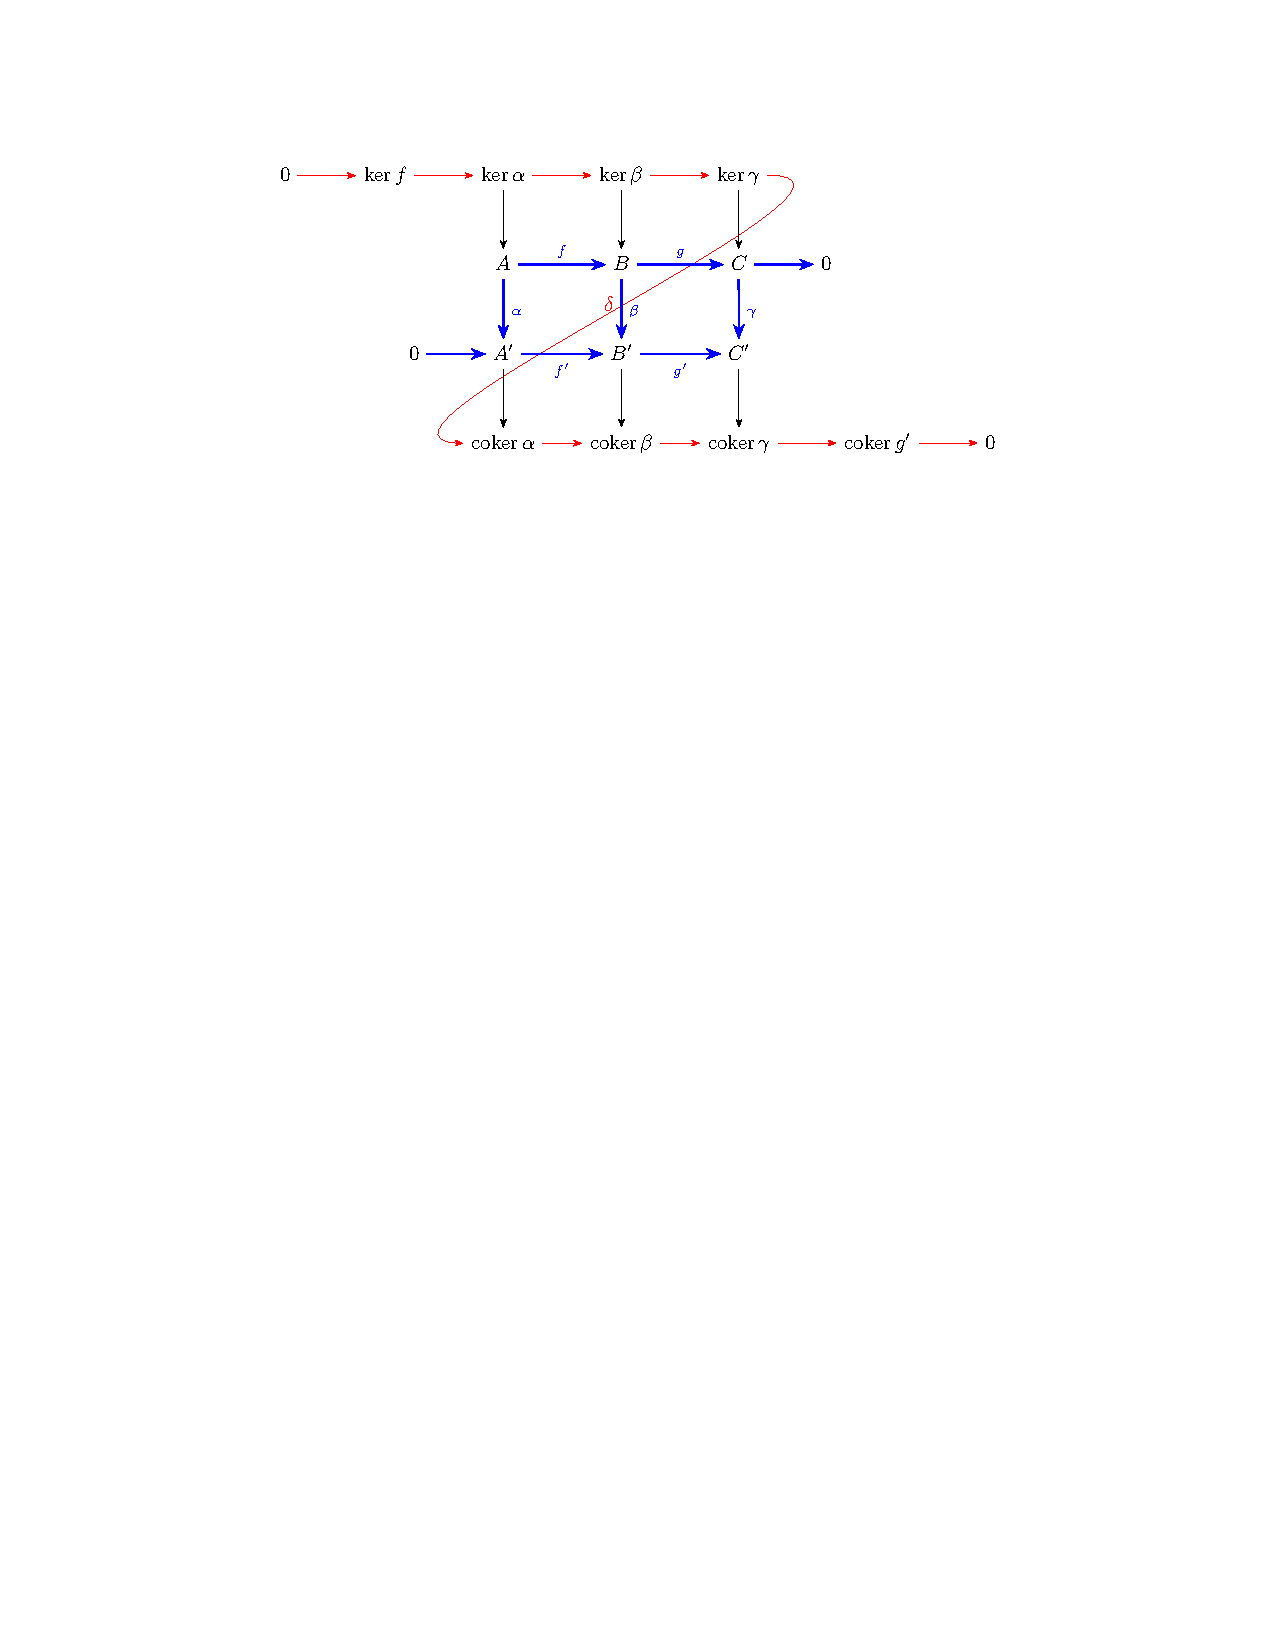
\includegraphics[width=0.8\textwidth]{pictures/snake.pdf}\]
the homomorphism $\delta$ is called the \textbf{connection homomorphism}.
\end{lemma}
\begin{proof}
First, let $c\in\ker\gamma$, We can construct elements of $A'$ as follows. Since $g$ is surjective, there exists an element $b\in B$ such that $g(b)=c$. We now move vertically down by $\beta$, and take $\beta(b)$. The commutativity $\gamma\circ g=g'\circ\beta$ shows that 
\[g'(\beta(b))=\gamma(g(b))=\gamma(c)=0\]
whence $\beta(b)$ is in the kernel of $g'$ in $B'$. By exactness, there exists an element $a'\in A'$ such that $f'(a)=\beta(b)$. We map $a$ into $\coker\alpha$ by the canonical projection, and still denote it by $a$.\par
In brief, we write
\[\delta(c)=a=f'^{-1}\circ\beta\circ g^{-1}(c)\]
\[\begin{tikzcd}
&&c\ar[d]\\
&b\ar[d,"\beta"]\ar[r,"g"]&c\ar[d,dashed,"\gamma"]\\
a\ar[d]\ar[r,"f'"]&\beta(b)\ar[r,dashed,"g'"]&0\\
a&&
\end{tikzcd}\]
We now verify that $\delta$ is well defined. First, $f'$ is injective by exactness, $a$ is uniquely determined by $\beta(b)$, hence by $b$. So the only verification is for $b$.\par
Suppose we choose a different $b'$ mapping to the same $c$: $g(b')=c=g(b)$. Then $b'-b\in\ker g$, and by exactness, $\im f=\ker g$, so there is $\ell\in A$ such that $\alpha(\ell)=b'-b$. It follows from the commutativity that
\[\beta(b'-b)=\beta(f(b'-b))=f'(\alpha(\ell))\]
Following our construction, $f'^{-1}(\beta(b'-b))=\alpha(\ell)$. But since the column is exact, the projection into $\coker\alpha$ kills $\alpha(\ell)$, hence taking $b'$ makes no difference to $\delta(c)$, that is, $\delta$ is well defined.
\[\begin{tikzcd}
\ell\ar[d,"\alpha"]\ar[r,"f"]&b'-b\ar[d,"\beta"]\ar[r,"g"]&0\\
\alpha(\ell)\ar[d]\ar[r,"f'"]&\beta(b'-b)&\\
0&&
\end{tikzcd}\]
Now we need to verify the exactness of the sequence. First we give the morphisms in the sequence
\[\begin{tikzcd}[column sep=tiny]
0\ar[r]&\ker f\ar[r,"i"]&\ker\alpha\ar[r,"f_*"]&\ker\beta\ar[r,"g_*"]&\ker\gamma\ar[r,"\delta"]&\coker\alpha\ar[r,"f'_*"]&\coker\beta\ar[r,"g'_*"]&\coker\gamma\ar[r,"j"]&\coker g'\ar[r]&0
\end{tikzcd}\]
We just define $f_*:=f|_{\ker\alpha}$, and similar for $g_*$, $f'_*,g'_*$. If $a\in\ker f$, then $f'(\alpha(a))=0$ by commutativity, and $\alpha(a)=0$ by injectvity of $f'$. This gives an inclusion $\ker f\to\ker\alpha$, which is our $i$. Similarly, if $c\in\im\gamma$, then there is an element $b\in B$ such that $\gamma(g(b))=c$ by the surjectivity of $g$. Then we see $c=g'(\beta(b))$ by commutativity, hence $c\in\im g'$. This gives $\im\gamma\sub\im g'$, and we have an induced quotient map $\coker\gamma\to\coker g'$. This is our $j$. By our definition, the exactness of two ends follows, now we begin to verify the rest.\par
Since $\ker f\sub\ker\alpha$, by our definition of $f_*$, the exactness at $\ker\alpha$ follows. Similar for the exactness of $\coker\gamma$. Since the top row is exact, $\im(f)=\ker(g)$. Ii follows that $g_*\circ f_*=0$, so $\im f_*\sub\ker g_*$. To verify the converse, assume $b\in\ker g_*$, that is, $b\in\ker\beta$ and $g(b)=0$. By exactness of $B$, there is $a\in A$ such that $f(a)=b$. We show that $a\in\ker\alpha$: in fact,
\[f'(\alpha(a))=\beta(f(a))=\beta(b)=0\]
Since $f'$ is injective, this means $\alpha(a)=0$, so $a\in\ker\alpha$. Thus $\ker g_*=\im f_*$, giving the exactness at $\ker\beta$.\par
The exactness at $\coker\beta$ arises similarly. Assume $b'+\im\beta\in\ker g'_*$, then $g'(b')\in\im\gamma$. By the surjectivity of $g$, $\exists b\in B$ such that $g'(b')=\gamma(g(b))=g'(\beta(b))$. Then $b'=\beta(b)+x$ with $x\in\ker g'$. By exactness, $x=f'(a')$ for some $a'\in A'$. Then it follows
\[b'+\im\gamma=\beta(b)+f'(a')+\im\beta=f'(a')\]
this shows $\ker g'_*\sub \im f'_*$, and the claim.\par
We verify the exactness about $\delta$. First, let $c=g(b)$ for some $b\in\ker\beta$. Since $\beta(b)=0$, by our definition of $\delta$, $\delta(c)=f'^{-1}(\beta(b))+\im\alpha=\im\alpha$. This gives $\im g_*\sub\ker\delta$. Conversely, if $\delta(c+\im\alpha)=\im\alpha$ for some $c\in C$, we get $\delta(c)\in\im\alpha$, hence $\delta(c)=\alpha(a)$ by some $a\in A$. By the construction of $\delta$, choose some $b\in B$ such that $g(b)=c$, then $f'^{-1}(\beta(b))=\delta(c)=\alpha(a)$ . It follows that
\[\beta(b)=f'(\alpha(a))=\beta(f(a))\]
and $b=f(a)+x$ for $x\in\ker\beta$. Applying $g$ we get $c=g(b)=g(f(a))+g(x)=g(x)$ since $g\circ f=0$. Since $x\in\ker\beta$, $g_*(x)=g(x)=c$. This gives $\ker\delta\sub\im g_*$, giving the exactness at $\ker\gamma$.
Finally, we deal with the exactness at $\coker\alpha$. Choose $a'+\im\alpha=\delta(c)$ for $c\in\ker\gamma$. Agian the definition of $\delta$: $f'(a')=f'(\delta(c))=\beta(b)$ for some $g(b)=c, b\in B$. This already gives 
\[f'_*(a'+\im\alpha)=f'(\delta(c))+\im\beta=\beta(b)+\im\beta=\im\beta\]
For the other direction, let $a'+\im\beta\in\ker f'_*$, that is, $f'(a')\in\im\beta$. So let $f'(a')=\beta(b), b\in B$, we observe that $a'=f'^{-1}\circ\beta(b)=f'^{-1}\circ\beta\circ g^{-1}(g(b))=\delta(g(b))$. This gives $\ker f'_*\sub\im\delta$, finishing the proof.
\end{proof}
\subsection{Exercise}
\begin{exercise}
Let $A$ be a local ring, and $f_1,\dots,f_r\in A$ be elements in $A$ generating a non-trivial ideal $I$ of $A$. Suppose $I$ is principal, show that $I=(f_i)$ for some $f_i$.
\end{exercise}
\begin{proof}
Let $I=(a)$ with $a\neq 0$ and $\m$ the unique maximal ideal of $A$. Then for every $f_i$ we have $f_i=k_ia$ for $k_i\in A$. Now consider the module $\m I$: we have $\m I\sub I$. If one of $k_i$ is a unit, then $I=(a_i)$ and we are done. So we assume this is not the case. Then, each $k_i$ is contained in $\m$, and hence $f_i=k_ia$ is in $\m I$, hence $I\sub\m I$. Now we have $\m I=I$, and by Nakayame's lemma we have $I=0$, which is contradiction.
\end{proof}
\begin{exercise}
Let $A[X]$ be the ring of polynomials in one indeterminate over a ring A. Prove that $A[X]$ is a flat $A$-algebra.
\end{exercise}
\begin{proof}
We have
\[A[X]=\bigoplus_{i\in\N}(x^n)\]
Each $(x^n)$ is free, hence flat, so $A[X]$ is flat.
\end{proof}
\begin{exercise}
For any $A$-module, let $M[X]$ denote the set of all polynomials in $x$ with coefficients in $M$, prove that
\[A[X]\otimes_AM\cong (A\otimes_AM)[X]\cong M[X].\]
\end{exercise}
\begin{exercise}
Let 
\[\begin{tikzcd}
0\ar[r]&L\ar[r]&M\ar[r]&N\ar[r]&0
\end{tikzcd}\]
be an exact sequence of $A$-modules. If $L$ and $N$ are finitely generated, then so is $M$.
\end{exercise}
\begin{proof}
We have $M\sub L+N$ if we identify this sequence as a projection.
\end{proof}
\begin{exercise}
If $M$ is a finitely generated $A$-module and $f:M\to M$ is a surjective homomorphism, then $f$ is an isomorphism.
\end{exercise}
\begin{proof}
Define a $A[X]$-module structure on $M$ via $x\cdot m:=f(m)$. Let $I:=(x)$, we claim that $IM=M$: In fact, since $f$ is surjective, for each $m\in M$ there is $n\in M$ such that $x\cdot n=f(n)=m$, so $m\in IM$. Now by \cref{finite module IM=M} there exists $g\in I$ such that $(1+g)M=0$. By the definition of $I$, we can write $g(x)=xh(x)$.\par
Now we prove $f$ is injective. Let $m\in M$ be such that $f(m)=0$. Then
\[0=(1+xh(x))\cdot m=m+h(x)\cdot f(m)=m+0=m.\]
This finishes the proof.
\end{proof}
\begin{exercise}\label{module directed limit}
Let $\mathcal{M}=(M_i,\mu_i)$ be a directed system directed by some set $I$. We shall construct an $A$-module $M$ called the direct limit of the direct system $M$. Let $C$ be the direct sum of the $M_i$ and identify each module $M_i$ with its canonical image in $C$. Let $D$ be the submodule of $C$ generated by all elements of the form $x_i-\mu_{ij}(x_i)$ where $i\leq j$ and $x_i\in M_i$. Let $M=C/D$, let $\mu:C\to M$ be the projection and let $\mu_i$ be the restriction of $\mu$ to $M_i$. Then clearly $\mu_j=\mu_{ij}\mu_i$. Show that every element of $M=\rlim M_i$ can be written in the form $\mu_i(x_i)$ for some $i\in I$ and some $x_i\in M_i$. Show also that if $\mu_i(x_i)=0$ then there exists $j\geq i$ such that $\mu_{ij}(x_i)=0$ in $M_j$.
\end{exercise}
\begin{proof}
For the first claim, $x\in C$ has a representative of the form $x=\sum_{j\in J}x_j$ for some finite subset $J$. Then we can get $i\in I$ such that $i\geq j$ for all $j\in J$. So
\[x=\mu\Big(\sum_{j\in J}x_j\Big)=\sum_{j\in J}\mu_j(x_j)=\sum_{j\in J}\mu_i\mu_{ji}(x_j)=\mu_i\Big(\sum_{j\in J}\mu_{ji}(x_j)\Big)\]
Let $x_i=\sum\mu_{ji}(x_j)$ we get the claim.\par
For the second claim, suppose $\mu_i(x_i)=0$ for some $i\in I$. Then, $x_i\in M_i\cap D$ is a finite sum
\[x_i=\sum_{\ell}(y_{j_\ell}-\mu_{j_{\ell}k_{\ell}}(y_{j_\ell}))\]
for some finite subset $J$ of $I$, and $y_{j_\ell}\in M_{j_\ell}$ for each $j\in J$ with $j_\ell\leq k_\ell$. Now, there exists $l\in I$ such that $l\geq k_\ell$ for all $k_\ell\in J\cup\{i\}$. Let $\pi_a:x\to M_a$ be the projectin, then we have
\[\pi_a=\sum_{j_\ell =a}y_{j_\ell}-\sum_{k_\ell=a}\mu_{j_\ell k_\ell}(y_{j_\ell}).\]
Hence
\[\mu_{al}(\pi_a(x_i))=\sum_{j_\ell =a}\mu_{al}(y_{j_\ell})-\sum_{k_\ell=a}\mu_{j_\ell l}(y_{j_\ell})\]
It follows that
\begin{align*}
\sum_a\mu_{al}\pi_a(x_i)&=\sum_a\Big(\sum_{j_\ell =a}\mu_{al}(y_{j_\ell})-\sum_{k_\ell=a}\mu_{j_\ell l}(y_{j_\ell})\Big)\\
&=\sum_{\ell}\sum_{a=j_\ell}\mu_{al}(y_{j_\ell})-\sum_{\ell}\sum_{a=k_\ell}\mu_{j_\ell l}(y_{j_\ell})\\
&=\sum_{\ell}\mu_{j_\ell l}(y_{j_\ell})-\sum_{\ell}\mu_{j_\ell l}(y_{j_\ell})=0
\end{align*}
Since $x_i\in M_i$, the left sum is $\mu_{il}(x_i)$, and we get $\mu_{il}(x_i)=0$.
\end{proof}
\begin{exercise}\label{module directed limit exactness}
Let $I$ be a directed set, and let $(A_i,\alpha_{ij})$, $(B_i,\beta_{ij})$, and $(C_i,\gamma_{ij})$ be direct systems of $A$-modules over $I$. If $r_i:A_i\to B_i$ and $s_i:B_i\to C_i$ are morphisms of direct systems, and if
\[\begin{tikzcd}
0\ar[r]&A_i\ar[r,"r_i"]&B_i\ar[r,"s_i"]&C_i\ar[r]&0
\end{tikzcd}\]
is exact for each $i\in I$, then there is an exact sequence
\[\begin{tikzcd}
0\ar[r]&\rlim A_i\ar[r,"r"]&\rlim B_i\ar[r,"s"]&\rlim C_i\ar[r]&0
\end{tikzcd}\]
where $r=\vec{r}_i$, $s=\vec{s}_i$. Consequently, filtered colimits commute with homology in $A$-$\mathsf{Mod}$.
\end{exercise}
\begin{proof}
Since direct limit is a left adjoint functor, it is right-exact. Hence we only need to prove $r$ is injective. Suppose that $r(x)=0$, where $x\in\rlim A_i$. Since the index set $I$ is
directed, allows us to write $x=\alpha_i(a_i)$, where $\alpha_i:A_i\to\bigoplus A_i$ is projection, similar for $\beta_i$. Now, be definition we have
\[r(x)=\beta_ir_i(a_i).\]
so $\beta_ir_i(a_i)=0$. By \cref{module directed limit}, there is a $j\geq i$ such that $\beta_ir_i(a_i)=\beta_{ij}r_i(a_i)=0$. Since $r_i$ is a map of direct systems, we have
\[r_j\alpha_{ij}=\beta_{ij}r_i\]
Thus $r_j\alpha_{ij}(a_i)=0$, and by the injectivity of $r_j$, we conclude $\alpha_{ij}(a_i)=0$, since we have
\[x=\alpha_i(a_i)=\alpha_j\alpha_{ij}(a_i)\]
we conclude $x=0$. 
\end{proof}
\begin{exercise}
Let $(M_i)_{i\in I}$ be a family of submodules of an $A$-module, such that for each pair of indices $i$, $j$ in $I$ there exists $k\in I$ such that $M_i+M_j\sub M_k$. Define $i\leq j$ to mean $M_i\sub M_j$ and let $\mu_{ij}:M_i\to M_j$ be the embedding of $M_i$ in $M_j$. Show that
\[\rlim M_i=\sum M_i=\bigcup_iM_i.\]
In particular, any $A$-module is the direct limit of its finitely generated submodules.
\end{exercise}
\begin{proof}
We can easily check that $\bigcup_iM_i$ is a module and satisfies that universal property of $\rlim M_i$. And since it has the same discription as $\sum M_i$, we get the equality.
\end{proof}
\begin{exercise}
Let $\mathcal{M}=(M_i,\mu_{ij})$, $\mathcal{N}=(N_i,\nu_{ij})$ be direct systems of $A$-modules over the same directed set. Let $M,N$ be the direct limits and $\mu_i:M\to M$, $\nu_i:N_i\to N$ the associated homomorphisms.\par
A homomorphism $\Phi:\mathcal{M}\to\mathcal{N}$ is by definition a family of $A$-module homomorphisms $\phi_i:M_i\to N_i$, such that $\phi_i\circ\mu_{ij}=\nu_{ij}$ whenever $i\leq j$. Show that $\Phi$ defines a unique homomorphism $\phi=\rlim\phi_i:M\to N$ such that $\phi\circ\mu_i=\nu_i$ for all $i\in I$.
\end{exercise}
\begin{exercise}\label{ring direct limit zero iff one zero}
Consider a direct limit of rings $A=\rlim A_i$, prove that $\rlim A=0$ if and only if $A_i=0$ for some $i$.
\end{exercise}
\begin{proof}
If $A=0$, then in particular $0=1$. By exercise~\ref{module directed limit}, for fixed $i$, there exists $j\in I$ such that $\mu_{ij}(a)=0$. Since $\mu_{ij}$ is also a ring homomorphism from $A_i$ to $A_j$, this implies that $1=0$ in $A_j$ and hence $A_j=0$.
\end{proof}
\begin{exercise}
Let $(A_i,\mu_i)$ be a direct system of rings and let $\n(A_i)$ be the nilradical of $A_i$. Show that $\rlim \n(A_i)$ is the nilradical of $\rlim A_i$. If each $A_i$ is an integral domain, then $\rlim A_i$ is an integral domain.
\end{exercise}
\begin{proof}
Let $a$ be a nilpotent element of $A$. Then $\exists n\in\N$ such that $a^n=0$. By \cref{module directed limit}, $a=\mu_i(x)$ thus $0=a^n=\mu_i(x^n)$. By \cref{module directed limit}, $\mu_i(x^n)=0$ implies $\exists j\geq i$ such that $\mu_{ij}(x^n)=0$. Hence, $\mu_{ij}(x)$ is in the nilradical of $A_j$, and
\[\mu_j(\mu_{ij}(x))=\mu_i(x)=a\]
Hence $a\in\rlim \n(A_i)$.\par
Conversely, if $a\in\rlim \n(A_i)$, then by \cref{module directed limit}, there is $x_i\in M_i$ such that $\mu_i(x_i)=a$. Then 
\[a^n=\mu_i(x_i^n)=0\]
so there is $j\geq i$ such that $\mu_{ij}(x_i^n)=0=\mu_{ij}(x_i)^n$. This means $\mu_{ij}(x_i)$ is in $\n(A_j)$. Since
\[\mu_j(\mu_{ij}(x_i))=\mu_i(x)=a,\]
we see $a$ is nilpotent in $A$.
\end{proof}
\section{Flat modules}
\subsection{\texorpdfstring{$M$}{M}-flat modules}
Let $A$ be a ring, $E$ and $M$ $A$-modules. Then $E$ is said to be \textbf{flat for $\bm{M}$} (or \textbf{$\bm{M}$-flat}) if, for every $A$-module $N$ and every injective homomorphism $\phi:M'\to M$, the homomorphism $1\otimes v:E\otimes_AM'\to E\otimes_AM$ is injective.
\begin{lemma}\label{module flat iff finite submodule}
For an $A$-module $E$ to be $M$-flat, it is necessary and sufficient that for every finitely generated submodule $N$ of $M$ the canonical homomorphism $1\otimes v:E\otimes_AN\to E\otimes_AM$ is injective.
\end{lemma}
\begin{proof}
Suppose that this condition holds and let $N$ be any submodule of $M$. Suppose that the canonical image in $E\otimes_AM$ of an element $z=\sum_ix_i\otimes y_i\in E\otimes M$ is zero and let $M'$ be the finitely generated submodule of $N$ generated by the $y_i$. As by hypothesis the composition map
\[E\otimes_AM'\to E\otimes_AN\to E\otimes_AM\]
is injective, the sum $z'=\sum_ix_i\otimes y_i$ considered as an element of $E\otimes_AM'$, is zero. Since $z$ is the image of $z'$, we have $z=0$, whence the lemma.
\end{proof}
\begin{lemma}\label{module submodule quotient flat}
Let $E$ be an $A$-module and $M$ an $A$-module such that $E$ is $M$-flat. If $N$ is either a submodule or a quotient module of $M$, then $E$ is $N$-flat.
\end{lemma}
\begin{proof}
The case in which $N$ is a submodule is easy, as, if $N'$ is a submodule of $N$, the composite homomorphism
\[E\otimes_AN'\to E\otimes_AN\to E\otimes_AM\]
is injective, hence so is $E\otimes_AN'\to E\otimes_AN$. Suppose then that $N$ is a quotient module of $M$, that is there exists an exact sequence
\[\begin{tikzcd}
0\ar[r]&R\ar[r,"i"]&M\ar[r,"\pi"]&N\ar[r]&0
\end{tikzcd}\]
Let $N'$ be a submodule of $N$ and $M'=\pi^{-1}(N')$. Let $\iota'$ denote the mapping of $R$ to $M'$ with the same graph as $\iota$, $\pi'$ the surjection $M'\to N'$ with the same graph as the restriction of $\pi$ to $M'$, and $\phi$, $\psi$, $\gamma$ the canonical injections. The the folloiwng diagram 
\[\begin{tikzcd}
0\ar[r]&R\ar[d,"\phi"]\ar[r,"\iota'"]&M'\ar[d,"\psi"]\ar[r,"\pi'"]&N'\ar[d,"\gamma"]\ar[r]&0\\
0\ar[r]&R\ar[r,"\iota"]&M\ar[r,"\pi"]&N\ar[r]&0
\end{tikzcd}\]
is commutative and its rows are exact. Tensoring with $E$, since $E$ is $M$-flat, we get the following diagram
\[\begin{tikzcd}
&E\otimes_AR\ar[d,"1\otimes\phi"]\ar[r,"1\otimes\iota'"]&E\otimes_AM'\ar[d,"1\otimes\psi"]\ar[r,"1\otimes\pi'"]&E\otimes_AN'\ar[d,"1\otimes\gamma"]\ar[r]&0\\
0\ar[r]&E\otimes_AR\ar[r,"1\otimes\iota"]&E\otimes_AM\ar[r,"1\otimes\pi"]&E\otimes_AN\ar[r]&0
\end{tikzcd}\]
with row exact. Now since $1\otimes\phi$ is surjective and $1\otimes\psi$ is injective, by snake lemma we see $1\otimes\gamma$ is injective, whence the claim. 
\end{proof}
\begin{lemma}\label{module flat and direct sum}
Let $(M_i)_{i\in I}$ be a family of $A$-modules, $M=\bigoplus_iM_i$ their direct sum and $E$ an $A$-module. If, for all $i\in I$, $E$ is flat for $M_i$, then $E$ is flat for $M$.
\end{lemma}
\begin{proof}
Suppose first that $I=\{1,2\}$, and let $M'$ be a submodule of $M=M_1\oplus M_2$, $M_1$ and $M_2$ being canonically identified with submodules of $M$. Denote by $M_1'$ the intersection $M'\cap M_1$ and by $M_2'$ the image of $M'$ in $M_2$ under the canonical projection $\pi$ of $M$ onto $M_2$. We have a diagram
\[\begin{tikzcd}
0\ar[r]&M_1'\ar[r,"\iota'"]\ar[d,"\phi"]&M'\ar[r,"\pi'"]\ar[d,"\psi"]&M_2'\ar[r]\ar[d,"\eta"]&0\\
0\ar[r]&M_1\ar[r,"\iota"]&M\ar[r,"\pi"]&M_2\ar[r]&0
\end{tikzcd}\]
where $\iota$, $\iota'$ are the canonical injections and $\pi'$ is the mapping with the same graph as the restriction of $\pi$ to $M'$, which is surjective. It is immediately verified that this diagram is commutative and that its rows are exact.
\[\begin{tikzcd}
&E\otimes_AM_1'\ar[r,"1\otimes\iota'"]\ar[d,"1\otimes\phi"]&E\otimes_AM'\ar[r,"1\otimes\pi'"]\ar[d,"1\otimes\psi"]&E\otimes_AM_2'\ar[r]\ar[d,"1\otimes\eta"]&0\\
0\ar[r]&E\otimes_AM_1\ar[r,"1\otimes\iota"]&E\otimes_AM\ar[r,"1\otimes\pi"]&E\otimes_AM_2\ar[r]&0
\end{tikzcd}\]
By hypotheses the two rows of this diagram are exact. As $E$ is flat for $M_1$ and $M_2$, $1\otimes\phi$ and $1\otimes\eta$ are injective. The snake lemma then shows that $1\otimes\psi$ is injective and consequently $E$ is $M$-flat.\par
If $I$ is a finite set with $n$ elements, the lemma follows by induction on $n$. In the general case, let $M'$ be a finitely generated submodule of $M$. Then there exists a finite subset $J$ of the indexing set $I$ such that $M'$ is contained in the direct sum $M^J=\bigoplus_{i\in J}M_j$. By the finite case $E$ is flat for $M^J$. The canonical homomorphism $E\otimes_AM'\to E\otimes_AM^J$ is therefore injective. On the other hand, as $M^J$ is a direct factor of $M$, the canonical homomorphism $E\otimes_AM^J\to E\otimes_AM$ is injective. Taking the composition, it follows that $E\otimes_AM^J\to E\otimes_AM$ is injective and $E$ is flat for $M$ by \cref{module flat iff finite submodule}.
\end{proof}
\subsection{Flat modules}
\begin{proposition}\label{module flat iff flat for A}
Let $E$ be an $A$-module. The following three properties are equivalent:
\begin{itemize}
\item[(\rmnum{1})] $E$ is flat for $A$ (in other words, for every ideal $\a$ of $A$, the canonical homomorphism $E\otimes_A\a\to E\otimes_AA$ is injective).
\item[(\rmnum{2})] $E$ is $M$-flat for every $A$-module $M$.
\item[(\rmnum{3})] The functor $-\otimes_AE$ is exact, that is, $E$ is flat.
\end{itemize}
\end{proposition}
\begin{proof}
It is immediate that (\rmnum{2}) is equivalent to (\rmnum{3}) and (\rmnum{2}) implies (\rmnum{1}). Conversely, if (\rmnum{1}) holds, then by \cref{module flat and direct sum}, $E$ is fiat for every flee left $A$-module. As every $A$-module is isomorphic to a quotient of a free module, it follows from \cref{module submodule quotient flat} that $E$ is flat for $M$.
\end{proof}
\begin{remark}By \cref{module flat iff finite submodule}, for an $A$-module $E$ to be flat, it is necessary and sufficient that, for every finitely generated ideal $\a$ of $A$, the canonical mapping $E\otimes_A\a$ with image $E\a$ be injective.
\end{remark}
\begin{proposition}\label{module direct sum flat iff}
Let $(E_i)_{i\in I}$ be a family of $A$-modules. For $E=\bigoplus_iE_i$ to be flat, it is necessary and sufficient that each of the $E_i$ be flat.
\end{proposition}
\begin{proof}
Let $M'\to M$ be an injective $A$-module homomorphism. For the direct sum homomorphism
\[\bigoplus_{i\in I}(E_i\otimes_AM)\to\bigoplus_{i\in I}(E_i\otimes_AM)\]
to be exact, it is necessary and sufficient that each of the homomorphisms $E_i\otimes_AM'\to E_i\otimes_AM$ be so, which proves the claim since $\bigoplus_{i\in I}(E_i\otimes_AM)$ is canonically identified with $E\otimes_AM$.
\end{proof}
\begin{proposition}\label{module flat direct limit}
Let $I$ be an ordered set and $(E_\alpha,f_{\beta\alpha})$ a direct system of $A$-modules. If each of the $E_\alpha$ is flat, then $E=\rlim E_\alpha$ is flat.
\end{proposition}
\begin{proof}
By hypothesis each of the sequences $0\to E_\alpha\otimes_AM'\to E_\alpha\otimes_AM$ is exact; so then is the sequence $0\to E\otimes_AM'\to E\otimes_AM$ since taking the direct limit commutes with tensor products and preserves exactness.
\end{proof}
\begin{example}
\mbox{}
\begin{itemize}
\item[(a)] For any ring $A$, $A$ is clearly a flat $A$-module. Then it follows from \cref{module direct sum flat iff} that every free $A$-module, and more generally every projective $A$-module, is a flat $A$-module.
\item[(b)] If $A$ is a semisimple ring, every $A$-module $E$ is semisimple and hence a direct sum of simple modules. As each of these latter is isomorphic to a direct factor of $A$, $E$ is projective and therefore flat.
\item[(c)] Let $a\in A$ be such that the map $a_A:x\mapsto ax$ on $A$ is injective ($a$ is not a zero divisor). If $E$ is a flat $A$-module, then the homothety $a_E$ is injective. In particular, if $A$ is integral, any flat $A$-module is torsion free. Conversely, if $A$ is a PID, then any torsion free $A$-module is flat: infact, if the $A$-module $E$ is torsion-free, any finitely generated submodule of $E$ is free, and $E$ is the union of these flat submodules, hence flat (\cref{module flat direct limit}).
\end{itemize}
\end{example}
\begin{proposition}\label{module flat and torsion}
Let $A$ be a ring and $E$ an $A$-module.
\begin{itemize}
\item[(a)] Suppose that $E$ is flat. For every element $a$ of $A$ which is not a divisor of $0$, the relations $x\in E$, $ax=0$ imply $x=0$. 
\item[(b)] Suppose that $A$ is an integral domain in which every finitely generated ideal is principal. Then for $E$ to be flat it is necessary and sufficient that $E$ be torsion-free.
\end{itemize}
\end{proposition}
\begin{proof}
We prove (a). Let $v:A\to A$ be the $A$-module homomorphism $t\mapsto at$. The hypothesis implies that $v$ is injective. As $E$ is flat, the homomorphism $1_E\otimes v:E\otimes_AA\to E\otimes_AA$ is also injective. When $E\otimes_AA$ is canonically identified with $E$, $1_E\otimes v$ becomes the endomorphism $x\mapsto ax$ of $E$. Thus the relation $ax=0$ implies $x=0$.\par
We prove (b). By (a), if $E$ is flat, $E$ is torsion-free. Conversely, let $E$ be a torsion-free $A$-module and let $\a$ be a nonzero finitely generated ideal of $A$. By hypothesis $\a=Aa$ for some nonzero $a\in A$ and $t\mapsto at$ is then an isomorphism $v$ of $A$ onto $\a$. Using $i$ to denote the canonical injection $\a\to A$, $i\circ v$ is the homothety with ratio $a$ on $E$ and is injective since $E$ is assumed to be torsion-free. Then $1_E\otimes(i\circ v)=(1_E\otimes i)\circ(1_E\otimes v)$. As $1_E\otimes v$ is an isomorphism, $1_E\otimes i$ is injective, which completes the proof.
\end{proof}
\begin{proposition}\label{module flat iff quotient of flat module}
Let $E$ be an $A$-module. The three following properties are equivalent:
\begin{itemize}
\item[(\rmnum{1})] $E$ is flat.
\item[(\rmnum{2})] For every exact sequence of $A$-modules of the form
\begin{equation}\label{module flat iff quotient of flat module-1}
\begin{tikzcd}
0\ar[r]&G\ar[r,"\phi"]&H\ar[r,"\psi"]&E\ar[r]&0 
\end{tikzcd}
\end{equation}
and every $A$-module $F$, the sequence
\begin{equation}\label{module flat iff quotient of flat module-2}
\begin{tikzcd}
0\ar[r]&G\otimes_AF\ar[r,"\phi\otimes 1"]&H\ar[r,"\psi\otimes 1"]&E\otimes_AF\ar[r]&0 
\end{tikzcd}
\end{equation}
sexact.
\item[(\rmnum{3})] There exists an exact sequence $(\ref{module flat iff quotient of flat module-1})$, where $H$ is flat, such that the sequence $(\ref{module flat iff quotient of flat module-2})$ is is exact for every $A$-module $F$ of the form $A/\a$, where $\a$ is a finitely generated ideal of $A$.
\end{itemize}
\end{proposition}
\begin{proof}
The $A$-module $F$ is isomorphic to a quotient of a free module. In other words, we have an exact sequence $\begin{tikzcd}[column sep=15pt]
0\ar[r]&R\ar[r,"\iota"]&L\ar[r,"\pi"]&F\ar[r]&0\end{tikzcd}$ where $L$ is free. Consider the diagram
\begin{equation}\label{module flat iff quotient of flat module-3}
\begin{tikzcd}[column sep=20pt,row sep=20pt]
&G\otimes_AR\ar[r,"\phi\otimes 1_R"]\ar[d,"1_G\otimes\iota"]&H\otimes_AR\ar[r,"\psi\otimes 1_R"]\ar[d,"1_H\otimes\iota"]&E\otimes_AR\ar[r]\ar[d,"1_E\otimes\iota"]&0\\
0\ar[r]&G\otimes_AL\ar[r,"\phi\otimes 1_L"]\ar[d,"1_G\otimes\pi"]&H\otimes_AL\ar[r,"\psi\otimes 1_L"]\ar[d,"1_H\otimes\pi"]&E\otimes_AL\ar[r]\ar[d,"1_F\otimes\pi"]&0\\
&G\otimes_AF\ar[r,"\phi\otimes 1_F"]\ar[d]&H\otimes_AF\ar[r,"\phi\otimes 1_F"]\ar[d]&E\otimes_AF\ar[r]\ar[d]&0\\
&0&0&0
\end{tikzcd}
\end{equation}
It follows immediately that this diagram is commutative, and its rows and columns are exact. Apply the snake lemma to the first two rows, we get the following exact sequence
\begin{equation}\label{module flat iff quotient of flat module-4}
\begin{tikzcd}
\ker(1_H\otimes\iota)\ar[r]&\ker(1_E\otimes\iota)\ar[r,"\delta"]&G\otimes_AF\ar[r,"\phi\otimes 1_F"]&H\otimes_AF
\end{tikzcd}
\end{equation}
Now if $E$ is flat, then $1_E\otimes\iota$ is injective, and the exact sequence shows that $\phi\otimes 1_F$ is injective, hence the sequence $(\ref{module flat iff quotient of flat module-2})$ is exact.\par
As (\rmnum{2}) obviously implies (\rmnum{3}), it remains to prove that (\rmnum{3}) implies (\rmnum{1}). Consider the diagram $(\ref{module flat iff quotient of flat module-3})$ in the case $R=\a$, $L=A$, $F=A/\a$ and apply the exact sequence $(\ref{module flat iff quotient of flat module-4})$. By hypothesis $\phi\otimes 1_F$ is injective, so $\im\delta=0$. Moreover, as $H$ is exact, we see $\ker(1_H\otimes\iota)=0$, whence $\ker(1_E\otimes\iota)=0$ and $E$ is flat.
\end{proof}
\begin{proposition}\label{module exact flat and exact sequence}
Let $\begin{tikzcd}[column sep=15pt,row sep=15pt]0\ar[r]&E_1\ar[r,"\phi"]&E_2\ar[r,"\psi"]&E_3\ar[r]&0\end{tikzcd}$ be an exact sequence of $A$-modules. Suppose $E_3$ is flat. Then, for $E_2$ to be flat it is necessary and sufficient that $E_1$ be flat.
\end{proposition}
\begin{proof}
Let $\eta:F'\to F$ be an injective homomorphism of $A$-modules. Consider the diagram
\[\begin{tikzcd}
0\ar[r]&E_1\otimes_AF'\ar[r,"\phi\otimes 1_{F'}"]\ar[d,"1_{E_1}\otimes\eta"]&E_2\otimes_AF'\ar[r,"\psi\otimes 1_{F'}"]\ar[d,"1_{E_2}\otimes\eta"]&E_3\otimes_AF'\ar[r]\ar[d,"1_{E_3}\otimes\eta"]&0\\
0\ar[r]&E_1\otimes_AF\ar[r,"\phi\otimes 1_{F}"]&E_2\otimes_AF\ar[r,"\psi\otimes 1_{F}"]&E_3\otimes_AF\ar[r]&0
\end{tikzcd}\]
It is commutative and its rows are exact by \cref{module flat iff quotient of flat module}. Since $E_3$ is flat, we know $1_{E_3}\otimes\eta$ is injective. Now snake lemma gives the claim.
\end{proof}
Let $E$ and $F$ be $A$-modules. Every element of $E\otimes_AF$ can be written in at least one way in the form $z=\sum_{i=1}^{n}e_i\otimes f_i$ where $e_i\in E$ and $f_i\in F$. The following lemma gives a condition under which this sum is zero:
\begin{lemma}\label{module tensor zero iff}
Let $(f_i)_{i\in I}$ be a family of generators of $F$ and $(e_i)_{i\in I}$ a family of elements of $E$ of finite support. For $\sum_{i\in I}e_i\otimes f_i=0$, it is necessary and sufficient that there exist a finite set $J$, a family $(x_j)_{j\in J}$ of elements of $E$ and a family $(a_{ji})_{j\in J,i\in I}$ of elements of $A$ with the following properties:
\begin{itemize}
\item[(a)] the family $(a_{ji})$ has finite support;
\item[(b)] $\sum_{i\in I}a_{ji}f_i=0$ for all $j\in J$;
\item[(c)] $e_i=\sum_{j\in J}a_{ji}x_j$ for all $i\in I$.
\end{itemize}
\end{lemma}
\begin{proof}
Consider the free $A$-module $A^{\oplus I}$, its canonical basis $(u_i)$ and the homomorphism $g:A^{\oplus I}\to F$ such that $g(u_i)=f_i$ for all $i\in I$. Denoting by $R$ the kernel of $g$, we have (since the $f_i$ generate $F$) an exact sequence
\[\begin{tikzcd}
R\ar[r,"\iota"]&A^{\oplus I}\ar[r,"g"]&F\ar[r]&0
\end{tikzcd}\]
wherc $\iota$ denotes the canonical injection. We derive from this the exact sequence
\begin{equation}\label{module tensor zero iff-1}
\begin{tikzcd}
E\otimes_AR\ar[r]&E\otimes_AA^{\oplus I}\ar[r,"1\otimes g"]&E\otimes_AF\ar[r]&0
\end{tikzcd}
\end{equation}
Now, $E\otimes_AA^{\oplus I}$ is canonically identified with $E^{\oplus I}$ a family $e=(e_i)\in E^{\oplus I}$ being identified with $\sum_{i\in I}e_i\otimes u_i$. For such a family to belong to the kernel of $1_E\otimes g$, it is necessary and sufficient that $\sum_{i\in I}e_i\otimes f_i=0$ in $E\otimes_AF$. Taking account of the exact sequence $(\ref{module tensor zero iff-1})$, this is equivalent to saying that $e$ belongs to the image of $1_E\otimes\iota$, in other words there is a relation of the form
\begin{equation}\label{module tensor zero iff-2}
\sum_{i\in I}e_i\otimes u_i=\sum_{j\in J}x_j\otimes\iota(r_j)
\end{equation}
where $x_i\in E$, $r_i\in R$ and $J$ is finite. Writing $\iota(r_i)=\sum_{i\in I}a_{ji}u_i$, the hypothesis $r_j\in R$ implies the relation $\sum_{i\in I}a_{ji}f_i=0$ for all $j\in J$. On the other hand the relation $(\ref{module tensor zero iff-2})$ implies $e_i=\sum_{j\in J}a_{ji}x_j$ for all $i\in I$ (\cref{*}), which completes the proof.
\end{proof}
\begin{proposition}\label{module F-flat iff linear relation}
For $E$ to be $F$-flat, it it necessary and sufficient that the following condition be satisfied:
\begin{itemize}
\item[(R)] If $(e_i)_{i\in I}$ and $(f_i)_{i\in I}$ are two finite families of elements of $E$ and $F$ respectively such that $\sum_{i\in I}e_i\otimes f_i=0$ in $E\otimes_AF$, there exists a finite set $J$, a family $(x_j)_{j\in J}$ of elements of $E$ and a family $(a_{ji})_{j\in J,i\in I}$ of elements of $A$, with the following properties:
\begin{itemize}
\item[(a)] $\sum_{i\in I}a_{ji}f_i=0$ for all $j\in J$. 
\item[(b)] $e_i=\sum_{j\in J}a_{ji}x_j$ for all $i\in I$.
\end{itemize} 
\end{itemize}
\end{proposition}
\begin{proof}
Suppose that $E$ is $F$-flat. Let $(e_i)$ and $(f_i)$ be finite families of elements such that $\sum_{i\in I}e_i\otimes f_i=0$ in $E\otimes_AF$, and let $F'$ be the submodule of $F$ generated by the $f_i$. Since the canonical mapping $E\otimes_AF'\to E\otimes_AF$ is injective, we have also $\sum_{i\in I}e_i\otimes f_i=0$ in $E\otimes_AF'$ and \cref{module tensor zero iff} can then be applied to $E$ and $F'$. Thus families $(x_j)$ and $(a_{ji})$ are obtained satisfying the conditions of (R).\par
Conversely, suppose that condition (R) holds. Let $F'$ be a submodule of $F$ and let $y=\sum_{i\in I}e_i\otimes f_i$ be an element of the kernel of the canonical mapping $E\otimes_AF'\to E\otimes_AF$. Since (R) holds, there exist families $(x_j)$ and $(a_{ji})$ satisfying conditions (a) and (b). We conclude that, in $E\otimes_AF$,
\[y=\sum_{i,j}a_{ji}x_j\otimes f_i=\sum_{j\in J}(x_j\otimes\sum_{i\in I}a_{ji}f_i)=0\]
hence the map $E\otimes F'\to E\otimes F$ is injective.
\end{proof}
\begin{corollary}
For an $A$-module $E$ to be flat, it is necessary and sufficient that the following condition hold:
\begin{enumerate}[leftmargin=30pt]
\item[(RP)] Every solution $\bm{y}\in M^n$ of a linear equation $P\bm{y}=0$ with $P\in\mathcal{M}_{mn}(A)$ is a linear combination $\bm{y}=Q\bm{x}$, where $Q\in\mathcal{M}_{nk}(A)$, $\bm{x}\in M^k$ and $PQ=0$.
\end{enumerate}
\end{corollary}
\subsection{Intersection properties}
\begin{lemma}\label{module tensor intersection lemma}
Let $E$ be an $A$-module, $F$ an $A$-module and $F_1$, $F_2$ two submodule of $F$ such that $F=F_1+F_2$. Then the intersection of the canonical images of $E\otimes F_1$ and $E\otimes F_2$ in $E\otimes F$ is equal to the canonical image of $E\otimes(F_1\cap F_2)$.
\end{lemma}
\begin{proof}
Consider the diagram
\[\begin{tikzcd}[column sep=20pt,row sep=20pt]
0\ar[r]&F_1\cap F_2\ar[r]\ar[d]&F_1\ar[r]\ar[d]&F_1/(F_1\cap F_2)\ar[r]\ar[d,"\eta"]&0\\
0\ar[r]&F_2\ar[r]&F_1+F_2\ar[r]&(F_1+F_2)/F_2\ar[r]&0
\end{tikzcd}\]
where the unspecified arrows are the canonical injections and surjections and $\eta$ is the canonical isomorphism. This diagram is commutative and its rows are exact. We derive (since $F=F_1+F_2)$ a commutative diagram
\[\begin{tikzcd}[column sep=20pt,row sep=20pt]
E\otimes(F_1\cap F_2)\ar[r]\ar[d]&E\otimes F_1\ar[r]\ar[d]&E\otimes(F_1/(F_1\cap F_2))\ar[r]\ar[d,"1_E\otimes\eta"]&0\\
E\otimes F_2\ar[r]&E\otimes F\ar[r]&E\otimes((F_1+F_2)/F_2)\ar[r]&0
\end{tikzcd}\]
The rows of this diagram are exact and $1_E\otimes\eta$ is an isomorphism. A simple diagram chasing shows the claim.
\end{proof}
\begin{proposition}\label{module flat tensor intersection}
Let $E$ be an $A$-module and $F$ an $A$-module such that $E$ is $F$-flat. Then, if $F_1,F_2$ are two submodules of $F$, we have
\[E\otimes(F_1\cap F_2)=(E\otimes F_1)\cap(E\otimes F_2).\]
\end{proposition}
\begin{proof}
As $E$ is $F$-flat, $(E\otimes F_1)+(E\otimes F_2)$ is identified with $E\otimes(F_1+F_2)$, which is a submodule of $E\otimes F$. The assertion then follows from \cref{module tensor intersection lemma}.
\end{proof}
\begin{example}
Let $k$ be a field, and consider the subring $A=k[X^2,X^3]$ of the polynomial ring $B=k[X]$ in an indeterminate $x$. Then $X^2A\cap X^3A$ is the set of polynomials made up of terms of degree $\geq 5$ in $X$, so that $(X^2A\cap X^3A)B=X^5B$; but on the other hand $X^2B\cap X^3B=X^3B$. Therefore by the above proposition $B$ is not flat over $A$.
\end{example}
\begin{proposition}\label{module quotient flat tensor intersection}
Let $E$ be an $A$-module, $E'$ a submodule of $E$, $F$ an $A$-module and $F'$ a submodule of $F$. Suppose that $E/E'$ or $F/F'$ is flat. Then we have
\[E'\otimes F'=(E'\otimes F)\cap(E\otimes F').\]
\end{proposition}
\begin{proof}
Suppose for example that $E/E'$ is flat and consider the diagram
\[\begin{tikzcd}
E'\otimes F'\ar[r]\ar[d]&E\otimes F'\ar[r]\ar[d]&(E/E')\otimes F\ar[r]\ar[d,"\eta"]&0\\
E'\otimes F\ar[r]&E\otimes F\ar[r]&(E/E')\otimes F\ar[r]&0
\end{tikzcd}\]
where the arrows are the canonical homomorphisms. This diagram is commutative and its rows are exact. As $E/E'$ is flat, $\eta$ is injective. Then our assertion then follows from a diagram chasing as in \cref{module tensor intersection lemma}.
\end{proof}
\begin{corollary}\label{module quotient flat iff product with submodule}
Let $E$ be an $A$-module and $E'$ a submodule of $E$.
\begin{itemize}
\item[(a)] Suppose that $E/E'$ is flat. Then, for every ideal $\a$ of $A$, we have $\a E'=\a E\cap E'$.
\item[(b)] Conversely, suppose that $E$ is flat and, for every finitely generated ideal $\a$ of $A$ we have $\a E'=\a E\cap E'$. Then $E/E'$ is flat.
\end{itemize}
\end{corollary}
\begin{proof}
For (a), it is sufficient to apply \cref{module quotient flat tensor intersection} to the case $F=A$ and $F'=\a$. Conversely, to prove that $E/E'$ is flat, apply criterion (\rmnum{3}) of \cref{module flat iff quotient of flat module}. It is then necessary to establish that the sequence
\[\begin{tikzcd}
0\ar[r]&E'/\a E'\ar[r]&E/\a E\ar[r]&E/(E'+\a E)\ar[r]&0
\end{tikzcd}\]
is exact for every finitely generated ideal $\a$ of $A$. Now this is precisely what relation $\a E'=\a E\cap E'$ expresses.
\end{proof}
\subsection{Extension of scalars and flatness}
\begin{proposition}\label{module flat tensor product is flat}
Let $R$, $S$ be two rings, $E$ an $R$-module and $F$ an $(R,S)$-bimodule. Suppose that $E$ is flat and that $F$ is flat as an $S$-module. Then the $S$-module $E\otimes_RF$ is flat.
\end{proposition}
\begin{proof}
Let $M$ be a left $S$-module and $M'$ a submodule of $M$. Since $F$ is flat as a $S$-module, the canonical homomorphism $F\otimes_SM'\to F\otimes_SM$ is injective. Since $E$ is flat, the canonical homomorphism
\[E\otimes_R(F\otimes_SM')\to E\otimes_R(F\otimes_SM)\]
is injective. As $E\otimes_R(F\otimes_SM')$ and $E\otimes_R(F\otimes_SM)$ are canonically identified with $(E\otimes_RF)\otimes_SM'$ and $(E\otimes_RF)\otimes_SM$ respectively, the canonical homomorphism
\[(E\otimes_RF)\otimes_SM'\to(E\otimes_RF)\otimes_SM\]
is injective, which proves that $E\otimes_RF$ is a flat $S$-module.
\end{proof}
\begin{corollary}\label{module flat tensor is flat}
Let $A$ be a ring, $E,F$ two flat $A$-modules. Then $E\otimes_AF$ is a flat $A$-module.
\end{corollary}
\begin{proof}
We see $F$ is a $(A,A)$-bimodule and it is sufficient to apply \cref{module flat tensor product is flat} with $R=S=A$.
\end{proof}
\begin{corollary}\label{module flat extension is flat}
Let $\rho:A\to B$ be a ring homomorphism. If $E$ is a flat $A$-module, the $B$-module $\rho_*(E)=E\otimes_AB$ is flat.
\end{corollary}
\begin{proof}
The $B$-module $B$ is flat, so the result follows from \cref{module flat tensor product is flat}.
\end{proof}
\begin{corollary}\label{module flat restriction is flat}
Let $\rho:A\to B$ be a ring homomorphism. If $M$ is a flat $A$-module and $B$ is a flat $A$-module, then $\rho^*(M)$ is a flat $A$-module.
\end{corollary}
\begin{proof}
Apply \cref{module flat tensor product is flat} with $R=B$, $S=A$, $E=M$ and $F=B$, $B$ having a $(B,A)$-bimodule structure defined by $f$, the $A$-module $M\otimes_BB$ is then $\rho^*(M)$.
\end{proof}
\begin{example}
Suppose that $A=K[X,Y]$ where $K$ is a field. The maximal ideal $\m$ generated by $X$ and $Y$ is a torsion-free $A$-module, but not flat. In fact, consider the ring $B=A/(Y)$, which is isomorphic to $K[X]$, hence integral. The $B$-module $\m\otimes_AB$ is isomorphic to $\m/Y\m=(X,Y)/(XY,Y^2)$, in which the class of $Y$ is torsion (killed by $X$). Therefore, $\m\otimes_AB$ is not a flat $B$-module, so $\m$ is not flat (\cref{module flat extension is flat}). 
\end{example}
\begin{proposition}\label{Tor functor zero extension and restriction}
Let $\rho:R\to S$ be a ring homomorphism and $F$ an $R$-module. The following two properties are equivalent:
\begin{itemize}
\item[(\rmnum{1})] $\Tor_1^R(\rho^*(E),F)=0$ for every $S$-module $E$.
\item[(\rmnum{2})] $\Tor_1^S(E,\rho_*(F))=0$ for every $S$-module $E$ and $\Tor_1^R(\rho^*(S),F)=0$.
\end{itemize}
\end{proposition}
\begin{proof}
Suppose that (\rmnum{1}) holds. Taking $E=S$, we see that $\Tor_1^R(\rho^*(S),F)=0$. We show also that $\rho_*(F)$ is a flat $S$-module. For that, we note that, if $E$ is an $S$-module, the additive group $E\otimes_S\rho_*(F)=E\otimes_S(S\otimes_RF)$ is identified with $\rho_*(E)\otimes_RF$. Then if there is an exact sequence of $S$-modules
\[\begin{tikzcd}[row sep=5pt]
0\ar[r]&E_1\ar[r]&E_2\ar[r]&E_3\ar[r]&0
\end{tikzcd}\]
we obtain, using (\rmnum{1}), an exact sequence
\[\begin{tikzcd}[row sep=5pt]
0\ar[r]&\rho^*(E_1)\otimes_RF\ar[r]&\rho^*(E_2)\otimes_RF\ar[r]&\rho^*(E_3)\otimes_RF\ar[r]&0
\end{tikzcd}\]
or also
\[\begin{tikzcd}
0\ar[r]&E_1\otimes_S\rho_*(F)\ar[r]&\rho_*(E_2)\otimes_S\rho_*(F)\ar[r]&\rho_*(E_3)\otimes_S\rho_*(F)\ar[r]&0
\end{tikzcd}\]
which proves that $\rho_*(F)$ is flat. Conversely, if (\rmnum{2}) holds, we have first of all, for every free right $S$-module $L=S^{\oplus I}$, $\Tor_1^R(\rho^*(L),F)=\Tor_1^R(\rho^*(S),F)^{\oplus I}=0$. Every right $S$-module $E$ can be written in the form $E=L/H$ for a suitable free $S$-module $L$, then we have the exact sequence
\begin{equation}\label{Tor functor zero extension and restriction-1}
\begin{tikzcd}
0=\Tor_1^R(\rho^*(L),F)\ar[r]&\Tor_1^R(\rho^*(E),F)\ar[r]&\rho^*(H)\otimes_RF\ar[r]&\rho^*(L)\otimes_RF
\end{tikzcd}
\end{equation}
But as $\rho_*(F)$ is flat, the homomorphism $H\otimes_S\rho_*(F)\to L\otimes_S\rho_*(F)$ is injective and is identified with the homomorphism $\rho^*(H)\otimes_RF\to\rho^*(L)\otimes_RF$. Then it follows from $(\ref{Tor functor zero extension and restriction-1})$ that $\Tor_1^R(\rho^*(E),F)=0$.
\end{proof}
\subsection{Finitely presented modules}
Let $A$ be a ring. An exact sequence
\[\begin{tikzcd}
L_1\ar[r]&L_0\ar[r]&E\ar[r]&0
\end{tikzcd}\]
of $A$-modules, where $L_0$ and $L_1$ are free, is called a \textbf{presentation} of an $A$-module $E$. Every $A$-module $E$ admits a presentation: we know there exists a surjective homomorphism $\phi:L_0\to E$, where $L_0$ is free. If $R$ is the kernel of $\phi$, there exists similarly a surjective homomorphism $\psi:L_1\to R$, where $L_1$ is free. If $\psi$ is considered as a homomorphism of $L_1$ to $L_0$, the sequence
\[\begin{tikzcd}
L_1\ar[r,"\psi"]&L_0\ar[r,"\phi"]&E\ar[r]&0
\end{tikzcd}
\]
is exact by definition, whence our assertion. A presentation of a module $E$ is called \textbf{finite} if the free modules $L_0$ and $L_1$ have finite bases. $E$ is called a \textbf{finitely presented} $A$-module if it admits a finite presentation.
\begin{proposition}\label{module fp prop}
Let $A$ be a ring.
\begin{itemize}
\item[(a)] Every module admitting a finite presentation is finitely generated.
\item[(b)] If $A$ is a Noetherian ring, every finitely generated $A$-module admits a finite presentation.
\item[(c)] Every finitely generated projective module admits a finite presentation.
\end{itemize}
\end{proposition}
\begin{proof}
Assertion (a) follows trivially from the definitions. If $A$ is Noetherian and there exists a surjective homomorphism $\phi:L_0\to E$, where $L_0$ is a free $A$-module with a finite basis, the kernel $R$ of $\phi$ is finitely generated, hence there is a surjective homomorphism $\psi:L_1\to R$, where $L_1$ is free and has a finite basis, and the exact sequence \[\begin{tikzcd}
L_1\ar[r,"\psi"]&L_0\ar[r,"\phi"]&E\ar[r]&0 \end{tikzcd}\]
is a finite presentation of $E$; whence (b).\par
Finally, suppose that $E$ is a finitely generated projective module; then it is a direct factor of a finitely generated free module $L_0$. The kernel $R$ of the surjective homomorphism $L_0\to E$ is then isomorphic to a quotient of $L_0$ and hence finitely generated and the proof is completed as for (b).
\end{proof}
\begin{proposition}\label{module ft exact sequence kernel finite}
Let $A$ be a ring and $E$ a finitely presented $A$-module. For every exact sequence
\[\begin{tikzcd}
0\ar[r]&F\ar[r,"\iota"]&G\ar[r,"\pi"]&E\ar[r]&0
\end{tikzcd}\]
where $G$ is finitely generated, the module $F$ is finitely generated.
\end{proposition}
\begin{proof}
Let $\begin{tikzcd}[column sep=10pt]L_1\ar[r,"\psi"]&L_0\ar[r,"\phi"]&E\ar[r]&0 \end{tikzcd}$ be a finite presentation. If $(e_i)$ is a basis of $L_0$, there exists for each $i$ an element $g_i\in G$ such that $\pi(g_i)=\phi(e_i)$. the homomorphism $\eta:L_0\to G$ such that $\eta(e_i)=g_i$ for all $i$ then satisfies $\phi=\pi\circ\eta$. As $\phi\circ\psi=0$, we have $\im(\eta\circ\phi)\sub\ker\pi$, and as $\ker\pi$ is isomorphic to $F$, it can be seen that there is a homomorphism $\gamma:L_1\to F$ such that the diagram
\[\begin{tikzcd}
&L_1\ar[r,"\psi"]\ar[d,"\gamma"]&L_0\ar[r,"\phi"]\ar[d,"\eta"]&E\ar[r]\ar[d,"1_E"]&0\\
0\ar[r]&F\ar[r,"\iota"]&G\ar[r,"\pi"]&E\ar[r]&0
\end{tikzcd}\]
is commutative. As $\iota$ is injective and $\psi$ surjective, we can apply the snake lemma, in other words there is an exact sequence
\[\begin{tikzcd}
0=\ker 1_E\ar[r]&\coker\gamma\ar[r]&\coker\eta\ar[r]&\coker 1_E=0
\end{tikzcd}\]
This shows that $\coker\gamma$ is isomorphic to $G/\eta(L_0)$, which is finitely generated by hypothesis. Moreover we have the exact sequence
\[\begin{tikzcd}
0\ar[r]&\gamma(L_1)\ar[r]&F\ar[r]&\coker\gamma\ar[r]&0
\end{tikzcd}\]
and as $\gamma(L_1)$ and $\coker\gamma$ are finitely generated, so is $F$.
\end{proof}
\begin{proposition}\label{module is direct limit of finitely presented}
Let $M$ be an $A$-module. There exist a direct system $(M_\alpha,\varphi_{\beta\alpha})$ of finitely presented $A$-modules such that $M$ is isomorphic to $\rlim M_\alpha$. If $M$ is generated by $n$ elements, then we may suppose that $M_\alpha$ is generated by $n$ elements.
\end{proposition}
\begin{proof}
Consider a presentation
\[\begin{tikzcd}
A^{\oplus K}\ar[r,"\psi"]&A^{\oplus L}\ar[r,"\phi"]&M\ar[r]&0
\end{tikzcd}\]
Let $I$ be the set of pairs $\alpha=(K',L')$, where $K'$ (resp. $L'$) is a finite subset of $K$ (resp. $L$), such that $\psi$ induces a map $\psi_\alpha$ from the submodule $A^{K'}$ of $A^{\oplus K}$ to the submodule $A^{L'}$ of $A^{\oplus L}$. For each $\alpha\in I$, let $M_\alpha$ be the cokernel of $\psi_\alpha$ and $\phi_\alpha:A^{L'}\to M_\alpha$ the canonical map, such that we have a commutative diagram with exact rows:
\[\begin{tikzcd}
A^{\oplus K}\ar[r,"\psi"]&A^{\oplus L}\ar[r,"\phi"]&M\ar[r]&0\\
A^{K'}\ar[u]\ar[r,"\psi_\alpha"]\ar[u]&A^{L'}\ar[r,"\phi_\alpha"]\ar[u]&M_\alpha\ar[r]\ar[u]&0
\end{tikzcd}\]
We order the set $I$ be the relation $(K',L')\preceq(K'',L'')$ if $K'\sub K'$ and $K'\sub K''$. For $\alpha\preceq\beta$, let $\varphi_{\beta\alpha}:M_\alpha\to M_\beta$ be the homomorphism induced by the inclusion of $A^{L'}$ to $A^{L''}$. It is immediate to verify that $I$ is filtered and $(M_\alpha,\varphi_{\beta\alpha})$ is a direct system indexed by $I$. Passing to direct limit, we obtain a commutative diagram
\[\begin{tikzcd}
A^{\oplus K}\ar[r,"\psi"]&A^{\oplus L}\ar[r,"\phi"]&M\ar[r]&0\\
\rlim A^{K'}\ar[u,"i"]\ar[r]\ar[u]&\rlim A^{L}\ar[r]\ar[u,"j"]&\rlim M_\alpha\ar[r]\ar[u]&0
\end{tikzcd}\]
with exact rows. Since $i$ and $j$ are bijective, we conclude that $\varphi$ is bijective by five lemma. In the case $M$ can be generated by $n$ elemetns, we have $|L|\leq n$, so each $|L'|\leq n$, which means $M_\alpha$ can be generated by $n$ elements.
\end{proof}
Let $A$ and $B$ be two rings, $E$ an $A$-module, $F$ an $B$-module and $G$ a $(B,A)$-bimodule. Recall that we have a canonical homomorphism of $\Z$-modules
\[\nu:F\otimes_B\Hom_A(E,G)\to\Hom_A(E,F\otimes_BG)\]
such that, for all $y\in F$ and $\phi\in\Hom_A(E,G)$, $\nu(y\otimes\phi)$ is the $A$-linear mapping $x\mapsto y\otimes\phi(x)$.
\begin{proposition}\label{module finite flat Hom set and tensor commute}
Let $A$, $B$ be two rings, $E$ an $A$-module, $F$ an $B$-module and $G$ a $(B,A)$-bimodule. Suppose that $F$ is flat. Then, if $E$ is finitely generated (resp. finitely presented), the canonical homomorphism $\nu$ is injective (resp. bijective).
\end{proposition}
\begin{proof}
Consider $A$, $B$, $F$, $G$ as fixed and for each $A$-module $E$ set
\[T(E)=F\otimes_B\Hom_A(E,G),\quad U(E)=\Hom_A(E,F\otimes_BG)\]
and denote the homomorphism $\nu$ by $\nu_E$. For every $A$-module homomorphism $v:E\to E'$, set $T(v)=1_F\otimes\Hom(v,1_G)$ and $U(v)=\Hom(v,1_F\otimes 1_G)$. Let
\[\begin{tikzcd}
L_1\ar[r,"\psi"]&L_0\ar[r,"\phi"]&E\ar[r]&0 \end{tikzcd}\]
be a presentation (resp. finite presentation) of $E$. We suppose the free module $L_0$ (resp. the free modules $L_0$ and $L_1$) to be finitely generated. The diagram
\begin{equation}\label{module finite flat Hom set and tensor commute-1}
\begin{tikzcd}
0\ar[r]&T(E)\ar[r,"T(\phi)"]\ar[d,"\nu_E"]&T(L_0)\ar[r,"T(\psi)"]\ar[d,"\nu_{L_0}"]&T(L_1)\ar[d,"\nu_{L_1}"]\\
0\ar[r]&U(E)\ar[r,"U(\phi)"]&U(L_0)\ar[r,"U(\psi)"]&U(L_1)
\end{tikzcd}
\end{equation}
is commutative and the second row is exact. Moreover, the sequence
\[\begin{tikzcd}
0\ar[r]&\Hom_A(E,G)\ar[r]&\Hom_A(L_0,G)\ar[r]&\Hom_A(L_1,G)
\end{tikzcd}\]
is exact, and as $F$ is flat, the first row of $(\ref{module finite flat Hom set and tensor commute-1})$ is also an exact sequence. Then we know that $\nu_{L_0}$ (resp. $\nu_{L_0}$ and $\nu_{L_1}$) is bijective (resp. are bijective). If we assume only that $\nu_{L_0}$ is bijective, it follows from $(\ref{module finite flat Hom set and tensor commute-1})$ that
\[\nu_{L_0}\circ T(\phi)=U(\phi)\circ\nu_E\]
is injective and hence so is $\nu_E$. If we assume that both $\nu_{L_0}$ and $\nu_{L_1}$ are bijective, it follows from the four lemma that $\nu_E$ is surjective, and as we have just seen that $\nu_E$ is injective, it is bijective.
\end{proof}
Now let $\rho:A\to B$ a ring homomorphism such that $B$ is an $A$-algebra. Recall that for every ordered pair $(E,F)$ of $A$-modules, we have a canonical $B$-homomorphism
\[\omega:\rho^*(\Hom_A(E,F))\to\Hom_B(\rho^*(E),\rho^*(F))\]
such that for all $\phi\in\Hom_A(E,F)$, we have $\omega(\phi\otimes 1)=\phi\otimes 1_B$.
\begin{proposition}\label{module flat algebra extension of Hom}
Let $\rho:A\to B$ be a ring homomorphism and $E,F$ two $A$-modules. Suppose that $B$ is a flat $A$-module and $E$ is finitely generated (resp. finitely presented). Then the canonical homomorphism $\omega$ is injective (resp. bijective).
\end{proposition}
\begin{proof}
As $\omega$ is composed of the canonical homomorphisms
\[\begin{tikzcd}
B\otimes_A\Hom_A(E,F)\ar[r,"\nu"]&\Hom_A(E,B\otimes_AF)\ar[r,"\cong"]&\Hom_B(B\otimes_AE,B\otimes_AF)
\end{tikzcd}\]
the proposition is a consequence of \cref{module finite flat Hom set and tensor commute}.
\end{proof}
Let $E$ be an $A$-module and $(M_i,\phi_{ji})$ be a direct limit of $A$-modules. Then the canonical map $M_i\to\rlim M_i$ induces a homomorphism $\Hom_A(E,M_i)\to\Hom_A(E,\rlim M_i)$, hence a canonical homomorphism
\begin{align}\label{module direct limit and Hom}
\alpha:\rlim\Hom_A(E,M_i)\to\Hom_A(E,\rlim M_i).
\end{align}
\begin{proposition}\label{module fp Hom and direct limit}
If the $A$-module $E$ is finitely generated (resp. finitely presented), then the canonical homomorphism (\ref{module direct limit and Hom}) is injective (resp. bijective).
\end{proposition}
\begin{proof}
The proof is similar to that of \cref{module finite flat Hom set and tensor commute}, using the fact that taking direct limit is exact.
\end{proof}
\begin{corollary}\label{module flat+fp is proj}
Any flat and finitely presented module is projective.
\end{corollary}
\begin{proof}
Let $E$ be such an $A$-module. By \cref{module finite flat Hom set and tensor commute}, the canonical homomorphism
\[\Hom_A(E,A)\otimes_AE\to\Hom_A(E,E)\]
is bijective, which implies $E$ is projective. 
\end{proof}
\begin{proposition}\label{module fp over limit ring prop}
Let $(A_\alpha)$ be an inductive system of rings and $A=\rlim A_\alpha$. For any $A$-module $M$ of finite presentation, there exists an index $\alpha$ and an $A_\alpha$-module $M_\alpha$ of finite presentation such that $M$ is isomorphic to $M_\alpha\otimes_{A_\alpha}A$.
\end{proposition}
\begin{proof}
In fact, we can suppose that $M=A^r/P$ where $P$ is a finitely generated sub-$A$-module of $A^r$. As $A^r=\rlim A_\alpha^r$ and $P$ is finitely generated, there exists an index $\alpha$ and a finitely generated sub-$A_\alpha$-module $P_\alpha$ such that $P$ is the canonical image $P_\alpha\otimes_{A_\alpha}A$; the exactness of the tensor product shows that $M$ is isomorphic to $(A_\alpha^r/P_\alpha)\otimes_{A_\alpha}A$.
\end{proof}
We now consider $A$-algebras. We say an $A$-algebra $B$ is of finite type if it is isomorphic to a polynomial algebra of the form $A[T_1,\dots,T_n]/\a$. We say $B$ is of \textbf{finite presentation} if moreover the ideal $\a$ is finitely generated. For any $A$-algebra $A'$, the ring $B'=B\otimes_AA'$ is of finite type if $B$ is, since it is then isomorphic to a quotient of $A'[T_1,\dots,T_n]$ by the canonical image of $\a\otimes_AA'$, which is finitely generated if $\a$ is.\par
If $B$ is an $A$-algebra of finite presentation, and $C$ is an $B$-algebra of finite presentation, then $C$ is an $A$-algebra of finite presentation. In fact, if we suppose $B=A[S_1,\dots,S_m]/\a$ and $C=B[T_1,\dots,T_n]/\b$, where $\a$ and $\b$ are finitely generated, then the ring $B[T_1,\dots,T_n]=B\otimes_AA[T_1,\dots,T_n]$ is isomorphic to $A[S_1,\dots,S_m,T_1,\dots,T_n]/\a'$, where $\a'$ is a finitely generated; the ideal $\b$ of $B[T_1,\dots,T_n]$ is then of the form $\b'/\a'$, where $\b'$ is an ideal of $A[S_1,\dots,S_m,T_1,\dots,T_n]$. As $\a'$ and $\b'/\a'$ is finitely generated in $A[S_1,\dots,S_m,T_1,\dots,T_n]$, so is $\b'$.\par
If the ring $A$ is Noetherian, then so is $A[T_1,\dots,T_n]$, so any $A$-algebra of finite type is of finite presentation. However, if $A$ is not Noetherian and $\a$ is an ideal of $A$ not finitely generated, and $A/\a$ is a finite algebra, then we can prove that it is not finitely presented.
\begin{proposition}\label{algebra finite surjective fp free algebra homomorphism}
If $B$ is a finite $A$-algebra, there exist a surjective homomorphism of $A$-algebras $\varphi:B'\to B$, where $B'$ is a finite $A$-algebra that is of finite presentation and a free $A$-module.
\end{proposition}
\begin{proof}
In fact, there exists a finite system of generators $(a_i)_{1\leq i\leq m}$ of the $A$-algebra $B$, such that each $a_i$ satisfies the relation $F_i(a_i)=0$, where $F_i\in A[T]$ is a monic polynomial of positive degree. The quotient $A$-algebra $B'_i=A[T]/(F_i)$ is then free with finite rank over $A$; let $c_i$ be the class of $T$ in $B'_i$. There exists a homomorphism of $A$-algebras $\varphi_i:B'_i\to B$ such that $\varphi_i(c_i)=a_i$ and let $u:B'\to B$ be the tensor product of these homomorphisms, where $B'=B'_1\otimes_A\cdots\otimes_AB'_m$. By construction $\varphi$ is surjective, and if $C=A[T_1,\dots,T_m]$, $C$ is identified with the tensor product $A[T_1]\otimes_A\cdots\otimes_AA[T_m]$ and $B'$ with the tensor product $(A[T_1]/(F_1(T_1)))\otimes_A\cdots\otimes_A(A[T_m]/(F_m(T_m)))$, hence a quotient $C/\c$, where $\c$ is the ideal generated by the $F_i(T_i)$. This shows that $B'$ is an $A$-algebra of finite presentation.
\end{proof}
\begin{corollary}\label{algebra finite fp as module then fp as ring}
Let $B$ be a finite $A$-algebra that is an $A$-module of finite presentation. Then $B$ is an $A$-algebra of finite presentation.
\end{corollary}
\begin{proof}
With the notations of \cref{algebra finite surjective fp free algebra homomorphism}, the kernel $\a$ of $\varphi:B\to B$ is an $A$-module of finite type (\cref{module ft exact sequence kernel finite}) and a fortiori a finite generated ideal of $B'$. Therefore $B$ is an $B'$-algebra of finite presentation, and as $B'$ is an $A$-algebra of finite presentation, we conclude that $B$ is an $A$-algebra of finite presentation.  
\end{proof}
\begin{proposition}\label{algebra is limit of fp algebra}
Any $A$-algebra $B$ is a filtered limit of $A$-algebras of finite presentation.
\end{proposition}
\begin{proof}
For any finite subset $L$ of $B$, we consider the alebra $C_L=A[(T_m)_{m\in L}]$; if $L\sub N$ are two finite subsets of $B$, let $u_{N,L}:C_L\to C_N$ be the canonical injection such that any $T_m$ for $m\in L$ are mapped to the same element. Let $u_L:C_L\to B$ be the homomorphism of $A$-algebras sending $T_m$ to $m$. We consider the ideal $P_L=\ker u_L$ and the set of couples $\alpha=(L,R_L)$, where for a given $L$, $R_L$ is a finite subset of $P_L$. It is clear that $u_{N,L}(P_L)\sub P_N$ for $L\sub N$. We order the set of these couples such that $(L,R_L)\leq(N,R_N)$ if $L\sub N$ and if $u_{N,L}(R_L)\sub R_N$. It is immediate that this defines an order relation and is filtered, since if $(L,R_L)$ and $(N,R_N)$ are two couples, we can form $M=L\cup N$ and let $R_M$ be the union of the images of $u_{M,L}(R_L)$ and $u_{M,N}(R_N)$. The couple $(M,R_M)$ clearly dominant $(L,R_L)$ and $(N,R_N)$. For any couple $\alpha=(L,R_L)$, we then let $N(R_L)\sub P_L)$ be the ideal generated by $R_L$ in $C_L$; the $A$-algebra $B_\alpha=C_L/N(R_L)$ is of finite presentation; for $\alpha\leq\beta=(N,R_N)$, we have $u_{N,L}(N(R_L))\sub N(R_N)$, so we have a homomorphism $v_{\beta\alpha}:B_\alpha\to B_\beta$. It is immediate that $(B_\alpha,v_{\beta\alpha})$ is an inductive system of $A$-algebras. We now prove that its limit $B'$ is isomorphic to $B$. Let $v_\alpha:B_\alpha\to B'$ be the canonical homomorphism and let $w_\alpha:B_\alpha\to B$ be the homomorphism induced by $u_L$ by passing to quotient. The $w_\alpha$ form an inductive system, with limit $w:B'\to B$, and it suffices to prove that $w$ is bijective. In view of the definition, it is clear that $w$ is surjective. Suppose that $w(x')=0$ for an element $x'\in B'$; then there exists a couple $\alpha=(L,R_L)$ and an element $x_\alpha\in B_\alpha$ such that $x'=v_\alpha(x_\alpha)$ and $w_\alpha(x_\alpha)=0$. Then $x_\alpha$ is the canonical image of an element $y_L\in P_L$; if $R'_L$ is the union of $R_L$ with $\{y_L\}$ and $\beta=(L,R'_L)$, we then have $v_{\beta\alpha}(x_\alpha)=0$, and therefore $x'=0$.
\end{proof}
\begin{corollary}\label{algebra integral is limit of finite fp algebra}
Let $A$ be a ring and $B$ be an integral $A$-algebra. Then $B$ is isomorphic to the filtered limit of finite $A$-algebras of finite presentation.
\end{corollary}
\begin{proof}
We use the same reasoning, and choose for any element $m\in B$ a polynomial $F_m\in A[T]$ with positive degree and such that $F_m(m)=0$. We consider for any finite subset $L$ of $B$ the finite $A$-algebra $C_L=\bigotimes_{m\in L}(A[T_m]/(F_m(T_m)))$, and define $u_{N,L}$ and $u_L$ as in \cref{algebra is limit of fp algebra}. The definition of $P_L$, $R_L$, $N(R_L)$ and the order relation are the same. As $C_L$ is a finite $A$-algebra, $B_\alpha=C_L/N(R_L)$ is a finite $A$-algebra of finite presentation, and our assertion follows as in \cref{algebra is limit of fp algebra}.
\end{proof}
\begin{proposition}\label{algebra ft Hom set commutes with limit iff}
Let $A$ be a ring and $B$ be an $A$-algebra.
\begin{itemize}
\item[(a)] If $B$ is of finite type over $A$, for any filtered system $(C_\lambda)$ of $A$-algebras, the canonical map
\begin{align}\label{algebra ft Hom set commutes with limit iff-1}
\rlim\Hom_{A}(B,C_\lambda)\to\Hom_{A}(B,\rlim C_\lambda)
\end{align}
which, to any inductive system of homomorphisms, associates its corresponding inductive limit, is an injective map.
\item[(b)] In oreder that for any filtered system $(C_\lambda)$ of $A$-algebras, the map (\ref{algebra ft Hom set commutes with limit iff-1}) is bijective, it is necessary and sufficient that $B$ is an $A$-algebra of finite presentation.
\end{itemize}
\end{proposition}
\begin{proof}
Let $(t_i)_{1\leq i\leq n}$ be a system of generators of the $A$-algebra $B$. We need to prove that if $(\theta_\lambda)$ and $(\eta_\lambda)$ are two inductive systems of homomorphisms $B\to C_\lambda$ such that $\rlim\theta_\lambda=\rlim\eta_\lambda$, there exists $\mu$ such that $\theta_\mu=\eta_\mu$. Now let $\varphi_{\mu\lambda}:C_\lambda\to C_\mu$ and $\varphi_\lambda:C_\lambda\to C=\rlim C_\lambda$ be the cannical homomorphisms of the inductive system $(C_\lambda)$. By hypothesis, for each index $i$, there exists an index $\lambda_i$ such that $\varphi_{\lambda_i}(\theta_{\lambda_i}(t_i))=\varphi_{\lambda_i}(\eta_{\lambda_i}(t_i))$, and if we choose $\lambda_i=\lambda$ for all $i$, there then exists an index $\mu\geq\lambda$ such that $\varphi_{\mu\lambda}(\theta_{\lambda}(t_i))=\varphi_{\mu\lambda}(\eta_{\lambda}(t_i))$ for all $i$, which means $\theta_\mu(t_i)=\eta_\mu(t_i)$ for each $i$, hence $\theta_\mu=\eta_\mu$.\par
We now prove (b). Suppose that $B$ is of finite presentation, so $B=A[T_1,\dots,T_n]/\a$, where $\a$ is a finitely generated ideal. Denote by $t_i$ the class of $T_i$ mod $\a$ and let $(P_j)_{1\leq j\leq m}$ be a system of generators of $\a$. Let $\theta:B\to C$ be a homomorphism of $A$-algebras, and put $c_i=\theta(t_i)$. We then have $P_j(c_1,\dots,c_n)=\theta(P_j(t_1,\dots,t_n))=0$ for each $j$. Now there exists an index $\lambda$ and elements $x_1,\dots,x_n$ in $C_\lambda$ such that $c_i=\varphi_\lambda(x_i)$, so $\varphi_\lambda(P_j(x_1,\dots,x_n))=P_j(c_1,\dots,c_n)=0$, and there then exists another index $\mu\geq\lambda$ such that $\varphi_{\mu\lambda}(P_j(x_1,\dots,x_n))=P_j(\varphi_{\mu\lambda}(x_1),\dots,\varphi_{\mu\lambda}(x_n))=0$ for all $j$. We then conclude that there exists a homomorphism of $A$-algebras $\theta_\mu:B\to C_\mu$ such that $\theta_\mu(t_i)=\varphi_{\mu\lambda}(x_i)$ for each $i$. If $\theta_\nu=\varphi_{\nu\mu}\circ\theta_\mu$ for any $\nu\geq\mu$, it is clear that $\theta=\rlim\theta_\nu$.\par
Finally we prove the necessity. Let $(C_\lambda)$ be the filtered system of sub-$A$-algebras of finite type of $B$, so that $\rlim C_\lambda=B$. Since (\ref{algebra ft Hom set commutes with limit iff-1}) is bijective, the idnetity map $1_B$ factors into $B\to C_\lambda\to B$ for an index $\lambda$ sufficiently large, and this implies $C_\lambda=B$, so $B$ is of finite type over $A$. Put then $B=C/\a$, where $C=A[T_1,\dots,T_n]$ and $\a$ is an ideal of $C$. Then $\a$ is the filtered limit of the inductive system of finitely generated ideals $\a_\lambda\sub\a$ of $C$. Let $C_\lambda=C/\a_\lambda$ and using the exactness of the filtered limit, we see $B$ is isomorphic to the limit of the filtered system $(C_\lambda)$. Let $p_{\mu\lambda}:C_\lambda\to C_\mu$ and $p_\lambda:C_\lambda\to C$ be the canonical homomorphisms. There exists by hypothesis an index $\lambda$ and an $A$-homomorphism $u:B\to C_\lambda$ such that the composition 
\[\begin{tikzcd}
B\ar[r,"u"]&C_\lambda\ar[r,"p_\lambda"]&B
\end{tikzcd}\]
is the identity. Let $q_\lambda:C\to C_\lambda$ be the canonical projection and put $t_i=p_\lambda(q_\lambda(T_i))$. We then have $p_\lambda(u(t_i))=t_i=p_\lambda(q_\lambda(T_i))$, so $u(t_i)-q_\lambda(T_i)\in\a/\a_\lambda$ for each $i$. Therefore we can find $\mu\geq\lambda$ such that the $n$ elements $u(t_i)-q_\lambda(T_i)$ belongs to $\a_\mu/\a_\lambda$, and $p_{\mu\lambda}(u(t_i))=p_{\mu\lambda}(q_\lambda(T_i))=q_\mu(T_i)$. By replacing $\lambda$ by $\mu$ and $u$ by $p_{\mu\lambda}\circ u$, we may then assume that $u(t_i)=q_\lambda(T_i)$ for each $i$. If $\gamma=p_\lambda\circ q_\lambda$ is the canonical homomorphism $C\to C/\a=B$, we can then $u(\gamma(T_i))=q_\lambda(T_i)$ for all $i$, whence $q_\lambda=u\circ\gamma$. But then necessarily $\a=\a_\lambda$, since if $z\in\a$ we have $\gamma(z)=q_\lambda(z)=0$, so $z\in\a_\lambda$; hence $B=C_\lambda$. 
\end{proof}

\begin{remark}
One can wonder if the assumption that (\ref{algebra ft Hom set commutes with limit iff-1}) is injective for any filtering inductive system $(C_\lambda$) imply that $B$ be an $A$-algebra of finite type. We immediately see that this is not the case: take $B$ equal to a localized $S^{-1}A$ of $A$, since $A\to S^{-1}A$ is a epimorphism in the category of rings.
\end{remark}
\begin{proposition}\label{algebra fp over limit ring prop}
Let $A_0$ be a ring, $(A_\lambda)$ be an inductive system of $A_0$-algebras, and $A-\rlim A_\lambda$. If $B$ is an $A$-algebra of finite presentation, there exists an index $\lambda$ and an $A_\lambda$-algebra $B_\lambda$ of finite presentation such that $B$ is isomorphic to $B_\lambda\otimes_{A_\lambda}A$.
\end{proposition}
\begin{proof}
Let $\varphi_\lambda:A_\lambda\to A$ be the canonical homomorphism. By hypothesis, $B$ is isomorphic to an algebra of the form $A[T_1,\dots,T_n]/\a$, where $\a$ is a finitely generated ideal. Let $(F_j)_{1\leq j\leq m}$ be a system of generators of $\a$. There then exists an index $\lambda$ such that the coefficients of the polynomials $F_j$ belong to the image of $A_\lambda$ under $\varphi_\lambda$. Because of this, there is a system of polynomials $(F_{j,\lambda})_{1\leq j\leq m}$ of $A_\lambda[T_1,\dots,T_n]$ such that $F_j=\varphi_\lambda(F_{j,\lambda})$ for each $j$. If $\a_\lambda$ is the ideal of $A_\lambda[T_1,\dots,T_n]$ generated by the $F_{j,\lambda}$, $\a$ is then the image of $\a_\lambda\otimes_{A_\lambda}A$ in $A[T_1,\dots,T_n]=A_\lambda[T_1,\dots,T_n]\otimes_{A_\lambda}A$; the ring $B_\lambda=A_\lambda[T_1,\dots,T_n]/\a_\lambda$ then satisfies the requirement. 
\end{proof}
\begin{remark}
It is clear that even if $B$ is a finite $A$-algebra, the localization $S^{-1}B$ of $B$ are not in general $A$-algebras of finite type. We say that an $A$-algebra $C$ is \textbf{essentially of finite type} if $C$ is $A$-isomorphic to an $A$-algebra of the form $S^{-1}B$, where $B$ is a $A$-algebra of finite type and $S$ a multiplicative subset of $B$.
\end{remark}
\begin{proposition}[\textbf{Propoerties of algebras essentially of finite type}]
\mbox{}
\begin{itemize}
\item[(a)] If $B$ is an $A$-algebra essentially of finite type and $C$ is an $B$-algebra essentially of finite type, then $C$ is an $A$-algebra essentially of finite type.
\item[(b)] Let $B$ be an $A$-algebra essentially of finite type and $A'$ be an $A$-algebra. Then $B'=B\otimes_AA'$ is an $A$-algebra essentially of finite type.
\end{itemize}
\end{proposition}
\begin{proof}
Let $B=S^{-1}B'$ and $C=T^{-1}C'$, where $B'$ (resp. $C'$) is an $A$-algebra (resp. $B$-algebra) of finite type and $S$ (resp. $T$) is a multiplicative subset of $B'$ (resp. $C'$). We can then suppose that $C'=B[T_1,\dots,T_n]/\a$ and as $B[T_1,\dots,T_n]=S^{-1}(B'[T_1,\dots,T_n])$, the ideal $\a$ is of the form $S^{-1}\a'$, where $\a'$ is an ideal of $B'[T_1,\dots,T_n]$. This shows $C'=S^{-1}B''$, where $B''=B'[T_1,\dots,T_n]/\a'$ is a $B'$-algebra of finite type. Hence $B''$ is an $A$-algebra of finite type, and $C=T^{-1}(S^{-1}B'')$ is an $A$-algebra essentially of finite type. The assertion in (b) is clear.
\end{proof}
If $B$ is a local $A$-algebra essentially of finite type, $B$ is of the form $C_{\q}$, where $C$ is an $A$-algebra of finite type and $\q$ an ideal of $C$ (\cref{localization and ideals}). Let $\p$ be the image in $A$ of the ideal $\q$; if we set $S=A-\p$, $C_\q$ is also the localization of $S^{-1}C$ at a prime ideal. As $S^{-1}C$ is an algebra of finite type over $A_\p=S^{-1}A$, we see $B$ is also an $A_\p$-algebra essentially of finite type, and the homomorphism $A_\p\to B$ is local.
\begin{proposition}\label{algebra local ess ft prop}
If $B$ is a local $A$-algebra essentially of finite type, $B$ is $A$-isomorphic to a quotient of the $A$-algebra of the form $C_\q$, where $C$ is a polynomial algebra $A[T_1,\dots,T_n]$ and $\q$ is a prime ideal of $C$.
\end{proposition}
\begin{proof}
By definition, $B$ is isomorphic to $C'_{\q'}$ where $C'$ is an $A$-algebra of finite type and $\q'$ is a prime ideal of $C'$. But $C'=C/\b$ where $C=A[T_1,\dots,T_n]$ and $\b$ is an ideal of $C$. Hence $\q'=\q/\b$, where $\q$ is a prime ideal of $C$, and $C'_{\q'}$ is isomorphic to $C_\q/\b C_\q$.
\end{proof}
\subsection{Structure of flat modules}
\begin{lemma}\label{filtered limit cofinal subset iso prop}
Let $I$ be a filtered set and $(E_\alpha,\varphi_{\beta\alpha})$ be a direct system of sets indexed by $I$. Let $E$ be the filtered limit and $\varphi_\alpha:E_\alpha\to E$ the canonical maps. Let $f:I\to I$ be a map such that $f(\alpha)\succ\alpha$ for $\alpha\in I$, and suppose given, for each $\alpha\in I$, a set $L_\alpha$ and maps $u_\alpha:E_\alpha\to L_\alpha$, $v_\alpha:L_\alpha\to E_{f(\alpha)}$ such that the following diagram commutes
\[\begin{tikzcd}
E_\alpha\ar[rr,"\varphi_{f(\alpha),\alpha}"]\ar[rd,swap,"u_\alpha"]&&E_{f(\alpha)}\\
&L_\alpha\ar[ru,swap,"v_\alpha"]
\end{tikzcd}\]
Let $J$ be the ordered set obtained by endowing $I$ with the relation $\alpha\preceq\beta$ if $\alpha=\beta$ or $f(\alpha)\preceq\beta$. If $\alpha,\beta\in J$ and $\alpha\preceq\beta$, let $\psi_{\beta\alpha}:L_\alpha\to L_\beta$ be the map such that
\[\psi_{\beta\alpha}=\begin{cases}
1&\text{if $\alpha=\beta$},\\
u_\beta\circ\varphi_{\beta,f(\alpha)}\circ v_\alpha&\text{if $f(\alpha)\preceq\beta$}.
\end{cases}
\]
If $\alpha\in J$, let $\psi_\alpha:L_\alpha\to E$ be the map $\varphi_{f(\alpha)}\circ v_\alpha$. Then the ordered set $J$ is filtered, $(L_\alpha,\psi_{\beta\alpha})$ is a direct system indexed by $J$, $(\psi_\alpha)$ is a dirct system of maps and the map $\psi:\rlim_{\alpha\in J} L_\alpha\to E$ induced by $\psi_\alpha$ is bijective.
\end{lemma}
\begin{proof}
It is clear $J$ is filtered. If $\alpha,\beta\in J$ and $\alpha\prec\beta$, we have
\[\psi_\beta\circ\psi_{\beta\alpha}=\varphi_{f(\beta)}\circ v_\beta\circ u_\beta\circ\varphi_{\beta,f(\alpha)}\circ v_\alpha=\varphi_{f(\beta)}\circ\varphi_{f(\beta),\beta}\circ\varphi_{\beta,f(\alpha)}=\varphi_{f(\alpha)}\circ v_\alpha=\psi_\alpha;\]
similarly, if $\alpha,\beta,\gamma\in J$ and $\alpha\prec\beta\prec\gamma$,
\begin{align*}
\psi_{\gamma\beta}\circ\psi_{\beta\alpha}&=u_\gamma\circ\varphi_{\gamma,f(\beta)}\circ v_\beta\circ u_\beta\circ\varphi_{\beta,f(\alpha)}\circ v_\alpha\\
&=u_\gamma\circ\varphi_{\gamma,f(\beta)}\circ\varphi_{f(\beta),\beta}\circ\varphi_{\beta,f(\alpha)}\circ v_\alpha=u_\gamma\circ\varphi_{\gamma,f(\alpha)}\circ v_\alpha=\psi_{\gamma\alpha}.
\end{align*}
We now prove the last assertion. For $\alpha\in J$, we have
\[\psi_\alpha\circ u_\alpha=\varphi_{f(\alpha)}\circ v_\alpha\circ u_\alpha=\varphi_{f(\alpha)}\circ\varphi_{f(\alpha),\alpha}=\varphi_\alpha,\]
hence $\varphi_\alpha(E_\alpha)=\psi_\alpha(u_\alpha(E_\alpha))\sub\psi_\alpha(L_\alpha)$ and $\psi$ is surjective. Let $\alpha\in J$ and $x,y\in L_\alpha$ be such that $\psi_\alpha(x)=\psi_\alpha(y)$, i.e., $\varphi_{f(\alpha)}(v_\alpha(x))=\varphi_{f(\alpha)}(v_\alpha(y))$; there then exists $\beta\in I$, $\beta\succeq f(\alpha)$ such that 
\[\varphi_{\beta,f(\alpha)}(v_\alpha(x))=\varphi_{\beta,f(\alpha)}(v_\alpha(y)),\]
hence
\[\psi_{\beta,\alpha}(x)=u_\beta(\varphi_{\beta,f(\alpha)}(v_\alpha(x)))=u_\beta(\varphi_{\beta,f(\alpha)}(v_\alpha(y)))=\psi_{\beta,\alpha}(y).\]
This shows $\psi$ is injective.
\end{proof}
\begin{theorem}[\textbf{D. Lazard}]\label{module flat iff direct limit}
For an $A$-module $E$, the following conditions are equivalent:
\begin{itemize}
\item[(\rmnum{1})] $E$ is flat;
\item[(\rmnum{2})] For any $A$-module $P$ that is finitely presented, the canonical homomorphism
\[\Hom_A(P,A)\otimes_AE\to\Hom_A(P,E)\]
is surjective.
\item[(\rmnum{3})] For any $A$-module $P$ that is finitely presented and any homomorphism $\phi:P\to E$, there exist a finitely generated free $A$-module $L$ and homomorphisms $\psi:P\to L$ and $\eta:L\to E$ such that $\phi=\eta\circ\psi$.
\item[(\rmnum{4})] There exist a filtered ordered set $I$ and a direct system $(L_i)_{i\in I}$ of free modules such that $E$ is isomorphic to $\rlim L_i$. 
\end{itemize}
\end{theorem}
\begin{proof}
We note that (\rmnum{4})$\Rightarrow$(\rmnum{1}) by \cref{module flat direct limit}, and (\rmnum{1})$\Rightarrow$(\rmnum{2}) by \cref{module finite flat Hom set and tensor commute}. We now show that (\rmnum{2})$\Rightarrow$(\rmnum{3}): let $P$ be a finitely presented $A$-module and $\phi:P\to E$ a homomorphism; by (\rmnum{2}), there exist $\psi_1,\dots,\psi_n\in\Hom_A(P,A)$ and $w_1,\dots,w_n\in E$ such that $\phi(x)=\sum_i\psi_i(x)w_i$ for $x\in P$. If $\psi:P\to A^n$ is the homomorphism $x\mapsto(\psi_i(x))$ and $\eta:A^n\to E$ is the homomorphism $(a_i)\mapsto\sum_ia_iw_i$, we then have $\phi=\eta\circ\psi$.\par
Finally, assume that (\rmnum{3}) holds, and let $(E_\alpha,\varphi_{\beta,\alpha})$ be a filtered system of finitely presented $A$-modules (\cref{module is direct limit of finitely presented}). By replacing $I$ with the product $I\times\N$ and set $E_{(\alpha,n)}=E_\alpha$ for each $n$, we may assume that $I$ has no biggest element. For each $\alpha\in I$, by applying (\rmnum{3}) on the canonical map $\varphi_\alpha:E_\alpha\to E$, we can find a finitely generated $A$-module $L_\alpha$ and homomorphisms $u_\alpha:E_\alpha\to L_\alpha$, $w_\alpha:L_\alpha\to E$ such that $\phi_\alpha=w_\alpha\circ u_\alpha$. Since $L_\alpha$ is finitely generated free and $I$ has no biggest element, there exists $\beta\succ\alpha$ and a homomorphism $\tilde{v}_\alpha:L_\alpha\to E_\beta$ such that $w_\alpha=\varphi_\beta\circ \tilde{v}_\alpha$ (see the construction in \cref{module is direct limit of finitely presented}):
\[\begin{tikzcd}[row sep=15mm,column sep=15mm]
E_\alpha\ar[r,"\varphi_\alpha"]\ar[d,"u_\alpha"]&E&{}\\
L_\alpha\ar[ru,"w_\alpha"description]\ar[r,"\tilde{v}_\alpha"]&E_\beta\ar[r,"\varphi_{\gamma\alpha}"]\ar[u,"\varphi_\beta"]&E_\gamma\ar[lu,swap,"\varphi_\gamma"description]
\end{tikzcd}\]
But note that $E_\alpha$ is finitely presented and we have
\[\varphi_\beta\circ\tilde{v}_\alpha\circ u_\alpha=w_\alpha\circ u_\alpha=\varphi_\alpha=\varphi_\beta\circ\varphi_{\beta,\alpha}\]
so it follows from \cref{module fp Hom and direct limit} that there exist $\gamma\succeq\beta$ such that
\[\varphi_{\gamma\beta}\circ\tilde{v}_\alpha\circ u_\alpha=\varphi_{\gamma\beta}\circ\varphi_{\beta\alpha}=\varphi_{\gamma\alpha}.\]
Put $\gamma=f(\alpha)$ and let $v_\alpha=\varphi_{\gamma\beta}\circ\tilde{v}_\alpha$, we see $v_\alpha\circ u_\alpha=\varphi_{f(\alpha),\alpha}$, so \cref{filtered limit cofinal subset iso prop} gives the claim.
\end{proof}
\begin{corollary}
For any flat module $E$, the $A$-modules $T(E)$, $S(E)$, $\bigw(E)$, $T^n(E)$, $S^n(E)$, $\bigw^n(E)$ are flat.
\end{corollary}
\begin{proof}
In fact, $E$ is a direct limit of free $A$-modules $(L_i)$, hence $T(E)$ (resp. $S(E)$, etc.) is a direct limit of free $A$-modules $(T(L_i))$ (resp. $S(L_i)$, etc.), hence flat.
\end{proof}
\section{Faithfully flat modules}
\subsection{Faithfully flatness}
\begin{proposition}\label{module faithfully flat iff}
Let $E$ be an $A$-module. The following properties are equivalent:
\begin{itemize}
\item[(\rmnum{1})] For a sequence $\mathscr{S}$ of $A$-modules to be exact, it is necessary and sufficient that the sequence $E\otimes_A\mathscr{S}$ be exact.
\item[(\rmnum{2})] $E$ is flat and, for every $A$-module $N$, the relation $E\otimes_AN=0$ implies $N=0$.
\item[(\rmnum{3})] $E$ is flat and, for every homomorphism $v:N'\to N$ of $A$-modules, the relation $1_E\otimes v=0$ implies $v=0$.
\item[(\rmnum{4})] $E$ is flat and, for every maximal ideal $\m$ of $A$, $\m E\neq E$.
\end{itemize}
\end{proposition}
\begin{proof}
Let $\mathscr{S}$ be the sequence $0\to N\to 0$. If $N\otimes_AM=0$ then $\mathscr{S}\otimes_AM$ is exact, so $\mathscr{S}$ is exact, and therefore $N=0$. This shows (\rmnum{1}) implies (\rmnum{2})\par
We show that (\rmnum{2}) implies (\rmnum{3}). Suppose that (\rmnum{2}) holds and let $v:N'\to N$ be a homomorphism and $P$ its image. As the image of $1_E\otimes v$ is identified with $E\otimes_AP$, the hypothesis $1_E\otimes v=0$ implies $E\otimes_AP=0$, hence $P=0$ by (\rmnum{2}) and consequently $v=0$.\par
Now suppose then that (\rmnum{3}) holds and consider a sequence
\begin{equation}\label{module faithfully flat iff-1}
\begin{tikzcd}
0\ar[r]&M\ar[r,"\phi"]&N\ar[r,"\psi"]&P\ar[r]&0
\end{tikzcd}
\end{equation}
of homomorphism of $A$-modules and the corresponding sequence
\begin{equation}\label{module faithfully flat iff-2}
\begin{tikzcd}
0\ar[r]&E\otimes_AM\ar[r,"1_E\otimes\phi"]&E\otimes_AN\ar[r,"1_E\otimes\psi"]&P\ar[r]&0
\end{tikzcd}
\end{equation}
If the sequence $(\ref{module faithfully flat iff-1})$ is exact, so is $(\ref{module faithfully flat iff-2})$, since $E$ is flat. Conversely, if $(\ref{module faithfully flat iff-2})$ is exact, we have first $1_E\otimes(\psi\circ\phi)=(1_E\otimes\psi)\circ(1_E\otimes\phi)=0$, hence $\psi\circ\phi=0$ by hypothesis. Set $H=\im\phi$ and $K=\ker\psi$, then $H$ is contained in $K$ by the above. Consider the exact sequence
\[\begin{tikzcd}
0\ar[r]&H\ar[r,"\iota"]&K\ar[r,"\pi"]&K/H\ar[r]&0
\end{tikzcd}\]
$\iota$ and $\pi$ being the canonical mappings. As $E$ is flat, the sequence
\[\begin{tikzcd}
0\ar[r]&E\otimes_AH\ar[r,"1_E\otimes\iota"]&E\otimes_AK\ar[r,"1_E\otimes\pi"]&E\otimes_A(K/H)\ar[r]&0
\end{tikzcd}\]
is exact, in other words, $E\otimes_A(K/H)$ is isomorphic to $(E\otimes_AK)/(E\otimes_AH)$, which is $0$ by hypothesis, since $E\otimes_AH$ (resp. $E\otimes_AK$) is identified with the image of $1\otimes\phi$ (resp. the kernel of $1\otimes\psi$). But the relation $1_E\otimes\pi=0$ implies $\pi=0$ by hypothesis, hence $K=H$, which proves that the sequence $(\ref{module faithfully flat iff-1})$ is exact at $N$. Similarly we can show that $(\ref{module faithfully flat iff-1})$ is exact at $M$ and $P$, so (\rmnum{3}) implies (\rmnum{1}).\par
Finally we show the equivalence of (\rmnum{2}) and (\rmnum{4}). If (\rmnum{4}) holds, then $E/\m E=E\otimes_A(A/\m)\neq 0$ since $A/\m\neq 0$, whence (\rmnum{4}). Conversely, suppose that (\rmnum{4}) holds. Then every proper ideal $\a$ of $A$ is contained in a maximal ideal $\m$, and the hypothesis $E\neq\m E$ implies $E\neq\a E$, in other words, $E\otimes_A(A/\a)\neq 0$. That is to say, for every cyclic $A$-module $N\neq 0$, $E\otimes_AN\neq 0$. If now $N$ is any nonzero $A$-module, it contains a cyclic submodule $N'\neq 0$. Since $E$ is flat, $E\otimes_AN'$ is identified with a subgroup of $E\otimes_AB$ and we have just seen that $E\otimes_AN'\neq 0$, hence $E\otimes_AN\neq 0$.
\end{proof}
An $A$-module $E$ is called \textbf{faithfully flat} if it satisfies the equivalent conditions of \cref{module faithfully flat iff}. Note that if $E$ is a faithfully flat $A$-module, $E$ is a faithful $A$-module: for, if an element $a\in A$ is such that $ax=0$ for all $x\in E$, the homothety $h_a:b\mapsto ab$ in $A$ is such that $1_E\otimes h_a=0$, whence $h_a=0$ by property (\rmnum{3}) of \cref{module faithfully flat iff}, that is $a=0$ since $A$ has a unit element.
\begin{example}
\mbox{}
\begin{itemize}
\item[(a)] The direct sum of a flat module and faithfufly flat module is a faithfully flat module by virtue of property (\rmnum{4}) of \cref{module faithfully flat iff} and \cref{module flat and direct sum}.
\item[(b)] As $A$ is faithfully flat by virtue of criterion (\rmnum{4}) of \cref{module faithfully flat iff}, it follows from (a) that every free module not reduced to $0$ is faithqy flat. On the other hand, there exist non-zero direct factors of free modules (in other words, non-zero projective modules) which are faithful but not faithfully flat.
\item[(c)] Let $A$ be a PID. For an $A$-module $E$ to be faithfully flat, it is necessary and sufficient that it be torsion-free and $E\neq pE$ for every irreducible element $p$ of $A$. This follows immediately from \cref{module flat and torsion} and criterion (\rmnum{4}) of \cref{module faithfully flat iff}. In particular, the $\Z$-module $\Q$ is flat but not faithfully flat.
\end{itemize}
\end{example}
\begin{proposition}\label{module faithfully flat inj sur iff}
Let $E$ be a faithfully flat $A$-module and $\phi:N'\to N$ an $A$-module homomorphism. For $\phi$ to be injective (resp. surjective, bijective), it is necessary andsuficient that $1_E\otimes\phi:E\otimes_AN'\to E\otimes_AN$ be so.
\end{proposition}
\begin{proof}
This is an immediate consequence of criterion (\rmnum{1}) of \cref{module faithfully flat iff}.
\end{proof}
\begin{proposition}\label{module faithfully flat and exact sequence}
Let $\begin{tikzcd}[column sep=15pt]0\ar[r]&E_1\ar[r]&E_2\ar[r]&E_3\ar[r]&0\end{tikzcd}$ be an exact sequence of $A$-modules. Suppose that $E_1$ and $E_3$ are flat and that one of them is faithfully flat. Then $E_2$ is faithfully flat.
\end{proposition}
\begin{proof}
We know already that $E$ is flat by \cref{module exact flat and exact sequence}. We verify that $E$ has property (\rmnum{2}) of \cref{module faithfully flat iff}. Let $N$ be an $A$-module. As $E_3$ is flat, there is an exact sequence
\[\begin{tikzcd}
0\ar[r]&E_1\otimes_AN\ar[r]&E_2\otimes_AN\ar[r]&E_3\otimes_AN\ar[r]&0
\end{tikzcd}\]
If $E\otimes_AN=0$, it follows that $E_1\otimes_AN$ and $E_2\otimes_AN$ are zero. As one of the modules $E_1$, $E_2$ is faithfully fiat, this implies that $N=0$.
\end{proof}
\subsection{Extension of scalars}
\begin{proposition}\label{module tensor faithfully flat iff}
Let $R$, $S$ be two rings, $E$ an $R$-module and $F$ an $(R,S)$-bimodule. Suppose that $E$ is faithfully flat. Then for $F$ to be a flat (resp. faithfully flat) $S$-module, it is necessary and sufficient that $E\otimes_RF$ be so.
\end{proposition}
\begin{proof}
If $F$ is flat, then $E\otimes_RF$ is flat by \cref{module flat tensor product is flat}. Suppose that $E\otimes_RF$ is flat and let $v:N'\to N$ be an injective $S$-module homomorphism. The homomorphism
\[1_E\otimes 1_F\otimes v:E\otimes_RF\otimes_SN'\to E\otimes_RF\otimes_SN\]
is then injective. It follows from \cref{module faithfully flat inj sur iff} that $1_F\otimes v:F\otimes_SN'\to F\otimes_SN$ is injective; then $F$ is a flat $S$-module.\par
Suppose that $F$ is faithfully flat and let $N$ be a $S$-module such that $E\otimes_RF\otimes_SN=0$. Since $E$ is faithfully flat, this implies that $F\otimes_SN=0$, whence $N=0$ since $F$ is faithfully flat. This proves that $E\otimes_RF$ is faithfully flat.\par
Suppose that $E\otimes_RF$ is faithfully fiat and let $N$ be a $S$-module such that $F\otimes_SN=0$. Then $E\otimes_RF\otimes_SN=0$, whence $N=0$, which shows that $F$ is faithfully flat.
\end{proof}
\begin{corollary}
Let $A$ be a ring and $E$ and $F$ two faithfully flat $A$-modules. Then the $A$-module $E\otimes_AF$ is faithfully flat.
\end{corollary}
\begin{proposition}\label{module faithfully flat extension}
Let $\rho:A\to B$ be a ring homomorphism. If $E$ is a faithfully flat $A$-module, the $B$-module $\rho_*(E)=E\otimes_AB$ is faithfully flat.
\end{proposition}
\begin{proof}
Note that the $B$-module $B$ is faithfully flat, so apply \cref{module tensor faithfully flat iff}.
\end{proof}
\begin{corollary}\label{module faithfully flat extension to quotient ring}
If $E$ is a faithfully flat $A$-module and $\a$ is an ideal of $A$, then the $(A/\a)$-module $E/\a E$ is faithfully flat.
\end{corollary}
\begin{proof}
This follows from $E/\a E=E\otimes_A(A/\a)$ and \cref{module faithfully flat extension}.
\end{proof}
\begin{proposition}\label{module extension to faithfully flat ring prop}
Let $\rho:A\to B$ be a ring homomorphism. Suppose that $B$ is a faithfully flat $A$-module. Then, for an $A$-module $E$ to be flat (resp. faithfully flat), it is necessary and sufficient that the $B$-module $\rho_*(E)=E\otimes_AB$ be flat (resp. faithfully flat).
\end{proposition}
\begin{proof}
If $E$ is flat (resp. faithfully flat), $\rho_*(E)$ is flat (resp. faithfully flat) by \cref{module flat extension is flat} (resp. by \cref{module faithfully flat extension}). Suppose that $\rho_*(E)$ is flat and let $v:N'\to N$ be an injective $A$-module homomorphism. By \cref{module flat restriction is flat}, the $A$-module $E\otimes_AB$ is flat, hence the homomorphism $1_E\otimes 1_B\otimes v$ is injective. As the right and left $A$-module structures on $B$ coincide, this homomorphlsm is identified with
\[1_E\otimes v\otimes 1_B:E\otimes_AN'\otimes_AB\to E\otimes_AN'\otimes_AB \]
As $B$ is a faithfully flat $A$-module, it follows that $1_E\otimes v$ is injective, which shows that $E$ is flat.\par
Suppose finally that $\rho_*(E)$ is faithfully flat. First of all $E$ is flat by the argument above. Also let $N$ be an $A$-module such that $E\otimes_AN=0$. Then $E\otimes_AN\otimes_AB=0$, whence $E\otimes_AB\otimes_AB=0$, which may also be written as $(E\otimes_AB)\otimes_B(B\otimes_AN)=0$. As $\rho_*(E)$ is a faithfully flat $B$-module, this implies that $B\otimes_AN=0$, whence $N=0$ since $B$ is a faithfully flat $A$-module.
\end{proof}
\begin{proposition}\label{module restriction faithfully flat iff}
Let $\rho:A\to B$ be a ring homomorphism. Let $E$ be a faithfully flat $B$-module. For $\rho^*(E)$ to be a flat (resp. faithfully flat) $A$-module, it is necessary and sufficient that $B$ be a flat (resp. faithfully flat) $A$-module.
\end{proposition}
\begin{proof}
Applying \cref{module tensor faithfully flat iff} with $R=B$, $S=A$, $E$, $F=B$, it is seen that $B$ is a flat (resp. faithfully flat) $A$-module if and only if $E\otimes_BB=\rho^*(E)$ is a flat (resp. faithfully flat) $A$-module.
\end{proof}
\begin{corollary}\label{module faithfully flat algebra iff restriction}
Let $\rho:A\to B$ be a ring homomorphism. For $B$ to be a faithfully flat $A$-module, it is sufficient that there exist one faithfully flat $B$-module which is also a faithfully flat $A$-module.
\end{corollary}
\begin{corollary}\label{module faithfully flat algebra transitivity}
Let $\rho:A\to B$ and $\nu:B\to C$ be a ring homomorphisms.
\begin{itemize}
\item[(a)] If $C$ is a faithfully flat $B$-module and $B$ is a faithfully flat $A$-module, then $C$ is a faithfully flat $A$-module.
\item[(b)] If $C$ is a faithfuflly flat $B$-module and a faithfully flat $A$-module, then $B$ is a faithfully flat $A$-module.
\end{itemize}
\end{corollary}
\begin{proof}
Part (a) follows from \cref{module restriction faithfully flat iff}, and (b) follows from \cref{module faithfully flat algebra iff restriction}.
\end{proof}
\subsection{Faithfully flat rings}
\begin{proposition}\label{module res faithfully flat prop}
Let $\rho:A\to B$ be a ring homomorphism. Suppose that there exists a $B$-module $E$ such that $\rho^*(E)$ is a faithfully flat $A$-module. Then
\begin{itemize}
\item[(a)] For every $A$-module $F$, the canonical homomorphism $j:F\to B\otimes_AF$ is injective.
\item[(b)] For every ideal $\a$ of $A$, $\a^{ec}=\a$.
\item[(c)] The homomoiphisms $\rho$ is injective.
\item[(d)] For every maximal ideal $\m$ of $A$, there exists a maximal left ideal $\mathfrak{M}$ of $B$ such that $\mathfrak{M}^c=\m$.
\end{itemize}
\end{proposition}
\begin{proof}
We know from \cref{*} that for every $B$-module $M$, the canonical $A$-homomorphism
\[i:\rho^*(M)\to \rho^*(M)\otimes_AB=\rho_*(\rho^*(M)),\quad y\mapsto y\otimes 1\]
is injective and that the $A$-module $i(\rho^*(M))$ is a direct factor of $\rho^*(M)\otimes_AB$. Since tensor commutes with direct sum, for every $A$-module $F$ we have
\[i\otimes 1_F=1_M\otimes j:\rho^*(M)\otimes_AF\to\rho^*(M)\otimes_AB\otimes_AF\]
is injective. Taking $M=E$, it follows that $j$ is injective, and this proves assertion (a). Assertion (b) follows from (a) by taking $F=A/\a$ and (c) from (b) by taking $\a=\{0\}$.\par
Finally, if $\m$ is a maximal ideal of $A$, then $\m^{ec}=\m$ by (b), and consequently $\m^e\neq B$. Then there exists a maximal ideal $\mathfrak{M}$ of $B$ containing $\m^e$, and $\m\sub\mathfrak{M}^c$ with $1\notin\mathfrak{M}^c$. Consequently $\mathfrak{M}^c=\m$.
\end{proof}
\begin{corollary}\label{ring faithfully flat Noe Artin descent}
Under the hypotheses of \cref{module res faithfully flat prop}, if $B$ is Noetherian (resp. Artinian), so is $A$.
\end{corollary}
\begin{proof}
If $(\a_n)$ is a non-stationary increasing (resp. decreasing) sequence of ideals of $A$, the sequence $(\a_n^e)$ of ideals of $B$ is non-stationary and increasing (resp. decreasing) since $\a_n^{ec}=\a_n$, contrary to the hypothesis.
\end{proof}
An important application of \cref{module res faithfully flat prop} is when $B$ is itself a faithfully flat $A$-module. But in this case we have the following more precise proposition:
\begin{proposition}\label{ring faithfully flat iff}
Let $\rho:A\to B$ be a ring homomorphism. The following properties are equivalent:
\begin{itemize}
\item[(\rmnum{1})] The $A$-module $B$ is faithfully flat.
\item[(\rmnum{2})] The homomorphism $\rho$ is injective and the $A$-module $B/\rho(A)$ is flat.
\item[(\rmnum{3})] The $A$-module $B$ is flat and, for every $A$-module $F$, the canonical homomorphism $F\to B\otimes_AF$ is injective.
\item[(\rmnum{4})] The $A$-module $B$ is flat and, for every ideal $\a$ of $A$, $\a^{ec}=\a$.
\item[(\rmnum{5})] The $A$-module $B$ is flat and, for every maximal ideal $\m$ if $A$, there exists a maximal ideal $\mathfrak{M}$ of $B$ such that $\mathfrak{M}^c=\m$.
\end{itemize}
\end{proposition}
\begin{proof}
By \cref{module res faithfully flat prop}, (\rmnum{1}) implies each of the properties (\rmnum{3}), (\rmnum{4}), (\rmnum{5}). On the other hand, if (\rmnum{5}) holds, then $\m^e\neq B$ for every maximal ideal $\m$ of $A$, and $B$ is a faithfully flat $A$-module by criterion (\rmnum{4}) of \cref{module faithfully flat iff}, hence (\rmnum{5}) implies (\rmnum{1}).\par
We shall now prove that (\rmnum{3})$\Rightarrow$(\rmnum{4})$\Rightarrow$(\rmnum{2})$\Rightarrow$(\rmnum{1}), which will complete the proof. In the first place, (\rmnum{3}) implies (\rmnum{4}) by taking $F=A/\a$ in (\rmnum{3}). If (\rmnum{4}) holds, by taking $\a=\{0\}$ it follows that $f$ is injective. Condition (\rmnum{4}) and \cref{module quotient flat iff product with submodule} imply that $B/\rho(A)$ is a flat $A$-module, that is (\rmnum{4}) implies (\rmnum{2}). Finally, if (\rmnum{2}) holds, \cref{module faithfully flat and exact sequence} applied to the exact sequence
\[\begin{tikzcd}
0\ar[r]&A\ar[r,"\rho"]&B\ar[r]&B/\rho(A)\ar[r]&0
\end{tikzcd}\]
shows that $B$ is a faithfully flat $A$-module, since $A$ is faithfully flat.
\end{proof}
Under the conditions of \cref{ring faithfully flat iff}, let us identify $A$ with a subring of $B$ by means of $f$. The relation $\a^{ec}=\a$ then reads $A\cap B\a=\a$. On the other hand, if $F$ is an $A$-module, $F$ is identified with its image in $B\otimes_AF$ under the canonical mapping $x\mapsto 1\otimes x$. If $F'$ is a submodule of $F$, then we denote by $BF'$ the sub-$B$-module of $B\otimes_AF$ generated by $F'$. With this notation, we have:
\begin{proposition}\label{module extension to faithfully flat ring submodule prop}
Let $B$ be a ring and $A$ a subring of $B$ such that $B$ is a faithfully flat $A$-module. Let $F$ be an $A$-module, $F_1$, $F_2$ two submodules of $F$. Then:
\begin{itemize}
\item[(a)] The canonical mapping $B\otimes_AF_1\to B\otimes_AF$ is an isomorphism of $B\otimes_AF_1$ onto $BF_1$.
\item[(b)] $F\cap BF_1=F_1$.
\item[(c)] $B(F_1\cap F_2)=BF_1\cap BF_2$ and $B(F_1+F_2)=BF_1+BF_2$. 
\end{itemize}
\end{proposition}
\begin{proof}
As $B$ is a flat $A$-module, the canonical mapping $B\otimes_AF_1\to B\otimes_AF$ is injective. Taking account of the identifications made, its image is $BF_1$, which proves (a). Assertion (b) follows from \cref{module quotient flat iff product with submodule}, applied with $E=B$, $E'=A$, and using the formulae. Assertion (c) follows from \cref{module flat tensor intersection}.
\end{proof}
\begin{proposition}\label{module extension to faithfully flat ring finiteness iff}
Let $B$ be a ring and $A$ a subring of $B$ such that $B$ is a faithfully flat $A$-module. For an $A$-module $F$ to be finitely generated (resp. finitely presented), it is necessary and sufficient that the $B$-module $B\otimes_AF$ be finitely generated (resp. finitely presented).
\end{proposition}
\begin{proof}
Without any hypothesis on $B$, clearly, if $F$ is a finitely generated $A$-module, $B\otimes_AF$ is a finitely generated $B$-module. Conversely, if $B\otimes_AF$ is a finitely generated $B$-module, it is generated by a finite number of elements of the form $1\otimes x_i$, with $x_i\in F$. If $M$ is a sub-$A$-module of $F$ generated by the $x_i$ and $j$ the canonical injection $M\to F$, then $1_B\otimes j$ is a surjective homomorphism, hence $j$ is surjective, which proves that $F$ is finitely generated.\par
If $F$ admits a finite presentation, so does $B\otimes_AF$ without any hypothesis on $B$. It remains to prove that, if $B\otimes_AF$ admits a finite presentation, so does $F$. We already know that $F$ is finitely generated, hence there exists a surjective homomorphism $\phi:L\to F$, where $L$ is a finitely generated free $A$-module. Let $R$ be the kernel of $\phi$, so that $B\otimes_AR$ is identified with the kernel of the surjective homomorphism $1_B\otimes\phi:B\otimes_AL\to B\otimes_AF$. As $B\otimes_AF$ admits a finite presentation by hypothesis, we conclude that $B\otimes_AR$ is finitely generated (\cref{module ft exact sequence kernel finite}). Then it follows from the argument above that $R$ is a finitely generated $A$-module and consequently $F$ admits a finite presentation.
\end{proof}
\begin{proposition}\label{module extension to faithfully flat finite projective iff}
Let $B$ be a ring and $A$ a subring of $B$ such that $B$ is a faithfully flat $A$-module. For an $A$-module $F$ to be projective and finitely generated, it is necessary and sufficient that $B\otimes_AF$ be a finitely generated projective $B$-module.
\end{proposition}
\begin{proof}
The condition is obviously necessary without any hypothesis on $A$ or $B$. We prove that it is sufficient. If a finitely generated projective module admits a finite presentation, the hypothesis implies that $F$ admits a finite presentation by virtue of \cref{module extension to faithfully flat ring finiteness iff}, hence, by \cref{module flat algebra extension of Hom} for every $A$-module $M$, there is a canonical isomorphism
\[\omega:B\otimes_A\Hom_A(F,M)\to \Hom_B(B\otimes_AF,B\otimes_AM)\]
Then let $\phi:M\to M'$ be a surjective $A$-module homomorphism and consider the commutative diagram
\[\begin{tikzcd}
B\otimes_A\Hom_A(F,M)\ar[r,"\omega"]\ar[d,swap,"{1_B\otimes\Hom(1_F,\phi)}"]&\Hom_B(B\otimes_AF,B\otimes_AM)\ar[d,"{\Hom(1_{B\otimes_AF},1_B\otimes\phi)}"]\\
B\otimes_A\Hom_A(F,M')\ar[r,"\omega"]&\Hom_B(B\otimes_AF,B\otimes_AM')
\end{tikzcd}\]
As $1_B\otimes\phi$ is surjective and $B\otimes_AF$ is assumed projective, $\Hom(1_{B\otimes_AF},1_B\otimes v)$ is surjective and so then is $1_B\otimes\Hom(1_F,\phi)$. But as $B$ is a faithfully flat $A$-module, $\Hom(1_F,\phi)$ is itself surjective, hence $F$ is a projective $A$-module.
\end{proof}
Let $\rho:A\to B$ be a ring homomorphism. We consider the following condition
\begin{enumerate}[leftmargin=35pt]
\item[(PM)] There exists a $B$-module $E$ such that $\rho^*(E)$ is a faithfully flat $A$-module and for any prime ideal $\mathfrak{P}$ of $B$, we have $E\otimes_B\kappa(\mathfrak{P})\neq 0$.
\end{enumerate}
The condition (PM) is satisfied when there exists a finitely generated $B$-module faithfully flat on $A$ and with support equal to $\Spec(B)$. This is the case, in particular, if the $A$-module $B$ is faithfully flat. Note that the existence of a $B$-module faithfully flat over $A$ implies $\rho$ is injective by \cref{module res faithfully flat prop} and $\rho^*:\Spec(B)\to\Spec(A)$ is surjective by \cref{prime ideal is contraction iff exist faithfully flat module}.
\begin{example}\label{local ring local homomorphism condition PM}
Suppose that $\rho:A\to B$ is a local homomorphism of local rings and that there exists a $B$-module $E$ flat over $A$ and such that $E\otimes_B\kappa(\mathfrak{P})\neq 0$ for any prime ideal $\mathfrak{P}$ of $B$. Then $E$ is faithfully flat on $A$ and $\rho$ therefore satisfies the property (PM). In fact we have $E/\m_BE\neq 0$ and therefore $N\neq\m_BN$ and a fortiori $E\neq\m_AE$, so the conclusion follows from \cref{module faithfully flat iff}.
\end{example}
\begin{proposition}\label{ring homomorphism condition PM prop}
Let $\rho:A\to B$ be a ring homomorphism satisfying condition (PM).
\begin{itemize}
\item[(a)] Let $\nu:A\to A'$ be a ring homomorphism, then the homomorphism $\rho':A'\to A'\otimes_AB$ satisfies condition (PM).
\item[(b)] Let $\mathfrak{P}$ be a prime ideal of $A$ and $\p=\mathfrak{P}^c$, then the canonical homomorphism $\rho_\p:A_\p\to B_{\mathfrak{P}}$ satisfies (PM).
\item[(c)] The going-down property holds for $\rho$.
\end{itemize}
\end{proposition}
\begin{proof}
Let $E$ be a $B$-module such that $\rho^*(E)$ is a faithfully flat $A$-module and for any prime ideal $\mathfrak{P}$ of $B$, we have $E\otimes_B\kappa(\mathfrak{P})\neq 0$. For (a), the $A'$-module $E'=A'\otimes_AE$ is faithfully flat by \cref{module tensor faithfully flat iff}. Let $\mathfrak{P}'$ be a prime ideal of $B'=A'\otimes_AB$ and $\mathfrak{P}$ its contraction in $B$. Then we have canonical isomomorphisms
\[E'\otimes_{B'}\kappa(\mathfrak{P}')=E\otimes_B\kappa(\mathfrak{P}')=(E\otimes_B\kappa(\mathfrak{P}))\otimes_{\kappa(\mathfrak{P})}\kappa(\mathfrak{P}')\]
since $E\otimes_A\kappa(\mathfrak{P})\neq 0$, we see $E'\otimes_{B'}\kappa(\mathfrak{P}')\neq 0$, whence $\rho'$ satisfies condition (PM).\par 
Let $\p$ and $\mathfrak{P}$ be as in (b). By \cref{localization and flatness}, the $A_\p$ module $E_{\mathfrak{P}}$ is flat. On the other hand, every prime ideal of $B_{\mathfrak{P}}$ is of the form $\mathfrak{Q}B_{\mathfrak{P}}$ where $\mathfrak{Q}$ is a prime ideal of $B$ contained in $\mathfrak{P}$. We have $E\otimes_B\kappa(\mathfrak{Q})\neq 0$ given the hypothesis made on $E$, and since $E_{\mathfrak{P}}\otimes_{B_{\mathfrak{P}}}\kappa(\mathfrak{Q}B_{\mathfrak{P}})$ is isomorphic to $E\otimes_B\kappa(\mathfrak{Q}B_{\mathfrak{P}})$, we have $E_{\mathfrak{P}}\otimes_{B_{\mathfrak{P}}}\kappa(\mathfrak{Q}B_{\mathfrak{P}})\neq 0$, whence (c) by \cref{local ring local homomorphism condition PM}. Now (c) follows from (b) by \cref{prime ideal is contraction iff exist faithfully flat module}.
\end{proof}
\begin{proposition}\label{module faithfully flat iff linear relation}
Let $A$ be a subring of a ring $B$. For $B$ be a faithfully flat $A$-module, it is necessary and sufficient that the following condition holds:
\begin{enumerate}
\item[(LE)] Every solution $\bm{y}\in B^n$ of a linear equation
\begin{align}\label{linear extension prop-1}
P\bm{y}=\bm{b}
\end{align}
with $P\in\mathcal{M}_{mn}(A)$ and $\bm{b}\in A^m$, is of the form $\bm{y}=\bm{x}+Q\bm{z}$, where $\bm{x}\in A^n$ is a solution of $(\ref{linear extension prop-1})$, $\bm{z}\in B^k$ and $Q\in\mathcal{M}_{nk}(A)$ is such that $PQ=0$.
\end{enumerate}
\end{proposition}
\begin{proof}
First assume that $B$ is a faithfully flat $A$-module. Then, as $B$ is a flat $A$-module, every solution with elements in $M$ of the homogeneous linear system associated with $(\ref{linear extension prop-1})$ is of the form $Q\bm{z}$, where $\bm{z}\in B^k$, $Q\in\mathcal{M}_{nk}(A)$ and $PQ=0$. The problem then reduces to proving that the existence of a solution of $(\ref{linear extension prop-1})$ with elements in $B$ implies the existence of one solution with elements in $A$.\par
Now if we write $\bm{p}_j\in A^m$ for the $j$-th column of $P$, then $(\ref{linear extension prop-1})$ is equivalent to the equation $\sum_{j=1}^{n}\bm{p}_j\otimes y_j=\bm{b}$ in $B\otimes_AA^m=B^m$. In other words, if $M$ is the sub-$A$-module of $A^m$ generated by the $\bm{p}_j$, the existence of the solution $\bm{y}$ of $(\ref{linear extension prop-1})$ is equivalent to the relation $\bm{b}\in BM\cap A^m$. But as $BM\cap A^m\cap B^m=M$, it implies $\bm{d}\in M$, that is, the existence of a solution $\bm{x}\in A^m$ of $(\ref{linear extension prop-1})$.\par
Now suppose that the property is satisfied. We know already that $B$ is a flat $A$-module by \cref{module F-flat iff linear relation}. we prove that, for every ideal $\a$ of $A$, $B\a\cap A=a$, which shows that $B$ is a faithfully flat $A$-module. Now, let $x\in B\a\cap A$. There exists by hypothesis $y_i\in B$ and $a_i\in\a$ such that $\sum_ia_iy_i=x$. The property (LE) applied to this linear equation with coefficients and right hand side in $A$ shows that there exist $x_i\in A$ such that $x=\sum_ia_ix_i$, hence $x\in\a$.
\end{proof}
\section{Injective modules}
\subsection{Injective modules}
An $A$-module $E$ is called injective if the functor $\Hom_A(-,E)$ is exact. That is, for any exact sequence of $A$-modules:
\[\begin{tikzcd}
0\ar[r]&M'\ar[r,"\phi"]&M\ar[r,"\psi"]&M'\ar[r]&0
\end{tikzcd}\]
the sequence obtained by applying $\Hom(-,E)$ is exact:
\[\begin{tikzcd}[row sep=15mm,column sep=15mm]
0\ar[r]&\Hom_A(M'',E)\ar[r,"{\Hom_A(\psi,1)}"]&\Hom_A(M,E)\ar[r,"{\Hom_A(\phi,1)}"]&\Hom_A(M'',E)\ar[r]&0
\end{tikzcd}\]
Since the contravariant functor $\Hom_A(-,E)$ is left-exact, this is equivalent to say, for any injective homomorphism $\phi:M'\to M$, the map
\[\Hom_A(\phi,1):\Hom_A(M,E)\to\Hom_A(M',E)\]
is surjective.
\begin{proposition}\label{module injective product iff each}
Let $(E_i)_{i\in I}$ be a family of $A$-module and $E=\prod_iE_i$. For the $A$-module $E$ to be injective, it is necessary and sufficient that each $E_i$ is injective.
\end{proposition}
\begin{proof}
Let $\phi:M'\to M$ be an injective homomorphism of $A$-modules. For the product homomorphism $\prod_i\Hom_A(M,E_i)\to\prod_i\Hom_A(M',E_i)$ to be injective, it is necessary and sufficient that each homomorphism $\Hom_A(M,E_i)\to\Hom_A(M',E_i)$ is injective. This shows the claim since $\prod_i\Hom_A(M,E_i)$ is identified with $\Hom_A(M,\prod_iE_i)$.
\end{proof}
\begin{proposition}[\textbf{Baer}]\label{module injective Baer crit}
Suppose that $E$ is an $A$-module. Then the following conditions are equivalent:
\begin{itemize}
\item[(\rmnum{1})] $E$ is injective;
\item[(\rmnum{2})] any homomorphism $f:\a\to E$ from an ideal $\a$ of $A$ to $E$ can be extended to $A$.
\item[(\rmnum{3})] for any ideal $\a$ of $A$ and any homomorphism $f:\a\to E$, there exists $e\in E$ such that $f(a)=ae$ for all $a\in\a$.
\end{itemize}
\end{proposition}
\begin{proof}
Suppose that $E$ is injective. Let $\a$ be an ideal of $A$, $f:\a\to E$ an $A$-homomorphism, and $i:\a\to A$ the canonical injection. Then the map
\[\Hom_A(i,1):\Hom_A(A,E)\to\Hom_A(\a,E)\]
is surjective. If $g\in\Hom_A(A,E)$ is such that $f=g\circ i$, we have
\[f(a)=g(a)=ag(1)\]
for each $a\in\a$.\par
Conversely, suppose the condition in (\rmnum{2}) is satisfied. Let $M$ be an $A$-module, $N$ a submodule of $M$, and $\phi:N\to E$ a homomorphism. We must find an extension of $\phi$ to $M$. Let $\mathscr{P}$ be the set of pairs $(P,\psi)$ where $P$ is a submodule of $M$ containing $N$ and $\psi:P\to E$ extends $\phi$. This set is clearly inductive and nonempty, so by Zorn's lemma we can find a maximal element $(P,\psi)$. It suffices to prove that $P=M$. Let $x\in M$ and let $\a$ be the ideal of $a\in A$ such that $ax\in P$. Put $f(a)=\psi(ax)$ for $a\in\a$, by assumption $f$ can be extended to $A$, so ther exists an element $e\in E$ such that $f(a)=ae$ for $a\in\a$. Let $P'=P+Ax$ and $\psi':P'\to E$ be the unique homomorphism such that $\phi'(p+ax)=\psi(p)+ae$ for $p\in P,a\in A$. Then $(P',\psi')$ extends $(P,\psi)$, hence $P'=P$, which means $x\in P$. This completes the proof. 
\end{proof}
\begin{corollary}\label{Noe ring injective direct sum injective}
If the ring $A$ is Noetherian, any direct sum of injective $A$-modules is injective.
\end{corollary}
\begin{proof}
Let $(E_i)_{i\in I}$ be a family of injective $A$-modules, $E$ the direct sum, $\a$ an ideal of $A$ and $f:\a\to E$ an $A$-homomorphism. Since $A$ is Noetherian, $\a$ is finitely generated, and therefore the canonical map
\[\varphi:\bigoplus_{i\in I}\Hom_A(\a,E_i)\to\Hom_A(\a,E)\]
is bijective (if $\a$ is not finitely generated, $\varphi$ is only injective). Let $(f_i)$ be the preimage of $f$ by $\varphi$. Since each $E_i$ is injective, and the family $(f_i)$ has finite support, there exist elements $(e_i)_{i\in I}$ of $E$ such that $f_i(a)=ae_i$ for $a\in\a$ and $i\in I$, hence $f(a)=a((e_i))$ for each $a\in\a$, whence $E$ is injective.
\end{proof}
Suppose that $A$ is integral, We say an $A$-module $E$ is \textbf{divisible} if the homothety $a_E$ is injective for every nonzero element $a$ of $A$.
\begin{corollary}\label{module injective and divisible for integral domain}
Suppoe that $A$ is an integral domain.
\begin{itemize}
\item[(a)] Any injective $A$-module is divisible.
\item[(b)] Any torsion free $A$-module is divisible and injective.
\item[(c)] If $A$ is a PID, any divisible $A$-module is injective.
\end{itemize}
\end{corollary}
\begin{proof}
If $a\in A$ is nonzero, then $a_A$ is injective; for any $A$-module $E$, the homothety $a_E$ is identified with
\[\Hom(a_A,1_E)=\Hom_A(A,E)\to\Hom_A(A,E)\]
hence $E$ is divisible if $\Hom(a_E,1_E)$ is surjective for any $a\in A$ nonzero. Assertion (a) then follows.\par
Let $E$ be a divisible $A$-module; suppose that $A$ is principal (resp. $E$ is torsion-free) and we show that $E$ is injective by applying \cref{module injective Baer crit}. Let $\a$ be an ideal of $A$ and $f:\a\to E$ a homomorphism. Let $x\in\a$ be such that $\a=Ax$ (resp. such that $x\neq 0$ if $\a\neq 0$), and $e\in E$ such that $f(x)=xe$. Then for any $a\in\a$, we have $f(a)=ae$: this is clear if $a\in Ax$, which proves our assertion if $A$ is principal; if $E$ is torsion free, then since $xa\in\a$, we have $xf(a)=f(ax)=axe$, hence $f(a)=ae$ (since $x$ is nonzero if $\a\neq 0$).  
\end{proof}
\subsection{Injective modules and cogenerators}
\begin{proposition}\label{module injective Hom is injective}
Let $B$ be a ring, $F$ a $B$-module, and $P$ a $(B,A)$-bimodule. If $E$ is an injective $B$-module and $P$ is a flat $A$-module, then $\Hom_B(P,E)$ is an injective $A$-module.
\end{proposition}
\begin{proof}
Let $\phi:M'\to M$ be an injective homomorphism of $A$-modules. We have a commutative diagram
\[\begin{tikzcd}[row sep=15mm,column sep=15mm]
\Hom_A(M,\Hom_B(P,E))\ar[r,"{\Hom_A(\phi,1)}"]\ar[d]&\Hom_A(M',\Hom_B(P,E))\ar[d]\\
\Hom_B(P\otimes_AM,E)\ar[r,"{\Hom_B(1_P\otimes\phi,1_E)}"]&\Hom_B(P\otimes M',E)
\end{tikzcd}\]
where the vertical homomorphisms are canonical isomorphisms. Since $P$ is flat over $A$, the homomorphism $1_P\otimes\phi:P\otimes_AM'\to P\otimes_AM$ is injective. Since $E$ is injective, $\Hom_B(1_P\otimes\phi,1_E)$ is surjective, hence so is $\Hom_A(\phi,1)$, which shows $\Hom_B(P,E)$ is injective.
\end{proof}
We say a $A$-module $E$ is a \textbf{cogenerator} if, for each $A$-module $M$ and a nonzero element $x$ of $M$, there exists a homomorphism $\phi:M\to E$ such that $\phi(x)\neq 0$. This concept is the dual of that of a generator: an $A$-module $L$ is called a generator if, for each $A$-module $M$ and a nonzero element $x$ of $M$, there exist a homomorphism $\phi:L\to M$ such that $x\in\phi(L)$. For example, the $A$-module $A$ is a generator.
\begin{proposition}\label{module injective is cogenerator iff image of simple}
Let $E$ be an injective $A$-module. For $E$ to be a cogenerator, it is necessary and sufficient that $\Hom_A(S,E)\neq 0$ for any simple $A$-module $S$.
\end{proposition}
\begin{proof}
This condition is clearly necessary. Conversely, let $M$ be an $A$-module and $x$ a nonzero element of $M$; the submodule $Ax$ of $M$ has a simple quotient $S$. If $\Hom_A(S,E)\neq 0$, then $\Hom_A(Ax,E)\neq 0$ and there exist a homomorphism $\phi:Ax\to E$ such that $f(x)\neq 0$. Since $E$ is injective, $\phi$ can be then extended to a homomorphism from $M$ to $E$, which maps $x$ to a nonzero element. This shows $E$ is a cogenerator.
\end{proof}
\begin{example}
We know the $\Z$-module $\Q/\Z$ is injective since it is divisible. We now show that it is a cogenerator. In fact, any simple $\Z$-module is isomorphic to $\Z/p\Z$ for some $p\neq 0$, and $\Hom_\Z(\Z/p\Z,\Q/\Z)$ is nonzero: for example, it contains the map induced by the homomorphism $x\mapsto x/p$ from $\Z$ to $\Q$.
\end{example}
\begin{proposition}\label{module injective cogenerator Hom is injective cogenerator}
Let $B$ be a ring, $E$ a injective $B$-module that is a cogenerator, $P$ a $(B,A)$-bimodule. Suppose that $P$ is flat over $A$ and $P\otimes_AS\neq 0$ for any simple $A$-module $S$ (i.e., faithfully flat over $A$). Then the $A$-module $\Hom_B(P,E)$ is injective and a cogenerator.
\end{proposition}
\begin{proof}
In fact, $\Hom_B(P,E)$ is injective by \cref{module injective Hom is injective}. For any simple $A$-module $S$, $\Hom_A(\Hom_B(P,E))$ is isomorphic to $\Hom_B(P\otimes_AS,E)$, hence is nonzero since $P\otimes_AS\neq 0$ and the $B$-module $E$ is a cogenerator; the $A$-module $\Hom_B(P,E)$ is then a cogenerator by \cref{module injective is cogenerator iff image of simple}.
\end{proof}
\begin{corollary}\label{module Hom(A,Q/Z) is cogenerator}
The $A$-module $E_A=\Hom_{\Z}(A,\Q/\Z)$ is injective and a cogenerator.
\end{corollary}
\begin{proof}
Apply \cref{module injective cogenerator Hom is injective cogenerator} to $B=\Z$, $E=\Q/\Z$ and $P=A$.
\end{proof}
For any $A$-module $M$, put $I^0(M)=(E_A)^{\Hom_A(M,E_A)}$ and let $e_M:M\to I^0(M)$ be the homomorphism such that, for $m\in M$,
\[e_M(m)=(\varphi(m))_{\varphi\in\Hom_A(M,E_A)}.\]
\begin{corollary}\label{module embedded to I^0}
The $A$-module $I^0(M)$ is injective and the homomorphism $e_M$ is injective.
\end{corollary}
\begin{proof}
The module $I^0(M)$ is injective since $E_A$ is injective (\cref{module injective product iff each}). The map $e_M$ is injective since $E_A$ is a cogenerator (by the definition of $e_M$).
\end{proof}
\begin{corollary}\label{module embedded to injective}
Every $A$-module is isomorphic to a submodule of an injective $A$-module.
\end{corollary}
\begin{corollary}\label{module injective iff homo has retracton}
For an $A$-module $E$ to be injective, it is necessary and sufficient that for injective homomorphism $\phi:E\to F$ has an $A$-linear retraction.
\end{corollary}
\begin{proof}
Suppose that $E$ is injective and $\phi:E\to F$ is an injective homomorphism. Then
\[\Hom_A(\phi,1_E):\Hom_A(F,E)\to\Hom_A(E,E)\]
is surjective; there then exists $\psi\in\Hom_A(F,E)$ such that $\psi\circ\phi=1_E$, so $\psi$ is a retraction of $\phi$. Conversely, there exists an injective $A$-module $I$ and an injective homomorphism $\phi:E\to I$; if $\phi$ has a retraction, then $E$ is injective by \cref{module injective product iff each}.
\end{proof}
\subsection{Injective hull of modules}
Let $M$ be an $A$-module and $N$ be a submodule of $M$. The module $M$ is said to be an essential extension of $N$ (or $N$ is said to be an \textbf{essential submodule} $M$) if for every submodule $P$ of $M$, $P\cap N=\{0\}$ implies $P=\{0\}$. An injective hull of $M$ is defined to be a pair $(I,i)$, where $I$ is an injective $A$-module and $i:M\to I$ is a homomorphism such that $I$ is an essential extension of $i(M)$. We note that in particular $i$ is injective, so we can identify $M$ with the image $i(M)$ in $I$, and we then then say that $I$ is an injective hull of $M$.
\begin{example}
Suppose that $A$ is integral and $M$ is torsion-free. Let $K$ be the fraction field of $A$ and $i:M\to K\otimes_AM$ be the canonical homomorphism. Then $(K\otimes_AM,i)$ is an injective hull of $M$ (\cref{module injective and divisible for integral domain}).
\end{example}
\begin{theorem}\label{module injective hull exist}
Let $M$ be an $A$-module.
\begin{itemize}
\item[(a)] $M$ has an injective hull.
\item[(b)] If $(I,i)$ and $(J,j)$ are two injective hulls of $M$, there exist an isomorphism $\phi:I\to J$ such that $\phi\circ i=j$.
\end{itemize}
\end{theorem}
\begin{proof}
By \cref{module embedded to injective}, we can suppose that $M$ is a submodule of an injective $A$-module $E$. Consider the set $\mathscr{F}$ of submodules $I$ of $E$ containing $M$ and such that the canonical injection $i:M\to I$ makes $I$ an essential extension of $M$, and order $\mathscr{F}$ by inclusion. Since $\mathscr{F}$ is inductive, it has a maximal element $I$. It then suffices to prove that $I$ is a direct factor of $E$, which shows it is injective. Let $N$ be a submodule of $E$ such that $N\cap I=0$, and maximal with this property. The homomorphisms
\[\begin{tikzcd}
I\ar[r,"\iota"]&E\ar[r,"\pi"]&E/N
\end{tikzcd}\]
have injective composition. Since $E$ is injective, there exist a homomorphism $\psi:E/N\to E$ such that $\iota=\psi\circ\pi\circ\iota$, which means $\psi(\pi(x))=x$ for $x\in I$. 
\[\begin{tikzcd}
I\ar[rd,swap,"\iota"]\ar[r,"\iota"]&E\ar[r,"\pi"]&E/N\ar[ld,"\psi"]\\
&E&
\end{tikzcd}\]
Put $I'=\im\psi$ and $i':M\to I'$ the canonical injection. Then $I\sub I'$, and it suffices to show that $I'$ is an essential extension of $M$, since then $I=I'$ and $\psi\circ\pi$ is a projection of $E$ to $I$.\par
Now let $P$ be a submodule of $I'$ such that $P\cap M=\{0\}$. We have $P=\psi\circ\pi(Q)$, where $Q$ is a submodule of $E$ containing $N$; moreover,
\[Q\cap M=\psi\circ\pi(Q\cap M)\sub P\cap M=\{0\}\]
hence $Q\cap I=\{0\}$ (the extension $M\to I$ is essential). By the maximality of $N$, this implies $Q=N$, which means $\pi(Q)=0$ and hence $P=0$. This proves the first claim.\par
Now let $(I,i)$ and $(J,j)$ be two injective hulls of $M$. Since $J$ is injective, there exists a homomorphism $\phi:I\to J$ such that $\phi\circ i=j$; we have
\[i^{-1}(\ker\phi)=\ker j=\{0\}\]
hence $\ker\phi=0$ and $\phi$ is injective. Then $\phi(I)$ is an injective submodule of $J$, hence a direct factor. Let $P$ be a submodule of $J$ such that $P\cap\phi(I)=\{0\}$. Then since $\phi(i(M))=j(M)\sub\phi(I)$, we have $P\cap j(M)=\{0\}$, whence $P=0$ since $j$ is an essential extension. This implies $\phi(I)=J$ and $\phi$ is bijective. 
\end{proof}
\begin{remark}\label{module injective hull smallese injective embedd}
Let $(I,i)$ be an injective hull of $M$ and $j:M\to J$ an injective homomorphism of $M$ to an injective $A$-module $J$. By the above argument, there exist an injective homomorphism $\phi:I\to J$ such that $\phi\circ i=j$.
\end{remark}
\begin{proposition}\label{module injective indecomposable iff}
Let $I$ be a nonzero injective $A$-module. The following conditions are equivalent:
\begin{itemize}
\item[(\rmnum{1})] $I$ is indecomposable;
\item[(\rmnum{2})] the intersection of any two nonzero submodules of $I$ is nonzero;
\item[(\rmnum{3})] $I$ is an injective hull of it nonzero submodules;
\item[(\rmnum{4})] the ring $\End_A(I)$ is local.
\end{itemize}
\end{proposition}
\begin{proof}
Assume that $I$ is indecomposable and let $M$ be a nonzero module of $I$. Then there exists a submodule $I'$ of $I$ which is an injective hull of $M$ (\cref{module injective hull smallese injective embedd}). Since $I'$ is nonzero and a direct factor of $I$, we have $I=I'$ if $I$ is indecomposable. This proves (\rmnum{1})$\Rightarrow$(\rmnum{3}).\par
Now assume (\rmnum{3}), and let $E$, $F$ be two submodules of $M$ such that $E\cap F=\{0\}$. If $E\neq\{0\}$, then $I$ is an injective hull of $E$, so $F=0$ (since $I$ is an essential extension of $E$). This shows (\rmnum{2}); also, we see (\rmnum{2}) implies (\rmnum{1}).\par
The implication (\rmnum{4})$\Rightarrow$(\rmnum{1}) is given in \cref{*}. Conversely, suppose that $I$ is indecomposable. Note first that any injective endomorphism $\phi$ of $I$ is bijective (since $\phi(I)$ is then a nonzero direct factor submodule of $I$). Moreover, any endomorphism $\phi$ of $I$, whose restriction to a nonzero submodule $E$ of $I$ is injective, is injective (indeed, since (\rmnum{1})$\Rightarrow$(\rmnum{3}), $I$ is an injective hull of $E$, so $E\cap\ker\phi=0$ implies $\ker\phi=0$). That being the case, let $\phi$ be a non-invertible element of $\End_A(M)$; according to \cref{*}, we have to prove that $1-\phi$ is invertible. Since $\phi$ is not injective, we have $\ker\phi\neq 0$; as the restriction of $1-\phi$ to $\ker\phi$ is injective, $1-\phi$ is injective, therefore bijective.
\end{proof}
\begin{corollary}\label{module injective hull indecomposable iff}
Let $M$ be an $A$-module, $I$ an injective hull of $M$. For $I$ to be indecomposable, it is necessary and sufficient that the intersection of two nonzero submodules of $M$ is nonzero.
\end{corollary}
\begin{proof}
This condition is necessary by \cref{module injective indecomposable iff}. Conversely, if $I$ is a direct sum of nonzero submodules $I_1,I_2$, then
\[I_1\cap M\neq\{0\},\quad I_2\cap M\neq\{0\},\quad (I_1\cap M)\cap(I_2\cap M)=\{0\}\]
which contradicts the assumption.
\end{proof}
\begin{lemma}\label{Noe module injective hull has indecomposable}
Let $M$ be a Noetherian nonzero $A$-module, $I$ an injective hull of $M$. Then $I$ has an indecomposable injective submodule.
\end{lemma}
\begin{proof}
We can clearly suppose that $M$ is a submodule of $I$. Let $N$ be a submodule of $M$, such that $I$ is not an injective hull of $N$ and maximal for this property. By \cref{module injective hull smallese injective embedd} there exists a submodule $I_1$ of $I$ that is an injective hull of $N$; then $I_1$ is a direct factor of $I$, let $J$ be its complement. We have $J\neq 0$. If $J'$ is a nonzero direct factor of $J$, we have $J'\cap M\neq\{0\}$ and
\[(J'\cap M)\cap N\sub J'\cap I_1=\{0\}.\]
The submodule $N'=(J'\cap M)+N$ of $M$ is then the direct sum of $J'\cap M$ and $N$, hence strictly contains $N$. Moreover $N'$ is contained in the submodule $J'+I_1$ of $J$, which is a direct sum, therefore injective. By the maximality of $N$, we then have $J'+I_1=I$, hence $J'=J$, and $J$ is therefore indecomposable.
\end{proof}
Let $\mathscr{I}$ be the set of classes of injective indecomposable $A$-modules. We reclal (\cref{Noe ring injective direct sum injective}) that, if $A$ is Noetherian, any direct sum of injective $A$-modules is injective.
\begin{theorem}\label{module injective direct sum of indecomposable}
Let $I$ be an injective $A$-module.
\begin{itemize}
\item[(a)] If $I$ is an injective hull of a Noetherian $A$-module $M$, $I$ is the direct sum of a finite family of (injective) indecomposable  submodules.
\item[(b)] If $A$ is Noetherian, $I$ is a direct sum of a family of (injective) indecomposable submodules.
\item[(c)] If $I$ is a direct sum of a family of (injective) indecomposable submodules, there exist a unique family of cardinals $(\alpha_E)_{E\in\mathscr{I}}$ and a such that $I$ is isomorphic to $\bigoplus_{E\in\mathscr{I}}E^{\oplus\alpha_E}$.
\end{itemize}
\end{theorem}
\begin{proof}
We note that (c) follows from \cref{*} and \cref{*}. Now we prove (a). Let $N$ be a submodule of $M$ whose injective hull is a direct sum of a finite family of indecomposable submodules, and maximal for this property (there are some since $M$ is noetherian). According to \cref{module injective hull smallese injective embedd}, there exists a submodule $I_1$ of $I$ which is an injective envelope of $N$. If $I_1=I$, the claim is proved. Otherwise, let $J$ be a complement of $I_1$ in $I$. Then $J$ is an injective hull of the Noetherian module $J\cap M$, hence has a injective indecomposable submodule $J'$ (\cref{Noe module injective hull has indecomposable}). Then $I_1+J'$ is injective, a direct sum of injective indecomposable submodules, and an injective hull of the submodule $(I_1+J')\cap M$ of $M$ which strictly contains $N$. This contradicts the maximality of $N$, whence our claim.\par
Suppose now $A$ is Noetherian. Let $X$ be the union of the sets $\Hom_A(E,I)$ for $E\in\mathscr{I}$. To each subset $Y$ of $X$ we associate an $A$-module $E_Y$ and a homomorphism $f_Y:E_Y\to I$ in the following way: $Y$ is the union of a family $(Y(E))_{E\in\mathscr{I}}$ where $Y(E)\sub\Hom_A(E,I)$, we set
\[E_Y=\bigoplus_{E\in\mathscr{I}}E^{\oplus Y(E)}\]
and the component of $f_Y$ on the direct factor of $E_Y$ corresponding to the element $y$ of $Y(E)\sub\Hom_A(E,I)$ is $y:E\to I$ (i.e., the action of $f_Y$ on the $y$-th component is determined by $y$). Let $Y$ be a subset of $Y$ such that $f_Y$ is injective and $Y$ is maximal with respect to this property. It suffices to prove that $f_Y$ is bijective. If not, let $J$ be a complement of the injective submodule $\im f_Y$ of $I$. Since $J$ is nonzero, it possesses a Noetherian nonzero submodule (since $A$ is Noetherian), hence a nonzero injective submodule $J'$ which is an injective hull of a Noetherian module. By (a), $J'$ is a nonempty direct sum of a finite family of (injective) indecomposable submodules. There then exists a finite nonempty subset $Y'$ of $X$ such that $f_{Y'}$ maps bijectively from $E_{Y'}$ to $J'$. Since $\im f_{Y}\cap J'=\{0\}$, we have $Y\cap Y'=\emp$ and $f_{Y\cup Y'}$ is injective; this contradicts the maximality of $Y$, whence our assertion.
\end{proof}
\chapter{Homological algebras for modules}
\section{Complexes of modules}
In this paragraph, we let $A$ be a commutative ring with unit. Without further specifying, all $A$-modules refers to left $A$-modules, and all graded modules are of type $\Z$. If $M$ is a graded $A$-module with graduation $(M_n)_{n\in\Z}$, we set $M^n=M_{-n}$ and say $M_n$ (resp. $M^n$) is the homogeneous component of descending degree $n$ (resp. of ascending degree $n$) of $M$. If $\phi:M\to N$ is a graded homomorphism of degree $p$ of graded $A$-modules, we note $\phi_n:M_n\to N_{n+p}$ (resp. $\phi^n:M^n\to N^{n-p}$) the homomorphism deduced from $\phi$; it is called the homogeneous component of descending degree (resp. ascending) $n$ of $\phi$; we also say that $\phi$ is of descending degree $p$ or of ascending degree $-p$.
\subsection{Complexes of \texorpdfstring{$A$}{A}-modules}
A \textbf{differential complex} (or simple complex) of $A$-modules is a pair $(M,d)$ formed by a graded $A$-module $M$ and a graded endomorphism $d:M\to M$ of descending degree $-1$ such that $d\circ d=0$.\par
If $M_n$ (resp. $M^n$) is the homogeneous component of descending (resp. ascending) degree $n$ of $M$, the datum of $d$ is equivalent to that of the sequence of homomorphisms
\[\begin{tikzcd}
\cdots\ar[r]&M_{n+1}\ar[r,"d_{n+1}"]&M_n\ar[r,"d_n"]&M_{n-1}\ar[r]&\cdots
\end{tikzcd}\]
resp.
\[\begin{tikzcd}
\cdots\ar[r]&M^{n-1}\ar[r,"d^{n-1}"]&M^n\ar[r,"d^n"]&M^{n+1}\ar[r]&\cdots
\end{tikzcd}\]
such that $d_n\circ d_{n+1}=0$ (resp. $d^n\circ d^{n-1}=0$) for each $n\in\Z$. By abuse of language, we will also call complex the data of such a sequence of $A$-modules and homomorphisms.\par
Any graded $A$-module will be tacitly considered as a complex in providing zero differential; the complexes thus obtained will be called complexes with zero differential. In particular, any $A$-module $M$ will be equipped with the unique structure of $A$-complex such that $M_0=M^0=M$. The complex $(M,d)$ is said to be zero if $M$ is reduced to $0$. In the following, we denote by $0$ a zero complex.\par
Adjointing the ordered set $\Z$ with elements $-\infty$ and $+\infty$, we denote by $\widebar{\Z}$ the obtained set, and extend the order relation on $\Z$ to $\widebar{\Z}$ by defining $-\infty<n<+\infty$ for any $n\in\Z$. The set $\widebar{\Z}$ then has maximal and minimal elements. If $M$ is a complex, we define the left and right bounds of $M$ to be the elements $b_l(M)$ and $b_r(M)$ of $\widebar{\Z}$ by
\[b_l(M)=\sup\{n\in\Z:M_n\neq 0\},\quad b_r(M)=\inf\{n\in\Z:M_n\neq 0\}.\]
The complex $M$ is said to be \textbf{positive} if $b_r(M)\geq 0$, and \textbf{left bounded} if $b_l(M)\neq+\infty$. Similarly, $M$ is \textbf{negative} if $b_l(M)\leq 0$, and \textbf{right bounded} if $b_r(M)\neq-\infty$. Finally, we say $M$ is \textbf{bounded} if it is left bounded and right bounded. The length of $M$, denote by $l(M)$, is the element $\widebar{\Z}$ defined by the following: if $M$ is zero then $l(M)=-\infty$; if $M$ is bounded and nonzero, $l(M)=b_r(M)-b_l(M)$; if $M$ is not bounded, $l(M)=+\infty$.\par
We say that the complex $(M,d)$ is free, projective, flat, injective, if each of its component $M_n$ is. We note that the complex $(M,d)$ is projective or flat if and only if the module $M$ is (\cref{module flat and direct sum}), but $M$ can be free without the complex $(M,d)$ being free (since a direct factor of a module free is not always free), just as $(M,d)$ can be injective without $M$ being injective.\par
Let $(M,d)$ be a complex. We set $Z(M,d)=\ker d$ and $B(M,d)=\im d$. These are graded submodules of $M$, which are called \textbf{cycles} and \textbf{boundaries} of $(M,d)$. The homogeneous components of $Z(M,d)$ and $B(M,d)$ are denoted by $Z_n(M,d)=Z^{-n}(M,d)$ and $B_n(M,d)=B^{-n}(M,d)$. We have
\[Z_n(M,d)=\ker d_n,\quad B_n(M,d)=\im d_{n+1},\quad Z^n(M,d)=\ker d^n,\quad B^n(M,d)=\im d^{n-1}.\]
Since $d\circ d=0$, we have $B(M,d)\sub Z(M,d)$; two cycles are then said to be \textbf{homologous} if their difference is a boundary. The quotient graded module $H(M,d)=Z(M,d)/B(M,d)$ and called the \textbf{homology module} of $(M,d)$. Its elements are called the homology classes, and the homogeneous components of $H(M,d)$ are denoted by $H_n(M,d)=H^{-n}(M,d)$.
\begin{example}
If $M$ has zero differentials, then $Z(M)=M$ and $B(M)=0$, and $H(M)$ is identified with $M$.
\end{example}
Let $(M,d)$ and $(N,d)$ be complexes (note that here we do not distinguish differentials of $M$ and $N$ and we denote them by $d$). A \textbf{morphism} of $(M,d)$ to $(N,d)$ is a graded $A$-homomorphism $\alpha$ of degree $0$ from $M$ to $N$ such that
\[d\circ\alpha=\alpha\circ d.\]
We use $\Hom_{\mathcal{C}(A)}(M,N)$ to denote the set of morphisms from $M$ to $N$ (here $\mathcal{C}(A)$ means the category of complexes of $A$-modules). If $\alpha$ is such a morphism, then for each $n$, we have $d_n\circ\alpha_n=\alpha_{n-1}\circ d_n$ and $d^n\circ\alpha^n=\alpha^{n+1}\circ d^n$. Note that
\[\alpha(Z(M))\sub Z(N),\quad \alpha(B(M))\sub B(N)\]
so we get induced maps
\[Z(\alpha):Z(M)\to Z(N),\quad B(\alpha):B(M)\to B(N),\quad H(\alpha):H(M)\to H(N).\]
The homogeneous components of them are denoted by $Z_n(\alpha)$, $Z^n(\alpha)$, ect. It is easy to check that these definitions behave well for addition and composition of morphisms, and therefore are functorial. If the homomorphism $H(\alpha)$ is bijective, we say $\alpha$ is a \textbf{quasi-isomorphism}.\par
We say a complex $(M,d)$ is \textbf{null-homologous} if $H(M)=0$, which means the canonical morphism $0\to M$ (resp. $M\to 0$) is a quasi-isomorphism. We say $(M,d)$ is acyclic at descending degree $n$ (resp. ascending degree $n$) if $H_n(M)=0$ (resp. $H^n(M)=0$).\par
Let $(M,d)$ be a complex and $r\in\Z$. The \textbf{$r$-fold translation} of $(M,d)$ is the complex $(M[r],d[r])$ defined by the following: $M[r]$ is the $A$-module obtained by descending the graduation of $M$ by $r$:
\[M[r]_n=M_{n+r},\quad M[r]^n=M^{n-r}\]
and in particular $M[r]_0=M_r$; we also note that $M$ is the direct sum of its graded submodules $M[-r]_r$ for $r\in\Z$ (resp. $M[r]^r$ for $r\in\Z$). We put $d[r]=(-1)^rd$, so that $Z(M[r])=Z(M)[r]$, $B(M[r])=B(M)[r]$ and $H(M[r])=H(M)[r]$. For example, we see $d$ is a morphism of $M$ to $M[-1]$ and
\[H(d):H(M)\to H(M)[-1]\]
is zero. For a morphism $\alpha:M\to N$ and $r\in\Z$, we then have a morphism $\alpha[r]:M[r]\to N[r]$ and
\[\alpha[r]_n=\alpha_{n+r},\quad \alpha[r]^n=\alpha^{n-r}.\]
On the set $A\times A$, the following definition
\[(a,b)+(a',b')=(a+a',b+b')\]
\[(a,b)(a',b')=(aa',ab'+ba')\]
give a ring structure on $A\times A$, denoted by $A(\eps)$, whose unit is $1=(1,0)$. The injection $a\mapsto(a,0)=a1$ then identify $A$ with a subring of $A(\eps)$. The $A$-module $A(\eps)$ is free with basis $\{1,\eps\}$ where $\eps=(0,1)$; we have $\eps^2=0$ and $\eps$ is central in $A(\eps)$. If $A$ is commutative, $A(\eps)$ is an algebra of dual numbers over $A$.\par
Endow $A(\eps)$ with the graduation such that $A(\eps)_0=A\cdot 1$, $A(\eps)_{-1}=A\cdot\eps$, and $A(\eps)_n=0$ for $n\neq 0$. It is clear that giving a structure of $A$-complex on a set $M$ amounts to giving on $M$ a structure of graded $A(\eps)$-modulus, where the differential $d$ corresponding to the homothety $\eps_C$. Similarly, morphisms of complexes correspond to graded homomorphism of graded $A(\eps)$-modules of degree $0$. The category of graded $A(\eps)$-modules is then equivalent to the category of complexes of $A$-modules. We can then apply the theory of graded modules to complexes.\par
The notion of graded sub-$A(\eps)$-module then corresponds that of sub-complexes: a subcomplex of the complex $(M,d)$ is therefore a graded submodule $N$ of $M$ such that, for all $n\in\Z$, $d_n(N_n)\sub N_{n-1}$; if we denote restrict the differential $d$ on $N$, then $(N,d)$ is a complex structure, called induced by $(M,d)$. Without further specifying, any sub-complex will be provided with of the induced structure. Similarly, we can explain the notions of quotient complexes, exact sequence of complexes, kernel, cokernel, image of a morphism of complex. Also, we have the notations of direct sum of complexes, inductive system and inductive limit of complexes.\par
Let $(M_i,d_i)$ be a family of complexes. We define the product $\prod_iM_i$ to be the complex $M$ defined by the following:
\begin{itemize}
\item[(a)] For each $n\in\Z$, $M_n$ is the product $A$-module $\prod_i(M_i)_n$.
\item[(b)] For each $n\in\Z$, the differential $d_n:M_n\to M_{n-1}$ is the product of the components $(d_i)_n$. 
\end{itemize}
If $I$ is finite, $\prod_iM_i$ is equal to $\bigoplus_iM_i$. We note that in general, the $A$-module $\prod_iM_i$ is not the product of the $A$-modules $M_i$.\par
Consider a family (resp. an direct family) $(M_i)_{i\in I}$ of complexes. Let $M$ be the direct sum (resp. direct limit) of $M_i$, and $\alpha_i:M_i\to M$ the canonical morphism. Then the homomorphism $H(\alpha_i):H(M_i)\to H(M)$ then defines a canonical homomorphism $\bigoplus_iH(M_i)$ (resp. $\rlim H(M_i)$) to $H(M)$. Similarly, the projections $\prod_iM_i\to M_i$ defines a graded homomorphism of degree $0$, called canonical, from $H(\prod_iM_i)$ to $\prod_i(H(M_i))$.
\begin{proposition}\label{module complex homology preserve sum and prod direct limit}
For any family $(M_i)_{i\in I}$ of complexes, the canonical homomorphisms
\[\bigoplus_iH(M_i)\to H(\bigoplus_iM_i),\quad H(\prod_iM_i)\to\prod_iH(M_i)\]
are bijective. Moreover, for any direct system $(M_i)$ of complexes, the canonical homomorphism
\[\rlim_iH(M_i)\to H(\rlim_iM_i)\]
is bijective.
\end{proposition}
\begin{proof}
This result follows from \cref{*}, \cref{*} and \cref{*}.
\end{proof}
\subsection{Long exact homological sequence}
In this part, we consider a short exact sequence of complexes:
\[\begin{tikzcd}
0\ar[r]&L\ar[r,"\alpha"]&M\ar[r,"\beta"]&N\ar[r]&0
\end{tikzcd}\]
Let $\Gamma$ be the set of elements $x\in M$ such that $dx\in\im\alpha$. For $x\in\Gamma$, we have
\[d(\alpha^{-1}(dx))=\alpha^{-1}(dd(x))=0,\quad d\beta(x)=\beta(dx)\in\im(\beta\circ\alpha)=0\]
so $\alpha^{-1}(dx)\in Z(L)$ and $\beta(x)\in Z(N)$. Consider then the homomorphism $\varphi:\Gamma\to H(N)\times H(L)$ defined by
\[\varphi(x)=(\beta(x),\alpha^{-1}(dx)).\]
\begin{lemma}\label{module complex long exact sequence connecting lemma}
The image $\varphi(\Gamma)$ of $\Gamma$ in $H(N)\times H(L)$ is the graph of a homomorphism of degree $-1$ from $H(N)$ to $H(L)$. 
\end{lemma}
\begin{proof}
If $x\in\Gamma$ and if $\beta(x)\in B(N)$, then $\alpha^{-1}(dx)\in B(L)$: in fact, there exist $y\in N$ such that $\beta(x)=dy$, also $z\in N$ such that $y=\beta(z)$. Then $\beta(x)=d\beta(y)=\beta(dy)$, so $x-dy=\alpha(t)$ for some $t\in L$. This being so, we have $dx=d\alpha(t)=\alpha(dt)$, so $\alpha^{-1}(dx)=dt\in B(L)$. Also, since $\beta$ is surjective, any element of $Z(N)$ is the image under $\beta$ of some $x$ in $M$ such that $\beta(dx)=0$, i.e., $dx\in\im\alpha$, which means $x\in\Gamma$. We then conclude that $\varphi(\Gamma)$ is the graph of a function. Since $\varphi$ is bihomogeneous of bidegree $(0,-1)$, the claim follows.
\end{proof}
The graded homomorphism of degree $-1$ from $H(N)$ to $H(L)$ is called the connecting homomorphism relative to the exact sequence $(\alpha,\beta)$. We denote it by $\partial(\alpha,\beta)$ or $\partial_{\alpha,\beta}$, or simply $\partial$. Its homogeneous components are denoted by
\[\partial_n(\alpha,\beta):H_n(N)\to H_{n-1}(L),\quad \partial^n(\alpha,\beta):H^n(N)\to H^{n+1}(L).\]
By definition, to construct the image of a class $\gamma\in H_n(N)$, we choose a cycle $y\in Z_n(N)$ whose class is $\gamma$, and an element $x$ in $M_n$ such that $\beta(x)=y$. Then $dx$ is of the form $\alpha(t)$, $t\in L_{n-1}$, and $\partial(\gamma)$ is defined to be the class of $t$. In other words, $\partial_n(\alpha,\beta)$ is obtained from the correspondence $\alpha_{n-1}^{-1}\circ d_n\circ\beta_n^{-1}$ from $N_n$ to $L_{n-1}$, by passing to subsets $Z_n(N)$ and $Z_{n-1}(L)$, then to their quotients $H_n(N)$ and $H_{n-1}(L)$. This then shows that, if we replace $L,M,N$ and $\alpha,\beta$ by $L[r],M[r],N[r]$ and $\alpha[r],\beta[r]$, then
\[\partial(\alpha[r],\beta[r])=(-1)^r\partial(\alpha,\beta).\]
Similarly, if $\lambda$ and $\mu$ are invertible elements in the center of $A$, then
\[\partial(\lambda\alpha,\mu\beta)=\lambda^{-1}\mu^{-1}\partial(\alpha,\beta).\]
The homomorphism $\partial(\alpha,\beta)$ can also be deduced from the snake lemma. For this, just note that the diagram
\[\begin{tikzcd}
&L_n/B_n(L)\ar[r,"\alpha_n"]\ar[d]&M_n/B_n(M)\ar[r,"\beta_n"]\ar[d]&N_n/B_n(N)\ar[r]\ar[d]&0\\
0\ar[r]&Z_{n-1}(L)\ar[r,"Z_{n-1}(\alpha)"]&Z_{n-1}(M)\ar[r,"Z_{n-1}(\beta)"]&Z_{n-1}(N)&
\end{tikzcd}\]
commutes with two row exact. The homomorphism $\partial(\alpha,\beta)$ is then the connecting homomorphism in the snake lemma.
\begin{theorem}
The short exact sequence induces a long exact sequence
\[\begin{tikzcd}
\cdots\ar[r]&H_{n+1}(N)\ar[r,"{\partial_{n+1}}"]&H_n(L)\ar[r,"H_n(\alpha)"]&H_n(M)\ar[r,"H_n(\beta)"]&H_n(N)\ar[r]&\cdots
\end{tikzcd}\]
\end{theorem}
\begin{corollary}
If two of the complexes $L,M,N$ are null-homologous, then the third one is null-homologous. For the morphism $\alpha$ (resp. $\beta$) to be a quasi-isomorphism, it is necessary and sufficient that $N$ (resp. $L$) is null-homologous. For $\partial(\alpha,\beta)$ to be bijective, it is necessary and sufficient that $M$ is null-homologous.
\end{corollary}
\begin{corollary}
Let $\alpha$ be a morphism of complexes. If $\ker\alpha$ and $\coker\alpha$ are null-homologous, then $\alpha$ is a quasi-isomorphism.
\end{corollary}
\begin{proposition}
Consider a commutative diagram of complexes with exact rows:
\[\begin{tikzcd}
0\ar[r]&L\ar[r,"\alpha"]\ar[d,"u"]&M\ar[r,"\beta"]\ar[d,"v"]&N\ar[r]\ar[d,"w"]&0\\
0\ar[r]&L'\ar[r,"\alpha'"]&M'\ar[r,"\beta'"]&N'\ar[r]&0
\end{tikzcd}\]
Then $H(u)\circ\partial(\alpha,\beta)=\partial(\alpha',\beta')\circ H(w)$.
\end{proposition}
\begin{proof}
Let $z$ be a cycle in $H(N)$ and $x$ an element of $M$ such that $\beta(x)=z$. Then we have
\begin{align*}
(\partial_{\alpha',\beta'}\circ H(w))(z)&=\partial_{\alpha',\beta'}(w(z))=(\alpha')^{-1}(dv(x))=u(\alpha^{-1}(dx))\\
&=H(u)(\alpha^{-1}(dx))=H(u)\circ\partial_{\alpha,\beta}(z),
\end{align*}
so the claim follows.
\end{proof}
\begin{example}
Let $M$ be a complex. Consider the canonical exact sequence
\[\begin{tikzcd}
0\ar[r]&Z(M)\ar[r]&M\ar[r]&B(M)[-1]\ar[r]&0
\end{tikzcd}\]
and let $i:B(M)\to Z(M)$ be the canonical injection. Then the connecting homomorphism $\partial:H(B(M))[-1]\to H(Z(M))[-1]$ is identified with $H(i)[-1]$. 
\end{example}
\subsection{Homotopies}
Let $(M,d)$ and $(N,d)$ be two complexes, $\alpha$ and $\beta$ be morphisms from $M$ to $N$. A \textbf{homotopy} from $\alpha$ to $\beta$ is defined to be a graded $A$-homomorphism $h$ of degree $1$ from $M$ to $N$ such that
\begin{align}\label{module complex homotopy def}
\beta-\alpha=d\circ h+h\circ d.
\end{align}
We say $f$ and $g$ are homotopic if there exists such a homotopy.\par
If $\gamma$ is another morphism from $M$ to $N$ and $h$ (resp. $s$) is a homotopy from $\alpha$ to $\beta$ (resp. $\beta$ to $\gamma$), then $h+s$ is a homotopy from $\alpha$ to $\gamma$. Therefore, the relation "$\alpha$ is homotopic to $\beta$" is an equivalence relation on $\Hom_{\mathcal{C}(A)}(M,N)$, whose classes are called homotopy of morphisms from $M$ to $N$.
\begin{proposition}\label{module complex homotopy same map on homology}
If $\alpha$ and $\beta$ are two homotopic morphisms from $M$ to $N$, then $H(\alpha)=H(\beta)$.
\end{proposition}
\begin{proof}
Let $h$ be a homotopy from $\alpha$ to $\beta$, then
\[(\beta-\alpha)(Z(M))=(d\circ h+h\circ d)(Z(M))=(d\circ h)(Z(M))\sub B(M)\]
hence $H(\beta-\alpha)=0$ and $H(\alpha)=H(\beta)$.
\end{proof}
\begin{corollary}
A morphism homotopic to a quasi-isomorphism is a quasi-isomorphism.
\end{corollary}
\begin{proposition}\label{module complex homotopy composition}
Let $\alpha:M\to N$, $\beta:M\to N$, $\gamma:L\to M$, $\eta:N\to P$ be morphisms of complexes. If $h$ is a homotopy from $\alpha$ to $\beta$, then $\eta\circ h\circ\gamma$ is a homotopy from $\eta\circ\alpha\circ\gamma$ to $\eta\circ\beta\circ\gamma$.
\end{proposition}
\begin{proof}
This is clear from the definition, by composing (\ref{module complex homotopy def}) with $\eta$ and $\gamma$.
\end{proof}
\begin{corollary}\label{module complex homotopy composition two step}
Let $M,N,P$ be complexes, $\alpha,\beta$ two morphisms from $M$ to $N$, and $\gamma,\eta$ two morphisms from $N$ to $P$. If $h$ (resp. $s$) is a homotopy from $\alpha$ to $\beta$ (resp. from $\gamma$ to $\eta$), then $s\circ\alpha+\eta\circ h$ is a homotopy from $\gamma\circ\alpha$ to $\eta\circ\beta$. 
\end{corollary}
\begin{proof}
In fact, $s\circ\alpha$ is a homotopy from $\gamma\circ\alpha$ to $\eta\circ\alpha$, and $\eta\circ h$ is a homotopy from $\eta\circ\alpha$ to $\eta\circ\beta$.
\end{proof}
Let $\alpha:M\to N$ be a morphism of complexes. We say $\alpha$ is a \textbf{homotopy equivalence} if there exist a morphism $\beta:N\to M$ such that $\alpha\circ\beta$ and $\beta\circ\alpha$ are homotopic to identity. In this case, we say $\beta$ is a \textbf{homotopy inverse} of $\alpha$. If $\beta$ and $\beta'$ are homotopy inverses of $\alpha$, then $\beta$ and $\beta'$ are homotopic (in fact, $\beta'=\beta'\circ 1_N$ is homotopic to $\beta'\circ\alpha\circ\beta$, which is homotopic to $1_M\circ\beta=\beta$).
\begin{proposition}\label{module complex homotopy equivalence prop}
A homotopy equivalence is a quasi-isomorphism; a composition of homotopy equivalences is a homotopy equivalence. A morphism homotopic to a homotopy equivalence is a homotopy equivalence.
\end{proposition}
\begin{proof}
Let $\alpha:M\to N$ and $\gamma:N\to P$ be homotopy equivalence of compleses, with inverses $\beta:N\to M$ and $\eta:P\to N$. Then
\[H(\beta)\circ H(\alpha)=H(\beta\circ\alpha)=H(1_M)=1_{H(M)}\]
so $H(\alpha)$ is an isomorphism. Now $(\beta\circ\eta)\circ(\gamma\circ\alpha)$ is homotopic to $\beta\circ 1_{N}\circ\alpha$ (\cref{module complex homotopy composition}), hence to $1_M$; similarly, $(\gamma\circ\alpha)\circ(\beta\circ\eta)$ is homotopic to $1_P$, so $\gamma\circ\alpha$ is a homotopy equivalence. Finally, if $\mu:M\to N$ is homotopic to $\alpha$, then $\beta\circ\mu$ is homotopic to $\beta\circ\alpha$, hence to identity. This shows $\beta$ is a homotopy inverse of $\mu$, so $\mu$ is a homotopy equivalence.
\end{proof}
\begin{corollary}
Let $\alpha:M\to N$ be a morphism and $\eta:L\to M$, $\gamma:N\to P$ be homotopy equivalences. Then for $\gamma\circ\alpha\circ\eta$ is a homotopy equivalence (resp. a quasi-isomorphism), it is necessary and sufficient that $\alpha$ is a homotopy equivalence (resp. a quasi-isomorphism).
\end{corollary}
\begin{proof}
If $\alpha$ is a homotopy equivalence (resp. a quasi-isomorphism), then so is $\gamma\circ\alpha\circ\eta$ by \cref{module complex homotopy equivalence prop}. Conversely, let $\bar{\gamma}$ and $\bar{\eta}$ be the homotopy inverses of $\gamma$ and $\eta$, respectively. Then $\bar{\gamma}\circ\gamma\circ\alpha\circ\eta\circ\bar{\eta}$ is homotopic to $\alpha$, whence the conclusion. 
\end{proof}
We say a complex $M$ is null-homotopic if the identity map $1_M$ is homotopic to zero, which means there exists a graded $A$-homomorphism $h$ of degree $1$ on $M$ such that $1_M=d\circ h+h\circ d$. This also amounts to saying that the unique morphism $0\to M$ (resp. $M\to 0$) is a homotopy equivalence. A null-homotopic complex is null-homologous by \cref{module complex homotopy equivalence prop}.
\begin{example}
Let $\phi:M\to N$ and $\psi:N\to P$ be homomorphisms of $A$-modules such that $\psi\circ\phi=0$. Let $C$ be the complex
\[\begin{tikzcd}
0\ar[r]&M\ar[r,"\phi"]&N\ar[r,"\psi"]&P\ar[r]&0
\end{tikzcd}\]
Then $C$ is null-homologous if and only if it is exact, and is null-homotopic if and only if it is splitting. In fact, if $C$ is homotopic to zero, there exist $A$-homomorphisms $h:P\to N$ and $s:N\to M$ such that
\[\psi\circ h=1_P,\quad h\circ\psi+\phi\circ s=1_N,\quad s\circ\phi=1_M.\]
\[\begin{tikzcd}
0\ar[r]&M\ar[r,"\phi"]&N\ar[r,"\psi"]&P\ar[r]&0\\
0\ar[r]&M\ar[r,"\phi"]&N\ar[lu,swap,"s"]\ar[r,"\psi"]&P\ar[r]\ar[lu,swap,"h"]&0
\end{tikzcd}\]
Then the homomorphism $h$ gives a splitting for $C$. Conversely, if $C$ is splitting, then let $h:P\to N$ be a section of $P$ in $N$. Then we can define $s$ by $\phi\circ s=1_N-h\circ\psi$, this is possible since $\phi$ is injective and $\phi\circ(s\circ\phi-1_M)=(1_N-h\circ\psi)\circ\phi-\phi=0$.
\end{example}
\subsection{Splitting complexes}
\begin{proposition}\label{module complex splitting iff}
Let $(M,d)$ be a complex. The following conditions are equivalent:
\begin{itemize}
\item[(\rmnum{1})] there exists a homotopy equivalence from $(M,d)$ to $(H(M),0)$;
\item[(\rmnum{2})] there exists an $A$-endomorphism $s$ of degree $1$ on $M$ such that $d=d\circ s\circ d$;
\item[(\rmnum{3})] $B(M)$ and $Z(M)$ are direct factors of $M$;
\item[(\rmnum{4})] $(M,d)$ is a direct sum of sub-complexes which are either of length $0$ or of length $1$ and null-homologous.
\end{itemize}
The complex $M$ is called \textbf{splitting} if the above conditions hold, and $s$ is called a \textbf{split} for $M$. 
\end{proposition}
\begin{proof}
Let $\varphi:M\to H(M)$ be a homotopy equivalence; there exists then a homomorphism $\psi:H(M)\to M$ and an endomorphism $s$ on $C$ of degree $1$ such that $\psi\circ\varphi=1_M-s\circ d-d\circ s$. We have $d\circ\psi=\psi\circ 0=0$, so
\[0=d\circ\psi\circ\varphi=d-d\circ s\circ d-d\circ d\circ s=d-d\circ s\circ d\]
so $s$ is the endomorphism on $M$ satisfying conditions in (\rmnum{2}).\par
We also note that if $s$ is an endomorphism as in (\rmnum{2}), then $d\circ(1_M-s\circ d)=0$ and $1_M-s\circ d$ is the identity on $Z(M)$, so $1_M-s\circ d$ is a projection from $M$ to $Z(M)$. Similarly, $(d\circ s)\circ d=d$, so $d\circ s$ is a projection from $M$ to $B(M)$. This shows $Z(M)$ and $B(M)$ are direct factors of $M$, so (\rmnum{2}) implies (\rmnum{3}).\par
We now show the implication (\rmnum{3})$\Rightarrow$(\rmnum{4}). For $n\in\Z$, put $Z_n=Z_n(M)$, $B_n=B_n(M)$ and choose submodules $K_n$ and $L_n$ such that
\[M_n=L_n\oplus Z_n,\quad Z_n=K_n\oplus B_n.\]
Let $E_{(n)}=K_n[-n]$ and $F_{(n)}$ be the following complex: $(F_{(n)})_n=L_n$, $(F_{(n)})_{n-1}=B_{n-1}$, and the differential is the restriction of $d_n$ on $L_n$:
\[\begin{tikzcd}
\cdots\ar[r]&0\ar[r]&L_n\ar[r,"d_n"]&B_{n-1}\ar[r]&0\ar[r]&\cdots
\end{tikzcd}\]
Then $E_{(n)}$ and $F_{(n)}$ are sub-complexes of $(M,d)$ and we have $(M,d)=\bigoplus_{n\in\Z}(E_{(n)}\oplus F_{(n)})$. Each $E_{(n)}$ is, either zero, of length $0$; and each $F_{(n)}$ is either null or of length $1$ and null-homologous, hence (\rmnum{4}).\par
Finally, to see (\rmnum{4})$\Rightarrow$(\rmnum{1}), it suffices to note that (\rmnum{1}) is satisfied for any complex $M$ of length $0$, or of length $1$ and null-homologous.
\end{proof}
\begin{example}[\textbf{Example of splitting complexes}]
\mbox{}
\begin{itemize}
\item[(a)] A complex with zero differentials is splitting.
\item[(b)] The null-homotopic complexes are the splitting complexes that are null-homologous, i.e., the complexes $M$ such that $H(M)=0$ and $Z(M)$ is a direct factor of $M$.
\item[(c)] Let $\phi:M\to N$ be a homomorphism of $A$-modules and $C$ the complex
\[\begin{tikzcd}
0\ar[r]&M\ar[r,"\phi"]&N\ar[r]&0
\end{tikzcd}\] 
Then $C$ is splitting if and only if $\ker\phi$ is a direct factor of $M$ and $\im\phi$ is a direct factor of $N$.
\item[(d)] We have the following exact sequences
\[
\begin{tikzcd}
0\ar[r]&Z_n(M)\ar[r]&M_n\ar[r]&B_{n-1}(M)\ar[r]&0
\end{tikzcd}\]
\[
\begin{tikzcd}
0\ar[r]&H_n(M)\ar[r]&M_n/B_n(M)\ar[r]&B_{n-1}(M)\ar[r]&0
\end{tikzcd}\]
So the complex $M$ is splitting if $B(M)$ and $H(M)$ are projective (resp. if $B_n(M)$ and $H_n(M)$ are injective for each $n$). In particular, if $A$ is principal, a free complex $M$ is splitting if and only if $H(M)$ is free.
\end{itemize}
\end{example}
\begin{remark}\label{module complex B and H split induce quasi-iso from H(M) to M}
Suppose that the canonical exact sequence of graded $A$-modules
\[\begin{tikzcd}
0\ar[r]&B(M)\ar[r]&Z(M)\ar[r,"\pi"]&H(M)\ar[r]&0
\end{tikzcd}\]
is splitting (this is for example if $H(M)$ is projective or $B(M)$ is injective); let $\sigma:H(M)\to Z(M)$ be a graded $A$-linear section of $\pi$, and $\psi$ the homomorphism $x\mapsto\sigma(x)$ from $H(M)$ to $M$. Then $\psi$ is a quasi-isomorphism from $(H(M),0)$ to $M$ such that $H(\psi)=1_{H_(M)}$.
\end{remark}
\begin{remark}\label{module complex H and B[-1] split induce quasi-iso from M to H(M)}
Suppose that the canonical exact sequence of graded $A$-modules
\[\begin{tikzcd}
0\ar[r]&H(M)\ar[r,"i"]&M/B(M)\ar[r]&B(M)[-1]\ar[r]&0
\end{tikzcd}\]
is splitting (this is for example if $B(M)$ is projective or $H(M)$ is injective); let $\tau:M/B(M)\to H(M)$ be a graded $A$-linear section of $i$, and $\phi$ the homomorphism from $M$ to $H(M)$ which associates a element of $M$ the image under $\tau$ of its class modulo $B(M)$. Then $\phi$ is a quasi-isomorphism from $M$ to $(H(M),0)$ such that $H(\phi)=1_{H_(M)}$.
\end{remark}
\subsection{Cone and cylinder of a morphism of complexes}
Let $\alpha:(M,d)\to(N,d)$ be a morphism of complexes. We define graded $A$-modules $\Cyl(\alpha)$ and $\Cone(\alpha)$ by
\[\Cyl(\alpha)=M\oplus M[-1]\oplus N,\quad \Cone(\alpha)=M[-1]\oplus N\]
and define graded $A$-linear maps of degree $-1$:
\begin{alignat*}{2}
&D:\Cyl(\alpha)\to\Cyl(\alpha),&\quad& D(x_1,x_2,y)=(dx_1+x_2,-dx_2,dy+\alpha(x_2)),\\
&D:\Cone(\alpha)\to\Cone(\alpha),&\quad& D(x,y)=(-dx,dy+\alpha(x))
\end{alignat*}
It is easy to see that $(\Cyl(\alpha),D)$ and $(\Cone(\alpha),D)$ are complexes. Equivalently, the differentials of $\Cyl(\alpha)$ and $\Cone(\alpha)$ are given by the following diagrams:
\[\begin{tikzcd}
\cdots\ar[r]&M_{n+1}\ar[draw=none]{d}[name=X, anchor=center,scale=1.5]{\oplus}\ar[r,"d"]&M_n\ar[draw=none]{d}[name=X, anchor=center,scale=1.5]{\oplus}\ar[r,"d"]&M_{n-1}\ar[draw=none]{d}[name=X, anchor=center,scale=1.5]{\oplus}\ar[r]&\cdots\\
\cdots\ar[r]&M_{n}\ar[draw=none]{d}[name=X, anchor=center,scale=1.5]{\oplus}\ar[ru,"1_{M_n}"description]\ar[r,"-d"]\ar[rd,swap,"\alpha_n"description]&M_{n-1}\ar[draw=none]{d}[name=X, anchor=center,scale=1.5]{\oplus}\ar[ru,"1_{M_{n-1}}"description]\ar[rd,swap,"\alpha_{n-1}"description]\ar[r,"-d"]&M_{n-2}\ar[draw=none]{d}[name=X, anchor=center,scale=1.5]{\oplus}\ar[r]&\cdots\\
\cdots\ar[r]&N_{n+1}\ar[r,"d"]&N_n\ar[r,"d"]&N_{n-1}\ar[r]&\cdots
\end{tikzcd}\]
\[\begin{tikzcd}
\cdots\ar[r]&M_{n}\ar[draw=none]{d}[name=X, anchor=center,scale=1.5]{\oplus}\ar[r,"-d"]\ar[rd,swap,"\alpha_n"description]&M_{n-1}\ar[draw=none]{d}[name=X, anchor=center,scale=1.5]{\oplus}\ar[rd,swap,"\alpha_{n-1}"description]\ar[r,"-d"]&M_{n-2}\ar[draw=none]{d}[name=X, anchor=center,scale=1.5]{\oplus}\ar[r]&\cdots\\
\cdots\ar[r]&N_{n+1}\ar[r,"d"]&N_n\ar[r,"d"]&N_{n-1}\ar[r]&\cdots
\end{tikzcd}\]
In particular, it is easy to see that $M$ and $N$ can be viewed as sub-complexes of $\Cyl(\alpha)$ and $\Cone(\alpha)$, and we have the following split exact sequences
\begin{equation}\label{module complex exact seq of Cyl}
\begin{tikzcd}
0\ar[r]&M\ar[r,"\iota_M"]&\Cyl(\alpha)\ar[r,"\tilde{\pi}"]&\Cone(\alpha)\ar[r]&0
\end{tikzcd}
\end{equation}
\vspace*{-8mm}
\begin{equation}\label{module complex exact seq of Cone}
\begin{tikzcd}
0\ar[r]&N\ar[r,"\tilde{\iota}_N"]&\Cone(\alpha)\ar[r,"\tilde{\pi}_M"]&M[-1]\ar[r]&0
\end{tikzcd}
\end{equation}
\begin{example}
Let $\phi:M\to N$ be a homomorphism of $A$-modules; then $\Cone(\phi)$ is of the form
\[\begin{tikzcd}
0\ar[r]&M\ar[r,"\phi"]&N\ar[r]&0
\end{tikzcd}\]
In particular, we see $H_1(\Cone(\phi))=\ker\phi$ and $H_0(\Cone(\phi))=\coker\phi$.
\end{example}
We define two maps $\iota_N$ and $\pi_N$ between $N$ and $\Cyl(\alpha)$:
\begin{alignat*}{2}
&\iota_N:N\to\Cyl(\alpha),&\quad& y\mapsto(0,0,y)\\
&\pi_N:\Cyl(\alpha)\to N,&\quad&(x_1,x_2,y)\mapsto\alpha(x_1)+y.
\end{alignat*}
\begin{proposition}\label{module complex mapping cylinder homotopy equivalence to target}
The morphisms $\iota_N:N\to\Cyl(\alpha)$ and $\pi_N:\Cyl(\alpha)\to N$ are homotopy inverses of each other.
\end{proposition}
\begin{proof}
It is clear that $\pi_N\circ\iota_N=1_N$; on the other hand, if $\sigma:\Cyl(\alpha)\to\Cyl(\alpha)$ is the $A$-linear map of degree $1$ such that $\sigma(x_1,x_2,y)=(0,x_1,0)$, then
\[D\circ\sigma+\sigma\circ D+\iota_N\circ\pi_N=1_{\Cyl(\alpha)}\]
so $\sigma$ is a homotopy equivalence and the claim follows.
\end{proof}
We can summarize \cref{module complex mapping cylinder homotopy equivalence to target} by the following commutative diagram where rows are exact and columns are homotopy equivalent:
\[\begin{tikzcd}
&0\ar[r]&N\ar[d,"\iota_N"]\ar[r,"\tilde{\iota}_N"]&\Cone(\alpha)\ar[d,"1"]\ar[r,"\tilde{\pi}_M"]&M[-1]\ar[r]&0\\
0\ar[r]&M\ar[d,"1"]\ar[r,"\iota_M"]&\Cyl(\alpha)\ar[d,"\pi_N"]\ar[r,"\tilde{\pi}"]&\Cone(\alpha)\ar[r]&0\\
&M\ar[r,"\alpha"]&N
\end{tikzcd}\]
\begin{corollary}\label{module complex morphism homotopy to injective}
For any morphism $\alpha:M\to N$ of complexes, there exists an injective morphism $\tilde{\alpha}:M\to\tilde{N}$ and a homotopy equivalence $\beta:\tilde{N}\to N$ such that $\alpha=\beta\circ\tilde{\alpha}$.
\end{corollary}
\begin{proof}
This follows by taking $\tilde{N}=\Cone(\alpha)$, and using \cref{module complex mapping cylinder homotopy equivalence to target}.
\end{proof}
\begin{lemma}\label{module complex mapping cone cylinder connecting map}
Let $\alpha:M\to N$ be a morphism.
\begin{itemize}
\item[(a)] The connecting homomorphism $\partial_{n+1}(\tilde{\iota}_N,\tilde{\pi}_M):H_n(M)\to H_n(N)$ is given by $H_n(\alpha)$.
\item[(b)] The connecting homomorphism $\partial_{n+1}(\iota_M,\tilde{\pi}):H_n(\Cone(\alpha))\to H_{n-1}(M)$ is given by $H_n(\tilde{\pi}_M)$.
\end{itemize}
\end{lemma}
\begin{proof}
Let $x\in Z_n(M)$; since $x=\tilde{\pi}_M(x,0)$ and 
\[D(x,0)=(-dx,\alpha(x))=(0,\alpha(x))=\tilde{\iota}_N(\alpha(x))\]
we see $(\tilde{\iota}_N,\tilde{\pi}_M)$ sends $x$ to the class of $\alpha(x)$ in $H_n(N)$. This proves (a).\par
Let $(x,y)\in\Cone_n(\alpha)$ such that $D(x,y)=0$; we then have $(-dx,\alpha(x)+dy)=0$. Since $(x,y)=\tilde{\pi}(0,x,y)$ and
\[D(0,x,y)=(x,-dx,dy+\alpha(x))=(x,0,0)=\iota_M(x)\]
we see $\partial(\iota_M,\tilde{\pi})$ sends $(x,y)$ to the class of $x$ in $H_{n-1}(M)$, whence (b).
\end{proof}
\begin{proposition}\label{module complex long exact seq of mapping cone}
We have a long exact sequence
\begin{equation}\label{module complex long exact seq of mapping cone-1}
\begin{tikzcd}
\cdots\ar[r]&H_n(M)\ar[r,"H_n(\alpha)"]&H_n(N)\ar[r,"H_n(\tilde{\iota}_N)"]&H_n(\Cone(\alpha))\ar[r,"H_n(\tilde{\pi}_M)"]&H_{n-1}(M)\ar[r]&\cdots
\end{tikzcd}
\end{equation}
\end{proposition}
\begin{proof}
This follows from the long exact sequence induced from (\ref{module complex exact seq of Cone}) and noting that the connecting homomorphism $H_n(M)\to H_n(N)$ is given by $H_n(\alpha)$.
\end{proof}
\begin{corollary}\label{module complex morphism quasi-iso iff cone exact}
For $\alpha$ to be a quasi-isomorphism, it is necessary and sufficient that $\Cone(\alpha)$ is null-homologous.
\end{corollary}
\begin{remark}
Consider the following diagram with two exact rows induced from (\ref{module complex exact seq of Cyl}) and (\ref{module complex exact seq of Cone}): 
\begin{equation}\label{module complex morphism long exact seq of cone and cyl}
\begin{tikzcd}[column sep=8mm]
\cdots\ar[r]&H_n(M)\ar[d,"1"]\ar[r,"H_n(\iota_M)"]&H_n(\Cyl(\alpha))\ar[r,"H_n(\tilde{\pi})"]\ar[d,"H_n(\pi_N)"]&H_n(\Cone(\alpha))\ar[r,"{\partial_n(\iota_M,\tilde{\pi})}"]\ar[d,"1"]&H_{n-1}(M)\ar[r]\ar[d,"1"]&\cdots\\
\cdots\ar[r]&H_n(M)\ar[r,"H_n(\alpha)"]&H_n(N)\ar[r,"H_n(\tilde{\iota}_N)"]&H_n(\Cone(\alpha))\ar[r,"H(\tilde{\pi}_M)"]&H_{n-1}(M)\ar[r]&\cdots
\end{tikzcd}
\end{equation}
This diagram is commutative since
\begin{itemize}
\item[(a)] $\alpha=\pi_N\circ\iota_M$ so $H_n(\alpha)=H_n(\pi_N)\circ H_n(\iota_M)$.
\item[(b)] $H_n(\pi_N)=H_n(\iota_N)^{-1}$ and $\tilde{\iota}_N=\tilde{\pi}\circ\iota_N$, so $H_n(\tilde{\pi})=H_n(\tilde{\iota}_N)\circ H_n(\pi_N)$. 
\item[(c)] $H_n(\tilde{\pi}_M)=\partial_n(\iota_M,\tilde{\pi})$.
\end{itemize}
\end{remark}
Now consider a short exact sequence of complexes:
\begin{equation}\label{module complex short exact seq}
\begin{tikzcd}
0\ar[r]&M\ar[r,"\alpha"]&N\ar[r,"\beta"]&L\ar[r]&0
\end{tikzcd}
\end{equation}
Define a graded $A$-linear map $\varphi:\Cone(\alpha)\to L$ of degree $0$ by $\varphi(x,y)=\beta(y)$. We then have a commutative diagram of $A$-complexes with exact rows:
\begin{equation}\label{module complex short exact seq cone and cyl}
\begin{tikzcd}
0\ar[r]&M\ar[d,"1"]\ar[r,"\iota_M"]&\Cyl(\alpha)\ar[r,"\tilde{\pi}"]\ar[d,"\pi_N"]&\Cone(\alpha)\ar[r]\ar[d,"\varphi"]&0\\
0\ar[r]&M\ar[r,"\alpha"]&N\ar[r,"\beta"]&L\ar[r]&0
\end{tikzcd}
\end{equation}
\begin{proposition}\label{module complex short exact seq cone homotopy to quotient}
The map $\varphi$ is a quasi-isomorphism.
\end{proposition}
\begin{proof}
From the definition of $\Cone(\alpha)$, we have
\begin{align*}
\varphi\circ D(x,y)=\varphi(-dx,dy+\alpha(x))=\beta(dy)+\beta(\alpha(x))=\beta(d(y))=d(\beta(y))=d(\varphi(x,y)),
\end{align*}
so $\varphi$ is a morphism of complexes. Moreover, $\varphi$ is surjective with kernel identified with the complex $(K,d_K)$ such that $K=M[-1]\oplus \alpha(M)$ and $d_K$ is the restriction of the differential of $\Cone(\alpha)$. If $d_K(x,\alpha(x'))=0$, then we have $-dx=0$ and $\alpha(x)+d\alpha(x')=0$. Since $\alpha$ is injective, this implies $x+dx'=0$, so
\[(x,\alpha(x'))=(-dx',\alpha(x'))=d_K(x',0).\]
This shows $H(K)=0$, whence $\varphi$ is a quasi-isomorphism.
\end{proof}
\begin{corollary}\label{module complex short exact seq cone commutative diagram}
The following diagram
\[\begin{tikzcd}
&H(\Cone(\alpha))\ar[dd,"H(\varphi)"]\ar[rd,"H(\tilde{\pi}_M)"]&\\
H(N)\ar[ru,"H(\tilde{\iota}_N)"]\ar[rd,swap,"H(\beta)"]&&H(M)[-1]\\
&H(L)\ar[ru,swap,"{\partial(\alpha,\beta)}"]&
\end{tikzcd}\]
is commutative and $H(\varphi)$ is bijective.
\end{corollary}
\begin{proof}
From the commutative diagram (\ref{module complex short exact seq cone and cyl}), we have $H(1_{M})\circ\partial(\tilde{\alpha},\tilde{\pi})=\partial(\alpha,\beta)\circ H(\varphi)$ and $\partial(\iota_M,\tilde{\pi})=H(\tilde{\pi}_M)$ by \cref{module complex mapping cone cylinder connecting map}, so
\[\partial(\alpha,\beta)\circ H(\varphi)=H(\tilde{\pi}_M).\]
Moreover, from the diagram (\ref{module complex short exact seq cone and cyl}) and (\ref{module complex morphism long exact seq of cone and cyl}), $H(\beta)\circ H(\pi_N)=H(\varphi)\circ H(\tilde{\pi})=H(\varphi)\circ H(\tilde{\iota}_N)\circ H(\pi_N)$. Since $H(\pi_N)$ is bijective, we then have $H(\beta)=H(\varphi)\circ H(\pi_N)$.
\end{proof}
We then have $\partial(\alpha,\beta)=H(\varphi)^{-1}\circ H(\tilde{\pi}_M)$, which provides a new definition of the connecting homomorphism $\partial(\alpha,\beta)$. Note also that if we identify $H(\Cone(\alpha))$ to $H(L)$ by $H(\varphi)$, the previous corollary means that the exact sequence (\ref{module complex long exact seq of mapping cone-1}) is then identified with the exact sequence of homology relative to (\ref{module complex short exact seq}).
\subsection{Euler-Poincar\'e characteristic}
In this part, we consider a set $\mathscr{C}$ of classes of $A$-modules which is additive and left exact, i.e. which satisfies the following two conditions:
\begin{itemize}
\item[(A)] If $M$ and $N$ are two $A$-modules of type $\mathscr{C}$, $M\oplus N$ is of type $\mathscr{C}$.
\item[(E)] If $0\to L\to M\to N\to 0$ is an exact sequence of $A$-modules and if $M$ and $N$ are of type $\mathscr{C}$, then $L$ is of type $\mathscr{C}$.
\end{itemize}
We say $\mathscr{C}$ is stable if $\mathscr{C}$ satisfies the following two conditions:
\begin{itemize}
\item[(S1)] If $0\to L\to M\to N\to 0$ is an exact sequence of $A$-modules and $L$ and $M$ are of type $\mathscr{C}$, then $M$ is of type $\mathscr{C}$. 
\item[(S2)] For any homomorphism $f$ of $A$-modules of type $\mathscr{C}$, $\ker f$ and $\coker f$ are of type $\mathscr{C}$.
\end{itemize}
We denote by $K(\mathscr{C})$ the Grothendieck group of $\mathscr{C}$ and $[M]$ the element in $K(\mathscr{C})$ defined by an $A$-module $M$. Let $G$ be an abelian group and $\varphi:K(\mathscr{C})\to G$ be a homomorphism.
\begin{example}
\mbox{}
\begin{itemize}
\item[(a)] If $A$ is a field, we can let $\mathscr{C}$ to be the classes of finite dimensional vector spaces and $\varphi:K(\mathscr{C})\to\Z$ be the map that associates $M$ with its dimension $\dim(M)$.
\item[(b)] We can let $\mathscr{C}$ be the classes of $A$-modules of finite length and set $\varphi([M])=\ell_A(M)$.
\end{itemize}
\end{example}
We say a graded $A$-module $M$ is of type $\mathscr{C}$ if each $M_n$ is of type $\mathscr{C}$. Let $M$ be a graded $A$-module bounded and of type $\mathscr{C}$, with $(M_n)$ the graduation. The \textbf{$\varphi$-characteristic} of $M$, denoted by $\chi_{\varphi}(M)$ or simple $\chi(M)$, is the element $\sum_n(-1)^n\varphi([M_n])$ of $G$. This definition applies in particular if $M$ is a bounded complex of $A$-modules.
\begin{example}
\mbox{}
\begin{itemize}
\item[(a)] If $M$ is bounded of type $\mathscr{C}$, so is $M[r]$ for any $r\in\Z$, and we have $\chi(M[r])=(-1)^r\chi(M)$.
\item[(b)] Let $0\to L\to M\to N\to 0$ be an exact sequence of graded $A$-modules of type $\mathscr{C}$. If $L,M,N$ are bounded, then we have
\[\chi(M)=\chi(L)+\chi(N).\] 
\item[(c)] Let $\alpha:M\to N$ be a morphism of bounded complexes of type $\mathscr{C}$. Then $\Cone(\alpha)$ is bounded of type $\mathscr{C}$, and we have
\[\chi(\Cone(\alpha))=\chi(N)-\chi(M).\]
\item[(d)] Let $M$ be a graded $A$-module bounded and of type $\mathscr{C}$. The Poincar\'e polynomial of $M$ relative to $\varphi$ is the element $P_M(t)=\sum\varphi([M_n])t^n\in G\otimes\Z[t,t^{-1}]$. We have $P_M(1)=\varphi([M])$ and $P_M(-1)=\chi(M)$. 
\end{itemize}
\end{example}
\begin{lemma}\label{module complex chi zero if exact}
Let $M$ be a bounded complex of type $\mathscr{C}$. If $H(M)=0$ then $\chi(M)=0$,
\end{lemma}
\begin{proof}
This follows from \cref{*}.
\end{proof}
\begin{proposition}\label{module complex quasi-iso same chi}
Let $M$, $N$ be bounded complexes of type $\mathscr{C}$. If $M$ and $N$ are quasi-isomorphic, then $\chi(M)=\chi(N)$.
\end{proposition}
\begin{proof}
In fact, $\alpha:M\to N$ is a quasi-isomorphism if and only if the mapping cone $\Cone(\alpha)$ is null-homologous. Then since $\chi(\Cone(\alpha))=\chi(N)-\chi(M)$, we conclude the claim.
\end{proof}
\begin{proposition}\label{module complex chi of homology prop}
Let $M$ be a bounded complex of type $\mathscr{C}$.
\begin{itemize}
\item[(a)] If $\mathscr{C}$ is stable, $H(M)$ is of type $\mathscr{C}$.
\item[(b)] If $H(M)$ is of type $\mathscr{C}$, so are $B(M)$ and $Z(M)$, and we have $\chi(H(M))=\chi(M)$.
\end{itemize}
\end{proposition}
\begin{proof}
If $\mathscr{C}$ is stable, for each $n$ the module $Z_n(M)$ is of type $\mathscr{C}$ as the kernel of $d_n:M_n\to M_{n-1}$, and $H_n(M)$ is of type $\mathscr{C}$ as the cokernel of $M_{n+1}\to Z_n$.\par
Suppose that $H(M)$ is of type $\mathscr{C}$. The canonical exact sequences
\[
\begin{gathered}
\begin{tikzcd}
0\ar[r]&Z_n(M)\ar[r]&M_n\ar[r]&B_{n-1}(M)\ar[r]&0
\end{tikzcd}\\
\begin{tikzcd}
0\ar[r]&B_n(M)\ar[r]&Z_n(M)\ar[r]&H_n(M)\ar[r]&0
\end{tikzcd}
\end{gathered}
\]
shows by induction on $n$ that $Z_n(M)$ and $B_n(M)$ are of type $\mathscr{C}$ for each $n$. We then have
\[\chi(M)=\chi(Z(M))+\chi(B(M))[-1]=\chi(Z(M))-\chi(B(M))=\chi(H(M)).\]
This completes the proof.
\end{proof}
\begin{corollary}
If $\mathscr{C}$ is stable and $M$ is bounded of type $\mathscr{C}$, the graded module $H(M)$ is bounded of type $\mathscr{C}$ and $\chi(H(M))=\chi(M)$.
\end{corollary}
\begin{proposition}\label{module complex chi of homology and exact seq}
Let $0\to L\to M\to N\to 0$ be an exact sequence of complexes.
\begin{itemize}
\item[(a)] If $H(L)$, $H(M)$, $H(N)$ are bounded of type $\mathscr{C}$, we have
\[\chi(H(M))=\chi(H(L))+\chi(H(N)).\] 
\item[(b)] If $\mathscr{C}$ is stable. and two of the graded modules of $H(L)$, $H(M)$, $H(N)$ are bounded of type $\mathscr{C}$, then so is the third one.
\end{itemize}
\end{proposition}
\begin{proof}
Part (a) follows from \cref{module complex chi zero if exact} applied to the long exact sequence induced. Part (b) follows similarly.  
\end{proof}
\begin{corollary}\label{module complex chi of homology of mapping cone prop}
Suppose that $\mathscr{C}$ is stable, and let $\alpha:M\to N$ be a morphism of complexes such that $H(M)$ and $H(N)$ are bounded of type $\mathscr{C}$. Then $H(\Cone(\alpha))$ is bounded of type $\mathscr{C}$, and we have
\[\chi(H(\Cone(\alpha)))=\chi(H(N))-\chi(H(M)).\]
\end{corollary}
\begin{proof}
This follows from \cref{module complex chi of homology and exact seq} applied to the exact sequence
\begin{equation*}
\begin{tikzcd}
0\ar[r]&N\ar[r]&\Cone(\alpha)\ar[r]&M[-1]\ar[r]&0
\end{tikzcd}\qedhere
\end{equation*}
\end{proof}
\subsection{The de Rham complex}
In this part we let $A$ be a commutative $k$-algebra over some commutative ring $k$. Let $d^0:A\to\Omega_{A/k}^1$ be the canonical $k$-derivation of $A$ into the $A$-module $\Omega_{A/k}^1$ of $k$-differentials of $A$. Let $\Omega_{A/k}$ be the graded $k$-algebra $\bigw_A(\Omega_{A/k}^1)$.
\begin{proposition}\label{module complex de Rham antiderivation exist}
There exists a unique $k$-antiderivation $d:\Omega_{A/k}\to\Omega_{A/k}$ of degree $1$ such that $d\circ d=0$ which extends $d^0:A\to\Omega_{A/k}^1$.
\end{proposition}
\begin{proof}
We first show the uniqueness of $d$. Since $d\circ d=0$, for $y,x_1,\dots,x_p\in A$, we have
\[d(y dx_1\wedge\cdots\wedge dx_p)=dy\wedge dx_1\wedge\cdots\wedge dx_p.\]
The $A$-module $\Omega_{A/k}^p$ is generated by the elements $dx_1\wedge\cdots\wedge dx_p$, which proves the uniqueness.\par
For the existence, it suffices to construct a $k$-homomorphism $d^1:\Omega_{A/k}^1\to\Omega_{A/k}^2$ such that $d^1\circ d^0=0$ and
\begin{equation}\label{module complex de Rham antiderivation exist-1}
d^1(x\omega)=d^0(x)\wedge\omega+xd^1(\omega)\for x\in A,\omega\in\Omega_{A/k}^1.
\end{equation}
In fat, it then follows from \cref{*} and \cref{*} that there exists an antiderivation $d:\Omega_{A/k}\to\Omega_{A/k}$ which coincides with $d^0$ at degree $0$ and with $d^1$ at degree $1$. As $d^0$ is zero on $k$, the antiderivation $d$ is $k$-linear; as $d^1\circ d^0=0$, we have $d\circ d=0$ since $\Omega_{A/k}$ is generated as $A$-algebra by the elements $d^0(a)$ for $a\in A$.\par
To define $d^1$, recall that $\Omega_{A/k}^1$ is equal to the $A$-module $\mathfrak{I}/\mathfrak{I}^2$, where $\mathfrak{I}$ is the kernel of the multiplication map $m:A\otimes_kA\to A$. Consider the $k$-linear map $u:A\otimes_kA\to\Omega_{A/k}^2$ defined by $u(x\otimes y)=d^0(y)\wedge d^0(x)$. We have
\[u(ax\otimes y-x\otimes ay)=d^0(y)\wedge d^0(ax)-d^0(ay)\wedge d^0(x)=d^0(xy)\wedge d^0(a)\]
for $x,y,a$ in $A$, whence
\begin{align}\label{module complex de Rham antiderivation exist-2}
u((a\otimes 1-1\otimes a)\xi)=d^0(m(\xi))\wedge d^0(a),\quad \xi\in A\otimes_kA,a\in A.
\end{align}
Since $\mathfrak{I}$ is generated as an $A$-module by the elements $(a\otimes 1-1\otimes a)$ for $a\in A$, we then deduce that $u(\mathfrak{I}^2)=0$; thus $u$ defines a $k$-linear map $d^1:\mathfrak{I}/\mathfrak{I}^2\to\Omega_{A/k}^2$.\par
Let $\xi=b\otimes 1$ in (\ref{module complex de Rham antiderivation exist-2}), where $b\in A$, we obtain $d^1(bd^0(a))=d^0(b)\wedge d^0(a)$; it then follows that $d^1\circ d^0=0$ and $d^1(a\omega)=d^0(a)\wedge\omega+ad^1(\omega)$ for $a\in A$ and $\omega=bd^0(a)$. Since $\Omega_{A/k}^1$ is generated as an $A$-module by the elements $bd^0(a)$, formula (\ref{module complex de Rham antiderivation exist-1}) is then satisfied for $\omega\in\Omega_{A/k}$, which completes the proof.
\end{proof}
We say the elements $\Omega_{A/k}^p$ are \textbf{exterior differential forms} of degree $p$ of $A$ over $k$, and the antiderivation $d$ is the \textbf{exterior differential} of $\Omega_{A/k}$. The complex $(\Omega_{A/k},d)$ is called the de Rham complex of $A$ over $k$, and its cohomology is called the de Rham cohomology of $A$ over $k$.
\begin{example}
Let $A$ be the polynomial ring $k[X_1,\dots,X_n]$. Then $\Omega_{A/k}^1$ is the free $A$-module with basis $dX_1,\dots,dX_n$. Consequently, if for a subset $I=\{i_1,\dots,i_p\}$ of $\{1,\dots,n\}$ we set $dX_I=dX_{i_1}\wedge\cdots\wedge dX_{i_p}$ (here $i_1<\cdots<i_p$), the $A$-module $\Omega_{A/k}^p$ has a basis $dX_i$, where $I$ runs through the set of subsets of $\{1,\dots,n\}$ with cardinal $p$. We have
\[d(PdX_I)=dP\wedge dX_I=\sum_{i\notin I}(-1)^{n(I,i)\frac{\partial P}{\partial X_i}}dX_{I\cup\{i\}},\]
where $n(I,i)$ denotes the number of elements in $I$ that are strictly small than $i$.\par
The cycles of $Z^p(\Omega_{A/k})$ are then elements $\omega=\sum_{|I|=p} P_IdX_I$ such that, for any subset $J$ of $\{1,\dots,n\}$ with $p+1$ elements, we have
\[\sum_{i\in J}(-1)^{n(J,i)}\frac{\partial P_{J\setminus\{i\}}}{\partial X_i}=0.\]
The element $\omega$ is a boundary if we can choose, for each subset $J$ with $(p-1)$ elements and a polynomial $Q_J\in A$ such that
\[P_I=\sum_{j\in I}(-1)^{n(I,j)}\frac{\partial Q_{I\setminus\{j\}}}{\partial X_j}.\]
We shall see that the de Rham complex of $A$ over $k$ is acyclic at positive degrees if $k$ is a $\Q$-algebra.
\end{example}
Now let $M$ be an $A$-module. We say a $k$-linear map $\nabla^0:M\to M\otimes_A\Omega_{A/k}^1$ is a \textbf{connection} on $M$ if it satisfies
\begin{align}\label{module connection def}
\nabla^0(am)=a\nabla^0(m)+m\otimes da\for a\in A,m\in M.
\end{align}
\begin{proposition}\label{module connection extension prop}
Let $\nabla^0$ be a connection on $M$.
\begin{itemize}
\item[(a)] There exists a unique $k$-linear map $\nabla$ of degree $1$ on the $\Omega_{A/k}$-module $M\otimes_A\Omega_{A/k}$ which extends $\nabla^0$ and satisfies the identity
\begin{equation}\label{module connection extension def}
\nabla(x\omega)=\nabla(x)\omega+(-1)^px(d\omega)\for x\in M\otimes_A\Omega_{A/k}^p,\omega\in\Omega_{A/k}.
\end{equation} 
\item[(b)] The composition $\nabla^2$ is $\Omega_{A/k}$-linear; in particular the map $R=\nabla^1\circ\nabla^0$ is $A$-linear, and we have
\[\nabla^2(m\otimes\omega)=R(m)\omega\for m\in M,\omega\in\Omega_{A/k}\]
\end{itemize}
\end{proposition}
\begin{proof}
The uniqueness of $\nabla$ is clear. We now define a $k$-homomorphism $\widebar{\nabla}:M\otimes_k\Omega_{A/k}\to M\otimes_A\Omega_{A/k}$ by
\[\widebar{\nabla}(m\otimes\omega)=\nabla^0(m)\omega+m\otimes d\omega\for m\in M,\omega\in\Omega_{A/k}.\]
It then follows from (\ref{module connection def}) that $\widebar{\nabla}(am\otimes\omega)=\widebar{\nabla}(m\otimes a\omega)$, so we get a $k$-homomorphism $\nabla$ on $M\otimes_A\Omega_{A/k}$ which extends $\nabla^0$ at degree $0$. We now verify (\ref{module connection extension def}): for $m\in M$, $\alpha\in\Omega_{A/k}^p$, $\omega\in\Omega_{A/k}$,
\begin{align*}
\nabla((m\otimes\alpha)\omega)&=\nabla(m\otimes(\alpha\wedge\omega))=\nabla^0(m)(\alpha\wedge\omega)+m\otimes d(\alpha\wedge\omega)\\
&=\nabla^0(m)\alpha\omega+(m\otimes d\alpha)\omega+(-1)^p(m\otimes\alpha)d\omega\\
&=(\nabla(m\otimes\alpha))\omega+(-1)^p(m\otimes\alpha)d\omega;
\end{align*}
this proves (\ref{module connection extension def}) for $x=m\otimes\alpha$, and the general case follows by linearity.\par
Let $x\in M\otimes_A\Omega_{A/k}^p$ and $\omega\in\Omega_{A/k}$; by apply (\ref{module connection extension def}), we obtain
\begin{align*}
\nabla^2(x\omega)&=\nabla(\nabla(x)\omega)+(-1)^p\nabla(xd\omega)\\
&=(\nabla\circ\nabla(x))\omega+(-1)^{p+1}\nabla(x)(d\omega)+(-1)^p\nabla(x)(d\omega)=(\nabla\circ\nabla(x))\omega.
\end{align*}
this shows the first assertion in (b), and the second one is immediate.
\end{proof}
The map $R:M\to M\otimes_A\Omega_{A/k}^2$ is called the \textbf{curvature homomorphism} of $\nabla$, and $\nabla$ is called \textbf{integrable} if $R=0$, or equivalently $\nabla\circ\nabla=0$. In this case, the couple $(M\otimes_A\Omega_{A/k},\nabla)$ is a complex, called the \textbf{de Rham complex} of $(M,\nabla^0)$ over $k$.
\section{Resolutions}
\subsection{Resolutions of modules}
In this part, we identify a module $M$ with the complex $M[0]$. A \textbf{left resolution} of $M$ if a pair $(P,p)$ where $P$ is a positive complex and $p:P\to M$ is a quasi-isomorphism. Similarly, a \textbf{right resolution} is a pair $(e,E)$ where $E$ is a negative complex and $e:M\to E$ is a quasi-isomorphism. The \textbf{length} of a resolution is defined to be the length of the complex. If $(P,p)$ and $(P',p')$ (resp. $(e,E)$ and $(e',E')$) are rwo left (resp. right) resolutions of $M$, a morphism $f:P\to P'$ such that $p'\circ f=p$ (resp. $g:E\to E'$ such that $g\circ e=e'$) is called a morphism of resolutions.\par
A \textbf{projective} resolution (resp. \textbf{free}, \textbf{flat}) of an $A$-module is defined to be a left resolution $(P,p)$ of $M$ such that the complex $P$ is projective (resp. free, flat). An \textbf{injective} resolution of $M$ is a right resolution $(e,E)$ of $M$ such that $E$ is injective.
\begin{example}
\mbox{}
\begin{itemize}
\item[(a)] Suppose that $A$ is a PID; let $M$ be an $A$-module and $(x_i)_{i\in I}$ a family of generators of $M$. Let $L_0$ be the free module $A^{\oplus I}$ and $p:L_0\to M$ be the canonical homomorphism such that $p(e_i)=x_i$. The homomorphism $p$ is surjective and its kernel $L_1$ is a free module, so we have a free resolution for $M$ of length $1$:
\[\begin{tikzcd}
0\ar[r]&L_1\ar[r]&L_0\ar[r,"p"]&M\ar[r]&0
\end{tikzcd}\]
If $I$ is finite, $L_0$ and $L_1$ are finitely generated.
\item[(b)] Suppose that $A$ is commutative; let $E$ be an $A$-module and $u$ an endomorphism of $E$. Let $E_u$ be the $A[X]$-module obtained by actting $X$ by $u$ on $E$. Then we have an exact sequence
\[\begin{tikzcd}
0\ar[r]&A[X]\otimes_AE\ar[r,"\psi"]&A[X]\otimes_AE\ar[r,"\varphi"]&E_u\ar[r]&0
\end{tikzcd}\] 
where $\varphi(p\otimes x)=px$ and $\psi(p\otimes x)=Xp\otimes x-p\otimes u(x)$ for $p\in A[X]$ and $x\in E$. This is then a projective resolution (resp. free, finitely generated) for $E$ of length $1$ if $E$ is a projective (resp. free, finitely generated) $A$-module. 
\end{itemize}
\end{example}
\begin{proposition}
Let $f:M\to N$ be a homomorphism of $A$-modules. Let $(P_M,p_M)$ and $(P_N,p_N)$ be projective resolutions of $M$ and $N$, respectively. Then there exists a morphism $\tilde{f}:P_M\to P_N$ which is unique up to homotopy equivalence, such that $p_N\circ\tilde{f}=f\circ P_M$.
\end{proposition}
\begin{proposition}
Let $f:M\to N$ be a homomorphism of $A$-modules. Let $(e_M,E_M)$ and $(e_N,E_N)$ be injective resolutions of $M$ and $N$, respectively. Then there exists a morphism $\tilde{f}:E_M\to E_N$ which is unique up to homotopy equivalence, such that $\tilde{f}\circ p_M=P_M\circ p$.
\end{proposition}
\subsection{The canonical free resolution}
For any $A$-module $M$, denote by $L_0(M)$ the free $A$-module $A^{\oplus M}$ with basis $M$, $(e_m)_{m\in M}$ the canonical basis and $p_M:L_0(M)\to M$ the homomorphism such that $p_M(e_m)=m$ for $m\in M$. Put $Z_0(M)=\ker p_M$ and let $i_M:Z_0(M)\to L_0(M)$ be the canonical injection. We then have an exact sequence
\[\begin{tikzcd}
0\ar[r]&Z_0(M)\ar[r,"i_M"]&L_0(M)\ar[r,"p_M"]&M\ar[r]&0
\end{tikzcd}\]
We define a graded module $L(M)$ by $L_n(M)=0$ for $n<0$ and by induction on $n>0$, that
\[L_n(M)=L_0(Z_{n-1}(M)),\quad Z_n(M)=Z_0(Z_{n-1}(M)).\]
Also, there is a homomorphism $d_n:L_n(M)\to L_{n-1}(M)$ defined by
\[\begin{cases}
d_n=0&n\leq 0,\\
d_1=i_M\circ p_{Z_0(M)}&\\
d_m=i_{Z_{n-2}(M)}\circ p_{Z_{n-1}(M)}&n>1
\end{cases}\]
We then have an exact sequence
\[\begin{tikzcd}
\cdots\ar[r]&L_n(M)\ar[r,"d_n"]&L_{n-1}(M)\ar[r]&\cdots\ar[r]&L_0(M)\ar[r,"p_M"]&M\ar[r]&0
\end{tikzcd}\]
which gives a morphism $p_M:(L(M),d)\to M$. Therfore, $(L(M),p_M)$ is a free resolution of $M$, called the \textbf{canonical free resolution} of $M$.\par
Let $f:M\to N$ be a homomorphism of $A$-modules. Then there is a unique homomorphism $L_0(f):L_0(M)\to L_0(N)$ such that $L_0(f)(e_m)=e_{f(m)}$ for $m\in M$. We have
\[p_N\circ L_0(f)=f\circ p_M\]
so $L_0(f)$ induces an $A$-homomorphism $Z_0(f):Z_0(M)\to Z_0(N)$, and
\[i_N\circ Z_0(f)=L_0(f)\circ i_M.\]
Put $L_n(f)=0$ for $n<0$ and we define by induction on $n>0$ homomorphisms $L_n(f):L_n(M)\to L_n(N)$ and $Z_n(f):Z_n(M)\to Z_n(N)$ by
\[\begin{cases}
L_n(f)=L_0(Z_{n-1}(f))\\
Z_n(f)=Z_0(Z_{n-1}(f)).
\end{cases}\]
\begin{proposition}\label{module complex canonical free resolution functor}
The morphism $L(f):L(M)\to L(N)$ is a morphism of complexes, and we have $p_M\circ L(f)=f\circ p_N$.
\end{proposition}
\begin{proof}
We must show that, for $n>0$, the formula
\[d_n^N\circ L_n(f)=L_{n-1}(f)\circ d_n^M.\]
Now we have
\begin{align*}
d_1^N\circ L_1(f)&=i_N\circ p_{Z_0(N)}\circ L_0(Z_0(f))=i_N\circ Z_0(f)\circ p_{Z_0(M)}\\
&=L_0(f)\circ i_M\circ p_{Z_0(M)}=L_0(f)\circ d_1^M,
\end{align*}
and for $n>1$, 
\begin{align*}
d_n^N\circ L_n(f)&=i_{Z_{n-2}(N)}\circ p_{Z_{n-1}(N)}\circ L_0(Z_{n-1}(f))=i_{Z_{n-2}(N)}\circ Z_{n-2}(f)\circ p_{Z_{n-1}(M)}\\
&=i_{Z_{n-2}(N)}\circ Z_0(Z_{n-2}(f))\circ p_{Z_{n-1}(M)}=L_0(Z_{n-2}(f))\circ i_{Z_{n-2}(M)}\circ p_{Z_{n-1}(M)}\\
&=L_{n-1}(f)\circ d_n^M.
\end{align*}
This proves the claim.
\end{proof}
Let $g:N\to P$ be another homomorphism. Then from the definition of $L$, it is clear that
\[L(g\circ f)=L(g)\circ L(f).\]
Therefore, the operation $L$ defines a functor from the category of $A$-modules to the category of complexes of free modules.
\subsection{The canonical injective resolution}
Let $F$ the the $A$-module $\Hom_{\Z}(A,\Q/\Z)$. For any $A$-module $M$, we set $I^0(M)=F^{\Hom_A(M,F)}$ and $e_M:M\to I^0(M)$ the homomorphism that associates a element $m\in M$ the family $(\varphi(m))_{\varphi\in\Hom_A(M,F)}$. By \cref{module embedded to I^0}, the $A$-module $I^0(M)$ is injective and $e_M$ is injective. Let $K^0(M)=\coker e_M$ and $q_M:I^0(M)\to K^0(M)$ the canonical projection. We then have an exact sequence
\[\begin{tikzcd}
0\ar[r]&M\ar[r,"e_M"]&I^0(M)\ar[r,"q_M"]&K^0(M)\ar[r]&0
\end{tikzcd}\] 
We define a graded $A$-module $I(M)$ by setting $I^n(M)=0$ for $n<0$ and define by induction on $n>0$ that
\[I^n(M)=I^0(K^{n-1}(M)),\quad K^n=K^0(K^{n+1}(M)).\]
Also, there is an $A$-homomorphism $\delta^n:I^n(M)\to I^{n+1}(M)$ defined by
\[\begin{cases}
\delta^n=0&n<0\\
\delta^0=e_{K^0(M)}\circ q_M&\\
\delta^n=e_{K^n(M)}\circ q_{K^{n-1}(M)}&n>0.
\end{cases}\]
We then get an exact sequence
\[\begin{tikzcd}
0\ar[r]&M\ar[r,"e_M"]&I^0(M)\ar[r,"\delta^0"]&\cdots\ar[r]&I^n(M)\ar[r,"\delta^n"]&I^{n+1}(M)\ar[r]&\cdots
\end{tikzcd}\]
so that, if $e_M:M\to(I(M),\delta)$ is the morphism of complexes, we obtain an injective resolution for $M$, called the \textbf{canonical injective resolution} of $M$.\par
Let $f:M\to N$ be a homomorphism of $A$-modules. Let $I^0(f)$ be the homomorphism from $I^0(M)=F^{\Hom_A(M,F)}$ to $I^0(N)=F^{\Hom_A(N,F)}$ sending $(x_\varphi)_{\varphi\in\Hom_A(M,F)}$ to $(x_{\psi\circ f})_{\psi\in\Hom_A(N,F)}$. We then have
\[I^0(f)\circ e_M=e_N\circ f.\]
Therefore, $I^0(f)$ induces a homomorphism $K^0(f):K^0(M)\to K^0(N)$ and we have
\[K^0(f)\circ q_M=q_N\circ K^0(f).\]
Again, if we define $I^n(f)=0$ for $n<0$ and for $n>0$,
\[\begin{cases}
I^n(f)=I^0(K^{n-1}(f))\\
K^n(f)=K^0(K^{n-1}(f))
\end{cases}\]
Then we can show as in \cref{module complex canonical free resolution functor} that $I(f):I(M)\to I(N)$ is a morphism of complexes and $I(f)\circ e_M=e_N\circ f$. If $g:N\to P$ is another homomorphism, then
\[I(g\circ f)=I(g)\circ I(f)\]
so $I$ defines a functor from the category of $A$-modules to that of complexes of injective $A$-modules.
\subsection{Finitely generated resolutions}
We have seen that any $A$-module possesses free resolutions and injective resolutions. Now suppose that $A$ is left Noetherian and let $M$ be a finitely generated $A$-module. We construct by induction sequences $(L_n)_{n\geq 0}$, $(Z_n)_{n\geq 0}$, $(d_n)_{n\geq 0}$ such that for $n\geq 0$, $L_n$ is a finitely generated free $A$-module, $Z_n$ is a submodule of $L_n$ and $d_{n+1}:L_{n+1}\to L_n$ a homomorphism.\par
For this, we first choose a finite family of generators $(m_i)_{i\in I_0}$ of $M$, put $L_0=A^{\oplus I_0}$, define $p:L_0\to M$ by $p(e_i)=m_i$ and set $Z_0=\ker p$. Now for $n\geq 0$, assume that the modules $L_n$ and $Z_n$ are defined. Then $Z_n$ is a submodule of $L_n$ which is finitely generated (since $A$ is left Noetherian); choose a finite generating family $(x_{n,i})_{i\in I_{n+1}}$ of $Z_n$, put $L_{n+1}=Z^{\oplus I_{n+1}}$, define $d_{n+1}$ by $d_{n+1}(e_i)=x_{n,i}$ and set $Z_{n+1}=\ker d_{n+1}$. By this process, we get an exact sequence
\[\begin{tikzcd}
\cdots\ar[r]&L_{n+1}\ar[r,"d_{n+1}"]&L_n\ar[r]&\cdots\ar[r]&L_0\ar[r,"p"]&M\ar[r]&0
\end{tikzcd}\]
with each $L_n$ free and finitely generated. In particular, this shows that any finitely generated $A$-modules possesses a free resolution with each term finitely generated. In fact, we can prove a more general result:
\begin{proposition}\label{module complex finite resolution for complex}
Let $M$ be an $A$-complex and let $n_0\in\Z$ suc that $H_n(M)=0$ for $n<n_0$.
\begin{itemize}
\item[(a)] There exists a free $A$-complex $L$ such that $L_n=0$ for $n<n_0$ and a quasi-isomorphism $f:L\to M$.
\item[(b)] Suppose that $A$ is left Noetherian and the $A$-modules $H_n(M)$ are finitely generated. Then there exists a free $A$-complex $L$ such that $L_n=0$ for $n<n_0$ and $L_n$ is finitely generated for each $n$, and a quasi-isomorphism $f:L\to M$.
\end{itemize}
\end{proposition}
\begin{proof}
Let $M'$ be the sub-complex of $M$ such that $M'_n=M_n$ for $n>n_0$, $M'_{n_0}=Z_{n_0}(M)$, and $M'_n=0$ for $n<n_0$. Then the canonical injection from $M'$ to $M$ is a quasi-isomorphism, so by replacing $M$ with $M'$, we may assume that $M_n=0$ for $n<n_0$. The proposition then follows from by apply \cref{*} for $r\geq n_0$.
\end{proof}
\begin{lemma}
Let $M$ be a complex and $r\in\Z$. There exists a complex $N$ and a quasi-isomorphism $\alpha:N\to M$ such that $\alpha_n:N_n\to M_n$ is an isomorphism for $n<r$ and $N_r$ is a free $A$-module. If $A$ is left Noetherian and the $A$-modules $H_r(M)$ and $M_{r-1}$ and finitely generated, $N_r$ can be chose to be finitely generated.
\end{lemma}
\subsection{Minimal projective resolutions}
Let $M$ be an $A$-module and 
\begin{equation}\label{module complex minimal projective resolution-1}
\begin{tikzcd}
\cdots\ar[r]&P_n\ar[r,"d_n"]&P_{n-1}\ar[r]&\cdots\ar[r]&P_0\ar[r,"d_0"]&M\ar[r]&0
\end{tikzcd}
\end{equation}
be a resolution of $M$. We say (\ref{module complex minimal projective resolution-1}) is a minimal projective resolution for $M$ if for $n\geq 0$, the homomorphism $\delta_n:P_n\to\im d_n$ induced by $d_n$ is a projective cover.
\begin{proposition}\label{module minimal projective resolution iso}
Let $M$ be an $A$-module, $P$ and $P'$ two minimal projective resolutions of $M$ and $f:P\to P'$ a morphism of resolutions. Then $f$ is an isomorphism. In particular, minimal projective resolutions of $M$ are all isomorphic.
\end{proposition}
\begin{proof}
Let's set $\tilde{P}_n=P_n$ and $\tilde{P}_n'=P_n'$ for $n\neq -1$ and $\tilde{P}_{-1}=\tilde{P}'=M$; let $f_{-1}=1_M$. We prove by induction that $f_n:\tilde{P}_n\to\tilde{P}_n'$ is an isomorphism. This is clear for $n=-1$; suppose then $f_n$ and $f_{n-1}$ are isomorphisms. Then it follows from the diagram
\[\begin{tikzcd}
\tilde{P}_n\ar[r,"d_n"]\ar[d,"f_n"]&\tilde{P}_{n-1}\ar[d,"f_{n-1}"]\\
\tilde{P}_n'\ar[r,"d_n'"]&\tilde{P}_{n-1}
\end{tikzcd}\]
that $f_n$ induces an isomorphism $g_n$ from $\ker d_n$ to $\ker d_n'$. Now from the uniqueness of projective covers, we then conclude that $f_{n+1}$ is an isomorphism.
\end{proof}
\begin{corollary}\label{module minimal projective resolution morphism out and in}
Let $M$ be an $A$-module, $P$ and $P'$ be projective resolutions of $M$. Suppose that $P$ is minimal. Let $f:P\to P'$ and $g:P'\to P$ be two morphisms of resolutions. Then $f$ is injective, $g$ is surjective, and $P'$ is a direct sum of $\im f$ and $\ker g$. Moreover $\ker g$ is null-homologous.
\end{corollary}
\begin{proof}
In fact, $\alpha=g\circ f$ is an automorphism of $P$ by \cref{module minimal projective resolution iso}. If $\tilde{f}=f\circ\alpha^{-1}$, then $\im\tilde{f}=\im f$ and $g\circ\tilde{f}=1_P$, which implies $P'=\im\tilde{f}\oplus\ker g$. Now the sequence
\[\begin{tikzcd}
0\ar[r]&\ker g\ar[r]&P'\ar[r,"g"]&P\ar[r]&0
\end{tikzcd}\]
is exact, so $\ker g$ is null-homologous.
\end{proof}
\begin{proposition}\label{module minima projective resolution iff tensor with A/r}
Let $M$ be an $A$-module and $(P,p)$ a projective resolution of $M$. Let $\r$ be the Jacobson radical of $A$. Suppose that, either $P_n$ is finitely generated for all $n$, or $\r$ is nilpotent. Then for $(P,p)$ to be minimal, it is necessary and sufficient that the complex $(A/\r)\otimes_AP$ has zero differentials, or equivalently $d(P_{n+1})\sub\r P_n$ for all $n$.
\end{proposition}
\begin{proof}
If $(P,p)$ is minimal, then by \cref{*} the homomorphism
\[1\otimes\delta_n:(A/\r)\otimes_AP_n\to(A/\r)\otimes_A\im d_n\]
is an isomorphism. It then follows from the exact sequence
\[\begin{tikzcd}
0\ar[r]&\im d_{n+1}\ar[r,"j_n"]&P_n\ar[r,"\delta_n"]&\im d_n\ar[r]&0
\end{tikzcd}\]
that the homomorphism $1\otimes j_n:(A/\r)\otimes_A\im d_{n+1}\to (A/\r)\otimes_AP_n$ is zero. Since $d_{n+1}=j_n\circ\delta_{n+1}$, this shows $1_{A/\r}\otimes d_{n+1}=0$ for all $n$.\par 
Conversely, assume that $1\otimes d_n$ is zero for all $n$, which means $\im d_n=\ker d_{n-1}$ is contained in $\r P_{n-1}$. Since $\delta_{n-1}$ is surjective, it then follows from \cref{*} that $\delta_{n-1}$ is a projective cover for all $n\geq 1$, so $(P,p)$ is minimal.
\end{proof}
\begin{proposition}\label{module minimal projective resolution exist for Noe local}
Suppose that $A$ is a local left Noetherian ring, and let $M$ be a finitely generated $A$-module. Then $M$ possesses a minimal projective resolution $(P,p)$ where $P_n$ is free and finitely generated for all $n\geq 0$.
\end{proposition}
\begin{proof}
In fact, in this case any finitely generated module has a projective cover, so e may construct the complex $(P,d)$ just as $(L(M),d)$, which means $P_0$ is the projective cover of $M$, and $P_{n+1}$ is the projective cover of $\ker d_n$. The resulting complex is clearly minimal.
\end{proof}
\subsection{Graded resolutions}
In this part we let $A$ be a graded rign with graduation $(A_n)_{n\in\Z}$ such that $A_n=0$ for $n<0$. We say a graded $A$-module $M$ is bounded from below if $M_n=0$ for $n$ small enough. It is clear that every finitely generated graded $A$-module is bounded from below.
\begin{proposition}\label{module graded resolution exist}
If $A$ be a bounded below $A$-module (resp. if $M$ is a finitely generated $A$-module and $A$ is left Noetherian), there exists an exact sequence of graded $A$-modules
\[\begin{tikzcd}
\cdots\ar[r]&L_n\ar[r,"d_n"]&L_{n-1}\ar[r]&\cdots\ar[r]&L_1\ar[r,"d_1"]&L_0\ar[r,"d_0"]&M\ar[r]&0
\end{tikzcd}\]
where $L_i$ are free graded modules that are bounded from below (resp. free graded modules that are finitely generated), and $d_i$ are graded homomorphisms of degree $0$.
\end{proposition}
\begin{proof}
If $N$ is a graded $A$-module that is bounded from below (resp. finitely generated and $A$ is left Noetherian), there exist a free graded $A$-module $L$ that is bounded from below (resp. finitely generated) and a surjective graded homomorphism $L\to N$. Consider the kernel of the map $L\to N$ and repeat this process, we see the claim follows.
\end{proof}
\subsection{The standard resolution}
Suppose that $A$ is an algebra over a commutative ring $k$. For $n\geq 0$, let $B_n$ be the tensor product of $k$ of $(n+2)$ modules equal to $A$. Then $B_n$ is an $(A,A)$-bimodule by actting $A$ on the first and last factors of the tensor product. For $n\geq 1$, we define homomorphisms of bimodules $d_n^i$ and $d_n$ from $B_n$ to $B_{n-1}$ by the formulae
\[d_n^i(x_0\otimes\cdots\otimes x_{n+1})=x_0\otimes\cdots\otimes x_ix_{i+1}\otimes\cdots\otimes x_{n+1}\for 0\leq i\leq n\]
and $d_n=\sum_{i=0}^{n}(-1)^id_n^i$. It is clear that, if $i<j$, then
\[d_{n-1}^i\circ d_n^j=d_{n-1}^{j-1}\circ d_n^i\]
so we have
\[d_{n-1}\circ d_n=\sum_{0\leq i<j\leq n}(-1)^{i+j}d_{n-1}^i\circ d_n^j+\sum_{0\leq j\leq i\leq n-1}(-1)^{i+j}d_{n-1}^i\circ d_n^j=0\]
Therefore, if we set $B_n=0$ for $n<0$ and $d_n=0$ for $n\leq 0$, the sequece $(B_n,d_n)$ is a complex of $(A,A)$-bimodules, which is then denoted by $B(A)$. For any left $A$-module $M$, we denote by $B(A,M)$ the complex formed by $B_n\otimes M$ and $d_n\otimes 1_M$. This is a complex of left $A$-modules.\par
We define an $A$-linear map $\eps_M$ from $B_0(A,M)=(A\otimes_kA)\otimes_AM$ to $M$ by the formula
\[\eps_M(a\otimes b\otimes m)=abm\for a,b\in A,m\in M.\]
We have $\eps_M\circ d_1=0$, so the graded homomorphism $\bar{\eps}_M:B(A,M)\to M$, which coincides with $\eps_M$ at degree $M$, is a morphism of complexes.
\begin{proposition}\label{module bar complex resolution}
The map $\bar{\eps}_M:B(A,M)\to M$ is a homotopy equivalence of complexes of $A$-modules. In particular, $(B(A,M),\bar{\eps}_M)$ is a left resolution for the $A$-module $M$. 
\end{proposition}
\begin{proof}
For $n\geq 0$, we define a $k$-linear map
\[s_n(x_0\otimes\cdots\otimes x_{n+1})=1\otimes x_0\otimes\cdots\otimes x_{n+1}\for x_0,\dots,x_{n+1}\in A.\]
This is a homomorphism of left $A$-modules, and one can verify that 
\[d_{n+1}^i\circ s_n=s_{n-1}\circ d_n^{i-1},\quad d_{n+1}^0\circ s_n=1_{B_n}\]
for $n\geq 1$ and $1\leq i\leq n+1$. This then implies
\begin{align}\label{module bar complex resolution-1}
d_{n+1}\circ s_n+s_{n-1}\circ d_n=1_{B_n}\for n\geq 1.
\end{align}
Moreover, we have
\begin{align}\label{module bar complex resolution-2}
d_1\circ s_0(x_0\otimes x_1)=x_0\otimes x_1-1\otimes x_0x_1\for x_0,x_1\in A.
\end{align}
Let $\eta:A\to A\otimes_kA$ be the map defined by $\eta(a)=1\otimes a$, and $\bar{\eta}:A\to B(A)$ the morphism of complexes which coincides with $\eta$ at degree $0$. It is clear that $\bar{\eps}_A\circ\bar{\eta}=1_A$, and the formulae (\ref{module bar complex resolution-1}), (\ref{module bar complex resolution-2}) show that $d\circ s+s\circ d=1_{B(A)}-\bar{\eta}\circ\bar{\eps}_A$. Put $\bar{\eta}_M=\bar{\eta}\otimes 1_M$, $d_M=d\otimes 1_M$ and $s_M=s\otimes 1_M$, we then deduce that
\[\bar{\eps}_M\circ\bar{\eta}_M=1_M,\quad d_M\circ s_M+s_M\circ d_M=1_{B(A,M)}-\bar{\eta}_M\circ\bar{\eps}_M.\]
Therefore $\bar{\eps}_M$ is a homotopy equivalence of complexes of $A$-modules.
\end{proof}
The left resolution $(B(A,M),\bar{\eps}_M)$ is called the \textbf{standard resolution} of the $A$-module $M$. If $A$ and $M$ are projective $k$-modules (Resp. free, flat), the resolution $B(A,M)$ is a projective (resp. free, flat) resolution of $M$.
\subsection{Resolutions and Grothendieck groups}
If $\mathscr{C}$ is a set of classes of $A$-modules, we say a left resolution $(P,p)$ is \textbf{bounded of type $\mathscr{C}$} if the complex $P$ is bounded of type $\mathscr{C}$.
\begin{theorem}
Let $\mathscr{C}_0$ and $\mathscr{C}$ be two additive and left exact sets of classes of $A$-modules such that $\mathscr{C}_0\sub\mathscr{C}$ and any $A$-module of type $\mathscr{C}$ has a left resolution bounded of type $\mathscr{C}$. Then the induced homomorphism $\alpha:K(\mathscr{C}_0)\to K(\mathscr{C})$ is bijective; if $M$ is an $A$-module of type $\mathscr{C}$ and $(P,p)$ is a left resolution of $M$ bounded of type $\mathscr{C}_0$, we have $\alpha^{-1}([M]_{\mathscr{C}})=\chi_{\mathscr{C}_0}(P)$.
\end{theorem}
\section{Tensor product}
From now on, we will assume that $A$ is a $k$-algebra where $k$ is a commutative ring. The role of $k$ is of an auxiliary nature; we have in mind mainly the following three special cases:
\begin{itemize}
\item[(a)] we consider a general ring $A$, and put $k=\Z$.
\item[(b)] we consider a general ring $A$, and let $k$ to be the center of $A$.
\item[(c)] we consider a commutative ring $A$ and set $k=A$.
\end{itemize}
\subsection{Tensot product of complexes}
Let $(M,d)$ be a complex of right $A$-modules and $(N,d)$ be a complex of left $A$-modules. Then we can endow the tensor product $M\otimes_AN$ a graduation by setting
\[(M\otimes_AN)_n=\sum_{p+q=n}(M_p\otimes N_q).\]
Let $D$ be the $k$-linear endomorphism of degree $-1$ on $M\otimes_AN$ such that
\begin{equation}\label{module complex tensor differential def}
D(x\otimes y)=dx\otimes y+(-1)^px\otimes dy,\quad x\in M_p,y\in N_q.
\end{equation}
We have $D\circ D=0$ since, by (\ref{module complex tensor differential def})
\[D^2(x\otimes y)=ddx\otimes y+(-1)^{p-1}dx\otimes dy+(-1)^pdx\otimes dy-x\otimes ddy=0.\]
The resulting complex $(M\otimes_AN,D)$ is called the \textbf{tensor product} of the complexes $(M,d)$ and $(N,d)$.
\begin{example}[\textbf{Example of tensor products of complexes}]
\mbox{}
\begin{itemize}
\item[(a)] If $N$ is reduced to a single term $N_0$, then $(M\otimes N)_n=M_n\otimes_AN_0$ and $D=d\otimes 1_{N_0}$. For example $M\otimes_AA$ is identified with $M$.
\item[(b)] For any integer $r$, we have $(M\otimes_AN)[r]=M[r]\otimes_AN$. However, $(M\otimes_AN)[r]$ and $M\otimes_AN[r]$ are in general different (this is a sign issue).
\end{itemize}
\end{example}
Let $p,q$ be integers, $x\in Z_p(M)$, $y\in Z_q(N)$; then the element $x\otimes y$ of $M_p\otimes N_q$ belongs to $Z_{p+q}(M\otimes N)$ by (\ref{module complex tensor differential def}). Moreover, if $x'\in M_{p+1}$, $y'\in N_{q+1}$, we have
\[(x+dx')\otimes(y+dy')=x\otimes y+D(x'\otimes y+(-1)^p(x+dx')\otimes y').\]
By passing to quotients, we then deduce a canonical $k$-linear map
\[\gamma_{p,q}(M,N):H_p(M)\otimes_AH_q(N)\to H_{p+q}(M\otimes_AN).\]
If we give $H(M)\otimes_AH(N)$ the graduation such that
\[(H(M)\otimes H(N))_n=\sum_{p+q=n}H_p(M)\otimes_AH_q(N)\]
then $\gamma_{p,q}$ together define a graded $k$-linear map of degree $0$
\[\gamma(M,N):H(M)\otimes_AH(N)\to H(M\otimes_AN).\]
\begin{proposition}\label{module complex positive tensor product H_0 bijective}
If the complexes $M$ and $N$ are positive, then $M\otimes_AN$ is positive and the canonical $k$-linear map
\[\gamma_{0,0}(M,N):H_0(M)\otimes_AH_0(N)\to H_0(M\otimes_AN)\]
is bijective.
\end{proposition}
\begin{proof}
Consider two exact sequences of the form
\[\begin{tikzcd}
M'\ar[r,"\alpha"]&M\ar[r,"\beta"]&M''\ar[r]&0
\end{tikzcd}\quad \begin{tikzcd}
N'\ar[r,"\gamma"]&N\ar[r,"\eta"]&N''\ar[r]&0
\end{tikzcd}\]
We will show that the canonical homomorphism $\beta\otimes\eta:M\otimes_AN\to M''\otimes N''$ is surjective with kernel equals to $\im(\alpha\otimes 1_N)+\im(1_M\otimes\gamma)$. For this, consider the commutative diagram with exact rows are columns
\begin{equation}\label{module complex positive tensor product H_0 bijective-1}
\begin{tikzcd}
0&0&0&\\
M'\otimes_AN''\ar[u]\ar[r,"\alpha\otimes 1_{N''}"]&M\otimes_AN''\ar[u]\ar[r,"\beta\otimes 1_{N''}"]&M''\otimes_AN''\ar[u]\ar[r]&0\\
M'\otimes_AN\ar[u,"1_{M'}\otimes\eta"]\ar[r,"\alpha\otimes 1_{N}"]&M\otimes_AN\ar[u,"1_{M}\otimes\eta"]\ar[r,"\beta\otimes 1_{N}"]&M''\otimes_AN\ar[u,"1_{M''}\otimes\eta"]\ar[r]&0\\
M'\otimes_AN'\ar[u,"1_{M'}\otimes\gamma"]\ar[r,"\alpha\otimes 1_{N'}"]&M\otimes_AN'\ar[u,"1_{M}\otimes\gamma"]\ar[r,"\beta\otimes 1_{N'}"]&M''\otimes_AN'\ar[u,"1_{M''}\otimes\gamma"]\ar[r]&0
\end{tikzcd}
\end{equation}
The first assertion is clear since we have $\beta\otimes\eta=(\beta\otimes 1_{N''})\circ(1_{M}\otimes\eta)$, where both maps are surjective. Now, for an element $z\in M\otimes N$ to be in the kernel of $\beta\otimes\eta$, it is necessary and sufficient that $(1_{M}\otimes\eta)(z)$ to be contained in the kernel of $\beta\otimes 1_{N''}$, which, in view of the exactness of (\ref{module complex positive tensor product H_0 bijective-1}), is equal to the image of $\alpha\otimes 1_{N''}$. Since the homomorphism $1_{M'}\otimes\eta:M'\otimes_AN\to M'\otimes_AN''$, we then conclude that $(\beta\otimes\eta)(z)=0$ if and only if there exists $a\in M'\otimes_AN$ such that
\[(1_M\otimes\eta)(z)=(\alpha\otimes\eta)(a)=(1_M\otimes\eta)(\alpha\otimes 1_N(a)).\]
If $b=z-\alpha\otimes 1_N(a)$, then we have $(1_M\otimes\eta)(b)=0$, which means $b\in\im(1_M\otimes\gamma)$. This in turn implies $z\in\im(\alpha\otimes 1_N)+\im(1_M\otimes\gamma)$, which is our claim. Finally, by applying our claim to the following exact sequences
\[\begin{tikzcd}
M_1\ar[r]&M_0\ar[r]&H_0(M)\ar[r]&0
\end{tikzcd}\quad \begin{tikzcd}
N_1\ar[r]&N_0\ar[r]&H_0(N)\ar[r]&0
\end{tikzcd}\]
and noting that the image of $M_1\otimes N_0$ and $M_0\otimes N_1$ generate $B_0(M\otimes_AN)$, we conclude that $H_0(M\otimes_AN)$ is identified with $H_0(M)\otimes_AH_0(N)$, which completes the proof.
\end{proof}
Let $\alpha:M\to M'$ and $\beta:N\to N'$ be morphism of complexes of right $A$-module and left $A$-modules, respectively. Then $\alpha\otimes\beta:M\otimes_AN\to M'\otimes_AN'$ is a morphism of complex of $k$-modules. In fact, it is graded of degree $0$, and for $x\in M_p$, $y\in N_q$,
\begin{align*}
(\alpha\otimes\beta)(D(x\otimes y))&=\alpha(dx)\otimes\beta(y)+(-1)^p\alpha(x)+\beta(dy)\\
&=d\alpha(x)\otimes\beta(y)+(-1)^p\alpha(x)\otimes d(\beta(y))=D(\alpha(x)\otimes\beta(y)).
\end{align*}
Moreover, we have the following commutative diagram
\[\begin{tikzcd}
H(M)\otimes_AH(N)\ar[r,"{\gamma(M,N)}"]\ar[d,swap,"H(\alpha)\otimes H(\beta)"]&H(M\otimes_AN)\ar[d,"H(\alpha\otimes\beta)"]\\
H(M')\otimes_AH(N')\ar[r,"{\gamma(N',N')}"]&H(M'\otimes_AN')
\end{tikzcd}\]
Let $A^{\circ}$ be the opposite $k$-algebra of $A$, $M^{\circ}$ (resp. $N^{\circ}$) the complex $M$ (resp. $N$) considered as a complex of left $A^{\circ}$-modules (resp. right $A^{\circ}$-modules). Let
\[\sigma(M,N):M\otimes_AN\to N^{\circ}\otimes_{A^{\circ}}N^{\circ}\]
be the unique graded $k$-linear map of degree $0$ such that, for $x\in M_p$, $y\in N_q$, we have
\[\sigma(M,N)(x\otimes y)=(-1)^{pq}x\otimes y.\]
\begin{proposition}
The map $\sigma(M,N):M\otimes_AN\to N^{\circ}\otimes_{A^{\circ}}M^{\circ}$ is an isomorphism of complexes of $k$-modules, whose inverse is $\sigma(N^{\circ},N^{\circ})$.
\end{proposition}
\begin{proof}
Since the map $\sigma(M,N)$ and $\sigma(N^{\circ},N^{\circ})$ are inverses of each other, it amounts to show that $\sigma(M,N)$ is a morphism of complexes. Now for $x\in M_p=M_p^{\circ}$, $y\in N_q=N_q^{\circ}$, we have (we denote by $D^{\circ}$ the differential of $N^{\circ}\otimes_{A^{\circ}}M^{\circ}$)
\begin{align*}
\sigma(M,N)(D(x\otimes y))&=\sigma(M,N)(dx\otimes y+(-1)^px\otimes dy)\\
&=(-1)^{(p+1)q}y\otimes dx+(-1)^{p+p(q+1)}dy\otimes x\\
&=(-1)^{pq}dy\otimes x+(-1)^{pq+q}y\otimes dx\\
&=(-1)^{pq}D^\circ(y\otimes x)=D^\circ\circ\sigma(M,N)(x\otimes y).
\end{align*}
This proves the claim.
\end{proof}
The isomorphism $\sigma(M,N):M\otimes_AN\to N^{\circ}\otimes_{A^{\circ}}M^{\circ}$ is called the \textbf{commutation isomorphism} of the tensor product $M\otimes_AN$.\par
Let $\alpha:M\to M'$ and $\beta:N\to N'$ be morphism of complexes of right $A$-module and left $A$-modules, respectively. Then we have a commutative diagram
\[\begin{tikzcd}
M\otimes_AN\ar[d,swap,"\alpha\otimes\beta"]\ar[r,"{\sigma(M,N)}"]&N^{\circ}\otimes_{A^{\circ}}M^{\circ}\ar[d,"\beta\otimes\alpha"]\\
M'\otimes_AN'\ar[r,"{\sigma(M',N')}"]&N'^{\circ}\otimes_{A^{\circ}}M'^{\circ}
\end{tikzcd}\]

Now assume that $A$ is commutative. We consider three complexes $M,N,P$ of $A$-modules. The canonical homomorphism of $A$-modules
\[\varphi:(M\otimes_AN)\otimes_AP\to M\otimes_A(N\otimes_AP)\]
is an isomorphism of complexes, which can be verified from the definition of differentials. Moreover generally, let $(M^{(i)},d^{(i)})_{1\leq i\leq r}$ be a family of complexes of $A$-modules. Define a graduation on the $A$-module $M=\bigotimes_{i=1}^{r}M^{(i)}$ such that
\[M_n=\sum_{p_1+p_2+\cdots+p_r=n}(M^{(1)})_{p_1}\otimes\cdots\otimes(M^(r))_{p_r}\]
and define a graded $A$-homomorphism of degree $-1$ by
\[D(x_1\otimes\cdots\otimes x_r)=\sum_{j=1}^{r}(-1)^{p_1+\cdots+p_{j-1}}x_1\otimes\cdots\otimes x_{j-1}\otimes dx_j\otimes x_{j+1}\otimes\cdots\otimes x_r\]
where $x_i\in(M^{(i)})_{p_i}$ for each $i=1,\dots,n$. Then $(M,D)$ is a complex of $A$-modules, called that tensor product of the family $(M^{(i)},d^{(i)})$. We define similarly a graded homomorphism of degree $0$
\[\gamma(M^{(i)}):\bigotimes_{i=1}^{r}H(M^{(i)})\to H(\bigotimes_{i=1}^{r}M^{(i)}).\]
\begin{remark}\label{module complex tensor product antiderivation}
Suppose that each $M^{(i)}$ has a structure of graded $A$-algebra and $d^{(i)}$ is an antiderivation. Then with the graded algebra structure on the tensot product $\bigotimes_{i=1}^{r}M^{(i)}$, the differential $D$ is an antiderivation.
\end{remark}
\subsection{Tensor products and homotopies}
\begin{proposition}\label{module complex homotopy preserve under tensor}
Let $M,M'$ be complexes of right $A$-modules and $N,N'$ be complexes of left $A$-modules. Let $\alpha_1:M\to M'$, $\alpha_2:M\to M'$ and $\beta_1:N\to N'$, $\beta_2:N\to N'$ be morphism of complexes.
\begin{itemize}
\item[(a)] If $\alpha_1$ is homotopic to $\alpha_2$ and $\beta_1$ is homotopic to $\beta_2$, then the two morphisms $\alpha_1\otimes\beta_1$ and $\alpha_2\otimes\beta_2$ from $M\otimes N$ to $M'\otimes N'$ are homotopic.
\item[(b)] If $\alpha_1$ and $\beta_1$ are homotopy equivalences, then $\alpha_1\otimes\beta_1$ is a homotopy equivalence.
\item[(c)] If $M$ and $N$ are null-homotopic, then $M\otimes_AN$ is null-homotopic.
\end{itemize}
\end{proposition}
\begin{proof}
If $\alpha_1$ is homotopic to $\alpha_2$ and $\beta_1$ is homotopic to $\beta_2$, there exist graded homomorphisms $s:M\to M'$ and $h:N\to N'$ od degree $1$ such that
\[\alpha_1-\alpha_2=ds+sd,\quad \beta_1-\beta_2=dh+hd.\]
Let $S:M\otimes_AN\to M'\otimes_AN'$ be the unique graded homomorphism of degree $1$ such that, for $x\in M_p$, $y\in N_q$, we have
\[S(x\otimes y)=s(x)\otimes\beta_1(y)+(-1)^p\alpha_2(x)\otimes h(y).\]
We then have
\begin{align*}
&(DS+SD)(x\otimes y)=D(s(x)\otimes\beta_1(y)+(-1)^p\alpha_2(x)\otimes h(y))+S(dx\otimes y)+(-1)^pS(x\otimes dy)\\
&=ds(x)\otimes\beta_1(y)+(-1)^{p+1}s(x)\otimes d\beta_1y+(-1)^pd\alpha_2(x)\otimes h(y)+\alpha_2(x)\otimes dh(y)\\
&\ +s(dx)\otimes\beta_1(y)+(-1)^{p-1}\alpha_2(dx)\otimes h(y)+(-1)^ps(x)\otimes\beta_1(dy)+\alpha_2(x)\otimes h(dy)\\
&=(ds+sd)(x)\otimes\beta_1(y)+\alpha_2(x)\otimes(dh+hd)(y)\\
&=(\alpha_1-\alpha_2)(x)\otimes\beta_1(y)+\alpha_2(x)\otimes(\beta_1-\beta_2)(y)\\
&=\alpha_1(x)\otimes\beta_1(y)-\alpha_2(x)\otimes\beta_2(y).
\end{align*}
This shows $DS+SD=\alpha_1\otimes\beta_1-\alpha_2\otimes\beta_2$, whence (a). The rest of the assertions follow from (a) immediately.
\end{proof}
\begin{corollary}\label{module complex splitting homology exact tensor preserve homology}
Let $N$ be a splitting complex of left $A$-modules such that $H(N)$ is flat. Then for any complex $M$ of right $A$-modules, the canonical map
\[\gamma(M,N):H(M)\otimes_AH(N)\to H(M\otimes_AN)\]
is bijective. In particular, this happens if $B(M)$ and $H(M)$ are projective.
\end{corollary}
\begin{proof}
By \cref{module complex splitting iff}, there exists a homotopy equivalence $\beta:N\to H(N)$, so from \cref{module complex homotopy preserve under tensor} we conclude that $1_M\otimes\beta$ is a homotopy equivalence from $M\otimes_AN$ to $M\otimes_AH(N)$. Since
\[H(1_M\otimes\beta)\circ\gamma(M,N)=\gamma(M,H(N))\circ(1_M\otimes H(\beta))\]
and $H(1_M\otimes\beta)$ and $H(\beta)$ are bijective, it suffices to show that $\gamma(M,H(N))$ is bijective, and we are then reduced to the case where $N$ is flat and have zero differential. In this case the canonical exact seequences
\[\begin{gathered}
\begin{tikzcd}
0\ar[r]&Z(M)\ar[r,"i"]&M\ar[r,"\delta"]&B(M)[-1]\ar[r]&0
\end{tikzcd}\\
\begin{tikzcd}
0\ar[r]&B(M)\ar[r,"j"]&Z(M)\ar[r,"\pi"]&H(M)\ar[r]&0
\end{tikzcd}
\end{gathered}\]
induces the following exact sequences:
\[\begin{gathered}
\begin{tikzcd}
0\ar[r]&Z(M)\otimes_AN\ar[r,"i\otimes 1"]&M\otimes_AN\ar[r,"\delta\otimes 1"]&B(M)[-1]\otimes_AN\ar[r]&0
\end{tikzcd}\\
\begin{tikzcd}
0\ar[r]&B(M)\otimes_AN\ar[r,"j\otimes 1"]&Z(M)\otimes_AN\ar[r,"\pi\otimes 1"]&H(M)\otimes_AN\ar[r]&0
\end{tikzcd}
\end{gathered}\]
Since $d=i\circ j\circ\delta$, we have $D=d\otimes 1_N=(i\otimes 1)\circ(j\otimes 1)\circ(\delta\otimes 1)$. This shows the canonical map $Z(M)\otimes_AN\to Z(M\otimes_AN)$ and $B(M)\otimes_AN\to B(M\otimes_AN)$ are bijective, hence so is $\gamma(M,N)$ by passing to quotient.
\end{proof}
We now consider a positive complex $E$ which is flat at each degree. We shall show that the operation $-\otimes E$ preserves quasi-isomorphisms. For this, we first establish some lemmas.
\begin{lemma}\label{module complex tensor with positive flat preserve exact}
Let $M$ be a complex of right $A$-modules and $E$ a complex of left $A$-modules. Suppose that $H(M)=0$ and $E$ is flat and right bounded. Then $H(M\otimes_AE)=0$.
\end{lemma}
\begin{proof}
For $k\in\Z$, let $T^{(k)}$ be the sub-complex of $M\otimes_AE$ such that
\[T_n^{(k)}=\sum_{p+q=n,q\leq k}M_p\otimes_AE_q.\]
Then $T^{(k-1)}\sub T^{(k)}$ and we have an exact sequence of complexes:
\[\begin{tikzcd}
0\ar[r]&T^{(k-1)}\ar[r,"i_k"]&T^{(k)}\ar[r,"\pi"]&M\otimes_AE_k[-k]\ar[r]&0
\end{tikzcd}\]
where $i_k$ is the canonical inclusion and $\pi$ the canonical projection. By \cref{module complex splitting homology exact tensor preserve homology}, we have $H(M\otimes_AE_k[-k])=0$, so $i_k$ is a quasi-isomorphism. We have $T^{(k)}=0$ for $k$ small enough, since $E$ is right bounded, hence $H(T^{(k)})=0$ for any $k$ by induction on $k$. Finally, the canonical morphism $\rlim T^{(k)}\to M\otimes_AE$ is evidently an isomorphism, so $H(M\otimes_AE)=0$ (\cref{module complex homology preserve sum and prod direct limit}).
\end{proof}
\begin{lemma}\label{module complex tensor with positive flat preserve cone}
If $\alpha:M\to N$ is a morphism of complexes of right bounded $A$-modules and $E$ is a complex of right $A$-modules, then the complexes $\Cone(\alpha)\otimes_AE$ and $\Cone(\alpha\otimes 1_E)$ are isomorphic.
\end{lemma}
\begin{proof}
By definition, $\Cone(\alpha)\otimes_AE$ is the graded module $(M[-1]\oplus N)\otimes_AE$ with the differential $D$ defined by
\[D((x,y)\otimes z)=(-dx,dy+\alpha(x))\otimes z+(-1)^p(x,y)\otimes dz\]
for $x\in M_{p-1},y\in N_p,z\in E_q$. On the other hand, the complex $\Cone(\alpha\otimes 1_E)$ is the graded module $(M\otimes_AN)[-1]\oplus(N\otimes_AE)$ with the differential $D$ defined by
\begin{align*}
D(x\otimes z,y\otimes z)&=(-dx\otimes z-(-1)^{p-1}x\otimes dz,dy\otimes z+(-1)^py\otimes dz+\alpha(x)\otimes z)\\
&=(-dx\otimes z,dy\otimes z+\alpha(x)\otimes z)+(-1)^p(x\otimes dz,y\otimes dz)
\end{align*}
where $x\in M_{p-1},y\in N_p,z\in E_q$. Our claim is then immediate.
\end{proof}
\begin{proposition}\label{module complex tensor with positive quasi-iso}
Let $\alpha:M\to N$ be a quasi-isomorphism of complexes of right $A$-modules and $E$ be a complex of right $A$-modules which is flat and right bounded. Then
\[\alpha\otimes 1_E:M\otimes_AE\to N\otimes_AE\]
is a quasi-isomorphism of complexes of $k$-modules.
\end{proposition}
\begin{proof}
In fact, by \cref{module complex morphism quasi-iso iff cone exact}, $\alpha$ (resp. $\alpha\otimes 1_E$) is a quasi-isomorphism if and only if $\Cone(\alpha)$ (resp. $\Cone(\alpha\otimes 1_E)$) is exact. We then conclude the assertion from \cref{module complex tensor with positive flat preserve exact} and \cref{module complex tensor with positive flat preserve cone}.
\end{proof}
\subsection{The twisted product and its properties}
For an $A$-module $E$, we denote by $p_E:L(E)\to E$ the canonical free resolution of $E$. Now let $M$ be a right $A$-module and $N$ a left $A$-module. The \textbf{twisted product} of $M$ and $N$ are defined to be the graded $k$-module
\[\Tor^A(M,N)=H(L(M)\otimes_AL(N)).\]
The homogeneous components of $\Tor^A(M,N)$ are then
\[\Tor_n^A(M,N)=H_n(L(M)\otimes L(N)).\]
Since $L(M)$ and $L(N)$ and positive, we have $\Tor_n^A(M,N)=0$ for $n<0$. \par
Let $\alpha:M\to M'$ be a homomorphism of right $A$-modules and $\beta:N\to N'$ a homomorphism of left $A$-modules. We set $\Tor^A(\alpha,\beta)=H(L(f)\otimes_AL(\beta))$; this is a graded homomorphism of $k$-modules
\[\Tor^A(\alpha,\beta):\Tor^A(M,N)\to\Tor^A(M',N')\]
whose homogeneous components are then
\[\Tor_n^A(\alpha,\beta):\Tor^A_n(M,N)\to\Tor_n^A(M',N').\]
By \cref{module complex positive tensor product H_0 bijective}, the canonical homomorphism
\[\gamma_{0,0}:H_0(L(M)\otimes_AL_0(N))\to H_0(L(M)\otimes_AL(N))\]
is bijective; using the isomorphisms $M\to H_0(L(M))$ and $N\to H_0(L(N))$, we then get a canonical isomorphism
\[\gamma_{M,N}:M\otimes_AN\to\Tor_0^A(M,N).\]
Recall that we have $L(1_M)=1_{L(M)}$ and $L(1_N)=1_{L(N)}$, so by passing to homology,
\[\Tor^A(1_M,1_N)=1_{\Tor^A(M,N)}.\]
If $\alpha':M'\to M''$ (resp. $\beta':N'\to N''$) is a homomorphism of right $A$-modules (resp. left $A$-modules), then $L(\beta'\circ\beta)=L(\beta')\circ L(\beta)$ and $L(\alpha'\circ\alpha)=L(\alpha')\circ L(\alpha)$, so
\[\Tor^A(\alpha'\circ\alpha,\beta'\circ\beta)=\Tor^A(\alpha',\beta')\circ\Tor^A(\alpha,\beta).\]
Therefore, the operation $\Tor^A$ is a bifunctor on its two variables.\par
Consider the following morphisms of $k$-complexes:
\[\begin{tikzcd}
L(M)\otimes_AN&L(M)\otimes_AL(N)\ar[l,swap,"1_{L(M)}\otimes p_N"]\ar[r,"p_M\otimes 1_{L(N)}"]&M\otimes_AL(N)
\end{tikzcd}\]
and the $k$-homomorphisms induced on homology:
\[\begin{tikzcd}
H(L(M)\otimes_AN)&\Tor^A(M,N)\ar[l,swap,"\psi_M(N)"]\ar[r,"\psi_N(M)"]&H(M\otimes_AL(N))
\end{tikzcd}\]
By \cref{module complex tensor with positive quasi-iso}, $1_{L(M)}\otimes p_N$ and $p_M\otimes 1_{L(N)}$ are quasi-isomorphisms, so we conclude that:
\begin{proposition}\label{module twisted product iso to tensor with resolution}
The $k$-homomorphisms
\begin{align*}
\psi_M(N):\Tor^A(M,N)\to H(L(M)\otimes_AN)\\
\psi_N(M):\Tor^A(M,N)\to H(M\otimes_AL(N))
\end{align*}
are bijective.
\end{proposition}
\begin{corollary}\label{module twisted product resolution if either flat}
If $M$ or $N$ is flat, then $\Tor^A_i(M,N)=0$ for $i>0$.
\end{corollary}
\begin{proof}
Suppose that $N$ (resp. $M$) is flat; then $p_M\otimes 1_N:L(M)\otimes_AN\to M\otimes_AN$ (resp. $1_M\otimes p_N:M\otimes_AL(N)\to M\otimes_AN$) is a quasi-isomorphism by \cref{module complex tensor with positive quasi-iso}, hence $H_i(L(M)\otimes_AN)$ (resp. $H_i(M\otimes_AL(N))$) is zero for $i>0$.
\end{proof}
\begin{remark}\label{module twisted product iso to tensor with resolution functoriality}
If $\beta:N\to N'$ is a homomorphism of left $A$-modules, we have
\[(1_{L(M)}\otimes\beta)\circ(1_{L(M)}\otimes 1_N)=(1_{L(M)}\otimes 1_N)\circ(1_{L(M)}\circ L(\beta)),\]
so the diagram
\[\begin{tikzcd}
\Tor^A(M,N)\ar[d,"{\Tor^A(1,\beta)}"]\ar[r,"\psi_M(N)"]&H(L(M)\times_AN)\ar[d,"H(1\otimes\beta)"]\\
\Tor^A(M,N')\ar[r,"\psi_M(N')"]&H(L(M)\otimes_AN')
\end{tikzcd}\]
is commutative. Simialrly, if $\alpha:M\to M'$ is a homomorphism of right $A$-modules, we have a commutative diagram:
\[\begin{tikzcd}
\Tor^A(M,N)\ar[r,"\psi_N(M)"]\ar[d,"{\Tor^A(\alpha,1)}"]&H(M\times_AL(N))\ar[d,"H(\alpha\otimes 1)"]\\
\Tor^A(M',N)\ar[r,"\psi_N(M')"]&H(M'\otimes_AL(N))
\end{tikzcd}\]
\end{remark}
\begin{proposition}\label{module twisted product bilinear}
The map $(\alpha,\beta)\mapsto\Tor^A(\alpha,\beta)$:
\[\Hom_A(M,M')\times\Hom_A(N,N')\to\Hom_k(\Tor^A(M,N),\Tor^A(M',N'))\]
is $k$-linear.
\end{proposition}
\begin{proof}
Let $\alpha\in\Hom_A(M,M')$, $\beta_1,\beta_2\in\Hom_A(N,N')$, and $\lambda_1,\lambda_2\in k$. Then the morphisms $\lambda_1(L(\alpha)\otimes\beta_1)+\lambda_2(L(\alpha)\otimes\beta_2)$ and $L(\alpha)\otimes(\lambda_1\alpha_1+\lambda_2\beta_2)$ from $L(M)\otimes_AN$ to $L(M)\otimes_AN'$ coincide; by \cref{module twisted product iso to tensor with resolution} and \cref{module twisted product iso to tensor with resolution functoriality}, we then have
\[\Tor^A(\alpha,\lambda_1\beta_1+\lambda_2\beta_2)=\lambda_1\Tor^A(\alpha,\beta_1)+\lambda_2\Tor^A(\alpha,\beta_2).\]
Similarly, the map $\alpha\mapsto\Tor^A(\alpha,\beta)$ is $k$-linear.
\end{proof}
\begin{corollary}\label{module twisted product annihilator prop}
Let $\lambda\in k$. If $\lambda$ annihilates $M$ or $N$, it annihilates $\Tor^A(M,N)$.
\end{corollary}
\begin{proof}
In fact, we have $\lambda 1_{\Tor(M,N)}=\Tor^A(\lambda 1_M,1_N)=\Tor^A(1_M,\lambda 1_N)$, so the claim follows.
\end{proof}
\begin{proposition}\label{module twisted product and direct sum}
Let $(M_i)_{i\in I}$ be a family of right $A$-modules and $(N_j)_{j\in J}$ be a family of left $A$-modules. The following canonical homomorphism is bijective.
\[\bigoplus_{i\in I,j\in J}\Tor^A(M_i,N_j)\to\Tor^A(\bigoplus_{i\in I}M_i,\bigoplus_{j\in J}N_j)\]
\end{proposition}
\begin{proof}
It suffices to show that for a right module $M$ (resp. for a left module $N$), the canonical homomorphism $\bigoplus_{j\in J}\Tor^A\to\Tor^A(M,\bigoplus_{j\in J}N_j)$ (resp. the canonical homomorphism $\bigoplus_{i\in I}\Tor^A(M_i,N)\to\Tor^A(\bigoplus_{i\in I}M_i,N)$) is bijective. This follows from \cref{module complex homology preserve sum and prod direct limit} and the isomorphisms $\bigoplus_j(L(M)\otimes_AN_j)\to L(M)\otimes_A\big(\bigoplus_jN_j\big)$ and $\bigoplus_i(M_i\otimes_AL(N))\to\big(\bigoplus_iM_i\big)\otimes_AL(N)$.
\end{proof}
Simialrly, since tensor product commutes with direct limits, we have the following:
\begin{proposition}\label{module twisted product and direct limit}
Let $(M_\alpha,\phi_{\alpha'\alpha})_{\alpha\in I}$ be a inductive system of right $A$-modules and $(N_\beta,\psi_{\beta'\beta})_{\beta\in J}$ be a inductive system of left $A$-modules. The following graded $k$-homomorphism is bijective:
\[\rlim_{(\alpha,\beta)\in I\times J}\Tor^A(M_\alpha,N_\beta)\to\Tor^A(\rlim_{\alpha\in I}M_\alpha,\rlim_{\beta\in J}N_\beta)\]
\end{proposition}
\begin{corollary}
Let $(M_i,\phi_{ji})_{i\in I}$ be a inductive system of right $A$-modules and $(N_i,\psi_{ji})_{i\in I}$ be a inductive system of left $A$-modules. The following canonical graded $k$-homomorphism is bijective:
\[\rlim_{i\in I}\Tor^A(M_i,N_i)\to\Tor^A(\rlim_{i\in I}M_i,\rlim_{i\in I}N_i)\]
\end{corollary}
\subsection{The long exact sequence of twisted products}
Let $M$ be a right $A$-module. Recall that for a left $A$-module $N$, we have an isomorphism $\psi_M(N):\Tor^A(M,N)\to H(L(M)\otimes_AN)$. Now consider an exact sequence
\[\mathscr{E}:\begin{tikzcd}
0\ar[r]&N'\ar[r,"\alpha"]&N\ar[r,"\beta"]&N''\ar[r]&0
\end{tikzcd}\]
of left $A$-modules. The induced sequence $k$-complexes
\[\mathscr{E}^M:\begin{tikzcd}
0\ar[r]&L(M)\otimes_AN'\ar[r,"1\otimes\alpha"]&L(M)\otimes_AN\ar[r,"1\otimes\beta"]&L(M)\otimes_AN''\ar[r]&0
\end{tikzcd}\]
is then exact by \cref{module complex tensor with positive flat preserve exact}. Let $\partial(\mathscr{E}^M):H(L(M)\otimes_AN'')\to H(L(M)\otimes_AN')$ be the connecting homomorphism. The corresponding homomorphism:
\[\partial(M,\mathscr{E}):\Tor^A(M,N'')\to\Tor^(M,N')\]
is called the connecting homomorphism of the twisted product relative to the module $M$ and the exact sequence $\mathscr{E}$. This is a graded $k$-homomorphism of degree $-1$, whose homogeneous components are $\partial_n(M,\mathscr{E}):\Tor^A_n(M,N'')\to\Tor^A_{n-1}(M,N')$.
\begin{theorem}\label{module complex long exact sequence of Tor}
We have a long exact sequence
\[\begin{tikzcd}
\cdots\ar[r]&\Tor_1^A(M,N'')\ar[r,"{\partial_1(M,\mathscr{E})}"]&M\otimes_AN'\ar[r,"1\otimes\alpha"]&M\otimes_AN\ar[r,"1\otimes\beta"]&M\otimes_AN''\ar[r]&0
\end{tikzcd}\]
\end{theorem}
\begin{proof}
In fact, the diagram
\[\begin{tikzcd}[column sep=4mm,row sep=6mm]
\Tor(M,N')\ar[r,"{\Tor(1,\alpha)}"]\ar[d,"\psi_M(N')"]&\Tor(M,N)\ar[r,"{\Tor(1,\beta)}"]\ar[d,"\psi_M(N)"]&\Tor(M,N'')\ar[d,"\psi_M(N'')"]\ar[r,"{\partial(M,\mathscr{E})}"]&\Tor(M,N')\ar[d,"\psi_M(N')"]\ar[r,"{\Tor(1,\alpha)}"]&\Tor(M,N)\ar[d,"\psi_M(N)"]\\
H(L(M)\otimes N')\ar[r,"H(1\otimes\alpha)"]&H(L(M)\otimes N)\ar[r,"H(1\otimes\beta)"]&H(L(M)\otimes N'')\ar[r,"{\partial(\mathscr{E}^M)}"]&H(L(M)\otimes N')\ar[r,"H(1\otimes\alpha)"]&H(L(M)\otimes N)
\end{tikzcd}\]
is commutative. Now the first row is exact and the vertical maps are isomorphisms, so our claim follows.
\end{proof}
\begin{corollary}\label{module complex Tor exact seq if Tor_1=0}
If we have $\Tor_1^A(M,N'')=0$ (for example, if $N''$ is flat), then the sequence
\[\begin{tikzcd}
0\ar[r]&M\otimes_AN'\ar[r,"1\otimes\alpha"]&M\otimes_AN\ar[r,"1\otimes\beta"]&M\otimes_AN''\ar[r]&0
\end{tikzcd}\]
is exact.
\end{corollary}
\begin{example}
Let $\a$ be an ideal of $A$ and consider the exact sequence
\[\begin{tikzcd}
0\ar[r]&\a\ar[r]&A\ar[r]&A/\a\ar[r]&0
\end{tikzcd}\]
of left $A$-modules. Since $A$ is a flat module, we have $\Tor^A(M,A)=0$, so from the long exact sequence in \cref{module complex long exact sequence of Tor} we deduce isomorphisms
\[\Tor_{i+1}^A(M,A/\a)\to\Tor^A_i(M,\a)\for i>0\]
and an exact sequence
\[\begin{tikzcd}
0\ar[r]&\Tor^A_1(M,A/\a)\ar[r]&M\otimes_A\a\ar[r]&M\otimes_AA\ar[r]&M\otimes_A(A/\a)\ar[r]&0
\end{tikzcd}\]
It then follows that $\Tor_1^A(M,A/\a)$ is identified with the kernel of the canonical map $M\otimes_A\a\to M$. For example, if $M$ is a module of the form $A/\b$ where $\b$ is a right ideal of $A$, we obtain an isomorphism $\Tor_1^A(A/\b,A/\a)\cong(\a\cap\b)/\a\b$.
\end{example}
\begin{proposition}
Let $M\to M'$ be a homomorphism of right $A$-modules and
\begin{equation*}
\begin{aligned}
\mathscr{E}:
\begin{tikzcd}[column sep=8mm,row sep=8mm]
0\ar[r]&E'\ar[r]&E\ar[r]&E''\ar[r]&0
\end{tikzcd}\\
\mathscr{F}:
\begin{tikzcd}[column sep=8mm,row sep=8mm]
0\ar[r]&F'\ar[r]&F\ar[r]&F''\ar[r]&0
\end{tikzcd}
\end{aligned}
\end{equation*}
be a commutative diagram of left $A$-modules with exact rows. Then the diagram of $k$-modules
\[\begin{tikzcd}
\Tor^A(M,E'')\ar[d]\ar[r,"{\partial(M,\mathscr{E})}"]&\Tor^A(M,E')\ar[d]\\
\Tor^A(M',F'')\ar[r,"{\partial(M',\mathscr{F})}"]&\Tor^A(M',F')
\end{tikzcd}\]
is commutative.
\end{proposition}
\begin{proof}
Note that we have the following commutative diagram
\[\begin{tikzcd}
0\ar[r]&L(M)\otimes_AE'\ar[r]\ar[d]&L(M)\otimes_AE\ar[d]\ar[r]&L(M)\otimes_AE''\ar[r]\ar[d]&0\\
0\ar[r]&L(M')\otimes_AF'\ar[r]&L(M')\otimes_AF\ar[r]&L(M')\otimes_AF''\ar[r]&0
\end{tikzcd}\]
so the result follows from the natruality of the connecting homomorphism.
\end{proof}
\subsection{K\"unneth formula}
Now consider a complex $(M,d)$ of right $A$-modules and $(N,d)$ a complex of left $A$-modules. We have the following canonical exact sequences
\begin{equation}\label{module complex Kunneth short exact seq-1}
\begin{tikzcd}
0\ar[r]&Z(M)\ar[r,"j"]&M\ar[r,"\delta"]&B(M)[-1]\ar[r]&0
\end{tikzcd}
\end{equation}
\begin{equation}\label{module complex Kunneth short exact seq-2}
\begin{tikzcd}
0\ar[r]&B(M)\ar[r,"i"]&Z(M)\ar[r,"\pi"]&H(M)\ar[r]&0
\end{tikzcd}
\end{equation}
We then obtain a $k$-homomorphism
\[H(\delta\otimes 1):H(M\otimes_AN)\to H(B(M)\otimes_AN)[-1],\]
and a connecting homomorphism
\[\partial(B(M),H(N)):\Tor_1^A(H(M),H(N))\to B(M)\otimes_AH(N).\]
If we give $\Tor_1^A(H(M),H(N))$ the graduation whose degree $n$ homogeneous component is $\sum_{p+q=n}\Tor_1^A(H_p(M),H_q(N))$, this homomorphism is then graded of degree $0$. Finally, wecall that we have a canonical homomorphism
\[\gamma(B(M),N):B(M)\otimes_AH(N)\to H(B(M)\otimes_AN).\]
\begin{theorem}\label{module complex homology and tensor map alpha}
Suppose that the $A$-modules $B(M)$ and $Z(M)$ are flat. There exists a unique graded homomorphism of $k$-modules of degree $-1$,
\[\alpha:H(M\otimes_AN)\to\Tor_1^A(H(M),H(N))\]
completing the following diagram
\[\begin{tikzcd}
H(M\otimes_AN)\ar[d,swap,"H(\delta\otimes 1)"]\ar[r,"\alpha"]&\Tor_1^A(H(M),H(N))[-1]\ar[d,"{\partial(B(M),H(N))}"]\\
H(B(M)\otimes_AN)[-1]&(B(M)\otimes_AH(N))[-1]\ar[l,swap,"{\gamma(B(M),N)}"]
\end{tikzcd}\]
and such that the following sequence of $k$-modules is exact:
\begin{equation}\label{module complex homology and tensor map alpha exact seq}
\begin{tikzcd}[column sep=7mm]
0\ar[r]&H(M)\otimes_AH(N)\ar[r,"{\gamma(M,N)}"]&H(M\otimes_AN)\ar[r,"\alpha"]&\Tor_1^A(H(M),H(N))[-1]\ar[r]&0
\end{tikzcd}
\end{equation}
\end{theorem}
\begin{proof}
Since $B(M)$ is flat, we have the following exact sequence (\cref{module complex Tor exact seq if Tor_1=0}) induced from (\ref{module complex Kunneth short exact seq-1}):
\begin{equation}\label{module complex homology and tensor map alpha-1}
\begin{tikzcd}
0\ar[r]&Z(M)\otimes_AN\ar[r,"j\otimes 1"]&M\otimes_AN\ar[r,"\delta\otimes 1"]&(B(M)\otimes_AN)[-1]\ar[r]&0
\end{tikzcd}
\end{equation}
We claim that the connecting homomorphism from $H(B(M)\otimes_AN)$ to $H(Z(M)\otimes_AN)$ is given by $H(i\otimes 1)$. To see this, let $z\in Z(B(M)\otimes_AN)$; since $B(M)$ is flat, we have $Z(B(M)\otimes_AN)=B(M)\otimes_AZ(N)$, so $z$ is of the form $z=\sum_\lambda da_\lambda\otimes b_\lambda$, where $a_\lambda\in M$, $b_\lambda\in N$, and $db_\lambda=0$. The image of the class of $z$ under the connecting homomorphism is by definition given by the class of $D(\sum a_\lambda\otimes b_\lambda)=\sum da_\lambda\otimes b_\lambda=(i\otimes 1)(z)$, so our claim is justified. Now, the long exact sequence associated with (\ref{module complex homology and tensor map alpha-1}) is then
\[\begin{tikzcd}
\cdots\ar[r]&H(B(M)\otimes_AN)\ar[r,"H(i\otimes 1)"]&H(Z(M)\otimes_AN)
\ar[out=0, in=180, looseness=2, overlay,"H(j\otimes 1)"description]{dl}\\
&H(M\otimes_AN)\ar[r,"H(\delta\otimes 1)"]&H(B\otimes_AN)[-1]\ar[r]&\cdots
\end{tikzcd}\]
On the other hand, since $Z(M)$ is flat, the following equence deduced from (\ref{module complex Kunneth short exact seq-2}) is exact:
\[\begin{tikzcd}[column sep=12mm]
0\ar[r]&\Tor_1^A(H(M),H(N))\ar[r,"\partial"]&B(M)\otimes_AH(N)\ar[out=0, in=180, looseness=2, overlay,"i\otimes 1"description]{dl}\\
&Z(M)\otimes_AH(N)\ar[r,"\pi\otimes 1"]&H(M)\otimes_AH(N)\ar[r]&0
\end{tikzcd}\]
Recall that we have the following canonical homomorphisms:
\begin{align*}
&\gamma_B=\gamma(B(M),N):B(M)\otimes_AH(N)\to H(B(M)\otimes_AN)\\
&\gamma_Z=\gamma(Z(M),N):Z(M)\otimes_AH(N)\to H(Z(M)\otimes_AN)\\
&\gamma_H=\gamma(H(M),N):H(M)\otimes_AH(N)\to H(M\otimes_AN)
\end{align*}
whence a commutative diagram of graded $k$-modules, with exact rows:
\[
\adjustbox{scale=0.92,center}{
\begin{tikzcd}[column sep=5mm,row sep=8mm]
B(M)\otimes_AH(N)\ar[d,"\gamma_B"]\ar[r,"i\otimes 1"]&Z(M)\otimes_AH(N)\ar[d,"\gamma_Z"]\ar[r,"\pi\otimes 1"]&H(M)\otimes_AH(N)\ar[d,"\gamma_H"]\ar[r]&0&&\\
H(B(M)\otimes_AN)\ar[r,"H(i\otimes 1)"]&H(Z(M)\otimes_AN)\ar[r,"H(j\otimes 1)"]&H(M\otimes_AN)\ar[d,dashed,"\alpha"]\ar[r,"H(\delta\otimes 1)"]&H(B(M)\otimes_AN)[-1]\\
&0\ar[r]&\Tor_1^A(H(M),H(N))[-1]\ar[r,"\partial"]&(B(M)\otimes_AH(N))[-1]\ar[u,"\gamma_B"]
\end{tikzcd}}\]
Since the complexes $B(M)$ and $Z(M)$ have zero differentials and are flat, the homomorphisms $\gamma_B$ and $\gamma_Z$ are bijective by \cref{module complex splitting homology exact tensor preserve homology}. This implies, by the four lemma, on the one hand that the $\gamma_H$ is injective with image equal to $\ker H(\delta\otimes 1)$ (since $\pi\otimes 1$ is surjective and $\gamma_Z$ is bijective, we have $\im\gamma_H=\im H(j\otimes 1)$), on the other hand that $\gamma_B\circ\partial(B(M),H(N))$ is injective with image equal to $\im H(\delta\otimes 1)$. These together proves the theorem. 
\end{proof}
\begin{corollary}\label{module complex homology and tensor map alpha sequence split}
Suppose that $B(M)$ and $B(N)$ are projective and $Z(M)$ is flat. Then the exact sequence (\ref{module complex homology and tensor map alpha exact seq}) splits.
\end{corollary}
\begin{proof}
It suffices to show that, if $B(M)$ and $B(N)$ are projective, then the canonical homomorphism
\[\gamma(M,N):H(M)\otimes_AH(N)\to H(M\otimes_AN)\]
possesses a $k$-linear retraction. For this, we recall that by \cref{module complex H and B[-1] split induce quasi-iso from M to H(M)}, there exists quasi-isomorphisms $\varphi:M\to H(M)$ and $\psi:N\to H(N)$ such that $H(\varphi)=1_{H(M)}$ and $H(\psi)=1_{H(N)}$. In the commutative diagram
\[\begin{tikzcd}[column sep=18mm,row sep=15mm]
H(M)\otimes_AH(N)\ar[d,swap,"{H(\varphi)\otimes H(\psi)}"]\ar[r,"{\gamma(M,N)}"]&H(M\otimes_AN)\ar[d,"H(\varphi\otimes\psi)"]\\
H(M)\otimes_AH(N)\ar[r,"{\gamma(H(M),H(N))}"]&H(M)\otimes_AH(N)
\end{tikzcd}\]
the maps $H(\varphi)\otimes H(\psi)$ and $\gamma(H(M),H(N))$ are identities, whence our claim.
\end{proof}
\begin{corollary}[\textbf{Universal Coefficients Formula}]
Suppose that the ring $A$ is a PID. If the complexes $M$ and $N$ are free, the sequence (\ref{module complex homology and tensor map alpha exact seq}) of $A$-modules is exact and split.
\end{corollary}
\begin{proof}
In this case, $B(M)$, $Z(M)$, and $B(N)$ are submodules of the free modules $M$ and $N$, hence are free, and we can apply \cref{module complex homology and tensor map alpha sequence split}.
\end{proof}
\begin{corollary}[\textbf{K\"unneth Formula}]
Suppose that $M$ and $H(M)$ are flat and $M$ is right bounded. Then the canonical homomorphism
\[\gamma(M,N):H(M)\otimes_AH(N)\to H(M\otimes_AN)\]
is bijective.
\end{corollary}
\begin{proof}
By \cref{module complex homology and tensor map alpha}, it suffices to prove that $B(M)$ and $Z(M)$ are flat. Now from the exact sequences (\ref{module complex Kunneth short exact seq-1}) and (\ref{module complex Kunneth short exact seq-1}), we see the flatness of $B_{n-1}(M)$ implies that of $Z_n(M)$, which in turn imples that $B_{n}(M)$ is flat. Since $B_n(M)=0$ for $n$ small enough, the assertion then follows by induction on $n$.
\end{proof}
\begin{corollary}\label{module complex flat right bounded preserve quasi-iso}
Let $\alpha:M\to M'$ be a quasi-isomorphism of complexes of right $A$-modules that are flat and right bounded. Then for any complex $N$ of left $A$-modules, the morphism $\alpha\otimes 1_E:M\otimes_AN\to M'\otimes_AN$ is a quasi-isomorphism.
\end{corollary}
\section{Modules of extensions}
We retain the assumption that $A$ is a $k$-algebra over a commutative ring $k$. Without further specification, by $A$-modules we mean left $A$-modules.
\subsection{The Hom complex of complexes}
Let $(M,d)$ and $(N,d)$ be $A$-complexes. Consider the graded $k$-module $\Homgr_A(M,N)$: for each $n\in\Z$, the homogeneous component $\Homgr_A(M,N)_n$ is the $k$-module of $A$-linear graded homomorphisms of degree $n$ from $M$ to $N$. In other words, $\Homgr_A(M,N)$ is identified with the $A$-module
\[\bigoplus_{n\in\Z}\prod_{p\in\Z}\Hom_A(M_p,N_{p+n})=\bigoplus_{n\in\Z}\prod_{p+q=n}\Hom_A(M^p,N_q).\]
We define a $k$-linear map $D_n:\Homgr_A(M,N)_n\to\Homgr_A(M,N)_{n-1}$ by the formula
\begin{align}\label{module Hom complex differential def}
D_n(f)=d\circ f-(-1)^nf\circ d.
\end{align}
It is clear that we have
\begin{align*}
D_{n-1}\circ D_n(f)&=D_{n-1}(d\circ f-(-1)^nf\circ d)\\
&=d^2\circ f-(-1)^nd\circ f\circ d-(-1)^{n-1}d\circ f\circ d-f\circ d^2=0
\end{align*}
The couple $(\Homgr_A(M,N),D)$ is then a complex of $k$-modules, called the \textbf{Hom complex} of $M$ and $N$. For simplicity, we just denote this complex by $(\Hom(M,N),D)$. For example, $\Hom(A,N)$ is canonically identified with $N$, and for $r\in\Z$ we have $\Hom(M,N)[r]=\Hom(M,N[r])$.\par
The elements of $Z_n(\Hom(M,N))$ are the graded homomorphisms $f$ of degree $n$ from $M$ to $N$ such that $d\circ f=(-1)^nf\circ d$, which are the morphisms from the complex $M$ to $N[n]$. We call these homomorphisms as \textbf{morphisms of complexes of degree $\bm{n}$} from $M$ to $N$. If $f,g\in Z_n(\Hom(M,N))$ and $s\in\Hom(M,N)_{n+1}$, then the condition $f-g=Ds$ amounts to that $s$ is a homotopy of the morphisms $f$ and $g$ from $M$ to $N[n]$, so $H_n(\Hom(M,N))$ is the $k$-module of homotopy classes of morphisms of degree $n$ from $M$ to $N$.\par
Let $\gamma\in Z_n(\Hom(M,N))$ be represented by $f\in Z_n(\Hom(M,N))$ and $p\in\Z$. Then $f$ is a morphism from $M$ to $N[n]$, so $H_p(f)$ is a homomorphism from $H_p(M)$ to $H_{p+n}(N)$. Since $H_p(f)$ does not depend on the homotopy class of $f$, we get a canonical induced homomorphism of $k$-modules:
\[H_n(\Hom(M,N))\to\Hom_A(H_p(M),H_{p+n}(N)),\]
whence a canonical graded $k$-linear homomorphism of degree $0$:
\[\lambda(M,N):H(\Hom(M,N))\to\Hom(H(M),H(N)).\]
The homogeneous component of $\lambda(M,N)$ are denoted by
\[\lambda^n(M,N):H^n(\Hom(M,N))\to\prod_{p+q=n}\Hom_A(H_p(M),H^q(N)).\]
\begin{proposition}\label{module complex positive Hom H_0 bijective}
If $M$ is positive and $N$ is negative, the complex $\Hom(M,N)$ is negative, and the canonical $k$-linear map
\[\lambda^0(M,N):H^0(\Hom(M,N))\to\Hom_A(H_0(M),H^0(N))\]
is bijective.
\end{proposition}
\begin{proof}
We have the following exact sequences:
\begin{equation}
\begin{aligned}
\begin{tikzcd}
0\ar[r]&H^0(N)\ar[r,"i"]&N^0\ar[r]&N^1
\end{tikzcd}\\
\begin{tikzcd}
M_1\ar[r,"d_1"]&M_0\ar[r,"\pi"]&H_0(M)\ar[r]&0
\end{tikzcd}
\end{aligned}
\end{equation}
Since $\Hom^0(M,N)$ is identified with $\Hom_A(M_0,N^0)$, the $k$-modules $Z^0(\Hom(M,N))$ is identified with the set of homomorphisms $f:M_0\to N^0$ such that $d^0\circ f=0$ and $f\circ d=0$. Since $B^0(\Hom(M,N))$ is zero, the map $\lambda^0$ then associates the class of $f$ modulo $\{0\}$ to the homomorphism $\varphi:H_0(M)\to H^0(N)$ such that $f=i\circ\varphi\circ\pi$, hence our proposition.
\end{proof}
Let $\alpha:M'\to M$ and $\beta:N\to N'$ be morphisms of complexes. Then the canonical homomorphism $\Hom(\alpha,\beta):\Hom(M,N)\to\Hom(M',N')$, defined by $f\mapsto\beta\circ f\circ\alpha$, is a morphisms of complexes, which follows immediately from (\ref{module Hom complex differential def}). Moreover, the following diagram is commutative:
\[\begin{tikzcd}[column sep=15mm]
H(\Hom(M,N))\ar[r,"{\lambda(M,N)}"]\ar[d,swap,"{H(\Hom(\alpha,\beta))}"]&\Hom(H(M),H(N))\ar[d,"{\Hom(H(\alpha),H(\beta))}"]\\
H(\Hom(M',N'))\ar[r,"{\lambda(M',N')}"]&\Hom(H(M'),H(N'))
\end{tikzcd}\]
\begin{proposition}\label{module complex Hom complex exactness}
Let $\begin{tikzcd}[column sep=5mm]
0\ar[r]&M'\ar[r,"\alpha"]&M\ar[r,"\beta"]&N\ar[r]&0
\end{tikzcd}$ be an exact sequence of complexes.
\begin{itemize}
\item[(a)] If $F$ is a projective complex and $E$ is an injective complex, the following sequences are exact:
\begin{equation*}
\begin{aligned}
\begin{tikzcd}
0\ar[r]&\Hom(F,M')\ar[r]&\Hom(F,M)\ar[r]&\Hom(F,M'')\ar[r]&0
\end{tikzcd}\\
\begin{tikzcd}
0\ar[r]&\Hom(M',E)\ar[r]&\Hom(M,E)\ar[r]&\Hom(M'',E)\ar[r]&0
\end{tikzcd}
\end{aligned}
\end{equation*}
\item[(b)] If the sequence $\begin{tikzcd}[column sep=5mm]
0\ar[r]&M'\ar[r,"\alpha"]&M\ar[r,"\beta"]&N\ar[r]&0
\end{tikzcd}$ splits, then for any complex $E$, the sequences
 \begin{equation*}
\begin{aligned}
\begin{tikzcd}
0\ar[r]&\Hom(E,M')\ar[r]&\Hom(E,M)\ar[r]&\Hom(E,M'')\ar[r]&0
\end{tikzcd}\\
\begin{tikzcd}
0\ar[r]&\Hom(M',E)\ar[r]&\Hom(M,E)\ar[r]&\Hom(M'',E)\ar[r]&0
\end{tikzcd}
\end{aligned}
\end{equation*}
are exact as complexes of $k$-modules.
\end{itemize}
\end{proposition}
\begin{proof}
In case (a), we have the exact sequences
\begin{equation*}
\begin{aligned}
\begin{tikzcd}
0\ar[r]&\Hom_A(F_p,M'_q)\ar[r]&\Hom_A(F_p,M_q)\ar[r]&\Hom_A(F_p,M''_q)\ar[r]&0
\end{tikzcd}\\
\begin{tikzcd}
0\ar[r]&\Hom_A(M'_p,E_q)\ar[r]&\Hom_A(M_p,E_q)\ar[r]&\Hom_A(M''_p,E_q)\ar[r]&0
\end{tikzcd}
\end{aligned}
\end{equation*}
for any $p,q\in\Z$. By taking product and direct sum, we then conclude (a). The proof of (b) is similar.
\end{proof}
\subsection{Hom complex and homotopies}
\begin{proposition}\label{module complex Hom preserve homotopy}
Let $\alpha_1:M'\to M$, $\alpha_2:M'\to M$, $\beta_1:N\to N'$, $\beta_2:N\to N'$ be morphisms of complexes.
\begin{itemize}
\item[(a)] If $\alpha_1$ is homotopic to $\alpha_2$ and $\beta_1$ is homotopic to $\beta_2$, then $\Hom(\alpha_1,\beta_1)$ is homotopic to $\Hom(\alpha_2,\beta_2)$.
\item[(b)] If $\alpha_1$ and $\beta_1$ are homotopy equivalences, so is $\Hom(\alpha_1,\beta_1)$.
\item[(c)] If $M$ and $N$ are null-homotopic, so is $\Hom(M,N)$. 
\end{itemize}
\end{proposition}
\begin{proof}
If $\alpha_1\sim\alpha_2$ and $\beta_1\sim\beta_2$, there exist homomorphisms $s:M'\to N$ and $h:N\to N'$ of degree $1$ such that
\[\alpha_1-\alpha_2=ds+sd,\quad \beta_1-\beta_2=dh+hd.\]
Let $W:\Hom(M,N)\to\Hom(M',N')$ be the graded homomorphism of degree $1$ such that
\[W(f)=hf\alpha_1+(-1)^n\beta_2fs\]
for $f\in\Hom(M,N)_n$. We then have
\begin{align*}
(DW+WD)(f)&=D[hf\alpha_1+(-1)^n\beta_2fs]+W[df-(-1)^nfd]\\
&=dhf\alpha_1-(-1)^{n+1}hf\alpha_1d+(-1)^nd\beta_2fs+\beta_2fsd\\
&\ +hdf\alpha_1+(-1)^{n-1}\beta_2dfs-(-1)^nhfd\alpha_1+\beta_2fds\\
&=[dh+hd]f\alpha_1+\beta_2f[sd+ds]\\
&=(\beta_1-\beta_2)f\alpha_1+\beta_2f(\alpha_1-\alpha_2)\\
&=\beta_1f\alpha_1-\beta_2f\alpha_2.
\end{align*}
This shows $DW+WD=\Hom(\alpha_1,\beta_1)-\Hom(\alpha_2,\beta_2)$, so assertion (a) follows. The rest of the claims follow from (a).
\end{proof}
\begin{corollary}
If $M$ is splitting and $H(M)$ is projective (resp. if $N$ is splitting and $H(N)$ is injective), the canonical homomorphism
\[\lambda(M,N):H(\Hom(M,N))\to\Hom(H(M),H(N))\]
is bijective.
\end{corollary}
\section{Koszul complex}
\subsection{The Koszul complex associated with a linear form}
Let $A$ be a ring, $E$ an $A$-module, $\alpha:E\to A$ a linear form, and $\bigw(E)$ the exterior algebra of the $A$-module $E$. For $x\in\bigw(E)$, we denote by $d_\alpha(x)$ the interior product $x\intprod\alpha$. In other words, $d_\alpha$ is given by
\begin{align}\label{Koszul complex differential def}
d_\alpha(e_1\wedge\cdots\wedge e_n)=\sum_{i=1}^{n}(-1)^{i+1}\alpha(e_i)e_1\wedge\cdots\wedge\widehat{e_i}\wedge\cdots\wedge e_n
\end{align}
for $e_1,\dots,e_n$ in $E$. The map $d_\alpha:\bigw(E)\to\bigw(E)$ is an antiderivation of degree $-1$ with squre zero, which is the unique antiderivation on the $A$-algebra $\bigw(E)$ extending $\alpha:\bigw^1(E)\to\bigw^0(E)$. The resulting complex $(\bigw(E),d_\alpha)$ is denoted by $K^A(\alpha)$ or $K(\alpha)$, called the \textbf{Koszul complex associated with $\bm{\alpha}$}. The homogeneous components of $K(\alpha)$ is then $K_n(\alpha)=\bigw(E)=K^{-n}(\alpha)$. It is clear that $K(\alpha)$ is positive and $H_0(K(\alpha))=A/\a$ where $\a$ is the ideal $\alpha(E)$ of $A$.\par
Now for any complex of $A$-modules $M$, we put
\begin{alignat*}{3}
K_\bullet^A(\alpha,M)&=M\otimes_AK^A(\alpha)&\quad\quad&&K^\bullet_A(\alpha,M)&=\Hom(K^A(\alpha),M),\\
H_\bullet^A(\alpha,M)&=H(M\otimes_AK^A(\alpha))&\quad\quad&&H^\bullet_A(\alpha,M)&=H(\Hom(K^A(\alpha),M)).
\end{alignat*}
There are then canonical homomorphisms
\[\gamma_0:H_0(M)\otimes_AA/\a\to H_0^A(\alpha,M),\quad \lambda^0:H^0_A(\alpha,M)\to \Hom_A(A/\a,H^0(M)).\]
By \cref{module complex positive tensor product H_0 bijective} and \cref{*}, if the complex $M$ is positive (resp. negative), then $K^A_\bullet(\alpha,M)$ (resp. $K^\bullet_A(\alpha,M)$) is positive (resp. negative), and $\gamma_0$ (resp. $\lambda_0$) is bijective.\par
Let $f:M\to N$ be a morphism of complexes. Then we have the following morphisms:
\[K_\bullet^A(\alpha,f):K_\bullet^A(\alpha,M)\to K_\bullet^A(\alpha,N),\quad K^\bullet_A(\alpha,f):K^\bullet_A(\alpha,M)\to K^\bullet_A(\alpha,N),\]
which are nothing but $f\otimes 1_{K(\alpha)}$ and $\Hom(1_{K(u)},f)$. The induced maps on homology modules are denoted by $H_\bullet^A(\alpha,f)$ and $H^\bullet_A(\alpha,f)$. It is clear that these constructions are functorial.
\begin{proposition}\label{Kuszul complex d and L_x prop}
For $x\in E$, let $L_x:y\mapsto x\wedge y$ be the left multiplication on $\bigw(E)$; then
\[d_\alpha\circ L_x+L_x\circ d_\alpha=\alpha(x)\cdot 1_{\wedge(E)}.\] 
\end{proposition}
\begin{proof}
In fact, we have
\[(d_\alpha\circ L_x+L_x\circ d_\alpha)(y)=d_\alpha(x\wedge y)+x\wedge d_\alpha(y);\]
since $d_\alpha$ is an antiderivation, this is equal to $d_\alpha(x)\wedge y=\alpha(x)y$. 
\end{proof}
\begin{corollary}\label{Koszul complex alpha surjective then null-homotopy}
If $\alpha$ is surjective then $K(\alpha)$ is null-homotopic, so is $K_\bullet^A(\alpha,M)$ and $K^\bullet_A(\alpha,M)$ for any complex $M$.
\end{corollary}
\begin{proof}
If $\alpha$ is surjective, then in particular there exist $x\in E$ such that $\alpha(x)=1$. Then $K(\alpha)$ is null-homotopic by \cref{Kuszul complex d and L_x prop}, with homotopy given by $L_x$. The complexes $K_\bullet^A(\alpha,M)$ and $K^\bullet(\alpha,M)$ are then null-homotopic by \cref{*}.
\end{proof}
\begin{corollary}\label{Koszul complex annihilator prop}
Let $M$ be a complex and $\Ann(M)$ its annihilator. Then $\a+\Ann(M)$ annihilates $H_\bullet^A(\alpha,M)$ and $H^\bullet_A(\alpha,M)$.
\end{corollary}
\begin{proof}
For any $\lambda\in\a$, the homothety $\lambda_{K(\alpha)}$ is homotopic to zero by \cref{Kuszul complex d and L_x prop}, hence so is $1_M\otimes\lambda_{K(\alpha)}$ and $\Hom(\lambda_{K(\alpha)},1_M)$ (\cref{module complex homotopy preserve under tensor} and \cref{*}); it follows that $\lambda$ annihilates $H_\bullet^A(\alpha,M)$ and $H^\bullet_A(\alpha,M)$. If $\lambda\in\Ann(M)$, then $1_M\otimes\lambda_{K(\alpha)}$ and $\Hom(\lambda_{K(\alpha)},1_M)$ are already zero maps.
\end{proof}
Suppose that $E$ is projective (resp. $K(\alpha)$ is acyclic at positive degrees). Then the complex $\bigw(E)$ is projective (resp. is a resolution of $A/\a$). By \cref{*} (resp. \cref{*}), we then have, for any $A$-module $M$, the homomorphisms
\begin{alignat*}{3}
&H_\bullet^A(\alpha,M)\to \Tor_\bullet^A(A/\a,M)&\quad\quad&&&\Ext_A^\bullet(A/\a,M)\to H_A^\bullet(\alpha,M),\\
&\Tor_\bullet^A(A/\a,M)\to H_\bullet^A(\alpha,M)&\quad\quad&&&H_A^\bullet(\alpha,M)\to\Ext_A^\bullet(A/\a,M).
\end{alignat*}
If $E$ is projective and $K(\alpha)$ is acyclic at positive degrees, the homomorphisms above are bijective and inverses of each other (\cref{*}).
\begin{proposition}\label{Koszul complex finite direct sum iso}
Let $(E_i)_{i\in I}$ be a family of $A$-modules, where $I$ is finite and totally ordered. Let $\alpha$ be a linear form on $\bigoplus_{i\in I}E_i$ and $\alpha_i$ its restriction on $E_i$. Then the canonical isomorphism of $A$-algebras:
\[\eta:\bigotimes_{i\in I}^{g}\bigw(E_i)\to\bigw(\bigoplus_{i\in I}E_i)\]
is an isomorphism from the complex $\bigotimes_{i\in I}K(\alpha_i)$ to $K(\alpha)$.
\end{proposition}
\begin{proof}
In fact, by \cref{module complex tensor product antiderivation}, the differential $D$ of the complex $\bigotimes_{i\in I}K(\alpha_i)$ is an antiderivation; the antiderivations $d_\alpha$ and $\eta\circ D\circ\eta^{-1}$ on $\bigw(\bigoplus E_i)$ both coincide on $\bigoplus E_i$ with the map $x\mapsto\alpha(x)\cdot 1$, hence are equal (\cref{*}). 
\end{proof}
\begin{proposition}\label{Koszul complex two module iso}
Let $M$ and $N$ be two complexes of $A$-modules. Then we have the following canonical isomorphisms of complexes:
\begin{align}
M\otimes_AK^A_\bullet(\alpha,N)&\to K_\bullet^A(\alpha,M\otimes_A N),\label{Koszul complex two module iso-1}\\
\Hom(N,K^\bullet_A(\alpha,M))&\to\Hom(K_\bullet^A(\alpha,N),M).\label{Koszul complex two module iso-2}
\end{align}
\end{proposition}
\begin{proof}
Recall that we have the following isomorphisms:
\begin{align*}
M\otimes_A(N\otimes_AK(\alpha))&\to (M\otimes_AN)\otimes_AK(\alpha),\\
\Hom(N,\Hom(K(\alpha),M))&\to\Hom(N\otimes_AK(\alpha),M);
\end{align*}
The claim thus follows in view of the definition of $K_\bullet^A$ and $K^\bullet_A$.
\end{proof}
\begin{corollary}\label{Koszul complex two linear form iso}
Let $\alpha:E\to A$ and $\beta:F\to A$ be two linear forms. Then we have the following isomorphisms of complexes:
\begin{align}
K_\bullet^A(\alpha\oplus\beta,M)\to K_\bullet^A(\alpha,K_\bullet^A(\beta,M))\label{Koszul complex two module iso-3}\\
K^\bullet_A(\beta,K^\bullet_A(\alpha,M))\to K^\bullet_A(\alpha\oplus\beta,M);\label{Koszul complex two module iso-4}
\end{align}
which by passing to homology induce the following isomorphisms of $A$-modules:
\begin{align}
H^A_\bullet(\alpha\oplus\beta,M)\to H_\bullet^A(\alpha,K_\bullet^A(\beta,M)),\label{Koszul complex two module homology-1}\\
H^\bullet_A(\beta,K^\bullet_A(\alpha,M))\to H^\bullet_A(\alpha\oplus\beta,M).\label{Koszul complex two module homology-2}
\end{align}
\end{corollary}
\begin{proof}
This follows by setting $N=K(\beta)$ in (\ref{Koszul complex two module iso-1}) and (\ref{Koszul complex two module iso-2}). Note that $K_\bullet^A(\alpha,K(\beta))$ is equal by definition to $K(\alpha)\otimes_AK(\beta)$, which is identified with $K(\alpha\oplus\beta)$, where $\alpha\oplus\beta$ is the linear form $(x,y)\mapsto\alpha(x)+\beta(y)$. 
\end{proof}
Note that the homomorphism deduced from the product of the algebra $\bigw(E)$
\[m:K^A(\alpha)\otimes_AK^A(\alpha)\to K^A(\alpha)\]
is a morphism of complexes (since $d_\alpha$ is an antiderivation). Suppose that $E$ is free with rank $n$ and composing with the morphism $K^A(\alpha)\to\bigw^n(E)[-n]$ (which is just the identity in degree $n$), we deduce a morphism of complexes
\[\chi:K^A(\alpha)\otimes_AK^A(\alpha)\to\bigw^n(E)[-n];\]
by \cref{*}, this morphism corresponds to a canonical morphism of complexes:
\[\phi:K^A(\alpha)\to\Hom(K^A(\alpha),\bigw^n(E)[-n])\]
which is bijective. For any complex $M$, we then deduce an isomorphism of complexes
\[\begin{tikzcd}[column sep=6mm,row sep=6mm]
K_\bullet^A(\alpha,M)=M\otimes_AK^A(\alpha)\ar[d,dashed]\ar[r,"1_M\otimes\phi"]&M\otimes\Hom(K^A(\alpha),\bigw^n(E)[-n])\ar[d]&\\
K_A^\bullet(\alpha,M\otimes_A\bigw^n(E)[-n])\ar[r,equal]&\Hom(K^A(\alpha),M\otimes_A\bigw^n(E)[-n])
\end{tikzcd}\]
and hence a canonical isomorphism on homology modules:
\begin{align}\label{Koszul complex dual prop}
H^A_\bullet(\alpha,M)\to H_A^{n-\bullet}(\alpha,M\otimes_A\bigw^n(E)).
\end{align}
Since $E$ is free of rank $n$, we know the module $\bigw^n(E)$ is isomorphic to $A$, so in particular, we have an isomorphism $H_\bullet^A(\alpha,M)\to H_A^{n-\bullet}(\alpha,M)$. Note however that this isomorphism is not canonical.
\begin{proposition}\label{Koszul complex long exact sequence}
Consider an exact sequence of complexes $0\to L\to M\to N\to 0$.
\begin{itemize}
\item[(a)] If $E$ is flat then there is a long exact sequence of $H_\bullet^A(\alpha,-)$:
\[\begin{tikzcd}[column sep=6mm]
\cdots\ar[r]&H_n^A(\alpha,L)\ar[r]&H_n^A(\alpha,M)\ar[r]&H_n^A(\alpha,N)\ar[r]&H_{n-1}^A(\alpha,L)\ar[r]&\cdots
\end{tikzcd}\] 
\item[(b)] If $E$ is projective then there is also a long exact sequence of $H^\bullet_A(\alpha,-)$:
\[\begin{tikzcd}[column sep=6mm]
\cdots\ar[r]&H^n_A(\alpha,L)\ar[r]&H^n_A(\alpha,M)\ar[r]&H^n_A(\alpha,N)\ar[r]&H^{n+1}_A(\alpha,L)\ar[r]&\cdots
\end{tikzcd}\] 
\end{itemize}
\end{proposition}
\begin{proof}
If $E$ is flat (resp. projective) then $\bigw(E)$ is flat (resp. projective), so the sequence
\[\begin{tikzcd}[column sep=6mm]
0\ar[r]&K_\bullet^A(\alpha,L)\ar[r]&K_\bullet^A(\alpha,M)\ar[r]&K_\bullet^A(\alpha,N)\ar[r]&0
\end{tikzcd}\]
resp. the sequence
\[\begin{tikzcd}[column sep=6mm]
0\ar[r]&K^\bullet_A(\alpha,L)\ar[r]&K^\bullet_A(\alpha,M)\ar[r]&K^\bullet_A(\alpha,N)\ar[r]&0
\end{tikzcd}\]
The rest then follows from the long exact sequence theorem for homology modules.
\end{proof}
\begin{proposition}\label{Koszul complex ring extension prop}
Let $\rho:A\to B$ be a ring homomorphism, $\rho_*(E)$ the $B$-module $E\otimes_AB$, and $\rho_*(\alpha):\rho^*(E)\to B$ the linear form $1\otimes\alpha$. Then the canonical homomorphism
\[\psi:\bigw_{B}(B\otimes_AE)\to B\otimes_A\bigw_A(E)\]
is an isomorphism of complexes of $B$-modules. In particular:
\begin{itemize}
\item[(a)] for any complex $N$ of $B$-modules, we have an isomorphism $\rho^*(K_\bullet^B(\rho_*(\alpha),N))\to K_\bullet^A(\alpha,\rho^*(N))$ of complexes of $A$-modules, which is given by the following composition:
\[\begin{tikzcd}
N\otimes_B(\bigw_{B}(B\otimes_AE))\ar[r,"1_{N}\otimes\psi"]&N\otimes_BB\otimes_A\bigw_A(E)\ar[r]&B\otimes_A\bigw_A(E)
\end{tikzcd}\]
\item[(b)] for any complex $M$ of $A$-modules, we have an isomorphism $K_\bullet^A(\alpha,\rho_*(M))\to\rho_*(K_\bullet^A(\alpha,M))$ of complexes of $B$-modules, whence an isomorphism
\[H_\bullet^A(\alpha,\rho_*(M))\to\rho_*(H_\bullet^A(\alpha,M))\]
if $B$ is flat over $A$. 
\end{itemize}
\end{proposition}
\begin{proof}
The homomorphism $\psi$ is an isomorphism by (A, \Rmnum{3}, p.83, prop.8 \cref{*}), so assertion (a) follows from (A, \Rmnum{3}, p.85, prop.14 \cref{*}), and (b) follows from (A, X, p.66, cor.2 \cref{*}).
\end{proof}
Let $F$ be an $A$-module and $\beta:F\to A$ a linear form. Let $f:E\to F$ be a homomorphism such that $\beta\circ f=\alpha$. Then it follows from formula (\ref{Koszul complex differential def}) that the homomorphism $\bigw(f):\bigw(E)\to\bigw(F)$ satisfies
\[d_\alpha\circ\bigw(f)=\bigw(f)\circ d_{\beta}\]
hence defines a morphism $\bigw(f):K^A(\alpha)\to K^A(\beta)$ of complexes. If $M$ is an $A$-complex, we then get morphisms:
\[1_M\otimes\bigw(f):K_\bullet^A(\alpha,M)\to K_\bullet^A(\beta,M),\quad \Hom(\bigw(f),1_M):K^\bullet_A(\alpha,M)\to K^\bullet_A(\beta,M).\]
\subsection{The canonical Koszul complex of \texorpdfstring{$S(E)$}{SE}}
Let $A$ be a ring, $E$ an $A$-module, $S(E)$ the symmetric algebra over $E$, and $S(E)\otimes_AE$ the $S(E)$-module induced by extending scalars. Let $\alpha:S(E)\otimes_AE\to S(E)$ be the linear form defined by $\alpha(s\otimes x)=sx$ for $s\in S(E)$ and $x\in E$. By the canonical isomorphism of $S(E)$-modules (\cref{*})
\[\bigw_{S(E)}(S(E)\otimes_AE)\to S(E)\otimes_A\bigw(E)\]
the differential of the complex $K^{S(E)}(\alpha)$ then corresponds to a map
\[d:S(E)\otimes_A\bigw(E)\to S(E)\otimes_A\bigw(E)\]
such that for $x_1,\dots,x_p,y_1,\dots,y_q$ in $E$, we have
\begin{align}\label{Koszul complex on S(E) differential def}
d((x_1\cdots x_p)\otimes(y_1\wedge\cdots\wedge y_q))=\sum_{i=1}^{q}(-1)^{i+1}y_ix_1\cdots x_p\otimes(y_1\wedge\cdots\wedge\widehat{y_i}\wedge\cdots\wedge y_q).
\end{align} 
Note that $d$ maps $S^p(E)\otimes\bigw^q(E)$ to $S^{p+1}(E)\otimes\bigw^{q-1}(E)$, so the complex $S(E)\otimes\bigw(E)$ breaks down into the direct sum of complexes described by the following diagrams
\begin{equation*}
\begin{tikzcd}[column sep=6mm]
0\ar[r]&S^0(E)\otimes_A\bigw^n(E)\ar[r]&S^1(E)\otimes_A\bigw^{n-1}(E)\ar[r]&\cdots\ar[r]&S^n(E)\otimes_A\bigw^0(E)\ar[r]&0
\end{tikzcd}
\end{equation*}
which we denote by $\mathcal{E}_n$. If the $A$-module $E$ is a direct sum of a finite family $(E_i)_{i\in I}$ where $I$ is totally ordered, the canonical bijection
\[\bigotimes_{i\in I}^g(S(E_i)\otimes_A\bigw(E_i))\to S(E)\otimes_A\bigw(E)\]
is an isomorphism of $A$-complexes (this follows from \cref{*} and formula (\ref{Koszul complex on S(E) differential def})). 
\begin{proposition}\label{Koszul complex on S(E) complex E_n exact}
If $E$ is a flat $A$-module, then the complex $\mathscr{E}_n$ is exact for $n>0$.
\end{proposition}
\begin{proof}

\end{proof}
\subsection{Koszul complexes and alternating maps}
Let $k$ be a ring, $M$ an $k$-module, $I$ a finite set and $p\geq 0$ an integer. We say a map $m:I^p\to M$ is \textbf{alternating} if the following conditions are satisfied:
\begin{enumerate}
\item[(a)] for any permutation $\sigma\in\mathfrak{S}_p$ and any sequence $(\alpha_1,\dots,\alpha_p)\in I^p$, we have
\[m(\alpha_{\sigma(1)},\dots,\alpha_{\sigma(p)})=\sgn(\sigma)m(\alpha_1,\dots,\alpha_p);\] 
\item[(b)] for any sequence $(\alpha_1,\dots,\alpha_p)\in I^p$ such that two of the indices in $(\alpha_1,\dots,\alpha_p)$ are equal, we have $m(\alpha_1,\dots,\alpha_p)=0$.
\end{enumerate}
We denote by $C^p(I,M)$ the $k$-module of alternating maps from $I^p$ to $M$.\par
If $E_0$ is a $k_0$-module and $(e_i)_{i\in I}$ is a family of elements in $E_0$, we define a map
\[\tau:\Hom_k(\bigw^p(E_0),M)\to C^p(I,M)\]
by setting $\tau(f)(\alpha_1,\dots,\alpha_p)=f(e_{\alpha_1}\wedge\cdots\wedge e_{\alpha_p})$ for $f\in\Hom_k(\bigw^p(E_0),M)$. We also have a map
\[\eta:C^p(I,M)\to M\otimes_k\bigw^p(E_0).\]
To define $\eta$, consider an element $m\in C^p(I,M)$; for any element $(\alpha_1,\dots,\alpha_p)$ of $I^p$, the element $m(\alpha_1,\dots,\alpha_p)\otimes(e_{\alpha_1}\wedge\cdots\wedge e_{\alpha_p})$ of $\bigw^p(E_0)\otimes_kM$ only depends on the subset $J=\{\alpha_1,\dots,\alpha_p\}$; we denote it by $\eta_J(m)$. The map $\eta$ is then given by
\[\eta(m)=\sum_{J}\eta_J(m).\]
where $J$ runs through subset of $I$ with exactly $p$ elements. By \cref{*}, if the $k$-module $E_0$ is free with basis $(e_i)_{i\in I}$, the $k$-linear maps $\tau$ and $\eta$ are bijective.\par
Let $M$ be a $k$-module and $\bm{x}=(x_i)_{i\in I}$ be a finite permutable family of $k$-endomorphisms of $M$. Consider the polynomial $A=k[(X_i)_{i\in I}]$ and endow $M$ with the $A$-module structure such that $P(X_i)m=P(x_i)m$ for $P\in A$ and $m\in M$. Also, let $\alpha:A^I\to A$ be the linear form that sends $e_i$ to $X_i$ for each $i\in I$, where $(e_i)_{i\in I}$ is the canonical basis for $A^I$. Consider the Koszul complex of $k$-modules $K_\bullet^A(\alpha,M)$ and $K^\bullet_A(\alpha,M)$; we have the canonical isomorphisms
\begin{align*}
K_A^\bullet(\alpha,M)=\Hom_A(\bigw_A(A^I)&,M)\to\Hom_k(\bigw_k(k^I),M),\\
M\otimes_k\bigw_k(k^I)\to M\otimes_A&\bigw_A(A^I)=K^A_\bullet(\alpha,M);
\end{align*}
whence by composition with the isomorphisms $\tau$ and $\eta$ of the isomorphisms of $k$-modules
\begin{align*}
\theta^p:K_A^p(\alpha,M)\to C^p(I,M),\quad \theta_p:C^p(I,M)\to K_p^A(\alpha,M).
\end{align*}
By transporting or structure, we then get differentials $\partial^p$ and $\partial_p$ on $C^p(I,M)$:
\[\partial^p:C^p(I,M)\to C^{p+1}(I,M),\quad \partial_p:C^p(I,M)\to C^{p-1}(I,M).\]
For example, the differential $\partial^p$ is given by
\begin{align}\label{alternating map differential def-1}
(\partial^pm)(\alpha_1,\dots,\alpha_{p+1})=\sum_{j=1}^{p+1}(-1)^{j+1}x_{\alpha_j}m(\alpha_1,\dots,\widehat{\alpha_j},\dots,\alpha_{p+1}).
\end{align}

The complex $(C^p(I,M),\partial^p)$ (resp. the complex $(C^p(I,M),\partial_p)$) is denoted by $K^\bullet(\bm{x},M)$ (resp. $K_\bullet(\bm{x},M)$) and called the ascending (resp. descending) \textbf{Koszul complex} associated with the module $M$ and the sequence $(x_i)_{i\in I}$. We then have isomorphisms of complexes of $k$-modules:
\[\theta^\bullet:K^\bullet_A(\alpha,M)\to K^\bullet(\bm{x},M)\]
\begin{remark}
Conversely, let $B$ be a $k$-algebra, $E$ a free $B$-module with basis $(e_i)_{i\in I}$, and $M$ a $B$-module. The giving a linear form $\alpha:E\to B$ is equivalent to giving a family $\bm{x}=(x_i)_{i\in I}$ of elements of $B$, by the relation $x_i=\alpha(e_i)$. The complex of $k$-modules underlying $K_B^\bullet(\alpha,M)$ (resp. $K_\bullet^B(\alpha,M)$) is then identified, by the isomorphisms $\theta^\bullet$ (resp. $\theta_\bullet$), with the Koszul complex $K^\bullet(\bm{x},M)$ (resp. $K_\bullet(\bm{x},M)$). For example, $K^B(\alpha)$ is identified with $K^\bullet(\bm{x},B)$. 
\end{remark}
We introduce the notations $H_\bullet(\bm{x},M)$, $H^\bullet(\bm{x},M)$, etc. The previous results apply mutatis mutandis, with the module $A^I$ being free. For example, we have isomorphisms
\[H_0(\bm{x},M)\to M/\x M,\quad H^0(\bm{x},M)\to\Hom_A(A/\x,M),\]
where $\x$ denotes the ideal $\sum Ax_i$ generated by $x_i$; and if $K_\bullet(\bm{x},A)$ is acyclic at positive degrees, we have isomorphisms
\[H_\bullet(\bm{x},M)\to\Tor_\bullet^A(k,M),\quad \Ext_A^\bullet(k,M)\to H^\bullet(\bm{x},M).\]
Finally, suppose that $I$ is totally ordered, for example $I=\{1,\dots,n\}$; then we can identify $\bigw^n(A^I)$ to $A$ be choosing the basis element $e_1\wedge\cdots\wedge e_n$. Simialrly, we can identify $K_p^A(\alpha,M)$ with $K_A^{n-p}(\alpha,M)$. By transporting structure by the isomorphisms $\theta_p$ and $\theta^{n-p}$, we get an isomorphism
\[C^p(I,M)\to C^{n-p}(I,M)\]
where an element $m\in C^p(I,M)$ corresponds to an element $\check{m}$ of $C^{n-p}(I,M)$ such that
\[m(\alpha_1,\dots,\alpha_p)=\check{m}(\beta_1,\dots,\beta_{n-p})\]
if $(\alpha_1,\dots,\alpha_p,\beta_1,\dots,\beta_{n-p})$ is an even permutation of $\{1,\dots,n\}$. Also note that when $I=\{1,\dots,n\}$, we can identify $C^p(I,M)$ with the set of families $m(\alpha_1,\dots,\alpha_p)$ of elements of $M$ where $\alpha_1<\cdots<\alpha_p$.
\begin{example}\label{Koszul complex and de Rham complex for polynomial ring}
Let $M=k[T_1,\dots,T_n]$; the Koszul complex $K(\partial/\partial T,M)$ associated with the sequence $(\partial/\partial T_1,\dots,\partial/\partial T_n)$ is then identified with the de Rham complex of $k[X_1,\dots,X_n]$ over $k$. In fact, for an element $m\in C^p(I,M)$, where $I=\{1,\dots,n\}$, we can associate a differential form
\[\omega(m)=\sum_{\alpha_1<\cdots<\alpha_p}m(\alpha_1,\dots,\alpha_p)dx_{\alpha_1}\wedge\cdots\wedge d_{x_{\alpha_p}}.\]
The assertion follows from the following computation
\begin{align*}
d\omega(m)&=\sum_{\alpha_1<\cdots<\alpha_p}\sum_{i=1}^{n}(\partial/\partial T_i)(m(\alpha_1,\dots,\alpha_p))dx_i\wedge dx_{\alpha_1}\wedge\cdots\wedge d_{x_{\alpha_p}}\\
&=\sum_{\alpha_1<\cdots<\alpha_{p+1}}\sum_{i=1}^{p+1}(-1)^{i+1}(\partial/\partial T_{\alpha_i})(m(\alpha_1,\dots,\widehat{\alpha_i},\dots,\alpha_{p+1}))dx_{\alpha_1}\wedge\cdots\wedge d_{x_{\alpha_p+1}}\\
&=\omega(\partial^pm).
\end{align*}
which shows $\omega$ is a complex isomorphism.
\end{example}
\subsection{Completely secant sequences}
We now turn to the most important case, where $E$ is just the free module $A$. Let $\alpha:A\to A$ be a linear form on $A$ and $\alpha(1)=x\in A$. The complex $K(\alpha)$ is then of length $1$ and given by
\[\begin{tikzcd}
0\ar[r]&A\ar[r,"x_A"]&A\ar[r]&0
\end{tikzcd}\]
Hence for any $A$-module $M$, the complexes $K_\bullet^A(\alpha,M)$ and $K^\bullet_A(\alpha,M)$ are just
\[\begin{tikzcd}
0\ar[r]&M\ar[r,"x_M"]&M\ar[r]&0
\end{tikzcd}\]
We then have isomorphisms
\[H_0(x,M)\stackrel{\sim}{\to} A/xA\otimes_AM\stackrel{\sim}{\leftarrow} H^1(x,M),\quad H_1(x,M)\stackrel{\sim}{\to}\Hom_A(A/xA,M)\stackrel{\sim}{\leftarrow} H^0(x,M).\]
\begin{lemma}\label{module complex tensoring and Hom with homology lemma}
Let $K$ be an $A$-complex such that $K_i=0$ for $i\neq 0,1$, and $M$ an $A$-complex.
\begin{itemize}
\item[(a)] If $K$ is flat, for any integer $p\in\N$ we have an exact sequence
\[\begin{tikzcd}[column sep=6mm]
0\ar[r]&H_0(K\otimes_AH_p(M))\ar[r]&H_p(K\otimes_AM)\ar[r]&H_1(K\otimes_AH_{p-1}(M))\ar[r]&0
\end{tikzcd}\] 
\item[(b)] If $K$ is projective, for any integer $p\in\N$ we have an exact sequence
\[\begin{tikzcd}[column sep=4mm]
0\ar[r]&H^1(\Hom(K,H^{p-1}(M)))\ar[r]&H_p(\Hom(K,M))\ar[r]&H^0(\Hom(K,H_{p-1}(M)))\ar[r]&0
\end{tikzcd}\] 
\end{itemize}
\end{lemma}
\begin{proof}
We only prove (a), since (b) follows similarly. For each $i$, let $K_{(i)}$ be the complex $K_i[-i]$. We then have an exact sequence of complexes, which splits as sequences of $A$-modules:
\[\begin{tikzcd}
0\ar[r]&K_{(0)}\ar[r,"\alpha"]&K\ar[r,"\beta"]&K_{(1)}\ar[r]&0
\end{tikzcd}\]
The sequence of complexes
\begin{equation}\label{module complex tensoring and Hom with homology lemma-1}
\begin{tikzcd}
0\ar[r]&K_{(0)}\otimes_AM\ar[r,"\alpha\otimes 1"]&K\otimes_AM\ar[r,"\beta\otimes 1"]&K_{(1)}\otimes_AM\ar[r]&0
\end{tikzcd}
\end{equation}
is then exact, with $K$ being flat. By \cref{*}, the homomorphisms
\begin{align}
\gamma(K_{(0)},M)&:K_{(0)}\otimes_AH_p(M)\to H_p(K_{(0)}\otimes_AM)\label{module complex tensoring and Hom with homology gamma-1}\\
\gamma(K_{(1)},M)&:K_{(1)}\otimes_AH_{p-1}(M)\to H_p(K_{(1)}\otimes_AM)\label{module complex tensoring and Hom with homology gamma-2}
\end{align}
are bijective. We now calculate the connecting homomorphism $\partial(\alpha\otimes 1,\beta\otimes 1)$: by definition, it maps the class of a cycle $\sum a_i\otimes b_i$ to the class of $\sum da_i\otimes b_i$, which means
\[\partial(\alpha\otimes 1,\beta\otimes 1)\circ\gamma(K_{(1)},M)=\gamma(K_{(0)},M)\circ(d_K\otimes 1).\]
Combining with the isomorphisms (\ref{module complex tensoring and Hom with homology gamma-1}) and (\ref{module complex tensoring and Hom with homology gamma-2}), the long exact sequence associated with (\ref{module complex tensoring and Hom with homology lemma-1}) is then of the form
\[\begin{tikzcd}[column sep=6mm]
K_1\otimes H_p(M)\ar[r,"d_K\otimes 1"]&K_0\otimes H_p(M)\ar[r]&H_p(K\otimes M)\ar[r]&K_1\otimes H_{p-1}(M)\ar[r,"d_K\otimes 1"]&K_0\otimes H_{p-1}(M)
\end{tikzcd}\]
which proves (a) by taking homology modules on both ends.
\end{proof}
\begin{proposition}\label{Koszul complex iterated homology prop}
For any complex $M$, we have an exact sequence
\[\begin{tikzcd}
0\ar[r]&A/xA\otimes_AH_p(M)\ar[r]&H_p(x,M)\ar[r]&\Hom_A(A/xA,H_{p-1}(M))\ar[r]&0
\end{tikzcd}\]
\end{proposition}
\begin{proof}
This follows by applying \cref{module complex tensoring and Hom with homology lemma}(a) to the complex $K(\alpha)$, which is flat.
\end{proof}
\begin{corollary}\label{Koszul complex single p-homology zero iff}
For $H_p(x,M)=0$, it is necessary and sufficient that the homothety with ratio $x$ is surjective on $H_p(M)$ and injective on $H_{p-1}(M)$.
\end{corollary}
\begin{proof}
By the exact sequence in \cref{Koszul complex iterated homology prop}, for $H_p(x,M)=0$ it is necessary and sufficient that $A/xA\otimes_AH_p(M)$ and $\Hom_A(A/xA,H_{p-1}(M))$ are both zero. Since $A/xA\otimes_AH_p(M)$ is identified with $H_p(M)/xH_p(M)$ and $\Hom_A(A/xA,H_{p-1}(M))$ is identified with the elements of $H_{p-1}(M)$ annihilated by $x$, we see the corollary follows.
\end{proof}
\begin{corollary}\label{Koszul complex sequence delete exact seq}
Let $\bm{x}=(x_1,\dots,x_n)$ be a sequence of elements of $A$, $M$ an $A$-module, and $\tilde{\bm{x}}=(x_1,\dots,x_{n-1})$. Then we have an exact sequence
\[\begin{tikzcd}[column sep=6mm]
0\ar[r]&A/x_nA\otimes_AH_p(\tilde{\bm{x}},M)\ar[r]&H_p(\bm{x},M)\ar[r]&\Hom_A(A/x_n,H_{p-1}(\tilde{\bm{x}},M))\ar[r]&0
\end{tikzcd}\]
\end{corollary}
\begin{proof}
By noting that $K_\bullet^A(\bm{x},M)$ is the tensor product of $K(x)$ and $K_\bullet^A(\tilde{\bm{x}},M)$, this is just an application of \cref{Koszul complex iterated homology prop}.
\end{proof}
\begin{corollary}\label{Koszul complex sequence homology trivial iff successive regular}
Let $\bm{x}=(x_1,\dots,x_n)$ be a sequence of elements of $A$ and $M$ an $A$-module. For $H_i(\bm{x},M)=0$ for any $i>0$, it is necessary and sufficient that the homothety with ratio $x$ is bijective on $H_i(\tilde{\bm{x}},M)$ for $i>0$, and injective on $M/\tilde{\x}M$, where $\tilde{\x}$ is the ideal generated by $\tilde{\bm{x}}$.
\end{corollary}
Let $\bm{x}=(x_i)_{i\in I}$ be a sequence of elements of $A$. We say $\bm{x}$ is \textbf{completely secant} for $M$ if $H_i(\bm{x},M)=0$ for each $i>0$. If the family $\bm{x}$ is finite, this also means $H^i(\bm{x},M)=0$ for $i<|I|$. Now \cref{Koszul complex sequence homology trivial iff successive regular} just gives a equivalent condition for a sequence $\bm{x}=(x_1,\dots,x_n)$ to be completely sequence, and in particular, we get a special example:
\begin{proposition}\label{Koszul complex regular is completely secant}
Let $\bm{x}=(x_1,\dots,x_n)$ be a sequence of elements of $A$. If for each $i$ the homothety with ratio $x_i$ is injective on the $A$-module $M_i=M/(x_1M+\cdots+x_{i-1}M)$, then the sequence $\bm{x}$ is completely secant for $M$.
\end{proposition}
\begin{proof}
We say a sequence $\bm{x}=(x_1,\dots,x_n)$ is $M$-regular if it satisfies the conditions given in the proposition. It is clear that if $\bm{x}$ is $M$-regular then so is $\tilde{\bm{x}}=(x_1,\dots,x_{n-1})$. So by induction using \cref{Koszul complex sequence homology trivial iff successive regular}, we reduce to the case where $n=1$, and this is trivial by \cref{Koszul complex single p-homology zero iff}.
\end{proof}
We note that the regular property of $\bm{x}=(x_1,\dots,x_n)$ depends on the order of the $x_i$: for example the sequence $(1,0)$ is clearly $M$-regular, but $(0,1)$ is not regular unless $M$ is zero. On the other hand, the fact that a sequence is completely secant does not depend on the order of its terms.
\begin{example}
Let $k$ be a ring, $A=k[X_1,\dots,X_n]$, and $\bm{x}=(X_1,\dots,X_n)$. Then $\bm{x}$ is $A$-regular and \cref{Koszul complex regular is completely secant} restores the acyclicity at positive degrees of the complex $\bm{S}_k(k^n)\otimes_k\bigw_k(k^n)$ (\cref{Koszul complex on S(E) complex E_n exact}). Similarly, the sequence $\bm{x}=(X_1,\dots,X_n)$ is regular in the ring $k\llbracket X_1,\dots,X_n\rrbracket$.
\end{example}
\begin{proposition}\label{Koszul complex completely secant prop}
Let $A$ be a ring and $\bm{x}=(x_1,\dots,x_n)$ a sequence of elements of $A$. Let $\x$ be the ideal generated by $\bm{x}$ in $A$.
\begin{itemize}
\item[(a)] If $\x=A$ then the family $\bm{x}$ is completely secant for $M$.
\item[(b)] Let $(a_{ij})\in\GL_n(A)$ and put $y_i=\sum_ja_{ij}x_j$. If the sequence $\bm{x}$ is completely secant for $M$, then $\bm{y}=(y_1,\dots,y_n)$ is also completely secant.
\item[(c)] If $k_1,\dots,k_n$ are positive integers, the sequence $(x_1^{k_1},\dots,x_n^{k_n})$ is completely secant for $M$ if and only if $\bm{x}$ is completely secant for $M$.
\item[(d)] Let $N$ be a flat $A$-module. If the family $\bm{x}$ is completely secant for $M$, so it is for $M\otimes_AN$.
\item[(e)] Let $0\to L\to M\to N\to 0$ be an exact sequence of $A$-modules. If the family $\bm{x}$ is completely secant for $L$ and $N$, so it is for $M$.
\end{itemize}
\end{proposition}
\begin{proof}
The first assertion is trivial. Let $(a_{ij})\in\GL_n(A)$ be as in (b) and $f:A^n\to A^n$ be the isomorphism defined by $(a_{ij})^t$. Then the map $1_M\otimes\bigw(f)$ is an isomorphism from $K_\bullet(\bm{y},M)$ to $K_\bullet(\bm{x},M)$, whence (b) follows.\par
To prove (c), it suffices to show that if $k\geq 1$ is an integer, the sequence $(x_1,\dots,x_{n-1},x_n^k)$ is completely secant for $M$ if and only if $\bm{x}$ is. Let $\tilde{\bm{x}}=(x_1,\dots,x_{n-1})$, then by \cref{Koszul complex sequence homology trivial iff successive regular}, the first condition (resp. the second) means the homothety with ratio $x_n^k$ (resp. $x_n$) is bijective on $H_i(\tilde{\bm{x}},M)$ for $i>0$ and injective on $M/\tilde{\x}M$. These two conditions are clearly equivalent, so (c) follows.\par
Let $N$ be a flat $A$-module. Then the complex $K_\bullet(\bm{x},M\otimes_AN)$ is isomorphic to $K_\bullet(\bm{x},M)\otimes_AN$, hence $H_\bullet(\bm{x},M\otimes_AN)=H_\bullet(\bm{x},M)$. This proves (d), and assertion (e) follows from the long exact sequence induced from the given short exact sequence.
\end{proof}
\begin{remark}\label{Koszul complex sequence completely secant is free resolution}
If the family $\bm{x}$ is completely secant for $A$, the complex $K_\bullet(\bm{x},A)$ then defines a free resolution for the $A$-module $A/\x$. Then for $i\geq 0$ we have the following isomorphisms 
\begin{equation}\label{Koszul sequence completely secant for A EXt and Tor iso}
\Ext_A^{n-i}(A/\x,M)\stackrel{\sim}{\to}H^{n-i}(\bm{x},M)\stackrel{\sim}{\to}H_i(\bm{x},M)\stackrel{\sim}{\to}\Tor^A_i(A/\x,M).
\end{equation}
\end{remark}
\begin{example}
We say the sequence $\bm{x}=(x_1,\dots,x_n)$ is \textbf{$\bm{M}$-coregular} if the homothety $(x_i)_M$ is surjective on the module
\[\ker(x_1)_M\cap\cdots\cap\ker(x_{i-1})_M\]
for each $i$. Similar to \cref{Koszul complex regular is completely secant}, we can show that $H_i(\bm{x},M)=0$ for $i<n$ if $\bm{x}$ is $M$-coregular.\par
Take for example $A=k[D_1,\dots,D_n]$, where $k$ is a $\Q$-algebra, and $M=k[T_1,\dots,T_n]$, where $D_i$ acts on $M$ by $D_iP=\partial P/\partial T_i$. We then verify that the sequence $(D_1,\dots,D_n)$ is $M$-coregular. Combine this with \cref{Koszul complex and de Rham complex for polynomial ring}, we deduce that the de Rham complex of $k[T_1,\dots,T_n]$ over $k$ is acyclic at positive degrees.
\end{example}
Let $A$ be a ring, $M$ an $A$-module, $\x$ an ideal of $A$. We recall that the $\x$-adic topology on $M$ is the topology compatible with the module structure on $M$ and such that $\x^rM$ form a fundamental neighborhood of $0$ in $M$. Suppose now $\x$ is generated by a sequence $\bm{x}=(x_1,\dots,x_n)$ of elements of $A$. Consider the graded $A$-module $\bigoplus_r\x^rM$ and the graded $A$-homomorphism of degree $0$:
\[a_M^\x:A[X_1,\dots,X_n]\otimes_AM\to\bigoplus_{r\in\N}\x^rM\] 
such that $a_M^\x(P\otimes m)=P(x_1,\dots,x_n)m$ if $P$ is a homogeneous polynomial and $m\in M$. Let $\d$ be the ideal of $A[X_1,\dots,x_n]$ generated by the elements $(x_iX_j-x_jX_i)$ for $1\leq i<j\leq n$. Then $P(x_1,\dots,x_n)=0$ if $P\in\d$, so $a_M^\x$ factors into a graded $A$-homomorphism of degree $0$:
\[\alpha_M^\x:(A[X_1,\dots,X_n]/\d)\otimes_AM\to\bigoplus_{r\in\N}\x^rM.\]
By tensoring with $A/\x$, we deduce from $\alpha_M^\x$ another graded $A$-homomorphism of degree $0$:
\[\beta_M^\x:(A/\x)[X_1,\dots,X_n]\otimes_AM\to\gr_\x(M).\]
For each $i$, let $M_i$ be the quotient $A$-module $M/(x_1M+\cdots+x_{i-1}M)$.
\begin{lemma}\label{polynomial ring iterated multiplication map kernel char}
Let $A_0=\Z[T_1,\dots,T_n]$ and $\rho:A_0[X_1,\dots,X_n]\to A_0[U]$ be the homomorphism of $A_0$-algebras given by $\rho(X_i)=T_iU$. Then the kernel of $\rho$ is the ideal $\d_0$ of $A_0[X_1,\dots,X_n]$ generated by the elements $(T_iX_j-T_jX_i)$ for $1\leq i<j\leq n$. If $\t$ is the ideal generated by $T_1,\dots,T_n$ then $\rho$ induces an isomorphism
\[\bar{\rho}:A_0[X_1,\dots,X_n]/\d_0\to\bigoplus_{r\in\N}\t^r.\] 
\end{lemma}
\begin{proof}

\end{proof}
\begin{theorem}\label{Koszul complex completely secant annd regular relation}
Consider the following conditions:
\begin{itemize}
\item[(\rmnum{1})] The sequence $\bm{x}$ is $M$-regular.
\item[(\rmnum{2})] The sequence $\bm{x}$ is completely secant for $M$.
\item[(\rmnum{3})] $H_1(\bm{x},M)=0$.
\item[(\rmnum{4})] The homomorphism $\alpha_M^\x:(A[X_1,\dots,X_n]/\d)\otimes_AM\to\bigoplus_{r\in\N}\x^rM$ is bijective.
\item[(\rmnum{5})] The homomorphism $\beta_M^\x:(A/\x)[X_1,\dots,X_n]\otimes_AM\to\gr_\x(M)$ is bijective.
\end{itemize}
We have (\rmnum{1})$\Rightarrow$(\rmnum{2})$\Rightarrow$(\rmnum{3})$\Leftrightarrow$(\rmnum{4})$\Rightarrow$(\rmnum{5}). If for each $i$ the $A$-module $M_i$ is separated for the $\x$-adic topology, the above conditions are equivalent. 
\end{theorem}
\begin{proof}
The implication (\rmnum{1})$\Rightarrow$(\rmnum{2}) is already proved, and (\rmnum{2})$\Rightarrow$(\rmnum{3}) is clear; so is (\rmnum{4})$\Rightarrow$(\rmnum{5}), since $\beta_M^\x$ is identified with $\alpha_M^\x\otimes 1_{A/\x}$. Also, we note that the homomorphisms $\alpha_M^\x$ and $\beta_M^\x$ are surjective.\par
To prove (\rmnum{4})$\Rightarrow$(\rmnum{3}), consider the homomorphism $(\alpha_M^\x)_1$ induced on the degree one component by $\alpha_M^\x$. Let $E$ be the graded $A$-module $A[X_1,\dots,X_n]$; the $A$-module $E_1$ is free with basis $X_1,\dots,X_n$, and $\d_1$ is the sub-$A$-module of $E_1$ generated by the elements $x_iX_j-x_jX_i$ for $1\leq i<j\leq n$. The $A$-module $((E/\d)\otimes_AM)_1$ is then identified with $K_1(\bm{x},M)/B_1(K_\bullet(\bm{x},M))$, and the homomorphism $(\alpha_M^\x)_1$ is identified with the map from $K_1(\bm{x},M)/B_1(K_\bullet(\bm{x},M))$ to $B_0(K_\bullet(\bm{x},M))$ induced by $d_1$. The condition that $H_1(\bm{x},M)=0$ is then equivalent to the injectivity of $(\alpha_M^\x)_1$, which proves the implication (\rmnum{4})$\Rightarrow$(\rmnum{3}).\par
To prove that (\rmnum{3}) implies (\rmnum{4}), we consider the ring $A_0=\Z[T_1,\dots,T_n]$ and let $\t$ be the ideal of $A_0$ generated by $T_1,\dots,T_n$. Endow $M$ the $A_0$-module structure such that $T_im=x_im$ for $m\in M$. Then the homology group $H_i(\bm{x},M)$ is identified with $H_i(\bm{T},M)$, where $\bm{T}=(T_1,\dots,T_n)$. Since $\bm{T}$ is regular for $A_0$, it follows from the implication (\rmnum{1})$\Rightarrow$(\rmnum{2}) that the complex $K_\bullet(\bm{T},A_0)$ is a free resolution for the $A_0$-module $A_0/\t$, which is identified with $\Z$ with the $A_0$-structure defined by $T_i\Z=0$ for each $i$. Therefore, the condition (\rmnum{3}) is equivalent to $\Tor_1^{A_0}(M,\Z)=0$.\par
We first show that (\rmnum{3}) implies $\Tor_1^{A_0}(M,A_0/\t^r)=0$ for $r\geq 1$. This is true for $r=1$ as we have seen. In the general case, consider the exact sequence
\begin{equation}\label{Koszul complex completely secant annd regular relation-1}
\begin{tikzcd}
0\ar[r]&\t^r/\t^{r+1}\ar[r,"\iota_r"]&A_0/\t^{r+1}\ar[r,"\pi_r"]&A_0/\t^r\ar[r]&0
\end{tikzcd}
\end{equation}
The $A_0$-module $\t^r/\t^{r+1}$ is isomorphic to a finite product of modules isomomorphic to $\Z$, so $\Tor_1^{A_0}(M,\t^r/\t^{r+1})=0$. We then deduce, by induction on $r$, that $\Tor_1^{A_0}(M,A_0/\t^r)=0$ for each $r\geq 1$. The sequence (\ref{Koszul complex completely secant annd regular relation-1}) then provides, by tensoring with $M$, an exact sequence
\begin{equation}\label{Koszul complex completely secant annd regular relation-2}
\begin{tikzcd}
0\ar[r]&(\t^r/\t^{r+1})\otimes_{A_0}M\ar[r]&M/\t^{r+1}M\ar[r]&M/\t^rM\ar[r]&0
\end{tikzcd}
\end{equation}
hence an isomorphism $(\t^r/\t^{r+1})\otimes_{A_0}M$ to $\x^rM/\x^{r+1}M$. By considering the exact sequence
\[\begin{tikzcd}
0\ar[r]&\t^{r+1}\ar[r]&\t^r\ar[r]&\t^r/\t^{r+1}\ar[r]&0
\end{tikzcd}\]
and induction on $r$, we then conclude that the map $m_r:\t^r\otimes_{A_0}M\to\x^rM$, induced by the operations of $A_0$ on $M$, is an isomorphism. Now consider the following commutative diagram:
\[\begin{tikzcd}
(A_0[X_1,\dots,X_n]/\d_0)\otimes_{A_0}M\ar[r,"\bar{\rho}\otimes 1_M"]\ar[d,"\eta"]&\bigoplus_r(\t^r\otimes_{A_0}M)\ar[d,"\oplus m_r"]\\
(A[X_1,\dots,X_n]/\d)\otimes_AM\ar[r,"\alpha_M^\x"]&\bigoplus_r\x^rM
\end{tikzcd}\]
where $\eta$ is the canonical isomorphism of extension of scalars:
\[(A_0[X_1,\dots,X_n]/\d_0)\otimes_{A_0}M\cong (A_0[X_1,\dots,X_n]/\d_0)\otimes_{A_0}A\otimes_AM\cong(A[X_1,\dots,X_n]/\d)\otimes_AM.\]
By \cref{polynomial ring iterated multiplication map kernel char}, we then see condition (\rmnum{4}) follows.\par
Finally, consider the follwoing exact sequence induced from (\ref{Koszul complex completely secant annd regular relation-1}):
\begin{equation}\label{Koszul complex completely secant annd regular relation-3}
\begin{tikzcd}[column sep=12mm]
\Tor_1^{A_0}(A_0/\t^{r+1},M)\ar[r,"{\Tor(\iota_r,1_M)}"]&\Tor_1^{A_0}(A_0/\t^r,M)\ar[r,"{\Tor(\pi_r,1_M)}"]&(\t^r/\t^{r+1})\otimes_{A_0}M\ar[out=0, in=180, looseness=2, overlay,"\iota_r\otimes 1_M"description]{dl}\\
&(A_0/\t^{r})\otimes_{A_0}M\ar[r,"\pi_r\otimes 1_M"]&(A_0/\t^{r+1})\otimes_{A_0}M\ar[r]&0
\end{tikzcd}
\end{equation}
The kernel of $\pi_r\otimes 1_M$ is identified with $\x^rM/\x^{r+1}M$ and the $A_0$-module $\t^r/\t^{r+1}$ is identified with the homogeneous component of degree $r$ of $A_0$. Therefore, the homomorphism $(\t^r/\t^{r+1})\otimes_{A_0}M\to\x^rM/\x^{r+1}M$ induced by $\iota_r\otimes 1_M$ is identified with the homogeneous component of degree $r$ of $\beta_M^{\x}$ and we get the following exact sequence from (\ref{Koszul complex completely secant annd regular relation-3}):
\[\begin{tikzcd}[column sep=12mm]
\Tor_1^{A_0}(A_0/\t^{r+1},M)\ar[r,"{\Tor_1^{A_0}(\iota_r,1_M)}"]&\Tor_1^{A_0}(A_0/\t^r,M)\ar[r,"{\Tor_1^{A_0}(\pi_r,1_M)}"]&(\t^r/\t^{r+1})\otimes_{A_0}M\ar[r,"(\beta_M^{\x})_r"]&\x^rM/\x^{r+1}M
\end{tikzcd}\]
The condition (\rmnum{5}) is then equivalent to the following condition:
\begin{itemize}
\item[(\rmnum{5}')] the homomorphism $\Tor_1^{A_0}(\pi_r,1_M):\Tor_1^{A_0}(A_0/\t^{r+1},M)\to\Tor_1^{A_0}(A_0/\t^r,M)$ is surjective for each $r\geq 1$.
\end{itemize}

We are now left to prove that (\rmnum{5})$\Rightarrow$(\rmnum{1}) if the modules $M_i$ are separated for the $\x$-adic topology. Let $\widebar{M}=M/x_1M$. By definition, the sequence $\bm{x}$ is regular for $M$ if and only if $(x_1)_M$ is injective and the sequence $\tilde{\bm{x}}=(x_2,\dots,x_n)$ is regular for $\widebar{M}$. Reasoning by induction on $n$, it suffices to prove that, if $M$ is separated for the $\x$-adic topology and if $\beta_M^{\x}$ is bijective, then $(x_1)_M$ is injective and $\beta_M^{\tilde{\bm{x}}}$ is bijective. Now the bijectivity of $\beta_M^{\bm{x}}$ implies in particular that the homothety with ratio $x_1$ is injective on $\gr_{\x}(M)$ (since it is mapped by $\beta_M^{\bm{x}}$ to the homothety of $X_1$ on $(A/\x)[X_1,\dots,X_n]\otimes_AM$), hence $(x_1)_M$ is injective since the $\x$-topology on $M$ is separated (\cref{filtration gr(phi) injective imply phi injective if}). It therefore suffices to prove that if $(x_1)_M$ is injective and $M$ verifies the condition (\rmnum{5}'), then $\widebar{M}$ verifies the condition (\rmnum{5}') for $\tilde{\bm{x}}$. By hypothesis we have an exact sequence
\[\begin{tikzcd}
0\ar[r]&M\ar[r,"(x_1)_M"]&M\ar[r]&\widebar{M}\ar[r]&0
\end{tikzcd}\]
Put $\widebar{A}_0=A_0/T_1A_0$, $\bar{\t}=\t\widebar{A}_0$. Let $E\to M$ be a free resolution of the $A_0$-module $M$; since the homothety with ratio $T_1$ is injective on $A_0$, it is injective on $E$, and we have an exact sequence of complexes:
\[\begin{tikzcd}
0\ar[r]&E\ar[r,"(T_1)_{E}"]&E\ar[r]&\widebar{E}\ar[r]&0
\end{tikzcd}\]
where $\widebar{E}=E/T_1E$, and a commutative diagram
\[\begin{tikzcd}
0\ar[r]&E\ar[d,"\gamma"]\ar[r,"(T_1)_{E}"]&E\ar[r]\ar[d,"\gamma"]&\widebar{E}\ar[d,"\bar{\gamma}"]\ar[r]&0\\
0\ar[r]&M\ar[r,"(x_1)_M"]&M\ar[r]&\widebar{M}\ar[r]&0
\end{tikzcd}\]
Since $\gamma$ is an quasi-isomorphism, we conclude from the induced long exact sequence that $\bar{\gamma}:\widebar{E}\to\widebar{M}$ is a free resolution for the $\widebar{A}_0$-module $\widebar{M}$. For any $\widebar{A}_0$-module $P$, we have a canonical isomorphism $P\otimes_{A_0}E\cong P\otimes_{\widebar{A}_0}\widebar{E}$, whence by passing to homology an isomorphism
\[\varphi_P:\Tor_1^{A_0}(P,M)\to\Tor_1^{\widebar{A}_0}(P,\widebar{M}).\]
which is functorial in the sense that if $f:P\to Q$ be an $\widebar{A}_0$-homomorphism, then
\[\varphi_{Q}\circ\Tor_1^{A_0}(f,1_M)=\Tor_1^{\widebar{A}_0}(f,1_M)\circ\varphi_P.\]
This being so, suppose the condition (\rmnum{5}') holds for $M$. Let $r\geq 1$ be an integer; we have a commutative diagram with exact rows:
\[\begin{tikzcd}
0\ar[r]&A_0/\t^r\ar[r,"T_1"]\ar[d,"\pi_{r-1}"]&A_0/\t^{r+1}\ar[r]\ar[d,"\pi_{r}"]&\widebar{A}_0/\bar{\t}^{r+1}\ar[d,"\bar{\pi}_r"]\ar[r]&0\\
0\ar[r]&A_0/\t^r\ar[r,"T_1"]&A_0/\t^{r+1}\ar[r]&\widebar{A}_0/\bar{\t}^{r+1}\ar[r]&0
\end{tikzcd}\]
which induces the following commutative diagram
\begin{equation}\label{Koszul complex completely secant annd regular relation-4}
\begin{tikzcd}
\Tor_1^{A_0}(A_0/\t^{r+1},M)\ar[r]\ar[d,"{\Tor_1(\pi_r,1)}"]&\Tor_1^{A_0}(\widebar{A}_0/\bar{\t}^{r+1},M)\ar[r]\ar[d,"{\Tor_1(\bar{\pi}_r,1)}"]&M/\x^rM\ar[r,"x_1"]\ar[d]&M/\x^{r+1}M\ar[d]\\
\Tor_1^{A_0}(A_0/\t^{r},M)\ar[r]&\Tor_1^{A_0}(\widebar{A}_0/\bar{\t}^{r},M)\ar[r]&M/\x^{r-1}M\ar[r,"x_1"]&M/\x^{r}M
\end{tikzcd}
\end{equation}
with exact rows. Now the multiplication by $x_1$ defines an injection from $M/\x^rM$ to $M/\x^{r+1}M$: this follows immediately, by induction on $r$, from the exact sequence
\[\begin{tikzcd}
0\ar[r]&\x^{r-1}M/\x^rM\ar[r]&M/\x^rM\ar[r]&M/\x^{r-1}M\ar[r]&0
\end{tikzcd}\]
and the injectivity of the homothety with ratio $x_1$ on $\gr_{\x}(M)$. Therefore, the first horizontal maps in both rows of (\ref{Koszul complex completely secant annd regular relation-4}) are surjective, and condition (\rmnum{5}') then implies that the homomorphism $\Tor_1^{\widebar{A}_0}(\bar{\pi}_r,1_M)$ is surjective for $r\geq 1$. By composing with the isomorphisms $(\varphi_{\widebar{A}_0/\bar{\t}^{r+1}})^{-1}$ and $\varphi_{\widebar{A}_0/\bar{\t}^r}$, we then deduce that the homomorphism
\[\Tor_1^{\widebar{A}_0}(\bar{\pi}_r,1_M):\Tor_1^{\widebar{A}_0}(\widebar{A}_0/\bar{\t}^{r+1},M)\to\Tor_1^{\widebar{A}_0}(\widebar{A}_0/\bar{\t}^{r},M)\]
is surjective for $r\geq 1$, whence the condition (\rmnum{5}') for $\widebar{M}$. This completes the proof. 
\end{proof}
\begin{corollary}\label{Koszul sequence Zariski ring complete secant is regular}
If $A$ is a Zariski ring and $\x$ is a defining ideal of $A$. Then for any finitely generated $A$-module $M$, the conditions in \cref{Koszul complex completely secant annd regular relation} are equivalent.
\end{corollary}
\begin{proof}
By \cref{Zariski ring def} the modules $M_i$ are separated for the $\x$-adic topology.
\end{proof}
\begin{corollary}\label{Koszul sequence graded ring complete secant is regular}
Suppose that $A$ is a graded ring of positive degrees, $M$ is a graded $A$-module that is bounded below, and the $x_i$ are homogeneous elements of positive degrees. Then the conditions in \cref{Koszul complex completely secant annd regular relation} are equivalent.
\end{corollary}
\begin{proof}
The $\x$-adic topology is in fact separated for any graded $A$-module $N$ bounded below, since the condition $N_n=0$ for $n<n_0$ implies that $\x^\nu N\sub\sum_{i\geq n_0+\nu}N_i$ for any $\nu\geq 0$.
\end{proof}
\begin{corollary}\label{Koszul sequence complete secant truncation}
Suppose that the modules $M_i$ are separated for the $\x$-adic topology and let $1\leq p\leq n$ be an integer. For the sequence $\bm{x}$ to be completely secant for $M$, it is necessary and sufficient that the sequence $(x_1,\dots,x_p)$ is completely secant for $M$ and the sequence $(x_{p+1},\dots,x_n)$ is completely secant for $M/(x_1M+\cdots+x_pM)$.
\end{corollary}
\begin{remark}
Let $\bm{x}=(x_1,\dots,x_n)$ be a sequence of elements of $A$ such that $H_1(\bm{x},A)=0$. Then from the construction of $K_\bullet(\alpha)$, the kernel of the surjective homomorphism $\alpha:A^n\to\x$ defined by $\alpha(\sum_ia_ie_i)=\sum_ia_ix_i$ is the image of $\bigw^2(A^n)$ under $d_\alpha$, which by (\ref{Koszul complex differential def}) is generated by the elements $x_je_i-x_ie_j$. Therefore, the $A$-algebra $A[X_1,\dots,X_n]/\d$ is isomorphic to the symmetric algebra $\bm{S}_A(\x)$ (A, \Rmnum{3}, p.69, prop.4 \cref{*}). It then follows from \cref{Koszul complex completely secant annd regular relation} that the algebra homomorphism $\bm{S}_A(\x)\to\bigoplus_n\x^n$ induced from the canonical injection of $\x$ to $\bigoplus_n\x^n$ is an isomorphism. The same holds for the homomorphism $\bm{S}_A(\x/\x^2)\to\gr_\x(A)$. 
\end{remark}
\subsection{Extension class associated with a regular sequence}
Let $A$ be a ring, $M$ an $A$-module and $\bm{x}=(x_1,\dots,x_n)$ a sequence of elements of $A$. Let $M_i=M/(x_1M+\cdots+x_{i-1}M)$ for each $i=0,1,\dots,n+1$ (we set $M_0=M$), and let
\[\bar{x}_i:M_{i-1}\to M_i,\quad i=1,\dots,n\]
be the $A$-homomorphism composing the homothety with ratio $x_i$ on $M_{i-1}$ with the canonical projection from $M_{i-1}$ to $M_i$. Finally, let $\pi:M_n\to M/\x M$ be the canonical projection. Suppose that $\bm{x}$ is $M$-regular, then the sequence
\begin{equation}\label{Koszul complex regular sequence long exact seq}
\begin{tikzcd}
0\ar[r]&M\ar[r,"\bar{x}_1"]&M_1\ar[r,"\bar{x}_2"]&\cdots\ar[r,"\bar{x}_n"]&M_n\ar[r,"\pi"]&M/\x M\ar[r]&0
\end{tikzcd}
\end{equation} 
is exact. The element $\theta_{\bm{x}}\in\Ext_A^n(M/x M,M)$ associated with this sequence is then called the \textbf{extension class associated with the $\bm{M}$-regular sequence $\bm{x}$}.\par
For each integer $1\leq i\leq n$, the sequence (\ref{Koszul complex regular sequence long exact seq}) can be decomposed into the following two exact sequences:
\begin{equation*}
\begin{gathered}
\begin{tikzcd}
0\ar[r]&M\ar[r,"\bar{x}_1"]&M_1\ar[r,"\bar{x}_2"]&\cdots\ar[r,"\bar{x}_i"]&M_i\ar[r]&M_{i+1}\ar[r]&0
\end{tikzcd}\\
\begin{tikzcd}
0\ar[r]&M_{i+1}\ar[r,"\bar{x}_{i+1}"]&M_{i+1}\ar[r,"\bar{x}_{i+2}"]&\cdots\ar[r,"\bar{x}_n"]&M_n\ar[r,"\pi"]&M/\x M\ar[r]&0
\end{tikzcd}
\end{gathered}
\end{equation*}
which are none other than the exact sequences associated with the sequence $(x_1,\dots,x_i)$ which is regular for $M$ and that with $(x_{i+1},\dots,x_n)$ which is regular for $M_{i+1}$. Note that the the extension classes associated with these sequences are
\[\theta_{(x_1,\dots,x_i)}\in\Ext_A^i(M_{i+1},M),\quad \theta_{(x_{i+1},\dots,x_n)}\in\Ext_A^{n-i}(M/\x M,M_{i+1})\]
and we have by \cref{*} that
\[\theta_{(x_1,\dots,x_n)}=\theta_{(x_1,\dots,x_i)}\circ\theta_{(x_{i+1},\dots,x_n)}.\]
Moreover, by \cref{Koszul complex regular is completely secant} the Koszul complex $K^\bullet(\bm{x},M)$ is acyclic at degrees $\neq n$, so we have an exact sequence
\begin{equation}\label{Koszul complex regular sequence resolution for M/x M}
\begin{tikzcd}
0\ar[r]&M\ar[r,"\partial^0"]&K^1(\bm{x},M)\ar[r,"\partial^1"]&\cdots\ar[r]&K^n(\bm{x},M)\ar[r,"\varepsilon"]&M/\x M\ar[r]&0
\end{tikzcd}
\end{equation}
where we identify $K^0(\bm{x},M)$ with $M$ and the map $\varepsilon$ sends each element $m\in K^n(\bm{x},M)$ to the class in $M/\x M$ of $m(1,2,\dots,n)\in M$.
\begin{proposition}\label{Koszul complex regular sequence extension class relation}
Let $\bm{x}$ be a $M$-regular sequence. Then the element of $\Ext_A^n(M/\x M,M)$ associated with the sequence (\ref{Koszul complex regular sequence resolution for M/x M}) is $(-1)^{n(n+1)/2}\theta_{\bm{x}}$.
\end{proposition}
\begin{proof}
Recall that $K^i(\bm{x},M)$ can be viewed as the set $C^i(I,M)$ where $I=\{1,\dots,n\}$ and the differential $\partial^i$ is given by (\ref{alternating map differential def-1}). For each $i=0,\dots,n$, define an $A$-linear map
\[\alpha^i:K^i(\bm{x},M)\to M_i,\quad m\mapsto m(1,2,\dots,i).\]
It is then clear that $\alpha^0$ is the identity map on $M$ and $\pi\circ\alpha^n=\varepsilon$. Moreover, $\alpha^{i+1}\circ\partial^i(m)$ is the image in $M_{i+1}$ of the element
\[\sum_{j=1}^{i+1}(-1)^{j+1}x_jm(1,2,\dots,\widehat{j},\dots,i+1).\]
Since $x_j$ annihilates $M_{i+1}$ for $j=1,\dots,i$, the element $\alpha^{i+1}\circ\partial^i(m)$ then equals to the image of $(-1)^ix_{i+1}m(1,2,\dots,i)$ in $M_{i+1}$ and we therefore have
\[\alpha^{i+1}\circ\partial^i=(-1)^i\bar{x}_{i+1}\circ\alpha^i.\]
By \cref{*} and \cref{*}, the element in $\Ext_A^n(M/\x M,M)$ is equal to $\prod_{i=1}^{n}(-1)^i\theta_{\bm{x}}$, whence our claim. 
\end{proof}
\begin{corollary}\label{Koszul complex regular sequence extension class and GL}
suppose further that the modules $M_i$ are separated for the $\x$-adic topology, and let $(a_{ij})\in\GL_n(A)$. Put
\[y_i=\sum_ja_{ij}x_j\]
and $\bm{y}=(y_1,\dots,y_n)$. Then the sequence $\bm{y}$ is regular for $M$ and we have $\theta_{\bm{y}}=\det(a_{ij})^{-1}\theta_{\bm{x}}$.
\end{corollary}
\begin{proof}
In fact, the sequence $\bm{y}$ is regular for $M$ by \cref{Koszul complex completely secant prop} and \cref{Koszul complex completely secant annd regular relation}; the second assertion then follows from \cref{Koszul complex regular sequence extension class relation} and \cref{*}.
\end{proof}
\begin{proposition}\label{Koszul complex regular sequence extension class and Hom prop}
Let $\bm{x}=(x_1,\dots,x_n)$ be a regular sequence for $M$ and $N$ is an $A$-module annihilated by $\x$. Then $\Ext_A^i(N,M)=0$ for $i<n$ and the map $\alpha\mapsto\theta_{\bm{x}}\circ\alpha$ from $\Hom_A(N,M/\x M)$ to $\Ext_A^n(N,M)$ is bijective.
\end{proposition}
\begin{proof}
We prove by induction that the homomorphism
\[\psi^i:\Ext_A^{i-n}(N,M/\x M)\to\Ext_A^i(N,M),\quad\alpha\mapsto\theta_{\bm{x}}\circ\alpha\]
is bijective for $i\leq n$. The assertion is trivial for $n=0$, so suppose that $n\geq 1$ and put $M_1=M/x_1M$, $\tilde{\bm{x}}=(x_2,\dots,x_n)$, so that $\tilde{\bm{x}}$ is $M_1$-regular. By the induction hypothesis, the homomorphism
\[\bar{\psi}^{i-1}:\Ext_A^{i-n}(N,M/\x M)\to\Ext_A^{i-1}(N,M_1),\quad \alpha\mapsto\theta_{\tilde{\bm{x}}}\circ\alpha\]
is bijective for $i\leq n$. Now consider the exact sequence
\[\begin{tikzcd}
0\ar[r]&M\ar[r,"(x_1)_M"]&M\ar[r]&M_1\ar[r]&0
\end{tikzcd}\]
where the associated connecting homomorphism is
\[\varphi^i:\Ext_A^{i-1}(N,M_1)\to\Ext_A^i(N,A),\quad \beta\mapsto\theta_{x_1}\circ\beta.\]
Since $\Ext^i(1_N,(x_1)_M)=\Ext^i((x_1)_N,1_M)=0$, we deduce the exact sequences
\[\begin{tikzcd}
0\ar[r]&\Ext_A^{i-1}(N,M)\ar[r]&\Ext_A^{i-1}(N,M_1)\ar[r,"\varphi^i"]&\Ext_A^i(N,M)\ar[r]&0
\end{tikzcd}\]
Now by induction hypothesis, $\Ext_A^{i-1}(N,M_1)=0$ for $i<n$, so $\Ext_A^i(N,M)=0$ for $i<n$, which implies $\varphi^i$ is bijective for $i\leq n$. Since for $\alpha\in\Ext_A^{i-n}(N,M/\x M)$ we have
\begin{align}\label{Koszul complex regular sequence extension class and Hom prop-1}
\psi^i(\alpha)=\theta_{\bm{x}}\circ\alpha=\theta_{x_1}\circ\theta_{\tilde{\bm{x}}}\circ\alpha=\varphi^i\circ\bar{\psi}^{i-1}(\alpha)
\end{align}
the map $\psi^i$ is therefore bijective for $i\leq n$.
\end{proof}
%\chapter{Localizations}
\section{Prime ideals and maximal ideals}
\subsection{Prime ideals}
\begin{definition}
An ideal $\p$ of a ring $A$ is called \textbf{prime} if the ring $A/\p$ is an integral domain.
\end{definition}
A maximal ideal $\m$ of $A$ is prime since $A/\m$ is a field; then it follows from Krull's theorem that every proper ideal of $A$ is contained in at least one prime ideal. In particular, for prime ideals to exist in a ring $A$, it is necessary and sufficient that $A$ be not reduced to $0$.\par
Let $\rho:A\to B$ be a ring homomorphism and $\q$ an ideal of $B$. Set $\p=\rho^{-1}(\q)$. Then the homomorphism $\bar{\rho}:A/\p\to B/\q$ derived from $\rho$ by taking quotients is injective. Suppose that $\q$ is prime; as the ring $B/\q$ is an integral domain, so is $A/\p$, being isomorphic to a subring of $B/\q$. Consequently the ideal $\p=\rho^{-1}(\q)$ is prime. In particular, let $A$ be a subring of $B$. For every ideal $\q$ of $B$, $\q\cap A$ is a prime ideal $A$.\par
If $\rho$ is surjective, then $\bar{\rho}$ is an isomorphism, so the conditions "$\p$ is prime" and "$\q$ is prime" are then equivalent. Hence, if $\p$ and $\a$ are ideals of $A$ such that $\a\sub\p$, a necessary and sufficient condition for $\p$ to be prime is that $\p/\a$ be prime in $A/\a$.
\begin{proposition}\label{prime ideal containing product of ideal prop}
Let $A$ be a ring, $\a_1,\dots,\a_n$ ideals of $A$ and $\p$ a prime ideal of $A$. If $\p$ contains the product $\prod_{i=1}^{n}\a_i$, it contains at least one of the $\a_i$.
\end{proposition}
\begin{proof}
Suppose in fact that $\p$ contains none of the $\a_i$. For $1\leq i\leq n$l there exists then an element $s_i\in\a_i-\p$. Then $s=\prod_{i=1}^{n}s_i$ is contained in $\a_1\cdots\a_n$ and is not contained in $\p$, which is absurd.
\end{proof}
\begin{corollary}\label{prime ideal containing m^n}
Let $\m$ be a maximal ideal of $A$. Then for every integer $n>0$, the only prime ideal containing $\m^n$ is $\m$.
\end{corollary}
\begin{proposition}\label{prime ideal contained in union}
Let $A$ be a ring, $\a$ a non-empty set of $A$ which is closed under addition and multiplication and $\p_1,\dots,\p_n$ ideals of $A$. Suppose that $\a$ is contained in the union of the $\p_i$ and that at most two of the $\p_i$ are not prime. Then $\a$ is contained in one of the $\p_i$.
\end{proposition}
\begin{proof}
We argue by induction on $n$. The proposition is trivial if $n=1$. Suppose that $n\geq 2$; if there exists an index $j$ such that $\a\cap\p_j\sub\bigcup_{i\neq j}\p_i$, then the set $\a$, which is the union of the $\a\cap\p_i$ where $1\leq i\leq n$, is contained in $\bigcup_{i\neq j}\p_i$, and hence in one of the $\p_i$, by the induction hypothesis. Suppose then that such an index does not exist.\par
For every $1\leq j\leq n$ let $y_j$ be an element of $\a\cap\p_j$ not belonging to any $\p_i$ for $i\neq j$. Let $k$ be chosen such that $\p_k$ is prime if $n>2$ and chosen arbitrarily if $n=2$. Let $z=y_k+\prod_{j\neq k}y_j\in\a$. If $i\neq k$ then $\prod_{j\neq k}y_j$ belongs to $\p_i$, but $y_k\notin \p_i$, whence $z\notin\p_i$. On the other hand, $\prod_{j\neq k}y_j$ does not belong to $\p_k$, as none of the factors $y_j$ belongs to it and $\p_k$ is prime if $n>2$; as $y_k\in\p_k$, $z$ does not belong to $\p_k$, and the proposition is established.
\end{proof}
\begin{proposition}\label{prime ideal contain intersection}
Let $A$ be a ring. Let $\a_1,\dots,\a_n$ be ideals and let $\p$ be a prime ideal containing $\bigcap_{i=1}^{n}\a_i$. Then $\p\sups\a_i$ for some $i$. If $\p=\bigcap_{i=1}^{n}\a_i$, then $\p=\a_i$ for some $i$.
\end{proposition}
\begin{proof}
Suppose that $\p\nsupseteq\a_i$ for all $i$. Then for each $1\leq i\leq n$ there exist $x_i\in\a_i$ such that $x_i\notin\p$, and therefore $\prod x_i\in\prod\a_i\sub\bigcap_i\a_i$; but $\prod x_i\notin\p$ (since $\p$ is prime). Hence $\p\nsupseteq\bigcap_i\a_i$, contradiction. Finally, if $\p=\bigcap_{i=1}^{n}\a_i$, then $\p\sub\a_i$ for all $i$ and hence $\p=\a_i$ for some $i$.
\end{proof}
\subsection{Nilradical and Jacobson radical}
An element $x\in A$ is \textbf{nilpotent} if $x^n=0$ for some $n>0$.
\begin{proposition}
The set $\n$ of all nilpotent elements in a ring $A$ is an ideal, and $A/\n$ has no nilpotent element except $0$. This is called the \textbf{nilradical} of $A$.
\end{proposition}
\begin{proof}
If $x\in\n$, clearly $ax\in\n$ for all $a\in A$. Let $x,y\in\n$: say $x^m=0$, $y^n=0$. By the binomial theorem (which is valid in any commutative ring), $(x+y)^{m+n-1}$ is a sum of integer multiples of products $x^ry^s$. Since $r+s=m+n-1$, we can not have $r<m, s<n$ simutanously. Hence $(x+y)^{m+n-1}=0$, $x+y\in\n$.
\end{proof}
The following proposition gives an alternative definition of the nilradical.
\begin{proposition}\label{nilradical crit}
The nilradical of $A$ is the intersection of all the prime ideals of $A$.
\end{proposition}
\begin{proof}
We divide the proof into two parts. We first prove that $\n$ is contained in every prime ideal of $A$. Suppose $a$ is an element of the nilradical of $A$, so $a^n=0$. And let $\p$ be a prime ideal of $A$. If $a$ is not contained in $\p$, then $a+\p$ is nonzero in $A/\p$. But 
\[(a+\p)^n=a^n+\p=0+\p\]
since $\p$ is prime, $A/\p$ is an integral domain, which is a contradiction.\par
Now consider the family $\mathscr{F}$ of ideals of $A$ that intersect the set $\{r^n\}_{n\in\N}$ only at $0$. Clearly $\mathscr{F}$ is nonempty and ordered by inclusion. So by Zorn's lemma there is a maximal element $\p$ in $\mathscr{F}$.\par
Now we prove that $\p$ is prime: Suppose $a,b\notin\p$ but $ab\in\p$. Then the ideals $\p+(a)$ and $\p+(b)$ properly contain $\p$. Since $\p$ is maximal, these two ideals are not in $\mathscr{F}$. So there are $m,n>0$ such that
\[r^m\in\p+(a),\quad r^n\in\p+(b)\] 
Now we find $r^{m+n}\in\p+(ab)=\p$, which is a contradiction. This shows at least one of $a,b$ belongs to $\p$, hence $\p$ is prime.\par
Since we find a prime ideal $\p$ such that $r\notin\p$, we conclude that $r$ is not in the intersection of all prime ideals. The contrapositive gives another inclusion, which finishes the proof.
\end{proof}
\begin{proposition}\label{ruduced ring}
Let $A$ be a commutative ring, and let $\n$ be its nilradical. Then $A/\n$ contains no nonzero nilpotent elements. (Such a ring is said to be \textbf{reduced}.)
\end{proposition}
\begin{definition}
Define the \textbf{Jacobson radical} $\r$ of $A$ is defined to be the intersection of all the maximal ideals of $A$.
\end{definition}
\begin{proposition}\label{Jacobson radical crit}
An element $r$ of $A$ is in the Jacobson radical $\r$ if and only if $1+rs$ is invertible for every $s\in A$.
\end{proposition}
\begin{proof}
Consider the ideal $\a:=(1+rs)$, if $1+rs$ is not invertible, this is a proper ideal, hence is contained in some maximal ideal $\m$. Since $r$ is in the Jacobson radical, it is contained in $\m$, and then we find $1\in\m$. But $\m$ is proper, this is not possible.\par
Assume $1+rs$ is invertible for every $s\in A$. Consider a maximal ideal $\m$: If $r\notin\m$, then $\m+rA$ is an ideal properly contains $\m$, then $A=\m+rA$ since $\m$ is maximal. In particular, $1=m+rs$ for some $m\in\m$ and $s\in A$. Then $m=1-rs$ is invertible by assumption, which contradicts that $\m$ is a maximal ideal.
\end{proof}
\subsection{Coprime ideals}
Two ideals $\a,\b$ are said to be \textbf{coprime} (or \textbf{comaximal}) if $\a+\b=(1)$. Clearly two ideals $\a,\b$ are coprime if and only if there exist $x\in\a$ and $y\in\b$ such that $x+y=1$.
\begin{proposition}
Let $\a$ and $\b$ be two relatively prime ideals of a ring $A$. Let $\a'$ and $\b'$ be two ideals of $A$ such that every element of $\a$ (resp. $\b$) has a power in $\a'$ (resp. $\b'$). Then $\a'$ and $\b'$ are relatively prime.
\end{proposition}
\begin{proof}
Under the given hypothesis, every prime ideal which contains $\a'$ contains $\a$ and every prime ideal which contains $\b'$ contains $\b$. If a prime ideal contains $\a'$ and $\b'$, then it contains $\a$ and $\b$, which is absurd, since $\a$ and $\b$ are relatively prime; hence $\a'$ and $\b'$ are relatively prime.
\end{proof}
\begin{proposition}
Let $\a$, $\b_1,\dots,\b_n$ be ideals of a ring $A$. If $\a$ is relatively prime to each of the $\b_i$, it is relatively prime to $\prod_{i=1}^{n}\b_i$.
\end{proposition}
\begin{proof}
Let $\p$ be a prime ideal of $A$. If $\p$ contains $\a$ and $\prod_{i=1}^{n}\b_i$ then it contains one of the $\b_i$, which is absurd since $\a$ and $\b_i$ are relatively prime.
\end{proof}
\begin{proposition}\label{Chinese remainder thm}
Let $A$ be a ring and $\a_1,\dots,\a_n$ ideals of $A$. Define a homomorphism
\[\phi:A\to\prod_{i=1}^{n}(A/\a_i),\quad\phi(x)=(x+\a_1,\dots,x+\a_n).\]
\begin{itemize}
\item[(a)] If $\a_i,\a_j$ are coprime whenever $i\neq j$, then $\prod_i\a_i=\bigcap_i\b_i$.
\item[(b)] $\phi$ is surjective if and only if $\a_i,\b_j$ are coprime whenever $i\neq j$.
\item[(c)] $\phi$ is injective if and only if $\bigcap_i\a_i=(0)$.
\end{itemize}
\end{proposition}
\begin{proof}
First we prove (a). The case $n=2$ is dealt with above. Suppose $n>2$ and the result true for $\a_1,\dots,\a_{n-1}$, and let $\b=\a_1\cap\cdots\a_{n-1}$. Since $\a_i+\a_j=(1)$ we have equations $x_i+y_i=1$ ($x_i\in\a_i, y_i\in\a_n$) and therefore 
\[\prod_{i=1}^{n-1}x_i=\prod_{i=1}^{n-1}(1-y_i)\equiv 1\mod\a_n.\]
This means $\a_n+\b=(1)$. And so
\[\prod_{i=1}^{n}\a_i=\b\a_n=\b\cap\a_n=\bigcap_{i=1}^{n}\a_i.\]

Now we turn to part (b). First assume that $\phi$ is surjective. Let us show for example that $\a_1,\a_2$ are coprime. There exists $x\in A$ such that $\phi(x)=(1,0,\dots,0)$; hence 
\[x\equiv 1\mod\a_1\And x\equiv 0\mod\a_2,\]
so that $1=(1-x)+x\in\a_1+\a_2$. The other case is done similarly.\par
Now suppose that $\a_i$ and $\a_j$ are coprime. It is enough to show, for example, that there is an element $x\in A$ such that $\phi(x)=(1,0,\dots,0)$. Since $\a_1+\b_i=(1)$ for $i>1$, we have equations
\[u_i+v_i=1,\quad u_i\in\a_1,v_i\in\a_i,i=2,\dots,n.\]
Take $x=\prod_{i=2}^{n}v_i$. then
\[x=\prod_{i=2}^{n}v_i=\prod_{i=2}^{n}(1-u_i)=1\mod\a_1.\]
Hence $\phi(x)=(1,0,\dots,0)$. The other case is done similarly.
\end{proof}
\begin{corollary}[\textbf{Chinese remainder theorem}]
Let $\a_1,\dots,\a_n$ be ideals of $A$ such that $\a_i+\b_j=(1)$ for all $i\neq j$. Then the natural homomorphism
\[\phi:A\to\prod_{i=1}^{n}(A/\a_i)\]
is surjective and induces an isomorphism $\tilde{\phi}:A/\prod_{i=1}^{n}\a_i\to\prod_{i=1}^{n}(A/\a_i)$.
\end{corollary}
\subsection{Local rings and semilocal rings}
A ring $A$ with exactly one maximal ideal $\m$ is called a \textbf{local ring}. The field $k=A/\m$ is called the residue field of $A$.
\begin{proposition}\label{local ring iff}
Let $A\neq 0$ be a ring. The following are equivalent:
\begin{itemize}
\item[(a)] $A$ has a proper ideal $\m$ and every element of $A-\m$ is a unit.
\item[(b)] $A$ is not the zero ring and for every $x\in A$ either $x$ or $1-x$ is invertible or both.
\end{itemize}
\end{proposition}
\begin{proof}
Let $\m\neq(1)$ be an ideal. If every element of $A-\m$ is a unit then $\m$ is clearly maximal and every ideal of $A$ is contained in $\m$. Thus $A$ is local. The converse is clear.\par
If $A$ is local and $x$ is not a unit. Then $x\in\m$, and $1-x$ must be a unit since otherwise $1=1-x+x\in\m$. Conversely, the condition in (b) holds, and $\m_1$ and $\m_2$ are distince maximal ideal of $A$. Then by the Chinese remained theorem we can choose $x\in A$ such that $x\equiv 0$ mod $\m_1$ and $x\equiv 1$ mod $\m_2$. Then $x$ is not invertible and neither is $1-x$ which is a contradiction.
\end{proof}
\begin{lemma}
Let $\varphi:A\to B$ be a ring map. Assume $A$ and $B$ are local rings. The following are equivalent:
\begin{itemize}
\item[(a)] $\varphi(\m_A)\sub\m_B$.
\item[(b)] $\varphi^{-1}(\m_B)=\m_A$.
\item[(c)] For any $x\in A$, if $\varphi(x)$ is invertible in $B$, then $x$ is invertible in $A$.
\end{itemize}
If $\varphi$ satisfies these conditions, we say $\varphi$ is a \textbf{local homomorphism}.
\end{lemma}
\begin{proof}
For $(a)\Rightarrow(b)$, the condition $\varphi(\m_A)\sub\m_B$ clearly implies $\m_A\sub\varphi^{-1}(\varphi(A))\sub\varphi^{-1}(\m_B)$, hence $\m_A=\varphi^{-1}(\m_B)$.\par
For $(b)\Rightarrow(c)$, assume that $\varphi^{-1}(\m_B)=\m_A$. If $\varphi(x)$ is invertible, then $\varphi(x)\notin\m_B$, so $x\notin\m_A$. This implies that $x$ is invertible. The implication $(c)\Rightarrow(a)$ is clear.
\end{proof}
Now we consider semilocal rings. They are characterized by the following proposition.
\begin{proposition}\label{semilocal ring char}
Let $A$ be a ring. The following properties are equivalent:
\begin{itemize}
\item[(a)] The set of maximal ideals of $A$ is finite.
\item[(b)] The quotient of $A$ by its Jacobson radical is the direct product of a finite number of fields.
\end{itemize}
\end{proposition}
\begin{proof}
Suppose that the quotient of $A$ by its Jacobson radical $\r(A)$ is a direct product of a finite number of fields. Then $A/\r(A)$ possesses only a finite number of ideals and a fortiori only a finite number of maximal ideals. As every maximal ideal contains $\r(A)$, the maximal ideals of $A$ are the inverse images of the maximal ideals of $A/\r(A))$ under the canonical homomorphism $A\to A/\r(A)$; hence they are finite in number.\par
Conversely, suppose that $A$ has a finite number of distinct maximal ideals $\m_1,\dots,\m_n$. The $A/\m_i$ are fields and it follows from \cref{Chinese remainder thm} that the canonical map $A\to\prod_{i=1}^{n}A/\m_i$ is surjective; as its kernel $\bigcap_{i=1}^{n}\m_i$ is the Jacobson radical $A$. Thus $A/\r(A)$ is isomorphic to $\prod_{i=1}^{n}A/\m_i$.
\end{proof}
Every local ring is semilocal. Every quotient of a semilocal ring is semilocal. Every finite product of semi-local rings is semi-local. Another example, generalizing the construction of the local rings $A_\p$, is provided by the following proposition:
\begin{proposition}\label{localization of n prime ideals prop}
Let $A$ be a ring and $\p_1,\dots,\p_n$ prime ideals of $A$. We write $S=\bigcap_{i=1}^{n}(A-\p_i)=A-\bigcup_{i=1}^{n}\p_i$.
\begin{itemize}
\item[(a)] The ring $S^{-1}A$ is semilocal; if $\q_1,\dots,\q_r$ are the distinct maximal elements (with respect to inclusion) of the set of $\p_i$, the maximal ideals of $S^{-1}A$ are the $S^{-1}\q_j$ and these ideals are distinct.
\item[(b)] The ring $A_{\p_i}$ is canonically isomorphic to $(S^{-1}A)_{S^{-1}\p_i}$.
\item[(c)] If $A$ is an integral domain, then $S^{-1}A=\bigcap_{i=1}^{n}A_{\p_i}$ in the field of fractions of $A$. 
\end{itemize}
\end{proposition}
\begin{proof}
The ideals of $A$ not meeting $S$ are the ideals contained in the union of the $\p_i$ and hence in at least one of the $\p_i$ (by \cref{prime ideal contained in union}); the $\q_i$ are therefore the maximal elements of the set of ideals not meeting $S$; consequently, the $S^{-1}\q_i$ are the maximal ideals of $S^{-1}A$ by \cref{localization and ideals}. Also, (b) follows from \cref{localization at comparable prime}.\par
Suppose that $A$ is an integral domain. If $\p_i\sub\p_j$ then $A_{\p_i}\sups A_{\p_j}$; to prove (c), we may therefore suppose that no two $\p_i$ are comparable. Then it follows from (a) and \cref{integral domain inter of localization} that $S^{-1}A=\bigcap_{i=1}^{n}(S^{-1}A)_{S^{-1}\p_i}$; whence (c) in view of (b).
\end{proof}
\begin{corollary}\label{local ring if intersection of localization}
Let $A$ be an integral domain and $\p_1,\dots,\p_n$ prime ideals of $A$, no two of which are comparable with respect to inclusion. If $A=\bigcap_{i=1}^{n}A_{\p_i}$ in the field of fractions of $A$, then the maximal ideals of $A$ are $\p_1,\dots,\p_n$.
\end{corollary}
\begin{proof}
Setting $S=\bigcap_{i=1}^{n}(A-\p_i)$. Then by \cref{localization of n prime ideals prop} $S^{-1}A=A$; hence the elements of $S$ are invertible in $A$ and $S^{-1}\p_i=\p_i$ for all $i$. Our assertion then follows by virtue of \cref{localization of n prime ideals prop}(a).
\end{proof}
\subsection{Operations on ideals}
If $\a,\b$ are ideals in a ring $A$, their \textbf{ideal quotient} is
\[(\a:\b)=\{x\in A:x\b\sub \a\}\]
which is an ideal. In particular, $(0:\b)$ is called the \textbf{annihilator} of $\b$ and is also denoted by $\Ann(\b)$: it is the set of all $x\in A$ such that $x\b=0$. In this notation the set of all zero-divisors in $A$ is
\[D=\bigcup_{x\neq 0}\Ann(x)\]
If $\b$ is a principal ideal $(x)$, we shall write $(\a:x)$ in place of $(\a:(x))$.
\begin{example}
If $A=\Z$, $\a=(m)$, $\b=(n)$, where $m=\prod_p p^{\mu_p},\quad n=\prod_pp^{\nu_p}$, then $(\a:\b)=(q)$ where $q=\prod_pp^{\gamma_p}$ and
\[\gamma_p=\max(\mu_p-\nu_p,0)=\mu_p-\min(\mu_p,\nu_p)\]
Hence $q=m/(m,n)$.
\end{example}
\begin{proposition}\label{ideal quotient prop}
For ideals $\a$, $\b$, $\c$ of $A$, we have the following properties.
\begin{itemize}
\item[(a)] $\a\sub(\a:\b)$.
\item[(b)] $(\a:\b)\b\sub \a$.
\item[(c)] $((\a:\b):\c)=(\a:\b\c)=((\a:\c):\b)$.
\item[(d)] $(\bigcap_i\a_i:\b)=\bigcap_i(\a_i:\b)$.
\item[(e)] $(\a:\sum_i\b_i)=\bigcap_i(\a:\b_i)$.
\end{itemize}
\end{proposition}
\begin{proof}
Part (a), (b) and (e) follow from the defnition. As for (c), we have
\[((\a:\b):\c)=\{x\in A:x\c\sub(\a:\b)\}=\{x\in A:x\c\b\sub\a\}=(\a:\c\b),\]
and the second equality holds since $\b\c=\c\b$.\par
Now we prove (d). If $x\b\sub\bigcap_i\a_i$, then it is contained in $(\a_i,\b)$ for all $i$, hence $(\bigcap_i\a_i:\b)\sub\bigcap_i(\a_i:\b)$. Conversely, if $x\in(\a_i,\b)$ for all $i$, then $X\b\sub \a_i$, hence in $\bigcap_i\a_i$.
\end{proof}
Now if $\a$ is any ideal of $A$, the \textbf{radical} of $\a$ is defined to be
\[\sqrt{\a}=\{x\in A:\text{$x^n\in\a$ for some $n>0$}\}.\]
If $\phi:A\to A/\a$ is the standard homomorphism, then $\sqrt{\a}=\phi^{-1}(\n(A/\a))$ and hence $\sqrt{\a}$ is an ideal. Moreover, according to \cref{nilradical crit}, we see the radical of an idea $\a$ is the intersection of the prime ideals which contain $\a$:
\[\sqrt{\a}=\bigcap_{\p\sups \a}\p.\]
\begin{example}
If $A=\Z$, $\a=(m)$, let $p_i\,(1\leq i\leq r)$ be the distinct prime divisors of $m$. Then $\sqrt{\a}=(p_1\cdots p_r)=\bigcap_i(p_i)$.
\end{example}
\begin{proposition}\label{radical ideal prop}
Let $\a, \b$ be ideals of $A$. Prove the following
\begin{itemize}
\item[(a)] $\a\sub\sqrt{\a}$.
\item[(b)] $\sqrt{\sqrt{\a}}=\sqrt{\a}$.
\item[(c)] $\sqrt{\a\b}=\sqrt{\a\cap \b}=\sqrt{\a}\cap\sqrt{\b}$.
\item[(d)] $\sqrt{\a}=(1)$ if and only if $\a=(1)$.
\item[(e)] $\sqrt{\a+\b}=\sqrt{\sqrt{\a}+\sqrt{\b}}$.
\item[(f)] If $\p$ is prime, $\sqrt{\p^n}=\p$ for all $n>0$.
\end{itemize}
\end{proposition}
\begin{proof}
Part (a), (d) are clear, and (b) holds since 
\[x^n\in\sqrt{\a}\Rightarrow (x^n)^m\in \a\Rightarrow x^{nm}\in \a.\]
For (c), since $\a\b\sub \a\cap \b$, we have $\sqrt{\a\b}\sub\sqrt{\a\cap \b}$. Conversely, if $x\in\sqrt{\a\cap \b}$, then $x^n\in \a\cap \b$ for some $n>0$. This means $x^n\in \a$ and $x^n\in \b$, hence $x^{2n}=x^n\cdot x^n\sub \a\b$, which means $x\in\sqrt{\a\b}$.\par
The argument above also gives $x\in\sqrt{\a}$ and $x\in\sqrt{\b}$, hence $\sqrt{\a\cap \b}\sub\sqrt{\a}\cap\sqrt{\b}$. The other direction is also easy to verify.\par
Now we prove (e). Since $\a+\b\sub\sqrt{\a}+\sqrt{\b}$, we have $\sqrt{\a+\b}\sub\sqrt{\sqrt{\a}+\sqrt{\b}}$. Now assume that $x^n\in\sqrt{\a}+\sqrt{\b}$, then $x^n=m+n$ for $m^a\in \a$ and $n^b\in \b$. Then
\[(x^n)^{a+b}=(m+n)^{a+b}=\sum_{i=0}^{a+b}\binom{a+b}{i}m^in^{a+b-i}\]
It is clear that the terms of the sum either belongs to $\a$ or $\b$. Hence this sum belongs to $\a+\b$. So $x\in\sqrt{\a+\b}$.\par
For (f), since $\p^n\sub\p$, we have $\sqrt{\p^n}\sub\sqrt{\p}$. But since $\p$ is prime, we have $\sqrt{\p}=\p$, and therefore $\sqrt{\p^n}\sub\p$. Conversely, if $x\in\p$, then $x^n\in\p^n$, and therefore $x\in\sqrt{\p^n}$. These together prove (f).
\end{proof}
\begin{proposition}\label{radical coprime iff ideal coprime}
Let $\a$, $\b$ be ideals in a ring $A$ such that $\sqrt{\a}$, $\sqrt{\b}$ are
coprime. Then $\a$, $\b$ are coprime.
\end{proposition}
\begin{proof}
we have
\[\sqrt{\a+\b}=\sqrt{\sqrt{\a}+\sqrt{\b}}=\sqrt{(1)}=(1)\]
hence $\a+\b=(1)$, by \cref{radical ideal prop}.
\end{proof}
Let $\rho:A\to B$ be a ring homomorphism. If $\a$ is an ideal in $A$, the set $\rho(\a)$ is not necessarily an ideal in $B$ (e.g., let $\rho$ be the embedding of $\Z$ in $\Q$, the field of rationals, and take $\a$ to be any non-zero ideal in $\Z$.). We define the \textbf{extension} $\a^e$ of $\a$ to be the ideal generated by $\rho(\a)$ in $B$: explicitly,
\[\a^e=\big\{\sum y_i\rho(x_i): x_i\in \a,y_i\in B\big\}\]
If $\b$ is an ideal of $B$, then $\rho^{-1}(\b)$ is always an ideal of $A$, called the \textbf{contraction} $\b^c$ of $\b$. If $\b$ is prime, $\b^c$ is prime. If $\a$ is prime, $\a^e$ need not to be prime: For example, if $\rho:\Z\to\Q$ is the inclusion and $\p$ is any nonzero prime ideal of $\Z$, then $\p^e=\Q$ is not prime.\par
We can factorize $\rho$ as follows:
\[\begin{tikzcd}
A\ar[r,"\tilde{\rho}"]&\rho(B)\ar[r,"j"]&B
\end{tikzcd}\]
where $\tilde{\rho}$ is surjective and $j$ is injective. For $\rho$ the situation is very simple: there is a one-to-one correspondence between ideals of $\rho(A)$ and ideals of $A$ which contain $\ker f$, and prime ideals correspond to prime ideals. For $j$, on the other hand, the general situation is very complicated. The classical example is from algebraic number theory.
\begin{example}
Consider $\Z\to\Z[i]$, where $i=\sqrt{-1}$. A prime ideal $(p)$ of $\Z$ may or may not stay prime when extended to $\Z[i]$. In fact $\Z[i]$ is a principal ideal domain (because it has a Euclidean algorithm) and the situation is as follows:
\begin{itemize}
\item[(a)] $(2)^e=((1+i)^2)$, the square of a prime ideal in $\Z[i]$.
\item[(b)] If $p\equiv 1$ mod $4$ then $(p)^e$ is the product of two distinct prime ideals.
\item[(c)] If $p\equiv 3$ mod $4$ then $(p)^e$ is prime in $\Z[i]$.
\end{itemize}
In fact the behavior of prime ideals under extensions of this sort is one of the central problems of algebraic number theory.
\end{example}
\begin{proposition}\label{ext contract prop}
Let $\rho:A\to B$, $\a$ and $\b$ be as before. Then
\begin{itemize}
\item[(a)] $\a\sub \a^{ec}$, $\b\sups \b^{ce}$.
\item[(b)] $\b^c=\b^{cec}$, $\a^e=\a^{ece}$.
\item[(c)] If $C$ is the set of contracted ideals in $A$ and if $E$ is the set of extended ideals in $B$, then
\[C=\{\a\mid \a^{ec}=\a\},\quad E=\{\b\mid \b^{ce}=\b\},\]
and $\a\mapsto \a^e$ is a bijective map of $C$ onto $E$, whose inverse is $\b\mapsto \b^c$.
\end{itemize}
\end{proposition}
\begin{proof}
The first part is clear, and (b) follows from (a): 
\[\b^c\sub (\b^{c})^{ec}=\b^{cec}\And \b\sups \b^{ce}\Rightarrow \b^c\sups \b^{cec}\]
Hence $\b^c=\b^{cec}$. Also, part (c) is a concequence of part (b).
\end{proof}
\begin{proposition}\label{ideal extension contract prop}
If $\a_1,\a_2$ are ideals of $A$ and if $\b_1,\b_2$ are ideals of $S$, then we have
\begin{itemize}
\item[(a)] $(\a_1+\a_2)^e=\a_1^e+\a_2^e$ and $(\b_1+\b_2)^c\sups \b_1^c+\b_2^c$.
\item[(b)] $(\a_1\cap \a_2)^e\sub \a_1^e\cap \a_2^e$ and $(\b_1\cap \b_2)^c=\b_1^c\cap \b_2^c$.
\item[(c)] $(\a_1\a_2)^e=\a_1^e\a_2^e$ and $(\b_1\b_2)^c\sups \b_1^c\b_2^c$.
\item[(d)] $(\a_1:\a_2)^e\sub (\a_1^e:\a_2^e)$ and $(\b_1:\b_2)^c\sub(\b_1^c:\b_2^c)$.
\item[(e)] $(\sqrt{\a})^e\sub\sqrt{\a^e}$ and $(\sqrt{\b})^c=\sqrt{\b^c}$.   
\end{itemize}
Therefore, the set of ideals $E$ is closed under sum and product, and $C$ is closed under intersection and radical.
\end{proposition}
\begin{proof}
Note that the extension and contraction preserve inclusions. Since $f$ is a ring homomorphism, part (a), (b), and (c) are easy to see. We first show part (d). If $x\in(\a_1:\a_2)^e$, then $x=\sum y_if(x_i)$ for $x_i\in(\a_1:\a_2)$. Pick one term $y_if(x_i)$, since $x_i\a_2\sub \a_1$, we have $f(x_i)f(\a_2)\sub f(\a_1)$. So we have $y_if(x_i)\in(\a_1^e:\a_2^e)$ and then $x\in(\a_1^e:\a_2^e)$. This gives $(\a_1:\a_2)^e\sub (\a_1^e:\a_2^e)$. Similarly, if $x\in (\b_1:\b_2)^c$, then $f(x)\b_2\sub \b_1$. So $f(x\b_2^c)\sub f(x)\b_2\sub \b_1$. This shows $x\b_2^c\sub \b_1^c$, hence $(\b_1:\b_2)^c\sub(\b_1^c:\b_2^c)$.\par
We turn to part (e). If $x=\sum y_if(x_i)$ for $x_i^{n_i}\in \a$. Then 
\[(y_if(x_i))^{n_i}=y_i^nf(x_i^{n_i})\in \a^e.\]
Since $x$ is a finite sum, we get $x^N\in \a^e$ for some $N$. Hence $x\in\sqrt{\a^e}$, which shows $(\sqrt{\a})^e\sub\sqrt{\a^e}$. Finally, if $f(x)\in\sqrt{\b}$, then $(f(x))^n=f(x^n)\in \b$, so $x\in\sqrt{\b^c}$. So $(\sqrt{\b})^c\sub\sqrt{\b^c}$. Conversely, if $x^n\in \b^c$, then $f(x^n)=(f(x))^n\in \b$. Hence $f(x)\in\sqrt{\b}$, $x\in(\sqrt{\b})^c$.
\end{proof}
\subsection{Exercise}
\begin{exercise}\label{nilpotent + unit}
Let $x$ be a nilpotent element of a ring $A$. Show that $1+x$ is a unit of $A$. Deduce that the sum of a nilpotent element and a unit is a unit.
\end{exercise}
\begin{proof}
Assume $x^n=1$ for $n>0$, then consider the polynomials
\[1+x^n,\quad 1-x^n\]
Either of them has a root $-1$: $1+x^n$ for $n$ odd, $1-x^n$ for $n$ even. Then we can insert $x$ to get a decomposition of $1$ since $x^n=0$. Hence $1+x$ is a unit.\par
For $u+x$ with $u$ a unit, since there is $t\in A$ such that $ur=1$, we have $r(u+x)=ur+xr=1+xr$. Since $(xr)^n=0$, $1+xr$ is a unit. Then $u+x$ is also a unit.
\end{proof}
\begin{exercise}\label{nilpotent in polynomial ring}
Let $A$ be a ring and let $A[X]$ be the ring of polynomials in an indeterminate $X$, with coefficients in $A$. Let $f=a_0+a_1X+\cdots+a_nX^n\in A[X]$. Prove that
\begin{itemize}
\item[(a)] $f$ is a unit in $A[X]$ if and only if $a_0$ is a unit in $A$ and $a_1,\dots,a_n$ are nilpotent.
\item[(b)] $f$ is nilpotent if and only if $a_0,a_1,\dots,a_n$ are nilpotent.
\item[(c)] $f$ is a zero-divisor if and only if there exists $a\neq 0$ in $A$ such that $af=0$.
\item[(d)] $f$ is said to be primitive if $(a_0,a_1,\dots,a_n)=(1)$. Prove that if $f,g\in A[X]$, then $fg$ is primitive if and only if $f$ and $g$ are primitive.
\end{itemize}
These results can be generized to a polynomial ring $A[X_1,\dots,X_r]$ in several indeterminates.
\end{exercise}
\begin{proof}
Let $f$ be a unit in $A[X]$. Then for any prime ideal $\p$ of $A$, the image $\bar{f}$ in $(A/\p)[X]$ is also a unit. Since $A/\p$ is an integral domain, this implies $\deg(\bar{f})=0$, hence $a_1,\dots,a_n\in\p$ and $a_0\notin\p$. Since this holds for any prime ideal of $A$, it follows that $a_0$ is a unit and $a_1,\dots,a_n\in\bigcap\p=\n(A)$. That is, $a_1,\dots,a_n$ are nilpotents. Conversely, if $a_0$ is a unit, then $f$ has an inverse $g$ in $A[[X]]$. If in addition $a_1,\dots,a_n$ are nilpotent, this inverse $g$ is in $A[X]$, hence $f$ is a unit in $A[X]$.\par
Similarly, if $f$ is nilpotent then it image in $(A/\p)[X]$ is nilpotent for any prime ideal $\p$, hence is zero. This implies $a_0,\dots,a_n\in \n(A)$, so they are nilpotent. The converse can be proved similarly.\par
Let $g(X)=b_0+b_1X+\cdots+b_mX^m$ be such that $fg=0$ and $g\neq 0$. If $f=0$ then the claim follows, so we may assume that $f$ is nonzero and in particular that $a_n\neq 0$. Then $a_nb_m=0$ follows immediately. Note that $f\cdot(a_ng)$ is also zero, so by replacing $g$ with $a_ng$ we elimate the degree of $g$ by $1$. This argument always holds except $\deg g=0$, so there is $a\in A,a\neq 0$ such that $af=0$. The converse is trivial.\par
Note that a polynomial is primitive just if no maximal ideal contains all its coefficients. Let $\m\sub A$ be maximal. Since $A/\m$ is a field, $A[X]/\m[X]=(A/\m)[X]$ is an integral domain. Thus
\[f,g\notin\m[X]\iff\widebar{f},\widebar{g}\neq 0\text{ in }(A/\m)[X]\iff \widebar{fg}\neq 0\text{ in }(A/\m)[X]\iff fg\notin\m[X]\]
Therefore no maximal ideal contains all the coefficients of $fg$ just if the same holds for $f$ and $g$.
\end{proof}
\begin{exercise}
In the ring $A[X]$, the Jacobson radical is equal to the nilradical.
\end{exercise}
\begin{proof}
Since maximal ideal is prime, $\n(A)\sub \r(A)$ holds for all ring $A$. Now assume $f(x)=a_0+a_1X+\cdots+a_nX^n$ is in $J(A[X])$, then $1+f(X)g(X)$ is a unit for any $g(X)\in A[X]$. In particular, $1+f(X)$ is a unit, then by \cref{nilpotent in polynomial ring}, $a_i$ are nilpotent for $i\geq 1$. Let $g(X)=1+X$, we obtain $a_0+a_1$ is nilpotent (because it is the coefficient of $X$ in $1+fg$), hence $a_0$ is nilpotent. Agian by \cref{nilpotent in polynomial ring}, $f(X)$ is nilpotent.
\end{proof}
\begin{exercise}\label{formal series prop}
Let $A$ be a ring and let $A[[X]]$ be the ring of formal power series with coefficients in $A$. Show that
\begin{itemize}
\item[(a)] $f$ is a unit in $A[[X]]$ if and only if $a_0$ is a unit in $A$.
\item[(b)] If $f$ is nilpotent, then $a_n$ is nilpotent for all $n\geq 0$. Is the converse true?
\item[(c)] $f$ belongs to the Jacobson radical of $A[[X]]$ if and only if $a_0$ belongs to the Jacobson radical of $A$.
\item[(d)] The contraction of a maximal ideal $\m$ of $A[[X]]$ is a maximal ideal of $A$, and $\m$ is generated by $\m^c$ and $X$.
\item[(e)] Every prime ideal of $A$ is the contraction of a prime ideal of $A[[X]]$.
\end{itemize}
\end{exercise}
\begin{proof}
If $f$ is a unit, then $a_0$ is a unit. If $a_0$ is a unit, consider the expansion
\[\frac{1}{1+a_0^{-1}X}\sum_{n=0}^{\infty}(-a_0^{-1}X)^n\]
Plug into $X=f-a_0$, we get an inverse of $1+a_0^{-1}(f-a_0)=a_0^{-1}f$, hence $a_0^{-1}f$ is a unit, so is $f$.\par
If $f$ is nilpotent, then $a_0$ is nilpotent, and $f-a_0$ is nilpotent. By repeting this we can show $a_n$ are all nilpotent.\par 
To see that the converse fails, let $Y_n$ be a collection of indeterminates over $\Z$, indexed by the natural numbers. Let
\[A=\Z[Y_1,Y_2,\cdots]/(Y_1,Y_2^2,Y_3^3,\cdots)\]
Let 
\[f(X)=\sum_nY_nX^n\in A[[X]]\]
Then $a_n=Y_n$ is nilpotent for all $n$, but there is no $N$ such that $f^N=0$ (this would establish some non-trivial relation amongst the $Y_n$ for $n>N$ other than $Y_n^n=0$).\par
$f\in J(A[[X]])$ if and only if $1+fg$ is a unit for all $g\in A[[X]]$. Since for $g=\sum b_nX^n$, the contant term of $1+fg$ is $1+a_0b_0$, the condition is equivalent to that $1+a_0b_0$ is a unit for all $b_0$, and hence to $a_0\in \r(A)$.\par
Since $x$ has constant term $0\in \r(A)$ in $A[[X]]$, by (c) above we get $X\in J(A[[X]])$, and hence $(X)\sub J(A[[X]])$. As $\m-(X)=\m^c$, we get $\m=\m^c+(X)$. Now $A/\m^c\cong A[[X]]/\m$ is a field, so $\m^c$ is maximal.\par
To see $I=I^{ec}$, we only need to verify $I^e$ is prime when $I$ is prime. Let $f,g\in A[[X]]$ with contant term $a_0,b_0$. If $f,g\notin\p^e$, then $a_0,b_0\notin\p$. Since $fg$ has contant term $a_0b_0$, which is not in $\p$, $fg\notin\p^e$. So $\p^e$ is prime.
\end{proof}
\begin{exercise}
Let $A$ be a ring, $\n(A)$ its nilradical. Show that the following are equivalent:
\begin{itemize}
\item[(a)] $A$ has exactly one prime ideal.
\item[(b)] Every element of $A$ is either a unit or nilpotent.
\item[(c)] $A/\n(A)$ is a field.
\end{itemize}
\end{exercise}
\begin{proof}
Assume $A$ has exactly one prime ideal $\p$. Suppose $x\in A$ is not a unit, then $x\in\m$ for some maximal ideal $\m$. Since $\m$ is also prime, we must have $\m=\p$. Hence $x\in\p$. Since we also have $\n(A)=\p$, $x$ is nilpotent.\par 
Since $\n(A)$ contains all nilpotent elements, $A-\n(A)$ contains only units. Then every elements in $A/\n(A)$ is a unit, so $A/\n(A)$ is a field.\par 
If $A/\n(A)$ is a field, then $A-\n(A)$ contains only units. Let $\p$ be a prime ideal in $A$, then $\p\in\\n(A)$ since it contains no units, and then $\n(A)=\p$ since $\n(A)\sub\p$. So $A$ contains only one prime ideal $\n(A)$. 
\end{proof}
\begin{proof}
Let $x\in A$ be idempotent, and let $\m$ be the unique maximal ideal. Then in $A/\m$ we see
\[\widebar{x}(1-\widebar{x})=0\]
so $\widebar{x}=0$ or $\widebar{x}=1$, which means $x\in\m$ or $x\in 1+\m$. Since $\m=\r(A)$, if $x\in\m$ then $1-x$ is a unit, and if $x\in 1+\m$ then $x$ is a unit. Since $x(1-x)=0$, in the former case $x=0$, and in the latter case $x=1$.
\end{proof}
\begin{exercise}
In a ring $A$, let $\Sigma$ be the set of all ideals in which every element is a zero-divisor. Show that the set $\Sigma$ has maximal elements and that every maximal element of $\Sigma$ is a prime ideal. Hence the set of zero-divisors in $A$ is a union of prime ideals.
\end{exercise}
\begin{proof}
Clearly $(0)\in\Sigma$, so $\Sigma$ is non-empty. Let $(I_i)_{i\in I}$ be a chain in $\Sigma$. The union a of the chain is still an ideal, and consists only of zero-divisors. Thus $\Sigma$, so by Zorn's Lemma $\Sigma$ has maximal elements.\par
Let $I$ be a maximal element of $\Sigma$, and suppose that $xy\in I$ with $y\notin I$. Then $I\subsetneq(I,a)$ so $y$ is not a zero-divisor by the maximality of $I$. But $xy$ is a zero-divisor, so there exists some $z\in A, z\neq 0$ such that $zxy=0$. As $y$ is not a zero-divisor we must have that $xz=0$, so that $x$ is a zero-divisor and thus is contained in $I$.
\end{proof}
\section{Rings and modules of fractions}
\subsection{Rings of fractions}
\begin{definition}
A subset $S$ of a commutative ring $A$ is a \textbf{multiplicative subset} (or \textbf{multiplicatively closed}) if 
\begin{itemize}
\item $1\in S$.
\item if $s,t\in S$ then $st\in S$.
\end{itemize}
In other words, $S$ is a subsemigroup of the multiplicative semigroup of $A$.
\end{definition}
\begin{example}[\textbf{Example of multiplicative subsets}]
\mbox{}
\begin{itemize}
\item[(a)] For every $a\in A$, the set of $a^n$, where $n\in\N$, is a multiplicative subset of $A$.
\item[(b)] Let $A$ be a ring and $\a$ an ideal of $A$, then $1+\a$ is multiplicative closed.
\item[(c)] Let $\p$ be an ideal of $A$. For $A-\p$ to be a multiplicative subset of $A$, it is necessary and sufficient that $\p$ be prime.
\item[(d)] The set of elements of $A$ which are not divisors of zero is a multiplicative subset of $A$.
\item[(e)] If $S$ and $T$ are multiplicative subsets of $A$, the set $ST$ of products $st$, where $s\in S$ and $t\in T$, is a multiplicative subset.
\item[(f)] Let $\mathcal{S}$ be a directed set (with respect to inclusion) of multiplicative subsets of $A$. Then $T=\bigcup_{S\in\mathcal{S}}S$ is a multiplicative subset of $A$, as any two elements of $T$ belong to some subset $S\in\mathcal{S}$, hence their product belongs to $T$.  
\end{itemize}
\end{example}
\begin{proposition}\label{miltiplicative subset avioding prime}
Let $A$ be a ring, $S$ a multiplicative subset, and $\mathfrak{a}$ an ideal with $\mathfrak{a}\cap S=\emp$. Set $\mathscr{S}:=\{\text{ideals }\mathfrak{b}\mid \mathfrak{b}\sups \mathfrak{a}\text{ and }\mathfrak{b}\cap S=\emp\}$. Then $\mathscr{S}$ has a maximal element $\p$, and every such $\p$ is prime.
\end{proposition}
\begin{proof}
By Zorn's lemma, similar to \cref{nilradical crit}.
\end{proof}
For every subset $S$ of a ring $A$, there exist multiplicative subsets of $A$ containing $S$, for example $A$ itself. The intersection of all these subsets is the smallest multiplicative subset of $A$ containing $S$; it is said to be \textbf{generated} by $S$. It follows immediately that it is the set consisting of all the finite products of elements of $S$.
\begin{proposition}\label{localization def}
Let $A$ be a ring and $S$ a subset of $A$. There exists a ring $\tilde{A}$ and a homomorphism $i:A\to \tilde{A}$ with the following properties:
\begin{itemize}
\item[(a)] the elements of $i(S)$ are invertible in $\tilde{A}$;
\item[(b)] for every homomorphism $f$ of $A$ to a ring $B$ such that the elements of $f(S)$ are invertible in $B$, there exists a unique homomorphism $\tilde{f}:\tilde{A}\to B$ such that $f=\tilde{f}\circ i$.
\end{itemize}
\end{proposition}
\begin{proof}
Define a relation on the set of pairs $A\times S$ as follows:
\begin{align}\label{localization def-1}
(a,s)\sim(a',s')\iff (\exists t\in S)\ t(s'a-sa')=0
\end{align}
Now we denote by $a/s$ the equivalence class of $(a,s)$, and define the operations $+,\cdot$ on such fractions as 
\[\dfrac{a}{s}+\dfrac{a'}{s'}=\dfrac{as'+a's}{ss'},\quad \dfrac{a}{s}\cdot\dfrac{a'}{s'}=\dfrac{aa'}{ss'}.\]
The set $S^{-1}A$ of fractions, endowed with the operations $+,\cdot$, is a commutative ring and the function $a\mapsto a/1$ defines a ring homomorphism $i_A^S:A\to S^{-1}A$. It is now clear that $i(s)$ is invertible for any $s\in S$. If $\rho:A\to B$ is a homomorphism such that $f(S)$ are invertible, then the map $\tilde{\rho}:S^{-1}A\to B$ defined by $\tilde{f}(a/s)=f(a)f(s)^{-1}$ is well-defined and clearly satisfies the requirement.
\end{proof}
Let $A$ be a ring, $S$ a subset of $A$ and $\widebar{S}$ the multiplicative subset generated by $S$. The ring of fractions of $A$ defined by $\widebar{S}$ and denoted by $S^{-1}A$ is the quotient set of $A\times\widebar{S}$ under the equivalence relation $(\ref{localization def-1})$ with the ring structure dfined by
\[a/s+b/t=(ta+bs)/st,\quad (a/s)(b/t)=ab/st.\]
for $a,b\in A$ and $s,t\in\widebar{S}$. The canonical map $i_A^S$ of $A$ to $S^{-1}A$ is the homomorphism $a\mapsto a/1$, which makes $S^{-1}A$ into an $A$-algebra.
\begin{corollary}
If $\rho:A\to B$ is a ring homomorphism such that
\begin{itemize}
\item[(a)] $\rho(S)$ is invertible in $B$.
\item[(b)] $\rho(a)=0$ if and only if $as=0$ for some $s\in S$.
\item[(c)] Every element of $B$ is of the form $\rho(a)\rho(s)^{-1}$. 
\end{itemize}
Then there is a unique isomorphism $h:S^{-1}A\to B$ such that $\rho=h\circ i$.
\end{corollary}
\begin{proof}
We only have to show that $h:S^{-1}A\to B$, defined by
\[h(a/s)=\rho(a)\rho(s)^{-1}\]
is an isomorphism. By (c), his surjective. To show $h$ is injective, look at the kernel of $h$: if $h(a/s)=0$, then $\rho(a)=0$, hence by (b) we have $as=0$ for some $s\in S$, hence $(a,s)=(0,1)$, i.e., $a/s=0$ in $S^{-1}A$.
\end{proof}
\begin{example}[\textbf{Example of localizations}]
\mbox{}
\begin{itemize}
\item[(a)] Let $A$ be a commutative ring, and let $\p$ be a prime ideal of $A$. Then the set $S=A-\p$ is multiplicatively closed. The localizations $S^{-1}A$, $S^{-1}M$ are then denoted $A_{\p}$, $M_{\p}$. The process of passing from $A$ to $A_\p$ is called \textbf{localization at $\p$}.
\item[(b)] Let $f\in A$ and let $S=\{f^n\}$, we write $A_f$ for $S^{-1}A$ in this case.
\item[(c)] Let $A=\Z$, $\p=(p)$ where $p$ a prime number. Then $\Z_\p$ is set of all rational numbers $m/n$ where $n$ is prime to $p$; if $f\in\Z$ and $f\neq 0$, then $\Z_f$ is the set of all rational numbers whose denominator is a power of $f$.
\item[(d)] Let $A=k[X_1,\dots,X_n]$, where $k$ is a field and the $X_i$ are independent indeterminates, $\p$ a prime ideal in $A$. Then $A_\p$ is the ring of all rational functions $f/g$, where $g\notin\p$. If $V$ is the variety defined by the ideal $\p$, that is to say the set of all $x=(x_1,\dots,x_n)\in k^n$ such that $f(x)=0$ whenever $f\in\p$, then (provided $k$ is infinite) $A_\p$ can be identified with the ring of all rational functions on $k^n$ which are defined at almost all points of $V$; it is the local ring of $k^n$ \textbf{along the variety} $V$. This is the prototype of the local rings which arise in algebraic geometry.
\end{itemize}
\end{example}
\begin{proposition}\label{localization induced map}
Let $A$, $B$ be two rings, $S$ a subset of $A$, $T$ a subset of $B$ and $\rho:A\to B$ a homomorphism such that $\rho(S)\sub T$. There exists a unique homomorphism $\tilde{\rho}$ from $S^{-1}$ to $T^{-1}B$ such that $\tilde{\rho}(a/1)=\rho(a)/1$ for all $a\in A$.\par
Suppose further that $T$ is contained in the multiplicative subset of $B$ generated by $\rho(S)$. Then, if $\rho$ is surjective (resp. injective) so is $\tilde{\rho}$.
\end{proposition}
\begin{proof}
The first assertion amounts to saying that there exists a unique homomorphism $\tilde{\rho}:S^{-1}A\to T^{-1}B$ giving a commutative diagram:
\[\begin{tikzcd}
A\ar[r,"\rho"]\ar[d,swap,"i_A^S"]&B\ar[d,"i_B^T"]\\
S^{-1}A\ar[r,"\tilde{\rho}"]&T^{-1}B
\end{tikzcd}\]
Now the relation $\rho(S)\sub T$ implies that $i_B^T(\rho(S))$ is invertible in $T^{-1}B$ for all $s\in S$ and it is sufficient to apply \cref{localization def} to $i_B^T\circ\rho$. It follows easily from the definition that, for all $a\in A$ and $s\in\widebar{S}$ (multiplicative subset of $A$ generated by $S$),
\[\tilde{\rho}(a/s)=\rho(a)/\rho(s)\]
Suppose that $T$ is contained in the multiplicative subset generated by $\rho(S)$, which is precisely $\rho(\widebar{S})$. Then it follows from the formula above that, if $\rho$ is surjective, so is $\tilde{\rho}$. Suppose now that $\rho$ is injective. Let $a/s$ be an element of the kernel of $\tilde{\rho}$. As the multiplicative subset generated by $T$ is $\rho(\widebar{S})$, there is an element $s_1\in S$ such that $\rho(s_1)\rho(a)=0$, whence $\rho(s_1a)=0$ and consequently $s_1a=0$ since $\rho$ is injective; then $a/s=0$, which proves that $\tilde{\rho}$ is injective.
\end{proof}
\begin{corollary}\label{localization into invertible ring injective}
Let $A$ be a ring, $S$ a subset of $A$ and $\rho$ an injective homomorphism from $A$ to a ring $B$ such that the elements of $\rho(S)$ are invertible in $B$. The unique homomorphism $\tilde{\rho}:S^{-1}A\to B$ such that $\rho=\tilde{\rho}\circ i_A^S$ is then injective.
\end{corollary}
\begin{corollary}\label{localization inclusion of multiplicative sets}
Let $A$ be a ring and $S,T$ two subsets of $A$ such that $S\sub T$. Then there exists a unique homomorphism $i_A^{T,S}:S^{-1}A\to T^{-1}A$ such that $i_A^T=i_A^{T,S}\circ i_A^S$.
\end{corollary}
\begin{proof}
For all $a\in A$, $i_A^{T,S}$ then maps the element $a/s$ in $S^{-1}A$ to the element $a/s$ in $T^{-1}A$.
\end{proof}
\begin{corollary}
Let $A$, $B$, $C$ be three rings, $S$ (resp. $T$, $U$) a multiplicative subset of $A$ (resp. $B$, $C$), $\rho:A\to B$, $\nu:B\to C$ two homomorphism and $\eta=\nu\circ\rho$ the composite homomorphism. Suppose that $\rho(S)\sub T$ and $\nu(T)\sub U$. Let $\tilde{\rho}:S^{-1}A\to T^{-1}B$, $\tilde{\nu}:T^{-1}B\to U^{-1}C$, and $\tilde{\eta}:S^{-1}A\to U^{-1}C$ be the induced homomorphisms. Then $\tilde{\eta}=\tilde{\nu}\circ \tilde{\rho}$.
\end{corollary}
In particular, if $S$, $T$, $U$ are three multiplicative subsets of $A$ such that $S\sub T\sub U$, then $i_A^{U,S}=i_A^{U,T}\circ i_A^{T,S}$.
\begin{corollary}
Let $S$ be a subset of a ring $A$, $B$ a subring of $S^{-1}A$ containing the set $T:=i_A^S(A)$. Let $j:B\to S^{-1}A$ be the canonical injection, then the unique homomorphism $\eta:T^{-1}B\to S^{-1}A$ such that $\eta\circ i_A^S=j$ is an isomorphism.
\end{corollary}
\begin{proof}
The map $\eta$ is injective by \cref{localization into invertible ring injective}. The ring $\eta(T^{-1}B)$ contains $T$ and the inverse of the elements of $T$. Hence it is equal to $S^{-1}A$.
\end{proof}
\subsection{Modules of fractions}
The canonical homomorphism $i_A^S:A\to S^{-1}A$ allows us to consider every $S^{-1}A$-module as an $A$-module.
\begin{proposition}\label{localization module def}
Let $A$ be a ring, $S$ a subset of $A$, $M$ an A-module and $\tilde{M}$ the $A$-module $M\otimes_AS^{-1}A$. If $i_M^S$ is the canonical $A$-homomorphism $x\mapsto x\otimes 1$ of $M$ to $\tilde{M}$, then:
\begin{itemize}
\item[(a)] For all $s\in S$, the homothety $z\mapsto sz$ of $M'$ is bijective.
\item[(b)] For every $A$-module $N$ such that, for all $s\in S$, the homothety $z\mapsto sz$ of $N$ is bijective, and every homomorphism $\phi:M\to N$, there exists a unique homomorphism $\tilde{\phi}:\tilde{M}\to N$ such that $\phi=\tilde{\phi}\circ i_M^S$.
\end{itemize}
\end{proposition}
\begin{proof}
For every $A$-module $N$ and all $a\in A$, denote by $h_a$ the homothety $y\mapsto ay$ in $N$. Then $a\mapsto h_a$ is a ring homomorphism from $A$ to $\End_A(N)$ To say that $h_a$ is bijective means that $h_a$ is an invertible element of $\End_A(N)$. Suppose that, for all $s\in S$, $h_s$ is invertible in $\End_A(N)$. The elements $h_a$ where $a\in A$ and the inverses of the elements $h_s$ where $s\in S$ then generate in $\End_A(N)$ a commutative subring $B$ and the homomorphism $a\mapsto h_a$ from $A$ to $B$ is such that the images of the elements of $S$ are invertible. Then it follows that therc exists a unique homomorphism $\tilde{h}$ of $S^{-1}A$ to $B$ such that
\[\tilde{h}(a/s)=h_ah_s^{-1}.\]
We know that such a homomorphism defines on $N$ an $S^{-1}A$-module structure such that $(a/s)\cdot y=h_s^{-1}(a\cdot y)$. The $A$-module structure derived from this $S^{-1}A$-module structure by means of the homomorphism $i_A^S$ is precisely the structure given initially.\par
Conversely, if $N$ is an $S^{-1}A$-module and it is considered as an $A$-module by means of $i_A^S$, the homotheties $y\mapsto sy$, for $s\in S$, are bijective, for $y\mapsto(1/s)y$ is its inverse; and the $S^{-1}A$-module structure on $N$ derived from its $A$-module structure by the process described above is the $S^{-1}A$-module structure given initially. Thus there is a canonical one-to-one correspondence between $S^{-1}A$-modules and $A$-modules in which the homotheties induced by the elements of $S$ are bijective. Moreover, if $N$, $N'$ are two $A$-modules with this property every $A$-module homomorphism $\phi:N\to N'$ is also a homomorphism of the $S^{-1}A$-module structures of $N$ and $N'$, as, for all $y\in N$ and all $s\in S$, we may write $\phi(y)=\phi(s\cdot((1/s)y))=s\cdot\phi((1/s)y)$, whence $\phi((1/s)y)=(1/s)\phi(y)$; the converse is obvious.\par
This being so, the statement is just the characterization of the module obtained from $M$ by extending the scalars to $S^{-1}A$, taking account of the above interpretation.
\end{proof}
Let $A$ be a ring, $S$ a subset of $A$, $\widebar{S}$ the multiplicative subset of $A$ generated by $S$ and $M$ an $A$-module. Then the $S^{-1}A$-module $M\otimes_AS^{-1}A$ is called the \textbf{module of fractions of $M$ defined by $\bm{S}$} and denoted by $S^{-1}M$.  
\begin{proposition}
Let $A$ be a ring. Let $S\sub A$ be a multiplicative subset. Let $M$ be an $A$-module. Then
\[S^{-1}M=\rlim_{s\in S}M_s\]
where the partial ordering on $S$ is given by $s\geq s'$ if and only if $s=as'$ for some $a\in A$ in which case the map $M_{s'}\to M_s$ is given by $m/s^e=ma^e/(s')^e$.
\end{proposition}
\begin{proposition}
Let $S$ be a multiplicative subset of $A$ and $M$ an $A$-module. For $m/s=0$ where $m\in M$ and $s\in S$, it is necessary and saflicient that there exist $s'\in S$ such that $s'm=0$.
\end{proposition}
\begin{proof}
If $s'\in S$ is such that $s'm=0$, clearly $m/s=(s'm)/(ss')=0$. Conversely, suppose that $m/s=0$. As $1/s$ is invertible in $S^{-1}A$, $m/1=0$. For every sub-$A$-module $P$ of $S^{-1}A$ containing $1$, we denote by $\beta(P,m)$ the image of $(m,1)$ under the canonical map of $M\times P$ to $M\otimes_A P$. Then $(MS^{-1}A,m)=0$, so there exists a finitely generated submodule $P$ of $S^{-1}A$ containing $1$ and such that $\beta(P,m)=0$. For all $t\in S$ we denote by $A_t$ the set of $a/t$, where $a\in A$. As $P$ is finitely generated, there exists $t\in S$ such that $P\sub A_t$, whence $\beta(A_t,m)=0$. The map $a\mapsto a/t$ from $A$ to $A_t$ is surjective; let $B$ be its kernel. Then we have a surjective map $h:M\otimes_AA\to M\otimes_AA_t$ whose kernel is $B\otimes_AM$. By definition $\beta(A_t,m)=h(tm)$ and consequently $tm$ can be expressed in the form $\sum_ib_im_i$, where $b_i\in B$ and $m_i\in M$. Since $b_i/t=0$ for all $i$, there exists $t'\in S$ such that $t'tm=0$, whence the claim.
\end{proof}
\begin{corollary}\label{localization module isomorphism}
The module $S^{-1}M$ can be identified with the set $M\times S$ modulo the equivalence relation
\[(m,s)\sim(m',s')\iff \text{$\exists t\in S$ such that $t(ms'-m's)=0$}\]
and the $S^{-1}A$-module structure defined by $(a/s)(m,t)=(am,st)$.
\end{corollary}
\begin{corollary}\label{localization finite module is zero iff}
Let $M$ be a finitely generated $A$-module. For $S^{-1}M=0$, it is necessary and suficient that there exists $s\in S$ such that $sM=0$.
\end{corollary}
\begin{proof}
Without any conditions on $M$, clearly the relation $sM=0$ for some $s\in S$ implies $S^{-1}M=0$. Conversely, suppose that $S^{-1}M=0$ and let $x_1,\dots,x_n$ be a system of generators of $M$. The $m_i/1$ generate the $S^{-1}A$-module $S^{-1}M$, hence to say that $S^{-1}M=0$ amounts to saying that $m_i/1=0$ for all $i$. By \cref{localization module isomorphism} there exist $s_i\in S$ such that $s_im_i=0$ and, taking $s=s_1\cdots s_n$, we see $sm_i=0$ for all $i$ and hence $sM=0$.
\end{proof}
\begin{corollary}\label{localization and aM=M iff}
Let $M$ be a finitely generated $A$-module. For an ideal $\a$ of $A$ to be such that $\a M=M$, it is necessary and sufiicient that there exist $a\in\a$ such that $(1+a)M=0$.
\end{corollary}
\begin{proof}
Clearly the relation $(1+a)M=0$ implies $M=aM$. To prove the converse, we use the following result: For every ideal $\a$ of $A$, the set $S=1+\a$ is a multiplieative subset of $A$ and the set $S^{-1}\a$ is an ideal contained in the Jacobson radical of $S^{-1}A$. The first assertion is obvious, as well as the fact that $S^{-1}\a$ is an ideal of $S^{-1}A$. On the other hand, $(1/1)+(a/s)=(s+a)/s$ and $s+\a\in S$ for all $s\in S$ and $a\in\a$ by definition of $S$. Hence $(1/1)+(a/s)$ is invertible in $S^{-1}A$ for all $a/s\in S^{-1}\a$, which completes the proof of this result. This being done, if we set $N=S^{-1}M$, clearly $N$ is a finitely generated $S^{-1}A$-module. If $\a M=M$, then $S^{-1}\a N=N$ and it follows that $N=0$ by Nakayama's Lemma. The corollary then follows from \cref{localization finite module is zero iff}.
\end{proof}
\begin{remark}\label{localization M_f isomorphic to inductive limit}
Let $M$ be an $A$-module, $f$ be an element of $A$. Consider a sequence $(M_n)$ of $A$-modules, where $M_n=M$ and for any integers $m\leq n$, let $\varphi_{nm}:M_m\to M_n$ be the multiplication by $f^{n-m}$. Then it is immediate that $(M_n,\varphi_{nm})$ form an inductive system of $A$-modules, so let $N=\rlim M_n$ and $\varphi_n:N\to M_n$ be the canonical homomorphisms. We now define a functorial isomorphism from $N$ to $M_f$: for each $n$, let $\theta_n:z\mapsto z/f^n$ be an $A$-homomorphism from $M_n=M$ to $M_f$, and since we clearly have $\theta_n\circ\varphi_{nm}=\theta_m$, let $\theta:N\to M_f$ be the induced homomorphism. Since any element of $M_f$ is of the form $z/f^n$ for some $n$, so $\theta$ is surjective. On the other hand, if $\theta(\varphi_n(z))=0$, which means $z/f^n=0$, then there exists an integer $k>0$ such that $f^kz=0$, so $\varphi_{n+k,n}(z)=0$, which means $\varphi_n(z)=0$. We can then identify $M_f$ with $\rlim M_n$ by the isomorphism $\theta$.
\end{remark}
\begin{proposition}\label{localization module induced map}
Let $A$, $B$ be two rings, $S$ a multiplicative subset of $A$, $T$ a multiplicative subset of $B$ and $f$ a homomorphism from $A$ to $B$ such that $f(S)\sub T$. Let $M$ be an $A$-module, $N$ a $B$-module and $\phi:M\to N$ an $A$-linear homomorphism. Then there exists a unique $S^{-1}A$-linear map $\tilde{\phi}:S^{-1}M\to T^{-1}N$ such that $\tilde{\phi}(m/1)=\phi(m)/1$ for all $m\in M$.
\end{proposition}
\begin{proof}
Thc map $i_M^T\circ\phi$ from $M$ to $T^{-1}N$ is $A$-linear. Moreover, if $s\in S$, then $f(s)\in T$, hence the homothety induced by $s$ on $T^{-1}N$ is bijective. The existence and uniqueness of $\tilde{\phi}$ then follow from \cref{localization module def}. Then, for $m\in M$ and $s\in S$,
\[\tilde{\phi}(m/s)=\phi(m)/f(s)\]
With the same notation, let $C$ be a third ring, $U$ a multiplicative subset of $C$, $g$ a homomorphism from $B$ to $C$ such that $g(T)\sub U$, $P$ a $C$-module, $\psi$ a $B$-linear map from $N$ to $P$ and $\tilde{\phi}$ the $T^{-1}B$-linear map from $B$ to $U^{-1}P$ associated with $\psi$. Then
\[\widetilde{(\psi\circ\phi)}=\tilde{\psi}\circ\tilde{\phi}\]
where the left hand side is the $A$-linear map $S^{-1}M\to U^{-1}P$ associated with $\psi\circ\phi$. Similarly, if $\phi'$ is a second $A$-linear map from $M$ to $N$, then
\[\widetilde{(\phi+\phi')}=\tilde{\phi}'+\tilde{\phi}\]
the left-hand side being the $A$-linear map $S^{-1}M\to T^{-1}N$ associated with $\phi+\phi'$.
\end{proof}
If, in \cref{localization module induced map}, we take $B=A$, $T=S$ and $\phi=\id_A$, it is easily seen that $\tilde{\phi}$ is just the map $\phi\otimes 1:M\otimes_AS^{-1}A\to N\otimes_AS^{-1}A$. We shall henceforth denote it by $S^{-1}\phi$. If $S$ is the complement of a prime ideal $\p$ of $A$, we write $\phi_\p$ instead of $S^{-1}\phi$.
\begin{proposition}\label{localization module and ring on same set}
Let $f$ be a homomorphism from a ring $A$ to a ring $B$ and $S$ a multiplicative subset of $A$. Then there exists a unique map $j:f(S)^{-1}B\to S^{-1}B$ (where $B$ is considered as an $A$-module by means of $f$) such that $j(b/f(s))=b/s$ for all $b\in B$, $s\in S$. If $\tilde{\phi}:S^{-1}A\to f(S)^{-1}B$ is the ring homomorphism associated with $f$, then $j\circ\tilde{f}=S^{-1}f$. The map $j$ is an isomorphism of the $S^{-1}A$-module structure on $f(S)^{-1}B$ defined by $\tilde{f}$ onto that on $S^{-1}B$ and also of the $B$-module structure on $f(S)^{-1}B$ onto that on $S^{-1}B$ (resulting from the definition $S^{-1}B=S^{-1}A\otimes_AB$).
\end{proposition}
\begin{proof}
If $b,b'\in B$ and $s,s'\in S$, the conditions $b/s=b'/s'$ and $b/f(s)=b'/f(s')$ are equivalent, as follows from \cref{localization module isomorphism}, which establishes the existence of $j$ and shows that $j$ is bijective. The uniqueness of $j$ is obvious. Clearly $j$ is an additive group isomorphism. If $a\in A$, $b\in B$, $s,t\in S$ then
\[(a/s)\cdot(b/f(t))=\tilde{f}(a/s)(b/f(t))=f(a)/f(s)(b/f(t))=(f(a)b)/f(st)\]
from which its follows that $j$ is $S^{-1}A$-linear. Clearly $j\circ\tilde{f}=S^{-1}f$. Finally, if $b.b'\in B$, $s\in S$, then
\[j(b\cdot(b'/f(s))=j(bb'/f(s))=bb'/s=b\cdot(b'/s),\]
which proves the last assertion.
\end{proof}
The map $j$ of \cref{localization module and ring on same set} is called the canonical isomorphism of $f(S)^{-1}B$ onto $S^{-1}B$. These two sets are in general identified by means of $f$. Then $\tilde{f}=S^{-1}f$ and $i_B^S=i_B^{f(S)}$.
\subsection{Change of multiplicative subset}
Let $A$ be a ring, $S$ a multiplicative subset of $A$ and $M$ an $A$-module. If $T$ is a multiplicative subset of $A$ containing $S$, it follows from \cref{localization module induced map} that there exists a unique $S^{-1}A$-linear map $i_M^{T,S}:S^{-1}M\to T^{-1}M$ such that $i_M^T=i_M^{T,S}\circ i_M^T$. The map $i_M^S$ maps the element $m/s$ of $S^{-1}M$ to the element $m/s$ of $T^{-1}M$. It is easily verified that $i_M^{T,S}=i_A^{T,S}\otimes 1_M$. If $U$ is a third multiplicative subset of $A$ such that $T\sub U$, then $i_M^{U,S}=i_M^{U,T}\circ i_M^{T,S}$. Moreover, if $\phi:M\to N$ is an $A$-module homomorphism, the diagram
\[\begin{tikzcd}
S^{-1}M\ar[r,"s^{-1}\phi"]\ar[d,"i_M^{T,S}"]&S^{-1}N\ar[d,"i_N^{T,S}"]\\
T^{-1}M\ar[r,"T^{-1}\phi"]&T^{-1}N
\end{tikzcd}\]
is commutative.
\begin{proposition}\label{localization iteration multiplicative subset isomorphism}
Let $A$ be a ring and $S$, $T$ two multiplicative subsets of $A$.
\begin{itemize}
\item[(a)] There exists a unique isomorphism $i_A$ from the ring $(ST)^{-1}A$ onto the ring $(S^{-1}T)^{-1}(S^{-1}A)$ such that the diagram
\[\begin{tikzcd}
A\ar[r,"i_A^S"]\ar[d,swap,"i_A^{ST}"]&S^{-1}A\ar[d,"i_{S^{-1}A}^{S^{-1}T}"]\\
(ST)^{-1}A\ar[r,"i"]&(S^{-1}T)^{-1}(S^{-1}A)
\end{tikzcd}\] 
\item[(b)] Let $M$ be an $A$-module. There exists an $(ST)^{-1}A$-isomorphism $i_M$ from the $(ST)^{-1}A$-module $(ST)^{-1}M$ onto the $(S^{-1}T)^{-1}(S^{-1}A)$-module $(S^{-1}T)^{-1}(S^{-1}M)$ such that the diagram
\[\begin{tikzcd}
M\ar[r,"i_M^S"]\ar[d,swap,"i_M^{ST}"]&S^{-1}M\ar[d,"i_{S^{-1}M}^{S^{-1}T}"]\\
(ST)^{-1}M\ar[r,"i_M"]&(S^{-1}T)^{-1}(S^{-1}M)
\end{tikzcd}\] 
\end{itemize}
\end{proposition}
\begin{proof}
It suffices to prove (a). We use the definition of $(ST)^{-1}A$ as the solution of a universal map problem. Let $B$ be a ring and $f$ a homomorphism from $A$ to $B$ such that $f(ST)$ consists of invertible elements. As $f(S)$ consequently consists of invertible elements, there exists a unique homomorphism $f_1:S^{-1}A\to B$ such that $f=f_1\circ i_A^S$. For all $t\in T$, $f_1(i_A^S(t))=f(t)$ is invertible in $B$ by hypothesis, hence $f_1(S^{-1}T)$ consists of invertible elements; then there exists a unique homomorphism $f_2$ from $(S^{-1}T)^{-1}(S^{-1}A)$ to $B$ such that $f_1=f_2\circ i_{S^{-1}A}^{S^{-1}T}$, whence $f=f_2\circ i$, where $i=i_{S^{-1}A}^{S^{-1}T}\circ i_A^{S}$.\par
Moreover, if $f_2':(S^{-1}T)^{-1}(S^{-1}A)\to B$ is a second homomorphism such that $f_2'\circ i=f$, then $(f_2'\circ i_{S^{-1}A}^{S^{-1}T})\circ i_A^{S}=(f_2\circ i_{S^{-1}A}^{S^{-1}T})\circ i_A^{S}$, whence $f_2'\circ i_{S^{-1}A}^{S^{-1}T}=f_2\circ i_{S^{-1}A}^{S^{-1}T}$ and consequently $f_2'=f_2$. As the images under $i$ of the elements of $ST$ are invertible, the ordered pair $((S^{-1}T)^{-1}(S^{-1}A),i)$ is a solution of the universal map problem (relative to $A$ and $ST$). This shows the existence and uniqueness of $i_A$.
\end{proof}
\begin{corollary}\label{localization of product of multiplicative sets}
If $S$ and $T$ are two multiplicative subsets of $A$ with $S\sub T$, then writing $S^{-1}T$ for the image of $T$ in $S^{-1}A$, we have $(S^{-1}T)^{-1}(S^{-1}A)=T^{-1}A$.
\end{corollary}
\begin{corollary}\label{localization at comparable prime}
If $S\sub A$ is a multiplicative set and $\p$ is a prime ideal of $A$ disjoint from $S$ then $(S^{-1}A)_{S^{-1}\p}=A_\p$. In particular if $\p_1\sub\p_2$ are prime ideals of $A$, then $(A_{\p_2})_{\p_1}=A_{\p_1}$.
\end{corollary}
\begin{proposition}\label{localization ring isomorphism iff saturation}
Let $S,T$ be multiplicatively closed subsets of $A$, such that $S\sub T$. Then the following statements are equivalent:
\begin{itemize}
\item[(a)] The homomorphism $i_A^{T,S}$ is bijective.
\item[(b)] For every $A$-module $M$, the homomorphism $i_M^{T,S}:S^{-1}M\to T^{-1}M$ is bijective.
\item[(c)] For each $t\in T$, $t/1$ is a unit in $S^{-1}A$.
\item[(d)] For each $t\in T$ there exists $x\in A$ such that $xt\in S$.
\item[(e)] Every prime ideal which meets $T$ also meets $S$.
\end{itemize}
\end{proposition}
\begin{proof}
It has been seen above that $i_M^{T,S}=i_A^{T,S}\otimes 1_M$, which immediately proves the equivalence of $(a)$ and $(b)$. Also, the equivalence of (c) and (d) is easy to see. By \cref{localization iteration multiplicative subset isomorphism}, since $S\sub T$, $T^{-1}A$ is identified with $(S^{-1}T)^{-1}(S^{-1}A)$ and (a) is equivalent to saying that the elements of $S^{-1}T$ are invertible in $S^{-1}A$, so (a) is equivalent to (c). Now by definition, it is clear that (d) implies (e).\par
So assume (e). To show the injectivity of $i_A^{T,S}$, let $i_A^{T,S}(x/s)=0$ in $T^{-1}A$, so that $xt=0$ for some $t\in T$. Now assume that $x/s\neq 0$, which is to say $\Ann(x)\cap S=\emp$. Then by \cref{miltiplicative subset avioding prime}, there is a prime ideal $\p\sups\Ann(x)$ such that $\p\cap S=\emp$. By assumption, we also have $\p\cap T=\emp$, which is a contradiction. This proves $x/s=0$, so $i_A^{T,S}$ is injective.\par
For the surjectivity, let $t\in T$. We claim that there exists $x\in A$ such that $xt\in S$. Otherwise, $(t)\cap S=\emp$, and by \cref{miltiplicative subset avioding prime}, there is a prime ideal $\p\sups(t)$ such that $\p\cap S=\emp$. Then we have $\p\cap T=\emp$, which is a contradiction.
\end{proof}
By \cref{localization ring isomorphism iff saturation}, we see that amongst the multiplicative subsets $T$ of $A$ containing $S$ and satisfying the equivalent conditions of \cref{localization ring isomorphism iff saturation}, there exists a greatest, consisting of all the elements of $A$ which divide an element of $S$. This set can be characterized by another property, which we now define.\par
A multiplicative subset $S$ of a ring $A$ is called \textbf{saturated} if the relation $xy\in S$ implies $x\in S$ and $y\in S$. If this holds, then for any $x\in A\setminus S$ and any $s\in S$ we have $ax\notin S$, which shows $x/1$ is not a unit in $S^{-1}A$, hence there is a maximal ideal $\m$ contains $x/1$. Now consider the contraction $\m^c$ in $A$. It contains $x$, and is prime since $\m$ is prime. Hence we see $x$ is contained in a prime ideal $\p$ disjoint from $A$, thus $A\setminus S$ is a union of prime ideals of $A$. In fact this condition is also sufficient: if $A\setminus S=\bigcup\p_i$ for prime ideals $\p_i$, then assume $xy\in S$. If $x\in A\setminus S$, then $x\in\p_i$ for some $\p_i$. Since $\p_i$ is an ideal, $xy\in\p_i$ for any $y\in A$, which means $xy\in A\setminus S$, a contradiction. So $x,y\in S$.
\begin{proposition}\label{localization multiplicative saturation def}
Let $S$ be a multiplicative subset of $A$ and define
\[\widebar{S}=\{x\in A:\text{there exists $y\in S$ such that $xy\in S$}\}.\]
Then $S$ is the smallest saturated multiplicative subset containing $S$, called the \textbf{saturation} of $S$, and $A\setminus\widebar{S}$ is the union of the prime ideals of $A$ not meeting $S$.
\end{proposition}
\begin{proof}
It is easy to see $\widebar{S}$ is a miltiplicative subset and saturated. In particular, $A\setminus \widebar{S}=\bigcup_i\p_i$, where $\p_i$ are prime ideals. Now if $\p$ is a prime ideal such that $\p\cap S=\emp$, then for any $x\in\p$, if there exists $y\in S$ such that $xy\in S$, then $xy\in\p\cap S$, which is a contradiction. This shows $\p\sub A\setminus S$, which finishes the proof.
\end{proof}
\begin{corollary}
Let $S,T$ be multiplicatively closed subsets of $A$, such that $S\sub T$. Then $i_M^{T,S}$ is bijective if and only if $T$ is contained in the saturation of $S$.
\end{corollary}
\begin{proposition}\label{localization subring of localization char}
Let $A$ be a ring, $S$ be a multiplicative subset of $A$. If $B$ is a subring of $S^{-1}A$ containing $i_A^S(A)$, then we have
\[S^{-1}A=S^{-1}B=T^{-1}B\quad\text{where}\quad T=\{b\in B:\text{$b$ is a unit of $S^{-1}A$}\}.\]
\end{proposition}
\begin{proof}
By definition of $T$ we have $S\sub T$ and $T^{-1}B$ can be identified with a subring of $S^{-1}A$. We can write
\[\begin{tikzcd}
A\ar[d]\ar[r,"i_A^S"]&S^{-1}A\ar[d,"i"]\\
B\ar[r,"i_B^T"]\ar[d,hook]&T^{-1}B\ar[ld,"j"]\\
S^{-1}A&
\end{tikzcd}\]
where $i$ and $j$ the natural maps. Also, by definition we have $i\circ j=1_{S^{-1}A}$. Also, by the definition of $T$ and \cref{localization ring isomorphism iff saturation} we see $S^{-1}B=T^{-1}B$. Now, for any $b/t\in T^{-1}B$, we have $t^{-1}=a/s$ where $a\in A$, $s\in S$. Since $b\in B\sub S^{-1}A$, we then see
\[b/t=i(b)\cdot i(a/s)=i(b\cdot a/s)\]
whence $i$ is surjective. Thus $i$ and $j$ are mutually inverse, giving an isomorphism $S^{-1}A\cong T^{-1}B$.
\end{proof}
\begin{proposition}\label{localization module saturation correspondence}
Let $M$ be an $A$-module. For every submodule $N'$ of the $S^{-1}A$-module $S^{-1}M$, let $\phi(N')$ be the inverse image of $N'$ under $i_M^S$. Then:
\begin{itemize}
\item[(a)] $S^{-1}\phi(N')=N'$.
\item[(b)] For every submodule $N$ of $M$, the submodule $\phi(S^{-1}N)$ of $M$ consists of those $m\in M$ for which there exists $s\in S$ such that $sm\in N$.
\item[(c)] $\phi$ is an isomorphism of the set of sub-$S^{-1}A$-modules of $S^{-1}M$ onto the set of submodules $Q$ of $M$ which satisfy the following condition:
\begin{enumerate}
\item[(MS)] If $sm\in Q$, where $s\in S$, $m\in M$, then $m\in Q$.
\end{enumerate}
\end{itemize}
\end{proposition}
\begin{proof}
Obviously $S^{-1}\phi(N')\sub N'$. Conversely, if $n'=m/s\in N'$, then $m/1\in N'$, hence in $m\in\phi(N')$ and conscquently $n'\in S^{-1}(\phi(N'))$, whence (a). For an element $m\in M$ to be such that $m\in\phi(S^{-1}N)$, it is necessary and sufficient that $m/1\in S^{-1}N$, that is, there exist $s\in S$ and $n\in N$ such that $m/1=n/s$, which means there exists $s'\in S$ such that $s'sm=s'n\in N$, whence (b). Finally, the relation $sm\in\phi(N')$ is equivalent by definition to $sm/1\in N'$ and as $s/1$ is invertible in $S^{-1}A$, this implies $m/1\in N'$, or $m\in\phi(N')$, hence $\phi(N')$ satisfies condition (MS). On the other hand, it follows from (b) that, if $N$ satisfies (MS), then $\phi(S^{-1}N)=N$, which completes the proof of (c).
\end{proof}
The submodule $\phi(S^{-1}N)$ is called the \textbf{saturation} of $N$ in $M$ with respect to $S$, and the submodules satifying condition (MS) (and hence equal to their saturations) are said to be \textbf{saturated} with respect to $S$. The submodule $\phi(S^{-1}N)$ is the kernel of the composite homomorphism
\[\begin{tikzcd}
M\ar[r,"\pi"]&M/N\ar[r,"i_{M/N}^S"]&S^{-1}M/S^{-1}N
\end{tikzcd}\]
where $\pi$ is the canonical homomorphism, as follows from the commutativity of the diagram
\[\begin{tikzcd}
M\ar[r,"\pi"]\ar[d,"i_M^S"]&M/N\ar[d,"i_{M/N}^S"]\\
S^{-1}M\ar[r]&S^{-1}M/S^{-1}N
\end{tikzcd}\]
If $S$ is the complement in $A$ of a prime ideal $\p$, $\phi(S^{-1}N)$ is also called the saturation of $N$ in $M$ with respect to $\p$.
\begin{corollary}
Let $N_1$, $N_2$ be two submodules of an $A$-modale $M$. For $S^{-1}N_1\sub S^{-1}N_2$, it is necessary and sufficient that the saturation of $N_1$ with respect to $S$ be contained in that of $N_2$.
\end{corollary}
\begin{corollary}\label{Noe module localization is Noe}
If $M$ is a Noetherian (resp. Artinian) $A$-module, then $S^{-1}M$ is a Noetherian (resp. Artinian) $S^{-1}A$-module. In particular, if the ring $A$ is Noetherian (resp. Artinian), so is the ring $S^{-1}A$.
\end{corollary}
\subsection{Properties of the localization operation}
\begin{proposition}
Let $A$ be a ring and $S$ a multiplicative subset of $A$. Then $S^{-1}A$ is $A$-flat.
\end{proposition}
\begin{proof}
If $\phi:M\to N$ is an injective homomorphism of $A$-modules, it is necessary to establish that $S^{-1}\phi:S^{-1}M\to S^{-1}N$ is injective. Now, if $m/s$ is such that $\phi(m)/s=0$, this implies the existence of a $t\in S$ such that $t\phi(m)=0$ or $\phi(tm)=0$. As $\phi$ is injective, it follows that $tm=0$, whence $m/s=0$ in $S^{-1}M$.
\end{proof}
\begin{corollary}\label{localization of sum and intersection}
Formation of fractions commutes with formation of finite sums, finite intersections and quotients. Precisely, if $N, P$ are submodules of an $A$-module $M$, then
\begin{itemize}
\item[(a)] $S^{-1}(N+P)=S^{-1}N+S^{-1}P$.
\item[(b)] $S^{-1}(N\cap P)=S^{-1}N\cap S^{-1}P$.
\item[(c)] The $S^{-1}A$-modules $S^{-1}(M/N)$ and $(S^{-1}M)/(S^{-1}N)$ are isomorphic.
\end{itemize}
\end{corollary}
\begin{proof}
Part (a) follows readily from the definitions and (b) is easy to verify:
if $y/s=z/t$ ($y\in N$, $z\in P$, $s,t\in S$) then $u(ty-sz)=0$ for some $u\in S$, hence $w=uty=usz\in N\cap P$ and therefore $y/s=w/stu\in S^{-1}(N\cap P)$. Consequently $S^{-1}(N\cap P)\sub S^{-1}(N)\cap S^{-1}P$, and the reverse inclusion is obvious.\par
Now to prove (c), we apply $S^{-1}$ to the exact sequence 
\[\begin{tikzcd}
0\ar[r]&N\ar[r]&M\ar[r]&M/N\ar[r]&0
\end{tikzcd}\]
Since localization is exact, we get the claim.
\end{proof}
\begin{proposition}\label{localization and Ann}
Let $M$ be a finitely generated $A$-module, $S$ a multiplicatively closed subset of $A$. Then $S^{-1}\Ann(M)=\Ann(S^{-1}M)$.
\end{proposition}
\begin{proof}
If this is true for two $A$-modules, $M$, $N$, it is true for $M+N$:
\begin{align*}
S^{-1}(\Ann(M+N))&=S^{-1}(\Ann(M)\cap\Ann(N))=\Ann(S^{-1}M)\cap\Ann(S^{-1}N)\\
&=\Ann(S^{-1}M+S^{-1}N)=\Ann(S^{-1}(M+N))
\end{align*}
where we use \cref{localization of sum and intersection}. Hence it is enough to prove for $M$ generated by a single element: then $M=A/I$ as $A$-module, where $\a=\Ann(M)$. We have
\[S^{-1}(M)=S^{-1}(A/\a)\cong(S^{-1}A)/(S^{-1}\a)\]
by \cref{localization of sum and intersection}, which proves the claim.
\end{proof}
\begin{corollary}\label{localization and ideal quotient}
If $N,P$ are submodules of an $A$-module $M$ and if $P$ is finitely generated, then $S^{-1}(N:P)=(S^{-1}N:S^{-1}P)$.
\end{corollary}
\begin{proof}
We have $(N:P)=\Ann((N+P)/P)$, so the claim follows by \cref{localization and Ann}.
\end{proof}
\begin{proposition}\label{localization and direct limit}
Let $I$ be a directed set, $(S_i)_{i\in I}$ an inereasing family of multiplicative subsets of a ring $A$, and $S=\bigcup_iS_i$. We write $\rho_{\beta\alpha}=i_A^{S_\beta,S_\alpha}$. Then $(S_\alpha^{-1}A,\rho_{\beta,\alpha})$ is a direct system of rings and, if for $\alpha\in I$, $\rho_\alpha$ is the canonical map of $S_\alpha^{-1}A$ to $\rlim S_\alpha^{-1}A$, there exists a unique isomorphism $i:\rlim S_\alpha^{-1}A\to S^{-1}A$ such that $i\circ\rho_\alpha=i_A^{S,S_\alpha}$ for all $\alpha\in I$.
\end{proposition}
\[\begin{tikzcd}
S_\alpha^{-1}A\ar[rrrd,bend right=10pt,"\rho_\alpha"]\ar[r,"\rho_{\beta\alpha}"]&S_\beta^{-1}A\ar[r,"\rho_{\gamma\beta}"]\ar[rrd,bend right=10pt,"\rho_\beta"]&S_\gamma^{-1}A\ar[rd,"\rho_\gamma"]\ar[r]&\cdots\ar[d]&\\
&&&\rlim S_\alpha^{-1}A\ar[r,"i"]&S^{-1}A
\end{tikzcd}\]
\begin{proof}
For $\alpha\preceq\beta\preceq\gamma$, $\rho_{\gamma\alpha}=\rho_{\gamma\beta}\circ\rho_{\beta\alpha}$, hence $(S_\alpha^{-1}A,\rho_{\beta\alpha})$ is a direct system of rings, and we write $B=\rlim S_\alpha^{-1}A$. As
\[i_A^{S,S_\alpha}=i_A^{S,S_\beta}\circ\rho_{\beta\alpha}\]
for $\alpha\preceq\beta$, $(i_A^{S,S_\alpha})$ is a direct system of homomorphisms and $i=\rlim i_A^{S,S_\alpha}$ is the unique map such that $i\circ\rho_\alpha=i_A^{S,S_\alpha}$ for all $\alpha\in I$.\par
The homomorphisms $\rho_\alpha\circ i_A^{S_\alpha}$ are all equal since $\rho_{\alpha\beta}\circ i_A^{S_\alpha}=i_A^{S_\beta}$ for $\alpha\preceq\beta$, so let $\phi:A\to B$ be their common value. Clearly elements of $\phi(S)$ are invertible in $B$, which shows there exists a homomorphism $\tilde{\phi}:S^{-1}A\to B$ such that $\tilde{\phi}\circ i_A^S=\phi$. Then
\[i\circ\tilde{\phi}\circ i_A^S=i\circ\phi=i\circ\rho_\alpha\circ i_A^{S_\alpha}=i_A^{S,S_\alpha}\circ i_A^{S_\alpha}=i_A^{S}\]
for all $\alpha\in I$ and consequently $i\circ\tilde{\phi}$ is the identity map of $S^{-1}A$. On the other hand, for all $\alpha\in I$,
\[\tilde{\phi}\circ i\circ\rho_\alpha\circ i_A^{S_\alpha}=\tilde{\phi}\circ i_A^{S,S_\alpha}\circ i_A^{S_\alpha}=\tilde{\phi}\circ i_A^{S}=\phi=\rho_\alpha\circ i_A^{S_\alpha}\]
whence $\tilde{\phi}\circ i\circ\rho_\alpha=\rho_\alpha$ for all $\alpha\in I$; it follows that $\tilde{\phi}\circ i$ is the identity automorphism of $B$ and consequently $i$ is an isomorphism.
\end{proof}
\begin{corollary}
Under the hypotheses of \cref{localization and direct limit}, let $M$ be an $A$-module. We write $\tau_{\beta\alpha}=i_M^{S_\beta,S_\alpha}$ for $\alpha\preceq\beta$. Then $(S_\alpha^{-1}M,\tau_{\beta,\alpha})$ is a direct system of rings and, if for $\alpha\in I$, $\tau_\alpha$ is the canonical map of $S_\alpha^{-1}M$ to $\rlim S_\alpha^{-1}M$, there exists a unique isomorphism $i:\rlim S_\alpha^{-1}M\to S^{-1}M$ such that $i\circ\tau_\alpha=i_M^{S,S_\alpha}$ for all $\alpha\in I$. 
\end{corollary}
\begin{proof}
The corollary follows immediately from the definitions $S^{-1}_\alpha M=M\otimes_AS_\alpha^{-1}A$ and $S^{-1}M=M\otimes_AS^{-1}A$ and the fact that taking direct limits commutes with tensor products.
\end{proof}
\subsection{Ideals under localization}
\begin{proposition}\label{localization and ideals}
Let $S$ be a multiplicative subset of a commutative ring $A$, and consider the localization operation. Let $\a$ be an ideal in $A$, and $\b$ an ideal in $S^{-1}A$.
\begin{itemize}
\item[(a)] $(\b^c)^e=\b$, hence every ideal in $S^{-1}A$ is an extended ideal.
\item[(b)] $(\a^e)^c=\bigcup_{s\in S}(\a:s)$. Hence $S^{-1}\a$ is proper if and only if $\a\cap S\neq\emp$ and $\a$ is a contracted ideal if and only if no element of $S$ is a zero-divisor in $A/\a$.
\item[(c)] The assignment $\p\to S^{-1}\p$ gives an inclusion-preserving bijection between the set of prime ideals of $A$ disjoint from $S$ and the set of ideals of $S^{-1}A$.
\item[(d)] The operation $S^{-1}$ commutes with formation of finite sums, products, intersections and radicals.
\end{itemize}
\end{proposition}
\begin{proof}
Recall that we always have $\b\sub (\b^c)^e$. Conversely, if $a/s\in\b$ then $a/1\in\b$, so $a\in\b^c$. It follows that $a/s\in S^{-1}(\b^c)=(\b^c)^e$, so $\b=(\b^c)^e$. For (b), by defninition we have
\begin{align*}
(\a^e)^c&=\{a\in A:a/1\in\a^e\}=\{a\in A:\text{$(sa-r)u=0$ for some $r\in I$ and $u,s\in S$}\}\\
&=\{a\in A:(\exists s\in S)\ sx\in\a\}=\bigcup_{s\in S}(\a:s).
\end{align*}
From this, we see $\a^e=(\bigcup_{s\in S}(\a:s))^e$, and therefore $1\in \a^e$ if and only if $\a\cap S\neq\emp$. From the description of $\a^{ec}$, we also find that $\a^{ec}=\a$ if and only if $\bigcup_{s\in S}(\a:s)\sub\a$, if and only if no element of $S$ is a zero-divisor in $A/\a$. This proves (b).\par
If $\p$ is prime in $A$ such that $\p\cap S=\emp$, then we see that $(\p:s)=\p$ for all $s\in S$, whence $(\p^e)^c=\p$. Thus $(\p)^e$ is a bijection on prime ideals of $A$. If $\p$ is prime in $S^{-1}A$, then $\p^c$ is prime in $A$. Further, by part (b) we have $\p^c\cap S=\emp$.\par
If $\p$ is prime in $A$ such that $\p\cap S=\emp$, then $S^{-1}\p$ is a proper ideal, as we see in (b). Now we prove the extension $\p^e=S^{-1}\p$ is prime. Let $x/s,y/t\notin S^{-1}\p$ but $xy/st\in S^{-1}\p$. Then by definition for some $p\in\p,u\in S$ we have
\[u(xy-pst)=0.\]
That is, $uxy=ustp\in\p$. Since $\p\cap S=\emp$, we must have $xy\in\p$. But since $x/s, y/t\notin S^{-1}\p$, $x\notin\p$ and $y\notin\p$. This is a contradiction. Thus the extension and contraction corresponds the prime ideals in $S^{-1}A$ and prime ideals in $A$ disjoint from $S$.\par
Finally, we deal with (e). For sums and products, this follows from \cref{ideal extension contract prop}; for intersections, from Corallary~\ref{localization of sum and intersection}. As to radicals, we have $S^{-1}\sqrt{\a}\sub\sqrt{S^{-1}\a}$ from \cref{ideal extension contract prop} since $S^{-1}\a=\a^e$. For the converse, let $x/s\in\sqrt{S^{-1}\a}$, then $x^n/s^n\in S^{-1}\a$ for some $n>0$. This means $ux^n\in\a$ for some $u\in S$. Then $u^nx^n$ also belongs to $\a$, so $ux\in\sqrt{\a}$. Moreover, since $x/s=(ux)/(us)$, we get $x/s\in S^{-1}\sqrt{\a}$.
\end{proof}
\begin{corollary}
There is an inclusion-preserving bijection between the prime ideals of $A_{\p}$ and the prime ideals of $A$ contained in $\p$. Hence $A_{\p}$ is a local ring.
\end{corollary}
\begin{proof}
If $a,b\notin \p$, then $ab\notin\p$. So $A-\p$ is a multiplicative set. The claim now comes from \cref{localization and ideals}.\par
The elements $a/s$ with $a\in\p$ form an ideal $\m$ in $A_\p$. If $b/t\notin\m$, then $b\notin\p$, so $b\in A-\p$ and is a unit in $A_\p$. By \cref{local ring iff}, $A_\p$ is a local ring.\par 
Or we can use the correspondence to prove $S^{-1}\p$ is the unique maximal ideal.
\end{proof}
\begin{corollary}\label{localization and nilradical}
If $\n(A)$ is the nilradical of $A$, the nilradical of $S^{-1}A$ is $S^{-1}\n(A)$.
\end{corollary}
\begin{remark}
Thus the passage from $A$ to $A_\p$ cuts out all prime ideals except those contained in $\p$. In the other direction, the passage from $A$ to $A/\p$ cuts out all prime ideals except those containing $\p$. Hence if $\p,\q$ are prime ideals such that $\p\sups\q$, then by localizing with respect to $\p$ and taking the quotient mod $\q$ $($in either order: these two operations commute, by Corallary~\ref{localization of sum and intersection}$)$, we restrict our attention to those prime ideals which lie between $\p$ and $\q$. In particular, if $\p=\q$ we end up with a field, called the \textbf{residue field at $\p$}, which can be obtained either as the field of fractions of the integral domain $A/\p$ or as the residue field of the local ring $A_\p$.
\end{remark}
\begin{proposition}\label{localization and quotient ring}
Let $A$ be a ring and $S$ a multiplicative subset of $A$. For every ideal $\b$ of $S^{-1}A$, let $\a=(i_A^S)^{-1}(\b)$ be such that $S^{-1}\a=\b$.
\begin{itemize} 
\item[(a)] Let $\pi$ be the canonical homomorphism $A\to A/\a$. Then the homomorphism from $S^{-1}A$ to $\pi(S)^{-1}(A/\a)$ canonically associated with $\pi$ is surjective and its kernel is $\b$, which defines, by taking quotients, a canonical isomorphism of $(S^{-1}A)/\b$ onto $\pi(S)^{-1}(A/\a)$. Moreover, the canonical homomorphism from $A/\a$ to $\pi(S)^{-1}(A/\a)$ is injective.
\item[(b)] If $\q$ is a prime ideal of $S^{-1}A$ and $\p=(i_A^S)^{-1}(\q)$, then there exists an isomorphism of the ring of fractions $A_\p$ onto the ring $(S^{-1}A)_\q$, which maps $a/b$ to $(a/1)/(b/1)$, where $a\in A$, $b\in A-\p$.
\end{itemize}
\end{proposition}
\begin{proof}
The ring $\pi(S)^{-1}(A/\a)$ can be identified with $S^{-1}(A/\a)$ by means of the canonical isomorphism between these two modules. The exact sequence $0\to\a\to A\to A/\a\to 0$ then induces an exact sequence
\[\begin{tikzcd}
0\ar[r]&S^{-1}\a\ar[r]&S^{-1}A\ar[r]&S^{-1}(A/\a)\ar[r]&0
\end{tikzcd}\]
whose existence proves the first assertion of (a), taking account of the fact that $\b=S^{-1}\a$. Since $\a$ is saturated with respect $S$, the conditions $a\in A$, $s\in S$, $as\in\a$ imply $a\in\a$; the homothety of ratio $s$ on $A/\a$ is then injective, which proves the second assertion of (i).\par
Suppose that $\q$ is prime and such that $\p$ is also prime. The set $T=A-\p$ is a multiplicative subset of $A$ which contains $S$, whence $ST=T$. Then it follows from \cref{localization of product of multiplicative sets} that there exists a unique isomorphism $i$ of $T^{-1}A=A_\p$ onto $(S^{-1}T)^{-1}(S^{-1}A)$ such that
\[i(a/b)=(a/1)/(b/1)\]
where $a\in A$ and $b\in T$. On the other hand $S^{-1}T$ obviously does not meet $\q$. Conversely, let $a/s\in S^{-1}A$; since $1/s$ is invertible in $S^{-1}A$, the condition $a/s\notin\q$ is equivalent to $i_A^S(a)\notin\q$ and hence to $a\notin\p$. It follows that $S^{-1}A-\q=S^{-1}T$ and hence $(S^{-1}T)^{-1}(S^{-1}A)=(S^{-1}A)_\q$.
\end{proof}
\begin{proposition}\label{prime ideal is contraction of a prime iff}
Let $\rho:A\to B$ be a ring homomorphism and let $\p$ be a prime ideal of $A$. Then $\p$ is the contraction of a prime ideal of $S$ if and only if $\p^{ec}=\p$.
\end{proposition}
\begin{proof}
One direction is trivial. Conversely, suppose that $\p^{ec}=\p$ and consider the multiplicative subset $S=\rho(A-\p)$ of $B$. The hypothesis shows that $S\cap\p^e=\emp$, so there exists a prime ideal $\q$ of $B$ disjoint with $S$ such that $\p^e\sub\q$. Then $\q^c$ contains $\p$ and is disjoint with $A-\p$, whence $\q^c=\p$.
\end{proof}
\begin{corollary}\label{prime ideal is contraction iff exist faithfully flat module}
Let $\rho:A\to B$ be a ring homomorphism.
\begin{itemize}
\item[(a)] Suppose that there exists a $B$-module $E$ such that $\rho^*(E)$ is a faithfully flat $A$-module. Then, for every prime ideal $\p$ of $A$, there exists a prime ideal $\mathfrak{P}$ of $B$ such that $\mathfrak{P}^c=\p$.
\item[(b)] Conversely, suppose that $B$ is a flat $A$-module. If for every prime ideal $\p$ of $A$, there exists an ideal $\mathfrak{P}$ of $B$ such that $\mathfrak{P}^c=\p$, then $B$ is a faithfully flat $A$-module.
\end{itemize}
\end{corollary}
\begin{proof}
The hypothesis in (a) implies that, for every ideal $\a$ of $A$, we have $\a^{ec}=\a$ (\cref{module res faithfully flat prop}), and it is sufficient to apply \cref{prime ideal is contraction of a prime iff}. Now assume the conditions in (b). It is sufficient to show that, for every maximal ideal $\m$ of $A$, there exists a maximal ideal $\mathfrak{M}$ of $B$ such that $\mathfrak{M}^c=\m$ (\cref{ring faithfully flat iff}). Now there exists by hypothesis an ideal $\mathfrak{Q}$ of $B$ such that $\mathfrak{Q}^c=\m$. As $\mathfrak{Q}\neq B$, there exists a maximal ideal $\mathfrak{M}$ of $B$ containing $\mathfrak{Q}$ and consequently $\mathfrak{M}^c=\m$ since $\mathfrak{M}^c$ cannot contain $1$.
\end{proof}
\begin{corollary}\label{flat map localization is surjective on spec}
Let $\rho:A\to B$ be a ring homomorphism such that $B$ is a flat $A$-module. Let $\mathfrak{P}$ be a prime ideal of $B$ and let $\p=\mathfrak{P}^c$. Then $^{a}\!\rho_{\p}:\Spec(B_{\mathfrak{P}})\to\Spec(A_\p)$ is surjective.
\end{corollary}
\begin{proof}
The map $\rho_\p:A_\p\to B_{\mathfrak{P}}$ is a local homomorphism since we have
\[(\p A_\p)^e=\Big(\frac{\p}{A-\p}\Big)^e=\frac{\p^e}{f(A-\p)}=\frac{\mathfrak{P}^{ce}}{f(A-\p)}\sub\mathfrak{P}B_\mathfrak{P}\neq B_\mathfrak{P},\]
so $B_{\mathfrak{P}}$ is a faithfully flat $A_\p$-module by \cref{ring faithfully flat iff}, and the claim follows from \cref{prime ideal is contraction iff exist faithfully flat module}.
\end{proof}
\begin{proposition}\label{ring extension minimal prime is contracted of minimal}
Let $B$ be a ring and $A$ a subring of $B$. For every minimal prime ideal $\p$ of $A$ there exists a minimal prime ideal $\mathfrak{P}$ of $B$ such that $\mathfrak{P}\cap A=\p$.
\end{proposition}
\begin{proof}
Let $\p$ be a minimal prime of $A$ and $S=A-\p$. Then the ring $A_\p$ is identified with a subring of $S^{-1}B$ and it has a single prime ideal $\p A_\p$ since $\p$ is minimal. As $S^{-1}B$ is not reduced to $0$ (since it contains $A_\p$), it has at least one prime ideal $\mathcal{P}$ and therefore $\mathcal{P}\cap A_\p=\p A_\p$. If $\mathfrak{P}'=(i_B^S)^{-1}(\mathcal{P})$, we have
\[i_A^S(\mathcal{P}\cap A)\sub\mathcal{P}\cap A_\p=\p A_\p.\]
hence $\mathfrak{P}'\cap A\sub\p$, and as $\p$ is minimal, $\mathfrak{P}'\cap A=\p$. If $\mathfrak{P}$ is a minimal prime ideal of $B$ contained in $\mathfrak{P}'$, then we also have $\mathfrak{P}\cap A=\p$, whence the claim.
\end{proof}
\subsection{Localization of tensor products and Hom sets}
\begin{proposition}\label{localization of tensor product}
Let $A$ be a ring and $S$ a multiplicative subset of $A$.
\begin{itemize}
\item[(a)] If $M$ and $N$ are two $A$-modules, the there is a canonical isomorphism
\[S^{-1}M\otimes_{S^{-1}A}S^{-1}N\cong S^{-1}(M\otimes_AN).\] 
\item[(b)] If $M$ and $N$ are two $S^{-1}A$-modules, the canonical homomorphism $M\otimes_AN\to M\otimes_{S^{-1}A}N$ derived from the $A$-bilinear map $(x,y)\mapsto x\otimes y$ is bijective.
\end{itemize}
\end{proposition}
\begin{proof}
Assertion (a) is an immediate consequence of the definition $S^{-1}M=M\otimes_AS^{-1}A$ and the associativity of tensor products. To prove (b), we note first that in $M$ and $N$, considered as $A$-modules, the homotheties induced by the elements $s\in S$ are bijective, hence $M=S^{-1}M$ and $N=S^{-1}N$ and similarly $S^{-1}(M\otimes_AN)=M\otimes_AN$. Then (b) is then a special case of (a).
\end{proof}
\begin{corollary}
Let $M$ be an $A$-module and $\a$ an ideal of $A$. The sub-$S^{-1}A$-modules
\[(S^{-1}\a)(S^{-1}M),\quad\a(S^{-1}M),\quad(S^{-1}\a)i_M^S(M),\quad S^{-1}(\a M)\]
of $S^{-1}M$ are identical. In particular, if $\a$ and $\b$ are two ideals of $A$, then
\[(S^{-1}\a)(S^{-1}\b)=\a(S^{-1}\b)=(S^{-1}\a)\b=S^{-1}(\a\b).\]
\end{corollary}
\begin{proposition}\label{localization and Hom set if finite presented}
Let $A$ be a ring and $S$ a multiplicative subset of $A$.
\begin{itemize}
\item[(a)] If $M$ and $N$ are two $A$-modules and $M$ is finitely generated (resp. finitely presented), the canonical homomorphism
\[S^{-1}\Hom_A(M,N)\to\Hom_{S^{-1}A}(S^{-1}M,S^{-1}N)\]
is injective (resp. bijectioe). 
\item[(b)] If $M$ and $N$ are two $S^{-1}A$-modules, the canonical bijection
\[\Hom_{S^{-1}A}(M,N)\to\Hom_A(M,N)\]
is bijective. 
\end{itemize}
\end{proposition}
\begin{proof}
As $S^{-1}A$ is a flat $A$-module, (a) is a particular case of \cref{module flat algebra extension of Hom}. On the other hand, we note that every $A$-homomorphism of $S^{-1}A$-modules is necessarily  $S^{-1}A$-linear, whence (b).
\end{proof}
\begin{proposition}\label{localization and extension of scalar}
Let $A$, $B$ be two rings, $\rho:A\to B$ a homomorphism, $S$ a multiplicative subset of $A$, and $\tilde{\rho}:S^{-1}A\to S^{-1}B$ the homomorphism corresponding to $\rho$.
\begin{itemize}
\item[(a)] For every $B$-module $M$ there exists a unique $S^{-1}A$-isomorphism
\[i:S^{-1}\rho_*(M)\to\tilde{\rho}_*(S^{-1}M)\] 
\item[(b)] For every $A$-module $M$, there exists a unique isomorphism
\[j:(S^{-1}M)\otimes_{S^{-1}A}(S^{-1}B)\to S^{-1}(M\otimes_AB).\] 
\end{itemize}
\end{proposition}
\begin{proof}
If we consider $S^{-1}M$ as an $A$-module by means of the composite homomorphism $i_M^S\circ \rho$, the homotheties induced by the elements of $S$ are bijective, hence there exists a unique homomorphism $i$. It is claer that $i$ is surjective; moreover, if $m\in M$, $s\in S$ and $m/\rho(s)=0$, then there exists $t\in S$ such that $\rho(t)m=0$, and so $tm=0$ in $\rho_*(M)$, hence $m/s=0$ in $S^{-1}\rho_*(M)$.\par
For (b), as $(S^{-1}M)\otimes_{S^{-1}A}(S^{-1}B)=(M\otimes_AS^{-1}A)\otimes_{S^{-1}A}S^{-1}B$, we see
\[S^{-1}(M\otimes_AB)=(M\otimes_AB)\otimes_B(S^{-1}B)\]
the existence of $j$ follows from the associativity of tensor products.
\end{proof}
\section{Local rings and passing from local to global}
\subsection{Local rings}
\begin{proposition}\label{local ring iff non-invertible is ideal}
Let $A$ be a ring and $I$ the set of non-invertible elements of $A$. The set $I$ is the union of the ideals of $A$ which are distinct from $A$. Moreover, the following conditions are equivalent:
\begin{itemize}
\item[(\rmnum{1})] $I$ is an ideal.
\item[(\rmnum{2})] The set of ideals of $A$ distinct from $A$ has a greatest element.
\item[(\rmnum{3})] $A$ has a unique maximal ideal.
\end{itemize}
\end{proposition}
\begin{proof}
The relation $x\in I$ is equivalent to $1\notin xA$ and hence $xA\neq A$. If $\a$ is an ideal of $A$ distinct from $A$ and $x\in\a$, then $xA\sub\a$, hence $xA\neq A$ and $x\in I$. Hence every ideal of $A$ distinct from $A$ is contained in $I$ and every element $x\in I$ belongs to a principal ideal $xA\neq A$. This proves the first assertion, which immediately implies the equivalence of (\rmnum{1}), (\rmnum{2}) and (\rmnum{3}).
\end{proof}
A ring $A$ is called a \textbf{local ring} if it satisfies the equivalent conditions of \cref{local ring iff non-invertible is ideal}. The quotient of $A$ by its Jacobson radical (which is then the unique maximal ideal of $A$) is called the \textbf{residue field} of $A$. Let $A$, $B$ be two local rings and $\m$, $\n$ their respective maximal ideals. A homomorphism $\rho:A\to B$ is called local if $\rho(\m)\sub\n$. Note that this amounts to saying that $\rho^{-1}(\n)=\n$, for $\rho^{-1}(\n)$ is then an ideal containing $\m$ and not containing $1$ and hence equal to $\m$. Taking quotients, we then derive canonically from $\rho$ an injective homomorphism $A/\m\to B/\n$ from the residue field of $A$ to that of $B$.
\begin{example}[\textbf{Example of local rings}]
\mbox{}
\begin{itemize}
\item[(a)] A field is a local ring. A ring which is reduced to $0$ is not a local ring.
\item[(b)] Let $A$ be a local ring and $\kappa$ its residue field. The ring of formal power series $B=A[[X_1,\dots,X_n]]$ is a local ring, for the non-invertible elements of $B$ are the formal power series whose constant terms are not invertible in $A$. The canonical injection of $A$ into $B$ is a local homomorphism and the corresponding injection of residue fields is an isomorphism.
\item[(c)] Let $\a$ be an ideal of a ring $A$ which is only contained in a single maximal ideal $\m$. Then $A/\a$ is a local ring with maximal ideal $\m/\a$ and residue field canonically isomorphic to $A/\m$. This applies in particular to the case $\a=\m^n$, where $\m$ is any maximal ideal of $A$ (\cref{prime ideal containing m^n}). If $A$ itself is a local ring with maximal ideal $\m$, then for every proper ideal $\a$ of $A$, $A/\a$ is a local ring, the canonical homomorphism $A\to A/\a$ a local homomorphism and the corresponding homomorphism of residue fields an isomorphism.
\item[(d)] Let $X$ be a topological space, $x_0$ a point of $X$ and $A$ the ring of germs at the point $x_0$ of real-valued functions continuous in a neighbourhood of $x_0$. Clearly, for the germ at $x_0$ of a continuous function $f$ to be invertible in $A$, it is necessary and sufficient that $f(x_0)\neq 0$, since this implies that $f(x)\neq 0$ in a neighbourhood of $x_0$. The ring $A$ is therefore a local ring whose maximal ideal $\m$ is the set of germs of functions which are zero at $x_0$. Taking quotients, the map $f\mapsto f(x_0)$ of $A$ to $\R$ gives an isomorphism of the residue field $A/\m$ onto $\R$.  
\end{itemize}
\end{example}
\begin{proposition}\label{localization at prime is local ring}
Let $A$ be a ring and $\p$ a prime ideal of $A$. The ring $A_\p$ is local, and its maximal ideal is the ideal $\p A_\p=\p_\p$, generated by the canonical image of $\p$ in $A_\p$. Its residue field is canonically isomorphic to the field of fractions of $A/\p$.
\end{proposition}
\begin{proof}
Let $S=A-\p$ and $i_A^S:A\to A_\p$ be the canonical homomorphism; the hypothesis that $\p$ is prime implies that $\p$ is saturated with respect to $S$, hence $(i_A^S)^{-1}(\p A_\p)=\p$ and, as the ideals of $A$ not meeting $S$ are those contained in $\p$, the first two assertions are special cases of \cref{localization and ideals}. Moreover, if $\pi$ is the canonical homomorphism $A\to A/\p$, $\pi(S)$ is the set of nonzero elements of the integral domain $A/\p$ and hence the last assertion is a special case of \cref{localization and quotient ring}.
\end{proof}
Let $A$ be a ring and $\p$ a prime ideal of $A$. The ring $A_\p$ is called the local ring of $A$ at $\p$, or the local ring of $\p$, when there is no ambiguity. If $A$ is a local ring and $\m$ its maximal ideal, the elements of $A-\m$ are invertible and hence $A_\m$ is canonically identified with $A$.
\begin{example}
\mbox{}
\begin{itemize}
\item[(a)] Let $p$ be a prime number. The local ring $\Z_\p$ is the set of rational numbers $a/b$, where $a,b$ are rational integers with $b$ prime to $p$. The residue field of $\Z_\p$ is isomorphic to the prime field $\F_p=\Z/p\Z$.
\item[(b)] Let $V$ be an affine algebraic variety, $A$ the ring of regular functions on $V$, $W$ an irreducible subvariety of $V$ and $\p$ the (necessarily prime) ideal of $A$ consisting of the functions which are zero at every point of $W$. The ring $A_\p$ is called the local ring of $W$ on $V$.  
\end{itemize}
\end{example}
\begin{proposition}
Let $A$, $B$ be two rings, $\rho:A\to B$ a homomorphism, $\q$ a prime ideal of $B$ and $\p=\q^c$. Then there is a canonical homomorphism $\rho_\q:A_\p\to B_\q$ which is local.
\end{proposition}
\begin{proof}
As $\rho(A-\p)\sub B-\q$, a canonical homomorphism $\rho_\q:A_\p\to B_\q$ is derived from $\rho$, and is immediate that $\rho_\q(\p A_\p)\sub\q B_\q$, hence $\rho_\q$ is local.
\end{proof}
\subsection{Modules over a local ring}
\begin{proposition}\label{local ring module M/mM=0 iff M=0}
Let $A$ be a ring, $\m$ an ideal of $A$ contained in the Jacobson radical of $A$ and $M$ an $A$-module. Suppose that one of the following conditions holds:
\begin{itemize}
\item[(a)] $M$ is finitely generated;
\item[(b)] $\m$ is nilpotent.
\end{itemize}
Then the relation $(A/\m)\otimes_AM=0$ implies $M=0$.
\end{proposition}
\begin{proof}
The assertion with respect to hypothesis (a) is precisely Nakayama's Lemma. On the other hand, the relation $(A/\m)\otimes_AM=0$ is equivalent to $M=\m M$ and hence implies $M=\m^nM$ for every integer $n>0$; whence the assertion with respect to hypothesis (b).
\end{proof}
\begin{corollary}\label{local ring module surjective iff tensor with (A/m)}
Let $A$ be a ring, $\m$ an ideal of $A$ contained in the Jacobson radical of $A$, $M$ and $N$ two $A$-modules and $\phi:M\to N$ an $A$-linear map. If $N$ is finitely generated or $\m$ is nilpotent and
\[1\otimes\phi:(A/\m)\otimes_AM\to(A/\m)\otimes_AN\]
is surjective, then $\phi$ is surjective.
\end{corollary}
\begin{proof}
Since $(A/\m)\otimes_A(N/\phi(M))$ is canonically isomorphic to $((A/\m)\otimes_AM)/\im(1\otimes\phi)$, the hypothesis implies $(A/\m)\otimes_A(N/\phi(M))=0$, hence $N/\phi(M)=0$ by \cref{local ring module M/mM=0 iff M=0}.
\end{proof}
\begin{corollary}\label{local ring module generating set of M/mM}
Let $A$ be a ring, $\m$ an ideal of $A$ contained in the Jacobson radical of $A$, $M$ an $A$-module and $(x_i)_{i\in I}$ a family of elements of $M$. If $M$ is finitely generated or $\m$ is nilpotent and the elements $1\otimes x_i$ generate the $(A/\m)$-module $M/\m M$, then the $x_i$ generate $M$.
\end{corollary}
\begin{proposition}\label{local ring module M/mM is free then M free}
Let $A$ be a ring, $\m$ an ideal of $A$ contained in the Jacobson radical of $A$ and $M$ an $A$-module. Suppose that one of the following conditions holds:
\begin{itemize}
\item[(a)] $M$ is finitely presented;
\item[(b)] $\m$ is nilpotent.
\end{itemize}
Then, if $M/\m M$ is a free $(A/\m)$-module and the canonical homomorphism $\m\otimes_AM\to M$ is injective, then $M$ is a free $A$-module. More precisely, if $(x_i)_{i\in I}$ is a family of elements of $M$ such that $(1\otimes x_i)$ is a basis of the $(A/\m)$-module $M/\m M$, then $(x_i)$ is a basis of $M$.
\end{proposition}
\begin{proof}
We already know that the $x_i$ generate $M$ (\cref{local ring module generating set of M/mM}). We shall see that they are linearly independent over $A$. To this end, let us consider the free $A$-module $L=A^I$. Let $(e_i)$ be its canonical basis and $\phi:A^I\to M$ the $A$-linear map such that $\phi(e_i)=x_i$ for all $i\in I$. If $R$ is the kernel of $\phi$, we shall prove that that $\m R=R$. Let $j$ be the canonical injection $R\to L$; then there is a commutative diagram
\[\begin{tikzcd}
&\m\otimes R\ar[d,"\alpha"]\ar[r,"1\otimes j"]&\m\otimes L\ar[r,"1\otimes\phi"]\ar[d,"\beta"]&\m\otimes M\ar[d,"\gamma"]\ar[r]&0\\
0\ar[r]&R\ar[r,"j"]&L\ar[r,"\phi"]&M\ar[r]&0
\end{tikzcd}\]
in which the two rows are exact. By hypothesis we have $\ker\gamma=0$, hence by snake lemma, there is an exact sequence
\[\begin{tikzcd}
0\ar[r]&\coker\alpha\ar[r]&\coker\beta\ar[r]&\coker\gamma\ar[r]&0
\end{tikzcd}\]
Now $\coker\beta=(A/\m)\otimes L$ and $\coker\gamma=(A/\m)\otimes M$. Since $(1\otimes e_i)$ is a basis for $(A/\m)\otimes L$ and its image in $(A/\m)\otimes M$ is a basis for $(A/\m)\otimes M$, we see $\coker\alpha=0$, whence $\m R=R$.\par
Under hypothesis (a), $(A/\m)\otimes_AM$ is a finitely generated module, hence $I$ is necessarily finite and $R$ is a finitely generated $A$-module. Then by \cref{local ring module M/mM=0 iff M=0} we have $R=0$. Similarly, under hypothesis (b) we also have $R=0$, so the proof is completed.
\end{proof}
\begin{corollary}\label{local ring module basis of direct factor iff}
Let $A$ be a local ring and $\m$ its maximal ideal. For a family $(y_i)$ of elements of $M$ to be a basis of a direct factor of $M$, it is necessary and sufficient that the family $(1\otimes y_i)$ be free in $M/\m M$.
\end{corollary}
\begin{proof}
If this condition holds, it can be assumed that $(x_i)$ is a subfamily of a family $(x_i)$ of elements of $M$ such that $(1\otimes x_i)$ is a basis of $M/\m M$ and \cref{local ring module M/mM is free then M free} then proves that $(x_i)$ is a basis of $M$.
\end{proof}
\begin{corollary}\label{local ring fp module free iff flat iff projective}
Let $A$ be a local ring, $\m$ its maximal ideal and $M$ an $A$-module. Suppose that one of the following conditions holds:
\begin{itemize}
\item[(a)] $M$ is finitely presented;
\item[(b)] $\m$ is nilpotent.
\end{itemize}
Then the following properties are equivalent:
\begin{itemize}
\item[(\rmnum{1})] $M$ is free;
\item[(\rmnum{2})] $M$ is projective;
\item[(\rmnum{3})] $M$ is flat;
\item[(\rmnum{4})] the canonical homomorphism $\m\otimes_AM\to M$ is injective;
\item[(\rmnum{5})] $\Tor_A^1(A/\m,M)=0$.    
\end{itemize}
\end{corollary}
\begin{proof}
The implications (\rmnum{1})$\Rightarrow$(\rmnum{2})$\Rightarrow$(\rmnum{3})$\Rightarrow$(\rmnum{4}) are immediate, and we know that (\rmnum{4}) is equivalent to (\rmnum{5}). As $A/\m$ is a field, $(A/\m)\otimes_AM$ is a free $(A/\m)$-module and \cref{local ring module M/mM is free then M free} shows that (\rmnum{4}) implies (\rmnum{1}).
\end{proof}
\begin{proposition}\label{local ring finite free module split injection iff}
Let $A$ be a local ring and $\m$ its maximal radical. Let $M$ and $N$ be two finitely generated free $A$-modules and $\phi:M\to N$ a homomorphism. The following properties are equivalent:
\begin{itemize}
\item[(\rmnum{1})] $\phi$ is an isomorphism of $M$ onto a direct factor of $N$;
\item[(\rmnum{2})] $1\otimes\phi:(A/\m)\otimes_AM\to(A/\m)\otimes_AN$ is injective;
\item[(\rmnum{3})] $\phi$ is injective and $\coker\phi$ is a free $A$-module;
\item[(\rmnum{4})] the transpose homomorphism $\phi^t:N^*\to M^*$ is surjective.   
\end{itemize}
\end{proposition}
\begin{proof}
We know that, if $N/\phi(M)$ is free, then $\phi(M)$ is a direct factor of $N$, hence (\rmnum{3}) implies (\rmnum{1}). Conversely, (\rmnum{1}) implies that $\coker\phi$, isomorphic to a complement of $\phi(M)$ in $N$, is a finitely generated projective $A$-module and a fortiori finitely presented, hence this module is free by \cref{local ring fp module free iff flat iff projective} and thus (\rmnum{1}) implies (\rmnum{3}).\par
On the other hand, (\rmnum{1}) obviously implies (\rmnum{2}). For simplicity we write $\widetilde{M}=(A/\m)\otimes_AM$ and $\widetilde{N}=(A/\m)\otimes_AN$. As $M$ and $N$ are finitely generated, the duals $\widetilde{M}^*$ and $\widetilde{N}^*$ of the $(A/\m)$-modules $\widetilde{M}$ and $\widetilde{N}$ are canonically identified with $M^*\otimes_A(A/\m)$ and $N^*\otimes_A(A/\m)$ and $(1\otimes\phi)^t$ with $1\otimes\phi^t$. As $\widetilde{M}$ and $\widetilde{N}$ are vector spaces over the field $A/\m$, the hypothesis that $1\otimes\phi$ is injective implies that $(1\otimes\phi)^t$ is surjective. \cref{local ring module surjective iff tensor with (A/m)} then shows that $\phi^t$ is surjective and we have thus proved that (\rmnum{2}) implies (\rmnum{4}).\par
Finally we show that (\rmnum{4}) implies (\rmnum{1}). Suppose that $\phi^t$ is surjective. As $M^*$ is free, there exists a homomorphism $\psi^t:M^*\to N^*$ such that $\phi^t\circ\phi^t=\id$. As $M$ and $N$ are free and finitely generated, there exists a homomorphism $\psi:N\to M$  such that the dual of $\psi$ is $\psi^t$, whence 
\[\id_M^t=\id_{M^*}=\phi^t\circ\psi^t=(\psi\circ\phi)^t\]
whence $\psi\circ\phi=\id$. This proves that $\phi$ is an isomorphism of $M$ onto a submodule which is a direct factor of $N$.
\end{proof}
\begin{corollary}\label{local ring finite free module same rank iff}
Under the hypotheses of \cref{local ring finite free module split injection iff} the following properties are equivalent:
\begin{itemize}
\item[(\rmnum{1})] $\phi$ is an isomorphism of $M$ onto $N$;
\item[(\rmnum{2})] $M$ and $N$ have the same rank;
\item[(\rmnum{3})] $1\otimes\phi:(A/\m)\otimes_AM\to (A/\m)\otimes_AN$ is bijective.
\end{itemize}
\end{corollary}
\begin{proof}
Clearly (\rmnum{1}) implies (\rmnum{2}); (\rmnum{2}) implies that $1\otimes\phi$ is surjective; moreover the hypothesis that $M$ and $N$ have the same rank implies that so do the vector spaces $(A/\m)\otimes_A M$ and $(A/\m)\otimes_AN$ over $A/\m$, hence $1\otimes\phi$ is bijective and (\rmnum{2}) implies (\rmnum{3}). Finally, condition (\rmnum{3}) implies, by \cref{local ring finite free module split injection iff}, that $N$ is the direct sum of $\phi(M)$ and a free submodule $P$ and $\phi$ is an isomorphism of $M$ onto $\phi(M)$. If $P\neq 0$, then $(A/\m)\otimes_AP\neq 0$ and $1\otimes\phi$ would not be sutjcctive; hence (\rmnum{3}) implies (\rmnum{1}).
\end{proof}
\begin{proposition}\label{local ring reduced finite module free iff}
Let $A$ be a reduced local ring, $\m$ its maximal ideal, $(\p_i)_{i\in I}$ the family of minimal prime ideals of $A$, $K_i$ the field of fractions of $A/\p_i$ and $M$ a finitely generated $A$-module. For $M$ to be free it is necessary and sufficient that
\begin{align}\label{local ring reduced finite module free iff-1}
[(A/\m)\otimes_A:(A/\m)]=[K_i\otimes_AM:K]
\end{align}
for all $i\in I$.
\end{proposition}
\begin{proof}
If $M$ is free, clearly the two sides of $(\ref{local ring reduced finite module free iff-1})$ are equal to the rank of $M$ for all $i\in I$. Suppose now that the condition is satisfied and denote by $n$ the common value of the two sides of $(\ref{local ring reduced finite module free iff-1})$. By \cref{local ring module generating set of M/mM} $M$ has a system of $n$ generators $x_1,\dots,x_n$. Suppose first that $A$ is an integral domain, in which case $\p_i=0$ for all $i\in I$. The elements $(1\otimes x_i)$ generate the vector space $K\otimes M$ over the field of fractions $K$ of $A$. But as by hypothesis this space is of dimension $n$ over $K$, the elements $1\otimes x_i$ are linearly independent over $K$. It follows that the $x_i$ are linearly independent over $A$ and hence form a basis of $M$.\par
Passing to the general case, there exists a surjective homomorphism $\eta$ from $L=A^n$ onto $M$. Consider the commutative diagram
\[\begin{tikzcd}
L\ar[r,"\eta"]\ar[d,"\pi_L"]&M\ar[d,"\pi_M"]\\
\prod_{i}((A/\p_i)\otimes L)\ar[r,"\tilde{\eta}"]&\prod_i((A/\p_i)\otimes M)
\end{tikzcd}\]
where $\phi_L$ (resp. $\pi_M$) is the map $x\mapsto(\phi_i(x))$ (resp. $y\mapsto(\psi_i(y))$), with $\phi_i:L\to(A/\p_i)\otimes L$ (resp. $\psi_i:M\to(A/\p_i)\otimes M$) being the canonical map, and $\tilde{\eta}$ is the product of the $1_{A/\p_i}\otimes\eta$. Then as
\[((A/\p_i)/(\m/\p_i))\otimes_{A/\p_i}((A/\p_i)\otimes_AM)=(A/m)\otimes_AM\]
and $A/\p_i$ is a local integral domain, it follows from the first part of the argument that each of the $M$, $1_{A/\p_i}\otimes\eta$ is an isomorphism; then so is $\tilde{\eta}$. On the other hand, as $A$ is reduced, $\bigcap_i\p_i=(0)$ whence $\bigcap_i\p_iL=(0)$ since $L$ is free. As this shows that $\pi_L$ is injective, it follows that $\tilde{\eta}\circ\pi_L$ is injective, hence $\eta$ is injective and, as $\eta$ is sutjective by definition, this shows that $M$ is free.
\end{proof}
\subsection{Passing from local to global}
\begin{proposition}\label{localization module bijective map if aM=0}
Let $A$ be a ring, $\m$ a maximal ideal of $A$ and $M$ an $A$-module. If there exists an ideal $\a$ of $A$ such that $\m$ is the only maximal ideal of $A$ containing $\a$ and $\a M=0$, then the canonical homomorphism $M\to M_\m$ is bijective.
\end{proposition}
\begin{proof}
By hypothesis $A/\a$ is then a local ring with maximal ideal $\m/\a$; $M$ can be considered as an $(A/\a)$-module. For all $s\in A-\m$ the canonical image of $s$ in $A/\a$ is invertible, hence the homothety $x\mapsto sx$ of $M$ is bijective from the definition of $M_\m$ as the solution of a universal problem, whence the proposition.
\end{proof}
In particular, if there exists $k>0$ such that $\m^kM=0$, the homomorphism $M\mapsto M_\m$ is bijective.
\begin{proposition}\label{localization module surjective map of m^kM_m}
Let $A$ be a ring, $\m$ a maximal ideal of $A$, $M$ an $A$-module and $k>0$ an integer. The canonical homomorphism $M\to M_\m/\m^kM_\m$ is surjectice, has kernel $\m^kM$ and defines an isomorphism of $M/\m^kM$ onto $M_\m/\m^kM_\m$.
\end{proposition}
\begin{proof}
It follows from \cref{localization module bijective map if aM=0} the homomorphism $M/\m^kM\to(M/\m^kM)_\m$ is bijective. On the other hand $(M/\m^kM)_\m$ is canonically identified with $M_\m/(\m^kM)_\m$ and hence $(\m^kM)_\m=\m^kM_\m$, whence there is an isomorphism of $M/\m^kM$ onto $M_\m/\m^kM_\m$ which maps the class of an element $x\in M$ to the class of $x/1$.
\end{proof}
\begin{corollary}
Let $A$ be a ring, $\m_1,\dots,\m_n$ distinct maximal ideals of $A$, $M$ an $A$-module and $k_1,\dots,k_n$ positive integers. The canonical homomorphism from $M$ to $\bigoplus_{i=1}^{n}M_{\m_i}/\m_i^{k_i}M_{\m_i}$ is surjective and its kernel is $(\bigcap_{i=1}^{n}\m_i^{k_i})M$.
\end{corollary}
\begin{proposition}\label{localization module zero iff}
Let $A$ be a commutative ring, and let $M$ be an $A$-module. The following are equivalent
\begin{itemize}
\item[(a)] $M=0$.
\item[(b)] $M_\p=0$ for every prime ideal $\p$.
\item[(c)] $M_\m=0$ for every maximal ideal $\m$.
\end{itemize}
\end{proposition}
\begin{proof}
Clearly (a)$\Rightarrow$(b)$\Rightarrow$(c). So we only need to show $(c)\Rightarrow(a)$. Assume $M_\m=0$ for every maximal ideal $\m$ but $M\neq 0$. Let $x$ be a non-zero element of $M$, consider the ideal $\Ann(m)$: It is proper hence contained in a maxiaml ideal $\m$. Consider the module $M_\m$. We must have $x/1=0$ since $M_\m=0$, hence $x$ is killed by some element in $A-\m$. But this is impossible since $\Ann(x)\sub\m$.
\end{proof}
\begin{proposition}\label{localization homomorphism inj surj iff}
Let $\phi:M\to N$ be an $A$-module homomorphism. Then the following are equivalent:
\begin{itemize}
\item[(a)] $\phi$ is injective (resp. surjective).
\item[(b)] $\phi_\p:M_\p\to N_\p$ is injective (resp. surjective) for each prime ideal $\p$ of $A$.
\item[(c)] $\phi_\m:M_\m\to N_\m$ is injective (resp. surjective) for each maximal ideal $\m$ of $A$.
\end{itemize}
\end{proposition}
\begin{proof}
Since localization is exact, we see (a)$\Rightarrow$(b)$\Rightarrow$(c). Now assume (c) and let $M'=\ker\phi$, then the sequence $0\to M'\to M\to N$ is exact, hence $0\to M'_\m\to M_\m\to N_\m$ is exact and therefore $M'_\m\cong\ker\phi_\m=0$ by assumption. Hence $M'=0$ by \cref{localization module zero iff}, so $\phi$ is injective. For the other part of the proposition, just reverse all the arrows.
\end{proof}
\begin{corollary}\label{localization is faithfully exact}
The localization functor is faithfully exact in the following sense: let $A$ be a commutative ring, and let
\begin{equation}\label{local faith exact-1}
\begin{tikzcd}
0\ar[r]&A\ar[r]&B\ar[r]&C\ar[r]&0
\end{tikzcd}
\end{equation}
be a sequence of $A$-modules. Then (\ref{local faith exact-1}) is exact if and only if the induced sequence of $A_{\p}$-modules
\[\begin{tikzcd}
0\ar[r]&A_{\p}\ar[r]&B_{\p}\ar[r]&C_{\p}\ar[r]&0
\end{tikzcd}\]
is exact for every prime ideal $\p$ of $A$, if and only if it is exact for every maximal
ideal $\m$.
\end{corollary}
\begin{corollary}\label{localization submodule iff submodule of localization}
Let $M$ be an $A$-module, $N$ a submodule of $M$ and $x$ an element of $M$. For $x\in N$, it is necessary and sufficient that, for any maximal ideal $\m$, the canonical image of $x$ in $M_\m$ belong to $N_\m$.
\end{corollary}
\begin{corollary}
Let $M$ be an $A$-module and, for all maximal ideal $\m$, let $\phi_\m:M\to M_\m$ be the canonical map. The homomorphism $x\mapsto(\phi_\m(x))$ of $M$ to $\bigoplus_\m M_\m$ is injective.
\end{corollary}
\begin{corollary}\label{localization torsion free module is intersection of localization}
Let $A$ be an integral domain, $K$ its field of fractions and $M$ a torsion free $A$-module such that $M$ is canonically identified with a sub-$A$-module of $K\otimes_AM$. Then, for any maximal ideal $\m$, $M_\m$ is canonically identified with a sub-$A$-module of $K\otimes_AM$ and $M=\bigcap_{\m}M_\m$.
\end{corollary}
\begin{proof}
As $M$ is identified with a submodule of $K\otimes_AM$, $M_\m$ is identified with a sub-$A_\m$-module of $(K\otimes_AM)_\m=K_\m\otimes_AM=K\otimes_AM$, so $M_\m$ is torsion-free. Moreover, the commutativity of the diagram
\[\begin{tikzcd}
M\ar[r]\ar[d]&K\otimes_AM\ar[d]\\
M_\m\ar[r]&(K\otimes_AM)
\end{tikzcd}\]
proves that the canonical map $M\mapsto M_\m$ is injective. The corollary then follows from \cref{localization submodule iff submodule of localization} applied to the $A$-module $K\otimes_A M$ and its submodule $M$.
\end{proof}
\begin{proposition}\label{module flat localization is flat}
Let $S$ be a multiplicative subset of a ring $A$ and $M$ be an $A$-module. If $M$ is flat (resp. faithfully/flat), $S^{-1}M$ is a flat (resp. faithfully flat) $S^{-1}A$-module and a flat $A$-module.
\end{proposition}
\begin{proof}
As $S^{-1}M=M\otimes_AS^{-1}A$, the first assertion follows from \cref{module flat extension is flat} (resp. \cref{module faithfully flat extension}); moreover, $S^{-1}A$ is a flat $A$-module, hence if $M$ is a flat $A$-module, so is $S^{-1}M$ by virtue of \cref{module flat restriction is flat}.
\end{proof}
\begin{proposition}\label{module flat base change localization}
Let $A$ be a ring, $B$ an $A$-algebra and $T$ a multiplicative subset of $B$. If $N$ is a $B$-module which is flat as an $A$-module, $T^{-1}N$ is a flat $A$-module.
\end{proposition}
\begin{proof}
We have $T^{-1}N=T^{-1}B\otimes_BN$, so the proposition follows from \cref{module flat tensor product is flat}.
\end{proof}
\begin{proposition}\label{module flat over base change iff}
Let $\rho:A\to B$ be a homomorphism and $N$ be a $B$-module. The following properties are equivalent:
\begin{itemize}
\item[(a)] $N$ is a flat $A$-module;
\item[(b)] for every maximal ideal $\mathfrak{N}$ of $B$, $N_\mathfrak{N}$ is a flat $A$-module;
\item[(c)] for every maximal ideal $\mathfrak{N}$ of $B$, if $\m=\mathfrak{N}^c$, $N_\mathfrak{N}$ is a flat $A_\m$-module.
\end{itemize}
\end{proposition}
\begin{proof}
For all $a\notin\m$, the homothety of $N_\mathfrak{N}$ induced by $a$ is bijective, hence $N_\mathfrak{N}$ is canonically identified with $(N_\mathfrak{N})_\m$ and the equivalence of (b) and (c) then follows. The fact that (a) implies (b) is a special case of \cref{module flat base change localization}. It remains to prove that (b) implies (a), that is, that, if (b) holds, for every injective $A$-module homomorphism $u:M\to M'$, the homomorphism $v=1\otimes u:N\otimes_AM\to N\otimes_AM'$ is injective. Now, $v$ is also a $B$-module homomorphism and, for it to be injective, it is necessary and sufficient that $v_\mathfrak{N}:(N\otimes_AM)_{\mathfrak{N}}\to(N\otimes_AM')_\mathfrak{N}$ be so for every maximal ideal $\mathfrak{N}$ of $B$ (\cref{localization homomorphism inj surj iff}). As we have
\[(N\otimes_AM)_\mathfrak{N}=B_\mathfrak{N}\otimes_B(N\otimes_AM)=N_\mathfrak{N}\otimes_AM\]
the homomorphism $v_\mathfrak{N}$ is identified with $1\otimes u:N_\mathfrak{N}\otimes_AM\to N_\mathfrak{N}\otimes_AM'$, which is injective since $N_\mathfrak{N}$ is a flat $A$-module by hypothesis.
\end{proof}
\begin{proposition}\label{module flat iff localization at maximal}
For an $A$-module $M$ to be flat (resp. faithfully flat), it is necessary and sufficient that, for every maximal ideal $\m$ of $A$, $M_\m$ be a flat (resp. faithfully flat) $A_\m$-module.
\end{proposition}
\begin{proof}
By \cref{localization is faithfully exact}, the sequence
\[\begin{tikzcd}
0\ar[r]&A\otimes M\ar[r]&B\otimes M\ar[r]&C\otimes M\ar[r]&0
\end{tikzcd}\]
is exact if and only if
\[\begin{tikzcd}
0\ar[r]&(A\otimes M)_{\p}\ar[r]&(B\otimes M)_{\p}\ar[r]&(C\otimes M)_{\p}\ar[r]&0
\end{tikzcd}\]
is exact for any prime ideal $\p$, iff for any maximal ideal $\m$. From \cref{localization of tensor product}, we have $(A\otimes_A M)_{\p}\simeq A_\p\otimes_{A_\p}M_{\p}$, so the claim follows.
\end{proof}
\begin{proposition}\label{integral domain inter of localization}
Let $A$ be an integral domain with field of fractions $K$. We consider any ring of fractions of $A$ as a subring of $K$. Then in this sense we have
\[A=\bigcap_{\p\in\Spec(A)}A_\p=\bigcap_{\m\in\Max(A)}A_\m\]
\end{proposition}
\begin{proof}
For $x\in K$ the set $I=\{a\in A\mid ax\in A\}$ is an ideal of $A$. Now it is easy to see that $x\in A_\p$ if and only if $I\cap(A-\p)\neq\emp$, which is equivalenct to that $I\nsubseteq\p$, so if $x\in A_\m$ for every maximal ideal $\m$ then $I$ is not contained in any maximal ideal of $A$, whence $1\in I$, that is, $x\in A$.
\end{proof}
\begin{corollary}\label{localization at a point is intersection}
Let $A$ be an integral domain and $f\in A$, then $A_f=\bigcap_{f\notin\p}A_\p$.
\end{corollary}
\begin{proof}
If $A$ is an integral domain, then $A_f$ is also a domain. Now $\Spec(A_f)=\{\p\in\Spec(A)\mid f\notin\p\}$, so by \cref{integral domain inter of localization} we get the claim.
\end{proof}
\section{The spectrum of a ring}
\subsection{The space \texorpdfstring{$\Spec(A)$}{SpecA}}
Let $A$ be a ring. The \textbf{spectrum of $\bm{A}$} is the set of prime ideals of $A$. It is usually denoted $\Spec(A)$. To avoid confusion, we will sometimes write $[\p]$ for the point of $\Spec(A)$ corresponding to the prime $\p$ of $A$. Of course, the zero ideal $(0)$ is a prime if $A$ is a domain.
\begin{example}
Here are several examples.
\begin{itemize}
\item[(a)] Prime ideals in $\Z$ is the form $(p)$ with $p$ prime, and every set $\{(p)\}=V(p)$ is closed. Hence $\Spec(\Z)$ is a line, with one closed point for each prime number in $\Z$, and one non-closed point corresponding to the ideal $(0)$.
\item[(b)] As $\R$ is a field, $\Spec(\R)$ consists of a single point, corresponding to the ideal $(0)$.
\item[(c)] The maximal ideals of the ring $\C[X]$ are all of the form $(x-a)$ for $a\in\C$. The only non-maximal prime ideal of $\C[X]$ is $(0)$. Thus $\Spec(\C[X])$ is the complex plane together with a single non-closed point, corresponding to $(0)$.
\item[(d)] There are two types of maximal ideals in $\R[X]$, those generated by a polynomial of degree one, and those generated by a polynomial of degree two. The degree one maximal ideals are all of the form $(x-a)$ for $a\in\R$. The maximal ideals of degree two correspond to complex conjugate pairs of elements of $\C-\R$. There is only one non-maximal prime ideal, $(0)$. Therefore $\Spec(\R[X])$ is the upper-half plane, together with a single non-closed point.
\end{itemize}
\end{example}
Each element $f\in A$ defines a function, which we also write as $f$, on the space $\Spec(A)$: if $x=\p\in X=\Spec(A)$, we denote by $\kappa(x)$ or $\kappa(\p)$ the quotient field of the integral domain $A/\p$, called the \textbf{residue field} of $X$ at $x$, and we define $f(x)\in\kappa(x)$ to be the image of $f$ via the canonical maps
\[A\to A/\p\to\kappa(\p).\]
The functions induced by elements of $A$ are called the \textbf{regular functions} on $\Spec(A)$.
\begin{example}
Consider the ring of polynomials $\C[X]$, and let $p(x)$ be a polynomial. If $\alpha\in\C$ is a number, then $(x-\alpha)$ is a prime of $\C[X]$, and in fact is maximal. So $\kappa(x-\alpha)$ is just the field $\C$, and the value of $p(x)$ at the point $(x-\alpha)\in\Spec(\C[X])$ is the number $p(\alpha)$.\par
More generally, if $A$ is the coordinate ring of an affine variety $V$ over an algebraically closed field $K$ and $\m$ is the maximal ideal corresponding to a point $x\in V$ in the usual sense, then $\kappa(x)=K$ and $f(x)$ is the value of $f$ at $x$ in the usual sense.\par
In general, the function $f$ has values in fields that vary from point to point. Moreover, $f$ is not necessarily determined by the values of this function. For example, if $K$ is a field, the ring $A=K[X]/(x^2)$ has only one prime ideal, which is $(x)$; and thus the element $x\in A$, albeit nonzero, induces a function whose value is $0$ at every point of $\Spec(A)$.
\end{example}
By using regular functions, we make $\Spec(A)$ into a topological space. For each subset $S\sub A$, let
\[V(S)=\{x\in\Spec(A):\text{$f(x)=0$ for all $f\in S$}\}=\{\p\in\Spec(A):\p\sups S\}.\]
The impulse behind this definition is to make each $f\in A$ behave as much like a continuous function as possible. Of course the fields $\kappa(x)$ have no topology, and since they vary with $x$ the usual notion of continuity makes no sense. But at least they all contain an element called zero, so one can speak of the locus of points in $\Spec(A)$ on which $f$ is zero; and if $f$ is to be like a continuous function, this locus should be closed. Since intersections of closed sets must be closed, we are led immediately to the definition above: $V(S)$ is just the intersection of the loci where the elements of $S$ vanish.
\begin{proposition}\label{Spec of ring closed subsets prop}
Let $A$ be a ring.
\begin{itemize}
\item[(a)] If $\a$ is the ideal generated by $E$, then $V(E)=V(\a)=V(\sqrt{\a})$.
\item[(b)] Let $\a,\b$ be ideals of $A$, then $V(\a)\sub V(\b)$ iff $\b\sub\sqrt{\a}$.
\item[(c)] If $(E_i)_{i\in I}$ is any family of subsets of $A$, then
\[V\Big(\bigcup_{i\in I}E_i\Big)=\bigcap_{i\in I}V(E_i).\]
\item[(d)] For any ideals $\a,\b$ of $A$, we have $V(\a\cap\b)=V(\a\b)=V(\a)\cup V(\b)$.
\end{itemize}
In particular, the sets $V(E)$ satisfy the axioms for closed sets in a topological space. The resulting topology is called the \textbf{Zariski topology} on $\Spec(A)$.
\end{proposition}
\begin{proof}
We only prove (d). By \cref{radical ideal prop}, we have
\[V(\a\b)=V(\sqrt{\a\b})=V(\sqrt{\a\cap\b})=V(\a\cap\b).\]
Now we only need to prove $V(\a\cap\b)=V(\a)\cup V(\b)$. Since $\a\cap\b$ is contained in $\a$ and $\b$, for either $\a\sub\p$ or $\b\sub\p$ we have $\a\cap\b\sub\p$, whence $V(\a)\cup V(\b)\sub V(\a\cap\b)$. Conversely, let $\p\in V(\a\cap\b)$ so that $\a\cap\b\sub\p$. By \cref{prime ideal contain intersection}, $\a\sub\p$ or $\a\sub\p$, so $\p\in V(\a)\cup V(\b)$.
\end{proof}
Let $X$ be the prime spectrum of a ring $A$; for all $f\in A$, let us denote by $X_f$ the set of prime ideals of $A$ not containing $f$. Then $X_f=X-V(f)$ and $X_f$ is therefore an open set, called the \textbf{distinguished} (or \textbf{standard}) \textbf{open subsets} of $X$. By \cref{Spec of ring closed subsets prop}, every closed subset of $X$ is an intersection of closed sets of the form $V(f)$ and hence the $X_f$ form a base of the spectral topology on $X$.
\begin{proposition}\label{Spec of ring basic open subset prop}
Ler $A$ be a ring, $f,g\in A$ and $X=\Spec(A)$.
\begin{itemize}
\item[(a)] $D(f)=\emp$ iff $f$ is nilpotent and $D(f)=X$ iff $f$ is a unit.
\item[(b)] $D(f)=D(g)$ iff $\sqrt{(f)}=\sqrt{(g)}$.
\item[(c)] $D(f)\cap D(g)=D(fg)$.
\item[(d)] If $\a\sub A$ is an ideal and $\p$ is a prime of $A$ with $\p\notin V(\a)$, then there exists an $f\in A$ such that $\p\in D(f)$ and $D(f)\cap V(I)=\emp$.
\item[(e)] If $(f_i)_{i\in A}$ is a family of elements in $A$, then $\bigcup_iD(f_i)=X-V(\{f_i\})$.
\end{itemize}
\end{proposition}
\begin{proof}
Part (a), (b) and (c) are immediate from the definition of $D(f)$ and \cref{Spec of ring closed subsets prop}. Now if $\p\notin V(I)$, then there exists $f\in A$ such that $f\in\a-\p$. Then $f\notin\p$ so that $\p\in D(f)$. Also, if $\q\in D(f)$ then $f\notin\q$ and thus $\a$ is not contained in $\q$, which means $D(f)\cap V(\a)=\emp$. This proves (d).\par
Finally, for (e) we note that
\[\bigcup_{i\in I}D(f_i)=\bigcup_{i\in I}(X-V(f_i))=X-\bigcap_{i\in I}V(f_i)=X-V\Big(\bigcup_{i\in I}\{f_i\}\Big).\]
This completes the proof.
\end{proof}
For every subset $Y$ of $X$, let us denote by $I(Y)$ the intersection of the prime ideals of $A$ which belong to $Y$. Clearly $I(Y)$ is an ideal of $A$ and the map $Y\mapsto I(Y)$ is decreasing with respect to inclusion in $X$ and $A$, and we have
\[I\Big(\bigcup_{i\in I}Y_i\Big)=\bigcap_{i\in I}I(Y_i).\]
\begin{proposition}\label{Spec of ring I map prop}
Let $A$ be a ring, $\a$ an ideal of $A$ and $Y$ a subset of $X=\Spec(A)$.
\begin{itemize}
\item[(a)] $V(\a)$ is closed in $X$ and $I(Y)$ is a radical ideal of $A$.
\item[(b)] $I(V(\a))$ is the radical of $\a$ and $V(I(Y))$ is the closure of $Y$ in $X$.
\item[(c)] If $E$ is any subset of $A$ and $Y$ is any subset of $X$, then
\[V(E)=V(I(V(E))),\quad I(Y)=I(V(I(Y))).\]
\item[(d)] The maps $I$ and $V$ define decreasing bijections, one of which is the inverse of the other, between the set of closed subsets of $X$ and the set of radical ideals of $A$.
\end{itemize}
\end{proposition}
\begin{proof}
Assertion (a) and the first assertion of (b) follow from the definitions. If a closed set $V(E)$ (for some $E\sub A$) contains $Y$, then $E\sub\p$ for every prime ideal $\p\in Y$, whence $E\sub I(Y)$ and consequently $V(E)\sups V(I(Y))$. As $Y\sub V(I(Y))$, $V(I(Y))$ is then the smallest closed set of $X$ containing $Y$, which completes the proof of (b). Finally, it follows from (b) that, if $\a$ is a prime ideal equal to its radical, then $I(V(\a))=\a$ and that, if $Y$ is closed in $X$, then $V(I(Y))=Y$. This proves (d).
\end{proof}
\begin{corollary}\label{Spec of ring I of union of closed subsets}
For every family $(Y_i)_{i\in I}$ of closed subsets of $X$, $I(\bigcap_{i\in I}Y_i)$ is the radical of the sum of the ideals $I(Y_i)$.
\end{corollary}
\begin{proof}
It follows from \cref{Spec of ring I map prop} that $I(\bigcap_{i\in I}Y_i)$ is the smallest ideal which is equal to its radical and contains all the $I(Y_i)$; this ideal then contains $\sum_{i\in I}I(Y_i)$ and therefore also the radical of it, whence the corollary.
\end{proof}
\begin{corollary}\label{Spec of ring is Noe if A is Noe}
The space $X=\Spec(A)$ is Noetherian if $A$ is a Noetherian ring.
\end{corollary}
\begin{proof}
If $A$ is Noetherian, every ascending chain of prime ideals is stable, whence every descending chain of irreducible closed sets is stable. In other words, $\Spec(A)$ is Noetherian. 
\end{proof}
\begin{remark}
Note that a ring $A$ can be non-Noetherian even though its spectrum is Noetherian. For example, consider the ring
\[A=k[x_1,x_2,\dots]/(x_1,x_2^2,x_3^3,\dots)\]
where $k$ is a field. Then $A$ is not Noetherian since the ideal
\[\m=(x_1,x_2,x_3,\dots)/(x_1,x_2^2,x_3^3,\dots)\]
is not finitely generated. However, this is the unique prime ideal of $A$ (in fact maximal), so $\Spec(A)$ is a singleton and hence Noetherian.
\end{remark}
\begin{corollary}\label{Spec of ring subset irreducible iff ideal prime}
Let $A$ be a ring. For a subset $Y$ of $X=\Spec(A)$ to be irreducible, it is necessary and suficient that the ideal $I(Y)$ be prime.
\end{corollary}
\begin{proof}
Writing $\p=I(Y)$, we note that, for an element $f\in A$, the relation $f\in\p$ is equivalent to $Y\sub V(f)$. Suppose that $Y$ is irreducible and let $f,g$ be elements of $A$ such that $fg\in\p$. Then
\[Y\sub V(fg)=V(f)\cup V(g).\]
as $Y$ is irreducible and $V(f)$ and $V(g)$ are closed, $Y\sub V(f)$ or $Y\sub V(g)$, hence $f\in\p$ or $g\in\p$, which proves that $\p$ is prime.\par
Suppose now that $\p$ is prime; then $Y=V(\p)$ by \cref{Spec of ring I map prop} and, as $\p$ is prime, $\p=I(\{\p\})$, whence $\widebar{Y}=V(I(\{\p\}))=\widebar{\{\p\}}$. As a set consisting of a single point is irreducible, $Y$ is irreducible.
\end{proof}
\begin{corollary}\label{Spec of ring irreducible iff reduced ring integral}
For a ring $A$ to be such that $X=\Spec(A)$ is irreducible, it is necessary and sufiicient that the quotient of $A$ by its nilradical $\n$ be an integral domain.
\end{corollary}
\begin{proof}
By \cref{Spec of ring I map prop}, $I(X)$ is the radical of the ideal $(0)$, that is $\n$.
\end{proof}
\begin{remark}
Note that a ring $A$ can be non-Noetherian even through $\Spec(A)$ is Noetherian. For example, the ring $A=k[x_1,x_2,\dots]/(x_1^2,x_2^2,\dots)$ has a unique maximal ideal $\m=(x_1,x_2,\dots)$, whence $\Spec(A)$ is a singleton and is Noetherian. But $\m$ is not finitely generated, so $A$ is not Noetherian.
\end{remark}
\begin{corollary}\label{Spec of ring is Kolmogoroff}
The space $X=\Spec(A)$ is a Kolmogoroff space.
\end{corollary}
\begin{proof}
If $\p$ and $\q$ are two different points of $X$, we have, either $\p\nsubseteq\q$ or $\q\nsubseteq\p$, hence one of the points $\p$, $\q$ does not belong to the closure of the other.
\end{proof}
\begin{proposition}\label{Spec of ring quasi-compact prop}
Let $A$ be a ring. The topology on $X=\Spec(A)$ has the following properties:
\begin{itemize}
\item[(a)] $X$ is quasi-compact.
\item[(b)] $X$ has a basis for the topology consisting of quasi-compact opens.
\item[(c)] The intersection of any two quasi-compact opens is quasi-compact.
\end{itemize}
\end{proposition}
\begin{proof}
It suffices to prove that any covering of $\Spec(A)$ by standard opens can be refined by a finite covering. Thus suppose that $\Spec(A)=\bigcup_iD(f_i)$ for a set of elements $f_i$ of $A$. This means that $\bigcap_iV(f_i)=\emp$. According to \cref{Spec of ring closed subsets prop} this means that $V(\{f_i\}_{i\in I})=\emp$. Then the ideal generated by the $f_i$ is the unit ideal of $A$. This means that we can write 
\[1=\sum_{i=1}^{n}a_if_i.\]
It follows that $\Spec(A)=\bigcup_{i=1}^{n}D(f_i)$. Since $D(f)\cong\Spec(A_f)$, each standard open is quasi-compact, and so their intersection $D(f)\cap D(g)=D(fg)$ is also quasi-compact.
\end{proof}
\begin{proposition}\label{Spec of ring irreducible subset iff}
Let $A$ be a ring and $X=\Spec(A)$.
\begin{itemize}
\item[(a)] The irreducible closed subsets of $X$ are exactly the subsets $V(\p)$, with $\p\sub A$ a prime.
\item[(b)] The irreducible components of $X$ are exactly the subsets $V(\p)$, with $\p\sub A$ a minimal prime.
\end{itemize}
\end{proposition}
\begin{proof}
By \cref{Spec of ring I map prop} $V(\p)=\widebar{\{\p\}}$ is the closure of a singleton and hence irreducible. conversely, let $V(\a)\sub X$ with $\a$ a radical ideal. If $\a$ is not prime, then choose $a,b\in A$, $a,b\notin\a$ with $ab\in\a$. In this case $V(\a,a)\cup V(\a,b)=V(\a)$, but neither $V(\a,b)=V(\a)$ nor $V(\a,a)=V(\a)$ since $\sqrt{(\a,a)}\neq\sqrt{\a}=\a,\sqrt{(\a,b)}\neq\a$. Hence $V(\a)$ is not irreducible.
\end{proof}
\begin{corollary}\label{Spec of ring irreducible subset containing a point char}
Let $A$ be a ring, $X=\Spec(A)$, and $\p\in X$.
\begin{itemize}
\item[(a)] The set of irreducible closed subsets of $X$ containing $\p$ is in one-to-one correspondence with primes $\q\sups\p$.
\item[(b)] The set of irreducible component of $X$ containing $\p$ is in one-to-one correspondence with minimal primes $\q\sups\p$.
\end{itemize}
\end{corollary}
\begin{corollary}\label{Noe ring minimal prime is finite}
The set of minimal prime ideals of a Noetherian ring $A$ is finite.
\end{corollary}
\begin{proof}
The spectrum of a Noetherian is a Noetherian topological space, hence has finitely many irreducible components.
\end{proof}
\begin{proposition}\label{Spec of ring minimal prime and compact open}
Let $A$ be a ring and $\p$ be a minimal prime of $A$. Let $V\sub\Spec(A)$ be a quasi-compact open not containing the point $\p$. Then there exists an $f\in A$, $f\notin\p$ such that $D(f)\cap V=\emp$.
\end{proposition}
\begin{proof}
Since $V$ is quasi-compact we may write $V=\bigcup_{i=1}^{n}D(g_i)$. Since $\p\notin V$ we have $g_i\in\p$ for all $i$. Since $\p$ is minimal, we see $\n(A_\p)=\p A_\p$, so each $g_i$ is nilpotent in $A_\p$. Hence we can find an $f\in A$, $f\notin\p$ such that $fg_i^{n_i}=0$ for some $n_i>0$. Then $D(f)\cap D(g_i)=D(fg_i^{n_i})=\emp$, so this $D(f)$ works.
\end{proof}
\begin{proposition}\label{Spec of ring open dense char}
Let $A$ be a ring and $X=\Spec(A)$. Let $U$ be an open subset of $X$, then $U$ is dense in $X$ if and only if $U$ meets every irreducible components of $X$. In particular, for an element $f\in A$ to be such that $D(f)$ is dense in $X$, it is necessary and sufficient that $f$ does not belong to any minimal prime ideal of $A$. Moreover, every open dense subset of $X$ contains an open subset of the form $D(f)$ with $f$ not a zero divisor.
\end{proposition}
\begin{proof}
Let $\p_1,\dots,\p_n$ be the minimal prime ideals of $A$ and set $X_i=V(\p_i)$. If $\p_i\in U$ for all $i$, then $U\cap X_i\neq\emp$ so $U$ is dense (in that for this direction we do not need to assume that $X$ has finitely many irreducible components). Conversely, assume that $U$ is dense and let $Z=\bigcup_{X_i\cap U\neq\emp}X_i$. Then $Z$ is closed and contains $U$. But then $Z=X$ since $U$ is dense, so there is no $X_i$ such that $X_i\cap U=\emp$. In particular, since for an element $f\in A$, $D(f)\cap V(\p_i)\neq\emp$ if and only if $f\notin\p_i$, we see $(f)$ is dense if and only if $f\notin\p_i$ for all $i$.\par
On the other hand, if $U$ is an open dense subset of $X$, the complement of $U$ is of the form $V(\a)$, where $\a$ is an ideal which is not contained in any of the $\p_i$; it is therefore not contained in their union, and there then exists $f\in\a$ contained in $S$; hence $D(f)\sub U$.
\end{proof}
\begin{proposition}\label{Spec of ring Hausdorff iff}
Let $A$ be a ring. Let $X=\Spec(A)$ as a topological space. The following are equivalent
\begin{itemize}
\item[(a)] $X$ is Hausdorff.
\item[(b)] $X$ is totally disconnected.
\item[(c)] Every prime ideal of $A$ is maximal.
\item[(d)] Every quasi-compact open of $X$ is closed.
\item[(e)] Every standard open $D(f)\sub X$ is closed.
\end{itemize}
\end{proposition}
\begin{proof}
It is clear that (d) and (e) are equivalent as every quasi-compact open is a finite union of standard opens. The implication (c)$\Rightarrow$(d) follows from \cref{Spec of ring minimal prime and compact open}. Assume (d) holds. Let $\p,\p'$ be distinct primes of $A$. Choose an $f\in\p'$, $f\notin\p$. Then $\p'\notin D(f)$ and $\p\in D(f)$. By (d) the open $D(f)$ is also closed. Hence $\p$ and $\p'$ are in disjoint open neighbourhoods whose union is $X$. Thus $X$ is Hausdorff and totally disconnected. Thus (d) implies (a) and (b). Finally, if (b) holds, then the closure of $\{\p\}$ must be itself, so we see (c) holds. If $X$ is Hausdorff then every point is closed, so (a) implies (c). These together finish the proof.
\end{proof}
\subsection{Functoriality of the spactrum}
We will now show that $A\mapsto\Spec(A)$ defines a contravariant functor from the category of rings to the category of topological spaces. Let $\rho:A\to B$ be a homomorphism of rings. If $\q$ is a prime ideal of $B$, $\rho^{-1}(\q)$ is a prime ideal of $A$. Therefore we obtain a map
\[^{a}\!\rho=\Spec(\rho):\Spec(B)\to\Spec(A),\quad \q\mapsto\rho^{-1}(\q).\]
\begin{proposition}\label{Spec of ring induced map prop}
Let $\rho:A\to B$ be a ring homomorphism.
\begin{itemize}
\item[(a)] For every subset $S\sub A$, we have $(^{a}\!\rho)^{-1}(V(S))=V(\rho(S))$, so $^{a}\!\rho$ is continuous.
\item[(b)] If $\b$ is an ideal of $B$, then $\widebar{^{a}\!\rho(V(\b))}=V(\rho^{-1}(\b))$.
\end{itemize}
\end{proposition}
\begin{proof}
A prime ideal $\q$ of $B$ contains $\rho(S)$ if and only if $\rho^{-1}(\q)$ contains $S$, so (a) holds. For part (b), we can rewrite the left hand side as $VI(^{a}\!\rho(V(\b)))$. But
\[I(^{a}\!\rho(V(\b)))=\bigcap_{\q\in V(\b)}\rho^{-1}(\q)=\rho^{-1}\Big(\bigcap_{\q\in V(\b)}\q\Big)=\rho^{-1}(\sqrt{\b})=\sqrt{\rho^{-1}(\b)}.\]
and the claim follows by applying $V$.
\end{proof}
\begin{corollary}\label{Spec of ring map dominant iff ker nilpotent}
The map $^{a}\!\rho$ has dense image if and only if every element of $\ker(\rho)$ is nilpotent.
\end{corollary}
\begin{proof}
By letting $\b=0$ in \cref{Spec of ring induced map prop} we get $\widebar{^{a}\!\rho(Y)}=V(\ker\rho)$, so the claim follows from the fact that $V(\a)=\Spec(A)$ if and only if $\a\sub\n(A)$.
\end{proof}
\begin{proposition}\label{Spec of ring and quotient map}
Suppose that for any $g\in B$ there exists $f\in A$ such that $g=u\rho(f)$, where $u$ is invertible in $B$ (this is the case if $\rho$ is surjective). Then $^{a}\!\rho$ is a homeomorphism from $X$ onto $^{a}\!\rho(X)$. In particular, $\Spec(A)$ and $\Spec(A/\n(A))$ are naturally homeomorphic.
\end{proposition}
\begin{proof}
We show that for any subset $F\sub B$, there exist $E\sub A$ such that $V(F)=V(\rho(E))$; by virtue of the $T_0$-axiom and the formula of \cref{Spec of ring induced map prop}(a), this will first imply that $^{a}\!\rho(X)$ is injective, then, still by virtue of \cref{Spec of ring induced map prop}(a), that $^{a}\!\rho(X)$ is a homeomorphism. Now, it suffices for each $g\in F$ to take $f\in A$ such that $u\rho(f)=g$ with $u$ invertible in $B$; the set $E$ of these elements then satisfies the requirement.
\end{proof}
\begin{corollary}\label{Spec of ring induced map on quotient ring is restriction}
Let $\rho:A\to B$ be a homomorphism of rings. Let $\a$ be an ideal of $A$ and let $\b$ be its extension in $B$. Let $\bar{\rho}:A/\a\to B/\b$ be the induced homomorphism. If $\Spec(A/\a)$ is identified with its canonical image $V(\a)$ in $\Spec(A)$, and $\Spec(B/\b)$ with its image $V(\b)$ in $\Spec(B)$, then $^{a}\!\bar{\rho}$ is the restriction of $^{a}\!\rho$ to $V(\b)$.
\end{corollary}
\begin{proof}
Let $\q\in V(\b)$, then $\a\sub\a^{ec}=\b^c\sub\q^c$, so $^{a}\!\rho(V(\b))\sub V(\a)$. Let $\pi_A:A\to A/\a$, $\pi_B:B\to B/\b$ be the quotient maps. Then
\[\bar{\rho}\circ\pi_A(a)=\bar{\rho}(a+\a)=\rho(a)+\b=\pi_B\circ\rho(a).\] Hence $\bar{\rho}\circ\pi_A=\pi_B\circ\rho$, which implies $^{a}(\pi_A)\circ{^{a}\!\bar{\rho}}={^{a}\!\rho}\circ{^{a}(\pi_B)}$, so we have the followsing commutative diagram:
\[\begin{tikzcd}
\Spec(B/\b)\ar[d,swap,"^{a}(\pi_B)"]\ar[r,"^{a}\!\bar{\rho}"]&\Spec(A/\a)\ar[d,"^{a}(\pi_A)"]\\
V(\b)\ar[r,"^{a}\!\rho"]&V(\a)
\end{tikzcd}\]
which is exactly the claim.
\end{proof}
\begin{proposition}\label{Spec of ring and localization}
Let $S$ be a multiplicative subset of $A$ and let $i_A^S:A\to S^{-1}A$ be the canonical homomorphism. Then $^{a}(i_A^S)$ is a homeomorphism of $\Spec(S^{-1}A)$ onto the subspace of $\Spec(A)$ consisting of prime ideals $\p$ with $S\cap\p=\emp$.
\end{proposition}
\begin{proof}
We already know that $^{a}\!(i_A^S)$ is injective by \cref{localization and ideals}, and similar to \cref{Spec of ring and quotient map}, we see $^{a}\!(i_A^S)$ is closed, so the claim follows.
\end{proof}
Due to \cref{Spec of ring and localization}, we may therefore identify $\Spec(S^{-1}A)$ with a subspace of $\Spec(A)$ and write $S^{-1}X$ for $\Spec(S^{-1}A)$, if $X=\Spec(A)$.
\begin{corollary}\label{Spec of ring induced map on spec(A_f)}
Let $A$ be a ring and $f\in A$. Then the canonical map $i_A^{S_f}:A\to A_f$ induces a homeomorphism $\Spec(A_f)\cong D(f)\sub\Spec(A)$, with the inverse map given by $\p\to\p A_f$.
\end{corollary}
\begin{corollary}\label{Spec of ring induced map on spec(A_p)}
Let $A$ be a ring and $\p$ a prime ideal of $A$. Then the canonical image of $\Spec(A_\p)$ in $\Spec(A)$ is equal to the intersection of all the open neighborhoods of $\p$ in $\Spec(A)$.
\end{corollary}
\begin{proof}
We have that $\Spec(A_f)=\{\q\in\Spec(A):f\notin\q\}$ and $\Spec(A_\p)=\{\q\in\Spec(A):\q\sub\p\}$, therefore
\begin{align*}
\Spec(A_\p)=\bigcap_{f\in A-\p}\Spec(A_f)=\bigcap_{\p\in D(f)}D(f).
\end{align*}
That is, $\Spec(A_\p)$ is the intersection of all basic open neighborhoods of the point $\p$ in $\Spec(A)$. Since every open set is a union of principal open sets, we get the claim.
\end{proof}
\begin{proposition}\label{Spec of ring induced map on localization spec prop}
Let $\rho:A\to B$ be a homomorphism and $S$ a multiplicative subset of $A$. Then $^{a}(S^{-1}\rho):\Spec(S^{-1}B)\to\Spec(S^{-1}A)$ is the restriction of $^{a}\!\rho$ on $\Spec(S^{-1}B)$ and
\[\Spec(S^{-1}B)=(^{a}\!\rho)^{-1}(\Spec(S^{-1}A)).\]
\end{proposition}
\begin{proof}
Since $S^{-1}B=\rho(S)^{-1}B$, we have the following commutative diagram:
\[\begin{tikzcd}
A\ar[d,swap,"i_A^S"]\ar[r,"\rho"]&B\ar[d,"i_B^S"]\\
S^{-1}A\ar[r,"S^{-1}\rho"]&S^{-1}B
\end{tikzcd}\]
whence the first claim. Now, by definition, for $\q\in\Spec(B)$ we see $\q\cap\rho(S)=\emp$ if and only if $\q^c\cap S=\emp$, so the last claim follows.
\end{proof}
\begin{corollary}\label{Spec of ring fiber of a prime char}
Let $\rho:A\to B$ be a homomorphism and $\p$ be a prime ideal of $A$. Then the continuous map $^{a}\nu:\Spec(B\otimes_A\kappa(\p))\to\Spec(B)$, induced by the homomorphism $\nu:B\to B\otimes_A\kappa(\p)$, induces a homeomorphism from $\Spec(B\otimes_A\kappa(\p))$ onto the fiber of $\p$ under the map $^{a}\!\rho$.
\end{corollary}
\begin{proof}
The homomorphism $\nu$ is the composition of the quotient homomorphism $B\to\p^e$ and of the canonical homomorphism $B/\p^e$ in its ring of fractions $(B/\p^e)_\p$. According to \cref{Spec of ring and quotient map} and \cref{Spec of ring induced map on spec(A_p)}, $\nu^*$ thus induces a homeomorphism of $\Spec(B\otimes_A\kappa(\p))$ on the subspace of $\Spec(B)$ consists of the prime ideals $\mathfrak{P}$ of $B$ which contain $\p^e$ and are disjoint of $\rho(A-\p)$. That is to say, which are lying above $\p$.
\end{proof}
\begin{example}
Let $A$ be an integral domain with just one non-zero prime ideal $\p$. and let $K$ be the field of fractions of $A$. Let $B=(A/\p)\times K$. Define $\rho:A\to B$ by $\rho(x)=(\widebar{x},x)$, where $x$ is the image of $\widebar{x}$ in $A/\p$. Then $^{a}\!\rho$ is bijective but not a homeomorphism.\par
In fact, the idals in $A/\p$ are $(0),A/\p$, that in $K$ is $(0),K$. So by the claim below the ideals in $(A/\p)\times K$ are
\[(0)\times(0),(A/\p)\times(0),(0)\times K, (A/\p)\times K.\]
Note that $(0)\times(0)$ is not prime: $(a,0)\cdot(0,b)=0$ but neither of them is zero. So 
\[\Spec(B)=\{(A/\p)\times(0),(0)\times K\}\]
Since $\Spec(A)=\{0,\p\}$, $^{a}\!\rho$ is bijective.\par 
Now $\Spec(B)$ is a two point Hausdorff space, since the prime ideals in $B$ are maximal. But $\Spec(A)$ is non-Hausdorff because it contains $0$ and 
\[\widebar{\{0\}}=\{\p\sub A:\p\sups(0)\}=\{0,\p\}\]
Therefore $^{a}\!\rho$ cannot be a homeomorphism.
\end{example}
\begin{example}\label{PID spec example}
Let $A$ be a principal ideal domain. In this case, the maximal ideals are of the form $(p)$ for a prime element $p$ of $A$, and all prime ideals are maximal or the zero ideal. Therefore the closed points of $\Spec(A)$ correspond to equivalence classes of prime elements. Let $\eta\in\Spec(A)$ be the point corresponding to the zero ideal. Then the closure of $\{\eta\}$ is $\Spec(A)$.\par
As $A$ is a principal ideal domain, every closed subset of $\Spec(A)$ is of the form $V(f)$ for some $f\in A$. Assume $f\neq0$ and let $f=p_1^{e_1}\cdots p_r^{e_r}$ with pairwise non-equivalent prime elements $p_i$ and integers $e_i$. Then $V(f)$ consists of those closed points which correspond to the prime divisors of $f$, that is, $V(f)=\{(p_1),\dots,(p_r)\}$. Therefore the proper closed subsets are the finite sets consisting of closed points.\par
If $A$ is a local principal ideal domain, but not a field (i.e., $A$ is a discrete valuation ring), $\Spec(A)$ consists only of two points $\eta$ and $x$, where $\p_x$ is the maximal ideal and $\p_η=\{0\}$. The only nontrivial open subset of $\Spec(A)$ is then $\{\eta\}$.
\end{example}
\begin{example}\label{spec R[X] PID}
Let $A=R[X]$, where $R$ is a PID. We assume that $R$ is not a field and let $K$ be its field of fractions. Let $X=\Spec(R[X])$. Then the prime elements of $R[X]$ are either of the form $p$, where $p$ is a prime element of $R$, or of the form $f$, where $f\in R[X]$ is a primitive polynomial which is irreducible in $K[X]$\par
If $p\in R$ is a prime element, then the closure $V(p)$ is homeomorphic to $\Spec((R/p)[X])$. Since $(R/p)[X]$ is a PID but not be a field, we see that $(p)$ is not a maximal ideal, and the prime ideals in $V(p)$ different from $(p)$ are the maximal ideals generated by $p$ and $f$ where $f\in R[X]$ is a polynomial such that its image in $(R/p)[X]$ is irreducible.\par
The situation is more complicated for prime ideals of the form $(f)$, where $f$ is a primitive irreducible polynomial. If the leading coefficient of $f$ is a unit in $R$, it is possible to divide in $R[X]$ by $f$ with unique remainder, and therefore $R[X]/(f)$ is finitely generated as $R$-module. This implies that $(f)$ is not a maximal ideal by \cref{integral ring extension field iff}, as otherwise $R$ would be a field.\par
For other primitive irreducible polynomials $f$, $(f)$ might be a maximal ideal, namely if $R$ contains only finitely many prime elements (up to equivalence): If $0\neq a\in R$ is an element which is divisible by all prime elements of $R$ we have, with $f=ax-1$,
\[R[X]/(f)\cong R[a^{-1}]=K\]
which shows that $(f)$ is a maximal ideal.
\end{example}
\subsection{The support of a module}
Let $A$ be a ring and $M$ an $A$-module. The set of prime ideals $\p$ of $A$ such that $M_\p\neq 0$ is called the \textbf{support} of $M$ and is denoted by $\supp(M)$. As every maximal ideal of $A$ is prime, it follows immediately from \cref{localization module zero iff} that for $A$-module $M$ to be equal to $0$, it is necessary and suffieient that $\supp(M)=\emp$.
\begin{example}
Let $\a$ be an ideal of $A$, then we have $\supp(A/\a)=V(\a)$. In fact, if $\p$ is a prime of $A$ such that $\a\nsubseteq\p$, then $(A/\a)_\p=0$; if on the other hand $\a\sub\p$, then $\a A_\p$ is contained in the maximal ideal $\p A_\p$ of $A_\p$ and $(A/\a)_\p$ is isomorphic to $A_\p/\a A_\p$ and hence is non-zero; whence our assertion.
\end{example}
\begin{proposition}\label{supp of module and exact sequence}
Let $A$ be a ring and $M$ an $A$-module.
\begin{itemize}
\item[(a)] If $N$ is a submodule of $M$, then
\[\supp(M)=\supp(N)\cup\supp(M/N).\] 
\item[(b)] If $M$ is the sum of a family $(M_i)_{i\in I}$ of submodules, then
\[\supp(M)=\bigcup_{I\in I}\supp(M_i).\] 
\end{itemize}
\end{proposition}
\begin{proof}
From the exact sequence $0\to N\to M\to N/N\to 0$, we derive, for every prime ideal $\p$ of $A$, the exact sequence
\[\begin{tikzcd}
0\ar[r]&N_\p\ar[r]&M_\p\ar[r]&(M/N)_\p\ar[r]&0
\end{tikzcd}\]
For $M_\p$ to be reduced to $0$, it is necessary and sufficient that $N_\p$ and $(M/N)_\p$ be so. In other words, the relation $\p\notin\supp(M)$ is equivalent tO $\p\notin\supp(N)$ and $\p\notin\supp(M/N)$, which proves (a). Part (b) can be proved similarly.
\end{proof}
\begin{corollary}\label{supp of module into annihilator of generator}
Let $A$ be a ring, $M$ an $A$-module, $(m_i)_{i\in I}$ a system of generators of $M$ and $\a_i$ the annihilator of $m_i$. Then $\supp(M)=\bigcup_{i\in I}V(\a_i)$.
\end{corollary}
\begin{proof}
We have $\supp(M)=\bigcup_{i\in I}\supp(Am_i)$ by \cref{supp of module and exact sequence}. On the other hand, $Am_i$ is isomorphic to the $A$-module $A/\a_i$ and we have seen that $\supp(A/\a_i)=V(\a_i)$, hence the claim.
\end{proof}
\begin{proposition}\label{supp of finite module is V(Ann)}
Let $A$ be a ring, $M$ an $A$-module and $\a$ its annihilator. If $M$ is finitely generated, then $\supp(M)=V(\a)$ and $\supp(M)$ is therefore closed in $\Spec(A)$.
\end{proposition}
\begin{proof}
Let $m_1,\dots,m_n$ be a system of generators of $M$ and let $\a_i$ be the annihilator of $m_i$ for each $i$. Then $\a=\bigcap_{i=1}^{n}\a_i$, hence $V(\a)=\bigcup_{i=1}^{n}V(\a_i)$ and the proposition follows from the \cref{supp of module into annihilator of generator}.
\end{proof}
\begin{corollary}\label{supp of module intersection iff homothety is nilpotent}
Let $A$ be a ring, $M$ a finitely generated $A$-module and $a$ an element of $A$. For $a$ to belong to every prime ideal of the support of $M$, it is necessary and sufficient that the homothety of $M$ with ratio $a$ be nilpotent.
\end{corollary}
\begin{proof}
It follows from \cref{supp of finite module is V(Ann)} that the intersection of the prime ideals belonging to $\supp(M)$ is the radical of the annihilator $\a$ of $M$. To say that $a$ belongs to this radical is equ1valent to say that there exist a power $a^n$ such that $a^nM=0$.
\end{proof}
\begin{corollary}\label{supp of module contained in V(a) iff}
Let $A$ be a Noetherian ring, $M$ a finitely generated $A$-module and $\a$ an ideal of $A$. For $\supp(M)\sub V(\a)$, it is necessary and sufficient that there exist an integer $n$ such that $\a^nM=0$.
\end{corollary}
\begin{proof}
If $\b$ is the annihilator of $M$, the relation $\supp(M)\sub V(\a)$ is equivalent to $V(\b)\sub V(\a)$ by \cref{supp of finite module is V(Ann)} and hence to $\a\sub\sqrt{\b}$. Since $A$ is Noetherian, this condition is also equivalent to the existence of an integer $n>0$ such that $\a^n\sub\b$.
\end{proof}
\begin{lemma}\label{tensor of module finite over local ring nonzero iff}
Let $A$ be a local ring and $M$ and $N$ two finitely generated $A$-modules. If $M\neq 0$ and $N\neq 0$, then $M\otimes N\neq 0$.
\end{lemma}
\begin{proof}
Let $\kappa$ be the residue field of $A$. By virtue of \cref{local ring module M/mM=0 iff M=0}, $\kappa\otimes_AM\neq 0$, and $\kappa\otimes_AN\neq 0$, then we deduce that
\[(\kappa\otimes_AM)\otimes_\kappa(\kappa\otimes_AN)\neq 0\]
But, since the tensor product is associative, this tensor product is isomorphic to
\[M\otimes_A(\kappa\otimes_\kappa\kappa)\otimes_AN=M\otimes_A\kappa\otimes_AN\]
and therefore to $\kappa\otimes_A(M\otimes_AN)$, whence the lemma.
\end{proof}
\begin{proposition}\label{supp of module finite tensor}
Let $M$, $N$ be two finitely generated modules over a ring $A$, then
\[\supp(M\otimes_AN)=\supp(M)\cap\supp(N).\]
\end{proposition}
\begin{proof}
We need to prove that, if $\p$ is a prime ideal of $A$, the relations "$(M\otimes_AN)_\p\neq 0$" and "$M_\p=0$ and $N_\p\neq 0$" are equivalent. As the $A_\p$-modules $M_\p\otimes_{A_\p}N_\p$ and $(M\otimes_AN)_\p$ are isomorphic, our assertion follows from \cref{tensor of module finite over local ring nonzero iff}.
\end{proof}
\begin{corollary}\label{supp of module quotient by ideal product}
Let $M$ be a finitely generated $A$-module and $\n$ its annihilator. For every ideal $\a$ of $A$, $\supp(M/\a M)=V(\a)\cap V(\n)=V(\a+\n)$.
\end{corollary}
\begin{proof}
We have $M/\a M=M\otimes_A(A/\a)$ and $A/\a$ is finitely generated, so the claim follows from \cref{supp of module finite tensor}.
\end{proof}
\begin{lemma}\label{module extended nonzero if nonzero}
Let $A$, $B$ be two local rings, $\rho:A\to B$ a local homomorphism and $M$ a finitely generated $A$-module. If $M\neq 0$, then $\rho_*(M)\neq 0$.
\end{lemma}
\begin{proof}
Let $\m$ be the maximal ideal of $A$ and $\kappa=A/\m$ the residue field. The hypothesis implies that $B\otimes_A\kappa=B/\m B\neq 0$ and $M\otimes_A\kappa=M/\m M\neq 0$ by \cref{local ring module M/mM=0 iff M=0}. Since the tensor product is associative, we have
\[(M\otimes_AB)\otimes_A\kappa=M\otimes_A(B\otimes_A\kappa)=M\otimes_A(\kappa\otimes_\kappa(B\otimes_A\kappa))=(M\otimes_A\kappa)\otimes_\kappa(B\otimes_A\kappa)\]
therefore $M\otimes_AB\neq 0$.
\end{proof}
\begin{proposition}\label{supp of module extension ring}
Let $A$, $B$ be two rings, $\phi:A\to B$ a homomorphism and $\phi^*:\Spec(B)\to\Spec(A)$ the induced map. Then for every $A$-module $M$,
\[\supp(M\otimes_AB)\sub\phi^{*-1}(\supp(M)).\]
If also $M$ is finitely generated, then the equality holds.
\end{proposition}
\begin{proof}
Let $\q$ be a prime ideal of $B$ and $\p=\phi^{-1}(\q)$. Suppose that $\q$ belongs to $\supp(M\otimes_AB)$, then
\[(M\otimes_AB)\otimes_BB_\q=M\otimes_AB_\q=(M\otimes_AA_\p)\otimes_AB_\q.\]
since the homomorphism $A\to B\to B_\q$ factors into $A\to A_\p\to B_\q$. The hypothesis $M\otimes_AB\otimes_BB_\q\neq 0$ implies therefore $M\otimes_AA_\p\neq 0$, whence the first assertion. As the homomorphism $\phi_\q:A_\p\to B_\q$ is local, the second assertion follows from \cref{module extended nonzero if nonzero}.
\end{proof}
\begin{proposition}\label{supp of module and nonzero homomorphism to A/p}
Let $A$ be a ring and $M$ a finitely generated $A$-module. For every prime ideal $\p\in\supp(M)$, there exists a non-zero $A$-homomorphism $\eta:M\to A/\p$.
\end{proposition}
\begin{proof}
Let $\p\in\supp(M)$. As $M$ is finitely generated and $M\neq 0$,
\[M_\p/\p M_\p=M_\p\otimes_A(A_\p/\p A_\p)\neq 0\]
Let $\kappa=A_\p/\p A_\p$ be the field of fractions of the integral domain $A/\p$. Since $M_\p/\p M_\p$ is a vector space over $\kappa$ which is not reduced to $0$, there exists a non-zero linear form $u:M_\p/\p M_\p\to \kappa$. If $x_1,\dots,x_n$ is a system of generators of $M$, and $\bar{x}_i$ is the image of $x_i$ in the $(A/\p)$-module $M_\p/\p M_\p$. Let $\alpha\in A/\p$ be such that $\alpha u(\bar{x}_i)\in A/\p$ for $1\leq i\leq n$, then $v=\alpha u$ is a non-zero $(A/\p)$-linear map from $M_\p/\p M_\p$ to $A/\p$. The composition
\[\begin{tikzcd}
M\ar[r]&M_\p\ar[r]&M_\p/\p M_\p\ar[r,"v"]&A/\p
\end{tikzcd}\] 
is therefore the required homomorphism.
\end{proof}
\subsection{Clopen subsets of the spectrum}
\begin{lemma}\label{Spec of ring idempotent prop}
Let $A$ be a ring. Let $e\in A$ be an idempotent. In this case
\[\Spec(A)=D(e)\amalg D(1-e).\]
\end{lemma}
\begin{proof}
Note that an idempotent $e$ of a domain is either $1$ or $0$. Hence we see that
\begin{align*}
D(e)&=\{\p\in\Spec(A):e\neq 0\text{ in }A/\p\}=\{\p\in\Spec(A):e=1\text{ in }A/\p\}.
\end{align*}
Similarly we have
\begin{align*}
D(1-e)&=\{\p\in\Spec(A):e\neq 1\text{ in }A/\p\}=\{\p\in\Spec(A):e=0\text{ in }A/\p\}.
\end{align*}
Since the image of $e$ is either $1$ or $0$ we deduce that $D(e)$ and $D(1-e)$ cover all of $\Spec(A)$.
\end{proof}
\begin{lemma}\label{Spec of ring product of rings}
Let $A_1$ and $A_2$ be rings. Let $A=A_1\times A_2$. The maps $A\to A_1,(x,y)\mapsto x$ and $A\to A_2,(x,y)\mapsto y$ induce continuous maps $\Spec(A_1)\to\Spec(A)$ and $\Spec(A_2)\to\Spec(A)$. The induced map
\[\Spec(A_1)\amalg\Spec(A_2)\to\Spec(A)\]
is a homeomorphism. In other words, the spectrum of $A=A_1\times A_2$ is the disjoint union of the spectrum of $A_1$ and the spectrum of $A_2$.
\end{lemma}
\begin{proof}
Write $1=e_1+e_2$ with $e_1=(1,0)$ and $e_2=(0,1)$. Note that $e_1$ and $e_2=1-e_1$ are idempotents. Thus $\Spec(A)=D(e_1)\amalg D(e_2)$ by the previous lemma. Now consider the localization $A_{e_1}$: $\{0\}\times A_2$ is mapped to zero in it, so $A_1=A_{e_1}$. Similarly we have $A_{e_2}=A_2$. Thus by \cref{Spec of ring induced map on spec(A_f)} $D(e_1)=\Spec(A_1),D(e_2)=\Spec(A_2)$.
\end{proof}
We already know that an idempotent element gives an open and closed subset of $\Spec(A)$. We now prove a converse.
\begin{proposition}\label{Spec of ring clopen subsets char}
Let $A$ be a ring. For each $U\sub\Spec(A)$ which is open and closed there exists a unique idempotent $e\in A$ such that $U=D(e)$. This induces a one-to-one correspondence between open and closed subsets $U\sub\Spec(A)$ and idempotents $e\in A$.
\end{proposition}
\begin{proof}
Let $U\sub\Spec(A)$ be open and closed, and $V$ be its complement. We can write $U$ and $V$ as unions of standard opens such that \[U=\bigcup_{i=1}^{n}D(f_i)\And W=\bigcup_{j=1}^{m}D(g_j).\]
Since $\Spec(A)=U\amalg V$, we observe that the collection $\{f_i,g_j\}$ must generate the unit ideal in $A$ by \cref{Spec of ring basic open subset prop}. So the following sequence is exact
\[\begin{tikzcd}[column sep=25pt]
0\ar[r]&A\ar[r,"\alpha"]&\bigoplus_{i=1}^{n}A_{f_i}\oplus\bigoplus_{j=1}^{m}A_{g_j}\ar[r,"\beta"]&\bigoplus_{i_1,i_2}A_{f_{i_1}f_{i_2}}\oplus\bigoplus_{i,j}A_{f_ig_j}\oplus\bigoplus_{j_1,j_2}A_{g_{j_1}g_{j_2}}
\end{tikzcd}\]
However, notice that for any pair $i,j$, $D(f_ig_j)=D(f_i)\cap D(g_j)=\emp$ since $D(f_i)\sub U$ and $D(g_j)\sub V$. Therefore by \cref{Spec of ring induced map on spec(A_f)} we see $\Spec(A_{f_ig_j})=D(f_ig_j)=\emp$, which implies $A_{f_ig_j}$ is the zero ring for each pair $i,j$. Consider the element $(1,\dots,1,0,\dots,0)\in\bigoplus_{i=1}^{n}A_{f_i}\oplus\bigoplus_{j=1}^{m}A_{g_j}$ whose coordinates are $1$ in each $A_{f_i}$ and $0$ in each $A_{g_j}$. It is sent to $0$ under the map
\[\beta:\bigoplus_{i=1}^{n}A_{f_i}\oplus\bigoplus_{j=1}^{m}A_{g_j}\to\bigoplus_{i_1,i_2}A_{f_{i_1}f_{i_2}}\oplus\bigoplus_{j_1.j_2}A_{g_{j_1}g_{j_2}}\]
so by the exactness of the sequence, there must be some element of $A$ whose image under $\alpha$ is $(1,\dots,1,0,\dots,0)$, which we denote by $e$. We see that $\alpha(e^2)=\alpha^2(e)=(1,\dots,1,0,\dots,0)=\alpha(e)$. Since $\alpha$ is injective, $e=e^2$ in $A$ and so $e$ is an idempotent of $A$. We claim that $U=D(e)$. Notice that for any $j$, the map $A\mapsto A_{g_j}$ maps $e$ to $0$. Therefore there must be some positive integer $k_j$ such that $g_j^{k_j}e=0$ in $A$. Multiplying by $e$ as necessary, we see that $(g_je)^{k_j}=0$, so $g_je$ is nilpotent in $A$. By \cref{Spec of ring basic open subset prop} $D(e)\cap D(g_j)=D(eg_j)=\emp$. So since $V=\bigcup_{j=1}^{m}D(g_j)$, we get $D(e)\cap V=\emp$; and then $D(e)\sub U$. Furthermore, for any $i$, the map $A\mapsto A_{f_i}$ maps $e$ to $1$, so there must be some $l_i$ such that $f^{l_i}(e-1)=0$ in $A$. Hence $f_i^{l_i}e=f_i^{l_i}$. Suppose $\p\in\Spec(A)$ contains $e$, then $\p$ contains $f^{l_i}_ie=f_i^{l_i}$, and since $\p$ is prime, $f_i\in\p$. So $V(e)\sub V(f_i)$, implying that $D(f_i)\sub D(e)$. Therefore $U=\bigcup_{i=1}^{n}D(f_i)\sub D(e)$, and $U=D(e)$. Therefore any open and closed subset of $\Spec(A)$ is the standard open of an idempotent as desired.
\end{proof}
\begin{corollary}\label{Spec of ring connected iff}
Let $A$ be a nonzero ring. Then $\Spec(A)$ is connected if and only if $A$ has no nontrivial idempotents.
\end{corollary}
\begin{proposition}\label{Spec of ring idempotent ideal prop}
Let $A$ be a ring and $\a$ be a finitely generated ideal such that $\a=\a^2$. Then $V(\a)$ is open and closed in $\Spec(A)$, and $A/\a\cong A_e$ for some idempotent $e\in A$.
\end{proposition}
\begin{proof}
By Nakayama's Lemma there exists an element $f=1+a$, $a\in\a$ in $A$ such that $f\a=0$. It follows that $V(\a)=D(f)$ by a simple argument. Also,
$0=fa=a+a^2$, and hence 
\[f^2=(1+a)^2=1+2a+a^2=1+a=f,\]
so $f$ is an idempotent. Consider the canonical map $A\to A_f$. It is surjective since $x/f^n=x/f=xf/f^2=x/1$. Any element of $\a$ is in the kernel since $f\a=0$, and $x/1=0$ in $A_f$ implies $f^nx=fx=(1+a)x=0$, which means $x\in\a$.
\end{proof}
\subsection{Glueing properties of localization}
In this part we show that given an open covering $\Spec(A)=\bigcup_{i=1}^{n}D(f_i)$ by standard opens, and given an element $h_i\in A_{f_i}$ for each $i$ such that $h_i=h_j$ as elements of $A_{f_if_j}$, then there exists a unique $h\in A$ such that the image of $h$ in $A_{f_i}$ is $h_i$. This result can be viewed as a sheaf property for $\Spec(A)$, and will play an important rule when we consider schemes.
\begin{proposition}\label{localization glue exact seq}
Let $A$ be a ring, and let $f_1,\dots,f_n\in A$ generate the unit ideal of $A$. Then the following sequence is exact:
\begin{equation}\label{localization glue exact seq-1}
\begin{tikzcd}
0\ar[r]&A\ar[r,"\alpha"]&\bigoplus_iA_{f_i}\ar[r,"\beta"]&\bigoplus_{ij}A_{f_if_j}
\end{tikzcd}
\end{equation}
where the maps $\alpha:A\to\bigoplus_iA_{f_i}$ and $\beta:\bigoplus_iA_{f_i}\to\bigoplus_{i,j}A_{f_if_j}$ are defined as
\[\alpha(x)=(x/1,\dots,x/1),\quad \beta(x_1/f_1^{r_1},\dots,x_n/f_n^{r_n})=x_i/f_i^{r_i}-x_j/f_j^{r_j}.\]
\end{proposition}
\begin{proof}
First let $x\in A$ such that $\alpha(x)=0$. This means $x/1=0$ in $A_{f_i}$ and so there exists $n_i$ for each $i$ such that
\[f_i^{n_i}x=0.\]
Since $f_1,\dots,f_n$ generate $A$, we can find $a_i\in A$ such that $1=\sum_{i=1}^{n}a_if_i$. Then for all $N\geq\sum_{i}n_i$, we have
\[1^N=\Big(\sum_{i=1}^{n}a_if_i\Big)=\sum\binom{N}{u_1,\dots,u_n}a_i^{u_1}\cdots a_n^{u_n}f_1^{u_1}\cdots f_n^{u_n}.\]
where each term has a factor of at least $f_i^{n_i}$ for some $i$. Therefore,
\[x=1^N\cdot x=\sum\binom{N}{u_1,\dots,u_n}a_i^{u_1}\cdots a_n^{u_n}f_1^{u_1}\cdots f_n^{u_n}x=0.\]
Thus, if $\alpha(x)=0$, then $x=0$ and so $\alpha$ is injective.\par
Now we check that the image of $\alpha$ equals the kernel of $\beta$. First, note that for $x\in A$ we have $\beta(\alpha(x))=0$, therefore the image of $\alpha$ is in the kernel of $\beta$. Now assume we have $x_1,\dots,x_n\in A$ such that 
\[\beta\Big(\frac{x_1}{f_1^{r_1}},\dots,\frac{x_n}{f_n^{r_n}}\Big)=0.\]
Then, for all pairs $i,j$, there exists an $n^{ij}$ such that
\[f_i^{n_{ij}}f_j^{n_{ij}}(x_if_j^{r_j}-x_jf_i^{r_i})=0.\]
Choosing $N$ so $N\geq n_{ij}$ for all $i,j$, we see that
\[f_i^{N}f_j^{N}(x_if_j^{r_j}-x_jf_i^{r_i})=0.\]
Define elements $\tilde{x}_i$ and $\tilde{f}_i$ of $A$ as follows:
\[\tilde{f}_i=f_i^{N+r_i},\quad \tilde{x}_i=f_i^Nx_i\]
so that $x_i/f_i^{r_i}=\tilde{x}_i/\tilde{f}_i$. Then we can use this to rewrite the above equation to get the following equality, for all $i,j$,
\[\tilde{f}_j\tilde{x}_i=\tilde{f}_i\tilde{x}_j.\]
Since $f_1,\dots,f_n$ generate $A$, we clearly have that $\tilde{f}_1,\dots,\tilde{f}_n$ also generate $A$. Therefore,
there exist $a_1,\dots,a_n$ in $A$ so that
\[1=\sum_{i=1}^{n}a_i\tilde{f}_i.\]
Therefore, we finally conclude that for all $i$,
\[\frac{x_i}{f_i^{r_i}}=\frac{\tilde{x}_i}{\tilde{f}_i}=\sum_{j=1}^{n}\frac{a_j\tilde{f}_j\tilde{x}_i}{\tilde{f}_i}=\sum_{j=1}^{n}\frac{a_j\tilde{f}_i\tilde{x}_j}{\tilde{f}_i}=\frac{\sum_{j=1}^{n}a_j\tilde{x}_j}{1}.\]
which means
\[\alpha\Big(\sum_{j=1}^{n}a_j\tilde{x}_j\Big)=\Big(\frac{x_1}{f_1^{r_1}},\dots,\frac{x_n}{f_n^{r_n}}\Big).\]
as required. 
\end{proof}
\begin{corollary}\label{localization glue exact seq module}
Let $A$ be a ring. Let $f_1,\dots,f_n$ be elements of $A$ generating the unit ideal. Let $M$ be an $A$-module. Then the following sequence is exact:
\begin{equation}\label{localization glue exact seq module-1}
\begin{tikzcd}
0\ar[r]&M\ar[r,"\alpha"]&\bigoplus_iM_{f_i}\ar[r,"\beta"]&\bigoplus_{i,j}M_{f_if_j}
\end{tikzcd}
\end{equation}
\end{corollary}
\begin{proof}
This can be proved as \cref{localization glue exact seq}, using the definition of $M_f$.
\end{proof}
\begin{proposition}\label{localization direct sum map injection iff}
Let $A$ be a ring. Let $f_1,\dots,f_n\in A$ and $M$ be an $A$-module. Then $M\to\bigoplus M_{f_i}$ is injective if and only if the homomorphism
\[\psi:M\to\bigoplus_{i=1}^{n}M,\quad m\mapsto(f_1m,\dots,f_nm)\]
is injective.
\end{proposition}
\begin{proof}
The map $M\to\bigoplus_{i=1}^{n}M_{f_i}$ is injective if and only if for all $m\in M$ and $e_1,\dots,e_n\geq1$ such that $f_i^{e_i}m=0$, $1\leq i\leq n$ we have $m=0$. This clearly implies that $\psi$ is injective. Conversely, suppose $\psi$ is injective and $m\in M$ and $e_1,\dots,e_n\geq1$ are such that $f_i^{e_i}m=0$. Let $N\geq e_i$ for all $i$, then $f_i^Nm=0$ for all $i$, which is $\psi^N(m)=0$. Since $\psi$ is injective, this implies $m=0$.
\end{proof}
\begin{proposition}\label{Spec finite standard open cov glue module property}
Let $(f_i)_{i\in I}$ be a finite family of elements of a ring $A$ generating the unit ideal of $A$. Then the ring $B=\prod_{i\in I}A_{f_i}$ is a faifully flat $A$-module.
\end{proposition}
\begin{proof}
We know each of the $A_{f_i}$ is a flat $A$-module, hence so is $B$. On the other hand, if $\p$ is a prime ideal of $A$, there exists an index $i$ such that $f_i\notin\p$ and $\p_f=\p A_f$ is therefore a prime ideal of $A_f$. Then $\p B\sub\p A_{f_i}\times \prod_{j\neq i}A_{f_j}\neq B$ since $\p A_{f_i}\neq A_{f_i}$. This suffices to imply that $B$ is a faithfully flat $A$-module.
\end{proof}
\begin{proposition}\label{Spec finite standard open cov glue property}
Let $(f_i)_{i\in I}$ be a finite family of elements of a ring $A$ generating the unit ideal of $A$.
\begin{itemize}
\item[(a)] For an $A$-module $M$ to be zero, it is necessary and sufficient that, for every index $i$, the $A_{f_i}$-module $M_{f_i}$ is zero.
\item[(b)] For an $A$-module $M$ to be finitely generated (resp. finitely presented), it is necessary and sufficient that, for every index $i$, the $A_{f_i}$-module $M_{f_i}$ be finitely generated (resp. finitely presented).
\item[(c)] Let $\phi:M\to N$ be a homomorphism of $A$-modules. Then $\phi$ is injective (resp. surjective) if and only if for every index $i$, the homomorphism $\phi_{f_i}:M_{f_i}\to N_{f_i}$ is injective (resp. surjective). 
\end{itemize}
\end{proposition}
\begin{proof}
If $M=0$ then clearly $M_{f_i}=0$ for all $i$. Conversely, if each $M_{f_i}$ is zero, then the $A$-module $P=\bigoplus_{i\in I}M_{f_i}$ is zero. But $P=M\otimes_A\prod_{i\in I}A_{f_i}$, so the claim in (a) follows from \cref{Spec finite standard open cov glue module property}. Also, (c) follows immediately from (a).\par
Now if $M$ is finitely generated (resp. finitely presented) then clearly every $M_{f_i}$ is finitely generated (resp. finitely presented). Conversely, if all the $M_{f_i}$ are finitely generated (resp. finitely presented), then $P$ is a finitely generated (resp. finitely presented) $B$-module (for we can obviously suppose that for each $i$ there is an exact sequence $A_f^m\to A_f^n\to M_{f_i}\to 0$, where $m$ and $n$ are independent of $i$). Again by \cref{Spec finite standard open cov glue module property}, we see $M$ is finitely generated (resp. finitely presented).
\end{proof}
\begin{corollary}\label{Spec finite standard open cov glue Noe property}
Let $(f_i)_{i\in I}$ be a finite family of elements of a ring $A$ generating the unit ideal of $A$. Then $A$ is Noetherian if and only if for every index $i\in I$, then ring $A_{f_i}$ is Noetherian.
\end{corollary}
\begin{proof}
This follows from \cref{Spec finite standard open cov glue property} by applying to ideals of $A$.
\end{proof}
\begin{corollary}\label{Spec finite standard open cov glue algebra property}
Let $(f_i)_{i\in I}$ be a finite family of elements of a ring $A$ generating the unit ideal of $A$. For an $A$-algebra $B$ to be of finite type (resp. finitely presented) over $A$, it is necessary and sufficient that, for every index $i$, the $A_{f_i}$-algebra $B_{f_i}$ be of finite type (resp. finitely presented) over $A_{f_i}$ .
\end{corollary}
\begin{proof}
One direction is clear. Conversely, assume that each $B_{f_i}$ is of finite type (finite presented) over $A_{f_i}$. Since $A_{f_i}$ is finitely presented, we then see each $B_{f_i}$ is of finite type (finite presented) over $A$. For each $i\in I$ take a finite generating set $S_i$ of $B_{f_i}$. Without loss of generality, we may assume that the elements of $S_i$ are in the image of the localization map $B\to B_{f_i}$, so we take a finite set $T_i$ of preimages of the elements of $T_i$ in $B$. Let $T$ be the union of these sets. This is still a finite set. Consider the algebra homomorphism $A[X_t]_{t\in T}\to B$ induced by $T$. Since it is an algebra homomorphism, the image $B'$ is an $A$-submodule of the $A$-module $B$, so we can consider the quotient module $B/B'$. Now it is clear that \cref{Spec finite standard open cov glue property} implies both of the claims (note that $\{f_i\}$ also generates the unit ideal in $A[X_t]$).
\end{proof}
\begin{corollary}\label{Spec finite standard open cov on domain glue property}
Let $\rho:A\to B$ be a ring map and $\{g_i\}_{i\in I}$ elements of $B$ generating the unit ideal of $B$. Then for $B$ to be of finite type (finite presented) over $A$, it is necessary and sufficient that for every index $i\in I$, the algebra $B_{g_i}$ is of finite type (finite presented) over $A$.
\end{corollary}
\begin{proof}
Choose $h_i$ in $B$ such that $1=\sum_ig_ih_i$. We first prove that, if $B_{g_i}$ is of finite type, then $B$ is of finite type. For this, for each $i\in I$ choose a finite subset $S_i$ which generate $B_{g_i}$ as an $A$-algebra and let $T_i$ be its preimage in $B$ (as in the proof of \cref{Spec finite standard open cov glue algebra property}). Consider the $A$-subalgebra $B'\sub B$ generated by $\{g_i\}$, $\{h_i\}$ and $T_i$ for all $i\in I$. Since localization is exact, we see that $B'_{g_i}\to B_{g_i}$ is injective. On the other hand, it is surjective by our choice of $T_i$. The elements $\{g_i\}$ generate the unit ideal in $B'$ as $h_i\in B'$, so $B'\to B$ viewed as an $B'$-module homomorphism is an isomorphism by \cref{Spec finite standard open cov glue property}.\par
Now we consider the case for finite presentation. Assume that each $B_{g_i}$ is finitely presented. We already know that $B$ is of finite type, so we may identify $B$ with $A[x_1,\dots,x_n]/\a$ for some ideal $\a$. Moreover, we may choose elements $\tilde{g}_i,\tilde{h}_i\in A[x_1,\dots,x_n]$ whose image in $B$ is $g_i$ and $h_i$. Then we see 
\[B_{g_i}=A[x_1,\dots,x_n,y_i]/(\a_i+(1-y_i\tilde{g}_i)),\]
where $\a_i$ is the ideal of $A[x_1,\dots,x_n,y_i]$ generated by $\a$. By \cref{module ft exact sequence kernel finite}, we may choose a finite list of elements $f_{ij}\in\a$ such that the image of $f_{ij}$ in $\a_i+(1-y_i\tilde{g}_i)$ generate the ideal $\a_i+(1-y_i\tilde{g}_i)$. If we set
\[B'=A[x_1,\dots,x_n]/(\sum_i\tilde{g}_i\tilde{h}_i-1,f_{ij}),\]
there is then a surjective $A$-algebra map $B'\to B$. The classes of the elements $\tilde{g}_i$ in $B'$ generate the unit ideal and by construction the maps $B'_{g_i}\to B_{g_i}$ are injective, so we conclude that $B'\to B$ is injective, hence an isomorphism.
\end{proof}
\begin{proposition}\label{localization of quotient ring finite presentation}
Let $\a$ be an ideal of $A$, $f\in A$ such that $A_f/\a_f$ is an $A$-algebra of finite presentation. Then $\a_f$ is finitely generated in $A_f$.
\end{proposition}
\begin{proof}
By hypothesis, there exists a polynomial algebra $B=A[T_1,\dots,T_n]$ and a surjective $A$-homomorphism $\rho:B\to A_f/\a_f$, whose kernel $\b$ is finitely generated. Let $\pi:A_f\to A_f/\a_f$ be the canonical homomorphism; for each $1\leq i\leq n$, there exists $t_i\in A$ such that $\pi(t_i/s^k)=\rho(T_i)$ (we can choose an integer $k$ for all index $i$). Consider then the $A_f$-algebra $C=A_f[T_1,\dots,T_n]$ and the homomorphism $\varphi:C\to A_f$ such that $\varphi(T_i)=t_i/s^k$. The homomorphism $\varphi$ is clearly surjective, and so is the composition $\rho'=\pi\circ\varphi:C\to A_f/\a_f$. 
\[\begin{tikzcd}
&B=A[T_1,\dots,T_n]\ar[d,"\rho"]\\
A_f\ar[r,"\pi"]&A_f/\a_f\\
&C=A_f[T_1,\dots,T_n]\ar[lu,"\varphi"]\ar[u,swap,"\rho'"]
\end{tikzcd}\]

On ther other hand, any polynomial in $C$ is of the form $P/s^m$, where $P\in B$, and we have $\rho'(P/s^m)=(1/s^m)\rho(P)$. As $1/s$ is invertible in $A_f$, the relation $\rho'(P/s^m)=0$ in $A_f/\a_f$ is equivalent to $\rho(P)=0$, and therefore the kernel $\b'$ of $\rho'$ is generated by the image of $\b$ in $C$, and a fortiori is finitely generated in $C$. As $\b'=\varphi^{-1}(\pi^{-1}(0))=\varphi^{-1}(\a_f)$ and $\varphi$ is surjective, we see $\a_f=\varphi(\b')$, so $\a_f$ is finitely generated in $A_f$.
\end{proof}
\begin{remark}\label{algebra finite presentation surjection from ft algebra ker finitely generated}
If $B$ is an $A$-algebra of finite presentation, $B'$ is an $A$-algebra of finite type, and $\rho:B'\to B$ is a surjective homomorphism, then the kernel $\b$ of $\rho$ is finitely generated in $B'$. In fact, there exists a surjective homomorphism $\psi:C\to B'$, where $C$ is a polynomial algebra over $A$; as $\rho\circ\psi$ is surjective, $\ker(\rho\circ\psi)$ is a finitely generated ideal in $C$ by \cref{localization of quotient ring finite presentation}. As we have $\b=\psi(\ker(\rho\circ\psi))$, $\b$ is then finitely generated in $B'$.\par
Conversely, if $B'$ is an $A$-algebra of finite presentation, $\rho:B'\to B$ is a surjective homomorphism, and if $\b=\ker\rho$ is finitely generated in $B'$, then $B$ is an $A$-algebra of finite presentation. In fact, we have a surjective homomorphism $\psi:C\to B'$ where $C$ is a polynomial algebra and $\ker\psi$ is finitely generated in $C$. As $\ker(\rho\circ\psi)$ is generated by $\ker\psi$ and a system of elements whose image in $B'$ generate $\b$, it is finitely generated and therefore $B$ is an $A$-algebra of finite presentation.
\end{remark}
\section{Finitely generated projective modules}
\subsection{Local characterization}
\begin{proposition}\label{localization map lift to principal open}
Let $A$ be a ring, $\phi:M\to N$ an $A$-module homomorphism and $\p$ a prime ideal of $A$.
\begin{itemize}
\item[(a)] Suppose that $\phi_\p:M_\p\to N_\p$ is suriective and that $N$ is finitely generated. Then there exists $f\in A-\p$ such that $\phi_f:M_f\to N_f$ is surjective.
\item[(b)] Suppose that $\phi_\p:M_\p\to N_\p$ is bijectioe, that $M$ is finitely generated and that $N$ is finitely presented. Then there exists $f\in A-\p$ such that $\phi_f:M_f\to N_f$ is bijective.
\end{itemize}
\end{proposition}
\begin{proof}
Let $P$ and $Q$ be the kernel and cokernel of $\phi$. If $f\in A$, the kernel and cokernel of $\phi_f$ (resp. $\phi_\p$) are $P_f$ and $Q_f$ (resp. $P_\p$ and $Q_\p$). In the case (a), $\phi_\p$ is surjective so $Q_\p=0$; as $N$ is finitely generated, so is $Q$ and therefore there exists $f\in A-\p$ such that $fQ=0$, whence $Q_f=0$.\par
Under the hypotheses of (b), the sequence $0\to P_f\to M_f\to N_f\to 0$ is exact, hence $P_f$ is finitely generated. Now, $(P_f)_{\p P_f}=P_\p=0$, hence there exists $g/f^d\in A_f-\p A_f$ (whence $g\in A-\p$) such that $(g/f^d)P_f=0$. Then as $1/f$ is invertible, we have $(g/1)P_f=0$, whence $P_{fg}=(P_f)_{g/1}=0$. Since $fg\in A-\p$ and $Q_{fg}=0$, we get the claim.
\end{proof}
\begin{corollary}\label{localization module free at p then free at f}
If $N$ is finitely presented and $N_\p$ is a free $A_\p$-module of rank $p$, there exists $f\in A-\p$ such that $N_f$ is a free $A_f$-module of rank $p$.
\end{corollary}
\begin{proof}
There exist by hypothesis elements $x_1,\dots,x_p$ such that the $x_i/1$ form a basis of the free $A_\p$-modulc $N_\p$. Consider the homomorphism $\phi:A^p\to N$ such that $\phi(e_i)=x_i$, $(e_i)$ being the canonical basis of $A^p$. As $\phi_\p$ is bijective by hypothesis, there exists $f\in A-\p$ such that $\phi_f$ is bijective, by virtue of \cref{localization map lift to principal open}.
\end{proof}
\begin{remark}
In the language of algebraic geometry, Corallary~\ref{localization module free at p then free at f} shows that if $\mathscr{F}$ is a coherent sheaf over a scheme $X$ such that $\mathscr{F}|_x$ is free of rank $n$ for some point $x\in X$, then there exist a neighborhood $U$ of $x$ such that $\mathscr{F}|_U$ is free of rank $n$.
\end{remark}
\begin{corollary}\label{module finite local free rank upper semicontinuous}
Let $N$ be a finitely generated $A$-module and consider the function $\phi$ on $X=\Spec(A)$ defined by
\[\phi(\p)=\dim_{\kappa(\p)}(N_\p\otimes_{A_\p}\kappa(\p)).\]
Then $\phi$ is upper semi-continuous, i.e., for any $n\in\Z$, the set $\{\p\in X:\phi(\p)<n\}$ is open.
\end{corollary}
\begin{proof}
Note that $\phi(\p)=[N_\p/\p N_\p:\kappa(\p)]$. By Nakayama's Lemma, this number is equal to the minimal number of generators of $N_\p$ as an $A_\p$ module. Let $m_1,\dots,m_r$ be such a minimal generating set with $r<n$. Write $m_i=x_i/f$ for $x_i\in N$ and $f\in A-\p$, then we get a map $\phi:A_f^r\to N_f$ defined by $\phi(e_i/1)=x_i/f$, such that $\phi_\p$ is surjective. By \cref{localization map lift to principal open} there exist some $g\in A-\p$ such that $\phi_g:A_{fg}^r\to N_{fg}$ is surjective. Then for any $\q\in D(fg)$, by localizing we see $\phi_\q:A_\q^r\to N_\q$ is also surjective, whence $\phi(\q)\leq r<n$. Therefore the set $\{\p\in X:\phi(\p)<n\}$ is open.
\end{proof}
\begin{theorem}\label{module finite projective iff}
Let $A$ be a ring and $P$ an $A$-module. Then the following properties are equivalent:
\begin{itemize}
\item[(\rmnum{1})] $P$ is a finitely generated projective module.
\item[(\rmnum{2})] $P$ is a finitely presented module and, for every maximal ideal $\m$ of $A$, $P_\m$ is a free $A_\m$-module.
\item[(\rmnum{3})] $P$ is a finitely generated module, for all $\p\in\Spec(A)$, the $A_\p$-module $P_\p$ is free and, if we denote its rank by $\rank_\p$, the function $\p\mapsto\rank_\p$ is locally constant in the topological space $\Spec(A)$.
\item[(\rmnum{4})] There exists a finite family $(f_i)_{i\in I}$ of elements of $A$, generating the ideal $A$, such that for all $i\in I$, the $A_{f_i}$-module $P_{f_i}$ is free of finite rank.
\item[(\rmnum{5})] For every maximal ideal $\m$ of $A$, there exists $f\in A-\m$ such that $P_\m$ is free of finite rank.
\end{itemize}
\end{theorem}
\begin{proof}
By \cref{module fp prop}, we know that a finitely generated projective module is finitely presented. If $P$ is a projective $A$-module, $P_\m=P\otimes_AA_\m$ is a projective $A_\m$-module. Finally, as $A_\m$ is a local ring, every finitely presented projective $A_\m$-module is free (\cref{local ring fp module free iff flat iff projective}). This shows (\rmnum{1}) implies (\rmnum{2}). Also, (\rmnum{2}) implies (\rmnum{5}) by \cref{localization module free at p then free at f}.\par
Now assume (\rmnum{5}), and let $E$ be the set of $f\in A$ such that $P_f$ is a finitely generated free $A_f$-module. The hypothesis implies that $E$ is contained in no maximal ideal of $A$, hence $E$ generates the ideal $A$ and there therefore exist a finite family $(f_i)_{i\in I}$ of elements of $E$ that generates $A$, whence (\rmnum{4}).\par
Assume (\rmnum{4}) and consider the ring $B=\prod_{i\in I}A_{f_i}$ and the $B$-module $M=\bigoplus_{i\in I}P_{f_i}=P\otimes_AB$. For every index $i$, there exists a free $A_{f_i}$-module $L_i$ such that $P_i$ is a direct factor of $L_i$ and it may be assumed that all the $L_i$ have the same rank; then $L=\bigoplus_{i\in I}L_i$ is a free $B$-module of which $M$ is a direct factor, in other words $M$ is a finitely generated projective $B$-module. As $B$ is a faithfully flat $A$-module, we conclude that $P$ is a finitely generated projective $A$-module by \cref{module extension to faithfully flat ring finiteness iff}.\par
Finally, we show that (\rmnum{4}) implies (\rmnum{3}) and (\rmnum{3}) implies (\rmnum{5}). If (\rmnum{4}) holds, then it follows from \cref{Spec finite standard open cov glue property} that $P$ is finitely generated. On the other hand, for every prime ideal $\p$ of $A$, there exists an index $i$ such that $f_i\notin\p$; then $P_{\p}=(P_{f_i})_{\p_{f_i}}$ and hence by hypothesis $P_\p$ is free and of the same rank as $P_{f_i}$, which proves (\rmnum{3}).\par
Assume (\rmnum{3}), let $\m$ be a maximal ideal of $A$; write $\rank_\m=n$ and let $x_1,\dots,x_n$ be a basis of $P_\m$. We can assume that the $x_i$ are canonical images of elements $p_i\in P$ to within multiplication by an invertible element of $A_\m$. Let $(e_i)$ be the canonical basis of $A^n$ and $\phi:A^n\to P$ the homomorphism such that $\phi(e_i)=p_i$. As $P$ is finitely generated, it follows from \cref{localization map lift to principal open} that there exists $f\in A-\m$ such that $\phi_f$ is surjective. We conclude that $\phi_{fg}$ is also surjective for all $g\in A-\m$ and by hypothesis there exists $g\in A-\m$ such that $\rank_{\p}=n$ for $\p\in D(g)$. Then, replacing $f$ by $fg$, we may assume that $\rank_\p=n$ for all $\p\in D(f)$. Then $\phi_\p:A_\p^n\to P_\p$ is a surjective homomorphism and $P_\p$ and $A_\p^n$ are both free $A_\p$-modules of the same rank; hence by \cref{local ring finite free module same rank iff} $\phi_\p$ is bijective for all $\p\in D(f)$. Let $\p'$ be a prime ideal of $A_f$ and let $\p$ be its inverse image in $A$ under the canonical map; if $(A_f^n)_{\p'}$ and $(P_f)_{\p'}$ are identified with $A_\p^n$ and $P_\p$ under the canonical isomorphisms, $(\phi_f)_{\p'}$ is then identified with $\phi_\p$ and is consequently bijective. We conclude that $\phi$ is bijective, which establishes (\rmnum{5}).
\end{proof}
\begin{corollary}
Suppose that the equivalent properties of the statement of \cref{module finite projective iff} hold. Let $n$ be a positive integer such that, for every family $(x_1,\dots,x_n)$ of elements of $P$, there exists a family $(a_1,\dots,a_n)$ of elements of $A$, which are not all divisors of zero and for which $\sum_{i=1}^{n}a_ix_i=0$. Then, for all $\p\in\Spec(A)$, $\rank_\p\leq n$.
\end{corollary}
\begin{proof}
Let $\p$ be a prime ideal of $A$, set $\rank_\p=r$ and let $(y_1,\dots,y_r)$ be a basis of the free $A_\p$-module $P_\p$. There exist elements $(x_1,\dots,x_r)$ of $P$ and $s\in A-\p$ such that $y_i=x_i/s$ for all $i$. If $r>n$, then there exist a family $(a_1,\dots,a_r)$ of elements of $A$ such that $\sum_{i=1}^{r}a_ix_i=0$, which are not all divisors of zero (for example take $(a_1,\dots,a_n)$ as in the hypothesis and let $a_i=0$ for $i>n$). But then we have $\sum_{i=1}^{r}(a_i/1)y_i=0$ and therefore $a_i=0$ in $A_\p$, which implies $a_i$ is a divisor of zero, contradiction.
\end{proof}
\begin{corollary}\label{module fp flat is projective}
Every finitely presented flat module is projective.
\end{corollary}
\begin{proof}
If $P$ is a finitely presented flat $A$-module and $\m$ a maximal ideal of $A$, the $A_\m$-module $P_\m$ is flat and finitely presented and hence free (\cref{local ring fp module free iff flat iff projective}). Condition (\rmnum{2}) of \cref{module finite projective iff} therefore holds.
\end{proof}
\subsection{The rank function}
\begin{definition}
Let $P$ be a finitely generated projective $A$-module. For every prime ideal $\p$ of $A$, the rank of the free $A_\p$-module $P$, is called the \textbf{rank} of $P$ at $\p$ and is denoted by $\rank_\p(P)$.
\end{definition}
By \cref{module finite projective iff} the integer-valued function $\p\mapsto\rank_\p(P)$ is locally constant on $X=\Spec(A)$. It is therefore constant if $X$ is connected and in particular if the ring $A$ is an integral domain.
\begin{definition}
Let $n$ be a positive integer. A projective $A$-module $P$ is said to be \textbf{of rank $\bm{n}$} if it is finitely generated and $\rank_\p(P)=n$ for every prime ideal $\p$ of $A$.
\end{definition}
Clearly every finitely generated flee $A$-module $L$ is of rank $n$ in the sense of the above definition, $n$ being equal to the dimension (or rank) of $L$. A projective module of rank $0$ is zero. If $A$ is not reduced to $0$ and a projective $A$-module $P$ is of rank $n$, the integer $n$ is determined uniquely; it is then denoted by $\rank(P)$.
\begin{theorem}\label{projective module rank n iff}
Let $P$ be an $A$-module and $n$ a psotive integer. The following properties are equivalent:
\begin{itemize}
\item[(\rmnum{1})] $P$ is projective of rank $n$.
\item[(\rmnum{2})] $P$ is finitely generated and, for every maximal ideal $\m$ of $A$, the $A_\m$-module $P_\m$ is free of rank $n$.
\item[(\rmnum{3})] $P$ is finitely generated and, for every prime ideal $\p$ of $A$, the $A_\p$-module $P_\p$ is free of rank $n$.
\item[(\rmnum{4})] For every maximal ideal $\m$ of $A$, there exists $f\in A-\m$ such that the $A_\m$-module $P_\m$ is free of rank $n$.  
\end{itemize}
\end{theorem}
\begin{proof}
By definition and \cref{module finite projective iff}, (\rmnum{1}) and (\rmnum{3}) are equivalent; (\rmnum{2}) implies (\rmnum{3}), as, for every prime ideal $\p$ of $A$, there exists a maximal ideal $\m$ containing $\p$ and, writing $\p'=\p_\m$, $P_\p$ is isomorphic to $(P_\m)_{\p'}$. If $P_\m$ is free of rank $n$, so then is $P_\p$. Property (\rmnum{3}) implies (\rmnum{1}) by virtue of \cref{module finite projective iff} and the fact that, iff $f\in A-\m$ and $\m'=\m_f$, $P_\m$ is isomorphic to $(P_f)_{\m_f}$ and therefore the ranks of $P_f$ and $P_\m$ are equal. Finally, this last argument and \cref{module finite projective iff} show that (\rmnum{4}) implies (\rmnum{2}).
\end{proof}
\begin{corollary}
If $A$ is an integral domain and $P$ is a projective $A$-module, then $\rank_\p(P)=\rank(P)$ for all prime ideal $\p$ of $A$.
\end{corollary}
\begin{proof}
It is sufficient to apply \cref{projective module rank n iff}(\rmnum{3}) with $\p=(0)$.
\end{proof}
Let $E$ and $F$ be two finitely generated projective $A$-modules. We know that $E\oplus F$, $E\otimes_AF$, $\Hom_A(E,F)$ and the dual $E^*$ of $E$ are projective and finitely generated, so is the exterior power $\bigwedge^pE$ for every integer $p>0$. Also, it follows immediately from definition and the exactness of localization that, for every prime ideal $\p$ of $A$,
\begin{gather*}
\rank_\p(E\oplus F)=\rank_\p(E)+\rank_\p(F),\quad\rank_\p(E\times F)=\rank_\p(E)\rank_\p(F),\\
\rank_\p(\Hom_A(E,F))=\rank_\p(E)\rank_\p(F),\quad\rank_\p(E^*)=\rank_\p(E),\\
\rank_\p(\bigwedge\nolimits^pE)=\binom{\rank_\p(E)}{p}.
\end{gather*}
If the ranks of $E$ and $F$ are defined, so are those of $E\oplus F$, $E\otimes_AF$, $\Hom_A(E,F)$, $E^*$ and $\bigwedge^pE$ and the above equations also hold with the index $\p$ omittcd. Moreover:
\begin{corollary}
For a finitely generated firqjective $A$-module $P$ to be of rank $n$, it is necessary and sufficient that $\bigwedge^nP$ be of rank $1$.
\end{corollary}
\begin{proposition}\label{projective module rank of extension scalar}
Let $B$ be a $A$-algebra and $P$ a projective $A$-module of rank $n$. The $B$-module $B\otimes_AP$ is then projective of rank $n$.
\end{proposition}
\begin{proof}
We know that $B\otimes_AP$ is projective and finitely generated. If $\q$ is a prime ideal of $B$ and $\p$ its inverse image in $A$, then
\[(B\otimes_AP)_\q=(P\otimes_AB)\otimes_BB_\q=P\otimes_AB_\q=(P\otimes_AA_\p)\otimes_AB_\q\]
and, as, by hypothesis, $P\otimes_AA_\p$ is a free $A_\p$-module of rank $n$, $(B\otimes_AP)_\q$ is a free $B_\q$-module of rank $n$.
\end{proof}
\begin{proposition}\label{semilocal ring projective finite module rank defined then free}
Let $A$ be a semi-local ring and $P$ a finitely generated projective $A$-module. If the rank of $P$ is defined, $P$ is a free $A$-module.
\end{proposition}
\begin{proof}
Suppose first that $A=\prod_{i=1}^{n}K_i$ where $K_i$ are fields. Then the $K_i$ are then identified with the minimal ideals of $A$ and, for all $i$, the sum $\p_i=\sum_{j\neq i}K_j$ is a maximal ideal of $A$, and the $\p_i$'s are the only prime ideals of $A$. Every finitely generated $A$-module $P$ is therefore the direct sum of its isotypical components $P_i$, $P_i$ being isomorphic to a direct sum of a finite number $r$, of $A$-modules isomorphic to $K_i$ (A, \Rmnum{8}, $\S$5, no.1, Proposition 1 and no.3, Proposition 11); the ring $A_{\p_i}$ is identified with $K_i$ and annihilates the $P_j$ of index $j\neq i$, hence $n=\rank_{\p_i}(P)$; if all the $r_i$ are equal to the same number $r$, $P$ is isomorphic to $A^r$, whence the proposition in this case. In the general case, let $\r$ be the Jacobson radical of $A$ and $B=A/\r$; as $B$ is a product of fields, the projective $B$-module $P\otimes_AB$ is free by the remarks preceding \cref{projective module rank of extension scalar}. Also $P$ is a flat $A$-module and the proposition then follows from \cref{local ring module M/mM is free then M free}.
\end{proof}
\subsection{Projective modules of rank \boldmath\texorpdfstring{$1$}{1}}
\begin{theorem}\label{projective module rank 1 iff}
Let $A$ be a ring and $M$ a finitely generated $A$-module.
\begin{itemize}
\item[(a)] If there exists an $A$-module $N$ such that $M\otimes_AN$ is isomorphic to $A$, the module $M$ is projective of rank $1$.
\item[(b)] Conversely, if $M$ is projective of rank $1$ and $M^*$ is the dual of $M$, the canonical homomorphism $v:M^*\otimes_AM\to A$ corresponding to the canonical bilinear form $(x^*,x)\mapsto\langle x^*,x\rangle$ on $M^*\times M$ is bijective.
\end{itemize}
\end{theorem}
\begin{proof}
First assume that $M\otimes_AN\cong A$ for some $A$-module $N$. It is required to prove that, for every maximal ideal $\m$ of $A$, the $A_\m$-module $M_\m$ is free of rank $1$. We are free to replace $A$ by $A_\m$ and hence may assume that $A$ is a local ring. Let $k=A/\m$. The isomorphism $\eta:M\otimes_AN\to A$ defines an isomorphism
\[\eta\otimes 1_k:(M/\m M)\otimes_k(N/\m N)\to k\]
as the rank over $k$ of $(M/\m M)\otimes_k(N/\m N)$ is the product of the ranks of $M/\m M$ and $N/\m N$, these latter are necessarily equal to $1$, in other words $M/\m M$ is monogenous. It follows that $M$ is monogenous by \cref{local ring module generating set of M/mM}. On the other hand, the annihilator of $M$ also annihilates $M\otimes_AN$ and hence is zero, which proves that $M$ is isomorphic to $A$.\par
For (b), assume that $M$ is projective of rank $1$. It is sufficient to prove that, for every maximal ideal $\m$ of $A$, $v_\m$ is an isomorphism. As $M$ is finitely presented, $(M^*)_\m$ is canonically identified with the dual $(M_\m)^*$ (\cref{localization and Hom set if finite presented}) and, as $M_\m$ is free of rank $1$ like its dual $(M_\m)^*$, clearly the canonical homomorphism $v_\m:(M_\m)^*\otimes_{A_\m}(M_\m)\to A_\m$ is bijcctive, which completes the proof.
\end{proof}
\begin{remark}
If $M$ is projective of rank $1$ and $N$ is such that $M\otimes_AN$ is isomorphic to $A$, then $N$ is isomorphic to $M^*$, for there are isomorphisms
\[N\to N\otimes_AA\to N\otimes M\otimes M^*\to A\otimes M^*\to M^*.\]
Now let $A^n\to M$ be a surjective homomorphism. Then by applying the dual functor $\Hom(-,A)$ we get an injection $N\cong M^*\to (A^n)^*\cong A^n$. If we further assume that $A$ is Noetherian, then $N$ is a finitely generated $A$-module.\par
In the language of algebraic geometry, \cref{projective module rank 1 iff} and the argument above show that a coherent sheaf $\mathscr{F}$ on a Noetherian scheme $X$ is invertible (locall of rank $1$) if and only if there exist a coherent sheaf $\mathscr{G}$ such that $\mathscr{F}\otimes_{\mathscr{O}_X}\mathscr{G}\cong\mathscr{O}_X$. This justifies the terminology invertible: it means that $\mathscr{F}$ is an invertible element of the monoid of coherent sheaves under the operation $\otimes$.
\end{remark}
\begin{proposition}
Let $M$ and $N$ be projective $A$-modules of rank $1$. Then $M\otimes_AN$, $\Hom_A(M,N)$ and the dual $M^*$ of $M$ are projective of rank $1$.
\end{proposition}
Let us now note that every finitely generated $A$-module is isomorphic to a quotient module of $L=A^n$. We may therefore speak of the set $F(A)$ of classes of finitely generated $A$-modules with respect to isomorphism. We denote by $P(A)$ the subset of $F(A)$ consisting of the classes of projective $A$-modules of rank $1$ and by $\cl(M)$ the image in $P(A)$ of a projective $A$-module $M$ of rank $1$. It is immediate that, for two projective $A$-modules $M$, $N$ of rank $1$, $\cl(M\otimes_AN)$ depends only on $\cl(M)$ and $\cl(N)$. As definition we set
\begin{align}\label{projective module cl operation def}
\cl(M)+\cl(N)=\cl(M\otimes_AN)
\end{align}
and an internal law of composition is thus defined on $P(A)$.
\begin{proposition}
The set $P(A)$ of classes of projective $A$-modules of rank $1$, with the law of composition $(\ref{projective module cl operation def})$, is a commutative group. If $M$ is a projective $A$-module of rank $1$ and $M^*$ is its dual, then
\[\cl(M^*)=-\cl(M),\quad \cl(A)=0.\]
\end{proposition}
\begin{proof}
The associativity and commutativity of the tensor product show that the law of composition (6) is associative and commutative. The isomorphism between $A\otimes_AM$ and $M$ prove that $\cl(A)$ is the identity element under this law and, by virtue of \cref{projective module rank 1 iff}, $\cl(M)+\cl(M^*)=\cl(A)$, whence the proposition.
\end{proof}
Let $B$ be an $A$-algebra and $M$ a projective $A$-module of rank $1$. Then $B\otimes_AM$ is a projective $B$-module of rank $1$ by \cref{projective module rank of extension scalar}. Then there exists a map called canonical $\phi:P(A)\to P(B)$ such that
\[\phi(\cl(M))=\cl(B\otimes_AM).\]
The equation $(M\otimes_AB)\otimes_B(N\otimes_AB)=(M\otimes_AN)\otimes_AB$ for two $A$-modules $M$, $N$ proves that the map $\phi$ is a group homomorphism.
\begin{remark}
Condition (\rmnum{5}) of \cref{module finite projective iff} (equivalent to the fact that $P$ is projective and finitely generated) may also be expressed by saying that the sheaf of modules $P$ over $X=\Spec(A)$ associated with $P$ is locally free and of finite type and may therefore be interpreted as the sheaf of sections of a vector bundle over $X$. Conversely, every vector bundle over $X$ arises from a finitely generated projective module, which is determined to within a unique isomorphism. The projective modules of rank $n$ thus correspond to the vector bundles all of whose fibres have dimension $n$. In particular, the vector bundles of rank $1$ correspond to the projective modules of rank $1$. If we denote by $\mathscr{O}_X$ the structure sheaf of $X$ and by $\mathscr{O}_X^\times$ the sheaf of units of $\mathscr{O}_X$ (whose sections over an open set $U$ of $X$ are the invertible elements of the ring of sections of $\mathscr{O}_X$ over $U$), it follows that the group $P(A)$ is isomorphic to the first cohomology group $H^1(X,\mathscr{O}_X^\times)$.
\end{remark}
\subsection{Non-degenerate submodules and invertible submodules}
In this part and the two following, $A$ denotes a ring, $S$ a multiplicative subset of $A$ consisting of elements which are not divisors of zero in $A$, and $B$ the ring $S^{-1}A$. The ring $A$ is then canonically identified with a subring of $B$. The elements of $S$ are therefore invertible in $B$. One of the most important special cases for applications is that where $A$ is an integral domain and $S$ is the set of nonzero elements of $A$; in this case $B$ is the field of fractions of $A$.\par
Let $M$ be a sub-$A$-module of $B$. Then $M$ is called \textbf{non-degenerate} if $B\cdot M=B$. Note that if $B$ is a field, this condition simply means that $M$ is not reduced to $0$.
\begin{proposition}\label{nondegenerate submodule iff}
Let $M$ be a sub-$A$-module of $B$. The following conditions are equivalent:
\begin{itemize}
\item[(\rmnum{1})] $M$ is non-degenerate;
\item[(\rmnum{2})] $M$ meets $S$;
\item[(\rmnum{3})] If $i_M:M\to B$ is the canonical injection, then $S^{-1}i_M:S^{-1}M\to B$ is bijective.
\end{itemize}
\end{proposition}
\begin{proof}
Part (\rmnum{1}) implies (\rmnum{2}), for if $B\cdot M=B$, there exists $a\in A$, $s\in S$ and $x\in M$ such that $(a/s)x=1$, hence $ax=s$ belongs to $S\cap M$. To see that (\rmnum{2}) implies (\rmnum{3}), note that $S^{-1}i$ is already injective, since localization is a exact functor. Moreover, if $x\in M\cap S$, the image under $S^{-1}i$ of $x/x\in S^{-1}M$ in $B$ is equal to $1$ and $S^{-1}i$ is therefore surjective. Finally, (\rmnum{3}) clearly implies (\rmnum{1}).
\end{proof}
\begin{corollary}\label{nondegenerate submodule intersection product sum}
If $M$ and $N$ are two non-degenerate sub-$A$-modules of $B$, the $A$-modules $M+N$, $M\cdot N$ and $M\cap N$ are non-degenerate.
\end{corollary}
\begin{proof}
The assertion is trivial for $M+N$. On the other hand if $s\in S\cap M$ and
$t\in S\cap N$, then $st\in S\cap (M\cdot N)$ and $st\in S\cap(M\cap N)$.
\end{proof}
Given two sub-$A$-modules $M$ and $N$ of $B$, let us denote by $(N:M)$ the sub-$A$-module of $B$ consisting of those $b\in B$ such that $bM\sub N$. If every $b\in(N:M)$ is mapped to the homomorphism $h_b:x\mapsto bx$ of $M$ to $N$, a canonical homomorphism $b\mapsto h_b$, is obtained from $(N:M)$ to $\Hom_A(M,N)$.
\begin{proposition}\label{nondegenerate submodule (N:M) to Hom bijective}
Let $M$, $N$ be two sub-$A$-modules of $B$. If $M$ is non-degenerate, the canonical homomorphism from $(N:M)$ to $\Hom_A(M,N)$ is bijective.
\end{proposition}
\begin{proof}
Let $s\in S\cap M$. If $b\in(N:M)$ is such that $bx=0$ for all $x\in M$, then $bs=0$ whence $b=0$ since $s$ is not a divisor of $0$ in $B$. On the other hand, let $f\in\Hom_A(M,N)$ and set $b=f(s)/s$; for all $x\in M$, there exists $t\in S$ such that $tx\in A$. Then
\[f(x)=f(stx)/(st)=(txf(s))/(st)=bx\]
whence $b\in(N:M)$ and $f=h_b$, which proves the proposition.
\end{proof}
In particular, $(A:M)$ is canonically identified with the dual $M^*$ of $M$, the canonical bilinear form on $M^*\times M$ being identified with the restriction to $(A:M)\times M$ of the multiplication $B\times B\to B$.
\begin{definition}
A sub-$A$-module $M$ of $B$ is called \textbf{invertible} if there exists a sub-$A$-module $N$ such that $M\cdot N=A$.
\end{definition}
\begin{example}
If $b$ is invertible element of $B$, the $A$-module $Ab$ is invertible, as is seen by taking $N=Ab^{-1}$.
\end{example}
\begin{proposition}\label{invertible submodule prop}
Let $M$ be an invertible sub-$A$-module of $B$. Then:
\begin{itemize}
\item[(a)] There exists $s\in S$ such that $As\sub M\sub As^{-1}$ (and in particular $M$ is nondegenerate). 
\item[(b)] $(A:M)$ is the only sub-$A$-module $N$ of $B$ such that $M\cdot N=A$.
\item[(c)] $M$ is finitely generated and $(A:M)=A$ if and only if $M=A$. 
\end{itemize}
\end{proposition}
\begin{proof}
If there exists a sub-$A$-module $N$ such that $M\cdot N=A$, then
\[B\cdot M=B\cdot(B\cdot M)\sups B\cdot(M\cdot N)=B\cdot A=B\]
hence $M$ is non-degenerate. Similarly $N$ is non-degenerate. If $t_1\in S\cap M$ and $t_2\in S\cap N$, the element $s=t_1t_2$ belongs to $S\cap M\cap N$, whence $Ms\sub M\cdot N=A$ and therefore $As\sub M\sub As^{-1}$.\par
On the other hand, obviously $N\sub(A:M)$, whence
\[A=M\cdot N\sub M\cdot(A:M)\sub A\]
whence $A=M\cdot(A:M)$. Multiplying the two sides by $N$, we deduce then $N=(A:M)$, this prove (b). Now since $M\cdot N=A$, then there is an equation
\[\sum_ix_iy_i,\quad x_i\in M,y_i\in N,\]
so $M$ is generated by $(x_i)$ since $x=\sum_i(xy_i)x_i$ for each $x\in M$. Moreover, if $(A:M)=A$ then since $M$ is invertible we have $M\cdot A=A$, which implies $M=A$.
\end{proof}
\begin{theorem}\label{nondegenerate submodule invertible iff}
Let $M$ be a non-degenerate sub-$A$-module of $B$. The following properties are equivalent:
\begin{itemize}
\item[(\rmnum{1})] $M$ is invertible.
\item[(\rmnum{2})] $M$ is projective.
\item[(\rmnum{3})] $M$ is projective of rank $1$.
\item[(\rmnum{4})] $M$ is a finitely generated $A$-module and, for every maximal ideal $\m$ of $A$, the $A_\m$-module $M_\m$ is principal.
\end{itemize}
\end{theorem}
\begin{proof}
Let us show first the equivalence of properties (\rmnum{1}), (\rmnum{2}) and (\rmnum{3}). If (\rmnum{1}) holds and $N$ is sub-$A$-module of $B$ such that $M\cdot N=A$, then there is a relation
\[\sum_im_in_i=1\]
For all $x\in M$, set $v_i(x)=n_ix$, the $v_i$ are linear forms on $M$ and by $x=\sum_iv_i(x)m_i$ for all $x\in M$. This proves that $M$ is projective by(A, \Rmnum{2}, $\S$2, no.6, Proposition 12) and generated by the $x_i$; hence $M$ is a finitely generated projective module.\par
Let $\m$ be a maximal ideal of $A$. We show that the integer $r=\rank_\m(M)$ is equal to $1$. Let $S_\m$ be the image of $S$ in $A_\m$. As the elements of $S$ are not divisors of $0$ in $A$, those of $S_\m$ are not divisors of $0$ in $A_\m$, since $A_\m$ is a flat $A$-module. Then $(S_\m)^{-1}A_\m\neq 0$ and, as $M_\m$ is a free $A_\m$-module of rank $r$, $(S_\m)^{-1}M_\m$ is a free $(S_\m)^{-1}A_\m$-module of rank $r$. Also note that $(S_\m)^{-1}A_\m$ (resp. $(S_\m)^{-1}M_\m$) is canonically identified with $(S^{-1}A)_\m$ (resp. $(S^{-1}M)_\m$). Now $S^{-1}M=B$ by \cref{nondegenerate submodule iff}(\rmnum{3}) and hence $(S^{-1}M)_\m$ is a free $(S^{-1}A)_\m$ of rank $1$, which proves that $r=1$ and shows the implication $(\rmnum{1})\Rightarrow(\rmnum{3})$.\par
The implication $(\rmnum{3})\Rightarrow(\rmnum{2})$ is trivial. Let us show that $(\rmnum{2})\Rightarrow(\rmnum{1})$. There exists by hypothesis a family (not necessarily finite) $(f_i)_{i\in I}$ of linear forms on $M$ and a family $(m_i)_{i\in I}$ of elements of $M$ such that, for all $x\in M$, the family $(f_i(x))$ has finite support and $x=\sum_im_if_i(x)$ (A, \Rmnum{2}, $\S$2, no.6, Proposition 12). Since $M$ is non-degenerate, $f_i(x)=n_ix$ for some $n_i\in(A:N)$ by virtue of \cref{nondegenerate submodule (N:M) to Hom bijective}. Taking $x$ as an element of $M\cap S$, it is seen that of necessity $n_i=0$ except for a finite number of indices and $\sum_im_in_i=1$. This obviously implies $M\cdot(A:M)=A$, whence (\rmnum{1}).\par
By definition we have (\rmnum{3})$\Rightarrow$(\rmnum{4}), so let us show the converse. Since $M$ is non-degenerate, its annihilator is zero by \cref{nondegenerate submodule iff}, then so is the annihilator of $M_\m$. As $M_\m$ is assumed to be a monogenous $A_\m$-module, it is therefore free of rank $1$ and it then follows from \cref{projective module rank n iff} that $M$ is projective of rank $1$.
\end{proof}
\begin{corollary}\label{invertible module is flat and finite presented}
Every invertible sub-$A$-module of $B$ is flat and finitely presented.
\end{corollary}
\begin{proof}
This follows from \cref{nondegenerate submodule invertible iff}(\rmnum{3}).
\end{proof}
\begin{proposition}\label{invertible module tensor ideal quotient prop}
Let $M$, $N$ be two sub-$A$-modules of $B$. Suppose that $M$ is invertible.
\begin{itemize}
\item[(a)] The canonical homomorphism $M\otimes_AN\to M\cdot N$ is bijective.
\item[(b)] $(N:M)=N\cdot(A:M)$ and $N=(N:M)\cdot M$.
\end{itemize}
\end{proposition}
\begin{proof}
Let $i_N$ be the canonical injection from $N$ to $B$. Since $M$ is a flat $A$-module by \cref{invertible module is flat and finite presented}, $1\otimes i_N:M\otimes_AN\to M\otimes_AB$ is injective. But, as $B=S^{-1}A$, the $B$-module $M\otimes_AB$ is equal to $S^{-1}M$ and hence is identified with $B$ since $M$ is non-degenerate. If this identification is made, the image of $1\otimes i_N$ is $M\cdot N$, whence (a).\par
Now write $M^{-1}:=(A:M)$, then we have
\[M^{-1}\cdot N\sub(N:M)=M^{-1}\cdot M\cdot (N:M)\sub M^{-1}\cdot N\]
which proves $M^{-1}\cdot N=(N:M)$, whence $N=M\cdot(N:M)$.
\end{proof}
\subsection{The class group of invertible submodules}
Under multiplication, the sub-$A$-modules of $B$ form a commutative monoid, with $A$ as identity element. Then the invertible modules are the invertible elements and therefore form a commutative group $\mathfrak{I}$. We have seen that the inverse of $M\in\mathfrak{I}$ is $M^{-1}:=(A:M)$.\par
Let $A^\times$ (resp. $B^\times$) be the multiplicative group of invertible elements of $A$ (resp. $B$) and let $i_A^S$ denote the canonical injection $A\to B$. For all $b\in B^\times$, $\theta(b)=bA$ is an invertible sub-$A$-module. The map $\theta:B^\times\to\mathfrak{I}$ is a homomorphism whose kernel is $i_A^S(A^\times)$. Its cokernel will be denoted by $\mathfrak{C}$ or $\mathfrak{C}(A)$. The group $\mathfrak{C}$ is called the \textbf{group of classes of invertible sub-$\bm{A}$-modules} of $B$. The
following exact sequence has been constructed
\[\begin{tikzcd}
1\ar[r]&A^\times\ar[r,"i_A^S"]&B^\times\ar[r,"\theta"]&\mathfrak{I}\ar[r,"\pi"]&\mathfrak{C}\ar[r]&1
\end{tikzcd}\]
where $1$ denotcs the group consisting only of the identity element and $\pi$ is the canonical map $\mathfrak{I}\to\mathfrak{C}$.\par
As every invertible sub-$A$-module $M$ of $B$ is projective of rank $1$, the element $\cl(M)\in P(A)$ is defined.
\begin{proposition}\label{invertible module exact sequence of projective module}
The map $\cl:\mathfrak{I}\to P(A)$ defines, by taking quotients, an isomorphism from $\mathfrak{C}$ onto the kernel of the canonical homomorphism
\[\phi:P(A)\to P(B).\]
In other words, there is an exact sequence
\[\begin{tikzcd}
1\ar[r]&A^\times\ar[r,"i_A^S"]&B^\times\ar[r,"\theta"]&\mathfrak{I}\ar[r,"\cl"]&P(A)\ar[r,"\phi"]&P(B)
\end{tikzcd}\]
\end{proposition}
\begin{proof}
It follows from \cref{invertible module tensor ideal quotient prop} and the definition of addition in $P(A)$ that $\cl(M\cdot N)=\cl(M)+\cl(N)$ for $M,N$ in $\mathfrak{I}$, which shows that $\cl$ is a homomorphism. If $M\in\mathfrak{I}$ is isomorphic to $A$, there exists $b\in B$ such that $M=Ab$ and, as $M$ is invertible, there exists $b'\in B$ such that $bb'=1$, in othe rwords $b\in B^\times$. The converse is immediate. Hence the kernel of $\cl$ is contained in $\theta(B^\times)$.\par
Let us now determine the image of $\cl$. If $M\in\mathfrak{I}$, then $M\otimes_AB=S^{-1}M=B$, whence $\cl(M)\in\ker\phi$. Conversely, let $P$ be a projective $A$-module of rank $1$ such that $P(B)=P\otimes_AB$ is $B$-isomorphic to $B$. As $P$ is a flat $A$-module, the injection $i:A\to B$ defines an injection $i\otimes i_B:P\to P\otimes_AB=B$ and $P$ is thus identified with a sub-$A$-module of $B$. By virtue of \cref{nondegenerate submodule iff}(\rmnum{3}) $P$ is non-degenerate and \cref{nondegenerate submodule invertible iff} shows that $P$ is invertible. The kernel of $\phi$ is therefore equal to the image of $\cl$.
\end{proof}
\begin{corollary}
For two invertible sub-$A$-modules of $B$ to have the same image in $\mathfrak{C}$, it is necessary and sufficient that they be isomorphic.
\end{corollary}
\begin{corollary}
If the ring $B$ is semi-local, the group $\mathfrak{C}$ of classes of invertible sub-$A$-modules of $B$ is canonically identified with the group $P(A)$ of classes of projective $A$-modules of rank $1$.
\end{corollary}
\begin{proof}
In this case $P(B)=0$ by \cref{semilocal ring projective finite module rank defined then free}.
\end{proof}
\begin{example}
Let $A$ be an integral domain and $S$ is the set of nonzero elements of $A$, so that $B$ is the field of fractions of $A$. The invertible sub-$A$-modules of $B$ are also called in this case \textbf{invertible fractional ideals}. Those which are monogenous free $A$-modules are just the fractional principal ideals.
\end{example}
\subsection{Exercise}
\begin{exercise}
let $A$ be a commutative ring. The following are equivalent:
\begin{itemize}
\item[(a)] For every prime ideal $\p$, the localization $A_\p$ is an integral domain.
\item[(b)] For every maximal ideal $\m$, the localization $A_\m$ is an integral domain.
\item[(c)] For $x,y\in A$ such that $xy=0$ we have $\Ann(x)+\Ann(y)=A$. 
\end{itemize}
\end{exercise}
\begin{proof}
It is clear that (a) implies (b); for $(b)\Rightarrow(c)$, let $xy=0$, assume $\Ann(x)+\Ann(y)\sub\m$ for some maximal ideal $\m$, then $xy/1=0$ in $A_\m$. Then, since $A_\m$ is an integral domain, we have $x/1=0$ or $y/1=0$. Assume $x/1=0$, then $xs=0$ for some $s\in A-\m$. But $\Ann(x)\sub\m$, this is an contradiction. Similar for $y/1=0$.\par
We show that $(c)\Rightarrow(a)$. First we have the following observation: If $\p$ is a prime ideal, then for any $x\in A$ such that $x/1\neq 0\in A_\p$ then $\Ann(x)\sub\p$. In fact, assume $tx=0$ for $t\in A$. Then $t\notin A-\p$, hence $t\in\p$. Now, suppose that $x/s\cdot y/t=0\in A_\p$. Then $xyz=0$ for some $z\in A-\p$. It will suffice to prove that $x/1=0$ or $y/1=0$. Suppose otherwise, namely that $x/1\neq0$ and $y/1\neq 0$. Then, $xz/1\neq0$ since $z/1$ is invertible. By the observation, we know that $\Ann(xz)\sub\p$ and $\Ann(y)\sub\p$, thus $\Ann(x)+\Ann(y)\sub\p$, which is a contradiction.
\end{proof}
\begin{exercise}
Let $A$ be a ring. Suppose that, for each prime ideal $\p$, the local ring $A_\p$ has no nilpotent element $\neq 0$. Show that $A$ has no nilpotent element $\neq 0$. If each $A_\p$ is an integral domain, is $A$ necessarily an integral domain?
\end{exercise}
\begin{proof}
By corollary~\ref{localization and nilradical}, we have $\n(A_\p)=\n(A)_\p$ so $\n(A)_\p=0$ for any prime ideal $\p$. By \cref{localization module zero iff}, $\n(A)=0$.\par
The answer for next question is no. Suppose that $A=\prod_{i=1}^{n}k_i$, where $k_i=k$ an algebraic closed field. This is not integral domain, for example $(1,\dots,0)\cdot(0,\dots,1)=0$. Then $\Spec(A)=\{\p_i:=0\times\prod_{i\neq j}k_j\}$. Consider the localization $A_{\p_i}$: 
\[A-\p_i=\{(x_1,\dots,x_n)\in A:x_i\neq 0\}\]
We define a map $\varphi_i:A_{\p_i}\to k_i$ by
\[\frac{x}{s}\mapsto\frac{x_i}{s_i}\]
This is surjective of course, since we can choose $s_i=1$. To show the injectivity, let $x_i/s_i=y_i/t_i$, then since $k_i$ is a field, we have
\[x_it_i=y_is_i.\]
Let $e_i=(0,\dots,1,\dots,0)$, then $e_i\in A-\p_i$, and
\[e_i(xt-ys)=x_it_i-y_is_i=0\]
so $x/s=y/t$. Hence $\varphi_j$ is an isomorphism. In particular, $A_{\p_i}$ is an integral domain.
\end{proof}
\begin{exercise}\label{maximal multiplicative}
Let $A$ be a ring and let $\Sigma$ be the set of all multiplicatively closed subsets $S$ of $A$ such that $0\notin S$. Show that $\Sigma$ has maximal elements, and that $S\in\Sigma$ is maximal if and only if $A-S$ is a minimal prime ideal of $A$.\par
Moreover, by replace $0$ with any ideal $I$, we can show $S\in\Sigma$ is maximal if and only if $A-\p$ is a minimal prime ideal among those containing $I$.
\end{exercise}
\begin{proof}
By Zorn's lemma, $\Sigma$ has a maximal element. For any set $S\in\Sigma$, it is clear that $A-S$ has the prime property. When $S$ is maximal in $\Sigma$, we claim that $A-S$ is an ideal. Let $a\in A$, consider the smallest multiplicatively closed subsets containing $a$ and $S$: When $a\in S$, it is $S$, and when $a\notin S$, it is
\[S_a:=\{sa^n:s\in S,n\in\N\}\]
Now assume $a,b\in A-s$, then $S_a$ and $S_b$ both contains $S$ properly. By the maximality, $0\in S_a, S_b$, so there are $s_a,s_b\in S, m,n\in\N$ such that
\[s_aa^n=s_bb^m=0\]
Now assume $a+b\in S$, then $s_as_b(a+b)\in S$. Consider the power
\[(s_as_b(a+b))^{m+n}=(s_as_b)^{m+n}(a+b)^{m+n}=0\]
since every term of the sum is zero. This is a contradiction since $(s_as_b(a+b))^{m+n}\in S$. So $a+b\in A-S$.\par
Let $r\in A$ and $a\notin S$. If $ra\in S$, then $rs_aa\in S$, and $(rs_aa)^n=0\in S$, contradiction. Hence $A-S$ is a prime ideal. Since for any prime ideal $\p$, $A-\p$ is multiplicatively closed and does not contain $(0)$, it follows that $A-S$ is minimal.\par
Now assume $\p$ is a minimal prime ideal, then $A-\p\in\Sigma$. By Zorn's lemma, there is a maximal elements $T\in\Sigma$ such that $A-\p\sub T$. Then $A-T$ is prime and contained in $\p$, by assumption we have $T=A-\p$. So $A-\p$ is maximal.
\end{proof}
\begin{exercise}
Let $A$ be an integral domain and $M$ an $A$-module. An element $x\in M$ is a torsion element of $M$ if $\Ann(x)\neq 0$, that is if $x$ is killed by some non-zero element of $A$.\par
Show that the torsion elements of $M$ form a submodule of $M$. This submodule is called the \textbf{torsion submodule} of $M$ and is denoted by $T(M)$. If $T(M)=0$, the module $M$ is said to be torsion-free. Show that
\begin{itemize}
\item[(a)] If $M$ is any $A$-module, then $M/T(M)$ is torsion-free.
\item[(b)] If $f:M\to N$ is a module homomorphism, then $f(T(M))\sub T(N)$.
\item[(c)] The functor $T$ is left-exact.
\item[(d)] If $M$ is any $A$-module, then $T(M)$ is the kernel of the map $x\mapsto 1\otimes x$ of $M$ into $K\otimes_AM$, where $K$ is the field of fractions of $A$.
\end{itemize}
\end{exercise}
\begin{proof}
Let
\[\begin{tikzcd}
0\ar[r]&L\ar[r,"f"]&M\ar[r,"g"]&N
\end{tikzcd}\]
be an exact sequence. Consider the sequence
\[\begin{tikzcd}
0\ar[r]&T(L)\ar[r,"T(f)"]&T(M)\ar[r,"T(g)"]&T(N)
\end{tikzcd}\]
where $T(f)=f|_{T(M)}$. Clearly $T(g)\circ T(f)=0$. Since we have $\ker T(f)\sub \ker f$, we see $T(f)$ is injective.\par
Let $m\in\ker T(g)$, then $m$ is also in $\ker g$, so there is $\ell\in L$ such that $f(\ell)=m$. $m$ is torsion, so there is $r\in A$ such that $rm=0$. Then $f(r\ell)=rf(\ell)=rm=0$, and $r\ell=0$ since $f$ is injective. This implies $\ell\in T(L)$, so $T(f)(\ell)=m$.\par
Let $S=A-\{0\}$, then we have
\[(K\otimes_AM=S^{-1}A\otimes_AM=A\otimes_{S^{-1}A} S^{-1}M\cong S^{-1}M).\]
Now $1\otimes m$ is $m/1$ in $S^{-1}M$, so $1\otimes m=0$ if and only if there is $a\in A$ such that $am=0$.
\end{proof}
\begin{exercise}
Let $S$ be a multiplicatively closed subset of an integral domain $A$. Show that $T(S^{-1}M)=S^{-1}T(M)$. Deduce that the following are
equivalent:
\begin{itemize}
\item[(a)] $M$ is torsion-free.
\item[(b)] $M_\p$ is torsion-free for all prime ideals $\p$.
\item[(c)] $M_\m$ is torsion-free for all maximal ideals $\m$.
\end{itemize}
\end{exercise}
\begin{proof}
Let $m/s\in T(S^{-1}M)$, then there is $y/t\in S^{-1}A$ such that $ym/st=0$. Hence $\exists u\in S$ such that
\[uym=0\]
This implies $m\in T(m)$, so $m/s\in S^{-1}T(M)$.\par
Let $m/s\in S^{-1}T(M)$. Then there is $r\in A: rm=0$. Then $r/1\cdot m/s=0$ so $m/s\in T(S^{-1}M)$.\par
$M$ is torsion free if and only if $T(M)=0$. Use \cref{localization module zero iff}.
\end{proof}
\chapter{Graded rings and filtrations}
\section{Graduation on rings and modules}
\subsection{Graded ring and graded module}
\begin{definition}
Given an abelian group $G$ and a set $\Delta$, a \textbf{graduation} of type $\Delta$ on $G$ is a family $(G_\lambda)_{\lambda\in\Delta}$, of which $G$ is the direct sum. The set $G$ with the structure defined by its group law and the graduation is called a \textbf{graded group} of type $\Delta$.
\end{definition}
The set $\Delta$ is called the \textbf{set ef degrees} of $G$. An element $x\in G$ is called \textbf{homogeneous} if it belongs to one of the $G_\lambda$, \textbf{homogeneous of degree $\bm{\lambda}$} if $x\in G_\lambda$. The element $0$ is therefore homogeneous of all degrees; but if $x\neq 0$ is homogeneous, it belongs to only one of the $G_\lambda$; the index $\lambda$ such that $x\in G_\lambda$ is then called the degree of $x$ (or sometimes the weight of $x$) and is sometimes denoted by $\deg(x)$. Every $x\in G$ may be written uniquely as a sum $\sum_\lambda x_\lambda$ of homogeneous elements with $x_\lambda\in G_\lambda$; $y_\lambda$ is called the \textbf{homogeneous component} of degree $\lambda$, or simply the component of degree $\lambda$ of $x$.
\begin{example}
Given any commutative monoid $\Delta$ with identity element $0$ and abelian group $G$, a graduation $(G_\lambda)_{\lambda\in\Delta}$ is defined on $G$ by taking $G_0=G$ and $G_\lambda=\{0\}$ for $\lambda\neq 0$; this graduation is called \textbf{trivial}.
\end{example}
\begin{example}
Let $\Delta$ and $\Delta'$ be two sets and $\rho$ a map of $\Delta$ into $\Delta'$. Let $(G_\lambda)_{\lambda\in\Delta}$ be a graduation of type $\Delta$ on a commutative group $G$; for $\mu\in\Delta'$, let $G_\mu$ be the sum of the $G_\lambda$'s such that $\rho(\lambda)=\mu$; clearly $(G_\mu)_{\mu\in\Delta'}$ is a graduation of type $\Delta'$ on $G$, said to be \textbf{derived} from $(G_\lambda)$ by means of the map $\rho$.\par
When $\Delta$ is a commutative group written additively and $\rho$ the map $\lambda\mapsto-\lambda$ of $\Delta$ onto itself, $(G_\mu)$ is called the \textbf{opposite graduation} of $(G_\lambda)$.
\end{example}
\begin{example}
If $\Delta=\Delta_1\times\Delta_2$ is a product of two sets, a graduation of type $\Delta$ is called a \textbf{bigraduation} of types $\Delta_1$, $\Delta_2$. For all $\lambda\in\Delta_1$, let $G_\lambda=\bigoplus_{\mu\in\Delta_2}G_{\lambda\mu}$; for all $\mu\in\Delta_2$, let $G_\mu=\bigoplus_{\lambda\in\Delta_1}G_{\lambda\mu}$; clearly $(G_\lambda)_{\lambda\in\Delta_1}$ is a graduation of type $\Delta_1$ and $(G_\mu)_{\mu\in\Delta_2}$ is a graduation of type $\Delta_2$ on $G$; these graduations are called the \textbf{partial graduations} derived from the bigraduation $(G_{\lambda\mu})$. Note that $G_{\lambda\mu}=G_\lambda\cap G_\mu$. Conversely, if $(G_\lambda)_{\lambda\in\Delta_1}$ and $(G_\mu)_{\mu\in\Delta_2}$ are two graduations on $G$ such that $G$ is the direct sum of the $G_{\lambda\mu}=G_\lambda\cap G_\mu$, these subgroups form a bigraduation of types $\Delta_1$, $\Delta_2$ on $G$, of which $(G_\lambda)_{\lambda\in\Delta_1}$ and $(G_\mu)_{\mu\in\Delta_2}$ are the partial
graduations.
\end{example}
\begin{example}
Let $\Delta_0$ be a commutative monoid written additively, with identity
element denoted by $0$; let $I$ be any set and $\Delta_0^{\oplus I}$ denote the submonoid of the product set $\Delta_0^I$ consisting of the families $(\lambda_i)_{i\in I}$ of finite support. Let $\rho:\Delta\to\Delta_0$ be the surjective (codiagonal) homomorphism of $\Delta$ into $\Delta_0$ defined by $\rho((\lambda_i))=\sum_i\lambda_i$. From every graduation of type $\Delta$ a graduation of type $\Delta_0$ is derived by means of $\rho$; it is called the \textbf{total graduation} associated with the given "multigraduation" of type $\Delta$.
\end{example}
Often the set $\Delta$ may also endow some algebraic structure and one want to have operations between different components of the graduation $(G_\lambda)$. In the following, we may always assume that $\Delta$ is a commutative monoid, and consider graduations of type $\Delta$ on rings and modules.
\begin{definition}
Let $\Delta$ be a commutative moniod. Given a ring $A$ and a graduation $(A_\lambda)$ of type $\Delta$ on the additwe group $A$, this graduation is said to be \textbf{compatible} with the ring structure on $A$ if
\[A_\lambda A_\mu\sub A_{\mu+\lambda}\quad\text{ for all $\lambda,\mu\in\Delta$}.\]
The ring $A$ with this graduation is called a \textbf{graded ring} of type $\Delta$. 
\end{definition}
\begin{proposition}\label{graded ring subring if}
If the elements of $\Delta$ are cancellable and $(A_\lambda)$ is a graduation of type $\Delta$ compatible with the structure of a ring $A$, then $A_0$ is a subring of $A$.
\end{proposition}
\begin{proof}
As $A_0A_0\sub A_0$, by definition, it suffices to prove that $1\in A_0$. Let $1=\sum_{\lambda\in\Delta}e_\lambda$ be the decomposition of $1$ into its homogeneous components. If $x\in A_\mu$ then $x=x\cdot 1=\sum_\lambda xe_\lambda$; comparing the components of degree $\mu$, (since every element in $\Delta$ is cancellable) we get $x=xe_0$. Since this relation is true for every homogeneous element of $A$, it is true for all $x\in A$; in particular $1=1\cdot e_0=e_0\in A_0$.
\end{proof}
\begin{definition}
Let $A$ be a graded ring of type $\Delta$, $(A_\lambda)$ its graduation and $M$ a left $A$-module; a graduation $(M_\lambda)$ of type $\Delta$ on the addition group $M$ is compatible with the $A$-module structure on $M$ if
\[A_\lambda M_\mu\sub M_{\lambda+\mu}\quad\text{ for all $\lambda,\mu\in\Delta$}.\]
The module $M$ with this graduation is then called a \textbf{graded module} of type $\Delta$ over the graded ring $A$.
\end{definition}
When the elements of $\Delta$ are cancellable, it follows from \cref{graded ring subring if} that the $M_\lambda$ are $A_0$-modules. Clearly if $A$ is a graded ring of type $\Delta$, the $A$ is itself a left graded $A$-module of type $\Delta$.\par
Let $A$ be a graded ring and $M$ be a graded $A$-module. An element $x\in M$ is \textbf{homogeneous} if $x\in M_\lambda$ for some $\lambda$, and $\lambda$ is then called the \textbf{degree} of $x$. A general element $x\in M$ can be written uniquely in the form $x=\sum_{\lambda}x_\lambda$ with $x_i\in M_\lambda$; $x_\lambda$ is called the \textbf{homogeneous term of $\bm{x}$ of degree $\bm{\lambda}$}.
\begin{example}
On any ring $A$ the trivial graduation of type $\Delta$ is compatible with the ring structure. If $A$ is graded by the trivial graduation, for a graduation $(M_\lambda)$ of type $\Delta$ on an $A$-module $M$ to be compatible with the $A$-module structure, it is necessary and sufficient that the $M_\lambda$ be submodules of $M$.
\end{example}
\begin{example}
Let $A$ be a graded ring of type $\Delta$, $M$ a graded $A$-module of type $\Delta$ and $\rho$ a homomorphism of $\Delta$ into a commutative monoid $\Delta'$ whose identity element is denoted by $0$. Then $A$ is a graded ring of type $\Delta'$ and $M$ a graded module of type $\Delta'$ for the graduations of type $\Delta'$ derived from $\rho$ and the graduations of type $\Delta$ on $A$ and $M$: this follows immediately from the relation $\rho(\lambda+\mu)=\rho(\lambda)+\rho(\mu)$.\par
In particular, if $\Delta=A_1\times A_2$ is a product of two commutative monoids, the projections $\pi_1$ and $\pi_2$ are homomorphisms and the corresponding graduations are just the parlial graduations derived from the graduations of type $\Delta$; these partial graduations are thus compatible with the ring structure of $A$ and the module structure of $M$. Similarly, if $\Delta=\Delta_0^{\oplus I}$ (where $\Delta_0$ is a commutative monoid with identity element denoted by $0$), the total graduation of type $\Delta_0$ derived from the graduation of type $\Delta$ on $A$ (resp. $M$) by means of the codiagonal homomorphism is compatible with the ring structure on $A$ (resp. with the module structure on $M$).
\end{example}
\begin{example}
Let $A$ be a graded ring of type $\Delta$, $M$ a graded $A$-module of type $\Delta$ and $A_0$ an element of $\Delta$; for $\lambda\in\Delta$, let $M'_\lambda=M_{\lambda+\lambda_0}$, and let $M'$ be the submodule $M'=\bigoplus_{\lambda\in\Delta}M'_\lambda$ is an $A$-module and the $M'_\lambda$ form on $M'$ a graduation of type $A$ compatible with the $A$-module structure of $M'$; the graded $A$-module $M'$ of type $\Delta$ thus defined is said to be obtained by shifting by $\lambda_0$ the graduation of $M$ and it is denoted by $M(\lambda_0)$. When $\Delta$ is a group, the underlying $A$-module of the graded $A$-module $M'$ is identified with $M$ since in this case $\lambda\mapsto\lambda+\lambda_0$ is an isomorphism of $\Delta$ onto itself.
\end{example}
\begin{example}
Let $A$ be a ring. The polynomial ring $A[X]$ in one indeterminate is graded of type $\N$ by the subgroups $AX^n$. Similarly, the polynomial ring $A[X_1,\dots,X_n]$ is graded of type $\N$ by the subgroups of homogeneous polynomials.
\end{example}
The graduations most often used are of type $\Z$ or of type $\Z^n$; when we speak of graded (resp. bigraded, trigraded, etc.) modules and rings without mentioning the type, it is understood that we mean graduations of type $\Z$ (resp. $\Z^2$, $\Z^3$ etc.); a graded ring (resp. module) of type $\N$ is also called a \textbf{graded ring (resp. module) with positive degrees}.\par
Now we introduce the morphisms between graded rings and modules.
\begin{definition}
Let $A$, $B$ be two graded rings with the same type $\Delta$. and $(A_\lambda)$, $(B_\lambda)$ their respective graduations. A ring homomorphism $\rho:A\to B$ is called \textbf{graded} if $\rho(A_\lambda)\sub B_\lambda$ for all $\lambda\in\Delta$.\par
Let $M$, $N$ be two graded modules of type $\Delta$ over a graded ring $A$ of type $\Delta$. Let $\phi:M\to N$ be an $A$-homomorphism and $\delta$ an element of $\Delta$; $\phi$ is called \textbf{graded of degree $\bm{\delta}$} if $\phi(M_\lambda)\sub N_{\lambda+\delta}$ for all $\lambda\in\Delta$.
\end{definition}
An $A$-homomorphism $\phi:M\to N$ is called \textbf{graded} if there exists $\delta\in\Delta$ such that $\phi$ is graded of degree $\delta$. If $\phi\neq 0$ and every element of $\Delta$ is cancellable, then the degree $\delta$ of $\phi$ is uniquely determined.\par
If $\rho:A\to B$ and $\nu:B\to C$ are two graded homomorphisms of graded rings of type $\Delta$, so is $\nu\circ\rho:A\to B$; for a map $\rho:A\to B$ to be a graded ring isomorphism, it is necessary and sufficient that $\rho$ be bijective and that $\rho$ and the inverse map $\rho^{-1}$ be graded homomorphisms. It also suffices for this that $f$ be a bijective graded homomorphism. Thus it is seen that graded homomorphisms can be taken as the morphisms of the category of graded ring structure of type $\Delta$.\par
Similarly, if $\phi:M\to N$ and $\psi:N\to P$ are two graded homomorphisms of graded $A$-modules of type $\Delta$ of respective degrees $\delta$ and $\gamma$, $\psi\circ\phi:M\to P$ is a graded homomorphism of degree $\delta+\gamma$. If $\delta$ admits an inverse $-\delta$ in $\Delta$ and $\phi:M\to N$ is a bijective graded homomorphism of degree $\delta$, the inverse map $\phi^{-1}:N\to M$ is a bijective graded homomorphism of degree $-\delta$. It follows as above that the graded homomorphisms of degree $0$ can be taken as the morphisms of the category of graded $A$-module of type $\Delta$.
\begin{example}
If $M$ is a graded $A$-module and $M(\lambda_0)$ is a graded $A$-module obtained by shifting, the $\Z$-linear map of $M(\lambda_0)$ into $M$ which coincides with the canonical injection on each $M_{\lambda+\lambda_0}$ is a graded homomorphism of degree $\lambda_0$ (which is bijective when $\Delta$ is a group).
\end{example}
\begin{example}
If $a$ is a homogeneous element of degree $\delta$ belonging to the centre of $A$, the homothety $x\mapsto ax$ of any graded $A$-module $M$ is a graded homomorphism of degree $\delta$.
\end{example}
\begin{remark}
A graded $A$-module $M$ is called a graded free $A$-module if there exists a basis $(x_i)_{i\in I}$ of $M$ consisting of homogeneous elements. Suppose it is and $\Delta$ is a commutative group; let $\lambda_i$ be the degree of $x_i$ and consider for each $i$ the shifted $A$-module $A(-\lambda_i)$; if $e_i$ denotes the element $1$ of $A$ considered as an element of degree $\lambda_i$ in $A(-\lambda_i)$, the $A$-linear map $\phi:\bigoplus_{i\in I}A(-\lambda_i)\to M$ such that $\phi(e_i)=x_i$ for all $i$ is a graded $A$-module isomorphism.
\end{remark}
\begin{example}
A direct system $(A_\alpha,f_{\beta\alpha})$ of graded rings of type $\Delta$ is a direct system of rings such that each $A_\alpha$ is graded of type $\Delta$ and each $f_{\beta\alpha}$ is a homomorphism of graded ring. If $(A_\alpha^\lambda)$ is the graduation of $A_\alpha$ and we write
\[A=\rlim A_\alpha,\quad A^\lambda=\rlim A_\alpha^\lambda,\]
it follows that $(A^\lambda)$ is a graduation of $A$ and this graduation is compatible with the ring structure on $A$. The graded ring $A$ is called the \textbf{direct limit} of the direct system of graded rings $(A_\alpha,f_{\beta\alpha})$. If $f_\alpha:A_\alpha\to A$ is the canonical map, then $f_\alpha$ is a homomorphism of graded rings.\par
Similarly, a direct system $(M_\alpha,\phi_{\beta\alpha})$ of graded $A$-modules of type $\Delta$ is a direct system of $A$-modules such that each $M_\alpha$ is graded of type $\Delta$ and each $\phi_{\beta\alpha}$ is a homomorphism of graded $A$-modules of degree $0$. If $(M_\alpha^\lambda)$ is the graduation of $M_\alpha$ and 
\[M=\rlim M_\alpha,\quad M^\lambda=\rlim M_\alpha^\lambda,\]
then $(M^\lambda)$ is a graduation of $M$ and this graduation is compatible with the module structure on $M$. The graded module $M$ is called the \textbf{direct limit} of the direct system of graded $A$-modules $(M_\alpha,\phi_{\beta\alpha})$. If $\phi_\alpha:M_\alpha\to M$ is the canonical map, then $\phi_\alpha$ is a homomorphism of graded modules of degree $0$.
\end{example}
\begin{proposition}\label{graded submodule iff}
Let $A$ be a graded ring of type $\Delta$, $M$ a graded $A$-module of type $\Delta$, $(M_\lambda)$ its graduation and $N$ a sub-$A$-module of $M$. The following properties are equivalent:
\begin{itemize}
\item[(\rmnum{1})] $N=\bigoplus_{\lambda}(N\cap M_\lambda)$.
\item[(\rmnum{2})] The homogeneous components of every element of $N$ belongs to $N$
\item[(\rmnum{3})] $N$ can be generated by homogeneous elements.
\end{itemize}
\end{proposition}
\begin{proof}
Every element of $N$ can be written uniquely as a sum of elements of the $M_\lambda$, and hence it is immediate that (\rmnum{1}) and (\rmnum{2}) are equivalent and that (\rmnum{1}) implies (\rmnum{3}). We show that (\rmnum{3}) implies (\rmnum{2}). Then let $(x_i)_{i\in I}$ be a family of homogeneous generators of $N$ and let $\delta_i$ be the degree of $x_i$. Every element of $N$ can be written as $\sum_i a_ix_i$ with $a_i\in A$; if $a_{i\mu}$ is the component of $a_i$ of degree $\mu$, the conclusion follows from the relation
\[\sum_{i\in I}\Big(\sum_{\mu\in\Delta}a_{i\mu}x_i)=\sum_{\mu\in\Delta}\Big(\sum_{\mu+\delta_i=\lambda}a_{i\mu}x_i\Big).\]
This completes the proof.
\end{proof}
When a submodule $N$ of $M$ has the equivalent properties stated in \cref{graded submodule iff}, clearly the $N\cap M_\lambda$ form a graduation compatible with the $A$-module structure of $N$, called the graduatuin imluced by that on $M$; $N$ with this graduation is called a graded submodule of $M$.
\begin{corollary}
If $N$ is a graded submodule of $M$ and $(x_i)$ is a generating system of $N$, then the homogeneous componmts of the $(x_i)$ form a genetating system of $N$.
\end{corollary}
\begin{corollary}
If $N$ is a finitely generated submodule of $M$, then $N$ admits a finite generating system consists of homogeneous elements.
\end{corollary}
A graded submodule of $A$ is called a \textbf{graded ideal} of the graded ring $A$. For every subring $B$ of $A$, if we set $B_\lambda=B\cap A_\lambda$ then $B_\lambda B_{\mu}\sub B_{\lambda+\mu}$, thus the graduation induced on $B$ by that on $A$ is compatible with the ring structure on $B$; $B$ is then called a \textbf{graded subring} of $A$.\par
If $N$ is a graded submodule of a graded $A$-module $M$ and $(M_\lambda)_{\lambda\in\Delta}$ is the graduation of $M$, the submodules $(M_\lambda+N)/N$ of $M/N$ form a gnoduation compatible with the structure of this quotient module. For, if $N_\lambda=M_\lambda\cap N$, then $(M_\lambda+N)/N$ is identified with $M_\lambda/N_\lambda$ and it follows from \cref{graded submodule iff} that $M/N$ is their direct sum. Moreover,
\[A_\lambda(M_\mu+N)\sub A_\lambda M_\mu+N\sub M_{\lambda+\mu}+N\]
which establishes our assertion. The graduation $((M_\lambda+N)/N)_{\lambda\in\Delta}$ is called the \textbf{quotient graduation} of that on $M$ by $N$ and the quotient module $M/N$ with this graduation is called the \textbf{graded quotient module} of $M$ by the graded submodule $N$; the canonical homomorphism $\pi:M\to M/N$ is a graded homomorphism of degree $0$ for this graduation.\par
If $\a$ is a graded ideal of $A$, the quotient graduation on $A/\a$ is compatible with the ring structure on $A/\a$. The ring $A/\a$ with this graduation is called the \textbf{quotient graded ring} of $A$ by $\a$. The canonical homomorphism $\pi:A\to A/\a$ is a homomorphism of graded rings for this graduation.
\begin{proposition}\label{graded module homomorphism prop}
Let $A$ be a graded ring of type $\Delta$, $M$ and $N$ two graded $A$-modules of type $\Delta$ and $\phi:M\to N$ a graded $A$-homomorphism of degree $\delta$. Then:
\begin{itemize}
\item[(a)] $\im\phi$ is a graded submodule of $N$.
\item[(b)] If $\delta$ is a regular element of $\Delta$, then $\ker\phi$ is a graded submodule of $M$.
\item[(c)] If $\delta=0$, the bijection $M/\ker\phi\to\im\phi$ canonically associated with $\phi$ is an isomorphism of graded modules.
\end{itemize}
\end{proposition}
\begin{proof}
Assertion (a) follows immediately from the definitions and \cref{graded submodule iff}(\rmnum{3}). If $x$ is an element of $M$ such that $\phi(x)=0$ and $x=\sum x_\lambda$ is its decomposition into homogeneous components (where $x_\lambda$ is of degree $\lambda$), then
\[\sum_\lambda\phi(x_\lambda)=\phi(x)=0\]
and $\phi(x_\lambda)$ is of degree $\lambda+\delta$; if $\delta$ is regular the relation $\lambda+\delta=\mu+\delta$ implies $\lambda=\mu$, hence the $\phi(x_\lambda)$ are the homogeneous components of $\phi(x)$ and necessarily $\phi(x_\lambda)=0$ for all $\lambda\in\Delta$, which proves (b). The bijection $\pi:M/\ker\phi\to\im\phi$ canonically associated with $\phi$ is then a graded homomorphism of degree $\delta$, as follows from the definition of the quotient graduation; whence (c) when $\delta=0$.
\end{proof}
\begin{corollary}
Let $A$, $B$ be two graded rings of type $\Delta$ and $\rho:A\to B$ a graded homomorphism of graded rings. Then $\im\rho$ is a graded subring of $B$, $\ker\rho$ a graded ideal of type $\Delta$ and the bijection $A/\ker\rho\to\im\rho$ canonically associated with $\rho$ is an isomorphism of graded rings.
\end{corollary}
\begin{proof}
It suffices to apply \cref{graded module homomorphism prop} to $\rho$ considered as a homomorphism of degree $0$ of graded $\Z$-modules.
\end{proof}
\begin{proposition}\label{graded mudule sum intersect ann prop}
Let $A$ be a graded ring of type $\Delta$ and $M$ a graded $A$-module of type $\Delta$.
\begin{itemize}
\item[(a)] Every sum and every intersection of graded submodules of $M$ is a graded submodule.
\item[(b)] If $x$ is a homogeneous element of $M$ of degree $\mu$ which is cancellable in $\Delta$, then the annihilator of $x$ is a graded ideal of $A$.
\item[(c)] If the elements of $\Delta$ are cancellable, the annihilator ef a graded submodule of $M$ is a graded ideal of $A$.  
\end{itemize}
\end{proposition}
\begin{proof}
If $(N_i)$ is a family of graded submodules of $M$, property (\rmnum{3}) of \cref{graded submodule iff} shows that the sum of the $N_i$ is generated by homogeneous elements and property (\rmnum{2}) of \cref{graded submodule iff} proves that the homogeneous components of every element of $\bigcap_iN_i$ belongs to $\bigcap_iN_i$; whence (a).\par
To prove (b), it suffices to note that $\Ann(x)$ is the kernel of the homomorphism $a\mapsto ax$ of the $A$-module $A$ into $M$ and that this homomorphism is graded of degree $\mu$; the conclusion follows from \cref{graded module homomorphism prop}(b). Finally (c) is a consequence of (a) and (b) for the annihilator of a graded submodule $N$ of $M$ is the intersection of the annihilators of the homogeneous elements of $N$, by virtue of \cref{graded submodule iff}.
\end{proof}
\begin{example}
Let $M$ be a graded $A$-module and $E$ a submodule of $M$; it follows from \cref{graded mudule sum intersect ann prop}(a) that there exists a largest graded submodule $N_1$ of $M$ contained in $E$ and a smallest graded submodule $N_2$ of $M$ containing $E$; $N_1$ is the set of $x\in E$ all of whose homogeneous components belong to $E$ and $N_2$ is the submodule of $M$ generated by the homogeneous components of a generating system of $E$.
\end{example}
Let $\Delta$ be a commutative monoid, $A$ a graded ring of type $\Delta$, $(A_\lambda)_{\lambda\in\Delta}$ its graduation and $E$ an $A$-algebra. A graduation $(E_\lambda)_{\lambda\in\Delta}$ of type $\Delta$ on the additive group $E$ is said to be \textbf{compatible} with the $A$-algebra structure on $E$ if it is compatible both with the $A$-module and with the ring structure on $E$, in other words, if, for all $\lambda,\mu$ in $\Delta$,
\begin{align}\label{graded algebra condition}
A_\lambda E_\mu\sub E_{\lambda+\mu},\quad E_\lambda E_\mu\sub E_{\lambda+\mu}.
\end{align}
The $A$-algebra $E$, with this graduntion, is then called a \textbf{graded algebra} of type $\Delta$ over the graded ring $A$.\par
When the graduation on $A$ is trivial (that is, $A_0=A$, $A_\lambda=\{0\}$ for $\lambda\neq 0)$, condition (\ref{graded algebra condition}) means that the $E_\lambda$ are sub-$A$-modules of $E$. This leads to the definition of the notion of graded algebra of type $\Delta$ over a non-graded commutative ring $A$: $A$ is given the trivial graduation of type $\Delta$ and the above definition is applied.\par
When we consider graded $A$-algebras $E$ with a unit element $1$, it will always be understood that $1$ is of degree $0$. It follows that if an invertible element $x\in E$ is homogeneous and of degree $p$, its inverse $x^{-1}$ is homogeneous and of degree $-p$: it suffice to decompose $x^{-1}$ as a sum of homogeneous elements in the relation $x^{-1}x=xx^{-1}=1$.\par
Let $E$ and $F$ be two graded algebras of type $\Delta$ over a graded ring $A$ of type $\Delta$. An $A$-algebra homomorphism $u:E\to F$ is called a \textbf{graded algebra homomorphism} is $u(E_\lambda)\sub F_\lambda$ for all $\lambda\in\Delta$ (where $(E_\lambda)$ and $(F_\lambda)$ denote the respective graduations of $E$ and $F$); where $E$ and $F$ are associative and unital and $u$ is unital, this condition means that $u$ is a graded ring homomorphism.\par
\begin{remark}
Let $E$ be a graded $A$-algebra of type $\N$. Then $E$ often is identified with a graded $A$-algebra of type $\Z$ by writing $E_n=\{0\}$ for $n<0$.
\end{remark}
\begin{remark}
The definition can also be interpreted by saying that $E$ is a graded $A$-module and that $A$-linear map
\[m:E\otimes_AE\to E\]
defining the multiplication on $E$, is homogeneous of degree $0$ when $E\otimes_AE$ is given its graduation of type $\Delta$.\par
To define a graded $A$-algebra structure of type $\Delta$ on the graded ring $A$, with $E$ as underlying graded $A$-module, therefore amounts to defining for each ordered pair $(\lambda,\mu)$ of elements of $\Delta$ a $\Z$-bilinear map
\[m_{\lambda\mu}:E_\lambda\times E_\mu\to E_{\lambda+\mu}\]
such that for every triple of indices $(\lambda,\mu,\nu)$ and for $\alpha\in A_\lambda$, $x\in E_\mu$, $y\in E_\mu$, we have $\alpha m_{\mu\nu}(x,y)=m_{\lambda+\mu,\nu}(\alpha x,y)=m_{\mu,\lambda+\nu}(x,\alpha y)$.
\end{remark}
\begin{example}
\mbox{}
\begin{itemize}
\item[(a)] Let $B$ be a graded ring of type $\Delta$; if $B$ is given its canonical $\Z$-algebra structure, $B$ is a graded $A$-algebra ($\Z$ being given the trivial graduation).
\item[(b)] Let $M$ be a magma and $\phi:M\to\Delta$ a homomorphism. For all $\lambda\in\Delta$, we write $M_\lambda=\phi^{-1}(\lambda)$; then $M_\lambda M_\nu\sub M_{\lambda+\mu}$. Let $A$ be a graded commutative ring of type $\Delta$ and $(A_\lambda)_{\lambda\in\Delta}$ its graduation; we shall define a graded $A$-algebra structure on the algebra $E=A^{\oplus M}$ of the magma $M$. To this end, let $E_\lambda$ denote the additive subgroup of $E$ generated by the elements of the form $\alpha m$ such that $\alpha\in A_\mu$, $m\in M_\nu$, and $\mu+\nu=\lambda$. As the $M_\lambda$ are pairwise disjoint, $E$ is the direct sum of the $A_\mu M_\nu$ and hence is the direct sum of $E_\lambda$ and it is immediate that $E_\lambda$ satisfy the condition (\ref{graded algebra condition}). Therefore it defines on $E$ the desired graded $A$-algebra structure. If $M$ admits an identity element $e$, it may also be supposed that $\phi(e)=0$. A particular case is the one where the graduation of the ring $A$ is trivial; then $E_\lambda$ is the sub-$A$-module of $E$ generated by $M_\lambda$. More particularly, if we take $M=\N^{\oplus I}$, $\Delta=\N$ and $\phi$ the map such that $\phi((n_i))=\sum_in_i$, the ring $A$ having the trivial graduation, a graduation is thus obtained on the polynomial algebra $A[X_i]_{i\in I}$, for which the degree of a homogeneous polynomial is the total degree.\par
We now take $M$ to be the free monoid $\Delta(X)$ of a set $X$ and $\phi$ the homomorphism $\Delta(X)\to\N$ which associates with each word its length. Thus a graded $A$-algebra structure is obtained on the free associated algebra of the set $X$. 
\end{itemize}
\end{example}
Let $E$ be a graded algebra of type $\Delta$ over a graded ring $A$ of type $\Delta$. If $F$ is a sub-$A$-algebra of $E$ which is a graded sub-$A$-module, then the graduation $(F_\lambda)$ on $F$ is compatible with its $A$-algebra structure, since $F_\lambda=F\cap E_\lambda$; in this case $F$ is called a graded subalgebra of $E$ and the canonical injection $F\to E$ is a graded algebra homomorphism.\par
Similarly, if $\a$ is a left (resp. right) ideal of $E$ which is a graded sub-$A$-module, then $E_\lambda\a_\mu\sub\a_{\lambda+\mu}$ (resp. $\a_\lambda E_\mu\sub\a_{\lambda+\mu}$), since $\a_\lambda=\a\cap E_\lambda$; then $\a$ is called a graded ideal of the algebra $E$. If $\b$ is a graded two-sided ideal of $E$ the quotient graduation on the module $E/\b$ is compatible with the algebra structure on $E/\b$ and the canonical homomorphism $E\to E/\b$ is a graded algebra homomorphism.\par
If $u:E\to F$ is a graded algebra homomorphism, then $\im(u)$ is a graded sub-algebra of $F$ and $\ker u$ is a graded two-sided ideal of $E$ and the bijection $E/\ker u\to\im u$ canonically associated with $u$ is a graded algebra isomorphism.
\begin{proposition}\label{graded ring ideal generated by homogenous}
Let $A$ be a graded commutative ring of type $\Delta$, $E$ a graded $A$-algebra of type $\Delta$ and $S$ a set of homogeneous elements of $E$. Then the sub-$A$-algebra (resp. left ideal, right ideal, two-sided ideal) generated by $S$ is a graded subalgebra (resp. graded ideal).
\end{proposition}
\begin{proof}
The subalgebra of $E$ generated by $S$ is the sub-$A$-module generated by the finite products of elements of $S$, which are homogeneous. Simialrly, the left (resp. right) ideal generated by $S$ is the sub-$A$-module generated by the elements of the form $u_1(u_2(\cdots(u_ns))\cdots)$ (resp. $(\cdots((su_n)u_{n-1})\cdots)u_2)u_1$ where $s\in S$ and the $u_j\in E$ are homogeneous and these products are homogeneous, whence in the case the conclusion by \cref{graded submodule iff}. Finally, the two-sided ideal generated by $S$ is the union of the sequence $(\mathfrak{J}_n)_{n\geq 1}$, where $\mathfrak{J}_1$ is the left ideal generated by $S$ and $\mathfrak{J}_{2n}$ (resp. $\mathfrak{J}_{2n+1}$) is the right (resp. left) ideal generated by $\mathfrak{J}_{2n-1}$ (resp. $\mathfrak{J}_{2n})$, which completes the proof.
\end{proof}
Let $(A_\alpha,\phi_{\beta\alpha})$ is a directed direct system of graded commutative rings of type $\Delta$ and for each $\alpha$ let $E_\alpha$ be a graded $A_\alpha$-algebra of type $\Delta$; for $\alpha\leq\beta$ let $f_{\beta\alpha}:E_\alpha\to E_\beta$ be an $A_\alpha$-homomorphism of graded algebras and suppose that $f_{\gamma\alpha}=f_{\gamma\beta}\circ f_{\beta\alpha}$ for $\alpha\leq\beta\leq\gamma$; then we shall write $(E_\alpha,f_{\beta\alpha})$ a directed direct system of graded algebras of type $\Delta$ over the directed direct system $(A_\alpha,\phi_{\beta\alpha})$ of graded commutative rings of type $\Delta$. Then we know that $E=\rlim E_\alpha$ has canonically a graded module structure of type $\Delta$ over the graded ring $A=\rlim A_\alpha$ and a multiplication such that $E^\lambda E^\mu\sub E^{\lambda+\mu}$ (where $(E^\lambda)$ denotes the graduation on $E$); then this multiplication and the graded $A$-module structure on $E$ define on $E$ a graded $A$-algebra structure of type $\Delta$. The set $E$ with this structure is called a direct limit of the direct system $(E_\alpha,f_{\beta\alpha})$ of graded algebras. Moreover, if $F$ is a graded $A$-algebra of type $\Delta$ and $(u_\alpha)$ a direct system of $A_\alpha$-homomorphism $u_\alpha:E_\alpha\to F$, $u=\rlim u_\alpha$ is an $A$-homomorphism of graded algebras.
\subsection{Tensor products and Hom sets}
Let $\Delta$ be a commutative monoid with its identity element denoted by $0$, $A$ a graded ring of type $\Delta$ and $M$, $N$ graded $A$-modules of type $\Delta$. Let $(A_\lambda)$ (resp. $(M_\lambda)$, $(N_\lambda)$) be the graduation of $A$ (resp. $M$, $N$); the tensor product $M\otimes_\Z N$ of the $\Z$-modules $M$ and $N$ is the direct sum of the $M_\lambda\otimes_\Z N_\mu$ and hence the latter form a bigraduation of types $\Delta$, $\Delta$ on this $\Z$-module. Consider on $M\otimes_\Z N$ the total graduation of type $\Delta$ associated with this bigraduation; it consists of the sub-$\Z$-modules $P_\lambda=\sum_{\mu+\nu=\lambda}(M_\mu\otimes_\Z N_\nu)$. It is known that the $\Z$-module $M\otimes_A N$ is the quotient of $M\otimes_\Z N$ by the sub-$\Z$-module $Q$ generated by the elements $(ax)\otimes y-x\otimes(ay)$, where $x\in M$, $y\in N$ and $a\in A$; if, for all $\lambda\in\Delta$, $x_\lambda$, $y_\lambda$, $a_\lambda$ are the homogeneous components of degree $\lambda$ of $x$, $y$, $a$ respectively, clearly $(ax)\otimes y-x\otimes(ay)$ is the sum of the homogeneous elements $(a_\nu x_\mu)\otimes y_\lambda-x_\mu\otimes(a_\nu y_\lambda)$, in other words $Q$ is a graded sub-$\Z$-module of $M\otimes_\Z N$ and the quotient
\[M\otimes_AN=(M\otimes_\Z N)/Q\]
therefore has canonically a graded $\Z$-module structure of type $\Delta$. Moreover, the graduation which we have just defined on $M\otimes_AN$ is compatible with its $A$-module structure. For if $x\in M_\lambda$, $y\in N_\mu$, $a\in A_\nu$, the element $a(x\otimes y)$ belong to $(M\otimes_\Z N)_{\lambda+\mu+\nu}$ and hence its image in $M\otimes_A N$ belongs to $(M\otimes_A N)_{\lambda+\mu+\nu}$, which establishes our assertion. When we speak of $M\otimes_AN$ as a graded $A$-module, we always mean with the structure thus defined, unless otherwise mentioned. Note that $(M\otimes_AN)$ can be defined as the additive group of $M\otimes_AN$ generated by the $x_\mu\otimes y_\nu$, where $x_\mu\in M_\mu$, $y_\nu\in N_\nu$ and $\mu+\nu=\lambda$.\par
Let $M'$ (resp. $N'$) be another graded $A$-module and $\phi:M\to M'$, $\psi:N\to N'$ graded homomorphisms of respective degrees $\alpha$ and $\beta$. Then it follows immediately from the above remark that $\phi\otimes\psi$ is a graded $A$-module homomorphism of degree $\alpha+\beta$.\par
Similarly, a graduation (compatible with the $A$-module structure) is similarly defined on the tensor product of any finite number of graded $A$-modules; it is moreover immediate that the associativity isomorphisms such as $(M\otimes N)\otimes P\to M\otimes(N\otimes P)$ are isomorphisms of graded modules.
\begin{proposition}
Let $M$ and $N$ be graded $A$-modules of type $\Delta$, $P$ a graded $A$-module of type $\Delta$ and let $f$ be a $A$-bilinear map of $M\times N$ to $P$ such that
\[f(x_\lambda,y_\mu)\in P_{\lambda+\mu}\quad\text{for $x_\lambda\in M_\lambda$, $y_\nu\in N_\mu$, $\lambda,\mu\in\Delta$}.\]
Then $f(x,y)=\tilde{f}(x\otimes y)$ where $\tilde{f}:M\otimes_AN\to P$ is a graded $A$-module homomorphism of degree $0$.
\end{proposition}
\begin{proof}
It is clear that $\tilde{f}$ is $A$-linear, and the given condition implies that it is a homomorphism of graded modules.
\end{proof}
Let $B$ be another graded ring of type $\Delta$ and $\rho:A\to B$ a homomorphism of graded rings; then $B$ is a graded $A$-module of type $\Delta$ via the map $\rho$. If $E$ is a graded $A$-module of type $\Delta$ and $B\otimes_AE$ is given the graded $A$-module structure of type $\Delta$ defined above, the canonical $B$-module structure is compatible with the graduation of
\[\rho_!(E)=B\otimes_AE.\]
The graded $B$-module thus obtained is said to be obtained by extending the ring of scalars to $B$ by means of $f$ and when we speak of $\rho_!(E)$ as a graded $B$-module, we always mean this structure, unless otherwise mentioned.\par
Now we define graduations on the Hom sets. For simplicity we suppose that $\Delta$ is a group. Let $A$ be a graded ring of type $\Delta$ and $M$, $N$ two graded $A$-modules of type $\Delta$. Let $H_\lambda$ denote the additive group of graded homomorphisms of degree $\lambda$ of $M$ into $N$; in the additive group $\Hom_A(M,N)$ of all homomorphisms of $M$ into $N$ (with the un-graded $A$-module structures) the sum (for $\lambda\in\Delta$) of the $H_\lambda$ is direct. For, if there is a relation $\sum_\lambda\phi_\lambda=0$ with $\phi_\lambda\in H_\lambda$ for all $\lambda$, it follows that $\sum_\lambda\phi_\lambda(x_\mu)=0$ for all $\mu$ and all $x_\mu\in M_\mu$. As the elements of $\Delta$ are cancellable, $\phi_\lambda(x_\mu)$ is the homogeneous component of $\sum_\lambda\phi_\lambda(x_\mu)$ of degree $\lambda+\mu$; hence $\phi_\lambda(x_\mu)=0$ for every ordered pair $(\mu,\lambda)$ and every $x_\mu\in M_\mu$, which implies $\phi_\lambda=0$ for all $\lambda\in\Delta$. We shall denote (in this paragraph) by $\Hom\Hom\gr_A(M,N)$ the additive subgroup of $\Hom_A(M,N)$ the sum of the $H_\lambda$ and we shall call it the additive group of graded $A$-module homomorphisms of $M$ into $N$. For the canonical $A$-module structure on $\Hom_A(M,N)$, $\Hom\gr_A(M,N)$ is a submodule and the graduation $(H_\lambda)$ is compatible with the $A$-module structure: for if $a_\nu\in A_\nu$, $x_\mu\in N_\nu$ and $\phi_\lambda\in H_\lambda$, then by definition $(a_\nu\phi_\lambda)(x_\mu)=a_\nu\phi_\lambda(x_\mu)\in N_{\lambda+\mu+\nu}$ and hence $a_\nu\phi_\lambda\in H_{\lambda+\nu}$.\par
Let $M'$ and $N'$ be two graded $A$-modules of type $\Delta$. and $\phi:M'\to M$, $\psi:N\to N'$ graded homomorphisms of respective degrees $\alpha$ and $\beta$. Then it is immediate that $\Hom(\phi,\psi):\eta\mapsto\psi\circ\eta\circ\phi$ maps $\Hom\gr_A(M,N)$ into $\Hom\gr_A(M',N')$ and that its restriction to $\Hom\gr_A(M,N)$ is a graded homomorphism into $\Hom\gr_A(M',N')$ of degree $\alpha+\beta$. In particular, $\Hom\gr_A(M,M)$ is a graded subring of $\End_A(M)$, which is denoted by $\Hom\gr_A(M)$.\par
If $M$ and $N$ are graded $A$-modules, the set $\Hom\gr_A(M,N)$ is in general distinct from $\Hom_A(M,N)$. However there is a special case where these tow sets equal.
\begin{proposition}
Let $A$ be a graded ring of type $\Delta$ and $M$ a finitely generated graded $A$-module of type $\Delta$. Then for any graded $A$-module $N$ of type $\Delta$, we have $\Hom\gr_A(M,N)=\Hom_A(M,N)$.
\end{proposition}
\begin{proof}
Assume that $M$ is generated by homogeneous elements $x_1\dots,x_n$; let $d_i$ be the degree of $x_i$. Let $\phi\in\Hom_A(M,N)$ and for all $\lambda\in\Delta$ let $z_{i,\lambda}$ denote the homogeneous component of $\phi(x_i)$ of degree $\lambda+d_i$. We show that there exists a homomorphism $\phi_\lambda:M\to N$ such that $\phi_\lambda(x_i)=z_{i,\lambda}$. for all $i$. For this, it suffices to prove that if $\sum_ia_ix_i=0$ with $a_i\in A$ for $1\leq i\leq n$, then $\sum_ia_iz_{i,\lambda}=0$ for all $\lambda\in\Delta$, for then the formula $\sum_ia_ix_i\mapsto\sum_ia_iz_{i,\lambda}$ defines a map and satisfies the condition. To this end, it can be assumed that each $a_i$ is homogeneous of degree $\delta_i$ such that $d_i+\delta_i=\mu$ for all $i$; then $\sum_ia_i\phi(x_i)=0$; taking the homogeneous component of degree $\lambda+\mu$ on the left-hand sider, we obtain $\sum_ia_iz_{i,\lambda}=0$, whence the existence of the homomorphism $\phi_\lambda$; clearly $\phi_\lambda$ is graded of degree $\lambda$. Finally, $\phi_\lambda=0$ except for a finite number of values of $\lambda$, and $\phi=\sum_\lambda\phi_\lambda$. by definition, which proves our assertion.
\end{proof}
In particular, $\Hom\gr_A(A,M)=\Hom_A(A,M)$ for every graded $A$-module $M$; moreover $\Hom_A(A,M)$ has a graded $A$-module structure, and it is immediate that with this structure the canonical map of $M$ into $\Hom_A(A,M)$ is a graded $A$-module isomorphism.\par
Similarly, $\Hom\gr_A(M,A)$ has a graded $A$-module structure; it is called the \textbf{graded dual} of the graded $A$-module $M$ and is denoted by $M^{*\gr}$, or simply $M^*$ when no confusion results. If $\phi:M\to N$ is a graded homomorphism of degree $\delta$, it follows from the above that the restriction to $N^{*\gr}$ of $\phi^*$ is a graded homomorphism of the graded dual $N^{*\gr}$ into the graded dual $M^{*\gr}$, of degree $\delta$, called the graded dual of $\phi$.\par
Let $M$, $N$, $P$, $Q$ be graded $A$-modules of type $\Delta$. Then there are canonical graded homomorphisms of degree $0$:
\[\Hom\gr_A(M,\Hom\gr_A(N,P))\to\Hom\gr_A(M\otimes_AN,P)\]
\[\Hom\gr_A(M,N)\otimes_AP\to\Hom\gr_A(M,N\otimes_AP)\]
\[\Hom\gr_A(M,P)\otimes\Hom\gr_A(N,Q)\to\Hom\gr_A(M\otimes_AN,P\otimes_AQ)\]
(the tensor products being given the graduations defined above) obtained by restricting the canonical homomorphisms for $\Hom$ sets; for, if $\phi:M\to\Hom\gr_A(N,P)$ is graded of degree $\delta$, then, for all $x\in M_\lambda$, $\phi(x)$ is a graded homomorphism $N\to P$ of degree $\delta+\lambda$ and hence, for $y\in N_\mu$, $\phi(x)(y)\in P_{\delta+\lambda+\mu}$; if $\psi:M\otimes_A N\to P$ corresponds canonically to $\phi$, it is then seen that $\psi$ is a graded homomorphisms of degree $\delta$, whence our assertion concerning the first map; moreover it is seen that this homomorphism is bijective. The argument is similar for the other maps.
\subsection{Graduation by an ordered group}
An order structure (denoted by $\leq$) on a commutative group $\Delta$ written additively is said to be compatible with the group structure if, for all $\lambda,\mu,\rho\in\Delta$, the relation $\lambda\leq\mu$ implies $\lambda+\rho\leq\mu+\rho$. The group $\Delta$ with this order structure is then called an ordered group.\par
Let $\Delta$ be an ordered commutative group, $A$ a graded ring of type $\Delta$ and $(A_\lambda)$ its graduation. We say $A$ is a \textbf{graded ring with positive degrees} if $A_\lambda=\{0\}$ for $\lambda<0$. In this case, it follows from definition that $A_+=\bigoplus_{\lambda>0}A_\lambda$ is a graded ideal of $A$.
\begin{proposition}\label{graded ring positive degree multiplication by positive scalar}
Let $\Delta$ be an ordered group, $A$ a graded ring of type $\Delta$ with positive degrees, $(A_\lambda)$ its gradualion, $M$ a graded $A$-module of type $\Delta$ and $(M_\lambda)$ its graduation. Suppose that there exists $\lambda_0$ such that $M_{\lambda_0}\neq\{0\}$ and $M_{\lambda}=\{0\}$ for $\lambda<\lambda_0$. Then $A_+M\neq M$.
\end{proposition}
\begin{proof}
Let $x$ be a non-zero element of $M_{\lambda_0}$; suppose that $x\in A_+M$. Then $x=\sum_ia_ix_i$ where the $a_i$ are nonzero homogeneous elements of $A_+$ and the $x_i$ nonzero homogeneous elements of $M$ with $\deg(x)=\deg(a_i)+\deg(x_i)$ for all $i$. But, as $\deg(a_i)>0$, $\lambda_0=\deg(a_i)+\deg(x_i)>\deg(x_i)$, which contradicts the hypothesis.
\end{proof}
\begin{corollary}\label{graded ring A_+M=M iff M=0}
Let $\Delta$ be an ordered group, $A$ a graded ring of type $\Delta$ with positive degrees. If $M$ is a finitely generated graded $A$-module such that $A_+M=M$, then $M=\{0\}$.
\end{corollary}
\begin{proof}
Suppose $M\neq\{0\}$. Let $\lambda_0$ be a minimal element of the set of degrees of a finite generating system of $M$ consisting of nonzero homogeneous elements; then the hypotheses of \cref{graded ring positive degree multiplication by positive scalar} would be fulfilled, which implies a contradiction.
\end{proof}
\begin{corollary}\label{graded ring N+A_+M=M iff M=N}
Let $\Delta$ be an ordered group, $A$ a graded ring of type $\Delta$ with positive degrees. If $M$ is a finitely generated graded $A$-module and $N$ is a graded submodule of $M$ such that $N+A_+M=M$, then $N=M$.
\end{corollary}
\begin{proof}
The quotient module $M/N$ is a finitely generated graded $A$-module and the hypothesis implies that $A_+(M/N)=M/N$, henee $M/N=0$.
\end{proof}
\begin{corollary}\label{graded ring surjective iff tensor map surjective}
Let $\Delta$ be an ordered group, $A$ a graded ring of type $\Delta$ with positive degrees. Let $\phi:M\to N$ be a graded homomorphism of graded $A$-modules, where $N$ is assumed to be finitely generated. If the homomorphism
\[\phi\otimes\id:M\otimes_A(A/A_+)\to N\otimes_A(A/A_+)\]
is surjective, then $\phi$ is surjective.
\end{corollary}
\begin{proof}
Note that $\phi(M)$ is a graded submodule of $N$ and we have 
\[(M/\phi(M))\otimes_A(A/A_+)\cong(N\otimes_A(A/A_+))/\im(\phi\otimes\id)\]
as $(A/A_+)$-modules. The hypothesis therefore implies $(N/\phi(M))\otimes_A(A/A_+)=\{0\}$ and henee $N=\phi(M)$ by \cref{graded ring A_+M=M iff M=0}.
\end{proof}
\begin{remark}
It follows from the proof of \cref{graded ring A_+M=M iff M=0} that Corollaries~\ref{graded ring A_+M=M iff M=0} and ~\ref{graded ring N+A_+M=M iff M=N} (resp. \cref{graded ring surjective iff tensor map surjective}) are still valid when, instead of assuming that $M$ (resp. $N$) is finitely generated, the following hypothesis is made: there exists a subset $\Delta^+$ of $\Delta$ satisfying the following conditions:
\begin{itemize}
\item[(a)] $M_\lambda=\{0\}$ for all $\lambda\notin\Delta^+$.
\item[(b)] every non-empty subset of $\Delta^+$ has a least element.
\end{itemize}
This will be the case if $\Delta=\Z$ and $M$ (resp. $N$) is a graded module with positive degrees.
\end{remark}
\begin{proposition}\label{graded ring module M/A_+M free imply M free}
Suppose that $\Delta=\Z$. With the hypothesis of \cref{graded ring positive degree multiplication by positive scalar}, consider the graded $A_0$-module $N=M/A_+M$ and suppose the following conditions hold:
\begin{itemize}
\item[(a)] each of the $N_\lambda$ considered as an $A_0$-module admits a basis $(y_{i\lambda})_{i\in I_\lambda}$.
\item[(b)] the canonical homomorphism $A_+\otimes_AM\to M$ is injective.
\end{itemize}
Then $M$ is a graded free $A$-module and, to be precise, if $x_{i\lambda}$ is an element of $M_\lambda$ whose image in $N_\lambda$ is $y_{i\lambda}$, the family $(x_{i\lambda})_{(i,\lambda)\in I}$ (where $I$ is the disjoint union of the $I_\lambda$) is a basis of $M$.
\end{proposition}
\begin{proof}
We know that there is a graded free $A$-module $L$ (of graduation $(L_\lambda)$) and a surjective homomorphism $p:L\to M$ of degree $0$ such that $p(e_{i\lambda})=x_{i\lambda}$ for all $(i,\lambda)\in I$, where $(e_{i\lambda})_{(i,\lambda)\in I}$ is a basis of $L$ consisting of homogeneous elements $e_{i\lambda}\in L_\lambda$. It follows from the above Remark that $p$ is surjective. Consider the graded $A$-module $R=\ker p$ and note that $R_\lambda=\{0\}$ for $\lambda<\lambda_0$ by definition; we need to prove that $R=\{0\}$ and by \cref{graded ring positive degree multiplication by positive scalar} it suffices to show that $A_+R=R$. Consider the following commutative diagram:
\[\begin{tikzcd}
0\ar[r]&A_+\otimes R\ar[d,"\phi"]\ar[r]&A_+\otimes L\ar[d,"\psi"]\ar[r,"1\otimes p"]&A_+\otimes M\ar[d,"\eta"]\ar[r]&0\\
0\ar[r]&R\ar[r]&L\ar[r,"p"]&M\ar[r]&0
\end{tikzcd}\]
where the vertical maps are induced from the canonical injection $A_+\to A$. We need to show that $\phi$ is surjective. Note that, as $L$ is free (hence flat), $\psi$ is injective. Also, $\eta$ is injective by hypothesis. Then by the snake lemma, we have an exact sequence
\[\begin{tikzcd}
R/A_+R\ar[r]&L/A_+L\ar[r,"\bar{p}"]&M/A_+M\ar[r]&0
\end{tikzcd}\]
By hypothesis we see $\bar{p}$ is a bijection, hence the claim follows.
\end{proof}
\subsection{Graded rings of type \boldmath\texorpdfstring{$\Z$}{Z}}
In this paragraph, all the graduations considered are assumed to be of type $\Z$. If $A$ (resp. $M$) is a graded ring (resp. graded module), $A_i$ (resp. $M_i$) will denote the set of homogeneous elements of degree $i$ in $A$ (resp. $M$). Recall that if $A_i=\{0\}$ (resp. $M_i=\{0\}$) for $i<0$, $A$ (resp. $M$) will, to abbreviate, be called a graded ring (resp. module) with positive degrees.
\begin{proposition}\label{graded ring generating set iff}
Let $A=\bigoplus_{i\geq 0}A_i$ be a graded ring with positive degrees and $(x_\lambda)$ a family of homogeneous elements of $A_+$. The following conditions are equivalent:
\begin{itemize}
\item[(\rmnum{1})] The ideal of $A$ generated by the family $(x_\lambda)$ is equal to $A_+$.
\item[(\rmnum{2})] The family $(x_\lambda)$ is a system of generators of the $A_0$-algebra $A$.
\item[(\rmnum{3})] For all $i\geq 0$, the $A_0$-module $A_i$ is generated by the elements of the form $\prod_\lambda x_\lambda^{n_\lambda}$ which are of degree $i$ in $A$.
\end{itemize}
\end{proposition}
\begin{proof}
Clearly conditions (\rmnum{2}) and (\rmnum{3}) are equivalent. If they hold, every element of $A_+$ is of the form $f(x_\lambda)$ where $f$ is a polynomial of $A_0[X_\lambda]$ with no constant term; then $A_+=\sum_\lambda Ax_\lambda$, which proves that (\rmnum{3}) implies (\rmnum{1}). Conversely, suppose that condition (\rmnum{1}) holds. Let $A'=A_0[x_\lambda]$ be the sub-$A_0$-algebra of $A$ generated by the family $(x_\lambda)$ and let us show that $A'=A$. For this, it is sufficicnt to show that $A_i\sub B$ for all $i\geq 0$. We proceed by induction on $i$, the property being obvious for $i=0$. Then let $y\in A_i$ with $i\geq 1$. Sincey $y\in A_+$, which is the ideal generated by $(x_\lambda)$, there exists a family $(a_\lambda)$ of elements of $A$ of finite support such that $y=\sum a_\lambda x_\lambda$ and we may assume that each of the $a_\lambda$ is homogeneous of degree $i-\deg(x_\lambda)$ (by replacing it if need be by its homogeneous component of that degree); as $\deg(x_\lambda)>0$, the induction hypothesis shows that $a_\lambda\in A'$ for all $\alpha$, whence $y\in A'$ and $A_i\sub A'$, which proves that (\rmnum{1}) implies (\rmnum{2}).
\end{proof}
\begin{proof}
Part (a) follows from \cref{graded ring generating set iff}. As for (b), the condition in (b) is sufficient by Hilbert's basis theorem. If $A$ is Noetherian, $A_0=A/A_+$ is Noetherian and $A_+$ is finitely generated as an ideal. Thus $A$ is an $A_0$-algebra of finite type by (a).
\end{proof}
\begin{corollary}\label{graded ring finitely generated criterion}
Let $A=\bigoplus_{i\geq 0}A_i$ be a graded ring with positive degrees.
\begin{itemize}
\item[(a)] The ideal $A_+$ is finitely generated if and only if $A$ is an $A_0$-algebra of finite type.
\item[(b)] The ring $A$ is Noetherian if and only if $A_0$ is Noetherian and $A$ is an $A_0$-algebra of finite type.
\item[(c)] Suppose that the conditions in (a) hold and let $M=\bigoplus_{i\in\Z}M_i$ be a finitely generated graded $A$-module. Then, for all $i\in\Z$, $M_i$ is a finitely generated $A_0$-module and there exists $i_0$ such that $M_i=\{0\}$ for $i<i_0$.
\end{itemize}
\end{corollary}
\begin{proof}
Part (a) follows from \cref{graded ring generating set iff}. As for (b), the condition in (b) is sufficient by Hilbert's basis theorem. If $A$ is Noetherian, $A_0=A/A_+$ is Noetherian and $A_+$ is finitely generated as an ideal. Thus $A$ is an $A_0$-algebra of finite type by (a).\par
We prove (c). We may suppose that $A$ is generated (as an $A_0$-algebra) by homogeneous elements $a_1,\dots,a_r$ of degree $i\geq 1$ and $M$ is generated (as an $A$-module) by homogeneous elements $x_1,\dots,x_n$; let $h_i=\deg(a_i)$ and $k_j=\deg(x_j)$. Clearly $M_n$ consists of the linear combinations with coefficients in $A_0$ of the elements $a_1^{\alpha_1}\cdots a_r^{\alpha_r}x_j$ such that the $\alpha_i$ are positive integers satisfying the relation $k_j+\sum_{i=1}^{r}h_i\alpha_i=n$; for each $n$ there is only a finite number of families $(\alpha_i)_{i=1}^{r}$ satisfying these conditions, since $h_i\geq 0$ for all $i$; we conclude that $M_n$ is a finitely generated $A_0$-module and moreover clearly $M_n=\{0\}$ when $n<\inf(k_i)$.
\end{proof}
Let $A=\bigoplus_{i\in\Z}A_i$ be a graded ring and $M=\bigoplus_{i\in\Z}M_i$ a graded $A$-module; for each ordered pair $(d,r)$ with $d\geq 1$ and $0\leq r\leq d-1$, set
\[A^{(d)}=\bigoplus_{i\in\Z}A_{id},\quad M^{(d,r)}=\bigoplus_{i\in\Z}M_{id+r}.\]
Clearly $A^{(d)}$ is a graded subring of $A$ and $M^{(d,r)}$ a graded $A^{(d)}$-module; moreover, if $N$ is a graded submodule of $M$, $N^{(d,r)}$ is a graded sub-$A^{(d)}$-module of $M^{(d,r)}$. We shall write $M^{(d)}$ instead of $M^{(d,0)}$; for each $d\geq 1$, $M$ is the direct sum of the $A^{(d)}$-modules $M^{(d,r)}$ for $0\leq r\leq d-1$.
\begin{proposition}\label{graded ring finiteness of alter ring}
Let $A$ be a graded ring with positive degrees and $M=\bigoplus_{i\in\Z}M_i$ be a graded $A$-module. Suppose that $A$ is an $A_0$-algebra of finite type and $M$ a finitely generated $A$-module. Then 
\begin{enumerate}
\item[(a)] For every ordered pair $(d,r)$ of integers such that $d\geq 1$ and $0\leq r\leq d-1$, $M^{(d,r)}$ is a finitely generated $A^{(d)}$-module.
\item[(b)] $A_+^{(d)}$ is a finitely generated $A^{(d)}$-module and therefore $A^{(d)}$ is an $A_0$-algebra of finite type.
\end{enumerate}
\end{proposition}
\begin{proof}
Let us show that $A$ is a finitely generated $A^{(d)}$-module. Let $a_1,\dots,a_s$ be a system of generators of the $A_0$-algebra $A$ consisting of homogeneous elements. The elements of $A$ (finite in number) of the form $a_1^{\alpha_1}\cdots a_s^{\alpha_s}$ such that $0\leq a_i\leq d$ for $1\leq i\leq s$ constitute a system of generators of the $A^{(d)}$-module $A$; for every system of integers $n_i\geq 0$, $1\leq i\leq s$, there are positive integers $q_i$ and $r_i$ such that $n_i=q_id+r_i$, where $0\leq r_i<d$ for $1\leq i\leq s$; then
\[a_1^{n_1}\cdots a_s^{n_s}=(a_1^{q_1}\cdots a_s^{q_s})(a_1^{r_1}\cdots a_s^{r_s}).\]
which proves our assertion. Then, if $M$ is a finitely generated $A$-module, it is also a finitely generated $A^{(d)}$-module; as $M$ is the direct sum of the $M^{(d,r)}$ for $0\leq r\leq d-1$, each of the $M^{(d,r)}$ is a finitely generated $A^{(d)}$-module, which proves (a).\par
Now by \cref{graded ring finitely generated criterion}, $A_+$ is a finitely generated $A$-module, so (a) implies $A_+^{(d)}$ is a finitely-generated $A_0$-module, which again by \cref{graded ring finitely generated criterion} implies $A^{(d)}$ is a finite $A_0$-algebra.
\end{proof}
\begin{proposition}\label{graded ring finite module M_n+d=A_dM_n}
Let $A=\bigoplus_{i\geq 0}A_i$ be a graded ring with positive degrees which is a finitely generated $A_0$-algebra and $M=\bigoplus_{i\in\Z}M_i$ a graded $A$-module. Let $(x_\lambda)_{\lambda\in I}$ be a system of homogeneous generators of $M$ such that $\sup_\lambda\deg(x_\lambda)<+\infty$. Then there exists $n_0>0$ and $d>0$ such that, for any $n\geq n_0$ we have $M_{n+d}=A_dM_n$.
\end{proposition}
\begin{proof}
Let $A$ be generated as an $A_0$-algebra by homogeneous elements $a_1,\dots,a_s$, and set $d_i=\deg(a_i)$. Let $d$ be a common multiple of all the $d_i$ and set $b_i=a_i^{d/d_i}$ for $1\leq i\leq s$, so that $\deg(b_i)=d$ for all $i$. Consider the set $Z$ of elements of the form $a_1^{\alpha_1}\cdots a_s^{\alpha_s}x_\lambda$ with $0\leq \alpha_i\leq d/d_i$ for $1\leq i\leq s$ and $\lambda\in I$. Then by the hypothesis on $(x_\lambda)$, we can choose $n_0>0$ be larger than the degree of every element of $Z$. If $n\geq n_0$ then any element of $M_{n+d}$ can be written as an $A_0$-linear combination of elements $a_1^{n_1}\cdots a_s^{n_s}x_j$ as above. If $n_i=(d/d_i)\beta_i+\gamma_i$ with $\gamma_i<d/d_i$, then we can write
\[a_1^{n_1}\cdots a_s^{n_s}x_j=b_1^{\beta_1}\cdots b_s^{\beta_s}(a_1^{\gamma_1}\cdots a_s^{\gamma_s}x_j)=b_1^{\beta_1}\cdots b_s^{\beta_s}z\]
where every $b_i$ is homogenous of degree $d$ and $z\in Z$ is homogeneous of some degree $t$. Note that $n+d>n_0\geq t$, so the last expression makes sense. Now it is clear that $b_1^{\beta_1}\cdots b_s^{\beta_s}z$ belongs to $A_dM_n$, so $M_{n+d}=A_dM_n$.
\end{proof}
\begin{corollary}\label{graded ring bounded module M_n+d=A_dM_n}
Let $A$ be a graded ring such that $A=A_0[A_1]$, $M$ a graded $A$-module and $(x_\lambda)_{\lambda\in I}$ a system of homogeneous generators of $M$ such that $\deg(x_\lambda)\leq n_0$ for all $\lambda\in I$. Then for all $n\geq n_0$ and all $d>0$, $M_{n+d}=A_dM_n$.
\end{corollary}
\begin{proof}
In this case the integer $d$ in \cref{graded ring finite module M_n+d=A_dM_n} can be chosen to be $1$, and the set $Z$ has elements of degree smaller than $n_0$. Thus we have $M_{n+d}=A_1M_n$ for $n\geq n_0$, and by induction $M_{n+d}=A_dM_n$ for $n\geq n_0$ and $d>0$.
\end{proof}
\begin{corollary}\label{graded ring bounded algebra S^(d)=S_0[S_d]}
Let $A$ be a graded ring such that $A=A_0[A_1]$ and let $S=\bigoplus_{i\geq 0}S_i$ be a graded $A$-algebra with positive degrees which is a finitely generated $A$-module. Then there exists an integer $n_0>0$ such that:
\begin{enumerate}
\item[(a)] For $n\geq n_0$ and $d>0$, $S_{n+d}=S_dS_n$.
\item[(b)] For $d\geq n_0$, $S^{(d)}=S_0[S_d]$.
\end{enumerate}
\end{corollary}
\begin{proof}
By \cref{graded ring bounded module M_n+d=A_dM_n} there exists an integer $n_0\geq 0$ such that, for $n\geq n_0$ and $d>0$, $S_{n+d}=A_dS_n$, whence a fortiori $S_{n+d}=S_dS_n$, which establishes (a). Then, for $d\geq n_0$ and $i>0$, $S_{id}=(S_d)^i$ as follows by induction on $i$ applying (a); this establishes (b).
\end{proof}
\begin{corollary}
Let $A=\bigoplus_{i\geq 0}A_i$ be a graded ring with positive degrees which is a finitely generated $A_0$-algebra. There exists an integer $d>0$ such that $A^{(md)}=A_0[A_{md}]$ for all $m\geq 1$.
\end{corollary}
\begin{proof}
In \cref{graded ring finite module M_n+d=A_dM_n} we can assume that $d\geq n_0$ (since the proof works with $d$ any common multiple of the $d_i$). And therefore with $A=M$ we have $A_{d+d}=(A_d)^2$ and inductively $A_{id}=(A_d)^i$ for all $i>0$. This shows the claim.
\end{proof}
\begin{proposition}\label{graded ring integral iff}
Let $\Delta$ be an ordered group and $A$ a graded ring of type $\Delta$. If the product in $A$ of two homogeneous nonzero elements is nonzero, then the ring $A$ is integral.
\end{proposition}
\begin{proof}
Let $x=\sum_\lambda x_\lambda$ and $y=\sum_\lambda y_\lambda$ be two non-zero elements of $A$, with $x_\lambda$, $y_\lambda$ being homogeneous of degree $\lambda$ for all $\lambda\in\Delta$. Let $\alpha$ (resp. $\beta$) be the greatest of the elements $\lambda\in\Delta$ such that $x_\lambda\neq 0$ (resp. $y_\lambda\neq 0$); it is immediate that if $\lambda\neq\alpha$ or $\mu\neq\beta$, either $x_\lambda y_\mu=0$ or $\deg(x_\lambda y_\mu)<\lambda+\alpha$; the homogeneous component of $xy$ of degree $\alpha+\beta$ is therefore $x_\lambda y_\beta$, which is non-zero by hypothesis; whence $xy\neq 0$.
\end{proof}
\begin{proposition}\label{graded prime ideal iff}
Let $\p=\bigoplus_{i\geq 0}\p_i$ be a graded ideal of $A$; for $\p$ to be prime, it is necessary and sufficient that for homogeneous elements $x,y\in A$, $xy\notin\p$ if and only if $x\notin\p$ and $y\notin\p$.
\end{proposition}
\begin{proof}
The condition is obviously necessary. Conversely, if it is fulfilled, then in the graded ring $A/\p=\bigoplus_{i\geq 0}A_i/\p_i$ the product of two homogeneous nonzero elements is nonzero and hence $A/\p$ is an integral domain.
\end{proof}
Let $\a$ be an arbitrary ideal of $A$. We can associate to it a homogeneous ideal $\a^h=\bigoplus_{i\geq 0}(\a\cap A_i)$. It follows from the definition that $\a^h\sub\a$ and $\a$ is homogeneous if and only if $\a=\a^h$.
\begin{proposition}\label{graded ring associated prime ideal}
Let $A$ be a graded ring with positive degrees and $\p\sub A$ be a prime ideal. Let $\p^h$ be the homogeneous ideal generated by the homogeneous elements of $\p$. Then $\p^h$ is a prime ideal of $A$.
\end{proposition}
\begin{proof}
For any homogeneous element $f,g\in A$ such that $fg\in\p^h\sub\p$, we have $f\in\p$ or $g\in\p$. Then by the definition of $\p^h$, this implies $f\in\p^h$ or $g\in\p^h$. Thus $\p^h$ is prime by \cref{graded prime ideal iff}. 
\end{proof}
\begin{corollary}\label{graded ring minimal prime are graded}
Let $A=\bigoplus_{i\geq 0}A_i$ be a graded ring with positive degrees.
\begin{itemize}
\item[(a)] Any minimal prime of $A$ is a homogeneous ideal.
\item[(b)] Given a homogeneous ideal $\a\sub A$ any minimal prime over $\a$ is homogeneous.
\end{itemize}
\end{corollary}
\begin{proof}
The first claim is a direct application of \cref{graded ring associated prime ideal}, since the ideal $\p^h$ is contained in $\p$. The second follows by applying the result on $A/\a$.
\end{proof}
Let $A$ be a graded ring with positive degrees. Two graded ideals $\a=\bigoplus_{i\geq 0}\a_i$ and $\b=\bigoplus_{i\geq 0}\b_i$ of $A$ are said to be \textbf{equivalent} if there exists an integer $n_0$ such that $\a_n=\b_n$ for $n\geq n_0$ (clearly it is an equivalence relation). A graded ideal is called \textbf{essential} if it is not equivalent to $A_+$. As we will see, this notation plays an important role when we study graded prime ideals.
\begin{proposition}\label{graded ring contained in prime ideal iff}
Let $A$ be a graded ring with positive degrees, $\a$ a graded ideal, and $\p$ a graded prime ideal of $A$ with $\p\nsupseteq A_+$. Then $\a\sub\p$ if and only if there exists an integer $n_0\geq 0$ such that $\a_n\sub\p_n$ for all $n\geq n_0$.
\end{proposition}
\begin{proof}
One implication is clear. Conversely, assume that $a_n\sub\p_n$ for $n\geq n_0$. We now show that $a_{n_0-1}\sub\p_{n_0-1}$. Since $\p\nsupseteq A_+$, there exist $e>0$ and $a\in A_e$ with $a\notin\p$. If $b\in\a_{n_0-1}$ then $ab\in\a_{n_0-1+e}\sub\p_{n_0-1+e}$, so $b\in\p$ by primeness. This proves the claim.
\end{proof}
\begin{corollary}\label{graded ring prime ideal equal iff equivalent}
Let $A$ be a graded ring with positive degrees and $\p$, $\q$ be graded prime ideals and $\p$ with $\p\nsupseteq A_+$ and $\q\nsupseteq A_+$. Then $\p=\q$ if and only if they are equivalent.
\end{corollary}
\begin{proposition}\label{graded ring coincide partly with prime ideal iff}
Let $\a$ be a graded ideal of $A$ and $n_0>0$ an integer. For there to exist a graded prime ideal $\p$ such that $\p_n=\a_n$ for $n\geq n_0$, it is necessary and sufficient that, for any homogeneous elements $x$, $y$ of degrees $\geq n_0$, the relation $xy\in\a$ implies $x\in\a$ or $y\in\a$. If there exists $n\geq n_0$ such that $\a_n\neq A_n$, then the prime ideal satisfying the above condition is unique.
\end{proposition}
\begin{proof}
The condition of the statement is obviously necessary. If $\a_n=A_n$ for all $n\geq n_0$, clearly every prime ideal containing $A_+$ is a solution to the problem; there may therefore be several prime ideals which solve the problem; however, any two of these ideals are obviously equivalent.\par
Now suppose that there exists a homogeneous element $a\in A_d$ with $d\geq n_0$ not belonging to $\a_d$. Now we define
\[\p=\{x\in A:ax\in\a\}.\]
Clearly $\p$ is an ideal of $A$; as the homogeneous components of $ax$ are the products by $a$ of those of $x$ and $a$ is a graded ideal, $\p$ is a graded ideal; moreover, $1\notin\p$ and hence $\p\neq A$. To prove that $\p$ is prime, let $x\in A_m$ and $y\in A_n$ satisfy $x\notin\p$ and $y\notin\p$. Then $ax\notin\a_{m+d}$ and $ay\notin\a_{n+d}$, hence $a^2xy\notin\a_{m+n+2d}$ by hypothesis. Since $\a$ is an ideal, we then get $axy\notin\a_{m+n+d}$, so $xy\in\p$. Now if $n\geq n_0$ and $a\in A$, the conditions $x\in\a_n$ and $ax\in\a_{n+d}$ are equivalent by hypothesis and hence $\p\cap A_n=\a_n$, which completes the proof of the existence of the graded prime ideal $\p$ which solves the problem. The uniqueness part now follows from \cref{graded ring prime ideal equal iff equivalent}.
\end{proof}
\begin{proposition}\label{graded ring essential prime of A^(d)}
Let $A=\bigoplus_{i\geq 0}A_i$ be a graded ring with positive degrees and $d>0$ an integer.
\begin{itemize}
\item[(a)] For every essential graded prime ideal $\p$ of $A$, $\p\cap A^{(d)}$ is an essential graded prime ideal of $A^{(d)}$.
\item[(b)] Conversely, for every essential graded prime ideal $\p'$ of $A^{(d)}$, there exists a unique (necessarily essential) graded prime ideal $\p$ of $A$ such that $\p\cap A^{(d)}=\p'$.
\end{itemize}
\end{proposition}
\begin{proof}
If $a\in A_i$ does not belong to $\p_i$, then $a^{d}$ does not belong to $\p_{id}$, and hence $\p\cap A^{(d)}$ is essential. This proves (a). Now let $\p'$ be an essential graded prime ideal of $A^{(d)}$. If $\p$ is a graded prime ideal of $A$ such that $\p\cap A^{(d)}=\p'$, then for all $n\geq 0$, the set $\p\cap A_n$ must be equal to the set $\a_n$ of $x\in A_n$ such that $x^d\in\p'$. Let us show that $\a=\bigoplus_{n\in\N}\a_n$ is a graded prime ideal, which will proves (b). As $\p'$ is prime, $\a_n=\p_n$ when $n$ is a multiple of $d$. Now if $x\in\a_n$, $y\in\a_n$, then $(x-y)^{2d}$ is the sum of terms each of which is a product of $x^d$ or $y^d$ by a homogeneous element of degree $nd$ and hence $(x-y)^{2d}\in\p'$ and, since $\p'$ is prime, $(x-y)^d\in\p'$ and therefore $\a_n$ is a subgroup of $A$. As $\p'$ is an ideal of $A^{(d)}$, $\a$ is a graded ideal of $A$; finally, the relation $(xy)^d\in\p'$ implies $x^d\in\p'$ or $y^d\in\p'$, which completes the proof.
\end{proof}
Let $A$ be a graded ring with positive degrees and $\p$ an essential graded prime ideal of $A$. The set $S$ of homogeneous elements of $A$ not belonging to $\p$ is multiplicative and the ring of fractions $S^{-1}A$ is therefore graded canonically (note that there will in general be homogeneous nonzero elements of negative degree in this graduation). We shall denote by $A_\p$ the subring of $S^{-1}A$ consisting of the homogeneous elements of degree $0$, in other words the set of fractions $x/s$, where $x$ and $s$ are homogeneous of the same degree in $A$ and $s\notin\p$. Similarly, for every graded $A$-module $M$, $S^{-1}M$ is graded canonically (loc. cit.) and we shall denote by $M_\p$ the subgroup of homogeneous elements of degree $0$, which is obviously an $A_\p$-module.
\begin{proposition}\label{graded ring prime of A^(d) bijective}
Let $\p$ be a graded prime ideal of $A$, $d>0$ an integer, and $\p'$ be the graded prime ideal $\p\cap A^{(d)}$ of $A^{(d)}$. For every graded $A$-module $M$, the homomorphism $(M^{(d)})_{\p'}\to M_\p$ induced from the canonical injection $M^{(d)}\to M$ is bijective.
\end{proposition}
\begin{proof}
If $S$ is the set of homogeneous elements of $A$ not belonging to $\p$ and $S^{(d)}=S\cap A^{(d)}$, the canonical homomorphism $\phi:(S^{(d)})^{-1}M^{(d)}\to S^{-1}M$ is a homogeneous homomorphism of degree $0$ and it is injective, for, if $x\in M_{nd}$ satisfies $sx=0$ for $s\in A_m$, $s\notin\p$, then also $s^dx=0$ and $s^d\in A_{md}$, $s^d\notin\p'$. It remains to show that the image under $\phi$ of $(M^{(d)})_{\p'}$ is the whole of $M_\p$; but if $x\in M_n$, $s\in A_n$ and $s\notin\p$, then also $x/s=(xs^{d-1})/s^d$ where $xs^{d-1}\in A_{nd}$, $s^d\in A_{md}$ and $s^d\notin\p'$, whence our assertion.
\end{proof}
\begin{proposition}\label{graded ring prime avoidence}
Suppose $A$ is a graded ring with positive degrees, $\p_1,\dots,\p_r$ homogeneous prime ideals and $\a$ a homogeneous ideal. Assume that $\a\cap A_+\nsubseteq\p_i$ for all $i$, then there exists a homogeneous element $x\in\a\cap A_+$ of positive degree such that $x\notin\p_i$ for $1\leq i\leq r$.
\end{proposition}
\begin{proof}
We may assume that $\a\sub A_+$ and there are no inclusions among the $\p_i$. The result is true for $r=1$. Suppose the result holds for $r-1$. Pick $x\in\a$ homogeneous of positive degree such that $x\notin\p_i$ for all $i=1,\dots,r-1$. If $x\notin\p_r$ we are done, so assume that $x\in\p_r$. Since $\a\p_1\cdots\p_{r-1}$ is a homogeneous ideal that is not contained in $\p_r$, there is a homogeneous element $y\in\a\p_1\cdots\p_{r-1}$ of positive degree such that $y\notin\p_r$. Then $x^{\deg(y)}+y^{\deg(x)}$ works.
\end{proof}
\section{Filtration and topologies}
\subsection{Filtrated rings and modules}
\begin{definition}
An increasing (resp. decreasing) sequence $(G_n)_{n\in\Z}$ of subgroups of a commutative group $G$ is called an \textbf{increasing (resp. decreasing) filtration} on $G$. A commutative group with a filtration is called a filtered group.
\end{definition}
If $(G_n)_{n\in\Z}$ is an increasing (resp. decreasing) filtration on a commutative group $G$ and we write $G'_n=G_{-n}$, clearly $(G'_n)_{n\in\Z}$ is a decreasing (resp. increasing) filtration on $G$. We may therefore restrict our study to decreasing filtrations and hence forth when we speak of a filtration, we shall mean a decreasing filtration, unless otherwise stated.\par
Given a decreasing filtration $(G_n)_{n\in\Z}$ on a commutative group $G$, clearly $\bigcap_{n\in\Z}G_n$ and $\bigcup_{n\in\Z}G_n$ are subgroups of $G$; the filtration is called \textbf{separated} if $\bigcap_{n\in\Z}G_n$ is reduced to the identity element and \textbf{exhaustive} if $\bigcup_{n\in\Z}G_n=G$.
\begin{definition}
Given a ring $A$, a filtration $(A_n)_{n\in\Z}$ over the additive group $A$ is called compatible with the ring structure on $A$ if
\begin{itemize}
\item[(a)] $A_mA_n\sub A_{m+n}$ for all $m,n\in\Z$.
\item[(b)] $1\in A_0$.
\end{itemize}
The ring $A$ with this filtration is then called a \textbf{filtered ring}.
\end{definition}
Conditions (a) and (b) show that $A_0$ is a subring of $A$ and the $A_n$'s are $A_0$-modules. The set $B=\bigcup_{n\in\Z}A_n$ is a subring of $A$ and the set $\n=\bigcap_{n\in\Z}A_n$ is an ideal of $B$; for if $x\in\n$ and $a\in A_p$, then for all $k\in\Z$ we have $x\in A_{k-p}$, whence $ax\in A_k$ by (a); therefore $ax\in\n$. An important particular case is that $A_0=A$; then $A_n=A$ for all $n\leq 0$ and all the $A_n$ are ideals of $A$.
\begin{definition}
Let $A$ be a filtered ring, $(A_n)_{n\in\Z}$ its filtration and $M$ an $A$-module. A filtration $(M_n)_{n\in\Z}$ on $M$ is called compatible with its module structure over the filtered ring $A$ if
\begin{align}\label{filtered module-1}
A_mM_n\sub M_{m+n}\quad\text{for all $m,n\in\Z$}.
\end{align}
The $A$-module $M$ with this filtration is called a \textbf{filtered module}.
\end{definition}
If $M$ is a filtered module with filtration $(M_n)_{n\in\Z}$, then the $M_n$ are all $A_0$-modules; if $B=\bigcup_{n\in\Z}A_n$, clearly $\bigcup_{n\in\Z}M_n$ is a $B$-module and so is $\bigcap_{n\in\Z}M_n$ by the same argument as above for $\n$. If $A_0=A$, all the $M_n$'s are submodules of $M$.
\begin{example}
On a ring $A$ the sets $A_n$ such that $A_n=0$ for $n>0$, $A_n=A$ for $n\leq 0$ form what is called a \textbf{trivial filtration} associated with the trivial graduation on $A$; on an $A$-module $M$, every filtration $(M_n)$ consisting of sub-$A$-modules is then compatible with the module structure on $M$ over the filtered ring $A$. Then it is possible to say that every filtered commutative group $G$ is a filtered $\Z$-module, if $\Z$ is given the trivial filtration. 
\end{example}
\begin{example}
Let $A$ be a graded ring of type $\Z$; for all $i\in\Z$, let $A^n$ be the subgroup of homogeneous elements of degree $n$ in $A$ and set $A_n=\bigoplus_{i\geq n}A^i$. Then it is immediate that $(A_n)$ is an exhaustive and separated decreasing filtration which is compatible with the ring structure on $A$; this filtration is said to be associated with the graduation $(A^n)$ and the filtered ring $A$ is said to be associated with the given graded ring $A$.\par
Now let $M$ be a graded module of type $\Z$ over the graded ring $A$ and for all $i\in\Z$ let $M^n$ be the subgroup of homogeneous elements of degree $n$ of $M$. If $M_n=\bigoplus_{i\geq n}M^i$, then $(M_n)$ is an exhaustive and separated decreasing filtration which is compatible with the module structure on $M$ over the filtered ring $A$; this filtration is said to be \textbf{associated} with the graduation $(M^n)$ and the filtered module $M$ is said to be \textbf{associated} with the given graded module $M$.
\end{example}
\begin{example}
Let $A$ be a filtered ring, $(A_n)_{n\in\Z}$ its filtration and $M$ an $A$-module. Let us write $M_n=A_nM$; it follows that
\[A_mM_n=A_mA_nM\sub A_{m+n}M=M_{m+n}\]
and that $M_0=M$; therefore $(M_n)$ is an exhaustive filtration which is compatible with the $A$-module structure on $M$. This filtration is said to be \textbf{derived} from the given filtration $(A_n)$ on $A$; note that it is not necessarily separated, even if $(A_n)$ is separated.
\end{example}
\begin{example}[\textbf{The $\a$-adic filtration}]
Let $A$ be a ring and $\a$ an ideal of $A$. Let us write $A_n=\a^n$ for $n>0$ and $A_n=A$ for $n\leq 0$. It is immediate that $(A_n)$ is an exhaustive filtration on $A$, called the \textbf{$\a$-adic filtration}. Let $M$ be an $A$-module; the filtration $(M_n)$ derived from the $\a$-adic filtration on $A$ is called the $\a$-adic filtration on $M$. If $B$ is an $A$-algebra, then $\b=\a^e$ is an ideal of $B$ and for every $B$-module $N$ and $n\in\Z$ we have $\b^nN=\a^nN$, therefore the $\b$-adic filtration on $N$ coincides with the $\a$-adic filtration (if $N$ is considered as an $A$-module).
\end{example}
Let $G$ be a filtered group and $(G_n)_{n\in\Z}$ its filtration; clearly, for every subgroup $H$ of $G$, $(H\cap G_n)_{n\in\Z}$ is a filtration said to be \textbf{induced} by that on $G$. Similarly, if $H$ is a normal subgroup of $G$, the family $((H+G_n)/H)_{n\in\Z}$ is a filtration on the group $G/H$, called the \textbf{quotient} under $H$ of the filtration on $G$.\par
If $G$ and $G'$ are filtered groups and $(G_n)$, $(G'_n)$ are their filtrations. Then $(G_n\times G_n')_{n\in\Z}$ is a filtration on $G\times G'$ called the \textbf{product} of the filtrations on $G$ and $G'$, which is exhaustive (resp. separated) if $(G_n)$ and $(G_n')$ are.\par
Now let $A$ be a filtered ring and $(A_n)$ its filtration; on every subring $B$ of $A$, clearly the filtration induced by that on $A$ is compatible with the ring structure on $B$. If $\a$ is an ideal of $A$, the quotient filtration on $A/\a$ of that on $A$ is compatible with the structure of this ring, for
\[(A_m+\a)(A_n+\a)\sub A_mA_n+\a\sub A_{m+n}+\a.\]
If $A'$ is another filtered ring, the product filtration on $A\times A'$ is compatible with the structure of this ring.\par
Simialrly, let $M$ be a filtered $A$-module and $(M_n)$ its filtration; on every submodule $N$ of $M$, the filtration induced by that on $M$ is compatible with the $A$-module structure on $N$ and, on the quotient module $M/N$, the quotient filtration of that on $M$ is compatible with the $A$-module structure, as
\[A_m(N+M_n)\sub N+A_mM_n\sub N+M_{m+n}.\]
Note that if the filtration on $M$ is derived from that on $A$, so is the quotient filtration on $M/N$ because we have $(N+A_nM)/N=A_n(M/N)$. However, this is not true in general for the filtration induced on $N$.\par
Let $A$ be a filtered ring, $M$ a filtered $A$-module and $(M_n)$ the filtration of $M$. For all $x\in M$ let $v(x)$ denote the least upper bound in $\widebar{\R}$ of the set on integers $n\in\Z$ such that $x\in M_n$. Then the following equivalences hold:
\[\begin{cases}
v(x)=+\infty&x\in\bigcap_{n\in\Z}M_n\\
v(x)=p&x\in M_p\setminus M_{p+1}\\
v(x)=-\infty&x\notin\bigcup_{n\in\Z}M_n
\end{cases}\]
Thé map $v:M\to\widebar{\R}$ is called the \textbf{order function} of the filtered module $M$. If $v$ is known then so are the $M_n$, for $M_n$ is the set of $x\in M$ such that $v(x)\geq n$; the fact that the $M_n$ are additive subgroups of $M$ implies the relation
\begin{align}\label{filtration order function inequality-1}
v(x+y)\geq\min\{v(x),v(y)\}
\end{align}
The above definition applies in particular to the filtered $A$-module $A$. If $v_A$ is the order function of $A$ and $v_M$ the order function on $M$, it follows from (\ref{filtered module-1}) that for $a\in A$, and $x\in M$,
\[v_M(ax)\geq v_A(a)+v_M(x)\]
whenever the right-hand side is defined. In particular, for $a\in A$ and $b\in A$, we have $v_A(ab)\geq v_A(a)+v_A(b)$.
\subsection{The associated graded module}
Let $G$ be a commutative group (written additively) and $(G_n)$ a filtration on $G$. Let us write 
\[\gr_n(G)=G_n/G_{n+1},\quad \gr(G)=\bigoplus_{n\in\Z}\gr_n(G).\]
The commutative group $\gr(G)$ is then a graded group of type $\Z$, called the graded group associated with the filtered group $G$, the homogeneous elements of degree $n$ of $\gr(G)$ being those of $\gr_n(G)$.\par
Now let $A$ be a filtered ring, $(A_n)$ its filtration, $M$ a filtered $A$-module and $(M_n)$ its filtration. For all $p\in\Z$, $q\in\Z$, we can define a map
\begin{align}\label{filtration induce graduation-1}
\gr_p(A)\times\gr_q(M)\to\gr_{p+q}(M),\quad (\bar{a},\bar{x})\mapsto\widebar{ax}.
\end{align}
This is well-defined in view of the equality $ax-by=(a-b)x+b(x-y)$ and the relations $A_{p+1}M_q\sub M_{p+q+1}$, $A_pM_{q+1}\sub M_{p+q+1}$. It is immediate that the map defined is $\Z$-bilinear; by linearity, we derive a $\Z$-bilinear map
\[\gr(A)\times\gr(M)\to\gr(M).\]
If this definition is first applied to the case $M=A$, the map (\ref{filtration induce graduation-1}) is an internal law of composition on $\gr(A)$, which it is immediately verified is associative and has an identity element which is the canonical image in $\gr_0(A)$ of the unit element of $A$; it therefore defines on $\gr(A)$ a ring structure and the graduation $(\gr_n(A))_{n\in\Z}$ is by definition compatible with this structure. The graded ring $\gr(A)$ (of type $\Z$) thus defined is called the \textbf{graded ring associated with the filtered ring} $A$. The map (\ref{filtration induce graduation-1}) is on the other hand a $\gr(A)$-module external law on $\gr(M)$, the module axioms being trivially satisfied, and the graduation $(\gr_n(M))_{n\in\Z}$ on $\gr(M)$ is obviously compatible with this module structure. The graded $\gr(A)$-module $\gr(M)$ (of type $\Z$) thus defined is called the graded module associated with the filtered $A$-module $M$.
\begin{example}
Let $A$ be a ring and $t$ an element of $A$ which is not a divisor of $0$. Let us give $A$ the $(t)$-adic filtration. Then the associated graded ring $\gr(A)$ is canonically isomorphic to the polynomial ring $(A/(t))[X]$. For $\gr_n(A)=0$ for $n<0$ and by definition the ring $\gr_0(A)$ is the ring $A/(t)$. We now note that by virtue of the hypothesis on $t$ the relation $at^n\equiv 0$ mod $(t^{n+1})$ is equivalent to $a\equiv 0$ mod $t$; if $\tau$ is the canonical image of $t$ in $\gr_1(A)$, every element of $\gr_n(A)$ may then be written uniquely in the form $\alpha\tau^n$, where $\alpha\in\gr_0(A)$; whence our assertion.
\end{example}
\begin{example}
Let $K$ be a ring and $A$ the ring of formal power series
\[A=K\llbracket X_1,\dots,X_r\rrbracket.\]
Let $\m$ be the ideal of $A$ whose elements are the formal power series with no constant term. Let us give $A$ the $\m$-adic filtration; if $M_1,\dots,M_s$ are the distinct monomials in $X_1,\dots,X_r$ of total degree $n-1$, clearly every formal power series $u$ of total order $\deg(u)\geq n$ may be written as $\sum_{k=1}^{s}u_kM_k$, where the $u_k$ belong to $\m$; it is seen that $\m^n$ is the set of formal power series $u$ such that $\deg(u)\geq n$, which shows that $\deg$ is the order function for the $\m$-adic filtration. Then clearly, for every formal power series $u\in\m^n$, there exists a unique homogeneous polynomial of degree $n$ in the $X_i$'s which is congruent to $u$ mod $\m^{n+1}$, namely the sum of terms of degree $n$ of $u$; we conclude that $\gr(A)$ is canonically isomorphic to the polynomial ring $K[X_1,\dots,X_r]$.
\end{example}
\begin{example}\label{filtration of I-adic isomorphic to symmetric algebra}
More generally, let $A$ be a ring and $\a$ an ideal of $A$ and $A$ be given the $\a$-adic filtration. Then the identity map of the $A/\a$-module $\a/\a^2$ onto itself can be extended uniquely to a homomorphism $\phi$ from the symmetric algebra $\bm{S}(\a/\a^2)$ to the $A/\a$-algebra $\gr(A)$; it follows from the definition of $\gr(A)$ that $\phi$ is a surjeelive homomorphism of graded algebras; for $n\geq 1$, every element of $\gr_n(A)$ is a sum of classes mod $\a^{n+1}$ of elements of the form $y=x_1\cdots x_n$, where $x_i\in\a$ for $1\leq i\leq n$; if $\xi_i$ is the class of $x_i$ mod $\a^2$, clearly the class of $y$ mod $\a^{n+1}$ is the element $\phi(\xi_1)\cdots\phi(\xi_n)$, whence our assertion. In particular, every system of generators of the $A/\a$-module $\a/\a^2$ is a system of generators of the $A/\a$-algebra $\gr(A)$.\par
If now $M$ is an $A$-module and $M$ is given the $\a$-adic filtration, it is seen similarly that the graded $\gr(A)$-module $\gr(M)$ is generated by $\gr_0(M)=M/\a M$. To be precise, the restriction $\Gamma$ to $\gr(A)\times\gr_0(M)$ of the external law on the $\gr(A)$-module $\gr(M)$ is a $\Z$-bilinear map of $\gr(A)\times\gr_0(M)$ to $\gr(M)$. Moreover, it is immediately verified that, for $\alpha\in\gr(A)$, $\beta\in\gr_0(A)$, $\xi\in\gr_0(M)$, we have $\Gamma(\alpha\beta,\xi)=\Gamma(\alpha,\beta\xi)$ and hence $\Gamma$ defines a canonical surjective $\gr_0(A)$-linear map
\begin{align}\label{filtration gr(M) generated by gr_0(M)}
\gamma_M:\gr(A)\otimes_{\gr_0(A)}\gr_0(M)\to\gr(M)
\end{align}
\end{example}
\begin{example}
Let $A$ be a graded ring of type $\Z$ and $M$ a graded $A$-module of type $\Z$; let $A^i$, (resp. $M^i$) be the subgroup of homogeneous elements of degree $i$ $A$ (resp. $M$). Let $A$ and $M$ be given the filtrations associated with their graduations. Then it is immediate that the $\Z$-linear map $A\to\gr(A)$ which maps an element of $A^n$ to its canonical image in
\[\gr_n(A)=\bigoplus_{i\geq n}A^i/\bigoplus_{i\geq n+1}A^i\]
is a graded ring isomorphism. A canonical graded $A$-module isomorphism $E\to\gr(E)$ is defined similarly.
\end{example}
\begin{proposition}\label{filtration gr(A) integral prop}
Let $A$ be a filtered ring, $(A_n)_{n\in\Z}$ its filtration and $v$ its order function. Suppose that $\gr(A)$ is an integral domain. Then, for every elements $a,b$ of the ring $B=\bigcup_nA_n$, we have $v(ab)=v(a)+v(b)$.
\end{proposition}
\begin{proof}
As $\n=\bigcap_{n\in\Z}A_n$ is an ideal of the ring $B$, the formula holds if $v(a)$ or $v(b)$ is equal to $+\infty$. If not, $v(a)=r$ and $v(b)=s$ are integers. The classes $\bar{a}$ of $a$ mod $A_{r+1}$ and $\bar{b}$ of $b$ mod $A^{s+1}$ are nonzero by definition, whence by hypothesis $\bar{a}\bar{b}\neq 0$ in $\gr(A)$ and therefore $ab\notin A_{r+s+1}$; as $ab\in A_{r+s}$, we see $v(ab)=r+s$.
\end{proof}
\begin{corollary}\label{filtration gr(A) integral then B/n integral}
Let $A$ be a filtered ring and $(A_n)_{n\in\Z}$ its filtration. Define $B=\bigcup_{n\in\Z}A_n$ and $\n=\bigcap_{n\in\Z}A_n$. If the ring $\gr(A)$ is integral, so is $B/\n$.
\end{corollary}
\begin{proof}
If $a$ and $b$ are elements of $B$ not belonging to $\n$, then $v(a)\neq+\infty$ and $v(b)\neq+\infty$, whence $v(ab)\neq+\infty$ and therefore $ab\notin\n$.
\end{proof}
\subsection{Homomorphism compatible with filtrations}
Let $G$, $G'$ be two commutative groups (written additively), $(G_n)$ a filtration on $G$ and $(G_n')$ a filtration on $G'$. A homomorphism $\phi:G\to G'$ is called \textbf{compatible} with the filtrations on $G$ and $G'$ if $\phi(G_n)\sub G'_n$ for all $n\in\Z$. If this holds, then by taking quotients we get a homomorphism $\gr_n(\phi):G_n/G_{n+1}\to G_n'/G_{n+1}'$ there is therefore a unique additive group homomorphism $\gr(\phi):\gr(G)\to\gr(G')$ such that, for all $n\in\Z$, $\gr(\phi)$ coincides with $\gr_n(\phi)$ on $\gr_n(G)$. The map $\gr(\phi)$ is called the \textbf{graded group homomorphism associated with $\bm{\phi}$}. If $G''$ is a third filtered group and $\psi:G'\to G''$ is a homomorphism which is compatible with the filtrations, then $\psi\circ\phi$ is a homomorphism which is compatible with the filtrations and we have
\[\gr(\psi\circ\phi)=\gr(\psi)\circ\gr(\phi)\]
\begin{proposition}\label{filtration functor gr exact with induced filtration}
Let $G$ be a filtered group and $H$ a subgroup of $G$; let $H$ be given the induced filtration and $G/H$ the quotient filtration. If $\iota:H\to G$ is the canonical injection and $\pi:G\to G/H$ the canonical surjection, then $\iota$ and $\pi$ are compatible with the filtrations and the sequence
\[\begin{tikzcd}
0\ar[r]&\gr(H)\ar[r,"\gr(\iota)"]&\gr(G)\ar[r,"\gr(\pi)"]&\gr(G/H)\ar[r]&0
\end{tikzcd}\]
is exact.
\end{proposition}
\begin{proof}
The first assertion is obvious: if $(G_n)$ is the filtration on $G$, then
\[(H\cap G_n)\cap G_{n+1}=H\cap G_{n+1}.\]
and hence $\gr(\iota)$ is injective; moreover the canonical map $G_n\to(H+G_n)/H$ is surjective, hence so is $\gr(\pi)$ and $\gr(\pi)\circ\gr(\iota)=\gr(\pi\circ\iota)=0$. Finally, let $\xi\in\gr_n(G)$ belong to the kernel of $\gr(\pi)$; then there exists $x\in\xi$ such that $x\in H+G_{n+1}$; but as $G_{n+1}\sub G_n$,
\[G_n\cap(H+G_{n+1})=(H\cap G_n)+G_{n+1}\]
and hence $x=y+z$ where $y\in H\cap G_n$ and $z\in G_{n+1}$; this proves that $\xi$ is the class mod $G_{n+1}$ of $\iota(y)$, in other words it belongs to the image of $\gr(H)$ under $\gr(\iota)$.
\end{proof}
\begin{example}
Note that the functor $\gr(\cdot)$ is not exact. Let $A=A'=k[X]$ where $k$ is a field and give $A$ the trivial filtration while $A'$ the $(X)$-adic filtration. Then the identity map $\eta$ from $A$ to $A'$ is compatible with the filtrations and we get a sequence
\[\begin{tikzcd}
0\ar[r]&\gr(A)\ar[r,"\gr(\eta)"]&\gr(A')\ar[r]&0
\end{tikzcd}\]
It is easy to see the map $\gr(\eta)$ is neither injective nor surjective. The point is that the filtration on $A$ differs from the filtration induced by $A'$ via the map $\eta$.
\end{example}
If now $A$ and $B$ are two filtered rings and $\rho:A\to B$ a ring homomorphism which is compatible with the filtrations, it is immediately verified that the graded group homomorphism $\gr(\rho):\gr(A)\to\gr(B)$ is also a ring homomorphism. In particular, if $A'$ is a subring of $A$ with the induced filtration, $\gr(A')$ is canonically identified with a graded subring of $\gr(A)$ (\cref{filtration functor gr exact with induced filtration}). If $\a$ is an ideal of $A$ and $A/\a$ is given the quotient filtration, $\gr(A/\a)$ is canonically identified with the quotient graded ring $\gr(A)/gr(\a)$ (\cref{filtration functor gr exact with induced filtration}).\par
Finally, let $A$ be a filtered ring, $M$, $N$ two filtered $A$-modules and $\phi:M\to N$ an homomorphism compatible with the filtrations. Then it is immediate that $\gr(\phi):\gr(M)\to\gr(N)$ is a $\gr(A)$-linear map and hence a graded homomorphism of degree $0$ of graded $\gr(A)$-modules. Moreover, if $\psi:M\to N$ is another $A$-homomorphism compatible with the filtrations, so is $\phi+\psi$ and we gave $\gr(\phi+\psi)=\gr(\phi)+\gr(\psi)$.
\section{Filtrations and completions}
Let $G$ be a commutative group filtered by a family $(G_n)_{n\in\Z}$ of subgroups of $G$. There exists a unique topology on $G$ which is compatible with the group structure and for which the $G_n$ constitute a fundamental system of neighbourhoods of the identity element $0$ of $G$ (\cref{topological group given by filter of subgroups}); it is called the topology on $G$ defined by the filtration $(G_n)$. When we use topological notions concerning a filtered group, we shall mean, unless otherwise stated, with the topology defined by the filtration. Note that the $G_n$, being subgroups of $G$, are both open and closed (\cref{topological group subgroup prop}). As $G$ is commutative, we deduce that $G$ admits a Hausdorff completion group $\widehat{G}$ (\cref{topological group completion if}). For evcry subset $E$ of $G$, the closure of $E$ in $G$ is equal to
\[\widebar{E}=\bigcap_{n\in\Z}(E+G_n)=\bigcap_{n\in\Z}(G_n+E).\]
In particular $\bigcap_{n\in\Z}G_n$ is the closure of $\{0\}$; thus it is seen that for the topology on $G$ to be Hausdorff it is necessary and suflicient that the filtration $(G_n)$ be separated. On the other hand, for the topology on $G$ to be discrete, it is necessary and sufficient that there exist $n\in\Z$ such that $G_n=\{0\}$; in this case the filtration $(G_n)$ is called \textbf{discrete}.\par
Not let $G'$ be another filtered group and $\phi:G\to G'$ a homomorphism compatible with the filtrations; the definition of the topologies on $G$ and $G'$ shows immediately that $\phi$ is continuous. If $H$ is a subgroup of $G$, the topology induced on $H$ by that on $G$ (resp. the quotient topology with respect to $H$ of that on $G$) is the topology on $H$ (resp. $G/H$) defined by the filtration induced by that on $G$ (resp. quotient topology of that on $G$). The product topology of those on $G$ and $G'$ is the topology defined by the product of filtrations on $G$ and $G'$.
\begin{proposition}\label{filtration ring and module topology compatible}
Let $A$ be a filtered ring, $(A_n)$ its filtration and $B=\bigcup_{n\in\Z}A_n$. If $M$ is a filtered $B$-module, $(M_n)$ its filtration and $N=\bigcup_{n\in\Z}M_n$ of $M$, then the map $(a,x)\mapsto ax$ from $B\times N$ to $N$ is continuous.
\end{proposition}
\begin{proof}
Let $a_0\in B$, $x_0\in N$; there exists by hypothesis integers $r,s$ such that $a_0\in A_r$ and $x_0\in M_s$. The equality
\[ax-a_0x_0=(a-a_0)x_0+a_0(x-x_0)+(a-a_0)(x-x_0)\]
shows that if $a-a_0\in A_i$ and $x-x_0\in M_j$, then $ax-a_0x_0$ belongs to $M_{i+s}+M_{j+r}+M_{i+j}$. Then, given an integer $n$, $ax-a_0x_0\in M_n$ provided $i\geq n-s$, $j\geq n-r$ and $i+j\geq n$; that is so long as $i$ and $j$ are sufficiently large.
\end{proof}
\begin{corollary}
The ring $B$ is a topological ring and the $B$-module $N$ is a topological $B$-module.
\end{corollary}
It is seen in particular that a filtered ring $A$ whose filtration is exhaustive is a topological ring; if this is so every filtered $A$-module whose filtration is exhaustive is a topological $A$-module.
\begin{example}
Let $A$ be a ring and $\a$ an ideal of $A$; the topology defined on $A$ by the $\a$-adic filtration is called the $\a$-adic topology; as the $\a$-adic filtration is exhaustive, $A$ is a topological ring with this topology. Similarly, for every $A$-module $M$, the topology defined by the $\a$-adic filtration is called the $\a$-adic topology on $M$; $M$ is a topological $A$-module under this topology.
\end{example}
\begin{proposition}\label{filtration closure of prime ideal is prime}
Let $A$ be a ring filtered by an exhaustive filtration $(A_n)$ and $\p$ an ideal of $A$. Suppose that the ideal $\gr(\p)$ of the ring $\gr(A)$ is prime. Then the closure of $\p$ in $A$ is a prime ideal.
\end{proposition}
\begin{proof}
We know that $\gr(A/\p)$ is isomorphic to $\gr(A)/\gr(\p)$ (\cref{filtration functor gr exact with induced filtration}) and hence an integral domain; we conclude that $A/\bigcap_{n\in\Z}(\p+A_n)$ is an integral domain by \cref{filtration gr(A) integral then B/n integral}. Thus the closure $\widebar{\p}=\bigcap_{n\in\Z}(\p+A_n)$  is a prime ideal.
\end{proof}
\subsection{Complete filtered groups}
\begin{proposition}\label{filtration group complete iff}
Let $G$ be a filtered group with filtration $(G_n)$. The following conditions are equivalent:
\begin{itemize}
\item[(\rmnum{1})] $G$ is a complete topological group.
\item[(\rmnum{2})] The associated Hausdorff group $G'=G/(\bigcap_nG_n)$ is complete.
\item[(\rmnum{3})] Every Cauchy sequence in $G$ is convergent.
\item[(\rmnum{4})] Every family $(x_\lambda)_{\lambda\in I}$ of elements of $G'$ which converges to $0$ with respect to the filter $\mathfrak{F}$ complements of finite subsets of $I$ is summable in $G'$. 
\end{itemize}
\end{proposition}
\begin{proof}
For a filter on $G$ to be a Cauchy filter (resp. a convergent filter), it is necessary and sufficient that its image under the canonical map $G\to G'$ be a Cauchy (resp. convergent) filter (\cref{filter Cauchy on initial topology iff}); whence first of all the equivalence of (\rmnum{1}) and (\rmnum{2}); on the other hand, as $G'$ is first countable, the equivalence of (\rmnum{1}) and (\rmnum{3}) follows.\par
Suppose that $G'$ is complete and let $(x_\lambda)_{\lambda\in I}$ be a family of elements of $G'$ which converge to $0$ with respect to $G'$. For every neighbourhood $V'$ of $0$ in $G'$ which is a subgroup of $G'$, there exists a finite subset $J$ of $I$ such that $x_\lambda\in V'$ whenever $\lambda\in I\setminus J$; then $\sum_{\lambda\in K}x_\lambda\in V'$ for every finite subset $K$ of $I$ not meeting $J$, which shows that the family $(x_\lambda)_{\lambda\in I}$ is summable. Conversely, suppose that condition (\rmnum{4}) holds and let $(x_n)$ be a Cauchy sequence on $G'$,the family $(x_{n+1}-x_n)$ is then summable and in particular the series with general term $x_{n+1}-x_n$ is convergent and hence the sequence $(x_n)$ is convergent.
\end{proof}
Let $G$ be a filtered group whose filtration $(G_n)$; the quotient groups $G/G_n$ are discrete and hence complete, since the $G_n$'s are open in $G$. For each $n\in\Z$, we have a canonical map $\pi_n:G\to G/G_n$, and for $m<n$ there is a canonical map $\tau_{mn}:G/G_n\to G/G_m$ such that $(G/G_n,\pi_{mn})$ is an inverse system of discrete groups which is compatible with the maps $(\pi_n)$. By the universal property of inductive limits, we then get a map $\pi:G\to\llim G/G_n$. If $\iota:G\to\widehat{G}$ is the canonical map of $G$ to its Hausdorff completion $\widehat{G}$, then as the $G/G_n$ are complete, there exists a unique topological group isomorphism $\psi:\widehat{G}\to\llim G/G_n$ such that $\pi=\psi\circ\iota$ (\cref{topological group inverse limit of nbhd quotient and completion}), we shall call it the \textbf{canonical isomorphism} of $\widehat{G}$ onto $\llim G/G_n$.
\begin{figure}[htbp]
\centering
\begin{tikzcd}
G/G_n\ar[rr,"\tau_{mn}"]&&G/G_m\\
&\llim G/G_n\ar[lu,"\tau_n"]\ar[ru,swap,"\tau_m"]&\\
&G\ar[luu,bend left=20pt,"\pi_n"]\ar[ruu,bend right=20pt,swap,"\pi_m"]\ar[u,"\pi"]&
\end{tikzcd}\quad\quad\begin{tikzcd}
\widehat{G}\ar[r,"\psi"]&\llim G/G_n\\
G\ar[u,"\iota"]\ar[ru,swap,"\pi"]
\end{tikzcd}
\end{figure}

With the result above, we can apply the prperties of inverse limit to completion. First let us observe that the inverse system $\{G/G_n\}$ has the special property that the transition maps $\tau_{mn}:G/G_n\to G/G_m$ are always surjective. Any inverse system with this property we shall call a \textbf{surjective system}. For such a system, we have the following result:
\begin{proposition}\label{inverse limit derived exact sequence}
If $0\to \{A_n\}\to\{B_n\}\to\{C_n\}\to 0$ is an exact sequence of inverse systems then we have an exact sequence
\[\begin{tikzcd}[column sep=small]
0\ar[r]&\llim A_n\ar[r]&\llim B_n\ar[r]&\llim C_n\ar[r]&\llim\nolimits^1A_n\ar[r]&\llim\nolimits^1B_n\ar[r]&\llim\nolimits^1C_n\ar[r]&0
\end{tikzcd}\]
Moreover, $\llim\nolimits^1A_n=0$ if $\{A_n\}$ is a surjective system.
\end{proposition}
\begin{proof}
For an inverse system $\{A_n\}$ let $A=\prod_{n}A_n$ and define $d_A:A\to A$ by
\[d_A((a_n))=(a_n-\tau_{n,n+1}(a_{n+1}))\]
so that $\ker d_A=\llim A_n$ and we set $\llim\nolimits^1A_n:=\coker d_A$. The exact sequence of inverse systems then defines a commutative diagram of exact sequences
\[\begin{tikzcd}
0\ar[r]&A\ar[r]\ar[d,"d_A"]&B\ar[r]\ar[d,"d_B"]&C\ar[r]\ar[d,"d_C"]&0\\
0\ar[r]&A\ar[r]&B\ar[r]&C\ar[r]&0
\end{tikzcd}\]
and hence by snake lemma an exact sequence
\[\begin{tikzcd}[column sep=small]
0\ar[r]&\ker d_A\ar[r]&\ker d_B\ar[r]&\ker d_C\ar[r]&\coker d_A\ar[r]&\coker d_B\ar[r]&\coker d_C\ar[r]&0
\end{tikzcd}\]
To complete the proof we have only to prove that $d_A$ is surjective if $\{A_n\}$ is a surjective system. But this is clear because to show $d_A$ surjective we have only to solve inductively the equations $x_{n}-\tau_{n,n+1}(x_{n+1})=a_n$ for $x_n\in A_n$, given $a_n\in A_n$.
\end{proof}
\begin{corollary}\label{filtration completion is exact if induced} 
Let $G$ be a filtered group and $H$ a subgroup of $G$; let $H$ be given the induced filtration and $G/H$ the quotient filtration. If $\iota:H\to G$ is the canonical injection and $\pi:G\to G/H$ the canonical surjection, then the sequence
\[\begin{tikzcd}
0\ar[r]&\widehat{H}\ar[r]&\widehat{G}\ar[r]&\widehat{G/H}\ar[r]&0
\end{tikzcd}\]
is exact.
\end{corollary}
\begin{proof}
We have an exact sequence of the correspond inverse systems so \cref{inverse limit derived exact sequence} gives the claim immediately.
\end{proof}
\begin{corollary}\label{filtration completion of filtration subgroup quotient prop} 
Let $G$ be a filtered group with filtration $(G_n)$. Then $\widehat{G}_n$ is a subgroup of $\widehat{G}$ and $\widehat{G}/\widehat{G}_n\cong G/G_n$. Therefore, we have $\gr(G)\cong\gr(\widehat{G})$.
\end{corollary}
\begin{proof}
Just apply \cref{filtration completion is exact if induced} with $H=G_n$, in which case $G/G_n$ has the discrete topology so that $\widehat{G/G_n}=G/G_n$.
\end{proof}
\begin{example}
Let $G$ be a complete filtered group. Every closed subgroup of $G$ with the induced filtration is complete. Every quotient group of $G$ with the quotient filtration is complete.
\end{example}
\begin{example}
Let $A$ be a ring and $\a$ an ideal. The completion $\widehat{A}$ of $A$ under the $\a$-adic topology is called the $\a$-adic completion of $A$. The canonical map $\iota:A\to\widehat{A}$ is a continuous ring homomorphism, whose kernel is $\bigcap_n\a^n$.\par
Let $M$ be an $A$-module, the completion $\widehat{M}$ of $M$ under the $\a$-adic topology is a topological $\widehat{A}$-module. If $\phi:M\to N$ is any $A$-module homomorphism, then $\phi(\a^nM)=\a^n\phi(M)\sub \a^nN$, and therefore $\phi$ is continuous (with respect to the $\a$-topologies on $M$ and $N$) and so defines $\widehat{\phi}:\widehat{M}\to\widehat{N}$.
\end{example}
\begin{example}
Let $A$ be a filtered ring whose filtration we denote by $(A_n)_{n\in\Z}$; let $B=A\llbracket X_1,\dots,X_r\rrbracket$. For all $\alpha=(\alpha_1,\dots,\alpha_s)\in\N^s$, we write $|\alpha|=\sum_{i=1}^{s}e_i$ and $X^\alpha=X_1^{\alpha_1}\cdots X_s^{\alpha_s}$ so that every element $P\in B$ can be written uniquely $P=\sum_{\alpha\in\N^s}c_{\alpha,P}X^\alpha$, where $c_{\alpha,P}\in A$. For all $n\in\Z$, define
\[B_n=\{P=\sum_\alpha c_{\alpha,P}X^\alpha:\text{$c_{\alpha,P}\in A_{n-|\alpha|}$ for all $\alpha\in\N^s$}\}.\]
Clearly $B_n$ is an additive subgroup of $B$; on the other hand, if $P\in B_n$ and $Q\in B$, then, for all $\alpha\in\N^s$, $c_{\gamma,PQ}=\sum_{\alpha+\beta=\gamma}c_{\alpha,P}c_{\beta,Q}$; as the relation $\alpha+\beta=\gamma$ implies $|\alpha|\leq|\gamma|$, we have $PQ\in B_n$, so $B_n$ is an ideal of $B$. Moreover, if $Q\in B_m$, then for $\alpha+\beta=\gamma$,
\[c_{\alpha,P}c_{\beta,Q}\in A_{n-|\alpha|}A_{n-|\beta|}\sub A_{m+n-|\gamma|},\]
which proves that $(B_n)_{n\in\Z}$ is a filtration compatible with the ring structure on $B$ (for obviously $1\in B_0$). When in future we speak of $B$ as a filtered ring, we shall mean, unless otherwise stated, with the filtration $(B_n)$. Clearly $\bigcap_{n\in\Z}B_n$ is the set of formal power series all of whose coefficients belong to $\bigcap_{n\in\Z}A_n$; then, if $A$ is Hausdorff, so is $B$. If $A_0=A$, then $B_0=B$.
\end{example}
\begin{proposition}\label{filtration power series ring complete if}
With the above notation, suppose that $A_0=A$ and let $h$ denote the map $P\mapsto(c_{\alpha,P})_{\alpha\in\N^s}$. Then $h$ is an isomorphism of the additive topological group $B$ onto the additive topological group $A^{\N^s}$. The polynomial ring $A[X_1,\dots,X_s]$ is dense in $B$; if $A$ is complete, so is $B$.
\end{proposition}
\begin{proof}
Clearly $h$ is bijective; $V_n=h(B_n)$ is the set of $(c_\alpha)_{\alpha\in\N^s}$ such that $c_{\alpha}\in A_{n-|\alpha|}$ for all $\alpha\in\N^s$ such that $|\alpha|\leq n$; as these elements $\alpha$ are finite in number, $V_n$ is a neighbourhood of $0$ in $A^{\N^s}$. Conversely, if $V$ is a neighbourhood of $0$ in $A^{\N^s}$, there is a finite subset $E$ of $\N^s$ and an integer $\nu$ such that the conditions $c_\alpha\in A_\nu$ for all $\alpha\in E$ imply $(c_\alpha)\in V$; if then $n$ is the greatest of the integers $\nu+|\alpha|$ for $\alpha\in E$, then $h(A_n)\sub V$, which proves the first assertion. Moreover, with $n$ and $E$ defined as above, $h(P-\sum_{\alpha\in E}c_{\alpha,P}X^\alpha)\in V$ for all $P\in B$, which shows that $A[X_1,\dots,X_s]$ is dense in $B$. The last assertion follows from the first and the fact that a product of complete spaces is complete.
\end{proof}
Let $\a$ be an ideal of $A$ and suppose that $(A_n)$ is the $\a$-adic filtration; then, if $\b$ is the ideal of $B$ generated by $\a$ and $X_1,\dots,X_s$, the filtration $(B_n)$ is the $\b$-adic filtration. For clearly, for all $n\geq 0$, $\b^n$ is generated by the elements $cX^\alpha$ such that $c\in\b^{n-|\alpha|}$ for all $\alpha\in\N^s$ such that $|\alpha|\leq n$, whence $\b^n\sub B_n$. Conversely, for all $P\in B_n$, $P=P_1+P_2$, where
\[P_1=\sum_{|\alpha|<n}c_{\alpha,P}X^\alpha,\quad P_2=\sum_{|\alpha|\geq n}c_{\alpha,P}X^\alpha\]
Clearly it is possible to write $P_2=\sum_{|\alpha|=n}Q_\alpha X^\alpha$, where the $Q_\alpha$ are elements of $B$, whence $P_2\in\b^n$; on the other hand, since $P\in B_n$, we have $c_{\alpha,P}X^\alpha\in\b^n$ for all $|\alpha|\leq n$, whence $P_1\in\b^n$.
\begin{corollary}\label{filtration on power series complete}
Let $A$ be a ring and $B=A\llbracket X_1,\dots,X_r\rrbracket$ the ring of formal power series in $s$ indeterminates over $A$ and $\n$ the ideal of $B$ consisting of the formal power series with no constant term. The ring $B$ is Hausdorff and complete with the $\n$-adic topology and the polynomial ring $A[X_1,\dots,X_r]$ is everywhere dense in $B$.
\end{corollary}
\begin{proof}
It is sufficient to apply what has just been said to the case $\m=\{0\}$, so that the $\m$-adic topology on $A$ is trivial and $A$ is thus complete.
\end{proof}
\subsection{Completion of filtered rings and modules}
Let $A$ be a filtered ring, $M$ a filtered $A$-module and $(A_n)$ and $(M_n)$ the respective filtrations of $A$ and $M$; we shall assume that these filtrations are exhaustive so that for the corresponding topologies $A$ is a topological ring and $M$ a topological $A$-module (\cref{filtration ring and module topology compatible}). Then we have defined $\widehat{A}$ as a topological ring and $\widehat{M}$ as a topological $\widehat{A}$-module. If $\iota:A\to\widehat{A}$ is the canonical homomorphism, then $\iota(A_m)\iota(A_n)\sub\iota(A_{m+n})$, whence by the continuity of multiplication in $\widehat{A}$,
\[\widehat{A}_n\widehat{A}_m\sub\widehat{A}_{m+n}\]
where $\widehat{A}_n$ is the closure of $\iota(A_n)$ in $A$. It can be similarly shown that $\widehat{A}_n\widehat{M}_m\sub\widehat{M}_{m+n}$, in other words,
\begin{proposition}
Let $A$ be a filtered ring and $M$ a filtered $A$-module, the respective filtrations $(A_n)$, $(E_n)$ of $A$ and $M$ being exhaustive. Then $(\widehat{A}_n)$ is a filtration compatible with the ring structure on $\widehat{A}$ and $(\widehat{M}_n)$ is a filtration compatible with the module structure on $\widehat{A}$ over the filtered ring $\widehat{A}$. Moreover, these filtrations are exhaustive and define respectively the topologies on $\widehat{A}$ and $\widehat{M}$. Finally, the canonical maps $\gr(A)\to\gr(\widehat{A})$ and $\gr(M)\to\gr(\widehat{M})$ of graded $\Z$-modules are respectively a graded ring isomorphism and a graded $\gr(A)$ -module isomorphism.
\end{proposition}
In what follows, for every uniform space $X$, $\iota_X$ will denote the canonical map from $X$ to its Hausdorff completion $\widehat{X}$ and $X_0=\iota_X(X)$ the uniform subspace of $X$, which is the Hausdorff space associated with $X$. Recall that the topology on $X$ is the inverse image under $\iota_X$ of that on $X_0$, and for every uniformly continuous map $f:X\to Y$, $\hat{f}$ denotes the uniformly continuous map from $\widehat{X}$ to $\widehat{Y}$ such that $\hat{f}\circ\iota_X=\iota_Y\circ f$. If $X$ is a uniform subspace of $Y$ and $i$ is the canonical injection, then $\widehat{X}$ is identified with a uniform subspace of $\widehat{Y}$ and $\hat{i}$ is the canonical injection of $\widehat{X}$ into $\widehat{Y}$ (\cref{uniform space completion of initial topology}).
\begin{lemma}\label{topological group exact sequence of strict morphism completion}
Let $0\to X\to Y\to Z\to 0$ be an exact sequence of strict morphism of topological groups. Suppose that $X$, $Y$, $Z$ admit Hausdorff completion groups and that the identity elements of $X$, $Y$, $Z$ admit countable fundamental systems of neighbourhoods. Then
\[\begin{tikzcd}
0\ar[r]&\widehat{X}\ar[r]&\widehat{Y}\ar[r]&\widehat{Z}\ar[r]&0
\end{tikzcd}\]
is an exact sequence of strict morphisms.
\end{lemma}
\begin{proof}
Let $f:X\to Y$ and $g:Y\to Z$ be the given maps. We have already seen that the completion of a strict injection is strict injective, so it remains to show the following: if $Y=X/N$ (where $N$ is a subgroup of $X$) and $f:X\to Y$ is the canonical map, then $\hat{f}$ is a surjective strict morphism with kernel $\widehat{N}$.\par
Let $X_0=\iota_X(X)$ and $Y_0=\iota_Y(Y)$; let $f_0:X_0\to Y_0$ be the map which coincides with $\hat{f}$ on $X_0$; as $\iota_X$ (resp. $\iota_Y$) is a surjective strict morphism of $X$ onto $X_0$ (resp. $Y$ onto $Y_0$), $f_0$ is a surjective strict morphism by \cref{topological group stric morphism hereditary on quotient}. Now $X_0$ and $Y_0$ are metrizable (GT, \Rmnum{9}, $\S$3, no.1 Proposition 1), so it follows from (GT, \Rmnum{9}, $\S$3, no.1 Corollary to Proposition 4 and Lemma 1) that $\hat{f}_0=\hat{f}$ is a surjective strict morphism and has kernel the closure $\widehat{N}_0'$ in $\widehat{X}$ of the kernel $N_0'$ of $f_0$. Then it will be sufficient for us to prove that $\widehat{N}_0'=\widehat{N}$. Now $N_0'$ obviously contains $N_0=\iota_X(N)$, so $\widehat{N}_0'\sups \widehat{N}$; it will be sufficient to show that $N_0'$ is contained in the closure $\widebar{N}_0$ of $N_0$ in $X_0$. Now,
\[U=\iota_X^{-1}(X_0\setminus\widebar{N}_0)=X\setminus\iota_X^{-1}(\widebar{N}_0)\]
is an open set in $X$ which does not meet $N$; as $f$ is a surjective strict morphism, $V=f(U)$ is an open set in $Y$ not containing the identity element $0$ of $Y$ and hence not meeting the closure of $\{0\}$; then $\iota_Y(V)$ does not contain the identity element of $Y_0$. But $\iota_Y(V)=f_0(X_0\setminus N_0)$ and hence $N_0'\sub\widebar{N}_0$, which complete the proof.
\end{proof}
\begin{proposition}\label{filtration on completion is product with completion ring}
Let $A$ be a filtered ring, $(A_n)$ its filtration, $M$ an $A$-module and $(M_n)$ the filtration on $M$ derived from that on $A$. Suppose that the filtration $(A_n)$ is exhaustive and the module $M$ is finitely generated. If $\iota_M:M\to\widehat{M}$ is the canonical map, then, for all $n\in\Z$,
\[\widehat{M}_n=\widehat{A}_n\widehat{M}=\widehat{A}_n\iota_M(M),\quad \widehat{M}=\widehat{A}\widehat{M}=\widehat{A}\iota_M(M).\]
In particular $\widehat{M}$ is a finitely generated $\widehat{A}$-module.
\end{proposition}
\begin{proof}
By hypothesis there exists a surjective homomorphism $\phi:L\to M$, where $L=A^I$, $I$ being a finite set; let $L$ be given the product filtration, consisting of the $L_n=A_n^I$; then $\widehat{L}=\widehat{A}^I$ and $\widehat{L}_n=\widehat{A}_n^I$. Let $\iota_L:L\to\widehat{L}$ be the canonical map and $(e_i)_{i\in I}$ the canonical basis of $L$; for an element $\sum_ia_i\iota_L(e_i)$ of $\widehat{L}_n$ to belong to $\widehat{L}_n$, it is necessary and sufficient that $a_i\in\widehat{A}_n$ for all $i$, thus we see $\widehat{L}_n=\widehat{A}_n\widehat{L}=\widehat{A}_n\iota_L(L)$.\par
Now note that by definition $\phi(L_n)=M_n$ and hence $\phi$ is a strict morphism of $L$ onto $M$. \cref{topological group exact sequence of strict morphism completion} then shows that $\hat{\phi}:\widehat{L}\to\widehat{M}$ is a surjective strict morphism. As $L_n$ is an open subgroup of $\widehat{L}$, $\hat{\phi}(\widehat{L}_n)$ is an open (and therefore closed) subgroup of $M$; but by what we have just proved,
\[\hat{\phi}(\widehat{L}_n)=\hat{\phi}(\widehat{A}_n\iota_L(L))=\widehat{A}_n\iota_M(M).\]
As $\iota_M(M_n)\sub\widehat{A}_n\iota_M(M)$, this then implies
\[\widehat{M}_n\sub\widehat{A}_n\iota_M(M)\sub\widehat{A}_n\widehat{M}\sub\widehat{M}_n\]
and therefore $\widehat{M}_n=\widehat{A}_n\widehat{M}=\widehat{A}_n\iota_M(M)$. Take the union of all $n\in\Z$, we obtain the second formula.
\end{proof}
\begin{corollary}\label{filtration complete ring finite module is complete}
Under the conditions of \cref{filtration on completion is product with completion ring}, if $A$ is complete, so is $M$.
\end{corollary}
\begin{proof}
As the canonical map $A\to\widehat{A}$ is then surjective, $M=\iota_M(M)$ by \cref{filtration group complete iff} and the conclusion follows from \cref{filtration group complete iff}.
\end{proof}
\begin{corollary}\label{filtration I-adic completion of finite ideal prop}
Let $A$ be a ring, $\a$ a finitely generated ideal of $A$ and $\widehat{A}$ the Hausdorff ompletion of $A$ with respect to the $\a$-adic topology. Then $\widehat{\a^n}=(\hat{\a})^n=\widehat{A}\a^n$ for every integer $n>0$ and the topology on $\widehat{A}$ is the $\hat{\a}$-adic topology.
\end{corollary}
\begin{proof}
Let us write $A_n=\a^n$, which is a finitely generated ideal of $A$. The formula $\a^pA_n=\a^{n+p}$ shows that the topology induced on $A_n$ by the $\a$-adic topology coincides with the $\a$-adic topology on the $A$-module $A_n$. By \cref{filtration on completion is product with completion ring} applied to $M=A_n$, $\widehat{A}_n=\widehat{A}A_n$, in other words $\widehat{\a^n}=\widehat{A}\a^n$. In particular $\hat{\a}=\widehat{A}\a$, whence $(\hat{\a})^n=\widehat{A}\a^n$.
\end{proof}
\begin{example}
Let $A$ be a graded ring of type $\N$ and let $(A^n)_{n\in\N}$ be its graduation; let it be given the associated filtration which is separated and exhaustive. The additive group $A$ is canonically identified with the subspace $\bigoplus_{n\in\N}A^n$ in $B=\prod_{n\in\N}A^n$. If $B$ is given the topology the product of the discrete topologies, the topology induced on $A$ is the topology defined by the filtration on $A$; also $B$ is a complete topological group and $A$ is dense in $B$. The additive topological group $B$ is then identified with the completion $\widehat{A}$ of the Hausdorff additive group $A$ and it has a unique ring structure which makes it the completion of the topological ring $A$. To define multiplication in this ring, note that, if we write $A_n=\bigoplus_{i\geq n}A^i$, the closure in $B$ of the ideal $A_n$ is the set $B_n$ of $x=(x_n)$ such that $x_n=0$ for $i<n$. Let $x=(x_n)$, $y=(y_n)$ be two elements of $B$ and $z=(z_n)$ their product. Then, for all $n>0$, $x\equiv x^{(n)}$ mod $B_{n+1}$ and $y\equiv y^{(n)}$ mod $B_{n+1}$. But $x^{(n)}$ and $y^{(n)}$ belong to $A$ and it is therefore seen that, for all $n\in\N$,
\[z_n=\sum_{i+j=n}x_iy_j.\]
In particular, we again obtain that, if $A$ is a ring, the completion of $A[X_1,\dots,X_r]$ with the filtration associated with its usual graduation (by total degree) is canonically identified with the ring of formal power series $A\llbracket X_1,\dots,X_r\rrbracket$. 
\end{example}
\begin{example}
Let $\alpha$ be a non-zero non-invertible element of a principal ideal domain; the $(\alpha)$-adic topology on $A$ is also called the $\alpha$-adic topology; it is Hausdorff for the intersection of the ideals $(\alpha^n)$ reduces to $0$. Note that the completion of $A$ with respect to this topology is not necessarily an integral domain. The associated graded ring $\gr(A)=\gr(\widehat{A})$ is canonically isomorphic to $(A/\alpha)[X]$. If $A=\Z$, the completion of $\Z$ with respect to the $\alpha$-adic topology ($n>1$) is denoted by $\Z_\alpha$, and its elements are called $\alpha$-adic integers.
\end{example}
\begin{example}
Let $k$ be a field, $A=k[(X_n)_{n\in\N}]$, and $\m=(X_1,X_2,\dots)$. We will think of an element $f\in\widehat{A}$ as a (possibly) infinite sum
\[f(X)=\sum_Ia_IX^I\]
(using multi-index notation) such that for each $d\geq 0$ there are only finitely many nonzero $a_I$ for $|I|=d$. The maximal ideal $\hat{\m}$ in $\widehat{A}$ is the collection of $f$ with zero constant term. In particular, the element
\[f=X_1+X_2^2+X_3^2+\cdots\]
is in $\hat{\m}$ but not in $\m\widehat{A}$. This shows the inclusion $\m\widehat{A}\sub\hat{\m}$ is proper.
\end{example}
\begin{proposition}\label{filtration completion of a family of ideals}
Let $A$ be a ring and $(\a_\lambda)_{\lambda\in I}$ a family of ideals of $A$, distinct from $A$, such that $\a_\lambda$ and $\a_\mu$ are relatively prime for $\alpha,\mu\in I$. For every family $s=(s_\lambda)_{\lambda\in I}$ of positive integers of finite support, set $\a_s=\bigcap_{\lambda\in I}\a_\lambda^{s_\lambda}$, and let $\mathcal{T}$ be the topology compatible with the ring structure on $A$ such that the $\a_s$'s form a fundamental system of neighbourhoods of $0$. Let $\widehat{A}$ be the Hausdorff completion of $A$ with respect to this topology. On the other hand, for all $\lambda\in I$, let $A_\lambda$ be the ring $A$ with the $\a_\lambda$-adic topology and let $\widehat{A}_\lambda$ be its Hausdorff completion. If $\phi:A\to\prod_{\lambda\in I}A_\lambda$ denotes the diagonal homomorphism, then $\phi$ is continuous and the corresponding homomorphism
\[\hat{\phi}:\widehat{A}\to\prod_{\lambda\in I}\widehat{A}_\lambda\]
is a topological ring isomorphism.
\end{proposition}
\begin{proof}
Note that $\mathcal{T}$ is the least upper bound of all $\a_\lambda$-adic topologies. The first assertion follows from \cref{topo ring given by filter of ideal}. Let us set $B=\prod_{\lambda\in I}A_\lambda$; as the topology on $A$ is finer than each of the $\a_\lambda$-adic topologies, the maps $\pi_\lambda\circ\phi$ are continuous and hence $\phi$ is continuous. Also, $\phi(\a_s)$ is the intersection of the diagonal $\Delta$ of $B$ and the open set $\bigcap_{\lambda\in I}\pi_\lambda^{-1}(\a_\lambda^{s_\lambda})$, it follows that $\phi$ is a strict morphism from the additive group $A$ to $B$ with image $A$. Now $A$ is dense in $B$. For let $b=(a_\lambda)$ be an element of $B$; every neighbourhood of $b$ in $B$ contains a set of the form $b+V$, where $V=\bigcap_{\lambda\in I}\pi_\lambda^{-1}(\a_\lambda^{s_\lambda})$ for a family $s=(s_\lambda)$ of positive integers with finite support. As the $\a_\lambda$'s are relatively prime in pairs, there exists $x\in A$ such that $x\equiv a_\lambda$ mod $\a_\lambda^{s_\lambda}$ for all $\lambda\in I$ (by CRT, note that $(s_\lambda)$ has finite support) and hence $(b+V)\cap\Delta\neq\emp$. The Hausdorff completion of the group $B/\Delta$ is then $\{0\}$; applying \cref{topological group exact sequence of strict morphism completion} to the exact sequences $0\to A\to B\to B/\Delta\to 0$, we see $\hat{\phi}$ is an isomorphism of $\widehat{A}$ onto $\widehat{B}$. 
\end{proof}
\begin{corollary}\label{filtration PID completion of all pi-adic topology}
Let $A$ be a PID and $P$ a representative system of elements of $A$ such that the ideals $\pi A$ with $\pi\in P$ run though all the maximal ideals of $A$. The topology on $A$ with respect to which the nonzero ideals of $A$ form a fundamental system of neighbourhoods of $0$, which is compatible with the ring structure on $A$, is Hausdorff and the completion of $A$ with this topology is canonically isomorphic to the product of the completions of $A$ with respect to the $\pi$-adic topologies, where $\pi$ runs through $P$.
\end{corollary}
\begin{proof}
The principal ideals $\pi A$ where $\pi\in P$ are maximal and distinct and hence relatively prime, we have already seen that the $\pi$-adic topologies are Hausdorff and hence so is the topology defined in the statement of \cref{filtration completion of a family of ideals}, which is finer than each of the $\pi$-adic topologies.
\end{proof}
If \cref{filtration PID completion of all pi-adic topology} is applied when $A=\Z$, we denote by $\widehat{Z}$ the completion of $\Z$ with respect to the topology for which all the nonzero ideals of $\Z$ form a fundamental system of neighbourhoods of $0$, the ring isomorphic to the product $\prod_{p\in P}\Z_p$ of the rings of $p$-adic integers ($P$ being the set of prime numbers), and is usually denoted by $\widehat{\Z}$.
\begin{proposition}\label{filtration of maximal-adic ideals completion isomorphism}
Let $A$ be a ring, $(\m_i)_{1\leq i\leq r}$ a finite family of distinct maximal ideals of $A$ and set
\[\t=\prod_{i=1}^{r}\m_i=\bigcap_{i=1}^n\m_i,\quad S=\bigcap_{i=1}^{r}(A-\m_i).\]
Endow $A$ with the $\t$-adic topology, $S^{-1}A$ the $S^{-1}\t$-adic topology and each of the local ring $A_{\m_i}$ the $(\m_iA_{\m_i})$-adic topology. Let $\phi:A\to S^{-1}A$ and $\psi:S^{-1}A\to\prod_{i=1}^{r}A_{\m_i}$ be the canonical homomorphisms. Then $\phi$ and $\psi$ are continuous and the corresponding homomorphisms $\hat{\phi}$ and $\hat{\psi}$ are topological ring isomorphism.
\end{proposition}
\begin{proof}
Since $\m_i\cap S=\emp$ for each $i\in I$, the ideal $\m_i'=\m_iB$ of $B$ is maximal and we have $S^{-1}\t=\bigcap_{i=1}^{r}\m_i'$. Also, $B_{\m_i'}=A_{\m_i}$ up to a canonical isomorphism. As $\phi^{-1}(\t B)=\t$ and $\psi_i^{-1}(\m_iA_{\m_i})\sups\t B$, $\phi$ and $\psi$ are continuous. Then it is sufficient to prove that, if
\[\omega=\psi\circ\phi:A\to\prod_{i=1}^{r}A_{\m_i}\]
then $\hat{\omega}$ is an isomorphism of $\widehat{A}$ onto $\prod_{i=1}^{r}\widehat{A}_{\m_i}$, for this result applied to $B$ and the $\m_i'$ will show that $\hat{\psi}$ is an isomorphism and therefore also $\hat{\phi}$. Note that every product of powers of the $\m_i$ contains a power of $\t$ and hence the $\t$-adic topology is the least upper bound of the $\m_i$-adic topologies; moreover, if $A_i$ denotes the ring $A$ with the $\m_i$-adic topology and $\gamma:A\to\prod_{i=1}^{r}A_i$ is the diagonal map, then $\hat{\gamma}:\widehat{A}\to\prod_{i=1}^{r}\widehat{A}_i$ is an isomorphism (\cref{filtration completion of a family of ideals}). Then it all amounts to proving that, if $v_i:A_i\to A_{\m_i}$ is the canonical map, then $\hat{v}_i:\widehat{A}_i\to\widehat{A}_{\m_i}$ is an isomorphism. Now, for all $n$, the map
\[v_{i,n}:A/\m_i^n\to A_{\m_i}/\m_i^nA_{\m_i}\]
derived from $v_i$ by taking quotients is an isomorphism; our assertion follows from the fact that $\widehat{A}_i$ (resp. $\widehat{A}_{\m_i}$) is the inverse limit of the discrete rings $A/\m_i^n$ (resp. $A_{\m_i}/\m_iA_{\m_i})$.
\end{proof}
As a particular example, we want to consider the $\m$-adic completion of a maximal ideal $\m$ of $A$. For this, we need the following useful lemma.
\begin{lemma}\label{filtration complete Hausdorff ring invertibility}
Let $A$ be a complete Hausdorff topological ring, in which there exists a fundamental system of neighbourhoods of $0$ consisting of additive subgroups of $A$.
\begin{itemize}
\item[(a)] For all $x\in A$ such that $\lim_nx^n=0$, the element $1-x$ is invertible in $A$ and its inverse is equal to $\sum_nx^n$.
\item[(b)] Let $\a$ be an ideal of $A$ such that $\lim_nx^n=0$ for any $x\in \a$. For an element $y$ of $A$ to be invertible, it is necessary and suflicient that its class mod $\a$ be invertible in $A/\a$. In particular, $\a$ is contained in the Jacobson radical of $A$.
\end{itemize}
\end{lemma}
\begin{proof}
Note that
\[(1-x)(1+x+x^2+\cdots+x^{n})=1-x^{n+1}\]
so for (a) it all amounts to proving that the series with general term $x^n$ is convergent in $A$ when $\lim_nx^n=0$; now, by hypothesis, for every symmetric neighbourhood $V$ of $0$ in $A$, there exists an integer $p>0$ such that $x^n\in V$ for all $n\geq p$. We conclude that
\[x^p+\cdots+x^{q}\in V\]
for all $q\geq p$ and our assertion then follows from Cauchy's criterion, since $A$ is complete.\par
Suppose that there exists $y\in A$ such that $yz\equiv 1$ mod $\a$. The hypothesis on $\a$ implies, by (a), that $yz$ is invertible in $A$ and hence $y$ is invertible in $A$. In particular, every $x\in \a$ is such that $1-x$ is invertible in $A$ and, as $\a$ is an ideal of $A$, it is contained in the Jacobson radical of $A$.
\end{proof}
\begin{proposition}\label{filtration m-adic completion is local}
Let $A$ be a ring and $\m$ a maximal ideal of $A$. The Hausdorff completion $A$ of $A$ with respect to the $\m$-adic topology is a local ring whose maximal ideal is $\widehat{\m}$.
\end{proposition}
\begin{proof}
If $\n=\bigcap_{n\geq 1}\m^n$, then $\widehat{A}$ is the completion of the Hausdorff ring $A/\n$ associated with $A$ and, as $\m/\n$ is maximal in $A/\n$, we may assume that $A$ is Hausdorff with respect to the $\m$-adic topology. As $A/\m$ and $\widehat{A}/\widehat{\m}$ are isomorphic rings, $\widehat{\m}$ is maximal in $\widehat{A}$. As the topology on $A$ is defined by the filtration $(\m^n)$, the proposition will be a consequence of \cref{filtration complete Hausdorff ring invertibility}: apply it to the topological ring $\widehat{A}$ and the ideal $\widehat{\m}$, as, for all $x\in\widehat{\m}$, $x^n\in(\widehat{\m})^n\sub\widehat{\m^n}$ and the sequence $(x^n)$ therefore tends to $0$.
\end{proof}
\begin{example}
If we take $A=\Z$, every maximal ideal of $\Z$ is of the form $p\Z$ where $p$ is prime. The ring of $p$-adic numbers $\Z_p$ is then a local ring of which $\p\Z_p$ is the maximal ideal and whose residue field is isomorphic to $\Z/p\Z=\F_p$, and $\Z_{(p)}$ with the $p\Z_{(p)}$-adic topology is identified with a topological subring of $\Z_p$ containing $\Z$.
\end{example}
\begin{corollary}\label{filtration completion of semilocal ring with Jacobson radical}
Let $A$ be a semi-local ring, $\m_1,\dots,\m_r$ its distinct maximal ideals and
\[\t=\bigcap_{i=1}^{r}\m_i=\prod_{i=1}^{r}\m_i\]
its Jacobson radical. Then the Hausdorff completion $\widehat{A}$ of $A$ with respect to the $\t$-adic topology is a semi-local ring, canonically isomorphic to the product $\prod_{i=1}^{r}\widehat{A}_{\m_i}$, where $\widehat{A}_{\m_i}$ is the Hausdorff completion ring of the local ring $A_{\m_i}$ with respect to the $(\m_iA_{\m_i})$-adic topology.
\end{corollary}
\subsection{Lifting properties of the associated graduation}
\begin{theorem}\label{filtration gr(phi) injective surjective iff}
Let $X$, $Y$ be two filtered groups with filtrations $(X_n)$, $(Y_n)$; let $\phi:X\to Y$ be a homomorphism compatible with the filtrations.
\begin{itemize}
\item[(a)] Suppose that the filtration $(X_n)$ is exhaustive. For $\gr(\phi)$ to be injective, it is necessary and sufiicient that $\phi^{-1}(Y_n)=X_n$ for all $n\in\Z$.
\item[(b)] Suppose that one of the following hypotheses holds:
\begin{itemize}
\item[($\alpha$)] $X$ is complete and $Y$ Hausdorff.
\item[($\beta$)] $Y$ is discrete.
\end{itemize}
Then, for $\gr(\phi)$ to be surjective, it is necessary and suficient that $Y_n=\phi(X_n)$ for all $n\in\Z$.
\end{itemize}
\end{theorem}
\begin{proof}
To say that the map $\gr_n(\phi)$ is injective means that
\[X_n\cap\phi^{-1}(Y_{n+1})\sub X_{n+1}.\]
This is obviously the case if $\phi^{-1}(Y_{n+1})=X_{n+1}$. Conversely, if this holds for all $n$, we deduce by induction on $k$ that
\[X_{m}\cap\phi^{-1}(Y_{n+1})\sub X_{n+1}\quad\text{for all $m,n\in\Z$ with $m<n+1$}.\]
As the filtration $(X_n)$ is exhaustive, we see $\bigcup_{m<n}X_m=X$, hence $\phi^{-1}(Y_{n+1})\sub X_{n+1}$ for all $n\in\Z$ and therefore $\phi^{-1}(Y_{n+1})=X_{n+1}$, which completes the proof of (a).\par
To say that the map $\gr_n(\phi)$ is surjective means that
\[Y_n=\phi(X_n)+Y_{n+1}.\]
This is obviously the case if $Y_n=\phi(X_n)$. Conversely, suppose that $Y_n=\phi(X_n)+Y_{n+1}$ for all $n\in\Z$. Let $n$ be an integer and $y$ an element of $Y_n$; we now define a sequence $(x_k)$ of elements of $X_n$ such that for all $k\geq 0$,
\[x_{k+1}\equiv x_k\mod X_{n+k}\And \phi(x_k)\equiv y\mod Y_{n+k}.\]
First we take $x_0$ equal to the identity element of $X$, which certainly gives $\phi(x_0)\equiv y$ mod $Y_n$. Suppose that $x_k\in X_{n}$ has been constructed such that $\phi(x_k)\equiv y$ mod $Y_{n+k}$; then $y-\phi(x_k)\in Y_{n+k}=\phi(X_{n+k})+Y_{n+k+1}$ so there exists $t\in X_{n+k}$ such that $y-\phi(x_k)\equiv\phi(t)$ mod $Y_{n+k+1}$ and hence $\phi(x_k+t)\equiv y$ mod $Y_{n+k+1}$; it then suffices to take $x_{k+1}=x_k+t$ to carry out the induction.\par
This being done, if $Y$ is discrete, there exists $k\geq 0$ such that $Y_{n+k}=\{0\}$, whence $\phi(x_k)=y$ and hence in this case it has been proved that $\phi(X_n)=Y_n$ for all $n$. Suppose now that $X$ is complete and $Y$ Hausdorff. As $x_k-x_j\in X_{n+k}$ for $j\geq k$, $(x_k)$ is a Cauchy sequence in $X$; as $X_n$ is closed in $X$ and hence complete, this sequence has at least one limit $x$ in $X_n$. By virtue of the continuity of $\phi$, $\phi(x)$ is the unique limit of the sequence $(\phi(x_k))$ in $Y$, $Y$ being Hausdorff. But the relations $\phi(x_k)\equiv y$ mod $Y_{n+k+1}$ show that $y$ is also a limit of this sequence, whence $\phi(x)=y$ and it has also been proved that $\phi(X_n)=Y_n$.
\end{proof}
\begin{corollary}\label{filtration gr(phi) injective imply phi injective if}
Suppose that $X$ is Hausdorff and its filtration exhaustive. Then, if $\gr(\phi)$ is injective, $\phi$ is injective.
\end{corollary}
\begin{proof}
Since $\phi^{-1}(Y_n)=X_n$, we have $\ker\phi\sub\bigcap_n\phi^{-1}(Y_n)=\bigcap_nX_n$, whence the corollary.
\end{proof}
\begin{corollary}\label{filtration gr(phi) surjective imply phi surjective if}
Suppose that one of the following hypotheses holds:
\begin{itemize}
\item[($\alpha$)] $X$ is complete, $Y$ is Hausdorff and its filtration is exhaustive;
\item[($\beta$)] $Y$ is discrete and its filtration is exhaustive. 
\end{itemize}
Then, if $\gr(\phi)$ is surjective, $\phi$ is surjective.
\end{corollary}
\begin{proof}
In this case $Y=\bigcup_nY_n=\bigcup_n\phi(X_n)\sub\phi(X)$ by \cref{filtration gr(phi) injective surjective iff}.
\end{proof}
\begin{corollary}\label{filtration gr(phi) bijective imply phi bijective if exhaustive and domain complete}
Suppose that $X$ and $Y$ are Hausdorff, the filtrations of $X$ and $Y$ exhaustive and $X$ complete. Then, if $\gr(\phi)$ is bijective, $\phi$ is bijective.
\end{corollary}
\begin{proposition}\label{filtration generating set of gr(M) lifting prop}
Let $A$ be a filtered ring, $M$ a filtered $A$-module and $(A_n)$ and $(M_n)$ the respective filtrations on $A$ and $M$. Suppose that $A$ is complete and the filtration $(M_n)$ is exhaustive and separated. Let $(x_i)_{i\in I}$ be a finite family of elements of $M$ and for $i\in I$ let $n_i$ be an integer such that $x_i\in M_{n_i}$. Finally let $\xi_i$ be the class of $x_i$ in $\gr_{n_i}(M)$. Then, if $(\xi_i)$ is a system of generators of the $\gr(A)$-module $\gr(M)$, then $(x_i)$ is a system of generators of the $A$-module $M$.
\end{proposition}
\begin{proof}
In the $A$-module $L=A^I$ let $L_n$ denote the set $(a_i)$ such that $a_i\in A_{n-n_i}$ for all $i\in I$; if $p$ and $q$ are the least and greatest of the $n_i$, then $A_{n-p}^I\sub L_n\sub A_{n-q}^I$, so the topology defined on $L$ by the definition $(L_n)$ is the same as the product topology; hence $L$ is a complete filtered $A$-module. As $L$ is free, there exists an $A$-linear map $\phi:L\to M$ such that $\phi((a_i))=\sum_ia_ix_i$ and it is obviously compatible with the filtrations; we must prove that $\phi$ is surjective and for this it is sufficient, by virtue of \cref{filtration gr(phi) surjective imply phi surjective if}, to show that $\gr(\phi)$ is surjective or also that, for all $x\in M_n$, there exist a family $(a_i)$ such that $a_i\in A_{n-n_i}$ for all $i\in I$ and $x\equiv\sum_ia_ix_i$ mod $M_{n+1}$. Let $\xi$ be the class of $x$ in $\gr_n(M)$; since the $\xi_i$ generate the $\gr(A)$-module $\gr(M)$, there exist $\alpha_i\in\gr(A)$ such that $\xi=\sum_ia_i\xi_i$, and we may assume that $\alpha_i\in\gr_{n-n_i}(A)$ by replacing if need be $\alpha_i$ by its homogeneous component of degree $n-n_i$. Then $\alpha_i$ the image of an element $a_i\in A_{n-n_i}$ and the family $(a_i)$ has the required property.
\end{proof}
\begin{corollary}\label{filtration finiteness of gr(M) imply that of M}
Let $A$ be a complete filtered ring and $M$ a filtered $A$-module whose filtration is exhaustive and separated. If $\gr(M)$ is a finitely generated (resp. Noetherian) $\gr(A)$-module, then $M$ is a finitely generated (resp. Noetherian) $A$-module.
\end{corollary}
\begin{proof}
If $\gr(M)$ is finitely generated, there is a finite system of homogeneous generators and \cref{filtration generating set of gr(M) lifting prop} shows that $M$ is finitely generated. Suppose now that $\gr(M)$ is Noetherian and let $N$ be a submodule of $M$; the filtration induced on $N$ by that on $M$ is exhaustive and separated and $\gr(N)$ is identified with a sub-$\gr(A)$-module of $\gr(M)$ by \cref{filtration functor gr exact with induced filtration} and hence is finitely generated by hypothesis; we conclude that $N$ is a finitely generated $A$-module and hence $M$ is Noetherian.
\end{proof}
\begin{corollary}\label{filtration complete ring gr(A) Noe imply A Noe}
Let $A$ be a complete Hausdorff filtered ring whose filtration is exhaustive. If $\gr(A)$ is Noetherian, so is $A$.
\end{corollary}
\begin{corollary}\label{filtration complete ring M=M_1+N then M=N}
Let $A$ be a complete filtered ring, $(A_n)$ its filtration, $M$ a Hausdorff filtered $A$-module, $(M_n)$ its filtration and $N$ a finitely generated submodule of $M$; suppose that $A_0=A$ and $M_0=M$.
\begin{itemize}
\item[(a)] If for all $n\in\Z$ we have $M_n=M_{n+1}+A_nN$, then $M=N$.
\item[(b)] If the filtration on $M$ is derived from that on $A$, the relation $M=M_1+N$ implies $M=N$.
\end{itemize}
\end{corollary}
\begin{proof}
Let $\xi_1,\dots,\xi_s$ be the classes mod $M_1$ of a finite system of generators of $N$. It follows from the given hypothesis that for all $n\geq 0$ every element of $\gr_n(M)$ can be expressed in the form $\sum_{i=1}^{s}\alpha_i\xi_i$, where $\alpha_i\in\gr(A)$; the $\xi_i$ therefore generate the $\gr(A)$-module $\gr(M)$, which proves (a) by virtue of \cref{filtration generating set of gr(M) lifting prop}. If the filtration on $M$ is derived from that on $A$, the relation $M=M_1+N$ implies
\[M_n=A_nM=A_nM_1+A_nN=A_nA_1M+A_nN\sub A_{n+1}M+A_nN=M_{n+1}+A_nN\sub M_n\]
and assertion (b) then follows from this.
\end{proof}
\begin{proposition}\label{filtered discrete ring generator of A and gr(A)}
Let $A$ be a filtered ring and $(A_n)$ its filtration. Suppose that there exist a subring $C$ of $A_0$ such that $C\cap A_1=\{0\}$ and $C$ is identified with a subring of $\gr_0(A)$. Let $(x_1,\dots,x_r)$ be a family of element of $A$ with $x_i\in A_{n_i}$ and let $\xi_i$ be the class of $x_i$ in $\gr_{n_i}(A)$.
\begin{itemize}
\item[(a)] If the family $(\xi_i)$ of elements of $\gr(A)$ is algebraically independent over $C$, then the family $(x_i)$ is algebraically independent over $C$.
\item[(b)] If the filtration on $A$ is exhaustive and discrete and $(\xi_i)$ is a system of generators of the $C$-algebra $\gr(A)$, then $(x_i)$ is a system of generators of the $C$-algebra $A$. 
\end{itemize}
\end{proposition}
\begin{proof}
Let $B$ be the polynomial algebra $C[X_1,\dots,X_r]$ over $C$ and give $B$ the graduation $(B_n)$ of type $\Z$ where $B_n$ is the set of $C$-linear combinations of the monomials $X_1^{s_1},\dots,X_r^{s_r}$ such that $\sum_in_is_i=n$. Let $\phi$ be the homomorphism $f\mapsto f(x_1,\dots,x_r)$ from the $C$-algebra $B$ to the $C$-algebra $A$. By definition, $\phi(B_n)\sub A_n$ for all $n\in\Z$ and hence $\phi$ is compatible with the filtrations. The hypothesis of (a) means that $\gr(\phi)$ is injective. As the filtration on $B$ is exhaustive and separated, \cref{filtration gr(phi) injective imply phi injective if} may be applied and $\phi$ is injective, which proves the conclusion of (a). Similarly, the hypothesis (b) on the $(\xi_i)$ means that $\gr(\phi)$ is surjective. As $A$ is discrete and its filtration is exhaustive, \cref{filtration gr(phi) injective surjective iff} may be applied and $\phi$ is surjective, which proves the conclusion of (b).
\end{proof}
\begin{proposition}\label{filtered complete ring generator of A and gr(A)}
Let $A$ be a complete Hausdorff filtered ring and $(A_n)$ its filtration. Suppose that there exist a subring $C$ of $A_0$ such that $C\cap A_1=\{0\}$ and $C$ is identified with a subring of $\gr_0(A)$. Let $(x_1,\dots,x_r)$ be a family of element of $A$ with $x_i\in A_{n_i}$ and let $\xi_i$ be the class of $x_i$ in $\gr_{n_i}(A)$.
\begin{itemize}
\item[(a)] There exists a unique $C$-homomorphism $\rho$ from $B=C\llbracket X_1,\dots,X_r\rrbracket$ to $A$ such that $\rho(X_i)=x_i$.
\item[(b)] If the family $(x_i)$ is algebraically independent over $C$, the homomorphism $\rho$ is injective.
\item[(c)] If the filtration on $A$ is exhaustive and $(\xi_i)$ is a system of generators of the $C$-algebra $\gr(A)$, then $\rho$ is surjective.
\end{itemize}
\end{proposition}
\begin{proof}
As $n_i\geq 1$ for all $i$, we have $\sum_in_is_i\geq\sum_is_i$ for every monomial $X_1^{s_1},\dots,X_r^{s_r}$ and on the other hand $\sum_in_is_i\leq N$ if $N$ is the greatest of the $n_i$. If $B_n$ denotes the set of formal power series whose non-zero terms $a_sX^s$ satisfy $\sum_in_is_i\leq n$, it follows from \cref{filtration on power series complete} that $B$ is Hausdorff and complete with the exhaustive filtration $(B_n)$ and that $B'=C[X_1,\dots,X_r]$ is dense in $B$. Moreover the homomorphism $\phi$ defined in the proof of \cref{filtered discrete ring generator of A and gr(A)} is continuum on $B'$ and can be extended uniquely to a continuous homomorphism $\rho:B\to A$, since $A$ is Hausdorff and complete, which proves (a). Also, $\gr(B)=\gr(B')$ and $\gr(v)=\gr(\phi)$, so (b) and (c) follow respectively from \cref{filtration gr(phi) injective imply phi injective if} and \cref{filtration gr(phi) injective surjective iff} in view Of the hypotheses on $A$.
\end{proof}
Let $A$ be a local ring, $\m$ its maximal ideal and $M$ an $A$-module; let $A$ and $M$ be given the $\m$-adic filtrations and let $\gr(A)$ and $\gr(M)$ be the graded ring and the graded $\gr(A)$-module associated with $A$ and $M$. We have seen (\cref{filtration of I-adic isomorphic to symmetric algebra}) that the canonical map (\ref{filtration gr(M) generated by gr_0(M)}) is always surjective; we are going to consider the following property of $M$:
\begin{enumerate}[leftmargin=40pt]
\item[(GR)] The canonical map $\gamma_M:\gr(A)\otimes_{\gr_0(A)}\gr_0(M)\to\gr(M)$ is bijective.
\end{enumerate}
\begin{proposition}\label{filtration local ring module (GR) propoty prop}
Let $A$ be a local ring, $\m$ its maximal ideal, $M$, $N$ two $A$-modules and $\phi:N\to M$ an $A$-homomorphism. Suppose that $M$ and $N$ are given the $\m$-adic filtrations and
\begin{itemize}
\item[(a)] $M$ satisfies property (GR);
\item[(b)] $\gr_0(\phi):\gr_0(N)\to\gr_0(M)$ is injective.
\end{itemize}
Then $\gr(\phi):\gr(N)\to\gr(M)$ is injective and $N$ and $P=\coker\phi$ satisfy property (GR).
\end{proposition}
\begin{proof}
It is immediately verified that the diagram
\[\begin{tikzcd}
\gr(A)\otimes_{\gr_0(A)}\gr_0(N)\ar[d,"\gamma_N"]\ar[r,"1\otimes\gr_0(\phi)"]&\gr(A)\otimes_{\gr_0(A)}\gr_0(M)\ar[d,"\gamma_M"]\\
\gr(N)\ar[r,"\gr(\phi)"]&\gr(M)
\end{tikzcd}\]
is commutative. As $\gr_0(A)=A/\m$ is a field, the hypothesis implies that $1\otimes\gr_0(\phi)$ is injective; as by hypothesis $\gamma_M$ is injective, so is $\gamma_M\circ(1\otimes\gr_0(\phi))$. This implies first that $\gamma_N$ is injective and hence bijective and therefore that $\gr(\phi)$ is injective. The formula $\phi^{-1}(\m^nM)=\m^nN$ is then a consequence of \cref{filtration gr(phi) injective surjective iff}(a).\par
Also, let us write $N'=\phi(N)$ and let $\iota:N'\to M$ be the canonical injection. If $\pi:M\to P=M/N'$ is the canonical homomorphism, then in the commutative diagram
\[\begin{tikzcd}[column sep=15pt]
0\ar[r]&\gr(A)\otimes_{\gr_0(A)}\gr_0(N')\ar[d,"\gamma_{N'}"]\ar[r]&\gr(A)\otimes_{\gr_0(A)}\gr_0(M)\ar[d,"\gamma_M"]\ar[r]&\gr(A)\otimes_{\gr_0(A)}\gr(P)\ar[d,"\gamma_P"]\ar[r]&0\\
0\ar[r]&\gr(N)\ar[r,"\gr(\iota)"]&\gr(M)\ar[r,"\gr(\pi)"]&\gr(P)\ar[r]&0
\end{tikzcd}\]
the lower row is exact by \cref{filtration functor gr exact with induced filtration} and so is the upper row by virtue of \cref{filtration functor gr exact with induced filtration} and the fact that $\gr_0(A)$ is a field. The first part of the argument applied to $\iota$ shows that $\gamma_{N'}$ is bijective; as $\gamma_M$ is also bijective by hypothesis, we conclude that $\gamma_P$ is bijective by the snake lemma.
\end{proof}
\begin{corollary}
Under the hypotheses of \cref{filtration local ring module (GR) propoty prop}, if we assume also that $N$ is Hausdorff with the $\m$-adic filtration, then $\phi$ is injective.
\end{corollary}
\begin{proposition}\label{filtration module free iff M/mM is free and (GR)}
Let $A$ be a ring, $\m$ an ideal of $A$ contained in the Jacobson radical of $A$ and $M$ an $A$-module. Let $A$ and $M$ be given the $\m$-adic filtrations. Suppose that one of the following conditions holds:
\begin{itemize}
\item[(a)] $M$ is a finitely generated $A$-module and $A$ is Hausdorff.
\item[(b)] $\m$ is nilpotent.
\end{itemize}
Then for $M$ to be a free $A$-module, it is necessary and suffcient that $M/\m M$ be a free $(A/\m)$-module and that $M$ satisfies property (GR).
\end{proposition}
\begin{proof}
If $M$ is a free $A$-module and $(x_\lambda)$ a basis of $M$, $\m^nM$ is the direct sum of the submodules $\m^nx_\lambda$ of $M$ for all $n\geq 0$; then $\m^nM/\m^{n+1}M$ is identified with the direct sum of the $\m^nx_\lambda/\m^{n+1}x_\lambda$. We deduce first (for $n=0$) that the classes $1\otimes x_\lambda$ of the $x_\lambda$ in $M/\m M=(A/\m)\otimes_AM$ form a basis of the $(A/\m)$-module $M/\m E$, since the canonical map
\[(\m^n/\m^{n+1})\otimes_A(M/\m M)\to\m^n M/\m^{n+1}M\]
is bijective for all $n\geq 0$; hence $\gamma_M$ is bijective. Note that this part of the proof uses neither condition (a) nor condition (b).\par
Suppose conversely that the conditions of the statement hold and let $(x_\lambda)_{\lambda\in I}$ be a family of elements of $M$ whose classes mod $\m M$ form a basis of the $(A/\m)$-module $M/\m M$; let $L$ be the free $A$-module $A^{\oplus I}$ and $(e_\lambda)$ a basis of $L$; let $\phi:L\to M$ the $A$-linear map such that $\phi(e_\lambda)=x_\lambda$ for all $\lambda\in I$. Now, each of the hypotheses (a) and (b) implies that $A$ is Hausdorff and hence so is $L$ with the $\m$-adic filtration, since $\m^nL=(\m^n)^{\oplus I}$. Also, since $\gr(L)$ is identified with $\gr(A)\otimes_{A/\m}(L/\m L)$ from the first part of the proof, it is possible to write $\gr(\phi)$ as
\[
\begin{tikzcd}
\gr(L)\ar[r,"\cong"]&\gr(A)\otimes_{A/\m}(L/\m L)\ar[r,"\eta"]&\gr(A)\otimes_{A/\m}(M/\m M)\ar[r,"\gamma_M"]&\gr(M)
\end{tikzcd}
\]
where $\eta$ is the bijection map the class $1\otimes\bar{e}_\lambda$ onto $1\otimes\bar{x}_\lambda$. The hypothesis then implies that $\gr(\phi)$ is bijective and the conclusion follows from \cref{filtration gr(phi) injective imply phi injective if}, \cref{module generating set in M/mM} and \cref{filtration gr(phi) surjective imply phi surjective if}.
\end{proof}
We have already seen that if $A$ is a ring and $\a$ is an ideal of $A$ such that $A$ is Hausdorff and complete with the $\a$-adic topology, then the topological ring $A$ is cannically identified with the inverse limit of the discrete rings $A_i=A/\a^{i+1}$ ($i\in\N$) with respect to the canonical homomorphisms 
\[\pi_{ij}:A/\a^{j+1}\to A/\a^{i+1}\]
for $i\leq j$. Note that $\pi_{ij}$ is surjective and if $\n_{ij}$ is its kernel, then
\[\n_{ij}=\a^{i+1}/\a^{j+1}=(\a/\a^{j+1})^{i+1}=(\n_{0,j})^{i+1};\]
in particular $(\n_{0,j})^{j+1}=0$. Conversely, we have the following result:
\begin{proposition}\label{ring inverse limit complete and finiteness prop}
Let $(A_i,\pi_{ij})$ be an inverse system of discrete rings indexed by $\N$ and let $(M_i,u_{ij})$ be an inverse system of modules over the inverse system of rings $(A_i,\pi_{ij})$. Let $\n_j$ be the kernel of $\pi_{0,j}:A_j\to A_0$ and set $A=\llim A_i$, $M=\llim M_i$. Suppose that
\begin{itemize}
\item[(a)] for $i\leq j$, $\pi_{ij}$ and $u_{ij}$ are surjective;
\item[(b)] for $i\leq j$, the kernel of $\pi_{ij}$ and $u_{ij}$ are $\n_j^{i+1}$ and $\n_j^{i+1}M_j$, respectively.
\end{itemize}
Then the following assertions hold:
\begin{itemize}
\item[(\rmnum{1})] $A$ is a complete Hausdorff topological ring, $M$ is a complete topological $A$-module and the canonical homomorphisms $\pi_i:A\to A_i$, $u_i:M\to M_i$ are surjective.
\item[(\rmnum{2})] If $M_0$ is a finitely generated $A_0$-module, then $M$ is a finitely generated $A$-module. In fact, every finite subset $E$ of $M$ such that $u_0(E)$ generates $M_0$ is a system of generators of $M$.
\end{itemize}
\end{proposition}
\begin{proof}
The first assertion follows from \cref{uniform space inverse limit of complete is complete} and \cref{set inverse limit countable cofinal surjective}. For each $i$, let $\m_{i+1}=\ker\pi_i$ and $N_{i+1}=\ker u_i$; then by hypothesis (b),
\[\m_{i+1}=\llim_k(\ker\pi_{i,i+k})=\llim_k\n_{i+1}^{i+k},\quad N_{i+1}=\llim_k(\ker u_{i,i+k})=\llim_k\n_{i+k}^{i+1}M_{i+k},\]
and as $\pi_{i+k}$ and $u_{i+k}$ are surjective, we also have
\begin{align}\label{ring inverse limit complete and ft prop-1}
\pi_{i+k}(\m_{i+1})=\n_{i+k}^{i+1},\quad u_{i+k}(N_{i+1})=\n_{i+k}^{i+1}M_{i+k}.
\end{align}
We first prove that $\m_iN_j\sub N_{i+j}$, which amounts to saying that $u_{i+j-1}(\m_iN_j)=0$. For this, note that $\n_k^{k+1}=0$ as it is the kernel of $\pi_{kk}=\id$, so
\[u_{i+j-1}(\m_iN_j)=\pi_{i+j-1}(\m_i)u_{i+j-1}(N_j)=\n_{i+j-1}^i(\n_{i+j-1}^jM_{i+j-1})=0.\]
Similarly, we see that $\m_i\m_j\sub\m_{i+j}$. If we set $\m_i=A$ and $N_i=M$ for $i\leq 0$, then $(\m_i)_{i\in\Z}$ is a filtration of $A$ and $(N_i)_{i\in\Z}$ is a filtration of $M$ compatible with that of $A$, and the topology on $A$ and $M$ are obviously those defined by these filtrations. Now let $\a$ be an ideal of $A$ such that $\pi_1(\a)=\n_1$ and $M'$ be the submodule of $M$ generated by a subset $E$ of $M$ such that $u_0(E)$ generates $M_0$. We are going to prove that for each $i\geq 0$,
\begin{align}\label{ring inverse limit complete and ft prop-2}
N_i=\a^iM'+N_{i+1}.
\end{align}
Let us write $\a_i=\pi_i(\a)$ and $M'_i=u_i(M')$. From the definition of $N_{i+1}$, it then suffices to show that
\[u_i(N_i)=\a_i^iM'_i.\]
This is true if $i=0$, since $N_0=M$ and $M'_0=M_0$ by hypothesis. If $i\geq 1$, then $u_i(N_i)=\n_i^iM_i$ by (\ref{ring inverse limit complete and ft prop-1}). As $\pi_{1,i}$ is surjective and $\pi_{0,i}=\pi_{0,1}\circ\pi_{1,i}$, the transition homomorphism $\pi_{1,i}$ maps the kernel $\n_i$ of $\pi_{0,i}$ onto the kernel $\n_1$ of $\pi_{0,1}$ and $\n_i=\pi_{1,i}^{-1}(\n_1)$, so
\[\pi_{1,i}(\a_i)=\pi_1(\a)=\n_1=\pi_{1,i}(\n_i).\]
As the kernel of $\pi_{1,i}$ is $\n_i^2$, we then conclude that $\a_i\sub\n_i\sub\a_i+\n_i^2$, whence $\n_i=\a_i+\n_i^2$. On the other hand, we have $u_{0,i}(M'_i)=u_0(M')=M_0=u_{0,i}(M_i)$, and as $\ker u_{0,i}=\n_iM_i$ by hypothesis, this implies $M_i=M'_i+\n_iM_i$, so
\begin{align}\label{ring inverse limit complete and ft prop-3}
\n_i^iM_i=(\a_i+\n_i^2)^i(M'_i+\n_iM_i).
\end{align}
We note that $\a_i^k\n_i^{i+1-k}\sub\n_i^{i+1}=0$ for $0\leq k\leq i$, so it follows from (\ref{ring inverse limit complete and ft prop-1}) and (\ref{ring inverse limit complete and ft prop-3}) that
\[u_i(N_i)=\n_i^iM_i=\a_i^iM'_i,\]
which proves (\ref{ring inverse limit complete and ft prop-2}). Now since $\m_1=\pi_1^{-1}(\n_1)$, we have $\a\sub\m_1$ and then $\a^i\sub\m_1^i\sub\m_i$, whence $N_i\sub\m_iM'+N_{i+1}$ in view of (\ref{ring inverse limit complete and ft prop-2}). On the other hand, it is clear that $\m_iM\sub N_i$, so $N_i=\m_iM'+N_{i+1}$ for $i\geq 0$. It then follows from \cref{filtration complete ring M=M_1+N then M=N} that $M'=M$, which completes the proof.
\end{proof}
\begin{corollary}\label{ring inverse limit topology is adic if finite ideal}
Under the hypotheses of \cref{ring inverse limit complete and finiteness prop}, suppose that $M_0$ is a finitely generated $A_0$-module and that the ideal $\n_1$ of $A_1$ is finitely generated. Let $\m_{i+1}$ (resp. $N_i$) be the kernel of the canonical homomorphism $\pi_i:A\to A_i$ (resp. $u_i:M\to M_i$), and set $\m=\m_1$. Then
\begin{itemize}
\item[(a)] For each $i>0$, we have $\m_i=\m^i$ and $N_i=\m^iM$. In other words, the topology of $A$ and $M$ are the $\m$-adic topology.
\item[(b)] $\m/\m^2$ is a finitely generated $A$-module.
\end{itemize}
\end{corollary}
\begin{proof}
We preserve the notation of the proof of \cref{ring inverse limit complete and finiteness prop}. The hypotheses here allow us to assume that the ideal $\a$ is \textit{finitely generated}. Let $i,j$ be positive integers, then by (\ref{ring inverse limit complete and ft prop-2}) we have
\[N_{i+j}=\a^j(\a^iM)+N_{i+j+1}\sub\m_j(\a^iM)+N_{i+j+1}.\]
Conversely, $\m_j(\a^iM)\sub\m_j\m_iM\sub\m_{i+j}N\sub N_{i+j}$, so
\[N_{i+j}=\m_i(\a^iM)+N_{i+j+1}.\]
As $\a$ and $M$ are finitely generated $A$-modules, so is $\a^iM$. Applying \cref{filtration complete ring M=M_1+N then M=N} to the module $N_i$ with the filtration $(N_{ij})_{j\in\Z}$ defined by $N_{ij}=N_i$ if $j<0$ and $N_{ij}=N_{i+j}$ if $j\geq 0$, we then obtain $N_i=\a^iM$, whence $N_i\sub\m^iM$. But we also have $\m^iM\sub\m_iM\sub N_i$, so $N_i=\m^iM$. In particular, applying this to the case where $M_i=A_i$ and $u_{ij}=\pi_{ij}$, we obtain that $\m_i=\m^i$. Moreover, $\m=\a+\m^2$ by (\ref{ring inverse limit complete and ft prop-2}), which proves the last assertion of the corollary.
\end{proof}
\begin{corollary}\label{ring inverse limit Noe iff A_0 Noe}
Under the hypotheses of \cref{ring inverse limit topology is adic if finite ideal}, for $A$ to be Noetherian, it is necessary and sufficient that $A_0$ is Noetherian.
\end{corollary}
\begin{proof}
This condition is necessary since $A_0$ is isomorphic to a quotient of $A$, and is sufficient in view of \cref{filtration complete ring gr(A) Noe imply A Noe}.
\end{proof}
\section{The adic topology on Noetherian rings}
Let $A$ be a filtered ring, $M$ a filtered $A$-module and $(A_n)$ and $(M_n)$ be the corresponding filtrations. Since we only consider the $\a$-adic filtration, we may assume that all filtrations are exhaustive and consist of submodules. The \textbf{Rees ring} of $A$ is then defined by
\[\Rees(A)=\bigoplus_{n\in\N}A_nX^n\sub A[X]\]
and the \textbf{Rees mudule} of $M$ is defined by
\[\Rees(M)=\bigoplus_{n\in\N}M_n\otimes_AAX^n\sub M\otimes_AA[X].\]
Note that $\Rees(M)$ is a graded $\Rees(A)$-module of type $\N$, since we have
\[A_mX^m(M_n\otimes_AAX^n)\sub(A_mM_n\otimes_AAX^{m+n})\sub M_{m+n}\otimes_AAX^{m+n}.\]
The most important case is that $\a$ is an ideal of $A$ and $A$, $M$ are given the $\a$-adic filtration. In this case we write $\Rees_\a(A)$ for the Rees ring $\bigoplus_{n\in\N}\a^nX^n$ and $\Rees_\a(M)$ for $\bigoplus_{n\in\N}\a^nM\otimes_AAX^n$.
\subsection{Good filtrations}
Let $A$ be a ring, $\a$ an ideal of $A$, $M$ an $A$-module and $(M_n)$ a filtration on the additive group $M$ consisting of submodules of $M$. The filtrations $(M_n)$ is called \textbf{$\a$-good} if:
\begin{itemize}
\item[(a)] $\a M_n\sub M_{n+1}$ for all $n\in\Z$.
\item[(b)] There exists an integer $n_0$ such that $\a M_n=M_{n+1}$ for all $n\geq n_0$.
\end{itemize}
If $(M_n)$ is $\a$-good, then by induction on we see $\a^pM_n=M_{n+p}$ for all $n\geq n_0$ and $p>0$. Note that condition (a) means that the filtration $(M_n)$ is compatible with the $A$-module structure on $M$ if $A$ is given the $\a$-adic filtration. Clearly, on every $A$-module $M$, the $\a$-adic filtration is $\a$-good.
\begin{theorem}\label{filtration I-good iff Res(M) is finite}
Let $A$ be a ring, $\a$ an ideal of $A$, and give $A$ the $\a$-adic filtration. Let $M$ be an $A$-module and $(M_n)$ a filtration of $M$ consisting of finitely generated submodules. Suppose that $\a M_n\sub M_{n+1}$ for all $n$. Then the two following conditions are equivalent:
\begin{itemize}
\item[(a)] The filtration $(M_n)$ is $\a$-good.
\item[(b)] $\Rees_\a(M)$ is a finitely generated $\Rees_\a(A)$-module.
\end{itemize}
\end{theorem}
\begin{proof}
Suppose that $\a M_{n}=M_{n+1}$ for $n\geq n_0\geq 0$. For $i\leq n_0$, let $(e_{ij})_{1\leq j\leq r_i}$ be a finite system of generators of the $A$-module $M_i$. As the $A$-module $M_n\otimes_AAX^n$ is generated by the elements $e_{nj}\otimes X^n$ for $0\leq n\leq n_0$ and is equal to
\[\a^{n-n_0}M_{n_0}\otimes_AAX^n\]
for $n>n_0$, the $\Rees(A)$-module $\Rees(M)$ is generated by the elements $e_{nj}\otimes X^n$ for $0\leq n\leq n_0$ and $1\leq j\leq r_n$; then it is certainly finitely generated.\par
Conversely, if $\Rees(M)$ is a finitely generated $\Rees(A)$-module, it is generated by a finite family of elements of the form $e_k\otimes X^{n_k}$, where $e_k\in M_{n_k}$. Let $n_0$ be the greatest of the integers $n_k$. Then for $n\geq n_0$ and $x\in M_n$,
\[x\otimes X^n=\sum_k t_k(e_k\otimes X^{n_k})\]
where $t_k\in\Rees(A)$; replacing if need be to by its homogeneous component of degree $n-n_k$, we may assume that $t_k=a_kX^{n-n_k}$ where $a_k\in \a^{n-n_k}$. As the unique element $X^n$ forms a basis of the $A$-module $AX^n$, the equation $x\otimes X^n=(\sum_ka_ke_k)\otimes X^n$ implies $x=\sum_ka_ke_k$. Then $M_n\sub \a^{n-n_0}M_{n_0}$; since the opposite inclusion is obvious by hypothesis, we see $M_n=\a^{n-n_0}M_{n_0}$, whence $\a M_n=M_{n+1}$ for $n\geq n_0$.
\end{proof}
\begin{lemma}\label{filtration Noe imply Res(A) Noe}
Let $A$ be a Noetherian ring and $\a$ an ideal of $A$. Then the subring $\Rees_\a(A)$ of $A[X]$ is Noetherian.
\end{lemma}
\begin{proof}
Note that $\Rees_\a(A)$ is an $A$-algebra generated by $\a X$; as $A$ is Noetherian, $\a X$ is a finitely generated $A$-module, so the claim follows from Hilbert basis theorem.
\end{proof}
\begin{proposition}\label{filtration I-good submodule and quotient}
Let $A$ be a filtered ring, $\a$ an ideal of $A$, and $M$ is an $A$-module with a $\a$-good filtration. If $N$ is a submodule of $M$ then the quotient filtration on $M/N$ is $\a$-good. If further $A$ is Noetherian, then the submodule filtration on $N$ is $\a$-good. 
\end{proposition}
\begin{proof}
If $N$ and $M/N$ are endowed with the submodule (resp. quotient) filtrations respectively, then $\Rees_\a(N)$ is a $\Rees_\a(A)$-submodule of $\Rees_\a(M)$ and we have $\Rees_\a(M/N)\cong\Rees_\a(M)/\Rees_\a(N)$ as $\Rees_\a(A)$-modules. Since the filtration on $M$ is $\a$-good, $\Rees_\a(M)$ is a finitely generated $\Rees_\a(A)$-module and so $\Rees_\a(M/N)$ is finitely generated, which implies the filtration on $M/N$ is $\a$-good. If further $A$ is Noetherian then $\Rees_\a(A)$ is Noetherian, and so $\Rees_\a(N)$ is finitely generated. It then follows that the filtration on $N$ is $\a$-good.
\end{proof}
\begin{corollary}[\textbf{Artin-Rees Lemma}]\label{filtration Artin-Ress lemma}
Let $A$ be a Noetherian ring, $\a$ an ideal of $A$, $M$ a finitely generated $A$-module and $N$ a submodule of $M$. The filtration induced on $N$ by the $\a$-adic filtration on $M$ is $\a$-good. In other words, there exists an integer $n_0$ such that for $n\geq n_0$ we have
\[\a(\a^n M\cap N)=\a^{n+1}M\cap N.\]
\end{corollary}
\begin{corollary}
Let $A$ be a Noetherian ring and $\a$, $\b$ two ideals of $A$. Then there exists an integer $n>0$ such that $\a^n\cap \b\sub \a \b$.
\end{corollary}
\begin{proof}
By the Artin-Rees Lemma, there exist $n>0$ such that $\a^{n+1}\cap\b=\a(\a^n\cap\b)\sub\a\b$.
\end{proof}
\begin{corollary}
Let $A$ be a Noetherian ring, $\a$ an ideal of $A$ and $x$ an element of $A$ which is not a divisor of $0$. There exists an integer $n_0>0$ such that, for all $n\geq n_0$, we have $(\a^n:x)\sub \a^{n-n_0}$.
\end{corollary}
\begin{proof}
\cref{filtration Artin-Ress lemma} applied to $M=A$, $N=Ax$ shows that there exists $n_0$ such that, for all $n\geq n_0$, $\a^n\cap Ax=\a^{n-n_0}(\a^{n_0}\cap Ax)$. Then, if $xy\in \a^n$,
\[xy\in \a^n\cap Ax\sub \a^{n-n_0}x\]
and, as $x$ is not a divisor of $0$, we deduce that $y\in \a^{n-n_0}$.
\end{proof}
\begin{corollary}
Let $A$ be a Noetherian ring, $\a$ an ideal of $A$, $M$ a finitely generated $A$-module and $(M_n)$ and $(M_n')$ two filtrations consisting of submodules of $M$. Suppose that the filtrations $(M_n)$ and $(M_n')$ are compatible with the $A$-module structure on $M$ when $A$ is given the $\a$-adic filtration. If the filtration $(M_n)$ is $\a$-good and $M_n'\sub M_n$ for all $n\in\Z$, then the filtration $(M_n')$ is $\a$-good.
\end{corollary}
\begin{proof}
This is a special case of \cref{filtration I-good submodule and quotient}.
\end{proof}
\begin{lemma}\label{scalar extension Hom finite lemma}
Let $A$, $B$ be two Noetherian rings, $\rho:A\to B$ a ring homomorphism, $M$ a finitely generated $A$-module and $N$ a finitely generated $B$-module. Then $\Hom_A(M,N)$ is a finitely generated $B$-module.
\end{lemma}
\begin{proof}
There exists by hypothesis a surjective $A$-homomorphism $\eta:A^n\to M$; the map $\phi\mapsto\phi\circ\eta$ of $\Hom_A(M,N)$ to $\Hom_A(A^n,N)$ is therefore injective and, as $B$ is Noetherian, it is sufiicient to prove that $\Hom_A(A^n,N)$ is a finitely generated $B$-module; which 1s immediate since it is isomorphic to $N^n$.
\end{proof}
\begin{proposition}
Let $A$ be a Noetherian ring, $\a$ an ideal of $A$ and $M$, $N$ two finitely generated $A$-modules. If $(N_n)$ is an $\a$-good filtration on $N$, the submodules $\Hom_A(E,N_n)$ form an $\a$-good filtration on the $A$-module $\Hom_A(M,N)$.
\end{proposition}
\begin{proof}
As $\a^kN_n\sub N_{n+k}$ for $n\in\Z$ and $k\geq 0$, it is also true that
\[\a^k\Hom_A(M,N_n)\sub\Hom_A(M,N_{n+k})\]
the family $(\Hom_A(M,N_n))$ is then a filtration on $\Hom_A(M,N)$ compatible with its module structure over the ring $A$ filtered by the $\a$-adic filtration. Since $M$ is finitely generated, there exists an integer $r>0$ and a surjective $A$-homomorphism $\eta:A^r\to M$ which defines an injective $A$-homomorphism
\[\eta^*:\Hom_A(M,N)\to\Hom_A(A^r,N)\]
clearly $\eta^*$ is compatible with the filtrations $(\Hom_A(M,N))$ and $(\Hom_A(A^r,N))$. As the $A$-modules $\Hom_A(M,N)$ and $\Hom_A(A^r,N)$ are finitely generated (\cref{scalar extension Hom finite lemma}), it is sufficient by virtue of \cref{filtration I-good submodule and quotient} to show that the filtration $(\Hom_A(A^r,N))$ is $\a$-good; but this is immediate by virtue of the existence of the canonical isomorphism $\Hom_A(A^r,N)\to N^r$, and the fact that the relation $\a N=N_{n+1}$ implies $\a(N_n^r)=(\a N_n)^r=N_{n+1}^r$.
\end{proof}
\begin{proposition}\label{filtration I-adic complete Noe ring good filtration iff}
Let $A$ be a Noetherian ring and $\a$ an ideal of $A$ such that $A$ is Hausdorff and complete with respect to the $\a$-adic topology. Let $M$ be a filtered $A$-module over the filtered ring $A$, the filtration $(M_n)$ of $A$ being such that $M_0=M$ and $M$ is Hausdorff with respect to the topology defined by $(M_n)$. Then the following conditions are equivalent:
\begin{itemize}
\item[(\rmnum{1})] $M$ is a finitely generated $A$-module and $(M_n)$ is an $\a$-good filtration.
\item[(\rmnum{2})] $\gr(M)$ is a finitely generated $\gr(A)$-module.
\item[(\rmnum{3})] $\gr_n(M)$ is a finitely generated $A$-module for all $n$ and there exists $n_0$ such that for $n\geq n_0$ the canonical homomorphism $\gr_1(A)\otimes_{A}\gr_n(M)\to\gr_{n+1}(M)$ is surjective.
\end{itemize}
\end{proposition}
\begin{proof}
It follows immediately from the definitions that (\rmnum{1}) implies (\rmnum{3}). Also, (\rmnum{2}) is equivalent to (\rmnum{3}): the fact that (\rmnum{2}) implies (\rmnum{3}) is a consequence of \cref{graded ring bounded module M_n+d=A_dM_n}; conversely, if (\rmnum{3}) holds, clearly $\gr(M)$ is generated as a $\gr(A)$-module by the sum of the $\gr_p(M)$ for $p\leq n_0$ and hence by hypothesis admits a finite system of generators. It remains to prove that (\rmnum{3}) implies (\rmnum{1}).\par
Assume (\rmnum{3}), as the $\gr_n(M)$ are finitely generated and $M_0=M$, clearly first, by induction on $n$, $M/M_n$ is a finitely generated $A$-module for all $n$; it will therefore be sufficient to prove that, for $n>n_0$, $M_n$ is a finitely generated $A$-module and that $\a M_n=M_{n+1}$. Now, consider the $A$-module $M_{n+1}$ with the exhaustive and separated filtration $(M_{n+k})_{k\geq 1}$. Now since $\gr_1(A)=\a/\a^2$, hypothesis (\rmnum{3}) implies that the image of $\a M_n$ in $\gr_{n+1}(M)$ is equal to $\gr_{n+1}(M)$ and generates the graded $\gr(A)$-module $\gr(M_{n+1})$. As $\gr_{n+1}(M)$ is by hypothesis a finitely generated $A$-module, it follows from \cref{filtration generating set of gr(M) lifting prop} that $\a M_n=M_{n+1}$ and that $M_{n+1}$ is a finitely generated $A$-module.
\end{proof}
\begin{remark}
Note that in the proof of \cref{filtration I-adic complete Noe ring good filtration iff}, only the implication (\rmnum{3})$\Rightarrow$(\rmnum{1}) uses the hypothesis $A$ is $\a$-adic complete and Hausdorff. In particular, we see if $A$ is Noetherian and the filtration $(M_n)$ is $\a$-good then $\gr(M)$ is a finitely generated $\gr(A)$-module.
\end{remark}
\subsection{The adic topology on Noetherian rings}
\begin{proposition}\label{filtration I-good induce I-adic topo}
Let $A$ be a Noetherian ring, $\a$ an ideal of $A$ and $M$ a finitely generated $A$-module. All the $\a$-good filtrations on $M$ define the same topology on $M$, namely the $\a$-adic topology.
\end{proposition}
\begin{proof}
Let $(M_n)$ be an $\a$-good filtration on $M$. As this filtration is exhaustive, every element of $M$ belongs to one of the $M_n$ and, as $M$ is finitely generated (hence Noetherian) and the $M_n$ are $A$-modules, there exists an integer $n_1$ such that $M_{n_1}=M$. On the other hand let $n_0$ be such that $\a M_n=M_{n+1}$ for $n\geq n_0$; then, for $n>n_0-n_1$,
\[\a^nM\sub M_{n+n_1}=\a^{n+n_1-n_0}M_{n_0}\sub \a^{n+n_1-n_0}M,\]
which proves the proposition.
\end{proof}
\begin{theorem}[\textbf{Krull}]\label{filtration I-topo induce on submodule}
Let $A$ be a Noetherian ring, $\a$ an ideal of $A$, $M$ a finitely generated $A$-module and $N$ a submodule of $M$. Then the $\a$-adic topology on $N$ is induced by the $\a$-adic topology on $M$.
\end{theorem}
\begin{proof}
It follows from Artin-Rees Lemma that the filtration induced on $N$ by the $\a$-adic filtration on $M$ is $\a$-good and the conclusion then follows from \cref{filtration I-good induce I-adic topo}.
\end{proof}
\begin{corollary}
Let $A$ be a Noetherian ring, $\a$ an ideal of $A$, $M$ an $A$-module and $N$ a finitely generated $A$-module. Then every homomorphism $\phi:M\to N$ is a strict morphism for the $\a$-adic topologies.
\end{corollary}
\begin{proof}
As $\phi(\a^nM)=\a^n\phi(M)$, $\phi$ is a strict morphism of $M$ onto $\phi(M)$ for the $\a$-adic topologies on these two modules and the $\a$-adic topology on $\phi(M)$ is induced by the $\a$-adic topology on $N$ by \cref{filtration I-topo induce on submodule}, hence the claim.
\end{proof}
\begin{corollary}\label{filtration Noe ring I-adic exact seq}
Let $0\to M_1\to M_2\to M_3\to 0$ be an exact sequence of finitely-generated modules over a Noetherian ring $A$. Let $\a$ be an ideal of $A$, then the sequence of $\a$-adic completions
\[\begin{tikzcd}
0\ar[r]&\widehat{M}_1\ar[r]&\widehat{M}_2\ar[r]&\widehat{M}_3\ar[r]&0
\end{tikzcd}\]
is exact.
\end{corollary}
\begin{proposition}\label{Noe ring finite module closure of 0 char}
Let $A$ be a Noetherian ring, $\a$ an ideal of $A$ and $M$ a finitely generated $A$-module. The closure $\bigcap_{n}\a^nM$ of $\{0\}$ in $M$ with respect to the $\a$-adic topology is the set of $x\in M$ for which there exists an element $a\in \a$ such that $(1-a)x=0$.
\end{proposition}
\begin{proof}
If $x=ax$ mod $\a$ where $a\in \a$, then $x=a^nx$ for every integer $n>0$ and hence $x\in\bigcap_{n}\a^nM$. Conversely, if $x\in\bigcap_n\a^nM$, $Ax$ is contained in the intersection of the neighbourhoods of $0$ in $M$; it then follows from \cref{filtration I-topo induce on submodule} that the $\a$-adic topology on $Ax$, which is induced by that on $M$, is the trivial topology; as $\a x$ is by definition a neighbourhood of $0$ with this topology, $\a x=A x$ and hence there exists $a\in \a$ such that $x=ax$.
\end{proof}
\begin{corollary}[\textbf{Krull's Intersection Theorem}]\label{Noe ring Krull intersection thm}
Let $A$ be a Noetherian ring and $\a$ an ideal of $A$. Then the ideal $\bigcap_n\a^n$ is the set of elements $x\in A$ for which there exists $a\in\a$ such that $(1-a)x=0$. In particular, for $\bigcap_n\a^n=\{0\}$, it is necessary and sufficient that no element of $1+\a$ is a divisor of $0$ in $A$.
\end{corollary}
\begin{remark}
The hypothesis that $A$ is Noetherian is essential in this corollary. For example, let $A$ be the ring of infinitely differentiable maps from $\R$ to itself and let $\m$ be the (maximal) ideal of $A$ consisting of the functions $f$ such that $f(0)=0$. It is immediate that $\bigcap_{n}\m^n$ is the set of functions $f$ such that $f^{(n)}(0)=0$ for all $n\geq 0$ and there exist such functions with $f(x)\neq 0$ for all $x\neq 0$, for example the function $f$ defined by $f(x)=e^{-1/x^{2}}$ for $x\neq 0$ and $f(0)=0$. Also, note that for such an $f$, the elment $1+f$ is even invertible in $A$.
\end{remark}

\subsection{The adic completion of a Noetherian ring}
Let $A$ be a ring, $\a$ an ideal of $A$ and $M$ an $A$-module; let $\widehat{A}$ and $\widehat{M}$ denote the respective Hausdorff completions of $A$ and $M$ with respect to the $\a$-adic topology and $\iota_M:M\to\widehat{M}$ the canonical map. The $A$-bilinear map $(a,x)\mapsto a\iota_M(x)$ of $\widehat{A}\times M$ to $\widehat{M}$ defines a canonical $A$-linear map
\[\alpha_M:\widehat{A}\otimes_AM\to\widehat{M}.\]
Let $\phi:M\to N$ be an $A$-module homomorphism and let $\hat{\phi}:\widehat{M}\to\widehat{N}$ be the map obtained by passing to the Hausdorff completions; for $a\in\widehat{A}$ and $x\in M$,
\[\alpha_N(a\otimes\phi(x))=a\iota_M(\phi(x))=a\hat{\phi}(\iota_M(x))=\hat{\phi}(\alpha_M(a\otimes x)).\]
In other words, the following diagram is commutative:
\[\begin{tikzcd}
\widehat{A}\otimes_AM\ar[d,"\alpha_M"]\ar[r,"1\otimes\phi"]&\widehat{A}\otimes N\ar[d,"\alpha_N"]\\
\widehat{M}\ar[r,"\hat{\phi}"]&\widehat{N}
\end{tikzcd}\]
Finally, recall that by \cref{filtration on completion is product with completion ring}, if $M$ is finitely generated then the homomorphism $\alpha_M$ is surjective.
\begin{theorem}\label{filtration Noe I-adic completion is tensor}
Let $A$ be a Noetherian ring, $\a$ an ideal of $A$ and $M$, $N$, $L$ be finitely generated $A$-modules. Then
\begin{itemize}
\item[(a)] If $0\to M\to N\to L\to 0$ is an exact sequence of $A$-modules, then the sequence
\[\begin{tikzcd}
0\ar[r]&\widehat{M}\ar[r]&\widehat{N}\ar[r]&\widehat{L}\ar[r]&0
\end{tikzcd}\]
obtained by passing to the Hausdorff completions (with respect to the $\a$-adic topologies) is exact.
\item[(b)] The canonical $\widehat{A}$-linear map $\alpha_M:\widehat{A}\otimes M\to\widehat{M}$ is bijective.
\item[(c)] The $A$-module $\widehat{A}$ is flat.  
\end{itemize}
\end{theorem}
\begin{proof}
We have seen that $M$ and $L$ carry the submodule filtration and quotient filtration, respectively, so claim (a) follows from \cref{topological group exact sequence of strict morphism completion}. Assertion (b) is obvious when $M=A$ and the case where $M$ is a free finitely generated $A$-module can be immediately reduced to that. In the general case, $M$ admits a finite presentation
\[\begin{tikzcd}
0\ar[r]&N\ar[r]&A^n\ar[r]&M\ar[r]&0
\end{tikzcd}\]
so we derive a commutative diagram
\[\begin{tikzcd}
&\widehat{A}\otimes_A N\ar[r]\ar[d,"\alpha_{N}"]&\widehat{A}\otimes_A A^n\ar[r]\ar[d,"\alpha_{A^n}"]&\widehat{A}\otimes_AM\ar[r]\ar[d,"\alpha_{M}"]&0\\
0\ar[r]&\widehat{N}\ar[r]&\widehat{A}^n\ar[r]&\widehat{M}\ar[r]&0
\end{tikzcd}\]
The first row is exact and so is the second by (a). Since $A$ is Noetherian we know that $N$ is also finitely generated, so $\alpha_M$ and $\alpha_N$ are both surjective. Since $\alpha_{A^n}$ is bijective, we then deduce that $\alpha_M$ is injective by the snake lemma.\par
Then it follows from (a) and (b) that, if $\a$ is an ideal of $A$ (necessarily finitely generated), the canonical map $\widehat{A}\otimes_A\a\to\widehat{A}$ is injective, being the composition of $\hat{\a}\to\widehat{A}$ and $\alpha_{\a}$, which proves that $A$ is a flat $A$-module.
\end{proof}
Under the conditions of Theorem, $\widehat{A}\otimes_AM$ is often identified with $M$ by means of the canonical map $\alpha_M$. If $\phi:M\to N$ is a homomorphism of finitely generated $A$-modules, $\hat{\phi}:\widehat{M}\to\widehat{N}$ is then identified with $1\otimes\phi$ by virtue of the commutativity of diagram.
\begin{corollary}\label{filtration completion not zero divisor}
Let $A$ be a Noetherian ring, $\a$ an ideal of $A$ and $\widehat{A}$ the Hausdorff completion of $A$ with respect to the $\a$-adic topology. If an element $a\in A$ is not a divisor of zero in $A$, its canonical image $\hat{a}$ in $A$ is not a divisor of zero in $\widehat{A}$.
\end{corollary}
\begin{proof}
This follows from the fact that $\widehat{A}$ is a flat $A$-module.
\end{proof}
\begin{corollary}\label{filtration I-adic completion Noe ring compatible with operation}
Let $A$ be a Noetherian ring, $\a$ an ideal of $A$, $M$ a finitely generated $A$-module and $N$ and $P$ two submodules of $M$. With the $\a$-adic topologies and let $\iota_M$ be the canonical map from $M$ to $\widehat{M}$, then
\[\widehat{N}=\widehat{A}\iota_M(N),\quad \widehat{(N+P)}=\widehat{N}+\widehat{P},\quad \widehat{N\cap P}=\widehat{N}\cap\widehat{P},\quad \widehat{(N:P)}=(\widehat{N}:\widehat{P}).\]
Moreover, if $\a$ and $\b$ are two ideals of $A$, then $\widehat{\a\b}=\hat{\a}\hat{\b}$.
\end{corollary}
\begin{proof}
By \cref{filtration Noe I-adic completion is tensor}, $\widehat{M}$, $\widehat{N}$, $\widehat{P}$ are canonically identified with $\widehat{A}\otimes_AM$, $\widehat{A}\otimes_AN$, and $\widehat{A}\otimes_AP$, which establishes the formulas. Finally, as $\hat{\a}=\widehat{A}\a$, $\hat{\b}=\widehat{A}\b$, we see that
\[\widehat{\a\b}=\widehat{A}\a\b=\widehat{A}\a\widehat{A}\b=\hat{\a}\hat{\b},\]
and this finishes the proof.
\end{proof}
\begin{corollary}
Let $A$ be a Noetherian ring, $\a$ an ideal of $A$ and $\widehat{A}$ the Hausdorff completion of $A$ with respect to the $\a$-adic topology. Then the topology on $\widehat{A}$ is the $\hat{\a}$-adic topology.
\end{corollary}
\begin{proof}
By \cref{filtration I-adic completion Noe ring compatible with operation} we have $\widehat{(\a^n)}=(\hat{\a})^n$. Since $\widehat{(\a^n)}$ is a fundamental system of neighbourhoods in $\widehat{A}$ by \cref{uniformity by dense subset}, the claim follows.
\end{proof}
\begin{corollary}
If $A$ is a Noetherian ring, the ring of normal power series $A\llbracket X_1,\dots,X_n\rrbracket$ is a flat $A$-module.
\end{corollary}
\begin{proof}
The ring $A\llbracket X_1,\dots,X_n\rrbracket$ is the completion of $B=A[X_1,\dots,X_n]$ with respect to the $\m$-adic topology, where $\m$ is the set of polynomials with no constant terms. As $B$ is Noetherian, $A\llbracket X_1,\dots,X_n\rrbracket$ is a flat $B$-module by \cref{filtration Noe I-adic completion is tensor} and, as $B$ is free $A$-module, we deduce that $A\llbracket X_1,\dots,X_n\rrbracket$ is a flat $A$-module by \cref{module flat restriction is flat}.
\end{proof}
\begin{proposition}\label{filtration I-adic completion maximal ideal}
Let $A$ be a Noetherian ring, $\a$ an ideal of $A$, $\widehat{A}$ the Hausdorff completion of $A$ with respect to the $\a$-adic topology and $\iota$ the canonical map from $A$ to $\widehat{A}$. Then
\begin{itemize}
\item[(a)] The map $\m\mapsto\hat{\m}$ is a bijection of the set of maximal ideals of $A$ containing $\a$ onto the set of maximal ideals of $\widehat{A}$ and $\n\mapsto\iota^{-1}(\n)$ is the inverse bijection.
\item[(b)] Let $\m$ be a maximal ideal of $A$ containing $\a$. Then the homomorphism $\iota_\m:A_\m\to\widehat{A}_{\hat{\m}}$ derived from $\iota$ is an embedding with dense image if $A_\m$ is given the $\m A_\m$-adic topology and $\widehat{A}_{\hat{\m}}$ the $\hat{\m}\widehat{A}_{\hat{\m}}$-adic topology.
\end{itemize}
\end{proposition}
\begin{proof}
The assertion of (a) follows immediately from the fact that the canonical homomorphism $A/\a\to\widehat{A}/\hat{\a}$ derived from $\iota$ is bijective and the fact that every maximal ideal of $\widehat{A}$ contains $\hat{\a}$, since $\hat{\a}$ is contained in the Jacobson radical of $\widehat{A}$ (\cref{filtration complete Hausdorff ring invertibility}).\par
Finally let us prove (b). As $\m=\iota^{-1}(\hat{\m})$, $\iota(A-\m)\sub\widehat{A}-\hat{\m}$ and $\iota$ certainly defines a homomorphism $\iota_{\m}:A_\m\to\widehat{A}_{\hat{\m}}$. Let us show that $\iota_\m$ is injective; let $a\in A$ and $s\in A-\m$ be such that
\[\iota_\m(a/s)=\iota(a)/\iota(s)=0.\]
then there exists $t\in\widehat{A}-\hat{\m}$ such that $t\iota(a)=0$ and the annihilator of $\iota(a)$ in $A$ is therefore not contained in $\hat{\m}$. Now, if $\b$ is the annihilator of $a$ in $A$, then the annihilator of $\iota(a)$ in $A$ is $\hat{\b}$ (\cref{filtration completion not zero divisor}); hence $\b\nsubseteq\m$, which shows that $a/s=0$.\par
Moreover, there is a commutative diagram
\[\begin{tikzcd}
A/\m^k\ar[r]\ar[d,"\tau"]&A_\m/(\m A_\m)^k\ar[d,"\tau_\m"]\\
\widehat{A}/\hat{\m}^k\ar[r]&\widehat{A}_{\hat{\m}}/(\hat{\m}\widehat{A}_{\hat{\m}})^k
\end{tikzcd}\]
where $\tau$ and $\tau_\m$ are derived from $\iota$ and $\iota_\m$ respectively and the horizontal arrows are the canonical isomorphisms. As $\m^k$ is an open ideal of $A$ (since it contains $\a^k$), $\tau$ is bijective and hence so is $\tau_\m$. This shows first that $(\hat{\m}\widehat{A}_{\hat{\m}})^k=\iota_\m((\m A_\m)^k)$ and hence the topology on $A_\m$ is induced by that on $\widehat{A}_{\hat{\m}}$. Moreover, $\widehat{A}_{\hat{\m}}=A_\m+(\hat{\m}\widehat{A}_{\hat{\m}})^k$ for all $k>0$ and hence $A_\m$ is dense in $\widehat{A}_{\hat{\m}}$.
\end{proof}
\begin{corollary}\label{Noe semilocal ring completion is Noe semilocal}
Let $A$ be a Noetherian local (resp. semi-local) ring and $\r$ its Jacobson radical. Then $\widehat{A}$ is a Noetherian local (resp. semi-local) ring whose Jacobson radical is $\hat{\r}$.
\end{corollary}
\begin{proof}
As $\widehat{A}/\hat{\m}$ is isomorphic to $A/\m$, it is a Noetherian ring and $\hat{\m}=\iota(\m)$ is a finitely generated $A$-module and therefore $\widehat{A}$ is Noetherian. The rest part follows from \cref{filtration I-adic completion maximal ideal} and the third formula in \cref{filtration I-adic completion Noe ring compatible with operation}.
\end{proof}
\begin{corollary}\label{Noe ring completion commute with localization for maximal}
Let $A$ be a Noetherian ring and $\m$ an maximal ideal of $A$. Then the $\m$-adic completion $\widehat{A}$ of $A$ is a Noetherian local ring and is isomomorphic to the $\m A_\m$-adic completion $\widehat{A_\m}$ of $A_\m$.
\end{corollary}
\begin{proof}
Taking $\a$ to be the maximal ideal $\m$ in \cref{filtration I-adic completion maximal ideal}(a), we see the $\m$-adic completion $\widehat{A}$ is Noetherian local with maximal ideal $\hat{\m}$. Then by \cref{filtration I-adic completion maximal ideal}(b), since $\widehat{A}_{\hat{\m}}$ is identified with $\widehat{A}$, we have an dense embedding $\iota_\m:A_\m\to\widehat{A}$, where $A_\m$ is given the $\m A_\m$-adic topology and $\widehat{A}$ the $\hat{\m}$-adic topology. Since $\widehat{A}$ is complete, this proves $\widehat{A}\cong\widehat{A_\m}$.  
\end{proof}
\subsection{Zariski rings}
For a topological ring $A$, if the given topology on $A$ is the $\a$-adic topology for an ideal $\a$ of $A$, then $\a$ is called a \textbf{defining ideal} of the topology on $A$.
\begin{remark}\label{Noe ring defining ideal prop}
Let $A$ be a Noetherian ring and $\a$ be an ideal of $A$. Note that if $\b$ is a defining ideal of the $\a$-adic topology on $A$, then there exists an integer $n>0$ such that $\b^n\sub\a$ and hence $\b\sub\sqrt{\a}$. Conversely, since $A$ is Noetherian, there exists an integer $k>0$ such that $(\sqrt{\a})^k\sub\a$ (\cref{Noe ideal contain power of radical}) and hence $\sqrt{\a}$ is the largest defining ideal of the $\a$-adic topology.
\end{remark}
\begin{proposition}\label{Zariski ring def}
Let $A$ be a Noetherian ring and $\a$ an ideal of $A$. The following properties are equivalent:
\begin{itemize}
\item[(\rmnum{1})] $\a$ is contained in the Jacobson radical of $A$.
\item[(\rmnum{2})] Every finitely generated $A$-module is Hausdorff with the $\a$-adic topology.
\item[(\rmnum{3})] For every finitely generated $A$-module $M$, every submodule of $M$ is closed with respect to the $\a$-adic topology on $M$.
\item[(\rmnum{4})] Every maximal ideal of $A$ is closed with respect to the $\a$-adic topology.
\item[(\rmnum{5})] The Hausdorff completion $\widehat{A}$ is a faithfully flat $A$-module.
\end{itemize}
\end{proposition}
\begin{proof}
Let us show that (\rmnum{1}) implies (\rmnum{2}). Suppose that $\a$ is contained in the Jacobson radical of $A$ and let $M$ be a finitely generated $A$-module. If $x\in M$ and $a\in \a$ are such that $(1-a)x=0$, then $x=0$, for $1-a$ is invertible in $A$. Then $M$ is Hausdorff with the $\a$-adic topology.\par
Next we show that (\rmnum{2}) implies (\rmnum{3}). Suppose (\rmnum{2}) holds. Let $M$ be a finitely generated $A$-module and $N$ a submodule of $M$. Then $M/N$ is Hausdorff with the $\a$-adic topology, which is the quotient topology of the $\a$-adic topology on $M$; thus $N$ is closed in $M$.\par
Clearly (\rmnum{3}) implies (\rmnum{4}). Now assume (\rmnum{4}), then for every maximal ideal $\m$ of $A$, the $A$-module $A/\m$ is Hausdorff with the $\a$-adic topology. This implies $\a(A/\m)\neq A/\m$, unless the $\a$-adic topology on $A/\m$ were the trivial topology and $A/\m$ were reduced to $0$, which is absurd since $A/\m$ is a field. The canonical image of $\a$ in $A/\m$ is therefore an ideal of $A/\m$ distinct from $A/\m$ and hence reduced to $0$; then $\a\sub\m$, which proves that $\a$ is contained in the Jacobson radical of $A$.\par
Finally, for every finitely generated $A$-module $M$, the canonical map $M\mapsto M\otimes_A\widehat{A}$ is identified with the canonical map $M\mapsto\widehat{M}$ from $M$ to its Hausdorff completion with respect to the $\a$-adic topology (by \cref{filtration Noe I-adic completion is tensor}) and the kernel of this map is then the closure of $\{0\}$ in $M$ with respect to this topology. As we already know that $\widehat{A}$ is a flat $A$-module, the equivalence of (\rmnum{5}) and (\rmnum{2}) follows from the characterization of faithfully flat modules (\cref{module faithfully flat iff}). This finishes the proof.
\end{proof}
A topological ring $A$ is called a \textbf{Zariski ring} if it is Noetherian and there exists a defining ideal $\a$ for the topology on $A$ satisfiyng the equivalent conditions of \cref{Zariski ring def}. A Zariski ring $A$ is necessarily Hausdorff (\cref{Zariski ring def}) and every defining ideal of its topology is contained in the Jacobson radical of $A$.
\begin{example}[\textbf{Examples of Zariski rings}]\label{Zariski ring eg}
\mbox{}
\begin{itemize}
\item[(a)] Let $A$ be a Noetherian ring and $\a$ an ideal of $A$. If $A$ is Hausdorff and complete with the $\a$-adic topology, then $A$ is a Zariski ring with this topology. In particular, $\widehat{A}$ is a Zariski ring.
\item[(b)] Every quotient ring $A/\b$ of a Zariski ring $A$ is a Zariski ring, for it is Noetherian and, if $\a$ is a defining ideal of $A$, then $\a(A/\b)=(\a+\b)/\b$ is contained in the Jacobson radical of $A/\b$.
\item[(c)] Let $A$ be a Noetherian semi-local ring and $\t$ its Jacobson radical. Then $A$ with the $\t$-adic topology is a Zariski ring. This will always be the topology in question (unless otherwise stated) when we consider a Noetherian semi-local ring as a topological ring. 
\end{itemize}
\end{example}
If $A$ is a Zariski ring and $M$ is a finitely generated $A$-module, then since $M$ is Hausdorff, we may (by virtue of \cref{Zariski ring def}) identify $M$ with a subset of $\widehat{M}$ by means of the canonical map $\iota_M$. With this identification, by \cref{Zariski ring def} we have
\begin{corollary}\label{Zariski ring completion of submodule is intersection}
Let $A$ be a Zariski ring, $M$ a finitely generated $A$-module and $N$ a submodule of $M$. Then $N=\widehat{N}\cap M$.
\end{corollary}
\begin{corollary}\label{Zariski ring finite module completion free}
Let $A$ be a Zariski ring and $M$ a finitely generated $A$-madule. If $\widehat{M}$ is a free $\widehat{A}$-module, then $M$ is a free $A$-madule.
\end{corollary}
\begin{proof}
Let $\a$ be a defining ideal of $A$, which is therefore contained in the Jacobson radical of $A$. We apply the criterion of \cref{local ring module M/mM is free then M free}: the canonical map $\iota_M:M\to\widehat{M}$ defines a bijection $i_M:M/\a M\to\widehat{M}/\widehat{\a M}$. Similarly the canonical map $\iota_M:A\to\widehat{A}$ defines a bijection $i_A:A/\a\to \widehat{A}/\hat{\a}$, which is a ring isomorphism. Then $\widehat{M}/\widehat{\a M}$ is given an $(\widehat{A}/\hat{\a})$-module structure and hence (by means of $i_A$) an $(A/\a)$-module structure. It is immediate that $i_M$ is $(A/\a)$-linear, so that it is an $(A/\a)$-module isomorphism. As $\widehat{M}/\widehat{\a M}$ is a free $(\widehat{A}/\hat{\a})$-module, $M/\a M$ is a free $(A/\a)$-module.\par
On the other hand, let $\eta:\a\otimes_AM\to M$ be the canonical homomorphism; as $(\a\otimes_AM)\otimes_A\widehat{A}$ is canonically identified with $\hat{\a}\otimes_A\widehat{M}$ and $M\otimes_A\widehat{A}$ with $\widehat{M}$, the hypothesis that $M$ is a free $A$-module implies that the homomorphism $\eta\otimes 1:\hat{\a}\otimes_A\widehat{M}\to\widehat{M}$ is injective. As $\widehat{A}$ is a faithfully flat $A$-module, we conclude that $\eta$ is injective and the conditions for applying the above mentioned criterion are indeed fulfilled.
\end{proof}
\begin{corollary}\label{Zariski ring completion principal then prncipal}
Let $A$ be a Zariski ring such that $A$ is an integral domain and let $\a$ be an ideal of $A$. If the ideal $\hat{\a}$ of $A$ is principal, then $\a$ is principal.
\end{corollary}
\begin{corollary}\label{Zariski ring completion fraction field prop}
Let $A$ be a Zariski ring such that $\widehat{A}$ is an integral domain, $L$ the field of fractions of $\widehat{A}$ and $K\sub L$ the field of fractions of $A$. Then $\widehat{A}\cap K=A$.
\end{corollary}
\begin{proof}
Clearly $A\sub\widehat{A}\cap K$; on the other hand, if $x\in\widehat{A}\cap K$, then $\widehat{A}x\sub\widehat{A}$ and hence, as $\widehat{A}x=\widehat{A}\otimes_AAx$, we have
\[\widehat{A}\otimes_A((Ax+A)/A)=(\widehat{A}\otimes_AAx)/(\widehat{A}\otimes_AA)=0.\]
As $\widehat{A}$ is a faithfully flat $A$-module, we deduce that $Ax\sub A$, whence $x\in A$.
\end{proof}
\begin{corollary}\label{filtration ring homomorphism prop iff completion prop}
Let $A$ be a Noetherian ring, $M$, $N$ be finitely generated $A$-modules and $\phi:M\to N$ a homomorphism. For every maximal ideal $\m$ of $A$, let $A(\m)$ (resp. $M(\m)$, $N(\m)$) denote the Hausdorff completion of $A$ (resp. $M$, $N$) with respect to the $\m$-adic topology and $\phi(\m):M(\m)\to N(\m)$ the corresponding homomorphism to $\phi$. For $\phi$ to be injective (resp. surjective, bijective, zero), it is necessary and sufiicient that $\phi(\m)$ be so for every maximal ideal $\a$ of $A$.
\end{corollary}
\begin{proof}
We know that for $\phi$ to be injective (resp. surjective, bijective, zero), it is necessary and sufficient that $\phi_\m:M_\m\to N_\m$ be so for every maximal ideal $\m$ of $A$. We now note that $A_\m$ is a Noetherian local ring and hence a Zariski ring and there is a canonical $A$-algebra isomorphism $(A_\m)(\m A_\m)\to A(\m)$ (\cref{filtration completion of semilocal ring with Jacobson radical}). On the other hand, there is a commutative diagram
\[\begin{tikzcd}
M_\m\otimes_{A_\m}A(\m)\ar[d,"\phi_\m\otimes 1"]\ar[r]&M\otimes_AA(\m)\ar[d,"\phi\otimes 1"]\ar[r]&M(\m)\ar[d,"\phi(\m)"]\\
N_\m\otimes_{A_\m}A(\m)\ar[r]&N\otimes_AA(\m)\ar[r]&N(\m)
\end{tikzcd}\]
where the horizontal arrows on the left arise from the associativity of the tensor product and the isomorphisms $M_\m\to M\otimes_AA_\m$, $N_\m\to N\otimes_AA_\m$. As $M$ and $N$ are finitely generated A-modules, it follows from \cref{filtration Noe I-adic completion is tensor} that the rows of this diagram consist of isomorphisms; thus we are reduced to proving that $\phi_\m$ being injective (resp. surjective, bijective, zero) is equivalent to $\phi_\m\otimes 1$ being so. But this follows from the fact that $(A_\m)(\m A_\m)$ (and hence also $A(\m)$) is a faithfully flat $A_\m$-module.
\end{proof}
\begin{proposition}\label{Zariski ring extension of scalar}
Let $A$, $B$ be two rings and $\rho:A\to B$ be a ring homomorphism. Suppose that $A$ is Noetherian and $B$ is a finitely generated $A$-module (with the structure defined by $f$). Let $\a$ be an ideal of $A$, then
\begin{itemize}
\item[(a)] For the $\a^e$-adic topology on $B$ to be Hausdorff, it is necessary and suficient that the elements of $1+\rho(\a)$ be not divisors of $0$ in $B$.
\item[(b)] If $A$ with the $\a$-adic topology is a Zariski ring, then $B$ with the $\a^e$-adic topology is a Zariski ring.
\item[(c)] If $\rho$ is injective (thus identifying $A$ with a subring of $B$), the $\a^e$-adic topology on $B$ induces on $A$ the $\a$-adic topology. 
\end{itemize}
\end{proposition}
\begin{proof}
Recall that the $\a^e$-adic filtration on $B$ coincides with the $\a$-adic filtration on the $A$-module $B$. Assertion (a) is thus a special case of \cref{Zariski ring def} and assertion (c) a special case of Artin-Rees Lemma. Finally let us show (b). Suppose that $A$ is a Zariski ring with the $\a$-adic topology and let $N$ be a finitely generated $B$-module; it is also a finitely generated $A$-module and the $\a$-adic and $\a^e$-adic filtrations on $N$ coincide; then $N$ is Hausdorff with the $\a^e$-adic topology. Finally the $A$-module $B$ is Noetherian and hence the ring $B$ is Noetherian, which completes the proof that $B$ is a Zariski ring.
\end{proof}
\begin{proposition}\label{Zariski ring hat f bijective}
Let $A$, $B$ be two Zariski rings, $\widehat{A}$, $\widehat{B}$ their completions, $\rho:A\to B$ a continuous ring homomorphism and $\hat{\rho}:\widehat{A}\to\widehat{B}$ the homomorphism obtained from $f$ by passing to the completions. If $\hat{\rho}$ is bijective, then the $A$-module $B$ is faithfully flat.
\end{proposition}
\begin{proof}
As $A$ and $B$ are Hausdorff, the hypothesis that $\hat{\rho}$ is bijective implies first that $\rho$ is injective. Identifying (algebraically) $A$ with $\rho(A)$ by means of $\rho$ and $\widehat{A}$ with $\widehat{B}$ by means of $\hat{\rho}$, we then obtain the inclusions $A\sub B\sub\widehat{A}=\widehat{B}$. Then we know that $\widehat{A}$ is a faithfully flat $A$-module and a faithfully flat $B$-module, hence $B$ is a faithfully flat $A$-module.
\end{proof}
\begin{proposition}\label{filtration Noe local ring contained in completion}
Let $A$ be a Noetherian local ring, $\m$ its maximal ideal, $A$ its $\m$-adic completion and $B$ a ring such that $A\sub B\sub\widehat{A}$. Suppose that $B$ is a Noetherian local ring whose maximal ideal $\n$ satisfies the relation $\n=\m B$. Then for $k\geq 0$,
\[\n^k=\m^kB=\hat{\m}^k\cap B,\]
the $\n$-adic topology on $B$ is induced by the $\hat{\m}$-adic topology on $\widehat{A}$, $B$ is a faithfully flat $A$-module and there is an isomorphism of $\widehat{A}$ onto the $\n$-adic completion $\widehat{B}$ of $B$, which extends the canonical injection $A\to B$.
\end{proposition}
\begin{proof}
It is sufficient to verify the relation $\n^k=\hat{\m}^k\cap B$, for, as $B$ is dense in $A$ and the $\n$-adic topology is induced by the $\hat{\m}$-adic topology, the last assertion will follow from \cref{uniform space completion of subspace} and the last but one from \cref{Zariski ring hat f bijective}. The injections $A\to B\to\widehat{A}=\widehat{B}$ induce injective homomorphisms
\[\begin{tikzcd}
A/(\hat{\m}\cap A)\ar[r]&B/(\hat{\m}\cap B)\ar[r]&\widehat{A}/\hat{\m}
\end{tikzcd}\]
We know that $\hat{\m}\cap A=\m$ and that $A/\m\cong\widehat{A}/\hat{\m}$, hence $B/(\hat{\m}\cap B)\cong\widehat{A}/\hat{\m}$, which shows that $B/(\hat{\m}\cap B)$ is a field, hence that $\hat{\m}\cap B$ is a maximal ideal of $B$ and therefore $\hat{\m}\cap B=\n$. As $A/\m\cong\widehat{A}/\hat{\m}$ we have $\widehat{A}=A+\hat{\m}$, thus $B=A+\n=A+\m B$. By induction on $k$ we deduce that
\[B=A+\m^kB=A+\n^k\]
for all $k>1$. As $\n^k\sub\hat{\m}^k+B$, it is sufficient to show that $\hat{\m}^k\cap B\sub\n^k$. If $b\in\hat{\m}^k\cap B$, we may write $b=a+z$ where $a\in A$, $z\in\n^k$; whence
\[a=b-z\in\hat{\m}^k\cap A=\m^k\sub\n^k\]
and $b\in\n^k$.
\end{proof}
\begin{example}
An important case where this applies is the following: $B$ is the ring of integral series in $n$ variables over a complete valued field $K$, which converge in the neighbourhood of $0$, $A$ is the local ring $K[X_1,\dots,X_n]_\m$ where $\m$ is the maximal ideal consisting of the polynomials with no constant term and $\widehat{A}$ is the ring of formal power series $K\llbracket X_1,\dots,X_n\rrbracket$.
\end{example}
\begin{proposition}\label{Zariski ring and localization}
Let $A$ be a Noetherian ring, $\a$ an ideal of $A$, $S$ the multiplicative subset $1+\a$ of $A$ and $M$ a finitely generated $A$-module.
\begin{itemize}
\item[(a)] $S^{-1}A$ is a Zariski ring with the $(S^{-1}\a)$-adic topology.
\item[(b)] The canonical map $i:M\to S^{-1}M$ is continuous if $M$ is given the $\a$-adic topology and $S^{-1}M$ the $(S^{-1}\a)$-adic topology and $\hat{i}:\widehat{M}\to\widehat{S^{-1}M}$ is an isomorphism. 
\end{itemize}
\end{proposition}
\begin{proof}
Every element of $1+S^{-1}\a$ is of the form
\[1+(a/(1+b))=(1+a+b)/(1+b)\]
where $a,b\in \a$; it is therefore invertible in $S^{-1}A$, which proves that $S^{-1}\a$ is contained in the Jacobson radical of $S^{-1}A$. As $S^{-1}A$ is Noetherian, it is then a Zariski ring with the $(S^{-1}\a)$-adic topology, which proves (a). Let us show (b). For all $n>0$, we have
\[i^{-1}((S^{-1}\a)^nM)=i^{-1}(S^{-1}\a^nM)=\a^nM\]
since by \cref{localization and ideals}, if $x\in i^{-1}(S^{-1}\a^nM)$ then $(1-a)x=y$, where $a\in \a$, $y\in \a^nM$, whence
\[x=(1+a+a^2+\cdots+a^{n-1})y+a^nx\in \a^nM.\]
This proves that $i$ is continuous and a strict morphism (\cref{localization and ideals}). Moreover, the kernel of $i$, which is the set of $x\in M$ for which there exists some $s\in S$ such that $sx=0$, is identical with the kernel of the canonical map $\iota:M\to\widehat{M}$. Then there exists a topological isomorphism $\iota_0:i(M)\to\iota(M)$ such that the following diagram is commutative:
\[\begin{tikzcd}[row sep=small]
&\iota(M)\ar[dd,"\iota_0"]\ar[r,hook]&\widehat{M}\ar[dd,"\hat{i}"]\\
M\ar[ru,"\iota"]\ar[rd,swap,"i"]&&\\
&i(M)\ar[r,hook]&\widehat{S^{-1}M}
\end{tikzcd}\]
Therefore the problem reduces to verify that $i(M)$ is dense in $S^{-1}M$. Now every element of $S^{-1}M$ may be written as $x/(1-a)$, where $a\in \a$, and it is immediately verified that
\[x/(1-a)\equiv (1+a+\cdots+a^{n-1})x\mod S^{-1}\a^nM
\]
which completes the proof.
\end{proof}
\section{Lifting in complete rings}
\subsection{Strongly relatively prime polynomials}
Let $A$ be a ring. Two elements $x$, $y$ of $A$ are called \textbf{strongly relatively prime} if the principal ideals $(x)$ and $(y)$ are relatively prime, in other words if $Ax+Ay=A$; it amounts to the same to say that there exist two elements $a$, $b$ of $A$ such that $ax+by=1$.
\begin{lemma}[\textbf{Euclid Lemma}]\label{polynomial ring strongly relative prime Euclid lemma}
Let $x$, $y$ be two strongly relatively prime elements of $A$; if $z\in A$ is such that $x$ divides $yz$, then $x$ divides $z$.
\end{lemma}
\begin{proof}
If $1=ax+by$, then $z=x(az)+(yz)b$, so $x$ divides $z$.
\end{proof}
If $x$ and $y$ are strongly relatively prime in $A$, then $(xy)=(x)\cap(y)$. If $A$ is an integral domain, two strongly relatively prime elements then have an lcm equal to their product and are therefore relatively prime in the sense that $\gcd(x,y)=1$. Conversely, if $A$ is a principal ideal domain, two relatively prime elements are also strongly relatively prime, as follows from Bezout's identity.\par
For polynomial rings there is the following result:
\begin{proposition}\label{polynomial ring strongly relative prime prop}
Let $A$ be a ring and $F$, $G$ two strongly relatively prime polynomials in $A[X]$. Suppose that $F$ is monic and of degree $s$. Then every polynomial $T$ in $A[X]$ may be written uniquely in the form
\begin{align}\label{polynomial ring strongly relative prime prop-1}
T=PF+QG
\end{align}
where $P,Q\in A[X]$ and $\deg(Q)<s$. If further $\deg(T)\leq n$ and $\deg(G)\leq n-s$, then $\deg(P)\leq n-s$.
\end{proposition}
\begin{proof}
As $F$ is monic, $FP\neq 0$ for every nonzero polynomial $P$ of $A[X]$ and in this case $\deg(FP)=s+\deg(P)$. Let $T$ be any polynomial in $A[X]$. As the ideal generated by $F$ and $G$ is the whole of $A[X]$, there exist polynomials $P_1$ and $Q_1$ such that
\[T=P_1F+Q_1G.\]
As $F$ is monic of degree $s$, Euclidean division shows that there exist two polynomials $Q'$ and $Q''$ such that $Q_1=Q''F+Q'$ where $\deg(Q')<s$. Then we deduce that
\[T=P_1F+Q_1G=P_1F+Q''FG+Q'G=PF+Q'G\]
where $P=P_1+Q''G$. To show the uniqueness of formula (\ref{polynomial ring strongly relative prime prop-1}), it is sufficient to prove that the relations
\[0=PF+QG,\quad\deg(Q)<s.\]
imply $P=Q=0$. Now, if this holds, $F$ divides $QG$ and, as $F$ and $G$ are strongly relatively prime, $F$ divides $Q$ by \cref{polynomial ring strongly relative prime Euclid lemma}, which is impossible unless $Q=0$. This then implies $PF=0$, and so $P=0$ by the remark at the begining.\par
Finally, suppose that $\deg(T)\leq n$ and $\deg(G)\leq n-s$. With the polynomial $T$ in the form (\ref{polynomial ring strongly relative prime prop-1}),
\[\deg(QG)\leq\deg(Q)+\deg(G)<s+\deg(G)\leq n\]
and therefore
\[s+\deg(P)=\deg(PF)=\deg(T-QG)\leq n\]
whence $\deg(P)\leq n-s$.
\end{proof}
\begin{example}
For a polynomial $P\in A[X]$ to be strongly relatively prime to $X-a$ (where $a\in A$), it is necessary and sufiicient that $P(a)$ be invertible in $A$. For if $P$ and $X-a$ are strongly relatively prime, it follows from \cref{polynomial ring strongly relative prime prop} that there exist $c\in A$ and a polynomial $Q\in A[X]$ such that $1=(X-a)Q+cP$, whence $cP(a)=1$ and $P(a)$ is invertible. Conversely, by Euclidean division
\[P=(X-a)G+P(a)\]
and, if $P(a)=b^{-1}$ where $b\in A$, we deduce that $1=bP-b(X-a)G$, which shows that $P$ and $X-a$ are strongly relatively prime.
\end{example}
Let $A$ and $B$ be two rings and $\rho:A\to B$ a ring homomorphism. If $P=\sum_{n=0}^{\infty}a_nX^n$ is a formal power series in $A\llbracket X\rrbracket$, let $f(P)$ denote the formal power series $\sum_{n=0}^{\infty}\rho(a_n)X^n$ in $B\llbracket X\rrbracket$. If $P$ is a polynomial, so is $\rho(P)$ and, if further $P$ is monic, then $\rho(P)$ is monic of the same degree as $P$. Finally, $P\mapsto f(P)$ is clearly a homomorphism of $A\llbracket X\rrbracket$ to $B\llbracket X\rrbracket$ which extends $f$ and maps $X$ to $X$.
\begin{proposition}\label{polynomial ring strongly relative prime under homomorphism}
Let $A$ and $B$ be two rings, $\rho:A\to B$ a homomorphism and $P$, $Q$ two polynomials in $A[X]$. If $P$ and $Q$ are strongly relatively prime in $A[X]$, then $\rho(P)$ and $\rho(Q)$ are strongly relatively prime in $B[X]$. The converse is true if $\rho$ is surjective, if its kernel is contained in the Jacobson radical of $A$ and if $P$ is monic.
\end{proposition}
\begin{proof}
Suppose that $P$ and $Q$ are strongly relatively prime; then there exist polynomials $U$, $V$ in $A[X]$ such that $PU+QV=1$; we deduce that
\[\rho(P)\rho(U)+\rho(Q)\rho(V)=1\]
whence the first assertion. To show the second, let $\a$ denote the kernel of $\rho$. Let $M=A[X]$ and $N$ be the ideal of $M$ generated by $P$ and $Q$. As $\rho$ is surjective and $\rho(P)$ is monic, \cref{polynomial ring strongly relative prime prop} shows that for every polynomial $T\in A[X]$ there exist two polynomials $U$, $V$ in $A[X]$ such that
\[\rho(T)=\rho(P)\rho(U)+\rho(Q)\rho(V)\]
whence the relation $M=N+\a M$. Now, $M/N$ is a finitely generated $A$-module, for every polynomial is congruent mod $P$ to a polynomial of degree strictly smaller than $\deg(P)$, $P$ being monic. As $\a(M/N)=M/N$ and $\a$ is contained in the Jacobson radical of $A$, Nakayama's Lemma shows that $M/N=0$, which means that $P$ and $Q$ are strongly
relatively prime.
\end{proof}
\subsection{Restricted power series and Hensel's lemma}
\begin{definition}
A commutative topological ring $A$ is said to be linearly topologized (and its topology is said to be \textbf{linear}) if there exists a fundamental system $\mathcal{B}$ of neighbourhoods of $0$ consisting of ideals of $A$.
\end{definition}
Note that in such a ring, the ideals $\a\in\mathcal{B}$ are open and closed. For all $\a\in\mathcal{B}$, the quotient topological ring $A/\a$ is then discrete. For $\a,\b\in\mathcal{B}$ and $\b\sub \a$, let
\[\pi_{\a\b}:A/\b\to A/\a\]
be the canonical map. We know that $(A/\a,\pi_{\a\b})$ is an inverse system of discrete rings (relative to the indexing set $\mathcal{B}$ which is ordered by inclusion and directed), whose inverse limit is a complete Hausdorff linearly topologized ring $\widetilde{A}$. Further, a strict morphism $\iota:A\to\widetilde{A}$ is defined, whose kernel is the closure of $\{0\}$ in $A$ and whose image is dense in $\widetilde{A}$, so that $\widetilde{A}$ is canonically identified with the Hausdorff completion of $A$.
\begin{definition}
Given a commutative topological ring $A$, a formal power series
\[P=\sum_{\alpha\in\N^p}c_\alpha X^\alpha\]
in the ring $A\llbracket X_1,\dots,X_p\rrbracket$ is called \textbf{restricted} if, for every neighbourhood $V$ of $0$ in $A$, there is only a finite number of coefiicients $c_\alpha$ not belonging to $V$ (in other words, the family $(c_\alpha)$ tends to $0$ in $A$ with respect to the filter of complements of finite subsets of $\N^p$.
\end{definition}
If $A$ is linearly topologized, the restricted formal power series in $A\llbracket X_1,\dots,X_p\rrbracket$ form a subring of $A\llbracket X_1,\dots,Xp\rrbracket$, denoted by $A\{X_1,\dots,X_p\}$, for if $P=\sum a_\alpha X^\alpha$ and $Q=\sum b_\alpha X^\alpha$ are two restricted formal power series and $\a$ a neighbourhood of $0$ in $A$ which is an ideal of $A$, there exists an integer $m$ such that $a_\alpha\in \a$ and $b_\alpha\in \a$ for every $\alpha\in\N^p$ such that $|\alpha|\geq m$. Now, if
\[PQ=\sum c_\alpha X^\alpha\quad\text{where}\quad c_\alpha=\sum_{\beta+\gamma=\alpha}a_\beta b_\gamma.\]
We conclude that if $|\alpha|\geq 2m$, then $|\beta|\geq m$ or $|\gamma|\geq m$ and hence, since $\a$ is an ideal, $c_\alpha\in \a$ so long as $|\alpha|\geq 2m$, which establishes our assertion. Moreover, every derivative $\partial(PQ)/\partial X_i$ ($1\leq i\leq p$) of a restricted formal power series is restricted, as follows immediately from the definition and the fact that the neighbourhoods $\a\in\mathcal{B}$ are additive subgroups of $A$.\par
Let us always assume that $A$ is linearly topologized and let $\mathcal{B}$ be a fundamental system of neighbourhoods of $0$ in $A$ consisting of ideals of $A$; for all $\a\in\mathcal{B}$, let $\pi_\a:A\to A/\a$ be the canonical homomorphism. By definition, for every restricted formal power series $T\in A\{X_1,\dots,X_n\}$,
\[\pi_\a(T)\in(A/\a)[X_1,\dots,X_p]\]
Clearly $((A/\a)[X_1,\dots,X_p],\pi_{\a\b})$ is an inverse system of rings and $(\pi_\a)$ is an inverse system of homomorphisms $A\{X_1,\dots,X_p\}\to(A/\a)[X_1,\dots,X_p]$; as every polynomial is a restricted formal power series, $\pi_\a$ is is surjective; its kernel $N_\a$ is the ideal of $A\{X_1,\dots,X_p\}$ consisting of the restricted formal power series all of whose coefficients belong to $\a$; we shall give $A\{X_1,\dots,X_p\}$ the (linear) topology for which the $N_\a$ (for $\a\in\mathcal{B}$) form a fundamental system of neighbourhoods of $0$ (a topology which obviously depends only on that on $A$). Then it follows from \cref{topological group inverse limit of nbhd quotient and completion} that
\[\pi=\llim\pi_\a:A\{X_1,\dots,X_p\}\to\llim\nolimits_\a(A/\a)[X_1,\dots,X_p]\]
is a strict morphism whose kernel is the closure of $\{0\}$ in $A\{X_1,\dots,X_p\}$ and whose image is dense in $B=\llim\nolimits_\a(A/\a)[X_1,\dots,X_p]$.
\begin{proposition}\label{filtration restricted power series ring is limit}
If the linearly topologized ring $A$ is Hausdorff and complete, the canonical homomorphism $\pi$ is a topological ring isomorphism.
\end{proposition}
\begin{proof}
For all $\alpha\in\N^p$ and all $\a\in\mathcal{B}$, let $\phi_\alpha^\a$ be the map $(A/\a)[X_1,\dots,X_p]\to A/\a$ which maps every polynomial to the coefficient of $X^\alpha$ in this polynomial; clearly the $(\phi_\alpha^\a)_\a$ form an inverse system of $(A/\a)$-module homomorphisms (relative to the ordered set $\mathcal{B}$) and, as $A$ is canonically identified with $\llim\nolimits_\a(A/\a)$ by hypothesis $\phi_\alpha=\llim\nolimits_\a\phi^\a_\alpha$ is a continuous $A$-homomorphisms from $B$ to $A$. For every element $S=(S_\a)_{\a\in\mathcal{B}}$ of $B$, we consider the formal power series $T=\sum_\alpha\phi_\alpha(S)X^\alpha$. For each $\a\in\mathcal{B}$, since $S_\a$ is a polynomial, there exist $n>0$ such that $\phi_\alpha^\a(S_\a)=0$ for $|\alpha|\geq n$, which implies $\phi_\alpha^\b(S_\b)\in \a/\b$ for all $\b\in\mathcal{B}$, $\b\sub \a$. Taking limits for these $\b$'s, we then see $\phi_\alpha(S)\in \a$ for $|\alpha|\geq n$, which proves $T$ is restricted. Also, it is immediate that $\pi(T)=S$. As $A$ is Hausdorff, the intersection of the $N_\a$ reduces to $0$ and hence $\pi$ is bijective, which completes the proof, since $\pi$ is a strict morphism.
\end{proof}
\begin{proposition}
Let $A$, $B$ be two linearly topologized rings, $B$ being Hausdorff and complete, and $\rho:A\to B$ a continuous homomorphism. For every family $(b_i)_{1\leq i\leq p}$ of elements of $B$, there exists a unique continuous homomorphism
\[\tilde{\rho}:A\{X_1,\dots,X_p\}\to B\]
such that $\tilde{\rho}(a)=f(a)$ for all $a\in A$ and $\tilde{\rho}(X_i)=b_i$ for $1\leq i\leq p$.
\end{proposition}
\begin{proof}
There exists a unique homomorphism $v:A[X_1,\dots,X_p]\to B$ such that $v(a)=\rho(a)$ for $a\in A$ and $v(X_i)=b_i$, for $1\leq i\leq p$. Moreover, if $\b$ is a neighbourhood of $0$ in $B$ which is an ideal, $\rho^{-1}(\a)$ is an ideal of $A$ which is a neighbourhood of $0$ and, for every polynomial $P\in N_\a$, clearly $v(P)\in \b$ and hence $v$ is continuous. As $A[X_1,\dots,X_p]$ is dense in $A\{X_1,\dots,X_p\}$, the existence and uniqueness of $\tilde{\rho}$ follow from \cref{topological group complete Hausdorff into extension} and the principle of extension of identities.
\end{proof}

\begin{example}
In the special case where $A=B$ and $f$ is the identity map we shall write $P(b_1,\dots,b_p)$ for the value of $\tilde{f}(P)$ for every restricted formal power series $P\in A\{X_1,\dots,X_p\}$.
\end{example}

Now we turn to the most important application of restricted power series in this part. In a topological ring $A$, an element $x$ is called \textbf{topologically nilpotent} if $0$ is a limit of the sequence $(x^n)$. If $A$ is a linearly topologized ring, to say that $x$ is topologically nilpotent means that for every open ideal $\a$ of $A$ the canonical image of $x$ in $A/\a$ is a nilpotent element of that ring. If $\r_\a$ is the nilradical of $A/\a$, clearly $(\r_\a)$ is an inverse system of subsets and the set $\t$ of topological nilpotent elements of $A$ is the inverse image of $\llim\nolimits_\a \r_\a$ under the canonical homomorphism $A\to\llim A/\a$; it is therefore a closed ideal of $A$. If also $A$ is Hausdorff and complete, this ideal is contained in the Jacobson radical of $A$ and, for an element $x\in A$ to be invertible, it is necessary and sufficient that its class mod $\t$ be invertible in $A/\t$ (\cref{filtration complete Hausdorff ring invertibility}). Note that if $A$ is a ring and $\a$ an ideal of $A$, the elements of $\a$ are topologically nilpotent with respect to the $\a$-adic topology.

\begin{theorem}[\textbf{Hensel's Lemma}]\label{filtration Hensel's lemma}
Let $A$ be a complete Hausdorff linearly topologized ring. Let $\m$ be a closed ideal of $A$ whose elements are topologically nilpotent. Let $A/\m$ be the quotient topological ring and $\pi:A\to A/\m$ the canonical map. Let $T$ be a restricted formal power series in $A\{X\}$, $\bar{P}$ a monic polynomial in $(A/\m)[X]$ and $\bar{Q}$ a restricted formal power series in $(A/\m)\{X\}$. Suppose that $\pi(T)=\bar{P}\bar{Q}$ and that $\bar{P}$ and $\bar{Q}$ are strongly relatively prime in $(A/\m)\{X\}$. Then there exists a unique ordered pair $(P,Q)$ consisting of a monic polynomial $P\in A[X]$ and a restricted formal power series $Q\in A\{X\}$ such that
\begin{align}\label{filtration Hensel's lemma-1}
T=PQ,\quad \pi(P)=\bar{P},\quad \pi(Q)=\bar{Q}.
\end{align}
Moreover, $P$ and $Q$ are strongly relatively prime in $A\{X\}$ and, if $T$ is a polynomial, so is $Q$.
\end{theorem}
\begin{proof}
The proof is divided into several steps. In the first three we assume that $A$ is discrete, in which case $T$ and $Q$ are \textit{polynomials}. First assume that $\m^2=0$. Let $P_1$, $Q_1$ be two polynomials of $A[X]$ such that $P_1$ is monic and $\pi(P_1)=\bar{P}$, $\pi(Q_1)=\bar{Q}$. \cref{polynomial ring strongly relative prime under homomorphism} shows that $P_1$ and $Q_1$ are strongly relatively prime; hence (\cref{polynomial ring strongly relative prime prop}) there exists a unique ordered pair of polynomials $(U,V)$ of $A[X]$ such that
\[T-P_1Q_1=P_1U+Q_1V,\quad \deg(V)<\deg(P_1)=\deg(\bar{P}).\]
Applying $\pi$ on this equation, we then see
\[\bar{P}\pi(U)+\bar{Q}\pi(V)=\pi(T)-\bar{P}\bar{Q}=0.\]
As $\bar{P}$ is monic, $\bar{P}$ and $\bar{Q}$ strongly relatively prime and $\deg(\pi(V))<\deg(\bar{P})$, the uniqueness part of \cref{polynomial ring strongly relative prime prop} implies that $\pi(U)=\pi(V)=0$, in other words the coefficients of $P_1$ and $Q_1$ belong to $\m$ and the relation $\m^2=0$ gives
\[T=P_1Q_1+P_1U+Q_1V=P_1Q_1+P_1U+Q_1V+UV=(P_1+V)(Q_1+U)\]
so the polynomials $P=P_1+V$ and $Q=Q_1+U$ are the solutions to the problem.\par
Now suppose that $\m$ is nilpotent and let $n$ be the smallest integer such that $\m^n=0$ and let us argue by induction on $n>2$, the theorem having been shown for $n=2$. Let
\[A'=A/\m^{n-1},\quad \m'=\m/\m^{n-1}\]
As $(\m')^{n-1}=0$, by induction hypothesis there exists a unique ordered pair $(P',Q')$ of polynomials in $A'[X]$ such that $P'$ is monic and
\[T'=P'Q',\quad\pi'(P')=\bar{P},\quad \pi'(Q')=\bar{Q},\]
where $\pi':A'\to A'/\m'=A/\m$ and $\theta:A\to A'$ denote the canonical homomorphisms, and $T'=\theta(T)$. On the other hand, as $(\m')^2=0$, there exists a unique ordered pair $(P,Q)$ of polynomials in $A[X]$ such that $P$ is monic and
\[T=PQ,\quad\theta(P)=P',\quad\theta(Q)=Q'.\]
As $\pi=\pi'\circ\theta$, this shows the existence and uniqueness of $P$ and $Q$ satisfying (\ref{filtration Hensel's lemma-1}). Moreover $P'$ and $Q'$ are strongly relatively prime by the induction hypothesis and hence so are $P$ and $Q$.\par
Next we turn to the case where $A$ is discrete. In this case $\m$ is no longer necessarily nilpotent, but it is always a nilideal (that is, every element in $\m$ is nilpotent), since $\m$ is topological nilpotent and $\{0\}$ is open in $A$. Let $P_0$, $Q_0$ be two polynomials of $A[X]$ such that $(P_0)=\bar{P}$, $\pi(Q_0)=\bar{Q}$ and $P_0$ is monic. Let us consider the ideal $\n$ of $A$ generated by the coefficients of $T-P_0Q_0$; it is finitely generated and contained in $\m$, hence it is nilpotent and by definition, if $\psi:A\to A/\n$ is the canonical map, then $\psi(T)=\psi(P_0)\psi(Q_0)$. Moreover, $\psi(P_0)$ and $\psi(Q_0)$ are strongly relatively prime, as follows from the hypothesis on $P$ and $Q$ and \cref{polynomial ring strongly relative prime under homomorphism} applied to the canonical homomorphism $A/\n\to A/\m$. By virtue of the nilpotent case, there therefore exists an ordered pair $(P,Q)$ of polynomials in $A[X]$ such that $P$ is monic and relations (\ref{filtration Hensel's lemma-1}) hold. The fact that $P$ and $Q$ are strongly relatively prime implies also here that $P$ and $Q$ are strongly relatively prime in $A[X]$ by virtue of \cref{polynomial ring strongly relative prime under homomorphism}, for $\m$ is contained in the Jacobson radical of $A$. Suppose finally that $P_1$, $Q_1$ are two polynomials in $A[X]$ satisfying (\ref{filtration Hensel's lemma-1}) and such that $P_1$ is monic and let $\n_1$ be the finitely generated ideal of $A$ generated by the coefficients of $P-P_1$ and the coefficients of $Q-Q_1$; as $\n_1$ is contained in $\m$, it is nilpotent and, if $\psi_1:A\to A/\n_1$ is the canonical map, then $\psi_1(P)=\psi_1(P_1)$ and $\psi_1(Q)=\psi_1(Q_1)$. The uniqueness property for nilpotent case therefore implies $P=P_1$ and $Q=Q_1$.\par
Finally, we deal with the general case. Let $\mathcal{B}$ be a fundamental system of neighbourhoods of $0$ in $A$ consisting of ideals of $A$. For all $\a\in\mathcal{B}$, let $\pi_\a$ be the canonical map $A\to A/\a$, $\phi_\a$ the canonical map
\[A/\a\to(A/\a)/((\m+\a)/\a)=A/(\m+\a),\]
and $\psi_\a$ the canonical map $A/\m\to A/(\m+\a)$ and write $T_\a=\pi_\a(T)$, $\bar{P}_\a=\psi_\a(\bar{P})$, $\bar{Q}_\a=\psi_\a(\bar{Q})$. As each ring $A/\a$ is discrete, the preceeding argument can be applied to it and we see that there exists a unique ordered pair $(P_\a,Q_\a)$ of polynomials in $(A/\a)[X]$ such that $P_\a$ is monic and $T_\a=P_\a Q_\a$, $\phi_\a(P_\a)=\bar{P}_\a$, $\phi_\a(Q_\a)=\bar{Q}_\a$. The uniqueness of this ordered pair implies that, if $\a,\b\in\mathcal{B}$, $\b\sub \a$ and $\pi_{\a\b}:A/\b\to A/\a$ is the canonical map, then $P_\a=\pi_{\a\b}(P_{\b})$ and $Q_\a=\pi_{\a\b}(Q_{\b})$. Then it follows from the canonical identification of $A\{X\}$ with $\llim\nolimits_\a(A/\a)[X]$ that there exists $P\in A\{X\}$ and $Q\in A\{X\}$ such that $T=PQ$ and $\pi_\a(P)=P_\a$,$\pi_\a(Q)=Q_\a$ for all $\a\in\mathcal{B}$. Moreover
\[\psi_\a(\bar{P}-\pi(P))=\psi_\a(\bar{Q}-\pi(Q))=0,\]
for all $\a\in\mathcal{B}$, which means that for all $\a\in\mathcal{B}$ the coefficients of $\bar{P}-\pi(P)$ and $\bar{Q}-\pi(Q)$ all belong to $(\m+\a)/\m$. But, as $\m$ is closed in $A$, $\bigcap_\a(\m+\a)=\m$, whence $\bar{P}=\pi(P)$, $\bar{Q}=\pi(Q)$ and $P$ and $Q$ certainly satisfy (\ref{filtration Hensel's lemma-1}). Moreover, as the $P_\a$ are monic and of the same degree, the restricted formal power series $P$ is a monic polynomial. If $(P',Q')$ were another ordered pair satisfying (\ref{filtration Hensel's lemma-1}) and such that $P'$ is a monic polynomial, we would deduce that 
\[T_\a=\pi_\a(P')\pi_\a(Q'),\quad \phi_\a(\pi_\a(P'))=\bar{P}_\a,\quad \phi_\a(\pi_\a(Q'))=\bar{Q}_\a.\]
By the uniqueness in the discrete case we have $\pi_\a(P')=P_\a$ and $\pi_\a(Q')=Q_\a$ for all $\a\in\mathcal{B}$, which implies that $P=P'$ and $Q=Q'$. Let us show finally that $P$ and $Q$ are strongly relatively prime; by virtue of the discrete case and \cref{polynomial ring strongly relative prime prop}, for all $\a\in\mathcal{B}$, there exists a unique ordered pair $(U_\a,V_\a)$ of polynomials in $(A/\a)[X]$ such that
\[1=P_\a U_\a+Q_\a V_\a,\quad \deg(V_\a)<\deg(P_\a)=\deg(\bar{P}).\]
The uniqueness of this ordered pair shows immediately that, for $\a,\b\in\mathcal{B}$ with $\b\sub \a$, $U_\a=\pi_{\a\b}(U_\b)$ and $V_\a=\pi_{\a\b}(V_\b)$. Taking account of \cref{filtration restricted power series ring is limit}, we conclude that there exist two restricted formal power series $U$, $V$ of $A\{X\}$ such that $U_\a=\pi_\a(U)$, $V_\a=\pi_\a(V)$ and $1=PU+QV$.\par
It remains to verify that, if $T$ is a polynomial, so is $Q$. Now, the $Q_\a$ are polynomials by construction and, as $P_\a$ is monic, the relation $T_\a=P_\a Q_\a$ implies
\[\deg(Q_\a)\leq\deg(T_\a)\leq\deg(T)\]
for all $\a\in\mathcal{B}$, whence immediately the required result by definition of $Q$.
\end{proof}

\subsection{System of equations in complete rings}
Let $A$ be a ring; we shall say that a system
\[\bm{f}=(f_1,\dots,f_p)\in(A\llbracket X_1,\dots,X_q\rrbracket)^p\]
of formal power series in the $X_1,\dots,X_q$ with coefficients in $A$, is \textbf{without constant term} if this is true of all the $f_j$. For every systems of formal power series
\[\bm{f}=(f_1,\dots,f_p)\in(A\llbracket X_1,\dots,X_q\rrbracket)^p,\quad \bm{g}=(g_1,\dots,g_q)\in(A\llbracket X_1,\dots,X_r\rrbracket)^q\]
such that $\bm{g}$ is without constant term, we shall denote by $\bm{f}\circ\bm{g}$ (or $\bm{f}(\bm{g})$) the system of formal power series $f_j(g_1,\dots,g_q)$ in $(A\llbracket X_1,\dots,X_r\rrbracket)^p$. If
\[\bm{h}=(h_1,\dots,h_r)\in(A\llbracket X_1,\dots,X_s\rrbracket)^r\]
is a third system without constant term, then we have
\[(\bm{f}\circ\bm{g})\circ\bm{h}=\bm{f}\circ(\bm{g}\circ\bm{h}).\]
For every system $\bm{f}$, we shall denote by $M_{\bm{f}}$ or $M_{\bm{f}}(X)$ the Jacobian matrix $(\partial f_i/\partial X_j)$, where $i$ is the index of the rows and $j$ that of the columns. For two systems $\bm{f}$ and $\bm{g}$, where $\bm{g}$ is without constant term, we have
\begin{align}\label{Jacobi of composition}
M_{\bm{f}\circ\bm{g}}=M_{\bm{f}}(\bm{g})\cdot M_{\bm{g}}.
\end{align}
where $M_{\bm{f}}(\bm{g})$ is the matrix whose elements are obtained by substituting $g_j$ for $X_j$ in each series element of $M_{\bm{f}}$. We shall denote by $M_{\bm{f}}(0)$ the matrix of constant terms of the elements of $M_{\bm{f}}$. Then we deduce from (\ref{Jacobi of composition}) that
\[M_{\bm{f}\circ\bm{g}}(0)=M_{\bm{f}}(0)\cdot M_{\bm{g}}(0).\]
Given an integer $n>0$, we shall write
\[\mathbf{1}_n=\bm{X}=(X_1,\dots,X_n)\in(A\llbracket X_1,\dots,X_n\rrbracket)^n\]
which will be considered as a matrix with a single column.\par
For every system $\bm{f}=(f_1,\dots,f_n)\in (A\llbracket X_1,\dots,X_n\rrbracket)^n$, $M_{\bm{f}}$ is a square matrix of order $n$; we shall denote by $J_{\bm{f}}$ or $J_{\bm{f}}(X)$ its determinant and by $J_{\bm{f}}(0)$ the constant term of $J_{\bm{f}}$, equal to $\det M_{\bm{f}}(0)$. If $\bm{g}=(g_1,\dots,g_n)$ is a system without constant term in $(A\llbracket X_1,\dots,X_n\rrbracket)^n$, then
\[J_{\bm{f}\circ\bm{g}}=J_{\bm{f}}(\bm{g})J_{\bm{g}},\quad J_{\bm{f}\circ\bm{g}}(0)=J_{\bm{f}}(0)J_{\bm{g}}(0).\]
\begin{proposition}
Let $A$ be a ring and $\bm{f}=(f_1,\dots,f_n)$ a system without constant term of $n$ series in $A\llbracket X_1,\dots,X_n\rrbracket$. Suppose that $J_{\bm{f}}(0)$ is invertible in $A$. Then there exists a system without constant term $\bm{g}=(g_1,\dots,g_n)$ of $n$ series in $A\llbracket X_1,\dots,X_n\rrbracket$ such that $\bm{f}\circ \bm{g}=\mathbf{1}_n$. This system is unique and $\bm{g}\circ\bm{f}=\mathbf{1}_n$.
\end{proposition}
\begin{proof}
The existence and uniqueness of $\bm{g}$ are clear. It then follows that $J_{\bm{f}}(0)J_{\bm{g}}(0)=1$ and hence $J_{\bm{g}}(0)$ is also invertible. We conclude that there exists a system $\bm{h}=(h_1,\dots,h_n)$ of $n$ series without constant term in $A\llbracket X_1,\dots,X_n\rrbracket$ such that $\bm{g}\circ\bm{h}=\mathbf{1}_n$; from this relation it then follows that
\[\bm{h}=\mathbf{1}_n\circ\bm{h}=(\bm{f}\circ\bm{g})\circ\bm{h}=\bm{f}\circ(\bm{g}\circ\bm{h})=\bm{f}\circ\mathbf{1}_n=\bm{f}\]
so the second clam follows.
\end{proof}
To abbreviate, we shall say in what follows that a ring satisfies \textbf{Hensel's conditions} if it is linearly topologized, Hausdorff and complete; given an ideal $\m$ in such a ring, $\m$ (or the ordered pair $(A,\m)$) will be said to satisfy Hensel's conditions if $\m$ is closed in $A$ and its elements are topologically nilpotent. The ideal $\t$ of $A$ consisting of all the topologically nilpotent elements satisfies Hensel's conditions. In particular, if $A$ is a ring and $\m$ an ideal of $A$ and $A$ is Hausdorff and complete with respect to the $\m$-adic topology, the ordered pair $(A,\m)$ satisfies Hensel's conditions.
\begin{proposition}\label{power series to Hensel ring comtinuous map}
Let $A$ be a commutative ring, $B$ a ring satisfying Hensel's conditions and $\phi:A\to B$ a homomorphism. For every family $\bm{x}=(x_1,\dots,x_n)$ of topologically nilpotent elements of $B$, there exists a unique homomorphism $\tilde{\phi}$ from $A\llbracket X_1,\dots,X_n\rrbracket$ to $B$ such that $\tilde{\phi}(a)=\phi(a)$ for all $a\in A$ and $\tilde{\phi}(X_i)=x_i$ for $1\leq i\leq n$. Moreover, if $\m$ denotes the ideal of series without constant term in $A\llbracket X_1,\dots,X_n\rrbracket$, then $\tilde{\phi}$ is continuous for the $\m$-adic topology.
\end{proposition}
\begin{proof}
Let $\a$ be the finitely generated ideal generated in $B$ by the $x_i$'s; for every open ideal $\b$ of $B$, the images of the $x_i$ in $B/\b$ are nilpotent, hence the ideal $(\a+\b)/\b$ is nilpotent in $B/\b$ and there exists an integer $k$ such that, for $\alpha\in\N^n$ with $|\alpha|\geq k$ we have $\bm{x}^\alpha\in \b$. As every element of $\m^k$ is a finite sum of formal power series of the form $X^\alpha g(X)$, where $|\alpha|\geq k$, it is seen that, if $\tilde{\phi}$ solves the problem, then $\tilde{\phi}(\m^k)\sub \b$, which proves the continuity of $\tilde{\phi}$. There obviously exists a unique homomorphism
\[v:A[X_1,\dots,X_n]\to B\]
such that $v(a)=\phi(a)$ for $a\in A$ and $v(X_i)=x_i$, for $1\leq i\leq n$ and the above argument shows that $v$ is continuous with respect to the topoloogy induced on $A[X_1,\dots,X_n]$ by the $\m$-adic topology. As $A[X_1,\dots,X_n]$ is dense in $A\llbracket X_1,\dots,X_n\rrbracket$ with the $\m$-adic topology and $B$ is Hausdorff and complete, this completes the proof of the existence and uniqueness of $\tilde{\phi}$.
\end{proof}
If $B=A$ and $\phi$ is the identity map, we shall write $f(x_1,\dots,x_n)$ or $f(\bm{x})$ for the element $\tilde{\phi}(f)$ for every formal power seriesfe $A\llbracket X_1,\dots,X_n\rrbracket$. For every system $\bm{f}=(f_1,\dots,f_r)$ of formal power series of $A\llbracket X_1,\dots,X_n\rrbracket$, let $\bm{f}(\bm{x})$ denote the element $(f_1(\bm{x}),\dots,f_r(\bm{x}))$ of $A^r$, then it is said to be obtained by substituting the $x_i$ for the $X_i$ in $\bm{f}$. If $n\leq m$ and $F$ is a formal power series of $A\llbracket X_1,\dots,X_m\rrbracket$, it is possible to consider $F$ as a formal power series in $X_{n+1},\dots,X_m$ with coefficients in $A\llbracket X_1,\dots,X_n\rrbracket$; let
\[F(x_1,\dots,x_n,X_{n+1},\dots,X_m)\]
denote the formal power series in $A\llbracket X_{n+1},\dots,X_m\rrbracket$ obtained by substituting the $x_i$ for the $X_i$ in the coefficients of $F$, for $1\leq i\leq n$.
\begin{corollary}\label{power series composition and substitution}
Let $A$ be a ring satisfying Hensel's condition and $\bm{x}=(x_1,\dots,x_n)$ a family of topologically nilpotent elements of $A$. Let $\bm{g}=(g_1,\dots,g_q)$ be a system without constant term of series in $A\llbracket X_1,\dots,X_n\rrbracket$ and $\bm{f}=(f_1,\dots,f_p)$ a system of formal power series in $A\llbracket X_1,\dots,X_q\rrbracket$. Then $\bm{g}(\bm{x})=(g_1(\bm{x}),\dots,g_q(\bm{x}))$ is a family of topologically nilpotent elements of $A$ and
\begin{align}\label{power series composition and substitution-1}
(\bm{f}\circ\bm{g})(\bm{x})=\bm{f}(\bm{g}(\bm{x})).
\end{align}
\end{corollary}
\begin{proof}
The fact that the $g_i(\bm{x})$ are topologically nilpotent follows immediately from \cref{power series to Hensel ring comtinuous map} and the fact that in $A$ the ideal of topologically nilpotent elements is closed. Relation (\ref{power series composition and substitution-1}) is obvious when the $f$, $g$ are polynomials; on the other hand, if $\m$ and $\m'$ are the ideals of series without constant term in $A\llbracket X_1,\dots,X_q\rrbracket$ and $A\llbracket X_1,\dots,X_n\rrbracket$, respectively, clearly the relation $f\in\m^k$ implies $f(g_1,\dots,g_q)\in(\m')^k$. The two sides of (\ref{power series composition and substitution-1}) are therefore continuous functions of $\bm{f}$ to $(A\llbracket X_1,\dots,X_q\rrbracket)^p$ if $A\llbracket X_1,\dots,X_q\rrbracket$ is given the $\m$-adic topology, by virtue of the above remark and \cref{power series to Hensel ring comtinuous map}, whence the claim.
\end{proof}
In what follows, for a ring $A$ and an ideal $\m$ of $A$ we shall denote by $\m^{\times n}$ the product set $\prod_{i=1}^{n}\m_i$ in $A^n$, where $\m_i=\m$ for all $i$, to avoid ambiguity.
\begin{proposition}\label{power series substitution is bijective if}
Let $A$ be a ring and $\m$ an ideal of $A$ such that the ordered pair $(A,\m)$ satisfies Hensel's conditions. Let $\bm{f}=(f_1,\dots,f_n)$ be a system without constant term of series in $A\llbracket X_1,\dots,X_n\rrbracket$ such that $J_{\bm{f}}(0)$ is invertible in $A$. Then, for all $\bm{x}\in\m^{\times n}$, $\bm{f}(\bm{x})\in\m^{\times n}$ and $\bm{x}\mapsto\bm{f}(\bm{x})$ is a bijection of $\m^{\times n}$ onto itself, the inverse bijection being $\bm{x}\mapsto\bm{g}(\bm{x})$, where $\bm{g}$ is given by relation $\bm{f}\circ\bm{g}=\mathbf{1}_n$.
\end{proposition}
\begin{proof}
The fact that $\bm{f}(\bm{x})\in\m^{\times n}$ is obvious when the $f_i$ are polynomials and follows in the general case from \cref{power series to Hensel ring comtinuous map} and the fact that $\m$ is closed in $A$. The other assertions of the proposition are then immediate consequences of (\ref{power series composition and substitution-1}).
\end{proof}
\begin{corollary}
With the assumption of \cref{power series substitution is bijective if}, let $\a$ be a closed ideal of $A$ contained in $\m$. Then the relation $\bm{x}\equiv\bm{y}$ mod $\a^{\times n}$ is equivalent to $\bm{f}(\bm{x})\equiv\bm{f}(\bm{y})$ mod $\a^{\times n}$.
\end{corollary}
\begin{proof}
For every formal power series $f\in A\llbracket X_1,\dots,X_n\rrbracket$,
\[f(X_1,\dots,X_n)-f(Y_1,\dots,Y_n)=\sum_{i=1}^{n}(X_i-Y_i)h_i(X_1,\dots,X_n,Y_1,\dots,Y_n)\]
where the $h_i$ belong to $A\llbracket X_1,\dots,X_n,Y_1,\dots,Y_n\rrbracket$. It follows immediately that the relation $\bm{x}\equiv\bm{y}$ mod $\a^{\times n}$ implies $\bm{f}(\bm{x})\equiv \bm{f}(\bm{y})$ mod $\a^{\times n}$. The converse is obtained by replacing $\bm{f}$ by its "inverse" $\bm{g}$.
\end{proof}
\begin{theorem}\label{Hensel ring power series expansion by Jacobian}
Let $A$ be a ring and $\m$ an ideal of $A$ such that the ordered pair $(A,\m)$ satisfies Hensel's conditions. Let $\bm{f}=(f_1,\dots,f_n)$ be a system of $n$ elements of $A\{X_1,\dots,X_n\}$, let $\bm{a}\in A^n$ and write $e=J_{\bm{f}}(\bm{a})$. There exists a system $\bm{g}=(g_1,\dots,g_n)$ of restricted formal power series without constant term in $A\{X_1,\dots,X_n\}$ such that
\begin{itemize}
\item[(a)] $M_{\bm{g}}(0)=\a_n$.
\item[(b)] For all $\bm{x}\in A^n$,
\begin{align}\label{Hensel ring power series expansion by Jacobian-1}
\bm{f}(\bm{a}+e\bm{x})=\bm{f}(\bm{a})+M_{\bm{f}}(\bm{a})\cdot e\bm{g}(\bm{x}).
\end{align}
\item[(c)] Let $\bm{h}=(h_1,\dots,h_n)$ be the system offormal power series without constant term such that $\bm{g}\circ\bm{h}=\a_n$. For all $\bm{y}\in\m^{\times n}$,
\begin{align}\label{Hensel ring power series expansion by Jacobian-2}
\bm{f}(\bm{a}+e\bm{h}(\bm{y}))=\bm{f}(\bm{a})+M_{\bm{f}}(\bm{a})\cdot e\bm{y}.
\end{align}
\end{itemize}
\end{theorem}
\begin{proof}
For every formal power series $f\in A\llbracket X_1,\dots,X_n\rrbracket$,
\begin{align}\label{Hensel ring power series expansion by Jacobian-3}
f(\bm{X}+\bm{Y})=f(\bm{X})+M_f(\bm{X})\cdot\bm{Y}+\sum_{1\leq i\leq j\leq n}G_{ij}(\bm{X},\bm{Y})Y_iY_j
\end{align}
where the $G_{ij}$ are well determined formal power series in $A\llbracket X_1,\dots,X_n,Y_1,\dots,Y_n\rrbracket$. If $f$ is restricted, so are the elements of $M_f$, and the $G_{ij}$ for these formal power series are polynomials if $f$ is a polynomial and it follows from their uniqueness that for every open ideal $\a$ of $A$, denoting by $\pi_\a:A\to A/\a$ the canonical map, the image of $G_{ij}$ under $\pi_\a$ is the coefficient of $Y_iY_j$ in $\pi_\a(F)$ where $F$ is the formal power series $f(\bm{X}+\bm{Y})$ in $A\llbracket X_1,\dots,X_n,Y_1,\dots,Y_n\rrbracket$; whence our assertion.\par
This being so, writing formula (\ref{Hensel ring power series expansion by Jacobian-3}) for each series $f_i$, we obtain for all $x\in A^n$,
\begin{align}\label{Hensel ring power series expansion by Jacobian-4}
\bm{f}(\bm{a}+e\bm{x})=\bm{f}(\bm{a})+M_{\bm{f}}(\bm{a})\cdot e\bm{x}+e^2\bm{r}(\bm{x})
\end{align}
where $\bm{r}=(r_1,\dots,r_n)$ is a system of restricted formal power series each of which is of total order $\geq 2$. Now there exists a square matrix $N\in\mathcal{M}_n(A)$ such that $M_{\bm{f}}(\bm{a})N=e\a_n$, whence using this in (\ref{Hensel ring power series expansion by Jacobian-4}),
\[\bm{f}(\bm{a}+e\bm{x})=\bm{f}(\bm{a})+M_{\bm{f}}(\bm{a})\cdot e\bm{x}+M_{\bm{f}}(\bm{a})N\cdot e\bm{r}(\bm{x})\]
Writing $\bm{g}=\mathbf{1}_n+N\cdot\bm{r}$, we see that $\bm{g}$ satisfies conditions (a) and (b); then it is sufficient to replace $\bm{x}$ by $\bm{h}(\bm{y})$ to obtain (c).
\end{proof}
\begin{corollary}\label{Hensel ring root of restricted power series}
Let $A$ be a ring and $\m$ an ideal of $A$ such that the ordered pair $(A,\m)$ satisfies Hensel's conditions. Let $f\in A\{X\}$, $a\in A$ and write $e=f'(a)$. If $f(a)\equiv 0$ mod $e^2\m$, then there exists $b\in A$ such that $f(b)=0$ and $b\equiv a$ mod $e\m$. If $b'$ is another element such that $f(b')=0$ and $b'\equiv a$ mod $e\m$, then $e(b-b')=0$. In particular, $b$ is unique if $e$ is not a divisor of zero in $A$.
\end{corollary}
\begin{proof}
Let $f(a)=e^2c$ where $c\in\m$; formula (\ref{Hensel ring power series expansion by Jacobian-2}) for $n=1$ gives
\[f(a+eh(y))=e^2(c+y)\]
and it is therefore sufficient to take $y=-c$, whence $b=a+eh(-y)$. Moreover if $b=a+ex$, $b'=a+ex'$ are such that $x,x'\in\m$ and $f(b)=f(b')=0$, then we deduce from
(\ref{Hensel ring power series expansion by Jacobian-1}) that $e^2(g(x)-g(x'))=0$. As $g(X)-g(Y)=(X-Y)p(X,Y)$, where $p$ is restricted and $p(0,0)=1$, we see $g(x)-g(x')=(x-x')v$ where $v\in A$. Note that since $\m$ is closed, $p$ is restricted and $1$ is the constant term of $p$, we have $p(x,x')-1\in\m$, whence $v\in 1+\m$ and so $v$ is invertible. This proves the relation $e(b-b')=0$.
\end{proof}
\begin{example}
Let $p$ be a prime number $\neq 2$ and $n$ an integer whose class mod $p$ is a nonzero square in the prime field $\F_p$. If $\Z_p$ is the ring of $p$-adic integers, the application of \cref{Hensel ring root of restricted power series} to the polynomial $X^2-n$ shows that $n$ is a square in $\Z_p$; for example $7$ is a square in $\Z_3$.
\end{example}
\begin{example}
Let $A=K\llbracket Y\rrbracket$ be the ring of formal power series in one indeterminate with coefficients in a field $K$; with the $(Y)$-adic topology, the ring $A$ is Hausdorff and complete and the map $f(Y)\mapsto f(0)$ defines by passing to the quotient ring an isomorphism of $\kappa_A$ onto the field $K$. By \cref{Hensel ring root of restricted power series}, if $F(Y,X)$ is a polynomial in $X$ with coefficients in $A$ and $a$ is a simple root of $F(0,X)$ in $K$, there exists a unique formal power series $f(Y)$ such that $f(0)=a$ and $F(Y,f(Y))=0$.
\end{example}

\begin{corollary}
Let $A$ be a ring and $\m$ an ideal of $A$ such that the ordered pair $(A,\m)$ satisfies Hensel's conditions. Let $r$, $n$ be integers such that $0\leq r<n$ and $\bm{f}=(f_{r+1},\dots,f_n)$ is a system of $n-r$ elements of $A\{X_1,\dots,X_n\}$. Let $J_{\bm{f}}^{(n-r)}$ denote the minor of $M_{\bm{f}}(X)$ consisting of the columns of index $j$ such that $r+1\leq j\leq n$. Let $\bm{a}\in A^n$ be such that $J_{\bm{f}}(\bm{a})$ is invertible in $A$ and $\bm{f}(\bm{a})\equiv 0$ mod $\m^{\times(n-r)}$. Then there exists a unique $\bm{x}=(x_1,\dots,x_n)\in A^n$ such that $x_j=a_j$ for $1\leq j\leq r$ and $x\equiv a$ mod $\m^{\times n}$ and $\bm{f}(\bm{x})=0$.
\end{corollary}
\begin{proof}
Substituting $a_j$ for $X_j$ for $1\leq j\leq r$ in the $f_i$, we see immediately that we may restrict our attention to the case where $r=0$ to prove the corollary. \cref{power series substitution is bijective if} shows then that $\bm{f}$ defines a bijection on $\bm{a}+\m^{\times n}$ onto $\bm{f}(\bm{a})+\m^{\times n}=\m^{\times n}$; the corollary follows from the fact that $0\in\m^{\times n}$.
\end{proof}

\section{Complements on complete rings}
\subsection{Admissible rings}
Let $A$ be a linearly topologized ring and $\mathfrak{I}$ be an open ideal of $A$. We say that $\mathfrak{I}$ is a \textbf{nilideal} if for any open neighborhood $V$ of $0$ in $A$, there exists an integer $n>0$ such that $\mathfrak{I}^n\sub V$ (which means, by abusing language, that $(\mathfrak{I}^n)$ tends to $0$). The linearly topologized $A$ is called \textbf{preadmissible} if there exists a nilideal of $A$, and $A$ is \textbf{admissible} if it is preadmissible and is complete and separated.\par
It is clear that if $\mathfrak{I}$ is a nilideal and $\mathfrak{K}$ is an open ideal of $A$, then $\mathfrak{I}\cap\mathfrak{K}$ is also a nilideal. The nilideals of a preadmissible ring $A$ then form a fundamental system of open ideals (but note that the power $\mathfrak{I}^n$ of a nilideal if not necessarily open).
\begin{lemma}\label{topo ring nilpotent element iff}
Let $A$ be a linearly topologized ring.
\begin{itemize}
\item[(a)] For an element $x\in A$ to be topologically nilpotent, it is necessary and sufficient that for any open ideal $\mathfrak{I}$ of $A$, the canonical image of $x$ in $A/\mathfrak{I}$ is nilpotent. The set $\mathfrak{T}$ of topological nilpotent elements of $A$ is therefore an ideal.
\item[(b)] Suppose that $A$ is preadmissible and let $\mathfrak{I}$ be a nilideal of $A$. For an element $x\in A$ to be topologically nilpotent, it is necessary and sufficient that the canonical image of $x$ in $A/\mathfrak{I}$ is nilpotent. The ideal $\mathfrak{T}$ is then the inverse image of the nilradical of $A/\mathfrak{I}$ in $A$, and hence open.
\end{itemize}
\end{lemma}
\begin{proof}
By definition, $x$ is topologically nilpotent if and only if $x^n$ is contained in $\mathfrak{I}$ for sufficiently large $n$, whence the assertion of (a). As for assertion (b), it suffices to note that for any neighborhoof $V$ of $0$ in $A$, there exists $n>0$ such that $\mathfrak{I}^n\sub V$. If $x\in A$ is such that $x^m\in\mathfrak{I}$, then $x^{mq}\in V$ for $q\geq n$, so $x$ is topologically nilpotent.
\end{proof}
\begin{proposition}\label{admissible ring nilpotent iff contained in nilideal}
Let $A$ be a preadmissible ring and $\mathfrak{I}$ be a nilideal of $A$.
\begin{itemize}
\item[(a)] For an ideal $\mathfrak{J}$ of $A$ to be contained in a nilideal, it is necessary and sufficient that there exists an integer $n>0$ such that $\mathfrak{J}^n\sub\mathfrak{I}$.
\item[(b)] For an element $x\in A$ to be contained in a nilideal, it is necessary and sufficient that it is topologically nilpotent.
\end{itemize}
\end{proposition}
\begin{proof}
If $\mathfrak{J}^n\sub\mathfrak{I}$, then $\mathfrak{I}+\mathfrak{J}$ is a nilideal, because it is open and $(\mathfrak{I}+\mathfrak{J})^n\sub\mathfrak{I}$; this proves assertion (a). For (b), the condition is evidently necessary, and it is sufficient because if this is satisfied, then there exists an integer $n>0$ such that $x^n\in\mathfrak{I}$, so $\mathfrak{J}=\mathfrak{I}+Ax$ is a nilideal (it is open and $\mathfrak{J}^n\sub\mathfrak{I}$).
\end{proof}
\begin{corollary}\label{admissible ring open prime contain any nilideal}
In a preadmissible ring $A$, an open prime ideal contains any nilideal.
\end{corollary}
\begin{proof}
If $x\in\mathfrak{I}$ is an element of a nilideal and $\p$ is an open prime ideal, then $x$ is topologically nilpotent by \cref{admissible ring nilpotent iff contained in nilideal}(b), so $x^n\in\p$ for some integer $n>0$, and hence $x\in\p$.
\end{proof}
\begin{corollary}\label{admissible ring largest nilideal iff}
Let $A$ be a preadmissible ring. Then the following properties for an ideal $\mathfrak{I}_0$ of $A$ are equivalent:
\begin{itemize}
\item[(\rmnum{1})] $\mathfrak{I}_0$ is the largest nilideal of $A$;
\item[(\rmnum{2})] $\mathfrak{I}_0$ is a maximal nilideal of $A$;
\item[(\rmnum{3})] $\mathfrak{I}_0$ is a nilideal such that the ring $A/\mathfrak{I}_0$ is reduced.
\end{itemize}
For there exists an ideal $\mathfrak{I}_0$ satisfying these properties, it is necessary and sufficient that there exists a nilideal $\mathfrak{I}$ such that the nilradical $A/\mathfrak{I}$ is nilpotent. In this case $\mathfrak{I}_0$ is then equal to the ideal $\mathfrak{T}$ of topologically nilpotent elements of $A$, and we denote by $A_{\red}$ the reduced quotient ring $A/\mathfrak{T}$.
\end{corollary}
\begin{proof}
It is clear that (\rmnum{1}) imples (\rmnum{2}), and (\rmnum{3}) implies (\rmnum{1}) in view of \cref{admissible ring nilpotent iff contained in nilideal}(b) and \cref{topo ring nilpotent element iff}(b). On the other hand, if $\mathfrak{I}_0$ is maximal among nilideals, then for any nilideal $\mathfrak{I}$, there exists an integer $n>0$ such that $\mathfrak{I}_0^n\sub\mathfrak{I}$, so $(\mathfrak{I}_0+\mathfrak{I})$ is a nilideal of $A$. By the maximality, we then conclude that $\mathfrak{I}_0+\mathfrak{I}=\mathfrak{I}_0$, so $\mathfrak{I}\sub\mathfrak{I}_0$ and $\mathfrak{I}_0$ is the largest nilideal. The last assertion follows from \cref{admissible ring nilpotent iff contained in nilideal}(a) and \cref{topo ring nilpotent element iff}(b).
\end{proof}
\begin{corollary}\label{Now admissible ring largest nilideal exsit}
A Noetherian preadmissible ring admits a largest nilideal.
\end{corollary}
\begin{proof}
If $A$ is Noetherian preadmissible, then $A/\mathfrak{I}$ is also Noetherian, so its nilradical is nilpotent.
\end{proof}
We note that any defining ideal $\mathfrak{I}$ of $A$ is necessarily a nilideal, but the converse is not true. In view of this, we say that a ring $A$ is \textbf{preadic} if there exists a nilideal $\mathfrak{I}$ of $A$ such that $\mathfrak{I}^n$ form a fundamental system of open neighborhoods of $0$ in $A$ (which means each $\mathfrak{I}^n$ is open, or that $\mathfrak{I}$ is a defining ideal of $A$). The ring $A$ is \textbf{adic} if it is preadic and separated and complete. If $\mathfrak{J}$ is a nilideal of a preadic ring $A$ with defining ideal $\mathfrak{I}$, then it is easy to see that each $\mathfrak{J}^n$ is open in $A$, hence also a defining ideal of $A$. In other words, if $A$ is a preadic ring, then any nilideal defines the topology of $A$, hence is a defining ideal of $A$.
\begin{proposition}\label{admissible ring nilideal contained in Jacobson radical}
Let $A$ be a admissible ring and $\mathfrak{I}$ be a nilideal of $A$. Then $\mathfrak{I}$ is contained in the Jacobson radical of $A$. In particular, if $A$ is adic, then it is a Zariski ring.
\end{proposition}
\begin{proof}
In fact, since $A$ is separated and complete, the conclusion follows from \cref{filtration complete Hausdorff ring invertibility}(b) as any element of $\mathfrak{I}$ is topologically nilpotent.
\end{proof}
We shall now provide a characterization for admissible rings via projective limits of discrete rings. For this, let us recall that if $A$ is a linearly topologized ring and $(\mathfrak{I}_\lambda)$ is a fundamental system of open ideals of $A$, then the canonical homomorphisms $\varphi_\lambda:A\to A/\mathfrak{I}_\lambda$ form a projective system of discrete rings, hence define a continuous homomorphism $\varphi:A\to\llim A/\mathfrak{I}_\lambda$ (the latter can be identified with the completion of $A$). This homomorphism is injective if and only if $A$ is separated (and hence identified $A$ with a dense subring of $\llim A/\mathfrak{I}_\lambda$), and is an isomorphism if $A$ is separated and complete.
\begin{proposition}\label{admissible rings iff projective limit of discrete}
For a linearly topologized ring be to admissible, it is necessary and sufficient that it is isomorphic to a projective limit $A=\llim A_\lambda$, where $(A_\lambda,u_{\lambda\mu})$ is a projective system of discrete rings and the index set $I$ has a smallest element $0$ and satisfies the following conditions:
\begin{itemize}
\item[(a)] the homomorphisms $u_\lambda:A\to A_\lambda$ are surjective;
\item[(b)] the kernel $\mathfrak{I}_\lambda$ of $u_{0,\lambda}:A_\lambda\to A_0$ is nilpotent.
\end{itemize}
If these are satisfied, the kernel $\mathfrak{I}$ of $u_0:A\to A_0$ is equal to $\llim\mathfrak{I}_\lambda$.
\end{proposition}
\begin{proof}
This condition is necessary in view of the above remarks, since we can choose a fundamental system $(\mathfrak{I}_\lambda)$ of neighbrohoods of $0$ formed by nilideals contained in a fixed nilideal $\mathfrak{I}_0$, and note that $\mathfrak{I}_0^n\sub\mathfrak{I}_\lambda$ for sufficiently large $n$. The converse of this follows from the definition of projective limits, since $\mathfrak{I}$ is then a nilideal of $A$, and the last assertion is immediate.
\end{proof}
Let $A$ be an admissible ring and $\mathfrak{I}$ be an ideal of $A$ contained in a nilideal (which means $(\mathfrak{I}^n)$ tends to $0$). We can then consider the $\mathfrak{I}$-adic topology on $A$, and the hypothesis on $A$ implies that $\bigcap_n\mathfrak{I}^n=0$, so the $\mathfrak{I}$-adic topology on $A$ is separated.

\begin{proposition}\label{admissible ring I-adic complete separated if I^n nilpotent closed}
If $A$ is an admissible ring and $\mathfrak{I}$ be an ideal of $A$ contained in a nilideal such that the $\mathfrak{I}^n$ are closed in $A$, then $A$ is separated and complete for the $\mathfrak{I}$-adic topology.
\end{proposition}
\begin{proof}
This follows from \cref{topological group abelian two topo complete subset}, since the $\mathfrak{I}$-adic topology is finer than the original topology on $A$.
\end{proof}

\begin{corollary}\label{admissible ring nilideal closed Noe iff A/I Noe}
Let $A$ be an admissible ring, $\mathfrak{I}$ be a nilideal of $A$ such that the $\mathfrak{I}^n$ are closed in $A$. For $A$ to be Noetherian, it is necessary and sufficient that $A/\mathfrak{I}$ is Noetherian and that $\mathfrak{I}/\mathfrak{I}^2$ is a finitely generated $(A/\mathfrak{I})$-module.
\end{corollary}
\begin{proof}
These conditions are clearly necessary. Conversely, if they are satisfied, then since $\gr(A)$ is generated by $\gr_1(A)=\mathfrak{I}/\mathfrak{I}^2$ over $\gr_0(A)=A/\mathfrak{I}$, it is Noetherian by Hilbert basis theorem, and the conclusion follows from \cref{filtration complete ring gr(A) Noe imply A Noe}.
\end{proof}

If $A$ is an adic ring and $\mathfrak{I}$ is a defining ideal of $A$, then $A$ is the projective limit of the discrete rings $A_i=A/\mathfrak{I}^{i+1}$, which is identified with the $\mathfrak{I}$-adic completion of $A$. Conversely, we can in fact use this to characterize adic rings such that there exists a defining ideal $\mathfrak{I}$ such that $\mathfrak{I}/\mathfrak{I}^2$ is finitely generated, as the following proposition shows:
\begin{proposition}\label{adic ring given by I-adic completion}
Let $A$ be a ring, $\mathfrak{I}$ be an ideal of $A$ such that $\mathfrak{I}/\mathfrak{I}^2$ is a finitely generated $A/\mathfrak{I}$-module.
\begin{itemize}
\item[(a)] The ring $\widehat{A}=\llim(A/\mathfrak{I}^{n+1})$ is an adic ring. If $\widehat{\mathfrak{I}}$ is the closure of the canonical image of $\mathfrak{I}$ in $A$, then $\widehat{\mathfrak{I}}$ is a finitely generated nilideal of $A$, and $\widehat{\mathfrak{I}}^n$ is the closure of the canonical image of $\mathfrak{I}^n$ in $A$. Moreover, $\widehat{A}/\widehat{\mathfrak{I}}^n$ is isomorphic to $A/\mathfrak{I}^n$ and $\widehat{\mathfrak{I}}/\widehat{\mathfrak{I}}^2$ to $\mathfrak{I}/\mathfrak{I}^2$, and $\widehat{\mathfrak{I}}$ is isomorphic to $\llim(\mathfrak{I}/\mathfrak{I}^{n+1})$.
\item[(b)] Let $M$ be an $A$-module such that $M/\mathfrak{I}M$ is a finitely generated $A/\mathfrak{I}$-module. Then $\widehat{M}=\llim(M/\mathfrak{I}^{n+1}M)$ is a finitely generated $A$-module, $\widehat{\mathfrak{I}}^n\widehat{M}$ is the closure of the canonical image of $\mathfrak{I}^nM$, and $\widehat{M}/\widehat{\mathfrak{I}}^n\widehat{M}$ is isomorphic to $M/\mathfrak{I}^nM$.
\end{itemize}
Moreover, for $A$ to be Noetherian, it is necessary and sufficient that $A_0$ is Noetherian.
\end{proposition}
\begin{proof}
It is clear that the conditions of \cref{ring inverse limit complete and finiteness prop} and \cref{ring inverse limit topology is adic if finite ideal} are satisfied, and the last assertion follows from \cref{ring inverse limit Noe iff A_0 Noe}.
\end{proof}

\subsection{Complete localizations}
Let $A$ be a linearly topologized ring, $(\mathfrak{I}_\lambda)$ be a fundamental system of neighborhoods of $0$ formed by ideals of $A$, and $S$ be a multiplicative subset of $A$. Let $u_\lambda:A\to A_\lambda=A/\mathfrak{I}_\lambda$ be the canonical homomorphism, and for $\mathfrak{I}_\mu\sub\mathfrak{I}_\lambda$, let $u_{\lambda\mu}:A_\mu\to A_\lambda$ be the canonical homomorphism. Put $S_\lambda=u_\lambda(S)$, so that $u_{\lambda\mu}(S_\mu)=S_\lambda$. The homomorphisms $u_{\lambda\mu}$ then induce canonical surjections $S_\mu^{-1}A_\mu\to S_\lambda^{-1}A_\lambda$, which form a projective system and we denote by $A\{S^{-1}\}$ its projective limit. It is clear that this does not depend on the choice of the system $(\mathfrak{I}_\lambda)$.
\begin{proposition}\label{topo ring complete localization char}
The ring $A\{S^{-1}\}$ is homeomorphic to the completion of the localization $S^{-1}A$ for the topology induced by the closed ideals $S^{-1}\mathfrak{I}_\lambda$.
\end{proposition}
\begin{proof}
In fact, if $v_\lambda:S^{-1}A\to S_\lambda^{-1}A_\lambda$ is the canonical homomorphism induced by $u_\lambda$, the kernel of $v_\lambda$ is $S^{-1}\mathfrak{I}_\lambda$ and $v_\lambda$ is surjective, and the completion of $S^{-1}A$ is identified with the limit $A\{S^{-1}\}$.
\end{proof}
\begin{corollary}\label{topo ring complete localization image in completion}
If $\widehat{S}$ is the image of $S$ in the completion $\widehat{A}$ of $A$, then $A\{S^{-1}\}$ is canonically identified with $\widehat{A}\{\widehat{S}^{-1}\}$.
\end{corollary}
\begin{remark}
Note that even if $A$ is separated and complete, the localization $S^{-1}A$ many be neither separated nor complete. For example, let $S$ be the subset $f^n$ for $n\geq 0$, where $f$ is a topologically nilpotent element in $A$ but not nilpotent. Then $S^{-1}A$ is nonzero, but for any $\lambda$ there exists an integer $n$ such that $f^n\in\mathfrak{I}_\lambda$, so $1=f^n/f^n\in S^{-1}\mathfrak{I}_\lambda$ and $S^{-1}\mathfrak{I}_\lambda=S^{-1}A$.
\end{remark}
\begin{corollary}\label{topo ring complete localization nonzero if}
If $0$ is not contained in the closure of $S$, then the ring $A\{S^{-1}\}$ is nonzero.
\end{corollary}
\begin{proof}
In fact, $0$ is not contained in the closure of $\{1\}$ in the ring $S^{-1}A$, since otherwise $1\in S^{-1}\mathfrak{I}_\lambda$ for any ideal $\mathfrak{I}_\lambda$, whence $\mathfrak{I}_\lambda\cap S\neq\emp$, a contradiction.
\end{proof}
The ring $A\{S^{-1}\}$ is called the \textbf{complete localization} of the ring $A$. It is clear that the inverse image of $S^{-1}\mathfrak{I}_\lambda$ in $A$ contains $\mathfrak{I}_\lambda$, so the canonical homomorphism $A\to S^{-1}A$ is continuous. By composing with the canonical homomorphism $A\to A\{S^{-1}\}$, we then obtain a canonical continuous homomorphism $A\to A\{S^{-1}\}$, which is the projective limit of the homomorphisms $A\to S_\lambda^{-1}A_\lambda$. The ring $A\{S^{-1}\}$ satisfies a similar universal property as the localization rings:
\begin{proposition}\label{topo ring complete localization universal prop}
Any continuous homomorphism $u$ from $A$ into a separated and complete linearly topologized ring $B$ such that $u(S)$ is invertible in $B$ factors uniquely through $A\{S^{-1}\}$:
\[\begin{tikzcd}
A\ar[r]&A\{S^{-1}\}\ar[r,"\tilde{u}"]&B
\end{tikzcd}\]
where $\tilde{u}$ is continuous.
\end{proposition}
\begin{proof}
In fact, $u$ factors through $S^{-1}A$:
\[\begin{tikzcd}
A\ar[r]&S^{-1}A\ar[r,"\tilde{v}"]&B
\end{tikzcd}\]
Now since for any open ideal $\mathfrak{K}$ of $B$, $u^{-1}(\mathfrak{K})$ contains an ideal $\mathfrak{I}_\lambda$, we see that $\tilde{v}^{-1}(\mathfrak{K})$ contains $S^{-1}\mathfrak{I}_\lambda$, so $\tilde{v}$ is continuous. Since $B$ is complete and separated, the homomorphism $\tilde{v}$ then factors into the following
\[\begin{tikzcd}
S^{-1}A\ar[r]&A\{S^{-1}\}\ar[r,"\tilde{u}"]&B
\end{tikzcd}\]
where $\tilde{u}$ is continuous; this proves the proposition.
\end{proof}
Let $B$ be a second linearly topologized ring, $T$ be a multiplicative subset of $B$, and $\varphi:A\to B$ be a continuous homomorphism such that $\varphi(S)\sub T$. Then by \cref{topo ring complete localization universal prop}, the continuous homomorphism
\[\begin{tikzcd}
A\ar[r,"\varphi"]&B\ar[r]&B\{T^{-1}\}
\end{tikzcd}\]
then factors into 
\[\begin{tikzcd}
A\ar[r]&A\{S^{-1}\}\ar[r,"\tilde{\varphi}"]&B\{T^{-1}\}
\end{tikzcd}\]
where $\tilde{\varphi}$ is continuous. In particular, if $A=B$ and $\varphi$ is the identity, we see that for any multiplicative subsets $S\sub T$ we have a continuous homomorphism $\rho^{T,S}:A\{S^{-1}\}\to A\{T^{-1}\}$, obtained by passing to completions from the canonical homomorphism $S^{-1}A\to T^{-1}A$. If $U$ is a thrid multiplicative subset of $A$ such that $S\sub T\sub U$, we have $\rho^{U,S}=\rho^{U,T}\circ\rho^{T,S}$.\par
Let $S_1$ and $S_2$ be multiplicative subset of $A$, and $\tilde{S}_2$ be the canonical image of $S_2$ in $A\{S_1^{-1}\}$. We then have a canonical isomorphism $A\{(S_1S_2)^{-1}\}\cong A\{S_1^{-1}\}\{\tilde{S}_2^{-1}\}$, which comes from the canonical isomorphism $(S_1S_2)^{-1}A\cong \bar{S}_2^{-1}(S_1^{-1}A)$, where $\bar{S}_2$ is the canonical image of $S_2$ in $S_1^{-1}A$.
Let $\a$ be an open ideal of $A$. We may suppose that $\mathfrak{I}_\lambda\sub\a$ for any $\lambda$, and therefore $S^{-1}\mathfrak{I}_\lambda\sub S^{-1}\a$ in the ring $S^{-1}A$, which means $S^{-1}\a$ is an open ideal of $S^{-1}A$. We denote by $\a\{S^{-1}\}$ the completion of $S^{-1}\a$, which is identified with $\llim(S^{-1}\a/S^{-1}\mathfrak{I}_\lambda)$ and is an open ideal of $A\{S^{-1}\}$. Moreover, the discrete ring $A\{S^{-1}\}/\a\{S^{-1}\}$ is canonically isomorphic to $S^{-1}A/S^{-1}\a=S^{-1}(A/\a)$.
\begin{proposition}\label{topo ring complete localization open prime char}
Let $A$ be a linearly topologized ring and $S$ be a multiplicative subset.
\begin{itemize}
\item[(a)] Any open ideal of $A\{S^{-1}\}$ is of the form $\a\{S^{-1}\}$, where $\a$ is an open ideal of $A$.
\item[(b)] The map $\p\mapsto\p\{S^{-1}\}$ is an increasing bijection from the set of open prime ideals $\p$ in $A$ such that $\p\cap S=\emp$ to the set of open prime ideals of $A\{S^{-1}\}$. Moreover, the fraction field of $A\{S^{-1}\}/\p\{S^{-1}\}$ is canonically isomorphic to $A/\p$.
\end{itemize}
\end{proposition}
\begin{proof}
If $\a'$ is an open ideal of $A\{S^{-1}\}$, then $\a'$ contains an ideal of the form $\mathfrak{I}_\lambda\{S^{-1}\}$, hence is the inverse image of an ideal of $S^{-1}A/S^{-1}\mathfrak{I}_\lambda$, which is necessarily of the form $S^{-1}\a$, where $\a\sups\mathfrak{I}_\lambda$. The second assertion follows from \cref{localization and ideals} and the fact that taking completion does not change residue fields.
\end{proof}
\begin{proposition}\label{topo ring complete localization admissible adic prop}
Let $A$ be a linearly topologized ring and $S$ be a multiplicative subset of $A$.
\begin{itemize}
\item[(a)] If $A$ is admissible, so is $A'=A\{S^{-1}\}$, and for any nilideal $\mathfrak{I}$ of $A$, $\mathfrak{I}'=\mathfrak{I}\{S^{-1}\}$ is a nilideal of $A\{S^{-1}\}$.
\item[(b)] Suppose that $A$ is adic and $\mathfrak{I}$ is a definig ideal of $A$ such that $\mathfrak{I}/\mathfrak{I}^2$ is finitely generated over $A/\mathfrak{I}$. Then $A'$ is an $\mathfrak{I}'$-adic ring and $\mathfrak{I}'/\mathfrak{I}'^2$ is finitely generated over $A'/\mathfrak{I}'$.
\end{itemize}
\end{proposition}
\begin{proof}
If $\mathfrak{I}$ is a nilideal of $A$, then it is clear that $S^{-1}\mathfrak{I}$ is nilideal of $S^{-1}A$, because $(S^{-1}\mathfrak{I})^n=S^{-1}\mathfrak{I}^n$ for each $n$. Now let $\widebar{A}$ be the separated ring associated with $S^{-1}A$, and $\widebar{\mathfrak{I}}$ be the image of $S^{-1}\mathfrak{I}$ in $\widebar{A}$. Then the image of $S^{-1}\mathfrak{I}^n$ is $\widebar{\mathfrak{I}}^n$, so $\widebar{\mathfrak{I}}^n$ tends to $0$ in $\widebar{A}$. As $\mathfrak{I}'$ is the closure of $\widebar{\mathfrak{I}}$ in $A'$, $\mathfrak{I}'^n$ is contained in the closure of $\widebar{\mathfrak{I}}^n$, hence tends to $0$ in $A'$.\par
For (b), put $A_i=A/\mathfrak{I}^{i+1}$, and let $u_{ij}:A_j\to A_i$ be the canonical homomorphism for $i\leq j$. Let $S_i$ be the image of $S$ in $A_i$, put $A'_i=S_i^{-1}A_i$, and let $u'_{ij}:A_j'\to A_i'$ be the induced homomorphism. We show that the projective system $(A_i',u'_{ij})$ satisfies the conditions of \cref{ring inverse limit complete and finiteness prop}. It is clear that each $u'_{ij}$ is surjective, and by the flatness of localization, the kernel of $u'_{ij}$ is equal to $S_j^{-1}(\mathfrak{I}^{i+1}/\mathfrak{I}^{j+1})=\mathfrak{I}'^{i+1}_j$, where $\mathfrak{I}'_j=S_j^{-1}(\mathfrak{I}/\mathfrak{I}^{i+1})$. Finally, $\mathfrak{I}'_1/\mathfrak{I}'^2_1=S_1^{-1}(\mathfrak{I}/\mathfrak{I}^2)$ is finitely generated over $A_1'$ since $\mathfrak{I}/\mathfrak{I}^2$ is finitely generated over $A/\mathfrak{I}$, and $A_0'=S_0^{-1}(A/\mathfrak{I})$ is Noetherian if $A$ is Noetherian.
\end{proof}
\begin{corollary}\label{topo ring complete localization adic ring ideal power prop}
Under the hypothesis of \cref{topo ring complete localization admissible adic prop}(b), we have $(\mathfrak{I}\{S^{-1}\})^n=\mathfrak{I}^n\{S^{-1}\}$.
\end{corollary}
\begin{proof}
This follows from \cref{ring inverse limit complete and finiteness prop}, in view of the proof of \cref{topo ring complete localization admissible adic prop}.
\end{proof}
\begin{proposition}\label{Noe adic ring complete localization flat}
Let $A$ be an adic Noetherian ring and $S$ be a multiplicative subset of $A$. Then $A\{S^{-1}\}$ is a flat $A$-module.
\end{proposition}
\begin{proof}
If $\mathfrak{I}$ is a defining ideal of $A$, $A\{S^{-1}\}$ is the completion of the Noetherian ring $S^{-1}A$ for the $S^{-1}\mathfrak{I}$-adic topology, so $A\{S^{-1}\}$ is a flat $S^{-1}A$-module (\cref{filtration Noe I-adic completion is tensor}). As $S^{-1}A$ is flat over $A$, we conclude the proposition.
\end{proof}
\begin{corollary}\label{Noe adic ring complete successive localization flat}
Let $A$ be an adic Noetherian ring and $T\sub S$ be multiplicative subsets of $A$. Then $A\{S^{-1}\}$ is a flat $A\{T^{-1}\}$-module.
\end{corollary}
\begin{proof}
We have remarked that $A\{S^{-1}\}$ is canonically identified with $A\{T^{-1}\}\{S_0^{-1}\}$, where $S_0$ is the canonical image of $S$ in $A\{T^{-1}\}$, and $A\{T^{-1}\}$ is Noetherian by \cref{topo ring complete localization admissible adic prop}.
\end{proof}
For any element $f\in A$, we denote by $A_{\{f\}}$ the complete localization $A\{S_f^{-1}\}$, where $S_f=\{f^n\}$. For any open ideal $\a$ of $A$, we denote by $\a_{\{f\}}$ the ideal $\a\{S_f^{-1}\}$. If $g$ is another element of $A$, we then have a continuous homomorphism $A_{\{f\}}\to A_{\{fg\}}$. As $f$ runs through a multiplicative subset $S$ of $A$, the rings $A_{\{f\}}$ then form an inductive system, and we set $A_{\{S\}}=\rlim_{f\in S}A_{\{f\}}$. For any $f\in S$, we have a canonical homomorphism $A_{\{f\}}\to A\{S^{-1}\}$, and they form an inductive system which induces a canoncal homomorphism $A_{\{S\}}\to A\{S^{-1}\}$.
\begin{proposition}\label{Noe ring complete localization flat over}
If $A$ is a Noetherian ring, $A\{S^{-1}\}$ is a flat module over $A_{\{S\}}$.
\end{proposition}
\begin{proof}
By \cref{Noe adic ring complete successive localization flat} the ring $A\{S^{-1}\}$ is flat over each $A_{\{f\}}$ for $f\in S$, so the conclusion follows from \cref{module flat direct limit}.
\end{proof}
\begin{proposition}\label{admissible ring complete localization at prime residue prop}
Let $\p$ be an open prime ideal of an admissible ring $A$, and let $S=A-\p$. Then the ring $A\{S^{-1}\}$ and $A_{\{S\}}$ are local, the canonical homomorphism $A_{\{S\}}\to A\{S^{-1}\}$ is local, and the residue fields of $A_{\{S\}}$ and $A\{S^{-1}\}$ are isomorphic to $\kappa(\p)$.
\end{proposition}
\begin{proof}
Let $\mathfrak{I}\sub\p$ be a nilideal of $A$. We then have $S^{-1}\mathfrak{I}\sub S^{-1}\p=\p A_\p$, so $A_\p/S^{-1}\mathfrak{I}$ is a local ring, and we conclude from \cref{topo ring complete localization admissible adic prop}(a) that $A\{S^{-1}\}$ is a local ring. Put $\m=\rlim_{f\in S}\p_{\{f\}}$, which is an ideal of $A_{\{S\}}$, we then see that any element of $A_{\{S\}}-\m$ is invertible, so $A_{\{S\}}$ is a local ring with maximal ideal $\m$. In fact, any such element is the image of an element $z\in A_{\{f\}}=\p_{\{f\}}$ in $A_{\{S\}}$, for an element $f\in S$. Its canonical image $z_0$ in $A_{\{f\}}/\mathfrak{I}_{\{f\}}=S_f^{-1}(A/\mathfrak{I})$ is then not contained in $S_f^{-1}(\p/\mathfrak{I})$, which means $z_0=\bar{x}/\bar{f}^k$, where $x\notin\p$ and $\bar{x},\bar{f}$ are the classes of $x,f$ mod $\mathfrak{I}$. As $x\in S$, we have $g=xf\in S$, so $y_0=x^{k+1}/g^k$, the canonical image of $x/f^k\in S_f^{-1}A$ in the ring $S_g^{-1}A$, then admits an inverse $x^{k-1}f^{2k}/g^k$. This implies a fortiori that the image of $y_0$ in $S_g^{-1}A/S_g^{-1}\mathfrak{I}$ is invertible, so (\cref{topo ring complete localization adic ring ideal power prop}) the canonical image $y$ of $z$ in $A_{\{g\}}$ is invertible, and so is its image in $A_{\{S\}}$. Now, the image of $\p_{\{f\}}$ in $A\{S^{-1}\}$ is contained in the maximal ideal $\p\{S^{-1}\}$ of this ring, so the image of $\m$ in $A\{S^{-1}\}$ is contained in $\p\{S^{-1}\}$, which means the homomorphism $A_{\{S\}}\to A\{S^{-1}\}$ is local. Finally, as any element $A\{S^{-1}\}/\p\{S^{-1}\}$ is the image of an element of $S_f^{-1}A$ for some $f\in S$, the homomorphism $A_{\{S\}}\to A\{S^{-1}\}/\p\{S^{-1}\}$ is surjective, and hence induces an isomorphism on residue fields. This residue field is isomorphic to $\kappa(\p)$ since taking completion does not change residue fields. 
\end{proof}
\begin{corollary}\label{Noe ring complete localization at prime faithfully flat over limit}
Under the hypotheses of \cref{admissible ring complete localization at prime residue prop}, if we suppose that $A$ is an adic Noetherian ring, the local rings $A\{S^{-1}\}$ and $A_{\{S\}}$ are Noetherian, and $A\{S^{-1}\}$ is a faithfully flat $A_{\{S\}}$-module.
\end{corollary}
\begin{proof}
By \cref{topo ring complete localization admissible adic prop}(b) and \cref{Noe adic ring complete successive localization flat}, the ring $A\{S^{-1}\}$ is Noetherian and flat over $A_{\{S\}}$. As the homomorphism $A_{\{S\}}\to A\{S^{-1}\}$ is local, we then conclude that $A\{S^{-1}\}$ is faithfully flat over $A_{\{S\}}$, and hence Noetherian (\cref{ring faithfully flat Noe Artin descent}).
\end{proof}
\subsection{Complete tensor products}
Let $A$ be a linearly topologized ring and $M,N$ be two linearly topologized $A$-modules. Let $\mathfrak{I}$, $V$, $W$ be neighborhoods of $0$ in $A$, $M$, $N$, respectively, which are $A$-modules and such that $\mathfrak{I}\cdot M\sub V$, $\mathfrak{I}\cdot N\sub W$. Then the quotient modules $M/V$ and $N/W$ can be considered as $(A/\mathfrak{I})$-modules. If $\mathfrak{I}$, $V$, $W$ runs through the systems of open neighborhoods satisfying the preceding conditions, it is immediate that the modules $(M/V)\otimes_{A/\mathfrak{I}}(N/W)$ form a projective system of modules over the projective system $A/\mathfrak{I}$, so by passing to limit we obtain a module over the completion $\widehat{A}$ of $A$, which is called the complete tensor product of $M$ and $N$, and denoted by $M\hat{\otimes}_AN$. Note that since $M/V$ is canonically identified with $\widehat{M}/\widehat{V}$, where $\widehat{V}$ is the closure of $V$ in $\widehat{M}$, the complete tensor product is canonically identified with the completion of $\widehat{M}\otimes_{\widehat{A}}\widehat{N}$, hence with $\widehat{M}\hat{\otimes}_{\widehat{A}}\widehat{N}$.\par
We also note that the tensor products $(M/V)\otimes_A(N/W)$ and $(M/V)\otimes_{A/\mathfrak{I}}(N/W)$ are both canonically idnetified with the quotient $(M\otimes_AN)/(\im(V\otimes_AN)+\im(M\otimes_AW))$, so the complete tensor product $M\hat{\otimes}_AN$ is the completion of the $A$-module $M\otimes_AN$ endowed with the topology induced by the submodules $\im(V\otimes_AN)+\im(M\otimes_AW)$. For simplicity, we say that this topology is the \textbf{tensor product} of the given topologies on $M$ and $N$.\par
Let $u:M\to M'$ and $v:N\to N'$ be continuous homomorphisms of linearly topologized $A$-modules. It is immediate that $u\otimes v$ is continuous for the tensor product topologies on $M\otimes_AN$ and $M'\otimes_AN'$, respectively, so by passing to completion, we deduce a continuous homomorphism $M'\hat{\otimes}_AN'\to M\hat{\otimes}_AN$, which we denote by $u\hat{\otimes}v$. In this way, the construction $(M,N)\mapsto M\hat{\otimes}_AN$ is then a bifunctor on the category of linearly topologized $A$-modules. Moreover, in the same way we can define the complete tensor product for finitely many linearly topologized $A$-modules, and it is clear that this construction satisfies the commutativity and associativity.\par
Let $B$ and $C$ be linearly topologized $A$-algebras. Then the tensor product of the topologies on $B$ and $C$ is a linear topology on $B\otimes_AC$, so $B\hat{\otimes}_AC$ is endowed with a topological $\widehat{A}$-algebra structure. This algebra is called the complete tensor product of the algebras $B$ and $C$.\par
The homomorphisms $b\mapsto b\otimes 1$ and $c\mapsto 1\otimes c$ of $B$ and $C$ into $B\otimes_AC$ are continuous for the tensor product topology, so by composing with the canonical homomorphism from $B\otimes_AC$ to its completion, we obtain canonical homomophisms $\rho:B\to B\hat{\otimes}_AC$ and $\sigma:C\to B\hat{\otimes}_AC$. The algebra $B\hat{\otimes}_AC$ and the homomorphisms $\rho$ and $\sigma$ then satisfies the following universal property:
\begin{proposition}\label{topo ring complete tensor universal prop}
For any complete and separated linearly topologized $A$-algebra $D$ and any couple of continuous $A$-homomorphisms $u:B\to D$, $v:C\to D$, there exists a continuous $A$-homomorphism $w:B\hat{\otimes}_AC\to D$ such that the following diagram is commutative
\[\begin{tikzcd}
A\ar[r]\ar[d]&B\ar[d,swap,"\rho"]\ar[rdd,bend left=20pt,swap,"u"]&\\
C\ar[r,"\sigma"]\ar[rrd,bend right=20pt,"v"]&B\hat{\otimes}_AC\ar[rd,"w"{anchor=south}]&\\
&&D
\end{tikzcd}\]
\end{proposition}
\begin{proof}
In fact, there exists a unique homomorphism $w_0:B\otimes_AC\to D$ such that $u(b)=w_0(b\otimes 1)$ and $v(c)=w_0(1\otimes c)$, and it suffices to prove that $w_0$ is continuous, since it then induces a continuous homomorphism $w$ by passing to completion. Now if $\mathfrak{M}$ is an open ideal of $D$, there exists by hypothesis open ideals $\mathfrak{K}\sub B$, $\mathfrak{R}\sub C$ such that $u(\mathfrak{K})\sub\mathfrak{M}$, $v(\mathfrak{R})\sub\mathfrak{M}$, so the image of $\im(\mathfrak{K}\otimes C)+\im(B\otimes\mathfrak{R})$ under $w_0$ is contained in $\mathfrak{M}$, whence the assertion.
\end{proof}
\begin{proposition}\label{topo ring complete tensor nilideal}
If $B$ and $C$ are two preadmissible $A$-algebras, $B\hat{\otimes}_AC$ is admissible, and if $\mathfrak{K}$ (resp. $\mathfrak{R}$) is a nilideal of $B$ (resp. $C$), then the closure of $\mathfrak{L}=\im(\mathfrak{K}\otimes C)+\im(B\otimes\mathfrak{R})$ in $B\hat{\otimes}_AC$ is a nilideal.
\end{proposition}
\begin{proof}
It suffices to show that $\mathfrak{L}^n$ tends to $0$ in the tensor product topology, and this follows immediately from the inclusion $\mathfrak{L}^{2n}\sub\im(\mathfrak{K}^n\otimes C)+\im(B\otimes\mathfrak{R}^n)$.
\end{proof}
\begin{proposition}\label{topo ring complete tensor base change transitive}
Let $B,C$ be linearly topologized $A$-algebras, $M$ be a linearly topologized $B$-module, whose topology is finer than the topology induced by $B$. Then the canonical isomorphism $M\otimes_B(B\otimes_AC)\cong M\otimes_AC$ is a topological isomorphism for the tensor product topologies. In particular, the comple tensor product $M\hat{\otimes}_B(B\hat{\otimes}_AC)$ is topologically isomorphic to $M\hat{\otimes}_AC$.
\end{proposition}
\begin{proof}
An open neighborhood of $0$ in the tensor product $M\otimes_B(B\otimes_AC)$ contains a neighborhood of the form
\[W=\im(V\otimes_B(B\otimes_AC))+\im(M\otimes_B(\im(\mathfrak{K}\otimes_AC))+\im(B\otimes_A\mathfrak{R}))\]
where $V$ is an open submodule of $M$, $\mathfrak{K}$ (resp. $\mathfrak{R}$) is an open ideal of $B$ (resp. $C$). This submodule can also be written as 
\[\im(V\otimes_AC)+\im(M\otimes_A\mathfrak{R})+\im(\mathfrak{K}M\otimes_AC)\]
and hence contains $W'=\im(V\otimes_AC)+\im(M\otimes_A\mathfrak{R})$, which is an open neighborhood of $0$ in $M\otimes_AC$. Conversely, if $\mathfrak{K}$ is taken so that $\mathfrak{K}M\sub V$, which is possible by hypothesis, then $W=W'$ and the first assertion follows. The second assertion follows from the equality
\begin{equation*}
M\hat{\otimes}_B(B\hat{\otimes}_AC)=\widehat{M}\hat{\otimes}_{\widehat{B}}\widehat{(B\otimes_AC)}=\widehat{(M\otimes_B(B\otimes_AC))}=\widehat{M\otimes_AC}=M\hat{\otimes}_AC.\qedhere
\end{equation*}
\end{proof}
\begin{proposition}\label{Now adic ring finite module complete tensor with adic prop}
Let $A$ be a preadic ring, $\mathfrak{I}$ be a defining ideal of $A$, and $M$ be a finitely generated $A$-module. Then for any adic and Noetherian topological $A$-algebra $B$, $B\otimes_AM$ is identified with the complete tensor product $B\hat{\otimes}_AM$.
\end{proposition}
\begin{proof}
If $\mathfrak{K}$ is a defining ideal of $B$, then there exists by hypothesis an integer $m$ such that $\mathfrak{I}^mB\sub\mathfrak{K}$, so
\[\im(B\otimes_A\mathfrak{I}^{nm}M)=\im(\mathfrak{I}^{mn}B\otimes_AM)\sub\im(\mathfrak{K}^{n}B\otimes_AM)=\mathfrak{K}^n(B\otimes_AM).\]
We then conclude that over $B\otimes_AM$, the tensor product topology is equivalent to the $\mathfrak{K}$-adic topology. As $B\otimes_AM$ is a finitely generated $B$-module, it is equal to the $\mathfrak{K}$-adic completion (\cref{filtration Noe I-adic completion is tensor}), since $B$ is a Zariski ring (\cref{Zariski ring def}).
\end{proof}
\begin{proposition}\label{topo ring complete tensor with complete ring prop}
Let $A$ be a topological ring, $B,C$ be topological Noetherian local $A$-algebras with maximal ideals $\m,\n$, respectively, endowed with the adic topologies. Suppose that $C$ is complete and that the residue field $B/\m$ is a finitely generated $A$-module. Let $E=B\hat{\otimes}_AC$ be the complete tensor product.
\begin{itemize}
\item[(a)] $E$ is a complete Noetherian semi-local ring. 
\item[(b)] The ideal $\m E$ is contained in the radical of $E$, and for any $k>0$, $E/\m^kE$ is isomorphic to $(B/\m^k)\otimes_AC$.
\item[(c)] If $C$ is a flat $A$-module, then $E$ is a flat $B$-module.
\end{itemize}
\end{proposition}
\begin{proof}

\end{proof}
\begin{corollary}\label{module complete tensor with complete ring isomorphism}
Under the hypotheses of \cref{topo ring complete tensor with complete ring prop}, let $M$ be a finitely generated $B$-module, endowed with the $\m$-adic topology. Then $M\hat{\otimes}_AC$ is isomorphic to $M\otimes_BE$.
\end{corollary}
\begin{proof}
In fact, as $\m E\sub\r E$, the tensor product topology on $M\otimes_BE$ is the $\r$-adic topology, and as $E$ is complete for this topology, so is $M\otimes_BE$. It then suffices to apply \cref{topo ring complete tensor base change transitive}.
\end{proof}
\begin{corollary}\label{Noe local algebra over field complete tensor with complete prop}
Let $k$ be a field, $A,B$ be Noetherian local rings containing $k$, with maximal ideals $\m,\n$, respectively. Suppose that $B$ is complete and that the residue field $A//\m$ is a finite extension of $k$. Let $C$ be the complete tensor product $A\hat{\otimes}_kB$.
\begin{itemize}
\item[(a)] $C$ is a complete Noetherian semi-local ring.
\item[(b)] $C$ is a flat $A$-module and a flat $B$-module.
\item[(c)] $\m C$ is contained in the Jacobson radical of $C$ and $C/\m C$ is isomorphic to $(A/\m)\otimes_kB$.
\item[(d)] The residue fields of $C$ are finite extensions of that of $B$.
\end{itemize}
Moreover, if $A'$ is a finite local $A$-algebra containing $A$, the canonical homomorphism $A\hat{\otimes}_kB\to A'\hat{\otimes}_kB$ is injective.
\end{corollary}
\begin{proof}

\end{proof}
\subsection{Flatness of graded modules}
Let $A$ be a ring and $\mathfrak{I}$ an ideal of $A$. An $A$-module $M$ is called \textbf{ideally Hausdorff with respect to $\mathfrak{I}$} (or simply ideally Hausdorff if there is no ambiguity) if, for every finitely generated ideal $\a$ of $A$, the $A$-module $\a\otimes_AM$ is Hausdorff with the $\mathfrak{I}$-adic topology.
\begin{example}[\textbf{Examples of ideally Hausdorff modules}]
\mbox{}
\begin{itemize}
\item[(a)] If $A$ is Noetherian and $\mathfrak{I}$ is contained in the Jacobson radical of $A$ (in other words if $A$ is a Zariski ring with the $\mathfrak{I}$-adic topology), every finitely generated $A$-module is ideally Hausdorff by \cref{Zariski ring def}.
\item[(b)] Every direct sum of ideally Hausdorff modules is an ideally Hausdorff module, by virtue of the observation
\[\mathfrak{I}^n(\a\otimes_A\bigoplus_{i\in I}M_i)=\mathfrak{I}^n\bigoplus_{i\in I}(\a\otimes_AM_i)=\bigoplus_{i\in I}\mathfrak{I}^n(\a\otimes_AM_i).\]
\item[(c)] If an $A$-module $M$ is flat and Hausdorff with the $\mathfrak{I}$-adic topology, it is ideally Hausdorff, for $\a\otimes_AM$ is then identified with a submodule of $M$ and the $\mathfrak{I}$-adic topology on $\a\otimes_AM$ is finer than the topology induced on $\a\otimes_AM$ by the $\mathfrak{I}$-adic topology on $M$, which is Hausdorff by hypothesis. 
\end{itemize}
\end{example}
Let $A$ be a ring, $\mathfrak{I}$ an ideal of $A$, $M$ an $A$-module and $\gr(A)$ and $\gr(M)$ the graded ring and graded $\gr(A)$-module associated respectively with the ring $A$ and with the module $M$ with the $\mathfrak{I}$-adic filtrations. We have seen that for every nonngegative integer $n$ there is a surjective $\Z$-module homomorphism (see (\ref{filtration gr(M) generated by gr_0(M)}))
\[\gamma_n:(\mathfrak{I}^n/\mathfrak{I}^{n+1})\otimes_{A/\mathfrak{I}}(M/\mathfrak{I}M)\to \mathfrak{I}^nM/\mathfrak{I}^{n+1}M\]
and a graded homomorphism of degree $0$ of graded $\gr(A)$-modules
\[\gamma_M:\gr(A)\otimes_{\gr_0(A)}\gr_0(M)\to\gr(M)\]
whose restriction to $\gr_n(A)\otimes\gr_0(M)$ is $\gamma_n$ for all $n$ and which is therefore surjective.
\begin{proposition}\label{filtration module CR condition and product with power}
Let $A$ be a ring, $\mathfrak{I}$ an ideal of $A$ and $M$ an $A$-module. The following conditions are equivalent:
\begin{itemize}
\item[(\rmnum{1})] For all $n>0$, $\Tor_1^A(A/\mathfrak{I}^n,M)=0$.
\item[(\rmnum{2})] For all $n>0$, the canonical homomorphism $\theta_n:\mathfrak{I}^n\otimes_AM\to \mathfrak{I}^nM$ is bijective.
\end{itemize}
Moreover these conditions imply:
\begin{itemize}
\item[(\rmnum{3})] The canonical homomorphism $\gamma_M:\gr(A)\otimes_{\gr_0(A)}\gr_0(M)\to\gr(M)$ bijective. 
\end{itemize}
Conversely, if $\mathfrak{I}$ is nilpotent, then (\rmnum{3}) implies (\rmnum{1}) and (\rmnum{2}).
\end{proposition}
\begin{proof}
The equivalence of (\rmnum{1}) and (\rmnum{2}) follows from the exact sequence
\[\begin{tikzcd}
\Tor_1^A(A,M)\ar[r]&\Tor_1^A(A/\mathfrak{I}^n,M)\ar[r]&\mathfrak{I}^n\otimes_AM\ar[r]&A\otimes_AM
\end{tikzcd}\]
Consider next the diagram
\begin{equation}\label{filtration module CR condition and product with power-1}
\begin{tikzcd}[row sep=20pt, column sep=20pt]
&\mathfrak{I}^{n+1}\otimes_AM\ar[r]\ar[d,"\theta_{n+1}"]&\mathfrak{I}^n\otimes_AM\ar[r]\ar[d,"\theta_n"]&(\mathfrak{I}^n/\mathfrak{I}^{n+1})\otimes_A(M/\mathfrak{I}M)\ar[d,"\gamma_n"]\ar[r]&0\\
0\ar[r]&\mathfrak{I}^{n+1}M\ar[r]&\mathfrak{I}^nM\ar[r]&\gr_n(M)\ar[r]&0
\end{tikzcd}
\end{equation}
where we note that $(\mathfrak{I}^n/\mathfrak{I}^{n+1})\otimes_A(M/\mathfrak{I}M)$ is canonically identified with $(\mathfrak{I}^{n}/\mathfrak{I}^{n+1})\otimes_{A/\mathfrak{I}}(M/\mathfrak{I}M)$. This diagram is commutative by definition of $\gamma_n$, and its rows are exact. If (\rmnum{2}) holds, $\theta_n$ and $\theta_{n+1}$ are bijective and so therefore is $\gamma_n$, by definition of cokernel, hence (\rmnum{2}) implies (\rmnum{3}).\par
Conversely, assuming that $\mathfrak{I}$ is nilpotent, let us show that (\rmnum{3}) implies (\rmnum{2}). We shall argue by descending induction on $n$, since $\mathfrak{I}^n\otimes_AM=0$ for $n$ sufficiently large. Suppose then that in diagram (\ref{filtration module CR condition and product with power-1}), $\gamma_n$ and $\theta_{n+1}$ are bijective. Then so is $\theta_n$ by the snake lemma, and the induction proves $\theta_n$ is bijective for all $n$.
\end{proof}
\begin{theorem}\label{filtration module and flatness}
Let $A$ be a ring, $\mathfrak{I}$ an ideal of $A$ and $M$ an $A$-module. Consider the following properties:
\begin{itemize}
\item[(\rmnum{1})] $M$ is a flat $A$-module.
\item[(\rmnum{2})] $\Tor_1(N,M)=0$ for every $A$-module $N$ annihilated by $\mathfrak{I}$.
\item[(\rmnum{3})] $M/\mathfrak{I}M$ is a flat $A/\mathfrak{I}$-module and the canonical map $\mathfrak{I}\otimes_AM\to \mathfrak{I}M$ is bijective.
\item[(\rmnum{4})] $M/\mathfrak{I}M$ is a flat $A/\mathfrak{I}$-module and the canonical map $\gamma_M:\gr(A)\otimes_{\gr_0(A)}\gr_0(M)\to\gr(M)$ is bijective.
\item[(\rmnum{5})] For all $n>0$, $M/\mathfrak{I}^nM$ is a flat $(A/\mathfrak{I}^n)$-module. 
\end{itemize}
Then (\rmnum{1})$\Rightarrow$(\rmnum{2})$\Leftrightarrow$(\rmnum{3})$\Rightarrow$(\rmnum{4})$\Leftrightarrow$(\rmnum{5}). If further $\mathfrak{I}$ is nilpotent or if $A$ is Noetherian and $M$ is ideally Hausdorff, then these properties are equivalent.
\end{theorem}
\begin{proof}
The implication (\rmnum{1})$\Rightarrow$(\rmnum{2}) is immediate. Also, condition (\rmnum{2}) is equivalent to the following:
\begin{itemize}
\item[(\rmnum{2}')] $\Tor_1^A(N,M)=0$ for every $A$-module $N$ annihilated by a power of $\mathfrak{I}$.
\end{itemize}
In fact, if (\rmnum{2}) holds, then then in particular $\Tor_1^A(\mathfrak{I}^n/\mathfrak{I}^{n+1},M)=0$ for all $n$. From the exact sequence
\[\begin{tikzcd}
0\to \mathfrak{I}^{n+1}N\ar[r]&\mathfrak{I}^nN\ar[r]&\mathfrak{I}^nN/\mathfrak{I}^{n+1}N\ar[r]&0
\end{tikzcd}\]
wc derive the exact sequence
\[\begin{tikzcd}
\Tor_1^A(\mathfrak{I}^{n+1}N,M)\ar[r]&\Tor_1^A(\mathfrak{I}^{n}N,M)\ar[r]&\Tor_1^A(\mathfrak{I}^nN/\mathfrak{I}^{n+1}N,M)
\end{tikzcd}\]
and, as there exists an integer $m$ such that $\mathfrak{I}^mN=0$, we deduce by descending induction on $n$ that $\Tor_1^A(\mathfrak{I}^nN,M)=0$ for all $n<m$ and in particular for $n=0$. It follows from this that if $\mathfrak{I}$ is nilpotent, (\rmnum{2}) implies (\rmnum{1}), for (\rmnum{2}') then means that $\Tor_1^A(N,M)=0$ for every $A$-module $N$ and hence that $M$ is flat. Note that the equivalence (\rmnum{2})$\Leftrightarrow$(\rmnum{3}) is a special case of \cref{Tor functor zero extension and restriction} applied to $R=A$, $S=A/\mathfrak{I}$, $F=M$, $E=N$, taking account of the fact that an $(A/\mathfrak{I})$-module $N$ is the same as an $A$-module $N$ annihilated by $\mathfrak{I}$.\par
Now if (\rmnum{2}) holds, so does (\rmnum{2}') and \cref{filtration module CR condition and product with power} shows that $\gamma_M$ is an isomorphism. On the other hand, we already know that (\rmnum{2}) implies (\rmnum{3}) and hence $M/\mathfrak{I}M$ is a flat $(A/\mathfrak{I})$-module, which completes the proof that (\rmnum{2}) implies (\rmnum{4}). Also, \cref{filtration module CR condition and product with power} shows that, if $\mathfrak{I}$ is nilpotent, (\rmnum{4}) implies (\rmnum{3}). Taking account of the equivalence of (\rmnum{2}) and (\rmnum{3}), we have therefore proved in this case that (\rmnum{1}), (\rmnum{2}), (\rmnum{3}) and (\rmnum{4}) are equivalent.\par
We prove the equivalence of (\rmnum{4}) and (\rmnum{5}). For all $n>0$, $M/\mathfrak{I}^nM$ has a canonical $(A/\mathfrak{I}^n)$-module structure. If it is filtered by the $(\mathfrak{I}/\mathfrak{I}^n)$-adic filtration, it is immediate that
\[\gr_m(M/\mathfrak{I}^nM)=\begin{cases}
\gr_m(M)&m<n\\
0&m\geq n.
\end{cases}
\]
For all $k>0$, let $A_k=A/\mathfrak{I}^k$, $\mathfrak{I}_k=\mathfrak{I}/\mathfrak{I}^k$, and $M_k=M/\mathfrak{I}^kM$. Let (\rmnum{4}$)_k$ (resp. (\rmnum{5}$)_k$) denote the assertion derived from (\rmnum{4}) (resp. (\rmnum{5})) by replacing $A$, $\mathfrak{I}$, $M$ by $A_k$, $\mathfrak{I}_k$, $M_k$. It follows from what has just been said that (\rmnum{4}) is equivalent to "for all $k>0$, (\rmnum{4}$)_k$" and obviously (\rmnum{5}) is equivalent to "for all $k>0$, (\rmnum{5}$)_k$". Then it will suffice to establish the equivalence (\rmnum{4}$)_k$ and (\rmnum{5}$)_k$ for all $k$ or also to show that (\rmnum{4})$\Leftrightarrow$(\rmnum{5}) when $\mathfrak{I}$ is nilpotent. Now we have seen that in that case (\rmnum{4}) is equivalent to (\rmnum{1}), and (\rmnum{1}) is clearly equivalent to (\rmnum{5}). We have therefore shown the equivalence (\rmnum{4})$\Leftrightarrow$(\rmnum{5}) in all cases and also that of all the properties of the theorem in the case where $\mathfrak{I}$ is nilpotent.\par
Finaly we show the implication (\rmnum{5})$\Rightarrow$(\rmnum{1}) when $A$ is Noetherian and $M$ ideally Hausdorff. It is sufficient to prove that for every ideal $\a$ of $A$ the canonical map $j:\a\otimes_AM\to M$ is injective. As $\a\otimes_AM$ is Hausdorff with the $\mathfrak{I}$-adic topology, it suffices to verify that $\ker j\sub \mathfrak{I}^n(\a\otimes_AM)$ for every integer $n>0$. By \cref{filtration I-topo induce on submodule}, there exists an integer $k$ such that $\a_k:=\a\cap \mathfrak{I}^k\sub \mathfrak{I}^n\a$. Now, denoting by $\iota:\a_k\to\a$, $\pi:\a\to\a/\a_k$ and $\psi:\a/\a_k\to A/\mathfrak{I}^k$ the canonical maps, there is a commutative diagram
\[\begin{tikzcd}[column sep=20pt,row sep=15pt]
\a_k\otimes_AM\ar[r,"\iota\otimes 1_M"]&\a\otimes_AM\ar[d]\ar[r,"\pi\otimes 1_M"]&(\a/\a_k)\otimes_AM\ar[d,"\psi\otimes 1_M"]\ar[r]&0\\
&M\ar[r]&(A/\mathfrak{I}^k)\otimes_AM
\end{tikzcd}\]
in which the first row is exact. The map $\psi\otimes 1_M$ is injective since it can also be written into
\[\psi\otimes 1_{M/\mathfrak{I}^kM}:(\a/\a_k)\otimes_{A/\mathfrak{I}^k}(M/\mathfrak{I}^kM)\to M/\mathfrak{I}^kM\]
and, as $\psi$ is injective and by (\rmnum{5}) $M/\mathfrak{I}^kM$ is a flat $(A/\mathfrak{I}^k)$-module. By a simple diagram chasing we see $\ker j\sub\im(\iota\otimes 1_M)$, which shows the claim and completes the proof.
\end{proof}
\begin{proposition}\label{Noe ring radical extension finite module is ideally Hausdorff}
Let $A$ be a ring, $\mathfrak{I}$ an ideal of $A$ and $B$ a Noetherian $A$-algebra such that $\mathfrak{I}$ is contained in the Jacobson radical of $B$. Then every finitely generated $B$-module $M$ is an ideally Hausdorff $A$-module with respect to $\mathfrak{I}$.
\end{proposition}
\begin{proof}
Wc shall see more generally that for every finitely generated $A$-module $N$, $N\otimes_AM$ is Hausdorff with the $\mathfrak{I}$-adic topology. Let $\r$ be the Jacobson radical of $B$. As $\mathfrak{I}B$ is contained in $\r$ and the $B$-module $N\otimes_AM$ is canonically identified with $N_{(B)}\otimes_BM$ by virtue of the associativity of the tensor product, the $\mathfrak{I}$-adic topology on $N\otimes_AM$ is therefore identified with a finer topology than the $\r$-adic topology on $N_{(B)}\otimes_BM$. But this latter topology is Hausdorff since $N_{(B)}\otimes_BM$ is a finitely generated $B$-module, whence the conclusion.
\end{proof}
\begin{proposition}\label{Noe ring ideally Hausdorff module flat iff}
Let $A$ be a ring, $B$ an $A$-algebra, $\mathfrak{I}$ an ideal of $A$ and $M$ a $B$-module. Suppose that $B$ is a Noetherian ring and a flat $A$-module and that $M$ is ideally Hausdorff with respect to $\mathfrak{I}B$. The following conditions are equivalent:
\begin{itemize}
\item[(\rmnum{1})] $M$ is a flat $B$-module.
\item[(\rmnum{2})] $M$ is a flat $A$-module and $M/\mathfrak{I}M$ is a flat $(B/\mathfrak{I}B)$-module.
\end{itemize}
If further the canonical homomorphism $A/\mathfrak{I}\to B/\mathfrak{I}B$ is bijective, then these are also equivalent to:
\begin{itemize}
\item[(\rmnum{3})] $M$ is a flat $A$-module.
\end{itemize}
\end{proposition}
\begin{proof}
Condition (\rmnum{1}) implies (\rmnum{2}) by \cref{module flat extension is flat} and \cref{module flat restriction is flat} and the fact that $M/\mathfrak{I}M$ is isomorphic to $M\otimes_BB/\mathfrak{I}B$. Suppose condition (\rmnum{2}) holds. To show that $M$ is a flat $B$-module, we shall apply \cref{filtration module and flatness} with $A$ replaced by $B$ and $\mathfrak{I}$ by $\mathfrak{I}B$. It will therefore be sufficient to show that the canonical map $\phi:\mathfrak{I}B\otimes_BM\to \mathfrak{I}M$ is injective. Let $\phi_1$ be the canonical map $\mathfrak{I}\otimes_AB\to \mathfrak{I}B$ and $\phi_2$ the canonical isomorphism $\mathfrak{I}\otimes_AM\to(\mathfrak{I}\otimes_AB)\otimes_BM$. Then
\[\begin{tikzcd}
\mathfrak{I}\otimes_AM\ar[r,"\phi_2"]&(\mathfrak{I}\otimes_AB)\otimes_BM\ar[r,"\phi_1\otimes 1_M"]&\mathfrak{I}B\otimes_BM\ar[r,"\phi"]&\mathfrak{I}M
\end{tikzcd}\]
Now $\psi:\mathfrak{I}\otimes_AM\to \mathfrak{I}M$ is an isomorphism since $M$ is a flat $A$-module, whilst $\phi_1$ is an isomorphism because $B$ is flat over $A$. Therefore $\phi$ is then an isomorphism.\par
Let $\rho:A/\mathfrak{I}\to B/\mathfrak{I}B$ be the canonical homomorphism. The $(A/\mathfrak{I})$-module structure on $M/\mathfrak{I}M$ derived by means of $\rho$ is isomorphic to that on $M\otimes_A(A/\mathfrak{I})$. Then it follows that, if $M$ is a flat $A$-module, $M/\mathfrak{I}M$ is a flat $(A/\mathfrak{I})$-module and hence also a flat $(B/\mathfrak{I}B)$-module if $\rho$ is an isomorphism. We have thus proved that (\rmnum{3})$\Rightarrow$(\rmnum{2}) in that case.
\end{proof}
\begin{corollary}\label{Noe ring ideally Hausdorff module flat iff completion}
Let $A$ be a Noetherian ring, $\mathfrak{I}$ an ideal of $A$, $\widehat{A}$ the Hausdorff completion of $A$ with respect to the $\mathfrak{I}$-adic topology and $M$ an ideally Hausdorff $\widehat{A}$-module with respect to $\widehat{\mathfrak{I}}$. For $M$ ta be a flat $A$-module, it is necessary and sufficient that $M$ be a flat $\widehat{A}$-module.
\end{corollary}
\begin{proof}
We know in fact that $A$ is a Noetherian ring and a flat $A$-module, that $\widehat{\mathfrak{I}}=\mathfrak{I}\widehat{A}$ and that the canonical homomorphism $A/\mathfrak{I}\to\widehat{A}/\widehat{\mathfrak{I}}$ is bijective. \cref{Noe ring ideally Hausdorff module flat iff} can therefore be applied.
\end{proof}
\begin{proposition}\label{Noe ring module flat iff completion is completion flat}
Let $A$ and $B$ be two Noetherian rings, $\rho:A\to B$ a ring homomorphism, $\mathfrak{I}$ an ideal of $A$ and $\mathfrak{K}$ an ideal of $B$ containing $\mathfrak{I}B$ and contained in the Jacobson radical of $B$. Let $\widehat{A}$ be the Hausdorff completion of $A$ with respect to the $\mathfrak{I}$-adic topology and $B$ the Hausdorff completion of $B$ with respect to the $\mathfrak{K}$-adic topology. Let $M$ be a finitely generated $B$-module and $\widehat{M}$ its Hausdorff completion with respect to the $\mathfrak{K}$-adic topology. Then the following properties are equivalent:
\begin{itemize}
\item[(\rmnum{1})] $M$ is a flat $A$-module.
\item[(\rmnum{2})] $\widehat{M}$ is a flat $A$-module.
\item[(\rmnum{3})] $\widehat{M}$ is a flat $\widehat{A}$-module.
\end{itemize}
\end{proposition}
\begin{proof}
As $B$ with the $\mathfrak{K}$-adic topology is a Zariski ring, $\widehat{B}$ is a faithfully flat $B$-module and $\widehat{M}$ is canonically isomorphic to $M\otimes_B\widehat{B}$. It is immediately verified that this canonical isomorphism is an isomorphism of the $A$-module structure on $\widehat{M}$ onto the $A$-module structure on $M\otimes_B\widehat{B}$ derived from that on $M$. Applying \cref{module tensor faithfully flat iff}, we see that for $M$ to be a flat $A$-module, it is necessary and sufficient that $\widehat{M}$ be a flat $A$-module. Moreover, $\widehat{M}$ is a finitely generated $B$-module and $\mathfrak{I}\widehat{B}$ is contained in $\widehat{\mathfrak{K}}=\mathfrak{K}\widehat{B}$ and hence in the Jacobson radical of $\widehat{B}$ (\cref{filtration I-adic completion maximal ideal}). Therefore $\widehat{M}$ is an ideally Hausdorff $\widehat{A}$-module with respect to $\widehat{\mathfrak{I}}$ by \cref{Noe ring radical extension finite module is ideally Hausdorff}. Conditions (\rmnum{2}) and (\rmnum{3}) are therefore equivalent by the Corollary to \cref{Noe ring ideally Hausdorff module flat iff}.
\end{proof}
\section{Exercise}
\begin{exercise}\label{p-adic right exact}
Show that $p$-adic completion is not a right-exact functor on the category of all $\Z$-modules.
\end{exercise}
\begin{proof}
Let $A=(\Z/p\Z)^{\oplus\N}$ and $B=\bigoplus_{n}\Z/p^n\Z$. Consider the short exact sequence 
\[\begin{tikzcd}
0\ar[r]&A\ar[r,hook,"\iota"]&B\ar[r,"\pi"]&B/A\ar[r]&0
\end{tikzcd}\]
If we give them the topology induced by $B$, namely $\{\iota^{-1}(p^nB)\}$ and $\{\pi(p^nB)\}$, then by \cref{filtration completion is exact if induced}  the induced conplition sequence is exact. Note that on $B/\alpha(A)$, the induced topology is just the same as the $p$-adic topology. So if we instead use the $p$-adic topology, the sequence is not exact.
\end{proof}
\begin{remark}
Though it does preserve surjectivity, because if $\rho:B\to C$ is a surjection, we have 
\[\rho(p^nB)=p^n\rho(B)=p^nC,\] 
so we have a surjective map  of surjective inverse systems, and \cref{filtration completion is exact if induced}  tells us the map $\widehat{\rho}:\widehat{B}\to\widehat{C}$ is surjective.\par 
The $p$-adic completion is not left-exact, by the same example; the essential reason is that given a general homomorphism $\alpha:A\to B$, we needn't have $\alpha(p^nA)=\alpha(A)\cap p^nB$, so the $p$-adic topology on $A$ is not that induced from $B$ and the hypotheses of \cref{filtration completion is exact if induced}  are not met.
\end{remark}
\begin{exercise}
In \cref{p-adic right exact}, let $A_n=\iota^{-1}(p^nB)$, and consider the exact sequence
\[\begin{tikzcd}
0\ar[r]&A_n\ar[r]&A\ar[r]&A/A_n\ar[r]&0
\end{tikzcd}\]
Show that $\llim$ is not right exact, and compute $\llim\nolimits^1A_n$.
\end{exercise}
\begin{proof}
From \cref{p-adic right exact} we already have
\[A_n=\bigoplus_{j>n}G_j,\quad A/A_n=\bigoplus_{j=1}^{n}G_j\]
where $G_i=\Z/p\Z$ for all $i$. The maps 
\[A_{n+1}\hookrightarrow A_n,\quad A\stackrel{\id}{\to} A,\quad A/A_{n+1}\rightarrowtail A/A_n\]
give rise to an inverse system, hence we can form the inverse limits, and by \cref{inverse limit derived exact sequence} we get an exact sequence
\[\begin{tikzcd}[column sep=small]
0\ar[r]&\llim A_n\ar[r]&\llim A\ar[r]&\llim A/A_n\ar[r]&\llim\nolimits^1A_n\ar[r]&\llim\nolimits^1A\ar[r]&\llim\nolimits^1A/A_n\ar[r]&0
\end{tikzcd}\]
Since $\{A\}$ and $\{A/A_n\}$ are surjective inverse systems, $\llim\nolimits^1A=\llim\nolimits^1A/A_n=0$. Also, the inverse limits can be calculate to be
\[\llim A_n=0,\quad \llim A=A=\bigoplus_{j=1}^{n}G_j,\quad \llim A/A_n=\prod_{i=1}^{\infty}G_j\]
Hence we get a short exact sequence
\[\begin{tikzcd}
0\ar[r]&\bigoplus_{j=1}^{n}G_j\ar[r,"\psi"]&\prod_{j=1}^{\infty}G_j\ar[r]&\llim\nolimits^1A_n\ar[r]&0
\end{tikzcd}\]
Then the map $\psi$ is simply the inclusion, and we see $\llim\nolimits^1A_n=\prod_{j=1}^{\infty}G_j/\bigoplus_{j=1}^{n}G_j$.
\end{proof}
\begin{exercise}
Let $A$ be a Noetherian ring and let $\a,\b$ be ideals in $A$. If $M$ is any $A$-module, let $M^\a$, $M^\b$ denote its $\a$-adic and $\b$-adic completions respectively. If $M$ is finitely generated, prove that $(M^\a)^\b\cong M^{\a+\b}$.
\end{exercise}
\begin{proof}
Take the $\a$-adic complition of $\begin{tikzcd}[column sep=15pt]0\ar[r]&\b^mM\ar[r]&M\ar[r]&M/\b^mM\ar[r]&0\end{tikzcd}$, we get
\[\begin{tikzcd}
0\ar[r]&(\b^mM)^\a\ar[r]&M^\a\ar[r]&(M/\b^mM)^\a\ar[r]&0
\end{tikzcd}\]
By \cref{filtration Noe I-adic completion is tensor} we have
\begin{align*}
(\b^mM)^\a&\cong A^\a\otimes_A \b^mM=A^\a\otimes_A \b^m\otimes_AM=A^\a\otimes_A M\otimes_A\b^m\\
&\cong \b^m\otimes M^\a=\b^mM^\a
\end{align*}
so from the sequence we get $(M/\b^mM)^\a\cong M^\a/\b^mM^\a$. Now we have
\[(M^\a)^\b=\llim_{m}M^\a/\b^mM^\a=\llim_{m}(M/\b^mM)^\a=\llim_{m}\llim_{n}\frac{M/\b^mM}{\a^n(M/\b^mM)}.\]
Since we have
\[\a^n(M/\b^mM)\cong\frac{\a^nM+\b^mM}{\b^mM}.\]
we get
\[(M^\a)^\b=\llim_{m}\llim_{n}M/(\a^nM+\b^mM)\cong \llim_{n}M/(\a^nM+\b^nM)\]
Now note that
\[(\a+\b)^{2n}\sub \a^n+\b^n\sub (\a+\b)^n\]
so the topology induced by $\a^nM+\b^nM$ is the same as that by $(\a+\b)^n$, hence we get the desired result.
\end{proof}
\begin{exercise}
Let $A$ be the local ring of the origin in $\C^n$ (i.e., the ring of all rational functions $f/g\in\C(z_1,\dots,z_n)$ with $g(0)\neq0)$, let $B$ be the ring of power series in $z_1,\dots,z_n$ which converge in some neighborhood of the origin, and let $C$ be the ring of formal power series in $z_1,\dots,z_n$, so that $A\sub B\sub C$. Show that $B$ is a local ring and that its completion for the maximal ideal topology is $C$. Assuming that $B$ is Noetherian, prove that $B$ is $A$-flat.
\end{exercise}
\begin{proof}
The surjective ring homomorphism 
\[\phi:B\to\C,\quad f\mapsto f(0)\] 
shows the ideal $\m=(z_1,\dots,z_n)$ of power series with zero constant term is maximal. To show $B$ is local, note that if $f\notin\m$, then $f(0)\neq 0$ and $f$ is a unit in $C$, and thus a unit in $B$. So $\m$ is maximal.\par
We first compute the complition, note that
\[\C[z_1,\dots,z_n]\sub A\sub B\sub C\]
and that $C$ is the complition of $\C[z_1,\dots,z_n]$ by the $(z_1,\dots,z_n)$-adic topology. Thus we have
\[C=\widehat{\C[z_1,\dots,z_n]}\sub\widehat{A}\sub\widehat{B}\sub\widehat{C}=C\]
So $\widehat{A}=\widehat{B}=C$. Since we know $C$ is a faithfully flat $B$-algebra and $A$-algebra, we conclude $B$ is a flat $A$-algebra.
\end{proof}
\chapter{Associated prime ideals and primary decomposition}
\section{Associated prime ideals of a module}
\subsection{Associated prime ideals}
Let $M$ be a module over a ring $A$. A prime ideal $\p$ is said to be \textbf{associated with $\bm{M}$} if there exists $x\in M$ such that $\p$ is equal to the annihilator of $x$. The set of prime ideals associated with $M$ is denoted by $\Ass_A(M)$, or simply $\Ass(M)$.
\begin{example}
Let $\a$ be an ideal in the polynomial ring $A=\C[X_1,\dots,X_n]$, $V$ the corresponding affine algebraic variety and $V_1,\dots,V_p$ the irreducible components of $V$. If $M$ is taken to be the ring $A/\a$ of functions which are regular on $V$, the set of prime ideals associated with $M$ consists of the ideals of $V_1,\dots,V_p$ and in general other prime ideals each of which contains one of the ideals of the $V_i$.
\end{example}
As the annihilator of $0$ is $A$, an element $x\in M$ whose annihilator is a prime ideal is necessarily nonzero. To say that a prime idea $\p$ is associated with $M$ amounts to saying that $M$ contains a submodule isomorphic to $A/\p$ (namely $Ax$, for all $x\in M$ whose annihilator is $\p$). If an $A$-module $M$ is the union of a family $(M_i)_{i\in I}$ of submodules, then clearly
\begin{align}\label{associated prime union of modules}
\Ass(M)=\bigcup_{i\in I}\Ass(M_i).
\end{align}
\begin{proposition}\label{associated prime of A/p}
For every prime ideal $\p$ of a ring $A$ and every nonzero submodule $M$ of $A/\p$, $\Ass(M)=\{\p\}$.
\end{proposition}
\begin{proof}
As the ring $A/\p$ is an integral domain, the annihilator of an nonzero element of $A/\p$ is $\p$.
\end{proof}
\begin{proposition}\label{associated prime maximal element of Ann}
Let $M$ be a module over a ring $A$. Every maximal element of the set of ideals $\Ann(x)$ of $A$, where $x$ runs through the set of nonzero elements of $M$, belongs to $\Ass(M)$.
\end{proposition}
\begin{proof}
Let $\p=\Ann(x)$ (where $x\in M$ is nonzero) be such a maximal element; it is sufficient to show that $\p$ is prime. As $x\neq 0$, $\p$ is proper. Let $a,b$ be elements of $A$ such that $ab\in\p$ but $a\notin\p$. Then $ax\neq 0$ and $\p\sub\Ann(ax)$. As $\p$ is maximal, $\Ann(ax)=\p$, whence $b\in\p$, so that $\p$ is prime.
\end{proof}
\begin{corollary}\label{associated prime empty iff}
Let $M$ be a module over a Noetherian ring $A$. Then the condition $M\neq\{0\}$ is equivalent to $\Ass(M)\neq\emp$.
\end{corollary}
\begin{proof}
If $M=\{0\}$, clearly $\Ass(M)$ is empty (without any hypothesis on $A$). If $M\neq\{0\}$, the set of ideals of the form $\Ann(x)$, where $x\in M$ and $x\neq 0$, is non-empty and consists of ideals of $A$. As $A$ is Noetherian, this set has a maximal element; then it suffices to apply \cref{associated prime maximal element of Ann}.
\end{proof}
\begin{corollary}\label{associated prime and homothety injective}
Let $A$ be a Noetherian ring, $M$ an $A$-module and $a\in A$. For the homothety on $M$ with ratio $a$ to be injective, it is necessary and sufficient that $a$ belong to no prime ideal associated with $M$.
\end{corollary}
\begin{proof}
If $a$ belongs to a prime ideal $\p\in\Ass(M)$, then $\p=\Ann(x)$ where $x\in M$ and $x\neq 0$, whence $ax=0$ and the homothety with ratio $a$ is not injective. Conversely, if $ax=0$ for some $x\in M$ such that $x\neq 0$, then $Ax\neq\{0\}$, whence $\Ass(Ax)\neq\emp$. Let $\p\in\Ass(Ax)$, then obviously $\p\in\Ass(M)$ and $\p=\Ann(bx)$ for some $b\in A$; then $a\in\p$, since $abx=0$.
\end{proof}

\begin{corollary}\label{Noe ring divisor of zero union of associated prime}
The set of divisors of zero in a Noetherian ring $A$ is the union of the ideals in $\Ass(A)$.
\end{corollary}
\begin{proof}
This follows from \cref{associated prime and homothety injective}, as a disivor of zero is then contains in an associated prime of $A$.
\end{proof}

\begin{proposition}\label{associated prime and exact sequence}
If we have a short exact sequence of $A$-modules
\[\begin{tikzcd}
0\ar[r]&L\ar[r]&M\ar[r]&N\ar[r]&0
\end{tikzcd}\]
then $\Ass(L)\sub\Ass(M)\sub\Ass(L)\cup\Ass(N)$.
\end{proposition}
\begin{proof}
The inclusion $\Ass(L)\sub\Ass(M)$ is obvious. Let $\p\in\Ass(M)$, $E$ be a submodule of $M$ isomorphic to $A/\p$ and $F=E\cap L$. If $F=\{0\}$, $E$ is isomorphic to a submodule of $N$, whence $\p\in\Ass(N)$. If $F\neq\{0\}$, the annihilator of every nonzero element of $F$ is $\p$ (\cref{associated prime maximal element of Ann}) and hence $\p\in\Ass(F)\sub\Ass(L)$.
\end{proof}

\begin{corollary}\label{associated prime of direct sum}
If $M=\bigoplus_{i\in I}M_i$ then $\Ass(M)=\bigcup_{i\in I}\Ass(M_i)$.
\end{corollary}
\begin{proof}
It may be reduced to the case where $I$ is finite by means of (\ref{associated prime union of modules}), then to the case where $|I|=2$ by induction. Then let $I=\{i,j\}$, where $i\neq j$. As $M/M_i$ is isomorphic to $M_j$, we have $\Ass(M)\sub\Ass(M_i)\cup\Ass(M_j)$. Moreover, $\Ass(M_i)$ and $\Ass(M_j)$ are contained in $\Ass(M)$ by \cref{associated prime and exact sequence}, whence the result.
\end{proof}

\begin{corollary}\label{associated prime of union of zero intersection module}
Let $M$ be an $A$-module and $(Q_i)_{i\in I}$ a finite family of submodules of $M$. If $\bigcap_{i\in I}Q_i=\{0\}$ then
\[\Ass(M)\sub\bigcup_{i\in I}\Ass(M/Q_i).\] 
\end{corollary}
\begin{proof}
The canonical map $M\to\bigoplus_i(M/Q_i)$ is injective; then it suffices to apply \cref{associated prime and exact sequence} and \cref{associated prime of direct sum}.
\end{proof}

\begin{proposition}\label{associated prime submodule with given subset}
Let $M$ be an $A$-module and $\Phi$ a subset of $\Ass(M)$. Then there exists a submodule $N$ of $M$ such that $\Ass(N)=\Ass(M)-\Phi$ and $Ass(M/N)=\Phi$.
\end{proposition}
\begin{proof}
Let $\mathcal{M}$ be the set of submodules $P$ of $M$ such that $\Ass(P)\sub\Ass(M)-\Phi$. Formula (\ref{associated prime union of modules}) shows that the set $\mathcal{M}$, ordered by inclusion, is inductive. Moreover, $\{0\}\in\mathcal{M}$ and hence $\mathcal{M}\neq\emp$. Let $N$ be a maximal element of $\mathcal{M}$. Then $\Ass(N)\sub\Ass(M)-\Phi$. We shall see that $\Ass(M/N)\sub\Phi$, which, by \cref{associated prime and exact sequence}, will complete the proof. Let $\p\in\Ass(M/N)$; then $M/N$ contains a submodule $F/N$ isomorphic to $A/\p$. By \cref{associated prime and exact sequence} and \cref{associated prime of A/p}, $\Ass(F)\sub\Ass(N)\cup\{\p\}$. Since $N$ is maximal in $\mathcal{M}$, $F\notin\mathcal{M}$ and hence $\p\in\Phi$.
\end{proof}

\begin{proposition}\label{associated prime of localization}
Let $A$ be a ring, $S$ a multiplicative subset of $A$, $\Phi$ the set of ideals of $A$ which do not meet $S$ and $M$ an $A$-module. Then:
\begin{itemize}
\item[(a)] The map $\p\mapsto S^{-1}\p$ is a bijection of $\Ass_A(M)\cap\Phi$ onto a subset of $\Ass_{S^{-1}A}(S^{-1}M)$.
\item[(b)] If $\p\in\Phi$ is a finitely generated ideal and $S^{-1}\p\in\Ass_{S^{-1}A}(S^{-1}M)$, then $\p\in\Ass_A(M)$.
\end{itemize}
\end{proposition}
\begin{proof}
Recall that the map $\p\mapsto S^{-1}\p$ is a bijection of $\Phi$ onto the set of prime ideals of $S^{-1}A$. If $\p\in\Ass_A(M)\cap\Phi$, $\p$ is the annihilator of a monogenous submodule $N$ of $M$; then $S{^-1}\p$ is the annihilator of the monogenous submodule $S^{-1}N$ of $S^{-1}M$ (\cref{localization and Ann}) and hence $S^{-1}\p\in\Ass_{S^{-1}A}(S^{-1}M)$. Conversely, suppose that $\p\in\Phi$ is finitely generated and such that $S^{-1}\p$ is associated with $S^{-1}M$, then there exists $x\in M$ and $t\in S$ such that $S^{-1}\p$ is the annihilator of $x/t$. Let $a_1,\dots,a_n$ be a system of generators of $\p$; then $(a_i)(x/t)=0$ and hence there exists $s_i\in S$ such that $s_ia_ix=0$. Let us write $s=s_1\cdots s_n$, then for all $a\in\p$ we have $sax=0$, whence $\p\sub\Ann(sx)$. On the other hand, if $b\in A$ satisfies $bsx=0$, then $b/1\in S^{-1}\p$ by definition, whence $b\in\p$. Then $\p=\Ann(sx)$ and $\p\in\Ass_A(M)$.
\end{proof}

\begin{proposition}\label{associated prime and kernel of localization}
Let $A$ be a Noetherian ring, $M$ an $A$-module, $S$ a multiplicative subset of $A$ and $\Phi$ the set of elements of $\Ass_A(M)$ which do not meet $S$. Then the kernel $N$ of the canonical map $M\mapsto S^{-1}M$ is the unique submodule of $M$ which satisfies the relations
\[\Ass(N)=\Ass(M)-\Phi,\quad \Ass(M/N)=\Phi.\]
\end{proposition}
\begin{proof}
By \cref{associated prime submodule with given subset}, there exists a submodule $N'$ of $M$ which satisfies the relations $\Ass(N')=\Ass(M)-\Phi$ and $\Ass(M/N')=\Phi$. We need to prove $N'=N$. Consider the commutative diagram
\[\begin{tikzcd}
M\ar[r,"\pi"]\ar[d,swap,"i_M^S"]&M/N'\ar[d,"i_{M/N'}^S"]\\
S^{-1}M\ar[r,"S^{-1}\pi"]&S^{-1}(M/N')
\end{tikzcd}\]
where $\pi$, $i_M^S$, and $i_{M/N'}^S$ are the canonical homomorphisms. We shall show that $S^{-1}\pi$ and $i_{M/N'}^S$ are injective, which will prove that $i_M^S$ and $\pi$ have the same kernel and hence $N=N'$.\par
As $\Ass(N')\cap \Phi=\emp$, every element of $\Ass(N')$ meets $S$. Then by \cref{associated prime of localization} we have $\Ass_{S^{-1}A}(S^{-1}N')=\emp$, whence $S^{-1}N'=\{0\}$ by \cref{associated prime empty iff}. This proves that $S^{-1}\pi$ is injective. On the other hand, if $x$ belongs to the kernel $K$ of $i_{M/N'}^S$, then $\Ann(x)\cap S\neq\emp$, so $\Ass(K)\cap\Phi=\emp$. But $\Ass(K)\sub\Ass(M/N')=\Phi$, which means $\Ass(K)=\emp$ and $K=\{0\}$ by \cref{associated prime empty iff}. This shows $i_{M/N'}^S$ is injective.
\end{proof}

Let $M$ be a module over a ring $A$. Recall that the set of prime ideals $\p$ of $A$ such that $M_\p\neq 0$ is called the \textit{support} of $M$ and is denoted by $\supp(M)$.

\begin{proposition}\label{associated prime and supp}
Let $A$ be a ring and $M$ an $A$-module.
\begin{itemize}
\item[(a)] Every prime ideal $\p$ of $A$ containing an element of $\Ass(M)$ belongs to $\supp(M)$.
\item[(b)] Conversely, if $A$ is Noetherian, every ideal $\p\in\supp(M)$ contains an element of $\Ass(M)$.
\end{itemize}
\end{proposition}
\begin{proof}
If $\p$ contains an element $\q$ of $\Ass(M)$, then $\q\cap(A-\p)=\emp$ and hence, if we write $S=A-\p$, $S^{-1}\p$ is a prime ideal associated with $S^{-1}M=M_\p$, and a fortiori $M_\p\neq\emp$, hence $\p\in\supp(M)$. Conversely, if $A$ is Noetherian, so is $A_\p$. If $M_\p\neq\emp$, then $\Ass_{A_\p}(M_\p)\neq\emp$ and hence there exists $\q\in\Ass_A(M)$ such that $\q\cap(A-\p)=\emp$ by \cref{associated prime of localization}.
\end{proof}

\begin{corollary}\label{associated prime ideal contained in supp}
If $M$ is a module over a Noetherian ring, then $\Ass(M)\sub\supp(M)$ and these two sets have the same minimal elements.
\end{corollary}

\begin{corollary}
The nilradical of a Noetherian ring $A$ is the intersection of the ideals $\p\in\Ass(A)$.
\end{corollary}

\subsection{Associated prime ideals of Noetherian rings}
\begin{proposition}\label{associated prime of Noe chain of submodule}
Let $A$ be a Noetherian ring and $M$ a finitely generated $A$-module. Then there exists a chain $(M_i)_{0\leq i\leq n}$ of submodules of $M$ such that $M_{i}/M_{i+1}$ is isomorphic to $A/\p_i$ where $\p_i$ is a prime ideal of $A$.
\end{proposition}
\begin{proof}
Let $\mathcal{M}$ be the set of submodules of $M$ which have a chain with the property of the statement. As $\mathcal{M}$ is non-empty (for $\{0\}$ belongs to $\mathcal{M}$) and $M$ is Noetherian, $\mathcal{M}$ has a maximal element $N$. If $M\sub N$, then $M/N\neq\emp$ and hence $\Ass(M/N)\neq\emp$ by \cref{associated prime empty iff}. The module $M/N$ therefore contains a submodule $N'/N$ isomorphic to an $A$-module of the form $A/\p$, where $\p$ is prime; then by definition $N'\in\mathcal{M}$, which contradicts the maximal character of $N$. Then necessarily $N=M$.
\end{proof}

\begin{theorem}\label{associated prime of Noe prime ideals in composition}
Let $M$ be a finitely generated module over a Noetherian ring $A$ and $(M_i)_{0\leq i\leq n}$ a chain of submodules of $M$ such that $M_{i}/M_{i+1}$ is isomorphic to $A/\p_i$ where $\p_i$ is a prime ideal of $A$. Then
\begin{align}\label{associated prime of Noe prime ideals in composition-1}
\Ass(M)\sub\{\p_0,\dots,\p_{n-1}\}\sub\supp(M).
\end{align}
The minimal elements of these three sets are the same and coincide with the minimal elements of the set of prime ideals containing $\Ann(M)$.
\end{theorem}
\begin{proof}
The inclusion $\Ass(M)\sub\{\p_0,\dots,\p_{n-1}\}$ follows immediately from \cref{associated prime and exact sequence}. For each $i$, we have
\[\p_i\in\supp(A/\p_i)=\supp(M_i/M_{i+1})\]
so $\p_i\in\supp(M_i)\sub\supp(M)$ (\cref{supp of module and exact sequence}), which shows $\{\p_0,\dots,\p_{n-1}\}\sub\supp(M)$. \cref{associated prime and supp} shows that $\Ass(M)$ and $\supp(M)$ have the same minimal elements and (\ref{associated prime of Noe prime ideals in composition-1}) shows that these are just the minimal elements of $\{\p_0,\dots,\p_{n-1}\}$. The last assertion then follows from \cref{supp of finite module is V(Ann)}.
\end{proof}

\begin{corollary}\label{associated prime ideal finite if Noe finite}
If $M$ is a finitely generated module over a Noetherian ring $A$, then $\Ass(M)$ is finite, and the natrual map
\[M\to\prod_{\p\in\Ass(M)}M_\p\]
is injective.
\end{corollary}
\begin{proof}
The first assertion is an immediate concequence of \cref{associated prime of Noe prime ideals in composition}. For the second one, let $x\in M$ be an element of the kernel of this map. Then if $\p$ is an associated prime of $Ax\sub M$, we see on the one hand that $\p\in\Ass(M)$ (\cref{associated prime and exact sequence}), and on the other hand that $(Rx)_\p\sub M_\p$ is not zero. This contradiction shows that $\Ass(Ax)=\emp$, so $Ax=0$ by \cref{associated prime empty iff}.
\end{proof}

\begin{proposition}
Let $A$ be a Noetherian ring, $\a$ an ideal of $A$ and $M$ a finitely generated $A$-module. The following conditions are equivalent:
\begin{itemize}
\item[(\rmnum{1})] there exists a nonzero element $x\in M$ such that $\a x=0$;
\item[(\rmnum{2})] for all $a\in\a$, there exists a nonzero element $x\in M$ such that $ax=0$;
\item[(\rmnum{3})] there exists $\p\in\Ass(M)$ such that $\a\sub\p$. 
\end{itemize}
\end{proposition}
\begin{proof}
Clearly (\rmnum{1}) implies (\rmnum{2}). By virtue of \cref{associated prime and homothety injective}, condition (\rmnum{2}) means that the ideal $\a$ is contained in the union of the prime ideals associated with $M$ and hence in one of them since $\Ass(M)$ is finite (\cref{prime ideal contained in union}), thus (\rmnum{2}) implies (\rmnum{3}). Finally, if there exists $\p\in\Ass(M)$ such that $\a\sub\p$, then $\p$ is the annihilator of a nonzero element $x\in M$ such that $\a x=0$, thus (\rmnum{3}) implies (\rmnum{1}).
\end{proof}
\begin{proposition}\label{associated prime intersection and a^nM=0}
Let $A$ be a Noetherian ring, $\a$ an ideal of $A$ and $M$ a finitely generated $A$-module. For there to exist an integer $n>0$ such that $\a^nM=0$, it is necessary and sufficient that $\a$ be contained in the intersection of the prime ideals associated with $M$.
\end{proposition}
\begin{proof}
This intersection is also that of the minimal elements of $\supp(M)$ and to say that $\a$ is contained in this intersection is equivalent to saying that $V(\a)\sups\supp(M)$. The conclusion then follows from \cref{supp of module contained in V(a) iff}.
\end{proof}
Given an $A$-module $M$, an endomorphism $\phi$ of $M$ is called \textbf{locally nilpotent} if, for all $x\in M$, there exists an integer $n(x)>0$ such that $\phi(x)^{n(x)}=0$. It is clear that, if $M$ is finitely generated, every locally nilpotent endomorphism is nilpotent.
\begin{corollary}\label{associated prime intersection and locally nilpotent of homothety}
Let $A$ be a Noetherian ring, $M$ an $A$-module and $a$ an element of $A$. For the homomorphism $h_a:x\mapsto ax$ of $M$ to be locally nilpotent, it is necessary and suficient that $a$ belong to every ideal of $\Ass(M)$.
\end{corollary}
\begin{proof}
The condition of the statement is equivalent to saying that for all $x\in M$ there exists $n(x)>0$ such that $(Aa)^{n(x)}(Ax)=0$. By \cref{associated prime intersection and a^nM=0} this means also that $a$ belongs to all the prime ideals associated with the submodule $Ax$ of $M$. The corollary then follows from the fact that $\Ass(M)$ is the union of the $\Ass(Ax)$ where $x$ runs through $M$.
\end{proof}
\begin{proposition}\label{associated prime for Hom set}
Let $A$ be a Noetherian ring, $M$ a finitely generated $A$-module and $N$ an $A$-module. Then
\[\Ass(\Hom_A(M,N))=\Ass(N)\cap\supp(M).\]
\end{proposition}
\begin{proof}
By hypothesis, $M$ is isomorphic to an $A$-module of the form $A^n/R$, hence $\Hom_A(M,N)$ is isomorphic to a submodule of $\Hom_A(A^n,N)$ and the latter is isomorphic to $N^n$. Now, $\Ass(N^n)=\Ass(N)$ by \cref{associated prime of direct sum}, thus $\Ass(\Hom_A(M,N))\sub\Ass(N)$. On the other hand, for every prime ideal $\p$ of $A$, $\Hom_{A_\p}(M_\p,N_\p)$ is isomorphic to $(\Hom_A(M,N))_\p$ by \cref{localization and Hom set if finite presented}
\[\supp(\Hom_A(M,N))\sub\supp(M).\]
Then we conclude from \cref{associated prime of Noe prime ideals in composition} that $\Ass(\Hom_A(M,N))\sub\supp(M)$.\par
Conversely, let $\p$ be a prime ideal of $A$ belonging to $\Ass(N)\cap\supp(M)$. By definition, $N$ contains a submodule isomorphic to $A/\p$. On the other hand, since $M$ is finitely generated and $M_\p\neq 0$, we know that there exists a nonzero homomorphism $\eta:M\to A/\p$ (\cref{supp of module and nonzero homomorphism to A/p}). As there exists an injective homomorphism $\iota:A/\p\to N$, we have $\iota\circ\eta\in\Hom(M,N)$ and it is nonzero. On the other hand, since the annihilator of every nonzero element of $A/\p$ is $\p$, we see $\Ann(\iota\circ\eta)=\p$, whence $\p\in\Ass(\Hom_A(M,N))$.
\end{proof}
\section{Primary decomposition}
\subsection{Primary submodules}
\begin{proposition}\label{primary submodule def}
Let $A$ be a Noetherian ring and $M$ an $A$-module. Then the following conditions are equivalent:
\begin{itemize}
\item[(\rmnum{1})] $\Ass(M)$ is reduced to a single element.
\item[(\rmnum{2})] $M\neq 0$ and every homothety of $M$ is either injective or locally nilpotent.
\end{itemize}
If these conditions are fulfilled and $\p$ is the set of $a\in A$ such that the homothety of ratio $a$ is locally nilpotent, then $\Ass(M)=\{\p\}$.
\end{proposition}
\begin{proof}
This follows from \cref{associated prime intersection and locally nilpotent of homothety} and \cref{associated prime and homothety injective}.
\end{proof}
Let $A$ be a Noetherian ring, $M$ an $A$-module and $N$ a submodule of $N$. If the module $M/N$ satisfies the conditions of \cref{primary submodule def}, $N$ is called \textbf{$\p$-primary} with respect to $M$ (or in $M$).\par
In particular consider the case $M=A$, where the submodules of $M$ are then the ideals of $A$ and hence an ideal $\q$ of $A$ is called primary if $\Ass(A/\q)$ has a single element or, what amounts to the same, \textit{if $A\neq\q$ and every divisor of zero in the ring $A/\q$ is nilpotent}. If $\q$ is $\p$-primary, then since $\supp(A/\q)=V(\Ann(A/\q))=V(\q)$, by \cref{associated prime of Noe prime ideals in composition} $\p$ is the radical of the ideal $\q$.
\begin{example}[\textbf{Example of primary submodules}]\label{primary submodule eg}
\mbox{}
\begin{itemize}
\item[(a)] If $\p$ is a prime ideal of $A$, then $\p$ is $\p$-primary.
\item[(b)] Let $\q$ be an ideal of $A$ such that there exists a single prime ideal $\m$ (necessarily maximal) containing $\q$. Then, if $M$ is an $A$-module such that $\q M\neq M$, $\q M$ is $\m$-primary with respect to $M$, for every element of $\Ass(M/\q M)$ contains $\q$, hence is equal to $\m$ and $\Ass(M/\q M)\neq\emp$. In particular we see $\q$ is an $\m$-primary ideal in $A$. 
\item[(c)] Let $\m$ be a maximal ideal of a Noetherian ring $A$. Then the $\m$-primary ideals are the ideals $\q$ of $A$ for which there exists an integer $n>0$ such that $\m^n\sub\q\sub\m$, for if $\m^n\sub\q\sub\m$, then $\m$ is the only prime ideal containing $\q$ and the conclusion follows from (b). Conversely, if $\q$ is $\m$-primary, then $\m$ is the radical of $\q$ and there therefore exists $n>1$ such that $\m^n\sub\q$ by \cref{Noe ideal contain power of radical}. In particular, if $A$ is a PID then the primary ideals are $(0)$ and the ideals of the form $(p^n)$, where $p$ is a prime element and $n>0$.
\end{itemize}
\end{example}
\begin{remark}
The powers of any prime ideal are not necessarily primary ideals. For an example, let $K$ be a field and $A$ the quotient ring of $K[X,Y,Z]/(Z^2-XY)$. Let $x$, $y$, $z$ be the canonical images of $X$, $Y$, $Z$ in $A$. Then the ideal $\p=(x,z)$ is prime, since $A/\p\cong K[X]$. Note that $\p^2=(x^2,z^2,xz)=(x^2,xy,xz)$ is not primary, since $x\notin\p^2$, $y\notin\p$ but $xy\in\p^2$. Also, we have the following decomposition
\[\p^2=(x)\cap(x,y,z^2)\]
On the other hand, there exist primary ideals which are not powers of prime ideals. For example, consider the ring $A=\Z[X]$ and the maximal ideal $\m=(2,X)$. The ideal $\q=(4,X)$ is $\m$-primary since $\sqrt{\q}=\m$, but it is not a power of $\m$.
\end{remark}
\begin{proposition}\label{primary submodule intersection is primary}
Let $M$ be a module over a Noetherian ring $A$, $\p$ a prime ideal of $A$ and $(Q_i)_{i\in I}$ a non-empty finite family of submodules of $M$ which are $\p$-primary with respect to $M$. Then $\bigcap_{i\in I}Q_i$ is $\p$-primary with respect to $M$.
\end{proposition}
\begin{proof}
The quotient $M/(\bigcap_iQ_i)$ is isomorphic to a submodule of the direct sum $\bigoplus_i(M_i/Q_i)$. Now $\Ass(\bigoplus_i(M_i/Q_i))=\bigcup_i\Ass(M_i/Q_i)=\{\p\}$, whence $\Ass(M/(\bigcap_iQ_i))=\{\p\}$ and $\bigcap_iQ_i$ is $\p$-primary.
\end{proof}
\begin{proposition}\label{primary module and localization}
Let $A$ be a Noetherian ring, $S$ a multiplicative subset of $A$, $\p$ a prime ideal of $A$, $M$ an $A$-module, $N$ a submodule of $M$ and $i_M^S$ the canonical map of $M$ to $S^{-1}M$.
\begin{itemize}
\item[(a)] Suppose that $\p\cap S\neq\emp$. If $N$ is $\p$-primary with respect to $M$, then $S^{-1}N=S^{-1}M$.
\item[(b)] Suppose that $\p\cap S=\emp$. Then for $N$ to be $\p$-primary with respect to $M$, it is necessary and sufficient that $N$ be of the form $(i_M^S)^{-1}(N')$, where $N'$ is a sub-$S^{-1}A$-module of $S^{-1}M$ which is $(S^{-1}\p)$-primary with respect to $S^{-1}M$. In this case we have $N'=S^{-1}N$.
\end{itemize}
\end{proposition}
\begin{proof}
If $\p\cap S\neq\emp$ and $N$ is $\p$-primary with respect to $M$, then
\[\Ass_{S^{-1}A}(S^{-1}(M/N))=\emp\]
and hence $S^{-1}(M/N)=0$, whence $S^{-1}N=S^{-1}M$.\par
Suppose that $\p\cap S=\emp$. If $N$ is $\p$-primary with respect to $M$, then $\Ass_{S^{-1}A}(S^{-1}(M/N))=\{S^{-1}\p\}$ and hence the submodule $N'=S^{-1}N$ of $S^{-1}M$ is $(S^{-1}\p)$-primary. Moreover, if $s\in S$ and $m\in M$ are such that $sm\in N$, then $m\in N$, for the homothety with ratio $s$ in $M/N$ is injective, whence $N=(i_M^S)^{-1}(N')$.\par
Conversely, let $N'$ be a submodule of $S^{-1}M$ which is $(S^{-1}\p)$-primary with respect to $S^{-1}M$. Let us write $N=(i_M^S)^{-1}(N')$, then $N'=S^{-1}N$ and
\[\Ass_{S^{-1}A}(S^{-1}(M/N))=\Ass_{S^{-1}A}((S^{-1}M)/N')=\{S^{-1}\p\}.\]
Since $N$ is saturated, the canonical map $M/N\to S^{-1}(M/N)$ is injective, whence no prime ideal of $A$ associated with $M/N$ meets $S$ (\cref{associated prime and kernel of localization}). It then follows that $\Ass(M/N)=\{\p\}$, so that $N$ is $\p$-primary with respect to $M$.
\end{proof}
\subsection{Primary decompositions}
Let $A$ be a Noetherian ring, $M$ an $A$-module and $N$ a submodule of $M$. A finite family $(Q_i)_{i\in I}$ of submodule of $M$ which are primary with respect to $M$ and such that $N=\bigcap_{i}Q_i$ is called a \textbf{primary decomposition} of $N$ in $M$.
\begin{example}
Let us take $A=\Z$, $M=\Z$, $N=(n)$ for some integer $n>0$. If $n=p_1^{\alpha_1}\cdots p_k^{\alpha_k}$ is the decomposition of $n$ into prime factors, then
\[(n)=(p_1^{\alpha_1})\cap\cdots\cap(p_k^{\alpha_k})\]
is a primary decomposition of $(n)$ in $\Z$.
\end{example}
By an abuse of language, the relation $N=\bigcap_{i\in I}Q_i$ is called a primary decomposition of $N$ in $M$. It amounts to the same to say that $\{0\}=\bigcap_{i\in I}(Q_i/N)$ is a primary decomposition of $\{0\}$ in $M/N$. If $(Q_i)_{i\in I}$ is a primary decomposition of $N$ in $M$, the canonical map from $M/N$ to $\bigcap_{i\in I}(M/Q_i)$ is injective. Conversely let $N$ be a submodule of $M$ and $\phi$ an injective homomorphism from $M/N$ to a finite direct sum $P=\bigoplus_iP_i$, where each set $\Ass(P_i)$ is reduced to a single element $\p_i$. Let $\phi_i$ be the homomorphism $M/N\to P_i$ obtained by taking the composition off with the projection $P\to P_i$, and let $Q_i/N$ be the kernel of $\phi_i$; then the $Q_i$ distinct from $M$ are primary with respect to $M$ and $N=\bigcap_{i\in I}Q_i$. Moreover, $\Ass(M/N)\sub\bigcup_{i\in I}\{\p_i\}$ by virtue of \cref{associated prime and exact sequence}.
\begin{theorem}\label{primary decomposition module exist}
Let $M$ be a finitely generated module over a Noetherian ring and let $N$ be a submodule of $M$. Then there exists a primary decomposition of $N$ of the form
\begin{align}\label{primary decomposition module exist-1}
N=\bigcap_{\p\in\Ass(M/N)}Q(\p)
\end{align}
where for each $\p\in\Ass(M/N)$, $Q(\p)$ is $\p$-primary with respect to $M$.
\end{theorem}
\begin{proof}
We may replace $M$ by $M/N$ and therefore suppose that $N=0$. By \cref{associated prime ideal finite if Noe finite}, $\Ass(M)$ is finite. By \cref{associated prime submodule with given subset}, there exists, for each $\p\in\Ass(M)$, a submodule $Q(\p)$ of $M$ such that $\Ass(M/Q(\p))=\{\p\}$ and $\Ass(Q(\p))=\Ass(M)-\{\p\}$. Let us write $P=\bigcap_{\p\in\Ass(M)}Q(\p)$. For all $\p\in\Ass(M)$, $\Ass(P)\sub\Ass(Q(\p))$ and hence $\Ass(P)=\{\p\}$, which implies $P=0$ and therefore proves the theorem.
\end{proof}

Let $M$ be a module over a Noetherian ring and $N$ a submodule of $M$. A primary decomposition $N=\bigcap_{i\in I}Q_i$ of $N$ in $M$ is called \textbf{reduced} if the following conditions are fulfilled:
\begin{itemize}
\item[(a)] there exists no index $i\in I$ such that $\bigcap_{j\neq i}Q_j\sub Q_i$;
\item[(b)] if $\Ass(M/Q_i)=\{\p_i\}$, the $\p_i$'s are distinct.
\end{itemize}
From every primary decomposition $N=\bigcap_{i\in I}Q_i$ of $N$ in $M$ a reduced primary decomposition of $M$ in $N$ can be deduced as follows: let $J$ be a minimal element of the set of subsets $I'$ of $I$ such that $N=\bigcap_{i\in I'}Q_i$. Clearly $(Q_i)_{i\in J}$ satisfies condition (a). Then let $\Phi$ be the set of $\p_i$ for $i\in J$. For all $\p\in\Phi$, let $H(\p)$ be the set of $i\in J$ such that $\p_i=\p$ and let $Q(\p)=\bigcap_{i\in H(\p)}Q_i$. It follows from \cref{primary submodule intersection is primary} that $Q(\p)$ is $\p$-primary with respect to $M$; further $N=\bigcap_{\p\in\Phi}Q(\p)$ and the family $(Q(\p))_{\p\in\Phi}$ is therefore a reduced primary decomposition of $N$ in $M$. 

\begin{proposition}\label{primary decomposition reduced iff}
Let $M$ be a module over a Noetherian ring, $N$ a submodule of $M$, $N=\bigcap_{i\in I}Q_i$ a primary decomposition of $N$ in $M$ and, for all $i\in I$, let $\{\p_i\}=\Ass(M/Q_i)$. For this decomposition to be reduced, it is necessary and sufficient that the $\p_i$ be distinct and belong to $\Ass(M/N)$. In this case, we have
\begin{align}\label{primary decomposition reduced iff-1}
\Ass(M/N)=\bigcup_{i\in I}\p_i,\quad \Ass(Q_i/N)=\bigcup_{j\neq i}\{\p_i\}\quad\text{for all $i\in I$}.
\end{align}
\end{proposition}
\begin{proof}
If the condition of the statement is fulfilled, $N=\bigcap_{j\neq i}Q_j$ cannot hold, for we would deduce that $\Ass(M/N)\sub\bigcup_{j\neq i}\{\p_j\}$ by \cref{associated prime of union of zero intersection module}, contrary to the hypothesis. The primary decomposition $(Q_i)_{i\in I}$ of $N$ is then certainly reduced.\par
Conversely, assume that $(Q_i)_{i\in I}$ is reduced. Note that $\Ass(M/N)\sub\bigcup_{i\in I}\{\p_i\}$ always holds by \cref{associated prime of union of zero intersection module}. On the other hand, for all $i\in I$, let us write $P_i=\bigcap_{j\neq i}Q_j$. Then $P_i\cap Q_i=N$ and $P_i\neq N$ if $(Q_i)_{i\in I}$ is reduced, hence $P_i/N$ is non-zero and is isomorphic to the submodule $(P_i+Q_i)/Q_i$ of $M/Q_i$, whence $\{\p_i\}=\Ass(P_i/N)$ by \cref{associated prime and exact sequence}. As $P_i/N\sub M/N$, we get $\p_i\in\Ass(M/N)$, which completes the proof of the necessity of the condition in the statement and the first formula of (\ref{primary decomposition reduced iff-1}). Finally, for each $i\in I$, as $N=\bigcap_{j\neq i}(Q_i\cap Q_j)$, by \cref{associated prime of union of zero intersection module} we have
\[\Ass(Q_i/N)\sub\bigcup_{j\neq i}\Ass(Q_i/(Q_i\cap Q_j))=\bigcup_{j\neq i}\Ass((Q_i+Q_j)/Q_j)\sub\bigcup_{j\neq i}\{\p_j\}.\]
Taking account of the first formula of (\ref{primary decomposition reduced iff-1}) and \cref{associated prime and exact sequence}, the second formula of (\ref{primary decomposition reduced iff-1}) follows easily.
\end{proof}

\begin{corollary}\label{primary decomposition card iff reduced}
Let $A$ be a Noetherian ring, $M$ an $A$-module, $N$ a submodule of $M$ and $(Q_i)_{i\in I}$ a primary decomposition of $N$ in $M$. Then $|I|\geq|\Ass(M/N)|$, and the equality holds if and only if $(Q_i)_{i\in I}$ is reduced.
\end{corollary}
\begin{proof}
It follows from the remarks preceding \cref{primary decomposition reduced iff} that there exists a reduced primary decomposition $(R_i)_{i\in J}$ of $N$ in $M$ such that $\mathrm{Card}(J)\sub\mathrm{Card}(I)$. The first assertion then follows from the second and the latter is a consequence of \cref{primary decomposition reduced iff}.
\end{proof}

\begin{proposition}\label{primary decomposition minimal part and saturation}
Let $A$ be a Noetherian ring, $M$ an $A$-module and $N$ a submodule of $M$. Let $N=\bigcap_{i\in I}Q_i$ be a reduced primary decomposition of $N$ where $Q_i$ is $\p_i$-primary. If $\p_i$ is a minimal element of $\Ass(M/N)$, then $Q_i$ is equal to the saturation on $N$ with respect to $\p_i$.
\end{proposition}
\begin{proof}
We can obviously restrict our attention to the case where $N=0$, replacing if need be $M$ by $M/N$. If $\p_i$ is minimal in $\Ass(M)$, then the set of elements of $\Ass(M)$ which do not meet $A-\p_i$ reduces to $\p_i$. The proposition then follows from the second formula of (\ref{primary decomposition reduced iff-1}) above and \cref{associated prime and kernel of localization}, since the kernel of the canonical map $M\mapsto M_{\p_i}$ equals to the saturation of $0$ with respect to $\p_i$.
\end{proof}

The minimal elements of $\Ass(M/N)$ are called the \textbf{minimal} or \textbf{isolated prime ideals} associated with $M/N$, and the prime ideals $\p\in\Ass(M/N)$ which are not minimal are called the \textbf{embedded prime ideals} associated with $M/N$. If $M/N$ is finitely generated, then by \cref{associated prime ideal contained in supp} we know the isolated ideals of $M/N$ are just the minimal prime ideals of $\supp(M/N)=V(\Ann(M/N))$, so for $\p\in\Ass(M/N)$ to be embedded, it is necessary and sufficient that $V(\p)$ be not an irreducible component of $\supp(M/N)$.\par
If $(Q(\p))$ and $(R(\p))$ are two reduced primary decompositions of $N$ in $M$, then by \cref{primary decomposition minimal part and saturation} we see $Q(\p)=R(\p)$ if $\p$ is an isolated prime associated with $M/N$, being the saturation of $N$ with respect to $\p$. However, it may happen that $Q(\p)\neq R(\p)$ for $\p$ an embedded prime, as the following example shows.

\begin{example}
Consider the ring $A=K[X,Y]$ where $K$ is a field. Then for every positive integer $n$, a primary decomposition of the ideal $\a=(X^2,XY)$ is
\[(X^2,XY)=(X)\cap (X^2,XY,Y^n)\]
where $(X)$ is prime and $(X^2,XY,Y^n)$ is $(X,Y)$-primary. Note that $(X)$ is isolated and $(X,Y)$ is embedded.
\end{example}

Given a submodule $N$ of a module $M$ over a Noetherian ring $A$, to simplify we shall denote by $D_I(M/N)$, in this part, the set of reduced primary decompositions of $N$ in $M$ whose indexing set is $I$.

\begin{proposition}\label{primary decomposition and localization}
Let $A$ be a Noetherian ring, $M$ an $A$-module, $N$ a submodule of $M$ and $I=\Ass(M/N)$. Let $S$ be a multiplicative subset of $A$ and $I_S$ the subset $I$ consisting of the indices $i$ such that $S\cap\p_i=\emp$. Let $\phi(N)$ be the saturation of $N$ with respect to $S$ in $M$. Then:
\begin{itemize}
\item[(a)] If $(Q_i)_{i\in I}$ is an element of $D_I(M/N)$, the family $(Q_i)_{i\in I_S}$ is an element of $D_{I_S}(M/\phi(N))$ and the family $(S^{-1}Q_i)_{i\in I_S}$ is an element of $D_{I_S}(S^{-1}M/S^{-1}N)$.
\item[(b)] The map $(Q_i)_{i\in I_S}\mapsto (S^{-1}Q_i)_{i\in I_S}$ is a bijection from $D_{I_S}(M/\phi(N))$ to $D_{I_S}(S^{-1}M/S^{-1}N)$.
\item[(c)] If $(Q_i)_{i\in I_S}$ is an element of $D_{I_S}(M/\phi(N))$ and $(R_i)_{i\in I}$ is an element of $D_I(M/N)$, then the family $(T_i)_{i\in I}$ defined by $T_i=Q_i$ when $i\in I_S$ and $T_i=R_i$ for $i\in I-I_S$ is an element of $D_I(M/N)$.
\end{itemize}
\end{proposition}
\begin{proof}
We know that for $i\in I_S$, $S^{-1}Q_i$ is $S^{-1}\p_i$-primary and that for $i\in I-I_S$, $S^{-1}Q_i=S^{-1}M$. As $S^{-1}N=\bigcap_{i\in I}S^{-1}Q_i$, we see $S^{-1}N=\bigcap_{i\in I_S}S^{-1}Q_i$. The ideals $S^{-1}\p_i$ for $i\in I_S$ are distinct and their set is $\Ass(S^{-1}M/S^{-1}N)$ by \cref{associated prime of localization}. Then by \cref{primary decomposition reduced iff} $(S^{-1}Q_i)_{i\in I_S}$ is a reduced primary decomposition of $S^{-1}N$. Moreover, $Q_i$ is saturated for $i\in I_S$, hence $\phi(N)=(i_M^S)^{-1}(S^{-1}N)=\bigcap_{i\in I_S}Q_i$, and $(Q_i)_{i\in I_S}$ is obviously a reduced primary decomposition of $\phi(N)$ in $M$.\par
As $S^{-1}\phi(N)=S^{-1}N$, we may replace $N$ by $\phi(N)$ and suppose that $I=I_S$. Let $(P_i)_{i\in I}$ be a reduced primary decomposition Of $S^{-1}N$ in $S^{-1}M$ and let us write $Q_i=(i_M^S)^{-1}(P_i)$. It follows from \cref{primary module and localization} that $Q_i$ is $\p_i$-primary and $(Q_i)_{i\in I}$ then a reduced primary decomposition of $N$ of $M$ by virtue of Corollaries~\ref{primary decomposition card iff reduced}. Finally, since $I=I_S$, by \cref{primary module and localization} we see every $\p_i$-primary submodule of $M$ is saturated, so the two maps
\[D_I(M/N)\to D_I(S^{-1}M/S^{-1}N)\And D_I(S^{-1}M/S^{-1}N)\to D_I(M/N)\] are inverse of each other, which proves (b).\par
Finally, we prove (c). From (a) we have $\phi(N)=\bigcap_{i\in I_S}R_i$, whence
\[N=\phi(N)\cap\bigcap_{i\in I-I_S}R_i=\Big(\bigcap_{i\in I_S}Q_i\Big)\cap\Big(\bigcap_{i\in I-I_S}R_i\big)\]
and it follows immediately from \cref{primary decomposition card iff reduced} that this primary decomposition is reduced.
\end{proof}

\begin{corollary}
The maps
\[D_I(M/N)\to D_{I_S}(M/\phi(N))\And D_I(M/N)\to D_{I_S}(S^{-1}M/S^{-1}N)\]
defined in \cref{primary decomposition and localization} are surjective.
\end{corollary}
\begin{proof}
\cref{primary decomposition and localization}(c) shows that the map $D_I(M/N)\to D_{I_S}(M/\phi(N))$ is suijective and \cref{primary decomposition and localization}(b) then shows that $D_I(M/N)\to D_{I_S}(M/N)\to D_{I_S}(S^{-1}M/S^{-1}N)$ is surjective.
\end{proof}

\subsection{Finite length modules}
If an $A$-module $M$ is of finite length, we shall denote this length by $\ell_A(M)$ or $\ell(M)$. Recall that every Artinian ring is Noetherian and that every finitely generated module over an Artinian ring is of finite length.
\begin{proposition}\label{associated prime maximal iff finite length}
Let $M$ be a finitely generated module over a Noetherian ring $A$. The following properties are equivalent:
\begin{itemize}
\item[(\rmnum{1})] $M$ is of finite length.
\item[(\rmnum{2})] Every ideal $\p\in\Ass(M)$ is a maximal ideal of $A$.
\item[(\rmnum{3})] Every ideal $\p\in\supp(M)$ is a maximal ideal of $A$.
\end{itemize}
\end{proposition}
\begin{proof}
Let $(M_i)$ be a chain of submodules of $M$ such that $M_i/M_{i+1}$ is isomorphic to $A/\p_i$ where $\p_i$ is prime. If $M$ is of finite length, so is each of the $A$-modules $A/\p_i$, which implies that each of the rings $A/\p_i$ is Artinian. But as $A/\p_i$ is an integral domain, it is therefore a field, in other words $\p_i$ is maximal; we conclude that (\rmnum{1}) implies (\rmnum{2}). Condition (\rmnum{2}) implies (\rmnum{3}) by \cref{associated prime and supp}. Finally, if all the ideals of $\supp(M)$ are maximal, so are the $\p_i$, hence the $A/\p_i$ are simple $A$-modules and $M$ is of finite length, which completes the proof.
\end{proof}

\begin{corollary}\label{associated prime of finite length is supp}
For every module of finite length $M$ over a Noetherian ring $A$, we have $\Ass(M)=\supp(M)$.
\end{corollary}
\begin{proof}
Every element of $\supp(M)$ is then minimal in $\supp(M)$ and the conclusion follows from \cref{associated prime ideal contained in supp}.
\end{proof}

\begin{corollary}\label{associated prime of finite length localization iff}
Let $M$ be a finitely generated module over a Noetherian ring $A$ and $\p$ a prime ideal of $A$. For $M_\p$ to be a non-zero $A_\p$-module of finite length, it is necessary and sufficient that $\p$ be a minimal element of $\Ass(M)$.
\end{corollary}
\begin{proof}
By \cref{associated prime of localization}, $\Ass_{A_\p}(M_\p)$ is the set of ideals $\q A_\p$, where $\q$ runs through the set of ideals of $\Ass(M)$ which are contained in $\p$. Thus by \cref{associated prime maximal iff finite length}, for $M_\p$ to be an $A_\p$-module of finite length, it is necessary and sufficient that no element of $\Ass(M)$ be strictly contained in $\p$. On the other hand, for $M_\p\neq 0$, it is necessary and sufficient by definition that $\p\in\supp(M)$, that is that $\p$ contain an element of $\Ass(M)$. This proves the corollary.
\end{proof}

\begin{remark}
Note that \cref{associated prime maximal iff finite length} is not equivalent to the condition that each prime ideal $\p\in\Ass(M)$ is \textit{maximal in $\Ass(M)$}. In fact, this condition signifies that each element of $\Ass(M)$ is minimal, so is a minimal prime ideal of $\supp(M)$ (in other words, $M$ has no embedded prime ideals). 
\end{remark}

\begin{remark}\label{Noe ring finite module length of M_p is number of p_i}
Let $M$ be a finitely generated module over a Noetherian ring $A$ and let $(M_i)$ be a chain of $M$ such that $M_i/M_{i+1}$ is isomorphic to $A/\p_i$ where $\p_i$ is a prime ideal of $A$. If $\p$ is a minimal element of $\Ass(M)$, the modules $(M_i)_{\p}$ then form a chain of $M_\p$ and $(M_i)_\p/(M_{i+1})_\p$ is isomorphic to $(A/\p_i)_\p$ and hence to $\{0\}$ if $\p_i\neq\p$, and to $(A/\p)_\p$ which is a field, if $\p_i=\p$.
\end{remark}

\begin{proposition}\label{primary decomposition of finite length module prop}
Let $M$ be a module of finite length over a Noetherian ring $A$.
\begin{itemize}
\item[(a)] There exists a unique primary decomposition $\{0\}=\bigcap_{\p\in\Ass(M)}Q(\p)$ of $\{0\}$ with respect to $M$ indexed by $\Ass(M)$, where $Q(\p)$ is $\p$-primary with respect to $M$.
\item[(b)] There exists an integer $n_0$ such that, for all $n\geq n_0$ and all $\p\in\Ass(M)$, $Q(\p)=\p^nM$.
\item[(c)] For all $\p\in\Ass(M)$, the canonical map of $M$ to $M_\p$ is surjective and its kernel is $Q(\p)$. Therefore $M_\p$ can be identified with $M/Q(\p)$.
\item[(d)] The canonical injection of $M$ into $\bigoplus_{\p\in\Ass(M)}(M/Q(\p))$ is bijective.  
\end{itemize}
\end{proposition}
\begin{proof}
Since each ideal of $M$ is maximal, part (a) follows from \cref{primary decomposition minimal part and saturation}. As $M/Q(\p)$ is finitely generated, by \cref{associated prime intersection and a^nM=0} there exists $n_0>0$ such that $\p^nM\sub Q(\p)$ for all $n\geq n_0$. But as $\p$ is a maximal ideal, $\p^nM$ is $\p$-primary with respect to $M$ and, as $\bigcap_{\p\in\Ass(M)}\p^nM=\{0\}$, it follows from (a) that necessarily $\p^nM=Q(\p)$ for all $\p\in\Ass(M)$, whence (b) follows. As the $\p^n$, for $\p\in\Ass(M)$, are relatively prime in pairs, the canonical map $M\mapsto\bigoplus_{\p\in\Ass(M)}(M/\p^nM)$ is suijective, whence (d).\par
Now $\Ass(Q(\p))=\Ass(M)-\{\p\}$ and $\Ass(M/Q(\p))=\{\p\}$. As the elements of Ass(M) are maximal ideals, $\p$ is the only element of $\Ass(M)$ which does not meet $A-\p$. Then $Q(\p)$ is the kernel of the canonical map $i_\p:M\to M_\p$ by \cref{associated prime submodule with given subset}. If $s\in A-\p$, the homothety of $M/Q(\p)$ with ratio $s$ isinjective by virtue of the relation $\Ass(M/Q(\p))=\{\p\}$. Since $M/Q(\p)$ is Artinian, this homothety is bijective. Therefore, if $m\in M$ and $s\in A-\p$, then there exists $n\in M$ such that $\bar{m}=s\bar{n}$ in $M/Q(\p)$, whence $m-ns\in Q(\p)$. By the characterization of $M_\p$, we can then find $t\in A-\p$ such that $t(m-ns)=0$, that is, $m/s=n/1$ in $M_\p$. This proves the canonical map $M\to M_\p$ is surjective and finishes the proof.
\end{proof}

\begin{corollary}\label{module of finite length equals sum of localization length}
If $M$ is a module of finite length over a Noetherian ring $A$, then
\[\ell_A(M)=\sum_{\p\in\Ass(M)}\ell_{A_\p}(M_\p).\]
\end{corollary}
\begin{proof}
This will follow from \cref{primary decomposition of finite length module prop}(d) if we prove that
\[\ell_A(M/Q(\p))=\ell_{A_\p}(M_\p).\]
Now, since $\Ass(M/Q(\p))=\{\p\}$, for all $s\in A-\p$ the homothety with ratio $s$ on $M/Q(\p)$ is injective; the homothety with ratio $s$ on every submodule $N$ of $M/Q(\p)$ is therefore injective and, as $N$ is Artinian, it is bijective. We conclude that the sub-$A$-modules of $M/Q(\p)$ are the images under the bijection $M_\p\to M/Q(\p)$ of the sub-$A_\p$-modules of $M_\p$, whence our assertion.
\end{proof}

\begin{corollary}\label{associated prime module over Noe injection to product over Artinian}
Let $M$ be a finitely generated module over a Noetherian ring. Then there exists finitely many prime ideals $\p_i\in\Ass(M)$, integers $n_i$ and a reduced decomposition $\{0\}=\bigcap_iN_i$ in $M$ such that the map
\[M\to\prod_i(M/N_i)\otimes_AA_{\p_i}/\p_i^{n_i}A_{\p_i}\]
is injective.
\end{corollary}
\begin{proof}
By \cref{primary decomposition module exist}, there exists a reduced decomposition $\{0\}=\bigcap_iN_i$ in $M$, with $\Ass(M/N_i)=\{\p_i\}$. Then the map $M\to\prod_i(M/N_i)$ is injective. Now by \cref{associated prime of finite length localization iff}, the module $(M/N_i)_{\p_i}$ has finite length over $A_{\p_i}$, so \cref{primary decomposition of finite length module prop} implies that there exists a unique decomposition $Q(\p_i)=\{0\}$ in $(M/N_i)_{\p_i}$, and in view of \cref{primary decomposition of finite length module prop}~(c), we then obtain an integer $n_i$ such that $\p_i^n(M/N_i)_{\p_i}=0$ for $n\geq n_i$, so $(M/N_i)_{\p_i}$ is isomorphic to $(M/N_i)\otimes_AA_{\p_i}/\p_i^{n_i}A_{\p_i}$, whence the corollary.
\end{proof}

\begin{proposition}\label{associated prime maximal of A iff Artin}
Let $A$ be a Noetherian ring. The following conditions are equivalent:
\begin{itemize}
\item[(\rmnum{1})] $A$ is Artinian.
\item[(\rmnum{2})] All the prime ideals of $A$ are maximal ideals.
\item[(\rmnum{3})] All the prime ideals of $\Ass(A)$ are maximal ideals.
\end{itemize}
If these conditions are fulfilled, $A$ has only a finite number prime ideals, which are all maximal and associated with the $A$-module $A$. Further, $A$ is a semi-local ring and its Jacobson radical is nilpotent.
\end{proposition}
\begin{proof}
To say that $A$ is Artinian is equivalent to saying that $A$ is an $A$-module of finite length, hence (\rmnum{1}) and (\rmnum{2}) are equivalent by \cref{associated prime maximal iff finite length}. We already know that (\rmnum{1}) and (\rmnum{2}) are equivalent by \cref{Noe local is Artin iff power of maximal ideal}.\par
Suppose they hold. As every prime ideal of $A$ belongs to $\supp(A)$ and every element of $\supp(A)$ contains an element of $\Ass(A)$, it follows from (\rmnum{3}) that $\Ass(A)$ is the set ofall prime ideals of $A$. Then $A$ has only a finite number of prime ideals, all of them maximal and associated with the $A$-module $A$. Finally, we know that the Jacobson radical of an Artinian ring is nilpotent.
\end{proof}

\begin{corollary}
Every Artinian ring $A$ is isomorphic to the direct composition of a finite family of Artinian local rings.
\end{corollary}
\begin{proof}
It follows from \cref{associated prime maximal of A iff Artin} and \cref{primary decomposition of finite length module prop} (c) and (d) that, if $(\m_i)$ is the family of maximal ideals of $A$, the canonical map $A\to\prod_iA_{\m_i}$ is bijective.
\end{proof}
\begin{corollary}\label{Zariski ring quotient Artinian iff semilocal}
Let $A$ be a Noetherian ring and $\a$ an ideal of $A$. The following conditions are equivalent:
\begin{itemize}
\item[(\rmnum{1})] $A$ is a semi-local ring and $\a$ is a defining ideal of $A$.
\item[(\rmnum{2})] $A$ is a Zariski ring with the $\a$-adic topology and $A/\a$ is Artinian.
\end{itemize}
\end{corollary}
\begin{proof}
If (a) holds then by \cref{Zariski ring eg} we know $A$ is a Zariski ring with the $\r$-adic topology, where $\r$ is the Jacobson radical of $A$. Moreover, as by hypothesis $\a$ contains a power of $\r$, every prime ideal of $A$ which contains $\a$ also contains $\r$ and is therefore maximal, since $\r$ is a finite intersection of maximal ideals. This shows that $A/\a$ is Artinian.\par
Conversely, if (b) holds, then $\a\sub\r$, so every maximal ideal $\p$ of $A$ containing $\r$ must contain $\a$. As $A/\a$ is Artinian, the ideals $\p/\a$ are finite in number (\cref{associated prime maximal of A iff Artin}) and hence $A$ has only a finite number of maximal ideals, which implies that it is semi-local.
\end{proof}
\begin{corollary}\label{Noe semilocal ring finite extension is Noe semilocal}
Let $\rho:A\to B$ be a ring homomorphism. Suppose that $A$ is semi-local and Noetherian and that $B$ is a finitely generated $A$-module. Then the ring $B$ is semi-local and Noetherian. If $\a$ is a defining ideal of $A$, then $\b=\a^e$ is a defining ideal of $B$.
\end{corollary}
\begin{proof}
We know that $B$ is a Zariski ring with the $\b$-adic topology (\cref{Zariski ring extension of scalar}). As $A/\a$ is Artinian by \cref{Zariski ring quotient Artinian iff semilocal} and $B/\b$ is a finitely generated $(A/\a)$-module, it is an Artinian ring, hence $B$ is semilocal and $\b$ is a defining ideal of $B$ by \cref{Zariski ring quotient Artinian iff semilocal}.
\end{proof}
\begin{corollary}
Let $A$ be a complete semi-local Noetherian ring, $\a$ a defining ideal of $A$, $M$ a finitely generated $A$-module and $(N_n)$ a decreasing sequence of submodules of $M$ such that $\bigcap_nN_n=0$. Then, for all $p>0$, there exists $n>0$ such that $N_n\sub\m^pM$.
\end{corollary}
\begin{proposition}\label{Noe ring minimal prime and Ass localization prop}
Let $A$ be a Noetherian ring and $\p_1,\dots,\p_n$ the prime ideals associated with the $A$-module $A$.
\begin{itemize}
\item[(a)] The set $S=\bigcap_{i=1}^{n}(A-\p_i)$ is the set of elements which are not divisors of $0$ in $A$.
\item[(b)] If all the $\p_i$ are minimal elements of $\Ass(A)$, then the total ring of fractions $S^{-1}A$ of $A$ is Artinian.
\item[(c)] If the ring $A$ is reduced, then all the $\p_i$ are minimal elements of $\Ass(A)$ (and therefore are the minimal prime ideals of $A$) and each of the $A_{\p_i}$ is a field. For each index $i$, the canonical homomorphism $S^{-1}A\to A_{\p_i}$ is surjective and its kernel is $S^{-1}\p_i$. Finally, the canonical homomorphism $S^{-1}A\to\prod_{i=1}^{n}(S^{-1}A/S^{-1}\p_i)\cong\prod_{i=1}^{n}A_{\p_i}$ is bijective.
\end{itemize}
\end{proposition}
\begin{proof}
The fact that $S$ is the set of elements which are not divisors of $0$ in $A$ has already been seen in \cref{associated prime maximal element of Ann}. The prime ideals of $S^{-1}A$ are of the form $S^{-1}\p$, where $\p$ is a prime ideal of $A$ contained in $\bigcup_i\p_i$, and hence is contained in one of the $\p_i$. If $\p_i$ is a minimal element of $\Ass(A)$, it is then a minimal element of $\Spec(A)=\supp(A)$. If each of the $\p_i$ is a minimal element of $\Ass(A)$, we then see that the prime ideals of $S^{-1}A$ are the $S^{-1}\p_i$ and they are therefore all maximal, which proves that $S^{-1}A$ is Artinian.\par
Suppose finally that the ring $A$ is reduced. Then $\bigcap_i\p_i=\{0\}$, and we deduce that $\{0\}=\bigcap_i\p_i$ is a reduced primary decomposition of the ideal $\{0\}$ by \cref{primary decomposition card iff reduced}. In particular, none of the $\p_i$ can contain a $\p_i$ of index $j\neq i$ and therefore the $\p_i$ are all minimal elements of $\Ass(A)$. The ring $S^{-1}A$ is then Artinian by (b). The $S^{-1}\p$ are prime ideals associated with the $S^{-1}A$-module $S^{-1}A$ and $\{0\}=S^{-1}(\bigcap_{i=1}^{n}\p_i)=\bigcap_{i=1}^{n}S^{-1}\p_i$. As the $S^{-1}\p_i$ are distinct, $(S^{-1}\p_i)$ is a reduced primary decomposition of $\{0\}$ in $S^{-1}A$ by \cref{primary decomposition card iff reduced}. \cref{primary decomposition of finite length module prop} then shows that the canonical homomorphism $\phi_i:S^{-1}A\to(S^{-1}A)_{\p_i}$ is surjective and has kernel $S^{-1}\p_i$, and the canonical homomorphism
\[S^{-1}A\to\prod_{i=1}^{n}(S^{-1}A/S^{-1}\p_i)\]
is bijective. We know moreover that the canonical homomorphism $S^{-1}A\to A_{\p_i}$ is given by
\[\begin{tikzcd}
S^{-1}A\ar[r,"\phi_i"]&(S^{-1}A)_{\p_i}\ar[r,"\cong"]&(S^{-1}A)_{S^{-1}\p_i}\ar[r,"\cong"]&A_{\p_i}
\end{tikzcd}\]
Finally, it follows from \cref{primary decomposition of finite length module prop} that $(S^{-1}A)_{S^{-1}\p_i}$ is isomorphic to $S^{-1}A/S^{-1}\p_i$, and hence is a field since $S^{-1}\p_i$ is a maximal ideal.
\end{proof}
\subsection{Extension of scalars}
In this part, $A$ and $B$ will denote two rings and we shall consider a ring homomorphism $\rho:A\to B$ which makes $B$ into an $A$-algebra. Recall that, for every $B$-module $P$, $\rho^*(P)$ is the $A$-module whose structure is defined by $a\cdot y=\rho(a)y$ for all $a\in A$, $y\in P$.
\begin{lemma}\label{associated prime extension scalar contraction prop}
Let $A$ be a Noetherian ring, $\p$ a prime ideal of $A$, $M$ an $A$-module whose annihilator contains a power of $\p$ and such that $\Ass_A(M)=\{\p\}$. Let $P$ be a $B$-module such that $\rho^*(P)$ is a flat $A$-module. The condition $\mathfrak{P}\in\Ass_B(M\otimes_AP)$ then implies $\mathfrak{P}^c=\p$.
\end{lemma}
\begin{proof}
If $n$ is such that $\p^nM=0$, then $\p^nB\sub\Ann(M\otimes_AP)$, whence $\p^nB\sub\mathfrak{P}$, which implics $\p^n\sub\mathfrak{P}^c$ and therefore $\p\sub\mathfrak{P}$ sincen $\mathfrak{P}^c$ is prime. Moreover, if $a\in A-\p$, the homothety $h_a$ with ratio $a$ on $M$ is injective. As $h_a\otimes 1_P$ is the homothety $h_{\rho(a)}$ with ratio $\rho(a)$ on $M\otimes_AP$ and $\rho^*(P)$ is flat, we see $h_{\rho(a)}$ is injective. This proves that $\rho(a)\notin\mathfrak{P}$, whence $\mathfrak{P}^c=\p$.
\end{proof}
\begin{proposition}\label{associated prime extension scalar M otimes N}
Let $\rho:A\to B$ be a ring homomorphism, $M$ an $A$-module and $P$ a $B$-module such that $\rho^*(P)$ is a flat $A$-module. Then
\begin{align}\label{associated prime extension scalar M otimes N-1}
\Ass_B(M\otimes_AP)\sups\bigcup_{\p\in\Ass_A(M)}\Ass_B(P/\p P)
\end{align}
and the equality holds if $A$ is Noetherian.
\end{proposition}
\begin{proof}
Let $\p\in\Ass_A(M)$. By definition there exists an injection $A/\p\to M$, and by tensoring with $P$ we get an injection $P/\p P\to M\otimes_AP$, whence $\Ass_B(P/\p P)\sub\Ass_B(M\otimes_AP)$ and (\ref{associated prime extension scalar M otimes N-1}) follows. Suppose now that $A$ is Noetherian and let us prove the opposite inclusion.\par
Suppose first that $M$ is a finitely generated $A$-module and that $\Ass_A(M)$ is reduced to a single element $\p$. By \cref{associated prime of Noe prime ideals in composition} there exists a chain $(M_i)$ of $M$ such that $M_i/M_{i+1}$ is isomorphic to $A/\p_i$ where $\p_i$ is a prime ideal of $A$ containing $\p$. As $P$ is a flat $A$-module, $(M_i\otimes_AP)$ is then a chain of $M\otimes_AP$ such that
\[(M_i\otimes_AP)/(M_{i+1}\otimes_AP)=(A/\p_i)\otimes_AP=P/\p_iP.\]
By \cref{associated prime and exact sequence}, we get
\[\Ass_B(M\otimes_AP)\sub\bigcup_{i=0}^{n-1}\Ass_B(P/\p_iP).\]
We know that $M$ is annihilated by a power of $\p$ by \cref{associated prime intersection and a^nM=0}, so \cref{associated prime extension scalar contraction prop} shows that $\mathfrak{P}^c=\p$ for all $\mathfrak{P}\in\Ass_B(M\otimes_AP)$. Also, since $P/\p_iP$ is annihilated by $\p_i$, by \cref{associated prime extension scalar contraction prop} we have $(\mathfrak{P}')^c=\p_i$ for all $\mathfrak{P}'\in\Ass_B(P/\p_iP)$. This then shows $\Ass_B(M\otimes_AP)\cap\Ass_B(P/\p_iP)=\emp$ if $\p_i\neq\p$, which proves the claim in this case.\par
Next we drop the assumption $\Ass(M)=\{\p\}$ and assume only that $M$ is finitely generated. Let $\Ass_A(M)=\{\p_1,\dots,\p_n\}$ and let $\{0\}=\bigcap_iQ_i$ be a corresponding reduced primary decomposition of $\{0\}$. Then $M$ is isomorphic to a submodule of the direct sum of the submodules $M_i=M/Q_i$ and, as $f^*(P)$ is a flat $A$-module, $M\otimes_AP$ is isomorphic to a submodule of the direct sum of the submodules $M_i\otimes_AP$. We deduce that
\[\Ass_B(M\otimes_AP)\sub\bigcup_{i=1}^{n}\Ass_B(M_i\otimes_AP).\]
But $M_i$ is a finitely generated $A$-module such that $\Ass_A(M_i)$ is reduced to a single element $\p_i$. By what we have proved, $\Ass_B(M_i\otimes_AP)=\Ass_B(P/\p_iP)$, whence the claim in this case.\par
Now we turn to the general case. The $B$-module $M\otimes_AP$ is the union of the submodules $N\otimes_AP$, where $N$ runs through the set of finitely generated submodules of the $A$-module $M$. If $\mathfrak{P}$ belongs to $\Ass_B(M\otimes_AP)$, then there exists a finitely generated submodule $N$ of $M$ such that $\mathfrak{P}\in\Ass_B(N\otimes_AP)$. By the preceeding argument, there exists $\p\in\Ass_A(N)$ such that $\mathfrak{P}\in\Ass_B(P/\p P)$. As $\Ass_A(N)\sub\Ass_A(M)$, this completes the proof.
\end{proof}
\begin{corollary}\label{associated prime of M otimes N contraction char prop}
In the situation of \cref{associated prime extension scalar M otimes N}, if $A$ is Noetherian and $\mathfrak{P}\in\Ass_B(M\otimes_AP)$, then $\mathfrak{P}^c\in\Ass_A(M)$ and $\mathfrak{P}^c$ is the only prime ideal $\p$ of $A$ such that $\mathfrak{P}\in\Ass_B(P/\p P)$.
\end{corollary}
\begin{proof}
By \cref{associated prime extension scalar M otimes N} we see $\mathfrak{P}\in\Ass_B(P/\p P)=\Ass_B((A/\p)\otimes_AP)$ where $\p\in\Ass_A(M)$. Then \cref{associated prime extension scalar contraction prop} says $\mathfrak{P}^c=\p$.
\end{proof}
\begin{corollary}\label{primary module tensor primary iff}
Suppose that $A$ and $B$ are Noetherian and that $B$ is a flat $A$-module. Let $\p$ be a prime ideal of $A$, $Q$ a $\p$-primary submodule of an $A$-module $M$ and $\mathfrak{P}$ a prime ideal of $B$. For $Q\otimes_AB$ to be a $\mathfrak{P}$-primary submodule of $M\otimes_AB$, it is necessary and sufficient that $\p B$ be a $\mathfrak{P}$-primary ideal of $B$.
\end{corollary}
\begin{proof}
Let us apply \cref{associated prime extension scalar M otimes N} to the $A$-module $M/Q$ and the $B$-module $B$. Then $\Ass_A(M/Q)=\{\p\}$ and $(M/Q)\otimes_AB$ is isomorphic to $(M\otimes_AB)/(Q\otimes_AB)$ and hence $\Ass_B((E\otimes_AB)/(Q\otimes_AB))=\Ass_B(B/\p B)$. To say that $Q\otimes_AB$ is $\mathfrak{P}$-primary in $M\otimes_AB$ therefore means that $\Ass_B(B/\p B)$ is reduced to $\{\mathfrak{P}\}$, whence the corollary.
\end{proof}
\begin{proposition}\label{primary decomposition extension scalar by tensoring}
Suppose that $A$ and $B$ are Noetherian and that $B$ is a flat $A$-module. Let $M$ be an A-module and $N$ a submodule of $M$ such that, for every prime ideal $\p\in\Ass_A(M/N)$, $\p B$ is a prime ideal of $B$ or equal to $B$. Let $N=\bigcap_{\p\in\Ass_A(M/N)}Q(\p)$ be a reduced primary decomposition of $N$ in $M$, $Q(\p)$ being $\p$-primary for all $\p\in\Ass(M/N)$.
\begin{itemize}
\item[(a)] If $\p\in\Ass(M/N)$ and $\p B=B$, then $Q(\p)\otimes_AB=M\otimes_AB$.
\item[(b)] If $\p\in\Ass(M/N)$ and $\p B$ is prime, then $Q(\p)\otimes_AB$ is $\p B$-primary in $M\otimes_AB$.
\item[(c)] If $\Phi$ is the set of $\p\in\Ass(M/N)$ such that $\p B$ is prime, then
\[N\otimes_AB=\bigcap_{\p\in\Phi}(Q(\p)\otimes_AB)\]
and this relation is a reduced primary decomposition of $N\otimes_AB$ in $M\otimes_AB$. 
\end{itemize}
\end{proposition}
\begin{proof}
If $\p B=B$, \cref{associated prime extension scalar M otimes N} applied to $M/Q(\p)$ and $B$ shows that
\[\Ass_B((M/Q(\p))\otimes_AB)=\emp\]
and, as $B$ is Noetherian and is a flat $A$-module, we conclude that $Q(\p)\otimes_AB=M\otimes_AB$. Assertion (b) follows from \cref{primary module tensor primary iff}, taking $\mathfrak{P}=\p B$. Finally the relation $N\otimes_AB=\bigcap_{\p\in\Phi}(Q(\p)\otimes_AB)$ follows from the fact that $B$ is a flat $A$-module. Also, for each $\p\in\Phi$ we have $\Ass_B((M/Q(\p))\otimes B)=\{\p B\}$, whence $\p=(\p B)^c$ by \cref{associated prime extension scalar contraction prop}, and $\p B\neq\q B$ for two distinct ideals $\p,\q$ of $\Phi$. On the other hand, by \cref{associated prime extension scalar M otimes N},
\[\Ass((M\otimes_AB)/(N\otimes_AB))=\Phi\]
we conclude from \cref{primary decomposition card iff reduced} that
\[N\otimes_AB=\bigcap_{\p\in\Phi}(Q(\p)\otimes_AB)\]
is a reduced primary decomposition.
\end{proof}
\begin{corollary}
In the situation of \cref{primary decomposition extension scalar by tensoring}, suppose that $\p B$ is prime for all $\p\in\Ass_A(M/N)$. Then, if $\p_1,\dots,\p_n$ are the minimal elements of $\Ass_A(M/N)$, the $\p_i B$ are minimal elements of $\Ass_A((M\otimes_AB)/(N\otimes_AB))$.
\end{corollary}
\begin{proof}
It is easy to see $\p B$ is a minimal prime if $\p$ is, and by \cref{primary decomposition extension scalar by tensoring} we see $\p_i B\neq\p_j B$ when $i\neq j$.
\end{proof}
\begin{example}
\mbox{}
\begin{itemize}
\item[(a)] Let us take $B=S^{-1}A$, where $S$ is a multiplicative subset of $A$. If $A$ is Noetherian, the hypotheses of \cref{primary decomposition extension scalar by tensoring} are satisfied and we recover a part of \cref{associated prime of localization}.
\item[(b)] Let $A$ be a Noetherian ring, $\a$ an ideal of $A$ and $B$ the Hausdorff completion of $A$ with respect to the $\a$-adic topology. Then $B$ is a flat $A$-module and \cref{associated prime extension scalar M otimes N} may be applied with $P=B$. But in general the hypotheses of \cref{primary decomposition extension scalar by tensoring} are not satisfied for the prime ideals of $A$.
\item[(c)] Let $A$ be a Noetherian ring and $B$ the polynomial algebra $A[X_1,\dots,X_n]$. Then $B$ is Noetherian and is a free $A$-module and therefore flat. Also, if $\p$ is a prime ideal of $A$, $B/\p B$ is isomorphic to $(A/\p)[X_1,\dots,X_n]$, which is an integral domain, and hence $\p B$ is prime. The hypotheses of \cref{primary decomposition extension scalar by tensoring} are therefore satisfied for every $A$-module $M$ and every submodule $N$ of $M$.
\end{itemize}
\end{example}
\subsection{Primary decompositions of graded modules}
\begin{proposition}\label{graded ring ass is homogeneous}
Let $\Delta$ be a torsion free commutative group, $A$ a graded ring of type $\Delta$ and $M$ a graded $A$-module of type $\Delta$. Every prime ideal associated with $M$ is graded and is the annihilator of a homogeneous element of $M$.
\end{proposition}
\begin{proof}
We know that $\Delta$ can be given a total order structure compatible with its group structure. Let $\p$ be a prime ideal associated with $M$, the annihilator of an element $x\in M$, and let $(x_i)_{i\in\Delta}$ be the family of homogeneous components of $x$; let $i(1)<i(2)<\cdots<i(r)$ be the values of $i$ for which $x_i\neq 0$. Consider an element $a\in\p$ and let $(a_i)_{i\in\Delta}$ be the family of its homogeneous components; we shall prove that $a_i\in\p$ for all $i\in\Delta$, which will show that $\p$ is a homogeneous ideal.\par
We argue by induction on the number of indices $i$ such that $a_i\neq 0$. Our assertion is obvious if this number is $0$; if not, let $m$ be the gratest of the indices $i$ for which $a_i\neq 0$; if we prove that $a_m\in\p$, the induction hypothesis applied to $a-a_m$ will give the conclusion. Now, $ax=0$; for all $j\in\Delta$, using the fact that the homogeneous component of degree $m+j$ of $ax$ is $0$, we obtain $\sum_{i\in\Delta}a_{m-i}x_{j+i}=0$; we conclude that $a_mx_j$ is a linear combination of the $x_i$ of indices $i>j$. In particular, $a_mx_{i(r)}=0$, whence, by descending induction on $k<r$, $a_m^{r-k+1}x_{i(k)}=0$. Then $a_m^rx=0$, whence $a_m^r\in\p$ and, as $\p$ is prime, $a_m\in\p$.\par
We now show that $\p$ is the annihilator of a homogeneous element of $M$. Let us write $\b_n=\Ann(x_{i(n)})$ for $1\leq n\leq r$. For every homogeneous element $b$ of $\p$ and all $n$ the homogeneous component of $bx$ of degree $i(n)+\deg(b)$ is $bx_{i(n)}$, hence $bx_{i(n)}=0$ and therefore $b\in\b_n$; as $\p$ is generated by its homogeneous elements, $\p\sub\b_n$. On the other hand, clearly $\bigcap_{n=1}^{r}\b_n=\p$; as $\p$ is prime, there exists an $n$ such that $\b_n\sub\p$ (\cref{prime ideal contained in union}), whence $b_n=\p=\Ann(x_{i(n)})$, which completes the proof.
\end{proof}
\begin{corollary}\label{graded module ass injection of A/p}
For every (necessarily homogeneous) prime ideal $\p$ associated with a graded $A$-module $M$, there exists an index $k\in\Delta$ such that the shifted graded $A$-module $(A/\p)(k)$ is isomorphic to a graded submodule of $M$.
\end{corollary}
\begin{proof}
With the notation of the proof of \cref{graded ring ass is homogeneous}, consider the homomorphism obtained, by taking quotients, from the homomorphism $a\mapsto ax_{i(n)}$ of $A$ to $M$; the latter is a graded homomorphism of degree $i(n)$ and hence it gives on taking quotients a graded bijective homomorphism of degree $i(n)$ of $A/\p$ onto a graded submodule of $M$.
\end{proof}
\begin{proposition}\label{graded module composition series of ass}
Let $\Delta$ be a torsion-free commutative group, $A$ a graded Noetherian ring of type $\Delta$ and $M$ a graded finitely generated $A$-module of type $\Delta$. There exists a composition series $(M_i)_{0\leq i\leq n}$ consisting of graded submodules of $M$ such that the graded module $M_i/M_{i+1}$ is isomorphic to a shifted graded module $(A/\p_i)(k_i)$, where $\p_i$ is a homogeneous prime ideal of $A$ and $k_i\in\Delta$.
\end{proposition}
\begin{proof}
It is sufficient to retrace the argument of \cref{associated prime of Noe prime ideals in composition} taking on this occasion $\mathcal{M}$ to be the set of graded submodules of $M$ with a composition series with the properties of the statement; we conclude using \cref{graded module ass injection of A/p}.
\end{proof}
\begin{proposition}\label{graded module almost nilpotent primary}
Let $\Delta$ be a torsion-free commutative group, $A$ a graded Noetherian ring of type $\Delta$, $\p$ a homogeneous ideal of $A$ and $M$ a graded $A$-module of type $\Delta$ not reduced to $0$. Suppose that for every homogeneous element $a$ of $\p$ the homothety of ratio $a$ on $M$ is almost nilpotent and that for every homogeneous element $b$ of $A-\p$ the homothety of ratio $b$ on $M$ is infective. Then $\p$ is prime and the submodule $\{0\}$ of $M$ is $\p$-primary.
\end{proposition}
\begin{proof}
It suffices to show that $\Ass(M)=\{p\}$ (\cref{primary submodule def}). Let $\q$ be a prime ideal associated with $M$; it is a homogeneous ideal and it is the annihilator of a homogeneous element $x\neq 0$ of $M$ by \cref{graded ring ass is homogeneous}. For every homogcneous element $a$ of $\q$, $ax=0$ and hence the homothety of ratio $a$ on $M$ is not injective, whence $a\in\p$. Conversely, let $b$ be a homogeneous element of $\p$; there exists an integer $n>0$ such that $b^nx=0$, whence $b^n\in\Ann(x)=\q$ and, as $\q$ is prime, $b\in\q$. As $\p$ and $\q$ are generated by their respective homogeneous element, $\p=\q$, which proves that $\Ass(M)\sub\{p\}$. As $M\neq\{0\}$, $\Ass(M)\neq\emp$ (\cref{associated prime empty iff}), whence $\Ass(M)=\{\p\}$.
\end{proof}
\begin{proposition}\label{graded module primary submodule homogeneousing}
Let $\Delta$ be a torsion-free commutative group, $A$ a graded Noetherian ring of type $\Delta$ and $M$ a graded $A$-module of type $\Delta$. Let $\p$ be a prime ideal of $A$ and $N$ a submodule of $M$ which is $\p$-primary with respect to $M$.
\begin{itemize}
\item[(a)] The homogeneous ideal $\p^h$ of $A$ is prime.
\item[(b)] The graded submodule $N^h$ of $N$ is $\p^h$-primary with respect to $M$.
\end{itemize}
\end{proposition}
\begin{proof}
We know that the homogeneous elements of $\p^h$ (resp. $N^h$) are just the homogeneous elements of $\p$ (resp. $N$). Let $a$ be a homogeneous element of $\p$; if $x$ is a homogeneous element of $M$, there exists an integer $n>0$ such that $a^nx\in N$; as $a^nx$ is homogeneous, $a^nx\in N^h$; as every $y\in M$ is the direct sum of a finite number of homogeneous elements, we conclude that there exists an integer $m>0$ such that $a^my\in N^h$, so that the homothety with ratio $a$ in $M/N^h$ is almost nilpotent.\par
Consider now a homogeneous element $b$ of $A-\p^h$; then $b\notin\p$ since $b$ is homogeneous. Let $x$ be an element of $M$ such that $bx\in N^h$ and let $(x_i)_{i\in\Delta}$ be the family of homogeneous components of $x$. As $N^h$ is graded, $bx_i\in N^h$ for all $i$, hence $bx_i\in N$ and, as $b\notin\p$, we conclude that $x_i\in N$; as $x_i$ is homogeneous, $x_i\in N^h$, whence $x\in N^h$ and the homothety with ratio $b$ on $M/N^h$ is injective. The proposition then follows from \cref{graded module almost nilpotent primary} applied to $\p^h$ and $M/N^h$.
\end{proof}
\begin{proposition}\label{graded module primary decomposition homogeneousing}
Let $\Delta$ be a torsion-free commutative group, $A$ a graded Noetherian ring of type $\Delta$, $M$ a graded $A$-module of type $M$, $N$ a graded submodule of $M$ and $N=\bigcap_{i\in I}Q_i$ a primary decomposition of $N$ in $M$.
\begin{itemize}
\item[(a)] Let $Q_i^h$ be the graded submodule of $Q_i$, then the $Q_i^h$ are primary and $N=\bigcap_{i\in I}Q_i^h$.
\item[(b)] If the primary decomposition $N=\bigcap_{i\in I}Q_i$ is reduced, so is the primary decomposition $N=\bigcap_{i\in I}Q_i^h$, and for all $i\in I$ the prime ideals corresponding to $Q_i$ and $Q_i^h$ are equal.
\item[(c)] If $Q_i$ corresponds to a prime ideal $\p_i$ which is a minimal element $\Ass(M/N)$, $Q_i$ is a graded submodule of $M$.
\end{itemize}
\end{proposition}
\begin{proof}
We have seen (\cref{graded module primary submodule homogeneousing}) that the $Q_i^h$ are primary with respect to $M$ and $N\sub Q_i^h\sub Q_i$, which proves (a). \cref{graded module primary submodule homogeneousing} also shows that the prime ideal $\p)i^h$ corresponding to $Q_i^h$ is the largest homogeneous ideal contained in the prime ideal $\p_i$ corresponding to $Q_i$. If the decomposition $N=\bigcap_{i\in I}Q_i$ is reduced, $\p_i\in\Ass(M/N)$ for all $i$ (\cref{primary decomposition reduced iff}), hence $\p_i$ is a graded ideal (\cref{graded ring ass is homogeneous}) and therefore $\p_i=\p_i^h$; then $\Ass(M/N) =\bigcup_{i\in I}\{\p_i\}$ (\cref{primary decomposition reduced iff}), which proves that the decomposition $N=\bigcap_{i\in I}Q_i^h$ is reduced (\cref{primary decomposition reduced iff}). Finally, if $\p_i$ is a minimal element of $\Ass(M/N)$, then $\p_i^h=\p_i$ since $\p_i$ is homogeneous (\cref{graded ring ass is homogeneous}), whence $Q_i^h=Q_i$, by virtue of \cref{primary decomposition minimal part and saturation}.
\end{proof}
\chapter{Integral dependence}
\section{Integral elements}
\begin{proposition}\label{integral element def}
Let $A$ be a ring, $R$ an algebra over $A$ and $x$ an element of $R$. The following properties are equivalent:
\begin{itemize}
\item[(\rmnum{1})] $x$ is a root of a monic polynomial in the polynomial ring $A[X]$.
\item[(\rmnum{2})] The subalgebra $A[x]$ of $R$ is a finitely generated $A$-module.
\item[(\rmnum{3})] There exists a faithful $A[x]$-module which is a finitely generated $A$-module.
\end{itemize}
\end{proposition}
\begin{proof}
The implications (\rmnum{1})$\Rightarrow$(\rmnum{2})$\Rightarrow$(\rmnum{3}) are clear. Now assume that there exists a faithful $A[x]$-module $M$ which is finitely generated as an $A$-module. Let $\phi$ to be multiplication by $x$ and $I=A$ (we have $xM\sub M$ since $M$ is an $A[x]$-module). Since $M$ is faithful, we have $x^n+a_{n-1}x^{n-1}+\cdots+a_0=0$ for suitable $a_i\in A$ in view of \cref{finite module homomorphism phi(M) sub IM}, whence (\rmnum{1}) holds.
\end{proof}
An element $x\in R$ is called integral over $A$ if it satisfies the equivalent properties of \cref{integral element def}. A relation of the form $P(x)=0$, where $P$ is a monic polynomial in $A[X]$ is also called an equation of integral dependence with coefficients in $A$.
\begin{example}
\mbox{}
\begin{itemize}
\item[(a)] Let $K$ be a field and $R$ a $K$-algebra; to say that an element $x\in R$ is integral over $K$ is equivalent to saying that $x$ is a root of a non-constant polynomial in the ring $K[X]$. Generalizing the terminology introduced when $R$ is an extension of $K$, the elements $x\in R$ which are integral over $K$ are also called the \textbf{algebraic elements} of $R$ over $K$.
\item[(b)] The elements of $\Q(i)$ which are integral over $\Z$ are the elements of the form $a+ib$ where $a\in\Z$ and $b\in\Z$ ("Gaussian integers"); the elements of $\Q(\sqrt{5})$ which are integral over $\Z$ are the elements of the form $(a+b\sqrt{5})/2$ where $a$ and $b$ belong to $\Z$.
\end{itemize}
\end{example}
\begin{proposition}\label{integral iff A[x] contained in finite subalgebra}
Let $A$ be a ring, $R$ an algebra over $A$ and $x$ an element of $R$. For $x$ to be integral over $A$, it is necessary and sufficient that $A[x]$ be contained in a subalgebra $R'$ of $R$ which is a finitely generated $A$-module.
\end{proposition}
\begin{proof}
The condition is obviously necessary by virtue of \cref{integral element def}. It is also sufficient by virtue of \cref{integral element def}, for $R'$ is a faithful $A[x]$-module (since it contains the unit element of $R$).
\end{proof}
\begin{corollary}\label{integral over Noe ring iff finite submodule}
Let $A$ be a Noetherian ring, $R$ an $A$-algebra and $x$ an element of $R$. For $x$ to be integral over $A$, it is necessary and sufficient that there exist a finitely generated submodule of $R$ containing $A[x]$.
\end{corollary}
\begin{proof}
The condition is necessary by virtue of \cref{integral element def}. It is sufficient for if $A[x]$ is a sub-$A$-module of a finitely generated $A$-module, it is itself a finitely generated $A$-module.
\end{proof}
Let $A$ be a ring. An $A$-algebra $R$ is called \textbf{integral over $\bm{A}$} if every element of $R$ is integral over $A$. Recall that $R$ is called finite over $A$ if $R$ is a finitely generated $A$-\textit{module}, and finite type if a finitely generated $A$-\textit{algebra}. It follows from \cref{integral iff A[x] contained in finite subalgebra} that every finite $A$-algebra is integral.
\begin{example}
If $M$ is a finitely generated $A$-module, the algebra $\End_A(M)$ of endomorphisms of $M$ is integral over $A$ by virtue of \cref{integral element def}. In particular, for every integer $n$, the matrix algebra $\mathcal{M}_n(A)=\End_A(A^n)$ is integral (and even finite) over $A$.
\end{example}
\begin{proposition}\label{integral element under homomorphism}
Let $A$, $B$ be two rings, $R$ an $A$-algebra, $S$ an $B$-algebra, and $\rho:A\to B$ and $\tau:R\to S$ two ring homomorphisms such that the diagram
\[\begin{tikzcd}
A\ar[r,"\rho"]\ar[d]&B\ar[d]\\
R\ar[r,"\tau"]&S
\end{tikzcd}\]
is commutative. If an element $x\in R$ is integral over $A$, then $\tau(x)$ is integral over $B$.
\end{proposition}
\begin{proof}
If $P(x)=0$ where $P\in A[X]$, then $\tau(x)$ is a zero of $\rho(P)$, hence $\tau(x)$ is integral over $B$.
\end{proof}
\begin{corollary}\label{integral element over bigger ring}
Let $A$ be a ring, $B$ an $A$-algebra and $C$ a $B$-algebra. Then every element $x\in C$ which is integral over $A$ is integral over $B$.
\end{corollary}
\begin{corollary}\label{integral element and conjugate}
Let $K$ be a field, $L$ an extension of $K$ and $x$, $y$ two elements of $L$ which are conjugate over $K$. If $A$ is a subring of $K$ and $x$ is integral over $A$, then $y$ is also integral over $A$.
\end{corollary}
\begin{proof}
There exists a $K$-isomorphism $\sigma$ of $K(x)$ onto $K(y)$ such that $\sigma(x)=y$ and the elements of $A$ are invariant under $\sigma$.
\end{proof}
\begin{proposition}\label{integral of product ring iff}
Let $(R_i)_{1\leq i\leq n}$ be a finite family of $A$-algebras and let $R=\prod_{i=1}^{n}R_i$ be their product. For an element $x=(x_i)$ of $R$ to be integral over $A$, it is necessary and sufficient that each of the $x_i$ be integral over $A$. For $R$ to be integral over $A$, it is necessary and sufficient that each of the $R_i$ be integral over $A$.
\end{proposition}
\begin{proof}
It is obviously sufficient to prove the first assertion. The condition is necessary by \cref{integral element under homomorphism}. Conversely, if each of the $x_i$ is integral over $A$, the subalgebra $A[x_i]$ of $R_i$ is a finitely generated $A$-module and hence so is the subalgebra $\prod_{i=1}^{n}A[x_i]$ of $R$. As $A[x]$ is contained in this subalgebra, $x$ is integral over $A$.
\end{proof}
\begin{proposition}\label{integral element A[x] is integral}
Let $A$ be a ring, $B$ an $A$-algebra and let $x_1,\dots,x_n$ be integral over $A$. Then the ring $A[x_1,\dots,x_n]$ is a finitely generated $A$-module.
\end{proposition}
\begin{proof}
Proof by induction. For $n=1$, this is a part of \cref{integral element def}. Assume $n>1$, let $A_{n-1}=A[x_1,\dots,x_{n-1}]$; then by the induction hypothesis $A_{n-1}$ is a finitely generated $A$-module. Moreover, $A_n=A_{n-1}[x_n]$ is a finitely generated $A_{n-1}$-module by the case $n=1$, since $x_n$ is integral over $A_{n-1}$. Hence $A_n$ is finitely generated as an $A$-module.
\end{proof}
\begin{corollary}
Let $A$ be a ring, $R$ an $A$-algebra and $E$ a set of elements of $R$ which are integral over $A$. Then the sub-$A$-algebra of $R$ generated by $E$ is integral over $A$.
\end{corollary}
\begin{proof}
Let $B$ be the $A$-algebra generated by $E$ in $R$. Then every element of $B$ belongs to a sub-$A$-algebra of $B$ generated by a finite subset of $E$, whence is integral over $A$ by \cref{integral element A[x] is integral}.
\end{proof}
\begin{corollary}\label{integral closure is a ring}
The set $\widebar{A}$ of elements of $B$ which are integral over $A$ is a subring of $B$ containing $A$.
\end{corollary}
\begin{proof}
If $x,y\in\widebar{A}$ then $A[x,y]$ is a finitely generated $A$-module by \cref{integral element A[x] is integral}. Hence $x\pm y$ and $xy$ are integral over $A$, by (c) of \cref{integral element def}.
\end{proof}
\begin{proposition}\label{integral and Ind functor}
Let $A$ be a ring and $B$ and $R$ two $A$-algebras. If $R$ is integral over $A$, then $R\otimes_AB$ is integral over $B$.
\end{proposition}
\begin{proof}
Consider any element $y=\sum_i\otimes b_i$ of $R\otimes_AB$, where the x, belong to $R$ and the $b_i$ to $B$. As $x_i\otimes a_i=(x_i\otimes 1)a_i$ and the $x_i\otimes 1$ are integral over $B$ by \cref{integral element under homomorphism}, so is $x$.
\end{proof}
\begin{corollary}\label{integral ring generating ring is integral}
Let $R$ be a ring and $A$, $B$, $C$ subrings of $R$ such that $A\sub B$. If $B$ is integral over $A$, then $C[B]$ is integral over $C[A]$.
\end{corollary}
\begin{proof}
The rng $B\otimes_AC[A]$ is integral over $C[A]$ by \cref{integral and Ind functor} and hence so is the canonical image $C[B]$ of $B\otimes_AC[A]$ in $R$ (considered as an $A$-algebra) by \cref{integral element under homomorphism}.
\end{proof}
\begin{proposition}\label{integral and quotient}
Let $A$ be a ring and $B$ an $A$-algebra. If $B$ integral over $A$, $\b$ is an ideal of $B$ and $\a=\b^c$, then $B/\b$ is integral over $A/\a$.
\end{proposition}
\begin{proof}
The follows by reducing an integral equation of an element of $B$ mod $\b$.
\end{proof}
\begin{proposition}\label{integral transitive}
Let $A$ be a ring, $B$ an $A$-algebra and $C$ a $B$-algebra. If $B$ is integral over $A$ and $C$ is integral over $B$, then $C$ is integral over $A$.
\end{proposition}
\begin{proof}
It is sufficient to verify that every $x\in C$ is integral over $A$. Then we have an equation
\[x^n+b_{n-1}x^{n-1}+\cdots+b_0,\quad b_i\in B.\]
The ring $B'=A[b_1,\dots,b_n]$ is a finitely generated $A$-module by \cref{integral element A[x] is integral}, and $B'[X]$ is a finitely generated $B'$-module (since $x$ is integral over $B'$). Hence $B'[X]$ is a finitely generated $A$-module and therefore $x$ is integral over $A$ by (c) of \cref{integral element def}.
\end{proof}
\begin{corollary}\label{integral tensor of two integral algebra}
Let $A$ be a ring and $R$, $S$ two $A$-algebras integral over $A$. Then $R\otimes_AS$ is integral over $A$.
\end{corollary}
\begin{proof}
The ring $R\otimes_AS$ is integral over $S$ by \cref{integral and Ind functor} and hence the conclusion follows from \cref{integral transitive}.
\end{proof}
\subsection{The integral closure of a ring}
Let $A$ be a ring and $R$ a $A$-algebra. The sub-$A$-algebra $\widebar{A}$ of $R$ consisting of the elements of $R$ integral over $A$ is called the integral closure of $A$ in $R$. If $\widebar{A}$ is equal to the canonical image of $A$ in $R$, $A$ is called integrally closed in $R$.
\begin{remark}
If $A$ is a field, the integral closure $\widebar{A}$ of $A$ in $R$ consists of the elements of $R$ which are algebraic over $A$. Generalizing the terminology used for field extensions, $\widebar{A}$ is then also called the algebraic closure of the field $A$ in the algebra $R$ and $A$ is called algebraically closed in $R$ if $\widebar{A}=A$.
\end{remark}
If $A$ is an integral domain, the integral closure of $A$ in its field of fractions is called the \textbf{integral closure of $\bm{A}$}. An integral domain is called \textbf{integrally closed} if it is equal to its integral closure.
\begin{proposition}\label{integral closure is integrally closed}
Let $A$ be a ring and $R$ an $A$-algebra. The integral closure $\widebar{A}$ of $A$ in $R$ is a subring integrally closed in $R$.
\end{proposition}
\begin{proof}
The integral closure of $\widebar{A}$ in $R$ is integral over $A$. It is therefore equal to $\widebar{A}$.
\end{proof}
\begin{corollary}\label{integral closure of domain is domain}
The integral closure of an integral domain $A$ is an integrally closed domain.
\end{corollary}
\begin{proof}
Let $K$ be the field of fractions of $A$ and $B$ the integral closure of $A$. Clearly $K$ is the field of fractions of $B$ and it is sufficient to apply \cref{integral closure is integrally closed} to $R=K$.
\end{proof}
\begin{proposition}\label{integrally closed intersection is integrally closed}
Let $R$ be a ring, $(B_i)_{i\in I}$ a family of subrings of $R$ and for each $i\in I$ let $A_i$ be a subring of $B_i$. If each $A_i$ is integrally closed in $B_i$, then $A=\bigcap_iA_i$ is integrally closed in $B=\bigcap_iB_i$.
\end{proposition}
\begin{proof}
This follows from \cref{integral element over bigger ring}.
\end{proof}
\begin{corollary}
Every intersection of a non-empty family of integrally closed subdomains of an integral domain $A$ is an integrally closed domain.
\end{corollary}
\begin{proof}
It is sufficient to apply \cref{integrally closed intersection is integrally closed}: taking $R$ and the $B_i$ equal to the field of fractions $K$ of $A$ and noting that a subring of $K$ integrally closed in $K$ is a fortiori an integrally closed domain since its field of fractions is contained in $K$.
\end{proof}
\begin{proposition}\label{integral closure of product of ring}
Let $A$ be a ring, $(R_i)_{1\leq i\leq n}$ a finite family of $A$-algebras and $\widebar{A}_i$ the integral closure of $A$ in $R_i$. Then the integral closure of $A$ in $R=\prod_{i=1}^{n}R_i$ is $\prod_{i=1}^{n}\widebar{A}_i$.
\end{proposition}
\begin{proof}
This is an immediate consequence of \cref{integral of product ring iff}.
\end{proof}
\begin{corollary}\label{Noe reduced integral closure in Q(A)}
Let $A$ be a reduced Noetherian ring, $\p_1,\dots,\p_n$ its distinct minimal prime ideals, $K_i$ the field of fractions of the integral domain $A/\p_i$ and $\widebar{A}_i$ the integral closure of $A$ in $K_i$. Then the canonical isomorphism of the total ring of fractions $Q(A)$ of $A$ onto $\prod_{i=1}^{n}K_i$ maps the integral closure of $A$ in $Q(A)$ onto the product ring $\prod_{i=1}^{n}\widebar{A}_i$.
\end{corollary}
\begin{proof}
This follows from \cref{Noe ring minimal prime and Ass localization prop} and \cref{integral closure of product of ring}.
\end{proof}
\begin{corollary}
For a reduced Noetherian ring to be integrally closed in its total ring of fractions, it is necessary and sufficient that it be a direct product of integrally closed (Noetherian) domains.
\end{corollary}
\subsection{Examples of integrally closed domains}
\begin{proposition}
A UFD is integrally closed.
\end{proposition}
\begin{proof}
Let $A$ be a UFD and $K$ be its fraction field. Then an element $x=a/b\in K$ (where $a,b$ are coprime) is integral over $A$ if and only if $x\in A$. In fact, if there is an equation
\[a^n/b^n+c_{n-1}a^{n-1}/b^{n-1}+\cdots+c_1a/b+c_0=0\]
then multiplying $b^n$ on both sides we see $b\mid a$, which is a contradiction.
\end{proof}
\begin{example}
Let $k$ be a field and $X$ an indeterminate over $k$; set $A=k[X^2,X^3]\sub B=k[X]$. Then $A$ and $B$ both have the same field of fractions $K=k(X)$. Since $B$ is a UFD, it is integrally closed; but $X$ is integral over $A$, so that $B$ is the integral closure of $A$ in $K$.\par 
Note that in this example $A\cong k[X,Y]/(Y^2-X^3)$. Thus $A$ is the
coordinate ring of the plane curve $Y^2=X^3$, which has a singularity at the origin. The fact that $A$ is not integrally closed is related to the existence of this singularity.
\end{example}
\begin{proposition}\label{integral polynomial product coefficient integral then}
Let $A$ be a ring, $R$ an $A$-algebra and $P$ and $Q$ monic polynomials in $R[X]$. If the cofficients of $PQ$ are integral over $A$, then the coefficients of $P$ and $Q$ are integral over $A$.
\end{proposition}
\begin{proof}
There exists a ring $R'$ containing $R$ and families of elements $(a_i)$, $(b_j)$ of $R'$ such that in $R'[X]$ we have
\[P(X)=\prod_{i=1}^{n}(X-a_i),\quad Q(X)=\prod_{j=1}^{m}(X-b_j)\]
The coefficients of $PQ$ are integral over $A$ and so belong to the integral closure $A'$ of $A$ in $R'$. Thus the elements $a_i$ and $b_j$ are integral over $A'$ and hence belong to $A'$. It the follows that the coefficients of $P$ and $Q$ are integral over $A$.
\end{proof}
Let $A$ be an integral domain, $K$ its field of fractions and $L$ a $K$-algebra. Given an element $x\in L$ algebraic over $K$, the polynomials $P\in K[X]$ such that $P(x)=0$ form a nonzero ideal $a$ of $K[X]$, necessarily principal. There exists a unique monic polynomial which generates $\a$. Generalizing the tenninology, this monic polynomial will be called the \textbf{minimal polynomial} of $x$ over $K$.
\begin{corollary}\label{integral element iff minimal polynomial coefficient}
Let $A$ be an integral domain, $K$ its field of fractions and $x$ an element of a $K$-algebra $L$. Then $x$ is integral over $A$ if and only if the coefficients of the minimal polynomial $P$ of $x$ over $K$ are integral over $A$.
\end{corollary}
\begin{proof}
If all coefficients of the minimal polynomial of $x$ are integral over $A$, then by \cref{integral transitive} we see $x$ is integral over $A$. Conversely, assume that $x$ is integral over $A$. Then there exists by hypothesis a monic polynomial $Q\in A[X]$ such that $Q(x)=0$. As $P$ divides $Q$ in $K[X]$, it follows from \cref{integral polynomial product coefficient integral then} that the coefficients of $P$ are integral over $A$.
\end{proof}
\begin{example}
Let $A$ be a UFD in which $2$ is a unit and $a\in A$. Then $A[\sqrt{a}]$ is an integrally closed domain if and only if $a$ is squre-free. In fact, let $\alpha$ be a square root of $a$. Let $K$ be the field of fractions of $A$; then $A$ is integrally closed in $K$, so that if $\alpha\in K$ we have $\alpha\in A$ and $A[\alpha]=A$, and the assertion is trivial. If $\alpha\notin K$ then the field of fractions of $A[\alpha]$ is $K(\alpha)$, and every element $\xi\in K(\alpha)$ can be written in a unique way as $\xi=x+y\alpha$ with $x,y\in K$. The minimal polynomial of $\xi$ over $K$ is 
\[X^2-2xX+(x^2-y^2a)\]
Since $\alpha$ is integral over $A$, $\xi\in K(\alpha)$ is integral over $A[\alpha]$ if and only if it is integral over $A$, and by \cref{integral element iff minimal polynomial coefficient}, if and only if $2x\in A$ and $x^2-y^2a\in A$.\par
If so, then by assumption, $2x\in A$ implies $x\in A$. Hence $y^2a\in A$. From this, if some prime $p$ of $A$ divides the denominator of $y$, we must have $p^2\mid a$, which is impossible if $a$ is square-free. Thus $y\in A$ and $A[\alpha]$ is integrally closed in this case.\par
Note that if $a$ is not squre-free then we can choose $y$ such that $y^2a\in A$ and $y\notin A$. Thus, in this case $A[\alpha]$ is not integrally closed.
\end{example}
\begin{example}
If $A$ is an integrally closed domain and $\p$ is a prime ideal in $A$, then the residue ring $A/\p$ is not integrally closed in general. In fact, any finite integral domain $k[x_1,\dots,x_n]$ over a field $k$ is of the form $A/\p$, where $A$ is the polynomial ring $k[X_1,\dots,X_n]$. But finite integral domains are not in general integrally closed. In the case $n=2$ the simplest example is the one in which $\p$ is the principal ideal $(X_1^2-X_2^3)$. In that case, $x_1/x_2$ does not belong to the ring $k[x_1,x_2]$, but $x_1/x_2$ is integral over that ring since $(x_1/x_2)^2= x_2$.
\end{example}
Let $A$ be a ring and $R$ an $A$-algebra. The homomorphism $A\to R$ defining the $A$-algebra structure on $R$ can be extended uniquely to a homomorphism $A[X]\to R[X]$ of polynomial rings over $A$ and $R$, leaving $X$ invariant and hence $R[X]$ is given a canonical $A[X]$-algebra structure.
\begin{proposition}\label{integral polynomial iff coefficient is integral}
Let $A$ be a ring, $R$ an $A$-algebra and $P$ a polynomial in $R[X_1,\dots,X_n]$. For $P$ to be integral over $A[X_1,\dots,X_n]$, it is necessary and sufficient that the coefficients of $P$ be integral over $A$.
\end{proposition}
\begin{proof}
By considering the polynomials of $R[X_1,\dots,X_n]$ as polynomials in $X_n$ with coefficients in $R[X_1,\dots,X_{n-1}]$, we see immediately‘that it is reduced to proving the proposition for $n=1$. Then let $P$ be a polynomial in $R[X]$. It follows immediately from \cref {integral and Ind functor} that, if the coefficients of $P$ are in the integral closure $B$ of $A$ in $R$, the element $P$, which belongs to $B[X]=B\otimes_AA[X]$, is integral over $A[X]$. Conversely, suppose that $P$ is integral over $A[X]$ and let
\[Q(Y)=Y^m+F_{m-1}Y^{m-1}+\cdots+F_0\]
be a monic polynomial with coefficients $F_i\in A[X]$ with $P$ as a root. Let $r$ be an integer strictly greater than all the degrees of the polynomials $P$ and $F_i$ and let us write $P_1(X)=P(X)-X^r$. Then $P_1$ is a root of the polynomial
\[Q_1(Y)=Q(Y+X^r)=Y^m+G_{m-1}Y^{m-1}+\cdots+G_0\]
with coefficients in $A[X]$. We may therefore write
\[G_0=-P_1(P_1^{m-1}+G_{m-1}P_1^{m-2}+\cdots+G_{1}).\]
Now the choice of $r$ implies that $-P_1$ is a manic polynomial of $R[X]$ and so is $G_0(X)=Q(X^r)$, the degrees of the polynomials $F_i(X)X^{r(m-i)}$ being all smaller than $rm$ for $i\geq 1$. We conclude first of all that the polynomial
\[P_1^{m-1}+G_{m-1}P_1^{m-2}+\cdots+G_{1}\]
of $R[X]$ is also monic. Moreover, as the coefficients of $G_0$ belong to $A$, \cref{integral polynomial product coefficient integral then} shows that $P_1$ has coefficients integral over $A$ and the coefficients of $P$ are therefore certainly integral over $A$.
\end{proof}
\begin{corollary}\label{integral closure of a polynomial ring in algebra}
Let $A$ be a ring, $R$ an $A$-algebra and $\widebar{A}$ the integral closure of $A$ in $R$. Then the integral closure of $A[X_1,\dots,X_n]$ in $R[X_1,\dots,X_n]$ is equal to $\widebar{A}[X_1,\dots,X_n]$.
\end{corollary}
\begin{corollary}\label{integral closure of a polynomial ring}
Let $A$ be an integral domain and $\widebar{A}$ its integral closure. Then the integral closure of the polynomial ring $A[X_1,\dots,X_n]$ is $\widebar{A}[X_1,\dots,X_n]$.
\end{corollary}
\begin{proof}
Arguing by induction on $n$, the problem is immediately reduced to the case $n=1$. Let $K$ be the field of fractions of $A$, which is also that of $\widebar{A}$. If an element $P$ of the field of fractions $K(X)$ of $A[X]$ is integral over $A[X]$, it belongs to the polynomial ring $K[X]$, for the latter is a principal ideal domain and hence integrally closed. The corollary then follows from \cref{integral closure of a polynomial ring in algebra} applied to $R=K$.
\end{proof}
\begin{corollary}\label{integral closed polynomial ring iff coefficient}
Let $A$ be an integral domain. For the polynomial ring $A[X_1,\dots,X_n]$ to be integrally closed, it is necessary and sufiicient that $A$ be integrally closed.
\end{corollary}
\subsection{Completely integrally closed domains}
\begin{proposition}\label{almost integral def}
Let $A$ be a ring, $K$ the filed of fraction of $A$ and $x$ an element of $K$. The following properties are equivalent:
\begin{itemize}
\item[(\rmnum{1})] There exists nonzero $a\in A$ such that $ax^n\in A$.
\item[(\rmnum{2})] All the powers $x^n$ (with $n\geq 0$) are contained in a finitely generated sub-$A$-module of $K$.
\item[(\rmnum{3})] The subalgebra $A[X]$ of $K$ is a fractional ideal of $K$.
\end{itemize}
\end{proposition}
\begin{proof}
It is clear that (\rmnum{1}) and (\rmnum{3}) are equivalent and (\rmnum{3}) implies (\rmnum{2}). Also, if all powers $x^n$ is contained in a finitely generated sub-$A$-module $M$ of $K$, then it can be easily seen that there exists $s\in A$ such that $sM\sub A$, whence (\rmnum{1}) holds.
\end{proof}
An element $x$ of $K$ is called almost integral over $A$ if it satisfies the conditions of \cref{almost integral def}. An integral domain $A$ is called \textbf{completely integrally closed} if every almost integral element of $K$ belongs to $A$. Clearly a completely integrally closed domain is integrally closed. Conversely, \cref{integral over Noe ring iff finite submodule} shows that an integrally closed Noetherian domain is completely integrally closed. If $(A_i)$ is a family of completely integrally closed domains with the same field of fractions $K$, then $A=\bigcap_iA_i$ is completely integrally closed. For if $x\in K$ is such that for somc non-zero $d$ in $A$, $dA[x]$ belongs to $A$, the hypothesis implies that $x\in A_i$ for all $i$ and hence $x\in A$.
\begin{proposition}
Let $A$ be a completely integrally closed domain. Then every polynomial ring $A[X_1,\dots,X_n]$ (resp. every ring of formal power series $A\llbracket X_1,\dots,X_n\rrbracket$) is completely integrally closed.
\end{proposition}
\begin{proof}
By induction on $n$, it is sufficient to prove that $A[X]$ (resp. $A\llbracket X\rrbracket$) is completely integrally closed. Then let $P$ be an element of the field of fractions of $A[X]$ (resp. $A\llbracket X\rrbracket$) and suppose that there exists a non-zero, element $Q\in A[X]$ (resp. $Q\in A\llbracket X\rrbracket$) such that, $QP^m\in A[X]$ (resp. $QP^m\in A\llbracket X\rrbracket$) for every integer $m\geq 0$. If $K$ is the field of fractions of $A$, then $A[X]$ (resp. $A\llbracket X\rrbracket$) is a subring of $K[X]$ (resp. $K\llbracket X\rrbracket$) and $K[X]$ (resp. $K\llbracket X\rrbracket$) is a principal ideal domain and hence integrally closed and Noetherian and therefore completely integrally closed, therefore we have already seen that $P\in K[X]$ (resp. $P\in K\llbracket X\rrbracket$). Write
\[P=\sum_{k=0}^{\infty}a_kX^k,\quad Q=\sum_{k=0}^{\infty}b_kX^k\]
where $a_k\in K$ and $b_k\in A$, and we argue by reductio ad absurdum by supposing that the $a_k$ do not all belong to $A$. Then there is a least index $i$ such that $a_i\notin A$. If we write $P_1=\sum_{k=0}^{i-1}a_kX^k\in A[X]$, it follows immediately from the hypothesis that also $Q(P-P_1)^m\in A[X]$ (resp. $Q(P-P_1)^m\in A\llbracket X\rrbracket$) for all $m\geq 0$. Let $j$ be the least integer such that $b_j\neq 0$. Then in $Q(P-P_1)^m$ the term of least degree with a nonzero coefficient is $b_ja_i^mX^{j+mi}$ and hence $b_ja_i^m\in A$ for all $m\geq 0$. But as $A$ is completely integrally closed this implies $a_i\in A$, contrary to the hypothesis. 
\end{proof}
\begin{proposition}\label{filtration gr(A) completely integrally closed then}
Let $A$ be a filtered ring whose filtration is exhaustive and such that every principal ideal of $A$ is closed under the topology defined by the filtration. If the associated graded ring $\gr(A)$ is a completely integrally closed domain, then $A$ is a completely integrally closed domain.
\end{proposition}
\begin{proof}
Let $(A_n)_{n\in\Z}$ be the filtration defined on $A$. As $\bigcap_nA_n$ is the closure of the ideal $(0)$, the hypothesis implies first that the filtration $(A_n)$ is separated and, as $\gr(A)$ is an integral domain, so then is $A$ (\cref{filtration gr(A) integral then B/n integral}). Let $x=a/b$ be an element of the field of fractions $K$ of $A$ for which there exists a nonzero element $d$ of $A$ such that $dx^n\in A$ for all $n$. We must prove that $a\in Ab$ and, as by hypothesis the ideal $Ab$ is closed, it is sufficient to show that, for all $n\in\Z$, $a\in A_b+A_n$. As the filtration of $A$ is exhaustive, there exists an integer $p\in\Z$ such that $a\in Ab+A_p$. It will therefore suffice to prove that the relation $a\in Ab+A_m$ implies $a\in Ab+A_{m+1}$ for any $m\in\N$.\par
Suppose then $a=by+z$ where $y\in A$ and $z\in A_{m}$. Since by hypothesis $dx^n\in A$ for all $n$, we have $d(x-y)^n\in A$ for all $n$. In other words, $dz^n=b^nt_n$ where $t_n\in A$ for all $n$. We may assume that $z\neq 0$. Let $v$ denote the order function on $A$ and let us write $v(z)=n_0$. If $\bar{x}$ denote the canonical image of an element $x\in A$ in $\gr(A)$, then since $b\neq 0$, we deduce that $\bar{d}(\bar{z}/\bar{b})^n\in\gr(A)$ for all $n\in\N$. Since $\gr(A)$ is completely integrally closed, there exists an element $\bar{s}\in\gr(A)$ such that $\bar{z}=\bar{b}\bar{s}$. Decomposing $\bar{s}$ into a sum of homogeneous elements, it is further seen (since $\bar{z}$ and $\bar{b}$ are homogeneous) that $\bar{s}$ may be assumed to be homogeneous and that is the image of an element $s\in A$. Then $v(bs)=v(z)=n_0$ and $z\equiv bs$ mod $A_{n_0+1}$. As we have $n_0\geq m$, a fortiori $z\equiv bs$ mod $A_{m+1}$, hence $a\equiv b(y+s)$ mod $A_{m+1}$ and the claim follows.
\end{proof}
\subsection{The integral closure of a ring of fractions}
\begin{proposition}\label{integral closure and localization}
Let $A$ be a ring, $R$ an $A$-algebra, $\widebar{A}$ the integral closure of $A$ in $R$ and $S$ a multiplicative subset of $A$. Then $S^{-1}\widebar{A}$ is the integral closure of $S^{-1}A$ in $S^{-1}B$.
\end{proposition}
\begin{proof}
Let $b/s\in S^{-1}\widebar{A}$, where $b$ is integral over $A$, say
\[b^n+a_{n-1}b^{n-1}+\cdots+a_0=0,\quad a_i\in A.\]
Then the equation of $b$ gives an equation
\[(b/s)^n+(a_{n-1}/s)(b/s)^{n-1}+\cdots+a_0/s^n=0\]
Hence $S^{-1}\widebar{A}$ is integral over $S^{-1}A$. Conversely, if $b/s\in S^{-1}B$ is integral over $S^{-1}A$, then we have an equation of the form
\[(b/s)^n+(a_{n-1}/s_{n-1})(b/s)^{n-1}+\cdots+a_0/s_0=0\]
where $a_i\in A$, $s_i\in S$. Let $t=s_1\cdots s_n$, and multiply this equation by $(st)^n$ throughout. Then it becomes an equation of integral dependence for $bt$ over $A$. Hence $bt\in\widebar{A}$ and therefore $b/s=bt/st\in S^{-1}\widebar{A}$.
\end{proof}
\begin{corollary}
Let $A$ be an integral domain, $\widebar{A}$ its integral closure and $S$ a multiplicative subset such that $0\notin S$. Then the integral closure of $S^{-1}A$ is $S^{-1}\widebar{A}$.
\end{corollary}
\begin{proof}
The field of fractions $K$ of $A$ is also the field of fractions of $S^{-1}A$ since $0\notin S$, so \cref{integral closure and localization} is then applied to $K$.
\end{proof}
\begin{corollary}\label{integral closure in algebra of fraction field char}
Let $A$ be an integral domain, $K$ its field of fractions, $R$ an algebra over $K$ and $B$ the integral closure of $A$ in $R$. The elements of $R$ which are algebraic over $K$ are the elements of the form $a^{-1}b$ where $b\in B$ and $a\in A$. If $L$ is the algebraic closure of $K$ in $R$, then there exists a basis of $L$ over $K$ contained in $B$.
\end{corollary}
\begin{proof}
The first assertion follows from \cref{integral closure and localization} applied in the case $S=A-\{0\}$. If $(x_i)_{i\in I}$ is a basis of $L$ over $K$, then there exists for all $i\in I$ an element $a_i$ of $A$ such that $a_ix_i\in B$. Then $(a_ix_i)_{i\in I}$ is also a basis of $L$ over $K$.
\end{proof}
\begin{proposition}\label{integral closed is local property}
Let $A$ be an integral domain. Then the following are equivalent:
\begin{itemize}
\item[(\rmnum{1})] $A$ is integrally closed.
\item[(\rmnum{2})] $A_\p$ is integrally closed for each prime ideal $\p$.
\item[(\rmnum{3})] $A_\m$ is integrally closed for each maximal ideal $\m$.
\end{itemize}
\end{proposition}
\begin{proof}
It follows from \cref{integral closure and localization} that the condition (\rmnum{3}) is necessary. The condition is sufficient, for $A=\bigcap_{\m}A_\m$ by \cref{integral domain inter of localization} and it is sufficient to apply the \cref{integrally closed intersection is integrally closed}.
\end{proof}
\begin{corollary}\label{integral domain conductor localization prop}
Let $A$ be an integral domain, $K$ its field of fractions and $S$ a multiplicative subset of $A$ such that $0\notin S$.
\begin{itemize}
\item[(a)] Let $B$ be a subring of $K$ which is integral over $A$ and let $\f$ be the annihilator of the $A$-module $B/A$ (called the \textbf{conductor} of $A$ in $B$). Then $S^{-1}\f$ is contained in the conductor of $S^{-1}A$ in $S^{-1}B$ and is equal to it if $B$ is a finitely generated $A$-module.
\item[(b)] Let $\widebar{A}$ be the integral closure of $A$. For $S^{-1}A$ to be integrally closed, it is sufficient that the conductor $\f$ of $A$ in $\widebar{A}$ meet $S$. This condition is also necessary if $\widebar{A}$ is a finitely generated $A$-module.
\end{itemize}
\end{corollary}
\begin{proof}
As $\f B\sub A$, $(S^{-1}\f)(S^{-1}B)\sub S^{-1}A$ and hence $S^{-1}\f$ is contained in $\Ann(S^{-1}B/S^{-1}A)$. If $B$ is a finitely generated A-module, the equation $S^{-1}\f=\Ann(S^{-1}B/S^{-1}A)$ is a special case of \cref{localization and Ann}, $S^{-1}B/S^{-1}A$ being canonically identified with $S^{-1}(B/A)$. This proves (a).\par
By \cref{integral closure and localization}, $S^{-1}\widebar{A}$ is the integral closure of $S^{-1}A$. As the relations $\f\cap S\neq\emp$ and $S^{-1}\f=S^{-1}A$ are equivalent, (b) is an immediate consequence of (a).
\end{proof}
\begin{corollary}\label{integral closure localization and conductor}
Let $A$ be an integral domain, $\widebar{A}$ its integral closure and $\f$ the conductor of $A$ in $\widebar{A}$. Suppose that $\widebar{A}$ is a finitely generated $A$-module. Then the prime ideals $\p$ of $A$ such that $A_\p$ is not integrally closed are those which contain $\f$.
\end{corollary}
\subsection{Norms and traces of integral elements}
\begin{proposition}\label{integral squre matrix iff}
Let $A$ be a ring, $B$ be an $A$-algebra, and $T$ be a square matrix of order $n$ over $B$. The following properties are equivalent:
\begin{itemize}
\item[(\rmnum{1})] $T$ is integral over $A$;
\item[(\rmnum{2})] There exists a finitely generated sub-$A$-module $M$ of $B^n$ such that $T(M)\sub M$ and $M$ is a system of generators of the $B$-module $B^n$.
\item[(\rmnum{3})] The coefficients of the characteristic polynomial of $T$ are integral over $A$. 
\end{itemize}
\end{proposition}
\begin{proof}
If $\chi(X)$ is the characteristic polynomial of $X$, the Cayley-Hamilton Theorem shows that $\chi(T)=0$ and, as $\chi(X)$ is a monic polynomial, (\rmnum{3}) implies (\rmnum{1}) by the transitivity of integrality. Suppose in the second place that (\rmnum{1}) holds. If $e_1,\dots,e_n$ is the canonical basis of $B^n$, the sub-$A$-module $M$ of $B$ generated by the $T^ke_i$ is a finitely generated $A$-module, since the $A$-algebra $A[T]$ is a finitely generated $A$-module. As $M$ contains the $e_i$, it is seen that (\rmnum{1}) implies (\rmnum{2}). The converse is a consequence of \cref{integral element def}.\par
Finally let us prove that (\rmnum{1}) implies (\rmnum{3}). As $T$ is integral over $A$ and a fortiori over the polynomial ring $A[X]$, the polynomial $X-T$ is integral over $A[X]$ by \cref{integral polynomial iff coefficient is integral}. By \cref{integral polynomial iff coefficient is integral}, the problem is seen to reduce (by replacing $T$ by $X-T$ and $A$ by $A[X]$) to proving that, if $T$ is integral over $A$, then $\det(T)$ is an element of $B$ which is integral over $A$. Now, we have seen above that the endomorphism $\phi$ of $B^n$ defined by the matrix $T$ preserves a finitely generated sub-$A$-module $M$ containing the $e_i$. Then $\bigwedge^nM$ is a finitely generated sub-$A$-module in $\bigwedge^nB^n$ containing $e_1\wedge\cdots\wedge e_n$ and which is stable under $\wedge^n\phi$, in other words under the homothety of ratio $\det(T)$. As $e_1\wedge\cdots\wedge e_n$ generates $\bigwedge^nB^n$, \cref{finite module homomorphism phi(M) sub IM} then proves that $\det(T)$ is integral over $A$.
\end{proof}
\begin{corollary}\label{integral element in field extension char polynomial integral}
Let $A$ be an integral domain, $K$ its field of fractions and $L$ a finite dimensional $K$-algebra. If $x\in L$ is integral over $A$, then the coefieients of the characteristic polynomial of $x$ over $K$ are integral over $A$.
\end{corollary}
\begin{proof}
Let $h_x$ be the homothety of ratio $x$ on $L$. Then by definition $h_x$ is integral over $A$, and the characteristic polynomial of $h_x$ is that of $x$ over $K$.
\end{proof}
\begin{corollary}\label{integral element in field extension norm and trace integral}
Let $A$ be an integral domain, $K$ its field of fractions and $L$ a finite dimensional $K$-algebra. If $x\in L$ is integral over $A$, then $N_{L/K}(x)$ and $\tr_{L/K}(x)$ are integral over $A$.
\end{corollary}
\begin{proposition}\label{field separable ext trace is nondegenerate}
If $L/K$ is a finite separable extension, then $(x,y)=\tr_{L/K}(xy)$ is a nondegenerate bilinear form on $L$. 
\end{proposition}
\begin{proof}
Let $\theta$ be a primitive element for $L$, so that $L=K(\theta)$. Then the bilinear form $(x,y)\mapsto\tr_{L/K}(xy)$ has matrix $G=(\tr_{L/K}(\theta^{i-1}\theta^{j-1}))$ under the basis $1,\theta,\dots,\theta^{n-1}$, . It is nondegenerate because, if $\theta_1=\theta,\dots,\theta_n$ are the $K$-conjugates of $\theta$, then
\[\det(G)=\prod_{i<j}(\theta_i-\theta_j)\neq 0.\]
This proves the claim.
\end{proof}
\begin{theorem}\label{integral closure in finite separable contained in finite}
Let $A$ be an integrally closed domain, $K$ its quotient field, $L$ a finite-dimensional separable $K$-algebra, and $B$ the integral closure of $A$ in $L$. There exists a basis $\{x_1,\dots,x_n\}$ of $L$ over $K$ such that $B$ is contained in the $A$-module $\sum_iAx_i$.
\end{theorem}
The proposition will follow from the following more precise lemma:
\begin{lemma}\label{integral closure in finite separable dual basis relation}
Under the hypotheses of \cref{integral closure in finite separable contained in finite}, let $(w_1,\dots,w_n)$ be a basis of $L$ over $K$ contained in $B$ (\cref{integral closure in algebra of fraction field char}); then there is a unique dual basis $(w_1^*,\dots,w_n^*)$ of $L$ over $K$ with respect to the trace form $\tr_{L/K}$; if $d=D_{L/K}(w_1,\dots,w_n)$ is the discriminant of the basis $(w_1,\dots,w_n)$, then $d\neq 0$ and
\begin{align}\label{integral closure in finite separable dual basis relation-1}
\sum_{i=1}^{n}Aw_i\sub B\sub\sum_{i=1}^{n}Aw_i^*\sub d^{-1}\Big(\sum_{i=1}^{n}Aw_i\Big).
\end{align}
In particular, if $d$ is invertible in $A$, $B$ is a free $A$-module with basis $(w_1,\dots,w_n)$.
\end{lemma}
\begin{proof}
As $L$ is a separable $K$-algebra, $d\neq 0$ by (A, \Rmnum{9}, $\S$2, proposition 5) and the $K$-bilinear form $\tr_{L/K}$ is non-degenerate. This shows the existence and uniqueness of the dual basis $(w_i^*)$. This being so, the first inclusion of (\ref{integral closure in finite separable dual basis relation-1}) is obvious. Let $x$ be an element of $B$; let us write $x=\sum_{i=1}^{n}\xi_iw_i^*$ where $\xi_i\in K$; for all $i$, we have $\xi_i=\tr_{L/K}(xw_i)$, so $\xi_i$ is integral over $A$ (\cref{integral element in field extension norm and trace integral}) and, as $A$ is integrally closed, $\xi_i\in A$ for all $i$; this shows the second inclusion in (\ref{integral closure in finite separable dual basis relation-1}). Finally, let us write $w_j^*=\sum_{i=1}^{n}\alpha_{ji}w_i$ where $\alpha_{ji}\in K$; then $\sum_{i=1}^{n}\alpha_{ji}\tr_{L/K}(w_iw_k)=\delta_{jk}$ for all $j$ and $k$; Cramer's formulae show that the $\alpha_{ji}$ belong to $d^{-1}A$, whence the third inclusion (\ref{integral closure in finite separable dual basis relation-1}). The last assertion follows immediate from (\ref{integral closure in finite separable dual basis relation-1}), which in this case gives $B=\sum_{i=1}^{n}Aw_i$.
\end{proof}
\begin{proof}
We first notice that $L=S^{-1}B$, where $S=A-\{0\}$; that is, given any element $x$ of $L$ there exists a non-zero element $s$ of $A$ such that $sx\in B$: in fact, if $p(X)=X^n+a_{n-1}X^{n-1}+\cdots+a_0$ is the minimal polynomial of $x$ over $K$, and if we take a common denominator $s$ in $A$ such that $sc_i=a_i\in A$, then we have 
\[(sx)^n+a_{n-1}(sx)^{n-1}+\cdots+s^{n-1}a_0=0\]
and $sx$ is integral over $A$. It follows from this observation that there exists a basis $\{u_1,\dots,u_n\}$ of $L$ over $K$ such that $u\in B$ for every $i$. Let $\{v_1,\dots,v_n\}$ be the dual basis of $\{u_1,\dots,u_n\}$ under the bilinear form $\tr(xy)$. If an element $x=\sum_ja_jx_j$ is in $B$, we have $xu_i\in B$ for every $i$, whence $\tr(xu_i)\in A$ ($A$ is integrally closed). Since $\tr(xu_i)=\sum_ia_i\tr(u_iv_j)=a_i$, we then have $B\sub\sum_jAv_j$.
\end{proof}
\begin{corollary}\label{integral closure in finite separable finite if Noe}
The assumptions being the same as in \cref{integral closure in finite separable contained in finite}, let us furthermore assume that the ring $A$ is Noetherian. Then $B$ is a finite $A$-module and is a Noetherian ring.
\end{corollary}
\begin{proof}
In fact, $B$ is a submodule of the finite $A$-module $\sum_i Ax_i$, and is therefore a finite $A$-module. Thus $B$ satisfies the a.c.c. as an $A$-module, and a fortiori satisfies the a.c.c. as an $B$-module. That is, $B$ is Noetherian.
\end{proof}
\begin{corollary}\label{integral closure in finite separable free if PID}
The assumptions being the same as in \cref{integral closure in finite separable contained in finite}, let us furthermore assume that $A$ is a PID. Then there exists a basis $\{y_i\}$ of $L$ over $K$ such that $B=\sum_i Ay_i$.
\end{corollary}
\begin{proof}
It was just shown that $B$ is contained in an $A$-module generated by $n$ elements $x$. Hence $B$ has a basis consisting of $n$ elements $\{y_i\}$, Since $L=S^{-1}B$, the set $\{y_i\}$ is necessarily also a basis of $L$ over $K$.
\end{proof}
\cref{integral closure in finite separable free if PID} is of particular importance for the case in which $A$ is either the ring $\Z$ of rational integers, $L$ being then an algebraic number field, or a polynomial ring $k[X]$ in one variable over a field $k$, $L$ being then a field of algebraic functions of one variable. In the first case, the elements of $L$ which are integral over $\Z$ are called the \textbf{algebraic integers} of the number field $L$; in the second case, the elements of $L$ which are integral over $k[X]$ are called the \textbf{integral functions} of the function field $L$ (with respect to the element $X$). \cref{integral closure in finite separable free if PID} shows that these algebraic integers (or integral functions) are the linear combinations, with ordinary integral coefficients (or with coefficients in $k[X]$), of $n=[L:K]$ linearly independent algebraic integers $y_i$. Such a basis $\{y_i\}$ of $L$ over the rational field (or over the rational function field $k(X)$) is called an \textbf{integral basis} of $L$.
\begin{example}
Let $X$ be an indeterminate over a field $k$ of characteristic $\neq 2$, and $p$ an irreducible polynomial over $k$. Let $A=k[X]$ and $K=k(X)$, then the function field $L=k(X,Y)$ admits $\{1,Y\}$ as an integral basis (with respect to $A$). In fact, in the first place $1$ and $Y$ are integral over $A$. Furthermore, let $f$ be an element of $L$ which is integral over $A$. We write $f=a(X)+b(X)Y$ with $a,b\in k(X)$. Then the trace $2a(X)$ and the norm $a(X)^2-b(X)^2p(X)$ of $f$ over $k(X)$ belong to $k[X]$, whence both $a(X)$ and $b(X)$ are polynomials, since otherwise $p(X)$ would be divisible by the square of the denominator of $b(X)$. Consequently, the integral closure of $A=k[X]$ in $L=k(X,Y)$ is the ring $k[X,Y]$.
\end{example}
\begin{proposition}\label{integrally closed algebra separable extension}
Let $k$ be a field, $L$ a separable extension of $k$ and $A$ an integrally closed $k$-algebra. If the ring $L\otimes_kA$ is an integral domain, it is integrally closed.
\end{proposition}
\begin{proof}
Let $K$ be the field of fractions of $A$; as $k$ is a field, $L\otimes_kA$ is canonically identified with a sub-$k$-algebra of $L\otimes_kK$ and $L$ and $A$ with sub-k-algebras of $L\otimes_kA$. Moreover, since an element $s\neq 0$ of $A$ is not a divisor of $0$ in $A$, $1\otimes s$ is not a divisor of zero in $L\otimes_kA$ since $L$ is flat over $k$; identifying $s$ with $1\otimes s$, it is therefore seen that, if $S=A\setminus\{0\}$, $L\otimes_kK$ is identified with $S^{-1}(L\otimes_kK)$; as $L\otimes_kA$ is assumed to be an integral domain, $L\otimes_kK$ is thus identified with a subring of the field of fractions $\Omega$ of $L\otimes_kA$.\par
First suppose that $L$ is a \textit{finite} extension of $k$; then $L\otimes_kK$ is an algebra of finite rank over $K$ and by hypothesis has no divisor of $0$; hence it is a field (it is sandwiched by $K$ and $\Omega$) and it is in this case the field of fraction $\Omega$ of $L\otimes A$. Let $(w_1,\dots,w_n)$ be a basis of $L$ over $k$, which is therefore also a basis of $L\otimes_kK$ over $K$. There exists a basis $(w_1^*,\dots,w_n^*)$ of $L$ such that $\tr_{L/k}(w_iw_j^*)=\delta_{ij}$ (\cref{integral closure in finite separable dual basis relation}); every $z\in L\otimes_kK$ may be written uniquely $z=\sum_{i=1}^{n}a_iw_i$ where $a_i\in K$; then
\[\tr_{(L\otimes K)/K}(zw_j^*)=\sum_{i=1}^{n}a_i\tr_{(L\otimes K)/K}(w_iw_j^*)\]
and as in $L$ the traces $\tr_{(L\otimes K)/K}$ and $\tr_{L/K}$ coincide, finally $\tr_{(L\otimes K)/K}(zw_j^*)=a_j$ for each $j$. Note on the other hand that the elements of $L$ are integral over $k$ and hence also over $A$; therefore $L\otimes_kA$ is integral over $A$ (\cref{integral tensor of two integral algebra}). This being so, suppose that $z\in L\otimes_kK$ is integral over $L\otimes_kA$; then $z$ is integral over $A$, hence so is $zw_j^*$ and therefore also $a_j=\tr_{L/K}(zw_j^*)$ for all $j$ (\cref{integral element in field extension norm and trace integral}). As $A$ is integrally closed, $a_j\in A$ for all $j$ and hence $z\in L\otimes_kA$, which proves the proposition in this case.\par
Suppose now that $L$ is a finitely generated separable extension of $k$; then there exists a separating transcendence basis $(x_1,\dots,x_d)$ of $L$ over $k$; as $L$ and $K$ are algebraically disjoint over $k$ in the field $\Omega$, the $x_i$ are algebraically independent over $K$; hence $A[x_1,\dots,x_d]$ is integrally closed (\cref{integral closure of a polynomial ring}). Let $T$ be the set of nonzero elements of the ring $R=k[x_1,\dots,x_d]\sub L$, so that the field $k_1=k(x_1,\dots,x_d)\sub L$ is equal to $T^{-1}R$; then
\[k_1\otimes_kA=(T^{-1}R)\otimes_kA=T^{-1}R\otimes_R(R\otimes_kA)=T^{-1}(R\otimes_kA)=T^{-1}A[x_1,\dots,x_d]\]
by the associativity of the tensor product, hence this domain is integrally closed (\cref{integral closure and localization}). But $L\otimes_kA$ is identified with $L\otimes_{k_1}(k_1\otimes_kA)$ and by definition $L$ is a finite separable extension of $k_1$; it follows therefore from the preceding argument that $L\otimes_kA$ is integrally closed.\par
In the general case, if $z$ is an element of $\Omega$ which is integral over $L\otimes_kA$, it satisfies a relation ofthe form $z^n+b_{n-1}z^{n-1}+\cdots+b_0=0$, where the $b_i$ belong to $L\otimes_kA$; then there exists a finitely generated sub-extension $L'$ of $L$ over $k$ such that the $b_i$ belong to $L'\otimes_kA$ for all $i$ and $z$ to $L'\otimes_kK$. Then it follows from the previous argument that $z\in L'\otimes_kA$ and hence $L\otimes_kA$ is integrally closed.
\end{proof}
\begin{remark}
Let $V$ be an affine irreducible algebraic variety over a field $k$ and $A$ the ring of functions regular on $V$ defined over $k$; if $A$ is integrally closed, $V$ is called normal over $k$; \cref{integrally closed algebra separable extension} shows that, if $V$ is normal over $k$, it remains normal over every separable extension $L$ of $k$.
\end{remark}
\begin{corollary}\label{integrally closed algebra tensor product}
Let $k$ be a field and $A$ and $B$ two integrally closed $k$-algebras. Suppose that the ring $A\otimes_kB$ is an integral domain and that the fields of fractions $K$ and $L$ of $A$ and $B$ respectively are separable over $k$. Then the ring $A\otimes_kB$ is an integrally closed domain.
\end{corollary}
\begin{proof}
As $A$ and $B$ are identified with subalgebras of $A\otimes_kB$, $K$ and $L$ are identified with subfields of the field of fractions $\Omega$ of $A\otimes_kB$ which are linearly disjoint over $k$ (A, \Rmnum{5}, $\S$2, no.3, proposition 5). It then follows from \cref{integrally closed algebra separable extension} that $A\otimes_kL$ and $K\otimes_kB$ are integrally closed domains; as their intersection is $A\otimes_kB$ (\cref{module quotient flat tensor intersection}), $A\otimes_kB$ is an integrally closed domain (\cref{integrally closed intersection is integrally closed}).
\end{proof}
\subsection{Integers over a graded ring}
All the graduations considered in this part are of type $\Z$; if $A$ is a graded ring and $i\in\Z$, $A_i$ denotes the set of homogeneous elements of degree $i$ of the ring $A$. Let $A$ be a graded ring and $B$ a graded $A$-algebra. Let $x$ be a homogeneous element of $B$ which is integral over $A$; then there is a relation
\[x^n+a_{n-1}x^{n-1}+\cdots+a_0=0\quad a_i\in A.\]
Let $m=\deg(x)$ and let $a_i'$ be the homogeneous componenet of degree $m(n-i)$ of $a_i$ for each $i$; then obviously
\begin{align}\label{graded ring integral equation homogeneous}
x^n+a_{n-1}'x^{n-1}+\cdots+a_0'=0
\end{align}
in other words $x$ satisfies an equation of integral dependence with homogeneous coefficients.\par
Let $A[X,X^{-1}]$ denote the ring of fractions $S^{-1}A[X]$ of the polynomial ring $A[X]$ in one indeterminate, $S$ being the multiplicative subset of $A[X]$ consisting of the powers $X^n$ of $X$; as $X$ is not a divisor of $0$ in $A[X]$ it is immediate that the $X^i$'s form a basis over $A$ of the $A$-module $A[X,X^{-1}]$. For every element $a\in A$ with homogeneous components $(a_i)_{i\in\Z}$, we write
\[j_A(a)=\sum_{i\in\Z}a_iX^i\in A[X,X^{-1}]\]
it is immediate that $j_A:A\to A[X,X^{-1}]$ is an injective ring homomorphism.
\begin{proposition}\label{graded ring integral closure in algebra is graded}
Let $A=\bigoplus_{i\in\Z}A_i$ be a graded ring and $B$ a graded $A$-algebra. Then the set $R$ of elements of $B$ integral over $A$ is a graded subalgebra of $B$. Moreover, if $A_i=0$ for $i<0$ and $R$ is a reduced ring, then $R_i=0$ for $i<0$.
\end{proposition}
\begin{proof}
The diagram
\[\begin{tikzcd}
A\ar[r,"\rho"]\ar[d,"j_A"]&B\ar[d,"j_B"]\\
A[X,X^{-1}]\ar[r,"\tilde{\rho}"]&B[X,X^{-1}]
\end{tikzcd}\]
(where $\rho$ is the homomorphism defining the $A$-algebra structure on $B$ and $\tilde{\rho}$ the homomorphism canonically derived from it) is commutative, as is immediately verified from the definition. Let $x$ be an element of $B$ integral over $A$; then $j_B(x)$ is integral over $A[X,X^{-1}]$ (\cref{integral element under homomorphism}) and it therefore follows from \cref{integral closure and localization} that there exists an integer $m>0$ such that $X^mj_B(x)$ is an element of $B[X]$ integral over $A[X]$. We then deduce from \cref{integral polynomial iff coefficient is integral} that the coefficients of the polynomial $X^mj_B(x)$ are integral over $A$; as these coefficients are by definition the homogeneous components of $x$, it is seen that these are integral over $A$, which proves that $R$ is a graded subalgebra of $B$.\par
Suppose now that $x\in R_i$ where $i<0$; the remark at the beginning of this part shows that $x$ satisfies an equation of the form (\ref{graded ring integral equation homogeneous}) where $a_k'\in A_{ki}$ for $1\leq k\leq n$. If $A_j=0$ for $j<0$, then $x^n=0$ and if $B$ is a reduced ring we conclude that $x=0$ and hence $R_i=0$ for all $i<0$ in this case.
\end{proof}
Recall that, if $A=\bigoplus_{i\in\Z}A_i$ is a graded ring and $S$ is a multiplicative subset of $A$ consisting of homogeneous elements, a graded ring structure is defined on $S^{-1}A$ by taking the set $(S^{-1}A)_i$ of homogeneous elements of degree $i$ to be the set of elements of the form $a/s$, where $a\in A$ and $s\in S$ are homogeneous and such that $\deg(a)-\deg(s)=i$.
\begin{lemma}\label{graded ring localization of homogeneous element is polynomial}
Let $A=\bigoplus_{i\in\Z}A_i$ be a graded integral domain and $S$ the set of nonzero homogeneous elements of $A$.
\begin{itemize}
\item[(a)] Every nonzero homogeneous element of $S^{-1}A$ is invertible, the ring $K=(S^{-1}A)_0$ is a field and the set of $i\in\Z$ such that $(S^{-1}A)_i\neq 0$ is a subgroup $q\Z$ of $\Z$ (where $q\neq 0$).
\item[(b)] Suppose that $q\geq 1$ and let $t$ be a non-zero element of $(S^{-1}A)_q$. Then the $K$-homomorphism $f$ of the polynomial ring $K[X]$ to $S^{-1}A$ which maps $X$ to $t$ extends to an isomorphism of $K[X,X^{-1}]$ onto $S^{-1}A$ and $S^{-1}A$ is integrally closed.
\end{itemize}
\end{lemma}
\begin{proof}
The assertions in (a) follow immediately from the definitions and the hypothesis that $A$ is an integral domain, for if $a/s$ and $b/t$ are two nonzero homogeneous elements of $S^{-1}A$ of degrees $i$ and $j$, $ab/st$ is a nonzero homogeneous element and of degree $i+j$. To show (b), we note that since $t$ is invertible in $S^{-1}A$ the homomorphism $f$ extends in a unique way to a homomorphism $\tilde{f}:K[X,X^{-1}]\to S^{-1}A$ and necessarily $\tilde{f}(X^{-1})=t^{-1}$. On the other hand, by definition of $q$, every nonzero homogeneous element of $S^{-1}A$ is of degree $qn$ ($n\in\Z$) and hence can be written uniquely in the form $\lambda t^n$ where $\lambda\in K$ (since $S^{-1}A$ is an integral domain); hence $\tilde{f}$ is bijective. Finally, we know that $K[X]$ is integrally closed and hence so is $K[X,X^{-1}]$ (\cref{integral closure and localization}), which completes the proof of the Lemma.
\end{proof}
\begin{proposition}\label{graded ring integral closure is graded}
Let $A=\bigoplus_{i\in\Z}A_i$ be a graded integral domain and $S$ the set of nonzero homogeneous elements of $A$. The integral closure $B$ of $A$ is then a graded subring of $S^{-1}A$. If further $A_i=0$ for $i<0$, then $B_i=0$ for $i<0$.
\end{proposition}
\begin{proof}
If $A=A_0$, the proposition is trivial. Otherwise we may apply \cref{graded ring localization of homogeneous element is polynomial}; the ring $S^{-1}A$ is an integrally closed domain and therefore $B\sub S^{-1}A$; as $S^{-1}A$ is graded, so is $B$ by \cref{graded ring integral closure in algebra is graded}; the latter assertion also follows from \cref{graded ring integral closure in algebra is graded}.
\end{proof}
\begin{corollary}\label{graded ring integrally closed iff homogeneous}
With the hypotheses and notation of \cref{graded ring integral closure is graded}, if every homogeneous element of $S^{-1}A$ which is integral over $A$ belongs to $A$, then $A$ is integrally closed.
\end{corollary}
\begin{proof}
Then $B_i\sub A$ for all $i\in\Z$, hence $B=A$.
\end{proof}
\begin{corollary}\label{graded ring integrally closed then A_0}
If $A=\bigoplus_{i\in\Z}A_i$ is an integrally closed graded domain, the domain $A_0$ is integrally closed.
\end{corollary}
\begin{proof}
The field of fractions $K_0$ of $A_0$ is identified (in the notation of \cref{graded ring integral closure is graded}) with a subring of the ring of homogeneous elements of degree $0$ of $S^{-1}A$; every element of $K_0$ integral over $A_0$ (and a fortiori over $A$) belongs therefore by hypothesis to $A_0$.
\end{proof}
\begin{corollary}
Let $A=\bigoplus_{i\in\Z}A_i$ be an integrally closed graded domain. Then, for every integer $d>0$, the ring $A^{(d)}$ is an integrally closed domain.
\end{corollary}
\begin{proof}
Let $U$ be the set of nonzero homogeneous elements of $A^{(d)}$ and let $x$ be a homogencous element of $U^{-1}A^{(d)}$ integral over $A^{(d)}$ and hence over $A$; as $x\in S^{-1}A$, $x$ belongs to $A$ by hypothesis; as its degree is divisible by $d$, it belongs to $A^{(d)}$ and it then follows from \cref{graded ring integrally closed iff homogeneous} that $A^{(d)}$ is integrally closed.
\end{proof}
\subsection{The lift of prime ideals}
Let $A$, $B$ be two rings and $\rho:A\to B$ a ring homomorphism. An ideal $\b$ of $B$ is said to \textbf{lie over} an ideal $\a$ of $A$ if $\a=\rho^{-1}(\b)$.\par
To say that a prime ideal $\mathfrak{P}$ of $B$ lies over an ideal $\p$ of $A$ therefore means that $\p$ is the image of $\mathfrak{P}$ under the continuous map $f^*:\Spec(B)\to\Spec(A)$ associated with $f$. Note that for there to exist an ideal of $B$ lying over the ideal $(0)$ of $A$, it is necessary and sufficient that $\rho:A\to B$ be injective.\par
Let $\a$ be an ideal of $A$. By taking quotients the homomorphism $\rho$ gives a homomorphism $\bar{\rho}:A/\a\to B/\b$. To say that $\b$ is an ideal of $B$ lying over $\a$ is equivalent to saying that $\a B\sub\b$ and that $\b/\a A$ is an ideal of $B/\a B$ lying over $(0)$.
\begin{lemma}\label{integral lift of prime lemma}
Let $\rho:A\to B$ be a ring homomorphism, $S$ a multiplicative subset of $A$, $i_A^S$ and $i_B^S$ the canonical homomorphisms, so that there is a commutative diagram
\[\begin{tikzcd}
A\ar[r,"\rho"]\ar[d,"i_A^S"]&B\ar[d,"i_B^S"]\\
S^{-1}A\ar[r,"S^{-1}\rho"]&S^{-1}B
\end{tikzcd}\]
Let $\p$ be a prime ideal of $A$ such that $\p\cap S=\emp$. Then $\b\mapsto S^{-1}\b$ is a bijective map of the set of ideals of $B$ lying over $\p$ and saturated with $S$ onto the set of ideals of $S^{-1}B$ lying over $S^{-1}\p$. In particular, $\mathfrak{P}\mapsto S^{-1}\mathfrak{P}$ is a bijection on the set of prime ideals of $B$ lying over $\p$ onto the set of prime ideals of $S^{-1}B$ lying over $S^{-1}\p$.
\end{lemma}
\begin{proof}
This follows from \cref{localization and ideals} and \cref{localization module saturation correspondence}.
\end{proof}
\begin{proposition}\label{integral ring extension field iff}
Let $A\sub B$ be integral domains, $B$ integral over $A$. Then $B$ is a field if and only if $A$ is a field.
\end{proposition}
\begin{proof}
IfA is a field, then, for all nonzero $y$ in $B$, $A[y]$ is by hypothesis  a finitely generated $A$-module. As $A[y]$ is an integral domain, it is a field and a fortiori $y$ is invertible in $B$ and hence $B$ is a field. Conversely, suppose that $B$ is a field and let $x$ be nonzero in $A$. As $x^{-1}\in B$ and $B$ is integral over $A$, there is an equation of integral dependence
\[x^{-n}+a_{n-1}z^{-(n-1)}+\cdots+a_0=0\]
where the $a_i\in A$; now this relation shows that
\[-z^{-1}=a_{n-1}+a_{n-2}z+\cdots+a_0z^{n-1}\in A,\]
hence $A$ is a field.
\end{proof}
\begin{corollary}\label{integral ring maximal ideal iff contraction is}
Let $\rho:A\to B$ be a ring homomorphism such that $B$ is integral over $A$, $\mathfrak{P}$ a prime ideal of $B$ and $\p=f^{-1}(\mathfrak{P})$. For $\p$ to be maximal, it is necessary and sufficient that $\mathfrak{P}$ is maximal.
\end{corollary}
\begin{proof}
Let $\bar{\rho}:A/\p\to B/\mathfrak{P}$ be the homomorphism derived from $f$ by taking quotients. Then $A/\p$ and $B/\mathfrak{P}$ are integral domains and $B/\mathfrak{P}$ is integral over $A/\p$. To say that $\p$ (resp. $\mathfrak{P}$) is maximal means that $A/\p$ (resp. $B/\mathfrak{P}$) is a field. The corollary then follows from \cref{integral ring extension field iff}.
\end{proof}
\begin{corollary}\label{integral ring extension prime lying over same contraction}
Let $\rho:A\to B$ a ring homomorphism such that $B$ is integral over $A$, $\p$ a prime ideal of $A$ and $\mathfrak{P}_1$ and $\mathfrak{P}_2$ two ideals of $B$ lying over $\p$ such that $\mathfrak{P}_1\sub\mathfrak{P}_2$. If $\mathfrak{P}_1$ and $\mathfrak{P}_2$ are prime, then $\mathfrak{P}_1=\mathfrak{P}_2$.
\end{corollary}
\begin{proof}
Let us write $S=A-\p$. Then $S^{-1}B$ is integral over $S^{-1}A$ by \cref{integral closure and localization}, $S^{-1}\p$ is a maximal ideal of $S^{-1}A$, $S^{-1}\mathfrak{P}_1$ and $S^{-1}\mathfrak{P}_2$ are ideals of $S^{-}B$ lying over $S^{-1}\p$ and $S^{-1}\mathfrak{P}_1\sub S^{-1}\mathfrak{P}_2$. As $S^{-1}\mathfrak{P}_1$ and $S^{-1}\mathfrak{P}_2$ are prime, they are maximal by \cref{integral ring maximal ideal iff contraction is} and hence $S^{-1}\mathfrak{P}_1=S^{-1}\mathfrak{P}_2$. Therefore $\mathfrak{P}_1=\mathfrak{P}_2$.
\end{proof}
\begin{corollary}\label{integral ring extension restriction is injective}
Let $B$ be an integral domain, $A$ a subring of $B$ such that $B$ is integral over $A$ and $f$ a homomorphism from $B$ to a ring $C$. If the restriction of $f$ to $A$ is injective, then $f$ is injective.
\end{corollary}
\begin{proof}
If $\b$ is the kernel of $f$, the hypothesis means that $\b\cap A=(0)$. As $B$ is an integral domain, \cref{integral ring extension prime lying over same contraction} may be applied taking $\p$ and $\mathfrak{P}_1$ to be the ideal $(0)$ of $A$ and the ideal $(0)$ of $B$ respectively, whence $\b=(0)$.
\end{proof}
\begin{corollary}\label{integral finite maximal ideal lying over prop}
Let $A\sub B$ be rings, $B$ integral over $A$ and $\m$ a maximal ideal of $A$. Suppose that there are only finitely many distinct maximal ideals $\mathfrak{M}_1,\dots,\mathfrak{M}_s$ in $B$ lying over $\m$. Let $\mathfrak{Q}_i$ be the saturation of $\m B$ with respect to $\mathfrak{M}_i$. Then:
\begin{itemize}
\item[(a)] In the ring $B/\mathfrak{Q}_i$, the zero divisors are the elements of $\mathfrak{M}_i/\mathfrak{Q}_i$, and they are nilpotent.
\item[(b)] $\m B=\bigcap_{i=1}^{s}\mathfrak{Q}_i=\prod_{i=1}^{s}\mathfrak{Q}_i$.
\item[(c)] The canonical homomorphism $B/\m B\to\prod_{i=1}^{s}B/\mathfrak{Q}_i$ is an isomorphism.
\end{itemize} 
\end{corollary}
\begin{proof}
For a prime ideal of $B$ to contain $\m B$, it is necessary and sufficient that its intersection with $A$ contains $\m$, and hence that it lies over $\m$, since $\m$ is maximal in $A$. Therefore $\mathfrak{M}_i$ are therefore the only prime ideals of $B$ containing $\m B$ and therefore $\sqrt{\m B}=\bigcap_{i=1}^{s}\mathfrak{M}_i$. By definition of $\mathfrak{Q}_i$, the image of an element of $B-\mathfrak{M}_i$ in $B/\mathfrak{Q}_i$ is not a divisor of $0$. On the other hand, as the $\mathfrak{M}_i$ are distinct maximal ideals, for every index $i$ there exists an element $a_i$ belonging to $\bigcap_{j\neq i}\mathfrak{M}_j$ and not to $\mathfrak{M}_i$. Then for all $x\in\mathfrak{M}_i$ we have $a_ix\in\sqrt{\m B}$, hence the image of $a_ix$ in $B/\mathfrak{Q}_i$ is nilpotent, and, as that of $a_i$ is not a divisor of $0$, we conclude that the image of $x$ is nilpotent. In other words $\mathfrak{M}_i$ is the radical of $\mathfrak{Q}_i$ and proves (a).\par
It follows that $\mathfrak{Q}_i$ are relatively coprime in pair, and (c) will be a concequence of (b). To establish (b), we note that in the ring $B/\m B$ the $\mathfrak{M}_j/\m B$ are the only maximal ideals and $\mathfrak{Q}_j/\m B$ is the saturation of $(0)$ with respect to $\mathfrak{M}_j/\m B$. We may therefore restrict our attention to the case $\m B=(0)$. The assertion of (b) then follows from \cref{localization homomorphism inj surj iff}, by the definition of a saturation of $(0)$.
\end{proof}
\begin{theorem}\label{integral ring lying over prime exist}
Let $\rho:A\to B$ be a ring homomorphism such that $B$ is integral over $A$ and let $\p$ be a prime ideal of $A$ containing $\ker\rho$. Then there exists a prime ideal $\mathfrak{P}$ of $B$ such that $\mathfrak{P}\cap A=\p$.
\end{theorem}
\begin{proof}
By consider the image $\rho(A)$ in $B$, we may assume that $\rho$ is injective. Suppose first that $A$ is a local ring and $\p$ the maximal ideal of $A$. Then, for every maximal ideal $\mathfrak{M}$ of $B$, $\mathfrak{M}^c$ is a maximal ideal of $A$ and hence equal to $\p$, which proves the theorem in this case (since $B$ contains $A$ by hypothesis and is therefore not reduced to $0$). In the general case, let us write $S=A-\p$, then $S^{-1}A$ is a local ring whose maximal ideal is $S^{-1}\p$, $S^{-1}f:S^{-1}A \to S^{-1}A$ is injective and $S^{-1}B$ is integral over $S^{-1}A$. Then there exists a prime ideal $\mathfrak{P}'$ of $S^{-1}B$ lying over $S^{-1}\p$ and we know that $\mathfrak{P}'=S^{-1}\mathfrak{P}$ where $\mathfrak{P}$ is a prime ideal of $B$ lying over $\p$ by \cref{integral lift of prime lemma}.
\end{proof}
\begin{corollary}\label{integral ring lying over extend prime}
Let $\rho:A\to B$ be a ring homomorphism such that $B$ is integral over $A$, $\a$ and $\p$ two ideals of $A$ such that $\a\sub\mathfrak{P}$ and $\b$ an ideal of $B$ lying over $\a$. Suppose that $\p$ is prime, then there exists a prime ideal $\mathfrak{P}$ of $B$ lying over $\p$ and containing $\b$.
\end{corollary}
\begin{proof}
If $\bar{\rho}:A/\a\to B/\b$ is the homomorphism derived from $f$ by taking quotients, then $\bar{\rho}$ is injective by hypothesis and $B/\b$ is integral over $A/\a$, so the claim follows from \cref{integral ring lying over prime exist}.
\end{proof}
\begin{corollary}\label{integral maximal spec correspondence}
Let $A$ be a ring and $B$ a ring containing $A$ and integral over $A$. Then there exists one-to-one correspondence between maximal ideals of $A$ and maximal ideals of $B$.
\end{corollary}
\begin{proof}
This follows from \cref{integral ring maximal ideal iff contraction is} and \cref{integral ring lying over prime exist}.
\end{proof}
\begin{corollary}
Let $A$ be a ring and $B$ a ring containing $A$ and integral over $A$. If $\mathfrak{R}$ is the Jacobson radical of $B$, then $\mathfrak{R}\cap A$ is the Jacobson radical of $A$.
\end{corollary}
\begin{corollary}[\textbf{Going-up theorem}]\label{integral ring extension going up prop}
Let $A$ be a ring and $B$ a ring containing $A$ and integral over $A$. Let $\p_1\subset\cdots\subset\p_n$ be a chain of prime ideals of $A$ and $\mathfrak{P}_1\subset\cdots\subset\mathfrak{P}_m$ a chain of prime ideals of $B$ such that $\mathfrak{P}_i\cap A=\p_i$ for $1\leq i\leq m$ and $m<n$. Then the chain $\mathfrak{P}_1\subset\cdots\subset\mathfrak{P}_m$ can be extended to a chain $\mathfrak{P}_1\subset\cdots\subset\mathfrak{P}_n$ such that $\mathfrak{P}_i\cap A=\p_i$ for $1\leq i\leq n$.
\end{corollary}
\begin{proof}
By induction we reduce immediately to the case $m=1$, $n=2$, and this follows from \cref{integral ring lying over extend prime}.
\end{proof}
\begin{corollary}\label{integral ring closed map on spec}
Let $\rho:A\to B$ be a ring homomorphism such that $B$ is integral over $A$. Then the associated continuous map $\rho^*:\Spec(B)\to\Spec(A)$ is closed.
\end{corollary}
\begin{proof}
For every ideal $\b$ of $B$, $B/\b$ is integral over $B$, hence also over $A$ and $\Spec(B/\b)$ is identified with the closed subspace $V(\b)$ of $\Spec(B)$. To show that $\rho^*$ is closed, we see then (replacing $B$ by $B/\b$) that it is sufficient to prove that the image of $\Spec(B)$ under $\rho^*$ is a closed subset of $\Spec(A)$. Now it follows from \cref{integral ring lying over prime exist} that this image is just the set of prime ideals of $A$ containing the ideal $\ker\rho$ and this set is closed by definition of the topology on $\Spec(A)$.
\end{proof}
\begin{corollary}\label{integral extension homomorphism to algebraically closed}
Let $A$ be a ring, $B$ a ring containing $A$ and integral over $A$ and $\phi$ a homomorphism from $A$ to an algebraically closed field $\Omega$. Then $\phi$ can be extended to a homomorphism from $B$ to $\Omega$.
\end{corollary}
\begin{proof}
Let $\p$ be the kernel of $\phi$, which is a prime ideal since $\phi(A)\sub\Omega$ is an integral domain. Let $\mathfrak{P}$ be a prime ideal of $B$ lying over $\p$. Then $A/\p$ is canonically identified with a subring of $B/\mathfrak{P}$ and $B/\mathfrak{P}$ is integral over $A/\p$. The homomorphism $\phi$ defines, by taking the quotient, an isomorphism of $A/\p$ onto the subring $\phi(A)$ of $\Omega$, which can be extended to an isomorphism $\psi$ of the field of fractions $K$ of $A/\p$ onto a subfield of $\Omega$. As the field of fractions $L$ of $B/\mathfrak{P}$ is algebraic over $K$, $\psi$ can be extended to an isomorphism $\psi'$ of $L$ onto a subfield of $\Omega$. If $\pi:B\to B/\mathfrak{P}$ is thc canonical homomorphism, $\psi'\circ\pi$ is a homomorphism from $B$ to $\Omega$ extending $\phi$.
\end{proof}
\begin{proposition}\label{integral ring extension localization at prime and lying over}
Let $\rho:A\to B$ be a ring homomorphism such that $B$ is integral over $A$, $\p$ a prime ideal of $A$, and $S=A-\p$. If $(\mathfrak{P}_i)_{i\in I}$ is the family of all the prime ideals of $B$ lying over $\p$ and $T=\bigcap_{i\in I}(B-\mathfrak{P}_i)$, then $S^{-1}B=T^{-1}B$.
\end{proposition}
\begin{proof}
By definition $\rho(S)\sub T$ and, as $\rho(S)^{-1}B=S^{-1}B$, it suffices to prove, by virtue of \cref{localization ring isomorphism iff saturation}, that, if a prime ideal $\mathfrak{Q}$ of $B$ does not meet $\rho(S)$, it does not meet $T$ either. Now, suppose that $\mathfrak{Q}\cap\rho(S)=\emp$ and let $\q=\rho^{-1}(\mathfrak{Q})$. Then $\q\cap S=\emp$, in other words $\q\sub\p$. As $\mathfrak{Q}$ lies over $\q$ by definition, it follows from \cref{integral ring lying over extend prime} that there is an index $i$ such that $\mathfrak{Q}_i\sub\p_i$ and hence $\mathfrak{Q}\cap T=\emp$, which completes the proof.
\end{proof}
\begin{corollary}\label{integral closure of localization at prime and lying over}
Let $A$ be an integral domain, $\widebar{A}$ its integral closure, and $\p$ a prime ideal of $A$. If $(\mathfrak{P}_i)_{i\in I}$ is the family of all prime ideals of $\widebar{A}$ lying over $\p$ and $T=\bigcap_{i\in I}(\widebar{A}-\mathfrak{P}_i)$, then $T^{-1}\widebar{A}$ is the integral closure of $A_\p$.
\end{corollary}
\begin{proof}
By \cref{integral closure and localization}, the integral closure of $A_\p$ is $\widebar{A}_\p$, which equals to $T^{-1}\widebar{A}$ by \cref{integral ring extension localization at prime and lying over}.
\end{proof}
\begin{proposition}\label{integral finite ring lying over prime finite}
Let $\rho:A\to B$ be a ring homomorphism sueh that $B$ is a finitely generated $A$-module. Then, for every prime ideal $\p$ of $A$, the set of prime ideals of $B$ lying over $\p$ is finite.
\end{proposition}
\begin{proof}
By taking localization and quotient, we may reduce the problem to $\p=(0)$ and $A$ is a field. The ring $B$ is then an $A$-algebra of finite rank and therefore Artinian and we know that in such an algebra there is only a finite number of prime ideals.
\end{proof}
\begin{proposition}\label{integral closed ring extension lying contract prime}
Let $A$ be an integrally closed domain and $B$ a ring containing $A$ and integral over $A$. Suppose that $B$ is a torsion-free $A$-module. Let $\p\sub\q$ be two prime ideals of $A$ and $\mathfrak{Q}$ a prime ideal of $A$ lying over $\q$. Then there exists a prime ideal $\mathfrak{P}$ of $B$ lying over $\p$ and such that $\mathfrak{P}\sub\mathfrak{Q}$.
\end{proposition}
\begin{proof}
Suppose first that $B$ is an integral domain. Let $K$, $L$ be the fields of fractions of $A$ and $B$ respectively. Let $\Omega$ be the algebraic closure of $L$ and $\widebar{A}$ the integral closure of $A$ in $\Omega$, so that $A\sub B\sub\widebar{A}$. Let $\mathcal{P}$ be a prime ideal of $\widebar{A}$ lying over $\p$, then by \cref{integral ring lying over extend prime} there is a prime ideal $\mathcal{Q}$ of $\widebar{A}$ lying over $\q$ and such that $\mathcal{P}\sub\mathcal{Q}$. Finally let $\mathcal{Q}_1$ be a prime ideal of $\widebar{A}$ lying over $\mathfrak{Q}$. By \cref{integrally closed normal extension transitive action}, there exists a $K$-automorphism $\sigma$ of $\Omega$ such that $\sigma(\mathcal{Q})=\mathcal{Q}_1$. Then $\sigma(\mathcal{P})$ is a prime ideal of $\widebar{A}$ lying over $\p$ such that $\sigma(\mathcal{P})\sub\mathcal{Q}_1$ and hence $\mathfrak{P}=B\cap\sigma(\mathcal{P})$ is a prime ideal of $B$ lying over $\p$ and contained in $\mathfrak{Q}$.
\[\begin{tikzcd}[row sep=8pt,column sep=8pt]
\sigma(\mathcal{P})\ar[rr,hookrightarrow]&&\mathcal{Q}_1&\\
&\mathcal{P}\ar[lu,swap,"\sigma"]\ar[rr,hookrightarrow]&&\mathcal{Q}\ar[lu,swap,"\sigma"]\\
\mathfrak{P}\ar[uu,no head]\ar[rr,hookrightarrow]&&\mathfrak{Q}\ar[uu,no head]&\\
&{}&&{}\\
\p\ar[uu,no head]\ar[rr,hookrightarrow]&&\q\ar[uu,no head]&\\
&\p\ar[lu,equal]\ar[uuuu,no head,crossing over]\ar[rr,hookrightarrow]&&\q\ar[lu,equal]\ar[uuuu,no head]
\end{tikzcd}\]

We pass to the general case. As $A$ is an integral domain and $\mathfrak{Q}$ is prime, the subsets $A\setminus\{0\}$ and $B\setminus\mathfrak{Q}$ of $B$ are multiplicative; then their product $S=(A\setminus\{0\})(B\setminus\mathfrak{Q})$ is a multiplicative subset of $B$ which does not contain $0$ since the non-zero elements of $A$ are not divisors of $0$ in $B$. Then there exists a prime ideal $\mathfrak{M}$ of $B$ disjoint from $S$, in other words such that $\mathfrak{M}\sub\mathfrak{Q}$ and $\mathfrak{M}\cap A=0$. Let $\pi$ be the canonical homomorphism $B\to B/\mathfrak{M}$. Then the restriction of $\pi$ to $A$ is injective and hence $\pi(A)$ is integrally closed. Since $B/\mathfrak{M}$ is an integral domain, the first part of the proof proves that there exists a prime ideal $\mathfrak{N}$ of $B/\mathfrak{M}$ such that $\mathfrak{N}\cap\pi(A)=\pi(\p)$ and $\mathfrak{N}\sub\pi(\mathfrak{Q})$. The ideal $\mathfrak{P}=\pi^{-1}(\mathfrak{N})$ is a prime ideal of $B$ and $\mathfrak{P}\sub\mathfrak{Q}$, since $\mathfrak{Q}$ contains the kernel of $\pi$. As $\pi$ is injective on $A$, we see $\mathfrak{P}\cap A=\p$.
\end{proof}
\begin{corollary}[\textbf{Going-down theorem}]\label{integrally closed ring extension going down prop}
Let $A$ be an integrally closed domain and $B$ a ring containing $A$ and integral over $A$. Suppose that $B$ is a torsion-free $A$-module. Let $\p_1\sups\cdots\sups\p_n$ be a chain of prime ideals of $A$ and $\mathfrak{P}_1\sups\cdots\sups\mathfrak{P}_m$ a chain of prime ideals of $B$ such that $\mathfrak{P}_i\cap A=\p_i$ for $1\leq i\leq m$ and $m<n$. Then the chain $\mathfrak{P}_1\sups\cdots\sups\mathfrak{P}_m$ can be extended to a chain $\mathfrak{P}_1\sups\cdots\sups\mathfrak{P}_n$ such that $\mathfrak{P}_i\cap A=\p_i$ for $1\leq i\leq n$.
\end{corollary}
\begin{corollary}\label{integral prime lying over is minimal elment}
let $\p$ be a prime ideal of $A$. The prime ideals of $B$ lying over $\p$ are the minimal elements of the set $\mathcal{E}$ of prime ideals of $B$ containing $\p B$.
\end{corollary}
\begin{proof}
A prime ideal of $B$ lying over $\p$ is minimal in $\mathcal{E}$ by virtue of \cref{integral ring extension prime lying over same contraction}. Conversely, let $\mathfrak{Q}$ be a minimal element of $\mathcal{E}$. As $\mathfrak{Q}\cap A\sups\p$, the going down theorem shows that there exists a prime ideal $\mathfrak{P}$ of $B$ lying over $\p$ such that $\mathfrak{P}\sub\mathfrak{Q}$. As $\mathfrak{P}$ contains $\p B$, the hypothesis made on $\mathfrak{Q}$ implies that $\mathfrak{P}=\mathfrak{Q}$ and hence $\mathfrak{Q}$ lies over $\p$.
\end{proof}
\begin{proposition}\label{flat going down}
Let $\rho:A\to B$ be a flat homomorphism of rings. Then $\rho$ has the going-down property.
\end{proposition}
\begin{proof}
Let $\p_1\sub\p$ be prime ideals in $A$, $\mathfrak{P}$ a prime ideal in $B$ such that $\mathfrak{P}\cap A=\p$. Consider the localization $A_{\p}$ and $B_{\mathfrak{P}}$. From \cref{flat map localization is surjective on spec} we know the map $\rho^*:\Spec(B_{\mathfrak{P}})\to\Spec(A_{\p})$ is surjective, hence there is a prime ideal $\mathfrak{P}_1'$ lying over $\p_1$. Contracting $\mathfrak{P}_1'$ to $B$ gives the desired prime ideal.
\end{proof}
\begin{theorem}
Let $A\sub B$ be integral domains such that $A$ is integrally closed and $B$ is integral over $A$. Let $\phi:\Spec(B)\to\Spec(A)$ be the canonical map. For $b\in B$, let
\[f(X)=X^n+a_{n-1}X^{n-1}+\cdots+a_0\] 
be a monic polynomial with coefficients in $A$ having $b$ as a root and of minimal degree. Then
\[\phi(D(b))=\bigcup_{i=1}^{n}D(a_i).\]
In particular, $\phi$ is an open map.
\end{theorem}
\begin{proof}
By hypothesis, $f$ is the minimal polynomial of $b$ over the field of fraction of $A$. If we set $C=A[b]$ then $C\cong A[X]/(f(X))$ is a free $A$-module with basis $1,b,b^2,\dots,b^{n-1}$ and is hence faithfully flat over $A$. Suppose that $\mathfrak{P}\in D(b)$, so that $\mathfrak{P}\in\Spec(B)$ with $b\notin\mathfrak{P}$, and set $\p=\mathfrak{P}\cap A$. Then $\p\in\bigcup_iD(a_i)$, since otherwise $a_i\in\p$ for all $i$, and so $b^n\in\mathfrak{P}$, hence $b\in\mathfrak{P}$, which is a contradiction. So we have $\phi(D(b))\sub\bigcup_{i=1}^{n}D(a_i)$.\par
Conversely, let $\p\in\bigcup_iD(a_i)$ and let $\mathcal{P}$ be a prime of $C$ lying over $\p$ and $\mathfrak{P}$ a prime of $B$ lying over $\mathcal{P}$. Suppose that $b\in\sqrt{\p C}$, then for sufficiently large $m$ we have 
\[b^m=\sum_{i=1}^{n}p_ib^i,\quad p_i\in\p.\]
By the assumption on $f(X)$ we must have $m\geq n$. Then $X^m-\sum_{i=1}^{n}p_iX^i$ is divisible by $f(X)$ in $A[X]$, which implies that $X^m$ is divisible by $\widebar{f}(X)=X^n+\sum_{i=1}^{n-1}\widebar{a}_iX^i$ in $(A/\p)[X]$; since at least one of the $\widebar{a}_i$ is nonzero, this is a contradiction.\par 
Thus $b\notin\sqrt{\p C}$ and there exists some $\mathcal{P}_1\in\Spec(C)$ with $b\notin\mathcal{P}_1$ and $\p C\subset\mathcal{P}_1$. By \cref{integral prime lying over is minimal elment} we have $\mathcal{P}\sub\mathcal{P}_1$, so $\mathfrak{P}\in D(b)$ since otherwise $b\in\mathfrak{P}\cap C=\mathcal{P}\sub\mathcal{P}_1$, which is a contradiction. This proves $\phi(D(b))=\bigcup_{i=1}^{n}D(a_i)$. Since any open set of $\Spec(B)$ is a union of open sets of the form $D(a)$, it follows that $\phi$ is open.
\end{proof}
\begin{proposition}\label{Spec of ring map going up and going down}
A ring homomorphism $\rho:A\to B$ is said to have the \textbf{going-up property} (resp. the \textbf{going-down property}) if the conclusion of the going-up theorem (resp. the going-down theorem) holds for $B$ and its subring $\rho(A)$. Let $\rho^*:\Spec(B)\to\Spec(A)$ be the map associated with $\rho$.
\begin{itemize}
\item[(\rmnum{1})] Consider the following three statements:
\begin{itemize}
\item[(a)] $\rho^*$ is a closed map.
\item[(b)] $\rho$ has the going-up property.
\item[(c)] Let $\mathfrak{P}$ be any prime ideal of $B$ and let $\p=\mathfrak{P}^c$. Then $\rho^*:\Spec(B/\mathfrak{P})\to\Spec(A/\p)$ is surjective.
\end{itemize}
Then we have (a)$\Leftrightarrow$(b)$\Leftrightarrow$(c).
\item[(\rmnum{2})] Consider the following three statements:
\begin{itemize}
\item[(a')] $\rho^*$ is an open map.
\item[(b')] $\rho$ has the going-down property.
\item[(c')] Let $\mathfrak{P}$ be any prime ideal of $B$ and let $\p=\mathfrak{P}^c$. Then $\rho^*:\Spec(B_{\mathfrak{P}})\to\Spec(A_\p)$ is surjective.
\end{itemize}
Then we have (a')$\Rightarrow$(b')$\Leftrightarrow$(c').
\end{itemize}
\end{proposition}
\begin{proof}
The equivalences (b)$\Leftrightarrow$(c) and (b')$\Leftrightarrow$(c') are clear. For (a)$\Rightarrow$(b), assume that $\rho^*$ is closed, we claim that $\rho^*(V(\mathfrak{P}))=V(\p)$ if $\p=\mathfrak{P}^c$. To see this, we note that since $\rho^*$ is closed, $\rho^*(V(\mathfrak{P}))$ is closed and contains $\p$, so $V(\p)=\overline{\{\p\}}\sub\rho^*(V(\mathfrak{P}))$. But $\mathfrak{P}'\sups\mathfrak{P}$ implies $(\mathfrak{P}')^c\sups\mathfrak{P}^c=\p$, hence we also have $\rho^*(V(\mathfrak{P}))\sub V(\p_1)$, and therefore $\rho^*(V(\mathfrak{P}))=V(\p)$. In particular, the map $\rho^*$ is surjective on $V(\p)$, so if $\p\sub\p'$ then $\p'\in V(\p)$ and there is a $\mathfrak{P}'\in V(\mathfrak{P})$ such that $(\mathfrak{P}')^c=\p'$.\par
For (a')$\Rightarrow$(c'), we first prove the following \textit{downward property}: If $\p'\sub\p$ and $\p\in U$ for open set $U$, then $\p'\in U$. In fact, write $U=X\setminus C$ where $C$ is closed, then $\p'\in C$ would implies $V(\p')=\widebar{\{\p'\}}\sub C$ since $C$ is closed. But $\p\in V(\p')$ is not in $C$, contrdiction. By this property, if $\rho^*(U)$ is open, then for any $\p'\sups\p$ in $A$ and $\mathfrak{P}$ in $B$ such that $\mathfrak{P}^c=\p$. Then let $U$ be a neighborhood of $\mathfrak{P}$ in $B$, so $\rho^*(B)$ is a neighbrhood of $\p_1$ in $A$. Now since $\p'\sub\p$, we conclude $\p'\in f(U)$, so $\p'$ has a preimage $\mathfrak{P}'$. This shows the map $\rho^*:\Spec(B_{\mathfrak{P}})\to\Spec(A_\p)$ is surjective.\par
Now assume the going up property, we show that $\rho^*$ is closed. To this end, let $V(\b)$ be a closed subset of $\Spec(B)$. Since $V(\b)$ is identified with $\Spec(B/\b)$ and the induced map $A/\a\to B/\b$ satisfies the going up property (where $\a=\b^c$), we only need to show the image of $\Spec(B)$ under $\rho^*$ is closed. For this, let $T$ be the image of $\rho^*$, and let $\p\in\Spec(A)$ be in the closure of $T$. This means for every $f\in A-\p$ we have $D(f)\cap T\neq\emp$. Note that $D(f)\cap T$ is the image of $\Spec(B_f)$ in $\Spec(A)$. Hence we conclude that $B_f\neq 0$. Since $B_\p$ is the directed limit of the rings $B_f$ with $f\in A-\p$, we conclude that $B_\p\neq 0$ by \cref{ring direct limit zero iff one zero}. If $\mathcal{P}'$ is a prime ideal of $B_\p$, then $\p'=\mathcal{P}'\cap A$ is a prime ideal of $A$ such that $\p'\sub\p$, and it is in the image of $\rho^*$ since $\mathfrak{P}'\cap A=\p'$, where $\mathfrak{P}'=(i_B^\p)^{-1}(\mathcal{P}')$. As we assumed that $\rho$ satisfies the going up property, there exist a prime ideal $\mathfrak{P}$ of $B$ lying over $\p$, whence $\p\in T$ and $T$ is closed.
\end{proof}
\section{Group action on algebras}
\subsection{Group acting on an algebra}
Given a ring $R$, a $R$-algebra $A$ and a group $G$ acting on $A$, we shall say the action of $G$ is \textbf{$\bm{R}$-linear} or $G$ is a $R$-action if for each $\sigma\in G$, the map $x\mapsto\sigma(x)$ is an endomorphism of the $R$-algebra $A$. We shall denote by $A^G$ the set of elements of $A$ which are invariant under $G$. Clearly it is a sub-$R$-algebra of $A$. We shall say that the \textbf{action is locally finite} if every orbit of $G$ in $A$ is finite.
\begin{proposition}\label{algebra action integral over fix point}
Let $A$ be a $R$-algebra and $G$ a locally finite $R$-action on $A$. Then $A$ is integral over the subalgebra $A^G$.
\end{proposition}
\begin{proof}
For all $x\in A$, let $x_1,\dots,x_n$ be the distinct elements of the orbit of $x$ under $G$. For all $\sigma\in G$, there exists a permutation $\pi_\sigma\in\mathfrak{S}_n$ such that $\sigma(x_i)=x_{\pi_\sigma(i)}$ for $1\leq i\leq n$. Therefore the elementary symmetric functions of the $x_i$ are elements of $A$ which are invariant under $G$, in other words elements of $A^G$. As $x$ is a root of the monic polynomial $\prod_i(X-x_i)$ and the coefficients of this polynomial belong to $A^G$, $x$ is integral over $A^G$.
\end{proof}
\begin{theorem}\label{algebra action invariant subring finite over Noe}
Let $A$ be a finitely generated $R$-algebra and $G$ a locally finite $R$-action on $A$. Then $A$ is a finitely generated $A^G$-module. If further $R$ is Noetherian, $A^G$ is a finitely generated $R$-algebra.
\end{theorem}
\begin{proof}
Let $a_1,\dots,a_n$ generate the $R$-algebra $A$. Then we see $A=A^G[a_1,\dots,a_n]$ and the $a_i$ are integral over $A^G$ by \cref{algebra action integral over fix point}, the first assertion follows. The second is a consequence of the following lemma:
\begin{equation}\label{Artin-Tate lemma}
\parbox{\dimexpr\linewidth-6em}
{\strut
Let $A$ be a Noetherian ring, $B$ a finitely generated $A$-algebra and $C$ a sub-$A$-algebra of $B$ such that $B$ is integral over $C$. Then $C$ is a finitely generated $A$-algebra.
\strut}
\end{equation}

To prove the lemma, let $x_1,\dots,x_n$ be a finite system of generators of the $A$-algebra $B$. For all $i$, there exists by hypothesis a monic polynomial $P_i\in C[X]$ such that $P_i(x_i)=0$. Let $C'$ be the sub-$A$-algebra of $C$ generated by the coefficients of the $P_i$. Clearly the $x_i$ are integral over $C'$ and $B=C'[x_1,\dots,x_n]$, hence $B$ is a finitely generated $C'$-module. On the other hand $C'$ is a Noetherian ring, hence $C$ is a finitely generated $C'$-module, which proves that $C$ is a finitely generated $A$-algebra.
\end{proof}
Let $S$ be a multiplicative subset of a ring $A$ and $G$ a group acting on $A$ and for which $S$ is stable. Then, for all $\sigma\in G$, there exists a unique endomorphism $z\mapsto\sigma(z)$ of the ring $S^{-1}A$ such that $\sigma(a/1)=\sigma(a)/1$ for all $a\in A$, which is given by $\sigma(a/s)=\sigma(a)/\sigma(s)$. If $\tau$ is another element of $G$, then clearly $\sigma(\tau(z))=\sigma\tau(z)$ for all $z\in S^{-1}A$, whence the group $G$ operates on the ring $S^{-1}A$.
\begin{proposition}\label{algebra action and localization}
Let $A$ be a $R$-algebra, $G$ a locally finite $R$-action on $A$, $S$ a multiplicative subset of $A$ stable under $G$ and $S^G$ the set $S\cap A^G$. Then the canonical map $i_A^{S^G,S}:(S^G)^{-1}A\to S^{-1}A$ is an isomorphism which maps $(S^G)^{-1}A^G$ to $(S^{-1}A)^G$.
\end{proposition}
\begin{proof}
For all $s\in S$, let $s_1=s,s_2,\dots,s_n$ be the distinct elements of the orbit of $s$ under $G$. As $\prod_{i=1}^{n}s_i\in S^G$, the first assertion follows from \cref{localization ring isomorphism iff saturation}. Identifying canonically $(S^G)^{-1}A$ with $S^{-1}A$, clearly every element of $(S^G)^{-1}A^G$ is invariant under $G$. Conversely, let $a/s$ be an element of $(S^G)^{-1}A$ which is invariant under $G$. If $a_1,\dots,a_m$ are the distinct elements of the orbit of $a$ under $G$, then $a_j/s=a/s$ for $1\leq j\leq m$ and therefore there exists $t\in S^G$ such that $t(a_j-a)=0$ for $1\leq j\leq m$. In other words, $ta$ is invariant under $G$ and, as $a/s=(ta)/(ts)$, certainly $a/s\in (S^G)^{-1}A^G$.
\end{proof}
\begin{corollary}\label{algebra action invariant and fraction field}
Let $A$ be an integral domain, $K$ its field of fractions and $G$ a locally finite $R$-action on $A$. Then $G$ acts on $K$ and $K^G$ is the field of fractions of $A^G$.
\end{corollary}
\subsection{Decomposition group and inertial group}
Let $B$ be a ring and $G$ a group acting on $B$. Given a prime ideal $\mathfrak{P}$ of $B$ the subgroup of elements $\sigma\in G$ such that $\sigma(\mathfrak{P})=\mathfrak{P}$ is called the \textbf{decomposition group} of $\mathfrak{P}$ (with respect to $G$) and is denoted by $G^Z(\mathfrak{P})$. The ring of elements of $B$ invariant under $G^Z(\mathfrak{P})$ is called the \textbf{decomposition ring} of $\mathfrak{P}$ (with respect to $G$) and is denoted by $A^Z(\mathfrak{P})$.\par
We often write $G^Z$ and $A^Z$ instead of $G^Z(\mathfrak{P})$ and $A^Z(\mathfrak{P})$ respectively, when there is no ambiguity. For all $\sigma\in G^Z(\mathfrak{P})$, we also denote by $z\mapsto\sigma(z)$ the endomorphism of the ring $B/\mathfrak{P}$ derived from the endomorphism $x\mapsto\sigma(x)$ of $B$ by taking quotients; clearly the group $G^Z(\mathfrak{P})$ operates in this way on the ring $B/\mathfrak{P}$. The subgroup of $G^Z(\mathfrak{P})$ consisting of those $\sigma$ such that the endomorphism $z\mapsto\sigma(z)$ of $B/\mathfrak{P}$ is the identity is called the \textbf{inertia group} of $\mathfrak{P}$ (with respect to $G$) and denoted by $G^T(\mathfrak{P})$. Similarly, we write $A^T(\mathfrak{P})$ for the subring of $B$ invariant under $G^T(\mathfrak{P})$.\par
If $A$ is the subring of $B$ consisting of the invariants of $G$ (i.e., $A=B^G$), clearly we have
\[A\sub A^Z(\mathfrak{P})\sub A^T(\mathfrak{P})\sub B.\]
It follows from definition that, for $\rho\in G$,
\begin{align}\label{algebra decomposition group conjugation relation}
G^Z(\rho(\mathfrak{P}))=\rho G^Z(\mathfrak{P})\rho^{-1},\quad G^T(\rho(\mathfrak{P}))=\rho G^T(\mathfrak{P})\rho^{-1}.
\end{align}
We may also write $\mathfrak{P}^Z:=\mathfrak{P}\cap A^Z$ and $\mathfrak{P}^T=\mathfrak{P}\cap A^T$.\par
If, for all $\sigma\in G^Z(\mathfrak{P})$, $\bar{\sigma}$ denotes the automorphism $z\mapsto\widebar{\sigma(z)}$ of $B/\mathfrak{P}$, then the map $\sigma\mapsto\bar{\sigma}$ is a homomorphism (called canonical) of $G^Z(\mathfrak{P})$ to the group of automorphisms of $B/\mathfrak{P}$ leaving invariant the elements of $A^Z/(\mathfrak{P}^Z)$, and by definition $G^T(\mathfrak{P})$ is the kernel of this canonical homomorphism, so it is a normal subgroup of $G^Z(\mathfrak{P})$. If $\kappa(\mathfrak{P})$ is the field of fractions of $B/\mathfrak{P}$, every automorphism of $B/\mathfrak{P}$ can be extended uniquely to an automorphism of $\kappa(\mathfrak{P})$, so that $\sigma\mapsto\bar{\sigma}$ can be considered as a homomorphism from $G^Z(\mathfrak{P})$ to the group of automorphisms of $\kappa(\mathfrak{P})$. Note that, since $G^T(\mathfrak{P})$ is normal in $G^Z(\mathfrak{P})$, the ring $A^T(\mathfrak{P})$ is stable under $G$, in view of (\ref{algebra decomposition group conjugation relation}).
\begin{proposition}\label{algebra decomposition inertial and localization}
Let $B$ be a ring, $G$ a group acting on $B$, $A$ the ring of invariants of $G$, $\mathfrak{P}$ a prime ideal of $B$ and $S$ a multiplicative subset of $A$ not meeting $\mathfrak{P}$. Then 
\[G^Z(S^{-1}\mathfrak{P})=G^Z(\mathfrak{P}),\quad G^T(S^{-1}\mathfrak{P})=G^T(\mathfrak{P})\]
and, if the action of $G$ is locally finite, then
\[S^{-1}A^Z(\mathfrak{P})=A^Z(S^{-1}\mathfrak{P}),\quad S^{-1}A^T(\mathfrak{P})=A^T(S^{-1}\mathfrak{P}).\]
\end{proposition}
\begin{proof}
As the elements of $S$ are invariant under $G$, clearly, if $\sigma(\mathfrak{P})=\mathfrak{P}$, also $\sigma(S^{-1}\mathfrak{P})=S^{-1}\mathfrak{P}$. Conversely, suppose that $\sigma\in G$ is such that $\sigma(S^{-1}\mathfrak{P})=S^{-1}\mathfrak{P}$, then, if $x\in\mathfrak{P}$, we have $\sigma(x/1)\in S^{-1}\mathfrak{P}$ and there therefore exists $s\in S$ such that $s\sigma(x)\in\mathfrak{P}$, whence $\sigma(x)\in\mathfrak{P}$ since $\mathfrak{P}$ is prime and $s\notin\mathfrak{P}$. This proves that $\sigma(\mathfrak{P})\sub\mathfrak{P}$ and it can be similarly shown that $\sigma^{-1}(\mathfrak{P})\sub\mathfrak{P}$, hence $\sigma(\mathfrak{P})=\mathfrak{P}$ and $\sigma\in G^Z(\mathfrak{P})$. If $\sigma\in G^T(\mathfrak{P})$, then $\sigma(x)-x\in\mathfrak{P}$ for all $x\in B$, hence also, for all $s\in S$,
\[\sigma(x/s)-(x/s)=(\sigma(x)-x)/s\in S^{-1}\mathfrak{P}\]
and therefore $\sigma\in G^T(S^{-1}\mathfrak{P})$. Conversely, suppose that $\sigma\in G^T(S^{-1}\mathfrak{P})$. Then, for all $x\in B$, $\sigma(x/1)-(x/1)\in S^{-1}\mathfrak{P}$ and therefore there exists $s\in S$ such that $s(\sigma(x)-x)\in\mathfrak{P}$, whence as above $\sigma(x)-x\in\mathfrak{P}$, which proves that $\sigma\in G^T(\mathfrak{P})$. The last two assertions follow from \cref{algebra action and localization}.
\end{proof}
\begin{proposition}\label{algebra finite group action prop}
Let $B$ be a ring, $G$ a finite group acting on $B$ and $A$ the ring of invariants of $G$ so that $B$ is integral over $A$.
\begin{itemize}
\item[(a)] Given two prime ideals $\mathfrak{P}$, $\mathfrak{Q}$ of $B$ lying over the same prime ideal $\p$ of $A$, there exists $\sigma\in G$ such that $\sigma(\mathfrak{P})=\mathfrak{Q}$. In other words, $G$ operates transitively on the set of prime ideals of $B$ lying over $\p$.
\item[(b)] Let $\mathfrak{P}$ be a prime ideal of $B$ and $\p=\mathfrak{P}\cap A$. Then $\kappa(\mathfrak{P})$ is a normal extension of $\kappa(\p)$ and the canonical homomorphism $\sigma\mapsto\bar{\sigma}$ defines by taking the quotient an isomorphism of $G^Z(\mathfrak{P})/G^T(\mathfrak{P})$ onto $\Gal(\kappa(\mathfrak{P})/\kappa(\p))$. In other words, we get the following exact sequence
\[\begin{tikzcd}
1\ar[r]&G^T(\mathfrak{P})\ar[r]&G^Z(\mathfrak{P})\ar[r]&\Gal(\kappa(\mathfrak{P})/\kappa(\p))\ar[r]&1
\end{tikzcd}\] 
\end{itemize}
\end{proposition}
\begin{proof}
If $x\in\mathfrak{Q}$, then $\prod_{\sigma\in G}\sigma(x)\in\mathfrak{Q}\cap A=\p\sub\mathfrak{P}$. Hence there exists $\sigma\in G$ such that $\sigma(x)\in\mathfrak{P}$, that is $x\in\sigma^{-1}(\mathfrak{P})$. We then conclude that $\mathfrak{Q}\sub\bigcup_{\sigma\in H}\sigma(\mathfrak{P})$, and hence ($G$ is finite) $\mathfrak{Q}\sub\sigma(\mathfrak{P})$ for some $\sigma\in G$. Since $\mathfrak{Q}$ and $\sigma(\mathfrak{P})$ both lie over $\p$, we see $\mathfrak{Q}=\sigma(\mathfrak{P})$.\par
To see that $\kappa(\mathfrak{P})$ is a normal extension of $\kappa(\p)$, it suffices to prove that every element $\bar{x}\in B/\mathfrak{P}$ is a root of a polynomial $P$ in $\kappa(\p)[X]$ all of whose roots are in $B/\mathfrak{P}$. Now, let $x\in B$ be a representative of the class $\bar{x}$. Then the polynomial $P(X)=\prod_{\sigma\in G}(X-\sigma(x))$ has all its coefficients in $A$. Let $\bar{P}(X)$ be the polynomial in $(A/\p)[X]$ which is the image of $P(X)$, then we see $\bar{P}(X)=\prod_{\sigma\in G}(X-\widebar{\sigma(x)})$ and therefore solves the problem.\par
Clearly, for all $\sigma\in G^Z$, $\bar{\sigma}$ is a $\kappa(\p)$-automorphism of $\kappa(\mathfrak{P})$. It remains to verify that $\sigma\mapsto\bar{\sigma}$ maps $G^Z$ onto the group of all $\kappa(\p)$-automorphisms of $\kappa(\mathfrak{P})$. Since $\kappa(\p)$ and $\kappa(\mathfrak{P})$ are not changed under localization and by \cref{algebra decomposition inertial and localization} neither $G^Z$ nor its operation on $\kappa(\mathfrak{P})$ is changed, we may therefore restrict our attention to the case where $\p$ is maximal, in which case we know that so is $\mathfrak{P}$ and every element of $\kappa(\mathfrak{P})$ is therefore of the form $\bar{x}$ for some $x$ in $B$. It has been seen above that such an element is a root of a polynomial in $\kappa(\p)[X]$ of degree smaller than $|G|$. As every finite separable extension of $\kappa(\p)$ admits a primitive element, it is seen that every finite separable extension of $\kappa(\p)$ contained in $\kappa(\mathfrak{P})$ is of degree smaller than $|G|$, whence the separable closure $\kappa(\p)^{\text{sep}}$ in $\kappa(\mathfrak{P})$ is of degree smaller than $|G|$. Let $y\in B$ be an element such that $\bar{y}$ is a primitive element of $\kappa(\p)^{\text{sep}}$. The ideals $\sigma(\mathfrak{P})$ for $\sigma\in G-G^Z$ are maximal and distinct from $\mathfrak{P}$ by definition. By Chinese remainder therorem there then exists $x\in B$ such that $x\equiv y$ mod $\mathfrak{P}$ and $x\in\sigma(\mathfrak{P})$ for all $\sigma\in G-G^Z$. Now let $\theta$ be a $\kappa(\p)$-automorphism of $\kappa(\mathfrak{P})$ and let $P(X)=\prod_{\sigma\in G}(X-\widebar{\sigma(x)})$. As $\bar{x}$ is a root of $P$ and $P\in\kappa(\p)[X]$, $\theta(\bar{x})$ is also a root of $P$ in $\kappa(\mathfrak{P})$ and hence there exists $\tau\in G$ such that
\[\theta(\bar{x})=\tau(\bar{x}).\]
Since $\sigma(\bar{x})=0$ for all $\sigma\in G-G^Z$ and $\theta(\bar{x})\neq 0$, we conclude that necessarily $\tau\in G^Z$. As $\theta$ and $\tau$ have the same value for the primitive element $\bar{x}=\bar{y}$ of $\kappa(\p)^{\text{sep}}$, they coincide on $\kappa(\p)^{\text{sep}}$ and, as $\kappa(\mathfrak{P})$ is an inseparable extension of $\kappa(\p)^{\text{sep}}$, they coincide on $\kappa(\mathfrak{P})$.
\end{proof}
\begin{corollary}\label{algebra finite group action homomorphism same restriction}
With the hypotheses and notation of \cref{algebra finite group action prop}, let $f_1$ and $f_2$ be two homomorphism of $B$ to a field $\Omega$ with the same restriction to $A$. Then there exists a $\sigma\in G$ such that $f_2=f_1\circ\sigma$.
\end{corollary}
\begin{proof}
Let $\mathfrak{P}_i$ be the kernel of $f_i$, which is a prime ideal of $B$. By hypothesis $\mathfrak{P}_1\cap A=\mathfrak{P}_2\cap A$ and this intersection is a prime ideal $\p$ of $A$. There therefore exists $\tau\in G$ such that $\tau(\mathfrak{P}_2)=\mathfrak{P}_1$. Replacing $f_1$ by the homomorphism $f_1\circ\tau$, we may then assume that $\mathfrak{P}_1=\mathfrak{P}_2$ (an ideal which we shall denote by $\mathfrak{P}$). By taking the quotient and localization we then derive from $f_1$ and $f_2$ two injective homomorphisms $\tilde{f}_1$, $\tilde{f}_2$ from $\kappa(\mathfrak{P})$ to $\Omega$. As $\kappa(\mathfrak{P})$ is a normal extension of $\kappa(\p)$, we see $\tilde{f}_2\circ\tilde{f}_1^{-1}$ is a $\kappa(\p)$-automorphism of $\kappa(\mathfrak{P})$ (\cref{field ext is a spliting iff}) and it follows from \cref{algebra finite group action prop} that $\tilde{f}_2\circ\tilde{f}_1^{-1}=\bar{\sigma}$ for some $\sigma\in G$. In particular, for all $x\in B$ the elements $f_2(x)$ and $f_1(\sigma(x))$ are equal.
\end{proof}
\begin{proposition}\label{algebra finite subgroup fixed ring prop}
Let $B$ be a ring, $G$ a finite group acting on $B$ and $H$ a subgroup of $G$. Let $A^G$ and $A^H$ be the rings of invariants of $G$ and $H$, respectively, so that $A^G\sub A^H$. For a prime ideal $\mathfrak{P}$ of $B$, set $\p^G=\mathfrak{P}\cap A^G$ and $\p^H=\mathfrak{P}\cap A^H$.
\begin{itemize}
\item[(a)] For $H$ to be contained in the decomposition group $G^Z(\mathfrak{P})$, it is necessary and sufficient that $\mathfrak{P}$ be the only prime ideal of $A$ lying over $\p^H$.
\item[(b)] If $H$ contains $G^Z(\mathfrak{P})$, then 
\begin{itemize}
\item[($\alpha$)] The rings $A^G/\p^G$ and $A^H/\p^H$ have the same field of fractions;
\item[($\beta$)] The maximal ideal of the local ring $(A^H)_{\p^H}$ is generated by the image of $\p^G$.
\end{itemize}
\item[(c)] Suppose further that $B$ is an integral domain and that $\bigcap_{n=1}^{\infty}(\p^G)^nB_{\mathfrak{P}}=0$, then the conditions of (b) imply that $G^Z(\mathfrak{P})$ preserves the elements of $A^H$.
\end{itemize}
\end{proposition}
\begin{proof}
It follows from \cref{algebra finite group action prop}(a) that the prime ideals of $B$ lying over $\p^H$ are the ideals of the form $\sigma(\mathfrak{P})$ where $\sigma\in H$; whence immediately (a). We now prove (b); by taking localization, we may assume that $\p^G$ is maximal. To establish ($\alpha$) it will be sufficient to prove that
\begin{align}\label{algebra finite subgroup fixed ring prop-1}
A^H=A^G+\p^H,
\end{align}
for this will show that the fields $(A^G/\p^G)$ and $(A^H)/(\p^H)$ are canonically isomorphic. By \cref{algebra finite group action prop} there is only a finite number of primes of $B$ lying over $\p^G$, therefore there is only a finite number of prime ideals of $A^H$ lying over $\p^G$; let $\n_1,\dots,\n_r$ denote those of these ideals that are different from $\p^H$. Let $x$ be an element of $A^H$, as the ideals $\p^H$ and $\n_i$ are maximal, there exists $y\in A^H$ such that $y\equiv x$ mod $\p^H$ and $y\in\n_i$ for $1\leq j\leq r$. Let $y_1=y,y_2,\dots,y_s$ be distinct elements of the orbit of $y$ under $G$. Clearly
\[z=y_1+y_2+\cdots+y_s\in A^G\]
and to establish (\ref{algebra finite subgroup fixed ring prop-1}) it will be sufficient to show that $y_i\in\mathfrak{P}$ for $i\geq 2$, for then we shall deduce that $z-y\in\mathfrak{P}\cap A^H=\p^H$, whence $x\in A^G+\p^H$ since $x\equiv y$ mod $\p^H$. Now let $i\geq 2$ and $\sigma\in G$ be such that $\sigma(y)=y_i$. Then $\sigma^{-1}(\mathfrak{P})$ does not lie over $\p^H$, for otherwise there would exist $\tau\in H$ such that $\sigma^{-1}(\mathfrak{P})=\tau(\mathfrak{P})$, whence $\sigma\tau\in G^Z\sub H$ (\cref{algebra finite group action prop}(a)). But as $y\in A^H$ and $\sigma(\tau(y))=\sigma(y)\neq y$, this is a contradiction. We conclude that $\sigma^{-1}(\mathfrak{P})$ lies over one of the ideals $\n_j$ and as $y\in\n_j$ by construction, we see $y\in\sigma^{-1}(\mathfrak{P})$ or $y_i=\sigma(y)\in\mathfrak{P}$.\par
To prove ($\beta$) we show that $\p^H$ is contained in the saturation $\q$ of the ideal $(\p^G)A^H$ with respect to $\p^H$. As $\p^H$ is contained in none of the $\n_i$, by \cref{prime ideal contained in union} it suffices to prove that
\begin{align}\label{algebra finite subgroup fixed ring prop-2}
\p^H\sub\q\cup\n_1\cup\cdots\cup\n_r.
\end{align}
For this, we consider an element $x\in\p^H$ belonging to none of the $\n_i$. Let $x_1=x,x_2,\dots,x_m$ be the distinct elements of the orbit of $x$ under $G$. Write $u=x_1x_2\cdots x_m$ and $v=x_2\cdots x_m$, then $u\in A^G$. On the other hand, if $\tau\in H$ then $\tau(x)=x$ and hence necessarily $\tau(x_i)\neq x$ for $i\geq 2$, which shows that $\tau(v)=v$ and hence $v\in A^H$. It can be shown as in the proof of ($\alpha$) that, if $\sigma\in G$ is such that $\sigma(x)=x_i$ where $i\geq 2$, then $\sigma^{-1}(\mathfrak{P})$ lies over one of the $\n_j$ and, as $x\notin\n_j$, we have $x\notin\sigma^{-1}(\mathfrak{P})$ whence $x_i\notin\mathfrak{P}$. We conclude that $v\notin\mathfrak{P}$ and therefore $v\notin\p^H$. On the other hand, clearly $u\in\mathfrak{P}\cap A^G=\p^G$ and the relation $u=xv$ then shows that $x$ is in the saturation of $\p^G(A^H)$ with respect to $\p^H$ and hence establishes (\ref{algebra finite subgroup fixed ring prop-2}).\par
Suppose that $B$ is an integral domain, that $\bigcap_{n=0}^{\infty}(\p^G)^nB_\mathfrak{P}=0$ and that conditions ($\alpha$) and ($\beta$) of (b) hold. With the same notation as in (b), by localization we may assume also that the ideal $\p^G$ is maximal. The hypotheses ($\alpha$) and ($\beta$) then imply that for all $n>0$ we have (by induction)
\[(A^H)_{\p^H}=A^G+(\p^G)^n(A^H)_{\p^H}.\]
Then let $\sigma$ be an element of $G^Z$ and $x$ be an element of $A^H$. For all $n>0$, there exists $a_n\in A^G$ such that $x-a_n\in(\p^G)^n(A^H)_{\p^H}\sub(\p^G)^nB_{\mathfrak{P}}$. As $\sigma(a_n)=a_n$ and $\sigma(\mathfrak{P})=\mathfrak{P}$, we deduce that $\sigma(x)-x\in(\p^G)^nB_{\mathfrak{P}}$. Since this relation holds for all $n$, we conclude from the hypothesis that $\sigma(x)=x$.
\end{proof}
\begin{corollary}
Under the hypotheses of \cref{algebra finite subgroup fixed ring prop} the rings $(A^G)/(\p^G)$ and $A^Z/(\mathfrak{P}^Z)$ have the same field of fractions and the maximal ideal of the local ring $(A^Z)_{\mathfrak{P}^Z}$ is generated by $\p^G$.
\end{corollary}
\begin{proof}
This follows from \cref{algebra finite subgroup fixed ring prop} by taking $H=G^Z$.
\end{proof}
\begin{corollary}\label{algebra finite group decomposition field char}
Let $B$ be an integral domain, $G$ a finite group acting on $B$, $A$ the ring of invariants of $G$ and $\mathfrak{P}$ a prime ideal of $B$. Let $K$, $K^Z$ and $L$ be the fields of fractions of $A$, $A^Z$ and $L$ respectively. Then $B$ is a Galois extension of $K$ with Galois group $G$ and the subfields $E$ of $L$ containing $K$ and such that $\mathfrak{P}$ is the only prime ideal of $B$ lying over the ideal $\mathfrak{P}\cap E$ of $B\cap E$ are just those which contain $K^Z$.
\end{corollary}
\begin{proof}
By \cref{algebra action and localization} applied to $S=A-\{0\}$, we see $K$ is the field of invariants of $G$ in $L$ and similarly $K^Z$ is the field of invariants of $G^Z$. Therefore, $L$ is a Galois extension of $K$ with Galois group $G$. By Galois correspondence, we see the condition "$E$ contains $K^Z$" is equivalent to "$H$ is contained in $G^Z$", where $H$ is the fixed group of $E$. As $E$ is then the field of invariants of $H$ in $L$, $B\cap E$ is the ring of invariants of $H$ in $B$. The second assertion then follows from \cref{algebra finite subgroup fixed ring prop}.
\end{proof}
\begin{proposition}\label{algebra finite group inertial field char}
Let $B$ be an integral domain, $G$ a finite group acting on $B$, $A$ the ring of invariants of $G$, $\p$ a prime ideal of $A$ and $\mathfrak{P}$ a prime of $B$ lying over $A$. Then
\begin{itemize}
\item[(a)] The residue field of $\mathfrak{P}^T$ is the separable closure of $\kappa(\p)$ in $\kappa(\mathfrak{P})$.
\item[(b)] The extension $K^T/K$ is Galois and $\Gal(K^T/K)$ is isomorphic to $\Gal(\kappa(\mathfrak{P}^T)/\kappa(\p))$.
\item[(c)] There exists a correspondence between the set of all intermediate extensions of $K^T/E/K$ and the set of all separable extensions $\kappa(\mathfrak{P}^T)/\kappa/\kappa(\p)$. The extension $\kappa/\kappa(\p)$ is a Galois extension if and only if $E/K$ is Galois. Moreover, $\kappa$ is the residue field of $\mathfrak{P}\cap E$.
\end{itemize}
\end{proposition}
\begin{proof}
By localization this may be reduced to the case where $\p$ is a maximal ideal of $A$, which implies that $\mathfrak{P}$, $\mathfrak{P}^Z$ and $\mathfrak{P}^T$ are maximal in $B$, $A^Z$ and $A^T$ respectively. Since $G^T$ is a normal subgroup of $G$, we know $K^T/K$ is Galois with Galois group $G/G^T$. Since $K^T/K$ is normal, by \cref{algebra finite group action prop} we see $\kappa(\mathfrak{P}^T)$ is a normal extension of $\kappa(\p)$, and \cref{algebra finite group action prop} shows that $\Gal(K^T/K)$ is isomorphic to $\Gal(\kappa(\mathfrak{P}^T)/\kappa(\p))$, hence the correspondence between the sets of intermediate fields $K\sub E\sub K^T$ and $\kappa(\p)\sub \kappa\sub\kappa(\mathfrak{P}^T)$ follows from Galois correspondence as well as the statement concerning normality. To see the last statement of (c), observe that $K^T$ is also the inertial field of $\mathfrak{P}\cap E$ for any intermediate extension $K\sub E\sub K^T$, therefore if $\kappa(E)$ is the residue field of $\mathfrak{P}\cap E$, then $\Gal(K^T/E)\cong\Gal(\kappa(\mathfrak{P}^T)/\kappa(E))$, by what we have just seen.\par
For all $x\in B$, the polynomial $P(X)=\prod_{\sigma\in G^T}(X-\sigma(x))$ has its coefficients in the inertia ring $A^T$ and, by definition of $G^T$, all its roots in $B$ are congruent mod $\mathfrak{P}$. Let $\pi:B\to B/\mathfrak{P}$ be the canonical homomorphism; the polynomial $\pi(P)(X)$ over $A^T/\mathfrak{P}^T$ therefore has all its roots in $B/\mathfrak{P}$ equal to $\pi(x)$, which shows that $\kappa(\mathfrak{P})$ is purely inseparable over $\kappa(\mathfrak{P}^T)$, so $\kappa(\p)^{\mathrm{sep}}\sub\kappa(\mathfrak{P}^T)$.\par
We know that $\kappa(\p)^{\mathrm{sep}}/\kappa(\p)$ is a Galois extension and it follows from \cref{algebra finite group action prop} that its Galois group is isomorphic to $G'=G^Z/G^T$. As $\kappa(\mathfrak{P}^T)$ is a purely inseparable extension of $\kappa(\p)^{\mathrm{sep}}$, $\kappa(\mathfrak{P}^T)$ is a normal extension of $\kappa(\p)$ and the separable degree of $\kappa(\mathfrak{P}^T)$ over $\kappa(\p)$ is 
\[[\kappa(\mathfrak{P}^T):\kappa(\p)]_s=[\kappa(\p)^{\mathrm{sep}}:\kappa(\p)]=[G^Z:G^T]=:q.\]
It remains to see that $\kappa(\mathfrak{P}^T)$ is a separable extension of $\kappa(\p)$. We have seen above that $G'$ is identified with an automorphism group of $A^T$ and that $A^Z$ is the ring of invariants of $G'$. If $x\in A^T$, the polynomial $Q(X)=\prod_{\sigma'\in G'}(X-\sigma'(x))$ therefore has its coefficients in $A^Z$. The polynomial $\pi(Q)$ over $A^Z/\p^Z$ whose coefficients are the images of those of $Q$ under the homomorphism $\pi$ is of degree $q$ and has a root $\pi(x)\in A^T/\p^T$. As $A^Z/\p^Z=\kappa(\p)$ by \cref{algebra finite subgroup fixed ring prop}(b), we see that every element of $\kappa(\mathfrak{P}^T)$ is of degree $\leq q$ over $\kappa(\p)$.\par
This being so, let $\kappa$ be the field of invariants of the Galois group $\Gal(\kappa(\mathfrak{P}^T)/\kappa(\p))$; then $[\kappa(\mathfrak{P}^T):\kappa]=q$ by \cref{field ext normal inseparable closure is fixed field}. Let $\xi$ be a primitive element of $\kappa(\mathfrak{P}^T)$ over $\kappa$; as it is of degree $q$ over $\kappa$ and of degree $\leq q$ over $\kappa(\p)$, it is of degree $q$ over $\kappa(\p)$ and its minimal polynomial over $\kappa$ has coefficients in $\kappa(\p)$; this shows that $\xi$ is separable over $\kappa(\p)$. On the other hand, for all $\zeta\in\kappa$, there exists a power $p^f$ of the characteristic $p$ such that $\zeta^{p^f}\in\kappa(\p)$. We conclude that $\kappa(\p)(\xi-\zeta)$, which contains
\[(\xi-\zeta)^{p^f}=\xi^{p^f}-\zeta^{p^f}\]
contains $\xi^{p^f}$ and consequently $\kappa(\p)(\xi^{p^f})$. But as $\xi$ is separable over $\kappa(\p)$, $\kappa(\p)(\xi)=\kappa(\p)(\xi^{p^f})$ by \cref{field ext simple separable iff}, whence $\kappa(\p)(\xi)\sub\kappa(\p)(\xi-\zeta)$. As $\xi$ is of degree $q$ over $\kappa(\p)$ and $\xi-\zeta$ of degree $\leq q$, it follows that $\kappa(\p)(\xi)=\kappa(\p)(\xi-\zeta)$, whence $\zeta\in\kappa(\p)(\xi)$. This shows that $\zeta$ is separable over $\kappa(\p)$, hence $\kappa=\kappa(\p)$ and $\kappa(\mathfrak{P}^T)$ is separable over $\kappa(\p)$. 
\end{proof}
\begin{corollary}\label{algebra finite group residue field Galois if order of inertial}
If the order of the inertia group $G^T(\mathfrak{P})$ is relatively prime to the characteristic $p$ of $\kappa(\p)$, then $\kappa(\mathfrak{P})/\kappa(\p)$ is a Galois extension.
\end{corollary}
\begin{proof}
With the notation of the proof of \cref{algebra finite group inertial field char}, the polynomial $\pi(P)$ has coefficients in $\kappa(\mathfrak{P}^T)=\kappa(\p)^{\mathrm{sep}}$; and all its roots equal to the image $\bar{x}$ of $x$ in $B/\mathfrak{P}$. We immediately deduce that $\pi(P)$ is a power of a minimal polynomial of $\bar{x}$ over $\kappa(\p)^{\mathrm{sep}}$. But the latter has degree equal to a power of $p$ and hence, as the degree of $\pi(P)$ is equal to the order of $G^T$, the hypothesis implies that $\pi(P)$ has degree zero, in other words $\bar{x}\in\kappa(\p)^{\mathrm{sep}}$. Thus $\kappa(\mathfrak{P}^T)=\kappa(\p)^{\mathrm{sep}}$ and $\kappa(\mathfrak{P})/\kappa(\p)$ is a Galois extension.
\end{proof}
\subsection{Applications for integrally closed domains}
\begin{lemma}\label{integrally closed domain lift of prime to inseparable extension}
Let $A$ be an integrally closed domain, $K$ its field of fractions, $p$ the characteristic of $K$, $L$ a radicial extension of $K$ and $B$ a subring of $L$ containing $A$ and integral over $A$. For every prime ideal $\p$ of $A$, there exists a unique prime ideal $\mathfrak{P}$ of $B$ lying over $\p$ and $\mathfrak{P}$ is the set of $x\in B$ such that there exists an integer $n>0$ for which $x^{p^n}\in\p$.
\end{lemma}
\begin{proof}
The existence of $\mathfrak{P}$ follows from \cref{integral ring lying over prime exist}. If $x\in\mathfrak{P}$, there exists $n>0$ such that $x^{p^n}\in K$, whence $x^{p^n}\in A$ since $A$ is integrally closed, hence $x^{p^n}\in A\cap\mathfrak{P}=\p$. Conversely, if $x\in B$ is such that $x^{p^n}\in\p\sub\mathfrak{P}$ then $x\in\p$ since $\mathfrak{P}$ is prime.
\end{proof}
\begin{proposition}\label{integrally closed normal extension transitive action}
Let $A$ be an integrally closed domain, $K$ its field of fractions, $L$ a normal extension of $K$ and $B$ the integral closure of $A$ in $L$. Then
\begin{itemize}
\item[(a)] For every prime ideal $\p$ of $A$, the group $G$ of $K$-automorphisms of $L$ acts transitively on the set of prime ideals of $B$ lying over $\p$.
\item[(b)] For every prime ideal $\mathfrak{P}$ of $B$ and $\p=\mathfrak{P}\cap A$, the residue field $\kappa(\mathfrak{P})$ is a nromal extension of $\kappa(\p)$ and the canonical homomorphism $\sigma\mapsto\widebar{\sigma}$ defines by taking the quotient an isomorphism of $G^Z(\mathfrak{P})/G^T(\mathfrak{P})$ onto $\Gal(\kappa(\mathfrak{P})/\kappa(\p))$.
\end{itemize}
\end{proposition}
\begin{proof}
Suppose first that $L$ is a finite Galois extension of $K$. Then $A=B\cap K$ since $A$ is integrally closed and $A$ is therefore the ring of invariants of $G$ in $B$. As $G$ is finite, the proposition follows in this case from \cref{algebra finite group action prop}.\par
Suppose secondly that $L$ is any Galois extension of $K$. Then $L$ is the union of a right directed family $(K_\alpha)_{\alpha\in I}$ of finite Galois extensions of $K$. To show (a), consider two prime ideals $\mathfrak{P}$, $\mathfrak{Q}$ of $B$ lying over $\p$. For all $\alpha\in I$, $\mathfrak{P}\cap K_\alpha$ and $\mathfrak{Q}\cap K_\alpha$ are two prime ideals of $B\cap K_\alpha$ lying over $\p$. Since $B\cap K_\alpha$ is the integral closure of $A$ in $K_\alpha$ and the restrictions to $K_\alpha$ of the elements of $G$ form the group of $K$-automorphisms of $K_\alpha$, it follows from the finite case that there exists $\sigma\in G$ such that $\sigma(\mathfrak{P}\cap K_\alpha)=\mathfrak{Q}\cap K_\alpha$. Let $\mathcal{E}_\alpha$ be the set of $\sigma\in G$ which have the above property. Let $\sigma\in G-\mathcal{E}_\alpha$, then for all $\tau\in G$ leaving invariant the elements of $K_\alpha$, we have
\[(\sigma\tau)(\mathfrak{P}\cap K_\alpha)=\sigma(\mathfrak{P}\cap K_\alpha)\neq\mathfrak{Q}\cap K_\alpha\]
and hence $\sigma\tau\in G-\mathcal{E}_\alpha$. It follows that $\mathcal{E}_\alpha$ is closed in the topological Galois group $G$ and clearly the family $\mathcal{E}_\alpha$ is directed. As $G$ is compact and the $\mathcal{E}_\alpha$ are non-empty, the intersection $\mathcal{E}$ of the family $(\mathcal{E}_\alpha)$ is non-empty and $\sigma(\mathfrak{P})=\mathfrak{Q}$ for all $\sigma\in\mathcal{E}$, whence (a).\par
To show (b), note that $\kappa(\mathfrak{P})$ is the union of the right directed family $(\kappa_\alpha)_{\alpha\in I}$ where $\kappa_\alpha$ is the residue field of $\mathfrak{P}\cap K_\alpha$. As each $\kappa_\alpha$ is a normal extension of $\kappa(\p)$ by \cref{algebra finite group action prop}, so is $\kappa(\mathfrak{P})$. On the other hand, let $\theta$ be a $\kappa(\p)$-automorphism of $\kappa(\mathfrak{P})$. By virtue of \cref{algebra finite group action prop} applied to $B\cap K_\alpha$, there exists for all $\alpha$ a non-empty set $\mathcal{F}_\alpha$ of elements $\sigma\in G$ such that $\sigma(\mathfrak{P}\cap K_\alpha)=\mathfrak{P}\cap K_\alpha$ and $\theta(\bar{x})=\widebar{\sigma(x)}$ for all $x\in B\cap K_\alpha$. As above it is seen that $\mathcal{F}_\alpha$ is closed in $G$ and, as $(\mathcal{F}_\alpha)$ is a left directed set, its intersection $\mathcal{F}$ is non-empty. Clearly for $\sigma\in G$ we have $\sigma\in G^Z$ and $\bar{\sigma}=\theta$, which completes the proof of (b) in this case.\par
Finally we deal with the general case. The field of invariants $K_1$ of $G$ is a purely inseparable extension of $K$. There therefore exists a single prime ideal $\p_1$ of $A_1=B\cap K_1$ lying over $\p$ (\cref{integrally closed domain lift of prime to inseparable extension}). If $\mathfrak{P}$ and $\mathfrak{Q}$ are two prime ideals of $B$ lying over $\p$, then they lie over $\p_1$. As $L$ is a Galois extension of $K_1$ and $B\cap K_1$ is integrally closed by \cref{integrally closed intersection is integrally closed}, it follows from the Galois case that there exists a $\sigma\in G$ such that $\sigma(\mathfrak{P})=\mathfrak{Q}$, whence (a). On the other hand, clearly the residue field of $\p_1$ is a purely inseparable extension of $\kappa(\p)$. As $\kappa(\mathfrak{P})$ is a normal extension of $\kappa_1$ by the Galois case, we then see $\kappa(\mathfrak{P})$ is a normal extension of $\kappa(\p)$ (since every $\kappa(\p)$-isomorphism of $\kappa(\mathfrak{P})$ is a $\kappa_1$-isomorphism). This last remark shows also, taking account of the Galois case, that every $\kappa(\p)$-automorphism of $\kappa(\mathfrak{P})$ is of the form $\bar{\sigma}$ where $\sigma\in G^Z(\mathfrak{P})$, which completes the proof of (b).
\end{proof}
\begin{corollary}\label{integrally closed normal extension homomorphism same restriction}
Let $A$ be an integrally closed domain, $K$ its field of fractions, $L$ a normal extension of $K$ and $B$ the integral closure of $A$ in $L$. Let $\theta_1$ and $\theta_2$ be two homomorphisms of $B$ to a field $\Omega$ with the same restriction on $A$. Then there exists a $K$-automorphism $\sigma$ of $L$ such that $\theta_1=\theta_2\circ\sigma$.
\end{corollary}
\begin{proof}
This can be proved as \cref{algebra finite group action homomorphism same restriction}.
\end{proof}
\begin{proposition}\label{integrally closed finite algebra extension finite lying over}
Let $A$ be an integrally closed domain, $K$ its field of fractions, $L$ a finite algebraic extension of $K$ and $B$ a subring of $L$ containing $A$ and integral over $A$.
\begin{itemize}
\item[(a)] For every prime ideal $\p$ of $A$ the set of prime ideals of $B$ lying over $\p$ is at most $[L:K]_s$.
\item[(b)] If $\mathfrak{P}$ is a prime ideal of $B$ lying over $\p$, every element of $\kappa(\mathfrak{P})$ is of degree smaller than $[L:K]$ over $\kappa(\p)$.
\end{itemize}
\end{proposition}
\begin{proof}
We may first restrict our attention to the case where $L$ is a separable extension of $K$, for in general $L$ is a purely inseparable extension of the separable closure $K_0$ of $K$ contained in $L$, and $[L:K]_s=[K_0:K]$ by definition and, if $A_0=B\cap K_0$, the prime ideals of $A_0$ and $B$ are in one-to-one correspondence (\cref{integrally closed domain lift of prime to inseparable extension}).\par
Suppose therefore that $L$ is separable over $K$ and let $N$ be the Galois extension of $K$ generated by $L$ in an algebraic closure of $K$, $G$ its Galois group, $\widebar{A}$ the integral closure of $A$ in $N$ and $\mathcal{P}$ a prime ideal of $\widebar{A}$ lying over $\p$. Let $H$ be the Galois group of $N$ over $L$ and $G^Z$ the decomposition group of $\mathcal{P}$. The prime ideals of $\widebar{A}$ lying over $\p$ are the $\sigma(\mathcal{P})$ where $\sigma\in G$ (\cref{algebra finite group action prop}) and the relation $\sigma(\mathcal{P})=\sigma'(\mathcal{P})$ means that $\sigma'=\sigma\tau$ where $\tau\in G^Z$. On the other hand, in order that $\sigma(\mathcal{P})\cap L=\sigma'(\mathcal{P})\cap L$, it is necessary and sufficient that $\sigma(\mathcal{P})=\theta\sigma(\mathcal{P})$, where $\theta\in H$ (\cref{algebra finite group action prop}), whence finally $\sigma'=\theta\sigma\tau$ where $\theta\in H$ and $\tau\in G^Z$. The number of prime ideals of $B$ lying over $\p$ is therefore equal to the cardinality of the double coset $H\backslash G/G^Z$, and this number is smaller than $[G:H]=[L:K]$ be Galois theory.\par
The coefficients of the minimal polynomial (over $K$) of any element $x\in B$ belong to $A$ (\cref{integral element iff minimal polynomial coefficient}). Applying the canonical homomorphism $B\to B/\mathfrak{P}$ to the coefficients of this polynomial, an equation of integral dependence with coefficients in $A/\p$ and of degree $\leq[L:K]$ is obtained for the class mod $\mathfrak{P}$ of $x$, whence the conclusion.
\end{proof}
\begin{proposition}\label{integrally closed Galois extension decomposition}
Let $A$ be an integrally closed domain, $K$ its field of fractions, $L$ a Galois extension of $K$, $B$ the integral closure of $A$ in $L$, $\mathfrak{P}$ a prime ideal of $B$, $\p=A\cap\mathfrak{P}$. For a subfield $E$ of $L$ containing $K$, set $A(E)=B\cap E$ and $\p(E)=\mathfrak{P}\cap E$.
\begin{itemize}
\item[(a)] If $E$ is contained in $K^Z$, then $\p$ and $\p(E)$ have the same residue field and the maximal ideal of $(A(E))_{\p(E)}$ is generated by $\p$.
\item[(b)] Conversely, if these two conditions in (a) hold and $\bigcap_{n=0}^{\infty}\p^nB_{\mathfrak{P}}=0$, then $E$ is contained in $K^Z$.
\end{itemize}
\end{proposition}
\begin{proof}
Let $G$ be the Galois group of $L$ over $K$ and $H$ the Galois group of $L$ over $E$. Then to say that $E\sub K^Z$ means that $G^Z\sub H$ and the assertions are therefore special cases of \cref{algebra finite subgroup fixed ring prop} when $[L:K]$ is finite. In the general case the argument is as in the proof of \cref{integrally closed normal extension transitive action}.
\end{proof}
\begin{proposition}\label{integrally closed Galois extension inertial}
Let $A$ be an integrally closed domain, $K$ its field of fractions, $L$ a Galois extension of $K$, $B$ the integral closure of $A$ in $L$, $\mathfrak{P}$ a prime ideal of $B$, $\p=A\cap\mathfrak{P}$.
\begin{itemize}
\item[(a)] The residue field $\kappa(\mathfrak{P}^T)$ is the separable closure of $\kappa(\p)$ in $\kappa(\mathfrak{P})$.
\item[(b)] The extension $K^T/K$ is Galois and $\Gal(K^T/K)$ is isomorphic to $\Gal(\kappa(\mathfrak{P}^T)/\kappa(\p))$.
\item[(c)] There exists an inclusion-preserving bijective correspondence between the set of all intermediate extensions $K\sub E\sub K^T$ and the set of all separable extensions $\kappa(\p)\sub\kappa\sub\kappa(\mathfrak{P}^T)$. The extension $\kappa/\kappa(\p)$ is a Galois extension if and only if $E/K$ is Galois. Moreover, in this case $\kappa$ is the residue field of $\mathfrak{P}\cap E$.
\end{itemize}
\end{proposition}
\begin{proof}
The ring $A$ is the ring of invariants in $B$ of the Galois group of $L$ over $K$. If $L$ is of finite degree over $K$, the corollary then follows from \cref{algebra finite subgroup fixed ring prop} and \cref{algebra finite group inertial field char}. Consider now the general case, $L$ therefore being the union of a right directed set $(K_\alpha)$ of finite Galois extensions of $K$.\par
Suppose now that $x\in A^T$. There exists $\alpha$ such that $x\in A^T(\mathfrak{P}\cap K_\alpha)$ and \cref{algebra finite group inertial field char} shows that the class $\bar{x}$ of $x$ mod $\mathfrak{P}^T\cap K_\alpha$ is algebraic and separable over $\kappa(\p)$. A fortiori the class mod $\mathfrak{P}^T$ of $x$ is separable over $\kappa(\p)$. To complete the proof of the corollary, it is sufficient to show that $\kappa(\mathfrak{P})$ is a purely inseparable extension of $\kappa(\mathfrak{P}^T)$. Now, $\kappa(\mathfrak{P})$ is the union of the right directed family of residue fields $\kappa_\alpha$ of $\mathfrak{P}\cap K_\alpha$. It follows therefore from \cref{algebra finite group inertial field char} that, if an element of $\kappa(\mathfrak{P})$ belongs to $\kappa_\alpha$, it is purely inseparable over the residue field of $\mathfrak{P}^T\cap K_\alpha$, and a fortiori over $\kappa(\mathfrak{P}^T)$.
\end{proof}
Let $A$ be an integrally closed domain, $K$ its field of fractions, $L$ a normal extension of $K$ and $B$ the integral closure of $A$ in $L$. The field of invariants $K^Z(\mathfrak{P})$ (resp. $K^T(\mathfrak{P})$) of the group $G^Z(\mathfrak{P})$ (resp. $G^T(\mathfrak{P})$) in the field $L$ is called the \textbf{decomposition field} (resp. inertia field) of $\mathfrak{P}$ with respect to $K$. We also write $K^z$ (resp. $K^T$) in place of $K^Z(\mathfrak{P})$ (resp. $K^T(\mathfrak{P})$). It follows from \cref{algebra action and localization} that $K^Z$ (resp. $K^T$) is the field of fractions of the ring $A^Z$ (resp. $A^T$), and by \cref{integrally closed intersection is integrally closed} $A^Z$ (resp. $A^T$) is the integral closure of $A$ in $K^Z$ (resp. $K^T$).
\begin{proposition}
Let $A$ be an integrally closed domain, $K$ its field of fractions, $L$ a Galois extension of $K$, $B$ the integral closure of $A$ in $L$, $\mathfrak{P}$ a prime ideal of $B$. For a subfield $E$ of $L$ containing $K$, set $A(E)=B\cap E$ and $\p(E)=\mathfrak{P}\cap E$. Then the decomposition field (resp. inertia field) of $\mathfrak{P}$ with respect to $E$ is $EK^Z$ (resp. $EK^T$). If further $E$ is a Galois extension of $K$, the decomposition field of $\p(E)$ with respect to $K$ is $E\cap K^Z$.
\end{proposition}
\begin{proof}
If $H$ is the Galois group of $L$ over $E$, clearly the decomposition group (resp. inertia group) of $\mathfrak{P}$ with respect to $E$ is $H\cap G^Z$ (resp. $H\cap G^T$) and the first assertion follows from Galois theory if $L$ is a finite Galois extension of $K$. In the general case it follows from the fact that $A^Z$ (resp. $A^T$) is the union of the $A^Z(\mathfrak{P}\cap K_\alpha)$ (resp. $A^T(\mathfrak{P}\cap K_\alpha)$): every element $x\in L$ belongs to some $K_\alpha$ and if it is invariant under $G^Z(\mathfrak{P})\cap H$ (resp. $G^T(\mathfrak{P})\cap H$) it is also invariant under $G^Z(\mathfrak{P}\cap K_\beta)\cap H$ (resp. $G^T(\mathfrak{P}\cap K_\beta)\cap H$) for some suitable $\beta$; hence it belongs by the beginning of the argument to $EK^Z(\mathfrak{P}\cap K_\alpha)\sub EK^Z$ (resp. $EK^T(\mathfrak{P}\cap K_\alpha)\sub EK^T$).\par
Suppose now that $E$ is a Galois extension of $K$. The restriction to $E$ of every $\sigma\in G^Z$ then preserves $\p(E)$ and hence belongs to the decomposition group of $\p(E)$ with respect to $K$. Conversely, let $\tau$ be an automorphism of $E$ belonging to this group and let $\sigma$ be an extension of $\tau$ to a $K$-automorphism of $L$. We write $\mathfrak{Q}=\sigma(\mathfrak{P})$. As $\mathfrak{P}$ and $\mathfrak{Q}$ both lie over $\p(E)$, there exists an automorphism $\rho\in H$ such that $\mathfrak{Q}=\rho(\mathfrak{P})$, whence $\rho^{-1}\sigma\in G^Z$ and $\tau$ is the restriction of $\rho^{-1}\sigma$ to $E$. In other words, the decomposition group of $\p(E)$ with respect to $K$ is identical with the group of restrictions to $E$ of the automorphisms $\sigma\in G^Z$ which proves the second assertion.
\end{proof}
\section{Finite generated algebras over a field}
In this part, $k$ will be a field. Recall that, if $A$ is a ring, by a finite generated $A$-algebra we mean an $A$-algebra $B$ that is isomorphic to a quotient of some polynomial algebra $A[X_1,\dots,X_n]$.
\begin{theorem}[\textbf{Normalization Lemma}]\label{algebra finite over field normalization}
Let $A$ be a finitely generated $k$-algebra and let $\a_1\sub\a_2\subset\cdots\subset\a_p$ be an increasing finite sequence of peroper ideals of $A$. Then there exists a sequence $(x_i)_{1\leq i\leq n}$ of elements of $A$ which are algebraically independent over $k$ and such that:
\begin{itemize}
\item[(a)] $A$ is integral over the ring $B=k[x_1,\dots,x_n]$.
\item[(b)] There exists an increasing sequence $(h_j)_{1\leq j\leq n}$ of integers such that for all $j$ the ideal $\a_j\cap B$ of $B$ is generated $x_1,\dots,x_{h_j}$.
\end{itemize}
\end{theorem}
\begin{proof}
It is sufficient to prove the theorem when $A$ is a polynomial algebra $k[Y_1,\dots,Y_m]$. In fact, assume the theorem for this case. In the general case, $A$ is isomorphic to a quotient of such an algebra $\tilde{A}$ by an ideal $\tilde{\a}_0$. Let $\tilde{\a}_j$ denote the inverse image of $\a_j$ in $\tilde{A}$ and let $(\tilde{x}_i)_{1\leq i\leq r}$ be elements of $\tilde{A}$ satisfying the conditions of the statement for the ring $\tilde{A}$ and the increasing sequence of ideals of $\tilde{\a}_0\subset\cdots\subset\tilde{\a}_p$. Then the images $x_i$ of the $\tilde{x}_i$ in $A$ for $i>h_0$ satisfy the desired conditions. In fact, condition (b) is obvious and condition (a) follows from \cref{integral element under homomorphism}. Finally, if the $x_i$ for $i>h_0$ were not algebraically independent over $k$, there would be a non-zero polynomial $Q\in k[X_{h_0+1},\dots,X_r]$ such that $Q(x_{h_0+1},\dots,x_r)\in\tilde{\a}_0\cap\tilde{B}$, where $\tilde{B}=k[\tilde{x}_1,\dots,\tilde{x}_r]$. But by hypothesis, the ideal $\a_0\cap\tilde{B}$ is generated by $x_1,\dots,x_{h_0}$, a contradiction which proves our assertion.\par
We shall therefore suppose in the rest of the proof that $A=k[Y_1,\dots,Y_m]$ and we shall argue by induction on $p$. First assume $p=1$, and we may further assume that $\a_i$ is a principal ideal generated by an element $x_1\notin k$. Then $x_1=P(Y_1,\dots,Y_m)$, where $P$ is a non-constant polynomial. We shall see that, for a suitable choice of integers $r_i>0$, the ring $A$ is integral over $B=k[x_1,x_2,\dots,x_m]$, where
\begin{equation}\label{algebra finite over field normalization-1}
x_i=Y_i-Y_1^{r_1}\for 2\leq i\leq m.
\end{equation}
For this it is sufficient to choose the $r_i$ such that $Y_1$ is integral over $B$ (\cref{integral element A[x] is integral}). Now, there is the relation
\begin{align}\label{algebra finite over field normalization-2}
P(Y_1,x_2+Y_1^{r_2},\dots,x_m+Y_1^{r_m})-x_1=0
\end{align}
Write $P=\sum_\alpha a_\alpha Y^\alpha$, where $\alpha\in\N^m$ and $a_\alpha\in k$ are nonzero elements of $k$. Then (\ref{algebra finite over field normalization-2}) becomes
\begin{align}\label{algebra finite over field normalization-3}
\sum_\alpha a_\alpha Y_1^{\alpha_1}(x_2+Y_1^{r_2})^{\alpha_2}\cdots(x_m+Y_1^{r_m})^{\alpha_m}-x_1=0.
\end{align}
Let us write $f(\alpha)=\alpha_1+r_2\alpha_2+\cdots+r_m\alpha_m$ and suppose that the $r_i$ are chosen so that the $f(\alpha)$ are distinct (it suffices for example to take $r_i=h^i$, where $h$ is an integer strictly greater than all the $\alpha_i$. Then there will be a unique system $\alpha=(\alpha_1,\dots,\alpha_m)$ such that $f(\alpha)$ is maximal and relation (\ref{algebra finite over field normalization-3}) may be written
\begin{align}\label{algebra finite over field normalization-4}
a_\alpha Y_1^{f(\alpha)}+\sum_{j<f(\alpha)}Q_j(x_1,\dots,x_m)Y_1^j=0.
\end{align}
where the $Q_i$ are polynomials in $k[Y_1,\dots,Y_m]$. As $a_\alpha\neq 0$ is invertible in $k$, (\ref{algebra finite over field normalization-4}) is certainly an equation of integral dependence with coefficients in $B$, whence our assertion.\par
The field of fractions $k(Y_1,\dots,Y_m)$ of $A$ is therefore algebraic over the field of fractions $k(x_1,\dots,x_m)$ of $B$, which proves that the $x_i$ are algebraically independent. Moreover, every element $z\in\a_1\cap B$ may be written $z=x_1\tilde{z}$, where $\tilde{z}\in A\cap k(x_1,\dots,x_m)$. But $A\cap k(x_1,\dots,x_m)=k[x_1,\dots,x_m]=B$ since $B$ is integrally closed by \cref{integral closure of a polynomial ring}, whence $\a_1\cap B=Bx_1$.\par
We now do not assume that $\a_1$ is principal and prove the theorem for $p=1$ by induction on $m$. We may obviously suppose that $\a_1\neq 0$. Let $x_1$ be a non-zero element of $\a_1$. By the argument above there exist $t_2,\dots,t_m$ such that $x_1,t_2\dots,t_m$ are algebraically independent over $k$, $A$ is integral over $C=k[x_1,t_2,\dots,t_m]$ and $x_1A\cap C=x_1C$. By the induction hypothesis there exist algebraically independent elements $x_2,\dots,x_m$ of $k[t_2,\dots,t_m]$ and an integer $h$ such that $k[t_2,\dots,t_m]$ is integral over $\tilde{B}=k[x_2,\dots,x_m]$, and the ideal $\a_1\cap \tilde{B}$ is generated by $x_2,\dots,x_h$. Then $C$ is integral over $B=k[x_1,x_2,\dots,x_m]$ and hence so is $A$, therefore $x_1,\dots,x_m$ are algebraically independent over $k$. Finally, as $x_1\in\a_1$ and $B=\tilde{B}[x_1]$, $\a_1\cap B=Bx_1+(\a_1\cap \tilde{B})$ and, as $\a_1\cap \tilde{B}$ is generated (in $\tilde{B}$) by $x_2,\dots,x_h$, we see $\a_1\cap B$ is generated (in $B$) by $x_1,x_2,\dots,x_h$.\par
Now assume the we have proved the theorem for $p-1$ idaels and let $t_1,\dots,t_m$ be elements of $A$ satisfying the conditions of the theorem for the increasing sequence of ideals $\a_1\subset\cdots\subset\a_{p-1}$ and let us write $r=h_{p-1}$. Apply the preceding proof for $\a_p$, there exist algebraically independent elements $x_{r+1},\dots,x_m$ of $C=k[t_{r+1},\dots,t_m]$ and an integer $s$ such that $C$ is integral over $\tilde{B}=k[x_{r+1},\dots,x_m]$ and the ideal $\a_p\cap \tilde{B}$ is generated by $x_{r+1},\dots,x_s$. Now write $x_i=t_i$ for $1\leq i\leq r$ and $h_p=s$, then $A$ is integral over $C[t_1,\dots,t_r]$ and hence also over $B=k[x_1,\dots,x_m]=\tilde{B}[t_1,\dots,t_r]$ since $C$ is integral over $\tilde{B}$ (\cref{integral ring generating ring is integral}). In particular, we see the $x_i$ are algebraically independent over $k$. On the other hand, for $j\leq p-1$, the ideal
\[\a_j\cap k[x_1,\dots,x_r,t_{r+1},\dots,t_m]\]
is by hypothesis the set of polynomials in $x_1,\dots,x_r,t_{r+1},\dots,t_m$ all of whose monomials contain one of the elements $x_1,\dots,x_{h_j}$. As $x_{r+1},\dots,x_m$ are polynomials in $t_{r+1},\dots,t_m$ with coeflficients in $k$, it is seen immediately that a polynomial in $x_1,\dots,x_m$ (with coefficients in $k$) can belong to $\a_j$ only if all its monomials contain one of the elements $x_1,\dots,x_{h_j}$. Finally, as $x_1,\dots,x_r$ belong to $\a_{p-1}$ and hence also to $\a_p$, $\a_p\cap \tilde{B}[x_1,\dots,x_r]$ consists of the polynomials in $x_1,\dots,x_r$ with coefficients in $\tilde{B}$ whose constant term belongs to $\a_p\cap \tilde{B}$. This ideal is therefore generated by $x_1,\dots,x_r,x_{r+1},\dots,x_s$. Therefore we see $(x_i)_{1\leq i\leq m}$ satisfies the required conditions, which proves the theorem.
\end{proof}
\begin{corollary}\label{integral domain finite algebra normalization}
Let $A$ be an integral domain and $B$ a finitely generated $A$-algebra containing $A$ as a subring. Then there exist a nonzero element $s$ of $A$ and a subalgebra $C$ of $B$ isomorphic to a polynomial algebra $A[Y_1,\dots,Y_n]$ such that $B_s$ is integral over $C_s$.
\end{corollary}
\begin{proof}
Wewrite $S=A-\{0\}$ and let $k=S^{-1}A$ the field of fractions of $A$. Clearly $S^{-1}B$ is a finitely generated $k$-algebra and, as it contains $k$ by hypothesis, it is not reduced to $0$. By \cref{algebra finite over field normalization} applied to $\a_1=(0)$, there exists therefore a finite sequence $(x_i)_{1\leq i\leq n}$ of elements of $S^{-1}B$ which are algebraically independent over $k$ and such that $S^{-1}B$ is integral over $k[x_1,\dots,x_n]$. Let $(z_j)_{1\leq j\leq m}$ be a system of generators of the $A$-algebra $B$. Then in $S^{-1}B$ each of the $z_j/1$ satisfies an equation of integral dependence
\[(z_j/1)^{q_j}+\sum_{k<q_j}P_{kj}(x_1,\dots,x_n)(z_j/1)^k=0.\]
where the $P_{kj}$ are polynomials in the $x_i$ with coefficients in $k$. There exists an element $s\neq 0$ of $A$ such that we may write $x_i=y_i/s$ where $y_i\in B$ and all the coefficients of the $P_{kj}$ are of the form $c/s$ where $c\in A$. Finally, replacing if need be, $s$ by a product of elements of $S$, we may assume that in $B$,
\begin{equation}\label{integral domain finite algebra normalization-1}
sz_j^{q_j}+\sum_{k<q_j}Q_{kj}z_j^h=0.
\end{equation}
where the $Q_{kj}$ are polynomials in $y_1,\dots,y_n$ with coeflicients in $A$. If we write $\tilde{z}_j=sz_j$, it is seen from (\ref{integral domain finite algebra normalization-1}) by multiplying $s^{q_j-1}$ that $\tilde{z}_j$ is integral over $\tilde{B}=A[y_1,\dots,y_n]$. We show that the $y_i$ are algebraically independent over $A$. If there is a relation of the form $\sum_\alpha a_\alpha y_1^{\alpha_1}\cdots y_n^{\alpha_n}=0$ where $a_\alpha\in A$ for all $\alpha$, we deduce that $\sum_\alpha b_\alpha x_1^{\alpha_1}\cdots x_n^{\alpha_n}=0$ in $S^{-1}B$, where $b_\alpha=a_\alpha s^{|\alpha|}$. By hypothesis therefore $b_\alpha=0$ for all $\alpha$, whence $a_\alpha=0$ for all $\alpha$. Moreover, by \cref{integral closure and localization} in the ring $B_s$ each of the $\tilde{z}_j/1$ is integral over $\tilde{B}_s$ and, as $z_j/1=(\tilde{z}_j/1)(1/s)$ in $B_s$, it is seen that the $z_j/1$ are integral over $\tilde{B}_s$, which completes the proof.
\end{proof}
\begin{corollary}\label{integral domain subfield of fraction finite algebra}
Let $L$ be a field, $A$ a subring of $L$ and $K$ the field of fractions of $A$. If $L$ is a finitely generated $A$-algebra, then $[L:K]$ is finite and there exists a nonzero element $a$ in $A$ such that $K=A_a$.
\end{corollary}
\begin{proof}
It follows from \cref{integral domain finite algebra normalization} that there exist elements $x_1,\dots,x_n$ of $L$ and an element $a\neq 0$ of $A$ such that $x_1,\dots,x_n$ are algebraically independent over $A$ (and therefore over $K$) and that $L$ is integral over the subring $A[x_1,\dots,x_n]_a$. Then it follows from \cref{integral ring extension field iff} that $A[x_1,\dots,x_n]_a$ is a field. But the only invertible elements of a polynomial ring $C[Y_1,\dots,Y_n]$ over an integral domain $C$ are the invertible elements of $C$. Applying this remark to $C=A_a$, it is seen that necessarily $n=0$ and that $A_a$ is a field equal to $K$ by definition of the latter. As $L$ is integral over $K$ and is a finitely generated $K$-algebra, the degree $[L:K]$ is finite.
\end{proof}
\begin{corollary}\label{algebra finite homomorphism to algebraically closed prop}
Let $A$ be an integral domain, $B$ a finitely generated $A$-algebra and $b$ a nonzero element of $B$ such that $z^nb\neq 0$ for all $z\neq 0$ in $A$ and every integer $n>0$. Let $\rho:A\to B$ be the canonical homomorphism. Then there exists a nonzero $a$ in $A$ such that, for every homomorphism $\phi$ from $A$ to an algebraically closed field $\Omega$ such that $\phi(a)\neq 0$, there exists a homomorphism $\tilde{\phi}$ from $B$ to $\Omega$ such that $\tilde{\phi}(b)\neq 0$ and $\phi=\tilde{\phi}\circ f$.
\end{corollary}
\begin{proof}
The hypothesis on $b$ implies that, if $i$ is the canonical homomorphism $x\mapsto x/1$ of $B$ to $B_b$, the homomorphism $i\circ f$ of $A$ to $B_b$ is injective. By \cref{integral domain finite algebra normalization} there therefore exist an element $a\neq 0$ of $A$ and a subring $\tilde{B}$ of $B_b$ such that $(B_{b})_{a}$ is integral over $\tilde{B}_a$ and $\tilde{B}$ is isomorphic to a polynomial algebra $A[Y_1,\dots,Y_n]$. Let $\phi$ be a homomorphism from $A$ to an algebraically closed field $\Omega$ such that $\phi(a)\neq 0$. There exists a homomorphism from $A[Y_1,\dots,Y_n]$ to $\Omega$ extending $\phi$ and hence there exists a homomorphism from $\tilde{B}$ to $\Omega$ extending $\phi$, which we still denote by $\phi$. As $\phi(a)\neq 0$ in $\Omega$, there exists a homomorphism $\psi$ from $\tilde{B}_a$ to $\Omega$ such that
\[\psi(x/a^n)=\phi(x)(\phi(a))^{-n}\]
for all $x\in\tilde{B}$ and all $n>0$. Finally, as $(B_b)_a$ is integral over $\tilde{B}_a$, there exists a homomorphism $\tilde{\psi}$ from $(B_b)_a$ to $\Omega$ extending $\psi$ (\cref{integral extension homomorphism to algebraically closed}). If $j:x\mapsto x/1$ is the canonical homomorphism from $B$ to $(B_b)_a$, then $\tilde{\phi}=\tilde{\psi}\circ j$ solves the problem for $j(b)$ is invertible in $(B_b)_a$ and hence $\tilde{\psi}(j(b))\neq 0$ in $\Omega$.
\end{proof}
\begin{theorem}\label{algebra finite integral closure in finite algebraic extension is finite}
Let $A$ be a finitely generated integral $k$-algebra, $K$ its field of fractions, $L$ a finite algebraic extension of $K$, and $\widebar{A}$ the integral closure of $A$ in $L$. Then $\widebar{A}$ is a finitely generated $A$-module and a finitely generated $k$-algebra.
\end{theorem}
\begin{proof}
By \cref{algebra finite over field normalization} there exists a subalgebra $C$ of $A$ isomorphic to a polynomial algebra $k[X_1,\dots,X_n]$ and such that $A$ is integral over $C$. Then $\widebar{A}$ is obviously the integral closure of $C$ in $L$ (\cref{integral transitive}). We may therefore confine our attention to the case where $A=k[X_1,\dots,X_n]$.\par
Let $N$ be the normal extension of $L$ (in an algebraic closure of $L$) generated by $L$, which is a finite algebraic extension of $K$. It will suffice to prove that the integral closure of $A$ in $N$ is a finitely generated $A$-module, for $\widebar{A}$ is a sub-$A$-module of that ring and $A$ is a Noetherian ring. We may therefore confine our attention to the case where $L$ is a finite normal extension of $K$. Then we know that $L$ is a (finite) Galois extension of a (finite) purely inseparable extension $K'$ of $K$. If $A'$ is the integral closure of $A$ in $K'$, $\widebar{A}$ is the integral closure of $A'$ in $L$ and it will suffice to prove that $A'$ is a finitely generated $A$-module and $\widebar{A}$ is a finitely generated $A'$-module. Now, if it has been proved that $A'$ is a finitely generated $A$-module, it is a Noetherian domain, integrally closed by definition. The fact that $\widebar{A}$ is a finitely generated $A'$-module will follow from \cref{integral closure in finite separable finite if Noe}.\par
We see that we may confine our attention to the case where $A=k[X_1,\dots,X_n]$ and where $L$ is a finite purely inseparable extension of $K=k(X_1,\dots,X_n)$. Then $L$ is generated by a finite family of elements $(y_i)_{1\leq i\leq m}$ and there exists a power $q$ of the characteristic of $k$ such that $y_i^q\in k(X_1,\dots,X_n)$ for all $i$. Let $(c_i)_{1\leq i\leq r}$ be the coefficients of the numerators and denominators of the rational functions in $X_1,\dots,X_n$ that equal to $y_i^q$. Then $L$ is contained in the extension $L'=k'(X_1^{1/q},\dots,X_n^{1/q})$, where $k'=k(c_1^{1/q},\dots,c_r^{1/q})$ (we are in an algebraic closure of $L$) and $\widebar{A}$ is contained in the algebraic closure $A'$ of $A$ in $L'$. Now, $k'$ is algebraic over $k$ and hence $C'=k'[X_1,\dots,X_n]$ is integral over $A$. As $k'[X_1^{1/q},\dots,X_n^{1/q}]$ is integrally closed by \cref{integral closed polynomial ring iff coefficient}, it is seen that this ring is the integral closure of $C'$ in $L'$ and hence also that of $A$, in other words, $A'=k'[X_1^{1/q},\dots,X_n^{1/q}]$. Now clearly $A'$ is a finitely generated $C'$-module and, as $k'$ is a finite extension of $k$, $C'$ is a finitely generated $A$-module and hence $A'$ is a finitely generated $A$-module. Since $A$ is Noetherian and $\widebar{A}\sub A'$, we see $\widebar{A}$ is a finitely generated $A$-module.
\end{proof}
\subsection{The Nullstellensatz}
\begin{proposition}\label{algebra finite homomorphism to algebraic closure prop}
Let $A$ be a finitely generated algebra over a field $k$ and $\Omega$ the algebraic closure of $k$.
\begin{itemize}
\item[(a)] If $A\neq\{0\}$, there exists a nonzero $k$-homomorphism from $A$ to $\Omega$.
\item[(b)] Let $\phi_1,\phi_2$ be two $k$-homomorphisms from $A$ to $\Omega$. For $\phi_1$ and $\phi_2$ to have the same kernel, it is necessary and sufficient that there exist a $k$-automorphism $\sigma$ of $\Omega$ such that $\phi_2=\sigma\circ\phi_1$.
\item[(c)] Let $\a$ be an ideal of $A$. For $\a$ to be maximal, it is necessary and suffieient that it be the kernel of a $k$-homomorphism from $A$ to $\Omega$.
\item[(d)] For an element $x$ of $A$ to be such that $\phi(x)=0$ for every $k$-homomorphism from $A$ to $L$, it is necessary and sufficient that $x$ be nilpotent.  
\end{itemize}
\end{proposition}
\begin{proof}
Assertion (a) follows \cref{algebra finite homomorphism to algebraically closed prop} applied replacing $A$ by $k$, $B$ by $A$, $b$ by the unit element of $B$ and $\phi$ by the canonical injection of $k$ into $\Omega$.\par
If $\phi$ is a $k$-homomorphism from $A$ to $\Omega$, $\phi(A)$ is a subring of $\Omega$ containing $k$. As $\Omega$ is an algebraic extension of $k$, $\phi(A)$ is a field and, if $\a$ is the kernel of $\phi$, $A/\a$ is isomorphic to $\phi(A)$, therefore is a field, which proves that $\a$ is maximal. Conversely, if $\a$ is a maximal ideal of $A$ it follows from (a) that there exists a $k$-homomorphism from $A/\a$ to $\Omega$ and hence a $k$-homomorphism of $A$ to $\Omega$ whose kernel $\b$ contains $\a$. But as $\a$ is maximal, $\b=\a$, this proves (c).\par
We now prove (b). If $\sigma$ is a $k$-automorphism of $\Omega$ such that $\phi_2=\sigma\circ\phi_1$, clearly $\phi_1$ and $\phi_2$ have the same kernel. Conversely, suppose that $\phi_1$ and $\phi_2$ have the same kernel. Then there exists a $k$-isomorphism $\sigma_0$ of the field $\phi_1(A)$ onto the field $\phi_2(A)$ such that $\phi_2=\sigma\circ\phi_1$. But by \cref{field embedding ext algebraic case}, $\sigma_0$ extends to a $k$-automorphism $\sigma$ of $\Omega$ and hence $\phi_2=\sigma\circ\phi_1$.\par
Finally, if $x\in A$ is such that $x^n=0$, for every $k$-homomorphism $\phi$ from $A$ to $\Omega$, $(\phi(x))^n=\phi(x^n)=0$ and hence $\phi(x)=0$ since $\Omega$ is a field. Conversely, suppose that $x\in A$ is not nilpotent. Then $A_x$ is a finitely generated $A$-algebra (and therefore a finitely generated $k$-algebra) not reduced to $0$ and hence there exists a $k$-homomorphism $\psi$ from $A_x$ to $\Omega$ by (a). If $j:A\to A_x$ is the canonical homomorphism, $\phi=\psi\circ j$ a $k$-homomorphism from $A$ to $\Omega$ and $\phi(x)\psi(1/x)=\psi(x/1)\psi(1/x)=\psi(1)=1$, whence $\phi(x)\neq 0$.
\end{proof}
\begin{lemma}\label{algebra finite generating relation prop}
Let $A$ be a finitely generated algebra over a field $k$, $(a_i)_{1\leq i\leq n}$ a system of generators of this algebra and $\r$ the ideal of algebraic relations between the $a_i$ with eoeflieients in $k$. For every extension field $L$ of $k$, the map $\phi\mapsto(\phi(a_i))$ is a bijection of the set of $k$-homomorphisms from $A$ to $L$ onto the set of zeros of $\r$ in $L^n$.
\end{lemma}
\begin{proof}
There exists a unique $k$-algebra homomorphism $\eta$ of $k[X_1,\dots,X_n]$ onto $A$ such that $\eta(X_i)=a_i$ for $1\leq i\leq n$ and by definition $\r$ is the kernel of $\eta$. The map $\phi\mapsto\phi\circ\eta$ is a bijection of the set of $k$-homomorphisms from $A$ to $\Omega$ onto the set of $k$-homomorphisms from $k[X_1,\dots,X_n]$ to $\Omega$ which are zero on $\r$. For every polynomial $P\in k[X_1,\dots,X_n]$ and every element $\bm{x}=(x_1,\dots,x_n)\in L^n$ we write $\eta_{\bm{x}}(P)=P(\bm{x})$. Then the map $\bm{x}\mapsto \eta_{\bm{x}}$ is a bijection of $L^n$ onto the set of $k$-homomorphisms from $k[X_1,\dots,X_n]$ to $L$ (such a homomorphism being determined by its values at the $X_i$). To say that $\eta_{\bm{x}}$ is zero on $\r$ means that $\bm{x}$ is a zero of $\r$ in $L^n$, whence the lemma.
\end{proof}
\begin{proposition}[\textbf{Hilbert's Nullstellensatz}]
Let $k$ be a field and $\Omega$ an algebraic closure of $k$.
\begin{itemize}
\item[(a)] Every proper ideal $\r$ of $k[X_1,\dots,X_n]$ admits at least one zero in $\Omega^n$.
\item[(b)] Let $\bm{x},\bm{y}$ be two elements of $\Omega^n$. For the set of polynomials of $k[X_1,\dots,X_n]$ zero at $\bm{x}$ to be identical with the set of polynomials of $k[X_1,\dots,X_n]$ zero at $\bm{y}$, it is necessary and sufficient that there exists a $k$-automorphism $\sigma$ such that $\bm{y}=\sigma(\bm{x})$.
\item[(c)] For an ideal $\a$ of $k[X_1,\dots,X_n]$ to be maximal, it is necessary and sufficient that there exist an $\bm{x}$ in $\Omega^n$ such that $\a$ is the set of polynomials of $k[X_1,\dots,X_n]$ zero at $\bm{x}$.
\item[(d)] For a polynomial $P$ of $k[X_1,\dots,X_n]$ to be zero on the set of zeros in $\Omega^n$ of an ideal $\r$ of $k[X_1,\dots,X_n]$, it is necessary and sufficient that there exist an integer $n>0$ such that $P^n\in\r$.
\end{itemize}
\end{proposition}
\begin{proof}
Apply \cref{algebra finite homomorphism to algebraic closure prop} to the algebra $A=k[X_1,\dots,X_n]/\r$ and use \cref{algebra finite generating relation prop}, we obtain part (a) and (d). Also, part (b) and (c) follows by the same argument applied to $A=k[X_1,\dots,X_n]$.
\end{proof}
\subsection{Jacobson rings}
\begin{proposition}\label{Jacobson ring def}
Let $A$ be a ring. Then the following conditions are equivalent.
\begin{itemize}
\item[(\rmnum{1})] Every prime ideal of $A$ is the intersection of a family of maximal ideals.
\item[(\rmnum{2})] For every ideal $\a$ of $A$, the Jacobson radical of $A/\a$ be equal to its nilradical.
\item[(\rmnum{3})] For every ideal $\a$ of $A$, the radical of $\a$ is the intersection of the maximal ideals of $A$ containing $\a$.
\item[(\rmnum{4})] Every prime ideal in $A$ which is not maximal is equal to the intersection of the prime ideals which contain it strictly.
\end{itemize}
\end{proposition}
\begin{proof}
The Jacobson radical (resp. nilradical) of $A/\a$ is the intersection of the maximal (resp. prime) ideals of $A/\a$. Thus (\rmnum{2}) means for every ideal $\a$ of $A$ the intersection of the prime ideals containing $\a$ is equal to the intersection of the maximal ideals containing $\a$. This condition obviously holds for every ideal $\a$ of $A$ if (\rmnum{1}) holds, and it implies (\rmnum{1}) by taking $\a$ to be prime ideals of $A$. This proves the equivalence of (\rmnum{1}) and (\rmnum{2}). Also, it is clear that (\rmnum{3}) is equivalent to (\rmnum{2})\par
Now assume (\rmnum{1}) and let $\p$ be a prime ideal of $A$ that is not maximal. Then by (\rmnum{1}), since $\p$ is non maximal, we have
\[\p=\bigcap_{\m\supsetneq\p,\m\in\Max(A)}\m\sups\bigcap_{\q\supsetneq\p,\q\in\Spec(A)}\q\sups\p\]
whence (\rmnum{4}) holds. Conversely, suppose there is a prime ideal which is not an intersection of maximal ideals. Passing to the quotient ring, we may then assume that $A$ is an integral domain whose Jacobson radical $\r$ is not zero. Let $a$ be a non-zero element of $\r$. Then $A_a\neq 0$ since $a$ is not nilpotent, hence has a maximal ideal, whose contraction in $A$ is a prime ideal $\p$ such that $a\notin\p$. Since $a\in\r$ we see $\p$ is not maximal. Moreover, by our choice of $\p$, every prime ideal of $A$ that strictly contains $\p$ has nonempty with the multiplicative subset $S=\{a^n:n>0\}$ and therefore contains $a$. Hence $a$ is contained in the intersection of prime ideals containing $\p$ strictly, which therefore is not equal to $\p$. This shows the equivalence of (\rmnum{1}) and (\rmnum{4}) and completes the proof.
\end{proof}
A ring $A$ is called a \textbf{Jacobson ring} if it satisfies the equivalent conditions of \cref{Jacobson ring def}.
\begin{example}[\textbf{Examples of Jacobson rings}]
\mbox{}
\begin{itemize}
\item[(a)] Every field is a Jacobson ring.
\item[(b)] The ring $\Z$ is a Jacobson ring, the unique prime ideal which is not maximal $(0)$ being the intersection of the maximal ideals $(p)$ of $\Z$, where $p$ runs through the set of prime numbers.
\item[(c)] Let $A$ be a Jacobson ring and let $\a$ be an ideal of $A$. Then $A/\a$ is a Jacobson ring, for the ideals of $A/\a$ are of the form $\b/\a$, where $\b$ is an ideal of $A$ containing $\a$ and $\b/\a$ is prime (resp. maximal) if and only if $\b$ is.
\end{itemize}
\end{example}
\begin{proposition}\label{Jacobson PID iff}
Let $A$ be a PID and $(p_i)_{i\in I}$ a representative system of irreducible elements of $A$. For $A$ to be a Jacobson ring, it is necessary and sufficient that $I$ be infinite.
\end{proposition}
\begin{proof}
The maximal ideals of $A$ are the $(p_i)$. If $I$ is finite, their intersection is the ideal $(x)$ where $x=\prod_ip_i$ and hence different from $(0)$. On the other hand, if $I$ is infinite, the intersection of the
$(p_i)$ is $(0)$, since every nonzero element of $A$ can be divisible by only a finite number of irreducible elements. The proposition then follows from the fact that $(0)$ is the only prime ideal which is not maximal in $A$.
\end{proof}
\begin{proposition}\label{Jacobson ring integral algebra is Jacobson}
Let $A$ be a ring and $B$ an $A$-algebra integral over $A$. If $A$ is a Jacobson ring, so is $B$.
\end{proposition}
\begin{proof}
Replacing $A$ by its canonical image in $B$, we may assume that $A\sub B$. Let $\mathfrak{P}$ be a prime ideal of $B$ and let $\p=A\cap\mathfrak{P}$. There exists by hypothesis a family $(\m_i)_{i\in I}$ of maximal ideals of $A$ whose intersection is equal to $\p$. For all $i\in I$ there exists a maximal ideal $\mathfrak{M}_i$ of $B$ lying over $\m_i$ and containing $\mathfrak{P}$ by the going up theorem. If we write $\mathfrak{Q}=\bigcap_i\mathfrak{M}_i$, then $\mathfrak{Q}\cap A=\bigcap_i\m_i=\p$ and $\mathfrak{Q}\sups\mathfrak{P}$, whence $\mathfrak{Q}=\mathfrak{P}$.
\end{proof}
\begin{proposition}\label{Jacobson ring finite algebra is Jacobson}
Let $A$ be a Jacobson ring, $B$ a finitely generated $A$-algebra and $\rho:A\to B$ the canonical homomorphism. Then $B$ is a Jacobson ring and for every maximal ideal $\mathfrak{M}$ of $B$, $\m=\mathfrak{M}^c$ is a maximal ideal of $A$ and $B/\mathfrak{M}$ is a finite algebraic extension of $A/\m$.
\end{proposition}
\begin{proof}
Let $\mathfrak{P}$ be a prime ideal of $B$ and $\p=\mathfrak{P}^c$. Let $v$ be a nonzero element of $B/\mathfrak{P}$. As $B/\mathfrak{P}$ is a finitely generated integral $(A/\p)$-algebra and the canonical homomorphism $\eta:A/\p\to B/\mathfrak{P}$ is injective, there exists a nonzero element $u$ of $A/\p$ such that, for every homomorphism $\phi$ from $A/\p$ to an algebraically closed field $\Omega$ such that $\phi(u)\neq 0$, there exists a homomorphism $\psi$ from $B/\mathfrak{P}$ to $\Omega$ such that $\psi(v)\neq 0$ and for which $\phi=\psi\circ\eta$ (\cref{algebra finite homomorphism to algebraically closed prop}). Since $A$ is a Jacobson ring, there exists a maximal ideal $\m$ of $A$ containing $\p$ and such that $u\notin\m/\p$. We take $\Omega$ to be an algebraic closure of $A/\m$ and $\phi$ to be the canonical homomorphism $A/\p\to\Omega$. Let $\psi:B/\mathfrak{P}\to\Omega$ be a homomorphism such that $\phi=\psi\circ\eta$ and $\psi(v)\neq 0$. Then
\[A/\m\sub\phi(B/\mathfrak{P})\sub\Omega\]
hence $\psi(B/\mathfrak{P})$ is a subfield of $\Omega$ and the kernel of $\psi$ is therefore a maximal ideal of $B/\mathfrak{P}$ not containing $v$. Thus it is seen that the intersection of the maximal ideals of $B/\mathfrak{P}$ is reduced to $0$, which proves that $B$ is a Jacobson ring. Moreover, if $\mathfrak{P}$ is maximal, $\psi$ is necessarily injective and hence $\p=\m$ is maximal. Finally $B/\mathfrak{P}$ is then a finitely generated algebra over the field $A/\m$ and hence is a finite extension of $A/\m$.
\end{proof}
\begin{corollary}\label{Jacobson ring finite algebra field then field}
Let $A$ be a Jacobson ring. If there exists a finitely generated $A$-algebra $B$ containing $A$ and which is a field, then $A$ is a field and $B$ is an algebraic extension of $A$.
\end{corollary}
\begin{proof}
It suffices to apply \cref{Jacobson ring finite algebra is Jacobson} with $\mathfrak{M}=(0)$.
\end{proof}
\begin{corollary}
Every finitely generated algebra $A$ over $\Z$ is a Jacobson ring. For a prime ideal $\p$ of $A$ to be maximal, it is necessary and sufficient that the ring $A/\p$ be finite.
\end{corollary}
\begin{proof}
If the integral domain $A/\p$ is finite, it is a field, as, for every $u\neq 0$ in $A/\p$, the map $v\mapsto uv$ of $A/\p$ to itself is injective and hence bijective since $A/\p$ is finite. Conversely, for every maximal ideal $\m$ of $A$, the inverse image of $\m$ in $\Z$ is a maximal ideal $(p)$ and $A/\m$ is finite over the prime field $\Z/(p)=\F_p$ by \cref{Jacobson ring finite algebra is Jacobson}.
\end{proof}
\begin{remark}
Let $A$ be a Jacobson ring. Then the ring $A\llbracket X\rrbracket$ is not Jacobson: in fact, let $\p$ be a prime ideal of $A$, then $\p A\llbracket X\rrbracket$ is not an intersection of maximal ideals of $A\llbracket X\rrbracket$ since any such ideal contains $X\cdot A\llbracket X\rrbracket$.
\end{remark}
\begin{theorem}\label{Jacobson ring iff finite algebra field is finite}
Let $A$ be a ring. Then the following are equivalent.
\begin{itemize}
\item[(\rmnum{1})] $A$ is a Jacobson ring.
\item[(\rmnum{2})] Every finitely generated $A$-algebra $B$ that is a field is finite over $A$.
\end{itemize}
\end{theorem}
\begin{proof}
First assume (\rmnum{2}). Let $\p$ be a prime ideal of $A$ which is not maximal, and let $B=A/\p$. Let $v$ be a non-zero element of $B$. Then $B_v=B[v^{-1}]$ is a finitely generated $A$-algebra. If it is a field then by condition (\rmnum{2}) it is finite over $A$, hence integral over $B$ and therefore $B$ is a field by \cref{integral ring extension field iff}. Since $\p$ is not maximal, we then see $B_v$ is not a field and therefore has a non-zero maximal ideal, whose contraction in $B$ is a non-zero prime ideal $\q$ such that $v\notin\q$. By \cref{Jacobson ring def}(\rmnum{4}), this shows $A$ is a Jacobson ring.\par
Conversely, let $A$ be a Jacobson ring and $B$ be a finitely generated $A$-algebra that is a field. Since a quotient ring of a Jacobson ring is Jacobson, we can assume $B$ contains $A$ as a subring. Let $s\in A$ be such that for every homomorphism $\phi$ from $A$ to an algebraically closed field $\Omega$ such that $\phi(s)\neq 0$, there exists a homomorphism $\tilde{\phi}$ from $B$ to $\Omega$ extending $\phi$ (\cref{algebra finite homomorphism to algebraically closed prop}). Since $A$ is then a integral domain and Jacobson, there exists a maximal ideal $\m$ of $A$ not containing $s$. We take $\Omega$ to be the algebraic closure of $A/\m$ and $\phi$ the canonical homomorphism $A\to A/\m\to\Omega$. Then $\phi$ extends to a homomorphism $\psi$ of $B$ into $\Omega$. Since $B$ is a field, $\psi$ is injective, and so $B$ is algebraic (thus finite algebraic) over $A/\m$, whence finite over $A$.
\end{proof}

Since a field is Jacobson, we get immediately the following statement.
\begin{corollary}[\textbf{Zariski's Lemma}]\label{field ft algebra Zariski lemma}
Let $k$ ba a field and $K$ a finitely generated $k$-algebra. If $K$ is a field then it is a finite field extension of $k$.
\end{corollary}
\section{Exercise}
\begin{exercise}
Let $A$ be a Noetherian ring and $\p_1,\dots,\p_n$ be all the minimal prime ideals of $A$. Suppose that $A_{\p}$ is an integral domain for all $\p\in\Spec(A)$. Then
\begin{itemize}
\item[(a)] $\Ass(A)=\{\p_1,\dots,\p_n\}$.
\item[(b)] $\n(A)=\bigcap_{i=1}^{n}\p_i=(0)$.
\item[(c)] $\p_i+\bigcap_{j\neq i}\p_j=A$ for all $i$.
\end{itemize}
Deduce that $A\cong A/\p_1\times\cdots\times A/\p_n$.
\end{exercise}
\begin{proof}
Recall $\n(A_\p)=(\n(A))_\p$ from \cref{localization and nilradical}, but $(\n(A))_\p=(0)$ for all $\p\in\Spec(A)$, so by \cref{localization module zero iff} $\n(A)=\bigcap_{i=1}^{n}\p_i=(0)$. By \cref{associated prime of union of zero intersection module},we then have
\[\Ass(A)\sub\bigcup_{i=1}^{n}\Ass(A/\p_i)=\{\p_1,\dots,\p_n\}.\]
Since $\supp(A)=\Spec(A)$ and $\p_1,\dots,\p_n$ are the minimal element of $\Spec(A)$, we then get $\Ass(A)=\{\p_1,\dots,\p_n\}$.\par
We first prove that $\p_i+\p_j=A$ for any $i\neq j$: Assume the converse, then $\p_i+\p_j\sub\m$ for some maximal ideal $\m$. Then, in the localization $A_\m$ there are two distinct minimal ideals $\p_i A_{\m}$ and $\p_j A_\m$. Thus
\[\n(A_\m)=\p_i A_{\m}\cap \p_j A_{\m}\]
Since $A_\m$ is an integral domain, and $\p_i\cap\p_j\neq 0$, this is a contradiction.\par
Now since $\p_i+\p_j=A$, for $j\neq i$ we have
\[x_j+y_j=1,\quad x_j\in\q_i,y_j\in\q_j\]
Now 
\[\prod_{j\neq i}(1-x_i)=\prod_{j\neq i}y_j\in\bigcap_{j\neq i}\q_j\]
and expand the term $\prod_{j\neq i}(1-x_i)$ we get $1+x$ for $x\in \q_i$. Hence $\q_i+\bigcap_{j\neq i}\p_j=A$.\par
Finally, $\p_i$ and $\p_j$ are coprime, by the Chinese remainder theorem we have the claimed isomorphism.
\end{proof}
\chapter{Valuation rings}
\section{Valuation rings of fields}
Let $A$ be an integral domain, $K$ its field of fractions. $A$ is a \textbf{valuation ring} if, for each $x\in K$ and $x\neq 0$, either $x\in A$ or $x^{-1}\in A$ (or both). The case $A=K$ is the trivial valuation ring.
\begin{proposition}\label{valuation iff}
Let $A$ be an integral domain, $K$ its field of fractions. Then $A$ is a valuation ring of $K$ if and only if idels of $A$ is totally ordered by inclusion.
\end{proposition}
\begin{proof}
Assume that $A$ is a valuation ring of $K$ and let $I,J$ be two ideals such that there is $b\in J$, $b\notin I$. Now for $a\in I$, either $a/b\in A$ or $b/a\in A$. If $b/a\in A$, then $b=(b/a)\cdot a\in I$, contradiction. So $a/b\in A$, and $a=b(a/b)\in J$. Hence $I\sub J$. Conversely, assume that ideals of $A$ are totally ordered. Let $a,b\in A$. Then $(a)\sub(b)$ or $(b)\sub(a)$. Hence it is clear $a/b\in A$ or $b/a\in A$. This shows $A$ is a valuation ring.
\end{proof}
\begin{corollary}
If $A$ is a valuation ring and $\p$ is a prime ideal of $A$, then $A/\p$ and $A_\p$ are valuation rings of their fields of fractions.
\end{corollary}
\begin{proposition}\label{valuation ring prop}
If $A$ is a valuation ring of $K$, then
\begin{itemize}
\item[(a)] $A$ is a local ring and if we write $\m$ for the maximal ideal, then
\[K-A=\{x\in K^\times:x^{-1}\in\m\}\]
Thus $A$ is determined by $K$ and $\m$.
\item[(b)] $A$ is integrally closed.
\end{itemize}
\end{proposition}
\begin{proof}
By \cref{valuation iff}, $A$ has a unique maximal ideal, so is a local ring. Moreover, if $x\notin A$, then $x^{-1}\in A$ and $x^{-1}$ is not a unit in $A$, so $x^{-1}\in\m$. conversely, if $x^{-1}\in\m$, then $x\notin A$ since $x^{-1}$ is not a unit. Thus
\[K-A=\{x\in K^\times:x^{-1}\in\m\}\] 
Now given $K$ and $\m$, the set $K-A$ is then determined, so $A=K-(K-A)$ is uniquely determined.\par
Let $x\in K$ be integral over $A$. Then we have, say,
\[x^n+a_{n-1}x^{n-1}+\cdots+a_0=0\]
with the $b_i\in A$. If $x\in A$ there is nothing to prove. If not, then $x^{-1}\in A$, hence $x=-(a_{n-1}+a_{n-2}x^{-1}+\cdots+a_0x^{-n})\in A$.
\end{proof}
\begin{proposition}\label{valuation ring finite generated ideal is principal}
Let $A$ be an integral domain, then the followings are equivalent:
\begin{itemize}
\item[(\rmnum{1})] $A$ is a valuation ring.
\item[(\rmnum{2})] $A$ is a local domain and any finitely generated ideal is principal.
\end{itemize}
\end{proposition}
\begin{proof}
Let $A$ be a valuation ring. By \cref{valuation ring prop} $A$ is a local ring. Let $I=(x_1,\dots,x_n)$, since by \cref{valuation iff} the set $\{(x_1),\dots,(x_n)\}$ is totally ordered. Let's assume that $(x_1)$ is the biggest element in it, then $(x_i)\sub(x_1)$ for all $i$, that is, $x_i=a_ix_1$. This implies $I$ is generated by $x_1$.\par
Conversely, assume (b), and let $\m$ be the unique maximal ideal of $A$. Write $\m$ as the unqiue maximal ideal of $A$, so $J(A)=\m$. Let $a,b\in A$, and write $(a,b)=(h)$. Then we have
\[a=uh,\ b=vh,\quad h=xa+yb,\quad u,v,x,y\in A.\]
Then $h=xuh+yvh$ are since $A$ is a domain we get $1=xu+yv$. If $u$ is not a unit, then $u\in\m$ and hence $1-xu=yv$ is a unit. This implies $v$ is a unit, and vice versa. Hence either $a/b\in A$ or $b/a\in A$, so $A$ is a valuation ring.
\end{proof}
\begin{proposition}\label{valuation ring finitely generated module is free}
Let $A$ be a valuation ring. Every finitely generated torsion-free $A$-madule is free. Every torsion-free $A$-module is flat.
\end{proposition}
\begin{proof}
Let $M$ be a finitely generated torsion-free A-module and let $x_1,\dots,x_n$ be generators of $E$ which are minimal in number; we show that they are linearly independent. If $\sum_{i=1}^{n}a_ix_i=0$ is a non-trivial relation between the $x_i$, one of the $a_i$'s, say $a_1$, divides all the others since the set of principal ideals of $A$ is totally ordered by inclusion; then $a_1\neq 0$ since the relation is non-trivial. As $M$ is torsion-free, we can divide by $a_1$, which amounts to assuming that $a_1=1$. But then $x_1$ is a linear combination of $x_2,\dots,x_n$, contrary to the minimal character of $n$. Hence $M$ is free. The second claim follows since every finitely generated ideal is principal.
\end{proof}
Quite generally, we write $\m_A$ for the maximal ideal of a local ring $A$. If $A$ and $B$ are local rings with $B\sub A$ and $\m_B\cap A=\m_A$, we say that $B$ \textbf{dominates} $A$ and write $B\geq A$. If $B\geq A$ and $B\neq A$, we write $B>A$.
\begin{proposition}\label{local ring dominate iff}
Let $A$ and $B$ be local rings such that $A\sub B$. Then the following conditions are equivalent:
\begin{itemize}
\item[(\rmnum{1})] $\m_A\sub\m_B$;
\item[(\rmnum{2})] $B$ dominates $A$;
\item[(\rmnum{3})] the ideal generated by $\m_A$ in $B$ is proper.
\end{itemize}
\end{proposition}
\begin{proof}
If $\m_A\sub\m_B$, then $\m_B\cap A$ is a proper prime ideal containing the maximal ideal of $A$, so $\m_A=\m_B\cap A$ and $B$ dominates $A$. If $B$ dominates $A$, then the ideal $\m_AB$ is contained in $\m_B$ and so is proper, this shows (\rmnum{2})$\Rightarrow$(\rmnum{3}). Finally, if (\rmnum{3}) holds, $\m_AB$ is contained in the unique maximal ideal of $\m_B$ of $B$, hence (\rmnum{1}). 
\end{proof}
\begin{theorem}\label{valuation ring dominate prop}
Let $K$ be a field, $A\sub K$ a subring, and $\p$ a prime ideal of $A$. Then there exists a valuation ring $B$ of $K$ satisfying
\[A\sub B,\quad \m_B\cap A=\p.\]
Moreover, valuation rings are maximal with respect to the domination relation.
\end{theorem}
\begin{proof}
Replacing $A$ by $A_\p$ we can assume that $A$ is a local ring with $\p=\m_A$. Now write $\mathscr{F}$ for the set of all subrings of $K$ containing $A$ and to which $\p$ extended to a nontrivial ideal. Now $A\in\mathscr{F}$, and if $\mathscr{L}\sub\mathscr{F}$ is a subset totally ordered by inclusion then the union of all the elements of $\mathscr{L}$ is again an element of $\mathscr{F}$, so that, by Zorn's lemma $\mathscr{F}$ has a maximal element $B$. Since $\p^e\neq B$, there is a maximal ideal $\m$ of $B$ containing $\p^e$. Then $B\sub B_\m\in\mathscr{F}$, so that $B=B_\m$, and $B$ is local. Also $\p\sub\m\cap A$ and $\p$ is a maximal ideal of $A$, so that $\m\cap A=\p$. Thus it only remains to prove that $B$ is a valuation ring of $K$.\par 
Let $x\in K$. If $x\notin B$ then since $B[x]\notin\mathscr{F}$ and $B[x]\sups A$, we must have $1\in\p B[x]$, and there exists a relation of the form
\[1=a_0+a_1x+\cdots+a_nx^n,\quad a_i\in \p B\]
Since $a_0\in\p B\sub\m=J(B)$, $1-a_0$ is unit of $B$ and we can modify this to get a relation
\begin{align}\label{valuation-1}
1=b_1x+\cdots+b_nx^n,\quad b_i\in\m
\end{align}
Among all such relations, choose one for which $n$ is as small as possible. If we also have $x^{-1}\notin B$, then by the same argument, there is a relation
\begin{align}\label{valuation-2}
1=c_1x^{-1}+\cdots+c_mx^{-m},\quad c_i\in\m
\end{align}
for which $m$ is as small as possible. If $n\geq m$ we can multiply (\ref{valuation-2}) by $b_nx^n$ and substract from (\ref{valuation-1}) to obtain a relation of the form (\ref{valuation-1}) but with a strictly smaller degree $n$, which is a contradiction; if $n<m$ then we get the same contradiction on interchanging the roles of $x$ and $x^{-1}$. Thus if $x\notin B$ we must have $x^{-1}\in B$.\par
Finally, if $A\sub B$ are valuation rings of $K$, then by \cref{valuation ring superring char} we have $\m_B\sub\m_A$, and $\m_A=\m_B$ iff $A=B$. It follows that $B$ dominates $A$ iff $A=B$.
\end{proof}
\begin{theorem}\label{integral closure is intersection of valuation ring}
Let $K$ be a field, $A\sub K$ a subring, and let $\widebar{A}$ be the integral closure of $A$ in $K$. Then $\widebar{A}$ is the intersection of all the valuation rings of $K$ containing $A$. If $A$ is local, $\widebar{A}$ is the intersection of the valuation rings of K which dominate A.
\end{theorem}
\begin{proof}
Every element $x\in\widebar{A}$ is integral over $A$, so over any valuation ring $B\sups A$. But since $B$ is integer closed, we must have $x\in B$, thus $\widebar{A}\sub B$ for every valuation ring containing $A$. Conversely, let $x\notin\widebar{A}$. Then $x\notin A[x^{-1}]$, so $x^{-1}$ is not a unit of $A[x^{-1}]$. It follows that $x^{-1}$ is contained in a maximal ideal $\mathfrak{M}$ of $A[x^{-1}]$, and by \cref{valuation ring dominate prop} there exists a valuation ring $B$ of $K$ such that $B\sups A[x^{-1}]$ and $\m_B\cap A[x^{-1}]=\mathfrak{M}$. Now since $x^{-1}\in\mathfrak{M}\sub\m_B$, we have $x\notin B$. Further $\mathfrak{M}\cap A$ is a maximal ideal of $A$, hence, if $A$ is local, $\mathfrak{M}\cap A=\m_A$ and $B$ dominates $A$.
\end{proof}
\begin{corollary}\label{integrally closed iff intersection of valuation ring}
For an integral domain to be integrally closed, it is necessary and sufficient that it be the intersection of a family of valuation rings of its field of fractions.
\end{corollary}
\begin{corollary}\label{valaution ring integral closure is intersection}
Let $K$ be a field, $L$ an extension of $K$ and $A$ a valuation ring of $K$. The integral closure of $A$ in $L$ is the intersection of the valuation rings $B$ of $L$ such that $B\cap K=A$.
\end{corollary}
\begin{proof}
If $B$ is a valuation ring of $L$, then $B\cap K$ is a valuation ring of $K$ and $B$ dominates $B\cap K$. For $B$ to dominate $A$, it is necessary and sufficient that $B\cap K$ dominate $A$ and therefore be equal to it.
\end{proof}
\section{Ordered groups and valuations}
Let $\Gamma$ be a commutative group. A order $\leq$ on $\Gamma$ is said to be compatible with the group structure of $\Gamma$ if for $\alpha,\beta,\gamma,\delta\in\Gamma$,
\[\alpha\geq\beta,\gamma\geq\delta\Rightarrow\alpha+\gamma\geq\beta+\delta.\]
In this case, the group $\Gamma$ is called an \textbf{ordered group}, and a \textbf{totally ordered group} if its order is a total order. In this section we only consider totally ordered groups and if $\Gamma$ is an ordered group, we usually make an ordered set $\Gamma\cup\{\infty\}$ by adding to $\Gamma$ an element $\infty$ bigger than all the elements of $\Gamma$, and fix the conventions $\infty+\alpha=\infty$ for $\alpha\in\Gamma$ and $\infty+\alpha=\infty$.
\begin{example}[\textbf{Examples of totally ordered groups}]
\mbox{}
\begin{itemize}
\item[(a)] The additive group of real numbers $\R$, or any subgroup of this.
\item[(b)] The direct product $\Z^n$ of $n$ copies of $\Z$, with lexicographical order.
\item[(c)] The group $\Q$ of rational integers.
\end{itemize}
\end{example}
\begin{theorem}\label{totally ordered group iff torsion free}
For a commutative group $\Gamma$ to be such that there exists on $\Gamma$ a total ordering compatible with the group struclure of $\Gamma$, it is necessary aad sufficient that $\Gamma$ be torsion free.
\end{theorem}
\begin{proof}
If there exists such an order structure on $\Gamma$ and if $\alpha>0$, then $\alpha+\mu>0$ for all $\mu>0$ and in particular, by induction we see $n\alpha\geq 0$ which proves that $\Gamma$ is torsion free. Conversely, if $\Gamma$ is torsion-free, it is a sub-$\Z$-module of a vector $\Q$-space, which may be assumed of the form $\Q^{\oplus I}$. If $I$ is given a well ordering and $\Q^{\oplus I}$ its usual ordering, the set $\Q^{\oplus I}$ with the lexicographical ordering is totally ordered. It is immediate that this ordering is compatible with the additive group structure of $\Q^{\oplus I}$.
\end{proof}
Let $K$ be a field and $\Gamma$ a totally ordered group. A map $v:K\to\Gamma\cup\{\infty\}$ is called an \textbf{additive valuation} or just a \textbf{valuation} of $K$ if it satisfies the conditions
\begin{itemize}
\item[(a)] $v(xy)=v(x)+v(y)$.
\item[(b)] $v(x+y)\geq\min\{v(x),v(y)\}$.
\item[(c)] $v(x)=\infty$ if and only if $x=0$.
\end{itemize}
If we write $K^\times$ for the multiplicative group of $K$ then $v$ defines a homomorphism $K^\times\to\Gamma$ whose image is a subgroup of $\Gamma$, called the \textbf{value group} of $v$. The valuation $v$ defined by $ν(x)=0$ for any $x\in K^\times$ is called the \textbf{trivial valuation}.
\begin{proposition}\label{valuation addition prop}
Let $v$ be a valuation on a field $K$. For any elements $x_1,\dots,x_n\in K$, we have
\[v(\sum_{i=1}^{n}x_i)\geq\min\{v(x_1),\dots,v(x_n)\}.\]
Moreover, if there exists a single index $k$ such that $v(x_k)=\min_iv(x_i)$, then the equality holds. In particular, if $v(x)\neq v(y)$, then $v(x+y)=\min\{v(x),v(y)\}$.
\end{proposition}
\begin{proof}
The first inequality follows by induction. Now if there exists a single index $k$ such that $v(x_k)=\min_iv(x_i)$, then, writing $y=\sum_{i\neq k}x_i$ and $z=\sum_{i=1}^{n}x_i$, we have $v(y)>v(x_k)$ and $v(z)\geq v(x_k)$. If $v(z)>v(x_k)$, then the relation $x_k=z-y$ implies $v(x_k)\geq\min\{v(y),v(z)\}>v(x_k)$, which is absurd. Thus $v(z)=v(x_k)$ and the claim is proved. 
\end{proof}
Valuations are connected to valuation rings in the following way. If $v$ is a valuation on $K$, we set
\[A_v=\{x\in K\mid v(x)\geq 0\},\quad \m_v=\{x\in K\mid v(x)>0\},\quad\kappa_v=A_v/\m_v.\]
Then by the properties of $v$ we see that $A_v$ is a valuation ring and $\m_v$ is a maximal ideal. We call $A_v$ the \textbf{valuation ring} of $v$, $\m_v$ the \textbf{valuation ideal} of $v$, and $\kappa_v$ the \textbf{residue field} of $v$. Conversely, if $A$ is a valuation ring of $K$, then the set $\Gamma=\{xA:x\in K^\times\}$ is a group with operation defined by $xA\cdot yA=xyA$. Moreover, if we define an order $\leq$ on $\Gamma$ by
\[xA\leq yA\iff yA\sub xA\iff y/x\in A\]
then $\Gamma$ becomes a totally ordered group with $\leq$ (since $A$ is a valuation ring), and we obtain an additive valuation of $K$ with value group $\Gamma$ by setting $v(x)=xA$ and $v(0)=\infty$. It is easy to see the valuation ring of $v$ is $A$.\par
The additive valuation corresponding to a valuation ring $A$ is not quite unique, so we introduce the following notation. Two valuations $v$ and $w$ on a field $K$ with value groups $\Gamma_v$ and $\Gamma_w$ are called equivalent if and only if there exists an order-isomorphism $\varphi:\Gamma_v\to\Gamma_w$ such that $w=\varphi\circ v$.
\begin{theorem}\label{valuation correspond to valuation ring}
Let $K$ be a field. Then valuation rings of $K$ are in one-to-one correspondence to equivalent class of valuations on $K$.
\end{theorem}
\begin{proof}
One direction is clear: If two valuations are equivalent, then they determine the same valuation ring. For the converse, assume that $v$ and $w$ are valuations on $K$ with value groups $\Gamma_v$ and $\Gamma_w$ such that $A_v=A_w$. We define the homomorphism $\varphi:\Gamma_v\to\Gamma_w$ by
\[\varphi(v(x))=w(x)\for x\in K^\times.\]
Since $U(A_v)=U(A_w)$, it is easy to see $\varphi$ is well defined and injective. Clearly $\varphi$ satisfies the condition $w=\varphi\circ v$ and is surjective. Now, for $x,y\in K^\times$ we have
\[\varphi(v(x)+v(y))=\varphi(v(xy))=w(xy)=w(x)+w(y),\]
and
\[v(x)>0\iff x\in A_v=A_w\iff w(x)=\varphi(v(x))>0.\]
Thus $\varphi$ is an order-isomorphism from $\Gamma_v$ to $\Gamma_w$ and $v$ and $w$ are equivalent.
\end{proof}
In view of this proposition, we think of valuation rings and additive valuations as being two aspects of the same thing, and we may assume that all valuations are \textit{surjective}. In this part, we use this point of view to establish some results for valuation rings.\par
The first non-trivial examples of valuations are the \textbf{$\bm{p}$-adic valuation} $v_p$ on $\Q$ where $p$ is a prime number, and similarly the $p$-adic valuation $v_p$ on the rational function field $k(X)$ where $p$ is any irreducible polynomial from $k[X]$, $k$ being an arbitrary field. In the second case, $v_p$ restricted to $k$ is trivial.\par
There is one more interesting valuation on $k[X]$, trivial on $k$. This is the degree valuation $v_\infty$ defined for non-zero polynomials $f,g\in k[X]$ by
\[v_\infty(f/g)=\deg g-\deg f.\]
One easily checks the axioms of a valuation. Moreover, $f/g$ is a unit in the valuation ring $A_{v_\infty}$ if and only if $\deg f=\deg g$. Thus if
\[f=\sum_{i=0}^{n}a_iX^i\]
with $a_i\in k$ and $a_n\neq 0$, then we see that $f(X)/X^n$ is a unit that maps to $a_n$ in the residue class field. Hence it follows that the residue class field is exactly $k$.
\begin{proposition}
Every non-trivial valuation on $\Q$ is a $p$-adic valuation for some rational prime $p$. Every non-trivial valuation on $k(X)$, trivial on $k$, is either the degree valuation $v_\infty$ or a $p$-adic valuation for some irreducible polynomial $p\in k[X]$.
\end{proposition}
\begin{proof}
Let $K$ be either $\Q$ or $k(X)$ and $v$ some non-trivial valuation on $K$. Then the valuation ring $A$ is different from $K$. In the second case $v$ is assumed to be trivial on $k$. This means that $k\sub A$.\par
First consider the case $K=\Q$. Since $1\in A$, we have $\Z\sub A$. As $A\neq\Q$, at least one prime $p$ must lie in $\m_A$. If $q$ is a prime different from $p$, we have $ap+bq=1$ for some $a,b\in\Z$, whence $q\notin\m_A$. Hence all primes $q\neq p$ are units in $A$. Using the factorization of integers we therefore see that for $a,b\in\Z$, relatively prime, we have $a/b\in A$ iff $p\nmid b$, whence $A=\Z_{(p)}$, i.e., $v$ is equivalent to the $p$-adic valuation $v_p$.\par
Let $K=k(X)$ and $\Z\sub A\neq K$. If $X\in A$, then $k[X]\sub O$ and we can argue as in the case of $\Q$ replacing $\Z$ by $k[X]$. If $X\notin A$, then $X^{-1}\in\m_A$. In this case $v(X)<0$ and $v(X^m)<v(X^n)$ whenever $0<n<m$. Since $v(a)=0$ for every $a\in k^\times$, we get
\[v(a_nX^n+\cdots+a_1X+a_0)=v(a_nX^n)=nv(X)\]
in the case $a_n\neq 0$. Hence the value group of $v$ is $v(X)\Z$. By sending $v(X)$ to $-1$, we therefore get an order-preserving isomorphism with $\Z$, showing that $v$ is equivalent to the degree valuation.
\end{proof}
\begin{definition}
A subset $\Delta$ of a totally ordered group $\Gamma$ is called a \textbf{segment} if $\Delta$ is non-empty and if for any element $\alpha$ of $\Gamma$ which belongs to $\Delta$, all the elements $\beta$ of $\Gamma$ which lie between $\alpha$ and $-\alpha$ also belong to $\Delta$. A subgroup of $\Gamma$ is called an \textbf{isolated subgroup} if it is a segment of $\Gamma$.
\end{definition}
Isolated subgroups occurs naturally in the theory of totally ordered groups due to the following proposition.
\begin{proposition}\label{isolated group iff kernel}
A subgroup $\Delta$ of $\Gamma$ is isolated if and only if it is the kernel of an order homomorphism from $\Gamma$ to a totally ordered group.
\end{proposition}
\begin{proof}
Let $\phi:\Gamma\to\Gamma'$ be an order-homomorphism between to tally ordered groups and $\Delta=\ker\phi$. we show that $\Delta$ is isolated. In fact, if $\alpha\in\Delta$ and $\beta$ lie between $\alpha$ and $-\alpha$, then since $\phi(\alpha)=\varphi(-\alpha)$, we must have $0\leq\phi(\beta)\leq 0$, whence $\beta\in\Delta$.\par
Conversely, let $\Delta$ be a isolated subgroup of $\Gamma$ and $\Gamma/\Delta$ be the quotient group. We define an order on $\Gamma/\Delta$ by
\[\alpha+\Delta\leq\beta+\Delta\iff\alpha\leq\beta.\]
This definition makes sense since for $\alpha>0$ and $\alpha\notin\Delta$ we have $\alpha>\beta$ for all $y\in\Delta$. It is easy to see $\Gamma/\Delta$ becoms a tally ordered group and the quotient map $\pi:\Gamma\to \Gamma/\Delta$ is an order homomorphism with kernel $\Delta$.
\end{proof}
Note that the set of segements of a tally ordered group $\Gamma$ is totally ordered by inclusion. Therefore, we defined the \textbf{rank} of $\Gamma$, denoted by $\rank(\Gamma)$, to be the maximal length of ascending chains in this set (just like the definition of the Krull dimension of a ring). The \textbf{rank of a valuation} is defined to be the rank of the corresponding value group.\par
Using the valuation map, there is a connection between idelas of a valuation ring and isolated subgroups of its value group, which we now explain.
\begin{theorem}\label{isolated subgroup and ideal of valuation ring}
Let $v:K^\times\to\Gamma$ be a valuation and $A$ be its valuation ring. For any subset $S\sub A$, we define
\[\Delta_S=\{\alpha\in\Gamma:\text{$\alpha\notin v(S)$ and $\alpha\notin -v(S)$}\}.\]
\begin{itemize}
\item[(a)] If $I$ is an ideal of $A$ then $\Delta_I$ is a segement in $\Gamma$, and is an isolated subgroup if and only if $I$ is prime.
\item[(b)] The map $I\mapsto\Delta_I$ is an order-reversing bijection from the set of all ideals of $A$ onto the set of all segments of $\Gamma$.
\end{itemize}
\end{theorem}
\begin{proof}
Let $I$ be an ideal of $A$. To show $\Delta_I$ is a segement, we only need to verify that, if $\alpha\notin\Delta_I$ and $\beta>\alpha>0$, then $\beta\notin\Delta_I$. Now by definition, if $\alpha\notin\Delta_I$ and $\alpha>0$, then $\alpha\in v(I)$. Since $\beta>\alpha$, we have $\beta-\alpha\in v(A)$, and hence $\beta=\alpha+\beta-\alpha\in v(A)v(I)\sub v(I)$. Furthermore, from the definition of $\Delta_I$, it is easy to see $\Delta_I$ is a subgroup if and only if $I$ is prime. For (b), we construct an inverse of the map $I\mapsto\Delta_I$. Let $\Delta$ be a segment in $\Gamma$, and define
\[I_\Delta=\{a\in A:v(a)>\alpha\text{ for all $\alpha\in\Delta$}\}.\]
It is easy to see $I_\Delta$ is an ideal of $A$, and we have $\Delta_{I_\Delta}=\Delta$, $I_{\Delta_I}=I$, so the claim is proved.
\end{proof}
\begin{corollary}\label{valuation ring dimension is rank}
The rank of a valuation equals the Krull dimension of its valuation ring.
\end{corollary}
\subsection{Valuations of rank one}
As an important example, we consider the condition under which a valuation has rank $1$. By \cref{valuation ring dimension is rank}, we know this happens if and only if $\dim A_v=1$. Here we provides another characterization.
\begin{proposition}\label{valuation rank 1 char}
Let $v$ be a nontrivial valuation, $\Gamma$ be the value group of $v$, and $A$ the valuation ring. Then the following are equivalent.
\begin{itemize}
\item[(\rmnum{1})] $\rank(v)=1$, or equivalently $\dim A=1$.
\item[(\rmnum{2})] $\Gamma$ is order isomorphic to a subgroup of $\R$.
\item[(\rmnum{3})] $\Gamma$ is \textbf{Archimedean}, that is, for any $\alpha,\beta\in \Gamma$ with $\alpha>0$, there exist $n\in\N$ such that $nx>y$.
\end{itemize} 
\end{proposition}
\begin{proof}
We will show that (\rmnum{3})$\Rightarrow$(\rmnum{2})$\Rightarrow$(\rmnum{1})$\Rightarrow$(\rmnum{3}). First, assume that $\Gamma$ is Archimedean, and we may suppose that $\Gamma\neq\{0\}$. Fix some $0<\alpha\in \Gamma$. For any $\beta\in \Gamma$, there is a well-defined largest integer $n$ such that $n\alpha\leq\beta$ (if $\beta\geq 0$ this is clear by assumption; if $\beta<0$, let $m$ be the smallest integer such that $-\beta\leq m\alpha$, and set $n=-m$), which we will denote by $n_0$. Now set $\beta_1=\beta-n_0\alpha$ and let $n_1$ be the largest integer $n$ such that $n\alpha<10\beta_1$; we have $0\leq n_1<10$. Set $\beta_2=10\beta_1-n_1\alpha$ and let $n_2$ be the largest integer $n$ such that $n\alpha<10\beta_2$. Continuing in the same way, we find a sequence of integers $\{n_i\}$ and set $\phi(\beta)$ to be the real number given by the decimal expression $n_0.n_1n_2\dots$. Then it can easily be checked that $\phi:\Gamma\to\R$ is order-preserving and injective. Now let $\beta,\beta'\in \Gamma$. For $r\in\N$ arbitrary, let $n$ and $n'$ be the interger determined by the inequalities
\[n\alpha\leq 10^r\beta<(n+1)\alpha,\quad n'\alpha\leq 10^r\beta'\leq(n'+1)\alpha.\]
Then we see $(n+n')\alpha\leq 10^r(\beta+\beta')<(n+n'+2)\alpha$. If we use $\phi_r(\beta)$ to denote the number obtained by taking the first $r$ decimal places of $\phi(\beta)$, then $n=\phi_r(\beta)$, $n'=\phi_r(\beta')$, and hence
\begin{align*}
|\phi(\beta+\beta')-\phi(\beta)-\phi(\beta')|&=|\phi(\beta+\beta')-\phi_r(\beta+\beta')|+|\phi_r(\beta+\beta')-\phi_r(\beta)-\phi_r(\beta')|\\
&\,+|\phi_r(\beta)-\phi(\beta)|+|\phi(\beta')-\phi_r(\beta')|\leq 4\cdot 10^{-r}.
\end{align*}
Since $r$ is arbitrary, we see $\phi$ is a homomorphism, hence $\Gamma$ is order isomorphic to a subgroup of $\R$.\par
Now let $\Gamma$ be a nonzero subgroup of $\R$. Since $\Gamma\neq 0$, $A$ is not a field. Suppose that $\p$ is a prime ideal of $A$ distinct from $\m_A$. Let $a\in\m_A-\p$ and set $v(a)=\alpha$. Suppose that $0\neq b\in\p$, and set $\beta=v(b)$; then $\beta\in\Gamma$ and $\alpha>0$, so that $n\alpha>y$ for some sufficiently large natural number $n$. This means $a^n/b\in A$, so that $a^n\in bA\sub\p$; then since $\p$ is prime we have $a\in\p$, which is a contradiction. Thus $\p=(0)$ and the only prime ideals in $A$ are $(0)$ and $\m_A$. That is, $\dim A=1$.\par
Finally, assume that $\dim A=1$. If $0\neq b\in\m_A$ then $\m_A$ is the unique prime ideal containing $b$, and hence $\sqrt{bA}=\m_A$. Thus for any $a\in\m_R$ there exists a natural number $n$ such that $a^n\in bA$. From this one sees easily that $\Gamma$ satisfies the Archimedean axiom.
\end{proof}
\begin{proposition}\label{valuation rank 1 iff completely integrally closed}
Let $K$ be a field, $v$ a nontrivial valuation on $K$ and $A$ the ring of $v$. For $A$ to be completely integrally closed, it is necessary and sufficient that $v$ be of rank $1$.
\end{proposition}
\begin{proof}
Suppose $v$ is of rank $1$. Let $x\in K$ be such that the $A[x]$ are all contained in a finitely generated sub-$A$-module of $K$. There exists $d\in A-\{0\}$ such that $dx^n\in A$ for all $n\geq 0$. Then $v(d)+nv(x)\geq 0$, that is $n(-v(x))\leq v(d)$ for all $n\geq 0$, whence $-v(x)\leq 0$ (since $\Gamma_v$ is Archimedean) and $x\in A$. Thus $A$ is completely integrally closed.\par
Suppose now that $v$ is not of rank $1$. Then there exist $y\in\m_v$ and $t\in A$ such that $nv(y)<v(t)$ for all $n\geq 0$. Then $ty^{-n}\in A$ for all $n\geq 0$, but $y^{-1}\notin A$. Hence $A$ is not completely integrally closed.
\end{proof}
\begin{corollary}\label{valuation rank 1 intersection ring is completely integrally closed}
Let $K$ be a field, $(v_i)_{i\in I}$ a family of valuations of rank $1$ on $K$ and $A$ the intersection of the rings of the $v_i$. Then $A$ is a completely integrally closed domain.
\end{corollary}
\begin{proof}
An intersection of completely integrally closed rings is completely integrally closed, hence the claim.
\end{proof}
\subsection{Discrete valuation rings}
A valuation ring whose value group is isomorphic to $\Z$ is called a \textbf{discrete valuation ring} (DVR). Discrete refers to the fact that the value group is a discrete subgroup of $\R$.
\begin{example}
The two standard examples are:
\begin{itemize}
\item[(a)] $K=\Q$. Take a fixed prime $p$, then any non zero $x\in\Q$ can be written uniquely in the form $p^ay$, where $a\in\Z$ and both numerator and denominator of $y$ are prime to $p$. Define $v_p(x)$ to be $a$. The valuation ring of $v_p$ is the local ring $\Z_{(p)}$.
\item[(b)] $K=k(X)$, where $k$ is a field and $X$ an indeterminate. Take a fixed irreducible polynomial $f\in k[X]$ and define $v_f$ just as in (a). The valuation ring of $v_f$ is then the local ring $k[X]_{(f)}$.
\item[(c)] Let $k$ be a field, and let $k((X))$ be the field of formal Laurent series in one variable over $k$. For every non-zero series
\[f(X)=\sum_{n\geq n_0}a_nX^n,\quad a_{n_0}\neq 0\]
one defines the order $v(f)$ of $f$ to be the integer $n_0$. One obtains thereby a discrete valuation of $k((X))$, whose valuation ring is $k\llbracket X\rrbracket$, the set of formal series; its residue field is $k$.
\end{itemize}
\end{example}
\begin{proposition}\label{DVR for valuation ring iff}
Let $A$ be a valuation ring. Then the following conditions are equivalent.
\begin{itemize}
\item[(a)] $A$ is a DVR.
\item[(b)] $A$ is a PID.
\item[(c)] $A$ is Noetherian.
\item[(d)] The value group $\Gamma$ of $A$ is discrete under order topology and has rank $1$.
\end{itemize}
\end{proposition}
\begin{proof}
Let $K$ be the field of fractions of $A$ and $\m$ its maximal ideal. Since $A$ is a valuation ring, we know finitely generated idels of $A$ are principal, so $A$ is a PID if and only if it is Noetherian. Now, we first show that if $A_v$ is Noetherian then $v$ must has rank $1$. For suppose that $\rank(v)>1$, there must exists a nontrivial isolated subgroup $\Delta$. Fix a positive element $x\in\Delta$, then we get a chain of elements
\[x<2x<\cdots<nx<\cdots.\]
Since $\Delta$ is proper, we can find $y\in G$ which does not belong to $\Delta$. Then since $\Delta$ is isolated, $y$ is bigger than any elements in $\Delta$, and in particular bigger than any $nx$, $n\in\N$. Equivalently, we get a decreasing sequence of positive elements in $G$:
\[y-x>y-2x>\cdots>y-nx>\cdots>0\]
which gives an infinite strictly descending segements in $G$, hence an infinite ascending sequence of ideals in $A_v$ (by \cref{isolated subgroup and ideal of valuation ring}). Hence $R_v$ is not Noetherian.\par
Now since $v$ has rank $1$, $G$ can be identified as a subgroup of $\R$. Moreover, the maximal ideal $\m$ is principal, which means $G$ has a smallest positive element. Then we see $G$ is discrete and hence isomorphic to $\Z$. The converse is obvious, since the group $\Z$ has no infinite descending sequence of positive elements.\par
Finally, it is clear that $\Z$ is discrete and has rank $1$. Conversely, if the value group $G$ of $A$ has rank $1$ then it can be embedded into $\R$, and is isomorphic to $\Z$ if it is discrete. This completes the proof.
\end{proof}
If $A$ is a DVR with maximal ideal $\m$ then an element $t\in R$ such that
$\m=(t)$ is called a \textbf{uniformising element} (or \textbf{prime element}) of $A$.
\begin{example}
A valuation ring $B$ whose maximal ideal $\m_B$ is principal does not have to be a DVR. In fact, the maximal ideal of a valuation ring is principal if and only if its value group $G$ has a smallest positive element, if and only if $G$ is discrete under order topology.\par
To obtain a counter-example, let $K$ be a field, and $A$ a DVR of $K$. If $\bar{B}$ is a DVR for the residue field $k=A/\m_A$, then their composite $B$ will be a valuation ring of $K$ with rank bigger than $2$, hence not a DVR. However, let $s\in B$ be a preimage of a uniformising element $\bar{s}$ of $\bar{B}$. Then $s\notin\m_A$ and we have
\[\m_A\sub\m_B\sub B\sub A,\quad \m_B/\m_A=\bar{s}\bar{B},\]
so $\m_B=\m_A+sB$. On the other hand, since $s\in A-\m_A$, we have $s^{-1}\in A$ and thus $s^{-1}\m_A\sub A\sub B$. This implies $\m_A\sub sB$, so $\m_B=sB$.
\end{example}
The previous theorem gives a characterisation of DVRs among valuation rings; now we consider characterisations among all rings.
\begin{proposition}\label{integral domain DVR iff}
Let $A$ be a ring with fraction field $K$. Then the following conditions are equivalent:
\begin{itemize}
\item[(a)] $A$ is a DVR.
\item[(b)] $A$ is a local PID, and not a field.
\item[(c)] $A$ is a Noetherian local ring with positive dimension and the maximal ideal $\m_A$ is principal.
\item[(d)] $A$ is a one-dimensional normal Noetherian local ring.
\end{itemize}
\end{proposition}
\begin{proof}
If $A$ is a DVR, conditions (b), (c), (d) hold by \cref{DVR for valuation ring iff}, \cref{valuation ring prop} and \cref{integral closure and localization}. Conversely, we now show that either one of these three conditions implies $A$ is a DVR.\par
If $A$ is a local PID and not a field, then $A$ is Noetherian and the maximal ideal $\m$ is nonzero and principal, so (b) implies (c). Now assume (c), and let $\m=(t)$ be the maximal ideal of $A$. Then $t$ can not by nilpotent since otherwise $\m$ is the unique prime ideal of $A$, whence $\dim A=0$. By the Krull intersection theorem we have $\bigcap_{n=1}^{\infty}(t^n)=(0)$, so that for $0\neq x\in A$ there is a well-determined $n$ such that $x\in(t^n)$ but $x\notin(t^{n+1})$. If $x=t^nu$, then since $u\notin(t)$ it must be a unit. Similarly, for $0\neq y\in A$ we have $y=t^mv$, with $v$ a unit. Therefore $yz=t^{m+n}uv\neq 0$, and so $A$ is an integral domain. Finally, any element $\alpha$ of $K$ can be written $\alpha=x^\nu u$, with $u$ a unit of $A$ and $\nu\in\Z$, and it is easy to see that setting $v(t)=\nu$ defines an additive valuation of $K$ whose valuation ring is $A$.\par
Finally, assume that $A$ is a one-dimensional noraml Noetherian local ring. Let $x$ be a nonzero element of $\m$. By hypothesis, $\m$ is the only nonzero prime ideal, so $\sqrt{(x)}=\m$. Then by \cref{Noe ideal contain power of radical} $(x)$ contains a power of $\m$, and we may assume that $(x)\neq\m$. Then there exists $n>1$ such that $\m^n\sub(x)$ but $\m^{n-1}\nsubseteq(x)$. If $y\in\m^{n-1}-(x)$ and $\beta=x/y\in K$, then we have $\beta^{-1}=y/x\notin A$ since $y\notin(x)$. Since $A$ is integrally closed, $\beta^{-1}$ is not integral over $A$. But then $\beta^{-1}\m\nsubseteq\m$, in view of \cref{finite module homomorphism phi(M) sub IM}. Now use $y\in\m^{n-1}$ we have
\[\beta^{-1}\m=(y/x)\m\sub(1/x)\m^n\sub(1/x)(x)=A.\]
Thus $\beta^{-1}\m$ is an ideal of $A$, and it must be $A$ since $\beta^{-1}\m\nsubseteq\m$. Hence $\m$ is the principal ideal $(\beta)$, and by the preceeding argument we can show that $A$ is a DVR.
\end{proof}
To conclude this part, we introduce the concept of rational rank of a totally ordered group $\Gamma$, denoted by $\rank_\Q(\Gamma)$, which is defined to be the maximal number of rationally independent elements of $\Gamma$. In other words,
\[\rank_\Q(\Gamma):=\dim_\Q(\Q\otimes_\Z \Gamma).\]
Note that the rational rank of a group $\Gamma$ is zero if and only if $\Gamma$ is a torsion group. If $\Gamma$ is a value group of a valuation, $\Gamma$ is totally ordered, then its rational rank is zero if and only if $\Gamma=\{0\}$, i.e. if and only if the
valuation is the trivial valuation.
\begin{proposition}\label{ordered group rank and rational rank}
Let $\Gamma$ be an abelian group and $\Delta$ a subgroup of $\Gamma$. Then
\begin{itemize}
\item[(a)] $\rank_\Q(\Gamma)=\rank_\Q(\Gamma/\Delta)+\rank_\Q(\Delta)$.
\item[(b)] If $\Gamma$ is ordered then $\rank(\Gamma)=\rank(\Gamma/\Delta)+\rank(\Delta)$.
\item[(c)] If $\Gamma$ is ordered then $\rank(\Gamma)\leq\rank_\Q(\Gamma)$.
\end{itemize}
\end{proposition}
\begin{proof}
Since $\Q$ is $\Z$-flat (it is torsion free), we see that
\[(\Q\otimes_\Z \Gamma)/(Q\otimes_\Z\Delta)=\Q\otimes_\Z(\Gamma/\Delta)\]
whence the first equality follows. Now it is easy to see the isolated groups in $\Gamma/\Delta$ are in one-to-one correspondence to isolated subgroups in $\Gamma$ containing $\Delta$, so the second equality follows. Finally, assume that $\Gamma$ is ordered and let $\Delta_0\leq\Delta_1\leq\cdots\leq\Delta_{s-1}$ be a stirct chain of isolated subgroups of $\Gamma$. For each $i$, choose an element $\alpha_i\in\Delta_i\setminus\Delta_{i-1}$ (with $\Delta_s=\Gamma$), then we see $\alpha_1,\dots,\alpha_r$ are rationally independent: let $\sum_{i=1}^{t}r_i\alpha_i=0$ with $r_t\neq 0$ and $t\leq s$, then $r_t\alpha_t\in\Delta_{t-1}$, and since $\Delta_{r-1}$ is a segment and $r_t\neq 0$, we find $\alpha_t\in\Gamma_{t-1}$, contradiction. Thus $\rank(\Gamma)\leq\rank_\Q(\Gamma)$.
\end{proof}
\section{Compare valuation rings of a field}
As an immediate observation, if $\p$ is a prime ideal of $A$, then the localized ring $A_\p$ is a local ring containing $A$. Therefore, $A_\p$ is also a valuation of $K$. We have seen in \cref{isolated subgroup and ideal of valuation ring} that such a prime ideal $\p$ corresponds to a proper isolated subgroup $\Delta$ of $G$. Now we determine the value group of $A_\p$.
\begin{proposition}\label{value group of localization}
The value group of $A_\p$ is isomorphic to the quotient group $\Gamma/\Delta$, where $\Delta$ is the isolated subgroup of $\Gamma$ corresponds to $\p$. In this way the valuation $v_\p$ associated to $A_\p$ is given by the composition of $v:K^\times\to\Gamma$ and $\pi:\Gamma\to \Gamma/\Delta$.
\end{proposition}
\begin{proof}
We define $\tilde{v}=\pi\circ v:K^\times\to \Gamma/\Delta$, which is easily seen to be a valuation of $K$. If we embedd $A_\p$ in $K$, then we have $v(A_\p)=\Delta\cup \Gamma_+$. On the other hand, we observe that
\[A_{\tilde{v}}=\{x\in K:\pi(v(x))\geq 0\}=\{x\in K:\text{$v(x)>\Delta$ or $v(x)\in\Delta$}\}=A_\p,\]
so the claim follows from \cref{valuation correspond to valuation ring}.
\end{proof}
With \cref{value group of localization}, we can now classifies all valuation rings of $K$ containing $A$: they are in one-to-one correspondence to prime ideals of $A$.
\begin{proposition}\label{valuation ring superring char}
Let $A$ be a valuation ring and $\m_A$ be the maximal ideal of $A$.
\begin{itemize}
\item[(a)] Any localization $A_\p$ of $A$ at a prime ideal $\p$ of $A$ is a valuation ring of $K$ containing $A$, and $\p$ is the maximal ideal of $A_\p$.
\item[(b)] The map $\p\mapsto A_\p$ is a bijection from the set of prime ideals of $A$ onto the set of rings $B$ with $A\sub B\sub K$, which is orderreversing for the relation of inclusion. The inverse map is defined by $B\mapsto\m_B$.
\end{itemize}
\end{proposition}
\begin{proof}
We have already seen that $A_\p$ is a valuation ring containing $A$. Now, from the definition of the valuation ideal and \cref{value group of localization}, we have
\[\m_{A_\p}=\{x\in K:v_\p(x)>0\}=\{x\in K:\pi(v(x))>0\}=\{x\in K:v(x)>\Delta\}=\p.\]
Therefore $\p$ is the maximal ideal of $A_\p$.\par
Now let $B$ be a ring such that $A\sub B\sub K$. Note that if $x\in\m_B$ then $x^{-1}\notin B\sups A$, and hence $x\in\m_A$. This implies $\m_B\sub\m_A\sub A\sub B$. Also, note that by (a), $\m_B$ is the maximal ideal of both $A_{\m_B}$ and $B$. Since a valuation ring is uniquely determined by its maximal ideal, we get $B=A_{\m_B}$, hence the claim.
\end{proof}
Since $A_\p$ is a valuation ring and $\p$ is its maximal ideal, we can consider its residue field $\kappa_\p=A_\p/\p$. Then since $A$ is a valuation ring, it is easy to see $\bar{A}=A/\p$ is a valuation ring of $\kappa_\p$. Moreover, we can determine the value group of $\bar{A}$.
\begin{proposition}\label{valuation of residue field value group}
Let $\p$ be a prime ideal of $A$ with corresponding isolated subgroup $\Delta$. Then $\bar{A}$ is a valuation ring of $\kappa_v$ with value group $\Delta$.
\end{proposition}
\begin{proof}
Let $\pi:A_\p\to A_\p/\p$ be the quotient map. Then since $A/\p$ is local with maximal ideal $\m_A/\p$, we see $U(A/\p)=\pi(U(A))$, hence there is an isomorphism $\psi$ given by
\[\psi:U(A_\p)/U(A)\to U(A_\p/\p)/U(A/\p),\quad x+U(A)\mapsto\pi(x)+U(A/\p).\]
Also, we note that $U(A_\p)/U(A)\cong\Delta$, with the isomorphism given by
\[\psi:U(A_\p)/U(A)\to\Delta,\quad x+U(A)\mapsto v(x).\]
With these observations, we now define a valuation on $\kappa_v^\times=U(A_\p/\p)$ by
\[\bar{v}:U(A_\p/\p)\to\Delta,\quad \bar{v}(\pi(x))=\psi(\phi^{-1}(\pi(x)+U(A/\p)))=v(x).\]
With this, it is easy to check that
\[A_{\bar{v}}=\{\pi(x):\bar{v}(\pi(x))\geq 0\}=\{\pi(x):v(x)\geq 0\}=A/\p.\]
Thus the claim follows.
\end{proof}
It turns out that all valuation rings contained in a given valuation ring arise in this way: we have the following proposition.
\begin{proposition}\label{valuation ring contained char}
Let $A$ be a valuation ring of $K$ and $\pi:A\to A/\m_A$ be the canonical map.
\begin{itemize}
\item[(a)] Let $B\sub A$ be a valuation ring of $K$, then the image $\bar{B}$ under $\pi_A$ is a valuation ring of $\kappa_v$.
\item[(b)] Let $\bar{B}$ be a valuation ring of $\kappa_v$, then its preimage $B\sub A$ under $\pi_A$ is a valuation ring of $K$. 
\end{itemize}
\end{proposition}
\begin{proof}
Let $B\sub A$ be a valuation ring of $K$ and $\pi(x)\in\kappa_v-\bar{B}$. Then $x\notin B$, and hence $x^{-1}\in B$. Since $\pi(x^{-1})=\pi(x)^{-1}$, we see $\pi(x)^{-1}\in\bar{B}$, hence $\bar{B}$ is a valuation ring of $\kappa_v$.\par
Conversely, let $\bar{B}$ be a valuation ring of $K$ and $B$ be its preimage under $\pi$. Let $x\in K-B$, then $\pi(x)\in\kappa_v-\bar{B}$ and hence $\pi(x^{-1})\in\bar{B}$. Then it follows that $x^{-1}\in B$ so $B$ is a valuation of $K$.
\end{proof}
The formulation of \cref{valuation ring contained char} can be defined on valuations as follows. Let $v:K^\times\to\Gamma$ be a valuation of $K$ with residue field $\kappa_v$, and let $\bar{v}:\kappa_v\to\widebar{\Gamma}$ be a valuation of $\kappa_v$. Then we can define a new valuation $w$ of $K$ by letting its valuation ring to be
\[A_{w}=\{a\in A:\bar{v}(\bar{a})\geq 0\}.\]
The valuation $w$ is called the composite of $v$ and $\bar{v}$, and denoted by $w=v\circ\bar{v}$.\par
Let $v$ and $w$ be two valuations of $K$. We say $w$ dominates $v$, or $w\geq v$, if $A_w\sub A_v$ or equivalently $\m_{w}\sups\m_v$. Then \cref{valuation ring contained char} just says all valuations $w\geq v$ are composite of $v$. By \cref{value group of localization} and \cref{valuation of residue field value group}, the following result is immediate.
\begin{proposition}\label{valuation composite rank}
If $w$ is the composite valuation $v\circ\bar{v}$ we have the equalities
\[\rank(w)=\rank(v)+\rank(\bar{v}),\quad\rank_\Q(w)=\rank_\Q(v)+\rank_\Q(\bar{v}).\]
\end{proposition}
In fact, by \cref{value group of localization} and \cref{valuation of residue field value group}, if we have the valuations $v$ of $K$ and $\bar{v}$ of $\kappa_v$, then the composite valuation $w=v\circ\bar{v}$ defines an extension of the value group $\Gamma$ of $v$ by the value group $\widebar{\Gamma}$ of $\bar{v}$, i.e. an exact sequence of totally ordered groups:
\[\begin{tikzcd}
0\ar[r]&\widebar{\Gamma}\ar[r]&\widetilde{\Gamma}\ar[r]&\Gamma\ar[r]&0
\end{tikzcd}\]
If this exact sequence splits, the value group $\widetilde{\Gamma}$ is isomorphic to the group $\Gamma\times\widebar{\Gamma}$ with the lexicographic order. If the valuation $v$ is a discrete valuation of rank one, i.e. for $\Gamma=\Z$, the exact sequence always splits (this follows from the observation that $\Z$ can be embedded into any nonzero totally ordered group) and we can describe the composite valuation $w=v\circ\bar{v}$ in the following way. The maximal ideal of the valuation ring $A_v$ associated to $v$ is generated by an element $t$ and we can associate to any non zero element $x$ in $K$ the nonzero element $\pi(x t^{-v(x)})$ in the residue field, where $\pi:A_v\to\kappa_v$ is the canonical map. The composite valuation $w$ is then defined by $w(x)=(v(x),\bar{v}(\pi(x t^{-v(x)}))$.
\section{Dependent valuations and induced topology}
With the notation of composite, we say two valuations $v$, $w$ of $K$ are \textbf{dependent} if they are the composite of a common nontrivial valuation. If these do not hold, we say $v$ and $w$ are \textbf{independent}. Equivalently, by \cref{valuation ring contained char} $v$ and $w$ are independent if and only if the valuation rings $A_v$ and $A_w$ are not contained in a proper valuation ring of $K$, if and only if $AB$, the smallest ring containing $A$ and $B$, is a proper subring of $K$.\par
we see from \cref{valuation ring superring char} that the dependence relation is an equivalence relation. Indeed, if $A$ and $B$ are dependent and also $B$ and $C$ are dependent, then $AB$ and $BC$ are both overrings of $B$. Thus there is some inclusion, say $AB\sub BC$. But then $A$ and $B$ are both contained in $BC$. Hence they are dependent.
We shall now study the topology induced by a valuation on a field $K$. Let $v:K^\times\to\Gamma$ be a valuation of $K$. For each $\gamma\in\Gamma$ and each $x\in K$ we define the set
\[U_\gamma(x)=\{y\in K:v(y-x)>\gamma\}.\]
These sets form a basis of open neighborhoods of $x$, due to the following observations:
\begin{itemize}
\item $x\in U_\gamma(x)$,
\item If $y\in U_\gamma(x)\cap U_{\gamma'}(x')$ and $\delta>\max\{\gamma,\gamma'\}$, then for $z\in U_\delta(y)$, we have
\[v(z-x)=v(z-y+y-x)>\gamma,\quad v(z-x')=v(z-y+y-x')>\gamma'\]
whence $U_\delta(y)\sub U_\gamma(x)\cap U_{\gamma'}(x')$.
\end{itemize}
Therefore, the sets $\{U_\gamma(x):x\in K,\gamma\in\Gamma\}$ is a basis for a topology $\mathcal{T}_v$ on $K$, called the \textbf{topology induced by the valuation $v$}. Some properties of the topology $\mathcal{T}_v$ are gathered below.
\begin{proposition}\label{valuation induced topology prop}
Let $v$ be a valuation on $K$ and $\mathcal{T}_v$ the topology induced by $v$.
\begin{itemize}
\item[(a)] The topology $\mathcal{T}_v$ is Hausdorff and totally disconnected, and it is discrete if and only if $v$ is trivial.
\item[(b)] The field operations are continuous with respect to $\mathcal{T}_v$.
\item[(c)] The valuation $v:K^\times\to\Gamma$ is continuous if $\Gamma$ is given the discrete topology.
\item[(d)] The quotient topology induced on the residue field $\kappa_v$ is discrete. 
\end{itemize}
\end{proposition}
\begin{proof}
Let $A$ be the valuation ring of $v$. Let $x,y\in K$ and $x\neq y$. If $\gamma=v(x-y)$, then $\gamma\neq\infty$ and we see $U_\gamma(x)\cap U_\delta(y)=\emp$ if $\gamma,\delta>v(x-y)$. Therefore $\mathcal{T}_v$ is Hausdorff. Also, it is easy to see $\mathcal{T}_v$ is discrete if and only if $v$ is trivial. We next claim that the set $U_\gamma^c(x)=\{y\in K:v(y-x)\leq\gamma\}$ is also open in $K$. To prove this, we first observe that, if $v(z-y)>v(y-x)$ then we have $(z-y)/(y-x)\in\m_A$, whence $1+(z-y)/(y-x)=(z-x)/(y-x)$ is a unit in $A$. That is, we have
\[v(z-y)>v(y-x)\Rightarrow v(z-x)=v(y-x).\]
From this, it follows that $U_{v(y-x)}\sub U_\gamma(x)^c$ if $y\in U_\gamma(x)^c$, so $U_\gamma(x)^c$ is open. Since $U_\gamma(x)$ is a basis for $\mathcal{T}_v$, it follows that $\mathcal{T}_v$ is totally disconnected.\par
Since $v(x+y)\geq\min\{v(x),v(y)\}$, we have $U_\gamma(x)+U_\gamma(y)\sub U_\gamma(x+y)$. Moreover, from
\[ab-xy=(a-x)(b-y)+(a-x)y+(b-y)x\]
it follows that $U_\gamma(x)U_\gamma(y)\sub U_\delta(xy)$, where $\delta=\min\{2\gamma,\gamma+v(x),\gamma+v(y)\}$. These shows addition and multiplication are continuous under $\mathcal{T}_v$.\par
Let $x_0\in K^\times$, if $x\in K^\times$ satisfies $v(x-x_0)>\max\{\gamma+2v(x_0),v(x_0)\}$, then we have $v(x)=v(x_0)$ and
\begin{equation}\label{valuation field inverse map continuous}
\begin{aligned}
v(x^{-1}-x_0^{-1})&=v(x^{-1}(x_0-x)x_0^{-1})=v(x_0-x)-v(x)-v(x_0)\\
&>\gamma+2v(x_0)-2v(x_0)=\gamma
\end{aligned}
\end{equation}
hence the inverse map is also continuous. These proves (b). Also, the single condition $v(x-x_0)>v(x_0)$ implies $v(x)=v(x_0)$, hence the map $v:K^\times\to G$ is continuous if $G$ is given the discrete topology. Finally, note that $\m_v=U_0(0)$ is clopen in $A$ and so the quotient topology is discrete. 
\end{proof}
\begin{theorem}\label{valuation dependent iff topology same}
Two nontrivial valuations $v$ and $w$ of $K$ are dependent if and only if they induce the same topology on $K$.
\end{theorem}
\begin{proof}
Since two dependent valuation rings have a common non-trivial coarsening, to show that they induce the same topology it is enough to consider the particular case $A_v\sub A_w$.\par
Let $v:K^\times\to\Gamma$ be the valuation. Since $A_v\sub A_w$, by \cref{valuation ring superring char} there exists a isolated subgroup $\Delta$ of $\Gamma$ such that $w$ is given by $K^\times\to\Gamma\to\Gamma/\Delta$. Since $w$ is nontrivial, $A_w\neq K$ and $\Delta\neq\Gamma$. Write
\[U_\gamma(0)=\{x\in K:v(x)>\gamma\},\quad U_{\gamma+\Delta}(0)=\{x\in K:w(x)>\gamma+\Delta\},\]
then we see $U_{\gamma+\Delta}(0)\sub U_\gamma(0)$. On the other hand, if $v(x)>2\gamma$ with $0<\gamma\notin\Delta$ then $2\gamma>\gamma+\Delta$, hence $U_{2\gamma}(0)\sub U_{\gamma+\Delta}(0)$, whence $v$ and $w$ induces the same topology on $K$.\par
Conversely, let $\m_v$ and $\m_w$ be the valuation ideals of $v$ and $w$. If $v$ and $w$ induce the same topology on $K$, then $w$ is an open neighbourhood of $0$ in $\mathcal{T}_v$, so there exists $a\in K^\times$ such that $a\m_v\sub\m_w$. As $\m_w$ is the maximal ideal of the valuation ring $A_w$, the set $K-\m_w$ is multiplicatively closed. Thus we can form the ring
\[A=\{x/y\in K:x\in A_v,y\in A_v-\m_w\}=\{x/y\in K:v(x)\geq 0,v(y)\geq 0,w(y)\leq 0\}.\]
Since $A_v\sub A$, $A$ is also a valuation ring. Moreover, $A$ contins $A_w$ since if $x\in A_w-A_v$ then $w(x)\geq 0$ and we have $x=1/x^{-1}\in A$. Finally, $A\neq K$: let $z\in A_v\setminus\{0\}$, then $\frac{1}{az}\notin A$ since otherwise $1/(az)=x/y$ with $x\in A_v$ and $y\in A_v-\m_w$, and we have $y=azx\in a\m_v\sub\m_w$, a contradiction. Hence $v$ and $w$ are dependent.
\end{proof}
\cref{valuation dependent iff topology same} is another way to see that the dependence relation among the valuation rings of a field $K$ is an equivalence relation, as we already saw above. Let $A$ be a non-trivial valuation ring of $K$ and take the dependence class $[A]$ of all non-trivial valuation rings of $K$ dependent on $A$. Clearly $[A]$ is an upwardly directed set with respect to the partial order of inclusion. 
\begin{proposition}\label{valuation ring dependence class prop}
Let $A$ be any non-trivial valuation ring of $K$. Then we have the following case distinction:
\begin{itemize}
\item[(a)] $[A]$ has a maximal valuation ring $B_0$ which is a maximal non-trivial overring of $A$; moreover $B_0$ has dimension $1$ and its maximal ideal is the intersection of all non-zero prime ideals of $A$, or
\item[(b)] there is no maximal non-trivial overring of $A$. Then the maximal ideals $\m_B$ of valuation rings $B\in[A]$ form a neighborhood system of $0$ for the topology induced by $A$. In this case the set of all non-zero prime ideals of $A$ is also a neighborhood system of $0$.
\end{itemize}
\end{proposition}
\begin{proof}
If $[A]$ has a maximal element $B_0$, then it is clear that $B_0$ contains $A$ and is the maximal overring of $A$. Thus the first part follows from \cref{valuation ring superring char}. Now assume that $[A]$ has no maximal element. Suppose we are given a positive $\delta\in\Gamma$. We seek a valuation ring $B\sups A$ such that $B\neq K$ and whose maximal ideal $\m_B$ satisfies $\m_B\sub U_\delta(0)$. Let $\Delta$ be the convex hull of the subgroup generated by $\delta$ in $\Gamma$, i.e.,
\[\Delta=\{\gamma\in\Gamma:\gamma,-\gamma<n\delta\text{ for some $n\in\N$}\}.\]
Then $\Delta$ defines a valuation ring $B\sups A$ with $\m_B\sub U_\delta(0)$. It remains to show that $B\neq K$.\par
If $B=K$, then $\Delta=\Gamma$ and thus $\delta$ is an element of $\Gamma$ such that $\Gamma$ is the convex hull of $\delta\Z$. Let $\Delta^*$ be the largest isolated subgroup of $\Gamma$ not containing $\delta$. Then $\Gamma^*=\Gamma/\Delta^*$ is archimedean ordered and thus the overring $A^*$ of $A$ corresponding to $\Delta^*$ is maximal according to \cref{valuation ring superring char}. This contradicts our assumption.
\end{proof}
We are now in a position to prove an approximation theorem for independent valuations. For this we need some preparations.
\begin{lemma}\label{valuation ring intersection lemma}
Let $v_1,\dots,v_n$ be valuations on the field $K$ and $x\in K^\times$. Then there exists a polynomial $f(X)$ of the form
\begin{align}\label{valuation ring intersection lemma-1}
f(X)=1+n_1X+\cdots+n_{k-1}X^{k-1}+X^k,\quad n_i\in\Z,k\geq 2
\end{align}
such that $f(x)\neq 0$ and $z=f(x)^{-1}$ satisfies
\begin{alignat*}{2}
&v_i(z)=0\quad&\text{ if }v_i(x)\geq 0,\\
&v_i(z)+v_i(x)>0\quad&\text{ if }v_i(x)<0.
\end{alignat*}
\end{lemma}
\begin{proof}
Let $I$ be the set of indices $i$ such that $v_i(x)\geq 0$. For all $i\in I$, let $x_i$ denote the canonical image of $x$ in $\kappa_{A_i}$. For all $i\in I$ we construct a polynomial $f_i$ as follows: if there exists a polynomial $g(X)$ of the form (\ref{valuation ring intersection lemma-1}) such that $g(\bar{x}_i)=0$ in $\kappa_{A_i}$, we take $f_i$ to be such a polynomial; otherwise we take $f_i=1$. Then we write $f(X)=1+X^2\prod_{i\in I}f_i(X)$. It is obviously a polynomial of the form (\ref{valuation ring intersection lemma-1}). If $i\in I$, then $f(x)\in A_i$ and also $f(\bar{x}_i)\neq 0$ by construction; hence $f(x)\notin\m_i$, $v_i(f(x))=0$ and $v_i(z)=0$. If $i\notin I$, then $v_i(x)<0$, whence $v_i(f(x))=kv_i(x)$ (by \cref{valuation addition prop}) and
\[v_i(x)+v(z)=(1-k)v_i(x)>0,\]
so the lemma is proved.
\end{proof}
\begin{proposition}\label{valuation ring intersection localization prop}
Let $A_1,\dots,A_n$ be valuation rings of a field $K$, $B=\bigcap_{i=1}^{n}A_i$ and $\p_i=\m_{A_i}\cap B$. Then $A_i=B_{\p_i}$ and the fraction field of $B$ is $K$.
\end{proposition}
\begin{proof}
Clearly $B_{\p_i}\sub A_i$ since $B\sub A_i$ and $B-\p_i\sub A-\m_i$ is a unit in $A_i$. Now let $x$ be a nonzero element in $A_i$. We apply the lemma to $x$ and valuations $v_i$ associated with the $A_i$. Then $v_i(z)\geq 0$ and $v_i(zx)\geq 0$ for all $i$, hence $z,zx\in B$. As $v_i(x)\geq 0$ and $v_i(z)=0$, we see $z\notin\p_i$. Hence $x=xz/z\in B_{\p_i}$. The field of fractions of $B$ then contains $A_i$ and hence is $K$.
\end{proof}
\begin{proposition}\label{valuation ring intersection maximal ideal char}
With the hypotheses of \cref{valuation ring intersection localization prop}, suppose further that $A_i\nsubseteq A_j$ for $i\neq j$. Then the $\p_i$'s are distinct maximal ideals of $B$ and every maximal ideal of $B$ is equal to one of the $\p_i$.
\end{proposition}
\begin{proof}
If $\p_i\sub\p_j$ for $i\neq j$ then $A_i=B_{\p_i}\sup B_{\p_j}=A_j$, which is a contradiction. Then the claim follows from \cref{local ring if intersection of localization}. 
\end{proof}
\begin{corollary}\label{valuation ring incomparable Chinese remainder thm}
Suppose that $A_1,\dots,A_n$ are incomparable valuation rings. For every family of element $a_1\in A_1,\dots,a_n\in A_n$, there exists $x\in B$ such that $x\equiv a_i$ mod $\m_i$ for each $i$.
\end{corollary}
\begin{proof}
Since the $\p_i$ are maximal ideals of $B$, $A/\m_A=B_{\p_i}/\p_i B_{\p_i}=B/\p_i$ and it may therefore be assumed that $a_i\in B$ for all $i$. The corollary then follows from the fact that the canonical map from $B$ to $\prod_{i=1}^{n}(B/\p_i)$ is surjective.
\end{proof}
\begin{corollary}\label{valuation ring incomparable separate prop}
Suppose that $A_1,\dots,A_n$ are incomparable valuation rings. There exist element $x_1,\dots,x_n$ of $K$ such that $v_i(x_i)=0$ and $v_j(x_i)>0$ for $j\neq i$.
\end{corollary}
\begin{proof}
For each index $i$ apply \cref{valuation ring incomparable Chinese remainder thm} to the family $(a_i)$ such that $a_i=1$ and $a_j=0$ for $j\neq i$.
\end{proof}
\begin{corollary}\label{valuation ring containing intersection of valuation ring}
Every valuation ring of $K$ containing $B$ contains one of the $A_i$.
\end{corollary}
\begin{proof}
We may confine our attention to the case where $A_i$'s are incomparable. Let $A$ be a valuation ring of $K$ containing $B$. We write $\p=\m_A\cap B$. There exists a maximal ideal $\p_i$ of $B$ containing $\p$, whence $A_i=B_{\p_i}\sub B_\p\sub A$.
\end{proof}
Now for independent valuations, we have the following approximation theorem.
\begin{theorem}[\textbf{Approximation Theorem}]\label{valuation approximation thm}
Suppose $A_1,\dots,A_n$ are pairwise independent valuation rings of $K$. For every $i$, let $v_i:K^\times\to\Gamma_i$ be the valuation corresponding to $A_i$. Then for any $a_1,\dots,a_n\in K$ and $\gamma_1\in\Gamma_1,\dots,\gamma_n\in\Gamma_n$, there exists an $x\in K$ with
\[v_i(x-a_i)>\gamma_i\quad\text{ for all $i\in\{1,\dots,n\}$}.\]
\end{theorem}
\begin{proof}
Let $A_i$ be the valuation ring of $v_i$ and set $B=\bigcap_{i=1}^{n}A_i$, $\p_i=\m_{A_i}\cap B$. By \cref{valuation ring intersection localization prop} we have $A_i=B_{\p_i}$ and $K$ is the fraction field of $B$, so the $a_i$ may be written as $a_i=b_i/s$ with $b_i\in B$ and $s\in B\setminus\{0\}$. If we write $x=y/s$ and $\gamma_i'=\gamma_i+v(s)$, then 
\[v_i(x-a_i)=v_i(y-b_i)-v(s)>\gamma_i\iff v_i(y-b_i)>\gamma_i'.\]
This shows that we may assume that $a_i\in B$ for all $i$; we may also assume that $\gamma_i>0$ for all $i$. Define ideals of $A_i$ and $B$ by
\[I_i=\{z\in K:v_i(z)\geq\gamma_i\}\sub\m_i,\quad J_i=I_i\cap B\sub\p_i.\]
For $x\in B$, $v_i(x-a_i)\geq\gamma_i$ is equivalent to $x\equiv a_i$ mod $I_i$. We therefore need to show that the canonical homomorphism $B\to\prod_{i=1}^{n}(B/J_i)$ is surjective, that is, $J_i$'s are pairwise coprime. As the maximal ideals of $B$ are the $\p_i$, it will suffice for this to show that $J_i\nsubseteq\p_j$ for $i\neq j$.\par
Suppose that there exists $i,j$ such that $J_i\sub\p_j$ and $i\neq j$. We shall see shortly that the radical of $J_i$ is a prime ideal $\p$ of $B$, so that $\p\sub\p_j$. Since $\gamma_i>0$ we also have $J_i\sub\p_i$, so $A_j=B_{\p_j}\sub B_\p$ and similarly $A_i\sub B_\p$. Now, as $I_i\neq (0)$ and $I_i=B_{\p_i}J_i$ (\cref{localization and ideals}), $J_i\neq(0)$ whence $\p\neq(0)$ and $B_\p\neq K$. This contradicts the hypothesis that $A_i$ and $A_j$ are independent.\par
It remains to show that $\p=\sqrt{J_i}$ is prime for each $i$. Suppose that $xy\in\p$, so that $x^ny^n\in J_i$ for some $i$. Then, if for example $v(x)\geq v(y)$, we have
\[v(x^{2n})=2nv(x)\geq nv(x)+nv(y)=v(x^ny^n)\geq\gamma_i\] 
whence $x^{2n}\in J_i$ and $x\in\p$. This finishes the proof.
\end{proof}
\begin{corollary}\label{valuation approximation coro}
For every family of elements $\gamma_1\in\Gamma_1,\dots,\gamma_n\in\Gamma_n$, there exists $x\in K$ such that $v_i(x)=\gamma_i$.
\end{corollary}
\begin{proof}
We may assume that $A_i\neq K$ for all $i$. Then, there exists for all $i$ an $a_i\in K$ such that $v_i(a_i)=\gamma_i$, and an $\alpha_i\in\Gamma_i$ such that $\gamma_i<\alpha_i$. We apply \cref{valuation approximation thm} to these elements $a_i$ there exists a $x\in K$ such that $v_i(x-a_i)>\gamma_i=v_i(a_i)$, whence $v_i(x)=v_i(a_i)=\gamma_i$.
\end{proof}
Here we introduce the concept of absolute values over a field, which has a deep connection with valuations of rank $1$. Let $K$ be a field. An \textbf{absolute value} on $K$ is a map $|\cdot|:K\to\R$ satisfying the following axioms for all $x,y\in K$,
\begin{itemize}
\item[(a)] $|x|>0$ for all $x\neq 0$ and $|0|=0$.
\item[(b)] $|xy|=|x||y|$.
\item[(c)] $|x+y|\leq|x|+|y|$. 
\end{itemize}
The absolute value sending all $x\neq 0$ to $1$ is called the \textbf{trivial absolute value} on $K$. Note that by (b) we have $|1|=1$, $|-x|=|x|$, and $|x^{-1}|=|x|^{-1}$, thus $|\cdot|$ is a group homomorphism from $K^\times$ to $\R^\times$.
\begin{proposition}\label{absolute value ultrametric inequality iff}
The set $\{|n\cdot 1|:n\in\Z\}$ is bounded if and only if $|\cdot|$ satisfies the \textbf{ultrametric inequality}
\[|x+y|\leq\max\{|x|,|y|\}\]
for all $x,y\in K$.
\end{proposition}
\begin{proof}
If $|\cdot|$ satisfies the inequality, then by induction, the set $\{|n\cdot 1|:n\in\Z\}$ is bounded by $1$. Conversely, let $|n\cdot 1|\leq C$. Then
\[|x+y|^n=|(x+y)^n|\leq\sum_{\nu}\Big|\binom{n}{\nu}x^\nu y^{n-\nu}\Big|\leq(n+1)C\max\{|x|,|y|\}^n.\]
Taking $n$-th roots and letting $n$ go to infinity proves the assertion of the proposition.
\end{proof}
If an absolute value satisfies the ultrametric inequality, it is called \textbf{non-archimedean}; otherwise it is called \textbf{archimedean}. Clearly, if $\char K\neq 0$, $K$ cannot carry any archimedean absolute value. A typical example of an archimedean absolute value is the ordinary absolute value on $\R$, which is given by $|x|_0=x$ if $x\geq 0$ and $-x$ if $x<0$. Note that if $v:K^\times\to\R$ is a rank $1$ valuation on $K$ then the absolute value defined by
\[|x|=e^{-v(x)},\quad x\in K\]
is non-archimedean. Conversely, if $|\cdot|$ is a non-archimedean absolute value then $v(x):=-\ln|x|$ is a valuation on $K$. Thus we see non-archimedean absolute values corresponds to rank $1$ valuations.\par
An absolute value $|\cdot|$ on $K$ defines a metric by taking $|x-y|$ as distance, for $x,y\in K$. In particular, $|\cdot|$ induces a topology on $K$. If two absolute values induce the same topology on $K$, they are called dependent (otherwise independent).
\begin{proposition}\label{absolute value independent iff}
Let $|\cdot|_1$ and $|\cdot|_2$ be two non-trivial absolute values on $K$.
They are dependent if and only if for all $x\in K$,
\[|x|_1<1\Rightarrow|x|_2<1.\]
If they are dependent, then there exists a real number $\lambda>0$ such that $|x|_1=|x|_2^\lambda$ for all $x\in K$.
\end{proposition}
\begin{proof}
For $|\cdot|_1$ and $|\cdot|_2$ non-trivial and dependent absolute values on $K$ there exists $\eps>0$ such that $\{x\in K:|x|_1<\eps\}\sub\{x\in K:|x|_2<1\}$. If $|x|_1<1$, there is $m\geq 1$ such that $(|x|_1)^m=|x^m|<\eps$. Hence $(|x|_2)^m=|x^m|_2<1$ and consequently $|x|_2<1$, as required.\par
Conversely, by the non-triviality of $|\cdot|_1$, there exists $z\in K$ with $|z|_2>1$. Thus $|z^{-1}|_1<1$ and so $|z^{-1}|_1<1$, by assumption. Hence $|z|_2>1$, too. Now we claim that, for every $x\in K$, $x\neq 0$, we have
\[\frac{\log|x|_1}{\log|x|_2}=\frac{\log|z|_1}{\log|z|_2}.\]
In fact, for $m,n\in\Z$, $n>0$, such that
\[\frac{m}{n}>\frac{\log|x|_1}{\log|z|_1},\]
it follows that $(|z|_1)^m>(|x|_1)^n$. Consequently, $|x^nz^{-m}|_1<1$ and then, by assumption, $|x^nz^{-m}|_2<1$. Walking back the steps of the last argument one gets
\[\frac{m}{n}>\frac{\log|x|_2}{\log|z|_2}.\]
It then follows that
\[\frac{\log|x|_1}{\log|z|_1}\geq\frac{\log|x|_2}{\log|z|_2}.\]
Similarly one proves the reverse inequality. So the claim follows.\par
Now set $\lambda=\log|z|_1/\log|z|_2$, it follows that $|x|_1=|x|_2^\lambda$, for every $x\in K$, as required. Finally, the last equation implies that $|\cdot|_1$ and $|\cdot|_2$ are dependent.
\end{proof}
Now we prove an approximation theorem for absolute values.
\begin{theorem}
Let $K$ be a field and $|\cdot|_1,\dots,|\cdot|_n$ be non-trivial pairwise-independent absolute values on $K$. Moreover let $x_1,\dots,x_n\in K$, and $0<\eps\in\R$. Then there exists $x\in K$ such that $|x-x_i|<\eps$ for all $i$.
\end{theorem}
\begin{proof}
We shall first prove that for every $1\leq i\leq n$ there exists $a_i\in K$ such that $|a_i|_i>1$ and $|a_i|_j<1$, for all $j\neq i$. We may fix $i=1$ without loss of generality, and write $a=a_1$. We proceed by induction on $n$. For $n=2$, \cref{absolute value independent iff} implies the existence of $b,c\in K$ such that
\[|b|_1<1,|b|_2\geq 1,\quad |c|_1\geq 1,|c|_2<1.\]
Thus $a=b^{-1}c$ has the desired properties.\par
Assume next that there is $y\in K$ such that $|y|_1>1$ and $|y|_j<1$ for all $j=2,\dots,n-1$. Applying the first case to $|\cdot|_1$ and $|\cdot|_n$, one has $|z|_1>1$ and $|z|_n<1$, for some $z\in K$. Therefore, if $|y|_n\leq 1$, then $|zy^\nu|_1>1$ and $|zy^\nu|_n<1$ for every integer $\nu\geq 1$. On the other hand, for a sufficiently large integer $\nu\geq 1$, $|zy^\nu|_j<1$ for every $j=2,\dots,n-1$. For such a $\nu$, $a=zy^\nu$ satisfies the requirements.\par
Consider now the case $|y|_n>1$, and form the sequence
\[w_\nu=\frac{y^\nu}{1+y^\nu}\]
The usual properties of sequences of ordinary real numbers imply that $\lim_\nu|w_\nu|_j=0$ for $j=2,\dots,n-1$ and $\lim_\nu|w_\nu-1|_j=0$ for $j=1$ and $n$. Consequently, $\lim_\nu|zw_\nu|_j=0$ for $j=2,\dots,n-1$ and $\lim_\nu|zw_\nu|_j=|z|_j$ for $j=1$ and $n$. Hence, for sufficiently large $\nu$, $a=zw_\nu$ has the required properties.\par
Now we prove that for any real number $\eps>0$ and every $i$ such that $1\leq i\leq n$, there exists $c_i\in K$ such that $|c_i-1|_i<\eps$ and $|c_i|_j<\eps$, for all $j\neq 1$. As before, it is enough to consider the case $i=1$. Let $a\in K$ satisfy $|a|_1>1$ and $|a|_j<1$ for $j>1$. Then the sequence $|a^\nu/(1+a^\nu)|_j$ converges to $1$ for $j=1$, and converges to $0$ if $j>1$. Thus for sufficiently large $\nu$,
\[c_1=\frac{a^\nu}{1+a^\nu}\]
has the required property.\par
According to the argument above, there exist elements $c_1,\dots,c_n$ in $K$ such that $c_i$ is close to $1$ at $|\cdot|_i$, and for every $j\neq i$, $c_i$ is close to $0$ at $|\cdot|_j$. The element $x=c_1x_1+\cdots+c_nx_n$ is then arbitrarily close to $x_i$ at $|\cdot|_i$, for every $i=1,\dots,n$, and therefore satisfies the requirements of the theorem.
\end{proof}
We now prove some result about topological vector spaces over a valued field, which will be used later.
\begin{proposition}\label{valued field TVS dim=1 is isomorphic}
Let $(K,v)$ be a valued field with valued group $\Gamma$. Let $X$ be a topological vector space over $K$ which is Hausdorff and of dimension $1$. Suppose that $v$ is not trivial. For all $x_0\in X$, the map $a\mapsto ax_0$ of $K$ onto $X$ is a topological isomorphism.
\end{proposition}
\begin{proof}
This map is a continuous algebraic isomorphism. It is sufficient to show that it is bicontinuous. Let $\alpha\in\Gamma$. We need to show that there exists a neighbourhood $V$ of $0$ in $X$ such that the relation $ax_0\in V$ implies $v(a)>\alpha$. Let $a_0\in K^\times$ be such that $v(a_0)=\alpha$. As $X$ is Hausdorff, there exists a neighbourhood $W$ of $0$ in $X$ such that $a_0x_0\notin W$. Since $v$ is not improper, there exist a neighbourhood $W'$ of $0$ in $X$ and an element $\beta$ of $\Gamma$ such that the relations $y\in W'$ and $v(a)\geq\beta$ imply $ay\in W'$. Let $a_1\in K^\times$ be such that $v(a_1)=-\beta$. The relations $ax_0\in a_1^{-1}W'$ and $v(a)\leq\alpha$ imply $a_1ax_0\in W'$ and
\[v(a_0a^{-1}a_1^{-1})=v(a_0)-v(a)-v(a_1)=\alpha+\beta-v(a)\geq\beta\]
hence $a_0x_0=(a_0a^{-1}a_1^{-1})a_1ax_0\in W$, which is a contradiction. In other words, the relation $ax_0\in a_1^{-1}W'$ implies $v(a)>\alpha$, so we are done.
\end{proof}
\begin{proposition}\label{valuation TVS hyperplane is topologically complemented}
Suppose that $v$ is not trivial. If $M$ is a closed maximal subspace of a topological vector space $X$ over $K$ then any algebraic complement $N$ of $M$ is a topological complement.
\end{proposition}
\begin{proof}
Let $M$ be a closed maximal subspace of a topological vector space $X$. Since $M$ is maximal, $\dim X/M=1$; hence if $N$ is an algebraic complement of $M$, $\dim N=1$. Therefore there must be some $x\neq 0$ such that $N=Kx$. Consequently $X=M\oplus Kx$ and each vector $y$ has a unique representation in the form $y=m+tx$, $m\in M$, $t\in K$. To show that $Kx$ is a topological complement of $M$, we use the criterion of \cref{topological group complemented iff}: We show that the projection $P$ on $Kx$ along $M$, $tx+m\mapsto tx$, is continuous.\par
To this end note that $N(P)=M$. As $M$ is closed and $x\notin M$, there exists a neighborhood $U$ of $0$ in $X$ such that $(x+U)\cap M=\emp$ and $xU\sub U$ whenever $v(x)\geq-\gamma_0$, for some fixed $\gamma_0\in\Gamma$. Now if $m+tx\in U$ then we must have $v(t)>\gamma_0$: otherwise we have $v(t)\leq\gamma_0$ and so $v(t^{-1})\geq-\gamma_0$, thus $t^{-1}(m+tx)=m/t+x\in U$, which contradicts $(x+U)\cap M=\emp$. Hence if $\gamma>\gamma_0$ and $m+tx\in U_\gamma(0)U$, then $t>\gamma+\gamma_0$.\par
To establish the continuity of $P$ at $0$, suppose that the net $m_\alpha+t_\alpha x\to 0$. As such, for any $\gamma>0$, $m_\alpha+t_\alpha x\in U_\gamma(0)U$ eventually. Therefore $t_\alpha>\gamma+\gamma_0$ eventually. In other words, $t_\alpha\to 0$ in $K$, which implies that $t_\alpha x=P(m_\alpha+t_\alpha x)\to 0$, and proves the continuity of $P$.
\end{proof}
\begin{proposition}\label{valued field TVS dim=n is isomorphic}
Suppose that $v$ is nontrivial and $K$ is complete. Let $X$ be a topological vector space over $K$, which is Hausdorff and of finite dimension $n$. For every basis $(e_i)_{i=1}^{n}$ of $X$ over $K$, the map $(a_i)\mapsto\sum_{i=1}^{n}a_ie_i$ from $K^n$ onto $X$ is a topological vector space isomorphism.
\end{proposition}
\begin{proof}
This follows from induction, using \cref{valued field TVS dim=1 is isomorphic} and \cref{valuation TVS hyperplane is topologically complemented}.
\end{proof}
\begin{corollary}\label{valued field TVS finite dim subspace closed}
Suppose that $v$ is nontrivial and $K$ is complete. Let $X$ be a Hausdorff topological vector space over $K$ and $F$ a finite-dimensional vector subspace of $X$. Then $F$ is closed.
\end{corollary}
\section{Completion of valued fields}
Since a non-trivial absolute value $v$ makes $K$ into a topological field, we may consider the completion of $K$ with respect to the additive uniform structure. The next theorem will show that every field $K$ with a non-trivial valuation can be densely embedded into a field complete with respect to a valuation extending the given one on $K$.
\begin{theorem}\label{valuation completion prop}
Let $K$ be a field, $v$ a valuation on $K$ and $\Gamma$ the value group of $v$ with the discrete topology.
\begin{itemize}
\item[(a)] The completion ring $\widehat{K}$ of $K$ (with respect to $\mathcal{T}_v$) is a topological field.
\item[(b)] The map $v:K^\times\to\Gamma$ can be extended uniquely to a continuous map $\hat{v}:\widehat{K}^\times\to\Gamma$. The map $\hat{v}$ is a valuation on $\widehat{K}$ with value group $\Gamma$.
\item[(c)] The topology on $\widehat{K}$ is the topology defined by the valuation $\hat{v}$.
\item[(d)] If $U_\gamma(x), V_\gamma(x)$ and $\widehat{U}_\gamma(x),\widehat{V}_\gamma(x)$ are the basic neighborhood of $x$ in $(K,v)$ and $(\widehat{K},\hat{v})$, then $\widehat{U}_\gamma(x)$ is the closure of $U_\gamma(x)$ in $\widehat{K}$ and $\widehat{V}_\gamma(x)$ is the closure of $V_\gamma(x)$ in $\widehat{K}$.
\item[(e)] The valuation ring of $\hat{v}$ is the completion $\widehat{A}$ of the valuation ring $A$ of $v$; the maximal ideal $\widehat{\m}$ is the completion of the maximal ideal $\m$ of $v$.
\item[(f)] $\widehat{A}=A+\widehat{\m}$ and the residue field of $\hat{v}$ is canonically identified with that of $v$. 
\end{itemize}
\end{theorem}
\begin{proof}
By \cref{topological division ring completion iff}, to prove (a), it suffices to show the following: let $\mathfrak{U}$ be a Cauchy filter (with respect to the additive uniform structure) on $K^\times$ for which $0$ is not a cluster point; then the image of $\mathfrak{U}$ under the bijection $x\mapsto x^{-1}$ is a Cauchy filter (with respect to the additive uniform structure). For since $0$ is not a clustcr point of $\mathfrak{U}$, there exists $V\in\mathfrak{U}$ and $\gamma\in\Gamma$ such that $\gamma$ is an upper bound of $v(M)$. Let $\alpha\in\Gamma$. If $V'$ is an element of $\mathfrak{U}$ contained in $M$ and such that $v(x-y)>\max\{\alpha+2\gamma,\gamma\}$ for $x,y\in V'$, then $v(x^{-1}-y^{-1})>\gamma$ for $x,y\in V$ (see (\ref{valuation field inverse map continuous})). Whence (a) follows.\par
By \cref{valuation induced topology prop}, $v:K^\times\to\Gamma$ is a continuous homomorphism from $K^\times$ to $\Gamma$ and hence can be extended uniquely to a continuous homomorphism $\hat{v}$ from $\widehat{K}^\times$ to $\Gamma$. The relation $\hat{v}(x+y)\geq\min\{\hat{v}(x),\hat{v}(y)\}$ holds in $K^\times$ and hence also holds in $\widehat{K}^\times$ by continuity. Thus $\hat{v}$ (extended by $\widehat{K}$ by $\hat{v}(0)=\infty$) is a valuation on $\widehat{K}$ and (b) is proved.\par
Wc now show (d). Let $\gamma\in\Gamma$ and $x\in\widebar{U}_\alpha(0)$. For $y$ in $U_\alpha(0)$ sufficiently close to $x$, $v(y)=\hat{v}(y)=\hat{v}(x)$ and hence $\hat{v}(x)>\gamma$. Conversely, let $x\in\widehat{K}^\times$ be such that $\hat{v}(x)>\alpha$; for $y$ in $K^\times$ sufficiently close to $x$, $v(y)=\hat{v}(y)=\hat{v}(x)$ and therefore $y\in U_\gamma(0)$, whence $x\in\widebar{U}_\gamma(0)$. Thus $\widebar{U}_\gamma(0)$ is the set of $x\in\widehat{K}$ such that $\hat{v}(x)>\gamma$. The general case for $U_\gamma(x)$ now follows from homogeneity, and the result for $V_\gamma(x)$ can be proved similarly.\par
Taking account of \cref{topological group base of identity in completion is closure}, assertion (c) is a consequence of (d). Assertion (e) is a special case of (d). Finally let $x\in\widehat{A}$; since $\widehat{A}$ is the closure of $A$ in $\widehat{K}$, there exists $y\in A$ such that $\hat{v}(x-y)>0$; then $z=x-y\in\widehat{\m}$ and hence $x=y+z\in A+\widehat{\m}$; thus $\widehat{A}=A+\widehat{\m}$ which shows (f).
\end{proof}
\subsection{Archimedean complete fields}
Let $K$ be a field complete with respect to an archimedean absolute value $|\cdot|$. Since the set $\{|n\cdot 1|:n\in\Z\}$ is not bounded, $\char K=0$. Thus $K$ contains the field $\Q$ of rationals. We shall first show that $|\cdot|$ restricted to $\Q$ is dependent on the usual absolute value of $\Q$. Thus the complete field $K$ contains the completion of $\Q$ with respect to the ordinary absolute value, i.e., $K$ contains $\R$ as a closed subfield. We shall then show that $K$ must be equal to $\R$ or to $\C$. Consequently, every field $K$ admitting an archimedean absolute value may be considered as a subfield of $\C$ or even $\R$ with the absolute value dependent on the induced one from $\C$ (or from $\R$).
\begin{proposition}\label{absolute value archimedean iff usual}
Every archimedean absolute value on $\Q$ is dependent on the usual one.
\end{proposition}
\begin{proof}
Let $|\cdot|$ be an archimedean absolute value on $\Q$. Denote by $|\cdot|_0$ the usual absolute value on $\Q$. Next, for integers $m,n\geq 2$ and $t\geq 1$, expand $m^t$ in powers of $n$:
\[m^t=c_0+c_1n+\cdots+c_sn^s,\quad 0\leq c_0,\dots,c_s<n,c_s\neq 0.\]
Since each $c_i$ is integer, we have $|c_i|\leq c_i<n$. It follows that
\[|m|^t\leq\sum_{i=0}^{s}|c_i||n|^i\leq n\sum_{i=0}^{s}|n|^i\leq n(s+1)\max\{1,|n|^s\}.\]
As $n^s\leq m^t$, $s\leq t(\log m)/\log n$. Thus
\[|m|^t\leq n\Big(\frac{t\log m}{\log n}+1\Big)\max\{1,|n|\}^{t(\log m/\log n)}\]
or equivalently,
\[|m|\leq n^{1/t}\Big(\frac{t\log m}{\log n}+1\Big)^{1/t}\max\{1,|n|\}^{\log m/\log n}.\]
Letting $t$ go to infinity and taking limits, one gets
\[|m|\leq\max\{1,|n|\}^{\log m/\log n}.\]
Now, if $|n|<1$ for some $n\in\N$, the above inequality implies $|m|<1$ for every integer $m\geq 2$, contradicting the archimedeanness of $|\cdot|$. Therefore, $|n|>1$ for all integers $n\geq 2$, and thus
\[|m|\leq|n|^{\log m/\log n}.\]
Interchanging the roles of $m$ and $n$ in the above inequality gives the reverse inequality. Hence
\[|m|=|m|^{\log m/\log n}\]
Therefore, if $m>n\geq 2$, then $\log m/\log n>1$ and so $|m|>|n|$. Since $|-m|=|m|$ for all $m\in\Z$, it follows that $|m|_0>|n|_0$ implies $|m|>|n|$, for non-zero $m,n\in\Z$. Consequently, if $m/n\in\Q$ satisfies $|m/n|_0<1$, then $|m/n|<1$. By \cref{absolute value independent iff}, $|\cdot|_0$ and $|\cdot|$ are dependent.
\end{proof}
In case $E$ is a field extension of $K$, every absolute value $|\cdot|'$ of $E$ that restricts to $|\cdot|$ on $K$ is a norm of $E$ compatible with $|\cdot|$. If $E$ has finite degree over $K$ and $K$ is complete with respect to $|\cdot|$, the next proposition will imply that up to equivalence of norms (and hence up to dependence as absolute values), $E$ admits only one absolute value $|\cdot|'$ restricting to $|\cdot|$ on $K$. Moreover, $E$ is complete with respect to $|\cdot|'$.
\begin{proposition}\label{absolute value complete field vector space norm unique}
Let $K$ be a field complete with respect to a non-trivial absolute value $|\cdot|$. Then every two norms (compatible with $|\cdot|$) of a finite dimensional $K$-vector space $E$ are equivalent.
\end{proposition}
\begin{proof}
We shall prove that any such norm on $E$ is equivalent to the max-norm of $E$. This will be done by induction on the dimension $n$ of the $K$-vector space $E$. For $n=1$ the statement is obvious. Assume the proposition is proved for $n-1$, $n\geq 2$. One inequality is very simple to prove. Fix a basis $\omega_1,\dots,\omega_n$ of $E$ over $K$, and for $\xi=x_1\omega_1+\cdots+x_n\omega_n$, denote $\|\xi\|_{\max}=\max_i|x_i|$. Then
\[\|\xi\|\leq\sum_{i=1}^{n}|x_i|\|\omega_i\|\leq C\|\xi\|_{\max}\quad\text{where $C=n\max_i\|\omega_i\|$}.\]
We must now prove that there exists a number $C'>0$ such that for all $\xi\in E$,
\[\|\xi\|_{\max}\leq C'\|\xi\|.\]
Suppose no such number exists. Then, for every positive integer $m$ there exists $\xi\in E$ such that $\|\xi\|_{\max}>m\|\xi\|$. Let $j$ be such that $|x_j|=\max_{1\leq i\leq n}|x_i|$. Letting $\xi_m=x_j^{-1}\xi$ we get $\|\xi\|_{\max}=1$ and thus $\|\xi_m\|<1/m$. For every $m\geq 1$, one of the components of $\xi_m$ equals $1$. Thus there must be an infinite subset $T$ of $\N$ and a fixed number $j$ such that the $j$-th component of $\xi_m$ equals $1$ for all $m\in T$. We fix this number $j$ from now until the end of the proof.\par
Consider the subspace $E_1$ of $E$ consisting of all vectors whose $j$-th coordinate is equal to $0$, equipped with the norm induced by $\|\cdot\|$. By induction, the restrictions of $\|\cdot\|$ and max-norm $\|\cdot\|_{\max}$ to $E_1$ are equivalent. In particular, a sequence of elements of $E_1$ converges to $\zeta\in E_1$ with respect to $\|\cdot\|_{\max}$ if and only if it converges to $\zeta$ with respect to $\|\cdot\|$.\par
For each $m\in T$ we can write $\xi_m=\omega_j+\zeta_m$, for some $\zeta_m\in E_1$. Now, for every $\eps>0$, take $N\in\N$ such that $2/N<\eps$. If $m,n\geq N$, $m,n\in T$, then
\[\|\zeta_m-\zeta_n\|=\|\zeta_m+\omega_j-\omega_j-\zeta_n\|=\|\xi_m-\xi_n\|\leq\|\xi_m\|+\|\xi_n\|<\frac{1}{m}+\frac{1}{n}\leq\frac{2}{N}<\eps.\]
Consequently, $(\zeta_m)$ is a Cauchy sequence with respect to the restriction of $\|\cdot\|$ to $E_1$. From the induction hypothesis, it follows that this sequence is also a Cauchy sequence with respect to the max-norm. Since $E_1$ is complete with respect to the max-norm, this sequence converges to some $\zeta\in E_1$ (with respect to the max-norm).\par
The choice of $T$ implies $\|\omega_j+\zeta_m\|<1/m$ for each $m\in T$. Since the restrictions of $\|\cdot\|$ and the max-norm to $E_1$ are equivalent,
\[\|\zeta-\zeta\|\leq C\|\zeta_m-\zeta\|_{\max}\]
for some number $C>0$. Therefore, 
\[\|\omega_j+\zeta\|\leq\|\omega_j+\zeta_m\|+\|\zeta-\zeta_m\|\leq\frac{1}{m}+C\|\zeta-\zeta_m\|_{\max}.\]
Letting $m\in T$ go to infinity, the right-hand side of the preceding inequality tends to $0$. Hence $\omega_j+\zeta=0$. But, this cannot occur, because $\zeta\in E_1$ has the $j$-th coordinate equal to $0$ and $\omega_1,\dots,\omega_n$ is a basis of $E$ over $K$. This contradiction finishes the proof of the proposition.
\end{proof}
\begin{theorem}\label{absolute value extending R char}
Let $K$ be a field containing $\R$ and having an absolute value that induces the ordinary one on $\R$. Then $K=\R$ or $K=\C$.
\end{theorem}
In particular, the only fields complete with respect to an archimedean absolute value $|\cdot|$ are (up to isomorphism) $\R$ and $\C$ with $|\cdot|$ dependent on the ordinary absolute value.\par
This theorem is a consequence of the following proposition:
\begin{proposition}[\textbf{Gelfand-Mazur}]\label{Gelfand-Mazur thm}
Let $A$ be a commutative normed algebra with identity and assume that $A$ contains an element $j$ such that $j^2=-1$, and let $\C=\R+j\R\sub A$ (identify $\R\cdot 1$ with $\R$). Then for every nonzero element $x_0\in A$, there exists an element $c\in \C$ such that $x_0-c$ is not invertible in $A$.
\end{proposition}
\begin{proof}
Suppose that $x_0-z$ is invertible for all $z\in\C$. The map $f:\C\to A$ defined by $f(z)=(x_0-z)^{-1}$, is then well defined. Moreover, we shall see that taking inverses is a continuous operation on the group of units of $A$, from which it will follow that $f$ is continuous.
In order to show that $x\mapsto x^{-1}$ is continuous on the group of units of $A$, note that for any units $a$ and $x$ in $A$,
\[\|x^{-1}-a^{-1}\|=\|(a-x)a^{-1}x^{-1}\|\leq\|x-a\|\|a^{-1}\|\|x^{-1}\|.\]
Thus it remains to show that $\|x^{-1}\|$ is bounded as $x$ varies through units near $a$. Let $\|a^{-1}\|\|x-a\|\leq 1/2$, and set $w=a^{-1}(x-a)$. Then clearly $\|w\|\leq 1/2$. Hence we get
\[\Big\|\frac{1}{1+w}\Big\|=\Big\|1-\frac{w}{1+w}\Big\|\leq 1+\frac{\|w\|}{1+\|w\|}\leq 1+\frac{1}{2}\Big\|\frac{1}{1+w}\|.\]
This implies $\|(1+w)^{-1}\|\leq 1/2$. Thus finally we get
\[\|x^{-1}\|=\|a^{-1}(1+w)^{-1}\|\leq 2\|a^{-1}\|.\]
Back to the proof of the proposition, observe that for $0\neq z\in\C$,
\[f(z)=\frac{1}{x_0-z}=\frac{1}{z}\Big(\frac{1}{x_0z^{-1}-1}\Big).\]
Since $z^{-1}$ and $x_0z^{-1}$ approach $0$ when $z$ goes to infinity in $\C$, it follows that $f(z)\to 0$ when $z\to\infty$. On the other hand, the map $z\mapsto\|f(z)\|$ is continuous, being the composition of two continuous maps. Consequently, $\|f(z)\|\to 0$ when $z\to\infty$. Hence this map may be considered as a real valued continuous map on the one-point compactification $\widehat{\C}=\C\cup\{\infty\}$ of $\C$. Hence $\|f\|$ has a maximum $M\in\R$, $M>0$. Let $D$ be the set of elements $z\in\C$ such that $\|f(z)\|=M$. Then $D$ is a non-empty, bounded, and closed subset of $\C$. We shall prove that it is also open, a contradiction.\par
For $z_0\in D$, let us write $y=x_0-z_0$ and let $t$ be a nonzero complex number to be determined later. Consider the polynomial $h(X)=X^n-t^n=\prod_{j=1}^{n}(X-\zeta^jt)$, whence
\[\frac{h'(X)}{h(X)}=\frac{nX^{n-1}}{X^n-t^n}=\sum_{j=1}^{n-1}\frac{1}{X-\zeta_n^jt}+\frac{1}{X-t}.\]
Dividing by $n$ and replacing every occurrence of $X$ by $y$, taking account of the definitions of $f$ and $y$, we obtain
\begin{align}\label{Gelfand-Mazur thm-1}
f(z_0+t)+\sum_{j=1}^{n-1}f(z_0+\zeta_n^jt)-nf(z_0)=\frac{ny^{n-1}}{y^n-t^n}-\frac{n}{y}=\frac{n}{y}\cdot\frac{t^ny^{-n}}{1-t^ny^{-n}}.
\end{align}
If we choose $t$ such that $\|ty^{-1}\|<1$, then the last expression in (\ref{Gelfand-Mazur thm-1}) tends to $0$ as $n$ tends to $\infty$; hence
\begin{align}\label{Gelfand-Mazur thm-2}
\|f(z_0+t)\|=\lim_{n\to\infty}\|nf(z_0)-\sum_{j=1}^{n-1}f(z_0+\omega_n^jt)\|.
\end{align}
Now, $\|f(z_0)\|=M$ and $\|f(z_0+\omega_n^jt)\|\leq M$ by definition of $M$, whence
\[\|nf(z_0)-\sum_{j=1}^{n-1}f(z_0+\omega_n^jt)\|\geq n\|f(z_0)\|-\sum_{j=1}^{n-1}\|f(z_0+\omega_n^jt)\|\geq nM-(n-1)M=M.\]
Therefore by (\ref{Gelfand-Mazur thm-2}), letting $n$ tend to $\infty$, $\|f(z_0+t)\|\geq M$ and by definition of $M$ this implies $\|f(z_0+t)\|=M$; in other words $z_0+t\in D$. This proves that the set $D$ is open in $\C$; as it is also closed and non-empty and $\C$ is connected, $D=\C$ and $f$ is therefore constant on $\C$; as this function tends to $0$ at the point at infinity, $\|f(z)\|=0$ in $\C$ and in particular $\|f(0)\|=\|x^{-1}\|=0$, which is absurd.
\end{proof}
\begin{proof}[Proof of \cref{absolute value extending R char}]
We apply \cref{Gelfand-Mazur thm} to the $\R$-algebra $K$, and let the given absolute value serve as norm. If $K$ contains $\C$, then $K=\C$, because every element of $K$ is invertible. If $K$ does not contain $\C$, let $L=K(j)$, where $j^2=-1$. Define a norm on $L$ by putting $\|x+yj\|=\|x\|+\|y\|$ for $x,y\in K$. This clearly makes $L$ a normed $\R$-algebra. Moreover, by standard calculations one proves that $\|1\|=1$ and $\|zw\|\leq\|z\|\|w\|$. Now, applying \cref{Gelfand-Mazur thm} to $A=L$, we obtain $L=\C$ as before. Thus $K$ must be $\R$.
\end{proof}
\subsection{Non-archimedean complete fields}
As we have already noticed, non-archimedean absolute values corresponds to rank $1$ valuations. Therefore, for non-archimedean absolute values, we will use this additive notation and refer non-archimedean absolute values to valuations of rank $1$.\par
Now we prove an important property of a field $K$ complete with respect to a (non-trivial) valuation $v$. This theorem is widely known as Hensel's Lemma.
\begin{theorem}[\textbf{Hensel's Lemma}]\label{Hensel lemma}
Let $K$ be a field complete with respect to a non-archimedean absolute value $v$. Let $f\in A_v[X]$ be a polynomial, and let $a_0\in A_v$ be such that $v(f(a_0))>2v(f'(a_0))$. Then there exists some $a\in A_v$ with $f(a)=0$ and $v(a_0-a)>v(f'(a_0))$.
\end{theorem}
\begin{proof}
The natural way to reach the conclusions of the theorem is to construct
a suitable Cauchy sequence which must converge to a root $a$ of $f$ (recall that every polynomial $f$ is a continuous map).\par
We use the Nowton approximation method: define a sequence $(a_n)$ by
\[a_{n+1}=a_n-\frac{f(a_0)}{f'(a_0)}.\]
We will show that $(a_n)$ has a limit $a$ and this element $a$ satisfies the requirements. In fact, set $r=v(f(a_0))-2v(f'(a_0))>0$, we will prove by induction that
\begin{itemize}
\item[(a)] $v(a_n)\geq 0$.
\item[(b)] $v(a_{n+1}-a_n)=v(f(a_n)/f'(a_n))\geq v(f(a_n)/f'(a_n)^2)\geq 2^nr$.
\item[(c)] $v(a_n-a_0)\geq v(f(a_0)/f'(a_0))$.
\item[(d)] $v(f'(a_n))=v(f'(a_0))$.
\end{itemize}
By hypothesis, (a), (b), and (c) holds for $n=0$. Now assume these conditions for $n$, then we can see (a) holds for $n+1$. Since $a_n$ and $f(a_n)/f'(a_n)$ are in $A_v$, by Talor expansion we have
\begin{equation}\label{Hensel lemma-1}
\begin{aligned}
v(f(a_{n+1}))&=v\Big(f\Big(a_n-\frac{f(a_n)}{f'(a_n)})\Big)=v\Big(f(a_n)-f'(a_n)\cdot\frac{f(a_n)}{f'(a_n)}+M\Big(\frac{f(a_n)}{f'(a_n)}\Big)^2\Big)\\
&=v\Big(M\Big(\frac{f(a_n)}{f'(a_n)}\Big)^2\Big)\geq v\Big(\Big(\frac{f(a_n)}{f'(a_n)}\Big)^2\Big)
\end{aligned}
\end{equation}
where $M\in A_v$. Similarly,
\[\frac{f'(a_{n+1})}{f'(a_n)}=\frac{1}{f'(a_n)}\Big(f'(a_i)+M'\frac{f(a_n)}{f'(a_n)}\Big)=1+M'\frac{f(a_n)}{f'(a_n)^2}\]
for some $M'\in A_v$, whence
\begin{align}\label{Hensel lemma-2}
v\Big(\frac{f'(a_{n+1})}{f'(a_n)}\Big)=0
\end{align}
and $v(f'(a_{n+1}))=v(f'(a_n))\neq\infty$. Now by (\ref{Hensel lemma-1}) and (\ref{Hensel lemma-2}),
\begin{equation}\label{Hensel lemma-3}
\begin{aligned}
v\Big(\frac{f(a_{n+1})}{f'(a_{n+1})^2}\Big)&\geq v\Big(\Big(\frac{f(a_n)}{f'(a_n)}\Big)^2\Big)-v(f'(a_{n+1})^2)=v\Big(\Big(\frac{f(a_n)}{f'(a_n)}\Big)^2\Big)-v(f'(a_{n})^2)\\
&=2v\Big(\frac{f(a_n)}{f'(a_n)^2}\Big)\geq 2^{n+1}r.
\end{aligned}
\end{equation}
This proves condition (b) for $n+1$. Moreover, by (\ref{Hensel lemma-3}),
\[v\Big(\frac{f(a_{n+1})}{f'(a_{n+1})^2}\Big)\geq v\Big(\frac{f(a_n)}{f'(a_n)^2}\Big).\]
From (\ref{Hensel lemma-2}), this implies
\[v\Big(\frac{f(a_{n+1})}{f'(a_{n+1})}\Big)\geq v\Big(\frac{f(a_n)}{f'(a_n)}\Big)\geq\cdots\geq v\Big(\frac{f(a_0)}{f'(a_0)}\Big)\]
which is to say
\[v(a_{n+1}-a_n)\geq v(a_{n}-a_{n-1})\geq\cdots\geq v(a_1-a_0),\]
and therefore
\[v(a_n-a_0)=v(\sum_{i=1}^{n}(a_n-a_{n-1}))=v(a_1-a_0)=v\Big(\frac{f(a_0)}{f'(a_0)}\Big).\]
This proves (c), and completes the induction process.\par
From (a) and (b) we see $(a_n)$ is a Cauchy sequence in $K$, so admits a limit $a\in K$. Also, since the valuation is continuous, we have $v(a)\geq 0$, whence $a\in A_v$. Taking limit in the recursion formula, we see $f(a)=0$. Also, by (c), we have $v(a-a_0)\geq v(f(a_0)/f'(a_0))>v(f'(a_0))$.
\end{proof}
\begin{corollary}
Let $K,v$ be as in \cref{Hensel lemma}. If $f\in A_v[X]$ has a simple zero $a_0$ in the residue field $\kappa_v$, i.e., $\bar{f}(\bar{a}_0)=0$ and $\bar{f}'(a_0)\neq 0$, then $f$ has a zero $a\in A_v$ such that $\bar{a}=\bar{a}_0$.
\end{corollary}
The proof of \cref{Hensel lemma} clearly shows that under the assumption of \cref{Hensel lemma}, the sequence $(f(a_n))$ converges to $0$. At this point, essential use is made of the fact that $v(K^\times)$ is a subgroup of the additive reals. Thus even without the completeness of $K$, we could still notice:
\begin{proposition}
Let $v$ be a non-archimedean absolute value on $K$. Then for every $f\in A_v[X]$, if $\bar{f}$ has a simple zero in $\kappa_v$, then $f(K)$ approximates $0$.
\end{proposition}
Now consider the completion $(\widehat{K},\hat{v})$ of the field with respect to a non-archimedean absolute value $v$, but now using the additive notation for absolute values. The density of $K$ in $\widehat{K}$ has the following important consequence.
\begin{theorem}\label{absolute value completion is immediate extension}
Denote by $\widehat{A}_v$, $\kappa_{\hat{v}}$ and $A_v$, $\kappa_v$ the valuation ring and the residue field of $\hat{v}$ and $v$, respectively. Then the residue fields $\kappa_v$ and $\kappa_{\hat{v}}$, as well as the groups $\Gamma_v$ and $\Gamma_{\hat{v}}$, are canonically isomorphic.
\end{theorem}
\begin{proof}
It follows from the constructions that $A_{\hat{v}}\cap K=A_v$ and $\m_{\hat{v}}\cap K=\m$, where $\m_{\hat{v}}$ and $\m_v$ are the respective maximal ideals. Thus the map that sends the residue class of $a\in A_v$ to the residue class $\bar{a}\in A_{\hat{v}}/\m_{\hat{v}}$ is well defined; and it is clearly a ring homomorphism. It remains to be seen that it is surjective. For every $x\in A_{\hat{v}}$, the set $x+\m_{\hat{v}}$ is an open neighbourhood of $x$. It consists of all elements $z$ such that $\hat{v}(z-x)>0$, or $|z-x|<1$ in terms of the absolute value. Thus the set $(x+\m_v)\cap K$ is non-empty, by the density property. Hence the residue class of $y\in(x+\m_{\hat{v}})\cap K$ is sent by the map above to $\bar{x}$, as required.\par
Similarly, the map $\Gamma_v\to\Gamma_{\hat{v}}$ sending $v(x)$ to $\hat{v}(x)$ for every $x\in K^\times$ is an order-preserving group monomorphism. In order to show surjectivity, let $x\in\widehat{K}^\times$ be given. By the density of $K$ in $\widehat{K}$ there exists $z\in K$ with $\hat{v}(z-x)>v(x)$, or $|z-x|_{\widehat{K}}<|x|$ in terms of the absolute value. But then $\hat{v}(z)=v(x)$.
\end{proof}
\begin{example}
Now consider the $p$-adic valuation on $\Q$; the completion of $(\Q,v_p)$ is denoted by $\Q_p$, and is called the field of \textbf{$p$-adic numbers}. The valuation ring of $\Q_p$, denoted by $\Z_p$, is the ring of $p$-adic integers; it is the topological closure of $\Z$ in $\Q_p$, as we shall see below. According to our previous discussion of this example, \cref{absolute value completion is immediate extension} implies that the residue class field of $\Z_p$ is $\F_p$. Observe also that $p$ is a local parameter for $v_p$ in both fields, $\Q$ and $\Q_p$.
\end{example}
\begin{example}
If we fix $X$ as the irreducible polynomial $p$, then the completion of $(k(X),v_X)$ is the field $k((X))$ of formal Laurent series over $k$, and the valuation ring is $k\llbracket X\rrbracket$, the ring of formal power series.
\end{example}
The last two examples above are special cases of the following more general result:
\begin{proposition}\label{DVR completion element representation}
Let $v$ be a discrete absolute value on the field $K$, with uniformizer $\pi$. Then every element $x\in K^\times$ can be written uniquely as a convergent series
\[x=\sum_{i=\nu}^{\infty}r_i\pi^i\]
where $\nu=v(x)$, $r_\nu\neq 0$, and the coefficients $r_i$ are taken from a set $R\sub A_v$ of representatives of the residue classes in the field $\kappa_v$ (i.e., the canonical map $A_v\to\kappa_v$ induces a bijection of $R$ onto $\kappa_v$). In particular, the valuation ring of $\widehat{K}$ is a complete discrete valuation ring with uniformizer $\pi$, and we have an isomorphism of topological rings $\widehat{A}\cong\llim A/\pi^nA$.
\end{proposition}
\begin{proof}
We proceed by induction. As observed above, $u=x\pi^{-\nu}$ is a unit in $A_v$. Choose $r_\nu\in R$ such that $\bar{r}_\nu=\bar{u}$. Then clearly $v(x\pi^{-\nu}-r_\nu)>0$ or, equivalently,
\[v(x-r_\nu\pi^\nu)>v(\pi^\nu)=\nu.\]
Let $x_1=x-r_\nu\pi^\nu$ and $\nu_1=v(x_1)>\nu$. Then by the same argument we get $r_{\nu_1}\in R$ such that
\[v(x-(r_\nu\pi^\nu+r_{\nu_1}\pi^{\mu_1}))=v(x_1-r_{\mu_1}\pi^{\mu_1})>\nu_1.\]
Repeating this argument and adding "zero coefficients" (i.e. a representative for zero in $\kappa_v$) if necessary, we obtain the existence of the "series"
\[r_\nu\pi^{\nu}+r_{\nu+1}\pi^{\nu+1}+\cdots\]
At the same time we see that it converges to $x$.\par
The uniqueness of the coefficients is clear. Indeed, otherwise $0$ would have a representation
\[0=(r_\nu-r_\nu')\pi^{\nu}+(r_{\nu+1}-r_{\nu+1}')\pi^{\nu+1}+\cdots\]
with $r_\nu\neq r_{\nu}'\in R$, and hence $r_\nu-r_\nu'\neq 0$ in $\kappa_v$. But $v(0)=\infty$, a contradiction.\par
Let $\widehat{A}$ be the valuation ring of $\hat{v}$. Then $\widehat{A}$ is complete (it is closed in $\widehat{K}$) and contains $A$. For each $n\geq 1$ we define a ring homomorphism $\phi_n:\widehat{A}\to A/\pi^nA$ as follows: for each $x=\sum_{i=0}^{\infty}r_i\pi^i$ let $\phi_n(x)$ be the $n$-th truncation $\sum_{i=0}^{n-1}r_i\pi^i$. We thus obtain an infinite sequence of surjective maps $\phi_n:\widehat{A}\to A/\pi^nA$ that are compatible in that for all $n\geq m>0$ and all $x\in\widehat{A}$ the image of $\phi_n(x)$ in $A/\pi^mA$ is $\phi_m(x)$. This defines a surjective ring homomorphism $\phi:\widehat{A}\to\llim A/\pi^nA$. Now note that $\ker\phi=\bigcap_{n}\pi^n\widehat{A}=\{0\}$ so $\phi$ is injective and therefore an isomorphism.\par
To show that $\phi$ is also a homeomorphism, it suffices to note that if $x+\pi^mA$ is a coset of $\pi^mA$ in $A$ and $U$ is the corresponding open set in $\llim A/\pi^nA$, then $\phi^{-1}(U)$ is the closure of $x+\pi^mA$ in $\widehat{A}$, which is the coset $x+\pi^m\widehat{A}$, an open subset in $\widehat{A}$ (as explained in the discussion above, every open set in the inverse limit corresponds to a finite union of cosets $x+\pi^mA$ for some m). Conversely $\phi$ maps open sets $x+\pi^m\widehat{A}$ to open sets in $\llim A/\pi^nA$.
\end{proof}
\begin{example}
Returning once more to our typical examples, any $p$-adic number $z\in\Q_p^\times$ has a unique representation in the form
\[z=\sum_{i=\nu}^{\infty}a_ip^i\]
where $\nu=v_p(z)$, $0\leq a_i<p$ for every $i$, and $a_\nu\neq 0$. The set of representatives chosen here is then $R=\{0,\dots,p-1\}$. If $z\in\Z_p$, i.e., if $v(z)\geq 0$, then $z=\sum_{i=0}^{\infty}a_ip^i$. This shows, in particular, that $\Z$ is dense in $\Z_p$. The reader should be aware of the fact that addition of two "series" of the form $\sum_{i=\nu}a_ip^i$ is not coefficient-wise, as the set $R$ is not closed under addition. As a simple example observe that (choosing $p=7$)
\[5p^i+4p^i=p^{i+1}+2p^i\]
\end{example}
\begin{example}
For the $X$-adic valuation of $k(X)$, we can take the elements of $k$ itself as representatives of the residue field. In this case every $z\in k(X))^\times$ has a unique representation in the form
\[z=\sum_{i=\nu}^{\infty}a_iX^i\]
where $v_X(z)=\nu\in\Z$ and $a_i\in k$ for every $i$. This time, addition of two such series is coefficient-wise. These series are called formal Laurent series. They form a field $k((X))$, the field of formal Laurent series. The canonical discrete absolute value on $k((X))$ is just given by
\[v\Big(\sum_{i=\nu}^{\infty}a_iX^i\Big)=\nu\quad\text{if $\nu\neq 0$}.\]
Clearly its valuation ring consists of the ring $k\llbracket X\rrbracket$ of formal power series, i.e., series of the type $\sum_{i=0}^{\infty}a_iX^i$.
\end{example}
\section{Extensions of valuation rings}
In this part we consider valuation rings in different fields. In particular, we will see how different valuation rings relate in a field extension, and we will prove a fundamental inequality in this situation.
\subsection{Ramification index and inertial degree}
Let $K\sub L$ be a field extension and $w$ a valuation of $L$. Then it is easy to see $v=w|_{K}$ is a valuation of $K$ and for maximal ideals we have
\[\m_v=\m_w\cap K.\] 
That is, $A_v$ is dominated by $A_w$. Conversely, if $v$ is a valuation of $K$, then by \cref{valuation ring dominate prop} we can find a valuation ring of $L$ dominating $A_v$. If $w$ is the valuation of this ring, then the valuation $v$ is given by the restriction of $w$ on $K$ and for value groups we have $\Gamma_v\sub\Gamma_w$. Also, since $A_w$ dominates $A_v$, we also have an extension of residue fields : $\kappa_v\sub\kappa_w$. Now we make the following definition.
\begin{definition}
The index $[\Gamma_w:\Gamma_v]$ is called the \textbf{ramification index} of $w$ over $v$ and denoted by $e(w/v)$. If this index equals $1$ then $w$ is called \textbf{unramified} over $v$. 
\end{definition}
\begin{definition}
The index $[\kappa_w:\kappa_v]$ is called the \textbf{inertial degree} of $w$ over $v$ and denoted by $f(w/v)$.
\end{definition}
In particular, if $e(w/v)=1$ and $f(w/v)=1$, the extension $w/v$ is called \textbf{immediate}. We follow the usual convention that both $e$ and $f$ can be either finite or infinite, without distinguishing between different infinite cardinalities. With this convention, we have the following transitivity due to that of group index and field degree.
\begin{proposition}\label{valuation ring extension degree transitivity}
Let $K\sub L\sub L'$ be field extension, $w'$ an extension of $L'$ and $w$, $v$ the restriction of $w'$ to $L'$ and $L$. Then
\[e(w'/v)=e(w'/w)e(w/v),\quad f(w'/v)=f(w'/w)f(w/v).\]
\end{proposition}
Now, before we prove anything about the quantities $e$ and $f$, we first provide some examples.
\begin{example}
Let $(K,v)$ be a valued field with value group $\Gamma_v$ and $\Gamma$ a totally ordered group with $\Gamma_v\sub\Gamma$. Consider some $t$ transcendental over $K$ and any $\gamma\in\Gamma$. Define a valuation $w$ on $K(t)$ with values in $\Gamma$ via
\[w\Big(\sum_{i=0}^{n}a_it^i\Big)=\min\{v(a_i)+i\gamma:0\leq i\leq n\}\]
for $f=\sum_{i=0}^{n}a_it^i\in K[t]$ and extend $w$ to all of $K(t)$. Then $w$ is a well-defined valuation extending $v$ with value group $\Gamma_w=\Gamma_v+\gamma\Z$.
\end{example}
The following inequality is fundamental for extension of valuations.
\begin{proposition}\label{valuation extension independent product set}
Let $K$ be a field, $L$ a extension of $K$ of degree $n$, $w$ a valuation on $L$ and $v$ its restriction to $K$. Choose $x_1,\dots,x_e\in L^\times$ and $y_1,\dots,y_f\in A_w$ such that
\begin{itemize}
\item[(a)] the values $w(x_1),\dots,v(x_e)$ are representatives of the distinct cosets of $\Gamma_w/\Gamma_v$.
\item[(b)] the residues $\bar{y}_1,\dots,\bar{y}_f\in\kappa_w$ are linearly independent over $\kappa_v$;
\end{itemize}
Then for all $a_{ij}\in K$, we have
\[w\Big(\sum_{ij}a_{ij}x_iy_j\Big)=\min_{ij}\{w(a_{ij}x_iy_j)\}\]
In particular, the products $x_iy_j$ are linearly independent over $K$.
\end{proposition}
\begin{proof}
Let $a_{ij}\in K$, not all zero, and $I\in\{1,\dots,e\}$ and $J\in\{1,\dots,f\}$ such that
\[w(a_{IJ}x_{I})=\min_{ij}\{w(a_{ij}x_i)\}.\]
and observe first that $w(a_{IJ}x_{I})<w(a_{ij}x_i)$ for all $i\neq I$ since otherwise
\[w(x_{I})-w(x_i)=w(a_{ij})-w(a_{IJ})=v(a_{ij}/a_{IJ})\in\Gamma_v,\]
which contradicts our assumption on $x$.\par
Next, write $z=\sum_{ij}a_{ij}x_iy_j$. Since $w(y_j)\geq 0$ for each $j$, for the sake of obtaining a contradiction, we assume that $w(z)>w(a_{IJ}x_I)$. Then $z(a_{IJ}x_I)^{-1}\in\m_w$. Also, according to the previous paragraph we have $a_{ij}x_i(a_{IJ}x_I)^{-1}\in\m_w$ for all $i\neq I$. Dividing everything by $a_{IJ}x_I$ one gets
\[\sum_j\frac{a_{Ij}}{a_{IJ}}y_j=\frac{z}{a_{IJ}x_I}-\sum_{j=1}^{f}\sum_{i\neq I}\frac{a_{ij}x_i}{a_{IJ}x_I}y_j\in\m_w\]
which gives a relation $\sum_j\bar{a}_{Ij}(\bar{a}_{IJ})^{-1}\bar{y}_j=0$, this contradicts the hypothesis made on $y_j$.
\end{proof}
\begin{corollary}\label{valuation extension inequality of index}
Let $K$ be a field, $L$ a finite extension of $K$ of degree $n$, $w$ a valuation on $L$ and $v$ its restriction to $K$. Then the $e(w/v)f(w/v)\leq n$. In particular, $e(w/v)$ and $f(w/v)$ are finite.
\end{corollary}
\begin{theorem}\label{valuation algebraic extension prop}
Let $K$ be a field, $L$ an algebraic extension of $K$, $w$ a valuation on $L$, $v$ its restriction to $K$. Then $\Gamma_w/\Gamma_v$ is torsion and $\kappa_w/\kappa_v$ is algebraic.
\end{theorem}
\begin{proof}
Pick $x\in L$ such that $w(x)=\gamma\in\Gamma_w$. If $L'=K(x)$ and $v'$ is the restriction of $w$ on $L'$ then by \cref{valuation extension inequality of index}, since $L'/K$ is finite degree, the group $\Gamma_{v'}/\Gamma_v$ is finite, whence torsion. It then follows that $\Gamma_w/\Gamma_v$ is torsion.\par
Similarly, for $x\in A_w$ we take $L'$ and $v'$ as above. It follows from \cref{valuation extension inequality of index} that the residue class field $\kappa_{v'}$ is a finite extension of $\kappa_v$. Therefore $\bar{x}\in\kappa_{v'}\sub\kappa_{w}$ is algebraic over $\kappa_v$.
\end{proof}
\begin{corollary}\label{valuation extension rank equal}
Let $K$ be a field, $L$ an algebraic extension of $K$, $w$ a valuation on $L$, $v$ its restriction to $K$. Then the map $\Delta\mapsto\Delta\cap\Gamma_v$ is a one-to-one correspondence between isolated subgroups of $\Gamma_w$ and $\Gamma_v$. In particular, $\rank(w)=\rank(v)$.
\end{corollary}
\begin{proof}
It is clear that $\Delta\cap\Gamma_v$ is an isolated subgroup, if $\Delta$ is. Now let $\Delta\sub\Gamma_v$ be an isolated subgroup and $\Delta'$ denote the set of $\alpha\in\Gamma_w$ such that there exists $\beta\in\Delta$ satisfying $-\beta\leq\alpha\leq\beta$; it is immediately verified that $\Delta'$ is an isolated subgroup of $\Gamma_v$ with $\Delta'\cap\Delta=\Delta$ (since $\Delta$ is isolated); hence the map $\Delta\mapsto\Delta\cap\Gamma_v$ is surjective. Finally, let $\Delta_1$ and $\Delta_2$ be two isolated subgroups of $\Gamma_w$ such that $\Delta:=\Delta_1\cap\Gamma_v=\Delta_2\cap\Gamma_v$ and assume, for example, $\Delta_1\sub\Delta_2$; then $\Delta_2/\Gamma_1$ is a totally ordered group and is isomorphic to a quotient group of $\Delta_2/\Delta$  which itselfis identified with a subgroup of $\Gamma_w/\Gamma_v$. Hence $\Delta_2/\Delta_1$ is a torsion group and therefore reduces to $0$.
\end{proof}
\begin{corollary}\label{valuation extension discrete iff}
Suppose that $L$ is a finite extension of $K$. For $w$ to be discrete, it is necessary and sufficient that $v$ be discrete.
\end{corollary}
\begin{proof}
If $w$ is discrete, then $\Gamma_v$ is isomorphic to a non-zero subgroup of $\Z$ and hence to $\Z$. Conversely, if $v$ is discrete, $\Gamma_v$ is isomorphic to $\Z$ and $\Gamma_w/\Gamma_v$ is a finite group. Hence $\Gamma_w$ is a finitely generated commutative group of rank $1$ and torsion-free. Consequently it is isomorphic to $\Z$.
\end{proof}
\subsection{Prolongations of a valuation}
Given a valuation ring $A\sub K$, and an extension $L/K$, any valuation ring $B$ of $L$ dominating $A$ is called a \textbf{prolongation} of $A$ to $L$. Equivalently, if $v$ is the valuation corresponding to $K$, then prolongations of $A$ corresponds to extensions of $v$ to $L$. In this part, we consider the connection bewteen these prolongations.\par
The following lemma will be used throughout this part, and it states that two distinct prolongations of $A$ to an algebraic extension $L/K$ are incomparable.
\begin{lemma}\label{valuation ring extension comparable iff equal}
Suppose $L/K$ is an algebraic extension of fields, $A$ is a valuation ring of $K$, and $B_1$, $B_2$ are two prolongations of $A$ to $L$. If $B_1\sub B_2$, then $B_1=B_2$.
\end{lemma}
\begin{proof}
The valuation ring $B_1$ maps to a valuation ring $\widebar{B}_1=B_1/\m_{B_2}$ of the residue field $\kappa_{B_2}=B_2/\m_{B_2}$. Since $B_1$ is an extension of $A$, it follows that $\widebar{B}_1$ is also an extension of $\kappa_v$. According to \cref{valuation algebraic extension prop}, $\kappa_{B_2}$ is an algebraic extension of $\kappa_v$, so it follows that $\widebar{B}_1$ is also a field. But $\widebar{B}_1$ is a valuation ring of $\kappa_{B_2}$, so it follows that $\widebar{B}_1=\kappa_{B_2}$ whence $B_1=B_2$. 
\end{proof}
There may exist infinitely many valuation rings of $L$ lying over $A$, of course. But sometimes, their number has a natural bound. This is the content of the next result.
\begin{theorem}\label{valuation ring extension number bound}
Let $L$ be algebraic over $K$ and $[L:K]_s<\infty$. Let $A$ be a valuation ring of $K$. Then the number $n$ of all prolongations of $A$ to $L$ is finite, and $n\leq[L:K]_s$.
\end{theorem}
\begin{proof}
Let $B_1,\dots,B_n$ be the distinct prolongations of $A$ to $L$, with maximal ideals $\m_1,\dots,\m_n$, respectively. Also, by \cref{valuation ring extension comparable iff equal} these prolongations are pairwise incomparable. Therefore, by \cref{valuation ring incomparable Chinese remainder thm} there exist $x_1,\dots,x_n\in L$ such that for all $i,j\in\{1,\dots,n\}$,
\[x_i-1\in\m_i,\quad x_i\in\m_j\text{ for $i\neq j$}.\]
If $K$ has characteristic $p>0$, pick $k$ large enough to guarantee that $x_i^{p^k}\in K^s$, the separable closure of $K$ in $L$. Then we claim that these $n$ elements $x_i^{p^k}$ are lineraly independent over $K$. Consequently, $n\leq[K^s:K]=[L:K]_s$, and the result follows.\par
We shall prove the claim by contradiction. For $a_1,\dots,a_n\in K$, not all zero, such that $\sum_{i=1}^{n}a_ix_i^{p^k}=0$, pick $j$ such that
\[v(a_j)=\min\{v(a_1),\dots,v(a_n)\}.\]
Then $a_j\neq 0$ and we have
\[x_j^{p^k}=-\sum_{i\neq j}a_ix_i^{p^k}\in\m_j.\]
Since this would imply $x_j\in\m_j$ and hence $1\in\m_j$, we get the desired contradiction.
\end{proof}
\begin{corollary}\label{valuation ring unique extension if purely inseparable}
If the extension $L/K$ is purely inseparable, then every valuation ring of $K$ has a unique prolongation to $L$.
\end{corollary}
With \cref{valuation ring extension number bound} in hand, we now classifies all prolongations of a given valuation ring to $L$: they corresponds to maximal ideals of the integral closure of $A$ in $L$.
\begin{theorem}\label{valuation ring extension corresponds to maximal ideal}
Let $L$ be an algebraic extension of a field $K$, $A$ be a valuation ring of $K$, and $R$ the integral closure of $A$ in $L$.
\begin{itemize}
\item[(a)] If $B$ is a prolongation of $A$ to $L$ then $\m=\m_B\cap R$ is a maximal ideal of $R$.
\item[(b)] If $\m$ is a maximal ideal of $R$ then $R_\m$ is a prolongation of $A$ to $L$.
\item[(c)] The map $B\mapsto\m_B\cap R$ gives a one-to-one correspondence between maximal ideals of $R$ and prolongations of $A$ to $L$, and its inverse is given by $\m\mapsto R_{\m}$. 
\end{itemize}
\end{theorem}
\begin{proof}
Note that any prolongation $B$ of $A$ to $L$ must contains $R$, by \cref{integral closure is intersection of valuation ring}. Since $\m_B$ is maximal in $B$, $\m$ is also maximal in $R$. Conversely, since a contraction of maximal ideal is maximal, we see $R_\m$ is a prolongation of $A$ for every maximal ideal $\m$ in $R$.\par
In remains to prove that, for a prolongation $B$ of $A$ to $L$ we have $B=R_{\m}$, where $\m=\m_B\cap R$. The inclusion $R_\m\sub B$ is clear. We first consider the case where the extension $L/K$ is finite. In this case, there are finitely many prolongations of $A$ to $L$ by \cref{valuation ring extension number bound}, say $B_1,\dots,B_n$ with maximal ideals $\m_1,\dots,\m_n$. Then by \cref{valuation ring intersection localization prop} we have $B_i=R_{\m_i}$, where $\m_i=\m_{B_i}\cap R$, whence the claim holds in this case.\par
Now consider the general case. Let $L'$ be a subfield of $L$ such that $L'/K$ is finite. Then we see $R'=R\cap L'$ is the integral closure of $A$ in $L'$ and $B'=B\cap L'$ is a prolongation of $A$ to $L'$ with maximal ideal $\m_{B'}=\m_B\cap L'$. By the argument above, we get $B'=R'_{\m'}$, where $\m'=\m\cap L'=\m_{B'}\cap R'$. Since the subfield $L'$ is arbitrary, it follows that $B=R_{\m}$.
\end{proof}
Next we shall consider the set of all prolongations of a fixed valuation ring of a field $K$ to normal extensions of $K$. It turn out that the automorphism group $\Aut(L/K)$ plays an important rule.
\begin{theorem}\label{valuation ring extension conjugation thm}
Suppose $L/K$ is a normal extension of fields, with $G=\Aut(L/K)$. Suppose $A$ is a valuation ring of $K$, and $B_1$ and $B_2$ are valuation rings in $L$ extending $A$. Then $B_1$ and $B_2$ are conjugate over $K$, i.e., there exists $\sigma\in G$ with $\sigma(B_1)=B_2$.
\end{theorem}
\begin{proof}
First, split the extension $L/K$ into the steps $K\sub K^s\sub L$. \cref{valuation ring unique extension if purely inseparable} implies that every extension of $A$ to $K^s$ has just one prolongation to $L$. Furthermore, $\Aut(K^s/K)$ and $G$ can be canonically
identified. Therefore, we see that it is enough to consider the case where $L$ is separable over $K$.\par
We may assume $[L:K]<\infty$, and the general case follows by considering the compactness of Galois groups. In this case let
\[H_1=\{\sigma\in G:\sigma(B_1)=B_1\},\quad H_2=\{\tau\in G:\tau(B_2)=B_2\}.\]
Then $H_1$ and $H_2$ are subgroups of $G$. Moreover, for every $\sigma\in H_1$, it follows that $\sigma(\m_1)=\m_1$, for the maximal ideal of $B_1$. Indeed, it is enough to observe that $\sigma(\m_1)$ must be the maximal ideal of $\sigma(B_1)$. Analogously for the maximal ideal $\m_2$ of $B_2$, it follows that $\tau(\m_2)=\m_2$ for all $\tau\in H_2$. Next write $G$ as disjoint unions of cosets of $H_1$ and $H_2$, respectively:
\[G=\bigcup_{i=1}^{n}H_1\sigma_i^{-1},\quad G=\bigcup_{k=1}^{m}H_2\tau_k^{-1}.\]
Suppose now, for the sake of contradiction, that $\sigma_i(B_1)\nsubseteq\tau_k(B_2)$ and $\tau_k(B_2)\nsubseteq B_1$ for all $i,k$. Since $\sigma_1^{-1},\dots,\sigma_n^{-1}$ is a complete set of representatives of cosets of $H_1$, for all $i\neq j$, $\sigma_i(B_1)\nsubseteq\sigma_j(B_1)$. Similarly, $\tau_k(H_2)\nsubseteq\tau_l(B_2)$ for every $k\neq l$. Now take
\[C=\bigcap_{i=1}^{n}\sigma_i(H_1)\cap\bigcap_{k=1}^{m}\tau_j(H_2).\]
According to \cref{valuation ring incomparable Chinese remainder thm}, there exists an $x\in C$ such that, for each $i,k$,
\[x-1\in\sigma_i(\m_1),\quad x\in\tau_k(\m_2)\]
As a consequence, for $\sigma\in G$, writing $\sigma=\rho\sigma_i^{-1}$ and $\rho\in H_1$, it follows that
\[\sigma(x-1)\in\rho\sigma_i^{-1}(\sigma_i(\m_1))=\rho(\m_1)=\m_1.\]
Analogously, $\sigma(x)\in\m_2$ for every $\sigma\in G$. Taking norms, it then follows
\[N_{L/K}(a)=\prod_{\sigma\in G}\sigma(a)\in(\m_1+1)\cap K=\m+1\]
and
\[N_{L/K}(a)=\prod_{\sigma\in G}\sigma(a)\in\m_2\cap K=\m.\]
This contradiction implies $\sigma_i(\m_1)\sub\tau_j(\m_2)$ or $\tau_j(\m_2)\sub\sigma_i(\m_1)$. Thus the claim holds in this case by \cref{valuation ring extension comparable iff equal}.
\end{proof}
Now, since we now all prolongations of $A$ are conjugate under $\Aut(L/K)$, we are ready to prove the following theorem.
\begin{theorem}\label{valuation normal extension prop}
Let $L$ be a normal extension of a field $K$, $A$ a valuation ring of $K$, and $B$ a prolongation of $A$ to $L$. Let $v$ and $w$ be valuations corresponding to $A$ and $B$.
\begin{itemize}
\item[(a)] For $\sigma\in\Aut(L/K)$, the map $w\circ\sigma$ is the unique valuation of $L$ that corresponds to $\sigma^{-1}(B)$. In particular, if $\sigma(B)=B$, then $w\circ\sigma=w$.
\item[(b)] $\kappa_B$ is a normal extension of $\kappa_v$.
\item[(c)] The map $x\mapsto\widebar{\sigma(x)}$ induces a $K$-isomorphism from $\sigma^{-1}(B)/\sigma^{-1}(\m_B)$ onto $\kappa_B$. In particular, if $\sigma(B)=B$ then $\bar{\sigma}\in\Aut(\kappa_B/\kappa_v)$.
\item[(d)] For every $\sigma\in\Aut(L/K)$ we have $e(\sigma^{-1}(B)/A)=e(B/A)$ and $f(\sigma^{-1}(B)/A)=f(B/A)$.
\end{itemize}
\end{theorem}
\begin{proof}
Part (a), (b), (d) are easily verified, so we concentrate on (b). Let $\bar{f}\in\kappa_v[X]$ be an irreducible polynomial with a root $\bar{x}\in\kappa_v$. Let $R$ be the integral closure of $A$ in $L$ and write $\m=\m_B\cap R$. By \cref{valuation ring extension corresponds to maximal ideal}, we have $B=R_{\m}$. Observe next that $R$ is fixed by $\Aut(L/K)$. Now let $x\in R$ be a preimage of $\bar{x}$, and let $g\in A[X]$ be the minimal polynomial of $x$ over $K$. Since $L/K$ is normal, $g$ splits completely as $g(X)=\prod_{i=1}^{n}(X-x_i)$ with $x_i\in R$. From $\bar{g}(\bar{x})=0$, it follows that $\bar{f}$ divides $\bar{g}$. But $\bar{g}=\prod_{i=1}^{n}(X-\bar{x}_i)$ in $\kappa_B$, hence $\bar{f}$ has all its roots in $\kappa_B$, proving (b).
\end{proof}
\subsection{Henselian fields}
In this part we introduce the basic concepts of a Henselian field. These will be used when we establish the structure theorem about extension of valuations.\par
We have seen that every rank-one valuation $v$ of a complete field $K$ has a unique prolongation to each algebraic extension of $K$. By \cref{valuation ring unique extension if purely inseparable}, also every valuation of a separably closed field $K$ has this property. Valuation rings, or valuations, with this property are very important. They are the so-called "Henselian" valuation rings. We shall see that they are the suitable substitute for rank-one valuation rings of complete fields. In particular, they are the valuation rings for which Hensel's Lemma holds.\par
A valued field $(K,v)$ is called \textbf{Henselian} if $v$ has a unique extension to every algebraic extension $L$ of $K$. We see from the definition that the property of being Henselian is hereditary. Let $\bar{K}$ be an algebraic closure and $K^s$ be the separable closure of $K$ in $\bar{K}$. We then have the following apparently easier characterization of Henselian valuations.
\begin{proposition}\label{valuation Henselian iff}
A valued field $(K,v)$ is Henselian if and only if it extends uniquely to $K^s$.
\end{proposition}
\begin{proof}
By definition, if $(K,v)$ is Henselian then $v$ extends uniquely to $K^s$. Conversely, take an algebraic extension $L$ of $K$. By \cref{valuation ring unique extension if purely inseparable}, every extension of $v$ to $L\cap K^s$ has an extension to $K^s$. By assumption, $v$ extends uniquely to $L\cap K^s$, so $v$ has a unique prolongation to $L$.
\end{proof}
The next theorem will highlight the importance of Henselian valuation rings. Comparing with completions we see that rank-one complete valuation rings are a particular case of Henselian valuation rings. Before stating the theorem we need a little preparation.\par
Let $v:K^\times\to\Gamma$ be a valuation of the field $K$. The \textbf{Gauss extension} $w$ of $v$ to the rational function field $K(X)$ is given by
\[w(\sum_{i=0}^{n}a_iX^i)=\min_i\{v(a_i)\}.\]
We say a polynomial is primitive if $w(f)=0$. The following properties of primitive polynomials hold, which can be seen as a generalization of the well known Gauss's lemma.
\begin{lemma}\label{valuation primitive polynomial prop}
Let $v:K^\times\to\Gamma$ be a valuation with valuations ring $A$.
\begin{itemize}
\item[(a)] If two polynomials $f$ and $g$ are primitive, then so is their product $fg$.
\item[(b)] Every $f\in K[X]$ admits a decomposition $f=a\tilde{f}$ with $a\in K$ and $\tilde{f}\in K[X]$ primitive.
\item[(c)] If $f\in A[X]$ decomposes as $f=\prod_{i=1}^{m}g_i$ with irreducible factors $g_1,\dots,g_m\in K[X]$, then there are $h_1,\dots,h_m\in A[X]$, irreducible in $K[X]$, such that $f=\prod_{i=1}^{m}h_i$.
\end{itemize}
\end{lemma}
\begin{proof}
Part (a) and (b) are easy to prove. To see (c), write $f=a\tilde{f}$ and $g_i=b_i\tilde{g}_i$, where $a,b_1,\dots,b_m\in K$ and $\tilde{f},\tilde{g}_1,\dots,\tilde{g}_m$ are primitive. Then
\[v(a)=w(f)=\sum_{i=1}^{n}w(g_i)=w(b_1\cdots b_m).\]
Since $f\in A[X]$, we have $v(a)\geq 0$, whence $b_1\cdots b_m\in A$. Define $h_1=b_1\cdots b_m\tilde{g}_1$ and $h_i=\tilde{g}_i$, we see the desired decomposition.
\end{proof}
\begin{theorem}\label{valuation Henselian iff hensel lemma}
Let $(K,v)$ be a valued field with valuation ring $A$ and $\m$ its maximal ideal. The following statements are equivalent:
\begin{itemize}
\item[(\rmnum{1})] $(K,v)$ is Henselian.
\item[(\rmnum{2})] For each irreducible polynomial $f\in A[X]$ with $\bar{f}\notin(\kappa_v)[X]$, there exists $g\in A[X]$ such that $\bar{g}$ is irreducible in $(\kappa_v)[X]$ and $\bar{f}=\bar{g}^s$, for some $s\geq 1$.
\item[(\rmnum{3})] Let $f,g,h\in A[X]$ satisfy $\bar{f}=\bar{g}\bar{h}$, with $\bar{g},\bar{h}$ relatively prime in $(\kappa_v)[X]$. Then there exist $g_1,h_1\in A[X]$ such that
\[f=g_1h_1,\quad\bar{g}_1=\bar{g},\bar{h}_1=\bar{h},\quad\deg g_1=\deg g,\deg h_1=\deg h.\]
\item[(\rmnum{4})] For each $f\in A[X]$ and $a\in A$ with $\bar{f}(\bar{a})=0$ and $\bar{f}'(\bar{a})\neq 0$, there exists an $\alpha\in A$ with $f(\alpha)=0$ and $\bar{\alpha}=\bar{a}$.
\item[(\rmnum{5})] For each $f\in A[X]$ and $a\in A$ with $v(f(a))>2v(f'(a))$, there exists an $\alpha\in A$ with $f(\alpha)=0$ and $v(a-\alpha)>v(f'(\alpha))$.
\item[(\rmnum{6})] Every polynomial $f(X)=X^n+a_{n-1}X^{n-1}+\cdots+a_1X+a_0\in A[X]$ with $a_{n-1}\in\notin\m$ and $a_{n-2},\dots,a_0\in\m$ has a zero in $K$.
\item[(\rmnum{7})] Every polynomial $f(X)=X^n+X^{n-1}+\cdots+a_1X+a_0\in A[X]$ with $a_{n-2},\dots,a_0\in\m$ has a zero in $K$.
\end{itemize}
\end{theorem}
\begin{proof}
Let $(K,v)$ be Henselian, denote by $w$ the unique extension of $v$ to $\widebar{K}$, the algebraic closure of $K$. Write $B$ the valuation ring of $w$ and $\m_B$ for the maximal ideal, and $\kappa_B$ for the residue class field of $B$. Since $w$ is the unique extension of $v$, for every $K$-automorphism $\sigma$ of $\widebar{K}$ we have $\sigma(B)=B$ and $\sigma(\m_B)=\m_B$. Let $f$ an be irreducible polynomial $f\in A[X]$ with $\bar{f}\notin(\kappa_v)[X]$. Write
\[f(X)=\prod_{i=1}^{n}(aX-x_j)\]
where $a,x_1,\dots,x_n\in K$ and $a$ is an $n$-th root of the leading coefficient of $f$. Then $a\in B$ since $w(a)=v(a)/n\geq 0$. Also, $(-1)^nx_1\dots x_n=f(0)\in A$.\par
The roots $x_1/a,\dots,x_n/a$ of $f$ are all $K$-conjugate, and $w$ is invariant under $\Aut(\widebar{K}/K)$. Consequently, there exists $\gamma\in\Gamma_w$ such that $w(x_j/a)=\gamma$ for all $j$. So, for $\delta=\gamma+w(a)$, we have that $w(x_j)=\delta$ for each $j$. Therefore, $x_1,\dots,x_n\in A$ implies $\delta\geq 0$, and thus $x_1,\dots,x_n\in\m_B$ or $x_1,\dots,x_n\in B-\m_B$.\par
In the first case, $\bar{f}=(\bar{a}X)^n$ and the claim (b) follows. In the second case, we obtain
\[\bar{f}=\prod_{i=1}^{n}(\bar{a}X-\bar{x}_i)\]
with $\bar{x}_i\neq 0$. Since $\bar{f}\notin(\kappa_v)[X]$, we also have $\bar{a}\neq 0$. For the sake of seeking a contradiction, let us assume that $\bar{f}=\bar{g}\bar{h}$ for some relatively prime polynomials $\bar{g}$ and $\bar{h}$ with $g,h\in A[X]$. Let $\bar{x_i/a}$ be a root of $\bar{g}$ and take some $x_j\neq x_i$ such that $\bar{x_j/a}$ is a root of $\bar{h}$. Hence $g(x_i/a)\in\m_A$ and $h(x_j/a)\in\m_A$. Take $\sigma\in\Aut(\widebar{K}/K)$ such that $\sigma(x_i/a)=x_j/a$. Then
\[g(x_j/a)=g(\sigma(x_i/a))=\sigma(g(x_i/a))\in\sigma(\m_B)=\m_B\]
which means $\bar{x_j/a}$ is also a root of $\bar{g}$, contradiction. This proves $(\rmnum{1})\Rightarrow(\rmnum{2})$.\par
Now assume (\rmnum{2}), and let $f=gh$ with $f,g,h\in A[X]$ and $g,h$ coprime. By \cref{valuation primitive polynomial prop}, let $f=\prod_{i=1}^{m}g_i$ be a factorization of $f$ with irreducible factors $g_1,\dots,g_m\in A[X]$. By condition (\rmnum{2}), for every $i$, either $g_i\in K$ or there exists $p_i\in A[X]$ such that $p_i$ is irreducible and $g_i=p_i^{t_i}$ for some $t_i\geq 1$. Clearly, we may assume that $p_i$ has no non-zero coefficient in $\m_A$. Renumbering the polynomials $g_1,\dots,g_m$, we may assume that
\[\bar{g}=\bar{a}\prod_{i=1}^{k}\bar{p}_i^{t_i},\quad \bar{b}=\bar{h}\prod_{i=k+1}^{\ell}\bar{p}_i^{t_i},\quad\bar{c}=\prod_{i=\ell+1}^{m}\bar{p}_i^{t_i}\]
for some $a,b,c\in A-\m$, since $\bar{g}$ and $\bar{h}$ are coprime. Define now
\[g_1=a\prod_{i=1}^{k}p_i^{t_i},\quad h_1=\Big(b\prod_{i=k+1}^{\ell}p_i^{t_i}\Big)\Big(c^{-1}\prod_{i=\ell+1}^{m}p_i^{t_i})\]
then the polynomials $g_1$ and $h_1$ satisfies the requirements in (\rmnum{3}), so we have shown $(\rmnum{2})\Rightarrow(\rmnum{3})$.\par
Next, we will deduce (\rmnum{4}) from (\rmnum{3}). If $f\in A[X]$ and $a\in A$ with $\bar{f}(\bar{a})=0$ and $\bar{f}'(\bar{a})\neq 0$, set $g(X)=X-a$ and $\bar{h}=\bar{f}/\bar{g}$, then $\bar{f}=\bar{g}\bar{h}$. Since $\bar{f}'(\bar{a})\neq 0$, $\bar{g}$ and $\bar{h}$ are coprime, so by condition (\rmnum{3}) there exist polynomials $g_1$ and $h_2$ such that
\[f=g_1h_1,\quad \bar{g}_1=\bar{g}=X-\bar{a},\bar{h}_1=\bar{h},\quad\deg g_1=\deg g=1,\deg h_1=\deg h.\]
It then follows that $g_1=u(X-b)$ for some $u\in A^\times$ and $b\in A$, with $\bar{u}=1$ and $\bar{b}=\bar{a}$. Clearly $f(b)=0$, so this proves (\rmnum{4}).\par
For each $f\in A[X]$ and $a\in A$ with $v(f(a))>2v(f'(a))$, we have $f'(a)\neq 0$. Now by a simple computation we know $f(a-X)=f(a)-f'(a)X+X^2g(X)$ for some $g\in A[X]$, and by a change of variable $X=f'(a)Y$ we can define
\[h(Y):=\frac{f(a-f'(a)Y)}{f'(a)^2}=\frac{f(a)}{f'(a)^2}-Y+Y^2g(f'(a)Y).\]
Since $v(f(a))>2v(f'(a))$ we have $h\in A[Y]$. Note that $f(a)/f'(a)^2\in\m_A$, so $\bar{h}$ has a simple root $\bar{0}$ in $\kappa_v$. If condition (\rmnum{4}) holds, this will give a root $b\in\m$ of $h$. Then by the construction of $h$, $\alpha=a-f'(a)b$ will a root of $f$. Moreover, since $v(b)>0$, we have $v(a-\alpha)>v(f'(a))$. This shows $(\rmnum{4})\Rightarrow(\rmnum{5})$.\par
The implication $(\rmnum{5})\Rightarrow(\rmnum{6})$ is immediate. In fact, let $f(X)=X^n+a_{n-1}X^{n-1}+\cdots+a_1X+a_0$ be as in (\rmnum{6}). Then
\[\bar{f}(X)=X^n+\bar{a}_{n-1}X^{n-1}=X^{n-1}(X+\bar{a}_{n-1}).\]
Hence $-\bar{a}_{n-1}$ is a nonzero simple zero of $\bar{f}$. In particular, $f(-a_{n-1})>0$ and $f'(-a_{n-1})\in A-\m$. This means
\[v(f(-a_{n-1}))>0=2v(f'(-a_{n-1}))\]
thus $f$ has a root in $A$, by (\rmnum{5}).\par
It is clear that $(\rmnum{6})\Rightarrow(\rmnum{7})$. Conversely, if (\rmnum{7}) holds and $f(X)=X^n+a_{n-1}X^{n-1}+\cdots+a_1X+a_0$ is a polynomial as in (\rmnum{6}), then the changing $X=a_{n-1}Y$ and dividing by $a_{n-1}^n$, we obtain
\[g(Y)=Y^{n}+Y^{n-1}+\frac{a_{n-2}}{a_{n-1}^2}Y^{n-2}+\cdots+\frac{a_1}{a_{n-1}^n}Y+\frac{a_0}{a_{n-1}^n}.\]
It is clear that a root of $g(Y)$ gives a root of $f$, so (\rmnum{6}) and (\rmnum{7}) are equivalent.\par
Finally, we prove $(\rmnum{7})\Rightarrow(\rmnum{1})$. Suppose $(K,v)$ were not henselian. Then there would be a finite Galois extension $L/K$ with Galois group $\Gal(L/K)$ in which $v$ has more than one extension. Let $B$ be a prolongation of $A$ to $L$ and set $H=\{\sigma\in\Gal(L/K):\sigma(B)=B\}$. As $B$ is not the only prolongation of $A$ to $L$, the group $H$ is a proper subgroup of $\Gal(L/K)$, and thus the fixed field $L':=L^H$ of $H$ is a proper extension of $K$. Let $B_1,\dots,B_n$ be all
conjugates of $B$ in $L$ with maximal ideals $\m_1,\dots,\m_n$ and consider the subring
\[R=\bigcap_{i=1}^{m}(B_i\cap L')\]
of $L'$. By \cref{valuation ring incomparable Chinese remainder thm}, we find $\alpha\in R$ such that $\alpha-1\in\m_1$ and $\alpha\in\m_i$ for $i=2,\dots,n$. Since $n>1$, $\alpha$ cannot lie in $K$, so its minimal polynomial
\[f=\min(\alpha,K)=X^n+a_{n-1}X^{n-1}+\cdots+a_1X+a_0\]
cannot have a zero in $K$. However, if $\alpha_1=\alpha,\alpha_2,\dots,\alpha_n$ are conjugates of $\alpha$ in $L$, we have
\begin{align}\label{valuation Henselian iff hensel lemma-1}
a_{n-i}=(-1)^ie_i(\alpha_1,\dots,\alpha_n),
\end{align}
where $e_i$ is the $i$-th symmetric function. For each $i\geq 2$, we have $\alpha_i\neq\alpha$, so $\alpha_i=\tau(\alpha)$ for some $\tau\in\Gal(L/K)\setminus H$ (note that $\alpha\in L'$). Hence $\tau^{-1}(B)=B_j$ for some $j\geq 2$. Since by the approximation condition we have $\alpha\in\m_j=\tau^{-1}(\m_1)$, we then get $\alpha_i=\tau(\alpha)\in\m_1$. By (\ref{valuation Henselian iff hensel lemma-1}), this implies $1+a_{n-1}\in\m_1$ and $a_{n-2},\dots,a_1,a_0\in\m_1$. Thus by (\rmnum{6}) the polynomial $f$ has a root in $K$, contradiction.
\end{proof}
\begin{corollary}\label{valuation composition henselian iff}
Let $(K,w)$ be a composition of valuations $(K,v)$ and $(\kappa_v,\bar{v})$. Then $(K,w)$ is Henselian if and only if both $(K,v)$ and $(\kappa_v,\bar{v})$ are Henselian.
\end{corollary}
\begin{proof}
Suppose $(K,w)$ is Henselian. Then $(K,v)$ is also Henselian, using $\m_v\sub\m_w\sub A_w\sub A_v$ and \cref{valuation Henselian iff hensel lemma}. To show that $(\kappa_v,\bar{v})$ is Henselian, let $\bar{f}=X^n+X^{n-1}+\cdots+\bar{a}_0$, with $a_i\in\m_{\bar{v}}$ we must show that $\bar{f}$ has a zero in $\kappa_v$ (again using \cref{valuation Henselian iff hensel lemma}). The polynomial
\[f=X^n+X^{n-1}+\cdots+a_0\in A_w[X]\]
has a zero $x\in A_w$ (yet again by \cref{valuation Henselian iff hensel lemma}), since $a_i\in\m_v\sub\m_w$); therefore $\bar{x}\in A_{\bar{v}}$ is a zero of $\bar{f}$.\par
Now we prove the converse. Let $f=X_n+a_{n-1}X^{n-1}\cdots+a_0\in A_w[X]$, and suppose that $\bar{f}$ has a simple zero in the residue field $\kappa_w$. As $\kappa_w$ is also the residue field of $\bar{v}$, and $\bar{v}$ is Henselian, this simple zero of $\bar{f}$ lifts to $\kappa_v$. As the field $(K,v)$ is also Henselian, the zero (which is again simple) can be lifted further to $K$.
\end{proof}
Let $(K,v)$ be a valued field. Assume $L/K$ is a Galois extension. We then say $(K,v)$ is \textbf{$\bm{L}$-Henselian} if $v$ has exactly one extension to $L$. By taking $L=K^s$, the separable closure of $K$, we return to our usual definition of Henselian field. Just as \cref{valuation Henselian iff hensel lemma}, we can also obtain many equivalent characterizations of $L$-Henselian fields. One need only go through the proof of \cref{valuation Henselian iff hensel lemma} and restrict consideration to those polynomials $f$ that split in $L$. The corresponding condition for the Galois extension $K^s/K$ is always satisfied, hence, of course, was not mentioned in \cref{valuation Henselian iff hensel lemma}.
\subsection{The fundamental inequality}
\begin{definition}
Let $K$ be a field, $v$ a valuation on $K$ and $L$ an extension of $K$. A family $(w_i)_{i\in I}$ of valuations on $L$ which extend $v$ and such that every valuation on $L$ extending $v$ is equivalent to a unique $w_i$ is called a \textbf{complete system of extensions of $\bm{v}$ to $\bm{L}$}.
\end{definition}
We have already proved that the completion is an immediate extension of a given valued field. Now we go deeper to this result and consider the case of a extension of valued fields.
\begin{proposition}\label{valuation extension fundamental inequality completion case}
Let $(K,v)$ be a valued field and $(\widehat{K},\hat{v})$ its completion of $K$. Let $L$ be a finite extension of $K$ of degree $n$.
\begin{itemize}
\item[(a)] Let $w$ be a valuation on $L$ extending $v$ and $(\widehat{L}_{w},\hat{w})$ denote the completion of $(L,w)$. Identity $\widehat{K}$ with the closure of $K$ in $\widehat{L}_{w}$, then
\[e(\hat{w}/\hat{v})=e(w/v),\quad f(\hat{w}/\hat{v})=f(w/v),\quad e(w/v)f(w/v)\leq[\widehat{L}_w:\widehat{K}]\leq n.\] 
\item[(b)] Every set of pairwise independent valuations on $L$ extending a nontrivial valuation $v$ is finite. Let $(w_i)_{1\leq i\leq s}$ denote pairwise independent valuations on $L$ extending $v$ such that every valuation on $L$ extending $v$ is dependent on one of the $w_i$; let $L_i$ be the field $L$ with the topology defined by $w_i$ and $\widehat{L}_i$ its completion. Then the canonical map
\[\phi:\widehat{K}\otimes_KL\to\prod_{i=1}^{s}\widehat{L}_i\]
(extending by continuity the diagonal map $L\to\prod_{i=1}^{s}L_i$) is surjective, its kernel is the Jacobson radical of $\widehat{K}\otimes_KL$. In particular, $\sum_{i=1}^{s}[\widehat{L}_i:\widehat{K}]\leq n$.
\end{itemize}
\end{proposition}
\begin{proof}
Let us first prove (a). Suppose that $v$ is nontrivial. As $v$ and $\hat{v}$ (resp. $w$ and $\hat{w}$) have the same order group and the same residue field, we see $e(\hat{w}/\hat{v})=e(w/v)$ and $e(\hat{w}/\hat{v})=e(w/v)$. In particular, $e(w/v)f(w/v)\leq[\widehat{L}_w:\widehat{K}]$ by \cref{valuation extension inequality of index}. Finally the vector sub-$\widehat{K}$-space of $\widehat{L}_w$ generated by $L$ is closed in $\widehat{L}_w$ (by \cref{valued field TVS finite dim subspace closed}) and also dense in $\widehat{L}_w$ so it equals to $\widehat{L}_w$. This shows $[\widehat{L}_w:\widehat{K}]\leq n$ and completes the proof of (a).\par
We now pass to (b). We may still assume that $v$ is not trivial. Let $(w_1,\dots,w_r)$ be any finite family of pairwise independent valuations on $L$ extending $v$. The image of $L$ in $\prod_{i=1}^{r}L_i$ under the diagonal map is dense by the approximation theorem, and $\prod_iL_i$ is dense in $\prod_{i=1}^{r}\widehat{L}_i$. Hence the canonical Image of $\widehat{K}\otimes_KL$ in $\prod_{i=1}^{r}\widehat{L}_i$ is dense. On the other hand this image is a vector sub-$\widehat{K}$-space of $\prod_{i=1}^{r}\widehat{L}_i$; as $\prod_{i=1}^{r}\widehat{L}_i$ is of finite dimension over $\widehat{K}$ by (a), every subspace of $\prod_{i=1}^{r}\widehat{L}_i$ is closed. Thus the image of $\widehat{K}\otimes_KL$ is closed and equal to $\prod_{i=1}^{r}\widehat{L}_i$. As the dimension of $K\otimes_KL$ over $K$ is $n$, we see $\sum_{i=1}^{s}[\widehat{L}_i:\widehat{K}]\leq n$. This shows in particular that the integer $r$ is bounded above by $n$ and shows the first assertion of (b).\par
We now take $(w_1,\dots,w_s)$ as in the statement. The fact that 
\[\phi:\widehat{K}\otimes_KL\to\prod_{i=1}^{s}\widehat{L}_i\]
is suriective have already been shown. It remains to verify that the kernel of $\phi$ is the Jacobsen radical $J$ of $K\otimes_KL$. As $\prod_{i=1}^{s}\widehat{L}_i$ is semi-simple, we see $J\sub\ker\phi$. On the other hand, for every maximal ideal $\m$ of $\widehat{K}\otimes_KL$, the quotient field $L(\m)=(\widehat{K}\otimes_KL)/\m$ is a composite extension of $\widehat{K}$ and $L$ over $K$ (\cref{composite extension char}). There exists a valuation $\mu$ on $L(\m)$ extending $\hat{v}$; the restriction $w$ of $\mu$ to $L$ then extends $v$. As $[L(\m):\widehat{K}]$ is finite, $L(\m)$ is complete with respect to $\mu$ (\cref{valued field TVS dim=n is isomorphic}). Now the closure of $L$ in $L(\m)$ is a field containing $\widehat{K}$ and $L$ and hence is equal to $L(\m)$. Consequently $L(\m)$ is identified with the completion $\widehat{L}_w$ and $\m$ is the kemel of the canonical map of $\widehat{K}\otimes_KL$ onto $\widehat{L}_w$. Now, by hypothesis, there exists an index $i$ such that $w$ and $w_i$ are dependent; whence $\widehat{L}_w=\widehat{L}_{i}$. Thus $\ker\phi\sub\m$, which proves that $\ker\phi\sub J$ and completes the proof.
\end{proof}
\begin{corollary}\label{valuation extension complete is dependent}
If $K$ is complete with respect to $v$ and $v$ is nontrivial, two valuations on $L$ extending $v$ are dependent.
\end{corollary}
\begin{proof}
In this case we have $\widehat{K}\otimes_KL=K\otimes_KL=L$, so the claim follows by \cref{valuation extension fundamental inequality completion case}(b).
\end{proof}
\begin{corollary}
If the extension $L/K$ or $\widehat{K}/K$ is separable then the map $\phi$ is an isomorphism.
\end{corollary}
\begin{proof}
In this case the Jacobsen radical of $\widehat{K}\otimes_KL$ is zero.
\end{proof}
\begin{theorem}[\textbf{The Fundamental Inequality}]\label{valuation extension fundamental inequality}
Let $(K,v)$ be a valued field and $L$ a finite extension of $K$ of degree $n$. Then every complete system $(w_i)_{i\in I}$ of extensions of $v$ to $L$ is finite and we have
\[\sum_{i\in I}e(w_i/v)f(w_i/v)\leq n.\]
\end{theorem}
\begin{proof}
Since the theorem is trivial if $v$ is trivial, we shall assume that $v$ is nontrivial. Let $(w_1,\dots,w_s)$ be any finite family of valuations on $L$ extending $v$, no two of which are equivalent. We shall show that $\sum_{i=1}^{s}e(w_i/v)f(w_i/v)\leq n$. This will prove the theorem.\par
We argue by induction on $s$ and suppose therefore that the inequality has been established for the case of valuations of number smaller than $s$. We distinguish two cases.\par
Suppose that there exist at least two independent valuations of $w_i$. Then there exists a partition $[1,s]=I_1\cup\cdots\cup I_t$ of $[1,s]$ such
that:
\begin{itemize}
\item[(\rmnum{1})] for $w_i$ and $w_j$ to be dependent, it is necessary and suflicient that $i$ and $j$ belong to the same $I_k$;
\item[(\rmnum{2})] $|I_k|<s$ for all $k$.
\end{itemize}
We choose in each $I_k$ an index $i_k$. Let $\widehat{L}_k$ denote the completion of $L$ with respect to $v_{i_k}$ and $n_k=[\widehat{L}_k:\widehat{K}]$. For all $i\in I_k$, $w_i$ defines on $L$ the same topology as $w_{i_k}$ and hence may be extended to a valuation $\hat{w}_i$ on $\widehat{L}_k$ whose restriction to $\widehat{K}$ is $\hat{v}$. Since no two of the $w_i$ for $i\in I_k$ are equivalent, the same is true of the $\hat{w}_i$. The induction hypothesis applied to the ordered pair $(\widehat{K},\widehat{L}_k)$ shows
\[\sum_{i\in I_k}e(w_i/v)f(w_i/v)\leq n_k.\]
As $\sum_kn_k\leq n$ by \cref{valuation extension fundamental inequality completion case}, we see the claim follows in this case.\par
We now pass to the case where any two of the $w_i$ are dependent. In this case there is a nontrivial valuation $w'$ of $L$ such that $w_i=w\circ\bar{w}_i$, where $\bar{w}_i$ is a valuation of the residue field $\kappa_{w'}$. Denote by $v'$ the restriction of $w'$ to $K$, then $v$ is also a composition of $v'$, say $v=v'\circ\bar{v}$, where $\bar{v}$ is a valuation of $\kappa_{v'}$. If we choose $w$ such that the valuation rings $A_{w_i}$ generates $A_{w'}$, then the valuation rings of $\bar{w}_i$ generates $\kappa_{w'}$, so that they are not all dependent. From the first part of the proof, we then have
\[\sum_{i=1}^{s}e(\bar{w}_i/\bar{v})f(\bar{w}_i/\bar{v})\leq[\kappa_{w'}:\kappa_{v'}]=f(w'/v')\]
and hence
\[\sum_{i=1}^{s}e(w'/v')e(\bar{w}_i/\bar{v})f(\bar{w}_i/\bar{v})\leq e(w'/v')f(w'/v')\leq n.\]
Now it suffices to prove that
\begin{align}\label{valuation extension fundamental inequality-1}
f(w_i/v)=f(\bar{w}_i/\bar{v}),\quad e(w'/v')e(\bar{w}_i/\bar{v})=e(w_i/v).
\end{align}
For this, we note that $v$ and $\bar{v}$ (resp. $w_i$ and $\bar{w}_i$) have the same residue field, so the first equality holds. For the second there is, by \cref{valuation of residue field value group} and \cref{value group of localization}, the following commutative diagram, where the rows are exact sequences and the vertical arrows represent canonical injections:
\[\begin{tikzcd}[column sep=12pt,row sep=12pt]
&0\ar[d]&0\ar[d]&0\ar[d]&\\
0\ar[r]&\Gamma_{\bar{v}}\ar[d]\ar[r]&\Gamma_v\ar[d]\ar[r]&\Gamma_{v'}\ar[d]\ar[r]&0\\
0\ar[r]&\Gamma_{\bar{w}_i}\ar[d]\ar[d]\ar[r]&\Gamma_{w_i}\ar[d]\ar[r]&\Gamma_{w'}\ar[d]\ar[r]&0\\
0\ar[r]&\Gamma_{\bar{w}_i}/\Gamma_{\bar{v}}\ar[d]\ar[r]&\Gamma_{w_i}/\Gamma_v\ar[r]\ar[d]&\Gamma_{w'}/\Gamma_{v'}\ar[r]\ar[d]&0\\
&0&0&0&
\end{tikzcd}\]
From this we see the second equality is valid, therefore the proof is completed.
\end{proof}
Now we preceed a step further to investigate when the equality in \cref{valuation extension fundamental inequality} holds. For this, we need the following definition.
\begin{definition}
Let $\Gamma$ be a totally ordered group. A subset of $\Gamma$ is called \textbf{major} if the relations $\alpha\in M$, $\beta\in\Gamma$ and $\beta\geq\alpha$ imply $\beta\in M$.
\end{definition}
\begin{example}
Let $\Delta$ be a isolated subgroup of a totally ordered group $\Gamma$. Then the set
\[M=\{\alpha\in\Gamma:\text{$\alpha\geq\gamma$ for all $\gamma\in\Delta$}\}\]
is a major subset of $\Gamma$.
\end{example}
Let $K$ be a field, $v$ a valuation on $K$, and $A$ the ring of $v$ and $\Gamma$ the order group of $v$. For every major subset $M\sub G$, let $\a(M)$ be the set of $x\in K$ such that $v(x)\in M\cup\{\infty\}$. Clarly $\a(M)$ is a sub-$A$-module of $K$.
\begin{proposition}\label{major subset correspond to fractional ideal}
The map $M\mapsto\a(M)$ is an increasing bijection of the set of major subsets of $\Gamma$ onto the set of sub-$A$-modules of $K$.
\end{proposition}
\begin{proof}
Let $\b$ be a sub-$A$-module of $K$. The set of $v(x)$ for $x\in\b\setminus\{0\}$ is a major subset $M(\b)$ of $\Gamma$. We now show the following equations are satisfied:
\begin{itemize}
\item[(a)] $M(\a(N))=N$ for every major subset $N$ of $\Gamma$;
\item[(b)] $\a(M(\b))=\b$ for every sub-$A$-module $\b$ of $K$.
\end{itemize}
Part (a) is easy, since, for all $\alpha\in N$, there exists $x\in K$ such that $v(x)=\alpha$. Then obviously $\b\sub\a(M(\b))$; conversely, let $x\in\a(M(\b))$ and suppose $x\neq 0$, then $v(x)\in M(\b)$ and therefore there exists $y\in\b$ such that $v(x)=v(y)$; whence $x=uy$ where $v(u)=0$, which proves that $x\in\b$ and completes the proof.
\end{proof}
\begin{corollary}
Let $\Gamma_+$ be the set of positive elements in $\Gamma$. The map $M\mapsto\a(M)$ is a bijection of the set of major subsets of $\Gamma_+$ onto the set of ideals of $A$.
\end{corollary}
\begin{proof}
As $A=\a(\Gamma_+)$, $\a(M)\sub A$ is equivalent to $M\sub\Gamma_+$.
\end{proof}
\begin{definition}
Let $\Gamma$ be a totally ordered group and $\Delta$ a subgroup of $\Gamma$ of finite index. The number of major subsets of $\Gamma$ consisting of strictly positive elements and containing all strict positive elements of $\Delta$ is called the \textbf{initial index} of $\Delta$ in $\Gamma$ and denoted by $\eps(\Gamma,\Delta)$.
\end{definition}
This initial index is a natural number by virtue of the following proposition:
\begin{proposition}\label{ordered group initial index prop}
Let $\Gamma$ be a totally ordered group and $\Delta$ a subgroup of $\Gamma$ of finite index. If $\Gamma$ has no least positive element, then $\eps(\Gamma,\Delta)=1$ for all $\Delta$. If there exists a least positive element of $\Gamma$ and $\Gamma_0$ denotes the subgroup it generates, then
\[\eps(\Gamma,\Delta)=[\Gamma_0:\Gamma_0\cap\Delta].\]
\end{proposition}
\begin{proof}
In the first case, let $\alpha$ be a strict positive element in $\Gamma$. The set of $\alpha\in\Gamma$ such that $0<\beta<\alpha$ is infinite and hence there exist two elements of this set which are distinct and congruent modulo $\Delta$; their difference is an element $\gamma$ of $\Gamma$ such that $0<\gamma<\alpha$. Hence every major subset which contains all the strictly positive elements of $\Delta$ contains $\alpha$ and hence all strict positive elements of $\Gamma$.\par
In the second case, let $\delta$ be the least strict positive element of $\Gamma$ and let $n$ be the least positive integer such that $mx\in\Delta$. Clearly $n=[\Gamma_0:\Gamma_0\cap\Delta]$. On the other hand, writing $M(\alpha)$ for the set of $\beta\in\Gamma$ such that $\beta>\alpha$, it is immediately seen that the admissible major sets are just $M(\delta)$, $M(2\delta),\dots,M(n\delta)$.
\end{proof}
\begin{corollary}\label{ordered group initial index for Z}
The initial index $\eps(\Gamma,\Delta)$ divides the index $[\Gamma:\Delta]$ and is equal to it if $\Gamma$ is isomorphic to $\Z$.
\end{corollary}
\begin{definition}
Let $K$ be a field, $L$ a finite extension of $K$, $w$ a valuation on $L$, $v$ its restriction to $K$ and $\Gamma_v$ and $\Gamma_w$ their order groups. The initial index of $\Gamma_v$ in $\Gamma_w$ is called the \textbf{initial ramification index} of $w$ with respect to $v$ (or with respect to $K$) and denoted by $\eps(w/v)$.
\end{definition}
From the above corollary, $\eps(w/v)$ divides $e(w/v)$ with equality in the case of a discrete valuation.
\begin{proposition}\label{valuation extension initial product inertial}
Let $K$ be a field, $L$ a finite extension of $K$, $w$ a valuation on $L$, $v$ its restriction to $K$. Then
\[\dim_{\kappa_v}(A_w/\m_vA_w)=\eps(w/v)f(w/v).\]
\end{proposition}
\begin{proof}
The ideals of $A_w$ containing $\m_v$ and distinct from $A_w$ correspond to the major subsets of $\Gamma_w$, consisting of strict positive elements and containing the elements strict positive of $\Gamma_v$. They are therefore equal in number to $\eps(w/v)$ and, as they form a totally ordered set under inclusion, this number is equal to the length of the quotient ring $A_w/\m_vA_w$. Now a module of length $1$ over $A_w$ is a $1$-dimensional vector space over $\kappa_w$ and hence a module of length $f(w/v)$ over $A$; hence, as $A_w/\m_vA_w$ is of length $\eps(w/v)$ over $A_w$, it is of length $\eps(w/v)f(w/v)$ over $A_v$, that is over $\kappa_v$.
\end{proof}
\begin{theorem}\label{valuation extension length of integral closure equality}
Let $K$ be a field, $v$ a valuation on $K$, $A$ its ring, $\m$ its maximal ideal, $L$ a finite extension of $K$ of degree $n$, $B$ the integral closure of $A$ in $L$ and $(w_i)_{1\leq i\leq s}$ a complete system of extensions of $v$ to $L$. Then
\[\dim_{\kappa_v}(B/\m B)=\sum_{i=1}^{s}\eps(w_i/v)f(w_i/v)\leq\sum_{i=1}^{s}e(w_i/v)f(w_i/v)\leq n.\]
\end{theorem}
\begin{proof}
Let $B_i$ be the ring of $w_i$; then $B_i=B_{\m_i}$, where $\m_i$ runs through the family of maximal ideals of $B$. Let $\q_i$ be the saturation of $\m B$ with respect to $\m_i$. By \cref{integral finite maximal ideal lying over prop}, the canonical homomorphism $B/\m B\to\prod_{i=1}^{s}B/\q_i$ is an isomorphism and $\m_i$ is the only maximal ideal containing $\q_i$. Hence $B/\q_i$ is canonically isomorphic to $(B/\q_i)_{\m_i}$. On the other hand, we note that
\[(B/\q_i)_{\m_i}=B_{\m_i}/\m B_{\m_i}=B_i/\m B_i,\]
therefore there is a canonical isomorphism $B/\m B\to\prod_{i=1}^{s}B_i/\m B_i$, whence the result in view of \cref{valuation extension initial product inertial}.
\end{proof}
\begin{theorem}\label{valuation extension fundamental equality iff}
With the hypotheses and notation of \cref{valuation extension length of integral closure equality}, the following conditions are equivalent:
\begin{itemize}
\item[(a)] $B$ is a finitely generated $A$-module;
\item[(b)] $B$ is a free $A$-module;
\item[(c)] $\dim_{\kappa_v}(B/\m B)=n$;
\item[(d)] the equality in \cref{valuation extension length of integral closure equality} holds and $\eps(w_i/v)=e(w_i/v)$ for all $i$.
\end{itemize}
\end{theorem}
\begin{proof}
The equivalence of (a) and (b) follows from \cref{valuation ring finitely generated module is free}. Also, the equivalence of (c) and (d) follows from \cref{valuation extension length of integral closure equality}. It remains to show that (c) and (b) are equivalent.\par
First, assume that $B$ is a free $A$-module. From the proof of \cref{integral closure in finite separable contained in finite}, we see for any $x\in L$ there exists $s\in A$ such that $sx$ is integral over $K$, hence in $B$. Since $K$ is the fraction field of $A$, any independent set of $B$ over $A$ is an independent subset of $L$ over $K$. These together show that any basis of $B$ over $A$ is also a basis of $L$ over $K$, hence $\rank_A(B)=n$. Next, we prove that $\dim_{\kappa_v}(B/\m B)$ also equals to $n$. Let $\{x_1,\dots,x_n\}$ be a basis of $B$ over $A$. If $\bar{x}_i$ denotes the image of $x_i$ in $B/\m B$ then $\bar{x}_1,\dots,\bar{x}_n$ span the vector space $B/\m B$ over $\kappa_v$. We assert that the $n$ vectors are independent, hence the claim. For this, it suffices to show that if we have a relation of the form $\sum_{i=1}^{n}a_ix_i\in\m B$, $a_i\in A$, then the $a_i$'s necessarily belong to $A$. But this follows at once from the linear independence of the $x_i$ over $A$, for we have, by assumption: $\sum_{i=1}^{n}a_ix_i=\sum_{i=1}^{n}b_ix_i$, where the $y_i$ are suitable elements of $\m$, and this relation implies $a_i=b_i$ for each $i$.\par
Conversely, assume that $\dim_{\kappa_v}(B/\m B)=n$. Let $x_1,\dots,x_n$ be elements of $B$ whose canonical images in $B/\m B$ form a basis of $B/\m B$ and let $M\sub B$ be the sub-$A$—module which they generate. As $M$ is torsion-free ($M\sub B$ and $B$ is an integral domain) and finitely generated, it is free by \cref{valuation ring finitely generated module is free}. We shall see that $B=M$. Let $y\in B$; we write $N=M+Ay$; this is also a free $A$-module. The canonical injections $M\to N\to B$ give canonical homomorphisms
\[M/\m M\to N/\m N\to B/\m B.\]
Now, by hypothesis, $M/\m M\to B/\m B$ is surjective and $B/\m B$ is $n$-dimensional, hence $M/\m M$ and $N/\m N$ are $n$-dimensional and $M/\m M\to N/\m N$ is surjective. As $N$ is finitely generated, $M\to N$ is then surjective by \cref{module generating set in M/mM}, whence $M=N$ and $B=M$. Hence $B$ is free.
\end{proof}
\begin{corollary}
With the same hypotheses and notation, suppose further that $v$ is discrete and $L$ separable. Then
\[\sum_{i=1}^{s}e(w_i/v)f(w_i/v)=n.\]
\end{corollary}
\begin{proof}
In this case $B$ is a free $A$-module of rank $n$ by \cref{integral closure in finite separable contained in finite}, since $A$ is a PID.
\end{proof}
\begin{corollary}\label{valuation of complete discrete field equality}
Let $(K,v)$ be a discrete valued complete field and $L$ a finite extension of $K$ of degree $n$. Then $v$ admits a unique (up to equivalence) extension $w$ to $L$, the ring $B$ of $w$ is a finitely generated free module over the ring $A$ of $v$ and $e(w/v)f(w/v)=n$.
\end{corollary}
\begin{proof}
All the extensions of $v$ to $L$ are dependent by \cref{valuation extension complete is dependent}. Since they are discrete by \cref{valuation extension discrete iff}, they are therefore equivalent. This shows the uniqueness of $w$. The integral closure of $A$ in $L$ is therefore $B$. As $v$ is discrete, the topology induced on $A$ by that on $K$ is the $\m$-adic topology (where $\m=\m_A$); the ring $A$ is complete, for it is closed in $K$. We conclude that, since $B/\m B$ is a finite-dimensional vector $(A/\m)$-space (\cref{valuation extension initial product inertial}), $B$ is a finitely generated $A$-module (\cref{filtration complete ring M=M_1+N then M=N}). It is therefore free and $e(v'/v)f(v'/v)=n$ by \cref{valuation extension fundamental equality iff}.
\end{proof}
\begin{corollary}\label{valuation extension of rank 1 formula for norm and trace}
Suppose that $v$ is of rank $1$ and that the equivalent conditions of \cref{valuation extension fundamental equality iff} hold. If $\widehat{L}_i$ is the completion of $L$ with respect to $w_i$, then the degree $n_i=[\widehat{L}_i:\widehat{K}]$ is equal to $e(w_i/v)f(w_i/v)$ for all $i$ and the canonical homomorphism
\[\phi:\widehat{K}\otimes_KL\to\prod_{i=1}^{s}\widehat{L}_i\]
is bijective. For all $x\in L$, the characteristic polynomial $\min_{L/K}(x)$ is equal to the product of the characteristic polynomials $\min_{\widehat{L}_i/\widehat{K}}(x)$. In particular, we have
\begin{align}\label{valuation extension of rank 1 formula for norm and trace-1}
\tr_{L/K}(x)=\sum_{i=1}^{s}\tr_{\widehat{L}_i/\widehat{K}}(x),\quad N_{L/K}(x)=\prod_{i=1}^{s}N_{\widehat{L}_i/\widehat{K}}(x),\quad v(N_{L/K}(x))=\sum_{i=1}^{s}n_iw_i(x).
\end{align}
\end{corollary}
\begin{proof}
As no two of the $w_i$ are equivalent and they are of rank $1$ by \cref{valuation extension rank equal}, they are independent and \cref{valuation extension fundamental inequality} therefore shows that $e(w_i/v)f(w_i/v)\leq n_i$ for all $i$ and $\sum_in_i\leq n$. The first assertion therefore follows from these inequalities and the relation $\sum_ie(w_i/v)f(w_i/v)=n$. Under the isomorphism $\phi$ the endomorphism $z\mapsto z(1\otimes x)$ of $\widehat{K}\otimes_KL$ (for $x\in L$) is transformed into the endomorphism of $\prod_{i=1}^{s}\widehat{L}_i$, leaving invariant each of the factors and reducing on each factor to multiplication by $x$ ($L_i$ being canonically imbedded in its completion $\widehat{L}_i$); whence the assertion relating to the characteristic polynomial of $x$ and the first two formulae of (\ref{valuation extension of rank 1 formula for norm and trace-1}). Finally, let $E$ be a finite quasi-Galois extension of $\widehat{K}$ containing $\widehat{L}_i$. As $\widehat{K}$ is complete and $v$ has rank $1$, there exists only one valuation (up to equivalence) $w$ on $E$ extending $\hat{v}$ (\cref{valuation extension complete is dependent}). Then for every $\widehat{K}$-automorphism $\sigma$ of $E$ we have $w(\sigma(x))=w(x)$ and therefore
\[\hat{v}(N_{\widehat{L}_i/\widehat{K}}(x))=n_iw_i(x)\]
which proves the formula.
\end{proof}
\section{Exercise}
\begin{exercise}
If $A$ is a valuation ring of dimension $\geq2$ then the formal power series ring $A\llbracket X\rrbracket$ is not integrally closed.
\end{exercise}
\begin{proof}
Let $0\subset\p_1\subset\p_2$ be a strict chain. Let $b\in\p_1$, $a\in\p_2-\p_1$, then $a^n/b\notin A$ for all $n$:  
\[a^n/b\in A\Rightarrow a^n=(a^n/b)\cdot b\in\p_1\Rightarrow a\in\p_1(\text{$\p_1$ is prime})\]
Now $A$ is a valuation ring so $ba^{-n}\in A$ for all $n$.\par 
Let $f=\sum_{n=0}^{\infty}u_nx^n$ be a solution of
\[f^2+af+x=0\]
We shall take $u_0=-a$, then from the equation
\[f^2+af=\sum_{n=0}^{\infty}(u_0u_n+\cdots+u_nu_0+au_n)x^n\]
we claim that $u_n\in a^{-2n+1}A$ for all $n\geq 1$. In fact, we can compute $u_1=a^{-1}$. And assume this holds for $u_1,\dots,u_{n-1}$, for $u_n$ we have an equation
\[u_0u_n+u_1u_{n-1}+\cdots+u_{n-1}u_1+u_nu_0+au_n=0\]
For $1\leq i\leq n-1$, since $u_i\in a^{-2i+1}A$ we have
\[u_iu_{n-i}=a^{-2i+1}r_1\cdot a^{-2(n-i)+1}r_2=a^{-2n+2}r_1r_2\in a^{-2n+2}A\]
Hence
\[u_n=-(a+2u_0)^{-1}(u_1u_{n-1}+\cdots+u_{n-1}u_1)\in a^{-1}\cdot a^{-2n+2}A=a^{-2n+1}A.\]
Now we only need to prove that $f$ is in the field of fractions of $A\llbracket X\rrbracket$. By our observation we have $bf\in A\llbracket X\rrbracket$, so $f\in b^{-1}A\llbracket X\rrbracket\sub\mathrm{Frac}(A\llbracket X\rrbracket)$. But since $a\in\p_2$, $a^{-1}\notin A$, which means $f\notin A\llbracket X\rrbracket$. So $A\llbracket X\rrbracket$ is not integrally closed.
\end{proof}
\begin{exercise}
If $v$ is an additive valuation of a field $K$ and $\alpha_1,\dots,\alpha_n\in K$ are such that $\alpha_1+\cdots+\alpha_n=0$ then there exist two indices $i,j$ such that $i\neq j$ and $v(\alpha_i)=v(\alpha_j)$.
\end{exercise}
\begin{proof}
If all $\alpha_i=0$ then $v(\alpha_i)=\infty$ for all $i$, and the claim holds. Hence we may assume that $a_n\neq 0$, and from $\alpha_1+\cdots+\alpha_n=0$ we get
\[1=-\Big(\frac{\alpha_1}{\alpha_n}+\cdots+\frac{\alpha_{n-1}}{\alpha_n}\Big).\]
Now, since $1\notin\m$, there exist an index $1\leq i\leq n-1$ such that $\alpha_i/\alpha_n$ is not in $\m$, hence is a unit. Then by our definition $v(\alpha_i/\alpha_n)=0$, so $v(\alpha_i)=v(\alpha_n)$.
\end{proof}
\begin{exercise}
Let $k$ be a field, $x$ and $y$ indeterminates, and supposeth $\alpha$ is a positive irrational number. Then the map $v:k[x,y]\to\R\cup\{\infty\}$ defined by 
\[\sum_{n,m}c_{n,m}x^ny^m\mapsto \min\{n+m\alpha\mid c_{n,m}\neq 0\}\] determines a valuation of $k(x,y)$ with value group $\Z+\alpha\Z$.
\end{exercise}
\begin{proof}
For $f=\sum_{n,m}a_{n,m}x^ny^m$, $g=\sum_{n,m}b_{n,m}x^ny^m$, we have
\[v(fg)=\min\{n_1+n_2+(m_1+m_2)\alpha\mid a_{n_1,m_1}\neq 0,b_{n_2,m_2}\neq 0\}\]
which is easily seen to be equal to $v(f)+v(g)$.\par
For $v(f+g)$, it is also easy to verify $v(f+g)\geq\min\{v(f),v(g)\}$. Also, $v(0)=\infty$. Thus by the previous exercise, $v$ extends to a valuation $k(x,y)\to\R\cup\{\infty\}$. It is clear that $\Gamma_v=\Z+\alpha\Z$.
\end{proof}
\begin{exercise}
Let $A$ be a DVR and $\m$ its maximal ideal; then the $\m$-adic completion $\widehat{A}$ of $A$ is again a DVR. 
\end{exercise}
\begin{proof}
Let $\m=(x)$, then every element in $A$ has a form $rx^n$ for $r$ a unit. Hence we can think the complition of $A$ as the power series ring $(A-\m)\llbracket t\rrbracket$. Thus, we can define a valuation for $f=\sum_{n=0}^{\infty}u_nt^n$:
\[v:\widehat{A}\to\Z,\quad v(f)=\{n\mid u_n\neq 0\}\]
Since $f=\sum_{n=0}^{\infty}u_nt^n$ is a unit if and only if $u_0$ is a unit, this is well defined, and extending it to the field of fractions of $\widehat{A}$ gives makes $\widehat{A}$ a valuation ring.
\end{proof}
\chapter{Krull domains and divisors}
\section{Krull domains}
\subsection{Fractional ideals}
\begin{definition}
Let $A$ be an integral domain and $K$ its field of fractions. A sub-$A$-module $\a$ of $K$ such that there exists a nonzero element $d\in A$ for which $d\a\sub A$ is called a \textbf{fractional ideal} of $A$ (or of $K$, by an abuse of language).
\end{definition}
Every finitely generated sub-$A$-module $\a$ of $K$ is a fractional ideal: for if $a_1,\dots,a_n$ is a system of generators of $\a$, we may write $a_i=x_i/y_i$, where $x_i,y_i\in A$ and $y_i\neq 0$. If $d=y_1\cdots y_n$ then clearly $d\a\sub A$. In particular the principal sub-$A$-modules of $K$ are fractional ideals. It is clear that every ideal of $A$ is a fractional ideal. To avoid confusion, these will also be called the \textbf{integral ideals} of $A$. We denote by $\mathfrak{F}(A)$ the set of non-zero fractional ideals of $A$. Given two elements $\a,\b$ of $\mathfrak{F}(A)$, we shall write $\a\preceq\b$ for the relation "every fractional principal ideal containing $\a$ also contains $\b$. Clearly this relation is a \textbf{preordering} on $\mathfrak{F}(A)$ (it is reflexive and transitive). Consider the associated equivalence relation "$\a\preceq\b$ and $\b\preceq\a$" and let $\mathfrak{D}(A)$ be the equivalent class of this relation. We shall say that the elements of $\mathfrak{D}(A)$ are the \textbf{divisors} of $A$ and, for every fractional ideal $\a\in \mathfrak{F}(A)$, we shall denote by $\div(\a)$ (or $\div_A(\a)$) the canonical image of $\a$ in $\mathfrak{D}(A)$ and we shall say that $\div(\a)$ is the \textbf{divisor of $\a$}. If $a=Ax$ is a fractional principal ideal, we write $\div(x)$ instead of $\div(Ax)$ and $\div(x)$ is called the \textbf{divisor of $\bm{x}$}. The elements of $\mathfrak{D}(A)$ of the form $\div(x)$ are called \textbf{principal divisors}. By taking the quotient, the preordering $\preceq$ on $\mathfrak{F}(A)$ defines on $\mathfrak{D}(A)$ an ordering which we shall denote by $\leq$.\par
For any $\a\in \mathfrak{F}(A)$ there exists by hypothesis some $d\in A$ such that $\a\sub Ad^{-1}$. The intersection $\tilde{\a}$ of the fractional principal ideals containing $\a$ is therefore an element of $\mathfrak{F}(A)$. Clearly the relation $\a\preceq\b$ is equivalent to the relation $\tilde{\a}\sups\tilde{\b}$, which is the case if $\a\sups\b$. For two elements $\a$, $\b$ of $\mathfrak{F}(A)$ to be equivalent modulo $R$, it is necessary and sufficient that $\tilde{\a}=\tilde{\b}$.
\begin{definition}
Every element $\a$ of $\mathfrak{F}(A)$ such that $\a=\tilde{\a}$ is called a \textbf{divisorial fractional ideal} of $A$.
\end{definition}
In other words a divisorial ideal is just a non-zero intersection of a non-empty family of fractional principal ideals. Every non-zero intersection of divisorial ideals is a divisorial ideal. If $\a$ is divisorial, so is $\a x$ for all $x\in K$, the map $\b\mapsto\b x$ being a bijection of the set of fractional principal ideals onto itself. By definition, for all $\a\in \mathfrak{F}(A)$, $\tilde{\a}$ is then the least divisorial ideal containing $\a$ and is equivalent to $\a$ modulo $R$. Moreover, if $\b$ is a divisorial ideal equivalent to $\a$ modulo $R$, then $\tilde{\a}=\tilde{\b}=\b$. Hence $\tilde{\a}$ is the unique divisorial ideal $\b$ such that $\div(\a)=\div(\b)$ (in other words, the restriction of the map $\a\mapsto\div(\a)$ to the set of divisorial ideals is bijective).\par
Let $\a$ and $\b$ be two fractional ideals of $K$. Recall that $(\b:\a)$ denotes the set of $x\in K$ such that $x\a\sub\b$. This is obviously an $A$-module. Note that $(\b:\a)$ is also a fractional ideal, for if $d$ is a non-zero element of $A$ such that $d\b\sub A$ and $d\a\sub A$ and $a$ is a non-zero element of $A\cap\a$, then $da(\b:\a)\sub A$. On the other hand, if $b\neq 0$ belongs to $\b$, then $bd\a\sub\b$, hence $bd\in(\b:\a)$ and $(\b:\a)\neq 0$. Note that the definition of $(\b:\a)$ can also be written as
\begin{align}\label{ideal quotient written as intersection}
(\b:\a)=\bigcap_{x\in\a,x\neq 0}\b x^{-1}.
\end{align}
\begin{proposition}\label{fractional ideal ideal quotient prop}
Let $\a,\b$ be fractional ideals of $A$.
\begin{itemize}
\item[(a)] If $\b$ is a divisorial ideal then $(\b:\a)$ is divisorial.
\item[(b)] In order that $\div(\a)=\div(\b)$, it is necessary and sufficient that $(A:\a)=(A:\b)$.
\item[(c)] We have $\tilde{\a}=(A:(A:\a))$.
\end{itemize}
\end{proposition}
\begin{proof}
Assertion (a) follows immediately from equation (\ref{ideal quotient written as intersection}) since, if $\b$ is divisorial, so is $\b x^{-1}$ for all $x\neq 0$. To show (b), let $P(\a)$ denote the set of fractional principal ideals containing $\a$. The relation $Ax\in P(\a)$ is equivalent to $x^{-1}\a\sub A$ and hence to $x^{-1}\in(A:\a)$. As the relation $\div(\a)=\div(\b)$ is by definition equivalent to $P(\a)=P(\b)$, it is also equivalent to $(A:\a)=(A:\b)$.\par
Finally, as $\a(A:a)\sub A$, we see $\a\sub(A:(A:\a))$. Replacing $\a$ by $(A:\a)$ in this formula, it is seen that $(A:\a)\sub(A:(A:(A:\a)))$. On the other hand, the relation $\a\sub(A:(A:\a))$ implies
\[(A:\a)\sups(A:(A:(A:\a)))\]
Therefore $(A:\a)=(A:(A:(A:\a)))$ and it follows from (b) that $\div(\a)=\div(A:(A:\a))$. As $(A:(A:\a))$ is divisorial by (a), certainly $\tilde{\a}=(A:(A:\a))$, which proves (c).
\end{proof}
\begin{proposition}[\textbf{Lattice Structure in $\mathfrak{D}(A)$}]\label{fractional ideal D(A) is a lattice}
\mbox{}
\begin{itemize}
\item[(a)] In $\mathfrak{D}(A)$ every non-empty set bounded above admits a least upper
bound. Moreprecisely, if $(\a_i)$ is a non-empty family of elements of $\mathfrak{F}(A)$ which is bounded above, then
\[\sup_i(\div(\a_i))=\div(\bigcap_i\tilde{\a}_i).\]
\item[(b)] In $\mathfrak{D}(A)$ every non-empty set bounded below admits a greatest lower bound. More precisely, if $(\a_i)$ is a non-empty family of elements of $\mathfrak{F}(A)$ which is bounded below, then
\[\inf_i(\div(\a_i))=\div(\sum_i\tilde{\a}_i).\] 
\item[(c)] $\mathfrak{D}(A)$ is a lattice.
\end{itemize}
\end{proposition}
\begin{proof}
Let $(\a_i)$ be a non-empty family of elements of $\mathfrak{F}(A)$ which is bounded above. To say that a divisorial ideal $\b$ bounds this family above amounts to saying that it is contained in all the $\tilde{\a}_i$. Hence $\bigcap_i\tilde{\a}_i\neq 0$ and $\sup_i(\div(\a_i))=\div(\bigcap_i\tilde{\a}_i)$.\par
Now let $(\a_i)$ be a non-empty family of elements of $\mathfrak{F}(A)$ which is bounded below. To say that a divisorial ideal $\b$ bounds this family below means that it contains all the $\tilde{\a}_i$, so we see $\inf_i(\div(\a_i))=\div(\sum_i\tilde{\a}_i)$.\par
Finally, it is sufficient to note that, if $\a$, $\b$ are in $\mathfrak{F}(A)$, then $\a\cap\b$ and $\a+\b$ are both nonzero fractional ideals, so the claim follows.
\end{proof}
\begin{corollary}\label{fractional ideal div map valuation inequality}
If $x,y,x+y\in K^\times$ then $\div(x+y)\geq\inf\{\div(x),\div(y)\}$.
\end{corollary}
\begin{proof}
We have $A(x+y)\sub Ax+Ay$ and hence $\div(x+y)\geq\div(Ax+Ay)$.
\end{proof}
\subsection{The monoid structure on \texorpdfstring{$\mathfrak{D}(A)$}{DA}}
\begin{proposition}\label{fractional ideal order product inequality}
Let $\a$, $\a'$, $\b$, $\b'$ be elements of $\mathfrak{F}(A)$. Then the relations $\a\succeq a'$ and $\b\succeq\b'$ imply $\a\b\succeq\a'\b'$.
\end{proposition}
\begin{proof}
We may restrict our attention to the case where $\b=\b'$, by transitivity. Then let $Ax$ be a fractional principal ideal containing $\a'\b$. For every non-zero element $y$ of $\b$, $Ax\sups\a'y$ and hence $Axy^{-1}\sups\a'$, whence $Axy^{-1}\sups\a$ and $Ax\sups\a y$. Varying $y$, it is seen that $Ax\sups\a\b$, whence $\a\b\succeq\a'\b$.
\end{proof}
It follows from \cref{fractional ideal order product inequality} that multiplication on $\mathfrak{F}(A)$ defines, by passing to the quotient, a law of composition on $\mathfrak{D}(A)$ which is obviously associative and commutative. It is written additively so that we may write:
\[\div(\a\b)=\div(\a)+\div(\b)\]
for $\a$, $\b$ in $\mathfrak{F}(A)$. Clearly $\div(1)$ is an identity element for this addition. This element is denoted by $0$. \cref{fractional ideal order product inequality} proves further that the order structure on $\mathfrak{D}(A)$ is compatible with this addition:
\begin{align*}
\inf(\div(\a)+\div(\b),\div(\a)+\div(\c))&=\inf(\div(\a\b),\div(\a\c))=\div(\a\b+\a\c)\\
&=\div(\a(\b+\c))=\div(\a)+\div(\b+\c)\\
&=\div(\a)+\inf(\div(\b),\div(\c)).
\end{align*}
For a fractional ideal $\a$ to be such that $\div(\a)\geq 0$ in $\mathfrak{D}(A)$, it is necessary and sufficient that $\a\sub A$ (in other words, that $\a$ be an integral ideal of $A$).\par
For two elements $x$, $y$ of $K^\times$, the relation $\div(x)=\div(y)$ is equivalent to $Ax=Ay$. Therefore the set of principal divisors of $A$ with the order relation and the monoid law induced by that on $\mathfrak{D}(A)$ is an ordered group canonically isomorphic to the multiplicative group of fractional principal ideals ordered by the opposite order relation to inclusion. The relation $S$ between two elements $P$, $Q$ of $\mathfrak{D}(A)$:
\[\text{there exists $x\in K^\times$ such that $P=Q+\div(x)$}\]
is therefore an equivalence relation since the relation $P=Q+\div(x)$ is equivalent to $Q=P+\div(x^{-1})$. If $P$ and $Q$ are congruent modulo $S$, they are called \textbf{equivalent divisors} of $A$. Clearly moreover the relation $S$ is compatible with the law of the monoid $\mathfrak{D}(A)$ and the latter therefore defines, by taking quotients, a monoid structure on $\mathfrak{D}(A)/S$. This monoid is called the \textbf{divisor class monoid} of $A$.
\begin{proposition}\label{fractional ideal divisorial divisor equivalent iff}
Let $\a$, $\b$ be two divisorial fractional ideals of $A$. Then $\div(\a)$ and $\div(\b)$ are equivalent divisors if and only if there exists $x\in K^\times$ such that $\b=x\a$.
\end{proposition}
\begin{proof}
If $\div(\b)=\div(\a)+\div(x)$ for some $x\in K^\times$, then $\div(\b)=\div(x\a)$ and, as $\b$ and $x\a$ are divisorial, $\b=x\a$, which proves the proposition.
\end{proof}
Let $\a$ be an invertible fractional ideal; then $\a=(A:(A:\a))$ by \cref{invertible submodule prop}(b) and hence $\a$ is divisorial by \cref{fractional ideal ideal quotient prop}. The group $\mathfrak{I}(A)$ of invertible fractional ideals is therefore identified with a subgroup of the monoid $\mathfrak{D}(A)$ and the canonical image of $\mathfrak{I}(A)$ in $\mathfrak{D}(A)/S$ with the group of classes of projective $A$-modules of rank $1$ (\cref{invertible module exact sequence of projective module}).
\begin{proposition}\label{fractional ideal divisor is group iff completely integrally closed}
Let $A$ be an integral domain. For the monoid $\mathfrak{D}(A)$ of divisors of $A$ to be a group, it it necessary and sufficient that $A$ be completely integrally closed.
\end{proposition}
\begin{proof}
Suppose that $\mathfrak{D}(A)$ is a group. Let $x\in K$ and suppose that $A[x]$ is contained in a finitely generated sub-$A$-module of $K$. Then we have seen that $\a=A[x]$ is an element of $\mathfrak{F}(A)$. Then $x\a\sub\a$ and hence $\div(x)+\div(\a)\geq\div\a$. Since $\mathfrak{D}(A)$ is an ordered group, we conclude that $\div(x)\geq 0$, whence $x\in A$. Thus $A$ is completely integrally closed.\par
Conversely, suppose that $A$ is completely integrally closed. Let $\a$ be a divisorial ideal. We shall show that $\div(\a(A:\a))=0$, which will prove that $\mathfrak{D}(A)$ is a group. As $\a(A:\a)\sub A$, it suffices to verify that every fractional principal ideal $Ax^{-1}$ which contains $\a(A:\a)$ also contains $A$. Now, for $y\in K^\times$, the relation $Ay\sups\a$ implies $y^{-1}\in(A:\a)$, whence $y^{-1}\a\sub\a(A:\a)\sub Ax^{-1}$ and hence $x\a\sub Ay$. As $\a$ is divisorial, we then deduce that $x\a\sub\a$, whence $x^{n}\a\sub\a$ for all $n\in\N$. Since $\a$ is divisorial, there exist elements $x_0$, $x_1$ of $K^\times$ such that $Ax_0\sub\a\sub Ax_1$; therefore $x^nx_0\in Ax_1$, whence $x^n\in Ax_1x_0^{-1}$. As $A$ is completely integrally closed, $x\in A$, that is $Ax^{-1}\sups A$, which completes the proof.
\end{proof}
\begin{remark}
Note that, if $A$ is completely integrally closed (and even Noetherian), a divisorial ideal of $A$ is not necessarily invertible, in other words, in general $\mathfrak{I}(A)\neq\mathfrak{D}(A)$.
\end{remark}
\begin{corollary}\label{fractional ideal div of (a:b) in complete integrally closed}
Let $A$ be a completely integrally closed domain and $\a$ a divisorial fractional ideal of $A$. Then, for every nonzero fractional ideal $\b$ of $A$, $\div(\a:\b)=\div(\a)-\div(\b)$.
\end{corollary}
\begin{proof}
By the formula (\ref{ideal quotient written as intersection}),
\[\div(\a:\b)=\div\Big(\bigcap_{y\in\b,y\neq 0}y^{-1}\a\Big)=\sup_{y\in\b,y\neq 0}\div(y^{-1}\a)\]
taking account of \cref{fractional ideal D(A) is a lattice} and the fact that the fractional ideals $y^{-1}\a$ are divisorial. But since $D(A)$ is an ordered group,
\[\sup_{y\in\b,y\neq 0}\div(y^{-1}\a)=\sup_{y\in\b,y\neq 0}(\div(\a)-\div(y))=\div(\a)-\inf_{y\in\b,y\neq 0}\div(y)=\div(\a)-\div(\b)\]
so the claim follows.
\end{proof}
\subsection{Krull domains}
\begin{definition}
An integral domain $A$ is called a \textbf{Krull domain} if there exists a family $(v_i)_{i\in I}$ of valuations on the field of fractions $K$ of $A$ with the following properties:
\begin{enumerate}[leftmargin=40pt]
\item[(K1)] the valuations $v_i$ are discrete;
\item[(K2)] the intersection of the rings of the $v_i$ is $A$;
\item[(K3)] for all $x\in K^\times$, the set of indices $i\in I$ such that $v_i(x)\neq 0$ is finite.
\end{enumerate}
Such a family $(v_i)_{i\in I}$ is called a \textbf{defining family of valuations}.
\end{definition}
\begin{example}[\textbf{Examples of Krull domains}]
\mbox{}
\begin{itemize}
\item[(a)] Every discrete valuation ring is a Krull domain.
\item[(b)] More generally, every PID $A$ is a Krull domain. For let $(p_i)_{i\in I}$ be a representative system of irreducible elements of $A$ and let $v_i$ be the valuation on the field of fractions of $A$ defined by $p_i$. It is immediately seen that the family $(v_i)_{i\in I}$ satisfies properties (K1), (K2) and (K3).
\end{itemize}
\end{example}
Let $A$ be a Krull domain and let $(v_i)_{i\in I}$ be a family of valuations on the field of fractions $K$ of $A$ satisfying (K1), (K2) and (K3). The $v_i$ may be assumed to be normed. For all $\a\in I(A)$, we shall write:
\[v_i(\a)=\sup_{\a\sub Ax}v_i(x).\]
Then $v_i(\a)\in\Z$, for, if $a$ is a non-zero element of $\a$, the relation $Ax\sups Aa$ implies that $v_i(x)\leq v_i(a)$ (by (K2)), which shows that the family $\{v_i(x):\a\sub Ax\}$ is bounded above. We establish the following properties.
\begin{proposition}\label{Krull domain valuation on divisorial ideal prop}
Let $A$ be a Krull domain, $(v_i)_{i\in I}$ a family of normed valuations on $K$ satisfying (K1), (K2) and (K3), and $v_i(\a)$ be defined above.
\begin{itemize}
\item[(a)] If $x\in K^\times$ then $v_i(Ax)=v_i(x)$.
\item[(b)] Let $\a$ and $\b$ be two divisorial fractional ideals of $A$. In order that $\a\sub\b$, it is necessary and sufiicient that $v_i(\a)\geq v_i(\b)$ for all $i\in I$.
\item[(c)] For all $\a\in I(A)$, the indices $i\in I$ such that $v_i(\a)\neq 0$ are finite in number.  
\end{itemize}
\end{proposition}
\begin{proof}
If $Ay\sups Ax$, then $v_i(y)\leq v_i(x)$ by (K2) and the minimum value of $v_i(y)$ is taken at $y=x$. This proves (a). For a divisorial ideal $\a$ be, the relation $y\in\a$ is equivalent to the relation "$\a\sub Ax$ implies $y\in Ax$". Now, by (K2), the relation $y\in Ax$ is equivalent to $v_i(y)\geq v_i(x)$ for all $i\in I$, whence we see $y\in\a$ if and only if $v_i(y)\geq v_i(\a)$ for all $i$, and (b) follows.\par
Finally, for $\a\in I(A)$ there exist $x$, $y$ in $K^*$ such that $Ax\sub\a\sub Ay$. By properties (a) and (b), $v_i(x)\geq v_i(\a)\geq v_i(y)$ for all $i\in I$. It then follows from (K3) that (c) holds.
\end{proof}
\begin{corollary}\label{Krull domain divisorial ideal isomorphic to Z^I}
If $A$ is a Krull domain and $(v_i)_{i\in I}$ is a defining family of normed valuations on $K$, the map $\a\mapsto(v_i(\a))_{i\in I}$ is a decreasing injective map of the set of divisorial integer ideals of $A$ (ordered by inclusion) to the set of positive elements of the ordered group the direct sum $\Z^{\oplus I}$. In particular every non-empty family of divisorial integral ideals of $A$ admits a maximal element.
\end{corollary}
The condition in \cref{Krull domain divisorial ideal isomorphic to Z^I} is also suffcient. In fact, we have the following characterization for Krull domains.
\begin{theorem}\label{Krull domain iff completely integrally closed}
Let $A$ be an integral domain. For $A$ to be a Krull domain, it is necessary and sufficient that the two following conditions be satisfied:
\begin{itemize}
\item[(a)] $A$ is completely integrally closed.
\item[(b)] every non-empty family of divisorial integral ideals of $A$ admits a maximal element (with respect to inclusion). 
\end{itemize}
Moreover, if $P(A)$ is the set of irreducible elements of $\mathfrak{D}(A)$, then $P(A)$ is a basis of the $\Z$-module $\mathfrak{D}(A)$ and the positive elements of $\mathfrak{D}(A)$ are the linear combinations of the elements of $P(A)$ with positive coefficients.
\end{theorem}
\begin{proof}
A Krull domain is completely integrally closed by \cref{valuation rank 1 intersection ring is completely integrally closed}, and it satisfies (b) by \cref{Krull domain divisorial ideal isomorphic to Z^I}. Conversely, let $A$ be an integral domain satisfying properties (a) and (b) of the statement. Since $A$ is completely integrally closed, $\mathfrak{D}(A)$ is an ordered group and a lattice. By condition (b) of the statement, every non-empty family of positive elements of $\mathfrak{D}(A)$ has a minimal element. Let $P(A)$ be the set of irreducible elements of $\mathfrak{D}(A)$. Then by (A, \Rmnum{6}, $\S$1, no.13, Theorem 2) $P(A)$ is a basis of the $\Z$-module $\mathfrak{D}(A)$ and the positive elements of $\mathfrak{D}(A)$ are the linear combinations with positive integer coefficients of the elements of $P(A)$. Thus, for $x\in K^\times$, integers $v_P(x)$ are defined (for $P\in P(A)$) by writing:
\begin{align}\label{Krull domain essential valuatin def}
\div(x)=\sum_{P\in P(A)}v_P(x)P.
\end{align}
From the relations $\div(xy)=\div(x)+\div(y)$ and $\div(x+y)\geq\inf\{\div(x),\div(y)\}$ for $x,y,x+y\in K^\times$, we deduce that the $v_P$ are discrete valuations on $K$. In order that $x\in A$, it is necessary and sufficient that $\div(x)\geq 0$, that is that $v_P(x)\geq 0$ for all $P\in P(A)$. Thus the $v_P$ satisfy conditions (K1) and (K2) and obviously also (K3).
\end{proof}
\begin{corollary}\label{Noe ring Krull iff integrally closed}
For a Noetherian ring to be a Krull domain, it is necessary and sufieient that it be an integrally closed domain.
\end{corollary}
\begin{proof}
An integrally closed Noetherian domain is completely integrally closed.
\end{proof}
Note that there are non-Noetherian Krull domains, for example the polynominal ring $K[X_n]_{n\in\N}$ over a field $K$ in an infinity of indeterminates.
\subsection{Essential valuations for a Krull domain}
Let $A$ be a Krull domain and $K$ its field of fractions. The valuations defined by formula (\ref{Krull domain essential valuatin def}) (for $x\in K^\times$) are called the \textbf{essential valuations} of $K$ (or $A$). We have remarked in the course of the proof of \cref{Krull domain iff completely integrally closed} that the valuations $(v_P)$ satisfy properties (K1), (K2) and (K3). Moreover, these discrete valuations $v_P$ are normed: for every irreducible divisor $P\in P(A)$, $P<2P$ and hence, if $\a$ and $\b$ are the divisorial ideals corresponding to $P$ and $2P$, then $\a\supsetneq\b$. For $x\in\a-\b$, $\div(x)\geq P$ and $\div(x)\ngeq 2P$, whence $v_P(x)=1$, which proves our assertion.
\begin{proposition}\label{Krull domain divisor char by essential valuation}
Let $A$ be a Krull domain, $K$ its field of fractions and $(v_P)_{P\in P(A)}$ the family of its essential valuations. Let $(n_P)_{P\in P(A)}$ be a family of integers with finite support. Then the set of $x\in K$ such that $v_P(x)\geq n_P$ for all $P\in P(A)$ is the divisorial ideal $\a$ of $A$ such that $\div(\a)=\sum_Pn_PP$.
\end{proposition}
\begin{proof}
Let $x\in K^\times$ and $\a$ the divisorial ideal such that $\div(\a)=\sum_Pn_PP$. In order that $x\in\a$, it is necessary and sufficient that $Ax\sub\a$, hence that $\div(x)\geq\div(\a)$ and hence, by (\ref{Krull domain essential valuatin def}), that $v_P(x)\geq n_P$ for all $P\in P(A)$.
\end{proof}
\begin{proposition}\label{Krull domain localization char}
Let $A$ be a Krull domain, $K$ its field of fractions, $(v_i)_{i\in I}$ a defining family of valuations on $K$ and $A_i$ the ring of $v_i$. Let $S$ be a multiplicative subset of $A$ not containing $0$, then
\[S^{-1}A=\bigcap_{S^{-1}A\sub A_i}A_i.\]
In particular $S^{-1}A$ is a Krull domain.
\end{proposition}
\begin{proof}
Let $J=\{i\in I:S^{-1}A\sub A_i\}$ and write $B=\bigcap_{i\in J}A_i$, then we see $i\in J$ if and only if $v_i$ is zero on $S$. Let $x\in B$ and $J(x)$ denote the finite set of indices $i\in I$ such that $v_i(x)<0$. For each $i\in J(x)$ we have $x\notin A_i$, hence $i\notin J$ and so there exists $s_i\in S$ such that $v_i(s_i)>0$. Let $n_i$ be a positive integer such that $v_i(s_i^{n_i}x)\geq 0$ and we write $s=\prod_{i\in J}s_i^{n_i}$. Then $v_i(s_ix)\geq 0$ for all $i\in I$ and hence $sx\in A$ and $x\in s^{-1}A$. Thus $B=S^{-1}A$.
\end{proof}
\begin{corollary}\label{Krull domain irreducible divisor residue field}
Let $P$ be an irreducible divisor of $A$ and $\p$ the corresponding divisorial ideal. Then $\p$ is a prime ideal of height $1$, the ring of $v_P$ is $A_\p$ and the residue field of $v_P$ is identified with the field of fractions of $A/\p$.
\end{corollary}
\begin{proof}
By \cref{Krull domain divisor char by essential valuation} we see $v_P$ is zero on $S=A-\p$ and positive on $\p$, hence $\p=\m_{v_P}\cap A$ and $\p$ is prime. On the other hand, since $P$ is irreducible, for every divisor $Q\neq P$, $Q\ngeq P$ and hence the divisorial ideal $\q$ corresponding to $Q$ is not contained in $\p$. This proves $\height\p=1$ and the corollary then follows from \cref{Krull domain localization char} and \cref{localization and quotient ring}
\end{proof}
\begin{corollary}\label{Krull domain essential valuation equivalent to defining}
Let $A$ be a Krull domain, $K$ its field of fractions and $(v_i)_{i\in I}$ a defining family of valuations. Then every essential valuation of $A$ is equivalent to one of the $v_i$.
\end{corollary}
\begin{proof}
Let $P$ be an irreducible divisor of $A$ and $\p$ the corresponding divisorial ideal. By \cref{Krull domain localization char} we have
\[A_\p=\bigcap_{A_\p\sub A_i}A_i=\bigcap_{\m_i\cap A\sub\p}A_i.\]
If $\m_i\cap A=\{0\}$ then $A_i=K$ which is a contradiction, so $\m_i\cap A\neq\{0\}$, and since $\p$ is of height $1$ we must have $\m_i\cap A=\p$. Since $\p$ in nonzero, we then see there are only finitely many $i\in I$ such that $A_\p\sub A_i$ by (K3). Now $A_\p$ is an intersection of finitely many valuation rings and we can apply \cref{valuation ring intersection maximal ideal char} \cref{valuation ring intersection localization prop} to claim that there is a unique $i\in I$ such that $A_\p=A_i$, so $v_P$ is equivalent to $v_i$.
\end{proof}
\begin{proposition}\label{Krull domain coefficient of P is inf}
Let $A$ be a Krull domain, $(v_P)_{P\in P(A)}$ the family of its essential valuations and $\a\in\mathfrak{F}(A)$. Then the coefficient of $P$ in $\div(\a)$ is $\inf_{x\in\a}(v_P(x))$. If $\p$ is the divisorial prime ideal corresponding to the irreducible divisor $P$, then $\a A_\p=\tilde{\a}A_\p$.
\end{proposition}
\begin{proof}
As $\a=\sum_{x\in\a}Ax$, \cref{fractional ideal D(A) is a lattice} shows that $\div(\a)=\inf_{x\in\a}\div(Ax)$, whence our first assertion. The second follows immediately, since $\div(\tilde{\a})=\div(\a)$ and $A_\p$ is the ring of the discrete valuation $v_P$.
\end{proof}
\begin{proposition}\label{Krull domain Noetherian primary decomposition}
Let $A$ be an integrally closed Noetherian domain.
\begin{itemize}
\item[(a)] Let $P$ be an irreducible divisor of $A$ and $\p$ the corresponding divisorial prime ideal. Then the $n$-th \textbf{symbolic power} $\p^{(n)}$ (that is, the saturation of $\p^n$ with respect to $S=A-\p$) is the set of $x\in A$ such that $v_P(x)\geq n$ and is a $\p$-primary ideal.
\item[(b)] Let $\a$ be a divisorial integral ideal and $\div(\a)=\sum_{i=1}^{r}n_iP_i$, with $\p_i$ the corresponding prime ideal of $P_i$. Then
\[\a=\bigcap_{i=1}^{r}\p_i^{(n_i)}\] 
is the unique reduced primary decomposition of $\a$ and the $\p_i$ are isolated primes of $\a$.
\end{itemize}
\end{proposition}
\begin{proof}
By \cref{Krull domain irreducible divisor residue field}, the relation $x\in \p^nA_\p=(\p A_\p)^n$ is equivalent to $v_P(x)\geq n$. On the other hand, as $A_\p$ is a discrete valuation ring, $(\p A_\p)^n$ is $(\p A_\p)$-primary and hence $\p^{(n)}$ is $\p$-primary; this shows (a). \cref{Krull domain divisor char by essential valuation} certainly shows that $\a=\bigcap_{i=1}^{r}\p_i^{(n_i)}$. As $\p_1,\dots,\p_r$ are primes of height $1$, this primary decomposition is reduced.  The uniqueness follows from \cref{primary decomposition minimal part and saturation}.
\end{proof}
\subsection{Approximation theorem}
As the essential valuations of a Krull domain are discrete and normed, no two of them are equivalent and hence they are independent. \cref{valuation approximation coro} to the approximation theorem may therefore be applied to them: given some $n_i\in\Z$ and some essential valuations $v_i$ finite in number and distinct, there exists $x\in K$ such that $v_i(x)=n_i$ for all $i$. But here there is a more precise result:
\begin{proposition}\label{Krull domain approximation thm}
Let $v_1,\dots,v_r$ be essential valuations of a Krull domain $A$ and $n_1,\dots,n_r$ integers. There exists an element $x$ of the field of fractions $K$ of $A$ such $v_i(x)=n_i$ for all $i$ and $v(x)\geq 0$ for every essential valuation $v$ of $A$ distinct from $v_1,\dots,v_r$.
\end{proposition}
\begin{proof}
Let $\p_1,\dots,\p_r$ be the divisorial ideals of $A$ corresponding to the valuations $v_1,\dots,v_r$. There exists $y\in K$ such that $v_i(y)=n_i$ for all $i$ by \cref{valuation approximation coro}. The essential valuations $w_1,\dots,w_s$ of $A$ distinct from the $v_i$ for which the integer $w_i(y)=-m_j<0$ are finite in number. Let $\q_1,\dots,\q_s$ be the corresponding ideals. There exists no inclusion relation between $\p_1,\dots,\p_r,\q_1,\dots,\q_s$ since these ideals correspond to irreducible divisors and these ideals are prime. Hence the integral ideal $\a=\q_1^{m_1}\cdots\q_s^{m_s}$ is contained in none of the $\p_i$ and is therefore not contained in their union. Therefore there exists $z\in\a$ such that $z\notin\p_i$ for all $i$. Then $v_i(z)=0$ for all $i$ and $w_j(z)\geq m_j$ for all $j$; hence the element $x=yz$ solves the problem.
\end{proof}
\begin{corollary}\label{Krull domain divisorial ideal inclusion}
Let $A$ be a Krull domain, $K$ its field of fractions and $\a$, $\b$ and $\c$ three divisorial fractional ideals of $A$ such that $\a\sub\b$. Then there exists $x\in K$ such that $\a=\b\cap x\c$.
\end{corollary}
\begin{proof}
Let $(v_i)_{i\in I}$ be the family of essential valuations of $A$ and let $(m_i)$ (resp. $(n_i)$, $(p_i)$) be the family of integers (zero except for a finite number of indices) such that $\a$ (resp. $\b$, $\c$) is the set of $x\in K$ for which $v_i(x_i)\geq m_i$ (resp. $n_i$, $p_i$) for all $i\in I$ (\cref{Krull domain divisor char by essential valuation}). The set $J$ of $i\in I$ such that $m_i>n_i$ is finite. As $p_i=m_i=0$ except for a finite number of indices, \cref{Krull domain approximation thm} shows that there exists $x\in K^\times$ such that $v_i(x^{-1})+m_i=p_i$ for $i\in J$ and
\[v_i(x^{-1})+m_i\geq p_i\]
for $i\in I-J$. Then, for all $i\in I$, $m_i=\sup(n_i,v_i(x)+p_i)$. Whence $\a=\b\cap x\c$.
\end{proof}
\begin{corollary}\label{Krull domain divisorial ideal iff intersection of two}
Let $A$ be a Krull domain. For a fractional ideal $\a$ of $A$ to be divisorial, it is necessary and sufficient that it be the intersection of two fractional principal ideals.
\end{corollary}
\begin{proof}
The sufficiency is obvious. The necessity follows from \cref{Krull domain divisorial ideal inclusion} by taking $\b$ and $\c$ to be principal and such that $\b\sups\a$.
\end{proof}
\subsection{Prime ideals of height \boldmath\texorpdfstring{$1$}{1}}
We have seen in \cref{Krull domain irreducible divisor residue field} that irreducible divisors corresponds to prime ideals of height $1$. Now we show that the converse also holds. 
\begin{theorem}\label{Krull domain irreducible divisor iff prime height 1}
Let $A$ be a Krull domain and $\p$ an integral ideal of $A$. For $\p$ to be the divisorial ideal corresponding to an irreducible divisor, it is necessary and suficient that $\p$ be a prime ideal of height $1$.
\end{theorem}
\begin{proof}
If $\p$ is the divisorial ideal corresponding to an irreducible divisor, we know that $\p$ is prime of height $1$. Conversely, let $\p$ be a nonzero prime ideal. As $A_\p\neq K$, by \cref{Krull domain localization char} $A_\p$ is the intersection of a non-empty family $(A_i)$ of essential valuation rings, each $A_i$ being of the form $A_{\q_i}$ (\cref{Krull domain irreducible divisor residue field}) and from $A_\p\sub A_{\q_i}$ we deduce that $\q_i\sub\p$. Thus, if $\p$ is of height $1$, then $\p=\q$, which shows that $\p$ is the divisorial ideal corresponding to an irreducible divisor.
\end{proof}
\begin{corollary}\label{Krull domain prime ideal div zero if height not 1}
In a Krull domain every non-zero prime ideal $\p$ contains a prime ideal of height $1$. If $\p$ is not of height $1$, then $\div(\p)=0$ and $(A:\p)=A$.
\end{corollary}
\begin{proof}
The first assertion is clear. If $\p$ is not of height $1$ and $\q$ is a prime ideal of height $1$ contained in $\p$, then $\q\sub\tilde{\p}$ and $\q\neq\tilde{\p}$. As $\div(\q)$ is irreducible, necessarily $\div(\p)=\div(\tilde{\p})=0$; hence $\div(A:\p)=0$ and, as $(A:\p)$ is divisorial, we get $(A:\p)=A$.
\end{proof}
\begin{corollary}\label{Krull domain valuation equivalent to essential if}
Let $A$ be a Krull domain, $K$ its field of fractions, $v$ a valuation on $K$ which is positive on $A$ and $\p$ the set of $x\in A$ such that $v(x)>0$. If the prime ideal $\p$ is of height $1$, $v$ is equivalent to an essential valuation of $A$.
\end{corollary}
\begin{proof}
Let $B$ be the ring of $v$ and $\m$ its ideal. Then $\m\cap A=\p$ and hence $A_\p\sub B$. Now $A_\p$ is a DVR by \cref{Krull domain irreducible divisor iff prime height 1} and $B\neq K$, thus $B=A_\p$.
\end{proof}
\begin{theorem}\label{Krull domain iff prime of height 1}
Let $A$ be an integral domain. For $A$ to be a Krull domain, it is necessary and suficient that the following properties are satisfied:
\begin{itemize}
\item[(a)] For all prime ideal $\p$ of $A$ of height $1$, $A_\p$ is a DVR.
\item[(b)] $A=\bigcap_{\height\p=1}A_\p$.
\item[(c)] For all $x\neq 0$ in $A$, there exists only a finite number of prime ideals $\p$ of height $1$ such that $x\in\p$. 
\end{itemize}
Moreover, in the admissible case, the valuations corresponding to the $A$ for prime ideals of height $1$ are the essential valuations of $A$.
\end{theorem}
\begin{proof}
The conditions are trivially sufficient. Their necessity follows immediately from \cref{Krull domain irreducible divisor iff prime height 1}, \cref{Krull domain irreducible divisor residue field} and the fact that the essential valuations of $A$ is a defining family.
\end{proof}
\begin{proposition}\label{Krull Noe domain divisorial iff prime ideal belong height 1}
Let $A$ be an integrally closed Noetherian domain and $\a$ an integral ideal of $A$. Then $\a$ is divisorial if and only if the prime ideals associated with $A/\a$ are of height $1$.
\end{proposition}
\begin{proof}
Recall that, if $\a=\bigcap_{i=1}^{n}\q_i$ is a reduced primary decomposition of $\a$ and $\p_i$ denotes the prime ideal corresponding to $\q_i$, the prime ideals associated with $A/\a$ are just the $\p_i$. The necessity then follows from \cref{Krull domain Noetherian primary decomposition}. Conversely, if, in the above notation, the $\p_i$ are of height $1$, then $A_{\p_i}$ is a DVR and each $\p_i$ is isolated, so $\q_i=\q_iA_{\p_i}\cap A$ (\cref{primary module and localization}). Denoting by $v_i$ the essential valuation corresponding to $\p_i$, there therefore exists an integer $n_i$ such that $\q_i$ is the set of $x\in A$ such that $v_i(x)\geq n_i$ ($n_i$ is just the integer such that $\q_i A_{\p_i}=(\p_i A_{\p_i})^{n_i}$ in $A_{\p_i}$). This shows the $\q_i$ are divisorial by \cref{Krull domain divisor char by essential valuation}, hence also is $\a$.
\end{proof}
\begin{proposition}\label{Krull local domain DVR iff}
Let $A$ be a local Krull domain (in particular an integrally closed local Noetherian domain) and $\m$ its maximal ideal. The following conditions are equivalent:
\begin{itemize}
\item[(\rmnum{1})] $A$ is a DVR;
\item[(\rmnum{2})] $\m$ is invertible;
\item[(\rmnum{3})] $(A:\m)\neq A$;
\item[(\rmnum{4})] $\m$ is divisorial;
\item[(\rmnum{5})] $\m$ is the only non-zero prime ideal of $A$.
\end{itemize}
\end{proposition}
\begin{proof}
As every non-zero ideal of a DVR is principal, it is invertible and hence (\rmnum{1}) implies (\rmnum{2}). If $\m$ is invertible, its inverse is $(A:\m)$ and hence $(A:\m)\neq A$, hence (\rmnum{2}) implies (\rmnum{3}). If $(A:\m)\neq A$, then $(A:(A:\m))\neq A$. Now $\m\sub(A:(A:\m))$, hence $\m=(A:(A:\m))$ since $\m$ is maximal, so that $\m$ is divisorial. Thus (\rmnum{3}) implies (\rmnum{4}). The fact that (\rmnum{4}) implies (\rmnum{5}) follows from \cref{Krull domain irreducible divisor iff prime height 1}, Finally, if $\m$ is the only non-zero prime ideal of $A$, it is of height $1$ and hence $A_\m$ is a DVR by \cref{Krull domain iff prime of height 1}. As $A$ is local, $A_\m=A$, which shows that (\rmnum{5}) implies (\rmnum{1}).
\end{proof}
\subsection{Permanence properties}
\begin{proposition}\label{Krull domain integral closure is Krull}
Let $A$ be a Krull domain, $K$ its field of fractions, $L$ a finite extension of $K$ and $R$ the integral closure of $A$ in $L$. Then $R$ is a Krull domain. The essential valuations of $R$ are the normed discrete valuations on $L$ which are equivalent to the extensions of the essential valuations of $A$.
\end{proposition}
\begin{proof}
Let $(v_i)_{i\in I}$ be a complete family of extensions to $L$ of the essential valuations of $A$. Since the degree $n=[L:K]$ is finite, the $v_i$ are discrete valuations on $L$ by \cref{valuation extension discrete iff}. Let $B_i$ be the ring of $v_i$. Then $R\sub\bigcap_{i\in I}B_i$ by \cref{integral closure is intersection of valuation ring}. Conversely, every element of $x\in\bigcap_iB_i$ is integral over each of the essential valuation rings of $A$ by \cref{valaution ring integral closure is intersection}, hence the coefficients of the minimal polynomial of $x$ over $K$ belong to $A$ (\cref{integral element iff minimal polynomial coefficient}), so that $x\in R$; thus $R=\bigcap_iB_i$. Now let $x$ be a non-zero element of $R$. It satisfies an equation of the form
\[x^n+a_{n-1}x^{n-1}+\cdots+a_1x+a_0=0\]
where $a_i\in A$ and $a_0\neq 0$. If $v_i(x)>0$, then $v_i(a_0)>0$. Now the essential valuations $v$ of $A$ such that $v(a_0)>0$ are finite in number and the valuations on $L$ extending a given valuation on $K$ are also finite in number, hence $v_i(x)=0$ except for a finite number of indices $i\in I$. Thus it has been proved that $R$ is a Krull domain.\par
It remains to show that the $v_i$ are equivalent to essential valuations of $R$, that is, that the prime ideal $\p_i$ consisting of the $x\in R$ such that $v_i(x)>0$ is of height $1$. If this were not so, there would exist a prime ideal $\q$ of $R$ such that $(0)\sub\q\sub\p_i$ distinct from $(0)$ and $\p_i$. Then $(0)\sub\q\cap A\sub\p_i\cap A$ and $\q\cap A$ would be distinct from $(0)$ and $\p_i\cap A$ by \cref{integral ring extension prime lying over same contraction}. The prime ideal $\p_i\cap A$ would therefore not be of height $1$, which contradicts the fact that it corresponds to an essential valuation of $A$.
\end{proof}
\begin{corollary}\label{Krull domain integral closure prime lying over iff valuation}
Let $\p$ (resp. $\mathfrak{P}$) be a prime ideal of $A$ (resp. $R$) of height $1$ and $v$ (resp. $w$) the essential valuation of $A$ (resp. $R$) corresponding to it. For $\mathfrak{P}$ to lie over $\p$, it is necessary and sufficient that the restriction of $w$ to $K$ be equivalent to $v$.
\end{corollary}
\begin{proof}
The valuation $w$ is equivalent to the extension of an essential valuation $v'$ of $A$. Let $\q=\mathfrak{P}\cap A$, which is a prime ideal of $A$ of height $1$. For the restriction of $w$ to $K$ to be equivalent to $v$, it is necessary and suflicient that $v'=v$ and hence that $\q=\p$.
\end{proof}
\begin{lemma}\label{Krull domain intersection is Krull if}
Let $A$ be an integral domain, $K$ its field of fraction and $L$ an extension of $K$. If $(A_i)_{i\in I}$ is a family of Krull domains contained in $L$ satisfying the following two conditions:
\begin{itemize}
\item[(a)] $A=\bigcap_iA_i$.
\item[(b)] Each nonzero element of $A$ is a nonunit in only finitely many $A_i$.
\end{itemize}
Then $A$ is a Krull doamin.
\end{lemma}
\begin{proof}
For each $i\in I$ let $(v_{ij})_{j\in J_i}$ be a defining family of valuations of $A_i$. Let $x\in A$ be nonzero, then $x$ is not a unit for only finitely many $A_i$'s. Also, for each $i$, since $A_{i}$ is a Krull domain, $v_{ij}(x)\neq 0$ for only finitely many $j\in J_{i}$, whence we see the family $(v_{ij})_{i\in I,j\in J_i}$ satisfies the condition (K3) and hence $A$ is a Krull domain. 
\end{proof}
\begin{proposition}\label{Krull domain polynomial ring is Krull}
Let $A$ be a Krull domain, then the ring $A[X_1,\dots,X_n]$ is a Krull domain.
\end{proposition}
\begin{proof}
Arguing by induction on $n$, it is sufficient to show that, if $X$ is an indeterminate, $A[X]$ is a Krull domain. Let $K$ be the field of fractions of $A$. The field of fractions of $A[X]$ is $K(X)$. The ring $K[X]$ is a PID and therefore a Krull ring. Moreover, for every prime ideal $\p$ of $A$ of height $1$, let $\bar{v}_\p$ be the extension of $v$ to $K(X)$ defined by
\[\bar{v}_\p\Big(\sum_ja_jX^j\Big)=\inf_jv_\p(a_j)\]
for $\sum_ja_jX^j\in K[X]$. Then the valuation ring of $\bar{v}_\p$ in $K(X)$ is $A[X]_{\p A[X]}$. We also note that $K\cap A[X]_{\p A[X]}=A_\p[X]$, in fact, for $\sum_ja_jX^j\in K[X]$, the relation $\bar{v}_\p(\sum_ja_jX^j)\geq 0$ is equivalent to $v_\p(a_j)\geq 0$ for all $j$, hence equivalent to $\sum_ja_jX^j\in A_\p[X]$. With this, we have
\[A[X]=K[X]\cap\bigcap_{\height\p=1}A[X]_{\p A[X]}\]
Since $A$ is Krull we see every nonzero element in $A[X]$ is a nonunit in only finitely many $A_\p[X]$, so the condition of \cref{Krull domain intersection is Krull if} is satisfied and we see $A[X]$ is a Krull domain.
\end{proof}
\begin{corollary}\label{Krull domain prime ideal height 1 of A[X]}
Let $A$ be a Krull domain, then the prime ideals of $A[X]$ of height $1$ are:
\begin{itemize}
\item[(a)] the prime ideals of the form $\p A[X]$, where $\p$ is a prime ideal of $A$ of height $1$;
\item[(b)] the prime ideals of the form $\m\cap A[X]$, where $\m$ is a (necessarily principal) prime ideal of $K[X]$.
\end{itemize}
\end{corollary}
\begin{proof}
This follows from the observation that that the prime ideals of height $1$ in $K[X]$ are exactly maximal ideals.
\end{proof}
\begin{proposition}\label{Krull domain power series ring is Krull}
Let $A$ be a Krull domain, then the ring $A\llbracket X_1,\dots,X_n\rrbracket$ is a Krull domain.
\end{proposition}
\begin{proof}
By induction we only need to show $A\llbracket X\rrbracket$ is Krull. Since $A$ is Krull we have $A=\bigcap_{\height\p=1}A_\p$, and therefore $A\llbracket X\rrbracket=\bigcap_{\height\p=1}A_\p\llbracket X\rrbracket$. Also, each $A_\p$ is a DVR and thus $A_\p\llbracket X\rrbracket$ is integrally closed and Noetherian, hence a Krull domain. However, as $X$ is a non-unit of all the rings $A_\p\llbracket X\rrbracket$, we can not apply \cref{Krull domain intersection is Krull if} directly. On the other hand, note that
\[A\llbracket X\rrbracket=K\llbracket X\rrbracket\cap\bigcap_{\height\p=1}(A_\p\llbracket X\rrbracket[X^{-1}]).\]
Now the hypothesis in \cref{Krull domain intersection is Krull if} is easily verified for the rings $A_\p\llbracket X\rrbracket[X^{-1}]$. Indeed, an element $f(X)=\sum_{i=r}^{\infty}a_iX^i$ (with $a_r\neq 0$) in $A\llbracket X\rrbracket$ is a nonunit in $A_\p\llbracket X\rrbracket[X^{-1}]$ if and only if $a_r$ is a nonunit of $A_\p$, and there finitely many such $\p$. Therefore $A\llbracket X\rrbracket$ is a Krull domain.
\end{proof}
\subsection{Divisor classes in a Krull domain}
Let $A$ be a Krull domain. Recall that the group $\mathfrak{D}(A)$ of divisors of $A$ is the free commutative group generated by the set $P(A)$ of its irreducible elements and that $P(A)$ is identified with the set of prime ideals of $A$ of height $1$. For $\p\in P(A)$ we shall denote by $v_\p$ the normed essential valuation corresponding to $\p$. Recall that the ring of $v_\p$ is $A_\p$. We shall denote by $\mathfrak{P}(A)$ the subgroup of $\mathfrak{D}(A)$ consisting of the principal divisors and by $\mathfrak{C}(A)=\mathfrak{D}(A)/\mathfrak{P}(A)$ the divisor class group of $A$.
\begin{proposition}\label{Krull domain divisor map i prop}
Let $A$ be a Krull domain and $B$ a Krull domain containing $A$. Suppose that the following condition holds
\begin{enumerate}[leftmargin=40pt]
\item[(PD)] For every prime ideal $\mathfrak{P}$ of $B$ of height $1$, the prime ideal $\mathfrak{P}\cap A$ is zero or of height $1$.
\end{enumerate}
For $\p\in P(A)$ the $\mathfrak{P}\in P(B)$ such that $\mathfrak{P}\cap A=\p$ are finite in number. We write
\[i(\p)=\sum_{\mathfrak{P}\in P(B),\mathfrak{P}\cap A=\p}e(\mathfrak{P}/\p)\mathfrak{P},\]
where $e(\mathfrak{P}/\p)$ denotes the ramification index of $v_{\mathfrak{P}}$ over $v_\p$. Then $i$ defines, by linearity, an increasing homomorphism of $\mathfrak{D}(A)$ to $\mathfrak{D}(B)$, which enjoys the following properties:
\begin{itemize}
\item[(a)] for every non-zero element $x$ of the field of fractions of $A$,
\[i(\div_A(x))=\div_B(x),\] 
\item[(b)] for all $D_1,D_2$ in $\mathfrak{D}(A)$,
\[i(\sup\{D_1,D_2\})=\sup\{i(D_1),i(D_2)\}.\] 
\end{itemize}
\end{proposition}
\begin{proof}
Let $\p\in P(A)$, consider a non-zero element $a$ of $\p$; the $\mathfrak{P}\in P(B)$ which contain $a$ are finite in number by \cref{Krull domain iff prime of height 1}. A fortiori the $\mathfrak{P}\in P(B)$ such that $\mathfrak{P}\cap A=\p$ are finite in number. We now show (a). By additivity, it may be assumed that $x\in A-\{0\}$. By definition, $\div_B(x)=\sum_{\mathfrak{P}\in P(B)}v_{\mathfrak{P}}(x)\mathfrak{P}$. For all $\mathfrak{P}\in P(B)$ such that $v_{\mathfrak{P}}(x)>0$, $\mathfrak{P}\cap A$ is non-zero (for $x$ is in it) and is therefore of height $1$ by (PD). Setting $\p=\mathfrak{P}\cap A$, by definition of the ramification index, $v_{\mathfrak{P}}(x)=e(\mathfrak{P}/\p)v_\p(x)$ (since $v_{\mathfrak{P}}$ and $v_\p$ are normed). As $\div_A(x)=\sum_{\p\in P(A)}v_\p(x)\p$, and $i(\q)=0$ for all $\q\in P(A)$ wich is not of the form $\mathfrak{Q}\cap A$ for some $\mathfrak{Q}\in P(B)$, we deduce (a).\par
To prove (b) we write
\[D_1=\sum_{\p\in P(A)}n_1(\p)\p,\quad D_2=\sum_{\p\in P(A)}n_2(\p)\p\]
the coefficient of $\p$ in $\sup\{D_1,D_2\}$ is $\sup\{n_1(\p),n_2(\p)\}$. Let $\mathfrak{P}$ be an element of $P(B)$. If $\mathfrak{P}\cap A=(0)$, the coefficients of $\mathfrak{P}$ in $i(D_1)$, $i(D_2)$, and hence also in $\sup\{i(D_1),i(D_2)\}$ are zero. Also the coefficient of $\mathfrak{P}$ in $i(\sup\{D_1,D_2\})$ is zero. If $\mathfrak{P}\cap A\neq(0)$, it is a prime ideal $\p$ of height $1$ (by (PD)); writing $e=e(\mathfrak{P}/\p)$, the coeflicients of $\mathfrak{P}$ in $i(D_1)$, $i(D_2)$ and $i(\sup\{D_1,D_2\})$ are respectively $en_1(\p)$, $en_2(\p)$ and $e\sup\{n_1(\p),n_2(\p)\}$. That of $\sup\{i(D_1),i(D_2)\}$ is
\[\sup\{en_1(\p),en_2(\p)\}=e\sup\{n_1(\p),n_2(\p)\}.\]
This proves (b).
\end{proof}
Under the hypotheses of \cref{Krull domain divisor map i prop}, it follows from (a) that $i$ defines, by taking quotients, a canonical homomorphism $\bar{i}$ of $\mathfrak{C}(A)$ to $\mathfrak{C}(B)$.
\begin{example}
Let $A$, $B$ be Krull domains and $B$ be integral over $A$. In this case, for the prime ideal $\mathfrak{P}$ of $B$ to be of height $1$, it is necessary and sufficient that $\p=\mathfrak{P}\cap A$ be of height $1$ (\cref{integral ring extension prime lying over same contraction}), so the condition (PD) is satisfied.
\end{example}
\begin{proposition}\label{Krull domain flat extension divisor prop}
Let $A$ and $B$ be Krull domains such that $B$ contains $A$ and is a flat $A$-module. Then:
\begin{itemize}
\item[(a)] the condition (PD) is satisfied;
\item[(b)] for every divisorial ideal $\a$ of $A$, $B\a$ is the divisorial ideal of $B$ which corresponds to the divisor $i(\div_A(\a))$.
\end{itemize}
\end{proposition}
\begin{proof}
To show (a), suppose that there exists a prime ideal $\mathfrak{P}$ of $B$ of height $1$ such that $\mathfrak{P}\cap A$ is neither $0$ nor of height $1$. Take an elemcnt $x\neq 0$ in $\mathfrak{P}\cap A$. The ideals $\p_i$ of $A$ of height $1$ which contain $x$ are finite in number and none contains $\mathfrak{P}\cap A$. There therefore exists an element $y$ of $\mathfrak{P}\cap A$ such that $y\notin\p_i$ for all $i$. Thus $\div_A(x)$ and $\div_A(y)$ are relatively prime elements of the ordered group $\mathfrak{D}(A)$, so that
\[\sup\{\div_A(x),\div_A(y)\}=\div_A(x)+\div_A(y)=\div_A(xy).\]
As $\sup\{\div_A(x),\div_A(y)\}=\div(Ax\cap Ay)$ and the ideals $Ax\cap Ay$ and $Axy$ are divisorial, we deduce that $Ax\cap Ay=Axy$. Since $B$ is a flat $A$-module, this implies $Bx\cap By=Bxy$ (\cref{module extension to faithfully flat ring submodule prop}), and therefore
\[\sup\{v_{\mathfrak{P}}(x),v_{\mathfrak{P}}(y)\}=v_{\mathfrak{P}}(Bx\cap By)=v_{\mathfrak{P}}(xy)=v_{\mathfrak{P}}(x)+v_{\mathfrak{P}}(y).\]
Since $v_{\mathfrak{P}}(x)$ and $v_{\mathfrak{P}}(y)$ are positive integers (which hold since $x$ and $y$ are in $\mathfrak{P}$), this is a contradiction. Thus (a) has been proved by reductio ad absurdum.\par
We now show (b). If $\a$ is a divisorial ideal of $A$, it is the intersection of two fractional principal ideals (\cref{Krull domain divisorial ideal iff intersection of two}), say
\[\a=d^{-1}(Aa\cap Ab)\]
where $a$, $b$, $d$ are in $A$ and nonzero. As $B$ is flat over $A$, $Ba=d^{-1}(Ba\cap Bb)$, which shows that $B\a$ is divisorial. This shows also that $\div_B(B\a)=\sup\{\div_B(a),\div_B(b)\}-\div_B(d)$, using \cref{Krull domain divisor map i prop} (a) and (b), it is seen that
\begin{align*}
\div_B(B\a)&=\sup\{i(\div_A(a)),i(\div_A(b))\}-i(\div_A(d))\\
&=i(\sup\{\div_A(a),\div_A(b)\})-i(\div_A(d))\\
&=i(\div_A(Aa\cap Ab))-i(\div_A(d))\\
&=i(\div_A(d^{-1}(Aa\cap Ab)))=i(\div_A(a))
\end{align*}
which completes the proof.
\end{proof}
\begin{corollary}\label{Krull local domain flat DVR extension is DVR}
Let $A$ be a local Krull domain and $B$ a DVR such that $B$ dominates $A$ and is a flat $A$-module. Then $A$ is a field or a DVR.
\end{corollary}
\begin{proof}
Let $\mathfrak{M}$ be the maximal ideal of $B$. By (PD), $\mathfrak{M}\cap A$ is zero or of height $1$. As it is, by hypothesis the maximal ideal of $A$, our assertion follows from \cref{Krull local domain DVR iff}.
\end{proof}
\begin{remark}
As the elements of $P(B)$ form a basis of $\mathfrak{D}(B)$ and two distinct ideals of $P(A)$ cannot be the traces on $A$ of the same ideal of $P(B)$, for the injectivity of $i$ it amounts to verifying that $i(\p)\neq 0$ for all $\p\in P(A)$. Now this is equivalent to say every $\p\in P(A)$ is the contraction of an element in $P(B)$, and in particular this holds if $B$ is a faithfully flat $A$-algebra or $B$ is a superring of $A$ and integral over $A$.
\end{remark}
In what follows, we propose to study the canonical homomorphism $i$ from $\mathfrak{C}(A)$ to $\mathfrak{C}(B)$ for certain ordered pairs of Krull domains $A,B$.
\begin{proposition}\label{Krull domain completion and divisor class}
Let $A$ be a Zariski ring such that its completion $\widehat{A}$ is a Krull domain. Then $A$ is a Krull domain and the canonical homomorphism $\bar{i}$ from $\mathfrak{C}(A)$ to $\mathfrak{C}(\widehat{A})$ (which is defined since $\widehat{A}$ is a flat $A$-module) is injective.
\end{proposition}
\begin{proof}
As $\widehat{A}$ is an integral domain and $A\sub\widehat{A}$, $A$ is an integral domain. Let $L$ be the field of fractions of $\widehat{A}$ and $K\sub L$ that of $A$. As $A=\widehat{A}\cap K$ (\cref{Zariski ring completion fraction field prop}), $A$ is a Krull domain. The fact that $\bar{i}:\mathfrak{C}(A)\to\mathfrak{C}(\widehat{A})$ is injective follows from \cref{Krull domain flat extension divisor prop} and the fact that, if $\b\widehat{A}$ is principal, $\b$ is principal (\cref{Zariski ring completion principal then prncipal})
\end{proof}
Now let $A$ be a Krull domain and $S$ a multiplicative subset of $A$ not containing $0$. The group $\mathfrak{D}(A)$ (resp. $\mathfrak{D}(S^{-1}A)$ is the free commutative group with basis the set of $\div(\p)$ (resp. $\div(S^{-1}\p)$), where $\p$ runs through the set of prime ideals of $A$ of height $1$ (resp. the set of prime ideals of $A$ of height $1$ such that $\p\cap S=\emp$) and, if $\p\cap S=\emp$, then $i(\div(\p))=\div(S^{-1}\p)$. Thus $\mathfrak{D}(S^{-1}A)$ is identified with the direct factor of $\mathfrak{D}(A)$ generated by the elements $\div(\p)$ such that $\p\cap S=\emp$ and admits as complement the free commutative subgroup of $\mathfrak{D}(A)$ with basis the set of $\div(\p)$ such that $\p\cap S\neq\emp$. We shall denote this complement by $\mathfrak{G}(S)$. As the map $i:\mathfrak{D}(A)\to\mathfrak{D}(S^{-1}A)$ is suijective, so is the induced map $\bar{i}:\mathfrak{C}(A)\to\mathfrak{C}(S^{-1}A)$ and
\begin{align}\label{Krull domain divisor group map to localization kernel}
\ker\bar{i}=(\mathfrak{G}(S)+\mathfrak{P}(A))/\mathfrak{P}(A)=\mathfrak{G}(S)/(\mathfrak{G}(S)\cap\mathfrak{P}(A)).
\end{align}
In fact, if an element of $\mathfrak{D}(S^{-1}A)$ is equal to $\div_{S^{-1}A}(x/s)$, where $x\in A$ and $s\in S$, it is then the image under $i$ of the principal divisor $\div_A(x/s)$ (\cref{Krull domain divisor map i prop}).
\begin{proposition}\label{Krull domain divisor ideal of localization}
Let $A$ be a Krull domain and $S$ a multiplicative subset of $A$ not containing $0$. Then the canonical homomorphism $\bar{i}$ from $\mathfrak{C}(A)$ to $\mathfrak{C}(S^{-1}A)$ is suijective. If further $S$ is generated by a family of elements $p_i$ such that the principal ideals $Ap_i$ are all prime, then $\bar{i}$ is bijective.
\end{proposition}
\begin{proof}
Suppose now that $S$ is generated by a family of elements $(p_i)_{i\in I}$ of $A$ such that the principal ideals $Ap_i$ are all prime. Then, if $\p$ is a prime ideal of $A$ of height $1$ such that $p\cap S\neq\emp$, $\p$ contains a product of powers of the $p_i$ and therefore one of the $p_i$, say $p_0$. As $Ap_0$ is non-zero and prime and $\p$ is of height $1$, it follows that $\p=Ap_0$. In the above notation, we then have $\mathfrak{G}(S)\sub\mathfrak{P}(A)$ and the kernel of $\bar{i}$ is zero.
\end{proof}
\begin{proposition}\label{Krull domain divisor of A[X]}
Let $R$ be a Krull domain and consider the polynomial ring $R[X]$. The canonical homomorphism of $\mathfrak{C}(R)$ to $\mathfrak{C}(R[X])$ is bijective.
\end{proposition}
\begin{proof}
Let $R$ be a Krull domain; take $A$ to be the polynomial ring $A=R[X]$ and $S$ to be the set $R-(0)$ of non-zero constant polynomials of $A$. The prime ideals $\p$ of $A$ of height $1$ such that $\p\cap S\neq\emp$ are those of the form $\p_0A$, where $\p_0$ is a prime ideal of $R$ of height $1$. Hence, in the notation introduced above, $\mathfrak{G}(S)$ is identified with $\mathfrak{D}(R)$ by identifying $\div_A(\p_0A)$ with $\div_R(\p_0)$. On the other hand $\mathfrak{G}(S)\cap\mathfrak{P}(A)$ is identified with $\mathfrak{P}(R)$: for if an ideal $\a_0$ of $R$ generates a principal ideal $f(X)A$ in $A=R[X]$, then $f(0)\in\a_0A$ since $\a_0A$ is a graded ideal of the ring $A$ (graded by the usual degree of polynomials) and hence $f(0)\in\a_0$. Further, for any $a\in\a_0$ we have $a=f(X)g(X)$ where $g(X)\in R$, whence $a=f(0)g(0)$. It follows that $\a_0$ is the principal ideal of $R$ generated by $f(0)$. Finally, denoting by $K$ the field of fractions of $R$, $S^{-1}A$ is identified with the polynomials ring $K[X]$, which is a principal ideal domain; hence $\mathfrak{C}(S^{-1}A)=(0)$. Thus $\mathfrak{C}(A)=\ker\bar{i}$ is identified with $\mathfrak{C}(R)$ and we have proved the proposition.
\end{proof}
\subsection{Dedekind domains}
Let $A$ be an integral domain. Clearly the following conditions are equivalent:
\begin{itemize}
\item[(\rmnum{1})] no two of the non-zero prime ideals of $A$ are comparable with respect to inclusion;
\item[(\rmnum{2})] the non-zero prime ideals of $A$ are maximal;
\item[(\rmnum{3})] the non-zero prime ideals of $A$ are of height $1$.
\end{itemize}
A Krull domain which satisfies the above equivalent conditions is called a \textbf{Dedekind domain}.
\begin{example}[\textbf{Examples of Dedekind domains}]
\mbox{}
\begin{itemize}
\item[(a)] Every principal ideal domain is a Dedekind domain.
\item[(b)] Let $K$ be a finite extension of $\Q$ and $A$ the integral closure of $\Z$ over $K$. The ring $A$ is a Krull domain by \cref{Krull domain integral closure is Krull}. Let $\p$ be a non-zero prime ideal of $A$. Then by the going down theorem $\p\cap Z$ is non-zero and hence is a maximal ideal of $\Z$. Hence $\p$ is a maximal ideal of $A$. Therefore, $A$ is a Dedekind domain. In general, $A$ is not a principal ideal domain.
\item[(c)] Let $V$ be an affine algebraic variety and $A$ the ring of functions regular on $V$. Suppose that $A$ is not a field (i.e. that $V$ is not reduced to a point). For $A$ to be a Dedekind domain, it is necessary and sufficient that $V$ be an irreducible curve with no singular point: for to say that $A$ is an integral domain amounts to saying that $V$ is irreducible; to say that every non-zero prime ideal of $A$ is maximal amounts to saying that $\dim A=1$, so $A$ is a curve; finally, as $A$ is Noetherian, to say that it is a Krull domain amounts to saying that it is integrally closed, that is, $V$ is a normal curve, or also that it has no singular point.
\item[(d)] A ring of fractions $S^{-1}A$ of a Dedekind domain $A$ is a Dedekind domain if $0\notin S$. For $S^{-1}A$ is a Krull domain and every nonzero prime ideal of $S^{-1}A$ is maximal. 
\end{itemize}
\end{example}
\begin{theorem}\label{Dedekind domain iff}
Let $A$ be an integral domain and $K$ its field of fractions. Then the following conditions are equivalent:
\begin{itemize}
\item[(\rmnum{1})] $A$ is a Dedekind domain;
\item[(\rmnum{2})] $A$ is a Krull domain and every nontrivial valuation on $K$ which is positive on $A$ is equivalent to an essential valuation of $A$;
\item[(\rmnum{3})] $A$ is a Krull domain and every nonzero fractional ideal $\a$ of $A$ is divisorial;
\item[(\rmnum{4})] every nonzero fractional ideal $\a$ of $A$ is invertible;
\item[(\rmnum{5})] $A$ is a Noetherian integrally closed domain and every non-zero prime ideal of $A$ is maximal;
\item[(\rmnum{6})] $A$ is Noetherian and, for every maximal ideal $\m$ of $A$, $A_\m$ is either a field or a DVR;
\item[(\rmnum{7})] $A$ is Noetherian and, for every maximal ideal $\m$ of $A$, $A_\m$ is a PID.
\end{itemize}
\end{theorem}
\begin{proof}
We show first the equivalence of (\rmnum{1}) and (\rmnum{2}). \cref{Krull domain valuation equivalent to essential if} shows immediately that (\rmnum{1}) implies (\rmnum{2}). Conversely, (\rmnum{2}) implies (\rmnum{1}), since, for every prime ideal $\p$ of $A$, there exists a valuation ring of $K$ which dominates $A_\p$, and (\rmnum{2}) this implies that $\p$ has height $1$, so $A$ is a Dedekind domain.\par
If $A$ is a Dedekind domain and $\a$ is a non-zero fractional ideal, then $\a A_\m=\tilde{\a}A_\m$ for every maximal ideal $\m$ (by \cref{Krull domain coefficient of P is inf}) and hence $\a=\tilde{\a}$; thus (\rmnum{1}) implies (\rmnum{3}).\par
We now show that (\rmnum{3}) implies (\rmnum{4}). If (\rmnum{3}) holds, the map $\a\mapsto\div(\a)$ is a bijection of $\mathfrak{F}(A)$ onto $\mathfrak{D}(A)$, as it is a homomorphism and $\mathfrak{D}(A)$ is a group, every element of $\mathfrak{F}(A)$ is invertible.\par
We show that (\rmnum{4}) implies (\rmnum{5}). If (\rmnum{4}) holds, every integral ideal of $A$ is finitely generated and hence $A$ is Noetherian. As $\mathfrak{F}(A)$ is a group, $\mathfrak{D}(A)$ is a group and $A$ is therefore completely integrally closed. Finally, if $\p$ is a non-zero prime ideal of $A$ and $\m$ is a maximal ideal of $A$ containing $\p$, the ring $A_\m$ is a PID by \cref{nondegenerate submodule invertible iff}. As $\p A_\m$ is prime and non-zero, necessarily $\p A_\m=\m A_\m$, whence $\p=\m$ and $\p$ is maximal.\par
We now show that (\rmnum{5}) implies (\rmnum{6}). If $\m$ is a maximal ideal of $A$ and (\rmnum{5}) holds, $A_\m$ is an integrally closed Noetherian domain and its maximal ideal $\m A_\m$ is, either $(0)$, or the only non-zero prime ideal of $A_\m$. Hence $A_\m$ is a field or a DVR by \cref{Krull local domain DVR iff}.\par
The fact (\rmnum{6}) implies (\rmnum{7}) is obvious. We show finally that (\rmnum{7}) implies (\rmnum{1}). As $A$ is the intersection of the $A_\m$ where $\m$ runs through the set of maximal ideals (\cref{integral domain inter of localization}), (\rmnum{7}) implies that $A$ is integrally closed and Noetherian and hence that $A$ is a Krull domain. On the other hand, it can be shown that every non-zero prime ideal of $A$ is maximal as in the proof that (\rmnum{4}) implies (\rmnum{5}).
\end{proof}
\begin{proposition}\label{Dedeking domain semilocal is PID}
A semi-local Dedekind domain is a PID.
\end{proposition}
\begin{proof}
Let $A$ be a semi-local Dedekind domain, $K$ its field of fractions, $\m_1,\dots,\m_n$ its maximal ideals and $v_1,\dots,v_n$ the corresponding essential valuations. These are the only essential valuations of $A$. Let $\a$ be a non-zero integral ideal of $A$. Since it is divisorial, there exists integers $q_1,\dots,q_r$ such that $\a$ is the set of $x\in K$ such that $v_i(x)\geq\q_i$ for all $i$ (\cref{Krull domain Noetherian primary decomposition}). Let $x_0$ be an element of $K$ such that $v_i(x_0)=q_i$ for all $i$ (\cref{Krull domain approximation thm}). Then $\a$ is the set of $x\in K$ such that $v_i(xx_0^{-1})\geq 0$ for all $i$ and thus $\a=Ax_0$.
\end{proof}
If $A$ is a Dedekind domain, it has been seen, in \cref{Dedekind domain iff}, that the group $\mathfrak{D}(A)$ of divisors of $A$ is identified with the group $\mathfrak{F}(A)$ of nonzero fractional ideals $\a$ (as $A$ is Noetherian, every non-zero fractional ideal is finitely generated). The divisor class group $\mathfrak{C}(A)$ of $A$ is then identified with the group of class of nonzero ideals of $A$.\par
Let $A$ be a Dedekind domain, $\mathfrak{F}(A)$ the ordered multiplicative group of nonzero fractional ideals of $A$ and $\mathfrak{D}(A)$ the group of divisors of $A$. The isomorphism $\a\mapsto\div(\a)$ of $\mathfrak{F}(A)$ onto $\mathfrak{D}(A)$ maps the non-zero prime ideals of $A$ to irreducible divisors and hence the multiplicative group $\mathfrak{F}(A)$ admits as basis the set of non-zero prime ideals of $A$. In other words, every non-zero fractional ideal $\a$ of $A$ admits a unique decomposition of the form:
\begin{align}\label{Dedekind domain decomposition of fractional ideal}
\a=\prod\p^{n_\p}
\end{align}
where the product extends to the non-zero prime ideals of $A$, and the exponents $n_\p$ equals $v_\p(\a)$, where $v_\p$ denotes the essential valuation corresponding to $\p$. Further $\a$ is integral if and only if the $n_\p$ are all positive. The relation (\ref{Dedekind domain decomposition of fractional ideal}) is called the \textbf{decomposition of $\a$ into prime factors}. For $\a,\b\in\mathfrak{F}(A)$, write
\[\a=\prod\p^{n_\p},\quad \b=\prod\p^{m_\p}\]
then we have
\[\a\b=\prod\p^{n_\p+m_\p},\quad(\a:\b)=\a\b^{-1}=\prod\p^{n_\p-m_\p},\]
\[\a+\b=\prod\p^{\inf\{n_\p,m_\p\}},\quad\a\cap\b=\prod\p^{\sup\{n_\p,m_\p\}}.\]
\begin{proposition}\label{Dedekind domain approximation thm}
Let $A$ be a Dedekind domain, $K$ its field of fractions and $\mathcal{P}$ the set of non-zero prime ideals of $A$. For $\p\in\mathcal{P}$ let $v_\p$ denote the corresponding essential valuation of $A$. Let $\p_1,\dots,\p_r$ be distinct elements of $\mathcal{P}$ and $n_1,\dots,n_r$ integers and $x_1,\dots,x_r$ elements of $K$. Then there exists $x\in K$ such that $v_{\p_i}(x-x_i)\geq n_i$ for all $i$ and $v_\p(x)\geq 0$ for all $\p\in\mathcal{P}$ distinct from the $\p_i$.
\end{proposition}
\begin{proof}
Replacing if need be the $n_i$ by greater integers, they may be assumed all to be positive. We examine first the case where the $x_i$ are in $A$. It obviously amounts to finding an $x\in A$ satisfying the congruences
\[x\equiv x_i\mod\p_i^{n_i}\]
and the existence of $x$ then follows from Chinese remainder theorem.\par
We pass now to the general case. We may write $x_i=y_i/s$, where $y_i,s$ are in $A$. Writing $x=y/s$, it amounts to finding a $y\in A$ such that, on the one hand, $v_{\p_i}(y-y_i)\geq n_i+v_{\p_i}(s)$ and, on the other, $v_\p(y)\geq v_\p(s)$ for all $p\in\mathcal{P}$ distinct from the $\p_i$. As $v_\p(s)=0$ except for a finite number of indices $\p$, it is thus reduced to the above case, whence the proposition.
\end{proof}
\begin{proposition}\label{Dedekind domain ideal 2-generated}
Let $A$ be a Dedekind domain and $\a$ a fractional ideal of $A$. Then $\a$ is generated by at most two elements.
\end{proposition}
\begin{proof}
By multiplying by an element of $A$, we can reduce to the case that $\a$ is an ideal of $A$. Write $\a=\prod\p_i^{n_i}$ as a finite product and choose $a\in\a$ with $aA=\prod\q_j^{m_j}\prod\p_i^{f_i}$ and the $\q_j$ different from $\p_i$. Then since $aA\sub\a$ we have $f_i\geq n_i$ for each $i$. Choose $b\in A$ such that $v_{\p_i}(b)=n_i$ and $v_{\q_j}(b)=0$, then we see
\[aA+bA=\prod\p_i^{\inf\{f_i,f_i+1\}}\q_j^{\inf\{0,m_j\}}=\prod\p_i^{n_i}=\a.\]
This proves the claim.
\end{proof}
\subsection{The Krull-Akizuki theorem}
\begin{lemma}\label{Noe domain dim 1 finite tosion module length finite}
Let $A$ be a one-dimensional Noetherian domain and $M$ a finitely generated torsion $A$-module. Then the length $\ell_A(M)$ of $M$ is finite.
\end{lemma}
\begin{proof}
As $M$ is a torsion module, every prime ideal associated with $M$ is nonzero and therefore maximal. The lemma then follows from \cref{associated prime maximal iff finite length}.
\end{proof}
\begin{lemma}\label{module length direct limit prop}
Let $A$ be a ring, $M$ an $A$-module and $(M_i)_{i\in I}$ a directed family of submoduler of $M$ with union $M$. Then $\ell_A(M)=\sup_i\ell_A(M_i)$.
\end{lemma}
\begin{proof}
We have $\ell_A(M_i)\leq\ell_A(M)$ for all $i$. The lemma is obvious if no integer exceeds the $\ell_A(M_i)$, both sides then being infinite. Otherwise, let $i_0$ be an index for which $\ell_A(M_{i_0})$ takes its greatest value. Then $M=M_{i_0}$ since the family $(M_i)$ is directed, whence our assertion in this case.
\end{proof}
\begin{lemma}\label{Noe domain dim 1 quotient module length inequality}
Let $A$ be a one-dimensional Noetherian domain and $M$ a torsion-free $A$-module of rank $r<\infty$. Then for every nonzero $a\in A$, we have
\begin{align}\label{Noe domain dim 1 quotient module length inequality-1}
\ell_A(M/aM)\leq r\cdot\ell_A(A/aA).
\end{align}
\end{lemma}
\begin{proof}
\cref{Noe domain dim 1 finite tosion module length finite} shows that $\ell_A(A/Aa)$ is finite. We show (\ref{Noe domain dim 1 quotient module length inequality-1}) first in the case where $M$ is finitely generated. As $M$ is torsion-free and of rank $r$, there exists a submodule $L$ of $M$ which is isomorphic to $A^r$ and such that $Q=M/L$ is a finitely generated torsion $A$-module and hence of finite length (\cref{Noe domain dim 1 finite tosion module length finite}). For every integer $n\geq 1$, we have an exact sequence
\[\begin{tikzcd}
0\ar[r]&L/(a^nM\cap L)\ar[r]&M/a^nM\ar[r]&Q/a^nQ\ar[r]&0
\end{tikzcd}\]
as $a^nL\sub a^nM\cap L$, this implies
\begin{equation}\label{Noe domain dim 1 quotient module length inequality-2}
\ell_A(M/a^nM)\leq\ell_A(L/a^nL)+\ell_A(Q/a^nQ)\leq\ell_A(L/a^nL)+\ell_A(Q).
\end{equation}
Now, since $M$ is torsion-free, multiplication by $a$ defines an isomorphism of $M/aM$ onto $aM/a^2M$ and similarly for $L$; whence, by induction on $n$, the formulae:
\begin{align}\label{Noe domain dim 1 quotient module length inequality-3}
\ell_A(M/a^nM)=n\cdot\ell_A(M/aM),\quad \ell_A(L/a^nL)=n\cdot\ell_A(L/aL)
\end{align}
Taking account of (\ref{Noe domain dim 1 quotient module length inequality-2}), we deduce that
\begin{align}\label{Noe domain dim 1 quotient module length inequality-4}
\ell_A(M/aM)\leq\ell_A(L/aL)+n^{-1}\ell_A(Q)
\end{align}
for all $n>0$. As $L$ is isomorphic to $A^r$, we see $\ell_A(L/aL)=r\ell_A(A/aA)$, so we get (\ref{Noe domain dim 1 quotient module length inequality-1}) by letting $n$ tend to infinity in (\ref{Noe domain dim 1 quotient module length inequality-4}).\par
We now pass to the general case. Let $(M_i)$ be the family of finitely generated submodules of $M$. Then the module $T=M/aM$ is the union of the submodules $T_i=M_i/(M_i\cap aM)$. Now, $T_i$ is isomorphic to a quotient of $M_i/aM_i$ and hence
\[\ell_A(T_i)\leq r\cdot\ell_A(A/aA)\]
by what we have just proved. Whence $\ell_A(T)\leq r\cdot\ell_A(A/aA)$ by \cref{module length direct limit prop}.
\end{proof}
\begin{proposition}[\textbf{Krull-Akizuki}]\label{Krull-Akizuki thm}
Let $A$ be a one-dimensional Noetherian domain, $K$ its field of fractions, $L$ a finite extension of $K$ and $B$ a subring of $L$ containing $A$. Then $B$ is a one-dimensional Noetherian domain. Moreover, for every nonzero ideal $\b$ of $B$, $B/\b$ is an $A$-module of finite length.
\end{proposition}
\begin{proof}
Let $\b$ be a non-zero ideal of $B$. We shall show that $B/\b$ is an $A$-module of finite length (hence, a fortiori, a $B$-module of finite length) and that $\b$ is a finitely generated $B$-module. A non-zero element $y$ of $\b$ satisfies an equation of the form:
\[a_ny^n+a_{n-1}y^n+\cdots+a_1y+a_0=0,\quad a_i\in A,a_0\neq 0.\]
This equation shows that $a_0\in By\sub\b$. Applying \cref{Noe domain dim 1 quotient module length inequality} to $M=B$, it is seen that $B/a_0B$ is an $A$-module of finite length, and so is $B/\b$ which is a quotient module of it. Further the $B$-module $\b$ contains, as a submodule, $a_0B$ which is finitely generated. As $\b/a_0B$ is of finite length (as a submodule of $B/a_0B$) and hence finitely generated, $\b$ is certainly a finitely generated $B$-module.\par
The above shows first that $B$ is Noetherian. On the other hand, if $\mathfrak{P}$ is a nonzero prime ideal of $B$, the ring $B/\mathfrak{P}$ is an integral domain and of finite length and hence is a field, so that $\mathfrak{P}$ is maximal.
\end{proof}
\begin{corollary}\label{Krull-Akizuki prime ideal lying over is finite}
Let $A$ be a one-dimensional Noetherian domain, $K$ its field of fractions, $L$ a finite extension of $K$ and $B$ a subring of $L$ containing $A$. Then for every prime ideal $\p$ of $A$, the set of prime ideals of $B$ lying over $\p$ is finite.
\end{corollary}
\begin{proof}
Suppose first that $\p=(0)$. Then the only prime ideal $\mathfrak{P}$ of $B$ such that $\mathfrak{P}\cap A=(0)$ is $(0)$: otherwise, writing $S=A-\{0\}$, then $S^{-1}\mathfrak{P}$ would be a non-zero prime ideal of $S^{-1}B$ and $S^{-1}B$ is just the field of fractions of $B$, for it is a subring of $L$ containing $K$, whence an absurd conclusion. If $\p$ is nonzero, it follows from \cref{Krull-Akizuki thm} that $B/\p B$ is a finite-dimensional vector space over the field $A/\p$, hence an Artinian ring and therefore has only a finite number of prime ideals, which proves that there is only a finite number of prime ideals of $B$ containing $\p$.
\end{proof}
\begin{corollary}\label{Krull-Akizuki integral closure is Dedekind}
Let $A$ be a one-dimensional Noetherian domain, $K$ its field of fractions, $L$ a finite extension of $K$ and $B$ a subring of $L$ containing $A$. Then the integral closure of $A$ in $L$ is a Dedekind domain. In particular, the integral closure of a Dedekind domain in a finite extension of its field of fractions is a Dedekind domain.
\end{corollary}
\begin{proof}
This integral closure is a one-dimensional integrally closed Noetherian domain, hence Dedekind.
\end{proof}
\begin{proposition}\label{Dedekind domain decomposition ideal in integral closure}
Let $A$ be a Dedekind domain, $K$ its field of fractions, $L$ a finite extension of $K$ and $B$ the integral closure of $A$ in $L$. Let $\p$ be a non-zero prime ideal of $A$, $v_\p$ the corresponding essential valuation of $K$ and
\[B\p=\prod_i\mathfrak{P}_i^{e_i}\]
the decomposition of the ideal $B\p$ as a product of prime ideals. Then:
\begin{itemize}
\item[(a)] the prime ideals of $B$ lying over $\p$ are the $\mathfrak{P}_i$ such that $e_i>0$.
\item[(b)] the valuations $v_i$ on $L$ corresponding to these ideals $\mathfrak{P}_i$ are, up to equivalence, the valuations on $L$ extending $v_\p$.
\item[(c)] $[B/\mathfrak{P}_i:A/\p]=f(v_i/v)$ and $e_i=e(v_i/v)$.   
\end{itemize}
\end{proposition}
\begin{proof}
To say that a prime ideal $\mathfrak{P}$ of $B$ lies over $\p$ amounts to saying that $\mathfrak{P}\sups\p$, hence that $\mathfrak{P}\sups B\p$ and that $\mathfrak{P}$ contains one of the $\mathfrak{P}_i$, such that $e_i>0$. Now part (b) follows from \cref{Krull domain valuation equivalent to essential if}. Finally, the residue field of $v$ is identified with $A/\p$ and that of $v_i$ with $B/\mathfrak{P}_i$, hence the first claim of (c). Let $t$ (resp. $t_i$) be a uniformizer for $v$ (resp. $v_i$). Then
\begin{align*}
tB_{\mathfrak{P}_i}&=tA_\p B_{\mathfrak{P}_i}=\p B_{\mathfrak{P}_i}=\Big(\prod_i\mathfrak{P}_j^{e_j}\Big)B_{\mathfrak{P}_i}=\prod_j(\p_jB_{\mathfrak{P}_i})^{e_j}=(\p_iB_{\mathfrak{P}_i})^{e_i}=t_i^{e_i}B_{\mathfrak{P}_i}
\end{align*}
since $\p_jB_{\mathfrak{P}_i}=B_{\mathfrak{P}_i}$ for $j\neq i$, whence the second claim of (c), since $e(v_i/v)=v_i(t)$.
\end{proof}
\subsection{Unique factorization domains}
A Krull domain all of whose divisorial ideals are principal is called a \textbf{factorial} or \textbf{unique factorization domain}. In other words, $A$ is factorial if and only if $\mathfrak{C}(A)$ is reduced to $0$.
\begin{example}
\mbox{}
\begin{itemize}
\item[(a)] Every PID is factorial (and, recall, is a Dedekind domain). Conversely, every factorial Dedekind domain is a PID by \cref{Dedekind domain iff}.
\item[(b)] In particular, if $K$ is a field, the rings $K[X]$ and $K\llbracket X\rrbracket$ are factorial domains.
\item[(c)] The local ring of a simple point of an algebraic variety is a factorial domain. The ring of germs of functions analytic at the origin of $\C^n$ is a factorial domain.
\end{itemize}
\end{example}
\begin{theorem}\label{factorial domain iff}
Let $A$ be an integral domain. Thefollowing conditions are equivalent
\begin{itemize}
\item[(\rmnum{1})] $A$ is factorial; 
\item[(\rmnum{2})] the ordered group of non-zero fractional principal ideal of $A$ is a direct sum of groups isomorphic to $\Z$ (ordered by the product order).
\item[(\rmnum{3})] Every non-empty family of integral principal ideals of $A$ has a maximal element and the intersection of two principal ideals of $A$ is a principal ideal; 
\item[(\rmnum{4})] Every non-empty family of integral principal ideals of $A$ has a maximal element and every irreducible element of $A$ is prime;
\item[(\rmnum{5})] $A$ is a Krull domain and every prime ideal of height $1$ is principal.
\end{itemize}
\end{theorem}
\begin{proof}
We shall denote by $K$ the field of fractions of $A$ and by $\mathscr{P}$ (or $\mathscr{P}(A)$) the ordered group of non-zero fractional principal ideals of $A$. We show that (\rmnum{1}) implies (\rmnum{2}). If $A$ is factorial, $\mathscr{P}$ is isomorphic to the group of divisors of $A$ and hence to a direct sum of groups $\Z$.\par
Note now that the relation "the intersection of two integral principal ideals of $A$ is a principal ideal" means that every ordered pair ofelements of $A$ admits a lcm, that is, $\mathscr{P}$ is a lattice-ordered group. The fact that (\rmnum{2}) implies (\rmnum{3}) (and even is equivalent to it) therefore follows from (A, \Rmnum{6}, $\S$1, no.13, Theorem 2). The fact that (\rmnum{3}) implies (\rmnum{4}) follows from (A, \Rmnum{6}, $\S$1, no.13, Proposition 14), and the fact that (\rmnum{4}) implies (\rmnum{2}) follows from (A, \Rmnum{6}, $\S$1, no.13, Theorem 2) applied to the group $\mathscr{P}$.\par
We show that (\rmnum{2}) implies (\rmnum{5}). If (\rmnum{2}) holds, there is an isomorphism of $\mathscr{P}$ onto $\Z^{\oplus I}$. Let $(v_i(x))_{i\in I}$ denote the element of $\Z^{\oplus I}$ corresponding to the ideal $Ax$. It is seen immediately that each $v_i$ is a discrete valuation on $K$, that $A$ is the intersection of the rings of the vI and that, for $x\neq 0$ in $A$, $v_i(x)\neq 0$ for a finite number of indices $i$. Hence $A$ is a Krull domain. On the other hand, let $\p$ be a prime ideal of $A$ of height $1$; it contains a non-zero element $a$ which is necessarily not invertible and hence also (by definition of a prime ideal) one of the irreducible elements $p$ of $A$. As $p$ is prime and non zero, $\p=p$, which proves that $\p$ is principal.\par
Finally we show that (\rmnum{5}) implies (\rmnum{1}). Let $\a$ be a divisorial ideal of $A$. There exist prime ideals $\p_i$ of $A$ of height $1$ such that $\div(\a)=\sum_in_i\div(\p_i)$ where $n_i\in\Z$. If (\rmnum{5}) holds, $\p_i$ is of the form $Ap_i$ whence $\div(\a)=\div(Ap_i^{n_i})$ and hence $\a=\prod_iAp_i^{n_i}$ since $\a$ is divisorial.
\end{proof}
\begin{proposition}\label{Krull domain divisorial is invertible iff}
Let $A$ be a Krull domain. If every divisorial ideal of $A$ is invertible, then, for every maximal ideal $\m$ of $A$, $A_\m$ is factorial. The converse is true if it is also assumed that every divisorial ideal of $A$ is finitely generated (in particular if $A$ is Noetherian).
\end{proposition}
\begin{proof}
Suppose that every divisorial ideal of $A$ is invertible. As $A_\m$ is a Krull domain, every divisorial ideal $\a$ of $A_\m$ is the intersection of two principal fractional ideals (\cref{Krull domain divisorial ideal iff intersection of two}), hence $\a=\b A_\m$, where $\b$ is a divisorial ideal of $A$ (\cref{localization and ideal quotient}). As $\b$ is invertible by hypothesis, we deduce from \cref{nondegenerate submodule invertible iff} that $\a$ is principal and hence $A_\m$ is a factorial domain.\par
Conversely, if all the $A_\m$ are factorial and $\a$ is a finitely generated divisorial ideal of $A$, then $\a A_\m$ is a divisorial ideal of $A_\m$, as follows from \cref{Krull domain divisorial ideal iff intersection of two} and \cref{localization of sum and intersection}. By hypothesis $\a A_\m$ is principal and hence it follows from \cref{nondegenerate submodule invertible iff} that $\a$ is invertible.
\end{proof}
Let $A$ be an integral domain, $K$ its field of fractions and $U(A)$ the multiplicative group of invertible elements of $A$. Recall that there is a canonical isomorphism of $K^\times/U$ onto the group $\mathscr{P}$ of non-zero fractional principal ideals of $A$. Condition (\rmnum{2}) of \cref{factorial domain iff} may then be translated as follows:
\begin{proposition}
Let $A$ be an integral domain. For $A$ to befactorial, it is necessary and sufficient that there exist a subset $P$ of $A$ such that every $a\in A$ may be written uniquely in the form $a=u\prod_{p\in P}p^{n_p}$, where $u\in U(A)$ and the $n_p$ are positive integers which are zero exceptfor a finite number of them.
\end{proposition}
If $P$ satisfies this condition, clearly all its elements are irreducible and every irreducible element of $A$ is associated with a unique element of $P$. Recall that $P$ is then called a representative system of irreducible elements of $A$.\par
Suppose always that $A$ is factorial. It has been seen that the group $\mathscr{P}$ is a lattice. In particular, every element of $K^\times$ may be written in an essentially unique way in the form of an irreducible fraction. Any two elements $a,b$ of $K^\times$ have a gcd and a lcm. If $a=u\prod p^{n_p}$ and $b=v\prod p^{m_p}$ are decompositions of $a$ and $b$ as products of irreducible elements, then, then
\[\gcd(a,b)=w\prod p^{\inf\{n_p,m_p\}},\quad\lcm(a,b)=w\prod p^{\sup\{n_p,m_p\}}.\]
For all $p\in P$, the map $a\mapsto n_p$ is a discrete valuation $v_p$ on $K$ whose ring is obviously $A_{Ap}$. It follows from \cref{factorial domain iff} that the $v_p$ are just the essential valuations of $A$ and that the ideals $Ap$ are just the prime ideals of $A$ of height $1$.
\begin{proposition}
Let $A$ be a Krull domain and $S$ a multiplicative subset of $A$ not containing $0$.
\begin{itemize}
\item[(a)] If $A$ is factorial, $S^{-1}A$ is factorial;
\item[(b)] If $S$ is generated by a family of elements $p_i$ such that the principal ideals $Ap_i$ are prime and $S^{-1}A$ isfactorial, then $A$ is factorial.
\end{itemize}
\end{proposition}
\begin{proof}
This follows from the definition of factorial domains and \cref{Krull domain divisor ideal of localization}.
\end{proof}
Let $A$ be a factorial domain, $K$ its field of fractions and $f$ a non-zero element of $K[X]$. The \textbf{content} of $f$ is defined to be the gcd of the coefficients of $f$ (up to a unit of $A$) and denote by $\mathrm{cont}(f)$. Let $v$ be a valuation on $K$ which is essential for $A$ and $\bar{v}$ its canonical extension to $K[X]$, then
\[\bar{v}(f)=v(\mathrm{cont}(f)).\]
Moreover, it is easy to see $\mathrm{cont}(f)$ is uniquely determined by this property.
\begin{lemma}[\textbf{Guass's Lemma}]\label{factorial domain Gauss lemma}
Let $f$, $g$ be non-zero elements of $K[X]$, then
\[\mathrm{cont}(fg)=\mathrm{cont}(f)\mathrm{cont}(g).\]
\end{lemma}
\begin{proof}
For every valuation $v$ on $K$ which is essential for $A$, let $\bar{v}$ denote its canonical extension to $K[X]$. Then
\[v(\mathrm{cont}(fg))=\bar{v}(fg)=\bar{v}(f)+\bar{v}(g)=v(\mathrm{cont}(f))+v(\mathrm{cont}(g))=v(\mathrm{cont}(fg))\]
which proves the claim.
\end{proof}
Note that for every $f\in K[X]$, $f/\mathrm{cont}(f)$ is a polynomial with content $1$ (such a polynomial is called \textbf{primitive}) and we can always write
\[f=\mathrm{cont}(f)\tilde{f}\]
where $\tilde{f}$ is a primitive polynomial.  
\begin{theorem}
Let $A$ be a factorial domain, $K$ its field of fractions, $(p_i)$ a representative system of irreducible elements of $A$ and $(P_\alpha)$ a representative system of primitive irreducible polynomials of $K[X]$. Then:
\begin{itemize}
\item[(a)] $A[X]$ is a factorial domain;
\item[(b)] the set $p_i$ and $P_i$ is a representative system of irreducible elements of $A[X]$. 
\end{itemize}
\end{theorem}
\begin{proof}
Let $f$ be a non-zero element of $A[X]$. In the ring $K[X]$, $f$ can be decomposed uniquely in the form:
\[f=a\prod_\alpha P_\alpha^{n_\alpha}\]
where $a\in K^\times$ and $n_\alpha\geq 0$. \cref{factorial domain Gauss lemma} proves that $a$ is the content of $f$. Hence $a\in A$. As $A$ is factorial, $a$ can be decomposed uniquely in the form:
\[a=u\prod_ip_i^{m_i}\]
whence the existence and uniqueness of the decomposition
\[f=u\prod_ip_i^{m_i}\prod_\alpha P_\alpha^{n_\alpha}.\]
Note that this theorem proves that every element of $A$ admits the same decomposition into irreducible elements in $A$ and $A[X]$. The gcd of a family of elements of $A$ is therefore the same in $A$ and in $A[X]$.
\end{proof}
\begin{corollary}
If $A$ is a factorial domain, the domain $A[X_1,\dots,X_n]$ is factorial. Also the domain $A[X_n]_{n\in\N}$ is factorial.
\end{corollary}
\begin{proposition}\label{factorial domain completion}
Let $A$ be a Zariski ring and $\widehat{A}$ its completion. If $\widehat{A}$ is a factorial domain, $A$ is a factorial domain.
\end{proposition}
\begin{proof}
This follows from definition of factorial domain and \cref{Krull domain completion and divisor class}.
\end{proof}
\begin{proposition}\label{DVR power seires is UFD}
Let $C$ be a ring which is either a field or a DVR. Then the domain of formal power series $C\llbracket X_1,\dots,X_n\rrbracket$ is factorial.
\end{proposition}
\begin{proof}
Let $\m$ be the maximal ideal of $C$ and $\pi$ a generator of $\m$ (if $C$ is a field, then $\pi=0$). Let $C$ be given the $\m$-adic topology, which is Hausdorff. As $C$ is a Noetherian local ring, $B=C\llbracket X_1,\dots,X_n\rrbracket$ is a Noetherian local ring and its completion is $\widehat{C}\llbracket X_1,\dots,X_n\rrbracket$. By (AC, \Rmnum{7}, $\S$3, Corollary to Proposition 4, no.6), it suffices to prove that $\widehat{C}\llbracket X_1,\dots,X_n\rrbracket$ is factorial. Now, if $C$ is a field, then $\widehat{C}=C$; if $C$ is a DVR, the same is true of $\widehat{C}$ (\cref{valuation completion prop}). We shall therefore assume in the remainder of the proof that $C$ is complete.\par
Arguing by induction starting with the trivial case n = 0, we shall assume that it has been proved that $A=C\llbracket X_1,\dots,X_{n-1}\rrbracket$ is factorial. We shall identify $B$ with $A\llbracket X_n\rrbracket$ and denote by $\mathfrak{M}$ the maximal ideal of $A$ (generated by $\pi,X_1,\dots,X_{n-1}$). We shall prove that every non-zero element $g$ of $B$ is, in an essentially unique way, a product of irreducible elements.\par
Let $K$ be the field $C/C\pi$. As $B/B\pi$ is identified with $K\llbracket X_1,\dots,X_n\rrbracket$, the ideal $B\pi$ is prime and $\pi$ is irreducible. If $\pi\neq 0$, $B_{B\pi}$ is therefore the ring of a normed discrete valuation $w$; every nonzero element $g$ of $B$ may therefore be written as $g=\pi^{w(g)}f$, where $f\in B$ and $f$ is not a multiple of $\pi$. It will therefore suffice to show that $f$ is an essentially unique product of extremal elements. Now the canonical image of $f$ in $K\llbracket X_1,\dots,X_n\rrbracket$ is not zero; (AC, \Rmnum{7}, $\S$3, Lemma 3, no.7) therefore shows that there exists an automorphism of $B$ which maps $f$ to an element $\tilde{f}$ such that the coefficients of $\tilde{f}(0,\dots,0,X_n)$ are not all in $C\pi$; this means that the coefficients of the series $\tilde{f}$, considered as a formal power series in $X_n$, are not all in $\mathfrak{M}$. It will suffice to prove our assertion for $\tilde{f}$.\par
In what follows, all the elements of $B$ will be considered as formal power series in $X_n$ with coefficients in $A$. By (AC, \Rmnum{7}, $\S$3, Proposition 6, no.8) (applicable since $C$ and therefore $A$ are separable and complete and the reduced series of $\tilde{f}$ is nonzero), $\tilde{f}$ is associated, in $B$, with a unique distinguished polynomial $F$. By (AC, \Rmnum{7}, $\S$3, Proposition 7, no.8), every series which divides $\tilde{f}$ (or, what amounts to the same, which divides $F$) is associated with a distinguished polynomial which divides $F$ and every decomposition of $\tilde{f}$ is, to within invertible factors, of the form $\tilde{f}=uF_1\cdots F_r$, where $u$ is invertible and the $F_i$ are irreducible distinguished polynomials (in $B$) such that $F=F_1\dots F_r$. By (AC, \Rmnum{7}, $\S$3, Corollary to Proposition 7, no.8), the $F_i$ are also irreducible in $A[X_n]$. Now, as $A$ is factorial by the induction hypothesis, so is $A[X_n]$; hence, since they are monic, the $F_i$ are uniquely determined by $F$ (up to a permutation). This shows the uniqueness of the decomposition $\tilde{f}=uF_1\cdots F_r$; its existence follows from the fact that $B$ is Noetherian, which completes the proof.
\end{proof}
\section{Modules over integrally closed Noetherian domains}
Throughout this section, $A$ will be a integral domain with field of fractions $K$. Then $P(A)$, $\mathfrak{D}(A)$ and $\mathfrak{C}(A)$ will respectively denote the set of prime ideals of $A$ of height $1$, the divisor group of $A$ and the divisor class group of $A$, these latter being written additively.\par
The general method of studying finite modules over an integrally closed Noetherian domain $A$ consists of "localizing" the modules with respect to all the prime ideals $\p\in P(A)$ of height $1$ in $A$. As $A_\p$ is then a DVR, the structure of finitely generated $A_\p$-modules is well known and therefore gives information about the structure of finitely generated $A$-modules. In the particular case where $A$ is a Dedekind domain, we can arrive at as complete a theory as when $A$ is a principal ideal domain.
\subsection{Lattices of a vector space}
Let $V$ be a finite-dimensional vector space over the field $K$. A \textbf{lattice of $\bm{V}$ with respect to $\bm{A}$} (or simply a lattice of $V$) is defined to be any sub-$A$-module $M$ of $V$ such that there exist two free sub-$A$-modules $L_1$, $L_2$ of $V$ such that $L_1\sub M\sub L_2$ and $\rank_A(L_1)=\dim_KV$.
\begin{example}
\mbox{}
\begin{itemize}
\item[(a)] If we take $V=K$, the lattices of $K$ are just the nonzero fractional ideals of $K$.
\item[(b)] If $\dim_KV=n$, every free sub-$A$-module $L$ of $V$ has a basis containing at most $n$ elements, every subset of $V$ which is free over $A$ being free over $K$. For $L$ to be a lattice of $V$, it is necessary and sufficient that $L$ have a basis of $n$ elements (in other words, that $\rank_A(L)=n$).
\item[(c)] If $A$ is a PID, every lattice $M$ of $V$ is a finitely generated $A$-module (since $A$ is Noetherian) which is torsion-free and hence a free $A$-module.
\end{itemize}
\end{example}
\begin{proposition}\label{lattice in vector space iff}
For a sub-$A$-module $M$ of $V$ to be a lattice of $V$, it is necessary and sufficient that $KM=V$ and that $M$ be contained in a finitely generated sub-$A$-module of $V$.
\end{proposition}
\begin{proof}
The conditions are obviously necessary, for a free sub-$A$-module of $V$ with the same rank as $V$ generates $V$. Conversely, if $KM=V$, $M$ contains a basis $a_1,\dots,a_n$ of $V$ over $K$ and hence it contains the free sub-$A$-modulc $L_1$ generated by the $a_i$. On the other hand, if $M\sub M_1$, where $M_1$ is a sub-$A$-module of $V$ generated by a finite number of elements $b_i$ and $e_1,\dots,e_n$ is a basis of $V$ over $K$, there exists a nonzero element $s$ of $A$ such that each of the $b_i$ is a linear combination of the $s^{-1}e_i$ with coefficients in $A$. If $L_2$ is the free sub-$A$-modules of $V$ generated by the $s^{-1}e_i$, then $M\sub L_2$.
\end{proof}
\begin{corollary}\label{lattice in vector space Noe iff}
Suppose that $A$ is Noetherian. For a sub-$A$-module $M$ of $V$ to be a lattice of $V$, it is necessary and safiicient that $KM=V$ and $M$ be finitely generated.
\end{corollary}
\begin{proposition}\label{lattice in vector space iff sandwich}
Let $M$ be a lattice of $V$ and $M_1$ a sub-$A$-modale of $V$. If there exist two elements $x,y\in K^\times$ such that $xM\sub M_1\sub yM$, then $M_1$ is a lattice of $V$. Conversely, if $M_1$ is a lattice of $V$, there exist two non-zero elements $a$, $b$ of $A$ such that $aM\sub M_1\sub b^{-1}M$.
\end{proposition}
\begin{proof}
If $L_1$, $L_2$ are two free lattices of $V$ such that $L_1\sub M\sub L_2$, the relations $xM\sub M_1\sub yM$ imply $xL_1\sub M_1\sub yL_2$ and $xL_1$ and $yL_2$ are free lattices. Conversely, if $M_1$ is a lattice and $e_1,\dots,e_n$ is a basis of $L_2$ over $A$, the relation $KM_1=V$ implies the existence of $x=a/s\in K^\times$ (where $a$ and $s$ are non-zero elements of $A$) such that $xe_i\in M_1$ for all $i$, whence $xM\sub xL_2\sub M_1$ and a fortiori $aM\sub M_1$. Exchanging the roles of $M$ and $M_1$ it can be similarly shown that there exists $b\neq 0$ in $A$ such that $bM_1\sub M$.
\end{proof}
\begin{proposition}[\textbf{Properties of Lattices}]\label{lattice in vector space operation}
\mbox{}
\begin{itemize}
\item[(a)] If $M_1$ and $M_2$ are lattices of $V$, so are $M_1\cap M_2$ and $M_1+M_2$.
\item[(b)] If $W$ is a vector subspace of $V$ and $M$ is a lattice of $V$, then $M\cap W$ is a lattice of $W$.
\item[(c)] Let $V$, $V_1,\dots,V_k$ be vector spaces of finite dimension over $K$ and let $f:V_1\times\cdots\times V_k\to V$ be a multilinear map whose image generates $V$. If $M_i$ is a lattice of $V_i$ for each $i$, then the sub-$A$-module of $V$ generated by $f(M_1\times\cdots\times M_k)$ is a lattice of $V$.
\item[(d)] Let $V$ and $W$ be two vector spaces of finite dimension over $K$, $M$ a lattice of $V$ and $N$ a lattice of $W$. Then the sub-$A$-module $(N:M)$ of $\Hom_K(V,W)$, consisting of the $K$-linear maps $f$ such that $f(M)\sub N$, is a lattice of $\Hom_K(V,W)$.  
\end{itemize}
\end{proposition}
\begin{proof}
For (a), by virtue of \cref{lattice in vector space iff sandwich}, there exist non-zero $a$ and $b$ in $A$ such that $aM_1\sub M_2\sub b^{-1}M_1$. We conclude that $M_1\cap M_2$ and $M_1+M_2$ lie betwcen $aM_1$ and $b^{-1}M_1$ and are therefore lattices by virtue of \cref{lattice in vector space iff sandwich}.\par
As for (b), let $S$ be a complement of $W$ in $V$, $L_W$ a free lattice of $W$ and $L_S$ a free lattice of $S$, so that $L=L_S+L_W$ is a free lattice of $V$. Then there exist $x$, $y$ in $K^\times$ such that $xL\sub M\sub yL$. We deduce that $xL_W\sub M\cap W\sub yL_W$, which shows that $M\cap W$ is a lattice of $W$.\par
Now we prove (c). As $KM_i=V_i$ clearly by linearity $f(M_1\times\cdots\times M_k)$ generates the vector $K$-space $V$. On the other hand, for all $i$, there exists a finitely generated sub-$A$-module $N_i$ of $V_i$ such that $M_i\sub N_i$. The sub-$A$-module $N$ of $V$ generated by $f(N_1\times\cdots\times N_k)$ is finitely generated and contains $M$ and hence $M$ is a lattice of $V$ (\cref{lattice in vector space iff}).\par
Finally, consider (d). Let $P$ (resp. $Q$) be a free lattice of $V$ (resp. $W$) containing $M$ (resp. contained in $N$). Obviously $(N:M)\sub(Q:P)$. Now it is immediate that $(Q:P)$ is isomorphic to $\Hom_A(P,Q)$, hence is a free $A$-module of rank $(\rank_AP)(\rank Q)$ and therefore a lattice of $\Hom_K(V,W)$. Similarly, if $P'$ (resp. $Q'$) is a free lattice of $V$ (resp. $W$) contained in $M$, (resp. containing $N$), then $(Q':P')\sub(N:M)$ and $(Q':P')$ is a lattice of $\Hom_K(V,W)$, whence the conclusion.
\end{proof}
In the notation of \cref{lattice in vector space operation}(d), the canonical map $(N:M)\to\Hom_A(M,N)$ which maps every $K$-linear map $f\in(N:M)$ to the $A$-linear map from $M$ to $N$ which has the same graph as $f|_M$, is bijective: for every $A$-linear map $g:M\to N$ can be imbedded in a $K$-linear map
\[g\otimes 1:M\otimes_AK\to N\otimes_AK\]
and by \cref{lattice in vector space iff} $M\otimes_AK$ and $N\otimes_AK$ are respectively identified with $V$ and $W$.\par
In particular, if we take $W=K$, $N=A$, $\Hom_K(V,W)$ is just the dual vector $K$-space $V^*$ of $V$ and $(A:M)$ is identified with the dual $A$-module $M^*$ of $M$. We shall henceforth make this identification and we shall say that $M^*$ is the dual lattice of $M$: it is therefore the set of $x^*\in V^*$ such that $\langle x^*,x\rangle\in A$ for all $x\in M$.
\begin{corollary}\label{lattice in vector space quotient by bilinear map}
Let $U$, $V$, $W$ be three vector spaces of finite dimension over $K$ and $f:U\times V\to W$ a left non-degenerate $K$-bilinear map. If $M$ is a lattice of $V$ and $N$ a lattice of $W$, then the set $(N:_{f}M)$ of $x\in U$ such that $f(x,y)\in N$ for all $y\in M$ is a lattice of $U$.
\end{corollary}
\begin{proof}
Let $\phi_f:U\to\Hom_K(V,W)$ be the $K$-linear map left associated with $f$ such that $\phi_f(x)$ is the linear mapy $y\mapsto f(x,y)$.Recall that to say that $f$ is left non-degenerate means that $\phi_f$ is injective. By \cref{lattice in vector space operation}(d) $(N:M)$ is a lattice of $\Hom_K(V,W)$, as $(N:_{f}M)=\phi_f^{-1}(N:M)$ and $\phi_f$ is injective, the corollary follows from \cref{lattice in vector space operation}(b).
\end{proof}
\begin{example}
Let $S$ be a (not necessarily associative) $K$-algebra of finite dimension with a unit element. Then the bilinear map $(x,y)\mapsto xy$ of $S\times S$ to $S$ is (left and right) non-degenerate. If $M$ and $N$ are lattices of $S$ with respect to $A$, so are $M\cdot N$ and the set of $x\in S$ such that $xM\sub N$. Note that there exists a sub-$A$-algebra of $S$ containing the unit element of $S$ which is a lattice of $S$: for consider a basis $e_1,\dots,e_n$ of $S$ such that $e_1$ is the unit element of $S$ and let $e_ie_j=\sum_kc_{ij}^ke_k$ be the multiplication table of $S$, so that $c_{1j}^k=\delta_{j}^{k}$ and $c_{i1}^k=\delta_{i}^k$. Let $s\in A$ be a non-zero element such that $\tilde{c}_{ij}^k:=s\cdot c_{ij}^{k}\in A$ for all triplets of indices $(i,j,k)$. If we write $w_i=s^{-1}e_i$ for $i\geq 2$, then
\[w_iw_j=s\tilde{c}_{ij}^1e_1+\sum_{k\geq 2}\tilde{c}_{ij}^kw_k\]
for $i,j\geq 2$. The lattice of $S$ with basis $e_1$ and the $w_2,\dots,w_n$ is a sub-$A$-algebra of $S$ with unit element $e_1$.
\end{example}
\begin{example}
Let $V$ be a finite-dimensional vector space over $K$ and $f$ a non-degenerate bilinear form on $V$. If $M$ is a lattice of $V$, it follows from the \cref{lattice in vector space quotient by bilinear map} that the set $M_f^*$ of $x\in V$ such that $f(x,y)\in A$ for all $y\in M$ is also a lattice of $V$. If $\phi_f:V\to V^*$ is the linear map left associated with $f$ (which is bijective), $\phi_f(M_f^*)$ is just the dual lattice $M^*$ of $M$.
\end{example}
\begin{proposition}\label{lattice in vector space extension of scalar}
Let $B$ be an integral domain, $A$ a subring of $B$ and $K$ and $L$ the respective field of fractions of $A$ and $B$. Let $V$ be a finite-dimensional vector space over $K$.
\begin{itemize}
\item[(a)] For every lattice $M$ of $V$ with respect to $A$, the image $BM$ of $M_{(B)}=M\otimes_AB$ in $V_{(L)}=V\otimes_KL$ is a lattice of $V_{(L)}$ with respect to $B$.
\item[(b)] Suppose further that $B$ is a flat $A$-module. Then the canonical map $M_{(B)}\to BM$ is bijective. If further $B$ is faithfully flat, the map which maps every lattice $M$ of $V$ with respect to $A$ to the lattice $BM$ of $V_{(L)}$ with respect to $B$ is injective.
\end{itemize}
\end{proposition}
\begin{proof}
As $KM=V$, clearly $L(BM)=V_{(L)}$. On the other hand $M$ is contained in a finitely generated sub-$A$-module $M_1$ of $V$ and hence $BM$ is contained in $BM_1$ which is a finitely generated $B$-module; whence assertion (a).\par
We see that $V_{(L)}=V\otimes_KL=V\otimes_AL$ and, as $L$ is a flat $B$-module, it is also a flat $A$-module. If $B$ is a flat $A$-module, then the canonical map $M\otimes_AB\to V\otimes_AB$ is injective. On the other hand, since $V$ is a free $K$-module and $K$ a flat $A$-module, $V$ is a flat $A$-module and hence the canonical map $V\otimes_AB\to V\otimes_AL$ is injective, which establishes the first assertion. To see also that the relation $BM_1=BM_2$ implies $M_1=M_2$ for two lattices $M_1$, $M_2$ of $V$ with respect to $A$ when $B$ is a faithfully flat $A$-module, note first that $BM_1\cap BM_2=B(M_1\cap M_2)$. We may therefore confine our attention to the case where $M_1\sub M_2$ and our assertion then follows from \cref{module faithfully flat iff} applied to the canonical injection $M_1\to M_2$.
\end{proof}
\begin{corollary}\label{lattice in vector space extension to completion}
Suppose that $A$ is a DVR. Let $\widehat{A}$ be its completion and let $\widehat{K}$ be the field of fractions of $\widehat{A}$. The map $\eta$ which maps every lattice $M$ of $V$ to the lattice $\widehat{A}M$ of $\widehat{V}=V\otimes_K\widehat{K}$ with respect to $A$ is bijective and its inverse maps every lattice $\widehat{M}$ of $\widehat{V}$ with respect to $\widehat{A}$ to its intersection $\widehat{M}\cap V$ ($V$ being canonically identified with a vector sub-$K$-space of $\widehat{V}$).
\end{corollary}
\begin{proof}
If $L$ is a free lattice of $V$, the lattices $aL$ (for $a\in A$ nonzero) form a fundamental system of neighbourhoods of $0$ for a topology $\mathcal{T}$ on $V$ (compatible with its $A$-module structure), which (when a basis of $L$ over $A$ is taken) is identified with the product topology on $K^n$. By virtue of \cref{lattice in vector space iff sandwich}, a fundamental system of neighbourhoods of $0$ for $\mathcal{T}$ also consists of all the lattices of $V$ with respect to $A$. Clearly $\widehat{V}$ is the completion of $V$ with respect to $\mathcal{T}$. Moreover, if $\m$ is the maximal ideal of $A$, the topology $\mathcal{T}$ induces on every lattice $M$ of $V$ with respect to $A$ the $\m$-adic topology since $M$ is a finitely generated $A$-module (\cref{filtration I-topo induce on submodule}) and $\widehat{A}M$ is the completion of $M$ with respect to this topology (\cref{filtration I-good submodule and quotient}). Moreover, as $M$ is open (and therefore closed) in $V$, $\widehat{A}M\cap V=M$, which proves again the fact that $\eta$ is injective (which follows directly from \cref{lattice in vector space extension of scalar}(b), since $\widehat{A}$ is a faithfully flat $A$-module).\par
Finally, if $\widehat{M}$ is a lattice of $\widehat{V}$ with respect to $A$ and $M=\widehat{M}\cap V$, then since $\widehat{A}L$ is a free lattice of $\widehat{V}$ with respect to $\widehat{A}$ and every element of $\widehat{A}$ is the product of an element of $A$ and an invertible element of $\widehat{A}$, there exists $a,b\in\widehat{A}$ such that $a\widehat{A}L\sub\widehat{M}\sub b^{-1}\widehat{A}L$, whence $aL\sub\widehat{M}\cap V\sub b^{-1}L$, so $\widehat{M}\cap V$ is a lattice of $V$ with respect to $A$. Moreovcr $\widehat{M}$ is open in $V$ and, as $V$ is dense in $\widehat{V}$, $\widehat{M}$ is the completion of $\widehat{M}\cap V=M$. This proves that $\eta$ is surjective, whence the corollary
\end{proof}
Let $S$ be a multiplicative subset of $A$ not containing $0$. Then we can apply \cref{lattice in vector space extension of scalar} to $B=S^{-1}A$ with $L=K$, $BM=S^{-1}M$. Hence $S^{-1}M$ is a lattice of $V$ with respect to $S^{-1}A$. Moreover:
\begin{proposition}\label{lattice in vector space localization and quotient}
Let $V$, $W$ be vector spaces of finite dimension over $K$, $M$ a lattice of $V$ and $N$ a lattice of $W$. If $M$ is finitely generated, then
\[S^{-1}(N:M)=(S^{-1}N:S^{-1}M)\]
in $\Hom_K(V,W)$.
\end{proposition}
\begin{proof}
Clearly the left hand side is contained in the right hand side. Conversely, let $f\in(S^{-1}N:S^{-1}M)$ and let $x_1,\dots,x_n$ be a system of generators of $M$. There exists $s\in S$ such that $f(x_i)\in s{^-1}N$ for all $i$ and hence $sf\in(N:M)$, which proves the proposition.
\end{proof}
\subsection{Duality and reflexive modules}
From now on the domain $A$ is assumed to be Noetherian and integrally closed and that $P(A)$ denotes the set of prime ideals of $A$ of height $1$. Every lattice with respect to $A$ is a finitely generated A-module by \cref{lattice in vector space Noe iff}.\par 
Let $V$ be a vector space of finite dimension over $K$, $V^*$ its dual and $V^{**}$ its bidual. We shall identify $V$ and $V^{**}$ by means of the canonical map $J_M$. Let $M$ be a lattice of $V$, recall that the dual $A$-module $M^*$ of $M$ is canonically identified with the dual lattice of $M$, which is the set of $x^*\in V^*$ such that $\langle x^*,x\rangle\in A$ for all $x\in M$. The bidual $A$-module $M^{**}$ of $M$ is therefore a lattice of $V$ which contains $M$. Moreover $M^{***}=M^*$, for the relation $M\sub M^{**}$ implies $(M^{**})^*\sub M^*$ and on the other hand $M^*\sub (M^*)^{**}$ by the above.\par
If $\p$ is a prime ideal, \cref{lattice in vector space localization and quotient} applied with $N=A$ gives the relation $(M^*)_\p=(M_\p)^*$, which justifies the notation $M^*_\p$ for both terms.
\begin{theorem}\label{lattice in vector space dual is intersection of localization}
If $M$ is a lattice of $V$, then $M^*=\bigcap_{\p\in P(A)}M^*_\p$.
\end{theorem}
\begin{proof}
Clearly $M^*$ is contained in each of the $M^*_\p$. Conversely, suppose that $x^*\in\bigcap_{\p\in P(A)}M^*_\p$. If $x\in M$, then $\langle x^*,x\rangle\in\bigcap_{\p\in P(A)}A_\p=A$, and thus $x^*\in M^*$.
\end{proof}
\begin{corollary}\label{lattice in vector space bidual is intersection of localization}
If $M$ is a lattice of $V$, then $M^{**}=\bigcap_{\p\in P(A)}M_\p$.
\end{corollary}
\begin{proof}
Theorcm~\ref{lattice in vector space dual is intersection of localization} applied to $M^*$ shows that $M^{**}=\bigcap_{\p\in P(A)}M_\p^{**}$. But as $A_\p$ is a principal ideal domain, $M_\p^*$ is a finitely generated free $A_\p$-module and hence $M_\p^{**}$ is canonically identified with $M_\p$, whence the corollary.
\end{proof}
For any lattice $M$ with respect to $A$, the canonical map $J_M:M\to M^{**}$ identifies an element $x\in M$ with itself, for $x$ is the unique element $y$ of $V=V^{**}$ such that $\langle x^*,x\rangle=\langle x^*,y\rangle$ for all $x^*\in M^*$, since $M^*$ generates $V^*$. We shall say that $M$ is \textbf{reflexive} if $M^{**}=M$. As we have above $M^*=(M^*)^{**}$, it is seen that the dual of any lattice $M$ is always reflxive.
\begin{remark}\label{module reflexive is lattice of vector space}
Let $M$ be a finitely generated $A$-module; it is immediate that the dual $M^*$ of $M$, identified with a sub-$A$-module of $\Hom_A(M,K)$, is a lattice of the vector $K$-space $\Hom_A(M,K)$; in particular, every finitely generated reflexive $A$-module is isomorphic to a lattice of a suitable vector $K$-space.
\end{remark}
\begin{theorem}\label{lattice in vector space reflexive iff}
If $M$ is a lattice of $V$, the following conditions are equivalent:
\begin{itemize}
\item[(\rmnum{1})] $M$ is reflexive;
\item[(\rmnum{2})] $M=\bigcap_{\p\in P(A)}M_\p$;
\item[(\rmnum{3})] $\Ass(V/M)\sub P(A)$.
\end{itemize}
\end{theorem}
\begin{proof}
The equivalence of (\rmnum{1}) and (\rmnum{2}) follows from the \cref{lattice in vector space bidual is intersection of localization}. If (\rmnum{2}) holds, then $\bigcap_{\p\in P(A)}(V/M_\p)=\{0\}$ in $V/M$, hence by \cref{associated prime of union of zero intersection module} we have
\[\Ass(V/M)\sub\bigcup_{p\in P(A)}\Ass(V/M_\p).\]
As $V/M_\p$ is an $A_\p$-module, an element of $A-\p$ cannot annihilate a nonzero element of $V/M_\p$, since the elements of $A-\p$ are invertible in $A_\p$. The elements of $\Ass(V/M_\p)$ are therefore contained in $\p$ and are nonempty, since $V/M_\p$ is a torsion $A_\p$-module. As $\p$ is of height $1$, necessarily $\Ass(V/M_\p)=\{p\}$ if $V/M_\p\neq\{0\}$ and $\Ass(V/M_\p)=\emp$ if $V/M_\p=\{0\}$; hence $\Ass(V/M)\sub P(A)$.\par
Finally, if condition (\rmnum{3}) holds, then
\[\Ass(M^{**}/M)\sub\Ass(V/M)\sub P(A)\]
On the other hand, if $\p\in P(A)$, then it has been seen in the proof of the \cref{lattice in vector space bidual is intersection of localization} that $_\p^{**}=M_\p$, whence $\p\notin\Ass(M^{**}/M)$ by \cref{associated prime and supp}. We conclude that $\Ass(M^{**}/M)=\emp$, whence $M^{**}=M$.
\end{proof}
\begin{corollary}\label{lattice in vector space reflexive module contain iff}
Let $M$, $N$ be two lattices of $V$ with respect to $A$ such that $N$ is reflexive. In order that $M\sub N$, it is necessary and sufficient that, for all $\p\in P(A)$, $M_\p\sub N_\p$.
\end{corollary}
\begin{proof}
The condition is obviously necessary and, if it is fulfilled, then
\[\bigcap_{\p\in P(A)}M_\p\sub\bigcap_{\p\in P(A)}N_\p=N\]
As $M\sub M^{**}=\bigcap_{\p\in P(A)}M_\p$, certainly $M\sub N$.
\end{proof}
\begin{example}[\textbf{Example of reflexive submodules}]
\mbox{}
\begin{itemize}
\item[(a)] Every free lattice is reflexive.
\item[(b)] Take $V=K$. For a fractional ideal $\a$ of $K$ to be a reflexive lattice, it is necessary and sufficient that it be a divisorial ideal by the observation $\a^*=(A:\a)$ and \cref{fractional ideal ideal quotient prop}.
\item[(c)] Let $M$ be a lattice with respect to $A$. If $S$ is a multiplicative subset of $A$ not containing $0$, \cref{lattice in vector space localization and quotient} shows that $S^{-1}(M^*)=(S^{-1}M)^*$. If $M$ is reflexive, $S^{-1}M$ is therefore a reflexive lattice with respect to $S^{-1}A$.
\item[(d)] If $M$ is a finitely generated $A$-module and $T$ its torsion submodule, the dual $M^*$ of $M$ is the same as the dual of $M/T$, since, for every linear form $f$ on $M$, the image $f(T)$ is a torsion submodule of $A$ and hence zero. As $M/T$ is isomorphic to a lattice of a vector space over $K$, it is seen that the dual of every finitely generated $A$-module is reflexive. 
\end{itemize}
\end{example}
\begin{proposition}\label{lattice in vector space reflexive module prop}
Let $V$ be a vector space of finite dimension over $K$.
\begin{itemize}
\item[(a)] If $M_1$ and $M_2$ are reflexive lattices of $V$, so is $M_1\cap M_2$.
\item[(b)] If $W$ is a vector subspace of $V$ and $M$ is a reflexive lattice of $V$, then $M\cap W$ is a reflexive lattice of $W$.
\item[(c)] Let $V$, $W$ be two vector spaces of finite dimension over $K$ and $M$ (resp. $N$) a lattice of $V$ (resp. $W$). If $N$ is reflexive, the lattice $(N:M)$ is reflexive.
\end{itemize}
\end{proposition}
\begin{proof}
For (a), note that $(M_1\cap M_2)_\p=(M_1)_\p\cap (M_2)_\p$ for all $\p\in P(A)$. If $M_1=\bigcap_{\p\in P(A)}(M_1)_\p$ and $M_2=\bigcap_{\p\in P(A)}(M_2)_\p$, then
\[M_1\cap M_2=\bigcap_{\p\in P(A)}(M_1\cap M_2)_\p\]
whence the conclusion by virtue of \cref{lattice in vector space reflexive iff}. Simialrly $(M\cap W)_\p=M_\p\cap W$, whence (b). Now for (c), as $M$ is finitely generated, it follows from \cref{lattice in vector space localization and quotient} that
$(N:M)_\p=(N_\p:M_\p)$. Moreover, the relation $N=\bigcap_{\p\in P(A)}N_\p$ implies
\[(N:M)=\bigcap_{\p\in P(A)}(N_\p:M_\p)\]
For if $f\in\bigcap_{\p\in P(A)}(N_\p:M_\p)$ and $x\in M$, then $f(x)\in N_\p$ for all $\p\in P(A)$, whence $f\in(N:M)$. This shows $(N:M)$ is reflexive.
\end{proof}
\begin{proposition}\label{lattice in vector space reflexive and exact sequence}
Let $0\to M\to N\to Q\to 0$ be an exact sequence of $A$-modules. Suppose that $N$ is finitely generated and torsion-free.
\begin{itemize}
\item[(a)] If $M$ is reflexive, then $\Ass(Q)\sub P(A)\cup\{(0)\}$ (in other words, every ideal associated with $Q$ is either zero or of height $1$).
\item[(b)] Conversely, if $N$ is reflexive and $\Ass(Q)\sub P(A)\cup\{(0)\}$, then $M$ is reflexive.  
\end{itemize}
\end{proposition}
\begin{proof}
As $A$ is Noetherian, $M$ is finitely generated. If we write $V=M_{(K)}$ and $W=N_{(K)}$, then $M$ (resp. $N$) is canonically identified with a lattice of $V$ (resp. $W$) (\cref{lattice in vector space iff}). Consider the two exact sequences:
\[0\to V/M\to W/M\to W/V\to 0,\quad 0\to Q\to W/M\to W/N\to 0.\]
from which we deduce that
\[\Ass(Q)\sub\Ass(W/M)\sub\Ass(V/M)\cup\Ass(W/V)\]
If $M$ is reflexive, then $\Ass(V/M)\sub P(A)$. On the other hand, clearly $\Ass(W/V)$ is, either empty, or reduced to $\{0\}$, whence (a). Similarly,
\[\Ass(V/M)\sub\Ass(W/M)\sub\Ass(Q)\cup\Ass(W/N)\]
The hypotheses $N$ is reflexive then imply that $\Ass(V/M)\sub P(A)\cup\{(0)\}$. But $V/M$ is a torsion $A$-module and hence $(0)\notin\Ass(V/M)$; \cref{lattice in vector space reflexive iff} then shows that $M$ is reflexive.
\end{proof}
\begin{proposition}\label{lattice in vector space reflexive and extension of scalar}
Let $A$ and $B$ be two rings, $\rho:A\to B$ a ring homomorphism and $M$ a finitely generated $A$-module. Suppose that $A$ is Noetherian and that $B$ is a flat $A$-module. Then, if $M$ is reflexive, so is the $B$-module $M_{(B)}=M\otimes_AB$.
\end{proposition}
\begin{proof}
We know that there exists a canonical isomorphism $\omega_M:(M^*)_{(B)}\to(M_{(B)})^*$, such that
\[\langle\omega_M(x^*\otimes 1),x\otimes 1\rangle=f(\langle x^*,x\rangle)\]
for $x\in M$, $x^*\in M^*$. As $M$ is a quotient of a finitely generated free $A$-module $L$, $M^*$ is isomorphic to a sub-$A$-module of the dual $L^*$ and $L^*$ is free and finitely generated; since $A$ is Noetherian, $M^*$ is therefore also a finitely generated $A$-module, whence an isomorphism $\omega_{M^*}:(M^{**})_{(B)}\to((M^*)_{(B)})^*$ such that
\[\langle\omega_{M^*}(x^{**}\otimes 1),x^*\otimes 1\rangle=f(\langle x^{**},x^{*}\rangle)\]
for $x^*\in M$ and $x^{**}\in M^{**}$. On the other hand, there is an isomorphism $\omega_M^t:(M_{(B)})^{**}\to ((M^*)_{(B)})^*$, whence by composition a canonical isomorphism
\[\phi=(\omega_M^t)^{-1}\circ\omega_{M^*}:(M^{**})_{(B)}\to (M_{(B)})^{**}\]
such that, in the above notation:
\begin{align}\label{lattice in vector space reflexive and extension of scalar-1}
\langle\phi(x^{**}\otimes 1),\omega_M(x^*\otimes 1)\rangle=f(\langle x^{**},x^{*}\rangle).
\end{align}
We consider now the canonical homomorphism $J_M:M\to M^{**}$ and show that the composite homomorphism:
\[\psi=(J_M\otimes 1)\circ\phi:M_{(B)}\to (M^{**})_{(B)}\to (M_{(B)})^{**}\]
is just the canonical homomorphism $J_{M_{(B)}}$. This follows immediately from (\ref{lattice in vector space reflexive and extension of scalar-1}) which gives the relations:
\[\langle \psi(x\otimes 1),\omega_M(x^*\otimes 1)\rangle=f(\langle J_M(x),x^*\rangle)=f(\langle x^*,x\rangle)=\langle \omega_M(x^*\otimes 1),x\otimes 1\rangle.\]
and from the fact that the elements $\omega_M(x^*\otimes 1)$ generate $(M_{(B)})^*$. This being so, the hypothesis that $M$ is reflexive means that $J_M$ is bijective, hence so is $J_M\otimes 1$ and therefore $\psi=J_{M_{(B)}}$ is bijective, which shows the proposition.
\end{proof}
\subsection{Local construction of reflexive modules}
We keep the notation and hypotheses of the last paragraph. We shall say that a property holds "for almost all $\p\in P(A)$" if the set of $\p\in P(A)$ for which it is not true is finite.
\begin{lemma}\label{Krull Noe localization of prime ideals intersection to 0}
Let $\p$ and $\q$ be two prime ideals of $A$ such that $(0)$ is the only prime ideal of $A$ contained in $\p\cap\q$. Then, for every sub-$A$-module $E$ of $V$, $(E_\p)_\q=KE$.
\end{lemma}
\begin{proof}
Let $S$ be the multiplicative subset $(A-\p)(A-\q)$ of $A$; by \cref{localization of product of multiplicative sets}, $(E_\p)_\q=S^{-1}E$. The prime ideals of $S^{-1}A$ correspond to the prime ideals $\q$ of $A$ such that $\p'\cap S=\emp$ and by hypothesis $(0)$ is the only prime ideal of $A$ not meeting $S$; hence $S^{-1}A=K$ and $S^{-1}E=KE$.
\end{proof}
\begin{theorem}\label{Krull Noe lattice equal at almost every prime}
Let $V$ be a vector space of finite dimension over $K$ and $M$ a lattice of $V$ with respect to $A$.
\begin{itemize}
\item[(a)] Let $N$ be a lattice of $V$ with respect to $A$. Then for every prime ideal $\p$ of $A$, $N_\p$ is a lattice of $V$ with respect to $A_\p$ and, for almost all $\p\in P(A)$, $N_\p=M_\p$.
\item[(b)] Conversely, suppose given for all $\p\in P$ a lattice $N(\p)$ of $V$ with respect to $A_\p$ such that $N(\p)=M_\p$ for almost all $\p\in P(A)$. Then $N=\bigcap_{\p\in P(A)}N(\p)$ is a reflexive lattice of $V$ with respect to $A$ and it is the only reflexive lattice of $V$ with respect to $A$ whose localization at $\p$ is $N(\p)$ for all $\p\in P(A)$.
\end{itemize}
\end{theorem}
\begin{proof}
The first assertion follows from \cref{lattice in vector space extension of scalar}. Moreover, there exist $x,y$ in $K^\times$ such that $xN\sub M\sub yN$. We know that, for almost all $\p\in P(A)$, $v_\p(x)=v_\p(y)=0$, which shows that $x$ and $y$ are invertible in $A$ and hence $M_\p=N_\p$.\par
Now we prove (b). We may replace $M$ by $x^{-1}M$ where $x\neq 0$ in $A$ and assume that $N(\p)\sub M_\p$ for all $\p\in P(A)$. Let $\p_1,\dots,\p_n$ be the elements of $P(A)$ such that $N(\p)=$ for $\p$ distinct from the $\p_i$, we write:
\[Q=M\cap N(\p_1)\cap\cdots\cap N(\p_n).\]
As each of the $N(\p_i)$ contain a free lattice with respect to $A_{\p_i}$, it contains a fortiori a lattice of $V$ with respect to $A$, hence $Q$ contains a lattice of $V$ with respect to $A$ (\cref{lattice in vector space operation}) and, as $Q$ is contained in $M$, $Q$ is a lattice with respect to $A$. If $\p\in P$ is distinct from the $\p_i$, \cref{Krull Noe localization of prime ideals intersection to 0} applied to $N(\p_i)$ gives
\[(N(\p_i))_\p=((N(\p_i))_{\p_i})_\p=KN(\p_i)=V\]
since the $\p_i$ and $\p$ are of height $1$. Then
\[Q_\p=M_\p\cap(N(\p_i))_\p\cap\cdots\cap(N(\p_n))_\p=M_\p=N(\p).\]
On the other hand, if $\p$ is equal to $\p_i$, then $(N(\p_i))_{\p_j}=V$ for $i\neq j$ by the argument as above and $(N(\p_i))_{\p_i}=N(\p_i)$, whence
\[Q_{\p_i}=M_{\p_i}\cap N(\p_i)=N(\p_i).\]
We have therefore proved that $Q_\p=N(\p)$ for all $\p\in P(A)$. Then $N=Q^{**}=\bigcap_{\p\in P(A)}Q_\p$ is reflexive and satisfies the relations $N_\p=Q_\p=N(\p)$ for all $\p\in P(A)$. The uniqueness property follows immediately from \cref{lattice in vector space reflexive iff}.
\end{proof}
\begin{proposition}\label{Krull Noe localization at prime ideals height 1 zero iff}
Let $M$ be a finitely generated $A$-module. The following conditions are equivalent:
\begin{itemize}
\item[(\rmnum{1})] $M_\p=0$ for every prime ideal $\p$ of height $\leq 1$.
\item[(\rmnum{2})] The annihilator $\a$ of $M$ is nonzero and $(A:\a)=A$. 
\end{itemize}
An $A$-module $M$ is called \textbf{pseudo-zero} if it is finitely generated and it satisfies the equivalent conditions above.
\end{proposition}
\begin{proof}
We know (by \cref{localization finite module is zero iff}) that the condition $M_\p=0$ is equivalent to $\a\nsubseteq\p$ and hence to $\a A_\p=A_\p$. On the other hand, for every integral ideal $\b\neq 0$ of $A$, the relation "$\b A_\p=A_\p$ for all $\p\in P(A)$" is equivalent to $\div(\b)=\div(A)=0$ in $\mathfrak{D}(A)$ (\cref{Krull domain divisor char by essential valuation}), or also to $\div(A:\b)=0$ and, as $(A:\b)$ is divisorial, this relation is also equivalent to $(A:\b)=A$. The proposition then follows by noting that to say that $\a\nsubseteq(0)$ means that $\a\neq (0)$.
\end{proof}
\begin{example}[\textbf{Example of pseudo-zero modules}]
\mbox{}
\begin{itemize}
\item[(a)] If $A$ is a Dedekind domain, every prime ideal of $A$ is of height $1$, so to say that $M$ is pseudo-zero means then that $\supp(M)=\emp$ and hence that $M=0$.
\item[(b)] Let $k$ be a field and $A=k[X,Y]$ the polynomial ring over $k$ in two indeterminates. If $\m$ is the maximal ideal $AX+AY$ of $A$, the $A$-module $A/\m$ is pseudo-zero, for its annihilator $\m$ is not of height $\leq 1$ since it contains the principal prime ideals $AX$ and $AY$ and is distinct from them; therefore $(A:\m)=A$.
\end{itemize}
\end{example}
Let $\phi:M\to N$ a homomorphism of $A$-modules. Then $\phi$ is called \textbf{pseudo-injective} (resp. \textbf{pseudo-surjective}, \textbf{pseudo-zero}) if $\ker\phi$ (resp. $\coker\phi$, $\im\phi$) is pseudo-zero. Also $\phi$ is called \textbf{pseudo-bifective} if it is both pseudo-injective and pseudo-surjective. A pseudo-bijective homomorphism is also called a \textbf{pseudo-isomorphism}.\par
Suppose that $M$ and $N$ are finitely generated. Then, for $\phi:M\to N$ to be pseudo-injective (resp. pseudo-surjective, pseudo-zero), it is necessary and sufficient that, for all $\p\in P(A)\cup\{(0)\}$, $\phi_\p:M_\p\to N_\p$ be injective (resp. surjective, zero) (this follows from the exactness of the $A$-module $A_\p$).
\begin{example}\label{Krull Noe module torsion free pseudo isomorphic to bidual}
Let $M$ be a torsion-free finitely generated $A$-module. Then $M$ is identified with a lattice of $V=M\otimes_AK$. We have seen that $(M_\p)_{\q}=V$ for $\p\neq\q$ in $P(A)$, therefore $M_\p=M_\p^{**}$ for all $\p\in P(A)$. Also, for $\p=0$, $M_\p$ and $M_\p^{**}$ are both equal to $V$. Therefore the canonical map $J_M:M\to M^{**}$ of $M$ to its bidual is a pseudo-isomorphism. 
\end{example}
\begin{example}
For all $\p\in P(A)$, the canonical map $\phi:A/\p^n\to A/\p^{(n)}=A/(A\cap\p^nA_\p)$ is a pseudo-isomorphism, as, for all $\q\in P(A)$ distinct from $\p$, $A_\q/\p^nA_\q=A_\q/\p^{(n)}A_\q=0$ and $A_\p/\p^nA_\p=A_\p/\p^{(n)}A_\p$.
\end{example}
\begin{theorem}\label{Krull Noe pseudo isomorphic to torsion product}
Let $E$ be a finitely generated $A$-module, $T$ the torsion submodule of $E$ and $M=E/T$. There exists a pseudo-isomorphism $\phi:E\to T\times M$.
\end{theorem}
For this theorem, we shall first prove two lemmas.
\begin{lemma}\label{Krull domain localization at finite primes is PID}
Let $\p_1,\dots,\p_k$ be a family of prime ideals of $A$ of height $1$ and let $S=\bigcap_{i=1}^{k}(A-\p_i)$. Then the ring $S^{-1}A$ is a principal ideal domain.
\end{lemma}
\begin{proof}
The ring $S^{-1}A$ is a semi-local ring whose maximal ideals are the $\m_i=S^{-1}\p_i$ for $1\leq i\leq k$, the local ring $(S^{-1}A)_{\m_i}$ being isomorphic to $A_{\p_i}$ and hence a discrete valuation ring. The ring $S^{-1}A$ is therefore a Dedekind domain and, as it is semi-local it is a principal ideal domain.
\end{proof}
\begin{lemma}\label{Krull Noe module pseudo isomorphism on torsion part}
There exists a homomorphism $\eta:E\to T$ whose restriction to $T$ is both a homothety and a pseudo-isomorphism.
\end{lemma}
\begin{proof}
Let $\a$ be the annihilator of $T$. As $T$ is a finitely generated torsion $A$-module, $\a\neq 0$. Let $\p_1,\dots,\p_k$ be the prime ideals of height $1$ containing $\a$ (which are finite in number). If this number is $0$, $T$ is pseudo-zero (\cref{Krull Noe localization at prime ideals height 1 zero iff}) and we may take $\eta=0$. Otherwise, let $S=\bigcap_{i=1}^{k}(A-\p_i)$; by \cref{Krull domain localization at finite primes is PID}, $S^{-1}A$ is a PID and hence $S^{-1}M$, which is a torsion-free finitely generated $S^{-1}A$-module, is free and, as $S^{-1}M=(S^{-1}E)/(S^{-1}T)$, $S^{-1}T$ is a direct factor of $S^{-1}E$. Now,
\[\Hom_{S^{-1}A}(S^{-1}E,S^{-1}T)=S^{-1}\Hom_A(E,T)\]
hence there exist $s_0\in S$ and $\eta_0\in\Hom_A(E,T)$ such that $s_0^{-1}\eta_0$ is a projector of $S^{-1}E$ onto $S^{-1}T$. If $\psi_0\in\Hom_A(T,T)$ denotes the restriction of $\eta_0$ to $T$, there therefore exists $s_1\in S$ such that $s_1\psi_0(x)=s_1s_0x$ for all $x\in T$. Writing $s=s_1s_0$, $\eta=s_1\eta_0$, $\psi=s_1\psi_0$, then $\psi$ is the homothety of ratio $s$ on $T$ and is the restriction of $\eta$ to $T$. It remains to verify that $\psi$ is a pseudo-isomorphism.\par
Now, if $\p=0$ or if $\p\in P(A)$ is distinct from the $\p_i$, then $T_\p=0$ and $\psi_\p:T_\p\to T_\p$ is an isomorphism. If on the contrary $\p$ is equal to one of the $\p_i$, then $s$ is invertible in $A_{\p_i}$ and $h_{\p_i}$ is the homothety of ratio $s$ on $T_{\p_i}$ is also an isomorphism, which completes the proof of \cref{Krull Noe module pseudo isomorphism on torsion part}.
\end{proof}
\begin{proof}[Proof of \cref{Krull Noe pseudo isomorphic to torsion product}]
Let $\eta:E\to T$ be a homomorphism satisfying the properties of \cref{Krull Noe module pseudo isomorphism on torsion part}. Let $\psi$ be the restriction of $\eta$ to $T$ and let $\pi$ be the canonical projection of $E$ onto $M$. We show that the homomorphism $\phi=(\eta,\pi):E\to T\times M$ solves the problem. There is the commutative diagram:
\[\begin{tikzcd}
0\ar[r]&T\ar[d,"\psi"]\ar[r]&E\ar[d,"\phi"]\ar[r]&M\ar[d,"1_M"]\ar[r]&0\\
0\ar[r]&T\ar[r]&T\times M\ar[r]&M\ar[r]&0
\end{tikzcd}\]
where the rows are exact. The snake diagram gives the exact sequence:
\[\begin{tikzcd}
0\ar[r]&\ker\psi\ar[r]&\ker\phi\ar[r]&0\ar[r]&\coker\psi\ar[r]&\coker\phi\ar[r]&0
\end{tikzcd}\]
and hence $\ker\phi$ is isomorphic to $\ker\psi$ and $\coker\phi$ to $\coker\psi$. As $\psi$ is a pseudo-isomorphism, so is $\phi$.
\end{proof}
We can say that "to within a pseudo-isomorphism" \cref{Krull Noe pseudo isomorphic to torsion product} reduces the study of finitely generated $A$-modules to that of torsion-free modules on the one hand and to that of torsion modules on the other. Moreover, we have seen above that a torsion-free module is pseudo-isomorphic to its bidual and hence to a reflexive module. As for torsion modules, there is the following result, which determines them to within a pseudo-isomorphism:
\begin{theorem}\label{Krull Noe torsion module pseudo isomorphic thm}
Let $T$ be a finitely generated torsion $A$-module. There exist two finite families $(n_i)_{i\in I}$ and $(\p_i)_{i\in I}$ where the $n_i$ are positive integers and the $\p_i$ are prime ideals of $A$ of height $1$ such that there exists a pseudo-isomorphism of $T$ to $\bigoplus_{i\in I}A/\p_i^{n_i}$. Moreover, the families $(n_i)_{i\in I}$ and $(\p_i)_{i\in I}$ with this property are unique to within a bijection of the indexing set and the $\p_i$ containing the annihilator of $T$.
\end{theorem}
\begin{proof}
Let $T'=\bigoplus_{i\in I}A/\p_i^{n_i}$. If $\phi:T\to T'$ is a pseudo-isomorphism and $\p\in P(A)$, then $\phi_\p:T_\p\to T_\p$ is an isomorphism. Now, $T'_\p$ is the direct sum of the $A_\p/\p^{n_i}A_\p$ the sum being over the indices $i$ such that $\p_i=\p$. The $\p^{n_i}A_\p$ are therefore the elementary divisors of the torsion $A_\p$-module $T_\p$ and are therefore unique.\par
We may confine our attention to the case where $T\neq 0$. Let $\a$ be the annihilator (non-zero and distinct from $A$) of $T$ and $\p_1,\dots,\p_k$ the prime ideals of $A$ of height $1$ containing $\a$ (which are finite in number and $S=\bigcap_{i=1}^{k}(A-\p_i)$. The semi-local ring $B=S^{-1}A$ is a principal ideal domain and has maximal ideals the $\m_i=S^{-1}\p_i$; as $S^{-1}T$ is a finitely generated torsion $B$-module, it is isomorphic to a finite direct sum $\bigoplus_{i=1}^{k}B/\m_i^{n_i}$. As $B/\m_i^{n_i}$ is isomorphic to $S^{-1}(A/\p_i^{n_i})$, we have obtained a torsion $A$-module $T'$ of the desired type and an isomorphism $\phi_0$ of $S^{-1}T$ onto $S^{-1}T'$. As $\Hom_{S^{-1}A}(S^{-1}T,S^{-1}T')$ is equal to $S^{-1}\Hom_A(T,T')$, there exist $s\in S$ and a homomorphism $\phi:T\to T'$ such that $\phi_0=s^{-1}f$. It remains to show that $f$ is a pseudo-isomorphism. Now if $\p=0$ or $\p\in P(A)$ is distinct from the $\p_i$, then $T_\p=T'_\p=0$. If on the contrary $\p$ is one of the $\p_i$, $s$ is invertible in $A_{\p_i}$ and, as $\phi_{\p_i}=s(\phi_0)$ and $(\phi_0)_{\p_i}$ is an isomorphism of $T_{\p_i}=(S^{-1}T)_{\m_i}$ onto $T'_{\p_i}=(S^{-1}T')_{\m_i}$, so is $\phi_{\p_i}$.
\end{proof}
Given an exact sequence of $A$-modules $0\to E\to F\to G\to 0$, if $E$ and $G$ are pseudo-zero, so is $F$, as follows from definition and the exactness of localization. In the language of categories, we may then say that, in the category $\mathcal{C}$ of $A$-modules, the sub-category $\mathcal{C}'$ of pseudo-zero modules is full and we may then define the quotient category $\mathcal{C}/\mathcal{C}'$. The objects in this category are also $A$-modules but the set of morphisms from $E$ to $F$ (for $E$, $F$ in $\mathcal{C}$) is the direct limit of the set of commutative groups $\Hom_A(E',F')$, where $E'$ (resp. $F'$) runs through the set of submodules of $E$ (resp. the set of quotient modules $F/F''$ of $F$) such that $E/E'$ (resp. $F''$) is pseudo-zero. Of course, for every ordered pair of $A$-modules $E$, $F$, there is a canonical homomorphism $\Hom_{\mathcal{C}}(E,F)\to\Hom_{\mathcal{C}/\mathcal{C}'}(E,F)$. To say that a homomorphism $\phi\in\Hom_A(E,F)$ is pseudo-zero (resp. pseudo-injective, pseudo-surjective, pseudo-bijective) means that its canonical image in $\Hom_{\mathcal{C}/\mathcal{C}'}(E,F)$ is zero (resp. a monomorphism, an epimorphism, an isomorphism).
\subsection{Divisors of finite generated torsion modules}
We keep to assume that $A$ is Noetherian and integrally closed. Recall that $\mathfrak{D}(A)$ denotes the divisor group of $A$, written additively. We know that $\mathfrak{D}(A)$ is the free $\Z$-module generated by the elements of $P(A)$.\par
Let $T$ be a finitely generated torsion $A$-module. For all $\p\in P(A)$, $T_\p$ is a finitely generated torsion $A_\p$-module and hence a module of finite length (\cref{associated prime of finite length localization iff}). We shall denote this length by $\ell_\p(T)$. Now $T_\p=0$ for all $\p$ not containing the annihilator of $T$ and hence for almost all $\p$, which justifies the following definition:
\begin{definition}
If $T$ is a finitely generated torsion $A$-module, the divisor:
\[\chi(T)=\sum_{\p\in P(A)}\ell_\p(T)\cdot\p\]
is called the \textbf{content} of $T$.
\end{definition}
\begin{proposition}\label{Krull Noe content of module prop}
Let $\chi$ be the content function defined above.
\begin{itemize}
\item[(a)] The function $\chi$ is additive.
\item[(b)] If $T_1$ and $T_2$ are pseudo-isomorphic, then $\chi(T_1)=\chi(T_2)$.
\item[(c)] In order that $\chi(T)=0$, it is necessary and sufficient that $T$ be pseudo-zero.
\end{itemize}
\end{proposition}
\begin{proof}
In view of the definition, it suffices to consider for each $\p\in P(A)$ the values of $\ell_\p$, for the torsion modules considered. The claimed properties then follows from that of length function.
\end{proof}
\begin{corollary}
If there is a long exact sequence
\[\begin{tikzcd}
0\ar[r]&T_n\ar[r]&T_{n-1}\ar[r]&\cdots\ar[r]&T_0\ar[r]&0
\end{tikzcd}\]
of finitely generated torsion $A$-modules, then $\sum_{i=0}^{n}(-1)^i\chi(T_i)=0$.
\end{corollary}
Recall that we may speak of the set $F(A)$ of classes of finitely generated $A$-madules with respect to the relation of isomorphism; for every finitely generated $A$-module $M$, let $\cl(M)$ denote the corresponding element of $F(A)$. We shall denote by $T(A)$ the subset of $F(A)$ consisting of the classes of finitely generated torsion $A$-modules. Clearly $\chi$ defines a map of $T(A)$ to $\mathfrak{D}(A)$, also denoted by $\chi$, such that $\chi(\cl(T))=\chi(T)$.
\begin{proposition}\label{Krull Noe uniqueness of the map chi}
Let $G$ be a commutative group and $\delta:T(A)\to G$ a function. For every finitely generated torsion $A$-module $T$, we also write, by an abuse of language, $\delta(T)=\delta(\cl(T))$. Suppose that the following conditions are satisfied:
\begin{itemize}
\item[(a)] The function $\delta$ is additive.
\item[(b)] If $T$ is pseudo-zero, then $\delta(T)=0$.
\end{itemize}
Then there exists a unique homomorphism $\theta:\mathfrak{D}(A)\to G$ such that $\delta=\theta\circ\chi$.
\end{proposition}
\begin{proof}
As $\chi(A/\p)=\p$ for all $\p$, necessarily $\theta(\p)=\delta(A/\p)$ for all $\p\in P(A)$, which proves the uniqueness of $\theta$, since the elements of $P(A)$ form a basis of $\mathfrak{D}(A)$. Conversely, let $\theta$ be the homomorphism from $\mathfrak{D}(A)$ to $G$ such that $\theta(p)=\delta(A/\p)$ for all $\p\in P(A)$ and let us show that it solves the problem. For this, we write
\[\psi(T)=\delta(T)-\theta(\chi(T))\]
for every finitely generated torsion $A$-module $T$. Clearly conditions (a) and (b) are also satisfied if $\delta$ is replaced by $\psi$. On the other hand, $\psi(A/\p)=0$ if $\p\in P(A)$. If $\p$ is a nonzero prime ideal and not in $P$, the annihilator of $A/\p$ is contained in no ideal of $P(A)$, hence $A/\p$ is pseudo-zero and therefore $\psi(A/\p)=0$. This being so, every finitely generated torsion $A$-module $T$ admits a chain og submodules whose factors are isomorphic to $A$-modules of the form $A/\p$, where $\p\in\supp(T)$ (\cref{associated prime of Noe prime ideals in composition}), and hence $\p\neq 0$ since $T$ is a torsion module. By induction on the length of this decomposition series, we deduce (in view of property (a) for $\psi$) that $\psi(T)=0$.
\end{proof}
\begin{remark}
We may consider the quotient category $\mathcal{A}/\mathcal{A}'$ of the category $\mathcal{A}$ of finitely generated torsion $A$-modules by the full sub-category $\mathcal{A}'$ of pseudo-zero finitely generated torsion $A$-modules. In the language of Abelian categories, \cref{Krull Noe uniqueness of the map chi} then expresses the fact that the Grothendieck group of the Abelian category $\mathcal{A}/\mathcal{A}'$ is canonically isomorphic to $\mathfrak{D}(A)$.
\end{remark}
\begin{proposition}\label{Krull Noe content of A/a}
If $\a$ is a nonzero ideal of $A$, then
\[\chi(A/\a)=\chi((A:\a)/A)=\div(\a).\]
\end{proposition}
\begin{proof}
Let $\p\in P(A)$. Then since $A_\p$ is a DVR we have $\a A_\p=\p^{n_p}A_\p$ where some $n_\p\neq 0$. As $(A/\a)_\p=A_\p/\a A_\p=(A/a)$, we then see $\ell_\p(A/\a)=n_\p$, whence $\chi(A/\a)=\sum_{\p\in P(A)}n_\p\p=\div(\a)$ by \cref{Krull domain coefficient of P is inf}. On the other hand, $(A:a)_\p=(A_\p:\a A_\p)=\p^{-n_\p}A_{\p}$, hence $\ell_\p((A:\a)/A)=n_\p$ and we conclude in the same way.
\end{proof}
\begin{corollary}
Let $M$ be a finitely generated tosion $A$-module. If $\bigoplus_{i\in I}A/\p_i^{n_i}$ is the canonical $A$-module to which $M$ is pseudo-isomorphic to, then
\[\chi(M)=\sum_{i\in I}n_i\p_i.\]
\end{corollary}
\begin{proof}
By \cref{Krull Noe content of A/a}, we see $\chi(A/\p_i^{n_i})=\div(\p_i^{n_i})=n_i\p_i$, whence the claim.
\end{proof}
Now let $V$ be a vector space of dimension $n$ over $K$ and $M$ a lattice of $V$ with respect to $A$. Let $W$ be the exterior power $\bigwedge^nV$, which is a one-dimensional vector space over $K$ and let $M_W$ denote the lattice of $W$ generated by the image of $M$ under the canonical map $V^n\to\bigwedge^nV$ (\cref{lattice in vector space operation}). If $e$ is a basis of $W$ over $K$, we may write $M_W=\a e$, where $\a$ is a nonzero fractional ideal of $A$.\par
Let $M'$ be another lattice of $V$ and let us write $M'_W=\a'e$, where $\a'$ is a nonzero fractional ideal of $A$. The divisor $\div(\a)-\div(\a')$ does not depend on the choice of basis $e$ of $W$, $\a$ and $\a'$ being multiplied by the same element of $K^\times$ when the basis is changed. We shall write $\chi(M,M')=\div(\a)-\div(\a')$ and say that this divisor is the \textbf{relative invariant} of $M'$ with respect to $M$. Clearly, if $M$, $M'$, $M''$ are three lattices of $V$, then:
\[\chi(M,M')+\chi(M',M'')+\chi(M,M'')=0,\quad \chi(M,M')+\chi(M',M)=0.\]
For all $\p\in P(A)$, it follows immediately from the definitions that $(M_W)_\p=(M_\p)_W$. Moreover, since $M_\p$ is then a free $A$-module since $A$ is a principal ideal domain, a basis of $M$ over $A$ is a basis of $V$ over $K$, hence $(M_\p)_W=\bigwedge^n(M_\p)$ and the fractional ideal $\a_\p$ equals $\a A_\p$. If we set $\a_\p=\p^{n_\p}A_\p$ and $\a'_\p=\p^{n'_\p}A_\p$, then
\[\chi(M,M')=\sum_{\p\in P(A)}(n_\p-n'_\p)\p,\]
which may also be written as:
\[\chi(M,M')=\sum_{\p\in P(A)}\chi(M_\p,M_\p').\]
identifying $\mathfrak{D}(A_\p)$ with the sub-$\Z$-module of $\mathfrak{D}(A)$ generated by $\p$.
\begin{proposition}\label{Krull Noe relative invariant and automorphism}
Let $M$ be a lattice of $V$ and $\phi$ a $K$-automorphism of $V$. Then:
\[\chi(M,\phi(M))=-\div(\det(\phi)).\]
\end{proposition}
\begin{proof}
For all $\p\in P(A)$, we have $\bigwedge^n\phi(M_\p)=\bigwedge^n\phi(M)_\p$. If $e_1,\dots,e_n$ is a basis of $M_\p$, then
\[\bigwedge\nolimits^n(M_\p)=A_\p\cdot e_1\wedge\cdots\wedge e_n,\quad \bigwedge\nolimits^n\phi(M_\p)=A_\p(\det(\phi))\cdot e_1\wedge\cdots\wedge e_n\]
whence the claim.
\end{proof}
\begin{proposition}\label{Krull Noe content of quotient module and relative invariant}
If $M$, $M'$ are two lattices of $V$ such that $M'\sub M$, then $M/M'$ is a finitely generated torsion $A$-module and $\chi(M,M')=-\chi(M/M')$.
\end{proposition}
\begin{proof}
Clearly $M/M'\sub V/M'$ is a finitely generated torsion module. On the other hand, for all $\p\in P(A)$, since $A_\p$ is a PID, we know that there exist bases $e_1,\dots,e_n$ of $M_\p$ and $e_1',\dots,e_n'$ of $M_\p'$ such that $e_i'=\pi^{\nu_i}e_i$ for all $i$ and integers v, $\pi$ being a uniformizer of $A_\p$. Therefore (in the notation introduced above) $n_i-n_i'=\sum_{i=1}^{n}\nu_i$. Also, $(M/M')_\p=M_\p/M_\p'$ is isomorphic to the torsion $A_\p$-module $\bigoplus_{i=1}^{n}A_\p/\p_i^{\nu_i}A_\p$, and hencc its length is $\sum_{i=1}^{n}\nu_i$, which proves the proposition.
\end{proof}
\begin{corollary}\label{Krull Noe free module homomorphism coker torsion iff}
Let $L_1$, $L_2$ be two free $A$-modules of the same rank $n$ and let $\phi:L_1\to L_2$ be a homomorphism. For $\coker\phi$ to be a torsion $A$-module, it is necessary and sufficient that $\det(\phi)\neq 0$ and in this case,
\[\chi(\coker\phi)=\div(\det(\phi)).\]
\end{corollary}
\begin{proof}
The modules $L_1$ and $L_2$ can be considered as lattices in $V_1=L_1\otimes_AK$ and $V_2=L_2\otimes_AK$ respectively, $\phi$ extending to a $K$-homomorphism $\phi_{(K)}$ from $V_1$ to $V_2$. Then $(\coker\phi)_{(K)}=\coker\phi_{(K)}$, and to say that $\coker\phi$ is a torsion $A$-module means that $\coker\phi_{(K)}=0$. Now, it amounts to the same to say that $\phi_{(K)}$ is surjective or that $\det(\phi_{(K)})=\det(\phi)\neq 0$, whence the first assertion. On the other hand, we may write $\phi(L_1)=\psi(L_2)$, where $\phi$ is an endomorphism of $L_2$ of determinant $\det(\phi)$. As $\coker\phi=L_2/\psi(L_2)$, the formula follows from \cref{Krull Noe relative invariant and automorphism}.
\end{proof}
\begin{example}
If $A=\Z$, the divisor group of $A$ is identified with the multiplicative group $\Q^\times_+$ of rational numbers $>0$. For every finite commutative group $T$, $\chi(T)$ is the order of $T$; the above corollary shows that the order of the group $\coker\phi$ is equal to the absolute value of $\det(\phi)$.
\end{example}
\subsection{Divisor classes of finite generated modules}
Recall that $\mathfrak{C}(A)$ denotes the divisor class group of $A$, the quotient of $\mathfrak{D}(A)$ by the subgroup of principal divisors. For every divisor $D\in\mathfrak{D}(A)$, we shall denote by $c(D)$ its class in $\mathfrak{C}(A)$.
\begin{proposition}\label{Krull Noe finite module divisor class def}
Let $M$ be a finitely generated $A$-module. There exists a free submodule $L$ of $M$ such that $M/L$ is a torsion module and the element $c(\chi(M/L))$ of $\mathfrak{C}$ does not depend on the free submodule $L$. The element $c(M):=-c(\chi(M/L))$ will be called the \textbf{divisor class attached to $\bm{M}$}.
\end{proposition}
\begin{proof}
We write $S=A-\{0\}$ and let $V=S^{-1}M=M\otimes_AK$. If $n$ is the dimension of $V$ over $K$, there exist $n$ elements $e_1,\dots,e_n$ of $M$ whose canonical images in $V$ form a basis of $V$. These elements are obviously linearly independent in $M$ and hence generate a free submodule $L$ of $M$ such that $S^{-1}(M/L)=S^{-1}M/S^{-1}L=0$, so that $M/L$ is a torsion module.\par
Now let $L_1$ be another free submodule of $M$ of rank $n$. Since $S^{-1}L=S^{-1}L_1$, there exists $s\in S$ such that $sL_1\sub L$. We may therefore limit ourselves to proving that, if $L_1\sub L_2$ are two free submodules of $M$ of rank $n$, then
\[c(\chi(M/L_1))=c(\chi(M/L_2)).\]
Now, $\chi(M/L_1)=\chi(M/L_2)+\chi(L_2/L_1)$ and it follows from \cref{Krull Noe free module homomorphism coker torsion iff} that $\chi(L_2/L_1)$ is a principal divisor and therefore the claim follows.
\end{proof}
\begin{proposition}[\textbf{Properties of the divisor class of modules}]\label{Krull Noe module divisor class prop}
\mbox{}
\begin{itemize}
\item[(a)] The function $c$ is additive.
\item[(b)] If $M_1$ and $M_2$ are pseudo-isomorphic, then $c(M_1)=c(M_2)$. 
\item[(c)] If $T$ is a torsion $A$-module, then $c(T)=-c(\chi(T))$.
\item[(d)] If $\a$ is a nonzero fractional ideal of $A$, then $c(\a)=-c(\div(\a))$.
\item[(e)] If $L$ is a free $A$-module then $c(L)=0$. 
\end{itemize}
\end{proposition}
\begin{proof}
To prove (a), consider a exact sequence
\[\begin{tikzcd}
0\ar[r]&M_1\ar[r,"\phi"]&M_2\ar[r,"\psi"]&M_3\ar[r]& 0
\end{tikzcd}\]
Then there are free sub-module $L_1$ (resp. $L_3$) of $M_1$ (resp. $M_3$) such that $M_1/L_1$ (resp. $M_3/L_3$) is a torsion module. Since $L_3$ is free and $\psi$ is surjective, there exists in $\psi^{-1}(L_3)$ a free complement $L_{23}$ of $\ker\psi$ which is isomorphic to $L_3$. But $\ker\psi=\im\phi$ contains $\phi(L_1)=L_{12}$ which is free since $\phi$ is injective. The sum $L_2=L_{12}+L_{23}$ is direct and $L_2$ is therefore a free submodule of $M_2$. There is moreover the commutative diagram:
\[\begin{tikzcd}
0\ar[r]&L_1\ar[r]\ar[d]&L_2\ar[r]\ar[d]&L_3\ar[r]\ar[d]&0\\
0\ar[r]&M_1\ar[r,"\phi"]&M_2\ar[r,"\psi"]&M_3\ar[r]& 0
\end{tikzcd}\]
where the rows are exact and the vertical arrows are injections. We therefore obtain from the snake diagram the exact sequence:
\[\begin{tikzcd}
0\ar[r]&M_1/L_1\ar[r]&M_2/L_2\ar[r]&M_3/L_3
\end{tikzcd}\]
As $M_1/L_1$ and $M_3/L_3$ are torsion modules, this exact sequence shows first that so is $M_2/L_2$ and then
\[\chi(M_2/L_2)=\chi(M_1/L_1)+\chi(M_3/L_3)\]
which proves (a).\par
Assertions (c) and (e) are obvious from the definition. We prove (b). Therefore let $\phi:M_1\to M_2$ be a pseudo-isomorphism and let $L_1$ be a free submodule of $M_1$ such that $M_1/L_1$ is a torsion module. We set $L_2=\phi(L_1)$; as $\ker\phi$ is pseudo-zero, it is a torsion module, hence $\ker\phi\cap L_1=0$ and therefore $L_2$ is free. Let $\bar{\phi}:M_1/L_1\to M_2/L_2$ be the homomorphism derived from $\phi$ by taking quotients; $\ker\phi$ is isomorphic to $\ker\bar{\phi}$ and $\coker\phi$ to $\coker\bar{\phi}$ and hence $\bar{\phi}$ is a pseudo-isomorphism. Moreover $\coker\bar{\phi}=M_2/\bar{\phi}(M_1)$ is a torsion module and so is $\phi(M_1)/L_2=\phi(M_1/L_1)$, hence $M_2/L_2$ is a torsion module and it follows that $\chi(M_1/L_1)=\chi(M_2/L_2)$.\par
Finally it remains to prove (d). Let $x\in K^\times$ be such that $\a\sub xA$. By considering the exact sequence $0\to\a\to xA\to xA/\a\to 0$, we obtain
\[c(\a)=c(xA)-c(xA/\a)=-c(xA/\a)\]
by (a) and (e). But $xA/\a$ is isomorphic to $A/x^{-1}\a$, whence, by virtue of (c),
\[c(xA/\a)=-c(\chi(A/x^{-1}\a))=-c(\div(x^{-1}\a))=-c(\div(\a))\]
This completes the proof.
\end{proof}
\begin{corollary}\label{Krull Noe module divisor class of long exact seq zero}
If there is a long exact sequence
\[\begin{tikzcd}
0\ar[r]&M_n\ar[r]&M_{n-1}\ar[r]&\cdots\ar[r]&M_0\ar[r]&0
\end{tikzcd}\]
of finitely generated $A$-modules, then $\sum_{i=0}^{n}(-1)^ic(M_i)=0$.
\end{corollary}
\begin{proof}
We argue by induction on $n$, the case $n=2$ being \cref{Krull Noe module divisor class prop}(a). If $N_{n-1}=\coker(M_n\to M_{n-1})$, there are the two exact sequences:
\[\begin{tikzcd}
0\ar[r]&M_n\ar[r]&M_{n-1}\ar[r]&N_{n-1}\ar[r]&0
\end{tikzcd}\]
\[\begin{tikzcd}
0\ar[r]&N_{n-1}\ar[r]&M_{n-2}\ar[r]&\cdots\ar[r]&M_0\ar[r]&0
\end{tikzcd}\]
The first shows that $M_{n-1}$ is finitely generated and the induction hypothesis gives
\[(-1)^{n-1}c(N_{n-1})+\sum_{i=0}^{n-2}c(M_i)=0\]
and
\[c(N_{n-1})=c(M_{n-1})-c(M_n),\]
whence the corollary.
\end{proof}
\begin{corollary}\label{Krull Noe finite free resolution then principal}
If a nonzero divisorial fractional ideal $\a$ of $A$ admits a finite free resolution, it is principal.
\end{corollary}
\begin{proof}
In fact we apply \cref{Krull Noe module divisor class of long exact seq zero} to a finite free resolution of $\a$:
\[\begin{tikzcd}
0\ar[r]&L_n\ar[r]&L_{n-1}\ar[r]&\cdots\ar[r]&L_0\ar[r]&\a\ar[r]&0
\end{tikzcd}\]
By \cref{Krull Noe module divisor class prop}(e), we see $c(\a)=0$, so $\div(\a)$ is principal (\cref{Krull Noe module divisor class prop}(d)). As $\a$ is assumed to be divisorial, it is principal.
\end{proof}
\begin{corollary}\label{Krull Noe free resolution then UFD}
If every nonzero divisorial ideal of $A$ admits a finite free resolution, $A$ is factorial.
\end{corollary}
If $M$ is a finitely generated $A$-module, we shall denote its rank by $\rank(M)$ (recall that it is the dimension over $K$ of $M\otimes_AK)$. We know that $\rank(M)$ is a additive function. We write
\[\gamma(M)=(\rank(M),c(M))\in\Z\times\mathfrak{C}(A).\]
Then $\gamma$ is also additive and, if $M$ is pseudo-zero, $\gamma(M)=0$ (since $M$ is a torsion module). There exists a unique map from $F(A)$ to $\Z\times\mathfrak{C}(A)$, also denoted by $\gamma$, such that $\gamma(M)=\gamma(\cl(M))$ for every finitely generated $A$-module $M$. We shall see that the above properties essentially characterize $\gamma$:
\begin{proposition}\label{Krull Noe divisor class of module uniqueness}
Let $G$ be a commutative group and $\delta$ a map from the set $F(A)$ of classes of finitely generated $A$-modules to $G$. For every finitely generated $A$-module $M$ we also write, by an abuse of language, $\delta(M)=\delta(\cl(M))$. Suppose the following conditions are satisfied:
\begin{itemize}
\item[(a)] $\delta$ is additive.
\item[(b)] If $T$ is pseudo-zero, then $\delta(T)=0$.
\end{itemize}
Then there exists a unique homomorphism $\delta:\Z\times\mathfrak{C}(A)\to G$ such that $\delta=\theta\circ\gamma$.
\end{proposition}
\begin{proof}
By \cref{Krull Noe module divisor class prop}, every element of $\Z\times\mathfrak{C}(A)$ is of the form $(\rank(M),c(M))$ for some suitable finitely generated $A$-module $M$; whence the uniqueness of $\theta$. We apply \cref{Krull Noe uniqueness of the map chi} to the restriction of $-\delta$ to $T(A)$: then there exists a homomorphism $\theta_0:\mathfrak{D}(A)\to G$ such that
\[-\delta(T)=\theta_0(\chi(T)).\]
for every finitely generated torsion $A$-module $T$. Let $x$ be a non-zero element of $A$; applying property (a) to the exact sequence:
\[\begin{tikzcd}
0\ar[r]&A\ar[r,"h_x"]&A\ar[r]&A/xA\ar[r]&0
\end{tikzcd}\]
where $h_x$ is multiplication by $x$, we obtain $\delta(A/xA)=0$, whence $\theta_0(\div(x))=0$. Taking quotients, $\theta_0$ therefore defines a homomorphism $\theta_1:\mathfrak{C}(A)\to G$ and $\delta(T)=\theta_1(c(T))$ for every torsion $A$-module $T$. We show now that the homomorphism $\theta$ defined by $\theta(n,z)=n\delta(A)+\theta_0(z)$ solves the problem. For this, we write $\delta'(M)=\delta(M)-\theta(\gamma(M))$ for every finitely generated $A$-module $M$. Clearly condition (a) is still satisfied if $\delta$ is replaced by $\delta'$. Moreover, $\delta'(M)=0$ when $M$ is a torsion module or a free module. But as for every finitely generated $A$-module $M$, there exists a free sub-module $L$ of $M$ such that $M/L$ is a torsion module, property (a) shows that $\delta'(M)=0$ for every finitely generated $A$-module $M$.
\end{proof}
\begin{remark}
In the language of Abelian categories, \cref{Krull Noe divisor class of module uniqueness} shows that $\Z\times\mathfrak{C}(A)$ is canonically isomorphic to the Grothendieck group of the quotient category $\mathcal{F}/\mathcal{F}'$, where $\mathcal{F}$ is the category of finitely generated $A$-modules and $\mathcal{F}'$ the full sub-category of $\mathcal{F}$ consisting of the pseudo-zero modules.
\end{remark}
\subsection{Finite field extensions}
In this part $A$ and $B$ denote two integrally closed Naetherian domains such that $A\sub B$ and $B$ is a finitely generated $A$-module. Let $K$ and $L$ the fields of fractions of $A$ and $B$ respectively. We shall write  instead of $\div_A$, $\chi_A$, $c_A$, $\chi_A$ respectively where $A$-modules are concerned and use analogous notation for $B$-modules.\par
We know that $B$ is integral over $A$ by \cref{integral element def}, so for a prime ideal $\mathfrak{P}$ of $B$ to be of height $1$, it is necessary and sufficient that $\p=\mathfrak{P}\cap A$ be of height $1$. Moreover by \cref{Krull-Akizuki prime ideal lying over is finite}, for $\p\in P(A)$, there is only a finite number of prime ideals $\mathfrak{P}\in P(B)$ lying over $\p$. To abbreviate, we shall denote by $\mathfrak{P}|\p$ the relation $"\mathfrak{P}$ lies over $\p$". We shall then denote by $e_{\mathfrak{P}/\p}$ or $e(\mathfrak{P}/\p)$ the ramification index of the valuation $v_{\mathfrak{P}}$ over the valuation $v_\p$ and by $f_{\mathfrak{P}/\p}$ or $f(\mathfrak{P}/\p)$ the residue degree $f(v_{\mathfrak{P}}/v_\p)$. Recall that the discrete valuations $v_\p$ and $v_{\mathfrak{P}}$ are normed and that $f_{\mathfrak{P}/\p}$ is the degree of the field of fractions of $B/\mathfrak{P}$ over the field of fractions of $A/\p$. We set $n=\rank_A(B)$, where $B$ is considered as an $A$-module; hence by definition $n=[L:K]$ and, for all $\p\in P(A)$, $n$ is also the rank of the free $A_\p$-module $B_{\mathfrak{P}}$ for all $\mathfrak{P}|\p$. Then it follows from \cref{valuation extension fundamental equality iff} that for all $\p\in P(A)$:
\begin{align}\label{Krull Noe extension of field equality}
\sum_{\mathfrak{P}|\p}e_{\mathfrak{P}/\p}f_{\mathfrak{P}/\p}=n.
\end{align}
This being so, as $\mathfrak{D}(A)$ and $\mathfrak{D}(B)$ are free $\Z$-modules, we define an increasing homomorphism of ordered groups $N:\mathfrak{D}(B)\to\mathfrak{D}(A)$ (also denoted by $N_{B/A}$) by the condition:
\[N(\mathfrak{P})=f_{\mathfrak{P}/\p}\p\quad\text{for $\mathfrak{P}\in P(B)$ and $\mathfrak{P}|\p$}.\]
On the other hand we have defined an increasing homomorphism of ordered groups $i:\mathfrak{D}(A)\to\mathfrak{D}(B)$ (also denoted by $i_{B/A}$) by the condition:
\[i(\p)=\sum_{\mathfrak{P}|\p}e_{\mathfrak{P}/\p}\mathfrak{P}\]
for $\p\in P(A)$. Clearly for every family $(D_i)$ (resp. $(E_i)$) of divisors of $A$ (resp. $B$):
\begin{align}
&&i(\sup_iD_i)&=\sup_ii(D_i),& i(\inf_iD_i)&=\inf_ii(D_i),\label{Krull Noe extension of field map i prop}&&\\
&&N(\sup_iE_i)&=\sup_iN(E_i),& N(\inf_iE_i)&=\inf_iN(E_i).\label{Krull Noe extension of field map N prop}&&
\end{align}
Also, the formula (\ref{Krull Noe extension of field equality}) implies $N\circ i=n\cdot 1_{\mathfrak{D}(A)}$.\par
Recall that in \cref{Krull domain divisor map i prop} we have proved that $i(\div_A(a))=\div_B(a)$ for any $a\in A$. Now let $b\in B$ and consider $N(\div_B(b))$. We recall that the norm $N_{L/K}(b)$ of $b$ is in $A$ and, as $v_{\mathfrak{P}}$ and $v_\p$ are normed, we have
\[(v_{\mathfrak{P}})|_K=e_{\mathfrak{P/\p}}\cdot v_\p\quad\text{for $\mathfrak{P}|\p$}.\]
The formula in (\ref{valuation extension of rank 1 formula for norm and trace-1}) then becomes
\[v_\p(N_{L/K}(b))=\sum_{\mathfrak{P}|\p}f_{\mathfrak{P}/\p}(b)\]
which implies $N(\div_B(b))=\div_A(N_{L/K}(b))$. Therefore, by taking quotients, the homomorphisms $N$ and $i$ define homomorphisms which will also be denoted, by an abuse of language, by:
\[i:\mathfrak{C}(A)\to\mathfrak{C}(B),\quad N:\mathfrak{C}(B)\to\mathfrak{C}(A).\]
\begin{proposition}\label{Krull Noe field extension Res and N i prop}
Let $A\sub B$ be Noetherian integrally closed domains and $B$ a finitely generated $A$-module.
\begin{itemize}
\item[(a)] For $E$ to be a pseudo-zero $B$-module, it is necessary and sufficient that the $A$-module $\Res_A^BE$ be pseudo-zero.
\item[(b)] For $E$ to be finitely generated torsion $B$-module, it is necessary and sufieient that $\Res_A^BE$ is a finitely generated torsion $A$-module and in this case we have
\[\chi_A(\Res_A^BE)=N(\chi_B(E)).\]
\item[(c)] For $E$ to be finitely generated $B$-module, it is necessary and suflicient that $\Res_A^BE$ be a finitely generated $A$-module and in this case we have
\[c_A(\Res_A^BE)=N(c_B(E))+\rank_B(E)c_A(B),\quad \rank_A(\Res_A^BE)=n\cdot\rank_B(E).\]
\end{itemize}
\end{proposition}
\begin{proof}
As $B$ is a finitely generated $A$-module, for $E$ to be a finitely generated $B$-module, it is necessary and sufficient that $\Res_A^BE$ be a finitely generated $A$-module. Moreover, if $\b$ is the annihilator of $E$, $\b\cap A=\a$ is the annihilator of $\Res_A^BE$. As $B$ is integral over $A$, there is no ideal other than $0$ lying over the ideal $0$ of $A$ and hence it amounts to the same to say that $\a\neq 0$ or that $\b\neq 0$.\par
By virtue of this last remark, we may confine our attention to the case where $E$ is a torsion $B$-module. If $\b$ is contained in a prime ideal $\mathfrak{P}\in P(B)$, $\a$ is contained in $\mathfrak{P}\cap A=\p$, which is of height $1$. Conversely, if $\a$ is contained in a prime ideal $\p\in P(A)$, there exists a prime ideal $\mathfrak{P}$ of $B$ which contains $\b$ and lies over $\p$. Assertion (a) follows from these remarks and \cref{Krull Noe localization at prime ideals height 1 zero iff}.\par
For every finitely generated torsion $B$-module $E$, we write
\[\delta(E)=\chi_A(\Res_A^BE).\]
clearly $\delta$ satisfies that conditions \cref{Krull Noe uniqueness of the map chi} (taking account of part (a)). There therefore exists a homomorphism $\theta:\mathfrak{D}(B)\to\mathfrak{D}(A)$ such that $\delta(E)=\theta(\chi_B(E))$ for every finitely generated torsion $B$-module $E$. The homomorphism $\theta$ is determined by its value for every $B$-module of the form $B/\mathfrak{P}$ where $\mathfrak{P}\in P(B)$, since $\chi_B(B/\mathfrak{P})=\mathfrak{P}$. Now, for every prime ideal $\q\neq\p=\mathfrak{P}\cap A$ in $P(A)$, $\p\nsubseteq\q$ and hence $(B/\mathfrak{P})_\q=0$. On the other hand, $\mathfrak{P}B_{\mathfrak{P}}$ is a maximal ideal of $B_{\mathfrak{P}}$ and $(B/\mathfrak{P})_\p=B_{\mathfrak{P}}/\mathfrak{P}B_{\mathfrak{P}}$ is isomorphic to the field of fractions of $B/\mathfrak{P}$, that is to the residue field of $v_{\mathfrak{P}}$. Its length as an $A_\p$-module is therefore $f_{\mathfrak{P}/\p}$, which proves that $\theta=N$, by the definition of $\chi_A$.\par
If $T$ is the torsion submodule of $E$, then $\Res_A^BT$ is the torsion submodule of $\Res_A^BE$ and $\Res_A^B(E/T)=\Res_A^BE/\Res_A^BT$. To prove (c) we may therefore confine our attention to the case where $E$ is torsion-free. Then $E$ is identified with a sub-$B$-module of $E_{(L)}$ and contains a basis $e_1,\dots,e_m$ over $L$. If $b_1,\dots,b_s$ is a basis of $L$ over $K$ consisting ofelements of $B$, the $b_je_i$ form a basis of $E_{(L)}$ over $K$ consisting of elements of $E$, whence the second equality (c). On the other hand, let $F$ be a free sub-$B$-module of $E$ such that $E/F$ is a torsion $B$-module; as $\Res_A^BF$ is a direct sum of $\rank_B(E)$ $A$-modules isomorphic to $B$, by \cref{Krull Noe module divisor class prop},
\[c_A(\Res_A^BF)=\rank_B(E)\cdot c_A(B).\]
Moreover, by definiton of $N$ and part (b), we have
\[c_A(\Res_A^B(E/F))=-c_A(N(\chi_B(E/F)))=-N(c_B(\chi_B(E/F)))=N(c_B(E))\]
Then it suffices to apply \cref{Krull Noe module divisor class prop} to finish the proof.
\end{proof}
\begin{proposition}
Let $E$ be a finitely generated $B$-module. For $E$ to be reflexive, it is
necessary and suficient that $\Res_A^BE$ be a reflexive $A$-module.
\end{proposition}
\begin{proof}
We have remarked in the proof of \cref{Krull Noe field extension Res and N i prop} that for $E$ to be a torsion-free $B$-module, it is necessary and sufficient that $\Res_A^BE$ be a torsion-free $A$-module. We may therefore assume that $E$ is a lattice of $W=E\otimes_BL$ with respect to $B$. We shall use the following lemma:
\begin{lemma}
Let $W$ be a vector space of finite dimension over $L$ and let $E$ be a lattice of $W$ with respect to $B$. Then, for all $\p\in P(A)$, we have $(\Res_A^BE)_\p=\bigcap_{\mathfrak{P}|\p}E_{\mathfrak{P}}$.
\end{lemma}
If $S=A-\p$, the prime ideals of the ring $S^{-1}B$ are generated by the prime ideals of $B$ not meeting $S$, in other words the ideals $\mathfrak{P}_i$ lying over $\p$ and the ideal $(0)$. This shows that $S^{-1}B$ is a semi-local ring whose maximal ideals are the $\m_i=S^{-1}\mathfrak{P}_i$ for $1\leq i\leq m$. Moreover the local ring $(S^{-1}B)_{\m_i}$ in is isomorphic to $B_{\mathfrak{P}_i}$ and hence is a discrete valuation ring. The ring $S^{-1}B$ is therefore a Dedekind domain and, as it is semi-local, it is a principal ideal domain. This being so, $(\Res_A^BE)_\p$ is equal to $S^{-1}E$ considered as an $A_\p$-module; by the above, $S^{-1}E$ is a free lattice of $W$ with respect to $S^{-1}B$ (hence reflexive) and \cref{lattice in vector space reflexive iff} may therefore be applied to it, giving $S^{-1}E=\bigcap_i(S^{-1}E)_{\m_i}$. But $(S^{-1}E)_{\m_i}=E_{\mathfrak{P}_i}$, which proves the lemma.\par
Returning to the proof, by the above lemma we have
\[\bigcap_{\mathfrak{P}\in P(B)}E_{\mathfrak{P}}=\bigcap_{\p\in P(A)}(\Res_A^BE)_\p.\]
and the conclusion follows from \cref{lattice in vector space reflexive iff}.
\end{proof}
\begin{corollary}
The ring $B$ is a reflexive $A$-module.
\end{corollary}
\begin{proposition}\label{Krull Noe field extension Ind and N i prop}
Let $A\sub B$ be Noetherian integrally closed domains and $B$ a finitely generated $A$-module.
\begin{itemize}
\item[(a)] For a finitely generated $A$-module $M$ to be pseudo-Zero, it is necessary and sufficient that $M\otimes_AB$ be a pseudo-zero $B$-module.
\item[(b)] If $M$ is a finitely generated torsion $A$-module, then $M\otimes_AB$ is a finitely generated $B$-module and
\[\chi_B(M\otimes_AB)=i(\chi_A(M)).\] 
\item[(c)] If $M$ is a finitely generated $A$-module, $M\otimes_AB$ is a finitely generated $B$-module
\[c_B(M\otimes_AB)=i(c_A(M)),\quad \rank_B(M\otimes_AB)=\rank_A(M).\] 
\end{itemize}
\end{proposition}
\begin{proof}
Let $\mathfrak{P}$ be a prime ideal of $B$ and $\p=\mathfrak{P}\cap A$, then $(M\otimes_AB)_{\mathfrak{P}}=M\otimes_AB_{\mathfrak{P}}$, and on the other hand
\[M\otimes_AB_{\mathfrak{P}}=(M\otimes_AA_\p)\otimes_{A_\p}B_{\mathfrak{P}}=M_\p\otimes_{A_\p}B_{\mathfrak{P}}.\]
the relation $M_\p=0$ is therefore equivalent to $(M\otimes_AB)_{\mathfrak{P}}=0$. It suffices to apply this remark to the ideal $\mathfrak{P}=(0)$ and the ideals $\mathfrak{P}\in P(B)$ to prove (a), taking account of the definition. To prove (b), we shall use the following lemma:
\begin{lemma}
Let $M_1$, $M_2$ be two finitely generated $A$-modules, and $\phi:M_1\to M_2$ an injective homomorphism. Then the kernel of $\phi\otimes 1:M_1\otimes_AB\to M_2\otimes_AB$ is pseudo-zero.
\end{lemma}
Let $\p$ be a prime ideal of $A$ of height $\leq 1$. Then $(M_i\otimes_AB)_\p=(M_i)_\p\otimes_{A_\p}B_\p$ and $(\phi\otimes 1_B)_\p=\phi_\p\otimes 1_{B_\p}$ the hypothesisthat $\phi$ is injective implies that so is $\phi_\p$. On the other hand, in view of the choice of $\p$, $A_\p$ is a principal ideal domain and $B_\p$ a finitely generated torsion-free $A_\p$ -module and hence free; we conclude that $\phi_\p\otimes 1_{B_\p}$ is itself injective. If $I=\ker(\phi\otimes 1)$, then $I_\p=\ker((\phi\otimes 1)_\p)$, therefore $I_\p=0$, whence a fortiori $I_{\mathfrak{P}}=(I_\p)_{\mathfrak{P}}=0$ for $\mathfrak{P}|\p$, which proves the lemma.\par
We return now to the proof of (b). For every finitely generated torsion Amodule $M$, write $\delta(M)=\chi_B(M\otimes_AB)$. It follows from (a) that, if $M$ is pseudo-zero, then $\delta(M)=0$. On the other hand, consider an exact sequence of finitely generated torsion $A$-modules:
\[\begin{tikzcd}
0\ar[r]&M_1\ar[r]&M_2\ar[r]&M_3\ar[r]&0
\end{tikzcd}\]
It follows from the above lemma that there is an exact sequence of $B$-modules:
\[\begin{tikzcd}
0\ar[r]&I\ar[r]&M_1\otimes_AB\ar[r]&M_2\otimes_AB\ar[r]&M_3\otimes_AB\ar[r]&0
\end{tikzcd}\]
where $I$ is pseudo-zero. Using the additivity of $\chi$ we therefore see $\delta$ is additive. We therefore conclude from \cref{Krull Noe uniqueness of the map chi} that there exists a homomorphism $\delta:\mathfrak{D}(A)\to\mathfrak{D}(B)$ such that $\delta(M)=\theta(\chi_A(M))$ for every finitely generated torsion $A$-module $M$. To prove that $\theta=i$, it suffices to show that $\delta(A/\p)=i(\p)$ for all $\p\in P(A)$. Now $(A/\p)\otimes_AB=B/\p B$ and, for all $\mathfrak{P}\in P(B)$, $(B/\p B)_{\mathfrak{P}}=B_{\mathfrak{P}}/\p B_{\mathfrak{P}}$. The last module is $0$ if $\mathfrak{P}$ does not lie over $\p$. If on the contrary $\mathfrak{P}|\p$, then $B_{\mathfrak{P}}/\p B_{\mathfrak{P}}$ is a $B_{\mathfrak{P}}$-module of length $e(\mathfrak{P}/\p)$ by definition of the ramification index. Therefore $\chi_B(B/\p B)=\sum_{\mathfrak{P}|\p}e_{\mathfrak{P}/\p}\mathfrak{P}=i(\p)$, which proves (b).\par
The second formula in (c) is immediate, for
\[(M\otimes_AB)\otimes_BL=M\otimes_AL=M\otimes_AK\otimes_KL\]
and the rank of $(M\otimes_AK)\otimes_KL$ over $L$ is equal to the rank of $M\otimes_AK$ over $K$. To show the first, consider a free submodule $H$ of $M$ such that $Q=M/H$ is a torsion $A$-module. Applying the lemma as above, we obtain an exact sequence of $B$-modules:
\[\begin{tikzcd}
0\ar[r]&I\ar[r]&H\otimes_AB\ar[r]&M\otimes_AB\ar[r]&Q\otimes_AB\ar[r]&0
\end{tikzcd}\]
where $I$ is pseudo-zero. It therefore follows from \cref{Krull Noe module divisor class prop}(a), (b) and (e) that
\[c_B(M\otimes_AB)=c_B(Q\otimes_AB)-c_B(\chi_B(Q\otimes_AB))=-c_B(i(\chi_A(Q)))=-i(c_A(\chi_A(Q)))=i(c_A(M))\]
by virtue of (b), which completes the proof.
\end{proof}
\subsection{Modules over Dedekind domains}
We now assume that $A$ is a Dedekind domain. Then we know that the ideals $\p\in P(A)$ are maximal and that they are the only nonzero prime ideals of $A$. The group $\mathfrak{D}(A)$ is identified with the group $\mathfrak{F}(A)$ of fractional nonzero ideals of $A$.
\begin{proposition}
Let $A$ be a Dedekind domain. Every pseudo-zero $A$-module is zero. Every pseudo-infective (resp. pseudo-surjeetive, pseudo-bijective, pseudo-zero) $A$-module homomorphism is injective (resp. smjeetive, bijective, zero).
\end{proposition}
\begin{proof}
The first assertion has already been shown; the others follow from it immediately.
\end{proof}
\begin{proposition}\label{Dedekind domain reflexive iff}
Let $A$ be a Dedekind domain and $M$ a finitely generated $A$-module. The following properties are equivalent:
\begin{itemize}
\item[(a)] $M$ is torsion-free;
\item[(b)] $M$ is reflexive;
\item[(c)] $M$ is projective.
\end{itemize}
\end{proposition}
\begin{proof}
We already know (with no hypothesis on the integral domain $A$) that (\rmnum{2}) implies (\rmnum{1}) and that (\rmnum{3}) implies (\rmnum{2}). If $M$ is torsion-free, it is identified with a lattice of $V=M\otimes_AK$ with respect to $A$. $M_\p$ is therefore a free $A_\p$-module for every maximal ideal $\p\in P(A)$, since $A_\p$ is a principal ideal domain. The conclusion then follows from \cref{module finite projective iff}.
\end{proof}
\begin{corollary}
Let $M$ be a finitely generated $A$-module and let $T$ be its torsion submodule. Then $T$ is a direct factor of $M$.
\end{corollary}
\begin{proof}
As $M/T$ is torsion-free and finitely generated, it is projective by \cref{Dedekind domain reflexive iff} and the corollary therefore follows.
\end{proof}
\begin{proposition}\label{Dedekind torsion module calssfication}
Let $A$ be a Dedekind domain and $T$ a finitely generated torsion $A$-module. There exist two finite families $(n_i)_{i\in I}$ and $(\p_i)_{i\in I}$ where the $n_i$ are positive integers and the $\p_i$ are elements of $P(A)$, such that $T$ is isomorphic to the direct sum $\bigoplus_{i\in I}(A/\p_i^{n_i})$. Further, the families $(n_i)_{i\in I}$ and $(\p_i)_{i\in I}$ are unique to within a bijection of the indexing set.
\end{proposition}
\begin{proof}
This follows from \cref{Krull Noe torsion module pseudo isomorphic thm} since a pseudo-isomorphism is here an isomorphism.
\end{proof}
\begin{proposition}\label{Dedekind torsion-free module calssfication}
Let $A$ be a Dedekind domain and $M$ a finitely generated torsion-free $A$-module of rank $n\geq 1$. Then there exists a nonzero ideal $\a$ of $A$ such that $M$ is isomorphic to the direct sum of the modules $A^{n-1}$ and $\a$. Moreover, the class of the ideal $\a$ is determined uniquely by this condition.
\end{proposition}
\begin{proof}
(CA, Theorem 6 of no.9) shows that there exists a free submodule $L$ of $M$ such that $M/L$ is isomorphic to an ideal $\b$ of $A$. If $\b=0$, we take $\a=A$. Otherwise, $\b$ is of rank $1$, hence $L=A^{n-1}$ and $\b$ is a projective module by \cref{Dedekind domain reflexive iff}. $M$ is therefore isomorphic to the direct sum of $L$ and $\b$, which proves the first part of the proposition. Moreover, it follows from \cref{Krull Noe module divisor class prop} that $c(M)=c(\a)$ whence the uniqueness of the class of $\a$.
\end{proof}
\chapter{Dimension and Hilbert function}
\section{Dimension of rings}
\subsection{Dimension of rings and modules}
\begin{definition}
Let $A$ be a ring. Then \textbf{dimension} of $A$, denoted by $\dim(A)$, is defined to be the Krull dimension of the topological space $\Spec(A)$. For a prime ideal $\p$ of $A$, the dimension of $A$ at $\p$, denoted by $\dim_\p(A)$, is defined to be $\dim_\p(\Spec(A))$.
\end{definition}
Recall that the map $\p\mapsto V(\p)$ is a bijection from prime ideals of $A$ to irreducible closed subsets of $\Spec(A)$. The dimension of $A$ is then the supremum of the length of chains of prime ideals of $A$. Since we do not consider the zero ring, $\dim(A)$ will always be a positive integer.\par
Let $\p\in\Spec(A)$, the sets $D(f)$, where $f$ runs through $A$, form a basis of the topology of $\Spec(A)$, and $\p$ belongs to the open set $D(f)$ if and only if $f$ does not belong to $\p$. Therefore, $\dim_\p(A)$ is the infimum of the numbers $\dim(A_f)$, where $f$ runs through $A-\p$ (\cref{Spec of ring induced map on spec(A_f)}).
\begin{example}[\textbf{Examples of dimension of rings}]\label{dimension of ring example}
\mbox{}
\begin{itemize}
\item[(a)] For $\dim(A)=0$, it is necessary and sufficient that every prime ideal of $A$ is maixmal. Thus a zero-dimensional integral domain is a field, and a zero-dimensional Noetherian ring is Artinian. 
\item[(b)] A Dedekind domain is a Noetherian integrally closed domain of dimension one. More generally, a ring is a finite product of Dedekind's rings if and only if it is Noetherian, reduced, integrally closed in its total ring of fractions, and of dimension one.
\item[(c)] Let $k$ be a field and $A$ an $k$-algebra that is integral over $k$. Then since $\dim(k)=0$ we have $\dim(A)=0$.
\item[(d)] For a ring $A$ we have
\[\dim(A[X])\geq\dim(A)+1.\]
In fact, if $\p_0\subset\cdots\subset\p_n$ is a chain of prime ideals of $A$, then we have a chain $\mathfrak{P}_0\subset\cdots\subset\mathfrak{P}_n\subset\mathfrak{P}_{n+1}$ of prime ideals of $A[X]$, where $\mathfrak{P}_i=\p_iA[X]$ for $1\leq i\leq n$ and $\mathfrak{P}_{n+1}=\p_nA[X]+XA[X]$. By the same reasoning, we prove the inequality $\dim(A\llbracket X\rrbracket)\geq\dim(A)+1$. We deduces by induction the inequalities
\[\dim(A[X_1,\dots,X_n])\geq\dim(A)+n,\quad \dim(A\llbracket X_1,\dots,X_n\rrbracket)\geq\dim(A)+n.\]
Later we will see that the equality holds if $A$ is a Noetherian ring.
\end{itemize}
\end{example}
\begin{proposition}\label{dimension of ring prop}
Let $A$ be a ring.
\begin{itemize}
\item[(a)] For any ideal $\a$ of $A$, we have $\dim(A/\a)\leq\dim(A)$.
\item[(b)] Let $S$ be a multiplicative subset of $A$, then $\dim(S^{-1}A)\leq\dim(A)$.
\item[(c)] We have $\dim(A)=\sup_\p\dim(A/\p)=\sup_{\m}\dim(A_\m)$, where $\p$ runs through minimal prime ideals of $A$ and $\m$ runs through maximal ideals of $A$.
\item[(d)] Assume that $A$ has finitely many minimal prime ideals. Then for any prime ideal $\p$ of $A$,
\[\dim_\p(A)=\sup_{\q}\dim_{\p/\q}(A/\q)\]
where $\q$ runs through minimal prime ideals of $A$ contained in $\p$.
\item[(e)] Let $\a$ be an ideal of $A$ which is not contained in any minimal prime ideal of $A$. Then we have $\dim(A)\geq\dim(A/\a)+1$. In particular, if $A$ is an integral domain, then $\dim(A)\geq\dim(A/\a)+1$ for any nonzero ideal $\a$ of $A$.   
\end{itemize}
\end{proposition}
\begin{proof}
By \cref{Spec of ring and quotient map}, $\Spec(A/\a)$ is homeomorphic to the subspace $V(\a)$ of $\Spec(A)$, and we get $\dim(A/\a)\leq\dim(A)$ therefore. Similarly, part (b) follows from \cref{Spec of ring induced map on spec(A_f)}. Also, by \cref{Spec of ring irreducible subset iff}, the irreducible components of $\Spec(A)$ are homeomorphic to $\Spec(A/\p)$, where $\p$ are minimal prime ideals of $A$. This proves (c), and (d) follows from \cref{topo space Krull dimension and cover}.\par
Finally, let $\a$ be an ideal of $A$ which is not contained in any minimal prime ideal of $A$. We prove that, for any chain $\p_0\subset\cdots\subset\p_n$ of prime ideals of $A$ such that $\a\sub\p_0$ we have $\dim(A)\geq n+1$. By the hypothesis on $\a$ we see $\p_0$ is not minimal, so there exists a prime ideal $\p_{-1}$ of $A$ contained in $\p_0$, distinct from $\p_0$, and $\p_{-1}\subset\p_0\subset\cdots\subset\p_0$ is a chain of prime ideals of $A$, whence $\dim(A)\geq n+1$.
\end{proof}
\begin{corollary}\label{dimension of ring extension prop}
Let $\rho:A\to B$ be a ring homomorphism. Then $\dim(B)$ is the supremum of the numbers $\dim(B/\p^e)$, where $\p$ covers the set of minimal prime ideals of $A$.
\end{corollary}
\begin{proof}
In fact, for each minimal prime ideal $\mathfrak{P}$ of $B$, there exists a minimal prime ideal $\p$ of $A$ contained in $\mathfrak{P}^c$, and therefore
\[\dim(B/\mathfrak{P})\leq\dim(B/\p^e)\leq\dim(B)\]
whence the claim by \cref{dimension of ring prop}. 
\end{proof}
For an ideal $\a$ of $A$, we define the \textbf{height} (resp. \textbf{coheight}) $\height(\a)$ (resp. $\coht(\a)$) of $\a$ to be the codimension (resp. dimension) of $V(\a)$ in $\Spec(A)$. Also, the ring is called \textbf{catenary} if $\Spec(A)$ is catenary.
\begin{proposition}\label{height of ring prop}
Let $A$ be a ring.
\begin{itemize}
\item[(a)] The height of a prime ideal $\p$ is the supremum of the length of chains $\p_0\sub\cdots\sub\p_n$ of prime ideals of $A$ such that $\p_n=\p$.
\item[(b)] Let $\p$ be a prime ideal of $A$ and $\a$ an ideal of $A$. Then $\dim(A_\p/\a A_\p)=-\infty$ if $\a$ is not contained in $\p$, and $\dim(A_\p/\a A_\p)=\codim(V(\p),V(\a))$ if $\a$ is contained in $\p$. In particular, for a prime ideal $\p$ of $A$, we have $\dim(A_\p)=\height(\p)$.
\item[(c)] For any ideal $\a$ of $A$, we have $\height(\a)=\inf_{\p\sups\a}\height(\p)=\inf_{\p\sups\a}\dim(A_\p)$.
\end{itemize}
\end{proposition}
\begin{proof}
Assertion (a) follows from definition, and (b) follows from the fact that the map $\q\mapsto\q(A_\p/\a A_\p)$ is an increasing isomorphism of the set of prime ideals $\q$ of $A$ such that $\a\sub\q\sub\p$ on the set of prime ideals of the local ring $A_\p/\a A_\p$. Now let $\a$ be an ideal of $A$. Then the irreducible closed subset of $V(\a)$ are the sets $V(\p)$, where $\p$ is a prime ideal of $A$ containing $\a$. Part (c) then follows from the definition of codimension.
\end{proof}
\begin{corollary}\label{height of ring localization prime}
Let $\p$ be a prime ideal of $A$ and $S$ a multiplicative subset of $A$ not meeting $\p$. Then $\height(\p)=\height(S^{-1}\p)$. 
\end{corollary}
\begin{proof}
This follows from \cref{localization and ideals}.
\end{proof}
\begin{proposition}\label{dimension of ring codim inequality}
Let $A$ be a ring. Let $\a,\b$ be proper ideals of $A$ such that $\a\sub\b$. Then
\[\codim(V(\b)),V(\a))\leq\dim(A/\a)-\dim(A/\b)\]
In particular, for any ideal $\a$ of $A$, we have $\height(\a)+\dim(A/\a)\leq\dim(A)$.
\end{proposition}
\begin{proof}
This from \cref{topo space codim prop} and of the relations $\dim(A/\a)=\dim(V(\a))$, $\dim(A/\b)=\dim(V(\b))$.
\end{proof}
\begin{proposition}\label{ring catenary iff triple if tuple}
Let $A$ be a ring.
\begin{itemize}
\item[(a)] For $A$ to be catenary, it is necessary and sufficient that, for every triple $(\p,\q,\r)$ of prime ideals of $A$ such that $\r\sub\q\sub\p$, we have
\[\dim(A_\p/\q A_\p)+\dim(A_\q/\r A_\q)=\dim(A_\p/\r A_\p).\]
\item[(b)] If $A$ is an integral domain with finite dimension, then for $A$ to be catenary, it is necessary and sufficient that, for every pair $(\p,\q)$ of prime ideals of $A$ such that $\sub\q\sub\p$, we have
\[\height(\q)+\dim(A_\p/\q A_\p)=\height(\p).\]
\end{itemize}
\end{proposition}
\begin{proof}
This follows directly from \cref{topo space catenary iff} and \cref{topo space irreducible finite dim catenary iff}.
\end{proof}
\begin{proposition}\label{ring of finite dimension chain same length prop}
Let $A$ be a ring of finite dimension such that all maximal chains of prime ideals have the same length. Then $A$ is catenary, and for any prime ideal $\p$ of $A$ we have
\[\height(\p)=\dim(A)-\coht(\p).\]
Moreover, for any pair $(\p,\q)$ of prime ideals such that $\q\sub\p$, we have
\[\dim(A_\p/\q A_\p)=\coht(\q)-\coht(\p).\]
\end{proposition}
\begin{proof}
This is a reformulation of \cref{topo space maximal chain same length is catenary}.
\end{proof}
Now let $M$ be a finitely generated $A$-module. The \textbf{dimension} (resp. \textbf{codimension}) of $M$, denoted by $\dim_A(M)$ (resp. $\codim(M)$), is defined to be the dimension (resp. codimension) of the support of $M$. The support of the $A$-module $A$ is $\Spec(A)$, so the dimension of the $A$-module $A$ equals the dimension of the ring $A$. Also, since $M$ is finitely generated, we have
\[\supp(M)=V(\a)=\supp(A/\a),\]
where $\a$ is the annihilator of $M$. Consequently, the dimension of the $A$-mqdule $M$, the dimension of the $A$-module $A/\a$, the dimension of the ring $A/\a$ and the dimension of the $(A/\a)$-module $M$ are all the supremum of the set of lengths of the chains $\p_0\subset\cdots\subset\p_n$ of prime ideals of $A$ such that $\a\sub\p_0$. By \cref{dimension of ring prop}(c), the dimension of $M$ is also the supremum of the dimensions of the rings (or of the $A$-modules) $A/\p$, where $\p$ runs through the set of prime ideals of $A$, minimal among those which contain $\a$.
\begin{example}
If $A$ is Noetherian, then by \cref{associated prime maximal iff finite length}, we see $\dim_A(M)=0$ if and only $\supp(M)$ consists of maximal ideals, or equivalently $M$ is of finite length.
\end{example}
\begin{example}\label{dimension of module sup of dim(A/p)}
If $M$ is a finitely generated module over a Noetherian ring $A$, $\dim_A(M)$ is then the supremum of the numbers $\dim(A/\p)$, where $\p$ runs through the set $\Ass_A(M)$ of prime ideals of $A$ associated with $M$ (\cref{associated prime and supp}).
\end{example}
\begin{proposition}\label{dimension of module prop}
Let $A$ be a ring and $M$ a finitely generated $A$-module.
\begin{itemize}
\item[(a)] For each $\p\in\supp(M)$, we have $\dim_{A_\p}(M_\p)=\codim(V(\p),\supp(M))$.
\item[(b)] We have $\dim_A(M)=\sup_{\p}\dim_{A_\p}(M_\p)$, where $\p$ runs through prime ideals in $\supp(M)$ (resp. maximal ideal in $\supp(M)$).
\item[(c)] Let $0\to M'\to M\to M''\to 0$ be an exact sequence of finitely generated $A$-modules. Then $\dim_A(M)=\sup\{\dim_A(M'),\dim_A(M'')\}$.
\end{itemize}
\end{proposition}
\begin{proof}
Let $\a$ be the annihilator of $M$, then the annihilator of $M_\p$ is $\a A_\p$, whence $\dim_{A_\p}(M_\p)=\dim(A_\p/\a A_\p)$, and the claim follows from \cref{height of ring prop} and $\supp(M)=V(\a)$. Also, part (b) follows from (a), and (c) follows from \cref{supp of module and exact sequence}.
\end{proof}
Now let $A$ be a Noetherian ring. Let $Z(A)$ be the free $\Z$-module generated by the set of closed irreducible subsets of $\Spec(A)$. For any irreducible closed subset $Y$ of $\Spec(A)$, we denote by $[Y]$ the element correspondent of $Z(A)$. The elements of $Z(A)$ are sometimes called \textbf{cycles}. Let $M$ be a finitely generated $A$-module. For any prime ideal $\p$ of $A$ which is a minimal element of $\supp(M)$, we have $0<\ell_{A_\p}(M_\p)<+\infty$ by \cref{associated prime of finite length localization iff}. We set
\[z(M)=\sum_{\p}\ell_{A_\p}(M_\p)\cdot[V(\p)]\]
where $\p$ runs through the finite set of minimal element of $\supp(M)$.
\begin{example}
For any $\p\in\Spec(A)$, we have $z(A/\p)=[V(\p)]$. More generally, let $M$ be a finitely generated $A$-module, and let $(M_i)_{1\leq i\leq n}$ be a chain of $M$ such that for each $i$, the modulus $M_i/M_{i+1}$ is isomorphic to $A/\p_i$, where $\p_i$ is a prime ideal of $A$. Then we have $z(M)=\sum_{i\in J}\ell_i[V(\p_i)]$, where $J$ is the subset of $I$ consists of $i$ such that $\p_i$ be a minimal element of $\{\p_0,\dots,\p_{n-1}\}$, and $\ell_i$ is the number of indices $j$ such that $\p_j=\p_i$.
\end{example}
For any integer $d$, let $Z_{\leq d}$ (resp. $Z_d$, resp. $Z^{\geq d}$, resp. $Z^d$) be the $\Z$-submodule of $Z(A)$ generated by the elements $[V(\p)]$ where $\p$ is a prime ideal of $A$ such that $\coht(\p)\leq d$ (resp. $\coht(\p)=d$, resp. $\height(\p)\geq d$, resp. $\height(\p)=d$). An element of $Z_d$ (resp. $Z^d$) is called a \textbf{cycle} of dimension $d$ (resp. codimension $d$). We have
\[Z_{\leq d}=Z_{\leq d-1}\oplus Z_d,\quad Z^{\geq d}=Z^{\geq d-1}\oplus Z^d.\]
Let $\mathcal{C}$ be the set of classes of finitely generated $A$-modules, and for each integer $d$, let $C_{\leq d}$ (resp. $\mathcal{C}^{\geq d}$) be the subgroup generated by finitely generated $A$-modules of dimension $\leq d$ (resp. of codimension $\geq d$).
\begin{lemma}\label{cycle of module projection on Z}
Let $M$ be a finitely generated $A$-module.
\begin{itemize}
\item[(a)] For $M$ be in $\mathcal{C}_{\leq d}$, it is necessary and sufficient that $z(M)\in Z_{\leq d}$. In this case, the projection $z_d(M)$ of $z(M)$ on $Z_d$ parallel to $Z_{\leq d-1}$ is given by
\[z_d(M)=\sum_{\coht(\p)=d}\ell_{A_\p}(M_\p)\cdot[V(\p)].\] 
\item[(b)] For $M$ be in $\mathcal{C}^{\geq d}$, it is necessary and sufficient that $z(M)\in Z^{\geq d}$. In this case, the projection $z^d(M)$ of $z(M)$ on $Z^d$ parallel to $Z^{\geq d-1}$ is given by
\[z^d(M)=\sum_{\height(\p)=d}\ell_{A_\p}(M_\p)\cdot[V(\p)].\]
\end{itemize}
\end{lemma}
\begin{proof}
For $M$ to be dimension $\leq d$, it is necessary and sufficient that for any minimal prime $\p$ of $\supp(M)$, we have $\coht(\p)\leq d$, which means $z(M)\in Z_{\leq d}$. Suppose now $\dim(M)\leq d$, and let $\p\in\Spec(A)$ be such that $\coht(\p)=d$. Then, either $\p\notin\supp(M)$ and $M_\p=0$, or $\p\in\supp(M)$ and $\p$ is a minimal element of $\supp(M)$. The coefficient of $[V(\p)]$ in $z(M)$ is in both cases $\ell_{A_\p}(M_\p)$, whence (a). Part (b) is proved analogously, noting that a finitely generated module $M$ is in $\mathcal{C}^{\geq d}$ if and only if we have $M_\p=0$ for any prime ideal $\p$ of height $<d$.
\end{proof}
By \cref{supp of module and exact sequence}, the sets $\mathcal{C}_{\leq d}$ and $C^{\geq d}$ are hereditary, and we can consider the corresponding Grothendieck groups $K(\mathcal{C}_{\leq d})$ and $K(\mathcal{C}^{\geq d})$, which are subgroups of $K(\mathcal{C})$, the Grothendieck group of finitely generated $A$-modules. By \cref{cycle of module projection on Z}, the functions $z_d$ and $z^d$ are additive, whence extends to homomorphisms
\[\zeta_d:K(\mathcal{C}_{\leq d})\to Z_d,\quad \zeta^d:K(\mathcal{C}^{\geq d})\to Z^d\]
Moreover, since $\mathcal{C}_{\leq d-1}\sub\mathcal{C}_{\leq d}$ and $\mathcal{C}^{\geq d+1}\sub\mathcal{C}^{\geq d}$, we have canonical homomorphisms
\[i_d:K(\mathcal{C}_{\leq d-1})\to K(\mathcal{C}_{\leq d}),\quad i^d:K(\mathcal{C}^{\geq d+1})\to K(\mathcal{C}^{\geq d}).\]
\begin{proposition}\label{cycle of module exact sequence of K}
The following sequence of $\Z$-modules
\[\begin{tikzcd}
K(\mathcal{C}_{\leq d-1})\ar[r,"i_d"]&K(\mathcal{C}_{\leq d})\ar[r,"\zeta_d"]&Z_d\ar[r]&0
\end{tikzcd}\]
\[\begin{tikzcd}
K(\mathcal{C}^{\geq d+1})\ar[r,"i^d"]&K(\mathcal{C}^{\geq d})\ar[r,"\zeta^d"]&Z^d\ar[r]&0
\end{tikzcd}\]
are exact.
\end{proposition}
\begin{proof}
We have $\zeta_d\circ i_d=0$ by \cref{cycle of module projection on Z}. For every $\p\in\Spec(A)$ such that $\coht(\p)=d$, we see $\zeta_d([A/\p])=z_d(Z/\p)=[V(\p)]$, so the homomorphism $\zeta_d$ is surjective. Now by \cref{associated prime of Noe chain of submodule}, $K(\mathcal{C}_{\leq d})$ is generated by the elements $[A/\p]$, where $p\in\Spec(A)$ and $\coht(\p)\leq d$. Therefore, every element $\xi$ can be written into $\xi=i_d(\eta)+\sum_{i=1}^{k}n_i[A/\p_i]$, where $\eta\in K(\mathcal{C}_{\leq d-1})$, $n_i\in\Z$ and $\coht(\p_i)=d$ for each $i$. From this, we see $\zeta_d(\xi)=\sum_{i=1}^{k}n_i[V(\p_i)]$, and $\zeta_d(\xi)=0$ if and only if $\xi\in\im i_d$, which proves the claim. The proof for $i^d$ and $\zeta^d$ can be done similarly.
\end{proof}
\begin{example}
Let $A$ be a Noetherian integral domain. Then $Z^0=\Z\Spec(A)$ and $z^0(M)=\rank(M)\cdot\Spec(A)$. Therefore the modules in $\mathcal{C}^{\geq 1}$ are the torsion modules.
\end{example}
\begin{example}
Assume that $A$ is Noetherian and integrally closed. Then $Z^1$ is identified with the group $\mathfrak{D}(A)$ of divisors of $A$. The modules in $\mathcal{C}^{\geq 2}$ are therefore pseudo-zero modules (\cref{Krull Noe localization at prime ideals height 1 zero iff}). If $M$ is a finitely generated torsion module, then $z^1(M)\in Z^1\mathfrak{D}(A)$ is the content $\chi(M)$ of $M$. \cref{Krull Noe content of module prop} and \cref{Krull Noe uniqueness of the map chi} is then equivalent to the exactness of the sequence $\begin{tikzcd}[column sep=15pt]K(\mathcal{C}^{\geq 2})\ar[r]&K(\mathcal{C}^{\geq 1})\ar[r]&Z^1\ar[r]&0\end{tikzcd}$.
\end{example}
\begin{example}
The elements in $\mathcal{C}_{0}$ are finitely generated $A$-modules of dimension $0$, that is, of finite length. Let $\epsilon:Z_0\to\Z$ be the evaluation map, then $\ell_A(M)=\epsilon(z_0(M))$, in view of \cref{module of finite length equals sum of localization length}.
\end{example}
\begin{example}
Let $A$ be a integral domain of finite dimension. Let $d=\dim(A)$, then $\mathcal{C}_{\leq d}=\mathcal{C}$ and $Z_d=\Z\Spec(A)$. Also, we have $z_d(M)=\rank(M)\Spec(A)=z^0(M)$, whence the modules in $\mathcal{C}_{\leq d-1}$ are precisely the torsion $A$-modules.
\end{example}
\subsection{Dimension and going-down property}
Let $\rho:A\to B$ be a ring homomorphism. Recall that we say $\rho$ has the going-down property if it satisfies the going down theorem. 
\begin{proposition}\label{ring homomorphism going-down irreducible component under map}
Let $\rho:A\to B$ be a ring homomorphism with the going-down property. Let $F$ be a closed subset of $\Spec(A)$. If $Y$ is an irreducible component of the inverse image of $F$ under $\rho^*:\Spec(B)\to\Spec(A)$, then the closure of $\rho^*(Y)$ is an irreducible component of $F$.
\end{proposition}
\begin{proof}
Let $\a$ be an ideal of $A$ such that $F=V(\a)$. By \cref{Spec of ring induced map prop}, the inverse image by $\rho^*$ of $F$ is the subset $V(\a^e)$ of $\Spec(B)$. Let $Y=V(\mathfrak{P})$ be an irreducible component of $V(\a^e)$, then the closure of $\rho^*(Y)$ is the irreducible closed subset $V(\mathfrak{P}^c)$. So we have to prove that, if $\mathfrak{P}$ is a prime ideal minimal among the prime ideals of $B$ containing $\a^e$, then $\mathfrak{P}^c$ is minimal among the prime ideals of $A$ containing $\a$.\par
Suppose the contrary, then there would exist a prime ideal $\q$ of $A$ with $\a\sub\q\subset\mathfrak{P}^c$. According to the going-down property, there exist a prime ideal $\mathfrak{Q}$ of $B$ lying over $\q$ such that $\mathfrak{Q}\subset\mathfrak{P}$, whence $\a^e\sub\mathfrak{Q}\subset\mathfrak{P}$, contrary to the hypothesis made on $\mathfrak{P}$.
\end{proof}
\begin{proposition}\label{ring homomorphism going-down dim inequality}
Let $\rho:A\to B$ be a ring homomorphism with the going-down property. Then we have the inequality
\begin{align}\label{ring homomorphism going-down dim inequality-1}
\dim(B)\geq\dim(A)+\inf_{\m\in\Max(A)}\dim(B/\m B)\geq\dim(A)+\inf_{\p\in\Spec(A)}\dim(B\otimes_A\kappa(\p)).
\end{align}
\end{proposition}
\begin{proof}
We have $\dim(A)=\sup_\m\dim(A_\m)$, so it suffices to show the inequality
\begin{align}\label{ring homomorphism going-down dim inequality-2}
\dim(B)\geq\dim(A_\m)+\dim(B/\m B)
\end{align}
for each maximal ideal $\m$ of $A$. In other words, we have to prove the inequality $\dim(B)\geq n+r$ if $\p_0\subset\cdots\subset\p_n$ is a chain of prime ideals of $A$ contained in $\m$ and $\widebar{\mathfrak{Q}}_0\subset\cdots\subset\widebar{\mathfrak{Q}}_r$ is a chain of prime ideals of $B/\m B$. For $1\leq i\leq r$, there exists a prime ideal $\mathfrak{Q}_{n+i}$ of $B$ containing $\m B$ such that $\widebar{\mathfrak{Q}}_i=\mathfrak{Q}_{n+i}/\m B$, and $\mathfrak{Q}_{n}\subset\cdots\subset\mathfrak{Q}_{n+r}$ is a chain of prime ideals of $B$. Let $\mathfrak{Q}$ be a prime ideal lying over $\m$, then by the going down property, there exists prime ideals $\mathfrak{Q}_0\subset\cdots\subset\mathfrak{Q}_{n-1}\subset\mathfrak{Q}$ such that $\mathfrak{Q}_i$ is lying over $\p_i$ for $0\leq i\leq n-1$. Then we see $\mathfrak{Q}_0\subset\cdots\subset\mathfrak{Q}_{n-1}\subset\mathfrak{Q}_{n}\subset\cdots\subset\mathfrak{Q}_{n+r}$ is a chain of prime ideals of $B$, whence $\dim(B)\geq n+r$.
\end{proof}
\begin{corollary}\label{ring homomorphism going-down height inequality}
Let $\rho:A\to B$ be a ring homomorphism with the going-down property. Then for any ideal $\a$ of $A$ we have $\height(\a)\leq\height(\a^e)$ .
\end{corollary}
\begin{proof}
Let $\mathfrak{P}$ be a prime ideal of $B$ containing $\a^e$, and $\p=\mathfrak{P}^c$. By \cref{ring homomorphism condition PM prop}, the homomorphism $\rho_\p:A_\p\to B_{\mathfrak{P}}$ satisfies condition (PM), whence $\dim(A_\p)\leq\dim(B_{\mathfrak{P}})$ by \cref{ring homomorphism going-down dim inequality}. But $\height(\a)\leq\dim(A_\p)$ since $\p$ contains $\a$, so $\height(\a)\leq\dim(B_{\mathfrak{P}})$ for any prime ideal $\mathfrak{P}$ containing $\a^e$, whence $\height(\a)\leq\height(\a^e)$.
\end{proof}
\begin{remark}
Let $\rho:A\to B$ be a local homomorphism of Noetherian local rings satisfying the going down property. Then (\cref{Noe local ring homomorphism dim and secant prop}) the equality holds in (\ref{ring homomorphism going-down dim inequality-1}). On the other hand, the inequality in (\ref{ring homomorphism going-down dim inequality-1}) can be strict (c.f. \cref{ring homomorphism going down prop strict inequality}).
\end{remark}
\subsection{Dimension of finite type algebras}
\begin{proposition}\label{dimension ring extension plus fiber inequality}
Let $\rho:A\to B$ be a ring homomorphism. If $n=\sup_{\p}\dim(B\otimes_A\kappa(\p))$ with $\p$ taking over prime ideals of $A$, then we have the inequality
\[\dim(B)+1\leq(n+1)(\dim(A)+1).\]
In particular, if $\dim(A)$ is finite and $\dim(B\otimes_A\kappa(\p))$ is bounded from above, then $\dim(B)$ is finite.
\end{proposition}
\begin{proof}
We may suppose that $\dim(A)<+\infty$ and $n<+\infty$. Let $\mathfrak{P}_0\subset\cdots\subset\mathfrak{P}_m$ be a chain of prime ideals of $B$ and set $\p_i=\mathfrak{P}_i^c$. Then the sequence $\p_i$ is increasing, so the set of its values is of cardinal $\leq\dim(A)+1$. For each $\p\in\Spec(A)$, the set of $\mathfrak{P}_i$ such that $\mathfrak{P}_i=\p$ is a chain of the subset $\rho^{*-1}(\p)$ of $\Spec(B)$, therefore has cardinality less than $\dim(B\otimes_A\kappa(\p))+1$, and concequent to $(n+1)$. It follows that $m+1\leq(n+1)(\dim(A)+1)$, hence the proposition.
\end{proof}
\begin{corollary}\label{dimension of polynomial ring upper bound}
Let $A$ be a ring, then
\[\dim(A)+1\leq\dim(A[X])\leq 2\dim(A)+1.\]
\end{corollary}
\begin{proof}
One direction is established. For the other, note that for any prime ideal $\p\in\Spec(A)$, $A[X]\otimes_A\kappa(\p)$ is isomorphic to $\kappa(\p)[X]$, which is a PID hence of dimension $1$. Thus the other side comes from \cref{dimension ring extension plus fiber inequality}.
\end{proof}
\begin{corollary}\label{algebra finite dimension finite}
Let $A$ be a ring and $B$ a finitely generated $A$-algebra. If $\dim(A)<+\infty$, then we also have $\dim(B)<+\infty$.
\end{corollary}
\begin{proof}
It follows from \cref{dimension of polynomial ring upper bound} that the polynomial ring $A[X_1,\dots,X_n]$ has finite dimension for all $n$, whence $\dim(B)<+\infty$.
\end{proof}
\begin{lemma}\label{integral fiber map contraction of prime prop}
Let $\rho:A\to B$ be a ring homomorphism such that, for each prime ideal $\p$ of $A$, the algebra $B\otimes_A\kappa(\p)$ is integral over $\kappa(\p)$. If $\mathfrak{P}$ and $\mathfrak{Q}$ are prime ideals of $B$ such that $\mathfrak{P}\subset\mathfrak{Q}$, then $\mathfrak{P}^c\neq\mathfrak{Q}^c$. 
\end{lemma}
\begin{proof}
If $\mathfrak{P}^c=\mathfrak{Q}^c=\p$, then $\mathfrak{P}\subset\mathfrak{Q}$ is a chain in $B\otimes_A\kappa(\p)$, whence $\dim(B\otimes_A\kappa(\p))\geq 1$. But since $\kappa(\p)$ is a field and $B\otimes_A\kappa(\p)$ is integral over $\kappa(\p)$, we have $\dim(B\otimes_A\kappa(\p))=0$, a contradiction.
\end{proof}
\begin{theorem}\label{integral extension dimension of module ideal prop}
Let $\rho:A\to B$ be a ring homomorphism such that $B$ is integral over $A$, and $\rho^*:\Spec(B)\to\Spec(A)$ the induced map.
\begin{itemize}
\item[(a)] Let $M$ be a finitely generated $A$-module. Then $\dim_B(M\otimes_AB)\leq\dim_A(M)$. If $\rho^*$ is surjective, then $\dim_B(M\otimes_AB)=\dim_A(M)$.
\item[(b)] Let $\b$ be an ideal of $B$. Then $\height(\b)\leq\height(\b^c)$ and $\dim(B/\b)=\dim(A/\b^c)$. If $\rho^*$ is surjective, then $\height(\a^e)\leq\height(\a)$ for any ideal $\a$ of $A$.
\item[(c)] Suppose that $B$ is a finitely generated $A$-module and let $N$ be a finitely generated $B$-module. Then we have $\dim_B(N)=\dim_A(N)$. In particular, we have $\dim(B)=\dim_A(B)$.
\end{itemize}
\end{theorem}
\begin{proof}
By \cref{integral tensor of two integral algebra}, the algebra $B\otimes_A\kappa(\p)$ is integral over $\kappa(\p)$. Let $\mathfrak{P}_0\subset\cdots\subset\mathfrak{P}_m$ be a chain of prime ideals of $B$. Then by \cref{integral fiber map contraction of prime prop}, the ideals $\p_i=\mathfrak{P}_i^c$ are pairwise distinct, whence $\p_0\subset\cdots\subset\p_m$ is a chain of prime ideals of $A$, and $m\leq\dim(A)$. This proves $\dim(B)\leq\dim(A)$.\par
Suppose further that $\rho^*$ is surjective. Let $\p_0\subset\cdots\subset\p_n$ be a chain of prime ideals of $A$. Then there exists a prime ideal $\mathfrak{P}_0$ of $B$ lying over of $\p_0$. According to \cref{integral ring lying over extend prime}, we can construct, by induction on $n$, a chain $\mathfrak{P}_0\subset\cdots\subset\mathfrak{P}_n$ of prime ideals of $B$ such that $\mathfrak{P}_i$ is lying over $\p_i$ for each $i$. We therefore have $n\leq\dim(B)$ and consequently $\dim(A)=\dim(B)$.\par
This proves (a) in the case $M=A$. In the general case, let $\a$ be the annihilator of $M$, so that the support of $M$ is identified with $\Spec(A/\a)$, and we have $\dim_A(M)=\dim(A/\a)$. According to \cref{supp of module extension ring}, the support of $M\otimes_AB$ is the inverse image by $\rho^*$ of the support of $M$, therefore identifies with $\Spec(B/\a^e)$, and we have $\dim_B(M\otimes_AB)=\dim(B/\a^e)$. It remains to notice that the homomorphism $\bar{\rho}:A/\a\to B/\a^e$ deduced from $\rho$ makes $B/\a^e$ an integral $(A/\a)$-algebra, and that $\bar{\rho}^*$ is surjective when $\rho^*$ is.\par
Now we prove (b). By the definition of height, it suffices to prove that $\height(\b)\leq\dim(A_\p)$ for any prime ideal $\p$ of $A$ containing $\b^c$. Let $\p$ be such an ideal, according to \cref{integral ring lying over extend prime}, there exists a prime ideal $\mathfrak{P}$ of $B$ above $\p$ and containing $\b$, and we have $\height(\b)\leq\dim(B_{\mathfrak{P}})$. Now $B_{\mathfrak{P}}$ is identified with a ring of fractions of the integral $A_\p$-algebra $B\otimes_AA_\p$, from which we get
\[\dim(B_{\mathfrak{P}})\leq\dim(B\otimes_AA_\p)\leq\dim(A_\p)\]
by (a) and \cref{dimension of ring prop}. We have thus proved the inequality $\height(\b)\leq\height(\b^c)$. Moreover, the homomorphism of $A/\a$ in $B/\b$ deduced from $\rho$ is injective and makes $B/\b$ an integral $(A/\a)$-algebra. We therefore have $\dim(B/\b)=\dim(A/\a)$ according to (a). Assume now $\rho^*$ surjective and let $\a$ be an ideal of $A$ and $\p$ a prime ideal of $A$ containing $\a$. There exists by hypothesis a prime ideal $\mathfrak{P}$ of $B$ above $\p$. We have $\a^e\sub\mathfrak{P}$, hence $\height(\a^e)\leq\height(\mathfrak{P})\leq\height(\p)$ according to the above argument. Passing to the infimum, we obtain $\height(\a^e)\leq\height(\a)$. Now part (c) follows from (b) by letting $\b$ be the annihilator of $N$ and noting that the annihilator of $\rho^*(N)$ is then $\b^c$.
\end{proof}
\begin{theorem}\label{integrally closed integral extension height prop}
Let $A$ be an integrally closed ring, $B$ a ring containing $A$ and integral over $A$. Suppose that $B$ is a torsion-free $A$-module, then
\begin{itemize}
\item[(a)] For any ideal $\a$ of $A$, we have $\height(\a)=\height(\a^e)$. 
\item[(b)] For any ideal $\b$ of $B$, we have $\height(\b)=\height(\b^c)$. 
\end{itemize}
\end{theorem}
\begin{proof}
Let $\rho:A\to B$ be the canonical homomorphism. Let $\a$ be an ideal of $A$. If $\a=A$, then (a) is clear by \cref{integral extension dimension of module ideal prop}. Suppose $\a\neq A$, so that $\a^e\neq B$. Since $\rho$ is injective, $\rho^*$ is surjective by \cref{integral ring lying over prime exist}. Let $\mathfrak{P}$ be a prime ideal of $B$ containing $\a^e$ and $\p=\mathfrak{P}\cap A$. We have $\a\sub\p$, whence $\height(\a)\leq\height(\p)$. Let $\p_0\subset\cdots\subset\p_n$ be a chain of prime ideals of $A$ with $\p_n=\p$. According to the going down theorem (\cref{integrally closed ring extension going down prop}), we have a chain $\mathfrak{P}_0\subset\cdots\subset\mathfrak{P}_n$ of prime ideals of $B$ such that $\mathfrak{P}_n=\mathfrak{P}$ and $\mathfrak{P}_i$ is above $\p_i$. We then have $n\leq\height(\mathfrak{P})$, whence $\height(\a)\leq\height(\mathfrak{P})$. By taking infimum we get $\height(\a)\leq\height(\a^e)$. The inequality $\height(\a^e)\leq\height(\a)$ follows from \cref{integral extension dimension of module ideal prop}, whence the first equality.\par
Let $\b$ be an ideal of $B$ and $\a=\b^c$. We have $\a^e\sub\b$, hence $\height(\a)=\height(\a^e)\leq\height(\b)$. The inequality $\height(\b)\leq\height(\a)$ follows from \cref{integral extension dimension of module ideal prop}, hence the theorem.
\end{proof}
\subsection{Dimension of finite type algebras over a field}
As a special case of the materials discussed in the last paragraph, we now consider finite type algebras over a field $k$. As we shall see, the dimension theory for such algebras is extremely simple and beautiful as it connects with the transcendental degree of such algebras.
\begin{lemma}[\textbf{Noether's Normalization Theorem}]\label{algebra finite over field maximal chain normalization}
Let $A$ be a finitely generated $k$-algebra and $\p_0\subset\cdots\subset\p_m$ a maximal chain of prime ideals of $A$. Then there exists an integer $n\geq m$ and a sequence $(x_i)_{1\leq i\leq n}$ of elements of $A$ algebraically independent over $k$ such that
\begin{itemize}
\item[(a)] $A$ is integral over $B=k[x_1,\dots,x_n]$.
\item[(b)] The ideal $\p_j\cap B$ is generated by $x_1,\dots,x_{n-m+j}$. 
\end{itemize}
\end{lemma}
\begin{proof}
By \cref{algebra finite over field normalization}, there exists an integer $n\geq 0$, a sequence $(x_i)_{1\leq i\leq n}$ of elements of $A$ algebraically independent over $k$ and an increasing sequence $(h_j)_{1\leq j\leq m}$ such that $A$ is integral over $B=k[x_1,\dots,x_n]$ and $\q_j=\p_j\cap B$ is generated by $x_1,\dots,x_{h_j}$. By passing to the quotients, we deduce from the injective canonical homomorphism of $B$ into $A$ an injective homomorphism from $B/\q_j$ into $A/\p_j$ which makes $A/\p_j$ an integral $(B/\q_j)$-algebra. As the ring $B/\q_j$ is isomorphic to a polynomial algebra in $n-h_j$ indeterminate over $k$, it is integrally closed. According to \cref{integrally closed integral extension height prop}, we therefore have
\[1=\height(\p_{j+1}/\p_j)=\height(\q_{j+1}/\q_j)\geq h_{j+1}-h_j.\]
whence $h_{j+1}\leq h_j+1$. Since $h_j$ is increasing and the ideals $\q_j$ are pairwise distinct, we get $h_{j+1}=h_j+1$. Also note that $h_m=n$ since $\q_m$ is maximal ($\p_m$ is maximal), so $h_j=n-m+j$ and the claim follows.
\end{proof}
\begin{theorem}\label{algebra finite over field dimension prop}
Let $A$ be a finitely generated $k$-algebra.
\begin{itemize}
\item[(a)] For every minimal prime ideal $\p$ of $A$, the maximal chains of prime ideals of $A$ starting from $\p$ have length $\tr.\deg_k(\kappa(\p))$.
\item[(b)] The ring $A$ is catenary and its dimension is the supremum of the integers $\tr.\deg_k(\kappa(\p))$, where $\p$ runs through minimal prime ideals of $A$.
\item[(c)] Suppose that $A$ is an integral domain. Then the maximal chains of prime ideals of $A$ have the same length, and the dimension of $A$ equals to $\tr.\deg_k(K)$, where $K$ is the field of fraction of $A$.
\end{itemize}
\end{theorem}
\begin{proof}
Suppose that $A$ is an integral domain and consider a maximal chain $\p_0\subset\cdots\subset\p_m$ of prime ideals of $A$. We have $\p_0=0$. We then deduce from \cref{algebra finite over field maximal chain normalization} the existence of a injective homomorphism $\varphi:k[X_1,\dots,X_m]\to A$ of $k$-algebras which makes $A$ an integral $k[X_1,\dots,X_m]$-algebra. Consequently, the transcendence degree over $k$ of the field of fractions of $A$ is equal to $m$, hence (c). Assertion (a) follows from (c) applied to the ring $A/\p$ and assertion (b) is an immediate consequence of (a).
\end{proof}
\begin{corollary}\label{algebra finite over field dim=n iff}
Let $n$ be a positive integer, then $\dim(k[X_1,\dots,X_n])=n$. Moreover, for a finitely generated $k$-algebra $A$ to be of dimension $n$, it is necessary and sufficient that there exists a injective $k$-homomorphism $\varphi:k[X_1,\dots,X_n]\to A$ such that $A$ is finite over $k[X_1,\dots,X_n]$.
\end{corollary}
\begin{proof}
This follows from \cref{algebra finite over field dimension prop}, \cref{algebra finite over field normalization}, and \cref{integral extension dimension of module ideal prop}(a).
\end{proof}
\begin{corollary}\label{algebra finite over field integral domain height formula}
Let $A$ be a finitely generated $k$-algebra that is an integral domain. Then for any prime ideal $\p$ of $A$, we have
\[\height(\p)=\dim(A_\p)=\dim(A)-\dim(A/\p)=\dim(A)-\tr.\deg_k(\kappa(\p)).\]
\end{corollary}
\begin{proof}
This is a concequence of \cref{algebra finite over field dimension prop} and \cref{ring of finite dimension chain same length prop}.
\end{proof}
\begin{corollary}\label{algebra finite over field localization non zerodivisor dimension}
Let $A$ be a finitely generated $k$-algebra and let $f$ be an element of $A$ which does not belong to any minimal prime ideal of $A$. Then $\dim(A)=\dim(A_f)$. 
\end{corollary}
\begin{proof}
The map $\p\mapsto\p A_f$ is a bijection between the set of minimal prime ideals of $A$ and that of $A_f$. Since $A/\p$ and $A_f/\p A_f$ have the same field of fraction, it suffices to apply \cref{algebra finite over field dimension prop}.
\end{proof}
\begin{corollary}\label{algebra finite over field prime ideal maximal char}
Let $A$ be a finitely generated $k$-algebra and $\p$ a prime ideal of $A$.
\begin{itemize}
\item[(a)] For $\p$ to be maximal, it is necessary and sufficient that $\kappa(\p)$ is a finite extension of $k$.
\item[(b)] Let $f\in A-\p$. Then the ideal $\p$ is a maximal ideal of $A$ if and only if $\p A_f$ is a maximal ideal of $A_f$.
\end{itemize}
\end{corollary}
\begin{proof}
If $\p$ is a maixmal ideal of $A$, then $A/\p$ is a field, whence a finitely generated extension of $k$ of transcendence degree $0$. It is therefore a finite extension of $k$ (\cref{algebra finite over field dimension prop}). Conversely, if the field $\kappa(\p)$ is a finite extension of $k$, we have $\dim(A/\p)=0$, so $\p$ is maximal. The assertion (b) now follows from (a), taking into account that $A/\p$ and $A_f/\p A_f$ have the same field of fractions.
\end{proof}
\begin{corollary}\label{algebra finite algebra over field local dimension formula}
Let $A$ be a finitely generated $k$-algebra, $\p$ a prime ideal of $A$ and $(\p_i)_{i\in I}$ the family of minimal prime ideals of $A$. Then we have
\[\dim_\p(A)=\sup_{i\in I_\p}\dim(A/\p_i)=\dim(A_\p)+\dim(A/\p)=\dim(A_\p)+\tr.\deg_k(\kappa(\p))\]
where $I_\p$ is the subset consists of $i\in I$ such that $\p_i\sub\p$.
\end{corollary}
\begin{proof}
We have $\dim_\p(A)=\sup_{i\in I_\p}\dim_{\p/\p_i}(A/\p_i)$ by \cref{dimension of ring prop}, since $A$ is Noetherian. Also, from \cref{algebra finite over field localization non zerodivisor dimension} we conclude that
\[\dim_{\p/\p_i}(A/\p_i)=\inf_{f\notin\p/\p_i}\dim((A/\p_i)_f)=\dim(A/\p_i)\]
so the first equality follows. Now since $A/\p_i$ is an integral domain, \cref{algebra finite over field integral domain height formula} shows $\dim(A/\p_i)=\dim((A/\p_i)_\p)+\dim(A/\p)$. The other equalities then follows from the observation that $\dim(A_\p)=\sup_{i\in I_\p}\dim((A/\p_i)_\p)$ and \cref{algebra finite over field dimension prop}.
\end{proof}
\begin{corollary}\label{algebra finite over field dim(A/p)=n iff}
Let $A$ be a finitely generated $k$-algebra, $n$ a positive integer. Then the following conditions are equivalent:
\begin{itemize}
\item[(\rmnum{1})] For every $\p\in\Ass(A)$, we have $\dim(A/\p)=n$.
\item[(\rmnum{2})] Every prime ideal associated with $A$ is minimal and all irreducible components of $\Spec(A)$ are of dimension $n$.
\item[(\rmnum{3})] There exists an injective homomorphism $\varphi:k[X_1,\dots,X_n]\to A$ such that $A$ is a finitely generated torsion-free $k[X_1,\dots,X_n]$-module.
\end{itemize}
\end{corollary}
\begin{proof}
The equivalence of (\rmnum{1}) and (\rmnum{2}) is immediate. Now suppose that (\rmnum{2}) holds. Then $\dim(A)=n$ and by \cref{algebra finite over field dim=n iff} there is an injective $k$-homomorphism
\[\varphi:k[X_1,\dots,X_n]\to A\]
such that $A$ is finite over $k[X_1,\dots,X_n]$. For any prime ideal $\p\in\Ass(A)$, the ring $A/\p$ is then integral over $k[X_1,\dots,X_n]$, and we have so $n=\dim(A/\p)=\dim(k[X_1,\dots,X_n]/\varphi^{-1}(\p))$ according to \cref{integral extension dimension of module ideal prop}(a), which proves $\varphi^{-1}(\p)=0$. By \cref{Noe ring divisor of zero union of associated prime}, this shows the image by the injective homomorphism $\varphi$ of a nonzero element of $k[X_1,\dots,X_n]$ is not a divisor of $0$ in $A$, whence (c).\par
Conversely, assume that (\rmnum{3}) holds. For each prime ideal $\p\in\Ass(A)$, the homomorphism $\varphi:k[X_1,\dots,X_n]\to A/\p$ induced by $\varphi$ is injective by \cref{Noe ring divisor of zero union of associated prime}, whence $\dim(A/\p)=n$ by \cref{algebra finite over field dim=n iff}.
\end{proof}
\begin{corollary}\label{algebra finite over field dim(A/p)=n local dimension equal}
Under the condition of \cref{algebra finite over field dim(A/p)=n iff}, $\dim_\p(A)=\dim(A)$ for every prime ideal $\p$ of $A$.
\end{corollary}
\begin{proof}
This follows from \cref{algebra finite algebra over field local dimension formula} and \cref{algebra finite over field dim(A/p)=n iff}.
\end{proof}
\begin{proposition}\label{algebra finite over field tensor with field dimension}
Let $A$ and $B$ be finitely generated $k$-algebras and $\rho:A\to B$ a $k$-algebra homomorphism. Suppose that $A$ is an integral domain and $B$ is a torsion-free $A$-module, and let $K$ be the field of fraction of $A$. Then we have
\[\dim(B)=\dim(A)+\dim(B\otimes_AK).\]
\end{proposition}
\begin{proof}
Suppose that $B$ is an integral domain. The algebra $B\otimes_AK$ is then a ring of fractions of $B$ defined by a multiplicative part not containing $0$. It therefore has field of fractions the field of fractions $L$ of $B$. According to \cref{algebra finite over field dimension prop}, we have
\[\dim(B)=\tr.\deg_k(L),\quad\dim(A)=\tr.\deg_k(K),\quad\dim(B\otimes_AK)=\tr.\deg_K(L).\]
By the transitivity of transcendental degree, we see the claim is true in this case.\par
Let's consider to the general case. Every minimal prime ideal $\mathfrak{P}$ of $B$ is formed by divisors of zero in $B$, so is lying over the ideal $0$ of $A$. By \cref{localization and ideals} it follows that the map $\mathfrak{P}\mapsto\mathfrak{P}(B\otimes_AK)$ is a bijection of the set of minimal prime ideals of $B$ on the set of minimal prime ideals of $B\otimes_AK$. The proposition follows therefore from the first part of the proof and from \cref{dimension of ring prop}.
\end{proof}
\begin{corollary}\label{algebra finite over field subalgebra dimension smaller}
Let $\rho:A\to B$ be an injective homomorphism of finitely generated $k$-algebras. Then $\dim(A)\leq\dim(B)$.
\end{corollary}
\begin{proof}
In fact, let $\p$ be a minimal prime of $A$ such that $\dim(A)=\dim(A/\p)$. Then there exists a prime ideal $\mathfrak{P}$ of $A$ lying over $\p$ by \cref{ring extension minimal prime is contracted of minimal}. According to \cref{algebra finite over field tensor with field dimension} applied to $A/\p$ and $B/\mathfrak{P}$, we have $\dim(A)=\dim(A/\p)\leq\dim(B/\mathfrak{P})\leq\dim(B)$, whence the corollary.
\end{proof}
\begin{lemma}\label{algebra finite over field tensor of torsion-free}
Let $A$ and $B$ be $k$-algebras that are integral domains, $M$ a torsion-free $A$-module, $N$ a torsion-free $B$-module. Then the ring $A\otimes_kB$ is an integral domain, and $M\otimes_kN$ is a torsion-free $A\otimes_kB$ module.
\end{lemma}
\begin{proof}
Let $K$ (resp. $L$) be the field of fraction of $A$ (resp. $B$). Then there exists a set $I$ (resp. $J$) such that $M$ (resp. $N$) is isomorphic to a submodule of $K^{\oplus I}$ (resp. $L^{\oplus J}$). The $(A\otimes_kB)$-module $M\otimes_kN$ is then isomorphic to a submodule of $K^{\oplus I}\otimes_kL^{\oplus J}$, which is isomorphic to $(K\otimes_kL)^{\oplus(I\times J)}$. As $K\otimes_kL$ is a ring of fractions of the ring $A\otimes_kB$, it is a torsion-free $A\otimes_kB$-module, hence the lemma.
\end{proof}
\begin{proposition}\label{algebra finite over field dimension of tensor ring}
Let $k'$ be an extension field of $k$, $A$ a finitely generated $k$-algebra and $B$ a finitely generated $k'$-algebra.
\begin{itemize}
\item[(a)] The $k'$-algebra $A\otimes_kB$ is finitely generated and we have
\[\dim(A\otimes_kB)=\dim(A)+\dim(B).\] 
\item[(b)] Let $\r$ be a prime ideal of $A\otimes_kB$. If $\p$ (resp. $\q$) is the contraction of $\r$ to $A$ (resp. $B$), then
\[\dim_\r(A\otimes_kB)=\dim_\p(A)+\dim_\q(B).\] 
\end{itemize}
\end{proposition}
\begin{proof}
Put $n=\dim(A)$ and $m=\dim(B)$. There exists according to \cref{algebra finite over field dim=n iff} injective homomorphisms of algebras $\varphi:k[X_1,\dots,X_n]\to A$ and $\psi:k'[Y_1,\dots,Y_m]\to B$ making respectively of $A$ and $B$ finite algebras over $k[X_1,\dots,X_n]$ and $k'[Y_1,\dots,Y_m]$. The homomorphism $\varphi\otimes\psi$ is then injective and makes $A\otimes_kB$ a finite algebra over the $k'$-algebra $k[X_1,\dots,X_n]\otimes_kk'[Y_1,\dots,Y_m]$, which identifies with $k'[X_1,\dots,X_n,Y_1,\dots,Y_m]$ (to see that $\varphi\otimes\psi$ is injective, we may consider the following commutative diagram
\[\begin{tikzcd}
k[X]\otimes k'[Y]\ar[d,swap,"\varphi\otimes 1"]\ar[r,"1\otimes\psi"]&k[X]\otimes B\ar[d,"\varphi\otimes 1"]\\
A\otimes k'[Y]\ar[r,"1\otimes\psi"]&A\otimes B
\end{tikzcd}\]
where $\varphi\otimes\psi$ is the composition homomorphism, and note that all modules are flat since we are tensoring over $k$). We then have $\dim(A\otimes_kB)=n+m$ by \cref{algebra finite over field dim=n iff}, which proves (a).\par
Note that when $A$ and $B$ are integral domains, the $k'[X_1,\dots,X_n,Y_1,\dots,Y_m]$-module $A\otimes_kB$ is torsion free by \cref{algebra finite over field tensor of torsion-free} and therfore we have
\[\dim_\r(A\otimes_kB)=\dim(A\otimes_kB)=\dim(A)+\dim(B)\]
for any prime ideal $\r$ of $A\otimes_kB$ by \cref{algebra finite over field dim(A/p)=n local dimension equal}.\par
Now let us show (b). Let $\r_0$ be a minimal prime ideal of $A\otimes_kB$ contained in $\r$, and let $\p_0$ (resp. $\q_0$) be the contraction of $\r_0$ to $A$ (resp. $B$). The ring $(A\otimes_kB)/\r_0$ is isomorphic to a quotient of the ring $(A/\p_0)\otimes_k(B/\q_0)$. Thus we have, by (a),
\[\dim((A\otimes_kB)/\r_0)\leq\dim((A/\p_0)\otimes_k(B/\q_0))=\dim(A/\p_0)+\dim(B/\q_0).\]
According to \cref{algebra finite algebra over field local dimension formula}, this shows
\[\dim_\r(A\otimes_kB)\leq\dim_{\p}(A)+\dim_{\q}(B).\]
Conversely, let $\p_0$ (resp. $\q_0$) be a minimal prime ideal of $A$ (resp. $B$) contained in $\p$ (resp. $\q$). By the observation above, we have
\[\dim(A/\p_0)+\dim(B/\q_0)=\dim_{\widebar{\r}}((A/\p_0)\otimes_k(B/\q_0))\leq\dim_\r(A\otimes_kB)\]
where $\widebar{\r}$ is the image of $\r$ by the canonical surjection $A\otimes_kB\to(A/\p_0)\otimes_k(B/\q_0)$. Applying \cref{algebra finite algebra over field local dimension formula}, we deduce the inequality
\[\dim_\p(A)+\dim_\q(B)\leq\dim_\r(A\otimes_kB)\]
whence (b) follows.
\end{proof}
\begin{corollary}\label{algebra finite over field extension field prop}
Let $A$ be a finitely generated $k$-algebra, $k'$ an extension field of $k$, and $A'$ the $k'$-algebra $A\otimes_kk'$.
\begin{itemize}
\item[(a)] We have $\dim(A')=\dim(A)$.
\item[(b)] Let $\p'$ be a prime ideal of $A$ and $\p$ its contraction to $A$. Then $\dim_{\p'}(A')=\dim_\p(A)$.
\item[(c)] Let $\p'$ be a minimal prime ideal of $A$ and $\p$ be the contraction of $\p'$. Then $\p$ is minimal and $\dim(A'/\p')=\dim(A/\p)$.
\item[(d)] If $k'$ is a purely inseparable extension of $k$, then the canonical map $^{a}\!\rho:\Spec(A')\to\Spec(A)$ is a homeomorphism. 
\end{itemize}
\end{corollary}
\begin{proof}
Assertions (a) and (b) follow from \cref{algebra finite over field dimension of tensor ring} by setting $B=k'$. For (c), note that the homomorphism $\nu:k\to k'$ satisfies condition (PM), so the ideal $\p'$ is minimal by \cref{ring homomorphism condition PM prop}(a) and (c). By corollary~\ref{algebra finite algebra over field local dimension formula}, we then have
\[\dim(A'/\p')=\dim_{\p'}(A')=\dim_{\p}(A)=\dim(A/\p)\]
which completes the proof of (c).\par
Finally, assume that $k'/k$ is purely inseparable and let $\rho:A\to A'$ be the canonical homomorphism. Let $\p\in\Spec(A)$, recall that the fiber of $\p$ under $^{a}\!\rho$ is homeomorphic to $\Spec(\kappa(\p)\otimes_kk')$. Now the set $\n$ of nilpotent elements of $\kappa(\p)\otimes_kk'$ is a prime ideal (A, \Rmnum{5}, p.134, corollarie) and the quotient ring $(\kappa(\p)\otimes_kk')/\n$ is a field by (A, \Rmnum{5}, p.16, cor.1 et p.10, prop.1). Therefore $(^{a}\!\rho)^{-1}(\p)$ is reduced to a singleton. It follows that the map $^{a}\!\rho$ is a bijection of $\Spec(A')$ on $\Spec(A)$. Since we have observed that $\rho$ has the going up property (\cref{ring homomorphism condition PM prop}), it follows from \cref{Spec of ring map going up and going down} that $^{a}\!\rho$ is a closed map, whence a homeomorphism.
\end{proof}
\begin{theorem}[\textbf{Grothendieck's Generic Freeness Lemma}]\label{Noe domain generic freeness lemma}
Let $A$ be a Noetherian domain, $B$ be an $A$-algebra of finite type, and $M$ be a finitely generated $B$-module. Then there exists a nonzero element $f\in A$ such that $M_f$ is a free $A_f$-module.
\end{theorem}
\begin{proof}
Let $K$ be the fraction field of $A$; then $B\otimes_AK$ is a finite type algebra over $K$ and $M\otimes_AK$ is a finitely generated $(B\otimes_AK)$-module. We preceed by induction on the dimension $d=\dim(M\otimes_AK)$. If $d=-\infty$, we have $M\otimes_AK=0$, which means $M$ is annihilated by an nonzero element of $f\in A$, so $M_f=0$ and the theorem is trivially satisfied.\par
Now assume that $d\geq 0$. By \cref{associated prime of Noe chain of submodule}, there exists a filtration $(M_i)_{0\leq i\leq n}$ of the $B$-module $M$ such that $N_i=M_i/M_{i+1}\cong B/\mathfrak{P}_i$, where $\mathfrak{P}_i$ is a prime ideal of $B$. If the theorem is proved for each $N_i$, then there exists for each $i$ an element $f_i\in A$ such that $(N_i)_{f_i}$ is free over $A_{f_i}$. If we set $f=f_1\cdots f_{n-1}$, then $(N_i)_f$ is a free $A_f$-module for $0\leq i\leq n-1$, and since $(N_i)_f=(M_i)_f/(M_{i+1})_f$, the $A_f$-module $M_f$ then possesses a filtration by free modules, hence is free. By replacing $B$ with $B/\mathfrak{P}$ (where $\mathfrak{P}$ is a prime ideal of $B$), which is of finite type over $A$, we see that we are reduced to the case where $M=B$ and $B$ is an integral domain. By \cref{integral domain finite algebra normalization}, there then exists a nonzero element $g\in A$ and algebraically indepedent elements $x_1,\dots,x_m$ of $B$ such that $B_g$ is integral over $A_g[x_1,\dots,x_m]$. By replacing $A$ by $A_g$ and $B$ by $B_g$, we may assume that $B$ is integral over $C=A[x_1,\dots,x_m]$, hence a finitely generated torsion-free $C$-module. By \cref{algebra finite over field dim=n iff}, we also note that the dimension of $B\otimes_AK$ is equal to $m$, so we have $m=d$.\par
Now if $r$ is the rank of the torsion-free $C$-module $B$, there exists an exact sequence of $C$-modules
\[\begin{tikzcd}
0\ar[r]&C^r\ar[r]&B\ar[r]&M'\ar[r]&0
\end{tikzcd}\]
where $M'$ is a finitely generated torsion $C$-module. The support of $M'$ then does not contain the generic point of $\Spec(C)$, and therefore the support of $M'\otimes_AK$ does not contain the generic point of $\Spec(C\otimes_AK)$ (\cref{supp of module extension ring}). We then conclude that $\dim_C(M')<d$, so by the induction hypotheses, there exists a nonzero element $f\in A$ such that $M'_f$ is free over $A_f$. Since $C_f$ is also free over $A_f$ (a basis of $C_f$ is the image of the monomials in the $x_i$), we then conclude that $B_f$ is a free $A_f$-module.
\end{proof}
\subsection{Exercise}
\begin{exercise}
In this exercise, we develop a way to measure the complexity of a partially ordered set.
\begin{itemize}
\item[(a)] Prove that, for any partially ordered set $E$ we can associate an element of $\N\cup\{\pm\infty\}$, denoted by $\dev(E)$, and called the \textbf{deviation} of $E$, which satisfies the following conditions:
\begin{itemize}
\item[($\alpha$)] A trivial poset (one in which no two elements are comparable) has deviation $-\infty$.
\item[($\beta$)] A poset $E$ is said to have deviation at most $n$ (for a positive integer $n$) if for every descending chain of elements $(a_k)_{k\in\N}$, all but a finite number of the posets $(a_k,a_{k+1})$ have deviation less than $n$. The deviation of $E$ (if it exists) is the minimum value of $\alpha$ for which this is true.
\end{itemize} 
\item[(b)] Show that for $\dev(E)\leq 0$, it is necessary and sufficient that any decreasing sequence of $E$ is stationary. We have $\dev(\N)=0$, $\dev(\Z)=1$, $\dev(\Q)=+\infty$.
\item[(c)] Let $E$ and $F$ be partially ordered sets. Show that if there exists an increasing map from $E$ to $F$, then $\dev(E)\leq\dev(F)$. Show that $\dev(E\times F)=\sup\{\dev(E),\dev(F)\}$.
\end{itemize}
\end{exercise}
\begin{exercise}\label{Noe ring dev and dim equal}
Let $A$ be a ring (not necessarily commutative), $M$ a left $A$-module, we denote by $\dev(M)$ the deviation of the set of submodules of $M$, orederd by inclusion. We put $\dev(A)$ to be the deviation of the left $A$-module $A$.
\begin{itemize}
\item[(a)] If $N$ is a sub-$A$-module of $M$, then
\[\dev(M)=\sup\{\dev(N),\dev(M/N)\}.\] 
\item[(b)] Suppose that $A$ is commutative. If $\p$ and $\q$ are distinct prime ideals of $A$ and $\p\sub\q$, then $\dev(A/\p)>\dev(A/\q)$. In particular, $\dim(A)\leq\dev(A)$.
\item[(c)] Suppose that $A$ is commutative and Noetherian. Let $\mathscr{P}_A$ be the set of prime ideals of $A$ such that $\dim(A/\p)=\dim(A)$ and $S$ be complement of the union of prime ideals in $\mathscr{P}_A$. Let $M$ be a finitely generated $A$-module. If $S^{-1}M=0$ then
\[\dev(M)\leq\sup_{\p\notin\mathscr{P}_A}\dev(A/\p).\]
\item[(d)] Suppose that $A$ is commutative and Noetherian. Prove that in this case we have $\dim(A)=\dev(A)$ and $\dim(M)=\dev(M)$ for any finitely generated $A$-module $M$.
\end{itemize}
\end{exercise}
\begin{proof}
For a module $E$, we let $\mathcal{L}(E)$ denote the lattice of submodules of $E$. Then if $N$ is a submodule of $M$, there are ordered homomorphisms $\mathcal{L}(N)\to\mathcal{L}(M)$ and $\mathcal{L}(M/N)\to\mathcal{L}(M)$, whence
\[\dev(M)\geq\sup\{\dev(N),\dev(M/N)\}.\]
On the other hand, we have an ordered homomorphism
\[\mathcal{L}(M)\to\mathcal{L}(N)\times\mathcal{L}(M/N),\quad M'\mapsto(M'\cap N,M'+N/N).\]
This proves the equality in (a).\par
Suppose that $A$ is commutative and let $\p\sub\q$ be distinct prime ideals. By replacing $A$ with $A/\p$, we may assume that $\p=0$. For any nonzero element $x\in\q$, consider the sequence $(x^nA)$ in $A$. We have
\[\dev(A)>\dev(x^nA/x^{n+1}A)=\dev(A/xA)\geq\dev(A/\q)\]
so the claim in (b) follows. Now let $\p_0\subset\cdots\subset\p_n$ be a saturated chain in $A$. Then $\dev(A/\p_0)>\cdots>\dev(A/\p_n)$, which shows $\dev(A)\geq n=\dim(A)$.\par
Suppose that $A$ is Noetherian and let $M$ be a finitely generated $A$-module. Then there is a composition series $(M_i)_{0\leq i\leq n}$ of $M$ such that $M/M_{i+1}$ is isomomorphic to $A/\p_i$. If $S^{-1}M=0$, we have $\p_i\notin\mathscr{P}_A$ for all $i$. Since $\dev(M)=\sup_i\dev(M_i/M_{i+1})$, we conclude that
\[\dev(M)\leq\sup_{\p\notin\mathscr{P}_A}\dev(A/\p).\]
Finally, we show that $\dev(A)=\dim(A)$ by induction on $\dim(A)$. So assume that $\dev(B)=\dim(B)$ for every Noetherian commutative $B$ such that $\dim(B)<\dim(A)$. Then in the notation of (c), since $\dim(A/\p)<\dim(A)$, we have $\dev(A/\p)=\dim(A/\p)$ for $\p\notin\mathscr{P}_A$, whence
\begin{align}
\dev(M)\leq\sup_{\p\in\mathscr{P}_A}\dim(A/\p)<\dim(A)
\end{align}
if $M$ is finitely generated and $S^{-1}M=0$. Now let $(\a_k)$ be a sequence of decreasing ideals in $A$. Since $S^{-1}A$ is Artinian (it has dimension zero), there exists an integer $N$ such that
\[S^{-1}\a_n=S^{-1}\a_{n+1}=\cdots\]
for $n\geq N$. In other words, $S^{-1}(\a_n/\a_{n+1})=0$ for $n\geq N$, so by (\ref{Noe ring dev and dim equal}) we have $\dev(\a_n/\a_{n+1})<\dim(A)$ for $n\geq N$. From the definition of $\dev(A)$, this shows $\dev(A)\leq\dim(A)$, which gives $\dev(A)=\dim(A)$.\par
Now let $M$ be a finitely generated $A$-module and let $(M_i)_{0\leq i\leq n}$ be the composition series of $M$ such that $M_i/M_{i+1}\cong A/\p_i$, where $\p_i$ is a prime ideal of $M$. Then
\[\dev(M)=\sup_i\{\dev(M_i/M_{i+1})\}=\sup_i\{\dev(A/\p_i)\}=\sup_i\{\dim(A/\p_i)\}.\]
We also note that, since the minimal elements in $\{\p_0,\dots,\p_{n-1}\}$ are the embedded primes for $M$, which correspond to irreducible components of $\a=\Ann(M)$. Since $\dim(M)=\dim(V(\a))$ is the supremum of the dimension of these components, we conclude that $\dev(M)=\dim(M)$.
\end{proof}
\begin{exercise}
Let $A$ be a Noetherian commutative ring, $\a$ an ideal of $A$ contained in the Jacobson radical of $A$, and $\gr(A)$ the graded ring associated with the $\a$-adic filtration. Associate to each ideal of $A$ an ideal of $\gr(A)$, and deduce that $\dev(A)\leq\dev(\gr(A))$. Concequently, deduce that $\dim(A)\leq\dim(\gr(A))$.
\end{exercise}
\begin{exercise}\label{Noe ring if maximal localization Noe}
Let $A$ be a ring such that
\begin{itemize}
\item[(a)] For every maximal ideal $\m$ of $A$, $A_\m$ is Noetherian.
\item[(b)] Every nonzero element $x\in A$ is contained in a finite number of maximal ideals of $A$.
\end{itemize}
Show that $A$ is Noetherian.
\end{exercise}
\begin{proof}
Let $(\a_n)$ be an increasing sequence of ideals in $A$, and assume that $\a_1\neq 0$. Then by condition (b), the ideal $\a_1$ is contained in finitely many maximal ideals, say $\m_1,\dots,\m_r$. Since each ring $A_{\m_i}$ is Noetherian, there exists an integer $N$ such that
\[\a_nA_{\m_i}=\a_{n+1}A_{\m_i}=\cdots\]
for $n\geq N$ and $i=1,\dots,r$. But if $\m$ is a maximal ideal other than $\m_i$, then $\a_n\nsubseteq\m$ for all $n$, so 
\[\a_nA_{\m}=\a_{n+1}A_{\m}=\cdots=A_{\m}\]
trivially holds. By \cref{localization submodule iff submodule of localization}, we conclude that $\a_n=\a_{n+1}=\cdots$ for $n\geq N$, so $A$ is Noetherian.
\end{proof}
\begin{exercise}\label{Noe ring infinite dimension example}
Let $K$ be a field, $(n_i)_{i\geq 1}$ a strict increasing sequence of positive integers; for each $i\geq 0$, put $\p_i$ to be the ideal of the ring $R=K[(X_j)_{j\in\N}]$ generated by the elements $X_j$ where $n_1+\cdots+n_i\leq j<n_1+\cdots+n_{i+1}$. Let $S$ be the complement of the union of the $\p_i$'s, and consider the ring $A=S^{-1}R$. Prove that $S^{-1}R$ is Noetherian but has infinite dimension.
\end{exercise}
\begin{proof}
We first note that an nonzero element in $S^{-1}R$ can only be contained in finitely many $S^{-1}\p_i$ (since this is true in $R$ for $\p_i$). Since the ideals of $S^{-1}A$ correspond to ideals of $R$ contained in $\bigcup_i\p_i$, and any such ideal can only be contained in finitely many $\p_i$, by prime avoidence we conclude that the $S^{-1}\p_i$ are the only maximal ideals in $S^{-1}R$. Moreover, for each $S^{-1}\p_i$, $(S^{-1}R)_{S^{-1}\p_i}$ is isomomorphic to $R_{\p_i}$, which is Noetherian since it is just $K(x_J)[x_I]_{(x_I)}$ where $I$ is indices appears in the generators of $\p_i$ and $J$ its complement. By \cref{Noe ring if maximal localization Noe}, we conclude that $S^{-1}R$ is Noetherian. Now it is easy to see each maximal ideal $S^{-1}\p_i$ has height $\geq n_i$ in $S^{-1}R$, so $S^{-1}R$ has infinite dimension.
\end{proof}
\begin{exercise}
Let $A$ be the ring of germs at $0$ of smooth functions on $\R$. We propose to show that the ring $A$ is of infinite dimension. We denote by $C$ the algebra of smooth functions on $\R$, $F$ the ideal of functions zero on a neighborhood of $0$, so that $A=C/F$.\par
\begin{itemize}
\item[(a)] Let $(x_n)_{n\in\N}$ be a strict decreasing sequence of positive numbers tending to $0$, and let $\mathcal{U}$ be an ultrafilter on $\N$ finer than the filter of complements of finite subsets. Show that the set $J_1$ of $f\in C$ such that the set of $n\in\N$ such that $f(x_n)=0$ belongs to $\mathcal{U}$, is a prime ideal of $C$.
\item[(b)] We denote by $\tau_n(f)$ the function $x\mapsto f(x+x_n)$. Show that if $J$ is a prime ideal of $C$, the set $\varphi(J)$ of $f\in C$ such that the set of $n\in\N$ where $\tau_n(f)\in J$ belongs to $\mathcal{U}$ is a prime ideal of $C$.
\item[(c)] We define a sequence $I_n$ of ideals of $C$ by $I_0=J_1$ and $I_{n+1}=\varphi(I_n)$. Show that $(I_n)_{n\in\N}$ is a strict decreasing sequence of prime ideals of $C$ containing $F$.
\end{itemize}
\end{exercise}
\begin{proof}
Let $(x_n)$ and $\mathcal{U}$ be as in (a), and define $J_1$ by
\[J_1=\{f\in C:\{n\in\N:f(x_n)=0\}\in\mathcal{U}\}.\]
Now let $f,g\in C$ and assume that $fg\in J_1$; put
\[E_{f}=\{n\in\N:f(x_n)=0\},\quad E_{g}=\{n\in\N:g(x_n)=0\}.\]
Then by definition, the set $E_{fg}=\{n\in\N:f(x_n)g(x_n)=0\}$ belongs to $\mathcal{U}$. Assume that $E_f,E_g\notin\mathcal{U}$, then since $\mathcal{U}$ is a ultrafilter, we have $E_f^c,E_g^c\in\mathcal{U}$. But then
\[E_f^c\cap E_g^c=\{n\in\N:f(x_n)\neq 0,g(x_n)\neq 0\}=\{n\in\N:f(x_n)g(x_n)\neq 0\}=E_{fg}^c\in\mathcal{U}\]
which is a contradiction since $E_{fg}\in\mathcal{U}$. This proves that either of $E_f$ and $E_g$ is in $\mathcal{U}$, so $J_1$ is a prime ideal.\par
Now for a prime ideal $J$ of $C$, define $\varphi(J)$ by
\[\varphi(J)=\{f\in C:\{n\in\N:\tau_n(f)\in J\}\in\mathcal{U}\}.\]
Again, for an element $f\in C$ we put $E_f(J)=\{n\in\N:\tau_n(f)\in J\}$. By noting that, since $J$ is a prime ideal,
\[E_f(J)^c\cap E_g(J)^c=\{n\in\N:\tau_n(f)\notin J,\tau_n(g)\notin J\}=\{n\in\N:\tau_n(f)\tau_n(g)\notin J\}=E_{fg}(J)^c,\]
it is easy to show that $\varphi(J)$ is a prime ideal, just as in (a).\par
Define the sequence $(I_n)$ by $I_0=J_1$ and $I_{n+1}=\varphi(I_n)$. To prove the first assertion in (c), we first note that, since $\mathcal{U}$ is finer than the finite complement filter on $\N$, every element in $\mathcal{U}$ is infinite (otherwise its complement belongs to $\mathcal{U}$). Let $f\in F$, then there exists a neighborhood $U$ of $0$ such that $f|_U=0$. Then since $x_n\to 0$, there exists an integer $N$ such that $x_n\in U$ when $n\geq N$, whence $f(x_n)=0$ for $n\geq N$. Since $\mathcal{U}$ is finer than the finite complement filter on $\N$, this means $E_f=\{n\in\N:f(x_n)=0\}\in\mathcal{U}$, so $f\in J_1$. This shows $F\sub J_1=I_0$. Now let $J$ be a prime ideal of $C$ containing $F$, and consider $\varphi(J)$. Let $f\in F$, and let $U$ be a neighborhood of $0$ such that $f|_{U}\equiv 0$. Then since $x_n$ is strict decreasing and tend to $0$, there exists $N>0$ such that $(x_n+U)\cap U$ contains a neighborhood of $0$ for $n\geq N$, whence $\tau_n(f)\in F\sub J$ for $n\geq N$. This shows $f\in\varphi(J)$, so $F\sub\varphi(J)$. Thus we have shown that $I_n$ contains $F$ for each $n$.\par
It remains to prove that $(I_n)$ is strict decreasing. We prove a more general fact: let $J$ be a prime ideal of $C$ such that, if $f_n,f$ are elements in $C$ and $f_n\to f$ pointwisely and $f_n\in J$ for all $n$, then $f\in J$ (we say $J$ is \textit{pointwise closed} if this is true). Then $\varphi(J)\sub J$ and $\varphi(J)$ is pointwise closed. For this, let $f\in\varphi(J)$, then $E_f(J)$ is infinite, hence contains a sequence $(y_n)$ tends to $0$; we have $\tau_{y_n}(f)\in J$ for each $n$, and letting $n$ tends to infinite shows that $f\in J$, since $y_n\to 0$ by hypothesis and $J$ is pointwise closed; this shows $\varphi(J)\sub J$.
\end{proof}
\begin{exercise}\label{DVR polynomial ring not catenary and gr dim}
Let $R$ be a DVR and $\pi$ a uniformizer for $R$. In the ring $R[T]$, the ideal $\m_1=(\pi T-1)$ is maximal with height $1$, the ideal $\m_2=(\pi)+(T)$ is maximal with height $2$. The field $R[T]/\m_1$ and $R[T]/\m_2$ are isomomorphic to the field of fractions of $R$ and to the residual field of $R$ respectively. We have
\begin{align}\label{DVR polynomial ring not catenary and gr dim-1}
\dim(R[T])=2,\quad \dim(R[T]/\m_1)+\dim(R[T]_{\m_1})=1,\quad \dim(\gr_{\m_1}(R[T]))=1.
\end{align}
\end{exercise}
\begin{proof}
Let $K$ be the fraction field of $R$. Then it is easy to see $R[T]/\m_1\cong R[\pi^{-1}]=K$, so $\m_1$ is maximal. Moreover, since $\m_1$ is principal, it has height $1$ by \cref{Krull principal ideal theorem}. Also, the quotient $R[T]/\m_2$ is clearly isomomorphic to $\kappa_R$, so $\m_2$ is maximal, and has height $2$ by \cref{Krull principal ideal theorem}.\par
Clearly $\dim(R[T])=\dim(R)+1=2$ since $R$ is Noetherian. The ring $R[T]_{\m_1}$ has dimension equal to $\height(\m_1)$, which is $1$. These prove the first two equalities in (\ref{DVR polynomial ring not catenary and gr dim-1}). To see $\dim(\gr_{\m_1}(R[T]))=1$, note that $\gr_{\m_1}(R[T])$ is isomomorphic to a polynomial ring over $K$.
\end{proof}
\begin{exercise}
With the notations of the previous exercise, suppose that the residue field of $R$ and fraction field of $R$ are isomomorphic (this is the case for example when $R=k\llbracket X\rrbracket$, the field $k$ being the field of fractions of a ring of formal series with an infinite number of indeterminates with coefficients in a field). Let $\sigma$ be an isomorphism of $R[T]/\m_1$ to $R[T]/\m_2$. Let $C$ be the subring of $R[T]=E$ formed of the elements of $E$ whose classes modulo $\m_1$ and $\m_2$ are associated by $\sigma$: in other words, if $\pi_i:R[T]\to R[T]/\m_i$ is the natural map, then
\[C=\{x\in R[T]:\sigma(\pi_1(x))=\pi_2(x)\}.\]
Show that $C$ is noetherian and that $\m_1\m_2=\m_1\cap\m_2$ is a maximal ideal of $C$. Show that $E$ is the integral closure of $C$ (note that we have $E=C+(\pi T-1)C$ and that $(\pi T-1)^2+(\pi T-1)$ belongs to $C$).\par
Let $A$ be the local ring $C_{\m_1\m_2}$. Then $A$ is integral with dimension $2$, hence catenary; the integral closure $B=E\otimes_CA$ of $A$ is a semi-local Noetherian ring with exactly two maximal ideals $\n_1$ and $\n_2$, and we have $\dim(B_{\n_1})=1$, $\dim(B_{\n_2})=2$.
\end{exercise}
\begin{proof}

\end{proof}
\begin{exercise}
Retain the notations of the previous exercise, and identify $B$ with a quotient ring of the polynomial ring $A[U]$ by the prime ideal generated by $U^2+U-\pi T(\pi T-1)$. Let $\q_i$ be the ideal of $A[U]$ such that $\n_i=\q_i/\p$. Then $\height(\q_1)=3$, $\height(\p)=1$ and the chain $\p\sub\q_1$ is saturated. In particular, $A[U]$ and $A[U]_{\q_1}$ are not catenary.
\end{exercise}
\begin{exercise}
Let $A$ be a ring.
\begin{itemize}
\item[(a)] Assume that $A$ is an integral domain and let $f\in A[T]$, $f\neq 0$. Prove that there exists a maximal ideal $\m$ of $A[T]$ such that $f\notin\m$.
\item[(b)] Prove that $\dim(\Max(A[T]))\geq\dim(A)+1$, so $\dim(\Max(A[T]))=\dim(A[T])=\dim(A)+1$ when $A$ is Noetherian.
\item[(c)] Let $k$ be a field, $S$ the subset $1+(X)$ of $k[X,Y]$, and $A=S^{-1}k[X,Y]$. Show that we have $\dim(\Max(A))=1$ and $\dim(\Spec(A))=2$. Generalize this to several indeterminates.
\item[(d)] Show that for any couple of integers $0\leq n<m$, there exists a Noetherian ring $A$ such that $\dim(\Max(A))=n$ and $\dim(\Max(A[T]))=m$.
\item[(e)] Let $A$ be the Noetherian ring defined in \cref{Noe ring infinite dimension example}. Show that $\dim(\Max(A))=1$ and $\dim(\Max(A[T]))=\infty$.
\end{itemize}
\end{exercise}
\begin{proof}
Since the Jacobson radical of $A[T]$ is zero if $A$ is integral, we have (a). Now let $\p_0\subset\cdots\subset\p_n$ be a chain of prime ideals in $A$. Consider the chain
\[\p_0[T]\subset\cdots\subset\p_1[T]\subset\cdots\subset\p_n[T]\subset(\p_n,T)\]
of prime ideals of $A[T]$ and put
\[\begin{cases}
U_i=V(\p_i[T])\cap\Max(A[T]),&0\leq i\leq n\\
U_{n+1}=V(\p_n,T)\cap\Max(A[T]).
\end{cases}\]
It is easy to see the chain $(U_i)_{0\leq i\leq n+1}$ is decreasing and each $U_i$ is closed; the fact it is strict follows immediately from (a). It remains to show that each $U_i$ is irreducible. This shows the equality $\dim(\Max(A[T]))\geq\dim(A)+1$. Recall that $\dim(\Max(A))\leq\dim(A)$ for any ring and $\dim(A[T])=\dim(A)+1$ if $A$ is Noetherian. So if $A$ is Noetherian, we have
\[\dim(A)+1\leq\dim(\Max(A[T]))\leq\dim(A[T])=\dim(A)+1.\]

Let $A$ be the ring in (c). Then the ring $A=S^{-1}k[X,Y]$ is just the ring $S^{-1}k[Y][X]$, and it is easy to see the chain $0\sub(X)\sub(X,Y)$ corresponds to a chain of length $2$ in $A$, whence $\dim(A)=2$. For the space $\Max(A)$, note that a maximal ideal $(X-a,Y-b)$ is disjoint from $S$ if and only if $a=0$, which indicates $\dim(\Max(A))=1$ at least when $k$ is algebraically closed. In general, let $0\leq n\leq m$ and consider the ring $k[X_1,\dots,X_m]$. Let $S$ be the subset $1+(X_1,\dots,X_{m-n})$, and $A=S^{-1}k[X_1,\dots,X_m]$. Then $\dim(A)=m$ and $\dim(\Max(A))=n$. Note that in this case, since $A$ is Noetherian, we have $\dim(\Max(A[T]))=\dim(A)+1=m+1$, so (d) is proved.\par
Finally, consider the example of \cref{Noe ring infinite dimension example}. Since $A$ is Noetherian, we have
\[\dim(\Max(A[T]))=\dim(A[T])=\infty.\]
But the maximal ideals of $A$ are the $S^{-1}\p_i$'s, and if $S^{-1}\p$  is a prime ideal of $A$, it is contained in finitely many $S^{-1}\p_i$'s. However, note that each singleton in $\Max(A)$ is closed, so the set $V(S^{-1}\p)\cap\Max(A)$ is not irreducible unless it is a singleton or the whole space $\Max(A)$. This shows $\dim(\Max(A))=1$ (in fact, the topology on $\Max(A)$ is the cofinite topology, hence has Krull dimension $1$).
\end{proof}
\begin{exercise}\label{ring homomorphism going down prop strict inequality}
Let $R$ be a DVR with fraction field $K$ and $n$ an integer. Let $A$ be the subring of the polynomial ring $K[X_1,\dots,X_n]$ consists of polynomials whose constant terms are in $R$. Then the canonical homomorphism $\rho:R\to A$ satisfies the going down property and the canonical homomorphism $R/\m_R\to A/\m_RA$ is an isomorphism. On the other hand, we have $\dim(A)\geq n+1$ and $\dim(R)=1$. As long as $n\geq 1$, we have $\dim(A)>\dim(R)+\dim(A/\m_RA)$. Show that $A$ is not Noetherian. By using formal series, construct an similar example where $A$ is local and not Noetherian. 
\end{exercise}
\begin{proof}
It is clear that $A$ is a subring of $K[X_1,\dots,X_n]$ and $A/\m_RA$ is isomomorphic to $R/\m_R$; $A$ is flat over $R$ since it is torsion-free (\cref{valuation ring finitely generated module is free}). Since $\a^{ec}=\a$ for every ideal of $R$, by \cref{ring faithfully flat iff} we conclude that $A$ is faithfully flat over $R$, whence the going down property is satisfied (\cref{ring homomorphism condition PM prop}). Let $\m_R[X_1,\dots,X_n]$ be the ideal consists of polynomials with coefficients in $\m_R$. Then it is clear that $\m_R[X_1,\dots,X_n]$ is prime in $A$ and we have a chain
\[0\subset\m_R[X_1,\dots,X_n]\subset\m_R[X_1,\dots,X_n]+(X_1)\subset\cdots\subset\m_R[X_1,\dots,X_n]+(X_1,\dots,X_n)\]
in the ring $K[X_1,\dots,X_n]$. Contracting this to $A$, we get a chain of length $n+1$ in $A$, so $\dim(A)\geq n+1$. Since $A/\m_RA\cong R/\m_R$ is a field, this shows
\[\dim(A)\geq n+1>\dim(R)+\dim(A/\m_RA)\]
as long as $n\geq 1$.\par
To see $A$ is not Noetherian, we claim that the ideal $\p=(X_1,\dots,X_n)\cap A$ in $A$ is not finitely generated. In fact, if $f_1,\dots,f_n\in A$ generate $\p$, then $\sum_if_i(0)g_i(0)$ can take any element in $K$ as $g_i$ varies in $A$. But this is not possible since $f_i(0),g_i(0)\in R$.\par
Finally, replacing $K[X_1,\dots,X_n]$ with $K\llbracket X_1,\dots,X_n\rrbracket$, we see the resulting ring $A$ is then local with maximal ideal $\m_R\llbracket X_1,\dots,X_n\rrbracket+(X_1,\dots,X_n)$.
\end{proof}
\begin{exercise}
Let $R$ be a DVR with fraction field $K$ and residue field $k$. Put $A=K\times k$, and let $\rho:R\to A$ be the homomorphism deduced from the canonical homomorphisms $R\to K$ and $R\to k$. Then the homomorphism $\rho$ is injective, the induced map $\rho^*:\Spec(A)\to\Spec(R)$ is surjective, $A$ is a finitely generated $R$-algebra, and we have $\dim(A)<\dim(R)$.
\end{exercise}
\begin{proof}
Since $R\to K$ is injective, it is clear that $\rho$ is injective. Also, we have $\Spec(A)=\Spec(K)\amalg\Spec(k)$, which consists of two elements $(0)_K$ and $(0)_k$. The image of $(0)_K$ under $\rho$ is $(0)_R$, and that of $(0)_k$ is $\m_R$. Therefore $\rho^*$ is surjective. Since $K$ and $k$ are finitely generated $R$-algebra, so is $A$, and we have $\dim(A)=0<\dim(R)=1$.
\end{proof}
\begin{exercise}\label{polynomial ring chain of prime contraction prop}
Let $A$ be an integral domain and $\mathfrak{P}_0\subset\mathfrak{P}_1\subset\mathfrak{P}_2$ be a chain of prime ideals in $A[X]$. Show that $\mathfrak{P}_0,\mathfrak{P}_1,\mathfrak{P}_2$ can not have the same contraction in $A$. In particular, if $A$ is one-dimensional and $\mathfrak{P}_i$ are nonzero, then $\mathfrak{P}_0\cap A=\{0\}$, $\mathfrak{P}_2=(\mathfrak{P}_1\cap A)\cdot A[X]$, and $\mathfrak{P}_2$ is maximal.
\end{exercise}
\begin{proof}
Let $\mathfrak{P}_0\cap A=\mathfrak{P}_1\cap A=\mathfrak{P}_2\cap A=\p$. Then $\mathfrak{P}_i=\p A[X]+(X)$ for $i=0,1,2$, which contradicts that $\mathfrak{P}_i$ are distinct. Now assume that $\dim(A)=1$ and $\mathfrak{P}_i$ are nonzero. Recall that we have $2\leq \dim(A[X])\leq 3$ (\cref{dimension of polynomial ring upper bound}), and since $0$ is a prime ideal of $A[X]$, the chain $\mathfrak{P}_0\subset\mathfrak{P}_1\subset\mathfrak{P}_2$ shows that $\dim(A[X])=3$. Therefore $\mathfrak{P}_2$ is a maximal ideal in $A[X]$ and it contains $(X)$. Now consider the contracted chain
\[0\sub\mathfrak{P}_0^c\sub\mathfrak{P}_1^c\sub\mathfrak{P}_2^c.\]
Since $A$ has dimension $1$ and $\mathfrak{P}_2$ is maximal in $A[X]$, $\mathfrak{P}_2^c$ must be a maximal ideal in $A$. The inclusion $0\sub\mathfrak{P}_0^c$ can not be strict since otherwise we have $\mathfrak{P}_0^c=\mathfrak{P}_1^c=\mathfrak{P}_2^c$. This proves $\mathfrak{P}_0^c=\{0\}$. We also note that $\mathfrak{P}_1^c\neq\{0\}$ since otherwise $\mathfrak{P}_0=\mathfrak{P}_1=(X)$ (again by \cref{polynomial ring prime ideal contration prop}). Therefore $\mathfrak{P}_1^c=\mathfrak{P}_2^c$ is a maximal ideal of $A$, and since $\mathfrak{P}_1\neq\mathfrak{P}_2$, we have $X\notin\mathfrak{P}_2$ and $\mathfrak{P}_2=\mathfrak{P}_2^c\cdot A[X]$.
\end{proof}
\begin{exercise}\label{integral closed domain ring A[x] prop}
Let $A$ be an integrally closed domain with $K$ the fraction field. For any element $x\in K$, we denote by $A[x]$ the sub-$A$-algebra of $K$ generated by $x$. Let $x$ be nonzero in $K$ and $x^{-1}\notin A$; let $A[X]$ be the polynomial ring over $A$, and $\varphi:A[X]\to A[x]$ the canonical map $P\mapsto P(x)$.
\begin{itemize}
\item[(a)] The kernel of $\varphi$ is the ideal $\mathfrak{Q}$ generated by the polynomials of the form $aX+b$, where $a,b\in A$ and $ax+b=0$.
\item[(b)] Let $A$ be local with maximal ideal $\m_A$. Then the ideal $\m_AA[x]$ of $A[x]$ is prime, and is maximal if and only if $x\in A$.
\end{itemize}
\end{exercise}
\begin{proof}
Let $\varphi$ be the canonical map. Assume that $P(X)=\sum_{i=0}^{n}a_iX^i$ and $P(x)=0$. Then by multiplying $a_n^{n-1}$, we get
\[(a_nx)^n+a_{n-1}(a_nx)^{n-1}+\cdots+a_n^{n-2}a_1(a_nx)+a_n^{n-1}a_0=0,\]
so $-b:=a_nx$ is integral over $A$, hence belongs to $A$. Consider the polynomial $a_nX+b$: it has $x$ as a root and the same leading coefficient with $P$. Hence $a_nX+b\mid P(X)$ and assertion (a) is proved. We also note that, since $x^{-1}\notin A$, the element $b$ can not be invertible, hence $b\in\m_A$.\par
Now by (a), we have
\[A[x]/\m_AA[x]\cong A[X]/(aX+b,\m_A)=\kappa_A[X]/(\bar{a}X+\bar{b})=\kappa_A[X]/(\bar{a}X)\]
where $a,b$ are the generators of $\ker\varphi$, and we have remarked that $b\in\m_A$. Since these are irreducible elements, we conclude that $\m_AA[x]$ is prime, and maximal iff there exists $a\in A$ in these generators such that $\bar{a}\neq 0$. But this just means $a\notin\m_A$, hence invertible, and we then have $x=a^{-1}b\in A$.
\end{proof}
\begin{exercise}
Let $A$ be an integrally closed domain with fraction field $K$. Given a prime ideal $\p$ of $A$, an element $x$ of $K$ such that $x\notin A_\p$, and $x^{-1}\notin A_\p$, the ideal $\p A[x]$ of $A[x]$ is prime; we have $\p A[x]\cap A=\p$ and the canonical homomorphism $(A/\p)[X]\to A[x]/\p A[x]$ is an isomorphism.
\end{exercise}
\begin{proof}
Since $x\notin A_\p$, and $x^{-1}\notin A_\p$, we have $x\notin A$, so we can prove that $\p A[x]$ is prime. Since $A$ is integrally closed, it is not hard to se $\p A[x]\cap A=\p$. Since $x\notin A_\p$ and $x^{-1}\notin A_\p$, by Exericse~\ref{integral closed domain ring A[x] prop}, the kernel of the canonical map $\varphi:A[X]\to A[x]$ the ideal $\mathfrak{Q}$ generated by the polynomials of the form $aX+b$, where $a,b\in\p$ and $ax+b=0$. Since we have
\[A[x]/\p A[x]=A[X]/(\p,\mathfrak{Q})=(A/\p)[X]/\bar{\mathfrak{Q}}\]
and the image of $\mathfrak{Q}$ in $A/\p$ is zero, we see $(A/\p)[X]$ is isomorphic to $A[x]/\p A[x]$.
\end{proof}
\begin{exercise}\label{polynomial ring dimension preparation}
We say an integral domain $A$ is an \textbf{$\bm{F}$-ring} if $\dim(A)=1$ but $\dim(A[X])>2$.
\begin{itemize}
\item[(a)] Using the previous exercise, show that if $A$ is a one-dimensional integral domain then $\dim(A[X])=2$ if and only if the localization at any prime ideal of the integral closure of $A$ is a valuation ring.
\item[(b)] Show that if we have $\dim(A)=n$ and $\dim(A[X])>n+1$, there exists a prime ideal $\p$ of $A$ such that $\height(\p)=1$ and, either $\dim(A_\p[X])>2$, or $\dim((A/\p)[X])>\dim(A/\p)+1$.
\end{itemize}
\end{exercise}
\begin{proof}
Let $A$ be as in (a) and by taking integral closure and note that if $R$ is the integral closure of $A$, then $R[X]$ is the integral closure of $A[X]$, we may assume that $A$ is integrally closed. Assume that there exists $0\neq x\in K$ such that $x,x^{-1}\notin A_\p$. Then by \cref{integral closed domain ring A[x] prop} applied to $A_\p$, the ideal $\p A_\p[x]$ is not maximal in $A_\p[x]$, whence $A_\p[x]$ has dimension $\geq 2$. But since $A_\p[x]$ is a quotient of $A_\p[X]$, this implies $\dim(A[X])\geq\dim(A_\p[X])\geq 3$, so $\dim(A[X])=2$ iff there is not such $x$, or in other words $A_\p$ is a valuation ring.\par
Now let $A$ be $n$-dimensional and $\dim(A[X])\neq n+1$. Suppose that for some minimal prime ideal $\p$ of $A$, $\p A[X]$ is not minimal in $A[X]$; that is, there exists a prime ideal $\mathfrak{P}$ of $A[X]$ such that
\[0\subset\mathfrak{P}\subset\p A[X].\]
Then $0\subset\mathfrak{P}A_\p[X]\subset\p\cdot A_\p[X]$ is also a chain of prime ideals in $A_\p[X]$, as one easily verifies. Since $\p\cdot A_\p[X]$ is not maximal (for example $\p\cdot A_\p[X]+(X)$ contains it), this shows that $A_\p$ is an $F$-ring. We pass then to the case that $\p A[X]$ is minimal for every minimal prime ideal $\p$ of $A$. Let
\[0\subset\mathfrak{P}_1\subset\cdots\subset\mathfrak{P}_{n+2}\]
be a chain of prime ideals in $A[X]$ (recall that $\dim(A[X])\geq n+2$). If $\mathfrak{P}_1\cap A=\p$ is nonzero, then $A/\p$ is at most $(n-1)$-dimensional, and $A[X]/\p A[X]$ is a polynomial ring in one variable over $A/\p$ and is at least $(n+1)$-dimensional, which proves the claim. So we may suppose $\mathfrak{P}_1\cap A=0$. But then $\mathfrak{P}_2\cap A=\p_2\neq 0$ (by \cref{polynomial ring chain of prime contraction prop}); let $\p$ be a minimal prime ideal contained in $\p_2$-such exists since $A$ is finite dimensional; then $\p A[x]\sub\mathfrak{P}_2$, properly, since $\p A[X]$ is minimal but $\mathfrak{P}_2$ is not. Replacing $\mathfrak{P}_1$ by $\p A[X]$, we come back to a previous case, and the proof is complete. 
\end{proof}
\begin{exercise}\label{polynomial ring dimension counterexample}
Let $O$ be an integrally closed ring, with fraction field $k$. We put $d=\dim(O)$ and $t=\dim(O[X])$. Let $k'$ be a non-trivial extension of $k$ in which $k$ is algebraically closed and let $R$ be a discrete valuation ring (which is not a field) with residual field $k'$. We denote $K$ the field of fractions of $R$ and $A$ the set of elements of $R$ whose image in $k'$ belongs to $O$.
\begin{itemize}
\item[(a)] Show that the ring $A$ is integrally closed with fraction field $K$.
\item[(b)] Let $\p$ be the kernel of the surjective homomorphism $A\to O$. Show that every nonzero prime ideal of $A$ contains $\p$ and hence $\dim(A)=d+1$.
\item[(c)] Considering an element $x$ of $R$ whose image in $k'$ does not belong to $k$, show that the local ring $A_\p$ is not not a valuation ring, and that $\p A_\p[x]$ is not minimal among non-zero prime ideals of $A_\p[x]$. By using \cref{polynomial ring dimension preparation}, deduce that we have $\dim(A[x])\geq t+2$. Conclude that we have $\dim(A[x])=t+2$ by a direct argument.
\item[(d)] Finally, show that for any pair $(d,t)$ of integers with $d+1\leq t\leq 2d+1$, there exists an integrally closed domain $A$ of dimension $d$ such that $\dim(A[X])=t$.
\end{itemize}
\end{exercise}
\begin{proof}
Let $v$ be the valuation of $K$ associated with $R$. Note that any element in $K$ can be written as $a/b$ where $a,b\in R$. Moreover, we can assume that $a,b$ has positive valuations, whence are in $\m_R\sub A$. This shows the fraction field of $A$ is $K$. Now let $x\in K$ be integral over $A$, and let
\[x^n+a_{n-1}x^{n-1}+\cdots+a_0=0\]
be an equation of integral dependence. Dividing this equation by $x^s$ and supposing $x^{-1}$ to have residue $0$ in $k'$, we get the contradiction $1=0$, so $x^{-1}\notin\m_R$ and thus $x\in R$; we then have
\[\bar{x}^n+\bar{a}_{n-1}\bar{x}^{n-1}+\cdots+\bar{a}_0=0\]
where the bars indicate residues. Since each $\bar{a}_i$ is in $O$ and $k$ is algebraically closed in $k'$ we deduce that $\bar{x}\in K$; whence $\bar{x}\in O$, since $O$ is integrally closed. Hence $A$ is integrally closed.\par
Let $\p$ be the kernel of the canonical map $A\to O$. Then $\p$ is a prime ideal. From the definitions one obtains $A/\p\cong O$, whence $A$ is at least $(n+1)$-dimensional. If $\q$ is a nonzero prime ideal in $A$, then $\q$ contains $\p$: In fact, let $x\in\q$; since $x$ is $A\sub R$, we have $v(x)=e\geq 0$. Since any element in $\p$ has valuation $\geq 1$, its $(e+1)$-th power is divisible by $x$, whence $\p^{e+1}\sub\q$ and so $\p\sub\q$. From this it follows that $A$ is at most $(d+1)$-dimensional, so $\dim(A)=d+1$.\par
The quotient ring $A_\p$ is integrally closed and has one nonzero prime ideal. Moreover it is not a valuation ring if $k\neq k'$. In fact, let $x\in R$ be an element having residue in $k'$ but not in $k$ (as in (c)). Note that $x$ is in the quotient field of $A_\p$, which is $K$; but neither $x$ nor $x^{-1}$ has residue in $k$, so neither $x$ nor $x^{-1}$ is in $A_\p$. Thus $A_\p$ is not a valuation ring, and hence is an $F$-ring (\cref{polynomial ring dimension preparation}(a) applied to $A_\p$). It follows that $\p A[X]$ is not minimal among nonzero prime ideals in $A[X]$. Now
\[A[X]/\p A[X]\cong(A/\p)[X]\cong O[X]\]
so $A[X]$ is at least $(t+2)$-dimensional (recall that is integral).\par
Finally, let $0=\mathfrak{P}_0\subset\mathfrak{P}_1\subset\cdots\subset\mathfrak{P}_n$ be a chain of prime ideals in $A[X]$. Assume that the chain $0\subset\mathfrak{P}_1$ is saturated; then $\mathfrak{P}_1\cap A=0$, as otherwise
\[\p\subset\mathfrak{P}_1\cap A\And \p\cdot A[X]\subset\mathfrak{P}_1.\]
Similarly one concludes that if the chain $0\subset\mathfrak{P}_1\subset\mathfrak{P}_2$ is saturated, then
\[\mathfrak{P}_2\cap A=\p\And \mathfrak{P}_2=\p A[X]\]
(by \cref{polynomial ring chain of prime contraction prop}, $\mathfrak{P}_2\cap A$ can not be $0$). From this it follows at once that $A[X]$ is at most $(t+2)$-dimensional.\par
We say an integral domain $A$ is \textit{of type $(d,t)$} if $\dim(A)=d$ and $\dim(A[X])=t$. Now any field is of type $(0,1)$, and from the above construction we get an integrally closed domain of type $(1,3)$. Note that a Noetherian integrally closed domain is of type $(1,2)$. We now prove (d) by induction on $d$. So suppose by induction that for some $d$ and each $t$ (where $d+1\leq t\leq 2d+1$), we have an integrally closed ring of type $(d,t)$. Note that if $d+3\leq t\leq 2d+3$, then $d+1\leq t-2\leq 2d+1$ and from an integrally closed ring of type $(d,t-2)$ we get an integrally closed ring of type $(d,t)$. If on the other hand $t=d+2$, then a Noetherian integrally closed domain of dimension $d+1$ (for example the ring $k[X_1,\dots,X_{d+1}]$ where $k$ is a field) is of type $(d+1,d+2)$, so the claim is proved.
\end{proof}
\begin{exercise}
\mbox{}
\begin{itemize}
\item[(a)] Let $A$ be an integral domain, $K$ its fraction field and $n$ an integer. Let $t_1,\dots,t_n$ be elements of $K$ and $\varphi:A[X_1,\dots,X_n]\to A[t_1,\dots,t_n]$ the homomorphism such that $\varphi(X_i)=t_i$. Show that the height of the kernel of $\varphi$ equals to $n$.
\item[(b)] Deduce that for any $n$-tuple $(t_1,\dots,t_n)$ of elements of $K$, we have
\[\dim(A[t_1,\dots,t_n])\leq\dim(A[X_1,\dots,X_n])-n.\]
\end{itemize}
\end{exercise}
\begin{exercise}
Let $A$ be an integral domain with fraction field $K$. Let $0\subset\p_1\subset\cdots\subset\p_n$ be a chain of prime ideals of $A$. Show that there exists a valuation ring $R$ of $K$ and a chain of prime ideals $0\subset\q_1\subset\cdots\subset\q_n$ of $R$ such that $\q_i\cap A=\p_i$.
\end{exercise}
\begin{exercise}
Let $A$ be an integral domain and $K$ its fraction field. For any integer $k\geq 0$, the following properties are equivalent:
\begin{itemize}
\item[(\rmnum{1})] Any subring $B$ of $K$ containing $A$ has dimension $\leq k$.
\item[(\rmnum{2})] Any valuation ring $R$ of $K$ containing $A$ has dimension $\leq k$.
\item[(\rmnum{3})] For any $k$ elements $(t_1,\dots,t_k)$ of $K$, we have $\dim(A[t_1,\dots,t_k])\leq k$.
\item[(\rmnum{4})] We have $\dim(A[X_1,\dots,X_m])\leq k+m$ for any integer $m\geq 0$.
\end{itemize}
\end{exercise}
\section{Dimension of Noetherian rings}
\subsection{Dimension of a quotient ring}
\begin{proposition}\label{Noe integral domain minimal prime of element height 1}
Let $A$ be a Noetherian integral domain, $x$ a nonzero element of $A$ and $\p$ a minimal prime belonging to $x$. Then $\p$ has height $1$.
\end{proposition}
\begin{proof}
Let $\q\subset\p$ be a prime ideal distinct from $\p$. Then $x\notin\q$ by the hypothesis on $\p$. Since $A$ is integral, $A_\p$ is identified with a subring of $A_\q$. For any positive integer $n$, we denote by $\q_n$ the ideal $\q^nA_\q\cap A_\p$ of $A_\p$. The minimal property of $\p$ means that the local ring $A_\p/xA_\p$ is $0$-dimensional. It is therefore Artinian and by \cref{Noe local is Artin iff power of maximal ideal} there is a positive integer $n_0$ such that
\[\q_n+xA_\p=\q_{n+1}+xA_\p\for n\geq n_0.\]
Let's now fix an integer $n\geq n_0$. Given $y\in\q_n$, there exists $a\in A_\p$ such that $y-ax\in\q_{n+1}$. We then have $ax\in\q_n$, whence $a\in\q_n$ since $x\notin\q$, and finally we have $y\in\q_{n+1}+x\q_n$. So we have proved that
\[\q_{n}=\q_{n+1}+x\q_n.\]
As $x$ belongs to the maximal ideal of the Noetherian local ring $A_\p$, the Nakayama lemma shows that we have $\q_n=\q_{n+1}$. As $\q_nA_\q=(\q A_\q)^n$, we conclude that
\[(\q A_\q)^n=(\q A_\q)^{n+1}\for n\geq n_0.\]
Since $A_\q$ is a local Noetherian ring, we have $\bigcap_n(\q A_\q)^n=\{0\}$ by \cref{Noe ring Krull intersection thm}, whence $(\q A_\q)^{n_0}=0$ and the prime ideal $\q A_\q$ of $A_\q$ reduces to $0$. Then we must have $\q=0$ and therefore $\p$ has height $1$. 
\end{proof}
\begin{lemma}\label{Noe ring chain of prime adjusting for an element}
Let $A$ be a Noetherian ring, $\p_0\subset\cdots\subset\p_n$ a chain of prime ideals of $A$ and $x$ an element of $\p_n$. Then there exists a chain $\p_0'\subset\cdots\subset\p_n'$ of prime ideals of $A$ such that $\p_0'=\p_0$, $\p_n'=\p_n$, and $x\in\p_1'$.
\end{lemma}
\begin{proof}
We prove by induction. The case $n=1$ is trivial, so suppose $n\geq 2$ and that $x$ does not belong to $\p_{n-1}$ (otherwise we can apply to $\p_0\subset\cdots\subset\p_{n-1}$ the induction hypothesis). Let $\p_{n-1}'$ be a minimal element of the set of prime ideals of $A$ contained in $\p_n'=\p_n$ and containing $\p_{n-2}+Ax$. According to \cref{Noe integral domain minimal prime of element height 1}, the ideal $\p_{n-1}'/\p_{n-2}$ of the ring $A/\p_{n-2}$ is of height $1$, and since $\p_{n-2}\subset\p_{n-1}\subset\p_n$ is a chain of length $2$, so is $\p_{n-2}\subset\p_{n-1}'\subset\p_n'$. Since now $x\in\p_{n-1}'$, the induction hypothesis applied to the chain $\p_0\subset\cdots\subset\p_{n-1}'$ shows that there is a chain $\p_0'\subset\cdots\subset\p_{n-1}'$ with $x\in\p_1'$ and $\p_0'=\p_0$. The chain
\[\p_0'\subset\cdots\subset\p_{n-1}'\subset\p_n'\]
then satisfies the requirements. 
\end{proof}
\begin{proposition}\label{Noe ring dimension of quotient by ideal in Jacobson radical}
Let $A$ be a Noetherian ring and $\a$ an ideal contained in the Jacobson radical of $A$ and generated by $m$ elements. Then we have
\[\dim(A/\a)\leq\dim(A)\leq\dim(A/\a)+m.\]
\end{proposition}
\begin{proof}
The inequality $\dim(A/\a)\leq\dim(A)$ is clear. By induction it suffices to prove the inequality
\[\dim(A)\leq\dim(A/xA)+1\]
for any element $x$ contained in the Jacobson radical of $A$. That is, to show that $\dim(A/xA)\geq n-1$ for any chain $\p_0\subset\cdots\subset\p_n$ of prime ideals of $A$. Now since $x$ is in the Jacobson radical of $A$, we may assume that $x\in\p_n$. Then it suffices to construct a chain $\q_1\subset\cdots\subset\q_n$ of prime ideals of $A$, with $x\in\q_1$ and this follows from \cref{Noe ring chain of prime adjusting for an element}.
\end{proof}
\begin{corollary}\label{Noe ring dimension height prop}
\mbox{}
\begin{itemize}
\item[(a)] Every Noetherian semilocal ring is of finite dimension.
\item[(b)] Let $A$ be a Noetherian ring. Then every proper ideal of $A$ has finite height.
\item[(c)] Any decreasing sequence of prime ideals of a Noetherian ring $A$ is stationary.
\end{itemize}
\end{corollary}
\begin{proof}
Let $A$ be a Noetherian semilocal ring and $\r$ its Jacobson radical. The quotient ring $A/\r$ is then of dimension $0$ by \cref{prime ideal contain intersection}. If the ideal $\r$ is generated by $m$ elements, then we have $\dim(A)\leq m$ by \cref{Noe ring dimension of quotient by ideal in Jacobson radical}.\par
Let $A$ be Noetherian and $\a$ a proper ideal of $A$. Let $\m$ be a maximal ideal of $A$ containing $A$, then $0\leq\height(\a)\leq\dim(A_\m)$. Since $A_\m$ is a Noetherian local ring, we have $\dim(A_\m)<+\infty$ by (a), whence (b) follows.\par
Finally, any finite strictly decreasing sequence $(\p_i)_{1\leq i\leq n}$ of prime ideals of a Noetherian ring $A$ defines a chain $\p_n\subset\cdots\subset\p_0$, hence $n<\dim(A_{\p_0})<+\infty$ and (c) follows.
\end{proof}
\begin{corollary}\label{Noe local ring dim(A/xA) prop}
Let $A$ be a Noetherian local ring.
\begin{itemize}
\item[(a)] Let $x\in\m_A$. Then $\dim(A)-1\leq\dim(A/xA)\leq\dim(A)$, and $\dim(A/xA)=\dim(A)-1$ if and only if $x$ does not belong to any of the minimal prime ideals $\p$ of $A$ such that $\dim(A/\p)=\dim(A)$, and it suffices that $x$ is not a zero divisor in $A$.
\item[(b)] Let $\a$ be a proper ideal of $A$ such that $\dim(A/\a)<\dim(A)$. Then there exists $x\in\a$ such that $\dim(A/xA)=\dim(A)-1$.
\item[(c)] If $\dim(A)\geq 1$, then there exists $x\in\m_A$ such that $\dim(A/xA)=\dim(A)-1$.
\end{itemize}
\end{corollary}
\begin{proof}
By \cref{Noe ring dimension of quotient by ideal in Jacobson radical}, we see $\dim(A)-1\leq\dim(A/xA)\leq\dim(A)$. For $\dim(A/xA)=\dim(A)=n$, it is necessary and sufficient that there exists a chain $\p_0\subset\cdots\subset\p_n$ such that $x\in\p_0$, and this is equivalent to say there exists a prime ideal $\p_0$ containing $x$ such that $\dim(A/\p_0)=\dim(A)$. But such an ideal prime $\p_0$ is necessarily minimal, and any element of $\p_0$ is therefore a divisor of $0$ in $A$. This proves (a).\par
Let $\Phi$ be the set of minimal prime ideals of $A$, and $\Phi'$ the subset $\p\in\Phi$ such that $\dim(A)=\dim(A/\p)$. Since $A$ is Noetherian, $\Phi$ is finite. Let $\a$ be a proper ideal such that $\dim(A/\a)<\dim(A)$. Then for every $\p\in\Phi'$ we have $\dim(A/\a)<\dim(A/\p)$, whence $\a\nsubseteq\p$. Then by \cref{prime ideal contained in union}, there exists $x\in\a$ such that $x\notin\p$ for all $\p\in\Phi'$, and therefore $\dim(A/xA)=\dim(A)-1$ by (a), whence (b). Now (c) follows from (b) by taking $\a=\m_A$.
\end{proof}
\begin{example}
The claim in \cref{Noe integral domain minimal prime of element height 1} fails if $A$ is not Noetherian. For example, let $A$ be a valuation ring of dimension $d\geq 2$. Then the prime ideals of $A$ form a chain of length $d$:
\[0=\p_0\subset\p_1\subset\cdots\subset\p_d=\m_A.\]
Therefore, for each $i$, there exists $x_i\in\p_i\setminus\p_{i-1}$, and it is easy to see $\p_i$ is the only minimal prime belonging to $x_i$. 
\end{example}
\subsection{Dimension and secant sequences}
Let $A$ be a Noetherian, $M$ a finitely generated $A$-module, $S$ a subset of $A$ contained in the Jacobson radical of $A$. Let $\mathfrak{S}$ be the ideal generated by $S$ and $\a$ the annihilator of $M$. Then we have
\begin{align}\label{dimension and secant sequence-1}
\dim_A(M)=\dim(A/\a)\leq\dim(A).
\end{align}
Moreover, the support of the $A$-module $M/SM$ is equal to $V(\a+\mathfrak{S})$ by \cref{supp of module quotient by ideal product}, hence
\begin{align}\label{dimension and secant sequence-2}
\dim_A(M/SM)=\dim(A/(\a+I)).
\end{align}
By \cref{Noe ring dimension of quotient by ideal in Jacobson radical}, we then have the following inequality
\begin{align}\label{dimension and secant sequence-3}
\dim_A(M/SM)\leq\dim_A(M)\leq|S|+\dim_A(M/SM).
\end{align}
\begin{definition}
Let $A$ be a Noetherian local ring and $S$ a subset of $\m_A$. Then $S$ is said to be \textbf{secant for $\bm{M}$} if
\begin{align}\label{Noe local ring secant def}
\dim_A(M)=\dim_A(M/SM)+|S|.
\end{align}
A family $(x_i)_{i\in I}$ of element of $\m_A$ is said to be \textbf{secant for $\bm{M}$} if
\[\dim_A(M)=|I|+\dim(M/\sum x_iM)\]
and an element $x\in\m_A$ is called secant for $M$ if $\{x\}$ is secant for $M$.
\end{definition}
By definition, if $\a$ is the annihilator of $M$, then a subset $S$ of $\m_A$ is secant for $M$ if and only if it is secant for the $A$-module $A/\a$. Also note that, since $A$ is Noetherian and local, we have $\dim(A)<+\infty$, so if $S$ is $M$-secant then $S$ is finite.
\begin{proposition}\label{Noe local ring disjoint subset secant iff}
Let $A$ be a Noetherian local ring, $M$ a finitely generated $A$-module, and $S,S'$ two disjoint subsets of $\m_A$. Then the set $S\cup S'$ is secant for $M$ if and only if $S$ is secant for $M$ and $S'$ is secant for $M'=M/SM$.
\end{proposition}
\begin{proof}
For this, we first observe that
\[M/(SM+S'M)=(M/SM)/((SM+S'M)/SM)=M'/S'M'\]
and therefore
\begin{align*}
\dim_A(M/(SM+S'M))&=\dim_A(M'/S'M')\geq\dim_A(M')-|S'|\geq\dim_A(M)-|S|-|S'|.
\end{align*}
This proves the claim by the definition of secanteness.
\end{proof}
\begin{corollary}\label{Noe local ring sequence secant iff successive quotient}
Let $A$ be a Noetherian local ring and $x_1,\dots,x_r$ be distinct elements of $\m_A$. Define $M_1=M$ and $M_{i+1}=M_i/x_iM_i$. Then the following conditions are equivalent.
\begin{itemize}
\item[(\rmnum{1})] The sequence $(x_1,\dots,x_r)$ is $M$-secant.
\item[(\rmnum{2})] The element $x_i$ is $M_i$-secant for each $i$.
\item[(\rmnum{3})] The element $x_i$ is $M/(x_1M+\cdots+x_{i-1}M)$-secant for each $i$.
\end{itemize}
\end{corollary}
\begin{proof}
The equivalence of (\rmnum{1}) and (\rmnum{2}) follows by applying \cref{Noe local ring disjoint subset secant iff} on the subsets $\{x_1\},\dots,\{x_n\}$, and that of (\rmnum{1}) and (\rmnum{3}) follows similarly.
\end{proof}
\begin{proposition}\label{Noe local ring sequence secant iff power secant}
Let $A$ be a Noetherian local ring, $M$ a finitely generated $A$-module, $x_1,\dots,x_r$ elements of $\m_A$ and $n_1,\dots,n_r$ integers. Then the sequence $(x_1,\dots,x_r)$ is secant for $M$ if and only if the sequence $(x_1^{n_1},\dots,x_r^{n_r})$ is secant for $M$.
\end{proposition}
\begin{proof}
We may reduce the case $r=1$, so let $x\in\m_A$ and $n$ be a positive integer. If $\a$ is the annihilator of $M$, then by \cref{supp of module quotient by ideal product},
\[\supp(M/xM)=V(\a)\cap V(x),\quad \supp(M/x^nM)=V(\a)\cap V(x^n).\]
By \cref{Spec of ring closed subsets prop} we have $V(x^n)=V(x)$, whence the proposition.
\end{proof}
\begin{proposition}\label{Noe local ring secant iff minimal prime of supp}
Let $A$ be a Noetherian local ring and $M$ a finitely generated $A$-module. For an element $x$ in $\m_A$ to be secant for $M$, it is necessary and sufficient that it does not belong to any minimal elements $\p$ of $\supp(M)$ such that $\dim(A/\p)=\dim_A(M)$, and it suffices that the homothety $h_x$ with ratio $x$ on $M$ be injective.
\end{proposition}
\begin{proof}
Let $\a$ be the annihilator of $M$. Then $x$ is secant for $M$ means it is secant for $A/\a$, and if $h_x$ is injective on $M$, then $x$ is not a zero divisor of $A/\a$. The claim now follows from \cref{Noe local ring dim(A/xA) prop} applying to the ring $A/\a$.
\end{proof}
\begin{corollary}\label{Noe local ring complete secant is secant}
Any seuqnece of elements of $\m_A$ that is complete secant for $M$ is secant for $M$.
\end{corollary}
\begin{proof}
Let $(x_1,\dots,x_r)$ be a sequence of elements of $\m_A$ that is complete secant for $M$. Put $M_0=M$ and $M_i=M_{i-1}/x_iM_{i-1}$ for $1\leq i\leq r$. Then by \cref{Koszul complex completely secant annd regular relation}, the homothety of ratio $x_i$ is injective on $M_{i-1}$, so $\dim_A(M_i)=\dim_A(M_{i-1})-1$ by \cref{Noe local ring secant iff minimal prime of supp}. We then conclude that
\[\dim_A(M)=r+\dim_A(M/(x_1M+\cdots+x_rM)),\]
so the sequence $(x_1,\dots,x_r)$ is secant for $M$.
\end{proof}
\begin{remark}
A sequence $(x_1,\dots,x_r)$ is said to be \textbf{regular for $\bm{M}$} (or an \textbf{$\bm{M}$-regular sequence}) if for each $i$, the element $x_i$ is not a zerodivisor on $M/(x_1M+\cdots+x_{i-1}M)$. By \cref{Noe local ring sequence secant iff successive quotient} and \cref{Noe local ring secant iff minimal prime of supp}, it  follows that every regular sequence for $M$ is secant for $M$.
\end{remark}
\begin{theorem}\label{Noe local ring secant sequence prop}
Let $A$ be a Noetherian local ring, $M$ a finitely generated $A$-module, and $S$ a subset of $\m_A$.
\begin{itemize}
\item[(a)] If $M/SM$ has finite length, then $|S|\geq\dim_A(M)$.
\item[(b)] If $S$ is secant for $M$, then $|S|\leq\dim_A(M)$.
\item[(c)] Any secant subset for $M$ is contained in a maximal secant subset for $M$.
\item[(d)] The following conditions are equivalent:
\begin{itemize}
\item[(\rmnum{1})] $S$ is a maximal secant sequence for $M$;
\item[(\rmnum{2})] $S$ is a secant sequence for $M$ and $|S|=\dim_A(M)$;
\item[(\rmnum{3})] $M/SM$ has finite length and $|S|=\dim_A(M)$;
\item[(\rmnum{4})] $S$ is a secant sequence for $M$ and $M/SM$ has finite length.
\end{itemize}   
\end{itemize}
\end{theorem}
\begin{proof}
Since $S\sub\m_A$, by Nakayama lemma we have $M/SM\neq 0$, whence $\dim_A(M/SM)\geq 0$ with equality if and only if $M/SM$ is of finite length. Assertions (a) and (b) then follows from (\ref{dimension and secant sequence-3}) and (\ref{Noe local ring secant def}), as well as the equivalences of (\rmnum{2}), (\rmnum{3}), and (\rmnum{4}) in (d).\par
By (a), any secant subset for $M$ with cardinality $\dim_A(M)$ is maximal. It remains to prove that, if $S$ is secant for $M$ and if $|S|<\dim_A(M)$, then $S$ is not not maximum. Let $\a$ be the annihilator of $M$, and $B$ the local Noetherian ring $A/(\a+I)$, where $I$ is the ideal generated by $S$. According to \cref{Noe local ring dim(A/xA) prop}(c), there exists an element $x$ of $\m_A$ such that $\dim(B/xB)=\dim(B)-1$, whence $x\notin S$. According to \cref{Noe local ring disjoint subset secant iff}, the subst $S\cup\{x\}$ of $\m_A$ is secant for $A/\a$, hence for $M$. This proves assertion (c), and the equivalence of (\rmnum{1}) and (\rmnum{2}) in (d).
\end{proof}
\begin{corollary}\label{Noe local ring module dimension char}
Let $A$ be a Noetherian local ring, $M$ a finitely generated $A$-module. Then the dimension of $M$ is the smallest of the positive integers $d$ for which it $d$ there exists a sequence $(x_1,\dots,x_d)$ of elements of $\m_A$ such that the $A$-module $M/\sum_ix_iM$ is of finite length.
\end{corollary}
\begin{proof}
As $\emp$ is a secant subset for $M$, \cref{Noe local ring secant sequence prop}(c) shows the existence of a secant sequence for $M$, say $(x_1,\dots,x_d)$. But then $d=\dim_A(M)$ and the $A$-module $M/\sum_ix_iM$ is of finite length by property (\rmnum{3}) of \cref{Noe local ring secant sequence prop}(d). Conversely if $(x_1,\dots,x_{d'})$ is a sequence of elements of $\m_A$ such that the $A$-module of $M/\sum_ix_iM$ is of finite length, we have $d'\geq\dim_A(M)$ according to \cref{Noe local ring secant sequence prop}(a).
\end{proof}
If $\dim_A(M)=d$, then a sequence $(x_1,\dots,x_d)$ of elements of $\m_A$ such that $M/\sum_ix_iM$ is of finite length is called a \textbf{system of parameters} for $M$. Note that such a sequence must be secant for $M$, by (\rmnum{3}) of \cref{Noe local ring secant sequence prop}(d).\par
Let $A$ be a Noetherian local ring and $\m_A$ be its maximal ideal. Endow $A$ with its $\m_A$-adic topology, recall that an ideal $\a$ of $A$ is called a \textbf{defining ideal} of $A$ if the $\a$-adic topology coincides with its $\m_A$-adic topology.
\begin{proposition}\label{Noe local ring defining ideal iff}
Let $A$ be a Noetherian local ring and $\a$ an ideal of $A$. Then the following conditions are equivalent.
\begin{itemize}
\item[(\rmnum{1})] $\a$ is a defining ideal of $A$.
\item[(\rmnum{2})] $\a$ is $\m_A$-primary.
\item[(\rmnum{3})] There exist a positive integer $n$ such that $\m_A^n\sub\a\sub\m_A$.
\item[(\rmnum{4})] $\a$ is a proper ideal and $A/\a$ is an $A$-module of finite legnth.
\end{itemize}
\end{proposition}
\begin{proof}
By \cref{primary submodule eg}, we see (\rmnum{2}) and (\rmnum{3}) are equivalent, also (\rmnum{1}) is equivalent to (\rmnum{3}) by the definition of adic topologies and the fact that $\m_A$ is a prime ideal. Finally, the equivalence of (\rmnum{1}) and (\rmnum{4}) follows from \cref{associated prime maximal iff finite length} and $\supp(A/\a)=V(\a)$. 
\end{proof}
\begin{corollary}\label{Noe local ring dimension char defining ideal}
The dimension of a local Noetherian ring $A$ is the smallest of the positive integers $d$ for which there exists a defining ideal of $A$ generated by $d$ elements.
\end{corollary}
\begin{proof}
This follows from \cref{Noe local ring module dimension char} and \cref{Noe local ring defining ideal iff}.
\end{proof}
Let $A$ be a ring and $X=\Spec(A)$ be its spectrum. A closed subset of the form $V(x)$ with $x\in A$ of $X$ is called a \textbf{hypersurface} of $X$.
\begin{proposition}\label{Noe ring codim of intersection with hypersurface}
Let $A$ be a Noetherian ring, $Y$ be a closed subset of $X=\Spec(A)$, $H_1,\dots,H_m$ be hypersurfaces of $X$, and $\tilde{Y}=Y\cap H_1\cap\cdots\cap H_m$.
\begin{itemize}
\item[(a)] For any closed subset $V$ of $Y$ contained in $\tilde{Y}$, we have $\codim(V,\tilde{Y})\geq\codim(V,Y)-m$.
\item[(b)] For any irreducible componenet $Z$ subset of $\tilde{Y}$, we have $\codim(Z,Y)\leq m$.
\item[(c)] If $Z$ is an irreducible closed subset of $X$ contained in $Y$ such that $\codim(Z,Y)\leq m$, there are hypersurfaces $\tilde{H}_1,\dots,\tilde{H}_m$ such that $Z$ is an irreducible component of $Y\cap \tilde{H}_1\cdots\cap\tilde{H}_m$.
\end{itemize}
\end{proposition}
\begin{proof}
Let $\a$ be an ideal of $A$ and $x_1,\dots,x_m$ be elements of $A$ such that $Y=V(\a)$ and $H_i=V(x_i)$ for each $i$. Let $V(\p)$ be an irreducible closed subset contained in $Y$, where $\p$ is a prime ideal of $A$ containing $\a$. Suppose first that $Z$ is contained in $\tilde{Y}$ and denote by $\xi_i$ the image of $x_i$ in the Noetherian local ring $B=A_\p/\a A_\p$. According to \cref{height of ring prop}, we have
\[\codim(Z,Y)=\dim(B),\quad\codim(Z,\tilde{Y})=\dim(B/(\xi_1B+\cdots+\xi_mB))\]
so by \cref{Noe ring dimension of quotient by ideal in Jacobson radical} we have
\begin{align}\label{Noe ring codim of intersection with hypersurface-1}
\codim(Z,\tilde{Y})\geq\codim(Z,Y)-m.
\end{align}
If $Z$ is an irreducible component of $\tilde{Y}$, we have $\codim(Z,\tilde{Y})=0$, whence $\codim(Z,Y)\leq m$. This proves (b), and (a) follows by taking in both sides of (\ref{Noe ring codim of intersection with hypersurface-1}) the lower bound on the set of irreducible components $Z$ of $V$.\par
Conversely, suppose that we have $\codim(Z,Y)\leq m$, ie, $\dim(B)\leq m$. As any element of $A_\p$ is the product of an invertible element of $A_\p$ by the image of an element of $A$, \cref{Noe local ring dimension char defining ideal} demonstrates the existence of elements $\tilde{x}_1,\dots,\tilde{x}_m$ of $A$ whose images in $B$ generate a defining ideal of $B$. Set $\tilde{H}_i=V(\tilde{x}_i)$, it is then clear that $Z$ is an irreducible component of $Y\cap\tilde{H}_1\cap\cdots\cap\tilde{H}_m$.
\end{proof}
\begin{corollary}[\textbf{Krull's Hauptidealsatz}]\label{Krull principal ideal theorem}
Let $A$ be a Noetherian ring and $x_1,\dots,x_m$ be elements of $A$.
\begin{itemize}
\item[(a)] For any prime ideal $\p$ belonging to $Ax_1+\cdots+Ax_m$, we have $\height(\p)\leq m$.
\item[(b)] If $\p$ is a prime ideal of $A$ such that $\height(\p)\leq m$, then there exist elements $\tilde{x}_1,\dots,\tilde{x}_m$ of $A$ such that $\p$ is a minimal prime belonging to $A\tilde{x}_1+\cdots+A\tilde{x}_m$. 
\end{itemize}
\end{corollary}
\begin{proof}
This is a reformulation of \cref{Noe ring codim of intersection with hypersurface} in the case $Y=X$.
\end{proof}
\begin{corollary}\label{Noe ring codim of hypersurface}
Let $A$ be a Noetherian ring and $H$ be a hypersurface of $X=\Spec(A)$. Then the codimension of $H$ in $X$ is equal to $0$ or $1$. We have $\codim(H,X)=1$ if and only if $H$ does not contain any irreducible component of $X$. If so, all the irreducible components of $H$ are of codimension $1$ in $X$.
\end{corollary}
\begin{proof}
By \cref{Noe ring codim of intersection with hypersurface} we have $\codim(H,X)\leq 1$, and we have $\codim(H,X)=0$ if and only if $H$ contains an irreducible component of $X$. By definition,
\[\codim(H,X)=\inf_Z\codim(Z,X)\]
where $Z$ runs through the set of irreducible components of $H$. The claim then follows from these remarks.
\end{proof}
\begin{corollary}\label{Noe ring irreducible closed intersection with hypersurface}
Let $A$ be a Noetherian ring, $Y$ be an irreducible closed subset of $X=\Spec(A)$, and $H$ a hypersurface in $X$. Then only three cases are possible:
\begin{itemize}
\item[(a)] $Y\sub H$;
\item[(b)] $Y\cap H$ is nonempty and each of its irreducible components satisfies $\codim(Z,X)=1$;
\item[(c)] $Y\cap H$ is empty.
\end{itemize}
\end{corollary}
\begin{proof}
Suppose that $Y\cap H$ is nonempty and is not equal to $Y$. Then any irreducible component $Z$ of $Y\cap H$ satisfies $\codim(Z,Y)\leq 1$ by \cref{Noe ring codim of intersection with hypersurface}. Since $Z$ and $Y$ are both irreducible closed subsets, $\codim(Z,Y)=0$ iff $Y=Z$, which is impossible.
\end{proof}
\begin{corollary}\label{Noe UFD prime of height 1 prop}
If $A$ is a Noetherian UFD, then the prime ideals of height $1$ of $A$ are the principal ideals generated by the irreducible elements of $A$. If moreover $A$ is local, we have $\dim(A/\p)=\dim(A)-1$ for any prime ideal $\p$ of height $1$ of $A$. 
\end{corollary}
\begin{proof}
Let $x$ be an irreducible element of $A$. Then $Ax$ is a prime ideal because $x$ is prime, of height $1$ because $A$ is integral. Let $\p$ be a prime ideal of height $1$ of $A$. Then $V(\p)$ is an irreducible component of a hypersurface $V(x)$ for some $x$ (\cref{Noe ring codim of intersection with hypersurface}). Let $x=\prod_ip_i^{n_i}$ be a decomposition of $x$ into products of irreducible elements. Then the irreducible components of $V(x)$ is the $V(p_i)$, so $\p=Ap_i$ for some $i$. The last statement follows from \cref{Noe local ring dim(A/xA) prop}.
\end{proof}
\begin{proposition}\label{Noe ring sandwich prime union and intersection}
Let $A$ be a Noetherian ring and $\p\subset\q$ be an unsaturated chain of prime ideals of $A$. Then the set $E$ of prime ideals $\r$ of $A$ such that $\p\subset\r\subset\q$ is infinite and we have
\[\bigcap_{\r\in E}\r=\p,\quad\bigcup_{\r\in E}\r=\q.\]
\end{proposition}
\begin{proof}
By passing to the quotient ring, we may assume that $\p=\{0\}$. Now by \cref{Noe ring chain of prime adjusting for an element} we have $\bigcup_{\r\in E}\r=\q$, and it follows from \cref{prime ideal contained in union} that $E$ is infinite.\par
Now let $y$ be a nonzero element in $\bigcap_{\r\in E}\r$. Since the height of $\q$ is finite by \cref{Noe ring dimension height prop}, by localization at a prime ideal of height $2$, we may assume that $\height(\q)=2$. Then the ring $A/yA$ has dimension $1$, hence each prime ideal $\r\in E$ is minimal. But a Noetherian ring can have only finitely many minimal prime ideals, a contradiction. Therefore $\bigcap_{\r\in E}\r=\{0\}$, and the proof is finished.
\end{proof}
\begin{proposition}\label{Noe ring prime given height infinite}
Let $A$ be a Noetherian ring with dimension $\geq 2$, and $h$ an integer such that $0<h<\dim(A)$.
\begin{itemize}
\item[(a)] The ring $A$ has infinitely many prime ideals of $A$ with height $h$.
\item[(b)] If $A$ is of finite dimension, then there are infinitely many prime ideals $\p$ such that $\height(\p)=h$, $\coht(\p)=\dim(A)-h$. 
\end{itemize}
\end{proposition}
\begin{proof}
Since a Noetherian local ring has finite dimension, each prime ideal of $A$ has finite height. Since $h<\dim(A)$, there exist an integer $n>h$, a prime ideal $\p$ with $\height(\p)=n$, and a chain $\p_0\subset\cdots\subset\p_n=\p$ of prime ideals of $A$. Then $\height(\p_i)=i$ for each $i$, so $\height(\r)=h$ for every prime ideal $\r$ such that $\p_{h-1}\subset\r\subset\p_{h+1}$. By \cref{Noe ring sandwich prime union and intersection} the set $E$ of such prime ideals $\r$ is infinite, whence (a).\par
If $A$ is of finite dimension, then we may take $n=\dim(A)$ in the above proof. Then for each $\r\in E$, we have $\height(\r)=h$ and $\coht(\r)\leq n-h$. Since $\r\subset\p_{h+1}\subset\cdots\subset\p_n$ is a chain of length $n-h$, we then get $\coht(\r)=\dim(A)-h$.
\end{proof}
\begin{example}
There exist non-Noetherian integral domains of dimension $2$ with only one prime ideal of height $1$, for example the ring of a valuation of rank $2$.
\end{example}
\subsection{Extension of scalars}
\begin{proposition}\label{Noe local ring extension dim of tensor}
Let $\rho:A\to B$ be a local homomorphism of Noetherian local rings, $M$ a finitely generated $A$-module and $N$ a finitely generated $B$-module. If $\widebar{B}=B\otimes_A\kappa_A$ and $\widebar{N}=N\otimes_B\widebar{B}$, then 
\[\dim_B(M\otimes_AN)\leq\dim_A(M)+\dim_{\widebar{B}}(\widebar{N})\]
and the equality holds if $N$ is flat over $A$.
\end{proposition}
\begin{proof}
Let $S\sub\m_A$ be a system of parameters for the $A$-module $M$ and $T\sub\m_B$ a system of parameters for the $\widebar{B}$-module $\widebar{N}$. Let $E$ be the $B$-module $M\otimes_AN$. Since $\rho$ is local, we have $\rho(S)\sub\m_B$, and
\begin{align*}
E/(\rho(S)E+TE)&=E\otimes_B(B/(\rho(S)B+TB))=M\otimes_AN\otimes_B(B/TB)\otimes_A(A/SA)\\
&=M\otimes_A(A/SA)\otimes_AN\otimes_B(B/TB)=(M/SM)\otimes_A(N/TN)
\end{align*}
Moreover, by \cref{associated prime maximal iff finite length}, we have
\[\supp(M/SM)=\{\m_A\},\quad\supp(\widebar{N}/T\widebar{N})=\{\m_B\}\]
which implies, according to \cref{supp of module finite tensor} and \ref{supp of module extension ring}, that
\begin{align*}
\supp((M/SM)\otimes_A(N/TN))&=\supp(N/TN)\cap\rho^{*-1}(\{\m_A\})\\
&=\supp((N/TN)\otimes_A\kappa_A)=\supp(\widebar{N}/T\widebar{N})=\{\m_B\}.
\end{align*}
Therefore the $B$-module $E/(\rho(S)E+TE)$ has finite length, which implies by \cref{Noe local ring secant sequence prop} that
\[\dim_B(E)\leq|S|+|T|=\dim_A(B)+\dim_{\widebar{B}}(\widebar{N}).\]

Suppose now that $N$ is flat over $A$. Let $\a$ (resp. $\b$) be the annihilator of $M$ (resp. $N$). Then we have
\[\supp(E)=\supp(N)\cap\rho^{*-1}(\supp(N))=V(\b)\cap\rho^{*-1}(V(\a))=V(\b+\a B),\]
and therefore $\dim_B(M\otimes_AN)=\dim(B/(\b+\a B))$. On the other hand,
\[\dim_A(M)+\dim_{\widebar{B}}(\widebar{N})=\dim(A/\a)+\dim(B/(\b+\m_AB)).\]
Let $A'=A/\a$ and $B'=B/(\b+\a B)$ and let $\rho':A'\to B'$ be the local homomorphism deduced from $\rho$ by passing to quotients. Since the annihilator of $N$ is $\b$, $N$ is a finitely generated $B/\b$-module with support $\Spec(B/\b)$, and flat on $A$. By \cref{supp of module finite tensor} and \cref{local ring local homomorphism condition PM}, the local homomorphism $A\to B/\b$ deduced from $\rho$ therefore has the property (PM). By extension of the scalars, we deduce that $\rho'$ has the property (PM). According to \cref{ring homomorphism going-down dim inequality}, we have
\[\dim(B')\geq\dim(A')+\dim(B'/\m_{A'}B')\]
and as the ring $B'/\m_{A'}B'$ is isomorphic to $B/(\b+\m_AB)$, our assertion follows.
\end{proof}
\begin{corollary}\label{Noe local ring homomorphism dim and secant prop}
Let $\rho:A\to B$ be a local homomorphism of Noetherian local rings.
\begin{itemize}
\item[(a)] We have $\dim(B)\leq\dim(A)+\dim(B\otimes_A\kappa_A)$, and the equality holds if $B$ is flat over $A$.
\item[(b)] Suppose that $B$ is flat over $A$, then a subset $S$ of $\m_A$ is secant for $A$ if and only if $\rho(S)$ is secant for $B$.
\end{itemize}
\end{corollary}
\begin{proof}
The assertion in (a) follows from \cref{Noe local ring extension dim of tensor}, by setting $M=A$, $N=B$. For (b), if $B$ is flat over $A$, then
\[\dim(B)=\dim(A)+\dim(\widebar{B})\]
where $\widebar{B}=B\otimes_A\kappa_A$. Since $\rho$ is injective by \cref{ring faithfully flat iff}, we have $|\rho(S)|=|S|$. Finally $B'=B/\rho(S)B$ is a flat module on $A'=A/SA$, hence
\[\dim(B')=\dim(A')+\dim(\widebar{B})\]
since $B'/\m_{A'}B'$ is isomorphic to $\widebar{B}$. The claim in (b) then follows from these equalities.
\end{proof}
\begin{corollary}\label{Noe ring homomorphism dim inequality}
Let $\rho:A\to B$ be a ring homomorphism of Noetherian rings. Then
\[\dim(B)\leq\dim(A)+\sup_{\p\in\Spec(A)}\dim(B\otimes_A\kappa(\p)).\]
\end{corollary}
\begin{proof}
Let $\mathfrak{P}$ be a prime ideal of $B$ and $\p=\mathfrak{P}^c$. By \cref{Noe local ring homomorphism dim and secant prop}, we have 
\[\dim(B_{\mathfrak{P}})\leq\dim(A_\p)+\dim(B_{\mathfrak{P}}\otimes_A\kappa(\p))\leq\dim(A)+\dim(B\otimes_A\kappa(\p))\]
takign supremum on $\mathfrak{P}$, we get the claim.
\end{proof}
\begin{corollary}\label{Noe ring homomorphism going up down fiber inequality}
Let $\rho:A\to B$ be a ring homomorphism of Noetherian rings and $\p\subset\q$ be prime ideals of $A$. 
\begin{itemize}
\item[(a)] If the going-up property holds for $\rho$, then
\[\dim(B\otimes_A\kappa(\p))\leq\dim(B\otimes_A\kappa(\q)).\]
\item[(b)] If the going-down property holds for $\rho$, then
\[\dim(B\otimes_A\kappa(\p))\geq\dim(B\otimes_A\kappa(\q)).\]
\end{itemize}
\end{corollary}
\begin{proof}
First assume the going-up property for $\rho$. Let $\mathfrak{P}_0\subset\cdots\subset\mathfrak{P}_r$ be a chain of prime ideals of $B$ lying over $\p$ and $\p=\p_0\subset\cdots\subset\p_s=\q$ be a chain of prime ideals of $A$. Then by the going-up property, there is a chain $\mathfrak{P}_r\subset\cdots\subset\mathfrak{P}_{r+s}$ of prime ideals of $B$ such that $\mathfrak{P}_{r+i}^c=\p_i$. If $\mathfrak{Q}:=\mathfrak{P}_{r+s}$, then $\mathfrak{Q}$ is lying over $\q$ and $\height(\mathfrak{Q}/\p^e)\geq r+s$. Applying \cref{Noe ring homomorphism dim inequality} to the homomorphism $(A/\p)_\q\to (B/\p^e)_{\mathfrak{Q}}$, we get
\[r+s\leq\height(\mathfrak{Q}/\p^e)\leq\height(\q/\p)+\dim(B_{\mathfrak{Q}}/\q B_{\mathfrak{Q}})\leq s+\dim(B\otimes_A\kappa(\q))\]
whence the claim in (a).\par
Now we prove (b), so assume the going down property for $\rho$. We may assume that $\height(\q/\p)=1$, and it is enough to prove that, given a chain $\mathfrak{Q}_0\subset\cdots\subset\mathfrak{Q}_t$ of prime ideals of $B$ lying over $\q$ such that $\height(\mathfrak{Q}_i/\mathfrak{Q}_{i-1})=1$, we can construct a chain of prime ideals $\mathfrak{P}_0\subset\cdots\subset\mathfrak{P}_t$ of $B$ lying over $\p$ such that $\mathfrak{P}_i\subset\mathfrak{Q}_i$ and $\height(\mathfrak{P}_i/\mathfrak{P}_{i-1})=1$ for all $i$.\par
The existence of $\mathfrak{P}_0$ is guaranteed by the going-down property, and if $\mathfrak{P}_0,\dots,\mathfrak{P}_i$ is constructed, take $x\in\q\setminus\p$ and let $\mathfrak{T}_1,\dots,\mathfrak{T}_s$ be the minimal prime ideals belonging to $\mathfrak{P}_i+xB$. Then by \cref{Noe integral domain minimal prime of element height 1} we have $\height(\mathfrak{T}_j/\mathfrak{P}_i)=1$, while $\height(\mathfrak{Q}_{i+1}/\mathfrak{P}_i)\geq 2$, so there exists an element $y\in\mathfrak{Q}_{i+1}\setminus\bigcup_{j=1}^{s}\mathfrak{T}_j$. Let $\mathfrak{P}_{i+1}$ be a minimal prime ideal of $\mathfrak{P}_i+yB$, then $\mathfrak{P}_{i+1}\neq\mathfrak{T}_j$ for all $j$ and \cref{Noe integral domain minimal prime of element height 1} shows that $\height(\mathfrak{P}_{i+1}/\mathfrak{P}_i)=1$, hence $\rho(x)\notin\mathfrak{P}_{i+1}$. Since $x\in\q$ and $\height(\q/\p)=1$, we must have $\mathfrak{P}_{i+1}^c=\p$, which finishes the induction process. 
\end{proof}
\begin{corollary}\label{Noe ring dimension of polynomial ring}
Let $A$ be a Noetherian ring and $n$ a positive integer. Then
\[\dim(A[X_1,\dots,X_n])=\dim(A)+n.\]
\end{corollary}
\begin{proof}
Let $B=A[X_1,\dots,X_n]$, then for any prime ideal $\p$ of $A$, $B\otimes_A\kappa(\p)$ is identified with the polynomial ring on $\kappa(\p)$ with indeterminates $X_1,\dots,X_n$, whence of dimension $n$. By \cref{Noe ring homomorphism dim inequality} we then have $\dim(B)\leq\dim(A)+n$, and the reverse inequality is already established.
\end{proof}
\begin{corollary}\label{Noe ring ideal extension height inequality}
Let $\rho:A\to B$ be a homomorphism of Noetherian rings and $\rho^*:\Spec(B)\to\Spec(A)$ be the induced map.
\begin{itemize}
\item[(a)] If $\rho^*$ is surjective, then $\height(\a^e)\leq\height(\a)$ for any ideal $\a$ of $A$.
\item[(b)] If $B$ is a faithfully flat $A$-module, then $\height(\a^e)=\height(\a)$ for any ideal $\a$ of $A$.
\end{itemize}
\end{corollary}
\begin{proof}
If $B$ is faithfully flat, then $\rho^*$ is surjective by \cref{prime ideal is contraction iff exist faithfully flat module} and we have $\height(\a)\leq\height(\a^e)$ by \cref{ring homomorphism condition PM prop}. Therefore it suffices to prove assertion (a). Assume that $\rho^*$ is surjective and let $\p$ be a prime ideal of $A$ containing $\a$ such that $\height(\p)=\height(\a)$. Let $\mathfrak{P}$ be a prime ideal of $B$ lying over $\p$ whose image in $B\otimes\kappa(\p)$ is minimal. Then $\dim(B_{\mathfrak{P}}\otimes\kappa(\p))=0$ and \cref{Noe ring homomorphism dim inequality} implies $\dim(B_{\mathfrak{P}})\leq\dim(A_\p)$, whence
\[\height(\a^e)\leq\height(\mathfrak{P})=\dim(B_{\mathfrak{P}})\leq\dim(A_\p)=\height(\p)=\height(\a).\]
This proves the claim.
\end{proof}
\begin{proposition}\label{Noe ring module dimension of completion}
Let $A$ be a Noetherian ring, $\a$ an ideal of $A$, and $M$ a finitely generated $A$-module. Let $\widehat{A}$ (resp. $\widehat{M}$) be the Hausdorff completions of $A$ (resp. $M$) under the $\a$-adic topology.
\begin{itemize}
\item[(a)] Let $\p$ be a prime ideal of $A$ containing $\a$. Then $\hat{\p}$ is a prime ideal of $\widehat{A}$ and $\dim_{\widehat{A}_{\hat{\p}}}(\widehat{M}_{\hat{\p}})=\dim_{A_\p}(M_\p)$. 
\item[(b)] We have $\dim_{\widehat{A}}(\widehat{M})=\sup_\m\dim_{\widehat{A}_{\hat{\p}}}(\widehat{M}_{\hat{\p}})=\sup_\m\dim_{A_\m}(M_\m)$, where $\m$ runs through prime (resp. maximal) ideals of $A$ containing $\a$. In particular, $\dim_{\widehat{A}}(\widehat{M})\leq\dim_A(M)$.
\end{itemize} 
\end{proposition}
\begin{proof}
Since the $\a$-adic topology on $A/\p$ is trivial, by \cref{filtration Noe ring I-adic exact seq} $\widehat{A}/\hat{\p}$ is identified with $A/\p$, so $\hat{\p}$ is a prime ideal of $\widehat{A}$. Since $\widehat{A}$ is flat over $A$, $\widehat{A}_{\hat{\p}}$ is flat over $A_\p$. Moreover the canonical homomorphism of $A$ in $\widehat{A}$ induces an isomorphism of $A/\a$ on $\widehat{A}/\hat{\a}$, therefore also an isomorphism of $A_\p/\p A_\p$ on $\widehat{A}_{\hat{\p}}/\p\widehat{A}_{\hat{\p}}$. We conclude assertion (a) by applying \cref{Noe local ring extension dim of tensor} to the homomorphism $A_\p\to\widehat{A}_{\hat{\p}}$ and to the modules $M_\p$ and $\widehat{A}_{\hat{\p}}$, noting that $M_\p\otimes_{A_\p}\widehat{A}_{\hat{\p}}$ is isomorphic to $\widehat{M}_{\hat{\p}}$.\par
By \cref{filtration I-adic completion maximal ideal}, the map $\m\mapsto\hat{\m}$ is a bijection from the set of maximal ideals of $A$ containing $\a$ to the set of maximal ideals of $\widehat{A}$. Thus assertion (b) follows from \cref{dimension of module prop}.
\end{proof}
\begin{corollary}\label{Noe Zariski ring module dimension of completion}
Let $A$ be a Noetherian Zariski ring. Then for any finitely generated $A$-module $M$, we have $\dim_A(M)=\dim_{\widehat{A}}(\widehat{M})$.
\end{corollary}
\begin{proof}
The topology on $A$ is $\a$-adic, where $\a$ is an ideal contained in the Jacobson radical of $A$. Thus the claim follows from \cref{Noe ring module dimension of completion}.
\end{proof}
\begin{corollary}\label{Noe ring dimension of completion inequality}
Let $A$ be a Noetherian ring, $\a$ an ideal of $A$, and $\widehat{A}$ the Hausdorff completion with respect to the $\a$-adic topology. Then $\dim(\widehat{A})\leq\dim(A)$, and the equality holds if $A$ is local and $\a$ is proper.
\end{corollary}
\begin{corollary}\label{Noe ring dimension of power series ring}
Let $A$ be a Noetherian ring and $n$ a positive integer. Then
\[\dim(A\llbracket X_1,\dots,X_n\rrbracket)=\dim(A)+n.\]
\end{corollary}
\begin{proof}
The ring $A\llbracket X_1,\dots,X_n\rrbracket$ is the Hausdorff completion of $A[X_1,\dots,X_n]$ with respect to the $\m$-adic topology, where $\m$ is generated by $X_1,\dots,X_n$. We then have
\[\dim(A\llbracket X_1,\dots,X_n\rrbracket)\leq\dim(A[X_1,\dots,X_n])=\dim(A)+n\]
and the reverse inequality is already established.
\end{proof}
\begin{corollary}\label{Noe ring dimension of restricted power series ring}
Let $A$ be a Noetherian ring and $\a$ an ideal of $A$. Suppose that $A$ is Hausdorff and complete under the $\a$-adic topology. Then for any positive integer $n$, we have
\[\dim(A\{X_1,\dots,X_n\})=\dim(A)+n.\]
\end{corollary}
\begin{proof}
The ring $A\{X_1,\dots,X_n\}$ is the $\a$-adic completion of $A[X_1,\dots,X_n]$, so
\[\dim(A\{X_1,\dots,X_n\})\leq\dim(A)+n.\]
The reverse inequality can be established just like the power series ring.
\end{proof}
\begin{corollary}\label{Noe local ring contained in completion dim}
Let $A$ be a Noetherian local ring, identified with a subring of its completion $\widehat{A}$, and $B$ a subring of $\widehat{A}$ containing $A$. Suppose that $B$ is a Noetherian local ring and that we have $\m_AB=\m_B$. Then $\dim(A)=\dim(B)$. 
\end{corollary}
\begin{proof}
By \cref{filtration Noe local ring contained in completion} the canonical injection of $A$ into $B$ extends to an isomorphism of $\widehat{A}$ on the completion $\widehat{B}$ of $B$, whence $\dim(B)=\dim(A)$.
\end{proof}
\subsection{Exersise}
\begin{exercise}
Let $k$ be a field, and set 
\[A=k[x,y],\quad B=[x,y,x/y],\quad \p=(x,y)A,\quad \q=(y,x/y)B\]
check that
\[\p=\q\cap A,\quad \height\p=\height\q=2,\quad\dim B_\q/\p B_\q=1\]
so that
\[\height\q<\height\p+\dim B_\q/\p B_\q\]
Show also by a concrete example that the going-down property does not hold between $A$ and $B$.
\end{exercise}
\begin{proof}
Clealry we can see $(x,y)A\sub(y,x/y)B$ so that $\p\sub\q\cap A$. Also, $\p$ is a maximal ideal in $A$, hence $\p=\q\cap A$.\par
We have $(y)=(y,x/y)$ in $B$, so
\[(y,x/y)\supset(y,x)\supset(0)\]
is a maximal chain of $\q$. For $\p$, it is easy to verify height $\p=2$.\par
For $\dim B_\q/\p B_\q$, note that
\[(x,y)B\subset(y,x/y)B\]
Since $(x,y)$ is maximal in $A$, if there is an ideal $Q$ sandwiched between them, then $Q$ contains a polynomial in $x/y$, hence contains $x/y$ since $Q$ is prime. This implies $\dim B_\q/\p B_\q=1$.\par
Consider the following chain in $A$:
\[P_1=(y)A\subset(x,y)A=P_2\]
And choose a prime $Q_2=(x,y)B$ in $B$ such that $Q_2^c=P_2$. If $Q_1$ is a prime ideal in $B$ such that $Q_1^c=P_1$, then $(y)A\sub Q_1$, in particular $y\in Q_1$. Note that since $x/y\in B$, this implies $x=(x/y)\cdot y\in Q_1$. But this means $Q_2\sub Q_1$, hence there is no prime ideal contained in $Q_2$ satisfying the condition, therefore the going down property does not hold.
\end{proof}
\begin{exercise}
Let $A$ be a ring, $U$ an open subset of $\Spec(A)$.
\begin{itemize}
\item[(a)] Show that the map $\p\mapsto V(\p)\cap U$ induce a bijection of $U$ onto the set of irreducible closed subsets of $U$.
\item[(b)] Show that $\dim(U)$ is the supremum of the length of chains of prime ideals of $A$ contained in $U$.
\item[(c)] Let $\Phi$ be the set of minimal prime ideals of $A$ contained in $U$. Show that
\[\dim(U)=\sup_{\p\in\Phi}\dim(V(\p)\cap U)\]
\end{itemize}
\end{exercise}
\section{Hilbert-Samuel series}
Let $A$ be an Artinian ring and consider the power series ring $A\llbracket T\rrbracket$ with one indeterminate on $A$. In this section, we denote by $A((T))$ the fraction ring $A\llbracket T\rrbracket_T$ of $A\llbracket T\rrbracket$ at the element $T$, which is identified with the subring of the Laurent series ring $A\llbracket T,T^{-1}\rrbracket$ consisting of elements $\sum_{n\in\Z}a_nT^n$ that is \textbf{bounded below}, that is, there exist $n_0\in\N$ such that $a_n=0$ for all $n<n_0$. The ring $\Z((T))$ will be our main focus in this section.\par
For any $n,p\in\Z$, we extend the definition of the binomial coefficient $\binom{n}{p}$ by defining $\binom{n}{p}=0$ if $p<0$ or $p>n$.
\begin{lemma}\label{inverse of (1-T)^-r expression}
The element $(1-T)$ is invertible in $\Z((T))$, and for any $r>0$ we have
\[(1-T)^{-r}=\sum_{n\in\Z}\binom{n+r-1}{r-1}T^n=\sum_{n\in\N}\binom{n+r-1}{r-1}T^n.\]
\end{lemma}
\begin{proof}
The element $1-T$ is invertible with inverse $\sum_{n\in\N}T^n$, so
\[(1-T)^{-r}=\Big(\sum_{n\in\N}T^n\Big)^r=\sum_{n_1,\dots,n_r\in\N}T^{n_1+\cdots+n_r}=\sum_{n\in\N}\binom{n+r-1}{r-1}T^n\]
so the claim follows.
\end{proof}
Let $Q(T)\in\Z[T,T^{-1}]$ and $r$ be a positive integer. If $P(T)=(1-T)^{-r}Q(T)$, then it is easy to see $P(T)\in\Z((T))$. In fact, if
\[Q(T)=\sum_{n\in\Z}a_nT^n,\quad P=\sum_{n\in\Z}b_nT^n\]
then
\[b_n=\sum_{i\in\Z}a_i\binom{n-i+r-1}{r-1}=\sum_{i\leq n}a_i\binom{n-i+r-1}{r-1}\]
where the summation is finite since $Q(T)$ is bounded below. If $n_0$ is the supremum of the integers $i\in\Z$ such that $a_i\neq 0$, then for $n\geq n_0$, we can write
\[b_n=\sum_{i\in\Z}a_i\binom{n-i+r-1}{r-1}=\frac{1}{(r-1)!}\sum_{i\in\Z}a_i\prod_{j=1}^{r-1}(n-i+j).\]
If $c=Q(1)=\sum_ia_i$, then we get
\begin{align}\label{polynomial product with (1-T)^-r coefficients}
b_n=c\frac{n^{r-1}}{(r-1)!}+\rho_nn^{r-2}
\end{align}
where the rational number $\rho_n$ tends to a limit as $n$ increases indefinitely. Therefore we deduce the relationship
\begin{align}\label{polynomial in Z[T,T^-1] value of Q(1) as limit}
Q(1)=(r-1)!\lim_{n\to\infty}n^{1-r}b_n.
\end{align}
For two elements $F=\sum_na_nT^n$ and $G=\sum_nb_nT^n$ in $\Z((T))$, we denote $F\leq G$ by the relation $a_n\leq b_n$ for all $n$, which is an order relation compatible with the ring structure of $\Z((T))$. We have $(1-T)^{-r}\geq 1$, and if an element $Q$ is bigger than $0$, then the integer $Q(1)$ is positive.
\begin{lemma}\label{series in Z((T)) product with (1-T) polynomial iff}
Let $P$ be a nonzero element in $\Z((T))$ such that $(1-T)^{r}P\in\Z[T,T^{-1}]$ for some $r\in\Z$. Then there exists a unique $Q\in\Z[T,T^{-1}]$ such that $P=(1-T)^{-d}Q$ and $Q(1)\neq 0$, for some $d\in\Z$. If $P\geq 0$, then $Q(1)\geq 0$.
\end{lemma}
\begin{proof}
Since $(1-T)^rP\in\Z[T,T^{-1}]$, we can write $P=(1-T)^{-1}T^nR(T)$ with $R(T)\in\Z[T]$, and by Euclidean division we may assume that $R(1)\neq 0$, which proves the existence of $d$ and $Q$. On the other hand, if we have
\[(1-T)^rQ(T)=(1-T)^sR(T)\]
with $r>s$ and $Q,R\in\Z[T,T^{-1}]$, then $R(T)=(1-T)^{r-s}Q(T)$, whence $R(1)=0$. This proves the uniqueness part.\par
Finally, assume that $P\geq 0$. If $P=(1-T)^{-d}Q$ with $d<0$ then $P(1)=0$ and we must have $P=0$, which is a contradiction. Therefore $d\geq 0$, and if $d=0$ then $P(1)=Q(1)\geq 0$. If $d>0$, then $Q(1)$ is given by the formula (\ref{polynomial in Z[T,T^-1] value of Q(1) as limit}), so $Q(1)\geq 0$.
\end{proof}
\begin{lemma}\label{polynomial product by (1-T) order iff}
Let $P,Q$ be elements of $\Z[T,T^{-1}]$, $p,q\in\Z$ and $P(1)>0$. If
\[(1-T)^{-p}P\leq(1-T)^{-q}Q\]
then, either $p<q$, or $p=q$ and $P(1)\leq Q(1)$.
\end{lemma}
\begin{proof}
Suppose $p\geq q$, then we have $(1-T)^{-p}[(1-T)^{p-q}Q-P]\geq 0$. Since $R=(1-T)^{p-q}Q-P\in\Z[T,T^{-1}]$, by \cref{polynomial product by (1-T) order iff} we have $R(1)\geq 0$. If $p>q$, then $R(1)=-P(1)\geq 0$, which is a contradiction. If $p=q$, then $R(1)=Q(1)-P(1)$, whence $P(1)\leq Q(1)$.
\end{proof}
\subsection{Poincar\'e series of graded modules over polynomial rings}
Let $A_0$ be an Artinian ring, $I$ a finite set and consider the ring $A=A_0[(X_i)_{i\in I}]$. For each $i\in I$, let $d_i$ be a positive integer. Endow $A$ with the graded ring structure of type $\Z$ such that the elements of $A_0$ are homogeneous of degree $0$ and each $X_i$ is homogeneous of degree $d_i$. If $d_i=1$ for each $i$, we then get the usual graduation on the polynomial ring $A$.\par
Let $M$ be a finitely generated graded $A$-module such that all the homogeneous components of $M$ are $A_0$-module of finite length. The \textbf{Poincar\'e series} of $M$, denoted by $P_M$, is the elemnt in $\Z((T))$ defined by
\[P_M=\sum_{n\in\Z}\ell_{A_0}(M_n)\cdot T^n.\]
\begin{theorem}\label{graded module Poincare series Q_M is polynomial}
The element $Q_M=P_M\prod_{i\in I}(1-T^{d_i})$ is in $\Z[T,T^{-1}]$.
\end{theorem}
\begin{proof}
If $I=\emp$, then $A=A_0$, and the family $(\ell_{A_0}(M_n))_{n\in\Z}$ has finite support since $M$ is a finitely generated $A_0$-module, whence has finite length. The theorem is therefore proved in this case.\par
Now we prove by induction on the cardinality of $I$. Fix $j\in I$, $J=I\setminus\{j\}$, and denote by $A'$ the subring of $A$ generated by $A_0$ and the $X_i$ with $i\in J$. Consider the homothety $h_{X_j}$ with ratio $X_j$ with kernel $R$ and cokernel $S$. Then for each $n\in\Z$, we have an exact sequence
\[\begin{tikzcd}
0\ar[r]&R_{n-d_j}\ar[r]&M_{n-d_j}\ar[r,"h_{X_j}"]&M_n\ar[r]&S_n\ar[r]&0
\end{tikzcd}\]
whence $R_n$ and $S_n$ have finite legnth, and we have
\begin{align}\label{graded module Poincare series Q_M is in Z[T]-1}
\ell_{A_0}(M_n)-\ell_{A_0}(M_{n-d_j})=\ell_{A_0}(S_n)-\ell_{A_0}(R_{n-d_j}).
\end{align}
Since $M$ is a finitely generated module over the Noetherian $A$, it is Noetherian so the $A$-modules $R$ and $S$ are finitely generated. Since they are both annihilated by $X_j$, they are finitely generated as $A'$-modules. According to the induction hypothesis, the elements $Q_R$ and $Q_S$ are in $\Z[T,T^{-1}]$. Moreover, due to (\ref{graded module Poincare series Q_M is in Z[T]-1}), we have 
\begin{align}\label{graded module Poincare series Q_M is in Z[T]-2}(1-T^{d_j})P_M=P_M-T^{d_j}P_M=P_S-T^{d_j}P_R
\end{align}
which implies
\[Q_M=P_M\prod_{i\in I}(1-T^{d_i})=P_S\prod_{i\in J}(1-T^{d_i})-T^{d_j}P_R\prod_{i\in J}(1-T^{d_i}).\]
This shows $Q_M$ is in $\Z[T,T^{-1}]$, and our conclusion is then proved.
\end{proof}
\begin{example}
Let $M_0$ be an $A_0$-module and $M=A\otimes_{A_0}M_0$. Then with the notations above, we have $R=0$ and $S=A'\otimes_{A_0}M_0$, so $Q_M=Q_S$ by (\ref{graded module Poincare series Q_M is in Z[T]-2}). Since $Q_{M_0}=\ell_{A_0}(M_0)$, by induction $Q_{M}=\ell_{A_0}(M_0)$, whence
\[P_M=\ell_{A_0}(M_0)\prod_{i\in I}(1-T^{d_i})^{-1}.\]
\end{example}
\begin{corollary}\label{graded module legnth given by c_M}
Assume that $d_i=1$ for all $i\in I$ and set $r=|I|$, $c_M=Q_M(1)$.
\begin{itemize}
\item[(a)] If $r=0$, then $\ell_{A_0}(M)=c_M$.
\item[(b)] If $r=1$, then $\ell_{A_0}(M_n)=c_M$ for $n$ large enough.
\item[(c)] If $r>1$, then $\ell_{A_0}(M_n)=\dfrac{c_M}{(r-1)!}n^{r-1}+\rho_nn^{r-2}$, where $\rho_n$ has a limit when $n\to+\infty$.
\end{itemize}
\end{corollary}
\begin{proof}
In this case we have $P_M=Q_M(1-T)^{-r}$, so this follows from the formula (\ref{polynomial in Z[T,T^-1] value of Q(1) as limit}).
\end{proof}
For simplicity, we may endow $A$ with the usual graduation henceforth, so we have
\[P_M=Q_M(1-T)^{-r}.\]
\begin{example}[\textbf{Example of Poincar\'e series for graded modules}]
\mbox{}
\begin{itemize}
\item[(a)] Let $\begin{tikzcd}[column sep=12pt]0\ar[r]&M'\ar[r]&M\ar[r]&M''\ar[r]&0\end{tikzcd}$ be an exact sequence of graded $A$-modules and of homomorphisms of degree $0$ such that $M$ is finitely generated over $A$ and $M_n$ of finite length over $A_0$ for each $n$. Then by the additivity of legnth, we have
\[P_M=P_{M'}+P_{M''},\quad Q_M=Q_{M'}+Q_{M''},\quad c_M=c_{M'}+c_{M''}.\] 
\item[(b)] Let $M(p)$ be the modulu deduced from $M$ by shifting $p$ from the graduation of $M$. Since $M(p)_n=M_{p+n}$, we have
\[P_{M(p)}=T^{-p}P_M,\quad Q_{M(p)}=T^{-p}Q_M,\quad c_{M(p)}=c_M.\]
\item[(c)] Let $M$ be a free graded $A$-module generated by lineraly independent homogeneous elements of degrees $\delta_1,\dots,\delta_s$. As $M$ is isomorphic to $A(-\delta_1)\oplus\cdots\oplus A(-\delta_s)$, we have
\[P_M=\ell(A_0)\Big(\sum_{i=1}^{s}T^{\delta_s}\Big)(1-T)^{-r},\quad Q_M=\ell(A_0)\Big(\sum_{i=1}^{s}T^{\delta_s}\Big),\quad c_M=s\cdot\ell(A_0).\]
\item[(d)] Let $M$ be a finitely generated $A$-module and suppose that there exists a long exact sequence of graded $A$-modules and of homomorphisms of degree $0$
\[\begin{tikzcd}
0\ar[r]&L_n\ar[r]&L_{n-1}\ar[r]&\cdots\ar[r]&L_0\ar[r]&M\ar[r]&0
\end{tikzcd}\] 
such that for each $k$, the module $L_k$ is free and generated by linearly independent homogeneous elements of degrees $\delta_{k,1},\dots,\delta_{k,m_k}$. Then by (c),
\[Q_M=\ell(A_0)\sum_{k=0}^{n}\sum_{j=1}^{m_k}(-1)^kT^{\delta_{k,j}},\quad c_M=\ell(A_0)\sum_{k=0}^{n}(-1)^km_k.\]
\end{itemize}
\end{example}
\begin{proposition}\label{graded module generating set Poincare series inequality}
Let $M$ be a graded $A$-module. If $M$ is generated by $M_0$ and $M_0$ is an $A_0$-module with finite length. Then we have
\[P_M\leq(1-T)^{-r}\ell_{A_0}(M_0),\quad c_M\leq\ell_{A_0}(M_0).\]
Moreover, the following conditions are equivalent:
\begin{itemize}
\item[(\rmnum{1})] $c_M=\ell_{A_0}(M_0)$.
\item[(\rmnum{2})] $P_M=\ell_{A_0}(M_0)(1-T)^{-r}$.
\item[(\rmnum{3})] The canonical homomorphism $\varphi:A\otimes_{A_0}M_0\to M$ is bijective.
\end{itemize}
\end{proposition}
\begin{proof}
Let $R$ be the kernel of $\varphi$. Then since $\varphi$ is surjective, we have
\[P_M=P_{A\otimes_{A_0}M_0}-P_R=\ell_{A_0}(M_0)(1-T)^{-r}-P_R,\quad c_M=\ell_{A_0}(M_0)-c_R\]
which proves the first assertion. Now the conditions (\rmnum{1}), (\rmnum{2}), and (\rmnum{3}) are equivalent to $c_R=0$, $P_R=0$, and $R=0$, respectively, so we have (\rmnum{3})$\Rightarrow$(\rmnum{2})$\Rightarrow$(\rmnum{1}). It remains to show that $c_R=0$ implies $R=0$. Now assume that $R\neq 0$ and let
\[0=M^r\subset M^{r-1}\subset\cdots\subset M^0=M_0\]
be a Jordan-H\"older series of the $A_0$-module $M_0$. Let $R^k$ be the intersection of $R$ and the image of $A\otimes_{A_0}M^k$ in $A\otimes_{A_0}M_0$. Then there exists an integer $k$ such that $R^k\neq R^{k-1}$. Define $L=R^{k-1}/R^k$, we have $0\leq c_L\leq c_R$, and it suffices to prove that $c_L\neq 0$. Now, if $K$ is the quotient field of $A_0$ by the maximal ideal annihilating $M^{k-1}/M^k$, then $L$ is identified with a nonzero graded submodule of $K[(X_i)_{i\in I}]$. So $L$ contains a submodule isomorphic to a shifted module of $K[(X_i)_{i\in I}]$. As $c_{K[(X_i)_{i\in I}]}=1$, we have $c_L\geq 1$, which proves the claim.
\end{proof}
\begin{proposition}\label{graded module polynomial ring over field c_M is rank}
Suppose that $A_0$ is a field and $M$ is a finitely generated graded $A$-module. If $K$ is the field of fraction of $A$, then $c_M$ is equal to the rank of the $A$-module $M$, which is also the dimension of the $K$-vector space $M\otimes_AK$.
\end{proposition}
\begin{proof}
This is clear if $M=A$, since $c_A=1$. On the other hand, let $x\in A$, homogeneous of degree d$,$ and not zero. We have $(A/xA)\otimes_AK=0$. From the exact sequence
\[\begin{tikzcd}
0\ar[r]&A(-d)\ar[r,"h_x"]&A\ar[r]&A/xA\ar[r]&0
\end{tikzcd}\]
we get $c_{A/xA}=0$. The proposition is therefore verified when $M$ is generated by a homogeneous element. The general case follows, since any finite type graded $A$-module has a composition sequence whose quotients are of the previous form.
\end{proof}
\begin{example}
Let $A_0$ be a field, $P$ a homogeneous polynomial in $A$ of degree $s$, and $M$ the module $A/PA$. Since the rank of $M$ equals to the degree of $P$, by \cref{graded module polynomial ring over field c_M is rank} we have $c_M=s$. On the other hand, it is not hard to compute that
\[\ell_{A_0}(M_n)=\binom{n+r-1}{r-1}-\binom{n-s+r-1}{r-1}\]
and therefore
\[c_M=(r-1)!\lim_{n\to\infty}n^{1-r}\Big(\binom{n+r-1}{r-1}-\binom{n-s+r-1}{r-1}\Big)=s\]
verifying our claim.
\end{example}
\subsection{Hilbert-Samuel series of a good-filtered module}
Let $A$ be a Noetherian ring, $\mathfrak{I}$ an ideal of $A$, and $M$ a finitely generated $A$-module. Recall that an exhaustive filtration $\mathcal{F}=(M_n)_{n\in\Z}$ on $M$ consisting of submodules is called \textbf{$\mathfrak{I}$-good} if
\begin{itemize}
\item[(a)] $\mathfrak{I} M_n\sub M_{n+1}$ for all $n\in\Z$.
\item[(b)] There exists an integer $n_0$ such that $\mathfrak{I} M_n=M_{n+1}$ for all $n\geq n_0$.
\end{itemize}
Similar to the case of series, we say the filtration $\mathcal{F}$ is \textbf{bounded below} if there exist $n_1\in\Z$ such that $M_{n}=M$ for all $n\leq n_1$. Note that if the filtration $\mathcal{F}$ is exhaustive and $M$ is finitely generated, then $\mathcal{F}$ is bounded below since $M$ is then Noetherian.
\begin{lemma}\label{filtration good finite legnth quotient if}
Let $(M_n)$ be an $\mathfrak{I}$-good filtration on $M$. If $M/\mathfrak{I} M$ has finite length, then $M/M_{n+1}$ and $M_{n}/M_{n+1}$ have finite length for all $n\in\Z$.
\end{lemma}
\begin{proof}
Since $\mathcal{F}$ is bounded below, there exist $n_1$ such that $M_{n_1}=M$. Also, as $(M_n)$ is $\mathfrak{I}$-good, there exist $n_0$ such that $\mathfrak{I} M_n=M_{n+1}$ for all $n\geq n_0$. Then for all $n\in\Z$,
\begin{align}\label{filtration good bounded difference with adic filtration}
\mathfrak{I}^{n-n_1}M\sub M_n\sub\mathfrak{I}^{n-n_0}M
\end{align}
where we define $\mathfrak{I}^n=A$ for $n\leq 0$. Then $\ell(M/M_n)\leq\ell(M/\mathfrak{I}^{n-n_1}M)$ and it suffices to prove that $\mathfrak{I}^nM/\mathfrak{I}^{n+1}M$ has finite length for each $n$. So we are reduced to the case of $\mathfrak{I}$-adic filtration. Let $(x_1,\dots,x_r)$ be a finite generating system of the $A$-module $\mathfrak{I}$, and let $I$ be the finite set of monomials of total degree $n$ in $r$ variables $X_1,\dots,X_r$. The homomorphism from $(M/\mathfrak{I} M)^I$ to $\mathfrak{I}^nM/\mathfrak{I}^{n+1}M$ which maps $(u_m)_{m\in I}$ to $\sum_mm(x_1,\dots,x_r)u_m$ is surjective. Since $M/\mathfrak{I} M$ has finite length, so does $\mathfrak{I}^nM/\mathfrak{I}^{n+1}M$.
\end{proof}
Suppose henceforth that $M/\mathfrak{I}M$ has finite length. Let $\mathcal{F}=(M_n)$ be an $\mathfrak{I}$-good filtration on $M$. We define therefore the \textbf{Hilbert-Samuel series} $H_{M}$ of $M$ with respect to the $\mathfrak{I}$-good filtration $(M_n)$ by
\[H_{M,\mathscr{F}}=\sum_{n\in\Z}\ell_{A/\mathfrak{I}}(M_n/M_{n+1})\cdot T^n\]
and the map $n\mapsto\ell_{A/\mathfrak{I}}(M_n/M_{n+1})$ is called the \textbf{Hilbert-Samuel function} of $M$ with respect to $(M_n)$.\par
Since there exists an integer $n_1$ such that $M_n=M$ for $n\leq n_1$, we see $H_M$ is an element in $\Z((T))$. We denote by $H_{M,\mathfrak{I}}$ by the Hilbert-Samuel series of $M$ with respect to the $\mathfrak{I}$-adic filtration, that is,
\[H_{M,\mathfrak{I}}=\sum_{n\in\Z}\ell_{A/\mathfrak{I}}(\mathfrak{I}^nM/\mathfrak{I}^{n+1}M)\cdot T^n.\]
If $P\in\Z((T))$ and $r\in\N$, we may use $P^{(1)}$ to denote the series $(1-T)^{-r}P$. In other words, if $P=\sum_{n\in\Z}a_nT^n$, then
\[P^{(1)}=\sum_{n\in\Z}\Big(\sum_{i\leq n}a_i\Big)T^n.\]
\begin{proposition}\label{filtration good Hilbert-Samuel series product with (1-T) formula}
Let $\mathcal{F}$ be an $\mathfrak{I}$-good filtration on $M$. Then
\[H_{M,\mathcal{F}}^{(1)}=\sum_{n\in\Z}\ell_A(M/M_{n+1})\cdot T^n.\]
If $\mathcal{F}'$ is another $\mathfrak{I}$-good filtration on $M$, then there exists an integer $m$ such that $H_{M,\mathcal{F}'}^{(1)}\geq T^mH_{M,\mathcal{F}}^{(1)}$.
\end{proposition}
\begin{proof}
Since $\ell_{A/\mathfrak{I}}(M_n/M_{n+1})=\ell_A(M_n/M_{n+1})$, the first claim follows from the definition of $H_{M,\mathcal{F}}$ and the observation
\[\sum_{i\leq n}\ell_{A/\mathfrak{I}}(M_i/M_{i+1})=\sum_{i\leq n}\ell_{A}(M_i/M_{i+1})=\ell_{A}(M/M_{n+1}).\]
If $\mathcal{F}=(M_n')$ is another filtration, then there exist an integer $n_2$ such that $M_n'\sub\mathfrak{I}^{n-n_2}M$ for all $n$, whence $M_n'\sub M_{n-(n_2-n_1)}$, and the second claim therefore follows.
\end{proof}
\begin{theorem}\label{filtration good Hilbert-Samuel series expression as d-product}
Let $A$ be a Noetherian ring, $\mathfrak{I}$ an idela of $A$, $M$ a finitely generated $A$-module such that $M/\mathfrak{I} M$ is nonzero and has finite length. Let $\mathcal{F}$ be an $\mathfrak{I}$-good filtration on $M$, then there exists a positive integer $d$ and a uniquely determined element $R$ in $\Z[T,T^{-1}]$ such that
\[H_{M,\mathcal{F}}=(1-T)^{-d}R\And R(1)>0.\]
Moreover, the integers $d$ and $R(1)$ are independent of the filtration $\mathcal{F}$.
\end{theorem}
\begin{proof}
Consider the graded ring $\gr(A)$ and the graded module $\gr(M)$. Since $M_{n_1}=M$ and $\mathfrak{I} M_n=M_{n+1}$ for $n\geq n_0$, $\gr(M)$ is generated by $\bigoplus_{n_1\leq n\leq n_0}\gr_n(M)$, so is finitely generated. Furthermore, if $(x_1,\dots,x_r)$ is a finite generating system of the $A$-module $\mathfrak{I}$, then $\gr(A)$ is generated by $\gr_0(A)$ and the classes of $x_i$ modulo $\mathfrak{I}^2$, so is isomorphic to a graded ring quotient of $B=(A/\mathfrak{I})[X_1,\dots,X_r]$. According to \cref{graded module Poincare series Q_M is polynomial}, we have
\[(1-T)^{r}H_{M,\mathcal{F}}\in\Z[T,T^{-1}].\]
Since $H_{M,\mathcal{F}}\neq 0$, by \cref{series in Z((T)) product with (1-T) polynomial iff} there exist $d\in\N$ and $R\in\Z[T,T^{-1}]$ uniquely determined such that $R(1)>0$ and $H_{M,\mathcal{F}}=(1-T)^{-d}R$.\par
If $\mathcal{F}'$ is another $\mathfrak{I}$-good filtration on $M$, then similarly
\[H_{M,\mathcal{F}'}=(1-T)^{-d'}R'.\]
By \cref{filtration good Hilbert-Samuel series product with (1-T) formula}, there exists an integer $m$ such that
\[(1-T)^{-d'-1}R'\geq T^m(1-T)^{-d-1}R\]
and due to \cref{polynomial product by (1-T) order iff}, this implies $d'\geq d$, or $d'=d$ and $R'(1)\geq R(1)$. Exchange the role of $\mathcal{F}$ and $\mathcal{F}'$, we then get $d=d'$ and $R'(1)=R(1)$.
\end{proof}
\begin{remark}
In the notations of \cref{filtration good Hilbert-Samuel series expression as d-product}, if $R=\sum_{i\in\Z}a_iT^i$ and suppose that $d>0$, then the relation $H_{M,\mathcal{F}}=(1-T)^{-d}R$ implies
\[\ell_{A/\mathfrak{I}}(M_n/M_{n+1})=\sum_{i\in\Z}a_i\binom{n-i+d-1}{d-1}=\sum_{i\leq n}a_i\binom{n-i+d-1}{d-1}\]
Similarly, the relation $H_{M,\mathcal{F}}^{(1)}=(1-T)^{-d-1}R$ implies
\[\ell_{A}(M/M_{n+1})=\sum_{i\in\Z}a_i\binom{n-i+d}{d}=\sum_{i\leq n}a_i\binom{n-i+d}{d}\]
\end{remark}
Let $A$ be a Noetherian ring, $\mathfrak{I}$ an idela of $A$, $M$ a finitely generated $A$-module such that $M/\mathfrak{I} M$ has finite length. If $M\neq\mathfrak{I} M$, then by \cref{filtration good Hilbert-Samuel series expression as d-product} there exists integers $d_\mathfrak{I}(M)\geq 0$ and $e_\mathfrak{I}(M)>0$ such that, for any $\mathfrak{I}$-good filtration $\mathcal{F}$ on $M$,
\[H_{M,\mathcal{F}}=(1-T)^{-d_\mathfrak{I}(M)}R,\quad R(1)=e_\mathfrak{I}(M).\]
If $M=\mathfrak{I} M$, then we may set $d_\mathfrak{I}(M)=-\infty$ and $e_\mathfrak{I}(M)=0$.
\begin{corollary}\label{filtration good index and length formula}
Let $A$ be a Noetherian ring, $\mathfrak{I}$ an idela of $A$, $M$ a finitely generated $A$-module such that $M/\mathfrak{I} M$ is nonzero and has finite length. Let $\mathcal{F}$ be an $\mathfrak{I}$-good filtration on $M$.
\begin{itemize}
\item[(a)] For $d_\mathfrak{I}(M)\leq 0$, it is necessary and sufficient that the sequence $(\mathfrak{I}^nM)$ be stationary, or that the sequence $(M_n)$ is stationary. In this case, we have, for all $n$ large enough,
\[\ell_A(M/M_{n+1})=\ell_A(M/\mathfrak{I}^{n+1}M)=e_\mathfrak{I}(M).\] 
\item[(b)] Suppose that $d_\mathfrak{I}(M)>0$, then
\begin{align}\label{filtration good index and length formula-1}
\ell_{A/\mathfrak{I}}(M_n/M_{n+1})=e_\mathfrak{I}(M)\frac{n^{d_\mathfrak{I}(M)-1}}{(d_\mathfrak{I}(M)-1)!}+\rho_nn^{d_\mathfrak{I}(M)-2}
\end{align}
and
\begin{align}\label{filtration good index and length formula-2}
\ell_{A}(M/M_{n+1})=e_\mathfrak{I}(M)\frac{n^{d_\mathfrak{I}(M)}}{d_\mathfrak{I}(M)!}+\sigma_nn^{d_\mathfrak{I}(M)-1}.
\end{align}
where $\rho_n$ and $\sigma_n$ have limits when $n\to\infty$. 
\end{itemize}
\end{corollary}
\begin{proof}
This follows from formulas (\ref{polynomial product with (1-T)^-r coefficients}) and (\ref{polynomial in Z[T,T^-1] value of Q(1) as limit}), and the definitons above.
\end{proof}
\begin{example}\label{multiplicity of a hypersurface in A^n}
Let $k$ be an algebraically closed field and $F\in k[X_1,\dots,X_r]$ be an irreducible polynomial $F$ in $A$ contained in the maximal ideal $\m=(X_1,\dots,X_r)$, and let $m$ be the largest integer such that $F\in\m^m$. Set $A=(k[X_1,\dots,X_r]/(F))_\m$ and let $\mathfrak{I}=(\m/(F))_\m$ be the maximal ideal of $A$; we want to determine $d_\mathfrak{I}(A)$ and $e_\mathfrak{I}(A)$. For this, we first note that $A/\mathfrak{I}=k$ by the Nullstellensatz and
\[\begin{tikzcd}
0\ar[r]&\mathfrak{I}^{n}/\mathfrak{I}^{n+1}\ar[r]&A/\mathfrak{I}^{n+1}\ar[r]&A/\mathfrak{I}^{n}\ar[r]&0
\end{tikzcd}\]
Therefore we are reduced to compute $\dim_k(A/\mathfrak{I}^n)$. To this end, we first note that
\begin{align*}
A/\mathfrak{I}^n\cong(k[X_1,\dots,X_r]/(F))/(\m^n/(F))=k[X_1,\dots,X_n]/(\m^n+(F)).
\end{align*}
and we can use the following exact sequence to compute $\dim_k(k[X_1,\dots,X_r]/(\m^n+(F)))$:
\[\begin{tikzcd}[column sep=12pt]
0\ar[r]&k[X_1,\dots,X_r]/\m^{n-m}\ar[r,"\psi"]&k[X_1,\dots,X_r]/\m^n\ar[r]&k[X_1,\dots,X_r]/(\m^n+(F))\ar[r]&0
\end{tikzcd}\]
where $\psi$ is the homomorphism given by $\psi(\bar{G})=\widebar{FG}$. Since
\begin{align}\label{multiplicity of a hypersurface in A^n-1}
\dim_k(k[X_1,\dots,X_r]/\m^n)=\sum_{k=0}^{n-1}\binom{k+r-1}{r-1}
\end{align}
it follows that
\begin{align}\label{multiplicity of a hypersurface in A^n-2}
\dim_k(k[X_1,\dots,X_r]/(\m^n+(F)))=\sum_{k=n-m}^{n-1}\binom{k+r-1}{r-1}.
\end{align}
Since $\binom{n+r-1}{r-1}=\frac{n^{r-1}}{(r-1)!}+\cdots$, from (\ref{multiplicity of a hypersurface in A^n-2}) we deduce that
\[\dim_k(k[X_1,\dots,X_r]/(\m^n+(F)))=m\frac{n^{r-1}}{(r-1)!}+\cdots.\]
This shows $d_\mathfrak{I}(A)=r-1$ and $e_\mathfrak{I}(A)=m$. In the language of algebraic geometry, the ring $A$ is the coordinate ring of the variety $V=V(F)$, and the integer $m$ is called the \textbf{multiplicity} of the point $p=(0,\dots,0)$ in $V$.
\end{example}
\begin{example}
Suppose that $\mathfrak{I}$ is contained in the Jacobson radical of $A$. Then from the Nakayama lemma, the sequence $(\mathfrak{I}^nM)$ is stationary if and only if we have $\mathfrak{I}^nM=0$ for $n$ large enough. It then follows from part (a) of \cref{filtration good index and length formula} that we have $d_\mathfrak{I}(M)\leq 0$ if and only if $M$ is of finite length and in this case $e_\mathfrak{I}(M)=\ell_A(M)$.\par
Consider now the special case $A$ is local, $\mathfrak{I}=\m$ is the maximal ideal of $A$, and $M=A$. Then by \cref{Noe local is Artin iff power of maximal ideal}, we see $\m^n=0$ if and only if $A$ is Artinian. By \cref{filtration good index and length formula}, in this case we have $d_\m(A)=0$ and $e_\m(A)=\ell_A(A)$.\par
Furthermore, to provide a concrete example, let consider $A=k[X]/(X^n)$ where $k$ is an algebraically closed field. Then $\m=(X)/(X^n)$ is the maximal ideal of $A$ and $\m^n=0$, so $e_\m(A)=n$.
\end{example}
\begin{proposition}\label{filtration good index and length of generating set}
Let $A$ be a Noetherian ring, $x_1,\dots,x_r$ elements of $A$, $\mathfrak{I}$ the ideal they generate and $M$ a finitely generated $A$-module such that $M/\mathfrak{I}M$ is non-zero and of finite length.
\begin{itemize}
\item[(a)] We have $d_\mathfrak{I}(M)\leq r$, and if $d_\mathfrak{I}(M)=r$ then $e_\mathfrak{I}(M)\leq\ell_A(M/\mathfrak{I}M)$.
\item[(c)] If $(x_1,\dots,x_r)$ is completely secant for $M$, then $d_\mathfrak{I}(M)=r$ and $e_\mathfrak{I}(M)=\ell_A(M/\mathfrak{I}M)$. The converse is also true if $\mathfrak{I}$ belongs to the Jacobson radical of $A$. 
\end{itemize}
\end{proposition}
\begin{proof}
Let $R$ be the ring $(A/\mathfrak{I})[X_1,\dots,X_r]$, and give $N=\bigoplus_n\mathfrak{I}^nM/\mathfrak{I}^{n+1}M$ be the graded $R$-module structure for which $h_{X_i}$ is the multiplication by the class $x_i$ mod $\mathfrak{I}^2$. Then we have
\[P_N=H_{M,\mathfrak{I}}=(1-T)^{-d_\mathfrak{I}(M)}R=(1-T)^{-r}Q_N\]
where $R(1)=e_\mathfrak{I}(M)>0$ and $Q_N(1)=c_N$. By \cref{polynomial product by (1-T) order iff}, we therefore have either $d_\mathfrak{I}(M)<r$ and $c_N=0$, or $d_\mathfrak{I}(M)=r$ and $c_N=e_\mathfrak{I}(M)$. Furthermore, according to \cref{graded module generating set Poincare series inequality}, we have $c_N\leq\ell_A(M/\mathfrak{I}M)$, and the equality holds if and only if canonical homomorphism
\[\varphi:(A/\mathfrak{I})[X_1,\dots,X_r]\otimes_{A/\mathfrak{I}}(M/\mathfrak{I}M)\to \bigoplus_{n}\mathfrak{I}^nM/I^{n+1}M\]
is bijective. This then proves the claim, in view of \cref{Koszul complex completely secant annd regular relation}.
\end{proof}
\begin{proposition}\label{filtration good index and exact sequence}
Let $0\to M'\to M\to M''\to 0$ be an exact sequence of finitely generated modules over an Noetherian ring $A$ and $\mathfrak{I}$ be an ideal of $A$.
\begin{itemize}
\item[(a)] For $M/\mathfrak{I} M$ to have finite length, it is necessary and sufficient that $M'/\mathfrak{I} M'$ and $M''/\mathfrak{I} M''$ both have finite length.
\item[(b)] Suppose that $M/\mathfrak{I} M$ has finite length. Then there are exactly the following three cases:
\begin{itemize}
\item[(\rmnum{1})] $d_\mathfrak{I}(M)=d_\mathfrak{I}(M')>d_\mathfrak{I}(M'')$ and $e_\mathfrak{I}(M)=e_\mathfrak{I}(M')$.
\item[(\rmnum{2})] $d_\mathfrak{I}(M)=d_\mathfrak{I}(M'')>d_\mathfrak{I}(M')$ and $e_\mathfrak{I}(M)=e_\mathfrak{I}(M'')$.
\item[(\rmnum{3})] $d_\mathfrak{I}(M)=d_\mathfrak{I}(M')=d_\mathfrak{I}(M'')$ and $e_\mathfrak{I}(M)=e_\mathfrak{I}(M')+e_\mathfrak{I}(M'')$.
\end{itemize}  
\end{itemize}
\end{proposition}
\begin{proof}
By \cref{associated prime maximal iff finite length} and \cref{supp of module quotient by ideal product}, for the module $M/\mathfrak{I} M$ to have finite length, it is necessary and sufficient that the element in
\[\supp(M/\mathfrak{I} M)=\supp(M)\cap V(\mathfrak{I})\]
is maximal.  Since $\supp(M)=\supp(M')\cap\supp(M'')$, the assertion in (a) follows.\par
Now endow $M$ with an $\mathfrak{I}$-good filtration $\mathcal{F}$ (for example the $\mathfrak{I}$-adic filtration), $M'$ the submodule filtration $\mathcal{F}'$, and $M''$ the quotient filtration $\mathcal{F}''$. By \cref{filtration I-good submodule and quotient}, the filtrations $\mathcal{F}'$ and $\mathcal{F}''$ are $\mathfrak{I}$-good. Then we have for each $n$ an exact sequence of $A$-modules
\[\begin{tikzcd}
0\ar[r]&M_n'/M_{n+1}'\ar[r]&M_n/M_{n+1}\ar[r]&M_n''/M_{n+1}''\ar[r]&0
\end{tikzcd}\]
which implies $H_{M,\mathcal{F}}=H_{M',\mathcal{F}'}+H_{M'',\mathcal{F}''}$, and 
\[(1-T)^{-d_\q(M)}R=(1-T)^{-d_\q(M')}R'+(1-T)^{-d_\q(M'')}R''\]
with $R,R',R''\in\Z[T,T^{-1}]$. Assertion (b) therefore follows.
\end{proof}
\begin{theorem}\label{Noe local ring Hilbert-Samuel degree is dimension}
Let $A$ be a Noetherian local ring, $\mathfrak{I}$ a proper ideal of $A$ and $M$ a finitely generated $A$-module such that $M/\mathfrak{I} M$ is non-zero and of finite length. Then the integer $d_\mathfrak{I}(M)$ equals to the dimension of the $A$-module $M$.
\end{theorem}
\begin{proof}
We may suppose that $M\neq 0$. Let $(x_1,\dots,x_r)$ be a system of parameters for $M$ and $\x$ the ideal they generate. Then by \cref{filtration good index and length of generating set} we have $d_\x(M)\leq r$. Since $\x\sub\mathfrak{I}$, we have $H_{M,\mathfrak{I}}^{(1)}\leq H_{M,I}^{(1)}$ and therefore (\cref{polynomial product by (1-T) order iff})
\[d_\mathfrak{I}(M)\leq d_\x(M)\leq r=\dim_A(M).\]

We now prove the reverse inequality $\dim_A(M)\leq d_\mathfrak{I}(M)$ by induction on $\dim_A(M)$. The claim is clear when $\dim_A(M)=0$. Suppose then we have $\dim_A(M)>0$, and $\dim_A(N)\leq d_\mathfrak{I}(N)$ for any finitely generated $A$-module $N$ such that $\dim_A(N)<\dim_A(M)$. If 
\[0=M_0\subset M_1\subset\cdots\subset M_n=M\]
is a composition sequence of $M$, we have
\[\dim_A(M)=\sup(\dim_A(M_i/M_{i-1})),\quad d_\mathfrak{I}(M)=\sup(d_\mathfrak{I}(M_i/M_{i-1}))\]
by \cref{dimension of module prop} and \ref{filtration good index and exact sequence}. Due to \cref{associated prime of Noe chain of submodule}, we are now reduced to the case that $M$ is of the form $A/\p$, where $\p$ is a prime ideal of $A$ such that $\p\neq\m_A$ (otherwise $\dim(A/\p)=0$). Let $x\in\m_A-\p$, then the homothety $h_x$ with ratio $x$ is injective on $M$, and we have an exact sequence
\[\begin{tikzcd}
0\ar[r]&M\ar[r,"h_x"]&M\ar[r]&M/xM\ar[r]&0
\end{tikzcd}\]
By \cref{Noe local ring secant iff minimal prime of supp}, the element $x$ is secant for $M$, so we have $\dim_A(M/xM)=\dim_A(M)-1$. On the other hand, since $e_\mathfrak{I}(M/xM)>0$, from \cref{filtration good index and exact sequence} we conclude $d_\mathfrak{I}(M/xM)\leq d_\mathfrak{I}(M)-1$. Now by the induction hypothesis,
\[\dim_A(M)=\dim_A(M/xM)+1\leq d_\mathfrak{I}(M/xM)+1\leq d_\mathfrak{I}(M)\]
which finishes the induction process.
\end{proof}
\begin{corollary}\label{Noe ring Hilbert-Samuel degree multiplicity char}
Let $A$ be a Noetherian ring, $\mathfrak{I}$ an idela of $A$, $M$ a finitely generated $A$-module such that $M/\mathfrak{I} M$ is nonzero and has finite length. Then 
\begin{itemize}
\item[(a)] $d_\mathfrak{I}(M)$ is the supremum of the integers $\dim_{A_\m}(M_\m)$, where $\m$ runs through the set $\supp(M)\cap V(\mathfrak{I})$.
\item[(b)] $e_\mathfrak{I}(M)$ is the sum of the integers $e_{\mathfrak{I}_\m}(M_\m)$, where $\m$ runs through the elements of $\supp(M)\cap V(\mathfrak{I})$ such that $\dim_{A_\m}(M_\m)=d_\mathfrak{I}(M)$. 
\end{itemize}
\end{corollary}
\begin{proof}
By \cref{module of finite length equals sum of localization length}, the length of $M/\mathfrak{I}^nM$ is the sum of the $\ell_{A_\m}(M_\m/\mathfrak{I}_\m^nM_\m)$ where $\m$ runs through $\Ass(M/\mathfrak{I}^nM)$. Since $M/\mathfrak{I}^nM$ has finite length, the elements of $\Ass(M/\mathfrak{I}^nM)$ are maximal ideals and we have
\[\Ass(M/\mathfrak{I}^nM)=\supp(M/\mathfrak{I}^nM)=\supp(M)\cap V(\mathfrak{I}^n)=\supp(M)\cap V(\mathfrak{I})\]
(\cref{associated prime maximal iff finite length} and \cref{supp of module quotient by ideal product}), so we have
\[H_{M,\mathfrak{I}}=\sum_{\m}H_{M_\m,\mathfrak{I}_\m}\]
where $\m$ runs through prime ideals in $\supp(M)\cap V(\mathfrak{I})$. The claims then follow from this.
\end{proof}
\begin{corollary}\label{Noe ring Hilbert-Samuel degree and dimension of completion}
Let $A$ be a Noetherian ring, $\mathfrak{I}$ an ideal of $A$, and $M$ a finitely generated $A$-module such that $M/\mathfrak{I} M$ has finite length. Let $\widehat{A}$ and $\widehat{M}$ be the Hausdorff completions of $A$ and $M$ under the $\mathfrak{I}$-adic topology. Then $d_\mathfrak{I}(M)=\dim_{\widehat{A}}(\widehat{M})$. If $\mathfrak{I}$ is contained in the Jacobson radical of $A$ then $d_\mathfrak{I}(M)=\dim_A(M)$.
\end{corollary}
\begin{proof}
By \cref{Noe ring module dimension of completion} and \cref{Noe ring Hilbert-Samuel degree multiplicity char}, we have
\[\dim_{\widehat{A}}(\widehat{M})=\sup_{\m\in V(\mathfrak{I})}\dim_{A_\m}(M_\m)=\sup_{\m\in \supp(M)\cap V(\mathfrak{I})}\dim_{A_\m}(M_\m)=d_\mathfrak{I}(M).\]
If $\mathfrak{I}$ is contained in the Jacobson radical of $A$ then we have $\dim_A(M)=\dim_{\widehat{A}}(\widehat{M})$, whence $d_\mathfrak{I}(M)=\dim_A(M)$.
\end{proof}
\begin{lemma}\label{filtration inclusion Hilbert-Samuel series relation}
Let $A$ be a ring, $M$ an $A$-module, and $(P_n)$, $(Q_n)$ two filtrations on $M$ of submodules with $(Q_n)$ bounded below. Suppose that $Q_n\sub P_n$ and $\ell_A(P_n/Q_n)<+\infty$ for each $n\in\Z$. Then
\begin{equation}\label{filtration inclusion Hilbert-Samuel series relation-1}
\begin{aligned}
\sum_{n\in\Z}\ell_A((P_{n+1}\cap Q_n)/Q_{n+1})T^n&\leq\sum_{n\in\Z}\ell_A(P_{n+1}/Q_{n+1})T^n\\
&\leq(1-T)^{-1}\sum_{n\in\Z}\ell_A((P_{n+1}\cap Q_n)/Q_{n+1})T^n.
\end{aligned}
\end{equation}
\end{lemma}
\begin{proof}
It suffices to prove the following inequalities:
\begin{align}\label{filtration inclusion Hilbert-Samuel series relation-2}
\ell_A((P_{n+1}\cap Q_n)/Q_{n+1})\leq\ell_A(P_{n+1}/Q_{n+1})\leq\sum_{i\leq n}\ell_A((P_{n+1}\cap Q_n)/Q_{n+1}).
\end{align}
The first part is immediate. For the second part, since $(Q_n)$ is bounded below, for $i$ small enough we have $P_{n+1}\cap Q_i=P_{n+1}$, whence
\[\ell_A(P_{n+1}/Q_{n+1})\leq\sum_{i\leq n}\ell_A((P_{n+1}\cap Q_i)/(P_{n+1}\cap Q_{i+1})).\]
On the other hand, the module $(P_{n+1}\cap Q_i)/(P_{n+1}\cap Q_{i+1})$ is isomorphic to $(P_{n+1}\cap Q_i+Q_{i+1})/Q_{i+1}$, which is a submodule of $(P_{i+1}\cap Q_i)/Q_{i+1}$ when $i\leq n$. From these remarks we see (\ref{filtration inclusion Hilbert-Samuel series relation-2}) follows.
\end{proof}
\begin{proposition}\label{filtration and graded endomorphism Hilbert-Samuel series relation}
Let $A$ be a ring, $M$ an $A$-module and $\mathcal{F}$ a bounded below filtration on $M$ consisting of submodules such that $M_n/M_{n+1}$ has finite length for all $n\in\Z$. Let $\phi$ be an endomorphism of $M$ with kernel $M'$ and cokernel $M''$. Endow $M'$ with the submodule filtration $\mathcal{F}'$ and $M''$ the quotient filtration $\mathcal{F}''$. If there exist an integer $\delta$ such that $\phi(M_n)\sub M_{n+\delta}$ and $\gr(\phi)$ is the associated homomorphism on $\gr(M)$, then we have 
\begin{align}
H_{M',\mathcal{F}'}&\leq P_{\ker\gr(\phi)},\label{filtration and graded endomorphism Hilbert-Samuel series relation-1}\\
(1-T^\delta)H_{M,\mathcal{F}}^{(1)}+T^\delta P_{\ker\gr(\phi)}\leq &H_{M'',\mathcal{F}''}^{(1)}\leq(1-T^\delta)H_{M,\mathcal{F}}^{(1)}+T^\delta P_{\ker\gr(\phi)}^{(1)}.\label{filtration and graded endomorphism Hilbert-Samuel series relation-2}
\end{align}
\end{proposition}
\begin{proof}
The sequence $N_n=\phi^{-1}(M_{n+\delta})$ forms a filtration on $M$ and $M_n\sub N_n$ for all $n\in\Z$. By definition, we have $\ker(\gr(\phi)_n)=(N_{n+1}\cap M_n)/M_{n+1}$, and
\begin{align}\label{filtration and graded endomorphism Hilbert-Samuel series relation-3}
P_{\ker\gr(\phi)}=\sum_{n\in\Z}\ell_A((N_{n+1}\cap M_n)/M_{n+1})T^n.
\end{align}
For each $n$, the module $(M'\cap M_n)/(M'\cap M_{n+1})$ is identified with the submodule $(M'\cap M_n+M_{n+1})/M_{n+1}$ of $(N_{n+1}\cap M_n)/M_{n+1}$, so follows from (\ref{filtration and graded endomorphism Hilbert-Samuel series relation-3}) that $H_{\mathcal{M}',\mathcal{F}'}\leq P_{\ker\gr(\phi)}$. According to \cref{filtration inclusion Hilbert-Samuel series relation}, we also have
\begin{align}\label{filtration and graded endomorphism Hilbert-Samuel series relation-4}
P_{\ker\gr(\phi)}\leq\sum_{n\in\Z}\ell_A(N_{n+1}/M_{n+1})T^n\leq P_{\ker\gr(\phi)}^{(1)}.
\end{align}
For each $n\in\Z$, we have an exact sequence
\[\begin{tikzcd}
0\ar[r]&N_{n+1}/M_{n+1}\ar[r]&M/M_{n+1}\ar[r]&M/M_{n+\delta+1}\ar[r]&M''/M''_{n+\delta+1}\ar[r]&0
\end{tikzcd}\]
This then implies, by the additivity of length, that
\[\ell_A(M''/M''_{n+\delta+1})=\ell_A(M/M_{n+\delta+1})-\ell_A(M/M_{n+1})+\ell_A(N_{n+1}/M_{n+1}).\]
Multiply by $T^{n+\delta}$ on both sides and take summation on $n$, we then get
\begin{align}\label{filtration and graded endomorphism Hilbert-Samuel series relation-5}
H_{M'',\mathcal{F}''}^{(1)}=(1-T^\delta)H_{M,\mathcal{F}}^{(1)}+T^\delta\sum_{n\in\Z}\ell_A(N_{n+1}/M_{n+1})T^{n}.
\end{align}
The inequality (\ref{filtration and graded endomorphism Hilbert-Samuel series relation-2}) then follows from (\ref{filtration and graded endomorphism Hilbert-Samuel series relation-4}) and (\ref{filtration and graded endomorphism Hilbert-Samuel series relation-5}).
\end{proof}
\begin{corollary}\label{filtration and graded endomorphism injective iff series equal}
Under the conditions of \cref{filtration and graded endomorphism Hilbert-Samuel series relation}, we have $H_{M'',\mathcal{F}''}\geq(1-T^\delta)H_{M,\mathcal{F}}^{(1)}$, and the equality holds if and only if $\gr(\phi)$ is injective. In this case, we have $M'\sub\bigcap_nM_n$, and the following sequence is exact:
\[\begin{tikzcd}
0\ar[r]&\gr(M)\ar[r,"\gr(\phi)"]&\gr(M)\ar[r]&\gr(M'')\ar[r]&0
\end{tikzcd}\]
\end{corollary}
\begin{proof}
The first assertion follows from (\ref{filtration and graded endomorphism Hilbert-Samuel series relation-1}). Suppose now $\gr(\phi)$ is injective. By \cref{filtration gr(phi) injective surjective iff} we have $\ker\phi\sub\phi^{-1}(M_{n+\delta})=M_n$ for all $n$, whence $M'\sub\bigcap_nM_n$. Now consider the following exact sequence
\[\begin{tikzcd}
0\ar[r]&M/M'\ar[r,"\bar{\phi}"]&M\ar[r]&M/\phi(M)\ar[r]&0
\end{tikzcd}\]
Since $\gr(\phi)$ is injective, we have $\bar{\phi}^{-1}(M_n)=M_{n-\delta}/M'$. Hence the filtration on $M/M'$ deduced by the filtration $\mathcal{F}$ on $M$ is the filtration $(M_{n-\delta}/M')$. The associated graded module is $\gr(M)(-\delta)$ and we have an exact sequence of graded modules
\[\begin{tikzcd}
0\ar[r]&\gr(M)(-\delta)\ar[r]&\gr(M)\ar[r]&\gr(M'')\ar[r]&0
\end{tikzcd}\]
which proves our claim.
\end{proof}
\begin{proposition}\label{Noe ring graded module quotient by sequence series relation}
Let $A$ be a Noetherian ring, $M$ a finitely generated $A$-module, $\mathfrak{I}$ an ideal of $A$ such that $M/\mathfrak{I} M$ has finite length, and $\mathcal{F}$ an $\mathfrak{I}$-good filtration on $M$. Let $(x_1,\dots,x_s)$ be a sequence of elements of $A$, $(\delta_1,\dots,\delta_s)$ a sequence of positive integers such that $x_i\in\mathfrak{I}^{\delta_i}$ for each $i$, and let $\xi_i$ be the image of $x_i$ in $\gr_{\delta_i}(A)=\mathfrak{I}^{\delta_i}/\mathfrak{I}^{\delta_i+1}$.
\begin{itemize}
\item[(a)] Endow the $A$-module $\widebar{M}=M/\sum_ix_iM$ with the $\mathfrak{I}$-good filtration $\widebar{\mathcal{F}}$. Then we have
\begin{align}\label{Noe ring graded module quotient by sequence series relation-1}
H_{\widebar{M},\widebar{\mathcal{F}}}^{(s)}\geq\prod_{i=1}^{s}(1-T^{\delta_i})H_{M,\mathcal{F}}^{(s)}.
\end{align}
\item[(b)] For the equality in (a) holds, it is necessary and sufficient that the sequence $(\xi_1,\dots,\xi_s)$ of elements of $\gr(A)$ is completely secant for $\gr(M)$. In this case, the canonical homomorphism
\[\theta:\gr(M)/\sum_i\xi_i\cdot\gr(M)\to\gr(\widebar{M})\]
is bijective.
\item[(c)] Suppose the condition in (b) hold, and the modules $M_i=M/(x_1M+\cdots+x_iM)$ is Hausdorff in the $\mathfrak{I}$-adic topology for each $i$. Then the sequence $(x_1,\dots,x_s)$ is completely secant for $M$.
\end{itemize}
\end{proposition}
\begin{proof}
When $s=1$, we have $\bigcap_nM_n=\bigcap_n\mathfrak{I}^nM$ and the sequence $\{\xi_1\}$ is completely secant for $\gr(M)$ if and only if the homothety with ratio $\xi_1$ in $\gr(M)$ is injective. The claim then results immediately from \cref{filtration and graded endomorphism injective iff series equal} applied to the homothety $\phi=h_{x_1}$ in $M$.\par
Suppose then $s\geq 2$ and we prove by induction on $s$. By the induction hypothesis applied on $M_1=M/x_1M$ with the quoteint filtration $\mathcal{F}_1$ and the sequence $(x_2,\dots,x_s)$, we have
\begin{align}\label{Noe ring graded module quotient by sequence series relation-2}
H_{\widebar{M},\widebar{F}}^{(s-1)}\geq\prod_{i=2}^{s}(1-T^{\delta_i})H_{M_1,\mathcal{F}_1}^{(s-1)}
\end{align}
and the equality holds if and only if the sequence $(\xi_2,\dots,\xi_s)$ is completely secant for the $\gr(A)$-module $\gr(M_1)$. Since the element $(1-T^{\delta_1})/(1-T)$ is positive, the case $s=1$ already treated and the formula (\ref{Noe ring graded module quotient by sequence series relation-2}) provide the inequalities
\begin{align}\label{Noe ring graded module quotient by sequence series relation-3}
H_{\widebar{M},\widebar{\mathcal{F}}}^{(s)}\geq\prod_{i=2}^{s}(1-T^{\delta_i})H_{M_1,\mathcal{F}_1}^{(s)}\geq\prod_{i=1}^{s}(1-T^{\delta_i})H_{M_1,\mathcal{F}_1}^{(s)}
\end{align}
which proves (a).\par
We can have equality in (\ref{Noe ring graded module quotient by sequence series relation-1}) only if we have simultaneously equality in (\ref{Noe ring graded module quotient by sequence series relation-2}) and equality
\begin{align}\label{Noe ring graded module quotient by sequence series relation-4}
H_{M_1,\mathcal{F}_1}^{(1)}=(1-T^{\delta_1})H_{M,\mathcal{F}}^{(1)}.
\end{align}
This last relation means that $\{\xi_1\}$ is completely secant for $\gr(M)$ and implies that the canonical homomorphism from $\gr(M)/\xi_1\gr(M)$ to $\gr(M_1)$ is a isomorphism. In other words, we have equality in (\ref{Noe ring graded module quotient by sequence series relation-1}) if and only if $\{\xi_1\}$ is completely secant for $\gr(M)$ and $\{\xi_2,\dots,\xi_s\}$ is completely secant for $\gr(M)$. This means $\{\xi_1,\dots,\xi_s\}$ is completely secant for $\gr(M)$. We have thus demonstrated the equivalence of the two conditions of (b).\par
Now suppose that $\{\xi_1,\dots,\xi_s\}$ is completely secant for $\gr(M)$ and $M_i$ is Hausdorff for the $\mathfrak{I}$-adic topology for all $i$. According to the above argument and the induction hypothesis, the sequence $(x_2,\dots,x_s)$ is completely secant for $M_1$. As we have $M_1=M/x_1M$ and that $\{x_1\}$ is completely secant for $M$, the sequence $(x_1,x_2,\dots,x_s)$ is completely secant for $M$.
\end{proof}
\section{Regular local rings}
\subsection{Regularity of local rings}
Let $(A,\m)$ be a Noetherian local ring and $(x_i)_{i\in I}$ a family of elements of $\m$. In view of \cref{local ring module generating set of M/mM}, it amounts to the same thing to suppose that the family $(x_i)_{i\in I}$ generates the ideal $\m$ of $A$, or that the classes of $x_i$ modulo $\m^2$ generate the $\kappa_A$-vector space $\m/\m^2$. In this case, we have $\dim(A)\leq|I|$ by \cref{Noe local ring dimension char defining ideal}, and therefore
\[\dim(A)\leq[\m/\m^2:\kappa_A]\leq|I|\]
for every generating family $(x_i)_{i\in I}$ of the ideal $\m$.
\begin{definition}
A Noetherian local ring $(A,\m)$ is called \textbf{regular} if $\dim(A)=[\m/\m^2,\kappa_A]$. A family of elements of $\m$ whose calsses modulo $\m^2$ form a basis of the $\kappa_A$-space $\m/\m^2$ is called a \textbf{system of parameters} for $A$.
\end{definition}
A system of parameters in a regular local ring $A$ is therefore a finite family $(x_i)_{i\in I}$ generating the ideal $\m$ of $A$ and such that $|I|=\dim(A)$. Conversely, if the maximal ideal $\m$ of a Noetherian local ring $A$ is generated by $d$ elements with $d\leq\dim(A)$, then the ring $A$ is regular.
\begin{example}[\textbf{Examples of regular local rings}]
\mbox{}
\begin{itemize}
\item[(a)] The regular local rings of dimension $0$ (resp. $1$) are the fields (resp. the discrete valuation rings). In fact, the claim is clear for dimension $0$, and a discrete valuation ring is clearly regular (since it is a PID). Conversely, assume that $(A,\m)$ is a regular local ring of dimension one, with $t$ its generator of $\m$. For all $n\geq 0$ we have $\dim_{\kappa_A}(\m^n/\m^{n+1})=1$ because it is generated by $t^n$ (and it cannot be zero since otherwise $\m$ will be the nilradical of $A$, which implies $\dim(A)=0$, contradiction). In particular $\m^n=(t^n)$ and the graded ring $\gr_\m(A)$ is isomorphic to the polynomial ring $\kappa_A[T]$. For $x\in A\setminus\{0\}$, define $v(x)$ to be the largest integer $n$ such that $x\in\m^n$. Then we have $v(xy)=v(x)+v(y)$ for all $x,y\in A\setminus\{0\}$. We extend this to the field of fractions $K$ of $A$. Then it is clear that $A$ is the set of elements of $K$ which have positive valuation. Hence we see that $A$ is a discrete valuation ring. Note that if $(A,\m)$ is a discrete valuation ring, then an element $t$ of $\m$ is a uniformizer if and only if $\{t\}$ is a system of parameters of $A$.
\item[(b)] Let $k$ be a field and $n$ a positive integer. The ring $A=k\llbracket X_1,\dots,X_n\rrbracket$ is Noetherian and local with dimension $n$. Since its maximal ideal $\m$ is generated by $X_1,\dots,X_n$, we see $A$ is regular. Moreover, a sequence $(F_1,\dots,F_n)$ is a system of parameters if and only if their image in $\m/\m^2$ is lineraly independent, or equivalently the Jacobi matrix $(\partial F_i/\partial X_j)$ is nonsingular at the point $0$.\par
More generally, let $A$ be a regular local ring of dimension $r$. The ring $A\llbracket X_1,\dots,X_n\rrbracket$ is then a regular local ring of dimension $r+n$. If $(a_1,\dots,a_r)$ is a system of parameters for $A$, then $(a_1,\dots,a_r,X_1,\dots,X_n)$ is a system of parameters for $A\llbracket X_1,\dots,X_n\rrbracket$.
\item[(c)] Let $A$ be a regular local ring of dimension $r$. The ring $A\{X_1,\dots,X_n\}$ of restricted formal power series is a regular local ring of dimension $n+r$. If $(a_1,\dots,a_r)$ is a system of parameters for $A$, then $(a_1,\dots,a_r,X_1,\dots,X_n)$ is a system of parameters for $A\{X_1,\dots,X_n\}$.
\item[(d)] Let $k$ be a field, $A$ a finitely generated $k$-algebra that is an integral domain and $\m$ a maximal ideal of $A$. Then the Noetherian local ring $A_\m$ is regular if and only if we have $\dim(A)=[\m/\m^2:A/\m]$. In fact, we have $\dim(A_\m)=\dim(A)$ by \cref{algebra finite over field dimension prop} and the $A/\m$-vector space $\m A_\m/(\m A_\m)^2$ is isomorphic to $\m/\m^2$. In particular, if $k$ is algebraically closed, this condition is equivalent to $\dim(A)=[\m/\m^2:k]$ by the Nullstellensatz.
\item[(e)] Let $A$ be a regular local ring. We will see later that the local ring $A_\p$ is regular for any prime ideal $\p$ of $A$. 
\end{itemize}
\end{example}
\begin{proposition}\label{Noe local ring flat extension regular iff}
Let $\rho:A\to B$ be a local homomorphism of Noetherian local rings such that $B$ is flat over $A$. Suppose that $\m_B=\m_A^e$, then $\dim(B)=\dim(A)$ and $B$ is regular if and only if $A$ is regular.
\end{proposition}
\begin{proof}
The first assertion follows from \cref{Noe local ring extension dim of tensor}. Since $B$ is flat over $A$, we can identify $\m_B/\m_B^2$ with $B\otimes_A(\m_A/\m_A^2)$ or with $\kappa_B\otimes_{\kappa_A}(\m_A/\m_A^2)$. We then have
\[[\m_B/\m_B^2:\kappa_A]=[\m_A/\m_A^2:\kappa_A]\]
so the second claim follows.
\end{proof}
\begin{corollary}\label{Noe local ring regular iff completion is}
A Noetherian local ring $A$ is regular if and only if its completion $\widehat{A}$ is.
\end{corollary}
\begin{proof}
The completion $\widehat{A}$ is flat over $A$ and $\hat{\m}$ is generated by $\m$ in $\widehat{A}$, so we can apply \cref{Noe local ring flat extension regular iff}.
\end{proof}
\begin{theorem}\label{Noe local ring regular iff m_A generated by completely secant}
Let $A$ be a Noetherian local ring. The following conditions are equivalent:
\begin{itemize}
\item[(\rmnum{1})] $A$ is regular.
\item[(\rmnum{2})] The ideal $\m_A$ is generated by a subset of $\m_A$ secant for $A$.
\item[(\rmnum{3})] The ideal $\m_A$ is generated by a subset of $\m_A$ completely secant for $A$.
\item[(\rmnum{4})] The homomorphism $\gamma:\bm{S}_A(\m_A/\m_A^2)\to\gr(A)$ is bijective.
\item[(\rmnum{5})] There exists a positive integer $r$ such that $H_{A,\m_A}=(1-T)^{-r}$.
\item[(\rmnum{6})] We have $H_{A,\m_A}=(1-T)^{-d}$ where $d=\dim(A)$. 
\end{itemize}
If these conditions are fulfilled, every system of parameters for $A$ is a completely secant sequence for $A$.
\end{theorem}
\begin{proof}
Since every secant subset has cardinality smaller than $\dim(A)$, we see (\rmnum{3})$\Rightarrow$(\rmnum{2})$\Rightarrow$(\rmnum{1}). To see (\rmnum{4})$\Rightarrow$(\rmnum{3}), let $(x_1,\dots,x_r)$ be a sequence of elements of $\m_A$ whose classes modulo $\m_A^2$ form a basis $(\xi_1,\dots,\xi_r)$ for $\m_A/\m_A^2$. If property (\rmnum{4}) is satisfied, $\gr(A)$ is then the polynomial algebra $\kappa_A[\xi_1,\dots,\xi_r]$ and the sequence $(x_1,\dots,x_r)$ is completely secant by \cref{Koszul complex completely secant annd regular relation}. This also proves the last assertion of the theorem.\par
Let $r=[\m_A/\m_A^2:\kappa_A]$. Then the Poincar\'e series of the graded module $S=\bm{S}_A(\m_A/\m_A^2)$ over $\kappa_A$ is equal to
\[P_S=\sum_{n\in\N}[S_n:\kappa_A]T^n=(1-T)^{-r}.\]
Suppose that the homomorphism $\gamma$ is not bijective. As $\gamma$ is surjective, there exists a homogeneous element $u$ of $S$ of degree $d>0$, canceled by $\gamma$. Then
\[H_{A,\m_A}=P_S-P_{\ker\gamma}\leq P_S-P_{uS}=(1-T^d)(1-T)^{-r}=(1+T+\cdots+T^{d-1})(1-T)^{-(r-1)}.\]
By \cref{Noe local ring Hilbert-Samuel degree is dimension} and \cref{polynomial product by (1-T) order iff}, we get $\dim(A)<r$, so $A$ is not regular.\par
Finally, let us prove the equivalence of conditions (\rmnum{4}) and (\rmnum{6}). If we have $H_{A,\m_A}=(1-T)^{-r}$ for some $r$, then by \cref{Noe local ring Hilbert-Samuel degree is dimension} we must have $r=\dim(A)$. Also, $[\m_A/\m_A^2:\kappa_A]=r$ because $(1-T)^{-r}=1+rT+\cdots$. Therefore our claim follows.
\end{proof}
\begin{corollary}\label{regular local ring integrally closed}
A regular local ring is integrally closed, and in particular an integral domain.
\end{corollary}
\begin{proof}
If $A$ is a regular local ring, then $\gr(A)$ is isomorphic to a polynomial algebra over a field, so it is integrally closed. Since $A$ is a Zariski ring, by \cref{filtration gr(A) completely integrally closed then} we see $A$ is integrally closed.
\end{proof}
\begin{corollary}\label{Noe local ring regular homomorphism bijection iff residue field vector space bijection}
Let $\rho:A\to B$ be a local homomorphism of Noetherian local rings. Suppose that $A$ is complete and $B$ is regular. Then for $\rho$ to be bijective, it is necessary and sufficient that it induces bijections of $\kappa_A$ on $\kappa_B$ and of $\m_A/\m_A^2$ to $\m_B/\m_B^2$. 
\end{corollary}
\begin{proof}
These conditions are clearly necessary. Suppose now $\rho$ induces bijections of $\kappa_A$ on $\kappa_B$ and of $\m_A/\m_A^2$ to $\m_B/\m_B^2$. Since the ring $\gr(A)$ is generated by $\gr_0(A)$ and $\gr_1(A)$, it follows that $\gr(\rho)$ is bijective. Therefore $\rho$ is bijective by \cref{filtration gr(phi) injective surjective iff}. 
\end{proof}
\begin{corollary}\label{Noe local ring residue regular iff power series}
Let $k$ be a ring and $A$ a Noetherian local $k$-algebra with residue field equal to $k$. Then $A$ is regular if and only if the completion $\widehat{A}$ is isomorphic to a formal series ring $k\llbracket X_1,\dots,X_n\rrbracket$.
\end{corollary}
\begin{proof}
This follows from \cref{Noe local ring regular iff m_A generated by completely secant} and \cref{filtered complete ring generator of A and gr(A)}.
\end{proof}
\subsection{Quotients of regular local rings}
\begin{proposition}\label{Noe local ring quotient by sequence regular iff}
Let $A$ be a Noetherian local ring, $\bm{x}=(x_1,\dots,x_r)$ a sequence of elements of $\m_A$ and $\x$ the ideal it generates. The following conditions are equivalent.
\begin{itemize}
\item[(\rmnum{1})] $A$ is regular and $\bm{x}$ can be extended to a system of parameters for $A$. 
\item[(\rmnum{2})] $A/\x$ is regular and $\bm{x}$ is secant for $A$.
\item[(\rmnum{3})] $A/\x$ is regular and $\bm{x}$ is completely secant for $A$.
\end{itemize}
Moreover, if these conditions are satisfied, then $\x$ is a prime ideal of $A$.
\end{proposition}
\begin{proof}
Clearly (\rmnum{3}) implies (\rmnum{2}). Suppose now that $\bm{x}$ is secant for $A$ and the Noetherian local ring $A/\x$ is regular. Let $(x_{r+1},\dots,x_d)$ be a sequence of elements of $A$ whose class modulo $I$ form a system of parameters for $A/\x$. Then the sequence $(x_1,\dots,x_d)$ generates the maixmal ideal $\m_A$ of $A$, and we have
\[\dim(A)=r+\dim(A/\x)=r+(d-r)=d.\]
Therefore, $A$ is regular and $(x_1,\dots,x_d)$ is a system of parameters for $A$.\par
Finally, assume that (\rmnum{1}) is satisfied. Then $A$ is regular and $\bm{x}$ is completely secant for $A$, hence secant for $A$. Then we have
\[\dim(A/\x)=\dim(A)-r\]
and the classes $x_1,\dots,x_r$ modulo $\m_A^2$ is lineraly independent over $\kappa_A$, so
\[[\m_A/(\m_A^2+\x):\kappa_A]=[\m_A/\m_A^2:\kappa_A]-r.\]
Therefore we see $A/\x$ is regular, and in particular $\x$ is prime since $A/\x$ is integral.
\end{proof}
\begin{corollary}\label{Noe local ring quotient by element regular iff}
Let $A$ be a Noetherian local ring and $x$ and element of $\m_A$. The following conditions are equivalent.
\begin{itemize}
\item[(\rmnum{1})] $A$ is regular, and $x$ does not belong to $\m_A$.
\item[(\rmnum{2})] $A/xA$ is regular and $\dim(A/xA)=\dim(A)-1$.
\item[(\rmnum{3})] $A/xA$ is regular and $x$ is not a divisor of $0$ in $A$. 
\end{itemize}
\end{corollary}
\begin{proof}
This follows by applying \cref{Noe local ring quotient by sequence regular iff} on $\x=xA$.
\end{proof}
\begin{corollary}\label{regular local ring quotient by ideal regular iff}
Let $A$ be a regular local ring and $\mathfrak{I}$ an ideal of $A$. Then $A/\mathfrak{I}$ is regular if and only if $\mathfrak{I}$ is generated by a subset of a system of parameters for $A$. 
\end{corollary}
\begin{proof}
The condition is sufficient by \cref{Noe local ring quotient by sequence regular iff}. Suppose now $A/\mathfrak{I}$ is regular, and $\bm{x}=(x_1,\dots,x_r)$ a sequence of elements of $\mathfrak{I}$ whose classes module $\m_A^2$ form a basis for $(\mathfrak{I}+\m_A^2)/\m_A^2$ over $\kappa_A$. Let $\x$ be the ideal generated by $\bm{x}$, so we have $\x\sub\mathfrak{I}$ and $\bm{x}$ is part of a system of parameters for $A$, so the local Noetherian ring $A/\x$ is regular. Moreover, the vector spaces $\m_A/(\mathfrak{I}+\m_A^2)$ and $\m_A/(\x+\m_A^2)$ have the same dimension over $\kappa_A$. Consequently, the regular local rings $A/\mathfrak{I}$ and $A/\x$ have the same dimension. As the ideals $\mathfrak{I}$ and $\x$ are prime and we have $\x\sub\mathfrak{I}$, we finally have $\mathfrak{I}=\x$.
\end{proof}
\begin{example}
Let $k$ be a field. Then the ring $A=k\llbracket X_1,\dots,X_n\rrbracket$ of power series is local. Let $\mathfrak{I}$ be a proper ideal of $A$. By \cref{regular local ring quotient by ideal regular iff}, for $A/\mathfrak{I}$ to be regular, it is necessary and sufficient that we can find a positive integer $r$ and elements $F_1,\dots,F_r$ of $A$, generating $\mathfrak{I}$, and such that the matrix $(\partial F_i/\partial X_j(0))$ is of rank $r$ (Jacobian criterion). We then have $\dim(A/\mathfrak{I})=n-r$.
\end{example}
\subsection{Eisenstein polynomials}
Let $A$ be a ring, $\p$ a prime ideal of $A$, and $P$ a polynomial in $A[T]$. We say $P$ is an \textbf{Eisenstein polynomial} for $\p$ if it satisfies the following conditions:
\begin{enumerate}[leftmargin=30pt]
\item[(a)] $P$ is monic with degree $d\geq 2$;
\item[(b)] $P(T)\equiv T^d$ mod $\p A[T]$;
\item[(c)] $P(0)\notin\p^2$. 
\end{enumerate}
In other words, an Eisenstein polynomial for $\p$ is of the form $P(T)=T^d+\sum_{i=0}^{d-1}a_iT^i$, with $d\geq 1$ and $a_1,\dots,a_{d-1}$ belong to $\p$ with $a_0\in\p\setminus\p^2$.\par
We say $P$ is an Eisenstein polynomial for $\p A_\p$ if the canonical image of $P$ in the polynomial ring $A_\p[T]$ is an Eisenstein polynomial for the ideal $\p A_\p$. This means $P$ is an Eisenstein polynomial for $\p$ and that it also satisfies the following condition, stronger than (c):
\begin{enumerate}[leftmargin=30pt]
\item[(c')] any element $a$ in $A$ such that $aP(0)\in\p^2$ belongs to $\p$. 
\end{enumerate}
\begin{proposition}\label{Eisenstein polynomial irreducible}
Let $A$ be a ring, $\p$ a prime ideal of $A$ and $P\in A[T]$ an Eisenstein polynomial for $\p$.
\begin{itemize}
\item[(a)] $P$ has no decomposition of the form $P=P_1P_2$, where $P_1,P_2$ are two monic polynomials in $A[T]$ unequal to $1$.
\item[(b)] Suppose that $A$ is integrally closed with $K$ its fraction field. Then $P$ is irreducible in $K[T]$.
\end{itemize}
\end{proposition}
\begin{proof}
Let $\pi$ be the canonical map from $A$ to the residue field $\kappa(\p)$ of $\p$ and $\tilde{\pi}:A[T]\to\kappa(\p)[T]$ be the extension of $\pi$ such that $\tilde{\pi}(T)=T$. Suppose that $P=P_1P_2$ where $P_1,P_2$ are two monic polynomials unequal to $1$. Then we have $\tilde{\pi}(P)=T^d=\tilde{\pi}(P_1)\tilde{\pi}(P_2)$ in $\kappa(\p)[T]$, with $d$ the degree of $P$. If $d_i$ is the degree of $P_i$, we get $\tilde{\pi}(P_i)=T^{d_i}$, which means $P_i(T)\equiv T^{d_i}$ mod $\p A[T]$, in particular $P_i(0)\in\p$. BUt then $P(0)=P_1(0)P_2(0)\in\p^2$, which is a contradiction. The assertion (b) now follows from (a).
\end{proof}
\begin{proposition}\label{Noe local ring polynomial ring quotient by Eisenstein poly prop}
Let $A$ be a Noetherian local ring and $P_1,\dots,P_r$ be monic polynomials in $A[T]$ such that $P_i(T)\equiv T^{d_i}$ mod $\m_AA[T]$ and $\deg(P_i)\geq 2$ for each $i$. Let $\q$ be the ideal in $A[T_1,\dots,T_r]$ generated by $P_1(T_1),\dots,P_r(T_r)$ and $B$ the $A$-algebra $A[T_1,\dots,T_r]/\q$. For each $i$, we denote by $d_i$ the degree of $P_i$, $\xi_i$ the class of $T_i$ mod $\q$, and $\gamma_i$ the class of $c_i=P_i(0)$ mod $\m_A^2$. 
\begin{itemize}
\item[(a)] $B$ is a Noetherian local ring with maximal ideal
\[\m_B=B\m_A+\sum_{i=1}^{r}B\xi_i.\]
We have $\dim(A)=\dim(B)$ and $[\kappa_B:\kappa_A]=1$. Moreover, the monomials $\xi_1^{\alpha_1}\cdots\xi_r^{\alpha_r}$, with $0\leq\alpha_i<d$ for $1\leq i\leq r$, form a basis for the $A$-module $B$.
\item[(b)] Let $\lambda$ be the canonical homomorphism from $\m_A/\m_A^2$ to $\m_B/\m_B^2$. Then the kernel of $\lambda$ is the $\kappa_A$-vector space generated by $\gamma_1,\dots,\gamma_r$ and the classes $\xi_1,\dots,\xi_r$ form a basis over $\kappa_A$ for the cokernel of $\lambda$.
\item[(c)] For $B$ to be regular, it is necessary and sufficient that $A$ is regular and the $\gamma_1,\dots,\gamma_r$ is linearly independent in the $\kappa_A$-vector space $\m_A/\m_A^2$. 
\end{itemize}
\end{proposition}
\begin{proof}
The $A$-algebra $B$ is isomomorphic to the tensor product $B_1\otimes_A\otimes\cdots\otimes_AB_r$ where $B_i=A[T]/(P_i)$ for each $i$. It then follows that the monomials $\xi_1^{\alpha_1}\cdots\xi_r^{\alpha_r}$, with $0\leq\alpha_i<d$ for $1\leq i\leq r$, form a basis for the $A$-module $B$. In particular, $B$ is integral over $A$, so $A$ and $B$ has the same dimension.\par
By \cref{Noe semilocal ring finite extension is Noe semilocal}, $B$ is Noetherian, and any maximal ideal of $B$ contains $B\m_A$. COnversely, from the hypothesis on $P_1,\dots,P_r$ and the relations $P_i(\xi_i)=0$, we get $\xi_i^{d_i}\in B\m_A$ for each $i$. Therefore any maximal ideal of $B$ containing $\xi_1,\dots,\xi_r$ must contains the ideal $\n=B\m_A+B\xi_1+\cdots+B\xi_r$. But we have $\m_A=A\cap\n$ and $B=A+\n$, so $B/\n$ is isomomorphic to $A/\m_A$ and therefore is maixmal in $B$. This shows $B$ is local with maximal ideal $B\m_A+\sum_{i=1}^{r}B\xi_i$, and we have $[\kappa_B:\kappa_A]=1$. This proves (a).\par
Let $\varphi$ be the canonical homomorphism of $(A/\m_A^2)[T_1,\dots,T_r]$ to $B/\m_B^2$. By part (a), the kernel of $\varphi$ is the ideal generated by the classes $\bar{P}_i(T_i)$ of $P_i(T_i)$ modulo $\m_A^2A[T_1,\dots,T_r]$, the monomials $T_iT_j$, and $xT_i$ with $1\leq i,j\leq r$ and $x\in\m_A/\m_A^2$. By hypothesis, we have $P_i(T)\equiv T^{d_i}$ mod $\m_AA[T]$, so we can replace $\bar{P}_i(T_i)$ with $\gamma_i$ in the description above. As a result, if we set $\r=\m_A^2+\sum_{i=1}^{r}Ac_i$, the ring $B/\m_B^2$ is then isomomorphic to $(A/\r)[T_1,\dots,T_r]$ quotient the ideal generated by the monomials $T_iT_j$ and $xT_i$, with $1\leq i,j\leq r$ and $x\in\m_A/\r$. If we denote by $\tau_i$ the class of $\xi_i$ modulo $\m_B^2$, this means
\begin{align}\label{Noe local ring polynomial ring quotient by Eisenstein poly prop-1}
B/\m_B^2=(A/\r)\oplus\kappa_A\tau_1\oplus\cdots\oplus\kappa_A\tau_r.
\end{align}
and
\begin{align}\label{Noe local ring polynomial ring quotient by Eisenstein poly prop-2}
\m_B/\m_B^2=(\m_A/\r)\oplus\kappa_A\tau_1\oplus\cdots\oplus\kappa_A\tau_r.
\end{align}
Assertion (b) now follows from these.\par
According to formula (\ref{Noe local ring polynomial ring quotient by Eisenstein poly prop-2}) and the relation $[\kappa_B:\kappa_A]=1$, we get
\begin{align}\label{Noe local ring polynomial ring quotient by Eisenstein poly prop-3}
[\m_B/\m_B^2:\kappa_B]=[\m_A/\m_A^2:\kappa_A]+(r-[\r/\m_A^2:\kappa_A]).
\end{align}
But the $\kappa_A$-vector space $\r/\m_A^2$ is generated by $\gamma_1,\dots,\gamma_r$, and we have 
\begin{align}\label{Noe local ring polynomial ring quotient by Eisenstein poly prop-4}
\dim(B)=\dim(A)\leq [\m_A/\m_A^2:\kappa_A].
\end{align}
Combine formula (\ref{Noe local ring polynomial ring quotient by Eisenstein poly prop-3}) and formula (\ref{Noe local ring polynomial ring quotient by Eisenstein poly prop-4}), we see assertion (c) follows.
\end{proof}
\begin{corollary}\label{Noe local ring polynomial ring quotient by one Eisenstein poly}
Let $A$ be a regular Noetherian local ring and $P\in A[T]$ an Eisenstein polynomial for $\m_A$. Then $B=A[T]/(P)$ is a Noetherian local regular ring, with the same dimension as $A$, and $[\kappa_B:\kappa_A]=1$. In fact, we have $\m_B=B\m_A+B\xi$, where $\xi$ is the class of $T$ modulo $(P)$.
\end{corollary}
\begin{proof}
By definition we have $\deg(P)\geq 2$ and $P(T)\equiv T^d$ mod $\m_A$, so this is a special case of \cref{Noe local ring polynomial ring quotient by Eisenstein poly prop} with $r=1$.
\end{proof}
\begin{proposition}\label{Eisenstein polynomial field extension local ring prop}
Let $A$ be an integral domain, with fraction field $K$, and $L$ an algebraic extension of $K$. Let $B$ be the integral closure of $A$ in $L$ and $\p$ a prime ideal of $A$. Suppose that the local ring $A_\p$ is regular and Noetherian; let $\xi$ be a primitive element for $L$ over $K$ (i.e., $L=K(\xi)$) and suppose that the minimal polynomial of $\xi$ over $K$ is an Eisenstein polynomial $P\in A[T]$ for $\p A_\p$.
\begin{itemize}
\item[(a)] There exists in $B$ a unique prime ideal $\mathfrak{P}$ lying over $\p$.
\item[(b)] The local ring $B_{\mathfrak{P}}$ is Noetherian and regular, with the same dimension as $A_\p$. Moreover, $B_{\mathfrak{P}}=A_\p[\xi]$.
\item[(d)] The canonical homomorphism from $A/\p$ to $B/\mathfrak{P}$ induces an isomorphism on the fraction fields.
\end{itemize}
\end{proposition}
\begin{proof}
Set $C=A_\p[\xi]$ and let $d$ be the degree of $P$. By \cref{Noe local ring polynomial ring quotient by Eisenstein poly prop} applied to the ring $A_\p$, the Eisenstein polynomial $P$ is irreducible in $K[T]$ and $(1,\xi,\dots,\xi^{d-1})$ is a basis for $L$ over $K$, and for $C$ over $A_\p$. Since $P$ is monic, the kernel of the canonical homomorphism from $A_\p[T]$ to $C$ is equal to $(P)$; in other words, $C=A_\p[T]/(P)$, so we can apply \cref{Noe local ring polynomial ring quotient by one Eisenstein poly}: $C$ is a regular Noetherian local with dimension equal to that of $A_\p$, the maximal ideal $\m_C$ of $C$ is generated by $\p\cup\{\xi\}$ and the residue field $\kappa_C$ is a trivial extension of $\kappa(\p)$. To prove the proposition, it suffices to find a unique prime ideal $\mathfrak{P}$ of $B$ lying over $\p$, and such that $C=B_{\mathfrak{P}}$.\par
Let $S=A-\p$, then the integral closure of $A_\p$ in $L$ is equal to $S^{-1}B$. But $t$ is integral over $A_\p$, and $C=A_\p[\xi]$ is a regular local ring, hence integrally closed (\cref{regular local ring integrally closed}). It then follows that $C=S^{-1}B$, so $S^{-1}B$ is local. By \cref{integral ring lying over prime exist} and \cref{integral ring maximal ideal iff contraction is}, there then exists a unique prime ideal of $S^{-1}B$ lying over $\p A_\p$, which corresponds to a unique prime ideal $\mathfrak{P}$ of $B$ lying over $\p$, and we have $B_{\mathfrak{P}}=S^{-1}B=C$ (\cref{integral lift of prime lemma}). 
\end{proof}
\begin{corollary}\label{Eisenstein polynomial field extension DVR prop}
With the hypothesis in \cref{Eisenstein polynomial field extension local ring prop}, suppose that $A_\p$ is a DVR. Then $B_{\mathfrak{P}}$ is a DVR, $\xi$ is a uniformizer for $B_{\mathfrak{P}}$, and we have
\begin{align}\label{Eisenstein polynomial field extension DVR prop-1}
f(B_{\mathfrak{P}}/A_\p)=1,\quad e(B_{\mathfrak{P}}/A_\p)=[L:K].
\end{align}
\end{corollary}
\begin{proof}
In fact, DVRs are regular Noetherian local rings with dimension $1$; set $d=[L:K]$ and $P(T)=T^d+\sum_{i=0}^{d-1}a_iT^i$. Let $v_{\mathfrak{P}}$ be the valuation on $B_{\mathfrak{P}}$. Then since $P$ is an Eisenstein polynomial, $a_0\in\m_{A_\p}\setminus\m_{A_\p}^2$ and $a_i\in\m_{A_\p}$ for each $i$, whence
\[d=v_{\mathfrak{P}}(\xi^d)=v_{\mathfrak{P}}(-\sum_{i=0}^{d-1}a_i\xi^i)=\min_i\{v_{\mathfrak{P}}(a_i)+i\}=v_{\mathfrak{P}}(a_0).\]
This shows $d=e(B_{\mathfrak{P}}/A_\p)$. Since $[\kappa_B:\kappa_A]=1$, we also have $f(B_{\mathfrak{P}}/A_\p)=1$.
\end{proof}
\begin{example}[\textbf{Examples of extensions by Eisenstein polynomials}]
\mbox{}
\begin{itemize}
\item[(a)] Let $A=\Z$ and $L=\Q(p^{1/d})$, where $p$ is a prime number and $d\geq 2$. Let $B$ be the integral closure of $\Z$ in $L$. Then $P(T)=T^d-p$ is an Eisenstein polynomial in $\Z[T]$ for $p\Z_{(p)}$, and there exists a unique prime ideal $\mathfrak{P}$ of $B$ lying over $p\Z$. Since $Z_{(p)}$ is a DVR, there exists on $Q(p^{1/d})$ a unique discrete valuation $v_{\mathfrak{P}}$ such that $v(p)>0$. We have $[L:K]=v_{\mathfrak{P}}(p)=d$, and $B/\mathfrak{P}$ is a field with $p$ elements. The valuation ring $B_{\mathfrak{P}}$ of $v_{\mathfrak{P}}$ is equal to $\Z_{(p)}[p^{1/d}]$. 
\item[(b)] Let $A=\Z$ and $L=\Q(\zeta)$ where $\zeta=e^{2\pi i/p^f}$, with $p$ a prime and $f\geq 1$. Let $B$ be the integral closure of $\Z$ in $L$ and $P$ the polynomial in $\Z[T]$ defined by
\[P(T-1)=\frac{T^{p^f}-1}{T^{p^{f-1}}-1}.\]
Set $d=p^f-p^{f-1}$. We have $P(\zeta-1)=0$, $P(0)=p$, and
\[P(T-1)\equiv(T-1)^d\mod p\Z[T],\]
so $P(T)\equiv T^d$. Therefore $P$ is an Eisenstein polynomial for $p\Z_{(p)}$. There exists a unique prime ideal $\mathfrak{P}$ of $B$ lying over $\p\Z$, and we have $B_{\mathfrak{P}}=\Z_{(p)}[\zeta]$. Moreover, $\zeta-1$ is a uniformizer for $B_{\mathfrak{P}}$ and
\[[L:K]=d=p^f-p^{f-1}.\]
If $v_{\mathfrak{P}}$ is the unique normalized valuation on $\Q(\zeta)$ such that $v_{\mathfrak{P}}(p)>0$, we have $v_{\mathfrak{P}}(p)=d$. Moreover, the field $B/\mathfrak{P}$ has $p$ elements. We can prove that $B$ is equal to $\Z[\zeta]$.
\end{itemize}
\end{example}
\section{Dimension and graded rings}
Let $R$ be a graded ring of type $\Z$ and $(R_n)_{n\in\Z}$ its graduation; we assume that $R_n=0$ for $n<0$. For each $n\in\Z$, let $R_{\geq n}=\bigoplus_{i\geq n}R_i$. We have $R=R_{\geq 0}$ and each $R_{\geq n}$ is an homogeneous ideal of $R$. Denote by $S$ the multiplicative subset $1+R_{\geq n}$ consists of elements of $R$ with degree zero term equals to $1$, and consider the localization $S^{-1}R$. By identifying $R$ with a subring of $\widehat{R}=\prod_nR_n$, we see $S$ is invertible in the completion $\widehat{R}$, whence $S^{-1}R$ can be identified with a subring of $\widehat{R}$ containing $R$. For $s\in S$ and $a\in R_{\geq n}$, the element $s^{-1}a-a$ of $\widehat{R}$ belongs to $\prod_{i\geq n+1}R_i$; therefore we have $S^{-1}R_{\geq n}=(S^{-1}R)\cap\prod_{i\geq n}R_i$. From these we deduce the following results:
\begin{proposition}\label{dimension graded ring S^-1R prop}
Let $R=\bigoplus_{n\in\N}R_n$ be a graded ring and $S$ be defined as above.
\begin{itemize}
\item[(a)] The ideals $S^{-1}R_{\geq n}$ form an exhaustive and separated filtration of $S^{-1}R$.
\item[(b)] The homomorphism $i_S:R\to S^{-1}R$ induces an isomorphism $u_n$ of $R_n$ to $S^{-1}R_{\geq n}/S^{-1}R_{\geq n+1}$ for each $n$; the $u_n$ are homogeneous components of an isomorphism of $R$ onto the graded ring associated with $S^{-1}R$, filtered by $S^{-1}R_{\geq n}$.
\end{itemize}
\end{proposition}
\begin{remark}\label{dimension graded ring S^-1R is local if R_0 local}
Rn element $a/s$ of $S^{-1}R$ with $a\in R$, $s\in S$, is invertible if and only if the degree $0$ component of $a$ is invertible in $R_0$. Therefore, if $R_0$ is a local ring, so is $S^{-1}R$ and the canonical injection $R_0\to S^{-1}R$ induces an isomorphism on residue fields.
\end{remark}
\begin{remark}
Suppose that $R$ is generated by $R_0$ and $R_1$; then for each $n$ we have $R_{n+1}=R_1\cdot R_{n}$, so $R_{\geq n+1}=R_1\cdot R_{\geq n}$ and $S^{-1}R_{\geq n+1}=R_1\cdot S^{-1}R_{\geq n}$. As a result, the filtration $(S^{-1}R_{\geq n})$ of $S^{-1}R$ is $S^{-1}R_{\geq 1}$-adic.
\end{remark}
\begin{example}
\mbox{}
\begin{itemize}
\item[(a)] Let $\p$ be a homogeneous prime ideal of $\C[X_0,\dots,X_n]$ different to the ideal generated by the $X_i$'s (denoted by $\m$). Let $X\sub\mathbb{CP}^n$ be the projective variety defined by $\p$ and $C$ the algebraic variety in $\C^{n+1}$ defined by $\p$ (so that $C$ the \textbf{cone} of $X$). Let $R=\C[X_0,\dots,X_n]/\p$ be the coordinate ring of $C$ and consider the localization $S^{-1}R$. We claim that $S^{-1}R$ is the local ring at the origin, that is, $S^{-1}R=R_{\m_0}$. This follows from the fact that a prime ideal $\q$ is disjoint from $S$ if and only if every element of $\q$ has zero constant term, or equivalently is contained in the maximal ideal $\m$. (Therefore $S$ and $R\setminus\m/\p$ have the same saturation.) 
\item[(b)] Let $A$ be a local ring and $\a$ a proper ideal of $A$. Then $R=\bigoplus_n\a^n/\a^{n+1}$ is a graded ring and $R_0=A/\a$ is local; it is generated by $R_0$ and $R_1$. The ring $S^{-1}R$ is then local and the filtration $(S^{-1}R_{\geq 1})$ is the $S^{-1}R_{\geq 1}$-adic filtration. Note that in general the rings $A$ and $S^{-1}R$ are not isomorphic.
\end{itemize}
\end{example}
\subsection{Chains of homogeneous ideals}
In this part, we will use $\mathrm{dimgr}(R)$ to denote the supremum of the length of chains homogeneous prime ideals in $R$; similarly, if $\p$ is a homogeneous ideal of $R$, we use $\mathrm{htgr}(\p)$ to denote the supremum of the length of chains homogeneous prime ideals in $R$ for which $\p$ is the largest element. Note that if $\p$ is a homogeneous prime ideal of $R$, we have $\p\cap S=\emp$; in fact, if $\p$ contains an element with degree zero componenet $1$, then $1\in\p$. The map $\p\mapsto S^{-1}\p$ from the set of homogeneous prime ideals of $R$ to the set of prime ideals of $S^{-1}R$ is then injective and increasing. Concequently, we have
\begin{align}\label{dimension homogeneous ideal dimgr prop}
\mathrm{dimgr}(R)\leq\dim(S^{-1}R)\leq\dim(R),\quad \mathrm{htgr}(\p)\leq\height(S^{-1}\p)=\height(\p).
\end{align}
\begin{example}\label{polynomial ring prime ideal contration prop}
Let $A$ be an arbitrary ring and consider the polynomial ring $A[X]$. For a homogeneous prime ideal $\p$ of $A[X]$, we set $\p_0=\p\cap A$ to be the constant part of elements in $\p$. We distinguish two cases:
\begin{itemize}
\item[(a)] If $X\in\p$, then it is easy to see $\p=\p_0+X\cdot A[X]$ because any polynomial $f\in\p$ can be written as $f=f(0)+X\cdot g$. 
\item[(b)] If $X\notin\p$, then $\p=\p_0\cdot A[X]$. In fact, let $f\in\p$ and write
\[f(X)=a_0+a_1X+\cdots+a_nX^n\]
with $a_i\in A$. Then $a_0\in\p_0$ by definition, and we have $g=a_1X+\cdots+a_nX^n\in\p$. Note that $g$ is divisible by $X$, so $g/X\in\p$ since $\p$ is prime and $X\notin\p$. Replacing this process we eventually conclude that $a_i\in\p_0$ for all $i$, whence $f\in\p_0\cdot A[X]$.
\end{itemize}
We now compute $\mathrm{htgr}(\p)$. Let $\q_0\subset\q_1\subset\cdots\subset\q_n=\p_0$ be a saturated chain in $A$, so that $n=\height(\p_0)$. Then by extending them in $A[X]$, we get a chain 
\[\q_0\cdot A[X]\subset\q_1\cdot A[X]\subset\cdots\subset\q_n\cdot A[X]=\p_0\cdot A[X].\]
In case (b), we have $\p=\p_0\cdot A[X]$, and any homogeneous prime ideal $\p'\sub\p$ of $A[X]$ satisfies $\p'=\p'_0\cdot A[X]$ (using the claim in (b)). From this, it is easy to conclude that $\mathrm{htgr}(\p)=\height(\p)$ in this case.\par
On the other hand, in case (a) we claim that the chain $\p_0\cdot A[X]\sub\p=\p_0+X\cdot A[X]$ is saturated for homogeneous prime ideals of $A$, so that $\mathrm{htgr}(\p)=\height(\p)+1$. For this, let $\p'\sub\p$ be a homogeneous prime ideal containing $\p_0\cdot A[X]$ and choose $f\in\p'\setminus(\p_0\cdot A[X])$; write $f=a_0+a_1X+\cdots+a_nX^n$ as usual, and recall that $a_0\in\p_0$ with $a_i\notin\p_0$. Since $f\notin\p_0\cdot A[X]$, we may assume that $a_d\notin\p_0$ with $1\leq d\leq n$. As $\p'$ is homogeneous, each homogeneous componenet of $f$ belongs to $\p'$, so $a_dX^d\in\p'\sub\p$. But every element of $\p$ has constant term in $\p_0$ by definition and $\p'$ is prime, so $X^d\in\p'$, and therefore $X\in\p'$. This shows $\p'=\p$ and justifies our claim.\par
In summary, we have proved the following equality
\[\mathrm{htgr}(\p)=\begin{cases}
\height(\p_0)+1&\text{if $X\in\p$},\\
\height(\p_0)&\text{if $X\notin\p$}.
\end{cases}\]
Now by taking $\p$ to be the maximal ideals of $A[X]$, we deduce that $\mathrm{dimgr}(A[X])\leq\dim(A)+1$. However, it is easy to see this equality actually holds, for example we can take a saturated chain $\q_0\subset\q_1\subset\cdots\subset\q_n$ in $A$, extending it to a chain
\[\q_0\cdot A[X]\subset\q_1\cdot A[X]\subset\cdots\subset\q_n\cdot A[X]\subset\q_n\cdot A[X]+X\cdot A[X].\]
It is easy to see the ideals above are homogeneous and prime, which shows $\mathrm{dimgr}(A[X])\geq\dim(A)+1$.\par
Finally, recall that in \cref{polynomial ring dimension counterexample} we have shown that for any positive integers $n$ and $d$ with $n+1\leq d\leq 2n+1$, there exists a ring $A$ such that $\dim(A)=n$ $\dim(A[X])=d$. In view of our previous result, we see the inequality in (\ref{dimension homogeneous ideal dimgr prop}) can be strict. But also recall that for a Noetherian ring $A$, we always have $\dim(A[X])=\dim(A)+1$ (\cref{Noe ring dimension of polynomial ring}).
\end{example}
We now turn to our main theorem of this part, which asserts that if the graded ring $R$ is Noetherian then $\mathrm{dimgr}(R)=\dim(R)$. First, we recall that for an arbitrary ideal $\a$ of $R$, we denote by $\a^{h}$ the ideal generated by homogeneous elements in $\a$: in other words $\a^{h}=\sum_n(\a\cap R_n)$. We note that $\a^h$ is a homogeneous and contained in $\a$. Moreover, by \cref{graded ring associated prime ideal}, $\p^h$ is prime if $\p$ is prime.
\begin{lemma}\label{graded ring maximal iff maximal homogeneous}
Any maximal element of the set of homogeneous prime ideals of $R$ is a maximal ideal of $R$ containing $R_{\geq 1}$.
\end{lemma}
\begin{proof}
Let $\m$ be a proper homogeneous ideal of $R$. Then we have
\[\m\sub(\m\cap R_0)+R_{\geq 1}\neq R.\]
If $\m$ is maximal, then $\m=\m_0+R_{\geq 1}$, where $\m_0$ is a maximal ideal of $R_0$.
\end{proof}
\begin{lemma}\label{graded ring prime ideal chain equal homogenous}
Let $\p$ and $\q$ be distinct prime ideals of $R$ such that $\q\subset\p$. If $\q^h=\p^h$, then $\q$ is homogeneous, $\p$ is not homogeneous, and $\height(\p/\q)=1$.
\end{lemma}
\begin{proof}
By replacing $R$ with $R/\q^h$, we can assume that $\q^h=0$, so that $R$ is integral (since $\q^h$ is prime), $\p^h=0$. It suffices to prove that $\height(\p)\leq 1$, because $\height(\p)=0$ implies $\p=\{0\}$ when $R$ is integral. Now since $\p^h=\{0\}$, we have $\p\cap R_n=\{0\}$ for each $n$, so $\p$ is disjoint from the multiplicative subset $T=\bigcup_n(R_n\setminus\{0\})$. The ring $R_\p$ is then isomomorphic to a subring of $T^{-1}R$, and we get
\[\height(\p)=\dim(R_\p)\leq\dim(T^{-1}R).\]
However, by \cref{graded ring localization of homogeneous element is polynomial} the ring $T^{-1}R$ is isomomorphic to $K[X,X^{-1}]$, where $K$ is a field. Therefore $\dim(T^{-1}R)\leq 1$ and $\height(\p)\leq 1$, which proves the claim.
\end{proof}
\begin{proposition}\label{graded ring height of p^h prop}
Let $\p$ be a prime ideal of $R$. If $\p\neq\p^h$ then $\height(\p^h)=\height(\p)-1$.
\end{proposition}
\begin{proof}
By \cref{graded ring associated prime ideal}, $\p^h$ is a prime ideal contained in $\p$, so $\height(\p^h)\leq\height(\p)-1$. The proposition is trivial if $\height(\p^h)=+\infty$, so we may assume that $\height(\p^h)<+\infty$. We now demonstrate the inequality $\height(\p)\leq\height(\p^h)+1$ by proving that, for any prime ideal $\q$ contained in $\p$ and distinct from $\p$, we have $\height(\q)\leq\height(\p^h)$.\par
We now proceed by induction on $\height(\p)$. We distinguish two cases: if $\q^h\neq\p^h$, then we have $\height(\q^h)<\height(\p^h)$ since $\q^h\subset\p^h$; also, the equality
\[\height(\q)\leq\height(\q^h)+1\]
holds by the induction hypothesis if $\q\neq\q^h$ and is trivial if $\q=\q^h$. Concequently, we get $\height(\q)\leq\height(\q^h)+1\leq\height(\p^h)$, which proves our claim. On the other hand, if $\q^h=\p^h$, then $\q=\q^h$ by \cref{graded ring prime ideal chain equal homogenous}, so $\height(\q)=\height(\q^h)=\height(\p^h)$.
\end{proof}
\begin{theorem}\label{dimension graded ring Noetherian prop}
Suppose that the ring $R$ is Noetherian.
\begin{itemize}
\item[(a)] Any chain of homogeneous prime ideals of $R$, saturated as a chain of homogeneous prime ideals, is saturated as a chain of prime ideals.
\item[(b)] For any homogeneous prime ideal $\p$ of $R$, we have $\mathrm{htgr}(\p)=\height(S^{-1}\p)=\height(\p)$.
\item[(c)] We have $\mathrm{dimgr}(R)=\dim(S^{-1}R)=\dim(R)$.
\end{itemize}
\end{theorem}
\begin{proof}
To show (a), it suffices to prove that, if $\p$ and $\q$ are distinct homogeneous prime idelas of $R$ such that $\q\subset\p$ and there exists no homogeneous prime ideals between $\q$ and $\p$, then $\height(\p/\q)=1$. By quotienting by $\q$, we may assume that $\q=\{0\}$ (the quotient ring is still Noetherian). In other words, it suffices to show that, if $R$ is integral and Noetherian, and if $\p$ is an homogeneous prime ideal of $R$ minimal among nonzero homogeneous prime ideals, then $\height(\p)=1$. Now let $a$ be a nonzero homogeneous element of $\p$ and $\r$ a prime ideal of $R$ such that $a\in\r\subset\p$ and is minimal with this property. Then $\r^h$ is a nonzero prime ideal ($a\in\r^h$) contained in $\r$, so $\r^h=\r$, which means $\r$ is homogeneous. By the hypothesis on $\p$, this means $\p=\r$. Since $R$ is Noetherian and integral, $\p$ has height $1$ (\cref{Noe integral domain minimal prime of element height 1}), which proves (a).\par
Let $\p$ be a homogeneous prime ideal of $R$. We already have
\[\mathrm{htgr}(\p)\leq\height(S^{-1}\p)\leq\height(\p).\]
We now prove the converse inequality by induction on $\mathrm{htgr}(\p)$. If $\mathrm{htgr}(\p)=0$, $\p$ is minimal among the homogeneous prime ideals, so it is a minimal prime ideal of $R$ (\cref{graded ring minimal prime are graded}) and $\height(\p)=0$. Suppose now $\height(\p)>0$, we show the inequality $\height(\q)\leq\mathrm{htgr}(\p)-1$ for any prime ideal $\q$ contained in $\p$ and distinct from $\p$. We distinguish two cases: If $\q$ is homogeneous, this is true from the induction hypothesis:
\[\height(\q)\leq\mathrm{htgr}(\q)\leq\mathrm{htgr}(\p)-1.\]
If $\q$ is not homogeneous, we have $\q^h\subset\q\subset\p$, so $\height(\q^h)\leq\mathrm{htgr}(\q^h)$ by the induction hypothesis. Recall that $\height(\q)=\height(\q^h)+1$ by \cref{graded ring height of p^h prop}, so $\height(\q)\leq\mathrm{htgr}(\q^h)+1$. The proof will now be completed if we can prove the inequality $\mathrm{htgr}(\q^h)\leq\mathrm{htgr}(\p)-2$. Assume on the contrary that we have $\mathrm{htgr}(\q^h)=\mathrm{htgr}(\p)-1$; then the chain $\q^h\subset\p$ is saturated by part (a), which contradicts the fact $\q^h\subset\q\subset\p$.\par
Finally, we show that inequality $\dim(R)\leq\mathrm{dimgr}(R)$, or equivalently $\height(\p)\leq\mathrm{dimgr}(R)$ for any prime ideal $\p$ of $R$. If $\p$ is homogeneous, we have $\height(\p)=\mathrm{htgr}(\p)\leq\mathrm{dimgr}(R)$ by (b). If $\p$ is not homogeneous, we have $\height(\p)=\mathrm{htgr}(\p^h)+1$ by \cref{graded ring height of p^h prop}; let $\m$ be a homogeneous maximal ideal of $R$ containing $\p^h$ (note that the homogeneous ideal is not maximal among homogeneous prime ideals by \cref{graded ring maximal iff maximal homogeneous}, since we have $\p^h\subset\p$). Then by \cref{graded ring maximal iff maximal homogeneous}, $\m$ is maximal, so distinct from $\p^h$, and we have
\[\mathrm{htgr}(\p^h)+1\leq\mathrm{htgr}(\m)\leq\mathrm{dimgr}(R).\]
This shows $\height(\p)\leq\mathrm{dimgr}(R)$, which finishes the proof.
\end{proof}
\subsection{Dimension of graded modules}
Again $R$ denote a graded ring with positive degrees and $S=1+R_{\geq 1}$. We now let $M$ be a graded $R$-module of type $\Z$. Then $S^{-1}M$ is an $S^{-1}R$-module, and if we write $M_{\geq n}=\bigoplus_{i\geq n}M_i$, the submodules $S^{-1}M_{\geq n}$ form an exhaustive and separated filtration of $S^{-1}M$ and the canonical map $M\mapsto S^{-1}M$ induces an isomorphism of $M$ onto the graded module of $S^{-1}M$ associated to this filtration.
\begin{lemma}\label{dimension graded module filtration good if}
Suppose that $R$ is generated by $R_0\cup R_1$ and that $M$ is generated by $\bigoplus_{i\leq n_0}M_i$ for an integer $n_0$. Then the filtration $(S^{-1}M_{\geq n})$ of $S^{-1}M$ is good for the ideal $S^{-1}R_{\geq 1}$ of $S^{-1}R$.
\end{lemma}
\begin{proof}
For $n\geq n_0$, we have $M_{\geq n+1}=R_1\cdot M_{\geq n}$, so
\[S^{-1}M_{\geq n+1}=R_1\cdot S^{-1}M_{\geq n}=S^{-1}R_{\geq 1}\cdot S^{-1}M_{\geq n},\]
which shows the filtration $(S^{-1}M_{\geq n})$ is $(S^{-1}R_{\geq 1})$-good.
\end{proof}
\begin{proposition}\label{dimension graded module equal to localization at S}
Suppose that $R$ is Noetherian and $M$ is finitely generated. Then $\dim_R(M)=\dim_{S^{-1}R}(S^{-1}M)$.
\end{proposition}
\begin{proof}
Let $\a$ be the annihilator of the $R$-module $M$, which is a homogeneous ideal of $R$. Since $M$ is finitely generated, the annihilator of $S^{-1}M$ is the ideal $S^{-1}\a$. We have $\dim_R(M)=\dim(R/\a)$ and $\dim_{S^{-1}R}(S^{-1}M)=\dim(S^{-1}R/S^{-1}\a)$ by definition. Since $R/\a$ is Noetherian, an application of \cref{dimension graded ring Noetherian prop} proves the claim.
\end{proof}
\begin{proposition}\label{dimension graded module generating function prop}
Suppose that $R_0$ is an Artinian local ring, $R$ is generated by $R_0\cup R_1$, and $R_1$ is a finitely generated $R_0$-module. If $M$ is nonzero and finitely generated as an $R$-module, then $M_n$ is an $R_0$-module with finite length for each $n$, and there exists $Q(T)\in\Z[T,T^{-1}]$ such that $Q(1)>0$ and the following equality holds in the ring $\Z((T))$:
\[\sum_{n\in\Z}\ell_{R_0}(M_n)\cdot T^n=(1-T^{-d})Q(T),\]
where $d=\dim_R(M)$.
\end{proposition}
\begin{proof}
The ring $S^{-1}R$ is local and Noetherian by \cref{dimension graded ring S^-1R is local if R_0 local}, the $S^{-1}R$-module $S^{-1}M$ is finitely generated and nonzero, and $d=\dim_R(M)$ is nonzero. Also, by \cref{dimension graded module filtration good if} the filtration $(S^{-1}M_{\geq n})$ is $S^{-1}R_{\geq 1}$-good and $S^{-1}R_{\geq 1}$ is a defining ideal of $S^{-1}R$ (\cref{Noe local ring defining ideal iff}). Finally, we have $\ell_{S^{-1}R}(S^{-1}M_{\geq n}/S^{-1}M_{\geq n+1})=\ell_{R_0}(M_n)$ for each $n$, so it suffices to apply \cref{filtration good Hilbert-Samuel series expression as d-product}. 
\end{proof}
\begin{corollary}\label{Noe local ring gr dim for defining ideal}
If $R$ is a Noetherian local ring and $\a$ is a defining ideal of $R$, then $\dim(R)=\dim(\gr_\a(R))$.
\end{corollary}
\begin{proof}
Apply \cref{dimension graded module generating function prop} on the module $M=B=\gr_\a(R)$, we get
\[\sum_{n=0}^{\infty}\ell_{R/\a}(\a^n/\a^{n+1})\cdot T^n=(1-T)^{-d}Q(T)\]
where $d=\dim(\gr_\a(R))$ and $Q(1)\neq 0$. We have $d=\dim(R)$ by \cref{Noe local ring Hilbert-Samuel degree is dimension}, whence the corollary.
\end{proof}
\begin{corollary}\label{dimension graded module secant element}
Suppose that $M$ is a finitely generated $R$-module. Let $a$ be a homogeneous element of $R$ with positive degree, and not belonging to any minimal element $\p$ in $\supp(M)$ such that $\dim(R/\p)=\dim_R(M)$. Then $\dim_R(M/aM)=\dim_R(M)-1$.
\end{corollary}
\begin{proof}
Put $d=\dim_R(M)$; by the hypothesis on $a$, we have $\dim_R(M/aM)<d$. Also, by \cref{dimension graded module equal to localization at S}, we have
\[\dim_R(M/aM)=\dim_{S^{-1}M}(S^{-1}M/(b/1)\cdot S^{-1}M)\]
and the formula (\ref{dimension and secant sequence-3}) implies the following inequality:
\[\dim_{S^{-1}R}(S^{-1}M/(b/1)\cdot S^{-1}M)\geq\dim_{S^{-1}R}(S^{-1}M)-1.\]
Finally, $\dim_{S^{-1}R}(S^{-1}M)=\dim_R(M)=d$ by \cref{dimension graded module equal to localization at S}. We then conclude that $\dim_R(M/bM)\geq d-1$, which proves the claim.
\end{proof}
\begin{proposition}\label{dimension graded module maximal secant sequence}
Suppose that $R_0$ is an Artinian local ring, $R$ is an $R_0$-algebra of finite type and $M$ is a finitely generated $R$-module.
\begin{itemize}
\item[(a)] Let $a_1,\dots,a_n$ be homogeneous elements of $R$ with positive degrees and $\varphi$ the homomorphism from $R_0[X_1,\dots,X_n]$ to $R$ map $X_i$ to $a_i$ for each $i$. Then $S^{-1}M/\sum_{i=1}^{n}(a_i/1)\cdot S^{-1}M$ has finite length over $S^{-1}R$ if and only if $\varphi^*(M)$ is a finitely generated module over $R_0[X_1,\dots,X_n]$. 
\item[(b)] There exists a family $(a_1,\dots,a_d)$ of elements of $R$, homogeneous with the same positive degree, where $d=\dim_R(M)$, such that $(a_1/1,\dots,a_d/1)$ is a maximal secant sequence for the $S^{-1}R$-module $S^{-1}M$. If moreover $R$ is generated by $R_1$ as an $R_0$-algebra and the residue field of $R_0$ is infinite, each $a_i$ can be taken to have degree $1$.
\end{itemize}
\end{proposition}
\begin{proof}
Put $N=M/\sum_{i=1}^{n}a_iM$, we have $\dim_R(N)=\dim_{S^{-1}R}(S^{-1}N)$ by \cref{dimension graded module equal to localization at S}. Also, the $S^{-1}R$-module $S^{-1}N$ is of finite length if and only if the $R$-module $N$ has finite length, that is, $N$ is a finitely generated $R_0$-module. If $\varphi^*(M)$ is the pullback module over $R_0[X_1,\dots,X_n]$, we have $\varphi^*(N)=\varphi^*(M)/\sum_{i=1}^{n}X_i\cdot\varphi^*(M)$. Therefore $\varphi^*(M)$ is a finitely generated $R_0[X_1,\dots,X_n]$-module if and only if $N$ is a finitely generated $R_0$-module, which proves (a).\par
Let's assume the hypothesis in \cref{dimension graded module maximal secant sequence}(b). We may assume that $\dim_R(M)>0$. Note that any minimal element of $\supp(M)$ is homogeneous (\cref{graded ring minimal prime are graded}). According to \cref{graded ring prime avoidence}, there exists a homogeneous element $a$ of $R$ with positive degree, not belonging to any minimal element $\p$ in $\supp(M)$ such that $\dim(R/\p)=\dim_R(M)$. By \cref{dimension graded module secant element}, we have $\dim_R(M/aM)=\dim_R(M)-1$. Suppose further that $R$ is generated by $R_1$ as an $R_0$-algebra and the residue field $k$ of $R_0$ is infinite. For any minimal element $\p$ in $\supp(M)$ such that $\dim(R/\p)=\dim_R(M)$, consider the subspace $V_\p=(\p\cap R_1)\otimes_{R_0}k$ of the $k$-vector space $V=R_1\otimes_{R_0}k$. These subspaces are proper: if $V_\p=V$, then $\p\cap H_1=H_1$ by \cref{finite module M=IM+N then M=N}, so $H_1\sub\p$ and $\dim_R(M)=\dim(R/\p)\leq\dim(R/R_1)=0$, which contradicts to our assumption. Since $k$ is infinite, the union of $V_\p$'s is distinct from $V$. If $a\in R_1$ is such that $a\otimes 1$ is not contained in any of the $V_\p$, then $a$ is not contained in the minimal element $\p$ such that $\dim(R/\p)=\dim_R(M)$, whence $\dim_R(M/aM)=\dim_R(M)-1$.\par
By induction on the dimension $d=\dim_R(M)$, we can construct a sequence $(b_1,\dots,b_d)$ of elements in $R$, with $n_i=\deg(b_i)>0$, wuch that $M/\sum_{i=1}^{d}b_iM$ is a $R$-module of finite length. Moreover, if $R$ is generated by $R_1$ as an $R_0$-algebra and the residue field of $R_0$ is infinite, each $b_i$ can be taken to have degree $1$. Now by \cref{dimension graded module equal to localization at S}, $\dim_{S^{-1}R}(S^{-1}M)=d$ and
\[\dim_{S^{-1}R}(S^{-1}M/\sum_{i=1}^{d}(b_i/1)\cdot S^{-1}M)=0.\]
Therefore $(b_1/1,\dots,b_d/1)$ is a maximal secant sequence for $S^{-1}M$. Put $a_i=b_i^{(n_1\cdots n_d)/n_i}$, we see the $a_i$'s have the same degree, and $(a_1/1,\dots,a_d/1)$ is a maximal secant sequence for $S^{-1}M$ by \cref{Noe local ring sequence secant iff power secant}.
\end{proof}
\begin{corollary}\label{dimension graded ring finitely generated over polynomial ring}
Suppose that $R_0$ is a field and $R$ is an $R_0$-algebra of finite type. Put $n=\dim(R)$. Then there exists homogeneous elements $a_1,\dots,a_n$ of $R$ with the same positive degree such that the $R_0$-homomorphism $\varphi:R_0[X_1,\dots,X_n]\to R$, defined by $\varphi(X_i)=a_i$ for each $i$, is injective and makes $R$ a finitely generated $R_0[X_1,\dots,x_n]$-module. If $R$ is generated by $R_1$ as an $R_0$-algebra and $R_0$ is infinite, each $a_i$ can be taken to have degree $1$.
\end{corollary}
\begin{proof}
There exists by \cref{dimension graded module maximal secant sequence} an $R_0$-homomorphism $\varphi$ of the indicated form making $R$ a finitely generated $R_0[X_1,\dots,X_n]$-module. By \cref{integral extension dimension of module ideal prop}, we also have
\[\dim(R)=n=\dim(R_0[X_1,\dots,X_n]).\]
Since the ring $R_0[X_1,\dots,X_n]$ is integral and $R\cong R_0[X_1,\dots,X_n]/\ker\varphi$, we conclude that $\ker\varphi=0$.
\end{proof}
\begin{remark}
Assume the hypothesis in \cref{dimension graded ring finitely generated over polynomial ring}. Let $(h_1,\dots,h_r)$ be a basis for the $R_0$-vector space $R_1$. For $\lambda=(\lambda_1,\dots,\lambda_r)\in R_0^r$, put $h_\lambda=\lambda_1h_1+\cdots+\lambda_rh_r$. Then \cref{dimension graded module maximal secant sequence} and \cref{dimension graded ring finitely generated over polynomial ring} imply the following result: the set of elements $(\lambda^{(1)},\dots,\lambda^{(n)})$ of $(R_0^r)^n$ such that the elements $a_i=h_{\lambda_i}\in R_1$ satisfies the conclusion of \cref{dimension graded ring finitely generated over polynomial ring} contains the complement of the union of a finite number of vector subspaces of $(R_0^r)^n$ distinct from the entire space.
\end{remark}
\begin{corollary}\label{Noe local ring dimension geq n iff}
Let $A$ be a Noetherian local ring and $d$ a non-negative integer. For $\dim(A)\geq n$, it is necessary and sufficient that for any integer $r\geq 0$ we have
\[[\m_A^r/\m_A^{r+1}:\kappa_A]\geq\binom{n+r-1}{n-1}.\]
Moreover, the equality holds if and only if $A$ is regular of dimension $n$.
\end{corollary}
\begin{proof}
By \cref{Noe local ring Hilbert-Samuel degree is dimension} and \cref{Noe local ring regular iff m_A generated by completely secant}, this condition is sufficient. We now demonstrate the necessity, so assume that $\dim(A)\geq n$. Consider the graded ring $\gr(A)=\gr_{\m_A}(A)$; let $k$ be a extension of the residue field $\kappa_A$ such that $k$ is infinite, and put $R=k\otimes_{\kappa_A}\gr(A)$. The ring $R$ has dimension $\geq n$ by \cref{Noe local ring gr dim for defining ideal}. We deduce by \cref{dimension graded ring finitely generated over polynomial ring} the existence of an injective $k$-algebra homomorphism $\varphi:R_0[X_1,\dots,X_n]\to R$. Therefore for any integer $r\geq 0$,
\[[\m_A^r/\m_A^{r+1}:\kappa_A]=[R_r:R_0]\geq\binom{n+r-1}{n-1},\]
and the equality holds if and only if $\varphi$ is bijective, whence $A$ is regular (\cref{Noe local ring regular iff m_A generated by completely secant}). 
\end{proof}
\begin{remark}
Note that we have the equality
\[\binom{n+r}{n}=\sum_{i=0}^{r}\binom{n+i-1}{n-1},\quad \ell_A(A/\m_A^{r+1})=\sum_{i=0}^{r}[\gr_i(A):\kappa_A].\]
Therefore the condition in \cref{Noe local ring dimension geq n iff} is equivalent to $\ell_A(A/\m_A^{r+1})\geq\binom{n+r}{n}$.
\end{remark}
\subsection{Dimension and graded algebras}
\begin{lemma}\label{graded module finitely generated if radical quotient}
Let $A$ be a ring, $\r$ its Jacobson radical, $R=\bigoplus_{i\in\Z}R_i$ a graded $A$-algebra, and $M=\bigoplus_{i\in\Z}M_i$ a graded $R$-module. Suppose that each $M_i$ is a finitely generated $A$-module and $M/\r M$ is a finitely generated $R/\r R$ module. Then $M$ is a finitely generated $R$-module.
\end{lemma}
\begin{proof}
Let $m_1,\dots,m_n$ be homogeneous elements of $M$ whose images generate $M/\r M$. Let $N$ be the graded submodule of $M$ generated by $m_1,\dots,m_n$. We have $M_i=N_i+\r M_i$ for each $i$, whence $M_i=N_i$ (\cref{finite module M=IM+N then M=N}); this shows $M=N$.
\end{proof}
\begin{lemma}\label{ring finite type extension localization finite}
Let $\rho:A\to B$ be a ring homomorphism and $S$ be a multiplicative subset of $A$. Suppose that $B$ is an $A$-algebra of finite type and $S^{-1}B$ is a finitely generated $S^{-1}A$-module. Then there exists $f\in S$ such that $B_f$ is a finitely generated $A_f$-module.
\end{lemma}
\begin{proof}
Let $X$ be a generating set of the $A$-algebra $B$. For each $x\in X$, the image of $x$ in $S^{-1}B$ is integral over $S^{-1}A$, so there exist an integer $n(x)\geq 0$, elements $b_1(x),\dots,b_{n(x)}(x)$ of $A$, and an element $f(x)\in S$, such that
\[f(x)x^{n(x)}+b_1(x)x^{n(x)-1}+\cdots+b_{n(x)}=0.\]
Let $f=\prod_{x\in X}f(x)$; the image of $x\in X$ in $B_f$ is then integral over $A_f$, so $B_f$ is a finitely generated $A_f$-module.
\end{proof}
\begin{proposition}\label{dimension graded algebra upper semi-continuous}
Suppose that $R$ is an $R_0$-algebra of finite type. Then the function $\p\mapsto\dim(R\otimes_{R_0}\kappa(\p))$ is upper semi-continuous on $\Spec(A_0)$.
\end{proposition}
\begin{proof}
Since $R$ is an $R_0$-algebra of finite type, each $R_i$ is finitely generated as an $R_0$-module (\cref{graded ring finitely generated criterion}). Let $\p\in\Spec(R_0)$ and suppose $\dim(R\otimes_{R_0}\kappa(\p))=n\geq 0$. By \cref{dimension graded ring finitely generated over polynomial ring}, there exists $a_1,\dots,a_n$ in $R$, homogeneous of degree $d>0$, such that the $\kappa(\p)$-homomorphism $\bar{\varphi}:\kappa(\p)[X_1,\dots,X_n]\to R\otimes_{R_0}\kappa(\p)$ map $X_i$ to $a_i\otimes 1$ for each $i$, makes $R\otimes_{R_0}\kappa(\p)$ a finitely generated $\kappa(\p)[X_1,\dots,X_n]$-module. Let $\varphi$ be the $R_0$-homomorphism from $R_0[X_1,\dots,X_n]=H$ to $R$ map $X_i$ to $a_i$ for each $i$.\par
For $m\in\Z$, define
\[\tilde{R}_m=\bigoplus_{(m-1)d<i\leq md}R_i.\]
Then $(\tilde{R}_m)$ is a graduation of type $\Z$ on $R$ which is compatible with the $R_0[X_1,\dots,X_n]$-module structure induced by $\varphi$; moreover, each $\tilde{R}_m$ is finitely generated over $R_0$. Now note that the Jacobson radical of $(R_0)_\p$ is $\p(R_0)_\p$ and
\[R_\p/\p(R_0)_\p R_\p=R\otimes_{R_0}\kappa(\p),\quad H_\p/\p(R_0)_\p H_\p=\kappa(\p)[X_1,\dots,X_n].\]
By using \cref{graded module finitely generated if radical quotient}, we conclude that $R_\p$ is a finitely generated $H_\p$-module. Now apply \cref{ring finite type extension localization finite}, there then exists $f\in R_0\setminus\p$ such that $R_f$ is finitely generated $H_f$-module. For any $\q\in\Spec((R_0)_f)$, $R\otimes_{R_0}\kappa(\q)$ is then a finitely generated $\kappa(\q)[X_1,\dots,X_n]$-module, whence $\dim(R\otimes_{R_0}\kappa(\q))\leq n$ by \cref{integral extension dimension of module ideal prop}. This completes the proof.
\end{proof}
From now on, we assume that $R_0$ is a field and $R$ is an $R_0$-algebra of finite type. In this case, we set $R_+=R_{\geq 1}$, which is a maximal ideal of $R$. The ring $S^{-1}R$ can be then identified with the local ring $R_{R_+}$, whose maximal ideal is $(R_+)_{R_+}=S^{-1}R_+$ with residue field $A_0$.
\begin{proposition}\label{graded algebra over field regular iff}
Suppose that $R_0$ a field and $R$ is a finite type $R_0$-algebra.
\begin{itemize}
\item[(a)] We have $\dim(R)\leq[R_+/R_+^2:R_0]$.
\item[(b)] The following conditions are equivalent:
\begin{itemize}
\item[(\rmnum{1})] $\dim(R)=[R_+/R_+^2:R_0]$.
\item[(\rmnum{2})] The Noetherian local ring $S^{-1}R$ is regular.
\item[(\rmnum{3})] $R$ is generated as an $R_0$-algebra by a family of homogeneous elements with positive degrees, algebraically independent over $R_0$.
\end{itemize}
\item[(c)] Suppose that the conditions in (b) holds, and let $a_1,\dots,a_n\in R$ be homogeneous elements with positive degrees. Then the following conditions are equivalent:
\begin{itemize}
\item[(\rmnum{1}')] The images of $a_i$'s form a basis for the $R_0$-vector space $R_+/R_+^2$.
\item[(\rmnum{2}')] The images of $a_i$'s form a system of parameters in the Noetherian local ring $S^{-1}R$.
\item[(\rmnum{3}')] The $a_i$'s are algebraically independent over $R_0$ and generate $R$ as an $R_0$-algbera. 
\end{itemize}  
\end{itemize}
\end{proposition}
\begin{proof}
Since $R$ is Noetherian, we have $\dim(R)=\dim(S^{-1}R)$ by \cref{dimension graded ring Noetherian prop}; also,
\[[R_+/R_+^2:R_0]=[(S^{-1}R_+)/(S^{-1}R_+)^2:R_0]\]
by \cref{localization of sum and intersection}. These together prove (a) and the equivalences (\rmnum{1})$\Leftrightarrow$(\rmnum{2}), (\rmnum{1}')$\Leftrightarrow$(\rmnum{2}'). The implications (\rmnum{3})$\Rightarrow$(\rmnum{1}) and (\rmnum{3}')$\Rightarrow$(\rmnum{1}') are trivial. To establish (\rmnum{1})$\Rightarrow$(\rmnum{3}), suppose that $\dim(R)=[R_+/R_+^2:R_0]$ and let $a_1,\dots,a_n$ be homogeneous elements of $R$ with positive degrees whose classes in $R_+/R_+^2$ form a basis. Consider the homomorphism $\varphi:R_0[X_1,\dots,X_n]$ to $R$ map $X_i$ to $a_i$. The ideal $R_+$ of $R$ is generated by $a_i$, so the homomorphism $\varphi$ is surjective. Thus we have
\[\dim(R_0[X_1,\dots,X_n])=n=\dim(R)=\dim(R_0[X_1,\dots,X_n]/\ker\varphi)\]
which implies $\ker\varphi=0$ (recall that $R_0[X_1,\dots,X_n]$ is an integra ldomain). This implies (\rmnum{3}), and the implication (\rmnum{1}')$\Rightarrow$(\rmnum{3}') can be done similarly.
\end{proof}
If $R$ satisfies the hypothesis in (b), we say $R$ is an regular graded $R_0$-algebra, or an polynomial graded $R_0$-algebra. In this case, any family $(a_1,\dots,a_n)$ satisfying the hypothesis in (c) will be called a system of parameters of $R$.
\begin{remark}
In the notations of (c), let $d_i$ be the degree of $a_i$ for each $i$. Then the Poincar\'e series of $H$ is given by
\[P_{R}=\sum_{n\in\Z}[R_n:R_0]\cdot T^n=\prod_{i=1}^{n}(1-T^{d_i})^{-1}.\]
Conversely, if there exist integers $d_i>0$ such that $P_R=\prod_i(1-T^{d_i})^{-1}$, we may conclude that $R$ is a polynomial graded algebra. For example, if $R$ is generated by $X$ with degree $1$ and $Y$ with degree $2$ with the sole relation $X^2=0$, we have $P_R=(1-T)^{-1}$, so $R$ is regular.
\end{remark}
\section{Multiplicity}
\subsection{Multiplicity relative to an ideal}
Let $A$ be a Noetherian ring and $M$ be a finitely generated $A$-module. Let $\a$ be an ideal of $A$ contained in the Jacobson radical of $A$ and such that $M/\a M$ is of finite length. Suppose that $M$ is nonzero and put $d=\dim_A(M)$. Recall that (\cref{filtration good index and length formula}) there exists a unique integer $e_\a(M)>0$ such that, for $n\geq 1$,
\begin{align}\label{Noe ring multiplicity formula}
\ell_A(M/\a^{n+1}M)=e_\a(M)\frac{n^d}{d!}+\beta_nn^{d-1}
\end{align}
where $\beta_n$ has a limit when $n$ goes to infinity. The integer $e_\a(M)$ (or $e_\a^A(M)$ if we want to emphasize the ring $A$) is called the \textbf{multiplicity} of $M$ relative to $\a$. If $A$ is a local ring and $\m$ is the maximal ideal of $A$, we write $e(M)$ or $e^A(M)$ for $e_\m^A(M)$. Recall that equivalently, we have
\[\ell_A(\a^nM/\a^{n+1}M)=e_\q(M)\frac{n^{d-1}}{(d-1)!}+\alpha_nn^{d-1}\]
where $\alpha_n$ has a limit when $n$ goes to infinity.
\begin{remark}\label{Noe ring contained ideal multiplicity inequality}
Let $\b$ be an ideal of $A$ contained in the Jacobson radical of $A$ and contains $\a$. Then $M/\b^nM$ is a quotient of $M/\a^nM$, whence $e_\b(M)\leq e_\a(M)$ by the formula (\ref{Noe ring multiplicity formula}). Moreover, if the $\b$-adic filtration on $M$ is $\a$-good, then $e_\a(M)=e_\b(M)$ by \cref{filtration good Hilbert-Samuel series expression as d-product}.
\end{remark}
Recall that we can reduce the calculus of the multiplicities to the case where $A$ is local since, according to \cref{Noe ring Hilbert-Samuel degree multiplicity char}, we have
\[e_\a(M)=\sum_\m e_{\a_\m}(M_\m)\]
where $\m$ runs through the elements of $\supp(M)\cap V(\a)$ such that $\dim_{A_\m}(M_\m)=d_\a(M)$.
\begin{proposition}\label{Noe ring multiplicity and completion}
Let $\widehat{A}$ (resp. $\widehat{M}$) be the $\a$-adic completion of $A$ (resp. $M$), then $e_\a^A(M)=e_{\hat{\a}}^{\widehat{A}}(\widehat{M})$.
\end{proposition}
\begin{proof}
This follows from the fact that $\gr_{\a}(M)\cong\gr_{\hat{\a}}(\widehat{M})$.
\end{proof}
\begin{proposition}\label{Noe local ring multiplicity one}
If $A$ is regular, then $e(A)=1$.
\end{proposition}
\begin{proof}
If $A$ is regular then $H_{A,\m_A}=(1-T)^{-r}$ (\cref{Noe local ring regular iff m_A generated by completely secant}), whence $e(A)=1$.
\end{proof}
\begin{example}
By definition $e_{\a^r}(M)=r^de_\a(M)$ where $d=\dim_A(M)$. Concequently, if $A$ is a regular local ring, we have $e_{\m_A^r}(A)=r^d$. For example, if $A$ is a discrete valuation ring, then $e_{\m_A^r}(A)=r$, whence $e_{\a}(A)=\ell(A/\a)$ for any ideal $\a$.
\end{example}
For an ideal $\a$ of $A$ contained in the Jacobson radical of $A$, we let $\mathcal{C}(\a)$ denote the set of classes of finitely generated $A$-modules $M$ such that $M/\a M$ is of finite length. For each $d\in\N$, let $\mathcal{C}(\a)_{\leq d}$ be the subset of $\mathcal{C}(\a)$ consists of classes of $A$-modules of dimension $\leq d$. We have a map $e_{\a,d}:\mathcal{C}(\a)_{\leq d}\to\Z$ such that $e_{\a,d}(M)=e_{\a}(M)$ if $\dim_A(M)=d$ and $e_{\a,d}(M)=0$ otherwise. This map is additive by \cref{filtration good index and exact sequence}, so we get an induced homomorphism, still denoted by $e_{\a,d}$, from the Grothendieck group $K(\mathcal{C}(\a)_{\leq d})$ to $\Z$, which is zero on $K(\mathcal{C}(\a)_{\leq d-1})$.
\begin{proposition}\label{Noe ring multiplicity localization formula}
Let $M$ be a finitely generated $A$-module with dimension $d\geq 0$. Let $\a$ be an ideal of $A$ contained in the Jacobson radical of $A$ such that $M/\a M$ has finite length. Then
\[e_{\a}(M)=\sum_{\coht(\p)=d}\ell_{A_\p}(M_\p)\cdot e_{\a}(A/\p)\]
\end{proposition}
\begin{proof}
By \cref{associated prime of Noe prime ideals in composition}, $M$ has a composition series $(M_i)_{0\leq i\leq n}$ such that $M_i/M_{i+1}$ is isomomorphic to $A/\p_i$, where $\p_i$ is a prime ideal of $M$. Also, by \cref{Noe ring finite module length of M_p is number of p_i}, the number $\ell_{A_\p}(M_\p)$ is the times of $i$ such that $M_i/M_{i+1}\cong A/\p$. The proposition then follows from \cref{filtration good index and exact sequence}.
\end{proof}
\begin{corollary}\label{Noe ring semi-local multiplicity formula}
Suppose that $A$ is Noetherian semi-local and let $\a$ be a defining ideal for $A$.
\begin{itemize}
\item[(a)] We have $e_\a(A)=\sum_{\p}\ell_{A_\p}(A_\p)\cdot e_{\a}(A/\p)$, where $\p$ turns through minimal primes of $A$ such that $\coht(\p)=\dim(A)$.
\item[(b)] Suppose that $A$ is integral and $M$ is a finitely generated $A$-module such that $\dim_A(M)=\dim(A)$. Then $e_\a(M)=\rank(M)\cdot e_\a(A)$.
\end{itemize}
\end{corollary}
\begin{proof}
Part (a) follows directly from \cref{Noe ring multiplicity localization formula} by applying on $M=A$. Under the hypothesis of (b), the minimal prime ideal of $A$ is $(0)$, and $\ell_{A_{(0)}}(M_{(0)})=\rank(M)$, so the claim follows.
\end{proof}
\subsection{Extension of scalars}
\begin{proposition}\label{Noe local ring flat module tensor multiplicity formula}
Let $\rho:A\to B$ be a local homomorphism of Noetherian local rings. Let $N$ be a finitely generated $B$-module, flat over $A$, and such that $N\otimes_A\kappa_A$ is a $B$-module of finite length. If $M$ is a nonzero finitely generated $A$-module and $\a$ is a proper ideal of $A$ such that $M/\a M$ is of finite length, then $(M\otimes_AN)/\a^e(M\otimes_AN)$ is a $B$-module of finite length, and we have
\[e_{\a^e}^B(M\otimes_AN)=\ell_B(N\otimes_A\kappa_A)\cdot e_\a^A(M).\]
\end{proposition}
\begin{proof}
Let $L$ be an $A$-module of finite length $r$. Then by \cref{associated prime of Noe prime ideals in composition} and \cref{associated prime maximal iff finite length}, $L$ has a composition series of length $r$, with quotients $\kappa_A$. Since $N$ is flat over $A$, the $B$-module $L\otimes_AN$ possesses a composition series of length $r$, with quotients $N\otimes_A\kappa_A$. Therefore the length of $L\otimes_AN$ is $r\cdot\ell_B(N\otimes_A\kappa_A)$. The $B$-module $(M\otimes_AN)/(\a^e)^n(M\otimes_AN)$ is isomomorphic to $(M/\a^nM)\otimes_AN$ for each $n\in\N$, the proposition then follows from the definition of multiplicity.
\end{proof}
\begin{corollary}\label{Noe local ring flat extension multiplicity formula}
Suppose that $\rho:A\to B$ be a local homomorphism of Noetherian local rings, $B$ is flat over $A$ and $\m_A^e=\m_B$. Then
\[e_{\a^e}^B(M\otimes_AB)=e_{\a}^A(M).\] 
\end{corollary}
\begin{proof}
In this case we have $B\otimes_A\kappa_A=B/\m_A^e$, which has length $1$ over $B$, so the claim follows from \cref{Noe local ring flat module tensor multiplicity formula}.
\end{proof}
\begin{example}
Let $X$ be a complex algebraic variety, $\mathscr{O}_{X,x}$ the local ring of $X$ at a rational point $x$, and $X^{an}$ the analytic space associated with $X$. Let $\mathscr{O}_{X^{an},x}$ be the local ring of $X^{an}$ at $x$. Then $e(\mathscr{O}_{X^{an},x})=e(\mathscr{O}_{X,x})$. 
\end{example}
\begin{proposition}\label{Noe semi-local ring finite extension multiplicity prop}
Suppose that $A$ is Noetherian semi-local and let $\rho:A\to B$ be a ring homomorphism making $B$ a finitely generated $A$-module. Let $N$ be a nonzero finitely generated $B$-module and $\a$ an ideal of $A$ contained in the Jacobson radical of $A$ such that $N/\a N$ has finite length. Let $\m_1,\dots,\m_r$ be the maximal ideals of $B$ such that $\dim_{B_{\m_i}}(N_{\m_i})=\dim_B(N)$ (by \cref{Noe semilocal ring finite extension is Noe semilocal} $B$ is semi-local). Put $B_i=B_{\m_i}$ and $\a_i=\a B_i$ for each $i$. Then we have the equalities
\[\dim_A(N)=\dim_B(N),\quad e_{\a^e}^B(N)=\sum_{i=1}^{r}e_{\a_i}^{B_i}(N_{\m_i}),\quad e_{\a}^A(N)=\sum_{i=1}^{r}[B/\m_i:A/\m_i^c]\cdot e_{\a_i}^{B_i}(N_{\m_i}).\]
\end{proposition}
\begin{proof}
Since $B$ is integral over $A$, we have $\dim_A(N)=\dim_B(N)$. The second equality follows from \cref{Noe ring Hilbert-Samuel degree multiplicity char} (note that $\m_i$ is in $V(\a^e)$ for each $i$ since $\m_i^c\supset\a$ by \cref{integral ring maximal ideal iff contraction is}). Now let $E$ be a $B$-module of finite length; we have
\[\ell_A(E)=\sum_{\m}[B/\m:A/\m^c]\cdot\ell_{B_\m}(E_\m),\]
where $\m$ runs through maximal ideals of $B$: this is evident when $E$ is one of the $B/\m$, and the general case follows since $E$ has a composition sequence with quotients isomomorphic to $B/\m$, with $\m$ a maximal ideal of $B$. Apply this formula to the $B$-module $N/\a^{n+1}N$, we deduce the equality from the definition of multiplicity.
\end{proof}
\begin{corollary}\label{Noe semi-local ring finite extension multiplicity equal if}
If $[B/\m_i:A/\m_i^c]=1$ for each $i$, then $e_\a^A(N)=e_{\a^e}^B(N)$.
\end{corollary}
\begin{lemma}\label{ring extension localization at prime tensor bijective iff}
Let $\rho:A\to B$ be a ring homomorphism and $\p$ a prime ideal of $A$. Consider the following conditions:
\begin{itemize}
\item[(\rmnum{1})] The canonical homomorphism $\tilde{\rho}:A_\p\to A_\p\otimes_AB$ is bijective.
\item[(\rmnum{2})] There is only one prime ideal $\mathfrak{P}$ of $B$ lying over $\p$ and the canonical homomorphism $\rho_\p:A_\p\to B_{\mathfrak{P}}$ is bijective.
\end{itemize}
We have (\rmnum{1})$\Rightarrow$(\rmnum{2}). If $\p$ is minimal, or if $B$ is integral over $A$, then (\rmnum{1})$\Leftrightarrow$(\rmnum{2}).
\end{lemma}
\begin{proof}
The ring $A_\p\otimes_AB$ can be identified with the localization $S^{-1}B$ by the multiplicative subset $S=\rho(A-\p)$. The prime ideals of $S^{-1}B$ are of the form $S^{-1}\mathfrak{P}$, wherer $\mathfrak{P}$ is a prime ideal of $B$ such that $\mathfrak{P}^c\sub\p$. If $\mathfrak{P}$ is such an ideal, $(S^{-1}B)_{S^{-1}\mathfrak{P}}$ is identified with $B_{\mathfrak{P}}$.\par
If condition (\rmnum{1}) is satisfied, there exists (\cref{integral lift of prime lemma}) a unique prime ideal $\mathfrak{P}$ of $B$ such that $\mathfrak{P}^c=\p$. Moreover, $B_{\mathfrak{P}}$ is identified with the ring $(S^{-1}B)_{S^{-1}\mathfrak{P}}$, hence with $(A_\p)_{\q}$, where $\q$ is the inverse image of $S^{-1}\mathfrak{P}$ under the isomorphism $\tilde{\rho}:A_\p\to S^{-1}B$; then $\tilde{\rho}^{-1}(S^{-1}\mathfrak{P})=(A-\p)^{-1}\p=\p A_\p$, hence (\rmnum{2}).\par
Conversely, asssume (\rmnum{2}) and let $\mathfrak{P}$ be the unique prime ideal of $B$ lying over $\p$. Since $(S^{-1}B)_{S^{-1}\mathfrak{P}}$ is identified with $B_{\mathfrak{P}}$, it suffices to prove that $S^{-1}B$ is a local ring with maximal ideal $S^{-1}\mathfrak{P}$, which means any prime ideal $\mathfrak{Q}$ of $B$ such that $\mathfrak{Q}^c\sub\p$ is contained in $\mathfrak{P}$. If $\p$ is minimal, we have $\mathfrak{Q}^c=\p$, whence $\mathfrak{Q}=\mathfrak{P}$. If $B$ is integral over $A$, then by the going up theorem, there exists a prime ideal $\mathfrak{P}'$ of $B$ such that $\mathfrak{Q}\sub\mathfrak{P}'$ and $(\mathfrak{P}')^c=\p$. Then $\mathfrak{P}'=\mathfrak{P}$, whence $\mathfrak{Q}\sub\mathfrak{P}$.
\end{proof}
\begin{lemma}\label{Noe semi-local finite extension unique lying over prop}
Suppose that $A$ is Noetherian and semi-local. Let $\a$ be a defining ideal of $A$, and $\rho:A\to B$ a ring homomorphism making $B$ a finitely generated $A$-module. Suppose that, for any prime ideal $\p$ (necessarily minimal) of $A$ such that $\dim(A/\p)=\dim(A)$, there exists a unique prime ideal $\mathfrak{P}$ of $B$ lying over $\p$ such that the canonical homomorphism $\rho_\p:A_\p\to B_{\mathfrak{P}}$ is bijective. Then $\dim_A(B)=\dim(A)$ and $e_\a^A(B)=e_\a^A(A)$.
\end{lemma}
\begin{proof}
Let $\mathscr{P}_A$ (resp. $\mathscr{P}_B$) be the set of prime ideals of $A$ such that $\dim(A/\p)=\dim(A)$ (resp. $\dim_A(B/\p^e)=\dim_A(B)$); we have $\mathscr{P}_A\neq\emp$. Let $\p\in\mathscr{P}_A$; there exists by hypothesis a unique ideal of $B$ lying over $\p$. By \cref{prime ideal is contraction of a prime iff} we have $\p^{ec}=\p$, and \cref{integral extension dimension of module ideal prop} then shows that $\dim(A/\p)=\dim(B/\p^e)=\dim_A(B/\p^e)$, whence
\[\dim_A(B)\geq\dim_A(B/\p^e)=\dim(A/\p)=\dim(A)\geq\dim_A(B).\]
This implies $\mathscr{P}_A\sub\mathscr{P}_B$ and $\dim(A)=\dim_A(B)$. Conversely, if $\p\in\mathscr{P}_B$, we have the inequalities
\[\dim_A(B/\p^e)=\dim_A(B)=\dim(A)\geq\dim(A/\p)\geq\dim_A(B/\p^e)\]
so $\p\in\mathscr{P}_B$ and therefore $\mathscr{P}_A=\mathscr{P}_B$. Now by \cref{Noe ring multiplicity localization formula} and \cref{Noe ring semi-local multiplicity formula}, we have
\[e_\a^A(A)=\sum_{\p\in\mathscr{P}_A}\ell_{A_\p}(A_\p)\cdot e_\a^A(A/\p),\quad e_\a^A(B)=\sum_{\p\in\mathscr{P}_B}\ell_{A_\p}(A_\p\otimes_AB)\cdot e_\a^A(A/\p).\]
Also, by \cref{ring extension localization at prime tensor bijective iff}, under the hypothesis on $\rho$ we have $\ell_{A_\p}(A_\p\otimes_AB)=\ell_{A_\p}(A_\p)=1$ for every $\p\in\mathscr{P}_A$, so $e_\a^A(A)=e_\a^A(B)$.
\end{proof}
\begin{proposition}\label{Noe semi-local finite extension of total fraction prop}
Suppose that $A$ is a Noetherian semi-local ring and reduced; let $\a$ be a defining ideal of $A$; let $Q(A)$ be the total ring of fraction of $A$, and $B$ a sub $A$-algebra of $Q(A)$ that is finitely generated as an $A$-module. Then $B$ is semi-local and $\a^e$ is a defining ideal of $B$. Moreover, if for any maximal ideal $\m$ of $B$ such that $\dim(B_\m)=\dim(B)$ we have $[B/\m:A/\m^c]=1$, then $e_\a^A(A)=e_{\a^e}^B(B)$. 
\end{proposition}
\begin{proof}
By Corallary~\ref{Noe semilocal ring finite extension is Noe semilocal}, $B$ is semi-local with defining ideal $\a^e$. Then $e_{\a^e}^B(B)=e_{\a}^A(B)$ by \cref{Noe semi-local ring finite extension multiplicity equal if}. Recall that $Q(A)$ can be identified with the ring $\prod_\p A_\p$, where $\p$ runs through minimal prime ideals of $A$ (\cref{Noe ring minimal prime and Ass localization prop}), so the canonical map $A_\p\to A_\p\otimes_AB$ is bijective for any minimal prime $\p$ of $A$. The proposition them follows from \cref{ring extension localization at prime tensor bijective iff} and \cref{Noe semi-local finite extension unique lying over prop}.
\end{proof}
\begin{example}
Let $k$ be a field with $\char(k)\neq 2$ and let $A$ be the local ring $k\llbracket X,Y\rrbracket/(X^2+Y^2)$, with residue field $k$. It is easy to compute that $e_{\m_A}^A(A)=2$. Put $B=k\llbracket X,T\rrbracket/(T^2+1)$ where $T=Y/X$, we distinguish two cases:
\begin{itemize}
\item[(a)] If $-1$ is a squre of an element $i$ in $k$, then $B$ has two maximal ideals generated by $\{X,T+i\}$ and $\{X,T-i\}$, respectively, with residue field $k$. We have $e_{\m_AB}^B(B)=2$. 
\item[(b)] If $-1$ is not a squre in $k$, then $B$ has a unique maximal ideal $(X)$ with residue field $k[T]/(T^2+1)$, and we have $e_{\m_AB}^B(B)=1$.
\end{itemize}
\end{example}
\subsection{Multiplicity and secant sequences}
\begin{proposition}\label{Noe local ring secant sequence multiplicity inequality}
Suppose that $A$ is a Noetherian local ring and $s\geq 1$ be an integer. For $1\leq i\leq s$, let $\delta_i$ be a positive integer, $x_i$ an element of $\m_A^{\delta_i}$, and $\xi_i$ the its class in $\m_A^{\delta_i}/\m_A^{\delta_i+1}$. Suppose that $(x_1,\dots,x_s)$ is a secant sequence for $A$ and let $\x$ be the ideal of $A$ generated by $(x_1,\dots,x_s)$. Then $e(A/\x)\geq\delta_1\cdots\delta_s e(A)$ and the equality holds if $(\xi_1,\dots,\xi_s)$ is a completely secant sequence for $\gr(A)$.
\end{proposition}
\begin{proof}
Put $B=A/\x$, and consider the formal series
\[H_A=\sum_{n=0}^{\infty}\ell_{\kappa_A}(\m_A^n/\m_A^{n+1})\cdot T^n,\quad H_B=\sum_{n=0}^{\infty}\ell_{\kappa_B}(\m_B^n/\m_B^{n+1})\cdot T^n.\]
Recall that, by \cref{Noe ring graded module quotient by sequence series relation}, we have the following inequality in $\Z\llbracket T\rrbracket$:
\begin{align}\label{Noe local ring secant sequence multiplicity inequality-1}
H_B^{(r)}\geq\prod_{i=1}^{s}(1-T^{\delta_i})H_A^{(s)}
\end{align}
and the equality holds if and only if $(\xi_1,\dots,\xi_s)$ is completely secant for $\gr(A)$. Put $d=\dim(A)$, so that $\dim(B)=d-s$ since $(x_1,\dots,x_s)$ is secant for $A$. By \cref{filtration good Hilbert-Samuel series expression as d-product}, there then exists elements $R_A$ and $R_B$ in $\Z[T,T^{-1}]$ such that
\[H_A=(1-T)^{-d}R_A,\quad H_B=(1-T)^{-d+s}R_B\]
and we have $R_A(1)=e(A)$, $R_B(1)=e(A/\x)$. Plug this into (\ref{Noe local ring secant sequence multiplicity inequality-1}), we find that
\[(1-T)^{-d}R_B(T)=H_B^{(s)}\geq\prod_{i=1}^{s}(1-T^{\delta_i})H_A^{(s)}=(1-T)^{-d}R(T)R_A(T)\]
where $R(T)$ is the polynomial in $\Z[T]$ given by
\[R(T)=\prod_{i=1}^{s}\frac{1-T^{\delta_i}}{1-T}.\]
Since $R(1)=\delta_1\cdots\delta_s$, we conclude that $e(B)\geq \delta_1\cdots\delta_s e(A)$, and the equality holds if and only if $(\xi_1,\dots,\xi_s)$ is completely secant for $\gr(A)$.
\end{proof}
\begin{remark}
We can show conversely that, if $A$ is a regular local ring and $(x_1,\dots,x_s)$ is an arbitrary sequence of elements in $\m$, then $e(A/\x)=\delta_1\cdots\delta_s$ if and only if the sequence $(\xi_1,\dots,\xi_s)$ is completely secant for $\gr(A)$. The point is that in this case we do not need to assume that $(x_1,\dots,x_s)$ is secant for $A$.
\end{remark}
\begin{example}
Let $A$ be the formal series ring $k\llbracket X_1,\dots,X_n\rrbracket$ over a field $k$; let $F_1,\dots,F_s$ be elements of $A$, $\a$ the ideal they generate, and $B=A/\a$. Let $P_1,\dots,P_s\in k[X_1,\dots,X_n]$ be the initial forms of the series $F_1,\dots,F_s$ and $\delta_1,\dots,\delta_s$ be their degrees, respectively. By \cref{Noe local ring secant sequence multiplicity inequality}, if the sequence $(F_1,\dots,F_s)$ is secant for $A$, we have $e(B)\geq\delta_1,\dots,\delta_s$, and the equality holds if and only if if the sequence $(P_1,\dots,P_s)$ is completely secant for the ring $k[X_1,\dots,X_n]$.\par
Consider for example the ring $B=k\llbracket X,Y\rrbracket/\a$, where $\a$ is generated by $X^2+Y^3$ and $X^2+Y^4$; the preceding inequality is $e(B)\geq 4$, and this inequality is strict because $(X^2,X^2)$ is not completely secant. On the other hand, note that $\a$ is also generated by $X^2+Y^3$ and $Y^4-Y^3$, for which the sequence of initial forms, namely $(X^2,Y^3)$, is completely secant, so we obtain that $e(B)=6$.
\end{example}
From now on, let $A$ be a Noetherian ring, $\a$ an ideal of $A$ contained in the Jacobson radical of $A$, and $M$ a finitely generated $A$-module such that $M/\a M$ has finite length. Recall that in this case we can talk about the multiplicity $e_\a(M)$ of $M$ relative to $\a$.
\begin{proposition}\label{Noe ring module quotient by element multiplicity prop}
Let $\delta$ be a positive integer, $x$ an element of $\a^\delta$, $\xi$ its class in $\a^\delta/\a^{\delta+1}$, and $\varphi$ the multiplication by $\xi$ on $\gr(M)$.
\begin{itemize}
\item[(a)] The dimension of the $A$-module $M/xM$ is equal to $\dim_A(M)$ or $\dim_A(M)-1$. In the second case, we have $e_{\a}(M/xM)\geq\delta e_\a(M)$.
\item[(b)] Suppose that $\dim_A(M)\geq 1$ and the kernel of $\varphi$ has finite length over $A/\a$. Then we have $\dim_A(M/xM)=\dim_A(M)-1$. Moreover:
\begin{itemize}
\item[(\rmnum{1})] If $\dim_A(M)>1$, then $e_\a(M/xM)=\delta e_\a(M)$.
\item[(\rmnum{2})] If $\dim_A(M)=1$, then for any $n\geq 0$ we have
\[n\delta e_\a(M)\leq \ell_A(M/x^nM)\leq n\delta e_\a(M)+\ell_{A/\a}(\ker\varphi^n)\]
and $\delta e_\a(M)=e_{xA}(M)\leq\ell_A(M/xM)$. 
\end{itemize}
\end{itemize}
\end{proposition}
\begin{proof}
Put $M'=M/xM$; consider the Hilbert-Samuel series $H_M=H_{M,\a}$ and $H_{M'}=H_{M',\a}$, as well as the Poincare series $P(T)=\sum_{n=0}^{\infty}\ell_{A/\a}(\ker\varphi_n)\cdot T^n$ (where $\varphi_n$ is the restriction of $\varphi$ on $\gr_n(M)$). By \cref{filtration good Hilbert-Samuel series expression as d-product}, there then exists elements $R_M$ and $R_{M'}$ in $\Z[T,T^{-1}]$ such that
\[H_M=(1-T)^{-d}R_M,\quad H_{M'}=(1-T)^{-d'}R_{M'}\]
where $d=\dim_A(M)$, $d'=\dim_A(M')$, $R_M(1)=e_\a(M)$, and $R_{M'}=e_{\a}(M')$. By \cref{filtration and graded endomorphism Hilbert-Samuel series relation}, we have the inequality
\[(1-T^\delta)H_M^{(1)}\leq H_{M'}^{(1)}\leq (1-T^\delta)H_M^{(1)}+T^\delta P^{(1)}\]
in the ring $\Z((T))$. Posing $R(T)=(1-T^\delta)/(1-T)$, this in equivalent to
\begin{align}\label{Noe ring module quotient by element multiplicity prop-1}
(1-T)^{-d}R(T)R_M(T)\leq (1-T)^{-d'-1}R_{M'}(T)\leq (1-T)^{-d}R(T)R_M(T)+(1-T)^{-1}T^\delta P(T).
\end{align}
By \cref{polynomial product by (1-T) order iff}, the first inequality implies that, either $d<d'+1$, or $d=d'+1$ and $R(1)R_M(1)\leq R_{M'}(1)$, which means $e_\a(M')\geq \delta e_\a(M)$. Since we always have $d'\leq d$, this proves (a).\par
Under the hypothesis of (b), we have $P(T)\in\Z[T]$ and $P(1)=\ell_A(\ker\varphi)$. The second inequality of (\ref{Noe ring module quotient by element multiplicity prop-1}) shows
\[(1-T)^{-d'-1}R_{M'}(T)\leq (1-T)^{-d}[R(T)R_M(T)+T^\delta(1-T)^{-d-1}P(T)].\]
Suppose that $d>1$, again by \cref{polynomial product by (1-T) order iff}, either $d'+1<d$, or $d'+1=d$ and $R_{M'}(1)=R(1)R(1)$, which means $e_\a(M')=\delta e_\a(M)$. This demonstrate the case (\rmnum{1}) in (b), in view of part (a).\par
Suppose now $d=1$. Then by the same reasoning, we have $d'=0$ and
\[R_{M'}(1)\leq R(1)R_M(1)+P(1).\]
Recall that if $d'=0$ then $R_{M'}(1)=\ell_A(M')$; therefore we conclude that
\begin{align}\label{Noe ring module quotient by element multiplicity prop-2}
\delta e_\a(M)\leq\ell_A(M/xM)\leq\delta e_\a(M)+\ell_A(\ker\varphi).
\end{align}

Since $\ker\varphi$ has finite length, $\varphi_m$ is injective for $m$ large enough, so $(\varphi^n)_m$ is also injective for $m$ large enough for each integer $n\geq 1$, which means $\ker\varphi^n$ has finite length. By replacing $x$ with $x^n$ in (\ref{Noe ring module quotient by element multiplicity prop-2}), we then get
\begin{align}\label{Noe ring module quotient by element multiplicity prop-3}
n\delta e_\a(M)\leq\ell_A(M/x^nM)\leq n\delta e_\a(M)+\ell_A(\ker\varphi^n).
\end{align}
Now the submodules $\ker\varphi^n$ of the $\gr(A)$-Noetherian module $\gr(M)$ form an increasing sequence therefore stationary and that each of them is of finite length over $A/\a$. Dividing by $n$ in inequality (\ref{Noe ring module quotient by element multiplicity prop-3}) and letting $n$ tend to $+\infty$, we find that $e_{xA}(M)=\delta e_{\a}(M)$ by definition of $e_{xA}(M)$ (\cref{filtration good index and length formula}).
\end{proof}
\begin{lemma}\label{graded ring finite module length finite iff}
Let $R$ be a Noetherian graded ring with positive degrees, $E$ a finitely generated graded $R$-module such that $E_n$ has finite length over $R_0$ for each $n\in\Z$. The following conditions are equivalent:
\begin{itemize}
\item[(\rmnum{1})] $E$ is an $R$-module of finite length;
\item[(\rmnum{2})] there exists an integer $n_0$ such that $E_n=0$ for $n\geq n_0$;
\item[(\rmnum{3})] every associated prime of $E$ contains $R_+$. 
\end{itemize} 
\end{lemma}
\begin{proof}
The equivalence of (\rmnum{1}) and (\rmnum{2}) is clear. Let $\p$ be an associated prime of $E$. If (\rmnum{3}) is satisfied, we have $\p=\p_0+R_+$, where $\p_0$ is a prime ideal of $R_0$, and the $R$-module $R/\p$ is isomomorphic to $R_0/\p_0$. By \cref{graded module ass injection of A/p}, the $R_0$-module $R_0/\p_0$ is isomomorphic to a submodule of one of the $E_k$, hence has finite length. Concequently, $\p_0$ is a maximal ideal of $R_0$, and $\p$ is then maximal. Since $\p$ is arbitrary, it follows from \cref{associated prime maximal iff finite length} that $E$ has finite length.\par
Conversely, assume that $E$ has finite length and let $\p$ be an associated prime of $E$. Then $\p$ is homogeneous by \cref{graded ring ass is homogeneous} and maximal by \cref{associated prime maximal iff finite length}, hence contains $R_+$ (\cref{graded ring maximal iff maximal homogeneous}).
\end{proof}
\begin{proposition}\label{Noe ring gr module homothety injective for large iff}
Let $\p_1,\dots,\p_r$ be the prime ideals of $\gr(A)$ associated with the graded module $\gr(M)$ and not containing $\gr_1(A)$. Let $\delta>0$ be an integer, $\xi$ an element of $\gr_\delta(A)$, and $\varphi$ the homothety of $\gr(M)$ with ratio $\xi$. Then for $\varphi_n$ to be injective for all $n$ large enough, it is necessary and sufficient that $\xi$ does not belong to any of the $\p_i$.
\end{proposition}
\begin{proof}
In fact, the prime ideals associated with the $\gr(A)$-module $\ker\varphi$ is the primes associated with $\gr(M)$ and contain $\xi$. By \cref{graded ring finite module length finite iff}, $(\ker\varphi)_n$ is zero for $n$ large enough, if and only if these prime ideals contain $\gr_+(A)$ (or equivalently they contain $\gr_1(A)$), whence the proposition.
\end{proof}
An element $x$ of $A$ is said to be \textbf{superficial} for $M$ relative to $\a$ if it is contained in $\a$ and if, for $n$ large enough, the map $\a^nM/\a^{n+1}M\to\a^{n+1}M/\a^{n+2}M$ induced by the multiplication by $x$ is injective. If moreover $x\in\a^\delta$, then $x$ is said to be superficial of order $\delta$ for $M$. In the notation of \cref{Noe ring gr module homothety injective for large iff}, we see $x$ is superficial of order $\delta$ for $M$ if its class $\xi$ in $\gr(A)$ belongs to $\gr_\delta(A)$ and is not contained in the $\p_i$.\par
By \cref{graded ring prime avoidence}, there exists a homogeneous element of $\gr(A)$ with positive degree that does not belong to any $\p_i$. Concequently, there exists an integer $\delta>0$ and an element of $A$ that is superficial of order $\delta$ for $M$.
\begin{remark}
We note that, by \cref{graded ring finite module length finite iff}, an element $x$ of $A$ satisfies the hypothesis in \cref{Noe ring module quotient by element multiplicity prop} if and only if it is superficial for $M$ relative to $\a$.
\end{remark}
\begin{example}\label{Noe local ring residue infinite superficial element exist}
Suppose that $A$ is local with maximal ideal $\m$ and residue field $k$, and consider the canonical surjection $\pi:\a\to\a\otimes_Ak$. Since $\a\otimes_Ak=\a/\a\m$ and $\a\sub\m$, we see $\pi$ factors through the canonical map $\a\to\a/\a^2$:
\[\begin{tikzcd}
\a\ar[r]&\a/\a^2\ar[r,"\bar{\pi}"]&\a\otimes_Ak
\end{tikzcd}\]
By Nakayama lemma, the subspace $V_i=\bar{\pi}(\p_i\cap(\a/\a^2))$ of $\a\otimes_Ak$ is proper. If $\alpha\in\a\otimes_Ak$ is not contained in any of the $V_i$, then $\pi^{-1}(\alpha)$ consists of superficial elements for $M$ by \cref{Noe ring gr module homothety injective for large iff}. In particular, if $k$ is infinite, the union of $V_i$ is distinct from $\a\otimes_Ak$ so there exists a superficial element for $M$.
\end{example}
\begin{theorem}\label{Noe ring superficial sequence prop}
Let $A$ be a Noetherian ring, $\a$ an ideal of $A$ contained in the Jacobson radical of $A$ and $M$ a finitely generated $A$-module such that $M/\a M$ is of finite length. Let $x_1,\dots,x_r$ be elements of $\a$ and $\x$ the ideal they generate.
\begin{itemize}
\item[(a)] We have $\dim_A(M/\x M)\geq\dim_A(M)-r$.
\item[(b)] If $\dim_A(M/\x M)=\dim_A(M)-r$, then $e_\a(M/\x M)\geq e_\a(M)$.
\item[(c)] If $r<\dim_A(M)$ and for each $i$ the element $x_i$ is superficial for $M/(x_1M+\cdots+x_{i-1}M)$ relative to $\a$, then
\[\dim_A(M/\x M)=\dim_A(M)-1,\quad e_\a(M/\x M)=e_\a(M).\]
\item[(d)] If $r=\dim_A(M)$ and for each $i$ the element $x_i$ is superficial for $M/(x_1M+\cdots+x_{i-1}M)$ relative to $\a$, then
\[e_\a(M)=e_{\x}(M)\leq\ell_A(M/\x M)<+\infty.\] 
\end{itemize}
\end{theorem}
\begin{proof}
The assertions in (a), (b), and (c) for $r=1$ follows from \cref{Noe ring module quotient by element multiplicity prop}, and the general case follows by induction. Now assume the hypothesis in (d) and put $\x'=Ax_1+\cdots+Ax_{r-1}$, $M'=M/\x'M$; then $M/\x M$ is identified with $M'/x_rM'$. By part (c), we have $\dim_A(M')=1$ and $e_\a(M)=e_\a(M')$; \cref{Noe ring module quotient by element multiplicity prop} also implies that $M/\x M$ has finite length and
\[e_\a(M')=e_{x_rA}(M')\leq\ell_A(M'/\x_rM')=\ell_A(M/\x M).\]
On the other hand, since $x_r^nM'=\x^nM'$ for each $n$, we have $e_{x_rA}(M')=e_{\x}(M')$. By applying (b) to $x_1,\dots,x_{r-1}$, we also obtain that $e_{\x}(M')\geq e_\x(M)$, so
\[e_\x(M)\leq e_\x(M')=e_{x_rA}(M')=e_{\a}(M')=e_{\a}(M).\]
Since $\x$ is contained in $\a$, this implies $e_{\x}(M)=e_{\a}(M)$ and completes the proof.
\end{proof}
\begin{corollary}\label{Noe local ring residue infinite superficial sequence}
Suppose that $A$ is local, with residue field infinite, and put $d=\dim_A(M)$. Then there exists a sequence $(x_1,\dots,x_d)$ of elements in $\a$ such that, if $\x$ is the ideal they generated, then
\[e_\a(M)=e_{\x}(M)\leq\ell_A(M/\x M)<+\infty\]
\end{corollary}
\begin{proof}
This follows from \cref{Noe ring superficial sequence prop} and \cref{Noe local ring residue infinite superficial element exist}.
\end{proof}
\begin{remark}
In the situation of \cref{Noe local ring residue infinite superficial sequence}, we have
\[e_\a(M)=e_{\x}(M)\leq\ell_A(M/\x M),\quad \ell_A(M/\a M)\leq\ell_A(M/\x M).\]
The three cases
\[e_\a(M)<\ell_A(M/\a M),\quad e_\a(M)=\ell_A(M/\a M),\quad e_\a(M)>\ell_A(M/\a M)\]
are all possible. 
\end{remark}
\chapter{Complete Noetherian local rings}
In this section, all rings are assumed to be commutative with unit. We denote by $1_A$ for the unit of a ring $A$. If $\p$ a prime ideal of $A$, we denote by $\kappa(\p)$ the residue field of $A_\p$. If $A$ is local, $\m_A$ will denote its maximal ideal and $\kappa_A$ its residue field.\par
We say a ring homomorphism $\rho:A\to B$ is flat (resp. faithfully flat) if $B$ is a flat $A$-module (resp. faithfully flat $A$-module). Recall that by \cref{ring faithfully flat iff}, if $A$ and $B$ are local rings, $\rho$ is faithfully flat if and only if it is local and flat.
\section{Witt vectors and Witt rings}
\subsection{Witt polynomials}
In this part, we fix a prime number $p$. For a positive integer $n$, we define the \textbf{$\bm{n}$-th Witt polynomial} $\Phi_n$ to be
\begin{align}\label{Witt polynomial n-th def}
\Phi_n(X_0,\dots,X_n)=\sum_{i=0}^{n}p^iX_i^{p^{n-i}}=X_0^{p^n}+pX_1^{p^{n-1}}+\cdots+p^nX_n.
\end{align}
Clearly we have $\Phi_0=X_0$ and the following recursive formulae
\begin{align}
\Phi_{n+1}(X_0,\dots,X_{n+1})&=\Phi_n(X_0^p,\dots,X_n^p)+p^{n+1}X_{n+1},\label{Witt polynomial recursion formula-1}\\
\Phi_{n+1}(X_0,\dots,X_{n+1})&=X_0^{p^{n+1}}+p\Phi_n(X_1,\dots,X_{n+1}).\label{Witt polynomial recursion formula-2}
\end{align}
If we assign $X_i$ with weight $p^i$, the polynomial $\Phi_n$ is isobare with weight $p^n$.
\begin{lemma}\label{filtered ring p power lemma}
Let $A$ be a filtered ring with $(A_n)_{n\in\Z}$ its filtration. Let $x,y$ be elements of $A$ congruent mod $A_m$, then
\begin{align}\label{Witt polynomial filtered ring congruence prop-2}
x^{p^n}\equiv y^{p^n}\mod A_{m+n}.
\end{align}
\end{lemma}
\begin{proof}
Let $P=\sum_{i=0}^{p-1}X^iY^{p-1-i}$ in $\Z[X,Y]$. From the hypothesis on $x$ and $y$, we have
\[P(x,y)\equiv P(x,x)\equiv px^{p-1}\mod A_m.\]
But we have $A_m+pA\sub A_1$, from which $P(x,y)\in A_1$. Finally, $x^p-y^p=(x-y)P(x,y)$ is contained in $A_mA_1\sub A_{m+1}$, which complete the induction process.
\end{proof}
\begin{proposition}\label{Witt polynomial filtered ring congruence prop}
Let $A$ be a filtered ring with $(A_n)_{n\in\Z}$ its filtration. Suppose that $A_0=A$ and $p\cdot 1\in A_1$. Let $a_0,\dots,a_n$ and $b_0,\dots,b_n$ be elements of $A$, and $m\geq 1$ be an integer. If $a_i\equiv b_i$ mod $A_m$ for each $i$, then
\begin{align}\label{Witt polynomial filtered ring congruence prop-1}
\Phi_i(a_0,\dots,a_i)\equiv\Phi_i(b_0,\dots,b_i)\mod A_{m+i}\for 0\leq i\leq n.
\end{align}
Moreover, the converse holds if for each integer $k\geq 1$ and $x\in A$, the relation $px\in A_{k+1}$ implies $x\in A_k$.
\end{proposition}
\begin{proof}
We prove (\ref{Witt polynomial filtered ring congruence prop-1}) by induction on $n$. The case $n=0$ is immediate, so suppose $n\geq 1$. Apply (\ref{Witt polynomial filtered ring congruence prop-2}) on $a_i$ and $b_i$, we get
\begin{align}\label{Witt polynomial filtered ring congruence prop-3}
a_i^p\equiv b_i^p\mod A_{m+1}\for 0\leq i\leq n-1,
\end{align}
also, by the induction hypothesis on $(a_0,\dots,a_{n-1})$ and $(b_0,\dots,b_{n-1})$,
\begin{align}\label{Witt polynomial filtered ring congruence prop-4}
\Phi_{n-1}(a_0^p,\dots,a_{n-1}^p)\equiv\Phi_{n-1}(b_0^p,\dots,b_{n-1}^p)\mod A_{m+n}.
\end{align}
Therefore, from (\ref{Witt polynomial recursion formula-1}) we conclude that
\begin{align}\label{Witt polynomial filtered ring congruence prop-5}
\Phi_n(a_0,\dots,a_n)-p^na_n\equiv\Phi_n(b_0,\dots,b_n)-p^nb_n\mod A_{m+n}.
\end{align}
Now $a_n-b_n$ is contained in $A_m$, the element $p^na_n-p^nb_n$ then belongs to $A_{m+n}$ and this implies the congruence
\[\Phi_n(a_0,\dots,a_n)\equiv\Phi_n(b_0,\dots,b_n)\mod A_{m+n}.\]

Conversely, assume that for each integer $k\geq 1$ and $x\in A$, the relation $px\in A_{k+1}$ implies $x\in A_k$. We prove the inverse direction by induction on $n$. The case $n=0$ is clear, and suppose that $n\geq 1$. Since $a_i\equiv b_i$ mod $A_m$ for $0\leq i\leq n-1$, by the induction hypothesis, we deduce the congruence (\ref{Witt polynomial filtered ring congruence prop-3}), (\ref{Witt polynomial filtered ring congruence prop-4}), and (\ref{Witt polynomial filtered ring congruence prop-5}). But by hypothesis $\Phi_n(a_0,\dots,a_n)\equiv\Phi_n(b_0,\dots,b_n)$ mod $A_{m+n}$, so $p^n(a_n-b_n)\in A_{m+n}$. Since $px\in A_{k+1}$ implies $x\in A_k$, we conclude that $a_n\equiv b_n$ mod $A_m$, which completes the proof.
\end{proof}
Let $A$ be a ring, and give $A^{\N}$ the structure of product ring. We define two maps $f_A$ and $v_A$ by the following formulae
\[f_A(\bm{a})=(a_1,a_2,\dots),\quad v_A(\bm{a})=(0,pa_0,pa_1,\dots).\]
where $\bm{a}=(a_n)_{n\in\N}$. For any positive integer $m$, let $\Phi_m$ be the map on $A^\N$ defined by $\bm{a}=(a_n)_{n\in\N}\mapsto\Phi_m(a_0,\dots,a_m)$. We denote by $\Phi_A$ the map $\bm{a}\mapsto(\Phi_n(\bm{a}))_{n\in\N}$ on $A^\N$.
\begin{lemma}\label{Witt polynomial image lifting prop}
Suppose that $A$ is endowed with an endomorphism $\sigma$ satisfying $\sigma(a)=a^p$ mod $pA$ for any $a\in A$. Let $a_0,\dots,a_{n-1}$ be elemnts of $A$. Put $u_i=\Phi_i(a_0,\dots,a_i)$ for each $i$, and let $u_n$ be an element of $A$. Then the following conditions are equivalent:
\begin{itemize}
\item[(\rmnum{1})] There exists $a_n\in A$ such that $u_n=\Phi_n(a_0,\dots,a_n)$.
\item[(\rmnum{2})] We have $\sigma(u_{n-1})\equiv u_n$ mod $p^nA$. 
\end{itemize}
\end{lemma}
\begin{proof}
For $0\leq i\leq n-1$, we have $\sigma(a_i)\equiv a_i^p$ mod $pA$. Applying \cref{Witt polynomial filtered ring congruence prop} on the filtration $(p^nA)_{n\in\N}$ and $m=1$, we have a congruence
\[\sigma(u_{n-1})=\Phi_{n-1}(\sigma(a_0),\dots,\sigma(a_{n-1}))\equiv\Phi_{n-1}(a_0^p,\dots,a_0^p)\mod p^nA.\]
But, from formula (\ref{Witt polynomial recursion formula-1}), the relation $u_n=\Phi_n(a_0,\dots,a_n)$ is equivalent to
\[u_n=\Phi_{n-1}(a_0^p,\dots,a_{n-1}^p)+p^na_n.\]
Thus the lemma is proved.
\end{proof}
\begin{proposition}\label{Witt polynomial map Phi prop if p}
Let $A$ be a ring and $f_A$, $v_A$, and $\Phi_A$ be the maps defined above.
\begin{itemize}
\item[(a)] If $p$ is not a divisor of zero in $A$, the map $\Phi_A$ is injective.
\item[(b)] If $p$ is invertible in $A$, the map $\Phi_A$ is bijective.
\item[(c)] If $\sigma$ is an endomorphism of $A$ satisfying $\sigma(a)=a^p$ mod $pA$ for any $a\in A$, the image of $\Phi_A$ is a subring of $A^\N$ invariant under $f_A$ and $v_A$, which consists of elements $(u_n)_{n\in\A}$ such that $\sigma(u_n)\equiv u_{n+1}$ mod $p^{n+1}A$ for all $n\in\N$.  
\end{itemize}
\end{proposition}
\begin{proof}
If $\bm{a}=(a_n)_{n\in\N}$ and $\bm{u}=(u_n)_{n\in\N}$ are elements of $A^\N$, the relation $\Phi_A(\bm{a})=\bm{u}$ is equivalent, by formula (\ref{Witt polynomial recursion formula-2}), to
\begin{equation}\label{Witt polynomial map Phi image equation}
\begin{cases}
u_0=a_0,\\
u_n=\Phi_{n-1}(a_0^p,\dots,a_{n-1}^p)+p^na_n\for n\geq 1.
\end{cases}
\end{equation}
Let $\bm{u}=(u_n)_{n\in\N}$ be in $A^\N$. If $p$ is not a zero divisor of $A$ (resp. if $p$ is invertible in $A$), there then exists at most (resp. exactly) one sequence $(a_n)_{n\in\N}$ satisfying (\ref{Witt polynomial map Phi image equation}), whence (a) and (b).\par
Now by \cref{Witt polynomial image lifting prop}, the image of $\Phi_A$ consists of elements $\bm{u}=(u_n)_{n\in\N}$ of $A^\N$ such that $\sigma(u_n)=u_{n+1}$ mod $p^{n+1}A$ for all $n\in\N$. Since $\sigma$ is an endomorphism, it follows that this is a subring of $A^\N$ and invariant under $l_A$ and $v_A$.
\end{proof}
\begin{remark}
Let $\bm{a}=(a_n)_{n\in\N}$ and $\bm{u}=(u_n)_{n\in\N}$ be elements of $A^\N$ such that $\Phi_A(\bm{a})=\bm{u}$. Then by (\ref{Witt polynomial map Phi image equation}), we deduce the following assertions:
\begin{itemize}
\item[(a)] If the $u_n$, for $0\leq n\leq m$, is contained in a subring $B$ of $A$ and if, for any $x\in A$, the relation $px\in B$ implies $x\in B$, then $a_n$, for $0\leq n\leq m$, are contained in $B$.
\item[(b)] If $A$ is graded of type $\N$, $p$ is not a zero divisor of $A$, and $u_n$ is homogeneous of degree $dp^n$ for $0\leq n\leq m$ (where $d\in\N$), then $a_n$ is homogeneous of degree $dp^n$ for $0\leq n\leq m$.
\end{itemize}
\end{remark}
Now let $A$ be the polynomial ring $\Z[\bm{X},\bm{Y}]$ with indeterminates $\bm{X}=(X_n)_{n\in\N}$ and $\bm{Y}=(Y_n)_{n\in\N}$. Let $\theta$ be the endomorphism of $A$ defined by $\theta(X_n)=X_n^p$ and $\theta(Y_n)=Y_n^p$ for $n\in\N$. Then $p$ is not a divisor of zero in $A$ and the set of $a\in A$ such that $\theta(a)=a^p$ mod $pA$ is a subring of $A$ containing $X_n$ and $Y_n$, hence equal to $A$. By \cref{Witt polynomial map Phi prop if p}(a) and (c), there exist elements $\bm{S}=(S_n)_{n\in\N}$, $\bm{P}=(P_n)_{n\in\N}$, $\bm{I}=(I_n)_{n\in\N}$, and $\bm{F}=(F_n)_{n\in\N}$ in $A^\N$ characterized by the equalities
\begin{equation}\label{Witt polynomial map on Z[X,Y] SPIL}
\begin{cases}
\Phi_A(\bm{S})=\Phi_A(\bm{X})+\Phi_A(\bm{Y})\\
\Phi_A(\bm{P})=\Phi_A(\bm{X})\Phi_A(\bm{Y})\\
\Phi_A(\bm{I})=-\Phi_A(\bm{X})\\
\Phi_A(\bm{F})=f_A(\Phi_A(\bm{X})).
\end{cases}
\end{equation}
The elements $S_n$, $P_n$, $I_n$, and $F_n$ of $A$ are then characterized by the following formulae (where $n\in\N$):
\begin{align}
\Phi_n(S_0,\dots,S_n)&=\Phi_n(X_0,\dots,X_n)+\Phi_n(Y_0,\dots,Y_n),\label{Witt polynomial map on Z[X,Y] S_n}\\
\Phi_n(P_0,\dots,P_n)&=\Phi_n(X_0,\dots,X_n)\Phi_n(Y_0,\dots,Y_n),\label{Witt polynomial map on Z[X,Y] P_n}\\
\Phi_n(I_0,\dots,I_n)&=-\Phi_n(X_0,\dots,X_n),\label{Witt polynomial map on Z[X,Y] I_n}\\
\Phi_n(F_0,\dots,F_n)&=\Phi_{n+1}(X_0,\dots,X_{n+1}).\label{Witt polynomial map on Z[X,Y] F_n}
\end{align}
Formula (\ref{Witt polynomial recursion formula-2}) makes it possible in practice to determine the polynomials $S_n$, $P_n$, $I_n$ and $F_n$ step by step.
\begin{example}[\textbf{First terms of the polynomials $S_n$, $P_n$, $I_n$, and $F_n$}]\label{Witt ring SPIF first terms}
\mbox{}
\begin{itemize}
\item[(a)] We have
\[S_0=X_0+Y_0,\quad S_1=X_1+Y_1-\sum_{i=1}^{p-1}\frac{1}{p}\binom{p}{i}X_0Y_0^{p-i}.\]
Furthermore, $S_n-X_n-Y_n$ is in the ring $\Z[X_0,\dots,X_{n-1},Y_0,\dots,Y_{n-1}]$.
\item[(b)] We have
\[P_0=X_0Y_0,\quad P_1=pX_1Y_1+X_0^pY_1+X_1Y_0^p.\] 
\item[(c)] If $p\neq 2$, we have $I_n=-X_n$. If $p=2$, then
\[I_0=-X_0,\quad I_1=-(X_0^2+X_1),\quad I_2=-X_0^4-X_0^2X_1-X_1^2-X_2.\] 
\item[(d)] We have
\[F_0=X_0^p+pX_1,\quad F_1=X_1^p+pX_2-\sum_{i=0}^{p-1}\binom{p}{i}p^{p-i-1}X_0^{pi}X_1^{p-i}.\]
Note that $\Phi_n(F_0,\dots,F_n)\equiv\Phi_n(X_0^p,\dots,X_n^p)$ mod $p^{n+1}A$ for each $n\in\N$ since $F_n\equiv X_n^p$ mod $pA$ for each $n\in\N$. 
\end{itemize}
\end{example}
\begin{remark}\label{Witt vector for divisor-stable set}
A subset $J\sub\N_+$ is called \textbf{divisor-stable} provided that $J\neq\emp$, and if $n\in J$, then all proper divisors of $n$ are also in $J$. If $J$ is a divisor-stable set, we let $\p(J)$ denote the set of prime numbers contained in $J$. For any element $j$ in $J$, define the polynomial $\varphi_j$ of $\Z[(X_j)_{j\in J}]$ by the formula
\[\varphi_j=\sum_{d\mid j}dX_d^{j/d}.\]
Note that we have, for each integer $n\geq 0$, that
\[\varphi_{p^n}=\Phi_n(X_{p^0},\dots,X_{p^n}).\]
For any ring $A$ and any $n\in J$, we denote by $\varphi_n$ the map from $A^J$ to $A$ given by $(a_j)_{j\in J}\mapsto\varphi_n((a_j)_{j\in J})$; we denote by $\varphi_A$, or simply $\varphi$, the map $A^J$ to $A$ defined by $\bm{a}=(a_j)_{j\in J}\mapsto(\varphi_n(\bm{a}))_{n\in J}$. Let $\mathcal{A}=\Z[(X_j)_{j\in J},(Y_j)_{J\in J}]$ be the polynomial ring of indeterminates $\bm{X}=(X_j)_{j\in J}$ and $\bm{Y}=(Y_j)_{j\in J}$. We can show that there exists elements $\bm{s}=(s_j)_{j\in J}$, $\bm{p}=(p_j)_{j\in J}$ and $\bm{i}=(i_j)_{j\in J}$ characterized by the following equalities:
\begin{align*}
\varphi_{\mathcal{A}}(\bm{s})&=\varphi_{\mathcal{A}}(\bm{X})+\varphi_{\mathcal{A}}(\bm{Y})\\
\varphi_{\mathcal{A}}(\bm{p})&=\varphi_{\mathcal{A}}(\bm{X})\varphi_{\mathcal{A}}(\bm{Y})\\
\varphi_{\mathcal{A}}(\bm{i})&=-\varphi_{\mathcal{A}}(\bm{X}).
\end{align*}
In particular, this definition works, for example, if $J$ is the set of integers $j\geq 1$.
\end{remark}
\subsection{The ring of Witt vectors}
Let $A$ be a ring. If $\bm{a}=(a_n)_{n\in\N}$ and $\bm{b}=(b_n)_{n\in\N}$ are elements of $A^\N$, we denote by $S_A(\bm{a},\bm{b})$, or simply $S(\bm{a},\bm{b})$, the sequence $(S_n(a_0,\dots,a_n,b_0,\dots,b_n))_{n\in\N}$. Simialrly, we denote by $P_A(\bm{a},\bm{b})$ and $I_A(\bm{a})$ the resulting substitutions. By substituting $X_n$ into $a_n$, $Y_n$ into $b_n$, for each $n\in\N$, in the formulae (\ref{Witt polynomial map on Z[X,Y] S_n}), (\ref{Witt polynomial map on Z[X,Y] P_n}), and (\ref{Witt polynomial map on Z[X,Y] I_n}), we obtain the equalities
\begin{align}
\Phi_A(S_A(\bm{a},\bm{b}))&=\Phi_A(\bm{a})+\Phi_A(\bm{b})\label{Witt ring S_n}\\
\Phi_A(P_A(\bm{a},\bm{b}))&=\Phi_A(\bm{a})\Phi_A(\bm{b})\label{Witt ring P_n}\\
\Phi_A(I_A(\bm{a}))&=-\Phi_A(\bm{a}).\label{Witt ring I_n}
\end{align}
We will denote by $W(A)$ the set $A^{\N}$ endowed with the laws of composition $S_A$ and $P_A$.\par
Let $\rho:A\to B$ be a ring homomorphism. We denote $W(\rho)$ the map $\rho^\N:A^\N\to B^\N$ which sends an element $\bm{a}=(a_n)_{n\in\N}$ to $(\rho(a_n))_{n\in\N}$. From the definition, we have
\begin{align}
W(\rho)\circ S_A&=S_B\circ(W(\rho)\times W(\rho))\label{Witt ring induced map S_n}\\
W(\rho)\circ P_A&=P_B\circ(W(\rho)\times W(\rho))\label{Witt ring induced map P_n}\\
W(\rho)\circ I_A&=I_B\circ W(\rho)\label{Witt ring induced map I_n}\\
W(\rho)\circ\Phi_A&=\Phi_B\circ W(\rho)\label{Witt ring induced map Phi_n}
\end{align}
\begin{lemma}\label{Witt ring surjective lift}
Let $A$ be a ring. Then there exists a surjective homomorphism $\rho:B\to A$, where $B$ is a ring satisfying the following condition: $p$ is not a divisor of zero in $B$, and there exists an endomorphism $\sigma$ of $B$ such that $\sigma(b)\equiv b^p$ mod $pB$ for any $b\in B$.
\end{lemma}
\begin{proof}
It suffices to take $B=\Z[(X_a)_{a\in A}]$, and let $\sigma$ be the endomorphism on $B$ defined by $\sigma(X_a)=X_a^p$ for any $a\in A$. The homomorphism $\rho:B\to A$ is defined to send $X_a$ to $a$ for any $a\in A$.
\end{proof}
\begin{theorem}\label{Witt ring structure existence thm}
Let $A$ be a ring.
\begin{itemize}
\item[(a)] With the map $S_A$ and $P_A$, the set $W(A)$ is a commutative ring. The addition identity is the sequence $\bm{0}_A$ with zero terms, and the multiplication identity is the sequence $\mathbf{1}_A$ of which all the terms are zero except that of index $0$ which is equal to $1$. The additive inverse of an element $\bm{a}$ in $W(A)$ is $I_A(\bm{a})$. 
\item[(b)] Let $\rho:A\to B$ be a homomorphism of rings. Then the induced map $W(\rho):W(A)\to W(B)$ is a homomorphism of rings.
\item[(c)] The map $\Phi_A$ is a homomorphism from $W(A)$ to the product ring $A^\N$. In particular, for each $n\in\N$, the map $\Phi_n:\bm{a}\mapsto\Phi_n(a_0,\dots,a_n)$ is a homomorphism from $W(A)$ to $A$.
\end{itemize}
\end{theorem}
\begin{proof}
Concerning the formulae (\ref{Witt ring S_n}), (\ref{Witt ring P_n}), (\ref{Witt ring induced map S_n}), and (\ref{Witt ring induced map Phi_n}), it suffices to prove (a). Let $\rho:B\to A$ be a ring homomorphism satisfying the conditions in \cref{Witt ring surjective lift}. Let $B'$ be the image of $\Phi_B$ in $B^\N$, which by \cref{Witt polynomial map Phi prop if p} consists of elements $(b_n)_{n\in\N}$ such that $\sigma(b_n)\equiv b_{n+1}$ mod $p^{n+1}B$ for all $n\in\N$. By \cref{Witt polynomial map Phi prop if p}, $\Phi_B$ induces a bijection between $W(B)$ and $B'$. In view of the formulas (\ref{Witt ring S_n}) to (\ref{Witt ring I_n}) and the relations $\Phi_n(\bm{0}_B)=0$ and $\Phi_n(\mathbf{1}_B)=1$, we get a ring structure on $W(B)$ by transporting structure, with addition identity $\bm{0}_B$, multiplication identity $\mathbf{1}_B$, and additive inverse $I_B(\bm{b})$.\par
The map $W(\rho):W(B)\to W(A)$ is surjective (since $\rho$ is surjective). By the fomulae (\ref{Witt ring induced map S_n}) and (\ref{Witt ring induced map P_n}), the equivalence relation $R$ on $W(B)$ associated with the map $W(\phi)$ is compatible with the ring structure on $W(B)$. Thus $W(\rho)$ is a bijection from the quotient ring $W(B)/R$ to $W(A)$, compatible with addition and multiplication. Assertion (a) then follows by transporting structure.
\end{proof}
For a ring $A$, the ring $W(A)$ is called the \textbf{Witt ring} with coefficients in $A$. For $\bm{a}$ in $W(A)$ and $n\in\N$, the element $\Phi_n(\bm{a})=\Phi_n(a_0,\dots,a_n)$ is called the \textbf{phantom components} of order $n$ of $\bm{a}$.
\begin{remark}
Retain the notations in \cref{Witt vector for divisor-stable set}. Let $A$ be a ring. If $\bm{a}$ and $\bm{b}$ and elements of $A^J$ and $\bm{r}=(r_j)_{j\in J}$ belongs to $\mathcal{A}^J$, we denote by $\bm{r}_A(\bm{a},\bm{b})$ the element $(r_j(\bm{a},\bm{b}))_{j\in J}$ of $A^J$. Let $U(A)$ be the set $A^J$ endowed with the maps $\bm{s}_A$ and $\bm{p}_A$. WE can show that, with the addition $\bm{s}_A$ and multiplication $\bm{p}_A$, $U(A)$ is a commutative ring; we call it the \textbf{universal Witt ring} of $A$. The addition idnetity of $U(A)$ is the element with components all zero, and the multiplication identity is the element with components zero except $1_A$ at index $1$; the additive inverse of $\bm{a}$ in $U(A)$ is $\bm{i}_A(\bm{a})$. The map $\varphi_A$ is a homomorphism of $U(A)$ to the product ring $A^J$.
\end{remark}
From now on, we use $+$ and $\times$ to denote the addition and multiplication in the ring $W(A)$; for simplicity, we write $\bm{0}$ for $\bm{0}_A$ and $\mathbf{1}$ for $\mathbf{1}_A$. Let us introduce\footnote{The letter $F$ is the initial of the name of Frobenius, and the latter $V$ is that of the German word \textit{Verschiebung}, which means shift.} two maps $F_A$ and $V_A$ on $W(A)$ by the formulae
\begin{align}
F_A(\bm{a})&=(F_n(a_0,\dots,a_{n+1}))_{n\in\N},\label{Witt ring map F}\\
V_A(\bm{a})&=(0,a_0,a_1,\dots).\label{Witt ring map V}
\end{align}
where $\bm{a}=(a_n)_{n\in\N}$. The map $V_A$ is often called the \textbf{shift} operator. Note that by (\ref{Witt polynomial map on Z[X,Y] F_n}) we have the formula
\[\Phi_n(F_0(\bm{a}),\dots,F_n(\bm{a}))=\Phi_{n+1}(a_0,\dots,a_{n+1}).\]
We can also write it in the form
\begin{align}\label{Witt ring Phi circ F}
\Phi_A\circ F_A=f_A\circ\Phi_A.
\end{align}
From the recursive formula (\ref{Witt polynomial recursion formula-2}), we can also prove that
\begin{align}\label{Witt ring Phi circ V}
\Phi_A\circ V_A=v_A\circ\Phi_A.
\end{align}
Let $\rho:A\to B$ be a ring homomorphism. It is clear that we have
\begin{align}
W(\rho)\circ F_A&=F_B\circ W(\rho),\label{Witt ring F and induced map}\\
W(\rho)\circ V_A&=V_B\circ W(\rho).\label{Witt ring V and induced map}
\end{align}
\begin{proposition}\label{Witt ring F and V map prop}
Let $A$ be a ring and $W(A)$ be the Witt ring with coefficients $A$.
\begin{itemize}
\item[(a)] The map $F_A$ is an endomorphism of the ring $W(A)$, and $V_A$ is an endomorphism of the additive group of $W(A)$.
\item[(b)] For $\bm{a}\in W(A)$, we have $F_A(V_A(\bm{a}))=p\cdot\bm{a}$.
\item[(c)] Let $\bm{a}$ and $\bm{b}$ be elements in $W(A)$. Then we have
\begin{align}
V_A(\bm{a}\times F_A(\bm{b}))&=V_A(\bm{a})\times\bm{b},\label{Witt ring F and V map with prod-1}\\
V_A(\bm{a})\times V_A(\bm{b})&=p\cdot V_A(\bm{a}\times\bm{b}).\label{Witt ring F and V map with prod-2}
\end{align}
\item[(d)] Put $\bm{\mu}=V_A(\mathbf{1})=(0,1,0,\dots)$. Then for $\bm{b}$ in $W(A)$ we have
\begin{align}\label{Witt ring F and V map VF}
V_A(F_A(\bm{b}))=\bm{\mu}\times\bm{b}.
\end{align}
\item[(e)] For any element $\bm{a}$ in $W(A)$, denote by $\bm{a}^{p}$ the $p$-th power of $\bm{a}$ in $W(A)$. Then
\begin{align}\label{Witt ring F map Frobenius like}
F_A(\bm{a})\equiv\bm{a}^p \mod pW(A).
\end{align}
\end{itemize}
\end{proposition}
\begin{proof}
Let $\rho:B\to A$ be a ring homomorphism satisfying the conditions of \cref{Witt ring surjective lift}. Then $W(\rho):W(B)\to W(A)$ is a surjective ring homomorphism, and $\Phi_B:W(B)\to B^\N$ is an injective homomorphism of rings. Furthermore, $f_B:B^\N\to B^\N$ is a ring homomorphism. By the formulae (\ref{Witt ring Phi circ F}) and (\ref{Witt ring F and induced map}), we have
\[\Phi_B\circ F_B=f_B\circ\Phi_B,\quad W(\rho)\circ F_B=F_A\circ W(\rho),\]
which proves the first assertion of (a). The second one can be proved similarly, using (\ref{Witt ring Phi circ V}) and (\ref{Witt ring V and induced map}).\par
Let $\bm{a}$ be an element of $W(A)$, and choose a element $\bm{x}$ in $W(B)$ whose image under $W(\rho)$ is $\bm{a}$. Put $\xi=\Phi_B(\bm{x})$. By definition of $f_B$ and $v_B$, we have $f_B(v_B(\xi))=p\cdot\xi$. By formulae (\ref{Witt ring Phi circ F}) and (\ref{Witt ring Phi circ V}), the elements $F_B(V_B(\bm{x}))$ and $p\cdot\bm{x}$ of $W(B)$ then have the same image under the injective map $\Phi_B$, and therefore are equal. The formula $F_A(V_A(\bm{a}))=p\cdot\bm{a}$ follows then from (\ref{Witt ring F and induced map}) and (\ref{Witt ring V and induced map}). This proves (b).\par
Reasoning analogously, we reduce the demonstration of formula (\ref{Witt ring F and V map with prod-1}) to the relation
\[v_B(\xi f_B(\eta))=v_B(\xi)\eta\]
where $\xi,\eta$ are in $B^\N$. This follows from the equalities
\[\xi f_B(\eta)=(\xi_0\eta_1,\xi_1\eta_2,\dots),\quad v_B(\xi)\eta=(0,p\xi_0\eta_1,p\xi_1\eta_2,\dots).\]
Taking into account (a) and (b), the formula (\ref{Witt ring F and V map with prod-2}) results from the formula (\ref{Witt ring F and V map with prod-1}), where we replace $\bm{b}$ by $V_A(\bm{b})$. Formula (\ref{Witt ring F and V map VF}) is the particular case $\bm{a}=\mathbf{1}$ of formula (\ref{Witt ring F and V map with prod-1}).\par
Simialrly, we deduce the formula (\ref{Witt ring F map Frobenius like}) from the relation
\[f_B(\xi)\equiv \xi^p\mod p\Phi_B(B^\N)\]
where $\xi^p$ denote the product of $B^\N$. By \cref{Witt polynomial map Phi prop if p}(c), this is equivalent to the fact that for all $n\geq 0$, we have
\[\sigma(\xi_{n+1}-\xi_n^p)\equiv\xi_{n+2}-\xi_{n+1}^p\mod p^{n+2}B.\]
But, for $n\geq 0$, we have $\sigma(\xi_n)\equiv\xi_{n+1}$ mod $p^{n+1}B$, since $\xi=\Phi_B(\bm{x})$ (again by \cref{Witt polynomial map Phi prop if p}(c)); we then deduce from \cref{filtered ring p power lemma} that
\[\sigma(\xi_n)^p\equiv\xi_{n+1}^p\mod p^{n+2}B,\]
which completes the proof.
\end{proof}
\subsection{Filtration and topology of the Witt ring}
\begin{lemma}\label{Witt ring truncation lemma}
Let $A$ be a ring and $m\geq 1$ an integer. Then 
\[\bm{a}=(a_0,\dots,a_{m-1},0,\dots)+(\underbrace{0,\dots,0}_{\text{$m$-terms}},a_m,a_{m+1},\dots)\]
for any $\bm{a}$ in $W(A)$.
\end{lemma}
\begin{proof}
Let $\rho:B\to A$ be a ring homomorphism satisfying the conditions of \cref{Witt ring surjective lift}. Then $W(\rho):W(B)\to W(A)$ is a surjective ring homomorphism, and $\Phi_B:W(B)\to B^\N$ is an injective homomorphism of rings. It suffices to prove that
\begin{align}\label{Witt ring truncation lemma-1}
\Phi_n(\bm{b})=\Phi_n(b_0,\dots,b_{m-1},0,\dots)+\Phi_n(0,\dots,0,b_m,b_{m+1},\dots)
\end{align}
for any $\bm{b}$ in $W(B)$ and $m\geq 1$. But we have
\[\Phi_n(b_0,\dots,b_{m-1},0,\dots)=\begin{cases}
\Phi_n(b_0,\dots,b_n)&\text{if $0\leq n<m$}\\
\sum_{i=0}^{m-1}p^ib_i^{p^{n-i}}&\text{if $m\leq n$}
\end{cases}\]
and
\[\Phi_n(0,b_m,b_{m+1},\dots)=\begin{cases}
0&\text{if $0\leq n<m$}\\
\sum_{i=m}^{m}p^ib_i^{p^{n-i}}&\text{if $m\leq n$},
\end{cases}\]
whence the formula (\ref{Witt ring truncation lemma-1}).
\end{proof}
Let $A$ be a ring. For each integer $m\geq 0$, we denote by $V_m(A)$ the set of Witt vectors $\bm{a}=(a_n)_{n\in\N}$ such that $a_n=0$ for $0\leq n<m$, which is also the $m$-fold image of $V_A$. From \cref{Witt ring F and V map prop} and induction on $m$, we have the formulae
\begin{align}
V^m(\bm{a}+\bm{b})&=V^m(\bm{a})+V^m(\bm{b}),\label{Witt ring m-fold V prop-1}\\
V^m(\bm{a})\times\bm{b}&=V^m(\bm{a}\times F^m(\bm{b})).\label{Witt ring m-fold V prop-2}
\end{align}
We set $V_m(A)=W(A)$ if $m<0$. The sequence $(V_m(A))_{m\in\Z}$ is then a decreasing filtration of additive subgroups of $W(A)$, and is compatible with the ring structure of $W(A)$ if and only if the ring $A$ has characteristic $p$.\par
In the following, we denote by $\mathcal{T}$ the topology on $W(A)$ associated with the filtration $(V_m(A))_{m\in\Z}$. As $V_m(A)$ is an ideal of $W(A)$ for all $m\in\Z$, the topology $\mathcal{T}$ is compatible with the ring structure of $W(A)$ (\cref{topo ring given by filter of ideal}). Let $\bm{a}\in W(A)$; the sets $\bm{a}+V_m(A)$, for $m\in\N$, form a fundamental system of neighborhoods of $\bm{a}$ in $\mathcal{T}$. By \cref{Witt ring truncation lemma}, $\bm{a}+V_m(A)$ consists of Witt vectors $\bm{b}$ such that $a_i=b_i$ for $0\leq i<m$. Consequently, $\mathcal{T}$ is none other than the topology product on $A^\N$ of the discrete topology on each of the factors, and $W(A)$ is therefore a separated and complete topological ring.\par
Let $\tau_A$ be the map of $A$ to $W(A)$ that sends an element $a$ of $A$ to $(a,0,0,\dots)$. We have $\Phi_n(\tau(a))=a^{p^n}$ for each $n\in\N$. For any ring homomorphism $\rho:B\to A$, it is clear that $W(\rho)\circ\tau_B=\tau_A\circ\rho$.
\begin{proposition}\label{Witt ring map tau prop}
Let $a,b$ be elements of $A$ and $\bm{x}=(x_n)_{n\in\N}$ an element of $W(A)$.
\begin{itemize}
\item[(a)] We have the formulas
\begin{align}
&\tau(ab)=\tau(b)\times\tau(b),\label{Witt ring map tau prop-1}\\
&\tau(a)\times\bm{x}=(a^{p^n}x_n)_{n\in\N}.\label{Witt ring map tau prop-2}
\end{align}
\item[(b)] The series $\sum_nV^n(\tau(x_n))$ converges in $W(A)$ to $\bm{x}$.
\end{itemize}
\end{proposition}
\begin{proof}
Let $n$ be a positive integer. The polynomial $P_n(X_0,\dots,X_n,Y_0,\dots,Y_n)$ is isobare with weight $p^n$ is we assign $X_i$ with weight $p^i$. We then have
\[P_n(X_0,0,\dots,0,Y_0,\dots,Y_n)=X_0^{p^n}P_n(1,0,\dots,0,Y_0,\dots,Y_n).\]
Since $\mathbf{1}=(1,0,0,\dots)$ is a unit in the Witt ring with coefficients in $\Z[(X_n)_{n\in\N},(Y_n)_{n\in\N}]$, we have
\[P_n(1,0,\dots,0,Y_0,\dots,Y_n)=Y_n.\]
By Substituting $X_0$ with $a$ and $Y_i$ with $x_i$, we deduce that
\[P_n(a,0,\dots,0,x_0,\dots,x_n)=a^{p^n}x_n.\]
By the definition of product in $W(A)$, this proves (\ref{Witt ring map tau prop-2}), and (\ref{Witt ring map tau prop-1}) is a special case of (\ref{Witt ring map tau prop-2}).\par
We now prove (b). By definition, $V^n(\tau(x_n))$ is the sequence of which all the components are zero, except that of index $n$ which is equal to $x_n$. It follows from \cref{Witt ring truncation lemma}, by induction on $m$, which we have
\[\sum_{n=0}^{m}V^n(\tau(x_n))=(x_0,\dots,x_m,0,0,\dots)\]
for each $m\geq 0$; we then deduce (b) by passing to limit in the topology $\mathcal{T}$ of $W(A)$, which is the product of the discrete topology on $A$.
\end{proof}
Now for each integer $n\geq 1$, let $W_n(A)$ be the quotient ring $W(A)/V_n(A)$. For any elements $a_0,\dots,a_{n-1}$ of $A$, we denote by $[a_0,\dots,a_{n-1}]$ or $[a_i]_{0\leq i<n}$ the class modulo $V_n(A)$ of the element $(a_0,\dots,a_{n-1},0,0,\dots)$ of $W(A)$. By \cref{Witt ring truncation lemma}, the map $(a_0,\dots,a_{n-1})\mapsto[a_0,\dots,a_{n-1}]$ from $A^n$ to $W_n(A)$ is bijective. For this reasong, we say that the elements of $W_n(A)$ are the Witt vectors of length $n$; similarly, one sometimes qualifies as Witt vectors of infinite length the elements of $W(A)$.\par
We denote by $\pi_n$ the canonical homomorphism from $W(A)$ to $W_n(A)$. According to \cref{Witt ring truncation lemma}, for $\bm{a}=(a_n)_{n\in\N}$ in $W(A)$, we have
\[\pi_n(\bm{a})=[a_0,\dots,a_{n-1}].\]
By the definition of the ring structure of $W(A)$, we have the following description of operations in $W_n(A)$:
\begin{align*}
[a_0,\dots,a_{n-1}]+[b_0,\dots,b_{n-1}]&=[S_i(a_0,\dots,a_i;b_0,\dots,b_i)]_{0\leq i<n}\\
[a_0,\dots,a_{n-1}]\times[b_0,\dots,b_{n-1}]&=[S_i(a_0,\dots,a_i;b_0,\dots,b_i)]_{0\leq i<n}\\
-[a_0,\dots,a_{n-1}]&=[I_i(a_0,\dots,a_i)]_{0\leq i<n}.
\end{align*}
Moreover, the addition identity of $W_n(A)$ is $[0,\dots,0]$ and the multiplication identity of $W(A)$ is $[1,0,\dots,0]$.\par
Let $i$ be an integer such that $0\leq i\leq n$. By passing to quotient, the homomorphism $\Phi_i$ from $W(A)$ to $A$ defines a homomorphism from $W_n(A)$ to $A$, still denoted by $\Phi_i$. It associates an Witt vector the element $\Phi_i(a_0,\dots,a_i)$ (called the phantom component of index $i$ of $[a_0,\dots,a_{n-1}]$).\par
Let $\rho:A\to B$ be a ring homormorphism. By passing to quotient, the ring homomorphism $W(\rho)$ induces a homomorphism $W_n(\rho):W_n(B)\to W_n(A)$. We have the following formula
\begin{align}\label{Witt ring induced map on W_n}
W_n(\rho)[b_0,\dots,b_{n-1}]=[\rho(b_0),\dots,\rho(b_{n-1})]
\end{align}
for $[b_0,\dots,b_{n-1}]$ in $W_n(B)$.\par
Let $m$ and $n$ be integers such that $1\leq n\leq m$. We have $V_n(A)\supset V_m(A)$, whence a canonical homomorphism $W_m(A)=W(A)/V_m(A)$ to $W_n(A)=W(A)/V_n(A)$, denoted by $\pi_{n,m}$. More precisely,
\begin{align}\label{Witt ring transition map}
\pi_{n,m}[a_0,\dots,a_{m-1}]=[a_0,\dots,a_{n-1}]
\end{align}
for $[a_0,\dots,a_{m-1}]$ in $W_m(A)$. The family $(W_n(A),\pi_{n,m})$ is a inverse system of rings and the map $\pi:\bm{a}\mapsto(\pi_n(\bm{a}))_{n\geq 1}$ is a ring homomorphism from $W(A)$ to $\llim W_n(A)$. Since $W(A)$ is separated and complete for the filtration $(V_n(A))_{n\in\Z}$, the canonical homomorphism $\pi$ is an isomorphism of topological rings, where $W_n(A)$ has the discrete topology for each $n\geq 1$.\par
Henceforth, the homomorphisms $\pi_n$ and $\pi_{n,m}$ will be called the projection from $W(A)$ to $W_n(A)$ and $W_m(A)$ to $W_n(A)$, respectively.
\begin{example}
\mbox{}
\begin{itemize}
\item[(a)] The homomorphism $\Phi_0:W_1(A)\to A$ is an isomorphism.
\item[(b)] Explicitly, the operations on $W_2(A)$ are given by
\begin{align*}
[a_0,a_1]+[b_0,b_1]&=[a_0+b_0,a_1+b_1-\sum_{i=1}^{p-1}\frac{1}{p}\binom{p}{i}a_0^ib_0^{p-i}],\\
[a_0,a_1]\times[b_0,b_1]&=[a_0b_0,a_0^pb_1+a_1b_0^p+pa_1b_1].
\end{align*}
where $[a_0,a_1]$ and $[b_0,b_1]$ are in $W_2(A)$. The phantom componenet of $[a_0,a_1]$ is $a_0$ and $a_0^p+pa_1$.
\item[(c)] Let $n\geq 1$ be an integer. If $a_0,\dots,a_{n-1}$ and $b_0,\dots,b_{n-1}$ are integers such that $a_i\equiv b_i$ mod $p$ for each $i$, then (\cref{Witt polynomial filtered ring congruence prop})
\[\Phi_{n-1}(a_0,\dots,a_{n-1})\equiv\Phi_{n-1}(b_0,\dots,b_{n-1})\mod p^n.\]
Therefore, by passing to quotient, $\Phi_{n-1}$ defines a homomorphism $\varphi_n:W_n(\Z/p\Z)\to\Z/p^n\Z$. The image of $\varphi_n$ is a subgroup of $\Z/p^n\Z$ containing $1$, hence the whole $\Z/p^n\Z$. Since $\Z/p^n\Z$ and $W_n(\Z/p\Z)$ are both finite sets, $\varphi_n$ is an isomorphism.\par
Let $m$ and $n$ be integers such that $1\leq n\leq m$. There exists a ring homomorphism $\alpha_{n,m}:\Z/p^m\Z\to\Z/p^n\Z$; moreover, the diagram
\[\begin{tikzcd}
\Z/p^m\Z\ar[r,"\alpha_{n,m}"]\ar[d]&\Z/p^n\Z\ar[d]\\
W_m(\Z/p\Z)\ar[r,"\pi_{n,m}"]&W_n(\Z/p\Z)
\end{tikzcd}\]
is commutative. This then gives a map $\varphi=\llim\varphi_n$ and an isomorphism of topological rings $W(\Z/p\Z)=\llim W_n(\Z/p\Z)$ and $Z_\p=\llim\Z/p^n\Z$.
\end{itemize}
\end{example}
Let $m,n\geq 1$ be integers. By construction, we have an exact sequence of additive groups
\begin{equation}\label{Witt ring W_n exact sequence}
\begin{tikzcd}
0\ar[r]&W(A)\ar[r,"V^m"]&W(A)\ar[r,"\pi_m"]&W_m(A)\ar[r]&0
\end{tikzcd}
\end{equation}
By passing to quotient, the endomorphism $V^n$ of the additive group of $W(A)$ defines a homomorphism $V_m^n$ on the additive group $W_m(A)$ to $W_{m+n}(A)$. In other words, we have a commutative diagram
\[\begin{tikzcd}
W(A)\ar[d,"\pi_n"]\ar[r,"V^n"]&W(A)\ar[d,"\pi_{n+m}"]\\
W_m(A)\ar[r,"V_m^n"]&W_{n+m}(A)
\end{tikzcd}\] 
Moreover, from (\ref{Witt ring W_n exact sequence}) we deduce the following exact sequence
\begin{equation}\label{Witt ring V_m^n exact sequence}
\begin{tikzcd}
0\ar[r]&W_m(A)\ar[r,"V_m^n"]&W_{m+n}(A)\ar[r,"\pi_{n,n+m}"]&W_n(A)\ar[r]&0
\end{tikzcd}
\end{equation}
and for $[a_0,\dots,a_{m-1}]$ in $W_m(A)$,
\begin{align}\label{Witt ring V_m^n def}
V_m^n[a_0,\dots,a_{m-1}]=[\underbrace{0,\dots,0}_{\text{$n$ terms}},a_0,\dots,a_{m-1}]
\end{align}

From \cref{Witt ring F and V map VF}(c), we have $FV^{m+1}(\bm{a})=p\cdot V^m(\bm{a})$ for $\bm{a}$ in $W(A)$ and therefore $F(V_{m+1}(A))\sub V_m(A)$. By induction on $n$, we then deduce that $F^n$ maps $V_{n+m}(A)$ to $V_m(A)$, and therefore defines, by passing to quotient, a homomorphism $F_m^n:W_{n+m}(A)\to W_m(A)$. By construction, we have the following exact sequence
\[\begin{tikzcd}
W(A)\ar[r,"F^n"]\ar[d,"\pi_{n+m}"]&W(A)\ar[d,"\pi_m"]\\
W_{n+m}(A)\ar[r,"F_m^n"]&W_m(A)
\end{tikzcd}\]
Recall the polynomial $F_i$ in $\Z[X_0,\dots,X_{i+1}]$ for each $i\geq 0$. The homomorphism $F_m^1$ of $W_{m+1}(A)$ to $W_m(A)$ has the following explicit expression
\begin{align}\label{Witt ring F_m^n def}
F_m^1[a_0,\dots,a_m]=[F_i(a_0,\dots,a_{i+1})]_{0\leq i<m}.
\end{align}
Let $\bm{a},\bm{a}'\in W_m(A)$ and $\bm{b}\in W_{m+1}(A)$. The following formulae then follows from \cref{Witt ring F and V map VF}:
\begin{align*}
F_m^1(V_m^1(\bm{a}))&=p\cdot\bm{a}\\
V_m^1(\bm{a}\times F_m^1(\bm{b}))&=V_m^1(\bm{a})\times\bm{b}\\
V_m^1(\bm{a})\times V_m^1(\bm{a}')&=p\cdot V_m^1(\bm{a}\times\bm{a}')\\
V_m^1(F_m^1(\bm{b}))&=\bm{\mu}_{m+1}\times\bm{b}
\end{align*}
where $\bm{\mu}_{m+1}=[0,1,0\dots,0]$.
\subsection{The Witt ring with characteristic \texorpdfstring{$p$}{p}}
\begin{proposition}\label{Witt ring for char p prop}
Let $A$ be a ring with characteristic $p$. Then for $\bm{a},\bm{b}$ in $W(A)$ and positive integers $m,n$, we have
\begin{align}
F(\bm{a})&=(a_n^p)_{n\in\N}\label{Witt ring for char p prop-1}\\
p\cdot\bm{a}=VF(\bm{a})=F&V(\bm{a})=(0,a_0^p,a_1^p,\dots)\label{Witt ring for char p prop-2}\\
V^m(\bm{a})\times V^n(\bm{b})&=V^{m+n}(F^n(\bm{a})\times F^m(\bm{b})).\label{Witt ring for char p prop-3}
\end{align}
\end{proposition}
\begin{proof}
The formula (\ref{Witt ring for char p prop-1}) follows from \cref{Witt ring SPIF first terms}(d). We immediately deduce from this the equality
\[VF(\bm{a})=FV(\bm{a})=(0,a_0^p,a_1^p,\dots)\]
and the equality $p\cdot\bm{a}=FV(\bm{a})$ is already proved in \cref{Witt ring F and V map prop}(b), whence (\ref{Witt ring for char p prop-2}). Now recall that by (\ref{Witt ring m-fold V prop-2}), we have
\[V^m(\bm{a})\times V^n(\bm{b})=V^m(\bm{a}\times F^m(V^n(\bm{b}))).\]
By (\ref{Witt ring m-fold V prop-1}), we also deduce that
\[V^n(F^m(\bm{b}))\times\bm{a}=V^n(F^m(\bm{b})\times F^n(\bm{a})).\]
Fomula (\ref{Witt ring for char p prop-3}) then follows from these two equalities and the relation $F^m\circ V^n=V^n\circ F^m$, which comes from (\ref{Witt ring for char p prop-1}).
\end{proof}
\begin{corollary}\label{Witt ring char p V_m filtration compatible}
Let $m$ and $n$ be positive integers, then
\[V_m(A)\times V_n(A)\sub V_{m+n}(A).\]
\end{corollary}
\begin{proof}
This follows from (\ref{Witt ring for char p prop-3}), since $V_m(A)$ is the image of $V^m$.
\end{proof}
\begin{remark}
Let $A$ be a ring with characteristic $p$. By \cref{Witt ring for char p prop}, we have the formulae
\[F_m^n[a_0,\dots,a_{n+m-1}]=[a_0^{p^n},\dots,a_{m-1}^{p^n}],\quad p^n\cdot[a_0,\dots,a_{n+m-1}]=[\underbrace{0,\dots,0}_{\text{$n$ terms}},a_0^{p^n},\dots,a_{m-1}^{p^n}]\]
for any Witt vector $[a_0,\dots,a_{n+m-1}]$ of length $n+m$.
\end{remark}
\begin{proposition}\label{Witt ring V_1-adic and p-adic topo prop}
Let $A$ be a ring.
\begin{itemize}
\item[(a)] For each integer $k\geq 1$, we have $V_1(A)^k=p^{k-1}\cdot V_1(A)$. 
\item[(b)] Suppose that $A$ is a ring with characteristic $p$. Then the $V_1(A)$-adic topology and the $p$-adic topology coincide on $W(A)$, and is finer than the topology $\mathcal{T}$. The ring $W(A)$ is separated and complete for the $p$-adic topology.
\end{itemize}
\end{proposition}
\begin{proof}
We prove (a) by induction on $k$. The case $k=1$ is evident, so suppose $k\geq 2$. By the induction hypothesis, we have $V_1(A)^{k-1}=p^{k-2}\cdot V_1(A)$ and Concequently $V_1(A)^k=p^{k-2}\cdot V_1(A)^2$. But by \cref{Witt ring F and V map with prod-2}(d), $V_1(A)^2=p\cdot V_1(A)$, so (a) follows.\par
Suppose now that $A$ has characteristic $p$. Then by (\ref{Witt ring for char p prop-2}),
\[pW(A)=VF(W(A))\sub V_1(A)\]
combine this with (a), we deduce by induction that $p^k\cdot W(A)\sub V_1(A)^k\sub p^{k-1}\cdot W(A)$, and by \cref{Witt ring char p V_m filtration compatible} the inclusion $V_1(A)^k\sub V_k(A)$, for each $k\geq 1$. The first assertion in (b) then follow.\par
Let $k\geq 1$ be an integer. By (\ref{Witt ring for char p prop-2}), the ideal $p^k\cdot W(A)$ of $W(A)$ is the set of elements $\bm{a}=(a_n)_{n\in\N}$ of $W(A)$ such that $a_n=0$ for $n<k$ and $a_n\in A^{p^k}$ for $n\geq k$. It is therefore closed in the topology $\mathcal{T}$. Since $W(A)$ is separated and complete for the topology $\mathcal{T}$ and that the ideals $p^k\cdot W(A)$ of $W(A)$, for $k\geq 1$, form a base of neighborhoods of $\bm{0}$ in $W(A)$ for the $p$-adic topology, the ring $W(A)$ is separated and complete for the $p$-adic topology (\cref{topological group abelian two topo complete prop}).
\end{proof}
\begin{proposition}\label{Witt ring perfect p ring prop}
Let $A$ be a perfect ring of characteristic $p$.
\begin{itemize}
\item[(a)] For any element $\bm{a}=(a_n)_{n\in\N}$ in $W(A)$, the series $\sum_np^n\tau(a_n^{p^{-n}})$ converges in $W(A)$ to $\bm{a}$.
\item[(b)] In $W(A)$, the $V_1(A)$-adic topology, the $p$-adic topology, and the topology $\mathcal{T}$ coincide. Moreover precisely, we have $V_n(A)=p^nW(A)=V_1(A)^n$ for each integer $n\geq 0$. In particular, $\Phi_0$ defines an isomorphism of $W(A)/pW(A)$ to $A$.
\end{itemize}
\end{proposition}
\begin{proof}
By definition, the map $a\mapsto a^p$ is an automorphism of $A$. \cref{Witt ring for char p prop} then show that $F$ is an automorphism of $W(A)$, and for $n\in\N$, we have
\[p^n\cdot W(A)=V^nF^n(W(A))=V^n(W(A))=V_n(A).\]
In particular, $V_1(A)^n=(pW(A))^n=p^n\cdot W(A)$. Assertion (b) then follows. By \cref{Witt ring for char p prop}, we have
\[p^n\cdot\tau(a_n^{p^{-n}})=V^nF^n\tau(a_n^{p^{-n}})=V^n\tau(a_n)\]
so (a) follows from \cref{Witt ring map tau prop}.
\end{proof}
\begin{proposition}\label{Witt ring perfect field char p prop}
Let $A$ be a field with characteristic $p$. Then $W(A)$ is a local integral domain, separated and complete, with maximal ideal $V_1(A)$ and residue field isomorphic to $A$. If $A$ is perfect, the ring $W(A)$ is a DVR, and its maximal ideal is $pW(A)$.
\end{proposition}
\begin{proof}
The homomorphism $\Phi_0$ defines an isomomorphic of $W(A)/V_1(A)$ to $A$. The ideal $V_1(A)$ of $W(A)$ is therefore maximal. The ring $W(A)$ is separated and complete for the $V_1(A)$-topology (\cref{Witt ring V_1-adic and p-adic topo prop}), so is local with maximal ideal $V_1(A)$ by \cref{filtration m-adic completion is local}.\par
Let $\bm{a}$ and $\bm{b}$ be two nonzero elements in $W(A)$. There exists integers $n,m\geq 0$ and elements $\tilde{\bm{a}}=(\tilde{a}_n)_{n\in\N}$ and $\tilde{\bm{b}}=(\tilde{b}_n)_{n\in\N}$ of $W(A)$ such that $\bm{a}=V^m(\tilde{\bm{a}})$, $\bm{b}=V^n(\tilde{\bm{b}})$ and the eleemnts $\tilde{a}_0$, $\tilde{b}_0$ are nonzero. Then the $m+n$-th component of $\bm{a}\times\bm{b}$ is equal to the $0$-th component of $F^n(\tilde{\bm{a}})\times F^m(\tilde{\bm{b}})$ (formula (\ref{Witt ring for char p prop-3})), which is $\tilde{a}^{p^n}\tilde{b}^{p^m}$ (formula (\ref{Witt ring for char p prop-1}) and \cref{Witt ring SPIF first terms}). Therefore $\bm{a}\times\bm{b}$ is nonzero and $W(A)$ is integral.\par
If the field $A$ is perfect, the maximal ideal $V_1(a)$ of $W(A)$ is equal to $pW(A)$ by \cref{Witt ring perfect p ring prop}(b) and therefore $W(A)$ is a DVR by \cref{integral domain DVR iff}(c).
\end{proof}
\section{Cohen rings}
In this part, we fix a prime integer $p$.
\subsection{\texorpdfstring{$p$}{p}-rings}
Let $C$ be a ring. We say $C$ is a \textbf{$\bm{p}$-ring} if the ideal $pC$ of $C$ is maximal and if $C$ is separated and complete for the $pC$-adic topology.\par
If $p1_C$ is nilpotent in $C$ and the ideal $pC$ is maximal, then $C$ is a $p$-ring and the $pC$-adic topology is discrete. In particular, every field with characteristic $p$ is a $p$-ring.
\begin{proposition}\label{p-ring prop}
Let $C$ be a $p$-ring.
\begin{itemize}
\item[(a)] The ring $C$ is local with maximal ideal $pC$.
\item[(b)] Suppose that $p1_C$ is nilpotent and let $d$ be the smallest positive integer such that $p^d1_C=0$. Then the ideals of $C$ are of the form $p^iC$ and $p^iC\neq p^jC$ if $i,j$ are distinct integers such that $0\leq i,j\leq d$. The $C$-module $C$ has length $d$.
\item[(c)] Suppose that $p1_C$ is not nilpotent. Then $C$ is a DVR whose residue field is of characteristic $p$, and the fraction field of characteristic $0$. The ideals $p^nC$, where $n\in\N$, are distinct; they are the nonzero ideals of $C$. The $C$-module $C$ has infinite length.
\end{itemize}
\end{proposition}
\begin{proof}
Assertion (a) follows from \cref{filtration m-adic completion is local}. By hypothesis we have $\bigcap_{n\in\N}p^nC=\{0\}$. Let $x\neq 0$ be in $C$; there exists an integer $n\geq 0$ such that $x\in p^nC$, $x\notin p^{n+1}C$. Write $x=p^ny$ where $y\in C$, then $y\notin pC$, so it is invertible.\par
Suppose that $p1_C$ is not nilpotent. If $x_1$ and $x_1$ are two nonzero elements in $C$, there exist integers $n_1,n_2\geq 0$ and invertible elements $y_1,y_2$ of $C$ such that $x_1=p^{n_1}y_1$, $x_2=p^{n_2}y_2$. We then have $x_1x_2=p^{n_1+n_2}y_1y_2\neq 0$, so $C$ is integral. Since $C$ is a local ring, not a field, and the maximal ideal $\m_C=pC$ is principal, we conclude that $C$ is a DVR (\cref{integral domain DVR iff}). The nonzero ideals of $C$ are then of the form $p^nC$, and are all distinct. In particular, the ring $C$ is not Artinian, so the $C$-module $C$ has infinite length. The residue field $C/pC$ of $C$ clearly has characteristic $p$. Let $q$ be the characteristic of the fraction field of $C$. We have $p1_C\neq 0$, so $q\neq p$. But if $q\neq 0$, we have $q1_C\neq 0$ and $C/pC$ then has characteristic $q\neq p$, which is absurd. This proves (c).\par
Suppose that $p1_C$ is nilpotent and let $d$ be the smallest positive integer such that $p^d1_C=0$. We have a sequence of ideals
\begin{align}\label{p-ring nilpotent J-H sequence}
C\sups pC\sups\cdots\sups p^{d-1}C\sups p^dC=\{0\}.
\end{align}
If $i$ is an integer such that $0\leq i<d$ and $p^iC=p^{i+1}C$, then
\[p^{d-i-1}p^iC=p^{d-i-1}p^{i+1}C=p^dC=\{0\}\]
contradicting the hypothesis $p^{d-1}1_C\neq 0$. Therefore the ideals in the sequence above are all distinct. Let $\a$ be an ideal of $C$ and $i$ the smallest integer such that $\a\sups p^iC$. Let $x\neq 0$ be in $\a$; we can write $x=p^mu$ where $m\geq 0$ and $u$ is invertible. Then $p^m1_C\in\a$, whence $p^mC\sub\a$ and $m\geq i$. This shows $x\in p^iC$, so $\a=p^iC$. We now conclude that (\ref{p-ring nilpotent J-H sequence}) is a Jordan-H\"older sequence for the $C$-module $C$, so $C$ has length $d$.
\end{proof}
\begin{corollary}\label{p-ring integral is DVR}
If the $p$-ring $C$ is integral, it is a DVR, or a field with characteristic $p$. 
\end{corollary}
\begin{proof}
Suppose that $C$ is integral. If $p1_C$ is nilpotent, then $p1_C=0$, and $\{0\}$ is a maximal ideal of $C$, whence $C$ is a field with characteristic $p$. Otherwise, $p1_C$ is not nilpotent and $C$ is a DVR by \cref{p-ring prop}.
\end{proof}
\begin{corollary}\label{p-ring quotient}
Let $C$ be a $p$-ring and $\a$ a proper ideal of $C$. Then $C/\a$ is a $p$-ring.
\end{corollary}
\begin{proof}
We may suppose that $\a\neq\{0\}$. Then there exists an integer $i\geq 1$ such that $\a=p^iC$. The idela $pC/\a$ of $C/\a$ is maximal and we have $p^i1_{C/\a}=0$, so $C/\a$ is a $p$-ring.
\end{proof}
Let $C$ be a $p$-ring. The length of $C$, denoted by $l(C)$, is the supremum in $\widebar{\R}$, of the set of integers $n\geq 1$ such that $p^{n-1}1_C\neq 0$. By \cref{p-ring prop}, $l(C)$ is finite and equal to the length of the $C$-module $C$, or is $+\infty$, in which case the $C$-module $C$ has infinite length.
\begin{example}[\textbf{Example of $p$-rings}]
\mbox{}
\begin{itemize}
\item[(a)] For each integer $n\geq 1$, the ring $\Z/p^n\Z$ is a $p$-ring of length $n$. The ring $\Z_p$ of $p$-adic integers is a $p$-ring of length infinite.
\item[(b)] Let $K$ be a perfect field of characteristic $p$. By \cref{Witt ring perfect field char p prop}, the Witt ring $W(K)$ is a $p$-ring of infinite length. The map $(a_n)_{n\in\N}\mapsto a_0$ induces by passing to quotient an isomorphism of $W(K)/pW(K)$ to the field $K$. For each integer $n\geq 1$, the ring
\[W_n(K)=W(K)/p^nW(K)\]
is a $p$-ring of length $n$. Note that $W(\F_p)=\Z_p$, so this generalize the example in (a). 
\end{itemize}
\end{example}
\begin{proposition}\label{p-ring homomorphism prop}
Let $C_1$ and $C_2$ be $p$-rings and $\rho:C_1\to C_2$ a ring homomorphism. Let $\bar{\rho}$ be the homomorphism of $\kappa_{C_1}=C_1/pC_1$ to $\kappa_{C_2}=C_2/pC_2$ induced by $\rho$ on the residue field.
\begin{itemize}
\item[(a)] We have $l(C_1)\geq l(C_2)$, and $\rho$ is injective if and only if $l(C_1)=l(C_2)$.
\item[(b)] For $\rho$ to be surjective, it is necessary and sufficient that $\bar{\rho}$ being an isomorphism.
\item[(c)] For $\rho$ to be an isomorphism, it is necessary and sufficient that $\bar{\rho}$ being an isomorphism and we have $l(C_1)=l(C_2)$.
\end{itemize} 
\end{proposition}
\begin{proof}
Let $n\geq $ be an integer. We have $\rho(p^{n-1}1_{C_1})=p^{n-1}1_{C_2}$, so the relation $p^{n-1}1_{C_2}\neq 0$ implies $p^{n-1}1_{C_1}\neq 0$ and they are equivalent if $\rho$ is injective. We then have $l(C_2)\leq l(C_1)$ where the equality holds if $\rho$ is injective. If $\rho$ is not injective, there exists an integer $i<i(C_1)$ such that the kernel of $\rho$ is the ideal $p^iC_1$ of $C_1$; we have $p^i1_{C_2}=0$, so $l(C_2)\leq i$. This proves (a).
Since $\kappa_{C_1}$ and $\kappa_{C_2}$ are fields, the homomorphism $\bar{\rho}$ is injective. If $\rho$ is surjective, so is $\bar{\rho}$ and hence it is an isomorphism. Conversely, assume that $\bar{\rho}$ is surjective. Then for each integer $n\geq 0$, the map $\bar{\rho}_n:p^nC_1/p^{n+1}C_1\to p^nC_2/p^{n+1}C_2$ induced by $\rho$ is surjective. Since $C$ is complete for the $pC_1$-adic topology, $\rho$ is then surjective by \cref{filtration gr(phi) surjective imply phi surjective if}. This proves (b). Finally, (a) and (b) imply (c).
\end{proof}
\begin{proposition}\label{p-ring inverse limit surjective prop}
Let $(C_n,\pi_{n,m})$ be a inverse system of rings indexed by $\N$. Suppose that $C_n$ is a $p$-ring for each $n\in\N$ and the homomorphism $\pi_{n,m}$ are surjective. Then $C=\llim C_n$ is a $p$-ring, and for each $n\in\N$, the canonical homomorphism $\pi_n:C\to C_n$ is surjective and induces an isomorphism of $\kappa_C$ to $\kappa_{C_n}$.
\end{proposition}
\begin{proof}
Since the maps $\pi_{n,m}$ are surjective, $\pi_n$ is surjective (\cref{inverse limit derived exact sequence}). Let $d_n$ be the length of $C_n$. By \cref{p-ring homomorphism prop}(a), the sequence $d_n$ in $\N\cup\{+\infty\}$ is increasing; if it is stationary, there exists an integer $n_0$ such that $\pi_{n,m}$ is an isomorphism of $C_m$ to $C_n$ for $m\geq n\geq N_0$, hence $C$ is isomorphic to $C_{n_0}$, a $p$-ring.\par
It then suffices to consider the case where $d_n$ are all finite, and $(d_n)$ tends to infinity. Let us endow the ring $C$ with the trivial filtration. For each $n\in\N$, let $I_n$ be the kernel of $\pi_n$, and put $I_n=C$ for $n<0$. Endow $C$ with the filtration $(I_n)_{n\in\N}$. It is then separated and complete, for the topology $\mathcal{T}$ defined bby the filtration is the inverse limit topology of the discrete topologis over $C_n$. Let $k\geq 1$ be an integer. We have $p^kC\sub\llim_n(p^kC_n)$. Conversely, if $x=(x_n)_{n\in\N}\in\llim_n(p^kC_n)$ and if we set $X_n=\{y\in C:\pi_n(p^ky)=x_n\}$, the sequence $(X_n)_{n\in\N}$ is a decreasing sequence of nonempty closed affine subsets of $C$. Since $C/I_n$ is an Artinian $C$-module, the intersection of $X_n$ is nonempty (AC, $\S$2, n7, prop.7); for every $z\in\bigcap_{n\in\N}X_n$, we have $p^kz=x$. We have therefore proved that $p^kC=\llim_n(p^kC_n)$ for each integer $k\geq 1$. In particular, the ideal $p^kC$ of $C$ is closed for the topology $\mathcal{T}$. For $C$, the $p$-adic topology is finer than the topology $\mathcal{T}$ since we have $p^{d_n}C\sub I_n$. It then follows from \cref{topological group abelian two topo complete prop} that $C$ is separated and complete for the $pC$-adic topology. In addition we have $pC=\llim pC_n=\pi_0^{-1}(pC_0)$ and therefore the surjective homomorphism of $C/pC$ to $C_0/pC_0$ induced by $\pi_0$ is an isomorphism. This shows that $pC$ is maximal and therefore $C$ is a $p$-ring. The final assertion follows from \cref{p-ring homomorphism prop}(b).
\end{proof}
Now let $A$ be a separated and complete local ring, with residue field of characteristic $p$. A Cohen subring of $A$ is defined to be a subring $C$ of $A$ that is a $p$-ring and such that $A=\m_A+C$ (i.e., $A/\m_A=C/(\m_A\cap C)$). In this case, the ideal $\m_A\cap C$ is maximal in $C$, hence equal to $pC$. The canonical map $\kappa_C=C/pC$ to $\kappa_A=A/\m_A$ is then an isomorphism.
\begin{example}
Let $C$ be a $p$-ring. The formal series ring $A=C\llbracket X_1,\dots,X_n\rrbracket$ is then Noetherian, local, separated and complete, with maximal ideal generated by $(p,T_1,\dots,T_n)$. It is immediate that $C$ is a Cohen subring of $A$. This applies in particular if $C$ is equal to $\Z_p$, to $\Z/p^n\Z$, or a field with characteristic $p$.
\end{example}
\begin{theorem}\label{Cohen subring contain p-basis prop}
Let $A$ be a seaprated and complete local ring, with residue field $k$ of characteristic $p$. Let $\pi:A\to k$ be the canonical map, and $S$ a subset of $A$ such that $\pi$ induces a bijection of $S$ to a $p$-basis for $k$.
\begin{itemize}
\item[(a)] There exists a unique Cohen subring $C$ of $A$ containing $S$.
\item[(b)] The subring $C$ is closed in $A$, and the $pC$-adic topology of $C$ is induced by the $\m_A$-adic topology of $A$.
\item[(c)] Every closed subring $B$ of $A$, containing $S$, and such that $A=B+\m_A$, contains $C$.
\end{itemize}
\end{theorem}
\begin{proof}
We divide the proof into several parts. First, we assume that $\m_A$ is nilpotent. Let $n$ be a positive integer such that $\m_A^{n+1}=\{0\}$. If $\Phi_n$ is the $n$-th Witt polynomial, the map $\rho:[a_0,\dots,a_n]\mapsto\Phi_n(a_0,\dots,a_n)$ is a homomorphism from $W_{n+1}(A)$ to $A$. Let $B_n$ be the image of $\rho_n$ and $C_n$ the subring of $A$ generated by $B_n\cup S$. We note that $pA\sub\m_A$ and $B_n$ consists of elements of the form $a_0^{p^n}+pa_1^{p^{n-1}}+\cdots+p^na_n$, where $a_0,\dots,a_n\in A$. Concequently, we have $\pi(B_n)=k^{p^n}$, and $\pi(C_n)=k^{p^n}[\pi(S)]$. Since $\pi(S)$ is a $p$-basis for $k$, we have $k=k^{p^n}[\pi(S)]$ (A, \Rmnum{5}, p.96), whence $\pi(C_n)=k$, and $C_n+\m_A=A$.\par
Let $B$ be a subring of $A$ containing $S$. We claim that, for $B$ to contain $C_n$, it is necessary and sufficient that $A=B+\m_A$. First, if $B$ contains $C_n$, then
\[B+\m_A\sups C_n+\m_A=A\]
so $B+\m_A=A$. Conversely, suppose that $B+\m_A=A$. Let $a_0,\dots,a_n$ be elements of $A$; there exists by hypothesis elements $b_0,\dots,b_0$ of $B$ such that $a_i\equiv b_i$ mod $\m_A$ for each $i$. By \cref{Witt polynomial filtered ring congruence prop} and the hypothesis $\m_A^{n+1}=0$, we then have $\Phi_n(a_0,\dots,a_n)=\Phi_n(b_0,\dots,b_n)\in B$, whence $B_n\sub B$. Since $C_n$ is the ring generated by $B_n\cup S$, we have $C_n\sub B$.\par
Let $\mathcal{S}$ be the set of subrings $B$ of $A$ containing $S$ and such that $B+\m_A=A$. There exists by the above claim a smallest element $C$ in $\mathcal{S}$ (take the smallest integer $n$ such that $\m_A^{n+1}=\{0\}$, then $C_n$ is the desired subring), and we have $C_n=C$ for any integer $n\geq 0$ such that $\m_A^{n+1}=\{0\}$. We have $C+\m_A=A$ by construction and $p1_C$ is nilpotent; clearly $pC\sub C\cap\m_A$. We now prove that $C\cap\m_A\sub pC$. Choose an integer $n\geq 1$ such that $\m_A^n=\{0\}$, so $C=C_n=C_{n-1}$. Let $\Lambda$ be the subset of $\N^{\oplus S}$ formed by elements $(\alpha_s)_{s\in S}$ with finite support such that $0\leq\alpha_s<p^n$ for each $s\in S$. Since $B_n$ contains $s^{p^n}=\Phi_n(s,0,\dots,0)$ for each $s\in S$, the monomials $z_\alpha=\prod_{s\in S}s^{\alpha_s}$, for $\alpha\in\Lambda$, generate the $C_n$ as a $B_n$-module. Moreover, by the formula
\[\Phi_n(a_0,\dots,a_n)=a_0^{p^n}+p\Phi_{n-1}(a_1,\dots,a_n),\]
any element of $B_n$ is of the form $a^{p^n}+pb$ where $a\in A$ and $b\in B_{n-1}$. Therefore any element of $C=C_n$ is of the form
\begin{align}\label{Cohen subring contain p-basis prop-1}
x=\sum_{\alpha\in\Lambda}c_\alpha^{p^n}z_\alpha+py
\end{align}
where $c_\alpha\in A$ for $\alpha\in\Lambda$, and $y\in C_{n-1}=C$. If $x$ is in $C\cap\m_A$, we have $\pi(x)=0$ whence $\sum_{\alpha\in\Lambda}\pi(c_\alpha)^{p^n}\pi(z_\alpha)=0$. Since $\pi(S)$ is a $p$-basis for $k$, we have $\pi(c_\alpha)=0$ for all $\alpha\in\Lambda$ (A, \Rmnum{5}, p.96). Then $c_\alpha\in\m_A$, whence $c_\alpha^n=0$ and a fortiori $c_\alpha^{p^n}=0$. By (\ref{Cohen subring contain p-basis prop-1}), we then get $x=py$, whence $C\cap\m_A\sub pC$. With this, it is now clear that $C$ is a Cohen subring of $A$. We have $p^nC=\m_A^n=\{0\}$ for $n$ large enough and assertion (b) is then trivial. Assertion (c) follows from the construction of $C$.\par
We now turn to the general case. For each integer $n\geq 0$, let $A_n$ be the local ring $A/\m_A^{n+1}$, $\m_n=\m_A/\m_A{n+1}$, and $\pi_n:A\to A_n$ the canonical homomorphism. By the previous case, there exists a unique Cohen subring $C_n$ in $A_n$ containing $\pi_n(S)$. For $0\leq n\leq m$, we denote by $\pi_{n,m}$ the canonical map from $A_m$ to $A_n$. By \cref{p-ring quotient}, $\pi_{n,m}(C_m)$ is a $p$-ring; we have $\pi_{n,m}(C_m)+\m_n=A_n$, so $\pi_{n,m}(C_m)$ is equal to the Cohen subring $C_n$ of $A_n$. By \cref{p-ring inverse limit surjective prop}, the subring $\llim C_n$ of $\llim A_n$ is a $p$-ring. Put $C=\bigcap_{n\in\N}\pi_n^{-1}(C_n)$. Then $C$ is the preimage of $\llim C_n$ under the isomorphism $a\mapsto(\pi_n(a))_{n\in\N}$ of $A$ to $\llim A_n$, whence a closed subring of $A$, and a $p$-ring. We have $\pi_n(C)=C_n$ for each $n\in\N$ (\cref{p-ring inverse limit surjective prop}) and in particular $\pi_0(C)=A_0$, which means $\pi(C)=k$. Therefore $C$ is a Cohen subring of $A$.\par
For each integer $n\geq 0$, let $J_n=C\cap\m_A^n$. Since the local ring $A$ is separated, we have $\bigcap_{n\in\N}J_n=\{0\}$, and by the structure of ideals of $p$-rings, every ideal of $C$ is of the form $p^iC$ and contains some $J_n$. Conversely, $J_n$ contains $p^nC$. Therefore the $pC$-adic topology is induced by the $\m_A$-topology on $A$. This proves (b). Now let $B$ be a closed subring of $A$ containing $S$ and such that $B+\m_A=A$. Since $B$ is closed, we have $B=\bigcap_{n\in\N}\pi_n^{-1}(\pi_n(B))$. We have $\pi_n(B)\supset\pi_n(S)$ and $\pi_n(B)+\m_n=A_n$, whence $\pi_n(B)\sups C_n$ and therefore $B\sups C$. This proves (c) and completes the proof.
\end{proof}
\begin{remark}
Suppose that $p1_A$ is not nilpotent (in particular if $A$ is an integral domain with fraction field of characteristic $0$). Then $C$ is a DVR with fraction field of characteristic $0$.
\end{remark}
\subsection{Existence and uniqueness of \texorpdfstring{$p$}{p}-rings}
\begin{proposition}\label{p-ring residue field lifting prop}
Let $C_1$ and $C_2$ be $p$-rings such that $l(C)\geq l(C_2)$, $\pi_1$ (resp. $\pi_2$) the canonical homomorphism of $C_1$ (resp. $C_2$) to $\kappa_{C_1}$ (resp. $\kappa_{C_2}$). Let $(x_\lambda)_{\lambda\in\Lambda}$ (resp. $(y_\lambda)_{\lambda\in\Lambda}$) be a family of elements of $C_1$ (resp. $C_2$) whose image under $\pi_1$ (resp. $\pi_2$) is a $p$-basis of $\kappa_{C_1}$ (resp. $\kappa_{C_2}$). Let $\eta$ be an isomorphism of $\kappa_{C_1}$ to $\kappa_{C_2}$ such that $\eta(\pi_1(x_\lambda))=\pi_2(y_\lambda)$ for every $\lambda\in\Lambda$. There then exists a unique homomorphism $\rho:C_1\to C_2$ such that $\eta\circ\pi_1=\pi_2\circ\rho$ and $\rho(x_\lambda)=y_\lambda$ for every $\lambda\in\Lambda$. It is surjective, and an isomorphism if $l(C_1)=l(C_2)$.
\end{proposition}
\begin{proof}
Let $A$ be the subring of $C_1\times C_2$ formed by pairs $(x,y)$ such that $\eta(\pi_1(x))=\pi_2(y)$. The map $(x,y)\mapsto\pi_1(x)$ is a surjective homomorphism of $A$ to $\kappa_C$. Its kernel $\m$, equal to $pC_1\times pC_2$, is then a maximal ideal of $A$. The subspace $A$ of $C_1\times C_2$ is closed, hence complete, and the topology induced on $A$ from $C_1\times C_2$ is the $\m$-adic topology. Thus $A$ is a separated and complete local ring with maximal ideal $\m$. For each $\lambda\in\Lambda$, we have $(x_\lambda,y_\lambda)\in A$ by hypothesis; if $\xi_\lambda$ is the calss of $(x_\lambda,y_\lambda)$ modulo $\m$, the family $(\xi_\lambda)_{\lambda\in\Lambda}$ is a $p$-basis of $A/\m$. By \cref{Cohen subring contain p-basis prop}, there exists a unique Cohen subring $\tilde{C}$ of $A$ containing $(x_\lambda,y_\lambda)$ for each $\lambda\in\Lambda$. By definition, we have $l(\tilde{C})=l(C_1)\geq l(C_2)$. The restriction to $\tilde{C}$ of the projection of $C_1\times C_2$ to $C_1$ is a homomorphism $h_1:\tilde{C}\to C_1$ which induces an isomorphism of $\kappa_{\tilde{C}}$ to $\kappa_{C_1}$. By \cref{p-ring homomorphism prop}(c), $h_1$ is an isomorphism of $\tilde{C}$ to $C_1$. We also see that the restriction $h_2$ to $\tilde{C}$ of the projection from $C_1\times C_2$ to $C_2$ is a surjective homomorphism. Therefore, $\tilde{C}$ is the graph of a surjective homomorphism $\rho=h_2\circ h_1^{-1}$ of $C_1$ to $C_2$, and we have $\eta\circ\pi_1=\pi_2\circ\rho$, $\rho(x_\lambda)=y_\lambda$ for $\lambda\in\Lambda$. Moreover, if $l(C_1)=l(C_2)$, $\rho$ is an isomorphism.\par
Let $\rho_1$ be a homomorphism of $C_1$ to $C_2$ such that $\eta\circ\pi_1=\pi_2\circ\rho$, $\rho(x_\lambda)=y_\lambda$ for $\lambda\in\Lambda$, and let $\tilde{C}'$ be the graph of $\rho_1$. It is immediate that $\tilde{C}'$ is a Cohen subring of $A$, containing $(x_\lambda,y_\lambda)$ for $\lambda\in\Lambda$, whence $\tilde{C}'=\tilde{C}$ and $\rho_1=\rho$.
\end{proof}
\begin{proposition}\label{p-ring arbitrary length exist}
Let $k$ be a field of characteristic $p$, and let $n\geq 1$ an integer, or $+\infty$. Then there exists a $p$-ring of length $n$ with residue field isomorphic to $k$.
\end{proposition}
\begin{proof}
The ring $W(k)$ of Witt vectors with coefficients in $k$ is an integral seaprated and complete local ring, with residue field isomorphic to $k$ (\cref{Witt ring perfect field char p prop}), and we have $p\cdot 1_{W(k)}\neq 0$. Let $C$ be a Cohen subring of $W(k)$ (\cref{Cohen subring contain p-basis prop}). Then $C$ is a $p$-ring of length $+\infty$ with residue field isomorphic to $k$, and, if $n\geq 1$ is an integer, the quotient $C/p^nC$ is a $p$-ring of length $n$ with residue field isomomorphic to $k$.
\end{proof}
\begin{remark}
Let $n\geq 1$ be an integer and $S$ a $p$-basis of $k$. We can show that the subring $W_n(k)$ generated by $W_n(k^{p^n})$ and the elements $[\xi,0,\dots,0]$ (where $\xi\in S$), is a $p$-ring of length $n$ with residue field isomorphic to $k$.
\end{remark}
\begin{corollary}\label{p-ring finite length is quotient}
Let $C$ be a $p$-ring of finite length $n$. Then there exists a $p$-ring $\tilde{C}$ of infinite length such that $C$ is isomomorphic to $\tilde{C}/p^n\tilde{C}$.
\end{corollary}
\begin{proof}
By \cref{p-ring arbitrary length exist}, there exists a $p$-ring $\tilde{C}$ of infinite length such that $\kappa_{\tilde{C}}$ is isomorphic to $\kappa_C$. Then $\tilde{C}/p^n\tilde{C}=\tilde{C}_n$ is a $p$-ring of length $n$, and $\kappa_{\tilde{C}_n}$ is isomomorphic to $\kappa_{\tilde{C}}$, hence to $\kappa_C$. By \cref{p-ring residue field lifting prop}, the ring $C$ and $\tilde{C}_n$ is isomorphic. 
\end{proof}
\begin{proposition}\label{p-ring residue perfect isomorphic to Witt ring}
Let $C$ be a $p$-ring, with residue field $k$ prefect. Suppose that $C$ has finite length $n$ (resp. infinite length). There exists a unique isomorphism $\rho_C:W_n(k)\to C$ (resp. $\rho_C:W(k)\to C$) which induces by passing to quotient the identity map on $k$.
\end{proposition}
\begin{proof}
Since $W_n(k)$ (resp. $W(k)$) is a $p$-ring with residue field $k$ and length $n$ (infinite), and $\emp$ is a $p$-basis for $k$, \cref{p-ring residue field lifting prop} then implies the claim.
\end{proof}
\subsection{Multiplicative representatives}
\begin{theorem}\label{Witt ring unique map to local sep complete ring}
Let $A$ be a separated and complete local ring, $k$ the residue field, and $\pi:A\to k$ the canonical map. Suppose that $k$ is perfect with characteristic $p$.
\begin{itemize}
\item[(a)] There exists a unique homomorphism $\rho:W(k)\to A$ such that $\pi(\rho(\bm{a}))=a_0$ for each $\bm{a}=(a_n)_{n\in\N}$ in $W(k)$.
\item[(b)] The homomorphism $\rho$ is continuous if we endow $W(k)$ with the $pW(k)$-adic topology, and its image is the unique Cohen subring of $A$.
\end{itemize}
\end{theorem}
\begin{proof}
By \cref{Cohen subring contain p-basis prop}, there exists a unique Cohen subring $C$ of $A$. Let $\rho:W(k)\to A$ be a ring homomorphism such that $\pi(\rho(\bm{a}))=a_0$ for $\bm{a}=(a_n)_{n\in\N}$ in $W(k)$; is is immediate that the image of $\rho$ is a Cohen subring of $A$, hence equal to $C$. The existence and uniqueness of $\rho$ then follows from \cref{p-ring residue perfect isomorphic to Witt ring}. The $pC$-adic topology on $C$ is induced by the $\m_A$-adic topology (\cref{Cohen subring contain p-basis prop}(b)), so $\rho$ is continuous.
\end{proof}
\begin{proposition}\label{local sep complete ring multiplicative rep}
Retain the hypothesis and notations in Therorem~\ref{Witt ring unique map to local sep complete ring}. There exist a multiplicative subset $S$ of $A$ such that $\pi$ induces a bijection of $S$ to $k$. For an element $a\in A$ to belong to $S$, it is necessary and sufficient that for each $n\in\N$, there exists an element $a_n$ in $A$ such that $a=a_n^{p^n}$. The set $S$ consists of elements of the form $\rho(x,0,0,\dots,)$.
\end{proposition}
\begin{proof}
Let $S$ be a multiplicative subset of $A$ such that $\pi$ induces a bijection of $S$ to $k$. Let $T$ be the set of elements of $A$ which are $p^n$-th powers for every $n\in\N$. Let $a\in S$ and $n\in\N$; since $k$ is perfect, there exists $x_n$ in $k$ such that $x_n^{p^n}=\pi(\bm{a})$. But $\pi(S)=k$, so there exists $a_n\in S$ such that $x_n=\pi(a_n)$. Then we have $\pi(a_n^{p^n})=\pi(a)$ whence $a_n^{p^n}=a$ since $\pi$ is injective on $S$. This shows $S\sub T$. Conversely, we show that the restriction of $\pi$ on $T$ is injective, which then proves that $S=T$: let $a$ and $b$ be elements of $T$ such that $\pi(a)=\pi(b)$. Let $n\in\N$; there exists two elements $a_n$ and $b_n$ of $A$ such that $a=a_n^{p^n}$, $b=b_n^{p^n}$. Then $\pi(a_n)^{p^n}=\pi(b_n)^{p^n}$, hence $\pi(a_n)=\pi(b_n)$. This means $a_n\equiv b_n$ mod $\m_A$, so $a_n^{p^n}\equiv b_n^{p^n}$ mod $\m_A^{n+1}$ (\cref{filtered ring p power lemma}). But then $a\equiv b$ mod $\m_A^{n+1}$. Since $n$ is arbitrary and $A$ is separated, we conclude that $a=b$.\par
In the notations of Therorem~\ref{Witt ring unique map to local sep complete ring}, let $\varphi=\rho\circ\tau_k$, which means
\[\varphi(x)=\rho(x,0,0,\dots)\]
for $x\in k$. Since $\tau_k$ is multiplicative (\cref{Witt ring map tau prop}), so is $\varphi$ and it is clear that $\pi\circ\varphi$ is the identity map on $k$. The image of $\varphi$ then satisfies the requirements.
\end{proof}
The elements of $S$ are often called the \textbf{multiplicative (or Teichmüller) representatives} of $A$. Recall that by \cref{Witt ring perfect p ring prop}, we have
\[\bm{a}=\sum_{n=0}^{\infty}p^n\tau_k(a_n^{p^{-n}})\]
for $\bm{a}=(a_n)_{n\in\N}$ in $W(k)$. Therefore
\[\rho(\bm{a})=\sum_{n=0}^{\infty}p^n\varphi(a_n^{p^{-n}})\]
because $\rho$ is continuous. By this formula, the unique Cohen subring of $A$ consists of elements of the form $\sum_{n=0}^{\infty}p^ns_n$ where $s_n\in S$ for each $n\in\N$.
\begin{example}[\textbf{Example of multiplicative representatives}]
\mbox{}
\begin{itemize}
\item[(a)] Let $k$ be a perfect field of characteristic $p$. The multiplicative representatives of the ring $W(k)$ is the Witt vectors $\tau(x)=(x,0,0,\dots)$ for $x\in k$.
\item[(b)] Let $A$ be an integral separated and complete local ring. We suppose that the residue field $k$ of $A$ is finite, with $q=p^f$ elements, hence perfect with characteristic $p$. We have $x^q=x$ for each $x\in k$, hence $s^q=s$ for each multiplicative representative. It follows that the set of multiplicative representatives consists of $0$ and the $q-1$-th roots of the unity in the field of fractions of $A$. If the field of fractions of $A$ is locally compact, the existence of the multiplicative representatives follows also from (AC, \Rmnum{6}, $\S$9, n2, prop.3).\par
In particular, consider the case $A=\Z_p$. Then the multiplicative representatives are $0$ and the $(p-1)$-th roots of unity in the field $Q_p$.
\end{itemize}
\end{example}
\subsection{Structure of Noetherian complete local rings}
We now use the results in this part to give a structural theorem for Noetherian complete local rings (such rings are separated by \cref{Noe ring Krull intersection thm}). Let $A$ and $C$ be Noetherian complete local rings and $\rho:C\to A$ a ring homomorphism which induces an isomorphism residue fields. Let $(p_1,\dots,p_m)$ be a sequence generating the maximal ideal $\m_C$ of $C$, and let $(t_1,\dots,t_n)$ be a sequence of elements of $A$. Let $S$ denote the sequence $(\rho(p_1),\dots,\rho(p_m),t_1,\dots,t_n)$.
\begin{lemma}\label{Noe complete local power series ring lemma}
Let $B=C\llbracket T_1,\dots,T_n\rrbracket$ and $\eta:B\to A$ be the unique homomorphism extending $\rho$ that sends $T_i$ to $t_i$ for each $i$.
\begin{itemize}
\item[(a)] For $\eta$ to be surjective, it is necessary and suffcient that $S$ generates the ideal $\m_A$ of $A$, or its class modulo $\m_A^2$ generates $\m_A/\m_A^2$ as a vector space over $\kappa_A$.
\item[(b)] For $\eta$ to make $A$ a finite $B$-algebra, it is necessary and sufficient that $S$ generates a defining ideal of the $\m_A$-adic topology on $A$.
\end{itemize}
\end{lemma}
\begin{proof}
Let $\n$ be the ideal of $B$ generated by $T_1,\dots,T_n$. Any homomorphism $\eta$ of $B$ to $A$ extending $\rho$ and such that $\eta(T_i)=t_i$ maps $\n$ to $\m_A$, hence is continuous when $B$ is endowed with the $\n$-adic topology. The existence and uniqueness of $\eta$ then follows from (A, \Rmnum{4}, p.26, prop.4).\par
The ring $B=C\llbracket T_1,\dots,T_n\rrbracket$ is a Noetherian complete local ring, and $\m_B$ is generated by $p_1,\dots,p_m,T_1,\dots,T_n$. We then have $\eta(\m_B)\sub\m_A$ and $\eta$ is defines a homomorphism $\gr(\eta):\gr(B)\to\gr(A)$. But the ring $\gr(A)$ is generated by $A/\m_A=\kappa_A$ and $\m_A/\m_A$, $\gr(\eta)$ induces an isomorphism of $\kappa_B=\kappa_C$ to $\kappa_A$, and the classes modulo $\m_B^2$ of the elements $p_1,\dots,p_m,T_1,\dots,T_n$ generate $\m_B/\m_B^2$ as a $\kappa_B$-vector space; moreover $\eta$ is surjective if and only if $\gr(\eta)$ is surjective (\cref{filtration gr(phi) surjective imply phi surjective if}). These prove (a).\par
The ideal $\a$ of $A$ generated by $S$ is equal to $\eta(\m_B)A$. Since $\m_A$ contains $\eta(\m_B)$, $A$ is a Zariski ring for the $\a$-adic topology. The ring $A/\a$ is Artinian if and only if its length as an $A$-module is finite. But as any simple module of $A$ is killed by $\m_A$ and, by hypothesis, $A/\m_A$ and $B/\m_B$ are isomorphic, this happens exactly when the dimension of the vector space $A/\a$ over $B/\m_B$ is finite. By \cref{Zariski ring quotient Artinian iff semilocal}, we see $\a$ is a defining ideal of $A$ if and only if the dimension of $A/\a$ over $B/\m_B$ is finite. This is indeed the case if $A$ is a finite $B$-algebra. Conversely, suppose then $\a$ is a defining ideal of $A$. The $\m_B$-adic topology on the $B$-module $A$ then coincides with the $\m_A$-adic topology on $A$, hence is separated. Since $A/\a$ is a finitely generated $B/\m_B$-module, $A$ is a finitely generated $B$-module (\cref{filtration finiteness of gr(M) imply that of M}). This proves (c).
\end{proof}
\begin{lemma}\label{Noe complete local regular power series ring lemma}
Suppose that $C$ is regular and $(p_1,\dots,p_m)$ is a system of parameters for $C$.
\begin{itemize}
\item[(a)] If the sequence $S$ is secant for $A$, the homomorphism $\eta:B\to A$ is injective. 
\item[(b)] For $\eta$ to be inejctive and make $A$ a finite $B$-algebra, it is necessary and sufficient that $S$ is a maximal secant sequence for $A$. In this case $A$ has dimension $m+n$.
\end{itemize}
\end{lemma}
\begin{proof}
For the sequence $S$ to be maximal secant for $A$, it is necessary and sufficient that it generates a defining ideal of $A$, and in that case $A$ has dimension $m+n$ (\cref{Noe local ring secant sequence prop} and \cref{Noe local ring defining ideal iff}). By \cref{Noe complete local power series ring lemma}(b), this is equivalent to that $A$ is a finite $B$-algebra, and has dimension $m+n$. Now $C$ is a Noetherian integral domain with dimension $m$, so $B=C\llbracket T_1,\dots,T_n\rrbracket$ is a Noetherian integral domain with dimension $m+n$. If $A$ is a finite $B$-algebra, let $\a$ be the kernel of $\eta$, then $\dim(A)=\dim(B/\a)$. Since $B$ is a Noetherian integral domain with finite dimension, we have $\dim(B/\a)<\dim(B)$ if $\a\neq\{0\}$. Thus, if $A$ is a finite $B$ algebra, $\eta$ is injective if and only if $A$ has dimension $m+n$. This proves (b).\par
Suppose that $S$ is secant for $A$. We may add elements $t_{n+1},\dots,t_{n+r}$ of $\m_A$ to form a maximal secant sequence. By the argument above, there exists an injective homomorphism $\tilde{\eta}$ from $C\llbracket T_1,\dots,T_n,T_{n+1},\dots,T_{n+r}\rrbracket=B\llbracket T_{n+1},\dots,T_{n+r}\rrbracket$ which extends $\eta$ and sends $T_{n+j}$ to $t_{n+j}$ for $1\leq j\leq r$. Hence $\eta$ is injective. This proves (a).
\end{proof}
\begin{theorem}[\textbf{Cohen Structure Theorem}]
Let $A$ be a Noetherian complete local ring with residue field $k$ of characteristic $p$. Let $C$ be a $p$-ring of infinite length, whose residue field is isomorphic to $k$.
\begin{itemize}
\item[(a)] If $n$ is the dimension of $\m_A/(\m_A^2+pA)$ over $k$, there exists an ideal $\a$ of $C\llbracket T_1,\dots,T_n\rrbracket$ such that $A$ is isomorphic to $C\llbracket T_1,\dots,T_n\rrbracket/\a$.
\item[(b)] Let $d$ be the dimension of $A$. Suppose that $p1_A$ is not a divisor of zero in $A$. Then there exists a subring $B$ of $A$ isomorphic to $C\llbracket T_1,\dots,T_{d-1}\rrbracket$ such that $A$ is a finite $B$-algebra.
\end{itemize}
\end{theorem}
\begin{proof}
Let $\tilde{C}$ be a Cohen subring of $A$. Since $C$ has infnite length, there exists a homomorphism of $C$ to $\tilde{C}$. Concequently, there exists a local homomorphism $\rho:C\to A$. Choose elements $t_1,\dots,t_n$ of $\m_A$ whose classes form a basis for $\m_A/(\m_A^2+pA)$ over $k$. We have $\rho(p1_C)=p1_A$, and \cref{Noe complete local power series ring lemma}(b) proves the existence of a surjective homomorphism of $C\llbracket T_1,\dots,T_m\rrbracket$ to $A$, which sends $T_i$ to $t_i$ for each $i$. This proves (a).\par
Suppose now that $p1_A$ is not a divisor of zero in $A$, hence secant for $A$. There exists by \cref{Noe local ring quotient by sequence regular iff} elements $t_1,\dots,t_{d-1}$ of $\m_A$ such that $(p1_A,t_1,\dots,t_{d-1})$ is a maximal secant sequence for $A$. The Noetherian local ring $C$ is regular (it is a DVR), and $p1_C$ is a system of parameters of $C$. Assertion (b) now follows from \cref{Noe complete local regular power series ring lemma}(b).
\end{proof}
\subsection{Coefficient fields}
Let $A$ be a ring. Recall that the characteristic of $A$ is defined if $A$ contains a subfield. It is equal to $0$ if and only if $A$ contains a subfield isomorphic to $\Q$, and equal to a prime number $p$ if and only if $p1_A=0$. If the characteristic of $A$ is defined and $\rho:A\to B$ is a nonzero ring homomorphism, then the characteristic of $B$ is defined and equal to $A$.\par
Now let $A$ be a local ring with maximal ideal $\m$ and residue field $k$. We distinguish two cases.
\begin{itemize}
\item[(a)] Suppose that $k$ has characteristic $0$. Then $A$ contains a field and the characteristic of $A$ is $0$. In fact, the canonical homomorphism of $\Z$ to $A$ is injective since the canonical map of $\Z$ to $k$ factors through it, and for any nonzero integer $n$, $n1_A$ is invertible in $A$ since it is not contained in the maximal ideal $\m$.
\item[(b)] Suppose that $k$ has characteristic $p\neq 0$. Then $A$ contains a field if and only if $p1_A=0$ (since such a field must have characteristic $p$), and in this case $A$ has characteristic $p$.
\end{itemize}
Now assume that $A$ is an integral domain with fraction field $K$. We now the field $K$ also has a characteristic, which is equal to that of $A$ (if the characteristic of $A$ is defined). Then $A$ contains a subfield if and only if the characteristic of $K$ and $k$ are equal. In this case, we say $A$ is a local ring with \textbf{equal characteristic}. We also note that, if the characteristic of $k$ and $K$ are unequal, then $k$ must have characteristic $p\neq 0$ with $K$ characteristic $0$. In this case we say $A$ is a local ring with \textbf{unequal characteristic}.
\begin{proposition}\label{local sep complete residue field extension lift prop}
Let $k_0$ be a field, $A$ a $k_0$-algebra and a separated and complete local ring, $k$ a sub-$k_0$-extension of $\kappa_A$ which has a separable transcendental basis $(\xi)_{\lambda\in\Lambda}$ over $k_0$. For any $\lambda\in\Lambda$, let $x_\lambda$ be a representative of $\xi_\lambda$ in $A$. Then there exists a unique subfield $K$ of $A$, containing $k_0$ and the elements $x_\lambda$, such that the canonical homomorphism $\pi:A\to\kappa_A$ induces an isomorphism of $K$ to $k$.
\end{proposition}
\begin{proof}
Let $\varphi$ be the $k_0$-homomorphism of the polynomial ring $k_0[(X_\lambda)_{\lambda\in\Lambda}]$ to $A$ which sends $X_\lambda$ to $x_\lambda$ for each $\lambda$. Let $u$ be a nonzero element in $k_0[(X_\lambda)_{\lambda\in\Lambda}]$; we have $\pi(\varphi(u))\neq 0$ since the family $(\xi)_{\lambda}$ is algebraically independent over $k_0$ in $\kappa_A$, so $\varphi(u)$ is invertible in $A$. It follows that $\varphi$ extens to a homomorphism $\psi$ of the field $k_1=k_0((X_\lambda)_{\lambda\in\Lambda})$ to $A$. Then $A$ is a $k_1$- algebra, $\kappa_A$ is an extension of $k_1$ and $k$ a subextension of $\kappa_A$ which is algebraic and separable over $k_1$. It suffices to prove that there exists a unique subfield $K$ of $A$ containing $\psi(k_1)$ and such that $\pi(K)=k$.\par
Let $\mathcal{S}$ be the set of subfield $K$ of $A$, containing $\psi(k_1)$ and such that $\pi(K)\sub k$; this is inductive with respect to the inclusion relation. Let $K$ be a maximal element in $\mathcal{S}$; we consider $k$ as an extension (algebraic and separable) of $K$. Let $\xi\in k$ and $P\in K[X]$ its minimal polynomial over $k$. Since $\xi$ is a simple root of $P$, the Hensel lemma (\cref{Hensel ring root of restricted power series}) then shows the existence of an element $x\in A$ such that $\pi(x)=\xi$ and $P(x)=0$. The subfield $K(x)$ of $A$ then belongs to $\mathcal{S}$, so $x\in K$ by the maximality of $K$. This shows $\xi\in\pi(K)$, so $\pi(K)=k$.\par
We now show the uniqueness of $K$. Let $K$ and $K'$ be subfields of $A$ containing $\psi(k_1)$ and such that $\pi(K)=\pi(K')=k$. Let $\xi\in k$, and let $x\in K$, $x'\in K'$ be elements such that $\pi(x)=\pi(x')=\xi$. If $P\in k_1[X]$ is the minimal polynomial of $\xi$ over $k_1$, then $\xi$ is a simple root of $P$, and we have $P(x)=P(x')=0$. By Hensel lemma we then have $x=x'$, so $K=K'$.
\end{proof}
\begin{remark}
The previous proof applies more generally to the case where we only assume that A is a Henselian local ring. The uniqueness proof uses the assumption that the local ring $A$ is separate, but not that it is complete.
\end{remark}
Let $A$ be a local ring. A \textbf{coefficient field} of $A$ is defined to be a subfield $K$ of $A$ such that the canonical homomorphism of $A$ to $\kappa_A$ induces an isomorphism of $K$ to $\kappa_A$ (in other words, $A=K+\m_A$). It is clear that such a field exists only when the characteristic of $A$ is defined. This condition is also sufficient when $A$ is separated and complete. More precisely, we have the following theorem:
\begin{theorem}\label{local sep complete coefficient field exist}
Let $A$ be a seperated and complete local ring of equal characteristic $p$.
\begin{itemize}
\item[(a)] Suppose $p=0$ and let $(x_\lambda)_{\lambda\in\Lambda}$ be a family of elements of $A$ whose class modulo $\m_A$ forms a transcendental basis for $\kappa_A$ over $\Q$. Then there exists a unique coefficient field of $A$ containing the elements $x_\lambda$.
\item[(b)] Suppose $p\neq 0$ and let $(x_\lambda)_{\lambda\in\Lambda}$ be a family of elements of $A$ whose class modulo $\m_A$ forms a $p$-basis for $\kappa_A$. Then there exists a unique coefficient field of $A$ containing the elements $x_\lambda$, which is a Cohen subring of $A$.
\end{itemize}
\end{theorem}
\begin{proof}
Suppose that $p=0$, so $A$ is a $\Q$-algebra. Since any transcendental basis for $\kappa_A$ over $\Q$ is separable, the assertion in (a) follows from \cref{local sep complete residue field extension lift prop} applied to $k_0=\Q$, $k=\kappa_A$.\par
Now suppose that $p\neq 0$. Then we have $p1_A=0$, and any Cohen subring $C$ of $A$ satisfies $pC=0$. Therefore, the notations of coefficient field and Cohen subring coincide on $A$. Assertion (b) therefore follows from \cref{Cohen subring contain p-basis prop}.
\end{proof}
\begin{corollary}\label{local sep complete residue algebra over Q rep field unique}
Let $A$ be a separated and complete local ring, whose residue field is an algebraic extension of $\Q$. Then there exists a unique coefficient field of $A$.
\end{corollary}
\begin{proof}
In fact, the ring $A$ is of characteristic $0$, and the empty set is a transcendental basis for $\kappa_A$ over $\Q$.
\end{proof}
\begin{corollary}
Let $A$ be a separated and complete local ring, with residue field of characteristic $p\neq 0$. Suppose that the residue field $\kappa_A$ is perfect. Then there exists a unique coefficient field of $A$, which coincide with the multiplicative representatives.
\end{corollary}
\begin{proof}
This follows from \cref{local sep complete coefficient field exist}(b) and \cref{local sep complete ring multiplicative rep}.
\end{proof}
\begin{theorem}\label{Noe local complete coefficient field prop}
Let $A$ be a Noetherian complete local ring with dimension $d$. Let $K$ be a coefficient field of $A$, and $m$ the dimension of $\m_A/\m_A^2$ over $K$.
\begin{itemize}
\item[(a)] There exists an ideal $\a$ of $K\llbracket T_1,\dots,T_m\rrbracket$ such that $A$ is isomorphic to $K\llbracket T_1,\dots,T_m\rrbracket/\a$.
\item[(b)] There exists a sub-$K$-algebra $B$ of $A$, isomorphic to $K\llbracket T_1,\dots,T_{d}\rrbracket$, such that $A$ is a finite $B$-algebra.
\item[(c)] If $A$ is regular then there exists an isomorphism of $A$ to $K\llbracket T_1,\dots,T_d\rrbracket$.
\end{itemize}
\end{theorem}
\begin{proof}
Let $t_1,\dots,t_m$ be elements of $\m_A$ whose classes in $\m_A$ form a basis for $\m_A/\m_A^2$. By \cref{Noe complete local power series ring lemma}, there exists a surjective $K$-homomorphism of $K\llbracket T_1,\dots, T_m\rrbracket$ to $A$, sending $T_i$ to $t_i$. This proves (a). Similarly, (b) follows from \cref{Noe complete local regular power series ring lemma}, and the existence of a maximal secant sequence for $A$. Finally, assertion (c) follows from \cref{Noe local ring residue regular iff power series}.
\end{proof}
\section{Integral closure of complete local rings}
\subsection{Japanese rings}
Let $A$ be a Noetherian integral domain. It is called an \textbf{N-$1$ ring} if the integral closure of $A$ in its fraction field $K$ is a finite $A$-algebra. It is called an \textbf{N-$2$ ring} (or \textbf{Japanese}) if the integral closure of $A$ in any finite extension of $K$ is a finite $A$-algebra. In other words, $A$ is Japanese if it satisfies the following condition: any integral $A$-algebra $B$ integral over $A$, contained in a finite type extension of the field of fractions $K$ of $A$, is a finite $A$-algebra. Indeed, the field of fractions $L$ of $B$ is an algebraic extension of $K$, so is of finite degree over $K$. The $A$-algebra $B$ is contained in the integral closure of $A$ in $L$, and is therefore finite if the latter is finite.\par
We note that Japanese rings are stable under localization. That is, if $A$ is a Noetherian integral Japanese ring and $S$ a multiplicative subset of $A$ non containing $0$, then the fraction ring $S^{-1}A$ is Japanese. This follows from the observation that the integral closure of $S^{-1}A$ is the localization of that of $A$, and hence is finite over $A$ if $A$ is Japanese.
\begin{example}
We recall that, by \cref{algebra finite integral closure in finite algebraic extension is finite}, any integral $k$-algebra of finite type, where $k$ is a field, is a Japanese ring. Note that this is true for the coordinate ring of an algebraic variety.
\end{example}
\begin{proposition}\label{japanese iff finite radical extension}
Let $A$ be a Noetherian integral domain, with fraction field $K$. Suppose that for any finite purely inseparable extension $L$ of $K$, the integral closure of $A$ in $L$ is a finite $A$-algebra. Then $A$ is Japanese.
\end{proposition}
\begin{proof}
Let $E$ be a finite extension of $K$. Let $N$ be the normal closure of $E$ over $K$ and $L$ the invariant field of $\Aut_K(N)$. Then $L$ is the purely inseparable closure of $K$ in $N$ and the extension $L/N$ is separable (\cref{field ext normal inseparable closure is fixed field}). The integral closure $B$ of $A$ in $L$ is then by hypothesis a finite $A$-algebra; the integral closure $C$ of $B$ in $E$ is a finite $B$-algebra by \cref{integral closure in finite separable finite if Noe}, which contains the integral closure of $A$ in $E$. Since $A$ is Noetherian, this completes the proof. 
\end{proof}
\begin{corollary}\label{japanese iff integrally closed if perfect frac}
Suppose that $K$ is perfect (for example of characteristic $0$). Then $A$ is Japanese if and only if it is integrally closed.
\end{corollary}
\begin{proposition}\label{japanese stable under finite ring extension}
Let $B$ be a Noetherian integral domain and $A$ a Noetherian subring of $B$, such that $B$ is a finite $A$-algebra. For $A$ to be Japanese, it is necessary and sufficient that $B$ is Japanese.
\end{proposition}
\begin{proof}
Let $K$ (resp. $L$) be the fraction field of $A$ (resp. $B$). Suppose that $A$ is Japanese, and let $E$ be a finite extension of $L$. Let $C$ be the integral closure of $B$ in $E$. By \cref{integral element under homomorphism}, $C$ is also the integral closure of $A$ in $E$, hence is a finite $A$-algebra (since $E$ is a finite extension of $K$ and $A$ is Japanese). A fortiori, $C$ is a finite $B$-algebra, this proves $B$ is Japanese.\par
Conversely, suppose that $B$ is Japanese and let $N$ be a finite extension of $K$. Let $D$ be the integral closure of $A$ in $N$. Let $E$ be the composed extension of $L$ and $N$ (over $K$); since $B$ is Japanese, the integral closure $D'$ of $B$ in $E$ is a finite $B$-algebra, hence a finite $A$-algebra; the $A$-module $D$ is a sub-module of $D'$, so is finite over $A$. This shows $A$ is Japanese. 
\end{proof}
\begin{theorem}[\textbf{Tate}]\label{Noe integrally closed Japanese if quotient by a}
Let $A$ be an integrally closed Noetherian ring, $a$ an element of $A$. Suppose that the ideal $aA$ is prime, the ring $A/aA$ is Japanese and $A$ is complete for the $aA$-adic topology. Then the ring $A$ is Japanese.
\end{theorem}
\begin{proof}
Let $K$ be the fraction field of $A$. The assertion is trivial if $K$ has characteristic $0$. We may therefore assume that $K$ has characteristic $p>0$. Also, suppose that $a\neq 0$. Let $L$ be a finite purely inseparable extension of $K$ and $q=p^e$ a power of $p$ such that $L\sub K^{1/q}$. By extending our field, we may assume that $a=x^q$ for some $x\in L$. It then suffices to prove that the integral closure $B$ of $A$ is a finite $A$-algebra.\par
We claim that $xB$ is the unique ideal of $B$ lying over $aA$ (such an ideal exists by going up theorem). In fact, let $\mathfrak{P}$ be such an ideal. We have $x^q=a\in\mathfrak{P}$, hence $xB\sub\mathfrak{P}$ since $\mathfrak{P}$ is prime. Conversely, let $y$ be an element of $\mathfrak{P}$; the element $y^q$ of $K$ is integral over $A$, hence belongs to $A$ (recall that $A$ is integrally closed). Since $\mathfrak{P}\cap A=aA$, there exist $b\in A$ such that $y^q=ab=x^qb$. Then the lement $y/x$ of $L$ is integral over $A$, hence contained in $B$; this means $y\in xB$, hence $\mathfrak{P}=xB$.\par
Recall that the ring $B_{xB}$ is the integral closure of $A_{aA}$ in $L$. By \cref{integral domain DVR iff}, $A_{aA}$ is a DVR; we then deduce from the Krull-Akizuki theorem that $B_{xB}$ is Noetherian (the ring $\kappa(xB)$ is a finite extension of $\kappa(aA)$). The ring $B/xB$ is integral over the Japanese ring $A/aA$ and its fraction field is a finite extension of that of $A$. Concequently, $B/xB$ is a finitely generated $(A/aA)$-module. For each integer $i\geq 0$, this is isomorphic to the module $x^iB/x^{i+1}B$; so the $(A/aA)$-module $B/aB$ possesses a composition sequence of length $q$ with quotients finitely generated $(A/aA)$-modules, hence is also finitely generated over $(A/aA)$.\par
Endow the ring $A$ with the $aA$-adic topology and $B$ the $aB$-adic topology. Then $A$ is complete by hypothesis; since $B_{xB}$ is a Noetherian integral domain, the $aB_{xB}$-adic filtration on $B_{xB}$ is separated (Krull intersection theorem); therefore we have $\bigcap_na^nB\sub\bigcap_na^nB_{xB}=\{0\}$, and the $aB$-adic filtration on $B$ is separated. The $\gr_{aA}(A)$-module $\gr_{aB}(B)$ is generated by $\gr_0(B)$, hence is finitely generated. It then follows from \cref{filtration finiteness of gr(M) imply that of M} that $B$ is a finitely generated $A$-module, which completes the proof.
\end{proof}
\begin{corollary}
Let $R$ be a Noetherian integral domain and $n$ an integer. If $R$ is Japanese, so is the ring $R\llbracket T_1,\dots,T_n\rrbracket$.
\end{corollary}
\begin{proof}
Argue by induction, we may assume that $n=1$. Let $S$ be the integral closure of $R$. If $R$ is Japanese, $S$ is a finite $R$-algebra, hence a Japanese ring (\cref{japanese stable under finite ring extension}). The ring $S\llbracket T\rrbracket$ is Noetherian and integrally closed, so by applying \cref{Noe integrally closed Japanese if quotient by a} on $A=S\llbracket T\rrbracket $ and $a=T$, we deduce that $S\llbracket T\rrbracket$ is Japanese. Thus $R\llbracket T\rrbracket$ is Japanese (\cref{japanese stable under finite ring extension}).  
\end{proof}
\begin{theorem}[\textbf{Nagata}]\label{Noe integral local complete is Japanese}
Every Noetherian integral complete local ring is Japanese.
\end{theorem}
\begin{proof}
By \cref{local sep complete coefficient field exist}, there exist an integer $n\geq 0$, a ring $R$ that is a field of a DVR whose fraction field has characteristic $0$, and a subring $B$ of $A$, isomorphic to $R\llbracket T_1,\dots,T_n\rrbracket$, such that $A$ is a finite $B$-algebra. Since $R$ is Japanese, we see $B$ is Japanese, hence so is $A$.
\end{proof}
A Noetherian semi-local ring $A$ is called \textbf{analytically unramified} if its completion $\widehat{A}$ is reduced. A prime ideal $\p$ of $A$ is said to be \textbf{analytically unramified} if $\widehat{A}/\widehat{\p}=\widehat{A/\p}$ is reduced. \cref{Noe integral local complete is Japanese} then imply the following important result:
\begin{corollary}\label{Noe semilocal comlete integral clo in Q(A) finite}
Let $A$ be a semi-local Noetherian ring which is analytically unramified. Then the integral closure $\widebar{A}$ of $A$ in the total fraction ring $Q(A)$ is a finite $A$-algebra.
\end{corollary}
\begin{proof}
Suppose first that $A$ is local and complete, with $\p_1,\dots,\p_n$ the minimal prime ideals of $A$. For each $i=1,\dots,n$, let $K_i$ be the fraction field of $A/\p_i$ and $\widebar{A}_i$ the integral closure of $A/\p_i$ in $K_i$. Since $A$ is reduced, $Q(A)$ is the product of the $K_i$ and $\widebar{A}$ is the product of $\widebar{A}_i$ (\cref{Noe reduced integral closure in Q(A)}). Since the local ring $A/\p_i$ is integral and complete, it is Japanese (\cref{Noe integral local complete is Japanese}), so $\widebar{A}_i$ is a finite $A_i$-algebra, and therefore $\widebar{A}$ is finite over $A$. If $A$ is semi-local and complete, it is isomorphic to a finite product of complete local rings (\cref{filtration completion of semilocal ring with Jacobson radical}), and we conclude the claim by the previous case.\par
In the general case, note that the completion $\widehat{A}$ of $A$ is semi-local, complete, Noetherian and faithfully flat ($A$ is a Zariski ring). Let $S$ be the set of elements of $A$ that are not zero divisors; we have $Q(A)=S^{-1}A$. Since $\widehat{A}$ is flat over $A$, the elements of $S$ are not zero divisors in $\widehat{A}$, and $S^{-1}\widehat{A}$ is identified with a subring of $Q(\widehat{A})$. Moreover, the ring $\widebar{A}\otimes_A\widehat{A}$ is identified as a subring of $Q(A)\otimes_A\widehat{A}$, hence a subring $T$ integral over $\widehat{A}$. The preceding arguments then apply and show that $\widebar{A}\otimes_A\widehat{A}$ is a finitely generated $\widehat{A}$-module. Therefore, $\widebar{A}$ is a finitely generated $A$-module (\cref{module extension to faithfully flat ring finiteness iff}).
\end{proof}
Recall that an algebra $E$ over a field $K$ is called separable if the ring $L\otimes_KE$ is reduced for any extension $L$ of $K$. The following proposition generalizes \cref{Noe integral local complete is Japanese}.
\begin{proposition}\label{Noe semilocal integral tensor reduced then Japanese}
Let $A$ be a semi-local Noetherian integral ring, $K$ its fraction field. If the $K$-algebra $K\otimes_A\widehat{A}$ is separable, the ring $A$ is Japanese.
\end{proposition}
\begin{proof}
Let $L$ be a finite extension of $K$ and $B$ the integral closure of $A$ in $L$. Let $F$ be a finite subset of $B$ such that $L=K[F]$ (\cref{integral closure in finite separable contained in finite}); let $C$ be the $A$-algebra generated by $F$. Then $L$ is the fraction field of $C$, the ring $B$ is the integral closure of $C$, and it suffices to prove that $B$ is a finite $C$-algebra. But $C$ is a Noetherian semi-local ring, with completion identified with $C\otimes_A\widehat{A}$, which is a subring of the reduced ring $L\otimes_A\widehat{A}=L\otimes_K(K\otimes_A\widehat{A})$ and therefore reduced. The proposition then follows from \cref{Noe semilocal comlete integral clo in Q(A) finite}.
\end{proof}
Finally, before considering Nagata ring, we prove some lemmas which will be used latter.
\begin{lemma}\label{Noe semilocal finite algebra completion iso}
Let $A$ be a Noetherian semi-local ring and $B$ a finite $A$-algebra. Then $B$ is Noetherian and semi-local; let $\m_1,\dots,\m_n$ be its maximal ideals. The canonical homomorphism of $B$ to $\prod_{i=1}^{n}\widehat{B}_{\m_i}$ then extends to an isomorphism of $\widehat{A}\otimes_AB$ to $\prod_{i=1}^{n}\widehat{B}_{\m_i}$.
\end{lemma}
\begin{proof}
By \cref{Noe semilocal ring finite extension is Noe semilocal}, the ring $B$ is semi-local and $\m_AB$ is a defining ideal. By \cref{filtration Noe I-adic completion is tensor}(b), the ring $\widehat{A}\otimes_AB$ is the completion of $B$ for the topology defined by its Jacobson radical. Then we can apply \cref{filtration completion of semilocal ring with Jacobson radical}.
\end{proof}
\begin{lemma}\label{Noe module injective to prod of Ass localization}
Let $A$ be a Noetherian ring and $M$ an $A$-module. The canonical map of $M$ into $\prod_{\p\in\Ass(M)}M_\p$ is injective.
\end{lemma}
\begin{proof}
Let $m$ be a nonzero element in $M$; then $\Ann(m)$ is contained in a prime ideal $\p$ in $\Ass(M)$ (\cref{associated prime maximal element of Ann}), and the image of $m$ in $M_\p$ is thus nonzero. 
\end{proof}
\begin{lemma}\label{Noe local ring local DVR ana unramified then Ass}
Let $A$ be a Noetherian local ring and $\p$ a prime ideal of $A$. Assume that $A_\p$ is a DVR and $\p$ is analytically unramified, then for any associated prime $\hat{\q}$ of $\widehat{A}/\p\widehat{A}$, the local ring $\widehat{A}_{\hat{\q}}$ is a DVR.
\end{lemma}
\begin{proof}
Let $\pi$ be a uniformizer for $A_\p$. Since $\p$ is analytically unramified, the associated primes of $\widehat{A}/\p\widehat{A}$ are exactly the minimal primes of $\widehat{A}$ over $\p\widehat{A}$, and in particular there is no embedded associated primel. Also, since $\widehat{A}/\p\widehat{A}=\widehat{A/\p}$ is reduced, we have $\{0\}=\bigcap\hat{\q}/\p\widehat{A}$ in $\widehat{A}/\p\widehat{A}$, where $\hat{\q}$ runs through minimal primes over $\p\widehat{A}$. Therefore in $\widehat{A}$ we have
\[\p\widehat{A}=\bigcap_{\hat{\q}\in\Ass(\widehat{A}/\p\widehat{A})}\hat{\q}\]
which is then the unique primary decomposition of $\p\widehat{A}$ in $\widehat{A}$. By \cref{primary decomposition minimal part and saturation}, the $\hat{\q}$-primary component of this decomposition is given by the saturation of $\p\widehat{A}$ with respect to $\hat{\q}$ (which is equal to $\hat{\q}$), so in particular, we have
\[\hat{\q}\widehat{A}_{\hat{\q}}=\p\widehat{A}_{\hat{\q}}=\pi\widehat{A}_{\hat{\q}}.\]
Since $\pi$ is $\widehat{A}$-regular by the flatness of $\widehat{A}$ over $A$, the local ring $\widehat{A}_{\hat{\q}}$ is regular of dimension $1$, hence a DVR.
\end{proof}
\begin{lemma}\label{Noe ring ana unramified if no embedded and at point}
Let $A$ be a Noetherian semi-local integral domain with maximal ideal $\m$. Let $x$ be a nonzero element in $\m$ such that
\begin{itemize}
\item[(a)] $A/xA$ has no embedded primes;
\item[(b)] for each associated prime $\p$ of $A/xA$, the local ring $A_\p$ is regular and $\p$ is analytically unramified. 
\end{itemize}
Then $A$ is analytically unramified.
\end{lemma}
\begin{proof}
Let $\p_1,\dots,\p_r$ be the associated primes of $A/xA$. Since $A/xA$ has no embedded primes, we see that each $\p_i$ has height $1$, and is a minimal prime over $xA$. For each $i$, let $\hat{\q}_{i,1},\dots,\hat{\q}_{i,n_i}$ be the associated primeds of the $\widehat{A}$-module $\widehat{A}/\p_i\widehat{A}$. By \cref{Noe local ring local DVR ana unramified then Ass} we see that $\widehat{A}_{\hat{\q}_{i,j}}$ is a DVR for each $i,j$. Also, since $\widehat{A}$ is flat over $A$, by \cref{associated prime extension scalar M otimes N} we have
\[\Ass_{\widehat{A}}(\widehat{A}/x\widehat{A})=\bigcup_{\p\in\Ass_A(A/xA)}\Ass_{\widehat{A}}(\widehat{A}/\p\widehat{A})=\{\hat{\q}_{i,j}\}.\]
Let $y$ be a nonzero nilpotent in $\widehat{A}$. Then since $\widehat{A}_{\hat{\q}_{i,j}}$ is integral for each $i,j$, the element $y$ is mapped to zero in $\widehat{A}_{\hat{\q}_{i,j}}$. By \cref{Noe module injective to prod of Ass localization}, the canonical image of $y$ in $\widehat{A}/x\widehat{A}$ is then zero, which means $y=xy'$ for some $y'\in\widehat{A}$. But since the homothety with ratio $x$ is injective on $A$, it is also injective on $\widehat{A}$, which implies $y'\in\widehat{A}$ is also a nonzero nilpotent element. Repeating this process, we conclude that $y\in\bigcap_nx^n\widehat{A}=\{0\}$ (\cref{Noe ring Krull intersection thm}), which shows $\widehat{A}$ is reduced and $A$ is therefore analytically unramified.
\end{proof}
\subsection{Nagata rings}
A Noetherian ring is called Nagata if for any prime ideal $\p$ of $A$, the Noetherian integral domain $A/\p$ is Japanese. In this part, we give some of the properties of Nagata rings, and a criterion of Noetherian semi-local rings to be Nagata.
\begin{example}[\textbf{Example of Nagata rings}]
\mbox{}
\begin{itemize}
\item[(a)] Any algebra of finite type over a field is a Nagata ring.
\item[(b)] Any Noetherian complete local ring is a Nagata ring by \cref{Noe integral local complete is Japanese}.
\item[(c)] The ring $\Z$ is a Nagata ring since any quotient $\Z/p\Z$ is a perfect field (hence Japanese).
\item[(d)] We will see that any algebra of finite type over a Nagata ring is Nagata. 
\end{itemize}
\end{example}
\begin{proposition}\label{Nagata ring stable under finite ext and localization}
Let $A$ be a Nagata ring.
\begin{itemize}
\item[(a)] Any finite $A$-algebra is a Nagata ring.
\item[(b)] For any multiplicative subset $S$ of $A$, the ring $S^{-1}A$ is a Nagata ring. 
\end{itemize}
\end{proposition}
\begin{proof}
Let $B$ be a finite $A$-algebra and $\rho:A\to B$ the homomorphism. For each prime ideal $\mathfrak{P}$ of $B$, the ring $B/\mathfrak{P}$ is a finite algebra of the Japanese ring $A/\p^c$, hence is Japanese.\par
Let $S$ be a multiplicative subset of $A$ and $\q$ a prime ideal of $S^{-1}A$; then there exist a prime ideal $\p$ of $A$ such that $\q=S^{-1}\p$. The ring $S^{-1}A/\q$ is a fraction ring of the Japanese ring $A/\p$, hence is Japanese.
\end{proof}
\begin{theorem}[\textbf{Nagata}]\label{Noe local reduced Nagata is ana unramified}
Let $A$ be a Noetherian semi-local integral domain. If $A$ is a Nagata ring then it is analytically unramified.
\end{theorem}
\begin{proof}
We use induction on $\dim(A)$. Let $B$ be the integral closure of $A$ in its fraction field $K$. Then $B$ is finite over $A$, hence $\dim(A)=\dim(B)$ and for any $\mathfrak{P}\in\Spec(B)$, the domain $B/\mathfrak{P}$ is finite over $A/\p$ (where $\p=\mathfrak{P}\cap A$), which is assumed to be Japanese. Thus $B/\mathfrak{P}$ is Japanese and $B$ is therefore a Nagata ring. Moreover, the defining ideal of $B$ is given by the extension of that of $A$, which implies $\widehat{B}=B\otimes_A\widehat{A}$; since $\widehat{A}$ is a flat $A$-module, we can then identify $\widehat{A}$ as a subring of $\widehat{B}$. Thus we can replace $A$ by its integral closure and assume that $A$ is integrally closed. In this case, for any nonzero element $x\in A$, the $A$-module $A/xA$ has no embedded primes by \cref{Krull Noe domain divisorial iff prime ideal belong height 1}. If $\p\in\Ass(A/xA)$, then $A/\p$ is a Nagata domain and $\dim(A/\p)<\dim(A)$, hence $\p$ is analytically unramified by the induction hypothesis. Moreover, $A_\p$ is a DVR because $\height(\p)=1$ (\cref{Krull domain iff prime of height 1} and \cref{Krull Noe domain divisorial iff prime ideal belong height 1}). So the conditions of \cref{Noe ring ana unramified if no embedded and at point} are satisfied, and $A$ is analytically unramified.
\end{proof}
\begin{theorem}[\textbf{Zariski-Nagata}]\label{Nagata ring char by reduced}
Let $A$ be a Noetherian semi-local ring. The following conditions are equivalent:
\begin{itemize}
\item[(\rmnum{1})] $A$ is a Nagata ring;
\item[(\rmnum{2})] for any prime ideal $\p$ of $A$, the $\kappa(\p)$-algebra $\kappa(\p)\otimes_A\widehat{A}$ is separable; 
\item[(\rmnum{3})] for any reduced $A$-algebra $R$, the ring $R\otimes_A\widehat{A}$ is reduced.
\end{itemize}
\end{theorem}
\begin{proof}
We first demonstrate the equivalence of (\rmnum{2}) and (\rmnum{3}). The implication (\rmnum{3})$\Rightarrow$(\rmnum{2}) is trivial; suppose conversely that $A$ satisfies (\rmnum{2}). Then for any $A$-algebra $K$ that is a field, the ring $K\otimes_A\widehat{A}$ is reduced since it is isomorphic to $K\otimes_{\kappa(\p)}\kappa(\p)\otimes_A\widehat{A}$. Now let $C$ be a reduced $A$-algebra of finite type, then the ring $C$, being Noetherian, is isomorphic to a subring of a finite product $K_1\times\cdots\times K_n$ of fields (\cref{Noe ring minimal prime and Ass localization prop}). Since $\widehat{A}$ is flat over $A$, the ring $C\otimes_A\widehat{A}$ is isomorphic to a subring of the reduced ring $\prod_i(K_i\otimes_A\widehat{A})$, hence is reduced. Finally, since any reduced $A$-algebra $R$ is the union of a family of finite type $A$-algebras $(C_\alpha)$, we see $R\otimes_A\widehat{A}$ is reduced (it is the inductive limit of the family $(C_\alpha\otimes_A\widehat{A})$).\par
We now show that (\rmnum{2})$\Leftrightarrow$(\rmnum{1}). Let $\p$ be a prime ideal of $A$. The fraction field $K$ of $A/\p$ is then identified with $\kappa(\p)$, and the $K$-algebra $K\otimes_{A/\p}\widehat{A/\p}$ is identified with $\kappa(\p)\otimes_{A/\p}\widehat{A}/\p\widehat{A}$, hence to $\kappa(\p)\otimes_A\widehat{A}$. If $\kappa(\p)\otimes_A\widehat{A}$ is a separable $\kappa(\p)$-algebra, then $A/\p$ is Japanese by \cref{Noe semilocal integral tensor reduced then Japanese}.\par Conversely, we prove (\rmnum{1})$\Rightarrow$(\rmnum{2}). Let $A$ be a semi-local Noetherian Nagata ring, let $\p$ be an ideal of $A$, and $L$ a finite extension of $\kappa(\p)$. It suffices to show that the ring $L\otimes_A\widehat{A}$ is reduced. Let $B$ by the integral closure of $A/\p$ in $L$; since $A/\p$ is Japanese, $B$ is a finite $A$-algebra hence a semi-local Nagata ring (\cref{Nagata ring stable under finite ext and localization}). Let $\m_1,\dots,\m_r$ be the maximal ideal of $B$; the ring $L\otimes_A\widehat{A}$ is identified with a fraction ring of $B\otimes_A\widehat{A}$, and with that of a product of complete local rings $\widehat{B}_{\m_i}$ (\cref{Noe semilocal finite algebra completion iso}). It then suffices to prove that, for any maximal ideal $\m$ of $B$, the ring $\widehat{B}_\m$ is reduced (\cref{localization and nilradical}). But the ring $B_\m$ is a Noetherian local ring that is Nagata (\cref{Nagata ring stable under finite ext and localization}), so by \cref{Noe local reduced Nagata is ana unramified} it is analytically unramified, which is what we want.
\end{proof}
\begin{corollary}[\textbf{Chevally}]\label{finite reduced k-alg local ana unramified}
Let $A$ be a reduced algebra of finite type over a field, and $\p$ a prime ideal of $A$. Then the local ring $A_\p$ is analytically unramified.
\end{corollary}
\begin{proof}
Since $A$ is reduced, the local ring $A_\p$ is reduced. The ring $A$ is Nagata, hence $A_\p$ is also Nagata, and \cref{Noe local reduced Nagata is ana unramified} implies the claim.
\end{proof}
\begin{corollary}\label{Nagata iff ana unramified for local k-alg of char 0}
Let $k$ be a field of characteristic $0$ and $A$ a Noetherian local $k$-algebra. Then $A$ is a Nagata ring if and only if every prime ideal $\p$ of $A$ is analytically unramified.
\end{corollary}
\begin{proof}
In fact, since the residue field $\kappa(\p)$ has characteristic $0$, the $\kappa(\p)$-algebra $\kappa(\p)\otimes_A\widehat{A}=\kappa(\p)\otimes_{A/\p}\widehat{A/\p}$ is separable if and only if it is reduced, which shows that the stated condition is sufficient (\cref{Nagata ring char by reduced}, not that $\kappa(\p)\otimes_{A/\p}\widehat{A/\p}$ is a localization of $\widehat{A/\p}$). It is also necessary by take $R=A/\p$ in \cref{Nagata ring char by reduced}(\rmnum{3}).
\end{proof}
A Noetherian ring $A$ is called \textbf{universally Japanese} if any integral $A$-algebra $B$ of finite type over $A$ is Japanese. It is clear that such a ring is Nagata, since $A/\p$ is a finite type $A$-algebra for any prime ideal $\p$ of $A$. We now prove the reverse direction, which is not at all obvious. For this, we first establish some lemmas. 
\begin{lemma}\label{Noe domain Nor set open if localization normal}
Let $A$ be a Noetherian integral domain and put $X=\Spec(A)$. Suppoe that there exist nonzero element $f$ in $A$ such that $A_f$ is integrally closed, then the set
\[\Nor(X)=\{\p\in\Spec(A):\text{$A_\p$ is integrally closed}\}\]
is open in $X$.
\end{lemma}
\begin{proof}
If $f\notin\p$ for some $\p\in X$, then $A_\p$ is a localization of $A_f$, hence integrally closed. This shows $D(f)\sub\Nor(X)$. Now we put
\[E=\{\p\in\Ass_A(A/fA):\text{either $\height(\p)=1$ and $A_\p$ is not regular, or $\height(\p)>1$}\}.\]
Since $\Ass_A(A/fA)$ is finite, it is clear that $E$ is a finite subset of $X$. On the other hand, by Serre's criterion for normality, if $\p\notin\Nor(X)$ then there exist a prime $\q\sub\p$ such that either $\height(\q)\geq 2$ and $\depth(A_\q)<2$, or $\height(\q)=1$ and $A_\q$ is not regular. This in particular also means that $A_{\q}$ is not integrally closed, and hence $f\in\q$. In both cases we see $\q$ is an associated prime of $A/fA$. It then follows that $\Nor(X)=X\setminus\bigcup_{\p\in E}V(\p)$, so $\Nor(X)$ is open in $X$.
\end{proof}
\begin{lemma}\label{Noe domain N-1 iff maximal localization}
Let $A$ be a Noetherian domain with quotient field $K$. Then $A$ is N-$1$ if and only if the following conditions hold:
\begin{itemize}
\item[(a)] there exists a nonzero element $f\in A$ such that $A_f$ is integrally closed;
\item[(b)] $A_\m$ is N-$1$ for each maximal ideal $\m$ of $A$.
\end{itemize}
\end{lemma}
\begin{proof}
First assume that $A$ is N-$1$. Let $\widebar{A}$ be the integral closure of $A$ in its fraction field $K$. By assumption we can find $x_1,\dots,x_n$ in $\widebar{A}$ which generate it as an $A$-module. Since $\widebar{A}\sub K$, we may further assume that $x_i=a_i/b$ for $a_i,b\in A$. Then $A_f\cong\widebar{A}_{f}$, where the latter is the integral closure of the former. This shows $A_f$ is integrally closed, hence (a) holds. It is clear that (b) follos, since the integral closure of $A_\m$ is just $\widebar{A}_\m$.\par
Conversely, assume (a), (b) for $A$ and let $K$ be the fraction field of $A$. For a subring $B$ of $K$ that is finite over $A$, we set $X=\Spec(A)$, $Y=\Spec(B)$. Note that $A_f=B_f$ since $A_f$ is integrally closed, so by \cref{Noe domain Nor set open if localization normal} the set $\Nor(Y)$ is open in $Y$. Since the canonical map $\widebar{X}\to X$ is closed (\cref{Spec of ring map going up and going down}), the image of the complement of $\Nor(Y)$ is then closed in $X$, we denote it by $Z_B$ for such a ring $B$.\par
Pick a maximal ideal $\m$ of $A$ and let $A_\m\sub\widebar{A}_\m$ be the integral closure of the local ring in $K$. By assumption, this is a finite ring extension, so we can find finitely many elements $x_1,\dots,x_n$ in $\widebar{A}$ such that $\widebar{A}_\m$ is generated by $x_1,\dots,x_n$ over $A_\m$. Let $B(\m)=A[x_1,\dots,x_n]\sub K$, then $B(\m)$ is finite over $A$, hence is Noetherian. Let $\mathfrak{M}$ be any prime ideal of $B(\m)$ lying over $\m$, then
\[B(\m)_{\mathfrak{M}}\supset B(\m)_\m\supset B(\m),\]
and $B(\m)_\m=\widebar{A}_\m$ is integrally closed. Thus $B(\m)_{\mathfrak{M}}$ is a localization of the integrally closed ring $\widebar{A}_\m$, so is integrally closed. This shows $\m\notin Z_{B(\m)}$, so the intersection $\bigcap_{\m\in\Max(A)}Z_{B(\m)}$ contains no closed point, and is therefore empty (since it is a closed subset of $X$). As $X$ is quasi-compact, we can choose maximal ideals $\m_1,\dots,\m_r$ such that $\bigcap_i Z_{B(\m_i)}=\emp$. Put $B_i=B(\m_i)$ and let $C$ be the ring generated by all of these; it is finite over $A$. We claim that $Z_C=\emp$, in other words, $C_{\mathfrak{Q}}$ is integrally closed for any $\mathfrak{Q}\in\Spec(C)$. In fact, the contraction of any prime $\mathfrak{Q}$ of $C$ into $A$ is not contained in some $Z_{B_i}$, so it lies over a prime $\mathfrak{P}_i$ of $B_i$ such that $(B_i)_{\mathfrak{P}_i}$ is integrally closed. This implies $C_{\mathfrak{Q}}=(B_i)_{\mathfrak{P}_i}$ is integrally closed too, so $C$ is integrally closed (\cref{integral closed is local property}). In other words, $C$ is the integral closure of $A$ in $K$, so $A$ is N-$1$. 
\end{proof}
\begin{theorem}[\textbf{Nagata}]\label{Nagata iff universally japanese}
Let $A$ be a Noetherian ring. The following are equivalent:
\begin{itemize}
\item[(\rmnum{1})] $A$ is a Nagata ring;
\item[(\rmnum{2})] any finite type $A$-algebra $B$ is Nagata;
\item[(\rmnum{3})] $A$ is universally Japanese.
\end{itemize}
\end{theorem}
\begin{proof}
It is clear that a Noetherian universally Japanese ring is universally Nagata (i.e., condition (\rmnum{2}) holds). Let $A$ be a Noetherian Nagata ring. We will show that any finite type $A$-algebra $B$ is Nagata. Note that the canonical image of $A$ in $B$ is also a Nagata ring, so we may assume that $A$ is a subring of $B$. Then $B=A[x_1,\dots,x_n]$ with $x_i\in B$, and by induction it suffices to consider the case $B=A[x]$.\par
Let $\mathfrak{P}$ be a prime ideal of $B$ and $\p=\mathfrak{P}^c$. Then $B/\mathfrak{P}=(A/\p)[\bar{x}]$, where $A/\p$ is a Nagata domain (\cref{Nagata ring stable under finite ext and localization}), and we must show that $B/\mathfrak{P}$ is Japanese. We are then reduced to prove the following assertion:
\begin{itemize}[leftmargin=30pt]
\item[(A1)] If $A$ is a Noetherian Nagata domain and $B=A[x]$ is an integral domain generated by a single $x$ over $A$, then $B$ is Japanese.
\end{itemize}
Let $K$ be the fraction field of $A$ and $\widebar{A}$ the integral closure of $A$ in $K$. Let $\widebar{B}$ be the subring of the fraction field of $B$ generated by $\widebar{A}$ and $B$. As $\widebar{A}$ is finite over $A$ (by the Nagata property, since $A$ is an integral domain), $\widebar{B}$ is finite over $B$. Since $B$ is Noetherian, it then suffices to prove that $\widebar{B}$ is Japanese (\cref{japanese stable under finite ring extension}). Hence we can add the integrally closed assumption in (A1):
\begin{itemize}[leftmargin=30pt]
\item[(A2)] If $A$ is an integrally closed Noetherian Nagata domain and $B=A[x]$ is an integral domain generated by a single $x$ over $A$, then $B$ is Japanese.
\end{itemize}
In this case, let $L$ be the fraction field of $B$. We first note that, if $x$ is transcendental over $A$, then $B=A[x]$ is isomorphic to the polynomial ring $A[X]$, hence is integrally closed. Thus if $L$ has characteristic $0$, we are done (\cref{japanese iff integrally closed if perfect frac}). Suppose otherwise $L$ has characteristic $p>0$, and take a finite purely inseparable extension $E$ of $L=K(x)$. Let $q=p^e$ be a power of $p$ such that $E\sub L^{1/q}$. Then there exists a finite purely inseparable extension $K'$ of $K$ such that $E\sub K'(x^{1/q})$. If $\widebar{A}$ (resp. $\widebar{B}$) is the integral closure of $A$ in $K'$ (resp. of $B$ in $L$), then $\widebar{A}[x^{1/q}]$ is normal and we have $B=A[x]\sub\widebar{B}\sub\widebar{A}[x^{1/q}]$. Since $\widebar{A}[x^{1/q}]$ is finite over $B$, we conclude that $\widebar{B}$ is finite over $B$.\par
Now assume that $x$ is algebraic over $A$, so that $L/K$ is a finite extension. Let $E$ be a finite extension of $L$ (hence finite over $K$) and $\widebar{A}$ be the integral closure of $A$ in $E$. Then the integral closure $\widebar{B}$ of $B$ in $E$ is equal to the integral closure of $\widebar{A}[x]$ in $E$. Also the fraction field of $\widebar{A}$ is $E$ and $\widebar{A}$ is a finite $A$-algebra ($A$ is Japanese). This implies that $\widebar{A}$ is a Nagata ring (\cref{Nagata ring stable under finite ext and localization}). To show that $\widebar{B}$ is finite over $B$ is the same as showing that $\widebar{B}$ is finite over $\widebar{A}[x]$, so by replacing $A$ by $\widebar{A}$ and $B$ by $\widebar{B}[x]$, we are reduced to prove the following statement:
\begin{itemize}[leftmargin=30pt]
\item[(A3)] If $A$ is an integrally closed Noetherian Nagata domain with fraction field $K$ and $x$ is an element of $K$, the ring $B=A[x]$ is N-$1$.
\end{itemize}
We now proceed with proving (A3). Since $x\in K$, we can write $x=a/b$ where $a,b\in A$. Then $B_a=B[1/a]=A[1/a]$ is integrally closed since it is a localization of $A$. By \cref{Noe domain N-1 iff maximal localization}, it then suffices to prove that $B_{\mathfrak{M}}$ is N-$1$ for any maximal ideal $\mathfrak{M}$ of $B$. Now pick such a maximal ideal and set $\m=\mathfrak{M}\cap A$. The residue field extension $\kappa(\m)/\kappa(\mathfrak{M})$ is finite and generated by the image of $x$. Hence there exists a monic polynomial $f(X)\in A[X]$ with $f(x)\in\mathfrak{M}$. Let $E/K$ be a finite extension of fields such that $f(X)$ splits completely in $E[X]$. Let $\widebar{A}$ be the integral closure of $A$ in $E$, and $\widebar{B}\sub E$ be the subring generated by $\widebar{A}$ and $x$. As $A$ is a Nagata ring, we see $\widebar{A}$ is finite over $A$ and hence Nagata (\cref{Nagata ring stable under finite ext and localization}). Moreover, $\widebar{B}$ is finite over $B$. If for every maximal ideal $\widebar{\mathfrak{M}}$ of $\widebar{B}$ the local ring $\widebar{B}_{\widebar{\mathfrak{M}}}$ is N-$1$, then $\widebar{B}_{\widebar{\mathfrak{M}}}$ is N-$1$ by \cref{Noe domain N-1 iff maximal localization}, which in turn implies that $B_{\mathfrak{M}}$ is N-$1$ (by a proof similar to that of \cref{japanese stable under finite ring extension}). Thus, after replacing $A$ by $\widebar{A}$ and $B$ by $\widebar{B}$, and $\mathfrak{M}$ by any of the maximal ideals $\widebar{\mathfrak{M}}$ lying over $\mathfrak{M}$, we reach the situation where the polynomial $f(X)$ above split completely: $f(X)\prod_{i=1}^{d}(X-a_i)$ with $a_i\in A$. Since $f(x)\in\mathfrak{M}$ we see that $x-a_i\in\mathfrak{M}$ for some $i$. Finally, after replacing $x$ by $x-a_i$ we may assume that $x\in\mathfrak{M}$.\par
We will show that \cref{Noe ring ana unramified if no embedded and at point} applies to the local ring $B_{\mathfrak{M}}$ and the element $x$. This will imply that $B_{\mathfrak{M}}$ is analytically unramified, whence it is N-$1$ by \cref{Noe semilocal comlete integral clo in Q(A) finite}. Let $Q$ be the kenrel of the canonical map $A[X]\to B$, where $X$ is mapped to $x$. Then by \cref{integral closed domain ring A[x] prop}, the ideal $Q$ is generated by all linear forms $aX-b$, where $ax=b$ in $K$. Therefore, we see that
\[B/xB=A[X]/(x,\a)=A/I\]
where $I$ is the constant term of the elements in $Q$, or in other words $I=xA\cap A$. Now note that $A$ is a Noetherian integrally closed domain and $I$ is divisorial, so by \cref{Krull domain Noetherian primary decomposition}, if $\div(xA\cap A)=\sum_in_iP_i$ with $\p_i$ the corresponding prime of $P_i$, then
\[I=xA\cap A=\bigcap_i\p_i^{(n_i)}\]
is the unique reduced primary decomposition of $I$ and the $\p_i$ are isolated primes of $I$. This shows $A/I=B/xB$ has no embedded primes, so does $B_{\mathfrak{M}}$, in view of \cref{associated prime of localization}.\par
Now let $\mathcal{P}\in\Spec(B_{\mathfrak{M}})$ be an associated prime of $B_{\mathcal{P}}/xB_{\mathfrak{M}}$. Then $\p=\mathcal{P}\cap A$ is an associated prime of $A/(xB_{\mathfrak{M}}\cap A)=A/I$ and $\height(\p)=1$ by \cref{Krull Noe domain divisorial iff prime ideal belong height 1}, so $(B_{\mathfrak{M}})_{\mathcal{P}}=A_\p$ is a DVR (\cref{Krull domain iff prime of height 1}), hence regular. Finally, $B_{\mathfrak{M}}/\mathcal{P}$ is a localization of $B/(\mathcal{P}\cap B)$ (which is isomorphic to $A/\p$ since $x\in\p$), so $B_{\mathfrak{M}}/\mathcal{P}$ is a Noetherian Nagata local domain, hence analytically unramified. Thus the conditions in \cref{Noe ring ana unramified if no embedded and at point} are verified and our proof is completed.
\end{proof}
\chapter{Depth, regularity, and duality}
\section{Depth of modules}
\subsection{Homological definition of depth}
Let $A$ be a ring, $\mathfrak{I}$ an ideal of $A$, and $M$ an $A$-module. We define the \textbf{depth of $\bm{M}$ relative to $\mathfrak{I}$}, denoted by $\depth_A(\mathfrak{I},M)$ or $\depth(\mathfrak{I},M)$, to be the infimum in $\N\cup\{+\infty\}$ of the set of integers $i$ such that $\Ext_A^i(A/\mathfrak{I},M)$ is nonzero. If $A$ is a local ring, the depth of $M$ relative to the maximum ideal $\m_A$ of $A$ is simply called the \textbf{depth of $\bm{M}$} and denoted by $\depth_A(M)$ or $\depth(M)$; the \textbf{depth of the local ring $\bm{A}$} is defined to be the depth of the $A$-module $A$.
\begin{example}\label{depth of module infty iff M=IM}
Let $M$ be a fnitely generated $A$-module and such that $M=\mathfrak{I} M$, which means $\supp(M)\cap V(\mathfrak{I})=\emp$ (\cref{supp of module quotient by ideal product}). In this case, $\depth_A(\mathfrak{I},M)$ is equal to $+\infty$: in fact, the ideal $\Ann(M)+\mathfrak{I}$ is equal to $A$ (since $V(\Ann(M)+\mathfrak{I})=\emp$) and is contained in the annihilator of $\Ext_A^i(A/\mathfrak{I},M)$ for each $i$. Conversely, we shall see that (\cref{depth of module fg ideal bounded by generator number}) if $\mathfrak{I}$ is a finitely generated ideal, then $\depth_A(\mathfrak{I},M)=+\infty$ implies $M=\mathfrak{I} M$.
\end{example}
\begin{example}\label{depth of module zero iff annihilated by element}
For $\depth_A(\mathfrak{I},M)$ to be zero, it is necessary and sufficient that $\Hom_A(A/\mathfrak{I},M)$ is zero, which signifies that $M$ has a nonzero element annihilated by $\mathfrak{I}$. This in particular implies that $\Ass(M)\cap V(\mathfrak{I})\neq\emp$ (\cref{associated prime maximal element of Ann}). If $A$ is Noetherian and the $A$-module $M$ is finitely generated, the following conditions are equivalent (\cref{associated prime ideal finite if Noe finite}):
\begin{itemize}
\item[(\rmnum{1})] $\depth_A(\mathfrak{I},M)=0$;
\item[(\rmnum{2})] for any $x\in\mathfrak{I}$, the homothety $x_M$ is not injective; 
\item[(\rmnum{3})] $\Ass(M)\cap V(\mathfrak{I})\neq\emp$.
\end{itemize} 
In particular, for a local ring to have zero depth, it is necessary and sufficient that there exist a nonzero element $x$ of $A$ such tha t$\m_Ax=0$. If $A$ is not a field, such an element is then not invertible, hence belongs to $\m_A$ and satisfies $x^2=0$. Therefore, any reduced local ring of dimension $\geq 1$ has depth $\geq 1$.
\end{example}
\begin{example}\label{depth of module product is inf}
Let $\{M_i\}_{i\in I}$ be a family of $A$-module and $\mathfrak{I}$ be an ideal of $A$. Then in view of (A, \Rmnum{10} p.89, prop.7), we have $\depth_A(\mathfrak{I})=\inf_{i\in I}\depth_A(\mathfrak{I},M_i)$.
\end{example}
\begin{proposition}\label{depth of module exact sequence prop}
Let $A$ be a ring, $\mathfrak{I}$ an ideal of $A$, and let
\[\begin{tikzcd}
0\ar[r]&M'\ar[r]&M\ar[r]&M''\ar[r]&0
\end{tikzcd}\]
be an exact sequence of $A$-modules. Then there are exactly three cases:
\begin{itemize}
\item[(\rmnum{1})] $\depth(\mathfrak{I},M)=\depth(\mathfrak{I},M')\leq\depth(\mathfrak{I},M'')$;
\item[(\rmnum{2})] $\depth(\mathfrak{I},M)=\depth(\mathfrak{I},M'')\leq\depth(\mathfrak{I},M')$;
\item[(\rmnum{3})] $\depth(\mathfrak{I},M'')=\depth(\mathfrak{I},M')-1<\depth(\mathfrak{I},M'')$;
\end{itemize}
\end{proposition}
\begin{proof}
Consider the long exact sequence associated with this short exact sequence:
\[\begin{tikzcd}[column sep=4mm]
0\ar[r]&\Ext_A^0(A/\mathfrak{I},M')\ar[r]&\Ext_A^0(A/\mathfrak{I},M)\ar[r]&\Ext_A^0(A/\mathfrak{I},M'')\ar[r]&\Ext_A^1(A/\mathfrak{I},M')\ar[r]&\cdots
\end{tikzcd}\]
We may exclude the case $\depth(\mathfrak{I},M')=\depth(\mathfrak{I},M)=\depth(\mathfrak{I},M')=+\infty$. There then exists in this sequence a first non-zero module, and the next module is thus nonzero. The three cases then correspond to which module is the first to be nonzero.
\end{proof}
\begin{remark}\label{depth of module exact sequence annihilated by A/I prop}
Suppose that we have $\depth(\mathfrak{I},M')=\depth(\mathfrak{I},M)$ and the injection $u:M'\to M$ belongs to $\mathfrak{I}\Hom_A(M',M)$ (which is equivalent to that $1_{A/\mathfrak{I}}\otimes u$ is zero). We then have $\depth(\mathfrak{I},M'')=\depth(\mathfrak{I},M)-1$: in fact, the hypotheses implies that $\Ext_A^i(1_{A/\mathfrak{I}},u)=0$ for any integer $i$, which means the homomorphism $\Ext_A^i(A/\mathfrak{I},M'')\to\Ext_A^i(A/\mathfrak{I},M'')$ is surjective.
\end{remark}
\begin{proposition}\label{depth of module Ext with annhilated module}
Let $A$ be a ring, $\mathfrak{I}$ an ideal of $A$, $M$ an $A$-module and $N$ an $A$-module killed by a power of $\mathfrak{I}$. Then $\Ext_A^i(N,M)=0$ for any integer $i<\depth_A(\mathfrak{I},M)$.
\end{proposition}
\begin{proof}
We first assume that $\mathfrak{I}N=0$ and prove by induction on the integer $i<\depth_A(\mathfrak{I},M)$. The assertion is clear for $i<0$; now consider $N$ as a $(A/\mathfrak{I})$-module and choose an exact sequence of $(A/\mathfrak{I})$-modules
\[\begin{tikzcd}
0\ar[r]&K\ar[r]&(A/\mathfrak{I})^{\oplus I}\ar[r]&N\ar[r]&0
\end{tikzcd}\]
We then deduce a long exact sequence of extension modules
\[\begin{tikzcd}[column sep=5mm]
\cdots\ar[r]&\Ext_A^{i-1}(K,M)\ar[r]&\Ext_A^i(N,M)\ar[r]&\Ext_A^i((A/\mathfrak{I})^{\oplus I},M)\ar[r]&\Ext^i_A(K,M)\ar[r]&\cdots 
\end{tikzcd}\]
The $A$-module $\Ext_A^{i-1}(K,M)$ is zero by induction hypothesis, and $\Ext_A^i((A/\mathfrak{I})^{\oplus I},M)$ is isomorphic to $\Ext_A^i((A/\mathfrak{I}),M)^{\oplus I}$ (A, \Rmnum{10}, p.89, prop.7), which is zero by the definition of $\depth_A(\mathfrak{I},M)$. We therefore conclude that $\Ext_A^i(N,M)=0$.\par
Passing to the general case, we preceed by induction on the smallest number $m>0$ such that $\mathfrak{I}^mN=0$. We have proved the case $m=1$, so assume that $m>1$ and let $i<\depth_A(\mathfrak{I},M)$ be an integer. Consider the sequence
\[\begin{tikzcd}
\Ext_A^i(N/\mathfrak{I}N,M)\ar[r]&\Ext_A^i(N,M)\ar[r]&\Ext_A^i(\mathfrak{I}N,M)
\end{tikzcd}\]
The extremal modules are zero by induction hypothesis, since $N/\mathfrak{I}N$ and $\mathfrak{I}N$ are annihilated by $\mathfrak{I}^{m-1}$. We then deduce that $\Ext_A^i(N,M)=0$, which completes the proof.
\end{proof}
\begin{corollary}\label{depth of module ideal contained in power prop}
Let $m>0$ be an integer and $\mathfrak{I}'$ be an ideal of $A$ contained in $\mathfrak{I}^m$. Then for any $A$-module $M$ we have $\depth_A(\mathfrak{I},M)\leq\depth_A(\mathfrak{I}',M)$.
\end{corollary}
\begin{proof}
In fact, $\mathfrak{I}^m$ annihilates the $A$-module $A/\mathfrak{I}'$, so $\Ext_A^i(A/\mathfrak{I}',M)=0$ for $i<\depth_A(\mathfrak{I},M)$ by \cref{depth of module Ext with annhilated module}. 
\end{proof}
\begin{corollary}\label{depth of module fg ideal V(I) inequality}
Suppose that the ideal $\mathfrak{I}$ is finitely generated, and let $\mathfrak{I}'$ be an ideal of $A$ such that $V(\mathfrak{I}')\sub V(\mathfrak{I})$. Then we have $\depth_A(\mathfrak{I},M)\leq\depth_A(\mathfrak{I}',M)$. Moreover, if the ideal $\mathfrak{I}'$ is also finitely generated and $V(\mathfrak{I})=V(\mathfrak{I}')$, then  $\depth_A(\mathfrak{I},M)\leq\depth_A(\mathfrak{I}',M)$.
\end{corollary}
\begin{proof}
By \cref{Spec of ring closed subsets prop}, there exists an integer $m>0$ such that $\mathfrak{I}^m\sub\mathfrak{I}'$. The first assertion therefore follows from \cref{depth of module ideal contained in power prop}, and the second one follows also from this.
\end{proof}
We conclude this paragraph by a cohomological application of depth. This result can also be servered as our motivation of defining the depth via extension module.
\begin{proposition}\label{depth of module homology null if large depth}
Let $A$ be a ring, $C_\bullet$ be a right bounded complex of $A$-modules, and $n_0$ be an integer. Suppose that for any integers $m\geq n\geq n_0$, the depth of the $A$-module $C_m$ relative to the annihilator of $H_n(C_\bullet)$ is strictly bigger than $m-n$, then we have $H_n(C_\bullet)=0$ for $n\geq n_0$.
\end{proposition}
\begin{proof}
Since $C_\bullet$ is right bounded, we have $H_n(C_\bullet)=0$ for $n\gg 0$. If the conclusion is false, then there exists an integer $m\geq n_0$ such that $H_n(C_\bullet)=0$ for $n>m$ and $H_m(C_\bullet)\neq 0$. We denote by $\mathfrak{I}$ the annihilator of $H_m(C_\bullet)$, so that $\depth_A(\mathfrak{I},H_m(C_\bullet))=0$ by \cref{depth of module zero iff annihilated by element}. Moreover, since $Z_m(C_\bullet)$ is a submodule of $C_m$, and by hypothesis we have $\depth_A(\mathfrak{I},C_m)>m-m=0$, we conclude that $\depth_A(\mathfrak{I},Z_m(C_\bullet))>0$. From the exact sequence
\[\begin{tikzcd}
0\ar[r]&B_m(C_\bullet)\ar[r]&Z_m(C_\bullet)\ar[r]&H_m(C_\bullet)\ar[r]&0
\end{tikzcd}\]
we then deduce that $\depth_A(\mathfrak{I},B_m(C_\bullet))=1$ (\cref{depth of module exact sequence prop}). Now by the definition of $m$, we have $B_n(C_\bullet)=Z_n(C_\bullet)=0$ for $n>m$, so from the canonical exact sequences
\[\begin{tikzcd}
0\ar[r]&B_n(C_\bullet)\ar[r]&C_n\ar[r]&B_{n-1}(C_\bullet)\ar[r]&0
\end{tikzcd}\]
and the hypothesis $\depth_A(\mathfrak{I},C_n)>n-m$, we derive by induction that $\depth_A(\mathfrak{I},B_n(C_\bullet))=n-m+1$ for any $n\geq m$ (\cref{depth of module exact sequence prop}). But this is absurd since $B_n(C_\bullet)=0$ for $n\gg 0$.
\end{proof}
\begin{corollary}\label{depth of module homology null if annhilated H_n}
Let $A$ be a ring, $\mathfrak{I}$ be an ideal of $A$, $C_\bullet$ be a right bounded complex of $A$-modules, and $n_0$ be an integer. Suppose that $\mathfrak{I}H_n(C_\bullet)=0$ and $\depth_A(\mathfrak{I},C_n)>n-n_0$ for $n\geq n_0$. Then we have $H_n(C_\bullet)=0$ for $n\geq n_0$.
\end{corollary}
\begin{proof}
In fact, for $n\geq n_0$ the annihilator $\mathfrak{I}_n$ of $H_n(C_\bullet)$ contains $\mathfrak{I}$, so we have $\depth_A(\mathfrak{I}_n,C_m)\geq\depth_A(\mathfrak{I},C_m)$ for $m\geq n\geq n_0$ (\cref{depth of module ideal contained in power prop}), and \cref{depth of module homology null if large depth} then proves the corollary.
\end{proof}
\begin{corollary}\label{depth of module local ring homology null if finite length}
Let $A$ be a local ring with maximal $\m$, $C_\bullet$ be a right bounded complex of $A$-modules, and $n_0$ be an integer. Suppose that for $n\geq n_0$, $H_n(C_\bullet)$ is of finite length and $\depth_A(\m,C_n)>n-n_0$. Then we have $H_n(C_\bullet)=0$ for $n\geq n_0$.
\end{corollary}
\begin{proof}
The $A$-module $\bigoplus_{n\geq n_0}H_n(C_\bullet)$ is then of finite length. Let $\mathfrak{I}$ be its annihilator, then $A/\mathfrak{I}$ is Artinian, so $\mathfrak{I}$ is contained in a power of the maximal ideal $\m$ of $A$. We then have $\depth_A(\mathfrak{I},C_n)\geq\depth_A(\m,C_n)>n-n_0$ (\cref{depth of module ideal contained in power prop}), so we can apply \cref{depth of module homology null if large depth}.
\end{proof}
\subsection{Depth and Koszul complex}
Let $A$ be a ring, $M$ be an $A$-module, and $\bm{x}=(x_i)_{i\in I}$ be a family of elements of $A$. Let $K^\bullet(\bm{x},M)$ be the Koszul complex associated with $\bm{x}$ and $M$. By definition, we have $K^p(\bm{x},M)=0$ for $p<0$, and for $p\geq 0$ the $A$-module $K^p(\bm{x},M)=\Hom_A(\bigw^pA^{\oplus I},M)$ is canonically identified with the $A$-module $C^p(M)$ formed by alternating maps from $I^p$ to $M$, with differential $\partial^p:K^p(\bm{x},M)\to K^{p+1}(\bm{x},M)$ given by the formula
\[(\partial^pm)(\alpha_1,\dots,\alpha_{p+1})=\sum_{j=1}^{p+1}(-1)^{j+1}x_{\alpha_j}\cdot m(\alpha_1,\dots,\hat{\alpha}_i,\dots,\alpha_{p+1})\]
where $m\in K^p(\bm{x},M)$ and $(\alpha_1,\dots,\alpha_{p+1})\in I^{p+1}$. In particular, the complex $K^\bullet(\bm{x},M)$ only depends on the $\Z$-module structure on $M$ and the endomorphisms $(x_i)_M$.\par
We denote by $H^\bullet(\bm{x},M)$ the cohomology of the complex $K^\bullet(\bm{x},M)$. By definition, the $A$-module $H^0(\bm{x},M)$ is identified with $\Hom_A(A/\mathfrak{I},M)$, where $\mathfrak{I}$ is the ideal generated by the $x_i$.
\begin{theorem}\label{depth of module Koszul cohomology char}
Let $A$ be a ring, $\mathfrak{I}$ be an ideal of $A$, $\bm{x}=(x_i)_{i\in I}$ be a family of generator of $\mathfrak{I}$, and $M$ be an $A$-module. Then the depth of $M$ relative to $\mathfrak{I}$ is the infermum of integers $i$ such that $H^i(\bm{x},M)\neq 0$.
\end{theorem}
\begin{proof}
We put $p=\depth_A(\mathfrak{I},M)$, and consider the complex $K^\bullet(\bm{x},M)$. Its cohomology is annihilated by $\mathfrak{I}$ (\cref{Koszul complex annihilator prop}), and the depth of $K^i(\bm{x},M)$ relative to $\mathfrak{I}$ is equal to $p$ of $+\infty$ since $K^i(\bm{x},M)$ is either isomorphic to a product of $M$ or zero (\cref{depth of module product is inf}). By applying \cref{depth of module homology null if annhilated H_n} to the relabeled complex $K_{-i}(\bm{x},M)$ (defined by $K_{-i}(\bm{x},M)=K^i(\bm{x},M)$), we conclude that $H^i(\bm{x},M)=0$ for $i<p$. It then remains to prove that $H^p(\bm{x},M)$ is nonzero if $p<+\infty$.\par
The case $p=0$ is evident, so we suppose that $0<p<+\infty$ and $H^p(\bm{x},M)=0$. Let $L^\bullet$ be a free resolution of the $A$-module $A/\mathfrak{I}$, and denote by $C^\bullet$ the Hom complex $\Hom(L^\bullet,M)$. The $A$-module $H^i(C^\bullet)$ is then isomorphic to $\Ext_A^i(A/\mathfrak{I},M)$, and is hence zero for $i<p$. For each $i<p$, we then have a canonical exact sequence
\[\begin{tikzcd}
0\ar[r]&B^i(C^\bullet)\ar[r]&C^i\ar[r]&B^{i+1}(C^\bullet)\ar[r]&0
\end{tikzcd}\]
Since each $C^i$ is isomorphic to a product of $M$, by hypothesis we have $H^n(\bm{x},C^i)=0$ for $n\leq p$, and the connecting homomorphism $\partial^n:H^n(\bm{x},B^{i+1}(C^\bullet))\to H^{n+1}(\bm{x},B^i(C^\bullet))$ in the induced long exact sequence is then injective for $n\leq p$ and $i<p$. As $B^0(C^\bullet)=0$, it then follows that $H^{p-i}(\bm{x},B^{i+1}(C^\bullet))=0$ for $i<p$, and in particular $H^1(\bm{x},B^p(C^\bullet))=0$. Now from the exact sequence
\[\begin{tikzcd}
0\ar[r]&B^p(C^\bullet)\ar[r]&Z^p(C^\bullet)\ar[r]&H^p(C^\bullet)\ar[r]&0
\end{tikzcd}\]
we then obtain a surjection $H^0(\bm{x},Z^p(C^\bullet))\to H^0(\bm{x},H^p(C^\bullet))$. As the $A$-module $H^p(C^\bullet)$ is isomorphic to $\Ext_A^p(A/\mathfrak{I},M)$, which is nonzero and annihilated by $\mathfrak{I}$, we finally conclude that $H^0(\bm{x},H^p(C^\bullet))\neq 0$, whence $H^0(\bm{x},Z^p(C^\bullet))\neq 0$ and then $H^0(\bm{x},C^p)\neq 0$. But then $H^0(\bm{x},M)\neq 0$, which is a contradiction and therefore compeltes the proof.
\end{proof}
\begin{corollary}\label{depth of module fg ideal bounded by generator number}
Suppose that $\mathfrak{I}$ is finitely generated and $\mathfrak{I}M\neq M$. Then $\depth_A(\mathfrak{I},M)\leq|I|$, and for the equality holds, it is necessary and sufficient that the family $\bm{x}$ is complete secant for $M$.
\end{corollary}
\begin{proof}
Suppose that $I$ is finite and $n=|I|$. Then the $A$-module $H^n(\bm{x},M)$ is canonically isomorphic to $H_0(\bm{x},M)$, hence to $M/\mathfrak{I}M$. The inequality $\depth_A(\mathfrak{I},M)\leq n$ then follows from \cref{depth of module Koszul cohomology char}. For the equality holds, it is necesary and sufficient that the $A$-modules $H^i(\bm{x},M)=0$ for $i<n$, which means that $\bm{x}$ is complete secant for $M$.
\end{proof}
\begin{corollary}\label{depth of module local ring bounded by generator mod m_A}
Let $A$ be a local ring, $\mathfrak{I}$ be a finitely generated proper ideal of $A$, and $M$ be a finitely generated nonzero $A$-module. Put $r=[\mathfrak{I}/\m_A\mathfrak{I}:\kappa_A]$, then we have $\depth_A(\mathfrak{I},M)\leq r$, and the equality holds if and only if $\mathfrak{I}$ is generated by a family that is complete secant for $M$. In this case, for a generating family of $\mathfrak{I}$ to be complete secant for $M$, it is necesary and sufficient that it consists of $r$ elements.
\end{corollary}
\begin{proof}
By Nakayama's lemma, we have $\mathfrak{I}M\neq M$, and $r$ is the minimal number of generators of $\mathfrak{I}$. The assertion then follows from \cref{depth of module fg ideal bounded by generator number}.
\end{proof}
\begin{proposition}\label{depth of module localization char}
Let $A$ be a ring, $\mathfrak{I}$ be a finitely generated ideal of $A$, and $M$ be an $A$-module. Denote by $\Omega$ the set of maximal ideals of $V(\mathfrak{I})\cap\supp(M)$. Then we have
\[\depth_A(\mathfrak{I},M)=\inf_{\p\in\Spec(A)}\depth_{A_\p}(\mathfrak{I}_\p,M_\p)=\inf_{\m\in\Omega}\depth_{A_\m}(\mathfrak{I}_{\m},M_{\m}).\] 
\end{proposition}
\begin{proof}
Let $\bm{x}=(x_i)_{i\in I}$ be a finite generating family of $\mathfrak{I}$. Let $\p$ be a prime ideal of $A$, then the ideal $\mathfrak{I}_\p$ is generated by the image $\bm{x}_\p$ of the family $\bm{x}$ in $A_\p$. For any $p\geq 0$, the $A_{\p}$-module $(H^p(\bm{x},M))_\p$ is isomorphic to $H^p(\bm{x}_\p,M_{\p})$, so by \cref{depth of module Koszul cohomology char} we have
\[\depth_A(\mathfrak{I},M)\leq\inf_{\p\in\Spec(A)}\depth_{A_\p}(\mathfrak{I}_\p,M_\p)=\inf_{\m\in\Omega}\depth_{A_\m}(\mathfrak{I}_{\m},M_{\m}).\]

Let $p$ be an integer that is strictly smaller than $\depth_{A_\m}(\mathfrak{I}_{\m},M_{\m})$ for any $\m\in\Omega$. We then have $H^p(\bm{x}_\m,M_\m)=0$ for any maximal ideal $\m$ of $A$: this follows from \cref{depth of module Koszul cohomology char} if $\m\in\Omega$, and from that fact that $M_\m=0$ if $\m\notin\supp(M)$, and that $\mathfrak{I}A_\m=A_\m$ if $\m\notin V(\mathfrak{I})$ (which annihilates $H^p(\bm{x}_\m,M_\m)$). We then conclude that $(H^p(\bm{x},M_\m))_m=0$ for any maximal ideal $\m$ of $A$, whence $H^p(\bm{x},M)=0$. The proposition then follows from \cref{depth of module Koszul cohomology char}.
\end{proof}
We now turn to another characterization of depth, which utilize the concept of regular sequences. Let $A$ be a ring and $M$ be an $A$-module. Recall that a sequence $(x_1,\dots,x_r)$ of elements of $A$ is said to be \textbf{regular for $\bm{M}$} or \textbf{$\bm{M}$-regular} if, for any $1\leq i\leq r$, the homothety with ratio $x_i$ is injective on the $A$-module $M_i=M/(x_1M+\cdots+x_{i-1}M)$. If $(x_1,\dots,x_r)$ is an $M$-regular sequence, then for any flat $A$-module $N$, the sequence $(x_1,\dots,x_r)$ is $M\otimes N$-regular, and for any flat ring homomorphism $\rho:A\to B$, the image $(\rho(x_1),\dots,\rho(x_r))$ is regular for the $B$-module $B\otimes_AM$. In particular, for any prime ideal $\p$ of $A$, the image of $(x_1,\dots,x_r)$ in $A_\p$ is $M_\p$-regular.\par
The imporance of regular sequence is that the depth of $M$ relative to an ideal $\mathfrak{I}$ can also be characterized by the length of maximal regular $M$-sequences. Therefore, we can also define $\depth_A(\mathfrak{I},M)$ by this maximal length. The connection of regular sequences with Ext modules then allows us to apply homological methods to commutative algebras.
\begin{proposition}\label{depth of module quotient by regular sequence}
Let $A$ be a ring, $\mathfrak{I}$ be an ideal of $A$, $M$ be an $A$-module, and $(x_1,\dots,x_r)$ be an $M$-regular sequence of elements of $\mathfrak{I}$. Then we have
\[\depth_A(\mathfrak{I},M)=r+\depth_A(\mathfrak{I},M/(x_1M+\cdots+x_rM)),\]
and in particular $\depth_A(\mathfrak{I},M)\leq r$.
\end{proposition}
\begin{proof}
The case $n=1$ follows from \cref{depth of module exact sequence prop}, since $M\stackrel{\cdot x_1}{\to}M$ is injective by hypothesis. The general case can then be proved by induction on $n$.
\end{proof}
\begin{theorem}\label{depth of module is maximal length of regular sequence}
Let $A$ be a Noetherian ring, $\mathfrak{I}$ be an ideal of $A$, and $M$ be a finitely generated $A$-module.
\begin{itemize}
\item[(a)] Suppose that $\depth_A(\mathfrak{I},M)$ is finite, then any $M$-regular sequence of elements of $\mathfrak{I}$ can be completed into an $M$-regular sequence of length $\depth_A(\mathfrak{I},M)$ of elements of $\mathfrak{I}$.
\item[(b)] The depth of $M$ relative to $\mathfrak{I}$ is the maximal length of $M$-regular sequences of elements of $\mathfrak{I}$.
\item[(c)] For $\depth_A(\mathfrak{I},M)$ to be finite, it is necessary and sufficient that the support of $M$ meets $V(\mathfrak{I})$, or that we have $\mathfrak{I}M\neq M$.
\end{itemize}
\end{theorem}
\begin{proof}
Let $(x_1,\dots,x_r)$ be an $M$-regular sequence of elements of $\mathfrak{I}$. We have $n\leq\depth_A(\mathfrak{I},M)$ by \cref{depth of module quotient by regular sequence}; suppose that this inequality is strict, and denote by $N$ the $A$-module $M/(x_1M+\cdots+x_rM)$. We then have $\depth_A(\mathfrak{I},N)>0$, so there exists an element $x$ of $\mathfrak{I}$ such that the homothety $x_N$ is injective (\cref{depth of module zero iff annihilated by element}), which means $(x_1,\dots,x_r,x)$ is $M$-regular. It then follows by recurrence that for any integer $s$ such that $r\leq s\leq\depth_A(\mathfrak{I},M)$ the sequence $(x_1,\dots,x_r)$ can be extended into an $M$-regular sequence of length $s$, which proves the assertion (a) and (b). Assertion (c) then follows from \cref{depth of module zero iff annihilated by element} and \cref{depth of module fg ideal bounded by generator number}.
\end{proof}
\begin{corollary}\label{depth of module regular sequence maximal iff}
For an $M$-regular $(x_1,\dots,x_r)$ of elements of $\mathfrak{I}$, the following properties are equivalent:
\begin{itemize}
\item[(\rmnum{1})] $r=\depth_A(\mathfrak{I},M)$;
\item[(\rmnum{2})] the sequence $(x_1,\dots,x_r)$ is a maximal $M$-regular sequence of elements of $\mathfrak{I}$. 
\item[(\rmnum{3})] the $A$-module $M/(x_1M+\cdots+x_rM)$ possesses a nonzero element annihilated by $\mathfrak{I}$;
\item[(\rmnum{4})] $\Ass(M/(x_1M+\cdots+x_rM))\cap V(\mathfrak{I})\neq\emp$.
\end{itemize}
\end{corollary}
\begin{proof}
The equivalence of (\rmnum{1}) and (\rmnum{2}) follows from \cref{depth of module is maximal length of regular sequence}, and that of (\rmnum{2}), (\rmnum{3}) and (\rmnum{4}) follows from \cref{depth of module zero iff annihilated by element} applied to $M/(x_1M+\cdots+x_rM)$.
\end{proof}
\begin{corollary}\label{depth of module local Noe depth leq dim}
Let $A$ be a Noetherian local ring and $M$ be a finitely generated $A$-module. Then $\depth_A(M)\leq\dim_A(M)<+\infty$.
\end{corollary}
\begin{proof}
In fact, any $M$-regular sequence of elements of $\m_A$ is complete secant for $M$ (\cref{Koszul complex completely secant annd regular relation}), hence secant for $M$ (\cref{Noe local ring secant iff minimal prime of supp}).
\end{proof}
\begin{proposition}\label{depth of module local Noe inequality}
Let $A$ be a Noetherian local ring, $M$ be a finitely generated nonzero $A$-module, and $\mathfrak{I}$ be a proper ideal of $A$. Then we have the inequalities
\[\depth_A(\mathfrak{I},M)\leq\codim(\supp(M)\cap V(\mathfrak{I}),\supp(M))\leq\dim(M)-\dim(M/\mathfrak{I}M)\leq[\mathfrak{I}/\m_A\mathfrak{I}:\kappa_A].\]
\end{proposition}
\begin{proof}
For any element $\p$ of $\supp(M)\cap V(\mathfrak{I})$, $\depth_A(\mathfrak{I},M)$ is smaller than $\dim_{A_\p}(M_\p)$ (\cref{depth of module localization char} and \cref{depth of module local Noe depth leq dim}), which is equal to $\codim(V(\p),\supp(M))$. If $\p$ runs through $\supp(M)\cap V(\mathfrak{I})$, then $V(\p)$ runs through irreducible closed subsets of $\supp(M)\cap V(\mathfrak{I})$, whence the first inequality. The second one follows from \cref{topo space codim prop}. Moreover, we can always find a generating set of $\mathfrak{I}$ with cardinality $[\mathfrak{I}/\m_A\mathfrak{I}:\kappa_A]$, so the third inequality follows from (\ref{dimension and secant sequence-3}).
\end{proof}
\begin{remark}
Consider the inequalities in \cref{depth of module local Noe inequality}.
\begin{itemize}
\item[(a)] For that we have $\depth_A(\mathfrak{I},M)=[\mathfrak{I}/\m_A\mathfrak{I}:\kappa_A]$, it is necessary and sufficient that $\mathfrak{I}$ can be generated by a $M$-regular sequence (\cref{depth of module local ring bounded by generator mod m_A}). 
\item[(b)] The equality $\dim(M)-\dim(M/\mathfrak{I}M)=[\mathfrak{I}/\m_A\mathfrak{I}:\kappa_A]$ signifies that $\mathfrak{I}$ can be generated by a sequence that is secant for $M$ (\cref{Noe local ring secant sequence prop}).
\item[(c)] If $M$ is Cohen-Macaulay, then we have $\depth_A(\mathfrak{I},M)=\dim(M)-\dim(M/\mathfrak{I}M)$. 
\end{itemize}
\end{remark}
\begin{lemma}\label{Noe ring prime chain Ext lemma}
Let $A$ be a Noetherian ring, $\p\sub\p_1\sub\cdots\sub\p_{r-1}\sub\q$ be a saturated chain of length $r$ of prime ideals of $A$, $M$ be a finitely generated $A$-module, and $n$ be an integer. If the $A$-module $\Ext_{A_\p}^n(\kappa(\p),M_\p)$ is nonzero, then so is $\Ext_{A_\q}^{n+r}(\kappa(\q),M_\q)$.
\end{lemma}
\begin{proof}
It evidently suffices to prove the case $r=1$; by replacing $A$, $M$, $\p$ and $\q$ with $A_\q$, $M_\q$, $\p A_\q$ and $\q A_\q$ respectively, we can then assume that $A$ is local and $\q=\m_A$. Let $x$ be an element of $\m_A-\p$. The $A_\p$-module $\Ext_A^n(A/\p,M)\otimes_AA_\p$ is isomorphic to $\Ext_{A_\p}^n(\kappa(\p),M_\p)$ (A, \Rmnum{10}, p.111, prop.10(b)), so is nonzero by hypothesis; a fortiori $\Ext_A^n(A/\p,M)$ is nonzero. The exact sequence
\[\begin{tikzcd}
0\ar[r]&A/\p\ar[r,"x_{A/\p}"]&A/\p\ar[r]&A/(\p+xA)\ar[r]&0
\end{tikzcd}\]
induces an exact sequence
\[\begin{tikzcd}
\Ext_A^n(A/\p,M)\ar[r,"u"]&\Ext_A^n(A/\p,M)\ar[r]&\Ext_A^{n+1}(A/(\p+xA),M)
\end{tikzcd}
\]
where $u$ is the homothety with ratio $x$. By Nakayama's lemma, this homomorphism is not surjective, so the $A$-module $\Ext_A^{n+1}(A/(\p+xA),M)$ is nonzero. Now if $\Ext_A^{n+1}(\kappa_A,M)$ is zero, we then deduce, by induction on the length of $N$, that $\Ext_A^{n+1}(N,M)=0$ for any $A$-module $N$ of finite length. But since $r=1$, the unique prime ideal of $A$ containing $\p+xA$ is $\m_A$, so the $A$-module $A/(\p+xA)$ is of finite length. This contradicts the fact that $\Ext_A^{n+1}(A/(\p+xA),M)\neq 0$, which proves our claim.
\end{proof}
\begin{proposition}\label{depth of module prime ideal inclusion inequality}
Let $A$ be a Noetherian ring, $M$ be a finitely generated $A$-module, $\p\sub\q$ be prime ideals of $\supp(M)$. Then we have
\[\depth_{A_\q}(M_\q)\leq\depth_{A_\p}(M_\p)+\dim(A_\q/\p A_\q).\]
More precisely, for any saturated chain of prime ideals $\p\sub\p_1\sub\cdots\sub\p_{r-1}\sub\q$, we have
\[\depth_{A_\q}(M_\q)\leq\depth_{A_\p}(M_\p)+r.\]
\end{proposition}
\begin{proof}
Put $p=\depth_{A_\p}(M_\p)$, it suffices to prove the second inequality. This is evident if $p=+\infty$; in the contrary case we have $\Ext_{A_\p}^p(\kappa(\p),M_\p)\neq 0$, so $\Ext_{A_\q}^{p+r}(\kappa(\q),M_\q)\neq 0$ by \cref{Noe ring prime chain Ext lemma}, which implies $\depth_{A_\q}(M_\q)\leq p+r$. As $\dim(A_\q+\p A_\q)$ is the supremum of the length of saturated chains of prime ideals with endpoints $\p$ and $\q$, the first assertion then follows.
\end{proof}
\begin{corollary}\label{depth of module dim-depth increasing}
We have the inequality 
\[\dim(M_\q)-\depth_{A_\q}(M_\q)\geq\dim(M_\p)-\depth_{A_\p}(M_\p)\geq 0.\]
\end{corollary}
\begin{proof}
This follows from \cref{depth of module prime ideal inclusion inequality} and $\dim(M_\q)\geq\dim(M_\p)+\dim(A_\q/\p A_\q)$ (\cref{dimension of module prop}(a) and \cref{topo space codim prop}(b)).
\end{proof}
\begin{corollary}\label{depth of module inequality dim(A/p)}
Let $A$ be a Noetherian local ring and $M$ be a finitely generated $A$-module. Then we have the inequality
\[\depth_A(M)\leq\inf_{\p\in\Ass(M)}\dim(A/\p).\]
\end{corollary}
\begin{proof}
Let $\p$ be an associated prime of $M$; we have $\depth_{A_\p}(M_\p)=0$ by \cref{depth of module zero iff annihilated by element}. \cref{depth of module prime ideal inclusion inequality} applied to the ideals $\p\sub\m_A$ then implies the inequality $\depth_A(M)\leq\dim(A/\p)$, whence the corollary.
\end{proof}
\begin{remark}
We have $\sup_{\p\in\Ass(M)}\dim(A/\p)=\dim(M)$ in view of \cref{dimension of module sup of dim(A/p)}, so \cref{depth of module inequality dim(A/p)} implies that $\depth_A(M)\leq\dim(M)$ for $M\neq 0$, which is \cref{depth of module local Noe depth leq dim}.
\end{remark}
\subsection{Extension of scalars}
\begin{proposition}\label{depth of module base change pullback prop}
Let $\rho:A\to B$ be a ring homomorphism, $\mathfrak{I}$ be an ideal of $A$, and $N$ be a $B$-module. Then we have $\depth_A(\mathfrak{I},N)=\depth_B(\mathfrak{I}B,N)$.
\end{proposition}
\begin{proof}
Let $\bm{x}=(x_i)_{i\in I}$ be a generating family of $\mathfrak{I}$; the family $\rho(\bm{x})=(\rho(x_i))_{i\in I}$ then generates $\mathfrak{I}B$. By construction the complex $K^\bullet(\rho(\bm{x}),N)$ is equal to $K^\bullet(\bm{x},N)$, so the proposition follows from \cref{depth of module Koszul cohomology char}.
\end{proof}
\begin{proposition}\label{depth of module flat base change pushout prop}
Let $A$ be a ring, $\mathfrak{I}$ be a finitely generated ideal of $A$ and $M$ be an $A$-module. Let $\rho:A\to B$ be a flat ring homomorphism.
\begin{itemize}
\item[(a)] We have $\depth_A(\mathfrak{I},M)\leq\depth_B(\mathfrak{I}B,B\otimes_AM)$.
\item[(b)] Suppose moreover that any maximal ideal of $\supp(M)\cap V(\mathfrak{I})$ belongs to the image of the canonical map $\Spec(B)\to\Spec(A)$. Then we have $\depth_A(\mathfrak{I},M)=\depth_B(\mathfrak{I}B,B\otimes_AM)$. This is the case for example if the $A$-module $B$ is faithfully flat.
\end{itemize}
\end{proposition}
\begin{proof}
Let $\bm{x}=(x_i)_{i\in I}$ be a family of elements of $A$. For each integer $p\geq 0$, let $u^p:B\otimes_AC^p(M)\to C^p(B\otimes_AM)$ be the $B$-linear homomorphism give by
\[b\otimes m\mapsto ((\alpha_1,\dots,\alpha_p)\mapsto b\otimes m(\alpha_1,\dots,\alpha_p)).\]
The family $(u^p)$ then defines an isomorphism of complexes $u:B\otimes_AK^\bullet(\bm{x},M)\to K^\bullet(\bm{x},B\otimes_AM)$. Now consider the canonical homomorphism
\[\gamma^p(B,K^\bullet(\bm{x},M)):B\otimes_AH^p(\bm{x},M)\to H^p(B\otimes_AK^\bullet(\bm{x},M))\]
By composing with $H^p(u)$, we obtain a homomorphism $v^p:B\otimes_AH^p(\bm{x},M)\to H^p(\bm{x},B\otimes_AM)$. It is clear from \cref{module complex splitting homology exact tensor preserve homology} that $v^p$ is an isomorphism if $B$ is flat over $A$, so assertion (a) follows from \cref{depth of module Koszul cohomology char}.\par
Suppose that $p$ is an integer that is strictly smaller than $\depth_B(\mathfrak{I}B,B\otimes_AM)$, and let $\m$ be a maximal ideal of $A$ belonging to $\supp(M)\cap V(\mathfrak{I})$. Let $\bm{x}$ be a finite generating family of $\mathfrak{I}$. Under the hypothesis of (b), there exists a prime ideal $\mathfrak{P}$ of $B$ lying over $\m$, and we have a canonical isomorphism
\[B_{\mathfrak{P}}\otimes_{A_\m}(A_\m\otimes_AH^p(\bm{x},M))\to B_{\mathfrak{P}}\otimes_B(B\otimes_AH^p(\bm{x},M)).\]
Now $B\otimes_AH^p(\bm{x},M)$ is isomorphic to $H^p(\rho(\bm{x}),B\otimes_AM)$, hence is zero; moreover $B_{\mathfrak{P}}$ is faithfully flat over $A_\m$ (\cref{module flat iff localization at maximal} and \cref{ring faithfully flat iff}), so we conclude that $A_\m\otimes_AH^p(\bm{x},M)=0$, and therefore $p<\depth_{A_\m}(\mathfrak{I}_{\m},M_\m)$. The first assertion of (b) then follows from \cref{depth of module localization char}, and the second one follows from \cref{ring faithfully flat iff}.
\end{proof}
\begin{corollary}\label{depth of module local ring completion equality}
Let $A$ be a Noetherian ring, $\mathfrak{I}$ be an ideal of $A$, $M$ be a finitely generated $A$-module, $\widehat{A}$ and $\widehat{M}$ be the $\mathfrak{I}$-adic completion of $A$ and $M$. Then we have $\depth_A(\mathfrak{I},M)=\depth_{\widehat{A}}(\mathfrak{I}\widehat{A},\widehat{M})$.
\end{corollary}
\begin{proof}
In fact, the $A$-module $\widehat{A}$ is flat and $\widehat{M}$ is isomorphic to $\widehat{A}\otimes_AM$ (\cref{filtration on completion is product with completion ring}); moreover, any maximal ideal of $A$ containing $\mathfrak{I}$ belongs to the image of the map $\Spec(\widehat{A})\to\Spec(A)$ (\cref{filtration I-adic completion maximal ideal}).
\end{proof}
\begin{lemma}\label{Noe local ring extension N/yN flat iff}
Let $\rho:A\to B$ be a homomorphism of Noetherian local rings, $N$ be a finitely generated $B$-module, and $y$ be an element of $\m_B$. Then the following conditions are equivalent:
\begin{itemize}
\item[(\rmnum{1})] the $A$-module $N/yN$ is flat and the homothety $y_N$ is injective;
\item[(\rmnum{2})] the $A$-module $N$ is flat and the homothety $y_{\kappa_A\otimes N}$ is injective.
\end{itemize}
If these are satisfied, then the homothery $y_{M\otimes_AN}$ is injective for any $A$-module $M$.
\end{lemma}
\begin{proof}
Suppose that the hypotheses of (\rmnum{1}) are satisfied, let us prove (\rmnum{2}) as well as the last assertion. Let $M$ be an $A$-module; since the $A$-module $N/yN$ is flat, we deduce from the exact sequence $0\to N\stackrel{y_N}{\to} N\to N/yN\to 0$ the following exact sequences
\begin{equation*}
\begin{gathered}
\begin{tikzcd}
0\ar[r]&M\otimes_AN\ar[r,"u"]&M\otimes_AN\ar[r]&M\otimes_A(N/yN)\ar[r]&0
\end{tikzcd}\\
\begin{tikzcd}
0\ar[r]&\Tor_1^A(M,N)\ar[r,"v"]&\Tor_1^A(M,N)\ar[r]&0
\end{tikzcd}
\end{gathered}
\end{equation*}
where $u=1_M\otimes y_N$ and $v=\Tor_1^A(1_M,y_N)$. It then follows that the homothety with ratio $y$ is injective on $M\otimes_AN$, and bijective on $\Tor_1^A(M,N)$. Suppose moreover that $M$ is finitely generated, then the $B$-module $\Tor_1^A(M,N)$ is also finitely generated, and hence is zero by Nakayama's lemma. This implies the flatness of the $A$-module $N$.\par
Conversely, assume that the hypotheses in (\rmnum{2}) are satisfied. Consider the exact sequences of $B$-modules
\begin{equation}\label{Noe local ring extension N/yN flat iff-1}
\begin{tikzcd}
0\ar[r]&\ker y_N\ar[r]&N\ar[r,"p"]&\im y_N\ar[r]&0
\end{tikzcd}
\end{equation}
\vspace*{-3mm}
\begin{equation}\label{Noe local ring extension N/yN flat iff-2}
\begin{tikzcd}
0\ar[r]&\im y_N\ar[r,"i"]&N\ar[r]&N/yN\ar[r]&0
\end{tikzcd}
\end{equation}
where $p$ and $i$ are canonical homomorphisms. We then deduce that the homomorphism $1\otimes p:\kappa_A\otimes_AN\to\kappa_A\otimes\im y_N$ is surjective, and (since $N$ is flat) that the kernel of the homomorphism $1\otimes i:\kappa_A\otimes_A\im y_N\to\kappa_A\otimes_AN$ is isomorphic to $\Tor_1^A(\kappa_A,N/yN)$. But the map $(1\otimes i)\circ(1\otimes p)$, equal to $y_{\kappa_A\otimes_AN}$, is injective by hypothesis; we then deduce that $1\otimes p$ is bijective and $1\otimes i$ is injective, and therefore $\Tor_1^A(\kappa_A,N/yN)=0$. It then follows that the $A$-module $N/yN$ is flat (\cref{filtration module and flatness} and \cref{Noe ring radical extension finite module is ideally Hausdorff}).\par
Since $N$ and $N/yN$ are flat over $A$, so is $\im y_N$ (by exace sequence (\ref{Noe local ring extension N/yN flat iff-2})). We then deduce from (\ref{Noe local ring extension N/yN flat iff-1}) that $\kappa_A\otimes_A\ker y_N$ is isomorphic to the kernel of $1\otimes p$, which is then zero. The homothety $y_N$ is then injective by Nakayama's lemma.
\end{proof}
\begin{proposition}\label{depth of module regular sequence and N/yN flat}
Let $\rho:A\to B$ be a homomorphism of Noetherian local rings, $N$ be a finitely generated $B$-module, and $\bm{y}=(y_1,\dots,y_s)$ be a sequence of elements of $\m_B$. Denote by $\Y$ the ideal of $B$ generated by this sequence, then the following conditions are equivalent:
\begin{itemize}
\item[(\rmnum{1})] the $A$-module $N/\Y N$ is flat and the sequence $\bm{y}$ is $N$-regular.
\item[(\rmnum{2})] the $A$-module $N$ is flat and the sequence $\bm{y}$ is $(\kappa_A\otimes_AN)$-regular.
\end{itemize}
If these are satisfied, then for any $A$-module $M$, the sequence $\bm{y}$ is $(M\otimes_AN)$-regular.
\end{proposition}
\begin{proof}
We prove the equivalence by recurrence on $s$. The case $s=0$ is evident, so suppose that $s\geq 1$. Denote by $\tilde{\bm{y}}$ the sequence $(y_1,\dots,y_{s-1})$ and $\widetilde{\Y}$ the ideal of $B$ it generates. By \cref{Noe local ring extension N/yN flat iff} applied to the $B$-module $N/\widetilde{\Y}N$ and to the element $y_s$ of $B$, we see that (\rmnum{1}) is equivalent to the following condition:
\begin{itemize}
\item[(\rmnum{1}')] the $A$-module $N/\widetilde{\Y}N$ is flat, and sequence $\tilde{\bm{y}}$ is $N$-regular, and the homothery with ratio $y_s$ is injective on $\kappa_A\otimes_A(N/\widetilde{\Y}N)=(\kappa_A\otimes N)/\widetilde{\Y}(\kappa_A\otimes_AN)$.
\end{itemize}
This condition is equivalent to (\rmnum{2}) by the recurrence hypotheses. Finally, the last assertion follows similarly by recurrence on $s$ and utilize \cref{Noe local ring extension N/yN flat iff}.
\end{proof}
\begin{proposition}\label{depth of module flat tensor and regular sequence}
Let $\rho:A\to B$ be a homomorphism of Noetherian local rings, $M$ be a finitely generated $A$-module, and $N$ be a finitely generated $B$-module. Suppose that the $A$-module $N$ is flat.
\begin{itemize}
\item[(a)] Let $(x_1,\dots,x_r)$ be an $M$-regular sequence of elements of $\m_A$ and $(y_1,\dots,y_s)$ be a $(\kappa_A\otimes_AN)$-regular sequence of elements of $\m_B$. Then $(y_1,\dots,y_s,\rho(x_1),\dots,\rho(x_r))$ is an $(M\otimes_AN)$-regular sequence of elements of $\m_B$.
\item[(b)] We have the equality
\[\depth_B(M\otimes_AN)=\depth_A(M)+\depth_B(\kappa_A\otimes_AN).\] 
\end{itemize}
\end{proposition}
\begin{proof}
Denote by $\x$ the ideal of $A$ generated $\bm{x}$ and $\Y$ the ideal of $B$ generated by $\bm{y}$. By \cref{depth of module regular sequence and N/yN flat}, the sequence $\bm{y}$ is $M\otimes_AN$-regular and $N/\Y N$ is flat for $A$, so that the sequence $\rho(\bm{x})=(\rho(x_1),\dots,\rho(x_r))$ is regular for $M\otimes_A(N/\Y N)=(M\otimes_AN)/\Y(M\otimes_AN)$. This proves the assertion in (a).\par
To prove (b), we can suppose that $M$ and $N$ are nonzero. By Nakayama's lemma, $\kappa_A\otimes_AN$ is also nonzero, so that $\depth_A(M)$ and $\depth_B(\kappa_A\otimes N)$ are finite (\cref{depth of module local Noe depth leq dim}). Choose $\bm{x}$ and $\bm{y}$ to be maximal regular sequences, we then have $r=\depth_A(M)$, $s=\depth_B(\kappa_A\otimes N)$, and there exists an injective $A$-linear map $u:\kappa_A\to M/\x M$ and an injective $B$-linear map $v:\kappa_B\to\kappa_A\otimes_A(N/\Y N)$ (\cref{depth of module regular sequence maximal iff}). Since $N/\Y N$ is flat over $A$, the $B$-linear map
\[(u\otimes 1_{N/\Y N})\circ v:\kappa_B\to (M/\x M)\otimes_A(N/\Y N)=(M\otimes_AN)/(\rho(\x)+\Y)(M\otimes_AN)\]
is injective. This implies the equality $\depth_B(M\otimes_AN)=r+s$, in view of \cref{depth of module regular sequence maximal iff}.
\end{proof}
\begin{remark}
We note that under the hypotheses of \cref{depth of module flat tensor and regular sequence}, we have a similar equality for dimensions: (c.f. \cref{Noe local ring extension dim of tensor})
\[\dim_B(M\otimes_AN)=\dim_A(M)+\dim_B(\kappa_A\otimes_AN).\]
\end{remark}
\begin{corollary}
Let $\rho:A\to B$ be a flat homomorphism of Noetherian local rings. Then we have
\begin{align*}
\depth(B)&=\depth(A)+\depth(\kappa_A\otimes_AB),\\
\dim(B)&=\dim(A)+\dim(\kappa_A\otimes_AB).
\end{align*}
\end{corollary}
\begin{proof}
In fact, the depth (resp. dimension) of the $B$-module $\kappa_A\otimes_AB$ is equal to the depth (resp. dimension) of the ring $\kappa_A\otimes_AB$ by \cref{depth of module base change pullback prop}.
\end{proof}
\subsection{Depth along a closed subset}
We now introduce the concept of depth along a closed subset. Let $A$ be a Noetherian ring, $F$ be a closed subset of $\Spec(A)$, and $M$ be an $A$-module. By \cref{depth of module fg ideal V(I) inequality}, the integer $\depth_A(\mathfrak{I},M)$ does not depend on the ideal $\mathfrak{I}$ such that $F=V(\mathfrak{I})$, we then write $\depth_F(M)$ for this integer, and call it the \textbf{depth of $M$ along $F$}. By \cref{depth of module Ext with annhilated module} and \cref{supp of module intersection iff homothety is nilpotent}, we see that the inequality $\depth_F(M)\geq r$ is equivalent to the property that for any finitely generated $A$-module $N$ with support contained in $F$, we have $\Ext_A^i(N,M)=0$ for $i<r$. Also, if $M$ is finitely generated, then we have $\depth_F(M)=0$ if and only if $\Ass(M)\cap F=\emp$, and $\depth_F(M)<+\infty$ if and only if $\supp(M)\cap F\neq\emp$.
\begin{proposition}\label{depth of module along closed localization char}
Let $A$ be a Noetherian ring, $F$ be a closed subset of $\Spec(A)$, and $M$ be a finitely generated $A$-module. Then we have
\[\depth_F(M)=\inf_{\p\in F}\depth_{A_\p}(M_{\p})=\inf_{\p\in\supp(M)\cap F}\depth_{A_\p}(M_\p).\]
\end{proposition}
\begin{proof}
This is clear if $\depth_F(M)=+\infty$. If $\depth_F(M)=0$, there exists a prime ideal $\p\in\Ass(M)\cap F$; we have $\p A_\p\in\Ass(M_\p)$ (\cref{associated prime of localization}), so $\depth_{A_\p}(M_\p)=0$, whence the assertion in this case.\par
Suppose that $0<\depth_F(M)<+\infty$; let $\mathfrak{I}$ be an ideal of $A$ such that $V(\mathfrak{I})=F$, and $x$ be an element of $\mathfrak{I}$ such that the homothety $x_M$ is injective (\cref{depth of module zero iff annihilated by element}). For any prime ideal $\p$, the homothety $x_{M_\p}$ is injective, and by \cref{depth of module quotient by regular sequence} we have
\[\depth_F(M/xM)=\depth_F(M)-1,\quad \depth_{A_\p}((M/xM)_\p)=\depth_{A_\p}(M_\p)-1.\]
The conclusion then follows by induction on $\depth_F(M)$.
\end{proof}
\begin{remark}\label{depth of module along prime ideal inequality}
If $\q$ is a point of $\supp(M)$, we then have $\depth_A(\q,M)=\inf_{\p\sups\q}\depth_{A_\p}(M_\p)$. In particular, we have $\depth_A(\q,M)\leq\depth_{A_\q}(M_\q)$, and the equality holds if $\q$ is maximal. In the general case, we may have $\depth_A(\q,M)<\depth_{A_\q}(M_\q)$, or $\depth_A(\q,M)<\inf\depth_{A_\m}(M_\m)$ where $\m$ runs through maximal ideals of $A$ cotaining $\q$. For example, let $\p$ be a non maximal prime ideal of $A$, cotaining $\q$ and distinct from $\q$; put $M=A/\p$, then we have $\depth_A(\q,M)=0$, $\depth_{A_\q}(M_\q)=+\infty$ and $\depth_{A_\m}(M_\m)>0$ for any maximal ideal $\m$ of $A$.
\end{remark}
\begin{proposition}\label{depth of module Noe fg supp=V(I) char}
Let $A$ be a Noetherian ring, $M$ and $N$ be finitely generated $A$-modules, and $F$ be the support of $N$. Then $\depth_F(M)$ is the infermum of the integers $i$ such that $\Ext_A^i(N,M)\neq 0$.
\end{proposition}
\begin{proof}
By \cref{depth of module Ext with annhilated module} and \cref{supp of module intersection iff homothety is nilpotent}, we have $\Ext_A^i(N,M)=0$ for $i<\depth_F(M)$. It remains to prove that if $\depth_F(M)=n<=\infty$, then $\Ext_A^n(N,M)\neq 0$. Let $\mathfrak{I}$ be the annihilator of $N$; we then have $F=V(\mathfrak{I})$, so $\depth_F(M)=\depth_A(\mathfrak{I},M)$. By \cref{depth of module is maximal length of regular sequence}, there exists an $M$-regular sequence $(x_1,\dots,x_n)$ of length $n$ formed by elements of $\mathfrak{I}$, and the depth of $\widebar{M}=M/(x_1M+\cdots+x_nM)$ relative to $\mathfrak{I}$ is zero. By \cref{Koszul complex regular sequence extension class and Hom prop}, it then suffices to prove that $\Hom_A(N,\widebar{M})\neq 0$. Now by \cref{depth of module along closed localization char}, there exists $\p\in\supp(M)\cap\supp(N)$ such that $\depth_{A_\p}(\widebar{M}_\p)=0$, which means $\Hom_{A_\p}(\kappa(\p),\widebar{M}_\p)\neq 0$. Since $N_\p$ is nonzero, the $\kappa(\p)$-vector space $N_\p\otimes_{A_\p}\kappa(\p)$ is nonzero (Nakayama's lemma), so there exists a surjective $A_\p$-linear map from $N_\p$ to $\kappa(\p)$. It follows that $\Hom_{A_\p}(N_\p,\widebar{M}_\p)\neq 0$, so $\Hom_A(N,\widebar{M})\neq 0$ (\cref{localization and Hom set if finite presented}), which proves the assertion.
\end{proof}
\begin{remark}\label{Noe ring module grade def}
Let $A$ be a Noetherian ring and $N$ be a fintely generated $A$-module. The \textbf{grade} of $N$, denoted by $\mathrm{grade}(N)$, is defined to be the infermum of the integers $i$ such that $\Ext_A^i(N,A)\neq 0$. By \cref{depth of module Noe fg supp=V(I) char}, this is also the depth of $A$ along the support of $N$, and is the maximal length of $A$-regular sequences of elements of the annihilator of $N$. As for any prime ideal of $A$, the annihilator of $N_\p$ is equal to $\Ann(N)_\p$, we deduce from \cref{depth of module localization char} the equality
\[\mathrm{grade}(N)=\inf_{\p\in\Spec(A)}\mathrm{grade}(N_\p)=\inf_{\m\in\Omega}\mathrm{grade}(N_\m)\]
where $\Omega$ denote the set of maximal ideals of $A$.
\end{remark}
We recall that the localization operation is faithfully exact in the sense that a homomorphism $u:M\to N$ of $A$-modules is injective (resp. surjective) if and only if $u_\p:M_\p\to N_\p$ is injective (resp. surjective) for any prime ideal $\p$ of $A$. Using the notion of depth, we can show that under certain conditions, this injectivity (resp. surjectivity) of $u_\p$ only need to be checked on an open subset of $\Spec(A)$. 
\begin{lemma}\label{depth of module injective and bijective lemma}
Let $A$ be a Noetherian ring, $F$ be a closed subset of $\Spec(A)$, $U$ be its complement, and $u:M\to N$ be a homomorphism of finitely generated $A$-module.
\begin{itemize}
\item[(a)] Suppose that $u_\p:M_\p\to N_\p$ is injective for $\p\in U$ and that $\depth_F(M)\geq 1$, then $u$ is injective.
\item[(b)] Suppose that $u_\p:M_\p\to N_\p$ is bijective for $\p\in U$ and that $\depth_F(M)\geq 2$ and $\depth_F(N)\geq 1$, then $u$ is bijective.
\end{itemize}
\end{lemma}
\begin{proof}
For the first assertion, we note that the hypotheses of (a) imply that $\supp(\ker u)\sub F$, so that $\Hom_A(\ker u,M)=0$ by \cref{depth of module Ext with annhilated module}. We then conclude that $\ker u=0$, since $\ker u$ is a submodule of $M$. As for the assertions in (b), we note that in this case $u$ is injective by (a), and we have $\supp(\coker u)\sub F$. Again by \cref{depth of module Ext with annhilated module}, we have $\Hom_A(\coker u,N)=0$ and $\Ext_A^1(\coker u,M)=0$. From the exact sequence
\[\begin{tikzcd}
\Hom_A(\coker u,N)\ar[r]&\Hom_A(\coker u,\coker u)\ar[r]&\Ext_A^1(\coker u,M)
\end{tikzcd}\]
we deduce that $\Hom_A(\coker u,\coker u)=0$, whence $\coker u=0$.
\end{proof}
\begin{remark}\label{depth of ring geq 1 if}
Let $A$ be a Noetherian ring, $F$ be a closed subset of $\Spec(A)$, and $U$ be its complement. For that we have $\depth_F(A)\geq 1$, it is necessary and sufficient that $\Ass(A)\sub U$ (\cref{depth of module zero iff annihilated by element}). If this condition is satisfied, then any irreducible component of $\Spec(A)$ meets $U$, so that $U$ is dense in $\Spec(A)$.
\end{remark}
\begin{theorem}[\textbf{Hartshorne}]\label{depth of ring geq 2 connected theorem}
Let $A$ be a Noetherian ring, $F$ be a closed subset of $A$, and $U$ be its complement. Suppose that $\depth_F(A)\geq 2$, then for any connected component $Y$ of $\Spec(A)$, the set $Y\cap U$ is connected and dense in $Y$.
\end{theorem}
\begin{proof}
Suppose first that $\Spec(A)$ is connected. By \cref{depth of ring geq 1 if}, $U$ is dense in $\Spec(A)$ and it then suffices to prove that it is connected. To this end, suppose that there are two nonempty open disjoint subsets $U_0$ and $U_1$ of $\Spec(A)$ whose union is $U$. As the set $\Ass(A)$ is contained in $U$ by \cref{depth of ring geq 1 if}, it is the union of the disjoint subsets $\Ass(A)\cap U_0$ and $\Ass(A)\cap U_1$. By \cref{associated prime submodule with given subset}, there exists ideals $\mathfrak{I}_0$ and $\mathfrak{I}_1$ of $A$ such that
\[\Ass(\mathfrak{I}_i)=\Ass(A)\cap U_i,\quad\Ass(A/\mathfrak{I}_i)=\Ass(A)\cap U_{1-i}\quad (i=0,1).\]
The complement of $U_i$ in $\Spec(A)$ contains $\Ass(A/\mathfrak{I}_i)$ and $\Ass(\mathfrak{I}_j)$; as it is closed, it also contains $\supp(A/\mathfrak{I}_i)$ and $\supp(\mathfrak{I}_{1-i})$. For $\p\in U_i$, we then conclude that $(A/\mathfrak{I}_i)_{\p}=0$ and $(\mathfrak{I}_{1-i})_\p=0$, which also implies that $\mathfrak{I}_0$ and $\mathfrak{I}_1$ are proper ideals of $A$. Now let $B$ be the $A$-module $A/\mathfrak{I}_0\times A/\mathfrak{I}_1$ and $u:A\to B$ be the canonical homomorphism. By the preceding remarks, the homomorphism $u_\p$ is bijective for $\p\in U$; on the other hand, we have $\Ass(B)\sub U_0\cup U_1=U$ (\cref{associated prime and exact sequence}), so $\depth_F(B)\geq 1$ in view of \cref{depth of ring geq 1 if}. \cref{depth of module injective and bijective lemma} then implies that $u$ is bijective, which contradicts the connectedness of $\Spec(A)$.\par
In the general case, let $\mathfrak{I}$ be an ideal of $A$ such that $F=V(\mathfrak{I})$ and let $Y$ be a connected component of $\Spec(A)$. By \cref{Spec of ring connected iff}, there exists an element $f$ of $A$ such that $Y$ is identified with the subset $\Spec(A_f)$ of $\Spec(A)$ (for example, if $Y=V(e)$ for some idempotent $e$, then we can choose $f=1-e$). Then $Y\cap F$ is identified with $V(\mathfrak{I}_f)$, and we have $\depth_{A_f}(\mathfrak{I}_f,A_f)\geq\depth_A(\mathfrak{I},A)\geq 2$ in view of \cref{depth of module flat base change pushout prop}. It then follows from our previous arguments that $Y\cap U=Y-(Y\cap F)$ is connected and dense in $Y$.
\end{proof}
\begin{corollary}\label{depth of ring geq 2 connected component correspond}
The map which associates each connected component of $U$ with its closure in $\Spec(A)$ is a bijection from the set of connected components of $U$ onto the set of connected components of $\Spec(A)$.
\end{corollary}
\begin{corollary}\label{Noe local ring depth geq 2 punctured space connected}
For any Noetherian local ring $B$ with $\depth(B)\geq 2$, the space $\Spec(B)-\{\m_B\}$ is connected.
\end{corollary}
\begin{proof}
This follows from the observation that any local ring has no idempotents, so $\Spec(B)$ is connected and we can apply \cref{depth of ring geq 2 connected theorem} to $F=V(\m_B)=\{\m_B\}$.
\end{proof}
\begin{corollary}\label{depth of ring geq 2 locally integral normal char}
Under the hypotheses of \cref{depth of ring geq 2 connected theorem}, suppose that $\Spec(A_\p)$ is irreducible (resp. $A_\p$ is integral) for any $\p\in U$. Then $\Spec(A_\p)$ is irreducible (resp. $A_\p$ is integral) for any $\p\in\Spec(A)$.
\end{corollary}
\begin{proof}
Let $(Y_i)_{i\in I}$ be the (finite) family of irreducible components of $\Spec(A)$. Let $\p\in U$; as $\Spec(A_\p)$ is irreducible, $\p$ contains a unique minimal prime ideal of $A$, so is contained in a unique $Y_i$. The intersection $Y_i\cap U$ is then nonempty disjoint and closed in $U$, dense in $Y_i$, and irreducible by \cref{topo space open irre closed intersection}, so they form the connected components of $U$. The closures $Y_i$ are then the connected components of $\Spec(A)$ by \cref{depth of ring geq 2 connected component correspond}. This proves that the connected components of $\Spec(A)$ are irreducible, so that $\Spec(A_\p)$ is irreducible for any $\p\in\Spec(A_\p)$.\par
Now suppose that $A_\q$ is integral for each $\q\in U$. Let $\p\in\Spec(A)$, since $\Spec(A_\p)$ is irreducible, the nilradical of $A_\p$ is the unique prime ideal of $A_\p$, and it therefore belongs to $\Ass(A_\p)$ (\cref{associated prime and supp}), and equal to $\q A_\p$, where $\q$ is an associated prime of $A$ (\cref{associated prime of localization}). We have $\q\in U$ by \cref{depth of ring geq 2 connected theorem} and $\q A_\q\in\Ass(A_\q)$ (\cref{associated prime of localization}); since $A_\q$ is integral, $\q$ is then zero, so $A_\p$ is also integral.
\end{proof}
\begin{corollary}\label{Noe ring depth geq 2 for height>d connecting component}
Let $A$ be a Noetherian ring with $\Spec(A)$ connected. Suppose that there exists an integer $d\geq 1$ such that we have $\depth(A_\p)\geq 2$ for any prime ideal of $A$ with $\height(\p)>d$.
\begin{itemize}
\item[(a)] For any closed subset $Z$ of $\Spec(A)$ with $\codim(Z)>d$, the space $\Spec(A)-Z$ is connected.
\item[(b)] Let $Y$ and $Y'$ be irreducible components of $\Spec(A)$. Then there exists a sequence $(X_1,\dots,X_n)$ of irreducible components of $\Spec(A)$ such that $X_1=Y$, $X_n=Y'$, and for each $i=1,\dots,n-1$, we have $\codim(X_i\cap X_{i+1})\leq d$. 
\end{itemize}
\end{corollary}
\begin{proof}
Let $Z\sub\Spec(A)$ be a closed subset with $\codim(Z)>d$. For any $\p\in Z$, we have $\dim(A_\p)>d$, so $\depth(A_\p)\geq 2$, which implies that $\depth_Z(A)\geq 2$ (\cref{depth of module along closed localization char}). Then $\Spec(A)-Z$ is connected by \cref{depth of ring geq 2 connected theorem}.\par
To prove (b), denote by $Z$ the union of subsets $X'\cap X''$ where $(X',X'')$ runs through subsets of couples of irreducible components of $\Spec(A)$ such that $\codim(X'\cap X'')>d$. In view of (a), the subset $\Spec(A)-Z$ is then connected. All irreducible components of $\Spec(A)$ meet $\Spec(A)-Z$, and their trace over $\Spec(A)-Z$ are the irreducible components of $\Spec(A)-Z$ (\cref{topo space open irre closed intersection}). Since $\Spec(A)-Z$ is connected, there exists a sequence $(X_1,\dots,X_n)$ of irreducible components of $\Spec(A)$ such that $X_1-Z=Y-Z$, $X_n-Z=Y'-Z$, and $(X_i-Z)\cap(X_{i+1}-Z)\neq\emp$ for $1\leq i\leq n-1$. The construction of $Z$ then implies that $X_1=Y$, $X_n=Y'$, and $\codim(X_i\cap X_{i+1})\leq d$.
\end{proof}
\begin{example}
Let $k$ be a field and $S=k[T_1,T_2,T_3,T_4]$ be the polynomial ring. Recall that any maximal chain of prime ideals of $S$ has length $4$ (\cref{algebra finite over field dimension prop}). Let $\m$ be the maximal ideal of $S$ generated by the $T_i$, and for $i\leq i<j\leq 4$, let $\p_{ij}=(T_i,T_j)$. The ideals $\p_{ij}$ are then prime with height $2$, and their sum is the maximal ideal $\m$.
\begin{itemize}
\item[(a)] Let $\a$ be the ideal of $S$ defined by $\a=(T_1T_2,T_3T_4)$, and $A=S/\a$. Then we have $\a=\p_{13}\cap\p_{14}\cap\p_{23}\cap\p_{24}$, and the ring $A=S/\a$ is reduced. The irreducible components of $\Spec(A)$ are the subsets $X_{ij}=V(\p_{ij}/\a)$ for $i=1,2$, $j=3,4$, which are all of dimension $2$ and contain the closed point $\m/\a$. In particular, $\Spec(A)$ is connected of dimension $2$. The intersection of two distinct components $X_{ij}$ and $X_{kl}$ is reduced to $\{\m/\a\}$ if $\{i,j\}\cap\{k,l\}=\emp$, and is of dimension $1$ otherwise. It then follows that the conclusion of \cref{Noe ring depth geq 2 for height>d connecting component} is valid for $d=1$ (in fact $A$ is Cohen-Macaulay).
\item[(b)] Let $\b$ be the ideal of $S$ defined by $\b=(T_1T_2,T_1T_3,T_2T_4,T_3T_4)$, and $B=S/\b$. Then we have $\b=\p_{14}\p_{23}=\p_{14}\cap\p_{23}$, and the ring $B$ is reduced. The space $\Spec(B)$ is identified with the closed subset $X_{14}\cup X_{23}$ of $\Spec(A)$, it have two irreducible components (of dimension $2$), whose intersection reduces to $\{\m/\b\}$. The depth of $B$ along this closed point is strictly positive because $B$ is reduced, and smaller than $1$ in view of \cref{depth of ring geq 2 connected theorem} (since $\Spec(B)-\{\m/\b\}$ is not connected), so it is equal to $1$ (the ring $B$ is not Cohen-Macaulay). 
\end{itemize}
\end{example}
\subsection{Serre's criterion for normality}
Let $A$ be a Noetherian ring. We denote by $(Y_i)_{i\in I}$ the finite family of connected components of $\Spec(A)$. By \cref{Spec of ring connected iff}, for each $i$ there exists a unique idempotent $e_i$ of $A$ such that $Y_i=V(e_i)$, and the canonical homomorphism $A\to\prod_iA/Ae_i$ is bijective. The quotient rings $A/Ae_i$ are called the canonical components of $A$. Put $f_i=1-e_i$, then we have $\sum_if_i=1$ and $(f_i)_{i\in I}$ is an orthogonal family of nonzero idempotents of $A$. It then follows that the image of $f_i$ in $A/Ae_j$ is equal to $1$ if $j=i$, and to $0$ otherwise. The canonical homomorphism $A\to\prod_jA/Ae_j$ then induces a canonical isomorphism $A_{f_i}\to A/Ae_i$.\par
By \cref{Spec of ring irreducible subset iff}, we see that the following conditions are equivalent:
\begin{itemize}
\item[(\rmnum{1})] the connected components of $\Spec(A)$ are irreducible;
\item[(\rmnum{2})] each prime (resp. maximal) ideal of $A$ belongs to a unique irreducible component of $\Spec(A)$;
\item[(\rmnum{3})] each prime (resp. maximal) ideal of $A$ contains a unique minimal prime ideal; 
\item[(\rmnum{4})] for any prime (resp. maximal) ideal $\p$ of $A$, the topological space $\Spec(A_\p)$ is irreducible;
\item[(\rmnum{5})] for any canonical component $C$ of $A$, the topological space $\Spec(C)$ is irreducible.
\end{itemize}
Now note that if $A$ is reduced, then each ring $A_\p$ is reduced, and the converse is also true by \cref{localization and nilradical}. Applying \cref{Spec of ring irreducible iff reduced ring integral}, we then deduce that the following conditions are equivalent:
\begin{itemize}
\item[(\rmnum{1})] $A$ is reduced and the connected components of $\Spec(A)$ are irreducible;
\item[(\rmnum{2})] for any prime (resp. maximal) ideal of $A$, the ring $A_\p$ is integral;
\item[(\rmnum{3})] the canonical components of $A$ are integral. 
\end{itemize}
The Noetherian ring $A$ is called \textbf{locally integral} if it satisfies the above equivalent condition. Suppose that $A$ is locally integral; let $u:A\to\prod_{j\in J}A_j$ be an isomorphism from $A$ to a (finite) product of integral rings. Then there exists a bijection $\sigma:J\to I$ such that the map from $\Spec(\prod_{j\in J}A_j)$ to $\Spec(A)$ associated with $u$ defines a homeomorphism from $\Spec(A_j)$ to the connected component $Y_{\sigma(j)}$ of $\Spec(A)$. We then deduce that $u$ is an isomorphism from the canonical component $A/Ae_{\sigma(j)}$ to $A_j$.
\begin{proposition}\label{Noe ring locally integrally closed iff}
Let $A$ be a Noetherian ring. The following conditions are equivalent:
\begin{itemize}
\item[(\rmnum{1})] $A$ is reduced and integrally closed in its total fraction ring;
\item[(\rmnum{2})] $A$ is isomorphic to the product of a finite family of integrally closed rings;  
\item[(\rmnum{3})] the canonical components of $A$ are integrally closed;
\item[(\rmnum{4})] for any prime (resp. maximal) ideal $\p$ of $A$, the ring $A_\p$ is integrally closed.  
\end{itemize}
\end{proposition}
\begin{proof}
The equivalence of (\rmnum{1}) and (\rmnum{2}) follows from \cref{Noe reduced integral closure in Q(A)}, and that of (\rmnum{2}) and (\rmnum{3}) follows from the preceding remarks. Let $\p$ be a prime ideal of $A$, then there exists a unique canonical component $A'$ of $A$ such that $\p$ belongs to the closed subset $\Spec(A')$ of $\Spec(A)$ and we have a canonical isomorphism $A_\p\to A'_{\p A'}$. The equivalence of (\rmnum{3}) and (\rmnum{4}) then follows from \cref{integral closure and localization} and \cref{integral closed is local property}.
\end{proof}
A ring $A$ is called \textbf{normal} if it is Noetherian and it satisfies the equivalent conditions of \cref{Noe ring locally integrally closed iff}. With this notion, a Noetherian ring is integrally closed if and only if it is integral and normal. It is clear that a local normal ring is integrally closed.\par
We now prresent Serre's criterion for the normality of a Noetherian ring. To beging with, we give the following characterization for a Noetherian ring to be reduced. Recall that for any prime ideal $\p$ of $A$, we have $\depth(A_\p)\leq\height(\p)$ by \cref{depth of module local Noe depth leq dim}.
\begin{proposition}\label{Noe ring reduced iff R0S1}
Let $A$ be a Noetherian ring. Then $A$ is reduced if and only if it satisfies the following conditions:
\begin{itemize}
\item[(R0)] for any minimal prime ideal, $A_\p$ is a regular local ring;
\item[(S1)] for any prime ideal $\p$ of $A$ with $\height(\p)\geq 1$, we have $\depth(A_\p)\geq 1$.
\end{itemize}
\end{proposition}
\begin{proof}
Denote by $\n$ the nilradical of $A$. If $A$ is reduced, then each local ring $A_\p$ is reduced, so if $\height(\p)=0$, then $A_\p$ is a field, and if $\height(\p)\geq 1$, then $\depth(A_\p)\geq 1$ (\cref{depth of module zero iff annihilated by element}). Conversely, assume that $A$ satisfies the above conditions. Then for any minimal prime ideal $\p$ of $A$, we have $\n_\p=0$ by condition (R0), which means $\p\notin\supp(\n)$, and a fortiori $\p\notin\Ass(\n)$. For any $\p\in\Spec(A)$ with $\height(\p)\geq 1$, by condition (S1) and \cref{depth of module zero iff annihilated by element} we have $\p A_\p\notin\Ass_{A_\p}(A_\p)$ and a fortiori $\p A_\p\notin\Ass_{A_\p}(\n_\p)$ (\cref{associated prime and exact sequence}), so $\p\notin\Ass_A(\n)$ (\cref{associated prime of localization}). We then conclude that $\Ass(\n)=\emp$, so $\n=0$ and $A$ is reduced.
\end{proof}
\begin{proposition}\label{Noe integral closed depth of reflexive geq 2}
Let $A$ be an integrally closed Noetherian ring, $\mathfrak{I}$ be an ideal of $A$ with $\height(\mathfrak{I})\geq 2$, and $M$ be a finitely generated reflexive $A$-module. Then we have $\depth_A(\mathfrak{I},M)\geq 2$.
\end{proposition}
\begin{proof}
Since $M$ is reflexive, we can choose a finite dimensional vector space $V$ over the fraction field of $A$ such that $M$ is a lattice in $V$ (\cref{module reflexive is lattice of vector space}). The associated primes of $V/M$, being of height $1$ (\cref{lattice in vector space reflexive iff}), then do not belong to $V(\mathfrak{I})$. By \cref{depth of module zero iff annihilated by element}, we then conclude that $\depth_A(\mathfrak{I},V/M)\geq 1$. On the other hand, the $A$-module $V$ is divisible and torsion free, hence injective, and this implies $\depth_A(\mathfrak{I},V)=+\infty$ by \cref{depth of module infty iff M=IM}. The inequality $\depth_A(\mathfrak{I},M)\geq 2$ then follows from \cref{depth of module exact sequence prop}.
\end{proof}
\begin{corollary}\label{Noe integral closed depth geq 2 if dim geq 2}
An integrally closed Noetherian local ring of dimension $\geq 2$ has depth $\geq 2$.
\end{corollary}
\begin{proof}
This follows from the fact that an integrally closed Noetherian local ring $A$ is Krull (\cref{Krull domain iff completely integrally closed}), hence reflexive (\cref{Krull domain iff prime of height 1}), so we can apply \cref{Noe integral closed depth of reflexive geq 2} to $\mathfrak{I}=\m_A$.
\end{proof}
\begin{theorem}[\textbf{Serre's Normality Criterion}]\label{Noe ring normal iff R1S2}
Let $A$ be a Noetherian ring. Then $A$ is normal if and only if it satisfies the following properties:
\begin{itemize}
\item[(R1)] for any prime ideal $\p$ of $A$ with $\height(\p)\leq 1$, $A_\p$ is a regular local ring.
\item[(S2)] for any prime ideal $\p$ of $A$ with $\height(\p)\geq 2$, we have $\depth(A_\p)\geq 2$.
\end{itemize}
\end{theorem}
\begin{proof}
By definition, if $A$ is normal, then $A_\p$ is integrally closed for any prime ideal $\p$ of $A$, so condition (S2) follows from \cref{Noe integral closed depth geq 2 if dim geq 2}. Also, it is clear that an integrally closed Noetherian local ring of dimension $\leq 1$ must be regular. Conversely, assume that $A$ satisfies condition (R1) and (S2). We show that $A_\p$ is integrally closed by recurrence on $\height(\p)$. For $\height(\p)\leq 1$, this follows directly from condition (R1). Suppose then that $\height(\p)\geq 2$ and that $A_\q$ is integrally closed for any prime ideal $\q$ with $\height(\q)<\height(\p)$. By condition (S2), we have $\depth(A_\p)\geq 2$. By the recurrence hypotheses and \cref{depth of ring geq 2 locally integral normal char} applied to the ring $A_\p$ and the closed subset $\{\p A_\p\}$ of $\Spec(A_\p)$, we then conclude that $A_\p$ is integral. Let $K$ be the fraction field of $A_\p$ and $B$ be a subring of $K$ which is finite over $A_\p$. It then suffices to prove that $B=A_\p$, so let $i:A_\p\to B$ be the canonical injection. As $B$ is contained in $K$, it is a torsion-free $A_\p$-module, so $\depth_{A_\p}(B)\geq 1$. On the other hand, for any prime ideal $\q$ of $A_\p$ distinct from $\p A_p$, the homomorphism $i_\q:(A_\p)_\q\to B_\q$ is bijective since $A_\q$ is integrally closed by hypotheses. By \cref{depth of module injective and bijective lemma} applied to the closed subset $F=\{\p A_\p\}$ of $\Spec(A_\p)$, the homomorphism $i$ is then bijective, which proves our assertion.
\end{proof}
\begin{remark}
A convenient form of \cref{Noe ring normal iff R1S2} is the following: let $A$ be a Noetherian ring such that for any prime ideal $\p$ of $A$, the ring $A_\p$ is either integrally closed, or $\depth(A_\p)\geq 2$, then $A$ is normal. In fact, in this case if $\height(\p)\leq 1$ then $\depth(A_\p)\leq\height(\p)\leq 1$, so $A_\p$ is integrally closed. If $\height(\p)\geq 2$, then {Noe integral closed depth geq 2 if dim geq 2} implies in both cases that $\depth(A_\p)\geq 2$, so we can apply \cref{Noe ring normal iff R1S2}. Similarly, we see if for any prime ideal $\p$ of $A$, the ring $A_\p$ is either regular of $\depth(A_\p)\geq 1$, then $A$ is reduced. 
\end{remark}
\begin{corollary}\label{Noe ring depth along closed normal and reduced if}
Let $A$ be a Noetherian ring, $F$ be a closed subset of $\Spec(A)$, and $U$ be its complement. Suppose that $\depth_F(A)\geq 2$ (resp. $\depth_F(A)\geq 1$) and that for any $\p\in U$, the ring $A_\p$ is integrally closed (resp. reduced). Then $A$ is normal (resp. reduced).
\end{corollary}
\begin{proof}
For any $\p\in F$, we have $\depth(A_\p)\geq\depth_F(A)$ by \cref{depth of module along closed localization char}, so it suffices to apply the preceding remark.
\end{proof}
\begin{corollary}\label{Noe ring flat base change normality prop}
Let $\rho:A\to B$ be a flat homomorphism of rings.
\begin{itemize}
\item[(a)] If $B$ is normal and faithfully flat over $A$, then $A$ is normal.
\item[(b)] Suppose that $A$ is normal and the ring $\kappa(\p)\otimes_AB$ is normal (resp. reduced) for any minimal prime ideal $\p$ (resp. prime ideal $\p$ of height one) of $A$. Then the ring $B$ is normal.
\end{itemize}
\end{corollary}
\begin{corollary}\label{Noe ring normal flat base change normal if}
Let $\rho:A\to B$ be a homomorphism of Noetherian rings. Suppose that $B$ is a flat $A$-module, that $A$ is normal, and that $\kappa(\p)\otimes_AB$ is normal for any $\p\in\Spec(A)$. Then $B$ is normal.
\end{corollary}
\section{Cohen-Macaulay rings and modules}
\subsection{Cohen-Macaulay modules}
Let $A$ be a Noetherian ring, $M$ be a finitely generated $A$-module, and $\p$ be a prime ideal of $A$. If $\p\notin\supp(M)$, then we have $M_\p=0$, so $\depth_{A_\p}(M_\p)=+\infty$. If $\p\in\supp(M)$, then by \cref{depth of module inequality dim(A/p)},
\[0\leq\depth_{A_\p}(M_\p)\leq\dim_{A_\p}(M_\p)<+\infty.\]
The module $M$ is called \textbf{Cohen-Macaulay} if for any maximal ideal $\m\in\supp(M)$, we have $\depth_{A_\m}(M_\m)=\dim_{A_\m}(M_\m)$. If $A$ is local, then for a finitely generated nonzero $A$-module to be Cohen-Macaulay, it is necessary and sufficient that its depth is equal to its dimension.
\begin{example}\label{CM module if length finite}
Any $A$-module of finite length is Cohen-Macaulay. In fact, if $M$ is a module of finite length, then $M_\m$ is of finite length for any maximal ideal $\m$ of $A$ (\cref{associated prime of finite length localization iff}), and we have $\dim_{A_\m}(M_\m)=0$ by \cref{associated prime maximal iff finite length}, whence $\depth_{A_\m}(M_\m)=0$.
\end{example}
\begin{example}\label{CM module direct factor is CM}
Let $N$ be a direct factor of a finitely generated Cohen-Macaulay $A$-module $M$. Then $N$ is Cohen-Macaulay; in factm for any maximal ideal $\m$ of $A$, the $A_\m$-module $N_\m$ is a direct factor of $M_\m$, and we therefore have
\[\depth_{A_\m}(N_\m)\geq\depth_{A_\m}(M_\m)\geq\dim_{A_\m}(M_\m)\geq\dim_{A_\m}(N_\m),\]
where we use \cref{depth of module product is inf} and \cref{dimension of module prop}.
\end{example}
\begin{example}\label{CM module quotient regular sequence is CM}
Let $M$ be a finitely generated Cohen-Macaulay $A$-module and $(x_1,\dots,x_n)$ be an $M$-regular sequence for elements of $A$. Then the $A$-module $\widebar{M}=M/(x_1M+\cdots+x_nM)$ is Cohen-Macaulay. To see this, let $\m$ be a maximal ideal of $A$ belonging to the support of $\widebar{M}$; we have $x_i\in\m$ for each $i$ since $x_i$ annihilates $\widebar{M}$, and the canonical image of $x_i$ in $A_\m$ form an $M_\m$-regular sequence of elements of $\m A_\m$. We then have the equalities (\cref{depth of module quotient by regular sequence} and \cref{Noe local ring complete secant is secant})
\[\depth_{A_\m}(\widebar{M}_{\m})=\depth_{A_\m}(M_\m)-n,\quad \dim_{A_\m}(\widebar{M}_\m)=\dim_{A_\m}(M_\m)-n.\]
whence our assertion.
\end{example}
\begin{example}\label{CM module over quotient ring iff}
Let $M$ be a finitely generated $A$-module and $\a$ be an ideal of $A$ such that $\a M=0$. For that the $A$-module $M$ to be Cohen-Macaulay, it is necessary and sufficient that it is Cohen-Macaulay as an $(A/\a)$-module. In fact, put $B=A/\a$; let $\mathfrak{M}$ be the maximal ideal of $B$ and $\m$ be its inverse image in $A$. We then have $\dim_{A_\m}(M_\m)=\dim_{B_\mathfrak{M}}(M_\mathfrak{M})$ and $\depth_{A_\m}(M_\m)=\depth_{B_\mathfrak{M}}(M_\mathfrak{M})$ (\cref{depth of module base change pullback prop}).
\end{example}
\begin{proof}
This follows directly from \cref{depth of module dim-depth increasing} and {depth of module prime ideal inclusion inequality}.
\end{proof}
\begin{proposition}\label{CM module iff depth=dim for any prime}
Let $A$ be a Noetherian ring and $M$ be a finitely generated $A$-module. Then the following conditions are equivalent:
\begin{itemize}
\item[(\rmnum{1})] the $A$-module $M$ is Cohen-Macaulay;
\item[(\rmnum{2})] $\depth_{A_\p}(M_\p)=\dim_{A_\p}(M_\p)$ for any $\p\in\supp(M)$;
\item[(\rmnum{3})] $\depth_F(M)=\codim(\supp(M)\cap F,\supp(M))$ for any closed subset $F$ of $\Spec(A)$.
\item[(\rmnum{4})] $\depth_A(\p,M)=\dim_{A_\p}(M_\p)$ for any $\p\in\supp(M)$.
\end{itemize}
\end{proposition}
\begin{proof}
We first note that (\rmnum{1})$\Rightarrow$(\rmnum{2}) in view of \cref{depth of module dim-depth increasing} and {depth of module prime ideal inclusion inequality}. For (\rmnum{2})$\Rightarrow$(\rmnum{3}), note that by \cref{depth of module along closed localization char}, $\depth_F(M)$ is the infermum of the integers $\depth_{A_\p}(M_\p)$ for $\p\in\supp(M)\cap F$. If $M$ is Cohen-Macaulay, then for each such ideal $\p$ we have the equality
\[\depth_{A_\p}(M_\p)=\dim_{A_\p}(M_\p)=\codim(V(\p),\supp(M))\]
(\cref{dimension of module prop}), so (\rmnum{3}) follows from the definition of $\codim(\supp(M)\cap F,\supp(M))$. On the other hand, it is clear that (\rmnum{3})$\Rightarrow$(\rmnum{4}) by taking $F=V(\p)$ (\cref{dimension of module prop}), and (\rmnum{4})$\Rightarrow$(\rmnum{1}) since we have the inequality $\depth_A(\p,M)\leq\depth_{A_\p}(M_\p)\leq\dim(M_\p)$ for any $\p\in\supp(M)$ (\cref{depth of module along prime ideal inequality}).
\end{proof}
\begin{corollary}\label{CM module depth difference is dim difference}
Let $A$ be a Noetherian ring and $M$ be a finitely generated $A$-module. Then for any prime ideals $\p\sub\q$ of $\supp(M)$, we have
\[\depth_{A_\q}(M_\q)-\depth_{A_\p}(M_\p)=\dim(A_\q/\p A_\q)=\dim_{A_\q}(M_\q)-\dim_{A_\p}(M_\p).\]
\end{corollary}
\begin{proof}
This follows from \cref{depth of module prime ideal inclusion inequality} and $\dim(M_\q)\geq\dim(M_\p)+\dim(A_\q/\p A_\q)$ (\cref{dimension of module prop}(a) and \cref{topo space codim prop}(b))
\end{proof}
\begin{corollary}\label{CM module localization is CM}
Let $S$ be a multiplicative subset of $A$ and $M$ be a finitely generated Cohen-Macaulay $A$-module. Then $S^{-1}M$ is a Cohen-Macaulay $S^{-1}A$-module.
\end{corollary}
\begin{proof}
In fact, let $\q\in\Spec(S^{-1}A)$, $i_A^S:A\to S^{-1}A$ be the canonical homomorpism, and $\p=(i_A^S)^{-1}(\q)$. The ring $(S^{-1}A)_\q$ is then identified with $A_\p$, and the $A_\p$-module $(S^{-1}M)_\q$ is identified with the $A_\p$-module $M_\p$, whence the corolary.
\end{proof}
\begin{proposition}\label{CM module supp is catenary}
Let $A$ be a Noetherian ring and $M$ be a finitely generated Cohen-Macaulay $A$-module.
\begin{itemize}
\item[(a)] The $A$-module $M$ has no embedded associated prime ideals.
\item[(b)] Let $X$ be a closed irreducible subset of $\supp(M)$ and $Y$ be a closed subset of $X$, then we have
\[\codim(Y,X)+\codim(X,\supp(M))=\codim(Y,\supp(M)).\]
\item[(c)] The topological space $\supp(M)$ is catenary.
\item[(d)] Let $X_1$ and $X_2$ be irreducible components of $\supp(M)$ and $Y$ be a closed subset of $X_1\cap X_2$. Then we have $\codim(Y,X_1)=\codim(Y,X_2)$.
\end{itemize}
\end{proposition}
\begin{proof}
Let $\p\in\Ass(M)$; we have $\depth_A(\p,M)=0$ (\cref{depth of module zero iff annihilated by element}), so $\dim_{A_\p}(M_\p)=0$ by \cref{CM module iff depth=dim for any prime}. By \cref{dimension of module prop}, this implies that $\p$ is a minimal element of $\supp(M)$, so the assertion in (a) follows.\par
To prove the assertion in (b), it suffices to let $X$ be a closed irreducible subset of $\supp(M)$ and $Y$ be a closed irreducible subset of $X$. Let $\p$ and $\q$ be prime ideals of $\supp(M)$ such that $Y=V(\q)$ and $X=V(\p)$, then it follows from \cref{CM module depth difference is dim difference} that
\begin{align*}
\codim(Y,X)&=\dim(A_\q/\p A_\q)=\dim(M_\q)-\dim(M_\p)\\
&=\codim(Y,\supp(M))-\codim(X,\supp(M)).
\end{align*}
Now if $X,Y,Z$ are closed irreducible subsets of $\supp(M)$ such that $Z\sub Y\sub X$, then the codimensions of them in $\supp(M)$ are finite, and we deduce from (b) the equality
\[\codim(Z,Y)+\codim(Y,X)=\codim(Z,X)\]
so we conclude from \cref{topo space catenary iff} that $\supp(M)$ is catenary. Finally, if $X_1$ and $X_2$ are irreducible components of $\supp(M)$ and $Y$ be a closed subset of $X_1\cap X_2$, then
\begin{equation*}
\codim(Y,X_1)=\codim(Y,\supp(M))=\codim(Y,X_2).\qedhere
\end{equation*}
\end{proof}
In particular, if there exists a finitely generated $A$-module $M$ such that $\supp(M)=\Spec(A)$, then the ring $A$ is catenary and any fraction ring of quotient ring of $A$ is catenary.
\begin{remark}
Under the hypotheses of \cref{CM module supp is catenary}, it may happen that two components irreducible $X_1$ and $X_2$ of $\supp(M)$ have an intersection $Y$ reducing to a point and that $\dim(X_1)\neq\dim(X_2)$ and $\dim(X_2)\neq\codim(Y,X_2)$. However, this cannot happen if $A$ is local, as shown in the next corollary.
\end{remark}
\begin{corollary}\label{CM module over local Noe supp equi-dimension}
Let $A$ be a Noetherian local ring and $M$ be a finitely generated nonzero Cohen-Macaulay ring.
\begin{itemize}
\item[(a)] Any maximal chain of irreducible closed subsets of $\supp(M)$ has length equal to $\dim(M)$.
\item[(b)] For any closed subset $X$ of $\supp(M)$, we have
\[\codim(X,\supp(M))=\dim(\supp(M))-\dim(X).\]
\item[(c)] All irreducible components of $\supp(M)$ have the same dimension. 
\item[(d)] For any ideal $\mathfrak{I}$ of $A$, we have
\[\depth_A(\mathfrak{I},M)=\dim(M)-\dim(M/\mathfrak{I}M).\]
\end{itemize}
\end{corollary}
\begin{proof}
A maximal chain of irreducible closed subsets of $\supp(M)$ has smallest element $\{\m_A\}$ and largest element a irreducible component $X$ of $\supp(M)$. Its length is therefore equal to the codimension of $\{\m_A\}$ in $X$ (\cref{CM module supp is catenary}(c)); by \cref{CM module supp is catenary}(b), this is equal to $\codim(\{\m_A\},\supp(M))$, which is $\dim(M)$. Now (b) is a concequence of (a) if the subset $X$ is irreducible, and the general case follows from (\ref{topo space codim is inf of component}), and (c) is a concequence of (b). Finally, for any ideal $\mathfrak{I}$, we have $\depth_A(\mathfrak{I},M)=\codim(\supp(M)\cap V(\mathfrak{I}),\supp(M))$ by \cref{CM module iff depth=dim for any prime}, so to prove (d) it suffices to apply (b) to $X=\supp(M)\cap V(\mathfrak{I})=\supp(M/\mathfrak{I}M)$.
\end{proof}
We now consider Cohen-Macaulay modules over Noetherian local rings. In particular, we will consider the behaviour of these modules with regular sequence of $\m_A$.
\begin{proposition}\label{CM module over Noe local iff depth=dim}
Let $A$ be a Noetherian local ring, $M$ be a finitely generated nonzero $A$-module of dimension $d$. The following conditions are equivalent:
\begin{itemize}
\item[(\rmnum{1})] the $A$-module $M$ is Cohen-Macaulay;
\item[(\rmnum{2})] $\depth(M)=d$;
\item[(\rmnum{3})] $\Ext_A^i(\kappa_A,M)=0$ for any integer $i<d$;
\item[(\rmnum{4})] $\Ext_A^i(N,M)=0$ for any $A$-module $N$ of finite length and any integer $i<d$.
\item[(\rmnum{5})] $\Ext_A^i(N,M)=0$ for any finitely generated $A$-module $N$ and any integer $i<d-\dim(M\otimes_AN)$.
\item[(\rmnum{6})] there exists an $M$-regular sequence of elements of $\m_A$ of length $d$.
\end{itemize}
\end{proposition}
\begin{proof}
The equivalences of (\rmnum{1}), (\rmnum{2}), (\rmnum{3}), (\rmnum{4}) and (\rmnum{6}) are clear from our definition. As for (\rmnum{5}), note that it is clear that (\rmnum{5})$\Rightarrow$(\rmnum{4}), since if $N$ is of finite length, then $\dim(M\otimes_AN)=0$ for any finitely generated $A$-module $M$ (\cref{associated prime maximal iff finite length} and \cref{supp of module finite tensor}). Conversely, suppose that $M$ is Cohen-Macaulay and let $N$ be a finitely generated $A$-module. Put $F=\supp(N)$, then by \cref{supp of module finite tensor} we have $\supp(M)\cap F=\supp(M\otimes_AN)$, so that
\[\depth_F(M)=\codim(\supp(M)\cap F,\supp(M))=\dim(M)-\dim(M\otimes_AN)\]
(\cref{CM module iff depth=dim for any prime} and \cref{CM module over local Noe supp equi-dimension}). The implication (\rmnum{1})$\Rightarrow$(\rmnum{5}) then follows from \cref{depth of module Noe fg supp=V(I) char}.
\end{proof}
A finitely generated module $M$ over a Noetherian local ring is called \textbf{pure} if for any associated prime ideal $\p$ of $M$, we have $\dim(A/\p)=\dim(M)$. This signifies that $M$ has no embedded associated primes and that the irreducible components of $M$ have the same dimension. As we have seen (\cref{CM module over local Noe supp equi-dimension}), every Cohen-Macaulay module over a Noetherian local ring is pure.
\begin{lemma}\label{Noe local pure module secant element iff homothety injective}
Let $A$ be a Noetherian local ring, $M$ be a finitely generated pure $A$-module, and $x$ be an element of $\m_A$. Then the following conditions are equivalent:
\begin{itemize}
\item[(\rmnum{1})] $\dim(M/xM)=\dim(M)-1$; 
\item[(\rmnum{2})] the homothety $x_M$ is injective.
\end{itemize}
\end{lemma}
\begin{proof}
We can suppose that $M$ is nonzero. The assertion in (\rmnum{1}) is equivalent to that fact that $x$ does not belong to any minimal element $\p$ of $\supp(M)$ such that $\dim(A/\p)=\dim(M)$ (\cref{Noe local ring secant iff minimal prime of supp}), while the assertion in (\rmnum{2}) is equivalent to the fact that $x$ does not belong to any associated prime ideal of $M$ (\cref{associated prime and homothety injective}). Since $M$ is pure, we see these two conditions are equivalent.
\end{proof}
Let $A$ be a Noetherian local ring and $M$ be a finitely generated nonzero $A$-module. Recall that a sequence $(x_1,\dots,x_r)$ of elements of $\m_A$ is said to be \textit{secant} for $M$ if we have
\[\dim(M/(x_1M+\cdots+x_rM))=\dim(M)-r.\]
\begin{proposition}\label{CM over local Noe iff quotient by regular is CM}
Let $A$ be a Noetherian local ring, $M$ be a finitely generated nonzero $A$-module, and $(x_1,\dots,x_r)$ be a sequence of elements of $\m_A$ that is secant for $M$. Then the following conditions are equivalent:
\begin{itemize}
\item[(\rmnum{1})] the $A$-module $M$ is Cohen-Macaulay;
\item[(\rmnum{2})] the sequence $(x_1,\dots,x_r)$ is $M$-regular and the $A$-module $M/(x_1M+\cdots+x_rM)$ is Cohen-Macaulay.
\end{itemize}
\end{proposition}
\begin{proof}
Suppose that the sequence $(x_1,\dots,x_r)$ is $M$-regular. Then by \cref{depth of module quotient by regular sequence} we have
\begin{equation*}
\dim(M)=r+\dim(M/(x_1M+\cdots+x_rM)),\quad \depth(M)=r+\depth(M/(x_1M+\cdots+x_rM))
\end{equation*}
whence the implication (\rmnum{2})$\Rightarrow$(\rmnum{1}). Suppose now that the $A$-module $M$ is Cohen-Macaulay, we prove (\rmnum{2}) by recurrence on $r$. The assertion is evident if $r=0$, so assume that $r\geq 1$; the $A$-module $N=M/(x_1M+\cdots+x_{r-1}M)$ is then Cohen-Macaulay by hypotheses and we have $\dim(N/x_rN)=\dim(N)-1$ since the sequence $(x_1,\dots,x_r)$ is secant. The hypothety $(x_r)_N$ is then injective by \cref{Noe local pure module secant element iff homothety injective}, and $N/x_rN$ is Cohen-Macaulay by \cref{CM module quotient regular sequence is CM}, whence (\rmnum{2}).
\end{proof}
\begin{theorem}\label{CM over local Noe iff secant is regular}
Let $A$ be a Noetherian local ring, $M$ be a finitely generated nonzero $A$-module of dimension $d$, $\bm{x}=(x_1,\dots,x_r)$ be a sequence of elements of $\m_A$ that is secant for $M$, and $\mathfrak{I}$ be the ideal generated by $\bm{x}$. Then the following conditions are equivalent:
\begin{itemize}
\item[(\rmnum{1})] the $A$-module $M$ is Cohen-Macaulay;
\item[(\rmnum{2})] the sequence $\bm{x}$ is regular for $M$;
\item[(\rmnum{3})] the sequence $\bm{x}$ is completely secant for $M$;
\item[(\rmnum{4})] the multiplicity $e_{\mathfrak{I}}(M)$ of $M$ relative to $\mathfrak{I}$ is equal to the length of the $A$-module $M/\mathfrak{I}M$;
\item[(\rmnum{5})] for each integer $1\leq i\leq d$, the $A$-module $M/(x_1M+\cdots+x_{i-1}M)$ is pure.
\end{itemize}
\end{theorem}
\begin{proof}
The equivalence of (\rmnum{2}) and (\rmnum{3}) follows from \cref{Koszul complex completely secant annd regular relation}. The $A$-moduele $M.\mathfrak{I}M$ being of finite length (\cref{Noe local ring secant sequence prop}), the equivalence of (\rmnum{3}) and (\rmnum{4}) follows from \cref{filtration good index and length of generating set}.\par
It remains to see that equivalence of (\rmnum{1}), (\rmnum{2}) and (\rmnum{5}). If $M$ is Cohen-Macaulay, then each $M/(x_1M+\cdots+x_{i-1}M)$ is Cohen-Macaulay by \cref{CM module quotient regular sequence is CM}, hence pure. Conversely, by {Noe local pure module secant element iff homothety injective}, we see that (\rmnum{5})$\Rightarrow$(\rmnum{2}); the fact that (\rmnum{2})$\Rightarrow$(\rmnum{1}) follows from \cref{CM over local Noe iff quotient by regular is CM}, since $M/\mathfrak{I}M$ is of finite length, hence Cohen-Macaulay.
\end{proof}
\subsection{Strongly secant subsets}
Let $A$ be a Noetherian ring, $M$ be a finitely generated $A$-module, and $S$ be a subset of $A$. We denote by $SM$ the submodule $\sum_{s\in S}sM$ of $M$, and $\mathfrak{S}$ the ideal generated by $S$.
\begin{lemma}\label{CM module strongly secant lemma}
Let $\widebar{\mathfrak{S}}$ be the image of $\mathfrak{S}$ in $A/\Ann(M)$, then
\[\height(\widebar{\mathfrak{S}})=\codim(\supp(M/SM),\supp(M)).\]
If $M\neq SM$, then we have $\height(\widebar{\mathfrak{S}})\leq|S|$.
\end{lemma}
\begin{proof}
We denote by $\a$ the annihilator of $M$. By \cref{supp of module quotient by ideal product}, the support of the $A$-module $M/SM$ is equal to $V(\mathfrak{S}+\a)$, its codimension in $\supp(M)$ is therefore equal to the codimension of $V(\mathfrak{S}+\a)$ in $V(\a)$, which is also the codimension of $V((\mathfrak{S}+\a)/\a)$ in $\Spec(A/\a)$; this is exactly the height of $\widebar{\mathfrak{S}}$. If $M\neq SM$, then the inequality $\height(\widebar{\mathfrak{S}})\leq|S|$ is evident if $S$ is infinite, and follows from \cref{Krull principal ideal theorem} if $S$ is finite.
\end{proof}
Let $A$ be a Noetherian ring, $M$ be a finitely generated $A$-module, and $S$ be a subset of $A$. We say that the subset $S$ is \textbf{strongly secant} for $M$ if the reverse inequality of \cref{CM module strongly secant lemma} is true, in other words, if we have
\[|S|\leq\codim(\supp(M/SM),\supp(M)).\]
From this definition, we see that any finite subset $S$ of $A$ such that $SM=M$ is strongly secant for $M$, and if $SM\neq M$, then for a subset $S$ to be strongly secant for $M$, it is necessary and sufficient that
\[|S|=\height(\widebar{\mathfrak{S}})=\codim(\supp(M/SM),\supp(M)).\]
\begin{example}
If $A$ is a Noetherian local ring and $M$ is a nonzero finitely generated $A$-module, then any subset $S$ of $\m_A$ that is strongly secant for $M$ is secant for $M$. In fact, as the $A$-module $M/SM$ is nonzero by Nayakama's lemma, we have
\[|S|\leq\codim(\supp(M/SM),\supp(M))\leq\dim(M)-\dim(M/SM)\]
(\cref{topo space codim prop}), whence our assertion.
\end{example}
\begin{proposition}\label{Noe module strongly secant iff image in M_p secant}
Let $A$ be a Noetherian ring, $M$ be a finitely generated $A$-module, and $S$ be a finite subset of $A$. Then the following conditions are equivalent:
\begin{itemize}
\item[(\rmnum{1})] $S$ is strongly secant for $M$;
\item[(\rmnum{2})] for any prime ideal $\p$ of $\supp(M/SM)$, the canonical map $i_\p:A\to A_\p$ induces a bijection from $S$ onto a subset of $\p A_\p$ that is secant for $M_\p$.
\end{itemize}
\end{proposition}
\begin{proof}
Let $\p\in\supp(M/SM)$ and $\tilde{S}$ be the image of $S$ in $A_\p$. The set $\tilde{S}$ is contained in the maximal ideal $\p A_\p$, and we have (\cref{dimension of module prop})
\[\dim(M_\p/\tilde{S}M_\p)=\codim(V(\p),\supp(M/SM)).\]
If $S$ is strongly secant for $M$, the inequality $|S|\leq\codim(\supp(M/SM),\supp(M))$ and \cref{topo space codim prop}(b) implies the relations
\[|S|+\dim(M_\p/\tilde{S}M_\p)\leq\codim(V(\p),\supp(M))=\dim(M_\p).\]
As $M_\p$ is nonzero, we also have $\dim(M_\p)\leq|\tilde{S}|+\dim(M_\p/\tilde{S}M_\p)$ by formula (\ref{dimension and secant sequence-3}). Condition (\rmnum{2}) then follows from the inequality $|\tilde{S}|\leq|S|$.\par
Conversely, assume condition (\rmnum{2}); we may suppose that $M\neq SM$. For any prime ideal $\p\in\supp(M/SM)$, 
\[|S|=|\tilde{S}|\leq\dim(M_\p)=\codim(V(\p),\supp(M))\]
this implies (\rmnum{1}) by passing to infermum, in view of the definition of codimensions.
\end{proof}
\begin{corollary}\label{Noe module regular sequence is strongly secant}
Let $A$ be a Noetherian ring and $M$ be a finitely generated $A$-module. Then any $M$-regular sequence is strongly secant for $M$.
\end{corollary}
\begin{proof}
Let $\bm{x}$ be a $M$-regular sequence, and $\mathfrak{I}$ be the ideal it generates. For any prime ideal $\p\in\supp(M/\mathfrak{I}M)$, the image of $\bm{x}$ in $A_\p$ is an $M$-regular sequence of elements of $\p A_\p$, so it is secant for $M_\p$.
\end{proof}
\begin{proposition}\label{CM module quotient by strongly secant is CM}
Let $A$ be a Noetherian ring, $M$ be a finitely generated Cohen-Macaulay $A$-module, and $S$ be a finite subset of $A$ that is strongly secant for $M$. Then the $A$-module $M/SM$ is Cohen-Macaulay.
\end{proposition}
\begin{proof}
For any maximal ideal $\m\in\supp(M/SM)$, the image of $S$ in $A_\m$ is secant for $M_\m$ (\cref{Noe module strongly secant iff image in M_p secant}). Since $M_\m$ is a Cohen-Macaulay $A_\m$-module (\cref{CM module localization is CM}), so is $(M/SM)_\m$ by \cref{CM over local Noe iff quotient by regular is CM}, whence the proposition.
\end{proof}
\begin{theorem}[\textbf{Cohen-Macaulay}]\label{CM module iff M/IM no embedded associated prime}
Let $A$ be a Noetherian ring and $M$ be a finitely generated $A$-module. Then the following conditions are equivalent:
\begin{itemize}
\item[(\rmnum{1})] the $A$-module is Cohen-Macaulay;
\item[(\rmnum{2})] for any ideal $\mathfrak{I}$ of $A$ generated by an $M$-regular sequence of elements of $A$, the $A$-module $M/\mathfrak{I}M$ has no embedded associated prime ideals;
\item[(\rmnum{3})] for any finite subset $S$ of $A$ that is strongly secant for $M$, the $A$-module $M/SM$ has no embedded associated prime ideals;
\end{itemize}
\end{theorem}
\begin{proof}
If $M$ is Cohen-Macaulay and $S$ is a finite subset that is strongly secant for $M$, the $A$-module $M/SM$ is Cohen-Macaulay by \cref{CM module quotient by strongly secant is CM}, and in particular it has no embedded associated primes by \cref{CM module supp is catenary}. This proves (\rmnum{1})$\Rightarrow$(\rmnum{3}), and (\rmnum{3})$\Rightarrow$(\rmnum{2}) follows from \cref{Noe module regular sequence is strongly secant}.\par
Finally, to prove that (\rmnum{2})$\Rightarrow$(\rmnum{1}), let $\p\in\supp(M)$, we prove that the $A_\p$-module $M_\p$ is Cohen-Macaulay by recurrence on the integer $\dim(M_\p)$. If $\dim(M_\p)=0$, then $M_\p$ is of finite length, so is Cohen-Macaulay (\cref{CM module if length finite}). Suppose that $\dim(M_\p)>0$, which means that $\p$ is not a minimal element of $\supp(M)$. As $M$ has no embedded associated primes, each element in $\Ass(M)$ is minimal, so $V(\p)\cap\Ass(M)=\emp$ and there exists an element $x$ of $\p$ such that the homothety $x_M$ is injective (\cref{depth of module zero iff annihilated by element}). The homothety $x_{M_\p}$ is then injective and we have $\dim(M_\p/xM_\p)<\dim(M_\p)$ by \cref{Noe local ring secant iff minimal prime of supp}. By the recurrence hypotheses applied to the $A$-module $M/xM$ and the prime ideal $\p$ of $\supp(M/xM)$, the $A_\p$-module $M_\p/xM_\p$ is Cohen-Macaulay, which implies that the $A_\p$-module $M_\p$ is Cohen-Macaulay (\cref{CM over local Noe iff quotient by regular is CM}).
\end{proof}
\subsection{Cohen-Macaulay rings}
We say that a ring $A$ is \textbf{Cohen-Macaulay} if it is Noetherian and the $A$-module $A$ is Cohen-Macaulay. 
\begin{example}[\textbf{Examples of Cohen-Macaulay rings}]\label{CM ring example}
\mbox{}
\begin{itemize}
\item[(a)] Any Artinian ring is Cohen-Macaulay: this follows directly from \cref{CM module if length finite}.
\item[(b)] A Cohen-Macaulay ring has no embedded associated primes (\cref{CM module supp is catenary}). Conversely, let $A$ is Notherian ring of dimension $\leq 1$ which has no embedded associated primes; for any nonempty finite strongly secant subset $S$ of $A$, the $A$-module $A/SA$ has dimension $\leq 0$, hence is Cohen-Macaulay; therefore $A$ is Cohen-Macaulay by \cref{CM module iff M/IM no embedded associated prime}. In particular, any reduced Noetherian ring of dimension $\leq 1$ is Cohen-Macaulay (\cref{Noe module regular sequence is strongly secant}). 
\item[(c)] A Noetherian normal ring of dimension $\leq 2$ is Cohen-Macaulay by \cref{Noe ring normal iff R1S2}. Conversely, let $A$ be a Cohen-Macaulay ring whose local ring $A_\p$ is integrally closed for any prime ideal $\p$ with $\height(\p)\leq 1$; then $A$ is normal by \cref{Noe ring normal iff R1S2}.
\item[(d)] If $A$ is Cohen-Macaulay, so is the localizatin $S^{-1}A$ for any multiplicative subset $S$ of $A$ (\cref{CM module localization is CM}). Conversely, it follows from our definition that, if $A_\m$ is Cohen-Macaulay for any maximal ideal $\m$ of $A$, then $A$ is Cohen-Macaulay.
\item[(e)] Let $A$ be a Noetherian ring and $\mathfrak{I}$ be an ideal of $A$. For the ring $A/\mathfrak{I}$ to be Cohen-Macaulay, it is necessary and sufficient that it is a Cohen-Macaulay $A$-module (\cref{CM module over quotient ring iff}). On the other hand, if $A$ is local and $\mathfrak{I}$ is generated by an $A$-regular sequence, then $A/\mathfrak{I}$ is Cohen-Macaulay if and only if $A$ is (\cref{CM over local Noe iff quotient by regular is CM}).
\item[(f)] For a Noetherian local ring to be Cohen-Macaulay, it is necessary and sufficient that it has a defining ideal that is generated by an $A$-regular sequence: this follows from \cref{CM module over Noe local iff depth=dim} and the fact an $A$-regular sequence of $\m_A$ generates a defining ideal if and only if its length is equal to $\dim(A)$ (\cref{Noe local ring defining ideal iff}). In particular, any Noetherian regular local ring is Cohen-Macaulay (\cref{Noe local ring regular iff m_A generated by completely secant}). More generally, the quotient of a Noetherian regular local ring $A$ by an ideal generated by an $A$-regular sequence is Cohen-Macaulay (\cref{CM module quotient regular sequence is CM})
\end{itemize}
\end{example}
\begin{proposition}\label{CM ring iff unmixed}
For a Noetherian ring $A$, the following conditions are equivalent:
\begin{itemize}
\item[(\rmnum{1})] $A$ is a Cohen-Macaulay ring;
\item[(\rmnum{2})] for any closed subset $F$ of $\Spec(A)$, we have $\depth_F(A)=\codim(F)$;
\item[(\rmnum{3})] any ideal $\mathfrak{I}$ of $A$ contains an $A$-regular sequence of length $\height(\mathfrak{I})$;
\item[(\rmnum{3}')] any maximal ideal $\m$ of $A$ contains an $A$-regular sequence of length $\height(\m)$;
\item[(\rmnum{4})] for any ideal $\mathfrak{I}$ of $A$, we have $\Ext_A^i(A/\mathfrak{I},A)=0$ for $i<\height(\mathfrak{I})$.
\item[(\rmnum{4}')] for any maximal ideal $\m$ of $A$, we have $\Ext_A^i(A/\m,A)=0$ for $i<\height(\m)$;
\item[(\rmnum{5})] for any prime ideal $\p$ of $A$ and any ideal $\mathfrak{I}$ of $A_\p$ generated by a maximal secant sequence for $A_\p$, we have $e_{\mathfrak{I}}(A_\p)=\ell(A_\p/\mathfrak{I}A_\p)$.
\item[(\rmnum{5}')] for any maximal ideal $\m$ of $A$, there exists an ideal $\mathfrak{I}$ of $A_\m$, generated by a maximal secant sequence for $A_\m$, satisfying $e_{\mathfrak{I}}(A_\m)=\ell(A_\m/\mathfrak{I}A_\m)$.
\item[(\rmnum{6})] (\textbf{Cohen-Macaulay Criterion}) for any finite subset $S$ of $A$ such that the ideal $\mathfrak{S}$ generated by $S$ has height $|S|$, the $A$-module $A/\mathfrak{S}$ has no embedded associated primes.
\end{itemize}
\end{proposition}
\begin{proof}
The equivalence of (\rmnum{1}) and (\rmnum{2}) follows from \cref{CM module iff depth=dim for any prime}. On the other hand, in view of \cref{depth of module is maximal length of regular sequence} and the definition of depth, conditions (\rmnum{3}) and (\rmnum{4}) (resp. (\rmnum{3}') and (\rmnum{4}')) signifies that we have $\depth_A(\mathfrak{I},A)\geq\height(\mathfrak{I})$ for any ideal (resp. any maximal ideal) $\mathfrak{I}$ of $A$. We then have
\[\text{(\rmnum{1})$\Leftrightarrow$(\rmnum{2})$\Rightarrow$(\rmnum{3})$\Leftrightarrow$(\rmnum{4})$\Rightarrow$(\rmnum{3}')$\Leftrightarrow$(\rmnum{4}')}.\]
But (\rmnum{4}') implies, for any maximal ideal $\m$ of $A$, $\Ext_{A_\m}^i(\kappa(\m),A_\m)=0$ for $i<\dim(A_\m)$, whence $\depth(A_\m)=\dim(A_\m)$, and $A$ is then Cohen-Macaulay. Finally, the equivalence of (\rmnum{1}), (\rmnum{5}) and (\rmnum{5}') follows from \cref{CM over local Noe iff secant is regular}, and that of (\rmnum{1}) and (\rmnum{6}) from \cref{CM module iff M/IM no embedded associated prime}.
\end{proof}
\begin{remark}\label{module supp of fiber over prime char}
Let $\rho:A\to B$ be a ring homomorphism, and let $\p\in\Spec(A)$. Denote by $\widebar{B}$ the ring $\kappa(\p)\otimes_AB$, which is identified with $S^{-1}B/\p(S^{-1}B)$, where $S$ is the multiplicative subset $\rho(A-\p)$ of $B$. The prime ideals of $\widebar{B}$ are then of the form $\mathfrak{P}\widebar{B}$, where $\mathfrak{P}$ is a prime ideal of $B$ lying over $\p$. For such a prime ideal $\mathfrak{P}$, we have $S\sub B-\mathfrak{P}$, so the local ring of $\widebar{B}$ at $\mathfrak{P}\widebar{B}$ is identified with $B_\mathfrak{P}/\p B_\mathfrak{P}$, which is $\kappa(\p)\otimes_AB_\mathfrak{P}$.\par
Similarly, if $N$ is an $B$-module, the $\widebar{B}_{\mathfrak{P}\widebar{B}}$-module $(\kappa(\p)\otimes_AN)_{\mathfrak{P}\widebar{B}}$ is identified with $\kappa(\p)\otimes_AN_{\mathfrak{P}}$. Suppose moreover that the $B$-module $N$ is finitely generated, then by Nakayama's lemma, the condition $\kappa(\p)\otimes_AN_\mathfrak{P}=0$ is equivalent to $N_\mathfrak{P}=0$. Therefore the support of $\widebar{B}$-module $\kappa(\p)\otimes_AN$ is formed by the prime ideals $\mathfrak{P}\widebar{B}$, where $\mathfrak{P}$ runs through the prime ideals of $\supp_B(N)$ lying over $\p$. In particular, for the module $\kappa(\p)\otimes_AN$ to be nonzero, it is necessary and sufficient that there exists a prime ideal of $\supp_B(N)$ lying over $\p$.
\end{remark}
\begin{proposition}\label{CM module finite base change CM iff}
Let $\rho:A\to B$ be a homomorphism of Noetherian rings and $N$ be a finitely generated $B$-module that is also a finitely generated $A$-module. For the $A$-module $N$ to be Cohen-Macaulay, it is necessary and sufficient that the $B$-module $N$ is Cohen-Macaulay and, for any couple $(\mathfrak{M},\mathfrak{N})$ of maximal ideals of $\supp_B(N)$ such that $\mathfrak{M}^c=\mathfrak{N}^c$, we have $\dim_{B_\mathfrak{M}}(N_\mathfrak{M})=\dim_{B_{\mathfrak{N}}}(N_{\mathfrak{N}})$.
\end{proposition}
\begin{proof}
The $A$-module $B/\Ann_B(N)$ is isomorphic to a sub-$A$-module of the finitely generated $A$-module $\End_A(N)$, hence is finitely generated. By replacing $A$ by $A/\Ann_A(N)$ and $B$ by $B/\Ann_B(N)$, we may then reduce to the case where $\rho$ is injective and $B$ is a finite $A$-algebra, and where we have $\supp_A(N)=\Spec(A)$, $\supp_B(N)=\Spec(B)$. The map $f:\Spec(B)\to\Spec(A)$ induced by $\rho$ is then surjective and a prime ideal $\mathfrak{P}$ is maximal if and only if $f(\mathfrak{P})$ is maxima in $A$ (\cref{integral ring maximal ideal iff contraction is}).\par
Let $\m$ be a maximal ideal of $A$. By \cref{module supp of fiber over prime char}, the prime ideals of the ring $B_\m$ containing $\m B_\m$ are of the form $\mathfrak{P}B_\m$ where $\mathfrak{P}$ is an ideal of $B$ (necessarily maximal) such that $f(\mathfrak{P})=\m$. By \cref{depth of module base change pullback prop} and \cref{depth of module along closed localization char}, have
\[\depth_{A_\m}(N_\m)=\depth_{B_\m}(\m B_\m,N_\m)=\inf_{\mathfrak{P}\in f^{-1}(\m)}\depth_{B_\mathfrak{P}}(N_\mathfrak{P}),\]
while by \cref{integral extension dimension of module ideal prop} and \cref{dimension of module prop},
\[\dim_{A_\m}(N_\m)=\dim_{B_\m}(N_\m)=\sup_{\mathfrak{P}\in f^{-1}(\m)}\dim_{B_{\mathfrak{P}}}(N_\mathfrak{P}).\]
As we have $\depth_{B_\mathfrak{P}}(N_\mathfrak{P})\leq\dim_{B_\mathfrak{P}}(N_\mathfrak{P})$ for any $\mathfrak{P}\in f^{-1}(\m)$, the proposition then follows from these equalities.
\end{proof}
\begin{corollary}\label{CM module finite algebra is CM ring}
Let $\rho:A\to B$ be a homomorphism of Noetherian ring. If $B$ is a finite $A$-algebra and a Cohen-Macaulay $A$-module, then it is a Cohen-Macaulay ring. If $\rho$ is also injective, we have $\height(\a^e)=\height(\a)$ for any ideal $\a$ of $A$, and $\height(\b)=\height(\b^c)$ for any ideal $\b$ of $B$.
\end{corollary}
\begin{proof}
The first assertion follows from \cref{CM module finite base change CM iff}. Suppose that $\rho$ is injective, and let $\a$ be an ideal of $A$. We have $\height(\a)=\depth_A(\a,B)$ and $\height(\a^e)=\depth_B(\a^e,B)$ since the $A$-module $B$ is Cohen-Macaulay with support equal to $\Spec(A)$ (\cref{CM module iff depth=dim for any prime}), and $\depth_A(\a,B)=\depth_B(\a^e,B)$ by \cref{depth of module base change pullback prop}, whence $\height(\a^e)=\height(\a)$. Now if $\b$ is an ideal of $B$, then by the preceding arguments we have $\height(\b^c)=\height(\b^{ce})$. But $\b^{ce}$ is contained in $\b$, hence has height smaller than $\height(\b)$ and we have $\height(\b)\leq\height(\b^c)$ by \cref{integral extension dimension of module ideal prop}(b).
\end{proof}
\begin{corollary}\label{CM ring over Noe integrally closed is CM module}
Let $A$ be a Noetherian integrally closed ring and $B$ be a ring containing $A$. Suppose that $B$ is a finitely generated torsion-free $A$-module. If $B$ is a Cohen-Macaulay ring, the $A$-module $B$ is Cohen-Macaulay.
\end{corollary}
\begin{proof}
In fact, any prime ideals of $B$ lying over the same ideal of $A$ have the same height (\cref{integrally closed integral extension height prop}). We can then apply \cref{CM module finite base change CM iff} with $N=B$.
\end{proof}
\begin{corollary}\label{CM ring over Noe integrally closed finite field extension prop}
Let $A$ be an integrally closed ring, $K$ be its fraction field, $L$ be a finite $K$-algebra such that $[L:K]1_A$ is invertible in $A$, and $B$ be a sub-$A$-algebra of $L$ that is finite over $A$.
\begin{itemize}
\item[(a)] The sub-$A$-module $A1_B$ of $B$ is a direct factor.
\item[(b)] For any ideal $\mathfrak{I}$ of $A$, we have $\depth_A(\mathfrak{I},A)\geq\depth_{B}(\mathfrak{I}B,B)$.
\item[(c)] If $B$ is a Cohen-Macaulay ring, so is $A$.
\end{itemize}
\end{corollary}
\begin{proof}
The $K$-linear map $\tr_{L/K}:L\to K$ sends $B$ into $A$ (\cref{integral element in field extension norm and trace integral}), so defines an $A$-linear map $t:B\to A$. For any $x\in A$, we have $t(x1_B)=[L:K]x$, whence the assertion of (a). By \cref{depth of module base change pullback prop}, we have $\depth_A(\mathfrak{I},B)=\depth_B(\mathfrak{I}B,B)$; but by (a) and \cref{depth of module product is inf}, we have $\depth_A(\mathfrak{I},A)\geq\depth_A(\mathfrak{I},B)$, whence (b).\par
If the ring $B$ is Noetherian, so is $A$: in fact, by (a) we have $\a B\cap A=\a$ for any ideal $\a$ of $A$, so any increasing sequence $(\a_n)$ of ideals of $A$ is stationary if the sequence $(\a_nB)$ is stationary. Under the hypothesis of (c), the $A$-module $B$ is Cohen-Macaulay (\cref{CM ring over Noe integrally closed is CM module}), and so is the $A$-module $A$ (\cref{CM module direct factor is CM}). 
\end{proof}
\begin{example}
The result of \cref{CM ring over Noe integrally closed finite field extension prop} is applicable in the following situations:
\begin{itemize}
\item[(a)] Consider a Noetherian integrally closed ring $A$, a separable extension $L$ of its fraction field, of finite degree $n$ such that $n1_A$ is invertible in $A$, and let $B$ be the integral closure of $A$ in $L$ (\cref{integral closure in finite separable finite if Noe}).
\item[(b)] Consider a Noetherian integrally closed ring $B$ and a finite group $G$ acting on $B$, such that $|G|$ is invertible in $B$. Let $A$ be the ring of invariant elements of $B$ under the action of $G$. Then we are in a particular case of (a): the group $G$ acts on the fraction field $L$ of $B$, and the invariant subfield of $L$ for this action is the fraction field $K$ of $A$ (\cref{algebra action invariant and fraction field}). The extension $L/K$ is Galois, and a fortiori separable; its Galois group is isomorphic to $G$, so $[L:K]$ is equal to $|G|$. The inverse of $[L:K]1_B$ is invariant under $G$, so $[L:K]1_A$ is invertible in $A$. As $B$ is integrally closed, the ring $A$, being equal to $K\cap B$, is then integrally closed and $B$ is its integral closure in $L$ (\cref{algebra action integral over fix point}).
\end{itemize}
In particular, if the ring $B$ is Cohen-Macaulay, then so is the ring $A$.
\end{example}
\subsection{Flat base change}
\begin{proposition}\label{CM module tensor product with flat CM iff}
Let $\rho:A\to B$ be a homomorphism of Noetherian rings, $M$ be a finitely generated $A$-module and $N$ be a finitely generated $B$-module that is flat over $A$. Let $f:\Spec(B)\to\Spec(A)$ be the associated map. The following conditions are equivalent:
\begin{itemize}
\item[(\rmnum{1})] the $B$-module $M\otimes_AN$ is Cohen-Macaulay;
\item[(\rmnum{2})] the $(\kappa(\p)\otimes_AB)$-module $\kappa(\p)\otimes_AN$ is Cohen-Macaulay for any $\p\in\supp(M)$, and the $A_\p$-module $M_\p$ is Cohen-Macaulay for any $\p\in f(\supp_B(N))$;
\item[(\rmnum{3})] for any maximal ideal of $\supp_B(N)$ whose inverse image $\p$ in $A$ belongs to $\supp_A(M)$, the $A_\p$-module $M_\p$ and the $(\kappa(\p)\otimes_AB)$-module $\kappa(\p)\otimes_AN$ are Cohen-Macaulay.
\end{itemize}
If the $B$-module is faithfully flat, these conditions imply that the $A$-module $M$ is Cohen-Macaulay.
\end{proposition}
\begin{proof}
Let $\mathfrak{P}$ be a prime ideal belonging to the support of $M\otimes_AN$, and put $\p=\mathfrak{P}^c$. As the module $(M\otimes_AN)_{\mathfrak{P}}$ is identified with $M_\p\otimes_{A_\p}N_{\mathfrak{P}}$, the modules $M_\p$ and $N_\mathfrak{P}$ are necessarily nonzero, and so is the module $\kappa(\p)\otimes_AN_\mathfrak{P}$ (\cref{module supp of fiber over prime char}). The $A_\p$-module $N_\mathfrak{P}$, being isomorphic to a fraction module of $N_\p$, is flat and by \cref{depth of module flat tensor and regular sequence}(b) and \cref{Noe local ring extension dim of tensor} we have the equalities
\begin{gather*}
\depth_{B_{\mathfrak{P}}}((M\otimes_AN)_{\mathfrak{P}})=\depth_{A_\p}(M_\p)+\depth_{B_{\mathfrak{P}}}(\kappa(\p)\otimes_AN_{\mathfrak{P}}),\\
\dim_{B_{\mathfrak{P}}}((M\otimes_AN)_{\mathfrak{P}})=\dim_{A_\p}(M_\p)+\dim_{B_{\mathfrak{P}}}(\kappa(\p)\otimes_AN_{\mathfrak{P}}),
\end{gather*}
where each term are nonnegative integers. In view of the fact that the $B_{\mathfrak{P}}$-module $\kappa(\p)\otimes_AN_{\mathfrak{P}}$ is Cohen-Macaulay if and only if so is it as a $(\kappa(\p)\otimes_AB_{\mathfrak{P}})$-module (\cref{CM module over quotient ring iff}), we then duce the equivalence of the following conditions:
\begin{itemize}
\item[($\alpha$)] the $B_\mathfrak{P}$-module $(M\otimes_AN)_\mathfrak{P}$ is Cohen-Macaulay;
\item[($\beta$)] the $A_\p$-module $M_\p$ and the $(\kappa(\p)\otimes_AB_\mathfrak{P})$-module $\kappa(\p)\otimes_AN_\mathfrak{P}$ are Cohen-Macaulay.
\end{itemize}
We now prove that (\rmnum{3}) implies (\rmnum{1}). Let $\mathfrak{N}$ be a maximal ideal of $B$ belonging to the support of $M\otimes_AN$, and put $\p=\mathfrak{N}^c$. By the preceding remarks, we have $\p\in\supp_A(M)$, so (\rmnum{3}) and \cref{module supp of fiber over prime char} imply that the condition ($\beta$) above is satisfied for $\mathfrak{P}=\mathfrak{N}$, so the $B_\mathfrak{N}$-module $(M\otimes_AN)_{\mathfrak{N}}$ is Cohen-Macaulay, whence (\rmnum{1}).\par
The implication (\rmnum{2})$\Rightarrow$(\rmnum{3}) is clear, so it remains to prove that (\rmnum{1})$\Rightarrow$(\rmnum{2}). Suppose that the $B$-module $M\otimes_AN$ is Cohen-Macaualy, and let $\p$ be an element of $\supp_A(M)$. We can suppose that the $(\kappa(\p)\otimes_AB)$-module $\kappa(\p)\otimes_AN$ is nonzero, which means there exists a prime ideal $\mathfrak{P}$ of $\supp_B(N)$ lying over $\p$ (\cref{module supp of fiber over prime char}). The $B_\mathfrak{P}$-module $(M\otimes_AN)_\mathfrak{P}$ is Cohen-Macaulay by hypotheses, so it follows from the implication ($\alpha$)$\Rightarrow$($\beta$) and \cref{module supp of fiber over prime char} that the $A_\p$-module $M_\p$ and the $(\kappa(\p)\otimes_AB)$-module $(\kappa(\p)\otimes_AN)$ are Cohen-Macaulay, whence (\rmnum{2}).\par
If moreover $N$ is faithfully flat over $A$, we have $\kappa(\p)\otimes_AN\neq 0$ for any $p\in\Spec(A)$, so $f(\supp_B(N))=\Spec(A)$ by \cref{module supp of fiber over prime char}, and (\rmnum{2}) then implies that $M$ is Cohen-Macaulay.
\end{proof}
\begin{corollary}\label{Noe local ring local homomorphism tensor module CM iff}
Let $\rho:A\to B$ be a local homomorphism of Noetherian local rings, $M$ be a finitely generated nonzero $A$-module and $N$ be a finitely generated nonzero $B$-module which is flat over $A$. For the $B$-module $M\otimes_AN$ to be Cohen-Macaulay, it is necessary and sufficient that the $A$-module $M$ and the $(\kappa_A\otimes_AB)$-module $\kappa_A\otimes_AN$ are Cohen-Macaulay.
\end{corollary}
\begin{proof}
In fact, $N$ is a faithfully flat $A$-module since $\kappa_A\otimes_AN$ is nonzero (\ref{module faithfully flat iff}).
\end{proof}
\begin{corollary}\label{Noe ring flat finite base change of CM module}
Let $A$ be a Noetherian ring, $B$ be a finite and flat $A$-algebra, and $M$ be a finitely generated Cohen-Macaulay $A$-module. Then the $B$-module $M\otimes_AB$ is Cohen-Macaulay.
\end{corollary}
\begin{proof}
For any $\p\in\Spec(A)$ the ring $\kappa(\p)\otimes_AB$ is a finite $\kappa(\p)$-algebra, hence Cohen-Macaulay, and we can apply \cref{CM module tensor product with flat CM iff}.
\end{proof}
\begin{corollary}\label{Noe ring I-adic completion CM iff}
Let $A$ be a Noetherian ring, $\mathfrak{I}$ be an ideal of $A$ and $M$ be a finitely generated $A$-module. Let $\widehat{A}$ and $\widehat{M}$ be the $\mathfrak{I}$-adic completion of $A$ and $M$, and $S$ be the multiplicative subset $1+\mathfrak{I}$ of $A$. Consider the following conditions:
\begin{itemize}
\item[(\rmnum{1})] the $A$-module $M$ is Cohen-Macaulay;
\item[(\rmnum{2})] the $\widehat{A}$-module $\widehat{M}$ is Cohen-Macaulay;
\item[(\rmnum{3})] the $S^{-1}A$-module $S^{-1}M$ is Cohen-Macaulay;
\item[(\rmnum{4})] for any maximal ideal $\m\in\supp(M)\cap V(\mathfrak{I})$, the $A_\m$-module $M_\m$ is Cohen-Macaulay;
\item[(\rmnum{5})] for any prime ideal $\p\in\supp(M)$ not meeting $S$, the $A_\p$-module $M_\p$ is Cohen-Macaulay and the ring $\kappa(\p)\otimes_A\widehat{A}$ is Cohen-Macaulay. 
\end{itemize}
Then conditions (\rmnum{2}) to (\rmnum{5}) are equivalent, and are implied by (\rmnum{1}). If the ideal $\mathfrak{I}$ is contained in the Jacobson radical of $A$, then they are all equivalent.
\end{corollary}
\begin{proof}
We have seen that (\rmnum{1}) implies (\rmnum{3}) in \cref{CM ring example}(d), and (\rmnum{3}) is identical to (\rmnum{1}) if the ideal $\mathfrak{I}$ is contained in the Jacobson radical of $A$ (since the elements of $S$ are then invertible). By \cref{Noe semilocal ring completion is Noe semilocal}, the ring $\widehat{A}$ is Noetherian, and it is identified with the $S^{-1}\mathfrak{I}$-adic completion of $S^{-1}A$ (\cref{Zariski ring and localization}); similarly, $\widehat{M}$ is identified with the $S^{-1}\mathfrak{I}$-adic completion of $S^{-1}M$. To prove the equivalence of (\rmnum{2}) to (\rmnum{5}), we can then replace $A$ by $S^{-1}A$, $\mathfrak{I}$ by $S^{-1}\mathfrak{I}$, and $M$ by $S^{-1}M$. In other words, we can assume that $\mathfrak{I}$ is contained in the Jacobson radical of $A$. The $A$-module $\widehat{A}$ is then faithfully flat by \cref{Zariski ring def}.\par
Now it is clear that (\rmnum{5}) implies (\rmnum{4}) and (\rmnum{4}) implies (\rmnum{1}). Let $\m$ be a maximal ideal of $A$; $\m\widehat{A}$ is then a maximal ideal of $\widehat{A}$ lying over $\m$, and any maximal ideal of $\widehat{A}$ is obtained in this way (\cref{filtration I-adic completion maximal ideal}). The ring $\kappa(\m)\otimes_A\widehat{A}$ is the residue field of $\hat{\m}$, hence Cohen-Macaulay. If the $A$-module $M$ is Cohen-Macaulay, so is the $\widehat{A}$-module $\widehat{M}$ (\cref{CM module tensor product with flat CM iff}); this porves (\rmnum{1})$\Rightarrow$(\rmnum{2}).\par 
Finally, to see that (\rmnum{2})$\Rightarrow$(\rmnum{5}), note that $\widehat{A}$-module $\widehat{M}$ is isomorphic to $M\otimes_A\widehat{A}$ (\cref{filtration on completion is product with completion ring}); if it is Cohen-Macaulay, then by \cref{CM module tensor product with flat CM iff} we conclude that $\kappa(\p)\otimes_A\widehat{A}$ is a Cohen-Macaulay ring for any $\p\in\supp(M)$, and that the $A$-module $M$ is Cohen-Macaulay.
\end{proof}
\begin{proposition}\label{Noe ring flat homomorphism CM ring iff}
Let $\rho:A\to B$ be a flat homomorphism of Noetherian rings. Then the following conditions are equivalent:
\begin{itemize}
\item[(\rmnum{1})] $B$ is a Cohen-Macaulay ring;
\item[(\rmnum{2})] for any prime ideal $\mathfrak{P}$ of $B$ with $\p=\mathfrak{P}^c$, the rings $A_\p$ and $\kappa(\p)\otimes_AB$ are Cohen-Macaulay;
\item[(\rmnum{3})] for any maximal ideal $\mathfrak{N}$ of $B$ with with $\p=\mathfrak{N}^c$, the rings $A_\p$ and $\kappa(\p)\otimes_AB$ are Cohen-Macaulay;
\end{itemize}
If $B$ is faithfully flat over $A$, these conditions imply that $A$ is a Cohen-Macaulay ring.
\end{proposition}
\begin{proof}
This is a particular case of \cref{CM module tensor product with flat CM iff}, where $M=A$ and $N=B$.
\end{proof}
\begin{corollary}\label{CM ring finite flat extension is CM}
Any finite and flat algebra over a Cohen-Macaulay ring is Cohen-Macaulay.
\end{corollary}
\begin{corollary}\label{CM ring polynomial ring is CM}
Let $A$ be a Cohen-Macaulay ring and $n>0$ be a positive integer. Then the rings $A[X_1,\dots,X_n]$ and $A\llbracket X_1,\dots,X_n\rrbracket$ are Cohen-Macaulay.
\end{corollary}
\begin{proof}
It suffices to deal with the case where $n=1$. The ring $A[T]$ is Noetherian by Hilbert basis theorem, and for any field $k$, the ring $k[T]$ is Cohen-Macaulay by \cref{CM ring example}. The ring $A[T]$ is then Cohen-Macaulay by \cref{Noe ring flat homomorphism CM ring iff} and $A\llbracket T\rrbracket$ is Cohen-Macaulay by \cref{Noe ring I-adic completion CM iff}.
\end{proof}
\begin{corollary}\label{CM ring is universal catenary}
Any finitely generated algebra over a Cohen-Macaulay ring is catenary.
\end{corollary}
\begin{proof}
In fact, any such algebra is a quotient of a polynomial algebra over a Cohen-Macaulay ring, hence a quotient of Cohen-Macaulay ring, and therefore catenary (\cref{CM module supp is catenary}).
\end{proof}
\section{Depth and homological dimension}
\subsection{Projective dimension and injective dimension}
Let $A$ be a ring, $M$ be a $A$-module. Recall that the \textbf{projective dimension} of $M$, denoted by $\projdim_A(M)$, is defined to be the infermum of the lengths of projective resolutions of $M$. We have $\projdim_A(0)=-\infty$ and $\projdim_A(M)\geq 0$ if $M$ is nonzero. For the $A$-module $M$ to be projective, it is necessary and sufficient that $\projdim_A(M)\leq 0$.
\begin{example}\label{Koszul complex is free resolution for regular sequence}
Let $\mathfrak{I}$ be an ideal of $A$ generated by an $A$-regular sequence $\bm{x}=(x_1,\dots,x_r)$. We have $\projdim_A(A/\mathfrak{I})\leq r$: in fact, this is clear if $A=0$, and in the contrary case, the Koszul complex $K_\bullet(\bm{x},A)$ is a free resolution of $A/\mathfrak{I}$ of length $r$. Moreover, for any $A$-module $N$, the $A$-module $\Ext_A^r(A/\mathfrak{I},N)$ and $N/\mathfrak{I}N$ are isomorphic, so for that $\projdim_A(A/\mathfrak{I})=r$, it is necessary and sufficient that $\mathfrak{I}$ is a proper ideal of $A$ (A, \Rmnum{10}, p.134, prop.1).
\end{example}
Similarly, we define the \textbf{injective dimension} of $M$, denoted by $\injdim_A(M)$, to be the infermum of the lengths of injective resolutions of $M$. It is clear that we have $\injdim_A(0)=-\infty$, and $\injdim_A(M)\geq 0$ if $M\neq 0$. For the $A$-module $M$ to be injective, it is necessary and sufficient that $\injdim_A(M)\leq 0$.
\begin{proposition}\label{module id<n iff Ext zero}
Let $A$ be a ring, $M$ be an $A$-module and $n\geq 0$ be an integer. The following conditions are equivalent:
\begin{itemize}
\item[(\rmnum{1})] $\injdim_A(M)\leq n$;
\item[(\rmnum{2})] for any $A$-module $N$ and any integer $i>n$, we have $\Ext_A^i(N,M)=0$;
\item[(\rmnum{3})] for any ideal $\a$ of $A$, we have $\Ext_A^{n+1}(A/\a,M)=0$;
\item[(\rmnum{4})] for any exact sequence of $A$-modules
\[\begin{tikzcd}
0\ar[r]&M\ar[r]&I^0\ar[r]&\cdots\ar[r]&I^{n-1}\ar[r]&Q\ar[r]&0
\end{tikzcd}\]
where the $I^i$ are injective, the $A$-module $Q$ is injective.
\end{itemize}
\end{proposition}
\begin{proof}
The implications (\rmnum{1})$\Rightarrow$(\rmnum{2})$\Rightarrow$(\rmnum{3}) are clear from definition. In the situation of (\rmnum{4}), we have for any $A$-module $N$ an isomorphism $\Ext_A^1(N,Q)\cong\Ext_A^{n+1}(N,M)$, so the hypothesis of (\rmnum{3}) implies that $\Ext_A^1(A/\a,Q)=0$ for any ideal $\a$ of $A$, and $Q$ is therefore injective.\par
Finally, for (\rmnum{4})$\Rightarrow$(\rmnum{1}), consider the exact sequence
\[\begin{tikzcd}
0\ar[r]&M\ar[r]&I^0(M)\ar[r]&\cdots\ar[r]&I^{n-1}(M)\ar[r]&K^{n-1}(M)\ar[r]&0
\end{tikzcd}\]
where $I^i(M)$ are free $A$-modules; if condition (\rmnum{4}) is satisfied, then the $A$-module $K^{n-1}(M)$ is injective, whence $\injdim_A(M)\leq n$.
\end{proof}
Recall that the \textbf{homological dimension} (or \textbf{global dimension}) of the ring $A$, denoted by $\gldim(A)$, is the supremum of integers $n$ such that there exists two $A$-modules $M$ and $N$ such that $\Ext_A^n(M,N)$ is nonzero. This is then also the supremum of the projective (or injective) dimensions of $A$-modules.
\begin{proposition}\label{module Tor and Ext localization prop}
Let $A$ a ring, $M$ and $N$ be $A$-modules, $i$ an integer and $S$ be a multiplicative subset of $A$. Then we have a canonical isomorphism of $S^{-1}A$-modules
\[S^{-1}\Tor_i^a(M,N)\to\Tor_i^{S^{-1}A}(S^{-1}M,S^{-1}N).\]
If the ring $A$ is Noetherian and $M$ is finitely generated, we have a canonical isomorphism 
\[S^{-1}\Ext_A^i(M,N)\to\Ext_{S^{-1}A}^i(S^{-1}M,S^{-1}N).\]
\end{proposition}
\begin{proof}
As the $A$-module $S^{-1}A$ is flat, this follows from (A, \Rmnum{10}, p.110, prop.9) and (A, \Rmnum{10}, p.111, prop.10).
\end{proof}
\begin{corollary}\label{module Tor and Ext supp prop}
Let $A$ be a ring, $M$ and $N$ be $A$-modules, and $i$ be an integer.
\begin{itemize}
\item[(a)] The support of $\Tor_i^A(M,N)$ is contained in $\supp(M)\cap\supp(N)$, and so is the support of $\Ext_A^i(M,N)$ if $A$ is Noetherian and $M$ is finitely generated.
\item[(b)] Suppose that $A$ is Noetherian and the module $M$ and $N$ are finitely generated. If the $A$-module $M\otimes_AN$ is of finite length, so are the $A$-modules $\Tor_i^A(M,N)$ and $\Ext_A^i(M,N)$.
\end{itemize}
\end{corollary}
\begin{proof}
If $\p$ is a prime ideal of $A$ not belonging to $\supp(M)\cap\supp(N)$, then the modules $M_\p$ and $N_\p$ are nonzero, and this implies (a) in view of \cref{module Tor and Ext localization prop}. Now for a finitely generated module over a Noetherian ring to be of finite length, it is necessary and sufficient that its support consists of maximal ideals (\cref{associated prime maximal iff finite length}). Under the hypotheses of (b), the $A$-modules $\Tor_i^A(M,N)$ and $\Ext_A^i(M,N)$ are finitely generated, so the assertions of (b) follow from (a) (\cref{supp of module finite tensor}).
\end{proof}
\begin{proposition}\label{Noe ring pd id hd localization prop}
Let $A$ be a Noetherian ring, $M$ be a finitely generated $A$-module and $N$ be an $A$-module. Then we have
\begin{align}\label{Noe ring pd id hd localization prop-1}
\projdim_A(M)=\sup_{\p}\projdim_{A_\p}(M_\p),\quad \injdim_A(M)=\sup_{\p}\injdim_{A_\p}(N_\p)
\end{align}
where $\p$ runs through prime (resp. maximal) ideals of $A$. Moreover, the map $\p\mapsto\projdim_{A_\p}(M_\p)$ on $\Spec(A)$ is upper semi-continuous.
\end{proposition}
\begin{proof}
Let $n\geq 0$ be an integer, and suppose that we have $\projdim_A(M)<n$. For any prime ideal $\p$ of $A$ and any $A_\p$-module $Q$, the $A_\p$-module $\Ext_{A_\p}^n$ is isomorphic to $(\Ext_A^n(M,Q))_\p$ (\cref{module Tor and Ext localization prop}), hence is zero. In view of (A, \Rmnum{10}, p.134, prop.1), we then deduce the inequality $\projdim_{A_\p}(M_\p)\leq\projdim_A(M)$. Suppose conversely that we have $\projdim_{A_\m}(M_\m)<n$ for any maximal ideal $\m$ of $A$, and let $R$ be an $A$-module. We have $(\Ext_A^n(M,R))_\m=0$ for any $\m$ (\cref{module Tor and Ext localization prop}), so $\Ext_A^n(M,R)=0$, which implies $\projdim_A(M)<n$. The first inequality of (\ref{Noe ring pd id hd localization prop-1}) then follows, and the second one can be proved similarly. As $\gldim(A)$ is the suporemum of injective dimensions of $A$-modules, the third one then follows.\par
Now let $\p$ be a prime ideal of $A$ and $n=\projdim_{A_\p}(M_\p)$; we want to show that there exists an open neighborhood $U$ of $\p$ in $\Spec(A)$ such that $\projdim_{A_\q}(M_\q)\leq n$ for any $\q\in U$. This is clear if $n=+\infty$, and if $n=-\infty$, this follows from the fact that $\supp(M)$ is closed. Suppose now that $n$ is finite and choose an exact sequence of $A$-modules
\[\begin{tikzcd}
P_{n-1}\ar[r,"d_{n-1}"]&P_{n-2}\ar[r]&\cdots\ar[r]&P_0\ar[r,"d_0"]&M\ar[r]&0
\end{tikzcd}\]
where the $P_i$ are free of finite rank. Put $P=\ker d_{n-1}$, which is an $A$-module of finite presentation. The $A_\p$-module $P_\p$ is projective, so by \cref{projective module rank n iff}, there exists an element $f$ of $A-\p$ such that $A_f$-module $P_f$ is free; the $A_\q$-module $P_\q$ is then free for $\q\in D(f)$, which proves the second assertion.
\end{proof}
\begin{corollary}\label{Noe ring pd id hd localization inequality}
For any multiplicative subset $S$ of $A$, we have
\[\projdim_{S^{-1}A}(S^{-1}M)\leq\projdim_A(M),\quad \injdim_{S^{-1}A}(S^{-1}N)\leq\injdim_A(N).\]
\end{corollary}
\begin{corollary}
If $\projdim_{A_\m}(M_\m)$ is finite for any maximal ideal $\m$ of $\supp(M)$, then we have $\projdim_A(M)<+\infty$.
\end{corollary}
\begin{proof}
In fact, the subspace $X$ of $\supp(M)$ formed by maximal ideals is quasi-compact (since $\Spec(A)$ is Noetherian); the map $\m\mapsto\projdim_{A_\m}(M_\m)$ from $X$ to $\widebar{\R}$ is upper semi-continuous, hence bounded.
\end{proof}
\subsection{Homological dimension of Noetherian rings}
Let $A$ be a Noetherian local ring and $M$ be a finitely generated $A$-module. Recall that a resolution
\[\begin{tikzcd}
\cdots\ar[r]&L_n\ar[r,"d_n"]&L_{n-1}\ar[r]&\cdots\ar[r]&L_0\ar[r,"d_0"]&M\ar[r]&0
\end{tikzcd}\]
of $M$ is called a \textbf{minimal projective resolution} if each module $L_i$ is free of finite rank, and if the complex $L\otimes_A\kappa_A$ has zero differential. For any integer $i\geq 0$, we then have (A, \Rmnum{10} p103, example 3)
\begin{align}\label{Noe ring minimal projective resolution Ext Tor dimension}
[\Ext_A^i(M,\kappa_A):\kappa_A]=[\Tor_i^A(M,\kappa_A):\kappa_A]=\rank_A(L_i)
\end{align}
By (A, \Rmnum{10} p.56, prop.10), any finitely generated $A$-module admits a minimal projective resolution.
\begin{proposition}\label{Noe local ring pd<n iff}
Let $A$ be a Noetherian local ring, $M$ be a finitely generated $A$-module and $n\geq 0$ be an integer. The following conditions are equivalent:
\begin{itemize}
\item[(\rmnum{1})] $\projdim_A(M)<n$; 
\item[(\rmnum{2})] $\Tor_n^A(M,\kappa_A)=0$;
\item[(\rmnum{3})] $\Ext_A^n(M,\kappa_A)=0$;
\item[(\rmnum{4})] any minimal projective resolution of $M$ has length $<n$. 
\end{itemize}
\end{proposition}
\begin{proof}
The assertions (\rmnum{1})$\Rightarrow$(\rmnum{2}) and (\rmnum{1})$\Rightarrow$(\rmnum{3}) are immediate. Let $L$ be a minimal projective resolution of $M$; if (\rmnum{2}) or (\rmnum{3}) are satisfied, we have $L_n=0$ by \ref{Noe ring minimal projective resolution Ext Tor dimension}. As any minimal projective resolution of $M$ is isomorphic to $L$ (A, \Rmnum{10}, p.54, prop.8), we then deduce (\rmnum{4}). The implication (\rmnum{4})$\Rightarrow$(\rmnum{1}) is trivial.
\end{proof}
\begin{corollary}\label{Noe local ring hd<n iff}
Let $A$ be a Noetherian local ring and $n\geq 0$ be an integer. The following conditions are equivalent:
\begin{itemize}
\item[(\rmnum{1})] $\gldim(A)<n$; 
\item[(\rmnum{2})] $\Ext_A^i(M,N)=0$ and $\Tor_i^A(M,N)=0$ for any couple $(M,N)$ of $A$-modules and any integer $i\geq n$;
\item[(\rmnum{3})] $\Tor_n^A(\kappa_A,\kappa_A)=0$;
\item[(\rmnum{4})] $\Ext_A^n(\kappa_A,\kappa_A)=0$;
\item[(\rmnum{5})] $\projdim_A(\kappa_A)<n$.
\end{itemize}
\end{corollary}
\begin{proof}
It is clear that (\rmnum{1}) implies (\rmnum{2}) and (\rmnum{2}) implies (\rmnum{3}) and (\rmnum{4}). By \cref{Noe local ring pd<n iff} applied to the $A$-module $\kappa_A$, conditions (\rmnum{3}) and (\rmnum{4}) both implies (\rmnum{5}). To see (\rmnum{5})$\Rightarrow$(\rmnum{1}), we note that if $\projdim_A(\kappa_A)<n$, then $\Tor_n^A(M,\kappa_A)=0$ for any $A$-module $M$; then any finitely generated $A$-module has projective dimension $<n$ (\cref{Noe local ring pd<n iff}), so $\gldim(A)<n$.
\end{proof}
\begin{corollary}\label{Noe local ring hd is pd of kappa_A}
For a Noetherian local ring, we have $\gldim(A)=\projdim_A(\kappa_A)$.
\end{corollary}
\begin{example}\label{Noe local ring hd=0 iff field}
Let $A$ be a local ring. Then the $A$-module $\Tor_1^A(\kappa_A,\kappa_A)$ is isomorphic to $\m_A/\m_A^2$ (A, \Rmnum{10}, p.72, example), so if $A$ is Noetherian, for that $\Tor_1^A(\kappa_A,\kappa_A)=0$, it is necessary and sufficient that $\m_A=0$, which means $A$ is a field. \cref{Noe local ring hd<n iff} then implies that a Noetherian local ring with homological dimension being zero is a field.
\end{example}
\begin{example}\label{Noe local ring pd is Ext^i_A nonzero}
Let $A$ be a Noetherian local ring, $M$ be a finitely generated $A$-module with finite projective dimension $n$, and $N$ be a nonzero finitely generated $A$-module. The $A$-module $\Ext_A^n(M,N)$ is then nonzero: let $L$ be a minimal projective resolution of $M$, and $d$ be its differential. We then have an exact sequence
\[\begin{tikzcd}
\Hom_A(L_{n-1},N)\ar[r,"{\Hom(d_n,1)}"]&\Hom_A(L_n,N)\ar[r]&\Ext_A^n(M,N)\ar[r]&0
\end{tikzcd}\]
As $d_n\otimes 1_{\kappa_A}$ is zero, we then deduce that tensoring with $\kappa_A$ induces an isomorphism $\kappa_A\otimes_A\Hom_A(L_n,N)\to\kappa_A\otimes_A\Ext_A^n(M,N)$, whence in view of the formula (\ref{Noe ring minimal projective resolution Ext Tor dimension}),
\[[\kappa_A\otimes_A\Ext_A^n(M,N):\kappa_A]=[\Ext_A^n(M,\kappa_A):\kappa_A][\kappa_A\otimes_AN:\kappa_A];\]
which is nonzero by \cref{Noe local ring pd<n iff} and Nakayama's lemma. Therefore the projective dimension of $M$ is the largest integer $i$ such that $\Ext_A^i(M,N)$ is nonzero.
\end{example}
\begin{example}
Let $A$ be a Noetherian ring, $M$ be a finitely generated $A$-module with finite projective dimension, $N$ be a finitely generated module with support equal to $\Spec(A)$. By \cref{Noe local ring pd is Ext^i_A nonzero} and \cref{Noe ring pd id hd localization prop}, the projective dimension $n$ of $M$ is the largest integer $i$ such that $\Ext_A^i(M,N)\neq 0$, and the support of the $A$-module $\Ext_A^n(M,N)$ is the set of elements $\p\in\Spec(A)$ such that $\projdim_{A_\p}(M_\p)=n$.
\end{example}
\begin{proposition}\label{Noe ring pd<n iff}
Let $A$ be a Noetherian ring, $M$ be a finitely generated $A$-module and $n\geq 0$ be an integer. Then the following conditions are equivalent:
\begin{itemize}
\item[(\rmnum{1})] $\projdim_A(M)<n$;
\item[(\rmnum{2})] for any maximal ideal $\m$ of $A$, we have $\Ext_A^n(M,A/\m)=0$ (resp. $\Tor_n^{A}(M,A/\m)=0$);
\item[(\rmnum{3})] for any maximal ideal $\m$ of $A$, we have $\Ext_{A_\m}^n(M_\m,A/\m)=0$ (resp. $\Tor_n^{A_\m}(M_\m,A/\m)=0$).
\end{itemize}
\end{proposition}
\begin{proof}
It is clear that (\rmnum{1})$\Rightarrow$(\rmnum{2}), and (\rmnum{2})$\Rightarrow$(\rmnum{1}) by \cref{Noe ring pd id hd localization prop}. Finally, by \cref{Noe local ring pd<n iff}, condition (\rmnum{3}) implies the inequality $\projdim_{A_\m}(M_\m)<n$ for any maximal ideal $\m$ of $A$, whence $\projdim_A(M)<n$ by \cref{Noe ring pd id hd localization prop}.
\end{proof}
\begin{remark}\label{Noe ring hd<n iff}
Let $A$ be a Noetheiran ring and $n\geq 0$ be an integer. If $\m$ and $\n$ are two distinct maximal ideals of $A$, the $A$-modules $\Ext_A^n(A/\m,A/\n)$ and $\Tor_n^A(A/\m,A/\n)$ are then annihilated by $\m+\n$, whence is zero. By an argument similar to \cref{Noe local ring hd<n iff}, we deduce from \cref{Noe ring pd<n iff} the equivalence of the following conditions:
\begin{itemize}
\item[(\rmnum{1})] $\gldim_A(M)<n$;
\item[(\rmnum{2})] $\Ext_A^i(M,N)=0$ and $\Tor_i^A(M,N)=0$ for any couple $(M,N)$ of $A$-modules and any integer $i\geq n$;
\item[(\rmnum{3})] $\Tor_n^A(A/\m,A/\m)=0$ for any maximal ideal $\m$ of $A$;
\item[(\rmnum{4})] $\Ext_A^n(A/\m,A/\m)=0$ for any maximal ideal $\m$ of $A$;
\item[(\rmnum{5})] $\projdim_A(A/\m)<n$ for any maximal ideal $\m$ of $A$.  
\end{itemize}
In particular, we have $\gldim(A)=\sup_\m\projdim_A(A/\m)$, where $\m$ runs through maximal ideals of $A$.
\end{remark}
\begin{proposition}\label{Noe ring id<n iff}
Let $A$ be a Noetherian ring, $N$ be an $A$-module, $n\geq 0$ be an integer. Then the following conditions are equivalent:
\begin{itemize}
\item[(\rmnum{1})] $\injdim_A(N)<n$;
\item[(\rmnum{2})] for any prime ideal $\p$ of $A$, we have $\Ext_A^n(A/\p,N)=0$;
\item[(\rmnum{3})] for any prime ideal $\p$ of $A$, we have $\Ext_{A_\p}^n(\kappa(\p),N_\p)=0$.
\end{itemize}
If the $A$-module $N$ is finitely generated, these conditions are equivalent to:
\begin{itemize}
\item[(\rmnum{4})] for any maximal ideal $\m$ of $A$, we have $\Ext_A^i(A/\m,N)=0$ for $n\leq i\leq n+\height(\m)$.
\end{itemize}
\end{proposition}
\begin{proof}

\end{proof}
\begin{remark}
Let $N$ be a finitely generated $A$-module; the condition $\Ext_A^n(A/\m,N)=0$ for any maximal ideal $\m$ of $A$ does not imply necessarily $\injdim_A(N)<n$. For example, if $A$ is local and not Gorenstein, we then have $\Ext_A^n(A/\m,A)=0$ for $n<\depth(A)$, but $\injdim_A(A)=+\infty$.
\end{remark}
\begin{proposition}\label{Noe ring dim leq id}
Let $A$ be a Noetherian ring, $M$ be a finitely generated $A$-module. Then we have $\dim_A(M)\leq\injdim_A(M)$.
\end{proposition}
\begin{proof}
Let $r\leq\dim_A(M)$ be a positive integer. Then there exists a saturated chain of prime ideals $\p\sub\p_1\sub\cdots\sub\p_{r-1}\sub\q$ such that $\p$ is a minimal element of $\supp(M)$; the $A_\p$-module $M_\p$ is then of finite length, so we have $\Hom_{A_\p}(\kappa(\p),M_\p)\neq 0$ (\cref{depth of module zero iff annihilated by element}), whence $\Ext_{A_\q}^r(\kappa(\q),M_\q)\neq 0$ (\cref{Noe ring prime chain Ext lemma}); this implies $\injdim_A(M)\geq r$ by \cref{Noe ring id<n iff}. 
\end{proof}
\begin{proposition}\label{Noe local ring id=depth(A)}
Let $A$ be a Noetherian local ring and $M$ be a finitely generated nonzero $A$-module with finite injective dimension. Then we have $\injdim_A(M)=\depth(A)$.
\end{proposition}
\begin{proof}
Put $r=\injdim_A(M)$, we then have $\Ext_A^i(\kappa_A,M)=0$ for $i>r$, so $\Ext_A^r(\kappa_A,M)\neq 0$ by \cref{Noe ring id<n iff}(\rmnum{4}). Let $s=\depth(A)$ and $(x_1,\dots,x_s)$ be an $A$-regular sequence of element sof $\m_A$; put $N=A/(x_1A+\cdots+x_sA)$. By \cref{Koszul complex is free resolution for regular sequence}, we have $\projdim_A(N)=s$ and $\Ext_A^s(N,M)\neq 0$, so $s\leq\injdim_A(M)=r$. But $N$ is of zero depth (\cref{depth of module quotient by regular sequence}), so there exists an exact sequence of $A$-modules
\[\begin{tikzcd}
0\ar[r]&\kappa_A\ar[r]&N\ar[r]&N'\ar[r]&0
\end{tikzcd}\]
from which we deduce an exact sequence of extension modules
\[\begin{tikzcd}
\Ext_A^r(N,M)\ar[r]&\Ext_A^r(\kappa_A,M)\ar[r]&\Ext_A^{r+1}(N',M)
\end{tikzcd}\]
As we have $\Ext_A^{r+1}(N',M)=0$ and $\Ext_A^r(\kappa_A,M)\neq 0$, we obtain that $\Ext_A^r(N,M)\neq 0$, so $r\leq\projdim_A(N)=s$; we then conclude that $r=s$, whence the proposition.
\end{proof}
\subsection{Depth and projective dimension}
\begin{theorem}[\textbf{Auslander-Buchsbaum}]\label{Noe local ring Auslander-Buchsbaum formula}
Let $A$ be a Noetherian local ring and $M$ be a finitely generated $A$-module with finite projective dimension. Then we have
\[\projdim_A(M)+\depth_A(M)=\depth(A).\]
\end{theorem}
\begin{proof}
We prove by induction on $\projdim_A(M)$. If $\projdim_A(M)=0$, then $M$ is free of finite rank, so $\depth_A(M)=\depth(A)$ by \cref{depth of module product is inf}. Now suppose that $\depth_A(M)=1$ and choose a minimal projective resolution of $M$:
\[\begin{tikzcd}
0\ar[r]&L_1\ar[r,"d_1"]&L_0\ar[r,"d_0"]&M\ar[r]&0
\end{tikzcd}\] 
The $A$-modules $L_0$ and $L_1$ are free of finite rank and nonzero, so their depths are equal to $\depth(A)$ (\cref{depth of module product is inf}). The map $1_{\kappa_A}\otimes d_1:\kappa_A\otimes_AL_1\to\kappa_A\otimes_AL_0$ is zero, so $d_1$ belongs to $\m_A\Hom_A(L_1,L_0)$. By \cref{depth of module exact sequence annihilated by A/I prop}, we then have $\depth_A(M)=\depth(A)-1$.\par
Finally, suppose that $\projdim_A(M)>1$. We choose an exact sequence
\[\begin{tikzcd}
0\ar[r]&N\ar[r]&L\ar[r]&M\ar[r]&0
\end{tikzcd}\]
where $L$ is a free $A$-module of finite rank. By \cref{depth of module product is inf}, we then have $\depth_A(L)=\depth(A)$, and $\projdim_A(N)=\projdim_A(M)-1$ in view of (A, \Rmnum{10}, p.135, cor.2(c)); the induction hypotheses implies that $\depth_A(N)=\depth(A)-\projdim_A(N)$, and in particular $\depth_A(N)<\depth_A(L)$. Now \cref{depth of module exact sequence prop} implies that $\depth(M)=\depth_A(N)-1$, which proves the assertion.
\end{proof}
\begin{remark}
In view of \cref{Noe local ring hd is pd of kappa_A}, the fomula \cref{Noe local ring Auslander-Buchsbaum formula} applied to the $A$-module $\kappa_A$ implies that we are in exactly one of the following two cases:
\begin{itemize}
\item[(\rmnum{1})] $\projdim_A(\kappa_A)=\gldim(A)=+\infty$;
\item[(\rmnum{2})] $\projdim_A(\kappa_A)=\gldim(A)=\depth(A)<+\infty$.
\end{itemize}
Later we shall see that case (\rmnum{2}) characterizes regular local rings.
\end{remark}
\begin{corollary}\label{Noe local ring pd smaller than depth}
Retain the hypotheses of \ref{Noe local ring Auslander-Buchsbaum formula}.
\begin{itemize}
\item[(a)] We have $\projdim_A(M)\leq\depth(A)$, and for the equality holds, it is necessary and sufficient that $\m_A\in\Ass(M)$.
\item[(b)] We have $\depth_A(M)\leq\depth(A)$, and for the equality holds, it is necessary and sufficient that $M$ is free.
\end{itemize}
\end{corollary}
\begin{proof}
This follows from the fact that $\depth_A(M)=0$ if and only if $\m_A\in\Ass(A)$ by \cref{depth of module zero iff annihilated by element}, and $\projdim_A(M)=0$ if and only if $M$ is projective, hence free.
\end{proof}
\begin{corollary}\label{Noe local ring CM pd is dim-dim + dim-depth}
Retain the hypotheses of \ref{Noe local ring Auslander-Buchsbaum formula} and suppose that $A$ is a Cohen-Macaulay ring. Then $\projdim_A(M)$ is the sum of the positive integers $\dim(A)-\dim_A(M)$ and $\dim_A(M)-\depth(M)$. 
\end{corollary}
In particular, we have $\projdim_A(M)\geq\dim(A)-\dim_A(M)$, and the equality holds if and only if $M$ is Cohen-Macaulay.
\begin{corollary}\label{Noe ring depth along supp of Ext prop}
Let $A$ be a Noetherian ring, $M$ be a finitely generated $A$-module with finite projective dimension, $N$ be a finitely generated $A$-module, $i\geq 0$ be an integer, and $F$ be the support of $\Ext_A^i(M,N)$ (resp. $\Tor_i^A(M,N)$). Then we have $\depth_F(A)\geq i$.
\end{corollary}
\begin{proof}
For $\p\in F$ we have $\Ext^i_{A_\p}(M_\p,N_\p)\neq 0$ (resp. $\Tor_i^{A_\p}(M_\p,N_\p)\neq 0$) by \cref{module Tor and Ext localization prop}, so $i\leq\projdim_{A_\p}(M_\p)\leq\projdim_A(M)<+\infty$ in view of \cref{Noe ring pd id hd localization prop}. The formula \cref{Noe local ring Auslander-Buchsbaum formula} then implies that $\depth(A_\p)\geq i$, and therefore $\depth_F(A)=\inf_{\p\in F}\depth(A_\p)\geq i$ (\cref{depth of module along closed localization char}).
\end{proof}
With the terminologies of \cref{Noe ring module grade def}, the conclusion of \cref{Noe ring depth along supp of Ext prop} signifies that the modules $\Ext_A^i(M,N)$ and $\Tor_i^A(M,N)$ are of grade $\geq i$. This then implies that the codimension of their support in $\Spec(A)$ is $\geq i$ (\cref{depth of module local Noe inequality}).
\begin{corollary}\label{Noe CM ring dim-depth semi-continous on Spec(A)}
Let $A$ be a Noetherian Cohen-Macaulay ring and $M$ be a finitely generated $A$-module with finite projective dimension.
\begin{itemize}
\item[(a)] For $\p\in\Spec(A)$, denote by $\mathscr{C}(\p)$ the set of irreducible components of $\supp(M)$ containing $\p$. Then we have
\[\dim_{A_\p}(M_\p)-\depth_{A_\p}(M_\p)=\projdim_{A_\p}(M_\p)-\inf_{X\in\mathcal{C}(\p)}\codim(X,\Spec(A)).\]
\item[(b)] The function $\p\mapsto\dim_{A_\p}(M_\p)-\depth_{A_\p}(M_\p)$ on $\Spec(A)$ is upper semi-continuous.
\item[(c)] The set of prime ideals $\p$ of $A$ such that the $A_\p$-module $M_\p$ is Cohen-Macaulay is open and dense in $\Spec(A)$. Its intersection with $\supp(M)$ is dense in $\supp(M)$.
\end{itemize}
\end{corollary}
\subsection{Gorenstein rings}
We say that a ring $A$ is \textbf{Gorenstein} if it is Noetherian and the $A_\m$-module $A_\m$ is of finite injective dimension for any maximal ideal $\m$ of $A$. For a Noetherian local ring to be Gorenstein, it is then necessary and sufficient that $\injdim_A(A)<+\infty$.
\begin{proposition}\label{Gorenstein ring is CM and id=dim}
A Gorenstein ring $A$ is Cohen-Macaulay and we have $\injdim_A(A)=\dim(A)$.
\end{proposition}
\begin{proof}
For any maximal ideal $\m$ of $A$, we have (\cref{Noe ring dim leq id}, \cref{Noe local ring id=depth(A)} and \cref{depth of module local Noe depth leq dim})
\[\dim(A_\m)\leq\injdim_{A_\m}(A_\m),\quad \injdim_{A_\m}(A_\m)=\depth(A_\m),\quad \depth(A_\m)\leq\dim(A_\m).\]
It then follows that $A$ is Cohen-Macaulay, and we have $\injdim_A(A)=\dim(A)$ by passing to supremum (\cref{Noe ring pd id hd localization prop}).
\end{proof}
Thus the Noetherian rings $A$ such that $\injdim_A(A)$ is finite are finite-dimensional Gorenstein rings (\cref{Noe ring pd id hd localization prop}), and the Noetherian rings such that the $A$-module $A$ is injective are the Artinian Gorenstein rings.
\begin{example}\label{Gorenstein ring localization is Gorenstein}
For any multiplicative subset $S$ of a Gorenstein ring $A$, the fraction ring $S^{-1}A$ is Gorenstein: in fact, any maximal ideal of $S^{-1}A$ is of the form $S^{-1}\p$, where $\p$ is a prime ideal of $A$ not meeting $S$. Let $\m$ be a maximal ideal of $A$ containing $\p$, then the ring $B=(S^{-1}A)_{S^{-1}\p}$ is isomorphic to $A_\p$, hence is a fraction ring of $A_\m$, and therefore satisfies $\injdim_B(B)<+\infty$ (\cref{Noe ring pd id hd localization inequality}).
\end{example}
\begin{example}\label{Gorenstein ring quotient by regular sequence}
Let $A$ be a Gorenstein ring and $\mathfrak{I}$ be an ideal of $A$, generated by an $A$-regular sequence $\bm{x}$. The quotient ring $A/\mathfrak{I}$ is a Gorenstein ring: for any maximal ideal of $A$ containing $\mathfrak{I}$, the image of $\bm{x}$ in $A_\m$ is $A_\m$-regular and generates the ideal $\mathfrak{I}_\m$, so $A_\m/\mathfrak{I}_\m$ is Gorenstein by (CA, \Rmnum{10}, cor. de la prop.7 n4). On the other hand, if $A$ is a Noetherian local ring and $\mathfrak{I}$ is an ideal generated by an $A$-regular sequence of elements of $\m_A$, then $A$ is Gorenstein if $A/\mathfrak{I}$ is Gorenstein.
\end{example}
\begin{example}\label{regular local ring is Gorenstein}
Let $A$ be a regular local ring, then $A$ is Gorenstein. In fact, let $\bm{x}$ be a system of parameters of $A$. Then $\bm{x}$ is $A$-regular and generates the ideal $\m_A$ (\cref{Noe local ring regular iff m_A generated by completely secant}), so we can apply \cref{Gorenstein ring quotient by regular sequence}.
\end{example}
\section{Regular rings}
\subsection{Homological properties of regular local rings}
\begin{proposition}\label{Noe regular local ring hd is dim}
Let $A$ be a Noetherian regular local ring of dimension $n$. Then $\gldim(A)=n$, and for any integer $i\geq 0$,
\[[\Ext_A^i(\kappa_A,\kappa_A):\kappa_A]=[\Tor_i^A(\kappa_A,\kappa_A):\kappa_A]=\binom{n}{i}\]
\end{proposition}
\begin{proof}
Let $\bm{x}=(x_1,\dots,x_n)$ be a system of parameters of $A$. The sequence $\bm{x}$ generates $\m_A$ and is completely secant for $A$ (\cref{Noe local ring regular iff m_A generated by completely secant}). The Koszul complex $K_\bullet(\bm{x},A)$ is then a free resolution of $\kappa_A$, whose differentials are zero modulo $\m_A$. For any intger $i\geq 0$, we have (formula (\ref{Noe ring minimal projective resolution Ext Tor dimension}))
\[[\Ext_A^i(\kappa_A,\kappa_A):\kappa_A]=[\Tor_i^A(\kappa_A,\kappa_A):\kappa_A]=\rank_A(K_i(\bm{x},A))=\binom{n}{i}.\]
I then follows from \cref{Noe local ring hd<n iff} that we have $\projdim_A(\kappa_A)\geq n$, whence $\projdim_A(\kappa_A)=n$ and $\gldim(A)=n$ by \cref{Noe local ring hd is pd of kappa_A}.
\end{proof}
\begin{proposition}\label{Noe regular local is UFD}
A Noetherian regular local ring is factorial.
\end{proposition}
\begin{proof}
By \cref{Noe regular local ring hd is dim}, the minimal projective resolution of a finitely generated module over a Noetherian regular local ring has finite length. It then follows from \cref{Krull Noe finite free resolution then principal} that this ring is factorial.
\end{proof}
\begin{proposition}\label{Noe regular local fg module pd finite}
Let $A$ be a Noetherian regular local ring and $M$ be a finitely generated nonzero $A$-module. Then the projective dimension of $M$ is finite and we have
\[\projdim_A(M)+\depth_A(M)=\dim(A).\]
\end{proposition}
\begin{proof}
In fact, $M$ has finite projective dimension by \cref{Noe regular local ring hd is dim}, and we have $\depth(A)=\dim(A)$ since $A$ is Cohen-Macaulay (\cref{CM ring example}). We can therefore apply the formula \cref{Noe local ring Auslander-Buchsbaum formula}.
\end{proof}
\begin{corollary}\label{Noe regular local pd>dim-dim equality iff CM}
We have $\projdim_A(M)\geq\dim(A)-\dim(M)$, and the equality holds if and only if $M$ is Cohen-Macaulay.
\end{corollary}
\begin{corollary}\label{Noe regular local fg module free iff CM dim(A)}
For the $A$-module $M$ to be free, it is necessary and sufficient it is Cohen-Macaulay and of dimension $\dim(A)$, or that it has depth $\geq\dim(A)$.
\end{corollary}
\begin{corollary}\label{Noe regular local fg reflexive module free}
Any finitely generated reflexive module over a Noetherian regular local ring of dimension $2$ is free.
\end{corollary}
\begin{proof}
In fact, a Noetherian regular local ring is integrally closed (\cref{regular local ring integrally closed}). The corollary then follows from \cref{Noe regular local fg module free iff CM dim(A)} and \cref{Noe integral closed depth of reflexive geq 2}.
\end{proof}
\begin{corollary}\label{Noe local ring local finite base change CM iff pd=dim-dim}
Let $\rho:A\to B$ be a local homomorphism of Noetherian local rings. Suppose that $A$ is regular and that $B$ is a finitely generated $A$-module. Then we have $\projdim_A(B)\geq\dim(A)-\dim(B)$, and the equality holds if and only if $B$ is Cohen-Macaulay. In particular, for the ring $B$ to be Cohen-Macaulay with dimension equal to $\dim(A)$, it is necessary and sufficient that the $A$-module $B$ is free.
\end{corollary}
\begin{proof}
In fact, we have $\dim(B)=\dim_A(B)$ by \cref{integral extension dimension of module ideal prop}, so $B$ is Cohen-Macaulay if and only if it is a Cohen-Macaulay $A$-module (\cref{CM module finite base change CM iff}). It then suffices to apply \cref{Noe regular local pd>dim-dim equality iff CM} and \cref{Noe regular local fg module free iff CM dim(A)}.
\end{proof}
\subsection{Homological characterization for regularity}
\begin{theorem}[\textbf{Serre}]\label{Noe local regular iff finite gldim}
For a Noetherian local ring to be regular, it is necessary and sufficient that it has finite homological dimension.
\end{theorem}
\begin{proof}
We have seen that a Noetherian regular local ring has finite homological dimension. Conversely, let $A$ be a Noetherian local ring with finite homological dimension $n$. By \cref{Noe local ring hd is pd of kappa_A} and \cref{Noe local ring Auslander-Buchsbaum formula}, we have
\[n=\gldim(A)=\projdim_A(\kappa_A)=\depth(A).\]
If $n=0$, the $A$-module $\kappa_A$ is free, so $\m_A=0$ and $A$ is a field. Suppose that $n>0$ and we preceed by induction on $n$. Since $\depth(A)>0$, the ideal $\m_A$ is not assocaited with $A$ (\cref{depth of module zero iff annihilated by element}), hence is not contained in the union of $\m_A^2$ with the associated primes of $A$ (\cref{prime ideal contained in union}). By \cref{associated prime and homothety injective}, we can therefore choose an element $x$ of $\m_A-\m_A^2$ such that the homothety $x_A$ is injective. Let $B$ be the Noetherian local ring $A/xA$ and consider the exact sequence
\[\begin{tikzcd}
0\ar[r]&\kappa_A\ar[r,"i"]&\m_A/x\m_A\ar[r,"p"]&\m_B\ar[r]&0
\end{tikzcd}\]
where $i$ is the map induced by the homothety $x_A$ on $\m_A$ and $p$ is the canonical surjection. Since the class of $x$ in the $\kappa_A$-vector space $\m_A/\m_A^2$ is nonzero, there exists an $A$-linear map $\phi:\m_A\to\kappa_A$ with $\phi(x)=1$; by passing to quotient, we then from $\phi$ a retraction of $i$, such that the preceding sequence splits. By (CA, \Rmnum{10}, cor.2 de la prop.7 du $\S$3, n4) and (A, \Rmnum{10}, p.135, cor.1), this implies the relations
\[\projdim_B(\m_B)\leq\projdim_B(\m_A/x\m_A)=\projdim_A(\m_A)<+\infty.\]
(CA, \Rmnum{10}, cor.2 de la prop.7 du $\S$3, n4) applied to the exact sequence $0\to\m_B\to B\to\kappa_B\to 0$ of $B$-modules then implies that $\projdim_B(\kappa_B)<+\infty$. The ring $B$ is then of finite homological dimension (\cref{Noe local ring hd is pd of kappa_A}), and of depth $n-1$ (\cref{depth of module quotient by regular sequence}). It then follows from the induction hypotheses that $B$ is regular, so $A$ is regular by \cref{Noe local ring quotient by element regular iff}.
\end{proof}
Therefore, if $A$ is a Noetherian local ring, the following conditions are equivalent:
\begin{itemize}
\item[(\rmnum{1})] $A$ is regular;
\item[(\rmnum{2})] the $A$-module $\kappa_A$ has finite projective dimension;
\item[(\rmnum{3})] any finitely generated $A$-module has finite projective dimension.
\end{itemize}
Now we say that a ring $A$ is \textbf{regular} if it is Noetherian and the local ring $A_\m$ is regular for any maximal ideal $\m$ of $A$. From the above equivalence, it is not hard to derive the following characterization for regular rings.
\begin{proposition}\label{Noe ring regular iff pd finite}
Let $A$ be a Noetherian ring. The following conditions are equivalent:
\begin{itemize}
\item[(\rmnum{1})] $A$ is regular;
\item[(\rmnum{2})] any finitely generated $A$-module has finite projective dimension;
\item[(\rmnum{3})] for any maximal ideal $\m$ of $A$, the projective dimension of $A/\m$ is finite;
\item[(\rmnum{4})] for any prime ideal $\p$ of $A$, the local ring $A_\p$ is regular.
\end{itemize}
\end{proposition}
\begin{proof}
Let $\p$ be a prime ideal of $A$; if the $A$-module $A/\p$ has finite projective dimension, so does the $A_\p$-module $\kappa(\p)$ (\cref{Noe ring pd id hd localization inequality}), so the local ring $A_\p$ is regular by {Noe local regular iff finite gldim}. We then reduce that (\rmnum{2})$\Rightarrow$(\rmnum{4}) and (\rmnum{3})$\Rightarrow$(\rmnum{1}). The implications (\rmnum{4})$\Rightarrow$(\rmnum{1}) and (\rmnum{2})$\Rightarrow$(\rmnum{3}) are clear.\par
To see that (\rmnum{1})$\Rightarrow$(\rmnum{2}), let $M$ be a fintely generated $A$-module. Under the hypotheses of (\rmnum{1}), we have $\projdim_{A_\m}(M_\m)\leq\gldim(A_\m)<+\infty$ for any maximal ideal $\m$ of $A$ (\cref{Noe regular local ring hd is dim}), so $M$ has finite projective dimension (\cref{Noe ring pd id hd localization prop}), whence (\rmnum{2}).
\end{proof}
\begin{example}
If a ring $A$ is regular, then so is $S^{-1}A$ for any multiplicative subset $S$ of $A$: this follows for example by the characterization (\rmnum{3}) of \cref{Noe ring regular iff pd finite}.
\end{example}
\begin{example}
For a ring to be regular, it is necessary and sufficient that it is isomorphic to the product of a finite family of regular integral domains. This follows from the fact that any regular ring is locally integral, since regular local rings are integral.
\end{example}
\begin{corollary}\label{Noe ring gldim finite iff regular with finite dim}
Let $A$ be a Noetherian ring. Then the following conditions are equivalent:
\begin{itemize}
\item[(\rmnum{1})] $\gldim(A)<+\infty$;
\item[(\rmnum{2})] $A$ is regular and $\dim(A)<+\infty$.
\end{itemize}
If these conditions are satisfied, we have $\dim(A)=\gldim(A)$.
\end{corollary}
\begin{proof}
If $A$ is regular, for any maximal ideal $\m$ of $A$ we have $\dim(A_\m)=\gldim(A_\m)$ (\cref{Noe regular local ring hd is dim}), and then (\cref{dimension of ring prop} and \cref{Noe ring pd id hd localization prop})
\[\gldim(A)=\sup_\m\gldim(A_\m)=\sup_\m\dim(A_\m)=\dim(A).\]
On the other hand, if $\gldim(A)<+\infty$, the ring $A$ is regular by \cref{Noe ring regular iff pd finite}, so the corollary follows. 
\end{proof}
\begin{corollary}\label{Noe regular is Gorenstein normal}
A regular ring is normal, Gorenstein and Cohen-Macaulay.
\end{corollary}
\begin{proof}
In fact, a regular local ring is integrally closed (\cref{regular local ring integrally closed}), Gorenstein (\cref{regular local ring is Gorenstein}), and Cohen-Macaulay (\cref{CM ring example}(f)).
\end{proof}
\begin{corollary}\label{Noe ring I-adic completion regular iff}
Let $A$ be a Noetherian ring, $\mathfrak{I}$ be an ideal of $A$ and $\widehat{A}$ be the $\mathfrak{I}$-adic completion of $A$.
\begin{itemize}
\item[(a)] For the ring $\widehat{A}$ to be regular, it is necessary and sufficient that, for any maximal ideal $\m$ of $A$ containing $\mathfrak{I}$, the ring $A_\m$ is regular.
\item[(b)] If the ring $A$ is regular, then $\widehat{A}$ is regular. If the ring $\widehat{A}$ is regular and $\mathfrak{I}$ is contained in the Jacobson radical of $A$, then $A$ is regular.
\end{itemize}
\end{corollary}
\begin{proof}
By \cref{filtration I-adic completion maximal ideal}, for the ring $\widehat{A}$ to be regular, it is necessary and sufficient that $\widehat{A}_{\hat{\m}}$ is regular for any maximal ideal $\m$ of $A$ containing $\mathfrak{I}$. As the local rings $\widehat{A}_{\hat{\m}}$ and $A_\m$ are isomorphic, assertion of (a) then follows from \cref{Noe local ring regular iff completion is}, and (b) follows from (a).
\end{proof}
\begin{corollary}\label{Noe regular ring symmetric algebra of projective is regular}
Let $A$ be a regular ring and $P$ be a finitely generated projective $A$-module. Then the symmetric algebra $\bm{S}_A(P)$ is regular.
\end{corollary}
\begin{proof}
Let $\mathfrak{P}$ be a prime ideal of $\bm{S}_A(P)$ and $\p$ be its contraction in $A$. The local ring $\bm{S}_A(P)_{\mathfrak{P}}$ is then a fraction field of $\bm{S}_A(P)_\p$, which is isomorphic to $\bm{S}_{A_\p}(P)_\p$ by (A, \Rmnum{3}, p.72, prop.7); it then suffices to prove that the later is regular. This allow us to reduce to the case where $A$ is local, and then $P$ is free of finite rank. By \cref{Noe regular local ring hd is dim} and (A, \Rmnum{10}, p.143, cor.1), we have
\[\gldim(\bm{S}_A(P))=\gldim(A)+\rank_A(P)<+\infty\]
and $\bm{S}_A(P)$ is therefore regular by \cref{Noe ring regular iff pd finite}.
\end{proof}
\begin{corollary}\label{Noe regular ring symmetric algebra is regular}
Let $A$ be a regular ring and $(T_i)_{i\in I}$ be a finite family of indeterminates. Then rings $A[(T_i)_{i\in I}]$ and $A\llbracket(T_i)_{i\in I}\rrbracket$ are regular.
\end{corollary}
\begin{proof}
This follows from \cref{Noe regular ring symmetric algebra is regular} and \cref{Noe ring I-adic completion regular iff}(b).
\end{proof}
\begin{proposition}\label{Noe regular CM module lying over is projective}
Let $\rho:A\to B$ be a homomorphism of Noetherian rings and $N$ be a $B$-module. Suppose that
\begin{itemize}
\item[(a)] the ring $A$ is regular,
\item[(b)] $N$ is a finitely generated $A$-module,
\item[(c)] the $B$-module $N$ is Cohen-Macaulay,
\item[(d)] any minimal prime ideal of $\supp_B(N)$ is lying over a minimal prime ideal of $A$.
\end{itemize}
Then $N$ is a (finitely generated) projective $A$-module.
\end{proposition}
\begin{proof}
It suffices to prove that, for any maximal ideal $\m$ of $A$, the $A_\m$-module $N_\m$ is free (\cref{module finite projective iff}). The $A$-module $B/\Ann_B(N)$ is isomorphic to a sub-$A$-module of the finitely generated $A$-module $\End_A(N)$, hence is finitely generated. By replacing $B$ by $B/\Ann_B(N)$, we may then reduce to the case where $B$ is a finite $A$-algebra and where $\supp_B(N)=\Spec(B)$.\par
Let $\m$ be a maximal ideal of $\supp_A(N)$, and put $n=\dim(A_\m)$. By \cref{Noe regular local fg module free iff CM dim(A)}, it suffices to prove that $N_\m$ is a Cohen-Macaulay $A_\m$-module of dimension $n$. By \cref{integral ring maximal ideal iff contraction is}, any maximal ideal of $B_\m$ is of the form $\mathfrak{N}B_\m$, where $\mathfrak{N}$ is a maximal ideal of $B$ lying over $\m$. Let $\mathfrak{P}$ be a minimal prime ideal of $\supp_B(N)$ which is contained in $\mathfrak{N}$. The closed subset $V(\mathfrak{P}B_\mathfrak{N})$ of $\supp_{B_\mathfrak{N}}(N_\mathfrak{N})$ then has zero codimension, and since the $B_\mathfrak{N}$-module $N_\mathfrak{N}$ is Cohen-Macaulay, \cref{CM module over local Noe supp equi-dimension} implies that $\dim_{B_\mathfrak{N}}(N_\mathfrak{N})=\dim(B_\mathfrak{N}/\mathfrak{P}B_\mathfrak{N})$. But $\mathfrak{P}$ is lying over a minimal prime of $A$ which is contained in $\m$, so $\mathfrak{P}B_\mathfrak{N}$ is lying over a minimal prime ideal of $A_\m$, which is zero since the local ring $A_\m$ is regular (hence integral). The canonical map $A_\m\to B_\mathfrak{N}/\mathfrak{P}B_\mathfrak{N}$ is then injective and it follows from \cref{integral extension dimension of module ideal prop} that we have
\[\dim_{B_\mathfrak{N}}(N_\mathfrak{N})=\dim(B_\mathfrak{N}/\mathfrak{P}B_\mathfrak{N})=\dim(A_\m)=n.\]
In view of this, \cref{CM module finite base change CM iff} then implies that the $A_\m$-module $N_\m$ is Cohen-Macaulay, and the proposition then follows from the relations $\dim_{A_\m}(N_\m)=\dim_{B_\m}(N_\m)$ (\cref{integral extension dimension of module ideal prop}) and $\dim_{B_\m}(N_\m)\geq\dim_{B_\mathfrak{N}}(N_\mathfrak{N})=n$.
\end{proof}
\begin{corollary}\label{Noe integral CM over regular iff projective module}
Let $B$ be an integral Noetherian ring and $A$ be a subring of $B$ which is regular. Suppose that $B$ is a finie $A$-algebra, then for the ring $B$ to be Cohen-Macaulay, it is necessary and sufficient that the $A$-module $B$ is projective.
\end{corollary}
\begin{proof}
If the ring $B$ is Cohen-Macaulay, the $A$-module $B$ is projective by \cref{Noe regular CM module lying over is projective}. Conversely, assume that the $A$-module $B$ is projective. We know that the $A$-module $A$ is Cohen-Macaulay (\cref{Noe regular is Gorenstein normal}), and the $A$-module $B$ is a direct factor of a free $A$-module of finite rank, hence Cohen-Macaulay (\cref{CM module direct factor is CM}), so we can apply \cref{CM module finite base change CM iff}.
\end{proof}
\begin{example}\label{Noe integral algebra over field CM iff projective}
Let $B$ be an integral algebra of finite type over a field $k$. By the normalization lemma (\cref{algebra finite over field normalization}), there exists a subring $A$ of $B$ which is isomorphic to a polynomial algebra and such that $B$ is finite over $A$. By \cref{Noe integral CM over regular iff projective module}, we see that $B$ is a Cohen-Macaulay ring if and only if the $A$-module $B$ is projective (hence free). 
\end{example}
\subsection{Flat base change}
\begin{proposition}\label{Noe regular faithfully flat descent}
Let $\rho:A\to B$ be a homomorphism of Noetherian rings such that $B$ is a faithfully flat $A$-module.
\begin{itemize}
\item[(a)] For any finitely generated $A$-module $M$, we have $\projdim_A(M)=\projdim_B(B\otimes_AM)$.
\item[(b)] If the ring $B$ is regular, so is $A$.
\end{itemize}
\end{proposition}
\begin{proof}
The $B$-module $B\otimes_AM$ is finitely generated, and for it to be nonzero, it is necessary and sufficient that $M$ is nonzero (\cref{module faithfully flat iff}). For it to be projective, it is necessary and sufficient that $M$ is a projective $A$-module (\cref{module extension to faithfully flat finite projective iff}). This proves (a) if $\projdim_A(M)\leq 0$, so suppose that $\projdim_A(M)\geq 1$ (whence $\projdim_B(B\otimes_AM)\geq 1$) and we proceed by induction on $\projdim_A(M)$. Choose an exact sequence of $A$-modules
\[\begin{tikzcd}
0\ar[r]&N\ar[r]&L\ar[r]&M\ar[r]&0
\end{tikzcd}\]
where $L$ is a free $A$-module of finite rank. We have $\projdim_A(N)=\projdim_A(M)-1$ (A, \Rmnum{10} p.135, cor.2 de la prop.1). As $B$ is flat over $A$, the sequence
\[\begin{tikzcd}
0\ar[r]&B\otimes_AN\ar[r]&B\otimes_AL\ar[r]&B\otimes_AM\ar[r]&0
\end{tikzcd}\]
is exact and we have $\projdim_B(B\otimes_AN)=\projdim_B(B\otimes_AM)-1$. Assertion (a) then follows from the induction hypotheses applied to $N$, and (b) follows from (a) and \cref{Noe ring regular iff pd finite}.
\end{proof}
\begin{corollary}\label{Noe subring of regular domain regular iff}
Let $B$ be a regular domain and $A$ be a Noetherian subring of $B$ such that $B$ is finite over $A$. Then the following conditions are equivalent:
\begin{itemize}
\item[(\rmnum{1})] $A$ is regular;
\item[(\rmnum{2})] $B$ is a projective $A$-module;
\item[(\rmnum{3})] $B$ is a flat $A$-module;
\item[(\rmnum{4})] $B$ is a faithfully flat $A$-module.
\end{itemize}
\end{corollary}
\begin{proof}
The implication (\rmnum{1})$\Rightarrow$(\rmnum{2}) follows from \cref{Noe integral CM over regular iff projective module}, and (\rmnum{2})$\Rightarrow$(\rmnum{3}) is clear. For any prime ideal $\p$ of $A$, we have $\p^e\neq B$ (\cref{integral ring lying over prime exist}), so it suffices to apply (\cref{ring faithfully flat iff}) to see that (\rmnum{3})$\Rightarrow$(\rmnum{4}). Finally, (\rmnum{4}) implies (\rmnum{1}) by \cref{Noe regular faithfully flat descent}(b).
\end{proof}
For any Noetherian local ring $A$, we denote by $\delta(A)$ the integer
\[\delta(A)=[\m_A/\m_A^2:\kappa_A]-\dim(A).\]
Recall that $\delta(A)$ is always positive, and its vanishing characterize regular local rings. Now let $\rho:A\to B$ be a local homomorphism of Noetherian local rings; we then have a $\kappa_A$-linear homomorphism $\m_A/\m_A^2\to\m_B/\m_B^2$, whence a $\kappa_B$-linear homomorphism
\[d\rho:\kappa_B\otimes_{\kappa_A}(\m_A/\m_A^2)\to\m_B/\m_B^2.\]
\begin{lemma}\label{Noe local ring embdim local homomorphism prop}
Under the above hypotheses, we have
\[\delta(B)+[\ker d\rho:\kappa_B]=\delta_A+\delta(\kappa_A\otimes_AB)+(\dim(A)-\dim(B)+\dim(\kappa_A\otimes_AB)).\]
\end{lemma}
\begin{proof}
Let $\widebar{B}$ be the local ring $\kappa_A\otimes_AB$. Since $\m_{\widebar{B}}=\m_B/\m_AB$, we have the exact sequence of $B$-modules
\[\begin{tikzcd}
B\otimes_A\m_A\ar[r]&\m_B\ar[r]&\m_{\widebar{B}}\ar[r]&0
\end{tikzcd}\]
By tensoring with $\kappa_B$ over $B$, we then obtain an exact sequence of $\kappa_B$-vector spaces
\begin{equation}\label{Noe local ring embdim local homomorphism prop-1}
\begin{tikzcd}
\kappa_B\otimes_{\kappa_A}(\m_A/\m_A^2)\ar[r,"d\rho"]&\m_B/\m_B^2\ar[r]&\m_{\widebar{B}}/\m_{\widebar{B}}^2\ar[r]&0
\end{tikzcd}
\end{equation}
where we use the equality
\[\kappa_B\otimes_BB\otimes_A\m_A=\kappa_B\otimes_A\m_A=\kappa_B\otimes_{\kappa_A}\kappa_A\otimes_A\m_A=\kappa_B\otimes_{\kappa_A}(\m_A/\m_A^2).\]
Since $[\m_{\widebar{B}}/\m_{\widebar{B}}^2:\kappa_{B}]=[\m_{\widebar{B}}/\m_{\widebar{B}}^2:\kappa_{\widebar{B}}]$ and $[\kappa_B\otimes_{\kappa_A}(\m_A/\m_A^2):\kappa_B]=[\m_A/\m_A^2:\kappa_A]$, from (\ref{Noe local ring embdim local homomorphism prop-1}) we then deduce the equality
\[[\ker d\rho:\kappa_B]+[\m_B/\m_B^2:\kappa_B]=[\m_A/\m_A^2:\kappa_A]+[\m_{\widebar{B}}/\m_{\widebar{B}}^2:\kappa_{\widebar{B}}],\]
which proves the lemma.
\end{proof}
\begin{proposition}\label{Noe local ring local homomorphism submersion iff}
Let $\rho:A\to B$ be a local homomorphism of Noetherian local rings. The following conditions are equivalent:
\begin{itemize}
\item[(\rmnum{1})] $B$ is regular and the $\kappa_B$-linear map $d\rho:\kappa_B\otimes_{\kappa_A}(\m_A/\m_A^2)\to\m_B/\m_B^2$ is injective;
\item[(\rmnum{2})] $B$ and $\kappa_A\otimes_AB$ are regular and the $A$-module $B$ is flat; 
\item[(\rmnum{3})] $A$ and $\kappa_A\otimes_AB$ are regular and the $A$-module $B$ is flat.
\item[(\rmnum{4})] $A$ and $\kappa_A\otimes_AB$ are regular and we have $\dim(B)=\dim(A)+\dim(\kappa_A\otimes_AB)$.
\end{itemize}
\end{proposition}
\begin{proof}
We have $\dim(B)\leq\dim(A)+\dim(\kappa_A\otimes_AB)$ by \cref{Noe local ring homomorphism dim and secant prop}; the equivalence of (\rmnum{1}) and (\rmnum{4}) then follows from \cref{Noe local ring embdim local homomorphism prop}. Under the hypotheses of (\rmnum{2}), the $A$-module $B$ is faithfully flat since $\rho$ is a local homomorphism and this implies (\rmnum{3}) by \cref{Noe regular faithfully flat descent}. The implication (\rmnum{3})$\Rightarrow$(\rmnum{4}) follows from \cref{Noe local ring homomorphism dim and secant prop}.\par
Now it suffices to prove that if the equivalent conditions of (\rmnum{1}) and (\rmnum{4}) are satisfied, then the $A$-module $B$ is flat. To this end, let $\bm{x}$ be a system of parameters of $A$. Since $d\rho$ is injective, the image of $\bm{x}$ under $\rho$ can be extended into a system of parameters of $B$. The sequence $\bm{x}$ is then completely secant for $A$ and for $B$ (\cref{Noe local ring quotient by sequence regular iff}), and generates the ideal $\m_A$ of $A$. By \ref{Koszul complex sequence completely secant is free resolution}, the $A$-module $\Tor_1^A(\kappa_A,B)$ is then isomorphic to $H_1(\bm{x},B)$, hence is zero. It then follows that $B$ is flat over $A$ (\cref{filtration module and flatness} and \cref{Noe ring radical extension finite module is ideally Hausdorff}). 
\end{proof}
\begin{example}
Let $X$ and $Y$ be finite dimensional complex analytic varieties, $f:X\to Y$ be a morphis, and $x$ be a point of $X$. Consider the local homomorphism $\rho:\mathscr{O}_{Y,f(x)}\to\mathscr{O}_{X,x}$ induced by $f$. The map $d\rho$ is then the tangent map $d_xf:T_xX\to T_{f(x)}Y$. The equivalent conditions of \cref{Noe local ring local homomorphism submersion iff} are therefore equivalent in this case to the fact that $f$ is a submersion at $x$.
\end{example}
\begin{corollary}\label{Noe ring flat extension regular if fiber regular}
Let $\rho:A\to B$ be a flat homomorphism of Noetherian rings. If $A$ is regular and $\kappa(\mathfrak{N}^c)\otimes_AB$ is regular for any maximal ideal $\mathfrak{N}$ of $B$, then the ring $B$ is regular.
\end{corollary}
\begin{proof}
In fact, for any maximal ideal $\mathfrak{N}$ of $B$, the $A_{\mathfrak{N}^c}$-module $B_\mathfrak{N}$ is flat (\cref{module flat iff localization at maximal}), so the ring $B_\mathfrak{N}$ is regular by \cref{Noe local ring local homomorphism submersion iff}.
\end{proof}
\section{Complete intersections}
\subsection{Completely secant ideals}
Let $A$ be a ring and $\mathfrak{I}$ be an ideal of $A$. We say that the ideal $\mathfrak{I}$ is \textbf{completely secant at a point $\p$} of $V(\mathfrak{I})$ if the ideal $\mathfrak{I}_\p$ of $A_\p$ is generated by a completely secant sequence for $A_\p$. We say that $\mathfrak{I}$ is \textbf{completely secant} if it is completely secant at every point of $V(\mathfrak{I})$.\par
If the ideal $\mathfrak{I}$ is completely secant, so is the ideal $S^{-1}\mathfrak{I}$ of $S^{-1}A$ for any multiplicative subset $S$ of $A$. Any ideal generated by a completely secant sequence is completely secant. More precisely, we have the following:
\begin{proposition}\label{completely secant ideal generated by sequence iff}
Let $A$ be a ring, $\mathfrak{I}$ be an ideal of $A$ generated by a finite sequence $\bm{x}=(x_1,\dots,x_r)$ of elements of $A$. Then the following conditions are equivalent:
\begin{itemize}
\item[(\rmnum{1})] the sequence $\bm{x}$ is completely secant for $A$;
\item[(\rmnum{2})] for any prime (resp. maximal) ideal $\p\in V(\mathfrak{I})$, the image of $\bm{x}$ in $A_\p$ is completely secant for $A_\p$;
\item[(\rmnum{3})] for any prime (resp. maximal) ideal $\p\in V(\mathfrak{I})$, the ideal $\mathfrak{I}$ is completely secant at $\p$ and the image of $\bm{x}$ in the $\kappa(\p)$-vector space $\kappa(\p)\otimes_A\mathfrak{I}$ form a basis.
\end{itemize}
If $A$ is Noetherian, these conditions are equivalent to:
\begin{itemize}
\item[(\rmnum{4})] for any integer $n\geq 0$, the $A/\mathfrak{I}$-module $\mathfrak{I}^n/\mathfrak{I}^{n+1}$ is free and the image of the monomials $x_1^{\alpha_1}\cdots x_r^{\alpha_r}$ of total degree $n$ form a basis.
\end{itemize}
\end{proposition}
\begin{proof}
Let $\p$ be a prime ideal of $A$, and denote by $\bm{x}_\p$ the image of $\bm{x}$ in $A_\p$. For any integer $i\geq 0$, the $A_\p$-module $H_i(\bm{x}_\p,A_\p)$ is isomorphic to $(H_i(\bm{x},A))_\p$ (\cref{Koszul complex ring extension prop}(b)); it is then zero if $\p$ does not contain $\mathfrak{I}$, since we then have $\mathfrak{I}_\p=A_\p$ (\cref{Koszul complex annihilator prop}). The equivalence of (\rmnum{2}) and (\rmnum{2}) then folows from \cref{localization module zero iff}. On the other hand, the equivalence of (\rmnum{2}) and (\rmnum{3}) follows from \cref{depth of module local ring bounded by generator mod m_A}.\par
The implication (\rmnum{1})$\Rightarrow$(\rmnum{4}) is a concequence of \cref{Koszul complex completely secant annd regular relation}. Finally, for any $\p\in V(\mathfrak{I})$, condition (\rmnum{4}) implies by localization the analogous results for the $(A_\p/\mathfrak{I}_\p)$-module $\mathfrak{I}_\p^n/\mathfrak{I}^{n+1}_\p$, and this implies (\rmnum{1}) by \cref{Koszul sequence Zariski ring complete secant is regular}.
\end{proof}
\begin{remark}
If $A$ is Noetherian, we can replace "completely secant" by "regular" in condition (\rmnum{2}) of \cref{completely secant ideal generated by sequence iff}. However, this is not the case in condition (\rmnum{1}): a completely secant sequence for $A$ is not necessarily $A$-regular (exercise 1).
\end{remark}
\begin{remark}
Let $A$ be a ring, $\mathfrak{I}$ be a finitely generated ideal of $A$ and $\p$ be a prime ideal of $A$ containing $\mathfrak{I}$. By \cref{depth of module local ring bounded by generator mod m_A}, we have
\[\depth_{A_\p}(\mathfrak{I}_\p,A_\p)\leq[\kappa(\p)\otimes_A\mathfrak{I}:\kappa(\p)],\]
and the equality holds if and only if $\mathfrak{I}$ is completely secant at $\p$. Suppose that $\mathfrak{I}$ is proper and generated by a completely secant sequence $(x_1,\dots,x_r)$. We then have (\cref{depth of module base change pullback prop} and \cref{completely secant ideal generated by sequence iff})
\[\depth_A(\mathfrak{I},A)=\inf_{\p\in V(\mathfrak{I})}\depth_{A_\p}(\mathfrak{I}_\p,A_\p)=r.\]
If $A$ is also Noetherian, then by \cref{Noe ring codim of intersection with hypersurface} and \cref{depth of module local Noe inequality} we have
\[\depth_A(\mathfrak{I},A)\leq\codim(V(\mathfrak{I}),\Spec(A))\leq r,\]
whence
\[\depth_A(\mathfrak{I},A)=r=\codim(V(\mathfrak{I}),\Spec(A))=\height(\mathfrak{I}).\]
\end{remark}
For an ideal $\mathfrak{I}$ of a ring $A$, the graded $A$-module $\bigoplus_{n\in\N}\mathfrak{I}^n$ possesses a natural graded $A$-algebra structure, induced from the multiplication of the ring $A$. The identity map on $\mathfrak{I}$ then extends to a canonical surjective homomorphism of graded $A$-algebras
\[\alpha_\mathfrak{I}:\bm{S}_A(\mathfrak{I})\to\bigoplus_{n\in\N}\mathfrak{I}^n.\]
By extension of scalars to the ring $A/\mathfrak{I}$, we also deduce a canonical surjective homomorphism of graded $A/\mathfrak{I}$-algebras
\[\beta_\mathfrak{I}:\bm{S}_{A/\mathfrak{I}}(\mathfrak{I}/\mathfrak{I}^2)\to\gr_{\mathfrak{I}}(A).\]
As the case of \cref{Koszul complex completely secant annd regular relation}, the injectivity of the canonical homomorphisms $\alpha_\mathfrak{I}$ and $\beta_\mathfrak{I}$ characterizes completely secant ideals. More precisely, we have the following theorem:
\begin{theorem}\label{Noe ring completely secant ideal iff alpha and beta isomorphism}
Let $A$ be a Noetherian ring and $\mathfrak{I}$ be an ideal of $A$. The following conditions are equivalent:
\begin{itemize}
\item[(\rmnum{1})] the ideal $\mathfrak{I}$ is completely secant;
\item[(\rmnum{2})] the ideal $\mathfrak{I}$ is completely secant at every maximal ideal $\m\in V(\mathfrak{I})$; 
\item[(\rmnum{3})] the $A/\mathfrak{I}$-module $\mathfrak{I}/\mathfrak{I}^2$ is projective and the canonical homomorphism $\alpha_\mathfrak{I}:\bm{S}_A(\mathfrak{I})\to\bigoplus_{n\in\N}\mathfrak{I}^n$ is bijective;
\item[(\rmnum{4})] the $A/\mathfrak{I}$-module $\mathfrak{I}/\mathfrak{I}^2$ is projective and the canonical homomorphism $\beta_\mathfrak{I}:\bm{S}_{A/\mathfrak{I}}(\mathfrak{I}/\mathfrak{I}^2)\to\gr_{\mathfrak{I}}(A)$ is bijective.
\end{itemize}
\end{theorem}
\begin{proof}
It is clear that (\rmnum{1})$\Rightarrow$(\rmnum{2}) and (\rmnum{3})$\Rightarrow$(\rmnum{4}). Suppose that condition (\rmnum{2}) is satisfied; to see that (\rmnum{2})$\Rightarrow$(\rmnum{3}), it suffices to prove that for any maximal ideal $\m$ of $A$, the $A_\m/\mathfrak{I}_\m$-module $\mathfrak{I}_\m/\mathfrak{I}_\m^2$ is free and the homomorphism $\alpha_{\mathfrak{I}_\m}:S_{A_\m}(\mathfrak{I}_\m)\to\bigoplus_{n\in\N}\mathfrak{I}_\m^n$ is bijective (\cref{module finite projective iff} and \cref{localization homomorphism inj surj iff}). But this assertion is trivial if $\m$ does not belong to $V(\mathfrak{I})$ (since we then have $\mathfrak{I}_\m=A_\m$), and follows from \cref{Koszul complex completely secant annd regular relation} if $\m\in V(\mathfrak{I})$.\par
Finally, suppose that condition (\rmnum{4}) is satisfied, and let $\p$ be a prime ideal of $A$ containing $\mathfrak{I}$. Then the $A_\p/\mathfrak{I}_\p$-module $\mathfrak{I}_\p/\mathfrak{I}_\p^2$ is free. Let $\bm{x}=(x_1,\dots,x_r)$ be a sequence of elements of $\mathfrak{I}_\p$ whose image forms a basis for $\mathfrak{I}_\p/\mathfrak{I}_\p^2$. The sequence $\bm{x}$ generates $\mathfrak{I}_\p$ by Nakayama's lemma, and satisfies condition (\rmnum{4}) of \cref{completely secant ideal generated by sequence iff}. Therefore the ideal $\mathfrak{I}_\p$ of $A_\p$ is completely secant, and $\mathfrak{I}$ is then completely secant at $\p$.
\end{proof}
\begin{remark}
Suppose that the ideal $\mathfrak{I}$ is completely secant and let $\bm{x}=(x_1,\dots,x_r)$ be a sequence of elements of $\mathfrak{I}$ such that for any maximal ideal $\m\in V(\mathfrak{I})$, the image of $\bm{x}$ in $\mathfrak{I}/\m\mathfrak{I}$ forms a basis for the $A/\m$-vector space $\mathfrak{I}/\m\mathfrak{I}$. Then the $A/\mathfrak{I}$-module $\mathfrak{I}/\mathfrak{I}^2$ is free and the canonical image of $\bm{x}$ in $\mathfrak{I}/\mathfrak{I}^2$ forms a basis: in fact, it suffices to verify that for each $\m\in V(\mathfrak{I})$, the image of $\bm{x}$ forms a basis for the $A_\m/\mathfrak{I}_\m$-module $\mathfrak{I}_\m/\mathfrak{I}^2_\m$, and this follows from \cref{local ring module M/mM is free then M free} and \cref{local ring fp module free iff flat iff projective} since the $A_\m/\mathfrak{I}_\m$-module $\mathfrak{I}_\m/\mathfrak{I}^2_\m$ is projective by \cref{Noe ring completely secant ideal iff alpha and beta isomorphism}.
\end{remark}
\begin{corollary}\label{Noe ring flat extension completely secant iff}
Let $\rho:A\to B$ be a flat homomorphism of Noetherian rings, and $\mathfrak{I}$ be an ideal of $A$. 
\begin{itemize}
\item[(a)] If $\mathfrak{I}$ is completely secant, the ideal $\mathfrak{I}B$ is completely secant.
\item[(b)] Suppose that the ideal $\mathfrak{I}B$ is completely secant and that any maximal ideal $\m\in V(\mathfrak{I})$ is the inverse image of a maximal ideal of $B$. Then the ideal $\mathfrak{I}$ is completely secant. This is the case for example if $B$ is faithfully flat over $A$.
\end{itemize}
\end{corollary}
\begin{proof}
Since the $A$-module $B$ if flat, $\mathfrak{I}^n\otimes_AB$ is identified with $\mathfrak{I}^nB$ and $(\mathfrak{I}^n/\mathfrak{I}^{n+1})\otimes_{A/\mathfrak{I}}(B/\mathfrak{I}B)$ is identified with $\mathfrak{I}^nB/\mathfrak{I}^{n+1}B$ for each integer $n\geq 0$. Assertion (a) then follows from criterion (\rmnum{3}) of \cref{Noe ring completely secant ideal iff alpha and beta isomorphism}. Under the hypotheses of (b), the $A/\mathfrak{I}$-module $B/\mathfrak{I}B$ is faithfully flat (\cref{module flat extension is flat} and \cref{ring faithfully flat iff}) and $\mathfrak{I}$ is completely secant by criterion (\rmnum{4}) of \cref{Noe ring completely secant ideal iff alpha and beta isomorphism}. The last assertion follows from \cref{ring faithfully flat iff}.
\end{proof}
\begin{corollary}\label{Noe ring completely secant completion iff}
Let $A$ be a Noetherian ring, $\mathfrak{I}$ be an ideal of $A$, $\widehat{A}$ be the $\mathfrak{I}$-adic completion of $A$ and $\widehat{\mathfrak{I}}=\mathfrak{I}\widehat{A}$ be the completion of $\mathfrak{I}$. For the ideal $\widehat{\mathfrak{I}}$ of $\widehat{A}$ to be completely secant, it is necessary and sufficient that the ideal $\mathfrak{I}$ of $A$ is completely secant.
\end{corollary}
\begin{proof}
In fact, by \cref{filtration I-adic completion maximal ideal} the condition of \cref{Noe ring flat extension completely secant iff}(b) is satisfied.
\end{proof}
\begin{corollary}\label{Noe ring quotient by completely secant ideal CM Gorenstein}
Let $A$ be a Noetherian ring and $\mathfrak{I}$ be a completely secant ideal of $A$. If $A$ is a Cohen-Macaulay (resp. Gorenstein) ring, so is $A/\mathfrak{I}$.
\end{corollary}
\begin{proof}
Let $\m$ be a maximal ideal of $A$ containing $\mathfrak{I}$. The ideal $\mathfrak{I}_\m$ of $A_\m$ is generated by an $A_\m$-regular sequence, so $(A/\mathfrak{I})_\m$ is Cohen-Macaulay (resp. Corenstein) by \cref{CM ring example}(e) (resp. \cref{Gorenstein ring quotient by regular sequence}).
\end{proof}
\begin{remark}
A Noetherian ring $A$ is said to be \textbf{complete intersection} if for any maximal ideal $\m$ of $A$, the completion of the local ring $A_\m$ is isomorphic to a quotient of a complete Noetherian regular local ring by a completely secant ideal. It then follows from \cref{Noe ring quotient by completely secant ideal CM Gorenstein} and \cref{regular local ring is Gorenstein} that such a ring is Gorenstein.
\end{remark}
\begin{proposition}\label{Noe ring regular iff maximal ideal completely secant}
Let $A$ be a Noetherian ring. Then the following conditions are equivalent:
\begin{itemize}
\item[(\rmnum{1})] $A$ is regular;
\item[(\rmnum{2})] any maximal ideal of $A$ is completely secant;
\item[(\rmnum{3})] any ideal $\mathfrak{I}$ of $A$ such that $A/\mathfrak{I}$ is regular is completely secant.
\end{itemize}
\end{proposition}
\begin{proof}
Suppose that the ring $A$ is regular; let $\mathfrak{I}$ be an ideal of $A$ such that $A/\mathfrak{I}$ is regular and $\p$ be a prime idela of $A$ containing $\mathfrak{I}$. Then the local rings $A_\p$ and $A_\p/\mathfrak{I}_\p$ are regular, so $\mathfrak{I}_\p$ is generated by a completely secant sequence for $A_\p$ (\cref{Noe local ring quotient by sequence regular iff}), and this signifies that $\mathfrak{I}$ is completely secant at $\p$. This proves (\rmnum{1})$\Rightarrow$(\rmnum{3}), and (\rmnum{3}) $\Rightarrow$(\rmnum{2}) since a field is regular. Finally, under the hypotheses of (\rmnum{2}), let $\m$ be a maximal ideal of $A$. Then the maximal ideal $\m A_\m$ of $A_\m$ is generated by a completely secant sequence for $A_\m$, so $A_\m$ is regular (\cref{Noe local ring regular iff m_A generated by completely secant}), whence (\rmnum{1}).
\end{proof}
\begin{proposition}\label{Noe ring A/I regular completely secant iff}
Let $A$ be a Noetherian ring and $\mathfrak{I}$ be an ideal of $A$ such that $A/\mathfrak{I}$ is regular. Then the following conditions are equivalent:
\begin{itemize}
\item[(\rmnum{1})] the ideal $\mathfrak{I}$ is completely secant;
\item[(\rmnum{2})] for any prime (resp. maximal) ideal $\p$ of $A$ containing $\mathfrak{I}$, the ring $A_\p$ is regular;
\item[(\rmnum{3})] the $\mathfrak{I}$-adic completion of $A$ is regular.
\end{itemize}
\end{proposition}
\begin{proof}
By \cref{Noe ring completely secant ideal iff alpha and beta isomorphism}, condition (\rmnum{1}) signifies that for any prime (resp. maximal) ideal $\p$ of $A$ containing $\mathfrak{I}$, the ideal $\mathfrak{I}_\p$ of the local ring $A_\p$ is generated by a completely secant sequence for $A_\p$. Since $A_\p/\mathfrak{I}_\p$ is regular by hypothesis, this latter condition is equivalent to that $A_\p$ is regular (\cref{Noe local ring quotient by sequence regular iff}). This proves the equivalence of (\rmnum{1}) and (\rmnum{2}), and the equivalence of (\rmnum{2}) and (\rmnum{3}) follows from \cref{Noe ring I-adic completion regular iff}.
\end{proof}
\begin{proposition}\label{Noe regular ring A/I isomorphic to subring completely secant}
Let $A$ be a regular ring, $\mathfrak{I}$ be an ideal of $A$ and $A_0$ be a subring of $A$ such that the canonical homomorphism $A_0\to A/\mathfrak{I}$ is bijective.
\begin{itemize}
\item[(a)] The ideal $\mathfrak{I}$ is completely secant, the $A_0$-module $\mathfrak{I}/\mathfrak{I}^2$ is finitely generated and projective, and the ring $A_0$ is regular.
\item[(b)] Let $\varphi:\mathfrak{I}/\mathfrak{I}^2\to\mathfrak{I}$ be a $A_0$-linear section of the canonical surjection $\mathfrak{I}\to\mathfrak{I}/\mathfrak{I}^2$. Then the $A_0$-homomorphism $\bm{S}_{A_0}(\mathfrak{I}/\mathfrak{I}^2)\to A$ extending $\varphi$ then extends to an isomorphism from the completion of the graded ring $\bm{S}_{A_0}(\mathfrak{I}/\mathfrak{I}^2)$ to the $\mathfrak{I}$-adic completion of $A$.
\end{itemize}
\end{proposition}
\begin{proof}
Let $\p$ be a prime ideal of $A$ containing $\mathfrak{I}$. We have $\p=(\p\cap A_0)\oplus\mathfrak{I}$ and therefore $\p^2=(\p\cap A_0)^2\oplus\p\mathfrak{I}$, hence $\p^2\cap\mathfrak{I}=\p\mathfrak{I}$. Denote by $i:\mathfrak{I}\to\p$ be the canonical injection, then the map $i\otimes 1_{A/\p}:\mathfrak{I}\otimes_AA/\p\to\p\otimes_AA/\p$ is injective, and so is the map $i_\p\otimes 1_{A/\p}:\mathfrak{I}_\p\otimes_{A_\p}\kappa(\p)\to\p\otimes_{A_\p}\kappa(\p)$. Nakayama's lemma then implies that the ideal $\mathfrak{I}_\p$ of $A_\p$ is generated by a subset of a system of parameters of the regular local ring $A_\p$. By \cref{regular local ring quotient by ideal regular iff}, the ring $A_\p/\mathfrak{I}_\p$ is regular and the ideal $\mathfrak{I}_\p$ is completely secant. By \cref{Noe ring completely secant ideal iff alpha and beta isomorphism}, $\mathfrak{I}$ is then completely secant, the ring $A_0$, isomorphic to $A/\mathfrak{I}$, is regular, and the $A_0$-module $\mathfrak{I}/\mathfrak{I}^2$ is finitely generated and projective.\par
Now it follows from \cref{Noe ring completely secant ideal iff alpha and beta isomorphism} that the canoncal homomorphism $\beta_\mathfrak{I}:\bm{S}_{A_0}(\mathfrak{I}/\mathfrak{I}^2)$ is bijective. Let $f:\bm{S}_{A_0}(\mathfrak{I}/\mathfrak{I}^2)\to A$ be the $A_0$-homomorphism extending the $A_0$-linear map $\varphi:\mathfrak{I}/\mathfrak{I}^2\to\mathfrak{I}$. If we endow $A$ with the $\mathfrak{I}$-adic filtration and $\bm{S}_{A_0}(\mathfrak{I}/\mathfrak{I}^2)$ the graduation filtration, $\beta_\mathfrak{I}$ is identified with the homomorphism induced from $f$ by passing to graded algebras, and assertion (b) follows from \cref{filtration gr(phi) bijective imply phi bijective if exhaustive and domain complete}.
\end{proof}
\subsection{Graded regular rings}
Let $A_0$ be a ring and $P$ be a graded $A_0$-module of type $\N$. Denote by $A$ the ring $\bm{S}_{A_0}(P)$, then there exists over $A$ a unique graduation of type $\N$ for which $A_0$ is of degree $0$ and $P$ is a graded submodule of $A$. Let $A_+=\bigoplus_{n>0}A_n$ be the irrelevant ideal of $A$, then the canonical map $P\to A_+/A_+^2$ is an isomorphism of graded $A_0$-modules (A, \Rmnum{3}, p76, prop.10).\par 
If the graded $A_0$-module $P$ is free and $(x_i)_{i\in I}$ is a basis for $P$ formed by homogeneous elements, the graded $A_0$-algebra $\bm{S}_{A_0}(P)$ is then isomorphic to the polynomial algebra $A_0[(X_i)_{i\in I}]$, endowed with the graduation for which each $X_i$ is homogeneous of degree $\deg(x_i)$. Any graded $A_0$-algbera of type $\N$, isomorphic to the graded $A_0$-algebra of this form, is said to be \textbf{polynomial}.\par
If $A_0$ is regular and the $A_0$-module $P$ is projective and finitely generated, then the ring $\bm{S}_{A_0}(P)$ is regular by \cref{Noe regular ring symmetric algebra of projective is regular}. Conversely, we have the following theorem which asserting that any regular graded $A_0$-algebra is of this form.
\begin{theorem}\label{graded ring regular iff A_0 regular polynomial}
Let $A$ be a regular graded ring of type $\N$. Then the ring $A_0$ formed by elements of degree $0$ in $A$ is regular, and there exists a finitely generated projective graded $A_0$-module $P$ with positive degrees such that $A$ is isomorphic to the graded $A_0$-algebra $\bm{S}_{A_0}(P)$. 
\end{theorem}
\begin{proof}
Denote by $P$ the graded $A_0$-module $A_+/A_+^2$. By \cref{Noe regular ring A/I isomorphic to subring completely secant}, the ring $A_0$ is regular and the $A_0$-module $P$ is projective and finitely generated. The homogeneous components of $P$ are then projective and there exists an $A_0$-linear section $\varphi:P\to A_+$ of the canonical surjection $A_+\to P$, which is graded of degree $0$. Let $f:\bm{S}_{A_0}(P)\to A$ be the induced homomorphism of graded $A_0$-algebras. Then by \cref{Noe regular ring A/I isomorphic to subring completely secant}, $\hat{f}:\widehat{\bm{S}_{A_0}(P)}\to\widehat{A}$ is an isomorphism, so $f$ is injective and its image is dense in $A$ for the $A_+$-adic topology. But since the topologies induced over the homogeneous components of $A$ are diecrete and the image of $f$ is a graded submodule, this implies that $f$ is bijective.
\end{proof}
\begin{corollary}\label{graded ring regular finite extension free iff}
Let $B$ be a regular graded ring of positive degrees. Suppose that any finitely generated projective $B_0$-module is free.
\begin{itemize}
\item[(a)] The ring $B_0$ is integral and regular and the $B_0$-algebra $B$ is a polynomial graded $B_0$-algebra of finite type.
\item[(b)] Let $A$ be a graded subring of $B$ such that $A_0=B_0$ and that $B$ is a finitely generated $A$-module. Then the following conditions are equivalent:
\begin{itemize}
\item[(\rmnum{1})] the graded $A$-module $B$ is free; 
\item[(\rmnum{2})] the $A$-module $B$ is flat;
\item[(\rmnum{3})] $A$ is a polynomial graded $A_0$-algebra of finite type.
\end{itemize}
\end{itemize}
\end{corollary}
\begin{corollary}\label{graded polynomial k-algebra free over graded subring iff}
Let $k$ be a field, $B$ be a polynomial graded $k$-algebra of finite type, and $A$ be a graded subring of $B$. Then the following conditions are equivalent:
\begin{itemize}
\item[(\rmnum{1})] $B$ is a graded free $A$-module;
\item[(\rmnum{2})] $B$ is a flat $A$-module;
\item[(\rmnum{3})] $\Tor_1^A(k,B)=0$;
\item[(\rmnum{4})] the algebra $A$ is a polynomial graded $k$-algebra of finite type, and any algebraically free generating sequence of $A$ formed by homogeneous elements is $B$-regular.
\end{itemize}
\end{corollary}
\subsection{Extension of scalars}
\begin{proposition}\label{Noe ring completely secant ideal iff flat fiber}
Let $\rho:A\to B$ be a homomorphism of Noetherian rings and $\mathfrak{I}$ be an ideal of $B$. Then the following conditions are equivalent:
\begin{itemize}
\item[(\rmnum{1})] the $A$-module $B/\mathfrak{I}$ is flat and the ideal $\mathfrak{I}$ is completely secant;
\item[(\rmnum{2})] for any $\mathfrak{P}\in V(\mathfrak{I})$, the $A$-module $B_\mathfrak{P}$ is flat and, for any $A$-algebra $A'$ such that the ring $A'\otimes_AB$ is Noetherian, the ideal $\mathfrak{I}(A'\otimes_AB)$ is completely secant;
\item[(\rmnum{3})] for any maximal ideal $\mathfrak{N}$ of $B$ containing $\mathfrak{I}$, the $A$-module $B_\mathfrak{N}$ is flat and the ideal $\mathfrak{I}(\kappa(\mathfrak{N}^c)\otimes_AB_\mathfrak{N})$ of $\kappa(\mathfrak{N}^c)\otimes_AB_\mathfrak{N}$ is completely secant.
\end{itemize}
\end{proposition}
\section{Geometric regularity and normality}
\subsection{Algebras essentially of finite type}
Let $k$ be a ring, $A$ be a $k$-algebra, and $\bm{x}=(x_i)_{i\in I}$ be a family of element of $A$; denote by $A'$ the subalgebra of $A$ generated by the $x_i$. We say that $\bm{x}$ is an \textbf{essentially generating family} of the $k$-algebra $A$ if, for any element $a\in A$, there exists an element $s$ of $A'$, invertible in $A$, such that $sa\in A'$. Equivalently, this amounts to saying that, for any $a\in A$, there exist polynomials $P,Q$ of $k[(X_i)_{i\in I}]$ such that $Q(\bm{x})$ is invertible in $A$ and that $a=P(\bm{x})Q(\bm{x})^{-1}$.\par
A $k$-algebra $A$ is said to be \textbf{essentially of finite type} if it admits a finite essentially generating family. Equivalently, this means there exists a $k$-algebra $A'$ of finite type and a multiplicative subset $S$ of $A'$ such that $A$ is isomorphic to the $k$-algebra $S^{-1}A'$.
\begin{example}\label{field ext es.ft iff finitely generated}
To say that a field extension $L/K$ is essentially of finite type signifies that it is a finitely generated field extension (note that this is not equivalent to that $K$ is a \textit{$k$-algebra} of finite type). In fact, if $\bm{x}=(x_i)_{i\in I}$ is an essentially generating family for $L$, then we obtain a surjective homomorphism from $K((x_i)_{i\in I})\to L$. Also note that by Zariski's lemma (\ref{field ft algebra Zariski lemma}), $L$ is of finite type over $K$ if and only if it is a finite extension of $K$.
\end{example}  
\begin{example}\label{algebra local es.ft iff local ring of ft}
For a local $k$-algebra to be essentially of finite type, it is necessary and sufficient that it is isomorphic to a $k$-algebra of the form $A_\p$, where $A$ is a $k$-algebra of finite type and $\p$ is a prime ideal of $A$. In fact, if the local $k$-algebra is isomorphic to $S^{-1}A$, then by (\cref{localization at comparable prime}), it is isomorphic to $A_\p$, where $\p$ is the inverse image of the maximal ideal of $S^{-1}A$ in $A$.
\end{example}
\begin{proposition}\label{algebra es.ft over Noe is Noe}
If the ring $k$ is Noetherian, then any $k$-algebra essentially of finite type is a Noetherian ring.
\end{proposition}
\begin{proof}
This follows from Hilbert basis theorem and \cref{Noe module localization is Noe}.
\end{proof}
\begin{proposition}\label{algebra es.ft quotient fraction product base change}
Let $k$ be a ring.
\begin{itemize}
\item[(a)] Any quotient algebra of a $k$-algebra essentially of finite type is a $k$-algebra essentially of finite type.
\item[(b)] Any fraction ring of a $k$-algebra essentially of finite type is a $k$-algebra essentially of finite type.
\item[(c)] The product of a finite family of $k$-algebras essentially of finite type is a $k$-algebra essentially of finite type.
\item[(d)] Let $k\to k'$ be a ring homomorphism. For any $k$-algebra $A$ essentially of finite type, the $k'$-algebra $A_{(k')}=k'\otimes_kA$ is essentially of finite type.
\end{itemize}
\end{proposition}
\begin{proof}
Since localization commutes with quotients, it is clear that assertion (a) is true, and assertion (b) follows from definition. Similarly, since localization commutes with base change, it is easy to conclude (d), and assertion (c) follows from the definition of essentially generating families.
\end{proof}
\begin{corollary}\label{algebra es.ft base change to Noe is Noe}
Let $A$ be a $k$-algebra essentially of finite type and $B$ be a Noetherian $k$-algebra. Then the ring $A\otimes_kB$ is Noetherian.
\end{corollary}
\begin{proof}
In fact, this is a $B$-algebra essentially of finite type, so the conclusion follows from \cref{algebra es.ft over Noe is Noe}.
\end{proof}
\begin{proposition}\label{algebra es.ft transitive prop}
Let $k$ be a ring, $A$ be a $k$-algebra and $B$ be an $A$-algebra. If $A$ is essentially of finite type over $k$ and $B$ is essentially of finite type over $A$, then $B$ is essentially of finite type over $k$.
\end{proposition}
\begin{proof}
Denote by $\rho:A\to B$ the canonical map. Let $\bm{x}=(x_i)_{i\in I}$ be an essentially generating family of the $k$-algebra $A$ and $A'$ the subalgebra it generates; let $\bm{y}=(y_j)_{j\in J}$ be an essentially generating family of the $A$-algebra $B$, and $B'$ be the subalgebra generated by the $\rho(x_i)$ and $y_j$. Let $b\in B$, then by hypothesis there exist polynomials $P,Q$ of $A[(Y_j)_{j\in J}]$ such that $Q(\bm{y})$ is invertible in $B$ and that we have $Q(\bm{y})b=P(\bm{y})$. The nonzero coefficients of $P$ and $Q$ are finite in number, so there exists a polynomial $R\in k[(X_i)_{i\in I}]$ such that $R(\bm{x})$ is invertible in $A$ and that $R(\bm{x})P$ and $R(\bm{x})Q$ belongs to $A'[(Y_j)_{j\in J}]$. Then $\rho(R(\bm{x}))Q(\bm{y})$ is invertible in $B$, and we have
\[\rho(R(\bm{x}))Q(\bm{y})b=\rho(R(\bm{x}))P(\bm{y})\in B'.\]
In other words, the elements $\rho(x_i)$ and $y_j$ for an essentially generating family for the $k$-algebra $B$.
\end{proof}
\begin{corollary}\label{algebra es.ft tensor product prop}
The tensor product of two $k$-algebras essentially of finite type is a $k$-algebra essentially of finite type.
\end{corollary}
\begin{proof}
Let $A$ and $B$ be two $k$-algebras essentially of finite type. Then $A\otimes_kB$ is essentially of finite type over $A$ (\cref{algebra es.ft quotient fraction product base change}), and hence over $k$ (\cref{algebra es.ft transitive prop}).
\end{proof}
\subsection{Tensor product of Cohen-Macaulay algebras}
\subsection{Geometrically regular and geometrically normal algebras}
Recall that a separable algebra $A$ over a field $k$ is defined by the property that for any finite field extension $k'$ of $k$, the ring $A_{(k')}$ is reduced (in other words, the $k$-algebra $A$ is \textit{geometrically reduced}). In this paragraph, we develop similar notions for a $k$-algebra $A$, concering the regularity (resp. normality) for any base change $A_{(k')}$ into a field extension $k'$ of $k$. Such $k$-algebras are then called \textit{geometrically regular} (resp. \textit{geometrically normal}), and they will play an important role when we discuss smooth algebras.\par
Before giving the definition, we first recall if $k'$ is a separable extension of $k$, then the base change $A_{(k')}$ of any reduced $k$-algebra is still reduced. We now prove a similar result for regular and normal algebras. However, for this to work, we need to impose some finite condition on the $k$-algebras. The technique points of our consideration are contained in the following two lemmas.
\begin{lemma}\label{Noe ring exhaustive filtration regular and normal}
Let $A$ be a Noetherian ring with an exhaustive filtration $(A_\alpha)_{\alpha\in I}$ of Noetherian subrings.
\begin{itemize}
\item[(a)] If the rings $A_\alpha$ are regular and $A$ is a flat $A_\alpha$-module for each $\alpha\in I$, then $A$ is regular.
\item[(b)] If the rings $A_\alpha$ are normal, then $A$ is normal.
\end{itemize}
\end{lemma}
\begin{proof}

\end{proof}
\begin{lemma}\label{field ext tensor regular if separable ft}
Let $k$ be a field and $K,L$ be field extensions of $k$ such that one of them is separable over $k$. Suppose that $K$ is finitely generated over $k$, then the ring $K\otimes_kL$ is regular.
\end{lemma}
\begin{proof}

\end{proof}
\begin{proposition}\label{algebra separable base change regular normal prop}
Let $k$ be a field, $A$ be a $k$-algebra and $K$ be a extension of $k$. Suppose that $A$ is essentially of finite type or that the extension $K$ is finitely generated.
\begin{itemize}
\item[(a)] If the ring $A_{(K)}$ is regular (resp. normal), then $A$ is regular (resp. normal).
\item[(b)] If the ring $A$ is regular (resp. normal) and the extension $K/k$ is separable, then $A_{(K)}$ is regular (resp. normal). 
\end{itemize}
\end{proposition}
\begin{proof}
Being the base change of the free $k$-module $K$ by $A$, the $A$-module $A_{(K)}$ is free, hence faithfully flat. Assertion (a) then follows from \cref{ring faithfully flat Noe Artin descent} and \cref{Noe regular faithfully flat descent} (resp. \cref{field ext tensor regular if separable ft}). Under the hypothesis of (b), for any prime ideal $\p$ of $A$, the ring $\kappa(\p)\otimes_kK$ is regular by \cref{field ext tensor regular if separable ft}, and a fortiori normal (\cref{Noe regular is Gorenstein normal}). Assertion (b) then follows from \cref{Noe local ring local homomorphism submersion iff} (resp. \cref{Noe ring normal flat base change normal if}).
\end{proof}
Let $k$ be a field and $A$ be a $k$-algebra. We say that $A$ is \textbf{geometrically regular} (resp. \textbf{geometrically normal}) if the ring $A_{(k')}$ is regular (resp. normal) for any finite extension $k'$ of $k$. It is clear tha any geometrically regular (resp. geometrically normal) $k$-algebra is itself regular (resp. normal), as we can take $k'=k$ in the defintion. Also, in view of \cref{algebra separable base change regular normal prop}, to verify that a $k$-algebra is geometrically regular (resp. geometrically normal), it suffices to consider only finite purly separable extensions of $k$.
\begin{example}\label{algebra over perfect geomregular normal iff regular normal}
If the field $k$ is perfect, any regular (resp. normal) $k$-algebra is geometrically regular (resp. geometrically normal). This is an analogue for separable algebras, since in this case any reduced $k$-algebra is separable.
\end{example}
\begin{example}\label{algebra Artin georegular iff separable}
Let $A$ be an Artinian $k$-algebra. Then the following conditions are equivalent:
\begin{itemize}
\item $A$ is separable;
\item $A$ is geometrically regular;
\item $A$ is geometrically normal.
\end{itemize}
In fact, if $A$ is geometrically normal then it is separable, and if $A$ is separable, for any finite extension $k'$ of $k$, the ring $A_{(k')}$ is reduced and Artinian, hence isomorphic to a product of fields, and therefore regular (A, \Rmnum{8}, $\S$8, n1, prop.2). Note that if the $k$-algebra $A$ is finite dimensional, then these conditions are also equivalent to that $A$ is \'etale (A, \Rmnum{5}, p.34, th.4).
\end{example}
\begin{example}\label{algebra local regular separable residue is georegular}
Let $A$ be a regular local $k$-algebra. If the extension $\kappa_A$ of $k$ is separable, then $A$ is geometrically regular. In fact, let $k'$ be a finite extension of $k$. The $A$-module $A_{(k')}$ is then free and finitely generated, hence flat, and each maximal ideal of $A_{(k')}$ is lying over $\m_A$ (\cref{integral ring lying over prime exist}). The ring $\kappa_A\otimes_AA_{(k')}$, being isomorphic to $\kappa_A\otimes_kk'$, is regular by \cref{field ext tensor regular if separable ft}. \cref{Noe ring flat extension regular if fiber regular} then implies that the ring $A_{(k')}$ is regular, so the $k$-algebra $A$ is geometrically regular.
\end{example}
\begin{proposition}\label{algebra Noe georegular normal separable and localization}
Let $k$ be a field and $A$ be a Noetherian $k$-algebra.
\begin{itemize}
\item[(a)] If $A$ is geometrically regular (resp. geometrically normal, resp. separable), so is the ring $S^{-1}A$ for any multiplicative subset $S$ of $A$.
\item[(b)] If $A_\m$ is geometrically regular (resp. geometrically normal, resp. separable) for any maximal ideal $\m$ of $A$, then $A$ is geometrically regular (resp. geometrically normal, resp. separable).
\end{itemize}
\end{proposition}
\begin{proof}
Assertion (a) follows from the fact that $(S^{-1}A)_{(k')}$ is isomorphic to a fraction ring of $A_{(k')}$ for any field extension $k'$ of $k$. Now suppose that $A_\m$ is geometrically regular (resp. geometrically normal, resp. separable) for any maximal ideal $\m$ of $A$. Let $k'$ be a finite extension of $k$, and $\m'$ be a maximal ideal of $A_{(k')}$. It suffices to verify that the local ring $(A_{(k')})_{\m'}$ is regular (resp. normal, resp. reduced).\par
The canonical homomorphism $A\to A_{(k')}$ is finite, so the maximal ideal $\m'$ is lying over a maximal ideal $\m$ of $A$ (\cref{integral ring lying over prime exist}) and $(A_{(k')})_{\m'}$ is isomorphic to a fraction ring of the regular (resp. normal, resp. reduced) ring $(A_\m)_{(k')}$, hence is regular (resp. normal, resp. reduced).
\end{proof}
\begin{lemma}\label{field ext ft separable modification}
Let $k$ be a field and $K$ be a finitely generated extension of $k$. Then there exists an finite extension $L$ of $K$ and a sub-$k$-extension $k'$ of $L$ which is finite and purely inseparable over $k$, such that the extension $L/k'$ is separable.
\end{lemma}
\begin{proposition}\label{algebra es.ft georegular normal tensor with regular normal}
Let $k$ be a field, $A$ and $B$ be $k$-algebras such that one of them is essentially of finite type. Suppose that $A$ is geometrically regular (resp. geometrically normal). If the ring $B$ is regular (resp. normal), so is the ring $A\otimes_kB$.
\end{proposition}
\begin{proof}

\end{proof}
\begin{corollary}\label{algebra es.ft georegular normal tensor product}
Let $k$ be a field. Then the tensor product of two geometrically regular (resp. geometrically normal) $k$-algebras, one of which is essentially of finite type, is a geometrically regular (resp. geometrically normal) $k$-algebra.
\end{corollary}
\begin{proof}
Let $A$ and $B$ be $k$-algebras satisfying the hypotheses of the corollary, and $k'$ be a finite extension of $k$. The ring $B_{(k')}$ is regular (resp. normal), so $A\otimes_kB_{(k')}$ is regular (resp. normal) by \cref{algebra es.ft georegular normal tensor with regular normal}, which is isomorphic to $(A\otimes_kB)_{(k')}$.
\end{proof}
\begin{corollary}\label{algebra es.ft georegular normal arbitrary base change}
Let $k$ be a field, $A$ be a geometrically regular (resp. geometrically normal) $k$-algebra and $K$ be an extension of $k$. Suppose that $A$ is essentially of finite type or the extension $K/k$ is finitely generated.
\begin{itemize}
\item[(a)] The ring $A_{(K)}$ is regular (resp. normal).
\item[(b)] If the extension $K/k$ is separable, the $k$-algebra $A_{(K)}$ is geometrically regular (resp. geometrically normal).
\end{itemize}
\end{corollary}
\begin{proof}
Assertion (a) follows from \cref{algebra es.ft georegular normal tensor with regular normal}, since a field is regular. Assertion (b) follows from \cref{algebra es.ft georegular normal tensor product} and \cref{algebra Artin georegular iff separable}.
\end{proof}
\begin{corollary}\label{algebra es.ft georegular normal iff base change}
Let $k$ be a field, $A$ be a $k$-algebra and $K$ be an extension of $k$. Suppose that the $k$-algebra $A$ is essentially of finite type or the extension $K/k$ is finitely generated. Fot the $k$-algebra $A$ to be geometrically regular (resp. geometrically normal), it is necessary and sufficient that so is the $K$-algebra $A_{(K)}$.
\end{corollary}
\begin{proof}
Suppose that $A$ is geometrically regular (resp. geometrically normal) and let $K'$ be a finite extension of $K$. The ring $K'\otimes_KA_{(K)}$, isomorphic to $K'\otimes_kA$, is regular (resp. normal) by \cref{algebra es.ft georegular normal arbitrary base change}.\par
Suppose conversely that the $K$-algebra $A_{(K)}$ is geometrically regular (resp. geometrically normal) and let $k'$ be a finite extension of $k$. Let $L$ be the composition extension of $k'$ and $K$, then the ring $A_{(L)}$ is identified with $L\otimes_KA_{(K)}$, hence is regular (resp. normal); therefore the ring $A_{(k')}$ is regular (resp. normal) by \cref{algebra separable base change regular normal prop}.
\end{proof}
\begin{corollary}\label{algebra es.ft georegular normal iff base change to perfect}
Let $k$ be a field, $A$ be a $k$-algebra essentially of finite type and $K$ be a extension of $k$ which is a perfect field. For the $k$-algebra $A$ to be geometrically regular (resp. geometrically normal), it is necessary and sufficient that $A_{(K)}$ is regular (resp. normal).
\end{corollary}
\begin{proof}
This follows from \cref{algebra es.ft georegular normal iff base change} and \cref{algebra over perfect geomregular normal iff regular normal}.
\end{proof}
\subsection{Characterization of geometrically regular algebras}
\begin{proposition}\label{algebra es.ft georegular iff tensor regular}
Let $k$ be a field and $A$ be a $k$-algebra essentially of finite type. Let $\mathfrak{I}$ be the kernel of the multiplication homomorpism $\mu:A\otimes_kA\to A$. Then the following conditions are equivalent:
\begin{itemize}
\item[(\rmnum{1})] the $k$-algebra $A$ is geometrically regular;
\item[(\rmnum{2})] for any regular $k$-algebra $R$, the ring $A\otimes_kR$ is regular;
\item[(\rmnum{3})] the ring $A\otimes_kA$ is regular;
\item[(\rmnum{4})] the ideal $\mathfrak{I}$ of $A\otimes_kA$ is completely secant.
\end{itemize}
\end{proposition}
\begin{proof}
We denote by $B$ the ring $A\otimes_kA$, which is endowed with the $A$-algebra structure defined by the homomorphism $\rho:A\to A\otimes_kA$ such that $\rho(x)=x\otimes 1$. Then $\mu$ is a homomorphism of $A$-algebras and induces an isomorphism from $B/\mathfrak{I}$ to $A$. From \cref{algebra es.ft georegular normal tensor with regular normal}, it is clear that (\rmnum{1}) implies (\rmnum{2}), and (\rmnum{2}) implies (\rmnum{3}) by takeing $C=k$ and $C=A$. Also, to see that (\rmnum{3})$\Rightarrow$(\rmnum{4}), note that the $A$-module $B$ is faithfully flat as the base change of the free $k$-module $A$ by $A$. If the ring $B$ is regular, then $A$ is regular by \cref{Noe regular faithfully flat descent}, and the ideal $\mathfrak{I}$ is then completely secant by \cref{Noe ring regular iff maximal ideal completely secant}.\par
Suppose that the ideal $\mathfrak{I}$ is completely secant, we prove that $A$ is regular. Let $\m$ be a maximal ideal of $A$ and $\nu:(A/\m)\otimes_kA\to A/\m$ be the homomorphism induced by $\mu$. The maximal ideal $\n=\ker\nu$ is equal to $\mathfrak{I}((A/\m)\otimes_kA)$, and by applying \cref{Noe ring completely secant ideal iff flat fiber} to the ring homomorphism $B\to(A/\m)\otimes_kA$ and use \cref{depth of module regular sequence and N/yN flat}, we see that the ideal $\n$ of $(A/\m)\otimes_kA$ is completely secant. Therefore (\cref{Noe ring A/I regular completely secant iff}) the local ring $((A/\m)\otimes_kA)_\n$ is regular. Denote by $j:A\to(A/\m)\otimes_kA$ the homomorphism $x\mapsto 1\otimes x$; since $\nu\circ j$ is the canonical homomorphism $A\to A/\m$, we have $j^{-1}(\n)=\m$. Thus $j$ extends to a local homomorphism $j_\m:A_\m\to((A/\m)\otimes_kA)_\n$, which is faithfully flat since $j$ is flat (the homomorphism $k\to A/\m$ is free and $j$ is its base change to $A$). By \cref{Noe regular faithfully flat descent}, the ring $A_\m$ is then regular. This proves that the ring $A$ is regular.\par
Now let $k'$ be an extension of $k$. The kernel of the multiplication homomorphism $\mu':A_{(k')}\otimes_{k'}A_{(k')}\to A_{(k')}$ is none other that $\mathfrak{I}B_{(k')}$, so it is completely secant in $A_{(k')}$ (\cref{Noe ring completely secant ideal iff flat fiber}). The $k'$-algebra $A_{(k')}$ then satisfies condition (\rmnum{4}), and by our preceding arguments, it is therefore regular. This proves (\rmnum{1}) and completes the proof.
\end{proof}
Recall that (A, \Rmnum{3}, p.133-134) the quotient $\mathfrak{I}/\mathfrak{I}^2$ endowed with the $A$-module structure induced by $\rho$, is the differential module $\Omega_{A/k}$ of the $k$-algebra $A$. If the $k$-algebra $A$ is essentially of finite type, the ring $A\otimes_kA$ is Noetherian (\cref{algebra es.ft over Noe is Noe}), so $\Omega_{A/k}$ is a finitely generated $A$-module. We denote by $d:A\to\Omega_{A/k}$ the $k$-linear map which sends an element $x\in A$ to the class of $x\otimes 1-1\otimes x$ in $\Omega_{A/k}$. Then $d$ is a $k$-derivation, and for any $A$-module $M$ and any $k$-derivation $D:A\to M$, there exists a unique $A$-linear map $\delta:\Omega_{A/k}\to M$ such that $D=\delta\circ d$ (A, \Rmnum{3}, p.133-134 prop.18).\par
If $S$ is a multiplicative subset of $A$, the canonical $S^{-1}A$-linear map (A, \Rmnum{3}, p.136) $S^{-1}\Omega_{A/k}\to\Omega_{S^{-1}A/k}$ is bijective: in fact, it suffices to verify that, for any $S^{-1}M$, any $k$-derivation $D:A\to M$ extends uniquely to a $k$-derivation $D:S^{-1}A\to M$, and this follows from (A, \Rmnum{3}, p.123, prop.4).\par
Now let $k$ be a field and $A$ be a local $k$-algebra essentially of finite type. Then by \cref{algebra local es.ft iff local ring of ft}, $A$ is isomorphic to a local ring $B_\mathfrak{P}$, where $B$ is a finite type $k$-algebra and $\mathfrak{P}$ is an ideal of $B$. Then we have $\dim(A)=\height(\mathfrak{P})$, and by \cref{algebra finite over field dimension prop}(c), the dimension of the integral domain $B/\mathfrak{P}$ is given by
\[\dim(B/\mathfrak{P})=\tr.\deg_k(\kappa(\mathfrak{P}))=\tr.\deg_k(\kappa_A).\]
It then follows from \cref{algebra finite over field integral domain height formula} that $n:=\dim(A)+\tr.\deg_k(\kappa_A)$ is equal to $\dim(B)$.\par
We now characterize geometrically regular local $k$-algebras by the differential module $\Omega_{A/k}$. We shall see that this property is equivalent to the freeness of $\Omega_{A/k}$ with rank equal to $n$. For simplicity, we single out the following two lemmas which will be use in our proof.
\begin{lemma}\label{algebra connected base change canonical component dim}

\end{lemma}
\begin{lemma}\label{algebra ft Omega rank equal dim}
Let $k$ 
\end{lemma}
\begin{theorem}\label{algebra es.ft georegular iff Omega free}
Let $k$ be a field and $A$ be a local $k$-algebra essentially of finite type. Then we have
\[[\kappa_A\otimes_A\Omega_{A/k}:\kappa_A]\geq n=\dim(A)+\tr.\deg_k(\kappa_A),\]
and the following conditions are equivalent:
\begin{itemize}
\item[(\rmnum{1})] the $k$-algebra $A$ is geometrically regular;
\item[(\rmnum{2})] the $A$-module $\Omega_{A/k}$ is free of rank $n$;
\item[(\rmnum{3})] $[\kappa_A\otimes_A\Omega_{A/k}:\kappa_A]=n$.
\end{itemize}
\end{theorem}
\begin{proof}
It is clear that (\rmnum{2}) implies (\rmnum{3}), so to prove the theorem, it suffices to prove the implications (\rmnum{1})$\Rightarrow$(\rmnum{2}) and (\rmnum{3})$\Rightarrow$(\rmnum{1}). Choose a finite type $k$-algebra $B$ such that $A$ is isomorphic to $B_\mathfrak{P}$, where $\mathfrak{P}$ is a prime ideal of $B$. Then by the arguments above, we have $n=\dim(B)$, and by replacing $B$ by a ring $B_f$, where $f\in B-\mathfrak{P}$, we can assume that $B$ is connected of dimension $n$.\par
Suppose that the $k$-algebra $A$ is 
\end{proof}
\begin{example}\label{field ext ft separable iff Omega dim=trdeg}
Let $K$ be a finitely generated extension of $k$, \cref{algebra es.ft georegular iff Omega free} then proves that the extension $K/k$ is separable if and only if $\Omega_{K/k}$ has dimension $\tr.\deg_k(K)$, in view of \cref{algebra Artin georegular iff separable}.
\end{example}
\begin{corollary}\label{algebra es.ft georegular point open in Spec}
Let $k$ be a field and $A$ be $k$-algebra essentially of finite type. Then the set of elements $\p$ of $\Spec(A)$ such that the $k$-algebra $A_\p$ is geometrically regular is open in $\Spec(A)$.
\end{corollary}
\begin{proof}
We can suppose that the $k$-algebra $A$ is of finite type. The considered subset is then formed by the prime ideals $\p$ such that $[\kappa(\p)\otimes_k\Omega_{A/k}:\kappa(\p)]\leq\dim_\p(A)$. Now the function $\p\mapsto\dim_{\p}(A)$ is lower semi-continuous by definition, and the function $\p\mapsto[\kappa(\p)\otimes_k\Omega_{A/k}:\kappa(\p)]$ is upper semi-continuous (Nakayama's lemma and \cref{localization map lift to principal open}).
\end{proof}
\begin{corollary}\label{algebra es.ft georegular iff Omea projective minimal prime regular}
Let $k$ be a field and $A$ be a $k$-algebra essentially of finite type. For $A$ to be geometrically regular, it is necessary and sufficient that the $A$-module $\Omega_{A/k}$ is projective and for any minimal prime ideal $\p$ of $A$, the $k$-algebra $A_\p$ is separable.
\end{corollary}
\begin{proof}
Suppose that $A$ is geometrically regular. For any prime ideal of $A$, the $k$-algebra $A_\p$ is geometrically regular, so the $A_\p$-module $\Omega_{A_\p/k}$ is free (\cref{algebra es.ft georegular iff Omega free}). Moreover, if $\p$ is minimal, the local $k$-algebra $A_\p$ is also Artinian, hence is a separable field extension of $k$ (\cref{algebra Artin georegular iff separable}).\par
Conversely, suppose that the $A$-module $\Omega_{A/k}$ is projective and $A_\p$ is separable for any minimal prime $\p$ of $A$. Now let $\p$ be a prime ideal of $A$, and $\q$ be a minimal prime contained in $\p$. Since the $A_\p$-module $(\Omega_{A/k})_\p$ is free by \cref{module finite projective iff}, we have
\[[\kappa(\p)\otimes_A\Omega_{A/k}:\kappa(\p)]=[\kappa(\q)\otimes_A\Omega_{A/k}:\kappa(\q)].\]
The $k$-algebra $A_\q$ is Artinian and separable, hence geometrically regular (\cref{algebra Artin georegular iff separable}). \cref{algebra es.ft georegular iff Omega free} then implies that
\[[\kappa(\q)\otimes_A\Omega_{A/k}:\kappa(\q)]=\tr.\deg_k(\kappa(\q)).\]
It then follows from \cref{algebra es.ft georegular iff Omega free} that the $k$-algebra $A_\p$ is geometrically regular, whence the corollary.
\end{proof}
\begin{remark}\label{algebra es.ft georegular iff Omega projective Q(A) separable}
Suppose that the $k$-algebra $A$ essentially of finite type is geometrically regular. Then the total fraction ring $Q(A)$ of $A$ is identified with the product of $A_\p$, where $\p$ runs through minimal prime ideals of $A$ (\cref{Noe ring minimal prime and Ass localization prop}); it is then a separable $k$-algebra. Conversely, suppose that $Q(A)$ is a separable $k$-algebra; for any minimal prime ideal $\p$ of $A$, the $k$-algebra $A_\p$ is a fraction ring of $Q(A)$ (\cref{Noe ring minimal prime and Ass localization prop}), hence a separable $k$-algebra (\cref{algebra Noe georegular normal separable and localization}). If the $A$-module $\Omega_{A/k}$ is also projective, it then follows from \cref{algebra es.ft georegular iff Omea projective minimal prime regular} that the $k$-algebra $A$ is geometrically regular.
\end{remark}
\section{Smooth algebras}
\subsection{Infinitesimal liftings}
Let $k$ be a ring, $C$ be a $k$-algebra and $N$ be a square zero ideal of $C$. We denote by $\pi:C\to C/N$ the canonical homomorphism; since $N^2=0$, the $C$-module $N$ has a natrual $C/N$-module structure. Let $A$ be an $k$-algebra and $\varphi:A\to C/N$ be a homomorphism of $k$-algebra. Endow $N$ with the $A$-module structure induced by $\varphi$, we define a \textbf{lifting} of $\varphi$ (to $C$) to be a homomorphism $\tilde{\varphi}:A\to C$ of $k$-algebras such that $\pi\circ\tilde{\varphi}=\varphi$.
\[\begin{tikzcd}[row sep=12mm,column sep=12mm]
k\ar[r]\ar[d]&C\ar[d,"\pi"]\\
A\ar[r,"\varphi",pos=.6]\ar[ru,dashed,"\tilde{\varphi}"{anchor=south}]&C/N
\end{tikzcd}\]

\begin{proposition}\label{algebra derivation act on lifting}
If $\varphi$ admits a lefting, the map $(\delta,\tilde{\varphi})\mapsto\delta+\tilde{\varphi}$ defines a simply transitive action of the group $\Der_k(A,N)$ of $k$-derivations from $A$ to $N$ on the set of leftings of $\varphi$.
\end{proposition}
\begin{proof}
Let $\tilde{\varphi}_0:A\to C$ be a lifting of $\varphi$. The map $\delta\mapsto\delta+\tilde{\varphi}_0$ induces a bijection from the set of maps $A\to N$ to the set of maps $\tilde{\varphi}:A\to C$ such that $\pi\circ\tilde{\varphi}=\varphi$. Fix $\delta$, and put $\tilde{\varphi}=\delta+\tilde{\varphi}_0$. For $\tilde{\varphi}$ to be a homomorphism of $k$-algebras, it is necessary and sufficient that $\delta$ is a $k$-derivation: in fact, for $x,y\in A$ and $\lambda\in k$, we have the relations
\begin{align*}
\tilde{\varphi}(x+y)-\tilde{\varphi}(x)-\tilde{\varphi}(y)&=\delta(x+y)-\delta(x)-\delta(y)\\
\tilde{\varphi}(\lambda x)-\lambda\tilde{\varphi}(x)&=\delta(\lambda x)-\lambda\delta(x)\\
\tilde{\varphi}(xy)-\tilde{\varphi}(x)\tilde{\varphi}(y)&=\delta(xy)-\delta(x)\delta(y)-\delta(x)\tilde{\varphi}_0(y)-\tilde{\varphi}_0(x)\delta(y)\\
&=\delta(xy)-\varphi(x)\delta(y)-\varphi(y)\delta(x),
\end{align*}
the last equality resulting from the fact that $N$ has zero square.
\end{proof}
\begin{example}\label{algebra lifting of square zero extension by module}
Let $B$ be a $k$-algebra, $N$ be a $B$-module. In this section, we often endow the $k$-module $B\oplus N$ with the $k$-algebra structure defined by $(b,x)(d,y)=(bd,by+dx)$; $N$ is then a square zero ideal of $B\oplus N$. Let $\varphi:A\to B$ be a homomorphism of $k$-algebras, then the liftings of $\varphi$ to $B\oplus N$ are the maps $x\mapsto(\varphi(x),\delta(x))$, where $\delta$ is a $k$-derivation of $A$ to $N$.
\end{example}
Let $\Omega_{A/k}$ be the module of $k$-differentials of the ring $A$, and $d:A\to\Omega_{A/k}$ be the universal $k$-derivation. Recall that for any $A$-module $M$, the map $v\mapsto v\circ d$ is an $A$-linear isomorphism from $\Hom_A(\Omega_{A/k},M)$ to $\Der_k(A,M)$. Let $\mathfrak{I}$ be an ideal of $A$. By (A, \Rmnum{3}, p.137), we have an exact sequence of $A/\mathfrak{I}$-modules
\[\begin{tikzcd}
\mathfrak{I}/\mathfrak{I}^2\ar[r,"\bar{d}"]&(A/\mathfrak{I})\otimes_A\Omega_{A/k}\ar[r]&\Omega_{(A/\mathfrak{I})/k}\ar[r]&0
\end{tikzcd}\]
where $\bar{d}$ is the homomorphism induced by the restriction of $d$ to $\mathfrak{I}$.\par
Let $\rho:A\to A/\mathfrak{I}^2$ and $\pi:A/\mathfrak{I}^2\to A/\mathfrak{I}$ be the canonical homomorphisms. If
\[\alpha:(A/\mathfrak{I})\otimes_A\Omega_{A/k}\to\mathfrak{I}/\mathfrak{I}^2\]
is a $k$-linear map, we then have an associated $k$-linear map $h_\alpha:A\to A/\mathfrak{I}^2$ defined by
\begin{align*}
h_\alpha(x)=\rho(x)-\alpha(1\otimes dx).
\end{align*}
If $\alpha$ is a \textit{retraction} of $\bar{d}$ (that is, $\alpha\circ\bar{d}=\id_{\mathfrak{I}/\mathfrak{I}^2}$), then the map $h_\alpha$ factors into a $k$-linear map $h_\alpha:A/\mathfrak{I}\to A/\mathfrak{I}^2$. On the other hand, any $k$-linear map $h:A/\mathfrak{I}\to A/\mathfrak{I}^2$ induces a $k$-linear map $\psi_h:(A/\mathfrak{I})\oplus(\mathfrak{I}/\mathfrak{I}^2)\to A/\mathfrak{I}^2$ given by $(x,y)\mapsto h(x)+y$.
\begin{proposition}\label{algebra lifting of A to A/I char}
Endow $(A/\mathfrak{I})\oplus(\mathfrak{I}/\mathfrak{I}^2)$ with the $k$-algebra structure defined in \cref{algebra lifting of square zero extension by module}. Then the maps $\alpha\mapsto h_\alpha$ and $h\mapsto\psi_h$ induce bijections between the following sets:
\begin{itemize}
\item[(\rmnum{1})] the set of $A/\mathfrak{I}$-linear retractions $\alpha$ of $\bar{d}$;
\item[(\rmnum{2})] the set of $k$-algebra homomorphisms $h:A/\mathfrak{I}\to A/\mathfrak{I}^2$ such that $\pi\circ h=\id_{A/\mathfrak{I}}$.
\item[(\rmnum{3})] the set of $k$-algebra isomorphisms $\psi:(A/\mathfrak{I})\oplus(\mathfrak{I}/\mathfrak{I}^2)\to A/\mathfrak{I}^2$ such that $\pi\circ\psi=\mathrm{pr}_1$ and $\psi(0,z)=z$ for $z\in\mathfrak{I}/\mathfrak{I}^2$.
\end{itemize}
\end{proposition} 
\begin{proof}
We apply \cref{algebra derivation act on lifting} to $C=A/\mathfrak{I}^2$ and $N=\mathfrak{I}/\mathfrak{I}^2$. Let $\varphi:A\to A/\mathfrak{I}$ be the canonical surjection, then the homomorphism $\rho:A\to A/\mathfrak{I}^2$ is a lifting of $\varphi$ to $A/\mathfrak{I}^2$.
\[\begin{tikzcd}
k\ar[r]\ar[d]&A/\mathfrak{I}^2\ar[d,"\pi"]\\
A\ar[r,"\varphi",pos=.6]\ar[ru,dashed,"\rho"{anchor=south}]&A/\mathfrak{I}
\end{tikzcd}\]
The $A$-module $\Hom_{A/\mathfrak{I}}((A/\mathfrak{I})\otimes_A\Omega_{A/k},\mathfrak{I}/\mathfrak{I}^2)$ is identified with $\Hom_A(\Omega_{A/k},\mathfrak{I}/\mathfrak{I}^2)$, so the map $\alpha\mapsto h_\alpha$ is a bijection from this set to the set of liftings of $\varphi$ to $A/\mathfrak{I}^2$ (\cref{algebra derivation act on lifting}). Now for $x\in\mathfrak{I}$ we have $1\otimes dx=\bar{d}(\rho(x))$, so for the map $h_\alpha$ to factor through $A/\mathfrak{I}$, it is necessary and sufficient that $\alpha\circ\bar{d}$ is the identity on $\mathfrak{I}/\mathfrak{I}^2$, which means that $\alpha$ is a retraction of $\bar{d}$. This proves the correspondence of the sets in (\rmnum{1}) and (\rmnum{2}) under the map $\alpha\mapsto h_\alpha$.\par
The map $h\mapsto\psi_h$ is a bijection from the set of $k$-linear homomorphisms $A/\mathfrak{I}\to A/\mathfrak{I}^2$ to the set of $k$-linear homomorphisms $\psi:(A/\mathfrak{I})\oplus(\mathfrak{I}/\mathfrak{I}^2)\to A/\mathfrak{I}^2$ such that $\psi(0,z)=z$ for $z\in\mathfrak{I}/\mathfrak{I}^2$. For the equality $\pi\circ\psi_h=\mathrm{pr}_1$ to be true, it is necessary and sufficient that $\pi\circ h=\id_{A/\mathfrak{I}}$, which means $h(\pi(z))\equiv z$ mod $\mathfrak{I}/\mathfrak{I}^2$ for any $z\in A/\mathfrak{I}^2$. Suppose that this condition is satisfied, then for $h$ to be a ring homomorphism, it is necessary and sufficient that $\psi_h$ is a ring homomorphism. Moreover, in this case $\psi_h$ is bijective: the inverse map is given by $z\mapsto(\pi(z),z-h(\pi(z)))$, where $z\in A/\mathfrak{I}^2$.  This proves the correspondence of the sets in (\rmnum{2}) and (\rmnum{3}).
\end{proof}
\subsection{Formally smooth algebras}
Let $k$ be a ring and $A$ be a linearly topologized $k$-algebra. We say that $A$ is \textbf{formally smooth over $\bm{k}$}, or that a \textbf{formally smooth $\bm{k}$-algebra}, if it satisfies the following condition: for any $k$-algebra $C$ and a square zero ideal $N$ of $C$ ( endowed with the discrete topology), any continuous homomorphism from $A$ into the $k$-algebra $C/N$ can be lifted into a continuous homomorphism of $A$ into the $k$-algebra $C$. We say that a $k$-algebra $A$ is \textbf{formally smooth} if it is formally smooth endowed with the discrete topology, which is also the $(0)$-adic topology. In this case, it is then formally smooth for any $\mathfrak{I}$-adic topology.
\begin{remark}\label{algebra formally smooth adic ideal inclusion}
Let $k$ be a ring, $A$ be a $k$-algebra and $\mathfrak{I}$ be an ideal of $A$. Endow $A$ with the $\mathfrak{I}$-adic topology. Let $C$ be an $k$-algebra, $N$ be a square zero ideal of $C$, and endow $C$ and $C/N$ with the discrete topology. Let $\varphi:A\to C/N$ be a continuous homomorphism of $k$-algebras. Then any lifting $\tilde{\varphi}:A\to C$ of $\varphi$ is continuous: in fact, there exists an integer $n>0$ such that $\varphi(\mathfrak{I}^n)=0$, and we have $\tilde{\varphi}(\mathfrak{I}^n)\sub N$, whence $\tilde{\varphi}(\mathfrak{I}^{2n})\sub N^2=0$. From this, we conclude that if $A$ is formally smooth for the $\mathfrak{I}$-adic topology, it is also formally smooth for the $\mathfrak{I}'$-adic topology for any ideal $\mathfrak{I}'$ containing $\mathfrak{I}$ (note that a homomorphism from $A$ to a discrete $k$-algebra is continuous if and only if its kernel is open in $A$).
\end{remark}
\begin{example}\label{algebra formally smooth A/I conormal sequence split exact}
Let $k$ be a ring, $A$ be a $k$-algebra and $\mathfrak{I}$ be an ideal of $A$. If the $k$-algebra $A/\mathfrak{I}$ is formally smooth (for the discrete topology), then the identity map on $A/\mathfrak{I}$ admits a lifting to $A/\mathfrak{I}^2$, so the sets of \cref{algebra lifting of A to A/I char} are nonempty. In particular, the sequence
\[\begin{tikzcd}
0\to\mathfrak{I}/\mathfrak{I}^2\ar[r,"\bar{d}"]&(A/\mathfrak{I})\otimes_A\Omega_{A/k}\ar[r]&\Omega_{(A/\mathfrak{I})/k}\ar[r]&0
\end{tikzcd}\]
is then exact and split.
\end{example}
\begin{remark}\label{algebra formally smooth derivation k to M extension}
Let $k$ be a ring, $A$ be a linearly topologized formally smooth $k$-algebra, $M$ be an $A$-module whose annihilator is open in $A$. Then \textit{any derivation $\delta:k\to M$ extends to a derivation $\tilde{\delta}:A\to M$}. In fact, put $B=A/\Ann(M)$, the map $\lambda\mapsto(\lambda 1_B,\delta(\lambda))$ then defines an algebra homomorphism from $k$ to $B\oplus M$, which gives a $k$-algebra structure on $B\oplus M$. The canonical surjection $\varphi:A\to B$ is continuous, hence admits a lifting $\tilde{\varphi}:A\to B\oplus M$. By \cref{algebra lifting of square zero extension by module}, $\mathrm{pr}_2\circ\tilde{\varphi}$ is then a derivation from $A$ to $M$ which extends $\delta$.
\end{remark}
\begin{proposition}\label{algebra formally smooth transitive product completion prop}
Let $k$ be a ring.
\begin{itemize}
\item[(a)] Let $A$ and $B$ be linearly topologized $k$-algebras and $\rho:A\to B$ be a continuous homomorphism of $k$-algebras. If $A$ is formally smooth over $k$ and $B$ is formally smooth over $A$, then $B$ is formally smooth over $k$.
\item[(b)] The product of a finite family of linearly topologized $k$-algebras is formally smooth over $k$ if and only if each $k$-algebra is formally smooth over $k$.
\item[(c)] Let $A$ be a linearly topologized $k$-algebra and $\widehat{A}$ be the completion of $A$. For $A$ to be formally smooth over $k$, it is necessary and sufficient that $\widehat{A}$ is formally smooth over $k$.
\end{itemize}
\end{proposition}
\begin{proof}
Let $C$ be a $k$-algebra, $N$ be a square zero ideal of $C$, and $\pi:C\to C/N$ be the canonical surjection. Endow $C$ and $C/N$ the discrete topology. In the situation of (a), let $\psi:B\to C/N$ be a continuous homomorphism of $k$-algebras. Since $A$ is formally smooth over $k$, there exists a continuous homomorphism of $k$-algebras $\tilde{\varphi}:A\to C$ such that $\pi\circ\tilde{\varphi}=\psi\circ\rho$.
\[\begin{tikzcd}
&&C\ar[d,"\pi"]\\
A\ar[rru,"\tilde{\varphi}"{anchor=south}]\ar[r,swap,"\rho"]&B\ar[ru,swap,"\tilde{\psi}"{anchor=north},pos=.6]\ar[r,swap,"\psi"]&C/N
\end{tikzcd}\]
Consider $C$ and $C/N$ as $A$-algebras via the homomorphism $\tilde{\varphi}$, so that $\psi$ is a homomorphism of $A$-algebras. Since $B$ is formally smooth over $A$, there exsits a continuous homomorphism $\tilde{\psi}:B\to C$ of $A$-algebras such that $\pi\circ\tilde{\psi}=\psi$, which proves (a). As for the assertion of (b), it suffices to note that giving a continuous $k$-homomorphism from a product $A=\prod_iA_i$ to $C$ (resp. $C/N$) is equivalent to giving $n$ continuous $k$-homomorphisms $A_i\to C$ (resp. $A_i\to C/N$) and that any continuous $k$-homomorphism $A_i\to C$ (resp. $A_i\to C/N$) gives by composition a continuous $k$-homomorphism $A\to A_i\to C$ (resp. $A\to A_i\to C/N$).\par
Finally, let $i:A\to\widehat{A}$ be the canonical homomorphism. For any ring $D$, endowed with the discrete topology, the map which assocaites a continuous homomorphism $f:\widehat{A}\to D$ the continuous homomorphism $f\circ i:A\to D$ is bijective, so the assertion of (c) follows.
\end{proof}
\begin{example}
Assertion (c) of \cref{algebra formally smooth transitive product completion prop} is applicable in particular if the topology of $A$ is the $\mathfrak{I}$-adic topology, where $\mathfrak{I}$ is a finitely generated ideal; the closure $\widehat{\mathfrak{I}}$ of $\mathfrak{I}$ in $\widehat{A}$ is then equal to $\mathfrak{I}\widehat{A}$ and the topology of $\widehat{A}$ is the $\widehat{\mathfrak{I}}$-topology (\cref{filtration I-adic completion of finite ideal prop}). Therefore, it is equivalent to say that $A$ is formally smooth for the $\mathfrak{I}$-adic topology or that the completion $\widehat{A}$ is formally smooth for the $\widehat{\mathfrak{I}}$-adic topology.
\end{example}
\begin{proposition}\label{algebra formally smooth localization tensor prop}
Let $k$ be a ring, $A$ and $B$ be $k$-algebra, $\mathfrak{I}$ be an ideal of $A$ and $\mathfrak{K}$ be an ideal of $B$.
\begin{itemize}
\item[(a)] Let $S$ be a multiplicative subset of $A$ and $T$ be a multiplicative subset of $k$ whose image in $A$ is contained in $S$. If $A$ is formally smooth over $k$ for the $\mathfrak{I}$-adic topology, $S^{-1}A$ is formally smooth over $T^{-1}k$ for the $S^{-1}\mathfrak{I}$-adic topology.
\item[(b)] Let $k'$ be a $k$-algebra. If $A$ is formally smooth over $k$ for the $\mathfrak{I}$-adic topology, the $k'$-algebra $A_{(k')}$ is formally smooth for the $\mathfrak{I}A_{(k')}$-algebra.
\item[(c)] Let $\mathfrak{R}$ be the ideal of $A\otimes_kB$ generated by the image of $\mathfrak{I}\otimes_kB$ and $A\otimes_k\mathfrak{K}$. If $A$ and $B$ are formally smooth over $k$ for the $\mathfrak{I}$-adic topology and $\mathfrak{K}$-adic topology, respectively, then the $k$-algebra $A\otimes_kB$ is formally smooth for the $\mathfrak{R}$-adic topology.
\end{itemize}
\end{proposition}
\begin{proof}
Under the hypotheses of (a), let $C$ be a $T^{-1}k$-algebra, $N$ be a square zero ideal of $C$; endow $C$ and $C/N$ the discrete topology and let $\pi:C\to C/N$ be the canonical homomorphism. Let $\varphi:S^{-1}A\to C/N$ be a continuous homomorphism of $T^{-1}k$-algebras (for the $S^{-1}\mathfrak{I}$-topology). Let $i:A\to S^{-1}A$ be the canonical homomorphism, then $\varphi\circ i$ is a continuous homomorphism from $A$ to $C/N$ (for the $\mathfrak{I}$-adic topology), so it admits a lefting $\tilde{\varphi}_0:A\to C$. The elements of $\tilde{\varphi}_0(S)$ are invertible modulo $N$, hence are invertible ($N$ has zero square), therefore there exists a ring  homomorphism $\tilde{\varphi}:S^{-1}A\to C$ such that $\tilde{\varphi}\circ i=\tilde{\varphi}_0$, and the homomorphism $\tilde{\varphi}$ is $T^{-1}k$-linear. We have $\pi\circ\tilde{\varphi}\circ i =\varphi\circ i$, whence $\pi\circ\tilde{\varphi}=\varphi$, and $\tilde{\varphi}$ is then a lifting of $\varphi$.\par
We now turn to the hypotheses of (b). Let $C$ be a $k'$-algebra, $N$ be a square zero ideal of $C$; endow $C$ and $C/N$ the discrete topology. Let $\varphi:A_{(k')}\to C/N$ be a homomorphism of $k'$-algebras, continuous for the $\mathfrak{I}A_{(k')}$-adic topology. Let $i:A\to A_{(k')}$ be the canonical homomorphism. The map $\varphi\circ i$ is then a homomorphism of $k$-algebras from $A$ to $C/N$, continuous for the $\mathfrak{I}$-adic topology; if $A$ is formally smooth over $k$ for the $\mathfrak{I}$-adic toplogy, $\varphi\circ i$ admits a lifting $\tilde{\psi}:A\to C$. The homomorphism $\tilde{\varphi}:A_{(k')}\to C$ induced by $\tilde{\psi}$ is then a lifting of $\varphi$.\par
Finally, consider the hypotheses of (c). The $B$-algebra $A\otimes_kB$ is formally smooth for the $\mathfrak{I}(A\otimes_AB)$-adic topology by (b), hence for the $\mathfrak{R}$-adic topology; moreover the canonical homomorphism $B\to A\otimes_kB$ is continuous if we endow $B$ with the $\mathfrak{K}$-adic topology and $A\otimes_kB$ with the $\mathfrak{R}$-adic topology. Assertion (c) then follows from \cref{algebra formally smooth transitive product completion prop}(a).
\end{proof}
\begin{example}\label{algebra local ring formally smooth}
Let $A$ be a ring and $\p$ be a prime ideal of $A$. Then the local ring $A_\p$ is formally smooth over $A$. To see this, let $C$ be an $A$-algebra, $N$ be a square zero ideal of $C$, and $\pi:C\to C/N$ be the canonical homomorphism. If $\varphi:A_\p\to C/N$ is a homomorphism of $A$-algebras, then the image of elements of $\varphi(A-\p)$ are invertible in $C$ mod $N$, hence invertible. There then exists a unique lifting $\tilde{\varphi}:A_\p\to C$ of $\varphi$, so $A_\p$ is formally smooth over $A$ (it is in fact formally \'etale over $A$).
\end{example}
\begin{example}\label{algebra symmetric of projective is formally smooth}
Let $k$ be a ring, and $P$ be a projective $k$-module. The symmetric $k$-algebra $\bm{S}_k(P)$ is formally smooth for the discrete topology, and a fortiori for that defined by its graduation. In fact, for any $k$-algebra $C$ and any ideal $N$ of $C$, any algebra homomorphism from $\bm{S}_k(P)$ to $C$ (resp. resp. $C/N$) corresponds to $k$-linear maps from $P$ to $C$ (resp. $C/N$), and the canonical map $\Hom_k(P,C)\to\Hom_k(P,C/N)$ is surjective since $P$ is projective. In particular, by \cref{algebra formally smooth transitive product completion prop} the $k$-algebra $\widehat{\bm{S}}_k(P)=\prod_{n\in\N}\bm{S}_k^n(P)$ is formally smooth (for the product topology of the discrete topology over $\bm{S}_k^n(P)$).
\end{example}
\begin{example}\label{algebra polynomial ring formally smooth}
For any family $\bm{T}=(T_i)_{i\in I}$ of indeterminates, the $k$-algebra $k[\bm{T}]$ and $k\llbracket\bm{T}\rrbracket$, endowded with the canonical topology, are formally smooth over $k$: this follows from \cref{algebra symmetric of projective is formally smooth}. If $k$ is a field, the extension $k(\bm{T})$ is formally smooth over $k$ by \cref{algebra formally smooth localization tensor prop}.
\end{example}
\begin{example}\label{algebra k[T]/f formally smooth iff root lifting}
Let $f\in k[T]$ be a polynomial in one indeterminates. For the $k$-algebra $k[T]/(f)$ to be formally smooth over $k$, it is necessary and sufficient that the following property is satisfied: for any $k$-algebra $C$ and any square zero ideal $N$ of $C$, any root of $f$ in $C/N$ extends to a root of $f$ in $C$. This is the case if $f$ and $f'$ generate the unit ideal of $k[T]$; to see this, let $\alpha$ be a root of $f$ in $C/N$ and $a$ be an element of $C$ whose image in $C/N$ is equal to $\alpha$. Then $f(a)$ belongs to $N$ and therefore $f'(a)$ is invertible in $C$; the element $b=a-f'(a)^{-1}f(a)$ then has image $\alpha$ in $C$. Since $f'(a)^{-1}f(a)$ has zero square, we have
\begin{equation*}
f(b)=f(a)-f'(a)f'(a)^{-1}f(a)=0.
\end{equation*}
It is worth noting that in this case the lifting of any homomorphism $k[T]/(f)\to C$ is necessarily unique, which means $k[T]/(f)$ is always formally unramified.
\end{example}
\begin{theorem}[\textbf{Cohen}]\label{field ext formally smooth if separable}
Let $k$ be a field anf $K$ be a separable extension of $k$. Then $K$ is a formally smooth $k$-algebra.
\end{theorem}
\begin{proof}
Let $C$ be a $k$-algebra, $N$ be a square zero ideal of $C$, $\pi:C\to C/N$ be the canonical homomorphism, and $\varphi:K\to C/N$ be a homomorphism of $k$-algebras. In order to construct a lifting of $\varphi$, we distinguish into two cases.\par
Suppose first that $k$ has characteristic zero. Consider the couple $(K',\tilde{\varphi}')$, where $K'$ is a sub-extension of $K$ and $\tilde{\varphi}:K'\to C$ is a lifting of the restriction of $\varphi$ to $K'$. The set of such couples, endowed with the order defined by extension relation, is inductive, so by Zorn lemma there exists a maximal couple $(K',\tilde{\varphi}')$. We now prove that $K'=K$, so let $x\in K-K'$. If $x$ is transcendantal over $K'$, then the $K'$-algebra $K'(x)$ is formally smooth (\cref{algebra polynomial ring formally smooth}). On the other hand, if $x$ is algebraic over $K'$, its minimal polynomial $f\in K'[T]$ is separable, so it is coprime to its derivative (\cref{poloynomial separable iff f' coprime to f}) and the field $K'(x)$, isomorphic to $K'[T]/(f)$, is then formally smooth (\cref{algebra k[T]/f formally smooth iff root lifting}). In both cases, $K'(x)$ is formally smooth over $K'$, and there exists an extension of $\tilde{\varphi}'$ to $K'(x)$ which lifts the restriction of $\varphi$ to $K'(x)$; this contradicts the maximality of $(K',\tilde{\varphi}')$.\par
Now suppose that $k$ has characteristic $p>0$. Consider the Frobenius homomorphism $F:C\to C$ defined by $F(x)=x^p$. Since $F(x)=0$ for $x\in N$, so there exists a unique homomorphism $\lambda:C/N\to C$ such that $\lambda\circ\pi=F$. We have $\pi(\lambda(\pi(x)))=\pi(x^p)=\pi(x)^p$, and since $\pi$ is surjective, this implies $\pi(\lambda(z))=z^p$ for any element $z\in C/N$. Moreover, let $f:K\to K^p$ be the isomorphic $y\mapsto y^p$ and $f^{-1}:K^p\to K$ be the inverse isomorphism. Let $g:K^p\to C$ be the composition homomorphism
\[\begin{tikzcd}
K^p\ar[r,"f^{-1}"]&K\ar[r,"\varphi"]&C/N\ar[r,"\lambda"]&C
\end{tikzcd}\]
For any $x\in K$, we have $g(x^p)=\lambda(\varphi(x))$, and the map $g$ is $k$-linear because $\lambda(\alpha z)=\alpha^p\lambda(z)$ for $\alpha\in k$ and $z\in C/N$. Since the extension $K/k$ is separable, $k(K^p)$ is identified with $k\otimes_{k^p}K^p$ (A, \Rmnum{5}, p.119, remark), so there exists a unique $k$-homomorphism $\tilde{g}:k(K^p)\to C$ which extends $g$. Let $(a_i)_{i\in I}$ be a $p$-basis for $K$ over $k(K^p)$ (A, \Rmnum{5}, p.98, theorem 2); for any $i\in I$, choose an element $b_i\in C$ such that $\pi(b_i)=\varphi(a_i)$. We have
\[\tilde{g}(a_i^p)=g(a_i^p)=\lambda(\varphi(a_i))=\lambda(\pi(b_i))=b_i^p.\]
By (A, \Rmnum{5}, p.94, remark), there is then a unique homomorphism $\tilde{\varphi}:K\to C$ which extends $\tilde{g}$ and satisfies $\tilde{\varphi}(a_i)=b_i$ for each $i$. Note that $\pi(\tilde{\varphi}(a_i))=\pi(b_i)=\varphi(a_i)$ and for each $x\in K$ we have
\begin{gather*}
\pi(\tilde{\varphi}(x^p))=\pi(h(x^p))=\pi(g(x^p))=\pi(\lambda(\varphi(x)))=\varphi(x^p);
\end{gather*}
so $\pi\circ\tilde{\varphi}=\varphi$ and this completes the proof of the theorem.
\end{proof}
\begin{corollary}\label{algebra formally smooth over separable extension}
Let $k$ be a field, $K$ be a separable extension of $k$ and $A$ be a linearly topologized $K$-algebra. If $A$ is formally smooth over $K$, it is formally smooth over $k$.
\end{corollary}
\begin{proof}
This follows from \cref{field ext formally smooth if separable} and \cref{algebra formally smooth transitive product completion prop}.
\end{proof}
\begin{remark}
Let $k$ be a field, then any \'etale $k$-algebra is formally smooth (A, \Rmnum{5}, p.34, th.4(d)). Later we shall see that any field extension that is formally smooth is absolutely regular, hence separable.
\end{remark}
We conclude this paragraph by establishing a stronger lifting property for formally smooth algebras. For this, we let $k$ be a ring, $C$ be a $k$-algebra, $(C_n)_{n\in\Z}$ be a filtration of $C$ which is compatible with the $k$-algebra structure and such that $C_0=C$. Suppose that $C$ is separated and complete with respect to this filtration, so that the canonical homomorphism $C\to\llim C/C_n$ is a homeomorphism. Let $m>0$ be an integer and $\pi:C\to C/m$ be the canonical homomorphism.
\begin{proposition}\label{algebra formally smooth lifting for complete algebras}
Let $A$ be a formally smooth lineraly topologized $k$-algebra. Then any continuous $k$-homomorphism $\varphi:A\to C/C_m$ admits a continuous lifting to $C$. 
\end{proposition}
\begin{proof}
For any integer $n>m$, let $\pi_n:C/C_n\to C/C_{n-1}$ be the canonical homomorphism. Since $C$ is identified with the limit $\llim C/C_n$, giving a continuous lifting of $\varphi$ to $C$ is equivalent to giving a family $(\varphi_n)_{n>m}$ of continuous $k$-homomorphisms $\varphi_n:A\to C/C_n$ satisfying $\pi_n\circ\varphi_n=\varphi_{n-1}$. By induction on $m$, we are then reduced to proving the statement when $C_{m+1}=0$. The ideal $C_m$ then has square zero (since $2m\geq m+1$), and we can use the hypothesis that $A$ is formally smooth over $k$.
\end{proof}
\begin{remark}\label{algebra formally smooth lifting for nilpotent ideal}
The result of \cref{algebra formally smooth lifting for complete algebras} if the filtration is defined by a nilpotent ideal $N$ of $C$: that is, if $C_n=N^n$ and the ideal $N$ is nilpotent. If $A$ is a formally smooth lineraly topologized $k$-algebra, we then conclude that any $k$-homomorphism $\varphi:A\to C/N$ admits a lifting to $C$. This can also be considered as a slightly stronger (but in fact equaivalent) definition for formally smoothness, and justifies the name "infinitesimal lifting".
\end{remark}
\subsection{Criterion by associated graded algebras}
\begin{theorem}\label{algebra A/I formally smooth iff I completely secant}
Let $k$ be a ring, $A$ be a $k$-algebra and $\mathfrak{I}$ be an ideal of $A$ such that the $k$-algebra $A/\mathfrak{I}$ is formally smooth. Endow $A$ with the $\mathfrak{I}$-adic topology, the following conditions are equivalent:
\begin{itemize}
\item[(\rmnum{1})] the $k$-algebra $A$ is formally smooth;
\item[(\rmnum{2})] the $A/\mathfrak{I}$-module $\mathfrak{I}/\mathfrak{I}^2$ is projective and the canonical homomorphism
\[\beta_\mathfrak{I}:\bm{S}_{A/\mathfrak{I}}(\mathfrak{I}/\mathfrak{I}^2)\to\gr_\mathfrak{I}(A)\]
is bijective;
\item[(\rmnum{3})] the $A/\mathfrak{I}$-module $\mathfrak{I}/\mathfrak{I}^2$ is projective and the completion of $A$ is $k$-linearly homeomorphic to the completion of the graded algebra $\bm{S}_{A/\mathfrak{I}}(\mathfrak{I}/\mathfrak{I}^2)$.
\end{itemize}
If $A$ is Noetherian, the these conditions are equivalent to
\begin{itemize}
\item[(\rmnum{4})] the ideal $\mathfrak{I}$ is completely secant.
\end{itemize}
\end{theorem}
\begin{proof}
We first show that (\rmnum{3}) implies (\rmnum{1}): in fact, under the hypotheses of (\rmnum{3}), the algebra $\bm{S}_{A/\mathfrak{I}}(\mathfrak{I}/\mathfrak{I}^2)$, endowed with the topology given by its graduation, is formally smooth over $A/\mathfrak{I}$ (\cref{algebra symmetric of projective is formally smooth}), hence over $k$ (\cref{algebra formally smooth transitive product completion prop}(a)); assertion (\rmnum{1}) then follows from \cref{algebra formally smooth transitive product completion prop}(c). Also, if $A$ is Noetherian, then (\rmnum{2}) is equivalent to (\rmnum{4}) by \cref{Noe ring completely secant ideal iff alpha and beta isomorphism}.\par
Let $\widehat{A}$ be the completion of $A$ and $\widehat{\mathfrak{I}}$ be the completion of $\mathfrak{I}$. The canonical homomorphism $i:A\to\widehat{A}$ induces an isomorphism $A/\mathfrak{I}\to\widehat{A}/\widehat{\mathfrak{I}}$, which admits a lifting $\varphi:A/\mathfrak{I}\to\widehat{A}$ (\cref{algebra formally smooth lifting for complete algebras}). Let $\lambda:\widehat{\mathfrak{I}}\to\mathfrak{I}/\mathfrak{I}^2$ be the surjection induced by the canonical isomorphism $\mathfrak{I}/\mathfrak{I}^2\to\widehat{\mathfrak{I}}/\widehat{\mathfrak{I}}^2$. For $a\in A$ and $z\in\widehat{\mathfrak{I}}$, we then have $\varphi(\bar{a})\equiv i(a)$ mod $\widehat{\mathfrak{I}}$, whence $\varphi(\bar{a}z)\equiv i(a)z$ mod $\widehat{\mathfrak{I}}^2$ and
\[\lambda(\varphi(\bar{a})z)=\lambda(i(a)z)=\bar{a}\lambda(z).\]
In other words, $\lambda$ is $A/\mathfrak{I}$-linear if we endow $\widehat{\mathfrak{I}}$ the $A/\mathfrak{I}$-module structure induced by $\varphi$. Suppose that the homomorphism $\lambda$ admits a $A/\mathfrak{I}$-linear \textit{section} $\sigma:\mathfrak{I}/\mathfrak{I}^2\to\widehat{\mathfrak{I}}$. 
\[\begin{tikzcd}[row sep=4mm,column sep=6mm]
\widehat{\mathfrak{I}}\ar[rr,"\lambda"]\ar[rd]&&\mathfrak{I}/\mathfrak{I}^2\ar[ll,bend right=25pt,swap,"\sigma"{anchor=south}]\\
&\widehat{\mathfrak{I}}/\widehat{\mathfrak{I}}^2\ar[ru,"\sim"]
\end{tikzcd}\quad \begin{tikzcd}[row sep=6mm,column sep=6mm]
&\widehat{A}\ar[d]\\
A/\mathfrak{I}\ar[ru,"\varphi"]\ar[r]&\widehat{A}/\widehat{\mathfrak{I}}
\end{tikzcd}\]
Let $S$ be the symmetric algebra $\bm{S}_{A/\mathfrak{I}}(\mathfrak{I}/\mathfrak{I}^2)$ and $\widehat{S}$ be its completion, and $\theta:S\to\widehat{A}$ be the $k$-homomorphism defined by $\theta(x)=\varphi(x)$ for $x\in S^0=A/\mathfrak{I}$ and $\theta(x)=\sigma(x)$ for $x\in S^1=\mathfrak{I}/\mathfrak{I}^2$. Since $\theta$ sends $S^1$ into $\widehat{\mathfrak{I}}$, it sends $S^n$ into $\widehat{\mathfrak{I}}^n$ and therefore extends to a continuous homomorphism $\hat{\theta}:\widehat{S}\to\widehat{A}$. The map $\gr_1(\theta):\mathfrak{I}/\mathfrak{I}^2\to\widehat{\mathfrak{I}}/\widehat{\mathfrak{I}}^2$ is the composition of $\sigma$ with the surjection $\widehat{\mathfrak{I}}\to\widehat{\mathfrak{I}}/\widehat{\mathfrak{I}}$, and since $\sigma$ is a section of $\lambda$, $\gr_1(\theta)$ then coincides with the canonical isomorphism $\mathfrak{I}/\mathfrak{I}^2\to\widehat{\mathfrak{I}}/\widehat{\mathfrak{I}}$. The map $\gr(\theta):S\to\gr_{\widehat{\mathfrak{I}}}(\widehat{A})$ is then the composition of the canonical surjection $\beta$ with the canonical isomorphism $\gr_\mathfrak{I}(A)\to\gr_{\widehat{\mathfrak{I}}}(\widehat{A})$. Now under the hypothesis of (\rmnum{2}), the $A/\mathfrak{I}$-module $\mathfrak{I}/\mathfrak{I}^2$ is projective, so $\lambda$ always admits a $A/\mathfrak{I}$-linear section. The induced homomorphism $\hat{\theta}:\widehat{S}\to\widehat{A}$ is then an isomorphism by the preceding arguments, whence (\rmnum{3}).\par
Suppose that the $k$-algebra $A$ is formally smooth, we prove that (\rmnum{1})$\Rightarrow$(\rmnum{2}). We first show that $\mathfrak{I}/\mathfrak{I}^2$ is projective. Let $M$ be a $A/\mathfrak{I}$-module and $f:M\to\mathfrak{I}/\mathfrak{I}^2$ be a surjective $A/\mathfrak{I}$-linear map. It suffices to prove that $f$ admits a $A/\mathfrak{I}$-linear section. Let $\pi:A/\mathfrak{I}^2\to A/\mathfrak{I}$ be the canonical surjection. By \cref{algebra lifting of A to A/I char}, there exists an isomorphism $\psi:A/\mathfrak{I}\oplus\mathfrak{I}/\mathfrak{I}^2\to A/\mathfrak{I}^2$ such that $\pi\circ\psi=\mathrm{pr}_1$ and $\psi(0,z)=z$ for $z\in\mathfrak{I}/\mathfrak{I}^2$. Consider the $k$-algebra $(A/\mathfrak{I})\oplus M$ and the map $u:(A/\mathfrak{I})\oplus M\to A/\mathfrak{I}^2$ defined by $u(x,m)=\psi(x,f(m))$. This is a surjective homomorphism of $k$-algebras, whose kernel is the submodule $\ker f$ of $M$, hence has zero square. The canonical surjection $\rho:A\to A/\mathfrak{I}^2$ is continuous, and as the $k$-algebra $A$ is formally smooth, there exists a $k$-homomorphism $\tilde{\rho}:A\to(A/\mathfrak{I})\oplus M$ such that $u\circ\tilde{\rho}=\rho$. As $\mathrm{pr}_1=\pi\circ\psi=\pi\circ u$, we have
\[\mathrm{pr}_1\circ\tilde{\rho}=\pi\circ u\circ\tilde{\rho}=\pi\circ\rho,\]
so $\mathrm{pr}_1\circ\tilde{\rho}$ is the canonical surjection $A\to A/\mathfrak{I}$. We then have $\tilde{\mathfrak{I}}(\mathfrak{I})\sub M$ and therefore $\tilde{\rho}(\mathfrak{I}^2)=0$, so $\tilde{\rho}$ induces a $A/\mathfrak{I}$-linear map $s:\mathfrak{I}/\mathfrak{I}^2\to M$. We have $u\circ\tilde{\rho}=\rho$ and $\mathrm{pr}_2\circ\psi^{-1}\circ u(y,m)=f(m)$ for $y\in A/\mathfrak{I}$ and $m\in M$. For $x\in\mathfrak{I}$, if $\bar{x}$ is the class of $x$ in $\mathfrak{I}/\mathfrak{I}^2$, we have
\[f(s(\bar{x}))=f(\mathrm{pr}_2(\tilde{\rho}(x)))=\mathrm{pr}_2(\psi^{-1}(\rho(x)))=\bar{x},\]
so $s$ is a section of $f$.

\begin{figure*}[htbp]
\centering
\[\begin{tikzcd}[row sep=6mm,column sep=6mm]
A/\mathfrak{I}\ar[d,equal]\ar[r]&(A/\mathfrak{I})\oplus M\ar[d]\ar[dd,bend left=70pt,dashed,red,"u",pos=.37]\ar[r]&M\ar[d,"f"]\\
A/\mathfrak{I}\ar[r]&(A/\mathfrak{I})\oplus\mathfrak{I}/\mathfrak{I}^2\ar[d,"\psi"]\ar[r]&\mathfrak{I}/\mathfrak{I}^2\\
A\ar[rd]\ar[ruu,bend left=10pt,dashed,red,"\tilde{\rho}"]\ar[r,"\rho"]&A/\mathfrak{I}^2\ar[d,"\pi"]\\
&A/\mathfrak{I}
\end{tikzcd}\]
\vspace*{-5mm}
\caption{The illustration of the proof of (\rmnum{1})$\Rightarrow$(\rmnum{2}) in \cref{algebra A/I formally smooth iff I completely secant}.}
\vspace*{-2mm}
\end{figure*}

Finally, it remains to prove that the homomorphism $\beta_\mathfrak{I}$ is injective. Since the $A/\mathfrak{I}$-module $\mathfrak{I}/\mathfrak{I}$ is injective, $\lambda$ admits a $A/\mathfrak{I}$-linear section, and we have the induced homomorphism $\theta:S\to\widehat{A}$, the homomorphism $\gr(\theta)$ is identified with $\beta$ by our previous arguments. For each integer $m\geq 0$, let $S_m=\sum_{i>m}S^i$ and $\theta_m:S/S_m\to A/\mathfrak{I}^{m+1}$ be the induced homomorphism. The composition of $\theta_m$ with the canonical surjection $A/\mathfrak{I}^{m+1}\to A/\mathfrak{I}$ is then the canonical projection of $S/S_m$ fo $S^0=A/\mathfrak{I}$, so its kernel is nilpotent. By \cref{algebra formally smooth lifting for complete algebras}, there exists a lifting $\psi_m:A\to S/S_m$ of the canonical surjection $A\to A/\mathfrak{I}^{m+1}$. As the composition of $\psi_m$ with the projection $S/S_m\to A/\mathfrak{I}$ is the canonical surjection $A\to A/\mathfrak{I}$, $\psi_m(\mathfrak{I})$ is formed by elements of positive degrees. By passing to associated algebras, we then deduce a graded $k$-linear map $\gr(\psi_m):\gr_\mathfrak{I}(A)\to S/S_m$ such that $\gr_m(\theta)\circ\gr_m(\psi_m)=\id_{\mathfrak{I}^m/\mathfrak{I}^{m+1}}$. It then follows that $\gr_m(\theta)$, and hence $\beta_m$, is injective.
\end{proof}
\begin{corollary}\label{Noe local algebra kappa_A separable formally smooth iff regular}
Let $k$ be a field and $A$ be a Noetherian local $k$-algebra such that the extension $\kappa_A$ of $k$ is separable. Then the following conditions are equivalent:
\begin{itemize}
\item[(\rmnum{1})] the $k$-algebra $A$ is formally smooth for the $\m_A$-adic topology;
\item[(\rmnum{2})] the ring $A$ is regular;
\item[(\rmnum{3})] the $k$-algebra $A$ is geometrically regular;
\item[(\rmnum{4})] the $k$-algebra $\widehat{A}$ is isomorphic to $\kappa_A\llbracket T_1,\dots,T_n\rrbracket$, where $n=\dim(A)$.
\end{itemize}
\end{corollary}
\begin{proof}
The conditions (\rmnum{2}) and (\rmnum{3}) are equivalent by (example 3 du $\S$6, n4), and amounts to saying that the ideal $\m_A$ is completely secant (\cref{Noe local ring regular iff m_A generated by completely secant}). Moreover, any isomorphism from $\widehat{A}$ to $\kappa_A\llbracket T_1,\dots,T_n\rrbracket$ is bicontinuous since they are local rings. As the $k$-algebra $\kappa_A$ is formally smooth by \cref{field ext formally smooth if separable}, the corollary follows from \cref{algebra A/I formally smooth iff I completely secant} applied to $\mathfrak{I}=\m_A$.
\end{proof}
\begin{corollary}\label{Noe ring Zariski k-algebra formally smooth is geometrically regular}
Let $k$ be a field, $A$ be a Noetherian $k$-algebra and $\mathfrak{I}$ be an ideal contained in the Jacobson radical of $A$. Suppose that $A$ is formally smooth over $k$ for the $\mathfrak{I}$-adic topology, then it is geometrically regular.
\end{corollary}
\begin{proof}
Let $k'$ be a finite extension of $k$ and $A'=A_{(k')}$. Then it suffices to prove that, for any maximal ideal $\m'$ of $A'$, the Noetherian local ring $A'_{\m'}$ is regular. Now we have $\mathfrak{I}A'\sub\m'$: in fact, the inverse image of $\m'$ in $A$ is a maximal ideal of $A$ (\cref{integral ring maximal ideal iff contraction is}), hence contains $\mathfrak{I}$. The $k'$-algebra $A'$ is formally smooth for $\mathfrak{I}A'$-adic topology by \cref{algebra formally smooth localization tensor prop}(b), and the $k'$-algebra $A'_{\m'}$ is then formally smooth for the $\mathfrak{I}A'_{\m'}$-adic topology (\cref{algebra formally smooth localization tensor prop}(a)), hence also for the $\m'A_{\m'}$-adic topology (\cref{algebra formally smooth adic ideal inclusion}). Let $k_0$ be the prime subfield of $k'$, then $A'_{\m'}$ is formally smooth over $k_0$ for the $\m'A_{\m'}$-adic topology (\cref{algebra formally smooth over separable extension}); as $k_0$ is perfect, $\kappa(\m')$ is separable over $k_0$, so the ring $A'_{\m'}$ is regular (\cref{Noe local algebra kappa_A separable formally smooth iff regular}).
\end{proof}
\begin{corollary}\label{algebra formally smooth Omega projective}
Let $k$ be a ring and $A$ be a formally smooth $k$-algebra.
\begin{itemize}
\item[(a)] The $A$-module $\Omega_{A/k}$ is projective.
\item[(b)] Suppose that the ring $A\otimes_kA$ is Noetherian and let $\mathfrak{I}$ be the kernel of the multiplication map $A\otimes_kA\to A$. Then the ideal $\mathfrak{I}$ is completely secant.
\end{itemize}
\end{corollary}
\begin{proof}
The $k$-algebras $A$ and $A\otimes_kA$ are formally smooth (\cref{algebra formally smooth localization tensor prop}(c)), and $A$ is isomorphic to a quotient algebra of $A\otimes_kA$ by the kernel $\mathfrak{I}$. By definition we have $\Omega_{A/k}=\mathfrak{I}$, so the corollary follows from \cref{algebra A/I formally smooth iff I completely secant}.
\end{proof}
\subsection{Formally smoothness for local algebras}
\begin{proposition}\label{algebra A/m formally smooth iff A_m regular injective tangent}
Let $k_0$ be a ring, $k$ be a $k_0$-algebra, $A$ be a $k$-algebra, and $\m$ be a maximal ideal of $A$. Suppose that $k$ and $A/\m$ are formally smooth over $k_0$. For $A$ to be formally smooth over $k$ for the $\m$-adic topology, it is necessary and sufficient that the following two conditions are satisfied
\begin{itemize}
\item[(\rmnum{1})] the canonical homomorphism $\alpha_\m:\bm{S}_{A/\m}(\m/\m^2)\to\gr_\m(A)$ is bijective;
\item[(\rmnum{2})] the $A/\m$-linear map
\[\omega:A/\m\otimes_k\Omega_{k/k_0}\to A/\m\otimes_A\Omega_{A/k_0}\]
induced by the canonical map $k\to A$ is injective.
\end{itemize}
\end{proposition}
\begin{proof}
Let $d_k:k\to\Omega_{k/k_0}$ and $d_A:A\to\Omega_{A/k_0}$ be the universal $k_0$-derivations, and endow $A$ with the $\m$-adic topology. Suppose first that $A$ is formally smooth over $k$. Then $A$ is formally smooth over $k_0$ (\cref{algebra formally smooth transitive product completion prop}), which is equivalent to (\Rmnum{1}) in view of \cref{algebra A/I formally smooth iff I completely secant}. Moreover, the $k_0$-derivation $\lambda\mapsto 1\otimes d_k(\lambda)$ of $k$ into $A/\m\otimes_k\Omega_{k/k_0}$ can then be extended to a $k_0$-derivation from $A$ into $A/\m\otimes_k\Omega_{k/k_0}$ (\cref{algebra formally smooth derivation k to M extension}), so there exists an $A$-linear map $u:\Omega_{A/k_0}\to A/\m\otimes_k\Omega_{k/k_0}$ such that $u(d_A(\lambda 1_A))=1\otimes d_k(\lambda)$ for $\lambda\in k$. The $A/\m$-linear map $\bar{u}:A/\m\otimes_A\Omega_{A/k_0}\to A/\m\otimes_k\Omega_{k/k_0}$ induced by $u$ is then a retraction of $\omega$, which proves (\rmnum{2}).\par
Conversely, assume that conditions (\rmnum{1}) and (\rmnum{2}) are satisfied. Then $A$ is formally smooth over $k_0$ (\cref{algebra A/I formally smooth iff I completely secant}) and the $A$-module $\Omega_{A/k_0}$ is projective \cref{algebra formally smooth Omega projective}. Fix an integer $r\geq 0$ and consider the $A/\m^r$-linear map
\[\omega_r:A/\m^r\otimes\Omega_{k/k_0}\to A/\m^r\otimes_A\Omega_{A/k_0}\]
induced by the canonical homomorphism $k\to A$. Let $(\lambda_i)_{i\in I}$ be a family of elements of $k$ such that the $d_k(\lambda_i)$ form a basis for the $k$-vector space $\Omega_{k/k_0}$. By condition (\rmnum{2}), the elements $1\otimes d_A(\lambda_i1_A)$ are linearly indepedent in $A/\m\otimes_A\Omega_{A/k_0}$. By \cref{local ring module basis of direct factor iff}, the $1\otimes d_A(\lambda_i1_A)$ then form a basis for a direct summand of the $A/\m^r$-module $A/\m^r\otimes_A\Omega_{A/k_0}$. There then exists a $A/\m^r$-linear map
\[u_r:A/\m^r\otimes_A\Omega_{A/k_0}\to A/\m^r\otimes_k\Omega_{k/k_0}\]
such that $u_r(1\otimes d_A(\lambda_i1_A))=1\otimes d_k(\lambda_i)$ for each $i$, and hence $u_r\circ\omega_r=\id$.\par
We now verify that $A$ is formally smooth over $k$. Let $C$ be a $k$-algebra, $N$ be a square zero ideal of $C$, and $\pi:C\to C/N$ be the canonical homomorphism. Endow $C$ and $C/N$ the discrete topology. Let $\varphi:A\to C/N$ be a continuous homomorphism of $k$-algebras. Since $A$ is formally smooth over $k_0$, there exists a $k_0$-linear lifting $\tilde{\varphi}_0:A\to C$ of $\varphi$. By \cref{algebra derivation act on lifting}, the $k_0$-linear liftings $\tilde{\varphi}:A\to C$ of $\varphi$ are given by the maps $x\mapsto v(d_A(x))+\tilde{\varphi}_0(x)$, where $v\in\Hom_A(\Omega_{A/k_0},N)$, so we have to choose $v$ so that $\tilde{\varphi}_0$ is a homomorphism of $k$-algebras. Now the map $\lambda\mapsto\lambda 1_C-\tilde{\varphi}_0(\lambda\bm{1}_A)$ is a $k_0$-derivation from $k$ to $N$ (\cref{algebra derivation act on lifting}), so can be written as $h\circ d_k$ where $h\in\Hom_k(\Omega_{k/k_0},N)$. We choose an integer $r\geq 0$ such that the kernel of $\varphi$ contains $\m^r$ (note that $\ker\varphi$ is open in $A$). The $A$-module $N$ is then annihilated by $\m^r$ and it suffices to choose $v$ to be the composition of the homomorphisms
\[\begin{tikzcd}
\Omega_{A/k_0}\ar[r]&A/\m^r\otimes_A\Omega_{A/k_0}\ar[r,"u_r"]&A/\m^r\otimes_k\Omega_{k/k_0}\ar[r,"\tilde{h}"]&N
\end{tikzcd}\]
where $\tilde{h}$ is induced by $h$. In fact, in this case, for $\lambda\in k$ we have
\begin{equation*}
v(d_A(\lambda 1_A))=\tilde{h}(u_r(1\otimes d_A(\lambda 1_A)))=\tilde{h}(1\otimes d_k(\lambda 1_A))=h(d_k(\lambda))=\lambda 1_C-\tilde{\varphi}_0(\lambda 1_A).\qedhere
\end{equation*}
\end{proof}
\begin{remark}\label{algebra A/m k formally smooth remark}
If $A$ is a Noetherian ring, condition (\rmnum{1}) of \cref{algebra A/m formally smooth iff A_m regular injective tangent} then signifies that the local ring $A_\m$ is regular (\cref{Noe local ring regular iff m_A generated by completely secant}).
\end{remark}
\begin{proposition}\label{Noe local k-algebra formally smooth iff georegular}
Let $k$ be a field anf $A$ be a Noetherian local $k$-algebra. The following conditions are equivalent:
\begin{itemize}
\item[(\rmnum{1})] $A$ is formally smooth for the $\m_A$-adic topology;
\item[(\rmnum{2})] $A$ is regular and the $\kappa_A$-linear map
\[\omega:\kappa_A\otimes_k\Omega_k\to\kappa_A\otimes_A\Omega_A\]
induced by the canonical map $k\to A$ is injective;
\item[(\rmnum{3})] $A$ is geometrically regular.
\end{itemize}
\end{proposition}
\begin{proof}
To see that (\rmnum{1})$\Leftrightarrow$(\rmnum{2}), it suffices to apply \cref{algebra A/m formally smooth iff A_m regular injective tangent} and \cref{algebra A/m k formally smooth remark}, where we choose $k_0$ to be the prime subfield of $k$. In fact, $k$ and $\kappa_A$ are then formally smooth over $k_0$ (\cref{field ext formally smooth if separable}). Now (\rmnum{1})$\Rightarrow$(\rmnum{3}) follows from \cref{Noe ring Zariski k-algebra formally smooth is geometrically regular}.\par
If $k$ has characteristic zero, then it follows from \cref{Noe local algebra kappa_A separable formally smooth iff regular} that (\rmnum{3}) implies (\rmnum{1}), whence the proposition in this case. Suppose now that $k$ has characteristic $p>0$, and we prove that (\rmnum{3})$\Rightarrow$(\rmnum{2}). Let $k'/k$ be a finite purely inseparable extension of height $\leq 1$. If $A$ and $A_{(k')}$ are regular, the canonical map $\kappa_A\otimes_{k'^p}\Omega_{k'^p/k^p}\to\kappa_A\otimes_A\Omega_A$ is injective by \cref{Noe ring completely secant ideal iff flat fiber}. By (A, \Rmnum{5}, p.97, th.1(b)) applied to the extension $k/k^p$, the $k$-vector space $\Omega_k$, which coincides with $\Omega_{k/k^p}$, is the union of the subspaces $k\otimes_{k'^p}\Omega_{k'^p/k^p}$, where $k'$ runs through the set of finite purely inseparable extension of $k$ of height $\leq 1$ in a fixed algebraic closure of $k$. From this, we see that condition (\rmnum{2}) is then satisfied.
\end{proof}
\subsection{Jacobian criterion}
Let $k$ be a ring, $A$ be a $k$-algebra, $\mathfrak{I}$ be an ideal of $A$ and $\bar{d}:\mathfrak{I}/\mathfrak{I}^2\to A/\mathfrak{I}\otimes_A\Omega_{A/k}$ be the canonical map. For each $A/\mathfrak{I}$-algebra $R$, we denote by
\[\bar{d}_R:R\otimes_{A/\mathfrak{I}}\mathfrak{I}/\mathfrak{I}^2\to R\otimes_A\Omega_{A/k}\]
the $R$-linear map induced by $\bar{d}$. If the $k$-algebra $A/\mathfrak{I}$ is formally smooth, $\bar{d}$ then possesses an $A$-linear retraction (\cref{algebra formally smooth A/I conormal sequence split exact}) and $\bar{d}_R$ possesses an $R$-linear retraction for any $R$. More generally, we have the following lemma.
\begin{lemma}\label{algebra formally smooth retraction for conormal map}
Let $\mathfrak{K}$ be an ideal of $A$ containing $\mathfrak{I}$. Suppose that there exists an integer $m\geq 0$ such that $\mathfrak{I}\cap\mathfrak{K}^m$ is contained in $\mathfrak{I}\mathfrak{K}$ (this is satisfied if $A$ is Noetherian). If $A/\mathfrak{I}$ is formally smooth over $k$ for the $\mathfrak{K}/\mathfrak{I}$, the map $\bar{d}_{A/\mathfrak{K}}:A/\mathfrak{K}\otimes_{A/\mathfrak{I}}\mathfrak{I}/\mathfrak{I}^2\to A/\mathfrak{K}\otimes_A\Omega_{A/k}$ possesses an $A$-linear retraction.
\end{lemma}
\begin{lemma}\label{algebra formally smooth A/I formally smooth iff retraction}
Suppose that $A$ is formally smooth over $k$ for the $\mathfrak{I}$-adic topology. For $A/\mathfrak{I}$ to be formally smooth over $k$, it is necessary and sufficient that the canonical map $\bar{d}:\mathfrak{I}/\mathfrak{I}^2\to A/\mathfrak{I}\otimes_A\Omega_{A/k}$ possesses an $A$-linear retraction.
\end{lemma}
\begin{theorem}[\textbf{Jacobian Criterion}]\label{algebra A/I formally smooth Jacobian criterion}
Let $k$ be a ring, $A$ be a formally smooth $k$-algebra and $\mathfrak{I}$ be a finitely generated ideal of $A$; put $B=A/\mathfrak{I}$.
\begin{itemize}
\item[(a)] Let $\mathfrak{P}$ be a prime ideal of $B$ and $\p$ be the prime ideal of $A$ such that $\mathfrak{P}=\p/\mathfrak{I}$. Then the following conditions are equivalent:
\begin{itemize}
\item[(\rmnum{1})] the $k$-algebra $B_\mathfrak{P}$ is formally smooth;
\item[(\rmnum{2})] there exists $f\in B-\mathfrak{P}$ such that the $k$-algebra $B_f$ is formally smooth;
\item[(\rmnum{3})] the $\kappa(\mathfrak{P})$-linear map
\[\bar{d}_{\kappa(\mathfrak{P})}:\kappa(\mathfrak{P})\otimes_B\mathfrak{I}/\mathfrak{I}^2\to\kappa(\p)\otimes_A\Omega_{A/k}\]
is injective;
\item[(\rmnum{4})] there exist elements $f_1,\dots,f_m$ of $\mathfrak{I}$ whose images $(f_1)_\p,\dots,(f_m)_\p$ generate $\mathfrak{I}_\p$ and $k$-derivations $D_1,\dots,D_m$ of $A$ such that $\det(D_j(f_i))\notin\p$.
\end{itemize}
\item[(b)] The set of prime ideals $\mathfrak{P}$ of $B$ satisfying the equivalent conditions of (a) is open in $\Spec(B)$. For $B$ to be formally smooth over $k$, it is necessary and sufficient that any prime (resp. maximal) ideal of $B$ satisfies these conditions.
\item[(c)] If $A$ is Noetherian, the conditions of (a) are equivalent to the following:
\begin{itemize}
\item[(\rmnum{5})] the $k$-algebra $B_\mathfrak{P}$ is formally smooth for the $\mathfrak{P}B_\mathfrak{P}$-adic topology.
\end{itemize}
Moreover, under condition (\rmnum{4}), the ideal $\mathfrak{I}_\p$ is completely secant and $((f_1)_\p,\dots,(f_m)_\p)$ is a completely secant sequence for $A_\p$.
\end{itemize}
\end{theorem}
\begin{proof}
Put $M=\mathfrak{I}/\mathfrak{I}^2$ and $N=B\otimes_A\Omega_{A/k}$. The $B$-module $M$ is finitely generated, and the $B$-module $N$ is projective (\cref{algebra formally smooth Omega projective}).
\end{proof}
\begin{corollary}\label{algebra local es.ft formally smooth adic then for discrete}
Let $k_0$ be a ring, $k$ be a Noetherian formally smooth $k_0$-algebra, and $A$ be a local $k$-algebra essentially of finite type. If the $k_0$-algebra $A$ is formally smooth for the $\m_A$-adic topology, it is formally smooth.
\end{corollary}
\begin{proof}
By hypotheses, there exists an integer $n\geq 0$, a multiplicative subset $S$ of $k[T_1,\dots,T_n]$, and a surjective $k$-homomorphism $S^{-1}k[T_1,\dots,T_n]\to A$. The $k$-algebra $S^{-1}k[T_1,\dots,T_n]$ is Noetherian and formally smooth by \cref{algebra formally smooth localization tensor prop} and \cref{algebra polynomial ring formally smooth}, and hence over $k_0$ (\cref{algebra formally smooth transitive product completion prop}). The corollary then follows from \cref{algebra A/I formally smooth Jacobian criterion}(c).
\end{proof}
\begin{corollary}\label{algebra local formally smooth locus open}
Let $k_0$ be a ring, $k$ be a Noetherian formally smooth $k_0$-algebra, and $A$ be a local $k$-algebra essentially of finite type. The set $U$ of prime ideals $\p$ of $A$ such that the $k_0$-algebra $A_\p$ is fomally smooth (for the discrete topology or the $\p A_\p$-adic topology) is open in $\Spec(A)$ and the following conditions are equivalent:
\begin{itemize}
\item[(\rmnum{1})] $U=\Spec(A)$;
\item[(\rmnum{2})] $U$ contains every maximal ideal of $A$;
\item[(\rmnum{3})] the $k_0$-algebra $A$ is formally smooth.
\end{itemize}
\end{corollary}
\begin{proof}
This is already contained in \cref{algebra A/I formally smooth Jacobian criterion}, in view of \cref{algebra local es.ft formally smooth adic then for discrete}.
\end{proof}
\begin{remark}\label{algebra local formally smooth locus open if ft over separable}
The results of \cref{algebra local es.ft formally smooth adic then for discrete} and \cref{algebra local formally smooth locus open} are applicable if $k_0$ is a field and that we are in one of the following two cases:
\begin{itemize}
\item[(a)] $A$ is an algebra essentially of finite type over a separable extension of $k$.
\item[(b)] $A$ is a complete Noetherian local algebra whose residue field $\kappa_A$ is a separable extension of $k_0$ (in this case we choose $k$ to be a formal series algebra over $\kappa_A$ for which $A$ is a quotient).
\end{itemize}
In each case, it follows from \cref{algebra local formally smooth locus open}, in view of \cref{Noe local k-algebra formally smooth iff georegular} and \cref{algebra Noe georegular normal separable and localization}, that the $k_0$-algebra $A$ is formally smooth if and only if it is gemetrically regular.
\end{remark}
\begin{corollary}[\textbf{Zariski's Jacobian Criterion}]\label{algebra local regular es.ft over field Jacobian criterion}
Let $k$ be a field, $A$ be a regular local $k$-algebra, and $\mathfrak{I}$ be a proper ideal of $A$. Suppose that the $k$-algebra $A$ is essentially of finite type or complete. For the local ring $A/\mathfrak{I}$ to be regular, it is necessary and sufficient that there exists a generating family $f_1,\dots,f_m$ of $\mathfrak{I}$ and derivations $D_1,\dots,D_m$ of $A$ such that $\det(D_j(f_i))\notin\m_A$. In this case, the elements $(f_1,\dots,f_m)$ is a subset of a system of parameters of $A$ and the ideal $\mathfrak{I}$ is prime. 
\end{corollary}
\begin{proof}
Let $k_0$ be the prime subfield of $k$. The $k_0$-algebra $A$ is geometrically regular by \cref{algebra local regular separable residue is georegular}, hence formally smooth (\cref{algebra local formally smooth locus open if ft over separable}). By the same reasoning, the regularity of $A/\mathfrak{I}$ is equivalent to its formally smoothness over $k_0$. The first assertion then follows from \cref{algebra A/I formally smooth Jacobian criterion}, which also implies that the sequence $(f_1,\dots,f_m)$ is completely secant for $A$ in this case. We can then apply \cref{regular local ring quotient by ideal regular iff} to conclude the second assertion (note that $A/\mathfrak{I}$ is then an integral domain).
\end{proof}
\begin{remark}\label{algebra local regular es.ft over field Jacobian criterion variant}
Under the hypotheses of \cref{algebra local regular es.ft over field Jacobian criterion}, the $A$-module $\Omega_{A/k}$ is projective by \cref{algebra formally smooth Omega projective}, hence free. Any derivation of $A$ in $\kappa_A$ is therefore lifted into a derivation of $A$. The condition of the statement can therefore be expressed as follows: there exists a generating system $(f_1,\dots,f_m)$ of $\mathfrak{I}$ and derivations $D_1,\dots,D_m$ of $A$ in $\kappa_A$ such that $\det(D_j(f_i))\neq 0$.
\end{remark}
\begin{corollary}[\textbf{Zariski}]\label{algebra es.ft over field regular locus open}
Let $k$ be a field and $A$ be a $k$-algebra essentially of finite type or a complete Noetherian local $k$-algebra. The set of prime ideals $\p$ of $A$ such that $A_\p$ is regular is open in $\Spec(A)$.
\end{corollary}
\begin{proof}
It suffices to apply \cref{algebra local formally smooth locus open if ft over separable} and choose $k_0$ to be the prime field of $k$.
\end{proof}
\subsection{Smooth algebras}
\begin{lemma}\label{Noe local ring local homomorphism formally smooth iff flat and fiber georegular}
Let $\rho:A\to B$ be a local homomorphism of Noetherian local rings. Suppose that $B$ is essentially of finite type over $A$. For the $A$-algebra to be formally smooth, it is necessary and sufficient that the $A$-module $B$ is flat and the $\kappa_A$-algebra $\kappa_A\otimes_AB$ is geometrically regular.
\end{lemma}
\begin{proof}
By hypotheses, there exists an integer $n\geq 0$, a prime ideal $\q$ of $A[T_1,\dots,T_n]$ and a surjective homomorphism $h:A[T_1,\dots,T_n]_\q\to B$. Denote by $C$ be the local $A$-alebra $A[T_1,\dots,T_n]_\q$; it is a formally smooth (\cref{algebra polynomial ring formally smooth}) and flat over $A$, and we can identify $B$ with the $A$-algebra $C/\mathfrak{I}$, where $\mathfrak{I}=\ker h$.\par
Put $\widebar{C}=\kappa_A\otimes_AC$ and $\widebar{B}=\kappa_A\otimes_AB$. Suppose that $B$ is formally smooth over $A$. The $\kappa_A$-algebra $\widebar{C}$ is then formally smooth (\cref{algebra formally smooth localization tensor prop}), hence geometrically regular (\cref{Noe ring Zariski k-algebra formally smooth is geometrically regular}). Moreover, since $\widebar{C}/\mathfrak{I}\widebar{C}$ is identified with $\widebar{B}$ and that the $\kappa_A$-algebra $\widebar{C}$ is formally smooth, the ideal $\mathfrak{I}\widebar{C}$ of $\widebar{C}$ is completely secant (\cref{algebra A/I formally smooth iff I completely secant}). It then follows from \cref{Noe ring completely secant ideal iff flat fiber} that the $A$-module $B$ is flat.\par
Conversely, suppose that $B$ is flat over $A$ and the $\kappa_A$-algebra $\widebar{B}$ is geometrically regular. Then the local $\kappa_A$-algebra $\widebar{B}$ is formally smooth (\cref{Noe local k-algebra formally smooth iff georegular}). Put $\widebar{\mathfrak{I}}=\kappa_A\otimes_A\mathfrak{I}$; since $B$ is a flat $A$-module, the canonical map $\widebar{\mathfrak{I}}\to\mathfrak{I}\widebar{C}$ is bijective and $\widebar{B}$ is identified with $\widebar{C}/\widebar{\mathfrak{I}}$. It then follows from \cref{algebra formally smooth A/I conormal sequence split exact} that the canonical map
\[\widebar{\mathfrak{I}}/\widebar{\mathfrak{I}}^2\to\widebar{B}\otimes_{\widebar{C}}\Omega_{\widebar{C}/\kappa_A}\]
is injective and admits a retraction. Now $\widebar{\mathfrak{I}}/\widebar{\mathfrak{I}}^2$ is identified with $\kappa_A\otimes_A\mathfrak{I}/\mathfrak{I}^2$, hence with $\widebar{B}\otimes_B\mathfrak{I}/\mathfrak{I}^2$. On the other hand the $\widebar{C}$-module $\Omega_{\widebar{C}/\kappa_A}$ is canonically isomorphic to $\widebar{C}\otimes_C\Omega_{C/A}$ (A, \Rmnum{3}, p.136, prop.20), hence $\widebar{B}\otimes_{\widebar{C}}\Omega_{\widebar{C}/\kappa_A}$ is canonically isomorphic to $\widebar{B}\otimes_C\Omega_{C/A}$. Passing to quotient by the maximal ideal of $\widebar{B}$, we then obtain an injective homomorphism (by the existence of retraction)
\[\kappa_B\otimes_B\mathfrak{I}/\mathfrak{I}^2\to\kappa_B\otimes_C\Omega_{C/A}\]
which is none other than $\bar{d}_{\kappa_B}$, so $B$ is formally smooth over $A$ (\cref{algebra A/I formally smooth Jacobian criterion}).
\end{proof}
\begin{theorem}\label{Noe ring formally smooth iff flat and fiber georegular}
Let $A$ be a Noetherian ring and $B$ be an $A$-algebra essentially of finite type. Then the following conditions are equivalent:
\begin{itemize}
\item[(\rmnum{1})] the $A$-algebra $B$ is formally smooth;
\item[(\rmnum{2})] for any prime ideal $\mathfrak{P}\in\Spec(B)$, the $A$-algebra $B_\mathfrak{P}$ is formally smooth (resp. formally smooth for the $\mathfrak{P}B_\mathfrak{P}$-adic topology);
\item[(\rmnum{3})] the $A$-module $B$ is flat and for any $\p\in\Spec(A)$, the $\kappa(\p)$-algebra $\kappa(\p)\otimes_AB$ is geometrically regular;
\item[(\rmnum{4})] the $A$-module $B$ is flat and for any regular $A$-algebra $R$, the ring $R\otimes_AB$ is geometrically regular;
\item[(\rmnum{5})] the $A$-module $B$ is flat and the kernel of the multiplication homomorphism $\mu:B\otimes_AB\to B$ is completely secant.
\end{itemize}
\end{theorem}
\begin{proof}
The equivalence of (\rmnum{1}) and (\rmnum{2}) folows from \cref{algebra local formally smooth locus open}. To see that (\rmnum{1})$\Rightarrow$(\rmnum{5}), suppose that $B$ is formally smooth over $A$, let $\mathfrak{P}$ be a prime ideal of $B$ and $\p$ be its contraction into $A$. The $A_\p$-algebra $B_\mathfrak{P}$ is formally smooth (\cref{algebra formally smooth localization tensor prop}), hence flat (\cref{Noe local ring local homomorphism formally smooth iff flat and fiber georegular}), so the $A$-module $B$ is flat (\cref{module flat iff localization at maximal}). On the other hand, the ring $B\otimes_AB$ is Noetherian (\cref{algebra es.ft base change to Noe is Noe}), so the ideal $\mathfrak{I}$ is completely secant in view of \cref{algebra formally smooth Omega projective}.\par
Suppose that condition (\rmnum{5}) is satisfied and let $\p\in\Spec(A)$; we show that (\rmnum{5})$\Rightarrow$(\rmnum{3}). The map
\[1\otimes\mu:\kappa(\p)\otimes_A(B\otimes_AB)\to\kappa(\p)\otimes_AB\]
is identified with the multiplication map
\[\mu_\p:(\kappa(\p)\otimes_AB)\otimes_{\kappa(\p)}(\kappa(\p)\otimes_AB)\to\kappa(\p)\otimes_AB)\]
of the $\kappa(\p)$-algebra $\kappa(\p)\otimes_AB$, so the kernel $\ker\mu_\p$ is identified with $\mathfrak{I}(\kappa(\p)\otimes_A(B\otimes_AB))$. It is completely secant since the $A$-module $B$ is flat (\cref{Noe ring completely secant ideal iff flat fiber}). Condition (\rmnum{3}) then follows from \cref{algebra es.ft georegular iff tensor regular}.\par
Under the hypotheses of (\rmnum{3}), let $\mathfrak{P}$ be a prime ideal of $B$ and $\p$ be its contraction in $A$. The $A_\p$-module $B_\mathfrak{P}$ is flat, and the $\kappa(\p)$-algebra $\kappa(\p)\otimes_{A_\p}B_\mathfrak{P}$, identified with a fraction ring of $\kappa(\p)\otimes_AB$, is geometrically regular (\cref{algebra Noe georegular normal separable and localization}). It then follows from \cref{Noe local ring local homomorphism formally smooth iff flat and fiber georegular} that $B_\mathfrak{P}$ is formally smooth over $A_\p$, hence over $A$ (\cref{algebra local ring formally smooth}); this proves (\rmnum{3})$\Rightarrow$(\rmnum{2}).\par
It remains to prove the equivalence of (\rmnum{3}) and (\rmnum{4}). First consider the condition (\rmnum{3}). Let $R$ be a regular $A$-algebra. The $R$-module $R\otimes_AB$ is flat by \cref{module flat base change localization}. Let $\r$ be a prime ideal of $R$ and $\p$ be its contraction in $A$. The ring $\kappa(\r)\otimes_R(R\otimes_AB)$, identified with $\kappa(\r)\otimes_{\kappa(\p)}(\kappa(\p)\otimes_AB)$, is regular by \cref{algebra es.ft georegular normal arbitrary base change}, so $R\otimes_AB$ is regular by \cref{algebra Noe georegular normal separable and localization}. Conversely, if condition (\rmnum{4}) is satisfied, for any priem ideal $\p$ of $A$ and any extension $k$ of $\kappa(\p)$, the ring $k\otimes_{\kappa(\p)}(\kappa(\p)\otimes_AB)$, which is identified with $k\otimes_AB$, is regular, whence (\rmnum{3}).
\end{proof}
Let $A$ be a Noetherian ring. We say that an $A$-algebra $B$ is \textbf{smooth} if it is essentially of finite type are satisfies the equivalent conditions of \cref{Noe ring formally smooth iff flat and fiber georegular}.
\begin{proposition}\label{Noe ring smooth algebra transitive tensor product prop}
Let $A$ be a Noetherian ring.
\begin{itemize}
\item[(a)] Let $A'$ be a Noetherian $A$-algebra and $B$ be a smooth $A$-algebra. Then the $A'$-algebra $A'\otimes_AB$ is smooth.
\item[(b)] Let $B$ be a smooth $A$-algebra and $C$ be a smooth $B$-algebra. Then the $A$-algebra $C$ is smooth.
\item[(c)] Let $B$ and $C$ be two smooth $A$-algebras. Then the $A$-algebra $B\otimes_AC$ is smooth.
\end{itemize}
\end{proposition}
\begin{proof}
This follows from the analogues results for algebras essentially of finite type and formally smooth.
\end{proof}
\begin{example}\label{algebra smooth over field iff es.ft and georegular}
The smooth algebras over a field $k$ are the $k$-algebras essentially of finite type and geometrically regular. In particular, if $k$ is a perfect field, then these are exactly regular $k$-algebras essentially of finite type.
\end{example}
\begin{example}\label{algebra polynomial and series over field smooth}
Let $A$ be a Noetherian ring and $(T_i)_{i\in I}$ be a finite family of indeterminates. Then the polynomial algebra $A[(T_i)_{i\in I}]$ is smooth over $A$. More generally, let $F_1,\dots,F_m$ be elements of $A[(T_i)_{i\in I}]$ and $B=A[(T_i)_{i\in I}]/(F_1,\dots,F_m)$. If for any maximal ideal $\mathfrak{N}$ of $B$, the class of the matrix $(\partial F_j/\partial T_i)$ mod $\mathfrak{N}$ is of rank $m$, then the $A$-algebra $B$ is smooth (\cref{algebra A/I formally smooth Jacobian criterion}).
\end{example}
\section{Duality of finite length modules}
\subsection{Indecomposable injective modules}
%\chapter{Sheaves and cohomology of sheaves}
\section{Sheaves of sets}
In this section, $X$ always denotes a topological space.
\subsection{Presheaves and sheaves}
\begin{definition}
A \textbf{presheaf} $\mathscr{F}$ on a topological space $X$ is the following data.
\begin{itemize}
\item To each open set $U\sub X$, we have a set $\mathscr{F}(U)$.
\item For each inclusion $U\sub V$ of open sets, we have a \textbf{restriction map} $\res^V_U:\mathscr{F}(V)\to\mathscr{F}(U)$.
\end{itemize}
The data is required to satisfy the following two conditions.
\begin{itemize}
\item The map $\res^U_U$ is the identity: $\res^U_U=\mathbf{1}_{\mathscr{F}(U)}$.
\item If $U\sub V\sub W$ are inclusions of open sets, then the restriction maps commute,
\[\begin{tikzcd}
\mathscr{F}(W)\ar[rr,"\res^W_U"]\ar[rd,swap,"\res^W_V"]&&\mathscr{F}(U)\\
&\mathscr{F}(V)\ar[ru,swap,"\res^V_U"]&
\end{tikzcd}\]
\end{itemize}
\end{definition}
\begin{definition}
A \textbf{morphism of presheaves} $\varphi:\mathscr{F}\to\mathscr{G}$ is a family of maps $\varphi(U):\mathscr{F}(U)\to\mathscr{G}(U)$ for all open subsets $U\sub X$ behaving well with respect to restriction: if $U\hookrightarrow V$ then
\begin{equation}\label{presheaf morphism def}
\begin{tikzcd}
\mathscr{F}(U)\ar[r,"\varphi(U)"]\ar[d,swap,"\res^U_V"]&\mathscr{G}(U)\ar[d,"\res^U_V"]\\
\mathscr{F}(V)\ar[r,"\varphi(V)"]&\mathscr{G}(V)
\end{tikzcd}
\end{equation}
commutes. Composition of morphisms $\varphi$ and $\psi$ of presheaves is defined in the obvious way: $(\varphi\circ\psi)_U:=\varphi_U\circ\psi_U$. We obtain the category $\mathbf{PSh}(X)$ of presheaves on $X$.
\end{definition}
If $U\sub V$ are open subset of $X$ and $s\in\mathscr{F}(V)$, we will usually write $s|_U$ instead of $\res^V_U(s)$. The elements of $\mathscr{F}(U)$ are called \textbf{sections of \boldmath$\mathscr{F}$ over $\bm{U}$}. By convention, if the $U$ is omitted, it is implicitly taken to be $X$: sections of $\mathscr{F}$ means sections of $\mathscr{F}$ over $X$. These are also called \textbf{global sections}. Very often we will also write $\Gamma(U,\mathscr{F})$ instead of $\mathscr{F}(U)$.
\begin{remark}
Given any topological space $X$, we have a category of open sets $\mathcal{T}_X$, where the objects are the open sets and the morphisms are set inclusions. A presheaf is a contravariant funtor from this category to $\mathbf{Set}$:
\[\mathscr{F}:(\mathcal{T}_X)^{op}\to\mathbf{Set}\] 
and a morphism of presheaves is a natural transforml of presheaves. With this observation, for any category $\mathcal{C}$ we can define a \textbf{presheaf $\mathscr{F}$ with values in $\mathcal{C}$} to be a contravariant funtor $(\mathcal{T}_X)^{op}\to\mathcal{C}$. A morphism $\mathscr{F}\to\mathscr{G}$ of presheaves with values in $\mathcal{C}$ is then simply a morphism of functors.
\end{remark}
\begin{example}[\textbf{presheaf of functions}]
Let $E$ be a set. For each open subset $U$ of $X$, let $\mathrm{Map}_E(U)$ be the set of all maps $U\to E$. For an open subset $V\sub U$ we define $\res^U_V:\mathrm{Map}_E(U)\to\mathrm{Map}_E(V)$ as the usual restriction of maps. Then $ \mathrm{Map}_E$ is a presheaf on $X$.\par
More generally, a family $\mathscr{F}$ of subsets $\mathscr{F}(U)\sub\mathrm{Map}_E(U)$, where $U$ runs through the open subsets of $X$, is called a \textbf{presheaf of $\bm{E}$-valued functions on $\bm{X}$}, if it is stable under restriction, i.e., for all open sets $V\sub U$ and all $f\in\mathscr{F}(U)$ one has $f|_V\in\mathscr{F}(V)$. Then $\mathscr{F}$ together with the restriction maps is a presheaf of sets.\par 
If $E$ is a group (respectively an $R$-module for some ring $R$, respectively an $A$-algebra for some commutative ring $A$), then $\mathscr{F}$ is a presheaf of groups (respective of $R$-modules, respective of $A$-algebras).
\end{example}
\begin{example}[\textbf{Examples of presheaf of functions}]
\mbox{}
\begin{itemize}
\item[(a)] Let $Y$ be a topological space. For open subset $U\sub X$, define
\[C(U,Y):=\{f:U\to Y\mid\text{$f$ is continuous}\}.\]
Then $C(-,Y)$ is a presheaf of $Y$-valued functions on $X$. If $Y=\R$, then $C(-,Y)$ a presheaf of $\R$-algebras.
\item[(b)] Let $V$ be a finite-dimensional $R$-vector spaces and let $X$ be an open subspace of $V$. Let $0\leq n\leq\infty$. For an open subset $U$ of $X$, define
\[C^n(U):=\{f:U\to W, \text{$f$ is a $C^n$-map}\}.\]
Then $C^n$ is a presheaf of functions on $X$. It is a presheaf of $\R$-algebras.
\end{itemize}
\end{example}
\begin{definition}
A presheaf is a \textbf{sheaf} if it satisfies two more axioms.
\begin{itemize}
\item \textbf{Identity axiom}. If $\{U_i\}_{i\in I}$ is an open cover of $U$, and $s_1,s_2\in\mathscr{F}(U)$, and $s_1|_{U_i}=s_2|_{U_i}$ for all $i$, then $s_1=s_2$.
\item \textbf{Gluability axiom}. If $\{U_i\}_{i\in I}$ is an open cover of $U$, then given $s_i\in\mathscr{F}(U_i)$ for all $i$, such that 
\[s_i|_{U_i\cap U_j}=s_j|_{U_i\cap U_j}\]
for all $i$ and $j$, then there is some $s\in\mathscr{F}(U)$ such that $s|_{U_i}=s_i$ for all $i$.
\end{itemize}
A \textbf{morphism of sheaves} is a morphism of presheaves, and we obtain the category of sheaves on the topological space $X$, which we denote by $\Sh(X)$.
\end{definition}
\begin{remark}
If $\mathscr{F}$ is a sheaf on $X$, then by using the covering of the empty set $U=\emp$ with empty index set $I=\emp$, we see $\mathscr{F}(\emp)$ is a set consisting of one element. In general, if $U,V\sub X$ are disjoint open subsets, then
\[\mathscr{F}(U\cup V)=\mathscr{F}(U)\times\mathscr{F}(V).\]
\end{remark}
\begin{example}[\textbf{Sheaf of $\bm{E}$-valued functions}]\label{sheaf of E-valued function eg}
Let $E$ be a set and let $\mathscr{F}$ be a presheaf of $E$-valued functions on $X$. Then $\mathscr{F}$ is a sheaf if and only if the following condition holds:
\begin{equation*}
\parbox{\dimexpr\linewidth-6em}
{\strut
For every open subset $U$ of $X$, for every open covering $\{U_i\}_{i\in I}$ of $U$ and for every map $f:U\to E$ such that $f|_{U_i}\in\mathscr{F}(U_i)$ for all $i$, one has $f\in\mathscr{F}(U)$.
\strut}
\end{equation*}
In particular, the presheaves $C(-,Y)$ and $C^n$ are in fact sheaves.
\end{example}
\begin{example}[\textbf{Constant sheaf}]
The presheaf of constant functions with values in some set is in general not a sheaf: if $U_1$ and $U_2$ are disjoint non-empty open subsets and if $f_1:U_1\to E$ and $f_2:U_2\to E$ are constant maps that take different values, then there does not exist a constant map $f$ on $U=U_1\cup U_2$ whose restriction to $U_i$ is $f_i$ for $i=1,2$.\par 
If one takes instead the sheaf of locally constant functions with values in some set $E$, then this is a sheaf. This comes from the simple observation: endow $E$ with the discrete topology, then locally constant maps are exactly continuous maps from $U$ to $E$. This is called the \textbf{constant sheaf associated to $\bm{E}$}. We denote this sheaf $E_X$.
\end{example}
\subsection{Stalks}
Let $X$ be a topological space, $\mathscr{F}$ be a presheaf on $X$, and let $x\in X$ be a point. The \textbf{stalk} of $\mathscr{F}$ in $x$ is defined by the direct limit
\begin{align*}
\mathscr{F}_x:=\rlim_{U\ni x}\mathscr{F}(U).
\end{align*}
More concretely, one has
\[\mathscr{F}_x=\{(U,s):\text{$U$ is an open neighborhood of $x$ and $s\in\mathscr{F}(U)$}\}/\sim.\]
where two pairs $(U_1,s_1)\sim(U_2,s_2)$ are equivalent if there exists an open neighborhood $V$ of $x$ with $V\sub U_1\cap U_2$ such that $s_1|_V=s_2|_V$. Then for each open neighborhood $U$ of $x$ we have a canonical map
\[\mathscr{F}(U)\mapsto\mathscr{F}_x,\quad s\mapsto s_x,\]
which sends $s\in\mathscr{F}(U)$ to the class of $(U,s)$ in $\mathscr{F}_x$. We call $s_x$ the \textbf{germ} of $s$ in $x$.
\begin{remark}
If $\mathscr{F}$ is a presheaf on $X$ with values in $\mathcal{C}$, where $\mathcal{C}$ is any category in which filtered colimits exist, then the stalk $\mathscr{F}_x$ is an object in $\mathcal{C}$ and we obtain a functor $\mathscr{F}\to\mathscr{F}_x$ from the category of presheaves on $X$ with values in $\mathcal{C}$ to the category $\mathcal{C}$.
\end{remark}
\begin{example}[\textbf{Stalk of the sheaf of continuous functions}]
Let $X$ be a topological space, let $C_X$ be the sheaf of continuous $\R$-valued functions on $X$, and let $x\in X$. Then
\[C_{X,x}=\{(U,f):\text{$x\in U\sub X$ open, $f:U\to\R$ is continuous}\}/\sim,\]
where $(U,f)\sim(V,g)$ if there exists $x\in W\sub U\cap V$ open such that $f|_W=g|_W$. In particular we see that for $x\in V\sub U$ open and $f:U\to\R$ continuous one has $(U,f)\sim(V,f|_V)$. As $C_X$ is a sheaf of $\R$-algebras, $C_{X,x}$ is an $\R$-algebra.\par
If the germ $s\in C_{X,x}$ of a continuous function at $x$ is represented by $(U,f)$, then $s(x):=f(x)\in\R$ is independent of the choice of the representative $(U,f)$. We obtain an $\R$-algebra homomorphism 
\[\mathrm{ev}_x:C_{X,x}\to\R,\quad s\mapsto s(x),\]
which is surjective because $C_{X,x}$ contains in particular the germs of all constant functions. Let $\m_x=\ker\mathrm{ev}_x=\{s\in C_{X,x}:s(x)=0\}$. Then $\m_x$ is a maximal ideal because $C_{X,x}/\m_x\cong\R$ is a field. Let $s\in C_{X,x}\setminus\m_x$ be represented by $(U,f)$. Then $f(x)\neq 0$. By shrinking $U$ we may assume that $f(y)\neq0$ for all $y\in Y$ because $f$ is continuous. Hence $1/f$ exists and $s$ is a unit in $C_{X,x}$. Therefore the complement of $\m_x$ consists of units of $C_{X,x}$. This shows that $C_{X,x}$ is a local ring with maximal ideal $\m_x$. The same argument shows that for every open subspace $X$ of a finite-dimensional $\R$-vector space the stalk $C_{X,x}^n$ is a local ring with residue field $\R$.
\end{example}
Now let $\varphi:\mathscr{F}\to\mathscr{G}$ be a morphism of presheaves on $X$, we then have an induced map $\varphi_x:\mathscr{F}_x\to\mathscr{G}_x$ defined by
\[\varphi_x:=\rlim_{U\ni x}\varphi_U,\]
which sends the equivalence class of $(U,f)$ in $\mathscr{F}_x$ to the class of $(U,\varphi_U(f))$ in $\mathscr{G}_x$. This defines a functor $\mathscr{F}\mapsto\mathscr{F}_x$ from the category of presheaves on $X$ to the category of sets such that for every open neighborhood $U$ of $X$ one has a commutative diagram
\begin{equation}\label{presheaf morphism induced on stalk}
\begin{tikzcd}
\mathscr{F}(U)\ar[r,"f\mapsto f_x"]\ar[d,swap,"\varphi_U"]&\mathscr{F}_x\ar[d,"\varphi_x"]\\
\mathscr{G}(U)\ar[r,"g\mapsto g_x"]&\mathscr{G}_x
\end{tikzcd}
\end{equation}
Now we introduct a construction frequently apprears in the theory of sheaves. The \textbf{Godement construction} 
\[\mathrm{God}:\mathbf{Psh}(X)\to\Sh(X)\]
is the functor given by sending a presheaf $\mathscr{F}\in\mathbf{PSh}(X)$ to the sheaf $\mathrm{God}(\mathscr{F})$ defined by sending an open set $U$ to
\[\mathrm{God}(\mathscr{F})(U):=\prod_{x\in U}\mathscr{F}_x,\]
with the restriction morphisms given by product projections (it is easy to see this defines a sheaf on $X$). The assignment of $\mathrm{God}$ on morphisms is given by sending a morphism of presheaves $\phi:\mathscr{F}\to\mathscr{G}$ to the morphism
\[\mathrm{God}(\phi)_U:\prod_{x\in U}\mathscr{F}_x\to\prod_{x\in U}\mathscr{G}_x.\]
\begin{proposition}\label{Goement construction image of sheaf char}
Let $\mathscr{F}$ be a sheaf of sets. For every open $U\sub X$ the map
\[\mathscr{F}(U)\to\prod_{x\in U}\mathscr{F}_x,\quad s\mapsto (s_x)_{x\in U}.\]
identifies $\mathscr{F}(U)$ with the elements $(s_x)_{x\in U}$ with the property
\begin{equation*}
\parbox{\dimexpr\linewidth-6em}
{\strut
For any $x\in U$ there exists a open subset $V$ containing $x$ and a section $s\in\mathscr{F}(V)$ such that for all $y\in V$ we have $s_y=(V,s)$ in $\mathscr{F}_y$.
\strut}
\end{equation*}
If an element $(s_x)$ satisfies the condition above, we say it \textbf{consists of compatible germs}. Thus the Godement construction identifies $\mathscr{F}$ as a subsheaf of $\mathrm{God}(\mathscr{F})$.
\end{proposition}
\begin{proof}
Let $s,t\in\mathscr{F}(U)$ such that $s_x=t_x$ for all $x\in U$. Then for all $x\in U$ there exists an open neighborhood $V_x\sub U$ of $x$ such that $s|_{V_x}=t|_{V_x}$. Clearly, $U=\bigcup_{x\in U}V_x$ and therefore $s=t$ by identity axiom.\par
Clearly any section $s$ of $\mathscr{F}$ over $U$ gives a choice of compatible germs for $U$. Conversely, if $(s_x)_{x\in U}$ consists of compatible germs, that is, there is an open cover $\{U_i\}$ of $U$, and sections $s_i\in\mathscr{F}(U_i)$, such that $(s_x)_{x\in U_i}$ is given by $(U_i,s_i)$. Then by gluability there is a section $\sigma\in\mathscr{F}(U)$ such that $\sigma|_{U_i}=s_i$, and it is clear from the condition that $\sigma_x=s_x$.
\end{proof}
The importance of stalks is contained in the following result, which says a morphism between sheaves is determined by its value on stalks.
\begin{proposition}\label{sheaf morphism prop iff stalk prop}
Let $X$ be a topological space, $\mathscr{F}$ and $\mathscr{G}$ presheaves on $X$, and let $\varphi,\psi:\mathscr{F}\to\mathscr{G}$ be two morphisms of presheaves.
\begin{itemize}
\item[(a)] If $\mathscr{F}$ is a sheaf, the induced maps on stalks $\varphi_x:\mathscr{F}_x\to\mathscr{G}_x$ are injective for all $x\in X$ if and only of $\varphi_U:\mathscr{F}(U)\to\mathscr{G}(U)$ is injective for all open subsets $U\sub X$.
\item[(b)] If $\mathscr{F}$ and $\mathscr{G}$ are both sheaves, the maps $\varphi_x:\mathscr{F}_x\to\mathscr{G}_x$ are bijective for all $x\in X$ if and only of $\varphi_U:\mathscr{F}(U)\to\mathscr{G}(U)$ is injective for all open subsets $U\sub X$.
\item[(c)] If $\mathscr{F}$ and $\mathscr{G}$ are both sheaves, the morphism $\varphi$ and $\psi$ are equal if and only of $\varphi_x=\psi_x$ for all $x\in X$.
\end{itemize}
\end{proposition}
\begin{proof}
First we show that taking stalks preserves injectivity and surjectivity. Assume that $\varphi_U$ is injective for all $U$. Let $s_0,t_0\in\mathscr{F}_x$ such that $\varphi_x(s_0)=\varphi_x(t_0)$. Let $s_0$ be represented by $(s,U)$ and $t_0$ by $(t,V)$. By shrinking $U$ and $V$ we may assume $U=V$. From diagram (\ref{presheaf morphism induced on stalk}), we see
\[\varphi_U(s)_x=\varphi_x(s_0)=\varphi_x(t_0)=\varphi_U(t)_x,\]
so there exists an open neighborhood $W\sub U$ containing such that
\[\varphi_W(s|_W)=(\varphi_U(s))|_W=(\varphi_U(t))|_W=\varphi_W(t|_W).\]
As $\varphi_W$ is injective, we find $s|_W=t|_W$ and hence $s_0=s_x=t_x=t_0$. Thus $\varphi_x$ is injective. If on the other hand $\varphi_U$ is surjective for all $U\sub X$, let $t_0$ be any elememt in $\mathscr{G}_x$, which is represented by $(t,U)$. Then there is a $s\in\mathscr{F}(U)$ such that $\varphi_U(s)=t$, and $(\ref{presheaf morphism induced on stalk})$ implies
\[\varphi_x(s_x)=\big(\varphi_U(s)\big)_x=t_x.\]
so $\varphi_x$ is surjective.\par
For (a), assume that $\mathscr{F}$ is a sheaf, and consider the commutative diagram
\[\begin{tikzcd}
\mathscr{F}(U)\ar[r]\ar[d,"\varphi_U"]&\prod_{x\in U}\mathscr{F}_x\ar[d,"\prod_{x\in U}\varphi_x"]\\
\mathscr{G}(U)\ar[r]&\prod_{x\in U}\mathscr{G}_x
\end{tikzcd}\]
By \cref{Goement construction image of sheaf char} the map $\mathscr{F}(U)\to\prod_{x\in U}\mathscr{F}_x$ is injective, thus if $\varphi_x$ are all injective, so is $\varphi_U$. Assertion (c) can also be derived from this diagram.\par
Then we prove (b). Assume $\varphi_x$ are bijective, we show that $\varphi_U$ is surjective. Let $t\in\mathscr{G}(U)$. For any $x\in U$, since $\varphi_x$ is surjective, there exist $s_x\in\mathscr{F}_x$ such that $\varphi_x(s_x)=t_x$. Let $s_x$ be represented by a section $s(x)$ on a neighborhood $V_x$ of $x$. Then by $(\ref{presheaf morphism induced on stalk})$,
\[\big(\varphi_{V_x}(s(x))\big)_x=\varphi_x(s_x)=(t|_{V_x})_x.\]
By shrinking $V_x$ we may assume that $\varphi_{V_x}(s(x))=t|_{V_x}$.\par 
Now $U$ is covered by such open sets $V_x$, and on each $V_x$ we have a section $s(x)\in\mathscr{F}(V_x)$. For two distinct points $x,y\in U$, $s(x)|_{V_x\cap V_y}$ and $s(y)|_{V_x\cap V_y}$ are both sent to $t|_{V_x\cap V_y}$ by $\varphi$, so by the injectivity of $\varphi$ we just proved, $s(x)|_{V_x\cap V_y}=s(y)|_{V_x\cap V_y}$. Therefore, the gulability axiom produces a section $s\in\mathscr{F}(U)$ such that $s|_{V_x}=s(x)$, and from diagram $(\ref{presheaf morphism def})$ and the construction, we have
\[\big(\varphi_{U}(s)\big)|_{V_x}=\varphi_{V_x}(s|_{V_x})=\varphi_{V_x}(s(x))=t|_{V_x},\]
so the identity axiom implies $\varphi_U(s)=t$.
\end{proof}
\begin{definition}
Let $\mathscr{F}$ be a sheaf of abelian groups on a topological space $X$, $U\sub X$ open and $s\in\mathscr{F}(U)$ a section. The \textbf{support} of $s$ is defined by
\[\supp(s)=\{x\in U:s_x\neq 0\}.\]
The \textbf{support} of $\mathscr{F}$ is defined to be
\[\supp(\mathscr{F})=\{x\in X:\mathscr{F}_x\neq 0\}.\]
\end{definition}
\begin{proposition}\label{sheaf section supp is closed}
Let $\mathscr{F}$ be a sheaf of abelian groups on a topological space, $U\sub X$ open, and $s\in\mathscr{F}(U)$ a section. Then $\supp(s)$ is closed in $U$.
\end{proposition}
\begin{proof}
For $x\in U\setminus\supp(s)$ we have $s_x=0$, so there exists an open subset $V\sub U$ with $s|_V=0$. This implies $s_{y}=0$ for every $y\in V$ and therefore $V\sub U\setminus\supp(s)$. Hence $U\setminus\supp(s)$ is open.
\end{proof}
\begin{example}
Let $X$ be a topological space. Let $C_X$ be the sheaf of continuous $\R$-valued functions on $X$. Let $U\sub X$ be open and $s\in C_X(U)$ a continuous function $U\to\R$. In the proof of \cref{sheaf section supp is closed} we have just seen that $U\setminus\supp(s)$ is the interior of $\{x\in U:s(x)=0\}$. Therefore we have
\[\supp(s)=\widebar{\{x\in U:s(x)\neq 0\}}\]
which coincides with usual definition of the support of a continuous function.
\end{example}
\subsection{Sheafification}
In this part, we give a functorial way to attach to a presheaf a sheaf. This can be seen as the left adjoint of the forgetful functor from $\Sh(X)$ to $\mathbf{Psh}(X)$.
\begin{definition}[\textbf{Universal property of sheafification}]
If $\mathscr{F}$ is a presheaf on $X$, then a morphism of presheaves $\iota_{\mathscr{F}}:\mathscr{F}\to\mathscr{F}^{\#}$ on $X$ is called a \textbf{sheafification} of $\mathscr{F}$ if $\mathscr{F}^{\#}$ is a sheaf, and for any sheaf $\mathscr{G}$, and any presheaf morphism $\varphi:\mathscr{F}\to\mathscr{G}$, there exists a unique morphism of sheaves $\tilde{\varphi}:\mathscr{F}^{\#}\to\mathscr{G}$ making the diagram
\[\begin{tikzcd}
\mathscr{F}\ar[rd,swap,"\varphi"]\ar[r,"\iota_{\mathscr{F}}"]&\mathscr{F}^{\#}\ar[d,"\tilde{\varphi}"]\\
&\mathscr{G}
\end{tikzcd}\]
commute.\par
As a universal construction, the sheafification functor $\mathscr{F}\to\mathscr{F}^{\#}$ is left-adjoint to the forgetful functor from sheaves on $X$ to presheaves on $X$: there is a canonical isomorphism
\[\Mor_{\Sh(X)}(\mathscr{F}^{\#},\mathscr{G})\cong\Mor_{\mathbf{Psh}(X)}(\mathscr{F},\mathscr{G})\]
for any presheaf $\mathscr{F}$ and sheaf $\mathscr{G}$.
\end{definition}
In \cref{Goement construction image of sheaf char} we see that if $\mathscr{F}$ is a sheaf, then $\mathscr{F}(U)$ can be identified as elements in $\prod_{x\in U}\mathscr{F}_x$ consists of compatible germs. This turns out to be a appropriate way to define the sheafification.
\begin{proposition}\label{sheaf sheafification construction}
Let $\mathscr{F}$ be a presheaf on a topological space $X$. Then there exists a sheafification $\iota_{\mathscr{F}}:\mathscr{F}\to\mathscr{F}^{\#}$ such that the following properties hold:
\begin{itemize}
\item[(a)] For all $x\in X$ the map on stalks $\iota_{\mathscr{F},x}:\mathscr{F}_x\to\mathscr{F}^{\#}_x$ is bijective.
\item[(b)] For every presheaf $\mathscr{G}$ on $X$ and every morphism of presheaves $\varphi:\mathscr{F}\to\mathscr{G}$ there exists
a unique morphism $\tilde{\varphi}:\mathscr{F}^{\#}\to\mathscr{G}^{\#}$ making the diagram commutes:
\begin{equation}\label{sheafification-1}
\begin{tikzcd}
\mathscr{F}\ar[r,"\iota_{\mathscr{F}}"]\ar[d,swap,"\varphi"]&\mathscr{F}^{\#}\ar[d,"\tilde{\varphi}"]\\
\mathscr{G}\ar[r,"\iota_{\mathscr{G}}"]&\mathscr{G}^{\#}
\end{tikzcd}
\end{equation}
In particular, $\mathscr{F}\to\mathscr{F}^{\#}$ is a functor from the category of presheaves on $X$ to the category of sheaves on $X$. The sheafification $\iota_{\mathscr{F}}:\mathscr{F}\to\mathscr{F}^{\#}$ is unique up to isomorphism. 
\end{itemize}
\end{proposition}
\begin{proof}
Suppose $\mathscr{F}$ is a presheaf. Define $\mathscr{F}^{\#}$ by declearing $\mathscr{F}^{\#}(U)$ as the set of compatible germs of the presheaf $\mathscr{F}$ over $U$. Explicitly:
\begin{align*}
\mathscr{F}^{\#}(U)&=\{(s_x)_{x\in U}\in\prod_{x\in U}\mathscr{F}_x:\text{$(s_x)_{x\in U}$ consists of compatible germs}\}\\
&=\{(s_x)_{x\in U}\in\prod_{x\in U}\mathscr{F}_x:\text{$\forall x\in U$, $\exists V\sub U$ and $\tilde{s}\in\mathscr{F}(V)$ s.t. $\tilde{s}_{y}=s_x$ for all $y\in V$}\}.
\end{align*}
For $U\sub V$ the restriction map $\mathscr{F}^{\#}(V)\to\mathscr{F}^{\#}(U)$ is induced by the natural projection. With this, for any covering $U=\bigcup_iU_i$ and sections $(s_x)_{x\in U_i}$ in $\mathscr{F}^{\#}$, the condition
\[\big((s_x)_{x\in U_i}\big)|_{U_i\cap U_j}=\big((s_x)_{x\in U_j}\big)|_{U_i\cap U_j}\]
implies that $(s_x)_{x\in U_i}$ and $(s_x)_{x\in U_j}$ have common germs on their common domains. Thus we can construct a unique section $(s_x)_{x\in U}$ by just gathering their germs. It is clear that such a section $(s_x)_{x\in U}$ has compatible germs, hence belongs to $\mathscr{F}^{\#}$. This shows $\mathscr{F}^{\#}$ is a sheaf. For $U\sub X$ open, we define $\iota_{\mathscr{F},U}:\mathscr{F}(U)\to\mathscr{F}^{\#}(U)$ by $s\mapsto(s_x)_{x\in U}$. The definition of $\mathscr{F}^{\#}$ shows that, for $x\in X$, $\mathscr{F}^{\#}_x=\mathscr{F}_x$ and that $\iota_{\mathscr{F},x}$ is the identity.\par
Now let $\mathscr{G}$ be a presheaf on $X$ and let $\varphi:\mathscr{F}\to\mathscr{G}$ be a morphism. Sending $(s_x)_{x\in U}$ to $\big(\varphi_x(s_x)\big)_{x\in U}$ defines a morphism $\mathscr{F}^{\#}\to\mathscr{G}^{\#}$. By \cref{sheaf morphism prop iff stalk prop}(c) this is the unique morphism making the diagram $(\ref{sheafification-1})$ commutative.\par
If we assume in addition that $\mathscr{G}$ is a sheaf, then the morphism of sheaves $\iota_{\mathscr{G}}$, which is bijective on stalks, is an isomorphism by \cref{sheaf morphism prop iff stalk prop}(b). Composing the morphism $\mathscr{F}^{\#}\to\mathscr{G}^{\#}$ with $\iota_{\mathscr{G}}^{-1}$, we obtain the morphism $\tilde{\varphi}:\mathscr{F}^{\#}\to\mathscr{G}$. Finally, the uniqueness of $\iota_{\mathscr{F}}:\mathscr{F}\to\mathscr{F}^{\#}$ is a formal consequence of universal property.
\end{proof}
\begin{proposition}\label{sheaf sheafification on morphism prop}
The sheafification of an injection (resp. surjection) of presheaves of sets is an injection (resp. surjection).
\end{proposition}
\begin{proof}
This follows from the fact that sheafification does not change the stalk.
\end{proof}
From \cref{sheaf morphism prop iff stalk prop}, we get the following characterization of the sheafification.
\begin{proposition}\label{sheaf iso to sheafification iff stalk iso}
Let $\mathscr{F}$ be a presheaf and $\mathscr{G}$ be a sheaf. Then $\mathscr{G}$ is isomorphic to the sheafification of $\mathscr{F}$ if and only and if there exists a morphism $\iota:\mathscr{F}\to\mathscr{G}$ such that $\iota_x$ is bijective for all $x\in X$.
\end{proposition}
\begin{proof}
One direction is trivial, assume the converse. Then there is a $\tilde{\iota}:\mathscr{F}^{\#}\to\mathscr{G}$ such that the following diagram commutes
\[\begin{tikzcd}
\mathscr{F}^{\#}\ar[r,"\tilde{\iota}"]&\mathscr{G}\\
\mathscr{F}\ar[ru,swap,"\iota"]\ar[u]
\end{tikzcd}\]
By \cref{sheaf morphism prop iff stalk prop} $\tilde{\iota}$ induced isomorphisms on stalks, hence is an isomorphism $\mathscr{F}^{\#}\cong\mathscr{G}$.
\end{proof}
\begin{example}\label{sheafification presheaf of function}
Let $E$ be a set and let $\mathscr{F}$ be a presheaf of functions with values in $E$. Then its sheafification is given by
\[\mathscr{F}^{\#}(U)=\{f:U\to E\mid\exists\text{ open covering $(U_i)_i$ of $U$ such that $f|_{U_i}\in\mathscr{F}(U_i)$ for all $i$}\}.\]
Indeed, this is a sheaf by \cref{sheaf of E-valued function eg} and the inclusions $\mathscr{F}(U)\hookrightarrow\mathscr{F}^{\#}(U)$ for $U$ open define a morphism of presheaves $\mathscr{F}\to\mathscr{F}^{\#}$ that is bijective on stalks. Hence we can apply \cref{sheaf iso to sheafification iff stalk iso}.
\end{example}
\begin{example}
From the previous example, let's consider the constant presheaves. Let $E_{X}$ be the sheaf of locally constant functions with values in $E$:
\[E_X=\{f:U\to E\mid \forall x\in U,\exists V\ni x\text{ open s.t. $f$ is constant on $V$}\}\]
then by \cref{sheaf iso to sheafification iff stalk iso}, $E_X$ is the sheafification of the presheaf of constant functions with values in $E$.
\end{example}
\begin{example}[\textbf{Open subset as a sheaf}]\label{sheaf by open subset}
Let $U\sub X$ be an open subset, then we can define a presheaf $\mathscr{U}$
\[\mathscr{U}(V)=\begin{cases}
\{i_V\}&\text{if }V\sub U\\
\emp&\text{otherwise}
\end{cases}\]
where $i_V:V\hookrightarrow U$ is the inclusion map. Let $\mathscr{U}^{\#}$ be its sheafification.\par
Let $\mathscr{F}$ be a sheaf and $s\in\mathscr{F}(U)$, then we can define a morphism $\varphi_s$ by setting $\varphi_{s,U}(\mathbf{1}_U)=s$ and others by restriction. Then we get a map
\[\mathscr{F}(U)\to\Mor_{\mathbf{Psh}(X)}(\mathscr{U},\mathscr{F})\]
which can be shown is an isomorphism. Together with the adjointness of sheafification, we get isomorphisms
\[\mathscr{F}(U)\cong\Mor_{\mathbf{Psh}(X)}(\mathscr{U},\mathscr{F})\cong\Mor_{\Sh(X)}(\mathscr{U}^{\#},\mathscr{F}).\]
\end{example}
\subsection{Direct and inverse images of sheaves}
In this part $f:X\to Y$ denotes a continuous map of topological spaces. We will now see how to use $f$ in order to attach to a sheaf on $X$ a sheaf on $Y$ (direct image) and to a sheaf on $Y$ a sheaf an $X$ (inverse image).
\begin{definition}[\textbf{Direct image of a presheaf}]
Let $f:X\to Y$ be a continuous map. Let $\mathscr{F}$ be a presheaf on $X$. We define a presheaf $f_*\mathscr{F}$ on $Y$ by (for $V\sub Y$ open)
\[(f_*\mathscr{F})(V)=\mathscr{F}\big(f^{-1}(V)\big)\]
the restriction maps given by the restriction maps for $\mathscr{F}$. Then $f_*\mathscr{F}$ is called the \textbf{direct image} of $\mathscr{F}$ under $f$ or the \textbf{pushforward presheaf} of $\mathscr{F}$ by $f$. Whenever $\varphi:\mathscr{F}_1\to\mathscr{F}_2$ is a morphism of presheaves, the family of maps $f_*(\varphi)_V:=\varphi_{f^{-1}(V)}$ for $V\sub Y$ open is a morphism $f_*(\varphi):f_*\mathscr{F}_1\to f_*\mathscr{F}_2$. We thus obtain a functor $f_*$ from the category of presheaves on $X$ to the category of presheaves on $Y$.
\end{definition}
\begin{proposition}\label{sheaf direct image prop}
Let $f:X\to Y$ be a continuous map
\begin{itemize}
\item[(a)] If $\mathscr{F}$ is a sheaf on $X$, then $f_*\mathscr{F}$ is a sheaf on $Y$. Therefore $f_*$ also defines a functor $f_*:\Sh(Y)\to\Sh(X)$.
\item[(b)] If $g:Y\to Z$ is a second continuous map, then $(g\circ f)_*=g_*\circ f_*$.
\end{itemize}
\end{proposition}
\begin{proof}
This first statement immediately follows from the fact that if $V=\bigcup V_i$ is an open covering in $Y$, then $f^{-1}(V)=\bigcup_if^{-1}(V_i)$ is an open covering in $X$. The second claim is a computation:
\[(g\circ f)_*\mathscr{F}(W)=\mathscr{F}\big((g\circ f)^{-1}(W)\big)=\mathscr{F}\big(f^{-1}\circ g^{-1}(W)\big)=g_*\mathscr{F}\big(f^{-1}(W)\big)=g_*\circ f_*\mathscr{F}(W).\]
where $W\sub Y$ is open.
\end{proof}
We now define the inverse image of a sheaf. Let $\mathscr{G}$ be a presheaf of sets on $Y$. The \textbf{pullback presheaf} $f^{p}\mathscr{G}$ of a given presheaf $\mathscr{G}$ is defined as the left adjoint of the pushforward $f_*$ on presheaves. In other words, it should be a presheaf $f^{p}\mathscr{G}$ on $X$ such that
\[\Mor_{\mathbf{Psh}(X)}(f^{p}\mathscr{G},\mathscr{F})\cong\Mor_{\mathbf{Psh}(X)}(\mathscr{G},f_*\mathscr{F})\]
It turns out that this actually exists.
\begin{proposition}[\textbf{Inverse image of a presheaf}]\label{presheaf inverse image exist}
Let $f:X\to Y$ be a continuous map and let $\mathscr{G}$ be a presheaf on $Y$. There exists a functor $f^{p}:\mathbf{Psh}(Y)\to\mathbf{Psh}(X)$ which is left adjoint to $f_*$. For a presheaf $\mathscr{G}$ it is determined by
\[f^p\mathscr{G}(U)=\rlim_{V\sups f(U)\atop\text{$V\sub Y$ open}}\mathscr{G}(V).\]
the restriction maps being induced by the restriction maps of $\mathscr{G}$. 
\end{proposition}
\begin{proof}
The colimit is over the partially ordered set consisting of open subset $V\sub Y$ which contain $f(U)$ with ordering by reverse inclusion. This is a directed partially ordered set, and if $U_1\sub U_2$, then every open neighbourhood of $f(U_2)$ is an open neighbourhood of $f(U_1)$. Hence the system defining $f^{p}\mathscr{G}(U_2)$ is a subsystem of the one defining $f^{p}\mathscr{G}(U_1)$ and we obtain a restriction map. Note that the construction of the colimit is clearly functorial in $\mathscr{G}$, and similarly for the restriction mappings. Hence we have defined $f^{p}$ as a functor. Now we turn to the proof of the adjointness. For this, we need to define the unit map and the counit map, as follows.
\begin{itemize}
\item There exists a canonical map $\mathscr{G}(V)\to f^{p}\mathscr{G}\big(f^{-1}(V)\big)$ for any open subset $V\sub Y$, because the system of open neighbourhoods of $f\big(f^{-1}(V)\big)$ contains the element $V$:
\[\begin{tikzcd}
\rho_{\mathscr{G},V}:\mathscr{G}(V)\ar[r]&f^p\mathscr{G}(f^{-1}(V))=\rlim_{U\sups f(f^{-1}(V))}\mathscr{G}(U)
\end{tikzcd}\] 
This is compatible with restriction mappings, so there is a canonical map $\rho_{\mathscr{G}}:\mathscr{G}\to f_*f^{p}\mathscr{G}$.
\item There exists a canonical map $f^{p}f_*\mathscr{F}(U)\to\mathscr{F}(U)$ for any open subset $U\sub X$:
\[\begin{tikzcd}
\sigma_{\mathscr{F},U}:f^pf_*\mathscr{F}(U)=\rlim_{V\sups f(U)}\mathscr{F}(f^{-1}(V))\ar[r]&\mathscr{F}(U)
\end{tikzcd}\]
where the map is given by the restriction of $\mathscr{F}(f^{-1}(V))$ to $\mathscr{F}(U)$. One easily verifies that the maps are compatible with restriction maps and thus there is a canonical map $\sigma_{\mathscr{F}}:f^{p}f_*\mathscr{F}\to\mathscr{F}$.
\end{itemize}
The maps we get are illustrated in the following diagram:
\[\begin{tikzcd}
X\ar[d,"f"]&&f^{p}\mathscr{G}\ar[r,swap,"\psi"]\ar[ld,swap,dashed]\ar[rr,bend left=20pt,"f^{p}\varphi"]&\mathscr{F}\ar[d,dashed]&f^{p}f_*\mathscr{F}\ar[l,"\sigma_{\mathscr{F}}"]\\
Y&f_*f^{p}\mathscr{G}\ar[rr,bend right=20pt,swap,"f_*\psi"]&\mathscr{G}\ar[l,swap,"\rho_{\mathscr{G}}"]\ar[u,dashed]\ar[r,"\varphi"]&f_*\mathscr{F}\ar[ru,dashed]
\end{tikzcd}\]
Now let $\mathscr{F}$ be a presheaf of sets on $X$. Suppose that $\psi:f^{p}\mathscr{G}\to\mathscr{F}$ is a map of presheaves of sets. The corresponding map $\psi^{\flat}:\mathscr{G}\to f_*\mathscr{F}$ is the composition
\[\begin{tikzcd}
\psi^\flat:\mathscr{G}\ar[r,"\rho_{\mathscr{G}}"]&f_*f^{p}\mathscr{G}\ar[r,"f_*\psi"]&f_*\mathscr{F}
\end{tikzcd}\]
Suppose that $\varphi:\mathscr{G}\to f_*\mathscr{F}$ is a map of presheaves of sets. The map $\varphi^{\sharp}:f^{p}\mathscr{G}\to\mathscr{F}$ is then the composition
\[\begin{tikzcd}
\varphi^\sharp:f^{p}\mathscr{G}\ar[r,"f^{p}\varphi"]&f^{p}f_*\mathscr{F}\ar[r,"\sigma_{\mathscr{F}}"]&\mathscr{F}
\end{tikzcd}\]
It can be verified that these tow maps are inverse of each other. Let $U\sub X$, then the map $(\psi^\flat)^{\sharp}:f^p\mathscr{G}\to\mathscr{F}$ is given by
\[\begin{tikzcd}[column sep=10pt]
f^p\mathscr{G}(U)=\rlim_{V\sups f(U)}\mathscr{G}(V)\ar[r]&\rlim_{V\sups f(U)}\rlim_{V'\sups f(f^{-1}(V))}\mathscr{G}(V')\ar[r,"\psi_{f^{-1}(V)}"]&\rlim_{V\sups f(U)}\mathscr{F}(f^{-1}(V))\ar[r,"\res^*_{U}"]&\mathscr{F}(U)
\end{tikzcd}\]
Let $s\in f^p\mathscr{G}(U)$ be represented by $v\in\mathscr{G}(V)$ for some $V\sups f(U)$. Since $f^{-1}(V)\sups U$, from the diagram
\[\begin{tikzcd}
f^p\mathscr{G}(f^{-1}(V))\ar[r,"\psi_{f^{-1}(V)}"]\ar[d,swap,"\res^{f^{-1}(V)}_{U}"]&\mathscr{F}(f^{-1}(V))\ar[d,"\res^{f^{-1}(V)}_{U}"]\\
f^p\mathscr{G}(U)\ar[r,"\psi_{U}"]&\mathscr{F}(U)
\end{tikzcd}\]
we obtain
\begin{align*}
(\psi^\flat)^{\sharp}(s)&=\res^*_U\big[\psi_{f^{-1}(V)}\big([v]_{f^{-1}(V)}\big)\big]_U=\res^{f^{-1}(V)}_U\circ\psi_{f^{-1}(V)}\big([v]_{f^{-1}(V)}\big)\\
&=\psi_U\big(\res^{f^{-1}(V)}_U([v]_{f^{-1}(V)})\big)=\psi_U([v]_{U})=\psi_U(s).
\end{align*}
Thus $(\psi^\flat)^\sharp=\psi$. A similar argument gives $(\varphi^\sharp)^\flat=\varphi$, hence we are done.
\end{proof}
\begin{remark}
We will almost never use the concrete description of $f^{p}\mathscr{G}$ in the sequel. Very often we are given $f$, $\mathscr{F}$, and $\mathscr{G}$ as in the \cref{presheaf inverse image exist}, and a morphism of sheaves $\varphi:\mathscr{G}\to f_*\mathscr{F}$. Then usually it will be sufficient to understand for each $x\in X$ the map
\[\varphi^{\sharp}_x:(f^{p}\mathscr{G})_x=\mathscr{G}_{f(x)}\to\mathscr{F}_x\]
induced by $\varphi^{\sharp}:f^{p}\mathscr{G}\to\mathscr{F}$ on stalks. The proof of \cref{presheaf inverse image exist} shows that we can describe this map in terms of as follows. For every open neighborhood $V\sub Y$ of $f(x)$, we have maps
\[\begin{tikzcd}
\mathscr{G}(V)\ar[r,"\varphi_V"]&\mathscr{F}(f^{-1}(V))\ar[r]&\mathscr{F}_x
\end{tikzcd}\]
and taking the colimit over all $V$ we obtain the map $\varphi^{\sharp}_x:\mathscr{G}_{f(x)}\to\mathscr{F}_x$.
\end{remark}
\begin{proposition}\label{pull back stalk}
Let $f:X\to Y$ be a continuous map. Let $x\in X$. Let $\mathscr{G}$ be a presheaf of sets on $Y$. There is a canonical bijection of stalks $(f^{p}\mathscr{G})_x=\mathscr{G}_{f(x)}$.
\end{proposition}
\begin{proof}
This is obtained as follows
\begin{align*}
(f^{p}\mathscr{G})_x&=\rlim_{U\ni x}f^{p}\mathscr{G}(U)=\rlim_{U\ni x}\rlim_{V\sups f(U)}\mathscr{G}(V)=\rlim_{V\ni f(x)}\mathscr{G}(V)=\mathscr{G}_{f(x)}.
\end{align*}
Here we have used the fact that any $V$ open in $Y$ containing $f(x)$ occurs in the description above. The case for sheaves is obtained from \cref{sheaf sheafification construction}.
\end{proof}
Let $\mathscr{G}$ be a sheaf of sets on $Y$. The \textbf{pullback sheaf} $f^{-1}\mathscr{G}$ is defined by the formula
\[f^{-1}\mathscr{G}=(f^{p}\mathscr{G})^{\#}.\]
Sheafification is a left adjoint to the inclusion of sheaves in presheaves, and $f^{p}$ is a left adjoint to $f_*$ on presheaves. As a formal consequence we obtain that $f^{-1}$ is a left adjoint of pushforward on sheaves: for sheaves $\mathscr{F}$ and $\mathscr{G}$, we have
\begin{align*}
\Mor_{\Sh(X)}(f^{-1}\mathscr{G},\mathscr{F})&=\Mor_{\Sh(X)}\big((f^{p}\mathscr{G})^{\#},\mathscr{F}\big)\cong\Mor_{\mathbf{Psh}(X)}\big(f^{p}\mathscr{G},\mathscr{F}\big)\\
&\cong\Mor_{\mathbf{Psh}(X)}(\mathscr{G},f_*\mathscr{F})=\Mor_{\Sh(X)}(\mathscr{G},f_*\mathscr{F})
\end{align*}
\begin{proposition}
There are canonical maps 
\[f^{-1}f_*\mathscr{F}\to\mathscr{F},\quad \mathscr{G}\to f_*f^{-1}\mathscr{G}\]
for sheaves $\mathscr{F}$ on $X$ and $\mathscr{G}$ on $Y$.
\end{proposition}
\begin{proof}
We already have maps
\[\sigma_{\mathscr{F}}:f^pf_*\mathscr{F}\to\mathscr{F},\quad\rho_{\mathscr{G}}:\mathscr{G}\to f^pf_*\mathscr{G}.\]
The map $f^{-1}f_*\mathscr{F}\to\mathscr{F}$ is given by the universal property of sheafification:
\[\begin{tikzcd}
f^{p}f_*\mathscr{F}\ar[r,"sh"]\ar[rd,swap,"\sigma_{\mathscr{F}}"]&f^{-1}f_*\mathscr{F}\ar[d,dashed]\\
&\mathscr{F}
\end{tikzcd}\]
and the map $\mathscr{G}\to f_*f^{-1}\mathscr{G}$ is given by the composition
\[\begin{tikzcd}
\mathscr{G}(V)\ar[r,"\rho_{\mathscr{G},V}"]&f^p\mathscr{G}(f^{-1}(V))\ar[r,"sh"]&f^{-1}\mathscr{G}(f^{-1}(V))
\end{tikzcd}\]
for $V\sub Y$ open.
\end{proof}
\begin{proposition}[\textbf{Inverse image and composition}]\label{presheaf inverse image composition prop}
Let $f:X\to Y$ and $g:Y\to Z$ be continuous maps of topological spaces. The functors $(g\circ f)^{-1}$ and $f^{-1}\circ g^{-1}$ are canonically isomorphic. Similarly $(g\circ f)^p\cong f^{p}\circ g^p$ on presheaves.
\end{proposition}
\begin{proof}
This comes from the formal consequence
\begin{align*}
\Mor_{\mathbf{Psh}(X)}\big((g\circ f)^p\mathscr{G},\mathscr{F}\big)&\cong\Mor_{\mathbf{Psh}(X)}\big(\mathscr{G},(g\circ f)_*\mathscr{F}\big)=\Mor_{\mathbf{Psh}(X)}\big(\mathscr{G},g_*\circ f_*\mathscr{F}\big)\\
&\cong\Mor_{\mathbf{Psh}(X)}\big(g^p\mathscr{G},f_*\mathscr{F}\big)\cong\Mor_{\mathbf{Psh}(X)}\big(f^{p}\circ g^p\mathscr{G},\mathscr{F}\big)
\end{align*}
By the uniqueness of adjoint functors, we obtain $(g\circ f)^p\cong f^{p}\circ g^p$. A similar computation holds for $(g\circ f)^{-1}$.
\end{proof}
To conclude this part, we use the direct image functor to produce an adjoint of the stalk functor. First, we need the following concept of a skyscraper sheaf.
\begin{definition}
Let $x\in X$ be a point. Denote $i_x:\{x\}\mapsto X$ the inclusion map. Let $A$ be a set and think of $A$ as a sheaf on the one point space $\{x\}$. We define the \textbf{skyscraper sheaf} at $x$ with value $A$ as the pushforward sheaf $i_{x,*}A$. Explicitly,
\[i_{x,*}A(U)=\begin{cases}
A&\text{if }x\in U,\\
\emp&\text{if }x\notin U.
\end{cases}\]
We say a sheaf $\mathscr{F}$ is a skyscraper sheaf if $\mathscr{F}\cong i_{x,*}A$ for some $x\in X$ and a set $A$.
\end{definition}
\begin{lemma}\label{stalk of skyscraper}
Let $X$ be a topological space, $x\in X$ a point, and $A$ a set. For any point $y\in X$ the stalk of the skyscraper sheaf at $x$ with value $A$ at $y$ is
\[(i_{x,*}A)_y=\begin{cases}
A&\text{if }y\in\widebar{\{x\}}\\
\{\ast\}&\text{otherwise}
\end{cases}\]
\end{lemma}
\begin{proof}
If $x\notin\widebar{\{x\}}$, then there exist arbitrarily small open neighbourhoods $U$ of $y$ which do not contain $x$. Because $\mathscr{F}$ is a sheaf we have $\mathscr{F}(i_x^{-1}(U))=\{\ast\}$ for any such $U$.
\end{proof}
\begin{proposition}\label{stalk adj skyscraper}
Let $X$ be a topological space, and let $x\in X$ be a point. The functors $\mathscr{F}\mapsto\mathscr{F}_x$ and $A\mapsto i_{x,*}A$ are adjoint. In a formula,
\[\Mor_{\mathbf{Set}}(\mathscr{F}_x,A)\cong\Mor_{\Sh(X)}(\mathscr{F},i_{x,*}A)\]
\end{proposition}
\begin{proof}
Consider the pull back functor of the map $i_x:\{x\}\to X$: for a sheaf $\mathscr{F}$ on $X$,
\[i_x^{-1}\mathscr{F}(\{x\})=\rlim_{U\ni x}\mathscr{F}(U),\]
which is exactly the stalk of $\mathscr{F}$ at $x$. Thus the adjointness comes from that of $i_x^{-1}$ and $i_{x,*}$.
\end{proof}

\subsection{Locally closed subspaces}
In this subsection, we shall be concerned with a locally closed subspace $W$ of $X$. This means that any point $x\in W$ has an open neighbourhood $V$ in $X$ such that $W\cap V$ is closed relative to $V$. The inclusion of $W$ in $X$ will be denoted by $f:W\to X$.

\begin{definition}
For a sheaf $\mathscr{E}$ over $W$ we define $f_!(\mathscr{E})$ to be the subsheaf of $f_*(\mathscr{E})$ on $X$ whose section over an open subset $U$ of $X$ is given by
\[\Gamma(U,f_!(\mathscr{E}))=\{s\in\Gamma(W\cap U,\mathscr{E}):\text{$\supp(s)$ is closed relative to $U$}\}.\]
The restriction maps of $f_!(\mathscr{E})$ are induced from $f_*(\mathscr{E})$, and we therefore obtain a canonical monomorphism $f_!(\mathscr{E})\to f_*(\mathscr{E})$.
\end{definition}

From the description of the sections of $f_!(\mathscr{E})$, it is not hard to see, in view of the fact that $W$ is locally closed, that we have
\[(f_!(\mathscr{E}))_x=\begin{cases}
\mathscr{E}_x&\text{if $x\in W$},\\
0&\text{if $x\notin W$}.
\end{cases}\]
which in particular shows that $f_!$ is exact.

\begin{proposition}\label{sheaf locally closed extension image char}
The functor $f_!:\Sh(W)\to\Sh(X)$ is an equivalence between the category of sheaves on $W$ and the full subcategory of $\Sh(X)$ consisting of sections of $\mathscr{F}$ that are supported in $W$; the inverse functor being given by $f^{-1}$.
\end{proposition}
\begin{proof}
For a sheaf $\mathscr{E}$ on $W$, we note the following simple identity:
\[f^{-1}(f_!(\mathscr{E}))=\mathscr{E}.\]
Now consider a sheaf $\mathscr{F}$ on $X$ whose stalks vanish outside $W$. A close examination reveals that the adjunction morphism $\mathscr{F}\to f_*(f^{-1}(\mathscr{F}))$ may be factored through $f_!(f^{-1}\mathscr{F})$, so that we obtain an isomorphism $\mathscr{F}\cong f_!(f^{-1}(\mathscr{F}))$.
\end{proof}

\begin{proposition}\label{sheaf locally closed extension right adjoint}
The functor $f_!:\Sh(W)\to\Sh(X)$ admits a right adjoint $f^!:\Sh(X)\to\Sh(W)$. 
\end{proposition}
\begin{proof}
For a sheaf $\mathscr{F}$ over $X$, we let $\Gamma_W(\mathscr{F})$ denote the sheaf on $X$ whose section over an open subset $U$ is given by
\[\Gamma(U,\Gamma_W(\mathscr{F}))=\{s\in\Gamma(U,\mathscr{F}):\supp(s)\sub W\}.\]
The stalks of $\Gamma_W(\mathscr{F})$ are then zero at any poitns outside $W$, so if $f^!(\mathscr{F}):=f^{-1}(\Gamma_W(\mathscr{F}))$, then by the last assertion of \cref{sheaf locally closed extension image char} applied to $\Gamma_W(\mathscr{F})$, we have
\begin{equation}\label{sheaf locally closed extension right adjoint-1}
\Gamma(U,f_!(f^!(\mathscr{F})))=\Gamma(U,\Gamma_W(\mathscr{F})).
\end{equation}
This formula provides a monomorphism $f_!(f^!(\mathscr{F}))\to\mathscr{F}$, and it follows from (\ref{sheaf locally closed extension right adjoint-1}) that any morphism $\mathscr{G}\to\mathscr{F}$, where $\mathscr{G}$ is a sheaf on $X$ whose stalks are zero outside $W$, may by factored through the monomorphism $f_!(f^!(\mathscr{F}))\to\mathscr{F}$. In particular, for a sheaf $\mathscr{E}$ on $W$, we get accordingly
\[\Hom(f_!(\mathscr{E}),\mathscr{F})=\Hom(f_!(\mathscr{E}),f_!(f^!(\mathscr{F}))).\]
On the other hand, the first assertion of \cref{sheaf locally closed extension image char} implies that we have an isomorphism
\[f_!:\Hom(\mathscr{E},f^!(\mathscr{F}))\cong \Hom(f_!(\mathscr{E}),f_!(f^!(\mathscr{F}))),\]
whence the claim.
\end{proof}

\begin{proposition}\label{sheaf locally closed f^! sends injective to injective}
The functor $f^!:\Sh(X)\to\Sh(W)$ is left exact and transforms injective sheaves into injective sheaves.
\end{proposition}
\begin{proof}
The left exactness is a formal consequence of the adjunction. The second statement is a formal consequence of the exactness of $f_!$.
\end{proof}

\paragraph{Open and closed subspaces}
We shall now make a close investigation of the special case of open and closed subsets.

\begin{proposition}\label{sheaf open and closed shrink functor char}
Let $X$ be a topological space.
\begin{enumerate}
    \item[(a)] For the inclusion $i:Z\to X$ of a closed subspace, we have $i_!=i_*$.
    \item[(b)] For the inclusion $j:U\to X$ of an open subspace, we have $j^{-1}=j^!$. 
\end{enumerate}
\end{proposition}
\begin{proof}
For a sheaf $\mathscr{E}$ on $Z$, we have a natural map $i_!(\mathscr{E})\to i_*(\mathscr{E})$ which is an isomorphism as one checks by localization, since $Z$ is closed in $X$. On the other hand, for a sheaf $\mathscr{F}$ on $X$, we have according to the proof of \cref{sheaf locally closed extension right adjoint} that $j^!(\mathscr{F})=j^{-1}(\Gamma_U(\mathscr{F}))$. Combined with the inclusion $\Gamma_U(\mathscr{F})\to\mathscr{F}$, this yields a monomorphism $j^!(\mathscr{F})\to j^{-1}(\mathscr{F})$, which is an isomorphism because for any open subset $V$ of $U$, we have
\begin{equation*}
\Gamma(V,j^!(\mathscr{F}))=\Gamma(V,\Gamma_U(\mathscr{F}))=\Gamma(V,\mathscr{F}).\qedhere
\end{equation*}
\end{proof}

\begin{corollary}
The functor $i_*:\Sh(Z)\to\Sh(X)$ is exact, and $j^{-1}:\Sh(X)\to\Sh(U)$ transforms an injective sheaf $\mathscr{I}$ on $X$ into an injective sheaf $j^{-1}(\mathscr{I})$ on $U$.
\end{corollary}
\begin{proof}
This follows from \cref{sheaf open and closed shrink functor char} and \cref{sheaf locally closed f^! sends injective to injective}.
\end{proof}

\begin{proposition}\label{sheaf open and closed complement exact sequence on shrink}
In the case where $U$ and $Z$ are complementary subspaces of $X$, a sheaf $\mathscr{F}$ on $X$ give rise to exact sequences
\begin{equation}\label{sheaf open and closed complement exact sequence on shrink-1}
\begin{tikzcd}
0\ar[r]&j_!j^{-1}(\mathscr{F})\ar[r]&\mathscr{F}\ar[r]&i_*i^{-1}(\mathscr{F})\ar[r]&0
\end{tikzcd}
\end{equation}
\vspace*{-5mm}
\begin{equation}\label{sheaf open and closed complement exact sequence on shrink-2}
\begin{tikzcd}
0\ar[r]&i_*i^!(\mathscr{F})\ar[r]&\mathscr{F}\ar[r]&j_*(j^{-1}(\mathscr{F}))
\end{tikzcd}
\end{equation}
of sheaves on $X$, where the two morphism are adjunction morphisms. Moreover, the last morphism in (\ref{sheaf open and closed complement exact sequence on shrink-2}) is surjective if $\mathscr{F}$ is injective.
\end{proposition}
\begin{proof}
The exactness is seen by taking stalks. For example, if $x\in U$, then we have $j_!(j^{-1}(\mathscr{F}))_x=(j^{-1}(\mathscr{F}))_x=\mathscr{F}_x$ and $i_*(i^{-1}(\mathscr{F}))=0$, and a similar result holds for $x\in Z$.
\end{proof}


In the situation of \cref{sheaf open and closed complement exact sequence on shrink}, we have adjoint pairs $(j_!,j^!=j^{-1},j_*)$ and $(i^{-1},i_*=i_!,i^!)$, which are presented in the following diagram
\[\begin{tikzcd}[column sep=12mm]
\Sh(U)\ar[r,bend left=40pt,"j_!"]\ar[r,bend right=40pt,"j_*"]&\Sh(X)\ar[l,swap,"j^{-1}=j^!"]\ar[r,bend left=40pt,"i^{-1}"]\ar[r,bend right=40pt,"i^!"]&\Sh(Z)\ar[l,swap,"i_*=i_!"]
\end{tikzcd}\]
The functors in the lower row are left exact and preserves injectives, that in the middle row are exact and preserves injectives, and that in the upper row are exact. Moreover, the adjoint relationship between the various functions can be read off from this diagram, and we have identities
\begin{gather*}
j^{-1}j_*=1,\quad j^{-1}j_!=1,\quad i^!i_*=1,\quad i^{-1}i_*=1,\\
j^{-1}i_*=0,\quad i^{-1}j_!=0,\quad i^!j_*=0.
\end{gather*}

\subsection{Glueing sheaves}
It is quite often that we want to glue a bunch of objects defined on the members of a covering of $X$ to create a new one. In this paragraph we will see how to do this for morphisms and sheaves.
\begin{proposition}\label{sheaf glue morphism of sheaf}
Let $X$ be a topological space. Let $X=\bigcup_iU_i$ be an open covering. Let $\mathscr{F},\mathscr{G}$ be sheaves of sets on $X$. Given a collection
\[\varphi_i:\mathscr{F}|_{U_i}\to\mathscr{G}|_{U_i}\]
of maps of sheaves such that for all $i,j\in I$ the maps $\varphi_i,\varphi_j$ restrict to the same map $\mathscr{F}|_{U_i\cap U_j}\to\mathscr{G}|_{U_i\cap U_j}$, there exists a unique map of sheaves
\[\varphi:\mathscr{F}\to\mathscr{G}\]
whose restriction to each $U_i$ agrees with $\varphi_i$.
\end{proposition}
\begin{proof}
For $V\sub X$ open, we have $V=\bigcup_i(V\cap U_i)$, so for $s\in\mathscr{F}(V)$ we define $\varphi_V(s)$ by the equations
\begin{align}\label{sheaf glue morphism of sheaf-1}
\big(\varphi_V(s)\big)|_{V\cap U_i}=(\varphi_{i})_{V\cap U_i}(s|_{V\cap U_i})\for i\in I.
\end{align}
By the condition of sheaf, this is well-defined, and indeed defines a morphism of sheaves. It is clear that $\varphi$ restrict to $\varphi_i$ on each $U_i$. To see the uniqueness, if $\psi:\mathscr{F}\to\mathscr{G}$ is another morphism restricting to $\varphi_i$ on each $i$, then for each $s\in\mathscr{F}(U)$, $\psi(s)$ also satisfies (\ref{sheaf glue morphism of sheaf-1}), so it must coincides with $\varphi(s)$ by the condition of sheaf. This shows $\varphi=\psi$, as desired.
\end{proof}
The previous proposition implies that given two sheaves $\mathscr{F},\mathscr{G}$ on the topological space $X$ the rule
\[U\mapsto\Mor_{\Sh(X)}(\mathscr{F}|_U,\mathscr{G}|_U)\]
defines a sheaf. This is a kind of \textbf{internal hom sheaf}. It is seldom used in the setting of sheaves of sets, and more usually in the setting of sheaves of modules.\par
Let $X$ be a topological space. Let $X=\bigcup_iU_i$ be an open covering. For each $i\in I$ let $\mathscr{F}_i$ be a sheaf of sets on $U_i$. For each pair $i,j\in I$, let 
\[\varphi_{ij}:\mathscr{F}_i|_{U_i\cap U_j}\to\mathscr{F}_j|_{U_i\cap U_j}\]
be an isomorphism of sheaves of sets. Assume in addition that for every triple of indices $i,j,k\in I$ the following diagram is commutative
\[\begin{tikzcd}
\mathscr{F}_i|_{U_i\cap U_j\cap U_k}\ar[rr,"\varphi_{ik}"]\ar[rd,"\varphi_{ij}"]&&\mathscr{F}_k|_{U_i\cap U_j\cap U_k}\\
&\mathscr{F}_j|_{U_i\cap U_j\cap U_k}\ar[ru,"\varphi_{jk}"]
\end{tikzcd}\]
We will call such a collection of data $(\mathscr{F}_i,\varphi_{ij})$ a \textbf{glueing data} for sheaves of sets with respect to the covering $X=\bigcup_iX_i$.
\begin{proposition}\label{sheaf glue construction}
Let $X$ be a topological space. Let $X=\bigcup_iU_i$ be an open covering. Given any glueing data $(\mathscr{F}_i,\varphi_{ij})$ for sheaves of sets with respect to the covering, there exists a sheaf of sets $\mathscr{F}$ on $X$ together with isomorphisms
\[\varphi_i:\mathscr{F}|_{U_i}\to\mathscr{F}_i\]
such that the diagrams
\[\begin{tikzcd}
\mathscr{F}|_{U_i\cap U_j}\ar[r,"\varphi_i"]\ar[d,equal]&\mathscr{F}_i|_{U_i\cap U_j}\ar[d,"\varphi_{ij}"]\\
\mathscr{F}|_{U_i\cap U_j}\ar[r,"\varphi_j"]&\mathscr{F}_j|_{U_i\cap U_j}
\end{tikzcd}\]
are commutative.
\end{proposition}
\begin{proof}
Actually we can write a formula for the set of sections of $\mathscr{F}$ over an open $W\sub X$. Namely, we define
\[\mathscr{F}(W)=\{(s_i)_{i\in I}\mid\text{$s_i\in\mathscr{F}_i(W\cap U_i)$ and $\varphi_{ij}(s_i|_{W\cap U_i\cap U_j})=s_j|_{W\cap U_i\cap U_j}$}\}.\]
Restriction mappings for $W'\sub W$ are defined by the restricting each of the $(s_i)$ to $W'\cap U_i$. The sheaf condition for $\mathscr{F}$ follows immediately from the sheaf condition for each of the $\mathscr{F}_i$.\par
We still have to prove that $\mathscr{F}|_{U_i}$ maps isomorphically to $\mathscr{F}_i$. Let $W\sub U_i$; then the commutativity of the diagrams in the definition of a glueing data assures that we may start with any section $s\in\mathscr{F}_i(W)$ and obtain a compatible collection by setting $s_i=s$ and $s_j=\varphi_{ij}(s_{i}|_{W\cap U_j})$. Thus the claim follows.
\end{proof}
\begin{corollary}\label{sheaf cat equivalent to glueing data}
Let $X$ be a topological space. Let $X=\bigcup_iU_i$ be an open covering. The functor which associates to a sheaf of sets $\mathscr{F}$ the following collection of glueing data
\[\big(\mathscr{F}|_{U_i},(\mathscr{F}_i)|_{U_i\cap U_j}\to(\mathscr{F}_j)|_{U_i\cap U_j}\big)\]
with respect to the covering $X=\bigcup_iU_i$ defines an equivalence of categories between $\Sh(X)$ and the category of glueing data.
\end{corollary}
This result means that if the sheaf $\mathscr{F}$ was constructed from the glueing data $(\mathscr{F})_i,\varphi_{ij})$ and if $\mathscr{G}$ is a sheaf on $X$, then a morphism $f:\mathscr{F}\to\mathscr{G}$ is given by a collection of morphisms of sheaves
\[f_i:\mathscr{F}_i\to\mathscr{G}\]
compatible with the glueing maps $\varphi_{ij}$. Similarly, to give a morphism of sheaves $g:\mathscr{G}\to\mathscr{F}$ is the same as giving a collection of morphisms of sheaves
\[g_i:\mathscr{G}|_{U_i}\to\mathscr{F}_i\]
compatible with the glueing maps $\varphi_{ij}$.
\subsection{Preheaves and sheaves over a basis}
Sometimes there exists a basis for the topology consisting of opens that are easier to work with than general opens. For convenience we give here some definitions and simple lemmas in order to facilitate working with (pre)sheaves in such a situation.\par
Let $X$ be a topological space. Let $\mathcal{B}$ be a basis for the topology on $X$. A \textbf{presheaf $\mathscr{F}$ of sets on $\mathcal{B}$} is a rule which assigns to each $U\in\mathcal{B}$ a set $\mathscr{F}(U)$ and to each inclusion $V\sub U$ of elements of $\mathcal{B}$ a map $\res^U_V:\mathscr{F}(U)\to\mathscr{F}(V)$ such that whenever $W\sub V\sub U$ in $\mathcal{B}$ we have $\res^U_V\circ\res^V_W=\res^U_W$. If $\mathscr{F}$ be a presheaf over the basis $\mathcal{B}$. We can associate $\mathscr{F}$ with a sheaf $\mathscr{F}_{\mathcal{B}}$ by defining
\begin{align}\label{sheaf on basis associate def}
\mathscr{F}_{\mathcal{B}}(U)=\{(s_V)\in\prod_{\substack{V\in\mathcal{B}\\V\sub U}}\mathscr{F}(V):\text{for all $W,V\in\mathcal{B}$, $W\sub V$, $s_V|_{W}=s_{W}$}\}=\llim_{\substack{V\in\mathcal{B}\\V\sub U}}\mathscr{F}(V).
\end{align}
for any open subset $U$ of $X$. If $U$ and $U'$ are two open sets of $X$ such that $U\sub U'$, we define $\res^{U'}_{U}$ as the inverse limit (for $V\sub U$) of the canonical morphisms $\mathscr{F}_{\mathcal{B}}(U')\to\mathscr{F}(V)$, in other words, the unique morphism $\mathscr{F}_{\mathcal{B}}(U')\to\mathscr{F}_{\mathcal{B}}(U)$ which, composed with the canonical morphisms $\mathscr{F}_{\mathcal{B}}(U)\to\mathscr{F}(V)$, gives the canonical morphisms $\mathscr{F}_{\mathcal{B}}(U')\to\mathscr{F}(V)$; it is then immediate that the transitivity holds. Moreover, if $U\in\mathcal{B}$, the canonical morphism $\mathscr{F}_{\mathcal{B}}(U)\to\mathscr{F}(U)$ is an isomorphism, allowing us to identify these two sets.
\begin{proposition}\label{sheaf on basis sheaf condition}
The following conditions are equivalent:
\begin{itemize}
\item[(\rmnum{1})] The presheaf $\mathscr{F}_{\mathcal{B}}$ is a sheaf on $X$.
\item[(\rmnum{2})] For any covering $(U_\alpha)$ of $U\in\mathcal{B}$ given by elements of $\mathcal{B}$, the set $\mathscr{F}(U)$ corresponds bijectively to $(s_\alpha)\in\prod_\alpha\mathscr{F}(U_\alpha)$ such that $s_\alpha|_V=s_\beta|_V$ for any $V\in\mathcal{B}$ and $V\sub U_\alpha\cap U_\beta$.
\item[(\rmnum{3})] For any covering $(U_\alpha)$ of $U\in\mathcal{B}$ given by elements of $\mathcal{B}$ and $(U_{\alpha\beta\gamma})$ of $U_{\alpha\beta}=U_\alpha\cap U_\beta$ by elements of $\mathcal{B}$, the set $\mathscr{F}(U)$ corresponds bijectively to $(s_\alpha)\in\prod_\alpha\mathscr{F}(U_\alpha)$ such that $s_\alpha|_{U_{\alpha\beta\gamma}}=s_\beta|_{U_{\alpha\beta\gamma}}$ for all $\gamma$.
\end{itemize}
\end{proposition}
\begin{proof}
It is clear that (\rmnum{1})$\Rightarrow$(\rmnum{3})$\Rightarrow$(\rmnum{2}). Now assume (\rmnum{2}) and let $(U_\alpha)$ be a covering of $U\in\mathcal{B}$ by elements of $\mathcal{B}$ and $(U_{\alpha\beta\gamma})$ a covering of $U_{\alpha\beta}$ by elements of $\mathcal{B}$. Let $(s_\alpha)\in\prod_\alpha\mathscr{F}(U_\alpha)$ be a family such that $s_\alpha|_{U_{\alpha\beta\gamma}}=s_\beta|_{U_{\alpha\beta\gamma}}$ for all $\gamma$. Let $V\sub U_\alpha\cap U_\beta$ be an basis element in $\mathcal{B}$. For each index $\gamma$, let $(V_{\mu\gamma})$ be a covering of $V\cap U_{\alpha\beta\gamma}$ by elements of $\mathcal{B}$, so that the family $(V_{\mu\gamma})_{\mu,\gamma}$ is a covering of $V$ by elements of $\mathcal{B}$. For each pair $(\mu,\gamma)$ of indices, set
\[t^\alpha_{\mu\gamma}=s_\alpha|_{V_{\mu\gamma}},\quad t^{\beta}_{\mu\gamma}=s_\beta|_{V_{\mu\gamma}}.\]
By hypothesis $s_\alpha|_{U_{\alpha\beta\gamma}}=s_\beta|_{U_{\alpha\beta\gamma}}$ and $V_{\mu\gamma}\sub U_{\alpha\beta\gamma}$, so we have $t^{\alpha}_{\mu\gamma}=t^{\beta}_{\mu\gamma}$. Moreover, for each $W\in\mathcal{B}$ and $W\sub V_{\mu\gamma}\cap V_{\tilde{\mu}\tilde{\gamma}}$, since $V_{\mu\gamma}$ and $V_{\tilde{\mu}\tilde{\gamma}}$ are both contained in $U_{\alpha\beta}$,
\[t^\alpha_{\mu\gamma}|_W=s_\alpha|_W=t^\alpha_{\tilde{\mu}\tilde{\gamma}}|_W,\quad t^\beta_{\mu\gamma}|_W=s_\beta|_W=t^\beta_{\tilde{\mu}\tilde{\gamma}}|_W.\]
Applying (\rmnum{2}) on the open set $V$ and the covering $(V_{\mu\gamma})$, we then conclude that $s_\alpha|_V=s_\beta|_V$, which again by condition (\rmnum{2}) implies that $(s_\alpha)$ corresponds to a section on $\mathscr{F}(U)$. This proves (\rmnum{2})$\Rightarrow$(\rmnum{3}).\par
Now we prove the implication (\rmnum{3})$\Rightarrow$(\rmnum{1}). Before this, we first note that, if (\rmnum{3}) holds and $\mathcal{B}'$ is a basis of $X$ contained in $\mathcal{B}$, then the presheaf $\mathscr{F}_{\mathcal{B}'}$ associated to the presheaf $(\mathscr{F}(U))_{U\in\mathcal{B}'}$ is canonically isomorphic to the presheaf $\mathscr{F}_{\mathcal{B}}$ associated to $(\mathscr{F}(U))_{U\in\mathcal{B}}$. Indeed, first of all the inverse limit (for $V\in\mathcal{B}'\sub\mathcal{B}$, $V\sub U$) of the canonical morphisms $\mathscr{F}_{\mathcal{B}}(U)\to\mathscr{F}(V)$ gives a morphism
\[\mathscr{F}_{\mathcal{B}}(U)\to\mathscr{F}_{\mathcal{B}'}(U)\]
for any open set $U$. We claim that this is an isomorphism if $U\in\mathcal{B}$. To see this, let $(U_\alpha)$ be a covering of $U$ by elements of $\mathcal{B}'$ and for each $(\alpha,\beta)$, choose a covering $(U_{\alpha\beta\gamma})$ of $U_{\alpha\beta}=U_\alpha\cap U_\beta$ by elements of $\mathcal{B}'$. For each $\gamma$, we have a commutative diagram
\[\begin{tikzcd}[row sep=15pt,column sep=12pt]
&&\mathscr{F}(U_\alpha)\ar[rd]\\
\mathscr{F}_{\mathcal{B}'}(U)\ar[rru,bend left=20pt]\ar[rrd,bend right=20pt]\ar[r,dashed]&\mathscr{F}(U)\ar[rd]\ar[ru]&&\mathscr{F}(U_{\alpha\beta\gamma})\\
&&\mathscr{F}(U_\beta)\ar[ru]
\end{tikzcd}\]
so condition (\rmnum{3}) shows that the canonical morphism $\mathscr{F}_{\mathcal{B}'}(U)\to\mathscr{F}(U_\alpha)$ factors through $\mathscr{F}(U)$. It is immediate that the morphisms $\mathscr{F}_{\mathcal{B}}(U)\to\mathscr{F}_{\mathcal{B}'}(U)$ and $\mathscr{F}_{\mathcal{B}'}(U)\to\mathscr{F}_{\mathcal{B}}(U)$ thus defined are inverses of each other. This being so, for all open set $U$ of $X$, the morphisms
\[\mathscr{F}_{\mathcal{B}'}(U)\to\mathscr{F}_{\mathcal{B}'}(W)=\mathscr{F}_{\mathcal{B}}(W)=\mathscr{F}(W)\]
for $W\in\mathcal{B}$, $W\sub U$ satisfy the conditions characterizing the inverse limit of the $\mathscr{F}(W)$'s, so our claim follows from the uniqueness of the inverse limit.\par
Now let $U$ be any open set of $X$, $(U_\alpha)$ a covering of $U$ by open sets contained in $U$, and let $\mathcal{B}'$ be the subfamily of $\mathcal{B}$ consisting of the sets of $\mathcal{B}$ contained in at least one $U_\alpha$. It is clear that $\mathcal{B}'$ is still a basis of the topology of $X$, so $\mathscr{F}_{\mathcal{B}}(U)$ (resp. $\mathscr{F}_{\mathcal{B}}(U_\alpha)$) is the inverse limit of the $\mathscr{F}(V)$ for $V\in\mathcal{B}'$ and $V\sub U$ (resp. $V\sub U_\alpha$); the sheaf axiom is then verified immediately by virtue of the definition of the inverse limit.
\end{proof}
We say $\mathscr{F}$ is a \textbf{sheaf on $\mathcal{B}$} if it satisfies the equivalent conditions in \cref{sheaf on basis sheaf condition}.
\begin{corollary}\label{sheaf basis cofinal coro}
Let $X$ be a topological space. Let $\mathcal{B}$ be a basis for the topology on $X$. Assume that for every pair $U,U'\in\mathcal{B}$ we have $U\cap U'\in\mathcal{B}$. Let $\mathscr{F}$ be a presheaf of sets on $\mathcal{B}$. The following are equivalent:
\begin{itemize}
\item[(\rmnum{1})] The presheaf $\mathscr{F}$ is a sheaf on $\mathcal{B}$.
\item[(\rmnum{2})] For every $U\in\mathcal{B}$ and for every family of sections $s_i\in\mathscr{F}(U_i)$ such that $s_{i}|_{U_i\cap U_j}=s_j|_{U_i\cap U_j}$ there exists a unique section $s\in\mathscr{F}(U)$ which restricts to $s_i$ on $U_i$.
\end{itemize}
\end{corollary}
\begin{proof}
This is a reformulation of \cref{sheaf on basis sheaf condition}, as we can take $V$ to be $U_\alpha\cap U_\beta$.
\end{proof}
Note that for any $x\in X$ we have $\mathscr{F}_x=(\mathscr{F}_{\mathcal{B}})_x$ in the situation of the proposition. This is so because the collection of elements of $\mathcal{B}$ containing $x$ forms a fundamental system of open neighbourhoods of $x$.\par
Let $\mathscr{F}$, $\mathscr{G}$ be two presheaves over $\mathcal{B}$. A morphism $\varphi:\mathscr{F}\to\mathscr{G}$ is defined to be a family $(\varphi_V)_{V\in\mathcal{B}}$ of morphisms $\varphi_V:\mathscr{F}(V)\to\mathscr{F}(V)$ satisfying the compatible conditions with restriction maps. By passing to inverse limits, we get a morphism $\varphi_{\mathcal{B}}:\mathscr{F}_{\mathcal{B}}\to\mathscr{G}_{\mathcal{B}}$ of presheaves (it is easy to verify the compatible conditions with restriction maps).
\begin{theorem}
Let $X$ be a topological space. Let $\mathcal{B}$ be a basis for the topology on $X$. Denote $\Sh(\mathcal{B})$ the category of sheaves on $\mathcal{B}$. There is an equivalence of categories
\[\Sh(X)\to\Sh(\mathcal{B})\]
which assigns to a sheaf on $X$ its restriction to the members of $\mathcal{B}$.
\end{theorem}
\begin{proof}
If $\mathscr{F}$ is a sheaf on $\mathcal{B}$, then the sheaf $\mathscr{F}_{\mathcal{B}}$ satisfies $\mathscr{F}(U)=\mathscr{F}_{\mathcal{B}}(U)$ for $U\in\mathcal{B}$, thus the restriction of $\mathscr{F}_{\mathcal{B}}$ equals $\mathscr{F}$. Conversely, if $\mathscr{F}$ is a sheaf on $X$, then the restriction $\mathscr{F}|_{\mathcal{B}}$ induces a sheaf $\mathscr{F}':=(\mathscr{F}|_{\mathcal{B}})_{\mathcal{B}}$ on $X$. Then $\mathscr{F}$ and $\mathscr{F}'$ has the same stalk, so we conclude $\mathscr{F}\cong\mathscr{F}'$. Moreover, by looking at stalks, we see the Hom sets are canonically identified, whence the claim.
\end{proof}
\subsection{The category of presheaves and sheaves}
In this subsection, we derive some result for the categories $\mathbf{Psh}(X)$ and $\Sh(X)$.
\paragraph{The category of presheaves} We first consider the category of presheaves, with morphisms are defined to be morphisms of presheaves. As we will see, this category behaves much like the base category $\mathbf{Set}$.
\begin{example}[\textbf{Final object of presheaves}]
Let $X$ be a topological space. Consider a rule $\mathscr{F}$ that associates to every open subset a singleton set. Since every set has a unique map into a
singleton set, there exist unique restriction maps $\res^U_V$. The resulting structure is a presheaf of sets. It is a final object in the category of presheaves of sets, by the property of singleton sets mentioned above. Hence it is also unique up to unique isomorphism. We will sometimes write $\ast$ for this presheaf.
\end{example}
\begin{proposition}
Let $\mathcal{I}$ be a small category and let $\mathscr{F}:\mathcal{I}\to\mathbf{Psh}(X)$ be an $\mathcal{I}$-diagram of presheaves on $X$. Then the limit and colimit of $\mathscr{F}$ both exist, whichi are given by
\[(\llim_i\mathscr{F}_i)(U):=\llim_i\mathscr{F}_i(U),\quad (\rlim_i\mathscr{F}_i)(U):=\rlim_i\mathscr{F}_i(U).\]
and the restriction maps are induced by that of the $\mathscr{F}_i$'s.
\end{proposition}
\begin{proof}
The given constructions are clearly meaningful and define presheaves, where the restriction map is given by the limit (or colimit) of that of $\mathscr{F}_i$. For the colimit, if we are given morphisms $\varphi_i:\mathscr{F}_i\to G$ such that the following diagram commutes
\[\begin{tikzcd}
\mathscr{F}_i\ar[rr]\ar[rd]&&\mathscr{F}_j\ar[ld]\\
&\mathscr{G}&
\end{tikzcd}\]
Then for each $U\sub X$ open we can take limit of the system $(\varphi_{i,U})$ to get a morphism $\varphi:\rlim_i\mathscr{F}_i(U)\to\mathscr{G}(U)$. Moreover, these morphisms are compatible with the restriction maps of $\mathscr{F}_i$, hence compatible with that of $\rlim_i\mathscr{F}_i$. This gives a morphism $\rlim_i\mathscr{F}_i\to\mathscr{G}$, so $\rlim_i\mathscr{F}_i$ satisfies the universal property of colimits. Similarly, we can show that $\llim_i\mathscr{F}_i$ satisfies the universal property of limits.
\end{proof}
\begin{definition}
Let $\varphi:\mathscr{F}\to\mathscr{G}$ be a morphism of presheaves of sets.
\begin{itemize}
\item[(a)] We say that $\varphi$ is \textbf{injective} if for every open subset $U\sub X$ the map $\varphi_U:\mathscr{F}(U)\to\mathscr{G}(U)$ is injective.
\item[(b)] We say that $\varphi$ is \textbf{surjective} if for every open subset $U\sub X$ the map $\varphi_U:\mathscr{F}(U)\to\mathscr{G}(U)$ is injective.
\end{itemize}
\end{definition}
We show that the injectivity and surjectivity gives monomorphisms and epimorphisms in the category of presheaves.
\begin{proposition}\label{presheaf mono epi iff injective surjective}
The injective (resp. surjective) maps defined above are exactly the monomorphisms (resp. epimorphisms) of $\mathbf{Psh}(X)$. A map is an isomorphism if and only if it is both injective and surjective.
\end{proposition}
\begin{proof}
We shall show that $\varphi:\mathscr{F}\to\mathscr{G}$ is injective if and only if it is an monomorphism of $\mathbf{Psh}(X)$. Indeed, the only if direction is straightforward, so let us show the if direction. If $\varphi$ is a monomorphism, let $U\sub X$ be an open subset; we are going to show that $\varphi_U$ is a monomorphism in the category $\mathbf{Set}$. For this, consider any two maps $f,g:A\to\mathscr{F}(U)$ such that $\varphi_U\circ f=\varphi_U\circ g$. We define a presheaf $\mathscr{A}$ by
\[\mathscr{A}(V)=\begin{cases}
A&V\sub U,\\
\emp&\text{otherwise}.
\end{cases}\]
Then we have induced morphism of presheaves $\psi_f$ and $\psi_g$ given by the diagram
\[\begin{tikzcd}
\mathscr{A}(U)\ar[r,bend left=10pt,"f"]\ar[r,bend right=10pt,swap,"g"]\ar[d,equal]&\mathscr{F}(U)\ar[d,"\res^U_V"]\\
\mathscr{A}(V)\ar[r,dashed,"\psi_V"]&\mathscr{F}(V)
\end{tikzcd}\]
Then we can see $\varphi\circ\psi_f=\varphi\circ\psi_g$, which implies $\psi_f=\psi_g$ since $\varphi$ is monic. This gives $f=g$ by our construction, so $\varphi_U$ is monic in the category of sets, hence injective.\par
Now we show that $\varphi:\mathscr{F}\to\mathscr{G}$ is surjective if and only if it is an epimorphism of $\mathbf{Psh}(X)$. Similarly, the only if direction is straightforward, so let us show the if direction. Assume that $\varphi$ is an epimorphism, and we show $\varphi_U$ is epic in $\mathbf{Set}$. For any maps $f,g:\mathscr{G}(U)\to B$ such that $f\circ\varphi_U=g\circ\varphi_U$, we define a presheaf $\mathscr{B}$ by
\[\mathscr{B}(V)=\begin{cases}
B&V\sups U,\\
\emp&\text{othewise}.
\end{cases}\]
Similarly, we can define morphism of presheaves by the diagram
\[\begin{tikzcd}
\mathscr{G}(V)\ar[r,dashed,"\psi_V"]\ar[d,"\res^U_V"]&\mathscr{B}(V)\ar[d,equal]\\
\mathscr{G}(U)\ar[r,bend left=10pt,"f"]\ar[r,bend right=10pt,swap,"g"]&\mathscr{B}(U)
\end{tikzcd}\]
and we have $\psi_f\circ\varphi_U=\psi_g\circ\varphi_U$, which implies $f=g$, so $\varphi_U$ is surjective.
\end{proof}
\paragraph{The category of sheaves}
We have already seen that limits and colimits exist in the category of presheaves. Now we consider them in the category of sheaves.
\begin{proposition}
Let $\mathcal{I}$ be a small category and let $\mathscr{F}:\mathcal{I}\to\mathbf{Psh}(X)$ be an $\mathcal{I}$-diagram of sheaves on $X$. Then the limit and colimit of $\mathscr{F}$ both exist, whichi are given by
\[\llim_{i,\Sh(X)}\mathscr{F}_i=\llim_{i,\mathbf{Psh}(X)}\mathscr{F}_i,\quad \rlim_{i,\Sh(X)}\mathscr{F}_i:=(\rlim_{i,\mathbf{Psh}(X)}\mathscr{F}_i)^{\#}.\]
\end{proposition}
\begin{proof}
Since the limit and colimit exist in $\mathbf{Psh}(X)$, we can define
\[\llim_{i,\Sh(X)}\mathscr{F}_i:=(\llim_{i,\mathbf{Psh}(X)}\mathscr{F}_i)^{\#},\quad \rlim_{i,\Sh(X)}\mathscr{F}_i:=(\rlim_{i,\mathbf{Psh}(X)}\mathscr{F}_i)^{\#}.\]
Using the universal property of sheafification, we can show that the construction above indeed gives the colimits in the category of sheaves. Now we note that, since the forgetful functor $\iota:\Sh(X)\to\mathbf{Psh}(X)$ has a left adjoint given by the sheafification, it commutes with limits. In other words, if $\mathcal{I}$ is a small category and $\mathscr{F}:\mathcal{I}\to\mathbf{Psh}(X)$ be an $\mathcal{I}$-diagram of sheaves on $X$. Then the limit $\llim_i\mathscr{F}_i$ satisfies
\[\iota(\llim_{i,\Sh(X)}\mathscr{F}_i)=\llim_{i,\mathbf{Psh}(X)}\iota(\mathscr{F}_i).\]
But the forgetful functor does nothing actually, so the limit $\llim_i\mathscr{F}_i$ is in fact given by the limit in $\mathbf{Psh}(X)$, i.e.,
\[\llim_{i,\Sh(X)}\mathscr{F}_i=\llim_{i,\mathbf{Psh}(X)}\mathscr{F}_i.\]
However, since $\iota$ may not commutes with colimits, the colimit of $\mathscr{F}$ should be defined as the sheafification of that in $\mathbf{Psh}(X)$:
\[\rlim_{i,\Sh(X)}\mathscr{F}_i:=(\rlim_{i,\mathbf{Psh}(X)}\mathscr{F}_i)^{\#}.\]
This completes the proof.
\end{proof}
\begin{proposition}
Let $x\in X$ be a point. Then there are maps
\[(\llim_i\mathscr{F}_i)_x\to\llim_i(\mathscr{F}_i)_x,\quad (\rlim_i\mathscr{F}_i)_x\cong\rlim_i(\mathscr{F}_i)_x\]
for limits and colimits of $($pre$)$sheaves. The second map is always bijective, and the first map becomes an bijection when $\mathcal{I}$ is finite,
\end{proposition}
\begin{proof}
First we consider (co)limit of presheaves. The maps $\mathscr{F}_i(U)\to(\mathscr{F}_i)_x$ yield maps \[\llim_i\mathscr{F}_i(U)\to\llim_i(\mathscr{F}_i)_x\And \rlim_i\mathscr{F}_i(U)\to\rlim_i(\mathscr{F}_i)_x.\] 
Taking the filtered colimit over the open neighborhoods of $x$ we obtain maps
\[(\llim_i\mathscr{F}_i)_x\to\llim_i(\mathscr{F}_i)_x,\quad (\rlim_i\mathscr{F}_i)_x\to\rlim_i(\mathscr{F}_i)_x\]
As filtered colimits commute with finite limits, the first map is an isomorphism if $\mathcal{I}$ is finite. And since colimits commute with each other, the second is always bijective.\par
In the case of sheaves, we need to take sheafification. Since the sheafification does not change stalk, the result is the same.
\end{proof}
\begin{proposition}\label{sheaf cat monomorphism iff}
Suppose $\varphi:\mathscr{F}\to\mathscr{G}$ is a morphism of sheaves of sets on a topological space $X$. Then the following are equivalent.
\begin{itemize}
\item[(a)] $\varphi$ is a monomorphism in the category of sheaves.
\item[(b)] $\varphi$ is injective on the level of stalks: $\varphi_x:\mathscr{F}_x\to\mathscr{G}_x$ is injective for all $x\in X$.
\item[(c)] $\varphi$ is injective on the level of open sets: $\varphi(U):\mathscr{F}(U)\to\mathscr{G}(U)$ is injective for all open $U\sub X$.
\end{itemize}
If these conditions hold, we say that $\mathscr{F}$ is a \textbf{subsheaf} of $\mathscr{G}$.
\end{proposition}
\begin{proof}
The last two statements are equivalent by \cref{sheaf morphism prop iff stalk prop}, and the implication (c)$\Rightarrow$(a) is immediate, since a monomorphism in $\mathbf{Psh}(X)$ is clearly monic in $\Sh(X)$.\par 
Now assume that $\varphi$ is a monomorphism, and let $s,t\in\mathscr{F}(U)$ be such that $\varphi_U(s)=\varphi_U(t)$. Then by \cref{sheaf by open subset} there are morphisms $\psi_s,\psi_t:\mathscr{U}^{\#}\to\mathscr{F}$. From $\varphi_U(s)=\varphi_U(t)$ we see $\varphi\circ\psi_s=\varphi\circ\psi_t$, which implies $\psi_s=\psi_t$. By the isomorphism in \cref{sheaf by open subset}, we conclude $s=t$, so $\varphi_U$ is injective.
\end{proof}
\begin{proposition}\label{sheaf cat epimorphism iff}
Suppose $\varphi:\mathscr{F}\to\mathscr{G}$ is a morphism of sheaves of sets on a topological space $X$. Then the following are equivalent.
\begin{itemize}
\item[(a)] $\varphi$ is a epimorphism in the category of sheaves.
\item[(b)] $\varphi$ is surjective on the level of stalks: $\varphi_x:\mathscr{F}_x\to\mathscr{G}_x$ is injective for all $x\in X$.
\item[(c)] For any open subsets $U\sub X$ and every $t\in\mathscr{G}(U)$ there exist an open covering $U=\bigcup_iU_i$ and sections $s_i\in\mathscr{F}(U_i)$ such that $\varphi_{U_i}(s_i)=t|_{U_i}$, i.e., we can locally find preimage of $t$.
\end{itemize}
If these conditions hold, we say that $\mathscr{G}$ is a \textbf{quotient sheaf} of $\mathscr{F}$.
\end{proposition}
\begin{proof}
If $\varphi_x:\mathscr{F}_x\to\mathscr{G}_x$ is surjective for all $x\in X$, then by \cref{sheaf morphism prop iff stalk prop} and the diagram
\[\begin{tikzcd}
\mathscr{F}(U)\ar[r,"\varphi_U"]\ar[d,hook]&\mathscr{G}\ar[r,"\psi_U"]\ar[d,hook]&\mathscr{H}(U)\ar[d,hook]\\
\prod_{x\in U}\mathscr{F}_x\ar[r,"\varphi_x"]&\prod_{x\in U}\mathscr{G}_x\ar[r,"\psi_x"]&\prod_{x\in U}\mathscr{H}_x
\end{tikzcd}\]
we see $\varphi$ is an epimorphism.\par
Now assume that $\varphi$ is an epimorphism, and let $f,g:\mathscr{G}_x\to B$ be two maps such that $f\circ\varphi_x=g\circ\varphi_x$. Then by \cref{stalk adj skyscraper} we have induced morphism of sheaves $\psi_f,\psi_g:\mathscr{G}\to i_{x,*}(B)$ such that $\psi_f\circ\varphi=\psi_g\circ\varphi$. Since $\varphi$ is an epic, this implies $f=g$, which means $\varphi_x$ is surjective.\par
Finally, the condition (b) clearly implies (c), and if (c) holds, let $t_x\in\mathscr{G}_x$ with $t_x=(t,V)$ for some $V\sub X$ open and $t\in\mathscr{G}_x$. Then there is a covering $V=\bigcup_iV_i$ and $s_i\in\mathscr{F}(U_i)$ such that $\varphi_{V_i}(s_i)=t|_{V_i}$. Choose a $x\in V_i$, then $\varphi_x\big((s_i)_x\big)=t_x$. Thus $\varphi_x$ is surjective.
\end{proof}
\begin{remark}
The condition for $\varphi$ in \cref{sheaf cat epimorphism iff} does not imply that $\varphi_U$ is surjective for all open sets $U$ of $X$ as \cref{sheaf cat epi not surjective on object} shows. In other words, being epic in the category of sheaves is a weaker that begin surjective on objects.
\end{remark}
\begin{example}\label{sheaf cat epi not surjective on object}
Let $\mathscr{O}_X$ be the sheaf of holomorphic functions on an open subset $X$ of $\C$. For every open subspace $U\sub X$ and $f\in\mathscr{O}_X(U)$ we let $D_U(f)=f'$ be the derivative. We obtain a morphism $D:\mathscr{O}_X\to\mathscr{O}_X$ of sheaves of $\C$-vector spaces. Then $D$ is an epimorphism, because locally every holomorphic function has a primitive. But there exist open subsets $U$ of $X$ and functions $f$ on $U$ that have no primitive., for instance $U=\B(z_0)\setminus\{z_0\}\sub\C$ contained in $X$ and $f=1/(z-z_0)$. More precisely, by complex analysis we know that $D_U$ is surjective if and only if every connected component of $U$ is simply connected. Thus $D$ is not surjective.
\end{example}
\section{Sheaf of modules}
\subsection{Presheaf of moudles}
\begin{definition}
Let $X$ be a topological space, and let $\mathscr{O}$ be a presheaf of rings
on $X$.
\begin{itemize}
\item A presheaf of $\mathscr{O}$-modules is given by an abelian presheaf $\mathscr{F}$ together with a map of presheaves of sets
\[\mathscr{O}\times\mathscr{F}\to\mathscr{F}\]
such that for every open $U\sub X$ the map $\mathscr{O}(U)\times\mathscr{F}(U)\to\mathscr{F}(U)$ defines the structure of an $\mathscr{O}(U)$-module structure on the abelian group $\mathscr{F}(U)$.
\item A morphism $\varphi:\mathscr{F}\to\mathscr{G}$ of presheaves of $\mathscr{O}$-modules is a morphism of abelian presheaves $\varphi:\mathscr{F}\to\mathscr{G}$ such that the diagram 
\[\begin{tikzcd}
\mathscr{O}\times\mathscr{F}\ar[r]\ar[d,swap,"\mathbf{1}\times\varphi"]&\mathscr{F}\ar[d,"\varphi"]\\
\mathscr{O}\times\mathscr{G}\ar[r]&\mathscr{G}
\end{tikzcd}\]
commutes.
\item The set of $\mathscr{O}$-module morphisms as above is denoted $\Hom_{\mathscr{O}}(\mathscr{F},\mathscr{G})$. The category of presheaves of $\mathscr{O}$-modules is denoted $\mathbf{PMod}(\mathscr{O})$.
\end{itemize}
\end{definition}
Suppose that $\mathscr{O}_1\to\mathscr{O}_2$ is a morphism of presheaves of rings on $X$. In this case, if $\mathscr{F}$ is a presheaf of $\mathscr{O}_2$-modules then we can think of $\mathscr{F}$ as a presheaf of $\mathscr{O}_2$-modules by using the composition
\[\mathscr{O}_1\times\mathscr{F}\to\mathscr{O}_2\times\mathscr{F}\to\mathscr{F}.\]
We sometimes denote this by $\mathscr{F}_{\mathscr{O}_1}$ to indicate the restriction of rings. We call this the \textbf{restriction of $\mathscr{F}$}. We obtain the restriction functor
\[\mathbf{PMod}(\mathscr{O}_2)\to\mathbf{PMod}(\mathscr{O}_1).\]
On the other hand, given a presheaf of $\mathscr{O}_1$-modules $\mathscr{G}$ we can construct a presheaf of $\mathscr{O}_2$-modules $\mathscr{O}_2\otimes_{p,\mathscr{O}_1}\mathscr{F}$ by the rule
\[(\mathscr{O}_2\otimes_{p,\mathscr{O}_1}\mathscr{F})(U)=\mathscr{O}_2(U)\otimes_{p,\mathscr{O}_1}\mathscr{F}(U).\]
The index $p$ stands for presheaf. This presheaf is called the \textbf{tensor product presheaf}. We obtain the change of rings functor
\[\mathbf{PMod}(\mathscr{O}_1)\to\mathbf{PMod}(\mathscr{O}_2).\]
\begin{proposition}\label{presheaf module restriction}
With $\mathscr{O}_1,\mathscr{O}_2$ and $\mathscr{F},\mathscr{G}$ as above there exists a canonical bijection
\[\Hom_{\mathscr{O}_1}(\mathscr{G},\mathscr{F}_{\mathscr{O}_1})=\Hom_{\mathscr{O}_2}(\mathscr{O}_2\otimes_{p,\mathscr{O}_1}\mathscr{G},\mathscr{F}).\]
In other words, the restriction and change of rings functors are adjoint to each other.
\end{proposition}
\begin{proof}
This follows from the fact that for a ring map $A\to B$ the restriction functor and the change of ring functor are adjoint to each other.
\end{proof}
The stalk of a sheaf of $\mathscr{O}$-module is defined in the same as that of sheaf of sets.
\begin{proposition}
Let $X$ be a topological space. Let $\mathscr{O}$ be a presheaf of rings on $X$. Let $\mathscr{F}$ be a presheaf of $\mathscr{O}$-modules. Let $x\in X$. The canonical map $\mathscr{O}_x\times\mathscr{F}_x\to\mathscr{F}_x$ coming from the multiplication map $\mathscr{O}\times\mathscr{F}\to\mathscr{F}$ defines a $\mathscr{O}_x$-module structure on the abelian group $\mathscr{F}_x$.
\end{proposition}
\begin{proposition}\label{ext module stalk pre}
Let $X$ be a topological space. Let $\mathscr{O}\to\mathscr{O}'$ be a morphism of presheaves of rings on $X$. Let $\mathscr{F}$ be a presheaf of $\mathscr{O}$-modules. Let $x\in X$. We have
\[\mathscr{F}_x\otimes_{\mathscr{O}_x}\mathscr{O}'_x=(\mathscr{F}\otimes_{p,\mathscr{O}}\mathscr{O}')_x.\]
as $\mathscr{O}'_x$-modules.
\end{proposition}
\begin{proof}
Tensor product is left-adjoint, so it commutes with colimit.
\end{proof}
\subsection{Sheaf of moudles}
\begin{definition}
Let $X$ be a topological space. Let $\mathscr{O}$ be a sheaf of rings on $X$.
\begin{itemize}
\item A sheaf of $\mathscr{O}$-modules is a presheaf of $\mathscr{O}$-modules $\mathscr{F}$, such that the underlying presheaf of abelian groups $\mathscr{F}$ is a sheaf.
\item A morphism of sheaves of $\mathscr{O}$-modules is a morphism of presheaves of $\mathscr{O}$-modules.
\item Given sheaves of $\mathscr{O}$-modules $\mathscr{F}$ and $\mathscr{G}$ we denote $\Hom_{\mathscr{O}}(\mathscr{F},\mathscr{G})$ the set of morphism of sheaves of $\mathscr{O}$-modules. The category of sheaves of $\mathscr{O}$-modules is denoted $\mathbf{Mod}(\mathscr{O})$.
\end{itemize}
\end{definition}
\subsection{Sheafification of presheaves of modules}
\begin{proposition}\label{sheafification module}
Let $X$ be a topological space. Let $\mathscr{O}$ be a presheaf of rings on $X$. Let $\mathscr{F}$ be a presheaf $\mathscr{O}$-modules. Let $\mathscr{O}^{\#}$ be the sheafification of $\mathscr{O}$. Let $\mathscr{F}^{\#}$ be the sheafification of $\mathscr{F}$ as a presheaf of abelian groups. There exists a map of sheaves of sets
\[\mathscr{O}^{\#}\times\mathscr{F}^{\#}\to\mathscr{F}^{\#}.\]
which makes the diagram
\[\begin{tikzcd}
\mathscr{O}\times\mathscr{F}\ar[r]\ar[d]&\mathscr{F}\ar[d]\\
\mathscr{O}^{\#}\times\mathscr{F}^{\#}\ar[r]&\mathscr{F}^{\#}
\end{tikzcd}\]
commute and which makes $\mathscr{F}^{\#}$ into a sheaf of $\mathscr{O}^{\#}$-modules. In addition, if $\mathscr{G}$ is a presheaf of $\mathscr{O}$-modules, then any morphism of presheaves of $\mathscr{O}$-modules $\mathscr{F}\to\mathscr{G}$ induced a unique morphism $\mathscr{F}^{\#}\to\mathscr{G}^{\#}$ of sheaf of $\mathscr{O}^{\#}$-modules.
\end{proposition}
\begin{proof}
Since finite product and coproduct coincide in the category of modules, the sheafification commutes with both of them. Thus we can apply the universal property of sheafification on the map $\mathscr{O}\times\mathscr{F}\to\mathscr{F}$ to get a map
\[\mathscr{O}^{\#}\times\mathscr{F}^{\#}\to\mathscr{F}^{\#}\]
Moreover, for a morphism of $\mathscr{O}$-modules $\mathscr{F}\to\mathscr{G}$, apply sheafification on the diagram
\[\begin{tikzcd}
\mathscr{O}\times\mathscr{F}\ar[r]\ar[d]&\mathscr{F}\ar[d]\\
\mathscr{O}\times\mathscr{G}\ar[r]&\mathscr{G}
\end{tikzcd}\]
we get the desired morphism.
\end{proof}
This actually means that the functor $\iota:\mathbf{Mod}(\mathscr{O}^{\#})\to\mathbf{PMod}(\mathscr{O})$ and the sheafification functor of the lemma $\#:\mathbf{PMod}(\mathscr{O})\to\mathbf{Mod}(\mathscr{O}^{\#})$ are adjoint. In a formula
\[\Hom_{\mathbf{Mod}(\mathscr{O}^{\#})}(\mathscr{F}^{\#},\mathscr{G})=\Hom_{\mathbf{PMod}(\mathscr{O})}(\mathscr{F},\iota\mathscr{G}).\]
Let $X$ be a topological space. Let $\mathscr{O}_1\to\mathscr{O}_2$ be a morphism of sheaves of rings on $X$. We defined a restriction functor and a change of rings functor on presheaves of modules associated to this situation. If $\mathscr{F}$ is a sheaf of $\mathscr{O}_2$-modules then the restriction $\mathscr{F}_{\mathscr{O}_2}$ of $\mathscr{F}$ is clearly a sheaf of $\mathscr{O}_1$-modules. We obtain the restriction functor
\[\mathbf{Mod}(\mathscr{O}_2)\to\mathbf{Mod}(\mathscr{O}_1).\]
On the other hand, given a sheaf of $\mathscr{O}_1$-modules $\mathscr{G}$ the presheaf of $\mathscr{O}_2$-modules $\mathscr{O}_2\otimes_{p,\mathscr{O}_1}\mathscr{G}$ is in general not a sheaf. Hence we define the tensor product sheaf $\mathscr{O}_2\otimes_{\mathscr{O}_1}\mathscr{G}$ by the formula
\[\mathscr{O}_2\otimes_{\mathscr{O}_1}\mathscr{G}=(\mathscr{O}_2\otimes_{p,\mathscr{O}_1}\mathscr{G})^{\#}.\]
\begin{proposition}\label{sheaf module restrict adj}
With $X$, $\mathscr{O}_1,\mathscr{O}_2$, $\mathscr{F}$ and $\mathscr{G}$ as above there exists a canonical bijection
\[\Hom_{\mathscr{O}_1}(\mathscr{G},\mathscr{F}_{\mathscr{O}_1})=\Hom_{\mathscr{O}_2}(\mathscr{O}_2\otimes_{\mathscr{O}_1}\mathscr{G},\mathscr{F}).\]
In other words, the restriction and change of rings functors are adjoint to each other.
\end{proposition}
\begin{proof}
This follows from \cref{presheaf module restriction} and the fact that \[\Hom_{\mathscr{O}_2}(\mathscr{O}_2\otimes_{\mathscr{O}_1}\mathscr{G},\mathscr{F})=\Hom_{\mathscr{O}_2}(\mathscr{O}_2\otimes_{p,\mathscr{O}_1}\mathscr{G},\mathscr{F},\mathscr{F})\]
by the property of sheafification.
\end{proof}
\begin{proposition}\label{ext module stalk}
Let $X$ be a topological space. Let $\mathscr{O}\to\mathscr{O}'$ be a morphism of sheaves of rings on $X$. Let $\mathscr{F}$ be a sheaf $\mathscr{O}$-modules. Let $x\in X$. We have
\[\mathscr{F}_x\otimes_{\mathscr{O}_x}\mathscr{O}'_x=(\mathscr{F}\otimes_{\mathscr{O}}\mathscr{O}')_x.\]
\end{proposition}
\subsection{Continuous maps}
The case of sheaves of modules is more complicated. First we state a few obvious lemmas.
\begin{lemma}\label{push presheaf module def}
Let $f:X\to Y$ be a continuous map of topological spaces. Let $\mathscr{O}$ be a presheaf of rings on $X$. Let $\mathscr{F}$ be a presheaf of $\mathscr{O}$-modules. There is a natural map of underlying presheaves of sets
\[f_*\mathscr{O}\times f_*\mathscr{F}\to f_*\mathscr{F}\]
which turns $f_*\mathscr{F}$ into a presheaf of $f_*\mathscr{O}$-modules. This construction is functorial in $\mathscr{F}$.
\end{lemma}
\begin{proof}
Let $V\sub Y$ is open. We define the map of the lemma to be the map
\[f_*\mathscr{O}(V)\times f_*\mathscr{F}(V)=\mathscr{O}(f^{-1}(V))\times\mathscr{F}(f^{-1}(V))\to\mathscr{F}(f^{-1}(V))=f_*\mathscr{F}(V).\]
Here the arrow in the middle is the multiplication map on $X$.
\end{proof}
\begin{lemma}\label{pull back presheaf module def}
Let $f:X\to Y$ be a continuous map of topological spaces. Let $\mathscr{O}$ be a presheaf of rings on $Y$. Let $G$ be a presheaf of $\mathscr{O}$-modules. There is a natural map of underlying presheaves of sets
\[f^p\mathscr{O}\times f^p\mathscr{G}\to\mathscr{G}\]
which turns $f^p\mathscr{G}$ into a presheaf of $f^p\mathscr{O}$-modules. This construction is functorial in $\mathscr{G}$.
\end{lemma}
\begin{proof}
Let $U\sub X$ is open. We define the map of the lemma to be the map
\begin{align*}
f^p\mathscr{O}(U)\times f^p\mathscr{G}(U)&=\rlim_{f(U)\sub V}\mathscr{O}(V)\times\rlim_{f(U)\sub V}\mathscr{G}(V)=\rlim_{f(U)\sub V}\big(\mathscr{O}(V)\times\mathscr{G}(V)\big)\\
&\to\rlim_{f(U)\sub V}\mathscr{G}(V)=f^p\mathscr{G}(V)
\end{align*}
Here the arrow in the middle is the multiplication map on $Y$. The second equality holds because directed colimits commute with finite limits.
\end{proof}
Let $f:X\to Y$ be a continuous map. Let $\mathscr{O}_X$ be a presheaf of rings on $X$ and let $\mathscr{O}_Y$ be a presheaf of rings on $Y$. So at the moment we have defined functors
\[f_*:\mathbf{PMod}(\mathscr{O}_X)\to\mathbf{PMod}(f_*\mathscr{O}_X),\quad f^p:\mathbf{PMod}(\mathscr{O}_Y)\to\mathbf{PMod}(f^p\mathscr{O}_Y).\]
These satisfy some compatibilities as follows.
\begin{proposition}\label{pull back presheaf module adj}
Let $f:X\to Y$ be a continuous map of topological spaces. Let $\mathscr{O}$ be a presheaf of rings on $Y$. Let $\mathscr{G}$ be a presheaf of $\mathscr{O}$-modules. Let $\mathscr{F}$ be a presheaf of $f^p\mathscr{O}$-modules. Then
\[\Hom_{\mathbf{PMod}(f^p\mathscr{O})}(f^p\mathscr{G},\mathscr{F})=\Hom_{\mathbf{PMod}(\mathscr{O})}(\mathscr{G},f_*\mathscr{F})\]
Here we think of $f_*\mathscr{F}$ as an $\mathscr{O}$-module via the map $\rho_{\mathscr{O}}:\mathscr{O}\to f_*f^p\mathscr{O}$.
\end{proposition}
\begin{proof}
Note that we have
\[\Mor_{\mathbf{PAb}(X)}(f^p\mathscr{G},\mathscr{F})=\Mor_{\mathbf{PAb}(Y)}(\mathscr{G},f_*\mathscr{F}).\]
So what we have to prove is that under this correspondence, the subsets of module maps correspond. In addition, the correspondence is determined by the rule
\[(\psi:f^p\mathscr{G}\to\mathscr{F})\to(f_*\psi\circ\rho_{\mathscr{G}}:\mathscr{G}\to f_*\mathscr{F})\]
and in the other direction by the rule
\[(\varphi:\mathscr{G}\to f_*\mathscr{F})\mapsto(\sigma_{\mathscr{F}}\circ f^p\varphi:f^p\mathscr{F}\to\mathscr{G})\]
Hence, using the functoriality of $f_*$ and $f^p$ we see that it suffices to check that the maps $\rho_{\mathscr{G}}:\mathscr{G}\to f_*f^p\mathscr{G}$ and $\sigma_{\mathscr{F}}:f^pf_*\mathscr{F}\to\mathscr{F}$ are compatible with module structures, which can be done by tracing definitions.
\end{proof}
\begin{proposition}\label{pushforward presheaf module adj}
Let $f:X\to Y$ be a continuous map of topological spaces. Let $\mathscr{O}$ be a presheaf of rings on $X$. Let $\mathscr{F}$ be a presheaf of $\mathscr{O}$-modules. Let $\mathscr{G}$ be a presheaf of $f_*\mathscr{O}$-modules. Then
\[\Hom_{\mathbf{PMod}(\mathscr{O})}(\mathscr{O}\otimes_{p,f^pf_*\mathscr{O}}f^p\mathscr{G},\mathscr{F})=\Hom_{\mathbf{PMod}(f_*\mathscr{O})}(\mathscr{G},f_*\mathscr{F}).\]
Here we use the map $\sigma_{\mathscr{O}}:f^pf_*\mathscr{O}\to\mathscr{O}$ in
the definition of the tensor product.
\end{proposition}
\begin{proof}
This follows from the equalities
\begin{align*}
\Hom_{\mathbf{PMod}(\mathscr{O})}(\mathscr{O}\otimes_{p,f^pf_*\mathscr{O}}f^p\mathscr{G},\mathscr{F})&=\Hom_{\mathbf{PMod}(f^pf_*\mathscr{O})}(f^p\mathscr{G},\mathscr{F}_{f^pf_*\mathscr{O}})\\
&=\Hom_{\mathbf{PMod}(f_*\mathscr{O})}\big(\mathscr{G},f_*(\mathscr{F}_{f^pf_*\mathscr{O}})\big)\\
&=\Hom_{\mathbf{PMod}(f_*\mathscr{O})}\big(\mathscr{G},f_*\mathscr{F}).
\end{align*}
For the third equality, note that $\mathbf{1}_{f_*\mathscr{O}}$ corresponds to $\sigma_{\mathscr{O}}$ under the adjunction described in the proof of \cref{pull back presheaf module adj} and thus we have the equality $\mathbf{1}_{f_*\mathscr{O}}=f_*\sigma_{\mathscr{O}}\circ\rho_{f_*\mathscr{O}}$. Now consider the module structures:
\[\begin{tikzcd}[row sep=small]
\mathscr{F}_{f^pf_*\mathscr{O}}:&f^pf_*\mathscr{O}\times\mathscr{F}\ar[r,"\sigma_{\mathscr{O}}\times\mathbf{1}"]&\mathscr{O}\times\mathscr{F}\ar[r]&\mathscr{F}\\
f_*(\mathscr{F}_{f^pf_*\mathscr{O}}):&f_*\mathscr{O}\times f_*\mathscr{F}\ar[r,"\rho_{f_*\mathscr{O}}\times\mathbf{1}"]&f_*f^pf_*\mathscr{O}\times f_*\mathscr{F}\ar[r,"f_*\sigma_{\mathscr{O}}\times\mathbf{1}"]&f_*\mathscr{O}\times f_*\mathscr{F}\ar[r]&f_*\mathscr{F}
\end{tikzcd}\]
we conclude that $f_*(\mathscr{F}_{f^pf_*\mathscr{O}})=f_*\mathscr{F}$.
\end{proof}
Now we consider the case of sheaves.
\begin{lemma}\label{pushforward sheaf module def}
Let $f:X\to Y$ be a continuous map of topological spaces. Let $\mathscr{O}$ be a sheaf of rings on $X$. Let $\mathscr{F}$ be a sheaf of $\mathscr{O}$-modules. The pushforward $f_*\mathscr{F}$ is a sheaf of $f_*\mathscr{O}$-modules.
\end{lemma}
\begin{lemma}\label{pull back module def}
Let $f:X\to Y$ be a continuous map of topological spaces. Let $\mathscr{O}$ be a sheaf of rings on $Y$. Let $\mathscr{G}$ be a sheaf of $\mathscr{O}$-modules. There is a natural map of underlying presheaves of sets
\[f^{-1}\mathscr{O}\times f^{-1}\mathscr{G}\to f^{-1}\mathscr{G}\]
which turns $f^{-1}\mathscr{G}$ into a sheaf of $f^{-1}\mathscr{O}$-modules.
\end{lemma}
\begin{proof}
Recall that $f^{-1}$ is defined as the composition of the functor $f^p$ and sheafification. Thus the lemma is a combination of \cref{pull back presheaf module def} and \cref{sheafification module}.
\end{proof}
Let $f:X\to Y$ be a continuous map. Let $\mathscr{O}_X$ be a sheaf of rings on $X$ and let $\mathscr{O}_Y$ be a sheaf of rings on $Y$. So now we have defined functors
\[f_*:\mathbf{Mod}(\mathscr{O}_X)\to\mathbf{Mod}(f_*\mathscr{O}_X),\quad f^{-1}:\mathbf{Mod}(\mathscr{O}_Y)\to\mathbf{Mod}(f^{-1}\mathscr{O}_Y).\]
These satisfy some compatibilities as follows.
\begin{proposition}\label{pull back module sheaf adj}
Let $f:X\to Y$ be a continuous map of topological spaces. Let $\mathscr{O}$ be a sheaf of rings on $Y$. Let $\mathscr{G}$ be a sheaf of $\mathscr{O}$-modules. Let $\mathscr{F}$ be a sheaf of $f^{-1}\mathscr{O}$-modules. Then
\[\Hom_{\mathbf{Mod}(f^{-1}\mathscr{O})}(f^{-1}\mathscr{G},\mathscr{F})=\Hom_{\mathbf{Mod}(\mathscr{O})}(\mathscr{G},f_*\mathscr{F}).\]
Here we think of $f_*\mathscr{F}$ as an $\mathscr{O}$-module by restriction via $\mathscr{O}\to f_*f^{-1}\mathscr{O}$.
\end{proposition}
\begin{proof}
Argue by the equalities
\[\Hom_{\mathbf{Mod}(f^{-1}\mathscr{O})}(f^{-1}\mathscr{G},\mathscr{F})=\Hom_{\mathbf{Mod}(f^{p}\mathscr{O})}(f^{p}\mathscr{G},\mathscr{F})=\Hom_{\mathbf{Mod}(\mathscr{O})}(\mathscr{G},f_*\mathscr{F}).\]
which holds by the property of sheafification.
\end{proof}
\begin{proposition}\label{push module sheaf adj}
Let $f:X\to Y$ be a continuous map of topological spaces. Let $\mathscr{O}$ be a sheaf of rings on $X$. Let $\mathscr{F}$ be a sheaf of $\mathscr{O}$-modules. Let $\mathscr{G}$ be a sheaf of $f_*\mathscr{O}$-modules. Then
\[\Hom_{\mathbf{Mod}(\mathscr{O})}(\mathscr{O}\otimes_{f^{-1}f_*\mathscr{O}}f^{-1}\mathscr{G},\mathscr{F})=\Hom_{\mathbf{Mod}(f_*\mathscr{O})}(\mathscr{G},f_*\mathscr{F}).\]
Here we use the canonical map $f^{-1}f_*\mathscr{O}\to\mathscr{O}$ in the definition of the tensor product.
\end{proposition}
\begin{proof}
This follows from the equalities
\begin{align*}
\Hom_{\mathbf{Mod}(\mathscr{O})}(\mathscr{O}\otimes_{f^{-1}f_*\mathscr{O}}f^{-1}\mathscr{G},\mathscr{F})&=\Hom_{\mathbf{Mod}(f^{-1}f_*\mathscr{O})}(f^{-1}\mathscr{G},\mathscr{F}_{f^{-1}f_*\mathscr{O}})\\
&=\Hom_{\mathbf{Mod}(f_*\mathscr{O})}\big(\mathscr{G},f_*(\mathscr{F}_{f^{-1}f_*\mathscr{O}})\big)\\
&=\Hom_{\mathbf{Mod}(f_*\mathscr{O})}(\mathscr{G},f_*\mathscr{F}).
\end{align*}
where the last equality is obtained in \cref{pushforward presheaf module adj}.
\end{proof}
\subsection{Supports of modules and sections}
\begin{definition}
Let $(X,\mathscr{O}_X)$ be a ringed space. Let $\mathscr{F}$ be a sheaf of $\mathscr{O}_X$-modules.
\begin{itemize}
\item The support of $\mathscr{F}$ is the set of points $x\in X$ such that $\mathscr{F}_x=0$. We denote it by $\supp(\mathscr{F})$.
\item Let $s\in\Gamma(X,\mathscr{F})$ be a global section. The support of $s$ is the set of points $x\in X$ such that the image $s_x\in\mathscr{F}_x$ of $s$ is not zero.
\end{itemize}
\end{definition}
Of course the support of a local section is then defined also since a local section is a global section of the restriction of $\mathscr{F}$.
\begin{lemma}
Let $(X,\mathscr{O}_X)$ be a ringed space. Let $\mathscr{F}$ be a sheaf of $\mathscr{O}_X$-modules. Let $U\sub X$ open.
\begin{itemize}
\item The support of $s\in\mathscr{F}(U)$ is closed in $U$.
\item The support of $fs$ is contained in the intersections of the supports of $f\in\mathscr{O}_X(U)$ and $s\in\mathscr{F}(U)$.
\item The support of $s+s'$ is contained in the union of the supports of $s,s'\in\mathscr{F}(U)$.
\item The support of $\mathscr{F}$ is the union of the supports of all local sections of $\mathscr{F}$.
\item If $\varphi:\mathscr{F}\to\mathscr{G}$ is a morphism of $\mathscr{O}_X$-modules, then the support of $\varphi(s)$ is contained in the support of $s\in\mathscr{F}(U)$. 
\end{itemize}
\end{lemma}
In general the support of a sheaf of modules is not closed. Namely, the sheaf could be an abelian sheaf on $\R$ (with the usual archimedean topology) which is the direct sum of infinitely many nonzero skyscraper sheaves each supported at a single point $p_i$ of $\R$. Then the support would be the set of points pi which may not be closed.\par
Another example is to consider the open immersion $j:U=(0,\infty)\to\R=X$,
and the abelian sheaf $j_!\Z_U$. By \cref{sheaf open extension functor prop} the support of this sheaf is exactly $U$.
\begin{lemma}\label{sheaf ring supp closed}
Let $X$ be a topological space. The support of a sheaf of rings is closed.
\end{lemma}
\begin{proof}
This is true because a ring is $0$ if and only if $1=0$, and hence the support of a sheaf of rings is the support of the unit section.
\end{proof}
\subsection{Modules generated by sections}
Let $(X,\mathscr{O}_X)$ be a ringed space. Let $\mathscr{F}$ be a sheaf of $\mathscr{O}_X$-modules. Then there is an canonical identification $\Hom_{\mathscr{O}_X}(\mathscr{O}_{X},\mathscr{F})=\Gamma(X,\mathscr{F})$ which associate a global section $s\in\Gamma(X,\mathscr{F})$ with the unique homomorphism of $\mathscr{O}_X$-modules $\mathscr{O}_X\to\mathscr{F},f\mapsto fs$. That is, a local section $f$ of $\mathscr{O}_X$, i.e., a section $f$ over some open $U$, is mapped to the multiplication of $f$ with the restriction of $s$ to $U$. We say that $\mathscr{F}$ is \textbf{generated by global sections} if there exist a set $I$ and global sections $s_i\in\Gamma(X,\mathscr{F})$, $i\in I$ such that the homomorphism
\[\mathscr{O}_X^{\oplus I}\to\mathscr{F}\]
which is the homomorphism associated to $s_i$ on the summand corresponding to $i$, is surjective. In this case we say that the sections $s_i$ \textbf{generate} $\mathscr{F}$.
\begin{proposition}\label{sheaf of module global section generate iff}
Let $(X,\mathscr{O}_X)$ be a ringed space and $\mathscr{F}$ be a sheaf of $\mathscr{O}_X$-modules. Let $(s_i)_{i\in I}$ be a family of global sections of $\mathscr{F}$. Then the sections $s_i$ generate $\mathscr{F}$ if and only if for any point $x\in X$ the elements $s_{i,x}\in\mathscr{F}_x$ generate the $\mathscr{O}_{X,x}$-module $\mathscr{F}_x$.
\end{proposition}
\begin{proof}
The homomorphism $\mathscr{O}_X^{\oplus I}\to\mathscr{F}$ is surjective if and only if for each point $x\in X$ the homomorphism $(\mathscr{O}_{X}^{\oplus I})_x\to\mathscr{F}_x$ is surjective. Since taking stalk commutes with colimit, we have $(\mathscr{O}_X)^{\oplus I}_x\mathscr{O}_{X,x}^{\oplus I}$, which implies the claim.
\end{proof}
\begin{proposition}\label{sheaf of module local section generate subsheaf}
Let $(X,\mathscr{O}_X)$ be a ringed space and $\mathscr{F}$ be a sheaf of $\mathscr{O}_X$-modules. Let $(s_i)_{i\in I}$ be a collection of local sections of $\mathscr{F}$, i.e., $s_i\in\Gamma(U_i,\mathscr{F})$ for some open subset $U_i$ of $X$. Then there exists a unique smallest sub-$\mathscr{O}_X$-module $\mathscr{G}$ of $\mathscr{F}$ such that each $s_i$ corresponds to a local section of $\mathscr{G}$, which is called the \textbf{sub-$\mathscr{O}_X$-module generated by the $\bm{s_{i}}$}.
\end{proposition}
\begin{proof}
Consider the subpresheaf of $\mathscr{F}$ defined by the rule
\[U\mapsto\{\sum_{i\in J}f_i(s_i|_U):\text{$J\sub I$ is finite, $U\sub U_i$ for every $i\in J$ and $f_i\in\Gamma(U,\mathscr{O}_X)$}\}.\]
Let $\mathscr{G}$ be the sheafification of this subpresheaf. This is a subsheaf of $\mathscr{F}$ by \cref{sheaf sheafification on morphism prop}. Since all the finite sums clearly have to be in $\mathscr{F}$ this is the smallest subsheaf as desired.
\end{proof}
\begin{proposition}
Let $(X,\mathscr{O}_X)$ be a ringed space and $\mathscr{F}$ be a sheaf of $\mathscr{O}_X$-modules. Let $(s_i)_{i\in I}$ be a family of local sections of $\mathscr{F}$ and $\mathscr{G}$ be the subsheaf generated by the $s_i$ and let $x\in X$. Then $\mathscr{G}_x$ is the $\mathscr{O}_{X,x}$-submodule of $\mathscr{F}_x$ generated by the elements $s_{i,x}$ for those $i$ such that $s_i$ is defined at $x$.
\end{proposition}
\begin{proof}
This is clear from the construction of $\mathscr{G}$ in the proof of \cref{sheaf of module local section generate subsheaf}.
\end{proof}
\begin{example}\label{sheaf of module not generated by global section eg}
Consider the open immersion $j:U=(0,\infty)\to\R=X$, and the abelian sheaf $j_!(\Z_U)$. By \cref{sheaf open extension functor prop} the stalk of $j_!(\Z_U)$ at $x=0$ is $0$. In fact the sections of this sheaf over any open interval containing $0$ are $0$. Thus there is no open neighbourhood of the point $0$ over which the sheaf can be generated by global sections.
\end{example}
Let $(X,\mathscr{O}_X)$ be a ringed space. Let $\mathscr{F}$ be a sheaf of $\mathscr{O}_X$-modules. We say that $\mathscr{F}$ is \textbf{locally generated by sections} if for every $x\in X$ there exists an open neighbourhood $U$ such that $\mathscr{F}|_U$ is globally generated as a sheaf of $\mathscr{O}_U$-modules. In other words there exists a set $I$ and for each $i$ a section $s_i\in\mathscr{F}(U)$ such that the associated map
\[\bigoplus_{i\in I}\mathscr{O}_U\to\mathscr{F}|_U\]
is surjective.
\begin{proposition}\label{pull back local generated section}
Let $(f,f^{\#}):(X,\mathscr{O}_X)\to(Y,\mathscr{O}_Y)$ be a morphism of ringed spaces. Let $\mathscr{G}$ be a $\mathscr{O}_Y$-module. The pullback $f^*\mathscr{G}$ is locally generated by sections if $\mathscr{G}$ is locally generated by sections.
\end{proposition}
\begin{proof}
Given an open subspace $V$ of $Y$ we may consider the commutative diagram
of ringed spaces
\[\begin{tikzcd}
(f^{-1}(V),\mathscr{O}_{f^{-1}(V)})\ar[r,"i"]\ar[d,"\tilde{f}"]&(X,\mathscr{O}_X)\ar[d,"f"]\\
(V,\mathscr{O}_V)\ar[r,"j"]&(Y,\mathscr{O}_Y)
\end{tikzcd}\]
We know that $(f^*\mathscr{G})|_{f^{-1}(V)}\cong(\tilde{f})^*(\mathscr{G}|_V)$, so we may assume that $\mathscr{G}$ is globally generated. We have seen that $f^*$ commutes with all colimits, and is right exact. Thus if we have a surjection $\mathscr{O}_Y^{\oplus I}\to\mathscr{G}\to 0$, then upon applying $f^*$ we obtain the surjection $\mathscr{O}_X^{\oplus I}\to f^*\mathscr{G}\to 0$, where we use the observation that
\[f^*\mathscr{O}_Y=\mathscr{O}_X\otimes_{f^{-1}\mathscr{O}_Y}f^{-1}\mathscr{O}_Y=\mathscr{O}_X.\]
This implies the assertion.
\end{proof}
\subsection{Tensor product}
Let $(X,\mathscr{O}_X)$ be a ringed space. Let $\mathscr{F},\mathscr{G}$ be $\mathscr{O}_X$-modules. We define first the tensor product presheaf
\[\mathscr{F}\otimes_{p,\mathscr{O}_X}\mathscr{G}\]
as the rule which assigns to $U\sub X$ open the $\mathscr{O}_X(U)$-module $\mathscr{F}(U)_{\mathscr{O}_X(U)}\mathscr{G}(U)$. Having defined this we define the tensor product sheaf as the sheafification of the above:
\[\mathscr{F}\otimes_{\mathscr{O}_X}\mathscr{G}=(\mathscr{F}\otimes_{p,\mathscr{O}_X}\mathscr{G})^{\#}\]
This can be characterized as the sheaf of $\mathscr{O}_X$-modules such that for any third sheaf of $\mathscr{O}_X$-modules $\mathscr{H}$ we have
\[\Hom_{\mathscr{O}_X}(\mathscr{F}\otimes_{\mathscr{O}_X}\mathscr{G},\mathscr{H})=\mathrm{Bilin}_{\mathscr{O}_X}(\mathscr{F}\times\mathscr{G},\mathscr{H}).\]
Here the right hand side indicates the set of bilinear maps of sheaves of $\mathscr{O}_X$-modules.\par
The tensor product of modules $M,N$ over a ring $R$ satisfies symmetry, hence the same holds for tensor products of sheaves of modules, i.e., we have
\[\mathscr{F}\otimes_{\mathscr{O}_X}\mathscr{G}=\mathscr{G}\otimes_{\mathscr{O}_X}\mathscr{F}\]
functorial in $\mathscr{F}$, $\mathscr{G}$. And since tensor product of modules satisfies associativity we also get canonical functorial isomorphisms
\[(\mathscr{F}\otimes_{\mathscr{O}_X}\mathscr{G})\otimes_{\mathscr{O}_X}\mathscr{H}=\mathscr{F}\otimes_{\mathscr{O}_X}(\mathscr{G}\otimes_{\mathscr{O}_X}\mathscr{H}).\]
functorial in $\mathscr{F},\mathscr{G}$, and $\mathscr{H}$.
\begin{proposition}
Let $(X,\mathscr{O}_X)$ be a ringed space. Let $\mathscr{F}$, $\mathscr{G}$ be $\mathscr{O}_X$-modules. Let $x\in X$. There is a canonical isomorphism of $\mathscr{O}_{X,x}$-modules
\[(\mathscr{F}\otimes_{\mathscr{O}_{X}}\mathscr{G})_x=\mathscr{F}_x\otimes_{\mathscr{O}_{X,x}}\mathscr{G}_x.\]
functorial in $\mathscr{F}$ and $\mathscr{G}$.
\end{proposition}
\begin{proposition}
Let $(X,\mathscr{O}_X)$ be a ringed space. Let $\mathscr{F}',\mathscr{G}'$ be presheaves of $\mathscr{O}_X$-modules with sheafifications $\mathscr{F},\mathscr{G}$. Then $\mathscr{F}\otimes_{\mathscr{O}_{X}}\mathscr{G}=(\mathscr{F}'\otimes_{p,\mathscr{O}_{X}}\mathscr{G}')^{\#}$.
\end{proposition}
\begin{proof}
On stalks we have 
\[(\mathscr{F}\otimes_{\mathscr{O}_X}\mathscr{G})_x=\mathscr{F}_x\otimes_{\mathscr{O}_{X,x}}\mathscr{G}_x=\mathscr{F}'_x\otimes_{\mathscr{O}_{X,x}}\mathscr{G}'_x=\mathscr{F}'_x\otimes_{p,\mathscr{O}_{X,x}}\mathscr{G}'_x\]
Thus by \cref{sheaf iso to sheafification iff stalk iso} we conclude the result.
\end{proof}
\begin{proposition}\label{sheaf module tensor exact}
Let $(X,\mathscr{O}_X)$ be a ringed space. Let $\mathscr{G}$ be an $\mathscr{O}_X$-module. If $\mathscr{F}_1\to\mathscr{F}_2\to\mathscr{F}_3\to 0$ is an exact sequence of $\mathscr{O}_X$-modules then the induced sequence
\[\mathscr{F}_1\otimes_{\mathscr{O}_X}\mathscr{G}\to\mathscr{F}_2\otimes_{\mathscr{O}_X}\mathscr{G}\to\mathscr{F}_3\to 0\]
is exact.
\end{proposition}
\begin{proof}
This follows from the fact that exactness may be checked at stalks, the description of stalks and the corresponding result for tensor products of modules
\end{proof}
\begin{proposition}\label{sheaf tensor pull back}
Let $f:X\to Y$ be a morphism of ringed spaces. Let $\mathscr{F},\mathscr{G}$ be $\mathscr{O}_Y$-modules. Then $f^*(\mathscr{F}\otimes_{\mathscr{O}_Y}\mathscr{G})=f^*\mathscr{F}\otimes_{\mathscr{O}_X}f^*\mathscr{G}$ functorially in $\mathscr{F},\mathscr{G}$.
\end{proposition}
\begin{proof}
Let $x\in X$, we check that
\begin{align*}
\big(f^*(\mathscr{F}\otimes_{\mathscr{O}_Y}\mathscr{G})\big)_x&=\mathscr{O}_{X,x}\otimes_{\mathscr{O}_{Y,f(x)}}(\mathscr{F}\otimes_{\mathscr{O}_Y}\mathscr{G})_{f(x)}=\mathscr{O}_{X,x}\otimes_{\mathscr{O}_{Y,f(x)}}(\mathscr{F}_{f(x)}\otimes_{\mathscr{O}_{Y,f(x)}}\mathscr{G}_{f(x)})\\
&=\mathscr{O}_{X,x}\otimes_{\mathscr{O}_{X,x}}\mathscr{O}_{X,x}\otimes_{\mathscr{O}_{Y,f(x)}}\mathscr{F}_{f(x)}\otimes_{\mathscr{O}_{Y,f(x)}}\mathscr{G}_{f(x)}\\
&=\mathscr{O}_{X,x}\otimes_{\mathscr{O}_{Y,f(x)}}\mathscr{F}_{f(x)}\otimes_{\mathscr{O}_{X,x}}\mathscr{O}_{X,x}\otimes_{\mathscr{O}_{Y,f(x)}}\mathscr{G}_{f(x)}\\
&=(f^*\mathscr{F})_x\otimes_{X,x}(f^*\mathscr{G})_x.
\end{align*}
as desired.
\end{proof}
\begin{proposition}
Let $(X,\mathscr{O}_X)$ be a ringed space. Let $\mathscr{F},\mathscr{G}$ be $\mathscr{O}_X$-modules.
\begin{itemize}
\item[(\rmnum{1})] If $\mathscr{F},\mathscr{G}$ are locally generated by sections, so is $\mathscr{F}\otimes_{\mathscr{O}_X}\mathscr{G}$.
\item[(\rmnum{2})] If $\mathscr{F},\mathscr{G}$ are of finite type, so is $\mathscr{F}\otimes_{\mathscr{O}_X}\mathscr{G}$.
\item[(\rmnum{3})] If $\mathscr{F},\mathscr{G}$ are quasi-coherent, so is $\mathscr{F}\otimes_{\mathscr{O}_X}\mathscr{G}$.
\item[(\rmnum{4})] If $\mathscr{F},\mathscr{G}$ are of finite presentation, so is $\mathscr{F}\otimes_{\mathscr{O}_X}\mathscr{G}$.
\item[(\rmnum{5})] If $\mathscr{F}$ is of finite presentation and $\mathscr{G}$ is coherent, then $\mathscr{F}\otimes_{\mathscr{O}_X}\mathscr{G}$ is coherent.
\item[(\rmnum{6})] If $\mathscr{F},\mathscr{G}$ are coherent, so is $\mathscr{F}\otimes_{\mathscr{O}_X}\mathscr{G}$.
\item[(\rmnum{7})] If $\mathscr{F},\mathscr{G}$ are locally free, so is $\mathscr{F}\otimes_{\mathscr{O}_X}\mathscr{G}$.
\end{itemize}
\end{proposition}
\begin{proof}
We first prove that the tensor product of locally free $\mathscr{O}_X$-modules is locally free. This follows if we show that \[(\bigoplus_{i\in I}\mathscr{O}_X)\otimes_{\mathscr{O}_X}(\bigoplus_{j\in J}\mathscr{O}_X)\cong\bigoplus_{(i,j)\in I\times J}\mathscr{O}_X.\]
The sheaf $\bigoplus_{i\in I}\mathscr{O}_X$ is the sheaf associated to the presheaf $U\mapsto\bigoplus_{i\in I}\mathscr{O}_X(U)$. Hence the tensor product is the sheaf associated to the presheaf
\[U\mapsto\Big(\bigoplus_{i\in I}\mathscr{O}_X(U)\Big)\otimes_{\mathscr{O}_X(U)}\Big(\bigoplus_{j\in J}\mathscr{O}_X(U)\Big).\]
We deduce what we want since for any ring $R$ we have $(\bigoplus_{i\in I}R)\otimes_{R}(\bigoplus_{j\in J}R)\cong\bigoplus_{(i,j)\in I\times J}R$.\par
If $\mathscr{F}_2\to\mathscr{F}_1\to\mathscr{F}\to0$ is exact, then by \cref{sheaf module tensor exact} the complex $\mathscr{F}_2\otimes\mathscr{G}\to\mathscr{F}_1\otimes\mathscr{G}\to\mathscr{F}\otimes\mathscr{G}\to 0$ is exact. Using this we can prove (\rmnum{5}). Namely, in this case there exists locally such an exact sequence with $\mathscr{F}_i,i=1,2$ finite free. Hence the two terms $\mathscr{F}_i\otimes\mathscr{G}$ are isomorphic to finite direct sums of $\mathscr{G}$. Since finite direct sums are coherent sheaves, these are coherent and so is the cokernel of the map.\par
If we also have another exact sequence $\mathscr{G}_2\to\mathscr{G}_1\to\mathscr{G}\to0$, then tensoring together we get an exact sequence
\[\begin{tikzcd}
(\mathscr{F}_2\otimes\mathscr{G}_1)\oplus(\mathscr{F}_1\otimes\mathscr{G}_2)\ar[r]&\mathscr{F}_1\otimes\mathscr{G}_1\ar[r]&\mathscr{F}\otimes\mathscr{G}\ar[r]&0
\end{tikzcd}\]
This can be used to prove $(\rmnum{1}),(\rmnum{2}),(\rmnum{3}),(\rmnum{4}),(\rmnum{6})$.
\end{proof}
\begin{proposition}\label{sheaf module tensor colim}
Let $(X,\mathscr{O}_X)$ be a ringed space. For any $\mathscr{O}_X$-module $\mathscr{F}$ the functor $\mathscr{F}\otimes_{\mathscr{O}_X}$ commutes with arbitrary colimits.
\end{proposition}
\begin{proof}
Let $I$ be a partially ordered set and let $\{\mathscr{G}_i\}$ be a system over $I$. Set $\mathscr{G}=\rlim_i\mathscr{G}_i$. Recall that $\mathscr{G}$ is the sheaf associated to the presheaf $\mathscr{G}':U\mapsto\rlim_i\mathscr{G}_i(U)$. By  the tensor product $\mathscr{F}\otimes_{\mathscr{O}_X}\mathscr{G}$ is the sheafification of the presheaf
\[U\mapsto\mathscr{F}(U)\otimes_{\mathscr{O}_X(U)}\rlim_i\mathscr{G}_i(U)=\rlim_i\mathscr{F}(U)\otimes_{\mathscr{O}_X(U)}\mathscr{G}_i(U)\]
where the equality sign follows from the property of tensor product of modules. Hence the lemma follows from the description of colimits in $\mathbf{Mod}(\mathscr{O}_X)$.
\end{proof}
\subsection{Internal Hom}
Let $(X,\mathscr{O}_X)$ be a ringed space. Let $\mathscr{F},\mathscr{G}$ be $\mathscr{O}_X$-modules. Consider the rule
\[U\mapsto\Hom_{\mathscr{O}_X|_U}(\mathscr{F}|_U,\mathscr{G}|_U)\]
It follows from \cref{sheaf glue morphism of sheaf} that this is a sheaf of abelian groups. In addition, given an element $\varphi\in\Hom_{\mathscr{O}_X|_U}(\mathscr{F}|_U,\mathscr{G}|_U)$ and a section $f\in\mathscr{O}_X(U)$ then we can define $f\varphi\in\Hom_{\mathscr{O}_X|_U}(\mathscr{F}|_U,\mathscr{G}|_U)$ by either precomposing with multiplication by $f$ on $\mathscr{F}|_U$ or postcomposing with multiplication by $f$ on $\mathscr{G}|_U$ (it gives the same result). Hence we in fact get a sheaf of $\mathscr{O}_X$-modules. We will denote this sheaf $\mathcal{H}om_{\mathscr{O}_X}(\mathscr{F},\mathscr{G})$. For every $x\in X$ there is also a canonical morphism
\[\mathcal{H}\!om_{\mathscr{O}_X}(\mathscr{F},\mathscr{G})_x\to \Hom_{\mathscr{O}_{X,x}}(\mathscr{F}_x,\mathscr{G}_x)\]
which is rarely an isomorphism.
\begin{proposition}
Let $(X,\mathscr{O}_X)$ be a ringed space. Let $\mathscr{F}$, $\mathscr{G}$, $\mathscr{H}$ be $\mathscr{O}_X$-modules. There is a canonical isomorphism
\[\mathcal{H}om_{\mathscr{O}_X}(\mathscr{F}\otimes_{\mathscr{O}_X}\mathscr{G},\mathscr{H})\to \mathcal{H}om_{\mathscr{O}_X}(\mathscr{F},\mathcal{H}om_{\mathscr{O}_X}(\mathscr{G},\mathscr{H}))\]
which is functorial in all three entries. In particular, to give a morphism $\mathscr{F}\otimes_{\mathscr{O}_X}\mathscr{G}\to\mathscr{H}$ is the same as giving a morphism $\mathscr{F}\to\mathcal{H}om_{\mathscr{O}_X}(\mathscr{G},\mathscr{H})$.
\end{proposition}
\begin{proof}
This is the analogue of that for modules.
\end{proof}
Due to this proposition, the functors $\mathcal{H}om(-,\mathscr{G})$ and $\mathcal{H}om(\mathscr{F},-)$ are left-exact.
\begin{proposition}
Let $(X,\mathscr{O}_X)$ be a ringed space. Let $\mathscr{F}$, $\mathscr{G}$ be $\mathscr{O}_X$-modules.
\begin{itemize}
\item If $\mathscr{F}_2\to\mathscr{F}_1\to\mathscr{F}\to 0$ is an exact sequence of $\mathscr{O}_X$-modules, then
\[\begin{tikzcd}
0\ar[r]&\mathcal{H}om(\mathscr{F},\mathscr{G})\ar[r]&\mathcal{H}om(\mathscr{F}_1,\mathscr{G})\ar[r]&\mathcal{H}om(\mathscr{F}_2,\mathscr{G})
\end{tikzcd}\]
is exact.
\item If $0\to\mathscr{G}\to\mathscr{G}_1\to\mathscr{G}_2\to 0$ is an exact sequence of $\mathscr{O}_X$-modules, then
\[\begin{tikzcd}
0\ar[r]&\mathcal{H}om(\mathscr{F},\mathscr{G})\ar[r]&\mathcal{H}om(\mathscr{F},\mathscr{G}_1)\ar[r]&\mathcal{H}om(\mathscr{F},\mathscr{G}_2)
\end{tikzcd}\]
is exact.
\end{itemize}
\end{proposition}
\begin{proposition}\label{stalk hom f.pre}
Let $(X,\mathscr{O}_X)$ be a ringed space. Let $\mathscr{F},\mathscr{G}$ be $\mathscr{O}_X$-modules. If $\mathscr{F}$ is finitely presented then the canonical map
\[\mathcal{H}om_{\mathscr{O}_X}(\mathscr{F},\mathscr{G})_x\to \Hom_{\mathscr{O}_{X,x}}(\mathscr{F}_x,\mathscr{G}_x)\]
is an isomorphism.
\end{proposition}
\begin{proof}
By localizing on $X$ we may assume that $\mathscr{F}$ has a presentation
\[\begin{tikzcd}
\bigoplus_{j=1}^{m}\mathscr{O}_X\ar[r]&\bigoplus_{i=1}^{n}\mathscr{O}_X\ar[r]&\mathscr{F}\ar[r]&0
\end{tikzcd}\]
Then this gives an exact sequence
\[\begin{tikzcd}
0\ar[r]&\mathcal{H}om_{\mathscr{O}_X}(\mathscr{F},\mathscr{G})\ar[r]&\bigoplus_{i=1}^{n}\mathscr{G}\ar[r]&\bigoplus_{j=1}^{m}\mathscr{G}
\end{tikzcd}\]
Taking stalks we get an exact sequence
\[\begin{tikzcd}
0\ar[r]&\mathcal{H}om_{\mathscr{O}_X}(\mathscr{F},\mathscr{G})_x\ar[r]&\bigoplus_{i=1}^{n}\mathscr{G}_x\ar[r]&\bigoplus_{j=1}^{m}\mathscr{G}_x
\end{tikzcd}\]
The result now follows since $\mathscr{F}_x$ sits in an exact sequence
\[\begin{tikzcd}
\bigoplus_{j=1}^{m}\mathscr{O}_{X,x}\ar[r]&\bigoplus_{i=1}^{n}\mathscr{O}_{X,x}\ar[r]&\mathscr{F}_x\ar[r]&0
\end{tikzcd}\]
which induces the exact sequence
\[\begin{tikzcd}
0\ar[r]&\Hom_{\mathscr{O}_{X,x}}(\mathscr{F}_x,\mathscr{G}_x)\ar[r]&\bigoplus_{i=1}^{n}\mathscr{G}_x\ar[r]&\bigoplus_{j=1}^{m}\mathscr{G}_x
\end{tikzcd}\]
which is the
same as the one above.
\end{proof}
\begin{proposition}\label{pull back hom f.pre}
Let $f:X\to Y$ be a morphism of ringed spaces. Let $\mathscr{F}$, $\mathscr{G}$ be $\mathscr{O}_Y$-modules. If $\mathscr{F}$ is finitely presented then the canonical map
\[f^*\mathcal{H}om_{\mathscr{O}_Y}(\mathscr{F},\mathscr{G})\to\mathcal{H}om_{\mathscr{O}_X}(f^*\mathscr{F},f^*\mathscr{G})\]
is an isomorphism.
\end{proposition}
\begin{proof}
Note that $f^*\mathscr{F}$ is also finitely presented. Let $x\in X$ map
to $y\in Y$. Looking at the stalks at $x$ we get an isomorphism by \cref{stalk hom f.pre} and that in this case $\Hom$ commutes with base change by $\mathscr{O}_{Y,y}\to\mathscr{O}_{X,x}$.
\end{proof}
\begin{proposition}
Let $(X,\mathscr{O}_X)$ be a ringed space. Let $\mathscr{F},\mathscr{G}$ be $\mathscr{O}_{X}$-modules. If $\mathscr{F}$ is finitely presented then the sheaf $\mathcal{H}om_{\mathscr{O}_X}(\mathscr{F},\mathscr{G})$ is locally a kernel of a map between finite direct sums of copies of $\mathscr{G}$. In particular, if $\mathscr{G}$ is coherent then $\mathcal{H}om_{\mathscr{O}_X}(\mathscr{F},\mathscr{G})$ is coherent too.
\end{proposition}
\begin{proof}
The first assertion we saw in the proof of \cref{stalk hom f.pre}. And the result for coherent sheaves then follows from \cref{sheaf of module coh prop}.
\end{proof}
\begin{proposition}
Let $X$ be a topological space. Let $\mathscr{O}_1\to\mathscr{O}_2$ be a homomorphism of sheaves of rings. Then we have
\[\Hom_{\mathscr{O}_1}(\mathscr{F}_{\mathscr{O}_1},\mathscr{G})=\Hom_{\mathscr{O}_2}(\mathscr{F},\mathcal{H}om_{\mathscr{O}_1}(\mathscr{O}_2,\mathscr{G}))\]
bifunctorially in $\mathscr{F}\in\mathbf{Mod}(\mathscr{O}_2)$ and $\mathscr{G}\in\mathbf{Mod}(\mathscr{O}_1)$.
\end{proposition}
\begin{proof}
This is the analogue of the result for modules.
\end{proof}
\subsection{The abelian category of sheaves of modules}
Let $(X,\mathscr{O}_X)$ be a ringed space. Let $\mathscr{F},\mathscr{G}$ be sheaves of $\mathscr{O}_X$-modules. Let $\varphi,\psi:\mathscr{F}\to\mathscr{G}$ be morphisms of sheaves of $\mathscr{O}_X$-modules. We define $\varphi+\psi:\mathscr{F}\to\mathscr{G}$ to be the map which on each open $U\sub X$ is the sum of the maps induced by $\varphi,\psi$. This is clearly again a map of sheaves of $\mathscr{O}_X$-modules. It is also clear that composition of maps of $\mathscr{O}_X$-modules is bilinear with respect to this addition. Thus $\mathbf{Mod}(\mathscr{O}_X)$ is a pre-additive category. We will denote $0$ the sheaf of $\mathscr{O}_X$-modules which has constant value $\{0\}$ for all open $U\sub X$. Clearly this is both a final and an initial object of $\mathbf{Mod}(\mathscr{O}_X)$. Moreover, given a pair $\mathscr{F},\mathscr{G}$ of sheaves of $\mathscr{O}_X$-modules we may define the direct sum as
\[\mathscr{F}\oplus\mathscr{G}=\mathscr{F}\times\mathscr{G}\]
Thus $\mathbf{Mod}(\mathscr{O}_X)$ is an additive category.\par
Let $\varphi:\mathscr{F}\to\mathscr{G}$ be a morphism of $\mathscr{O}_X$-modules. We may define the \textbf{presheaf kernel} $\ker\varphi$ and the \textbf{presheaf cokernel} to be
\[(\mathrm{ker}_p\varphi)(U)=\ker\varphi_U,\quad(\mathrm{coker}_p\varphi)(U)=\coker\varphi_U.\]
for open subsets $U\sub X$. We define $\coker\varphi$ be the sheafification of $\mathrm{coker}_p\varphi$.
\begin{proposition}
The presheaf kernel is a presheaf of $\mathscr{O}_X$-modules, so is the presheaf cokernel.
\end{proposition}
\begin{proof}
For $U\sub V$ open in $X$, consider the diagram
\begin{equation}\label{presheaf kernel restriction}
\begin{tikzcd}
0\ar[r]&\mathrm{ker}_p\varphi_V\ar[r,hook]\ar[d,dashed]&\mathscr{F}(V)\ar[r,"\varphi_V"]\ar[d,"\res^V_U"]&\mathscr{G}(V)\ar[d,"\res^V_U"]\\
0\ar[r]&\mathrm{ker}_p\varphi_U\ar[r,hook]&\mathscr{F}(U)\ar[r,"\varphi_U"]&\mathscr{G}(U)
\end{tikzcd}
\end{equation}
By the comutativity, there is a unique map $\res^V_U:\ker\varphi_V\to\ker\varphi_U$ fitting in the diagram. This makes $\mathrm{ker}_p\varphi$ into a presheaf of $\mathscr{O}_X$-modules, and essentially the same argument works for $\mathrm{coker}_p\varphi$.
\end{proof}
\begin{proposition}
The presheaf $($co$)$kernel satisfies the universal property of $($co$)$kernel in the category of presheaves of $\mathscr{O}_X$-modules.
\end{proposition}
\begin{proof}
Let $\psi:\mathscr{G}\to\mathscr{H}$ be another morphism of presheaves of $\mathscr{O}_X$-modules such that $(\psi\circ\varphi)_U=\psi_U\circ\varphi_U=0$ for any $U\sub X$. Then we have an induced map $\tilde{\psi}_U:\ker\varphi_U\to\mathscr{H}(U)$ for each $U$. For $U\sub V$ open in $X$, it is easy to verify that the following commutative diagram:
\[\begin{tikzcd}
\ker\varphi_V\ar[r,"\tilde{\psi}_V"]\ar[d,swap,"\res^V_U"]&\mathscr{H}(V)\ar[d,"\res^V_U"]\\
\ker\varphi_U\ar[r,"\tilde{\psi}_U"]&\mathscr{H}(U)
\end{tikzcd}\]
so $\ker\varphi$ is the kernel in the category of presheaves. A similar verification works for cokernels.
\end{proof}
\begin{proposition}\label{presheaf ker and coker universal property}
Suppose $\varphi:\mathscr{F}\to\mathscr{G}$ is a morphism of sheaves. Then the presheaf kernel $\mathrm{ker}_p\varphi$ satisfies the universal property of kernels in $\mathbf{Mod}(\mathscr{O}_X)$, and the sheafification of $\mathrm{coker}_p\varphi$ satisfies the universal property of cokernels in $\mathbf{Mod}(\mathscr{O}_X)$.
\end{proposition}
\begin{proof}
Let $U=\bigcup_iU_i$ be an open covering in $X$, and $s_i\in\ker\varphi(U_i)$ such that $s_i|_{U_i\cap U_j}=s_j|_{U_i\cap U_j}$ for all $i,j$. Then by the sheaf condition of $\mathscr{F}$, there is a unique $s\in\mathscr{F}(U)$ such that $s|_{U_i}=s_i$. Moreover, from the diagram $(\ref{presheaf kernel restriction})$ we get
\[\big(\varphi_U(s)\big)_{U_i}=\varphi_{U_i}(s|_{U_i})=0.\]
Thus by the sheaf condition of $\mathscr{G}$, we conclude $\varphi_U(s)=0$. This implies $s\in\varphi_U$, so $\ker\varphi$ is a sheaf.\par
For the cokernel, given any sheaf $\mathscr{E}$ and a diagram
\[\begin{tikzcd}
\mathscr{F}\ar[r,"\varphi"]&\mathscr{G}\ar[d]\ar[r,"\psi"]&\mathscr{E}\\
&\mathrm{coker}_p\varphi\ar[r]\ar[ru]&(\mathrm{coker}_p\varphi)^{\#}\ar[u,dashed,swap,"\tilde{\psi}"]
\end{tikzcd}\]
we construct the map $\tilde{\psi}$ by using the universal property of $\mathrm{coker}_p\varphi$ and that of sheafification.
\end{proof}
In view of \cref{presheaf ker and coker universal property}, for a morphism $\varphi:\mathscr{F}\to\mathscr{G}$, we define the kernel and cokernel of $\varphi$ by
\[\ker\varphi=\mathrm{ker}_p\varphi,\quad \coker\varphi=(\mathrm{coker}_p\varphi)^{\#}.\]
Since taking stalks commutes with taking sheafification, the following result is immediate.
\begin{proposition}\label{sheaf ker coker and stalk prop}
Suppose $\mathscr{F}\to\mathscr{G}$ is a morphism of sheaves of $\mathscr{O}_X$-modules, then for all $x\in X$, we have canonical isomorphisms
\[(\ker\varphi)_x\cong\ker\varphi_x,\quad(\coker\varphi)_x\cong\coker\varphi_x.\]
\end{proposition}
\begin{proof}
Let $\varphi:\mathscr{F}\to\mathscr{G}$ be a morphism of sheaves. We have the commutative diagram:
\[\begin{tikzcd}
\mathscr{F}(U)\ar[r,"\varphi_U"]\ar[d]&\mathscr{G}(U)\ar[d]\\
\mathscr{F}_x\ar[r,"\varphi_x"]&\mathscr{G}_x
\end{tikzcd}\]
Let $s\in\ker\varphi_U$, then its image $\bar{s}$ is mapped to zero by $\varphi_x$, so $\bar{s}\in\ker\varphi_x$. Conversely, if $\bar{s}\in\ker\varphi_x$ and $\bar{s}=(U,s)$ where $s\in\mathscr{F}(U)$, then the image of $t=\varphi(s)\in\mathscr{G}(U)$ is zero in $\mathscr{G}_x$. Therefore in some neighborhood, say $V\sub U$, $t|_V=0$. Then we have the commutative diagram
\[\begin{tikzcd}
\mathscr{F}(V)\ar[r,"\varphi_V"]\ar[d]&\mathscr{G}(V)\ar[d]\\
\mathscr{F}_x\ar[r,"\varphi_x"]&\mathscr{G}_x
\end{tikzcd}\]
where now $\varphi_V(s|_V)=0$. This shows $\bar{s}\in(\ker\varphi)_p$. The proof is similar for cokernels.
\end{proof}
Now that we kernel and cokernels, we can prove that $\mathbf{Mod}(\mathscr{O}_X)$ is an abelian category.
\begin{theorem}\label{sheaf of module abelian cat exactness char}
Let $(X,\mathscr{O}_X)$ be a ringed space. The category $\mathbf{Mod}(\mathscr{O}_X)$ is an abelian category. Moreover, a complex $\mathscr{F}\to\mathscr{G}\to\mathscr{H}$ is exact at $\mathscr{G}$ if and only if for all $x\in X$ the complex $\mathscr{F}_x\to\mathscr{G}_x\to\mathscr{H}_x$ is exact at $\mathscr{G}_x$.
\end{theorem}
\begin{proof}
We have to show that image and coimage agree. By \cref{sheaf morphism prop iff stalk prop} it is enough to show that image and coimage have the same stalk at every $x\in X$. By the constructions of kernels and cokernels above these stalks are the coimage and image in the categories of $\mathscr{O}_{X,x}$-modules. Thus we get the result from the fact that the category of modules over a ring is abelian.
\end{proof}
Actually the category $\mathbf{Mod}(\mathscr{O}_X)$ has many more properties. Here are two constructions we can do.
\begin{itemize}
\item Given any set $I$ and for each $i\in I$ a $\mathscr{O}_X$-module we can form the product
\[\prod_{i\in I}\mathscr{F}_i\]
which is the sheaf that associates to each open $U$ the product of the modules $\mathscr{F}_i(U)$.
\item Given any set $I$ and for each $i\in I$ a $\mathscr{O}_X$-module we can form the direct sum
\[\bigoplus_{i\in I}\mathscr{F}_i\]
which is the sheafification of the presheaf that associates to each open $U$ the direct sum of the modules $\mathscr{F}_i(U)$.
\end{itemize}
Using these we conclude that all limits and colimits exist in $\mathbf{Mod}(\mathscr{O}_X)$.
\begin{proposition}\label{sheaf module limit}
Let $(X,\mathscr{O}_X)$ be a ringed space.
\begin{itemize}
\item[(a)] All limits exist in $\mathbf{Mod}(\mathscr{O}_X)$. Limits are the same as the corresponding limits of presheaves of $\mathscr{O}_X$-modules.
\item[(b)] All colimits exist in $\mathbf{Mod}(\mathscr{O}_X)$. Colimits are the sheafification of the corresponding colimit in the category of presheaves. Taking colimits commutes with taking stalks.
\item[(c)] Filtered colimits are exact.
\item[(d)] Finite direct sums are the same as the corresponding finite direct sums of presheaves of $\mathscr{O}_X$-modules.
\end{itemize}
\end{proposition}
\begin{proof}
As $\mathbf{Mod}(\mathscr{O}_X)$ is abelian it has all finite limits and colimits. Thus the existence of limits and colimits and their description follows from the existence of products and coproducts and their description. Since sheafification commutes with taking stalks we see that colimits commute with taking stalks. Part (c) signifies that given a system $0\to\mathscr{F}_i\to\mathscr{G}_i\to\mathscr{H}_i\to 0$ of exact sequences of $\mathscr{O}_X$-modules over a directed partially ordered set $I$ the sequence $0\to\rlim_i\mathscr{F}_i\to\rlim_i\mathscr{G}_i\to\rlim_i\mathscr{H}_i\to 0$ is exact as well. Since we can check exactness on stalks, this follows from the case of modules. Part (d) comes from the fact that finite direct sum coincides with finite product in an Abelian category.
\end{proof}
\begin{remark}
For an arbitrary direct sum $\bigoplus_{i\in I}\mathscr{O}_X$, by the construction of sheafification we see that an element $s\in\bigoplus_{i\in I}\mathscr{O}_X$ satisfies the following property: For any $x\in X$ there is a neighborhood of $x$ such that $s|_U$ is a finite sum $\sum_{i\in I'}f_i$ with $f_i\in\mathscr{O}_X(U)$.
\end{remark}
The existence of limits and colimits allows us to consider exactness properties of functors defined on the category of $\mathscr{O}_X$-modules in terms of limits and colimits.
\begin{proposition}\label{ringed space morphism pullback pushforward exactness}
Let $(f,f^{\#}):(X,\mathscr{O}_X)\to(Y,\mathscr{O}_Y)$ be a morphism of ringed spaces.
\begin{itemize}
\item[(a)] The functor $f_*:\mathbf{Mod}(\mathscr{O}_X)\to\mathbf{Mod}(\mathscr{O}_Y)$ is left exact. In fact it commutes with all limits.
\item[(b)] The functor $f^*:\mathbf{Mod}(\mathscr{O}_X)\to\mathbf{Mod}(\mathscr{O}_Y)$ is right exact. In fact it commutes with all colimits.
\item[(c)] The functor $f^{-1}:\mathbf{Ab}(Y)\to\mathbf{Ab}(X)$ on abelian sheaves is exact.
\end{itemize}
\end{proposition}
\begin{proof}
Recall that $(f^*,f_*)$ is an adjoint pair of functors. The last part holds because exactness can be checked on stalks and the description of stalks of the pullback.
\end{proof}
\begin{proposition}
Let $j:U\to X$ be an open immersion of topological spaces. The functor $j_!:\mathbf{Ab}(U)\to\mathbf{Ab}(X)$ is exact.
\end{proposition}
\begin{proof}
This follows from the description of stalks given in \cref{sheaf open extension functor prop}.
\end{proof}
\begin{proposition}\label{sheaf module quasi-compact sum}
Let $(X,\mathscr{O}_X)$ be a ringed space. Let $I$ be a set. For $i\in I$, let $\mathscr{F}_i$ be a sheaf of $\mathscr{O}_X$-modules. For $U\sub X$ quasi-compact open the map 
\[\bigoplus_{i\in I}\mathscr{F}_i(U)\to\Big(\bigoplus_{i\in I}\mathscr{F}_i\Big)(U)\]
is bijective.
\end{proposition}
\begin{proof}
If $s$ is an element of the right hand side, then there exists an open covering $U=\bigcup_{j\in J}U_j$ such that $s|_{U_j}$ is a finite sum $\sum_{i\in I_j}s_{ji}$ with $s_{ji}\in\mathscr{F}_i(U_j)$. Because $U$ is quasi-compact we may assume that the covering is finite, i.e., that $J$ is finite. Then $I'=\bigcup_{j\in J}I_j$ is a finite subset of $I$. Clearly, $s$ is a section of the subsheaf $\bigoplus_{i\in I'}\mathscr{F}_i$. The result follows from the fact that for a finite direct sum sheafification
is not needed.
\end{proof}
\section{Ringed spaces}
\subsection{Ringed spaces, \texorpdfstring{$\mathscr{A}$}{A}-modules, and \texorpdfstring{$\mathscr{A}$}{A}-algebras}
A \textbf{ringed space} (resp. \textbf{topologically ringed space}) is defiend to be a couple $(X,\mathscr{A})$ formed by a topological space $X$ and a sheaf of rings (resp. a sheaf of topological rings) $\mathscr{A}$ on $X$. We call $X$ the topological space underling the ringed space $(X,\mathscr{A})$, and $\mathscr{A}$ is the structural sheaf. We only denote by $\mathscr{O}_X$ the structural sheaf, and for $x\in X$, $\mathscr{O}_{X,x}$ denotes the stalk of $\mathscr{O}_X$ at $x$. If $\mathscr{A}$ is a sheaf of commutative rings, we say $(X,\mathscr{A})$ is a \textbf{commutative ringed space}. Without further specifications, we only consider commutative ringed spaces.\par
The ringed spaces (resp. topologically ringed spaces) form a category, if we define a morphism $(X,\mathscr{A})\to(Y,\mathscr{B})$ as a couple $(f,f^{\#})$ formed by a continuous map $f:X\to Y$ and a $f$-morphism $f^{\#}:\mathscr{B}\to\mathscr{A}$ (that is, a morphism from $\mathscr{B}$ to $f_*(\mathscr{A})$) of sheaf of rings (resp. sheaf of topological rings). As the category of rings admits inductive limits, for any $x\in X$ we have a homomorphism $f^{\#}_x:\mathscr{B}_{f(x)}\to\mathscr{A}_x$. The composition of two morphisms $(f,f^{\#}):(X,\mathscr{A})\to(Y,\mathscr{B})$ and $(g,g^{\#}):(Y,\mathscr{B})\to(Z,\mathscr{C})$ is then defined to be the couple $(h,h^{\#})$, where $h=g\circ f$ and $g^{\#}$ is the composition of $f^{\#}$ and $g^{\#}$ (which equals to $g_*(f^{\#})\circ g^{\#}$). For any $x\in X$, we then have $h^{\#}_x=g^{\#}_{f(x)}\circ f^{\#}_x$, so if the homomorphisms $f^{\#}$ and $f^{\#}$ are injective (resp. surjective), then so is $h^{\#}$. We then verify that, if $f$ is a injective continuous map and $f^{\#}$ is a surjective homomorphism of sheaf of rings, then the morphism $(f,f^{\#})$ is a monomorphism of category of ringed spaces.\par
By abuse of language, we only replace $(f,f^{\#})$ by $f$, and say that $f:(X,\mathscr{A})\to(Y,\mathscr{B})$ is a morphism of ringed spaces. In this case, it is understood that the homomorphism $f^{\#}$ is also given.\par
For any subset $U$ of $X$, the couple $(U,\mathscr{A}|_U)$ is clearly a ringe space, called induced over $U$ by $(X,\mathscr{A})$, or the restriction of $(X,\mathscr{A})$ to $U$. If $j:U\to X$ is the injection and $j^{\#}:\mathscr{A}\to j_*(\mathscr{A}|_U)$ is the canonical homomorphism, we then have a \textit{monomorphism} $(j,j^{\#}):(U,\mathscr{A}|_U)\to(X,\mathscr{A})$ of ringed spaces, called the \textbf{canonical injection}. The composition of a morphism $f:(X,\mathscr{A})\to(Y,\mathscr{B})$ with this canonical injection is said to be the restriction of $f$ to $U$, and denoted by $f|_U$.
\begin{example}
Let $f:X\to Y$ be a continuous map of topological spaces. Consider the sheaves of continuous real valued functions $C^0_X$ on $X$ and $C^0_Y$ on $Y$. We claim that there is a natural $f$-map $f^{\#}:C^0_Y\to C^0_X$ associated to $f$. Namely, we simply define it by the rule
\[C^0_Y(V)\to C^0_X(f^{-1}(V)),\quad h\mapsto h\circ f\]
Strictly speaking we should write $f^{\#}(h)=h\circ f|_{f^{-1}(V)}$. It is clear that this is an $f$-map of sheaves of $\R$-algebras.\par
Of course there are lots of other situations where there is a canonical morphism of ringed spaces associated to a geometrical type of morphism. For example, if $M,N$ are $C^\infty$-manifolds and $f:M\to N$ is a smooth map, then $f$ induces a canonical morphism of ringed spaces $(M,C^\infty_M)\to(N,C^\infty_N)$.
\end{example}
We will not review the definition of the $\mathscr{A}$-modules for a ringed space $(X,\mathscr{A})$. If $\mathscr{A}$ is a sheaf of commutative rings, and we replace the module structure by the algebra structure in the definition of $\mathscr{A}$-modules, we obtain the definition of an $\mathscr{A}$-algebra over $X$. In other words, an $\mathscr{A}$-algebra (not necessarily commutative) is an $\mathscr{A}$-module $\mathscr{C}$ endowed with a homomorphism of $\mathscr{A}$-modules $\varphi:\mathscr{C}\otimes_{\mathscr{A}}\mathscr{C}\to\mathscr{C}$ and of a section $e$ above $X$, such that:
\begin{itemize}
\item[(\rmnum{1})] the diagram 
\[\begin{tikzcd}
\mathscr{C}\otimes_{\mathscr{A}}\mathscr{C}\otimes_{\mathscr{A}}\mathscr{C}\ar[d,swap,"1\otimes\varphi"]\ar[r,"\varphi\otimes 1"]&\mathscr{C}\otimes_{\mathscr{A}}\mathscr{C}\ar[d,"\varphi"]\\
\mathscr{C}\otimes_{\mathscr{A}}\mathscr{C}\ar[r,"\varphi"]&\mathscr{C}
\end{tikzcd}\]
is commutative;
\item[(\rmnum{2})] for any open subset $U\sub X$ and any section $s\in\Gamma(U,\mathscr{C})$, we have $\varphi((e|_U)\otimes s)=\varphi(s\otimes(e|_U))=s$. 
\end{itemize} 
Saying that $\mathscr{C}$ is a commutative $\mathscr{A}$-algebra amounts to the fact that the diagram
\[\begin{tikzcd}
\mathscr{C}\otimes_{\mathscr{A}}\mathscr{C}\ar[rd,swap,"\varphi"]\ar[rr,"\sigma"]&&\mathscr{C}\otimes_{\mathscr{A}}\mathscr{C}\ar[ld,"\varphi"]\\
&\mathscr{C}&
\end{tikzcd}\]
is commutative, where $\sigma$ is the canonical symmetry of the tensor producr $\mathscr{C}\otimes_{\mathscr{A}}\mathscr{C}$.\par
The homomorphism of $\mathscr{A}$ are defined just as that of $\mathscr{A}$-modules, where we replace the "modules" by "algebras". If $\mathscr{M}$ is a sub-$\mathscr{A}$-module of an $\mathscr{A}$-algebra $\mathscr{C}$, the sub-$\mathscr{A}$-algebra of $\mathscr{C}$ \textbf{generated by} $\mathscr{M}$ is the sum of images of the homomorphisms $\otimes^n\mathscr{M}\to\mathscr{C}$ (for $n\geq 0$). This is the sheaf associated with the presheaf $U\mapsto\mathscr{B}(U)$ of algebras, where $\mathscr{B}(U)$ is the sub-algebra of $\mathscr{C}(U)$ generated by the sub-module $\mathscr{M}(U)$.\par
We say a sheaf of rings $\mathscr{A}$ over a topological space $X$ is \textbf{reduced} (resp. \textbf{integral}) at a point $x$ of $X$ if the stalk $\mathscr{A}_x$ is a reduced ring (resp. integral ring). We say that $\mathscr{A}$ is reduced if it is reduced at every point of $X$. Recall that a ring $A$ is called regular if for any prime ideal $\p$ of $A$, the local ring $A_\p$ is a regular local ring. We say a sheaf of ring $\mathscr{A}$ over $X$ is \textbf{regular at a point $\bm{x}$} (resp. \textbf{regular}) if the stalk $\mathscr{A}_x$ is a regular local ring (resp. if $\mathscr{A}$ is regular at every point). Finally, we say that a sheaf of rings $\mathscr{A}$ over $X$ is \textbf{normal at a point $\bm{x}$} (resp. \textbf{normal}) if the stalk $\mathscr{A}_x$ is an integrally closed ring (resp. if $\mathscr{A}$ is normal at every point). We say the ringed space $(X,\mathscr{A})$ is reduced (resp. normal, regular) if the structural sheaf $\mathscr{A}$ satisfies this property.\par
A \textbf{sheaf of graded rings} is by definition a sheaf or rings $\mathscr{A}$ which is the direct sum of a family $(\mathscr{A}_n)_{n\in\Z}$ of sheaves of abelian groups which satisfies the condition $\mathscr{A}_n\mathscr{A}_m\sub\mathscr{A}_{m+n}$. A graded $\mathscr{A}$-module is an $\mathscr{A}$-module $\mathscr{F}$ which is a direct sum of a family $(\mathscr{F}_n)_{n\in\Z}$ of sheaves of abelian groups, satisfying $\mathscr{A}_m\mathscr{F}_n\sub\mathscr{F}_{m+n}$.\par
Given a ringed space $(X,\mathscr{A})$ (commutative, and we shall not specify this condition further), we recall that definition of the bifunctors $\mathscr{F}\otimes_{\mathscr{A}}\mathscr{G}$, $\sHom_{\mathscr{A}}(\mathscr{F},\mathscr{G})$, and $\Hom_{\mathscr{A}}(\mathscr{F},\mathscr{G})$ on the category of $\mathscr{A}$-modules, with values in the category of sheaves of abelian groups. the stalk $(\mathscr{F}\otimes_{\mathscr{A}}\mathscr{G})_x$ at any point $x\in X$ is identified canonically with $\mathscr{F}_x\otimes_{\mathscr{A}_x}\mathscr{G}_x$ and we define a functorial homomorphism $(\sHom_{\mathscr{A}}(\mathscr{F},\mathscr{G}))_x\mapsto\Hom_{\mathscr{A}_x}(\mathscr{F}_x,\mathscr{G}_x)$ which is, in general, neither injective nor surjective. These bifunctors are additive and, in particular, commutes with finite direct sums. The functor $\mathscr{F}\otimes_{\mathscr{A}}\mathscr{G}$ is right exact on $\mathscr{F}$ and $\mathscr{G}$, commutes with inductive limits, and $\mathscr{A}\otimes_{\mathscr{A}}\mathscr{G}$ (resp. $\mathscr{F}\otimes_{\mathscr{A}}\mathscr{A}$) is canonically identified with $\mathscr{G}$ (resp. $\mathscr{F}$). The functor $\sHom_{\mathscr{A}}(\mathscr{F},\mathscr{G})$ and $\Hom_{\mathscr{A}}(\mathscr{F},\mathscr{G})$ are left exact on $\mathscr{F}$ and $\mathscr{G}$ (but note that $\sHom_{\mathscr{A}}(-,\mathscr{G})$ and $\Hom_{\mathscr{A}}(\mathscr{F},\mathscr{G})$ are contravariant). Moreover, $\sHom_{\mathscr{A}}(\mathscr{A},\mathscr{G})$ is canonically identified with $\mathscr{G}$, and for open subset $U\sub X$, we have
\[\Gamma(U,\sHom_{\mathscr{A}}(\mathscr{F},\mathscr{G}))=\Hom_{\mathscr{A}|_U}(\mathscr{F}|_U,\mathscr{G}|_U).\]
In particular, $\Hom_{\mathscr{A}}(\mathscr{A},\mathscr{G})$ is identified with $\Gamma(X,\mathscr{G})$. For any $\mathscr{A}$-module $\mathscr{F}$, we denote by $\mathscr{F}^*$ the \textbf{dual} of $\mathscr{F}$, which is $\sHom_{\mathscr{A}}(\mathscr{F},\mathscr{A})$.\par
Finally, if $\mathscr{A}$ is a sheaf of rings and $\mathscr{F}$ is an $\mathscr{A}$-module, then $U\mapsto\bigw^p\Gamma(U,\mathscr{F})$ is a presheaf whose associated sheaf is an $\mathscr{A}$-module and is denoted by $\bigw^p\mathscr{F}$, called the \textbf{$p$-th exterior power} of $\mathscr{F}$. We can easily verify that the cannical map from the presheaf $U\mapsto\bigw^p\Gamma(U,\mathscr{F})$ to $\bigw^p\mathscr{F}$ is injective, and for $x\in X$, we have $(\bigw^p\mathscr{F})_x=\bigw^p(\mathscr{F}_x)$. It is clear that $\bigw^p\mathscr{F}$ is a covariant functor on $\mathscr{F}$. We can similarly define the functors $\bm{T}_p(\mathscr{F})$ and $\bm{S}_p(\mathscr{F})$, which are the \textbf{$p$-th tensor power} and \textbf{$p$-th symmetric power} of $\mathscr{F}$.\par
Let $\mathscr{I}$ be an ideal of $\mathscr{A}$ and $\mathscr{F}$ be an $\mathscr{A}$-module. Then we note that $\mathscr{I}\mathscr{F}$, the image of $\mathscr{I}\otimes_{\mathscr{A}}\mathscr{F}$ by the canonical map $\mathscr{I}\otimes_{\Z}\mathscr{F}\to\mathscr{F}$, is a sub-$\mathscr{A}$-module of $\mathscr{F}$. It is clear that for any $x\in X$, we have $(\mathscr{I}\mathscr{F})_x=\mathscr{I}_x\mathscr{F}_x$. It is immediate that $\mathscr{I}\mathscr{F}$ is also the $\mathscr{A}$-module associated sheaf of the presheaf $U\mapsto\Gamma(U,\mathscr{I})\Gamma(U,\mathscr{F})$. If $\mathscr{I}_1$, $\mathscr{I}_2$ are ideals of $\mathscr{A}$, we have $\mathscr{I}_1(\mathscr{I}_2\mathscr{F})=(\mathscr{I}_1\mathscr{I}_2)\mathscr{F}$.\par
Let $(X_\lambda,\mathscr{A}_\lambda)_{\lambda\in L}$ be a family of ringed spaces; for each couple $(\lambda,\mu)$, suppose that we are given an open subset $V_{\lambda\mu}\sub X_\lambda$, and an isomorphism $\varphi_{\lambda\mu}:(V_{\mu\lambda},\mathscr{A}_\mu|_{V_{\mu\lambda}})\to(V_{\lambda\mu},\mathscr{A}_{\lambda}|_{V_{\lambda\mu}})$ of ringed spaces, with $V_{\lambda\lambda}=X_\lambda$ and $\varphi_{\lambda\lambda}$ being the identity. Suppose moreover that, for any triple $(\lambda,\mu,\nu)$, we have $\varphi_{\lambda\nu}=\varphi_{\lambda\mu}\circ\varphi_{\mu\nu}$ on the open subset $V_{\lambda\mu}\cap V_{\lambda\nu}$ (glueing condition for $\varphi_{\lambda\mu}$). We can then consider the topological space obtained by glueing (via the morphism $\varphi_{\lambda\mu}$) the $X_\lambda$ along $V_{\lambda\mu}$. If we identify $X_\lambda$ with the corresponding open subset $X_\lambda'$ of $X$, the hypotheses implies that $V_{\lambda\mu}\cap V_{\lambda\nu}$, $V_{\mu\nu}\cap V_{\mu\lambda}$, $V_{\nu\lambda}\cap V_{\nu\mu}$ are identified with $X_\lambda'\cap X_\mu'\cap X_\nu'$. We an then transport the ringed space structure of $X_\lambda$ to $X_\lambda'$, and if $\mathscr{A}_\lambda'$ is the sheaf of rings transported by $\mathscr{A}_\lambda$, the $\mathscr{A}_\lambda'$ satisfies the glueing condition for sheaves and define a sheaf of rings $\mathscr{A}$ over $X$. We say that $(X,\mathscr{A})$ is the ringed space obtained by glueing $(X_\lambda,\mathscr{A}_\lambda)$ along $V_{\lambda\mu}$ via the morphisms $\varphi_{\lambda\mu}$.\par
Let $(X,\mathscr{O}_X)$ be a ringed space. For a section $s\in\Gamma(U,\mathscr{I}_X)$ over an open subset $U$ of $X$ to be \textbf{invertible}, it is necessary and sufficient that for any open cover $(U_\alpha)$ of $U$, the restriction of $s$ to $U_\alpha$ is invertible in $\Gamma(U_\alpha,\mathscr{O}_X)$, in view of the uniqueness of inverse element. There then exists a sub-sheaf of multiplication groups $\mathscr{O}_X^{\times}$ of $\mathscr{O}_X$ such that, for any open subset $U$ of $X$, $\Gamma(U,\mathscr{O}_X^{\times})$ is the group of invertible elements of the ring $\Gamma(U,\mathscr{O}_X)$. For any $x\in X$, the stalk $(\mathscr{O}_X^{\times})_x$ is the set of invertible elements of the ring $\mathscr{O}_{X,x}$, because if $s_x\in\mathscr{O}_{X,x}$ admits an inverse $t_x$ in this ring, $s_x$ and $t_x$ are the germs of two sections $s,t$ of $\mathscr{O}_X$ over a neighborhood $V$ of $x$, and the relation $(st)_x=1_x$ implies $st|_W=1$ over a smaller neighborhood $W\sub V$ of $x$.\par
On the other hand, with the same notations, if $s$ is a regular element (that is, not a zero divisor) of $\Gamma(U,\mathscr{O}_X)$ and $V$ is an open subset of $U$, $s|_V$ is not necessarily regular in $\Gamma(V,\mathscr{O}_X)$, because if $(s|_V)t=0$ for a section $t\in\Gamma(V,\mathscr{O}_X)$, $t$ does not necessarily admits an extension to $U$. We denote by $\mathscr{S}(\mathscr{O}_X)$ the presheaf of sets such that $\mathscr{S}(\mathscr{O}_X)(U)$, for each open subset $U$ of $X$, is the set of sections $s\in\Gamma(U,\mathscr{O}_X)$ whose restriction to \textit{any} open subset $V\sub U$ is a regular element of the ring $\Gamma(V,\mathscr{O}_X)$. From this definition, it is clear that $\mathscr{S}(\mathscr{O}_X)$ is a sheaf, since if $s$ is a section of $\mathscr{O}_X$ over $U$ and $s|_V$ is regular in $\Gamma(V,\mathscr{O}_X)$ is regular for some open subset $V\sub U$, then $s$ is regular in $\Gamma(U,\mathscr{O}_X)$. For a section $s\in\Gamma(U,\mathscr{O}_X)$, to be in $\mathscr{S}(\mathscr{O}_X)(U)$ amount to saying that for any open subset $V\sub U$, the map $t\mapsto(s|_V)$ on $\Gamma(V,\mathscr{O}_X)$ is injective (recall that we always assume that $\mathscr{O}_X$ is commutative). In this case, by the exactness of the functor $\rlim$ on the category of modules, it follows that for any $x\in U$, the germ $s_x$ is regular in $\mathscr{O}_{X,x}$. Conversely, if this does not hold, then for some $x\in U$, then there exists a section $t\in\Gamma(V,\mathscr{O}_X)$ for some open subset $V\sub U$ such that $(s|_V)t=0$, so $s\notin\mathscr{S}(\mathscr{O}_X)(U)$. We then say that $\mathscr{S}(\mathscr{O}_X)$ is the sheaf of sets defined by the condition that $\Gamma(U,\mathscr{O}_X)$ is the set of sections of $\Gamma(U,\mathscr{O}_X)$ whose germ at every point $x\in U$ is regular. We also note that the stalk $(\mathscr{S}(\mathscr{O}_X))_x$, which is contained in the set of regular elements of $\mathscr{O}_{X,x}$, does not necessarily equal to this set.\par
We say a ringed space $(X,\mathscr{O}_X)$ is \textbf{local} if for each $x\in X$, the stalk $\mathscr{O}_{X,x}$ is a local ring. In this case, we say $(X,\mathscr{O}_X)$ is a \textbf{locally ringed space}. We denote by $\m_x$ the maximal idea lof $\mathscr{O}_{X,x}$ and $\kappa(x)=\mathscr{O}_{X,x}/\m_x$ the residue field. For any $\mathscr{O}_X$-module $\mathscr{F}$, any open subset $U\sub X$, any point $x\in U$ and any section $f\in\Gamma(U,\mathscr{F})$, we denote by $f(x)\in\kappa(x)$ the class of the germ $f_x\in\mathscr{F}_x$ modulo $\m_x\mathscr{F}_x$, and we say $f(x)$ is the \textbf{value} of $f$ at $x$. The relation $f(x)=0$ then signifies $f_x\in\m_x\mathscr{F}_x$ (do not confuse with the condition $f_x=0_x$). We denote by $U_f$ the set of $x\in U$ such that $f(x)\neq 0$ (or equivalently $f_x\notin\m_x\mathscr{F}_x$). We note that if $f\in\Gamma(X,\mathscr{F})$, then $X_f$ is contained in $\supp(\mathscr{F})$.
\begin{proposition}\label{ringed space local residue of tensor char}
Let $(X,\mathscr{O}_X)$ be a locally ringed space, $\mathscr{F}$ and $\mathscr{F}$ be two $\mathscr{O}_X$-module. For any $x\in X$, $(\mathscr{F}\otimes_{\mathscr{O}_X}\mathscr{G})_x/\m_x(\mathscr{F}\otimes_{\mathscr{O}_X}\mathscr{G})_x$ is canonically identified with $(\mathscr{F}_x/\m_x\mathscr{F}_x)\otimes_{\kappa(x)}(\mathscr{G}_x/\m_x\mathscr{G}_x)$. If $s$ (resp. $t$) is a section of $\mathscr{F}$ (resp. $\mathscr{G}$) over $X$, $(s\otimes t)(x)$ is identified with $s(x)\otimes t(x)$ and we have $X_{s\otimes t}=X_s\cap X_t$.
\end{proposition}
\begin{proof}
In fact $(\mathscr{F}\otimes_{\mathscr{O}_X}\mathscr{G})_x=\mathscr{F}_x\otimes_{\mathscr{O}_{X,x}}\mathscr{G}_x$, and $(\mathscr{F}_x\otimes_{\mathscr{O}_{X,x}}\mathscr{G}_x)\otimes_{\mathscr{O}_{X,x}}(\mathscr{O}_{X,x}/\m_x)$ is canonically isomorphic to $(\mathscr{F}\otimes_{\mathscr{O}_X}\mathscr{G})_x/\m_x(\mathscr{F}\otimes_{\mathscr{O}_X}\mathscr{G})_x$, hence to $(\mathscr{F}_x/\m_x\mathscr{F}_x)\otimes_{\kappa(x)}(\mathscr{G}_x/\m_x\mathscr{G}_x)$. The relation $X_{s\otimes t}=X_s\cap X_t$ then follows from the fact that a product $a\otimes b$ in a tensor product of vector spaces is nonzero if and only if $a$ and $b$ are both nonzero.
\end{proof}
\begin{proposition}\label{ringed space local clopen and idempotents}
Let $(X,\mathscr{O}_X)$ be a locally ringed space. The set of idempotents of the ring $\Gamma(X,\mathscr{O}_X)$ corresponds to the set of clopen subsets of $X$. In particular, for $X$ to be connected, it is necessary and sufficent that $\Gamma(X,\mathscr{O}_X)$ has no nontrivial idempotents.
\end{proposition}
\begin{proof}
Let $U$ be a clopen subset of $X$. Then it corresponds to the section $s\in\Gamma(X,\mathscr{O}_X)$ such that $s|_V=1$ for any open subset $V\sub U$ and $s|_V=0$ for any open subset $V\sub X-U$; these open subsets by hypotheses form a base for the topology of $X$, so we define a section $s=e_U$ of $\mathscr{O}_X$ over $X$, which is an idempotent of $\Gamma(X,\mathscr{O}_X)$. Conversely, if $s$ is an idempotent, for any $x\in X$, $s_x$ is an idempotent of $\mathscr{O}_{X,x}$, hence equal to $0_x$ or $1_x$ because $\mathscr{O}_{X,x}$ is a local ring ($s_x(1-s_x)=0$, and if $s_x\in\m_x$, then $1-s_x$ is invertible so $s_x=0$). It is clear that the set $U$ of $x\in X$ such that $s_x=1_x$ is open, and so is the set $X-U$ of $x\in X$ such that $s_x=0_x$, so $U$ is a clopen subset of $X$ and we have $s=e_U$. 
\end{proof}
A morphism of locally ringed space $f:(X,\mathscr{O}_X)\to(Y,\mathscr{O}_Y)$ is defined to be a morphism of ringed spaces such that for each $x\in X$ the homomorphism $f_{x}^{\#}:\mathscr{O}_{Y,f(x)}\to\mathscr{O}_{X,x}$ is local. Note that by this definition, the category of locally ringed spaces is not a full subcategory of that of ringed spaces.
\begin{proposition}\label{ringed space local residue of pullback char}
Let $f:X\to Y$ be a morphism of locally ringed spaces, $x$ be a point of $X$, and $y=f(x)$. For any $\mathscr{O}_Y$-module $\mathscr{G}$, $(f^*(\mathscr{G}))_x/\m_x(f^*(\mathscr{G}))_x$ is canonically identified with $(\mathscr{G}_y/\m_y\mathscr{G}_y)\otimes_{\kappa(y)}\kappa(x)$. If $t$ is a section of $\mathscr{G}$ over $Y$ and $s=\rho_{\mathscr{G}}(t)$ is the corresponding section of $f^*(\mathscr{G})$ over $X$, then $s(x)$ is identified with $t(y)\otimes 1$ and we have $X_s=f^{-1}(Y_t)$.
\end{proposition}
\begin{proof}
We have $(f^*(\mathscr{G}))_x=\mathscr{G}_y\otimes_{\mathscr{O}_{Y,y}}\mathscr{O}_X$, so $(f^*(\mathscr{G}))_x/\m_x(f^*(\mathscr{G}))_x$ is identified with $\mathscr{G}_y\otimes_{\mathscr{O}_{Y,y}}\kappa(x)$. The homomorphism $\mathscr{O}_{Y,y}\to\mathscr{O}_{X,x}$ is local by hypotheses, so $\m_y$ annihilates $\kappa(x)$ and $\mathscr{G}_y\otimes_{\mathscr{O}_{Y,y}}\kappa(x)$ is isomorphic to $(\mathscr{G}_y/\m_y\mathscr{G}_y)\otimes_{\kappa(y)}\kappa(x)$. The last assertion follows from the fact that $t(y)\otimes 1=0$ is equivalent to $t(y)=0$.
\end{proof}
\subsection{Direct image of \texorpdfstring{$\mathscr{A}$}{A}-modules}
Let $(X,\mathscr{A})$ and $(Y,\mathscr{B})$ be ringed spaces, $f$ be a morphism $(X,\mathscr{A})\to(Y,\mathscr{B})$. Then $f_*(\mathscr{A})$ is a sheaf of rings over $Y$, and $f^{\#}$ is a homomorphism $\mathscr{B}\to f_*(\mathscr{A})$ of sheaf of rings. Let $\mathscr{F}$ be an $\mathscr{A}$-module; the direct image $f_*(\mathscr{F})$ is then a sheaf of abelian groups over $Y$. Moreover, for any open subset $U\sub Y$,
\[\Gamma(U,f_*(\mathscr{F}))=\Gamma(f^{-1}(U),\mathscr{F})\]
is endowed with a module structure over the ring $\Gamma(U,f_*(\mathscr{A}))=\Gamma(f^{-1}(U),\mathscr{A})$. These bilinear maps are compatible with restrictions, so $f_*(\mathscr{F})$ becomes an $f_*(\mathscr{A})$-module. The homomorphism $f^{\#}:\mathscr{B}\to f_*(\mathscr{A})$ then makes $f_*(\mathscr{F})$ a $\mathscr{B}$-module. We say that this $\mathscr{B}$-module is the direct image of $\mathscr{F}$ under the morphism $f$, still denoted by $f_*(\mathscr{F})$. If $\mathscr{F}_1$, $\mathscr{F}_2$ are two $\mathscr{A}$-modules over $X$ and $u:\mathscr{F}_1\to\mathscr{F}_2$ is an $\mathscr{A}$-homomorphism, it is immediate that $f_*(u)$ is an $f_*(\mathscr{A})$-homomorphism $f_*(\mathscr{F}_1)\to f_*(\mathscr{F}_2)$, and a fortiori a $\mathscr{B}$-homomorphism, also denoted by $f_*(u)$. We then see that $f_*$ is a covariant funtor from the category of $\mathscr{A}$-modules to that of $\mathscr{B}$-modules. Moreover, it is immediate that this functor is left exact.\par
Over $f_*(\mathscr{A})$, the $\mathscr{B}$-module structure and the sheaf of rings structure define a structure of $\mathscr{B}$-algebras; we denote by $f_*(\mathscr{A})$ this $\mathscr{B}$-algebra. Let $(Z,\mathscr{C})$ be a third ringed space, $g:(Y,\mathscr{B})\to(Z,\mathscr{C})$ be a morphism; if $h=g\circ f$ is the composition morphism, then we have $h_*=g_*\circ f_*$.\par
Let $\mathscr{M},\mathscr{N}$ be two $\mathscr{A}$-modules. For any open subset $U$ of $Y$, we have a canonical map
\[\Gamma(f^{-1}(U),\mathscr{M})\times\Gamma(f^{-1}(U),\mathscr{N})\to\Gamma(f^{-1}(U),\mathscr{M}\otimes_{\mathscr{A}}\mathscr{N})\]
which is bilinear over the ring $\Gamma(f^{-1}(U),\mathscr{A})=\Gamma(U,f_*(\mathscr{A}))$, and a fortiori over $\Gamma(U,\mathscr{B})$; this defines a homomorphism
\[\Gamma(U,f_*(\mathscr{M}))\otimes_{\Gamma(U,\mathscr{B})}\Gamma(U,f_*(\mathscr{N}))\to\Gamma(U,f_*(\mathscr{M}\otimes_{\mathscr{A}}\mathscr{N}))\]
and as we can verify that these homomorphisms are compatible with restrictions, we obtain a canonical homomorphism of $\mathscr{B}$-modules
\begin{align}\label{ringed space direct image and tensor-1}
f_*(\mathscr{M})\otimes_{\mathscr{B}}f_*(\mathscr{N})\to f_*(\mathscr{M}\otimes_{\mathscr{A}}\mathscr{N})
\end{align}
which in general is neither injective nor surjective. If $\mathscr{P}$ is a third $\mathscr{A}$-module, we verify that the diagram
\[\begin{tikzcd}
f_*(\mathscr{M})\otimes_{\mathscr{B}}f_*(\mathscr{N})\otimes_{\mathscr{B}}f_*(\mathscr{P})\ar[r]\ar[d]&f_*(\mathscr{M}\otimes_{\mathscr{A}}\mathscr{N})\otimes_{\mathscr{B}}f_*(\mathscr{P})\ar[d]\\
f_*(\mathscr{M})\otimes_{\mathscr{B}}f_*(\mathscr{N}\otimes_{\mathscr{A}}\mathscr{P})\ar[r]&f_*(\mathscr{M}\otimes_{\mathscr{A}}\mathscr{N}\otimes_{\mathscr{A}}\mathscr{P})
\end{tikzcd}\]
is commutative.\par
Let $\mathscr{M},\mathscr{N}$ be two $\mathscr{A}$-modules. For any open $U\sub Y$, we have by definition
\[\Gamma(f^{-1}(U),\sHom_{\mathscr{A}}(\mathscr{M},\mathscr{N}))=\Hom_{\mathscr{A}|_V}(\mathscr{M}|_V,\mathscr{N}|_V),\]
where we put $V=f^{-1}(U)$. The map $u\mapsto f_*(u)$ is a homomorphism
\[\Hom_{\mathscr{A}|_V}(\mathscr{M}|_V,\mathscr{N}|_V)\to\Hom_{\mathscr{B}|_U}(f_*(\mathscr{M})|_U,f_*(\mathscr{N})|_U)\]
for the structure of $\Gamma(U,\mathscr{B})$-modules. These homomorphisms are compatible with restrictions, so define a canonical homomorphism of $\mathscr{B}$-modules
\[f_*(\sHom_{\mathscr{A}}(\mathscr{M},\mathscr{N}))\to\sHom_{\mathscr{B}}(f_*(\mathscr{M}),f_*(\mathscr{N})).\]

If $\mathscr{C}$ is an $\mathscr{A}$-algebra, the composition homomorphism
\[f_*(\mathscr{C})\otimes_{\mathscr{B}}f_*(\mathscr{C})\to f_*(\mathscr{C}\otimes_{\mathscr{A}}\mathscr{C})\to f_*(\mathscr{C})\]
defines on $f_*(\mathscr{C})$ a $\mathscr{B}$-algebra structure. We see that if $\mathscr{M}$ is a $\mathscr{C}$-module, $f_*(\mathscr{M})$ is an $f_*(\mathscr{C})$-module.\par
Consider in particular the case where $X$ is a closed subspace of $Y$ and $f$ is the canonical injection $j:X\to Y$. If $\mathscr{B}'=\mathscr{B}|_X=j^{-1}(\mathscr{B})$ is the restriction of $\mathscr{B}$ to $X$, an $\mathscr{A}$-module $\mathscr{M}$ can be considered as a $\mathscr{B}'$-module via the homomorphism $f^{\sharp}:\mathscr{B}'\to\mathscr{A}$; $f_*(\mathscr{M})$ is then the $\mathscr{B}$-module inducing $\mathscr{M}$ on $X$ and $0$ elsewhere. If $\mathscr{N}$ is a second $\mathscr{A}$-module, $f_*(\mathscr{M})\otimes_{\mathscr{B}}f_*(\mathscr{N})$ is identified with $f_*(\mathscr{M}\otimes_{\mathscr{B}'}\mathscr{N})$ and $\sHom_{\mathscr{B}}(f_*(\mathscr{M}),f_*(\mathscr{N}))$ with $f_*(\sHom_{\mathscr{B}'}(\mathscr{M},\mathscr{N}))$.\par
Let $(S,\mathscr{O}_S)$ be a ringed space and let $f:(X,\mathscr{O}_X)\to(S,\mathscr{O}_S)$ be a morphism of ringed spaces. If we fix $S$, we denote by $\mathscr{A}(X)$ (if there is no confusion) the direct image $f_*(\mathscr{O}_X)$, which is an $\mathscr{O}_S$-algebra. For any open subset $U$ of $S$, we have $\mathscr{A}(f^{-1}(U))=\mathscr{A}(X)|_U$. Simialrly, for any $\mathscr{O}_X$-module $\mathscr{F}$ (resp. any $\mathscr{O}_X$-algebra $\mathscr{B}$), we denote by $\mathscr{A}(\mathscr{F})$ (resp. $\mathscr{A}(\mathscr{B})$) the direct image $f_*(\mathscr{F})$ (resp. $f_*(\mathscr{B})$), which is an $\mathscr{A}(X)$-module (resp. an $\mathscr{A}(X)$-algebra) and also an $\mathscr{O}_S$-module (resp. $\mathscr{O}_S$-algebra).\par
We can define $\mathscr{A}(X)$ as a contravariant functor on $X$, from the category of $S$-ringed spaces to the category of $\mathscr{O}_S$-algebras. In fact, consider two morphisms $f:X\to S$, $g:Y\to S$ and let $h:X\to Y$ be a morphism, such that the diagram
\[\begin{tikzcd}
X\ar[rd,swap,"f"]\ar[rr,"h"]&&Y\ar[ld,"g"]\\
&S
\end{tikzcd}\]
is commutative. Then by definition $h^{\#}:\mathscr{O}_Y\to h_*(\mathscr{O}_X)$ is a homomorphism of sheaves of rings; we also deduce a homomorphism $g_*(h^{\#}):g_*(\mathscr{O}_Y)\to g_*(h_*(\mathscr{O}_X))=f_*(\mathscr{O}_X)$ of $\mathscr{O}_S$-algebras, which is a homomorphism $\mathscr{A}(Y)\to\mathscr{A}(X)$, denoted by $\mathscr{A}(h)$. If $h':Y\to Z$ is a second $S$-morphism, then we have $\mathscr{A}(h'\circ h)=\mathscr{A}(h)\circ\mathscr{A}(h')$.\par
Now let $\mathscr{F}$ be an $\mathscr{O}_X$-module, $\mathscr{G}$ be an $\mathscr{O}_Y$-module, and $u:\mathscr{G}\to h_*(\mathscr{F})$ be a homomorphism of $\mathscr{O}_Y$-modules. Then $g_*(u):g_*(\mathscr{G})\to g_*(h_*(\mathscr{F}))=f_*(\mathscr{F})$ is a homomorphism $\mathscr{A}(\mathscr{G})\to\mathscr{A}(\mathscr{F})$ of $\mathscr{O}_S$-modules, which we denote by $\mathscr{A}(u)$. Moreover, the couple $(\mathscr{A}(h),\mathscr{A}(u))$ is a bi-homomorphism from $\mathscr{A}(Y)$-module $\mathscr{A}(\mathscr{G})$ to the $\mathscr{A}(X)$-module $\mathscr{A}(\mathscr{F})$. The ringed space $S$ being fixed, we can consider the couples $(X,\mathscr{F})$, where $X$ is a $S$-ringed space and $\mathscr{F}$ is an $\mathscr{O}_X$-module, which form a category, and define a morphism $(X,\mathscr{F})\to(Y,\mathscr{G})$ to be a couple $(h,u)$, where $h:X\to Y$ is an $S$-morphism and $u:\mathscr{G}\to h_*(\mathscr{F})$ is a homomorphism of $\mathscr{O}_Y$-modules. We can then say that $(X,\mathscr{F})\mapsto(\mathscr{A}(X),\mathscr{A}(\mathscr{F}))$ is a contravariant functor from this category to the cateogry of couples formed by an $\mathscr{O}_S$-algebra and a module of this algebra.
\subsection{Inverse image of a \texorpdfstring{$\mathscr{B}$}{B}-module}
Let $f:(X,\mathscr{A})\to(Y,\mathscr{B})$ be a morphism of ringed spaces. Let $\mathscr{G}$ be a $\mathscr{B}$-module and $f^{-1}(\mathscr{G})$ be the inverse image of $\mathscr{G}$, which is a sheaf of abelian groups over $X$. The definition of sections of $f^{-1}(\mathscr{G})$ and of $f^{-1}(\mathscr{B})$ shows that $f^{-1}(\mathscr{G})$ is canonically endowed with an $f^{-1}(\mathscr{B})$-module structure. On the other hand, the homomorphism $f^{\sharp}:f^{-1}(\mathscr{B})\to\mathscr{A}$ endows $\mathscr{A}$ with an $f^{-1}(\mathscr{B})$-module structure. The tensor product $f^{-1}(\mathscr{G})\otimes_{f^{-1}(\mathscr{B})}\mathscr{A}$ is then an $\mathscr{A}$-module, called the inverse image of $\mathscr{G}$ under the morphism $(f,f^{\#})$ and denoted by $f^*(\mathscr{G})$. If $\mathscr{G}_1$, $\mathscr{G}_2$ are two $\mathscr{B}$-modules over $Y$ and $v:\mathscr{G}_1\to\mathscr{G}_2$ is a $\mathscr{B}$-homomorphism, $f^{-1}(v)$ is then an $f^{-1}(\mathscr{B})$-homomorphism from $f^{-1}(\mathscr{G}_1)$ to $f^{-1}(\mathscr{G}_2)$; therefore $f^{-1}(v)\otimes 1_{\mathscr{A}}$ is an $\mathscr{A}$-homomorphism $f^*(\mathscr{G}_1)\to f^*(\mathscr{G}_2)$, which we denote by $f^*(v)$. We then define $f^*$ as a covariant functor from the category of $\mathscr{B}$-modules to that of $\mathscr{A}$-modules. Note that this functor (contrary to $f^{-1}$) is not in general exact, and is only right exact, since the tensor product with $\mathscr{A}$ is only right exact. We will see that $f^*$ is the left adjoint of the functor $f_*$. For any $x\in X$, we have $(f^*(\mathscr{G}))_x=\mathscr{G}_{f(x)}\otimes_{\mathscr{B}_{f(x)}}\mathscr{A}_x$ in view of the formula for the stalk of tensor products. The support of $f^*(\mathscr{G})$ is tens contained in $f^{-1}(\supp(\mathscr{G}))$.\par
Let $(Z,\mathscr{C})$ be a third ringed space and $g:(Y,\mathscr{B})\to(Z,\mathscr{C})$ be a morphism. Then if $h=g\circ f$ is the composition morphism, then it follows from the definitions that $h^*=f^*\circ g^*$.\par
Let $(\mathscr{G}_\lambda)$ be a inductive system of $\mathscr{B}$-modules, and $\mathscr{G}=\rlim\mathscr{G}_\lambda$ be the inductive limit. The canonical homomorphisms $\mathscr{G}_\lambda\to\mathscr{G}$ define an $f^{-1}(\mathscr{B})$-homomorphism $f^{-1}(\mathscr{G}_\lambda)\to f^{-1}(\mathscr{G})$, which gives a canonical homomorphism $\rlim f^{-1}(\mathscr{G}_\lambda)\to f^{-1}(\mathscr{G})$. As taking stalk commutes with inductive limits, this canonical homomorphism is bijective. Moreover, tensor product also commutes with inductive limits, and we then have a canonical functorial isomorphism $\rlim f^*(\mathscr{G}_\lambda)\cong f^*(\rlim\mathscr{G}_\lambda)$ of $\mathscr{A}$-modules.\par
On the other hand, for a finite direct sum $\bigoplus_i\mathscr{G}_i$ of $\mathscr{B}$-modules, it is clear that
\[f^*(\bigoplus_i\mathscr{G}_i)=\bigoplus_if^*(\mathscr{G}_i).\]
By passing to inductive limits, we then deduce that, in view of the preceding, that this equality holds for arbitrary direct sums.\par
Let $\mathscr{G}_1,\mathscr{G}_2$ be two $\mathscr{B}$-modules; from the definition of inverse images of sheaves of abelian groups we deduce a canonical homomorphism
\[f^{-1}(\mathscr{G}_1)\otimes_{f^{-1}(\mathscr{B})}f^{-1}(\mathscr{G}_2)\to f^{-1}(\mathscr{G}_1\otimes_{\mathscr{B}}\mathscr{G}_2)\]
of $f^{-1}(\mathscr{B})$, and since the stalk of a tensor product is the rensor product of stalks, this homomorphism is an isomorphism. By tensoring with $\mathscr{A}$, we then deduce a canonical isomorphism 
\begin{align}\label{ringed space inverse image and tensor}
f^*(\mathscr{G}_1)\otimes_{\mathscr{A}}f^*(\mathscr{G}_2)\stackrel{\sim}{\to}f^*(\mathscr{G}_1\otimes\mathscr{G}_2).
\end{align}
Let $\mathscr{C}$ be a $\mathscr{B}$-algebra. The algebra structure over $\mathscr{C}$ is given by a $\mathscr{B}$-homomorphism $\mathscr{C}\otimes_{\mathscr{B}}\mathscr{C}\to\mathscr{C}$ satisfying the associativity and commutativity conditions (which can be verified on stalks); the isomorphism (\ref{ringed space inverse image and tensor}) then provides a homomorphism $f^*(\mathscr{C})\otimes_{\mathscr{A}}f^*(\mathscr{C})\to f^*(\mathscr{C})$ satisfying the same conditions, whence $f^*(\mathscr{C})$ is endowed with an $\mathscr{A}$-algebra structure. In particular, it follows from the definitions that the $\mathscr{A}$-algebra $f^*(\mathscr{B})$ is equal to $\mathscr{A}$. If $\mathscr{C}_1,\mathscr{C}_2$ are two $\mathscr{B}$-algebras and $v:\mathscr{C}_1\to\mathscr{C}_2$ is a homomorphism of $\mathscr{B}$-algebras, then $f^*(v):f^*(\mathscr{C}_1)\to f^*(\mathscr{C}_2)$ is a homomorphism of $\mathscr{A}$-algebras.\par
Similarly, if $\mathscr{M}$ is a $\mathscr{C}$-module, then a $\mathscr{B}$-module structure is given by a $\mathscr{B}$-homomorphism $\mathscr{C}\otimes_{\mathscr{B}}\mathscr{M}\to\mathscr{M}$ satisfying the associativity condition; by transporting structure, we see that $f^*(\mathscr{C})$ is endowed with a $f^*(\mathscr{C})$-module structure.\par
Let $\mathscr{I}$ be an ideal of $\mathscr{B}$; as the functor $f^{-1}$ is exact, the $f^{-1}(\mathscr{B})$-module $f^{-1}(\mathscr{I})$ is canonically identified an ideal of $f^{-1}(\mathscr{B})$; the canonical injection $f^{-1}(\mathscr{I})\to f^{-1}(\mathscr{B})$ then gives a homomorphism of $\mathscr{A}$-modules
\[f^*(\mathscr{I})=f^{-1}(\mathscr{I})\otimes_{f^{-1}(\mathscr{B})}\mathscr{A}\to\mathscr{A};\]
we denote by $f^*(\mathscr{I})\mathscr{A}$, or simply $\mathscr{I}\mathscr{A}$ if there is no confusion, the image of $f^*(\mathscr{I})$ under this hommorphism. We then have $\mathscr{I}\mathscr{A}=f^{\sharp}(f^{-1}(\mathscr{I}))\mathscr{A}$ and in particular, for any $x\in X$, $(\mathscr{I}\mathscr{A})_x=f^{\sharp}_x(\mathscr{I}_{f(x)})\mathscr{A}_x$, in view of the canonical identification of the stalk $f^{-1}(\mathscr{I})$. If $\mathscr{I}_1,\mathscr{I}_2$ are two ideals of $\mathscr{B}$, we have $(\mathscr{I}_1\mathscr{I}_2)\mathscr{A}=\mathscr{I}_1(\mathscr{I}_2\mathscr{A})=(\mathscr{I}_1\mathscr{A})(\mathscr{I}_2\mathscr{A})$. If $\mathscr{F}$ is an $\mathscr{A}$-module, we put $\mathscr{I}\mathscr{F}=(\mathscr{I}\mathscr{A})\mathscr{F}$.
\begin{remark}
Over any topological space, we can define a canonical sheaf of rings $\Z_X$, which is the constant sheaf associated the presheaf $U\mapsto\Z$. It is clear thet the sheaves of abelian groups over $X$ are identified with the $\Z_X$-modules over the ringed space $(X,\Z_X)$, and we can in particular consider the tensor product $\mathscr{F}\otimes_{\Z_X}\mathscr{G}$ of two sheaves of rings $\mathscr{F},\mathscr{G}$ over $X$. If $f:X\to Y$ is a continuous map, for any open subset $V$ of $Y$, we have a canonical homomorphism $\Z\to\Gamma(f^{-1}(V),\Z_X)$ of rings and this defines a homomorphism $f^{\#}:\Z_Y\to f_*(\Z_X)$ of sheaves of rings over $Y$. We then obtain a morphism $(f,f^{\#}):(X,\Z_X)\to(Y,\Z_Y)$ of ringed spaces. If $\mathscr{F}$ is a sheaf of abelian groups over $Y$, $f^*(\mathscr{F})$ is canonically identified with $f^{-1}(\mathscr{F})$; if $\mathscr{F}$, $\mathscr{G}$ are two sheves of abelian groups over $Y$, we then have a canonical isomorphism $f^{-1}(\mathscr{F}\otimes_{\Z_Y}\mathscr{G})=f^{-1}(\mathscr{F})\otimes_{\Z_X}f^{-1}(\mathscr{G})$. We then deduce that if $f$ is a quasi-homeomorphism, $f^{-1}$ is not only an equivalence from the category of sheaf of abelian groups over $Y$ to that of sheaf of abelian groups over $X$, but also an equivalence from the category of sheaf of rings over $Y$ to that of sheaf of rings over $X$.\par
Given two ringed spaces $(X,\mathscr{O}_X)$, $(Y,\mathscr{O}_Y)$, we say a morphism $f:(X,\mathscr{O}_X)\to(Y,\mathscr{O}_Y)$ is a \textbf{quasi-isomorphism} if $f$ is a quasi-homeomorphism and $f^{\sharp}:f^{-1}(\mathscr{O}_Y)\to\mathscr{O}_X$ is an isomorphism of sheaf of rings. If this is the case, the ringed space $(X,\mathscr{O}_X)$ is entirely determined up to isomorphism, by $(Y,\mathscr{O}_Y)$, the space $X$, and the quasi-homeomorphism.\par
If $f$ is a quasi-isomorphism of ringed spaces, the functor $\mathscr{F}\to f^*(\mathscr{F})$ is an equivalence from category of $\mathscr{O}_Y$-modules to the category of $\mathscr{O}_X$-modules, since $f^*(\mathscr{F})$ is identified with $f^{-1}(\mathscr{F})$. We then conclude for example the isomorphisms of bi-$\partial$-functors
\[\Ext^i_{\mathscr{O}_Y}(\mathscr{F},\mathscr{G})\stackrel{\sim}{\to}\Ext^i_{\mathscr{O}_X}(f^*(\mathscr{F}),f^*(\mathscr{G})).\]
In general, we can say that the usual constructions of the sheaf theory and homological algebra on the ringed space $Y$ or $X$, are equivalent.
\end{remark}
\subsection{Relations of direct images and inverse images}
Again we let $f:(X,\mathscr{O}_X)\to (Y,\mathscr{O}_Y)$ be a morphism of ringed spaces. By definition, a homomorphism $u:\mathscr{G}\to f_*(\mathscr{F})$ of $\mathscr{B}$-modules is called an \textbf{$f$-morphism} from $\mathscr{G}$ to $\mathscr{F}$ and we denote it by $u:\mathscr{G}\to\mathscr{F}$ if there is no confusion. Given such a homomorphism, for any couple $(U,V)$ where $U$ is an open subset of $X$ and $V$ is an open subset of $Y$ such that $f(U)\sub V$, a \textbf{homomorphism} $u_{U,V}:\Gamma(V,\mathscr{G})\to\Gamma(U,\mathscr{F})$ of $\Gamma(V,\mathscr{B})$ modules, where $\Gamma(U,\mathscr{F})$ is considered as a $\Gamma(V,\mathscr{B})$-module via the ring homomorphism $f^{\sharp}_{U,V}:\Gamma(V,\mathscr{B})\to\Gamma(U,\mathscr{A})$. The homomorphisms $u_{U,V}$ fits into the commutative diagram
\[\begin{tikzcd}
\mathscr{G}(V)\ar[r,"u_{U,V}"]\ar[d]&\mathscr{F}(U)\ar[d]\\
\mathscr{G}(V')\ar[r,"u_{U',V'}"]&\mathscr{F}(U')
\end{tikzcd}\]
for $U'\sub U$, $V'\sub V$, $f(U')\sub V'$. Moreover, for the homomorphism $u$, it suffices to define $u_{U,V}$ for $U$ (resp. $V$) in a base $\mathcal{B}$ (resp. $\mathcal{B}$') of the topology of $X$ (resp. $Y$). Let $g:(Y,\mathscr{B})\to(Z,\mathscr{C})$ be another morphism and $h=g\circ f$. Let $\mathscr{H}$ be a $\mathscr{C}$-module, and $v:\mathscr{H}\to g_*(\mathscr{G})$ be a $g$-morphism; then
\[w:\mathscr{H}\stackrel{v}{\longrightarrow}g_*(\mathscr{G})\stackrel{g_*(u)}{\longrightarrow}g_*(f_*(\mathscr{F}))\]
is an $h$-morphism which is called the \textbf{composition} of $u$ and $v$.\par
We will now see that there is a canonical isomorphism of bifunctors on $\mathscr{F}$ and $\mathscr{G}$
\begin{align}\label{ringed space direct and inverse adjoint prop}
\Hom_{\mathscr{A}}(f^*(\mathscr{G}),\mathscr{F})\stackrel{\sim}{\to}\Hom_{\mathscr{B}}(\mathscr{G},f_*(\mathscr{F}))
\end{align}
which we denote by $v\mapsto v^{\flat}$, and the inverse of this isomorphism is denoted by $u\mapsto u^{\sharp}$. The definition is the folowing: for an $\mathscr{A}$-homomorphism $v:f^*(\mathscr{G})\to\mathscr{F}$, by composing with the canonical homomorphism $f^{-1}(\mathscr{G})\to f^*(\mathscr{G})$, we obtain a hommorphism $\tilde{v}:f^{-1}(\mathscr{G})\to\mathscr{F}$ of sheaves of abelian groups, which is also a homomorphism of $f^{-1}(\mathscr{B})$-modules. We then deduce a homomorphism $\tilde{v}^{\flat}:\mathscr{G}\to f_*(\mathscr{F})$ by the adjointness of $f_*$ and $f^{-1}$, which is a homomorphism of $\mathscr{B}$-modules, and we denote by $v^{\flat}$. Similarly, for a $\mathscr{B}$-homomorphism $u:\mathscr{G}\to f_*(\mathscr{F})$, we deduce a homomorphism $u^{\sharp}:f^{-1}(\mathscr{G})\to\mathscr{F}$ of $f^{-1}(\mathscr{B})$-modules, whence by tensoring with $\mathscr{A}$ a homomorphism of $\mathscr{A}$-modules $f^*(\mathscr{G})\to\mathscr{F}$, still denoted by $u^{\sharp}$. It is immediate that $(u^{\sharp})^{\flat}=u$ and $(v^{\flat})^{\sharp}=v$, as well as the functoriality in $\mathscr{F}$ of the isomorphism $v\mapsto v^{\flat}$. The functoriality in $\mathscr{G}$ of $u\mapsto u^{\sharp}$ can be then deduced formally and we then see that $f^*$ is left adjoint to $f_*$.\par
If we choose $v$ to be the identify homomorphism of $f^*(\mathscr{G})$, then $v^{\flat}$ is a homomorphism
\[\rho_{\mathscr{G}}:\mathscr{G}\to f_*(f^*(\mathscr{G}));\]
if we choose $u$ to be the identify homomorphism on $f_*(\mathscr{F})$, then $u^{\sharp}$ is a homomorphism
\[\sigma_{\mathscr{F}}:f^*(f_*(\mathscr{F}))\to\mathscr{F};\]
these homomorphism are called canonical, and are in general neither injective nor surjective. As always, for a homomorphism $v:\mathscr{G}\to f_*(\mathscr{F})$, we have a canonical factorization
\begin{align}\label{ringed space v^flat factorization by rho}
v^{\flat}:\mathscr{G}\stackrel{\rho_{\mathscr{G}}}{\to}f_*(f^*(\mathscr{G}))\stackrel{f_*(v)}{\to}f_*(\mathscr{F})
\end{align}
and for a homomorphism $u:\mathscr{G}\to f_*(\mathscr{F})$, we have a canonical factorization
\begin{align}\label{ringed space u^sharp factorization by sigma}
u^{\sharp}:f^*(\mathscr{G})\stackrel{f^*(u)}{\to}f^*(f_*(\mathscr{F}))\stackrel{\sigma_{\mathscr{F}}}{\to}\mathscr{F}
\end{align}
Now let $g:(Y,\mathscr{B})\to(Z,\mathscr{C})$ be another morphism and $h=g\circ f$ be the composition. Let $\mathscr{H}$ be a $\mathscr{C}$-module, $u:\mathscr{G}\to\mathscr{F}$ and $v:\mathscr{H}\to\mathscr{G}$ be homomorphisms, and $w=g_*(u)\circ v$ be the composition of $u$ and $v$. Then $w^{\sharp}$ is the composition homomorphism
\begin{align}\label{ringed space sharp of a composition}
w^{\sharp}:f^*(g^*(\mathscr{H}))\stackrel{f^*(v^{\sharp})}{\to}f^*(\mathscr{G})\stackrel{u^{\sharp}}{\to}\mathscr{F}.  
\end{align}
To verify this, we use the description of $w^{\sharp}$ in (\ref{ringed space u^sharp factorization by sigma}): $w^{\sharp}$ is given by the following diagram
\[\begin{tikzcd}[column sep=15mm,row sep=15mm]
f^*(g^*(\mathscr{H}))\ar[rr,bend left=20pt,"f^*(g^*(w))"]\ar[rd,swap,"f^*(v^{\sharp})"]\ar[r,"f^*(g^*(v))"]&f^*(g^*(g_*(\mathscr{G})))\ar[d,swap,"f^*(\sigma_{\mathscr{G}})"]\ar[r,"f^*(g^*(g_*(u)))"]&f^*(g^*(g_*(f_*(\mathscr{F}))))\ar[d,"f^*(\sigma_{f_*(\mathscr{F})})"]\ar[rd,"\sigma_{\mathscr{F}}"]&\\
&f^*(\mathscr{G})\ar[rr,bend right=20pt,"u^{\sharp}"]\ar[r,"f^*(u)"]&f^*(f_*(\mathscr{F}))\ar[r,"\sigma_{\mathscr{F}}"]&\mathscr{F}
\end{tikzcd}\]
The central square is immediately verified to be commutative by the naturality of $\sigma$, whence the assertion.\par
We note that if $s$ is a section of $\mathscr{G}$ over an open subset $V$ of $Y$, $\rho_{\mathscr{G}}(s)$ is the section $s'\otimes 1$ of $f^*(\mathscr{G})$ over $f^{-1}(V)$, where $s'$ is the section such that $s'_x=s_{f(x)}$ for any $x\in f^{-1}(V)$. We say that $\rho_{\mathscr{G}}(s)$ is the \textbf{inverse image} of $s$ under $f$. Note also that if $u:\mathscr{G}\to f_*(\mathscr{F})$ is a homomorphism, it defines for each $x\in X$ a homomorphism $u_x:\mathscr{G}_{f(x)}\to\mathscr{F}_x$ over stalks, obtained by composing $(u^{\sharp})_x:(f^*(\mathscr{G}))_x\to\mathscr{F}_x$ and the canonical homomorphism $s_x\mapsto s_x\otimes 1$ from $\mathscr{G}_{f(x)}$ to $(f^*(\mathscr{G}))_x=\mathscr{G}_{f(x)}\otimes_{\mathscr{B}_{f(x)}}\mathscr{A}_x$. The homomorphism $u_x$ is also obtained by taking inductive limit of the homomorphisms $\Gamma(V,\mathscr{G})\stackrel{u}{\to}\Gamma(f^{-1}(V),\mathscr{F})\to\mathscr{F}_x$, where $V$ runs through neighborhood of $f(x)$.\par
Let $\mathscr{F}_1,\mathscr{F}_2$ be $\mathscr{A}$-modules, $\mathscr{G}_1,\mathscr{G}_2$ be $\mathscr{B}$-modules, $u_i$ ($i=1,2$) be a homomorphism from $\mathscr{G}_i$ to $\mathscr{F}_i$. We denote by $u_1\otimes u_2$ the homomorphism $u:\mathscr{G}_1\otimes_{\mathscr{B}}\mathscr{G}_2\to\mathscr{F}_1\otimes_{\mathscr{A}}\mathscr{F}_2$ such that $u^{\sharp}=(u_1)^{\sharp}\otimes(u_2)^{\sharp}$; we verify that $u$ is also the composition
\[\mathscr{G}_1\otimes_{\mathscr{B}}\mathscr{G}_2\to f_*(\mathscr{F}_1)\otimes_{\mathscr{B}}f_*(\mathscr{F}_2)\to f_*(\mathscr{F}_1\otimes_{\mathscr{A}}\mathscr{F}_2),\]
where the first morphism is the ordinary tensor product $u_1\otimes_{\mathscr{B}}u_2$ and the second homomorphism is the canonical homomorphism (\ref{ringed space direct image and tensor-1}).\par
Let $(\mathscr{G}_\lambda)_{\lambda\in L}$ be an inductive system of $\mathscr{B}$-modules, and, for $\lambda\in L$, let $u_\lambda$ be a homomorphism $\mathscr{G}_\lambda\to f_*(\mathscr{F})$, which form an inductive system; put $\mathscr{G}=\rlim\mathscr{G}_\lambda$ and $u=\rlim u_\lambda$. Then $(u^\lambda)^{\sharp}$ form an inductive system of homomorphisms $f^*(\mathscr{G}_\lambda)\to\mathscr{F}$, and the inductive limit of this system is just $u^{\sharp}$, since taking tensor products commutes with inductive limits.\par
Let $\mathscr{M},\mathscr{N}$ be two $\mathscr{B}$-modules, $V$ be an open subset of $Y$, and $U=f^{-1}(V)$. The map $v\mapsto f^*(v)$ is a homomorphism
\[\Hom_{\mathscr{B}|_V}(\mathscr{M}|_V,\mathscr{N}|_V)\to\Hom_{\mathscr{A}|_U}(f^*(\mathscr{M})|_U,f^*(\mathscr{N})|_U)\]
for the structure of $\Gamma(V,\mathscr{B})$-modules: note that $\Hom_{\mathscr{A}|_U}(f^*(\mathscr{M})|_U,f^*(\mathscr{N})|_U)$ is endowed with a $\Gamma(U,f^{-1}(\mathscr{B}))$-module structure, and thanks to the canonical homomorphism $\Gamma(V,\mathscr{B})\to\Gamma(U,f^{-1}(\mathscr{B}))$ obtained from the definition of $f^{-1}$, this is then a $\Gamma(V,\mathscr{B})$-module. We also verify that these homomorphisms are compatible with restrictions, and therefore define a canonical homomorphism
\[\gamma:\sHom_{\mathscr{B}}(\mathscr{M},\mathscr{N})\to f_*\big(\sHom_{\mathscr{A}}(f^*(\mathscr{M}),f^*(\mathscr{N}))\big)\]
which corresponds to a homomorphism
\begin{align}\label{ringed space inverse image and sheaf Hom}
\gamma^{\sharp}:f^*(\sHom_{\mathscr{B}}(\mathscr{M},\mathscr{N}))\to\sHom_{\mathscr{A}}(f^*(\mathscr{M}),f^*(\mathscr{N}))
\end{align}
and this canonical homomorphisms are functorial on $\mathscr{M}$ and $\mathscr{N}$.\par
Suppose that $\mathscr{F}$ (resp. $\mathscr{G}$) is an $\mathscr{A}$-algebra (resp. a $\mathscr{B}$-algebra). If $u:\mathscr{G}\to f_*(\mathscr{F})$ is a homomorphisms of $\mathscr{B}$-algebras, $u^{\sharp}$  is a homomorphism $f^*(\mathscr{G})\to\mathscr{F}$ of $\mathscr{A}$-algebras; this follows from the diagram
\[\begin{tikzcd}
\mathscr{G}\otimes_{\mathscr{B}}\mathscr{G}\ar[r]\ar[d]&\mathscr{G}\ar[d,"u"]&\\
f_*(\mathscr{F}\otimes_{\mathscr{A}}\mathscr{F})\ar[r]&f_*(\mathscr{F})
\end{tikzcd}\]
Similarly, if $v:f^*(\mathscr{G})\to\mathscr{F}$ is a homormorphism of $\mathscr{A}$-algebras, then $v^\flat:\mathscr{G}\to f_*(\mathscr{F})$ is a homomorphisms of $\mathscr{B}$-algebras. We then get an isomorphism of bifunctors
\[\Hom_{\mathscr{A}-\mathbf{alg}}(f^*(\mathscr{G}),\mathscr{F})\stackrel{\sim}{\to}\Hom_{\mathscr{B}-\mathbf{alg}}(\mathscr{G},f_*(\mathscr{F})).\]
We can then say that $f^*$ is the left adjoint of the functor $f^*$ from the category of $\mathscr{A}$-algebras to that of $\mathscr{B}$-algebras.
\subsection{Open immersions and representability}
The set of open immersions in the category $\mathbf{Rsp}$ is closed under composition and fiber product, so we can speak of natrual transformations $F\to G$ (where $F$ and $G$ are contravariant functors from $\mathbf{Rsp}$ to $\mathbf{Set}$) which are \textbf{representable by open immersions}. The same is true when if we consider the category $\mathbf{Rsp}_{/S}$, where $S$ is a base ringed space.
\begin{proposition}\label{ringed space representable functor via subfunctor}
Let $S$ be a ringed space, $F:(\mathbf{Rsp}_{/S})^{\circ}\to\mathbf{Set}$ a contravariant functor, and $(F_i)_{i\in I}$ be a family of subfunctors of $F$. Suppose that the following conditions are satisfied:
\begin{itemize}
\item[(\rmnum{1})] For each $i$, the canonical natrual transformation $u_i:F_i\to F$ are representable by an open immersion.
\item[(\rmnum{2})] For any $S$-ringed space $X$, the map $U\mapsto F(U)$, where $U$ is an open subset of $X$, is a sheaf of sets over $X$ (i.e., $F$ is a sheaf over $\mathbf{Rsp}_{/S}$).
\item[(\rmnum{3})] For any $S$-ringed space $Z$ and any natrual transformation $h_Z\to F$, if $Z_i$ is the $S$-ringed space representating the functor $F_i\times_Fh_Z$ and $U_i$ is the image of morphism $Z_i\to Z$, then $(U_i)$ form an open covering of $Z$. 
\item[(\rmnum{4})] For each $i$, the functor $F_i$ is representable by an $S$-ringed space $X_i$.
\end{itemize}
Then the functor $F$ is representable by an $S$-ringed space $X$, and the images of $X_i$ under the morphism $X_i\to X$ (which is open by condition (\rmnum{1})) form an open covering of $X$.
\end{proposition}
\section{Quasi-coherent sheaves and coherent sheaves}
\subsection{Quasi-coherent sheaves}
In this subsection we introduce an abstract notion of quasi-coherent $\mathscr{O}_X$-module. This notion is very useful in algebraic geometry, since quasi-coherent modules on a scheme have a good description on any affine open. However, in the general setting of locally ringed spaces this notion is not well behaved at all. The category of quasi-coherent sheaves is not abelian in general, infinite direct sums of quasi-coherent sheaves aren't quasi-coherent, etc, etc.\par
Let $(X,\mathscr{O}_X)$ be a ringed space. Let $\mathscr{F}$ be a sheaf of $\mathscr{O}_X$-modules. We say that $\mathscr{F}$ is a \textbf{quasi-coherent sheaf} of $\mathscr{O}_X$-modules if for each $x\in X$, there exists an open neighbourhood $U$ of $x$ such that $\mathscr{F}|_U$ is isomorphic to the cokernel of a homomorphism of the form $\mathscr{O}_X^{\oplus J}|_U\to\mathscr{O}_X^{\oplus I}|_U$, where $I$ and $J$ are arbitrary index sets. It is clear that $\mathscr{O}_X$ itself is a quasi-coherent $\mathscr{O}_X$-module, and a finite direct sum of quasi-coherent modules is quasi-coherent. The category of quasi-coherent $\mathscr{O}_X$-modules is denoted $\mathbf{QCoh}(\mathscr{O}_X)$. We say an $\mathscr{O}_X$-lagebra $\mathscr{A}$ is quasi-coherent if it is a quasi-coherent $\mathscr{O}_X$-module.\par
The definition of quasi-coherence amounts to saying that locally the sheaf $\mathscr{F}$ admits a \textit{presentation} by the structural sheaf $\mathscr{O}_X$. This definition is inspired by following ideal: for any module $M$ over a ring $A$, $M$ admits a presentation of the form
\[\begin{tikzcd}
A^{\oplus J}\ar[r]&A^{\oplus I}\ar[r]&M\ar[r]&0
\end{tikzcd}\]
where $I$ and $J$ are arbitrary index sets (and in particular may not be finite). Therefore, quasi-coherent sheaves can be seen as a "real module" over the ringed space $(X,\mathscr{O}_X)$, and this idea really makes sense in the realm of algebraic geometry.
\begin{proposition}\label{sheaf of module qcoh under inverse image}
Let $(f,f^{\#}):(X,\mathscr{O}_X)\to(Y,\mathscr{O}_Y)$ be a morphism of ringed spaces. Then the pullback $f^*(\mathscr{G})$ of a quasi-coherent $\mathscr{O}_Y$-module $\mathscr{G}$ is quasi-coherent.
\end{proposition}
\begin{proof}
Since the question is local, we may assume that $\mathscr{G}$ has a global presentation by $\mathscr{O}_Y$. We have seen that $f^*$ commutes with all colimits, and is right exact, so if we have an exact sequence
\[\begin{tikzcd}
\mathscr{O}_Y^{\oplus J}\ar[r]&\mathscr{O}_Y^{\oplus I}\ar[r]&\mathscr{G}\ar[r]&0
\end{tikzcd}\]
then upon applying $f^*$ we obtain the exact sequence
\[\begin{tikzcd}
\mathscr{O}_X^{\oplus J}\ar[r]&\mathscr{O}_X^{\oplus I}\ar[r]&f^*(\mathscr{G})\ar[r]&0
\end{tikzcd}\]
This implies the assertion.
\end{proof}
\begin{proposition}\label{qcoh module associated with a module}
Let $(X,\mathscr{O}_X)$ be ringed space. Let $\rho:A\to\Gamma(X,\mathscr{O}_X)$ be a ring homomorphism from a ring $A$ into the ring of global sections on $X$ and $M$ be an $A$-module. Then the following three constructions give canonically isomorphic $\mathscr{O}_X$-modules:
\begin{itemize}
\item[(\rmnum{1})] Let $(\pi,\pi^{\#}):(X,\mathscr{O}_X)\to(\{\ast\},A)$ be the morphism of ringed spaces where $\pi:X\to\{\ast\}$ is the unique map and $\pi^{\#}$ is the given homomorphism $\rho:A\to\Gamma(X,\mathscr{O}_X)$. Set $\mathscr{F}_1=\pi^*(M)$.
\item[(\rmnum{2})] Choose a presentation $A^{\oplus J}\to A^{\oplus I}\to M\to 0$ and set
\[\mathscr{F}_2=\coker(\mathscr{O}_X^{\oplus J}\to\mathscr{O}_X^{\oplus I})\]
where the homomorphism is induced by $\rho$ and the matrix coefficients of the homomorphism in the presentation of $M$.
\item[(\rmnum{3})] Let $\mathscr{F}_3$ be the sheaf associated to the presheaf $U\mapsto\Gamma(U,\mathscr{O}_X)\otimes_AM$, where the homomorphism $A\to\Gamma(X,\mathscr{O}_X)$ is the composition of $\rho$ with the restriction map $\Gamma(X,\mathscr{O}_X)\to\Gamma(U,\mathscr{O}_X)$.
\end{itemize}
This construction has the following properties:
\begin{itemize}
\item[(a)] The resulting $\mathscr{O}_X$-modules $\mathscr{F}_M=\mathscr{F}_1=\mathscr{F}_2=\mathscr{F}_3$ is quasi-coherent.
\item[(b)] The construction gives a functor from the category of $A$-modules to the category of quasi-coherent sheaves on $X$ which commutes with arbitrary colimits.
\item[(c)] For any point $x\in X$ we have $\mathscr{F}_{M,x}=\mathscr{O}_{X,x}\otimes_AM$ which is functorial in $M$.
\item[(d)] For any $\mathscr{O}_X$-module $\mathscr{G}$ we have
\[\Hom_{\mathscr{O}_X}(\mathscr{F}_M,\mathscr{G})=\Hom_A(M,\Gamma(X,\mathscr{G}))\]
where the $A$-module structure on $\Gamma(X,\mathscr{G})$ is induced from the $\Gamma(X,\mathscr{O}_X)$-module structure via $\alpha$.
\end{itemize}
\end{proposition}
\begin{proof}
The isomorphism between $\mathscr{F}_1$ and $\mathscr{F}_3$ comes from the fact that $\pi^*$ is defined as the sheafification of the presheaf in (\rmnum{3}). The isomorphism between the constructions in (\rmnum{2}) and (\rmnum{1}) comes from the fact that the functor $\pi^*$ is right exact, so the sequence
\[\begin{tikzcd}
\pi^*(A^{\oplus I})\ar[r]&\pi^*(A^{\oplus J})\ar[r]&\pi^*(M)\to 0
\end{tikzcd}\] 
is exact, that $\pi^*$ commutes with arbitrary direct sums, and the fact that $\pi^*(A)=\mathscr{O}_X$.\par
Now assertion (a) is clear from construction (\rmnum{2}), so is (b) since $\pi^*$ has these properties. Assertion (c) follows from the description of stalks of pullback sheaves, and (d) follows from adjointness of $\pi^*$ and $\pi_*$.
\end{proof}
In the situation of \cref{qcoh module associated with a module} we say $\mathscr{F}_M$ is the \textbf{sheaf associated to the module $\bm{M}$ and the ring map $\bm{\rho}$}. If $A=\Gamma(X,\mathscr{O}_X)$ and $\rho=1_A$, we simply say that $\mathscr{F}_M$ is the sheaf associated to the $A$-module $M$.
\begin{proposition}\label{qcoh module associated with a module and pull back}
Let $(X,\mathscr{O}_X)$ be a ringed space and $A=\Gamma(X,\mathscr{O}_X)$. Let $M$ be an $A$-module and $\mathscr{F}_M$ be the quasi-coherent sheaf of $\mathscr{O}_X$-modules associated to $M$. If $(f,f^{\#}):(Y,\mathscr{O}_Y)\to(X,\mathscr{O}_X)$ is a morphism of ringed spaces, then $f^*(\mathscr{F}_M)$ is the sheaf associated to the $\Gamma(Y,\mathscr{O}_Y)$-module $\Gamma(Y,\mathscr{O}_Y)\otimes_AM$.
\end{proposition}
\begin{proof}
In view of the following diagram of ringed spaces
\begin{equation*}
\begin{tikzcd}
(Y,\mathscr{O}_Y)\ar[r,"\pi"]\ar[d,swap,"f"]&(\{\ast\},\Gamma(Y,\mathscr{O}_Y))\ar[d,"\text{induced by $f^{\#}$}"]\\
(X,\mathscr{O}_X)\ar[r,"\pi"]&(\{\ast\},\Gamma(X,\mathscr{O}_X))
\end{tikzcd}
\end{equation*}
the assertion follows from the first description of $\mathscr{F}_M$ in \cref{qcoh module associated with a module} as $\pi^*(M)$.
\end{proof}
To conclude this part, we prove an important result which will be used when we consider quasi-coherent sheaf on affine schemes. We state it in a general manner.
\begin{proposition}\label{quasi-coherent sheaf locally module on qc nbhd}
Let $(X,\mathscr{O}_X)$ be a ringed space and $x$ be a point of $X$. suppose that $x$ has a fundamental system of quasi-compact neighbourhoods, then for any quasi-coherent $\mathscr{O}_X$-module $\mathscr{F}$, there exists an open neighbourhood $U$ of $x$ such that $\mathscr{F}|_U$ is isomorphic to the sheaf of modules $\mathscr{F}_M$ on $(U,\mathscr{O}_U)$ associated to a $\Gamma(U,\mathscr{O}_U)$-module $M$.
\end{proposition}
\begin{proof}
Since $\mathscr{F}$ is quasi-coherent, we may replace $X$ by an open neighbourhood of $x$ and assume that $\mathscr{F}$ is isomorphic to the cokernel of a map $\mathscr{O}_X^{\oplus J}\to\mathscr{O}_X^{\oplus I}$. The problem is that this map may not be given by a matrix, because the global sections of a direct sum is in general different from the direct sum of the global sections.\par
Let $U$ be a quasi-compact neighbourhood of $x$. We proceed as in the proof of \cref{sheaf module quasi-compact sum}. For each $j\in J$ denote $s_j\in\Gamma(X,\bigoplus_{i\in I}\mathscr{O}_X)$ the image of the section $1$ in the summand $\mathscr{O}_X$ corresponding to $j$. There exists a finite collection of opens $U_{jk},k\in K_j$ such that $U=\bigcup_{k\in K_j}U_{jk}$ and such that each restriction $s_j|_{U_{jk}}$ is a finite sum $\sum_{i\in I_{jk}}f_{jki}$ with $I_{jk}\sub I$. Let $I_j=\bigcup_{k\in K_j}I_{jk}$. This is a finite set since there are finitely many $U_{jk}$ and each $I_{jk}$ is finite. Since $U=\bigcup_{k\in K_j}U_{jk}$ the section $s_j|_U$ is a section of the finite direct sum $\bigoplus_{i\in I_j}\mathscr{O}_X$. Then by \cref{sheaf module limit} we see that actually $s_j|_U$ is a sum $\sum_{i\in I_j}f_{ij}$ with $f_{ij}\in\mathscr{O}_X(U)=\Gamma(U,\mathscr{O}_U)$. At this point we can define a module $M$ as the cokernel of the map
\[\bigoplus_{j\in J}\Gamma(U,\mathscr{O}_U)\to\bigoplus_{i\in I}\Gamma(U,\mathscr{O}_U).\]
with matrix given by the $(f_{ij})$. By construction (\rmnum{2}) of \cref{qcoh module associated with a module} we see that $\mathscr{F}_M$ has the same presentation as $\mathscr{F}|_U$ and therefore $\mathscr{F}_M\cong\mathscr{F}|_U$.
\end{proof}
\subsection{Sheaves of finite type}
Let $(X,\mathscr{O}_X)$ be a ringed space and $\mathscr{F}$ be an $\mathscr{O}_X$-modules. We say that $\mathscr{F}$ is \textbf{of finite type} if for every point $x\in X$ there exists an open neighbourhood $U$ of $x$ such that $\mathscr{F}|_U$ is generated by a finite family of sections over $U$, whence isomorphic to a quotient sheaf of a sheaf of the form $\mathscr{O}_X^n|_U$. It is clear that any quotient of a sheaf of finite type is of finite type, and a finite direct sum of sheaves of finite type is of finite type. 
\begin{proposition}\label{sheaf of module ft inverse image is ft}
Let $(f,f^{\#}):(X,\mathscr{O}_X)\to(Y,\mathscr{O}_Y)$ be a morphism of ringed spaces. The pullback $f^*\mathscr{G}$ of a finite type $\mathscr{O}_Y$-module is a finite type $\mathscr{O}_X$-module.
\end{proposition}
\begin{proof}
Since the question is local, we may assume $\mathscr{G}$ is globally generated by finitely many sections. We have seen that $f^*$ commutes with all colimits, and is right exact, so if we have a surjection $\bigoplus_{i=1}^{n}\mathscr{O}_Y\to\mathscr{G}\to 0$, then by applying $f^*$ we obtain the surjection $\bigoplus_{i=1}^{n}\mathscr{O}_X\to f^*\mathscr{G}\to 0$.
\end{proof}
\begin{proposition}\label{sheaf of module ft local prop}
Let $\mathscr{F}$ be an $\mathscr{O}_X$-module of finite type.
\begin{itemize}
\item[(\rmnum{1})] If $(s_i)_{1\leq i\leq n}$ are sections of $\mathscr{F}$ over an open neighborhood $U$ of a point $x$ and if the $s_{i,x}$ generate $\mathscr{F}$, then there exists an open neighborhood $V\sub U$ of $x$ such that the $s_{i,y}$ generate $\mathscr{F}_y$ for any $y\in V$.
\item[(\rmnum{2})] If $\varphi:\mathscr{F}\to\mathscr{G}$ is a homomorphism such that $\varphi_x=0$, there exists an open neighborhood $U$ of $x$ such that $\varphi|_U=0$.
\item[(\rmnum{3})] If $\psi:\mathscr{G}\to\mathscr{F}$ is a homomorphism such that $\psi_x$ is surjective, then there exists an open neighborhood $V$ of $x$ such that $\psi|_V$ is surjective.
\item[(\rmnum{4})] The support of $\mathscr{F}$ is closed. 
\end{itemize}
\end{proposition}
\begin{proof}
We first prove (\rmnum{1}), so let $(t_j)_{1\leq j\leq m}$ be a family of sections of $\mathscr{F}$ over an open neighborhood $U'\sub U$ of $x$ generating $\mathscr{F}|_{U'}$. Since $(s_{i,x})$ generates $\mathscr{F}_x$, there exists sections $a_{ij}$ of $\mathscr{O}_X$ over an open neighborhood $U''\sub U$ of $x$ such that $t_{j,x}=\sum_{i=1}^{n}a_{ij,x}s_{i,x}$ for each $j$. We then conclude that there is an open neighborhood $V\sub U''$ of $x$ such that for each $y\in V$, we have $t_{j,y}=\sum_{i=1}^{n}a_{ij,y}s_{i,y}$, so $(s_{i,y})$ generates $\mathscr{F}_y$ for $y\in V$.\par
Assertion (\rmnum{4}) follows from (\rmnum{1}) by taking $n=1$ and $s_1=0$; also, (\rmnum{3}) follows from (\rmnum{4}) by considering $\coker\psi$, which is of finite type. Finally, (\rmnum{2}) follows from (\rmnum{4}) by considering $\im\varphi$, which is also of finite type. 
\end{proof}
\begin{corollary}\label{sheaf of module ft over lrs supp char by maximal ideal}
Let $(X,\mathscr{O}_X)$ be a locally ringed space and $\mathscr{F}$ be an $\mathscr{O}_X$-module of finite type. Then $\supp(\mathscr{F})$ is the set of $x\in X$ such that $\mathscr{F}_x/\m_x\mathscr{F}_x\neq 0$.
\end{corollary}
\begin{proof}
In fact, $\mathscr{F}_x$ is a finitely generated $\mathscr{O}_{X,x}$, so $\mathscr{F}_x=0$ if and only if $\m_x\mathscr{F}_x=\mathscr{F}_x$ by Nakayama's lemma.
\end{proof}
\begin{corollary}\label{sheaf of module ft over lrs supp of tensor}
Let $(X,\mathscr{O}_X)$ be a locally ringed space and $\mathscr{F}$, $\mathscr{G}$ be $\mathscr{O}_X$-modules of finite type. Then
\[\supp(\mathscr{F}\otimes_{\mathscr{O}_X}\mathscr{G})=\supp(\mathscr{F})\cap\supp(\mathscr{G}).\]
\end{corollary}
\begin{proof}
As the tensor product of two $\kappa(x)$-vector spaces is nonzero if both of them are nonzero, this follows from \cref{sheaf of module ft over lrs supp char by maximal ideal}.
\end{proof}
\begin{corollary}
Let $f:X\to Y$ be a morphism of locally ringed spaces. For any $\mathscr{O}_Y$-module $\mathscr{G}$ of finite type, we have
\[\supp(f^*(\mathscr{G}))=f^{-1}(\supp(\mathscr{G})).\]
\end{corollary}
\begin{proof}
This follows from \cref{sheaf of module ft over lrs supp char by maximal ideal} and \cref{*}.
\end{proof}
\begin{proposition}\label{sheaf of module ft over qc surjective homomorphism prop}
Suppose that $X$ is quasi-compact and let $\mathscr{F},\mathscr{G}$ be two $\mathscr{O}_X$-modules such that $\mathscr{G}$ is of finite type and $\mathscr{F}$ is the filtered limit $(\mathscr{F}_\lambda)$ of $\mathscr{O}_X$-modules. Let $\varphi:\mathscr{F}\to\mathscr{G}$ be a surjective homomorphism, then there exists an index $\lambda$ such that the homomorphism $\mathscr{F}_\lambda\to\mathscr{G}$ is surjective.
\end{proposition}
\begin{proof}
For any $x\in X$, there exists a finite system of sections $s_i$ of $\mathscr{G}$ over an open neighborhood $U(x)$ of $x$ such that $s_{i,y}$ generates $\mathscr{G}_y$ for any $y\in U(x)$. Then there is an open neighborhood $V(x)\sub U(x)$ of $x$ and sections $t_i$ of $\mathscr{F}$ over $V(x)$ such that $s_i|_{V(x)}=\varphi(t_i)$ for each $i$. We can then suppose that the $t_i$ are the images of sections of a single sheaf $\mathscr{F}_{\lambda(x)}$ over $V(x)$. Since $X$ is quasi-compact, it can be covered by finitely many $V(x_k)$, and let $\lambda$ be the supremum of the $\lambda(x_k)$ the assertion then follows.
\end{proof}
\begin{corollary}\label{sheaf of module ft over qc global generated then finite}
Suppose that $X$ is quasi-compact and let $\mathscr{F}$ be an $\mathscr{O}_X$-module of finite type that is generated by global sections. Then $\mathscr{F}$ is generated by finitely many global sections.
\end{corollary}
\begin{proof}
It suffices to cover $X$ be finitely many open neighborhoods $U_k$ such that for each $k$, there exists finitely many sections $s_{ik}$ of $\mathscr{F}$ over $X$ whose restrictions to $U_k$ generate $\mathscr{F}|_{U_k}$. It is clear that the $s_{ik}$ then generate $\mathscr{F}$.
\end{proof}
\begin{proposition}\label{sheaf of module ft exact sequence}
Let $X$ be a ringed space. Let 
\[\begin{tikzcd}
0\ar[r]&\mathscr{F}\ar[r,"\varphi"]&\mathscr{G}\ar[r,"\psi"]&\mathscr{H}\ar[r]&0
\end{tikzcd}\] 
be a short exact sequence of $\mathscr{O}_X$-modules. If $\mathscr{F}$ and $\mathscr{H}$ are of finite type, so is $\mathscr{G}$.
\end{proposition}
\begin{proof}
Since the question is local, we may assume that $\mathscr{F}$ (resp. $\mathscr{H}$) is generated by finitely many global sections $(s_i)_{1\leq i\leq n}$ (resp. $(t_j)_{1\leq j\leq m}$), and there are sections $(t_j')_{1\leq j\leq m}$ of $\mathscr{G}$ over $X$ such that $t_j=\psi(t_j')$ for each $j$. It is then clear that $\mathscr{G}$ is generated by the sections $\varphi(s_i)$ and $t_j'$.
\end{proof}
Let $(X,\mathscr{O}_X)$ be a ringed space. Let $\mathscr{F}$ be a sheaf of $\mathscr{O}_X$-modules. We say that $\mathscr{F}$ is \textbf{of finite presentation} if for every point $x\in X$ there exists an open neighbourhood $x\in U\sub X$, and $n,m\in\N$ such that $\mathscr{F}|_U$ is isomorphic to the cokernel of a homomorphism $\bigoplus_{j=1}^{m}\mathscr{O}_U\to \bigoplus_{j=1}^{n}\mathscr{O}_U$. This means that $X$ is covered by open sets $U$ such that $\mathscr{F}|_U$ has a presentation of the form
\[\begin{tikzcd}
\bigoplus_{j=1}^{m}\mathscr{O}_U\ar[r]&\bigoplus_{j=1}^{n}\mathscr{O}_U\ar[r]&\mathscr{F}|_U\ar[r]&0
\end{tikzcd}\]
As in the case of $\mathscr{O}_X$-modules, the pullback of a $\mathscr{O}_X$-module of finite presentation is of finite presentation. We also note that any $\mathscr{O}_X$-module of finite presentation is in particular quasi-coherent.
\begin{proposition}\label{sheaf of module fp prop}
Let $(X,\mathscr{O}_X)$ be a ringed space. Let $\mathscr{F}$ be a $\mathscr{O}_X$-module of finite presentation.
\begin{itemize}
\item[(a)] If $\psi:\mathscr{O}_X^{\oplus r}\to\mathscr{F}$ is a surjective homomorphism, then $\ker\psi$ is of finite type.
\item[(b)] If $\varphi:\mathscr{G}\to\mathscr{F}$ is a surjective homomorphism with $\mathscr{G}$ of finite type, then $\ker\theta$ is of finite type.
\end{itemize}
\end{proposition}
\begin{proof}

\end{proof}
\begin{proposition}\label{sheaf of module fp sheaf Hom bijective on stalk}
Let $(X,\mathscr{O}_X)$ be a ringed space and $\mathscr{F}$ be an $\mathscr{O}_X$-module of finite presentation. Then for any $\mathscr{O}_X$-module $\mathscr{H}$, the canonical homomorphism
\[(\sHom_{\mathscr{O}_X}(\mathscr{F},\mathscr{H}))_x\to\Hom_{\mathscr{O}_{X,x}}(\mathscr{F}_{x},\mathscr{G}_x)\]
is bijective.
\end{proposition}
\begin{proof}

\end{proof}
\begin{proposition}\label{sheaf of module fp isomorphic on stalk}
Let $(X,\mathscr{O}_X)$ be a ringed space and $\mathscr{F},\mathscr{G}$ be finitely presented $\mathscr{O}_X$-module. If for a point $x\in X$, $\mathscr{F}_x$ and $\mathscr{G}_x$ are isomorphic $\mathscr{O}_{X,x}$-modules, then there exists an open neighbourhood $U$ of $x$ such that $\mathscr{F}|_U\cong\mathscr{G}|_U$.
\end{proposition}
\begin{proof}
If $\varphi:\mathscr{F}_x\to\mathscr{G}_x$ and $\psi:\mathscr{G}_x\to\mathscr{F}_x$ are the isomorphisms, there exists, by \cref{sheaf of module fp sheaf Hom bijective on stalk}, an open neighborhood $V$ of $x$ and a section $u$ (resp. $v$) of $\sHom_{\mathscr{O}_X}(\mathscr{F},\mathscr{G})$ (resp. $\sHom_{\mathscr{O}_X}(\mathscr{G}\circ\mathscr{F})$) over $V$ such that $u_x=\varphi$ (resp. $v_x=\psi$). As $(u\circ v)_x$ and $(v\circ u)_x$ are the identities, by \cref{sheaf of module fp sheaf Hom bijective on stalk} again there exists an open neighborhood $U\sub V$ of $x$ such that $(u\circ v)|_U$ and $(v\circ u)|_U$ are idnetities, whence the proposition.
\end{proof}
\subsection{Coherent sheaves}
Let $(X,\mathscr{O}_X)$ be a ringed space. Let $\mathscr{F}$ be a sheaf of $\mathscr{O}_X$-modules. We say that $\mathscr{F}$ is a \textbf{coherent} $\mathscr{O}_X$-module if $\mathscr{F}$ is of finite type and for every open $U\sub X$ and every finite collection $s_1,\dots,s_n$ of sections of $\mathscr{F}$ over $U$, the kernel of the associated map $\bigoplus_{i=1}^{n}\mathscr{O}_U\to\mathscr{F}|_U$ is of finite type. The category of coherent $\mathscr{O}_X$-modules is denoted $\mathbf{Coh}(\mathscr{O}_X)$. This is a more reasonable object than the category of quasi-coherent sheaves, in the sense that it is at least an abelian subcategory of $\mathbf{Mod}(\mathscr{O}_X)$ no matter what $X$ is. However, the pullback of a coherent module is almost never coherent in the general setting of ringed spaces.
\begin{proposition}\label{sheaf of module coh is qcoh and fp}
Let $(X,\mathscr{O}_X)$ be a ringed space. Any coherent $\mathscr{O}_X$-module is of finite presentation and hence quasi-coherent.
\end{proposition}
\begin{proof}
Let $\mathscr{F}$ be a coherent sheaf on $X$ and let $x$ be a point of $X$. We may find an open neighbourhood $U$ and sections $(s_i)_{1\leq i\leq n}$ of $\mathscr{F}$ over $U$ such that the associated homomorphism $\varphi:\bigoplus_{i=1}^{n}\mathscr{O}_U\to\mathscr{F}|_U$ is surjective. Since $\ker\varphi$ is also of finite type, we may find an open neighbourhood $x\in V\sub U$ and sections $(t_j)_{1\leq j\leq m}$ of $\bigoplus_{i=1}^{m}\mathscr{O}_V$ which generate the kernel of $\varphi|_V$. Then over $V$ we get the presentation
\[\begin{tikzcd}
\bigoplus_{j=1}^{m}\mathscr{O}_V\ar[r]&\bigoplus_{i=1}^{n}\mathscr{O}_V\ar[r]&\mathscr{F}|_V\ar[r]&0
\end{tikzcd}\]
which shows that $\mathscr{F}$ is of finite presentation.
\end{proof}
\begin{example}
Suppose that $X$ is a point. In this case the definition above gives a notion for modules over rings. What does the definition of coherent mean? It is closely related to the notion of Noetherian, but it is not the same: namely, the ring $A=\C[x_1,x_2,x_3,\dots]$ is coherent as a module over itself but not Noetherian as a module over itself.
\end{example}
\begin{proposition}\label{sheaf of module coh prop}
Let $(X,\mathscr{O}_X)$ be a ringed space. 
\begin{itemize}
\item[(a)] Let $\varphi:\mathscr{F}\to\mathscr{G}$ be a homomorphism from an $\mathscr{O}_X$-module $\mathscr{F}$ of finite type to a coherent $\mathscr{O}_X$-module $\mathscr{G}$. Then $\ker\varphi$ is of finite type.
\item[(b)] Let $\varphi:\mathscr{F}\to\mathscr{G}$ be a homomorphism of coherent $\mathscr{O}_X$-modules. Then $\ker\varphi$ and $\coker\varphi$ are coherent.
\item[(c)] Given a short exact sequence of $\mathscr{O}_X$-modules $0 \to\mathscr{F}_1\to\mathscr{F}_2 \to\mathscr{F}_3\to 0$ if two out of three are coherent so is the third.
\item[(d)] The category of coherent $\mathscr{O}_X$-modules is abelian and the inclusion functor $\mathbf{Coh}(\mathscr{O}_X)\to\mathbf{Mod}(\mathscr{O}_X)$ is exact.
\end{itemize}
\end{proposition}
\begin{proof}
Let $\varphi:\mathscr{F}\to\mathscr{G}$ be a homomorphism where $\mathscr{F}$ is of finite type and $\mathscr{G}$ is coherent. Let us show that $\ker\varphi$ is of finite type. Pick $x\in X$ and choose an open neighbourhood $U$ of $x$ in $X$ such that $\mathscr{F}|_U$ is generated by $s_1,\dots,s_n$. By definition the kernel $\mathscr{K}$ of the induced map $\bigoplus_{i=1}^{n}\mathscr{O}_U\to\mathscr{G},e_i\mapsto\varphi(s_i)$ is of finite type. Hence $\ker\varphi$ which is the image of the composition $\mathscr{K}\to\bigoplus_{i=1}^{n}\mathscr{O}_U\to\mathscr{F}$ is of finite type.\par
Now consider the case of assertion (b). By assertion (a) the kernel of $\varphi$ is of finite type and hence is coherent as a subsheaf of $\mathscr{F}$. With the same hypotheses let us show that $\coker\varphi$ is coherent. Since $\mathscr{G}$ is of finite type so is $\coker\varphi$. Let $U\sub X$ be open and let $\widebar{s}_i\in\coker\varphi(U),1\leq i\leq n$ be sections. We have to show that the kernel of the associated morphism $\widebar{\psi}:\bigoplus_{i=1}^{n}\mathscr{O}_U\to\coker\varphi$ has finite type. There exists an open covering of $U$ such that on each open all the sections $\widebar{s}_i$ lift to sections $s_i$ of $\mathscr{G}$. Hence we may assume this is the case over $U$. Thus $\widebar{\psi}$ lifts to $\psi:\bigoplus_{i=1}^{n}\mathscr{O}_U\to\mathscr{G}$. Consider the following
diagram
\[\begin{tikzcd}
0\ar[r]&\ker\psi\ar[r]\ar[d]&\bigoplus_{i=1}^{n}\mathscr{O}_U\ar[d,equal]\ar[r]&\mathscr{G}\ar[r]\ar[d]&0\\
0\ar[r]&\ker\widebar{\psi}\ar[r]&\bigoplus_{i=1}^{n}\mathscr{O}_U\ar[r]&\coker\psi\ar[r]&0
\end{tikzcd}\]
By the snake lemma we have $\im\varphi\cong\coker(\ker\psi\to\ker\widebar{\psi})$, thus there is a short exact sequence $0\to\ker\psi\to\ker\widebar{\psi}\to\im\varphi\to 0$. Hence by \cref{sheaf of module ft exact sequence} we see that $\ker\widebar{\psi}$ is of finite type.\par
Let $0 \to\mathscr{F}_1\to\mathscr{F}_2 \to\mathscr{F}_3\to 0$ be a short exact sequence of $\mathscr{O}_X$-modules. By part (b) it suffices to prove that if $\mathscr{F}_1$ and $\mathscr{F}_3$ are coherent so is $\mathscr{F}_2$. By \cref{sheaf of module ft exact sequence} we see that $\mathscr{F}_2$ has finite type. Let $s_1,\dots,s_n$ be finitely many local sections of $\mathscr{F}_2$ defined over a common open $U$ of $X$. We have to show that the module of relations $\mathscr{K}$ between them is of finite type. Consider the following commutative diagram
\[\begin{tikzcd}
0\ar[r]&0\ar[r]\ar[d]&\bigoplus_{i=1}^{n}\mathscr{O}_U\ar[d]\ar[r]&\bigoplus_{i=1}^{n}\mathscr{O}_U\ar[r]\ar[d]&0\\
0\ar[r]&\mathscr{F}_1\ar[r]&\mathscr{F}_2\ar[r]&\mathscr{F}_3\ar[r]&0
\end{tikzcd}\]
with obvious notation. By the snake lemma we get a short exact sequence $0\to\mathscr{K}\to\mathscr{K}_3\to\mathscr{F}_1$ where $\mathscr{K}_3$ is the module of relations among the images of the sections $s_i$ in $\mathscr{F}_3$. Since $\mathscr{F}_3$ is coherent we see that $\mathscr{K}_3$ is finite type. Since $\mathscr{F}_1$ is coherent we see that the image $\mathscr{I}$ of $\mathscr{K}_3\to\mathscr{F}_1$ is coherent. Hence $\mathscr{K}$ is the kernel of the map $\mathscr{K}\to\mathscr{I}$ between a finite type sheaf and a coherent sheaves and hence finite type by (b).
\end{proof}
\begin{corollary}\label{sheaf of module coh 5 of 4}
Let $\begin{tikzcd}\mathscr{F}_1\ar[r,"u"]&\mathscr{F}_2\ar[r,"v"]&\mathscr{F}_3\ar[r,"w"]&\mathscr{F}_4\ar[r,"t"]&\mathscr{F}_5\end{tikzcd}$ be an exact sequence of $\mathscr{O}_X$-modules. If $\mathscr{F}_1,\mathscr{F}_2,\mathscr{F}_4$ and $\mathscr{F}_5$ are coherent, then $\mathscr{F}_3$ is coherent.
\end{corollary}
\begin{proof}
In fact, $\coker u=\mathscr{F}_2/\ker v$ and $\im w=\ker t$ are coherent, and it suffices to consider the exact sequence
\[\begin{tikzcd}
0\ar[r]&\coker u\ar[r]&\mathscr{F}_3\ar[r]&\im w\ar[r]&0
\end{tikzcd}\]
and apply \cref{sheaf of module coh prop}.
\end{proof}
\begin{corollary}\label{sheaf of module coh sum and quotient}
Let $\mathscr{F}$ and $\mathscr{G}$ be two coherent subsheaves of a coherent sheaf $\mathscr{K}$. The sheaves $\mathscr{F}+\mathscr{G}$ and $\mathscr{F}/\mathscr{G}$ are coherent.
\end{corollary}
\begin{proof}
The sheaf $\mathscr{F}+\mathscr{G}$ is a subsheaf of $\mathscr{K}$ of fintie type, so it is coherent by definition. As for $\mathscr{F}\cap\mathscr{G}$, it is the kernel of $\mathscr{F}\to\mathscr{K}/\mathscr{G}$, so is coherent.
\end{proof}
\begin{corollary}\label{sheaf of module coh tensor and Hom}
If $\mathscr{F}$ and $\mathscr{G}$ are coherent $\mathscr{O}_X$-modules, so are $\mathscr{F}\otimes_{\mathscr{O}_X}\mathscr{G}$ and $\sHom_{\mathscr{O}_X}(\mathscr{F},\mathscr{G})$.
\end{corollary}
\begin{proof}
Since the question is local, we can assume that $\mathscr{F}$ is the cokernel of a homomorphism $\mathscr{O}_X^n\to\mathscr{O}_X^m$. Then $\mathscr{F}\otimes_{\mathscr{O}_X}\mathscr{G}$ is isomorphic to the cokernel of the homomorphism $\mathscr{O}_X^n\otimes_{\mathscr{O}_X}\mathscr{G}\to\mathscr{O}_X^m\otimes_{\mathscr{O}_X}\mathscr{G}$, which is identified with the cokernel of $\mathscr{G}^n\to\mathscr{G}^m$. Since $\mathscr{G}$ is coherent, we then see $\mathscr{F}\otimes_{\mathscr{O}_X}\mathscr{G}$ is also coherent.\par
Similarly, in view of \cref{sheaf of module fp sheaf Hom bijective on stalk}, we have an exact sequence 
\end{proof}
\begin{corollary}
Let $\mathscr{F}$ be a coherent $\mathscr{O}_X$-module and $\mathscr{I}$ be an coherent ideal of $\mathscr{O}_X$. Then the $\mathscr{O}_X$-module $\mathscr{I}\mathscr{F}$ is coherent.
\end{corollary}
\begin{proof}
The image of the canonical homomorphism $\mathscr{I}\otimes_{\mathscr{O}_X}\mathscr{F}\to\mathscr{F}$ is $\mathscr{I}\mathscr{F}$, so this follows from \cref{sheaf of module coh tensor and Hom}. 
\end{proof}
\begin{corollary}\label{sheaf of module coh injective on stalk prop}
Let $X$ be a ringed space and $\varphi:\mathscr{F}\to\mathscr{G}$ be a homomorphism of $\mathscr{O}_X$-modules. Assume $\mathscr{F}$ of finite type, $\mathscr{G}$ is coherent and the homomorphism $\varphi:\mathscr{F}_x\to\mathscr{G}_x$ is injective for a point $x\in X$. Then there exists an open neighbourhood $x\in U\sub X$ such that $\varphi|_U$ is injective.
\end{corollary}
\begin{proof}
Denote by $\mathscr{K}\sub\mathscr{F}$ the kernel of $\varphi$. By \cref{sheaf of module coh prop} we see that $\mathscr{K}$ is a finite type $\mathscr{O}_X$-module. Our assumption is that $\mathscr{K}_x=0$, so by \cref{sheaf of module ft local prop}(\rmnum{4}) there exists an open neighbourhood $U$ of $x$ such that $\mathscr{K}|_U=0$.
\end{proof}
We say an $\mathscr{O}_X$-algebra $\mathscr{A}$ is \textbf{coherent} if $\mathscr{A}$ is a coherent $\mathscr{O}_X$-module. In particular, $\mathscr{O}_X$ is a coherent $\mathscr{O}_X$-algebra if, for any open subset $U\sub X$ and any homomorphism $\mathscr{O}_X^n|_U\to\mathscr{O}_X|U$ of $\mathscr{O}_U$-modules, the kernel of this homomorphism is of finite type. We then say that $\mathscr{O}_X$ is a coherent sheaf of rings. If $\mathscr{O}_X$ is a coherent sheaf of rings, any $\mathscr{O}_X$-module of finite presentation is coherent in view of \cref{sheaf of module coh prop}.
\begin{example}
The annihilator of a $\mathscr{O}_X$-module $\mathscr{F}$ is the kernel $\mathscr{I}$ of the homomorphism $\mathscr{O}_X\to\sHom_{\mathscr{O}_X}(\mathscr{F},\mathscr{F})$ which sends a section $s\in\Gamma(U,\mathscr{O}_X)$ to the multiplication by $s$ in $\Hom(\mathscr{F}|_U,\mathscr{F}|_U)$. If $\mathscr{O}_X$ is a coherent sheaf of rings and if $\mathscr{F}$ is a coherent $\mathscr{O}_X$-module, $\mathscr{I}$ is coherent by \cref{sheaf of module coh prop}, and it follows from \cref{sheaf of module fp sheaf Hom bijective on stalk} that for each $x\in X$, $\mathscr{I}_x$ is the annihilator of the $\mathscr{O}_{X,x}$-module $\mathscr{F}_x$.
\end{example}
\begin{proposition}\label{sheaf of module O/I coh iff}
Suppose that $\mathscr{O}_X$ is a coherent sheaf of rings and let $\mathscr{I}$ be a coherent ideal of $\mathscr{I}$. For an $(\mathscr{O}_X/\mathscr{I})$-module $\mathscr{F}$ to be coherent, it is necessary and sufficient that as an $\mathscr{O}_X$-module, $\mathscr{F}$ is coherent. In particular, $\mathscr{O}_X/\mathscr{I}$ is a coherent sheaf of rings.
\end{proposition}
\begin{proof}
We note that $\mathscr{O}_X/\mathscr{I}$ is a coherent $\mathscr{O}_X$-module. If $\mathscr{F}$ is a coherent $(\mathscr{O}_X/\mathscr{I})$, any point of $X$ admits an open neighborhood $U$ such that $\mathscr{F}|_U$ is the cokernel of a homomorphism $(\mathscr{O}_X/\mathscr{I})^m|_U\to (\mathscr{O}_X/\mathscr{I})^n|_U$, so $\mathscr{F}$ is a coherent $\mathscr{O}_X$-module.\par
Conversely, suppose that $\mathscr{F}$, as an $\mathscr{O}_X$-module, is coherent. First, since $\mathscr{F}$ is an $\mathscr{O}_X$-module of finite type, it is an $(\mathscr{O}_X/\mathscr{I})$-module of finite type. On ther other hand, let $U$ be an open subset of $X$ and $u:(\mathscr{O}_X/\mathscr{I})^n|_U\to\mathscr{F}|_U$ is an $(\mathscr{O}_X/\mathscr{I})$-homomorphism; by composing with the canonical homomorphism $v:\mathscr{O}_X^n|_U\to(\mathscr{O}_X/\mathscr{I})^n|_U$, we obtain a homomorphism $u\circ v:\mathscr{O}_X^n|_U\to\mathscr{F}|_U$, and $\ker(u\circ v)$ is by hypothesis of finite type. But since $v$ is surjective, $\ker u$ is the image of $\ker(u\circ v)$ by $v$, so is of finite type.
\end{proof}
\begin{proposition}\label{sheaf of module coh pullback if coh sheaf of ring}
Let $f:X\to Y$ be a morphism of ringed spaces and suppose that $\mathscr{O}_X$ is a coherent rings. Then for any coherent $\mathscr{O}_Y$-module $\mathscr{G}$, $f^*(\mathscr{G})$ is a coherent $\mathscr{O}_X$-module.
\end{proposition}
\begin{proof}
Let $V$ be an open subset of $Y$ such that $\mathscr{G}|_V$ is the cokernel of a homomorphism $v:\mathscr{O}_Y^n|_V\to\mathscr{O}_Y^n|_V$. As $f_U^*$ is right exact, we have $f^*(\mathscr{G})|_U=f_U^*(\mathscr{G}|_V)$ (where $U=f^{-1}(V)$) and the cokernel of the homomorphism $f_U^*(v):\mathscr{O}_X^m|_U\to\mathscr{O}_X^n|_U$ is coherent by \cref{sheaf of module coh prop}. 
\end{proof}
\subsection{Locally free sheaves}
Let $(X,\mathscr{O}_X)$ be a ringed space. We say an $\mathscr{O}_X$-module $\mathscr{F}$ is \textbf{locally free} if, for any $x\in X$, there exists an open neighborhood $U$ of $x$ such that $\mathscr{F}|_U$ is isomorphic to an $(\mathscr{O}_X|_U)$-module of the form $\mathscr{O}_X^{\oplus I}|_U$. If for any open subset $U$ the set $I$ is finite, we say that $\mathscr{F}$ is \textbf{of finite rank}. If for any open subset $U$, the set $I$ has $n$ elements, we say that $\mathscr{F}$ is \textbf{of rank $\bm{n}$}. If $\mathscr{F}$ is a locally free $\mathscr{O}_X$-module of finite rank, for any point $x\in X$, $\mathscr{F}_x$ is a free $\mathscr{O}_X$-module of finite rank $n(x)$, and there exists an open neighborhood $U$ of $x$ such that $\mathscr{F}|_U$ is of rank $n(x)$. If $X$ is connected, we then see $n(x)$ is constant.\par
It is clear that any locally finite sheaf is quasi-coherent, and if $\mathscr{O}_X$ is a coherent sheaf of rings, any locally free $\mathscr{O}_X$-module of finite rank is coherent. If $\mathscr{E}$ is locally free, $\mathscr{E}\otimes_{\mathscr{O}_X}\mathscr{F}$ is an exact functor on the category of $\mathscr{O}_X$-modules.\par
We will mostly consider locally free $\mathscr{O}_X$-modules of finite rank, so when we mention the notation of a locally free $\mathscr{O}_X$-modules, it should be understood that we mean locally free $\mathscr{O}_X$-modules of finite rank.\par
\begin{example}
Let $\mathscr{F}$ be an $\mathscr{O}_X$-module of finite presentation. Then if for a point $x\in X$, $\mathscr{F}_x$ is a free module of rank $n$, there exists an open neighborhood $U$ of $x$ such that $\mathscr{F}|_U$ is locally free of rank $n$ (\cref{sheaf of module fp isomorphic on stalk}).
\end{example}
\begin{proposition}\label{sheaf of module local free tensor with dual iso}
Let $\mathscr{E}$, $\mathscr{F}$ be $\mathscr{O}_X$-modules and consider the canonical functorial homomorphism
\[\mathscr{E}^*\otimes_{\mathscr{O}_X}\mathscr{F}=\sHom_{\mathscr{O}_X}(\mathscr{E},\mathscr{O}_X)\otimes_{\mathscr{O}_X}\mathscr{F}\to\sHom_{\mathscr{O}_X}(\mathscr{E},\mathscr{F})\]
If $\mathscr{F}$ or $\mathscr{E}$ is locally free of finite rank, then this homomorphism is bijective.
\end{proposition}
\begin{proof}
The homomorphism is defined by the following: for any open subset $U$ and a couple $(u,t)$, where $u\in\Gamma(U,\mathscr{E})=\Hom(\mathscr{E}|_U,\mathscr{O}_X|_U)$ and $t\in\Gamma(U,\mathscr{F})$, we associate the element of $\Hom(\mathscr{E}|_U,\mathscr{F}|_U)$ whose stalk at each point $x\in U$ send $s_x\in\mathscr{E}_x$ to the element $u_x(s_x)t_s\in\mathscr{F}_x$. Since the question is local, we may assume that $\mathscr{E}=\mathscr{O}_X^n$ or $\mathscr{F}=\mathscr{O}_X^n$. As for any $\mathscr{O}_X$-module $\mathscr{G}$, $\sHom_{\mathscr{O}_X}(\mathscr{O}_X^n,\mathscr{G})$ is canonically isomorphic to $\mathscr{G}^n$ and $\sHom_{\mathscr{O}_X}(\mathscr{G},\mathscr{O}_X^n)$ is isomorphic to $(\mathscr{G}^n)^*$, we are reduced to the case $\mathscr{E}=\mathscr{F}=\mathscr{O}_X$, and the claim is then immediate.
\end{proof}
If $\mathscr{L}$ is locally free of rank $1$, so is its dual $\mathscr{L}^*=\sHom_{\mathscr{O}_X}(\mathscr{L},\mathscr{O}_X)$, because this is ture for $\mathscr{L}=\mathscr{O}_X$ and the question is local. Moreover, we have a canonical isomorphism
\[\sHom_{\mathscr{O}_X}(\mathscr{L},\mathscr{O}_X)\otimes_{\mathscr{O}_X}\mathscr{L}\cong\mathscr{O}_{X}.\]
In fact, it suffices to prove that the canonical homomorphism $\mathscr{O}_X\to\sHom_{\mathscr{O}_X}(\mathscr{L},\mathscr{L})$ is bijective, and for this we may assume that $\mathscr{L}=\mathscr{O}_X$, and then the claim is immediate. Due to this, we put $\mathscr{L}^{-1}=\sHom_{\mathscr{O}_X}(\mathscr{L},\mathscr{O}_X)$, and $\mathscr{L}^{-1}$ is called the \textbf{inverse} of $\mathscr{L}$.\par
If $\mathscr{L}$ and $\mathscr{L}'$ are two $\mathscr{O}_X$-modules locally free of rank $1$, so is their tensor product $\mathscr{L}\otimes_{\mathscr{O}_X}\mathscr{L}'$, since locally we have $\mathscr{O}_X\otimes_{\mathscr{O}_X}\mathscr{O}_X\cong\mathscr{O}_X$. For any integer $n\geq 1$, we denote by $\mathscr{L}^{\otimes n}$ the $n$-fold tensor product $\mathscr{L}$, which is also a locally free $\mathscr{O}_X$-module of rank $1$; by convention, we set $\mathscr{L}^{\otimes 0}=\mathscr{O}_X$ and $\mathscr{L}^{\otimes(-n)}=(\mathscr{L}^{-1})^{\otimes n}$. Then there exists a canonical isomorphism
\[\mathscr{L}^{\otimes m}\otimes_{\mathscr{O}_X}\mathscr{L}^{\otimes n}\cong\mathscr{L}^{\otimes(n+m)}\]
\begin{proposition}\label{sheaf of module local free inverse image}
Let $f:Y\to X$ be a morphism of ringed spaces. If $\mathscr{E}$ is a locally free $\mathscr{O}_X$-module (resp. locally free $\mathscr{O}_X$-module of rank $n$), then $f^*(\mathscr{E})$ is a locally free $\mathscr{O}_Y$-module (resp. locally free $\mathscr{O}_Y$-module of rank $n$). Moreover, we have a canonical isomorphism $f^*(\mathscr{E}^*)=(f^*(\mathscr{E}))^*$.
\end{proposition}
\begin{proof}
The first assertion from the fact that $f^*$ commutes with direct sums and $f^*(\mathscr{O}_X)=\mathscr{O}_Y$, the second assertin can be checked for the case $\mathscr{E}=\mathscr{O}_X$, since the question is local.
\end{proof}
Let $\mathscr{L}$ be a locally free $\mathscr{O}_X$-module of rank $1$. We denote by $\Gamma_*(X,\mathscr{L})$ or simple $\Gamma_*(\mathscr{L})$ the abelian group of the direct sum $\bigoplus_{n\in\Z}\Gamma(X,\mathscr{L}^{\otimes n})$. We endow it a graded ring structure by defining the product of a couple $(s_n,s_m)$, where $s_n\in\Gamma(X,\mathscr{L}^{\otimes n})$ and $s_m\in\Gamma(X,\mathscr{L}^{\otimes m})$, the section of $\mathscr{L}^{\otimes(n+m)}$ over $X$ corresponding to the section $s_n\otimes s_m$ of $\mathscr{L}^{\otimes n}\otimes_{\mathscr{O}_X}\mathscr{L}^{\otimes m}$. The associative of this multiplication is immediately verified, and it is clear that $\Gamma_*(X,\mathscr{L})$ is a covariant functor on $\mathscr{L}$ with values in the category of graded rings of type $\Z$.\par
If now $\mathscr{F}$ is an $\mathscr{O}_X$-module, we set
\[\Gamma_*(\mathscr{F};\mathscr{L})=\bigoplus_{n\in\Z}\Gamma(X,\mathscr{F}\otimes_{\mathscr{O}_X}\mathscr{L}^{\otimes n}).\]
We endow this abelian group a graded $\Gamma_*(\mathscr{L})$-module structure by the following: for any couple $(s_n,u_m)$, where $s_n\in\Gamma(X,\mathscr{L}^{\otimes n})$ and $u_m\in\Gamma(X,\mathscr{F}\otimes\mathscr{L}^{\otimes n})$, we associate the section of $\mathscr{F}\otimes\mathscr{L}^{\otimes(n+m)}$ that corresponds to $s_n\otimes u_m$; the verification that this defines a module structure is immediate. For fixed $X$ and $\mathscr{L}$, we see $\Gamma_*(\mathscr{F};\mathscr{L})$ is a covariant functor on $\mathscr{F}$ with values in the category of graded $\Gamma_*(\mathscr{L})$-modules. For $X$ and $\mathscr{F}$ fixed, this is a covariant functor on $\mathscr{L}$ iwth values in the category of abelian groups.\par
Let $f:Y\to X$ be a morphism of ringed spaces. The canonical homomorphism $\rho:\mathscr{L}^{\otimes n}\to f_*(f^*(\mathscr{L}^{\otimes n}))$ defines a homomorphism $\Gamma(X,\mathscr{L}^{\otimes n})\to\Gamma(Y,f^*(\mathscr{L}^{\otimes n}))$ of abelian groups, and as $f^*(\mathscr{L}^{\otimes n})=(f^*(\mathscr{L}))^{\otimes n}$, it gives a homomorphism $\Gamma_*(\mathscr{L})\to\Gamma_*(f^*(\mathscr{L}))$ of graded rings. Similarly, the canonical homomorphism $\mathscr{F}\otimes\mathscr{L}^{\otimes n}\to f_*(f^*(\mathscr{F}\otimes\mathscr{L}^{\otimes n}))$ defines a homomorphism $\Gamma(X,\mathscr{F}\otimes\mathscr{L}^{\otimes n})\to\Gamma(Y,f^*(\mathscr{F}\otimes\mathscr{L}^{\otimes n}))$ and as
\[f^*(\mathscr{F}\times\mathscr{L}^{\otimes n})=f^*(\mathscr{F})\otimes(f^*(\mathscr{L}))^{\otimes n}\]
these homomorphisms give rise to a bi-homomorphism $\Gamma_*(\mathscr{F};\mathscr{L})\to\Gamma_*(f^*(\mathscr{L}),f^*(\mathscr{F}))$ of graded modules.
\begin{proposition}\label{sheaf of module local free projection formula}
Let $f:X\to Y$ be a morphism of ringed spaces, $\mathscr{F}$ be an $\mathscr{O}_X$-module, and $\mathscr{E}$ be a locally free $\mathscr{O}_Y$-module of finite rank. Then there exists a canonical isomorphism
\[f_*(\mathscr{F})\otimes_{\mathscr{O}_Y}\mathscr{E}\cong f_*(\mathscr{F}\otimes_{\mathscr{O}_X}f^*(\mathscr{E})).\]
\end{proposition}
\begin{proof}
For any $\mathscr{O}_Y$-module $\mathscr{E}$, we have canonical homomorphisms
\[\begin{tikzcd}
f_*(\mathscr{F})\otimes_{\mathscr{O}_Y}\mathscr{E}\ar[r,"1\otimes\rho_{\mathscr{E}}"]&f_*(\mathscr{E})\otimes_{\mathscr{O}_Y}f_*(f^*(\mathscr{E}))\ar[r,"\alpha"]&f_*(\mathscr{F}\otimes_{\mathscr{O}_X}f^*(\mathscr{E}))
\end{tikzcd}\]
Since $\mathscr{E}$ is locally free and the question is local on $Y$, we may assume that $\mathscr{E}=\mathscr{O}_Y^n$; as $f_*$ and $f^*$ commutes with finite direct sums, we can also suppose that $n=1$, and in this case, the proposition follows directly from the definition and the relation $f^*(\mathscr{O}_Y)=\mathscr{O}_X$.
\end{proof}
\begin{proposition}\label{sheaf of module local free inverse image of Hom}
Let $f:X\to Y$ be a morphism of ringed spaces, $\mathscr{F},\mathscr{G}$ be two $\mathscr{O}_Y$-modules, and suppose that $\mathscr{F}$ is locally free of finite rank. Then the canonical homomorphism
\[f^*(\sHom_{\mathscr{O}_Y}(\mathscr{F},\mathscr{G}))\to\sHom_{\mathscr{O}_X}(f^*(\mathscr{F}),f^*(\mathscr{G}))\]
is an isomorphism.
\end{proposition}
\begin{proof}
Since the question is local on $Y$, we can assume that $\mathscr{F}=\mathscr{O}_Y^n$; then $\sHom_{\mathscr{O}_Y}(\mathscr{O}_Y,\mathscr{G})$ is identified with $\mathscr{G}^n$, $f^*(\mathscr{F})$ is identified with $\mathscr{O}_X^n$, and $\sHom_{\mathscr{O}_X}(f^*(\mathscr{F}),f^*(\mathscr{G}))$ is identified with $(f^*(\mathscr{G}))^n$, whence the assertion.
\end{proof}
\begin{remark}
Let $X$ be a ringed space. For any integer $n>0$, we prove that there is a \textit{set} $\mathfrak{M}_n$ (denoted also by $\mathfrak{M}_n(X)$) of locally free $\mathscr{O}_X$-module of rank $n$ such that any locally free $\mathscr{O}_X$-module of rank $n$ is isomorphic to an element of $\mathfrak{M}_n$. For this, we consider the set $\mathfrak{R}_n$ of couples $(\mathfrak{U},\Theta)$, where $\mathfrak{U}$ is an open covering of $X$ and $\Theta$ is a family $(\theta_{UV})_{(U,V)\in\mathfrak{U}\times\mathfrak{U}}$, where $\theta_{UV}$ is an automorphism of $\mathscr{O}_X^n|_{(U\cap V)}$, $\theta_{UU}$ is the identity automorphism of $\mathscr{O}_U^n$, and the family $(\theta_{UV})$ satisfies the cocycle conditions. Then any element $(\mathfrak{U},\Theta)$ of $\mathfrak{R}_n$ corresponds to a well-defined locally free $\mathscr{O}_X$-module of rank $n$. If we denote by $\mathfrak{L}_n$ the set of these $\mathscr{O}_X$-modules, then any locally free $\mathscr{O}_X$-module of rank $n$ is isomorphic to one of the elements in $\mathfrak{L}_n$; it then suffices to choose for $\mathfrak{M}_n$ a system of representatives of $\mathfrak{L}_n$ for the equivalence condition: $\mathscr{E}$ and $\mathscr{E}'$ are equivalent if they are isomorphic. For any locally free $\mathscr{O}_X$-module $\mathscr{E}$ of rank $n$, we denote by $\cl(\mathscr{E})$ the uique element of $\mathfrak{M}_n$ which is isomorphic to $\mathscr{E}$.\par
We can define a composition law on the set $\mathfrak{M}_1$ by associating two elements $\mathscr{L}$, $\mathscr{L}'$ of $\mathfrak{M}_1(X)$ the element $\cl(\mathscr{L}\otimes\mathscr{L}')$. It is clear that this law is associative and commutative and with identity element $\cl(\mathscr{O}_X)$. Moreover for any $\mathscr{L}\in\mathfrak{M}_1(X)$, $\cl(\mathscr{L}^{-1})$ is the inverse of $\mathscr{L}$ for this composition law. We then define a commutative group structure on $\mathfrak{M}_1(X)$, and this group is called the \textbf{Picard group} of the ringed space $X$ and denoted by $\Pic(X)$. We also note that there exists a canonical isomorphism
\[\varphi_X:H^1(X,\mathscr{O}_X^{\times})\stackrel{\sim}{\to}\Pic(X).\]
For this, we note that for any open subset $U$ of $X$ the multiplicative group $\Gamma(U,\mathscr{O}_X^{\times})$ is canonically identified with the grop of automorphisms of $\mathscr{O}_U$-module $\mathscr{O}_U$, which send each section $\eps$ of $\mathscr{O}_X^{\times}$ over $U$ to the automorphism $u:\mathscr{O}_U\to\mathscr{O}_U$ such that $u_x(s_x)=\eps_xs_x$ for any $x\in U$ and any $s_x\in\mathscr{O}_{X,x}$. Let $\mathfrak{U}=(U_\lambda)$ be an open covering of $X$; the datum that, given any couple $(\lambda,\mu)$ of indices, an automorphism $\theta_\lambda$ of $\mathscr{O}_X|_{U_\lambda\cap U_\mu}$ which satisfy the cocycle conditions, is then equivalent to giving a $1$-cochain of the covering $\mathfrak{U}$, with values in $\mathscr{O}_X^{\times}$. Similarly, the datum that, given an index $\lambda$, an automorphism $\omega_\lambda$ of $\mathscr{O}_{U_\lambda}$, is equivalent to giving a $0$-cochain of $\mathfrak{U}$ with values in $\mathscr{O}_X^{\times}$, and the coboundary of this cochain corresponds to the automorphisms $(\omega_\lambda|_{U_\lambda\cap U_\mu})\circ(\omega_\mu|_{U_\lambda\cap U_\mu})^{-1}$. We then corresponds any $1$-cocycle $(\theta_{\lambda\mu})$ of $\mathfrak{U}$ with values in $\mathscr{O}_X^{\times}$, the element $\cl(X)$ of $\Pic(X)$, where $\mathscr{L}$ is the locally free $\mathscr{O}_X$-module of rank $1$ defined by the family $\theta=(\theta_{\lambda\mu})$; two cohomologous cocycles then correspond to the same element of $\Pic(X)$, so we obtain a map $\varphi_{\mathfrak{U}}:H^1(\mathfrak{U},\mathscr{O}_X^{\times})\to\Pic(X)$. Moreover, if $\mathfrak{V}$ is a second open covering of $X$, which is a refinement of $\mathfrak{U}$, the diagram
\[\begin{tikzcd}
H^1(\mathfrak{U},\mathscr{O}_X^{\times})\ar[dd]\ar[rd,"\varphi_{\mathfrak{U}}"]&\\
&\Pic(X)\\
H^1(\mathfrak{V},\mathscr{O}_X^{\times})\ar[ru,"\varphi_{\mathfrak{V}}"]&
\end{tikzcd}\]
where the vertical arrow is the canonical homomorphism, is commutative. By passing to limit, we then obtain a map $\varphi_X:H^1(X,\mathscr{O}_X^{\times})\to\Pic(X)$, where the \v{C}ech cohomology group $\check{H}^1(X,\mathscr{O}_{X}^{\times})$ is canonically identified with $H^1(X,\mathscr{O}_X^{\times})$. The map $\varphi_X$ is clearly surjective, since any locally free sheaf of rank $1$ is defined by a $1$-cocycle. It is injective, because it suffices to show that the maps $\varphi_{\mathfrak{U}}$ are injective, and this follows from the definition of $H^1(\mathfrak{U},\mathscr{O}_X^{\times})$. It remains to prove that $\varphi_{\mathfrak{U}}$ is a homomorphism of groups. Let $\mathscr{L},\mathscr{L}'$ be two locally free $\mathscr{O}_X$-modules of rank $1$ such that, for any $\lambda$, $\mathscr{L}|_{U_\lambda}$ and $\mathscr{L}'|_{U_\lambda}$ are isomorphic to $\mathscr{O}_{U_\lambda}$. There then exists for each $\lambda$ an element $a_\lambda$ (resp. $a'_\lambda$) of $\Gamma(U_\lambda,\mathscr{L})$ (resp. $\Gamma(U_\lambda,\mathscr{L}')$) such that the elements of $\Gamma(U_\lambda,\mathscr{L})$ (resp. $\Gamma(U_\lambda,\mathscr{L}')$) are of the form $s_\lambda\cdot a_\lambda$ (resp. $s_\lambda\cdot a'_\lambda$) where $s_\lambda$ runs through $\Gamma(U_\lambda,\mathscr{O}_X)$. The corresponding cocycles $(\eps_{\lambda\mu})$, $(\eps_{\lambda\mu}')$ are such that the relation $s_\lambda\cdot a_\lambda=s_\mu\cdot a_\mu$ (resp. $s_\lambda\cdot a'_\lambda=s_\mu\cdot a'_\mu$) over $U_\lambda\cap U_\mu$ is equivalent to $s_\lambda=\eps_{\lambda\mu}s_\mu$ (resp. $s_\lambda=\eps'_{\lambda\mu}s_\mu$) over $U_\lambda\cap U_\mu$. As the sections of $\mathscr{L}\otimes\mathscr{L}'$ over $U_\lambda$ are the finite sums of $s_\lambda s'_\lambda\cdot(a_\lambda\otimes a'_\lambda)$ where $s_\lambda,s'_\lambda$ runs through $\Gamma(U_\lambda,\mathscr{O}_X)$, it is clear that the cocycle $(\eps_{\lambda\mu}\eps'_{\lambda\mu})$ corresponds to $\mathscr{L}\otimes\mathscr{L}'$, which completes the proof.\par
Let $f:X'\to X$ be a morphism of ringed spaces. If $\mathscr{L}_1$, $\mathscr{L}_2$ are two locally free $\mathscr{O}_X$-modules of rank $1$ and are isomorphic, the $\mathscr{O}_{X'}$-modules $f^*(\mathscr{L}_1)$ and $f^*(\mathscr{L}_2)$ are isomorphic. On the other hand, for any $\mathscr{O}_X$-modules $\mathscr{F}$, $\mathscr{G}$, we have $f^*(\mathscr{F}\otimes\mathscr{G})=f^*(\mathscr{F})\otimes f^*(\mathscr{G})$. We then conclude that the morphism $f$ defines a canonical homomorphism of abelian groups
\[\Pic(f):\Pic(X)\to\Pic(X').\]
On the other hand, we have a canonical homomorphism
\[H^1(f):H^1(X,\mathscr{O}_X^{\times})\to H^1(X',\mathscr{O}_{X'}^{\times})\]
corresponds the restriction of the homomorphism $f^{\#}:\mathscr{O}_X\to f_*(\mathscr{O}_{X'})$ to $\mathscr{O}_X^{\times}$. We claim that the diagram
\[\begin{tikzcd}
H^1(X,\mathscr{O}_X^{\times})\ar[r,"H^1(f)"]\ar[d,swap,"\varphi_X","\sim"']&H^1(X',\mathscr{O}_{X'}^{\times})\ar[d,"\varphi_{X'}","\sim"']\\
\Pic(X)\ar[r,"\Pic(f)"]&\Pic(X')
\end{tikzcd}\]
is commutative. In fact, if $\mathscr{L}$ is given by the cocycle $(\eps_{\lambda\mu})$ of an open covering $(U_\lambda)$ of $X$, it suffices to prove that $f^*(\mathscr{L})$ is defined by a cocycle whose class is cohomologous to the image of $(\eps_{\lambda\mu})$ under $H^1(f)$. But if $\theta_{\lambda\mu}$ is the automorphism of $\mathscr{O}_X|_{U_\lambda\cap U_\mu}$ corresponding to $\eps_{\lambda\mu}$, it is clear that $f^*(\mathscr{L})$ is obtained by glueing $\mathscr{O}_{X'}|_{\psi^{-1}(U_\lambda)}$ with the automorphisms $g^*(\theta_{\lambda\mu})$, and it sufficies to verify that this corresponds to the cocycle $(f^{\#}(\eps_{\lambda\mu}))$; this follows also from the definition by identify $\eps_{\lambda\mu}$ with its image under $\rho_{\mathscr{O}_X}$, which is a section of $\psi^{-1}(\mathscr{O}_X)$ over $\psi^{-1}(U_\lambda\cap U_\mu)$.
\end{remark}
We now consider locally free sheaves over \textit{locally} ringed spaces. The point of locality is that we can consider sections of a locally free sheaf as functions over $X$. More precisely, if $s\in\Gamma(U,\mathscr{E})$ for some locally free $\mathscr{O}_X$-module $\mathscr{E}$ of rank $r$, then for $x\in U$ we can define $s(x)$ to be the image of $s_x$ in $\mathscr{E}_x/\m_x\mathscr{E}_x$ (this is called the \textit{value} of $s$ at $x$, written as $s(x)$, do not confuse it with the \textit{stalk} $s_x$ at $x$). Since $\mathscr{E}_x\cong\mathscr{O}_{X,x}^r$, we can then think $s$ as a function on $x$ with $r$ components. As we shall see, this is the common situation when we talk about schemes.
\begin{proposition}\label{sheaf of module local free section principal open}
Let $X$ be a locally ringed space and $\mathscr{E}$ be a locally free $\mathscr{O}_X$-module of finite rank. Then for any section $s$ of $\mathscr{E}$ over $X$, the set $X_s$ of $x\in X$ such that $s(x)\neq 0$ is open in $X$ and $s$ is invertible over $X_s$.
\end{proposition}
\begin{proof}
Since the question is local, we can assume that $\mathscr{E}=\mathscr{O}_X^n$. If $(s_j)_{1\leq j\leq n}$ is the projection of $s$ to the $n$-th component, we see $s(x)\neq 0$ if and only if $s_j(x)\neq 0$ for some $j$, so $X_s$ is the union of the $X_{s_j}$, and we are reduced to the case $n=1$. But for $s\in\Gamma(X,\mathscr{O}_X)$, to say that $s(x)\neq 0$ amounts to that $s_x\notin\m_x$, hence $s_x$ is inveritble in $\mathscr{O}_{X,x}$. By then there then existes an open neighborhood $U$ of $x$ in $X$ such that $s|_U$ is invertible in $\Gamma(U,\mathscr{O}_X)$, and therefore $s(y)\neq 0$ for any $y\in U$.
\end{proof}
\begin{corollary}\label{sheaf of module local free section li open}
Let $X$ be a locally ringed space and $\mathscr{E}$ be a locally free $\mathscr{O}_X$-module of finite rank. Let $s_1,\dots,s_p$ be sections of $\mathscr{E}$ over $X$. Then the set of $x\in X$ such that $s_1(x),\dots,s_p(x)$ are lineraly independent over $\mathscr{E}_x/\m_x\mathscr{E}_x$ is open in $X$.
\end{corollary}
\begin{proof}
We know that $\bigw^p\mathscr{E}$ is a locally free $\mathscr{O}_X$-module of rank $\binom{n}{p}$. Moreover, for any $x\in X$, the stalk $(\bigw^p\mathscr{E})_x/\m_x(\bigw^p\mathscr{E})_x$ is identified with $\bigw^p(\mathscr{E}_x/\m_x\mathscr{E}_x)$. If $s=s_1\wedge\cdots\wedge s_p$, then $s(x)$ is identified with $s_1(x)\wedge\cdots\wedge s_p(x)$, and $s(x)\neq 0$ if and only if $s_1(x),\dots,s_p(x)$ are linearly independent, whence the assertion by \cref{sheaf of module local free section principal open}. 
\end{proof}
\begin{corollary}\label{sheaf of module local free section define iso if li}
Let $X$ be a locally ringed space, $\mathscr{E}$ be a locally free $\mathscr{O}_X$-module of rank $n$, and $s_1,\dots,s_n$ be sections of $\mathscr{E}$ over $X$ such that, for any $x\in X$, $s_1(x),\dots,s_n(x)$ are lineraly independent. Then the homomorphism $u:\mathscr{O}_X^n\to\mathscr{E}$ defined by the sections $s_i$ is bijective.
\end{corollary}
\begin{proof}
Again we can assume that $\mathscr{E}=\mathscr{O}_X^n$ and canonically identity $\bigw^n\mathscr{E}$ with $\mathscr{O}_X$. The section $s=s_1\wedge\cdots\wedge s_n$ is then a section of $\mathscr{O}_X$ over $X$ such that $s(x)\neq 0$ for all $x\in X$, and thus invertible in $\Gamma(X,\mathscr{O}_X)$. We can then define a homomorphism inverse to $u$ by Cramer's rule.
\end{proof}
\begin{proposition}\label{sheaf of module homomorphism ft to local free prop}
Let $X$ be a locally ringed space, $\mathscr{F}$ be an $\mathscr{O}_X$-module of finite type, $\mathscr{E}$ a locally free $\mathscr{O}_X$-module of finite rank, and $u:\mathscr{F}\to\mathscr{E}$ be a homomorphism, and $x$ be a point of $X$. Then the following conditions are equivalent:
\begin{itemize}
\item[(\rmnum{1})] The homomorphism $u_x$ is left invertible (which means $u_x$ is injective and its image in $\mathscr{E}_x$ is a direct factor). 
\item[(\rmnum{2})] The homomorphism $u_x\otimes 1:\mathscr{F}_x/\m_x\mathscr{F}_x\to\mathscr{E}_x/\m_x\mathscr{E}_x$ of vector spaces induced by $u_x$ is injective.
\item[(\rmnum{3})] There exists an open neighborhood $U$ of $x$ such that $u|_U:\mathscr{F}|_U\to\mathscr{E}|_U$ is left invertible, the image $u(\mathscr{F})|_U$ is a locally free $\mathscr{O}_U$-module isomorphic to $\mathscr{F}|_U$, which admits a locally free complement in $\mathscr{E}|_U$.
\end{itemize}
Moreover, the set of $x\in X$ satisfying these equivalent conditions are open.
\end{proposition}
\begin{proof}
The equivalence of (\rmnum{1}) and (\rmnum{2}) is a general result in algebras, and it is clear that (\rmnum{3}) implies (\rmnum{1}). We now prove that (\rmnum{1}) implies (\rmnum{3}); there exists by hypothesis a homomorphism $w:\mathscr{E}_x\to\mathscr{F}_x$ such that $w\circ u_x$ is the identify automorphism on $\mathscr{F}_x$. As $\mathscr{E}$ is locally free of finite rank, hence of finite presentation, it follows from \cref{sheaf of module fp sheaf Hom bijective on stalk} that there exists an open neigbourhood $U$ of $x$ and a homomorphism $v:\mathscr{E}|_U\to\mathscr{F}|_U$ such that $w=v_x$, hence $(v\circ(u|_U))_x=v_x\circ u_x$ is the identity automorphism. We then conclude that, by restricting $U$, we can suppose that $v\circ(u|_U)$ is the identity on $\mathscr{F}|_U$, which means $u|_U$ is left invertible. We then know that $p=(u|_U)\circ v$ is a projection from $\mathscr{E}|_U$ to $u(\mathscr{F})|_U$, and that $u|_U$ is an isomorphism from $\mathscr{F}|_U$ to $u(\mathscr{F})|_U$. We claim that (aftering shrinking $U$ if necessary), $u(\mathscr{E})_U$ and $\ker p$ are locally free $\mathscr{O}_U$-modules (supplementary in $\mathscr{F}|_U$). In fact, $p_x:\mathscr{F}_x\to(u(\mathscr{F}))_x$ is a projection, hence so is $p_x\otimes 1:\mathscr{E}_x/\m_x\mathscr{E}_x\to(u(\mathscr{F}))_x/\m_x(u(\mathscr{F}))_x$. There exists sections $s_j$ ($1\leq j\leq n$) of $\mathscr{F}$ over $U$ such that the first $m$ sections $s_j$ ($1\leq j\leq m$) are sections of $u(\mathscr{F})$, and the later $n-m$ are sections of $\ker p$, and that the $s_j(x)$ ($1\leq j\leq n$) form a base for $\mathscr{F}_x/\m_x\mathscr{F}_x$. In view of \cref{sheaf of module local free section define iso if li}, by shrinking $U$, we can suppose that the $\mathscr{O}_X$-module $\mathscr{M}$ generated by $s_j$ for $1\leq j\leq n$ and the $\mathscr{O}_X$-module $\mathscr{N}$ generated by the $s_j$ for $m+1\leq j\leq n$ are free and supplementary in $\mathscr{E}|_U$. We have evidently $\mathscr{M}\sub u(\mathscr{F})|_U$ and $\mathscr{N}\sub\ker p$; on the other hand, if $i:\mathscr{M}\to u(\mathscr{F})|_U$ and $j:\mathscr{N}\to\ker p$ are the canonical injections, then the choice of $s_j$ implies that $i_x$ and $j_x$ are bijections. As $u(\mathscr{F})|_U$ and $\ker p$ are $\mathscr{O}_U$-modules of finite type (the second being the image of $\mathscr{E}|_U$ under $1-p$), we conclude from \cref{sheaf of module ft local prop} (by shrinking $U$ if necessary) that $\mathscr{M}=u(\mathscr{E})|_U$ and $\mathscr{N}=\ker p$.
\end{proof}
\begin{corollary}\label{sheaf of module local free inverse image injective iff}
With the hypotheses in \cref{sheaf of module homomorphism ft to local free prop}, the following conditions are equivalent:
\begin{itemize}
\item[(\rmnum{1})] For any morphism $g:X'\to X$ of locally ringed spaces, the homomorphism $g^*(u):g^*(\mathscr{F})\to g^*(\mathscr{E})$ is injective.
\item[(\rmnum{2})] For any $x\in X$, the homomorphism $u_x\otimes 1:\mathscr{F}_x/\m_x\mathscr{F}_x\to\mathscr{E}_x/\m_x\mathscr{E}_x$ is injective.
\item[(\rmnum{3})] For any $x\in X$, there exists an open neighborhood $U$ of $x$ such that $u|_U:\mathscr{F}|_U\to\mathscr{E}|_U$ is left invertible.
\end{itemize}
Moreover, if the conditions are satisfied, $\mathscr{F}$ is a locally free $\mathscr{O}_X$-module of finite rank.
\end{corollary}
\begin{proof}
The equivalence of (\rmnum{2}) and (\rmnum{3}) follows from \cref{sheaf of module homomorphism ft to local free prop}, so does the last one. The fact that (\rmnum{3}) implies (\rmnum{1}) follows from follows from the fact that we can reduce ourselves to the case where $\mathscr{E}=\mathscr{O}_X^n$ and $\mathscr{F}=\mathscr{O}_X^m$ and that $g^*$ is left exact, since the question is local on $X$. Finally, we show that (\rmnum{2}) is a particular case of (\rmnum{1}): it suffices to consider the locally ringed space $X'$ reduced to a point $x$, with sheaf of rings $\kappa(x)$ (that is, $\Spec(\kappa(x))$). We let $g:X'\to X$ be the canonical morphism which maps $x$ to $x$ and $g^{\#}:\mathscr{O}_X\to\kappa(x)$ is the cannical homomorphism $\Gamma(U,\mathscr{O}_X)\to\mathscr{O}_{X,x}\to\kappa(x)$ for any open neigbourhood $U$ of $x$. It is then easily verified that $g^*(u)$ is the homomorphism $u_x\otimes 1$. 
\end{proof}
\begin{remark}
If $u$ satisfies the conditions of \cref{sheaf of module local free inverse image injective iff}, then we say that it is \textbf{universally injective}.
\end{remark}
\begin{corollary}\label{sheaf of module local free surjective iff}
Let $X$ be a locally ringed space, $\mathscr{F}$, $\mathscr{E}$ be two locally free $\mathscr{O}_X$-modules of finite rank, $u:\mathscr{F}\to\mathscr{E}$ be a homomorphism, and $x$ be a point of $X$. The following conditions are equivalent:
\begin{itemize}
\item[(\rmnum{1})] The homomorphism $u_x\otimes 1:\mathscr{F}_x/\m_x\mathscr{F}_x\to\mathscr{E}_x/\m_x\mathscr{E}_x$ is surjective.
\item[(\rmnum{2})] The homomorphism $u_x$ is surjective.
\item[(\rmnum{3})] The homomorphism $\bigw^mu_x:\bigw^m\mathscr{F}_x\to\bigw^m\mathscr{E}_x$ (where $m$ is the rank of $\mathscr{F}_x$) is surjective.
\item[(\rmnum{4})] The homomorphism $u_x^{t}:\mathscr{E}_x^*\to\mathscr{F}_x^*$ is left invertible.
\end{itemize}
Moreover, the set $S$ of $x\in X$ satisfying these conditions is open in $X$, $\ker(u)|_S$ is a locally free $\mathscr{O}_S$-module and any $x\in S$ admits an open neighborhood $U\sub S$ such that $\ker(u)|_U$ admits in $\mathscr{F}|_U$ a locally free complement (isomorphic to $\mathscr{E}|_U$). 
\end{corollary}
\begin{proof}
The equivalence of (\rmnum{1}) and (\rmnum{2}) follows from Nakayama's Lemma. Similarly, (\rmnum{3}) is equivalent to that
\[(\bigw^mu_x)\otimes 1:(\bigw^m\mathscr{F}_x)/\m_x(\bigw^m\mathscr{F}_x)\to(\bigw^m\mathscr{E}_x)/\m_x(\bigw^m\mathscr{E}_x)\]
is surjective; but $(\bigw^mu_x)\otimes 1$ is identified with
\[\bigw^m(u_x\otimes 1):\bigw^m(\mathscr{F}_x/\m_x\mathscr{F}_x)\to\bigw^m(\mathscr{E}_x/\m_x\mathscr{E}_x),\]
and as $\mathscr{E}_x/\m_x\mathscr{E}_x$ is a vector space of dimension $m$ over $\kappa(x)$, $\bigw^m(u_x\otimes 1)$ is surjective if $u_x\otimes 1$ is surjective, and is zero in the contrary case, whence the equivalence of (\rmnum{1}) and (\rmnum{3}). On the other hand, as $(\mathscr{F}^*)^*=\mathscr{F}$, $(\mathscr{E}^*)^*=\mathscr{E}$ and $(u^{t})^{t}=u$, it is the same to say that $u_x\otimes 1$ is surjective and that $(u_x\otimes 1)^t=(u_x)^t\otimes 1:\mathscr{E}_x^*/\m_x\mathscr{E}_x^*\to\mathscr{F}_x^*/\m_x\mathscr{F}_x^*$ is injective, whence the equivalence of (\rmnum{1}) and (\rmnum{4}) in view of \cref{sheaf of module homomorphism ft to local free prop}. The fact that $S$ is open follows from \cref{sheaf of module homomorphism ft to local free prop}. We can then reduce to the case where $S=X$, and the other assertions of the statement are deduced by transposing the conclusions of \cref{sheaf of module homomorphism ft to local free prop} applied to $u^t$.
\end{proof}
\begin{corollary}\label{sheaf of module local free same rank inj iff bij}
With the notations of \cref{sheaf of module local free surjective iff}, suppose moreover that $\mathscr{F}$ and $\mathscr{E}$ have the same rank at each point. Then, for any $x\in X$, the following conditions are equivalent:
\begin{itemize}
\item[(\rmnum{1})] $u_x$ is left invertible;
\item[(\rmnum{2})] $u_x$ is surjective;
\item[(\rmnum{3})] $u_x$ is bijective.
\end{itemize}
Moreover, the set of $x\in x$ satisfying these conditions is open in $X$.
\end{corollary}
\begin{corollary}\label{sheaf of module local free same rank sur of inverse image}
With the notations of \cref{sheaf of module local free surjective iff}, let $f:X'\to X$ be a morphism of locally ringed spaces and put $\mathscr{F}'=f^*(\mathscr{F})$, $\mathscr{E}'=f^*(\mathscr{E})$, which are locally free $\mathscr{O}_{X'}$-modules of finite rank. Let $u'=f^*(u):\mathscr{F}'\to\mathscr{E}'$. Then for a point $x'\in X'$, $u'_{x'}$ is surjective (resp. left invertible) if and only if at the point $x=f(x')$, $u_x$ is surjective (resp. left invertible).
\end{corollary}
\begin{proof}
In fact, we have $\mathscr{F}'_{x'}=\mathscr{F}_x\otimes_{\mathscr{O}_{X,x}}\mathscr{O}_{X',x'}$, $\mathscr{E}'_{x'}=\mathscr{F}_x\otimes_{\mathscr{O}_{X,x}}\mathscr{O}_{X',x'}$, and $u'_{x'}$ is deduced from $u_x$ be base changing $\mathscr{O}_{X,x}$ to $\mathscr{O}_{X',x'}$. If $k$ and $k'$ are the residue fields of $x$ and $x'$, we then have $\mathscr{F}'_{x'}\otimes k'=(\mathscr{F}_x\otimes k)\otimes_kk'$, $\mathscr{F}'_{x'}\otimes k'=(\mathscr{F}_x\otimes k)\otimes_kk'$, and the homomorphism $u'_{x'}\otimes 1:\mathscr{F}'_{x'}\otimes k'\to\mathscr{E}'_{x'}\otimes k'$ is then deduced from $u_x\otimes 1_k:\mathscr{F}_x\otimes k\to\mathscr{E}_x\otimes k$ by base changing from $k$ to $k'$. The conclusion then follows from the fact that this base change is faithfully flat, the Nakayama lemma, and \cref{sheaf of module homomorphism ft to local free prop}. 
\end{proof}
\begin{proposition}\label{sheaf of module local rank 1 iff invertible}
Let $X$ be a locally ringed space, $\mathscr{L}$ be an $\mathscr{O}_X$-module of finite type. For that $\mathscr{L}$ to be locally free of rank $1$, it is necessary and sufficient that there exists an $\mathscr{O}_X$-module $\mathscr{F}$ such that $\mathscr{L}\otimes_{\mathscr{O}_X}\mathscr{F}$ is isomorphic to $\mathscr{O}_X$. Moreover, any $\mathscr{O}_X$-module with this property is isomorphic to $\mathscr{L}^{-1}$.
\end{proposition}
\begin{proof}
We have seen that if $\mathscr{L}$ is locally of rank $1$ then $\mathscr{L}^{-1}\otimes_{\mathscr{O}_X}\mathscr{L}\cong\mathscr{O}_X$. Moreover, in this case $\mathscr{L}^{-1}$ is isomorphic to $\mathscr{L}^{-1}\otimes_{\mathscr{O}X}\mathscr{O}_X$, hence to $\mathscr{L}^{-1}\otimes_{\mathscr{O}_X}(\mathscr{L}\otimes_{\mathscr{O}_X}\mathscr{F})$ and therefore to $\mathscr{F}$. It then remains to prove that if $\mathscr{L}\otimes_{\mathscr{O}_X}\mathscr{F}$ is isomorphic to $\mathscr{O}_X$ then $\mathscr{L}$ is locally free of rank $1$. Let $x\in X$ and put $A=\mathscr{O}_{X,x}$ (which is a local ring with maximal ideal $\m$), $M=\mathscr{L}_x$, $N=\mathscr{F}_x$. The hypothesis implies that $M\otimes_AN$ is isomorphic to $A$, and as $(A/\m)\otimes_A(M\otimes_AN)$ is identified with $(M/\m M)\otimes_{A/\m}(N/\m N)$, this tensor product is isomorphic to $A/\m$ over the field $A/\m$, which shows that $M/\m M$ and $N/\m N$ are of dimension $1$ over $A/\m$. For any element $z\in M$ not belonging to $\m M$, we then have $M=Az+\m M$, which implies $M=Az$ by Nakayama's Lemma. Also, the annihilator of $z$ also annihilates $M\otimes_AN$, which is isomorphic to $A$, so this annihilator is zero and $M$ is isomorphic to $A$. There is then a section $s$ of $\mathscr{L}$ over an open neigbourhood $U$ of $x$ such that $t_x\mapsto t_xs_x$ is an isomorphism from $\mathscr{O}_{X,x}$ to $\mathscr{L}_x$. Since $\mathscr{L}$ is of finite type, we can, by shrinking $U$, suppose that $s$ generates $\mathscr{L}|_U$ (\cref{sheaf of module ft local prop}), which means we have a surjective homomorphism $u:\mathscr{O}_U\to\mathscr{L}|_U$. Moreover, for any $y\in U$, the homomorphism $\mathscr{O}_{X,y}/\m_y\to\mathscr{L}_y/\m_y\mathscr{L}_y$ deduced from $u$ is bijective, hence so is $u$ (\cref{localization map injective iff}).
\end{proof}
The $\mathscr{O}_X$-modules locally free of rank $1$ over a locally ringed space $X$ are then called the \textbf{invertible} $\mathscr{O}_X$-modules.
\begin{proposition}\label{sheaf of module invertible section zero iff}
Let $X$ be a locally ringed space, $\mathscr{L}$ be an invertible $\mathscr{O}_X$-module, and $f$ be a section of $\mathscr{L}$ over $X$. For any $x\in X$, the following conditions are equivalent:
\begin{itemize}
\item[(\rmnum{1})] $f_x$ generates the $\mathscr{O}_{X,x}$-module $\mathscr{L}_x$.
\item[(\rmnum{2})] $f_x\notin\m_x\mathscr{L}_x$ (that is, $f(x)\neq 0$).
\item[(\rmnum{3})] There exists a section $g$ of $\mathscr{L}^{-1}$ over an open neigbourhood $V$ of $x$ such that the canonical image of $(f|_V)\otimes g$ in $\Gamma(V,\mathscr{O}_X)$ is the unit element.
\end{itemize}
Moreover, the set $X_f$ of $x\in X$ satisfying these conditions is open in $X$.
\end{proposition}
\begin{proof}
The question is local on $X$ so we can assume that $\mathscr{L}=\mathscr{O}_X$, and the proposition then follows.
\end{proof}

\chapter{Cohomology group of sheaves}
In this chapter we consider the cohomology of shaves of modules. First we have a proposition.
\begin{proposition}
A sequence of sheaves of $\mathscr{O}_X$-modules on a space $X$
\[\begin{tikzcd}
0\ar[r]&\mathscr{F}\ar[r]&\mathscr{G}\ar[r]&\mathscr{H}\ar[r]&0
\end{tikzcd}\]
is exact if and only if for all points $x\in X$ the sequence of stalks is exact. This is equivalent to
\begin{itemize}
\item[(a)] For all open sets $U\sub X$ the sequence
\[\begin{tikzcd}
0\ar[r]&\mathscr{F}(U)\ar[r]&\mathscr{G}(U)\ar[r]&\mathscr{H}(U)
\end{tikzcd}\]
is exact.
\item[(b)] For any $s\in\mathscr{H}(U)$, we can find a covering $U=\bigcup_iU_i$ by open sets and $s_i\in\mathscr{F}(U_i)$ such that $s|_{U_i}=s_i$.
\end{itemize}
\end{proposition}
Applied to $U=X$ this tells us that the functor of global sections $\mathscr{F}\mapsto\mathscr{F}(X)$ is left-exact. It turns out that the category of sheaves of $\mathscr{O}_X$-modules has enough injectives, thus the right derived functors $\mathcal{R}^p\Gamma(X,-)$ exist, and for every sheaf $\mathscr{F}$ on $X$, the cohomology groups $\mathcal{R}^p\Gamma(X,-)(\mathscr{F})$ are defined. These groups denoted by $H^p(X,\mathscr{F})$ are called the \textbf{cohomology groups of the sheaf $\mathscr{F}$} or \textbf{the cohomology groups of $\bm{X}$ with values in $\mathscr{F}$}.
\section{Definition of sheaf cohomology}
We first show that the category $\mathbf{Mod}(\mathscr{O}_X)$ has enough injectives.
\begin{proposition}
Let $(X,\mathscr{O}_X)$ be a ringed space. Then the category $\mathbf{Mod}(\mathscr{O}_X)$ of sheaves of $\mathscr{O}_X$-modules has enough injectives.
\end{proposition}
\begin{proof}
Let $\mathscr{F}$ be a sheaf of $\mathscr{O}_X$-modules. For each point $x\in X$, the stalk $\mathscr{F}_x$ is an $\mathscr{O}_{X,x}$-module. Therefore there is an injection $\mathscr{F}_x\to I_x$, where $\mathscr{I}_x$ is an injective $\mathscr{O}_{X,x}$-module. For each point $x$, let $i_x$ denote the inclusion of the one-point space $\{x\}$ into $X$, and consider the sheaf $\mathscr{I}=\prod_{X\in X}i_{x,*}(I_x)$. Here we consider $I_x$ as a sheaf on the one-point space $\{x\}$.\par
Now for any sheaf $\mathscr{G}$ of $\mathscr{O}_X$-modules, we have
\[\Hom_{\mathscr{O}_{X}}(\mathscr{G},\mathscr{I})=\prod_{x\in X}\Hom_{\mathscr{O}_{X}}(\mathscr{G},i_{x,*}(I_x))\] 
by definition of the direct product. On the other hand, for each point $x\in X$, since $i_{x,*}$ is the adjoint of taking stalk, we have
\[\Hom_{\mathscr{O}_{X}}(\mathscr{G},i_{x,*}(I_x))=\Hom_{\mathscr{O}_{X,x}}(\mathscr{G}_x,I_x)\]
Thus we conclude first that there is a natural morphism of sheaves of $\mathscr{O}_X$-modules $\mathscr{F}\to\mathscr{I}$ obtained from the local maps $\mathscr{F}_x\to\mathscr{I}_x$. It is clearly injective. Second, the functor $\Hom_{\mathscr{O}_{X}}(-,\mathscr{I})$ is the direct product over all $x\in X$ of the stalk functor $\mathscr{G}\to\mathscr{G}$ which is exact, followed by $\Hom_{\mathscr{O}_{X,x}}(-,I_x)$, which is exact, since $I_x$ is a injective. Hence $\Hom(-,\mathscr{I})$ is an exact functor, and therefore $\mathscr{I}$ is an injective $\mathscr{O}_X$-module.
\end{proof}
\begin{corollary}
If $X$ is any topological space, then the category $\mathbf{Ab}(X)$ of sheaves of abelian groups on $X$ has enough injectives.
\end{corollary}
\begin{definition}
Let $X$ be a topological space, and let $\Gamma(X,-):\mathbf{Ab}(X)\to\mathbf{Ab}(X)$ be the global section functor. The cohomology groups of the sheaf $\mathscr{F}$ or the cohomology groups of $X$ with values in $\mathscr{F}$, denoted by $H^i(X,\mathscr{F})$, are the groups $\mathcal{R}^i\Gamma(X,-)(\mathscr{F})$ induced by the right derived functor $\mathcal{R}^i\Gamma(X,-)$.
\end{definition}
Similarly, we can define cohomology groups of a $\mathscr{O}_X$-module to be the right-derived functor $\mathcal{R}^i\Gamma(X,-)$, where $\Gamma(X,-)$ is viewed as a functor from $\mathbf{Mod}(\mathscr{O}_X)$ to $\mathbf{Ab}(X)$. However, it turns out that this definition is unnecessary: the dericed functor of $\Gamma(X,-)$ in $\mathbf{Ab}(X)$ and $\mathbf{Mod}(\mathscr{O}_X)$ coincide.
\section{Flasque sheaves}
\begin{definition}
A sheaf $\mathscr{F}$ on a topological space $X$ is \textbf{flasque} if for every open subset $U$ of $X$ the restriction map $\mathscr{F}(X)\to\mathscr{F}(U)$ is surjective.
\end{definition}
We will see shortly that injective sheaves are flasque. Although this is not obvious from the definition, the notion of being flasque is local.
\begin{proposition}\label{flasque is local}
Let $\mathscr{F}$ be an $\mathscr{O}_X$-module. If $\mathscr{F}$ is flasque, so is $\mathscr{F}|_U$ for every open subset $U$ of $X$. Conversely, if for every $x\in X$, there is a neighborhood $U$ such that $\mathscr{F}|_U$ is flasque, then $\mathscr{F}$ is flasque.
\end{proposition}
\begin{proof}
The first statement is trivial, let us prove the converse. Given any open set $V$ of $X$, let $s$ be a section of $\mathscr{F}$ over $V$. Let $T$ be the set of all pairs $(U,\sigma)$, where $U$ is an open in $X$ containing $V$, and $\sigma$ is an extension of $s$ to $U$. Partially order $T$ by saying that $(U_1,\sigma_1)\leq(U_2,\sigma_2)$ if $U_1\sub U_2$ and $\sigma_2$ extends $\sigma_1$, and observe that $T$ is inductive, which means that every chain has an upper bound. Zorn's lemma provides us with a maximal extension of $s$ to a section $\sigma$ over an open set $U_0$. Were $U_0$ not $X$, there would exist an open set $W$ in $X$ not contained in $U_0$ such that $F|_W$ is flasque. Thus we could extend the section $\sigma|_{U_0\cap W}$ to a section $\sigma_0$ of $\mathscr{F}$. Since $\sigma$ and $\sigma_0$ agree on $U_0\cap W$ by construction, their common extension to $U_0\cup W$ extends $s$, a contradiction.
\end{proof}
\begin{proposition}
Every $\mathscr{O}_X$-module may be embedded in a canonical functorial way into a flasque $\mathscr{O}_X$-module. Consequently, every $\mathscr{O}_X$-module has a canonical flasque resolution.
\end{proposition}
\begin{proof}
Let $\mathscr{F}$ be an $\mathscr{O}_X$-module, and consider the Godement construction
\[U\mapsto\prod_{x\in U}\mathscr{F}_x\]
which we denote by $C^0(X,\mathscr{F})$. It is immediate that we have an injection of $\mathscr{O}_X$-modules $\mathscr{F}\to C^0(X,\mathscr{F})$ by \cref{Goement construction image of sheaf char}. An element of $C^0(X,\mathscr{F})$ over any open set $U$ is a collection $(s_x)$ of elements indexed by $U$, each $s_x$ lying over the $\mathscr{O}_{X,x}$-module $\mathscr{F}_x$. Such a sheaf is flasque because every $U$-indexed sequence $s_x$ can be extended to an $X$-indexed sequence by assigning any arbitrary element of $\mathscr{F}_x$ to any $x\in X-U$. Hence $\mathbf{Mod}(\mathscr{O}_X)$ possesses enough flasque sheaves.\par
If $\mathscr{Z}_1$ is the cokernel of the canonical injection $\mathscr{F}\to C^0(X,\mathscr{F})$, we define $C^1(X,\mathscr{F})$ to be the flasque sheaf $C^0(X,\mathscr{Z}_1)$. In general, 
\[\mathscr{Z}_n=\coker\Big(\mathscr{Z}_{n-1}\hookrightarrow C^0(X,\mathscr{Z}_{n-1})\Big)\And C^n(X,\mathscr{F})=C^0(X,\mathscr{Z}_n).\] Putting all this information together, we obtain the desired flasque resolution of $\mathscr{F}$
\[\begin{tikzcd}
0\ar[r]&\mathscr{F}\ar[r]&C^0(X,\mathscr{F})\ar[r]&C^1(X,\mathscr{F})\ar[r]&C^2(X,\mathscr{F})\ar[r]&\cdots
\end{tikzcd}\]
as claimed.
\end{proof}
\begin{remark}
The resolution of $\mathscr{F}$ constructed above will be called the \textbf{canonical flasque resolution} of $\mathscr{F}$ or the \textbf{Godement resolution} of $\mathscr{F}$.
\end{remark}
Here is the principal property of flasque sheaves.
\begin{theorem}\label{flasque sheaf prop}
Let $0\to\mathscr{F}_1\to\mathscr{F}_2\to\mathscr{F}_3\to 0$ be an exact sequence of $\mathscr{O}_X$-modules, and assume $\mathscr{F}_1$ is flasque. Then this sequence is exact as a sequence of presheaves. If both $\mathscr{F}_1$ and $\mathscr{F}_2$ are flasque, so is $\mathscr{F}_3$. Finally, any direct summand of a flasque sheaf is flasque.
\end{theorem}
\begin{proof}
Given any open set $U$, we must prove that
\[\begin{tikzcd}
0\ar[r]&\mathscr{F}_1(U)\ar[r,"\varphi"]&\mathscr{F}_2(U)\ar[r,"\psi"]&\mathscr{F}_3(U)\ar[r]&0
\end{tikzcd}\]
is exact. By \cref{sheaf cat monomorphism iff} and \cref{sheaf cat epimorphism iff}, the sole problem is to prove that $\mathscr{F}_2(U)\to\mathscr{F}_3(U)$ is surjective. By restricting we only need to prove the case for $X$. Let $t$ be a global section of $\mathscr{F}_3$, then by \cref{sheaf cat epimorphism iff}, locally $t$ may be lifted to sections of $\mathscr{F}$. Let $T$ be the family of all pairs $(U,\sigma)$ where $U$ is an open in $X$, and $\sigma$ is a section of $\mathscr{F}$ over $U$ whose image in $\mathscr{F}_3(U)$ equal $t|_{U}$. Partially order $T$ as in the proof of \cref{flasque is local} and observe that $T$ is inductive. Zorn's lemma provides us with a maximal lifting of $t$ to a section $\sigma\in\mathscr{F}(U_0)$.\par
Were $U_0$ not $X$, there would exist $x\in X-U_0$, a neighborhood $V$ of $x$, and a section $\tau$ of $\mathscr{F}$ over $V$ which is a local lifting of $t|_V$. The sections $\sigma|_{V\cap U_0}$ and $\tau|_{V\cap U_0}$ have the same image in $\mathscr{F}_3(U_0\cap V)$ under the map $\psi$, so their difference maps to $0$. Since $\im\varphi=\ker\psi$, there is a section $s$ of $\mathscr{F}_1(U_0\cap V)$ such that
\[\sigma|_{U_0\cap V}=\tau|_{V\cap U_0}+\varphi(s).\]
Since $\mathscr{F}_1$ is flasque, the section $s$ is the restriction of a section $s_0\in\mathscr{F}_1(V)$. Upon replacing $\tau$ by $\tau+\varphi(t_0)$ (which does not affect the image in $\mathscr{F}_3(V)$), we may assume that $\sigma|_{V\cap U_0}=\tau|_{V\cap U_0}$; that is, $\tau$ and $\sigma$ agree on the overlap. Then we may extend $\sigma$ to $U_0\cup V$, contradicting the maximality of $(U_0,\sigma)$; hence, $U_0=X$.\par
Now suppose that $\mathscr{F}_1$ and $\mathscr{F}_2$ are flasque. If $t\in\mathscr{F}_3(U)$, then by the above, there is a section $s\in\mathscr{F}_2(U)$ mapping onto $t$. Since $\mathscr{F}_2$ is also flasque, we may lift $s$ to a global section $s_0$ of $\mathscr{F}$. The image $t_0$ of $s_0$ in $\mathscr{F}_3(X)$ is the required extension of $t$ to a global section of $\mathscr{F}_3$.\par
Finally, assume that $\mathscr{F}$ is flasque, and that $\mathscr{F}=\mathscr{F}_1\oplus\mathscr{F}_2$ for some sheaf $\mathscr{F}_1,\mathscr{F}_2$. For any open subset $U$ of $X$ and any section $s\in\mathscr{F}_1(U)$, we can make $s$ into a section $\tilde{s}\in\mathscr{F}(U)$ by setting the component of $\tilde{s}(U)$ in $\mathscr{F}_2(U)$ equal to the zero section. Since $\mathscr{F}$ is flasque, there is some section $t\in\mathscr{F}(X)$ such that $t|_U=\tilde{s}$. Write $t=t_1+t_2$ for some unique $t_1\in\mathscr{F}_1(X)$ and $t_2\in\mathscr{F}_2(X)$, then
\[s+0=\tilde{s}=t|_U=(t_1)|_U+(t_2)|_U\]
with $(t_1)|_U\in\mathscr{F}_1(U)$ and $(t_2)|_U\in\mathscr{F}_2(U)$, so $s=(t_1)|_U$ with $t_1\in\mathscr{F}_1(X)$, which shows that $\mathscr{F}_1$ is flasque.
\end{proof}
The following general proposition from Tohoku implies that flasque sheaves are $\Gamma(X,-)$-acyclic. It will also imply that soft sheaves are $\Gamma(X,-)$-acyclic. Since the only functor involved is the global section functor, it is customary to abbreviate $\Gamma(X,-)$-acyclic to acyclic.
\begin{theorem}\label{acyclic thm}
Let $\mathscr{F}$ be an additive functor from the abelian category $\mathcal{C}$ to the abelian category $\mathcal{D}$, and suppose that $\mathcal{C}$ has enough injectives. Let $\mathfrak{X}$ be a class of objects in $\mathcal{C}$ which satisfies the following conditions:
\begin{itemize}
\item $\mathcal{C}$ possesses enough $\mathfrak{X}$-objects.
\item If $0\to A_1\to A_2\to A_3\to 0$ is exact and if $A_1$ belongs to $\mathfrak{X}$, then $0\to\mathscr{F}(A_1)\to\mathscr{F}(A_2)\to\mathscr{F}(A_3)\to 0$ is exact.
\item If $0\to A_1\to A_2\to A_3\to 0$ is exact and $A_1,A_2$ belongs to $\mathfrak{X}$, then $A_3$ belongs to $\mathfrak{X}$.
\item If $A$ is an object of $\mathcal{C}$ and $A$ is a direct summand of some object in $\mathfrak{X}$, then $A$ belongs to $\mathfrak{X}$.
\end{itemize}
Then every injective object belongs to $\mathfrak{X}$, for each $M$ in $\mathfrak{X}$ we have $\mathcal{R}^i\mathscr{F}(M)=0$ for $i>0$, and finally the functors $\mathcal{R}^i\mathscr{F}$ may be computed by taking $\mathfrak{X}$-resolutions.
\end{theorem}
\begin{proof}
Let $I$ be an injective of $\mathcal{C}$. Then $I$ admits a monomorphism into some object $M$ of the class $\mathfrak{X}$. We have an exact sequence
\[\begin{tikzcd}
0\ar[r]&I\ar[r,"\varphi"]&M\ar[r]&\coker\varphi\ar[r]&0
\end{tikzcd}\]
and as $I$ is injective this sequence split. Thus $I$ is a direct summand of $M$ and thus belongs to $\mathfrak{X}$ be the condition.\par
Let us now show that $\mathcal{R}^n\mathscr{F}(M)=0$ for $i>0$ if $M$ lies in $\mathfrak{X}$. Now, $\mathcal{C}$ possesses enough injectives, so if we have an exact sequence
\[\begin{tikzcd}
0\ar[r]&M\ar[r]&I\ar[r]&K\ar[r]&0
\end{tikzcd}\]
where $I$ is injective. Then from the long exact sequence of $\mathcal{R}^\bullet\mathscr{F}$ and the fact $\mathcal{R}^i\mathscr{F}(I)=0$ for $i\geq 1$ we conclude
\[\mathcal{R}^1\mathscr{F}(M)=0\And \mathcal{R}^i\mathscr{F}(M)=\mathcal{R}^{i-1}\mathscr{F}(K)\text{ \textit{for} $i\geq 2$}.\]
Since $M$ and $I$ are both in $\mathfrak{X}$, $K$ is also in $\mathfrak{X}$. Therefore by applying the same argument on $K$ we also get $\mathcal{R}^1\mathscr{F}(K)=0$. Now the claim follows by an induction.
\end{proof}
This result tells us that flasque sheaves are acyclic for the functor $\Gamma(X,-)$. Hence we can calculate cohomology using flasque resolutions. 
\begin{proposition}\label{flasque is acyclic}
Flasque sheaves are acyclic, that is $H^i(X,\mathscr{F})=0$ for every flasque
sheaf $\mathscr{F}$ and all $i\geq1$, and the cohomology groups $H^i(X,\mathscr{F})$ of any arbitrary sheaf $\mathscr{F}$ can be computed using flasque resolutions.
\end{proposition}
\begin{proof}
Apply \cref{acyclic thm} on the functor $\Gamma(X,-):\mathbf{Ab}(X)\to\mathbf{Ab}(X)$.
\end{proof}
In view of the proposition above, we also have the following result.
\begin{proposition}
Let $(X,\mathscr{O}_X)$ be a ringed space. Then the derived functors of the functor $\Gamma(X,-)$ from $\mathbf{Mod}(\mathscr{O}_X)$ to $\mathbf{Ab}(X)$ coincide with the cohomology functors $H^i(X,-)$.
\end{proposition}
\begin{proof}
Let $I$ be an injective $\mathscr{O}_X$-module, then $\mathscr{I}$ is a flasque $\mathscr{O}_X$-module by \cref{acyclic thm}. Therefore an injective resolution in $\mathbf{Mod}(\mathscr{O}_X)$ is a flasque resolution in $\mathbf{Ab}(X)$, hence computes the sheaf cohomology.
\end{proof}
\section{Locality of cohomology}
we first sate a useful result in abelian categories.
\begin{theorem}\label{abelian cat adjoint exactness of one prop}
Let $(F,G)$ be an adjoint pair between abelian categories $\mathcal{C}$ and $\mathcal{D}$, in the sense that
\[\Hom_{\mathcal{D}}(F(X),Y)=\Hom_{\mathcal{C}}(X,G(Y)).\]
Assume that $F$ is exact, then $G$ maps injectives to injectives.
\end{theorem}
\begin{proof}
Let $I$ be injective in $\mathcal{D}$. Assume that we have an exact diagram in $\mathcal{C}$:
\[\begin{tikzcd}
0\ar[r]&X\ar[r]\ar[d]&Y\\
&G(I)
\end{tikzcd}\]
Then by applying the exact functor $F$ we get an exact diagram in $\mathcal{D}$:
\[\begin{tikzcd}
0\ar[r]&F(X)\ar[r]\ar[d]&F(Y)\ar[d,dashed]\\
&FG(I)\ar[r]&I
\end{tikzcd}\]
where $FG(I)\to I$ is the unit map of the adjunction $(F,G)$. Since $I$ is injective, this extends to a map $F(Y)\to I$. Applying $G$ again and compose the counit map $I\to GF(Y)$ we get the desired map $Y\to G(I)$, so $G(I)$ is injective.
\end{proof}
\begin{proposition}
Let $f:X\to Y$ be a morphism of ringed spaces. Assume $f$ is flat. Then $f_*\mathscr{I}$ is an injective $\mathscr{O}_Y$-module for any injective $\mathscr{O}_X$-module $\mathscr{I}$. In particular, the pushforward $f_*:\mathbf{Ab}(X)\to\mathbf{Ab}(Y)$ transforms injective abelian sheaves into injective abelian sheaves.
\end{proposition}
\begin{proof}
In this case $f^*$ is exact, and we have an adjoint pair $(f^*,f_*)$. Now apply \cref{abelian cat adjoint exactness of one prop} we get the claim.
\end{proof}
The following lemma says there is no ambiguity in defining the cohomology of a sheaf $\mathscr{F}$ over an open.
\begin{lemma}
Let $X$ be a ringed space. Let $U\sub X$ be an open subspace.
\begin{itemize}
\item[(a)] If $\mathscr{I}$ is an injective $\mathscr{O}_X$-module then $\mathscr{I}|_U$ is an injective $\mathcal{U}$-module.
\item[(b)] For any sheaf of $\mathscr{O}_X$-modules $\mathscr{F}$ we have $H^p(U,\mathscr{F})=H^p(U,\mathscr{F}|_U)$.
\end{itemize}
\end{lemma}
\begin{proof}
Denote $j:U\to X$ the open immersion. Then $(j_!,j^{-1})$ satisfies the condition of \cref{abelian cat adjoint exactness of one prop}. By definition $H^p(U,\mathscr{F})=H^p(\Gamma(U,\mathscr{I}^\bullet))$ where $\mathscr{F}\to\mathscr{I}^\bullet$ is an injective resolution in $\mathbf{Mod}(\mathscr{O}_X)$. By the above we see that $\mathscr{F}|_U\to\mathscr{I}|_U$ is an injective resolution in $\mathbf{Mod}(\mathscr{O}_U)$. Hence $H^p(U,\mathscr{F}|_U)$ is equal to $H^p(\Gamma(U,\mathscr{I}^\bullet|_U))$. Of course $\Gamma(U,\mathscr{F})=\Gamma(U,\mathscr{F}|_U)$ for any sheaf $\mathscr{F}$ on $X$. Hence the equality in (b).
\end{proof}
Let $f:X\to Y$ be a continuous. Since the functor $f_*$ is left-exact, for an injective resolution $0\to\mathscr{F}\to\mathscr{I}^\bullet$ we define 
\[\mathcal{R}^if_*\mathscr{F}=H^i(f_*\mathscr{I}^\bullet)\]
to be the \textbf{$\bm{i}$-th higher direct image of $\mathscr{F}$}.
\begin{proposition}\label{push derive char}
Let $f:X\to Y$ be a morphism of ringed spaces. Let $\mathscr{F}$ be a $\mathscr{O}_X$-module. The sheaves $\mathcal{R}^if_*\mathscr{F}$ are the sheaves associated to the presheaves
\[U\mapsto H^i(f^{-1}(U),\mathscr{F}).\]
\end{proposition}
\begin{proof}
Let $0\to\mathscr{F}\to\mathscr{I}^\bullet$ be an injective resolution. Then $\mathcal{R}^if_*\mathscr{F}$ is by definition the $i$-th cohomology sheaf of the complex
\[\begin{tikzcd}
f_*\mathscr{I}^0\ar[r]&f_*\mathscr{I}^1\ar[r]&f_*\mathscr{I}^2\ar[r]&\cdots
\end{tikzcd}\]
By definition of the abelian category structure on $\mathscr{O}_Y$-modules this cohomology sheaf is the sheaf associated to the presheaf
\[V\mapsto\frac{\ker(f_*\mathscr{I}^i(V)\to f_*\mathscr{I}^{i+1}(V))}{\im (f_*\mathscr{I}^{i-1}(V)\to f_*\mathscr{I}^{i}(V))}\]
and this is obviously equal to
\[\frac{\ker\big(\mathscr{I}^i(f^{-1}(V))\to\mathscr{I}^{i+1}(f^{-1}(V))\big)}{\im\big(\mathscr{I}^{i-1}(f^{-1}(V))\to\mathscr{I}^{i}(f^{-1}(V))\big)}\]
which is equal to $H^i(f^{-1}(V),\mathscr{F})$ and we win.
\end{proof}
\begin{corollary}
Let $f:X\to Y$ be a morphism of ringed spaces. Let $\mathscr{F}$ be a sheaf of $\mathscr{O}_X$-modules. If $\mathscr{F}$ is flasque, then $\mathcal{R}^pf_*\mathscr{F}=0$ for $p>0$.
\end{corollary}
\begin{proof}
This follows from \cref{flasque is acyclic} and \cref{push derive char}.
\end{proof}
\begin{proposition}
Let $f:X\to Y$ be a morphism of ringed spaces. Let $\mathscr{F}$ be an $\mathscr{O}_X$-module. Let $V\sub Y$ be an open subspace. Denote $g:f^{-1}(V)\to V$ the restriction of $f$. Then we have
\[\mathcal{R}^ig_*(\mathscr{F}|_{f^{-1}(V)})=(\mathcal{R}^if_*\mathscr{F})|_V.\]
There is a similar statement for the derived image $\mathcal{R}^if_*\mathscr{F}$ where $\mathscr{F}^\bullet$ is a bounded
below complex of $\mathscr{O}_X$-modules.
\end{proposition}
\begin{proof}
Choose an injective resolution $0\to\mathscr{F}\to\mathscr{I}^\bullet$ and use that $\mathscr{F}|_{f^{-1}(V)}\to\mathscr{I}|_{f^{-1}(V)}$ is an injective resolution also.
\end{proof}
\chapter{\v{C}ech cohomology}
\section{The \v{C}ech cohomology group with respect to a covering}
Let $X$ be a topological space and $\mathcal{U}=(U_i)_{i\in I}$ be an open covering of $X$. Given any finite sequence $(i_0,\dots,i_p)$ of elements of $I$, we let
\[U_{i_0\dots i_p}:=U_{i_0}\cap\cdots\cap U_{i_p}.\]
Also, we denote by $U_{i_0\dots\widehat{i_j}\dots i_p}$ the intersection
\[U_{i_0\dots\widehat{i_j}\dots i_p}=U_{i_0}\cap\cdots\cap\widehat{U}_{i_j}\cap\cdots\cap U_{i_p}.\]
Then we have $p+1$ inclusion maps
\[\delta^p_j:U_{i_0\dots i_p}\to U_{i_0\dots\widehat{i_j}\dots i_p}\for 0\leq j\leq p.\]
\begin{definition}
Given a topological space $X$, an open cover $\mathcal{U}=(U_i)_{i\in I}$ of $X$, and a abelian presheaf $\mathscr{F}$ on $X$, the \textbf{\v{C}ech $\bm{p}$-cochains} $C^p(\mathcal{U},\mathscr{F})$ is the set of all functions $f$ with domain $I^{p+1}$ such that $f(i_0,\dots,i_{p})\in\mathscr{F}(U_{i_0}\dots i_p)$; in other words,
\[C^p(\mathcal{U},\mathscr{F})=\prod_{(i_0,\dots,i_p)\in I^{p+1}}\mathscr{F}(U_{i_0\dots i_p})\]
the set of all $I^{p+1}$-indexed families $(f_{i_0\dots i_p})$ with $f_{i_0\dots i_p}\in\mathscr{F}(U_{i_0\dots i_p})$.
\end{definition}
\begin{remark}
Since $\mathscr{F}(\emp)=0$, for any cochain $f\in C^p(\mathcal{U},\mathscr{F})$, if $U_{i_0\dots i_p}=\emp$, then $f_{i_0\dots i_p}=0$. Therefore, we could define $C^p(\mathcal{U},\mathscr{F})$ as the set of families $f_{i_0\dots i_p}$ corresponding to tuples $(i_0,\dots,i_p)\in I^{p+1}$ such that $U_{i_0\dots i_p}\neq\emp$.
\end{remark}
Each inclusion map $\delta^p_j:U_{i_0\dots i_p}\to U_{i_0\dots\widehat{i_j}\dots i_p}$ induces a map
\[\mathscr{F}(\delta^p_j):\mathscr{F}(U_{i_0\dots\widehat{i_j}\dots i_p})\to\mathscr{F}(U_{i_0\dots i_p})\]
which is none other that the restriction map.
\begin{definition}
Given a topological space $X$, an open cover $\mathcal{U}=(U_i)_{i\in I}$ of $X$, and a abelian presheaf $\mathscr{F}$ on $X$, the coboundary maps $d:C^p(\mathcal{U},\mathscr{F})\to C^{p+1}(\mathcal{U},\mathscr{F})$ are given by
\[d=\sum_{j=0}^{p+1}(-1)^j\mathscr{F}(\delta^{p+1}_j).\]
More explicitly, for any $p$-cochain $f\in C^p(\mathcal{U},\mathscr{F})$, for any sequence $(i_0,\dots,i_{p+1})\in I^{p+2}$, we have
\[(df)_{i_0\dots i_{p+1}}=\sum_{j=0}^{p+1}(-1)^j(f_{i_0\dots\widehat{i_j}\dots i_{p+1}})|_{U_{i_0\dots i_{p+1}}}.\]
\end{definition}
\begin{proposition}
With the notations above, we have $d^2=0$. Thus we obtain a complex $C^\bullet(\mathcal{U},\mathscr{F})$.
\end{proposition}
\begin{proof}
This is a typical computation. Let $f\in C^p(\mathcal{U},\mathscr{F})$,
\begin{align*}
(d^2f)_{i_0\dots i_{p+2}}&=\sum_{k=0}^{p+2}(-1)^k\big((df)_{i_0\dots\widehat{i_k}\dots i_{p+2}}\big)|_{U_{i_0\dots i_{p+2}}}\\
&=\sum_{j<k}(-1)^k\big((-1)^j(f_{i_0\dots\widehat{i_j}\dots\widehat{i_k}\dots i_{p+1}})|_{U_{i_0\dots\widehat{i_k}\dots i_{p+2}}}\big)|_{U_{i_0\dots i_{p+2}}}\\
&+\sum_{j>k}(-1)^k\big((-1)^{j-1}(f_{i_0\dots\widehat{i_k}\dots\widehat{i_j}\dots i_{p+1}})|_{U_{i_0\dots\widehat{i_k}\dots i_{p+2}}}\big)|_{U_{i_0\dots i_{p+2}}}\\
&=\sum_{j<k}(-1)^k(-1)^j(f_{i_0\dots\widehat{i_j}\dots\widehat{i_k}\dots i_{p+1}})|_{U_{i_0\dots i_{p+2}}}\\
&-\sum_{j>k}(-1)^k(-1)^{j}(f_{i_0\dots\widehat{i_k}\dots\widehat{i_j}\dots i_{p+1}})|_{U_{i_0\dots i_{p+2}}}\\
&=0
\end{align*}
as desired.
\end{proof}
Therefore, we can form the \v{C}ech cohomology groups with respect to $\mathcal{U}$ as follows.
\begin{definition}
Given a topological space $X$, an open cover $\mathcal{U}=(U_{i})_{i\in I}$ of $X$, and a abelian presheaf $\mathscr{F}$ on $X$, we define
\[\check{H}^p(\mathcal{U},\mathscr{F})=H^p(C^\bullet(\mathcal{U},\mathscr{F}))\]
to be the \textbf{$\bm{p}$-th \v{C}ech-cohomology group with respect to the covering $\mathcal{U}$}.
\end{definition}
First of all, we note that $\check{H}^0(\mathcal{U},\mathscr{F})$ can be easily computed.
\begin{proposition}\label{Cech H^0}
Given a topological space $X$, an open cover $\mathcal{U}$ of $X$, and a sheaf $\mathscr{F}$ on $X$, then
\[\check{H}^0(\mathcal{U},\mathscr{F})=\mathscr{F}(X)=\Gamma(X,\mathscr{F}).\]
More generally, if $\mathscr{F}$ is an abelian presheaf, then the following
are equivalent
\begin{itemize}
\item $\mathscr{F}$ is a sheaf.
\item For every open covering $\mathcal{U}=(U_i)_{i\in I}$ the natural map
\[\mathscr{F}(U)\to\check{H}^0(\mathcal{U},\mathscr{F})\]
is bijective.
\end{itemize}
\end{proposition}
\begin{proof}
By definition, $\check{H}^0(\mathcal{U},\mathscr{F})=\ker(C^0(\mathcal{U},\mathscr{F})\to C^1(\mathcal{U},\mathscr{F}))$. If $f\in C^0(\mathcal{U},\mathscr{F})$ is given by $(f_i)$, then for each $(i,j)\in I^2$, $(df)_{i,j}=f_j-f_i$. So $df=0$ says the sections $f_i$ and $f_j$ agree on $U_i\cap U_j$. Thus it follows that $\ker d=\Gamma(X,\mathscr{F})$ if and only if $\mathscr{F}$ is a sheaf.
\end{proof}
An element of $C^p(\mathcal{U},\mathscr{F})$ is called a \textbf{$\bm{p}$-cochain}. We say that a $p$-cochain $f\in C^p(\mathcal{U},\mathscr{F})$ is \textbf{alternating} if
\begin{itemize}
\item $f_{i_0\dots i_p}=0$ whenever any two of the indices $i_0,\dots,i_p$ are equal.
\item For every permutation $\sigma$ of the indices, we have $f_{i_{\sigma(0)}\dots i_{\sigma(p)}}=(-1)^\sigma f_{i_0\dots i_p}$.
\end{itemize} 
It is clear that if $f\in C^p(\mathcal{U},\mathscr{F})$ is alternating, then $df$ is also alternating, hence we get a complex $C_{alt}^\bullet(\mathcal{U},\mathscr{F})$.
\begin{definition}
Let $X$ be a topological space. Let $\mathcal{U}=(U_i)_{i\in I}$ be an open covering. Let $\mathscr{F}$ be an abelian presheaf on $X$. The complex $C^\bullet_{alt}(\mathcal{U},\mathscr{F})$ is the \textbf{alternating \v{C}ech complex} associated to $\mathscr{F}$ and the open covering $\mathcal{U}$.
\end{definition}
Let us endow the set of indices $I$ with a total ordering and set
\[C_{ord}^{p}(\mathcal{U},\mathscr{F}):=\prod_{i_0<\cdots<i_p}\mathscr{F}(U_{i_0\dots i_p})\]
It can immediately be verified that the differential $d$ of $C^\bullet(\mathcal{U},\mathscr{F})$ induces a differential on $C_{ord}^\bullet(\mathcal{U},\mathscr{F})$, by restriction.
\begin{definition}
Let $X$ be a topological space. Let $\mathcal{U}=(U_i)_{i\in I}$ be an open covering. Let $\mathscr{F}$ be an abelian presheaf on $X$. Assume given a total ordering on $I$. The complex $C^\bullet_{ord}(\mathcal{U},\mathscr{F})$ is the \textbf{ordered \v{C}ech complex} associated to $\mathscr{F}$, the open covering $\mathcal{U}$ and the given total ordering on $I$.
\end{definition}
There is an obvious comparison map between the ordered \v{C}ech complex and the alternating \v{C}ech complex. Namely, consider the map
\[c:C^\bullet_{ord}(\mathcal{U},\mathscr{F})\to C^\bullet_{alt}(\mathcal{U},\mathscr{F})\]
given by the rule
\[c(s)_{i_0\dots i_p}=\begin{cases}
(-1)^\sigma s_{i_{\sigma(0)},\dots,i_{\sigma(p)}}&\text{if } i_{\sigma(0)}<\dots<i_{\sigma(p)},\\
0&\text{if $i_n=i_m$ for some $n\neq m$}.
\end{cases}\]
The alternating and ordered \v{C}ech complexes are often identified in the literature via the map $c$. Namely we have the following easy lemma.
\begin{lemma}
Let $X$ be a topological space. Let $\mathcal{U}$ be an open covering. Assume $I$ comes equipped with a total ordering. The map $c$ is a morphism of complexes. In fact it induces an isomorphism
\[c:C^\bullet_{ord}(\mathcal{U},\mathscr{F})\to C^\bullet_{alt}(\mathcal{U},\mathscr{F})\]
of complexes.
\end{lemma}
There is also a map $\pi:C^\bullet(\mathcal{U},\mathscr{F})\to C^\bullet_{ord}(\mathcal{U},\mathscr{F})$ which is described by the rule
\[\pi(s)_{i_0\dots i_p}=s_{i_0\dots i_p}\]
whenever $i_0<\dots<i_p$. The following result is immediate.
\begin{lemma}
Let $X$ be a topological space. Let $\mathcal{U}$ be an open covering. Assume $I$ comes equipped with a total ordering. The map 
$\pi:C^\bullet(\mathcal{U},\mathscr{F})\to C^\bullet_{ord}(\mathcal{U},\mathscr{F})$ is a morphism of complexes which is a left inverse to the morphism $c$. Moreover, 
it induces an isomorphism
\[\tilde{\pi}:C^\bullet_{alt}(\mathcal{U},\mathscr{F})\to C^\bullet_{ord}(\mathcal{U},\mathscr{F})\]
of complexes.
\end{lemma}
It turns out that the maps $\pi$ and $c$ give a homotopy equivalence between $C^\bullet(\mathcal{U},\mathscr{F})$ and $C^\bullet_{alt}(\mathcal{U},\mathscr{F})$. Therefore, we can 
use the alternating complex to compute the \v{C}ech cohomology.
\begin{theorem}
Let $X$ be a topological space. Let $\mathcal{U}$ be an open covering. Assume $I$ comes equipped with a total ordering. The map $c\circ\pi$ is homotopic to the identity on $C^\bullet(\mathcal{U},\mathscr{F})$. In particular the inclusion map $C^\bullet_{alt}(\mathcal{U},\mathscr{F})\to C^\bullet(\mathcal{U},\mathscr{F})$ is a homotopy equivalence.
\end{theorem}
\begin{corollary}
Given a total ordering on $I$, there exists a canonical isomorphism \[H^\bullet(C_{ord}^\bullet(\mathcal{U},\mathscr{F}))\cong H^\bullet(C^\bullet(\mathcal{U},\mathscr{F})).\]
\end{corollary}
\begin{corollary}
If $\mathcal{U}$ is made up of $n$ open subsets, then $\check{H}^p(\mathcal{U},\mathscr{F})=0$ for every $p\geq n$.
\end{corollary}
\begin{proof}
Indeed, if $p\geq n$, there does not exist any strictly increasing $(p+1)$-uple of indices $i_0,\dots,i_p$. Hence $C_{ord}^p(\mathcal{U},\mathscr{F})=0$, whence $\check{H}^p(\mathcal{U},\mathscr{F})=0$.
\end{proof}
\section{\v{C}ech cohomology as a functor on presheaves}
Warning: In this subsection we work almost exclusively with presheaves and categories of presheaves and the results are completely wrong in the setting of sheaves and categories of sheaves!\par
Let $X$ be a ringed space. Let $\mathcal{U}=(U_i)_{i\in I}$ be an open covering. Let $\mathscr{F}$ be a presheaf of $\mathscr{O}_X$-modules. We have the \v{C}ech complex $C^\bullet(\mathcal{U},\mathscr{F})$ of $\mathscr{F}$ just by thinking of $\mathscr{F}$ as a presheaf of abelian groups. However, each term $C^p(\mathcal{U},\mathscr{F})$ has a natural structure of a $\mathscr{O}_X(X)$-module and the differential is given by $\mathscr{O}_X(X)$-module maps. Moreover, it is clear that the construction
\[\mathscr{F}\to C^\bullet(\mathcal{U},\mathscr{F})\]
is functorial in $\mathscr{F}$. In fact, it is a functor
\[C^\bullet(\mathcal{U},-):\mathbf{PMod}(\mathscr{O}_X)\to\mathcal{C}^+(\mathbf{Mod}(\mathscr{O}_X(X)))\]
\begin{proposition}\label{Cech complex exact presheaf}
The functor $C^\bullet(\mathcal{U},-)$ is an exact functor.
\end{proposition}
\begin{proof}
For any open $U\sub X$ the functor $\mathscr{F}\to\mathscr{F}(U)$ is an additive exact functor from $\mathbf{PMod}(\mathscr{O}_X)$ to $\mathbf{Mod}(\mathscr{O}_X(X))$. The terms $C^p(\mathcal{U},\mathscr{F})$ of the complex are products of these exact functors and hence exact. Moreover a sequence of complexes is exact if and only if the sequence of terms in a given degree is exact. Hence the lemma follows.
\end{proof}
\begin{theorem}\label{Cech presheaf delta functor}
Let $X$ be a ringed space. Let $\mathcal{U}=(U_i)_{i\in I}$ be an open covering. The functors $\check{H}^p(\mathcal{U},-)$ form a $\delta$-functor from the abelian category of presheaves of $\mathscr{O}_X$-modules to the category of $\mathscr{O}_X(X)$-modules
\end{theorem}
\begin{proof}
By \cref{Cech complex exact presheaf} a short exact sequence of presheaves of $\mathscr{O}_X$-modules is turned into a short exact sequence of complexes of $\mathscr{O}_X(X)$-modules. Hence we can get a long exact sequence.
\end{proof}
\begin{proposition}
Let $X$ be a ringed space. Let $\mathcal{U}$ be an open covering of $X$. The \v{C}ech cohomology functors $\check{H}^p(\mathcal{U},-)$ are canonically isomorphic as a $\delta$-functor to the right derived functors of the functor 
\[\check{H}^0(\mathcal{U},-):\mathbf{PMod}(\mathscr{O}_X)\to\mathbf{Mod}(\mathscr{O}_X(X)).\]
Moreover, there is a functorial quasi-isomorphism
\[C^\bullet(\mathcal{U},\mathscr{F})\to\mathcal{R}\check{H}^0(\mathcal{U},\mathscr{F}).\]
\end{proposition}
\begin{proof}
This comes from the universal property of the $\delta$-functor.
\end{proof}
\section{The \v{C}ech cohomology groups}
Our next goal is to define \v{C}ech cohomology groups $\check{H}^p(X,\mathscr{F})$ that are independent of the open cover $\mathcal{U}$ chosen for $X$.\par
We say that a covering $\mathcal{V}=(V_j)_{j\in J}$ of $X$ is a \textbf{refinement} of another covering $\mathcal{U}=\{U_i\}_{i\in I}$ if there exists a map $\tau:J\to I$ such that $V_j\sub U_{\tau(j)}$ for every $j\in J$. We then have a homomorphism, which we also denote by $\tau$:
\[C^p(\mathcal{U},\mathscr{F})\to C^p(\mathcal{V},\mathscr{F})\]
defined by
\[\tau(f)_{j_0\dots j_p}=f_{\tau(j_0)\dots\tau(j_p)}|_{V_{j_0\dots j_p}}\]
This homomorphism commutes with the differentials and therefore induces a
homomorphism
\[\tau^*:\check{H}^p(\mathcal{U},\mathscr{F})\to\check{H}^p(\mathcal{V},\mathscr{F}).\]
\begin{proposition}\label{Cech refinement map}
The homomorphisms $\tau^*:\check{H}^p(\mathcal{U},\mathscr{F})\to\check{H}^p(\mathcal{V},\mathscr{F})$ depend only on $\mathcal{U}$ and $\mathcal{V}$ and not on the chosen mapping $\tau$.
\end{proposition}
\begin{proof}
Let $\tau_1$ and $\tau_2$ be two mappings from $I$ to $J$ such that $V_j\sub U_{\tau_1(j)}$ and $V_j\sub U_{\tau_2(j)}$, we have to show that $\tau_1^*=\tau_2^*$.\par
Let $f\in C^p(\mathcal{U},\mathscr{F})$, define a map $\kappa:C^p(\mathcal{U},\mathscr{F})\to C^{p-1}(\mathcal{V},\mathscr{F})$ by setting
\[(\kappa f)_{j_0\dots j_{p-1}}=\sum_{k=0}^{p-1}(-1)^k(f_{\tau_1(j_1)\dots\tau_1(j_k)\tau_2(j_k)\dots\tau_2(j_{p-1})})|_{V_{j_0\dots j_{p-1}}}.\]
Then, it can be verified that
\[\kappa(df)+d(\kappa f)=\tau_2(f)-\tau_1(f).\]
Thus $k$ defines a homotopy from $\tau_2^*$ to $\tau_1^*$, which implies the claim.
\end{proof}
\begin{corollary}
If $\mathcal{V}$ is a refinement of $\mathcal{U}$ and if $\mathcal{U}$ is a refinement of $\mathcal{V}$, then $\check{H}^p(\mathcal{U},\mathscr{F})\to\check{H}^p(\mathcal{V},\mathscr{F})$ is an isomorphism.
\end{corollary}
\begin{proof}
Let us keep the notation above. If $\mathcal{U}$ is a refinement of a covering $\mathcal{W}$ with a map $\sigma$ such that $U_i\sub W_{\sigma(i)}$, then $\mathcal{V}$ is a refinement of $\mathcal{W}$ because $V_j\sub W_{\sigma\circ\tau(j)}$. Moreover, $(\sigma\circ\tau)^*=\sigma^*\circ\tau^*$ in an obvious way. Let us now take $\mathcal{W}=\mathcal{V}$. Then $\sigma^*\circ\tau^*$ and $\tau^*\circ\sigma^*$ coincides with $\mathbf{1}^*$ by the result above. Hence $\tau^*$ is bijective.
\end{proof}
The relation $\mathcal{U}$ is a refinement of $\mathcal{V}$ (which we denote henceforth by $\mathcal{U}\prec\mathcal{V}$) is a relation of a preorder between coverings of $X$; moreover, this relation is filtered, since if $\mathcal{U}=\{U_i\}_{i\in I}$ and $\mathcal{V}=\{V_j\}_{j\in J}$ are two coverings, then the covering $\mathcal{W}=\{U_i\cap V_j\}_{(i,j)\in I\times J}$ is a refinement of $\mathcal{U}$ and $\mathcal{V}$. Consequently, it appears that the family $(\check{H}^p(\mathcal{U},\mathscr{F}))_{\mathcal{U}}$ is a direct mapping family of groups indexed by the directed set of open covers of $X$. However, there is a set-theoretic diffculty, which is that the family of open covers of $X$ is not a set because it allows arbitrary index sets.\par
A way to circumvent this difficulty is provided by Serre. The key observation is that any covering $(U_i)_{i\in I}$ is equivalent to a covering $(U'_{j})_{j\in L}$ whose index set $L$ is a subset of $2^X$. Indeed, we can take for $(U'_{j})_{j\in L}$ the set of all open subsets of $X$ that belong to the family $(U_i)_{i\in I}$.\par
As we noted earlier, if $\mathcal{U}$ and $\mathcal{V}$ are equivalent, then there is an isomorphism between $\check{H}^p(\mathcal{U},\mathscr{F})$ and $\check{H}^p(\mathcal{V},\mathscr{F})$, so we can define
\[\check{H}^p(X,\mathscr{F})=\rlim\check{H}^p(\mathcal{U},\mathscr{F})\]
with respect to coverings $\mathcal{U}$ whose index set is a subset of $2^X$. In summary, we have the following definition.
\begin{definition}
Given a topological space $X$ and a abelian presheaf $\mathscr{F}$ on $X$, the \textbf{\v{C}ech cohomology groups} $\check{H}^p(X,\mathscr{F})$ with values in $\mathscr{F}$ are defined by
\[\check{H}^p(X,\mathscr{F})=\rlim\check{H}^p(\mathcal{U},\mathscr{F})\]
with respect to coverings $\mathcal{U}$ whose index set is a subset of $2^X$.
\end{definition}
\section{Long exact sequence of \v{C}ech-cohomology}
\subsection{General case}
Let $0\to\mathscr{A}\to\mathscr{B}\to\mathscr{C}\to 0$ be an exact sequence of sheaves. If $\mathcal{U}$ is a covering of $X$, the sequence
\[\begin{tikzcd}
0\ar[r]&C^\bullet(\mathcal{U},\mathscr{A})\ar[r,"\alpha"]&C^\bullet(\mathcal{U},\mathscr{B})\ar[r,"\beta"]&C^\bullet(\mathcal{U},\mathscr{C})
\end{tikzcd}\]
is obviously exact, but the homomorphism $\beta$ need not be surjective in general. Denote by $C_0^\bullet(\mathcal{U},\mathscr{C})$ the image of this homomorphism; it is a subcomplex of $C^\bullet(\mathcal{U},\mathscr{C})$ whose cohomology groups will be denoted by $\check{H}^p_0(\mathcal{U},\mathscr{C})$. The exact sequence of complexes:
\[\begin{tikzcd}
0\ar[r]&C^\bullet(\mathcal{U},\mathscr{A})\ar[r,"\alpha"]&C^\bullet(\mathcal{U},\mathscr{B})\ar[r,"\beta"]&C_0^\bullet(\mathcal{U},\mathscr{C})\ar[r]&0
\end{tikzcd}\]
giving rise to a long exact sequence of cohomology
\[\begin{tikzcd}
\cdots\ar[r]&\check{H}^p(\mathcal{U},\mathscr{A})\ar[r]&\check{H}^p(\mathcal{U},\mathscr{B})\ar[r]&\check{H}^p_0(\mathcal{U},\mathscr{C})\ar[r,"\delta"]&\check{H}^{p+1}(\mathcal{U},\mathscr{A})\ar[r]&\cdots
\end{tikzcd}\]
where the coboundary operator $\delta$ is defined as usual.\par 
Now let $\mathcal{U}=(U_i)_{i\in I}$ and $\mathcal{V}=(V_j)_{j\in J}$ be two coverings and let $\tau:J\to I$ be such that $V_j\sub U_{\tau(j)}$; we thus have $\mathcal{V}\prec\mathcal{U}$. The commutative diagram:
\[\begin{tikzcd}
0\ar[r]&C^\bullet(\mathcal{U},\mathscr{A})\ar[r,"\alpha"]\ar[d,"\tau"]&C^\bullet(\mathcal{U},\mathscr{B})\ar[r,"\beta"]\ar[d,"\tau"]&C^\bullet(\mathcal{U},\mathscr{C})\ar[d,"\tau"]\\
0\ar[r]&C^\bullet(\mathcal{V},\mathscr{A})\ar[r,"\alpha"]&C^\bullet(\mathcal{V},\mathscr{B})\ar[r,"\beta"]&C^\bullet(\mathcal{V},\mathscr{C})
\end{tikzcd}\]
shows that $\tau$ maps $C_0^\bullet(\mathcal{U},\mathscr{C})$ into $C_0^\bullet(\mathcal{V},\mathscr{C})$, thus defining the homomorphisms
\[\tau^*:\check{H}^p_0(\mathcal{U},\mathscr{C})\to\check{H}^p_0(\mathcal{V},\mathscr{C}).\]
Moreover, the homomorphisms $\tau$ are independent of the choice of the mapping $\tau$: this follows from the fact that, if $f\in C^p_0(\mathcal{U},\mathscr{C})$, we have $\kappa f\in C^{p-1}_0(\mathcal{V},\mathscr{C})$, with the notations of \cref{Cech refinement map}. We have thus obtained canonical homomorphisms $H^p_0(\mathcal{U},\mathscr{C})\to\check{H}^p_0(\mathcal{V},\mathscr{C})$; we might then define $\check{H}^p_0(X,\mathscr{C})$ as the inductive limit of the groups $\check{H}^p(X,\mathscr{C})$.\par
Because an inductive limit of exact sequences is an exact sequence, we obtain:
\begin{proposition}
The sequence
\[\begin{tikzcd}
\cdots\ar[r]&\check{H}^p(X,\mathscr{A})\ar[r,"\alpha^*"]&\check{H}^p(X,\mathscr{B})\ar[r,"\beta^*"]&\check{H}^p_0(X,\mathscr{C})\ar[r,"\delta"]&\check{H}^{p+1}(X,\mathscr{A})\ar[r]&\cdots
\end{tikzcd}\]
is exact.
\end{proposition}
To apply the preceding proposition, it is convenient to compare the groups
$\check{H}^p_0(X,\mathscr{C})$ and $\check{H}^p(X,\mathscr{C})$. The inclusion of $C_0^\bullet(\mathcal{U},\mathscr{C})$ in $C^\bullet(\mathcal{U},\mathscr{C})$ defines the homomorphisms
\[\check{H}_0^p(\mathcal{U},\mathscr{C})\to\check{H}^p(\mathcal{U},\mathscr{C}),\]
hence, by passing to the limit with $\mathcal{U}$, the homomorphisms:
\[\check{H}_0^p(X,\mathscr{C})\to\check{H}^p(X,\mathscr{C})\]
We first prove a lemma.
\begin{lemma}\label{Cech C^0_0 lem}
Let $\mathcal{U}=(U_i)_{i\in I}$ be a covering and let $f=(f_j)$ be an element of $C^0(\mathcal{U},\mathscr{C})$. There exists a covering $\mathcal{V}=(V_j)_{j\in J}$ and a mapping $\tau:J\to I$ such that $V_j\sub U_{\tau(j)}$ and $\tau(f)\in C^0_0(\mathcal{V},\mathscr{C})$.
\end{lemma}
\begin{proof}
For any $x\in X$, take a $\tau(x)\in I$ such that $x\in U_{\tau(x)}$. Since $f_{\tau(x)}$ is a section of $\mathscr{C}$ over $U_{\tau(x)}$, by the surjectivity of $\beta$ there exists an open neighborhood $V_x$ of $x$, contained in $U_{\tau(x)}$ and a section $b_x$ of $\mathscr{B}$ over $V_x$ such that $\beta(b_x)=f_{\tau(x)}|_{V_x}$ on $V_x$. The $(V_x)_{x\in X}$ form a covering $\mathcal{V}$ of $X$, and the $b_x$ form a $0$-chain $b$ of $\mathcal{V}$ with values in $\mathcal{U}$. From the construction we have $\tau(f)=\beta(b)$, so that $\tau(f)\in C^0_0(\mathcal{V},\mathscr{C})$.
\end{proof}
Now we can prove the following result.
\begin{theorem}\label{Cech cohomology equal to cohomology at 0 1} 
The canonical homomorphism $\check{H}^p_0(X,\mathscr{C})\to\check{H}^p(X,\mathscr{C})$ is bijective for $p=0$ and injective for $p=1$.
\end{theorem}
\begin{proof}
By \cref{Cech C^0_0 lem} the bijectivity for $p=0$ is immediate. We now show that
\[\check{H}^1_0(X,\mathscr{C})\to\check{H}^1(X,\mathscr{C})\]
is injective. Let $[z]$ be in the kernel of this map, which is represented by a $1$-cocycle $z=(z_{i_0i_1})\in C^1_0(\mathcal{U},\mathscr{C})$. Then since $[z]=0$ in $\check{H}^1(X,\mathscr{C})$, there exists an $f=(f_i)\in C^0(\mathcal{U},\mathscr{C})$ with $df=z$; applying \cref{Cech C^0_0 lem} (and its notations) to $f$ yields a covering $\mathcal{V}$ such that $\tau(f)\in C^0_0(\mathcal{V},\mathscr{C})$, which shows that $\tau(z)$ is cohomologous to $0$ in $C^1_0(\mathcal{V},\mathscr{C})$, thus its image $[z]$ in $\check{H}^1_0(X,\mathscr{C})$ is $0$. This shows the claim.
\end{proof}
\begin{corollary}\label{Cech long exact seq general}
With notations above, we have an exact sequence:
\[\begin{tikzcd}[column sep=small]
0\ar[r]&\Gamma(X,\mathscr{A})\ar[r]&\Gamma(X,\mathscr{B})\ar[r]&\Gamma(X,\mathscr{C})\ar[r,"\delta"]&\check{H}^1(X,\mathscr{A})\ar[r]&\check{H}^1(X,\mathscr{B})\ar[r]&\check{H}^1(X,\mathscr{C})
\end{tikzcd}\]
\end{corollary}
\begin{corollary}\label{Cech global section exact}
If $\check{H}^1(X,\mathscr{A})=0$, then $\Gamma(X,\mathscr{B})\to\Gamma(X,\mathscr{C})$ is surjective.
\end{corollary}
\subsection{Paracompact space}
Recall that a space $X$ is said to be paracompact if any covering of $X$ admits a locally finite refinement. On paracompact spaces, we can extend \cref{Cech cohomology equal to cohomology at 0 1}  for all values of $p$:
\begin{theorem}\label{Cech paracompact thm}
If $X$ is paracompact, the canonical homomorphism
\[\check{H}^p_0(X,\mathscr{C})\to\check{H}^p(X,\mathscr{C})\]
is bijective for all $p\geq0$.
\end{theorem}
This Proposition is an immediate consequence of the following lemma, analogous to \cref{Cech C^0_0 lem}:
\begin{lemma}
Let $X$ be a paracompact space. Let $\mathcal{U}=(U_i)_{i\in I}$ be a covering, and let $f=(f_{i_0\dots i_p})$ be an element of $C^p(\mathcal{U},\mathscr{C})$. Then there exists a covering $\mathcal{V}=(V_j)_{j\in J}$ and a mapping $\tau:J\to I$ such that $V_j\sub U_{\tau(j)}$ and $\tau(f)\in C_0^p(\mathcal{V},\mathscr{C})$.
\end{lemma}
\begin{proof}
Since $X$ is paracompact, we might assume that $\mathcal{U}$ is locally finite. For every $x\in X$, we can choose an open neighborhood $V_x$ of $x$ such that
\begin{itemize}
\item[(a)] If $x\in U_i$, then $V_x\sub U_i$.
\item[(b)] If $V_x\cap U_i\neq\emp$, then $V_x\sub U_i$.
\item[(c)] If $x\in U_{i_0\dots i_p}$, there exists a section $b$ of $\mathscr{B}$ over $V_x$ such that $\beta(b)=f_{i_0\dots i_p}|_{V_x}$.
\end{itemize}
The condition (c) can be satisfid due to the surjectivity of $\beta$ and to the fact that $x$ belongs to a finite number of sets $U_{i_0\dots i_p}$. Having (c) satisfied, it suffices to restrict $V_x$ to satisfy (a) and (b).\par
The family $(V_x)_{x\in X}$ forms a covering $\mathcal{V}$; for any $x\in X$, choose $\tau(x)\in I$ such that $x\in U_{\tau(x)}$. We now check that $\tau(f)$ belongs to $C^p_0(\mathcal{V},\mathscr{C})$. If $V_{x_0\dots x_p}$ is empty, this is obvious; if not, we have $V_{x_0}\cap U_{x_k}\neq\emp$ for $0\leq k\leq p$, and then
\[V_{x_0}\cap U_{\tau(x_k)}\neq\emp\for 0\leq k\leq p,\] 
which implies by (b) that $V_{x_0}\sub U_{\tau(x_k)}$ for all $k$, and hence $x_0\in U_{\tau(x_0)\dots\tau(x_p)}$. We then apply (c) to get a section $b$ of $\mathscr{B}$ over $V_{x_0}$ such that $\beta(b)=f_{\tau(x_0)\dots\tau(x_p)}|_{V_{x_0}}$. Thus $\tau(f)\in C^p_0(\mathcal{V},\mathscr{C})$, which completes the proof.
\end{proof}
\begin{corollary}\label{Cech long exact seq paracompact}
If $X$ is paracompact, we have an exact sequence:
\[\begin{tikzcd}
\cdots\ar[r]&\check{H}^p(X,\mathscr{A})\ar[r,"\alpha^*"]&\check{H}^p(X,\mathscr{B})\ar[r,"\beta^*"]&\check{H}^p(X,\mathscr{C})\ar[r,"\delta"]&\check{H}^{p+1}(X,\mathscr{A})\ar[r]&\cdots
\end{tikzcd}\]
\end{corollary}
The exact sequence mentioned above is called the long exact sequence of cohomology defined by a given exact sequence of sheaves $0\to\mathscr{A}\to\mathscr{B}\to\mathscr{C}\to 0$. More generally, it exists whenever we can show that $\check{H}^p_0(X,\mathscr{C})\to\check{H}^p(X,\mathscr{C})$ is bijective.
\section{\v{C}ech resolution and Leray Acyclic Theorem}
We will now compare the \v{C}ech cohomology and derived functor cohomology of
a sheaf $\mathscr{F}$ on a topological space $X$. We will see that in some cases we are able to conclude that these two cohomologies coincide. In order to compare \v{C}ech cohomology with derived functor cohomology, we
will need to consider first a sheafified version of the \v{C}ech complex.\par
Fix a space $X$, an open cover $\mathcal{U}=(U_i)_{i\in I}$ and a sheaf $\mathscr{F}$ on $X$. For every open set $U$ of $X$, let $j_U:U\hookrightarrow X$ denote the inclusion. Define a sheaf $\mathscr{C}^p(\mathcal{U},\mathscr{F})$ by
\[\mathscr{C}^p(\mathcal{U},\mathscr{F})=\prod_{(i_0,\dots,i_p)}(j_{U_{i_0\dots i_p}})_*(\mathscr{F}|_{U_{i_0\dots i_p}}).\]
Explicitly, for an open subset $V\sub X$ we have
\[\Gamma(V,\mathscr{C}^p(\mathcal{U},\mathscr{F}))=\prod_{(i_0,\dots,i_p)}\mathscr{F}(V\cap U_{i_0\dots i_p}).\]
For each inclusion $\delta^p_j:U_{i_0\dots i_p}\to U_{i_0\dots\widehat{i_j}\dots i_p}$, we also have a restriction map
\[\mathscr{C}(\delta^p_j):(j_{U_{i_0\dots\widehat{i_j}\dots i_p}})_*(\mathscr{F}|_{U_{i_0\dots\widehat{i_j}\dots i_p}})\to(j_{U_{i_0\dots i_p}})_*(\mathscr{F}|_{U_{i_0\dots i_p}})\]
so we can define the differential $d:\mathscr{C}^p(\mathcal{U},\mathscr{F})\to\mathscr{C}^{p+1}(\mathcal{U},\mathscr{F})$ by
\[d=\sum_{j=0}^{p+1}(-1)^j\mathscr{C}(\delta^{p+1}_j).\]
Thus we get complex $\mathscr{C}^\bullet(\mathcal{U},\mathscr{F})$. By definition, we have
\[\Gamma(X,\mathscr{C}^\bullet(\mathcal{U},\mathscr{F}))=C^\bullet(\mathcal{U},\mathscr{F})\]
Also, there is a product map $\epsilon:\mathscr{F}\to\mathscr{C}^0(\mathcal{U},\mathscr{F})$ defined by
\[\mathscr{F}\to\prod_i(j_{U_i})_*(j_{U_i})^{-1}\mathscr{F}=\prod_i(j_{U_i})_*(\mathscr{F}|_{U_i}).\]
\begin{proposition}\label{Cech resolution}
For an open cover $\mathcal{U}$ and a sheaf $\mathscr{F}$, there is an exact sequence of sheaves
\[\begin{tikzcd}
0\ar[r]&\mathscr{F}\ar[r,"\epsilon"]&\mathscr{C}^0(\mathcal{U},\mathscr{F})\ar[r]&\mathscr{C}^1(\mathcal{U},\mathscr{F})\ar[r]&\mathscr{C}^2(\mathcal{U},\mathscr{F})\ar[r]&\cdots
\end{tikzcd}\]
This is called the \textbf{\v{C}ech resolution} of $\mathscr{F}$ with respect to the cover $\mathcal{U}$.
\end{proposition}
\begin{proof}
The facts that $\epsilon$ is injective and that $\im\epsilon=\ker d^0$ follow directly from $\mathscr{F}$ being a sheaf.\par
It remains to be shown that the proposed sequence is exact in degrees $p>0$. For this, it suffices to work at the level of stalks.\par
To prove the exactness at $\mathscr{C}^p(\mathcal{U},\mathscr{F})$, we need to check the sequence of stalks $\mathscr{C}^\bullet(\mathcal{U},\mathscr{F})$ is exact for all $x\in X$. Since $\mathcal{U}$ covers $X$, we can choose an open subset $U_j$ containing $x$. Take $f_x\in\mathscr{C}^p(\mathcal{U},\mathscr{F})_x$ which is represented by $(V,f)$, where $V$ is a neighborhood of $x$ and $f\in\Gamma(V,\mathscr{C}^p(\mathcal{U},\mathscr{F}))$. We may assume $V\sub U_j$. Then we observe that for any index $(i_0,\dots,i_{p-1})\in I^p$ we have
\[V\cap U_{i_0\dots i_{p-1}}=V\cap U_{j,i_0\dots i_{p-1}}\]
Thus, we may define an element $\theta f\in\Gamma(V,\mathscr{C}^{p-1}(\mathcal{U},\mathscr{F}))$ by the formula
\[(\theta f)_{i_0\dots i_{p-1}}:=f_{j,i_0\dots i_{p-1}}\]
This gives a map \[\theta^p:\mathscr{C}^p(\mathcal{U},\mathscr{F})_x\to\mathscr{C}^{p-1}(\mathcal{U},\mathscr{F})_x,\quad f_x\mapsto (\theta f)_x\]
Now we check that
\[(\theta(df))_{i_0\dots i_p}=(df)_{j,i_0\dots i_p}=f_{i_0\dots i_p}-\sum_{k=0}^{p}(-1)^k(f_{j,i_0\dots\widehat{i_k}\dots i_p})|_{U_{i_0\dots i_p}}.\]
and
\[(d(\theta f))_{i_0\dots i_p}=\sum_{k=0}^{p}(-1)^k((\theta f)_{i_0\dots\widehat{i_k}\dots i_p})|_{U_{i_0\dots i_p}}=\sum_{k=0}^{p}(-1)^k(f_{j,i_0\dots\widehat{i_k}\dots i_p})|_{U_{i_0\dots i_p}}.\]
Therefore
\begin{align*}
\theta^{p+1}\big((df)_x\big)=(\theta(df))_x=\big(f-d(\theta f)\big)_x=f_x-d((\theta f)_x)=f_x-d(\theta^pf_x).
\end{align*}
Hence $\theta^p$ is a homotopy from the identity of $\mathscr{C}^p(\mathcal{U},\mathscr{F})_x$ to the zero map, which shows the sequence of stalks is exact.
\end{proof}
One of the motivitions of defining the \v{C}ech resolution is the following proposition.
\begin{proposition}
The \v{C}ech resolution computes the \v{C}ech cohomology. In the sense that the \v{C}ech cohomology groups can be derived from the \v{C}ech cohomology by appying the global section and taking cohomology.
\end{proposition}
\begin{proof}
Applying the global section on the complex $0\to\mathscr{F}\to\mathscr{C}^\bullet(\mathcal{U},\mathscr{F})$ gives the complex
\[\begin{tikzcd}
0\ar[r]&\mathscr{F}(X)\ar[r]&C^0(\mathcal{U},\mathscr{F})\ar[r]&C^1(\mathcal{U},\mathscr{F})\ar[r]&C^2(\mathcal{U},\mathscr{F})\ar[r]&\cdots
\end{tikzcd}\]
which is exactly the \v{C}ech complex. Thus its cohomology gives the \v{C}ech cohomology.
\end{proof}
\begin{corollary}
With $X$, $\mathcal{U}$, $\mathscr{F}$ as above, there is a canonical map
\[\check{H}^\bullet(\mathcal{U},\mathscr{F})\to H^\bullet(X,\mathscr{F}).\]
\end{corollary}
\begin{proof}
Let $0\to\mathscr{F}\to\mathscr{I}^\bullet$ be an injective resolution of $\mathscr{F}$. Then since $0\to\mathscr{F}\to\mathscr{C}^\bullet(\mathcal{U},\mathscr{F})$ is also a resolution of $\mathscr{F}$, we have a canonical induced map $\mathscr{C}^\bullet(\mathcal{U},\mathscr{F})\to\mathscr{I}^\bullet$ induced by the identity of $\mathscr{F}$. The induced map on cohomology is what we want.
\end{proof}
We will now state some results stating sufficient conditions for these
canonical morphisms to actually be isomorphisms, thus enabling us to calculate sheaf cohomology via \v{C}ech cohomology.
\begin{proposition}\label{Cech flasque}
If $\mathscr{F}$ is a flasque sheaf on $X$, then $\check{H}^p(\mathcal{U},\mathscr{F})=0$ for all open covers $\mathcal{U}$ of $X$ and all $p>0$.
\end{proposition}
\begin{proof}
Let $\mathscr{C}^\bullet(\mathcal{U},\mathscr{F})$ be the \v{C}ech resolution of $\mathscr{F}$ with respect to $\mathcal{U}$. Recall that $\mathscr{C}^p(\mathcal{U},\mathscr{F})$ is defined for any open $V\sub X$ by
\[\Gamma(V,\mathscr{C}^p(\mathcal{U},\mathscr{F}))=\prod\mathscr{F}(V\cap U_{i_0\dots i_p}).\]
For each of these $U_{i_0\dots i_p}$, the sheaf $V\mapsto\mathscr{F}(V\cap U_{i_0\dots i_p})$ is flasque and since products of flasque sheaves are flasque, the entire sheaf $\mathscr{C}^p(\mathcal{U},\mathscr{F})$ is flasque. Therefore $\mathscr{C}^p(\mathcal{U},\mathscr{F})$ is acyclic by \cref{flasque is acyclic}, so the \v{C}ech resolution can used to compute sheaf cohomology:
\[\check{H}^p(\mathcal{U},\mathscr{F})=H^p(X,\mathscr{F})=0\]
as desired.
\end{proof}
\begin{corollary}\label{Cech H^1}
For any sheaf $\mathscr{F}$ on $X$, the map $\check{H}^1(X,\mathscr{F})\to H^1(X,\mathscr{F})$ is an isomorphism.
\end{corollary}
\begin{proof}
Let $\mathscr{G}$ be a flasque sheaf and $0\to\mathscr{F}\to\mathscr{G}\to\mathscr{Q}\to 0$ be a short exact sequence of sheaves on $X$. Then $\check{H}^1(X,\mathscr{G})=0$, and by \cref{Cech long exact seq general} there is an exact sequence
\[\begin{tikzcd}
0\ar[r]&\Gamma(X,\mathscr{F})\ar[r]\ar[d,"\mathbf{1}"]&\Gamma(X,\mathscr{G})\ar[r]\ar[d,"\mathbf{1}"]&\Gamma(X,\mathscr{Q})\ar[r]\ar[d,"\mathbf{1}"]&\check{H}^1(X,\mathscr{F})\ar[r]\ar[d]&0\\
0\ar[r]&\Gamma(X,\mathscr{F})\ar[r]&\Gamma(X,\mathscr{G})\ar[r]&\Gamma(X,\mathscr{Q})\ar[r]&H^1(X,\mathscr{F})\ar[r]&0
\end{tikzcd}\]
Thus the map $\check{H}^1(X,\mathscr{F})\to H^1(X,\mathscr{F})$ is an isomorphism by the five lemma.
\end{proof}
\begin{proposition}
Let $X$ be a paracompact space, and $\mathscr{F}$ be a sheaf on $X$. Then the canonical maps
\[\check{H}^p(X,\mathscr{F})\to H^p(X,\mathscr{F})\]
are isomorphisms for $p\geq 0$.
\end{proposition}
\begin{proof}
This follows from \cref{Cech long exact seq paracompact} and an induction.
\end{proof}
\begin{definition}
A sheaf $\mathscr{F}$ on $X$ is \textbf{acyclic for an open cover} $\mathcal{U}=(U_i)_{i\in I}$ if for all $p>0$ we have
\[H^p(U_{i_0\dots i_p},\mathscr{F}|_{U_{i_0\dots i_p}})=0.\]
\end{definition}
\begin{theorem}[\textbf{Leray}]\label{Leray acyclic thm}
If $\mathscr{F}$ is a sheaf on $X$ which is acyclic for an open cover $\mathcal{U}$, then the canonical maps
\[\check{H}^p(\mathcal{U},\mathscr{F})\to H^p(X,\mathscr{F})\]
are isomorphisms for all $p\geq 0$.
\end{theorem}
\begin{proof}
We proceed by induction on the degree $p$. For $p=0$ we already know that the result is true thanks to \cref{Cech H^0}.\par
Now, assume $\check{H}^j(U,\mathscr{G})\to H^j(X,\mathscr{G})$ is an isomorphism for all $j\leq p$ and all sheaves $\mathscr{G}$ acyclic for $\mathcal{U}$. Embed $\mathscr{F}$ in a flasque sheaf $\mathscr{G}$ and let $\mathscr{H}$ be the quotient, so that we have an exact sequence
\[\begin{tikzcd}
0\ar[r]&\mathscr{F}\ar[r]&\mathscr{G}\ar[r]&\mathscr{H}\ar[r]&0
\end{tikzcd}\]
For each finite sequence $\sigma=(i_0,\dots,i_p)$, by hypothesis  we have $H^i(U_\sigma,\mathscr{F}|_{U_\sigma})=0$ and $H^i(U_\sigma,\mathscr{G}|_{U_\sigma})=0$. Therefore $H^i(U_\sigma,\mathscr{H}|_{U_\sigma})$ is zero by the long exact sequence of $H^i(U_\sigma.-)$, and by taking the product over all such $U_\sigma$, we conclude that $\mathscr{H}$ is also acyclic for $\mathcal{U}$.\par
Now by the argument above, the sequence
\[\begin{tikzcd}
0\ar[r]&\mathscr{F}(U_\sigma)\ar[r]&\mathscr{G}(U_\sigma)\ar[r]&\mathscr{H}(U_\sigma)\ar[r]&0
\end{tikzcd}\]
is exact. Hence by taking product the corresponding short sequence of \v{C}ech complexes
\[\begin{tikzcd}
0\ar[r]&\mathscr{C}^\bullet(\mathcal{U},\mathscr{F})\ar[r]&\mathscr{C}^\bullet(\mathcal{U},\mathscr{G})\ar[r]&\mathscr{C}^\bullet(\mathcal{U},\mathscr{H})\ar[r]&0
\end{tikzcd}\]
is exact, so that we get a long exact sequence in \v{C}ech cohomology
\[\begin{tikzcd}
\cdots\ar[r]&\check{H}^{p}(\mathcal{U},\mathscr{F})\ar[r]&\check{H}^{p}(\mathcal{U},\mathscr{G})\ar[r]&\check{H}^{p}(\mathcal{U},\mathscr{H})\ar[r]&\check{H}^{p+1}(\mathcal{U},\mathscr{F})\ar[r]&\cdots
\end{tikzcd}\]
Now since $\mathscr{G}$ is flasque, \cref{Cech flasque} shows that $\check{H}^p(\mathcal{U},\mathscr{G})=0$. Therefore we have a diagram with exact rows
\[\begin{tikzcd}
0\ar[r]&\check{H}^{p}(\mathcal{U},\mathscr{H})\ar[r]\ar[d]&\check{H}^{p+1}(\mathcal{U},\mathscr{F})\ar[r]\ar[d]&0\\
0\ar[r]&H^{p}(\mathcal{U},\mathscr{H})\ar[r]&H^{p+1}(\mathcal{U},\mathscr{F})\ar[r]&0
\end{tikzcd}\]
By induction, the left column is an isomorphism, so $\check{H}^{p+1}(X,\mathscr{F})\to H^{p+1}(X,\mathscr{F})$ is also an isomorphism.
\end{proof}
\section{\v{C}ech vs. Sheaf cohomology}
\begin{proposition}\label{Cech exact section}
Let $X$ be a ringed space. Let
\[\begin{tikzcd}
0\ar[r]&\mathscr{F}\ar[r]&\mathscr{G}\ar[r]&\mathscr{H}\ar[r]&0
\end{tikzcd}\]
be a short exact sequence of $\mathscr{O}_X$-modules. Let $U\sub X$ be an open subset. If there exists a cofinal system of open coverings $\mathcal{U}$ of $U$ such that 
$\check{H}^1(\mathcal{U},\mathscr{F})=0$, then the map $\mathscr{G}(U)\to\mathscr{H}(U)$ is surjective.
\end{proposition}
\begin{proof}
Take an element $s\in\mathscr{H}(U)$. Choose an open covering $\mathcal{U}:U=(U_i)_{i\in I}$ such that 
\begin{itemize}
\item[(a)] $\check{H}^1(\mathcal{U},\mathscr{F})=0$.
\item[(b)] $s|_{U_i}$ is the image of a section $s_i\in\mathscr{G}(U_i)$.
\end{itemize} 
Since we can certainly find a covering such that (b) holds by the exactness of the sequence, it follows from the assumptions that we can find a covering such that (a) and (b) both hold. Consider the sections
\[s_{i_0i_1}=s_{i_1}|_{U_{i_0i_1}}-s_{i_0}|_{U_{i_0i_1}}\]
Since $s_i$ lifts $s$ we see that $s_{i_0i_1}\in\mathscr{F}(U_{i_0i_1})$. By the vanishing of $\check{H}^1(\mathcal{U},\mathscr{F})$ we can find sections $t_i\in\mathscr{F}(U_i)$ such that
\[s_{i_0i_1}=t_{i_1}|_{U_{i_0i_1}}-t_{i_0}|_{U_{i_0i_1}}\]
Then clearly the sections $s_i-t_i$ satisfy the sheaf condition and glue to a section of $\mathscr{G}$ over $U$ which maps to $s$. Hence we win.
\end{proof}
\begin{proposition}\label{Cech vanish H^p vanish}
Let $X$ be a ringed space. Let $\mathscr{F}$ be an $\mathscr{O}_X$-module such that
\[\check{H}^p(\mathcal{U},\mathscr{F})=0\]
for all $p>0$ and any open covering $\mathcal{U}:U=\bigcup_{i\in I}U_i$ of an open subset $U$ of $X$. Then $H^p(U,\mathscr{F})=0$ for all $p>0$ and any open $U\sub X$.
\end{proposition}
\begin{proof}
Choose an embedding $\mathscr{F}\to\mathscr{I}$ into an injective $\mathscr{O}_X$-module. By \cref{Cech flasque} $\mathscr{I}$ has vanishing higher \v{C}ech cohomology for any open covering. Let $\mathscr{Q}=\mathscr{I}/\mathscr{F}$ so that we have a short exact sequence
\[\begin{tikzcd}
0\ar[r]&\mathscr{F}\ar[r]&\mathscr{I}\ar[r]&\mathscr{Q}\ar[r]&0
\end{tikzcd}\]
By Proposition\ref{Cech exact section} and our assumptions this sequence is actually exact as a sequence of presheaves! In particular we have a long exact sequence of \v{C}ech cohomology groups for any open covering $\mathcal{U}$, see \cref{Cech presheaf delta functor} for example. This implies that $\mathscr{Q}$ is also an $\mathscr{O}_X$-module with vanishing higher \v{C}ech cohomology for all open coverings.\par
Next, we look at the long exact cohomology sequence
\[\begin{tikzcd}
\cdots\ar[r]&H^p(U,\mathscr{F})\ar[r]&H^p(U,\mathscr{I})\ar[r]&H^p(U,\mathscr{Q})\ar[r]&H^{p+1}(U,\mathscr{F})\ar[r]&\cdots
\end{tikzcd}\]
for any open $U\sub X$. Since $\mathscr{I}$ is injective we have $H^p(U,\mathscr{I})=0$ for $p>0$. By the above we see that $H^0(U,\mathscr{I})\to H^0(U,\mathscr{Q})$ is surjective, thus $H^1(U,\mathscr{F})=0$. Also, $H^p(U,\mathscr{Q})=H^{p+1}(U,\mathscr{F})$ for $p\geq 1$. Thus the claim follows by an induction.
\end{proof}
\begin{proposition}
Let $X$ be a ringed space. Let $\mathcal{B}$ be a basis for the topology on $X$. Let $\mathscr{F}$ be an $\mathscr{O}_X$-module. Assume there exists a set of open coverings $\mathrm{Cov}$ with the following properties:
\begin{itemize}
\item[(\rmnum{1})] For every $\mathcal{U}\in\mathrm{Cov}$ with $\mathcal{U}:U=\bigcup_{i\in I}U_i$ we have $U,U_i\in\mathcal{B}$ and every $U_{i_0\dots i_p}\in\mathcal{B}$.
\item[(\rmnum{2})] For every $U\in\mathcal{B}$ the open coverings of $U$ occurring in $\mathrm{Cov}$ is a cofinal system of open coverings of $U$.
\item[(\rmnum{3})] For every $\mathcal{U}\in\mathrm{Cov}$ we have $\check{H}^p(\mathcal{U},\mathscr{F})=0$ for all $p>0$.
\end{itemize}
Then $H^p(U,\mathscr{F})=0$ for all $p>0$ and any $U\in\mathcal{B}$.
\end{proposition}
\begin{proof}
Let $\mathscr{F}$ and $\mathrm{Cov}$ be as in the lemma. We will indicate this by saying $\mathscr{F}$ has vanishing higher \v{C}ech cohomology for any $\mathcal{U}\in\mathrm{Cov}$. Choose an embedding $\mathscr{F}\hookrightarrow\mathscr{I}$ into an injective $\mathscr{O}_X$-module. By \cref{Cech flasque} has vanishing higher \v{C}ech cohomology for any $\mathcal{U}\in\mathrm{Cov}$. Let $\mathscr{Q}=\mathscr{I}/\mathscr{F}$ so that we have a short exact sequence
\[\begin{tikzcd}
0\ar[r]&\mathscr{F}\ar[r]&\mathscr{I}\ar[r]&\mathscr{Q}\ar[r]&0
\end{tikzcd}\]
By \cref{Cech exact section} and our assumption (\rmnum{2}) this sequence gives rise to an exact sequence
\[\begin{tikzcd}
0\ar[r]&\mathscr{F}(U)\ar[r]&\mathscr{I}(U)\ar[r]&\mathscr{Q}(U)\ar[r]&0
\end{tikzcd}\]
for every $U\in\mathcal{B}$. Hence for any $\mathcal{U}\in\mathrm{Cov}$ we get a short exact sequence of \v{C}ech complexes
\[\begin{tikzcd}
0\ar[r]&\mathscr{C}^\bullet(\mathcal{U},\mathscr{F})\ar[r]&\mathscr{C}^\bullet(\mathcal{U},\mathscr{I})\ar[r]&\mathscr{C}^\bullet(\mathcal{U},\mathscr{Q})\ar[r]&0
\end{tikzcd}\]
since each term in the \v{C}ech complex is made up out of a product of values over elements of $\mathcal{B}$ by assumption (\rmnum{1}). In particular we have a long exact sequence of \v{C}ech cohomology groups for any open covering $\mathcal{U}\in\mathrm{Cov}$. This implies that $\mathscr{Q}$ is also an $\mathscr{O}_X$-module with vanishing higher \v{C}ech cohomology for all $\mathcal{U}\in\mathrm{Cov}$.\par
Next, we look at the long exact cohomology sequence
\[\begin{tikzcd}
\cdots\ar[r]&H^p(U,\mathscr{F})\ar[r]&H^p(U,\mathscr{I})\ar[r]&H^p(U,\mathscr{Q})\ar[r]&H^{p+1}(U,\mathscr{F})\ar[r]&\cdots
\end{tikzcd}\]
for any open $U\in\mathcal{B}$. Since $\mathscr{I}$ is injective we have $H^n(U,\mathscr{I})=0$ for $n>0$. By the above we see that $H^0(U,\mathscr{I})\to H^0(U,\mathscr{Q})$ is surjective and hence $H^1(U,\mathscr{F})=0$. Since $\mathscr{F}$ was an arbitrary $\mathscr{O}_X$-module with vanishing higher \v{C}ech cohomology for all $\mathcal{U}\in\mathrm{Cov}$ we conclude that also $H^1(U,\mathscr{Q})=0$ since $\mathscr{Q}$ is another of these sheaves (see above). Also, $H^p(U,\mathscr{Q})=H^{p+1}(U,\mathscr{F})$ for $p\geq 1$. Thus the claim follows by an induction.
\end{proof}
\begin{proposition}\label{push injective}
Let $f:X\to Y$ be a morphism of ringed spaces. Let $\mathscr{I}$ be an injective $\mathscr{O}_X$-module. Then
\begin{itemize}
\item $\check{H}^p(\mathcal{V},f_*\mathscr{I})=0$ for all $p>0$ and any open covering $\mathcal{V}=(V_j)_{j\in J}$ of $Y$.
\item $H^p(V,f_*\mathscr{I})=0$ for all $p>0$ and every open $V\sub Y$.
\end{itemize}
In other words, $f_*\mathscr{I}$ is right acyclic for $\Gamma(U,-)$ for any $U\sub X$ open.
\end{proposition}
\begin{proof}
Set $\mathcal{U}=f^{-1}(\mathcal{V})$. It is an open covering of $X$ and
\[C^\bullet(\mathcal{V},f_*\mathscr{I})=C^\bullet(\mathcal{U},\mathscr{I}).\]
This is true because
\[f_*\mathscr{I}(V_{j_0\dots j_p})=\mathscr{I}(f^{-1}(V_{j_0\dots j_p}))=\mathscr{I}\big(f^{-1}(V_{j_0})\cap\cdots\cap f^{-1}(V_{j_p})\big)=\mathscr{I}(U_{j_0\dots j_p}).\]
Thus the first statement of the lemma follows from \cref{Cech flasque}. The second statement follows from the first and \cref{Cech vanish H^p vanish}.
\end{proof}

\section{Cohomology with compact support}
\subsection{The sheaf of sections with compact support}
Let $X$ be a locally compact Hausdorff space. For a sheaf $\mathscr{F}$ on $X$, we define the sections of $\mathscr{F}$ over $X$ with compact support to be
\[\Gamma_c(X,\mathscr{F})=\{s\in\Gamma(X,\mathscr{F}):\text{$\supp(s)$}\}\]
This define a left exact functor $\Gamma_c(X,-):\Sh(X)\to\mathbf{Ab}$, whose $i$-th derived functor is denoted by $H_c^i(X,\mathscr{F})$ and called the $i$-the cohomology group with compact support with coefficient in $\mathscr{F}$.\par
Consider a proper map $f:X\to Y$ between locally compact Hausdorff spaces, i.e. such that the inverse image of any compact subset of $Y$ is compact in $X$. For a sheaf $\mathscr{G}$ over $X$, the adjunction map $\Gamma(Y,\mathscr{G})\to \Gamma(X,f^*(\mathscr{G}))$ will transform a section of $G$ with compact support into a section of $f^*(\mathscr{G})$ with compact support, and hence induces a natural map
\begin{equation}\label{sheaf on LHS induction morphism on pullback}
\Gamma_c(Y,\mathscr{G})\to\Gamma_c(X,f^*(\mathscr{G})).
\end{equation}
Since $f^*$ is exact, we can extend this into a morphism
\[f^*:H_c^*(Y,\mathscr{G})\to H_c^*(X,f^*(\mathscr{G}))\]
by choosing an injective resolution $\mathscr{G}\to\mathscr{J}^\bullet$ and an injective resolution $f^*(\mathscr{J}^\bullet)\to\mathscr{I}^\bullet$. The compostion
\[\Gamma_c(Y,\mathscr{J}^\bullet)\to \Gamma_c(X,f^*(\mathscr{J}^\bullet))\to\Gamma_c(X,\mathscr{I}^\bullet)\]
then represents (\ref{sheaf on LHS induction morphism on pullback}) on the chain level, noticing that $\mathscr{I}$ is an injective resolution of $f^*(\mathscr{G})$.\par
By the functoriality, we can derive from an exact sequence of sheaves on $Y$
\[\begin{tikzcd}
0\ar[r]&\mathscr{E}\ar[r]&\mathscr{F}\ar[r]&\mathscr{G}\ar[r]&0
\end{tikzcd}\]
a commutative diagram
\[\begin{tikzcd}[column sep=5mm]
\cdots\ar[r]&H^p_c(Y,\mathscr{E})\ar[r]\ar[d]&H^p_c(Y,\mathscr{F})\ar[r]\ar[d]&H^p_c(Y,\mathscr{G})\ar[r]\ar[d]&H^{p+1}_c(Y,\mathscr{E})\ar[d]\ar[r]&\cdots\\
\cdots\ar[r]&H^p_c(X,f^*(\mathscr{E}))\ar[r]&H^p_c(X,f^*(\mathscr{F}))\ar[r]&H^p_c(X,f^*(\mathscr{G}))\ar[r]&H^{p+1}_c(X,f^*(\mathscr{E}))\ar[r]&\cdots
\end{tikzcd}\]

Consider in particular the inclusion $i:Z\to X$ of a closed subspace. A sheaf $\mathscr{E}$ on $Z$ givs rise to a canonical isomorphism
\[H^*_c(Z,\mathscr{E})=H^*_c(X,i_*(\mathscr{E})).\]
For closed subspaces $A$ and $B$ of $X$, we also have a Mayer-Vietoris sequence
\[\begin{tikzcd}
\cdots\ar[r]&H^p_c(A\cup B,\mathscr{F})\ar[r]&H^p_c(A,\mathscr{F})\oplus H^p_c(\mathscr{B},\mathscr{F})\ar[r]&H^p_c(A\cap B,\mathscr{F})\ar[r]&\cdots
\end{tikzcd}\]
whose proof is similar to the case of usual cohomology groups.

\subsection{Soft sheaves}
Let $X$ denote a locally compact Hausdorff space. We shall introduce an important class of $\Gamma_c(X,-)$-acyclic sheaves on $X$.

\begin{proposition}\label{sheaf on LHS compact subset restriction isomorphism}
Let $i:Z\to X$ be the inclusion of a compact subset into a locally compact Hausdorff space $X$. For any sheaf $\mathscr{F}$ on $X$, there is a canonical isomorphism
\[\rlim_{U}\Gamma(U,\mathscr{F})\stackrel{\sim}{\to} \Gamma(Z,i^{-1}(\mathscr{F})),\]
where the limit is taken over all open subsets $U\sups Z$.
\end{proposition}
\begin{proof}
We note that the canonical map $\rlim\Gamma(U,\mathscr{F})\to\Gamma(Z,i^{-1}(\mathscr{F}))$ is injective for trivial reasons. To see that it is surjective, consider a section $s\in\Gamma(Z,i^{-1}(\mathscr{F}))$. Since $Z$ is compact, there exists a finite family of open subsets $(U_i)_{i\in I}$ and sections $s_i\in\Gamma(U_i,\mathscr{F})$ such that $s|_{U_i\cap Z}=s_i|_{U_i\cap Z}$ and $Z\sub\bigcup_iU_i$. We can then find a family of open subsets $(V_i)_{i\in I}$ such that $\widebar{V}_i\sub U_i$ and $Z\sub\bigcup_iV_i$. For $x\in X$, let $I(x)=\{i\in I:x\in\widebar{V}_i\}$ and define
\[W=\{x\in\bigcup_iV_i:\text{$(s_i)_x=(s_j)_x$ for any $i,j\in I(x)$}\}.\]
Then $I(x)$ is finite and each $x$ has a neighborhood $W_x$ such that $I(y)\sub I(x)$ for any $y\in W_x$. We then conclude that $W$ is open and contains $Z$ by its construction. Since $s_i|_{W\cap V_i\cap V_j}=s_j|_{W\cap V_i\cap V_j}$, there exists $\tilde{s}\in\Gamma(W,\mathscr{F})$ such that $\tilde{s}|_{W\cap V_i}=s_i|_{W\cap V_i}$, which is our desired section.
\end{proof}

\begin{definition}
A sheaf $\mathscr{F}$ on $X$ is called \textbf{soft} if for any compact subset $K$ of $X$, the restriction map $\Gamma(X,\mathscr{F})\to\Gamma(K,\mathscr{F})$ is surjective.
\end{definition}
In view of \cref{sheaf on LHS compact subset restriction isomorphism}, softness can also be described by the following conditions: for any compact subset $K$, any open subset $U$ of $X$ containing $K$, and any section $s$ of $\mathscr{F}$ over $U$, there exists a section $t$ of $\mathscr{F}$ over $X$ such that $s$ and $t$ have the same restriction to some open neighborhood of $K$ contained in $U$. Therefore, flasque sheaves, and in particular injective sheaves, are soft. We also note that softness can be detected by sections with compact support.

\begin{proposition}\label{sheaf on LHS soft iff comact restriction surjective}
Let $\mathscr{F}$ be a sheaf over $X$. Then $X$ is soft if and only if for any closed subset $Z$ of $X$, the restriction map $\Gamma_c(X,\mathscr{F})\to\Gamma_c(Z,\mathscr{F}|_Z)$ is surjective.
\end{proposition}
\begin{proof}
If $K$ is compact, then $\Gamma(K,\mathscr{F})=\Gamma_c(K,\mathscr{F}|_K)$, so it suffices to prove the converse. Let $\mathscr{F}$ be soft and $s\in\Gamma(Z,\mathscr{F}|_Z)$ with compact support $K$. Let $U$ be a relatively compact open neighborhood of $K$ in $X$ and define a section $\tilde{s}\in\Gamma(\partial U\cup(Z\cap\widebar{U}),\mathscr{F})$ by setting $\tilde{s}|_{Z\cap\widebar{U}}=s$ and $\tilde{s}|_{\partial U}=0$.If we extend $\tilde{s}$ to a section $t\in\Gamma(X,\mathscr{F})$, then since $t=0$ on a neighborhood of $\partial U$, we may assume that $t$ is supported by $\widebar{U}$, which is compact by hypothesis.
\end{proof}

\begin{corollary}\label{sheaf on LHS soft restriction to locally closed}
Let $W$ be a locally closed subspace of $X$ and $\mathscr{F}$ be a soft sheaf on $X$. Then $\mathscr{F}|_W$ is soft on $W$.
\end{corollary}
\begin{proof}
If $W$ is open, this is clear, and the closed case follows from \cref{sheaf on LHS soft iff comact restriction surjective}.
\end{proof}

\begin{theorem}\label{sheaf on LHS soft is compact acyclic}
A soft sheaf $\mathscr{F}$ on a locally compact Hausdorff space $X$ is $\Gamma_c(X,-)$ acyclic, i.e.
\[H^n_c(X,\mathscr{F})=0\for n>0.\]
\end{theorem}
\begin{proof}
Consider an exact sequence
\[\begin{tikzcd}
0\ar[r]&\mathscr{E}\ar[r,"\varphi"]&\mathscr{F}\ar[r,"\psi"]&\mathscr{G}\ar[r]&0
\end{tikzcd}\]
with $\mathscr{E}$ soft. We shall prove that the projection $\Gamma_c(X,\mathscr{F})\to\Gamma_c(X,\mathscr{G})$ is surjective. First assume that $X$ is compact, so let there be given a section $s\in\Gamma(X,\mathscr{G})$. For each point $x\in X$, we can choose a compact neighborhood $K_x$ of $x$ and a section $t_x\in\Gamma(K_x,\mathscr{F})$ which projects onto the restriction of $s$ to $K_x$. We may refine the covering $(\Int K_x)_{X\in X}$ to a finite covering, which leads us to the following construction: Given compact subsets $K$ and $L$ of $X$, $u\in\Gamma(K,\mathscr{F})$ and $v\in\Gamma(L,\mathscr{F})$ and $v\in\Gamma(L,\mathscr{F})$ which projects onto $s$. The section $u|_{K\cap L}-v|_{K\cap L}$ represents a section of $\mathscr{E}$ over $L\cap K$ and can as such be extended to a section $w\in\Gamma(L,\mathscr{E})$. We can now consider the sections $u\in\Gamma(K,\mathscr{F})$ and $v+\varphi(w)\in\Gamma(L,\mathscr{F})$ and glue them toghther to obtain a section of $\mathscr{F}$ over $K\cap L$ which projects onto $s$. Now apply this construction to our finite covering, we get a section of $F$ over $X$ which projects onto $s\in\Gamma(X,\mathscr{G})$.\par
In the case where $X$ is not compact, we can choose a compact subset $K$ so that $\Int K$ contains $\supp(s)$. Choose a section $t$ of $F$ over $K$ which projects onto the restriction of $s$ to $K$. The restriction of $t$ to $\partial K$ represents a section of $E$ over $\partial K$ which we extend to a section of $\mathscr{E}$ over $K$, and subtract from $t$. Thus we may assume that the restriction of $t$ to $\partial K$ is zero, and hence extend $t$ by zero outside $K$, to obtain a global section of $F$ which projects onto $s$. We also note that these considerations proves that if we add the assumption that $\mathscr{F}$ is soft, then $G$ is soft.\par
We now return to a general soft sheaf $\mathscr{F}$ over $X$ and choose an exact sequence
\[\begin{tikzcd}
0\ar[r]&\mathscr{F}\ar[r]&\mathscr{I}\ar[r]&\mathscr{T}\ar[r]&0
\end{tikzcd}\]
with $\mathscr{I}$ injetive. Using that $\mathscr{I}$ is flasque, we conclude first that $\mathscr{I}$ is soft and second that $\mathscr{T}$ is soft. We can now conclude from our previous arguments that $H_c^1(X,\mathscr{F})=0$, and the general case follows by an induction.
\end{proof}

\begin{corollary}\label{sheaf on LHS soft and exact sequence}
Let $0\to\mathscr{E}\to\mathscr{F}\to\mathscr{G}\to 0$ be an exact sequence of sheaves over $X$. If $\mathscr{E}$ and $\mathscr{F}$ are soft, then $\mathscr{G}$ is soft.
\end{corollary}
\begin{proof}
This is remarked in the proof of \cref{sheaf on LHS soft is compact acyclic}.
\end{proof}

\begin{proposition}\label{sheaf on LHS soft is local prop}
Let $\mathscr{F}$ be a sheaf over a locally compact Hausdorff space $X$. If every point of $X$ has an open neighborhood $U$ such that the restriction of $\mathscr{F}$ to $U$ is a soft sheaf on $U$, then $\mathscr{F}$ is soft.
\end{proposition}
\begin{proof}
We first treat the case where $X$ is compact. By assumption we can find a finite number of compact subsets $X_1,\dots,X_n$ of $X$ such that restrictions of $\mathscr{F}$ to each of these is soft. To prove that $\mathscr{F}$ is soft, consider a compact subset $K$ of $X$ and $s\in\Gamma(K,\mathscr{F})$. Put $X^i=K\cup X_1\cup\cdots\cup X_i$, where $i=1,\dots,n$. Suppose that we have already extended $s=s^0$ to a section $s^i$ of $s$ over $X^i$. By assumption we can extend the restriction of $s^i$ to $X^i\cap X_{i+1}$ into a section $\sigma^{i+1}$ of $\mathscr{F}$ over $X_{i+1}$. By glueing, we obtain a section $s^{i+1}$ of $\mathscr{F}$ over $X^{i+1}$ which extends $s^i$ and $\sigma^{i+1}$. We can now proceed by induction to obtain an extension of $s$ to $X$.\par
We now consider the general case. We know that the restriction of $\mathscr{F}$ to any compact subset of $X$ is soft. Let us attempt to extend a section $s$ of $\mathscr{F}$ over the compact subset $K$ to a global section. Choose a compact subset $L$ of $X$ with $K\sub\Int L$. We can then extend the section over $K\cup\partial L$ which is $s$ on $K$ and zero on $\partial L$ to a section of $\mathscr{F}$ over $L$, and extend it by zero outside $L$. 
\end{proof}

\begin{proposition}\label{sheaf on LHS soft ringed module is soft}
Let $\mathscr{A}$ be a soft sheaf of commutative rings. Then any sheaf $\mathscr{M}$ of $A$-modules is soft.
\end{proposition}
\begin{proof}
Let $K$ be a compact subset of $X$ and $L$ be a compact neighborhood of $K$. Then there exists $\sigma\in\Gamma(X,\mathscr{A})$ such that $\sigma=1$ in an open neighborhood of $K$ and such that the restriction of $\sigma$ to the complement of $\Int L$ is zero. To see this, let us consider the section on $K\cup\partial L$ which is $1$ on $K$ and $0$ on $\partial L$. Extend this to a section $\tau$ of $\mathscr{A}$ over $L$ and let $\sigma$ be the extension of $\tau$ by zero outside $L$, we then get the desired section.\par
Now let us show that $\mathscr{M}$ is soft, so let $s$ be a section of $\mathscr{F}$ over an open neighborhood $U$ of $K$. Let $L$ be a compact neighborhood of $K$ contained and $\sigma$ be a global section of $\mathscr{A}$ as above. If $\tau$ is the restriction of $\sigma$ to $L$, then the section $\tau s$ of $\mathscr{F}$ over $L$ is zero on $\partial L$, and therefore can be extended by zero to $X$.
\end{proof}

\begin{proposition}\label{sheaf on LHS soft sheaf morphism extentable}
Let $\mathscr{F}$ and $\mathscr{G}$ be sheaves on a locally compact Hausdorff space $X$ and $f:\Gamma(X,\mathscr{F})\to \Gamma(X,\mathscr{G})$ be a linear map which satisfies the following conditions:
\[\supp(f(s))\sub\supp(s)\for s\in\Gamma_c(X,\mathscr{F}).\]
If $\mathscr{F}$ is soft, then there exists a unique morphism of sheaves $\varphi:\mathscr{F}\to\mathscr{G}$ which induces $f$ on the level of lobal sections.
\end{proposition}
\begin{proof}
For any point $x$ of $X$ the restriction map $\Gamma_c(X,\mathscr{F})\to \mathscr{F}_x$ is surjective, so the uniqueness of $\varphi$ follows. Given an open subset $U$ of $X$ and $s\in\Gamma(U,\mathscr{F})$, we cover $U$ with open subsets $U_i$ such that there exists $s_i\in\Gamma_c(X,\mathscr{F})$ whose restriction to $U_i$ equals to that of $s$. In view of the condition on supports, we see that the sections $f(s_i)|_{U_i}$ coincide on overlappings, so we can glue them together to get a section of $\mathscr{G}$ over $U$. It is clear that this construction is compatible with restriction to smaller opens, so we obtain a morphism $\varphi:\mathscr{F}\to\mathscr{G}$. It is then easy to check that $\varphi$ induces $f$ on the level of global sections.
\end{proof}

\subsection{Soft sheaves on \texorpdfstring{$\R^n$}{R}}
A basic sheaf on $\R^n$ is the sheaf $\mathscr{C}^\infty$ of smooth $\R$-valued functions, which we now prove that is soft.

\begin{theorem}\label{sheaf of smooth function soft}
The sheaf $\mathscr{C}^\infty$ of smooth functions on $\R^n$ is soft.
\end{theorem}
\begin{proof}
Let $s$ be a section of $\mathscr{C}^\infty$ over an open neighborhood $U$ of the compact set $K$. We can choose a compact neighborhood $V$ of $K$ contained in $U$ and a smooth function on $\R^n$ which is zero outside $V$ and is $1$ in a neighborhood of $K$. The function $\varphi s$ can then be extended into a section of $\R^n$.
\end{proof}

\begin{corollary}
The sheaf $\mathscr{C}$ of continuous real functions on $\R^n$ is soft. More generally, the sheaf $\mathscr{C}^{(p)}$ of $p$-times continuously differentiable real functions on $\R^n$ is soft.
\end{corollary}
\begin{proof}
Note that $\mathscr{C}^{(p)}$ is a sheaf of module over $\mathscr{C}^\infty$, so we can apply \cref{sheaf on LHS soft ringed module is soft}.
\end{proof}

\begin{example}
The fundamental example of a locally compact Hausdorff space is the real line $\R$. The constant sheaf $\underline{\R}$ has the "Calculus resolution" which is soft:
\[\begin{tikzcd}
0\ar[r]&\underline{\R}\ar[r]&\mathscr{C}^{(1)}\ar[r,"d"]&\mathscr{C}\ar[r]&0
\end{tikzcd}\]
where $d$ is the ordinary differentiation. To calculate the cohomology, we consider the exact sequence
\[\begin{tikzcd}
0\ar[r]&\Gamma_c(\R,\mathscr{C}^{(1)})\ar[r,"d"]&\Gamma_c(\R,\mathscr{C})\ar[r,"\int"]&\R\ar[r]&0
\end{tikzcd}\]
where $\int$ is given by the formula $\int f=\int_{\R}f(x)dx$. We therefore conclude that
\[H_c^i(\R,\underline{\R})=\begin{cases}
0&i\neq 1,\\
\R&i=1.
\end{cases}\]
\end{example}

\begin{proposition}

\end{proposition}
%\chapter{The language of schemes}
\section{Affine schemes}
Let $A$ be a ring. Recall that we have associate with $A$ a topological space $\Spec(A)$, called the spectrum of $A$. In this section we shall make $\Spec(A)$ a locally ringed space and consider sheaf of modules over it; such spaces will be called \textbf{affine schemes}. 
\subsection{Sheaves associated with a module}
Let $A$ be a ring and $M$ an $A$-module. For any element $f\in A$, let $S_f$ be the multiplicative subset consisting of powers of $f$. Recall that the localization of $M$ with respect to $S_f$ is then denoted by $M_f$, and that of $A$ by $A_f$. Let $\widebar{S}_f$ be the saturation of $S_f$, which is defined to be the complement of the union of prime ideals of $A$ that are disjoint from $S_f$, or equivalently not contains $f$. By Proposition~\ref{localization multiplicative saturation def}, the set $\widebar{S}_f$ is also characterized by
\[\widebar{S}_f=\{x\in A:\text{there exist $n,m\geq 0$ such that $f^nx=f^m$}\}.\]
Also, by Proposition~\ref{localization ring isomorphism iff saturation}, we have $\widebar{S}_fA=A_f$ and $\widebar{S}_fM=M_f$.
\begin{lemma}\label{scheme affine f,g localization same iff}
Let $f,g$ be elements of $A$. Then the following conditions are equivalent:
\begin{itemize}
\item[(\rmnum{1})] $g\in\widebar{S}_f$, or equivalently $\widebar{S}_g\sub\widebar{S}_f$;
\item[(\rmnum{2})] $f\in\sqrt{(g)}$, or equivalently $\sqrt{(f)}\sub\sqrt{(g)}$;
\item[(\rmnum{3})] $D(f)\sub D(g)$, or equivalently $V(g)\sub V(f)$.
\end{itemize}
\end{lemma}
\begin{proof}
We first note that $g\in\widebar{S}_f$ is equivalent to $S_g\sub\widebar{S}_f$, so the equivalence in (\rmnum{1}). Also, the equivalence of (\rmnum{2}) and (\rmnum{3}) follows from Proposition~\ref{Spec of ring closed subsets prop}. Finally, if $g\in\widebar{S}_f$, then there exist $n,m\geq 0$ such that $f^ng=f^m$, which is an element of $(g)$, and thus $f\in\sqrt{(g)}$. Conversely, if $D(f)\sub D(g)$, then by the discriptions $S_f=\bigcup_{f\notin\p}\p$ and $S_g=\bigcup_{g\notin\p}\p$, we conclude that $\widebar{S}_g\sub\widebar{S}_f$, whence the lemma.
\end{proof}
If $D(g)\sub D(f)$ in $\Spec(A)$, then by Lemma~\ref{scheme affine f,g localization same iff}, we have $\widebar{S}_f\sub\widebar{S}_g$, so there is a canonical homomorphism $\rho_{g,f}:M_f\to M_g$; moreover, if $D(f)\sups D(g)\sups D(h)$, we then have
\[\rho_{h,g}\circ\rho_{g,f}=\rho_{h,f}.\]
As $f$ runs through $A-\p$ (where $\p$ is a point in $X=\Spec(A)$), the set $S_f$ then constitute a filtered set indexed by $A-\p$, since any two element $f,g$ of $A-\p$ contains $S_{fg}$; as the union of the $S_f$ for $f\in A-\p$ is $A-\p$, we conclude from Proposition~\ref{localization and direct limit} that the $A_\p$-module $M_\p$ is canonically identified with the direct limit $\rlim M_f$, relative to the family $(\rho_{g,f})$ of homomorphisms. For each $f\in A-\p$, we denote the canonical homomorphism from $M_f$ to $M_\p$ by
\[\rho_{\p}^{f}:M_f\to M_\p.\]

We now define the \textbf{structural sheaf} of the prime spectrum $X=\Spec(A)$, denoted by $\widetilde{A}$, to be the sheaf of rings associated with the presheaf $D(f)\mapsto A_f$ over the basis $\mathcal{B}$ of $X$, formed by $D(f)$ with $f\in A$. Simialrly, for an $A$-module $M$,we define the \textbf{associated sheaf} $\widetilde{M}$ to be the sheaf associated presheaf $D(f)\mapsto M_f$ over the basis $\mathcal{B}$ of $X$. By the property of sheafification, it is clear that the stalk $\widetilde{A}_\p$ (resp. $\tilde{M}_\p$) is identified with the ring $A_\p$ (resp. with $A_\p$-module $M_\p$). 
\begin{theorem}\label{scheme affine associated sheaf section on D(f)}
For each $A$-module $M$, the presheaf $D(f)\to M_f$ is a sheaf on the basis $\mathcal{B}$ of $X$, so for each $f\in A$ we have a canonical isomorphism
\[M_f\to\Gamma(D(f),\widetilde{M}).\]
In particular, $M$ is canonically identified with $\Gamma(X,\widetilde{M})$.
\end{theorem}
\begin{proof}
To show that the presheaf $D(f)\mapsto M_f$ is a sheaf on the basis $\mathcal{B}$ of $X$, we need to check the sheaf condition for the standard open coverings. If $D(f)=\bigcup_{i=1}^{n}D(g_i)$, then the sheaf condition for this covering is equivalent with the exactness of the sequence
\[\begin{tikzcd}
0\ar[r]&M_f\ar[r]&\bigoplus_iM_{g_i}\ar[r]&\bigoplus_{i,j}M_{g_ig_j}
\end{tikzcd}\]
Note that $D(g_i)=D(fg_i)$, and hence we can rewrite this sequence as the sequence
\[\begin{tikzcd}
0\ar[r]&M_f\ar[r]&\bigoplus_iM_{fg_i}\ar[r]&\bigoplus_{i,j}M_{fg_ig_j}
\end{tikzcd}\]
In addition, since $D(g_i)$'s cover $D(f)$ (which is identified with $\Spec(A_f)$), the elements $g_1,\dots,g_n$ generate the unit ideal in $A_f$, so we may apply Proposition~\ref{localization glue exact seq module} to the module $M_f$ over $A_f$ and the elements $g_1,\dots,g_n$ to conclude that the sequence is exact.
\end{proof}
\begin{corollary}\label{scheme affine associated sheaf Hom bijection}
Let $M$, $N$ be $A$-modules. The canonical homomorphism 
\[\Hom_A(M,N)\to\Hom_{\widetilde{A}}(\widetilde{M},\widetilde{N}),\quad \phi\mapsto\tilde{\phi}\]
is bijective. In particular, the relations $M=0$ and $\widetilde{M}=0$ are equivalent.
\end{corollary}
\begin{proof}
Consider the canonical homomorphism $\Hom_{\widetilde{A}}(\widetilde{M},\widetilde{N})\to\Hom_{A}(M,N),\varphi\mapsto\Gamma(\varphi)$ (Theorem~\ref{scheme affine associated sheaf section on D(f)}). It suffices to show that $\phi\mapsto\tilde{\phi}$ and $\varphi\mapsto\Gamma(\varphi)$ are inverses of each other. Now, it is evident that $\Gamma(\tilde{\phi})=\phi$, by the definition of $\tilde{\phi}$. On the other hand, if we put $\phi=\Gamma(\varphi)$ for $\varphi\in\Hom_{\widetilde{A}}(\widetilde{M},\widetilde{N})$, the map $\varphi_{D(f)}:\Gamma(D(f),\widetilde{M})\to\Gamma(D(f),\widetilde{N})$ induced by $\varphi$ is making the following diagram commutes:
\[\begin{tikzcd}
M\ar[d,swap,"\rho_{f,1}"]\ar[r,"\phi"]&N\ar[d,"\rho_{f,1}"]\\
M_f\ar[r,"\varphi_{D(f)}"]&N_f
\end{tikzcd}\]
We then have necessarily $\varphi_{D(f)}=\phi_f$ for each $f\in A$, which shows $\widetilde{\Gamma(\varphi)}=\varphi$.
\end{proof}
\begin{proposition}\label{scheme affine associated sheaf restriction on D(f)}
For each $f\in A$, the open set $D(f)\sub X$ is canonically identified with the spectrum $\Spec(A_f)$, and the sheaf $\widetilde{M}_f$ associated with the $A_f$-module $M_f$ is canonically identified with the restriction $\widetilde{M}_{D(f)}$.
\end{proposition}
\begin{proof}
The first assertion is proved in Proposition~\ref{Spec of ring induced map on spec(A_f)}. Now for $D(g)\sub D(f)$, then $M_g$ is identified with the localization of $M_f$ with respect to the canonical image of $g$ in $A_f$, so the canonical identification of $\tilde{M}_f$ and $\widetilde{M}_{D(f)}$ follows by definition.
\end{proof}
\begin{proposition}\label{scheme affine associated sheaf exact}
The functor $M\mapsto\widetilde{M}$ is an exact functor from the category of $A$-modules to the category of $\widetilde{A}$-modules.
\end{proposition}
\begin{proof}
Let $M,N$ be two $A$-modules and $\phi:M\to N$ a homomorphism; for any $f\in A$, we have a corresponding homomorphism $\phi_f:M_f\to N_f$, and for $D(g)\sub D(f)$ the diagram
\[\begin{tikzcd}
M_f\ar[r,"\phi_f"]\ar[d,swap,"\rho_{g,f}"]&N_f\ar[d,"\rho_{g,f}"]\\
M_g\ar[r,"\phi_g"]&N_g
\end{tikzcd}\]
is commutative. These then give a homomorphism of $\widetilde{A}$-modules $\tilde{\phi}:\widetilde{M}\to\widetilde{N}$. Moreover, for each $\p\in X$, $\tilde{\phi}_x$ is the direct limit of $\phi_f$ for $f\in A-\p$, and concequently identified with the canonical homomorphism $\phi_\p:M_\p\to N_\p$. If $P$ is another $A$-module, $\psi:N\to P$ a homomorphism and $\eta=\psi\circ\phi$, then it is immediate that $\eta_\p=\psi_\p\circ\phi_\p$, hence $\tilde{\eta}=\tilde{\psi}\circ\tilde{\phi}$. We thus get a covariant functor $\widetilde{(-)}$ from the category of $A$-modules to the category of $\widetilde{A}$-modules. This functor is exact since for each $\p\in X$, $M\mapsto M_\p$ is an exact functor; furthermore, we have $\supp(M)=\supp(\widetilde{M})$ by the definitions of these two members.
\end{proof}
\begin{corollary}\label{scheme affine associated sheaf ker and coker}
Let $M$ and $N$ be two $A$-modules.
\begin{itemize}
\item[(a)] If $\phi:M\to N$ is a homomorphism, then the sheaves associated with $\ker\phi$, $\im\phi$, and $\coker\phi$ are $\ker\tilde{\phi}$, $\im\tilde{\phi}$, and $\coker\tilde{\phi}$, respectively. In particular, $\tilde{\phi}$ is injective (resp. surjective, bijective) if and only if $\phi$ is injective (resp. surjective, bijective).
\item[(b)] If $M$ is a filtered limit (resp. direct sum) of a family $(M_i)_{i\in I}$ of $A$-modules, then $\widetilde{M}$ is a filtered limit (resp. direct sum) of the family $(\widetilde{M}_i)$.
\end{itemize}
\end{corollary}
\begin{proof}
For (a), it suffices to apply the exact functor $M\mapsto\widetilde{M}$ to the following exact sequences:
\[
\begin{gathered}
\begin{tikzcd}
0\ar[r]&\ker\phi\ar[r]&M\ar[r]&\im\phi\ar[r]&0
\end{tikzcd}\\
\begin{tikzcd}
0\ar[r]&\im\phi\ar[r]&N\ar[r]&\coker\phi\ar[r]&0
\end{tikzcd}
\end{gathered}
\]
Now let $(M_i,\rho_{ji})$ be a filtered system of $A$-modules, with limit $M$, and let $\rho_i:M_i\to M$ be the canonical homomorphism. Since we have $\tilde{\rho}_{kj}\circ\tilde{\rho}_{ji}=\tilde{\rho}_{ji}$ and $\tilde{\rho}_i=\tilde{\rho}_j\circ\tilde{\rho}_{ji}$ for $i\leq j\leq k$, we see $(\widetilde{M},\tilde{\rho}_{ji})$ is a direct system of sheaves over $X$, and if we denote by $\eta_i:\widetilde{M}_i\to\rlim\widetilde{M}_i$ the canonical homomorphism, a unique homomorphism $\psi:\rlim\widetilde{M}_i\to\widetilde{M}$ such that $\psi\circ\eta_i=\tilde{\rho}_i$. For this $\psi$ to be bijective, it suffices that for each $\p\in X$, $\psi_\p$ is a bijection from $(\rlim\widetilde{M}_i)_\p$ to $\widetilde{M}_\p$; but $\widetilde{M}_\p=M_\p$ and
\[(\rlim\widetilde{M}_i)_\p=\rlim(\widetilde{M}_i)_\p=\rlim(M_i)_\p=M_\p\]
Also, it follows by definition that $(\tilde{\rho}_i)_\p$ and $(\eta_i)_\p$ are equal to the canonical homomorphism from $(M_i)_\p$ to $M_\p$; since $(\tilde{\rho}_i)_\p=\psi_\p\circ(\eta_i)_\p$, $\psi_\p$ is therefore the identity.\par
Finally, if $M$ is a direct sum of two modules $N$ and $P$, it is immediate that $\widetilde{M}=\widetilde{M}\oplus\widetilde{P}$; by taking filtered limits, we then generalize this result for the direct sum of an arbitrary family. This completes the proof.
\end{proof}
\begin{remark}
By Proposition~\ref{scheme affine associated sheaf exact}, we conclude that the sheaves which are isomorphic to the sheaves associated with $A$-modules form an abelian category. Note also that it follows from Corollary~\ref{scheme affine associated sheaf ker and coker} that if $M$ is a finitely generated $A$-module, that is, if there exists a surjective homomorphism $A^n\to M$, then there exists a homomorphism surjective $\widetilde{A}^n\to\widetilde{M}$, in other words, the $\widetilde{A}$-module $\widetilde{M}$ is generated by a finite family of sections over $X$, and vice versa.
\end{remark}
\begin{corollary}\label{scheme affine associated sheaf of submodule sum and inter}
Let $N$ and $P$ be submodules of $M$. The sheaves $\widetilde{N}$ and $\widetilde{P}$ can be identified with sub-$\widetilde{A}$-modules of $\widetilde{M}$, and we have
\[\widetilde{N+P}=\widetilde{N}+\widetilde{P},\quad \widetilde{N\cap P}=\widetilde{N}\cap\widetilde{P}.\]
In particular, if $\widetilde{N}=\widetilde{P}$, then $N=P$.
\end{corollary}
\begin{proof}
If $N$ is a submodule of an $A$-module $M$, the canonical injection $N\to M$ induced an injective homomorphism $\widetilde{N}\to\widetilde{M}$, hence identifies $\widetilde{N}$ with a sub-$\widetilde{A}$-module of $\widetilde{M}$. Now note that $N+P$ is the image of the canonical homomorphism $\alpha:N\oplus P\to M$, so by Corollary~\ref{scheme affine associated sheaf ker and coker} we have
\[\widetilde{N+P}=\widetilde{\im\alpha}=\im\tilde{\alpha}=\widetilde{N}+\widetilde{P}\]
since $\tilde{\alpha}$ is equal to the canonical homomorphism $\widetilde{N}\oplus\widetilde{P}\to\widetilde{M}$. Similarly, since $N\cap P$ is the kenrel of the canonical homomorphism $M\to(M/N)\oplus(M/P)$, we also have $\widetilde{N\cap P}=\widetilde{N}\cap\widetilde{P}$.
\end{proof}
\begin{corollary}\label{scheme affine associated sheaf global section exact}
Over the category of sheaves isomorphic to sheaves associated with $A$-modules, the global section functor $\Gamma$ is exact.
\end{corollary}
\begin{proof}
In fact, let $\widetilde{M}\stackrel{\tilde{\phi}}{\to}\tilde{N}\stackrel{\tilde{\psi}}{\to}P$ be an exact sequence corresponding to two homomorphisms $\phi:M\to N$ and $\psi:N\to P$. If $Q=\im\phi$ and $R=\ker\psi$, we have 
\[\widetilde{Q}=\im\tilde{\phi}=\ker\tilde{\psi}=\widetilde{R}\]
by Corollary~\ref{scheme affine associated sheaf ker and coker}, so $Q=R$ and the sequence is exact.
\end{proof}
\begin{corollary}\label{scheme affine associated sheaf tensor and Hom}
Let $M$ and $N$ be two $A$-modules.
\begin{itemize}
\item[(a)] The sheaf associated with $M\otimes_AN$ is canonically identified with $\widetilde{M}\otimes_{\widetilde{A}}\widetilde{N}$.
\item[(b)] If moreover $M$ is finitely presented, the sheaf associated with $\Hom_A(M,N)$ is canonically identified with $\sHom_{\widetilde{A}}(\widetilde{M},\widetilde{N})$.
\end{itemize}
\end{corollary}
\begin{proof}
The sheaf $\mathscr{F}=\widetilde{M}\otimes_{\widetilde{A}}\widetilde{N}$ is the sheafification of the presheaf
\[U\mapsto\mathscr{F}(U)=\Gamma(U,\widetilde{M})\otimes_{\Gamma(U,\widetilde{A})}\Gamma(U,\widetilde{N})\]
where $U$ runs through the basis $\mathcal{B}$ of $X$ formed by $D(f)$, $f\in A$. Now, $\mathscr{F}(D(f))$ is canonically identified with $M_f\otimes_{A_f}N_f$ by Therorem~\ref{scheme affine associated sheaf section on D(f)}, which is isomorphic to $\Gamma(D(f),\widetilde{M\otimes_AN})$. Moreover, it is immediately verified that the canonical isomorphisms
\[\mathscr{F}(D(f))\cong\Gamma(D(f),\widetilde{M\otimes_AN})\]
is compatible with the restriction maps, so they define a canonical isomorphism $\widetilde{M}\otimes_{\widetilde{A}}\widetilde{N}\cong\widetilde{M\otimes_AN}$.\par
Now assume that $M$ is finitely presented. The sheaf $\mathscr{G}=\sHom_{\widetilde{A}}(\widetilde{M},\widetilde{N})$ is the sheafification of the presheaf
\[U\mapsto\mathscr{G}(U)=\Hom_{\widetilde{A}|_U}(\widetilde{M}|_U,\widetilde{N}|_U)\]
where $U$ runs through the basis $\mathcal{B}$ of $X$. By Proposition~\ref{scheme affine associated sheaf restriction on D(f)} and Corollary~\ref{scheme affine associated sheaf Hom bijection}, the module $\mathscr{G}(D(f))$ is then identified with $\Hom_{A_f}(M_f,N_f)$, which is isomorphic to $\Gamma(D(f),\widetilde{\Hom_A(M,N)})$ by Proposition~\ref{localization and Hom set if finite presented}. It is clear that these isomorphisms are compatible with the restriction maps, so we conclude that $\sHom_{\widetilde{A}}(\widetilde{M},\widetilde{N})\cong\widetilde{\Hom_A(M,N)}$.
\end{proof}
Now consider an $A$-algebra $B$ (commutative); this can be interpreted by saying that $B$ is an $A$-module and that we are given an element $e\in B$ and an $A$-homomorphism $\varphi:B\otimes_AB\to B$ so that the diagrams
\[\begin{tikzcd}
B\otimes_AB\otimes_AB\ar[r,"\varphi\otimes 1"]\ar[d,swap,"1\otimes\varphi"]&B\otimes_AB\ar[d,"\varphi"]&\\
B\otimes_AB\ar[r,"\varphi"]&B
\end{tikzcd}\quad\begin{tikzcd}
B\otimes_AB\ar[rd,swap,"\varphi"]\ar[rr,"\sigma"]&&B\otimes_AB\ar[ld,"\varphi"]\\
&B
\end{tikzcd}\]
(where $\sigma$ is the canonical symmetry) commute, and that $\varphi(e\otimes x)=\varphi(x\otimes e)=x$. In view of Corollary~\ref{scheme affine associated sheaf tensor and Hom}, the homomorphism $\tilde{\varphi}:\widetilde{B}\otimes_{\widetilde{A}}\widetilde{B}\to\widetilde{B}$ of $\widetilde{A}$-modules satisfies similar conditions, hence defines a \textbf{$\widetilde{A}$-algebra} structure on $\widetilde{B}$. In the same way, the data of a $B$-module $N$ amounts to giving an $A$-module $N$ and an $A$-homomorphism $\psi:B\otimes_AN\to N$ such that the diagram
\[\begin{tikzcd}
B\otimes_AB\otimes_AN\ar[d,swap,"1\otimes\psi"]\ar[r,"\varphi\otimes 1"]&B\otimes_AN\ar[d,"\psi"]\\
B\otimes_AN\ar[r,"\psi"]&N
\end{tikzcd}\]
commutes and $\psi(e\otimes n)=n$; the homomorphism $\tilde{\psi}:\widetilde{B}\otimes_{\widetilde{A}}\widetilde{N}\to\widetilde{N}$ then satisfies similar conditions, and defines on $\widetilde{N}$ a $\widetilde{B}$-module structure.\par
If $\rho:B\to B'$ (resp. $\phi:N\to N'$) is a homomorphism of $A$-algebras (resp. a homomorphisms of $B$-modules), then $\tilde{\rho}$ (resp. $\tilde{\phi}$) is a homomorphism of $\widetilde{A}$-algebras (resp. a homomorphisms of $\widetilde{B}$-modules), $\ker\tilde{\rho}$ is an ideal of $\widetilde{B}$ (resp. $\ker\tilde{\phi}$, $\coker\tilde{\phi}$, and $\im\tilde{\phi}$ are $\widetilde{B}$-modules). Moreover, by Proposition~\ref{Spec finite standard open cov glue property}(b) if $N$ is a $B$-module, then $\widetilde{N}$ is a finitely generated $\widetilde{B}$-module if and only if $N$ is finitely generated over $B$.\par
If $M$ and $N$ are two $B$-modules, the $\widetilde{B}$-module $\widetilde{M}\otimes_{\widetilde{B}}\widetilde{N}$ is canonically identified with $\widetilde{M\otimes_BN}$; similarly, $\sHom_{\widetilde{B}}(\widetilde{M},\widetilde{N})$ is canonically identified with $\widetilde{\Hom_B(M,N)}$ if $M$ is finitely presented. If $\b$ is an ideal of $B$, then $\widetilde{\b N}=\tilde{\b}\widetilde{N}$.\par
Finally, if $B$ is a graded $A$-algebra with $(B_n)$ its graduation, the $\widetilde{A}$-algebra $\widetilde{B}$ is then the direct sum of the sub-$\widetilde{A}$-modules $\widetilde{B}_n$ (Corollary~\ref{scheme affine associated sheaf ker and coker}), so $(\widetilde{B}_n)$ is a graduation of $\widetilde{B}$. Similarly, if $M$ is a graded $B$-module with graduation $(M_n)$, then $\widetilde{M}$ is a graded $\widetilde{B}$-module with graduation $(\widetilde{M}_n)$.
\subsection{Functorial properties of the associated sheaf}
We now consider the functorial properties of the operation $M\mapsto\widetilde{M}$. Let $A$ and $B$ be rings and $\varphi:B\to A$ be a ring homomorphism. Then we have an associated map
\[^{a}\!\varphi:X=\Spec(A)\to Y=\Spec(B)\]
We will define a canonical homomorphism
\[\varphi^{\#}:\mathscr{O}_Y\to{^{a}\!\varphi}_*(\mathscr{O}_X)\]
of sheaf of rings. For any $g\in B$, we set $f=\varphi(g)$; we have $\varphi^{-1}(D(g))=D(f)$ by Proposition~\ref{Spec of ring induced map prop}. Now the sections $\Gamma(D(g),\widetilde{B})$ and $\Gamma(D(f),\widetilde{A})$ are canonically identified with $B_g$ and $A_f$, respectively, and we have an induced map $\varphi_g:B_g\to A_f$, which then gives a homomorphism of rings
\[\Gamma(D(g),\widetilde{B})\to\Gamma(\varphi^{-1}(D(g)),\widetilde{A})=\Gamma(D(g),{^{a}\!\varphi}_*(\widetilde{A})).\]
Moreover, these homomorphisms satisfy the following compatible conditions: for $D(g)\sups D(g')$ in $Y$, the diagram
\[\begin{tikzcd}
\Gamma(D(g),\widetilde{A})\ar[r]\ar[d]&\Gamma(D(g),{^{a}\!\varphi}_*(\widetilde{A}))\ar[d]\\
\Gamma(D(g'),\widetilde{A})\ar[r]&\Gamma(D(g'),{^{a}\!\varphi}_*(\widetilde{A}))
\end{tikzcd}\]
is commutative; we then get a morphism of $\mathscr{O}_Y$-algebras, since $D(g)$ form a basis for the topological space $Y$. The couple $(^{a}\!\varphi,\varphi^{\#})$ is called the \textbf{canonical morphism} of the locally ringed spaces induced by $\varphi$.\par
We also note that, if $y={^{a}\!\varphi}(x)$, the homomorphism $\varphi^{\#}_x$ is no other that the homomorphism
\[\varphi_x:B_y\to A_x\]
induced by the homomorphism $\varphi:B\to A$. In fact, for $b/g\in B_y$, where $b,g\in B$ and $g\notin\p_y$, $D(g)$ is then an open neighborhood of $y$ in $Y$, and the homomorphism
\[\Gamma(D(g),\widetilde{B})\to\Gamma(D(g),({^{a}\!\varphi})_*(\widetilde{A}))\]
induced by $\varphi^{\#}$ is just $\varphi_g$; by considering the section $\xi\in\Gamma(D(g),\widetilde{B})$ corresponding to $b/g$, we then obtain that $\varphi^{\#}_x(\xi)=\varphi(b)/\varphi(g)$ in $A_x$.
\begin{example}
Let $S$ be a miltiplicative subset of $A$ and $\varphi:A\to S^{-1}A$ the canonical homomorphism. We have seen in Proposition~\ref{Spec of ring and localization} that $^{a}\!\varphi$ is a homeomorphism from $Y=\Spec(S^{-1}A)$ to the subspace $X=\Spec(A)$ formed by $x$ such that $\p_x\cap S=\emp$. Moreover, for any $x$ in this subspace, hence of the form $^{a}\!\varphi(y)$ where $y\in Y$, the homomorphism $\varphi^{\#}_y:\mathscr{O}_{Y,y}\to\mathscr{O}_{X,x}$ is bijective; therefore, $\mathscr{O}_Y$ is identified with the sheaf induced over $Y$ by $\mathscr{O}_X$.
\end{example}
\begin{proposition}\label{scheme affine associated sheaf direct image char}
Let $\varphi:B\to A$ be a ring homomorphism and $\Phi:X\to Y$ the associated morphism. For any $A$-module $M$, there exists a canonical functorial isomorphism of the $\mathscr{O}_Y$-module $\widetilde{\varphi^*(M)}$ to its direct image $\Phi_*(\widetilde{M})$.
\end{proposition}
\begin{proof}
For $g\in B$, put $f=\varphi(g)$; the modules $\Gamma(D(g),\widetilde{\varphi^*(M)})$ and $\Gamma(D(f),\widetilde{M})$ are identified with $(\varphi^*(M))_{g}$ and $M_f$, respectively; moreover, the $B_g$-module $\varphi_g^*(M_f)$ is canonically isomorphic to $(\varphi^*(M))_g$. We then have a functorial isomorphism of $\Gamma(D(g),\widetilde{B})$-modules:
\[\Gamma(D(g),\widetilde{\varphi^*(M)})\cong\varphi^*(\Gamma(D(\varphi(g)),\widetilde{M}))\]
and this isomorphism satisfies the compatible conditions with restrictions, hence define an isomorphism of sheaves. 
\end{proof}
This proof also proves that for any $A$-algebra $R$, the canonical functorial isomorphism $\widetilde{\varphi^*(R)}\to\Phi_*(\widetilde{R})$ is an isomorphism of $\mathscr{O}_Y$-algebras. If $M$ is an $R$-module, the canonical isomorphism $\widetilde{\varphi^*(M)}\cong\Phi_*(\widetilde{M})$ is an isomorphism of $\Phi_*(\widetilde{R})$-modules.
\begin{corollary}\label{scheme affine direct image exact on qcoh sheaf}
The direct image functor $\Phi_*$ is exact on the category of quasi-coherent sheaves.
\end{corollary}
\begin{proof}
Recall that the functor $\varphi^*$ is exact and $M\mapsto\widetilde{M}$ is an exact functor.
\end{proof}
\begin{proposition}\label{scheme affine associated sheaf inverse image char}
Let $\varphi:B\to A$ be a ring homomorphism and $\Phi:X\to Y$ the associated morphism. Let $N$ be a $B$-module and $\varphi_*(N)$ the $A$-module $N\otimes_BA$. Then there exist a canonical functorial isomorphism of the $\mathscr{O}_X$-module $\Phi^*(\widetilde{N})$ to $\widetilde{\varphi_*(N)}$. 
\end{proposition}
\begin{proof}
We first remark that $j:z\mapsto z\otimes 1$ is a $B$-homomorphism from $N$ to $\varphi^*\varphi_*(N)$: this holds because for $g\in B$, we have
\[(gz)\otimes 1=z\otimes\varphi(g)=\varphi(g)(z\otimes 1).\]
By Proposition~\ref{scheme affine associated sheaf Hom bijection}, this corresponds to a homomorphism $\tilde{j}:\widetilde{N}\to\widetilde{\varphi^*(\varphi_*(N))}$ of $\mathscr{O}_Y$-modules, and via Proposition~\ref{scheme affine associated sheaf direct image char} we can think that $\tilde{j}$ maps $\widetilde{N}$ to $\Phi_*(\widetilde{\varphi_*(N)})$. From the adjointness of $\Phi^*$ and $\Phi_*$, this canonically corresponds to a homomorphism
\[\theta:\Phi^*(\widetilde{N})\to\widetilde{\varphi_*(N)}.\]
It then remains to show that $\theta$ is bijective, or equivalently that $\theta_x$ is bijective for every $x\in X$. For this, put $y={^{a}\!\varphi}(x)$, choose $g\in B$ such that $y\in D(g)$, and let $f=\varphi(g)$. Then the ring $\Gamma(D(f),\widetilde{A})$ is identified with $A_f$, the module $\Gamma(D(f),\widetilde{\varphi_*(N)})$ is identified with $(\varphi_*(N))_f$, and $\Gamma(D(g),\widetilde{N})$ is identified with $N_g$. Let $s=n/g^p$ ($n\in N$) be a section of $\Gamma(D(g),\widetilde{N})$ and $t=a/f^q$ ($a\in A$) a section of $\Gamma(D(f),\widetilde{A})$. Then, since $s$ is send to $(n\otimes 1)/f^p$ be $\tilde{j}$, by definition we have
\[\theta_x(s_x\otimes t_x)=t_x\cdot s_x.\]
Recall that we can identify $(\varphi_*(N))_f$ with $N_f\otimes_{B_g}\varphi^*(A_f)$, under which $n/g^p$ is identified with $(n/g^p)\otimes 1$. So it is immediately seen that $\theta_x$ is none other than the canonical isomorphism
\[N_y\otimes_{B_y}\varphi_y^*(A_x)\cong(\varphi_*(N))_x=(N\otimes_{B}\varphi^*(A))_x.\]
Finally, let $v:N_1\to N_2$ be a homomorphism of $B$-modules; since $\tilde{v}_y=v_y$ for any $y\in Y$, it follows immediately from the preceding argument that $\Phi^*(\tilde{v})$ is canonically identified to $\widetilde{v\otimes 1}$, which completes the proof.
\end{proof}
If $S$ is an $B$-algebra, the canonical isomorphism of $\Phi^*(\widetilde{S})$ to $\widetilde{\varphi_*(S)}$ is an isomorphism of $\mathscr{O}_X$-algebras; if moreover $N$ is a $S$-module, the canonical isomorphism of $\Phi^*(\widetilde{N})$ to $\widetilde{\varphi_*(N)}$ is an isomorphism of $\Phi^*(\widetilde{S})$-algebras.
\begin{corollary}\label{scheme affine associated sheaf generator of Phi^* by image}
The sections of $\Phi^*(\widetilde{N})$ which are cannical images of section of the $B$-module $\Gamma(\widetilde{N})$, generate the $A$-module $\Gamma(\Phi^*(\widetilde{N}))$.
\end{corollary}
\begin{proof}
In fact, these images are identified with the elements $z\otimes 1$ of $\varphi_*(N)$, if we identify $N$ and $\varphi_*(N)$ with $\Gamma(\widetilde{N})$ and $\Gamma(\widetilde{\varphi_*(N)})$.
\end{proof}
By the proof of Proposition~\ref{scheme affine associated sheaf inverse image char}, we see that the canonical map $\alpha:\widetilde{N}\to\Phi_*\Phi^*(\widetilde{N})$ is none other than the homomorphism $\tilde{j}$, where $j:N\to\varphi_*(N)$ is the canonical map $z\mapsto z\otimes 1$. Similarly, the canonical map $\beta:\Phi^*\Phi_*(\widetilde{M})\to\widetilde{M}$ is none other than the homomorphism $\tilde{p}$, where $p:\varphi^*(M)\otimes_B\varphi^*(A)\to M$ is the canonical homomorphism that sends $m\otimes a$ to $am$.
\begin{corollary}\label{scheme affine associated sheaf Phi^* and Hom}
Let $N_1$ and $N_2$ be $B$-modules and assume that $N_1$ is finitely presented. Then there is a canonical homomorphism
\[\Phi^*(\sHom_{\widetilde{B}}(\widetilde{N}_1,\widetilde{N}_2))\to\sHom_{\widetilde{A}}(\Phi^*(\widetilde{N}_1),\Phi^*(\widetilde{N}_2)).\]
This homomorphism is bijective if $\varphi$ is a flat homomorphism.
\end{corollary}
\begin{proof}
By the above remarks and Corollary~\ref{scheme affine associated sheaf tensor and Hom}, this homomorphism is induced by the homomorphism
\[\Hom_B(N_1,N_2)\otimes_BA\to\Hom_A(N_1\otimes_BA,N_2\otimes_BA).\]
The last assertion follows from Proposition~\ref{module flat algebra extension of Hom}.
\end{proof}
A locally ringed space $(X,\mathscr{O}_X)$ is called an \textbf{affine scheme} if it is isomorphic to the spectrum of a ring $A$. In this case, the ring $\Gamma(X,\mathscr{O}_X)$ is canonically identified with $A$. By absuing language, we often call $\Spec(A)$ an affine scheme, without mention the structural sheaf.\par
Let $A$ and $B$ be two rings and $(X,\mathscr{O}_X)$, $(Y,\mathscr{O}_Y)$ the corresponding affine schemes. Then any ring homomorphism $\varphi:B\to A$ corresponds to a morphism $({^{a}\!\varphi},\varphi^{\#}):(X,\mathscr{O}_X)\to(Y,\mathscr{O}_Y)$. Note that the homomorphism $\varphi$ is completely determined by $({^{a}\!\varphi},\varphi^{\#})$, since by definition we have $\varphi=\Gamma(\varphi^{\#}):\Gamma(\widetilde{B})\to\Gamma(\widetilde{A})$.
\begin{theorem}\label{scheme affine morphism char by ring homomorphism}
Let $(X,\mathscr{O}_X)$ and $(Y,\mathscr{O}_Y)$ be two affine schemes. Then any morphism $(\psi,\psi^{\#}):(X,\mathscr{O}_X)\to (Y,\mathscr{O}_Y)$ of locally ringed spaces is of the form $({^{a}\!\varphi},\varphi^{\#})$, where $\varphi:\Gamma(Y,\mathscr{O}_Y)\to\Gamma(X,\mathscr{O}_X)$ is a ring homomorphism.
\end{theorem}
\begin{proof}
Put $A=\Gamma(X,\mathscr{O}_X)$ and $B=\Gamma(Y,\mathscr{O}_Y)$. Let $(\psi,\psi^{\#}):(X,\mathscr{O}_X)\to (Y,\mathscr{O}_Y)$ be a morphism of locally ringed spaces. By definition, $\psi^{\#}$ is a homomorphism from $\mathscr{O}_Y$ to $\psi_*\mathscr{O}_X$, and we then deduce a canonical homomorphism of rings
\[\varphi=\Gamma(\psi^{\#}):B=\Gamma(Y,\mathscr{O}_Y)\to\Gamma(Y,\psi_*\mathscr{O}_X)=\Gamma(X,\mathscr{O}_X)=A.\]
Since $\psi^{\#}_x$ is a local homomorphism, by passing to quotients we deduce a monomorphism $\theta^x$ from the residue field $\kappa(\psi(x))$ into the residue field $\kappa(x)$ such that, for any section $f\in\Gamma(Y,\mathscr{O}_Y)$, we have $\theta^x(f(\psi(x)))=\varphi(f)(x)$ (we consider the elements of $\Gamma(Y,\mathscr{O}_Y)$ as functions on $B$). The relationship $f(\psi(x))=0$ is therefore equivalent to $\varphi(f)(x)=0$, which means $\psi(x)={^{a}\!\varphi}(x)$. Since this hold for any $x\in X$, we conclude that $\psi={^{a}\!\varphi}$. We also know that the diagram
\[\begin{tikzcd}
B=\Gamma(Y,\mathscr{O}_Y)\ar[r,"^{a}\!\varphi"]\ar[d]&\Gamma(X,\mathscr{O}_X)=A\ar[d]\\
B_{\psi(x)}\ar[r,"\psi^{\#}_x"]&A_x
\end{tikzcd}\]
is commutative, so $\psi^{\#}_x$ is equal to the homomorphism $\varphi_x:B_{\psi(x)}\to A_x$ induced from $\varphi$. Since the morphism $\psi^{\#}$ is determined by $\psi^{\#}_x$, we obtain that $\psi^{\#}=\varphi^{\#}$.
\end{proof}
\begin{corollary}
Let $(X,\mathscr{O}_X)$ and $(Y,\mathscr{O}_Y)$ be two affine schemes. Then there is a canonical bijection
\[\Mor(X,Y)\to\Hom_{\mathbf{Ring}}(\Gamma(Y,\mathscr{O}_Y),\Gamma(X,\mathscr{O}_X))\]
which sends a morphism $(f,f^{\#})$ to the global section of $f^{\#}$.
\end{corollary}
We can also say that the functors $(\Spec(A),\widetilde{A})$ in $A$ and $\Gamma(X,\mathscr{O}_X)$ in $(X,\mathscr{O}_X)$ define an equivalence of the opposite category of commutative rings and of the category of the category of affine schemes.
\begin{corollary}\label{scheme affine surjective ring map induce mono}
If $\varphi:B\to A$ is surjective, then the corresponding morphism $\Phi$ is a monomorphism of locally ringed spaces.
\end{corollary}
\begin{proof}
The map $^{a}\!\varphi$ is injective by Proposition~\ref{Spec of ring and quotient map}, and since $\varphi$ is surjective, for any $x\in x$ the map $\varphi^{\#}_x:B_{{^{a}\!\varphi}(x)}\to A_x$, obtained by passing to localization, is surjective; these prove the assertion.
\end{proof}
\subsection{Quasi-coherent sheaves over affine schemes}
Recall that we have defined the abstract notion of a quasi-coherent sheaf. In this part we show that any quasi-coherent sheaf on an affine scheme $\Spec(A)$ corresponds to the sheaf $\widetilde{M}$ associated with an $A$-module $M$.
\begin{lemma}\label{scheme sheaf principal open condition lemma}
Let $X=\Spec(A)$ and $V=\bigcup_{i=1}^{n}D(g_i)$ be a union of finitely may standard opens. Let $\mathscr{F}$ be an $\mathscr{O}_X$-module satisfying the conditions:
\begin{itemize}
\item[(a)] For any $D(f)\sub D(g_i)$ (resp. $D(g_ig_j)$) and any section $s\in\Gamma(D(f),\mathscr{F})$, there exists $n\geq 0$ such that $f^ns$ can be extended to a section of $\mathscr{F}$ on $D(g_i)$ (resp. on $D(g_ig_j)$).
\item[(b)] For any $D(f)\sub D(g_i)$ (resp. $D(g_ig_j)$) and any section $t\in\Gamma(V,\mathscr{F})$ such that $t|_{D(f)}=0$, there exists $n\geq 0$ such that $f^nt=0$.
\end{itemize}
Then we have the stronger conditions:
\begin{itemize}
\item[($\alpha$)] For any $f\in A$ and any section $s\in\Gamma(D(f)\cap V,\mathscr{F})$, there exists $n\geq 0$ such that $f^ns$ can be extended to a section of $\mathscr{F}$ on $V$.
\item[($\beta$)] For any $f\in A$ and any section $t\in\Gamma(V,\mathscr{F})$ such that $t|_{D(f)\cap V}=0$, there exists $n\geq 0$ such that $f^nt=0$.
\end{itemize}
\end{lemma}
\begin{proof}
First we prove condition ($\beta$). Since $D(f)\cap D(g_i)=D(fg_i)$, for each $i$ we have an integer $n_i\geq 0$ such that $(fg_i)^{n_i}t$ restricts to zero on $D(g_i)$. Since $g_i$ is invertible in $A_{g_i}=\Gamma(D(g_i),\mathscr{O}_X)$, this implies $f^{n_i}t=0$ on $D(g_i)$. Take $n$ such that $n\geq n_i$, then $f^nt=0$ on each $D(g_i)$, whence $f^nt=0$ and we get ($\beta$).\par
To show ($\alpha$), we apply (a) on $\mathscr{F}|_{D(g_i)}$ to get an integer integers $n_i\geq 0$ and $s'_i\in\Gamma(D(g_i),\mathscr{F})$ such that 
\[s'_i|_{D(fg_i)}=(fg_i)^{n_i}s|_{D(fg_i)}.\]
By inverting $g_i$, this produces sections $s_i\in\Gamma(D(g_i),\mathscr{F})$ such that 
\[s_i|_{D(fg_i)}=f^{n_i}s|_{D(fg_i)}.\]
We may assume that all $n_i$ take the same value $n$. Then each $s_i-s_j$ restricts to zero on $D(f)\cap D(g_i)\cap D(g_j)=D(fg_ig_j)$, so by applying (b) on $\mathscr{F}|_{D(g_ig_j)}$ we get an integer $m_{ij}$ such that
\[(fg_ig_j)^{m_{ij}}(s_i-s_j)|_{D(g_ig_j)}=0.\]
Then similarly, since $g_ig_j$ is invertible in $A_{g_ig_j}$, this implies
\[f^{m_{ij}}(s_i-s_j)|_{D(g_ig_j)}=0.\]
We can also assume that all $m_{ij}$'s take the same value $m$, so that by the sheaf condition there exists a section $u\in\Gamma(V,\mathscr{F})$ such that $u|_{D(g_i)}=f^ms_i$. Then $f^nu$ extends $f^{m+n}s$, as desired.
\end{proof}
\begin{theorem}\label{scheme affine qcoh sheaf on qc open char}
Let $X=\Spec(A)$ be an affine scheme. Let $V$ be a quasi-compact open subset and $\mathscr{F}$ be an $\mathscr{O}_X|_V$-module. Then the following are equivalent:
\begin{itemize}
\item[(\rmnum{1})] There is a $A$-module $M$ such that $\mathscr{F}$ is isomorphic to $\widetilde{M}|_V$.
\item[(\rmnum{2})] There exists a finite open covering $(V_i)$ of $V$ by sets of the form $D(f_i)$ ($f_i\in A$) contained in $V$, such that, for each $i$, $\mathscr{F}|_{V_i}$ is isomorphic to a sheaf of the form $\widetilde{M}_i$, where $M_i$ is an $A_{f_i}$-module.
\item[(\rmnum{3})] The sheaf $\mathscr{F}$ is quasi-coherent.
\item[(\rmnum{4})] (\textbf{Serre's lifting criterion}) The following conditions are satisfied:
\begin{itemize}
\item[(a)] For any $D(f)\sub V$ and any section $s\in\Gamma(D(f),\mathscr{F})$, there exists $n\geq 0$ such that $f^ns$ can be extended to a section of $\mathscr{F}$ on $V$.
\item[(b)] For any $D(f)\sub V$ and any section $t\in\Gamma(V,\mathscr{F})$ such that $t|_{D(f)}=0$, there exists $n\geq 0$ such that $f^nt=0$.
\end{itemize}
\end{itemize}
\end{theorem}
\begin{proof}
The implication (\rmnum{1})$\Rightarrow$(\rmnum{2}) is immediate from Proposition~\ref{scheme affine associated sheaf restriction on D(f)} since $X$ can be covered by standard opens. Also, since any $A$-module is isomorphic to the kernel of a homomorphism $A^{\oplus I}\to A^{\oplus J}$, Corollary~\ref{scheme affine associated sheaf ker and coker} shows that (\rmnum{2})$\Rightarrow$(\rmnum{3}). Conversely, if $\mathscr{F}$ is quasi-coherent, any point $x\in V$ possesses a neighborhood of the form $D(f)\sub V$ such that $\mathscr{F}|_{D(f)}$ is isomorphic to the cokernel of a homomorphism $(\widetilde{A}_f)^{\oplus I}\to(\widetilde{A}_f)^{\oplus J}$, hence to the sheaf associated with the cokernel of the corresponding homomorphism $A_f^{\oplus I}\to A_f^{\oplus J}$ (Corollary~\ref{scheme affine associated sheaf Hom bijection} and Corollary~\ref{scheme affine associated sheaf ker and coker}); since $V$ is quasi-compact, it then follows that (\rmnum{3}) implies (\rmnum{2}).\par
Now we prove that (\rmnum{2})$\Rightarrow$(\rmnum{4}). First assume that $V=D(g)$ for some $g\in A$, and $\mathscr{F}$ is isomorphic to $\widetilde{N}$ for some $A_g$-module $N$. Since $D(g)$ can be identified with $\Spec(A_g)$, we can assume that $g=1$ and $V=X$. In this case, the set $\Gamma(D(f),\mathscr{F})$ and $N_f$ are canonically identified (Theorem~\ref{scheme affine associated sheaf section on D(f)}), and it is clear that conditions (a) and (b) in (\rmnum{4}) are satisfied. To prove the general case, since $V$ is quasi-compact we can choose a finite covering by standard opens $D(g_i)$ with $\mathscr{F}|_{D(g_i)}$ isomorphic to $\widetilde{M}_i$ for some $A_{g_i}$-module $M_i$. Then $\mathscr{F}$ satisfies the conditions (a) and (b) in Lemma~\ref{scheme sheaf principal open condition lemma}, so by Lemma~\ref{scheme sheaf principal open condition lemma}, $\mathscr{F}$ also satisfies conditions ($\alpha$) and ($\beta$), which is what we want.\par
Finally, we show that (\rmnum{4})$\Rightarrow$(\rmnum{1}). First we prove that, if (a) and (b) hold for $\mathscr{F}$, then they hold for $\mathscr{F}|_{D(g)}$ with $D(g)\sub V$. This is evident for condition (a); as for (b), if $t\in\Gamma(D(g),\mathscr{F})$ restricts to zero on $D(f)\sub D(g)$, then by condition (a) there is an integer $m\geq 0$ such that $g^mt$ can be extended to $V$. By applying condition (b) on the extension of $g^mt$, we get another integer $n\geq 0$ such that $f^ng^mt=0$. Since $g$ is invertible in $A_g$, this gives $f^nt=0$ as desired.\par
This being done, since $V$ is quasi-compact, by Lemma~\ref{scheme sheaf principal open condition lemma} we know that conditions ($\alpha$) and ($\beta$) holds for $\mathscr{F}$. Now consider the module $M=\Gamma(V,\mathscr{F})$; we shall define a morphism $\varphi:\widetilde{M}\to j_*\mathscr{F}$, where $j:V\hookrightarrow X$ is the inclusion. For this, it suffices to define
\[\varphi_f:M_f\to\Gamma(D(f),j_*\mathscr{F})=\Gamma(D(f)\cap V,\mathscr{F})\]
for each $f\in A$. Since $f$ is invertible in $A_f$ and $\Gamma(D(f)\cap V,\mathscr{F})$ is a $A_f$-module, the restriction $M=\Gamma(V,\mathscr{F})\to\Gamma(D(f)\cap V,\mathscr{F})$ factors into
\[\begin{tikzcd}
M\ar[r]&M_f\ar[r,"\varphi_f"]&\Gamma(D(f)\cap V,\mathscr{F})
\end{tikzcd}\]
which gives the desired maps $\varphi_f$. We now claim that the conditions (a) and (b) in (\rmnum{4}) imply that $\varphi$ is an isomorphism. In fact, if $s\in\Gamma(D(f)\cap V,\mathscr{F})$, then by condition (a) there exist an integer $n\geq 0$ and $z\in\Gamma(V,\mathscr{F})=M$ such that $z|_{D(f)\cap V}=f^ns$; then $\varphi_f(z/f^n)=s$, showing that $\varphi$ is surjective. Similarly, if there is $z\in M$ such that $\varphi_f(z/1)=0$ in $D(f)\cap V$, then by condition (b) there is $n\geq 0$ such that $f^nz=0$, so that $z/1=0$ in $M_f$. This means $\varphi_f$ is injective, so we get an isomorphism $\widetilde{M}\cong j_*\mathscr{F}$. By restriction, we then conclude that $\mathscr{F}\cong\widetilde{M}|_V$.
\end{proof}
\begin{corollary}\label{scheme affine qcoh cat equivalent to module}
Let $X=\Spec(A)$ be an affine scheme. Then the functors $M\mapsto\widetilde{M}$ and $\mathscr{F}\mapsto\Gamma(X,\mathscr{F})$ define equivalences of categories between the category of quasi-coherent $\mathscr{O}_X$-modules and the category of $A$-modules.
\end{corollary}
\begin{proof}
The space $X$ it self is quasi-compact, so we can apply Theorem~\ref{scheme affine qcoh sheaf on qc open char}.
\end{proof}
\begin{corollary}\label{scheme affine qcoh kernel and cokernel}
Let $X=\Spec(A)$ be an affine scheme. Then kernels and cokernels of maps of quasi-coherent $\mathscr{O}_X$-modules are quasi-coherent.
\end{corollary}
\begin{proof}
This follows from the exactness of the functor $\widetilde{M}$ and Corollary~\ref{scheme affine associated sheaf ker and coker}.
\end{proof}
\begin{corollary}\label{scheme affine qcoh ft and fp iff}
For $\widetilde{M}$ to be a $\mathscr{O}_X$-module of finite type (resp. of finite presentation), it is necessary and sufficient that $M$ is a finitely generated $A$-module (resp. of finite presentation).
\end{corollary}
\begin{proof}
In view of the exactness of the functor $M\mapsto\widetilde{M}$, it is immediate that if $M$ is of finite type (resp. finite presentation), so is $\widetilde{M}$. Conversely, if $\widetilde{M}$ is of finite type (resp. finite presentation), since $X$ is quasi-compact, there exists finitely many $f_i\in A$ such that $D(f_i)$ cover $X$ and $M_{f_i}$ is of finite type (resp. finite presentation) over $A_{f_i}$. It then follows from Proposition~\ref{Spec finite standard open cov glue property} that $M$ is of finite type (resp. finite presentation).
\end{proof}
\begin{corollary}\label{scheme affine qcho local free iff finite projective}
For an $A$-module $M$, the $\mathscr{O}_X$-module is locally free of finite rank if and only if $M$ is a finitely generated projective $A$-module.
\end{corollary}
\begin{proof}
Since $X$ is quasi-compact, this follows from Theorem~\ref{module finite projective iff}.
\end{proof}
\begin{corollary}\label{scheme affine qcoh sheaf of algebra is induced by module of algebra}
Let $X=\Spec(A)$ be an affine scheme. Then any quasi-coherent $\mathscr{O}_X$-algebra over $X$ is isomorphic to an $\mathscr{O}_X$-algebra of the form $\widetilde{B}$, where $B$ is an algebra over $A$. Moreover, any quasi-coherent $\widetilde{B}$-module is isomorphic to a $\widetilde{B}$-module of the form $\widetilde{N}$, where $N$ is a $B$-module.
\end{corollary}
\begin{proof}
In fact, a quasi-coherent $\mathscr{O}_X$-algebra is a quasi-coherent $\mathscr{O}_X$-module, hence of the form $\widetilde{B}$, where $B$ is an $A$-module. The fact that $B$ is an $A$-algebra follows from the structural morphism $\widetilde{B}\otimes_{\mathscr{O}_X}\widetilde{B}\to\widetilde{B}$ of $\mathscr{O}_X$-modules, which induces an $A$-algebra map $B\otimes_AB\to B$.\par
If $\mathscr{G}$ is a quasi-coherent $\widetilde{B}$-module, it suffices to show that $\mathscr{G}$ is also a quasi-coherent $\mathscr{O}_X$-module to then conclude in the same way. As the question is local, we can, by restricting ourselves to an open set of $X$ of the form $D(f)$, over which $\mathscr{G}$ is the cokernel of a morphism $\widetilde{B}^{\oplus I}\to\widetilde{B}^{\oplus J}$ of $\widetilde{B}$-modules (and a fortiori $\mathscr{O}_X$-modules). The claim then follows from Corallary~\ref{scheme affine associated sheaf Hom bijection} and Corollary~\ref{scheme affine associated sheaf ker and coker}.
\end{proof}
\begin{proposition}\label{scheme affine qcoh global section exact}
Let $X=\Spec(A)$ be an affine scheme, Suppose that
\[\begin{tikzcd}
0\ar[r]&\mathscr{F}_1\ar[r]&\mathscr{F}_2\ar[r]&\mathscr{F}_3\ar[r]&0
\end{tikzcd}\]
is a short exact sequence of $\mathscr{O}_X$-modules, and assume that $\mathscr{F}_1$ is quasi-coherent. Then the sequence
\[\begin{tikzcd}
0\ar[r]&\Gamma(X,\mathscr{F}_1)\ar[r]&\Gamma(X,\mathscr{F}_2)\ar[r]&\Gamma(X,\mathscr{F}_3)\ar[r]&0
\end{tikzcd}\]
is exact.
\end{proposition}
\begin{proof}
We know already that $\Gamma$ is a left-exact functor so we have only to show that the last map is surjective (which we denot by $\psi:\Gamma(X,\mathscr{F}_2)\to\Gamma(X,\mathscr{F}_3)$). Let $s\in\Gamma(X,\mathscr{F}_3)$ be a global section. Since the morphism $\mathscr{F}_2\to\mathscr{F}_3$ is surjective, for any $x\in X$ there is an open neighborhood $D(f)$ of $x$ such that
\[s|_{D(f)}=\psi(t)\]
where $t\in\mathscr{F}_2(D(f))$. We claim that for some $n>0$, $f^ns=\psi(u)$ for some $u\in\Gamma(X,\mathscr{F}_2)$. Indeed, we can cover $X$ with a finite number of open sets $D(g_i)$ such that for each $i$, $s|_{D(g_i)}=\psi(t_i)$ for a section $t_i\in\mathscr{F}_2(D(g_i))$. Then by the exactness of the original sequence, on $D(f)\cap D(g_i)=D(fg_i)$ we have 
\[(t-t_i)|_{D(fg_i)}\in\mathscr{F}_1(D(fg_i))\]
where we identify $\mathscr{F}_1$ as the kernel of $\psi$. Since $\mathscr{F}_1$ is quasi-coherent, by Proposition~\ref{scheme affine qcoh cat equivalent to module}, there is an integer $n\geq 0$ such that the $f^n(t-t_i)|_{D(fg_i)}$ can be extended to a section $u_i\in\mathscr{F}_1(D(g_i))$. Let 
\[\tilde{t}_i=f^nt_i+u_i\in\mathscr{F}_2(D(g_i)).\]
Then $\tilde{t}_i|_{D(fg_i)}=f^nt_i|_{D(fg_i)}+f^n(t-t_i)|_{D(fg_i)}=f^nt|_{D(fg_i)}$ and we have
\begin{align}\label{scheme affine qcoh global section exact-1}
f^ns|_{D(g_i)}=f^n\psi(t_i)=\psi(\tilde{t}_i-u_i)=\psi(\tilde{t}_i).
\end{align}
Now on $D(g_ig_j)$ the two sections $\tilde{t}_i$ and $\tilde{t}_j$ of $\mathscr{F}_2$ are mapped to $f^ns|_{D(g_ig_j)}$ by $\psi$, so $\tilde{t}_i-\tilde{t}_j\in\mathscr{F}_1(D(g_ig_j))$. Furthermore, since $\tilde{t}_i$ and $\tilde{t}_j$ are both equal to $f^nt|_{D(fg_ig_j)}$ on $D(fg_ig_j)$, by Proposition~\ref{scheme affine qcoh cat equivalent to module} there exists $m\geq 0$ such that $f^m(\tilde{t}_i-\tilde{t}_j)=0$ on $D(g_ig_j)$, which we may take to be independent of $i$ and $j$. Then the sections $f^m\tilde{t}_i$ glue to give a global section of $\mathscr{F}_2$ over $X$, which lifts $f^{m+n}s$ by (\ref{scheme affine qcoh global section exact-1}). This proves the claim.\par
Now cover $X$ by a finite number of open sets $D(f_i)$ such that $s|_{D(f_i)}$ lifts to a section of $\mathscr{F}_2$ over $D(f_i)$ for each $i$. Then by the previous proof, we can find an integer $n\geq 0$ (one for all $i$) and global sections $t_i\in\Gamma(X,\mathscr{F}_2)$ such that $\psi(t_i)=f^ns$. Since the open sets $D(f_i)$ cover $X$, the ideal $(f_1^n,\dots,f_r^n)$ is the unit ideal of $A$, and we can write $1=\sum a_if_i^n$, with $a_i\in A$. Let $t=\sum a_it_i$. Then $t$ is a global section of $\mathscr{F}_2$ whose image under $\psi$ is $\sum a_if_i^ns=s$.
\end{proof}
\begin{proposition}\label{scheme affine colimit of qcoh is qcoh}
Let $X=\Spec(A)$ be an affine scheme. Then the direct sum of an arbitrary collection of quasi-coherent sheaves on $X$ is quasi-coherent. More generally, colimits of quasi-coherent sheaves are quasi-coherent.
\end{proposition}
\begin{proof}
Let $\{\mathscr{F}_i\}_{i\in I}$ be a collection of quasi-coherent sheaves on $X$. By Theorem~\ref{scheme affine qcoh sheaf on qc open char} we can write $\mathscr{F}_i=\widetilde{M}_i$ for $A$-modules $M_i$, so the assertion follows from Corollary~\ref{scheme affine associated sheaf ker and coker}.
\end{proof}
\begin{proposition}\label{scheme affine qcoh sheaf two of three}
Let $X$ be an affine scheme. Suppose that
\[\begin{tikzcd}
0\ar[r]&\mathscr{F}_1\ar[r]&\mathscr{F}_2\ar[r]&\mathscr{F}_3\ar[r]&0
\end{tikzcd}\]
is a short exact sequence of sheaves $\mathscr{O}_X$-modules. If two out of three are quasi-coherent then so is the third.
\end{proposition}
\begin{proof}
The statement about kernels and cokernels follows from the fact that the functor $M\mapsto\widetilde{M}$ is exact and fully faithful from $A$-modules to quasi-coherent sheaves. Now let $\mathscr{F}_1$ and $\mathscr{F}_3$ be quasi-coherent. By Proposition~\ref{scheme affine qcoh global section exact}, the corresponding sequence of global sections over $X$ is exact, say $0\to M_1\to M_2\to M_3\to 0$. Applying the functor $\widetilde{M}$ we get an exact commutative diagram
\[\begin{tikzcd}
0\ar[r]&\widetilde{M}_1\ar[r]\ar[d]&\widetilde{M}_2\ar[r]\ar[d]&\widetilde{M}_3\ar[r]\ar[d]&0\\
0\ar[r]&\mathscr{F}_1\ar[r]&\mathscr{F}_2\ar[r]&\mathscr{F}_3\ar[r]&0
\end{tikzcd}\]
The two outside arrows are isomorphisms, since $\mathscr{F}_1$ and $\mathscr{F}_3$ are quasi-coherent. So by the five lemma, the middle one is also, showing that $\mathscr{F}_2$ is quasi-coherent.
\end{proof}
\begin{theorem}\label{scheme affine Noe coh sheaf char}
Let $X=\Spec(A)$ be an affine scheme where $A$ is Noetherian. Let $V$ be an open subset of $X$ and $\mathscr{F}$ an $\mathscr{O}_X|_V$-module. Then the following conditions are equivalent:
\begin{itemize}
\item[(\rmnum{1})] $\mathscr{F}$ is coherent.
\item[(\rmnum{2})] $\mathscr{F}$ is of finite type and quasi-coherent.
\item[(\rmnum{3})] There exists a finitely generated $A$-moduel $M$ such that $\mathscr{F}\cong\widetilde{M}|_V$.
\end{itemize} 
\end{theorem}
\begin{proof}
It is clear that (\rmnum{1}) implies (\rmnum{2}). To show (\rmnum{2}) implies (\rmnum{3}), we note that $V$ is quasi-compact since $X$ is Noetherian, so by Theorem~\ref{scheme affine qcoh sheaf on qc open char}, $\mathscr{F}$ is isomorphic to $\widetilde{M}|_V$, where $M$ is an $A$-module. Now we have $M=\rlim M_\lambda$, where $M_\lambda$ is the set of finitely generated sub-$A$-modules of $M$. Since the functor $\widetilde{(-)}$ is exact, this implies $\mathscr{F}=\widetilde{N}|_V=\rlim\widetilde{M_\lambda}|_V$. But $\mathscr{F}$ is of finite type and $V$ is quasi-compact, so by Proposition~\ref{sheaf of module ft over qc surjective homomorphism prop} there exists an index $\lambda$ such that $\mathscr{F}=\widetilde{M_\lambda}|_V$ (note that the canonical homomorphism $\widetilde{M}_\lambda\to\widetilde{M}$ is injective). This proves (\rmnum{3}).\par
It remains to show that $\widetilde{M}|_V$ is coherent if $M$ is finitely generated. Since $\mathscr{F}$ is clearly of finite type, it suffices to show that for every open $U\sub X$ and $s_1,\dots,s_n\in\mathscr{F}(U)$, the associated map $\bigoplus_{i=1}^{n}\mathscr{O}_U\to\mathscr{F}|_U$ is of finite type. Since the question is local, we may assume $V=D(f)$ for $f\in A$. Then it suffices to show the kernel of a morphism $\bigoplus_{i=1}^{n}\widetilde{A}_f\to\widetilde{M}$ is of finite type. But this morphism corresponds to a homomorphism $A_f^n\to M$, whose kernel is finitely generated since $A_f$ is Noetherian, so the claim follows.
\end{proof}
\begin{corollary}
Let $X=\Spec(A)$ be an affine scheme where $A$ is Noetherian. Then any quasi-coherent $\mathscr{O}_X$-module $\mathscr{F}$ is the inductive limit of coherent $\mathscr{O}_X$-modules.
\end{corollary}
\begin{proof}
We have $\mathscr{F}=\widetilde{M}$ for an $A$-module $M$, and $M$ is the inductive limit of its finitely generated submodules.
\end{proof}
\begin{corollary}
Let $X=\Spec(A)$ be an affine scheme where $A$ is Noetherian. Then the functor $M\mapsto\widetilde{M}$ gives an equivalence of categories between the category of finite generated $A$-modules and the category of coherent $\mathscr{O}_X$-modules.
\end{corollary}
\section{General schemes}
\subsection{Schemes and morphisms of schemes}
Let $(X,\mathscr{O}_X)$ be a ringed space. An oepn subset $V$ of $X$ is said to be \textbf{affine} if the ringed space $(V,\mathscr{O}_X|_V)$ is an affine scheme (i.e. isomorphic to the spectrum of a ring). We say $(X,\mathscr{O}_X)$ is a \textbf{scheme} if every point of $X$ admits an affine open neighborhood. If $(X,\mathscr{O}_X)$ is a scheme, then affine open subsets of $X$ form a basis for $X$ (because the standard opens form a basis for a spectrum $\Spec(A)$, and they are again affine), and in particular $(X,\mathscr{O}_X)$ is a locally ringed space. With this, for any open subset $U$ of $X$, the ringed space $(U,\mathscr{O}_X|_U)$ is also a scheme, called the scheme \textbf{induced} on $U$ by $X$, or the \textbf{restriction} of $(X,\mathscr{O}_X)$ on $U$.
\begin{proposition}\label{scheme underlying space is Kolmogoroff}
The underlying space of a scheme is Kolmogoroff.
\end{proposition}
\begin{proof}
In fact, if $x$ and $y$ are two points of a scheme $X$, then it is obvious that there exists an open neighborhood of one of these points not containing the other if $x,y$ are not not in a same open affine; and if they are in the same open affine, this follows from the fact that the underlying spaces of affine schemes are Kolmogoroff (Proposition~\ref{Spec of ring is Kolmogoroff}).
\end{proof}
\begin{proposition}\label{scheme irr closed unique generic point}
If $(X,\mathscr{O}_X)$ is a scheme, any irreducible closed subset of $X$ admits a unique generic point, and the map $x\mapsto\widebar{\{x\}}$ is a bijection of $X$ to the family of irreducible closed subsets of $X$.
\end{proposition}
\begin{proof}
Let $Y$ is an irreducible closed subset of $X$ and $y\in Y$. If $U$ is an affine open neighborhood of $y$ in $X$, then $U\cap Y$ is dense in $Y$ and is irreducible (Proposition~\ref{topo space irreducible iff}), so it is the closure in $U$ of a point $x\in U$, and therefore $Y\sub\widebar{U}$ is the closure of $x$ in $X$. The uniqueness of the generic point of $X$ follows from Proposition~\ref{scheme underlying space is Kolmogoroff} and Proposition~\ref{}.
\end{proof}
If $Y$ is an irreducible closed subset of $X$ and $y$ its generic point, the local ring $\mathscr{O}_{X,y}$ is then denoted by $\mathscr{O}_{X,Y}$ and called the \textbf{local ring of $\bm{X}$ along $\bm{Y}$}, or the \textbf{local ring of $\bm{Y}$ in $\bm{X}$}. We say a scheme $(X,\mathscr{O}_X)$ is \textbf{irreducible} (resp. \textbf{connected}) if the underlying space $X$ is irreducible (resp. connected), and \textbf{integral} if it is irreducible and reduced. We say the scheme $(X,\mathscr{O}_X)$ is \textbf{locally integral} if each point $x\in X$ admits an open neighborhoods $U$ such that the scheme induced over $U$ by $(X,\mathscr{O}_X)$ is integral. If $X$ is an irreducible scheme and $x$ is its generic point, the local ring $\mathscr{O}_{X,x}$ is called \textbf{the ring of rational functions on $\bm{X}$}.\par
Let $(X,\mathscr{O}_X)$ and $(Y,\mathscr{O}_Y)$ be schemes. A \textbf{morphism} (of schemes) from $(X,\mathscr{O}_X)$ to $(Y,\mathscr{O}_Y)$ is defined to be that of locally ringed space. That is, a pair $(f,f^{\#})$ such that for each $x\in X$, the homomorphism $f^{\#}_x$ is local. In this case, by passing to quotients, $f^{\#}_x$ induces a monomorphism $f^x:\kappa(f(x))\to\kappa(x)$, so $\kappa(x)$ can be considered as an extension of the field $\kappa(f(x))$.\par
The composition of two morphisms of schemes is defined in the same way with that of locally ringed spaces, and we then see that schemes form a category, denoted by $\mathbf{Sch}$. Following the general notation, we denote by $\Hom_{\mathbf{Sch}}(X,Y)$ the set of morphisms from a scheme $X$ to a scheme $Y$.\par
\begin{example}
Let $U$ be an open subset of $X$. Then the canonical injection of $(U,\mathscr{O}_X|_U)$ to $(X,\mathscr{O}_X)$ is a morphism of schemes; it is moreover a monomorphism of ringed spaces (and a fortiori a monomorphism of schemes).
\end{example}
\begin{proposition}\label{scheme morphism to affine correspond}
Let $(X,\mathscr{O}_X)$ be a scheme and $(Y,\mathscr{O}_Y)$ be an affine scheme. Then there exists a canonical bijection
\[\Hom_{\mathbf{Sch}}(X,Y)\to\Hom_{\mathbf{Ring}}(\Gamma(X,\mathscr{O}_X),\Gamma(X,\mathscr{O}_X)).\]
\end{proposition}
\begin{proof}
Let $A=\Gamma(Y,\mathscr{O}_Y)$. Note first that, if $(X,\mathscr{O}_X)$ and $(Y,\mathscr{O}_Y)$ are any two ringed spaces, a morphism $(\psi,\psi^{\#}):(X,\mathscr{O}_X)\to(Y,\mathscr{O}_Y)$ canonically defines a homomorphism of rings
\[\Gamma(Y,\mathscr{O}_Y)\to\Gamma(Y,\psi_*(\mathscr{O}_X))=\Gamma(X,\mathscr{O}_X).\]
It then remains to see that any homomorphism $\rho:A\to\Gamma(X,\mathscr{O}_X)$ is of the form $\Gamma(\psi^{\#})$ for a unique morphism $(\psi,\psi^{\#})$. However, there is by hypothesis a covering $(V_\alpha)$ of $X$ by affine open sets. By considering the composition
\[\begin{tikzcd}
A\ar[r,"\rho"]&\Gamma(X,\mathscr{O}_X)\ar[r]&\Gamma(V_\alpha,\mathscr{O}_X|_{V_\alpha})
\end{tikzcd}\]
we obtain a homomorphism $\rho_\alpha:A\to\Gamma(V_\alpha,\mathscr{O}_X|_{V_\alpha})$, which corresponds to a morphism $(\psi_\alpha,\psi_\alpha^{\#})$ from the scheme $(V_\alpha,\mathscr{O}_X|_{V_\alpha})$ to $(Y,\mathscr{O}_Y)$ (Proposition~\ref{scheme affine morphism char by ring homomorphism}). Moreover, for each pair $(\alpha,\beta)$ of indices, any point of $V_\alpha\cap V_\beta$ admits an affine open neighborhood $W$ contained in $V_\alpha\cap V_\beta$; it is clear that by composing $\rho_\alpha$ and $\rho_\beta$ with the restriction homomorphism to $W$, we obtain the same homomorphism $A\to\Gamma(W,\mathscr{O}_X|_W)$, so, by virtue of the relation $(\psi^{\#}_\alpha)_x=(\rho_\alpha)_x$ for any $x\in V_\alpha$ and any $\alpha$, the restrictions of $(\psi_\alpha,\psi_\alpha^{\#})$ and $(\psi_\beta,\psi_\beta^{\#})$ to $W$ coincide. By gluing we then get a unique morphism $(\psi,\psi^{\#}):(X,\mathscr{O}_X)\to(Y,\mathscr{O}_Y)$ which extending $(\psi_\alpha,\psi_\alpha^{\#})$ on each $V_\alpha$. It is clear that $(\psi,\psi^{\#})$ is a morphism of schemes, and we have $\Gamma(\psi^{\#})=\rho$.
\end{proof}
\begin{remark}
Let $\rho:A\to\Gamma(X,\mathscr{O}_X)$ be a ring homomorphism, and let $(\psi,\psi^{\#})$ be the corresponding morphism $(X,\mathscr{O}_X)\to(Y,\mathscr{O}_Y)$. For each $f\in A$, we have
\[\psi^{-1}(D(f))=\{x\in X:f\notin\m_{\psi(x)}\}=\{x\in X:(\rho(x))_x\notin\m_x\}=X_{\rho(f)}.\]
Note that this can be viewed as a generalization of Proposition~\ref{Spec of ring induced map prop}(a).
\end{remark}
\begin{proposition}\label{scheme morphism to affine qcoh sheaf}
Under the hypothesis of Proposition~\ref{scheme morphism to affine correspond}, let $\rho:A\to\Gamma(X,\mathscr{O}_X)$ be a ring homomorphism and $f:(X,\mathscr{O}_X)\to(Y,\mathscr{O}_Y)$ the corresponding morphism of schemes. Let $\mathscr{F}$ (resp. $\mathscr{G}$) be a quasi-coherent $\mathscr{O}_X$-module (resp. $\mathscr{O}_Y$-module). Then there exist a canonical bijection
\[\Hom_{\mathbf{Qcoh(Y)}}(\mathscr{G},f_*(\mathscr{F}))\to\Hom_A(\Gamma(Y,\mathscr{G}),\rho^*(\Gamma(X,\mathscr{F}))).\]
\end{proposition}
\begin{proof}
Indeed, by reasoning as in Proposition~\ref{scheme morphism to affine correspond}, we are immediately reduced to the case where $X$ is affine and the proposition then follows from Proposition~\ref{scheme affine associated sheaf Hom bijection} and Proposition~\ref{scheme affine associated sheaf direct image char}.
\end{proof}
We say a morphism $f:(X,\mathscr{O}_X)\to(Y,\mathscr{O}_Y)$ is \textbf{open} (resp. \textbf{closed}) if for any open subset $U$ of $X$ (resp. any closed subset $F$ of $X$), $f(U)$ is open in $Y$ (resp. $f(F)$ is closed in $Y$). We say $f$ is \textbf{dominant} if $f(X)$ is dense in $Y$, and \textbf{surjective} if $f$ is surjective. It should be noted that these conditions only involve the continuous map $f$.
\begin{proposition}\label{scheme morphism open closed surjective and composition}
Let $f:(X,\mathscr{O}_X)$ and $g:(Y,\mathscr{O}_Y)\to(Z,\mathscr{O}_Z)$ be morphisms of schemes.
\begin{itemize}
\item[(a)] If $f$ and $g$ are open (resp. closed, dominant, surjective), so is the composition $g\circ f$.
\item[(b)] If $f$ is surjective and $g\circ f$ is closed, $g$ is closed.
\item[(c)] If $g\circ f$ is surjective, $g$ is surjective.
\end{itemize}
\end{proposition} 
\begin{proof}
The assertions (a) and (c) are evident. Put $h=g\circ f$. If $F$ is closed in $Y$, then $f^{-1}(F)$ is closed in $X$, so $h(f^{-1}(F))$ is closed in $Z$. But since $f$ is surjective, we have $f(f^{-1}(F))=F$, so $h(f^{-1}(F))=g(F)$, which shows $g$ is closed.
\end{proof}
\begin{proposition}\label{scheme morphism open closed surjective local on target}
Let $f:(X,\mathscr{O}_X)\to(Y,\mathscr{O}_Y)$ be a morphism of schemes and $(U_\alpha)$ an open covering of $Y$. For $f$ to be open (resp. closed, surjective, dominant), it is necessary and sufficient that for each $U_\alpha$, the restrictions $f:f^{-1}(U_\alpha)\to U_\alpha$ is open (resp. closed, surjective, dominant). 
\end{proposition}
\begin{proof}
The proposition follows immediately from the definitions, taking into account the fact that a subset $F$ of $Y$ is closed (resp. open, dense) in $Y$ if and only if each of the sets $F\cap U_\alpha$ is closed (resp. open, dense) in $U_\alpha$.
\end{proof}
Let $(X,\mathscr{O}_X)$ and $(Y,\mathscr{O}_Y)$ be schemes; suppose that $X$ and $Y$ have a same finite number of irreducible components $X_i$ (resp. $Y_i$) ($1\leq i\leq n$); let $\xi_i$ (resp. $\eta_i$) be the generic point of $X_i$ (resp. $Y_i$). We say that a morphism
\[f:(X,\mathscr{O}_X)\to(Y,\mathscr{O}_Y)\]
is \textbf{birational} if, for any $i$, we have $f^{-1}(\eta_i)=\{\xi_i\}$ and $f^{\#}_{\xi_i}:\mathscr{O}_{Y,\eta_i}\to\mathscr{O}_{X,\xi_i}$ is an isomorphism. It is clear that any birational morphism is dominant, hence surjective if it is closed.
\begin{remark}
Throughout the remainder of this chapter and when there is no risk of creating confusion, we will omit in the notation of a scheme (resp. of a morphism) the structural sheaf (resp. the morphism of structural sheaf). If $U$ is an open subset of the underlying space of a scheme $X$, when we speak of $U$ as of a scheme, it will always be the scheme induced on $U$ by $X$.
\end{remark}
With the morphisms of schemes defined, we can talk about glueing schemes as in the case of ringed spaces. It follows immediately from the definition that any ringed space obtained by glueing schemes is again a scheme. In particular, since any scheme admits a basis of affine open subsets, we see any scheme is obtained by glueing affine schemes.
\begin{example}\label{scheme P^1 glueing construction}
Cosnider a field $K$, $A=K[s]$, $B=K[t]$ be two rings of polynomials over $K$ with one indeterminate, and $X_1=\Spec(A)$, $X_2=\Spec(B)$. In $X_1$ (resp. $X_2$), let $U_{12}$ (resp. $U_{21}$) be the affine open set $D(s)$ (resp. $D(t)$), whose ring $A_s$ (resp. $B_t$) is formed by the rational fractions of the form $f(s)/s^m$ (resp. $g(t)/t^n$) with $f\in A$ (resp. $g\in B$). Let $\varphi_{12}$ be the isomorphism of of schemes $U_{21}\to U_{12}$ corresponding to the isomorphism of $A$ and $B$ such that, $f(s)/s^m$ is mapped to the rational fraction $f(1/t)/(1/t^m)$ (i.e. we map $s$ to $1/t$). We can then glue $X_1$ and $X_2$ along $U_{12}$ and $U_{21}$ by the isomorphism $u_{12}$, which evidently satisfies the glueing condition. We will see later the schem $X$ thus obtained is a particular case of a general method of construction. We only show here that $X$ is not an affine scheme, which will result from the fact that the ring $\Gamma(X,\mathscr{O}_X)$ is isomorphic to $K$, therefore has a spectrum reduced to a point. Indeed, a section of $\mathscr{O}_X$ above $X$ has a restriction over $X_1$ (resp. $X_2$), identified with an open affine of $X$, which is a polynomial $f(s)$ (resp. $g(t)$), and it follows from the definition of $u_{12}$ that we must have $g(t)=f(1/t)$, which is not possible only if $f=g\in K$.
\end{example}
\subsection{Local schemes}
Let $X$ be a scheme and $A=\Gamma(X,\mathscr{O}_X)$. We say $X$ is a local scheme if $X$ is affine and the ring $X$ is local. In this case, there then exists a unique closed point $\xi$ in $X$, and for any point $x\in X$ we have $\xi\in\widebar{\{x\}}$.\par
Following this notation, for a general scheme $Y$ and $y\in Y$, the scheme $\Spec(\mathscr{O}_{Y,y})$ is called the \textbf{local scheme of $\bm{Y}$ at $\bm{y}$}. Let $V$ be an affine open subset of $Y$ containing $y$, and $B$ the ring of $V$. The local ring $\mathscr{O}_{Y,y}$ is then canonically identified with $B_y$, and the canonical homomorphism $B\to B_y$ then induces a morphism $\Spec(\mathscr{O}_{Y,y})\to V$ of schemes. If we compose this with the canonical injection of $V$ into $Y$, we then get a morphism $\Spec(\mathscr{O}_{Y,y})\to Y$, which is independent of the choice of the affine open $V$ containing $y$: in fact, if $U$ is another affine neighborhood of $y$, there exists an affine open neighborhood $W$ of $y$ contained in $U\cap V$; we can then limit ourselves to the case $U\sub V$, and if $A$ is the ring of $U$, we have a commutative diagram
\[\begin{tikzcd}
A\ar[rr]\ar[rd]&&B\ar[ld]\\
&\mathscr{O}_{Y,y}
\end{tikzcd}\]
The morphism $\Spec(\mathscr{O}_{Y,y})\to Y$ thus defined is said to be \textbf{canonical}.
\begin{proposition}\label{scheme local canonical morphism prop}
Let $Y$ be a scheme, $y\in Y$, and $f:\Spec(\mathscr{O}_{Y,y})\to Y$ be the canonical morphism.
\begin{itemize}
\item[(a)] The map $f$ is a homeomorphism of $\Spec(\mathscr{O}_{Y,y})$ onto the subspace $S_y$ of points $z\in Y$ such that $y\in\widebar{\{z\}}$ (i.e. the set of generalizations of $y$).
\item[(b)] For each $\p\in\Spec(\mathscr{O}_{Y,y})$, the homomorphism $f^{\#}_\p:\mathscr{O}_{Y,f(\p)}\to(\mathscr{O}_{Y,y})_\p$ is an isomorphism.
\end{itemize}
In particular, $f$ is a monomorphism of locally ringed spaces.
\end{proposition}
\begin{proof}
Since the unique closed point $\eta$ of $\Spec(\mathscr{O}_{Y,y})$ belongs to the closure of any other point in this space, and $f(\eta)=y$, the image of $\Spec(\mathscr{O}_{Y,y})$ by the continuous map $f$ is contained in $S_y$. As $S_y$ is contained in any affine open neighborhood of $y$, we can reduce to the case where $Y$ is an affine scheme; but in this case the proposition follows immediately.
\end{proof}
\begin{corollary}\label{scheme local scheme correspond generalization}
There is a bijective correspondence between $\Spec(\mathscr{O}_{Y,y})$ and irreducible closed subsets of $Y$ containing $y$.
\end{corollary}
\begin{proof}
This follows from Proposition~\ref{scheme local canonical morphism prop} and the fact that every irreducible closed set in $Y$ has a unique generic point.
\end{proof}
\begin{corollary}\label{scheme generic point of irre component iff local ring 0-dim}
For a point $y\in Y$ to be the generic point of an irreducible component of $Y$, it is necessary and suffcient that $\mathscr{O}_{Y,y}$ is zero-dimensional.
\end{corollary}
\begin{proof}
This follows from the observation that $y$ is the generic point of an irreducible component if and only if it is a maximal element under generalization, which is then equivalent by Corollary~\ref{scheme local scheme correspond generalization} to that $\Spec(\mathscr{O}_{Y,y})$ is a singleton.
\end{proof}
\begin{proposition}\label{scheme local morphism factors through prop}
Let $(X,\mathscr{O}_X)$ be a local scheme with $A=\Gamma(X,\mathscr{O}_X)$, $\xi$ its unique closed point, and $(Y,\mathscr{O}_Y)$ a scheme. Then any morphism $f:(X,\mathscr{O}_X)\to(Y,\mathscr{O}_Y)$ factors through $\Spec(\mathscr{O}_{Y,f(\xi)})$:
\[f:X\to\Spec(\mathscr{O}_{Y,f(\xi)})\to Y\]
where the second one is the canonical morphism, and the first one corresponds to a local homomorphism $\mathscr{O}_{Y,f(\xi)}\to A$.
\end{proposition}
\begin{proof}
In fact, for any $x\in X$, we have $\xi\in\widebar{\{x\}}$, hence $f(\xi)\in\widebar{\{f(x)\}}$. It then follows that $f(X)$ is contained in any affine open neighborhood of $f(\xi)$ (in fact any open neighborhood of $f(\xi)$). We can then reduce to the case that $(Y,\mathscr{O}_Y)$ is an affine scheme with ring $B=\Gamma(Y,\mathscr{O}_Y)$, and the morphism $f$ corresponds to a ring homomorphism $\rho:B\to A$. We have $\rho^{-1}(\p_{\xi})=\p_{f(\xi)}$, so the image under $\rho$ of an element of $B-\p_{f(\xi)}$ is invertible in the local ring $A$, and we get a canonical homomorphism $\rho_\xi:B_{f(\xi)}\to A$.
\end{proof}
\begin{corollary}\label{scheme local morphism correspond local ring homomorphism}
There is a canonical bijection between $\Hom_{\mathbf{Sch}}(X,Y)$ to the set of local homomorphisms $\mathscr{O}_{Y,y}\to A$, where $y\in Y$.
\end{corollary}
\begin{proof}
It suffices to note that any local homomorphism $\mathscr{O}_{Y,y}\to A$ corresponds to a unique morphism $f:X\to\Spec(\mathscr{O}_{Y,y})$ such that $f(\xi)=y$, and by composing this with the canonical morphism $\Spec(\mathscr{O}_{Y,y})\to Y$, we get a morphism $X\to Y$.
\end{proof}
\begin{example}
The affine scheme whose ring is a field $K$ have an underlying space reduced to one point. If $A$ is a local ring of maximal ideal $\m$, any local homomorphism $A\to K$ has a kernel equal to $\m$, so factors into $A\to A/\m\to K$, where the second arrow is a monomorphism. The morphisms $\Spec(K)\to\Spec(A)$ correspond therefore bijectively to the field extensions $A/\m\to K$.
\end{example}
Let $(Y,\mathscr{O}_Y)$ be a scheme; for any $y\in Y$ and any ideal $\a_y$ of $\mathscr{O}_{Y,y}$, the canonical homomorphism $\mathscr{O}_{Y,y}/\a_y$ defines a morphism $\Spec(\mathscr{O}_{Y,y}/\a_y)\to\Spec(\mathscr{O}_{Y,y})$; by composing this with the canonical morphism $\Spec(\mathscr{O}_{Y,y})\to Y$, we obtain a morphism $\Spec(\mathscr{O}_{Y,y}/\a_y)\to Y$, also called canonical. If $\a_y=\m_y$ is the maximal ideal of $\mathscr{O}_{Y,y}$, then $\mathscr{O}_{Y,y}=\kappa(y)$ and Corollary~\ref{scheme local morphism correspond local ring homomorphism} then imply the following result:
\begin{corollary}\label{scheme local of field morphism factors through prop}
Let $(X,\mathscr{O}_X)$ be a local scheme with $K=\Gamma(X,\mathscr{O}_X)$ a field, $\xi$ its unique point, and $(Y,\mathscr{O}_Y)$ be a scheme. Then any morphism $f:(X,\mathscr{O}_X)\to(Y,\mathscr{O}_Y)$ factors into
\[f:X\to\Spec(\kappa(f(\xi)))\to Y\]
where the second arrow is the canonical morphism, and the first arrow corresponds to a field extension $\kappa(f(\xi))\to K$. This establishes a canonical bijection between $\Hom_{\mathbf{Sch}}(X,Y)$ to the set of field extensions $\kappa(y)\to K$, where $y\in Y$.
\end{corollary}
\begin{corollary}\label{scheme local of field morphism is mono}
For any $y\in Y$, the canonical morphism $\Spec(\mathscr{O}_{Y,y}/\a_y)\to Y$ is a monomorphism of locally ringed spaces.
\end{corollary}
\begin{proof}
This follows from Proposition~\ref{scheme local canonical morphism prop} and Corollary~\ref{scheme affine surjective ring map induce mono}.
\end{proof}
\begin{remark}
Let $X$ be a local scheme, $\xi$ its unique closed point. Since any affine open neighborhood of $\xi$ is necessarily all of $X$, any invertible $\mathscr{O}_X$-module is necessarily isomorphic to $\mathscr{O}_X$ (in other words, is trivial). This property does not hold in general for any affine scheme $\Spec(A)$, but we will see that if $A$ is a normal ring, this is true when $A$ is factorial.
\end{remark}
\subsection{Shemes over a scheme}
As in any category, for a scheme $S$ we can define the category $\mathbf{Sch}/S$ of $S$-objects in the category of schemes, which will be a morphism $\varphi:X\to S$ where $X$ is a scheme. In this case we also say that $X$ is a \textbf{scheme over $\bm{S}$}, or an \textbf{$\bm{S}$-scheme}. We say that $S$ is the \textbf{base scheme} of the $S$-scheme $X$ and $\varphi$ is called the structural morphism of the $S$-scheme $X$. When $S$ is an affine scheme of the ring $A$, we also say that $X$ is a \textbf{scheme over $\bm{A}$} or an \textbf{$\bm{A}$-scheme}.\par
It follows from Proposition~\ref{scheme morphism to affine correspond} that giving a scheme over a ring $A$ is equivalent to giving a scheme $(X,\mathscr{O}_X)$, where $\mathscr{O}_X$ is an $A$-algebra. In particular, any scheme can be considered as a scheme over $\Z$. In other words, the scheme $\Spec(\Z)$ is a final object in the category of schemes (also a final object in the category of locally ringed spaces).\par
If $\varphi:X\to S$ is the structural morphism of an $S$-scheme $X$, we say a point $x\in X$ is \textbf{lying over} a point $s\in S$ if $\varphi(x)=s$. We say $X$ \textbf{dominates} $S$ if the morphism $\varphi$ is dominant. Let $X$ and $Y$ be two $S$-schemes; a morphism $u:X\to Y$ is called a \textbf{morphism of schemes over $\bm{S}$} (or \textbf{$\bm{S}$-morphism}) if the diagram
\[\begin{tikzcd}
X\ar[rd]\ar[rr,"u"]&&Y\ar[ld]\\
&S&
\end{tikzcd}\]
is commutative; in other words, if for any $s\in S$ and any $x\in X$ lying over $s$, the point $u(x)$ is lying over $s$. This definition immediately shows that the composite of two $S$-morphisms is an $S$-morphism, so the $S$-schemes thus form a category. We denote by $\Hom_S(X,Y)$ the set of $S$-morphisms from an $S$-scheme $X$ to an $S$-scheme $Y$; the identity morphism of an $S$-scheme $X$ is then denoted by $1_X$ or $\id_X$. If $S$ is an affine scheme $S$, we also say $A$-morphisms for $S$-morphisms.\par
If $X$ is an $S$-scheme, $\varphi:X\to S$ the structural morphism, an \textbf{$\bm{S}$-section} of $X$ is defined to be an $S$-morphism of $S$ to $X$, which is equivalently a morphism $\psi:S\to X$ of schemes such that $\varphi\circ\psi=\id_S$. We denote by $\Gamma(X/S)$ the set of $S$-sections of $X$.
\begin{example}
If $X$ is an $S$-scheme and $v:X'\to X$ a morphism of schemes, the composition scheme
\[\begin{tikzcd}
X'\ar[r,"v"]&X\ar[r]&S
\end{tikzcd}\]
then defines $X'$ as an $S$-scheme; in particular, any scheme induceed over an open subset $U$ of $X$ can be considered as an $S$-scheme by means of the canonical injection.
\end{example}
\begin{example}
Let $u:X\to Y$ be an $S$-morphism of $S$-schemes, the restriction of $u$ on any open subset $U$ of $X$ is then an $S$-morphism $U\to Y$. Conversely, let $(U_\alpha)$ be a covering of $X$ and for each $\alpha$, let $u_\alpha:U_\alpha\to Y$ be an $S$-morphism; if for any pair $(\alpha,\beta)$ of indices, the restrictions of $u_\alpha$ and $u_\beta$ on $U_\alpha\cap U_\beta$ coincide, then there exists a unique $S$-morphism $X\to Y$ whose restriction on $U_\alpha$ equals to $u_\alpha$.
\end{example}
Let $S\to S'$ be a morphism of schemes; for any $S'$-scheme $X$, the composition morphism $X\to S'\to S$ then defines $X$ as an $S$-scheme. Conversely, suppose that $S'$ is the scheme induced over an open subset of $S$; let $X$ be an $S$-scheme and suppose that the structural morphism $X\to S$ has image contained in $S'$; then we can consider $X$ as an $S'$-scheme. In the latter case, if $Y$ is an $S$-scheme whose structural morphism also maps the underlying space in $S'$, any $S$-morphism from $X$ in $Y$ is also an $S'$-morphism.
\subsection{Quasi-coherent sheaves on schemes}
\begin{proposition}\label{scheme qcoh sheaf char}
Let $X$ be a scheme. For an $\mathscr{O}_X$-module $\mathscr{F}$ to be quasi-coherent, it is necessary and sufficient that, for any affine open subset $V$ of $X$, the restriction $\mathscr{F}|_V$ is isomorphism to the sheaf associated with a $\Gamma(V,\mathscr{O}_X)$-module.
\end{proposition}
\begin{proof}
We recall that being quasi-coherent is a local property, and affine opens form a basis for $X$. Also, by Proposition~\ref{scheme affine qcoh sheaf on qc open char}, a quasi-coherent sheaf on an affine open $V$ is isomorphic to $\widetilde{M}$ for some $\Gamma(V,\mathscr{O}_X)$-module $M$.
\end{proof}
\begin{corollary}\label{scheme qcoh and exact sequence prop}
Let $X$ be an arbitrary scheme.
\begin{itemize}
\item[(\rmnum{1})] Let $0\to\mathscr{F}\to\mathscr{G}\to\mathscr{H}\to 0$ be an exact sequence of $\mathscr{O}_X$-modules; if two of them are quasi-coherent, then so is the third one.
\item[(\rmnum{2})] The images, kernels and cokernels of homomorphisms of quasi-coherent $\mathscr{O}_X$-modules are quasi-coherent. The inductive limits and direct sums of quasi-coherent sheaves are quasi-coherent. If $\mathscr{G}$ and $\mathscr{H}$ are quasi-coherent $\mathscr{O}_X$-modules of a quasi-coherent $\mathscr{O}_X$-module $\mathscr{F}$, then $\mathscr{G}+\mathscr{H}$ and $\mathscr{G}\cap\mathscr{H}$ are quasi-coherent.
\item[(\rmnum{3})] Let $0\to\mathscr{F}_1\to\mathscr{F}_2\to\mathscr{F}_3\to\mathscr{F}_4\to\mathscr{F}_5\to 0$ be an exact sequence of $\mathscr{O}_X$-modules. If $\mathscr{F}_1,\mathscr{F}_2,\mathscr{F}_4,\mathscr{F}_5$ are quasi-coherent, so is $\mathscr{F}_3$.
\item[(\rmnum{4})] If $\mathscr{F}$ and $\mathscr{G}$ are quasi-coherent $\mathscr{O}_X$-modules, $\mathscr{F}\otimes_{\mathscr{O}_X}\mathscr{G}$ is quasi-coherent. In particular, if $\mathscr{I}$ is a quasi-coherent ideal of $\mathscr{O}_X$, $\mathscr{I}\mathscr{F}$ is a quasi-coherent $\mathscr{O}_X$-module.
\item[(\rmnum{5})] Let $\mathscr{F}$ be a quasi-coherent $\mathscr{O}_X$-module with finite presentation. Then for any quasi-coherent $\mathscr{O}_X$-module $\mathscr{G}$, $\sHom_{\mathscr{O}_X}(\mathscr{F},\mathscr{G})$ is quasi-coherent.
\item[(\rmnum{6})] If $\mathscr{F}$ is a quasi-coherent $\mathscr{O}_X$-module of finite type, the annihilator $\mathscr{I}$ of $\mathscr{F}$ is a quasi-coherent ideal of $\mathscr{O}_X$.  
\end{itemize}
\end{corollary}
\begin{proof}
By Proposition~\ref{scheme qcoh sheaf char}, assertions (\rmnum{1}) to (\rmnum{5}) follow from Proposition~\ref{scheme affine qcoh sheaf two of three}, Corollary~\ref{scheme affine associated sheaf ker and coker}, and Corollary~\ref{scheme affine associated sheaf tensor and Hom}. To prove (\rmnum{6}), we can assume that $X=\Spec(A)$ is affine, $\mathscr{F}=\widetilde{M}$, where $M$ is a finitely generated $A$-module, with generators $t_1,\dots,t_r$. The ideal $\mathscr{I}$ is then the intersection of the annihilators of $t_i$. But the annihilator of $t_i$ is by definition the kernel of the canonical morphism $\mathscr{O}_X\to\mathscr{F}$ corresponding to $s\mapsto st_i$ from $A$ to $M$, hence quasi-coherent. It then follows that $\mathscr{I}$ is quasi-coherent, as an intersection of quasi-coherent $\mathscr{O}_X$-modules.
\end{proof}
\begin{corollary}\label{scheme qcoh finite presented kernel finite}
Let $X$ be a scheme, $0\to\mathscr{F}\to\mathscr{G}\to\mathscr{H}\to 0$ an exact sequence of quasi-coherent $\mathscr{O}_X$-modules. If $\mathscr{H}$ is finitely presented and $\mathscr{G}$ is of finite type, then $\mathscr{F}$ is of finite type.
\end{corollary}
\begin{proof}
Since this question is local, we may assume that $X$ is affine, and the corresponding result is then Proposition~\ref{module finite presented ses ker finite}.
\end{proof}
\begin{proposition}\label{scheme qcoh over qcoh algebra char}
Let $X$ be a scheme and $\mathscr{B}$ be a quasi-coherent $\mathscr{O}_X$-algebra. For a $\mathscr{B}$-module $\mathscr{F}$ to be quasi-coherent, it is necessary and sufficient that $\mathscr{F}$ is a quasi-coherent $\mathscr{O}_X$-module. In particular, if $\mathscr{F}$ and $\mathscr{G}$ are quasi-coherent $\mathscr{B}$-modules, $\mathscr{F}\otimes_{\mathscr{B}}\mathscr{G}$ is a quasi-coherent $\mathscr{B}$-module; the same holds for $\sHom_{\mathscr{B}}(\mathscr{F},\mathscr{G})$ if $\mathscr{F}$ is a finitely presented $\mathscr{B}$-module.
\end{proposition}
\begin{proof}
Since the question is local, we can suppose that $X$ is affine with ring $A$, and then $\mathscr{B}=\widetilde{B}$, where $B$ is an $A$-algebra. If $\mathscr{F}$ is quasi-coherent over the space $(X,\mathscr{B})$, we can write $\mathscr{F}$ as the cokernel of $\mathscr{B}$-homomorphism $\mathscr{B}^{\oplus I}\to\mathscr{B}^{\oplus J}$; since this homomorphism is also an $\mathscr{O}_X$-homomorphism, and $\mathscr{B}^{\oplus I}$, $\mathscr{B}^{\oplus J}$ are quasi-coherent $\mathscr{O}_X$-modules, we conclude that $\mathscr{F}$ is also quasi-coherent.\par
Conversely, if $\mathscr{F}$ is a quasi-coherent $\mathscr{O}_X$-module, we have $\mathscr{F}=\widetilde{M}$ where $M$ is a $B$-module (Proposition~\ref{scheme affine qcoh sheaf of algebra is induced by module of algebra}); $M$ is isomorphic to the cokernel of a homomorphism $B^{\oplus I}\to B^{\oplus J}$, so $\mathscr{F}$ is a $\mathscr{B}$-module isomorphic to the cokernel of the corresponding homomorphism $\mathscr{B}^{\oplus I}\to\mathscr{B}^{\oplus J}$. This completes the proof.
\end{proof}
Let $X$ be a scheme. A quasi-coherent $\mathscr{O}_X$-algebra $\mathscr{B}$ is \textbf{of finite type} (resp. \textbf{of finite presentation}) if for all $x\in X$, there exists an open affine neighborhood $U$ of $x$ such that $\Gamma(U,\mathscr{B})=B$ is an algebra of type finite (resp. of finite presentation\footnote{Recall that an algebra $B$ is finitely presented over $A$ if it is isomorphic to the quotient of a polynomial ring over $A$ in finitely many variables by a finitely generated ideal.}) over $\Gamma(U,\mathscr{O}_X)=A$. If this is the case, we have $\mathscr{B}|_U=\widetilde{B}$, and for all $f\in A$, the $(\mathscr{O}_X|_{D(f)})$-algebra $\mathscr{B}|_{D(f)}$ induced on $D(f)$ is of finite type (resp. of finite presentation), because it is isomorphic to $\widetilde{B\otimes_AA_f}$. As the $D(f)$ form a basis of the topology of $X$, we deduce that for any open set $V$ of $X$, $\mathscr{B}|_V$ is a $(\mathscr{O}_X|_{V})$-algebra of finite type (resp. of finite presentation).
\begin{proposition}\label{scheme locally free module trivilization on affine open}
Let $X$ be a scheme, $\mathscr{E}$ a locally free $\mathscr{O}_X$-module of rank $r$, $Z$ a finite subset of $X$ contained in an affine open $V$. Then there exists an open neighborhood $U\sub V$ of $Z$ such that $\mathscr{E}|_U$ is isomorphic to $\mathscr{O}_U^r$.
\end{proposition}
\begin{proof}
By replacing $X$ by $V$, we can assume that $X=\Spec(A)$ is affine. For each $z_i\in Z$ there exists a closed point $z_i'$ in the closure $\widebar{\{z_i\}}$ (that is, a maximal ideal containing $\p_{z_i}$); if $Z'$ is the set of the $z_i'$, any neighborhood of $Z'$ is a neighborhood of $Z$, and we can then suppose that $Z$ is closed in $X$. Now, the subset $Z$ of $X$ is defined by an ideal $\a$ of $A$; consider the scheme $\Spec(A/\a)$, with $Z$ its underlying space, and the injection $\iota:Z\to X$ corresponds to the canonical homomorphism $A\to A/\a$. Then $\iota^*(\mathscr{E})=\mathscr{E}\otimes_{\mathscr{O}_X}\mathscr{O}_Z$ is locally free with rank $r$ over the discrete scheme $Z$, so is isomorphic to $\mathscr{O}_Z^r$. In other words, there exist sections $s_1,\dots,s_r$ of $\mathscr{E}\otimes_{\mathscr{O}_X}\mathscr{O}_Z$ over $Z$ such that the homomorphism $\mathscr{O}_Z^r\to\mathscr{E}\otimes_{\mathscr{O}_X}\mathscr{O}_Z$ defined by these sections is bijective. On the other hand, we have $\mathscr{E}=\widetilde{M}$ where $M$ is an $A$-module; then each $s_i$ belongs to $M\otimes_A(A/\a)$, and is then the image of an element $t_i\in M=\Gamma(X,\mathscr{E})$. For each $z_j\in Z$, by Corollary~\ref{sheaf of module local free same rank inj iff bij}, there then exists a neighborhood $V_i$ of $z_i$ in $X$ such that the restrictions of $t_i$ to $V_j$ define an isomorphism $\mathscr{O}_X^r|_{V_j}\to\mathscr{E}|_{V_j}$; the union $U$ of the $V_j$'s then satisfies the requirement.
\end{proof}
\begin{proposition}\label{scheme qcoh ft is direct image from supp}
Let $X$ a scheme and $\mathscr{F}$ be a quasi-coherent $\mathscr{O}_X$-module of finite type. Then there exists a closed subscheme $Y$ of $X$ with underlying space $\supp(\mathscr{F})$ and a quasi-coherent $\mathscr{O}_Y$-module $\mathscr{G}$ of finite type supported on $Y$ such that, if $j:Y\to X$ is the canonical injection, $\mathscr{F}$ is isomorphic to $j_*(\mathscr{G})$.
\end{proposition}
\begin{proof}
It suffices to note that the annihilator $\mathscr{I}$ of $\mathscr{F}$ is a quasi-coherent ideal of $\mathscr{O}_X$ (Corollary~\ref{scheme qcoh and exact sequence prop}), so if $Y$ is the closed subscheme of $X$ defined by $\mathscr{I}$, as $\mathscr{I}\mathscr{F}=0$, $\mathscr{F}$ is an $(\mathscr{O}_X/\mathscr{I})$-module, and we can take $\mathscr{G}=j^*(\mathscr{F})$.
\end{proof}
\subsection{Noetherian schemes and locally Noetherian schemes}
We say a scheme $X$ is Noetherian (resp. locally Noetherian) if there is a finite covering (resp. a covering) of open affines $V_\alpha$ such that each ring $\Gamma(V_\alpha,\mathscr{O}_X)$ is Noetherian. The underlying space of a Noetherian (resp. locally Noetherian) scheme is then a Noetherian space (resp. locally Noetherian). Moreover, if $X$ is locally Noetherian. the structural sheaf $\mathscr{O}_X$ is coherent, any quasi-coherent $\mathscr{O}_X$-module of finite type is coherent (Proposition~\ref{scheme affine Noe coh sheaf char}), and any local ring $\mathscr{O}_{X,x}$ is Noetherian. Any quasi-coherent sub-$\mathscr{O}_X$-module (resp. any quasi-coherent $\mathscr{O}_X$-quotient) of a coherent $\mathscr{O}_X$-module $\mathscr{F}$ is then coherent, because the
question is local again, and we just apply Proposition~\ref{scheme affine Noe coh sheaf char}, together with the fact that a sub-module (resp. quotient module) of a finitely generated module on a Noetherian ring is finitely generated. More particularly, any quasi-consistent ideal of $\mathscr{O}_X$ is consistent.\par
If a scheme $X$ is a finite union (resp. a union) of open Noetherian (resp. locally Noetherian) subschemes $W_\lambda$, it is clear that $X$ is then Noetherian (resp. locally Noetherian).
\begin{proposition}\label{scheme Noe iff local Noe and quasi-compact}
For a scheme $X$ to be Noetherian, it is necessary and sufficient that it is locally Noetherian and its underlying space is quasi-compact.
\end{proposition}
\begin{proof}
This follows from the definition, since a Noetherian space is quasi-compact.
\end{proof}
\begin{proposition}\label{scheme affine Noe iff Noe ring}
Let $X$ be an affine scheme with ring $A$. Then the following conditions are equivalent:
\begin{itemize}
\item[(\rmnum{1})] $X$ is Noetherian;
\item[(\rmnum{2})] $X$ is locally Noetherian;
\item[(\rmnum{3})] $A$ is Noetherian.
\end{itemize}
\end{proposition}
\begin{proof}
Since $X$ is quasi-compact, it is clear that (\rmnum{1}) and (\rmnum{2}) are equivalent. Also, (\rmnum{3}) implies (\rmnum{1}) by definition. Now assume that $X$ is Noetherian, then there is a finite covering $(V_i)$ of $X$ by affine opens where $A_i=\Gamma(V_i,\mathscr{O}_X)$ is Noetherian. Let $(\a_n)$ be an increasing sequence of ideals of $A$; it corresponds to it canonically in a one-to-one way to an increasing sequence $(\tilde{\a}_n)$ of ideals in $\widetilde{A}=\mathscr{O}_X$; to see that the sequence $(\a_n)$ is stationary, it suffices to prove that the sequence $(\tilde{\a}_n)$ is. However, the restriction $\tilde{\a}_n|_{V_i}$ is a quasi-coherent ideal of $\mathscr{O}_X|_{V_i}$; $\tilde{\a}_n|_{V_i}$ is then of the form $\tilde{\a}_{n,i}$, where $\a_{n,i}$ is an ideal of $A_i$. As $A_i$ is Noetherian, the sequence $(\a_{n,i})$ is stationary for all $i$, hence the proposition.
\end{proof}
Note that the above reasoning also proves that if $X$ is a Noetherian scheme, any increasing sequence of coherent ideals of $\mathscr{O}_X$ is stationary.
\begin{proposition}\label{scheme local Noe qcoh finite type algebra is coh and fp}
Let $X$ be a locally Noetherian scheme. Any quasi-coherent $\mathscr{O}_X$-algebra $\mathscr{B}$ of finite type is a coherent shaf of rings and an $\mathscr{O}_X$-algebra of finite presentation.
\end{proposition}
\begin{proof}
We can assume that $X=\Spec(A)$ is affine, where $A$ is a Noetherian ring, and $\mathscr{B}=\widetilde{B}$, where $B$ is an $A$-algebra of finite type. It then follows that $B$ is finitely presented over $A$, so $\mathscr{B}$ is of finite presentation. To show that $\mathscr{B}$ is coherent, we must prove that the kernel $\mathscr{N}$ of a $\mathscr{B}$-homomorphism $\mathscr{B}^m\to\mathscr{B}$ is a $\mathscr{B}$-module of finite type; but it is of the form $\widetilde{N}$, where $N$ is the kernel of the corresponding homomorphism $B^m\to B$ of $B$-modules. Since $B$ is also Noetherian, $N$ is a finitely generated $B$-module. There then exists a surjective $B$-homomorphism $B^n\to N$, so a surjective homomorphism $\mathscr{B}^n\to\mathscr{N}$, which proves our assertion.
\end{proof}
\begin{corollary}\label{scheme local Noe qcoh finite type algebra coh module iff}
Let $X$ be a locally Noetherian scheme and $\mathscr{B}$ be a quasi-coherent $\mathscr{O}_X$-algebra of finite type. For a $\mathscr{B}$-module $\mathscr{F}$ to be coherent, it is necessary and sufficient that $\mathscr{F}$ is a quasi-coherent $\mathscr{O}_X$-module and a $\mathscr{B}$-module of finite type, and if $\mathscr{G}$ is a sub-$\mathscr{B}$-module or a quotient $\mathscr{B}$-module of $\mathscr{F}$, for $\mathscr{G}$ to be a coherent $\mathscr{B}$-module, it is necessary and sufficient that $\mathscr{G}$ is a quasi-coherent $\mathscr{O}_X$-module. 
\end{corollary}
\begin{proof}
Considering Proposition~\ref{scheme qcoh over qcoh algebra char}, the conditions on $\mathscr{F}$ is necessary. To prove the sufficiency, we can assume that $X=\Spec(A)$ is affine, where $A$ is Noetherian, $\mathscr{B}=\widetilde{B}$, where $B$ is an $A$-algebra of finite type, and $\mathscr{F}=\widetilde{M}$, where $M$ is a $B$-module and there exists a surjective $B$-homomorphism $\mathscr{B}^m\to\mathscr{F}$. Then we get a corresponding homomorphism $B^m\to M$, so $M$ is a finitely generated $B$-module; the kernel $P$ of thie homomorphism is finitely generated since $B$ is Noetherian, and $\mathscr{F}$ is therefore the cokernel of a morphism $\mathscr{B}^n\to\mathscr{B}^m$, so it is coherent (since $\mathscr{B}$ is a coherent sheaf of rings). The same reasoning shows that any quasi-coherent sub-$\mathscr{B}$-module (resp. quotient $\mathscr{B}$-module) of $\mathscr{F}$ is of finite type, whence the second part of the corollary.
\end{proof}
\begin{proposition}\label{scheme local Noe maximal generalization prop}
Let $X$ be a locally Noetherian scheme and $E$ be a subset of $X$. Any point $x\in E$ admits in $E$ a maximal generalization $y$ (i.e. $y$ has no further generalization in $Y$). In particular, if $E\neq\emp$, there exists a maximal element $y\in E$ under generalization. 
\end{proposition}
\begin{proof}
The generalizations of $x$ in $X$ lie in the points of $\Spec(\mathscr{O}_{X,x})$ (Proposition~\ref{scheme local scheme correspond generalization}), where $\mathscr{O}_{X,x}$ is a Noetherian local ring. We then know that the lengths of chains of prime ideals in this ring are bounded by $\dim(\mathscr{O}_{X,x})$, and to prove the proposition it suffices to consider a chain of prime ideals belonging to $E$ and having the greatest possible length.
\end{proof}
\begin{proposition}\label{scheme artinian iff}
Let $X$ be a scheme. Then the following conditions are equivalent:
\begin{itemize}
\item[(\rmnum{1})] $X=\Spec(A)$ is affine and $A$ is Artinian;
\item[(\rmnum{2})] $X$ is Noetherian and has discrete underlying space;
\item[(\rmnum{3})] $X$ is Noetherian and every point in $X$ is closed (in other words, $X$ is T1).
\end{itemize}
If these equivalent conditions hold, then $X$ is finite and the ring $A$ is a direct product of finitely many Artinian local rings.
\end{proposition}
\begin{proof}
We know that (\rmnum{1}) implies the last asserion. It is clear that (\rmnum{1})$\Rightarrow$(\rmnum{2})$\Rightarrow$(\rmnum{3}). To see that (\rmnum{3}) implies (\rmnum{1}), let us first show that $X$ is then finite; we can indeed reduce to case where $X$ is affine, and we know that a Noetherian ring of which all the prime ideals are maximal is Artinian, hence our assertion.
\end{proof}
Note that a Noetherian scheme can have an underlying space finite without being artinian, as shown by the example of a spectrum discrete valuation ring.
\section{Product of schemes}
Let $(X_\alpha)$ be a family of schemes, and $X$ be the topological space which is the \textbf{coproduct} of the underlying spaces of $X$. Then $X$ is the union of its open subspaces $U_\alpha$, and for each $\alpha$ we have a embedding $\iota_\alpha:X_\alpha\to X$ with image equal to $U_\alpha$. If we endow each $U_\alpha$ the sheaf $(\iota_\alpha)_*(\mathscr{O}_{X_\alpha})$, it is clear that $X$ becomes a scheme, which we will call the \textbf{coproduct} of the family $(X_\alpha)$, and denote by $\coprod_\alpha X_\alpha$. It is clear that the scheme $X$ satisfies the universal property of coproducts of $X_\alpha$'s: for any scheme $Y$ and morphisms $f_\alpha:X_\alpha\to Y$, there exists a unique morphism $f:X\to Y$ such that $f\circ\iota_\alpha=f_\alpha$. In other words, we have a functorial bijection
\[\Hom(\coprod_\alpha X_\alpha,Y)\to\prod_\alpha\Hom(X_\alpha,Y).\]
This fact can be also stated that $\coprod_\alpha X_\alpha$ represents the covariant functor $\prod_\alpha\Hom(X_\alpha,-)$ on the category of schemes. In particular, if $X_\alpha$ are $S$-schemes with structural morphisms $\psi_\alpha$, then $X$ is an $S$-scheme with structural morphism $\psi:X\to S$ such that $\psi\circ\iota_\alpha=\psi_\alpha$. We usually denote the coproduct of two schemes $X$ and $Y$ by $X\amalg Y$, and it is clear that if $X=\Spec(A)$ and $Y=\Spec(B)$, then $X\amalg Y$ is canonically identified with $\Spec(A\times B)$.\par
In this section, we shall consider product of schemes, which is far more complicated than coproducts. We will see that fiber products plays a central role of many construction and operations on schemes.
\subsection{Product of schemes}
Let $X$ and $Y$ be $S$-schemes. Recall that the object $X\times_SY$ represents by definition the contravariant functor
\[T\mapsto F(T)=\Hom_S(T,X)\times\Hom_S(T,Y)\]
on the category of $S$-schemes. To prove the existence of $X\times_SY$, we shall apply the methods used in Proposition~\ref{ringed space representable functor via subfunctor}. We first verify condition (\rmnum{2}) in Proposition~\ref{ringed space representable functor via subfunctor}, which means $F$ is a sheaf over the category $\mathbf{Sch}$: this is evident since the functors $T\mapsto\Hom_S(T,X)$ and $T\mapsto\Hom_S(T,Y)$ are sheaves, and a projective limit of sheaves over $\mathbf{Sch}$ is again a sheaf over $\mathbf{Sch}$ (Remark~\ref{ringed space sheaf functor}).\par
This already allows us to bring ourselves back to the case that the scheme $S$ is affine. In fact, let $(S_\alpha)$ is a covering os $S$ by affine open sets. In view of the above fact and of Corollary~\ref{}, it suffices to show that each of the functors $F\times_{h_S}h_{S_\alpha}$ is representable. On the other hand, let $\varphi:X\to S$ and $\psi:Y\to S$ be the structural morphisms; it is immediate that when $T$ is a locally ringed $S_\alpha$-space (hence also an $S$-space), we have canonical identifies
\[\Hom_S(T,X)\stackrel{\sim}{\to}\Hom_{S_\alpha}(T,\varphi^{-1}(S_\alpha)),\quad \Hom_S(T,Y)\stackrel{\sim}{\to}\Hom_{S_\alpha}(T,\psi^{-1}(S_\alpha)).\]
Therefore, in view of Remark~\ref{category fiber product and monomorphism on base}, we only need to show that $F$ is representable when it is restricted to the subcategory of locally ringed $S_\alpha$-spaces.\par
With these being done, assume that $S$ is affine and consider a covering $(X_\lambda)$ (resp. $(Y_\mu)$) of $X$ (resp. $Y$) by affine opens. We shall verify the conditions (\rmnum{1}) and (\rmnum{3}) of Proposition~\ref{ringed space representable functor via subfunctor} for the subfunctors $F_{\lambda\mu}:T\mapsto\Hom_S(T,X_\lambda)\times\Hom_S(T,Y_\mu)$ of $F$. Let $Z$ be a locally ringed $S$-space and $(p,q)$ be an element of $F(Z)$, i.e. $p:Z\to X$ and $q:Z\to Y$ are $S$-morphisms. These determine by Yoneda Lemma a natural transform $h_Z\to F$ which associates a locally ringed $S$-space $T$ the map
\[\Hom_S(T,Z)\to F(T),\quad g\mapsto(p\circ g,q\circ g)\]
and every natural transform $h_Z\to F$ is of this form. We now show that the functor
\begin{align}\label{scheme product subfunctor-1}
T\mapsto F_{\lambda\mu}(T)\times_{F(T)}h_Z(T)
\end{align}
is representable by a locally ringed $S$-space induced by $Z$ on an open subset of $Z$. In fact, an element of the right side of (\ref{scheme product subfunctor-1}) (which is a fiber product of sets) is a triple $(u_\lambda,v_\mu,g)$, where $g:T\to Z$, $u_\lambda:T\to X_\lambda$, and $v_\mu:T\to Y_\mu$ are $S$-morphisms such that the following diagram commutes:
\[\begin{tikzcd}
T\ar[rrd,bend left=20pt,"v_\mu"]\ar[rdd,swap,bend right=20pt,"u_\lambda"]\ar[rd,"g"]&&\\
&Z\ar[d,swap,"p"]\ar[r,"q"]&Y\ar[d]\\
&X\ar[r]&S
\end{tikzcd}\]
Now this in particular implies that $g(T)\sub Z_{\lambda\mu}=p^{-1}(X_\lambda)\cap q^{-1}(Y_\mu)$, and conversely, any $S$-morphism $g:T\to Z$ verifying this condition corresponds to the unique triple $(p\circ g,q\circ g,g)$, since $p\circ g$ (resp $q\circ g$) can be viewed as a morphism from $Z$ to $X_\lambda$ (resp. $Y_\mu$). In other word, we have a canonical bijection
\[F_{\lambda\mu}(T)\times_{F(T)}\Hom_S(T,Z)\stackrel{\sim}{\to}\Hom_S(T,Z_{\lambda\mu})\]
and the functor (\ref{scheme product subfunctor-1}) is then represented by the couple $(Z_{\lambda\mu},(p|_{Z_{\lambda\mu}},q|_{Z_{\lambda,\mu}}),j_{\lambda\mu})$, where $j_{\lambda\mu}:Z_{\lambda\mu}\to Z$ is the cannical injection. Since the $Z_{\lambda\mu}$ form an open covering of $Z$, this proves both of the conditions (\rmnum{1}) and (\rmnum{3}) of Proposition~\ref{ringed space representable functor via subfunctor}.\par
It remains to show that the functors $F_{\lambda\mu}$ are representable, which means we need to construct $X\times_SY$ when $X$, $Y$, and $S$ are affine schemes. This is fairly easy, as we will now show.
\begin{proposition}\label{scheme fiber product affine case}
Assume that $S=\Spec(A)$, $X=\Spec(B)$, and $Y=\Spec(C)$, where $B$ and $C$ are $A$-algebras. Then the scheme $Z=\Spec(B\otimes_AC)$, with $p,q$ the $S$-morphisms corresponding to the canonical $A$-homomorphisms $B\to B\otimes_AC$ and $C\to B\otimes_AC$, representes the functor $F$ in the category of locally rinfed $S$-spaces.
\end{proposition}
\begin{proof}
In fact, in the category of rings, the tensor product $B\otimes_AC$ of two $A$-algebras $B$ and $C$ is a coproduct in the category of $A$-algebras, as can be easily verified. 
\end{proof}
We then conclude that fiber products exist in the category of schemes. As always, the notation $X\times_SY$ will be used to denote this product for two $S$-schemes $X$ and $Y$. If $S=\Spec(A)$ is an affine scheme, we also write $X\times_AY$. If $Y=\Spec(B)$ is an affine scheme, in view of Proposition~\ref{scheme fiber product affine case}, we use $X\otimes_SB$ to denote this product, and $X\otimes_AB$ if $S=\Spec(A)$ is also affine.\par
The general notations and results for fiber products in a category can be then used for the product of schemes. In particular, if $p_1:X\times_XY\to X$, $p_2:X\times_SY\to Y$ are the canonical projections, and $g:T\to X$, $h:T\to Y$ are two $S$-morphisms, we denote by $(g,h)_S$ the unique $S$-morphism fits into the following diagram:
\[\begin{tikzcd}
T\ar[rrd,bend left=20pt,"h"]\ar[rdd,swap,bend right=20pt,"g"]\ar[rd,"{(g,h)_S}"description]&&\\
&X\times_SY\ar[d,swap,"p_1"]\ar[r,"p_2"]&Y\ar[d]\\
&X\ar[r]&S
\end{tikzcd}\]
If $S=\Spec(A)$, $X=\Spec(B)$, $Y=\Spec(C)$, and $T=\Spec(D)$ are all affine, and $g,h$ correspond to homomorphisms $\rho:B\to D$, $\sigma:C\to D$ of $A$-algebras, then $(g,h)_S$ corresponds to the homomorphism $\tau:B\otimes_AC\to D$ such that
\[\tau(b\otimes c)=\rho(b)\sigma(c).\]
Again, if $S=\Spec(A)$ is affine, we also write $(g,h)_A$ instead of $(g,h)_S$.
\begin{corollary}\label{scheme product inverse image of base open}
Let $Z=X\times_SY$ be the product of two $S$-schemes, $p:Z\to X$, $q:Z\to Y$ the canonical projections, $\varphi$ (resp $\psi$) the structural morphisms of $X$ (resp. $Y$). Let $U,V$ be open subsets of $X,Y$ respectively, and $W$ be an open subset of $S$ such that $p(U)\sub W$ and $p(V)\sub W$. Then the product $U\times_WV$ is canonically identified with the scheme induced by $Z$ on the subset $p^{-1}(V)\cap q^{-1}(W)$ (considered as a $U$-scheme). Moreover, if $g:T\to X$, $h:T\to Y$ are $S$-morphisms such that $g(T)\sub V$, $h(T)\sub W$, the $U$-morphism $(g,h)_S$ is identified with $(g,h)_S$, considered as morphisms from $T$ to $p^{-1}(V)\cap q^{-1}(W)$.
\end{corollary}
\begin{proof}
We first note that, if $U$ is an open set of $S$ and $\varphi:X\to S$, $\psi:Y\to S$ are structural morphisms with images in $U$, then the fiber product $X\times_SY$ is identified with $X\times_UY$. Apply this to $V$ and $W$, we conclude that $U\times_WV=U\times_WV$. So it suffices to prove that the subscheme $R=p^{-1}(U)\cap q^{-1}(V)$ with its restricted projections to $U$ and $V$ form a product of $U$ and $V$. For this, we note that if $T$ is an $S$-scheme, we can identify the $S$-morphisms $T\to R$ and the $S$-morphisms $T\to Z$ with image in $R$. If $g:T\to U$, $h:T\to V$ are two $S$-morphisms, we can consider them as $S$-morphisms of $T$ in $X$ and $Y$ respectively, and by hypothesis there is therefore an $S$-morphism and there is a morphism $f:T\to Z$ such that $g=p\circ f$, $h=q\circ f$. Since $p(f(T))\sub U$ and $q(f(T))\sub V$, we have
\[f(T)\sub p^{-1}(U)\cap q^{-1}(V)=W\]
whence our claim.
\end{proof}
\begin{corollary}\label{scheme product of coproduct}
Let $(X_\lambda)$ (resp. $(Y_\mu)$) be a family of $S$-schemes and $X$ (resp. $Y$) be their coproduct. Then $X\times_SY$ is identified with the coproduct of the family $(X_\lambda\times_SY_\mu)$.
\end{corollary}
\begin{proof}
In fact, in the notations of Corollary~\ref{scheme product inverse image of base open}, the underlying space of $X\times_SY$ is the disjoint union of open sets $p^{-1}(X_\lambda)\cap q^{-1}(Y_\mu)$, and it suffices to apply Corollary~\ref{scheme product inverse image of base open}.
\end{proof}
\begin{remark}
The product of two Noetherian $S$-schemes need not to be Noetherian, even if they are both spectrum of fields. For example, if $k$ is a nonperfect field of characteristic $p>0$, the tensor product $A=k^{p^{-\infty}}\otimes_kk^{p^{-\infty}}$ is not a Noetherian ring: in fact, for any integer $n>0$, there exists $x_n\in k^{p^{-\infty}}$ such that $x_n^{p^n}\in k$ and $x_n^{p^{n-1}}\notin k$. If we consider the element $z_n=1\otimes x_n-x_n\otimes 1$ of $A$, we then have $z_n^{p^n}=0$, and $z_n^{p^{n-1}}\neq 0$ since $1$ and $x_n^{p^{n-1}}$ are linearly independent over $k$. We then conclude that the nilradical of $A$ is not nilpotent, so $A$ is not Noetherian.
\end{remark}
\begin{remark}
We should note that the underlying topological space of the fiber product $X\times_SY$ is not the fiber product of the underlying topological spaces. This can be seen from the tensor product of two fields, which can not be a field.
\end{remark}
\subsection{Base change of schemes}
The functor $X\times_SY$ is covariant in both of its variables, and this follows from the following commutative diagram:
\[\begin{tikzcd}
X\times Y\ar[r,"f\times 1"]\ar[d]&X'\times Y\ar[r,"f'\times 1"]\ar[d]&X''\times Y\ar[d]\\
X\ar[r,"f"]&X'\ar[r,"f'"]&X''
\end{tikzcd}\]
\begin{proposition}\label{scheme fiber product with base iso}
For any $S$-scheme $X$, the first (resp. second) projection $X\times_SS$ (resp. $S\times_SX$) is a functorial isomorphism of $X\times_SS$ (resp. $S\times_SX$) to $X$, with inverse isomorphism $(1_X,\varphi)_S$ (resp. $(\varphi,1_X)_S$), where $\varphi:X\to S$ is the structural morphism. We can therefore write
\[X\times_SS=S\times_SX=X.\]
\end{proposition}
\begin{proof}
It suffices to prove that the triple $(X,1_X,\varphi)$ form a product of $X$ and $S$, which is immediate.
\end{proof}
\begin{corollary}
Let $X$ and $Y$ be $S$-schemes, $\varphi:X\to S$, $\psi:Y\to S$ the structural morphisms. If we identify canonically $X$ with $X\times_SS$ and $Y$ with $S\times_SY$, the projections $X\times_SY\to X$ and $X\times_SY\to Y$ is identified respectively to $1_X\times\psi$ and $\varphi\times 1_Y$.
\end{corollary}
We can define similarly the fiber product of $S$-schemes $X_1,\dots,X_n$, whose existence can be proved by induction on $n$, which is isomorphic to $(X_1\times_S\cdots\times_SX_{n-1})\times_SX_n$. The uniqueness of the product entails, as in any category, its properties of commutativity and associativity. If, for example, $p_1,p_2,p_3$ denotes the projections of $X_1\times_SX_2\times_SX_3$, and if we identify this scheme with $(X_1\times_SX_2)\times_SX_3$, the projection in $X_1\times_SX_2$ is identified with $(p_1,p_2)_S$.\par
Let $S$, $S'$ be two schemes, $\varphi:S\to S'$ an morphism, making $S'$ an $S$-scheme. For any $S$-scheme $X$, consider the product $X\times_SS'$, and let $p$ and $\pi'$ the projections to $X$ and $S'$ respectively. Through the morphism $\pi'$, this product is an $S'$-scheme, which we may denoted by $X_{(S')}$ or $X_{(\varphi)}$, and the obtained scheme is called the \textbf{base change} of $X$ from $S$ to $S'$, or the inverse image of $X$ via $\varphi$. We note that if $\pi$ is the structural morphism of $X$ and $\theta$ is the structural morphism of $X\times_SS'$, the following diagram is commutative:
\[\begin{tikzcd}
X_{(S')}\ar[r,"\pi'"]\ar[d,swap,"p"]&S'\ar[d,"\varphi"]\\
X\ar[r,"\pi"]&S
\end{tikzcd}\]
For any $S$-morphism $f:X\to Y$, we denote by $f_{(S')}$ the $S'$-morphism $f\times_S1:X_{(S')}\to Y_{(S')}$ and call it the inverse image of $f$ by $\varphi$. The operation $X_{(S')}$ is clearly a covariant functor on $X$, from the category $\mathbf{Sch}/S$ to $\mathbf{Sch}/S'$.\par
Let $S,S'$ be two affine schemes with rings $A$, $A'$; a morphism $S'\to S$ corresponds to a homomorphism $A\to A'$. If $X$ is an $S$-scheme, we then denote by $X_{(A')}$ of $X\otimes_AA'$ by the $S'$-scheme $X_{(S')}$; if $X$ is also affine with ring $B$, then $X_{(A')}$ is affine with ring $B_{(A')}=B\otimes_AA'$.\par
We point out that the scheme $X_{(S')}$ satisfies the following universal property: any $S'$-scheme $T$ is an $S$-scheme via the morphism $\varphi$, and for any $S$-morphism $g:T\to X$ there exists a unique $S'$-morphism $f:T\to X_{(S')}$ such that $g=p\circ f$.
\begin{proposition}[\textbf{Transitivity}]\label{scheme base change transitive}
Let $\varphi':S''\to S'$ and $\varphi:S'\to S$ be morphism of schemes. For any $S$-scheme $X$, there is a canonical functorial isomorphism of the $S''$-schemes $(X_{(\varphi)})_{(\varphi')}$ and $X_{(\varphi\circ\varphi')}$. 
\end{proposition}
\begin{proof}
In fact, let $T$ be an $S''$-scheme, $\psi$ its structural morphism, $g:T\to X$ an $S$-morphism ($T$ is an $S$-scheme via the morphism $\varphi\circ\varphi'\circ\psi$). Since $T$ is an $S'$-scheme with structural morphism $\varphi'\circ\psi$, we can write $g=p\circ g'$, where $g':T\to X_{(\varphi)}$ is an $S'$-morphism. Then $g'=p'\circ g''$, where $g'':T\to (X_{(\varphi)})_{\varphi'}$ is an $S''$-morphism:
\[\begin{tikzcd}
(X_{(\varphi)})_{\varphi'}\ar[r,"p'"]\ar[d,"\pi''"]&X_{(\varphi)}\ar[r,"p"]\ar[d,"\pi'"]&X\ar[d,"\pi"]\\
S''\ar[r,"\varphi'"]&S'\ar[r,"\varphi"]&S
\end{tikzcd}\]
The claim now follows from the definition of the universal property of $X_{(\varphi\circ\varphi')}$.
\end{proof}
The previous result can also be written as $(X_{(S')})_{(S'')}=X_{(S'')}$, if there is no risk of confusion. Moreover precisely, we have
\[(X\times_SS')\times_{S'}S''=X\times_{S}S'';\]
the functorial of the isomorphism in Proposition~\ref{scheme base change transitive} also shows the transitive of inverse image of morphisms:
\[(f_{(S')})_{(S'')}=f_{(S'')}\]
for any $S$-morphism $f:X\to Y$.
\begin{corollary}\label{scheme base change fiber prod prop}
If $X$ and $Y$ are $S$-schemes, there exists a canonical functorial isomorphism of $S'$-schemes $X_{(S')}\times_{S'}Y_{(S')}$ and $(X\times_SY)_{S'}$.
\end{corollary}
\begin{proof}
In fact, we have, the following canonical isomorphisms:
\[(X\times_SS')\times_{S'}(Y\times_SS')=X\times_S(Y\times_SS')=(X\times_SY)\times_SS'\]
where we use Proposition~\ref{scheme base change transitive} and the associativity of fiber product.
\end{proof}
Again, the functorial isomorphism in Corollary~\ref{scheme base change fiber prod prop} also gives the isomorphism
\[(u_{(S')},v_{(S')})_{(S')}=((u,v)_{S})_{S'}\]
for any $S$-morphisms $u:T\to X$, $v:T\to Y$. In other words, the inverse image functor $X_{(S')}$ commutes on the formation of the products; note that it also commutes to the formation of coproducts.
\begin{corollary}\label{scheme base change base morphism prop}
Let $Y$ be an $S$-scheme, $f:X\to Y$ a morphism making $X$ a $Y$-scheme (and also an $S$-scheme). Then the scheme $X_{(S')}$ is canonically identified with the product $X\times_YY_{(S')}$, and the projection $X\times_YY_{(S')}\to Y_{(S')}$ is identified with $f_{(S')}$. 
\end{corollary}
\begin{proof}
Let $\psi:Y\to S$ be the structural morphism of $Y$; we have a commutative diagram
\[\begin{tikzcd}
X_{(S')}\ar[r,"f_{(S')}"]\ar[d]&Y_{(S')}\ar[r,"\psi_{(S')}"]\ar[d]&S'\ar[d]\\
X\ar[r,"f"]&Y\ar[r,"\psi"]&S
\end{tikzcd}\]
Now $Y_{(S')}$ is identified with $S'_{(\psi)}$, and $X_{(S')}$ with $S'_{(\psi\circ f)}$, so by Proposition~\ref{scheme base change transitive} and Corollary~\ref{scheme fiber product with base iso}, we deduce the corollary.
\end{proof}
\begin{example}
Let $A$ be a ring, $X$ an $A$-scheme, and $\a$ an ideal of $A$. Then $X_0=X\otimes_A(A/\a)$ is an $(A/\a)$-scheme, called the scheme obtained from $X$ by \textbf{reduction mod $\a$}.
\end{example}
\begin{proposition}\label{scheme fiber product monomorphism}
Let $f:X\to X'$, $g:Y\to Y'$ be two $S$-morphisms that are monomorphisms of schemes; then $f\times_Sg$ is a monomorphism. In particular, for any extension $S'\to S$ of base scheme, the inverse image $f_{(S')}:X_{(S')}\to Y_{(S')}$ is a monomorphism.
\end{proposition}
\begin{proof}
In fact, if $p,q$ are the projections of $X\times_SY$, and $p',q'$ that of $X'\times_SY'$:
\[\begin{tikzcd}
X\times_SY\ar[rr,"q"]\ar[dd,swap,"p"]\ar[rd,"{f\times_Sg}"description]&&Y\ar[d,"g"]\\
&X'\times_SY'\ar[r,"q'"]\ar[d,swap,"p'"]&Y'\ar[d]\\
X\ar[r,"f"]&X'\ar[r]&S
\end{tikzcd}\]
then for any two morphisms $u,v:T\to X\times_SY$, the relation $(f\times_Sg)\circ u=(f\times_Sg)\circ v$ implies
\[p'\circ(f\times_Sg)\circ u=p'\circ(f\times_Sg)\circ v\]
so $f\circ p\circ u=f\circ p\circ v$, and since $f$ is a monomorphism, we conclude $p\circ u=p\circ v$. Similarly, since $g$ is a monomorphism, we have $q\circ u=q\circ v$, whence $u=v$.
\end{proof}
For any $S$-morphism $f:S'\to X$, the morphism $f'=(f,1_{S'})_S$ is then an $S'$-morphism from $S'$ to $X'=X_{(S')}$ such that $p\circ f'=f$, $\pi'\circ f'=1_{S'}$, which is called an \textbf{$\bm{S'}$-section} of $X'$:
\[\begin{tikzcd}[row sep=15mm,column sep=15mm]
X'\ar[d,swap,"p"]\ar[r,"\pi'"]&S'\ar[ld,"f"description]\ar[l,bend right=40pt,swap,"f'"]\ar[d,"\varphi"]\\
X\ar[r,"\pi"]&S
\end{tikzcd}\]
Conversely if $f'$ is an $S'$-section, then $f=p\circ f'$ is an $S$-morphism $S'\to X$. We then deduce the following canonical correspondence
\begin{align}\label{scheme Hom(S',X) and Hom(S',X') correspond}
\Hom_{S}(S',X)\stackrel{\sim}{\to}\Hom_{S'}(S',X')
\end{align}
The morphism $f'$ is called the \textbf{graph} of $f$, and denoted by $\Gamma_f$. A particularly important case is $S'=X$ and $f=1_X$, where corresponding morphism $X\to X\times_SX$ is called the \textbf{diagonal morphism} of $X$, and denoted by $\Delta_X$. Also, if $f:X\to Y$ is a morphism of schemes, we denote by $\Delta_f$ the diagonal map from $X$ to $X\times_YX$.
\begin{example}\label{scheme X-sections of X[T] char}
Since any scheme $X$ can be considered as a $\Z$-scheme, we can consider the $X$-sections of $X\otimes_{\Z}\Z[T]$ (where $T$ is an indeterminate) corresponding to the $\Z$-morphisms $X\to\Spec(\Z[T])$. We claim that such $X$-sections correspond to sections of the structural sheaf $\mathscr{O}_X$ of $X$. In fact, the morphisms $X\to\Spec(\Z[T])$ correspond to ring homomorphisms $\Z[T]\to\Gamma(X,\mathscr{O}_X)$, which in turn are entirely determined by the image of $T$, and can be an arbitrary element of $\Gamma(X,\mathscr{O}_X)$, whence our assertion.
\end{example}
\subsection{Tensor product of quasi-coherent sheaves}
Let $S$ be a scheme, $X,Y$ be two $S$-schemes, $Z=X\times_SY$, and $p,q$ be the projections of $Z$ to $X$ and $Y$, respectively. Let $\mathscr{F}$ (resp. $\mathscr{G}$) be an $\mathscr{O}_X$-module (resp. an $\mathscr{O}_Y$-module). Then the tensor product $p^*(\mathscr{F})\otimes_{\mathscr{O}_Z}q^*(\mathscr{G})$ is called the \textbf{tensor product of $\mathscr{F}$ and $\mathscr{G}$ over $\mathscr{O}_S$} (or \textbf{over $\bm{S}$}) and denoted by $\mathscr{F}\otimes_{\mathscr{O}_S}\mathscr{G}$ (or $\mathscr{F}\otimes_S\mathscr{G}$). More generaly, if $(X_i)_{1\leq i\leq n}$ is a finite family of $S$-schemes and for each $i$, $\mathscr{F}_i$ is an $\mathscr{O}_X$-module, we can define the tensor product $\mathscr{F}_1\otimes_S\cdots\otimes_S\mathscr{F}_n$ over the scheme $Z=X_1\times_S\cdots\times_SX_n$. This is a quasi-coherent $\mathscr{O}_Z$-module if each $\mathscr{F}_i$ is quasi-coherent (Corollary~\ref{scheme qcoh and exact sequence prop}), and is coherent if each $\mathscr{F}_i$ is coherent and $Z$ is locally Noetherian in view of Proposition~\ref{sheaf of module coh pullback if coh sheaf of ring}.\par
We note that if $X=Y=S$, the above definition coincide with the usual one of tensor product of $\mathscr{O}_S$-modules. Moreover, as $q^*(\mathscr{O}_Y)=\mathscr{O}_{X\times_SY}$, the product $\mathscr{F}\otimes_{S}\mathscr{O}_Y$ is canonically identified with $p^*(\mathscr{F})$, and similarly $\mathscr{O}_X\otimes_S\mathscr{G}$ is identified with $q^*(\mathscr{G})$. In particular, if $Y=S$ and $f:X\to Y$ is the structural morphism, then $\mathscr{O}_X\otimes_Y\mathscr{G}=f^*(\mathscr{G})$: the ordinary tensor product and the inverse image therefore appears as a special case of the general tensor product. We also note that if $X$ and $Y$ are fixed, the operation $\mathscr{F}\otimes_S\mathscr{G}$ is a covariant bifunctor and is right exact on $\mathscr{F}$ and $\mathscr{G}$.
\begin{proposition}\label{scheme affine general tensor of qcoh char}
Let $S,X,Y$ be affine schemes with rings $A$, $B$, $C$, respectively, where $B,C$ are $A$-algebras. Let $M$ (resp. $B$) be a $B$-module (resp. $C$-module) and $\mathscr{F}=\widetilde{M}$ (resp. $\mathscr{G}=\widetilde{N}$) the associated quasi-coherent sheaf. Then $\mathscr{F}\otimes_S\mathscr{G}$ is canonically isomorphic to the sheaf associated with the $(B\otimes_AC)$-module $M\otimes_AN$.
\end{proposition}
\begin{proof}
In fact, in view of Proposition~\ref{scheme affine associated sheaf inverse image char} and Proposition~\ref{scheme affine associated sheaf tensor and Hom}, $\mathscr{F}\otimes_S\mathscr{G}$ is canonically isomorphic to the sheaf associated with the $(B\otimes_AC)$-module
\[(M\otimes_B(B\otimes_AC))\otimes_{B\otimes_AC}((B\otimes_AC)\otimes_CN)\]
and due to the canonical isomorphisms between tensor products, the latter is isomorphic to $M\otimes_B(B\otimes_AC)\otimes_CN=(M\otimes_BB)\otimes_A(C\otimes_CN)=M\otimes_AN$.
\end{proof}
\begin{proposition}\label{scheme inverse image of general tensor char}
Let $f:T\to X$, $g:T\to Y$ be two $S$-morphisms, and $\mathscr{F}$ (resp. $\mathscr{G}$) be an $\mathscr{O}_X$-module (resp. $\mathscr{O}_Y$-module). Then we have $(f,g)_S^*(\mathscr{F}\otimes_S\mathscr{G})=f^*(\mathscr{F})\otimes_{\mathscr{O}_T}g^*(\mathscr{G})$.
\end{proposition}
\begin{proof}
If $p,q$ are the projections of $X\times_SY$, the assertion follows from the relations $(f,g)_S^*\circ p^*=f^*$ and $(f,g)_S^*\circ q^*=g^*$, and the fact that the inverse image operation commutes with tensor products.
\end{proof}
\begin{corollary}\label{scheme inverse image of general tensor under product morphism}
Let $f:X\to X'$, $g:Y\to Y'$ be two $S$-schemes and $\mathscr{F}'$ (resp. $\mathscr{G}'$) be an $\mathscr{O}_{X'}$-module (resp. $\mathscr{O}_{Y'}$-module). Then $(f\times_Sg)^*(\mathscr{F}'\otimes_S\mathscr{G}')=f^*(\mathscr{F}')\otimes_Sg^*(\mathscr{G}')$.
\end{corollary}
\begin{proof}
This follows from Proposition~\ref{scheme inverse image of general tensor char} and the fact that $f\times_Sg=(f\circ p,g\circ q)_S$, where $p,q$ are the projections of $X\times_SY$.
\end{proof}
\begin{corollary}\label{scheme general tensor associativity}
Let $X,Y,Z$ be $S$-schemes and $\mathscr{F}$ (resp. $\mathscr{G}$, $\mathscr{H}$) be an $\mathscr{O}_X$-module (resp. $\mathscr{O}_Y$-module, $\mathscr{O}_Z$-module). Then the sheaf $\mathscr{F}\otimes_S\mathscr{G}\otimes_S\mathscr{H}$ is the inverse image of $(\mathscr{F}\otimes_S\mathscr{G}\otimes_S\mathscr{H})$ under the canonical isomorphism $X\times_SY\times_SZ\to(X\times_SY)\times_SZ$, and $\mathscr{G}\otimes_S\mathscr{F}$ is the inverse image of $\mathscr{F}\otimes_S\mathscr{G}$ under the canonical isomorphism $X\times_S\to Y\times_SX$.
\end{corollary}
\begin{proof}
The first isomorphism is $(p_1,p_2)_S\times_Sp_3$, where $p_1,p_2,p_3$ are the projections of $X\times_SY\times_SZ$, and second one is similarly.
\end{proof}
\begin{corollary}
If $X$ is an $S$-scheme, any $\mathscr{O}_X$-module $\mathscr{F}$ is the inverse image of $\mathscr{F}\otimes_S\mathscr{O}_S$ under the canonical isomorphism from $X$ to $X\times_SS$.
\end{corollary}
Let $X$ be an $S$-scheme, $\mathscr{F}$ be an $\mathscr{O}_X$-module, and $\varphi:S'\to S$ be an morphism. We denote by $\mathscr{F}_{(\varphi)}$ or $\mathscr{F}_{(S')}$ the sheaf $\mathscr{F}\otimes_S\mathscr{O}_{S'}$ over $X\times_SS'=X_{(\varphi)}=X_{(S')}$, so $\mathscr{F}_{(S')}=p^*(\mathscr{F})$, where $p$ is the projection $X_{(S')}\to X$.
\begin{proposition}\label{scheme sheaf base change associativity}
Let $\varphi':S''\to S'$ be a morphism. For any $\mathscr{O}_X$-module $\mathscr{F}$ over the $S$-scheme $X$, $(\mathscr{F}_{(\varphi)})_{(\varphi')}$ is the inverse image of $\mathscr{F}_{(\varphi\circ\varphi)}$ under the canonical isomorphism $(X_{(\varphi)})_{(\varphi')}\to X_{(\varphi\circ\varphi')}$.
\end{proposition}
\begin{proof}
This follows from the definition and the associativity of base change, since $(\mathscr{F}\otimes_S\mathscr{O}_{S'})\otimes_{S'}\mathscr{O}_{S''}=\mathscr{F}\otimes_S\mathscr{O}_{S''}$.
\end{proof}
\begin{proposition}\label{scheme sheaf base change and inverse image commute}
Let $Y$ be an $S$-scheme and $f:X\to Y$ be an $S$-morphism. For any $\mathscr{O}_Y$-module $\mathscr{G}$ and any morphism $S'\to S$, we have $(f_{(S')})^*(\mathscr{G}_{(S')})=(f^*(\mathscr{G}))_{(S')}$.
\end{proposition}
\begin{proof}
This follows from the diagram
\[\begin{tikzcd}
X_{(S')}\ar[d]\ar[r,"f_{(S')}"]&Y_{(S')}\ar[d]\\
X\ar[r,"f"]&Y
\end{tikzcd}\]
and the functoriality of inverse images.
\end{proof}
\begin{corollary}\label{scheme sheaf base change and product commute}
Let $X,Y$ be $S$-schemes and $\mathscr{F}$ (resp. $\mathscr{G}$) be an $\mathscr{O}_X$-module (resp. $\mathscr{O}_Y$-module). For any morphism $S'\to S$, the inverse image of the sheaf $(\mathscr{F}_{(S')})\otimes_{S'}(\mathscr{G}_{(S')})$ under the canonical isomorphism $(X\times_SY)_{(S')}\cong(X_{(S')})\times_{S'}(Y_{(S')})$ is equal to $(\mathscr{F}\otimes_S\mathscr{G})_{(S')}$.
\end{corollary}
\begin{proof}
If $p,q$ are the projections of $X\times_SY$, the isomorphism is given by $(p_{(S')},q_{(S')})_S'$, so the corollary follows from Proposition~\ref{scheme inverse image of general tensor char} and Corollary~\ref{scheme sheaf base change and inverse image commute}.
\end{proof}
\begin{proposition}\label{scheme general tensor stalk char}
Let $X,Y$ be two $S$-schemes and $\mathscr{F}$ (resp. $\mathscr{G}$) be an $\mathscr{O}_X$-module (resp. $\mathscr{O}_Y$-module). Let $p,q$ be the projections of $Z=X\times_SY$, $z$ be a point of $Z$, and put $x=p(z)$, $y=q(z)$. Then the stalk $(\mathscr{F}\otimes_S\mathscr{G})_z$ is isomorphic to $(\mathscr{F}_x\otimes_{\mathscr{O}_{X,x}}\mathscr{O}_{Z,z})\otimes_{\mathscr{O}_{Z,z}}(\mathscr{G}_y\otimes_{\mathscr{O}_{Y,y}}\mathscr{O}_{Z,z})=\mathscr{F}_x\otimes_{\mathscr{O}_{X,x}}\mathscr{O}_{Z,z}\otimes_{\mathscr{O}_{Y,y}}\mathscr{G}_y$.
\end{proposition}
\begin{proof}
Since the question is local, we can reduce to the affine case, and the assertion follows from Proposition~\ref{scheme affine associated sheaf tensor and Hom}.
\end{proof}
\begin{corollary}\label{scheme general tensor of ft sheaf supp char}
With the notations in Proposition~\ref{scheme general tensor stalk char}, if $\mathscr{F}$ and $\mathscr{G}$ are of finite type, then
\[\supp(\mathscr{F}\otimes_S\mathscr{G})=p^{-1}(\supp(\mathscr{F}))\cap q^{-1}(\supp(\mathscr{G})).\]
\end{corollary}
\begin{proof}
As $p^*(\mathscr{F})$ and $q^*(\mathscr{G})$ are of finite type over $\mathscr{O}_{Z}$, in view of Proposition~\ref{scheme general tensor stalk char} and Proposition~\ref{supp of module finite tensor}, we can reduce to the case $\mathscr{G}=\mathscr{O}_Y$, and the assertion then follows from the formula $\supp(p^{-1}(\mathscr{F}))=p^{-1}(\supp(\mathscr{F}))$.
\end{proof}
\subsection{Scheme valued points}
Let $X$ be a scheme; for any scheme $T$, we denote by $X(T)$ the set $\Hom(T,X)$ of morphisms from $T$ to $X$, and the elements of this set will be called \textbf{points of $\bm{X}$ with values in $\bm{T}$}. The operation $T\mapsto X(T)$ is then a contravariant functor from the category of schemes to that of sets (in one word, we identify the scheme $X$ with the induced functor $h_X$ on $\mathbf{Sch}$). Moreover, any morphism $g:X\to Y$ of schemes defines a natural transform $X(T)\to Y(T)$, which send $v\in X(T)$ to $g\circ v\in Y(T)$. The product of two $S$-schemes $X$ and $Y$ is then defined by the canonical isomorphism
\begin{align}\label{scheme fiber product as functor}
(X\times_SY)(T)\stackrel{\sim}{\to}X(T)\times_{S(T)}Y(T)
\end{align}
where the maps $X(T)\to S(T)$ and $Y(T)\to S(T)$ corresponds to the structural morphisms $X\to S$ and $Y\to S$.\par
If we are given a scheme $S$ and consider $S$-schemes and $S$-morphisms, we denote by $X(T)_S$ the set $\Hom_S(T,X)$ of $S$-morphisms $T\to X$, and omit the index $S$ if there is no risk of confusion. We also say the elements of $X(T)_S$ are the ($S$-)points of the $S$-scheme $X$ with values in the $S$-scheme $T$. In particular, an $S$-section of $X$ is none other than a point of $X$ with values in $S$. The formula (\ref{scheme fiber product as functor}) is then written as
\[(X\times_SY)(T)_S=X(T)_S\times Y(T)_S;\]
more generally, if $Z$ is an $S$-scheme, $X,Y,T$ are $Z$-schemes, we have
\[(X\times_ZY)(T)_S=X(T)_S\times_{Z(T)_S}Y(T)_S.\]
We remark that for any morphism $S'\to S$, the set $X(S')_S=\Hom_S(S',X)$ is identified with the set $\Hom_{S'}(S',X')$, where $X'=X\times_SS'$, which is the set of $S'$-sections of $X'$.\par
In $T$ (resp. $S$) is an affine scheme with ring $B$ (resp. $A$), we replace $T$ (resp. $S$) by $B$ (resp. $A$) in the above notations, and we then refer points of $X$ with values in the ring $B$, or points os the $A$-scheme $X$ with values in the $A$-algebra $B$ for the elements $X(B)$ of $X(B)_A$, respectively. We also call $X(T)_A$ the set of points of the $A$-scheme $X$ with values in the $A$-scheme $T$.\par
Consider in particular the case where $T$ is a local scheme $\Spec(A)$, where $A$ is a local ring; the elements $X(A)$ corresponds to local homomorphisms $\mathscr{O}_{X,x}\to A$ for $x\in X$ (Proposition~\ref{scheme local morphism correspond local ring homomorphism}); we say the point $x$ of the underlying topological space $X$ is the \textbf{locality} of the point of $X$ with values in $A$ to which it corresponds (of course, several distinct points of $X$ with values in $A$ can have the same locality), or that the point of $X$ with values in $A$ which corresponds to $x$ is \textbf{localizaed in $\bm{x}$}.\par
Even more particularly, a point of $X$ with values in a field $K$ correspond to a point $x\in X$ and a field extension $\kappa(x)\to K$. If $X$ is an $S$-scheme, saying that $S'=\Spec(K)$ is an $S$-scheme means $K$ is an extension of the residue field $\kappa(s)$ for an point $s\in S$; an element of $X(K)_S$, which is called \textbf{a point of $\bm{X}$ lying over $\bm{s}$ with values in $\bm{K}$}, corresponds then to a $\kappa(s)$-homomorphism $\kappa(x)\to K$, where $x$ is a point of the topological space $X$ lying over $s$ (hence $\kappa(x)$ is an extension of $\kappa(s)$).\par
The points of $X$ with values in an algebraically closed field $K$ are called \textbf{geometric points} of the scheme $X$;\footnote{This terminology is also sometimes used when $K$ is only separably closed, but at that time we will explicitly clarify which convention we adapt.} the field $K$ is called the \textbf{value field} of the geometric point. If $X$ is an $S$-scheme and $s$ is an point of $S$, a \textbf{geometric point of $\bm{X}$ lying over $\bm{s}$} is then a geometric point of $X$ localizaed in a point of $X$ lying over $s$. We then have a map $X(K)\to X$, which send a geometric point with values in $K$ to the point it locates.\par
If $S=\Spec(k)$ is the spectrum of a field $k$ and $X$ is an $S$-scheme, the $S$-points of $X$ with values in $k$ is identified with the $S$-sections of $X$, or with the points $x$ of $X$ such that the canonical homomorphism $k\to\kappa(x)$ is an isomorphism since only at such a point there exists a homomorphism $\kappa(x)\to k$ such that the composition $k\to\kappa(x)\to k$ is the identity. Such points are called the \textbf{rational points} over $k$ of the $k$-scheme $X$. Note that if $k'$ is an extension of $k$, the points of $X$ with values in $k'$ correspond to the points of $X'=X_{(k')}$ rational over $k'$ (cf. (\ref{scheme Hom(S',X) and Hom(S',X') correspond})).\par
The example $X=\Spec(K)$, where $K$ is an nontrivial extension of $k$, shows that there do not necessarily exist in $X$ rational points on $k$, even if $X$ is nonempty. Still assuming that $X$ is a $k$-scheme. For any point $x\in X$, there is always an extensions $k'$ of $k$ for which there is a point $x'$ of $X'=X_{(k')}$ rational over $k'$ and whose image by the canonical projection $X'\to X$ is $x$: it suffices to take for $k'$ an extension of $\kappa(x)$, the $k$-monomorphism $\kappa(x)\to k'$ giving the sought point $x'$. When we thus passes from a point $x$ to a rational point $x'\in X'$ over $k'$ and above $x$, we say that we "make $x$ rational".
\begin{proposition}\label{scheme over field rational point closed}
Let $S=\Spec(k)$ be the specturm of a field $k$, and $X$ be an $S$-scheme. Then the points of $X$ rational over $k$ are closed in $X$.
\end{proposition}
\begin{proof}
In fact, it suffices to show that the point $x$ is closed in any open affine open set containing $x$, so we may assume that $X=\Spec(A)$ is affine. In this case, since the composition homomorphism $k\to A\to\kappa(x)$ is an isomorphism (we know that $\kappa(x)=k$), we conclude in particular that $A/\p_x\to k$ is an integral extension, which implies that $A/\p_x$ is a field (Proposition~\ref{integral ring extension field iff}).
\end{proof}
\begin{proposition}\label{scheme fiber product lift point in a field}
Let $(X_i)_{1\leq i\leq n}$ be $S$-schemes, $s$ a point of $X$, and $x_i$ a point of $X_i$ lying over $s$ for each $i$. For there to be a point $y$ of the scheme $Y=X_1\times_S\cdots\times_SX_n$ whose projections on $X_i$ is $x_i$, it is necessary and sufficient that the $x_i$ are over the same point $s$ of $S$.
\end{proposition}
\begin{proof}
This condition is clearly necessary. Now let $s$ be an element of $S$ and $x_i$ a point of $X_i$ lying over $s$. Then there exist $\kappa(s)$-homomorphisms $\kappa(x_i)\to K$ where $K$ is a common field. The composition $\kappa(s)\to\kappa(x_i)\to K$ are all identical, so the morphisms $\Spec(K)\to X_i$ corresponding to $\kappa(x_i)\to K$ are $S$-morphisms, and we conclude that they define a unique morphism $\Spec(K)\to Y$. If $y$ is the corresponding point of $Y$, it is clear that its projection into each of the $X_i$ is $x_i$.
\end{proof}
In other words, if we denote by $(X)$ the set underlying $X$, we see that we have a canonical surjective map $(X\times_SY)\to(X)\times_{(S)}(Y)$; we have already pointed that this maps is not injective in general; that is, there can be multiple points distinct in $X\times_SY$ having same projections to $X$ and $Y$.
\begin{corollary}\label{scheme inverse image under base change prop}
Let $f:X\to Y$ be an $S$-morphism, $f_{(S')}:X_{(S')}\to Y_{(S')}$ the $S'$-morphism induced by a base change $S'\to S$. Let $p$ (resp. $q$) be the projection $X_{(S')}\to X$ (resp. $Y_{(S')}\to Y$); for any subset $V$ of $X$, we have 
\[q^{-1}(f(M))=f_{(S')}(p^{-1}(M)).\]
\end{corollary}
\begin{proof}
By Corollary~\ref{scheme base change base morphism prop}, $X_{(S')}$ is identified with the product $X\times_YY_{(S')}$ and we have the following commutative diagram
\[\begin{tikzcd}
X_{(S')}\ar[r,"f_{(S')}"]\ar[d,swap,"p"]&Y_{(S')}\ar[d,"q"]\\
X\ar[r,"f"]&Y
\end{tikzcd}\]
By Proposition~\ref{scheme fiber product lift point in a field}, the relation $q(y')=f(x)$ for $x\in V$, $y'\in Y_{(S')}$ is equivalent to the existence of a point $x'\in X_{(S')}$ such that $p(x')=x$ and $f_{(S')}(x')=y'$, whence the corollary.
\end{proof}
\begin{proposition}\label{scheme fiber product inverse image char by composition extension}
Let $X,Y$ be $S$-schemes and $x\in X$, $y\in Y$ two points that are over the same point $s\in S$. The set of points $X\times_SY$ having projections $x$ and $y$ is in canonical one-to-one correspondence with the set of types of the composition extension of $\kappa(x)$ and $\kappa(y)$, considered as extensions of $\kappa(s)$.
\end{proposition}
\begin{proof}
Let $p$ (resp. $q$) be the projection of $X\times_SY$ to $X$ (resp. $Y$) and let $E$ be the subspace $p^{-1}(x)\cap q^{-1}(y)$ of the underlying topological space of $X\times_SY$. We first note that since $x$ and $y$ are lying over $s$, the morphisms $\Spec(\kappa(x))\to S$ and $\Spec(\kappa(y))\to S$ factor through $\Spec(\kappa(s))$:
\[\begin{tikzcd}
&\Spec(\kappa(x))\ar[d]&\\
\Spec(\kappa(y))\ar[r]&\Spec(\kappa(s))\ar[r]&S
\end{tikzcd}\]
since $\Spec(\kappa(s))\to S$ is a monomorphism by Corollary~\ref{scheme local of field morphism is mono}, it follows immediately that we have
\[P=\Spec(\kappa(x))\times_S\Spec(\kappa(y))=\Spec(\kappa(x))\times_{\Spec(\kappa(s))}\Spec(\kappa(y))=\Spec(\kappa(x)\otimes_{\kappa(s)}\kappa(y)).\]
Let $i:\Spec(\kappa(x))\to X$ and $j:\Spec(\kappa(y))\to Y$ be the canonical morphisms, we put $\alpha=i\times_Sj:P\to E$ to be the map on the underlying topological space. On the other hand, any point $z\in E$ defines two $\kappa(s)$-homomorphisms $\kappa(x)\to\kappa(z)$ and $\kappa(y)\to\kappa(z)$, hence a $\kappa(s)$-homomorphism $\kappa(x)\otimes_{\kappa(s)}\kappa(y)\to\kappa(z)$, which corresponds to a morphism $\Spec(\kappa(z))\to P$; we take $\beta(z)$ to be the image of this morphism, which defines a map $\beta:E\to P$.\par
To verify that $\alpha\circ\beta$ and $\beta\circ\alpha$ are identity maps, we need the following commutative diagram
\[\begin{tikzcd}[row sep=3mm,column sep=3mm]
\Spec(\kappa(z))\ar[rd]\ar[rrd,bend left=20pt]\ar[rdd,bend right=30pt]&&&\\
&P\ar[r]\ar[rd,"\alpha"description]\ar[d]&\Spec(\kappa(y))\ar[rd,"j"]&\\
&\Spec(\kappa(x))\ar[rd,swap,"i"]&E\ar[d]\ar[r]&Y\ar[d]\\
&&X\ar[r]&S
\end{tikzcd}\]
for $z\in E$. By the uniqueness part of the universal property of fiber products, the canonical morphism $\Spec(\kappa(z))\to E$ induced by $\Spec(\kappa(z))\to X$ and $\Spec(\kappa(z))\to Y$ is given by the composition $\Spec(\kappa(z))\to P\to E$, and also equal to the canonical morphism $\Spec(\kappa(z))\to E$ of the scheme $X\times_SY$ at $z$ (Corollary~\ref{scheme local of field morphism factors through prop}). This means the image of $\beta(z)$ under $\alpha$ is exactly the image of the canonical morphism $\Spec(\kappa(z))\to E$, which is just $z$; this shows $\alpha\circ\beta=1_E$. As for $\beta\circ\alpha$, we just note that if $z=\alpha(\p)$ for some $\p\in P$ (a prime ideal), then the morphism $\alpha$ induces a field extensins $\kappa(z)\to\kappa(\p)$, which corresponds to morphism $\Spec(\kappa(\p))\to\Spec(\kappa(z))$. Again by the uniqueness part of the fiber product $P$, we conclude that the canonical morphism $\Spec(\kappa(\p))\to P$ factors through $\Spec(\kappa(z))$, which means $\beta(z)=\p$, so $\beta\circ\alpha=1_P$. Finally, we recall that the set $P$ corresponds to composition fields of $\kappa(x)$ and $\kappa(y)$ over $\kappa(s)$.
\end{proof}
\subsection{Surjective morphisms}
Let $\mathcal{P}$ be a property for morphisms of schemes. We consider the following conditions:
\begin{itemize}
\item[(\rmnum{1})] If $f:X\to X'$ and $g:Y\to Y'$ are $S$-morphisms satisfying $\mathcal{P}$, then $f\times_Sg$ also satisfies $\mathcal{P}$.
\item[(\rmnum{2})] If $f:X\to Y$ is an $S$-morphism satisfying $\mathcal{P}$ and $S'\to S$ is a morphism, then $f_{(S')}:X_{(S')}\to Y_{(S')}$ also satisfies $\mathcal{P}$.
\end{itemize}
Since $f_{(S')}=f\times_S1_{S'}$, we see if any identity morphism satisfies $\mathcal{P}$, then (\rmnum{1}) implies (\rmnum{2}). On the other hand, since $f\times_Sg$ is the following composition
\[\begin{tikzcd}
X\times_SY\ar[r,"f\times 1_Y"]&X'\times_SY\ar[r,"1_{X'}\times g"]&X'\times_SY'
\end{tikzcd}\]
it is clear that if the composition of two morphisms satisfying $\mathcal{P}$ still satisfies $\mathcal{P}$, then (\rmnum{2}) implies (\rmnum{1}) (in this case we say $\mathcal{P}$ is stable under composition). In general, a property $\mathcal{P}$ is called \textbf{stable under base change} if it satisfies the condition (\rmnum{2}). For example Proposition~\ref{scheme fiber product monomorphism} just says that being a monomorphism is stable under base change. On the other hand, if $\mathcal{P}$ is an arbitrary property of morphisms, we say a morphism $f:X\to S$ \textbf{satisfies $\mathcal{P}$ universally} (or is \textbf{universally $\mathcal{P}$}), if for any morphism $S'\to S$ the inverse image $f_{(S')}$ satisfies $\mathcal{P}$.\par
Our first application of the above definition is that surjectivity is stable under base change:
\begin{proposition}\label{scheme surjective stable under base change}
Surjective morphisms of schemes are stable under base change.
\end{proposition}
\begin{proof}
Note that it is clear that surjectivity is stable under composition, in fact we have the both conditions (\rmnum{1}) and (\rmnum{2}) described above. But condition (\rmnum{2}) follows from Corollary~\ref{scheme inverse image under base change prop} by setting $V=X$.
\end{proof}
\begin{proposition}\label{scheme surjective iff geometric point extension}
For a morphism $f:X\to Y$ of schemes to be surjective, it is necessary and sufficient that for any field $K$ and any morphism $\Spec(K)\to Y$, there exists an extension $K'$ of $K$ and a morphism $\Spec(K')\to X$ fitting into the following diagram
\[\begin{tikzcd}
\Spec(K')\ar[d]\ar[r]&X\ar[d,"f"]\\
\Spec(K)\ar[r]&Y
\end{tikzcd}\]
\end{proposition}
\begin{proof}
The condition is sufficient, since for any $y\in Y$, we can apply the canonical morphism $\Spec(\kappa(y))\to Y$ to get a morphism $\Spec(K)\to X$, which gives a inverse image of $y$ in $X$. Conversely, suppose that $f$ is surjective, and let $y\in T$ be the image of $\Spec(K)$ in $Y$; there exists $x\in X$ such that $f(x)=y$. Consider the monomorphism $\kappa(y)\to\kappa(x)$ corresponding to $f$, and take an extension $K'$ of $\kappa(y)$ containing $\kappa(x)$ and $K$; the morphism $\Spec(K')\to X$ corresponding to $\kappa(x)\to K'$ then satisfies the requirement.
\end{proof}
\begin{corollary}\label{scheme surjective iff geometric point surjective}
For a morphism $f:X\to Y$ to be surjective, it is necessary and sufficient that, for any field $K$, there exist an algebraically closed extension $K'$ of $K$ such that the map $X(K')\to Y(K')$ corresponding to $f$ is surjective.
\end{corollary}
\begin{proof}
In view of Proposition~\ref{scheme surjective iff geometric point extension}, this condition is sufficient. Conversely, suppose that $f$ is surjective and let $K$ be a field. If $p$ is the characteristic of $K$, let us take for $K'$ an algebraically closed extension of $K$ having over the prime field $P$ a transcendence basis of strictly larger cardinality to the cardinals of all the transcendence bases on $P$ of the residual fields of $X$ and $Y$ having characteristic $p$. It then remains to see, with the same notations as in Proposition~\ref{scheme surjective iff geometric point extension}, that any monomorphism $u:\kappa(y)\to K'$ factors into
\[\begin{tikzcd}
\kappa(y)\ar[r,"w"]&\kappa(x)\ar[r,"v"]&K'
\end{tikzcd}\]
where $w=f^x$. Now, let $L$ a purely transcendental extension of $P$ contained in $\kappa(y)$ and over which $\kappa(y)$ is algebraic; if $B$ is a transcendence basis of $L$ over $P$, we can complete $w(B)$ into a transcendence basis $B'$ of $\kappa(x)$ on $P$, and then (due to the assumption made on the trancendence bases of $K'$) define a monomorphism $v_1:P(B')\to K'$ such that $v_1\circ(w|_L)$ coincides with $u|_L$. There is also an isomorphism $v_2=u\circ w^{-1}$ from $w(\kappa(y))$ to $u(\kappa(y))$ such that $v_2$ and $v_1$ coincide in $w(L)$; as $w(\kappa(y))$ and $P(B'-w(B))$ are linearly disjoint on $w(L)$, we can extend $v_1$ and $v_2$ into a monomorphism $v_0$ of $M=P(B')(w(\kappa(y)))$ in $K'$; as $K'$ is algebraically closed and $\kappa(x)$ is algebraic over $M$, we can finally extend $v_0$ into the monomorphism $v:\kappa(x)\to K'$, which completes the proof.
\end{proof}
\subsection{Radical morphisms}
\begin{proposition}\label{scheme radical morphism def}
Let $f:X\to Y$ be a morphism of schemes. The following conditions are equivalent:
\begin{itemize}
\item[(\rmnum{1})] $f$ is universally injective.
\item[(\rmnum{2})] The map $f$ is injective and for any $x\in X$, the extension $f^x:\kappa(f(x))\to\kappa(x)$ is purely inseparable.
\item[(\rmnum{3})] For any field $K$, the map $X(K)\to Y(K)$ corresponding to $f$ is injective.
\item[(\rmnum{4})] For any field $K$, there exists an algebraically closed extension $K'$ of $K$ such that the map $X(K')\to X(K')$ corresponding to $f$ is injective.
\item[(\rmnum{5})] The diagonal morphism $\Delta_f:X\to X\times_YX$ is surjective.    
\end{itemize}
The morphism $f$ is called \textbf{radical} if it satisfies the above equivalent conditions.
\end{proposition}
\begin{proof}
It is clear that (\rmnum{1}) implies $f$ is injective; on the other hand, if $\kappa(x)$ is not a purely inseparable extension of $\kappa(f(x))$, there exist two distinct $\kappa(f(x))$-monomorphisms $\kappa(x)\to K$ into an algebraically closed extension $K$ of $\kappa(x)$; hence we get two distinct morphisms $g_1,g_2$ of $\Spec(K)$ to $X$, whose compositions $f\circ g_1$, $f\circ g_2$ equal to the same morphism $\Spec(K)\to Y$. If we set $Y'=\Spec(K)$, there then would be two distinct $Y'$-sections of $X_{(Y')}$; since $K$ is a field, the $Y'$-sections of $X_{(Y')}$ correspond one-to-one to their images (the rational points of $X_{(Y')}$ over $K$), so $f_{(Y')}:X_{(Y')}\to Y'$ would not be injective, contrary to the assumption.\par
To show that (\rmnum{2}) implies (\rmnum{3}), we note that by Corollary~\ref{scheme local of field morphism factors through prop}, (\rmnum{3}) signifies that for any $y\in Y$ and a monomorphism $\kappa(y)\to K$ to a field $K$, there do not exist two distinct $\kappa(y)$-monomorphisms $\kappa(x_1)\to K$, $\kappa(x_2)\to K$, where $x_1$, $x_2$ are both lying over $y$. Now (\rmnum{2}) implis that if we have two such monomorphisms, they come from the same point $x$ since $f$ is injective; moreover, since $\kappa(x)$ is a purely inseparable extension of $\kappa(y)$, the two monomorphisms $\kappa(x)\to K$ are necessarily equal.\par
It is clear that (\rmnum{3}) implies (\rmnum{4}). Conversely, suppose that (\rmnum{4}) holds; let $K$ be a field and $K'$ be an algebraically closed extension of $K$; then the diagram
\begin{equation}\label{scheme radical extension iff-1}
\begin{aligned}
\begin{tikzcd}
X(K)\ar[r,"\alpha"]\ar[d,"\varphi"]&Y(K)\ar[d,"\varphi'"]\\
X(K')\ar[r,"\alpha'"]&Y(K')
\end{tikzcd}
\end{aligned}
\end{equation}
is commutative. Since the homomorphism $K\to K'$ is injective, $\varphi$ is injective by Corollary~\ref{scheme local of field morphism factors through prop}, and by hypothesis we can choose $K'$ such that $\alpha'$ is also injective. Then $\alpha$ is injective, which shows (\rmnum{3}).\par
To see that (\rmnum{4}) and (\rmnum{5}) are equivalent, we note that, for the morphism $\Delta_f$ to be surjective, it is necessary and sufficient that, in view of Corollary~\ref{scheme surjective iff geometric point surjective}, for any field $K$, there exists an algebraically closed extension $K'$ of $K$ such that the diagonal map
\[X(K')\to(X\times_YX)(K')=X(K')\times_{Y(K')}X(K')\]
corresponding to $\Delta_f$ is surjective. But by the definition of this fiber product, this signifies that the map $X(K')\to Y(K')$ is injective, whence our claim.\par
Finally, we prove that (\rmnum{3}) implies (\rmnum{1}). If (\rmnum{3}) is satisfied, then for any base change $Y'\to Y$, the map
\[(X\times_YY')(K)\to Y'(K)\]
is still injective, as we immediately verify by noting that $(X\times_YY')(K)=X(K)\times_{Y(K)}Y'(K)$ and that $X(K)\to Y(K)$ is injective. Therefore, it suffices to prove that if $X(K)\to Y(K)$ is injective for any field $K$, then $f$ is injective. Now if $x_1$ and $x_2$ are two points of $X$ such that $f(x_1)=f(x_2)=y$, there then exists a field extension $K$ of $\kappa(y)$ and $\kappa(y)$-monomorphisms $\kappa(x_1)\to K$, $\kappa(x_2)\to K$; the corresponding morphisms $u_1,u_2$ of $\Spec(K)$ to $X$ are then such that $f\circ u_1=f\circ u_2$, and by hypothesis this implies $u_1=u_2$, so $x_1=x_2$. 
\end{proof}
\begin{remark}
We then obtain examples of injective morphisms (and even bijective) of schemes but not universally injective: it suffices to take a morphism $\Spec(K)\to\Spec(k)$, where $K$ is a separable extension of $k$ distinct from $k$.
\end{remark}
\begin{corollary}\label{scheme monomorphism is radical}
A monomorphism of schemes $f:X\to Y$ is radical. In particular, if $A$ is a ring, $S$ is a multiplicative subset of $A$, then the canonical morphism $\Spec(S^{-1}A)\to\Spec(A)$ is radical.
\end{corollary}
\begin{proof}
The first assertion follows from Proposition~\ref{scheme radical morphism def}(\rmnum{3}), and the second from the fact that $\Spec(S^{-1}A)\to\Spec(A)$ is a monomorphism.
\end{proof}
\begin{corollary}\label{scheme radical morphism geometric point inverse image}
Let $f:X\to Y$ be a radical morphism, $g:Y'\to Y$ a morphism, and $X'=X_{(Y')}$. Then the radical morphism $f_{(Y')}$ is a bijection from the underlying space $X'$ to $g^{-1}(f(X))$. Moreover, for any field $K$, the set $X'(K)$ is identified with the inverse image in $Y'(K)$ under the map $Y'(K)\to Y(K)$ (corresponding to $g$) of the subset $X(K)$ of $Y(K)$.
\end{corollary}
\begin{proof}
The first assertion follows from Proposition~\ref{scheme radical morphism def}(\rmnum{2}) and Corollary~\ref{scheme inverse image under base change prop}; the second one follows from the commutative diagram (\ref{scheme radical extension iff-1}).
\end{proof}
\begin{proposition}\label{scheme radical stable under composition}
Let $f:X\to Y$ and $g:Y\to Z$ be two morphism of schemes.
\begin{itemize}
\item[(a)] If $f$ and $g$ are radical, so is $g\circ f$.
\item[(b)] Conversely, if $g\circ f$ is radical, so is $f$.
\end{itemize}
\end{proposition}
\begin{proof}
It suffices to apply the functors $X,Y,Z$ on any field $K$, and use the characterization of Proposition~\ref{scheme radical morphism def}(\rmnum{3}); the verification boils down to set-theoretic issues, which are straightforward. 
\end{proof}
\begin{proposition}\label{scheme radical stable under base change}
Radical morphisms are stable under base changes. In particular, if $f:X\to X'$ and $g:y\to Y'$ are radical $S$-morphisms, then so is $f\times_Sg$.
\end{proposition}
\begin{proof}
Since radical is equivalently to universally injective, the first assertion is clear. The second one follows from the first one since radical morphisms are stable under composition by Proposition~\ref{scheme radical stable under composition}.
\end{proof}
\subsection{Fibers of morphisms}
\begin{proposition}\label{scheme morphism base change by local scheme prop}
Let $f:X\to Y$ be a morphism, $y$ be a point of $Y$, and $\a_y$ be an ideal of $\mathscr{O}_{Y,y}$. Put $Y'=\Spec(\mathscr{O}_{Y,y}/\a_{y})$, $X'=X\times_YY'$, and let $p:X'\to X$ be the canonical projection. Then $p$ is a homeomorphism from $X'$ onto the subspace $f^{-1}(Y')$ of $X$ (where we identify $Y'$ are a subspace of $Y$, cf. Proposition~\ref{scheme local scheme correspond generalization}). Moreover, for any $x'\in X'$, the homomorphism $p^{\#}_{x'}:\mathscr{O}_{X,p(x')}\to\mathscr{O}_{X',x'}$ is surjective with kernel $\a_y\mathscr{O}_{X,x}$.
\end{proposition}
\begin{proof}
The morphism $\Spec(\mathscr{O}_{Y,y}/\a_y)\to Y$ is radical (Proposition~\ref{scheme radical morphism def}), so we conclude from Proposition~\ref{scheme radical morphism geometric point inverse image} that $p$ identifies the space $X'=X\times_Y\Spec(\mathscr{O}_{Y,y}/\a_y)$ with $f^{-1}(Y')$. It remains to show that $p$ is a homeomorphism and identify its morphism on stalks. Since this question is local, we may assume that $X=\Spec(B)$, $Y=\Spec(A)$, where $B$ is an $A$-algebra. Then the morphism $p$ corresponds to the homomorphism $1\otimes\rho:B\to B\otimes_AA'$, where $\rho:A\to A'=A_{\p_y}/\a_y$ is the canonical homomorphism. Now any element of $B\otimes_AA'$ is of the form
\[\sum_ib_i\otimes\rho(a_i)/\rho(s)=\rho\Big(\sum_ia_ib_i\otimes 1\Big)(1\otimes\rho(s))^{-1}\]
where $s\notin\p_y$, so we can apply Proposition~\ref{Spec of ring and quotient map}. The assertion on the homomorphism $p_{x'}^{\#}$ also follows from the equality.
\end{proof}
We will mainly use Proposition~\ref{scheme morphism base change by local scheme prop} for the case $\a_y=\m_y$ is the maximal ideal of $\mathscr{O}_{Y,y}$. If there is no confusion, we denote by $X_y$ the $\kappa(y)$-scheme obtained by transporting of scheme structure from $X'=X\otimes_S\kappa(s)$ to $f^{-1}(y)$ via the projection $p$, and this is always the scheme that will be involved when we speak of the \textbf{fiber} $f^{-1}(y)$ of the morphism $f$ as a scheme.\par
Let $X,Y$ be two $S$-schemes and $f:X\to Y$ an $S$-morphism. By the transitivity of base change, we have the canonical isomorphism
\[X_s=X\times_YY_s\]
for any $s\in S$; the morphism $f_s:X_s\to Y_s$ induced by $f$ by the base change $Y_s\to Y$ is such that, for any $y\in Y_s$, the fiber $f_s^{-1}(y)$ is identified with the $\kappa(y)$-scheme $f^{-1}(y)$, since the residue field of $Y_s$ at $y$ is the same as that of $Y$ at $y$, in view of Proposition~\ref{scheme morphism base change by local scheme prop}
\begin{proposition}[\textbf{Transitivity of Fibers}]\label{scheme fiber transitivity}
Let $f:X\to Y$, $g:Y'\to Y$ be two morphisms; put $X'=X_{(Y')}$ and $f'=f_{(Y')}$. For any $y'\in Y'$, if $y=g(y')$, then the scheme $X'_{y'}$ is canonically isomorphic to $X_y\otimes_{\kappa(y)}\kappa(y')$.
\end{proposition}
\begin{proof}
In fact, by the transitivity of base change, we have canonical isomorphisms
\[(X\otimes_Y\kappa(y))\otimes_{\kappa(y)}\kappa(y')\cong X\times_Y\Spec(\kappa(y'))\cong(X\times_YY')\otimes_{Y'}\kappa(y')\]
The left one is $X_y\otimes_{\kappa(y)}\kappa(y')$, and the right one is $X'_{y'}\otimes_{Y'}\kappa(y')$, so our assertion follows.
\end{proof}
\begin{proposition}\label{scheme monomorphism fiber prop}
Let $f:X\to Y$ be a monomorphism of schemes. Then for each $y\in Y$, the fiber $X_y$ is a $\kappa(y)$-scheme which is either empty or $\kappa(y)$-isomorphic to $\Spec(\kappa(y))$.
\end{proposition}
\begin{proof}
By Proposition~\ref{scheme morphism base change by local scheme prop}, $X_y$ is reduced to a point, and hence affine. The morphism $f_y:X_y\to\Spec(\kappa(y))$ induced by $f$ under base change is still a monomorphism by Proposition~\ref{scheme fiber product monomorphism}. If $A$ is the ring of $X_y$, this signifies that the homomorphism $A\otimes_{\kappa(y)}A\to A$ which maps $a\times a'$ to $aa'$ is bijective. This clearly implies that $A=\kappa(y)$, since otherwise there exist an element $a\in A$ not contained in $\kappa(y)$ and the image $a\otimes 1$ and $1\otimes a$ are distinct, but both mapped to $a$.
\end{proof}
\begin{proposition}\label{scheme property descent under surjective base change}
Let $f:X\to Y$ be an $S$-morphism of $S$-schemes, $g:S'\to S$ a surjective morphism, and $f'=f_{(S')}:X'=X_{(S')}\to Y'=Y_{(S')}$. Consider the following properties:
\begin{itemize}
\item[(a)] surjective;
\item[(b)] injective;
\item[(c)] dominant;
\item[(d)] finite fiber (as sets);
\end{itemize}
Then if $\mathcal{P}$ denotes one of the properties above and if $f'$ satisfies $\mathcal{P}$, then so does $f$.
\end{proposition}
\begin{proof}
Since the projection $Y'\to Y$ is surjective by Proposition~\ref{scheme surjective stable under base change}, we can, by virtue of Corollary~\ref{scheme base change base morphism prop}, limiting ourselves to the case where $Y=S$, $Y'=S'$. For any $y'\in Y'$, let $y=g(y')$; we have the transitivity relation $X'_{y'}\cong X_y\otimes_{\kappa(y)}\kappa(y')$ (Proposition~\ref{scheme fiber transitivity}). Since the morphism $\Spec(\kappa(y'))\to\Spec(\kappa(y))$ is surjective, so is the projection $X'_{y'}\to X_y$ (Proposition~\ref{scheme surjective stable under base change}). Thus, if $X'_{y'}$ is nonempty (resp. a singleton, resp. a finite set), the same holds for $X_y$. Since $S'\to S$ is surjective, this proves (a), (b), and (d). On the other hand, if $f'$ is dominant, so is the composition $g\circ f'=f\circ g'$; but since $g':X'\to X$ is surjective by Proposition~\ref{scheme surjective stable under base change}, this implies $f$ is dominant.
\end{proof}
\subsection{Universally open and universally closed morphisms}
Following the usual terminology, we say a morphism $f:X\to Y$ is \textbf{universally open} (resp. \textbf{universally closed}, resp. a \textbf{universal embedding,} resp. a \textbf{universal homeomorphism}) if for any base change $Y'\to Y$, the morphism $f_{(Y')}:X_{(Y')}\to Y'$ is open (resp. closed, resp. an embedding, resp. a homeomorphism).
\begin{proposition}\label{scheme universally open closed stable prop}
\mbox{}
\begin{itemize}
\item[(\rmnum{1})] The composition of two universally open morphisms (resp. universally closed morphisms, resp. two universal embeddings, resp. two universal homeomorphisms) is universally open (resp. universally closed, resp. a universal embedding, resp. a universal homeomorphism). 
\item[(\rmnum{2})] If $f:X\to X'$, $g:Y\to Y'$ are two universally open (resp. universally closed, resp. two universal embeddings, resp. two universal homeomorphisms) $S$-morphisms, so is the product $f\times_Sg$.
\item[(\rmnum{3})] If $f:X\to Y$ is a universally open (resp. universally closed, resp. a universal embedding, resp. a universal homeomorphism) $S$-morphism, so is $f_{(S')}:X_{(S')}\to Y_{(S')}$ for any base change $S'\to S$.
\item[(\rmnum{4})] Let $f:X\to Y$, $g:Y\to Z$ be two morphism such that $f$ is surjective; if $g\circ f$ is universally open (resp. universally closed, resp. a universal embedding, resp. a universal homeomorphism), so is $g$.
\item[(\rmnum{5})] Let $(U_\alpha)$ be an open cover of $Y$. For a morphism $f:X\to Y$ to be universally open (resp. universally closed, resp. a universal embedding, resp. a universal homeomorphism), it is necessary and sufficient that, for each $\alpha$, the restriction $f_\alpha:f^{-1}(U_\alpha)\to U_\alpha$ is universally open (resp. closed).
\end{itemize}
\end{proposition}
\begin{proof}
The assertion (\rmnum{1}) follows from definiton, and so does (\rmnum{3}). We have already remareked that (\rmnum{1}) and (\rmnum{3}) together imply (\rmnum{2}), since identity morphisms satisfies all the properties mentioned above. To prove (\rmnum{4}), we note that for any morphism $Z'\to Z$, the morphism $f_{(Z')}\to X_{(Z')}$ is surjective, so it suffices to prove that if $g\circ f$ is open (resp. closed, resp. an embedding, resp. a homeomorphism) and $f$ is surjective, then so is $g$. For the case where $g\circ f$ is open or closed, the fact that $g$ is open or closed result from Proposition~\ref{}; for the other two cases, we can limit ourselves to the case $g(f(X))=g(Y)=Z$, so that $g\circ f$ is a homeomorphism from $X$ to $Z$. As $f$ is surjective, $g$ is necessarily bijective, and as it is open by the first two cases already shown, $g$ is then a homeomorphism from $Y$ to $Z$.\par
Finally, the necessity in (\rmnum{5}) follows from (\rmnum{3}) and Proposition~\ref{scheme product inverse image of base open}. Conversely, suppose the condition in (\rmnum{5}) and let $g:Y'\to Y$ be a morphism; then $g^{-1}(U_\alpha)=U_\alpha'$ form an open cover of $Y'$ and if $f'=f_{(Y')}$, the restriction $f'^{-1}(U'_\alpha)\to U_\alpha'$ of $f'$ is none other than $(f_\alpha)_{(U'_\alpha)}$ (Proposition~\ref{scheme product inverse image of base open}). We can then reduce to proving that $f$ is open (resp. closed, resp. an embedding, resp. a homeomorphism) if each $f_\alpha$ is, which is immediate. 
\end{proof}
We recall that openness of a map is a local property, i.e., a map $f:X\to Y$ is open if and only if it is open at every point of $X$. Simialrly, the property of universally open morphisms is also local. To justify this, we define a morphism $f:X\to Y$ is \textbf{universally open at a point $x\in X$} if for any base change $Y'\to Y$ the morphism $f_{(Y')}:X_{(Y')}\to Y_{(Y')}$ is open at any point $x'$ of $X'$ lying over $x$.
\begin{proposition}\label{scheme universally open at point base change and composition}
Let $f:X\to Y$, $g:Y\to Z$ be two morphisms of schemes, $x$ a point of $X$, and $y=f(x)$.
\begin{itemize}
\item[(a)] If $f$ is universally open at $x$ and $g$ is universally open at $y$, then $g\circ f$ is universally open at $x$. Conversely, if $g\circ f$ is universally open at $x$, then $g$ is universally open at $y$.
\item[(b)] If $f:X\to Y$ is an $S$-morphism universally open at a point $x\in X$, then for any base change $S'\to S$, the morphism $f_{(S')}:X_{(S')}\to Y_{(S')}$ is universally open at any point of $X_{(S')}$ lying over $x$.
\end{itemize}
\end{proposition}
\begin{proof}
Assertion (b) is an immediate concequence of the definition of universally openness at a point and transitivity of base change. Also, it follows from Corollary~\ref{scheme inverse image under base change prop} that to prove (a), we may drop the "universally" condition and prove the assertion for openness, which follows from Proposition~\ref{}.
\end{proof}
Recall that openness is a local property for maps: a continuous map $f:X\to Y$ is open if and only if it is open at every point of $X$. Inspired by this, for a morphism $f:X\to Y$ of schemes, we may say $f$ is universally open at a point $x\in X$ if for any base change $Y'\to Y$, the morphism $f_{(Y')}:X'\to Y'$ is open at any point $x'\in X'$ lying over $x$ (where $X'=X_{(Y')}$).
\begin{proposition}\label{scheme universally open at point stable prop}
Let $f:X\to Y$ and $g:Y\to Z$ be morphisms of schemes, $x$ be a point of $X$, and $y=f(x)$.
\begin{itemize}
\item[(a)] If $f$ is universally open at a point $x$ and $g$ is universally open at $y$, then $g\circ f$ is universally open at $x$. Conversely, if $g\circ f$ is universally open at $x$, $g$ is universally open at $y$.
\item[(b)] If $f$ is an $S$-morphism universally open at a point $x$, then for any base change $S'\to S$, the morphism $f_{(S')}:X_{(S')}\to Y_{(S')}$ is universally open at any point of $X_{(S')}$ lying over $x$.
\end{itemize}
\end{proposition}
\begin{proof}
In fact, (b) is a immediate concequence of (a) and the transitivity of base changes. To prove (a), it suffices to drop the "universal" condition and the result then follows from Proposition~\ref{}.
\end{proof}
\begin{proposition}\label{scheme morphism open at point and locally finite closed cover}
Let $X$, $Y$ be two schemes, $f:X\to Y$ be a morphism, and $x$ be a point of $X$. Let $(Y_i)$ be a locally finite covering of $Y$ by closed subschemes, and suppose that for each $i$ such that $f(x)\in Y_i$, the restriction $f_i:f^{-1}(Y_i)\to Y_i$ of $f$ is an open morphism (resp. universally open) at the point $x$. Then $f$ is open (resp. universally open) at the point $x$.
\end{proposition}
\begin{proof}
The assertion about openness is just Proposition~\ref{}. For the universal part, consider a morphism $g:Y'\to Y$ and in $Y'$ the closed subschemes $Y'_i=g^{-1}(Y_i)$ (Proposition~\ref{scheme inverse image of subscheme}), which underlying spaces form a locally finite covering of $Y'$. If $f'=f_{(Y')}:X_{(Y')}\to Y'$ is the base change of $f$, the restriction $f'_i:f'^{-1}(Y_i)\to Y'_i$ of $f'$ equals to $(f_i)_{(Y')}$, so we can apply Proposition~\ref{} to $f'$.
\end{proof}
\begin{proposition}\label{scheme morphism closed and finite closed cover}
Let $f:X\to Y$ be a morphism of schemes, $(X_i)_{1\leq i\leq n}$ (resp. $(Y_i)_{1\leq i\leq n}$) be a finite family of closed subschemes of $X$ (resp. $Y$), and $j_i:X_i\to X$ (resp. $h_i:Y_i\to Y$) be the canonical injections. Suppose that $(X_i)_{1\leq i\leq n}$ covers $X$ and for each $i$ there exists a morphism $f_i:X_i\to Y_i$ fitting into the following diagram
\[\begin{tikzcd}
X_i\ar[d,swap,"j_i"]\ar[r,"f_i"]&Y_i\ar[d,"h_i"]\\
X\ar[r,"f"]&Y
\end{tikzcd}\]
Then for $f$ to be closed (resp. universally closed), it is necessary and sufficient that each $f_i$ is.
\end{proposition}
\begin{proof}
If $f$ is closed, then each $f_i$ is closed since $Y_i$ are closed in $Y$. Conversely, if the $f_i$ are closed, for any closed subset $F$ of $X$, we have $f_i(F\cap X_i)=f(F\cap X_i)$ and it closed in $Y_i$, hence in $Y$, and as $f(F)$ is the union of $f(F\cap X_i)$, it is therefore closed in $Y$.\par
For the case of universally closed morphisms, the condition is necessary because $j_i$ is a closed immersion (hence universally closed, cf. Proposition~\ref{scheme immersion stable under base change}), and if $f$ is universally closed, so is $f\circ j_i=h_i\circ f_i$. But as $h_i$ is a closed immersion, hence separated (Proposition~\ref{scheme morphism separated permanence prop}), it follows that $f_i$ is universally closed (Proposition~\ref{scheme morphism cancelled by separated eg}).\par
Conversely, suppose that each $f_i$ is universally closed, and consider the scheme $Z$ that is the coproduct of that $X_i$. Let $u:Z\to X$ be the induced morphism by the $j_i$'s. The restriction of $f\circ u$ to $X_i$ is equal to $f\circ j_i=h_i\circ f$, hence universally closed (Proposition~\ref{scheme immersion stable under base change} and Proposition~\ref{scheme universally open closed stable prop}(\rmnum{1})); we then deduce from Corollary~\ref{scheme product of coproduct} that $f\circ u$ is universally closed. But since $u$ is surjective by hypotheses, we conclude that $f$ is universally closed (Proposition~\ref{scheme universally open closed stable prop}(\rmnum{4})).
\end{proof}
\begin{remark}
If $X$ only have finitely many irreducible components, then we deduce from Proposition~\ref{scheme morphism closed and finite closed cover} that, to verify a morphism $f:X\to Y$ is closed (resp. universally closed), we can reduce ourselves to doing it for dominant morphisms of integral schemes. In fact, let $(X_i)_{1\leq i\leq n}$ be the reduced subschemes of $X$ with underlying spaces the irreducible components of $X$ (Proposition~\ref{scheme closed subset reduced subscheme}), which are then integral. Let $Y_i$ be the unique reduced closed subscheme of $Y$ with underlying space $\widebar{f(X_i)}$ (Proposition~\ref{scheme closed subset reduced subscheme}), which iss irreducible (Proposition~\ref{topo space irreducible under continuous map}). If $j_i:X_i\to X$ (resp. $h_i:Y_i\to Y$) is the canonical injection, there then exists a dominant morphism $f_i:X_i\to Y_i$ such that $f\circ g_i=h_i\circ f_i$ (Proposition~\ref{scheme morphism from reduced factorization}); we are then in the case of Proposition~\ref{scheme morphism closed and finite closed cover}, so $f$ is closed (resp. universally closed) if and only if each $f_i$ is.
\end{remark}
\begin{proposition}\label{scheme morphism universally closed if stable under polynomial base change}
Let $X$, $Y$ be two $S$-schemes and $f:X\to Y$ be an $S$-morphism. For $f$ to be universally closed, it suffices that, for any base change $S'\to S$ where $S'=S\otimes_{\Z}\Z[(T_\lambda)_{\lambda\in I}]$ (denoted by $S[(T_\lambda)_{\lambda\in I}]$), the morphism $f_{(S')}:X_{(S')}\to Y_{(S')}$ is closed.
\end{proposition}
\begin{proof}
We note that if $(S_\alpha)$ is an open cover of $S$ and $Y_\alpha$ is the inverse image of $S_\alpha$ in $Y$, it suffices to prove that the restricted morphism $f_\alpha:f^{-1}(Y_\alpha)\to Y_\alpha$ is closed (Proposition~\ref{scheme universally open closed stable prop}(\rmnum{5})). Now the inverse image of $S_\alpha$ in $S'$ is $S_\alpha[(T_\lambda)_{\lambda\in I}]=S'_\alpha$ and $(f_\alpha)_{(S')}$ is the restriction $(f_{(S')})^{-1}(Y'_\alpha)\to Y'_\alpha$ of $f_{(S')}$, where $Y'_\alpha$ is the inverse image of $S'_\alpha$ in $Y_{(S')}$. If the proposition is proved for $S_\alpha$ and $f_\alpha$, it is then true for $S$ and $f$. We can then assume that $S$ is affine.\par
Now let $(U_\beta)$ be an open covering of $Y$; for $f$ to be universally closed, it suffices to prove that $f_\beta:f^{-1}(U_\beta)\to U_\beta$ is universally closed for each $\beta$ (Proposition~\ref{scheme universally open closed stable prop}(\rmnum{5})). Again, the morphism $(f_\beta)_{(S')}$ is the restriction $(f_{(S')})^{-1}(U'_\beta)\to U'_\beta$ of $f_{(S')}$, where $U'_\beta=U_\beta\times_SS'$ is the inverse image of $U_\beta$ in $Y_{(S')}$. If the proposition is proved for $U_\beta$ and $f_\beta$, it then holds for $Y$ and $f$. Therefore, we can further assume that $Y$ is affine.\par
Let us first show that if $f_{(S')}$ is closed for any base change $S'\to S$, then $f$ is universally closed. In fact, any $Y$-scheme $Y'$ can be considered as an $S$-scheme, and as the morphism $Y\to S$ is separated (recall that $Y$ and $S$ are assumed to be affine), $X\times_YY'$ (resp. $Y\times_YY'=Y'$) is identified with a closed subscheme of $X\times_SY'$ (resp. $Y\times_SY'$) (Proposition~\ref{scheme immersion stable under product}). In the following commutative diagram
\[\begin{tikzcd}
X\times_YY'\ar[d]\ar[r,"f\times 1_{Y'}"]&Y\times_YY'=Y'\ar[d]\\
X\times_SY'\ar[r,"f_{(Y')}"]&Y\times_SY
\end{tikzcd}\]
the vertical morphisms are closed immersions, so if $f_{(Y')}$ is a closed morphism, so is $f\times 1_{Y'}$.\par
It remains to prove that $f_{(S')}$ is closed for arbitrary base change $S'\to S$ if this is ture for $S'=S[(T_\lambda)]$. Now by hypotheses $S$ is affine, and if $(S'_\gamma)$ is an open covering of $S'$, we see in the same manner as before that for $f_{(S')}$ to be closed, it suffices to prove that $f_{(S'_\gamma)}$ is closed. We can then assume $S'$ to be affine. If $S=\Spec(A)$, we have $S'=\Spec(A')$, where $A'$ is an $A$-algebra. Let $(t_\lambda)_{\lambda\in I}$ be a generator for $A'$, which means there is a surjective $A$-homomorphism $A[(T_\lambda)]\to A'$ identifying $A'$ with $A[(T_\lambda)]/\b$, where $\b$ is an ideal. If $S''=\Spec(A[(T_\lambda)])$, $S'$ is then a closed subscheme of $S''$, and $X_{(S')}$ (resp. $Y_{(S')}$) is identified with a closed subscheme of $X_{(S'')}$ (resp. $Y_{(S'')}$). The morphism $f_{(S')}$ is the restriction of $f_{(S'')}$ on $X_{(S')}$, and since $f_{(S'')}$ is closed by hypotheses, we conclude that $f_{(S')}$ is closed. This completes the proof.
\end{proof}
\section{Subschemes and immersions}
\subsection{Subschemes}
\begin{proposition}\label{scheme sheaf of ideal induce subscheme}
Let $X$ be a scheme and $\mathscr{I}$ be a quasi-coherent ideal of $\mathscr{O}_X$. The support $Y$ of the sheaf $\mathscr{O}_X/\mathscr{I}$ is then closed, and if $\mathscr{O}_Y$ is the sheaf induced on $Y$ by $\mathscr{O}_Y/\mathscr{I}$, $(Y,\mathscr{O}_Y)$ is a scheme.
\end{proposition}
\begin{proof}
Since the problem is local, it suffices to consider the affine case and show that $Y$ is closed and $(X,\mathscr{O}_Y)$ is an affine scheme. In fact, if $X=\Spec(A)$, we have $\mathscr{O}_X=\widetilde{A}$ and $\mathscr{I}=\widetilde{\a}$, where $\a$ is an ideal of $A$ (Proposition~\ref{scheme affine qcoh sheaf on qc open char}); $Y$ is then equal to the closed subset $V(\a)$ of $X$ and is identified with the spectrum of $B=A/\a$ (Proposition~\ref{Spec of ring clopen subsets char}). Moreover, if $\rho:A\to B=A/\a$ is the canonical homomorphism, the direct image $^{a}\!\rho_*(\widetilde{B})$ is canonically identified with the sheaf $\widetilde{A}/\widetilde{\a}=\mathscr{O}_X/\mathscr{I}$ (Proposition~\ref{scheme affine associated sheaf ker and coker} and Proposition~\ref{scheme affine associated sheaf direct image char}). These complete the proof.
\end{proof}
We say $(Y,\mathscr{O}_Y)$ is the \textbf{subscheme of $(X,\mathscr{O}_X)$ defined by the quasi-coherent ideal $\mathscr{I}$}. More generally, we say a locally ringed space $(Y,\mathscr{O}_Y)$ is a \textbf{subscheme} of a scheme $(X,\mathscr{O}_X)$ if $Y$ is a locally closed subspace of $X$ and if $U$ denote the largest open subset of $X$ containing $Y$ such that $Y$ is open in $U$ (in other words, the complement of $\widebar{Y}-Y$, so $U=(X-\widebar{Y})\cup Y$), then $(Y,\mathscr{O}_Y)$ is a subscheme of $(U,\mathscr{O}_X|_U)$ defined by a quasi-coherent ideal of $\mathscr{O}_X|_U$. We say the subscheme $(Y,\mathscr{O}_Y)$ of $(X,\mathscr{O}_X)$ is \textbf{closed} if $Y$ is closed in $X$ (in this case $U=X$). It follows from this definition and Proposition~\ref{scheme sheaf of ideal induce subscheme} that closed subschemes of $X$ are in one-to-one correspondence with quasi-coherent ideals of $\mathscr{O}_X$, since if two such ideals $\mathscr{I}$, $\mathscr{J}$ have the same support (closed) $Y$ and the sheaf induced by $\mathscr{O}_X/\mathscr{I}$ and $\mathscr{O}_X/\mathscr{J}$ on $Y$ are identical, then $\mathscr{I}=\mathscr{J}$.\par
Let $(Y,\mathscr{O}_Y)$ be a subscheme of $X$, $U$ the largest open subset of $X$ containing $Y$ such that $Y$ is closed in $U$, $V$ an open subset of $X$ contained in $U$; then $V\cap Y$ is closed in $V$. Moreover, if $Y$ is defined by the quasi-coherent ideal $\mathscr{I}$ of $\mathscr{O}_X|_U$, then $\mathscr{I}|_V$ is a quasi-coherent ideal of $\mathscr{O}_X|_V$, and it is immediate that the scheme induced by $Y$ over $Y\cap V$ is the closed subscheme of $V$ defined by the ideal $\mathscr{I}|_V$.\par
In particular, the scheme induced by $X$ over an open subset of $X$ is a subscheme of $X$; such schemes are called \textbf{open subschemes} of $X$. One should note that a subscheme of $X$ can have the underlying space being an open set $U$ of $X$ without being induced on this open subset by $X$: it is induced over $U$ by $X$ only if it is defined by the ideal $0$ of $\mathscr{O}_X|_U$, and there are in general quasi-coherent ideals $\mathscr{I}$ of $\mathscr{O}_X|_U$ such that $(\mathscr{O}_X|_U)/\mathscr{I}$ have support $U$ but is nonzero.
\begin{proposition}\label{scheme subscheme and open cover}
Let $(Y,\mathscr{O}_Y)$ be a locally ringed space such that $Y$ is a subspace of $X$ and there exists a covering $(V_\alpha)$ of $Y$ by open sets of $X$ such that for each $\alpha$, $Y\cap V_\alpha$ is closed in $V_\alpha$ and the locally ringed space $(Y_\cap V_\alpha,\mathscr{O}_Y|_{Y\cap V_\alpha})$ is a closed subscheme of the scheme induced over $V_\alpha$ by $X$. Then $(Y,\mathscr{O}_Y)$ is a subscheme of $X$. 
\end{proposition}
\begin{proof}
The hypothesis implies that $Y$ is locally closed in $X$ and the largest open set $U$ containing $Y$ and in which $Y$ is closed contains the $V_\alpha$. We are then reduced to the case $U=X$ and $Y$ is closed in $X$. We define a quasi-coherent ideal $\mathscr{I}$ of $\mathscr{O}_X$ by letting $\mathscr{I}_{V_\alpha}$ to be the sheaf of ideal of $\mathscr{O}_X|_{V_\alpha}$ that defines the closed subscheme $(Y\cap V_\alpha,\mathscr{O}_Y|_{Y\cap V_\alpha})$ and for any open set $W$ of $X$ not meeting $Y$, $\mathscr{I}_W=\mathscr{O}_X|_W$. It is immediately verified that there exists a unique sheaf of ideals $\mathscr{I}$ satisfying these conditions and that it defines the closed subscheme $(Y,\mathscr{O}_Y)$.
\end{proof}
\begin{proposition}\label{scheme subscheme of subscheme is subscheme}
A (closed) subscheme of a (closed) subscheme of $X$ is canonically identified with a (closed) subscheme of $X$. 
\end{proposition}
\begin{proof}
Since a locally closed subset of a locally closed subset of $X$ is still locally closed in $X$, it is clear by Proposition~\ref{scheme subscheme and open cover} that the question is local and we may assume that $X$ is affine. The proposition then follows from the identification $A/\b$ and $(A/\a)/(\b/\a)$ where $\a,\b$ are ideals of the ring $A$ such that $\a\sub\b$.
\end{proof}
Let $Y$ be a subscheme of $X$ and denote by $\iota:Y\to X$ the canonical injection of the underlying space; we know the inverse image $\iota^*(\mathscr{O}_X)$ is the restriction $\mathscr{O}_X|_Y$. If for any $y\in Y$, we denote by $\iota_y$ the canonical homomorphism $\mathscr{O}_{X,y}\to\mathscr{O}_{Y,y}$, these homomorphisms are then the restrictions to the stalks of $\mathscr{O}_X$ at the points of $Y$ of a surjective homomorphism of sheaves of rings $\iota^{\#}:\mathscr{O}_X|_Y\to\mathscr{O}_Y$: it suffices indeed to check it locally on $Y$, so we can assume that $X$ is affine and $Y$ is a closed subscheme; in this case, if $\mathscr{I}$ is the quasi-coherent ideal of $\mathscr{O}_X$ which defines $Y$, the $\iota_y$'s are nothing but the restrictions to the stalks of the canonical homomorphism $\mathscr{O}_X|_Y\to (\mathscr{O}_X/\mathscr{I})|_{Y}$. We have therefore defined a monomorphism $j_Y=(\iota,\iota^{\#})$ of locally ringed spaces, which is called the \textbf{canonical injection morphism}. If $f:X\to Z$ is another morphism of schemes, we say the composition
\[\begin{tikzcd}
Y\ar[r,"j_Y"]&X\ar[r,"f"]&Z
\end{tikzcd}\]
is the \textbf{restriction} of $f$ to the subscheme $Y$ of $X$.\par
A subscheme $Y$ of a scheme $X$ is considered as an $X$-scheme via the canonical injection $j_Y:Y\to X$. Two subschemes $Y$, $Z$ of $X$ that are $X$-isomorphic are then necessary identical. In fact, if $u:Y\to Z$ is an $X$-isomorphism, the relation $j_Y=j_Z\circ u$ shows the underlying spaces of $Y$ and $Z$ are identical. Moreover if $U\sups Y$ is an open subset of $X$ such that $Y=Z$ are closed in $U$, and $\mathscr{I}$, $\mathscr{J}$ are the ideals of $U$ defining respectively $Y$ and $Z$, for each $x\in Y$ we then have a commutative diagram
\[\begin{tikzcd}
\mathscr{O}_{X,x}/\mathscr{J}_x\ar[rr,"u^{\#}_{x}"]&&\mathscr{O}_{X,x}/\mathscr{I}_{x}\\
&\mathscr{O}_{X,x}\ar[lu]\ar[ru]
\end{tikzcd}\]
Since $u$ is an isomorphism, this implies $\mathscr{I}_x=\mathscr{J}_x$, so $Y=Z$ and $u=1_Y$.\par
According to the general definitions, we say a morphism $f:Z\to X$ is \textbf{dominated by the canonical injection} $j_Y:Y\to X$ of a subscheme $Y$ of $X$, if $f$ factors through $j_Y$:
\[\begin{tikzcd}
Z\ar[r,"g"]&Y\ar[r,"j_Y"]&X
\end{tikzcd}\]
where $g$ is a morphism of schemes. Since $j_Y$ is a monomorphism, the morphism $g$ is unique.
\begin{proposition}\label{scheme morphism factor through subscheme iff}
Let $Y$ be a subscheme of a scheme $X$ and $j:Y\to X$ be the cannical injection. For a morphism $f:Z\to X$ to be dominated by the injection $j$, it is necessary and sufficient that $f(Z)\sub Y$ and for each $z\in Z$, the homomorphism $f^{\#}_z:\mathscr{O}_{X,f(z)}\to\mathscr{O}_{Z,z}$ factors through $\mathscr{O}_{Y,f(z)}$ (or equivalently, the kernel of $\mathscr{O}_{X,f(z)}\to\mathscr{O}_{Z,z}$ is contained in that of $\mathscr{O}_{X,f(z)}\to\mathscr{O}_{Y,f(z)}$). 
\end{proposition}
\begin{proof}
The condition is cleraly necessary. For the sufficiency, we may assume that $Y$ is a closed subscheme of $X$, and replace $X$ by an open subset $U$ such that $Y$ is closed in $U$. $Y$ is then defined by a quasi-coherent ideal $\mathscr{I}$ of $\mathscr{O}_X$. Let $\mathscr{J}$ be the kernel of the homomorphism $f^*(\mathscr{O}_X)\to\mathscr{O}_Z$. In view of the properties of the functor $f^*$, the hypothesis implies tht for each $z\in Z$ we have $(f^*(\mathscr{I}))_z\sub\mathscr{J}_z$, and concequently $f^*(\mathscr{I})\sub\mathscr{J}$. Therefore the homomorphism $f^*(\mathscr{O}_X)\to\mathscr{O}_Z$ factors into
\[\begin{tikzcd}
f^*(\mathscr{O}_X)\ar[r]&f^*(\mathscr{O}_X)/f^*(\mathscr{I})=f^*(\mathscr{O}_X/\mathscr{I})\ar[r,"\theta_z"]&\mathscr{O}_Z
\end{tikzcd}\]
the first arrow being the canonical homomorphism. Let $g$ be the continuous map of $Z$ in $Y$ coincide with $f$; it is clear that $g^*(\mathscr{O}_Y)=f^*(\mathscr{O}_X/\mathscr{I})$; on the other hand, for any $z\in Z$, $\theta_z$ is obviously a local homomorphism, so $(g,\theta):Z\to Y$ is a morphism of schemes which satisfies $f=j\circ g$, whence the proposition.
\end{proof}
\begin{corollary}
Let $Y$ and $Z$ be subschemes of $X$. For the canonical injection $Z\to X$ to be dominated by the injection $Y\to X$, it is necessary and sufficient that $Z$ is a subscheme of $Y$.
\end{corollary}
Due to this corollary, for two subschemes $Y$, $Z$ of $X$ we write $Y\preceq Z$ if $Y$ is a subscheme of $Z$. It is clear that this defines an order relation on the set of subschemes of $X$, since two subschemes $Y$ and $Z$ are identical if $Y\preceq Z$ and $Z\preceq Y$.
\subsection{Immersions of schemes}
We say a morphism $f:Y\to X$ is an \textbf{immersion} (resp. a \textbf{closed immersion}, resp. an \textbf{open immersion}) if it is factorized into
\[\begin{tikzcd}
Y\ar[r,"g"]&Z\ar[r,"j"]&X
\end{tikzcd}\]
where $g$ is an isomorphism, $Z$ is a subscheme (resp. a closed subscheme, resp. an open subscheme) of $X$, and $j$ is the canonical injection. The subscheme $Z$ and the isomorphism $g$ are then uniquely determined since two $X$-isomorphic subschemes are identical. We say $f=i\circ g$ is the \textbf{canonical factorization} of the immersion $f$, and the subscheme $Z$ and the isomorphism $g$ is called \textbf{associated} with $f$. It is clera that an immersion is a monomorphism of schemes (since $j$ is a monomorphism), and a fortiori a radical morphism (Proposition~\ref{scheme monomorphism is radical}). Also, it is clear from Proposition~\ref{scheme subscheme of subscheme is subscheme} that the composition of two immersions (resp. two open immersions, resp. two closed immersions) is an immersion (resp. an open immersion, resp. a closed immersion).\par
Again, one should note that an immersion $f:Y\to X$ such that $f(Y)$ is a open subset of $X$, in other words which is an open morphism, is not necessarily an open immersion.
\begin{example}\label{scheme affine closed subscheme is affine}
Let $X$ be an affine scheme. Then from the definition of closed subschemes, we see that for a morphism $f:Y\to X$ to be a closed immersion, it is necessary and sufficient that $Y$ is an affine scheme and $\Gamma(f):\Gamma(X,\mathscr{O}_X)\to\Gamma(Y,\mathscr{O}_Y)$ is surjective.
\end{example}
\begin{lemma}\label{Scheme closed embedding is affine}
Let $f:Y\to X$ be a morphism of schemes such that $f(Y)$ is closed and $f$ is a homeomorphism onto $f(Y)$. Then for each point $x\in X$, there exists an affine open neighborhood $U$ of $x$ such that $f^{-1}(U)$ is an affine open of $Y$.
\end{lemma}
\begin{proof}
Since $f(Y)$ is closed in $X$, the lemma is trivial if $x\notin f(Y)$, since it suffices to choose an affine open neighborhood of $x$ disjoint from $f(Y)$. If $x\in f(Y)$, there exists a unique point $y\in Y$ such that $f(y)=x$. Let $W$ be an affine open neighborhood of $x$ in $X$ and $V$ an affine open neighborhood of $y$ in $Y$ such that $f(V)\sub W$. By hypothesis $f(V)$ is an open neighborhood of $x$ in $f(Y)$, so there exists an open neighborhood $U'\sub W$ of $x$ such that $U'\cap f(Y)=f(V)$. Let $U$ be an open neighborhood of $x$ contained in $U'$ and is of the form $D(s)$, where $s\in A=\Gamma(W,\mathscr{O}_X)$ (recall that $W$ is chosen to be affine); in view of Proposition~\ref{Spec of ring induced map prop}(b), $f^{-1}(U)\sub V$ is of the form $D(t)$, where $t$ is the image of $s$ in $B=\Gamma(V,\mathscr{O}_Y|_V)$, hence proves the lemma.
\end{proof}
\begin{lemma}\label{scheme morphism affine direct image of qcoh is qcoh}
Let $f:Y\to X$ be a morphism of schemes and $(U_\lambda)$ be an affine open covering of $X$ such that for each $\lambda$, $f^{-1}(U_\lambda)$ is an affine open of $Y$. Then for any quasi-coherent $\mathscr{O}_Y$-module $\mathscr{F}$, the direct image $f_*(\mathscr{F})$ is a quasi-coherent $\mathscr{O}_X$-module.
\end{lemma}
\begin{proof}
For each $\lambda$, put $V_\lambda=f^{-1}(U_\lambda)$, and let $f_\lambda:V_\lambda\to U_\lambda$ be the restriction of $f$ to $V_\lambda$. Then the restriction $f_*(\mathscr{F})$ to $U_\lambda$ is equal to $(f_\lambda)_*(\mathscr{F}_\lambda)$, where $\mathscr{F}_\lambda=\mathscr{F}|_{U_\lambda}$. But since $U_\lambda$ and $V_\lambda$ are affine by hypothesis, we see $(f_\lambda)_*(\mathscr{F}_\lambda)$ is quasi-coherent by Proposition~\ref{scheme affine associated sheaf direct image char}. This proves the lemma.
\end{proof}
\begin{proposition}\label{scheme morphism immersion iff stalk} 
Let $f:Y\to X$ be a morphism of schemes.
\begin{itemize}
\item[(a)] For $f$ to be an open immersion, it is necessary and sufficient that $f$ is a homeomorphism onto an open subset of $X$ and for each $y\in Y$, the homomorphism $f^{\#}_y:\mathscr{O}_{X,f(y)}\to\mathscr{O}_{Y,y}$ is bijective.
\item[(b)] For $f$ to be an immersion (resp. a closed immersion), it is necessary and sufficient that $f$ is a homeomorphism onto a locally closed (resp. closed) subset of $X$ and for each $y\in Y$, the homomorphism $f^{\#}_y:\mathscr{O}_{X,f(y)}\to\mathscr{O}_{Y,y}$ is surjective.
\end{itemize}
\end{proposition}
\begin{proof}
In the two cases, the conditions are clearly necessary, so we only need to prove the sufficiency. If the conditions in (a) holds, it is clear that $f^{\#}$ induces an isomorphism of $\mathscr{O}_Y$ to $f^*(\mathscr{O}_X)$, and $f^*(\mathscr{O}_X)$ is the sheaf defined by the transport by structure by means of $f^*$ from the induced sheaf $\mathscr{O}_X|_{f(Y)}$, hence the conclusion.\par
Suppose then the conditions in (b) holds. Let $U_0$ be the largest open set of $X$ such that $Z=f(Y)$ is closed in $U_0$; by replacing $X$ by the subscheme induced by $X$ over $U_0$, we may assume that $Z=f(Y)$ is closed in $X$. By Lemma~\ref{Scheme closed embedding is affine} and Lemma~\ref{scheme morphism affine direct image of qcoh is qcoh}, the sheaf $f_*(\mathscr{O}_Y)$ is a quasi-coherent $\mathscr{O}_X$-module. We have an exact sequence
\[\begin{tikzcd}
0\ar[r]&\mathscr{I}\ar[r]&\mathscr{O}_X\ar[r,"f^{\#}"]&f_*(\mathscr{O}_Y)\ar[r]&0
\end{tikzcd}\]
where two terms are quasi-coherent $\mathscr{O}_X$-modules; we then deduce that (Corollary~\ref{scheme qcoh and exact sequence prop}) $\mathscr{I}$ is a quasi-coherent ideal of $\mathscr{O}_X$, and $f^{\#}$ factors into
\[\begin{tikzcd}
\mathscr{O}_X\ar[r]&\mathscr{O}_X/\mathscr{I}\ar[r,"\theta"]&f_*(\mathscr{O}_Y)
\end{tikzcd}\]
where the first arrow is the canonical homomorphism and $\theta$ is an isomorphism. If $\mathscr{O}_Z=(\mathscr{O}_X/\mathscr{I})|_Z$, $(Z,\mathscr{O}_Z)$ is then a closed subscheme of $(X,\mathscr{O}_X)$ and $f$ factors through the canonical injection $j_Z:Z\to X$. Since the corresponding morphism $Y\to Z$ is just $(f_0,\theta_0)$, where $f_0$ is the map $f$ considered as a homeomorphism from $Y$ to $Z$ and $\theta_0$ is the restriction of $\theta$ to $\mathscr{O}_Z$, it is clear that $f$ is a closed immersion, which completes the proof.
\end{proof}
\begin{remark}
It may happen that $f:Y\to X$ is a closed immersion and for all $y\in Y$, $f^{\#}_y:\mathscr{O}_{X,f(y)}\to\mathscr{O}_{Y,y}$ is bijective, without $f$ being an open immersion (that is, $f(Y)$ is not necessarily opened in $X$). For example, let $X=\Spec(A)$ be an affine scheme and $x\in X$ be a closed point of $X$ that is not isolated. Then if $Y=\Spec(A/\m_x)$, the canonical morphism $Y\to X$ is a closed immersion satisfying the desired property, since the subspace $\{x\}$ is not open in $X$.
\end{remark}
\begin{corollary}\label{scheme immersion local on target}
Let $f:Y\to X$ be a morphism of schemes.
\begin{itemize}
\item[(a)] Let $(V_\lambda)$ be a covering of $f(Y)$ by open subsets of $X$. Then for $f$ to be an immersion (an open immersion), it is necessary and sufficient that for each $\lambda$, the restriction $f^{-1}(V_\lambda)\to V_\lambda$ of $f$ is an immersion (an open immersion).
\item[(b)] Let $(U_\lambda)$ be an open covering of $X$. Then for $f$ to be a closed immersion, it is necessary and sufficient that for each $\lambda$, the restriction $f^{-1}(U_\lambda)\to U_\lambda$ of $f$ is a closed immersion.
\end{itemize}
\end{corollary}
\begin{proof}
In the case (a), $f^{\#}_y$ is surjective (resp. bijective) for every point $y\in Y$, and in case (b) it is surjective for every point $y\in Y$; it then suffices to verify that in case (a) $f$ is a homeomorphism of $Y$ onto a locally closed (resp. open) subset of $X$ and in case (b), a homeomorphism onto a closed subset of $X$. Now, the hypothesis imply that $f$ is clearly injective and maps each neighborhood of $y\in Y$ to a neighborhood of $f(y)$ in $f(Y)$. In case (a), $f(Y)\cap V_\lambda$ is locally closed (resp. open) in the union of the $V_\lambda$, and a fortiori in $X$; in case (b), $f(Y)\cap U_\lambda$ is closed in $U_\lambda$, hence closed in $X$ since $X=\bigcup_\lambda U_\lambda$.
\end{proof}
\begin{remark}
We can generalize the notions of this part to any ringed spaces. We define a \textbf{ringed subspace} of a ringed space $(X,\mathscr{O}_X)$ to be a ringed space of the form $(Y,(\mathscr{O}_U/\mathscr{I})|_Y)$, where $U$ is an open of $X$, $\mathscr{I}$ an ideal of $\mathscr{O}_U$ and $Y$ the support of the sheaf of rings $\mathscr{O}_U/\mathscr{I}$ (support which is no longer necessarily closed in $U$). We can define the canonical injection $Y\to X$, and the definitions and results of Proposition~\ref{scheme morphism factor through subscheme iff} are valid without modification. We then define the notion of immersion (resp. of closed immersion) in the same manner. The characterizations of open (resp. closed) immersions given in Proposition~\ref{scheme morphism immersion iff stalk}  still hold (observing that if $f(Y)$ is closed in $X$, $f_*(\mathscr{O}_Y)$ has support $f(Y)$). The result of Proposition~\ref{scheme morphism immersion iff stalk}  can therefore be stated by saying that if a scheme $Y$ is a ringed subspace of a scheme $X$, then $Y$ is a subscheme of $X$.
\end{remark}
\subsection{Inverse image of subschemes}
\begin{proposition}\label{scheme immersion stable under product}
Let $f:X'\to X$ and $g:Y'\to Y$ be two $S$-morphisms. Let $p,q$ be the projections of $X\times_SY$.
\begin{itemize}
\item[(a)] If $f$ and $g$ are immersions (resp. open immersions, resp. closed immersions), then $f\times_Sg$ is an immersion (resp. an open immersion, resp. a closed immersion).
\item[(b)] If $X'$ (resp. $Y'$) is identified with a subscheme of $X$ (resp. $Y$) via the immersion $f$ (resp. $g$), then $f\times_Sg$ identifies the underlying space of $X'\times_SY'$ with the subspace $p^{-1}(X')\cap q^{-1}(Y')$ of the underlying space of $X\times_SY$.
\end{itemize}
\end{proposition}
\begin{proof}
We can restrict ourselves to the case where $X'$ and $Y'$ are subschemas and $f$ and $g$ are the canonical injection morphisms. The proposition has already been established for the subschemes induced on the open sets (Corollary~\ref{scheme product inverse image of base open}); as any subscheme is a closed subscheme of an open scheme, we are reduced in case $X'$ and $Y'$ are closed subschemes.\par
We can further assume that $S$ is affine. In fact, let $(S_\lambda)$ be an affine open cover of $S$, $\varphi$ and $\psi$ be the structural morphisms of $X$ and $Y$, and let $X_\lambda=\varphi^{-1}(S_\lambda)$, $Y_\lambda=\psi^{-1}(S_\lambda)$. The restriction $X'_\lambda$ (resp. $Y'_\lambda$) of $X'$ (resp $Y'$) to $X_\lambda\cap X'$ (resp. $Y_\lambda\cap Y'$) is a closed subscheme of $X_\lambda$ (resp. $Y_\lambda$), the schemes $X_\lambda$, $Y_\lambda$, $X'_\lambda$, $Y'_\lambda$ can then be considered as $S_\lambda$-schemes and the product $X_\lambda\times_SY_\lambda$ and $X_\lambda\times_{S\lambda}Y_\lambda$ (resp. $X'_\lambda\times_SY'_\lambda$ and $X'_\lambda\times_{S_\lambda}Y'_\lambda$) are identified (Corollary~\ref{scheme product inverse image of base open}). If the proposition is true when $S$ is affine, the restriction of $f\times_Sg$ to the $X'_\lambda\times_SY'_\lambda$ will therefore be an immersion. As the product $X'_\lambda\times_SY'_\mu$ (resp. $X_\lambda\times_SY_\mu$) is identified with $(X'_\lambda\cap X'_\mu)\times_S(Y'_\lambda\cap Y'_\mu)$ (resp. $(X_\lambda\cap X_\mu)\times_S(Y_\lambda\cap Y_\mu)$), the restriction of $f\times_Sg$ to $X'_\lambda\times_SY'_\mu$ is also an immersion; it follows from Corollary~\ref{scheme immersion local on target} that $f\times_Sg$ is an immersion.\par
Secondly, let's prove that we can also assume that $X$ and $Y$ are affine. In fact, let $(U_i)$ (resp. $(V_j)$) be an affine open cover of $X$ (resp. $Y$), and let $X'_i$ (resp. $Y'_j$) be the restriction of $X'$ (resp. $Y'$) to $X'\cap U_i$ (resp. $Y'\cap V_j$), which is a closed subscheme of $U_i$ (resp. $V_j$). Then $U_i\times_SV_j$ is identified with the restriction of $X\times_SY$ to $p^{-1}(U_i)\cap q^{-1}(V_j)$ by Corollary~\ref{scheme product inverse image of base open}, and similarly, if $p':X'\times_SY'\to X'$ and $q':X'\times_SY'\to Y'$ are the canonical projections, the product $X'_i\times_SY'_j$ is identified with the restriction of $X'\times_SY'$ to $p'^{-1}(X'_i)\cap q'^{-1}(Y'_j)$. Put $h=f\times_Sg$, then since $X'_i=f^{-1}(U_i)$, $Y'_j=g^{-1}(V_j)$, we have
\[p'^{-1}(X'_i)\cap q'^{-1}(Y'_j)=h^{-1}(p^{-1}(U_i)\cap q^{-1}(V_j))=h^{-1}(U_i\times_SV_j).\]
Again, by the same reasoning and using Corollary~\ref{scheme immersion local on target}, we can show that $h$ is an immersion.\par
Suppose then that $X$, $Y$, and $S$ are affine, with rings $B$, $C$, and $A$, respectively. Then $B$ and $C$ are $A$-algebras, $X'$ and $Y'$ are affine subschemes with rings quotients $B'$, $C'$ of $B$ and $C$, respectively. Moreover, $f$ and $g$ are induced by ring homomorphisms $\rho:B\to B'$ and $\sigma:C\to C'$. With these, we see $X\times_SY$ (resp. $X'\times_SY'$) is the affine scheme with ring $B\otimes_AC$ (resp. $B'\otimes_AC'$), and $f\times_Sg$ corresponds to the ring homomorphism $\rho\otimes\sigma:B\otimes_AC\to B'\otimes_AC'$. Since this homomorphism is surjective, $f\times_Sg$ is an immersion. Moreover, if $\b$ (resp. $\c$) is the kernel of $\rho$ (resp. $\sigma$), the kernel of $\rho\otimes\sigma$ is $u(\b)+v(\c)$, where $u$ (resp. $v$) is the homormorphism $b\mapsto b\otimes 1$ (resp. $c\mapsto 1\otimes c$). As $p$ corresponds to the ring homomorphism $u$ and $q$ corresponds to $v$, this kernel corresponds, in the spectrum $\Spec(B\otimes_AC)$, to the closed subset $p^{-1}(X')\cap q^{-1}(Y')$, which proves the demonstration.
\end{proof}
\begin{corollary}\label{scheme immersion stable under base change}
If $f:X\to Y$ is an immersion (resp. an open immersion, resp. a closed immersion) and an $S$-morphism, then $f_{(S')}$ is an immersion (resp. an open immersion, resp. a closed immersion) for any extension $S'\to S$ of base schemes.
\end{corollary}
\begin{proof}
This follows from the observation that the identity morphism is an immersion (resp. an open immersion, resp. a closed immersion).
\end{proof}
\begin{corollary}\label{scheme immersion universally prop}
An immersion (resp. a closed immersion, resp. an open immersion) is a universally embedding (resp. universally closed, resp. universally open).
\end{corollary}
\begin{proposition}\label{scheme inverse image of subscheme}
Let $f:X\to Y$ be a morphism, $Y'$ a subscheme (resp. a closed subscheme, resp. an open subscheme) of $Y$, and $j:Y'\to Y$ the canonical injection.
\begin{itemize}
\item[(a)] The projection $p:X\times_YY'\to X$ is an immersion (resp. a closed immersion, resp. an open immersion), and the subscheme of $X$ associated with $p$ has underlying space $f^{-1}(Y')$. Moreover, if $j'$ is the canonical injection of this subscheme, for a morphism $h:Z\to X$ to be such that $f\circ h:Z\to Y$ is dominated by $j$, it is necessary and sufficient that $h$ is dominated by $j'$.
\item[(b)] If $Z$ is a closed subscheme defined by a quasi-coherent ideal $\mathscr{K}$ of $\mathscr{O}_Y$, the inverse image of $Z$ by $f$ is defined by the quasi-coherent ideal $f^*(\mathscr{K})\mathscr{O}_X$.
\end{itemize}
\end{proposition}
\begin{proof}
As $p=1_X\times_Yj$, the first assertion in (a) follows from Proposition~\ref{scheme immersion stable under product}. The second one is a special case of Corollary~\ref{scheme radical morphism geometric point inverse image}. Finally, if we have $f\circ h=j\circ h'$, where $h':Z\to Y'$ is a morphism, it follows from the universal property of product that we have $h=p\circ u$, where $u:Z\to X\times_YY'$ is a morphism, whence assertion (a).\par
To prove (b), since the question is local on $X$ and $Y$, we may assume that $X$ and $Y$ are affine. It then suffices to note that if $A$ is an $B$-algebra and $\b$ is an ideal of $B$, we have $A\otimes_B(B/\b)=A/\b A$, and apply Proposition~\ref{scheme affine associated sheaf inverse image char}.
\end{proof}
We say the subscheme of $X$ thus defined is the \textbf{inverse image} of the subscheme $Y'$ of $Y$ by the morphism $f$. We say the morphism $f\times 1_{Y'}:f^{-1}(Y')\to Y'$ is the restriction of $f$ to $f^{-1}(Y')$. When we speak of $f^{-1}(Y')$ as a subscheme of $X$, it is always this subscheme that will be involved.
\begin{example}
If the scheme $f^{-1}(Y')$ and $X$ are identical, $j':f^{-1}(Y')\to X$ is then the identity and any morphism $h:Z\to X$ is dominated by $j'$; hence the morphism $f:X\to Y$ factors into
\[\begin{tikzcd}
X\ar[r,"g"]&Y'\ar[r,"j"]&Y
\end{tikzcd}\]
\end{example}
\begin{example}
If $y$ is a closed point of $Y$ and $Y'=\Spec(\kappa(y))$ is the smallest closed subscheme of $Y$ having $\{y\}$ as underlying space, the closed subscheme $f^{-1}(Y')$ is then canonically isomorphic to the \textbf{fiber} $f^{-1}(y)$.
\end{example}
\begin{corollary}\label{scheme inverse image subscheme factor through iff}
Retain the hypotheses of Proposition~\ref{scheme inverse image of subscheme}(b). Let $X'$ be a closed subscheme of $X$ defined by a quasi-coherent ideal $\mathscr{I}$ of $\mathscr{O}_X$ and $i:X'\to X$ be the canonical injection. For the restriction $f\circ i$ of $f$ to $X'$ is dominated by the injection $j:Y'\to Y$, it is necessary and sufficient that $f^*(\mathscr{K})\mathscr{O}_X\sub\mathscr{I}$. 
\end{corollary}
\begin{proof}
This follows from Proposition~\ref{scheme inverse image of subscheme}(b) and (a).
\end{proof}
\begin{corollary}\label{scheme inverse image of subscheme transitivity}
Let $f:X\to Y$, $g:Y\to Z$ be two morphisms, and $h=g\circ f$ be their composition. For any subscheme $Z'$ of $Z$, the subscheme $f^{-1}(g^{-1}(Z'))$ and $h^{-1}(Z')$ of $X$ are identical.
\end{corollary}
\begin{proof}
This follows from the transitivity of products and Proposition~\ref{scheme inverse image of subscheme}.
\end{proof}
\begin{corollary}\label{scheme inverse image in subscheme of subscheme char}
Let $X'$, $X''$ be two subschemes of $X$ and $j':X'\to X$, $j'':X''\to X$ be the canonical injections. Then $j'^{-1}(X'')$ and $j''^{-1}(X')$ are both equal to the infimum $\inf(X',X'')$ of $X'$ and $X''$ for the ordered relation on subschemes, and is canonically isomorphic to $X'\times_SX''$.
\end{corollary}
\begin{proof}
This follows from Proposition~\ref{scheme inverse image of subscheme}, Corollary~\ref{scheme subscheme of subscheme is subscheme}, and the universal property of products.
\end{proof}
\begin{corollary}\label{scheme inverse image of inf subscheme}
Let $f:X\to Y$ be a morphism and $Y'$, $Y''$ be two subschemes of $Y$. Then we have $f^{-1}(\inf(Y',Y''))=\inf(f^{-1}(Y'),f^{-1}(Y''))$.
\end{corollary}
\begin{proof}
In fact, we have the canonical isomorphism of $(X\times_YY')\times_X(X\times_YY'')$ and $X\times_Y(Y'\times_YY'')$.
\end{proof}
\subsection{Local immersions and local isomorphisms}
Let $f:X\to Y$ be a morphism of schemes. We say $f$ is a \textbf{local immersion} (resp. a \textbf{local isomorphism}) \textbf{at a point $x\in X$} if there exists an open neighborhood $U$ of $x$ in $X$ and an open neighborhood $V$ of $f(x)$ in $Y$ such that the restriction of $f$ to $U$ is a closed immersion (resp. an open immersion) into $V$. We say $f$ is a local immersion (resp. a local isomorphism) if $f$ is a local immersion (resp. a local isomorphism) at every point of $X$.\par
An immersion (resp. closed immersion) $f:X\to Y$ can then be characterized as a local immersion such that $f$ is a homeomorphism onto a subset of $Y$ (resp. a closed subset of $Y$). An open immersion $f$ can be characterized as an injective local isomorphism.
\begin{proposition}\label{scheme irreducible dominant local immersion prop}
Let $X$ be an irreducible scheme, $f:X\to Y$ be a injective dominant morphism. If $f$ is a local immersion, then it is an immersion and $f(X)$ is open in $Y$.
\end{proposition}
\begin{proof}
In fact, let $x\in X$ and $U$ be an open neighborhood of $x$ in $X$, $V$ an open neighborhood of $f(x)$ in $Y$ such that $f|_Y$ is a closed immersion into $V$. As $U$ is dense in $X$, $f(U)$ is also dense in $Y$ by hypothesis, hence $f(U)=V$ and $f$ is a homeomorphism from $U$ to $V$. The hypothesis $f$ is injective implies $f^{-1}(V)=U$, whence the proposition.
\end{proof}
\begin{proposition}\label{scheme local immersion stable prop}
Let $f:X\to X'$, $g:Y\to Y'$ be two $S$-schemes.
\begin{itemize}
\item[(a)] The composition of two local immersions (resp. local isomorphisms) is a local immersion (resp. a local isomorphism).
\item[(b)] If $f$ and $g$ are local immersions (resp. local isomorphisms), so is the product $f\times_Sg$.
\item[(c)] If $f$ is a local immersion (resp. a local isomorphism), so is $f_{(S')}$ for any extension $S'\to S$ of base schemes.
\end{itemize}
\end{proposition}
\begin{proof}
It suffices to prove (a) and (b). Now (a) follows from the transitivity of closed immersions (resp. open immersions) and the fact that if $f$ is a homeomorphism of $X$ to a closed subset $Y$, then for any open set $U\sub X$, $f(U)$ is open in $f(X)$, so there exists an open subset $V$ of $Y$ such that $f(U)=V\cap f(X)$, and $f(U)$ is therefore closed in $V$.\par
To prove (b), let $p,q$ be the projections of $X\times_SY$ and $p',q'$ that of $X'\times_SY'$. There exist by hypotheses open neighborhoods $U$, $U'$, $V$, $V'$ of $x=p(z)$, $x'=p'(z')$, $y=q(z)$, $y'=q'(z')$, respectively, such that $f|_U$ and $g|_V$ are closed immersions (resp. open immersions) onto $U'$ and $V'$, respectively. As the underlying space of $U\times_SV$ is $p^{-1}(U)\cap q^{-1}(V)$ and that of $U'\times_SV'$ is $p'^{-1}(U')\cap q'^{-1}(V')$, which are neighborhoods of $z$ and $z'$, respectively (Corollary~\ref{scheme product inverse image of base open}), the claim follows by Proposition~\ref{scheme immersion stable under base change}.
\end{proof}
\begin{remark}
A local isomorphism is clearly flat and universally open, and therefore is universally generalizing.
\end{remark}
\begin{proposition}\label{scheme irreducible to integral morphism dominant prop}
Let $X$ be an irreducible scheme, $Y$ an integral scheme, and $f:X\to Y$ be a morphism.
\begin{itemize}
\item[(a)] If $f$ is dominant, then for any $x\in X$, the homomorphism $f^{\#}_x:\mathscr{O}_{Y,f(x)}\to\mathscr{O}_{X,x}$ is injective.
\item[(b)] If $f$ is dominant and a local immersion, then $f$ is a local isomorphism (and therefore $X$ is integral).
\end{itemize}
\end{proposition}
\begin{proof}
Let $\xi$ and $\eta$ be the generic points of $X$ and $Y$, respectively. If $f$ is dominant, we then have $f(\xi)=\eta$; moreover $\mathscr{O}_{Y,\eta}$ is a field since $Y$ is reduced, so $f^{\#}_\xi:\mathscr{O}_{Y,\eta}\to\mathscr{O}_{X,\xi}$ is a monomorphism. For any point $x\in X$, and any affine neighborhood $U$ of $y=f(x)$, there exists an affine neighborhood $V$ of $x$ contained in $f^{-1}(U)$. The open set $U$ (resp. $V$) contains $\eta$ (resp. $\xi$), and the ring $\Gamma(U,\mathscr{O}_Y)$ is integral with fraction field $\mathscr{O}_{Y,\eta}$. If $\rho:\Gamma(U,\mathscr{O}_Y)\to\Gamma(V,\mathscr{O}_X)$ is the homomorphism corresponding to $f$, the composition
\[\begin{tikzcd}
\Gamma(U,\mathscr{O}_Y)\ar[r,"\rho"]&\Gamma(V,\mathscr{O}_X)\ar[r]&\mathscr{O}_{X,\xi}
\end{tikzcd}\]
is then the restriction of $f^{\#}_\xi$ to $\Gamma(U,\mathscr{O}_Y)$, so the homomorphism $\rho$. We now deduce that $f^{\#}_x$ is injective: in fact the hypotheses that $X$ is irreducible implies that $\Gamma(V,\mathscr{O}_X)$ has a unique minimal $\n$, which is its nilradical; the homomorphism $f^{\#}_x$ just send an element $u/s$ (where $u,s\in\Gamma(U,\mathscr{O}_Y)$ and $s\neq 0$) to the element $\rho(u)/\rho(s)\in\mathscr{O}_{X,x}$, which is zero only if there exists $t\notin\p_x$ such that $t\rho(u)=0\in\n$. But as $t\notin\n$, this then implies $\rho(u)\in\n$, so $\rho(u)$ is nilpotent and since $\rho$ is injective, this shows that $u$ is nilpotent, which means $u=0$ for $\Gamma(U,\mathscr{O}_Y)$ being integral.\par
To prove the second assertion, let $f$ be dominant and a local immersion. We see $f(Y)$ is open in $Y$ by Proposition~\ref{scheme irreducible dominant local immersion prop}. Since $f^{\#}_x$ is surjective for every point $x\in X$ (Proposition~\ref{scheme morphism immersion iff stalk} ), it follows that $\f^{\#}_x$ is an isomorphism by (a), and this shows $f$ is a local isomorphism, again by Proposition~\ref{scheme morphism immersion iff stalk} .
\end{proof}
\begin{proposition}\label{scheme reduced immersion is local iso at point iff flat}
Let $Y$ be a reduced scheme such that the family of irreducible components of $Y$ is locally finite. Let $j:X\to Y$ be an immersion. For $j$ to be a local isomorphism at a point $x\in X$, it is necessary and sufficient that the homomorphism $j^{\#}_x:\mathscr{O}_{Y,j(x)}\to\mathscr{O}_{X,x}$ is flat.
\end{proposition}
\begin{proof}
Since the question is local on $Y$, we may assume that $Y$ is affine, that $j$ is a closed immersion, and that all irreducible components of $Y$ contain $j(x)$ (hence are finite in number), and we prove that $j$ is an isomorphism in this case. If $Y=\Spec(A)$, and if $\p$ is the prime ideal of $A$ corresponding to $j(x)$, the morphism $\Spec(A_\p)\to\Spec(A)$ is then dominant since $\p$ contains the minimal ideals of $A$ (it is contaiend in every irreducible component of $\Spec(A)$). As $A$ is reduced, the homomorphism $A\to A_\p$ is injective (Corollary~\ref{Spec of ring map dominant iff ker nilpotent}). If $\mathscr{O}$ is the ideal of $\mathscr{O}_Y$ defining the closed subscheme of $Y$ associated with $j$, we have $\mathscr{I}=\widetilde{\a}$, where $\a$ is an ideal of $A$, and it is identified with a subset of $\a_\p$. If $j$ is flat at $x$, then $(A/\a)_\p$ is a flat $A_\p$-module, and since the homomorphism $A_\p\to(A/\a)_\p$ is local, it is faithfully flat (Proposition~\ref{ring faithfully flat iff}). By Proposition~\ref{ring faithfully flat iff} this implies $\a_\p=0$, hence $\a=0$ and the claim follows.
\end{proof}
\subsection{Nilradical and associated reduced scheme}
\begin{proposition}\label{scheme qcoh algebra nilradical sheaf exist}
Let $(X,\mathscr{O}_X)$ be a scheme and $\mathscr{B}$ be a quasi-coherent $\mathscr{O}_X$-algebra. There exist a unique quasi-coherent ideal $\mathscr{N}$ of $\mathscr{B}$ such that for each point $x\in X$, the stalk $\mathscr{N}_x$ is the nilradical of the ring $\mathscr{B}_x$. If $X=\Spec(A)$ is affine and $\mathscr{B}=\widetilde{B}$, where $B$ is an $A$-algebra, then $\mathscr{N}=\widetilde{\n}$, where $\n$ is the nilradical of $B$.
\end{proposition}
\begin{proof}
Since the question is loca, we may assume that $X=\Spec(A)$ is affine and $\mathscr{B}=\widetilde{B}$. We know that $\widetilde{\n}$ is a quasi-coherent $\mathscr{O}_X$-module and for each point $x\in X$, the stalk $\n_x$ is an ideal of the fraction ring $B_x$. It suffices to show that the nilradical of $B_x$ is contained in $\n_x$, the opposite inclusion being evident. Now, let $z/s$ be a nilpotent element in $B_x$, where $z\in B$ and $s\notin\p_x$. By hypotheses, there exist $k\geq 0$ such that $(z/s)^k=0$, which means there exists $t\notin\p_x$ such that $tz^k=0$. We then conclude that $(tz)^k=0$, so $z/s=(tz)/(ts)$ is indeed in $\n_x$.  
\end{proof}
The quasi-coherent ideal $\mathscr{N}$ is called the \textbf{nilradical} of the $\mathscr{O}_X$-algebra $\mathscr{B}$. In particular, we denote by $\mathscr{N}_X$ the nilradical of $\mathscr{O}_X$.
\begin{corollary}\label{scheme reduced scheme structure given by nilradical}
Let $X$ be a scheme. Then the closed subscheme of $X$ defined by the quasi-coherent ideal $\mathscr{N}_X$ is the unique reduced subscheme of $X$ with underlying space $X$. It is also the smallest subscheme of $X$ having $X$ as underlying space. 
\end{corollary}
\begin{proof}
Since the structural sheaf of the closed subscheme $Y$ defined by $\mathscr{N}_X$ is $\mathscr{O}_X/\mathscr{N}_X$, it is immediate that $Y$ is reduced and has $X$ as underlying space, since $\mathscr{N}_{x}\neq\mathscr{O}_{X,x}$ for each $x\in X$. To prove the second claim, let $Z$ be a subscheme of $X$ with $X$ as underlying space. Then $Z$ is closed in $X$, so let $\mathscr{I}$ be the ideal defining it. We can assume that $X$ is affine, so $\mathscr{I}=\widetilde{\a}$ where $\a$ is an ideal of $A$. Then for each $x\in X$ we have $\a\sub\p_x$, so $\a\sub\n$, where $\n$ is the nilradical of $A$. This shows $Y$ is the smallest subscheme of $X$ with underlying space $X$, and if $Z$ is distinct from $Y$, we necessarily have $\mathscr{I}_x\neq\mathscr{N}_{x}$ for some $x\in X$, and concequently $Z$ is not reduced.
\end{proof}
The reduced scheme defined by $\mathscr{N}_X$ on $X$ is called the \textbf{reduced scheme associated with $\bm{X}$}, and denoted by $X_{\red}$. To say that a schema $X$ is reduced therefore means that $X_{\red}=X$. Clearly, we have a canonical closed immersion $X_{\red}\to X$, which is also a universal homeomorphism.
\begin{proposition}\label{scheme affine reduced integral iff}
For the spectrum of a ring $A$ to be reduced (resp. integral), it is necessary and sufficient that $A$ is reduced (resp. integral).
\end{proposition}
\begin{proof}
In fact, the condition $\mathscr{N}=0$ is necessary and sufficient for $\Spec(A)$ to be reduced, and the integral conditions follows from Corollary~\ref{Spec of ring subset irreducible iff ideal prime}.
\end{proof}
\begin{proposition}\label{scheme integral iff ring is integral}
A scheme $X$ is integral if and only if for each open subset $U$ of $X$, the ring $\Gamma(U,\mathscr{O}_X)$ is integral.
\end{proposition}
\begin{proof}
We first assume that $\Gamma(U,\mathscr{O}_X)$ is integral for any open set $U$. It is clear that $X$ is reduced. If $X$ is not irreducible, then one can find two nonempty disjoint open subsets $U_1$ and $U_2$. Then $\Gamma(U_1\cup U_2,\mathscr{O}_X)=\Gamma(U_1,\mathscr{O}_X)\times\Gamma(U_2,\mathscr{O}_X)$, which is not an integral domain. Thus $X$ is an integral scheme.\par
Conversely, suppose that $X$ is reduced and irreducible. Let $U\sub X$ be an open subset, and suppose that there are elements $f,g\in\Gamma(U,\mathscr{O}_X)$ with $fg=0$. Let 
\[Y=\{x\in U:f_x\in\m_x\},\quad Z=\{x\in U:g_x\in\m_x\};\]
then $Y$ and $Z$ are closed subsets, and $Y\cup Z=U$. Since $X$ is irreducible, so $U$ is irreducible, and one of $Y$ or $Z$ is equal to $U$, say $Y=U$. But then the restriction of $f$ to any open affine subset of $U$ will be contained in every point of that subset, hence nilpotent and thus zero. This shows that $\Gamma(U,\mathscr{O}_X)$ is integral.
\end{proof}
\begin{proposition}\label{scheme irreducible component open and nilradical}
Let $X$ be a scheme and $x$ a point of $X$.
\begin{itemize}
\item[(a)] For $x$ to belong to a unique irreducible component of $X$, it is necessary and sufficient that the nilradical of $\mathscr{O}_{X,x}$ is prime.
\item[(b)] If the nilradical of $\mathscr{O}_{X,x}$ is prime and the family of irreducible components of $X$ is locally finite, there exists an open neighborhood $U$ of $x$ that is irreducible.
\item[(c)] For $X$ to be the coproduct of its irreducible components, it is necessary and sufficient that the family of irreducible components of $X$ is locally finite and for each $x\in X$, the nilradical of $\mathscr{O}_{X,x}$ is prime.
\end{itemize}
\end{proposition}
\begin{proof}
To check that whether $x$ belongs to distinct irreducible components of $X$, we may assume that $X=\Spec(A)$ is affine (Proposition~\ref{topo space open irre closed intersection}). Then this signifies that $\p_x$ contains two distinct minimal prime ideals of $A$, and equivalently $\m_x$ contains two distinct minimal prime ideals of $\mathscr{O}_{X,x}$, which is a contradiction if and only if the nilradical of $\mathscr{O}_{X,x}$ is prime.\par
Now assume the conditions in (a). As the family of irreducible components of $X$ is locally finite, the union of those of these components which do not contain $x$ is closed, so its complement $U$ is open and contained in the unique irreducible component of $X$ containing $x$, and therefore irreducible (Proposition~\ref{topo space irreducible iff}). The assertion in (c) follows from (b) and Proposition~\ref{topo space locally Noe irre component open iff}.
\end{proof}
\begin{proposition}\label{scheme locally integral iff}
For a scheme $X$ to be locally integral, it is necessary and sufficient that the family of irreducible components is locally finite and for each point $x\in X$, the local ring $\mathscr{O}_{X,x}$ is integral. In this case, $X$ is the coproduct of its irreducible components, which are integral subschemes.
\end{proposition}
\begin{proof}
As the localizations of integral domains are integral, for a locally integral scheme $X$, its local rings $\mathscr{O}_{X,x}$ are inegral. The set of the irreducible components of $X$ is locally finite since each $x\in X$ admits an irreducible open neighborhoods; moreover, the irreducible components of $X$ are all open and disjoint, so $X$ is the coproduct of its irreducible components (Proposition~\ref{topo space locally Noe irre component open iff}). Conversely, if $X$ satisfies these conditions, then $X$ is the coproduct of its irreducible components, which are open and integral. It follows immediately that $X$ is locally integral.
\end{proof}
\begin{corollary}\label{scheme locally finite irre component integral iff local ring}
Let $X$ be a scheme whose set of irreducible components is locally finite (for example if $X$ is locally Noetherian). Then for $X$ to be integral, it is necessary and sufficient that it is connected and for each $x\in X$, the local ring $\mathscr{O}_{X,x}$ is integral. In particular, a locally integral and connected scheme is integral.
\end{corollary}
\begin{proposition}\label{scheme local Noe reduced integral stalk lift}
Let $X$ be a locally Noetherian scheme and let $x\in X$ be a point such that the nilradical $\mathscr{N}_x$ of $\mathscr{O}_{X,x}$ is prime (resp. such that $\mathscr{O}_{X,x}$ is reduced, resp. such that $\mathscr{O}_{X,x}$ is integral). Then there exist an open neighborhood $U$ of $x$ that is irreducible (resp. reduced, resp. integral).
\end{proposition}
\begin{proof}
It suffices to consider the case where $\mathscr{N}_x$ is prime and where $\mathscr{N}_x=0$, the third one is the conjunction of the first two cases. If $\mathscr{N}_X$ is prime, the claim follows from Proposition~\ref{scheme irreducible component open and nilradical}. If $\mathscr{N}_x=0$, we then have $\mathscr{N}_y=0$ for $y$ in a neighborhood of $x$, since $\mathscr{N}$ is quasi-coherent, hence coherent since $X$ is locally Noetherian and $\mathscr{N}$ is of finite type, and the conclusion follows from Proposition~\ref{sheaf of module ft prop}.
\end{proof}
\begin{proposition}\label{scheme Noetherian nilradical is nilpotent}
For a Noetherian scheme $X$, the nilradical $\mathscr{N}_X$ of $\mathscr{O}_X$ is nilpotent.
\end{proposition}
\begin{proof}
Since $X$ is quasi-compact, We can cover $X$ by a finite number of affine open sets $U_i$, and it suffices to prove that there exist integers $n_i$ such that $(\mathscr{N}_X|_{U_i})^{n_i}=0$. If $n$ is the largest of the $n_i$, we will then have $\mathscr{N}_X^n=0$. We are therefore reduced to the case where $X=\Spec(A)$ is affine, $A$ being a Noetherian ring. It then suffices to observe that the nilradical of $A$ is nilpotent.
\end{proof}
\begin{corollary}\label{scheme Noetherian affine iff red is}
A Noetherian sheme $X$ is affine if and only if $X_{\red}$ is affine.
\end{corollary}
\begin{proof}
If $X$ is affine it is clear that $X_{\red}$ is affine, regardless of $X$ being Noetherian. Conversely, assume that $X_{\red}$ is affine and $X$ is Noetherian. Then by Proposition~\ref{scheme Noetherian nilradical is nilpotent}, the nilradical $\mathscr{N}$ of $\mathscr{O}_X$ is nilpotent. For any quasi-coherent sheaf $\mathscr{F}$ on $X$, consider the follows exact sequence (where $k\geq 0$)
\[\begin{tikzcd}
0\ar[r]&\mathscr{N}^k\mathscr{F}\ar[r]&\mathscr{N}^{k-1}\mathscr{F}\ar[r]&\mathscr{N}^{k-1}\mathscr{F}/\mathscr{N}^k\mathscr{F}\ar[r]&0
\end{tikzcd}\]
Since $\mathscr{N}^{k-1}\mathscr{F}/\mathscr{N}^k\mathscr{F}$ is an $\mathscr{O}_X/\mathscr{N}$-module and $(X,\mathscr{O}_{X}/\mathscr{N})$ is affine, by Serre's criterion we have $H^1(X,\mathscr{N}^{k-1}\mathscr{F}/\mathscr{N}^k\mathscr{F})=0$, so
\[H^1(X,\mathscr{N}^k\mathscr{F})=0\Rightarrow H^1(X,\mathscr{N}^{k-1}\mathscr{F})=0.\]
Since $\mathscr{N}$ is nilpotent, this shows $H^1(X,\mathscr{F})=0$, so $(X,\mathscr{O}_X)$ is affine, by Serre's criterion again.
\end{proof}
Let $f:X\to Y$ be a morphism of schemes; let $i:X_{\red}\to X$ and $j:Y_{\red}\to Y$ be the canonical injections. The homomorphism $f^{\#}_x:\mathscr{O}_{Y,f(x)}\to\mathscr{O}_{X,x}$ maps nilpotent elements of $\mathscr{O}_{Y,f(x)}$ into nilpotent elements of $\mathscr{O}_{X,x}$, so $f^*(\mathscr{N}_Y)\mathscr{O}_X\sub\mathscr{N}_X$. It then follows from Corollary~\ref{scheme morphism factor through subscheme iff} that $f\circ i$ factors through $j$, so we get an induced morphism $f_{\red}:X_{\red}\to Y_{\red}$ and a commutative diagram
\begin{equation}\label{scheme associated red on morphism}
\begin{tikzcd}
X_{\red}\ar[d,swap,"i"]\ar[r,"f_{\red}"]&Y_{\red}\ar[d,"j"]\\
X\ar[r,"f"]&Y
\end{tikzcd}
\end{equation}
In particular, if $X$ is reduced, then the morphism $f$ factors into
\[\begin{tikzcd}
X\ar[r,"f_{\red}"]&Y_{\red}\ar[r,"j"]&Y
\end{tikzcd}\]
or in other words, $f$ is dominated by the canonical injection $j$. We also conclude that $Y_{\red}$ satisfies the universal property that any morphism from a reduced scheme to $Y$ factors through $Y_{\red}$.\par
For two morphisms $f:X\to Y$, $g:Y\to Z$, it follows from the uniqueness of factorization that we have
\[(g\circ f)_{\red}=g_{\red}\circ f_{\red};\]
we can equivalently say that the operation $X\mapsto X_{\red}$ is a covariant functor on the category of schemes.
\begin{proposition}\label{scheme associated red and product relation}
If $X$ and $Y$ are $S$-schemes, the schemes $X_{\red}\times_{S_{\red}}Y_{\red}$ and $X_{\red}\times_SY_{\red}$ are identical, and are canonically identified with a subscheme of $X\times_SY$ having the same underlying space as this product.
\end{proposition}
\begin{proof}
The fact that $X_{\red}\times_SY_{\red}$ is identified with a subscheme of $X\times_SY$ follows from the fact that if $f:X'\to X$ and $g:Y'\to Y$ are surjective $S$-immersions, then $f\times_Sg:X'\times_SY'\to X\times_SY$ is a surjective immersion (Proposition~\ref{scheme immersion stable under product} and Proposition~\ref{scheme surjective stable under base change}). On the other hand, if $\varphi:X_{\red}\to S$ and $\psi:Y_{\red}\to S$ are the structural morphisms, it is clear that they factors through $S_{\red}$, and as $S_{\red}\to S$ is a monomorphism, the second assertion follows.
\end{proof}
\begin{corollary}\label{scheme associated red and product iterated commute}
The schemes $(X\times_SY)_{\red}$ and $(X_{\red}\times_{S_{\red}}Y_{\red})_{\red}$ are canonically identified.
\end{corollary}
We note that if $X$ and $Y$ are reduced $S$-schemes, it is not necessarily that case that $X\times_SY$ is reduced, since the tensor product of two reduced algebras (even two fields) may not be reduced.
\begin{corollary}\label{scheme associated red on morphism factor through}
For any morphism $f:X\to Y$ of schemes, the diagram (\ref{scheme associated red on morphism}) factors into
\begin{equation}\label{scheme associated red on morphism factor through-1}
\begin{tikzcd}
X_{\red}=(X\times_YY_{\red})_{\red}\ar[r]&X\times_YY_{\red}\ar[d]\ar[r]&Y_{\red}\ar[d]\\
&X\ar[r,"f"]&Y
\end{tikzcd}
\end{equation}
\end{corollary}
\begin{proof}
For this, we only need to note that $(X\times_YY_{\red})_{\red}=(X_{\red}\times_{Y_{\red}}Y_{\red})_{\red}=X_{\red}$.
\end{proof}
\begin{proposition}\label{scheme associated red on property of morphism f_red iff f}
Let $X$ and $Y$ be two schemes. Consider the following properties for a morphism $f:X\to Y$:
\begin{itemize}
\item[(\rmnum{1})] surjective;
\item[(\rmnum{2})] injective;
\item[(\rmnum{3})] open at the point $x$ (resp. open);
\item[(\rmnum{4})] closed;
\item[(\rmnum{5})] a homeomorphism onto its image;
\item[(\rmnum{6})] universally open at a point $x$ (resp. universally open);
\item[(\rmnum{7})] universally closed;
\item[(\rmnum{8})] a universal embedding;
\item[(\rmnum{9})] a universal homeomorphism; 
\item[(\rmnum{10})] radical;
\item[(\rmnum{11})] generalizing at a point $x$ (resp. generalizing);
\item[(\rmnum{12})] universally generalizing at a point $x$ (resp. universally generalizing).
\end{itemize}
Then, if $\mathcal{P}$ denote one of the above properties, for $f$ to possess the property $\mathcal{P}$, it is necessary and sufficient that $f_{\red}$ possess $\mathcal{P}$.
\end{proposition}
\begin{proof}
The proposition is evident for the properties (\rmnum{1}), (\rmnum{2}), (\rmnum{3}), (\rmnum{4}), (\rmnum{5}), (\rmnum{11}), which only depend on the map of the underlying spaces. For (\rmnum{10}), the proposition follows from the fact that the fibers of $f$ and $f_{\red}$ at a point $y\in Y$ have the same underlying space and the residue field at a point of $X$ (resp. $Y$) is the same for $X_{\red}$ and $Y_{\red}$. For the properties (\rmnum{6}), (\rmnum{7}), (\rmnum{8}), (\rmnum{9}) and (\rmnum{12}), if $f$ possesses one of these properties, the same is true of $f_{\red}$ due to Corollary~\ref{scheme associated red on morphism factor through} and that the morphism $X_{\red}\to X\times_YY_{\red}$ is a universal homeomorphism. Conversely, if $f_{\red}$ possesses one of these properties, it suffices to note that for any morphism $Y'\to Y$ we have $(X_{\red}\times_{Y_{\red}}Y_{\red}')_{\red}=(X\times_YY')_{\red}$, so the morphism
\[(f_{(Y')})_{\red}:(X\times_YY')_{\red}\to Y'_{\red}\]
possesses the "nonuniversal" version of the same property, and by what we have already seen, $f_{(Y')}$ then has the corresponding property.
\end{proof}
\begin{proposition}\label{scheme associated red on property of morphism f to f_red}
Let $X$ and $Y$ be two schemes and $x$ be a point of $X$. Consider the following properties for a morphism $f:X\to Y$:
\begin{itemize}
\item[(\rmnum{1})] a monomorphism;
\item[(\rmnum{2})] an immersion; 
\item[(\rmnum{3})] an open immersion;
\item[(\rmnum{4})] a closed immersion;
\item[(\rmnum{5})] a local immersion at the point $x$;
\item[(\rmnum{6})] a local isomorphism at the point $x$;
\item[(\rmnum{7})] birational.
\end{itemize}
Then, if $f$ possesses one of the above properties, $f_{\red}$ also possesses that property. 
\end{proposition}
\begin{proof}
For the properties (\rmnum{2}) to (\rmnum{7}), the result follows from the observation that $(f_{\red})^{\#}_x:\mathscr{O}_{Y,f(x)}\to\mathscr{O}_{X,x}$ is surjective (resp. bijective) if $f^{\#}_x:\mathscr{O}_{Y,f(x)}\to\mathscr{O}_{X,x}$ is surjective (resp. bijective) (Proposition~\ref{scheme morphism immersion iff stalk} ). For (\rmnum{1}) it suffices to note that a monomorphism is universal (Proposition~\ref{scheme fiber product monomorphism}), the diagram (\ref{scheme associated red on morphism factor through-1}), and the fact that $X_{\red}\to X\times_YY_{\red}$ is a closed immersion, hence a monomorphism.
\end{proof}
Note that if $f_{\red}$ is an immersion, it is not necessarily true that $f$ is. For example, let $Y=\Spec(k)$ where $k$ is a field and $X=\Spec(A)$, where $A=k[T]/(T^2)$. Then the canonical injection $\rho:k\to k[T]/(T^2)$ corresponds to a morphism $f:X\to Y$. It is clear that $f$ is not an immersion (in fact any nonzero immersion into $Y$ is automatically closed); but $A_{\red}=k$ so $f_{\red}$ is an isomorphism.
\begin{remark}
To say that an immersion $f:Y\to X$ is surjective means it is closed and that the subscheme of $X$ associated with $f$ is defined by an ideal $\mathscr{I}$ contained in the nilradical $\mathscr{N}_X$. In this case, we say $f$ is a nilimmersion; $f$ is then a homeomorphism from $Y$ to $X$, and $f_{\red}$ is an isomorphism from $Y_{\red}$ to $X_{\red}$. We say the nilimmersion $f$ is \textbf{nilpotent} (resp. \textbf{locally nilpotent}) if the ideal $\mathscr{I}$ is nilpotent (resp. locally nilpotent, i.e. that every $x\in X$ has an open neighborhood $U$ such that $\mathscr{I}|_U$ is nilpotent). More precisely, we say $f$ is \textbf{nilpotent of order $\bm{n}$} if $\mathscr{I}^{n+1}=0$. If $Y$ is a subscheme of $X$ and $f$ is the canonical immersion, we say $X$ is an \textbf{infinitesimal neighborhood} (resp. an \textbf{infinitesimal neighborhood of order $\bm{n}$}) of $Y$ if $f$ is nilpotent (resp. nilpotent of order $n$). 
\end{remark}
\subsection{Reduced scheme structure on closed subsets}
\begin{proposition}\label{scheme closed subset reduced subscheme}
For any locally closed subspace $Y$ of the underlying space of a scheme $X$, there exists a unique reduced subscheme of $X$ with underlying space $Y$. 
\end{proposition}
\begin{proof}
The uniqueness is immediate from Corollary~\ref{scheme reduced scheme structure given by nilradical}, so we only need to construct a reduced scheme structure on $Y$. If $X$ is affine with ring $A$ and $Y$ is closed in $X$, the proposition is immediate: $I(Y)$ is the largest ideal $\a\sub A$ such that $V(\a)=Y$, and is radical, hence the ring $A/I(Y)$ is reduced, and we can take the scheme structure $(Y,\widetilde{A/I(Y)})$ on $Y$.\par
In the general case, for any affine open $U\sub X$ such that $U\cap Y$ is closed in $U$, consider the closed subscheme $Y_U$ of $U$ defined by the quasi-coherent ideal associated with the ideal $I(U\cap Y)$ of $\Gamma(U,\mathscr{O}_X|_U)$, which is reduced. If $V$ is an open affine of $X$ contained in $U$, then $Y_V$ is induced by $Y_U$ on $V\cap Y$ since this induced scheme is a closed subscheme of $V$ which is reduced and has $V\cap Y$ as underlying space; the uniqueness of $Y_V$ therefore entails our assertion.
\end{proof}
\begin{corollary}\label{scheme locally closed subset maximal generalization}
Let $X$ be a scheme and $Y$ be a locally closed subset of $X$. Then any point $x\in Y$ admits a maximal generalization $y$ (i.e. $y$ has no further generalization in $Y$). In particular, if $Y\neq\emp$, there exist a maximal element $y\in Y$ under generalization.
\end{corollary}
\begin{proof}
It suffices to give $Y$ a subscheme structure of $X$ and take $y$ to be the generic point of the irreducible components of $Y$ containing $x$. 
\end{proof}
\begin{example}\label{scheme reduced subscheme on closed point eg}
Let $X$ be a scheme and $x$ be a closed point of $X$. Let $U$ be an open neighborhood of $x$. Then $Z=(X-U)\cup\{x\}$ is a closed subset of $X$, so we can consider the reduced scheme structure on it. Let $\mathscr{I}$ be the corresponding quasi-coherent ideal of $\mathscr{O}_X$, we want to determine the stalk $\mathscr{I}_x$. For this, we can assume that $X=\Spec(A)$ is affine and $X-U=V(\a)$, where $\a$ is an ideal of $A$. Then the point $x$ corresponds to a maximal ideal $\m$ of $A$ such that $\a\nsubseteq\m$, and $Z=V(\a)\cup\{x\}=V(\a\cap\m)$. By definition, $\mathscr{I}$ is the quasi-coherent ideal on $X$ associated with $I(Z)=\sqrt{\a\cap\m}$, and therefore
\[\mathscr{I}_x=(\sqrt{\a\cap\m})_\m=\sqrt{(\a\cap\m)_\m},\]
which is the intersection of prime ideals $\p$ containing $\a\cap\m$ and contained in $\m$. But if a prime ideal $\p\sub\m$ of $A$ contains $\a\cap\m$, then by Proposition~\ref{prime ideal contain intersection} we have $\p\supset\a$ or $\p\supset\m$. If $\p\neq\m$, then this implies $\p\supset\a$ and therefore $\m\supset\p\supset\a$, which is a contradiction (since $x$ is not contained in $X-U=V(\a)$). From this, we conclude that $\mathscr{I}_x=\m_x$.
\end{example}
\begin{example}\label{scheme Noe stalk of ideal defining irre component}
Let $X$ be a reduced locally Noetherian scheme and $X'$ be a reduced closed subscheme of $X$ with underlying space an irreducible component of $X$. Then $X'$ is defined by a quasi-coherent ideal $\mathscr{I}$ of $\mathscr{O}_X$. Let $x$ be the generic point of $X'$; we claim that $\mathscr{I}_x=0$. For this, we can assume that $X=\Spec(A)$ is affine, where $A$ is a reduced Noetherian ring, so $\mathscr{I}=\tilde{\p}$ where $\p$ is a minimal prime ideal of $A$. By definition the stalk of $\mathscr{I}$ at $x$ is indeitified with $\p A_\p$, which is the maximal ideal of $A_\p=\mathscr{O}_{X,x}$. But since $A$ is reduced and $\p$ is minimal, $A_\p$ is a reduced Artinian local ring, whence a field, and we then conclude that $\p A_p=0$, so $\mathscr{I}_x=0$.
\end{example}
\begin{proposition}\label{scheme morphism from reduced factorization}
Let $X$ be a reduced scheme, $f:X\to Y$ be a morphism, and $Z$ be a closed subscheme of $Y$ containing $f(X)$. Then $f$ factors into
\[\begin{tikzcd}
X\ar[r,"g"]&Z\ar[r,"j"]&Y
\end{tikzcd}\]
where $j$ is the canonical injection.
\end{proposition}
\begin{proof}
The hypotheses implies that the closed subscheme $f^{-1}(Z)$ of $X$ has underlying space $X$ (Proposition~\ref{scheme inverse image of subscheme}). As $X$ is reduced, this subscheme coincides with $X$ by Corollary~\ref{scheme reduced scheme structure given by nilradical}, and the proposition then follows from Proposition~\ref{scheme inverse image of subscheme}.
\end{proof}
\begin{corollary}\label{scheme reduced subscheme extend to closure}
Let $X$ be a reduced subscheme of a scheme $Y$. If $Z$ is the reduced closed subscheme of $Y$ with underlying space $\widebar{X}$, then $X$ is an open subscheme of $Z$.
\end{corollary}
\begin{proof}
Since $X$ is locally closed, there is an open set $U$ of $Y$ such that $X=U\cap\widebar{X}$. By Proposition~\ref{scheme morphism from reduced factorization}, $X$ is then a reduced subscheme of $Z$, with underlying space open in $Z$. Since the scheme structure induced by $Z$ is also reduced, we conclude that $X$ is induced by $Z$, in view of the uniqueness part of Proposition~\ref{scheme closed subset reduced subscheme}.
\end{proof}
\begin{corollary}\label{scheme closed subscheme morphism defining ideal inclusion if reduced}
Let $f:X\to Y$ be morphism and $X'$ (resp. $Y'$) be a closed subscheme of $X$ (resp. $Y$) defined by a quasi-coherent ideal $\mathscr{I}$ (resp. $\mathscr{K}$) of $\mathscr{O}_X$ (resp. $\mathscr{O}_Y$). Suppose that $X'$ is reduced and $f(X')\sub Y'$, then we have  $f^*(\mathscr{K})\mathscr{O}_X\sub\mathscr{I}$.
\end{corollary}
\begin{proof}
The restriction of $f$ to $X'$ factors into $X'\to Y'\to Y$ by Proposition~\ref{scheme morphism from reduced factorization}, so it suffices to use Corollary~\ref{scheme inverse image subscheme factor through iff}.
\end{proof}
\section{Separated schemes and morphisms}
\subsection{Diagonal and graph of a morphism}
Let $X$ be an $S$-scheme; recall that the diagonal morphism $X\to X\times_SX$, denoted by $\Delta_{X/S}$ or $\Delta_X$, is the $S$-morphism $(1_X,1_X)_S$, which means $\Delta_X$ is the unique $S$-morphism such that
\[p_1\circ\Delta_X=p_2\circ\Delta_X=1_X,\]
where $p_1,p_2$ are the canonical projections of $X\times_SX$. If $f:T\to X$ and $g:T\to Y$ are two $S$-morphisms, we verify that
\[(f,g)_S=(f\times_Sg)\circ\Delta_{T/S}.\]
If $\varphi:X\to S$ is the structural morphism of $X$, we also write $\Delta_{\varphi}$ for $\Delta_{X/S}$.
\begin{proposition}\label{scheme product of diagonal morphism}
Let $X,Y$ be $S$-schemes. If we identify $(X\times_SY)\times_S(X\times_SY)$ and $(X\times_SX)\times_S(Y\times_SY)$, the morphism $\Delta_{X\times Y}$ is identified with $\Delta_X\times\Delta_Y$.
\end{proposition}
\begin{proof}
In fact, if $p_1,q_1$ are the canonical projections $X\times_SX\to X$, $Y\times_SY\to Y$, the projection $(X\times_SY)\times_S(X\times_SY)\to X\times_SY$ is identified with $p_1\times q_1$, and we have
\[(p_1\times q_1)\circ(\Delta_X\times\Delta_Y)=(p_1\circ\Delta_X)\times(q_1\circ\Delta_Y)=1_{X\times Y}\]
similar for the projection to the second factor.
\end{proof}
\begin{corollary}\label{scheme diagonal morphism and base change}
For any extension $S'\to S$ of base schemes, $\Delta_{X_{(S')}}$ is identified with $(\Delta_X)_{(S')}$.
\end{corollary}
\begin{proof}
It suffices to remark that $(X\times_SX)_{(S')}$ is identified with $X_{(S')}\times_{S'}X_{(S')}$ canonically.
\end{proof}
\begin{proposition}\label{scheme product over base cochange and diagonal morphism}
Let $X,Y$ be $S$-schemes and $S\to T$ be a morphism. Let $\varphi:X\to S$, $\psi:Y\to S$ be the structural morphisms, $p,q$ the projection of $X\times_SY$, and $\pi=\varphi\circ p=\psi\circ q$ the structural morphism $X\times_SY\to S$. Then the diagram
\begin{equation}\label{scheme product over base cochange and diagonal morphism-1}
\begin{tikzcd}[row sep=12mm,column sep=12mm]
X\times_SY\ar[r,"{(p,q)_T}"]\ar[d,swap,"\pi"]&X\times_TY\ar[d,"\varphi\times_T\psi"]\\
S\ar[r,"\Delta_{S/T}"]&S\times_TS
\end{tikzcd}
\end{equation}
commutes and cartesian.
\end{proposition}
\begin{proof}
By the definition of products, we may prove the proposition in the category of sets, and replace $X$, $Y$, $S$ by $X(Z)_T$, $Y(Z)_T$, $S(Z)_T$, where $Z$ is an arbitrary $T$-scheme, and it is then immediate.
\end{proof}
\begin{corollary}\label{scheme morphism cartesian square with diagonal morphism}
If $f:X\to Y$ is an $S$-morphism, the diagram
\begin{equation}\label{scheme morphism cartesian square with diagonal morphism-1}
\begin{tikzcd}[row sep=12mm,column sep=12mm]
X\ar[d,swap,"f"]\ar[r,"\Gamma_f"]&X\times_SY\ar[d,"{f\times_S1_Y}"]\\
Y\ar[r,"\Delta_Y"]&Y\times_SY
\end{tikzcd}
\end{equation}
is commutative and cartesian.
\end{corollary}
\begin{proof}
It suffcies to apply Proposition~\ref{scheme product over base cochange and diagonal morphism} with $S$ replaced by $Y$ and $T$ by $S$, and note that $X\times_YY=X$.
\end{proof}
\begin{proposition}\label{scheme monomorphism iff diagonal isomorphism}
For a morphism $f:X\to Y$ of schemes to be a monomorphism, it is necessary and sufficient that $\Delta_{X/Y}$ is an isomorphism from $X$ to $X\times_YX$.
\end{proposition}
\begin{proof}
In fact, $f$ is a monomorphism means for any $Y$-scheme $Z$, the corresponding map $X(Z)_Y\to Y(Z)_Y$ is an injection, and as $Y(Z)_Y$ is reduced to a singleton, this means $X(Z)_Y$ is either empty or a singleton. But this is equivalent to saying that $X(Z)_Y\times X(Z)_Y$ is canonically isomorphic to $X(Z)_Y$ via the diagonal map, where the first set is $(X\times_YX)(Z)_Y$, and this means $\Delta_{X/Y}$ is an isomorphism.
\end{proof}
\begin{proposition}\label{scheme diagonal is immersion}
The diagonal morphism is an immersion from $X$ to $X\times_SX$, and the corresponding subscheme of $X\times_SX$ is called the \textbf{diagonal} of $X\times_SX$.
\end{proposition}
\begin{proof}
Let $p_1,p_2$ be the projections of $X\times_SX$. As the continuous maps $p_1$ and $\Delta_X$ are such that $p_1\circ\Delta_X=1_X$, $\Delta_X$ is a homeomorphism from $X$ onto $\Delta_X(X)$. Simialrly, the composition of the homomorphisms $\mathscr{O}_{X,x}\to\mathscr{O}_{\Delta_X(X),x}\to\mathscr{O}_{X,x}$ corresponding to $p_1$ and $\Delta_X$ is the identity, so the homomorphism corresponding to $\Delta_X$ on stalks are surjective. The proposition then follows from Proposition~\ref{scheme morphism immersion iff stalk} .
\end{proof}
\begin{corollary}\label{scheme morphism product of projection is immersion}
With the hypotheses of Proposition~\ref{scheme product over base cochange and diagonal morphism}, the morphisms $(p,q)_T$ is an immersion.
\end{corollary}
\begin{proof}
This follows from Proposition~\ref{scheme product over base cochange and diagonal morphism} and Proposition~\ref{scheme immersion stable under base change}.
\end{proof}
\begin{corollary}\label{scheme morphism graph is immersion}
Let $X$ and $Y$ be $S$-schemes and $f:X\to Y$ be an $S$-morphism. Then the graph morphism $\Gamma_f:X\to X\times_SY$ of $f$ is an immersion.
\end{corollary}
\begin{proof}
This follows from the diagram (\ref{scheme morphism cartesian square with diagonal morphism-1}) and Proposition~\ref{scheme immersion stable under base change}.
\end{proof}
The subscheme of $X\times_SY$ associated with the immersion $\Gamma_f$ is called the \textbf{graph} of the morphism $f$; the subschemes of $X\times_SY$ which are graphs of morphisms $X\to Y$ are characterized by the fact that the restriction of the projection $p_1:X\times_SY\to X$ to such a subscheme $G$ is an isomorphism $g$ from $G$ to $X$: in fact, if this is the case, $G$ is then the graph of the morphism $p_2\circ g^{-1}$, where $p_2:X\times_SY\to Y$ is the second projection.\par
In particular, if $X=S$, the $S$-morphisms $S\to Y$, which are none other than the $S$-sections of $Y$, are equal to their graph morphisms; the subschemes of $Y$ which are graphs of $S$-sections (in other words, those which are isomorphic to $S$ by the restriction of the structural morphism $Y\to S$) are then called the \textbf{images of these sections}, or, by abuse of language, the $S$-sections of $Y$.
\begin{proposition}\label{scheme diagonal morphism functorial}
If $f:X\to Y$ is an $S$-morphism, the diagram
\begin{equation}\label{scheme diagonal morphism functorial-1}
\begin{tikzcd}
X\ar[r,"\Delta_X"]\ar[d,swap,"f"]&X\times_SX\ar[d,"f\times_Sf"]\\
Y\ar[r,"\Delta_Y"]&Y\times_SY
\end{tikzcd}
\end{equation}
is commutative (in other words, $\Delta_X$ is a functorial morphism on the category of schemes).
\end{proposition}
\begin{proof}
The morphisms $\Delta_Y\circ f$ satisfies the condition that
\[p_1\circ(\Delta_Y\circ f)=p_2\circ(\Delta_Y\circ f)=f\]
where $p_1,p_2$ are the projections of $Y\times_SY$. Similarly, if $q_1,q_2$ are the projections of $X\times_SX$,
\begin{align*}
&p_1\circ(f\times_Sf)\circ\Delta_X=f\circ q_1\circ\Delta_X=f,\\
&p_2\circ(f\times_Sf)\circ\Delta_X=f\circ q_2\circ\Delta_X=f.
\end{align*}
It then follows from the universal property of products that $\Delta_Y\circ f=(f\times_Sf)\circ\Delta_X$.
\end{proof}
\begin{corollary}\label{scheme diagonal of subscheme char}
If $X$ is a subscheme of $Y$, the diagonal $\Delta_X(X)$ is identified with a subscheme of $\Delta_Y(Y)$ whose the underlying space is identified with
\[\Delta_Y(Y)\cap p_1^{-1}(X)=\Delta_Y(Y)\cap p_2^{-1}(X)\]
where $p_1,p_2$ are the projections of $Y\times_SY$.
\end{corollary}
\begin{proof}
Apply Proposition~\ref{scheme diagonal morphism functorial} to the immersion $f:X\to Y$, we see $(f\times_Sf)$ is an immersion which identifies $X\times_SX$ with the subspace $p_1^{-1}(X)\cap p_2^{-1}(X)$ of $Y\times_SY$ (Proposition~\ref{scheme immersion stable under product}). Moreover, if $z\in\Delta_Y\cap p_1^{-1}(X)$, we have $z=\Delta_Y(y)$ and $y=p_1(z)\in X$, so $y=f(y)$, and $z=\Delta_Y(f(y))$ belongs to $\Delta_X(X)$ in view of the diagram (\ref{scheme diagonal morphism functorial-1}).
\end{proof}
\begin{proposition}\label{scheme morphism equalizer char by inverse image of diagonal}
Let $u_1:X\to Y$, $u_2:X\to Y$ be two $S$-morphisms. Then the kernel $\ker(u_1,u_2)$ is canonically isomorphic to the inverse image in $X$ of the diagonal $\Delta_Y(Y)$ under the morphism $(u_1,u_2)_S:X\to Y\times_SY$.
\end{proposition}
\begin{proof}
Let $Z\to X$ be the inverse image of $\Delta_Y(Y)$ under the morphism $(u_1,u_2)_S$. Then if $f:T\to X$ is an $S$-morphism such that $u_1\circ f=u_2\circ f$, then
\begin{align*}
&p_1\circ (u_1,u_2)_S\circ f=u_1\circ f=u_2\circ f=p_1\circ\Delta_Y\circ u_2\circ f,\\
&p_2\circ (u_1,u_2)_S\circ f=u_2\circ f=p_2\circ\Delta_Y\circ u_2\circ f
\end{align*}
where $p_1,p_2$ are the projections of $Y\times_SY$. We conclude that $(u_1,u_2)_S\circ f=\Delta_Y\circ u_2\circ f$, and by the definition of $Z$, the morphism $f$ factors uniquely through $Z$, which proves our claim.
\end{proof}
\begin{corollary}\label{scheme morphism equalizer char by residue field}
For a point $x\in X$ to belong to $\ker(u_1,u_2)$, it is necessary and sufficient that $u_1(x)=u_2(x)=y$ and the homomorphisms $\kappa(y)\to\kappa(x)$ corresponding to $u_1$ and $u_2$ are equal.
\end{corollary}
\begin{proof}
In fact, if $j:Z\to X$ is the kernel of $u_1$ and $u_2$, to say $x\in Z$ signifies that the canonical morphism $h:\Spec(\kappa(x))\to X$ factors into $h=j\circ g$, where $g$ is a morphism from $\Spec(\kappa(x))$ to $Z$. This is equivalent to $u_1\circ h=u_2\circ h$, and by Proposition~\ref{scheme local of field morphism factors through prop} to that $u_1(x)=u_2(x)$ and the field extensions $\kappa(y)\to\kappa(x)$ corresponding to $u_1$ and $u_2$ are equal.
\end{proof}
\begin{proposition}\label{scheme morphism diagonal, graph, ker cartesian square}
Let $X$ and $Y$ be $S$-schemes and $f:X\to Y$, $g:X\to Y$ be $S$-morphisms. Then we have the following commutative diagram
\[\begin{tikzcd}
\ker(f,g)\ar[r]\ar[d]&X\ar[r,"g"]\ar[d,"\Gamma_g"]&Y\ar[d,"\Delta_{Y}"]\\
X\ar[r,"\Gamma_f"]\ar[d,swap,"f"]&X\times_SY\ar[r,"g\times_S\mathbf{1}_Y"]\ar[d,"f\times_S\mathbf{1}_Y"]&Y\times_SY\\
Y\ar[r,"\Delta_{Y}"]&Y\times_SY
\end{tikzcd}\]
where all squares are cartesian.
\end{proposition}
\begin{proof}
The fact that $\ker(f,g)$ is identified with the kernel of $\Gamma_f$ and $\Gamma_g$ can be deduced from by applying the projection $X\times_SY\to Y$, or by Yoneda since this is clearly true for sets. The other two small squares are cartesian by Corollary~\ref{scheme morphism cartesian square with diagonal morphism}, so the claim follows from the transitivity of products.
\end{proof}
\begin{proposition}\label{scheme morphism arbitrary calcelled if}
Let $\mathcal{P}$ be a property for morphisms of schemes and consider the following conditions:
\begin{itemize}
\item[(\rmnum{1})] If $j:X\to Y$ is an immersion and $g:Y\to Z$ is a morphism possessing the property $\mathcal{P}$, then $g\circ j$ possesses the property $\mathcal{P}$.
\item[(\rmnum{2})] If $f:X\to X'$ and $g:y\to Y'$ are two $S$-morphisms possessing the property $\mathcal{P}$, then $f\times_Sg$ possesses the property $\mathcal{P}$.  
\item[(\rmnum{3})] If the composition $g\circ f$ of two morphisms $f:X\to Y$, $g:Y\to Z$ possesses the property $\mathcal{P}$, then $f$ possesses the property $\mathcal{P}$.
\end{itemize}
Then (\rmnum{3}) is a concequence of (\rmnum{1}) and (\rmnum{2}).
\end{proposition}
\begin{proof}
The morphism $f$ factors into
\[\begin{tikzcd}
X\ar[r,"\Gamma_f"]&X\times_{Z}Y\ar[r,"p_2"]&Y
\end{tikzcd}\]
where $p_2$ is the projection. On the other hand, $p_2$ is idnetified with $(g\circ f)\times_{Z}1_Y$, and by (\rmnum{2}) it possesses the property $\mathcal{P}$; as $\Gamma_f$ is an immersion, it then follows from (\rmnum{1}) that $f$ possesses $\mathcal{P}$.
\end{proof}
\begin{proposition}\label{scheme morphism cancelled eg}
Let $f:X\to Y$ and $g:Y\to Z$ be two morphisms. Consider the following properties for a morphism:
\begin{itemize}
\item[(\rmnum{1})] a monomorphism;
\item[(\rmnum{2})] an immersion;
\item[(\rmnum{3})] a local immersion;
\item[(\rmnum{4})] a universal embedding; 
\item[(\rmnum{5})] radical.
\end{itemize}
Then, if $g\circ f$ possesses one of these properties, so does $f$.
\end{proposition}
\begin{proof}
The properties (\rmnum{1}) and (\rmnum{5}) have only been put for memory, because for (\rmnum{1}) this is a property valid for any category, and for (\rmnum{5}), the proposition has already been proven in Proposition~\ref{scheme radical morphism def}.\par
An immersion has each of these properties, and the composition of two morphisms having one (determined) of these properties also possesses it; moreover, all the above properties are stable under products. Thus the claim follows from Proposition~\ref{scheme morphism arbitrary calcelled if}.
\end{proof}
\begin{corollary}\label{scheme local immersion stable under target product}
Let $j:X\to Y$ and $g:X\to Z$ be two $S$-morphisms. If $j$ possesses one of the properties in Proposition~\ref{scheme morphism cancelled eg}, so does $(j,g)_S$.
\end{corollary}
\begin{proof}
In fact, if $p:Y\times_SZ\to Y$ is the projection, we have $j=p\circ(j,g)_S$, and it suffices to apply Proposition~\ref{scheme morphism cancelled eg}.
\end{proof}
\subsection{Separated morphisms and schemes}
A morphism $f:X\to Y$ of schemes is called \textbf{separated} if the diagonal morphism $\Delta_f:X\to X\times_YX$ is a closed immersion. In this case, $X$ is said to be a \textbf{separated $\bm{Y}$-scheme}, or \textbf{separated over $\bm{Y}$}. A scheme $X$ is called \textbf{separated} if it is separated over $\Z$. In view of Proposition~\ref{scheme diagonal is immersion}, for $X$ to be separated over $Y$, it is necessary and sufficient that the diagonal is a closed subscheme of $X\times_YX$.
\begin{proposition}\label{scheme affine morphism is separated}
Any morphism of affine schemes is separated. In particular, any affine scheme is separated.
\end{proposition}
\begin{proof}
If $f:\Spec(B)\to\Spec(A)$ is a morphism of affine schemes, where $B$ is an $A$-algebra, the diagonal morphism corresponds to the ring homomorphism $B\otimes_AB\to B$ given by $b\otimes b'\mapsto bb'$. Since this is surjective, we conclude that $\Delta_f$ is a closed immersion, so $f$ is separated.
\end{proof}
\begin{proposition}\label{scheme product over separate base cochange and diagonal canonical closed}
Let $X,Y$ be $S$-schemes and $S\to T$ be a separated morphism. Then the canonical immersion $X\times_SY\to X\times_TY$ in (\ref{scheme product over base cochange and diagonal morphism-1}) is closed.
\end{proposition}
\begin{proof}
In fact, in the diagram (\ref{scheme product over base cochange and diagonal morphism-1}), the diagonal $\Delta_{S/T}$ is a closed immersion, so its base change $\varphi\times_T\psi:X\times_SY\to X\times_TY$ is also closed.
\end{proof}
\begin{corollary}\label{scheme morphism to separated graph is closed}
Let $X,Y$ be $S$-schemes and $f:X\to Y$ be an $S$-morphism. If $Y$ is spearated over $S$, the graph morphism $\Gamma_f:X\to X\times_SY$ is a closed immersion. In particular, any $S$-section of $Y$ is a closed immersion.
\end{corollary}
\begin{proof}
This follows from (\ref{scheme morphism cartesian square with diagonal morphism-1}) and Proposition~\ref{scheme immersion stable under base change}.
\end{proof}
\begin{proposition}\label{scheme equalizer over separated scheme closed}
Let $Y$ be a separated $S$-scheme. Then for any $S$-morphisms $u_1:X\to Y$, $u_2:X\to Y$, the kernel of $u_1$ and $u_2$ is a closed subscheme of $X$.
\end{proposition}
\begin{proof}
Recall that by Proposition~\ref{scheme morphism equalizer char by inverse image of diagonal} the kernel is the inverse image of $\Delta_Y(Y)$ under the morphism $(u_1,u_2)_S$. Since $\Delta_Y(Y)$ is closed, it follows from Proposition~\ref{scheme immersion stable under base change} that its inverse image is also closed.
\end{proof}
\begin{corollary}\label{scheme separated over integral base section uniquely determine}
Let $S$ be an integral scheme, $\eta$ its generic point, and $X$ a separated $S$-scheme. If two $S$-sections $u,v$ of $X$ satisfy $u(\eta)=v(\eta)$, then $u=v$. 
\end{corollary}
\begin{proof}
In fact, if $x=u(\eta)=v(\eta)$, the corresponding homomorphisms $\kappa(x)\to\kappa(\eta)$ are necessarily identical, since their composition with the homomorphism $\kappa(\eta)\to\kappa(x)$ corresponding to the structural morphism $X\to S$ is the idnetity on $\kappa(\eta)$. We then deduce from Proposition~\ref{scheme morphism equalizer char by residue field} that $\eta\in\ker(u_1,u_2)$, and by hypothesis $\ker(u_1,u_2)$ is a closed subscheme of $S$ (Proposition~\ref{scheme equalizer over separated scheme closed}). As $S$ is reduced and $\eta$ is its generic point, the unique closed subscheme of $S$ containing $\eta$ is $S$ (Corollary~\ref{scheme reduced scheme structure given by nilradical}), so $u=v$.
\end{proof}
\begin{proposition}\label{scheme morphism cancelled by separated if}
Let $\mathcal{P}$ be a property of morphisms of schemes, and consider the following properties:
\begin{itemize}
\item[(\rmnum{1})] If $j:X\to Y$ is a closed immersion and $g:Y\to Z$ is a morphism possessing the property $\mathcal{P}$, then $g\circ j$ possesses the property $\mathcal{P}$.
\item[(\rmnum{2})] If $f:X\to X'$ and $g:Y\to Y'$ are two $S$-morphisms possessing the property $\mathcal{P}$, then $f\times_Sg$ possesses the property $\mathcal{P}$.
\item[(\rmnum{3})] If the composition $g\circ f$ of two morphisms $f:X\to Y$ and $g:Y\to Z$ possesses the property $\mathcal{P}$ and if $g$ is separated, then $f$ possesses the property $\mathcal{P}$.
\item[(\rmnum{4})] If $f:X\to Y$ possesses the property $\mathcal{P}$, so does $f_{\red}$. 
\end{itemize}
Then, (\rmnum{3}) and (\rmnum{4}) are concequences of (\rmnum{1}) and (\rmnum{2}).
\end{proposition}
\begin{proof}
For the property (\rmnum{3}), the demonstration is similar to Proposition~\ref{scheme morphism arbitrary calcelled if}, with the fact that $\Gamma_f$ is a closed immersion by Corollary~\ref{scheme morphism to separated graph is closed}. On the other hand, in the commutative diagram
\[\begin{tikzcd}
X_{\red}\ar[d]\ar[r,"f_{\red}"]&Y_{\red}\ar[d]\\
X\ar[r,"f"]&Y
\end{tikzcd}\]
the vertical morphisms are closed immersions, so we see that (\rmnum{4}) is a consequence of (\rmnum{1}) and (\rmnum{3}), observing that a closed immersion is separated in view of the definition and Proposition~\ref{scheme monomorphism iff diagonal isomorphism}.
\end{proof}
\begin{proposition}\label{scheme morphism cancelled by separated eg}
Let $f:X\to Y$ be a morphism and $g:Y\to Z$ be a separated morphism. Suppose that $g\circ f$ possesses one of the following properties:
\begin{itemize}
\item[(\rmnum{1})] universally closed;
\item[(\rmnum{2})] a closed immersion;
\end{itemize}
Then $f$ possesses the same property.
\end{proposition}
\begin{proof}
In fact, these properties satisfy the conditions (\rmnum{1}) and (\rmnum{2}) in Proposition~\ref{scheme morphism cancelled by separated if}.
\end{proof}
\begin{corollary}\label{scheme morphism closed stable under target product}
Let $Z$ be a separated $S$-scheme and $f:X\to Y$, $g:X\to Z$ be two $S$-morphisms. If $f$ is universally closed (resp. a closed immersion), so is $(f,g)_S:X\to Y\times_SZ$.
\end{corollary}
\begin{proof}
The morphism $j$ factors into
\[\begin{tikzcd}
X\ar[r,"{(f,g)_S}"]&Y\times_SZ\ar[r,"p"]&Y
\end{tikzcd}\]
and the projection $p:Y\times_SZ\to Y$ is a separate morphism by Proposition~\ref{scheme morphism separated permanence prop} (which do not use Corollary~\ref{scheme morphism closed stable under target product}), so it suffices to apply Proposition~\ref{scheme morphism cancelled by separated eg}.
\end{proof}
\begin{remark}
From the diagram in Proposition~\ref{scheme morphism diagonal, graph, ker cartesian square}, we conclude that a morphism $Y\to S$ is separated if and only if the following equivalent conditions holds:
\begin{itemize}
\item[(\rmnum{1})] The diagonal morphism $\Delta_{Y/S}$ is a closed immersion.
\item[(\rmnum{2})] For every $S$-scheme $X$ and for any two $S$-morphisms $f,g:X\to Y$, the kernel $\ker(f,g)$ is a closed subscheme of $X$.
\item[(\rmnum{3})] For every $S$-scheme $X$ and for any $S$-morphism $f:X\to Y$, the graph morphism $\Gamma_f$ is a closed immersion.
\end{itemize}
Also, if the conclusion in Proposition~\ref{scheme morphism cancelled by separated eg} holds for the morphisms $\Delta_Y:Y\to Y\times_SY$ and $p_2:Y\times_SY\to Y$, then $\Delta_Y$ is a closed immersion so $Y$ is separated over $S$.
\end{remark}
\subsection{Criterion of separated morphisms}
\begin{proposition}[\textbf{Propoerties of Seperated Morphisms}]\label{scheme morphism separated permanence prop}
\mbox{}
\begin{itemize}
\item[(\rmnum{1})] Any radical morphism (and in particular any monomorphism, hence any immersion) is a separated morphism.
\item[(\rmnum{2})] The composition of two separated morphisms is separated.
\item[(\rmnum{3})] If $f:X\to X'$ and $g:Y\to Y'$ are two separated $S$-morphisms, $f\times_Sg$ is separated.
\item[(\rmnum{4})] If $f:X\to Y$ is a separated $S$-morphism, the $S'$-morphism $f_{(S')}$ is separated for any base change $S'\to S$.
\item[(\rmnum{5})] If the composition $g\circ f$ of two morphisms is separated, then $f$ is separated.
\item[(\rmnum{6})] For a morphism $f$ to be separated, it is necessary and sufficient that $f_{\red}$ is separated.    
\end{itemize}
\end{proposition}
\begin{proof}
Recall that for a radical morphism the diagonal morphism is surjective (Proposition~\ref{scheme radical morphism def}), so it is separated. If $f:X\to Y$, $g:Y\to Z$ are two morphisms, the diagram
\[\begin{tikzcd}
X\ar[rr,"\Delta_{X/Z}"]\ar[rd,swap,"\Delta_{X/Y}"]&&X\times_ZX\\
&X\times_YX\ar[ru,swap,"j"]
\end{tikzcd}\]
where $j$ is the canonical immersion in (\ref{scheme product over base cochange and diagonal morphism-1}), is commutative. If $f$ and $g$ are separated, $\Delta_{X/Y}$ is a closed immersion and $j$ is a closed immersion by Proposition~\ref{scheme product over separate base cochange and diagonal canonical closed}, so $\Delta_{X/Z}$ is closed, which proves (\rmnum{2}). With (\rmnum{1}) and (\rmnum{2}), conditions (\rmnum{3}) and (\rmnum{4}) are equivalent, and it suffices to prove (\rmnum{4}). Now by transitivity, $X_{(S')}\times_{Y_{(S')}}X_{(S')}$ is identified with $(X\times_YX)\times_YY_{(S')}$, and the diagonal morphism $\Delta_{X_{(S')}}$ is identified with $\Delta_X\times_Y1_{Y_{(S')}}$. The assertion then follows from Proposition~\ref{scheme immersion stable under base change}.\par
To prove (\rmnum{5}), consider the factorization
\[\begin{tikzcd}
X\ar[r,"\Gamma_f"]&X\times_ZY\ar[r,"p_2"]&Y
\end{tikzcd}\]
of $f$, and note that $p_2=(g\circ f)\times_Z1_Y$; the hypothesis that $g\circ f$ is separated implies $p_2$ is separated by (\rmnum{3}), and as $\Gamma_f$ is an immersion, $\Gamma_f$ is separated by (\rmnum{1}), hence $f$ is separated by (\rmnum{2}). Finally, for (\rmnum{6}), we recall that the schemes $X_{\red}\times_{Y_{\red}}X_{\red}$ and $X_{\red}\times_YX_{\red}$ is canonically identified (Proposition~\ref{scheme associated red and product relation}); if $j:X_{\red}\to X$ is the canonical injection, the diagram
\[\begin{tikzcd}
X_{\red}\ar[d,swap,"j"]\ar[r,"\Delta_{X_{\red}}"]&X_{\red}\times_YX_{\red}\ar[d,"j\times_Yj"]\\
X\ar[r,"\Delta_X"]&X\times_YX
\end{tikzcd}\]
is commutative, and the assertion follows from the fact that the vertical morphisms are homeomorphisms.
\end{proof}
\begin{corollary}\label{scheme morphism separated restriction is separated}
If $f:X\to Y$ is separated, the restriction of $f$ to any subscheme of $X$ is separated.
\end{corollary}
\begin{proof}
This follows from Proposition~\ref{scheme morphism separated permanence prop}(\rmnum{1}) and (\rmnum{3}).
\end{proof}
\begin{corollary}\label{scheme separated base change is separated}
If $X$ and $Y$ are $S$-schemes and $Y$ is separated over $S$, $X\times_SY$ is separated over $X$.
\end{corollary}
\begin{proof}
This is a particular case of Proposition~\ref{scheme morphism separated permanence prop}(\rmnum{4}).
\end{proof}
\begin{proposition}\label{scheme separated iff on finite closed cover}
Let $X$ be a scheme and suppose that $(X_i)_{1\leq i\leq n}$ is a finite covering of $X$ by closed subsets. Let $f:X\to Y$ be a morphism and for each $i$ let $Y_i$ be a closed subset of $Y$ such that $f(X_i)\sub Y_i$. Consider the reduced subscheme structures on each $X_i$ and $Y_i$ and let $f_i:X_i\to Y_i$ be the restriction of $f$ on $X_i$. Then for $f$ to be separated, it is necessary and sufficient that each $f_i$ is separated.
\end{proposition}
\begin{proof}
The necessity follows from Proposition~\ref{scheme morphism separated permanence prop}(\rmnum{1}), (\rmnum{2}) and (\rmnum{5}). Conversely, if each $f_i$ is separated, then the restriction $X_i\to Y$ of $f$ is separated (Proposition~\ref{scheme morphism separated permanence prop}). If $p_1,p_2$ are the projections of $X\times_YX$, the subspace $\Delta_{X_i}(X_i)$ is identified with the subspace $\Delta_X(X)\cap p_1^{-1}(X_i)$ of $X\times_YX$ (Proposition~\ref{scheme diagonal of subscheme char}). This subspace is closed in $X\times_YX$ by hypothesis, and their union is $\Delta_X(X)$, so $\Delta_X$ is closed and $f$ is separated. 
\end{proof}
Suppose in particular that $X_i$ are the irreducible components of $X$; then we can suppose that each $Y_i$ is a irreducible closed subset of $Y$ (Proposition~\ref{topo space irreducible under continuous map}); Proposition~\ref{scheme separated iff on finite closed cover} then enable us to reduce the separation problem to integral schemes.
\begin{proposition}\label{scheme morphism separated local on target}
Let $(Y_\lambda)$ be an open covering of a scheme $Y$. For a morphism $f:X\to Y$ to be separated, it is necessary and sufficient that each of the restriction $f_\lambda:f^{-1}(Y_\lambda)\to Y_\lambda$ is separated.
\end{proposition}
\begin{proof}
If we set $X_\lambda=f^{-1}(Y_\lambda)$ and identify $X_\lambda\times_YX_\lambda$ and $X_\lambda\times_{Y_\lambda}X_\lambda$, the $X_\lambda\times_YX_\lambda$ form an open covering of $X\times_YX$. If $Y_{\lambda\mu}=Y_\lambda\cap Y_\mu$ and $X_{\lambda\mu}=X_\lambda\cap X_\mu=f^{-1}(Y_{\lambda\mu})$, then $X_\lambda\times_YX_\mu$ is identified with $X_{\lambda\mu}\times_{Y_{\lambda\mu}}X_{\lambda\mu}$ by Corollary~\ref{scheme product inverse image of base open}, hence with $X_{\lambda\mu}\times_YX_{\lambda\mu}$, and finally to an open subset of $X_\lambda\times_YX_\lambda$, which establishes our assertion (Proposition~\ref{scheme immersion local on target}).
\end{proof}
Proposition~\ref{scheme morphism separated local on target} allows, by taking a covering of $Y$ byopen affines, to reduce the study of separated morphisms to separated morphisms with values in affine schemes.
\begin{proposition}\label{scheme separated over affine iff intersection of affine open cover}
Let $Y$ be an affine scheme, $X$ be a scheme, and $(U_\alpha)$ be an affine open covering of $X$. For a morphism $f:X\to Y$ to be separated, it ie necessary and sufficient that, for any couple of indices $(\alpha,\beta)$, the intersection $U_\alpha\cap U_\beta$ is affine, and the ring $\Gamma(U_\alpha\cap U_\beta,\mathscr{O}_X)$ is generated by the images of $\Gamma(U_\alpha,\mathscr{O}_X)$ and $\Gamma(U_\beta,\mathscr{O}_X)$.
\end{proposition}
\begin{proof}
The open sets $U_\alpha\times_YU_\beta$ form an open cover of $X\times_YX$ (Proposition~\ref{scheme product inverse image of base open}). Let $p,q$ be the projections of $X\times_YX$, we have
\[\Delta_X^{-1}(U_\alpha\times_YU_\beta)=\Delta_X^{-1}(p^{-1}(U_\alpha)\cap q^{-1}(U_\beta))=U_\alpha\cap U_\beta.\]
It therefore amounts to show that the restriction of $\Delta_X$ to $U_\alpha\cap U_\beta$ is a closed immersion into $U_\alpha\times_YU_\beta$. But this restriction is just $(j_\alpha,j_\beta)_Y$, where $j_\alpha$ (resp. $j_\beta$) is the canonical injection of $U_\alpha\cap U_\beta$ to $U_\alpha$ (resp. to $U_\beta$). As $U_\alpha\times_YU_\beta$ is an affine scheme with ring isomorphic to $\Gamma(U_\alpha,\mathscr{O}_X)\otimes_{\Gamma(Y,\mathscr{O}_Y)}\Gamma(U_\beta,\mathscr{O}_X)$, we see that $U_\alpha\cap U_\beta$ is a closed subscheme of $U_\alpha\times_YU_\beta$ if and only if it is affine and the ring homomorphism
\[\Gamma(U_\alpha,\mathscr{O}_X)\otimes_{\Gamma(Y,\mathscr{O}_Y)}\Gamma(U_\beta,\mathscr{O}_X)\to\Gamma(U_\alpha\cap U_\beta,\mathscr{O}_X),\quad h_\alpha\otimes h_\beta\to h_\alpha h_\beta\]
is surjective (Example~\ref{scheme affine closed subscheme is affine}), which proves our assertion.
\end{proof}
\begin{corollary}\label{scheme separated over affine iff affine}
Let $Y$ be an affine scheme. For a morphism $f:X\to Y$ to be separated, it is necessary and sufficient that $X$ is separated.
\end{corollary}
\begin{proof}
In fact, the criterion in Proposition~\ref{scheme separated over affine iff intersection of affine open cover} does not depend on $f$.
\end{proof}
\begin{corollary}\label{scheme morphism separated and preimage of separated affine}
For a morphism $f:X\to Y$ to be separated, it is necessary that for any open affine subscheme $U$ that is separated, the open subscheme $f^{-1}(U)$ is separated, and it suffices that this ture for every affine open subset $U\sub Y$.
\end{corollary}
\begin{proof}
The necessity follows from Proposition~\ref{scheme separated iff on finite closed cover} and Proposition~\ref{scheme morphism separated permanence prop}(\rmnum{2}). The sufficiency follows from Proposition~\ref{scheme morphism separated local on target} and Corollary~\ref{scheme separated over affine iff affine}.
\end{proof}
\begin{proposition}\label{scheme morphism separated preimage of affine open in affine open}
Let $Y$ be a separated scheme and $f:X\to Y$ be a morphism. For any affine open $U$ of $X$ and any affine open $V$ of $Y$, $U\cap f^{-1}(V)$ is affine.
\end{proposition}
\begin{proof}
Let $p_1,p_2$ be the projections of $X\times_{\Z}Y$. Using the universal property of $\Gamma_f$, the subspace $U\cap f^{-1}(V)$ can be characterized by
\[\Gamma_f(U\cap f^{-1}(V))=\Gamma_f(X)\cap p_1^{-1}(U)\cap p_2^{-1}(V)\]
Now $p_1^{-1}(U)\cap p_2^{-1}(V)$ is idnetified with the product $U\times_{\Z}V$, and therefore is affine; as $\Gamma_f(X)$ is closed in $X\times_{\Z}Y$ (Corollary~\ref{scheme morphism to separated graph is closed}), $\Gamma_f(X)\cap p_1^{-1}(U)\cap p_2^{-1}(V)$ is closed in $U\times_{\Z}V$, hence also affine. The assertion then follows from the fact that $\Gamma_f$ is a closed immersion and Example~\ref{scheme affine closed subscheme is affine}.
\end{proof}
\begin{example}\label{scheme nonseparated eg}
The scheme in Example~\ref{scheme P^1 glueing construction} is separated. In fact, for the covering $(X_1,X_2)$ of $X$ by affine opens, $X_1\cap X_2=U_{12}$ is affine and $\Gamma(U_{12},\mathscr{O}_X)$, the fraction ring of the form $f(s)/s^m$ where $f\in K[s]$, is generated by $K[s]$ and $1/s$, so the conditions in Proposition~\ref{scheme separated over affine iff intersection of affine open cover} are satisfied.\par
With the same choice of $X_1$, $X_2$, $U_{12}$ and $U_{21}$ as in Example~\ref{scheme P^1 glueing construction}, take this time for $u_{12}$ the isomorphism which sends $f(s)$ to $f(t)$; this time we obtain by gluing together a non-separated integral scheme $X$, because the first condition of Proposition~\ref{scheme separated over affine iff intersection of affine open cover} holds, but the second fails. It is immediate here that $\Gamma(X,\mathscr{O}_X)\to\Gamma(X_1,\mathscr{O}_X)=K[s]$ is an isomorphism; the inverse isomorphism defines a morphism $f:X\to\Spec(K[s])$ which is surjective, and for any $y\in\Spec(K[s])$ such that $\p_y\neq(0)$, $f^{-1}(y)$ is reduced to a singleton, but for $\p_y=(0)$, $f^{-1}(y)$ consists of two distinct points (we say that $X$ is the "affine line on $K$, where the point $0$ is doubled").\par
We can also give examples where neither of the two conditions of Proposition~\ref{scheme separated over affine iff intersection of affine open cover} does not hold. Note first that in the prime spectrum $Y$ of the ring of polynomials $A=K[s,t]$ in two indeterminates over a field $K$, the open set $U=D(s)\cup D(t)$ is not an affine open set. Indeed, if $z$ is a section of $\mathscr{O}_Y$ over $U$, there exist two integers $m,n\geq 0$ such that $s^mz$ and $t^nz$ are the restrictions to $U$ of polynomials in $s$ and $t$ (Proposition~\ref{scheme affine qcoh sheaf on qc open char}), which is obviously only possible if the section $z$ extends into a section over the entire space $Y$, identified with a polynomial in $s$ and $t$. If $U$ were affine, the canonical injection $U\to Y$ would therefore be an isomorphism by Proposition~\ref{scheme affine morphism char by ring homomorphism}, which is absurd since $U\neq Y$.\par
This being so, let us take two affine schemes $Y_1$, $Y_2$, with rings $A_1=K[x_1,t_1]$, $A_2=K[s_2,t_2]$. Let $U_{12}=D(s_1)\cup D(t_1)$, $U_{21}=D(s_2)\cup D(t_2)$, and let $u_{12}$ be the restriction to $U_{21}$ of the isomorphism $Y_2\to Y_1$ corresponding to the isomorphism of rints, which sends $f(s_1,t_1)$ to $f(s_2,t_2)$. We thus obtain an example where none of the conditions of Proposition~\ref{scheme affine morphism char by ring homomorphism} is satisfied (the integral scheme thus obtained is called "affine plane over $K$, where point $0$ is doubled").
\end{example}
\section{Finiteness conditions for morphisms}
We study, in this section, various "finiteness conditions" for a morphism $f:X\to Y$ of schemes. There are basically two notions of "global finiteness" on $X$: quasi-compactness and quasi-separateness. On the other hand, there is two notions of "local finiteness" on $X$: locally of finite type and locally of finite presentation. By combining these local notions with the previous global notions, we obtain the notions of morphism of finite type and of morphism of finite presentation.
\subsection{Quasi-compact and quasi-separated morphisms}
We say a morphism $f:X\to Y$ is \textbf{quasi-compact} is for any quasi-compact open subset $U$ of $Y$, the inverse image $f^{-1}(U)$ is quasi-compact. It is clear that this condition is purely topological, and if $X$ is Noetherian, then any morphism $f:X\to Y$ is quasi-compact. We say a $Y$-scheme $X$ is \textbf{quasi-compact over $\bm{Y}$} if its structural morphism is quasi-compact.\par
If $\mathcal{B}$ is a base of $Y$ formed by quasi-compact open sets (for example, affine opens), for a morphism $f$ to be quasi-compact, it is necessary and sufficient that for any open set $V\in\mathcal{B}$, $f^{-1}(V)$, since any quasi-compact open set of $Y$ is a finite union of open sets in $\mathcal{B}$.\par
If $f:X\to Y$ is a quasi-compact morphism, it is clear that for any open set $V$ of $Y$, the restriction $f^{-1}(V)\to V$ of $f$ is quasi-compact. Conversely, if $(U_\alpha)$ is an open covering of $Y$ and $f:X\to Y$ is a morphism such that the restriction $f^{-1}(U_\alpha)\to U_\alpha$ is quasi-compact, then $f$ is quasi-compact, since there exist a basis of quasi-compact open sets for $Y$, each set of which is contained in at least one of the $U_\alpha$. We conclude that if $f:X\to Y$ is an $S$-morphism of $S$-schemes, and if there is an open covering $(S_\lambda)$ of $S$ such that the restrictions $\varphi^{-1}(S_\lambda)\to\psi^{-1}(S_\lambda)$ of $f$ (where $\varphi:X\to S$ and $\psi:Y\to S$ are the structural morphisms) are quasi-compact morphisms, then $f$ is quasi-compact.
\begin{proposition}\label{scheme morphism qc to s is qc}
Let $Y$ be a separated scheme. Then for a morphism $f:X\to Y$ to be quasi-compact, it is necessary and sufficient that $X$ is quasi-compact.
\end{proposition}
\begin{proof}
If $X$ is quasi-compact, it is a union of finitely many affine opens $U_i$, and for any affine open $V$ of $Y$, $U_i\cap f^{-1}(V)$ is an affine open by Proposition~\ref{scheme morphism separated preimage of affine open in affine open}, hence quasi-compact; therefore $f^{-1}(V)$ is quasi-compact. Conversely, if $f$ is a quasi-compact morphism, then since $Y$ is quasi-compact open in $Y$, we see $X=f^{-1}(Y)$ is also quasi-compact.
\end{proof}
\begin{example}\label{scheme open immersion not qc}
A closed immersion is quasi-compact since a closed subset of a quasi-compact set is again quasi-compact. However, open immersions are in general not quasi-compact: the standard example is the affine scheme $X=\Spec(k[x_1,x_2,\dots])$ and consider $U=X-\{0\}$, where $0$ is the point of $X$ corresponding to the maximal ideal $(x_1,x_2,\dots)$. The canonical injection $j:U\to X$ is not quasi-compact because $U$ is not quasi-compact. To see this, consider the covering $(D(x_i))_{i\in\N}$ of $U$; for any finite subset $J$ of $\N$, the family $(D(x_i))_{i\in J}$ can not cover $U$ simply because the prime ideal $\p_J$ generated by $x_i$ with $i\in J$ is contained in $U$ but not in the union of the $D(x_i)$ for $i\in J$.
\end{example}
We say a morphism $f:X\to Y$ of schemes is \textbf{quasi-separated} (of $X$ is an \textbf{$\bm{Y}$-scheme quasi-separated over $\bm{Y}$}) if the diagonal morphism $\Delta_f:X\to X\times_YX$ is quasi-compact. A scheme $X$ is called \textbf{quasi-separated} if it is quasi-separated over $\Z$. Since a closed immersion is quasi-compact, we see any separated morphism is quasi-separated. In particular, any separated scheme is quasi-separated.
\begin{proposition}[\textbf{Properties of Quasi-Compact Morphisms}]\label{scheme morphism qc permanence prop}
\mbox{}
\begin{itemize}
\item[(\rmnum{1})] An immersion $j:X\to Y$ is quasi-compact if it is closed, or $Y$ is locally Noetherian, or $X$ is Noetherian.
\item[(\rmnum{2})] The composition of two quasi-compact morphisms is quasi-compact.
\item[(\rmnum{3})] If $f:X\to Y$ is a quasi-compact $S$-morphism, $f_{(S')}:X_{(S')}\to Y_{(S')}$ is quasi-compact for any base change $g:S'\to S$.
\item[(\rmnum{4})] If $f:X\to X'$ and $g:Y\to Y'$ is two quasi-compact $S$-morphisms, then $f\times_Sg$ is quasi-compact.
\item[(\rmnum{5})] If the composition $g\circ f$ of two morphisms $f:X\to Y$, $g:Y\to Z$ is quasi-compact, and if $f$ is quasi-separated or if $X$ is locally Noetherian, then $f$ is quasi-compact.
\item[(\rmnum{6})] For a morphism $f$ to be quasi-compact, it is necessary and sufficient that $f_{\red}$ is quasi-compact.
\end{itemize}
\end{proposition}
\begin{proof}
Assertion (\rmnum{6}) is evident, since the quasi-compactness for a morphism only depends on the map of the underlying spaces. Also, (\rmnum{2}) follows from the definition of quasi-compactness.\par
The assertion in (\rmnum{1}) is clear if $j$ is closed; if $j$ is an immersion and $Y$ is locally Noetherian, any quasi-compact open $V$ of $Y$ is Noetherian, so $j^{-1}(V)=X\cap V\sub V$ is quasi-compact (here we identify $X$ as a subscheme of $Y$). If $X$ is Noetherian, then any morphism from $X$ is quasi-compact.\par
To prove (\rmnum{3}), we can assume that $S=Y$ by the transitivity of products; put $f'=f_{(S')}$, and let $U'$ be a quasi-compact open subset of $S'$. For any $s'\in U'$, let $T$ be an affine open neighborhood of $g(s')$ in $S$, and let $W$ be an affine open neighborhood of $s'$ contained in $U'\cap g^{-1}(T)$; it suffices to show that $f'^{-1}(W)$ is quasi-compact, or in other words, we only need to show that if $S$ and $S'$ are affine, then $X\times_SS'$ is quasi-compact. This is true because by hypothesis $X$ is a finite union of affine opens $V_j$, and $X\times_SS'$ is then the union of the affine schemes $V_j\times_SS'$, hence quasi-compact. With (\rmnum{2}) and (\rmnum{3}), asserion (\rmnum{4}) then follows.\par
We now prove (\rmnum{5}) in the case where $X$ is locally Noetherian. Put $h=g\circ f$ and let $U$ be a quasi-compact open of $Y$; $g(U)$ is then quasi-compact in $Z$ (not necessarily open), so it is contained in a finite union of quasi-compact opens $V_j$, and $f^{-1}(U)$ is contained in the union of the $h^{-1}(V_j)$, which are all quasi-compact by hypothesis. We then conclude that $f^{-1}(U)$ is a Noetherian space (Proposition~\ref{topo space Noe prop}), and a fortiori quasi-compact.\par
To prove (\rmnum{5}) in the case that $g$ is quasi-separated, recall that $f$ factors into
\[\begin{tikzcd}
X\ar[r,"\Gamma_f"]&X\times_ZY\ar[r,"p_2"]&Y
\end{tikzcd}\]
where $p_2$ is identified with $(g\circ f)\times_Z1_Y$, and if $g\circ f$ is quasi-compact, so is $p_2$ by (\rmnum{3}). Finally, we have the following cartesian square (Corollary~\ref{scheme morphism cartesian square with diagonal morphism})
\[\begin{tikzcd}
X\ar[r,"\Gamma_f"]\ar[d,swap,"f"]&X\times_ZY\ar[d,"f\times 1_Y"]\\
Y\ar[r,"\Delta_g"]&Y\times_ZY
\end{tikzcd}\]
as by hypothesis $\Delta_g$ is quasi-compact, $\Gamma_f$ is also quasi-compact, and by (\rmnum{2}) we conclude that $f$ is quasi-compact.
\end{proof}
\begin{proposition}\label{scheme morphism qc cancelled by surjective}
Let $f:X\to Y$, $g:Y\to Z$ be two morphisms. If $g\circ f$ is quasi-compact and $f$ is surjective, then $g$ is quasi-compact.
\end{proposition}
\begin{proof}
If fact, if $V$ is a quasi-compact open of $Z$, $f^{-1}(g^{-1}(V))$ is quasi-compact by hypothesis, and we have $g^{-1}(V)=f(f^{-1}(g^{-1}(V)))$ since $f$ is surjective, so $g^{-1}(V)$ is quasi-compact.
\end{proof}
\begin{proposition}\label{scheme morphism qs dominant char}
Let $f$ be a quasi-compact morphism of schemes.
\begin{itemize}
\item[(a)] The following conditions are equivalent:
\begin{itemize}
\item[(\rmnum{1})] $f$ is dominant;
\item[(\rmnum{2})] for any maximal point $y\in Y$, $f^{-1}(y)\neq\emp$.
\item[(\rmnum{3})] for any maximal point $y\in Y$, $f^{-1}(y)$ contains a maximal point of $X$.
\end{itemize} 
\item[(b)] If $f$ is dominant, for any generalizing morphism $g:Y'\to Y$, the morphism $f_{(Y')}:X_{(Y')}\to Y'$ is quasi-compact and dominant.
\end{itemize}
\end{proposition}
\begin{proof}
It is clear that (\rmnum{3})$\Rightarrow$(\rmnum{2})$\Rightarrow$(\rmnum{1}). Suppose that $f$ is dominant and consider an affine open neighborhood $U$ of $y$; $f^{-1}(U)$ is quasi-compact, hence a union of finitely many affine opens $V_i$, and by hypothesis $y$ belongs to the closure of $f(V_i)$ in $U$. We can evidently suppose that $X$ and $Y$ are reduced. As the closure in $X$ of an irreducible component of $V_i$ is an irreducible component of $X$ (Proposition~\ref{topo space subspace finite irre component prop}), we can replace $X$ by $V_i$, $Y$ by the closed reduced subscheme $\widebar{f(V_i)}\cap U$ of $U$, and we are thus reduced to proving the proposition when $X=\Spec(B)$ and $Y=\Spec(A)$ are affine and reduced. Since $f$ is dominant, $A$ is then a subring of $B$ (Proposition~\ref{Spec of ring induced map prop}); the proposition then follows from the fact that any minimal prime ideal of $A$ is the intersection with $A$ of a minimal prime ideal of $B$ (Proposition~\ref{ring extension minimal prime is contracted of minimal}).\par
If $f:X\to Y$ is quasi-compact and dominant, then $f'=f_{(Y')}$ is quasi-compact by Proposition~\ref{scheme morphism qc permanence prop}. On the other hand, a maximal point $y'$ of $Y'$ is hypothesis lying over a maximal point $y$ of $Y$ (Proposition~\ref{}); as $f^{-1}(y)$ is nonempty by (\rmnum{1}), the same holds for $f'^{-1}(y')$ (Proposition~\ref{scheme fiber transitivity}), whence the conclusion.
\end{proof}
\begin{proposition}\label{scheme morphism qc closed iff specialization}
For a quasi-compact morphism $f:X\to Y$, the following conditions are equivalent:
\begin{itemize}
\item[(\rmnum{1})] The morphism $f$ is closed.
\item[(\rmnum{2})] For any $x\in X$ and any specialization $y'$ of $y=f(x)$ distinct from $y$, there exists a specialization $x'$ of $x$ such that $f(x')=y'$.
\end{itemize}
In particular, if $f:X\to Y$ is a quasi-compact immersion, for $f$ to be a closed immersion, it is necessary and sufficient that $X$ (considered as a subspace of $Y$) contains any specializations (in $Y$) of its points.
\end{proposition}
\begin{proof}
The condition (\rmnum{2}) expresses as $f(\widebar{\{x\}})=\widebar{\{y\}}$, and is therefore a concequence of (\rmnum{1}). To show that (\rmnum{2}) implies (\rmnum{1}), consider a closed subset of $X'$ of $X$; let $Y'=\widebar{f(X')}$ and we prove that $Y'=f(X')$. Endow $X'$ and $Y'$ the reduced subscheme structure, there then exists a morphism $f':X'\to Y'$ such that the diagram
\[\begin{tikzcd}
X'\ar[r,"f'"]\ar[d]&Y'\ar[d]\\
X\ar[r,"f"]&Y
\end{tikzcd}\] 
commutes. As $f$ is quasi-compact, so is $f'$ (Proposition~\ref{scheme morphism qc permanence prop}(\rmnum{1}) and (\rmnum{5})). We are then reduced to proving that if $f$ is a quasi-compact dominant morphism, then $f(X)=Y$. Now let $y'$ be a point of $y$ and let $y$ be the generic point of a irreducible component of $Y$ containing $y'$; by (\rmnum{2}), it suffices to note that $f^{-1}(y)$ is nonempty, which follows from Proposition~\ref{scheme morphism qs dominant char}.
\end{proof}
\begin{proposition}[\textbf{Properties of Quasi-Separated Morphisms}]\label{scheme morphism qs permanence prop}
\mbox{}
\begin{itemize}
\item[(\rmnum{1})] Any radical morphism $f:X\to Y$ (in particular, any monomorphism and any immersion) is quasi-separated.
\item[(\rmnum{2})] If $f:X\to Y$ and $g:Y\to Z$ are two quasi-separated morphisms, $g\circ f$ is quasi-separated.
\item[(\rmnum{3})] Let $X$, $Y$ be two $S$-schemes and $f:X\to Y$ be a quasi-separated $S$-morphism. Then, for any base change $g:S'\to S$, the morphism $f_{(S')}:X_{(S')}\to Y_{(S')}$ is quasi-separated.
\item[(\rmnum{4})] If $f:X\to X'$, $g:Y\to Y'$ are two quasi-separated $S$-morphisms, $f\times_Sg$ is quasi-separated.
\item[(\rmnum{5})] If the composition $g\circ f$ of two morphisms $f:X\to Y$, $g:Y\to Z$ is quasi-separated, then $f$ is quasi-separated; if moreover $f$ is quasi-compact and surjective, $g$ is also quasi-separated.
\item[(\rmnum{6})] For a morphism $f:X\to Y$ to be quasi-separated, it is necessary and sufficient that $f_{\red}$ is quasi-separated.
\end{itemize}
\end{proposition}
\begin{proof}
The assertion (\rmnum{1}) follows from Proposition~\ref{scheme morphism separated permanence prop}(\rmnum{1}). To prove (\rmnum{3}), we may reduce to the case $Y=S$, and the assertion then follows from $\Delta_{f_{(S')}}=(\Delta_f)_{(S')}$ (Proposition~\ref{scheme diagonal morphism and base change}) and Proposition~\ref{scheme morphism qc permanence prop}.\par
For assertion (\rmnum{2}), consider the projections $p,q$ of $X\times_YX$; if $\pi:X\times_YX\to Y$ is the structural morphism and $j=(p,q)_{Z}$, we have the following cartesian square (Proposition~\ref{scheme product over base cochange and diagonal morphism-1})
\[\begin{tikzcd}
X\times_YX\ar[r,"j"]\ar[d,swap,"\pi"]&X\times_{Z}X\ar[d,"f\times_{Z}f"]\\
Y\ar[r,"\Delta_g"]&Y\times_{Z}Y
\end{tikzcd}\]
If $g$ is quasi-separated then $\Delta_g$ is quasi-compact, so $j$ is also quasi-compact by Proposition~\ref{scheme morphism qc permanence prop}(\rmnum{3}). If $f$ is quasi-separated, $\Delta_f$ is quasi-compact and so is $j\circ\Delta_f$, which equals to $\Delta_{g\circ f}$. With these, assertion (\rmnum{4}) then follows from (\rmnum{2}) and (\rmnum{3}).\par
Suppose now that $g\circ f$ is quasi-separated. Then with the preceding notations, $\Delta_{g\circ f}=j\circ\Delta_f$ is quasi-compact, so $\Delta_f$ is quasi-compact by Proposition~\ref{scheme morphism qc permanence prop}(\rmnum{5}) and $f$ is then quasi-separated. If moreover $f$ is quasi-compact and surjective, $f\times_{\Z}f$ is also quasi-compact by Proposition~\ref{scheme morphism qc permanence prop}(\rmnum{4}), and we conclude that $\Delta_g\circ\pi\circ\Delta_f$ is quasi-compact. Since $\pi\circ\Delta_f=f$ is surjective, it follows from Proposition~\ref{scheme morphism qc permanence prop}(\rmnum{5}) that $\Delta_g$ is quasi-compact, so $g$ is quasi-separated.\par
Finally, for a morphism $f:X\to Y$, consider the following diagram
\[\begin{tikzcd}
X_{\red}\ar[d,swap,"j_X"]\ar[r,"{f_{\red}}"]&Y_{\red}\ar[d,"j_Y"]\\
X\ar[r,"f"]&Y
\end{tikzcd}\]
where $j_X$ and $j_Y$ are surjective closed immersions, and so quasi-separated and quasi-compact. From the equality $f\circ j_X=j_Y\circ f_{\red}$ and (\rmnum{5}), we see $f$ is quasi-separated if and only if $f_{\red}$ is quasi-separated.
\end{proof}
\begin{corollary}\label{scheme morphism from into qs prop}
Let $X$ and $Y$ be schemes.
\begin{itemize}
\item[(\rmnum{1})] If $f$ is quasi-separated, any morphism $f:X\to Y$ is quasi-separated.
\item[(\rmnum{2})] If $Y$ is quasi-separated, for a morphism $f:X\to Y$ to be quasi-separated, it is necessary and sufficient that the scheme $X$ is quasi-separated.
\item[(\rmnum{3})] Let $X$ be a quasi-compact and $Y$ be quasi-separated. Then any morphism $f:X\to Y$ is quasi-compact. 
\end{itemize}
\end{corollary}
\begin{proof}
To show (\rmnum{1}) we only need to note that any morphism $f:X\to Y$ is a $\Z$-morphism, and if $X$ is quasi-separated, then for any morphism $f:X\to Y$ the composition $X\to Y\to\Spec(\Z)$ is quasi-separated, so $f$ is quasi-separated by Proposition~\ref{scheme morphism qs permanence prop}(\rmnum{5}). Similarly, assertion (\rmnum{2}) follows from Proposition~\ref{scheme morphism qs permanence prop}(\rmnum{2}) and (\rmnum{5}). Assertion (\rmnum{3}) follows from Proposition~\ref{scheme morphism qc permanence prop}(\rmnum{5}).
\end{proof}
\begin{proposition}\label{scheme qs local on target}
Let $f:X\to Y$ be a morphism and $(U_\alpha)$ be a covering of $Y$ by open subschemes that are quasi-separated. For $f$ to be quasi-separated, it is necessary and sufficient that the open subschemes $f^{-1}(U_\alpha)$ is quasi-separated.
\end{proposition}
\begin{proof}
The inverse image of $U_\alpha$ in $X\times_YX$ is $X_\alpha\times_{U_\alpha}X_\alpha$, where $X_\alpha=f^{-1}(U_\alpha)$, and the restriction $X_\alpha\to X_\alpha\times_{U_\alpha}X_\alpha$ of $\Delta_f$ is just $\Delta_{f_\alpha}$, where $f_\alpha$ is the restriction $X_\alpha\to U_\alpha$ of $f$. Since quasi-compactness is local on target, we see $f$ is quasi-separated if and only if each $f_\alpha$ is. But by hypothesis $U_\alpha$ is separated, so the conclusion follows from Proposition~\ref{scheme morphism from into qs prop}(\rmnum{2}).
\end{proof}
By Proposition~\ref{scheme qs local on target}, to verify a morphism is quasi-separated, it suffices to verify the quasi-separateness of some subschemes. This can be done by the following simple criteria:
\begin{proposition}\label{scheme qs iff intersection of qc open}
Let $X$ be a scheme and $(U_\alpha)$ be a covering of $X$ formed by quasi-compact open subsets. Then the following conditions are equivalent:
\begin{itemize}
\item[(\rmnum{1})] $X$ is a quasi-separated scheme.
\item[(\rmnum{2})] For any quasi-compact open subset $U$ of $X$, the canonical injection $U\to X$ is quasi-compact (that is, $U$ is retrocompact in $X$).
\item[(\rmnum{3})] The intersection of two quasi-compact open subsets of $X$ is quasi-compact.
\item[(\rmnum{4})] For any couple of indices $(\alpha,\beta)$, the intersection $U_\alpha\cap U_\beta$ is quasi-compact.
\end{itemize}
\end{proposition}
\begin{proof}
Properties (\rmnum{2}) and (\rmnum{3}) are equivalent by the definition of quasi-compactness. As a quasi-compact open is a finie union of affine open sets, for two quasi-compact open subsets $U$, $V$ of $X$, $U\times_{\Z}V$ is a quasi-compact open subset of $X\times_{\Z}X$ (Corollary~\ref{scheme product inverse image of base open}), with inverse image $U\cap V$ under $\Delta_X$, hence (\rmnum{1}) implies (\rmnum{3}). It is clear that (\rmnum{3}) implies (\rmnum{4}); finally, if (\rmnum{4}) holds, the $U_\alpha\times_{\Z}U_\beta$ form a covering of $X\times_{\Z}X$ by quasi-compact open sets and the inverse image of $U_{\alpha}\times_{\Z}U_\beta$ under $\Delta_X$ is $U_\alpha\cap U_\beta$, hence quasi-compact. It then follows that $\Delta_X$ is quasi-compact, so (\rmnum{4}) implies (\rmnum{1}).
\end{proof}
\begin{corollary}\label{scheme local Noe is qs}
Any locally Noetherian scheme $X$ is quasi-separated, and any morphism $f:X\to Y$ is then quasi-separated.
\end{corollary}
\begin{proof}
It suffices to note that any quasi-compact open subset of $X$ is Noetherian, so $X$ is quasi-separated by Proposition~\ref{scheme qs iff intersection of qc open} and any morphism $f:X\to Y$ is quasi-separated by Proposition~\ref{scheme qs local on target}, since any open subscheme of $X$ is again locally Noetherian.
\end{proof}
\begin{proposition}\label{scheme morphism qc and qs descent by surjective qc base change}
Let $f:X\to Y$ be a morphism and $g:Y'\to Y$ be a base change that is surjective and quasi-compact. Put $f'=f_{(Y')}$ and consider the following properties:
\begin{itemize}
\item[(\rmnum{1})] quasi-compact;
\item[(\rmnum{2})] quasi-separated.
\end{itemize}
Then if $\mathcal{P}$ denotes one of these properties and $f'$ possesses the property $\mathcal{P}$, then $f$ possesses the property $\mathcal{P}$.
\end{proposition}
\begin{proof}
Let $g':X'\to X$ be the cannical projection, which is surjective and quasi-compact (Proposition~\ref{scheme surjective stable under base change} and Proposition~\ref{scheme morphism qc permanence prop}(\rmnum{3})). If $f'$ is quasi-compact, so is $g\circ f'$ and since $f\circ g'=g\circ f'$ we conclude that $f$ is quasi-compact by Proposition~\ref{scheme morphism qc permanence prop}(\rmnum{5}).\par
Now assume that $f'$ is quasi-separated. We have $X'\times_{Y'}X'=(X\times_YX)_{(Y')}$ and $\Delta_{f'}=(\Delta_f)_{(Y')}$. The projection $X'\times_{Y'}X'\to X\times_YX$ is quasi-compact and surjective by the same reasoning, and we can apply (\rmnum{1}) to the morphism $\Delta_f$. Since by hypothesis $\Delta_{f'}$ is quasi-compact, we conclude that $\Delta_f$ is quasi-compact, so $f$ is quasi-separated.
\end{proof}
\begin{proposition}\label{scheme morphism qc and qs finite coproduct}
Let $f_i:X_i\to Y$ be a finite family of morphisms and $f:X\to Y$ be their coproduct. Then for $f$ to be quasi-compact (resp. quasi-separated), it is necessary and sufficient that each $f_i$ is quasi-compact (resp. quasi-separated).
\end{proposition}
\begin{proof}
The assertion about quasi-compactness follows from definition. We also note that $X\times_YX$ is the coproduct of that $X_i\times_YX_j$, and $\Delta_f$ is the morphism that coincides with $\Delta_{f_i}$ on each $X_i$, so the assertion for quasi-separatedness also follows.
\end{proof}
\begin{theorem}\label{scheme qcqs qcoh extension by invertible sheaf}
Let $X$ be a quasi-compact and quasi-separated scheme, $\mathscr{L}$ be an invertible $\mathscr{O}_X$-module, $s$ be a section over $X$, $X_s$ the open subset of $x\in X$ such that $s(x)\neq 0$, and $\mathscr{F}$ be a quasi-coherent $\mathscr{O}_X$-module.
\begin{itemize}
\item[(a)] If $t\in\Gamma(X,\mathscr{F})$ is such that $t|_{X_s}=0$, there exists $n>0$ such that $t\otimes s^{\otimes n}=0$.
\item[(b)] For any section $t\in\Gamma(X_s,\mathscr{F})$, there exists an integer $n>0$ such that $t\otimes s^{\otimes n}$ can be extended to a section $t'\in\Gamma(X,\mathscr{F}\otimes\mathscr{L}^{\otimes n})$.
\end{itemize} 
\end{theorem}
\begin{proof}
As the space $X$ is a finite union of affine opens $U_i$ such that $\mathscr{L}|_{U_i}$ is isomorphic to $\mathscr{O}_X|_{U_i}$, we can assume that $X$ is affine and $\mathscr{L}=\mathscr{O}_X$. The assertion (a) then follows from Proposition~\ref{scheme affine qcoh sheaf on qc open char}(\rmnum{4}).\par
Now let $t$ be a sectin of $\mathscr{F}$ over $X_s$. Since $\mathscr{L}|_{U_i}$ is isomorphic to $\mathscr{O}_X|_{U_i}$, the restriction $(t\otimes s^{\otimes n})|_{U_i\cap X_s}$ is identified with $(t|_{U_i\cap X_s})(s|_{U_i\cap X_s})^n$ under the isomorphism $(\mathscr{F}\otimes\mathscr{L}^{\otimes n})|_{U_i}\cong\mathscr{F}|_{U_i}$. We then conclude from Proposition~\ref{scheme affine qcoh sheaf on qc open char}(\rmnum{4}) that there exists an integer $n\geq 0$ such that for each $i$, $(t\otimes s^{\otimes n})|_{U_i\cap X_s}$ extends to a section $t_i$ of $\mathscr{F}\otimes\mathscr{L}^{\otimes n})$ over $U_i$. Let $t_{ij}$ be the restriction of $t_i$ to $U_i\cap U_j$; by definition we have $(t_{ij}-t_{ji})|_{X_s\cap U_i\cap X_j}=0$. Since $X$ is quasi-separated, $U_i\cap U_j$ is quasi-compact, so by Proposition~\ref{scheme affine qcoh sheaf on qc open char}(\rmnum{4}) there exists an integer $m\geq 0$ such that $(t_{ij}-t_{ji})\otimes s^{\otimes m}=0$. The sections $t_i\otimes s^{\otimes m}$ then glue together to give a section $t'\in\Gamma(X,\mathscr{F}\otimes\mathscr{L}^{\otimes(n+m)})$, which induces $t_i\otimes s^{\otimes m}$ over each $U_i$, and hence induces $t\otimes s^{\otimes(n+m)}$ over $X_s$.
\end{proof}
\begin{corollary}\label{scheme qcqs section of qcoh over X_s char}
With the hypotheses of Theorem~\ref{scheme qcqs qcoh extension by invertible sheaf}, consider the ring $A=\Gamma_*(\mathscr{L})$ and the graded $A$-module $M=\Gamma_*(\mathscr{L},\mathscr{F})$ of type $\Z$. Then for each $s\in A_n$, there exists a canonical isomorphism $\Gamma(X_s,\mathscr{F})\cong M_{(s)}$, where $M_{(s)}=(M_s)_0$ is the degree zero part of the localization $M_s$.
\end{corollary}
\begin{proof}
With the notations of Theorem~\ref{scheme qcqs qcoh extension by invertible sheaf}(b), we see that any element $t\in\Gamma(X_s,\mathscr{F})$ corresponds to an element $t'/s^n$ in $M_{(s)}$, which is independent of the integer $n$ and the chosen extension $t'$, in view of Theorem~\ref{scheme qcqs qcoh extension by invertible sheaf}(a). It is immediate that this defines a homomorphism, and is bijective.
\end{proof}
\begin{corollary}\label{scheme qcqs qcoh section over X_s char}
Let $X$ be a quasi-compact and quasi-separated scheme and $\mathscr{F}$ a quasi-coherent $\mathscr{O}_X$-module. Then if $A=\Gamma(X,\mathscr{O}_X)$ and $M=\Gamma(X,\mathscr{F})$, the $A_s$-module $\Gamma(X_s,\mathscr{F})$ is canonically isomorphic to $M_s$.
\end{corollary}
\begin{proof}
This is a special case of Corollary~\ref{scheme qcqs section of qcoh over X_s char}, by taking $\mathscr{L}=\mathscr{O}_X$.
\end{proof}
\begin{proposition}\label{scheme qc qcoh ft power annihilated if supp}
Let $X$ be a quasi-compact scheme, $\mathscr{F}$ be a quasi-coherent $\mathscr{O}_X$-module of finite type, and $\mathscr{I}$ be a quasi-coherent ideal of $\mathscr{O}_X$ of finite type such that $\supp(\mathscr{F})$ is contained in $\supp(\mathscr{O}_X/\mathscr{I})$. Then there exists an integer $n\geq 0$ such that $\mathscr{I}^n\mathscr{F}=0$.
\end{proposition}
\begin{proof}
As $X$ is a finite union of affine open subsets, we may assume that $X=\Spec(A)$ is affine. Then $\mathscr{F}=\widetilde{M}$ and $\mathscr{I}=\tilde{\a}$, where $M$ is a finitely generated $A$-module and $\a$ is a finitely generated ideal of $A$, and
\[\supp(\mathscr{F})=\supp(M)=V(\Ann(M)),\quad \supp(\mathscr{O}_X/\mathscr{I})=\supp(A/\a)=V(\a).\]
By hypothesis we have $V(\Ann(M))\sub V(\a)$, so $\a\sub\sqrt{\Ann(M)}$. Since $\a$ is finitely generated, there exists an integer $n\geq 0$ such that $\a^n\sub\Ann(M)$, and therefore $\mathscr{I}^n\mathscr{F}=\widetilde{\a^nM}=0$.
\end{proof}
\begin{corollary}\label{scheme qc qcoh ft direct image of inverse prop}
Under the hypothesis of Proposition~\ref{scheme qc qcoh ft power annihilated if supp}, there exists a closed subscheme $Y$ of $X$ with underlying space $\supp(\mathscr{O}_X/\mathscr{I})$ such that, if $j:Y\to X$ is the canonical injection, we have $\mathscr{F}=j_*(j^*(\mathscr{F}))$. 
\end{corollary}
\begin{proof}
Note that the support of $\mathscr{O}_X/\mathscr{I}$ and $\mathscr{O}_X/\mathscr{I}^n$ are the same because if $\mathscr{I}_x=\mathscr{O}_{X,x}$, we also have $\mathscr{I}_x^n=\mathscr{O}_{X,x}$, and on the other hand we have $\mathscr{I}_n^x\sub\mathscr{I}_x$ for each $x\in X$. We then conclude from Proposition~\ref{scheme qc qcoh ft power annihilated if supp} to suppose that $\mathscr{I}\mathscr{F}=0$, so $\mathscr{F}$ is also an $(\mathscr{O}_X/\mathscr{I})$-module. If $Y$ is the subscheme defined by $\mathscr{I}$, the conclusion is immediate.
\end{proof}
\subsection{Morphisms of finite type and of finite presentation}
Let $f:X\to Y$ be a morphism of schemes, $x$ be a point of $X$, and $y=f(x)$. We say $f$ is \textbf{of finite type} (resp. \textbf{of finite presentation}) \textbf{at the point $\bm{x}$} if there exist an affine neighborhood $V$ of $y$ and an affine neighborhood $U$ of $x$ such that $f(U)\sub V$ and $\Gamma(U,\mathscr{O}_X)$ is a $\Gamma(V,\mathscr{O}_Y)$-algebra of finite type (resp. of finite presentation). We say $f$ is \textbf{locally of finite type} (resp. \textbf{locally of finite presentation}) if it is of finite type (resp. of finite presentation) at every point of $X$. In this case, we say the $Y$-scheme $X$ is locally of finite type (resp. locally of finite presentation) over $Y$.
\begin{lemma}\label{scheme ft fp at point affine open prop}
Let $f:X\to Y$ be a morphism of schemes, $x$ be a point of $X$, and $y=f(x)$. If there exist an affine neighborhood $V$ of $y$ and an affine neighborhood $U$ of $x$ such that $f(U)\sub V$ and $\Gamma(U,\mathscr{O}_X)$ is a $\Gamma(V,\mathscr{O}_Y)$-algebra of finite type (resp. of finite presentation), then for any affine open neighborhoods $U'$ of $x$ and $V'$ of $y$, there exist affine open neighborhoods $U_1\sub U\cap U'$ of $x$ and $V_1\sub V\cap V'$ of $y$, respectively of the form $\Spec(\Gamma(U',\mathscr{O}_X)_{s'})$ and $\Spec(\Gamma(V',\mathscr{O}_Y)_{t'})$, such that $f(U_1)\sub V_1$ and $\Gamma(U_1,\mathscr{O}_X)$ is a $\Gamma(V_1,\mathscr{O}_Y)$-algebra of finite type (resp. of finite presentation).
\end{lemma}
\begin{proof}
Let $t'\in\Gamma(V',\mathscr{O}_Y)$ such that $V_1=\Spec(\Gamma(V',\mathscr{O}_Y)_t)$ is an affine neighborhood of $y$ contained in $V\cap V'$ and choose $s'_0\in\Gamma(U',\mathscr{O}_X)$ such that $U''=\Spec(\Gamma(U',\mathscr{O}_X)_{s'_0})$ is a neighborhood of $x$ contained in $U\cap U'\cap f^{-1}(V_1)$. There then exists $s\in\Gamma(U,\mathscr{O}_X)$ such that $U_1=\Spec(\Gamma(U,\mathscr{O}_X)_{s})$ is a neighborhood of $x$ contained in $U''$. If $s''$ is the image of $s$ in $\Gamma(U'',\mathscr{O}_X)$, we then have $U_1=\Spec(\Gamma(U'',\mathscr{O}_X)_{s''})$, so there exists $s'\in\Gamma(U',\mathscr{O}_X)$ such that $U_1=\Spec(\Gamma(U',\mathscr{O}_X)_{s'})$. Now $\Gamma(U_1,\mathscr{O}_X)=\Gamma(U,\mathscr{O}_X)[1/s]$, so it is a $\Gamma(U,\mathscr{O}_X)$-algebra of finite presentation, and a fortiori a $\Gamma(V,\mathscr{O}_Y)$-algebra of finite type (resp. of finite presentation). The homomorphism $\Gamma(V,\mathscr{O}_Y)\to\Gamma(U_1,\mathscr{O}_X)$ factors into
\[\begin{tikzcd}
\Gamma(V,\mathscr{O}_X)\ar[r]&\Gamma(V_1,\mathscr{O}_Y)\ar[r]&\Gamma(U_1,\mathscr{O}_X)
\end{tikzcd}\]
If $\Gamma(U_1,\mathscr{O}_X)$ is identified with a quotient algebra $\Gamma(V,\mathscr{O}_Y)[T_1,\dots,T_n]/\a$, then it is also identified with the quotient algebra $\Gamma(V_1,\mathscr{O}_Y)[T_1,\dots,T_n]/\b$, where $\b$ is the ideal generated by $\a$. It then follows that $\Gamma(U_1,\mathscr{O}_X)$ is a $\Gamma(V_1,\mathscr{O}_Y)$-algebra of finite type (resp. finite presentation). 
\end{proof}
\begin{proposition}\label{scheme local Noe local ft iff fp}
If $Y$ is locally Noetherian, then $f:X\to Y$ is locally of finite type if and only if it is locally of finite presentation. Moreover, if this holds, then $X$ is also locally Noetherian.
\end{proposition}
\begin{proof}
The first assertion is clear since we can take $\Gamma(V,\mathscr{O}_Y)$ to be Noetherian. The second one follows because $\Gamma(U,\mathscr{O}_X)$ is then also Noetherian.
\end{proof}
\begin{proposition}[\textbf{Properties of Morphisms Locally of Finite Type}]\label{scheme morphism local ft permanence prop}
\mbox{}
\begin{itemize}
\item[(\rmnum{1})] Any local immersion is locally of finite type.
\item[(\rmnum{2})] If $f:X\to Y$ and $g:Y\to Z$ are two morphisms locally of finite type, then $g\circ f$ is locally of finite type.
\item[(\rmnum{3})] If $f:X\to Y$ is an $S$-morphism locally of finite type, $f_{(S')}:X_{(S')}\to Y_{(S')}$ is locally of finite type for any base change $g:S'\to S$.
\item[(\rmnum{4})] If $f:X\to X'$ and $g:Y\to Y'$ are two $S$-morphisms locally of finite type, $f\times_Sg$ is locally of finite type.
\item[(\rmnum{5})] If the composition $g\circ f$ of two morphisms is locally of finite type, then $f$ is locally of finite type.
\item[(\rmnum{6})] If a morphism $f$ is locally of finite type, so is $f_{\red}$. 
\end{itemize}
\end{proposition}
\begin{proof}
Assertion (\rmnum{6}) follows from the fact that if a ring homomorphism $A\to B$ is of finite type, then so is $A/\n(A)\to B/\n(B)$. Now in view of Proposition~\ref{scheme morphism arbitrary calcelled if}, it suffices to prove (\rmnum{1}), (\rmnum{2}) and (\rmnum{3}). If $j:X\to Y$ is a local immersion, for any $x\in X$ there exists an affine open neighborhood $V$ of $j(x)$ in $Y$ and an affine open neighborhood $U$ of $x$ such that the restriction $U\to V$ of $j$ is a closed immersion. Then $\Gamma(U,\mathscr{O}_X)$ is a quotient ring of $\Gamma(V,\mathscr{O}_Y)$, and is therefore of finite type.\par
To establish (\rmnum{3}), we may assume that $Y=S$; let $p:X_{(S')}\to X$ and $q:X_{(S')}\to S$ be the canonical projections, $x'$ be a point of $X_{(S')}$, and $x=p(x')$, $s'=q(x')$, $s=f(p(x'))=g(q(x'))$. Let $V$ be an affine neighborhood of $s$ in $S$ and $U$ be an affine neighborhood of $x$ in $X$ such that $f(U)\sub V$ and $\Gamma(U,\mathscr{O}_X)$ is a $\Gamma(V,\mathscr{O}_S)$-algebra of finite type. Let $V'$ be an affine open neighborhood of $s'$ in $S'$ contained in $g^{-1}(V)$; then $p^{-1}(U)\cap q^{-1}(V)$ is an affine neighborhood of $x'$ and is identified with $U\times_VV'$ (Corollary~\ref{scheme product inverse image of base open}). This is an affine scheme with ring $\Gamma(U,\mathscr{O}_X)\otimes_{\Gamma(V,\mathscr{O}_S)}\Gamma(V',\mathscr{O}_{S'})$; as this is a $\Gamma(V',\mathscr{O}_{S'})$-algebra of finite type, we see (\rmnum{3}) follows.\par
Finally, to prove (\rmnum{2}), consider a point $x\in X$; there exists by hypothesis an affine open neighborhood $W$ of $g(f(x))$ in $Z$ and an affine open neighborhood $V$ of $f(x)$ in $Y$ such that $g(V)\sub W$ and $\Gamma(V,\mathscr{O}_Y)$ is a $\Gamma(W,\mathscr{O}_Z)$-algebra of finite type. By Lemma~\ref{scheme ft fp at point affine open prop} there exists an affine open neighborhood $V'\sub V$ of $f(x)$ and an affine open neighborhood $U\sub f^{-1}(V')$ of $x$ such that $\Gamma(V',\mathscr{O}_Y)$ is a $\Gamma(V,\mathscr{O}_Y)$-algebra of finite type and $\Gamma(U,\mathscr{O}_X)$ is a $\Gamma(V',\mathscr{O}_Y)$-algebra of finite type. We then conclude that $\Gamma(U,\mathscr{O}_X)$ is a $\Gamma(W,\mathscr{O}_Z)$-algebra of finite type, so (\rmnum{2}) follows.
\end{proof}
\begin{corollary}\label{scheme morphis local ft local Noe base change is local Noe}
Let $f:X\to Y$ be a morphism locally of finite type. For any morphism $Y'\to Y$ such that $Y'$ is locally Noetherian, $X\times_YY'$ is locally Noetherian.
\end{corollary}
\begin{proof}
This follows from Proposition~\ref{scheme local Noe local ft iff fp}, since $f_{(Y')}:X\times_YY'\to Y'$ is locally of finite type by Proposition~\ref{scheme morphism local ft permanence prop}.
\end{proof}
\begin{proposition}\label{scheme affine morphism local ft iff ring ft}
Let $\rho:A\to B$ be a homomorphism of rings. For the corresponding morphism $f:\Spec(B)\to\Spec(A)$ to be locally of finite type, it is necessary and sufficient that $B$ is an $A$-algebra of finite type.
\end{proposition}
\begin{proof}
This condition is clearly sufficient. Conversely, assume that $f$ is locally of finite type. Then by Lemma~\ref{scheme ft fp at point affine open prop} there exists a finite cover of $\Spec(B)$ by open sets $D(g_i)$ (where $g_i\in B$) such that $B_{g_i}$ is an $A$-algebra of finite type. Since the $D(g_i)$'s cover $\Spec(B)$, we see $g_i$ generate the ring $B$, and it follows from Corollary~\ref{Spec finite standard open cov on domain glue property} that $B$ is of finite type over $A$.
\end{proof}
\begin{proposition}[\textbf{Properties of Morphisms Locally of Finite Presentation}]\label{scheme morphism local fp permanence prop}
\mbox{}
\begin{itemize}
\item[(\rmnum{1})]  Any local isomorphism is locally of finite presentation.
\item[(\rmnum{2})] If two morphisms $f:X\to Y$, $g:Y\to Z$ are locally of finite presentation, so is $g\circ f$.
\item[(\rmnum{3})] If $f:X\to Y$ is an $S$-morphism locally of finite presentation, $f_{(S')}:X_{(S')}\to Y_{(S')}$ is locally of finite presentation for any base change $g:S'\to S$.
\item[(\rmnum{4})] If $f:X\to X'$ and $g:\to Y'$ are two $S$-morphisms locally of finite presentation, $f\times_Sg$ is locally of finite presentation.
\item[(\rmnum{5})] If the compositin $g\circ f$ of two morphisms $f:X\to Y$, $g:Y\to Z$ is locally of finite presentation and if $g$ is locally of finite type, then $f$ is locally of finite presentation.
\end{itemize}
\end{proposition}
\begin{proof}
The first assertion is trivial, and to prove (\rmnum{2}), (\rmnum{3}), it suffices to replace the "algebra of finite type" in the proof of Proposition~\ref{scheme morphism local ft permanence prop} by "algebra of finite presentation", and use Lemma~\ref{scheme ft fp at point affine open prop}. Again, assertion (\rmnum{4}) then follows from these. For (\rmnum{5}), consider the cartesian square
\[\begin{tikzcd}
X\ar[d,swap,"f"]\ar[r,"\Gamma_f"]&X\times_ZY\ar[d,"f\times_Z1_Y"]\\
Y\ar[r,"\Delta_g"]&Y\times_ZY
\end{tikzcd}\]
If we can show that $\Delta_g$ is locally of finite presentation, then it follows from (\rmnum{3}) that $\Gamma_f$ is also locally of finite presentation. But $f$ factors into
\[\begin{tikzcd}
X\ar[r,"\Gamma_f"]&X\times_ZY\ar[r,"p_2"]&Y
\end{tikzcd}\]
and we have $p_2=(g\circ f)\times_Z1_Y$, which is locally of finite presentation by (\rmnum{4}) since $g\circ f$ is. We then deduce that $f$ is locally of finite presentation.\par
It then suffices to prove that is $g:Y\to Z$ is a morphism locally of finite type, then the diagonal morphism $\Delta_g:Y\to Y\times_ZY$ is locally of finite presentation. To do this we may assume that $Z=\Spec(A)$, $Y=\Spec(B)$, and $B$ is an $A$-algebra of finite type. The diagonal $\Delta_g$ corresponds to the homomorphism $\pi:B\otimes_AB\to B$ such that $\pi(x\otimes y)=xy$. Let $\mathfrak{I}$ be the kernel of $\pi$. We claim that $\mathfrak{I}$ is generated by the elements $1\otimes s-s\otimes 1$, where $s$ runs through a system of generators for the $A$-algebra $B$ (this then proves the claim since $B$ is of finite type over $A$). Now, it is clear that for any $x\in B$, we have $x\otimes 1-1\otimes x\in\mathfrak{I}$; on the other hand, for $x,y\in B$, we have
\[x\otimes y=xy\otimes 1+(x\otimes 1)(1\otimes y-y\otimes 1)\]
If $\sum_i(x_i\otimes y_i)\in\mathfrak{I}$, we have by definition that $\sum_ix_iy_i=0$, so
\[\sum_i(x_i\otimes y_i)=\sum_i(x_i\otimes 1)(1\otimes y_i-y_i\otimes 1).\]
Moreover, if $x=st$, then
\[x\otimes 1-1\otimes x=(s\otimes 1)(t\otimes 1-1\otimes t)+(s\otimes 1-1\otimes t)(1\otimes t).\]
The claim then follows by indcution on the number of factors of a product in $B$.
\end{proof}
\begin{corollary}\label{scheme morphism local ft diagonal is local fp}
Let $g:Y\to Z$ be a morphism locally of finite type. Then the diagonal morphism $\Delta_g:Y\to Y\times_ZY$ is locally of finite presentation.
\end{corollary}
\begin{proof}
This is contained in the proof of Proposition~\ref{scheme morphism local fp permanence prop}.
\end{proof}
\begin{proposition}\label{algebra fp iff polynomial map finite kernel}
Let $A$ be a ring, $B$ be an $A$-algebra, $B'=A[T_1,\dots,T_n]$, and $\rho:B'\to B$ be a surjective homomorphism of $A$-algebras. Then for $B$ to be an $A$-algebra of finite presentation, it is necessary and sufficient that the kernel $\a$ of $\rho$ is finitely generated in $B'$.
\end{proposition}
\begin{proof}
The condition is sufficient by definition. Conversely, we note that the morphism $g:\Spec(B')\to\Spec(A)$ is locally of finite type; if $B$ is an $A$-algebra of finite presentation, the morphism $f:\Spec(B)\to\Spec(B')$ corresponding to $\rho$ and $g\circ f:\Spec(B)\to\Spec(A)$ are locally of finite presentation, so it follows from Proposition~\ref{scheme morphism local fp permanence prop}(\rmnum{5}) that $f$ is locally of finite presentation. Now to show that $\a$ is finitely generated, it suffices to apply Proposition~\ref{localization of quotient ring finite presentation}.
\end{proof}
\begin{corollary}\label{scheme immersion local fp iff ideal sheaf finite type}
Let $X,Y$ be two schemes, $j:X\to Y$ be an immersion, $U$ an open subset of $Y$ such that $j(X)$ is closed in $U$, and $\mathscr{I}$ the quasi-coherent ideal of $\mathscr{O}_U$ defining the closed subscheme of $Y$ associated with $j$. For $j$ to be locally of finite presentation, it is necessary and sufficient that $\mathscr{I}$ is a $\mathscr{O}_U$-module of finite type.
\end{corollary}
\begin{proof}
Since the question is local, we can assume that $X$ and $Y$ are affine. The assertion then reduces to Proposition~\ref{algebra fp iff polynomial map finite kernel}.
\end{proof}
\begin{proposition}\label{scheme affine morphism local fp iff ring fp}
Let $\rho:A\to B$ be a ring homomorphism. For the corresponding morphism $f:\Spec(B)\to\Spec(A)$ to be locally of finite presentation, it is necessary and sufficient that $B$ is an $A$-algebra of finite presentation.
\end{proposition}
\begin{proof}
The condition is clearly sufficient, so we only need to prove the necessity. If $f$ is locally of finite presentation, then it follows from Proposition~\ref{scheme affine morphism local ft iff ring ft} that $B$ is an $A$-algebra of finite type, so there exists a surjective homomorphism $\rho:C'=A[T_1,\dots,T_n]\to B$ of $A$-algebras. It then follows from Proposition~\ref{scheme morphism local fp permanence prop}(\rmnum{5}) that the closed immersion $j:\Spec(B)\to\Spec(B')$ is locally of finite presentation, so, if $\b$ is the kernel of $\rho$, the $\widetilde{B'}$-module $\tilde{\b}$ is of finite type, and $\b$ is therefore finitely generated in $B'$ by Proposition~\ref{scheme affine qcoh ft and fp iff}.
\end{proof}
\begin{proposition}\label{scheme affine finite fp as ring iff fp as module} 
Let $\rho:A\to B$ be a homomorphism of rings such that $B$ is a finite $A$-algebra. For $B$ to be an $A$-algebra of finite presentation, it is necessary and sufficient that $B$ is an $A$-module of finite presentation.
\end{proposition}
\begin{proof}
There exists a finite $A$-algebra $B'$ of finite presentation $B'$ that is a free $A$-module, and a surjective $A$-homomorphism of $A$-algebras $u:B'\to B$ (Proposition~\ref{algebra finite surjective fp free algebra homomorphism}); we have a surjective $A$-homomorphism $v:B''=A[T_1,\dots,T_m]\to B'$ with kernel finitely generated. If $w=v\circ u:B''\to B$ and $\b$ (resp. $\a$) is the kernel of $w$ (resp. $u$), we have $\a=v(\b)$ since $v$ is surjective. If $B$ is an $A$-algebra of finite presentation, $\b$ is a finitely generated ideal of $B''$ by Proposition~\ref{algebra fp iff polynomial map finite kernel}, so $\a$ is a finitely generated ideal in $B'$, hence a finitely generated $A$-module since $B'$ is a finite $A$-algebra. As $B'$ is a free $A$-module, $B$ is then an $A$-module of finite presentation. The converse is proved in Corollary~\ref{algebra finite fp as module then fp as ring}.
\end{proof}
\begin{proposition}\label{scheme local immersion ft open iff nil}
Let $f:X\to Y$ be a local immersion of finite type at a point of $y\in Y$. The following conditions are equivalent:
\begin{itemize}
\item[(\rmnum{1})] $f$ is an open map at $y$.
\item[(\rmnum{2})] There exists an open neighborhood $U$ of $y$ in $Y$ such that $f|_U$ is a nilimmersion over the open subscheme $U$.
\item[(\rmnum{3})] There exists an open neighborhood $U$ of $y$ in $Y$ such that $f|_U$ is a nilpotent immersion over the open subscheme $U$.
\end{itemize}
\end{proposition}
\begin{proof}
It is clear that (\rmnum{3}) implies (\rmnum{2}) and (\rmnum{2}) implies (\rmnum{1}). To show that (\rmnum{1}) implies (\rmnum{3}), we can, by restricting $f$, suppose that $f$ is a closed immersion from an affine open $U$ of $Y$ to an affine open $V$ of $X$. Moreover, by choosing an irreducible component containing $f(y)$, we can further assume that $V$ is irreducible. As $f$ is a homeomorphism from $U$ to $f(U)$, the hypothesis of (\rmnum{1}) then implies that $f(U)=V$ since $V$ is connected. If $V=\Spec(A)$, $U=\Spec(B)$, we have $B=A/\a$, where $\a$ is a nilideal of $A$. On the other hand, in view of Lemma~\ref{scheme ft fp at point affine open prop}, we can, by replacing $A$ with a fraction field $A_s$, suppose that $B$ is an $A$-algebra of finite presentation. But then $\a$ is a finitely generated ideal of $A$ by Proposition~\ref{algebra fp iff polynomial map finite kernel}, so it is nilpotent.
\end{proof}
\begin{proposition}\label{scheme morphism local ft iso if fiber is residue field}
Let $f:X\to Y$ be a morphism locally of finite type. Suppose that $f$ admits a $Y$-section $g$, and for every $y\in Y$, the fiber $X_y=f^{-1}(y)$ is a $\kappa(y)$-scheme $\kappa(y)$-isomorphic to $\Spec(\kappa(y))$ (and necessarily has underlying space $\{g(y)\}$). Then $f$ is an isomorphism.
\end{proposition}
\begin{proof}
In fact, $g$ is a nilimmersion of $Y$ to $X$ (Corollary~\ref{scheme morphism graph is immersion}), so the image $g(Y)$ has underlying space $X$ and is defined by a nilideal $\mathscr{I}$ of $\mathscr{O}_X$. As $f\circ g=1_Y$ and $f$ is locally of finite type, $g$ is locally of finite presentation by Proposition~\ref{scheme morphism local fp permanence prop}(\rmnum{5}), so $\mathscr{I}$ is an ideal of finite type of $\mathscr{O}_X$ (Proposition~\ref{scheme immersion local fp iff ideal sheaf finite type}). For any $y\in Y$, put $x=g(y)$, and consider the following exact sequence:
\[\begin{tikzcd}
0\ar[r]&\mathscr{I}_x\ar[r]&\mathscr{O}_{X,x}\ar[r,"g^{\#}_y"]&\mathscr{O}_{Y,y}\ar[r]\ar[l,bend left=20pt,"f^{\#}_x"]&0
\end{tikzcd}\]
The relation $f\circ g=1_Y$ implies $f^{\#}_x\circ g^{\#}_y=1$, so the above exact sequence splits. By tensoring with $\kappa(y)=\mathscr{O}_{Y,y}/\m_y$, we then get an isomorphism $\mathscr{O}_{X,x}/\m_y\mathscr{O}_{X,x}\cong\kappa(y)\oplus(\mathscr{I}_x/\m_y\mathscr{I}_x)$. But the hypothesis on $X_y$ implies that $\kappa(y)$-isomorphic to $\kappa(y)$, so we deduce that $\m_y\mathscr{I}_x=\mathscr{I}_x$ and a fortiori $\m_x\mathscr{I}_x=\mathscr{I}_x$. As $\mathscr{I}_x$ is a finitely generated ideal of $\mathscr{O}_{X,x}$, by Nakayama's lemma we conclude $\mathscr{I}_x=0$, so $\mathscr{I}=0$ and $f$ is an isomorphism.
\end{proof}
\begin{corollary}\label{scheme morphism monomorphism at fiber then monomorphism}
Let $X,Y$ be two $S$-schemes and $f:X\to Y$ be an $S$-morphism. Suppose that $X$ is locally of finite type over $S$. For each $s\in S$, let $X_s,Y_s$ be the fiber of $X$ and $Y$ at the point $s$, and $f_s:X_s\to Y_s$ be the morphism induced by $f$ under the base change $\Spec(\kappa(s))\to S$. Then if for each $s\in S$, $f_s$ is a monomorphism, $f$ is a monomorphism.
\end{corollary}
\begin{proof}
If $f_s$ is a monomorphism, so is $f_y:X_y\to\Spec(\kappa(y))$ . By hypothesis $f$ is locally of finite type (Proposition~\ref{scheme morphism local ft permanence prop}(\rmnum{5})), so we can limit ourselves to the case $Y=S$. To see that $f$ is a monomorphism, it suffices to prove that the first projection $p:X\times_SX\to X$ is an isomorphism (Proposition~\ref{scheme monomorphism iff diagonal isomorphism}). Now the hypothesis on $f_s$ implies that the projections $p_s:X_s\otimes_{\kappa(s)}X_s\to X_s$ are isomorphisms for all $s\in S$. Since $p$ admits an $S$-section, namely the diagonal $\Delta_f$, it follows from Proposition~\ref{scheme morphism local ft iso if fiber is residue field} that $p$ is an isomorphism.
\end{proof}
We now come to the definition of \textit{morphisms of finite type}, which can be seen as a global version of morphisms locally of finite type. Briefly speaking, the notion of finite type concerns the "global finiteness" of a morphism: we have the following definition and proposition.
\begin{proposition}\label{scheme morphism ft def}
Let $f:X\to Y$ be a morphism and $(U_\alpha)$ be a covering of $Y$ by affine opens. The following conditions are equivalent:
\begin{itemize}
\item[(\rmnum{1})] $f$ is locally of finite type and quasi-compact.
\item[(\rmnum{2})] For each $\alpha$, $f^{-1}(U_\alpha)$ is a finite union of affine opens $V_{\alpha,i}$ such that the ring $\Gamma(V_{\alpha,i},\mathscr{O}_X)$ is a $\Gamma(U_\alpha,\mathscr{O}_Y)$-algebra of finite type.
\item[(\rmnum{3})] For any affine open $U$ of $Y$, $f^{-1}(U)$ is a finite union of affine opens $V_j$ such that $\Gamma(V_j,\mathscr{O}_X)$ is a $\Gamma(U,\mathscr{O}_X)$-algebra of finite type. 
\end{itemize}
We say the morphism $f$ is \textbf{of finite type} if it satisfies the above equivalent conditions. In this case, we say $X$ is of finite type over $Y$.
\end{proposition}
\begin{proof}
It is clear that (\rmnum{3})$\Rightarrow$(\rmnum{2})$\Rightarrow$(\rmnum{1}). To prove that (\rmnum{1}) implies (\rmnum{3}), we may assume that $Y=U$ is affine; then $X$ is quasi-compact, hence is a finte union of affine opens $V_j$ such that the restriction $V_j\to U$ of $f$ is locally of finite type. By Proposition~\ref{scheme affine morphism local ft iff ring ft}, we see $\Gamma(V_j,\mathscr{O}_X)$ is a $\Gamma(U,\mathscr{O}_X)$-algebra of finite type. 
\end{proof}
\begin{proposition}\label{scheme morphism ft target Noe}
Let $f:X\to Y$ be a morphism of finite type. If $Y$ is Noetherian (resp. locally Noetherian), so is $X$.
\end{proposition}
\begin{proof}
This follows from Proposition~\ref{scheme local Noe local ft iff fp} and Proposition~\ref{topo space Noe prop}.
\end{proof}
\begin{proposition}[\textbf{Properties of Morphisms of Finite Type}]\label{scheme morphism ft permanence prop}
\mbox{}
\begin{itemize}
\item[(\rmnum{1})] Any quasi-compact immersion is of finite type.
\item[(\rmnum{2})] The composition of two morphisms of finite type is of finite type.
\item[(\rmnum{3})] If $f:X\to Y$ is an $S$-morphism of finite type, $f_{(S')}:X_{(S')}\to Y_{(S')}$ is of finite type for any base change $S'\to S$.
\item[(\rmnum{4})] If $f:X\to X'$ and $g:Y\to Y'$ are two $S$-morphisms of finite type, $f\times_Sg$ is of finite type. 
\item[(\rmnum{5})] If the composition $g\circ f$ of two morphisms $f:X\to Y$, $g:Y\to Z$ is of finite type and if $g$ is quasi-separated or $X$ is Noetherian, then $f$ is of finite type.
\item[(\rmnum{6})] If a morphism $f$ is of finite type, so is $f_{\red}$.
\end{itemize}
\end{proposition}
\begin{proof}
This follows directly from Proposition~\ref{scheme morphism local ft permanence prop} and Proposition~\ref{scheme morphism qc permanence prop}.
\end{proof}
\begin{corollary}\label{scheme morphism ft Noe base change is Noe}
Let $f:X\to Y$ be a morphism of finite type. For any morphism $Y'\to Y$ such that $Y'$ is Noetherian, $X\times_YY'$ is Noetherian.
\end{corollary}
\begin{proof}
This follows from Proposition~\ref{scheme morphism ft permanence prop}(\rmnum{3}) and Proposition~\ref{scheme morphism ft target Noe}.
\end{proof}
\begin{corollary}\label{scheme ft over local Noe base morphism is ft}
Let $X$ be a scheme of finite type over a locally Noetherian scheme $S$. Then any $S$-morphism $f:X\to Y$ is of finite type.
\end{corollary}
\begin{proof}
The morphism $f$ is locally of finite type by Proposition~\ref{scheme morphism local ft permanence prop}(\rmnum{5}). To see it is quasi-compact, we can suppose that $S$ is Noetherian. If $\varphi:X\to S$ and $\psi:Y\to S$ are the structural morphism, we have $\varphi=\psi\circ f$ and $X$ is Noetherian by Proposition~\ref{scheme morphism ft target Noe}, so $f$ is of finite type, by Proposition~\ref{scheme morphism ft permanence prop}(\rmnum{5}).
\end{proof}
Let $X$ and $Y$ be two schemes. We say a morphism $f:X\to Y$ is \textbf{of finite presentation} if it satisfies the following conditions:
\begin{itemize}
\item[(\rmnum{1})] $f$ is locally of presentation;
\item[(\rmnum{2})] $f$ is quasi-compact;
\item[(\rmnum{3})] $f$ is quasi-separated.
\end{itemize}
In this case, we say $X$ is \textbf{of finite presentation over $\bm{Y}$}, or is an \textbf{$\bm{Y}$-scheme of finite presentation}. It is clear that condition (\rmnum{3}) is automatic if $f$ is separated, or if $X$ is locally Noetherian. If $Y$ is locally Noetherian, then again, $f$ is of finite type if and only if it is of finite presentation, and in this case $X$ is also locally Noetherian.\par
\begin{proposition}[\textbf{Properties of Morphisms of Finite Presentation}]\label{scheme morphism fp permanence prop}
\mbox{}
\begin{itemize}
\item[(\rmnum{1})] Any quasi-compact immersion that is locally of finite presentation (in particular any quasi-compact open immersion) is of finite presentation.
\item[(\rmnum{2})] The composition of two morphisms of finite presentation is of finite presentation.
\item[(\rmnum{3})] If $f:X\to Y$ be an $S$-morphism of finite presentation, $f_{(S')}:X_{(S')}\to Y_{(S')}$ is of finite presentation for any base change $S'\to S$.
\item[(\rmnum{4})] If $f:X\to X'$ and $g:Y\to Y'$ are two $S$-morphisms of finite presentation, $f\times_Sg$ is of finite presentation.
\item[(\rmnum{5})] If the composition $g\circ f$ of two morphisms $f:X\to Y$, $g:Y\to Z$ is of finite presentation and if $g$ is quasi-separated and locally of finite type, then $f$ is of finite presentation.
\end{itemize}
\end{proposition}
\begin{proof}
This follows immediately from Proposition~\ref{scheme morphism qc permanence prop}, Proposition~\ref{scheme morphism qs permanence prop}, and Proposition~\ref{scheme morphism local fp permanence prop}.
\end{proof}
It follows from Proposition~\ref{scheme morphism fp permanence prop}(\rmnum{3}) that if $f$ is a morphism of finite presentation and $U$ is an open subset of $Y$, the restriction $f^{-1}(U)\to U$ of $f$ is also of finite presentation. conversely, let $(U_\alpha)$ be a covering of $Y$ by affine opens and suppose that the restriction $f^{-1}(U_\alpha)\to U_\alpha$ of $f$ is a morphism of finite presentation. Then it follows that $f$ is of finite presentation, since $f$ is clearly of finite presentation and quasi-compact and it is quasi-separated by Proposition~\ref{scheme qs local on target}.\par
If $X$ is a quasi-separated scheme, any morphism $f:X\to Y$ is quasi-separated by Corollary~\ref{scheme morphism from into qs prop}. Therefore, if $f$ is quasi-compact and locally of finite presentation, it is of finite presentation.
\begin{corollary}\label{scheme affine ft and fp iff ring}
Let $\rho:A\to B$ be a ring homomorphism. For the corresponding morphism $f:\Spec(B)\to\Spec(A)$ to be of finite type (resp. of finite presentation), it is necessary and sufficient that $B$ is an $A$-algebra of finite type (resp. of finite presentation).
\end{corollary}
\begin{proof}
Since any morphism of affine schemes is quasi-compact and separated, this follows from Proposition~\ref{scheme affine morphism local ft iff ring ft} and Proposition~\ref{scheme affine morphism local fp iff ring fp}.
\end{proof}
\begin{remark}
In the definition of morphisms of finite presentation, the condition (\rmnum{3}) is not a concequence of the other two conditions. For example, let $Y$ be a non-Noetherian affine scheme and let $Y$ be a non-quasi-compact open subset of $Y$ (an example for this is $Y=\Spec(k[x_1,x_2,\dots])$ and $U=Y-\{0\}$, cf. Example~\ref{scheme open immersion not qc}). Let $X$ be the scheme obtained by glueing two schemes $Y_1,Y_2$ isomorphic to $Y$ along the open sets $U_1,U_2$ corresponding to $U$, so that $X$ is the union of two affine opens isomorphic to $Y_1,Y_2$, respectively, and $Y_1\cap Y_2=U$. Let $f:X\to Y$ be the morphism which coincides with the canonical isomorphism $Y_i\to Y$ on each $Y_i$. Then it is clearly locally of finite presentation, and is quasi-compact since the inverse image of a quasi-compact open of $Y$ is the union of its images in $Y_1$ and $Y_2$; but as $Y_1\cap Y_2=U$ is not quasi-compact, it is not quasi-separated by Proposition~\ref{scheme qs iff intersection of qc open} and Corollary~\ref{scheme morphism from into qs prop}(\rmnum{2}).
\end{remark}
\begin{proposition}\label{scheme morphism ft and fp coproduct}
Let $f_i:X_i\to Y$ be a finite family of morphisms and $f:X\to Y$ be their coproduct, where $X=\coprod_iX_i$. Then for $f$ to be of finite type (resp. finite presentation), it s necessary and sufficient that each $f_i$ is.
\end{proposition}
\begin{proof}
In view of Proposition~\ref{scheme morphism qc and qs finite coproduct}, it suffices to note that the same assertion holds for morphisms of locally finite type and of finite presentation.
\end{proof}
\subsection{Algebraic schemes}
We say a $K$-scheme is \textbf{algebraic} (resp. \textbf{locally algebraic}) if it is of finite type over $K$ (resp. locally of finite type over $K$). The field $K$ is called the \textbf{base field} of $X$.
\begin{proposition}\label{scheme algebraic is Jacobson and closed point char}
Let $K$ be a field. A locally algebraic (resp. algebraic) $K$-scheme is locally Noetherian (Noetherian). Moreover $X$ is a Jacobson scheme and a point $x\in X$ is closed if and only if $\kappa(x)$ is a finite extension of $K$. 
\end{proposition}
\begin{proof}
The first assertion is clear, and $X$ is Jacobson by Corollary~\ref{scheme finite type over Jacobson is Jacobson}. To characterize close points in $X$, we note that for a point $x\in X$ to be closed, it is necessary and sufficient that for an open covering $(U_\alpha)$ of $X$, $s$ is closed in the $U_\alpha$ containing it. As there is a covering of $X$ by affine opens $U_\alpha$ such that $\Gamma(U_\alpha,\mathscr{O}_X)$ is a $K$-algebra of finite type, we can then assume that $X=\Spec(A)$ where $A$ is a $K$-algebra of finite type. The closed points of $X$ are then maximal ideals of $A$; but then $A/\p_x=\kappa(x)$ is a finite extension by Theorem~\ref{Jacobson ring finite algebra is Jacobson}. Conversely, if $\kappa(x)$ is a finite $K$-algebra, so is the ring $A/\p_x\sub\kappa(x)$, and as an integral $K$-algebra is also a field (Corollary~\ref{integral ring extension field iff}), we have $A/\p_x=\kappa(x)$, so $x$ is closed.
\end{proof}
\begin{corollary}\label{scheme algebraic over ac field closed point iff rational}
Let $K$ be an algebraically closed field and $X$ be a locally algebraic $K$-scheme. Then the closed points of $X$ are exactly the rational points of $X$ over $K$, which are identified with the $K$-points of $X$ with values in $K$.
\end{corollary}
\begin{proposition}\label{scheme algebraic Artinian iff}
Let $K$ be a field and $X$ be a locally algebraic scheme over $K$. Then the following conditions are equivalent:
\begin{itemize}
\item[(\rmnum{1})] $X$ is Artinian.
\item[(\rmnum{2})] The underlying space of $X$ has only finitely many closed points.
\item[(\rmnum{3})] The underlying space of $X$ is finite.
\item[(\rmnum{4})] $X$ is isomorphic to $\Spec(A)$ where $A$ is $K$-algebra of finite dimension.
\end{itemize}
If $X$ is algebraic over $K$, then these conditions are equivalent to the following:
\begin{itemize}
\item[(\rmnum{5})] The underlying space of $X$ is discrete. 
\item[(\rmnum{6})] The points of $X$ are all closed.
\end{itemize}
\end{proposition}
\begin{proof}
We see (\rmnum{1}) implies any other conditions, and (\rmnum{5}) or (\rmnum{6}) implies (\rmnum{1}) if $X$ is Noetherian. Moreover, it is clear that (\rmnum{4}) implies (\rmnum{1}), since a finite dimensional $K$-algebra is Artianian. In the condition of (\rmnum{2}), the set $X_0$ of closed points of $X$ is then finite, closed and very dense in $X$, whence equal to $X$ and $X$ is therefore Artinian, since it is then Noetherian.
\end{proof}
\begin{corollary}\label{scheme algebraic point isolated iff}
Let $K$ be a field, $X$ be a locally algebraic $K$-scheme, and $x$ be a point of $X$. The following conditions are equivalent:
\begin{itemize}
\item[(\rmnum{1})] $x$ is isolated in $X$;
\item[(\rmnum{2})] $x$ is closed in $X$ and $\mathscr{O}_{X,x}$ is Artinian;
\item[(\rmnum{3})] $\mathscr{O}_{X,x}$ is a finite dimensional $K$-algebra.   
\end{itemize}
\end{corollary}
\begin{proof}
If $\mathscr{O}_{X,x}$ is a finite dimensional $K$-algebra, so is the residue field $\kappa(x)=\mathscr{O}_{X,x}/\m_x$, so (\rmnum{3}) implies (\rmnum{2}) in view of Proposition~\ref{scheme algebraic is Jacobson and closed point char}. The local ring $\mathscr{O}_{X,x}$ is Artinian signifies that $x$ is a maximal point of $X$, since a Noetherian local ring is Artinian if and only if it has a unique primei deal. If $x$ is moreover closed, the set $\{x\}$ is closed and stable under generalization, hence open (Proposition~\ref{}), and this proves $x$ is isolated in $X$. Finally, if $x$ is isolated in $X$, there exists an affine open neighborhood $U$ of $x$ such that $U=\{x\}$ and $\Gamma(U,\mathscr{O}_X)$ is a finite type $K$-algebra. But then $\Gamma(U,\mathscr{O}_X)=\mathscr{O}_{X,x}$, so (\rmnum{1}) implies (\rmnum{3}). 
\end{proof}
If the conditions in Proposition~\ref{scheme algebraic Artinian iff}, we say $X$ is a finite scheme over $K$, or a finite $K$-scheme. For such a scheme, we denote by $\dim_K(X)$ the dimension of the ring $\Gamma(X,\mathscr{O}_X)$ over $K$. If $X$ and $Y$ are two finite schemes over $K$, we have
\[\dim_K(X\amalg Y)=\dim_K(X)+\dim_K(Y),\quad \dim_K(X\times_KY)=\dim_K(X)\dim_K(Y).\]
\begin{corollary}\label{scheme finite over field stable under base change}
Let $X$ be a finite scheme over a field $K$. For any extension $K'$ of $K$, $X\otimes_KK'$ is a finite scheme over $K'$, with $\dim_{K'}(X')=\dim_K(X)$.
\end{corollary}
\begin{proof}
In fact, if $X=\Spec(A)$, we have $[A\otimes_KK':K']=[A:K]$, whence the claim.
\end{proof}
\begin{corollary}\label{scheme finite over field count point in sc extension}
Let $X$ be a finite scheme over a field $K$. We put
\[n=\sum_{x\in X}[\kappa(x):K]_s\]
Then, for any algebraically closed extension $\Omega$ of $K$, the underlying space of $X\otimes_K\Omega$ has exactly $n$ points, which are identified with the $\Omega$-valued points of $X$.
\end{corollary}
\begin{proof}
By Proposition~\ref{scheme artinian iff}, we can assume that $A=\Gamma(X,\mathscr{O}_X)$ is local; let $\m$ be the maximal ideal of $A$, $L=A/\m$ the residue field, which is a finite algebraic extension of $K$ by Proposition~\ref{scheme algebraic Artinian iff}. The $\Omega$-points of $X$ correspond bijectively to $\Omega$-sections of $X\otimes_K\Omega$, and to the closed points of $X\otimes_K\Omega$ by Corollary~\ref{scheme algebraic over ac field closed point iff rational}, and finally to the points of this Artinian scheme (Proposition~\ref{scheme artinian iff}). They also correspond to $K$-homomorphisms of $L$ into $\Omega$, and the assertion then follows from the definition of separable degree.
\end{proof}
The number $n$ defined in Corollary~\ref{scheme finite over field count point in sc extension} is called the \textbf{separable rank} of $A$ (or $X$) over $K$, or the \textbf{geometric number of points} of $X$. This is also the number of elements in $X(\Omega)_K$. It follows from this definition that for any extension $K'$ of $K$, $X\otimes_KK'$ has the same geometric number of points as $X$. If we denote this number by $n(X)$, it is clear that, if $X$ and $Y$ are two finite schemes over $K$, we have
\[n(X\amalg Y)=n(X)+n()Y,\quad n(X\times_KY)=n(X)n(Y).\]
\begin{proposition}\label{scheme morphism ft fiber algebraic}
Let $f:X\to Y$ be a morphism locally of finite type (resp. of finite type). Then, for any $y\in Y$, the fiber $X_y=f^{-1}(y)$ is a locally algebraic (resp. algebraic) scheme over $\kappa(y)$, and for each $x\in X_y$, $\kappa(x)$ is a extension of $\kappa(y)$ of finite type.
\end{proposition}
\begin{proof}
As $X_y=X\otimes_Y\kappa(y)$, the claim follows from Proposition~\ref{scheme morphism local ft permanence prop}(\rmnum{3}) and Proposition~\ref{scheme morphism ft permanence prop}(\rmnum{3}).
\end{proof}
\begin{proposition}\label{scheme base change fiber finite scheme prop}
Let $f:X\to Y$, $g:Y'\to Y$ be two morphisms, and put $X'=X\times_YY'$, $f'=f_{(Y')}:X'\to Y'$. Let $y'\in Y'$ and $y=g(y')$. If the fiber $X_y=f^{-1}(y)$ is a finite scheme over $\kappa(y)$, then the fiber $X'_{y'}=f'^{-1}(y')$ is a finite scheme over $\kappa(y')$, and we have
\[\dim_{\kappa(y')}(X'_{y'})=\dim_{\kappa(y)}(X_y),\quad n(X'_{y'})=n(X_y).\]
\end{proposition}
\begin{proof}
This follows from the observation $X'_{y'}=X_y\otimes_{\kappa(y)}\kappa(y')$.
\end{proof}
Proposition~\ref{scheme morphism ft fiber algebraic} shows that the morphisms of finite type (resp. locally of finite type) correspond intuitively to "algebraic families of algebraic varieties (resp. locally algebraic)", where $Y$ plays the role of "parameters". Because of this, these morphisms are of significant geometric interests. The morphisms which are not locally of finite type will intervene them by the process of "base change", for example by localization and completion.
\subsection{Local determination of morphisms}
\begin{proposition}\label{scheme local ft morphism determined local}
Let $X$ and $Y$ be $S$-schemes, $x\in X$, $y\in Y$ be points lying over the same point $s\in S$.
\begin{itemize}
\item[(a)] Suppose that $Y$ is locally of finite type over $S$ at the point $y$. Then if two $S$-morphisms $f,g$ from $X$ to $Y$ are such that $f(x)=g(x)=y$ and the $\mathscr{O}_{S,s}$-homomorphisms $f^{\#}_x$ and $g^{\#}_x$ from $\mathscr{O}_{Y,y}$ to $\mathscr{O}_{X,x}$ coincide, then $f$ and $g$ coincide in an open neighborhood of $x$.
\item[(b)] Suppose that $Y$ is locally of finite presentation over $S$ at the point $y$. Then, for any $\mathscr{O}_{X,x}$-homomorphism $\varphi:\mathscr{O}_{Y,y}\to\mathscr{O}_{X,x}$ there exists an open neighborhood $U$ of $x$ in $X$ and an $S$-morphism $f$ from $U$ to $Y$ such that $f(x)=y$ and $f^{\#}_x=\varphi$.
\end{itemize} 
\end{proposition}
\begin{proof}
We first consider case (a). The question is local over $S$, $X$ and $Y$, so we can suppose that $S,X,Y$ are affine with rings $A,B,C$, respectively. The morphisms $f$ and $g$ then correspond to $A$-homomorphisms $\rho,\sigma$ from $C$ to $B$ such that $\rho^{-1}(\p_x)=\sigma^{-1}(\p_x)=\p_y$, and the homomorphisms $\rho_x$ and $\sigma_x$ from $C_y$ to $B_x$, deduced by $\rho$ and $\sigma$, coincide. We can morphism suppose that $C$ is an $A$-algebra of finite type. Let $(c_i)_{1\leq i\leq n}$ be generators of the $A$-algebra $C$, and put $b_i=\rho(c_i)$, $b'_i=\sigma(c_i)$. By hypothesis, we have $b_i/1=b'_i/1$ in the ring $B_x$. This means there exist elements $s_i\in B-\p_x$ such that $s_i(b_i-b'_i)=0$ for each $i$, and we can evidently choose one $s\in B-\p_x$ for all $i$. We then conclude that $b_i/1=b'_i/1$ for each $i$ in the ring $B_s$; if $i_s:B\to B_s$ is the canonical homomorphism, we then have $i_s\circ\rho=i_s\circ\sigma$, so the restriction of $f$ and $g$ on $D(s)$ are identical.\par
We now come to case (b). Again we can suppose that $S,X,Y$ are affine with rings $A,B,C$. Put $\p=\p_x$, $\q=\p_y$, and let $\varphi:C_\q\to B_\p$ be an $A$-homomorphism. We then get an $A$-homomorphism $\rho:C\to C_\q\stackrel{\varphi}{\to}B_\p$. Since we can consider $B_\p$ as an inductive limit of the filtered system of $A$-algebras $B_s$, where $s$ runs through elements of $B-\p$, and $C$ is by hypothesis an $A$-algebra of finite presentation, we deduce from Proposition~\ref{algebra ft Hom set commutes with limit iff} that there exists $s\notin\p$ and an $A$-homomorphism $\sigma:C\to B_s$ whose canonical image is $\rho$, that is, the following diagram is commutative
\begin{equation}\label{scheme local ft morphism determined local-1}
\begin{tikzcd}
C\ar[d]\ar[r,"\sigma"]&B\ar[d]\\
C_\q\ar[r,"\varphi"]&B_\p
\end{tikzcd}
\end{equation}
It then suffices to take $U=D(s)$ and let $f$ be the morphism induced by $\sigma$.
\end{proof}
\begin{corollary}
Under the hypotheses of Proposition~\ref{scheme local ft morphism determined local}(\rmnum{2}), if moreover $X$ is locally of finite type over $S$ at the point of $x$, we can choose $f$ to be of finite type.
\end{corollary}
\begin{proof}
To see this, we can assume that $S,X,Y$ are affine, so that the structural morphisms $X\to S$ and $Y\to S$ are respectively of finite type and of finite presentation; then the results follows from Lemma~\ref{scheme ft fp at point affine open prop} and Proposition~\ref{scheme morphism local ft permanence prop}(\rmnum{4}).
\end{proof}
\begin{corollary}\label{scheme local ft morphism local construct affine}
Retain the hypotheses of Proposition~\ref{scheme local ft morphism determined local}(\rmnum{2}) and suppose that $Y$ is integral and $\varphi:\mathscr{O}_{Y,y}\to\mathscr{O}_{X,x}$ is injective. Then we can suppose that $U$ is affine and $f$ factors into
\[\begin{tikzcd}
U\ar[r,"g"]&V\ar[r]&Y
\end{tikzcd}\]
where $V$ is an affine open containing $y$ and $g:U\to V$ is a morphism corresponding to a injective homomorphism $\Gamma(V,\mathscr{O}_Y)\to\Gamma(U,\mathscr{O}_X)$.
\end{corollary}
\begin{proof}
In fact, with the notations of Proposition~\ref{scheme local ft morphism determined local}(\rmnum{2}), $C$ is integral and the canonical homomorphism $C\to C_g$ is then injective; the result then follows from the diagram (\ref{scheme local ft morphism determined local-1}), since $\sigma$ is injective.
\end{proof}
\begin{proposition}\label{scheme morphism local ft fp local immersion iso iff}
Let $f:X\to Y$ be a morphism, $x$ be a point of $X$ and $y=f(x)$.
\begin{itemize}
\item[(a)] Suppose that $f$ is locally of finite type at the point $x$. For $f$ to be a local immersion at the point $x$, it is necessary and sufficient that $f^{\#}_x:\mathscr{O}_{Y,y}\to\mathscr{O}_{X,x}$ is surjective.
\item[(b)] Suppose that $f$ is locally of finite presentation at the point $x$. For $f$ to be a local isomorphism at the point $x$, it is necessary and sufficient that $f^{\#}_x:\mathscr{O}_{Y,y}\to\mathscr{O}_{X,x}$ is an isomorphism.
\end{itemize}
\end{proposition}
\begin{proof}
We only need to prove the sufficiency, and we first consider case (b). Then $X$ is locally of finite presentation over $y$ at the point $x$, so by Proposition~\ref{scheme local ft morphism determined local}(\rmnum{1}) and (\rmnum{2}), there exists an open neighborhood $V$ of $y$ and a morphism $g:V\to X$ such that $g\circ f$ (resp. $f\circ g$) is defined and coincide with the identity on an open neighborhood $W$ of $x$ (resp. an open neighborhood $T$ of $y$). Put $T'=T\cap g^{-1}(w)$ and $W'=f^{-1}(T')$, we then verify that $g(T')\sub W'$, $f(W')\sub T'$ and $(g\circ f)|_{W'}=1_{W'}$, whence $f$ is a local isomorphism.\par
For (a), we can assume that $X$ and $Y$ are affine, with ring $A$ and $B$. Then $f$ corresponds to a homomorphism $\varphi:B\to A$ of finite type; we have $\varphi^{-1}(\p_x)=\p_y$, and the homomorphism $\varphi_x:B_y\to A_x$ induced by $\varphi$ is surjective. Let $(t_i)_{1\leq i\leq n}$ be a system of generators of the $B$-algebra $A$. The hypothesis on $\varphi_x$ then implies $t_i/1=\varphi(b_i)/\varphi(c)$ in the ring $A_x$, where $b_i\in B$ and $c\in B-\p_y$, so we can find $a\in A-\p_x$ such that
\[a(t_i\varphi(c)-\varphi(b_i))=0.\]
If we put $g=a\varphi(c)$, then $t_i/1=a\varphi(b_i)/g$ in the ring $A_g$. Now there exists by hypothesis a polynomial $Q(X_1,\dots,X_n)$ with coefficients in $\varphi(B)$ such that $a=Q(t_1,\dots,t_n)$; write $Q(X_1/T,\dots,X_n/T)=P(X_1,\dots,X_n,T)/T^m$, where $P$ is a polynomial of degree $m$. In the ring $A_g$, we then have
\begin{align*}
a/1&=Q(t_1/1,\dots,t_n/1)=Q(a\varphi(b_1)/g,\dots,a\varphi(b_n)/g)\\
&=a^mP(\varphi(b_1),\dots,\varphi(b_n),\varphi(c))/g^m=a^m\varphi(d)/g^m
\end{align*}
where $d\in B$. Since $g/1=(a/1)(\varphi(c)/1)$ is invertible in $A_g$ by definition, so is $a/1$ and $\varphi(c)/1$, and we can then write $a/1=(\varphi(d)/1)(\varphi(c)/1)^{-m}$. We conclude that $\varphi(d)/1$ is also invertible in $A_g$. Put $h=cd$, as $\varphi(h)/1$ is invertible in $A_g$, the composed homomorphism $B\to A\to A_g$ factors into
\[\begin{tikzcd}
B\ar[r,"\varphi"]\ar[rd]&A\ar[r]&A_g\\
&B_h\ar[ru,swap,"\gamma"]&
\end{tikzcd}\]
We claim that $\gamma$ is surjective. For this, it suffices to verify that the image of $B_h$ in $A_g$ contains $t_i/1$ and $1/g$. Now we have 
\[1/g=(\varphi(c)/1)^{m-1}(\varphi(d)/1)^{-1}=\gamma(c^m/h)\]
and $a/1=\gamma(d^{m+1}/h^m)$, so $(a\varphi(b_i))/1=\gamma(b_id^{m+1}/h^m)$, and as $t_i/1=(a\varphi(b_i)/1)(g/1)^{-1}$, we conclude our assertion. The choice of $h$ implies $f(D(g))\sub D(h)$, and the restriction of $f$ to $D(g)$ is induced by $\gamma$. Since $\gamma$ is surjective, this restriction is a closed immersion from $D(g)$ to $D(h)$, so $f$ is a local immersion at $x$.
\end{proof}
\begin{corollary}\label{scheme morphism local ft fp local immersion open iff}
With the notations of Proposition~\ref{scheme morphism local ft fp local immersion iso iff}, suppose that $f$ is a local immersion at the point $x$ and is locally of finite presentation at $x$. For $f$ to be open at $x$, it is necessary and sufficient that the kernel of $f^{\#}_x$ is nilpotent.
\end{corollary}
\begin{proof}
In view of Proposition~\ref{scheme local immersion ft open iff nil}, it suffices to prove the sufficiency of the condition. We can suppose that $Y=\Spec(A)$ and $X=\Spec(A/\n)$, where $\n$ is a finitely generated ideal of $A$ (Proposition~\ref{scheme immersion local fp iff ideal sheaf finite type}), and by hypothesis $\n_x$ is nilpotent. If $(s_i)_{1\leq i\leq n}$ is a system of generators of $\n$, we then have $s_i^m/1=0$ in $A_x$ for an integer $m$ and all $i$. Then there exists $t\in A-\p_x$ such that $ts_i^m=0$ for all $i$, so $(s_i/1)^m=0$ in the ring $A_t$. This shows $\n_t$ is nilpotent, whence the conclusion.
\end{proof}
\subsection{Direct image of quasi-coherent sheaves}
\begin{proposition}\label{scheme morphism qcqs qcoh direct image}
Let $X,Y$ be two schemes and $f:X\to Y$ be a quasi-compact and quasi-separated morphism. Then for any quasi-coherent $\mathscr{O}_X$-module, $f_*(\mathscr{F})$ is quasi-coherent.
\end{proposition}
\begin{proof}
Since the question is local over $Y$, we can assume that $Y$ is affine. If $f$ is quasi-compact, $X$ is then a union of finitely many open affines $X_i$, and in view of Proposition~\ref{scheme morphism qs permanence prop}(\rmnum{2}), $X$ is a quasi-separated scheme, hence the intersections $X_i\cap X_j$ are qausi-compact (Proposition~\ref{scheme qs iff intersection of qc open}).\par
We first assume that each intersection $X_i\cap X_j$ is affine. Put $\mathscr{F}_i=\mathscr{F}|_{X_i}$, $\mathscr{F}_{ij}=\mathscr{F}|_{X_i\cap X_j}$ and let $\mathscr{F}'_i$ and $\mathscr{F}'_{ij}$ be the inverse image of $\mathscr{F}_i$ and $\mathscr{F}_j$ under the restriction of $f$ to $X_i$ and to $X_{i\cap X_j}$. We see that $\mathscr{F}'_i$ and $\mathscr{F}'_{ij}$ are quasi-coherent (Proposition~\ref{sheaf of module qcoh under inverse image}). We define a homomorphism
\[u:\bigoplus_i\mathscr{F}'_i\to\bigoplus_{i,j}\mathscr{F}'_{ij}\]
such that $f_*(\mathscr{F})$ is the kernel of $u$, and this then implies $f_*(\mathscr{F})$ is quasi-coherent by Proposition~\ref{}. For this, it suffices to define $u$ as a homomorphism of presheaves, so for each open subset $W\sub Y$, we need a homomorphism
\[u_W:\bigoplus_i\Gamma(f^{-1}(W)\cap X_i,\mathscr{F})\to\bigoplus_{ij}\Gamma(f^{-1}(W)\cap X_i\cap X_j,\mathscr{F})\]
so as to satisfy the compatibility for the restrictions to a smaller open subset. If for any section $s_i$ of $\mathscr{F}$ over $f^{-1}(W)\cap X_i$, we denote by $s_{ij}$ its restriction to $f^{-1}(W)\cap X_i\cap X_j$, we set
\[u_W((s_i))=(s_{ij}-s_{ji})\]
and the compatibility is evident. To identity the kernel $\mathscr{R}$ of $u$, we define a homomorphism $v:f_*(\mathscr{F})\to\mathscr{R}$ which sends a section $s$ of $\mathscr{F}$ over $f^{-1}(W)$ to the family $(s_i)$, where $s_i$ is the restriction of $s$ to $f^{-1}(W)\cap X_i$. By the sheaf axoims of $\mathscr{F}$, it is clear that $v$ is bijective, which proves the assertion in this case.\par
In the general case, the same reasoning can be applied if we can show that each $\mathscr{F}'_{ij}$ is quasi-coherent. But by hypotheses, $X_i\cap X_j$ is a union of finitely many affine opens $X_{ijk}$, and since each $X_{ijk}$ are affine open subschemes of the affine scheme $X_i$, their intersections are again affine (affine schemes are separated), so we can apply the previous arguments to conclude that $\mathscr{F}_{ij}'$ is quasi-coherent, and the proof is then complete.
\end{proof}
\begin{remark}
We should note that even if $X$ and $Y$ are Noetherian schemes and $f:X\to Y$ is a morphism of finite type, the direct image $f_*(\mathscr{F})$ of a coherent $\mathscr{O}_X$-module $\mathscr{F}$ is in general not coherent. For example, let $Y$ be the spectrum of a field $K$, $X=\Spec(K[T])$, and choose $\mathscr{F}=\mathscr{O}_X$.
\end{remark}
\begin{proposition}\label{scheme morphism qcqs direct image and colimit}
Let $f:X\to Y$ be a quasi-compact and quasi-separated morphism. Let $(\mathscr{F}_\lambda)$ be a inductive system of quasi-coherent $\mathscr{O}_X$-modules and $\mathscr{F}=\rlim\mathscr{F}_\lambda$ be the inductive limit. Then $\rlim f_*(\mathscr{F}_\lambda)\cong f_*(\mathscr{F})$.
\end{proposition}
\begin{proof}
For each affine open subset $W$ of $Y$ and any $\lambda$, we have a canonical homomorphism
\[u_{W,\lambda}:(f_*(\mathscr{F}_\lambda))|_W\to f_*(\mathscr{F})|_W\]
whence a canonical homomorphism
\[u_W:(\rlim f_*(\mathscr{F}_\lambda))|_W\to f_*(\mathscr{F})|_W\]
and this hommorphism is compatible with restrictions. Since $f$ is quasi-compact and quasi-separated, by Proposition~\ref{scheme morphism qcqs qcoh direct image} $\rlim f_*(\mathscr{f}_\lambda)$ and $f_*(\mathscr{F})$ are quasi-coherent. Moreover, the homomorphism $u_W$ corresponds by taking global section over $W$ to the canonical homomorphism
\[\varphi_W:\Gamma(W,\rlim f_*(\mathscr{F}_\lambda))\to\Gamma(f^{-1}(W),\mathscr{F}).\]
Since $f$ is quasi-compact and quasi-separated, by Proposition~\ref{} (Stack Project. Lemma 6.29.1) we have
\[\Gamma(W,\rlim f_*(\mathscr{F}_\lambda))=\rlim\Gamma(W,f_*(\mathscr{F}_\lambda))=\rlim\Gamma(f^{-1}(W),\mathscr{F}_\lambda)=\Gamma(f^{-1}(W),\mathscr{F})\]
and $\varphi_W$ is therefore the identity homomorphism. By Proposition~\ref{scheme affine qcoh cat equivalent to module}, it then follows that $u_W$ is an isomorphism for each $W$, and the assertion then follows.
\end{proof}
\subsection{Extension of quasi-coherent sheaves}
Let $X$ be a topological space and $\mathscr{F}$ be a sheaf of sets (resp. of groups, of rings) over $X$. Let $U$ be an open subset of $X$ with $j:U\to X$ the canonical injection, and let $\mathscr{G}$ be a subsheaf of $\mathscr{F}|_U=j^{-1}(\mathscr{F})$. As the functor $j_*$ is left exact, $j_*(\mathscr{G})$ is then a subsheaf of $j_*(j^{-1}(\mathscr{F}))$. Let $\rho_{\mathscr{F}}:\mathscr{F}\to j_*(j^{-1}(\mathscr{F}))$ be the canonical homomorphism associated with $\mathscr{F}$ and consider the subsheaf $\widebar{\mathscr{G}}=\rho_{\mathscr{F}}^{-1}(j_*(\mathscr{G}))$ of $\mathscr{F}$. It follows immediately from definition that, for any open subset $V$ of $X$, $\Gamma(V,\widebar{\mathscr{G}})$ is formed by sections $s\in\Gamma(V,\mathscr{F})$ whose restriction on $V\cap U$ is a section of $\mathscr{G}$ over $V\cap U$. In particular, we have $\widebar{\mathscr{G}}|_U=j^{-1}(\widebar{\mathscr{G}})=\mathscr{G}$, and $\widebar{\mathscr{G}}$ is the largest subsheaf of $\mathscr{F}$ inducing $\mathscr{G}$ on $U$. We say the subsheaf $\widebar{\mathscr{G}}$ is the \textbf{canonical extension} of the subsheaf $\mathscr{G}$ of $\mathscr{F}|_U$ to a subsheaf of $\mathscr{F}$.
\begin{proposition}\label{scheme qcoh extension from retrocompact prop}
Let $X$ be a scheme and $U$ be an open subset of $X$ such that the canonical injection $j:U\to X$ is quasi-compact (in other words, $U$ is retrocompact in $X$).
\begin{itemize}
\item[(a)] For any quasi-coherent $(\mathscr{O}_X|_U)$-module $\mathscr{G}$, $j_*(\mathscr{G})$ is a quasi-coherent $\mathscr{O}_X$-module and we have $j_*(\mathscr{G})|_U=j^*(j_*(\mathscr{G}))=\mathscr{G}$.
\item[(b)] For any quasi-coherent $\mathscr{O}_X$-module $\mathscr{F}$ and any quasi-coherent sub-$(\mathscr{O}_X|_U)$-module $\mathscr{G}$ of $\mathscr{F}|_U$, the canonical extension $\widebar{\mathscr{G}}$ of $\mathscr{G}$ is a quasi-coherent sub-$\mathscr{O}_X$-module of $\mathscr{F}$.
\end{itemize}
\end{proposition}
\begin{proof}
Assertion (a) is a special case of Proposition~\ref{scheme morphism qcqs qcoh direct image} since $j$ is quasi-separated by Proposition~\ref{scheme morphism qs permanence prop}(\rmnum{1}), and the relation $j_*(\mathscr{G})|_U=j^*(j_*(\mathscr{G}))=\mathscr{G}$ can be checked directly. By the same reasoning, $j_*(j^*(\mathscr{F}))$ is quasi-coherent, and as $\widebar{G}$ is the inverse image of $j_*(\mathscr{G})$ under the homomorphism $\rho_{\mathscr{F}}:\mathscr{F}\to j_*(j^*(\mathscr{F}))$, assertion (b) follows from Corollary~\ref{scheme qcoh and exact sequence prop}.
\end{proof}
\begin{corollary}\label{scheme qcoh extension if retrocompact and limit}
Let $X$ be a scheme and $U$ be a quasi-compact open subset of $X$ such that the canonical injection $j:U\to X$ is quasi-compact. Suppose that any quasi-coherent $\mathscr{O}_X$-module is the inductive limit of its quasi-coherent sub-$\mathscr{O}_X$-modules of finite type (this is ture if $X$ is an affine scheme). Let $\mathscr{F}$ be a quasi-coherent $\mathscr{O}_X$-module and $\mathscr{G}$ be a quasi-coherent sub-$(\mathscr{O}_X|_U)$-module of finite type of $\mathscr{F}|_U$. Then there exists a quasi-coherent sub-$\mathscr{O}_X$-module $\mathscr{G}'$ of finite type such that $\mathscr{G}'|_U=\mathscr{G}$. 
\end{corollary}
\begin{proof}
We have $\mathscr{G}=\widebar{\mathscr{G}}|_U$, and $\widebar{\mathscr{G}}$ is quasi-coherent by Proposition~\ref{scheme qcoh extension from retrocompact prop}, hence is the inductive limit of its quasi-coherent sub-$\mathscr{O}_X$-modules $\mathscr{H}_\lambda$ of finite type. Then $\mathscr{G}$ is the inductive limit of the $\mathscr{H}_\lambda|_U$, hence equals to one of $\mathscr{H}_\lambda|_U$ since they are of finite type (Proposition~\ref{sheaf of module ft over qc surjective homomorphism prop}).
\end{proof}
\begin{remark}\label{scheme qcoh limit if on affine open}
Suppose that for any affine open $U\sub X$ the injection $U\to X$ is quasi-compact. Then if the conclusion of Corollary~\ref{scheme qcoh extension if retrocompact and limit} holds for any affine open $U$ and any quasi-coherent sub-$(\mathscr{O}_X|_U)$-module of finite type $\mathscr{G}$ of $\mathscr{F}|_U$, it follows that $\mathscr{F}$ is the inductive limit of its quasi-coherent sub-$\mathscr{O}_X$-modules of finite type. In fact, for any affine open $U\sub X$, we have $\mathscr{F}|_U=\widetilde{M}$, where $M$ is a $\Gamma(U,\mathscr{O}_X)$-module, and as the latter is the inductive limit of its finitely generated sub-modules, $\mathscr{F}|_U$ is the inductive limit of its quasi-coherent sub-$(\mathscr{O}_X|_U)$-modules of finite type. Now, by hypotheses, such a submodule is induced over $U$ by a quasi-coherent sub-$\mathscr{O}_X$-module of finite type $\mathscr{G}_{\lambda,U}$ of $\mathscr{F}$. The finite sums of $\mathscr{G}_{\lambda,U}$ are then quasi-coherent of finite type, since the question is local and we can assume that $X$ is affine, where the conclusion is trivial. It then follows that $\mathscr{F}$ is the inductive limit of these finite sums, whence our assertion.
\end{remark}
\begin{corollary}
Under the hypotheses of Corollary~\ref{scheme qcoh extension if retrocompact and limit}, if $\mathscr{G}$ is a quasi-coherent $(\mathscr{O}_X|_U)$-module of finite type, there exists a quasi-coherent $\mathscr{O}_X$-module $\mathscr{G}'$ such that $\mathscr{G}'|_U=\mathscr{G}$.
\end{corollary}
\begin{proof}
As $\mathscr{F}=j_*(\mathscr{G})$ is quasi-coherent (Proposition~\ref{scheme qcoh extension from retrocompact prop}) and $\mathscr{F}|_U=\mathscr{G}$, it suffices to apply Corollary~\ref{scheme qcoh extension if retrocompact and limit} to $\mathscr{F}$. 
\end{proof}
\begin{lemma}\label{scheme qcoh extension if well-order cover}
Let $X$ be a scheme, $(V_\lambda)_{\lambda\in L}$ be a covering of $X$ by affine opens where $L$ is well-ordered, and $U$ be an open subset of $X$. For each $\lambda\in L$, let $W_\lambda=\bigcup_{\mu<\lambda}V_\mu$. Suppose that
\begin{itemize}
\item[(\rmnum{1})] for any $\lambda\in L$, $V_\lambda\cap W_\lambda$ is quasi-compact;
\item[(\rmnum{2})] the canonical injection $j:U\to X$ is quasi-compact. 
\end{itemize}
Then for any quasi-coherent $\mathscr{O}_X$-module $\mathscr{F}$ and any quasi-coherent sub-$(\mathscr{O}_X|_U)$-module of finite type $\mathscr{G}$ of $\mathscr{F}|_U$, there exists a quasi-coherent sub-$\mathscr{O}_X$-module $\mathscr{G}'$ of $\mathscr{F}$ such that $\mathscr{G}'|_U=\mathscr{G}$.
\end{lemma}
\begin{theorem}\label{scheme local Noe qcoh extension}
Let $X$ be a scheme and $U$ be an open subset of $X$. Suppose that one of the following conditions is satisfied:
\begin{itemize}
\item[(a)] $X$ is locally Noetherian;
\item[(b)] $X$ is quasi-compact and quasi-separated and $U$ is quasi-compact.
\end{itemize}
Then for any quasi-coherent $\mathscr{O}_X$-module $\mathscr{F}$ and any quasi-coherent sub-$(\mathscr{O}_X|_U)$-module of finite type $\mathscr{G}$ of $\mathscr{F}|_U$, there exists a quasi-coherent sub-$\mathscr{O}_X$-module $\mathscr{G}'$ of $\mathscr{F}$ such that $\mathscr{G}'|_U=\mathscr{G}$.
\end{theorem}
\begin{corollary}
With the conditions of Theorem~\ref{scheme local Noe qcoh extension}, for any quasi-coherent $(\mathscr{O}_X|_U)$-module $\mathscr{G}$ of finite type, there exists a quasi-coherent $\mathscr{O}_X$-module $\mathscr{G}'$ of finite type such that $\mathscr{G}'|_U=\mathscr{G}$.
\end{corollary}
\begin{corollary}\label{scheme local Noe qcoh is inductive limit ft}
Let $X$ be a locally Noetherian scheme or a quasi-compact and quasi-separated scheme. Then any quasi-coherent $\mathscr{O}_X$-module is the inductive limit of its quasi-coherent sub-$\mathscr{O}_X$-modules of finite type.
\end{corollary}
\begin{proof}
This follows from Theorem~\ref{scheme local Noe qcoh extension} and Remark~\ref{scheme qcoh limit if on affine open}.
\end{proof}
\begin{corollary}
Under the hypotheses of Corollary~\ref{scheme local Noe qcoh is inductive limit ft}, if a quasi-coherent $\mathscr{O}_X$-module $\mathscr{F}$ is such that any quasi-coherent sub-$\mathscr{O}_X$-module of finite type of $\mathscr{F}$ is generated by its global sections, then $\mathscr{F}$ is generated by its global sections.
\end{corollary}
\begin{proof}
Let $U$ be an affine neighborhood of a point $x\in X$, and let $s$ be a section of $\mathscr{F}$ over $U$. The sub-$\mathscr{O}_X$-module $\mathscr{G}$ of $\mathscr{F}|_U$ generated by $s$ is quasi-coherent and of finite type, hence there exists a quasi-coherent sub-$\mathscr{O}_X$-module of finite type $\mathscr{G}'$ of $\mathscr{F}$ such that $\mathscr{G}'|_U=\mathscr{G}$ (Theorem~\ref{scheme local Noe qcoh extension}). By hypotheses, there is then a finite number of sections $t_i$ of $\mathscr{G}'$ over $X$ and sections $a_i$ of $\mathscr{O}_X$ over a neighborhood $V\sub U$ of $x$ such that $s|_V=\sum_ia_i\cdot(t_i|_V)$, which proves the corollary.
\end{proof}
\subsection{Scheme-theoretic image}
Let $f:X\to Y$ be a morphism of schemes. If there exists a smallest closed subscheme $Y'$ of $Y$ such that the canonical injection $j:Y'\to Y$ dominates $f$ (or equivalently, the inverse image $f^{-1}(Y')$ is equal to $X$), we then say that $Y'$ is the \textbf{scheme-theoretic image} of $X$ under $f$, or the \textbf{scheme-theoretic image of $\bm{f}$}. If $X$ is a subscheme of $Y$, the scheme-theoretic image of the canonical injection $j:X\to Y$ is called the \textbf{scheme-theoretic closure} of $X$.
\begin{proposition}[\textbf{Transitivity}]\label{scheme theoretic image transitivity}
Let $f:X\to Y$ and $g:Y\to Z$ be morphisms. Suppose that $Y'$ is the scheme-theoretic image of $X$ under $f$, and if $g'$ is the restriction of $g$ to $Y'$, the scheme-theoretic image of $Z'$ under $g'$ exists. Then the scheme-theoretic image of $X$ under $g\circ f$ is equal to $Z'$.
\end{proposition}
\begin{proof}
To say that a closed subscheme $Z_1$ of $Z$ is such that $(g\circ f)^{-1}(Z_1)=X$ signifies that $f^{-1}(g^{-1}(Z_1))=X$, or that $f$ is dominated by the canonical injection $g^{-1}(Z_1)\to Y$. Now, in view of the existence of the scheme-theoretic image $Y'$, for any closed subscheme $Z_1$ of $Z$ having this property, $g^{-1}(Z_1)$ dominates $Y'$, which, if $j:Y'\to Y$ is the canonical injection, amounts to saying that $j^{-1}(g^{-1}(Z_1))=g'^{-1}(Z_1)=Y'$. We then conclude that $Z'$ is the smallest closed subscheme $Z_1$ having this property, whence our claim.
\end{proof}
\begin{corollary}\label{scheme theoretic dense is epimorphism}
Let $f:X\to Y$ be an $S$-morphism such that $Y$ is the scheme-theoretic image of $Y$ under $f$. Let $Z$ be a separated $S$-scheme; if two $S$-morphisms $g_1,g_2:Y\to Z$ are such that $g_1\circ f=g_2\circ f$, then $g_1=g_2$.
\end{corollary}
\begin{proof}
Let $h=(g_1,g_2)_S:Y\to Z\times_SZ$. As the diagonal $T=\Delta_Z(Z)$ is a closed subscheme of $Z\times_SZ$, $Y'=h^{-1}(T)$ is a closed subscheme of $Y$. Put $u=g_1\circ f=g_2\circ f$; we then have $h\circ f=(u,u)_S=\Delta_Z\circ u$. As $\Delta_Z^{-1}(T)=Z$, we have $(h\circ f)^{-1}(T)=u^{-1}(Z)=X$, so $f^{-1}(Y')=X$. We then conclude that the canonical injection $Y'\to Y$ dominates $f$, so $Y'=Y$ by hypothesis. Then by Proposition~\ref{scheme inverse image of subscheme}, $h$ factors into $\Delta_Z\circ v$ where $v$ is a morphism $Y\to Z$, which implies $g_1=g_2=v$.
\end{proof}
Let $f:X\to Y$ be a morphism and suppose that the scheme-theoretic image $Y'$ of $f$ exists. Then $Y'$ is defined by a quasi-coherent ideal $\mathscr{I}'$ of $\mathscr{O}_Y$, and by definition, $\mathscr{J}'$ is the largest quasi-coherent ideal such that the homomorphism $f^{\#}:\mathscr{O}_Y\to f_*(\mathscr{O}_X)$ factors into $\mathscr{O}_Y\to\mathscr{O}_Y/\mathscr{J}'\to f_*(\mathscr{O}_X)$. This implies that $\mathscr{J}'\sub\ker f^{\#}=\mathscr{J}$; we therefore obtain a case where $Y'$ exists, the one where $\mathscr{J}$ is quasi-coherent, and where $\mathscr{J}'=\mathscr{J}$.
\begin{proposition}\label{scheme theoretic image exist if}
Let $f:X\to Y$ be a morphism. Then the scheme-theoretic image of $X$ under $f$ exists if one of the following conditions is satisfied:
\begin{itemize}
\item[(a)] $f_*(\mathscr{O}_X)$ is quasi-coherent (which is the case if $f$ is quasi-compact and quasi-separated).
\item[(b)] $X$ is reduced.
\end{itemize}
In this case, the underlying space of $Y'$ is equal to $\widebar{f(X)}$, and if $f$ factors into
\[\begin{tikzcd}
X\ar[r,"f'"]&Y'\ar[r,"Y"]&Y
\end{tikzcd}\]
where $j$ is the canonical injection, $f'$ is scheme-theoretic dominant. Moreover, if $X$ is reduced (resp. integral), so is $Y'$. 
\end{proposition}
\begin{proof}
The case (a) is immediate by our previous argument; moreover, as $\mathscr{O}_Y/\mathscr{J}\to f_*(\mathscr{O}_X)$ is then injective, this shows that $f'$ is scheme-theoretic dominant. We still need to verify that the closed subscheme of $Y$ defined by $\mathscr{J}=\ker f^{\#}$ has underlying space $\widebar{f(X)}$. Since the support of $f_*(\mathscr{O}_X)$ is contained in $\widebar{f(X)}$, we have $\mathscr{J}_y=\mathscr{O}_y$ for $y\notin\widebar{f(X)}$, so the support pf $\mathscr{O}_Y/\mathscr{J}$ is contained in $\widebar{f(X)}$. Moreover, this support is closed and contains $f(X)$: if $y\in f(X)$, the identity element of the ring $(f_*(\mathscr{O}_X))_y$ is nonzero, being the germ at $y$ of the section $1\in\Gamma(X,\mathscr{O}_X)=\Gamma(Y,f_*(\mathscr{O}_X))$; as this is the image of the identity element under $f^{\#}$, it is not contained in $\mathscr{J}_y$, so $\mathscr{O}_y/\mathscr{I}_y\neq 0$; this proves our first claim. The case (b) follows from Proposition~\ref{scheme morphism from reduced factorization}, because there is a smallest closed subscheme $Z$ with underlying space $\widebar{f(X)}$ such that $f(X)\sub Z$.
\end{proof}
\begin{proposition}\label{scheme theoretic over open subset char}
Suppose the notations of Proposition~\ref{scheme theoretic image exist if} is satisfied, and let $Y'$ be the scheme-theoretic image of $X$ under $f$. For any open subset $V$ of $Y$, let $f_V:f^{-1}(V)\to V$ be the restriction of $f$. Then the scheme-theoretic image of $f^{-1}(V)$ under $f_V$ exists and is equal to the oepn subscheme $V\cap Y'$ of $Y'$.
\end{proposition}
\begin{proof}
Put $X'=f^{-1}(V)$; as the direct image of $\mathscr{O}_{X'}$ is the restriction of $f_*(\mathscr{O}_X)$ to $V$, it is clear that the kernel of the homomorphism $\mathscr{O}_V\to (f_V)_*(\mathscr{O}_{X'})$ is the restriction of $\mathscr{J}$ to $V$, whence the assertion.
\end{proof}
\begin{proposition}\label{scheme theoretic closure exist if qc}
Let $Y$ be a subscheme of a scheme $X$, such that the canonical injection $j:Y\to X$ is quasi-compact. Then the scheme-theoretic closure of $Y$ exists and has $\widebar{Y}$ as underlying space.
\end{proposition}
\begin{proof}
It suffices to apply Proposition~\ref{scheme theoretic image exist if} to the injection $j$, which is separated (Proposition~\ref{scheme morphism separated permanence prop}) and quasi-compact by hypothesis.
\end{proof}
With these notations, let $\widebar{Y}$ be the scheme-theoretic closure of $Y$ in $X$. If the injection $\widebar{Y}\to X$ is quasi-compact, and if $\mathscr{I}$ is the quasi-coherent ideal of $\mathscr{O}_X|_{\widebar{Y}}$ defining the closed subscheme $Y$ of $\widebar{Y}$, then the quasi-coherent ideal of $\mathscr{O}_X$ defining $\widebar{Y}$ is the canonical extension (Proposition~\ref{scheme qcoh extension from retrocompact prop}) $\widebar{\mathscr{I}}$ of $\mathscr{I}$, because it is evidently the largest quasi-coherent ideal of $\mathscr{O}_X$ inducing $\mathscr{I}$ over $Y$.
\begin{corollary}\label{scheme section over closure zero if restriction}
Under the hypothesis of Proposition~\ref{scheme theoretic closure exist if qc}, any section of $\mathscr{O}_{\widebar{Y}}$ over an open subset $V$ of $\widebar{Y}$ that is zero on $V\cap Y$ is zero.
\end{corollary}
\begin{proof}
In view of Proposition~\ref{scheme theoretic over open subset char}, we can assume that $V=\widebar{Y}$. If we consider sections of $\mathscr{O}_{\widebar{Y}}$ over $\widebar{Y}$ as $\widebar{Y}$-sections of $\widebar{Y}\otimes_{\Z}\Z[T]$, which is separated over $\widebar{Y}$, the assertion is then a particular case of Corollary~\ref{scheme theoretic dense is epimorphism}.
\end{proof}
\section{Rational maps over schemes}
\subsection{Rational maps and rational functions}
Let $X$ and $Y$ be two schemes, $U$ and $V$ be open dense sets of $X$, and $f$ (resp. $g$) be a morphism from $U$ (resp. $V$) to $Y$. We say the morphisms $f$ and $g$ are equivalent if they coincide over an open subset dense in $U\cap V$. As the intersection of finitely many open dense subsets of $X$ is an open dense subset of $X$, it is clear that this relation is an equivalence relation.\par
Given two schemes $X$ and $Y$, a \textbf{rational map} from $X$ to $Y$ is defined to be an equivalent class of morphisms from an open dense subset of $X$ to $Y$. If $X$ and $Y$ are $S$-schemes, this class is called an \textbf{rational $S$-map} is there exists an $S$-morphism in it. An rational $S$-map from $S$ to $X$ is called an \textbf{rational $\bm{S}$-section} of $X$. The rational $X$-sections of the $X$-scheme $X\otimes_{\Z}\Z[T]$ (where $T$ is an indeterminate) are called the \textbf{rational functions over} $X$ (cf. Example~\ref{scheme X-sections of X[T] char}). A rational map $f$ from $X$ to $Y$ is usually denoted by $f:X\dashrightarrow Y$.\par
Let $f:X\dashrightarrow Y$ be a rational map and $U$ be an open subset of $X$. If $f_1,f_2$ are morphisms belonging to the class $f$, defined respectively over the open dense sets $V_1$, $V_2$ of $X$, the restrictions $f_1|_{U\cap V_1}$ and $f_2|_{U\cap V_2}$ coincide on $U\cap V_1\cap V_2$, which is dense in $U$; the class of morphisms $f$ therefore defines a rational map $U\dashrightarrow Y$, called the \textbf{restriction} of $f$ to $U$ and denoted by $f|_U$.\par
It is clear that we have a canonical map from $\Hom_S(X,Y)$ to the set of rational $S$-maps from $X$ to $Y$, which associates any $S$-morphism $f:X\to Y$ to the rational $S$-map it belongs to. If we denote by $\Gamma_{\rat}(X/Y)$ the set of rational $Y$-sections of $X$, we then have a canonical map $\Gamma(X/Y)\to\Gamma_{\rat}(X/Y)$. It is also clear that if $X$ and $Y$ are two $S$-schems, the set of rational $S$-maps from $X$ to $Y$ is canonically identified with $\Gamma_{\rat}((X\times_SY)/X)$.\par
In view of Example~\ref{scheme X-sections of X[T] char}, we see the rational functions over $X$ are canonically identified with the equivalent classes of sections of the structural sheaf $\mathscr{O}_X$ over open dense sets of $X$, where two sections are equivalent if they coincide over an open dense subset of the intersection of their defining domain. In partiuclar, we see the rational functions over $X$ form a ring $K(X)$.\par
If $X$ is an irreducible scheme, any nonempty open subset of $X$ is dense; we can also say that the non-empty open sets of $X$ are the open neighborhoods of the generic point $x$ of $X$. To say that two morphisms from nonempty open subsets of $X$ to $Y$ are equivalent therefore means in this case that they have the same germ at the point $x$. In other words, rational maps (resp. rational $S$-maps) $X\dashrightarrow Y$ are identified with the germs of morphisms (resp. of $S$-morphisms) of non-empty open subsets of $X$ to $Y$ at the generic point $x$ of $X$. In particular:
\begin{proposition}\label{scheme irr rational function iso to stalk at generic}
If $X$ is an irreducible scheme, the ring $K(X)$ of rational functions over $X$ is canonically identified with the local ring $\mathscr{O}_{X,x}$ at the generic point $x$ of $X$. This is a local ring of zero dimension, and therefore an Artinian local ring if $X$ is Noetherian. It is a field if $X$ is integral, and is identified with the fraction field of $\Gamma(X,\mathscr{O}_X)$ if $X$ is moreover affine.
\end{proposition}
\begin{proof}
Since we can identify rational functions with sections over $X$, the first assertion follows from the definiton of stalks. For the second one, we can assume that $X$ is affine with ring $A$; then $\p_x$ is the nilradical of $A$, and in particular $\mathscr{O}_{X,x}$ has zero dimension. If $A$ is integral, $\p_x=(0)$ and $\mathscr{O}_{X,x}$ is the fraction field of $A$. Finally, if $A$ is Noetherian, then $\p_x$ is nilpotent and $\mathscr{O}_{X,x}=A_x$ is Artinian.
\end{proof}
If $X$ is integral, the ring $\mathscr{O}_{X,z}$ is integral for any $z\in X$. Any affine open $U$ containing $x$ must contain $x$ as its generic point, and $\mathscr{O}_{X,z}$, equal to a fraction field of $\Gamma(U,\mathscr{O}_X)$, is identified with $K(X)$. We then conclude that $K(X)$ is identified with the fraction field of $\mathscr{O}_{X,z}$, and in this way, $\mathscr{O}_{X,z}$ is canonically identified with a subring of $K(X)$, so that a germ $s\in\mathscr{O}_{X,z}$ is canonically identified with a rational function over $X$.
\begin{proposition}\label{scheme local finite rational map is product}
Let $X$ and $Y$ be two $S$-schemes such that the family $(X_\lambda)$ of irreducible components of $X$ is locally finite. For each $\lambda$, let $x_\lambda$ be the generic point of $X_\lambda$. If $R_\lambda$ is the set of germs at $x_\lambda$ of $S$-morphisms from open subsets of $X$ to $Y$, the set of rational $S$-maps from $X$ to $Y$ is identified with the product of $R_\lambda$. In particular, the ring of rational functions over $X$ is identified with the product of the local rings $\mathscr{O}_{X,x_\lambda}$.
\end{proposition}
\begin{proof}
The set of the intersections $X_\lambda\cap X_\mu$ for $\lambda\neq\mu$ is then locally finite, so their union is closed and contains the maximal points of $X$. If we set $X'_\lambda=X_\lambda-\bigcup_{\mu\neq\lambda}X_\lambda\cap X_\mu$, then $X'_\lambda$ is irreducible, with generic point equal to that of $X_\lambda$, and pairwise disjoint with union dense in $X$. For any open dense subset $U$ of $X$, $U'_\lambda=U\cap X'_\lambda$ is a nonempty open dense subset of $X'_\lambda$, and $U'_\lambda$ are pairwise disjoint with $U'=\bigcup_\lambda U'_\lambda$ closed in $X$. To give a morphism from $U'$ to $Y$ is then equivalent to giving (arbitrarily) a morphism from each of the $U'_\lambda$ in $Y$, so the assertion follows.
\end{proof}
\begin{corollary}\label{scheme affine Noe rational function is total fraction ring}
Let $A$ be a Noetherian ring and $X=\Spec(A)$. The ring of rational function functions over $X$ is identified with the total fraction ring $Q(A)$.
\end{corollary}
\begin{proof}
Let $S$ be the complement of the union of minimal prime ideals of $A$. Then by Proposition~\ref{Spec of ring open dense char}, the ring of sections $\Gamma(D(f),\mathscr{O}_X)$ is identified with $A_f$, so $D(f)$ with $f\in S$ form a cofinal subset of the open dense sets of $X$, and the ring of rational functions over $X$ is then identified with the inductive limit of $A_f$, $f\in S$, which is exactly $Q(A)$.
\end{proof}
Suppose that $X$ is irreducible with generic point $x$. As any nonempty open set $U$ of $X$ contains $x$, and therefore contains any generalization $z\in X$, any morphism $U\to Y$ can be composed with the canonical morphism $\Spec(\mathscr{O}_{X,x})\to X$ (Proposition~\ref{scheme local scheme correspond generalization}). Two morphisms from nonempty open subsets of $X$ to $Y$ which coincide on a smaller open subset then give the same morphism $\Spec(\mathscr{O}_{X,x})\to Y$. In other words, to any rational map $X$ to $Y$, there corresponds a well-defined morphism $\Spec(\mathscr{O}_{X,x})\to Y$.
\begin{proposition}\label{scheme irre rational map correspond local ring morphism}
Let $X$ and $Y$ be $S$-schemes. Suppose that $X$ is irreducible with generic point $x$, and $Y$ is of finite type over $S$. Then two rational $S$-maps $X$ to $Y$ corresponding to the same $S$-morphism $\Spec(\mathscr{O}_{X,x})\to Y$ are identical. If moreover $S$ is locally of finite presentation over $S$, then any $S$-morphism $\Spec(\mathscr{O}_{X,x})\to Y$ corresponds to a rational $S$-map from $X$ to $Y$.
\end{proposition}
\begin{proof}
Given that every non-empty open subset of $X$ is dense, this result follows immediately from Proposition~\ref{scheme local ft morphism determined local}.
\end{proof}
\begin{corollary}\label{scheme irre rational map and K(X) value point}
Suppose that $X$ is irreducible with generic point $x$ and $Y$ is localy of finite presentation. Then the rational $S$-maps from $X$ to $Y$ are identified with the points of $Y$ with values in the $S$-scheme $\Spec(\mathscr{O}_{X,x})$.
\end{corollary}
\begin{proof}
This is just a reformulation of Proposition~\ref{scheme irre rational map correspond local ring morphism}.
\end{proof}
\begin{corollary}\label{scheme irre rational map and local ring homomorphism}
Suppose that $X$ is irreducible with generic point $x$ and $Y$ is localy of finite presentation. Let $s$ be the image of $x$ in $S$. Then giving a rational $S$-map from $X$ to $Y$ is equivalent to giving a point $y$ of $Y$ lying over $s$ and a $\mathscr{O}_{S,s}$-homomorphism $\mathscr{O}_{Y,y}\to\mathscr{O}_{X,x}=K(X)$.
\end{corollary}
\begin{proof}
This follows from Proposition~\ref{scheme irre rational map correspond local ring morphism} and Proposition~\ref{scheme local morphism factors through prop}.
\end{proof}
\begin{corollary}\label{scheme irre rational map depend on local ring}
Suppose that $X$ is irreducible with generic point $x$ and $Y$ is localy of finite presentation, then the rational $S$-maps from $X$ to $Y$ (with $Y$ given) only depends on the $S$-scheme $\Spec(\mathscr{O}_{X,x})$ and in particular remain the same if we replace $X$ by $\Spec(\mathscr{O}_{X,z})$, $z\in X$.
\end{corollary}
\begin{proof}
In fact, if $z\in\widebar{\{x\}}$ then $x$ is the generic point of $Z=\Spec(\mathscr{O}_{X,z})$ and $\mathscr{O}_{X,x}=\mathscr{O}_{Z,x}$.
\end{proof}
\begin{corollary}\label{scheme integral rational map correspond to residue field}
Suppose that $X$ is integral with generic point $x$ and $Y$ is localy of finite presentation. Let $s$ be the image of $x$ in $S$. Then following dates are equivalent:
\begin{itemize}
\item[(\rmnum{1})] a rational $S$-map from $X$ to $Y$;
\item[(\rmnum{2})] a point of $Y\otimes_S\kappa(s)$ with values in the extension $K(X)$ of $\kappa(s)$;
\item[(\rmnum{3})] a point $y\in Y$ over $s$ and an $\kappa(s)$-homomorphism $\kappa(y)\to\kappa(x)=K(X)$.
\end{itemize}
\end{corollary}
\begin{proof}
The points of $Y$ over $s$ belong to $Y\otimes_S\kappa(s)$ and the $\mathscr{O}_{S,s}$-homomorphisms $\mathscr{O}_{Y,y}\to K(X)$ are $\kappa(s)$-homomorphisms $\kappa(y)\to K(X)$, since $K(X)$ is a field.
\end{proof}
\begin{corollary}\label{scheme integral algebraic rational map correspond to residue field}
Let $k$ be a field and $X,Y$ be two schemes locally algebraic over $k$. Suppose that $X$ is integral, then the rational $k$-maps from $X$ to $Y$ are identified with the points of $Y$ with values in the extension $K(X)$ of $k$.
\end{corollary}
\subsection{Defining domain of a rational map}
Let $X$ and $Y$ be schemes, $f$ a rational map from $X$ to $Y$. We say $f$ is \textbf{defined at a point $x\in X$} if there exists an open dense subset $U$ containing $x$ and a morphism $U\to Y$ representing $f$. The set of points $x\in X$ where $f$ is defined is called the \textbf{defining domain} of the rational map $f$. It is clearly an open dense subset of $X$.
\begin{proposition}\label{scheme reduced to separated rational extend to domain}
Let $X$ and $Y$ be two $S$-schemes such that $X$ is reduced and $Y$ is separated over $S$. Let $f$ be a rational $S$-map from $X$ to $Y$, and $U_0$ be its domain. There then exists a unique $S$-morphism $U_0\to Y$ belonging to the class $f$. 
\end{proposition}
\begin{proof}
For any morphism $U\to Y$ belonging to the class $f$, we necessarily have $U\sub U_0$, so we only need to prove that if $U_1,U_2$ are two dense subsets of $X$ and $f_i:U_i\to Y$ ($i=1,2$) are two $S$-morphisms that coincide on an open subset $V\sub U_1\cap U_2$, then $f_1$ and $f_2$ coincide on $U_1\cap U_2$. For this, we can clearly assume that $X=U_1=U_2$. As $X$ (hence $V$) is reduced, $X$ is smallest closed subscheme of $X$ dominating $V$ (Proposition~\ref{scheme morphism from reduced factorization}). Let $g=(f_1,f_2)_S:X\to Y\times_SY$; as by hypothesis the diagonal $T=\Delta_Y(Y)$ is a closed subscheme of $Y\times_SY$, $Z=g^{-1}(T)$ is a closed subscheme of $X$. If $h:V\to Y$ is the restriction of $f_1$ and $f_2$ to $V$, the restriction of $g$ to $V$ is $\tilde{g}=(h,h)_S$, which factors into $\tilde{g}=\Delta_Y\circ h$. As $\Delta_Y^{-1}(T)=Y$, we have $\tilde{g}^{-1}(T)=V$, and $Z$ is therefore a closed subscheme of $X$ inducing the subscheme structure on $V$, hence dominates $V$, and this implies $Z=X$. From the relation $g^{-1}(T)=X$, we deduce that $g$ factors into $\Delta_Y\circ f$, where $f$ is a morphism $X\to Y$ (Proposition~\ref{scheme inverse image of subscheme}), and we have $f_1=f_2=f$ from the definition of the diagonal morphism.
\end{proof}
It is clear that the morphism $U_0\to Y$ defined in Proposition~\ref{scheme reduced to separated rational extend to domain} is the unique morphism in the class $f$ that admits no further extension to open dense subsets of $X$ containing $U_0$. Under the conditions of Proposition~\ref{scheme reduced to separated rational extend to domain}, we can then identify the rational maps from $X$ to $Y$ with the morphisms unextendable to open dense subsets of $X$ to $Y$.
\begin{corollary}\label{scheme reduced to separated rational correspond to defined map}
Let $X$ and $Y$ be two $S$-schemes such that $X$ is reduced and $Y$ is separated over $S$. Let $U$ be an open dense subset of $X$, then there is a canonical bijective correspondence between the $S$-morphisms from $U$ to $Y$ and the rational $S$-maps from $X$ to $Y$ defined at each point of $U$.
\end{corollary}
\begin{proof}
In view of Proposition~\ref{scheme reduced to separated rational extend to domain}, for any $S$-morphism $f:U\to Y$, there exists a rational $S$-map $\bar{f}$ from $X$ to $Y$ which extends $f$.
\end{proof}
\begin{corollary}\label{scheme reduced to separated rational extension only for Z}
Let $S$ be a separated scheme, $X$ be a reduced $S$-scheme, $Y$ be an $S$-scheme, and $f:U\to Y$ be an $S$-morphism from an open dense subset $U$ of $X$ to $Y$. If $\bar{f}$ is the rational $\Z$-map from $X$ to $Y$ extending $f$, $\bar{f}$ is an $S$-morphism (and therefore the rational $S$-map from $X$ to $Y$ extending $f$).
\end{corollary}
\begin{proof}
In fact, if $\varphi:X\to S$ and $\psi:Y\to S$ are the structural morphisms, $U_0$ is the defining domain of $\bar{f}$, and $j:U_0\to X$ is the injection, it suffices to prove that $\psi\circ\bar{f}=\varphi\circ j$, which follows from the proof of Proposition~\ref{scheme reduced to separated rational extend to domain}, since $f$ is an $S$-morphism.
\end{proof}
\begin{corollary}\label{scheme reduced to separated rational function extension}
Let $X$ and $Y$ be $S$-schemes. Suppose that $X$ is reduced and $X,Y$ are spearated over $S$. Let $p:Y\to X$ be an $S$-morphism, $U$ be an open dense subset of $X$, and $f$ be a $U$-section of $Y$. Then the rational map $\bar{f}$ from $X$ to $Y$ extending $f$ is a rational $X$-section of $Y$.
\end{corollary}
\begin{proof}
We only need to prove that $p\circ\bar{f}$ is the identity on the defining domain of $\bar{f}$; since $X$ is separated over $S$, this follows from the proof of Proposition~\ref{scheme reduced to separated rational extend to domain}.
\end{proof}
\begin{corollary}\label{scheme reduced rational function correspond section}
Let $X$ be a reduced scheme and $U$ be an open dense subset of $X$. There exists a canonical bijective correspondence between sections of $\mathscr{O}_X$ over $U$ and rational functions $f$ over $X$ defined on each point of $U$.
\end{corollary}
\begin{proof}
It suffices to remark that the $X$-scheme $X\otimes_{\Z}\Z[T]$ is separated over $X$ by Proposition~\ref{scheme morphism separated permanence prop}.
\end{proof}
\begin{corollary}\label{scheme reduced morphism sp section extend iff}
Let $Y$ be a reduced scheme, $f:X\to Y$ be a separated morphism, $U$ be an open dense subset of $Y$, $g:U\to f^{-1}(U)$ be a $U$-section of $f^{-1}(U)$, and $Z$ the reduced subscheme of $X$ induced on $\widebar{g(U)}$. For $g$ to be the restriction of a $Y$-section of $X$, it is necessary and sufficient that the restriction of $f$ to $Z$ is an isomorphism from $Z$ to $Y$.
\end{corollary}
\begin{proof}
The restriction of $f$ to $f^{-1}(U)$ is a separated morphism (Proposition~\ref{scheme morphism separated permanence prop}(\rmnum{1})), so $g$ is a closed immersion by Proposition~\ref{scheme morphism to separated graph is closed}, and therefore $g(U)=Z\cap f^{-1}(U)$ coincides with the subscheme induced by $Z$ over the open subset $g(U)$ of $Z$. It is then clear that the given condition is sufficient, since if $f_Z:Z\to Y$ is an isomorphism and $\bar{g}:Y\to Z$ is the inverse morphism, then $\bar{g}$ extends $g$. Conversely, if $g$ is the restriction to $U$ of a $Y$-section $h$ of $X$, $h$ is then a closed immersion by Proposition~\ref{scheme morphism to separated graph is closed}, so $h(Y)$ is clossed, and as it contains $g(U)$ and we have (as $h$ is continuous) $h(Y)=h(\widebar{U})\sub\widebar{h(U)}=\widebar{g(U)}$, we conclude that $h(Y)=Z$. It then follows from Proposition~\ref{scheme closed subset reduced subscheme} that $h$ is necessarily an isomorphism from $Y$ to the closed subscheme $Z$ of $X$, so $f|_Z$ is also an isomorphism. 
\end{proof}
Let $X$ and $Y$ be two $S$-schemes, where $X$ is reduced and $Y$ is separated over $S$. Let $f$ be a rational $S$-map from $X$ to $Y$, and let $x$ be a point of $X$. We can compose $f$ with the canonical morphism $\Spec(\mathscr{O}_{X,x})\to X$ provided that the trace on $\Spec(\mathscr{O}_{X,x})$ of the defining domain of $f$ is dense in $\Spec(\mathscr{O}_{X,x})$ (identified with the set $z\in X$ such as $x\in\widebar{\{z\}}$ (cf. Proposition~\ref{scheme local scheme correspond generalization}). This happens if the family of irreducible components of $X$ is \textit{locally finite}:
\begin{lemma}\label{scheme local finite open dense in local scheme iff}
Let $X$ be a scheme such that the family of irreducible components of $X$ is locally finite, and $x$ be a point of $X$. The irreducible components of $\Spec(\mathscr{O}_{X,x})$ are then the traces over $\Spec(\mathscr{O}_{X,x})$ of the irreducible components of $X$ containing $x$. For an open subset $U$ of $X$ to be such that $U\cap\Spec(\mathscr{O}_{X,x})$ is dense in $\Spec(\mathscr{O}_{X,x})$, it is necessary and sufficient that it meets the irreducible components of $X$ containing $x$ (and this is ture in particular if $U$ is dense in $X$).
\end{lemma}
\begin{proof}
The second assertion clearly follows from the first one. As $\Spec(\mathscr{O}_{X,x})$ is contained in any affine open $U$ containing $x$ and the irreducible components of $U$ containing $x$ are the traces of the irreducible components of $X$ containing $x$ on $U$ (Proposition~\ref{topo space open irre closed intersection}), we can suppose that $X$ is affine with ring $A$. Then the prime ideals of $A_x$ correspond to prime ideals of $A$ contained in $\p_x$, so the minimal prime ideals of $A_x$ correspond to minimal prime ideals of $A$ contained in $\p_x$, and the lemma follows from Proposition~\ref{Spec of ring open dense char}.
\end{proof}
Suppose that we are under the assumption of Lemma~\ref{scheme local finite open dense in local scheme iff}. If $U$ is the defining domain of definition of the rational $S$-map $f$, denote by $f'$ the rational map from $\Spec(\mathscr{O}_{X,x})$ to $Y$ which coincides with $f$ over $U\cap\Spec(\mathscr{O}_{X,x})$; we will say that this rational map is \textbf{induced} by $f$.
\begin{proposition}\label{scheme reduced to separated rational map define iff on local}
Let $S$ be a scheme, $X$ be a reduced $S$-scheme, and $Y$ be a separted $S$-scheme that is locally of finite presentation over $S$. Suppose that the family of irreducible components of $X$ is locally finite. Let $f$ be a rational $S$-map from $X$ to $Y$ and $x$ be a point of $X$. For $f$ to be defined at the point $x$, it is necessary and sufficient that the rational map $f'$ from $\Spec(\mathscr{O}_{X,x})$ to $Y$ induced by $f$ is a morphism. 
\end{proposition}
\begin{proof}
The conditions is clearly necessary since $\Spec(\mathscr{O}_{X,x})$ is contained in any open subset containing $x$. We now prove the sufficiency, so suppose that $f'$ is a morphism. In view of Proposition~\ref{scheme local ft morphism determined local}, there exists an open neighborhood $U$ of $x$ in $X$ and an $S$-morphism $g:U\to Y$ inducing $f'$ on $\Spec(\mathscr{O}_{X,x})$. The point is that $U$ is not necessarily dense in $X$, so we want to extend $g$ to a morphism defined on an open dense subset of $X$. Now by Lemma~\ref{scheme local finite open dense in local scheme iff}, there are finitely many irreducible components $X_i$ of $X$ containing $x$, and we can assume that these are the only ones meeting $U$, by replacing $U$ with a smaller open subset. As the generic points of $X_i$ belong to the defining domain of $f$ and to $U$, we see that $f$ and $g$ coincide over a non-empty open dense subset of each of the $X_i$ (Proposition~\ref{scheme local ft morphism determined local}). Consider the morphism $f_1$ defined on an open dense subset of $U\cup(X-\widebar{U})$ which equals to $g$ over $U$ and to $f$ over the intersection of $X-\widebar{U}$ and the defining domain of $f$ (we also note that each $X_i$ is contained in $\widebar{U}$). As $U\cup(X-\widebar{U})$ is dense in $X$, $f_1$ and $f$ coincide on an open dense subset of $X$, and $f$ is an extension of $f_1$. Since $f_1$ is defined at $x$, this shows $f$ is defined at $x$.
\end{proof}
\subsection{Sheaf of rational functions}
Let $X$ be a scheme. For each open subset $U$ of $X$, we denote by $K(U)$ the ring of rational functions over $U$, which is an $\Gamma(U,\mathscr{O}_X)$-algebra. Moreover, if $V\sub U$ is a second open subset of $X$, any section of $\mathscr{O}_X$ over a dense subset of $U$ restricts to a section over a dense subset of $V$, and if two sections coincide over an open dense subset of $U$, their restriction also coincide over a smaller open dense subset of $V$. We then define a homomorphism of algebras $\Res^U_V:K(U)\to K(V)$, and it is clear that for $U\sups V\sups W$ open in $X$ we have $\Res^U_W=\Res^V_W\circ\Res^U_V$. Therefore, we get a presheaf of algebras over $X$. The associated sheaf of $\mathscr{O}_X$-algebras over $X$ is then called the \textbf{sheaf of rational functions} over the scheme $X$, and denoted by $\mathscr{K}(X)$. For any open subset $U$ of $X$, it is clear that the restriction $\mathscr{K}(X)|_U$ is equal to $\mathscr{K}(U)$.
\begin{proposition}\label{scheme local finite rational sheaf qcoh and section}
Let $X$ be a scheme such that the family $(X_\lambda)$ of irreducible components of $X$ is locally finite. Then the $\mathscr{O}_X$-module $\mathscr{K}(X)$ is quasi-coherent and for any open subset $U$ of $X$, $K(U)$ is equal to $\Gamma(U,\mathscr{K}(X))$ and is identified with the product of the local rings of the generic points $x_\lambda$ of the irreducible components $X_\lambda$ such that $X_\lambda\cap U\neq\emp$.
\end{proposition}
\begin{proof}
The fact that $K(U)$ is identified with the product follows from Proposition~\ref{scheme local finite rational map is product}. We now show that the presheaf $U\mapsto K(U)$ is a sheaf. Consider an open subset $U$ of $X$ and an open covering $(V_\alpha)$ of $U$. If $s_\alpha\in K(V_\alpha)$ are such that $s_\alpha$ and $s_\beta$ coincide over $V_\alpha\cap V_\beta$ for each pair of indices, we then conclude that for any index $\lambda$ such that $U\cap X_\lambda\neq\emp$, the component in $K(X_\lambda)$ of all $s_\alpha$ such that $V_\alpha\cap X_\lambda\neq\emp$ are the same. Denoting by $t_\lambda$ this component, it is clear that the element of $K(U)$ with component $t_\lambda$ in $K(X_\lambda)$ has restriction $s_\alpha$ on each $V_\alpha$. Finally, to see the sheaf $\mathscr{K}(X)$ is quasi-coherent, we can limit ourselves to the case $X=\Spec(A)$ is affine with finitely many irreducible components; by taking for $U$ the affine open sets of the form $D(f)$, where $f\in A$, it follows from the above argument that we have $\mathscr{K}(X)=\widetilde{M}$, where $M$ is the direct sum of the $A$-modules $A_{x_\lambda}$.
\end{proof}
\begin{corollary}\label{scheme reduced rational sheaf direct product}
Let $X$ be a reduced scheme with irreducible components $(X_i)_{1\leq i\leq n}$, endowed with the reduced subscheme structures. If $\iota_i:X_i\to X$ is the canonical injection, $\mathscr{K}(X)$ is the direct product of the $\mathscr{O}_X$-algebras $(\iota_i)_*(\mathscr{K}(X_i))$.
\end{corollary}
\begin{proof}
This is a particular case of Proposition~\ref{scheme local finite rational sheaf qcoh and section}, in view of the conditions in that proposition.
\end{proof}
\begin{corollary}\label{scheme irreducible qcoh K(X) module simple}
If $X$ is irreducible, any quasi-coherent $\mathscr{K}(X)$-module $\mathscr{F}$ is a simple sheaf. 
\end{corollary}
\begin{proof}
It suffices to show that any $x\in X$ admits a neighborhood $U$ such that $\mathscr{F}|_U$ is a simple sheaf, which means we can assume that $X$ is affine. We can then suppose that $\mathscr{F}$ is the cokernel of a homomorphism $\mathscr{K}(X)^{\oplus I}\to\mathscr{K}(X)^{\oplus J}$, and it all boils down to seeing that $\mathscr{K}(X)$ is a simple sheaf. But this is evident since $\Gamma(U,\mathscr{K}(X))=K(X)$ for any nonempty open subset $U$, since $U$ contains the generic point of $X$.
\end{proof}
\begin{corollary}\label{scheme irreducible qcoh tensor with K(X) simple}
If $X$ is irreducible, for any quasi-coherent $\mathscr{O}_X$-module $\mathscr{F}$, $\mathscr{F}\otimes_{\mathscr{O}_X}\mathscr{K}(X)$ is a simple sheaf. If moreover $X$ is reduced (hence integral), $\mathscr{F}\otimes_{\mathscr{O}_X}\mathscr{K}(X)$ is isomorphic to a sheaf of the form $\mathscr{K}(X)^{\oplus I}$.
\end{corollary}
\begin{proof}
The first claim follows from Corollary~\ref{scheme irreducible qcoh K(X) module simple}, and the second one follows from the fact that if $X$ is integral then $K(X)$ is a field.
\end{proof}
\begin{proposition}\label{scheme local finite K(X) qcoh and injection}
Let $X$ be a scheme such that the family $(X_\lambda)$ of irreducible components of $X$ is locally finite. Then $\mathscr{K}(X)$ is a quasi-coherent $\mathscr{O}_X$-algebra. If $X$ is reduced, the canonical homomorphism $\mathscr{O}_X\to\mathscr{K}(X)$ is injective.
\end{proposition}
\begin{proof}
Since the question is local, the first claim follows from Proposition~\ref{scheme local finite rational sheaf qcoh and section}. The second one follows from Corollary~\ref{scheme reduced rational function correspond section}.
\end{proof}
Let $X$ and $Y$ be integral schemes, so that $\mathscr{K}(X)$ (resp. $\mathscr{K}(Y)$) is a quasi-coherent $\mathscr{O}_X$-module (resp. $\mathscr{O}_Y$-module). Let $f:X\to Y$ be a dominant morphism; then there exists a canonical homomorphism of $\mathscr{O}_X$-modules:
\[\tau:f^*(\mathscr{K}(Y))\to\mathscr{K}(X).\]
Suppose that $X=\Spec(A)$ and $Y=\Spec(B)$ are affine with integral domains $A$ and $B$, then $f$ corresponds to the injective homomorphism $B\to A$ (Corollary~\ref{Spec of ring map dominant iff ker nilpotent}), which extens to a monomorphism $L\to K$ of fraction fields. The homomorphism $\tau$ then corresponds to the canonical homomorphism $L\otimes_BA\to K$.\par
In the general case, for any couple of affine opens $U\sub X$, $V\sub Y$ such that $f(U)\sub V$, we define similarly a homomorphism $\tau_{U,V}$ and note that if $U'\sub U$, $V'\sub V$ and $f(U')\sub V'$, then $\tau_{U,V}$ extends $\tau_{U',V'}$. If $x$ and $y$ are the generic points of $X$ and $Y$, respectively, then $f(x)=y$ and
\[(f^*(\mathscr{K}(Y)))_x=\mathscr{O}_{Y,y}\otimes_{\mathscr{O}_{Y,y}}\mathscr{O}_{X,x}=\mathscr{O}_{X,x}\]
and $\tau_x$ is therefore an isomorphism. However, the homomorphism $\tau$ is usually not an isomorphism: for example, if $B=L$ is a field containing the integral domain $A$ and $A$ is not a field, the canonical homomorphism $L\otimes_BA\to K$ is then the canonical homomorphism $A\to K$, which is not bijective. 
\subsection{Torsion sheaves and torsion-free sheaves}
Let $X$ be a reduced scheme whose family of irreducible components is locally finite. For any $\mathscr{O}_X$-module $\mathscr{F}$, the canonical homomorphism $\mathscr{O}_X\to\mathscr{K}(X)$ is injective by Proposition~\ref{scheme local finite K(X) qcoh and injection}, and defines a homomorphism $\mathscr{F}\to\mathscr{F}\otimes_{\mathscr{O}_X}\mathscr{K}(X)$ which on each stalk, is none other than the homomorphism $z\mapsto z\otimes 1$ from $\mathscr{F}_x$ to $\mathscr{F}_x\otimes_{\mathscr{O}_{X,x}}\mathscr{K}(X)_{x}$. The kernel $\mathscr{T}$ (also denoted by $\mathscr{T}(\mathscr{F})$) of this homomorphism is a sub-$\mathscr{O}_X$-module $\mathscr{F}$ is called the \textbf{torsion sheaf} of $\mathscr{F}$, which is quasi-coherent if $\mathscr{F}$ is quasi-coherent (Proposition~\ref{scheme local finite rational sheaf qcoh and section}). The sheaf $\mathscr{F}$ is called \textbf{torsion-free} if $\mathscr{T}=0$, and a \textbf{torsion sheaf} if $\mathscr{T}=\mathscr{F}$. For any $\mathscr{O}_X$-module $\mathscr{F}$, $\mathscr{F}/\mathscr{T}$ is torsion-free.
\begin{proposition}\label{scheme integral qcoh torsion-free iff}
If $X$ is an integral scheme, for a quasi-coherent $\mathscr{O}_X$-module $\mathscr{F}$ to be torsion-free, it is necessary and sufficient that it is isomorphic to a sub-$\mathscr{O}_X$-module $\mathscr{G}$ of a simple sheaf of the form $\mathscr{K}(X)^{\oplus I}$, generated (as a $\mathscr{K}(X)$-module) by $\mathscr{G}$.
\end{proposition}
\begin{proof}
This follows from Corollary~\ref{scheme irreducible qcoh tensor with K(X) simple}, since $\mathscr{F}$ is torsion-free if and only if the canonical homomorphism $\mathscr{F}\to\mathscr{F}\otimes_{\mathscr{O}_X}\mathscr{K}(X)$ is injective.
\end{proof}
The cardinality of the set $I$ is called the \textbf{rank} of $\mathscr{F}$. For any affine open $U$ of $X$, since the generic point of $x$ is contained in $U$, the rank of $\mathscr{F}$ is also equal to the rank of $\Gamma(U,\mathscr{F})$ as a $\Gamma(U,\mathscr{O}_X)$-module.
\begin{corollary}\label{scheme integral qcoh torsion-free rank 1 iff}
Over an integral scheme $X$, any torsion-free quasi-coherent $\mathscr{O}_X$-module of rank $1$ (and in particular any invertible $\mathscr{O}_X$-module) is isomorphic to a sub-$\mathscr{O}_X$-module of $\mathscr{K}(X)$, and the converse is also true.
\end{corollary}
\begin{corollary}\label{scheme integral section tensor zero iff}
Let $X$ be an integral scheme, $\mathscr{L}$, $\mathscr{L}'$ be two torsion-free $\mathscr{O}_X$-module, $s$ (resp. $s'$) be two sections of $\mathscr{L}$ (resp. $\mathscr{L}'$) over $X$. For $s\otimes s'=0$, it is necessary and sufficient that one of the sections $s$, $s'$ is zero.
\end{corollary}
\begin{proof}
Let $x$ be the generic point of $X$. We have by hypothesis $(s\otimes s')_x=s_x\otimes s'_x=0$. As $\mathscr{L}_x$ and $\mathscr{L}'_x$ are identified with sub-$\mathscr{O}_{X,x}$-modules of the field $\mathscr{O}_{X,x}$, the preceding relation implies $s_x=0$ or $s'_x=0$, and therefore $s=0$ or $s'=0$ since $\mathscr{L}$ and $\mathscr{L}'$ are torsion-free (Corollary~\ref{scheme irreducible qcoh K(X) module simple}).
\end{proof}
\begin{proposition}\label{scheme integral torsion-free sheaf push forward by dominant}
Let $X$ and $Y$ be two integral schemes and $f:X\to Y$ be a dominant morphism. For any torsion-free quasi-coherent $\mathscr{O}_X$-module $\mathscr{F}$, $f_*(\mathscr{F})$ is a torsion-free $\mathscr{O}_Y$-module.
\end{proposition}
\begin{proof}
As $f_*$ is left exact, it suffices, in view of Proposition~\ref{scheme integral qcoh torsion-free iff}, to prove the proposition for $\mathscr{F}=\mathscr{K}(X)^{\oplus I}$. Now any open subset $U$ of $Y$ contains the generic point of $Y$, hence $f^{-1}(U)$ contains the generic point of $X$, so we have $\Gamma(U,f_*(\mathscr{F}))=\Gamma(f^{-1}(U),\mathscr{F})=K(X)^{\oplus I}$. Therefore $f_*(\mathscr{F})$ is the simple sheaf with stalk $K(X)^{\oplus I}$, considered as a $\mathscr{K}(Y)$-module, and it is evidently torsion-free.
\end{proof}
\begin{proposition}\label{scheme integral qcoh ft torsion iff}
Let $X$ be reduced scheme whose family of irreducible components is locally finite. For any quasi-coherent $\mathscr{O}_X$-module $\mathscr{F}$ of finite type, the following conditions are equivalent:
\begin{itemize}
\item[(\rmnum{1})] $\mathscr{F}$ is a torsion sheaf.
\item[(\rmnum{2})] $\mathscr{F}_x=0$ for every maximal point of $x$.
\item[(\rmnum{3})] $\supp(\mathscr{F})$ contains no irreducible component of $X$.
\end{itemize}
\end{proposition}
\begin{proof}
Since the question is local, we may assume that $X$ has finitely many irreducible components $(X_i)_{1\leq i\leq n}$, with generic points $x_i$. Endow each $X_i$ the reduced subscheme structure of $X$, and let $\iota_i:X_i\to X$ be the canonical injection. If we put $\mathscr{F}=\iota_i^*(\mathscr{F})$, we see immediately that (Corollary~\ref{scheme reduced rational sheaf direct product}) $\mathscr{F}$ is torsion-free if and only if each $\mathscr{F}_i$ is torsion-free. As $\mathscr{F}_{x_i}=(\mathscr{F}_i)_{x_i}$, to establish the equivalence of (\rmnum{1}) and (\rmnum{2}), we can assume that $X$ is integral. But then if $x$ is the generic point of $X$, the relation $\mathscr{F}_x=0$ and $\mathscr{F}\otimes_{\mathscr{O}_X}\mathscr{K}(X)=0$ are equivalent by Proposition~\ref{scheme integral qcoh torsion-free iff} and Corollary~\ref{scheme irreducible qcoh K(X) module simple}. The equivalenct of (\rmnum{2}) and (\rmnum{3}) results from the fact that $\supp(\mathscr{F})$ is closed in $X$ (since $\mathscr{F}$ is quasi-coherent) and that the conditions $\supp(\mathscr{F})\cap X_i=\emp$ and $x_i\notin\supp(\mathscr{F})$ are then equivalent.
\end{proof}
\subsection{Separation criterion for integral schemes}
Let $X$ be an integral scheme, $K$ its function field, identified with the local ring at the generic point $\xi$ of $X$. For any $x\in X$, we can identify $\mathscr{O}_{X,x}$ as a subring of $K$, formed by the rational functions defined at the point $x$. For any rational function $f\in K$, the defining domain $\delta(f)$ of $f$ is then the open subset of $x\in X$ such that $f\in\mathscr{O}_{X,x}$, and in view of Corollary~\ref{scheme reduced rational function correspond section} we have, for each open subset $U\sub X$, that
\begin{align}\label{scheme integral section is intersection of stalk}
\Gamma(U,\mathscr{O}_X)=\bigcap_{x\in U}\mathscr{O}_{X,x}.
\end{align}

Given a field $K$, for any subring $A$ of $K$, we denote by $L(A)$ the set of localizations $A_\p$, where $\p$ runs through prime ideals of $A$; they are identified with local subrings of $K$ containing $A$. As $\p=(\p A_\p)\cap A$, the map $\p\mapsto A_\p$ from $\Spec(A)$ to $L(A)$ is bijective. 
\begin{lemma}\label{local ring dominate L(A) iff}
Let $K$ be a field and $A$ be a subring of $K$. For a local subring $R$ to dominate a ring in $L(A)$, it is necessary and sufficient that $A\sub R$. In this case, the local ring $A_\p$ dominated by $R$ is then unique and corresponds to the prime ideal $\p=\m_R\cap A$, where $\m_R$ is the maximal ideal of $R$.
\end{lemma}
\begin{proof}
In fact, if $R$ dominates $A_\p$, then $\m_R\cap A_\p=\p A_\p$ by Proposition~\ref{local ring dominate iff}, hence the uniqueness of $\p$. On the other hand, if $A\sub R$, $\m_R\cap A=\p$ is a prime ideal of $A$, and as the elements of $A-\p$ are then invertible in $R$, we have $A_\p\sub R$, so $\p A_\p\sub\m_R$ and $R$ dominates $A_\p$.
\end{proof}
\begin{lemma}\label{local ring in field related iff}
Let $K$ be a field, $A$, $B$ be two local subrings of $K$, and $C$ be the subring of $K$ generated by $A\cup B$. The following conditions are equivalent:
\begin{itemize}
\item[(\rmnum{1})] There exists a prime ideal $\r$ of $C$ such that $\m_A=\r\cap A$ and $\m_B=\r\cap B$. 
\item[(\rmnum{2})] The ideal $\c$ generated in $C$ by $\m_A\cup\m_B$ is proper.
\item[(\rmnum{3})] There exists a local subring $R$ of $K$ dominating both $A$ and $B$.
\end{itemize}
\end{lemma}
\begin{proof}
It is clear that (\rmnum{1}) implies (\rmnum{2}). Conversely, if $\c$ is proper, it is contained in a maximal ideal $\n$ of $C$, and $\n\cap A$ contains $\m_A$ and is proper, so $\n\cap A=\m_A$ and similarly $\n\cap B=\m_B$. Finally, it is clear that if $R$ dominates $A$ and $B$ then $C\sub R$ and $\m_A=\m_R\cap A=(\m_R\cap C)\cap A$, $\m_B=\m_R\cap B=(\m_R\cap C)\cap B$, so (\rmnum{3}) implies (\rmnum{1}). the converse is clear since we can take $R=C_\r$.
\end{proof}
If the equivalent conditions in Lemma~\ref{local ring in field related iff} hold, we say the two local subrings $A$ and $B$ are \textbf{related}.
\begin{proposition}\label{local ring in field dominate local ring same iff}
Let $A$ and $B$ be subrings of a field $K$ and $C$ be the subring of $K$ generated by $A\cup B$. The following conditions are equivalent:
\begin{itemize}
\item[(\rmnum{1})] For any local ring $R$ containing $A$ and $B$, we have $A_\p=B_\q$, where $\p=\m_R\cap A$ and $\q=\m_R\cap B$. 
\item[(\rmnum{2})] For any prime ideal $\r$ of $C$, we have $A_\p=B_\q$, where $\p=\r\cap A$ and $\q=\r\cap B$. 
\item[(\rmnum{3})] If $P\in L(A)$ and $Q\in L(B)$ are related, they are identical.
\item[(\rmnum{4})] We have $L(A)\cap L(B)=L(C)$.
\end{itemize}
\end{proposition}
\begin{proof}
It follows from Lemma~\ref{local ring dominate L(A) iff} and Lemma~\ref{local ring in field related iff} that (\rmnum{1}) and (\rmnum{3}) are equivalent, and (\rmnum{1}) implies (\rmnum{2}) by applying (\rmnum{1}) to the ring $R=C_{\r}$. Conversely, (\rmnum{2}) implies (\rmnum{1}) because if $R$ contains $A\cup B$, it contains $C$, and if $\r=\m_R\cap C$, we have $\p=\r\cap A$ and $\q=\r\cap B$, so $A_\p=B_\q$. We also see that (\rmnum{4}) implies (\rmnum{1}), because if $R$ contains $A\cup B$, it then dominates a local ring $C_\r\in L(C)$ by Lemma~\ref{local ring dominate L(A) iff}; we have by hypothesis that $L(C)=L(A)\cap L(B)$, and as $R$ dominates a unique ring in $L(A)$ (resp. $L(B)$), we conclude that $C_\r=A_\p=B_\q$.\par
Finally, we show that (\rmnum{3}) implies (\rmnum{4}). Let $R\in L(C)$; $R$ then dominates a ring $P\in L(A)$ and a ring $Q\in L(B)$ by Lemma~\ref{local ring dominate L(A) iff}, so $P$ and $Q$ are related, hence identical by hypothesis. As we then have $C\sub P$, $P$ dominates a ring $R'\in L(C)$ (Lemma~\ref{local ring dominate L(A) iff}), so $R$ dominates the ring $R'$, and by Lemma~\ref{local ring dominate L(A) iff} we necessarily have $R=R'=P$, so $R\in L(A)\cap L(B)$. Conversely, if $R\in L(A)\cap L(B)$, we have $C\sub R$, so $R$ dominates a ring $R''\in L(C)$ by Lemma~\ref{local ring dominate L(A) iff}. The two subrings $R$ and $R''$ are clearly related, and as $L(C)\sub L(A)\cap L(B)$, we conclude from condition (\rmnum{3}) that $R=R''$, so $R\in L(C)$ and the proof is complete.
\end{proof}
\begin{proposition}\label{scheme integral separate criterion}
Let $X$ be an integral scheme and $K$ be its field of rational functions. Then for $X$ to be separated, it is necessary and sufficient that the relation "$\mathscr{O}_{X,x}$ and $\mathscr{O}_{X,y}$ are related" for two points $x,y\in X$ implies $x=y$.
\end{proposition}
\begin{proof}
Suppose the given condition on $X$, we prove that $X$ is separated. Let $U=\Spec(A)$ and $V=\Spec(B)$ be two distinct affine opens of $X$, with $A,B$ identified as subrings of $K$. Then $U$ (resp. $V$) is identified with the set $L(A)$ (resp. $L(B)$), and by Proposition~\ref{local ring in field dominate local ring same iff} the hypothesis on $X$ implies that, if $C$ is the subring of $K$ generated by $A\cup B$, $W=U\cap V$ is identified with $L(A)\cap L(B)=L(C)$. Moreover, we have seen from Proposition~\ref{integral domain inter of localization} that any subring $R$ of $K$ is equal to the intersection of the local rings belong to $L(R)$, so
\begin{align}\label{scheme integral separate criterion-1}
C=\bigcap_{z\in W}\mathscr{O}_{X,z}=\Gamma(W,\mathscr{O}_X)
\end{align}
where we use formula (\ref{scheme integral section is intersection of stalk}). Consider then the subscheme induced by $X$ over $W$. The identity homomorphism $\varphi:C\to\Gamma(W,\mathscr{O}_X)$ corresponds to a morphism $\psi:W\to\Spec(C)$. In view of (\ref{scheme integral separate criterion-1}) and the relation $L(C)=L(A)\cap L(B)$, any prime ideal $\r$ of $C$ is of the form $\r=\m_x\cap C$, where $x\in W$ is the point in $\Spec(C)$ corresponding to $\r$, and the map $\psi$ just sends $x$ to $\r$, so it is bijective. On the other hand, for any $x\in W$, $\psi^{\#}_x$ is the canonical injection $C_{\r}\to\mathscr{O}_{X,x}$, where $\r=\m_x\cap C$. Now the local ring $\mathscr{O}_{X,x}$ dominates $A_\p$, $B_\q$ and $C_{\r}$, where $\p=\m_x\cap A$ and $\q=\m_x\cap B$, and as $C_{\r}\in L(C)=L(A)\cap L(B)$, by Lemma~\ref{local ring dominate L(A) iff} we then conclude that $C_{\r}=A_\p=B_\q$ (we already have seen this in the proof of Proposition~\ref{local ring in field dominate local ring same iff}). But the local rings $A_\p$ and $B_\q$ are both identified with the stalk $\mathscr{O}_{X,x}$, so we see that $C_\r=\mathscr{O}_{X,x}$ and $\psi^{\#}_x$ is bijective. It then remains to show that $\psi$ is a homeomorphism, which amounts to show that, for any closed subset $F\sub W$, the image $\psi(F)$ is closed in $\Spec(C)$. Now $F$ is the intersection with $W$ of a closed subset $E$ of the form $V(\a)$, where $\a$ is an ideal of $A$. We claim that $\psi(F)=V(\a C)$: in fact, the prime ideal of $C$ containing $\a C$ are the prime ideals of $C$ containing $\a$, hence the ideals of the form $\psi(x)=\m_x\cap C$, where $\a\sub\m_x$ and $x\in W$. As $\a\sub\m_x$ is equivalent to $x\in V(\a)=W\cap E$ for $x\in U$, we then get $\psi(F)=V(\a C)$. In view of Proposition~\ref{scheme separated over affine iff intersection of affine open cover}, we then conclude that $X$ is separated, because $U\cap V$ is affine and the ring $C$ is generated by $A\cup B$.\par
Conversely, suppse that $X$ is separated, and let $x,y$ be two points of $X$ such that $\mathscr{O}_{X,x}$ and $\mathscr{O}_{X,y}$ are related. Let $U$ (resp. $V$) be an open affine containing $x$ (resp. $y$), with ring $A$ (resp. $B$). We then see $U\cap V$ is affine and its ring $C$ is generated by $A\cup B$ (Proposition~\ref{scheme separated over affine iff intersection of affine open cover}). If $\p=\m_x\cap A$ and $\q=\m_x\cap B$, we have $A_\p=\mathscr{O}_{X,x}$ and $B_\q=\mathscr{O}_{X,y}$, so $A_\p$ and $B_\q$ are related. Then by Lemma~\ref{local ring in field related iff} there exists a prime ideal $\r$ of $C$ such that $\p=\r\cap A$, $\q=\r\cap B$. But the prime ideal $\r$ then corresponds to a point $z\in U\cap V$ since $U\cap V$ is affine, and we have $x=z$ and $y=z$, so $x=y$.
\end{proof}
\begin{corollary}\label{scheme integral sp generalization iff local ring inclusion}
Let $X$ be a separated integral scheme and $x,y$ be two points of $X$. For $x\in\widebar{\{y\}}$, it is necessary and sufficient that $\mathscr{O}_{X,x}\sub\mathscr{O}_{Y,y}$, which means the rational functions defined at $x$ are also defined at $y$.
\end{corollary}
\begin{proof}
This condition is clearly necessary since the defining domain $\delta(f)$ of a rational function is open, hence stable under generalization. To see it is also sufficient, assume that $\mathscr{O}_{X,x}\sub\mathscr{O}_{X,y}$, so there exists a prime ideal $\p$ of $\mathscr{O}_{X,x}$ such that $\mathscr{O}_{Y,y}$ dominates $(\mathscr{O}_{X,x})_\p$ (Lemma~\ref{local ring dominate L(A) iff}). By Proposition~\ref{scheme local scheme correspond generalization}, there exists $z\in X$ such that $x\in\widebar{\{z\}}$ and $\mathscr{O}_{X,z}=(\mathscr{O}_{X,x})_\p$; as $\mathscr{O}_{X,z}$ and $\mathscr{O}_{X,y}$ are then related, we have $z=y$ by Proposition~\ref{scheme integral separate criterion}, whence the corollary.
\end{proof}
\begin{corollary}\label{scheme integral sp local ring correspondence injective}
If $X$ is a separated integral scheme, the map $x\mapsto\mathscr{O}_{X,x}$ is injective. In other words, if $x,y$ are two distinct points of $X$, there exists a rational function defined at only one of these points.
\end{corollary}
\begin{proof}
This follows from Corollary~\ref{scheme integral sp generalization iff local ring inclusion} and the $T_0$-axiom.
\end{proof}
\begin{corollary}\label{scheme Noe integral sp rational function domain generate}
Let $X$ be a Noetherian separated integral scheme. The sets $\delta(f)$ for $f\in K(X)$ form a subbasis the topology of $X$.
\end{corollary}
\begin{proof}
In fact, any closed subset of $X$ is then a finite union of irreducible closed subsets, which are of the form $\widebar{\{y\}}$. Now if $x\notin\widebar{\{y\}}$, there exists a rational function $f$ defined at $x$ but not at $y$ (Corollary~\ref{scheme integral sp local ring correspondence injective}), which means $x\in\delta(f)$ and $\delta(f)\cap\widebar{\{y\}}=\emp$. The complement of $\widebar{\{y\}}$ is then a union of sets of the form $\delta(f)$, and in view of the previous remark, any open subset of $X$ is a union of finite intersections of sets of the form $\delta(f)$.
\end{proof}
\begin{proposition}\label{scheme integral sp dominant morphism prop}
Let $X$, $Y$ be two integral schemes with rational function fields $K$ and $L$, respectively. Suppose that $Y$ is separated and let $f:X\to Y$ be a dominant morphism. Then $L$ is identified with a subfield of $K$, and for every point $x\in X$, $\mathscr{O}_{Y,f(x)}$ is the unique local ring of $Y$ dominated by $\mathscr{O}_{X,x}$.
\end{proposition}
\begin{proof}
Ths first assertion is already proved in Proposition~\ref{scheme irreducible dominant local immersion prop}. Now for every $x\in X$, the local homomorphism $f^{\#}_x:\mathscr{O}_{Y,f(x)}\to\mathscr{O}_{X,x}$ is injective by Proposition~\ref{scheme irreducible dominant local immersion prop}, so, if we identify $L$ as a subfield of $K$, $\mathscr{O}_{Y,f(x)}$ is dominated by $\mathscr{O}_{X,x}$. As $Y$ is separated, two local rings of $Y$ can not be dominated by the same local ring (Proposition~\ref{scheme integral separate criterion}), so our assertion follows.
\end{proof}
\begin{proposition}\label{scheme irre local immersion sp is immersion}
Let $X$ be an irreducible scheme and $f:X\to Y$ be a local immersion (resp. a local isomorphism). Suppose that $f$ is separated, then it is an immersion (resp. an open immersion).
\end{proposition}
\begin{proof}
It suffices to prove that $f$ is a homeomorphism from $X$ to $f(X)$ (Proposition~\ref{scheme morphism immersion iff stalk} ). By replacing $f$ with $f_{\red}$, we may assume that $X$ and $Y$ are reduced. If $Y'$ is the reduced subscheme of $Y$ with underlying space $\widebar{f(X)}$, $f$ then factors into
\[\begin{tikzcd}
X\ar[r,"f'"]&Y'\ar[r,"j"]&Y
\end{tikzcd}\]
where $j$ is the canonical injection. Then $f'$ is separated by Proposition~\ref{scheme morphism separated permanence prop}(\rmnum{5}) and is a local immersion by Proposition~\ref{scheme morphism cancelled eg}(\rmnum{3}), so we may reduce to the case that $f$ is dominant. But then $Y$ is irreducible by Proposition~\ref{topo space irreducible under continuous map}, and by Proposition~\ref{scheme irreducible dominant local immersion prop}, we see $f$ is in fact a local isomorphism, so for each $x\in X$ the homomorphism $f^{\#}_x$ is an isomorphism. By Corollary~\ref{scheme integral sp local ring correspondence injective}, this implies that $f$ is injective, so $f$ is in fact a homeomorphism.
\end{proof}
\section{Formal schemes}
\subsection{Formal affine schemes and morphisms}
LEt $A$ be a admissible topological ring, with a defining ideal $\mathfrak{I}$; $\Spec(A/\mathfrak{I})$ is then a closed subscheme of $\Spec(A)$, which is the set of open prime ideals of $A$. This topological space does not depend on the defining ideal of $\mathfrak{I}$, and we denote it by $\X$. Let $(\mathfrak{I}_\lambda)$ be a system of fundamental neighborhood of $0$ in $A$, formed by the defining ideals of $A$, and for any $\lambda$, let $\mathscr{O}_\lambda$ be the structural sheaf of $\Spec(A/\mathfrak{I}_\lambda)$. This sheaf is induced over $\X$ by $\widetilde{A}/\widetilde{\mathscr{I}}_\lambda$ (which is zero outside $\X$). For $\mathfrak{I}_\mu\sub\mathfrak{I}_\lambda$, the canonical homomorphism $A/\mathfrak{I}_\mu\to A/\mathfrak{I}_\lambda$ defines a homomorphism $u_{\lambda\mu}:\mathscr{O}_\mu\to\mathscr{O}_\lambda$ of sheaves of rings, and $(\mathscr{O}_\lambda)$ is a projective system of sheaves of rings for these homomorphisms. As the topology of $\X$ admits a basis formed by quasi-compact open subsets, we can associate to any $\mathscr{O}_\lambda$ a sheaf of discrete topological rings with $\mathscr{O}_\lambda$ as underlying ring, still denoted by $\mathscr{O}_\lambda$; the $\mathscr{O}_\lambda$ then form a projective system of sheaves of topological rings. We denote by $\mathscr{O}_{\X}$ the limit of this system $(\mathscr{O}_\lambda)$; by Proposition~\ref{}, for any quasi-compact open subset $U$ of $\X$, $\Gamma(U,\mathscr{O}_{\X})$ is then the limit topological ring of the discrete rings $\Gamma(U,\mathscr{O}_\lambda)$.\par
Given an admissible topological ring $A$, the closed subspace $\X$ of $\Spec(A)$ formed by open prime ideals of $A$ is called the \textbf{formal spectrum} of $A$ and denoted by $\Spf(A)$. A topoloigcally ringed space is called a \textbf{formal affine scheme} if it is isomorphic to a formal spectrum $\Spf(A)=\X$ endowed with the sheaf of topological rings $\mathscr{O}_{\X}$, which is the limit of the sheaf of discrete rings $(\widetilde{A}/\widetilde{\mathfrak{I}_\lambda})|_{\X}$, where $\mathfrak{I}_\lambda$ runs through the filtered set of defining ideals of $A$. When we speak of a formal spectrum $\X=\Spf(A)$ as an formal affine scheme, it will always be understood that the topologically ringed space $(\X,\mathscr{O}_{\X})$ where $\mathscr{O}_{\X}$ is defined as above. By an \textbf{adic} (resp. \textbf{Noetherian}) formal affine scheme, we mean a formal affine scheme which is isomorphic to a formal specturm $\Spf(A)$, where $A$ is adic (resp. adic and Noetherian).\par
We note that any affine scheme $X=\Spec(A)$ can be considered as a formal affine scheme in a unique way: consider $A$ as a discrete topological ring, the rings $\Gamma(U,\mathscr{O}_X)$ are then discrete if $U$ is quasi-compact (but not true in general if $U$ is any open set of $X$).
\begin{proposition}\label{scheme formal affine global section of O_X}
If $\X=\Spf(A)$, where $A$ is an admissible ring, then $\Gamma(X,\mathscr{O}_{\X})$ is homeomorphic to $A$.
\end{proposition}
\begin{proof}
In fact, as $\X$ is closed in $\Spec(A)$, it is quasi-compact, and therefore $\Gamma(\X,\mathscr{O}_{\X})$ is homeomorphic to the limit of the discrete rings $\Gamma(\X,\mathscr{O}_\lambda)$. But $\Gamma(\X,\mathscr{O}_\lambda)$ is isomorphic to $A/\mathfrak{I}_\lambda$, and as $A$ is separated and complete, this is homeomorphic to $\rlim A/\mathfrak{I}_\lambda$, whence the proposition.
\end{proof}
\begin{proposition}\label{scheme formal standarad open is formal affine}
Let $A$ be an admissible ring, $\X=\Spf(A)$, and for $f\in A$, let $\mathfrak{D}(f)=D(f)\cap\X$. Then the topologically ringed space $(\mathfrak{D}(f),\mathscr{O}_{\X}|_{\mathfrak{D}(f)})$ is isomorphic to a formal affine spectrum $\Spf(A_{\{f\}})$.
\end{proposition}
\begin{proof}
For any defining ideal $\mathfrak{I}$ of $A$, the discrete ring $A_f/\mathfrak{I}_f$ is canonically identified with $A_{\{f\}}/\mathfrak{I}_{\{f\}}$ (Proposition~\ref{}), so the topological space $\Spf(A_{\{f\}})$ is canonically identified with $\mathfrak{D}(f)$. Moreover, for any quasi-compact open $U$ of $\X$ contained in $\mathfrak{D}(f)$, $\Gamma(U,\mathscr{O}_\lambda)$ is identified with the module of sections of the structural sheaf of $\Spec(A_f/\mathfrak{I}_\lambda)$ over $U$, so, if we put $\Y=\Spf(A_{\{f\}})$, $\Gamma(U,\mathscr{O}_{\X})$ is identified with $\Gamma(U,\mathscr{O}_{\Y})$, whence the proposition.
\end{proof}
As a sheaf of rings, the stalk of the structural sheaf $\mathscr{O}_{\X}$ of $\Spf(A)$ for any $x\in X$ is, by Proposition~\ref{scheme formal standarad open is formal affine}, identified with the inductive limit $\rlim A_{\{f\}}$ for $f\notin\p_x$. Therefore, by Proposition~\ref{} and Proposition~\ref{}, we have the following result:
\begin{proposition}\label{scheme formal affine stalk prop}
For any $x\in\X=\Spf(A)$, the stalk $\mathscr{O}_{\X,x}$ is a local ring whose residue field is isomorphic to $\kappa(x)=A_x/\p_xA_x$. If $A$ is adic and Noetherian, then $\mathscr{O}_{X,x}$ is a Noetherian ring.
\end{proposition}
As the field $\kappa(x)$ is not reduced to $0$, we conclude in particular that the support of $\mathscr{O}_{\X}$ is equal to $\X$, and $(\X,\mathscr{O}_{\X})$ is a locally topologically ringed space.\par
We now consider morphisms of formal affine schemes. Let $A,B$ be admissible rings, and $\varphi:B\to A$ be a continuous homomorphism. The continuous map $^{a}\!\varphi:\Spec(A)\to\Spec(B)$ then maps $\X=\Spf(A)$ into $\Y=\Spf(B)$, because the inverse image of an open prime ideal of $A$ is an open prime ideal of $B$. On the other hand, for any $g\in B$, $\varphi$ defines a continuous homomorphism $\Gamma(\mathfrak{D}(g),\mathscr{O}_{\Y})\to\Gamma(\mathfrak{D}(\varphi(g),\mathscr{O}_{\X}))$ in view of Proposition~\ref{scheme formal affine global section of O_X} and Proposition~\ref{scheme formal standarad open is formal affine}; as these homomorphisms are compatible with restrictions and $\mathfrak{D}(\varphi(g))=({^{a}\varphi})^{-1}(\mathfrak{D}(g))$, we obtain a continuous homomorphism of sheaves of topological rings $\mathscr{O}_{\Y}\to{^{a}\!\varphi}_*(\mathscr{O}_{\X})$, which we denoted by $\tilde{\varphi}$. We then get a morphism $({^{a}\varphi},\tilde{\varphi}):(X,\mathscr{O}_{\X})\to(\Y,\mathscr{O}_{\Y})$ of topologically ringed spaces.
\begin{proposition}\label{scheme formal affine morphism correspond}
Let $A,B$ be admissible topological rings, and $\X=\Spf(A)$, $\Y=\Spf(B)$. For a morphism $\psi:\X\to\Y$ of topologically ringed spaces to be of the form $({^{a}\varphi},\tilde{\varphi}):\X\to\Y$, it is necessary and sufficient that for each $x\in X$, $f^{\#}_x:\mathscr{O}_{\Y,\psi(x)}\to\mathscr{O}_{\X,x}$ is a local homomorphism.
\end{proposition}
\begin{proof}
This conditions is necessary: in fact, let $\p=\p_x\in\Spf(A)$, and $\q=\varphi^{-1}(\p_x)$; if $g\notin\q$, then $\varphi(g)\notin\p$, and it is immediate that the homomorphism $B_{\{g\}}\to A_{\{\varphi(g)\}}$ induced from $\varphi$ maps $\q_{\{g\}}$ into $\p_{\{\varphi(g)\}}$; by passing to inductive limit, we then see that $\tilde{\varphi}_x$ is a local homomorphism.\par
Conversely, let $\psi$ be a morphism satisfying this condition. By Proposition~\ref{scheme formal affine global section of O_X}, $\psi^{\#}$ defines a continuous homomorphism
\[\varphi=\Gamma(\psi^{\#}):B=\Gamma(\Y,\mathscr{O}_{\Y})\to\Gamma(\X,\mathscr{O}_{\X})=A.\]
By the hypothesis on $\psi^{\#}$, for the section $\varphi(g)$ of $\mathscr{O}_{\X}$ over $\X$ has invertible germ at a point $x$, it is necessary and sufficient that $g$ has invertible germ at $\psi(x)$. But by Proposition~\ref{}, the sections of $\mathscr{O}_{\X}$ (resp. $\mathscr{O}_{\Y}$) over $\X$ (resp. $\Y$) which have non-invertible germs at $x$ (resp. $\psi(x)$) are exactly the elements of $\p_x$ (resp $\p_{\psi(x)}$), so we conclude that $\psi={^{a}\!\varphi}$. Finally, for any $g\in B$, the diagram
\[\begin{tikzcd}
B=\Gamma(\Y,\mathscr{O}_{\Y})\ar[r,"\varphi"]&\Gamma(\X,\mathscr{O}_{\X})=A\ar[d]\\
B_{\{g\}}=\Gamma(\mathfrak{D}(g),\mathscr{O}_{\Y})\ar[r,"\Gamma(\psi^{\#}_{\mathfrak{D}(g)})"]&\Gamma(\mathfrak{D}(\varphi(g),\mathscr{O}_{\X}))=A_{\{\varphi(g)\}}
\end{tikzcd}\]
is commutative. By the universal property of localization of complete rings (Proposition~\ref{}), we conclude that $\psi^{\#}_{\mathfrak{D}(g)}$ is equal to $\tilde{\varphi}_{\mathfrak{D}(g)}$ for $g\in B$, so we have $\psi^{\#}=\tilde{\varphi}$.
\end{proof}
We say a morphism $\psi:\X\to\Y$ satisfying the condition in Proposition~\ref{scheme formal affine morphism correspond} is a \textbf{morphism of formal affine schemes}. Then by Proposition~\ref{scheme formal affine morphism correspond}, the functor $A\mapsto\Spf(A)$ and $\X\to\Gamma(\X,\mathscr{O}_{\X})$ define an equivalence from the category of admissible topological rings to the opposite of the category of formal affine schemes.\par
As a particular case of Proposition~\ref{scheme formal affine morphism correspond}, note that for $f\in A$, the canonical injection of the formal affine scheme over $\mathfrak{D}(f)$ induced by $\X$ corresponds to the canonical homomorphism $A\to A_{\{f\}}$. Under the hypothesis of Proposition~\ref{scheme formal affine morphism correspond}, let $h$ be an element of $B$ and $g$ be an element of $A$, which is a multiple of $\varphi(h)$. We then have $\psi(\mathfrak{D}(g))\sub\mathfrak{D}(h)$; the restriction of $\psi$ to $\mathfrak{D}(g)$, considered as a morphism $\mathfrak{D}(g)\to\mathfrak{D}(h)$, is the unique morphism $\eta$ such that the diagram
\[\begin{tikzcd}
\mathfrak{D}(g)\ar[d]\ar[r,"\eta"]&\mathfrak{D}(h)\ar[d]\\
\X\ar[r,"\psi"]&\Y
\end{tikzcd}\]
This morphism corresponds to the unique continuous homomorphism $\varphi':B_{\{h\}}\to A_{\{g\}}$ (Proposition~\ref{}) such that the diagram
\[\begin{tikzcd}
B\ar[r,"\varphi"]\ar[d]&A\ar[d]\\
B_{\{h\}}\ar[r,"\varphi'"]&A_{\{g\}}
\end{tikzcd}\]
is commutative.\par
Let $A$ be an admissible ring, $\mathfrak{I}$ be an open ideal of $A$, $\X$ the formal affine scheme $\Spf(A)$. Let $(\mathfrak{I}_\lambda)$ be the set of defining ideals of $A$ contained in $\mathfrak{I}$; then $\widetilde{\mathfrak{I}}/\widetilde{\mathfrak{I}}_\lambda$ is a sheaf of ideals of $\widetilde{A}/\widetilde{\mathfrak{I}}_\lambda$. Denote by $\mathfrak{I}^{\Delta}$ the projective limit of the sheaves induced by $\widetilde{\mathscr{I}}/\widetilde{\mathfrak{I}}_\lambda$ over $\X$, which is identified as an ideal of $\mathscr{O}_{\X}$. For any $f\in A$, $\Gamma(\mathfrak{D}(f),\mathfrak{I}^{\Delta})$ is the projective limit of $\mathfrak{I}_f/(\mathscr{I}_\lambda)_f$, which is identified with the open ideal $\mathfrak{I}_{\{f\}}$ of the ring $A_{\{f\}}$ (Proposition~\ref{}), and in particular $\Gamma(\X,\mathfrak{I}^{\Delta})=\mathfrak{I}$. We then conclude that (the $\mathfrak{D}(f)$ form a base of $\X$) that we have
\begin{align}\label{scheme formal affine associated sheaf of ideal}
\mathfrak{I}^{\Delta}|_{\mathfrak{D}(f)}=(\mathfrak{I}_{\{f\}})^{\Delta}
\end{align}
With these notations, for $f\in A$ the canonical map of $A_{\{f\}}=\Gamma(\mathfrak{D},\mathscr{O}_{\X})$ in $\Gamma(\mathfrak{D}(f),(\widetilde{A}/\widetilde{\mathfrak{I}})|_{\X})=A_f/\mathfrak{I}_f$ is surjective with kernel $\Gamma(\mathfrak{D}(f),\mathfrak{I}^{\Delta})=\mathfrak{I}_{\{f\}}$ (Proposition~\ref{}). These maps define a canonical continuous epimorphism from the sheaf $\mathscr{O}_{\X}$ to the sheaf of discrete rings $(\widetilde{A}/\widetilde{\mathfrak{I}})|_{\X}$, whose kernel is $\mathfrak{I}^{\Delta}$; this homomorphism is none other than the homomorphism $\tilde{\varphi}$, where $\varphi$ is the canonical continuous homomorphism $A\to A/\mathfrak{I}$. The morphism $({^{a}\!\varphi},\tilde{\varphi}):\Spec(A/\mathfrak{I})\to\X$ of the formal affine schemes is then called the canonical morphism. We then have a canonical isomorphism
\begin{equation}\label{scheme formal affine closed subscheme structural sheaf char}
\mathscr{O}_{\X}/\mathfrak{I}^{\Delta}\stackrel{\sim}{\to}(\widetilde{A}/\widetilde{\mathfrak{I}})|_{\X}.
\end{equation}
It is clear (in view of $\Gamma(X,\mathfrak{I}^{\Delta})=\mathfrak{I}$) that the map $\mathfrak{I}\mapsto\mathfrak{I}^{\Delta}$ is strictly increasing: in fact, for $\mathfrak{I}\sub\mathfrak{I}'$, the sheaf $\mathfrak{I}'^{\Delta}/\mathfrak{I}^{\Delta}$ is canonically isomorphic to $\widetilde{\mathfrak{I}}'/\widetilde{\mathfrak{I}}=\widetilde{\mathfrak{I}'/\mathfrak{I}}$.\par
We now say that an ideal $\mathscr{I}$ of $\mathscr{O}_{\X}$ is a defining ideal of $\X$ if, for any $x\in\X$, there exists an open neighborhood of $x$ in $\X$ of the form $\mathfrak{D}(f)$, where $f\in A$, such that $\mathscr{I}|_{\mathfrak{D}(f)}$ is of the form $\mathfrak{J}^{\Delta}$ for a defining ideal $\mathfrak{J}$ of $A_{\{f\}}$. It is clear from our definiton that for any $f\in A$, any defining ideal of $\X$ induces an defining ideal of $\mathfrak{D}(f)$.
\begin{proposition}\label{scheme formal affine defining ideal iff}
If $A$ is an admissible ring, any defining ideal of $\X=\Spf(A)$ is of the form $\mathfrak{I}^{\Delta}$, where $\mathfrak{I}$ is a defining ideal of $A$.
\end{proposition}
\begin{proof}
Let $\mathscr{I}$ be a defining ideal of $\X$; by hypothesis, and since $\X$ is quasi-compact, there exist finitely many elements $f_i\in A$ such that $\mathfrak{D}(f)$ cover $\X$ and such that $\mathscr{I}|_{\mathfrak{D}(f)}=\mathfrak{J}_i$, where $\mathfrak{J}_i$ is a defining ideal of $A_{\{f_i\}}$. For any $i$, there then exists an open ideal $\mathfrak{I}_i$ of $A$ such that $(\mathfrak{I}_i)_{\{f_i\}}=\mathfrak{J}_i$ (Proposition~\ref{}); let $\mathfrak{R}$ be a defining ideal of $A$ contained in each the $\mathfrak{I}_i$. The canonical image of $\mathscr{I}/\mathfrak{R}^{\Delta}$ in the structural sheaf $\widetilde{(A/\mathfrak{R})}$ of $\Spec(A/\mathfrak{R})$ is then such that its restriction to each $\mathfrak{D}(f_i)$ is equal to $\widetilde{\mathfrak{I}_i/\mathfrak{R}}$; we then conclude that this canonical image is a quasi-coherent ideal over $\Spec(A/\mathfrak{R})$, hence is of the form $\widetilde{\mathfrak{I}/\mathfrak{R}}$, where $\mathfrak{I}$ is an ideal of $A$ containing $\mathfrak{R}$, and whence $\mathscr{I}=\mathfrak{I}^{\Delta}$ by (\ref{scheme formal affine closed subscheme structural sheaf char}). Moreover, as for each $i$ there exists an integer $n_i$ such that $\mathfrak{I}_i^{n_i}\sub\mathfrak{R}_{\{f_i\}}$, we have $(\mathscr{I}/\mathfrak{R}^{\Delta})^n=0$ for $n$ sufficiently large, and therefore $(\widetilde{\mathfrak{I}/\mathfrak{R}})^n=0$, and finally $(\mathfrak{I}/\mathfrak{R})^n=0$, which proves that $\mathfrak{I}$ is a defining ideal of $A$.
\end{proof}
\begin{proposition}\label{scheme formal affine adic ft ideal prop}
Let $A$ be an adic ring, $\mathfrak{I}$ be a defining ideal of $A$ such that $\mathfrak{I}/\mathfrak{I}$ is an $A/\mathfrak{I}$ of finte type. For any integer $n>0$, we then have $(\mathfrak{I}^{\Delta})^n=(\mathfrak{I}^n)^{\Delta}$.
\end{proposition}
\begin{proof}
In fact, for any $f\in A$ we have (since $\mathfrak{I}^{n}$ is an open ideal)
\[(\Gamma(\mathfrak{D}(f),\mathfrak{I}^{\Delta}))^n=(\mathfrak{I}_{\{f\}})^n=(\mathfrak{I}^n)_{\{f\}}=\Gamma(\mathfrak{D}(f^n),(\mathfrak{I}^n)^{\Delta})\]
in view of (\ref{scheme formal affine associated sheaf of ideal}) and Proposition~\ref{}. As $(\mathfrak{I}^{\Delta})^n$ is associated with the presheaf $U\mapsto(\Gamma(U,\mathfrak{I}^{\Delta}))^n$, the corollary then follows since $\mathfrak{D}(f)$ form a basis for $\X$.
\end{proof}
We say that a family $(\mathscr{I}_\lambda)$ of defining ideals of $\X$ is a \textbf{fundamental system of defining ideals} if any defining ideal of $\mathscr{I}$ contains at least one of these $\mathscr{I}_\lambda$. As $\mathscr{I}_\lambda=\mathfrak{I}_\lambda^{\Delta}$, this is equivalent to saying that the $\mathfrak{I}_\lambda$ form a fundamental neighborhood of $0$ in $A$, where $\mathscr{I}_\lambda=\mathscr{I}_\lambda^{\Delta}$. Let $(f_\alpha)$ be a family of elements of $A$ such that the $\mathfrak{D}(f_\alpha)$ cover $\X$. If $(\mathscr{I}_\lambda)$ is a filtered decreasing family of ideals of $\mathscr{O}_{\X}$ such that for any $\alpha$, the family $(\mathscr{I}_\lambda|_{\mathfrak{D}(f_\alpha)})$ is a fundamental system of defining ideals of $\mathfrak{D}(f_\alpha)$, then $(\mathscr{I}_\lambda)$ is a fundamental system of defining ideals of $\X$. In fact, for any defining ideal of $\X$, there exists a finite covering of $\X$ by the $\mathfrak{D}(f_i)$ such that, for any $i$, $\mathscr{I}_{\lambda_i}|_{\mathfrak{D}(f_i)}$ is a defining ideal of $\mathfrak{D}(f_i)$ contained in $\mathfrak{I}|_{\mathfrak{D}(f_i)}$. If $\mu$ is an index such that $\mathscr{I}_\mu\sub\mathscr{I}_{\lambda_i}$ for all $i$, then $\mathscr{I}_\mu$ is a defining ideal of $\X$ which is evidently contained in $\mathscr{I}$, whence the assertion.
\subsection{Formal schemes and morphisms}
Given a topologically ringed space $\X$, we say an open subset $U\sub\X$ is a \textbf{formal affine open} (resp. \textbf{an adic formal affine open}, resp. \textbf{a Noetherian formal affine open}) if the topologically ringed space $(U,\mathscr{O}_{\X}|_U)$ is a formal affine scheme (resp. an adic formal affine scheme, resp. a Noetherian formal affine scheme). We way $(\X,\mathscr{O}_{\X})$ is a \textbf{formal scheme} (resp. adic formal scheme, resp. locally Noetherian formal scheme) if each of its point admits a formal affine open neighborhood (resp. an adic formal affine open, resp. a locally Noetherian formal affine open). We say that $\X$ is Noetherian if it is locally Noetherian and the underlying space is quasi-compact (hence Noetherian). As any affine scheme can be considered as a formal affine scheme, any scheme can be considered as a formal scheme.
\begin{proposition}\label{scheme formal basis by affine open}
If $\X$ is a formal scheme (resp. locally Noetherian formal scheme), the set of formal affine opens (resp. Noetherian formal affine opens) form a base for $\X$.
\end{proposition}
\begin{proof}
This follows from Proposition~\ref{scheme formal standarad open is formal affine}, and the fact that if $A$ is a Noetherian adic ring, so is $A_{\{f\}}$ for any $f\in A$ (Proposition~\ref{}).
\end{proof}
\begin{corollary}
If $\X$ is a formal scheme (resp. locally Noetherian formal scheme, resp. Noetherian formal scheme), the topological ringed space over any open subset of $\X$ is a formal scheme (resp. locally Noetherian formal scheme, resp. Noetherian formal scheme).
\end{corollary}
Given two formal schemes $\X,\Y$, we say that $f:\X\to\Y$ is a morphism of formal schemes if it is a morphism of the underlying locally ringed spaces. That is, if $(f,f^{\#})$ is a morphism of ringed spaces and $f^{\#}_x:\mathscr{O}_{\Y,f(x)}\to\mathscr{O}_{\X,x}$ is a local homomorphism. The composition of two morphisms are defined as the same and clearly a morphism of formal schemes. The formal schemes then form a category, which we denoted by $\mathbf{Shf}$, and we denote by $\Hom_{\mathsf{Shf}}(\X,\Y)$ the set of morphisms of formal schemes $\X\to\Y$.\par
If $U$ is an open subset of $\X$, the canonical injection $U\to\X$ is then a morphism of formal schemes, if we endow $U$ the formal scheme structure induced by $\X$. It is clear that this morphism is a monomorphism in the category $\mathbf{Shf}$.
\begin{proposition}\label{scheme affine formal morphism to affine correspond}
Let $\X$ be a formal scheme, $\Y=\Spec(A)$ be a formal affine scheme. Then there exists a canonical bijection
\[\Hom_{\mathbf{Scf}}(\X,\Y)\stackrel{\sim}{\to}\Hom_{\mathbf{TopRing}}(A,\Gamma(\X,\mathscr{O}_{\X})).\]
\end{proposition}
\begin{proof}
We first note that, if $(\X,\mathscr{O}_{\X})$ and $(\Y,\mathscr{O}_{\Y})$ are two topologically ringed spaces, a morphism $f:(\X,\mathscr{O}_{\X})\to(\Y,\mathscr{O}_{\Y})$ defines canonically a continuous homomorphism of rings $\varphi:\Gamma(\Y,\mathscr{O}_{\Y})\to\Gamma(\X,\mathscr{O}_{\X})$. In our case, we need to show that a continuous hommorphism $\varphi:A\to\Gamma(\X,\mathscr{O}_{\X})$ is of the form $\Gamma(\psi^{\#})$ for a unique morphism $(\psi,\psi^{\#})$. Now there exists by hypothesis a covering $(V_\alpha)$ of $\X$ by formal affine opens; by composing $\varphi$ with the restriction homomorphisms $\Gamma(\X,\mathscr{O}_{\X})\to\Gamma(V_\alpha,\mathscr{O}_{\X}|_{V_\alpha})$, we obtain a continuous homomorphism $\varphi_\alpha:A\to\Gamma(V_\alpha,\mathscr{O}_{\X}|_{V_\alpha})$, which corresponds to a unique morphism $\psi_\alpha:(V_\alpha,\mathscr{O}_{\X}|_{V_\alpha})\to(\Y,\mathscr{O}_{\Y})$, in view of Proposition~\ref{scheme formal affine morphism correspond}. Moreover, for any couple $(\alpha,\beta)$ of indices, any point of $V_\alpha\cap V_\beta$ admits a formal affine open neighborhood $W$ contained in $V_\alpha\cap V_\beta$ and it is clear that the compositions of $\varphi_\alpha$ and $\varphi_\beta$ with the canonical restriction are the same continuous homomorphism $\Gamma(\Y,\mathscr{O}_{\Y})\to\Gamma(W,\mathscr{O}_{\X}|_W)$, so, in view of the relations $(\psi_\alpha^{\#})_x=(\tilde{\varphi}_\alpha)_x$ for any $x\in V_\alpha$, the restrictions of $\psi_\alpha$ and $\psi_\beta$ coincides on $V_\alpha\cap V_\beta$. We then conclude that there exists a unique morphism $\psi:(\X,\mathscr{O}_{\X})\to(\Y,\mathscr{O}_{\Y})$ whose restriction to $V_\alpha$ coincides with $\psi_\alpha$, and it is clear that this is the unique morphism such that $\Gamma(\psi^{\#})=\varphi$.
\end{proof}
Given a formal scheme $\mathfrak{S}$, a \textbf{formal $\mathfrak{S}$-scheme} is defined to be a formal scheme $\X$ together with a morphism $\varphi:\X\to\mathfrak{S}$, called the \textbf{structural morphism} of $\X$. If $\mathfrak{S}=\Spf(A)$, where $A$ is an admissible ring, we also say that the $\mathfrak{S}$-formal scheme $\X$ is a formal $A$-scheme or a formal scheme over $A$. Any formal scheme can be clearly considered as a formal scheme over $\Z$ (endowed with the discrete topology).\par
If $\X,\Y$ are two formal $\mathfrak{S}$-schemes, we say a morphism $f:\X\to\Y$ is an \textbf{$\mathfrak{S}$-morphism} if the diagram
\[\begin{tikzcd}
\X\ar[rr,"f"]\ar[rd]&&\Y\ar[ld]\\
&\mathfrak{S}
\end{tikzcd}\]
where the vertical arrows are structural morphisms, is commutative. With this definition, the $\mathfrak{S}$-schemes form (for $\mathfrak{S}$ fixed) a category $\mathbf{Scf}_{\mathfrak{S}}$. We denote by $\Hom_{\mathfrak{S}}(\X,\Y)$ the set of $\mathfrak{S}$-morphisms $\X\to\Y$. If $\mathfrak{S}=\Spf(A)$, we also say $A$-morphism for $\mathfrak{S}$-morphisms.\par
Let $\X$ be a formal scheme; we say an ideal $\mathscr{I}$ of $\mathscr{O}_{\X}$ is a defining ideal of $\X$ if any $x\in\X$ admits a formal affine open neighborhood $U$ such that $\mathscr{I}|_U$ is a defining ideal of the formal scheme $U$ induced by $\X$. In view of Proposition~\ref{scheme formal basis by affine open}, for any open $V\sub\X$, $\mathscr{I}|_V$ is then a defining ideal of the formal scheme induced over $V$.\par
We say that a family $(\mathscr{I}_\lambda)$ of defining ideals of $\X$ is a \textbf{fundamental system of defining ideals} if there exists a covering $(U_\alpha)$ of $\X$ by formal affine opens such that, for any $\alpha$, the family $(\mathscr{I}_\lambda|_{U_\alpha})$ form a fundamental system of defining ideals of $U_\alpha$. For any open subset $V$ of $\X$, the family $(\mathscr{I}_\lambda|_V)$ then forms a fundamental system of defining ideals for $V$, in view of (\ref{scheme formal affine associated sheaf of ideal}). If $\X$ is locally Noetherian, and $\mathscr{I}$ is a defining ideal of $\X$, it then follows from Proposition~\ref{scheme formal affine adic ft ideal prop} that the powers of $\mathscr{I}^n$ form a fundamental system of defining ideals of $\X$.\par
Let $\X$ be a formal scheme, $\mathscr{I}$ be a defining ideal of $\X$. Then the ringed space $(\X,\mathscr{O}_{\X}/\mathscr{I})$ is a scheme, which is affine (resp. locally Noetherian, resp. Noetherian) if $\X$ is a formal affine scheme (resp. a locally Noetherian formal scheme, resp. a Noetherian formal scheme). Moreover, if $\varphi:\mathscr{O}_{\X}\to\mathscr{O}_{\X}/\mathscr{I}$ is the cannical homomorphism, then $(1_{\X},\varphi)$ is a morphism (called canonical) of formal schemes $(\X,\mathscr{O}_{\X}/\mathscr{I})\to(\X,\mathscr{O}_{\X})$.
\begin{proposition}\label{scheme formal structural sheaf projective limit}
Let $\X$ be a formal scheme, $(\mathscr{I}_\lambda)$ be a fundamental system of defining ideals of $\X$. Then the sheaf $\mathscr{O}_{\X}$ is the projective limit of the sheaf of discrete rings $\mathscr{O}_{\X}/\mathscr{I}_\lambda$. 
\end{proposition}
\begin{proof}
As $\X$ admits a basis by quasi-compact open sets, we are reduced to the affine case, where the proposition follows from Proposition~\ref{scheme formal affine defining ideal iff} and the definition of $\mathscr{O}_{\X}$.
\end{proof}
\begin{proposition}\label{scheme formal local Noe X_red}
Let $\X$ be a locally Noetherian formal scheme. Then there exists a largest defining ideal $\mathscr{T}$ of $\X$, which is the unique defining ideal $\mathscr{I}$ such that the scheme $(\X,\mathscr{O}_{\X}/\mathscr{I})$ is reduced. If $\mathscr{I}$ is a defining ideal of $\X$, $\mathscr{T}$ is the inverse image of the nilradical of $\mathscr{O}_{\X}/\mathscr{I}$ under the homomorphism $\mathscr{O}_{\X}\to\mathscr{O}_{\X}/\mathscr{I}$. The reduced (usual) scheme $(\X,\mathscr{O}_{\X}/\mathscr{T})$ is denoted by $\X_{\red}$.
\end{proposition}
\begin{proof}
Suppose first that $\X=\Spf(A)$, where $A$ is a Noetherian adic ring. The existence of $\mathscr{T}$ and its properties then follows from Proposition~\ref{scheme formal affine defining ideal iff}, in view of Proposition~\ref{} and Proposition~\ref{} about the largest defining ideal of $A$. To prove the existence of $\mathscr{T}$ in the general case, it suffices to prove that if $V\sub U$ are two Noetherian formal affine opens of $X$, the largest defining ideal $\mathscr{T}_U$ of $U$ induces the largest defining ideal $\mathscr{T}_V$ of $V$; but as $(V,(\mathscr{O}_{\X}|_V)/(\mathscr{T}_U|_V))$ is reduced, this is immediate.
\end{proof}
\begin{corollary}
Let $\X$ be a locally Noetherian formal scheme, $\mathscr{T}$ be the largest defining ideal of $\X$. Then for any open subset $V$ of $\X$, $\mathscr{T}|_V$ is the largest defining ideal of $V$.
\end{corollary}
\begin{proof}
This is already shown in the proof of Proposition~\ref{scheme formal local Noe X_red}. 
\end{proof}
\begin{proposition}\label{scheme formal f_red induced morphism}
Let $\X,\Y$ be formal schemes, $\mathscr{I}$ (resp. $\mathscr{J}$) be the defining ideal of $\X$ (resp. $\Y$), $f:\X\to\Y$ be a morphism of formal schemes.
\begin{itemize}
\item[(\rmnum{1})] If $f^*(\mathscr{J})\mathscr{O}_{\X}\sub\mathscr{I}$, there exists a unique morphism
\[f_{\red}:(\X,\mathscr{O}_{\X}/\mathscr{I})\to(\Y,\mathscr{O}_{\Y}/\mathscr{K})\]
of schemes such that the following diagram 
\begin{equation}\label{scheme formal f_red induced morphism-1}
\begin{tikzcd}
(\X,\mathscr{O}_{\X}/\mathscr{I})\ar[d]\ar[r,"f_{\red}"]&(\Y,\mathscr{O}_{\Y}/\mathscr{J})\ar[d]\\
(\X,\mathscr{O}_X)\ar[r,"f"]&(\Y,\mathscr{O}_{\Y})
\end{tikzcd}
\end{equation} 
\item[(\rmnum{2})] Suppose that $\X=\Spf(A)$, $\Y=\Spf(B)$ are formal affine schemes, $\mathscr{I}=\mathfrak{I}^{\Delta}$, $\mathscr{K}=\mathfrak{K}^{\Delta}$, where $\mathfrak{I}$ (resp. $\mathfrak{K}$) is a defining ideal of $A$ (reps. $B$), and $f=({^{a}\!\varphi},\tilde{\varphi})$ where $\varphi:B\to A$ is a continuous homomorphism. For $f^*(\mathscr{K})\mathscr{O}_{\X}\sub\mathscr{K}$, it is necessary and sufficient that $\varphi(\mathfrak{K})\sub\mathfrak{I}$, and $f_{\red}$ is then the morphism $({^{a}\!\varphi'},\tilde{\varphi}')$, where $\varphi':B/\mathfrak{K}\to A/\mathfrak{I}$ is the induced homomorphism by passing to quotients.
\end{itemize}
\end{proposition}
\begin{proof}
In case (a), the hypothesis implies that the image of the ideal $f^{-1}(\mathscr{K})$ of $f^{-1}(\mathscr{O}_{\Y})$ under $f^{\#}:f^{-1}(\mathscr{O}_{\Y})\to\mathscr{O}_{\X}$ is contained in $\mathscr{I}$. By passing to quotients, we then deduce that $f^{\#}$ is a homomorphism
\[\omega:f^{-1}(\mathscr{O}_{\Y}/\mathscr{K})=f^{-1}(\mathscr{O}_{\Y})/f^{-1}(\mathscr{K})\to\mathscr{O}_{\X}/\mathscr{I};\]
moreover, as for any $x\in\X$, $f^{\#}_x$ is a local homomorphism, so is $\omega_x$. The morphism $(f,\omega^{\flat})$ is then the unique morphism of ringed spaces satisfying the requirements.\par
With the assumptions of (b), the canonical correspondence between morphisms of formal affine schemes and continuous homomorphisms of ringed spaces shows that the relation $f^*(\mathscr{K})\mathscr{O}_{\X}\sub\mathscr{I}$ implies that $f'=({^{a}\!\varphi'},\tilde{\varphi}')$, where $\varphi':B/\mathfrak{K}\to A/\mathfrak{I}$ is the unique homomorphism such that the diagram
\begin{equation}\label{scheme formal f_red induced morphism-2}
\begin{tikzcd}
B\ar[r,"\varphi"]\ar[d]&A\ar[d]\\
B/\mathfrak{K}\ar[r,"\varphi'"]&A/\mathfrak{I}
\end{tikzcd}
\end{equation}
The existence of $\varphi'$ implies then that $\varphi(\mathfrak{K})\sub\mathfrak{I}$. Conversely, if this condition is verified, we have a canonical homomorphism $\varphi':B/\mathfrak{K}\to A/\mathfrak{I}$, whence the induced morphism $f'=({^{a}\!\varphi'},\tilde{\varphi}')$ satisfies the commutativity of (\ref{scheme formal f_red induced morphism-2}). By considering the homomorphisms ${^{a}\!\varphi}^*(\mathscr{O}_{\Y})\to\mathscr{O}_{\X}$ and ${^{a}\!\varphi'}^*(\mathscr{O}_{\Y}/\mathscr{K})\to\mathscr{O}_{\X}/\mathscr{I}$, we then see that $f^*(\mathscr{K})\mathscr{O}_{\X}\sub\mathscr{I}$.
\end{proof}
To conclude this paragraph, we consider product of formal schemes; let $\mathfrak{S}$ be a formal scheme.
\begin{proposition}\label{scheme formal affine product exist}
Let $\X=\Spf(B)$, $\Y=\Spf(C)$ be two formal affine schemes over a formal affine scheme $\Spf(A)$. Let $\mathfrak{Z}=\Spf(B\widehat{\otimes}_AC)$ and $p_1,p_2$ be the $\mathfrak{S}$-morphisms corresponding to the $A$-homomorphisms $\rho_1:B\to B\widehat{\otimes}_AC$ and $\rho_2:C\to B\widehat{\otimes}_AC$. Then $(\mathfrak{Z},p_1,p_2)$ forms a product in the category of the formal $\mathfrak{S}$-schemes $\X$ and $\Y$.
\end{proposition}
\begin{proof}
In view of Proposition~\ref{scheme formal affine morphism correspond}, we note that for any continuous $A$-homomorphism $\varphi:B\widehat{\otimes}_AC\to D$, where $D$ is an admissible ring that is a topological $A$-algebra, we can associate the couple $(\varphi\circ\sigma_1,\varphi\circ\sigma_2)$, so that we define a bijection
\[\Hom_A(B\widehat{\otimes}_AC,D)\stackrel{\sim}{\to}\Hom_A(B,D)\times\Hom_A(C,D)\]
which follows from the universal property of the complete tensor product.
\end{proof}
\begin{proposition}\label{scheme formal product exist}
For any formal $\mathfrak{S}$-schemes $\X,\Y$, the product $\X\times_{\mathfrak{S}}\Y$ exists.
\end{proposition}
\begin{proof}
The demonstration is similar as the case for usual schemes, where we replace affine schemes by formal affine schemes and use Proposition~\ref{scheme formal affine product exist}.
\end{proof}
\subsection{Formal schemes as inductive limits of schemes}
Let $\X$ be a formal scheme, $(\mathscr{I}_\lambda)$ be a fundamental system of defining ideals of $\X$; for each $\lambda$, let $f_\lambda:(\X,\mathscr{O}_{\X}/\mathscr{I}_\lambda)\to\X$. For $\mathscr{I}_\mu\sub\mathscr{I}_\lambda$, the canoincal homomorphism $\mathscr{O}_{\X}/\mathscr{I}_\mu\to\mathscr{O}_{\X}/\mathscr{I}_\lambda$ defines a canonical morphism
\[f_{\mu\lambda}:(\X,\mathscr{O}_{\X}/\mathscr{I}_\lambda)\to(\X,\mathscr{O}_{\X}/\mathscr{I}_\mu)\]
of (usual) schemes such that we have $f_\lambda=f_\mu\circ f_{\mu\lambda}$. The scheme $X_\lambda=(\X,\mathscr{O}_{\X}/\mathscr{I}_\lambda)$ is the morphisms $f_{\mu\lambda}$ then constitutes an inductive system in the category of formal schemes.
\begin{proposition}\label{scheme formal inductive limit by fundamental system}
The formal scheme and the morphisms $f_\lambda$ constitute an inductive limit of the system $(X_\lambda,f_{\mu\lambda})$ in the cateogry of formal schemes.
\end{proposition}
\begin{proof}
Let $\Y$ be a formal scheme, and for each index $\lambda$, let
\[g_\lambda:X_\lambda\to\Y\]
be a morphism such that $g_\lambda=g_\mu\circ f_{\mu\lambda}$ for $\mathscr{I}_\mu\sub\mathscr{I}_\lambda$. This last condition and the definition of $X_\lambda$ then imply that the $g_\lambda$ are equal to the same continuous map $g:\X\to\Y$ on the underlying space; moreover, the homomorphisms $g_\lambda^{\#}:g^{-1}(\mathscr{O}_{\Y})\to\mathscr{O}_{X_\lambda}=\mathscr{O}_{\X}/\mathscr{I}_\lambda$ form a projective system of homomorphisms of sheaves of rings. By passing to projective limit, we then deduce a homomorphism $\omega:g^{-1}(\mathscr{O}_{\Y})\to\lim\mathscr{O}_{\X}/\mathscr{I}_\lambda=\mathscr{O}_{\X}$, and it is clear that $(g,\omega)$ is a morphism of ringed spaces such that the diagram
\begin{equation}\label{scheme formal inductive limit by fundamental system-1}
\begin{tikzcd}
X_\lambda\ar[rd,"f_\lambda"]\ar[rr,"g_\lambda"]&&\Y\\
&\X\ar[ru,"g"]&
\end{tikzcd}
\end{equation}
It remains to prove that $g$ is a morphism of formal schemes; the question is local on $\X$ and $\Y$, we can assume that $\X=\Spf(A)$, $\Y=\Spf(B)$, where $A,B$ are admissible rings, and $\mathscr{I}_\lambda=\mathfrak{I}^{\Delta}$ where $(\mathfrak{I}_\lambda)$ is a fundamental system of defining ideals of $A$ (Proposition~\ref{scheme formal affine defining ideal iff}). As $A=\llim A/\mathfrak{I}_\lambda$, the existence of the morphism of formal affine schemes $g$ fitting into the diagram (\ref{scheme formal inductive limit by fundamental system-1}) then follows from the one-to-one correspondence Proposition~\ref{scheme formal affine morphism correspond} between morphisms of formal affine schemes and continuous homomorphisms of rings, and of the definition of the projective limit. But the uniqueness of $g$ as a morphism of ringed spaces shows that it coincides with the morphism at the beginning of the demonstration.
\end{proof}
\begin{proposition}\label{scheme projective system limit exist if}
Let $\X$ be a topological space, $(\mathscr{O}_i,u_{ji})$ a projective system of sheaves of rings over $\X$, with $\N$ the index set. Let $\mathscr{I}_i$ be the kernel of $u_{0,i}:\mathscr{O}_i\to\mathscr{O}_0$. Suppose that
\begin{itemize}
\item[(a)] For each $i$, the ringed space $X_i=(\X,\mathscr{O}_i)$ is a scheme.
\item[(b)] For any $x\in\X$ and any $i\in\N$, there exists an open neighborhood $U_i$ of $x$ in $\X$ such that the restriction $\mathscr{I}_i|_{U_i}$ is nilpotent.
\item[(c)] The homomorphisms $u_{ji}$ are surjective.
\end{itemize}
Let $\mathscr{O}_{\X}$ be the sheaf of topological rings which is the projective limit of the sheaf of discrete rings $\mathscr{O}_i$, and $u_i:\mathscr{O}_{\X}\to\mathscr{O}_i$ be the canonical homomorphism. Then the topologically ringed space $(\X,\mathscr{O}_{\X})$ is a formal scheme; the homomorphisms $u_i$ are surjective whose kernel $\mathscr{I}^{(i)}$ form a fundamental system of defining ideals of $\X$, and $\mathscr{I}^{(0)}$ is the projective limit of the sheaf of ideals $\mathscr{I}_i$.
\end{proposition}
\begin{proof}
We first note that at each stalk, $u_{ji}$ is a surjective hommorphism and a fortiori a local homomorphism, so $v_{ij}=(1_{\X},u_{ji}):X_j\to X_i$ is a morphism of schemes for $i\geq j$. Suppose that each $X_i$ is an affine scheme with ring $A_i$. Then there exists a homomorphism $\varphi_{ji}:A_i\to A_j$ such that $u_{ji}=\tilde{\varphi}_{ji}$, so the sheaf $\mathscr{O}_j$ is a quasi-coherent $\mathscr{O}_i$-module over $X_i$, associated with $A_j$ considered as an $A_i$-module via $\varphi_{ji}$. For each $f\in A_i$, let $f'=\varphi_{ji}(f)$; by hypothesis, the opens $D(f)$ and $D(f')$ are identical over $\X$, and the homomorphism from $\Gamma(D(f),\mathscr{O}_i)=(A_i)_f$ to $\Gamma(D(f),\mathscr{O}_j)=(A_j)_{f'}$ corresponding to $u_{ji}$ is none other than $(A_j)_{f'}$. But if we consider $A_j$ as an $A_i$-module, $(A_j)_{f'}$ is the $(A_j)_f$-module $(A_j)_f$, so we have $u_{ji}=\tilde{\varphi}_{ji}$, if $\varphi_{ji}$ is considered as a homomorphism of $A_i$-modules. Then, as $u_{ji}$ is surjective, so is the $\varphi_{ji}$ and if $\mathfrak{ji}$ is the kernel of $\varphi_{ji}$, the kernel of $u_{ji}$ is the quasi-coherent $\mathscr{O}_i$-module $\widetilde{\mathfrak{I}}_{ji}$. In particular, we have $\mathscr{I}_i=\widetilde{\mathfrak{I}}_i$, where $\mathfrak{I}_i$ is the kernel of $\varphi_{0,i}:A_i\to A_0$. The hypothesis (b) implies that $\mathscr{I}_i$ is nilpotent: in fact, as $\X$ is quasi-compact, we can cover $X$ by finitely many opens $U_k$ such that $(\mathscr{I}_i|_{U_k})^{n_k}=0$ and by choosing $n$ to be the largest $n_k$, we have $\mathscr{I}_i^n=0$. We then conclude that each $\mathfrak{I}_i$ is nilpotent. Then the ring $A=\llim A_i$ is admissible by Proposition~\ref{}, the canonical homomorphisms $\varphi_i:A\to A_i$ is surjective and its kernel $\mathfrak{I}^{(i)}$ is equal to the projective limit of the $\mathfrak{I}_{ik}$ for $k\geq i$; the $\mathfrak{I}^{(i)}$ form a fundamental system of neighborhoods of $0$ in $A$. The assertion of the proposition then follows from the fact that $(\X,\mathscr{O}_{\X})=\Spf(A)$. We also note that if $f=(f_i)$ is an element in the projective limit $A=\llim A_i$, the open subsets $D(f_i)$ (affine open in $X_i$) is then identified with $\mathfrak{D}(f)$, and the scheme induced by $X_i$ over $\mathfrak{D}(f)$ is then identified with the affine scheme $\Spec((A_i)_{f_i})$.\par
In the general case, we remark that for any quasi-compact open $U$ of $\X$, the $\mathscr{I}_i|_U$ is nilpotent as we have seen. We claim that for any $x\in\X$, there is an open neighborhood $U$ of $x$ in $\X$ which is an affine open for any $X_i$. In fact, let $U$ be an affine open for $X_0$, and observe that $\mathscr{O}_{X_0}=\mathscr{O}_X/\mathscr{I}_i$. As $\mathscr{I}_i|_U$ is nilpotent in view of the preceding arguments, $U$ is also an affine open for $X_i$ in view of Proposition~\ref{scheme affine closed subscheme is affine}. Now for any $U$ satisfying this property, it follows from the same arguments that $(U,\mathscr{O}_{\X}|_U)$ is a formal scheme such that the $\mathscr{I}^{(i)}|_U$ form a fundamental system of defining ideals and $\mathscr{I}^{(0)}|_U$ is the projective limit of $\mathscr{I}_i|_U$, whence the conclusion.
\end{proof}
\begin{corollary}\label{scheme projetive system limit adic if}
Suppose that for $i\geq j$, the kernel of $u_{ji}$ is $\mathscr{I}_i^{j+1}$ and that $\mathscr{I}_1/\mathscr{I}_1^2$ is of finite type over $\mathscr{O}_0=\mathscr{O}_1/\mathscr{I}_1$. Then $\X$ is an adic formal scheme, and if $\mathscr{I}^{(n)}$ is the kernel of $\mathscr{O}_{\X}\to\mathscr{O}_n$, we have, putting $\mathscr{I}=\mathscr{I}^{(0)}$, $\mathscr{I}^{(n)}=\mathscr{I}^{n+1}$ and $\mathscr{I}/\mathscr{I}^2$ is isomorphic to $\mathscr{I}_1$. If moreover $X_0$ is locally Noetherian (resp. Noetherian), then $\X$ is locally Noetherian (resp. Noetherian).
\end{corollary}
\begin{proof}
As the underlying space of $\X$ and $X_0$ are the same, the question is local and we can assume that each $X_i$ is affine. In view of the relations $\mathscr{I}_{ji}=\widetilde{\mathfrak{I}}_{ji}$ (With the notations of Proposition~\ref{scheme projective system limit exist if}), we are then reduced to the case of Proposition~\ref{ring inverse limit complete and ft prop}, and note that $\mathfrak{I}_1/\mathfrak{I}_1^2$ is then an $A_0$-module of finite type (Proposition~\ref{scheme affine qcoh ft and fp iff}). 
\end{proof}
In particular, any locally Noetherian formal scheme $\X$ is the inductive limit of a sequence $(X_n)$ of locally Noetherian (usual) schemes verifying the conditions of Proposition~\ref{scheme projective system limit exist if} and Corollary~\ref{scheme projetive system limit adic if}: it suffices to consider a defining ideal $\mathfrak{I}$ of $\X$ (Proposition~\ref{scheme formal local Noe X_red}) and put $X_n=(\X,\mathscr{O}_{\X}/\mathscr{I}^{n+1})$ (Proposition~\ref{scheme formal inductive limit by fundamental system}). More generally, we the same properties if $\X$ is an adic formal scheme having a defining ideal $\mathscr{I}$ such that $\mathscr{I}/\mathscr{I}^2$ is a finitely generated $(\mathscr{O}_{\X}/\mathscr{I})$-module.
\begin{corollary}\label{scheme formal affine Noe iff Noe adic ring}
Let $A$ be an admissible ring. For the formal affine scheme $\X=\Spf(A)$ to be Noetherian, it is necessary and sufficient that $A$ is adic and Noetherian.
\end{corollary}
\begin{proof}
This condition is clearly sufficient. Conversely, suppose that $\X$ is Noetherian, and let $\mathfrak{I}$ be a defining ideal of $A$, $\mathscr{I}=\mathfrak{I}^{\Delta}$ the defining ideal of $\X$. The (usual) schemes $X_n=(\X,\mathscr{O}_{\X}/\mathscr{I}^{n+1})$ is then affine and Noetherian, so the ring $A_n=A/\mathscr{I}^{n+1}$ is Noetherian (Proposition~\ref{scheme affine Noe iff Noe ring}), and we conclude that $\mathfrak{I}/\mathfrak{I}^2$ is a finitely generated $(A/\mathfrak{I})$-module. As the $\mathfrak{I}^n$ form a fundamental system of defining ideals of $\X$, we have $\mathscr{O}_{\X}=\llim(\mathscr{O}_{\X}/\mathfrak{I}^n)$ (Proposition~\ref{scheme formal structural sheaf projective limit}). 
\end{proof}
\begin{remark}
With the notations of Proposition~\ref{scheme projective system limit exist if}, let $\mathscr{F}_i$ be an $\mathscr{O}_i$-module, and suppose that we are given for $i\geq j$ a $v_{ij}$-morphism $\theta_{ji}:\mathscr{F}_i\to\mathscr{F}_j$, such that $\theta_{kj}\circ\theta_{ji}=\theta_{ki}$ for $k\leq j\leq i$. As the underlying continuous map of $v_{ij}$ is the identity, $\theta_{ji}$ is a homomorphism of sheaves of abelian groups over $\X$. Moreover, if $\mathscr{F}$ is the limit of the projective system $(\mathscr{F}_i)$ of sheaves of abelian groups, the fact that $\theta_{ji}$ are $v_{ij}$-morphisms permits us to define over $\mathscr{F}$ an $\mathscr{O}_{\X}$-module structure by passing to projective limits. With this, we say that $\mathscr{F}$ is the projective limit (for the $\theta_{ji}$) of the system of $\mathscr{O}_i$-modules $(\mathscr{F}_i)$. In the particular case where $v_{ij}^*(\mathscr{F}_i)=\mathscr{F}_j$ and there $\theta_{ji}$ is the identity, we then say that $\mathscr{F}$ is the limit of the system $(\mathscr{F}_i)$ such that $v_{ij}^*(\mathscr{F}_i)=\mathscr{F}_j$ for $j\leq i$ (without mension of $\theta_{ji}$).
\end{remark}
Let $\X,\Y$ be two formal schemes, $\mathscr{I}$ (resp. $\mathscr{K}$) be a defining ideal of $\X$ (resp. $\Y$), and $f:\X\to\Y$ be a morphism such that $f^*(\mathscr{K})\mathscr{O}_{\X}\sub\mathscr{I}$. We then have for each integer $n>0$ that $f^*(\mathscr{K}^n)\mathscr{O}_{\X}=(f^*(\mathscr{K})\mathscr{O}_{\X})\sub\mathscr{I}^n$, so Proposition~\ref{scheme formal f_red induced morphism} deduce a morphism $f_n:X_n\to Y_n$ of (usual) schemes such that the diagram
\begin{equation}\label{scheme formal defining ideal inverse induced morphism}
\begin{tikzcd}
X_m\ar[r,"f_m"]\ar[d]&Y_m\ar[d]\\
X_n\ar[r,"f_n"]&Y_n
\end{tikzcd}
\end{equation}
is commutative for $m\leq n$; in other words, $(f_n)$ is a inductive system of morphisms.\par
Conversely, let $(X_n)$ (resp. $(Y_n)$) be a inductive system of schemes satisfying the conditions (b), (c) of Proposition~\ref{scheme projective system limit exist if}, and let $\X$ (resp. $\Y$) be the inductive limits (whose existence is proved by Proposition~\ref{scheme projective system limit exist if}). By the definition of inductive limits, any sequence $(f_n)$ of morphisms $f_n:X_n\to Y_n$ forming an inductive limit admits an inductive limit $f:\X\to\Y$, which is the unique morphism of formal schemes rendering the diagram
\[\begin{tikzcd}
X_n\ar[d]\ar[r,"f_n"]&Y_n\ar[d]\\
\X\ar[r,"f"]&\Y
\end{tikzcd}\]
\begin{proposition}\label{scheme formal adic morphism limit correspondence}
Let $\X,\Y$ be adic formal schemes, $\mathscr{I}$ (resp. $\mathscr{K}$) be a defining ideal of $\X$ (resp. $\Y$). The map $f\mapsto(f_n)$ is a bijection from the set of morphisms $f:\X\to\Y$ such that $f^*(\mathscr{K})\mathscr{O}_{\X}\sub\mathscr{I}$ to the set of sequences $(f_n)$ of morphisms rendering the diagram (\ref{scheme formal defining ideal inverse induced morphism}).
\end{proposition}
\begin{proof}
If $f$ is the inductive limit of this sequence, it is necessary to prove that $f^*(\mathscr{K})\mathscr{O}_{\X}\sub\mathscr{I}$. This question is local over $\X$ and $\Y$, so we can assume that $\X=\Spf(A)$, $\Y=\Spf(B)$ are affine, where $A,B$ are adic, $\mathscr{I}=\mathfrak{I}^{\Delta}$, $\mathscr{K}=\mathfrak{K}^{\Delta}$, where $\mathfrak{I}$ (resp. $\mathfrak{K}$) is a defining ideal of $A$ (resp. $B$). We then have $X_n=\Spec(A_n)$, $Y_n=\Spec(B_n)$, where $A_n=A/\mathfrak{I}^{n+1}$ and $B_n=B/\mathfrak{K}^{n+1}$, in view of Proposition~\ref{scheme formal affine adic ft ideal prop}. Then $f_n=({^{a}\!\varphi_n},\tilde{\varphi}_n)$, where $\varphi_n:B_n\to A_n$ is the homomorphism forming a projective system, so $f=({^{a}\!\varphi},\tilde{\varphi})$, where $\varphi=\llim\varphi_n$. The commutative diagram (\ref{scheme formal defining ideal inverse induced morphism}) shows that $\varphi_n(\mathfrak{K}/\mathfrak{K}^{n+1})\sub\mathfrak{I}/\mathfrak{I}^{n+1}$ for each $n$ (by take $m=0$), so by passing to limit, $\varphi(\mathfrak{K})\sub\mathfrak{I}$, and this implies $f^*(\mathscr{K})\mathscr{O}_{\X}\sub\mathscr{I}$ (Proposition~\ref{scheme formal f_red induced morphism}).
\end{proof}
\begin{corollary}\label{scheme formal local Noe morphism limit correspondence}
Let $\X,\Y$ be locally Noetherian formal schemes, $\mathscr{T}$ be the largest defining ideal of $\X$.
\begin{itemize}
\item[(\rmnum{1})] For any defining ideal $mathscr{K}$ of $\Y$ and any morphism $f:\X\to\Y$, we have $f^*(\mathscr{K})\mathscr{O}_{\X}\sub\mathscr{T}$. 
\item[(\rmnum{2})] There exists a bijective correspondence between $\Hom(\X,\Y)$ and the set of sequences $(f_n)$ of morphisms rendering the diagram (\ref{scheme formal defining ideal inverse induced morphism}), where $X_n=(\X,\mathscr{O}_{\X}/\mathscr{T}^{n+1})$, $Y_n=(\Y,\mathscr{O}_{\Y}/\mathscr{K}^{n+1})$.
\end{itemize}
\end{corollary}
\begin{proof}
It is clear that (\rmnum{2}) follows from (\rmnum{1}) and Proposition~\ref{scheme formal adic morphism limit correspondence}. To prove (\rmnum{1}), we can assume that $\X=\Spf(A)$, $\Y=\Spf(B)$, $A,B$ being Noetherian and adic, $\mathscr{T}=\mathfrak{T}^{\Delta}$, $\mathscr{K}=\mathfrak{K}^{\Delta}$, where $\mathfrak{T}$ is the largest defining ideal of $A$ and $\mathfrak{K}$ is a defining ideal of $B$. Let $f=({^{a}\!\varphi},\tilde{\varphi})$ where $\varphi:B\to A$ is a continuous homomorphism; as the elements of $\mathfrak{K}$ are topologically nilpotent, so are those of $\varphi(\mathfrak{K})$, so $\varphi(\mathfrak{K})\sub\mathfrak{T}$ since $\mathfrak{T}$ is the set of topologically nilpotent elements of $A$ (Proposition~\ref{}). The conclusion then follows from Proposition~\ref{scheme formal f_red induced morphism}(\rmnum{2}).
\end{proof}
\begin{corollary}\label{scheme formal adic S-morphism limit correspondence}
Let $\X,\Y,\mathfrak{S}$ be adic formal schemes, $f:\X\to\mathfrak{S}$, $g:\Y\to\mathfrak{S}$ be morphisms. Let $\mathscr{I}$ (resp. $\mathscr{K}$, $\mathscr{L}$) be a defining ideal of $\mathfrak{S}$ (resp. $\X$, $\Y$), and suppose that $f^*(\mathscr{I})\mathscr{O}_{\X}\sub\mathscr{K}$, $g^*(\mathscr{I})\mathscr{O}_{\Y}=\mathscr{L}$. Let $S_n=(\mathfrak{S},\mathscr{O}_{\mathfrak{S}}/\mathscr{I}^{n+1})$, $X_n=(\X,\mathscr{O}_{\mathfrak{X}}/\mathscr{K}^{n+1})$, $Y_n=(\Y,\mathscr{O}_{\mathfrak{Y}}/\mathscr{L}^{n+1})$. Then there exists a bijective correspondence between $\Hom_{\mathfrak{S}}(\X,\Y)$ and the set of sequences $(u_n)$ of $S_n$-morphisms $u_n:X_n\to Y_n$ rendering the diagram (\ref{scheme formal defining ideal inverse induced morphism}).
\end{corollary}
\begin{proof}
For any $\mathfrak{S}$-morphism $u:\X\to\Y$, we have $f=g\circ u$ by definition, so
\[u^*(\mathscr{L})\mathscr{O}_{\X}=u^*(g^*(\mathscr{I})\mathscr{O}_{\Y})\mathscr{O}_{\X}=f^*(\mathscr{I})\mathscr{O}_{\X}\sub\mathscr{K},\]
so the corollary follows from Proposition~\ref{scheme formal adic morphism limit correspondence}.
\end{proof}
We note that, for $m\leq n$, the datum of a morphism $f_n:X_n\to Y_n$ determines uniquely a morphism $f_m:X_m\to Y_m$ rendering the diagram (\ref{scheme formal defining ideal inverse induced morphism}), as we immediately see by reducing to the affine case; we have thus defined a map
\[\varphi_{mn}:\Hom_{S_n}(X_n,Y_n)\to\hom_{S_m}(X_m,Y_m)\]
and the $\Hom_{S_n}(X_n,Y_n)$ form for the $\varphi_{mn}$ a projective system of sets; Corollary~\ref{scheme formal adic S-morphism limit correspondence} then shows that there exists a canonical bijection
\[\Hom_{\mathfrak{S}}(\X,\Y)\stackrel{\sim}{\to}\llim_n\Hom_{S_n}(X_n,Y_n).\]
\begin{remark}
Let $\mathfrak{S}$, $\X,\Y$ be formal schemes and $f:\X\to\mathfrak{S}$, $g:\Y\to\mathfrak{S}$ be morphisms. Suppose that there are fundamental system of defining ideals $(\mathscr{I}_\lambda)$, $(\mathscr{K}_\lambda)$, $(\mathscr{L}_\lambda)$ in $\mathfrak{S}$, $\X,\Y$, respectively, with the same index set $I$, such that $f^*(\mathscr{I}_\lambda)\mathscr{O}_{\X}\sub\mathscr{K}_\lambda$ and $g^*(\mathscr{I}_\lambda)\mathscr{O}_{\Y}\sub\mathscr{L}_\lambda$ for any $\lambda$. Put $S_\lambda=(\mathfrak{S},\mathscr{O}_{\mathfrak{S}}/\mathscr{I}_\lambda)$, $X_\lambda=(\X,\mathscr{O}_{\X}/\mathscr{K}_\lambda)$, $Y_\lambda=(\Y,\mathscr{O}_{\Y}/\mathscr{L}_\lambda)$; for $\mathscr{I}_\mu\sub\mathscr{I}_\lambda$, $\mathscr{K}_\mu\sub\mathscr{K}_\lambda$, $\mathscr{L}_\mu\sub\mathscr{L}_\lambda$, note that $S_\lambda$ (resp. $X_\lambda$, $Y_\lambda$) is a closed subscheme of $S_\mu$ ($X_\mu$, $Y_\mu$) with the same underlying space. As $S_\lambda\to S_\mu$ is a monomorphism of schemes, we then see that the products $X_\lambda\times_{S_\lambda}Y_\lambda$ and $X_\lambda\times_{S_\mu}Y_\lambda$ are identical (Proposition~\ref{scheme product inverse image of base open}), because $X_\lambda\times_{S_\mu}Y_\lambda$ is identified with a closed subscheme of $X_\mu\times_{S_\mu}Y_\mu$ with the same underlying space. Now the product is the inductive limit of the schemes $X_\lambda\times_{S_\lambda}Y_\lambda$: in fact, we see as in Proposition~\ref{scheme formal inductive limit by fundamental system}, we can assume that $\mathfrak{S}$, $\X$, $\Y$ are formal affine schemes. In view of Proposition~\ref{scheme formal f_red induced morphism} and our hypotheses, immediately see that our assertion follows from the definition of the completed tensor product of two algebras.\par
Moreover, let $\mathfrak{Z}$ be a formal $\mathfrak{S}$-scheme, $(\mathscr{M}_\lambda)$ be a fundamental system of defining ideals of $\mathfrak{Z}$ with index set $I$, $u:\mathfrak{Z}\to\X$, $v:\mathfrak{Z}\to\Y$ be morphisms such that $u^*(\mathscr{K}_\lambda)\mathscr{O}_{\mathfrak{Z}}\sub\mathscr{M}_\lambda$ and $v^*(\mathscr{L}_\lambda)\mathscr{O}_{\mathfrak{Z}}\sub\mathscr{M}_\lambda$. If we put $Z_\lambda=(\mathfrak{Z},\mathscr{O}_{\mathfrak{Z}}/\mathscr{M}_\lambda)$, and if $u_\lambda:Z_\lambda\to X_\lambda$ and $v_\lambda:Z_\lambda\to Y_\lambda$ are the corresponding $S_\lambda$-morphisms, we then verify that $(u,v)_{\mathfrak{S}}$ is the inductive limits of the $S_\lambda$-morphisms $(u_\lambda,v_\lambda)_{S_\lambda}$.
\end{remark}
\subsection{Formal completion of schemes}
Let $X$ be a (usual) scheme, $Z$ be a subscheme of $X$, $U$ be an open subset of $X$ containing $Z$ and such that $Z$ is a closed subscheme of $U$; then $Z$ is defined by a quasi-coherent ideal $\mathscr{I}_U$ of $\mathscr{O}_U$. For any integer $n>0$, and any quasi-coherent $\mathscr{O}_X$-module $\mathscr{F}$, $(\mathscr{F}|_U)\otimes_{\mathscr{O}_U}(\mathscr{O}_U/\mathscr{I}_U^n)$ is then a quasi-coherent $\mathscr{O}_U$-module whose support is contained in $Z$, which is therefore often identified with its restriction to $Z$. The family $((\mathscr{F}|_U)\otimes_{\mathscr{O}_U}(\mathscr{O}_U/\mathscr{I}_U^n))_{n\geq 1}$ then forms a projective system of sheaves of abelian groups. The limit $\llim((\mathscr{F}|_U)\otimes_{\mathscr{O}_U}(\mathscr{O}_U/\mathscr{I}_U^n))$ is called the \textbf{completion of $\mathscr{F}$ along the subscheme $\bm{X}'$ of $\bm{X}$}, and denoted by $\widehat{\mathscr{F}}_{/Z}$ of simply $\widehat{\mathscr{F}}$ (if there is no confusion). The sections of $\widehat{\mathscr{F}}$ over $Z$ are called the \textbf{formal sections} of $\mathscr{F}$ along $Z$.\par
This definition is justified by the fact that it obviously does not depend on the choice open subset $U$, because at every point $x$ of $U-Z$, there is a neighborhood of $x$ in which $\mathscr{O}_U/\mathscr{I}_U^n$ is zero for any integer $n$. We can therefore limit ourselves to the case where $Z$ is a closed subscheme of $X$, and we will always assume this henceforth. Also, it is clear that for any open subset $U\sub X$, we have $(\mathscr{F}|_U)_{/(U\cap Z)}=(\mathscr{F}_{/Z})|_{U\cap Z}$.\par
By passing to projective limits, it is clear that $(\mathscr{O}_X)_{/Z}$ is a sheaf of rings, and that $\mathscr{F}_{/Z}$ can be considered as an $(\mathscr{O}_{/Z})$-module. Furthermore, as there existss a basis for $Z$ formed by quasi-compact opens, we can consider $(\mathscr{O}_X)_{/Z}$ (resp. $\mathscr{F}_{/Z}$) as a sheaf of topological rings (resp. topological groups) which is the projective limit of the sheaf of discrete rings (resp. groups) $\mathscr{O}_X/\mathscr{I}^n$ (resp. $\mathscr{F}\otimes_{\mathscr{O}_X}(\mathscr{O}_X/\mathscr{I}^n)=\mathscr{F}/\mathscr{I}^n\mathscr{F}$), and by passing to projective limits, $\mathscr{F}_{/Z}$ is a topological $(\mathscr{O}_X)_{/Z}$-module. Note that for any quasi-compact open subset $U$ of $X$, $\Gamma(U\cap Z,(\mathscr{O}_X)_{/Z})$ (resp. $\Gamma(U\cap Z,\mathscr{F}_{/Z})$) is then the projective limit of the discrete rings (resp. groups) $\Gamma(U,\mathscr{O}_X/\mathscr{I})$ (resp. $\Gamma(U,\mathscr{F}/\mathscr{I}\mathscr{F})$).\par
Now let $u:\mathscr{F}\to\mathscr{G}$ be a homomorphism of $\mathscr{O}_X$-modules, we then deduce a canonical homomorphism
\[\mathscr{u}_{\mathscr{I}^n}:\mathscr{F}\otimes_{\mathscr{O}_X}(\mathscr{O}_X/\mathscr{I}^n)\to\mathscr{G}\otimes_{\mathscr{O}_X}(\mathscr{O}_X/\mathscr{I}^n)\]
for any $n\geq 1$, and these homomorphisms form a projective system. By passing to projective limits and restricting to $Z$, we obtain a continuous $(\mathscr{O}_X)_{/Z}$-homomorphism $\mathscr{F}_{/Z}\to\mathscr{G}_{/Z}$, denoted by $u_{/Z}$ of $\hat{u}$, and is called the completion of $u$ along $Z$. It is clear that if $v:\mathscr{G}\to\mathscr{H}$ is a second homomorphism of $\mathscr{O}_X$-modules, then $(v\circ u)_{/Z}=(v_{/Z})\circ(u_{/Z})$, so $\mathscr{F}_{/Z}$ is a covariant additive functor on $\mathscr{F}$ from the category of quasi-coherent $\mathscr{O}_X$-modules, with values in the category of $(\mathscr{O}_X)_{/Z}$-modules.
\begin{proposition}\label{scheme closed subscheme completion prop}
Let $Z$ be a closed subscheme of $X$ defined by a quasi-coherent ideal $\mathscr{I}$ of finite type. Then the support of $(\mathscr{O}_X)_{/Z}$ is $Z$, the topologically ringed space $(Z,(\mathscr{O}_{X})_{/Z})$ is an adic formal scheme, and $\mathscr{I}_{/Z}$ is a defining ideal of this formal scheme. If $X=\Spec(A)$ is an affine scheme, $\mathscr{I}=\widetilde{\mathfrak{I}}$ where $\mathfrak{I}$ is an ideal of $A$, and $Z=V(\mathfrak{I})$, then $(Z,(\mathscr{O}_X)_{/Z})$ is canonically identified with $\Spf(\widehat{A})$ where $\widehat{A}$ is the Hausdorff completion of $A$ for the $\mathfrak{I}$-adic topology.
\end{proposition}
\begin{proof}
We can evidently assume that $X=\Spec(A)$ is affine. By Proposition~\ref{} the the Hausdorff completion $\widehat{\mathfrak{I}}$ of $\mathfrak{I}$ for the $\mathfrak{I}$-adic topology is identified with the ideal $\mathfrak{I}\widehat{A}$ of $\widehat{A}$, and that $\widehat{A}$ is a $\widehat{A}$-adic ring such that $\widehat{A}/\widehat{\mathfrak{I}}
^n=A/\mathfrak{I}^n$. This last relation (for $n=1$) proves that the open prime ideals of $\widehat{A}$ are the ideals $\hat{\p}=\p\widehat{\mathfrak{I}}$, where $\p$ is a prime ideal of $A$ containing $\mathfrak{I}$, whence $\Spf(\widehat{A})=Z$. As $\mathscr{O}_X/\mathscr{I}^n=\widetilde{A/\mathfrak{I}^n}$, the proposition then follows from the definition of $\Spf(\widehat{A})$.
\end{proof}
The formal scheme therefore defined is called the \textbf{completion} of $X$ along $Z$ and is denoted by $X_{/Z}$ of $\widehat{X}$. If $Z=X$, we can put $\mathscr{I}=0$, and we then have $X_{/Z}=X$. It is clear that if $U$ is an open subscheme of $X$, then $U_{/(U\cap Z)}$ is canonically identified with the formal subscheme of $X_{/Z}$ induced over the open subset $U\cap Z$ of $Z$.
\begin{corollary}\label{scheme formal completion reduced prop}
Under the hypothesis of Proposition~\ref{scheme closed subscheme completion prop}, assume that $X$ is locally Noetherian; then the (usual) scheme $\widehat{X}_{\red}$ is the unique reduced subscheme of $X$ with underlying space $Z$ (Proposition~\ref{scheme closed subset reduced subscheme}). For $\widehat{X}$ to be Noetherian, it is necessary and sufficient that $\widehat{X}_{\red}$ is Noetherian, and it is sufficient that $X$ is. 
\end{corollary}
\begin{proof}
The determination of $\widehat{X}_{\red}$ is local (Proposition~\ref{scheme formal local Noe X_red}), so we can assume that $X$ is affine; with the notations of Proposition~\ref{scheme closed subscheme completion prop}, the ideal $\mathfrak{T}$ of topological nilpotent elements of $\widehat{A}$ is the inverse image of the nilradical of $A/\mathfrak{T}$ under the canonical map $\widehat{A}\to\widehat{A}/\widehat{\mathfrak{I}}=A/\mathfrak{I}$, so $\widehat{A}/\mathfrak{T}$ is isomorphic to $(A/\mathfrak{I})_{\red}$. The first assertion then follows from Proposition~\ref{scheme formal local Noe X_red} and Proposition~\ref{scheme closed subset reduced subscheme}. If $\widehat{X}_{\red}$ is Noetherian, its underlying space $Z$ is also Noetherian, so the $Z_n=\Spec(\mathscr{O}_X/\mathscr{I}^n)$ are Noetherian and so is $\widehat{X}$ (Corollary~\ref{scheme projetive system limit adic if}); the converse of this is immeidate. 
\end{proof}
The canonical homomorphisms $\mathscr{O}_X\to\mathscr{O}_X/\mathscr{I}^n$ form a projective system and therefore gives, by passing to limit, a homomorphism of sheaves of rings $\theta:\mathscr{O}_X\to i_*((\mathscr{O}_X)_{/Z})=\llim(\mathscr{O}_X/\mathscr{I}^n)$, where we denote by $i:Z\to X$ the canonical injection. We therefore obtain a morphism
\[(i,\theta):X_{/Z}\to X\]
of ringed spaces, called the canonical morphism. By tensoring, for any coherent $\mathscr{O}_X$-module $\mathscr{F}$, the canonical homomorphisms $\mathscr{O}_X\to\mathscr{O}_X/\mathscr{I}^n$ give the homomorphisms $\mathscr{F}\to\mathscr{F}\otimes_{\mathscr{O}_X}(\mathscr{O}_X/\mathscr{I}^n)$ of $\mathscr{O}_X$-modules which form a projective system, so define a canonical functorial homomorphism $\gamma:\mathscr{F}\to i_*(\mathscr{F}_{/Z})$ of $\mathscr{O}_X$-modules.
\begin{example}
Let $Z,Z'$ be closed subschemes of $X$, defined by quasi-coherent ideals $\mathscr{I}$, $\mathscr{I}'$ of $\mathscr{O}_X$. Suppose that for any affine open $U$ of $X$, the ideals $\mathscr{I}|_U$, $\mathscr{I}'|_U$ of $\mathscr{O}_U$ are such that there exists an integer $m>0$ such that $(\mathscr{I}|_U)^,\sub\mathscr{I}'|_U$ and $(\mathscr{I}'|_U)^m\sub\mathscr{I}|_U$. It is clear that under this condition, for any quasi-coherent $\mathscr{O}_X$-module $\mathscr{F}$, the sheaf of abelian groups $\llim(\mathscr{F}\otimes_{\mathscr{O}_X}(\mathscr{O}_X/\mathscr{I}^n))$ and $\llim(\mathscr{F}\otimes_{\mathscr{O}_X}(\mathscr{O}_X/\mathscr{I}'^n))$ are canonically isomorphic, which means $\mathscr{F}_{/Z}=\mathscr{F}_{/Z'}$. Note that this condition on $Z$ and $Z'$ implies that these two closed subschemes have the same underlying space, but is not in general equivalent to the latter property.\par
However, if the quasi-coherent ideals $\mathscr{I}$ and $\mathscr{I}'$ are of finite type, then it follows from Proposition~\ref{scheme qc qcoh ft power annihilated if supp} that if the subschemes $Z$ and $Z'$ have the same underlying space, the above condition is satisfied. In particular, if $X$ is locally Noetherian, so that any quasi-coherent ideal of $\mathscr{O}_X$ is of finite type, then for any closed subset (or locally closed) $Z$ of $X$, we can define $\mathscr{F}_{/Z}$ to be equal to $\mathscr{F}_{/Y}$ for any subscheme $Y$ of $X$ with underlying space $Z$.
\end{example}
\begin{proposition}\label{scheme local Noe formal completion exact}
Suppose that $X$ is locally Noetherian and let $Z$ be a closed subset of $X$, $\mathscr{F}$ be a coherent $\mathscr{O}_X$-module.
\begin{itemize}
\item[(\rmnum{1})] The functor $\mathscr{F}_{/Z}$ is exact on the category of coherent $\mathscr{O}_X$-modules.
\item[(\rmnum{2})] The functorial homomorphism $\gamma^{\sharp}:i^*(\mathscr{F})\to\mathscr{F}_{/Z}$ of $(\mathscr{O}_X)_{/Z}$-modules is an isomorphism.
\end{itemize}
\end{proposition}
\begin{proof}
To prove (\rmnum{1}), it suffices to prove that if $0\to\mathscr{F}'\to\mathscr{F}\to\mathscr{F}''\to 0$ is an exact sequence of coherent $\mathscr{O}_X$-modules and $U$ is an affine open of $X$ with Noetherian ring $A=\Gamma(U,\mathscr{O}_X)$, the sequence
\[\begin{tikzcd}
0\ar[r]&\Gamma(U\cap Z,\mathscr{F}'_{/Z})\ar[r]&\Gamma(U\cap Z,\mathscr{F}_{/Z})\ar[r]&\Gamma(U\cap Z,\mathscr{F}''_{/Z})\to 0
\end{tikzcd}\]
is exact. Then $\mathscr{F}|_U=\widetilde{M}$, $\mathscr{F}'|_U=\widetilde{M}'$, $\mathscr{F}''|_U=\widetilde{M}''$, where $M,M',M''$ are $A$-modules of finite type such that the sequence $0\to M'\to M\to M''\to 0$ is exact. Let $\mathscr{I}$ be a quasi-coherent ideal of $\mathscr{O}_U$ defining a subscheme of $U$ with underlying space $U\cap Z$, and $\mathfrak{I}$ be the ideal of $A$ such that $\mathscr{I}=\widetilde{\mathfrak{I}}$. We have (Corollary~\ref{scheme affine associated sheaf tensor and Hom})
\[\Gamma(U\cap Z,\mathscr{F}\otimes_{\mathscr{O}_X}(\mathscr{O}_X/\mathscr{I}^n))=M\otimes_A(A/\mathfrak{I}^n);\]
so by the definition of projective limit,
\[\Gamma(U\cap Z,\mathscr{F}_{/Z})=\llim(M\otimes_A(A/\mathfrak{I}^n))=\widehat{M}\]
where $\widehat{M}$ is the Huasdorff completion of $M$ for the $\mathfrak{I}$-adic topology, and similarly
\[\Gamma(U\cap Z,\mathscr{F}'_{/Z})=\widehat{M}',\quad \Gamma(U\cap Z,\mathscr{F}''_{/Z})=\widehat{M}'';\]
our assertion then follows from the fact that $A$ is Noetherian and the functor $\widehat{M}$ on $M$ is exact on the category of finitely generated $A$-modules (Proposition~\ref{filtration Noe I-adic completion is tensor}).\par
For assertion (\rmnum{1}), the assertion is local, so we can assume that there exists an exact sequence $\mathscr{O}_X^m\to\mathscr{O}_X^n\to\mathscr{F}\to 0$; as $\gamma^{\sharp}$ is functorial, and the functors $i^*(\mathscr{F})$ and $\mathscr{F}_{/Z}$ are right exact, we have a commutative diagram
\begin{equation}\label{scheme local Noe formal completion exact-1}
\begin{tikzcd}
i^*(\mathscr{O}_X^m)\ar[d,"\gamma^{\sharp}"]\ar[r]&i^*(\mathscr{O}_X^n)\ar[r]\ar[d,"\gamma^{\sharp}"]&i^*(\mathscr{F})\ar[d,"\gamma^{\sharp}"]\ar[r]&0\\
(\mathscr{O}_X^m)_{/Z}\ar[r]&(\mathscr{O}_X^n)_{/Z}\ar[r]&\mathscr{F}_{/Z}\ar[r]&0
\end{tikzcd}
\end{equation}
with exact rows. Moreover, the functors $i^*(\mathscr{F})$ and $\mathscr{F}_{/Z}$ commutes with finite sums, so we are reduced to the case where $\mathscr{F}=\mathscr{O}_X$. We then have $i^*(\mathscr{O}_X)=(\mathscr{O}_X)_{/Z}=\mathscr{O}_{\widehat{X}}$, and $\gamma^{\sharp}$ is a homomorphism of $\mathscr{O}_{\widehat{X}}$-modules; it then suffices to verify that $\gamma^{\sharp}$ maps the unit section of $\mathscr{O}_{\widehat{X}}$ over an open subset of $Z$ to itself, which is immediate and also shows that $\gamma^{\sharp}$ is the identity.
\end{proof}
\begin{corollary}\label{scheme local Noe formal completion morphism flat}
Under the hypotheses of Proposition~\ref{scheme local Noe formal completion exact}, the morphism $i:\widehat{X}\to X$ is flat.
\end{corollary}
\begin{corollary}\label{scheme local Noe formal completion and tensor Hom}
Let $X$ be a locally Noetherian scheme. If $\mathscr{F}$ and $\mathscr{G}$ are coherent $\mathscr{O}_X$-modules, there exists a canonical functorial isomorphism
\begin{gather}
(\mathscr{F}_{/Z})\otimes_{(\mathscr{O}_{X})_{/Z}}(\mathscr{G}_{/Z})\stackrel{\sim}{\to}(\mathscr{F}\otimes_{\mathscr{O}_X}\mathscr{G})_{/Z},\label{scheme local Noe formal completion and tensor Hom-1}\\
(\sHom_{\mathscr{O}_X}(\mathscr{F},\mathscr{G}))_{/Z}\stackrel{\sim}{\to}\sHom_{(\mathscr{O}_X)_{/Z}}(\mathscr{F}_{/Z},\mathscr{G}_{/Z}).\label{scheme local Noe formal completion and tensor Hom-2}
\end{gather}
\end{corollary}
\begin{proof}
This follows from the canonical identification of $i^*(\mathscr{F})$ and $\mathscr{F}_{/Z}$; the existence of the first isomorphism is clear for any morphism of ringed spaces and the second is the homomorphism of (\ref{ringed space inverse image and sheaf Hom}), which is an isomorphism for any flat morphism.
\end{proof}
\begin{proposition}\label{scheme local Noe formal completion section kernel char}
Let $X$ be a locally Noetherian scheme. For any coherent $\mathscr{O}_X$-module $\mathscr{F}$, the kernel of the canonical homomorphism $\Gamma(X,\mathscr{F})\to\Gamma(Z,\mathscr{F}_{/Z})$ induced from $\mathscr{F}\to\mathscr{F}_{/Z}$ is formed by the sections which are zero on an open neighborhood of $Z$.
\end{proposition}
\begin{proof}
It follows from the definition of $\mathscr{F}_{/Z}$ that the canonical image of such a section is zero. Conversely, if the image of $s\in\Gamma(X,\mathscr{F})$ is zero in $\Gamma(Z,\mathscr{F}_{/Z})$, it suffices to see that any $x\in Z$ admits an open neighborhood in $X$ over which $s$ is zero, and we can therefore assume that $X=\Spec(A)$ is affine, $A$ is Noetherian, $Z=V(\mathfrak{I})$ where $\mathfrak{I}$ is an ideal of $A$, and $\mathscr{F}=\widetilde{M}$, where $M$ is a finitely generated $A$-module. Then $\Gamma(Z,\mathscr{F}_{/Z})$ is the Huasdorff completion $\widehat{M}$ of $M$ for the $\mathfrak{I}$-topology, and the homomorphism $\Gamma(X,\mathscr{F})\to\Gamma(Z,\mathscr{F}_{/Z})$ is the canonical homomorphism $M\to\widehat{M}$. We have seen that the kernel of this homomorphism (Proposition~\ref{Noe ring Krull intersection thm}) consists of elements $z\in M$ which is annihilated by an element of $1+\mathfrak{I}$. We then have $(1+f)s=0$ for $f\in\mathfrak{I}$, and for any $x\in Z$ we deduce that $(1_x+f_x)s_x=0$; as $1_x+f_x$ is invertible in $\mathscr{O}_{X,x}$ ($\mathfrak{I}_x\mathscr{O}_{X,x}$ is contained in $\m_x$), we then have $s_x=0$, which proves the assertion.
\end{proof}
\begin{corollary}\label{scheme local Noe formal completion homomorphism kernel char}
Let $X$ be a locally Noetherian scheme and $u:\mathscr{F}\to\mathscr{G}$ be a homomorphism of coherent $\mathscr{O}_X$-modules. For the homomorphism $u_{/Z}:\mathscr{F}_{/Z}\to\mathscr{G}_{/Z}$ to be zero, it is necessary and sufficient that $u$ is zero on an open neighborhood of $Z$.
\end{corollary}
\begin{proof}
In fact, by Proposition~\ref{scheme local Noe formal completion exact}, $u_{/Z}$ is identified with $i^*(u)$, so if we consider $u$ as a section of $\mathscr{H}=\sHom_{\mathscr{O}_X}(\mathscr{F},\mathscr{G})$ over $X$, $u_{/Z}$ is the section of $i^*(\mathscr{H})=\mathscr{H}_{/Z}$ over $Z$. It then suffices to apply Proposition~\ref{scheme local Noe formal completion section kernel char} on $\mathscr{H}$.
\end{proof}
\begin{corollary}\label{scheme local Noe formal completion homomorphism mono epi iff}
Let $X$ be a locally Noetherian sceme and $u:\mathscr{F}\to\mathscr{G}$ be a homomorphism of coherent $\mathscr{O}_X$-modules. For the homomorphism $u_{/Z}:\mathscr{F}_{/Z}\to\mathscr{G}_{/Z}$ to be a monomorphism (resp. epimorphism), it is necessary and sufficient that $u$ is a monomorphism (resp. epimorphism) on an open neighborhood of $Z$.
\end{corollary}
\begin{proof}
Let $\mathscr{P}$ and $\mathscr{N}$ be the kernel and cokernel of $u$, so that we have an exact sequence
\[\begin{tikzcd}
0\ar[r]&\mathscr{P}\ar[r]&\mathscr{F}\ar[r,"u"]&\mathscr{G}\ar[r]&\mathscr{N}\ar[r]&0
\end{tikzcd}\]
By applying $(-)_{/Z}$, we then get an exact sequence
\[\begin{tikzcd}
0\ar[r]&\mathscr{P}_{/Z}\ar[r]&\mathscr{F}_{/Z}\ar[r,"u_{/Z}"]&\mathscr{G}_{/Z}\ar[r]&\mathscr{N}_{/Z}\ar[r]&0
\end{tikzcd}\]
That $u_{/Z}$ is a monomorphism (resp. epimorphism) is equivalent to $\mathscr{P}_{/Z}=0$ (resp. $\mathscr{N}_{/Z}=0$), so we can apply Proposition~\ref{scheme local Noe formal completion section kernel char} to get the conclusion.
\end{proof}
\begin{corollary}\label{scheme local Noe formal completion locally free iff}
Let $X$ be a locally Noetherian scheme and $\mathscr{F}$ be a coherent $\mathscr{O}_X$-module. For $\mathscr{F}_{/Z}$ to be locally free (resp. locally free of rank $n$), it is necessary and sufficient that there exists an open neighborhood $U$ of $Z$ such that $\mathscr{F}|_Z$ is locally free (resp. locally free of rank $n$).
\end{corollary}
\begin{proof}
To say that $\mathscr{F}_{/Z}$ is locally free signifies that any point $x\in Z$ admits an open neighborhood $V$ in $X$ such that there exists an isomorphism $v:(\mathscr{O}_X^n)_{/Z}\stackrel{\sim}{\to}\mathscr{F}_{/Z}|_{V\cap Z}$. We can evidently assume that $V=X$, and then it follows from (\ref{scheme local Noe formal completion and tensor Hom-2}) that $v$ is of the form $u_{/Z}$, where $u$ is a homomorphism $\mathscr{O}_X^n\to\mathscr{F}$; moreover, by replacing $X$ with an open neigbourhood of $Z$, we can assume, in view of Corollary~\ref{scheme local Noe formal completion homomorphism mono epi iff}, that $u$ is bijective, whence the corollary.
\end{proof}
\chapter{Global properties of morphisms of schemes}
\section{Affine morphisms}
\subsection{Schemes affine over a scheme}
Let $S$ be a scheme and $X$ be an $S$-scheme. If $f:X\to S$ is the structural morphism, then the direct image $f_*(\mathscr{O}_X)$ is an $\mathscr{O}_S$-algebra, which we denote by $\mathscr{A}(X)$ if there is no confusion. If $U$ is an open subset of $S$, we have
\[\mathscr{A}(f^{-1}(U))=\mathscr{A}(X)|_U.\]
Similarly, for any $\mathscr{O}_X$-module $\mathscr{F}$ (resp. any $\mathscr{O}_X$-algebra $\mathscr{B}$), we denote by $\mathscr{A}(\mathscr{F})$ (resp. $\mathscr{A}(\mathscr{B})$) the direct image $f_*(\mathscr{F})$ (resp. $f_*(\mathscr{B})$) which is an $\mathscr{A}(X)$-module (resp. $\mathscr{A}(X)$-algebra), and also an $\mathscr{O}_S$-module (resp. $\mathscr{O}_S$-algebra).\par
Let $Y$ be another $S$-scheme with $g:Y\to S$ the structural morphism, and $h:X\to Y$ be an $S$-morphism. We then have a commutative diagram
\[\begin{tikzcd}
X\ar[rd,swap,"f"]\ar[rr,"h"]&&Y\ar[ld,"g"]\\
&S&
\end{tikzcd}\]
By definition we have a homomorphism $h^{\#}:\mathscr{O}_Y\to h_*(\mathscr{O}_X)$ of sheaves of rings, and we deduce from this a homomorphism of $\mathscr{O}_S$-algebras $g_*(h^{\#}):g_*(\mathscr{O}_Y)\to g_*(h_*(\mathscr{O}_X))=f_*(\mathscr{O}_X)$, which means, a homomorphism $\mathscr{A}(Y)\to\mathscr{A}(X)$ of $\mathscr{O}_S$-algebras, and we denote it by $\mathscr{A}(h)$. If $h':Y\to Z$ is another $S$-morphism, it is immediate that $\mathscr{A}(h'\circ h)=\mathscr{A}(h)\circ\mathscr{A}(h')$. Therefore we have defined a contravariant functor $\mathscr{A}(X)$ from the category of $S$-schemes to the category of $\mathscr{O}_S$-algebras.\par
Now let $\mathscr{F}$ be an $\mathscr{O}_X$-module, $\mathscr{G}$ be an $\mathscr{O}_Y$-module, and $u:\mathscr{G}\to\mathscr{F}$ be an $h$-morphism, wihch is a homomorphism $\mathscr{G}\to h_*(\mathscr{F})$ of $\mathscr{O}_Y$-modules. Then $g_*(u):g_*(\mathscr{G})\to g_*(h_*(\mathscr{F}))=f_*(\mathscr{F})$ is a homomorphism $\mathscr{A}(\mathscr{G})\to\mathscr{A}(\mathscr{F})$ of $\mathscr{O}_S$-modules, which we denote by $\mathscr{A}(u)$. The couple $(\mathscr{A}(h),\mathscr{A}(u))$ is then a bi-homomorphism of $\mathscr{A}(Y)$-modules $\mathscr{A}(\mathscr{G})$ ot the $\mathscr{A}(X)$-module $\mathscr{A}(\mathscr{F})$. If we fix $S$ and consider the couples $(X,\mathscr{F})$, where $X$ is an $S$-scheme and $\mathscr{F}$ is an $\mathscr{O}_X$-module, we then see that $(\mathscr{A}(X),\mathscr{A}(\mathscr{F}))$ defines a contravariant functor from the category of these couples to the category of couples of $\mathscr{O}_S$-algebras and modules of this algebra.\par
Consider now an $S$-scheme $X$ and let $f:X\to S$ be a structural morphism. We say that $X$ is \textbf{affine over $\bm{S}$} if there exists a covering $(S_\alpha)$ of $S$ by affine opens such that, for each $\alpha$, the open subscheme $f^{-1}(S_\alpha)$ of $X$ is affine. If this is true, we also say that $X$ is an \textbf{affine $\bm{S}$-scheme}, or the structural morphism $f$ is affine.
\begin{example}\label{scheme closed subscheme is S-affine}
Any closed subscheme of $S$ is an affine $S$-scheme. In fact, if $Y$ is a closed subscheme of $S$, then for any affine open $U$ of $S$, the intersection $U\cap Y$ is a closed subscheme of $U$, whence affine. 
\end{example}
\begin{remark}
One should note that an affine $S$-scheme $X$ is not necessary an affine scheme (for example $S$ is affine over $S$, but note that this is ture if $S$ itself is affine). On the other hand, if $X$ is an $S$-scheme and is affine, it is not necessarily ture that $X$ is an affine $S$-scheme (we will see this later). However, if $S$ is a separated scheme, then any affine scheme is affine over $S$ by Proposition~\ref{scheme morphism separated preimage of affine open in affine open}.
\end{remark}
\begin{proposition}\label{scheme S-affine is separated}
Any affine $S$-scheme is separated over $S$.
\end{proposition}
\begin{proof}
Recall that separatedness is local on target (Proposition~\ref{scheme morphism separated local on target}), and if $f^{-1}(S_\alpha)$ is affine, then the restriction of $f$ to $f^{-1}(S_\alpha)$ is a morphism between affine schemes, so is separated.
\end{proof}
\begin{proposition}\label{scheme S-affine preimage of open is affine}
Let $X$ be an affine $S$-scheme and $f:X\to S$ be the structural morphism. Then for any open subset $U\sub S$, $f^{-1}(U)$ is affine over $U$. In particular, if $U$ is affine, so is $f^{-1}(U)$.
\end{proposition}
\begin{proof}
In view of the definition, we can reduce to the case $S=\Spec(A)$ and $X=\Spec(B)$, so that $f$ corresponds to a homomorphism $\rho:A\to B$. As the standard opens $D(g)$ with $g\in A$ form a basis for $S$, we only need to prove the assertion for $U=D(g)$. But recall that $f^{-1}(D(g))=D(\rho(g))$, so our assertion follows.
\end{proof}
\begin{corollary}\label{scheme affine over affine iff affine}
Let $S$ be an affine scheme. Then for an $S$-scheme $X$ to be affine over $S$, it is necessary and sufficient that $X$ is an affine scheme.
\end{corollary}
\begin{proposition}\label{scheme S-affine direct image of qcoh is qcoh}
Let $X$ be an affine $S$-scheme and $f:X\to S$ be the structural morphism. For any quasi-coherent $\mathscr{O}_X$-module $\mathscr{F}$, $f_*(\mathscr{F})$ is a quasi-coherent $\mathscr{O}_S$-module. In particular, the $\mathscr{O}_S$-algebra $\mathscr{A}(X)$ is quasi-coherent.
\end{proposition}
\begin{proof}
The morphism $f$ is separted by Proposition~\ref{scheme S-affine is separated} and quasi-compact by Proposition~\ref{scheme S-affine preimage of open is affine} (since any quasi-compact open subset is a finite union of affine opens), so we can apply Proposition~\ref{scheme morphism qcqs qcoh direct image}.
\end{proof}
\begin{proposition}\label{scheme S-affine functor A fully faithful}
Let $X$ ba an affine $S$-scheme. For any $S$-scheme $Y$, the map $h\mapsto\mathscr{A}(h)$ from $\Hom_S(Y,X)$ to $\Hom_{\mathscr{O}_S\mathbf{-alg}}(\mathscr{A}(X),\mathscr{A}(Y))$ is bijective.
\end{proposition}
\begin{proof}
Let $f:X\to S$, $g:Y\to S$ be the structural morphisms. Suppose first that $S=\Spec(A)$ and $X=\Spec(B)$ are affine; we must shows that for any homomorphism $\omega:f_*(\mathscr{O}_X)\to g_*(\mathscr{O}_Y)$ of $\mathscr{O}_S$-algebras, there exists a unique $S$-morphism $h:Y\to X$ such that $\mathscr{A}(h)=\omega$. By definition, for any open subset $U\sub S$, $\omega$ defines a homomorphism $\omega_U:\Gamma(f^{-1}(U),\mathscr{O}_X)\to\Gamma(g^{-1}(U),\mathscr{O}_Y)$ of $\Gamma(U,\mathscr{O}_S)$-algebras. In particular, for $U=S$, this gives a homomorphism $\varphi:\Gamma(X,\mathscr{O}_X)\to\Gamma(Y,\mathscr{O}_Y)$, which by Proposition~\ref{scheme morphism to affine correspond}, since $X$ is affine, corresponds to a morphism $h:Y\to X$. To see that $\mathscr{A}(h)=\omega$, we need to prove that for any open subset $U\sub S$, $\omega_U$ coincides with the algebra homomorphism $\varphi_U$, which corresponds to the $S$-morphism $h|_{g^{-1}(U)}:g^{-1}(U)\to f^{-1}(U)$. We may assume that $U=D(\lambda)$ where $\lambda\in A$; then, if $f:X\to S$ corresponds to the ring homomorphism $\rho:A\to B$, we have $f^{-1}(U)=D(\mu)$ where $\mu=\rho(\lambda)$, and $\Gamma(f^{-1}(U),\mathscr{O}_X)$ is the fraction ring $B_\mu$. Now the following diagram commutes
\[\begin{tikzcd}
B=\Gamma(X,\mathscr{O}_X)\ar[r,"\varphi"]\ar[d]&\Gamma(Y,\mathscr{O}_Y)\ar[d]\\
B_\mu=\Gamma(f^{-1}(U),\mathscr{O}_X)\ar[r,bend left=20pt,"\varphi_U"]\ar[r,bend right=20pt,"\omega_U"]&\Gamma(g^{-1}(U),\mathscr{O}_Y)
\end{tikzcd}\]
By the universal property of localization, we then conclude that $\varphi_U=\omega_U$, whence the assertion in this case.\par
In the general case, let $(S_\alpha)$ be a covering of $S$ by affine opens such that $f^{-1}(S_\alpha)$ are affine. Then any homomorphism $\omega:\mathscr{A}(X)\to\mathscr{A}(Y)$ of $\mathscr{O}_S$-algebras restricts to a family of homomorphisms
\[\omega_\alpha:\mathscr{A}(f^{-1}(S_\alpha))\to\mathscr{A}(g^{-1}(S_\alpha))\]
of $\mathscr{O}_{S_\alpha}$-algebras, so there is a family of $S_\alpha$-morphisms $h_\alpha:g^{-1}(S_\alpha)\to f^{-1}(S_\alpha)$ such that $\mathscr{A}(h_\alpha)=\omega_\alpha$. It all boils down to seeing that for any affine open $U$ of the base $S_\alpha\cap S_\beta$, the restriction of $h_\alpha$ and $h_\beta$ to $g^{-1}(U)$ coincide, which is immediate since these restrictions both correspond to the restriction homomorphism $\mathscr{A}(X)|_U\to\mathscr{A}(Y)|_U$ of $\omega$. 
\end{proof}
\begin{corollary}\label{scheme S-affine isomorphism iff algebra iso}
Let $X$ and $Y$ be affine $S$-schemes. For an $S$-morphism $h:Y\to X$ to be an isomorphism, it is necessary and sufficient that $\mathscr{A}(h):\mathscr{A}(X)\to\mathscr{A}(Y)$ is an isomorphism.
\end{corollary}
\begin{proof}
This follows from Proposition~\ref{scheme S-affine functor A fully faithful} and the functoriality of $\mathscr{A}(X)$.
\end{proof}
\subsection{Affine \texorpdfstring{$S$}{S}-scheme associated with an \texorpdfstring{$\mathscr{O}_S$}{S}-algebra}
\begin{proposition}\label{scheme S-affine Spec functor dense}
Let $S$ be a scheme. For any quasi-coherent $\mathscr{O}_S$-algebra $\mathscr{B}$, there exists an affine $S$-scheme $X$, defined up to $S$-isomorphisms, such that $\mathscr{A}(X)=\mathscr{B}$. The affine $S$-scheme $X$ is said to be \textbf{associated with the $\mathscr{O}_S$-algebra $\mathscr{B}$}, and denoted by $\Spec(\mathscr{B})$.
\end{proposition}
\begin{proof}
The uniqueness follows from Corollary~\ref{scheme S-affine isomorphism iff algebra iso}, so we only need to construct the affine $S$-scheme $X$. For any affine open $U\sub S$, let $X_U$ be the scheme $\Spec(\Gamma(U,\mathscr{B}))$; as $\Gamma(U,\mathscr{B})$ is an $\Gamma(U,\mathscr{O}_S)$-algebra, $X_U$ is an $S$-scheme, and is affine over $U$ since $U$ and $X_U$ are both affine. Moreover, as $\mathscr{B}$ is quasi-coherent, the $\mathscr{O}_S$-algebra $\mathscr{A}(X_U)$ is canonically idnetified with $\mathscr{B}|_U$ (Proposition~\ref{scheme affine associated sheaf direct image char}). Let $V$ be another affine open of $S$, and $X_{U,V}$ be the open subscheme of $X_U$ over $\varphi_U^{-1}(U\cap V)$, where $\varphi_U:X_U\to S$ is the structural morphism. Then $X_{U,V}$ and $X_{V,U}$ are affine over $U\cap V$ (Proposition~\ref{scheme S-affine preimage of open is affine}), and by definition $\mathscr{A}(X_{U,V})$ and $\mathscr{A}(X_{V,U})$ are canonically identified with $\mathscr{B}|_{U\cap V}$. There then exists (Corollary~\ref{scheme S-affine isomorphism iff algebra iso}) a canonical $S$-isomorphism $\theta_{U,V}:X_{V,U}\to X_{U,V}$; furthermore, if $W$ is a third affine open of $S$, and if $\theta'_{U,V},\theta'_{V,W},\theta'_{U,W}$ are the restrictions of $\theta_{U,V},\theta_{V,W},\theta_{U,W}$ over the inverse images of $U\cap V\cap W$ in $X_V,X_W,X_W$, then $\theta'_{U,V}\circ\theta'_{V,W}=\theta'_{U,W}$. By glueing the $X_{U,V}$, there then exists a scheme $X$ and an affine open cover $(T_U)$ of $X$ such that for each $U$ there is an isomorphism $\varphi_U:X_U\to T_U$ such that $\varphi_U$ maps $\varphi_U^{-1}(U\cap V)$ to $T_U\cap T_V$ and we have $\theta_{U,V}=\varphi_U^{-1}\circ\varphi_V$. The morphism $g_U=\varphi_U\circ\varphi_U^{-1}$ then makes $T_U$ an $S$-scheme, and the morphisms $g_U$ and $g_V$ coincide on $T_U\cap T_V$, so $X$ is an $S$-scheme. It is clear by definition that $X$ is affine over $S$ and $\mathscr{A}(T_U)=\mathscr{B}|_U$, so $\mathscr{A}(X)=\mathscr{B}$.
\end{proof}
\begin{corollary}
Let $S$ be a scheme. The functor $\mathscr{A}(X)$ defines an equivalence of categories between the category of affine $S$-schemes and the category of quasi-coherent $\mathscr{O}_S$-algebras.
\end{corollary}
\begin{proof}
By Proposition~\ref{scheme S-affine functor A fully faithful} we now that $\mathscr{A}(X)$ is fully faithful, and Proposition~\ref{scheme S-affine Spec functor dense} proves that it is essentially surjective, whence the claim. 
\end{proof}
\begin{corollary}\label{scheme qcoh algebra spec universal property}
Let $S$ be a scheme. Then for any quasi-coherent $\mathscr{O}_S$-algebra $\mathscr{B}$, the contravariant functor
\[Y\mapsto\Hom_{\mathscr{O}_S\mathbf{-alg}}(\mathscr{B},\mathscr{A}(Y))=\Hom_{\mathscr{O}_Y\mathbf{-alg}}(\mathscr{B}\otimes_{\mathscr{O}_S}\mathscr{O}_Y,\mathscr{O}_Y)\]
from the category of $S$-schemes to the category of sets, is represented by $\Spec(\mathscr{B})$. 
\end{corollary}
\begin{proof}
Let $X=\Spec(\mathscr{B})$, then we know that $\mathscr{B}=\mathscr{A}(X)$, so the claim follows from Proposition~\ref{scheme S-affine functor A fully faithful}.
\end{proof}
\begin{corollary}\label{scheme S-affine affine inverse image ring char}
Let $X$ be an affine $S$-scheme and $f:X\to S$ be the structural morphism. For any affine open $U\sub S$, the open subscheme $f^{-1}(U)$ of $X$ is an affine scheme with ring $\Gamma(U,\mathscr{A}(X))$.
\end{corollary}
\begin{proof}
We can suppose that $X$ is associated with the $\mathscr{O}_S$-algebra $\mathscr{A}(X)$, the corollary then follows from the construction of $X$ in Proposition~\ref{scheme S-affine Spec functor dense}.
\end{proof}
\begin{example}\label{scheme affine not S-affine eg}
Let $S$ be the affine plane for a field $K$ with the point $0$ is doubled (Example~\ref{scheme nonseparated eg}). With the notations there, $S$ is the union of two affine opens $Y_1,Y_2$. If $f$ is the open immersion $Y_1\to S$, then $f^{-1}(Y_2)=Y_1\cap Y_2$ and we have already seen in Example~\ref{scheme nonseparated eg} that this is not affine. So we obtain an example of an affine scheme not affine over a scheme $S$.
\end{example}
\begin{remark}\label{scheme qcqs Stein factorization eg}
Let $S$ be a scheme and $f:X\to S$ be a quasi-compact and quasi-separated morphism, so that $\mathscr{A}(X)=f_*(\mathscr{O}_X)$ is a quasi-coherent $\mathscr{O}_S$-algebra (Proposition~\ref{scheme morphism qcqs qcoh direct image}). The affine $S$-scheme
\[X^0=\Aff(X/S)=\Spec(f_*(\mathscr{O}_X))=\Spec(\mathscr{A}(X))\]
is called the \textbf{affine envelope} of the $S$-scheme $X$. If $f^0:X^0\to S$ is the structural morphism, by Proposition~\ref{scheme S-affine Spec functor dense} we then have
\[\mathscr{A}(X^0)=f^0_*(\mathscr{O}_{X^0})=\mathscr{A}(X)=f_*(\mathscr{O}_{X});\]
by Corollary~\ref{scheme qcoh algebra spec universal property}, the identity homomorphism on $\mathscr{A}(X)$ therefore corresponds to a canonical $S$-morphism $\iota_X:X\to X^0$ such that $f$ factors into
\[\begin{tikzcd}
X\ar[r,"\iota_X"]&X^0\ar[r,"f^0"]&S
\end{tikzcd}\]
This factorization for $f$ is called the \textbf{Stein factorization} of $f$. For the morphism $i_X$ to be an isomorphism, it is necessary and sufficient that the morphism $f$ is affine. Moreover, for any $S$-scheme $Y$ affine over $S$, the map $u\mapsto u\circ i_X$ is then a bijection
\begin{equation}\label{scheme qcqs Stein factorization eg-1}
\Hom_S(X^0,Y)\stackrel{\sim}{\to}\Hom_S(X,Y).
\end{equation}
which is functorial on $Y$: this follows from the canonical bijections
\begin{gather*}
\Hom_S(X,Y)\stackrel{\sim}{\to}\Hom_{\mathscr{O}_S-\mathbf{alg}}(\mathscr{A}(Y),\mathscr{A}(X))=\Hom_{\mathscr{O}_S-\mathbf{alg}}(\mathscr{A}(Y),\mathscr{A}(X^0))\stackrel{\sim}{\to}\Hom_S(X^0,Y).
\end{gather*}

That is, the $S$-affine scheme $X^0$ satisfies the universal property that any $S$-morphism $f:X\to Y$ such that $Y$ is affine over $S$ must factors through $X^0$, or equivalently that $X^0$ represents the covariant functor $Y\mapsto\Hom_S(X,Y)$ on the category of $S$-affine schemes. We also deduce that for $S$ fixed, $X\mapsto\Aff(X/S)$ is a covariant functor from the category of $S$-schemes that are quasi-compact and quasi-separted over $S$ to the cateogry of $S$-schemes affine over $S$. Consider a commutative diagram
\[\begin{tikzcd}
X\ar[r,"f"]\ar[d,swap,"\iota_X"]&X'\ar[d,"\iota_{X'}"]\\
X^0\ar[r,"f^0"]&X'^0
\end{tikzcd}\]
The relation (\ref{scheme qcqs Stein factorization eg-1}) can then be interpreted as the following: the functor $X\mapsto\Aff(X/S)$ is the left adjoint of the forgetful functor from the category of $S$-schemes affine over $S$ to the category of $S$-schemes. We then conclude that this functor commutes with inductive limits, hence finite sums.
\end{remark}
\begin{corollary}\label{scheme affine over S-affine iff}
Let $X$ be an affine $S$-scheme and $Y$ be an $X$-scheme. For $Y$ to be affine over $S$, it is necessary and sufficient that $Y$ is affine over $X$.
\end{corollary}
\begin{proof}
We can assume that $S$ is affine, and then $X$ is also affine by Corollary~\ref{scheme affine over affine iff affine}. Then $Y$ is affine over $S$ if and only if it is affine over $X$, if and only if it is affine, so our claim follows.
\end{proof}
Let $X$ be an affine $S$-scheme. Then by Corollary~\ref{scheme affine over S-affine iff}, to define of a scheme $Y$ affine over $X$ is equivalent to giving a scheme $Y$ affine over $S$ and an $S$-morphism $g:Y\to X$. In view of Proposition~\ref{scheme S-affine Spec functor dense} and Proposition~\ref{scheme S-affine functor A fully faithful}, this is equivalent to giving a quasi-coherent $\mathscr{O}_S$-algebra $\mathscr{B}$ and a homomorphism $\mathscr{A}(X)\to\mathscr{B}$ of $\mathscr{O}_S$-algebras (which dfines over $\mathscr{B}$ an $\mathscr{A}(X)$-algebra structure). If $f:X\to S$ is the structural morphism, we then have $\mathscr{B}=f_*(g_*(\mathscr{O}_Y))$.
\begin{corollary}\label{scheme S-affine ft iff algebra ft}
Let $X$ be an affine $S$-scheme. For $X$ to be of finite type over $S$, it is necessary and sufficient that the quasi-coherent $\mathscr{O}_X$-algebra $\mathscr{A}(X)$ is of finite type.
\end{corollary}
\begin{proof}
By definition, we can assume that $S$ is affine. Then $X$ is an affine scheme, hence quasi-compact; if $S=\Spec(A)$, $X=\Spec(B)$, $\mathscr{A}(X)$ is the $\mathscr{O}_S$-algebra $\widetilde{B}$. As $\Gamma(X,\tilde{B})=B$, the corollary follows from Proposition~\ref{scheme affine ft and fp iff ring}.
\end{proof}
\begin{corollary}\label{scheme S-affine reduced iff algebra reduced}
Let $X$ be an affine $S$-scheme. For $X$ to be reduced, it is necessary and sufficient that the quasi-coherent $\mathscr{O}_X$-algebra is reduced.
\end{corollary}
\begin{proof}
The question is local on $S$ so we can assume that $S$ is affine, and the corollary then follows from Proposition~\ref{scheme affine reduced integral iff}.
\end{proof}
\subsection{Quasi-coherent sheaves over affine \texorpdfstring{$S$}{S}-schemes}
\begin{proposition}\label{scheme S-affine functor on qcoh full faithful}
Let $X$ be an affine $S$-scheme, $Y$ be an $S$-scheme, and $\mathscr{F}$ (resp. $\mathscr{G}$) be a quasi-coherent $\mathscr{O}_X$-module (resp. $\mathscr{O}_Y$-module). Then the map $(h,u)\mapsto(\mathscr{A}(h),\mathscr{A}(u))$ from the set of morphisms $(Y,\mathscr{G})\to(X,\mathscr{F})$ to the set of bi-homomorphisms $(\mathscr{A}(X),\mathscr{A}(\mathscr{F}))\to(\mathscr{A}(Y),\mathscr{A}(\mathscr{G}))$ is bijective.
\end{proposition}
\begin{proof}
The proof is the same as in Proposition~\ref{scheme S-affine functor A fully faithful}, by using Proposition~\ref{scheme morphism to affine qcoh sheaf}.
\end{proof}
\begin{corollary}\label{scheme S-affine qcoh isomorphism iff}
Under the hypotheses of Proposition~\ref{scheme S-affine functor on qcoh full faithful}, suppose that $Y$ is affine over $S$. Then for the couple $(h,u)$ to be an isomorphism, it is necessary and sufficient that $(\mathscr{A}(h),\mathscr{A}(u))$ is a bi-isomorphism.
\end{corollary}
\begin{proposition}\label{scheme S-affine functor A on qcoh dense}
For any couple $(\mathscr{B},\mathscr{M})$ formed by a quasi-coherent $\mathscr{O}_S$-algebra $\mathscr{B}$ and a quasi-coherent $\mathscr{B}$-module $\mathscr{M}$, there exists a couple $(X,\mathscr{F})$ formed by an affine $S$-scheme and a quasi-coherent $\mathscr{O}_X$-module $\mathscr{F}$ such that $\mathscr{A}(X)=\mathscr{B}$ and $\mathscr{A}(\mathscr{F})=\mathscr{M}$, and this couple is determined up to isomorphisms.
\end{proposition}
\begin{proof}
The uniqueness part follows from Corollary~\ref{scheme S-affine qcoh isomorphism iff}. The existence for the scheme $X$ follows from Proposition~\ref{scheme S-affine Spec functor dense}. To define $\mathscr{M}$, we can consider an affine open $U\sub S$ and set $\mathscr{F}|_{f^{-1}(U)}=\widetilde{\Gamma(U,\mathscr{M})}$, where $f:X\to S$ is the structural morphism. We will use $\bigtilde{\mathscr{M}}$ to denote the quasi-coherent $\mathscr{O}_X$-module $\mathscr{F}$ associated with $\mathscr{M}$.
\end{proof}
\begin{corollary}\label{scheme S-affine associated qcoh module functor prop}
In the category of quasi-coherent $\mathscr{B}$-modules, $\bigtilde{\mathscr{M}}$ is an additive covariant functor which commutes with inductive limits and direct sums.
\end{corollary}
\begin{proof}
We can in fact assume that $S$ is affine, and the claim then reduces to the functor $\widetilde{M}$ for $B$-modules, where $B=\Gamma(S,\mathscr{B})$.
\end{proof}
\begin{corollary}\label{scheme S-affine associated qcoh module ft iff}
Under the hypotheses of Proposition~\ref{scheme S-affine functor A on qcoh dense}, assume that $\mathscr{B}$ is an $\mathscr{O}_X$-algebra of finite type. Then for $\bigtilde{\mathscr{M}}$ to be an $\mathscr{O}_X$-module of finite type, it is necessary and sufficient that $\mathscr{M}$ is an $\mathscr{B}$-module of finite type.
\end{corollary}
\begin{proof}
We can reduce to the case where $S=\Spec(A)$ is affine. Then $\mathscr{B}=\widetilde{B}$ where $B$ is an $A$-algebra of finite type, and $\mathscr{M}=\widetilde{M}$ where $M$ is an $B$-module. Over the scheme $X$, $\mathscr{O}_X$ is associated with the ring $B$ and $\bigtilde{\mathscr{M}}$ is associated with the $B$-module $M$. For $\bigtilde{\mathscr{M}}$ to be of finite type, it is necessary and sufficient that $M$ is of finite type, whence our claim.
\end{proof}
\begin{proposition}\label{scheme S-affine fiber product algebra char}
Let $Y$ be an affine $S$-scheme and $X,X'$ be two schemes affine over $Y$. Let $\mathscr{B}=\mathscr{A}(Y)$, $\mathscr{A}=\mathscr{A}(X)$, and $\mathscr{A}'=\mathscr{A}(X')$. Then $X\times_YX'$ is affine over $Y$ and $\mathscr{A}(X\times_YX')$ is identified with $\mathscr{A}\otimes_{\mathscr{B}}\mathscr{A}'$. 
\end{proposition}
\begin{proof}
In fact, $\mathscr{A}\otimes_{\mathscr{B}}\mathscr{A}'$ is a quasi-coherent $\mathscr{B}$-algebra (Proposition~\ref{scheme qcoh over qcoh algebra char}), so is a quasi-coherent $\mathscr{O}_S$-algebra. Let $Z$ be the spectral of $\mathscr{A}\otimes_{\mathscr{B}}\mathscr{A}'$. The canonical $\mathscr{B}$-homomorphisms $\mathscr{A}\to\mathscr{A}\otimes_{\mathscr{B}}\mathscr{A}'$ and $\mathscr{A}'\to\mathscr{A}\otimes_{\mathscr{B}}\mathscr{A}'$ corresponds to $Y$-morphisms $p:Z\to X$ and $p':Z\to X'$ (Proposition~\ref{scheme S-affine functor A fully faithful}). To see that the triple $(Z,p,p')$ is a product $X\times_YX'$, we can reduce to the case $S=\Spec(C)$ is affine. But then $Y,X,X'$ are all affine schemes with rings $B,A,A'$, which are $C$-algebras such that $\mathscr{B}=\widetilde{B}$, $\mathscr{A}=\widetilde{A}$, $\mathscr{A}'=\widetilde{A}$. We then see that $\mathscr{A}\otimes_{\mathscr{B}}\mathscr{A}'$ is identified with the $\mathscr{O}_S$-algebra $\widetilde{A\otimes_BA'}$ (Proposition~\ref{scheme affine associated sheaf tensor and Hom}), so the ring of $Z$ is identified with $A\otimes_BA'$, and the morphisms $p,p'$ correspond to the canonical homomorphisms $A\to A\otimes_BA'$ and $A'\to A\otimes_BA'$. The proposition then follows from Proposition~\ref{scheme fiber product affine case}.
\end{proof}
\begin{corollary}\label{scheme S-affine qcoh general product char}
Let $\mathscr{F}$ (resp. $\mathscr{F}'$) be a quasi-coherent $\mathscr{O}_X$-module (resp. $\mathscr{O}_{X'}$-module). Then $\mathscr{A}(\mathscr{F}\otimes_Y\mathscr{F}')$ is canonically identified with $\mathscr{A}(\mathscr{F})\otimes_{\mathscr{A}(Y)}\mathscr{A}(\mathscr{F}')$.
\end{corollary}
\begin{proof}
The sheaf $\mathscr{F}\otimes_Y\mathscr{F}'$ is coherent over $X\times_YX'$ by Proposition~\ref{sheaf of module qcoh under inverse image}. Let $g:Y\to S$, $f:X\to Y$, $f':X'\to Y$ be the structural morphisms, so the structural morphism $h:Z\to S$ is equal to $g\circ f\circ p$ and to $g\circ f'\circ p'$. We define a canonical homomorphism
\[\mathscr{A}(\mathscr{F})\otimes_{\mathscr{A}(Y)}\mathscr{A}(\mathscr{F}')\to\mathscr{A}\]
by the following: for any open subset $U\sub S$, we have canonical homomorphisms
\[\Gamma(f^{-1}(g^{-1}(U)),\mathscr{F})\to\Gamma(h^{-1}(U),p^*(\mathscr{F})),\quad \Gamma(f'^{-1}(g^{-1}(U)),\mathscr{F}')\to\Gamma(h^{-1}(U),p'^*(\mathscr{F}')),\]
whence a canonical homomorphism
\[\begin{tikzcd}
\Gamma(f^{-1}(g^{-1}(U)),\mathscr{F})\otimes_{\Gamma(g^{-1}(U),\mathscr{O}_Y)}\Gamma(f'^{-1}(g^{-1}(U)),\mathscr{F}')\ar[d]\\
\Gamma(h^{-1}(U),p^*(\mathscr{F}))\otimes_{\Gamma(h^{-1}(U),\mathscr{O}_Z)}\Gamma(h^{-1}(U),p'^*(\mathscr{F}'))
\end{tikzcd}\]
To see this is an isomorphism of $\mathscr{A}(Z)$-modules, we can assume that $S$ is affine, and $\mathscr{F}=\widetilde{M}$, $\mathscr{F}'=\widetilde{M}'$, where $M$ (resp. $M'$) is an $A$-module (resp. $A'$-module). Then $\mathscr{F}\otimes_Y\mathscr{F}'$ is identified with the sheaf over $X\times_YX'$ associated with the $(A\otimes_BA')$-module $M\otimes_BM'$ and the corollary follows from the canonical indentification $\widetilde{M\otimes_BM'}$ with $\widetilde{M}\otimes_{\widetilde{B}}\widetilde{M}'$.
\end{proof}
\begin{corollary}\label{scheme S-affine qcoh algebra of inverse image char}
Let $X$ and $Y$ be affine $S$-schemes and $f:Y\to X$ be an $S$-morphism. Let $\mathscr{F}$ be a quasi-coherent $\mathscr{O}_X$-module, then $\mathscr{A}(f^*(\mathscr{F}))$ is identified with $\mathscr{A}(\mathscr{F})\otimes_{\mathscr{A}(X)}\mathscr{A}(Y)$. 
\end{corollary}
\begin{proof}
This is a special case of Proposition~\ref{scheme S-affine qcoh general product char}, by replacing $X'$ with $Y$ and $Y$ with $X$.
\end{proof}
In particular, if $X=X'=Y$ (where $X$ is an affine $S$-scheme), we see that if $\mathscr{F},\mathscr{G}$ are two quasi-coherent $\mathscr{O}_X$-modules, then
\[\mathscr{A}(\mathscr{F}\otimes_{\mathscr{O}_X}\mathscr{G})=\mathscr{A}(\mathscr{F})\otimes_{\mathscr{A}(X)}\mathscr{A}(\mathscr{G})\]
If moreover $\mathscr{F}$ is of finite presentation, then it follows from Proposition~\ref{scheme affine associated sheaf direct image char} and Proposition~\ref{scheme affine associated sheaf tensor and Hom} that
\[\mathscr{A}(\sHom_{\mathscr{O}_X}(\mathscr{F},\mathscr{G}))=\sHom_{\mathscr{A}(X)}(\mathscr{A}(\mathscr{F}),\mathscr{A}(\mathscr{G})).\]
\begin{proposition}\label{scheme S-affine coproduct prop}
If $X$ and $X'$ are two affine $S$-schemes with $\mathscr{B}=\mathscr{A}(X)$ and $\mathscr{B}'=\mathscr{A}(X')$. Then the coproduct $X\amalg X'$ is  affine over $S$ with $\mathscr{A}(X\amalg X')=\mathscr{B}\times\mathscr{B}'$.
\end{proposition}
\begin{proof}
The coproduct is affine over $S$ since the product of two affine schemes is affine, and the second assertion also follows from this, and the fact that $\Spec(A)\amalg\Spec(A')=\Spec(A\times A')$ for two rings $A,A'$.
\end{proof}
\begin{proposition}\label{scheme S-affine closed subscheme char}
Let $S$ be a scheme, $\mathscr{B}$ be a quasi-coherent $\mathscr{O}_S$-algebra, and $X=\Spec(\mathscr{B})$. For any quasi-coherent ideal $\mathscr{I}$ of $\mathscr{B}$, $\widetilde{\mathscr{I}}$ is a quasi-coherent ideal of $\mathscr{O}_X$, and the closed subschem of $X$ defined by $\widetilde{\mathscr{I}}$ is canonically isomorphic to $\Spec(\mathscr{B}/\mathscr{I})$.
\end{proposition}
\begin{proof}
In fact, it follows from Proposition~\ref{scheme affine closed subscheme is affine} that $Y$ is affine over $S$, and in view of Proposition~\ref{scheme S-affine Spec functor dense}, we can then assume that $S$ is affine, and the proposition follows from the corresponding result in affine schemes.
\end{proof}
We can also express the result of Proposition~\ref{scheme S-affine closed subscheme char} by saying that if $h:\mathscr{B}\to\mathscr{B}'$ is a surjective homomorphism of quasi-coherent $\mathscr{O}_S$-algebras, then $\mathscr{A}(h):\Spec(\mathscr{B}')\to\Spec(\mathscr{B})$ is a closed immersion.
\begin{proposition}\label{scheme S-affine qcoh ideal of base inverse image char}
Let $S$ be a scheme, $\mathscr{B}$ be a quasi-coherent $\mathscr{O}_S$-algebra, and $X=\Spec(\mathscr{B})$. For any quasi-coherent ideal $\mathscr{K}$ of $\mathscr{O}_S$, we have (where $f:X\to S$ is the structural morphism) $f^*(\mathscr{K})\mathscr{O}_X=\widetilde{\mathscr{K}\mathscr{B}}$.
\end{proposition}
\begin{proof}
The question is local over $S$, so we can assume that $S=\Spec(A)$ is affine, and the proposition then follows Proposition~\ref{scheme affine associated sheaf inverse image char}.
\end{proof}
\subsection{Base change of affine \texorpdfstring{$S$}{S}-schemes}
\begin{proposition}\label{scheme S-affine stable under base change}
Let $X$ be an affine $S$-scheme. For any extension $g:S'\to S$ of base scheme, $X'=X_{(S')}$ is affine over $S'$.
\end{proposition}
\begin{proof}
If $f':X'\to S'$ is the projection, it suffices to prove that $f'^{-1}(U')$ is an affine open for any affine open subset $U'$ of $S'$ such that $g(U')$ is contained in an affine open $U$ of $S$. We can then assume that $S$ and $S'$ are affine, so $X$ is affine. But then $X'$ is affine, so the claim follows.
\end{proof}
\begin{corollary}\label{scheme S-affine algebra under base change prop}
Let $f:X\to S$ be the structural morphism, $f':X'\to S'$, $g':X'\to X$ the projections such that the diagram
\[\begin{tikzcd}
X'\ar[r,"g'"]\ar[d,swap,"f'"]&X\ar[d,"f"]\\
S'\ar[r,"g"]&S
\end{tikzcd}\]
is commutative. For any quasi-coherent $\mathscr{O}_X$-module $\mathscr{F}$, there exists a canonical isomorphism $u:g^*(f_*(\mathscr{F}))\to f'_*(g'^*(\mathscr{F}))$ of $\mathscr{O}_{S'}$-modules. In particular, there exists a canonical isomorphism from $\mathscr{A}(X')$ to $g^*(\mathscr{A}(X))$.
\end{corollary}
\begin{proof}
To define $u$, it suffices to define a homomorphism
\[v:f_*(\mathscr{F})\to g_*(f'^*(\mathscr{F}))=f_*(g'_*(g'^*(\mathscr{F})))\]
and let $u$ be the homomorphism corresponding to $v$ (via the adjointness). We set $v=f_*(\rho)$, where $\rho:\mathscr{F}\to g'_*(g'^*(\mathscr{F}))$ is the canonical homomorphism. To prove that $u$ is an isomorphism, we can assume that $S$ and $S'$, hence $X$ and $X'$, are affine. Let $A,A',B,B'$ be the ring of $X,X',S,S'$, then $\mathscr{F}=\widetilde{M}$ where $M$ is an $B$-module. We then see that $g^*(f_*(\mathscr{F}))$ and $f'_*(g'^*(\mathscr{F}))$ are equal to the $\mathscr{O}_{S'}$-module associated with the $A'$-module $A'\otimes_AM$, and $u$ is the homomorphism associated with the identity.
\end{proof}
\begin{corollary}\label{scheme S-affine fiber affine}
For any affine $S$-scheme $X$ and $s\in S$, the fiber $X_s$ is an affine scheme.
\end{corollary}
\begin{proof}
It suffices to apply Proposition~\ref{scheme S-affine stable under base change} on $\Spec(\kappa(s))\to S$.
\end{proof}
\begin{corollary}\label{scheme base change by affine morphism prop}
Let $X$ be an $S$-scheme and $S'$ be an affine $S$-scheme. Then $X'=X_{(S')}$ is affine over $X$. Moreover, if $f:X\to S$ is the structural homomorphism, there exists a canonical isomorphism of $\mathscr{O}_X$-algebras $\mathscr{A}(X')\cong f^*(\mathscr{A}(S'))$, and for any quasi-coherent $\mathscr{A}(S')$-module $\mathscr{M}$, a canonical bi-isomorphism $f^*(\mathscr{M})\cong\mathscr{A}(f'^*(\bigtilde{\mathscr{M}}))$, where $f'=f_{(S')}$ is the structural morphism $X'\to S'$.
\end{corollary}
\begin{proof}
It suffices to apply Proposition~\ref{scheme S-affine stable under base change} and Corollary~\ref{scheme S-affine algebra under base change prop}, with the role of $X$ and $S'$ exchanged. 
\end{proof}
Let $S$, $S'$ be two schemes, $q:S'\to S$ be a morphism, $\mathscr{B}$ (resp. $\mathscr{B}'$) be a quasi-coherent $\mathscr{O}_S$-algebra (resp. $\mathscr{O}_{S'}$-algebra), and $u:\mathscr{B}\to\mathscr{B}'$ be a $q$-morphism (which means a homomorphism $\mathscr{B}\to q_*(\mathscr{B}')$ of $\mathscr{O}_S$-algebras). If $X=\Spec(\mathscr{B})$ and $X'=\Spec(\mathscr{B}')$, we deduce a canonical morphism $v=\Spec(u):X'\to X$ such that the diagram
\begin{equation}\label{scheme S-affine morphism induced by algebra}
\begin{tikzcd}
X'\ar[d]\ar[r,"v"]&X\ar[d]\\
S'\ar[r,"q"]&S
\end{tikzcd}
\end{equation}
is commutatie. In fact, the homomorphism $u$ corresponds to a homomorphism $u^{\sharp}:q^*(\mathscr{B})\to\mathscr{B}'$ by adjointness, and there then exists a canonical $S'$-morphism
\[w:\Spec(\mathscr{B}')\to\Spec(q^*(\mathscr{B}))\]
such that $\mathscr{A}(w)=u^{\sharp}$ (Proposition~\ref{scheme S-affine functor A fully faithful}). On the other hand, it follows from Corollary~\ref{scheme S-affine algebra under base change prop} that $\Spec(q^*(\mathscr{B}))$ is canonically identified with $X\times_SS'$; the morphism $v$ is the defined to be the composition
\[\begin{tikzcd}
X'\ar[r,"w"]&X\times_SS'\ar[r,"p_1"]&X
\end{tikzcd}\]
where $p_1$ is the projection, and the commutativity of (\ref{scheme S-affine morphism induced by algebra}) is easily verified. Let $U$ (resp. $U'$) be an affine open of $S$ (resp. $S'$) such that $q(U')\sub U$, $A=\Gamma(U,\mathscr{O}_S)$, $A'=\Gamma(U',\mathscr{O}_{S'})$, $B=\Gamma(U,\mathscr{B})$, $B'=\Gamma(U'\mathscr{B}')$. The restriction of $u$ is a $(q|_{U'})$-morphism $u|_U:\mathscr{B}|_U\to\mathscr{B}'|_{U'}$ corresponding to a bi-homomorphism $B\to B'$ of algebras. If $V,V'$ are the inverse images of $U,U'$ in $X,X'$, respectively, the morphism $V'\to V$, which is the restriction of $v$, corresponds to the preceding bi-homomorphism.\par
Now let $\mathscr{M}$ be a quasi-coherent $\mathscr{B}$-module. There then exists a canonical isomorphism of $\mathscr{O}_{X'}$-modules
\begin{align}\label{scheme S-affine base change associated module isomorphism}
v^*(\bigtilde{\mathscr{M}})\cong (q^*(\mathscr{M})\otimes_{q^*(\mathscr{B})}\mathscr{B}')\widetilde{\hspace{3mm}}.
\end{align}
In fact, the canonical isomorphism of Corollary~\ref{scheme S-affine algebra under base change prop} provides a canonical isomorphism of $p_1^*(\bigtilde{\mathscr{M}})$ with the sheaf over $\Spec(q^*(\mathscr{B}))$ associated with $q^*(\mathscr{B})$-module $q^*(\mathscr{M})$, and it suffices to apply Corollary~\ref{scheme S-affine qcoh general product char}.\par
Recall that we say a morphism $f:X\to Y$ is affine if $X$ is an affine scheme over $Y$. The properties of affine $S$-schemes then translate into properties of affine morphisms.
\begin{proposition}[\textbf{Properties of Affine Morphisms}]
\label{scheme affine morphism permanence prop}
\mbox{}
\begin{itemize}
\item[(\rmnum{1})] A closed immersion is affine.
\item[(\rmnum{2})] The composition of two affine morphisms is affine.
\item[(\rmnum{3})] If $f:X\to Y$ is an affine $S$-morphism, then $f_{(S')}$ is affine for any base change $S'\to S$.
\item[(\rmnum{4})] If $f:X\to Y$ and $f':X'\to Y'$ are two affine $S$-morphisms, then $f\times_Sf'$ is affine. 
\item[(\rmnum{5})] If $f:X\to Y$ and $g:Y\to Z$ are two morphisms such that $g\circ f$ is affine and $g$ is separated, then $f$ is affine.
\item[(\rmnum{6})] If $f$ is affine, so is $f_{\red}$.
\end{itemize}
\end{proposition}
\begin{proof}
In view of Proposition~\ref{scheme morphism cancelled by separated if}, it suffices to prove (\rmnum{1}), (\rmnum{2}), and (\rmnum{3}). Now (\rmnum{1}) follows from Proposition~\ref{scheme affine closed subscheme is affine}, (\rmnum{2}) follows from Corollary~\ref{scheme affine over affine iff affine}, and (\rmnum{3}) follows from Proposition~\ref{scheme S-affine stable under base change}.
\end{proof}
\begin{corollary}\label{scheme morphism affine to sp is affine}
If $X$ is an affine scheme and $Y$ is a separated scheme, any morphism $f:X\to Y$ is affine.
\end{corollary}
\begin{proof}
This is a direct concequence of Proposition~\ref{scheme affine morphism permanence prop}(\rmnum{5}).
\end{proof}
\begin{proposition}\label{scheme morphism to local Noe affine iff f_red}
Let $Y$ be a locally Noetherian scheme and $f:X\to Y$ be a morphism of finite type. Then for $f$ to be affine, it is necessary and sufficient that $f_{\red}$ is affine.
\end{proposition}
\begin{proof}
It suffcies to prove that $f$ is affine if $f_{\red}$ is affine. For this, we can assume that $Y$ is affine and Noetherian, and show that $X$ is affine. Now $Y_{\red}$ is affine, and $X_{\red}$ is therefore affine by hypothesis. Since $X$ is Noetherian, the assertion follows from Proposition~\ref{scheme Noetherian affine iff red is}.
\end{proof}
\subsection{Vector bundles}
Let $A$ be a ring and $E$ be an $A$-module. Recall that the symmetric algebra over $E$ is the $A$-algebra $\bm{S}(E)$ (or $\bm{S}_A(E)$) which is the quotient of $\bm{T}(E)$ by the ideal generated by elements $x\otimes y-y\otimes x$, where $x,y$ belongs to $E$. The algebra $\bm{S}(E)$ is characterized by the universal property that if $\sigma:E\to \bm{S}(E)$ is the canonical map, any $A$-linear map $E\to B$, where $B$ is a commutative algebra, factors through $\bm{S}(E)$ and gives a homomorphism $\bm{S}(E)\to B$ of $A$-algebras. We deduce from this property that for two $A$-modules $E,F$, we have
\[\bm{S}(E\oplus F)=\bm{S}(E)\otimes \bm{S}(F).\]
Moreover, $\bm{S}(E)$ is a covariant functor on $E$ from the category of $A$-modules to that of commutative $A$-algebras. Finally, the preceding characterization shows that if $E=\rlim E_\lambda$, then $\bm{S}(E)=\rlim \bm{S}(E_\lambda)$. By abuse of language, a product $\sigma(x_1)\cdots\sigma(x_n)$, where $x_i\in E$, is usually written as $x_1\cdots x_n$. The algebra $\bm{S}(E)$ is graded, where $\bm{S}_n(E)$ is the set of linear combinations of products of $n$ elements of $E$. In particular, the algebra $\bm{S}(A)$ is canonically isomorphic to the polynomial algebra $A[T]$ over $A$, and the algebra $\bm{S}(A^n)$ is the polynomial algebra $A[T_1,\dots,T_n]$ over $A$. More particularly, if $E$ is free of rank $1$, then $\bm{S}_n(E)$ is isomorphic to the tensor algebra $\bm{T}(E)=\bigoplus_{n\geq 0}E^{\otimes n}$.\par
Let $\varphi:A\to B$ be a ring homomorphism. If $F$ is an $B$-module, the canonical map $F\to\bm{S}(F)$ then gives a canonical map $F_{(\varphi)}\to \bm{S}(F)_{(\varphi)}$, which factors into $F_{(\varphi)}\to \bm{S}(F_{(\varphi)})\to \bm{S}(F)_{(\varphi)}$. The canonical homomorphism $\bm{S}(F_{(\varphi)})\to \bm{S}(F)_{(\varphi)}$ is surjective, but not necessarily bijective. If $E$ is an $A$-module, any bi-homomorphism $E\to F$ (which is an $A$-homomorphism $E\to F_{(\varphi)}$) then gives an $A$-homomorphism $\bm{S}(E)\to \bm{S}(F_{(\varphi)})\to \bm{S}(F)_{(\varphi)}$ of algebras, which is a bi-homomorphism $\bm{S}(E)\to \bm{S}(F)$. Also, for any $A$-module $E$, $\bm{S}(E\otimes_AB)$ is canonically identified with the algebra $\bm{S}(E)\otimes_AB$, which follows from the universal property of $\bm{S}(E)$.\par
Let $R$ be a multiplicative subset of $A$. Then apply the previous arguments for the ring $B=R^{-1}A$, and recall that $R^{-1}E=E\otimes_AR^{-1}A$, we see that $\bm{S}(R^{-1}E)=R^{-1}\bm{S}(E)$. Moreover, if $R'\sups R$ is another multiplicative subset of $A$, the diagram
\[\begin{tikzcd}
R^{-1}E\ar[r]\ar[d]&R'^{-1}E\ar[d]\\
\bm{S}(R^{-1}E)\ar[r]&\bm{S}(R'^{-1}E)
\end{tikzcd}\]
is commutative.\par
Now let $(S,\mathscr{A})$ be a ringed space and $\mathscr{E}$ be an $\mathscr{A}$-module over $S$. If for each open subset $U\sub S$, we associate the $\Gamma(U,\mathscr{A})$-module $\bm{S}(\Gamma(U,\mathscr{E}))$, we then define a presheaf of algebras. The associated sheaf is called the \textbf{symmetric $\mathscr{A}$-algebra} of the $\mathscr{A}$-module $\mathscr{E}$ and denoted by $\bm{S}(\mathscr{E})$. It follows immediately that $\bm{S}(\mathscr{E})$ satisfies the following universal property: any homomorphism $\mathscr{E}\to\mathscr{B}$ of $\mathscr{A}$-modules, where $\mathscr{B}$ is an $\mathscr{A}$-algebra, factors through $\bm{S}(\mathscr{E})$ to give a homomorphism $\bm{S}(\mathscr{E})\to\mathscr{B}$ of $\mathscr{A}$-algebras. In particular, any homomorphism $u:\mathscr{E}\to\mathscr{F}$ of $\mathscr{A}$-modules defines a homomorphism $\bm{S}(u):\bm{S}(\mathscr{E})\to\bm{S}(\mathscr{F})$ of $\mathscr{A}$-algebras and $\bm{S}(\mathscr{E})$ is a covariant functor $\mathscr{E}$.\par
Now since the functor $\bm{S}$ commutes with inductive limits, we have $\bm{S}(\mathscr{E})_s=\bm{S}(\mathscr{E}_s)$ for any point $s\in S$. If $\mathscr{E}$, $\mathscr{F}$ are two $\mathscr{A}$-module, $\bm{S}(\mathscr{E}\oplus\mathscr{F})$ is canonically identified with $\bm{S}(\mathscr{E})\otimes_{\mathscr{A}}\bm{S}(\mathscr{F})$, as we can check this for the corresponding presheaves.\par
We see that $\bm{S}(\mathscr{E})$ is a graded $\mathscr{A}$-algebra, and $\bm{S}_n(\mathscr{E})$ is the $\mathscr{A}$-module associated with the presheaf $U\mapsto\bm{S}_n(\Gamma(U,\mathscr{E}))$. In particular, if $\mathscr{E}=\mathscr{A}$, then $\bm{S}(\mathscr{A})$ is identified with $\mathscr{A}[T]=\mathscr{A}\otimes_{\Z}\Z[T]$, and if $\mathscr{E}$ is an invertible sheaf, then $\bm{S}(\mathscr{E})$ is isomorphic to the tensor algebra $\bm{T}(\mathscr{E})=\bigoplus_{n\geq 0}\mathscr{E}^{\otimes n}$.
\begin{proposition}\label{ringed space sym inverse image prop}
Let $f:(S,\mathscr{A})\to(T,\mathscr{B})$ be a morphism of ringed spaces. If $\mathscr{F}$ is an $\mathscr{B}$-module, then $\bm{S}(f^*(\mathscr{F}))$ is canonically identified with $f^*(\bm{S}(\mathscr{F}))$
\end{proposition}
\begin{proof}
To see this, we may make use the universal property of $\bm{S}$. By definition, $\bm{S}(f^*(\mathscr{F}))$ is defined to be the unique $\mathscr{A}$-algebra satisfying the following equality
\[\Hom_{\mathbf{\mathscr{A}-alg}}(\bm{S}(f^*(\mathscr{F})),\mathscr{C})=\Hom_{\mathscr{A}}(f^*(\mathscr{F}),\mathscr{C})\]
for any $\mathscr{A}$-algebra $\mathscr{C}$. On the other hand, by the adjointness property of $f_*$ and $f^*$, we have
\begin{align*}
\Hom_{\mathbf{\mathscr{A}-alg}}(f^*(\bm{S}(\mathscr{F})),\mathscr{C})&=\Hom_{\mathbf{\mathscr{B}-alg}}(\bm{S}(\mathscr{F}),f_*(\mathscr{C}))\\
&=\Hom_{\mathscr{B}}(\mathscr{F},f_*(\mathscr{C}))=\Hom_{\mathscr{A}}(f^*(\mathscr{F}),\mathscr{C}).
\end{align*}
This implies the desired isomorphism. 
\end{proof}
\begin{proposition}\label{scheme affine sym of qcoh associated with module char}
Let $A$ be a ring, $S=\Spec(A)$ be the spectrum, and $\mathscr{E}=\widetilde{M}$ be the $\mathscr{O}_S$-module assocaited with an $A$-module $M$. Then the $\mathscr{O}_S$-algebra $\bm{S}(\mathscr{E})$ is associated with the $A$-algebra $\bm{S}(M)$.
\end{proposition}
\begin{proof}
In fact, for any $f\in A$, $\bm{S}(M_f)=\bm{S}(M)_f$, so the proposition follows from the definition of $\widetilde{\bm{S}(M)}$.
\end{proof}
\begin{corollary}\label{scheme qcoh sym ft fp iff}
If $S$ is a scheme and $\mathscr{E}$ is a quasi-coherent $\mathscr{O}_S$-module. Then the $\mathscr{O}_S$-algebra $\bm{S}(\mathscr{E})$ is quasi-coherent. If moreover $\mathscr{E}$ is of finite type (resp. of finite presentation), then each $\mathscr{O}_S$-module $\bm{S}_n(\mathscr{E})$ is of finite type (resp. finite presentation) and the $\mathscr{O}_S$-algebra $\bm{S}(\mathscr{E})$ is of finite type (resp. of finite presentation).
\end{corollary}
\begin{proof}
The first assertion is immediate by Proposition~\ref{scheme affine sym of qcoh associated with module char}. The second one follows from the fact that, if $E$ is a finitely generated $A$-module, $\bm{S}_n(E)$ is also finitely generated. For the last assertion, we are reduced to the case $S=\Spec(A)$ and $\mathscr{E}=\widetilde{E}$ where $E$ is an $A$-module of finite type (resp. of finite presentation). Now if we have an exact sequence
\[\begin{tikzcd}
0\ar[r]&N\ar[r]&A^n\ar[r]&E\ar[r]&0
\end{tikzcd}\]
then we deduce an exact sequence
\[\begin{tikzcd}
0\ar[r]&\mathfrak{I}\ar[r]&\bm{S}(A^n)\ar[r]&\bm{S}(E)\ar[r]&0
\end{tikzcd}\]
where $\mathfrak{I}$ is the ideal of $\bm{S}(A^n)$ generated by $N\sub\bm{S}_1(A^n)$, whence our conclusion.
\end{proof}
Let $S$ be a scheme and $\mathscr{E}$ be a quasi-coherent $\mathscr{O}_S$-module. For any $S$-scheme $T$, with structural morphism $f:T\to S$, let $\mathscr{E}_{(T)}=f^*(\mathscr{E})$, which is a quasi-coherent $\mathscr{O}_T$-module. The map
\[T\mapsto F_{\mathscr{E}}(T)=\Hom_{\mathscr{O}_T}(\mathscr{E}_{(T)},\mathscr{O}_T)=\Gamma(T,\mathscr{E}_{(T)}^*)\]
then defines a contravariant functor from the category of $S$-schemes to that of sets if for any $S$-morphism $g:T'\to T$ we define $F_{\mathscr{E}}(g):F_{\mathscr{E}}(T)\to F_{\mathscr{E}}(T')$ to be the map $g^*:u\mapsto g^*(u)$ (note that the structural morphism $T'\to S$ is $f\circ g$ and we have $\mathscr{E}_{(T')}=g^*(\mathscr{E}_{(T)})$ and $\mathscr{O}_{T'}=g^*(\mathscr{O}_T)$).
\begin{proposition}\label{scheme qcoh associated vector bundle def}
For any quasi-coherent $\mathscr{O}_S$-module $\mathscr{E}$, the contravariant functor $F_{\mathscr{E}}$ is represented by the couple formed by the affine $S$-scheme $\V(\mathscr{E})=\Spec(\bm{S}(\mathscr{E}))$. The $S$-scheme $\V(\mathscr{E})$ is called the \textbf{vector bundle over $\bm{S}$ defined by $\mathscr{E}$}.
\end{proposition}
\begin{proof}
This follows from the following canonical isomorphisms for any $S$-scheme $T$:
\begin{align*}
\Hom_S(T,\V(\mathscr{E}))&=\Hom_{\mathbf{\mathscr{O}_S-alg}}(\bm{S}(\mathscr{E}),\mathscr{A}(T))=\Hom_{\mathscr{O}_S}(\mathscr{E},f_*(\mathscr{O}_T))\\
&=\Hom_{\mathscr{O}_T}(f^*(\mathscr{E}),\mathscr{O}_T)=\Hom_{\mathscr{O}_T}(\mathscr{E}_{(T)},\mathscr{O}_T). \qedhere
\end{align*}
\end{proof}
The canonical $\bm{S}(\mathscr{E})$-homomorphism $\mathscr{E}\otimes_{\mathscr{O}_S}\bm{S}(\mathscr{E})\to\bm{S}(\mathscr{E})$ induced by Proposition~\ref{scheme S-affine functor A fully faithful} an $\mathscr{O}_{\V(\mathscr{E})}$-homomorphism $\mathscr{E}_{(\V(\mathscr{E}))}\to\mathscr{O}_{\V(\mathscr{E})}$, which is a section over $\V(\mathscr{E})$ of dual sheaf $\mathscr{E}_{(\V(\mathscr{E}))}^*$ of $\mathscr{E}_{(V(\mathscr{E}))}$, called the \textbf{universal section} of this dual. If $U=\Spec(A)$ is an affine open of $S$, its inverse image in $\V(\mathscr{E})$ is identified with $\Spec(\bm{S}(M))$, if $\mathscr{E}|_U=\widetilde{M}$ where $M$ is an $A$-module. Over the scheme $\Spec(\bm{S}(M))$, the universal section is identified with the homomorphism $m\otimes p\mapsto mp$ of $M\otimes_A\bm{S}(M)$ to $\bm{S}(M)$, where $M$ is identified with the subset $\bm{S}_1(M)$ of $\bm{S}(M)$.\par
Consider in particular an open subset $U$ of $S$. Then the $S$-morphisms $U\to\V(\mathscr{E})$ are the $U$-sections of the $U$-scheme induced by $\V(\mathscr{E})$ over $p^{-1}(U)$ (where $p:\V(\mathscr{E})\to S$ is the structural morphism). By the definition of $\V(\mathscr{E})$, these $U$-sections correspond bijectively to sections of the dual $\mathscr{E}^*$ of $\mathscr{E}$ over $U$. The functorial of $\V$ shows that this interpretation is compatible with the restriction to an open subset $U'\sub U$, so we can say that the dual $\mathscr{E}^*$ of $\mathscr{E}$ is canonically identified with the sheaf of germs of $S$-sections of $\V(\mathscr{E})$. In particular, if $T=S$, the zero homomorphism $\mathscr{E}\to\mathscr{O}_S$ corresponds to an $S$-section of $\V(\mathscr{E})$, called the \textbf{zero section}.\par
If now we choose $T$ to be the spectrum $\{\xi\}$ of a field $K$, the structural morphism $f:T\to S$ corresponds to a monomorphism $\kappa(s)\to K$, where $s=f(\xi)$ (Corollary~\ref{scheme local of field morphism factors through prop}), and the $S$-morphisms $\{\xi\}\to\V(\mathscr{E})$ are none other than points of $\V(\mathscr{E})$ with values in the extension $K$ of $\kappa(s)$, which all locate at some points of $p^{-1}(s)$. The set of these points, which is called the \textbf{rational fiber} of $\V(\mathscr{E})$ over $K$ lying over the point $s$, is then identified (by the definition of $\V(\mathscr{E})$) with the dual of the $K$-vector space $\mathscr{E}_s\otimes_{\mathscr{O}_{S,s}}K=\mathscr{E}^s\otimes_{\kappa(s)}K$ where we set $\mathscr{E}^s=\mathscr{E}_s/\m_s\mathscr{E}_s$. If $\mathscr{E}^s$ and $K$ are of finite rank over $\kappa(s)$, this dual is identified with $(\mathscr{E}^s)^*\otimes_{\kappa(s)}K$, where $(\mathscr{E}^s)^*$ is the dual space of the $\kappa(s)$-vector space $\mathscr{E}^s$.\par
These properties justify the terminology of "vector bundle" introduced above, but note that the definition we obtained is dual to the classical definition, since one would expect to obtain the space $\mathscr{E}^s\otimes_{\kappa(s)}K$ for the fiber of $\V(\mathscr{E})$, rather than its dual. This distinction is imposed for the need of defining $\V(\mathscr{E})$ for any quasi-coherent $\mathscr{O}_S$-module $\mathscr{E}$, not only for locally free $\mathscr{O}_S$-modules of finite rank. We can indeed show that the functor $T\mapsto\Gamma(T,\mathscr{E}_{(T)})$ is only representable if $\mathscr{E}$ is locally free of finite rank.
\begin{proposition}\label{scheme qcoh vector bundle prop}
Let $S$ be a scheme.
\begin{itemize}
\item[(\rmnum{1})] $\V$ is a contravariant functor on $\mathscr{E}$ from the category of quasi-coherent $\mathscr{O}_S$-modules to the category of affine $S$-schemes.
\item[(\rmnum{2})] If $\mathscr{E}$ is of finite type (resp. of finite presentation), $\V(\mathscr{E})$ is of finite type (resp. of finite presentation) over $S$.
\item[(\rmnum{3})] If $\mathscr{E}$ and $\mathscr{F}$ are two quasi-coherent $\mathscr{O}_S$-modules, $\V(\mathscr{E}\oplus\mathscr{F})$ is canonically identified with $\V(\mathscr{E})\times_S\V(\mathscr{F})$.
\item[(\rmnum{4})] Let $g:S'\to S$ be a morphism. For any quasi-coherent $\mathscr{O}_S$-module $\mathscr{E}$, $\V(g^*(\mathscr{E}))$ is canonically identified with $\V(\mathscr{E})_{(S')}=\V(\mathscr{E})\times_SS'$.
\item[(\rmnum{5})] A surjective homomorphism $\mathscr{E}\to\mathscr{F}$ of quasi-coherent $\mathscr{O}_S$-modules corresponds to a closed immersion $\V(\mathscr{F})\to\V(\mathscr{E})$. 
\end{itemize}
\end{proposition}
\begin{proof}
Assertion (\rmnum{1}) follows from Proposition~\ref{scheme S-affine functor A fully faithful}, since for any homomorphism $\mathscr{E}\to\mathscr{F}$ of $\mathscr{O}_S$-modules we have a homomorphism $\bm{S}(\mathscr{E})\to\bm{S}(\mathscr{F})$ of $\mathscr{O}_S$-algebras. Assertion (\rmnum{2}) follows immediately from Corollary~\ref{scheme S-affine associated qcoh module ft iff} and Corollary~\ref{scheme qcoh sym ft fp iff}. To prove (\rmnum{3}), it suffices to recall the canonical isomorphism $\bm{S}(\mathscr{E}\oplus\mathscr{F})\cong\bm{S}(\mathscr{E})\otimes_{\mathscr{O}_S}\bm{S}(\mathscr{F})$ and apply Proposition~\ref{scheme S-affine fiber product algebra char}. Similarly, to prove (\rmnum{4}), it suffices to remark that if the homomorphism $\mathscr{E}\to\mathscr{F}$ is surjective, so is the corresponding homomorphism $\bm{S}(\mathscr{E})\to\bm{S}(\mathscr{F})$ of $\mathscr{O}_S$-algebras, and apply Proposition~\ref{scheme S-affine closed subscheme char}.
\end{proof}
\begin{example}
Consider in particular $\mathscr{E}=\mathscr{O}_S$. The scheme $\V(\mathscr{O}_S)$ is the specturm of the $\mathscr{O}_S$-algebra $\bm{S}(\mathscr{O}_S)$, which is identified with $\mathscr{O}_S[T]=\mathscr{O}_S\otimes_{\Z}\Z[T]$. This is evident if $S=\Spec(\Z)$, in view of Proposition~\ref{scheme affine sym of qcoh associated with module char}, and we pass from this to the general case by considering the structural morphism $S\to\Spec(\Z)$ and using Proposition~\ref{scheme qcoh vector bundle prop}(\rmnum{4}). Because of this result, we again set $\V(\mathscr{O}_S)=S[T]$, and we obtain the identification of the sheaf of germs of $S$-sections of $S[T]$ over $\mathscr{O}_S$ as a particular case.\par
For any $S$-scheme $X$, by the definition of $\V(\mathscr{O}_S)$, the set $\Hom_S(X,S[T])$ is canonically identified with $\Hom_{\mathscr{O}_S}(\mathscr{O}_S,\mathscr{A}(X))$, which is canonically isomorphic to $\Gamma(S,\mathscr{A}(X))$ and therefore has a ring structure. Moreover, any $S$-morphism $h:X\to Y$ corresponds to a homomorphism $\Gamma(\mathscr{A}(h)):\Gamma(S,\mathscr{A}(Y))\to\Gamma(S,\mathscr{A}(X))$, so we obtain a contravariant functor $\Hom_S(X,S[T])$ from the category of $S$-schemes to the cateogry of rings. On the other hand, $\Hom_S(X,\V(\mathscr{E}))$ is identified similarly with $\Hom_{\mathscr{O}_S}(\mathscr{E},\mathscr{A}(X))$ (where $\mathscr{A}(X)$ is considered as an $\mathscr{O}_S$-module); we can then endow this set a $\Hom_S(X,S[T])$-module structure, and the couple
\[(\Hom_S(X,S[T]),\Hom_S(X,\V(\mathscr{E})))\]
is a contravariant functor on $X$ with values in the category of couples $(A,M)$ formed by a ring $A$ and an $A$-module $M$, with morphisms being the bi-homomorphisms. In view of this, we say that $S[T]$ is the \textbf{$S$-scheme of ring} and $\V(\mathscr{E})$ is the \textbf{$S$-scheme of module} over the $S$-scheme of ring $S[T]$. 
\end{example}
\section{Homogeneous specturm of graded algebras}
Let $S$ be a graded ring and $S_+$ be the irrelevant ideal. We say a subset $\mathfrak{I}$ of $S_+$ is an \textbf{ideal of $S_+$} if it is an ideal of $S$, and it is called a \textbf{graded prime ideal of $S_+$} if it is the intersection with $S_+$ of a graded prime ideal of $S$ not containing $S_+$ (in particular $\mathfrak{I}\neq S_+$, and this graded prime ideal of $S$ is unique by Proposition~\ref{graded ring coincide partly with prime ideal iff}). If $\mathfrak{I}$ is an ideal of $S_+$, the radical of $\mathfrak{I}$ in $S_+$, denoted by $\r_+(\mathfrak{I})$, is the set of elements of $S_+$ which have some power contained in $\mathfrak{I}$, or equivalently, $\r_+(\mathfrak{I})=\sqrt{\mathfrak{I}}\cap S_+$. In particularm the radical of $0$ in $S_+$ is called the \textbf{nilradical} of $S_+$ and denoted by $\n_+$: this is the subset of nilpotent elements of $S_+$. If $\mathfrak{I}$ is a graded ideal of $S_+$, its radical $\r_+(\mathfrak{I})$ is also graded: by passing to $S/\mathfrak{I}$, we may assume that $\mathfrak{I}=0$, and note that if $x=x_h+x_{h+1}+\cdots+x_k$ is nilpotent, then so is each $x_i\in S_i$; we can suppose that $x_k=0$ and the top degree component of $x^n$ is then $x_k^n$, so $x_k$ is nilpotent, and we then preceed by induction on $k$. We say the graded ring $S$ is essentially reduced if $\n_+=0$, which means $S_+$ contains no nonzero nilpotent elements.\par
We note that in a graded ring $S$, if an element $x$ is a zero divisor, so is its homogeneous component of top degree. We then say that the ring $S$ is \textbf{essentially integral} if the ring $S_+$ (with the unit element) does not contain nonzero zero divisors; it suffices for this that a nonzero homogeneous element in $S_+$ is not divisor of $0$ in this ring. It is clear that if $\p$ is a graded prime ideal of $S_+$, $S/\p$ is essentially integral. Let $S$ be an essentially integral graded ring, and let $x_0\in S_0$. It there exists a homogeneous element $f\neq 0$ in $S_+$ such that $x_0f=0$, we then have $x_0S_+=0$, because $(x_0g)f=(x_0f)g=0$ for any $g\in S_+$, and the hypothesis on $S$ implies that $x_0g=0$. Therfore, for that $S$ is integral, it is necessary and sufficient that $S_0$ is integral and the annihilator of $S_+$ in $S_0$ reduces to zero.
\subsection{Localization of graded rings}
Let $S$ be a graded ring with positive degrees, $f$ be a homogeneous element of $S$ of degree $d>0$. Then the fraction ring $S_f$ is graded, where $(S_f)_n$ is the set of elements $x/f^k$, where $x\in S_{n+kd}$ with $k\geq 0$ (note that $n$ can be an arbitrary integer). We denote by $S_{(f)}$ the subring $(S_f)_0$ of $S_f$ formed by elements of degree $0$.\par
If $f\in S_d$, the monomials $(f/1)^h$ in $S_f$ (where $h$ is an integer) form a lineraly independent system over the ring $S_{(f)}$, and the set of their linear combinations over $S_{(f)}$ is exactly the ring $(S^{(d)})_f$ (recall that $S^{(d)}$ is the direct sum of $S_{nd}$), and then we get an isomorphism
\begin{align}\label{graded ring localization S_f isomorphic to polynomial}
(S^{(d)})_f\cong S_{(f)}[T,T^{-1}]=S_{(f)}\otimes_{\Z}\Z[T,T^{-1}]
\end{align}
(where $T$ is an indeterminate). In fact, if we have a relatin
\[\sum_{h=-a}^{a}z_h(f/1)^h=0\]
where $z_h=x_h/f^m\in S_{(f)}$, then there exists an integer $k>-a$ such that
\[\sum_{h=-a}^{b}f^{h+k}x_h=0,\]
and as the degrees of these terms are distinct, we have $f^{h+k}x_h=0$ for all $h$, so $z_h=0$ for all $h$. Similarly, if $M$ is a graded $S$-module, the localization $M_f$ is a graded $S_f$-module with $(M_f)_n$ being the set of elements $z/f^k$ where $z\in M_{n+kd}$. We denote by $M_{(f)}$ the set of elements of degree $0$ in $M_f$. It is immediate that $M_{(f)}$ is an $S_{(f)}$-module and we have $(M^{(d)})_f=M_{(f)}\otimes_{S_{(f)}}(S^{(d)})_f$.
\begin{lemma}\label{graded ring localization of fg prop}
Let $f\in S_d$ and $g\in S_e$ be two homogeneous elements of $S$ with positive degrees. Then there exists a canonical isomorphism
\[S_{(fg)}\cong (S_{(f)})_{g^d/f^e}.\]
If we identify these two rings, then for any $S$-module $M$, we have a canonical isomorphism
\[M_{(fg)}\cong (M_{(f)})_{g^d/f^e}.\] 
\end{lemma}
\begin{proof}
Note that $(fg)$ divides $f^eg^d$ and $f^eg^d$ divides $(fg)^{de}$, so the rings $S_{fg}$ and $S_{f^eg^d}$ are canonically identified. On the other hand, $S_{f^eg^d}$ is also identified with $(S_{f^e})_{g^d/1}$, and as $f^e/1$ is invertible in $S_{f^e}$, $s_{f^eg^d}$ is also identified with $(S_{f^e})_{g^d/f^e}$. Now the element $g^e/f^e$ is of degree zero in $S_{f^e}$, so we can conclude that the subring of $(S_{f^e})_{g^d/f^e}$ formed by elements of degree zero is $(S_{(f^e)})_{g^d/f^e}$, and as we have $S_{(f^e)}=S_{(f)}$, we see the assertion follows.
\end{proof}
With the hypotheses of Lemma~\ref{graded ring localization of fg prop}, it is clear that the canonical homomorphism $S_f\to S_{fg}$, which maps $x/f^k$ to $xg^k/(fg)^k$, is of degree $0$ so restricts to a canonical homomorphism $S_{(f)}\to S_{(fg)}$, such that the diagram
\[\begin{tikzcd}
&S_{(f)}\ar[ld]\ar[rd]&\\
S_{(fg)}\ar[rr,"\sim"]&&(S_{(f)})_{(g^d/f^e)}
\end{tikzcd}\]
is commutative. We define similarly a canonical homomorphism $M_{(f)}\to M_{(fg)}$.
\begin{lemma}\label{graded ring localization of fg generated by f and g}
If $f,g$ are two homogeneous elements of $S_+$, the ring $S_{(fg)}$ is generated by the union of the canonical images of $S_{(f)}$ and $S_{(g)}$.
\end{lemma}
\begin{proof}
In view of Lemma~\ref{graded ring localization of fg prop}, it suffices to show that $1/(g^d/f^e)=f^{d+e}/(fg)^d$ belongs to the canonical image of $S_{(g)}$ in $S_{(fg)}$, which is evident from the definition.
\end{proof}
\begin{proposition}\label{graded ring S_(f) isomorphic to quotient by f-1}
Let $f\in S_d$ be a homogeneous element of positive degree. Then there exists a canonical isomorphism $S_{(f)}\cong S^{(d)}/(f-1)S^{(d)}$ of rings. If we identify these two rings, then for any $S$-module $M$, there exists a canonical isomorphism of modules $M_{(f)}\cong M^{(d)}/(f-1)M^{(d)}$
\end{proposition}
\begin{proof}
The first isomorphism is defined by sending the element $x/f^n$, where $x\in S_{nd}$, to the element $\bar{x}$, the class of $x$ mod $(f-1)S^{(d)}$. This map is well-defined, because we have the congruence $f^hx\equiv x$ mod $(f-1)S^{(d)}$ for any $x\in S^{(d)}$, so if $f^hx=0$ for some $h>0$ then $\bar{x}=0$. On the other hand, if $x\in S_{nd}$ is such that $x=(f-1)y$ with $y=y_{hd}+y_{(h+1)d}\cdots+y_{kd}$, where $y_{jd}\in S_{jd}$ and $y_{hd}\neq 0$, we have necessarily $h=n$ and $x=-y_{hd}$, as well as the relations $y_{(j+1)d}=fy_{jd}$ for $h\leq j\leq k-1$ and $f_{ykd}=0$; in particular, this implies $f^{k-n}x=0$. We therefore have an inverse homomorphism from $S^{(d)}/(f-1)S^{(d)}$ to $S_{(f)}$ by corresponding a class $\bar{x}$ mod $(f-1)S^{(d)}$ (where $x\in S_{nd}$) the element $x/f^n$ of $S_{(f)}$, since the preceding remark shows that this map is well-defined. The first assertion is therefore proves, and the second one can be done similarly.
\end{proof}
\begin{corollary}\label{graded ring Noe S_(f) is Noe}
If $S$ is Noetherian, so is $S_{(f)}$ for any homogeneous element $f$ of positive degree.
\end{corollary}
\begin{proof}
This follows from Proposition~\ref{graded ring S_(f) isomorphic to quotient by f-1} and Corollary~\ref{graded ring finitely generatedness crit}. 
\end{proof}
Let $T$ be a multiplicative subset of $S_+$ formed by homogeneous elements; $T_0=T\cup\{1\}$ is then a multiplicative subset of $S$. As the elements of $T_0$ are homogeneous, the ring $T_0^{-1}S$ is graded in a natrual way, and we denote by $S_{(T)}$ the subring of $T_0^{-1}S$ formed by elements of degree $0$. We know that $T_0^{-1}S$ is identified with the inductive limit of the rings $S_f$, where $f\in T$ (with the canonical homomorphisms $S_f\to S_{fg}$). As this identification preserves the degrees, it identified $S_{(T)}$ as the inductive limit of $S_{(f)}$, where $f\in T$. For any graded $S$-module $M$, we define similarly the module $M_{(T)}$ (over the ring $S_{(T)}$) formed by degree zero elements of $T_0^{-1}M$, and we conclude that $M_{(T)}$ is the inductive limit of $M_{(f)}$ for $f\in T$.\par
If $\p$ is a graded prime ideal of $S_+$, we denote by $S_{(\p)}$ and $M_{(\p)}$ the ring $S_{(T)}$ and the module $M_{(T)}$ respectively, where $T$ is the homogeneous elements of $S_+$ not contained in $\p$.
\subsection{The homogeneous specturm of a graded ring} 
Given a graded ring $S$ with positive degrees, we denote by $\Proj(S)$ the \textbf{homogeneous specturm} of $S$, which is the set of graded prime ideals of $S_+$, or, equivalently, the set of graded prime ideals of $S$ not containing $S_+$. We will define a scheme structure on $\Proj(S)$, just as we have done for $\Spec(A)$ for a ring $A$.\par
For a subset $E$ of $S$, let $V_+(E)$ be the set of graded prime ideals of $S$ containing $E$ and not containing $S_+$, which is also the subset $V(E)\cap\Proj(S)$ of $\Spec(S)$. We have immediately the following equalities:
\begin{gather*}
V_+(0)=\Proj(S),\quad V_+(S)=V_+(S_+)=\emp,\\
V_+\Big(\bigcup_\lambda E_\lambda\Big)=\bigcap_\lambda V_+(E_\lambda),\\
V_+(EF)=V_+(E)\cup V_+(F).
\end{gather*}
Again, the set $V_+(E)$ remain unchanged if we replace $E$ by the graded ideal it generates; moreover, if $\mathfrak{I}$ is a graded ideal of $S$, we have
\begin{align}\label{scheme Proj V(a) unchanged if truncation on start}
V_+(\mathfrak{I})=V_+\Big(\bigcup_{i\geq n}(\mathfrak{I}\cap S_i)\Big)
\end{align}
for any $n>0$: in fact, if $\p\in\Proj(S)$ contains the homogeneous elements of $\mathfrak{I}$ with degrees $\geq n$, as by hypothesis there exists a homogeneous element $f\in S_d$ not contained in $\p$, for any $m\geq 0$ and any $x\in S_m\cap\mathfrak{I}$, we have $f^rx\in\mathfrak{I}\cap S_{m+rd}$ for $r$ sufficiently large, hence $f^rx\in\p\cap S_{m+rd}$, which implies $x\in\p\cap S_m$. Finally, for any graded ideal $\mathfrak{I}$ of $S$, we have
\[V_+(\mathfrak{I})=V_+(\r_+(\mathfrak{I}))\]
where $\r_+(\mathfrak{I})$ is the radical of $\mathfrak{I}$ in $S_+$.\par
By definition, $V_+(E)$ is a closed subset of $X=\Proj(S)$ for the topology induced by $\Spec(S)$. For each element $f\in S$, we set
\[D_+(f)=D(f)\cap\Proj(S)=\Proj(S)\setminus V_+(f).\]
Then for two elements $f,g\in S$, $D_+(fg)=D_+(f)\cap D_+(g)$, and the subsets $D_+(f)$, with $f\in S_+$, form a basis for the topology of $X=\Proj(S)$.\par
Let $f$ be a homogeneous element of $S_+$ with degree $d>0$. For any prime ideal $\p$ of $S$ not containing $f$, we see the set of $x/f^n$, where $x\in\p$ and $n\geq 0$, is a prime ideal of the fraction ring $S_f$. Its trace on $S_{(f)}$ is then a prime ideal of this ring, which we denote by $\psi_f(\p)$: this is the set of elements $x/f^n$, for $n\geq 0$, $x\in\p_{nd}$. We have therefore defined a map
\[\psi_f:D_+(f)\to\Spec(S_{(f)});\]
moreover, if $g$ is another homogeneous element of $S_+$ with degree $e>0$, we have a commutative diagram
\begin{equation}\label{scheme Proj standard open inclusion diagram}
\begin{tikzcd}
D_+(fg)\ar[d]\ar[r,"\psi_{fg}"]&\Spec(S_{(fg)})\ar[d]\\
D_+(f)\ar[r,"\psi_f"]&\Spec(S_{(f)})
\end{tikzcd}
\end{equation}
where the left vertical maps are inclusions, and the right one is the map $^{a}\!\omega_{fg,f}$ induced from the canonical homomorphism $\omega_{fg,f}:S_{(f)}\to S_{(fg)}$. In fact, if $x/f^n\in\omega^{-1}(\psi_{fg}(\p))$, where $fg\notin\p$, we then have $g^nx/(fg)^n\in\psi_{fg}(\p)$, so $g^nx\in\p$ and therefore $x\in\p$, and the converse inclusion is evident.
\begin{proposition}\label{scheme Proj standard open is affine}
The map $\psi_f$ is a homeomorphism from $D_+(f)$ to $\Spec(S_{(f)})$.
\end{proposition}
\begin{proof}
For $h\in S_{nd}$ is such that $h/f^n\in\psi_f(\p)$, by definition it is necessary and sufficient that $h\in\p$, so $\psi^{-1}(D(h/f^n))=D_+(fh)=D_+(h)\cap D_+(f)$ and the map $\psi_f$ is therefore continuous. Moreover, the sets $D_+(hf)$, where $h$ runs through the set $S_{nd}$, form a basis of the topology of $D_+(f)$, so the preceding argument proves, in view of the $T_0$-axiom for $D_+(f)$ and $\Spec(S_{(f)})$, that $\psi_f$ is injective and the inverse map $\psi_f(D_+(f))\to D_+(f)$ is continuous. Finally, to show that $\psi_f$ is surjective, we remark that, if $\q_0$ is a prime ideal of $S_{(f)}$ and if, for any $n>0$, we denote by $\p_n$ the set of elements $x\in _Sn$ such that $x^d/f^n\in\q_n$, the $\p_n$ then verify the conditions Proposition~\ref{graded ring coincide partly with prime ideal iff}: if $x\in S_n$, $y\in S_n$ are such that $x^d/f^n\in\q_0$ and $y^d/f^n\in\q_0$, we have $(x+y)^{2d}/f^{2n}\in\q_0$, whence $(x+y)^d/f^n\in\q_0$ since $\q_0$ is prime; this proves that $\p_n$ is a subgroup of $S_n$, and the verification of other conditions of Proposition~\ref{graded ring coincide partly with prime ideal iff} is immediate. If $\p$ is the corresponding graded ideal of $S$, then $\psi_f(\p)=\q_0$, since if $x\in S_{nd}$, the relations $x/f^n\in\q_0$ and $x^d/f^{nd}\in\q_0$ are equivalent.
\end{proof}
\begin{corollary}\label{scheme Proj D_+(f) empty iff nilpotent}
For $D_+(f)\neq\emp$, it is necessary and sufficient that $f$ is nilpotent.
\end{corollary}
\begin{proof}
For $\Spec(S_{(f)})=\emp$, it is necessary and sufficient that $S_{(f)}=0$, which means $1=0$ in $S_f$, and this is equivalent to that $f$ is nilpotent.
\end{proof}
\begin{corollary}\label{scheme Proj V_+ is total space iff}
Let $E$ be a subset of $S_+$. The following conditions are equivalent:
\begin{itemize}
\item[(\rmnum{1})] $V_+(E)=X=\Proj(S)$.
\item[(\rmnum{2})] Every element of $E$ is nilpotent.
\item[(\rmnum{3})] The homogeneous components of every element of $E$ are nilpotent.
\end{itemize}
\end{corollary}
\begin{proof}
It is clear that (\rmnum{3})$\Rightarrow$(\rmnum{2})$\Rightarrow$(\rmnum{1}). If $\mathfrak{I}$ is the graded ideal of $S$ generated by $E$, conditions (\rmnum{1}) is equivalent to that $V_+(\mathfrak{I})=X$, and a fortiori, (\rmnum{1}) implies that any homogeneous element $f\in\mathfrak{I}$ is such that $V_+(f)=X$, so $f$ is nilpotent by Corollary~\ref{scheme Proj D_+(f) empty iff nilpotent}. 
\end{proof}
\begin{corollary}\label{scheme Proj radical is intersection of V}
If $\mathfrak{I}$ is a graded ideal of $S_+$, $\r_+(\mathfrak{I})$ is the intersection of graded prime ideals in $V_+(\mathfrak{I})$.
\end{corollary}
\begin{proof}
By considering the ring $S/\mathfrak{I}$, we may assume that $\mathfrak{I}=0$. It then suffices to prove that if $f\in S_+$ is not nilpotent, then there exists a graded prime ideal of $S$ not containing $f$. Now, since there exists at least homogeneous component of $f$ that is not nilpotent, we may assume that $f$ is homogeneous, the result then follows from Corollary~\ref{scheme Proj D_+(f) empty iff nilpotent}.
\end{proof}
For any subset $Y$ of $X=\Proj(S)$, we denote by $I_+(Y)$ the subset of $f\in S_+$ such that $Y\sub V_+(f)$, which is in other words $I(Y)\cap S_+$; the set $I_+(Y)$ is then a radical ideal of $S_+$.
\begin{proposition}\label{scheme Proj IV and VI char}
Let $E$ be a subset of $S$ and $Y$ be a subset of $X$.
\begin{itemize}
\item[(a)] The ideal $I_+(V_+(E))$ is the radical in $S_+$ of the graded ideal of $S_+$ generated by $E$.
\item[(b)] The set $V_+(I_+(Y))$ is the closure of $Y$ in $X$.
\end{itemize}
\end{proposition}
\begin{proof}
If $\mathfrak{I}$ is the graded ideal of $S_+$ generated by $E$, we have $V_+(E)=V_+(\mathfrak{I})$ and the first assertion follows from Corollary~\ref{scheme Proj radical is intersection of V}. As for (b), since $V_+(\mathfrak{I})=\bigcap_{f\in\mathfrak{I}}V_+(f)$, the relation $Y\sub V_+(\mathfrak{I})$ implies $Y\sub V_+(f)$ for any $f\in\mathfrak{I}$, and therefore $I_+(Y)\sups\mathfrak{I}$, so $V_+(I_+(Y))\sub V_+(\mathfrak{I})$, which implies (b) by the definition of closure.
\end{proof}
\begin{corollary}\label{scheme Proj closed subset and radical ideal}
The closed subsets $Y$ of $X=\Proj(S)$ and the graded radical ideals of $S_+$ correspond bijectively via $Y\mapsto I_+(Y)$ and $\mathfrak{I}\mapsto V_+(\mathfrak{I})$. Also, the union $Y_1\cup Y_2$ of two closed subsets of $X$ corresponds to $I_+(Y_1)\cap I_+(Y_2)$, and the intersection of a family $(Y_\lambda)$ of closed subsets corresponds to the radical of the sum of $I_+(Y_\lambda)$.
\end{corollary}
\begin{corollary}\label{scheme Proj standard set cover iff generate}
Let $(f_\alpha)$ be a family of homogeneous elements of $S_+$ and $f$ be an element of $S_+$. The following conditions are equivalent:
\begin{itemize}
\item[(\rmnum{1})] $D_+(f)\sub\bigcup_\alpha D_+(f_\alpha)$;
\item[(\rmnum{2})] $V_+(f)\sups\bigcap_\alpha V_+(f_\alpha)$;
\item[(\rmnum{2})] a power of $f$ is contained in the ideal generated by the $f_\alpha$.  
\end{itemize}
In particular, if $\mathfrak{I}$ is a graded ideal of $S_+$, then $V_+(\mathfrak{I})=\emp$ if and only if $\r_+(\mathfrak{I})=S_+$.
\end{corollary}
\begin{corollary}
For $X=\Proj(S)$ to be empty, it is necessary and sufficient that every element of $S_+$ is nilpotent.
\end{corollary}
\begin{corollary}\label{scheme Proj closed irre subset and prime ideal}
The closed irreducible subset of $X=\Proj(S)$ correspond to graded prime ideals of $S_+$.
\end{corollary}
\begin{proof}
In fact, if $Y=Y_1\cup Y_2$, where $Y_1,Y_2$ are closed and distinct in $Y$, then
\[I_+(Y)=I_+(Y_1)\cap I_+(Y_2)\]
the ideals $I_+(Y_1)$ and $I_+(Y_2)$ are distinct from $I_+(Y)$, so $I_+(Y)$ can not be prime. Conversely, if $\mathfrak{I}$ is a graded non-prime ideal of $S_+$, there exist elements $f,g$ of $S_+$ such that $fg\in\mathfrak{I}$ but $f,g\notin\mathfrak{I}$. Then $V_+(f)\nsubseteq V_+(\mathfrak{I})$, $V_+(g)\nsubseteq V_+(\mathfrak{I})$, but $V_+(\mathfrak{I})\sub V_+(f)\cup V_+(g)$. We then conclude that $V_+(\mathfrak{I})$ is the union of the closed subsets $V_+(f)\cap V_+(\mathfrak{I})$ and $V_+(g)\cap V_+(\mathfrak{I})$, both are distinct from $V_+(\mathfrak{I})$.
\end{proof}
We now define the scheme structure on the homogeneous specturm $\Proj(S)$. Let $f,g$ be two homogeneous elements of $S_+$ and consider the affine schemes $Y_f=\Spec(S_{(f)})$, $Y_g=\Spec(S_{(g)})$, and $Y_{fg}=\Spec(S_{(fg)})$. In view of Lemma~\ref{graded ring localization of fg prop}, the morphism $w_{fg,f}:Y_{fg}\to Y_{f}$ corresponding to the canonical homomorphism $\omega_{fg,f}:S_{(f)}\to S_{(fg)}$, is an open immersion. By the homeomorphism $\psi_f:D_+(f)\to Y_f$ (Proposition~\ref{scheme Proj standard open is affine}), we can transport to $D_+(f)$ the affine scheme structure of $Y_f$; in view of the commutative diagram (\ref{scheme Proj standard open inclusion diagram}), the affine scheme $D_+(fg)$ is identified with the subscheme induced over the open subset $D_+(fg)$ by the affine scheme $D_+(f)$. It is then clear that $X=\Proj(S)$ is endowed with a unique scheme structure such that each $D_+(f)$ is an affine open subscheme of $X$. When we speak of the homogeneous spectrum $\Proj(S)$ as a scheme, it will always be the structure defined in this way.
\begin{proposition}\label{scheme Proj is separated}
The scheme $\Proj(S)$ is separated.
\end{proposition}
\begin{proof}
By Proposition~\ref{scheme separated over affine iff intersection of affine open cover}, it suffices to show that for any homogeneous elements $f,g$ of $S_+$, $D_+(f)\cap D_+(g)=D_+(fg)$ is affine and the canonical images of the rings of $D_+(f)$ and $D_+(g)$ in $D_+(fg)$ generate the ring of $D_+(fg)$. The first one is clear by definition, and the second one follows from Lemma~\ref{graded ring localization of fg generated by f and g},
\end{proof}
\begin{example}
Let $S=K[T_1,T_2]$ where $K$ is a field and $T_1,T_2$ are indeterminates. Then it follows from Corollary~\ref{scheme Proj standard set cover iff generate} that $\Proj(S)$ is the union of $D_+(T_1)$ and $D_+(T_2)$. We see that each of these affine subscheme is isomorphic to $K[T]$, and that $\Proj(S)$ is obtained by glueing these two schemes as described in Example~\ref{scheme P^1 glueing construction}.
\end{example}
\begin{proposition}\label{scheme Proj reduced integral iff}
Let $S$ be a graded ring with positive degrees and $X=\Proj(S)$.
\begin{itemize}
\item[(\rmnum{1})] If $\n_+$ is the nilradical of $S_+$, the scheme $X_{\red}$ is canonically isomorphic to $\Proj(S/\n_+)$. In particular, if $S$ is essentially reduced, then $\Proj(S)$ is reduced. 
\item[(\rmnum{2})] Suppose that $S$ is essentially reduced, then for $X$ to be integral, it is necessary and sufficient that $S$ is essentially integral.
\end{itemize}
\end{proposition}
\begin{proof}
Let $\widebar{S}=S/\n_+$, and denote by $x\mapsto\bar{x}$ the canonical homomorphism $S\to\widebar{S}$, of degree $0$. For any $f\in S_d$ ($d>0$), the canonical homomorphism $S_f\to\widebar{S}$ is surjective and of degree $0$, hence restricts to a surjection $S_{(f)}\to\widebar{S}_{(\bar{f})}$. If we suppose that $f\notin\n_+$, then $\widebar{S}_{(\bar{f})}$ is reduced and the kenrel of the preceding homomorphism is the nilradical of $S_{(f)}$, whence $\widebar{S}_{(\bar{f})}=(S_{(f)})_{\red}$. This homomorphism then corresponds to a closed immersion $D_+(\bar{f})\to D_+(f)$ which identifies $D_+(\bar{f})$ with $(D_+(f))_{\red}$ (Corollary~\ref{scheme reduced scheme structure given by nilradical}), and in particular is a homeomorphism of affine scheme. Further, if $g\notin\n_+$ is another homogeneous element of $S_+$, the diagram
\[\begin{tikzcd}
S_{(f)}\ar[d]\ar[r]&\widebar{S}_{(\bar{f})}\ar[d]\\
S_{(fg)}\ar[r]&\widebar{S}_{(\widebar{fg})}
\end{tikzcd}\]
is commutative. As the sets $D_+(f)$ for $f$ homogeneous in $S_+$ and $f\notin\n_+$ form a covering for $X=\Proj(S)$, we conclude that the morphisms $D_+(\bar{f})\to D_+(f)$ glue together to a closed immersion $\Proj(\widebar{S})\to\Proj(S)$ which is a homeomorphism on the underlying spaces, whence the conclusion of (\rmnum{1}) by Corollary~\ref{scheme reduced scheme structure given by nilradical}.\par
Suppose now that $S$ is essentially integral, which means $(0)$ is a graded ideal of $S_+$ distinct from $S_+$. Then $X$ is reduced by (a) and irreducible by Corollary~\ref{scheme Proj closed irre subset and prime ideal}. Conversely, if $S$ is essentially reduced and $X$ is integral, then for any $f\neq 0$ homogeneous in $S_+$, we have $D_+(f)\neq\emp$ by Corollary~\ref{scheme Proj D_+(f) empty iff nilpotent}; the hypothesis that $X$ is irreducible implies that $D_+(f)\cap D_+(g)\neq\emp$ for any $f,g$ homogeneous and nonzero in $S_+$, so in particular $fg\neq 0$, and we then conclude that $S_+$ is integral. 
\end{proof}
\begin{proposition}\label{scheme Proj over a ring A}
Suppose that $S$ is a graded $A$-algebra where $A$ is a ring. Then over $X=\Proj(S)$ the structural sheaf $\mathscr{O}_X$ is an $A$-algebra, which means $X$ is a scheme over $\Spec(A)$.
\end{proposition}
\begin{proof}
It suffices to note that for any $f$ homogeneous in $S_+$, $S_{(f)}$ is an $A$-algebra and the homomorphism $S_{(f)}\to S_{(fg)}$ is an $A$-algebra homomorphism for any $f,g$ homogeneous in $S_+$.
\end{proof}
\begin{proposition}\label{scheme Proj unchanged if alter ring}
Let $S$ be a graded ring with positive degrees.
\begin{itemize}
\item[(a)] For any integer $d>0$, there exists a canonical isomorphism $\Proj(S)\cong\Proj(S^{(d)})$.
\item[(b)] Let $S'$ be the graded ring such that $S_0'=\Z$ and $S'_n=S_n$ for $n>0$, then there exists a canonical isomorphism $\Proj(S)\cong\Proj(S')$.
\end{itemize}
\end{proposition}
\begin{proof}
We have already seen in Proposition~\ref{graded ring essential prime of A^{(d)}} that the map $\p\mapsto\p\cap S^{(d)}$ is a bijection from $\Proj(S)$ to $\Proj(S^{(d)})$. As for any $f$ homogeneous in $S_+$, we have $V_+(f)=V_+(f^d)$, this bijection is a homeomorphism of topological spaces. Finally, with the same notations, $S_{(f)}$ and $S_{(f^d)}$ are canonically identified by Lemma~\ref{graded ring localization of fg prop}, so $\Proj(S)$ and $\Proj(S^{(d)})$ are canonically identified as schemes.\par
If to any $\p\in\Proj(S)$, we correspond the unique prime ideal $\p'\in\Proj(S')$ such that $\p'\cap S_n=\p\cap S_n$ for $n>0$, then it is clear that this defines a homeomorphism $\Proj(S)\cong\Proj(S')$ of the underlying spaces, since $V_+(f)$ is the same set for $S$ and $S'$ if $f$ is a homogeneous element of $S_+$. We also note that $S_{(f)}=S_{(f)}'$: to see this it suffices to note that if $x/1$ is an element of $S_{(f)}$ with $x\in S_0$, then $x/1=xf/f\in S'_{(f)}$; we then conclude that $\Proj(S)$ and $\Proj(S')$ are identified as schemes.
\end{proof}
\begin{corollary}
Let $S$ be a graded $A$-algebra and $S_A$ be the graded $A$-algebra such that $(S_A)_0=A$ and $(S_A)_n=S_n$ for $n>0$, then there exists a canonical isomorphism $\Proj(S)\cong\Proj(S_A)$.
\end{corollary}
\begin{proof}
In fact, these two schemes are isomorphic to $\Proj(S')$, where $S'_0=\Z$ and $S'_n=S_n$ for $n>0$, in view of Proposition~\ref{scheme Proj unchanged if alter ring}.
\end{proof}
\subsection{Sheaf associated with a graded module}
Let $M$ be a graded $S$-module. For any homogeneous element $f$ of $S_+$, $M_{(f)}$ is an $S_{(f)}$-module, and it therefore corresponds to a quasi-coherent sheaf $\widetilde{M_{(f)}}$ over the affine $\Spec(S_{(f)})$, identified with $D_+(f)$.
\begin{proposition}\label{scheme Proj qcoh associated with module}
There existss a unique quasi-coherent $\mathscr{O}_X$-module $\widetilde{M}$ such that for any homogeneous element $f\in S_+$, we have $\Gamma(D_+(f),\widetilde{M})=M_{(f)}$, and the restriction homomorphism $\Gamma(D_+(f),\widetilde{M})\to\Gamma(D_+(fg),\widetilde{M})$ for $f,g$ homogeneous in $S_+$ corresponds to the canonical homomorphism $M_{(f)}\to M_{(fg)}$.
\end{proposition}
\begin{proof}
Suppose that $f\in S_d$, $g\in S_e$. As $D_+(fg)$ is identified with the prime specturm $(S_{(f)})_{g^d/f^e}$ by Lemma~\ref{graded ring localization of fg prop}, the restriction of $\widetilde{M_{(f)}}$ to $D_+(fg)$ is canonically identified with the sheaf associated with the module $(M_{(f)})_{(g^d/f^e)}$, hence to $\widetilde{M_{(fg)}}$ (Lemma~\ref{graded ring localization of fg prop}). We then conclude that there is a canonical isomorphism
\[\theta_{g,f}:\widetilde{M_{(f)}}|_{D_+(fg)}\to\widetilde{M_{(g)}}|_{D_+(fg)}\]
such that, if $g$ is another homogeneous element of $S_+$, we have $\theta_{f,h}=\theta_{f,g}\circ\theta_{g,h}$ over $D_+(fgh)$. By glueing, there then exists a quasi-coherent sheaf $\mathscr{F}$ over $X$ such that for any homogeneous element $f\in S_+$, we have an isomorphism $\eta_f:\mathscr{F}|_{D_+(f)}\cong\widetilde{M_{(f)}}$ and $\theta_{g,f}=\eta_g\circ\eta_f^{-1}$. Since over $D_+(f)$ we have $\Gamma(D_+(f),\widetilde{M})$, $\mathscr{F}$ can be identified with the sheaf extended from the presheaf $D_+(f)\mapsto M_{(f)}$ over the basis of standard open sets of $X$, whence the assertions of the proposition. In particular, we have $\widetilde{S}=\mathscr{O}_X$.
\end{proof}
We say the quasi-coherent $\mathscr{O}_X$-module $\widetilde{M}$ is \textbf{associted} with the graded $S$-module $M$. Recall that the graded $S$-modules form a category whose morphisms are graded homomorphisms of degrees. With this convention:
\begin{proposition}\label{scheme Proj qcoh associated functor exact}
The functor $\widetilde{M}$ is a covariant exact functor from the category of graded $S$-modules to the category of quasi-coherent $\mathscr{O}_X$-modules, which commutes with inductive limits and direct sums.
\end{proposition}
\begin{proof}
Since the properties are local, it suffices to verify over the sheaf $\widetilde{M}|_{D_+(f)}=\widetilde{M_{(f)}}$. Now the functor $M_f$ on $M$, the functor $N_0$ on $N$, and the functor $\widetilde{P}$ on $P$ all satisfy the stated properties, whence the claim.
\end{proof}
We denote by $\tilde{u}:\widetilde{M}\to\widetilde{N}$ the homomorphism corresponding to a graded homomorphism $u:M\to N$ of degree $0$. We also deduce from Proposition~\ref{scheme Proj qcoh associated functor exact} that the results of Proposition~\ref{scheme affine associated sheaf ker and coker} and Corollary~\ref{scheme affine associated sheaf of submodule sum and inter} are also true for graded $S$-modules and homomorphism of degree $0$, via the same demonstration.
\begin{proposition}\label{scheme Proj qcoh stalk char}
For any $\p\in X=\Proj(S)$, we have $\widetilde{M}_\p=M_{(\p)}$.
\end{proposition}
\begin{proof}
By definition we have $\widetilde{M}_\p=\rlim\Gamma(D_+(f),\widetilde{M})$, where $f$ runs through homogeneous elements $f\in S_+$ such that $f\notin\p$. As $\Gamma(D_+(f),\widetilde{M})=M_{(f)}$, the proposition follows from the definition of $M_{(\p)}$.
\end{proof}
In particular, the local ring $\mathscr{O}_{X,\p}$ is just the ring $S_{(\p)}$, the set of elements $x/f$ where $f$ is homogeneous in $S_+$ and not contained in $\p$, and $x$ is homogeneous with the same degree as $f$. If moreover $S$ is essentially integral, then $\Proj(S)=X$ is integral (Proposition~\ref{scheme Proj reduced integral iff}), and if $\xi=(0)$ is the generic point of $X$, the rational function field $K(X)=\mathscr{O}_{X,\xi}$, is the field formed by $f/g$ where $f,g$ are homogeneous elements of $S_+$ and $g\neq 0$.
\begin{proposition}\label{scheme Proj qcoh associated iff}
If, for any $z\in M$ and any homogeneous element $f\in S_+$, there exists a power of $f$ annihilating $z$, then $\widetilde{M}=0$. This condition is also necessary if $S=S_0[S_1]$.
\end{proposition}
\begin{proof}
The condition $\widetilde{M}=0$ is equivalent to $M_{(f)}=0$ for any homogeneous element of $S_+$. Now if $f\in S_d$, the condition $M_{(f)}=0$ signifies that for any $z\in M$ homogeneous whose degree is a multiple of $d$, there exists power $f^n$ such that $f^nz=0$; this implies the first claim. Conversely, if moreover $S$ is generated by $S_1$, then condition then implies that $f^nz=0$ for any $z\in M$ and any $f\in S_+$, since any element $f\in S_+$ is a finite linear combination of elements of $S_1$.
\end{proof}
\begin{proposition}\label{scheme Proj qcoh S(nd) local is O_X}
Let $f\in S_d$ with $d>0$. Then for any $n\in\Z$, the $(\mathscr{O}_X|_{D_+(f)})$-module $\widetilde{S(nd)}|_{D_+(f)}$ is canonically isomorphic to $\mathscr{O}_X|_{D_+(f)}$.
\end{proposition}
\begin{proof}
The multiplication by the invertible element $(f/1)^n$ of $S_f$ defines a bijection from $S_{(f)}=(S_f)_0$ to the ring 
\[(S_f)_{nd}=(S_f(nd))_0=(S(nd)_f)_0=S(nd)_{(f)},\]
whence the assertion.
\end{proof}
\begin{corollary}\label{scheme Proj qcoh S(nd) invertible over open}
Over the open subset $U=\bigcup_{f\in S_d}D_+(f)$, the restriction of the $\mathscr{O}_X$-module $\widetilde{S(nd)}$ is an invertible $(\mathscr{O}_X|_U)$-module.
\end{corollary}
\begin{corollary}\label{scheme Proj qcoh S(n) invertible if}
If the ideal $S_+$ of $S$ is generated by $S_1$, then the $\mathscr{O}_X$-module $\widetilde{S(n)}$ is invertible for any $n\in\Z$.
\end{corollary}
\begin{proof}
It suffices to note that under the hypothesis we have $X=\bigcup_{f\in S_1}D_+(f)$ by Corollary~\ref{scheme Proj standard set cover iff generate}.
\end{proof}
The quasi-coherent $\mathscr{O}_X$-modules $\widetilde{S(n)}$ is of particular interest in the theory of projective schemes, so for each $n\in\Z$, we put $\mathscr{O}_X(n)=\widetilde{S(n)}$ and for an open subset $U$ of $X$ and any $(\mathscr{O}_X|_U)$-module $\mathscr{F}$, set
\[\mathscr{F}(n)=\mathscr{F}\otimes_{\mathscr{O}_X|_U}(\mathscr{O}_X(n)|_U).\]
If the ideal $S_+$ is generated by $S_1$, the functor $\mathscr{F}(n)$ is exact on $\mathscr{F}$ for any $n\in\Z$, since $\mathscr{O}_X(n)$ is then an invertible $\mathscr{O}_X$-module.
\begin{example}\label{scheme P^n twist sheaf global section char}
Let $k$ be a field and consider the graded algebra $S=k[x_0,\dots,x_n]$; let $X=\Proj(S)$. Let $d$ be an inter and consider the twist sheaf $\mathscr{O}_X(d)$. We compute the global sections for $\mathscr{O}_X(d)$: by definition, for each $x_i\in S$, the section of $\mathscr{O}_X(d)$ over $U_i=D_+(x_i)$ is given by
\[\Gamma(U_i,\mathscr{O}_X(d))=S(d)_{(x_i)}=(S_{(x_i)})_d=\{f/x_i^n:f\in S_{n+d}\}=\{x_i^df:f\in S^{(i)}\},\]
where $S^{(i)}=k[x_0/x_i,\dots,x_n/x_i]$. Therefore a section of $\mathscr{O}_X(d)$ is a family of rational polynomials $(f_i)$ with $f_i\in S^{(i)}$ such that $x_i^df_i=x_j^df_j$ for each $i\neq j$; let $f$ be this common rational polynomial. Then by construction, we have $f/x_i^d\in S^{(i)}$ for each $i$, which implies that $f$ is a polynomial in $S$ of degree $d$ when $d\geq 0$. If on the other hand $d<0$, then $f$ can only have poles at $x_i$ for each $i$, which is impossible, so there is no global sections for $\mathscr{O}_X(d)$ when $d<0$.
\end{example}
Let $M,N$ be graded $S$-modules. For any $f\in S_d$ we define a canonical homomorphism of $S_{(f)}$-modules
\[\lambda_f:M_{(f)}\otimes_{S_{(f)}}N_{(f)}\to (M\otimes_SN)_{(f)}\]
by composing the homomorphism $M_{(f)}\otimes_{S_{(f)}}N_{(f)}\to M_f\otimes_{S_f}N_f$ (induced from the canonical injections) with the canonical isomorphism $M_f\otimes_{S_f}N_f\cong(M\otimes_SN)_{(f)}$, and note that by the definition of the grading of tensor products, these isomorphisms preserve degrees. Unwinding the definitions, for $x\in M_{md}$, $y\in N_{nd}$, we have
\[\lambda_f((x/f^m)\otimes(y/f^n))=(x\otimes y)/f^{m+n}.\]
It then follows that, if $g\in S_e$ is another homogeneous element, the diagram
\[\begin{tikzcd}
M_{(f)}\otimes_{S_{(f)}}N_{(f)}\ar[d]\ar[r,"\lambda_f"]&(M\otimes_SN)_{(f)}\ar[d]\\
M_{(fg)}\otimes_{S_{(fg)}}N_{(fg)}\ar[r,"\lambda_{fg}"]&(M\otimes_SN)_{(fg)}
\end{tikzcd}\]
(wher the vertical homomorphism are canonical) is commutative. We then deduce that $\lambda$ is a canonical homomorphism of $\mathscr{O}_X$-modules
\[\lambda:\widetilde{M}\otimes_{\mathscr{O}_X}\widetilde{N}\to\widetilde{M\otimes_SN}.\]

Consider in particular two graded ideals $\mathfrak{I},\mathfrak{K}$ of $S$. As $\widetilde{\mathfrak{I}}$ and $\widetilde{\mathfrak{K}}$ are two quasi-coherent ideals of $\mathscr{O}_X$, we have a canonical homomorphism $\widetilde{\mathfrak{I}}\otimes_{\mathscr{O}_X}\widetilde{\mathfrak{K}}\to\mathscr{O}_X$, and the diagram
\begin{equation}\label{scheme Proj associated sheaf tensor commutativity-1}
\begin{tikzcd}
\widetilde{\mathfrak{I}}\otimes_{\mathscr{O}_X}\widetilde{\mathfrak{K}}\ar[rd]\ar[rr,"\lambda"]&&\widetilde{\mathfrak{I}\otimes_S\mathfrak{K}}\ar[ld]\\
&\mathscr{O}_X&
\end{tikzcd}
\end{equation}
is commutative. Finally, note that if $M,N,P$ are graded $S$-modules, the diagram
\begin{equation}\label{scheme Proj associated sheaf tensor commutativity-2}
\begin{tikzcd}
\widetilde{M}\otimes_{\mathscr{O}_X}\widetilde{N}\otimes_{\mathscr{O}_X}\widetilde{P}\ar[d,swap,"1\otimes\lambda"]\ar[r,"\lambda\otimes 1"]&\widetilde{M\otimes_SN}\otimes_{\mathscr{O}_X}\widetilde{P}\ar[d,"\lambda"]\\
\widetilde{M}\otimes_{\mathscr{O}_X}\widetilde{N\otimes_SP}\ar[r,"\lambda"]&(M\otimes_SN\otimes_SP)\widetilde{\hspace{3mm}}
\end{tikzcd}
\end{equation}
is commutative. Simialrly, we define a canonical homomorphism of $S_{(f)}$-modules
\[\mu_f:\Hom_S(M,N)_{(f)}\to\Hom_{S_{(f)}}(M_{(f)},N_{(f)})\]
which sends an element $u/f^n$, where $u$ is a homomorphism of degre $nd$, the homomorphism $M_{(f)}\to N_{(f)}$ which sends $x/f^m$ ($x\in M_{md}$) to $u(x)/f^{m+n}$. For $g\in S_e$, we have the following commutative diagram
\begin{equation}\label{scheme Proj associated sheaf Hom commutativity-1}   
\begin{tikzcd}
\Hom_S(M,N)_{(f)}\ar[d]\ar[r,"\mu_f"]&\Hom_{S_{(f)}}(M_{(f)},N_{(f)})\ar[d]\\
\Hom_S(M,N)_{(fg)}\ar[r,"\mu_{fg}"]&\Hom_{S_{(fg)}}(M_{(fg)},N_{(fg)})
\end{tikzcd}
\end{equation}
We then conclude that the $\mu_f$ define a canonical homomorphism
\[\mu:(\Hom_S(M,N))\widetilde{\hspace{3mm}}\to\sHom_{\mathscr{O}_X}(\widetilde{M},\widetilde{N}).\]
\begin{proposition}\label{scheme Proj associated tensor and Hom char}
Suppose that the ideal $S_+$ is generated by $S_1$. Then the homomorphism $\lambda$ is an isomorphism; this holds for $\mu$ if the graded $S$-module $M$ is of finite presentation.
\end{proposition}
\begin{proof}
As $X$ is the union of $D_+(f)$ for $f\in S_1$, we are reduced to prove tht $\lambda_f$ and $\mu_f$ are isomorphisms for $f$ homogeneous of degree $1$. We then define a $\Z$-linear map $M_n\times N_n\to M_{(f)}\otimes_{S_{(f)}}N_{(f)}$ that send a pair $(x,y)$ to the element $(x/f^m)\otimes(y/f^n)$. This then defines a $\Z$-linear map $M\otimes_{\Z}N\to M_{(f)}\otimes_{S_{(f)}}N_{(f)}$, and if $s\in S_q$, this map send $(sx)\otimes y$ to $(s/f^q)((x/f^m)\otimes(y/f^n))$ (where $x\in M_m$, $y\in N_n$), so we get a bi-homomorphism $\gamma_f:M\otimes_SN\to M_{(f)}\otimes_{S_{(f)}}N_{(f)}$ relative to the canonical homomorphism $S\to S_{(f)}$ (sending $s\in S_q$ to $s/f^q$). Suppose that for an element $\sum_i(x_i\otimes y_i)$ of $M\otimes_SN$ (where $x_i,y_i$ are homogeneous elements of degrees $m_i,n_i$, respectively) we have $f^r\sum_i(x_i\otimes y_i)=0$, which means $\sum_i(f^rx_i\otimes y_i)=0$. Then we deduce from the isomorphism $M_{f}\otimes_{S_f}N_{f}\cong(M\otimes_SN)_{f}$ that $\sum_i(f^rx^i/f^{m_i+r})\otimes(y_i/f^{n_i})=0$, which means $\gamma_i(\sum_i(x_i\otimes y_i))=0$. Therefore $\gamma_f$ factors through $(M\otimes_SN)_f$ and give a homomorphism $\tilde{\gamma}_f:(M\otimes_SN)_f\to M_{(f)}\otimes_{S_{(f)}}N_{(f)}$; if $\tilde{\lambda}_f$ is the restriction of $\tilde{\gamma}_f$ to $(M\otimes_SN)_{(f)}$, we then verify that $\lambda_f$ and $\tilde{\lambda}_f$ are inverses of each other, so the first assertion follows.\par
To demonstrate the second assertion, we now assume that $M$ is of finite presentation, so is the cokernel of a homomorphism $P\to Q$ of graded $S$-module, $P,Q$ being direct sums of finitely many modules of the form $S(n)$. By using the left exactness of $\Hom_S(-,N)$ and the exactness of $M_{(f)}$ on $M$, we are reduced to prove that $\mu_f$ is an isomorphism in the case $M=S(n)$. Now for any homogeneous $z\in N$, let $u_z$ be the homomorphism from $S(n)$ to $N$ such that $u_z(1)=z$; we then see that $\eta:z\mapsto u_z$ is an isomorphism of degree $0$ from $N(-n)$ to $\Hom_S(S(n),N)$. It thus corresponds to an isomorphism
\[\eta_f:N(-n)_{(f)}\to\Hom_S(S(n),N)_{(f)}.\]
On the other hand, let $\tilde{\eta}_f$ be the isomorphism $N_{(f)}\to\Hom_{S_{(f)}}(S(n)_{(f)},N_{(f)})$ which send $z'\in N_{(f)}$ to the homomorphism $v_{z'}$ such that $v_{z'}(s/f^k)=sz'/f^{n+k}$ (for $s\in S_{n+k}=S(n)_k$). We consider the composition
\[\begin{tikzcd}
N(-n)_{(f)}\ar[r,"\eta_f"]&\Hom_S(S(n),N)_{(f)}\ar[r,"\mu_f"]&\Hom_{S_{(f)}}(S(n)_{(f)},N_{(f)})\ar[r,"\tilde{\eta}_{f}^{-1}"]&N_{(f)}
\end{tikzcd}\]
is the isomorphism $z/f^h\mapsto z/f^{h-n}$ from $N(-n)_{(f)}\to N_{(f)}$, so $\mu_f$ is an isomorphism.
\end{proof}
If the ideal $S_+$ is generated by $S_1$, we deduce from Proposition~\ref{scheme Proj associated tensor and Hom char} that for any graded ideal $\mathfrak{I}$ of $S$ and any graded $S$-module $M$, we have $\widetilde{\mathfrak{I}}\widetilde{M}=\widetilde{\mathfrak{I}M}$.
\begin{corollary}\label{scheme Proj twisted sheaf tensor prop}
Suppose that the ideal $S_+$ is generated by $S_1$. Then for integers $m,n$, we have canonical isomorphisms
\[\mathscr{O}_X(m)\otimes_{\mathscr{O}_X}\mathscr{O}_X(n)=\mathscr{O}_X(m+n),\quad \mathscr{O}_X(n)=(\mathscr{O}_X(1))^{\otimes n}.\]
\end{corollary}
\begin{proof}
The first formula follows from Proposition~\ref{scheme Proj associated tensor and Hom char} and the existence of the canonical isomorphism $S(m)\otimes_SS(n)\cong S(m+n)$, which sends the element $1\otimes 1\in S(m)_{-m}\otimes S(n)_{-n}$ to the element $1\in S(m+n)_{-(m+n)}$. It then suffices to demonstrate the second formula for $n=-1$, and in view of Proposition~\ref{scheme Proj associated tensor and Hom char}, this follows from the fact that $\Hom_S(S(1),S)$ is canonically isomorphic to $S(-1)$.
\end{proof}
\begin{corollary}\label{scheme Proj twisted qcoh prop}
Suppose that the ideal $S_+$ is generated by $S_1$. For any graded $S$-module $M$ and $n\in\Z$, we have a canonical isomorphism $\widetilde{M(n)}=\widetilde{M}(n)$.
\end{corollary}
\begin{proof}
This follows from Proposition~\ref{scheme Proj associated tensor and Hom char} and the canonical isomorphism $M(n)\cong M\otimes_SS(n)$ which send $z\in M(n)_h=M_{n+h}$ to $z\otimes 1\in M_{n+h}\otimes S(n)_{-n}\sub(M\otimes_SS(n))_h$.
\end{proof}
\begin{example}\label{scheme Proj S' and S^(d) twisted qcoh prop}
Let $S'$ be the graded ring such that $S'_0=\Z$ and $S'_n=S_n$ for $n>0$. Then if $f\in S_d$ ($d>0$), we have $S(n)_{(f)}=S'(n)_{(f)}$ for any $n\in\Z$, because an element of $S'(n)_{(f)}$ is of the form $x/f^k$ where $x\in S'_{n+kd}$ ($k>0$), and we can always choose $k$ such that $n+kd\neq 0$. As $X=\Proj(S)$ and $X'=\Proj(S')$ are canonically identified, we see that for any $n\in\Z$, $\mathscr{O}_X(n)$ and $\mathscr{O}_{X'}(n)$ are canonically isomorphic under this identification.\par
On the other hand, for any $d>0$ and $n\in\Z$, we have
\[S^{(d)}(n)_h=S_{(n+h)d}=S(nd)_{hd};\]
so for any $f\in S_d$ we have $S^{(d)}(n)_{(f)}=S(nd)_{(f)}$. We have seen that the schemes $X=\Proj(S)$ and $X^{(d)}=\Proj(S^{(d)})$ are canonically identified, so under this identification, $\mathscr{O}_X(nd)$ and $\mathscr{O}_{X^{(d)}}(n)$ are canonically isomorphic, for any $n\in\Z$.
\end{example}
\begin{proposition}\label{scheme Proj O(nd) duality is O(-nd)}
Let $d>0$ be an integer and $U=\bigcup_{f\in S_d}D_+(f)$. Then the restriction to $U$ of the canonical homomorphism $\mathscr{O}_X(nd)\otimes_{\mathscr{O}_X}\mathscr{O}_X(-nd)\to\mathscr{O}_X$ is an isomorphism for each $n\in\Z$.
\end{proposition}
\begin{proof}
In view of Corollary~\ref{scheme Proj twisted qcoh prop}, we can assume that $d=1$, and the conclusion then follows the proof of Proposition~\ref{scheme Proj qcoh S(nd) local is O_X}.
\end{proof}
\subsection{Graded \texorpdfstring{$S$}{S}-module associated with a sheaf}
In this part, for simplicity, we always assume that the ideal $S_+$ is generated by $S_1$, which also means that $S=S_0[S_1]$ by Proposition~\ref{graded ring generating set iff}. The $\mathscr{O}_X$-module $\mathscr{O}_X(1)$ is then inveritble by Proposition~\ref{scheme Proj qcoh S(n) invertible if}; we then put, for any $\mathscr{O}_X$-module $\mathscr{F}$, that
\[\Gamma_*(\mathscr{F})=\Gamma_*(\mathscr{O}_X(1),\mathscr{F})=\bigoplus_{n\in\Z}\Gamma(X,\mathscr{F}(n))\]
Recall that $\Gamma_*(\mathscr{O}_X)$ is endowed with a graded ring structure and $\Gamma_*(\mathscr{F})$ is a graded module over $\Gamma_*(\mathscr{O}_X)$. Since $\mathscr{O}_X(n)$ is locally free, $\Gamma_*(\mathscr{F})$ is a covariant left-exact functor on $\mathscr{F}$; in particular, if $\mathscr{I}$ is a sheaf of ideals of $\mathscr{O}_X$, $\Gamma_*(\mathscr{F})$ is canonically a graded ideal of $\Gamma_*(\mathscr{O}_X)$.\par
Suppose that $M$ is a graded $S$-module. For any $f\in S_d$ with $d>0$, $x\mapsto x/1$ is a homomorphism of abelian groups $M_0\mapsto M_{(f)}$, and as $M_{(f)}$ is canonically identified with $\Gamma(D_+(f),\widetilde{M})$, we obtain a homomorphism $\alpha_0^f:M_0\to\Gamma(D_+(f),\widetilde{M})$ of abelian groups. It is clear that, for any $g\in S_e$ with $e>0$, the diagram
\[\begin{tikzcd}[row sep=8pt, column sep=8pt]
&\Gamma(D_+(f),\widetilde{M})\ar[dd]\\
M_0\ar[ru,"\alpha_0^f"]\ar[rd,swap,"\alpha_0^{fg}"]&\\
&\Gamma(D_+(fg),\widetilde{M})
\end{tikzcd}\]
is commutative, and this signifies that for any $x\in M_0$, the sections $\alpha_0^f(x)$ and $\alpha_0^{fg}(x)$ of $M$ coincide over $D_+(fg)$, and therefore there exists a unique section $\alpha_0(x)\in\Gamma(X,\widetilde{M})$ whose restriction on $D_+(f)$ is $\alpha_0^f(x)$. We then define (under the hypothesis that $S_+$ is generated by $S_1$) a homomorphism
\[\alpha_0:M_0\to\Gamma(X,\widetilde{M}).\]
By applying this result on each graded $S$-module $M(n)$ (where $n\in\Z$), we then obtain homomorphisms of abelian groups
\[\alpha_n:M_n=M(n)_0\to\Gamma(X,\widetilde{M}(n))\]
and therefore a homomorphism of graded abelian groups
\[\alpha:M\to\Gamma_*(\widetilde{M})\]
(also denoted by $\alpha_M$) such that $\alpha_M$ coincides with $\alpha_n$ on each $M_n$.\par
If we consider in particular $M=S$, then it is easy to see that (by the definition of the multiplication of $\Gamma_*(\mathscr{O}_X)$) $\alpha:S\to\Gamma_*(\mathscr{O}_X)$ is a homomorphism of graded rings, therefore, for any $S$-module $M$, $\alpha$ is a bi-homomorphism of graded modules.
\begin{proposition}\label{scheme Proj D_+(f) nonzero lucus char}
For any $f\in S_d$ with $d>0$, $D_+(f)$ is identified with the subset of $\p\in X$ such that the section $\alpha_d(f)$ of $\mathscr{O}_X(d)$ is nonzero at $\p$.
\end{proposition}
\begin{proof}
As $X=\bigcup_{g\in S_1}D_+(g)$, it suffices to prove that for any $g\in S_d$, the set $\p\in D_+(g)$ where $\alpha_d(f)$ is nonzero is identified with $D_+(fg)$. Now the restriction of $\alpha_d(f)$ to $D_+(g)$ is by defnition the section corresponding to the element $f/1$ of $S(d)_{(g)}$; by the canonical isomorphism $S(d)_{(g)}\cong S_{(g)}$, this section of $\mathscr{O}_X(d)$ over $D_+(g)$ is identified with the section of $\mathscr{O}_X$ over $D_+(g)$ corresponding to the element $f/g^d$ of $S_{(g)}$. To see that this section is zero on $\p\in D_+(g)$ then signifies that $f/g^d\in\q$, where $\q$ is the prime ideal of $S_{(g)}$ corresponding to $\p$; by definition this means $f\in\p$, whence the proposition.
\end{proof}
Now let $\mathscr{F}$ be an $\mathscr{O}_X$-module and put $M=\Gamma_*(\mathscr{F})$. In view of the homomorphism $\alpha:S\to\Gamma_*(\mathscr{O}_X)$ of graded rings, $M$ can also be considered as a graded $S$-module. For any $f\in S_d$ ($d>0$), it follows from Proposition~\ref{scheme Proj D_+(f) nonzero lucus char} that the restriction of the section $\alpha_d(f)$ of $\mathscr{O}_X(d)$ to $D_+(f)$ is invertible, and so is the restriction to $D_+(f)$ of $\alpha_d(f^n)$ for any $n>0$. Let $z\in M_{nd}=\Gamma(X,\mathscr{F}(nd))$, if there existss an integer $k\geq 0$ such that the restriction to $D_+(f)$ of $f^kz$, which is the section $(\alpha_d(f^k)z)|_{D_+(f)}$ of $\mathscr{F}((n+k)d)$, is zero, then we conclude that $z|_{D_+(f)}=0$. This shows that we can define an $S_{(f)}$-homomorphism $\beta_f:M_{(f)}\to\Gamma(D_+(f),\mathscr{F})$ which corresponds the element $z/f^n\in M_{(f)}$ the section $(z|_{D_+(f)})(\alpha_d(f^n)|_{D_+(f)})^{-1}$ of $\mathscr{F}$ over $D_+(f)$. We also verify that for $g\in S_e$ ($e>0$), the diagram
\[\begin{tikzcd}
M_{(f)}\ar[d]\ar[r,"\beta_f"]&\Gamma(D_+(f),\mathscr{F})\ar[d]\\
M_{(fg)}\ar[r,"\beta_{fg}"]&\Gamma(D_+(fg),\mathscr{F})
\end{tikzcd}\]
is commutative. Since $M_{(f)}$ is canonically identified with $\Gamma(D_+(f),\widetilde{M})$ and the $D_+(f)$ form a basis for the topological space $X$, the homomorphisms $\beta_f$ glue together to a unique canonical homomorphism of $\mathscr{O}_X$-modules
\[\beta:\widetilde{\Gamma_*(\mathscr{F})}\to\mathscr{F}\]
(also denoted by $\beta_{\mathscr{F}}$) which is evidently functorial.
\begin{proposition}\label{scheme Proj associated module alpha and beta prop}
Let $M$ be a graded $S$-module and $\mathscr{F}$ be an $\mathscr{O}_X$-module. Then the composition homomorphisms
\begin{gather}
\widetilde{M}\stackrel{\tilde{\alpha}}{\to}(\Gamma_*(\widetilde{M}))\widetilde{\hspace{3mm}}\stackrel{\beta}{\to}\widetilde{M}\label{scheme Proj associated module functor prop-1}\\
\Gamma_*(\mathscr{F})\stackrel{\alpha}{\to}\Gamma_*(\widetilde{\Gamma_*(\mathscr{F})})\stackrel{\Gamma_*(\beta)}{\to}\Gamma_*(\mathscr{F})\label{scheme Proj associated module functor prop-2}
\end{gather}
are isomorphisms.
\end{proposition}
\begin{proof}
The verification of (\ref{scheme Proj associated module functor prop-1}) is local: on an open subset $D_+(f)$, this result follows from the definition and the fact that the action of $\beta$ is determined by its action of sections over $D_+(f)$ (Corollary~\ref{scheme affine associated sheaf Hom bijection}). The verification of (\ref{scheme Proj associated module functor prop-2}) can be done at each degree: if we put $M=\Gamma_*(\mathscr{F})$, we have $M_n=\Gamma(X,\mathscr{F}(n))$ and $\Gamma_*(\widetilde{M})_n=\Gamma(X,\widetilde{M}(n))=\Gamma(X,\widetilde{M(n)})$. If $f\in S_1$ and $z\in M_n$, $\alpha_n^f(z)$ is the element $z/1$ of $M(n)_{(f)}$, and equals to $(f/1)^n(z/f^n)$; it then corresponds by $\beta_f$ to the section
\[(\alpha_1(f)^n|_{D_+(f)})(z|_{D_+(f)})(\alpha_1(f)^n|_{D_+(f)})^{-1}\]
over $D_+(f)$, which is the restriction of $z$ to $D_+(f)$. 
\end{proof}
In general, the homomorphisms $\alpha$ and $\beta$ are not isomorphisms (for example, a graded $S$-module $M$ can be nonzero with $\widetilde{M}$ being zero). To obtain some nice results about these two homomorphisms, we need to impose further conditions on the graded ring $S$ and the graded $S$-module $M$.
\begin{proposition}\label{scheme Proj Noe and ft if}
Let $S$ be a graded ring and $A$ be a ring.
\begin{itemize}
\item[(a)] If $S$ is Noetherian, then $X=\Proj(S)$ is a Noetherian scheme.
\item[(b)] If $S$ is a graded $A$-algebra of finite type, then $X=\Proj(S)$ is a scheme of finite type over $Y=\Spec(A)$. 
\end{itemize}
\end{proposition}
\begin{proof}
If $S$ is Noetherian, the ideal $S_+$ is generated by finitely many homogeneous elements $(f_i)_{1\leq i\leq p}$, so the space $X$ is the union of $D_+(f_i)=\Spec(S_{(f_i)})$, and since each $S_{(f_i)}$ is Noetherian by corollary~\ref{graded ring Noe S_(f) is Noe}, we see $X$ is Noetherian.\par
Now assume that $S$ is an $A$-algebra of finite type, then $S_0$ is an $A$-algebra of finite type and $S$ is an $S_0$-algebra of finite type, so $S_+$ is a finitely generated ideal by Corollary~\ref{graded ring finitely generatedness crit}. We are then reduced to prove as in (a) that for any $f\in S_d$, $S_{(f)}$ is an $A$-algebra of finite type. In view of Proposition~\ref{graded ring S_(f) isomorphic to quotient by f-1}, it suffices to show that $S^{(d)}$ is an $A$-algebra of finite type, which follows from Proposition~\ref{graded ring finiteness of M^{(d,r)}}.
\end{proof}
Let $M$ be a graded $S$-module. We say $M$ is \textbf{eventually null} if there exists an integer $n$ such that $M_i=0$ for $i\neq n$, and is \textbf{eventually finite} if there exists an integer $n$ such that $\bigoplus_{i\geq n}M_i$ is a finitely generated $S$-module, or equivalently, that there exists a finitely generated graded sub-$S$-module $M'$ of $M$ such that $M/M'$ is eventually null. We also note that if $M$ is eventually null, then $M_{(f)}=0$ for any homogeneous element $f$ in $S_+$, so $\widetilde{M}=0$.\par
Let $M,N$ be two graded $S$-modules. We say a homomorphism $u:M\to N$ of degree $0$ is \textbf{eventually injective} (resp. \textbf{eventually surjective}, \textbf{eventually bijective}) if there exists an integer $n$ such that $u_i:M_i\to N_i$ is injective (resp. surjective, bijective) for $i\geq n$. Equivalently, the homomorphism $u$ is eventually injective (resp. eventually surjective) if and only if $\ker u$ (resp. $\coker u$) is eventually null. If $u$ is eventually bijective, we say it is an \textbf{eventual isomorphism}.
\begin{proposition}\label{scheme Proj qc associated ft zero iff}
Let $S$ be a graded ring such that $S_+$ is finitely generated and $M$ be a graded $S$-module.
\begin{itemize}
\item[(a)] If $M$ is eventually finite, the $\mathscr{O}_X$-module $\widetilde{M}$ is of finite type.
\item[(b)] Suppose that $M$ is eventually finite, then for $\widetilde{M}=0$, it is necessary and sufficient that $M$ is eventually null.
\end{itemize}
\end{proposition}
\begin{corollary}\label{scheme Proj qc zero iff eventually null}
Let $S$ be a graded ring such that $S_+$ is finitely generated. For $X=\Proj(S)=\emp$, it is necessary and sufficient that $S$ is eventually null.
\end{corollary}
\begin{proof}
The condition $X=\emp$ is in fact equivalent to $\mathscr{O}_X=\widetilde{S}=0$, and $S$ is clearly a finite generated $S$-module.
\end{proof}
\begin{example}\label{Proj associated sheaf zero non eventually null eg-1}
To give a counterexample of Proposition~\ref{scheme Proj qc associated ft zero iff}, let $k$ be a field and $S=k[x_1,\dots,x_n]$ be the polynomial ring with $n$ variables. Consider the graded $S$-module $M$ given by
\[M=k[x_1,x_2,\dots,x_n,\dots]/(x_1,x_2^2,\dots,x_n^n,\dots)\]
with the usual multiplication of polynomials. Then $M$ is not finitely generated over $S$, and for every homogeneous polynomial $f$ of degree $1$, we see $f^NM=0$ for sufficiently large $N$. Therefore $\widetilde{M}=0$. However, note that $M_n\neq 0$ for every $n$. 
\end{example}
\begin{theorem}\label{scheme Proj qc beta isomorphism}
Suppose that $S$ is a graded ring such that the ideal $S_+$ is finitely generated by $S_1$, and let $X=\Proj(S)$. Then, for any quasi-coherent $\mathscr{O}_X$-module $\mathscr{F}$, the canonical homomorphisms $\beta:\widetilde{\Gamma_*(\mathscr{F})}\to\mathscr{F}$ is an isomorphism.
\end{theorem}
\begin{proof}
If $S_+$ is generated by finitely many $f_i\in S_1$, then $X$ is the union of $\Spec(S_{(f_i)})$ which are quasi-compact, so $X$ is quasi-compact. Also, $\mathscr{O}_X(n)$ is invertible for any $n\in\Z$ by Corollary~\ref{scheme Proj twisted sheaf tensor prop}, and since $X$ is separated, by Corollary~\ref{scheme qcqs section of qcoh over X_s char} and Proposition~\ref{scheme Proj D_+(f) nonzero lucus char}, we have for any $f\in S_d$ a canonical isomorphism $\Gamma_*(\mathscr{F})_{(\alpha_d(f))}\cong\Gamma(D_+(f),\mathscr{F})$ (the first module (considered as a $\Gamma_*(\mathscr{O}_X)$-module) is none other than $\Gamma_*(\mathscr{F})_{(f)}$ (considered as an $S$-module)). If we trace the definition of this isomorphism, we see that it coincides with $\beta_f$, whence our assertion.
\end{proof}
\begin{corollary}\label{scheme Proj qcoh iso associated ft}
Under the hypotheses of Theorem~\ref{scheme Proj qc beta isomorphism}, any quasi-coherent $\mathscr{O}_X$-module (of finite type) is isomorphic to an $\mathscr{O}_X$-module of the form $\widetilde{M}$, where $M$ is a (finitely generated) graded $S$-module.
\end{corollary}
\begin{proof}
Let $\mathscr{F}$ be a quasi-coherent $\mathscr{O}_X$-module, then $\mathscr{F}=\widetilde{M}$ for a graded $S$-module $M$ by Theorem~\ref{scheme Proj qc beta isomorphism}. Let $(f_\lambda)_{\lambda\in I}$ be a system of homogeneous generators of $M$; for each finite subset $H$ of $I$, let $M_H$ be the graded submodule of $M$ generated by $f_\lambda$ for $\lambda\in H$. It is clear that $M$ is the inductive limit of the submodules $M_H$, so $\mathscr{F}$ is the inductive limit of the sub-$\mathscr{O}_X$-modules $\widetilde{M}_H$ (Proposition~\ref{scheme Proj qcoh associated functor exact}). If $\mathscr{F}$ is of finite type, we conclude from Proposition~\ref{sheaf of module ft over qc surjective homomorphism prop}.
\end{proof}
\begin{corollary}\label{scheme Proj qcoh iso to quotient of O_X^r}
Under the hypotheses of Theorem~\ref{scheme Proj qc beta isomorphism}, for any quasi-coherent $\mathscr{O}_X$-module $\mathscr{F}$ of finite type, there exists an integer $n_0$ such that for any $n\geq n_0$, $\mathscr{F}(n)$ is isomorphic to a quotient of $\mathscr{O}_X^r$ (where $r>0$ depends on $n$), and therefore is generated by finitely many global sections.
\end{corollary}
\begin{proof}
By Corollary~\ref{scheme Proj qcoh iso associated ft}, we can assume that $\mathscr{F}=\widetilde{M}$ where $M$ is a quotient of a finite dierct sum of $S(m_i)$. By Proposition~\ref{scheme Proj qcoh associated functor exact}, we are therefore reduced to the case where $M=S(m)$, so $\mathscr{F}(n)=(S(m+n))\widetilde{\hspace{3mm}}=\mathscr{O}_X(m+n)$. It then suffices to prove that for each $n\geq 0$ there exists $r$ and a surjective homomorphism $\mathscr{O}_X^r\to\mathscr{O}_X(n)$. For this, it suffcies to prove that, for a suitable $r$, there exists an eventually surjective homomorphism $u:S^r\to S(n)$ of degree zero. Now we have $S(n)_0=S_n$, and by hypothesis $S_h=S_1^h$ for any $h>0$, so $SS_n=\bigoplus_{h\geq n}S_h$. As $S_n$ is a finitely generated $S_0$-module (Corollary~\ref{graded ring finitely generatedness crit}), consider a system $(a_i)_{1\leq i\leq r}$ of generators of this module, and let $u:S^r\to S(n)$ be the homomorphism that sends the $i$-th basis $e_i$ of $S^r$ to $a_i$. Then the image of $u$ contains $\bigoplus_{h\geq 0}S(n)_h$, so $u$ satisfies the requirement and the proof is complete.
\end{proof}
\begin{corollary}\label{scheme Proj qcoh iso to quotient of O_X(-n)^r}
Under the hypotheses of Theorem~\ref{scheme Proj qc beta isomorphism}, for any quasi-coherent $\mathscr{O}_X$-module $\mathscr{F}$ of finite type, there exists an integer $n_0$ such that for any $n\geq n_0$, $\mathscr{F}$ is isomorphic to a quotient of an $\mathscr{O}_X$-module of the form $\mathscr{O}_X(-n)^r$ (where $r>0$ depends on $n$).
\end{corollary}
\begin{proof}
This follows from Corollary~\ref{scheme Proj qcoh iso to quotient of O_X^r} by tensoring with the invertible sheaf $\mathscr{O}_X(-n)$, which preserves the exactness.
\end{proof}
\begin{proposition}\label{scheme Proj qc alpha assocaited isomorphism}
Assume the hypotheses of Theorem~\ref{scheme Proj qc beta isomorphism} and let $M$ be a graded $S$-module.
\begin{itemize}
\item[(a)] The cannical homomorphism $\tilde{\alpha}:\widetilde{M}\to(\Gamma_*(\widetilde{M}))\widetilde{\hspace{3mm}}$ is an isomorphism.
\item[(b)] Let $\mathscr{G}$ be a quasi-coherent sub-$\mathscr{O}_X$-module of $\widetilde{M}$ and let $N$ be the graded sub-$S$-module of $M$ which is the inverse image of $\Gamma_*(\mathscr{G})$ under $\alpha$. Then we have $\widetilde{N}=\mathscr{G}$.
\end{itemize}
\end{proposition}
\begin{proof}
As $\beta:(\Gamma_*(\widetilde{M}))\widetilde{\hspace{3mm}}\to\widetilde{M}$ is an isomorphism, $\tilde{\alpha}$ is its inverse isomorphism in view of (\ref{scheme Proj associated module functor prop-1}), whence (a). Let $P$ be the graded submodule $\alpha(M)$ of $\Gamma_*(\widetilde{M})$; as $\widetilde{M}$ is an exact functor, the image of $\widetilde{M}$ under $\tilde{\alpha}$ is equal to $\widetilde{P}$, so in view of (a), $\widetilde{P}=(\Gamma_*(\widetilde{M}))\widetilde{\hspace{3mm}}$. Put $Q=\Gamma_*(\mathscr{G})\cap P$, so that $N=\alpha^{-1}(Q)$. Then by the preceding argument and Proposition~\ref{scheme Proj qcoh associated functor exact}, the image of $\widetilde{N}$ under $\tilde{\alpha}$ is $\widetilde{Q}$, and we have $\widetilde{Q}=\widetilde{\Gamma_*(\mathscr{G})}$. Since the image of $\widetilde{\Gamma_*(\mathscr{G})}$ under $\beta$ is $\mathscr{G}$ and $\tilde{\alpha}$ is the inverse of $\beta$, we conclude that $\widetilde{N}=\mathscr{G}$.
\end{proof}
\subsection{Functorial properties of \texorpdfstring{$\Proj(S)$}{Proj}}
Let $S,S'$ be two graded rings with positive degree and $\varphi:S'\to S$ be a homomorphisms of graded rings. We denote by $G(\varphi)$ the open subset of $X=\Proj(S)$ which is the complement of $V_+(\varphi(S'_+))$, or, the union of $D_+(\varphi(f'))$ where $f'$ runs through homogeneous elements of $S'_+$. The restriction to $G(\varphi)$ of the continuous map $^{a}\!\varphi:\Spec(S')\to\Spec(S)$ is then a continuous map from $G(\varphi)$ to $\Proj(S')$, which is still denoted by $^{a}\!\varphi$. If $f'\in S_+'$ is homogeneous, we have
\begin{align}\label{scheme Proj induced morphism standard open inverse image}
^{a}\!\varphi^{-1}(D_+(f'))=D_+(\varphi(f'))
\end{align}
since $^{a}\!\varphi$ maps $G(\varphi)$ into $\Proj(S')$. On the other hand, the homomorphism $\varphi$ defines canonically a homomorphism of graded rings $S'_{f'}\to S_f$ of degree $0$ (where $f=\varphi(f')$), whence a homomorphism $S'_{(f')}\to S_{(f)}$, which we denote by $\varphi_{(f)}$. It then corresponds to a morphism $({^{a}\!\varphi_{(f)}},\tilde{\varphi}_{(f)}):\Spec(S_{(f)})\to\Spec(S'_{(f')})$ of affine schemes. If we identify $\Spec(S_{(f)})$ with the open subscheme $D_+(f)$ of $\Proj(S)$, we then obtain a morphism $\Phi_f:D_+(f)\to D_+(f')$ and $^{a}\!\varphi_{(f)}$ is identified with the restriction of $^{a}\!\varphi$ to $D_+(f)$. If $g'$ is another homogeneous element of $S'_+$ and $g=\varphi(g')$, it is immediate that the diagram
\[\begin{tikzcd}
D_+(fg)\ar[d]\ar[r,"\Phi_{fg}"]&D_+(f'g')\ar[d]\\
D_+(f)\ar[r,"\Phi_f"]&D_+(f')
\end{tikzcd}\]
is commutative.
\begin{proposition}\label{scheme Proj morphism associated with ring homomorphism}
Let $\varphi:S'\to S$ be a homomorphism of graded rings. There exists a unique morphism $({^{a}\!\varphi},\tilde{\varphi}):G(\varphi)\to\Proj(S')$ (called the morphism associated with $\varphi$ and denoted by $\Proj(\varphi)$), such that for any homogeneous element $f'\in S'_+$, the restriction os this morphism to $D_+(\varphi(f'))$ coincides with the morphism associated with the homomorphism $\varphi_{(f)}:S'_{(f')}\to S_{(\varphi(f'))}$.
\end{proposition}
\begin{proof}
The morphism $({^{a}\!\varphi},\tilde{\varphi})$ is obtained form glueing the morphisms $\Phi_f$ over $D_+(f)$, and the claim property is immediate.
\end{proof}
\begin{corollary}\label{scheme Proj morphism associated prop}
Let $\varphi:S'\to S$ be a homomorphism of graded rings.
\begin{itemize}
\item[(a)] The morphism $\Proj(\varphi)$ is affine.
\item[(b)] If $\ker\varphi$ is nilpotent (and in particular if $\varphi$ is injective), the morphism $\Proj(\varphi)$ is dominant.
\item[(c)] If $\varphi$ is eventually surjective, then $G(\varphi)=\Proj(S)$. 
\end{itemize}
\end{corollary}
\begin{proof}
The first assertion follows from Proposition~\ref{scheme Proj morphism associated prop} and the relation $^{a}\!\varphi^{-1}(D_+(f'))=D_+(\varphi(f'))$. On the other hand, if $\ker\varphi$ is nilpotent, for any $f'$ homogeneous in $S'_+$, we verify that $\ker\varphi_f$ is also nilpotent, and so is $\ker\varphi_{(f)}$. The conclusion then follows from Proposition~\ref{Spec of ring map dominant iff ker nilpotent}. Finally, if $\varphi$ is eventually surjective, then every homogeneous element $f\in S_+$ has some power contained in the image of $\varphi$, so by Corollary~\ref{scheme Proj standard set cover iff generate} we conclude that $G(\varphi)=\bigcup_{f'\in S'_+}D_+(\varphi(f'))=\Proj(S)$, whence the claim.
\end{proof}
\begin{remark}
Note that there are in general morphisms from $\Proj(S)$ to $\Proj(S')$ which are not affine, and therefore do not come from graded ring homomorphisms $S'\to S$; an example is the structural morphism $\Proj(S)\to\Spec(A)$, where $A$ is field ($\Spec(A)$ being identified with $\Proj(A[T])$ (cf. Corollary~\ref{scheme Proj of qcoh polynomial algebra})).
\end{remark}
Let $\varphi':S''\to S'$ be another homomorphism of graded rings, and put $\varphi''=\varphi\circ\varphi'$. Then by the formula ${^{a}\!\varphi''}={^{a}\!\varphi'}\circ{^{a}\!\varphi}$ and $G(\varphi'')\sub G(\varphi)$, if $\Phi$, $\Phi'$, and $\Phi''$ are the associated morphisms of $\varphi,\varphi'$ and $\varphi''$, we have $\Phi''=\Phi'\circ(\Phi|_{G(\varphi'')})$.\par
Suppose that $S$ (resp. $S'$) is a graded $A$-algebra (resp. a graded $A'$-algebra), and let $\psi:A'\to A$ be a homomorphism of rings such that the diagram
\[\begin{tikzcd}
A'\ar[d]\ar[r,"\psi"]&A\ar[d]\\
S'\ar[r,"\varphi"]&S
\end{tikzcd}\]
is commutative. We can then consider $G(\varphi)$ and $\Proj(S')$ as schemes over $\Spec(A)$ and $\Spec(A')$, respectively. If $\Phi$ and $\Psi$ are the associated morphisms of $\varphi$ and $\psi$, respectively, the diagram
\[\begin{tikzcd}
G(\varphi)\ar[d]\ar[r,"\Phi"]&\Proj(S')\ar[d]\\
\Spec(A)\ar[r,"\Psi"]&\Spec(A')
\end{tikzcd}\]
is commutative.\par
Now let $M$ be a graded $S$-module and consider the $S'$-module $\varphi^*(M)$, which is clearly graded. Let $f'$ be a homogeneous element in $S'_+$, and set $f=\varphi(f')$. We then have a canonical isomorphism $(\varphi^*(M))_{f'}\cong\varphi_f^*(M_f)$, and it is clear that this isomorphism preserves degrees, so induces an isomorphism $(\varphi^*(M))_{(f')}\cong\varphi_{(f)}^*(M_{(f)})$. There is then canonically an isomorphism of sheaves $\widetilde{\varphi^*(M)}|_{D_+(f')}\cong(\Phi_f)_*(\widetilde{M}|_{D_+(f)})$ (Proposition~\ref{scheme affine associated sheaf direct image char}). Moreover, if $g'$ is another homogeneous element of $S'_+$ and $g=\varphi(g')$, the diagram
\[\begin{tikzcd}
(\varphi^*(M))_{(f')}\ar[d]\ar[r,"\sim"]&(M_{(f)})_{(\varphi_{(f)})}\ar[d]\\
(\varphi^*(M))_{(f'g')}\ar[r,"\sim"]&(M_{(fg)})_{(\varphi_{(fg)})}
\end{tikzcd}\]
is commutative, whence we conclude that the isomorphism
\[\widetilde{\varphi^*(M)}|_{D_+(f'g')}\cong(\Phi_{fg})_*(\widetilde{M}|_{D_+(fg)})\]
is the restriction to $D_+(f'g')$ of the isomorphism $\widetilde{\varphi^*(M)}|_{D_+(f')}\cong(\Phi_f)_*(\widetilde{M}|_{D_+(f)})$. As $\Phi_f$ is the restriction of $\Phi$ on $D_+(f)$, we then obtain the following result:
\begin{proposition}\label{scheme Proj associated sheaf direct image char}
There exists a canonical isomorphism $\widetilde{\varphi^*(M)}\cong\Phi_*(\widetilde{M}|_{G(\varphi)})$ of $\mathscr{O}_X$-modules.
\end{proposition}
We also deduce a canonical functorial map from the set of $\varphi$-homomorphisms $M'\to M$ from a graded $S'$-module to a graded $S$-module $M$, to the set of $\Phi$-morphisms $\widetilde{M}'\to\widetilde{M}|_{G(\varphi)}$. If $\varphi':S''\to S'$ is another ring homomorphism and $M''$ is a graded $S''$-module, the composition of a $\varphi$-morphism $M'\to M$ and a $\varphi'$-morphism $M''\to M'$ canonically corresponds to the composition of $\widetilde{M}'|_{G(\varphi')}\to\widetilde{M}|_{G(\varphi'')}$ and $\widetilde{M}''\to\widetilde{M}'|_{G(\varphi')}$.
\begin{proposition}\label{scheme Proj associated sheaf inverse image char}
Let $\varphi:S'\to S$ be a homomorphism of graded rings and $M'$ be a graded $S'$-module. Then there exists a canonical homomorphism $\nu:\Phi^*(\widetilde{M}')\to\widetilde{\varphi_*(M)}|_{G(\varphi)}$. If the ideal $S'_+$ is generated by $S'_1$, then $\nu$ is an isomorphism.
\end{proposition}
\begin{proof}
For $f'\in S'_d$ with $d>0$, we define a canonical homomorphism of $S_{(f)}$-modules (where $f=\varphi(f')$)
\[\nu_f:M'_{(f)}\otimes_{S'_{(f)}}S_{(f)}\to(M'\otimes_{S'}S)_{(f)}\]
by composing the homomorphism $M'_{(f)}\otimes_{S'_{(f)}}S_{(f)}\to M_{f'}\otimes_{S'_{f'}}S_f$ with the canonical homomorphism $M'_{f'}\otimes_{S'_{f'}}S_f\cong(M'\otimes_{S'}S)_f$. It is immediate to verify that compatibility of $\nu_f$ with the restriction homomorphisms $D_+(f)$ to $_+(fg)$ (for $g'\in S'_+$ and $g=\varphi(g')$), so we obtain a homomorphism
\[\nu:\Phi^*(\widetilde{M}')\to \widetilde{\varphi_*(M)}|_{G(\varphi)}.\]
For the second assertion, it suffices to prove that $\nu_f$ is an isomorphism for each $f'\in S'_1$, since $G(\varphi)$ is the union of $D_+(\varphi(f'))$. We first define a $\Z$-bilinear map $M'_m\times S_n\to M'_{(f')}\otimes_{S'_{f'}}S_{(f)}$ which sends $(x',s)$ to the element $(x'/f'^m)\otimes(s/f^n)$. As in the proof of Proposition~\ref{scheme Proj associated tensor and Hom char}, this map then induces a bi-homomorphism
\[\eta_f:M'\otimes_{S'}S\to M'_{(f')}\otimes_{S'_{(f')}}S_{(f)}.\]
Moreover, if, for $r>0$, we have $f^r\sum_i(x'_i\otimes s_i)=0$, then $\sum_i(f'^rx_i'\otimes s_i)=0$, so $\sum_i(f'^rx_i/f'^{m_i+r})\otimes(s_i/f^{n_i})=0$, which means $\eta_f(\sum_ix_i\otimes y_i)=0$; the homomorphism then factors through $(M'\otimes_{S'}S)_f$ and gives a homomorphism $\tilde{\eta}_f:(M'\otimes_{S'}S)_f\to M'_{(f')}\otimes_{S'_{(f')}}S_{(f)}$. It is easy to verify that $\tilde{\eta}_f$ is the inverse of $\nu_f$, whence our assertion.
\end{proof}
In particular, since $\varphi_*(S'(n))=S(n)$ for each $n\in\Z$, it follows from Proposition~\ref{scheme Proj associated sheaf inverse image char} that we have a canonical homomorphism $\Phi^*(\mathscr{O}_{X'}(n))\to\mathscr{O}_X(n)|{G(\varphi)}$, and this an isomorphism if $S'_+$ is generated by $S'_1$.
\begin{remark}
We note that it follows from Proposition~\ref{scheme Proj unchanged if alter ring} that the morphism $\Phi$ is unchanged if we replace $S$ by $S^{(d)}$, $S'$ by $S'^{(d)}$, and $\varphi$ by $\varphi^{(d)}$. Also, it is also unchanged if we replace $S_0$ and $S'_0$ by $\Z$ and $\varphi_0$ be the identity map.
\end{remark}
Let $A,A'$ be two rings and $\psi:A'\to A$ be a homomorphism of rings, which defines a morphism $\Psi:\Spec(A)\to\Spec(A')$. Let $S'$ be an $A'$-algebra with positive degrees, and put $S=S'\otimes_{A'}A$, which is a graded $A$-algebra by setting $S_n=S'_n\otimes_{A'}A$. The map $s'\mapsto s'\otimes 1$ is then a homomorphism of graded rings and also a bi-homomorphism. Since $S_+$ is the $A$-module generated by $\varphi(S'_+)$, we have $G(\varphi)=\Proj(S)=X$, so, if we put $X'=\Proj(S')$, we have a commutative diagram
\begin{equation}\label{scheme Proj base ring change prop-1}
\begin{tikzcd}
X\ar[r,"\Phi"]\ar[d,swap,"p"]&X'\ar[d]\\
Y\ar[r,"\Psi"]&Y'
\end{tikzcd}
\end{equation}
Now let $M'$ be a graded $S'$-module, and set $M=M'\otimes_{A'}A=M'\otimes_{S'}S$.
\begin{proposition}\label{scheme Proj base ring change prop}
The commutative diagram (\ref{scheme Proj base ring change prop-1}) is cartesian and the canonical homomorphism $\nu:\Phi^*(\widetilde{M}')\to\widetilde{M}$ in Proposition~\ref{scheme Proj associated sheaf inverse image char} is an isomorphism.
\end{proposition}
\begin{proof}
The first assertion follows if we can prove that for any $f'$ homogeneous in $S'_+$ and $f=\varphi(f')$, the restriction of $\Phi$ and $p$ to $D_+(f)$ identify this scheme as $D_+(f')\times_{Y'}Y$; in other words, it suffices to prove that $S_{(f)}$ is canonically identified with $S'_{(f')}\otimes_{A'}A$, which is immedaite from the fact that the canonical isomorphism $S_f\cong S'_{f'}\otimes_{A'}A$ preserves degrees. The second assertion follows from the isomorphism $M'_{(f')}\otimes_{S'_{(f')}}S_{(f)}\cong M'_{(f')}\otimes_{A'}A$, and the later one is isomorphic to $M_{(f)}$ since $M_f$ is canonically identified with $M'_{f'}\otimes_{A'}A$.
\end{proof}
\begin{corollary}\label{scheme Proj base ring change twisted sheaf prop}
For any integer $n\in\Z$, $\widetilde{M}(n)$ is identified with $\Phi^*(\widetilde{M}'(n))=\widetilde{M}'(n)\otimes_{Y'}\mathscr{O}_Y$. In particular, $\mathscr{O}_X(n)=\Phi^*(\mathscr{O}_{X'}(n))=\mathscr{O}_{X'}(n)\otimes_{Y'}\mathscr{O}_Y$.
\end{corollary}
\begin{proof}
This follows from Proposition~\ref{scheme Proj base ring change prop} and Corollary~\ref{scheme Proj twisted qcoh prop}.
\end{proof}
Now let $\mathscr{F}'$ be an $\mathscr{O}_{X'}$-module and $\mathscr{F}=\Phi^*(\mathscr{F}')$. Then we have for each $n\in\Z$ that $\mathscr{F}(n)=\Phi^*(\mathscr{F}'(n))$ in view of Corollary~\ref{scheme Proj base ring change twisted sheaf prop}. Therefore, by the definition of $\Phi^*$, we have a canonical homomorphism
\[\Gamma(\rho):\Gamma(X',\mathscr{F}'(n))\to\Gamma(X,\mathscr{F}(n))\]
which then gives a canonical bi-homomorphism $\Gamma_*(\mathscr{F}')\to\Gamma_*(\mathscr{F})$ of graded modules.\par
Suppose that the ideal $S'_+$ is generated by $S'_1$ and $\mathscr{F}'=\widetilde{M}'$, so $\mathscr{F}=\widetilde{M}$ where $M=M'\otimes_{A'}A$. If $f'$ is homogeneous in $S'_+$ and $f=\varphi(f')$, we have $M_{(f)}=M'_{(f')}\otimes_{A'}A$ and the diagram
\[\begin{tikzcd}
M'_0\ar[d]\ar[r]&M'_{(f')}=\Gamma(D_+(f),\widetilde{M}')\ar[d]\\
M_0\ar[r]&M_{(f)}=\Gamma(D_+(f),\widetilde{M})
\end{tikzcd}\]
is commutative. We then conclude from the definition of the homomorphism $\alpha:M\to\Gamma_*(\widetilde{M})$ that the following diagram
\begin{equation}\label{scheme Proj qcoh associated alpha diagram}
\begin{tikzcd}
M'\ar[d]\ar[r,"\alpha_{M'}"]&\Gamma_*(\widetilde{M}')\ar[d]\\
M\ar[r,"\alpha_M"]&\Gamma_*(\widetilde{M})
\end{tikzcd}
\end{equation}
is commutative. Similarly, the diagram
\begin{equation}\label{scheme Proj qcoh associated beta diagram}
\begin{tikzcd}
\widetilde{\Gamma_*(\mathscr{F}')}\ar[d]\ar[r,"\beta_{\mathscr{F}'}"]&\mathscr{F}'\ar[d]\\
\widetilde{\Gamma_*(\mathscr{F})}\ar[r,"\beta_{\mathscr{F}}"]&\mathscr{F}
\end{tikzcd}
\end{equation}
is commutative (where the vertical is the canonical $\Phi$-morphism $\mathscr{F}'\to\Phi^*(\mathscr{F}')=\mathscr{F}$).\par
Now let $N'$ be another graded $S'$-module and $N=N'\otimes_{A'}A$. It is immediate that the canonical bi-homomorphisms $M'\to M$, $N'\to N$ give a bi-homomorphism $M'\otimes_{S'}N'\to M\otimes_SN$, and therefore an $S$-homomorphism $(M'\otimes_{S'}N')\otimes_{A'}A\to M\otimes_SN$ of degree $0$, which then corresponds to an $\mathscr{O}_X$-homomorphism
\[\Phi^*((M'\otimes_{S'}N')\widetilde{\hspace{3mm}})\to (M\otimes_SN)\widetilde{\hspace{3mm}}.\]
Moreover, it is immedaite to verify that the following diagram 
\begin{equation}\label{scheme Proj base ring change tensor diagram}
\begin{tikzcd}
\Phi^*(\widetilde{M}'\otimes_{\mathscr{O}_{X'}}\widetilde{N}')\ar[r,"\sim"]\ar[d,"\Phi^*(\lambda)"]&\widetilde{M}\otimes_{\mathscr{O}_X}\widetilde{N}=\Phi^*(\widetilde{M}')\otimes_{\mathscr{O}_X}\Phi^*(\widetilde{N}')\ar[d,"\lambda"]\\
\Phi^*((M'\otimes_{S'}N')\widetilde{\hspace{3mm}})\ar[r]&(M\otimes_SN)\widetilde{\hspace{3mm}}
\end{tikzcd}
\end{equation}
is commutative (where the first row is an isomorphism by (\ref{ringed space inverse image and tensor})). If the ideal $S'_+$ is generated by $S'_1$, it is clear that $S_+$ is generated by $S_1$, so the two vertical homomorphisms are isomorphisms, so the second row is also an isomorphism.\par
We have similarly a cannical bi-homomorphism $\Hom_{S'}(M',N')\to\Hom_S(M,N)$, which sends a homomorphism $u'$ of degree $k$ the homomorphism $u'\otimes 1$, which is also of degree $k$. We then deduce an $S$-homomorphism of degree $0$:
\[\Hom_{S'}(M',N')\otimes_{A'}A\to\Hom_S(M,N)\]
which corresponds to a homomorphism of $\mathscr{O}_X$-modules:
\[\Phi^*((\Hom_{S'}(M',N'))\widetilde{\hspace{3mm}})\to(\Hom_S(M,N))\widetilde{\hspace{3mm}}.\]
Similarly, the diagram
\begin{equation}\label{scheme Proj base ring change Hom diagram}
\begin{tikzcd}
\Phi^*((\Hom_{S'}(M',N'))\widetilde{\hspace{3mm}})\ar[r]\ar[d,"\Phi^*(\mu)"]&(\Hom_S(M,N))\widetilde{\hspace{3mm}}\ar[d,"\mu"]\\
\Phi^*(\sHom_{\mathscr{O}_{X'}}(\widetilde{M}',\widetilde{N}'))\ar[r]&\sHom_{\mathscr{O}_X}(\widetilde{M},\widetilde{N})
\end{tikzcd}
\end{equation}
is commutative (where the second row is the canonical homomorphism of (\ref{ringed space inverse image and sheaf Hom})).
\subsection{Closed subschemes of \texorpdfstring{$\Proj(S)$}{Proj}}
Recall that if $\varphi:S\to S'$ is a homomorphism of graded rings, we say that $\varphi$ is eventually surjective (resp. eventually injective, eventually bijective) if $\varphi_i:S_i\to S'_i$ is surjective (resp. injective, bijective) for sufficiently large $i$. It follows from Proposition~\ref{scheme Proj unchanged if alter ring} that the study of $\Phi$ can be reduced to the case where $\varphi$ is surjective (resp. injectij, bijective). Instead of saying that $\varphi$ is eventually bijective, we also say that it is then an eventual isomorphism.
\begin{proposition}\label{scheme Proj closed immersion char}
Let $S,S'$ be graded rings with positive degrees and set $X=\Proj(S)$, $X'=\Proj(S')$.
\begin{itemize}
\item[(a)] If $\varphi:S\to S'$ is an eventually surjective homomorphism of graded rings, the corresponding morphism $\Phi$ is defined over $\Proj(S')$ and is a closed immersion. If $\mathfrak{I}$ is the kernel of $\varphi$, the closed subscheme of $X$ associated with $\Phi$ is defined by the quasi-coherent ideal $\widetilde{\mathfrak{I}}$ of $\mathscr{O}_X$.
\item[(b)] Suppose moreover that the ideal $S_+$ is finitely generated by $S_1$. Let $X'$ be a closed subscheme of $X$ defined by a quasi-coherent ideal $\mathscr{I}$ of $\mathscr{O}_X$. Let $\mathfrak{I}$ be the graded ideal of $S$ which is the inverse image of $\Gamma_*(\mathscr{I})$ under the canonical homomorphism $\alpha:S\to\Gamma_*(\mathscr{O}_X)$, and put $S'=S/\mathfrak{I}$. Then $X'$ is the subscheme associated with the closed immersion $\Proj(S')\to X$ corresponding to the canonical homomorphism $S\to S'$ of graded rings.
\end{itemize}
\end{proposition}
\begin{proof}
Let $\varphi:S\to S'$ be an eventually surjective homomorphism of graded rings. We can suppose that $\varphi$ is surjective, so $\varphi(S_+)$ is generated by $S'_+$, we have $G(\varphi)=\Proj(S')$. Now the second assertion in (a) can be verified locally over $X$; let $f$ be a homogeneous element of $S_+$ and put $f'=\varphi(f)$. As $\varphi$ is a surjective homomorphism of rings, $\varphi_{(f')}:S_{(f)}\to S'_{(f')}$ is surjective with kernel $\mathscr{I}_{(f)}$, so the corresponding morphism is closed.\par
We now consider the case of (b); in view of (a), we only need to verify that the homomorphism $\tilde{j}:\widetilde{\mathscr{I}}\to\mathscr{O}_X$ induced from the injection $j:\mathscr{I}\to S$ is an isomorphism from $\widetilde{\mathscr{I}}$ to $\mathscr{I}$, which follows from Proposition~\ref{scheme Proj qc alpha assocaited isomorphism}(b).
\end{proof}
\begin{remark}
Note that $\mathfrak{I}$ is the largest graded ideal $\mathfrak{I}'$ of $S$ such that $\widetilde{\mathscr{I}}'=\mathscr{I}$ (where we identify $\widetilde{\mathscr{I}}'$ as a subsheaf of $\mathscr{O}_X$), since one immedaitely verify that this relation implies $\alpha(\mathfrak{I}')\sub\Gamma_*(\mathscr{I})$.
\end{remark}
\begin{corollary}\label{scheme Proj closed immersion twisted sheaf direct image}
Assume the hypotheses of Proposition~\ref{scheme Proj closed immersion char}(a) and that $S_+$ is generated by $S_1$. Then $\Phi^*(\widetilde{S(n)})$ is canonically isomorphic to $\widetilde{S'(n)}$ for any $n\in\Z$, and therefore $\Phi^*(\mathscr{F}(n))$ is isomorphic to $\Phi^*(\mathscr{F})(n)$ for any $\mathscr{O}_X$-module $\mathscr{F}$.
\end{corollary}
\begin{proof}
This is a partiuclar case of Proposition~\ref{scheme Proj associated sheaf inverse image char}, in view of the definition of $\mathscr{F}(n)$ and Proposition~\ref{scheme Proj closed immersion char}(a).
\end{proof}
\begin{corollary}\label{scheme Proj closed immersion integral image iff}
Assume the hypotheses of Proposition~\ref{scheme Proj closed immersion char}(a). Then for the closed subscheme $X'$ of $X$ to be integral, it is necessary and sufficient that the graded ideal $\mathfrak{I}$ is prime in $S$.
\end{corollary}
\begin{proof}
As $X'$ is isomorphic to $\Proj(S/\mathfrak{I})$, this condition is sufficient in view of Proposition~\ref{scheme Proj reduced integral iff}. To see the necessity, assume that $\Proj(S')$ is integral and consider the exact sequence $0\to\mathscr{I}\to\mathscr{O}_X\to\mathscr{O}_X/\mathscr{I}\to 0$, which gives an exact sequence
\[\begin{tikzcd}
0\ar[r]&\Gamma_*(\mathscr{I})\ar[r]&\Gamma_*(\mathscr{O}_X)\ar[r]&\Gamma_*(\mathscr{O}_X/\mathscr{I})
\end{tikzcd}\]
by the left-exactness of the global section functor. In view of the canonical homomorphism $\alpha:S/\mathfrak{I}\to\Gamma_*(\mathscr{O}_X/\mathscr{I})$, it then suffices to prove that if $f\in S_m$, $g\in S_n$ are such that the image in $\Gamma_*(\mathscr{O}_X/\mathscr{I})$ of $\alpha_{n+m}(fg)$ is zero, then one of the images of $\alpha_m(f)$, $\alpha_n(g)$ is zero. Now by definition, these images are sectins of the invertible $(\mathscr{O}_X/\mathscr{I})$-modules $\mathscr{L}=(\mathscr{O}_X/\mathscr{I})(m)$ and $\mathscr{L}'=(\mathscr{O}_X/\mathscr{I})(n)$ over the integral scheme $X'$. The hypotheses implies that their product is zero in $\mathscr{L}\otimes\mathscr{L}'$ (Corollary~\ref{scheme Proj twisted sheaf tensor prop}), so one of them is zero by Corollary~\ref{scheme integral section tensor zero iff}.
\end{proof}
\begin{corollary}\label{scheme Proj surjective module homomorphism induced immersion}
Let $A$ be a ring, $M$ be an $A$-module, and $S$ be a graded $A$-algebra generated by $S_1$. Let $u:M\to S_1$ be a surjective homomorphism of $A$-modules and $\bar{u}:\bm{S}(M)\to S$ be the unique homomorphism of $A$-algebras extending $u$. Then the morphism corresponding to $\bar{u}$ is a closed immersion from $\Proj(S)$ to $\Proj(\bm{S}(M))$.
\end{corollary}
\begin{proof}
The homomorphism $\bar{u}$ is surjective by hypothesis, so it suffices to apply Proposition~\ref{scheme Proj closed immersion char}.
\end{proof}
\section{Homogeneous spectrum of sheaves of graded algebras}
Let $Y$ be a scheme and $\mathscr{S}$ be an $\mathscr{O}_Y$-algebra. We say that $\mathscr{S}$ is \textbf{graded} if $\mathscr{S}$ is the direct sum of a family $(\mathscr{S}_n)$ of $\mathscr{O}_Y$-algebras such that $\mathscr{S}_m\mathscr{S}_n\sub\mathscr{S}_{m+n}$. If $\mathscr{S}$ is a graded $\mathscr{O}_Y$-algebra, by a \textbf{graded $\mathscr{S}$-module} $\mathscr{M}$ we mean an $\mathscr{S}$-module $\mathscr{M}$ which is the direct sum of a family $(\mathscr{M}_n)_{n\in\Z}$ such that $\mathscr{S}_m\mathscr{M}_n\sub\mathscr{M}_{m+n}$. We say $\mathscr{S}$ is a graded $\mathscr{O}_Y$-algebra with positive degrees if $\mathscr{S}_n=0$ for $n<0$, and $\mathscr{M}$ is a graded $\mathscr{S}$-module if $\mathscr{M}_n=0$ for $n<0$. In this section, without further specifications, we will only consider graded algebras with positive degree.
\subsection{Homogeneous spectrum of a graded \texorpdfstring{$\mathscr{O}_Y$}{O}-algebra}
Let $\mathscr{S}$ be a graded $\mathscr{O}_Y$-algebra (with positive degrees) and $\mathscr{M}$ be a graded $\mathscr{S}$-module. If $\mathscr{S}$ is quasi-coherent, each homogeneous component $\mathscr{S}_n$ is also a quasi-coherent $\mathscr{O}_Y$-module, since it is the image of $\mathscr{S}$ under the projection of $\mathscr{S}$ onto $\mathscr{S}_n$. Similarly, if $\mathscr{M}$ is quasi-coherent as an $\mathscr{O}_Y$-module, so is each of its homogeneous components, and the converse also holds. If $d>0$ is an integer, we denote by $\mathscr{S}^{(d)}$ the direct sum of the $\mathscr{O}_Y$-modules $\mathscr{S}_{nd}$, which is quasi-coherent if $\mathscr{S}$ is; for any integer $k$ such that $0\leq k\leq d-1$, we denote by $\mathscr{M}^{(d,k)}$ (or $\mathscr{M}^{(d)}$ if $k=0$) the direct sum of $\mathscr{M}_{nd+k}$ (for $n\in\Z$). If $\mathscr{S}$ and $\mathscr{M}$ are quasi-coherent sheaves, $\mathscr{M}(n)$ is a quasi-coherent $\mathscr{S}$-module by Proposition~\ref{scheme qcoh over qcoh algebra char}.\par
We say that $\mathscr{M}$ is a graded $\mathscr{S}$-module \textbf{of finite type} (resp. \textbf{of finite presentation}) if for any $y\in Y$, there exists an open neighborhood $U$ of $y$ and integers $n_i$ (resp. integers $m_i$ and $n_i$) such that there exists a surjective homomorphism $\bigoplus_{i=1}^{r}(\mathscr{S}(n_i)|_U)\to\mathscr{M}|_U$ of degree $0$ (resp. such that $\mathscr{M}|_U$ is isomorphic to the cokernel of a homomorphism $\bigoplus_{i=1}^{r}\mathscr{S}(m_i)|_U\to\bigoplus_{j=1}^{r}\mathscr{S}(n_j)|_U$ of degree $0$).\par
Let $U$ be an affine open of $Y$ and $A=\Gamma(U,\mathscr{O}_Y)$ by its ring. By hypothesis, the graded $(\mathscr{O}_Y|_U)$-algebra $\mathscr{S}|_U$ is isomorphic to $\widetilde{S}$ where $S=\Gamma(U,\mathscr{S})$ is a graded $A$-algebra; we put $X_U=\Proj(\Gamma(U,\mathscr{S}))$. Let $U'\sub U$ be another affine open subset of $Y$ and $j:U'\to U$ the canonical injection, which corresponds to a homomorphism $A\to A'$, we have $\mathscr{S}|_{U'}=j^*(\mathscr{S}|_U)$, and therefore $S'=\Gamma(U',\mathscr{S})$ is identified with $S\otimes_AA'$ by Proposition~\ref{scheme affine associated sheaf inverse image char}. We then conclude from Proposition~\ref{scheme Proj base ring change prop} that $X_{U'}$ is canonically identified with $X_U\times_UU'$, and therefore with $p_U^{-1}(U')$, where $p_U$ is the structural morphism $X_U\to U$. Let $\sigma_{U',U}$ be the canonical isomorphism $p_U^{-1}(U')\cong X_{U'}$ thus defined, and $\rho_{U',U}$ be the open immersion $X_{U'}\to X_U$ obtained by composing $\sigma_{U',U}^{-1}$ with the canonical injectin $p_U^{-1}(U')\to X_U$. It is immediate that if $U''\sub U'$ is a third affine open of $Y$, we have $\rho_{U'',U}=\rho_{U'',U'}\circ\rho_{U',U}$.
\begin{proposition}\label{scheme qcoh graded algebra Proj def}
Let $Y$ be a scheme and $\mathscr{S}$ be a quasi-coherent graded $\mathscr{O}_Y$-algebra. Then there exists a unique scheme $X$ over $Y$ such that, if $p:X\to Y$ is the structural morphism, for any affine open $U$ of $Y$, there exists an isomorphism $\eta_U:p^{-1}(U)\stackrel{\sim}{\to}X_U=\Proj(\Gamma(U,\mathscr{S}))$ such that, if $V$ is another affine open of $Y$ contained in $U$, the following diagram
\[\begin{tikzcd}
p^{-1}(V)\ar[r,"\eta_V"]\ar[d]&X_V\ar[d,"\rho_{V,U}"]\\
p^{-1}(U)\ar[r,"\eta_U"]&X_U
\end{tikzcd}\]
is commutative. The scheme $X$ is called the \textbf{homogeneous specturm} of the quasi-coherent $\mathscr{O}_Y$-algebra $\mathscr{S}$ and denoted by $\Proj(\mathscr{S})$.
\end{proposition}
\begin{proof}
For two affine opens $U,V$ of $Y$, let $X_{U,V}$ be the scheme induced over $p_U^{-1}(U\cap V)$ by $X_U$; we shall define a $Y$-isomorphism $\theta_{U,V}:X_{V,U}\to X_{U,V}$. For this, consider an affine open $W\sub U\cap V$; by composing the isomorphisms
\[\begin{tikzcd}
p_U^{-1}(W)\ar[r,"\sigma_{W,U}"]&X_W\ar[r,"\sigma_{W,V}^{-1}"]&p_V^{-1}(W)
\end{tikzcd}\]
we obtain an isomorphism $\tau_W:p_U^{-1}(W)\to p_V^{-1}(W)$, and we can verify that if $W'\sub W$ is an affine open, $\tau_{W'}$ is the restriction of $\tau_W$ to $p_U^{-1}(W')$; the morphisms $\tau_W$ then glue together to a $Y$-isomorphism $\theta_{V,U}$, which is what we want. Moreover, if $U,V,W$ are affine opens of $Y$ and $\theta'_{U,V}$, $\theta_{V,W}'$, and $\theta_{U,W}'$ are restrictions of $\theta_{U,V},\theta_{V,W}$, $\theta_{U,W}$ on the inverse images of $U\cap V\cap W$ in $X_V$, $X_W$, $X_W$, respectively, it follows from the preceding definition that $\theta'_{U,V}\circ\theta'_{V,W}=\theta'_{U,W}$. The existence of $X$ then follows from glueing these schemes via the isomorphisms $\theta_{U,V}$, and the uniqueness is clear.  
\end{proof}
It is clear that the $Y$-scheme $\Proj(\mathscr{S})$ is separated over $Y$ since homogeneous specturms are separated. If $\mathscr{S}$ is an $\mathscr{O}_Y$-algebra of finite type, it follows from Proposition~\ref{scheme Proj Noe and ft if} and Proposition~\ref{scheme morphism ft def} that $\Proj(\mathscr{S})$ is of finite type over $Y$. If $p:X\to Y$ is the structural morphism, it is immediate that for any open subschem $U$ of $Y$, $p^{-1}(U)$ is identified with the homogeneous specturm $\Proj(\mathscr{S}|_U)$.
\begin{proposition}\label{scheme Proj of qcoh graded algebra X_f def}
Let $f\in\Gamma(Y,\mathscr{S}_d)$ with $d>0$ and $X=\Proj(\mathscr{S})$. Then there exists an open subset $X_f$ of $X$ such that, for any affine open subset $U$ of $Y$, we have $X_f\cap p^{-1}(U)=D_+(f|_U)$ in $X_U=\Proj(\Gamma(U,\mathscr{S}))$ (where $p:X\to Y$ is the structural morphism). Moreover, the $Y$-scheme induced over $X_f$ by $X$ is canonically isomorphic to $\Spec(\mathscr{S}^{(d)}/(f-1)\mathscr{S}^{(d)})$.
\end{proposition}
\begin{proof}
For any affine open $U$, we have $f|_U\in\Gamma(U,\mathscr{S}_d)=\Gamma(U,\mathscr{S})_d$ since $U$ is quasi-compact. If $U,U'$ are two affine opens of $Y$ such that $U'\sub U$, $f|_{U'}$ is the image of $f|_U$ by the restriction homomorphism $\Gamma(U,\mathscr{S})\to\Gamma(U',\mathscr{S})$, so $D_+(f|_{U'})$ is equal to the open subscheme $\rho_{U',U}^{-1}(D_+(f|_U))$ of $X_{U'}$. The subset $X_f$ can be then defined by glueing these subschemes, and the first assertion is then obvious. On the other hand, the open subscheme $D_+(f|_U)$ of $X_U$ is canonically identified with $\Spec(\Gamma(U,\mathscr{S})_{(f|_U)})$, and this identification is clearly compatible with restrictions; the second assertion then follows from Proposition~\ref{graded ring S_(f) isomorphic to quotient by f-1}.
\end{proof}
\begin{corollary}\label{scheme Proj of qcoh graded algebra X_fg char}
If $f\in\Gamma(Y,\mathscr{S}_d)$ and $g\in\Gamma(Y,\mathscr{S}_e)$, we have $X_{fg}=X_f\cap X_g$.
\end{corollary}
\begin{proof}
It suffices to consider the intersection of two members of $p^{-1}(U)$, where $U$ is an affine open of $Y$, and the assertion follows from $D_+(fg)=D_+(f)\cap D_+(g)$ for a graded ring $S$.
\end{proof}
\begin{corollary}\label{scheme Proj of qcoh graded algebra cover by X_f if}
Let $(f_\alpha)$ be a family of sections of $\mathscr{S}$ over $Y$ such that $f_\alpha\in\Gamma(Y,\mathscr{S}_{d_\alpha})$. If the sheaf of ideals of $\mathscr{S}$ generated by this family containes all the $\mathscr{S}_n$ for sufficiently large $n$, then the underlying space $X$ is the union of $X_{f_\alpha}$.
\end{corollary}
\begin{proof}
In fact, for any affine open $U$ of $Y$, $p^{-1}(U)$ is the union of $X_{f_\alpha}\cap p^{-1}(U)$ by Corollary~\ref{scheme Proj standard set cover iff generate}, so the claim follows from the construction of $X_{f_\alpha}$.
\end{proof}
\begin{corollary}\label{scheme Proj of qcoh polynomial algebra}
Let $\mathscr{A}$ be a quasi-coherent $\mathscr{O}_Y$-algebra and put 
\[\mathscr{S}=\mathscr{A}[T]=\mathscr{A}\otimes_{\Z}\Z[T]\]
where $T$ is an indeterminate. Then $X=\Proj(\mathscr{S})$ is canonically identified with $\Spec(\mathscr{A})$. In particular, $\Proj(\mathscr{O}_Y[T])$ is identified with $Y$.
\end{corollary}
\begin{proof}
By applying Corollary~\ref{scheme Proj of qcoh graded algebra cover by X_f if} to the unique section $f\in\Gamma(Y,\mathscr{S})$ equal to $T$ on each point of $Y$, we see that $X_f=X$. Moreover, we have $f\in\mathscr{S}_1$, and $\mathscr{S}^{(1)}/(f-1)\mathscr{S}^{(1)}=\mathscr{S}/(f-1)\mathscr{S}$ is canonically isomorphic to $\mathscr{A}$, whence the corollary
\end{proof}
Let $g\in\Gamma(Y,\mathscr{O}_Y)$; if we put $\mathscr{S}=\mathscr{O}_Y[T]$, then $g\in\Gamma(Y,\mathscr{S}_0)$; let
\[h=gT\in\Gamma(Y,\mathscr{S}_1).\]
If $X=\Proj(\mathscr{S})$, the canonical identification of Corollary~\ref{scheme Proj of qcoh polynomial algebra} identifies $X_h$ with the open subset $Y_g$ of $Y$: in fact, we can assume that $Y=\Spec(A)$ is affine, and this then follows from the fact that the ring $A_g$ is canonically identified with $A[T]/(gT-1)A[T]$.
\begin{proposition}\label{scheme Proj of qcoh graded algebra altering prop}
Let $\mathscr{S}$ be a quasi-coherent graded $\mathscr{O}_Y$-algebra.
\begin{itemize}
\item[(a)] For any $d>0$, there exists a canonical $Y$-isomorphism from $\Proj(\mathscr{S})$ to $\Proj(\mathscr{S}^{(d)})$.
\item[(b)] Let $\mathscr{S}'$ be the graded $\mathscr{O}_Y$-algebra $\mathscr{O}_Y\oplus\bigoplus_{n>0}\mathscr{S}_n$, then the schemes $\Proj(\mathscr{S}')$ and $\Proj(\mathscr{S})$ are canonically $Y$-isomorphic.
\item[(c)] Let $\mathscr{L}$ be an invertible $\mathscr{O}_Y$-module and $\mathscr{S}_{(\mathscr{L})}$ be the graded $\mathscr{O}_Y$-algebra $\bigoplus_{d>0}\mathscr{S}_d\otimes\mathscr{L}^{\otimes d}$; then the schemes $\Proj(\mathscr{S})$ and $\Proj(\mathscr{S}_{(\mathscr{L})})$ are canonically $Y$-isomorphic.
\end{itemize}
\end{proposition}
\begin{proof}
In all three cases, it suffices to define an isomorphism locally over $Y$ and verifying the compatibility of restriction morphisms is immediate. We can then assume that $Y$ is affine, and assertions (a) and (b) then follow from Proposition~\ref{scheme Proj unchanged if alter ring}. As for (c), if the invertible sheaf $\mathscr{L}$ is just isomorphic to $\mathscr{O}_Y$ then the isomorphism between $\Proj(\mathscr{S})$ and $\Proj(\mathscr{S}_{(\mathscr{L})})$ is evident. To define a canonical isomorphism, let $Y=\Spec(A)$, $\mathscr{S}=\widetilde{S}$, where $S$ is a graded $A$-algebra, and let $c$ be a generator of the free $A$-module $L$ such that $\mathscr{L}=\widetilde{L}$. Then for any $n>0$, $x_n\mapsto x_n\otimes c^{\otimes n}$ is an $A$-isomorphism from $S_n$ to $S_n\otimes L^{\otimes n}$, and these $A$-isomorphisms define an $A$-isomorphism of graded algebras
\[p_c:S\to S_{(L)}=\bigoplus_{n\geq 0}S_n\otimes L^{\otimes n}.\]
Let $f\in S_+$ be homogeneous of degree $d$; for any $x\in S_{nd}$, we have $(x\otimes c^{nd})/(f\otimes c^d)^n=(x\otimes(\eps c)^{nd})/(f\otimes(\eps c)^d)^n$ for any invertible element $\eps\in A$, which implies that the isomorphism $S_{(f)}\to (S_{(L)})_{(f\otimes c^d)}$ induced by $p_c$ is independent from the generator $c$ of $L$, whence the assertion.
\end{proof}
Recall that for the quasi-coherent graded $\mathscr{O}_Y$-algebra $\mathscr{L}$ to be \textit{generated} by the $\mathscr{O}_Y$-module $\mathscr{S}_1$, it is necessary and sufficient that there exists a covering $(U_\alpha)$ of $Y$ by affine opens such that the graded algebra $\Gamma(U_\alpha,\mathscr{S})$ over $\Gamma(U_\alpha,\mathscr{S}_0)$ is generated by $\Gamma(U_\alpha,\mathscr{S}_1)$. If this is true, then for any open subset $V$ of $Y$, $\mathscr{S}|_V$ is then generated by $(\mathscr{O}_Y|_V)$-algebra $\mathscr{S}_1|_{V}$.
\begin{proposition}\label{scheme qcoh algebra S^(d) generated by S_d if}
Suppose that there exists a finite affine open cover $(U_i)$ of $Y$ such that the graded algebra $\Gamma(U_i,\mathscr{S})$ is of finite type over $\Gamma(U_i,\mathscr{O}_Y)$. Then there exists $d>0$ such that $\mathscr{S}^{(d)}$ is generated by $\mathscr{S}_d$, which is an $\mathscr{O}_Y$-module of finite type.
\end{proposition}
\begin{proof}
In fact, it follows from Proposition~\ref{graded ring bounded algebra S^{(d)}=S_0[S_d]} that for each $i$, there exist an integer $m_i$ such that $\Gamma(U_i,\mathscr{S}_{nm_i})=(\Gamma(U_i,\mathscr{S}_{m_i}))^n$ for all $n>0$; it suffices to take $d$ a common multiple of the $m_i$.
\end{proof}
\begin{corollary}\label{scheme qcoh algebra Proj isomorphic to generated by S_1 ft}
Under the hypotheses of Proposition~\ref{scheme qcoh algebra S^(d) generated by S_d if}, $\Proj(\mathscr{S})$ is $Y$-isomorphic to a homogeneous specturm $\Proj(\mathscr{S}')$, where $\mathscr{S}'$ is a graded $\mathscr{O}_Y$-algebra generated by $\mathscr{S}'_1$, where $\mathscr{S}'$ is an $\mathscr{O}_Y$-algebra of finite type.
\end{corollary}
\begin{proof}
It suffices to take $\mathscr{S}'=\mathscr{S}^{(d)}$, where $d$ is determined by the properties of Proposition~\ref{scheme qcoh algebra S^(d) generated by S_d if}, and apply Proposition~\ref{scheme Proj of qcoh graded algebra altering prop}(a).
\end{proof}
If $\mathscr{S}$ is a quasi-coherent graded $\mathscr{O}_Y$-algebras, we have seen in Proposition~\ref{scheme qcoh algebra nilradical sheaf exist} that its nilradical is a quasi-coherent $\mathscr{O}_Y$-module. We say that $\mathscr{N}_+=\mathscr{N}\cap\mathscr{S}_+$ is the nilradical of $\mathscr{S}_+$, which is a quasi-coherent graded $\mathscr{S}_0$-module, since this is the case if $Y$ is affine. For any $y\in Y$, $(\mathscr{N}_+)_y$ is then the nilradical of $(\mathscr{S}_+)_y=(\mathscr{S}_y)_+$. Similar to the local case, we say the graded $\mathscr{O}_Y$-algebra $\mathscr{S}$ is \textbf{essentially reduced} if $\mathscr{N}_+=0$, which means $\mathscr{S}_y$ is an essentially reduced graded $\mathscr{O}_{Y,y}$-algebra for any $y\in Y$. It is clear that for any quasi-coherent graded $\mathscr{O}_Y$-algebra $\mathscr{S}$, $\mathscr{S}/\mathscr{N}_+$ is essentially reduced. Finally, we say $\mathscr{S}$ is \textbf{integral} if $\mathscr{S}_y$ is an integral ring for each $y\in Y$ and if $(\mathscr{S}_+)_y=(\mathscr{S}_y))_+\neq 0$ for all $y\in Y$.
\begin{proposition}\label{scheme Proj of qcoh graded algebra red char}
Let $\mathscr{S}$ be a graded $\mathscr{O}_Y$-algebra. If $X=\Proj(\mathscr{S})$, the $Y$-scheme $X_{\red}$ is canonically isomorphic to $\Proj(\mathscr{S}/\mathscr{N}_+)$. In particular, if $\mathscr{S}$ is essentially reduced, then $X$ is reduced.
\end{proposition}
\begin{proof}
The fact that $X'=\Proj(\mathscr{S}/\mathscr{N}_+)$ is reduced follows from Proposition~\ref{scheme Proj reduced integral iff}, since the question is local. Moreover, for any affine open $U\sub Y$, $p'^{-1}(U)$ is equal to $(p^{-1}(U))_{\red}$ (where $p$ and $p'$ are the structural morphisms $X\to Y$, $X'\to Y$, respectively); we also verify t hat the canonical $U$-morphisms $p'^{-1}(U)\to p^{-1}(U)$ is compatible with restrictions and define therefore a closed immersion $X'\to X$, which is a homeomorphism on underlying spaces. Our assertion then follows from Corollary~\ref{scheme reduced scheme structure given by nilradical}.
\end{proof}
\begin{proposition}\label{scheme Proj of qcoh alg over integral prop}
Let $Y$ be an integral scheme and $\mathscr{S}$ be a quasi-coherent graded $\mathscr{O}_Y$-algebra such that $\mathscr{S}_0=\mathscr{O}_Y$.
\begin{itemize}
\item[(a)] If $\mathscr{S}$ is integral then $X=\Proj(\mathscr{S})$ is integral and the structural morphism $p:X\to Y$ is dominant.
\item[(b)] Suppose moreover that $\mathscr{S}$ is essentially reduced. Then, conversely, if $X$ is integral and $p$ is dominant, then $\mathscr{S}$ is integral.
\end{itemize}
\end{proposition}
\begin{proof}
We first assume that $\mathscr{S}$ is integral. Then if $(U_\alpha)$ is a basis of $Y$ formed by affine opens, it suffices to prove for $Y$ being replaced by $U_\alpha$ and $\mathscr{S}$ by $\mathscr{S}|_{U_\alpha}$: in fact, is this is true, the underlying space $p^{-1}(U_\alpha)$ is an open irreducible subset of $X$ such that $p^{-1}(U_\alpha)\cap p^{-1}(U_\beta)\neq\emp$ for any couple of indices $\alpha,\beta$ (since $U_\alpha\cap U_\beta$ contains an $U_\gamma$ and $\mathscr{S}$ is integral), so $X$ is irreducible by Proposition~\ref{topo space open cover of irreducible is irreducible if}; it is clear that $X$ is reduced since $\mathscr{S}$ is reduced, so $X$ is integral. It is clear that $p(X)$ is dense in $Y$ since this holds for each $U_\alpha$.\par
Suppose then that $Y=\Spec(A)$ where $A$ is integral (Proposition~\ref{scheme affine reduced integral iff}) and $\mathscr{S}=\widetilde{S}$, where $S$ is a graded $A$-algebra; the hypotheses on $\mathscr{S}$ is that for any $y\in Y$, $\widetilde{S}_y=S_y$ is an integral graded ring such that $(S_y)_+\neq 0$. It then suffices to prove that $S$ is an integral ring, since then $S_+\neq 0$ and we can apply Proposition~\ref{scheme Proj reduced integral iff}. Now, let $f,g$ be two nonzero elements of $S$ and suppose that $fg=0$; for any $y\in Y$ we have $(f/1)(g/1)=$ in $S_y$, so $f/1=0$ or $g/1=0$ by hypothesis. Suppose for example that $f/1=0$ in $S_y$, so there exists $a\in A$ such that $a\notin\p_y$ and $af=0$. We then see that for each $z\in Y$, $(a/1)(f/1)=0$ in the integral ring $S_z$, and as $a/1\neq 0$ (since $A$ is integral), $f/1=0$, which implies $f=0$.\par
Now consider the hypothesis in (b) and assume that $X$ is integral and $p$ is dominant. Since the question is local over $Y$, we can assume that $Y=\Spec(A)$, where $A$ is an integral ring, and $\mathscr{S}=\widetilde{S}$. By hypothesis for any $y\in Y$, $(S_y)_+$ is reduced, and so is $(S_0)_y=A_y$ by hypothesis, so $S_y$ is a reduced ring and we conclude that $S$ is reduced. The hypothesis that $X$ is integral implies that $S$ is essentially integral (Proposition~\ref{scheme Proj reduced integral iff}). The proposition then boils down to see that the annihilator $\mathfrak{I}$ of $S_+$ over $A=S_0$ is reduced to zero. In the contrary case, we would have $(S_h)_+=0$ for an $h\neq 0$ in $\mathfrak{I}$, which implies $p^{-1}(D(h))=\emp$ by Proposition~\ref{scheme qcoh graded algebra Proj def}, and $p(X)$ is then not dense in $Y$, contradicting the hypothesis (since $D(h)\neq\emp$, $h$ is not nilpotent). We then see that the ring $S$ is integral, which conclude our assertion.
\end{proof}
\subsection{Sheaves associated with a graded \texorpdfstring{$\mathscr{S}$}{S}-module}
Let $Y$ be a scheme, $\mathscr{S}$ be a quasi-coherent $\mathscr{O}_Y$-algebra, and $\mathscr{M}$ be a quasi-coherent graded $\mathscr{S}$-module over the ringed space $(Y,\mathscr{S})$. With the notations of Proposition~\ref{scheme qcoh graded algebra Proj def}, we denote by $\bigtilde{\mathscr{M}}_U$ the quasi-coherent $\mathscr{O}_{X_U}$-module $\widetilde{\Gamma(U,\mathscr{M})}$. For $U'\sub U$, $\Gamma(U',\mathscr{M})$ is canonically identified with $\Gamma(U,\mathscr{M})\otimes_AA'$ by Proposition~\ref{scheme affine associated sheaf inverse image char}, so $\widetilde{M}_{U'}=\rho_{U',U}^*(\bigtilde{\mathscr{M}}_U)$ by Proposition~\ref{scheme Proj base ring change prop}.
\begin{proposition}\label{scheme Proj of qcoh module def}
There exists over $\Proj(\mathscr{S})=X$ a unique quasi-coherent $\mathscr{O}_X$-module $\bigtilde{\mathscr{M}}$ such that, for any affine open $U$ of $Y$, we have $\eta_U^*(\bigtilde{\mathscr{M}}_U)=\bigtilde{\mathscr{M}}|_{p^{-1}(U)}$ , where $p:X\to Y$ is the structural morphism and $\eta_U$ is the isomorphism $p^{-1}(U)\cong\Proj(\Gamma(U,\mathscr{S}))$. We say that $\bigtilde{\mathscr{M}}$ is the $\mathscr{O}_X$-module associated with $\mathscr{M}$.
\end{proposition}
\begin{proof}
As $\rho_{U',U}$ is identified with the injection morphism $p^{-1}(U')\to p^{-1}(U)$, the proposition follows from the relation $\widetilde{M}_{U'}=\rho_{U',U}^*(\bigtilde{\mathscr{M}}_U)$ and glueing the $\bigtilde{\mathscr{M}}_U$.
\end{proof}
\begin{proposition}\label{scheme Proj of qcoh module on X_f prop}
Let $\mathscr{M}$ be a quasi-coherent $\mathscr{S}$-module and $f\in\Gamma(Y,\mathscr{S}_d)$ with $d>0$. If $\xi_f$ is the canonical isomorphism from $X_f$ to the $Y$-scheme $Z_f=\Spec(\mathscr{S}^{(d)}/(f-1)\mathscr{S}^{(d)})$ in Proposition~\ref{scheme Proj of qcoh graded algebra X_f def}, then $(\xi_f)_*(\bigtilde{\mathscr{M}}|_{X_f})$ is the $\mathscr{O}_{Z_f}$-module $(\mathscr{M}^{(d)}/(f-1)\mathscr{M}^{(d)})\widetilde{\hspace{3mm}}$.
\end{proposition}
\begin{proof}
The question is local over $Y$ we we are reduced to Proposition~\ref{graded ring S_(f) isomorphic to quotient by f-1}, and its compatibility with restrictions.
\end{proof}
\begin{proposition}\label{scheme Proj of qcoh alg associated functor exact}
The $\mathscr{O}_X$-module $\bigtilde{\mathscr{M}}$ is an additive exact covariant functor from the category of quasi-coherent graded $\mathscr{S}$-modules to the category of quasi-coherent $\mathscr{O}_X$-modules, which commutes with direct sums and inductive limits.
\end{proposition}
\begin{proof}
This follows from Proposition~\ref{scheme affine associated sheaf ker and coker} and Proposition~\ref{scheme Proj associated module alpha and beta prop}, since the question is local on $Y$.
\end{proof}
In particular, if $\mathscr{N}$ is a quasi-coherent graded sub-$\mathscr{S}$-module of $\mathscr{M}$, $\widetilde{\mathscr{N}}$ is cannically identified with a quasi-coherent sub-$\mathscr{O}_X$-module of $\bigtilde{\mathscr{M}}$; if we take $\mathscr{M}=\mathscr{S}$, then for any quasi-coherent ideal $\mathscr{I}$ of $\mathscr{S}$, $\widetilde{\mathscr{I}}$ is a quasi-coherent ideal of $\mathscr{O}_X$.\par
If $\mathscr{M}$ is a quasi-coherent graded $\mathscr{S}$-module and $\mathscr{I}$ is a quasi-coherent ideal of $\mathscr{O}_Y$, then $\mathscr{I}\mathscr{M}$ is a quasi-coherent graded sub-$\mathscr{S}$-module of $\mathscr{M}$ and we have $\widetilde{\mathscr{I}\mathscr{M}}=\mathscr{I}\cdot\bigtilde{\mathscr{M}}$: it suffices to verify this formula if $Y=\Spec(A)$, $\mathscr{S}=\widetilde{S}$, where $S$ is a graded $A$-algebra, $\mathscr{M}=\widetilde{M}$ where $M$ is a graded $S$-module, and $\mathscr{I}=\widetilde{\a}$, where $\a$ is an ideal of $A$. For any homogeneous element $f$ of $S_+$, the restriction to $D_+(f)=\Spec(S_{(f)})$ of $\widetilde{\mathscr{I}\mathscr{M}}$ is the assocaited sheaf of $(\a M)_{(f)}=\a\cdot M_{(f)}$, and the identification is compatible with restrictions.
\begin{proposition}\label{scheme Proj of qcoh alg S(nd) on X_f prop}
Let $f\in\Gamma(Y,\mathscr{S}_d)$ with $d>0$. Over the open subset $X_f$, the $(\mathscr{O}_X|_{X_f})$-module $\widetilde{\mathscr{S}(nd)}|_{X_f}$ is canonically isomorphic to $\mathscr{O}_X|_{X_f}$ for any $n\in\Z$. In particular, if the $\mathscr{O}_Y$-algebra $\mathscr{S}$ is generated by $\mathscr{S}_1$, the $\mathscr{O}_X$-module $\widetilde{\mathscr{S}(n)}$ is invertible for all $n\in\Z$. 
\end{proposition}
\begin{proof}
For any affine open $U$ of $Y$, by Proposition~\ref{scheme Proj qcoh S(nd) local is O_X} we have a canonical isomorphism $\widetilde{\mathscr{S}(nd)}|_{X_f\cap p^{-1}(U)}\cong\mathscr{O}_X|_{X_f\cap p^{-1}(U)}$, in view of Proposition~\ref{scheme Proj of qcoh graded algebra X_f def} (where $p:X\to Y$ is the structural morphism). It is immediate that this isomorphism is compatible with restrictions, whence the first assertion. For the second one, if $\mathscr{S}$ is generated by $\mathscr{S}_1$, there exists an affine open cover $(U_\alpha)$ of $Y$ such that $\Gamma(U_\alpha,\mathscr{S})$ is generated by $\Gamma(U_\alpha,\mathscr{S}_1)=\Gamma(U_\alpha,\mathscr{S})_1$, and we can then use Proposition~\ref{scheme Proj qcoh S(n) invertible if}.
\end{proof}
Again, for any integer $n\in\Z$ and any $\mathscr{O}_X$-module $\mathscr{F}$, we set
\[\mathscr{O}_X(n)=\widetilde{\mathscr{S}(n)},\quad \mathscr{F}(n)=\mathscr{F}\otimes_{\mathscr{O}_X}\mathscr{O}_X(n).\]
It follows from this definition that, for any open subset $U$ of $Y$,
\[\widetilde{\mathscr{S}|_U(n)}=\mathscr{O}_X|_{p^{-1}(U)},\]
where $p:X\to Y$ is the structural morphism.
\begin{proposition}\label{scheme Proj of qcoh module tensor and Hom prop}
Let $\mathscr{M}$ and $\mathscr{N}$ be quasi-coherent graded $\mathscr{S}$-modules. Then there exists cannical homomorphisms
\begin{equation*}
\begin{gathered}
\lambda:\widetilde{M}\otimes_{\mathscr{O}_X}\widetilde{\mathscr{N}}\to(\mathscr{M}\otimes_{\mathscr{S}}\mathscr{N})\widetilde{\hspace{3mm}}\\
\mu:(\sHom_{\mathscr{S}}(\mathscr{M},\mathscr{N}))\widetilde{\hspace{3mm}}\to\sHom_{\mathscr{O}_X}(\bigtilde{\mathscr{M}},\widetilde{\mathscr{N}}).
\end{gathered}
\end{equation*}
If $\mathscr{S}$ is generated by $\mathscr{S}_1$, then $\lambda$ is an isomorphism; if moreover $\mathscr{M}$ is of finite presentation, $\mu$ is an isomorphism. 
\end{proposition}
\begin{proof}
The isomorphisms $\lambda$ and $\mu$ are defined in the arguments before Proposition~\ref{scheme Proj associated tensor and Hom char} if $Y$ is affine, and this definition is local and then glue together to define global morphisms, in view of the diagrams (\ref{scheme Proj base ring change tensor diagram}) and (\ref{scheme Proj base ring change Hom diagram}).
\end{proof}
\begin{corollary}\label{scheme Proj of qcoh alg twisted sheaf tensor prop}
If $\mathscr{S}$ is generated by $\mathscr{S}_1$, for any integers $m,n\in\Z$, we have
\[\mathscr{O}_X(m)\otimes_{\mathscr{O}_X}\mathscr{O}_X(n)=\mathscr{O}_X(m+n),\quad \mathscr{O}_X(n)=\mathscr{O}_X^{\otimes 1}.\]
\end{corollary}
\begin{corollary}\label{scheme Proj of qcoh module twisted prop}
If $\mathscr{S}$ is generated by $\mathscr{S}_1$, for any quasi-coherent graded $\mathscr{S}$-module $\mathscr{M}$ and $n\in\Z$, we have 
\[\widetilde{\mathscr{M}(n)}=\bigtilde{\mathscr{M}}(n).\]
\end{corollary}
\begin{remark}\label{scheme Proj of polynomial algebra char}
If $\mathscr{S}=\mathscr{A}[T]$ where $\mathscr{A}$ is a quasi-coherent $\mathscr{O}_Y$-algebra, we verify immediately that the invertible $\mathscr{O}_X$-module $\mathscr{O}_X(n)$ is canonically isomorphic to $\mathscr{O}_X$. Moreover, let $\mathscr{N}$ be a quasi-coherent $\mathscr{A}$-module, and put $\mathscr{M}=\mathscr{N}\otimes_{\mathscr{A}}\mathscr{A}[T]$. It follows from Proposition~\ref{scheme Proj of qcoh module on X_f prop} and Corollary~\ref{scheme Proj of qcoh polynomial algebra} that under the canonical isomorphism of $X=\Proj(\mathscr{A}[T])$ and $X'=\Spec(\mathscr{A})$, the $\mathscr{O}_X$-module $\bigtilde{\mathscr{M}}$ is identified with the $\mathscr{O}_X$-module $\widetilde{\mathscr{N}}$.
\end{remark}
\begin{remark}\label{scheme Proj of algebra alter ring twisted sheaf char}
Let $\mathscr{S}$ be a quasi-coherent graded $\mathscr{O}_Y$-algebra and define $\mathscr{S}'$ to be the $\mathscr{O}_Y$-algebra such that $\mathscr{S}'=\mathscr{O}_Y$ and $\mathscr{S}'_n=\mathscr{S}_n$ for $n>0$. Then the canonical isomorphism of $X=\Proj(\mathscr{S})$ and $\Proj(\mathscr{S}')$ identifies $\mathscr{O}_X(n)$ and $\mathscr{O}_{X'}(n)$ for any $n\in\Z$: this follows from the corresponding result in the affine case (Example~\ref{scheme Proj S' and S^(d) twisted qcoh prop}) and the fact that this identification is compatible with restrictions. Similarly, let $X^{(d)}=\Proj(\mathscr{S}^{(d)})$; the canonical isomorphism of $X$ and $X^{(d)}$ identifies $\mathscr{O}_X(nd)$ with $\mathscr{O}_{X^{(d)}}(n)$ for any $n\in\Z$.
\end{remark}
\begin{proposition}\label{scheme Proj of qcoh alg ext by inv twisted prop}
Let $\mathscr{L}$ be an invertible $\mathscr{O}_Y$-module and $\psi$ be the structural morphism from $X_{(\mathscr{L})}=\Proj(\mathscr{S}_{(\mathscr{L})})$ to $X=\Proj(\mathscr{S})$. Then for any integer $n\in\Z$, $\psi_*(\mathscr{O}_{X_{(\mathscr{L})}}(n))$ is canonically isomorphic to $\mathscr{O}_X(n)\otimes_Y\mathscr{L}^{\otimes n}$.
\end{proposition}
\begin{proof}
Suppose first that $Y$ is affine with ring $A$ and $\mathscr{L}=\widetilde{L}$, where $L$ is a free $A$-module of rank $1$. With the notations of Proposition~\ref{scheme Proj of qcoh graded algebra altering prop}(c), we define for each $f\in S_d$ an isomorphism from $S(n)_{(f)}\otimes_AL^{\otimes n}$ to $S_{(L)}(n)_{(f\otimes c^d)}$ which sends $(x/f^k)\otimes c^n$, where $x\in S_{kd+n}$, to the element $(x\otimes c^{n+kd})/(f\otimes c^d)^k$. It is immedaite that this isomorphism is independent of the generator $c$ of $L$, and is compatible with restrictions $D_+(f)\to D_+(fg)$. The general case then follows from glueing these isomorphisms.
\end{proof}
\subsection{Graded \texorpdfstring{$\mathscr{S}$}{S}-modules assocaited with a sheaf}
For simplicity, in the following discussion, we always assume that the quasi-coherent $\mathscr{O}_Y$-algebra $\mathscr{S}$ is generated by $\mathscr{S}_1$, which by Proposition~\ref{scheme Proj of qcoh graded algebra altering prop} is not at all essential if we impose the finiteness conditions of Proposition~\ref{scheme qcoh algebra S^(d) generated by S_d if} on $Y$. Let $p:X\to Y$ be the structural morphism where $X=\Proj(\mathscr{S})$, which is separated by Proposition~\ref{scheme Proj is separated}. For any $\mathscr{O}_X$-module $\mathscr{F}$, we define
\[\Gamma_*(\mathscr{F})=\bigoplus_{n\in\Z}p_*(\mathscr{F}(n))\]
and in particular
\[\Gamma_*(\mathscr{O}_X)=\bigoplus_{n\in\Z}p_*(\mathscr{O}_X(n)).\]
We have seen in (\ref{ringed space direct image and tensor-1}) that there exists a canonical homomorphism
\[p_*(\mathscr{F})\otimes_{\mathscr{O}_Y}p_*(\mathscr{G})\to p_*(\mathscr{F}\otimes_{\mathscr{O}_X}\mathscr{G})\]
for any $\mathscr{O}_X$-modules $\mathscr{F}$ and $\mathscr{G}$, so we deduce from Corollary~\ref{scheme Proj of qcoh alg twisted sheaf tensor prop} that $\Gamma_*(\mathscr{O}_X)$ is endowed with a graded $\mathscr{O}_Y$-algebra structure and $\Gamma_*(\mathscr{F})$ is a graded module over $\Gamma_*(\mathscr{O}_X)$.\par
In view of Proposition~\ref{scheme Proj of qcoh alg S(nd) on X_f prop} and the left-exactness of the functor $f_*$, $\Gamma_*(\mathscr{F})$ is an additive left-exact covariant functor from the category of $\mathscr{O}_X$-modules to the category of graded $\mathscr{O}_Y$-modules. In particular, if $\mathscr{I}$ is a sheaf of ideals of $\mathscr{O}_X$, $\Gamma_*(\mathscr{I})$ is identified with a sheaf of graded ideals of $\Gamma_*(\mathscr{O}_X)$.\par
Now let $\mathscr{M}$ be a quasi-coherent graded $\mathscr{S}$-module. For any affine open $U$ of $Y$, we have defined a homomorphism of abelian groups
\[\alpha_{0,U}:\Gamma(U,\mathscr{M}_0)\to\Gamma(p^{-1}(U),\bigtilde{\mathscr{M}}).\]
It is immediate that these homomorphisms commutes with restrictions and define (which do not use the hypothesis that $\mathscr{S}$ is generated by $\mathscr{S}_1$) a homomorphism of sheaf of abelian groups
\[\alpha_0:\mathscr{M}_0\to\bigtilde{\mathscr{M}}.\]
Apply this result to $\mathscr{M}_n=(\mathscr{M}(n))_0$ and use Corollary~\ref{scheme Proj of qcoh module twisted prop}, we define a homomorphism of abelian groups
\begin{align}\label{scheme Proj of qcoh alg homomorphism alpha_n}
\alpha_n:\mathscr{M}_n\to p_*(\bigtilde{\mathscr{M}}(n))
\end{align}
for each $n\in\Z$, whence a functorial homomorphism of graded sheaves of abelian groups
\begin{align}\label{scheme Proj of qcoh alg homomorphism alpha}
\alpha:\mathscr{M}\to\Gamma_*(\bigtilde{\mathscr{M}})
\end{align}
(we also denote it by $\alpha_{\mathscr{M}}$). In the particular case $\mathscr{M}=\mathscr{S}$, we verify that $\alpha:\mathscr{S}\to\Gamma_*(\mathscr{O}_X)$ is a homomorphism of graded $\mathscr{O}_Y$-algebra and is a bi-homomorphism of graded modules, relative to this homomorphism of graded homomorphism of algebras.\par
We also remark that the homomorphism $\alpha_n$ corresponds to a canonical homomorphism of $\mathscr{O}_X$-modules
\[\alpha_n^{\sharp}:p^*(\mathscr{M}_n)\to\bigtilde{\mathscr{M}}(n).\]
Moreover, it is easy to verify that this homomorphism is none other than the associated homomorphism (by Proposition~\ref{scheme Proj of qcoh alg associated functor exact}) of the canonical homomorphism $\mathscr{M}_n\otimes_{\mathscr{O}_Y}\mathscr{S}\to\mathscr{M}(n)$ of $\mathscr{O}_Y$-modules, where the $\mathscr{O}_Y$-module $\mathscr{M}_n\otimes_{\mathscr{O}_Y}\mathscr{S}$ is given the natrual graduation. To see this, we can in fact assume that $Y=\Spec(A)$ is affine, $\mathscr{M}=\widetilde{M}$ and $\mathscr{S}=\widetilde{S}$, where $S$ is a graded $A$-algebra generated by $S_1$. Returning to the definition of $\alpha$, we see that the restriction to $D_+(f)$ of the homomorphism $\alpha_n^{\sharp}$ corresponds to the homomorphism $M_n\otimes_AS_{(f)}\to M(n)_{(f)}$, where $x\otimes 1$ is maped to $x/1$.
\begin{proposition}\label{scheme Proj of qcoh alg X_f char}
For any section $f\in\Gamma(Y,\mathscr{S}_d)$ with $d>0$, $X_f$ is identified with the set of points of $X$ on which $\alpha_d(f)$ is nonzero.
\end{proposition}
\begin{proof}
The element $\alpha_d(f)$ is a section of $p_*(\mathscr{O}_X(d))$ over $Y$, and by definition is then a section of $\mathscr{O}_X(d)$ over $X$. The definition of $X_f$ (Proposition~\ref{scheme Proj of qcoh graded algebra X_f def}) proves our claim in the affine case, in view of Proposition~\ref{scheme Proj D_+(f) nonzero lucus char}.
\end{proof}
We shall henceforth suppose, in addition to the hypothesis at the beginning of this part, that for every quasi-coherent $\mathscr{O}_X$-module $\mathscr{F}$, $p_*(\mathscr{F}(n))$ is quasi-coherent over $Y$, and therefore $\Gamma_*(\mathscr{F})=\bigoplus_{n\in\Z}p_*(\mathscr{F}(n))$ is also a quasi-coherent $\mathscr{O}_Y$-module; this circumstance will always occur if $X$ is of finite type on $Y$ (Proposition~\ref{scheme morphism qcqs qcoh direct image}). We then conclude that $\widetilde{\Gamma_*(\mathscr{F})}$ is defined and is a quasi-coherent $\mathscr{O}_X$-module. For any affine open subset $U$ of $Y$, we have (Proposition~\ref{scheme affine associated sheaf ker and coker}, Proposition~\ref{scheme Proj of qcoh alg associated functor exact}, and note that $U$ is quasi-compact)
\begin{align*}
\big(\Gamma(U,\bigoplus_{n\in\Z}p_*(\mathscr{F}(n)))\big)\widetilde{\hspace{3mm}}&=\bigoplus_{n\in\Z}\big(\Gamma(U,p_*(\mathscr{F}(n)))\big)\widetilde{\hspace{3mm}}=\bigoplus_{n\in\Z}\big(\Gamma(p^{-1}(U),\mathscr{F}(n))\big)\widetilde{\hspace{3mm}}\\
&=\Big(\bigoplus_{n\in\Z}\Gamma(p^{-1}(U),\mathscr{F}(n))\Big)\widetilde{\hspace{3mm}}=(\Gamma_*(\mathscr{F}|_{p^{-1}(U)}))\widetilde{\hspace{3mm}}
\end{align*}
and therefore a canonical homomorphism
\[\beta_U:\big(\Gamma(U,\bigoplus_{n\in\Z}p_*(\mathscr{F}(n)))\big)\widetilde{\hspace{3mm}}\to\mathscr{F}|_{p^{-1}(U)}.\]
Moreover, the diagram (\ref{scheme Proj qcoh associated beta diagram}) shows that these homomorphisms are compatible with restrictions on $Y$, so we deduce a canonical homomorphism
\[\beta:\widetilde{\Gamma_*(\mathscr{F})}\to\mathscr{F}\]
(also denoted by $\beta_{\mathscr{F}}$) for the quasi-coherent $\mathscr{O}_X$-modules.
\begin{proposition}\label{scheme Proj qcoh associated alpha and beta prop}
Let $\mathscr{M}$ be a quasi-coherent $\mathscr{S}$-module and $\mathscr{F}$ be a quasi-coherent $\mathscr{O}_X$-module. Then the composition homomorphisms
\begin{gather}
\bigtilde{\mathscr{M}}\stackrel{\tilde{\alpha}}{\to}(\Gamma_*(\bigtilde{\mathscr{M}}))\widetilde{\hspace{3mm}}\stackrel{\beta}{\to}\bigtilde{\mathscr{M}}\label{scheme Proj qcoh associated alpha and beta prop-1}\\
\Gamma_*(\mathscr{F})\stackrel{\alpha}{\to}\Gamma_*(\widetilde{\Gamma_*(\mathscr{F})})\stackrel{\Gamma_*(\beta)}{\to}\Gamma_*(\mathscr{F})\label{scheme Proj qcoh associated alpha and beta prop-2}
\end{gather}
\end{proposition}
\begin{proof}
The question is local over $Y$, so we can apply Proposition~\ref{scheme Proj associated module alpha and beta prop}.
\end{proof}
Again, the homomorphisms $\alpha$ and $\beta$ are in general not isomorphisms, and further finiteness conditions must be imposed. We note also that the homomorphism $\beta$ is not always defined, unlike the affine case. However, we shall see that if $\mathscr{S}$ is of finite type and generated by $\mathscr{S}_1$, the homomorphisms $\alpha$ and $\beta$ are well defined and the corresponding results of the affine cases carry over without difficulties.
\begin{proposition}\label{scheme Proj of qcoh alg ft if S_1 ft}
Let $Y$ be a scheme and $\mathscr{S}$ be a quasi-coherent $\mathscr{O}_Y$-algebra generated by $\mathscr{S}_1$. Suppose that $\mathscr{S}_1$ is of finite type, then $X=\Proj(\mathscr{S})$ is of finite type over $Y$.
\end{proposition}
\begin{proof}
Again we can assume that $Y$ is affine with ring $A$, so $\mathscr{S}=\widetilde{S}$ where $S$ is a graded $A$-algebra generated by $S_1$, and $S_1$ is a finitely generated $A$-module by hypothesis. Then $S$ is an $A$-algebra of finite type, and the proposition follows from Proposition~\ref{scheme Proj Noe and ft if}.
\end{proof}
Let $\mathscr{S}$ be a quasi-coherent graded $\mathscr{O}_Y$-algebra and $\mathscr{M}$ be a quasi-coherent $\mathscr{S}$-module. We say that $\mathscr{M}$ is \textbf{eventually null} if there exists an integer $n$ such that $\mathscr{M}_k=0$ for $k\geq n$, and is \textbf{eventually finite} if there exists an integer $n$ such that the $\mathscr{S}$-module $\bigoplus_{k\geq n}\mathscr{M}_k$ is of finite type. If $\mathscr{M}$ is eventually null, it is clear that $\bigtilde{\mathscr{M}}=0$, as in the affine case.\par
Let $\mathscr{M}$ and $\mathscr{N}$ be quasi-coherent graded $\mathscr{S}$-modules. We say a homomorphism $u:\mathscr{M}\to\mathscr{N}$ of degree $0$ is eventually injective (resp. eventually sujective, eventually bijective) if there exists an integer $n$ such that $u_k:\mathscr{M}_k\to\mathscr{N}_k$ is injective (resp. surjective, bijective) for $k\geq n$. It is clear that in this case, $\tilde{u}:\bigtilde{\mathscr{M}}\to\widetilde{\mathscr{N}}$ is injective (resp. surjective, bijective), since this can be checked locally over $Y$ and we can apply Proposition~\ref{scheme Proj of qcoh alg associated functor exact}. If $u$ is eventually bijective, we also say that it is an eventual isomorphism.
\begin{proposition}\label{scheme Proj qc of qcoh algebra associated ft zero iff}
Let $\mathscr{Y}$ be a scheme and $\mathscr{S}$ be a quasi-coherent $\mathscr{O}_Y$-algebra generated by $\mathscr{S}_1$ and such that $\mathscr{S}_1$ is of finite type. Let $\mathscr{M}$ be a quasi-coherent graded $\mathscr{S}$-module.
\begin{itemize}
\item[(a)] If $\mathscr{M}$ is eventually finite, $\bigtilde{\mathscr{M}}$ is of finite type.
\item[(b)] If $\mathscr{M}$ is eventually finite, for $\bigtilde{\mathscr{M}}=0$, it is necessary and sufficient that $\mathscr{M}$ is eventually null.
\end{itemize}
\end{proposition}
\begin{proof}
The question is local over $Y$, so we can assume that $Y=\Spec(A)$, and the proposition then follows from Proposition~\ref{scheme Proj qc associated ft zero iff}.
\end{proof}
\begin{theorem}\label{scheme Proj qc of qcoh algebra beta isomorphism}
Let $Y$ be a scheme and $\mathscr{S}$ be a quasi-coherent $\mathscr{O}_Y$-algebra generated by $\mathscr{S}_1$ and such that $\mathscr{S}_1$ is of finite type. Let $X=\Proj(\mathscr{S})$, then for any quasi-coherent $\mathscr{O}_X$-module $\mathscr{F}$, the canonical homomorphism $\beta:\widetilde{\Gamma(\mathscr{F})}\to\mathscr{F}$ is an isomorphism.
\end{theorem}
\begin{proof}
We first note that the homomorphism $\beta$ is defined because of Proposition~\ref{scheme Proj of qcoh alg ft if S_1 ft}. To see that $\beta$ is an isomorphism, we can assume $Y=\Spec(A)$ is affine, and then apply Proposition~\ref{scheme Proj qc beta isomorphism}.
\end{proof}
\begin{corollary}\label{scheme Proj qc of qcoh algebra qcoh iso to assocaited ft}
Under the hypotheses of Theorem~\ref{scheme Proj qc of qcoh algebra beta isomorphism}, any quasi-coherent $\mathscr{O}_X$-module $\mathscr{F}$ is isomorphic to an $\mathscr{O}_X$-module of the form $\bigtilde{\mathscr{M}}$, where $\mathscr{M}$ is a quasi-coherent $\mathscr{S}$-module. If moreover $\mathscr{F}$ is of finite type, and if we suppose that $Y$ is a quasi-compact scheme, then we can choose $\mathscr{M}$ to be of finite type.
\end{corollary}
\begin{proof}
The first assertion follows from Theorem~\ref{scheme Proj qc of qcoh algebra beta isomorphism} by take $\mathscr{M}=\Gamma_*(\mathscr{F})$. For the second one, it suffices to prove that $\mathscr{M}$ is the inductive limit of graded sub-$\mathscr{S}$-modules of finite type $\mathscr{N}_\lambda$: in fact, it then follows that $\bigtilde{\mathscr{M}}$ is the inductive limit of the $\widetilde{\mathscr{N}}_\lambda$ (Proposition~\ref{scheme Proj of qcoh alg associated functor exact}), hene $\mathscr{F}$ is the inductive limit of the $\beta(\mathscr{N}_\lambda)$. As $X$ is quasi-compact (Proposition~\ref{scheme Proj of qcoh alg ft if S_1 ft}) and $\mathscr{F}$ is of finite type, $\mathscr{F}$ then necessarily equal to one of the $\beta(\widetilde{\mathscr{N}}_\lambda)$ (Proposition~\ref{sheaf of module ft over qc surjective homomorphism prop}).\par
To define the $\mathscr{N}_\lambda$, it suffices to consider for each $n\in\Z$ the quasi-coherent $\mathscr{O}_Y$-module $\mathscr{M}_n$, which is the inductive limit of its sub-$\mathscr{O}_Y$-modules $\mathscr{M}_n^{(\mu_n)}$ of finite type (by Corollary~\ref{scheme local Noe qcoh is inductive limit ft}). It is immediate that $\mathscr{P}_{\mu_n}=\mathscr{S}\cdot\mathscr{M}_n^{(\mu_n)}$ is a graded $\mathscr{S}_n$-module of finite type, and $\mathscr{M}$ is then the inductive limit of finite direct sums of these $\mathscr{S}$-modules.
\end{proof}
\begin{corollary}\label{scheme Proj of qcoh alg twisted sigma surjective}
Suppose the hypotheses of Theorem~\ref{scheme Proj qc of qcoh algebra beta isomorphism} and that $Y$ is quasi-compact. Let $\mathscr{F}$ be a quasi-coherent $\mathscr{O}_X$-module of finite type. There exists an integer $n_0$ such that for $n\geq n_0$, the canonical homomorphism $\sigma:p^*(p_*(\mathscr{F}(n)))\to\mathscr{F}(n)$ is surjective.
\end{corollary}
\begin{proof}
For any $y\in Y$, let $U$ be an affine open neighborhood of $y$ in $Y$. There then exists an inter $n_0(U)$ such that, for $n\geq n_0(U)$, $\mathscr{F}(n)|_{p^{-1}(U)}$ is generated by finitely many sections over $p^{-1}(U)$ (Corollary~\ref{scheme Proj qcoh iso to quotient of O_X^r}); but these are canonical images of sections of $p^*(p_*(\mathscr{F}(n)))$ over $p^{-1}(U)$, so $\mathscr{F}(n)|_{p^{-1}(U)}$ is equal to the canonical image of $p^*(p_*(\mathscr{F}(n)))|_{p^{-1}(U)}$. Finally, as $Y$ is quasi-compact, there is a finite affine open cover $(U_i)$ of $Y$, and we can choose $n_0$ to be the largest of the $n_0(U_i)$. 
\end{proof}
\begin{remark}\label{scheme qcoh global generation and surjective sigma}
If $p:X\to Y$ is a morphism of ringed spaces and $\mathscr{F}$ is an $\mathscr{O}_X$-module, the fact that the canonical homomorphism $\sigma:p^*(p_*(\mathscr{F}))\to\mathscr{F}$ is surjective is explained as follows: for any $x\in X$ and any sections of $\mathscr{F}$ over an open neighborhood $V$ of $x$, there exists an open neighborhood $U$ of $p(x)$ in $Y$, finitely many sections $(t_i)_{1\leq i\leq m}$ of $\mathscr{F}$ over $p^{-1}(U)$, a neighborhood $W\sub V\cap p^{-1}(U)$ of $x$ and sections $(a_i)_{1\leq i\leq m}$ of $\mathscr{O}_X$ over $W$ such that
\[s|_W=\sum_ia_i\cdot(t_i|_W).\]

If $Y$ is an affine scheme and $p_*(\mathscr{F})$ is \textit{quasi-coherent}, this condition is equivalent to the fact that $\mathscr{F}$ is generated by its sections over $X$: in fact, if $Y=\Spec(A)$, we can suppose that $U=D(f)$ with $f\in A$. Since $p_*(\mathscr{F})$ is quasi-coherent, by Proposition~\ref{scheme affine qcoh sheaf on qc open char} there exists an integer $n>0$ and sections $s_i$ of $\mathscr{F}$ over $X$ such that $g^nt_i$ is the restriction of $s_i$ (where $g=\rho(f)$, and $\rho:A\to\Gamma(X,\mathscr{O}_X)$ is the homomorphism corresponding to $p$ by Proposition~\ref{scheme morphism to affine correspond}) to $p^{-1}(U)$. As $g$ is invertible over $p^{-1}(U)$, we then have
\[s|_W=\sum_ib_i\cdot(s_i|_W)\]
where $b_i=a_i\cdot(g|_W)^{-n}$, whence our assertion. Therefore, if $Y$ is affine, Corollary~\ref{scheme Proj of qcoh alg twisted sigma surjective} then recovers Corollary~\ref{scheme Proj qcoh iso to quotient of O_X^r}, in view of Corollary~\ref{sheaf of module ft over qc global generated then finite}.\par
We finally conclude that if $Y$ is a scheme, then the following three conditions are equivalent for a quasi-coherent $\mathscr{O}_X$-module $\mathscr{F}$ such that $p_*(\mathscr{F})$ is quasi-coherent:
\begin{itemize}
\item[(\rmnum{1})] The canonical homomorphism $\sigma:p^*(p_*(\mathscr{F}))\to\mathscr{F}$ is surjective.
\item[(\rmnum{2})] There is a quasi-coherent $\mathscr{O}_Y$-module $\mathscr{G}$ and a surjective homomorphism $p^*(\mathscr{G})\to\mathscr{F}$.
\item[(\rmnum{3})] For any affine open $U$ of $Y$, $\mathscr{F}|_{p^{-1}(U)}$ is generated by its sections over $p^{-1}(U)$.
\end{itemize}
We have already established the equivalence of (\rmnum{1}) and (\rmnum{3}), and (\rmnum{1}) clearly implies (\rmnum{2}). conversely, any homomorphism $u:p^*(\mathscr{G})\to\mathscr{F}$ factors into $p^*(\mathscr{G})\to p^*(p_*(\mathscr{F}))\stackrel{\sigma}{\to}\mathscr{F}$ by (\ref{ringed space u^sharp factorization by sigma}), so if $u$ is surjective, so is the canonical homomorphism $\sigma:p^*(p_*(\mathscr{F}))\to\mathscr{F}$.
\end{remark}
\begin{corollary}\label{scheme Proj of qcoh alg qcoh ft is quotient}
Suppose the hypotheses of Theorem~\ref{scheme Proj qc of qcoh algebra beta isomorphism} and that $Y$ is quasi-compact. Let $\mathscr{F}$ be a quasi-coherent $\mathscr{O}_X$-module of finite type. There then exists an integer $n_0$ such that for $n\geq n_0$, $\mathscr{F}$ is isomorphic to a quotient of an $\mathscr{O}_X$-module of the form $(p^*(\mathscr{G}))(-n)$, where $\mathscr{G}$ is a quasi-coherent $\mathscr{O}_Y$-module of finite type (dependent on $n$).
\end{corollary}
\begin{proof}
As the structural morphism $X\to Y$ is separated and of finite type, $p_*(\mathscr{F}(n))$ is quasi-coherent by Proposition~\ref{scheme morphism qcqs qcoh direct image}, and so is the inductive limits of its sub-$\mathscr{O}_Y$-modules of finite type, in view of Corollary~\ref{scheme local Noe qcoh is inductive limit ft}. Since $p^*$ commutes with inductive limits, we deduce from Corollary~\ref{scheme Proj of qcoh alg twisted sigma surjective} and Proposition~\ref{sheaf of module ft over qc surjective homomorphism prop} that $\mathscr{F}(n)$ is the canonical image under $\sigma_{\mathscr{F}(n)}$ of an $\mathscr{O}_X$-module of the form $p^*(\mathscr{G})$, where $\mathscr{G}$ is a quasi-coherent sub-$\mathscr{O}_Y$-module of $p_*(\mathscr{F}(n))$ of finite type. The corollary then follows from Corollary~\ref{scheme Proj of qcoh alg twisted sheaf tensor prop} and Corollary~\ref{scheme Proj of qcoh module twisted prop}.
\end{proof}
\subsection{Functorial properties of \texorpdfstring{$\Proj(\mathscr{S})$}{Proj}}
Let $Y$ be a scheme and $\mathscr{S},\mathscr{S}'$ be two quasi-coherent graded $\mathcal{O}_Y$-algebras with positive degrees. Let $X=\Proj(\mathscr{S})$, $X'=\Proj(\mathscr{S}')$, and $p,p'$ be the structural morphisms of $X$ and $X'$, respectively. Let $\varphi:\mathscr{S}'\to\mathscr{S}$ be an $\mathscr{O}_Y$-homomorphism of graded algebras. For any affine open $U$ of $Y$, let $S_U=\Gamma(U,\mathscr{S})$, $S'_U=\Gamma(U,\mathscr{S}')$; the homomorphism $\varphi$ defines a homomorphism $\varphi_U:S'_U\to S_U$ of graded $A_U$-algebras, where $A_U=\Gamma(U,\mathscr{O}_Y)$. It then corresponds to an open subset $G(\varphi_U)$ of $p^{-1}(U)$ and a morphism $\Phi_U:G(\varphi_U)\to p'^{-1}(U)$. Moreover, if $V\sub U$ is another affine open subset, the diagram
\begin{equation}\label{scheme Proj of qcoh alg S_U diagram}
\begin{tikzcd}
S'_U\ar[d]\ar[r,"\varphi_U"]&S_U\ar[d]\\
S'_V\ar[r,"\varphi_V"]&S_V
\end{tikzcd}
\end{equation}
is commutative, and we also verify, by the definition of $G(\varphi_U)$, that
\[G(\varphi_V)=G(\varphi_U)\cap p^{-1}(V)\]
and that $\Phi_V$ is the restriction of $\Phi_U$ to $G(\varphi_V)$. We thus define an open subset $G(\varphi)$ of $X$ such that $G(\varphi)\cap p^{-1}(U)=G(\varphi_U)$ for any affine open $U\sub Y$, and an affine $Y$-morphism $\Phi:G(\varphi)\to X'$, which is called the morphism associated with $\varphi$ and denoted by $\Proj(\varphi)$. If for any $y\in Y$, there exists an affine open neighborhood $U$ of $Y$ such that $\Gamma(U,\mathscr{O}_Y)$-module $\Gamma(U,\mathscr{S}_+)$ is generated by $\varphi(\Gamma(U,\mathscr{S}'_+))$, we then have $G(\varphi_U)=p^{-1}U)$, and thus $G(\varphi)=X$.
\begin{proposition}\label{scheme Proj of qcoh alg inverse and direct char}
Let $\mathscr{M}$ (resp. $\mathscr{M}'$) be a quasi-coherent graded $\mathscr{S}$-module (resp. $\mathscr{S}'$-module). Then there exist a canonical isomorphism $\widetilde{\varphi^*(\mathscr{M})}\stackrel{\sim}{\to}\Phi_*(\bigtilde{\mathscr{M}}|_{G(\varphi)})$ of $\mathscr{O}_{X'}$-modules and a canonical homomorphism $\nu:\Phi^*(\bigtilde{\mathscr{M}}')\to\widetilde{\varphi_*(\mathscr{M}')}|_{G(\varphi)}$. If $\mathscr{S}'$ is generated by $\mathscr{S}'_1$, $\nu$ is an isomorphism. 
\end{proposition}
\begin{proof}
The homomorphisms considered are in fact already defined locally over $Y$ (see Proposition~\ref{scheme Proj associated sheaf direct image char} and Proposition~\ref{scheme Proj associated sheaf inverse image char}), and the general case then follows from their compatibility with restrictions, and diagram (\ref{scheme Proj of qcoh alg S_U diagram}).
\end{proof}
In particular, for any $n\in\Z$, we have a canonical homomorphism $\Phi^*(\mathscr{O}_{X'}(n))\to\mathscr{O}_X(n)|_{G(\varphi)}$, and this is a homomorphism if $\mathscr{S}'$ is generated by $\mathscr{S}'_1$.
\begin{proposition}\label{scheme Proj of qcoh alg base change prop}
Let $Y$, $Y'$ be schemes, $\psi:Y'\to Y$ be a morphism, $\mathscr{S}$ be a quasi-coherent $\mathscr{O}_Y$-algebra, and put $\mathscr{S}'=\psi^*(\mathscr{S})$. Then the $Y'$-scheme $X'=\Proj(\mathscr{S}')$ is canonically identified with $\Proj(\mathscr{S})\times_YY'$. Moreover, if $\mathscr{M}$ is a quasi-coherent graded $\mathscr{S}$-module, the $\mathscr{O}_{X'}$-module $\widetilde{\psi^*(\mathscr{M})}$ is identified with $\bigtilde{\mathscr{M}}\otimes_Y\mathscr{O}_{Y'}$.
\end{proposition}
\begin{proof}
We first note that $\psi^*(\mathscr{S})$ and $\psi^*(\mathscr{M})$ are quasi-coherent $\mathscr{O}_{Y'}$-modules. Let $U$ be an affine open of $Y$, $U'\sub\psi^{-1}(U)$ an affine open of $Y'$, and $A,A'$ the ring of $U,U'$, respectively. We then have $\mathscr{S}|_U=\widetilde{S}$ where $S$ is a graded $A$-algebra, and $\mathscr{S}'|_{U'}$ is identified with $\widetilde{S\otimes_AA'}$ by Proposition~\ref{scheme affine associated sheaf inverse image char}. The first assertion then follows from Proposition~\ref{scheme Proj base ring change prop} and Corollary~\ref{scheme product inverse image of base open}, since we can easily verify that the projection $\Proj(\mathscr{S}'|_{U'})\to\Proj(\mathscr{S}|_{U})$ defined by this identification is compatible with restrictions over $U$ and $U'$ and therefore define a morphism $\Proj(\mathscr{S}')\to\Proj(\mathscr{S})$. Now let $p:\Proj(\mathscr{S})\to Y$ and $p':\Proj(\mathscr{S}')\to Y'$ be the structural morphisms; $p'^{-1}(U')$ is identified with $p^{-1}(U)\times_UU'$, and the two sheaves $\widetilde{\psi^*(\mathscr{M})}|_{p'^{-1}(U')}$ and $\bigtilde{\mathscr{M}}\otimes_{Y}\mathscr{O}_{Y'}|_{p'^{-1}(U')}$ are then canonically identified to $\widetilde{M\otimes_AA'}$, where $M=\Gamma(U,\mathscr{M})$, in view of Proposition~\ref{scheme Proj base ring change prop} and Proposition~\ref{scheme affine associated sheaf inverse image char}; whence the second assertion, since these identifications are compatible with restrictions.
\end{proof}
\begin{corollary}\label{scheme Proj of qcoh alg base change twisted sheaf prop}
With the notations of Proposition~\ref{scheme Proj of qcoh alg base change prop}, $\mathscr{O}_{X'}(n)$ is canonically identified with $\mathscr{O}_X(n)\otimes_{Y}\mathscr{O}_{Y'}$ for any $n\in\Z$.
\end{corollary}
\begin{proof}
With the notations of Proposition~\ref{scheme Proj of qcoh alg base change prop}, it is clear that $\psi^*(\mathscr{S}(n))=\mathscr{S}'(n)$ for any $n\in\Z$, whence the corollary.
\end{proof}
Retain the notations in Proposition~\ref{scheme Proj of qcoh alg base change prop}, denote by $\Psi:X'\to X$ the canonical projection, and put $\mathscr{M}'=\psi^*(\mathscr{M})$. We suppose that $\mathscr{S}$ is generated by $\mathscr{S}_1$ and that $X$ is of finite type over $Y$ (for example if $\mathscr{S}_1$ is of finite type, cf. Proposition~\ref{scheme Proj of qcoh alg ft if S_1 ft}). Then $\mathscr{S}'$ is generated by $\mathscr{S}'_1$ (as can be checked locally on affine opens of $Y$) and $X'$ is of finite type over $Y$ by Proposition~\ref{scheme morphism ft permanence prop}. Let $\mathscr{F}$ be an $\mathscr{O}_X$-module and set $\mathscr{F}'=\Psi^*(\mathscr{F})$; it then follows from Corollary~\ref{scheme Proj of qcoh alg base change twisted sheaf prop} that we have $\mathscr{F}'(n)=\Psi^*(\mathscr{F})$ for each $n\in\Z$. We define a canonical $\Psi$-homomorphism $\theta_n:p_*(\mathscr{F}(n))\to p'_*(\mathscr{F}'(n))$ as follows: from the commutative diagram
\[\begin{tikzcd}
X'\ar[d,swap,"p'"]\ar[r,"\Psi"]&X\ar[d,"p"]\\
Y'\ar[r,"\psi"]&Y
\end{tikzcd}\]
we see that it suffices to define a homomorphism
\[p_*(\mathscr{F}(n))\to\psi_*(q'_*(\Psi^*(\mathscr{F}(n))))=q_*(\Psi_*(\Psi^*(\mathscr{F}(n)))),\]
and we can take $\theta_n=p_*(\rho_n)$, where $\rho_n$ is the canonical homomorphism $\rho_n:\mathscr{F}(n)\to\Psi_*(\Psi^*(\mathscr{F}(n)))$. It is immediate that for any affine open $U$ of $Y$ and any affine open $U'$ of $Y$ such that $U'\sub\psi^{-1}(U)$, the homomorphism $\theta_n$ thus defined gives a canonical homomorphism $\Gamma(p^{-1}(U),\mathscr{F}(n))\to\Gamma(p'^{-1}(U'),\mathscr{F}'(n))$, and the commutative diagram (\ref{scheme Proj qcoh associated beta diagram}) shows that if $\mathscr{F}$ is quasi-coherent, the diagram
\[\begin{tikzcd}
\widetilde{\Gamma_*(\mathscr{F})}\ar[d,swap,"\beta_{\mathscr{F}}"]\ar[r,"\tilde{\theta}"]&\widetilde{\Gamma_*(\mathscr{F}')}\ar[d,"\beta_{\mathscr{F}'}"]\\
\mathscr{F}\ar[r,"\rho"]&\mathscr{F}'
\end{tikzcd}\]
is commutative (where the send row is the canonical $\Psi$-morphism $\mathscr{F}\to\Phi^*(\mathscr{F})$).\par
Similarly, the commutative diagram (\ref{scheme Proj qcoh associated alpha diagram}) shows that the diagram
\[\begin{tikzcd}
\mathscr{M}\ar[d,"\alpha_{\mathscr{M}}"]\ar[r,"\rho"]&\mathscr{M}'\ar[d,"\alpha_{\mathscr{M}'}"]\\
\Gamma_*(\bigtilde{\mathscr{M}})\ar[r,"\theta"]&\Gamma_*(\widetilde{\mathscr{M}'})
\end{tikzcd}\]
is commutative (where the first row is the canonical $\psi$-morphism $\mathscr{M}\to\psi^*(\mathscr{M})$).\par
Consider now a morphism $\psi:Y'\to Y$ of schemes, a quasi-coherent graded $\mathscr{O}_Y$-algebra (resp. $\mathscr{O}_{Y'}$-algebra) $\mathscr{S}$ (resp. $\mathscr{S}'$), and a $\psi$-morphism $u:\mathscr{S}\to\mathscr{S}'$ of graded algebras. This is equivalent to giving an $\mathscr{O}_{Y'}$-homomorphism of graded algebras $u^{\sharp}:\psi_*(\mathscr{S})\to\mathscr{S}'$, and we deduce from $u^{\sharp}$ an $Y'$-morphism
\[w=\Proj(u^{\sharp}):G(u^{\sharp})\to\Proj(\psi^*(\mathscr{S})),\]
where $G(u^{\sharp})$ is an open subset of $X'=\Proj(\mathscr{S}')$. On the other hand, $\Proj(\psi^*(\mathscr{S}))$ is canonically identified with $X\times_YY'$, where $X=\Proj(\mathscr{S})$ (Proposition~\ref{scheme Proj of qcoh alg base change prop}). By composing the morphism $\Proj(u^{\sharp})$ with the first projection $\pi:X\times_YY'\to X$, we then obtain a morphism $v=\Proj(u):G(u^{\sharp})\to X$ such that the diagram
\begin{equation}\label{scheme Proj qcoh of algebra homomorphism induce morphism diagram}
\begin{tikzcd}
G(u^{\sharp})\ar[d]\ar[r,"v"]&X\ar[d]\\
Y'\ar[r,"\psi"]&Y
\end{tikzcd}
\end{equation}
is commutative. Moreover, for any quasi-coherent $\mathscr{O}_Y$-module $\mathscr{M}$, we have a canonical $v$-morphism
\begin{align}\label{scheme Proj qcoh of algebra homomorphism induce nu}
\nu:\bigtilde{\mathscr{M}}\to (\psi^*(\mathscr{M})\otimes_{\psi^*(\mathscr{S})}\mathscr{S}')\widetilde{\hspace{3mm}}|_{G(u^{\sharp})}
\end{align}
such that $\nu^{\sharp}$ is the composition
\begin{align}\label{scheme Proj qcoh of algebra homomorphism induce nu^sharp}
v^*(\bigtilde{\mathscr{M}})=w^*(\pi^*(\bigtilde{\mathscr{M}}))\stackrel{\sim}{\to}w^*(\widetilde{\psi^*(\mathscr{M})})\stackrel{\nu}{\to}(\psi^*(\mathscr{M})\otimes_{\psi^*(\mathscr{M})}\mathscr{S}')\widetilde{\hspace{3mm}}|_{G(u^{\sharp})}
\end{align}
where the first arrow is the isomorphism in Proposition~\ref{scheme Proj of qcoh alg base change prop} and the second one is the homomorphism $\nu$ of Proposition~\ref{scheme Proj of qcoh alg inverse and direct char}. If $\mathscr{S}$ is generated by $\mathscr{S}_1$, then it follows from Proposition~\ref{scheme Proj of qcoh alg inverse and direct char} that $\nu^{\sharp}$ is an isomorphism. As a particular case, for any $n\in\Z$ we have a canonical $v$-homomorphism
\begin{align}\label{scheme Proj qcoh of algebra homomorphism induce nu on twisted}
\nu:\mathscr{O}_X(n)\to\mathscr{O}_{X'}(n)|_{G(u^{\sharp})}.
\end{align}
\subsection{Closed subschemes of \texorpdfstring{$\Proj(\mathscr{S})$}{Proj}}
Let $Y$ be a scheme and $\varphi:\mathscr{S}\to\mathscr{S}'$ be a homomorphism of quasi-coherent graded $\mathscr{O}_Y$-algebras of degree $0$. We say that $\varphi$ is \textbf{eventually injective} (resp. \textbf{eventually surjective}, \textbf{eventually bijective}) if there exists an integer $n$ such that, for $k\geq n$, $\varphi_k:\mathscr{S}_k\to\mathscr{S}_k'$ is surjective (resp. injective, bijective). If this is the case, we can then reduce the study of the morphism $\Phi:\Proj(\mathscr{S}')\to\Proj(\mathscr{S})$ to the case where $\varphi$ is surjective (resp. injective, bijective) (this follows from Proposition~\ref{scheme Proj of qcoh graded algebra altering prop}). If $\varphi$ is eventually bijective, we also say that $\varphi$ is an \textbf{eventual isomorphism}.
\begin{proposition}\label{scheme Proj of qcoh algera closed subscheme char}
Let $Y$ be a scheme, $\mathscr{S}$ be a quasi-coherent $\mathscr{O}_Y$-algebra, and $X=\Proj(\mathscr{S})$.
\begin{itemize}
\item[(a)] If $\varphi:\mathscr{S}\to\mathscr{S}'$ is a eventually surjective homomorphism of graded $\mathscr{O}_Y$-algebra, the corresponding morphism $\Phi=\Proj(\varphi)$ is defined over $\Proj(\mathscr{S}')$ and is a closed immersion from $\Proj(\mathscr{S}')$ into $X$. If $\mathscr{I}$ is the kernel of $\varphi$, the closed subscheme of $X$ associated with $\Phi$ is defined by the quasi-coherent ideal $\widetilde{\mathscr{I}}$ of $\mathscr{O}_X$.
\item[(b)] Suppose moreover that $\mathscr{S}_0=\mathscr{O}_Y$ and $\mathscr{S}$ is generated by $\mathscr{S}_1$ where $\mathscr{S}_1$ is of finite type. Let $X'$ be a closed subscheme of $X$ defined by a quasi-coherent ideal $\mathscr{I}$ of $\mathscr{O}_X$. Let $\mathscr{J}$ be the inverse image of $\Gamma_*(\mathscr{I})$ under the canonical homomorphism $\alpha:\mathscr{S}\to\Gamma_*(\mathscr{O}_X)$ and put $\mathscr{S}'=\mathscr{S}/\mathscr{J}$. Then $X'$ is the subscheme associated with the closed immersion $\Proj(\mathscr{S}')\to X$ corresponding to the canonical homomorphism $\mathscr{S}\to\mathscr{S}'$ of graded $\mathscr{O}_Y$-algebras. 
\end{itemize}
\end{proposition}
\begin{proof}
For the assertion of (a), we can assume that $\varphi$ is surjective. Then for any affine open $U$ of $Y$, $\Gamma(U,\mathscr{S})\to\Gamma(U,\mathscr{S}')$ is surjective by Proposition~\ref{scheme affine associated sheaf ker and coker}, so we have $G(\varphi)=X$.  We are immediately reduced to the case where $Y$ is affine, and the assertion follows from Proposition~\ref{scheme Proj closed immersion char}(a).\par
As for case (b), we are reduced to prove that the homomorphism $\widetilde{\mathscr{J}}\to\mathscr{O}_X$ induced from the canonical injection $\mathscr{J}\to\mathscr{S}$ is an isomorphism from $\widetilde{\mathscr{J}}$ to $\mathscr{I}$. As the question is local, we can assume that $Y$ is affine with ring $A$, which implies $\mathscr{S}=\widetilde{S}$, where $S$ is a graded $A$-algebra generated by $S_1$ and $S_1$ is of finite type over $A$. It then suffices to apply Proposition~\ref{scheme Proj closed immersion char}(b).
\end{proof}
\begin{corollary}\label{scheme Proj of qcoh algera closed subscheme twisted sheaf char}
Under the hypotheses of Proposition~\ref{scheme Proj of qcoh algera closed subscheme char}(a), suppose that $\mathscr{S}$ is generated by $\mathscr{S}_1$. Then $\Phi^*(\mathscr{O}_X(n))$ is canonically identified with $\mathscr{O}_{X'}(n)$ for any $n\in\Z$.
\end{corollary}
\begin{proof}
We have defined such an isomorphism if $Y$ is affine; in the general case, it suffices to verify that these isomorphisms are compatible with restrictions.
\end{proof}
\begin{corollary}\label{scheme Proj of qcoh algera homomorphism to sym}
Let $Y$ be a scheme, $\mathscr{S}$ be a quasi-coherent $\mathscr{O}_Y$-algebra generated by $\mathscr{S}_1$, $\mathscr{M}$ be a quasi-coherent $\mathscr{O}_Y$-module, and $u:\mathscr{M}\to\mathscr{S}_1$ be a surjective $\mathscr{O}_Y$-homomorphism. If $\bar{u}:\bm{S}(\mathscr{M})\to\mathscr{S}$ is the canonical homomorphism of $\mathscr{O}_Y$-algebras extending $u$, then the morphism corresponding to $\bar{u}$ is a closed immersion from $\Proj(\mathscr{S})$ into $\Proj(\bm{S}(\mathscr{M}))$.
\end{corollary}
\begin{proof}
In fact, $\bar{u}$ is surjective by hypothesis, so we can apply Proposition~\ref{scheme Proj of qcoh algera closed subscheme char}(a). 
\end{proof}
\subsection{Morphisms into \texorpdfstring{$\Proj(\mathscr{S})$}{Proj}}
Let $q:X\to Y$ be a morphism of schemes, $\mathscr{L}$ be an invertible $\mathscr{O}_X$-module, and $\mathscr{S}$ be a quasi-coherent $\mathscr{O}_Y$-algebra with positive degrees. Then $q^*(\mathscr{S})$ is a quasi-coherent graded $\mathscr{O}_X$-algebra with positive degrees. Suppose that we are given a graded homomorphism of $\mathscr{O}_X$-algebras
\[\psi:q^*(\mathscr{S})\to\bm{S}(\mathscr{L})=\bigoplus_{n\geq 0}\mathscr{L}^{\otimes n}\]
(recall that for an invertible $\mathscr{O}_X$-module $\mathscr{L}$ we have $\bm{T}(\mathscr{L})=\bm{S}(\mathscr{L})$) or equivalently, a $\mathscr{O}_Y$-homorphism of graded algebras
\[\psi^{\flat}:\mathscr{S}\to q_*(\bm{S}(\mathscr{L})).\]
Since $\mathscr{L}$ is invertible and $\bm{T}(\mathscr{O}_X)=\bm{S}(\mathscr{O}_X)=\mathscr{O}_X[T]$, by Proposition~\ref{scheme Proj of qcoh graded algebra altering prop} and Corollary~\ref{scheme Proj of qcoh polynomial algebra} we know that $\Proj(\bm{S}(\mathscr{L}))$ is canonically identified with $X$. We then conclude that the homomorphism $\psi$ induces a $Y$-morphism
\[r_{\mathscr{L},\psi}:G(\psi)\to\Proj(\mathscr{S})=P,\]
where $G(\psi)$ is an open subset of $X$. Recall that this morphism is by definition obtained by composing the first projection $\pi:\Proj(q^*(\mathscr{S}))=P\times_YX\to P$ with the $Y$-morphism $\tau=\Proj(\psi):G(\psi)\to\Proj(q^*(\mathscr{S}))$, which is shown in the following diagram:
\[\begin{tikzcd}[row sep=15mm,column sep=15mm]
&P\times_YX\ar[d]\ar[r,"\pi"]&P\ar[d,"p"]\\
G(\psi)\ar[rru,bend left=60pt,"r_{\mathscr{L},\psi}"description]\ar[ru,"\tau=\Proj(\psi)"description]\ar[r]&X\ar[r,"q"]&Y
\end{tikzcd}\]
\begin{remark}\label{scheme morphism into Proj affine discription}
Let us explain the morphism $r=r_{\mathscr{L},\psi}$ when $Y=\Spec(A)$ is affine, and therefore $\mathscr{S}=\widetilde{S}$, where $S$ is a graded $A$-algebra with positive degrees. First suppose that $X=\Spec(B)$ is also affine and $\mathscr{L}=\widetilde{L}$, where $L$ is a free $B$-module of rank $1$. We then have $q^*(\mathscr{S})=\widetilde{S\otimes_AB}$ by Proposition~\ref{scheme affine associated sheaf inverse image char}. If $c$ is a generator of $L$, the homomorphism $\psi_n:q^*(\mathscr{S}_n)\to\mathscr{L}^{\otimes n}$ then corresponds to a $B$-homomorphism 
\begin{align}\label{scheme morphism to Proj affine morphism w and v}
w_n:S_n\otimes_AB\to L^{\otimes n},\quad s\otimes b\mapsto bv_n(s)c^{\otimes n},
\end{align}
where $v_n:S_n\to B$ is the $n$-th component of a homomorphism $v:S\to B$ of algebras. Let $f\in S_d$ with positive degree and put $g=v_d(f)$. We have $\pi^{-1}(D_+(f))=D_+(f\otimes 1)$ in view of Proposition~\ref{scheme Proj base ring change prop} and the identification of $D_+(f)$ with $\Spec(S_{(f)})$. On the other hand, the formula (\ref{scheme Proj induced morphism standard open inverse image}) and (\ref{scheme morphism to Proj affine morphism w and v}) shows that (using the canonical isomorphism of $X$ and $\Proj(\bm{S}(\mathscr{L}))$)
\[\tau^{-1}(D_+(f\otimes 1))=D(g)\]
whence $r^{-1}(D_+(f))=D(g)$. Furthermore, the restriction of the morphism $\tau=\Proj(\psi)$ to $D(g)$ corresponds to the homomorphism $(S\otimes_AB)_{(f\otimes 1)}\to B_g$, which send $(s\otimes 1)/(f\otimes 1)^n$ (for $s\in S_{nd}$) to $v_{nd}(s)/g^n$, and the restriction of the projection $\pi$ to $D_+(f\otimes 1)$ corresponds to the homomorphism $S_{(f)}\to(S\otimes_AB)_{(f\otimes 1)}$ given by $s/f^n\mapsto(s\otimes 1)/(f\otimes 1)^n$. We then conclude that the restriction of the morphism $r$ to $D(g)$ corresponds to the homomorphisms $\omega:S_{(f)}\to B_g$ of $A$-algebras such that $\omega(s/f^n)=v_{nd}(s)/g^n$ for $s\in S_{nd}$.
\end{remark}
\begin{proposition}\label{scheme morphism into Proj affine D_+(f) preimage char}
Let $Y=\Spec(A)$ be affine and $\mathscr{S}=\widetilde{S}$, where $S$ is a graded $A$-algebra. For any $f\in S_d=\Gamma(Y,\mathscr{S}_d)$, we have (where $\psi^{\flat}(f)\in\Gamma(X,\mathscr{L}^{\otimes d})$)
\begin{align}\label{scheme morphism into Proj affine D_+(f) preimage char-1}
r_{\mathscr{L},\psi}^{-1}(D_+(f))=X_{\psi^{\flat}(f)}.
\end{align}
Moreover, under the canonical isomorphism of $X$ and $\Proj(\bm{S}(\mathscr{L}))$, the restriction morphism $r_{\mathscr{L},\psi}:X_{\psi^{\flat}(f)}\to D_+(f)=\Spec(S_{(f)})$ corresponds to the homomorphism
\[\psi_{(f)}^{\flat}:S_{(f)}\to\Gamma(X_{\psi^{\flat}(f)},\mathscr{O}_X)\]
such that, for any $s\in S_{nd}=\Gamma(Y,\mathscr{S}_{nd})$, we have
\[\psi^{\flat}_{(f)}(s/f^n)=(\psi^{\flat}(s)|_{X_{\psi^{\flat}(f)}})(\psi^{\flat}(f)|_{X_{\psi^{\flat}(f)}})^{-n}.\]
\end{proposition}
\begin{proof}
This follows from Remark~\ref{scheme morphism into Proj affine discription} by passing to the general case.
\end{proof}
We say the morphism $r_{\mathscr{L},\psi}$ is \textbf{everywhere defined} if $G(\psi)=X$. For this to be the case, it is necessary and sufficient that $G(\psi)\cap q^{-1}(U)=q^{-1}(U)$ for any affine open $U\sub Y$, so this question is local over $Y$. If $Y$ is affine, $G(\psi)$ is then the union of $r^{-1}(D_+(f))$ for $f\in S_+$, so by (\ref{scheme morphism into Proj affine D_+(f) preimage char-1}) the $X_{\psi^{\flat}(f)}$ then form a covering of $X$. In other words:
\begin{corollary}\label{scheme morphism into Proj affine everywhere defined iff}
Under the hypotheses of Proposition~\ref{scheme morphism into Proj affine D_+(f) preimage char}, for the morphism $r_{\mathscr{L},\psi}$ to be everywhere defined, it is necessary and sufficient that for any $x\in X$, there exists an integer $n>0$ and a section $s\in S_n$ such that $t=\psi^{\flat}(s)\in\Gamma(X,\mathscr{L}^{\otimes n})$ is nonzero at $x$. In particular, this is true if $\psi$ is eventually surjective.
\end{corollary}
\begin{corollary}\label{scheme morphism into Proj affine dominant iff}
Under the hypotheses of Proposition~\ref{scheme morphism into Proj affine D_+(f) preimage char}, for the morphism $r_{\mathscr{L},\psi}$ to be dominant, it is necessary and sufficient that for any integer $n>0$, any section $s\in S_n$ such that $\psi^{\flat}(b)\in\Gamma(X,\mathscr{L}^{\otimes n})$ is locally nilpotent, is itself nilpotent.
\end{corollary}
\begin{proof}
We must check that $r_{\mathscr{L},\psi}^{-1}(D_+(s))$ is nonempty if $D_+(s)$ is nonempty, and the corollary follows from (\ref{scheme morphism into Proj affine D_+(f) preimage char-1}) and Corollary~\ref{scheme Proj D_+(f) empty iff nilpotent}. 
\end{proof}
\begin{proposition}\label{scheme morphism into Proj algebra homomorphism prop}
Let $q:X\to Y$ be a morphism, $\mathscr{L}$ be an invertible $\mathscr{O}_X$-module, and $\mathscr{S}$, $\mathscr{S}'$ be quasi-coherent graded $\mathscr{O}_Y$-algebras. Let $u:\mathscr{S}'\to\mathscr{S}$ be a homomorphism of graded algebras, $\psi:q^*(\mathscr{S})\to\bm{S}(\mathscr{L})$ be a homomorphism of graded algebras, and $\psi'=\psi\circ q^*(u)$ be the composition.
\begin{itemize}
\item[(\rmnum{1})] If $r_{\mathscr{L},\psi'}$ is everywhere defined, then $r_{\mathscr{L},\psi}$ is everywhere defined;
\item[(\rmnum{2})] If $u$ is eventually surjective and $r_{\mathscr{L},\psi'}$ is dominant, then $r_{\mathscr{L},\psi}$ is dominant;
\item[(\rmnum{3})] If $u$ is eventually injective and $r_{\mathscr{L},\psi}$ is dominant, then $r_{\mathscr{L},\psi}$ is dominant.
\end{itemize}
\end{proposition}
\begin{proof}
We have $G(\psi')\sub G(\psi)$, whence the first assertion. If $u$ is eventually surjective, $\Proj(u):\Proj(S)\to\Proj(S')$ is everywhere defined and is a closed immersion; as $r_{\mathscr{L},\psi'}$ is the composition of $\Proj(u)$ and the restriction of $r_{\mathscr{L},\psi}$ to $G(\psi')$, we then conclude that if $r_{\mathscr{L},\psi'}$ is dominant, so is $r_{\mathscr{L},\psi}$. Finally, if $u$ is eventually injective, then $\Proj(u)$ is a dominant morphism from $G(u)$ into $\Proj(\mathscr{S}')$ (Corollary~\ref{scheme Proj morphism associated prop}); as $G(\psi')$ is the inverse image of $G(u)$ under $r_{\mathscr{L},\psi}$, we see that if $r_{\mathscr{L},\psi}$ is dominant, so is $r_{\mathscr{L},\psi'}$.
\end{proof}
\begin{proposition}\label{scheme morphism into Proj limit everywhere defined prop}
Let $Y$ be a quasi-compact scheme, $q:X\to Y$ be a quasi-compact morphism, $\mathscr{L}$ be an invertible $\mathscr{O}_X$-module, and $\mathscr{S}$ be a quasi-coherent $\mathscr{O}_Y$-algebra which is the filtered limit of a system $(\mathscr{S}^\lambda)$ of quasi-coherent $\mathscr{O}_Y$-algebras. Let $\varphi_\lambda:\mathscr{S}^\lambda\to\mathscr{S}$ be the canonical homomorphism, $\psi:q^*(\mathscr{S})\to\bm{S}(\mathscr{L})$ be a homomorphism of graded algebras, and put $\psi_\lambda=\psi\circ q^*(\varphi_\lambda)$. Then for the morphism $r_{\mathscr{L},\psi}$ to be everywhere defined, it is necessary and sufficient that there exists an index $\lambda$ such that $r_{\mathscr{L},\psi_\lambda}$ is everywhere defined; in this case, $r_{\mathscr{L},\psi_\mu}$ is everywhere defined for $\mu\geq\lambda$.
\end{proposition}
\begin{proof}
The condition is sufficient in view of Proposition~\ref{scheme morphism into Proj algebra homomorphism prop}. Conversely, suppose that $r_{\mathscr{L},\psi}$ is everywhere defined; we can assume that $Y$ is affine, because if for any affine open $U\sub Y$ there exists $\lambda(U)$ such that the restriction of $r_{\mathscr{L},\psi_{\lambda_{\lambda(U)}}}$ to $q^{-1}(U)$ is defined everywhere, it then suffices to cover $Y$ by finitely many affine opens $U_i$ (recall that $Y$ is quasi-compact) and choose $\lambda\geq\lambda(U_i)$ for all $i$, by Proposition~\ref{scheme morphism into Proj algebra homomorphism prop}. If $Y$ is affine (so $\mathscr{S}=\widetilde{S}$ where $S=\Gamma(Y,\mathscr{S})$) the hypotheses implies that for any $x\in X$, there exists a section $s^{(x)}\in S_n$ for some integer $n$ such that, if $t^{(x)}=\psi^{\flat}(s^{(x)})$, then $t^{(x)}(x)\neq 0$ (where $t^{(x)}$ is a section of $\mathscr{L}^{\otimes n}$ over $X$), which implices $t^{(x)}(z)\neq 0$ for $z$ in a neighborhood $V(x)$ of $X$. As the morphism $q:X\to Y$ is quasi-compact, we see $X$ is quasi-compact, so we can cover $X$ by finitely many $V(x_i)$ and let $s^{(i)}$ be the corresponding section of $S$. There is then an index $\lambda$ such that $s^{(i)}$ is of the form $\varphi_\lambda(s^{(i)}_\lambda)$, where $s^{(i)}_\lambda\in S^\lambda$ for all $i$, and it follows from Corollary~\ref{scheme morphism into Proj affine everywhere defined iff} that $r_{\mathscr{L},\psi_\lambda}$ is everywhere defined. The second assertion is trival by Proposition~\ref{scheme morphism into Proj algebra homomorphism prop}.
\end{proof}
\begin{corollary}\label{scheme morphism into Proj limit dominant iff}
Under the hypotheses of Proposition~\ref{scheme morphism into Proj limit everywhere defined prop}, if the morphisms $r_{\mathscr{L},\psi_\lambda}$ are dominant, so is $r_{\mathscr{L},\psi}$. The converse is also ture if the homomorphisms $\varphi_\lambda$ are eventually injective.
\end{corollary}
\begin{proof}
The second assertion is a particular case of Proposition~\ref{scheme morphism into Proj algebra homomorphism prop}. To show that $r_{\mathscr{L},\psi}$ is dominant if each $r_{\mathscr{L},\psi_\lambda}$ is, we can assume that $Y$ is affine and thus $\mathscr{S}=\widetilde{S}$ where $S=\Gamma(Y,\mathscr{S})$. If $s\in S$ is such that $\psi^{\flat}(s)$ is locally nilpotent, as we can write $s=\varphi_\lambda(s_\lambda)$ for some $\lambda$, from the definition of $\psi_\lambda$ and by Corollary~\ref{scheme morphism into Proj affine dominant iff}, we conclude that $s_\lambda$ is nilpotent, so $s$ is nilpotent, and the assertion follows by applying Corollary~\ref{scheme morphism into Proj affine dominant iff}.
\end{proof}
\begin{remark}\label{scheme morphism into Proj twisted sheaf}
With the hypotheses and notations of Proposition~\ref{scheme morphism into Proj affine D_+(f) preimage char}, for each $n\in\Z$ we have a homomorphism
\begin{align}\label{scheme morphism into Proj twisted sheaf-1}
\nu:r_{\mathscr{L},\psi}^*(\mathscr{O}_P(n))\to\mathscr{L}^{\otimes n}|_{G(\psi)}
\end{align}
which is in fact the homomorphism $\nu$ defined in (\ref{scheme Proj qcoh of algebra homomorphism induce nu}) on $\mathscr{O}_P(n)$. We also see that under the hypotheses of Proposition~\ref{scheme morphism into Proj affine D_+(f) preimage char}, the restriction of $\nu$ to $X_{\psi^{\flat}(f)}$ corresponds to the homomorphism sending the element $s/f^k$ (with $s\in S_{n+kd}$) to the section
\[(\psi^{\flat}(s)|_{X_{\psi^\flat(f)}})(\psi^\flat(f)|_{X_{\psi^\flat(f)}})^{-k}\in\Gamma(X_{\psi^\flat(f)},\mathscr{L}^{\otimes n}),\]
where we also use the notations of Proposition~\ref{scheme morphism into Proj affine D_+(f) preimage char}.
\end{remark}
\begin{remark}\label{scheme morphism into Proj qcoh module}
Let $\mathscr{F}$ be a quasi-coherent $\mathscr{O}_X$-module and suppose that $q$ is quasi-compact and quasi-separated, so for each $n\geq 0$, $q_*(\mathscr{F}\otimes\mathscr{L}^{\otimes n})$ is a quasi-coherent $\mathscr{O}_Y$-module (Proposition~\ref{scheme morphism qcqs qcoh direct image}). Let $\mathscr{M}'=\bigoplus_{n\geq 0}\mathscr{F}\otimes\mathscr{L}^{\otimes n}$, which is a quasi-coherent $\mathscr{O}_Y$-module, and consider the image $\mathscr{M}=q_*(\mathscr{M}')=\bigoplus_{n\geq 0}q_*(\mathscr{F}\otimes\mathscr{L}^{\otimes n})$ (which is a quasi-coherent $\mathscr{S}$-module via the homomorphism $\psi^{\flat}$). We shall see that there is a canonical homomorphism of $\mathscr{O}_X$-modules
\begin{align}\label{scheme morphism into Proj qcoh module-1}
\xi:r_{\mathscr{L},\psi}^*(\bigtilde{\mathscr{M}})\to\mathscr{F}|_{G(\psi)}.
\end{align}
For this, recall that we have defined a canonical homomorphism (\ref{scheme Proj qcoh of algebra homomorphism induce nu}):
\[\nu:r_{\mathscr{L},\psi}^*(\bigtilde{\mathscr{M}})\to(q^*(\mathscr{M})\otimes_{q^*(\mathscr{S})}\bm{S}(\mathscr{L}))\widetilde{\hspace{3mm}}|_{G(\psi)},\]
where the right hand side is considered as a quasi-coherent sheaf over $X$. On the other hand, for any quasi-coherent graded $\bm{S}(\mathscr{L})$-module $\mathscr{M}'$, we have a canonical homomorphism
\[q^*(q_*(\mathscr{M}'))\otimes_{q^*(\mathscr{S})}\bm{S}(\mathscr{L})\to\mathscr{M}'\]
which, for any open subset $U$ of $X$, any section $t'$ of $q^*(q_*(\mathscr{M}'_h))$ over $U$ and any section $b'$ of $\mathscr{L}^{\otimes k}$ over $U$, sends the section $t'\otimes b'$ to the section $b'\sigma(t')$ of $\mathscr{M}'_{h+k}$, where $\sigma$ is the canonical homomorphism $q^*(q_*(\mathscr{M}'))\to\mathscr{M}'$. We then conclude a canonical homomorphism
\[(q^*(q_*(\mathscr{M}'))\otimes_{q^*(\mathscr{S})}\bm{S}(\mathscr{L}))\widetilde{\hspace{3mm}}|_{G(\psi)}\to\bigtilde{\mathscr{M}}'|_{G(\psi)}\]
and as $\bigtilde{\mathscr{M}}'$ is canonically identified with $\mathscr{F}$ by Remark~\ref{scheme Proj of polynomial algebra char}, we obtain the canonical homomorphism $\xi$.\par
Under the hypotheses and notations of Proposition~\ref{scheme Proj of qcoh alg ext by inv twisted prop}, the restriction of this homomorphism to $X_{\psi^{\flat}(f)}$ is defined as follows: giving a section $t_{nd}$ of $\mathscr{F}\otimes\mathscr{L}^{\otimes d}$ over $X$ (which is also a section of $q_*(\mathscr{F}\otimes\mathscr{L}^{\otimes n})$ over $Y$), we send the element $t_{nd}/f^n$ to the sectin $(t_{nd}|_{X_{\psi^\flat(f)}})(\psi^{\flat}(f)|_{X_{\psi^\flat}(f)})^{-n}$ of $\mathscr{F}$ over $X_{\psi^{\flat}(f)}$.
\end{remark}
We now consider the important question that whether the induced morphism $r_{\mathscr{L},\psi}$ is an immersion (reps. an open immersion, a closed immersion). It is clear that this question is local over $Y$, and we shall give a criterion in this situation together with the condition that $r_{\mathscr{L},\psi}$ is defined everywhere.
\begin{proposition}\label{scheme morphism into Proj affine immersion iff}
Under the hypothesis and notations of Proposition~\ref{scheme morphism into Proj affine D_+(f) preimage char}, for the morphism $r_{\mathscr{L},\psi}$ be everywhere defined and an immersion, it is necessary and sufficient that there exists a family of sections $s_\alpha\in S_{n_\alpha}$ (with $n_\alpha>0$) such that, if $f_\alpha=\psi^{\flat}(s_\alpha)$, the following conditions are satisfied:
\begin{itemize}
\item[(\rmnum{1})] The $X_{f_\alpha}$ form a covering of $X$.
\item[(\rmnum{2})] The $X_{f_\alpha}$ are affine open subset of $X$.
\item[(\rmnum{3})] For any index $\alpha$ and any section $t\in\Gamma(X_{f_\alpha},\mathscr{O}_X)$, there exists an integer $n>0$ and $s\in S_{mn_\alpha}$ such that $t=(\psi^{\flat}(s)|_{X_{f_\alpha}})(f_\alpha|_{X_{f_\alpha}})^{-m}$.   
\end{itemize}
For the morphism $r_{\mathscr{L},\psi}$ to be everywhere defined and an open immersion, it is necessary and sufficient that the family $(s_\alpha)$ satisfies the following additional condition:
\begin{itemize}
\item[(\rmnum{4})] For any integer $m>0$ and any $s\in S_{mn_\alpha}$ such that $\psi^{\flat}(s)|_{X_{f_\alpha}}=0$, there exists an integer $n>0$ such that $s_\alpha^ns=0$.
\end{itemize}
Similarly, for the morphism $r_{\mathscr{L},\psi}$ to be everywhere defined and a closed immersion, it is necessary and sufficient that the family $(s_\alpha)$ satisfies the following additional condition:
\begin{itemize}
\item[(\rmnum{5})] The $D_+(s_\alpha)$ form a covering of $P=\Proj(S)$.
\end{itemize}
\end{proposition}
\begin{proof}
By Proposition~\ref{scheme morphism immersion iff stalk}, for the morphism $r=r_{\mathscr{L},\psi}$ to be an immersion (resp. a closed immersion), it is necessary and sufficent that there exists a covering of $r(G(\psi))$ (resp. of $P$) by the sets $D_+(s_\alpha)$ such that if $V_\alpha=r^{-1}(D_+(s_\alpha))$, the restriction of $r$ on $V_\alpha$ is a closed immersion of $V_\alpha$ into $D_+(s_\alpha)$ (cf. Corollary~\ref{scheme immersion local on target}). Now condition (\rmnum{1}) just means that $r$ is everywhere defined and that $D_+(s_\alpha)$ cover $r(X)$, by (\ref{scheme morphism into Proj affine D_+(f) preimage char-1}). As each $D_+(s_\alpha)$ is affine, condition (\rmnum{2}) and (\rmnum{3}) express that the restriction of $r$ to $X_{f_\alpha}$ is a closed immersion into $D_+(s_\alpha)$ (Example~\ref{scheme affine closed subscheme is affine}). Finally, as (\rmnum{3}) and (\rmnum{4}) means the ring homomorphism $\psi^{\flat}_{(s_\alpha)}:S_{(s_\alpha)}\to\Gamma(X_{f_\alpha},\mathscr{O}_X)$ is an isomorphism, (\rmnum{2}), (\rmnum{3}), (\rmnum{4}) mean that the restriction of $r$ to $X_{f_\alpha}$ is an isomorphism from $X_{f_\alpha}$ to $D_+(s_\alpha)$ for each $\alpha$, so together with (\rmnum{1}), they mean that $r$ is an open immersion.
\end{proof}
\begin{corollary}\label{scheme morphism to Proj algebra homomorphism induce immersion if}
Under the hypothesis and notations of Proposition~\ref{scheme morphism into Proj algebra homomorphism prop}, if $r_{\mathscr{L},\psi'}$ is everywhere defined and is an immersion, so is $r_{\mathscr{L},\psi}$. If we suppose that $u$ is eventually surjective and if $r_{\mathscr{L},\psi'}$ is everywhere defined and is a closed immersion (resp. open), then so is $r_{\mathscr{L},\psi}$.
\end{corollary}
\begin{proof}
We first suppose that $r_{\mathscr{L},\psi'}$ is everywhere defined and and is an immersion. Then by Proposition~\ref{scheme morphism into Proj affine immersion iff}, there is a family $s'_\alpha\in S'_{n_\alpha}$ such that, if $f_\alpha=\psi'^{\flat}(s'_\alpha)$, the conditions (\rmnum{1}), (\rmnum{2}), (\rmnum{3}) are satisfied. Set $s_\alpha=u(s'_\alpha)$, then $f_\alpha=\psi^{\flat}(s_\alpha)$, and we have a commutative diagram
\[\begin{tikzcd}
S'_{(s'_\alpha)}\ar[d,swap,"u_{(s'_\alpha)}"]\ar[r,"\psi'^\flat_{(s'_\alpha)}"]&\Gamma(X_{f_\alpha},\mathscr{O}_X)\\
S_{(s_\alpha)}\ar[ru,swap,"\psi^\flat_{(s_\alpha)}"]
\end{tikzcd}\]
The hypothesis then implies that $\psi'^\flat_{(s'_\alpha)}$ is surjective, so the homomorphism $\psi^\flat_{(s_\alpha)}$ is also surjective. This shows that $r_{\mathscr{L},\psi}$ is everywhere defined and is an immersion, in view of Proposition~\ref{scheme morphism into Proj affine immersion iff}. If $r_{\mathscr{L},\psi'}$ is moreover an open immersion, then the homomorphism $\psi'^\flat_{(s'_\alpha)}$ is also injective, and this implies the homomorphism $\psi^\flat_{(s_\alpha)}$ is injective if $u$ is eventually surjective, since in this case the homomorphism $u_{(s'_\alpha)}$ is just surjective.\par
Finally, if $r_{\mathscr{L},\psi'}$ is a closed immersion, then condition (\rmnum{5}) is satisfied for $(s_\alpha')$, and hence satisfied for $(s_\alpha)$ if $u$ is eventually surjective (since in this case $\Proj(u)$ is a closed immersion from $\Proj(S)$ to $\Proj(S')$); this implies $r_{\mathscr{L},\psi}$ is a closed immersion.
\end{proof}
\begin{proposition}\label{scheme morphism to Proj inductive limit immersion iff}
Suppose the hypotheses of Proposition~\ref{scheme morphism into Proj limit everywhere defined prop} and moreover that $q:X\to Y$ is a morphism of finite type. Then, for the morphism $r_{\mathscr{L},\psi}$ to be everywhere defined and an immersion, it is necessary and sufficient that there exists an index $\lambda$ such that $r_{\mathscr{L},\psi_{\lambda}}$ is everywhere defined and is an immersion; in this case, $r_{\mathscr{L},\psi_\lambda}$ is everywhere defined and an immersion for $\mu\geq\lambda$.
\end{proposition}
\begin{proof}
By Corollary~\ref{scheme morphism to Proj algebra homomorphism induce immersion if}, it suffices to prove that if $r_{\mathscr{L},\psi}$ is defined everywhere and is an immersion, then there exists an index $\lambda$ such that $r_{\mathscr{L},\psi_\lambda}$ is defined everywhere and is an immersion. By the same reasoning of Proposition~\ref{scheme morphism into Proj limit everywhere defined prop} and using the quasi-compactness of $Y$, we are reduced to the case where $Y=\Spec(A)$ is affine. As $X$ is then quasi-compact, Proposition~\ref{scheme morphism into Proj affine immersion iff}  shows that there exists a finite family $(s_i)$ of elements of $S$ ($s_i\in S_{n_i}$) satisfying the conditions (\rmnum{1}), (\rmnum{2}), and (\rmnum{3}). The morphism $X_{f_i}\to Y$ (where $f_i=\psi^{\flat}(s_i)$) is of finite type since $X_{f_i}$ is affine and the morphism $q:X\to Y$ is locally of finite type. The ring $B_i$ of $X_{f_i}$ is therefore an $A$-algebra of finite type by Proposition~\ref{scheme affine ft and fp iff ring}, and we choose $(t_{ij})$ to be a family of generators of this algebra. There are then elements $s_{ij}\in S_{m_{ij}n_i}$ such that
\[t_{ij}=(\psi^{\flat}(s_{ij})|_{X_{f_i}})(\psi^{\flat}(s_i)|_{X_{f_i}})^{-m_{ij}}\]
We can choose an index $\lambda$ and elements $s_{i\lambda}\in S^\lambda_{n_i}$, $s_{ij\lambda}\in S^\lambda_{m_{ij}n_i}$ such that their images under $\varphi_\lambda$ is $s_i$ and $s_{ij}$, respectively. It is then clear that the family $(s_{i\lambda})$ satisfies the conditions (\rmnum{1}), (\rmnum{2}), and (\rmnum{3}), so $r_{\mathscr{L},\psi}$ is everywhere defined and an immersion.
\end{proof}
\begin{proposition}\label{scheme morphism to Proj over qc ft iso to generated by S_1}
Let $Y$ be a quasi-compact scheme, $q:X\to Y$ be a morphism of finite type, $\mathscr{L}$ be an invertible $\mathscr{O}_X$-module, $\mathscr{S}$ be a quasi-coherent graded $\mathscr{O}_Y$-algebra, and $\psi:q^*(\mathscr{S})\to\bm{S}(\mathscr{L})$ be a homomorphism of graded algebras. For the morphism $r_{\mathscr{L},\psi}$ to be defined everywhere and an immersion, it is necessary and sufficient that there exists an integer $n>0$ and a quasi-coherent sub-$\mathscr{O}_Y$-module $\mathscr{E}$ of $\mathscr{S}_n$ of finite type such that:
\begin{itemize}
\item[(a)] the homomorphism $\psi_n\circ q^*(j_n):q^*(\mathscr{E})\to\mathscr{L}^{\otimes n}$ (where $j_n:\mathscr{E}\to\mathscr{S}_n$ is the canonical injection) is surjective.
\item[(b)] if $\mathscr{S}'$ is the graded sub-$\mathscr{O}_Y$-algebra of $\mathscr{S}$ genrated by $\mathscr{E}$ and $\psi'$ is the homomorphism $\psi\circ q^*(j')$, where $j':\mathscr{S}'\to\mathscr{S}$ is the canonical injection, $r_{\mathscr{L},\psi'}$ is everywhere defined and an immersion.
\end{itemize}
If these are true, any quasi-coherent sub-$\mathscr{O}_Y$-module $\mathscr{E}'$ of $\mathscr{S}_n$ containing $\mathscr{E}$ possesses the same properties, and so does the sub-$\mathscr{O}_Y$-module $\mathscr{S}'_{kn}$ of $\mathscr{S}_{kn}$ for any $k>0$.
\end{proposition}
\begin{proof}
The sufficiency of these conditions is a particular case of Corollary~\ref{scheme morphism to Proj algebra homomorphism induce immersion if} in view of the isomorphism between $\Proj(\mathscr{S})$ and $\Proj(\mathscr{S}^{(d)})$ (Proposition~\ref{scheme Proj of qcoh graded algebra altering prop}). We now prove the necessity, so let $(U_i)$ be a finite affine open covering of $Y$ and set $A_i=\Gamma(U_i,\mathscr{O}_Y)$. As $q^{-1}(U_i)$ is compact, the hypotheses that $r_{\mathscr{L},\psi}$ is an immersion defined on $X$ implies by Proposition~\ref{scheme morphism into Proj affine immersion iff} the existence of a finite family $(s_{ij})$ of elements of $S^{(i)}=\Gamma(U_i,\mathscr{S})$ (where $s_{ij}\in S_{n_{ij}}^{(i)}$) satisfying conditions (\rmnum{1}), (\rmnum{2}), and (\rmnum{3}). Since $q:X\to Y$ is of finite type, the restricted homomorphism $X_{f_{ij}}\to U_i$ is of finite type (where $f_{ij}=\psi^\flat(s_{ij})$), so the ring $B_{ij}$ of $X_{f_{ij}}$ is an $A_i$-algebra of finite type, and we choose $(\psi^\flat(t_{ijk})|_{X_{f_{ij}}})(f_{ij}|_{X_{f_{ij}}})^{-m_{ijk}}$ to be a system of generators of $B_{ij}$, where $t_{ijk}\in S^{(i)}_{m_{ijk}n_{ij}}$. Let $n$ be a common multiple of all the $m_{ijk}n_{ij}$ and put $s'_{ij}=s_{ij}^{h_{ij}}\in S_n^{(i)}$, where $h_{ij}=n/n_{ij}$. For any given piar $(i,j,k)$, the element $t'_{ij}=s_{ij}^{h-m_{ijk}}t_{ijk}$ belongs to $S^{(i)}_{n}$, and it is clear that the $(\psi^\flat(t'_{ijk})|_{X_{f'_{ij}}})(f'_{ij}|_{X_{f'_{ij}}})^{-1}$ also generate $B_{ij}$ (where $f_{ij}'=\psi^{\flat}(s'_{ij})$, and we note that $X_{f'_{ij}}=X_{f_{ij}}$). Let $E_i$ be the sub-$A_i$-module of $S^{(i)}$ generated by these $s'_{ij}$ and $t'_{ijk}$; then there exists a quasi-coherent sub-$\mathscr{O}_Y$-module $\mathscr{E}_i$ of $\mathscr{S}_n$ of finite type such that $\mathscr{E}_i|_{U_i}=\widetilde{E}_i$ (Theorem~\ref{scheme local Noe qcoh extension}). It is then clear that the sub-$\mathscr{O}_Y$-module $\mathscr{E}$ of $\mathscr{E}$, which is the sum of the $\mathscr{E}_i$, satisfies the required properties.
\end{proof}
\begin{remark}
The point of Proposition~\ref{scheme morphism to Proj over qc ft iso to generated by S_1} is that, for a scheme $X$ of finite type over a quasi-compact scheme $Y$, if $X$ can be embedded into $\Proj(\mathscr{S})$ via a morphism $r_{\mathscr{L},\psi}$, then we can choose $\mathscr{S}$ so that it is generated by $\mathscr{S}_1$ and $\mathscr{S}_1$ of finite type (we already know that in this case the twisted sheaves over $\Proj(\mathscr{S})$ have nice properties).
\end{remark}
\section{Projective bundles and ample sheaves}
\subsection{Projective bundles}
Let $Y$ be a scheme, $\mathscr{E}$ be a quasi-coherent $\mathscr{O}_Y$-module, and $\bm{S}(\mathscr{E})$ be the symmetric $\mathscr{O}_Y$-algebra of $\mathscr{E}$, which is quasi-coherent by Proposition~\ref{scheme qcoh sym ft fp iff}. The \textbf{projective bundle} over $Y$ associated with $\mathscr{E}$ is defined to be the $Y$-scheme $P=\Proj(\bm{S}(\mathscr{E}))$. The $\mathscr{O}_P$-module $\mathscr{O}_P(1)$ is called the \textbf{fundamental sheaf} of $P$.\par
If $\mathscr{E}=\mathscr{O}_Y^n$, we then denote by $\P_Y^{n-1}$ instead of $\P(\mathscr{E})$; if moreover $Y$ is affine with ring $A$, we then denote this scheme by $\P_A^{n-1}$. As $\bm{S}(\mathscr{O}_Y)$ is canonically isomorphic to $\mathscr{O}_Y[T]$, we see $\P_Y^0$ is canonically identified with $Y$.\par
If $Y=\Spec(A)$ and $\mathscr{E}=\widetilde{E}$ where $E$ is an $A$-module, we also denote by $\P(E)$ the projective bundle $\P(E)$. The simplest example is $\P(E)$ where $E$ is a vector space over a field $k$. In this case, we see $\P(E)$ is isomorphic to $\P_k^{n-1}$, where $n$ is the dimension of $E$.\par
Let $\mathscr{E}$, $\mathscr{F}$ be two qusi-coherent $\mathscr{O}_Y$-modules and $u:\mathscr{E}\to\mathscr{F}$ be an $\mathscr{O}_Y$-homomorphism. Then $u$ corresponds canonically to a homomorphism $\bm{S}(u):\bm{S}(\mathscr{E})\to\bm{S}(\mathscr{F})$ of graded $\mathscr{O}_Y$-algebras. If $u$ is surjective, so is $\bm{S}(u)$, and therefore $\Proj(\bm{S}(u))$ is a closed immersion $\P(\mathscr{F})\to\P(\mathscr{E})$, which we then denoted by $\P(u)$. We can then say that $\P(\mathscr{E})$ is a contravariant functor on the category of quasi-coherent $\mathscr{O}_Y$-modules with \textit{surjective homomorphisms}. Suppose that $u$ is surjective and put $P=\P(\mathscr{E})$, $Q=\P(\mathscr{F})$, and $j=\P(u)$. We then have an isomorphism
\[j^*(\mathscr{O}_P(n))=\mathscr{O}_Q(n)\]
by Corollary~\ref{scheme Proj of qcoh algera closed subscheme twisted sheaf char}.\par
If $\psi:Y'\to Y$ is a morphism and $\mathscr{E}'=\psi^*(\mathscr{E})$, we then have $\bm{S}_{\mathscr{O}_{Y'}}(\mathscr{E}')=\psi^*(\bm{S}_{\mathscr{O}_Y}(\mathscr{E}))$ by Proposition~\ref{ringed space sym inverse image prop}, so from Proposition~\ref{scheme Proj of qcoh alg base change prop} we deduce that
\begin{align}\label{scheme prjective bundle base change prop}
\P(\psi^*(\mathscr{E}))=\P(\mathscr{E})\times_YY'.
\end{align}
Moreover, it is clear that $\psi^*((\bm{S}_{\mathscr{O}_Y}(\mathscr{E}))(n))=(\bm{S}_{\mathscr{O}_{Y'}}(\mathscr{E}'))(n)$ for each $n\in\Z$, so if $P=\P(\mathscr{E})$ and $P'=\P(\mathscr{E}')$, we have a canonical isomorphism
\begin{align}\label{scheme prjective bundle base change twisted prop}
\mathscr{O}_{P'}(n)=\mathscr{O}_P(n)\otimes_Y\mathscr{O}_{Y'}.
\end{align}
\begin{proposition}\label{scheme projective bundle of tensor with invertible prop}
Let $\mathscr{L}$ be an invertible $\mathscr{O}_Y$-module. For any quasi-coherent $\mathscr{O}_Y$-module, there exists a canonical $Y$-isomorphism $i_{\mathscr{L}}:Q=\P(\mathscr{E}\otimes\mathscr{L})\stackrel{\sim}{\to}P=\P(\mathscr{E})$. Moreover, $(i_{\mathscr{L}})_*(\mathscr{O}_Q(n))$ is cannically isomorphic to $\mathscr{O}_P(n)\otimes_Y\mathscr{L}^{\otimes n}$ for any $n\in\Z$.
\end{proposition}
\begin{proof}
If $A$ is a ring, $E$ is an $A$-module, $L$ is an $A$-module free of rank $1$, we can define a canonical homomorphism
\[\bm{S}_n(E\otimes L)\to\bm{S}_n(E)\otimes L^{\otimes n}\]
which maps an element $(x_1\otimes y_1)\cdots(x_n\otimes y_n)$ to
\[(x_1\cdots x_n)\otimes(y_1\otimes\cdots\otimes y_n)\]
where $x_i\in E$ and $y_i\in L$. This is easily seen to be an isomorphism, so we get an isomorphism $\bm{S}(E\otimes L)\cong\bigoplus_{n\geq 0}\bm{S}_n(E)\otimes L^{\otimes n}$. In the situation of the proposition, the preceding remark allows us to define a canonical isomorphism of graded $\mathscr{O}_Y$-algebras
\[\bm{S}(\mathscr{E}\otimes_{\mathscr{O}_Y}\mathscr{L})\stackrel{\sim}{\to}\bigoplus_{n\geq 0}\bm{S}_n(\mathscr{E})\otimes_{\mathscr{O}_Y}\mathscr{L}^{\otimes n}\]
The proposition then follows from Proposition~\ref{scheme Proj of qcoh graded algebra altering prop} and Proposition~\ref{scheme Proj of qcoh alg ext by inv twisted prop}.
\end{proof}
Let $P=\P(\mathscr{E})$ and denote by $p:P\to Y$ the structural morphism. As by definition $\mathscr{E}=(\bm{S}(\mathscr{E}))_1$, we have a canonical homomorphism $\alpha_1:\mathscr{E}\to p_*(\mathscr{O}_P(1))$, and therefore a canonical homomorphism
\[\alpha_1^{\sharp}:p^*(\mathscr{E})\to\mathscr{O}_P(1).\]
\begin{proposition}\label{scheme projective bundle alpha_1 surjective}
The canonical homomorphism $\alpha_1^{\sharp}$ is surjective.
\end{proposition}
\begin{proof}
We have seen that $\alpha_1^{\sharp}$ corresponds to the functorial homomorphism $\mathscr{E}\otimes_{\mathscr{O}_Y}\bm{S}(\mathscr{E})\to(\bm{S}(\mathscr{E}))(1)$ (see the remark before Proposition~\ref{scheme Proj of qcoh alg X_f char}). Since $\mathscr{E}$ generates $\bm{S}(\mathscr{E})$, this homomorphism is surjective, whence our assertion in view of Proposition~\ref{scheme Proj of qcoh alg associated functor exact}.
\end{proof}
\subsection{Morphisms into \texorpdfstring{$\P(\mathscr{E})$}{P}}
With the notations of the last subsection, we now let $X$ be an $Y$-scheme, $q:X\to Y$ be the structural morphism, and $r:X\to P$ be an $Y$-morphism, which gives a commutative diagram
\[\begin{tikzcd}
X\ar[rd,swap,"q"]\ar[r,"r"]&P\ar[d,"p"]\\
&Y
\end{tikzcd}\]
As the functor $r^*$ is right-exact, we deduce from the surjective homomorphism $\alpha_1^{\sharp}$ in Proposition~\ref{scheme projective bundle alpha_1 surjective} a surjective homomorphism
\[r^*(\alpha_1^{\sharp}):r^*(p^*(\mathscr{E}))\to r^*(\mathscr{O}_P(1)).\]
But $r^*(p^*(\mathscr{E}))=q^*(\mathscr{E})$ and $r^*(\mathscr{O}_P(1))$ is locally isomorphic to $r^*(\mathscr{O}_P)=\mathscr{O}_X$, which is then an invertible sheaf $\mathscr{L}_r$ over $X$, so we obtain a canonical surjective $\mathscr{O}_X$-homomorphism
\[\varphi_r:q^*(\mathscr{E})\to\mathscr{L}_r.\]

If $Y=\Spec(A)$ is affine and $\mathscr{E}=\widetilde{E}$, we can explicitly explain this homomorphism: given $f\in E$, it follows from Proposition~\ref{scheme Proj D_+(f) nonzero lucus char} that 
\[r^{-1}(D_+(f))=X_{\varphi_r^\flat(f)}.\]
Let $V$ be an affine open of $X$ contained in $r^{-1}(D_+(f))$, and let $B$ be its ring, which is an $A$-algebra; put $S=\bm{S}_A(E)$. The restriction of $r$ to $V$ then corresponds to an $A$-homomorphism $\omega:S_{(f)}\to B$, and we have $q^*(\mathscr{E})|_V=\widetilde{E\otimes_AB}$ and $\mathscr{L}_r|_{V}=\widetilde{L}_r$, where by Proposition~\ref{scheme affine associated sheaf inverse image char}, $L_r=S(1)_{(f)}\otimes_{S_{(f)}}B$. In view of the definition of $\alpha_1$, the restriction of $\varphi_r$ to $q^*(\mathscr{E})|_V$ therefore corresponds to the $B$-homomorphism 
\[u:E\otimes_AB\to L_r,\quad x\otimes 1\mapsto (x/1)\otimes 1=(f/1)\otimes\omega(x/f)\]
The canonical extension of $\varphi_r$ to a homomorphism of $\mathscr{O}_X$-algebras (recall that $(\mathscr{O}_P(1))^{\otimes n}=\mathscr{O}_P(n)$ by Proposition~\ref{scheme Proj twisted sheaf tensor prop})
\[\psi_r:q^*(\bm{S}(\mathscr{E}))=\bm{S}(q^*(\mathscr{E}))\to\bm{S}(\mathscr{L}_r)=\bigoplus_{n\geq 0}\mathscr{L}_r^{\otimes n}=\bigoplus_{n\geq 0}r^*(\mathscr{O}_P(n))\]
is then such that the restriction of $\psi_r$ to $q^*(\bm{S}_n(\mathscr{E}))|_V$ corresponds to the $B$-homomorphism
\[\bm{S}_n(\mathscr{E}\otimes_AB)=\bm{S}_n(E)\otimes_AB\to L_r^{\otimes n}=(S(1)_{(f)})^{\otimes n}\otimes_{S_{(f)}}B\]
which send the element $s\otimes 1$ to $(f/1)^{\otimes n}\otimes\omega(s/f^n)$.\par
Conversely, given an invertible $\mathscr{O}_X$-module $\mathscr{L}$ and a quasi-coherent $\mathscr{O}_Y$-module $\mathscr{E}$, then any homomorphism $\varphi:q^*(\mathscr{E})\to\mathscr{L}$ corresponds to a canonical homomorphism of quasi-coherent $\mathscr{O}_X$-algebras
\[\psi:\bm{S}(q^*(\mathscr{E}))=q^*(\bm{S}(\mathscr{E}))\to\bm{S}(\mathscr{L})=\bigoplus_{n\geq 0}\mathscr{L}^{\otimes n}\]
which then gives an $Y$-morphism $r_{\mathscr{L},\psi}:G(\psi)\to\Proj(\bm{S}(\mathscr{E}))\to\P(\mathscr{E})$, which we also denoted by $r_{\mathscr{L},\varphi}$. If $\varphi$ is surjective, then so is $\psi$ and by Corollary~\ref{scheme morphism into Proj affine everywhere defined iff} the morphism $r_{\mathscr{L},\psi}$ is everywhere defined.
\begin{proposition}\label{scheme morphism into projective bundle surjective hommorphism}
Let $q:X\to Y$ be a morphism and $\mathscr{E}$ be a quasi-coherent $\mathscr{O}_Y$-module. Then the maps $r\mapsto(\mathscr{L}_r,\varphi_r)$ and $(\mathscr{L},\varphi)\mapsto r_{\mathscr{L},\varphi}$ form a bijective correspondence between the set of $Y$-morphisms $r:X\to\P(\mathscr{E})$ to the set of equivalence classes of couples $(\mathscr{L},\varphi)$ formed by an invertible $\mathscr{O}_X$-module and a surjective homomorphism $\varphi:q^*(\mathscr{E})\to\mathscr{L}$, where two couples $(\mathscr{L},\varphi)$, $(\mathscr{L}',\varphi')$ are equivalent if there exists an $\mathscr{O}_X$-isomorphism $\tau:\mathscr{L}\to\mathscr{L}'$ such that $\varphi'=\tau\circ\varphi$.
\end{proposition}
\begin{proof}
Let us start with an $Y$-morphism $r:X\to\P(\mathscr{E})$, form $\mathscr{L}_r$ and $\varphi_r$, and put $r'=r_{\mathscr{L}_r,\varphi_r}$. To see the morphisms $r$ and $r'$ coincide, we may assume that $Y=\Spec(A)$ is affine, so $\mathscr{E}=\widetilde{E}$, and let $S=\bm{S}_A(E)$. Let $V=\Spec(B)$ be an affine open of $X$ contained in $r^{-1}(D_+(f))$, where $f\in E$. Then as we have already seen, the restriction of $r$ to $V$ corresponds to an $A$-homomorphism $\omega:S_{(f)}\to B$, and the restriction of $\psi_r$ to $q^*(\bm{S}_n(\mathscr{E}))|_{V}$ corresponds to the $B$-homomorphism $\bm{S}_n(E)\otimes_AB\to L_r^{\otimes n}$ which sends $s\otimes 1$ to $(f/1)^{\otimes n}\otimes\omega(s/f^n)$. The restriction of $\psi_r^{\flat}$ to $\bm{S}(\mathscr{E})|_V$ then corresponds to the homomorphism $\bm{S}_n(E)\to L_r^{\otimes n}$ which sends $s\in\bm{S}_n(E)$ to $(f/1)^{\otimes n}\otimes\omega(s/f^n)$, and by Proposition~\ref{scheme morphism into Proj affine D_+(f) preimage char}, the restriction of $r_{\mathscr{L}_r,\psi_r}$ to $V$ corresponds to the homomorphism $(\psi_r^\flat)_{(f)}$, which send $s\in S_n$ to
\[(\psi_r^\flat(s))(\psi_r^\flat(f))^{-n}=[(f/1)^{\otimes n}\otimes\omega(s/f^n)][(f/1)\otimes 1]^{-n}=1\otimes\omega(s/f^n).\]
Therefore, under the identification of $X$ with $\Proj(\bm{S}(\mathscr{L}))$, $r_{\mathscr{L},\psi_r}$ coincides with $r$ over $V$, so they coincide on $X$.\par
Conversely. let $(\mathscr{L},\varphi)$ be a couple and form $r=r_{\mathscr{L},\varphi}$, $\mathscr{L}_{r}$, and $\varphi_r$. We show that there is a canonical isomorphism $\tau:\mathscr{L}_r\to\mathscr{L}$ such that $\varphi=\tau\circ\varphi_r$. For this, we can assume that $Y=\Spec(A)$ and $X=\Spec(B)$ are affine, and (with the notations of Remark~\ref{scheme morphism into Proj affine discription}) define $\tau$ be sending an element $(x/1)\otimes 1$ of $L_r$ (where $x\in E$) to the element $v_1(x)c$ of $L$. It is easy to verify that $\tau$ is independent of the choice of the generator $c$ of $L$. As $v_1$ is surjective, to show that $\tau$ is an isomorphism, it suffices to prove that if $x/1=0$ in $S(1)_{(f)}$, then $v_1(x)/1=0$ in $B_g$. But the first condition means that $f^nx=0$ in $S_{n+1}$ for some $n$, and we then deduce that $v_{n+1}(f^{n}x)=g^nv_1(x)=0$ in $B$, whence the conclusion. Finally, it is immediate that for two equivalent couples $(\mathscr{L},\varphi)$, $(\mathscr{L}',\varphi')$, we have $r_{\mathscr{L},\varphi}=r_{\mathscr{L}',\varphi'}$.
\end{proof}
\begin{theorem}\label{scheme projective bundle section char}
The set of $Y$-sections of $\P(\mathscr{E})$ is in bijective correspondence to the set of quasi-coherent sub-$\mathscr{O}_Y$-modules $\mathscr{F}$ of $\mathscr{E}$ such that $\mathscr{E}/\mathscr{F}$ is invertible.
\end{theorem}
\begin{proof}
This is a particular case of Proposition~\ref{scheme morphism into projective bundle surjective hommorphism} by taking $X=Y$ and note that if two pairs $(\varphi,\mathscr{L})$ and $(\varphi',\mathscr{L}')$ are equivalent, then $\ker\varphi$ and $\ker\varphi'$ are identical.
\end{proof}
Note that this property corresponds to the classical definition of the "projective space" as the set of hyperplanes of a vector space (the classical case corresponding to $Y=\Spec(k)$, where $k$ is a field, and $\mathscr{E}=\widetilde{E}$, $E$ being a finite dimensional $k$-vector. The sheaves $\mathscr{F}$ having the property stated in Theorem~\ref{scheme projective bundle section char} corresponds then to the hyperplanes of $E$.
\begin{remark}
As there is a canonical correspondence between $Y$-morphisms from $X$ to $P$ and their graph morphisms, which are $X$-sections of $P\times_YX$, we see conversely that Proposition~\ref{scheme morphism into projective bundle surjective hommorphism} can be deduced from Theorem~\ref{scheme projective bundle section char}. Let $\mathrm{Hyp}_Y(X,\mathscr{E})$ be the set of quasi-coherent sub-$\mathscr{O}_X$-modules $\mathscr{F}$ of $\mathscr{E}\otimes_Y\mathscr{O}_X=q^*(\mathscr{E})$ such that $q^*(\mathscr{E})/\mathscr{F}$ is an invertible $\mathscr{O}_X$-module. If $g:X'\to X$ is an $Y$-morphism, then $g^*(q^*(\mathscr{E})/\mathscr{F})=g^*(q^*(\mathscr{E}))/g^*(\mathscr{F})$ by the right exactness of $g^*$, so the second sheaf is invertible, and therefore $\mathrm{Hyp}_Y(X,\mathscr{E})$ is a covariant functor over the category of $Y$-schemes. We can then interprete Theorem~\ref{scheme projective bundle section char} by saying that the $Y$-scheme $\P(\mathscr{E})$ representes the functor $\mathrm{Hyp}_Y(-,\mathscr{E})$. This also provides a characterization of the projective bundle $P=\P(\mathscr{E})$ by the following universal property, more close to the geometric intuition that the constructions of $r_{\mathscr{L},\psi}$: for any morphism $q:X\to Y$ and any invertible $\mathscr{O}_X$-module $\mathscr{L}$ which is a quotient of $q^*(\mathscr{E})$, there exists a unique $Y$-morphism $r:X\to P$ such that $\mathscr{L}$ is isomorphic to $r^*(\mathscr{O}_P(1))$.
\end{remark}
\begin{corollary}\label{scheme projective bundle over picard trivial prop}
Suppose that any invertible $\mathscr{O}_Y$-module is trivial. Let $E=\Hom_{\mathscr{O}_Y}(\mathscr{E},\mathscr{O}_Y)$ considered as a module over the ring $A=\Gamma(Y,\mathscr{O}_Y)$, and let $E^\times$ be the subset of $E$ formed by surjective homomorphisms. Then the set of $Y$-sections of $\P(\mathscr{E})$ is canonically identified with $E^\times/A^\times$, where $A^\times$ is the group of units of $A$.
\end{corollary}
\begin{example}\label{scheme projective bundle fiber char}
Let $Y$ be a scheme, $y$ be a point of $Y$, and $Y'=\Spec(\kappa(y))$. The fiber $p^{-1}(y)$ of $\P(\mathscr{E})$ is, in view of (\ref{scheme prjective bundle base change prop}), identified with $\P(\mathscr{E}^y)$, where $\mathscr{E}^y=\mathscr{E}_y\otimes_{\mathscr{O}_{Y,y}}\kappa(y)=\mathscr{E}_y/\m_y\mathscr{E}_y$ is considered as a vector space over $\kappa(y)$. More generally, if $K$ is an extension of $\kappa(y)$, $p^{-1}(y)\otimes_{\kappa(y)}K$ is identified with $\P(\mathscr{E}^y\otimes_{\kappa(y)}K)$. Since any invertible sheaves over a local scheme is trivial, Corollary~\ref{scheme projective bundle over picard trivial prop} shows that the points of $\P(\mathscr{E})$ lying over $y$ with values in $K$, which are called the \textbf{rational geometric fibers} of $\P(\mathscr{E})$ over $K$ lying over $y$, is identified with the projective space of the dual of the vector $K$-space $\mathscr{E}^y\otimes_{\kappa(y)}K$.
\end{example}
\begin{example}\label{scheme projective bundle over affine char}
Suppose now that $Y$ is affine with ring $A$, and any invertible sheaf on $Y$ is trivial; we put $\mathscr{E}=\mathscr{O}_Y^n$. Then with the notations of Corollary~\ref{scheme projective bundle over picard trivial prop}, $E$ is identified with $A^n$ by Proposition~\ref{scheme affine associated sheaf Hom bijection} and $E^\times$ is identified with the set of systems $(f_i)_{1\leq i\leq n}$ of elements of $A$ which generate the unit ideal of $A$. By Corollary~\ref{scheme projective bundle over picard trivial prop}, two such systems determine the same $Y$-section of $\P_Y^{n-1}=\P_A^{n-1}$, which means the same point of $\P_A^{n-1}$ with values in $A$, if and only if one is deduced from the other by multiplication by an invertible element of $A$.
\end{example}
\begin{remark}\label{scheme morphism into projective bundle correspondence functoriality}
Let $u:X'\to X$ be a morphism. If the $Y$-morphism $r:X\to P$ corresponds to the homomorphism $\varphi:q^*(\mathscr{E})\to\mathscr{L}$, then by definition, the morphism $r\circ u$ corresponds to $u^*(\varphi):u^*(q^*(\mathscr{E}))\to u^*(\mathscr{L})$. On the other hand, let $\mathscr{E},\mathscr{F}$ be two quasi-coherent $\mathscr{O}_Y$-modules and $j=\P(v)$ be the closed immersion $\P(\mathscr{F})\to\P(\mathscr{E})$ corresponding to a surjective homomorphism $v:\mathscr{E}\to\mathscr{F}$. If the $Y$-morphism $r:X\to\P(\mathscr{E})$ corresponds to the homomorphism $\varphi:q^*(\mathscr{E})\to\mathscr{L}$, then $j\circ r$ corresponds to the composition
\[\begin{tikzcd}
q^*(\mathscr{E})\ar[r,"q^*(v)"]&q^*(\mathscr{F})\ar[r,"\varphi"]&\mathscr{L}
\end{tikzcd}\]

Let $\psi:Y'\to Y$ be a morphism and put $\mathscr{E}'=\psi^*(\mathscr{E})$. If the $Y$-morphism $r:X\to P$ corresponds to the homomorphism $\varphi:q^*(\mathscr{E})\to\mathscr{L}$, the $Y'$-morphism
\[r_{(Y')}:X_{(Y')}\to P'=\P(\mathscr{E}')\]
correspond to $\varphi_{(Y')}:q_{(Y')}^*(\mathscr{E}')=q^*(\mathscr{E})\otimes_Y\mathscr{O}_{Y'}\to\mathscr{L}\otimes_Y\mathscr{O}_{Y'}$. In fact, by (\ref{scheme prjective bundle base change prop}), we have the following commutative diagram
\[\begin{tikzcd}
X_{(Y')}\ar[r,"r_{(Y')}"]\ar[d,"v"]&P'=P_{(Y')}\ar[d,"u"]\ar[r,"p_{(Y')}"]&Y'\ar[d,"\psi"]\\
X\ar[r,"r"]&P\ar[r,"p"]&Y
\end{tikzcd}\]
In view of (\ref{scheme prjective bundle base change twisted prop}), we have
\[(r_{(Y')})^*(\mathscr{O}_{P'}(1))=(r_{(Y')})^*(u^*(\mathscr{O}_P(1)))=v^*(r^*(\mathscr{O}_P(1)))=v^*(\mathscr{L})=\mathscr{L}\otimes_Y\mathscr{O}_{Y'}.\]
Also, $u^*(\alpha_1^{\sharp})$ is equal to the canonical homomorphism $\alpha_1^{\sharp}:(p_{(Y')})^*(\mathscr{E}')\to\mathscr{O}_{P'}(1)$, in view of the definition of $\alpha_1$, whence our assertion.
\end{remark}
\subsection{The Segre morphism}
Let $Y$ be a scheme and $\mathscr{E},\mathscr{F}$ be two quasi-coherent $\mathscr{O}_Y$-modules. Put $P_1=\P(\mathscr{E})$, $P_2=\P(\mathscr{F})$, and denote by $p_1,p_2$ their morphisms; let $Q=P_1\times_YP_2$ and $q_1,q_2$ be the canonical projections. The $\mathscr{O}_Q$-module
\[\mathscr{L}=\mathscr{O}_{P_1}(1)\times_{Y}\mathscr{O}_{P_2}(1)=q_1^*(\mathscr{O}_{P_1}(1))\times_{\mathscr{O}_Q}q_2^*(\mathscr{O}_{P_2}(1))\] is invertible as a tensor product of invertible modules. On the other hand, if $r=p_1\circ q_1=p_2\circ q_2$ is the structural morphism of $Q$, we have $r^*(\mathscr{E}\otimes_{\mathscr{O}_Y}\mathscr{F})\otimes_{\mathscr{O}_Q}q_2^*(p_2^*(\mathscr{F}))$; the canonical surjective homomorphism $p_1^1(\mathscr{E})\to\mathscr{O}_{P_1}(1)$ and $p_2^*(\mathscr{F})\to\mathscr{O}_{P_2}(1)$ then give a canonical surjective homomorphism
\begin{align}\label{scheme Proj Segre homomorphism}
s:r^*(\mathscr{E}\otimes_{\mathscr{O}_Y}\mathscr{F})\to\mathscr{L}
\end{align}
we then deduce a canonical homomorphism, called the Segre morphism:
\begin{align}\label{scheme Proj Segre morphism}
\zeta:\P(\mathscr{E})\times_Y\P(\mathscr{F})\to\P(\mathscr{E}\otimes_{\mathscr{O}_Y}\mathscr{F}).
\end{align}

To explain this morphism $\zeta$, let us consider the case where $Y=\Spec(A)$ is affine, $\mathscr{E}=\widetilde{E}$, $\mathscr{F}=\widetilde{F}$, where $E$ and $F$ are two $A$-module; whence $\mathscr{E}\otimes_{\mathscr{O}_Y}\mathscr{F}=\widetilde{E\otimes_AF}$. Put $R=\bm{S}(E)$, $S=\bm{S}(F)$, and $T=\bm{S}(E\otimes_AF)$. Let $f\in E$, $g\in F$, and consider the affine open
\[D_+(f)\times_YD_+(g)=\Spec(B)\]
of $Q$, where $B=R_{(f)}\otimes_AS_{(g)}$. The restriction of $\mathscr{L}$ on this affine open is $\widetilde{L}$, where
\[L=(R(1)_{(f)})\otimes_A(S(1)_{(g)})\]
and the element $c=(f/1)\otimes(g/1)$ is a generator of $L$ as a free $B$-module (Proposition~\ref{scheme Proj qcoh S(nd) local is O_X}). The homomorphism (\ref{scheme Proj Segre homomorphism}) then corresponds to the homomorphism
\[(x\otimes y)\otimes b\mapsto b((x/1)\otimes(y/1))\]
from $(E\otimes_AF)\otimes_AB$ to $L$. With the notations of Remark~\ref{scheme morphism into Proj affine discription}, we then have $v_1(x\otimes y)=(x/f)\otimes(y/g)$, so the restriction of the morphism $\zeta$ to $D_+(f)\times_YD_+(g)$ is a morphism from this affine scheme to $D_+(f\otimes g)$, which corresponds to the ring homomorphism
\begin{align}\label{scheme Proj Segre morphism over affine ring homomorphism}
\omega((x\otimes y)/(f\otimes g))=(x/f)\otimes(y/g)
\end{align}
for $x\in E$ and $y\in F$.\par
From Proposition~\ref{scheme morphism into projective bundle surjective hommorphism}, there is a canonical isomorphism
\[\tau:\zeta^*(\mathscr{O}_P(1))\stackrel{\sim}{\to}\mathscr{O}_{P_1}(1)\otimes_Y\mathscr{O}_{P_2}(1)\]
where we put $P=\P(\mathscr{E}\otimes_{\mathscr{O}_Y}\mathscr{F})$. Moreover, for $x\in\Gamma(Y,\mathscr{E})$ and $y\in\Gamma(Y,\mathscr{F})$, we have
\begin{align}\label{scheme Proj Segre morphism tau and alpha prop}
\tau(\alpha_1(x\otimes y))=\alpha_1(x)\otimes\alpha_1(y)
\end{align}
To see this, we can assume that $Y$ is affine, so with the notations above and the definition of $\alpha_1$, we have $\alpha_1^{f\otimes g}(x\otimes y)=(x\otimes y)/1$, $\alpha_1^f(x)=x/1$, and $\alpha_1^g(y)=y/1$. The definition of $\tau$ given in the proof of Proposition~\ref{scheme morphism into projective bundle surjective hommorphism} says $\tau$ maps $(x/1)\otimes 1$ to $v_1(x)c$. Since we have seen that $v_1(x\otimes y)=(x/f)\otimes(y/g)$, this implies the assertion by a simple computation. From this, we then deduce the formula 
\begin{align}\label{scheme Proj Segre morphism fiber product of standard open prop}
\zeta^{-1}(P_{x\otimes y})=(P_1)_x\times_Y(P_2)_y
\end{align}
where we need to use the following lemma:
\begin{lemma}\label{Spec of ring fiber product of standard open prop}
Let $B$, $B'$ be two $A$-algebras, and let $Y=\Spec(A)$, $Z=\Spec(B)$, $Z'=\Spec(B')$. Then for $t\in B$, $t'\in B'$, we have $D(t\otimes t')=D(t)\times_YD(t')$.
\end{lemma}
\begin{proof}
Let $p,p'$ be the canonical projections of $Z\times_YZ'$. Then it follows from Proposition~\ref{Spec of ring induced map prop} that $p^{-1}(D(t))=D(t\otimes 1)$ and $p'^{-1}(D(t'))=D(1\otimes t')$. Corollary~\ref{scheme product inverse image of base open} then implies the lemma, since $(t\otimes 1)(1\otimes t')=t\otimes t'$.
\end{proof}
\begin{proposition}\label{scheme Proj Segre morphism closed immersion}
The Segre morphism is a closed immersion.
\end{proposition}
\begin{proof}
Since the question is local on $Y$, we can assume that $Y$ is affine. With the previous notations, the $D_+(f\otimes g)$ form a basis for $P$, since the elements $f\otimes g$ generate $T$ for $f\in E$, $g\in F$. On the other hand, we have $\zeta^{-1}(D_+(f\otimes g))=D_+(f)\times_YD_+(g)$ in view of (\ref{scheme Proj Segre morphism fiber product of standard open prop}). It then suffices to use Proposition~\ref{scheme immersion local on target} to prove that the restriction of $\zeta$ to $D_+(f)\times_YD_+(g)$ is a closed immersion into $D_+(f\otimes g)$. But this is a morphism between affine schemes whose corresponding ring homomorphism $\omega$ is surjective in view of the formula (\ref{scheme Proj Segre morphism over affine ring homomorphism}), so our assertion follows.
\end{proof}
The Segre morphism is functorial on $\mathscr{E}$ and $\mathscr{F}$ if we restrict ourselves to quasi-coherent $\mathscr{O}_Y$-modules with \textit{surjective} homomorphisms. To see this, it suffices to consider a surjective $\mathscr{O}_Y$-homomorphism $\mathscr{E}\to\mathscr{E}'$ and prove that the following diagram is commutative
\[\begin{tikzcd}
\P(\mathscr{E}')\times\P(\mathscr{F})\ar[d,swap,"\zeta"]\ar[r,"j\times 1"]&\P(\mathscr{E}')\times\P(\mathscr{F})\ar[d,"\zeta"]\\
\P(\mathscr{E}'\otimes\mathscr{F})\ar[r]&\P(\mathscr{E}\otimes\mathscr{F})
\end{tikzcd}\]
where $j$ is the canonical closed immersion $\P(\mathscr{E}')\to\P(\mathscr{E})$. Put $P_1'=\P(\mathscr{E}')$ and retain the previous notations; $j\times 1$ is a closed immersion by Proposition~\ref{scheme Proj of qcoh algera closed subscheme char} and we have
\[(j\times 1)^*(\mathscr{O}_{P_1}(1)\otimes\mathscr{O}_{P_2}(1))=j^*(\mathscr{O}_{P_1}(1))\otimes\mathscr{O}_{P_2}(1)=\mathscr{O}_{P_1'}(1)\otimes\mathscr{O}_{P_2}(1)\]
in view of (\ref{scheme prjective bundle base change twisted prop}) and Proposition~\ref{scheme inverse image of general tensor under product morphism}. The assertion then follows from Remark~\ref{scheme morphism into projective bundle correspondence functoriality}.
\begin{proposition}\label{scheme Proj Segre morphism base change prop}
Let $\psi:Y\to Y'$ be a morphism and put $\mathscr{E}'=\psi^*(\mathscr{E})$, $\mathscr{F}'=\psi^*(\mathscr{F})$. Then the Segre morphism $\P(\mathscr{E}')\times\P(\mathscr{F}')\to\P(\mathscr{E}'\otimes\mathscr{F}')$ is identified with $\zeta_{(Y')}$.
\end{proposition}
\begin{proof}
Put $P_1'=\P(\mathscr{E}')$ and $P_2'=\P(\mathscr{F}')$. Then by Remark~\ref{scheme morphism into projective bundle correspondence functoriality}, $P_i'$ is identified with $(P_i)_{(Y')}$ for $i=1,2$, so the structural morphism $P_1'\times_{Y'}P_2'\to Y'$ is identified with $r_{(Y')}$, where $r$ is the structural morphism of $P_1\times_YP_2$. On the other hand, $\mathscr{E}'\otimes\mathscr{F}'$ is identified with $\psi^*(\mathscr{E}\otimes\mathscr{F})$, so $\P(\mathscr{E}'\otimes\mathscr{F}')$ is identified with $\P(\mathscr{E}\otimes\mathscr{F})_{(Y')}$ by Proposition~\ref{scheme Proj of qcoh alg base change prop}. Finally, $\mathscr{O}_{P_1'}(1)\otimes_{Y'}\mathscr{O}_{P_2'}(1)=\mathscr{L}$ is identified with $\mathscr{L}\otimes_Y\mathscr{O}_{Y'}$ in view of (\ref{scheme prjective bundle base change twisted prop}) and Proposition~\ref{scheme inverse image of general tensor char}. The canonical homomorphism $(r_{(Y')})^*(\mathscr{E}'\otimes\mathscr{F}')\to\mathscr{L}'$ is then identified with $s_{(Y')}$, and our assertion follows from Proposition~\ref{scheme morphism into projective bundle surjective hommorphism}.
\end{proof}
\begin{remark}\label{scheme projective bundle sum immersion}
The coproduct of $\P(\mathscr{E})$ and $\P(\mathscr{F})$ is similarly canonical isomorphic to a closed subscheme of $\P(\mathscr{E}\oplus\mathscr{F})$. In fact, the surjective homomorphisms $\mathscr{E}\oplus\mathscr{F}\to\mathscr{E}$, $\mathscr{E}\oplus\mathscr{F}\to\mathscr{F}$ correspond to closed immersions $\P(\mathscr{E})\to\P(\mathscr{E}\oplus\mathscr{F})$, $\P(\mathscr{E})\to\P(\mathscr{E}\oplus\mathscr{F})$; it then boils down to showing that the underlying spaces of these closed subschemes of $\P(\mathscr{E}\oplus\mathscr{F})$ thus obtained have no common point. The question being local on $Y$, we can assume that $Y$ is affine adapt our previous notations. Now $\bm{S}_n(E)$ and $\bm{S}_n(F)$ are identified with submodules of $S_n(E\oplus F)$ with intersection reduced to $0$, and if $\p$ is a graded prime ideal of $\bm{S}(E)$ such that $\p\cap S_n(E)\neq S_n(E)$ for all $n\geq 0$, then it corresponds to a unique graded prime ideal in $\bm{S}(E\oplus F)$ whose trace on $\bm{S}_n(E)$ is $\p\cap S_n(E)$, but which contains $S_+(F)$. Therefore, two distinct points of $\Proj(\bm{S}(E))$ and $\Proj(\bm{S}(F))$ can not have same image in $\Proj(\bm{S}(E\oplus F))$.
\end{remark}
\subsection{Very ample sheaves}
\begin{proposition}\label{scheme morphism into P(E) ft reduction}
Let $Y$ be a quasi-compact scheme, $q:X\to Y$ a morphism of finite type, and $\mathscr{L}$ be an invertible $\mathscr{O}_X$-module.
\begin{itemize}
\item[(a)] Let $\mathscr{S}$ be a quasi-coherent graded $\mathscr{O}_Y$-algebra and $\psi:q^*(\mathscr{S})\to\bm{S}(\mathscr{L})$ be a graded homomorphism of algebras. For the morphism $r_{\mathscr{L},\psi}$ to be everywhere defined and an immersion, it is necessary and sufficent that there exists an integer $n\geq 0$ and a quasi-coherent sub-$\mathscr{O}_Y$-module of finite type $\mathscr{E}$ of $\mathscr{S}_n$ such that the homomorphism $\varphi'=\psi_n\circ q^*(j):q^*(\mathscr{E})\to\bm{S}(\mathscr{L})=\mathscr{L}'$ ($j:\mathscr{E}\to\mathscr{S}_n$ being the canonical injection) is surjective and the morphism $r_{\mathscr{L}',\varphi'}:X\to\P(\mathscr{E})$ is an immersion.
\item[(b)] Let $\mathscr{F}$ be a quasi-coherent $\mathscr{O}_Y$-module and $\varphi:q^*(\mathscr{F})\to\mathscr{L}$ be a surjective homomorphism. For the morphism $r_{\mathscr{L},\varphi}:X\to\P(\mathscr{F})$ to be an immersion, it is necessary and sufficent that there exists a quasi-coherent sub-$\mathscr{O}_Y$-module of finite type $\mathscr{E}$ of $\mathscr{F}$ such that the homomorphism $\varphi'=\varphi\circ q(j):q^*(\mathscr{E})\to\mathscr{L}$ (where $j:\mathscr{E}\to\mathscr{F}$ is the canonical injection) is surjective and such that $r_{\mathscr{L},\varphi'}:X\to\P(\mathscr{E})$ is an immersion.
\end{itemize}
\end{proposition}
\begin{proof}
We first consider case (a). The fact that $r_{\mathscr{L},\psi}$ is everywhere defined and an immersion is equivalent by Proposition~\ref{scheme morphism to Proj over qc ft iso to generated by S_1} to the existence of an integer $n>0$ and $\mathscr{E}$ such that, if $\mathscr{S}'$ is the subalgebra of $\mathscr{S}$ generated by $\mathscr{E}$, the homomorphism $q^*(\mathscr{E})\to\mathscr{L}^{\otimes n}$ is surjective and $r_{\mathscr{L},\psi'}:X\to\Proj(\mathscr{S}')$ is everywhere defined and an immersion. We also have a closed immersion corresponding to the surjective homomorphism $\bm{S}(\mathscr{E})\to\mathscr{S}'$, so these the morphism $X\to\P(\mathscr{E})$ is an immersion.\par
Now consider the situation of (b). As $\mathscr{F}$ is the inductive limit of its quasi-coherent submodules of finite type $\mathscr{E}_\lambda$ (Proposition~\ref{scheme local Noe qcoh is inductive limit ft}), $\bm{S}(\mathscr{F})$ is the inductive limit of the $\bm{S}(\mathscr{E}_\lambda)$, so by Proposition~\ref{scheme morphism to Proj inductive limit immersion iff} there exists $\lambda$ such that $r_{\mathscr{L},\varphi_\mu}$ is everywhere defined and an immersion for $\mu\geq\lambda$. Also, since the functor $f^*$ is left-adjoint, it commutes with inductive limits and therefore $q^*(\mathscr{F})$ is the inductive limits of the $q^*(\mathscr{E}_\lambda)$. Since $\mathscr{L}$ is an $\mathscr{O}_X$-module of finite type and $q^*(\mathscr{F})\to\mathscr{L}$ is surjective, it follows from Proposition~\ref{sheaf of module ft over qc surjective homomorphism prop} that there exists $\lambda'$ such that $q^*(\mathscr{E}_\mu)\to\mathscr{L}$ is surjective for $\mu\geq\lambda'$. It then suffices to choose $\mathscr{E}=\mathscr{E}_\mu$ for $\mu\geq\lambda$ and $\mu\geq\lambda'$.
\end{proof}
Let $Y$ be a scheme and $q:X\to Y$ be a morphism. We say an invertible $\mathscr{O}_X$-module $\mathscr{L}$ is \textbf{very ample for $\bm{q}$} (or \textbf{very ample relative to $\bm{q}$}, or simple \textbf{very ample}) if there exists a quasi-coherent $\mathscr{O}_Y$-module $\mathscr{E}$ and a $Y$-immersion $r:X\to\P(\mathscr{E})$ such that $\mathscr{L}$ is isomorphic to $r^*(\mathscr{O}_P(1))$. In view of Proposition~\ref{scheme morphism into projective bundle surjective hommorphism}, this is equivalent to the existence of a quasi-coherent $\mathscr{O}_Y$-module $\mathscr{E}$ and a surjective homomorphism $\varphi:q^*(\mathscr{E})\to\mathscr{L}$ such that the associated morphism $r_{\mathscr{L},\varphi}:X\to\P(\mathscr{E})$ is an immersion. We also note that the existence of a very ample $\mathscr{O}_X$-module relative to $Y$ implies that $q$ is separated (Proposition~\ref{scheme Proj is separated} and Proposition~\ref{scheme morphism separated permanence prop}).
\begin{corollary}\label{scheme very ample if inverse of immersion Proj}
Suppose that there exists a quasi-coherent $\mathscr{O}_Y$-algebra $\mathscr{S}$ genrated by $\mathscr{S}_1$ and a $Y$-immersion $r:X\to P=\Proj(\mathscr{S})$ such that $\mathscr{L}$ is isomorphic to $r^*(\mathscr{O}_P(1))$. Then $\mathscr{L}$ is very ample relative to $q$.
\end{corollary}
\begin{proof}
If $\mathscr{F}=\mathscr{S}_1$, the canonical homomorphism $\bm{S}(\mathscr{F})\to\mathscr{S}$ is surjective, so by composing $r$ with the corresponding closed immersion $\Proj(\mathscr{S})\to\P(\mathscr{F})$, we obtain an immersion $r':X\to\P(\mathscr{F})=P'$ such that $\mathscr{L}$ is isomorphic to $r'^*(\mathscr{O}_{P'}(1))$.
\end{proof}
\begin{proposition}\label{scheme very ample iff direct image}
Let $q:X\to Y$ be a quasi-compact morphism and $\mathscr{L}$ be an invertible $\mathscr{O}_X$-module. Then $\mathscr{L}$ is very ample relative to $q$ if and only if $q_*(\mathscr{L})$ is quasi-coherent, the cannical homomorphism $\sigma:q^*(q_*(\mathscr{L}))\to\mathscr{L}$ is surjective, and the morphism $r_{\mathscr{L},\sigma}:X\to\P(q_*(\mathscr{L}))$ is an immersion.
\end{proposition}
\begin{proof}
As $q$ is quasi-compact, $q_*(\mathscr{L})$ is quasi-coherent if $q$ is separated (Proposition~\ref{scheme morphism qcqs qcoh direct image}). By Remark~\ref{scheme qcoh global generation and surjective sigma}, the existence of a surjective homomorphism $\varphi:q^*(\mathscr{E})\to\mathscr{L}$ ($\mathscr{E}$ being a quasi-coherent $\mathscr{O}_Y$-module) implies that $\sigma$ is surjective. Moreover, the factorization $\varphi:q^*(\mathscr{E})\to q^*(q_*(\mathscr{L}))\stackrel{\sigma}{\to}\mathscr{L}$ of (\ref{ringed space u^sharp factorization by sigma}) corresponds to a canonical factorization (recall that $q^*$ commutes with $\bm{S}$)
\[\begin{tikzcd}
q^*(\bm{S}(\mathscr{E}))\ar[r]&q^*(\bm{S}(q_*(\mathscr{L})))\ar[r]&\bm{S}(\mathscr{L})
\end{tikzcd}\]
so by Corollary~\ref{scheme morphism to Proj algebra homomorphism induce immersion if} the hypothesis that $r_{\mathscr{L},\varphi}$ is an immersion implies that $j=r_{\mathscr{L},\sigma}$ is an immersion. Moreover, by Proposition~\ref{scheme morphism into projective bundle surjective hommorphism}, $\mathscr{L}$ is isomorphic to $j^*(\mathscr{O}_{P'}(1))$ where $P'=\P(q_*(\mathscr{L}))$. The converse of this is clear by the definition of very ampleness.
\end{proof}
\begin{corollary}\label{scheme very ample local on target}
Let $q:X\to Y$ be a quasi-compact morphism and $\mathscr{L}$ be an invertible $\mathscr{O}_X$-module. For $\mathscr{L}$ to be very ample relative to $Y$, it is necessary and sufficent that there exists an open covering $(U_\alpha)$ of $Y$ such that $\mathscr{L}|_{q^{-1}(U_\alpha)}$ is very ample relative to $U_\alpha$ for each $\alpha$.
\end{corollary}
\begin{proof}
This follows from the fact that the criterion of Proposition~\ref{scheme very ample iff direct image} is local over $Y$.
\end{proof}
\begin{proposition}\label{scheme very ample iff immersion into Proj}
Let $Y$ be a quasi-compact scheme, $q:X\to Y$ a morphism of finite type, and $\mathscr{L}$ be an invertible $\mathscr{O}_X$-module. Then the following conditions are equivalent: 
\begin{itemize}
\item[(\rmnum{1})] $\mathscr{L}$ is very ample relative to $Y$.
\item[(\rmnum{2})] There exists a quasi-coherent $\mathscr{O}_Y$-module $\mathscr{E}$ of finite type and a surjective homomorphism $\varphi:q^*(\mathscr{E})\to\mathscr{L}$ such that $r_{\mathscr{L},\varphi}$ is an immersion.
\item[(\rmnum{3})] There exists a coherent sub-$\mathscr{O}_Y$-module of finite type $\mathscr{E}$ of $q_*(\mathscr{L})$ and a surjective homomorphism $\varphi:q^*(\mathscr{E})\to\mathscr{L}$ such that $r_{\mathscr{L},\varphi}$ is an immersion.
\end{itemize}
\end{proposition}
\begin{proof}
It is clear that (\rmnum{2}) or (\rmnum{3}) implies (\rmnum{1}); but (\rmnum{1}) implies (\rmnum{2}) by Proposition~\ref{scheme morphism into P(E) ft reduction}, and similarly (\rmnum{1}) implies (\rmnum{3}) in view of Proposition~\ref{scheme very ample iff direct image}.
\end{proof}
\begin{corollary}\label{scheme very ample iff open dominant immersion}
Suppose that $Y$ is a quasi-compact scheme. If $\mathscr{L}$ is very ample relative to $Y$, there exists a quasi-coherent graded $\mathscr{O}_Y$-algebra $\mathscr{S}$ generated by $\mathscr{S}_1$ and such that $\mathscr{S}_1$ is of finite type, and a dominant open $Y$-immersion $i:X\to P=\Proj(\mathscr{S})$ such that $\mathscr{L}$ is isomorphic to $i^*(\mathscr{O}_P(1))$.
\end{corollary}
\begin{proof}
Since $\mathscr{L}$ is very ample, by Proposition~\ref{scheme very ample iff immersion into Proj} there exists a coherent sub-$\mathscr{O}_Y$-module of finite type $\mathscr{E}$ of $q_*(\mathscr{L})$ and a surjective homomorphism $\varphi:q^*(\mathscr{E})\to\mathscr{L}$ such that $r_{\mathscr{L},\varphi}$ is an immersion. The structural morphism $p:P'=\P(\mathscr{E})\to Y$ is then separated and of finite type (Proposition~\ref{scheme Proj of qcoh alg ft if S_1 ft}), so $P'$ is a quasi-compact scheme if $Y$ is quasi-compact. Let $Z$ be scheme theoretic image of $X$ in $P'$, with underlying space $\widebar{j(X)}$, where $j=r_{\mathscr{L},\varphi}$; then $j$ factors through $Z$ into a dominant open immersion $i:X\to Z$. But $Z$ is identified with the scheme $\Proj(\mathscr{S})$, where $\mathscr{S}$ is the quotient graded $\mathscr{O}_Y$-algebra of $\bm{S}(\mathscr{E})$ by a quasi-coherent graded ideal (Proposition~\ref{scheme Proj of qcoh algera closed subscheme char}), and it is clear that $\mathscr{S}_1$ is generated by $\mathscr{S}$ (since $\bm{S}(\mathscr{E})$ satisfies this condition). Moreover, by Corollary~\ref{scheme Proj of qcoh algera closed subscheme twisted sheaf char}, $\mathscr{O}_Z(1)$ is the inverse image of $\mathscr{O}_{P'}(1)$ under the canonical injection, so $\mathscr{L}=i^*(\mathscr{O}_Z(1))$.
\end{proof}
\begin{proposition}\label{scheme very ample tensor with free}
Let $q:X\to Y$ be a morphism, $\mathscr{L}$ be a very ample $\mathscr{O}_X$-module relative to $q$, and $\mathscr{L}'$ be an invertible $\mathscr{O}_X$-module such that there exists a quasi-coherent $\mathscr{O}_Y$-module $\mathscr{E}'$ and a surjective homomorphism $q^*(\mathscr{E}')\to\mathscr{L}'$. Then $\mathscr{L}\otimes_{\mathscr{O}_X}\mathscr{L}'$ is very ample relative to $q$. 
\end{proposition}
\begin{proof}
The hypothesis on $\mathscr{L}'$ implies the existence of an $Y$-morphism $r':X\to P'=\P(\mathscr{E}')$ such that $\mathscr{L}'$ is isomorphic to $r'^*(\mathscr{O}_{P'}(1))$ (Proposition~\ref{scheme morphism into projective bundle surjective hommorphism}). There is by hypothesis a quasi-coherent $\mathscr{O}_Y$-module $\mathscr{E}$ and a $Y$-immersion $r:X\to P=\P(\mathscr{E})$ such that $\mathscr{L}$ is isomorphic to $r^*(\mathscr{O}_P(1))$. Consider the Segre morphism $\zeta:P\times_YP'\to Q$ where $Q=\P(\mathscr{E}\otimes\mathscr{E}')$. As $r$ is an immersions, so is the morphism $(r,r')_Y:X\to P\times_YP'$ by Corollary~\ref{scheme local immersion stable under target product}, and therefore we get an immersion
\[r'':X\stackrel{(r,r')_Y}{\to}P\times_YP'\stackrel{\zeta}{\to}Q.\]
Since $\zeta^*(\mathscr{O}_Q(1))$ is isomorphic to $\mathscr{O}_P(1)\otimes_Y\mathscr{O}_{P'}(1)$, we conclude from Proposition~\ref{scheme inverse image of general tensor under product morphism} that $r''^*(\mathscr{O}_Q(1))$ is isomorphic to $\mathscr{L}\otimes\mathscr{L}'$, this proves the assertion.
\end{proof}
\begin{remark}
Note that $q^*(\mathscr{O}_Y^{\oplus I})=\mathscr{O}_X^{\oplus I}$ and there exists a surjection $\mathscr{O}_X^{\oplus I}\to\mathscr{L}'$ if and only if $\mathscr{L}'$ is generated by global sections, so Proposition~\ref{scheme very ample tensor with free} is applicable if $\mathscr{L}'$ is generated by global sections.
\end{remark}
\begin{corollary}\label{scheme very ample tensor prop}
Let $q:X\to Y$ be a morphism.
\begin{itemize}
\item[(a)] Let $\mathscr{L}$ be an invertible $\mathscr{O}_X$-module and $\mathscr{K}$ be an invertible $\mathscr{O}_Y$-module. For $\mathscr{L}$ to be very ample relative to $q$, it is necessary and sufficent that $\mathscr{L}\otimes q^*(\mathscr{K})$ is very ample relative to $q$.
\item[(b)] If $\mathscr{L}$ and $\mathscr{L}'$ are two invertible $\mathscr{O}_X$-modules that are very ample relative to $q$, then so is $\mathscr{L}\otimes\mathscr{L}'$. In particular, $\mathscr{L}^{\otimes n}$ is very ample relative to $q$ for any $n>0$.
\end{itemize}
\end{corollary}
\begin{proof}
The assertions in (b) is an immediate concequence of Proposition~\ref{scheme very ample tensor with free}, so is the half implication of (a). Now assume that $\mathscr{L}\otimes q^*(\mathscr{K})$ is very ample; then so is $(\mathscr{L}\otimes q^*(\mathscr{K}))\otimes q^*(\mathscr{K}^{-1})$ by Proposition~\ref{scheme very ample tensor with free}, which is isomorphic to $\mathscr{L}$.
\end{proof}
\begin{proposition}\label{scheme very ample sigma surjective}
Let $f:X\to Y$ be a quasi-compact morphism where $Y$ is quasi-compact, and $\mathscr{L}$ be a very ample $\mathscr{O}_X$-module relative to $f$. Let $\mathscr{F}$ be a quasi-coherent $\mathscr{O}_X$-module of finite type and for each $n\in\Z$, set $\mathscr{F}(n)=\mathscr{F}\otimes\mathscr{L}^{\otimes n}$. Then there exists an integer $n_0$ such that for $n\geq n_0$, the canonical homomorphism $\sigma:f^*(f_*(\mathscr{F}(n)))\to\mathscr{F}(n)$ is surjective.
\end{proposition}
\begin{proof}

\end{proof}
\begin{proposition}\label{scheme very ample qcoh ft is quotient}
Let $f:X\to Y$ be a quasi-compact morphism where $Y$ is quasi-compact, and $\mathscr{L}$ be a very ample $\mathscr{O}_X$-module relative to $f$. Let $\mathscr{F}$ be a quasi-coherent $\mathscr{O}_X$-module of finite type. Then there exists an integer $n_0$ such that, for $n\geq n_0$, $\mathscr{F}$ is isomorphic to a quotient of an $\mathscr{O}_X$-module $f^*(\mathscr{G})\otimes_{\mathscr{O}_X}\mathscr{L}^{\otimes(-n)}$, where $\mathscr{G}$ is a quasi-coherent $\mathscr{O}_Y$-module of finite type (dependent on $n$).
\end{proposition}
\begin{proof}
Since $\mathscr{L}$ is very ample, $f$ is separated and by Proposition~\ref{scheme very ample sigma surjective} the canonical homomorphism $\sigma:f^*(f_*(\mathscr{F}(n)))\to\mathscr{F}(n)$ is surjective for $n$ sufficiently large. The proposition is then a generalization of Corollary~\ref{scheme Proj of qcoh alg qcoh ft is quotient}, and can be proved similarly.
\end{proof}
\begin{proposition}[\textbf{Properties of Very Ample Sheaves}]\label{scheme very ample permanence prop}
\mbox{}
\begin{itemize}
\item[(\rmnum{1})] For any scheme $Y$, any invertible $\mathscr{O}_Y$-module $\mathscr{L}$ is very ample relative to the identify morphism $1_Y$.
\item[(\rmnum{2})] Let $f:X\to Y$ be a morphism and $j:X'\to X$ be an immersion. If $\mathscr{L}$ is a very ample $\mathscr{O}_X$-module relative to $f$, then $j^*(\mathscr{L})$ is very ample relative to $f\circ j$.
\item[(\rmnum{3})] Let $f:X\to Y$ be a morphism of finite type and $g:Y\to Z$ be a quasi-compact morphism where $Z$ is quasi-compact. Let $\mathscr{L}$ a very ample $\mathscr{O}_X$-module relative to $f$ and $\mathscr{K}$ be a very ample $\mathscr{O}_Y$-module relative to $g$. Then there exists an integer $n_0>0$ such that for any $n\geq n_0$, $\mathscr{L}\otimes f^*(\mathscr{K}^{\otimes n})$ is very ample relative to $g\circ f$.
\item[(\rmnum{4})] Let $f:X\to Y$, $g:Y'\to Y$ be two morphisms, and put $X'=X_{(Y')}$. If $\mathscr{L}$ is a very ample $\mathscr{O}_X$-module relative to $f$, $\mathscr{L}'=\mathscr{L}\otimes_Y\mathscr{O}_{Y'}$ is very ample relative to $f_{(Y')}$.   
\item[(\rmnum{5})] Let $f_i:X_i\to Y_i$ ($i=1,2$) be two $S$-morphisms. If $\mathscr{L}_i$ is a very ample $\mathscr{O}_{X_i}$-module relative to $f_i$, then $\mathscr{L}_1\otimes_S\mathscr{L}_2$ is very ample relative to $f_1\times_Sf_2$.
\item[(\rmnum{6})] Let $f:X\to Y$, $g:Y\to Z$ be two morphisms. If an $\mathscr{O}_X$-module $\mathscr{L}$ is very ample relative to $g\circ f$, then $\mathscr{L}$ is very ample relative to $f$.
\item[(\rmnum{7})] Let $f:X\to Y$ be a morphism and $j:X_{\red}\to X$ be the canonical injection. If $\mathscr{L}$ is a very ample $\mathscr{O}_X$-module relative to $f$, then $j^*(\mathscr{L})$ is very ample relative to $f_{\red}$.
\end{itemize}
\end{proposition}
\begin{proof}
The property (\rmnum{2}) follows from the definition and it is immedaite that (\rmnum{7}) is deduced from (\rmnum{2}) and (\rmnum{6}). To prove (\rmnum{6}), consider the factorization
\[\begin{tikzcd}
X\ar[r,"\Gamma_f"]&X\times_ZY\ar[r,"p_2"]&Y
\end{tikzcd}\]
and note that $p_2=(g\circ f)\times 1_Y$. It follows from the hypothesis and from (\rmnum{1}) and (\rmnum{5}) that $\mathscr{L}\otimes_{\mathscr{O}_Z}\mathscr{O}_Y$ is very ample relative to $p_2$. On the other hand, we have $\mathscr{L}=\Gamma_f^*(\mathscr{L}\otimes_{\mathscr{O}_Z}\mathscr{O}_Y)$ by Proposition~\ref{scheme inverse image of general tensor under product morphism}, and $\Gamma_f$ is an immersion (Proposition~\ref{scheme morphism graph is immersion}), so we can apply (\rmnum{2}). As for (\rmnum{1}), we can apply the definition with $\mathscr{E}=\mathscr{L}$, and note that $\P(\mathscr{L})$ is identified with $Y$ (Proposition~\ref{scheme Proj of qcoh graded algebra altering prop}).\par
We now prove (\rmnum{4}). Under the hypothesis of (\rmnum{4}), there exists a quasi-coherent $\mathscr{O}_Y$-module $\mathscr{E}$ and a $Y$-immersion $i:X\to P=\P(\mathscr{E})$ such that $\mathscr{L}=i^*(\mathscr{O}_P(1))$. Then, if $\mathscr{E}'=g^*(\mathscr{E})$, $\mathscr{E}'$ is a quasi-coherent $\mathscr{O}_Y$-module and we have $P'=\P(\mathscr{E}')=P_{(Y')}$, $i_{(Y')}$ is an immersion from $X_{(Y')}$ to $P'$, and $\mathscr{L}'$ is isomorphic to $(i_{(Y')})^*(\mathscr{O}_{P'}(1))$ (Remark~\ref{scheme morphism into projective bundle correspondence functoriality}).\par
To prove (\rmnum{5}), remark that there exists by hypothesis a $Y_i$-immersion $r_i:X_i\to P_i=\P(\mathscr{E}_i)$, where $\mathscr{E}_i$ is a quasi-coherent $\mathscr{O}_{Y_i}$-module, and $\mathscr{L}_i=r_i^*(\mathscr{O}_{P_i}(1))$. Then $r_1\times_Sr_2$ is an $S$-immersion of $X_1\times_SX_2$ to $P_1\times_SP_2$ (Proposition~\ref{scheme immersion stable under product}) and the inverse image of $\mathscr{O}_{P_1}(1)\otimes_S\mathscr{O}_{P_2}(1)$ by this immersion is $\mathscr{L}_1\otimes_S\mathscr{L}_2$. On the other hand, put $T=Y_1\times_SY_2$, and let $p_1,p_2$ be the projection of $T$, respectively. If $P'_i=\P(p_i^*(\mathscr{E}_i))$, we have $P_i'=P_i\times_{Y_i}T$, whence
\[P'_1\times_TP'_2=(P_1\times_{Y_1}T)\times_T(P_2\times_{Y_2}T)=P_1\times_{Y_1}(T\times_{Y_2}P_2)=P_1\times_{Y_1}(Y_1\times_SP_2)=P_1\times_SP_2.\]
Similarly, we have $\mathscr{O}_{P'_i}(1)=\mathscr{O}_{P'_i}(1)\otimes_{Y_i}\mathscr{O}_T$, and $\mathscr{O}_{P'_1}(1)\otimes_T\mathscr{O}_{P'_2}(1)$ is identified with $\mathscr{O}_{P_1}(1)\otimes_S\mathscr{O}_{P_2}(1)$. We can then consider $r_1\times_Sr_2$ as an $T$-immersion from $X_1\times_SX_2$ to $P'_1\times_TP_2'$, the inverse image of $\mathscr{O}_{P'_1}(1)\otimes_T\mathscr{O}_{P'_2}(1)$ by this immersion being $\mathscr{L}_1\otimes_S\mathscr{L}_2$. We can then conclude as in Proposition~\ref{scheme very ample tensor with free} that $\mathscr{L}_1\otimes_S\mathscr{L}_2$ is very ample.\par
It remains to prove (\rmnum{3}). We can first restrict to the case where $Z$ is an affine scheme, since there exists a finite covering $(U_i)$ of $Z$ by affine opens; if the property is proved for $\mathscr{K}|_{g^{-1}(U_i)}$, $\mathscr{L}|_{f^{-1}(g^{-1}(U_i))}$ and an integer $n_i$, it suffices to choose $n_0$ to be the largest $n_i$ to prove the property for $\mathscr{K}$ and $\mathscr{L}$ (Corollary~\ref{scheme very ample local on target}). The hypotheses imply that $f,g$ are spearated morphisms, so $X$ and $Y$ are quasi-compact schemes. Since $\mathscr{L}$ is very ample relative to $f$, there exists an immersion $r:X\to P=\P(\mathscr{E})$, where $\mathscr{E}$ is a quasi-coherent $\mathscr{O}_Y$-module of finite type and $\mathscr{L}=r^*(\mathscr{O}_P(1))$, in view of Proposition~\ref{scheme very ample iff immersion into Proj}. We claim that there exists an integer $m_0$ such that for any $m\geq m_0$, there is a very ample $\mathscr{O}_P$-module $\mathscr{M}$ relative to the composition morphism $j:P\to Y\stackrel{g}{\to}Z$ such that $\mathscr{O}_P(1)$ is isomorphic to $\mathscr{M}\otimes_Y\mathscr{K}^{\otimes(-m)}$. For $n\geq m+1$, $\mathscr{O}_P(1)\otimes_Y\mathscr{K}^{\otimes n}$ will then be very ample relative to $Z$ in view of the hypothesis and applying (\rmnum{5}) to the morphism $j:P\to Z$ and $1_Z$; as $r$ is an immersion and $\mathscr{L}\otimes f^*(\mathscr{K}^{\otimes n})=r^*(\mathscr{O}_P(1)\otimes_Y\mathscr{K}^{\otimes n})$, the conclusion then follows from (\rmnum{2}).\par
To estabilsh the claim, we can use Proposition~\ref{scheme very ample qcoh ft is quotient} to obtain a closed immersion $j_1$ of $P$ to $P_1=\P(g^*(\mathscr{F})\otimes\mathscr{K}^{\otimes(-m)})$ such that $\mathscr{O}_P(1)$ is isomorphic to $j_1^*(\mathscr{O}_{P_1}(1))$ (Proposition~\ref{scheme Proj of qcoh algera closed subscheme char}). On the other hand, there is an isomorphism from $P_1$ to $P_2=\P(g^*(\mathscr{F}))$, identifying $\mathscr{O}_{P_1}(1)$ with $\mathscr{O}_{P_2}(1)\otimes_Y\mathscr{K}^{\otimes(-m)}$ (Proposition~\ref{scheme projective bundle of tensor with invertible prop}); we then have a closed immersion $j_2:P\to P_2$ such that $\mathscr{O}_P(1)$ is isomorphic to $j_2^*(\mathscr{O}_{P_2}(1))\otimes_Y\mathscr{K}^{\otimes(-m)}$. Finally, $P_2$ is identified with $P_3\times_ZY$ where $P_3=\P(\mathscr{F})$, and $\mathscr{O}_{P_2}(1)$ is identified with $\mathscr{O}_{P_3}(1)\otimes_Z\mathscr{O}_Y$ (\ref{scheme prjective bundle base change twisted prop}). By definition, $\mathscr{O}_{P_3}(1)$ is very ample for $Z$, and so is $\mathscr{K}$, so it follows from (\rmnum{5}) that the $\mathscr{O}_{P_2}$-module $\mathscr{O}_{P_3}(1)\otimes_Y\mathscr{K}$ is very ample for $Z$. In view of (\rmnum{2}), $\mathscr{M}=j_2^*(\mathscr{O}_{P_3}(1)\otimes_Y\mathscr{K})$ is then very ample for $Z$, and $\mathscr{O}_P(1)$ is isomorphic to $\mathscr{M}\otimes_Y\mathscr{K}^{\otimes(-m-1)}$, whence the demonstration.
\end{proof}
\begin{proposition}\label{scheme very ample and coproduct}
Let $f:X\to Y$, $f':X'\to Y$ be two morphisms, $X''=X\amalg X'$, and $f''=f\amalg f'$. Let $\mathscr{L}$ (resp. $\mathscr{L}'$) be an invertible $\mathscr{O}_X$-module (resp. $\mathscr{O}_{X'}$-module), and let $\mathscr{L}''$ be the invertible $\mathscr{O}_{X''}$-module which coincides with $\mathscr{L}$ over $X$ and with $\mathscr{L}'$ over $X'$. For $\mathscr{L}''$ to be very ample relative to $f''$, it is necessary and sufficent that $\mathscr{L}$ is very ample relative to $f$ and $\mathscr{L}'$ is very ample relative to $f'$.
\end{proposition}
\begin{proof}
We can assume that $Y$ is affine. If $\mathscr{L}''$ is very ample then so is $\mathscr{L}$ and $\mathscr{L}'$ in view of Proposition~\ref{scheme very ample permanence prop}(\rmnum{2}). Conversely, if $\mathscr{L}$ and $\mathscr{L}'$ are very ample, it follows from Remak~\ref{scheme projective bundle sum immersion} that $\mathscr{L}''$ is very ample.
\end{proof}
\subsection{Ample sheaves}
Let $X$ be a scheme, $\mathscr{L}$ be an invertible $\mathscr{O}_X$-module, and $\mathscr{F}$ be an $\mathscr{O}_X$-module. For any $n\in\Z$, we set $\mathscr{F}(n)=\mathscr{F}\otimes_{\mathscr{O}_X}\mathscr{L}^{\otimes n}$ (if there is no confusion), and $S=\bigoplus_{n\geq 0}\Gamma(X,\mathscr{L}^{\otimes n})$. If we consider $X$ as a $\Z$-scheme and let $p:X\to Y=\Spec(\Z)$ be the structural morphism, there are bijections
\[\Hom_{\mathsf{Qcoh}(X)}(p^*(\bigtilde{S}),\bm{S}(\mathscr{L}))\stackrel{\sim}{\to}\Hom_{\mathsf{Qcoh}(Y)}(\widetilde{S},p_*(\bm{S}(\mathscr{L})))\stackrel{\sim}{\to}\Hom_{\Z}(S,\Gamma(X,\bm{S}(\mathscr{L})))\]
where we use Proposition~\ref{scheme morphism to affine qcoh sheaf}. The homomorphism $\eps:p^*(\bigtilde{S})\to\bm{S}(\mathscr{L})$ corresponding to the canonical injection of $S$ into $\Gamma(X,\bm{S}(\mathscr{L}))$ is called the \textbf{canonical homomorphism associated with $\mathscr{L}$}. It then corresponds to a canonical morphism
\begin{align}\label{scheme invertible sheaf canonical morphism to Proj(S)}
r_{\mathscr{L},\eps}:G(\eps)\to\Proj(S).
\end{align}
\begin{theorem}\label{scheme ample sheaf iff}
Let $X$ be a quasi-compact and quasi-separated scheme, $\mathscr{L}$ be an invertible $\mathscr{O}_X$-module and $S=\bigoplus_{n\geq 0}\Gamma(X,\mathscr{L}^{\otimes n})$. The following conditions are equivalent:
\begin{itemize}
\item[(\rmnum{1})] The subsets $X_f$, as $f$ runs through the set of homogeneous elements of $S_+$, form a basis for $X$.
\item[(\rmnum{1}')] The subsets $X_f$ which are affine, as $f$ runs through the set of homogeneous elements of $S_+$, form a basis for $X$.
\item[(\rmnum{2})] The canonical morphism $r_{\mathscr{L},\eps}:G(\eps)\to\Proj(S)$ is everywhere defined and a dominant open immersin.
\item[(\rmnum{2}')] The canonical morphism $r_{\mathscr{L},\eps}:G(\eps)\to\Proj(S)$ is everywhere defined and a homeomorphism from $X$ onto a subspace of $\Proj(S)$.
\item[(\rmnum{3})] For any quasi-coherent $\mathscr{O}_X$-module $\mathscr{F}$, if $\mathscr{F}_n$ is the sub-$\mathscr{O}_X$-module of $\mathscr{F}(n)$ generated by the sections of $\mathscr{F}(n)$ over $X$, then $\mathscr{F}$ is the direct sum of the sub-$\mathscr{O}_X$-modules $\mathscr{F}_n(-n)$ for $n>0$.
\item[(\rmnum{3}')] Property (\rmnum{3}) holds for any quasi-coherent ideal of $\mathscr{O}_X$.
\end{itemize}
Moreover, in this case, if $(f_\alpha)$ is a family of homogeneous elements of $S_+$ such that $X_{f_\alpha}$ is affine, then the restriction to $\bigcup_\alpha X_{f_\alpha}$ of the canonical morphism $r_{\mathscr{L},\eps}:X\to\Proj(S)$ is an isomorphism from $\bigcup_\alpha X_{f_\alpha}$ to $\bigcup_\alpha(\Proj(S))_{f_\alpha}$.
\end{theorem}
\begin{proof}
It is clear that (\rmnum{2}) implies (\rmnum{2}'), and (\rmnum{2}') implies (\rmnum{1}) in view of the formula (\ref{scheme morphism into Proj affine D_+(f) preimage char-1}). Condition (\rmnum{1}) implies (\rmnum{1}'), because any $x\in X$ admits an affine neighborhood $U$ such that $\mathscr{L}|_U$ is isomorphic to $\mathscr{O}_X|_U$; if $f\in\Gamma(X,\mathscr{L}^{\otimes n})$ is such that $x\in X_f\sub U$, $X_f$ is also the set of $x'\in U$ such that $(f|_U)(x')\neq 0$, and this is an affine open subset of $U$ (hence of $X$). To prove that (\rmnum{1}') implies (\rmnum{2}), it suffices to show the last assertion of the statement, hence to check that if $X=\bigcup_\alpha X_{f_\alpha}$, the condition (\rmnum{4}) of Proposition~\ref{scheme morphism into Proj affine immersion iff} is satisfied; this follows immediately from Theorem~\ref{scheme qcqs qcoh extension by invertible sheaf}(a). To see that $r_{\mathscr{L},\eps}$ is dominant, we note that for $f\in S_+$ homogeneous, $X_f$ is the inverse image of $D_+(f)$ by $r_{\mathscr{L},\eps}$ and by Corollary~\ref{scheme qcqs section of qcoh over X_s char} we have $\Gamma(X_f,\mathscr{O}_X)=S_{(f)}$ is nonzero if $f$ is not nilpotent, so $X_f$ is nonempty if $D_+(f)$ is not empty.\par
To prove that (\rmnum{1}') implies (\rmnum{3}), note that if $X_f$ is affine (where $f\in S_d$), $\mathscr{F}|_{X_f}$ is generated by its sections over $X_f$ (Proposition~\ref{scheme affine qcoh sheaf on qc open char}); on the other hand, by Theorem~\ref{scheme qcqs qcoh extension by invertible sheaf} such a section $s$ is of the form $(t|_{X_f})\otimes(f|_{X_f})^{-m}$ where $t\in\Gamma(X,\mathscr{F}(md))$. By definition, $t$ is also a section of $\mathscr{F}_{md}$, so $s$ is a section of $\mathscr{F}_{md}(-md)$ over $X_f$, which proves (\rmnum{3}). It is clear that (\rmnum{3}) implies (\rmnum{3}'), and it rests to show that (\rmnum{3}') implies (\rmnum{1}). Now let $U$ be an open neighborhood of $x\in X$, and let $\mathscr{I}$ be a quasi-coherent ideal of $\mathscr{O}_X$ defining a closed subscheme of $X$ with underlying subspace $X-U$. The hypothesis of (\rmnum{3}') implies that there exists an integer $n>0$ and a section $\mathscr{I}(n)$ over $X$ such that $f(x)\neq 0$. Then we have evidently $f\in S_n$ and $x\in X_f\sub U$, this proves (\rmnum{1}).
\end{proof}
If $X$ is a quasi-compact and quasi-separated scheme, the equivalent conditions of Theorem~\ref{scheme ample sheaf iff} implies that $X$ is separated, since it is isomorphic to a subscheme of $\Proj(S)$. We say an invertible $\mathscr{O}_X$-module $\mathscr{L}$ is \textbf{ample} if $X$ is a qausi-compact and quasi-separated scheme and the equivalent conditions of Theorem~\ref{scheme ample sheaf iff} are satisfied. It follows from Theorem~\ref{scheme ample sheaf iff}(\rmnum{1}) that if $\mathscr{L}$ is an ample $\mathscr{O}_X$-module, then for any open subset $U$ of $X$, $\mathscr{L}|_U$ is an ample $(\mathscr{O}_X|_U)$-module.
\begin{corollary}\label{scheme ample sheaf X_f affine nbhd of finite}
Let $\mathscr{L}$ be an ample $\mathscr{O}_X$-module. For any finite subspace $Z$ of $X$ and any open neighborhood $U$ of $Z$, there exists an integer $n>0$ and a section $f\in\Gamma(X,\mathscr{L}^{\otimes n})$ such that $X_f$ is an affine neighborhood of $Z$ contained in $U$.
\end{corollary}
\begin{proof}
In view of Theorem~\ref{scheme ample sheaf iff}(\rmnum{2}), we can view $X$ as a subscheme of $\Proj(S)$ and we only need to prove that for any finite subset $Z'$ of $\Proj(S)$ and any open neighborhood $U$ of $Z'$, there exists a homogeneous element $f\in S_+$ such that $Z\sub D_+(f)\sub U$. Now by definition the closed set $Y$, which is the complement of $U$ in $\Proj(S)$, is of the form $V_+(\mathfrak{I})$ where $\mathfrak{I}$ is a graded ideal of $S$, not containing $S_+$; on the other hand, the points of $Z'$ are by definition graded prime ideals $\p_i$ of $S_+$ not containing $\mathfrak{I}$. There then exists an element $f\in\mathfrak{I}$ not contained in each $\p_i$ (Proposition~\ref{Spec of ring minimal prime and compact open}), and as the $\p_i$ are graded, we can assume that $f$ is homogeneous. This element $f$ then satisfies the required.
\end{proof}
\begin{proposition}\label{scheme ample sheaf iff F(n) free}
Suppose that $X$ is a quasi-compact and quasi-separated scheme. Then the conditions of Theorem~\ref{scheme ample sheaf iff} are equivalent to the following conditions:
\begin{itemize}
\item[(\rmnum{4})] For any quasi-coherent $\mathscr{O}_X$-module $\mathscr{F}$ of finite type, there exists an integer $n_0>0$ such that, for any $n\geq n_0$, $\mathscr{F}(n)$ is generated by its sections over $X$. 
\item[(\rmnum{4}')] For any quasi-coherent $\mathscr{O}_X$-module $\mathscr{F}$ of finite type, there exists integers $n>0,k>0$ such that $\mathscr{F}$ is isomorphic to a quotient of the $\mathscr{O}_X$-module $\mathscr{L}^{\otimes(-n)}\otimes\mathscr{O}_X^k$. 
\item[(\rmnum{4}'')] Property (\rmnum{4}') holds for any quasi-coherent ideal of $\mathscr{O}_X$ of finite type.
\end{itemize}
\end{proposition}
\begin{proof}
As $X$ is quasi-compact, if a quasi-coherent $\mathscr{O}_X$-module $\mathscr{F}$ of finite type is such that $\mathscr{F}(n)$ is generated by global sections, $\mathscr{F}(n)$ is then generated by finitely many global sections (Proposition~\ref{sheaf of module ft over qc global generated then finite}), so (\rmnum{4}) impliess (\rmnum{4}') and it is clear that (\rmnum{4}') implies (\rmnum{4}''). As any quasi-coherent $\mathscr{O}_X$-module $\mathscr{G}$ is the inductive limit of its sub-$\mathscr{O}_X$-modules of finte type (Proposition~\ref{scheme local Noe qcoh is inductive limit ft}), to verify conditin (\rmnum{3}') of Theorem~\ref{scheme ample sheaf iff}, it suffices to verify that for a quasi-coherent ideal of $\mathscr{O}_X$ that is of finite type, and this is clear if condition (\rmnum{4}'') holds. It remains to prove that if $\mathscr{L}$ is an ample $\mathscr{O}_X$-module, then condition (\rmnum{4}) holds. Consider a finite affine open covering $(X_{f_i})$ of $X$ with $f_i\in S_{n_i}$; by changing $f_i$ by its power, we can assume that the integers $n_i$ equal to the same integer $m$. The sheaf $\mathscr{F}|_{X_{f_i}}$, being of finite type by hypotheses, is generated by a finitely number of sections $h_{ij}$ over $X_{f_i}$ (Proposition~\ref{scheme affine qcoh ft and fp iff}). By Theorem~\ref{scheme qcqs qcoh extension by invertible sheaf}, there then exists an integer $k_0$ such that the section $h_{ij}\otimes f_i^{k_0}$ extend to a section of $\mathscr{F}(k_0m)$ over $X$ for any couple $(i,j)$. A fortiori the $h_{ij}\otimes f_i^{k}$ extend to sections of $\mathscr{F}(km)$ over $X$ for $k\geq k_0$, and for such values of $k$, $\mathscr{F}(km)$ is then generated by global sections. For any integer $p$ such that $0<p<m$, $\mathscr{F}(p)$ is also of finite type, so there exist an integer $k_p$ such that $\mathscr{F}(p)(km)=\mathscr{F}(p+km)$ is generated by global sections for $k\geq k_p$. Let $n_0$ be the largest of the $k_pm$ for $0<p<m$; we then conclude that $\mathscr{F}(n)$ is generated by global sections for $n\geq n_0$.
\end{proof}
\begin{proposition}\label{scheme ample sheaf iff power ample}
Let $X$ be a quasi-compact and quasi-separated scheme and $\mathscr{L}$ be an invertible $\mathscr{O}_X$-module.
\begin{itemize}
\item[(a)] Let $n>0$ be an integer. For $\mathscr{L}$ to be ample, it is necessary and sufficent that $\mathscr{L}^{\otimes n}$ is ample.
\item[(b)] Let $\mathscr{L}'$ be an inveritble $\mathscr{O}_X$-module such that, for any $x\in X$, there exists a section $s'$ of $\mathscr{L}'^{\otimes n}$ over $X$ such that $s'(x)\neq 0$. Then, if $\mathscr{L}$ is ample, so is $\mathscr{L}\otimes\mathscr{L}'$.
\end{itemize}
\end{proposition}
\begin{proof}
Property (a) is a concequence of (\rmnum{1}) of Theorem~\ref{scheme ample sheaf iff} since $X_{f^{\otimes n}}=X_f$. On the other hand, if $\mathscr{L}$ is ample, for any $x\in X$ and any neighborhood $U$ of $x$, there exists $m>0$ and $f\in\Gamma(X,f^{\otimes m})$ such that $x\in X_f\sub U$; if $f'\in\Gamma(X,\mathscr{L}'^{\otimes n})$ is such that $f'(x)\neq 0$, then $s(x)\neq 0$ for $s=f^{\otimes n}\otimes f'^{\otimes m}\in\Gamma(X,(\mathscr{L}\otimes\mathscr{L}')^{\otimes mn})$, so $x\in X_s\sub X_f\sub U$, and therefore $\mathscr{L}\otimes\mathscr{L}'$ is ample.
\end{proof}
\begin{corollary}\label{scheme ample sheaf tensor ample}
The tensor product of two ample $\mathscr{O}_X$-modules is ample.
\end{corollary}
\begin{proof}
An ample $\mathscr{O}_X$-module satisfies the condition of Proposition~\ref{scheme ample sheaf iff power ample}(b).
\end{proof}
\begin{corollary}\label{scheme ample sheaf archimedean prop}
Let $\mathscr{L}$ be an ample $\mathscr{O}_X$-module and $\mathscr{L}'$ be an invertible $\mathscr{O}_X$-module. There then exists an integer $n_0>0$ such that $\mathscr{L}^{\otimes n}\otimes\mathscr{L}'$ is ample and generated by global sections for $n\geq n_0$.
\end{corollary}
\begin{proof}
It follows from Proposition~\ref{scheme ample sheaf iff F(n) free} that there exists an integer $m_0$ such that for $m\geq m_0$, $\mathscr{L}^{\otimes m}\otimes\mathscr{L}'$ is generated by global sections, and therefore satisfies the condition of Proposition~\ref{scheme ample sheaf iff power ample}(b); we can then choose $n_0=m_0+1$.
\end{proof}
\begin{remark}
Let $P=\Pic(X)=H^1(X,\mathscr{O}_X^{\times})$ be the picard group of $\mathscr{O}_X$-modules, and let $P^+$ be the subset of $P$ formed by ample sheaves. Suppose that $P^+$ is nonempty. Then it follows from Corollary~\ref{scheme ample sheaf tensor ample} and Corollary~\ref{scheme ample sheaf archimedean prop} that we have
\[P^++P^+\sub P^+,\quad P^+-P^+=P.\]
which means $P^+\cup\{0\}$ is the set of positive elements of $P$ for an order structure over $P$ compatible with the group structure, which is archimedean in view of Corollary~\ref{scheme ample sheaf archimedean prop}.
\end{remark}
\begin{proposition}\label{scheme ample sheaf over affine iff power very ample}
Let $q:X\to Y$ be a quasi-compact and quasi-separated morphism where $Y$ is affine, and $\mathscr{L}$ be an inveritble $\mathscr{O}_X$-module.
\begin{itemize}
\item[(a)] If $\mathscr{L}$ is very ample relative to $q$ then $\mathscr{L}$ is ample.
\item[(b)] Suppose that $q$ is of finite type. Then for $\mathscr{L}$ to be ample, it is necessary and sufficent that it satisfies the following equivalent conditions:
\begin{itemize}
\item[(\rmnum{5})] There exists $n_0>0$ such that for any integer $n\geq n_0$, $\mathscr{L}^{\otimes n}$ is very ample relative to $q$.
\item[(\rmnum{5}')] There exists $n>0$ such that $\mathscr{L}^{\otimes n}$ is very ample relative to $q$.
\end{itemize} 
\end{itemize}
\end{proposition}
\begin{proof}
The first assertion follows from the definition of very ample: if $A$ is the ring of $Y$, there exists an $A$-module $E$ and a surjective homomorphism
\[\psi:q^*(\widetilde{\bm{S}(E)})\to\bm{S}(\mathscr{L})\]
such that $i=r_{\mathscr{L},\psi}$ is an immersion from $X$ to $P=\P(\widetilde{E})$ such that $\mathscr{L}\cong i^*(\mathscr{O}_P(1))$. As the $D_+(f)$ for $f\in\bm{S}(E)_+$ homogeneous form a basis for $P$ and $i^{-1}(D_+(f))=X_{\psi^\flat(f)}$, we see that condition (\rmnum{1}) of Theorem~\ref{scheme ample sheaf iff} holds, so $\mathscr{L}$ is ample.\par
Now assume that $q$ is of finite type and $\mathscr{L}$ is ample. It follows from Theorem~\ref{scheme ample sheaf iff}(\rmnum{2}) and Proposition~\ref{scheme morphism into P(E) ft reduction}(a) that there exists an integer $k_0>0$ such that $\mathscr{L}^{\otimes k_0}$ is very ample relative to $q$. On the other hand, in view of Proposition~\ref{scheme ample sheaf iff F(n) free}, there exists an integer $m_0$ such that, for $m\geq m_0$, $\mathscr{L}^{\otimes m}$ is generated by global sections. Put $n_0=k_0+m_0$; if $n\geq n_0$, we can write $n=k_0+m$ where $m\geq m_0$, whence $\mathscr{L}^{\otimes n}=\mathscr{L}^{\otimes k_0}\otimes\mathscr{L}^{\otimes m}$. As $\mathscr{L}^{\otimes m}$ is generated by global sections, it follow from Proposition~\ref{scheme very ample tensor with free} and Remark~\ref{scheme qcoh global generation and surjective sigma} that $\mathscr{L}^{\otimes n}$ is very ample relative to $q$. Finally, it is clear that (\rmnum{5}) implies (\rmnum{5}'), and (\rmnum{5}') implies that $\mathscr{L}$ is ample in view of (a) and Proposition~\ref{scheme ample sheaf iff power ample}. 
\end{proof}
\begin{corollary}\label{scheme ample tensor with power is very ample}
Let $q:X\to Y$ be a quasi-compact and quasi-separated morphism of finite type where $Y$ is affine, $\mathscr{L}$ be an ample $\mathscr{O}_X$-module, and $\mathscr{L}'$ be an invertible $\mathscr{O}_X$-module. Then there exists an integer $n_0>0$ such that for $n\geq n_0$, $\mathscr{L}^{\otimes n}\otimes\mathscr{L}'$ is very ample relative to $q$.
\end{corollary}
\begin{proof}
In fact, there exists integer $m_0$ such that for $m\geq m_0$, $\mathscr{L}^{\otimes m}\otimes\mathscr{L}'$ is generated by global section (Corollary~\ref{scheme ample sheaf archimedean prop}); on the other hand, there exists $k_0$ such that $\mathscr{L}^{\otimes k}$ is very ample relative to $q$ for $k\geq k_0$. Thus $\mathscr{L}^{\otimes(k+m_0)}\otimes\mathscr{L}'$ is very ample for $k\geq k_0$ (Proposition~\ref{scheme very ample iff open dominant immersion}).
\end{proof}
\begin{proposition}\label{scheme ample sheaf iff over nilpotent subscheme}
Let $X$ be a quasi-compact scheme, $Z$ be a closed subscheme of $X$ defined by a qausi-coherent nilpotent ideal $\mathscr{I}$ of $\mathscr{O}_X$, and $j:Z\to X$ be the canonical injectin. For an inveritble $\mathscr{O}_X$-module $\mathscr{L}$ to be ample, it is necessary and sufficient that $\mathscr{L}'=j^*(\mathscr{L})$ is an ample $\mathscr{O}_Z$-module.
\end{proposition}
\begin{proof}
This conditions is necessary. In fact, for any section $f$ of $\mathscr{L}^{\otimes n}$ over $X$, let $f'$ be the image $f\otimes 1$, which is a section of $\mathscr{L}'^{\otimes n}=\mathscr{L}^{\otimes n}\otimes_{\mathscr{O}_X}(\mathscr{O}_X/\mathscr{I})$ over the subspace $Z$ (identified with $X$); it is clear that $Z_{f'}=X_f$, hence condition (\rmnum{1}) of Theorem~\ref{scheme ample sheaf iff} shows that $\mathscr{L}'$ is ample.\par
To prove the sufficiency, note first that we can reduce to the case $\mathscr{I}^2=0$ by considering the finite sequence of schemes $X_k=(X,\mathscr{O}_X/\mathscr{I}^{k+1})$, which is a closed subscheme of the previous one and is defined by a square zero ideal. Now $X$ is quasi-separated if $X_{\red}$ is quasi-separated (Proposition~\ref{scheme morphism qs permanence prop}(\rmnum{6})). Criterion (\rmnum{1}) of Theorem~\ref{scheme ample sheaf iff} shows that it will suffice to prove that, if $g$ is a section of $\mathscr{L}'^{\otimes n}$ over $Z$ such that $Z_g$ is affine, then there exists $m>0$ such that $g^{\otimes m}$ is the canonical image of a section $f$ of $\mathscr{L}^{\otimes nm}$ over $X$. For this, we consider the exact sequence
\[\begin{tikzcd}
0\ar[r]&\mathscr{I}(n)\ar[r]&\mathscr{O}_X(n)=\mathscr{L}^{\otimes n}\ar[r]&\mathscr{O}_Z(n)=\mathscr{L}'^{\otimes n}\ar[r]&0
\end{tikzcd}\]
since $\mathscr{F}(n)$ is an exact functor on $\mathscr{F}$; whence an exact sequence on cohomology:
\[\begin{tikzcd}
0\ar[r]&\Gamma(X,\mathscr{I}(n))\ar[r]&\Gamma(X,\mathscr{L}^{\otimes n})\ar[r]&\Gamma(X,\mathscr{L}'^{\otimes n})\ar[r,"\delta"]&H^1(X,\mathscr{I}(n))
\end{tikzcd}\]
which associates in particular $g$ to an element $\delta g\in H^1(X,\mathscr{I}(n))$.\par
Note that since $\mathscr{I}^2=0$, $\mathscr{I}$ can be considered as a quasi-coherent $\mathscr{O}_Z$-module and we have, for any $k$, $\mathscr{L}'^{\otimes k}\otimes_{\mathscr{O}_Z}\mathscr{I}(n)=\mathscr{I}(n+k)$. For any section $s\in\Gamma(X,\mathscr{L}'^{\otimes k})$, tensoring by $s$ is then a homomorphism $\mathscr{I}(n)\to\mathscr{I}(n+k)$ of $\mathscr{O}_Z$-modules, which gives a homomorphism $H^i(X,\mathscr{I}(n))\to H^i(X,\mathscr{I}(n+k))$ of cohomology groups. We claim that
\begin{align}\label{scheme ample sheaf iff over nilpotent subscheme-1}
g^{\otimes m}\otimes\delta g=0
\end{align}
for $m>0$ sufficiently large. In fact, $Z_g$ is an affine open of $Z$ and we have $H^1(Z_g,\mathscr{I}(n))=0$ where $\mathscr{I}(n)$ is considered as an $\mathscr{O}_Z$-module. In particular, if we put $g'=g|_{Z_g}$, and if we consider its image under $\delta:\Gamma(Z_g,\mathscr{L}'^{\otimes n})\to H^1(Z_g,\mathscr{I}(n))$, we have $\delta g'=0$. To explain this relation, observe that the first cohomology group of a sheaf coincides with the Cech cohomology; to form $\delta g$, it is necessary to consider an open covering $(U_\alpha)$ of $X$, which we can assume that is finite and formed by affine opens, and choose for each $\alpha$ a section $g_\alpha\in\Gamma(U_\alpha,\mathscr{L}^{\otimes n})$ whose image in $\Gamma(U_\alpha,\mathscr{L}'^{\otimes n})$ is $g|_{U_\alpha}$, and consider the class of cocycle $(g_{\alpha\beta}-g_{\beta\alpha})$, where $g_{\alpha\beta}$ is the restriction of $g_\alpha$ to $U_\alpha\cap U_\beta$ (a cocycle with values in $\mathscr{I}(n)$). We can moreover suppose that $\delta g'$ is in the same manner using the covering formed by $U_\alpha\cap Z_g$ and the restrictions $g_\alpha|_{U_\alpha\cap Z_g}$; the relation $\delta g'=0$ signifies then that there exists for each $\alpha$ a section $h_\alpha\in\Gamma(U_\alpha\cap Z_g,\mathscr{I}(n))$ such that $(g_{\alpha\beta}-g_{\beta\alpha})|_{U_\cap\cap U_\beta\cap Z_g}=h_{\alpha\beta}-h_{\eta\alpha}$, where $h_{\alpha\beta}$ denotes the restriction of $h_\alpha$ to $U_{\alpha}\cap U_\beta\cap Z_g$. Now by Theorem~\ref{scheme qcqs qcoh extension by invertible sheaf} there exists an integer $m>0$ such that $g^{\otimes m}\otimes h_\alpha$ is the restriction to $U_\alpha\cap Z_g$ of a section $t_\alpha\in\Gamma(U_\alpha,\mathscr{I}(n+nm))$ for each $\alpha$; we then have $g^{\otimes m}\otimes(g_{\alpha\beta}-g_{\beta\alpha})=t_{\alpha\beta}-t_{\beta\alpha}$ for any couple of indices, which proves $g^{\otimes m}\otimes\delta g=0$.\par
We remark on the other hand that if $s\in\Gamma(X,\mathscr{O}_Z(p))$, $t\in\Gamma(X,\mathscr{O}_Z(q))$, we have, in the group $H^1(X,\mathscr{I}(p+q))$, that
\begin{align}\label{scheme ample sheaf iff over nilpotent subscheme-2}
\delta(s\otimes t)=(\delta s)\otimes t+s\otimes(\delta t).
\end{align}
For this, we can still consider an open cover $(U_\alpha)$ of $X$, and for each $\alpha$ a section $s_\alpha\in\Gamma(U_\alpha,\mathscr{O}_X(p))$ (resp. a section $t_\alpha\in\Gamma(U_\alpha,\mathscr{O}_X(q))$) whose canonical image in $\Gamma(U_\alpha,\mathscr{O}_Z(p))$ (resp. in $\Gamma(U_\alpha,\mathscr{O}_Z(q))$) is $s|_{U_\alpha}$; the relation (\ref{scheme ample sheaf iff over nilpotent subscheme-2}) then follows from
\[(s_{\alpha\beta}\otimes t_{\alpha\beta})-(s_{\beta\alpha}\otimes t_{\beta\alpha})=(s_{\alpha\beta}-s_{\beta\alpha})\otimes t_{\alpha\beta}+s_{\beta\alpha}\otimes(t_{\alpha\beta}-t_{\beta\alpha})\]
with the same notations before. By recurrence on $k$, we then have
\begin{align}\label{scheme ample sheaf iff over nilpotent subscheme-3}
\delta(g^{\otimes k})=(kg^{\otimes(k-1)})\otimes(\delta g)
\end{align}
and in view of (\ref{scheme ample sheaf iff over nilpotent subscheme-1}) and (\ref{scheme ample sheaf iff over nilpotent subscheme-3}), we have $\delta(g^{\otimes(m+1)})=0$, so $g^{\otimes(m+1)}$ is the canonical image of a section $f$ of $\mathscr{L}^{\otimes n(m+1)}$ over $X$, whence our demonstration. 
\end{proof}
\begin{corollary}\label{scheme ample sheaf iff over X_red}
Let $X$ be a Noetherian scheme and $j:X_{\red}\to X$ be the canonical injection. For an inveritble $\mathscr{O}_X$-module $\mathscr{L}$ to be ample, it is necessary and sufficient that $j^*(\mathscr{L})$ is an ample $\mathscr{O}_{X_{\red}}$-module.
\end{corollary}
\begin{proof}
The nilradical $\mathscr{N}_X$ is nilpotent and we can apply Proposition~\ref{scheme ample sheaf iff over nilpotent subscheme}.
\end{proof}
\subsection{Relatively ample sheaves}
Let $f:X\to Y$ be a quasi-compact morphism and $\mathscr{L}$ be an invertible $\mathscr{O}_X$-module. We say that $\mathscr{L}$ is \textbf{ample relative to $\bm{f}$}, or relative to $Y$, or \textbf{$\bm{f}$-ample}, or \textbf{$\bm{Y}$-ample}, if there exists an affine open covering $(U_\alpha)$ of $Y$ such that if $X_\alpha=f^{-1}(U_\alpha)$, $\mathscr{L}|_{X_\alpha}$ is an ample $\mathscr{O}_{X_\alpha}$-module for each $\alpha$. Again, the existence of an $f$-ample $\mathscr{O}_X$-module implies that $X$ is separated, so $f$ is necessarily separated by Proposition~\ref{scheme morphism separated permanence prop}.
\begin{proposition}\label{scheme very ample is relative ample}
Let $f:X\to Y$ be a quasi-compact morphism and $\mathscr{L}$ be an invertible $\mathscr{O}_X$-module. If $\mathscr{L}$ is very ample relative to $f$, then it is ample relative to $f$.
\end{proposition}
\begin{proof}
If $\mathscr{L}$ is very ample relative to $f$ then the morphism $f$ is separated, so by Proposition~\ref{scheme ample sheaf over affine iff power very ample}(a) the restriction $\mathscr{L}|_{f^{-1}(U)}$ for any affine open $U$ of $Y$ is very ample, hence ample.
\end{proof}
Let $f:X\to Y$ be a quasi-compact morphism and $\mathscr{L}$ be an invertible $\mathscr{O}_X$-module. We consider the graded $\mathscr{O}_Y$-algebra $\mathscr{S}=\bigoplus_{n\geq 0}f_*(\mathscr{L}^{\otimes n})$. Then the canonical homomorphisms $\sigma_n:f^*(f_*(\mathscr{L}^{\otimes n}))\to\mathscr{L}^{\otimes n}$ induce a canonical homomorphism
\[\sigma:f^*(\mathscr{S})\to\bigoplus_{n\geq 0}\mathscr{L}^{\otimes n}=\bm{S}(\mathscr{L}).\]
On the other hand, it is easy to see that $\sigma^{\flat}$ is the canonical injection from $\mathscr{S}$ into $f_*(\bm{S}(\mathscr{L}))$. The homomorphism $\sigma$ gives an $Y$-morphism
\[r_{\mathscr{L},\sigma}:G(\sigma)\to\Proj(\mathscr{S})=P.\]
\begin{proposition}\label{scheme relative ample and direct image algebra}
Let $f:X\to Y$ be a quasi-compact morphism and $\mathscr{L}$ be an invertible $\mathscr{O}_X$-module. Then the following conditions are equivalent:
\begin{itemize}
\item[(\rmnum{1})] $\mathscr{L}$ is $f$-ample.
\item[(\rmnum{2})] $\mathscr{S}$ is quasi-coherent and the $Y$-morphism $r_{\mathscr{L},\sigma}$ is everywhere defined and a dominant open immersion.
\item[(\rmnum{2}')] The morphism $f$ is separated, the $Y$-morphism $r_{\mathscr{L},\sigma}$ is everywhere defined and is a homeomorphism from $X$ onto a subspace of $\Proj(\mathscr{S})$.
\end{itemize}
Moreover, if these are satisfied, for any $n\in\Z$ the canonical homomorphism of (\ref{scheme morphism into Proj twisted sheaf-1})
\begin{align}\label{scheme relative ample and direct image algebra-1}
\nu:r_{\mathscr{L},\sigma}^*(\mathscr{O}_P(n))\to\mathscr{L}^{\otimes n}
\end{align}
is an isomorphism. Finally, for any quasi-coherent $\mathscr{O}_X$-module $\mathscr{F}$, if we put $\mathscr{M}=\bigoplus_{n\geq 0}f_*(\mathscr{F}\otimes\mathscr{L}^{\otimes n})$, the canonical homomorphism of (\ref{scheme morphism into Proj qcoh module-1})
\begin{align}\label{scheme relative ample and direct image algebra-2}
\xi:r_{\mathscr{L},\sigma}^*(\bigtilde{\mathscr{M}})\to\mathscr{F}
\end{align}
is an isomorphism.
\end{proposition}
\begin{proof}
We have remarked that (\rmnum{1}) implies that $f$ is separated, so $\mathscr{S}$ is quasi-coherent by Proposition~\ref{scheme morphism qcqs qcoh direct image}. As the fact that $r_{\mathscr{L},\sigma}$ is an open immersion everywhere defined is local over $Y$, to shows that (\rmnum{1}) implies (\rmnum{2}), we can assume that $Y$ is affine and $\mathscr{L}$ is ample; the assertion then follows from Proposition~\ref{scheme ample sheaf iff}. It is clear that (\rmnum{2}) implies (\rmnum{2}'); finally, to show that (\rmnum{2}') implies (\rmnum{1}), it suffices to consider an affine open cover $(U_\alpha)$ of $Y$ and use Theorem~\ref{scheme ample sheaf iff}(\rmnum{2}') to $\mathscr{L}|_{X_\alpha}$.\par
To prove the last two assertions, we use the fact that $\sigma^{\flat}$ is the canonical injection of $\mathscr{S}$ to $f_*(\bm{S}(\mathscr{L}))$ and the expression of the morphisms $\nu$ and $\xi$ in Remark~\ref{scheme morphism into Proj twisted sheaf} and Remark~\ref{scheme morphism into Proj qcoh module}. It then follows that $\nu$ and $\xi$ are injective. As for the surjectivity, we can assume that $Y$ is affine, so $\mathscr{L}$ is ample; the criterion of Theorem~\ref{scheme ample sheaf iff}(\rmnum{3}) then shows that $\nu$ and $\xi$ are surjective, whence the assertion.
\end{proof}
\begin{remark}
From Proposition~\ref{scheme relative ample and direct image algebra} and its proof, we conclude that if $\mathscr{L}$ is $f$-ample then $f_*(\bm{S}(\mathscr{L}))$ is equal to $\mathscr{S}$, so the homomorphism $\sigma^{\flat}$ is the identity on $\mathscr{S}$. This can also be seen from Proposition~\ref{scheme morphism qcqs direct image and colimit} since in this case $f$ is separated.
\end{remark}
\begin{corollary}\label{scheme relative ample local on target}
Let $(U_\alpha)$ be an open covering of $Y$. For $\mathscr{L}$ to be $Y$-ample, it is necessary and sufficient that $\mathscr{L}|_{f^{-1}(U_\alpha)}$ is $U_\alpha$-ample for each $\alpha$.
\end{corollary}
\begin{proof}
This is ture since the condition (\rmnum{2}) of Proposition~\ref{scheme relative ample and direct image algebra} is local over $Y$.
\end{proof}
\begin{corollary}\label{scheme relative ample iff tensor with f^*(K)}
Let $\mathscr{K}$ be an invertible $\mathscr{O}_Y$-module. For $\mathscr{L}$ to be $Y$-ample, it is necessary and sufficient that $\mathscr{L}\otimes f^*(\mathscr{K})$ is $Y$-ample.
\end{corollary}
\begin{proof}
This is a concequence of Corollary~\ref{scheme relative ample local on target} by taking $U_\alpha$ to be such that $\mathscr{K}|_{U_\alpha}$ is isomorphic to $\mathscr{O}_Y|_{U_\alpha}$ for each $\alpha$.
\end{proof}
\begin{corollary}\label{scheme relative ample over affine iff ample}
Suppose that $Y$ is affine. For $\mathscr{L}$ to be $Y$-ample, it is necessary and sufficient that $\mathscr{L}$ is ample.
\end{corollary}
\begin{proof}
This is immediate from the definition of $Y$-ample, and Proposition~\ref{scheme relative ample and direct image algebra}(\rmnum{2}) and Proposition~\ref{scheme ample sheaf iff}(\rmnum{2}), since
\[\Proj(\mathscr{S})=\Proj(\Gamma(Y,\mathscr{S}))=\Proj(\bigoplus_{n\geq 0}\Gamma(Y,f_*(\mathscr{L}^{\otimes n})))=\Proj(S)\]
in this case (note that $Y$ is quasi-compact).
\end{proof}
\begin{corollary}\label{scheme relative ample if inverse image of O_P(1)}
Let $f:X\to Y$ be a quasi-compact morphism. Suppose that there exists a quasi-coherent $\mathscr{O}_Y$-module $\mathscr{E}$ and a $Y$-morphism $i:X\to P=\P(\mathscr{E})$ which is a homeomorphism from $X$ onto a subspace of $P$. Then $\mathscr{L}=i^*(\mathscr{O}_P(1))$ is $Y$-ample.
\end{corollary}
\begin{proof}
We can assume that $Y$ is affine, and the corollary then follows from the criterion (\rmnum{1}) of Proposition~\ref{scheme ample sheaf iff} and the formula (\ref{scheme morphism into Proj affine D_+(f) preimage char-1}).
\end{proof}
\begin{proposition}\label{scheme qcqs relative ample iff sigma surjective}
Let $X$ be a quasi-compact and quasi-separated scheme, $f:X\to Y$ be a quasi-compact and quasi-separated morphism. For an invertible $\mathscr{O}_X$-module $\mathscr{L}$ to be $f$-ample, it is necessary and sufficient that following equivalent conditions are satisfied:
\begin{itemize}
\item[(\rmnum{3})] For any quasi-coherent $\mathscr{O}_X$-module $\mathscr{F}$ of finite type, there exists an integer $n_0>0$ such that, for any $n\geq n_0$, the canonical homomorphism $\sigma:f^*(f_*(\mathscr{F}\otimes\mathscr{L}^{\otimes n}))\to\mathscr{F}\otimes\mathscr{L}^{\otimes n}$ is surjective.
\item[(\rmnum{3}')] For any ideal $\mathscr{I}$ of $\mathscr{O}_X$ of finite type, there exist an integer $n>0$ such that the canonical homomorphism $\sigma:f^*(f_*(\mathscr{I}\otimes\mathscr{L}^{\otimes n}))\to\mathscr{I}\otimes\mathscr{L}^{\otimes n}$ is surjective.
\end{itemize}
\end{proposition}
\begin{proof}

\end{proof}
\begin{proposition}
Let $f:X\to Y$ be a quasi-compact morphism and $\mathscr{L}$ be an invertible $\mathscr{O}_X$-module.
\begin{itemize}
\item[(a)] Let $n>0$ be an integer. For $\mathscr{L}$ to be $f$-ample, it is necessary and necessary that $\mathscr{L}^{\otimes n}$ is $f$-ample.
\item[(b)] Let $\mathscr{L}'$ be an invertible $\mathscr{O}_X$-module, and suppose that there exists an integer $n>0$ such that the canonical homomorphism $\sigma:f^*(f_*(\mathscr{L}'^{\otimes n}))\to\mathscr{L}'^{\otimes n}$ is surjective. Then, if $\mathscr{L}$ is $f$-ample, so is $\mathscr{L}\otimes\mathscr{L}'$. 
\end{itemize}
\end{proposition}
\begin{corollary}\label{scheme relative ample tensor product is relative ample}
The tensor product of two $f$-ample $\mathscr{O}_X$-modules is $f$-ample.
\end{corollary}
\begin{proposition}\label{scheme qc relative ample iff power very ample}
Let $f:X\to Y$ be a morphism of finite type where $Y$ is quasi-compact, and $\mathscr{L}$ be an invertible $\mathscr{O}_X$-module. For $\mathscr{L}$ to be $f$-ample, it is necessary and sufficient that the following equivalent conditions are satisfied:
\begin{itemize}
\item[(\rmnum{4})] There exists $n_0>0$ such that, for any integer $n\geq n_0$, $\mathscr{L}^{\otimes n}$ is very ample relative to $f$.
\item[(\rmnum{4}')] There exist $n>0$ such that $\mathscr{L}^{\otimes n}$ is very ample relative to $f$.
\end{itemize}
\end{proposition}
\begin{lemma}\label{scheme invertible module X_s inverse image char}
Let $u:Z\to S$ be a morphism, $\mathscr{L}$ be an invertible $\mathscr{O}_S$-module, $s$ a section of $\mathscr{L}$ over $S$, and $t$ be the inverse image of $s$ under $u$. Then $Z_{t}=u^{-1}(S_s)$.
\end{lemma}
\begin{proof}

\end{proof}
\begin{lemma}\label{scheme invertible module X_s fiber product char}
Let $Z,Z'$ be two $S$-schemes, $p,p'$ be the projections of $T=Z\times_SZ'$, $\mathscr{L}$ (resp. $\mathscr{L}'$) be an invertible $\mathscr{O}_Z$-module (resp. $\mathscr{O}_{Z'}$-module), $t$ (resp. $t'$) be a section of $\mathscr{L}$ (resp. $\mathscr{L}'$) over $Z$ (resp. $Z'$), $s$ (resp. $s'$) be the inverse image of $t$ (resp. $t'$) under $p$ (resp. $p'$). Then we have $T_{s\otimes s'}=Z_t\times_S Z'_{t'}$.
\end{lemma}
\begin{proof}

\end{proof}
\begin{proposition}[\textbf{Properties of Relative Ample Sheaves}]\label{scheme relative ample permanence prop}
\mbox{}
\begin{itemize}
\item[(\rmnum{1})] For any scheme $Y$, any invertible $\mathscr{O}_Y$-module $\mathscr{L}$ is relative ample relative to the identify morphism $1_Y$.
\item[(\rmnum{2})] Let $f:X\to Y$ be a quasi-compact morphism and $j:X'\to X$ be a quasi-compact morphism that is a homeomorphism from $X'$ onto a subspace of $X$. If $\mathscr{L}$ is an $\mathscr{O}_X$-module relative to $f$, then $j^*(\mathscr{L})$ is relative relative to $f\circ j$.
\item[(\rmnum{3})] Let $f:X\to Y$ and $g:Y\to Z$ be quasi-compact morphisms where $Z$ is quasi-compact. Let $\mathscr{L}$ an ample $\mathscr{O}_X$-module relative to $f$ and $\mathscr{K}$ be an ample $\mathscr{O}_Y$-module relative to $g$. Then there exists an integer $n_0>0$ such that for any $n\geq n_0$, $\mathscr{L}\otimes f^*(\mathscr{K}^{\otimes n})$ is ample relative to $g\circ f$.
\item[(\rmnum{4})] Let $f:X\to Y$ be a quasi-compact morphism, $g:Y'\to Y$ be a morphism, and put $X'=X_{(Y')}$. If $\mathscr{L}$ is an ample $\mathscr{O}_X$-module relative to $f$, $\mathscr{L}'=\mathscr{L}\otimes_Y\mathscr{O}_{Y'}$ is ample relative to $f_{(Y')}$.   
\item[(\rmnum{5})] Let $f_i:X_i\to Y_i$ ($i=1,2$) be two quasi-compact $S$-morphisms. If $\mathscr{L}_i$ is an ample $\mathscr{O}_{X_i}$-module relative to $f_i$, then $\mathscr{L}_1\otimes_S\mathscr{L}_2$ is ample relative to $f_1\times_Sf_2$.
\item[(\rmnum{6})] Let $f:X\to Y$, $g:Y\to Z$ be two morphisms such that $g\circ f$ is quasi-compact. If an $\mathscr{O}_X$-module $\mathscr{L}$ is ample relative to $g\circ f$ and if $g$ is separated or $X$ is locally Noetherian, then $\mathscr{L}$ is ample relative to $f$.
\item[(\rmnum{7})] Let $f:X\to Y$ be a quasi-compact morphism and $j:X_{\red}\to X$ be the canonical injection. If $\mathscr{L}$ is an ample $\mathscr{O}_X$-module relative to $f$, then $j^*(\mathscr{L})$ is ample relative to $f_{\red}$.
\end{itemize}
\end{proposition}
\begin{proof}

\end{proof}
\begin{proposition}\label{scheme relative ample iff over nilpotent subscheme}
Let $f:X\to Y$ be a quasi-compact morphism, $\mathscr{I}$ be a locally nilpotent ideal of $\mathscr{O}_X$, $Z$ the closed subscheme of $X$ defined by $\mathscr{I}$, and $j:Z\to X$ be the cannical injection. For an invertible $\mathscr{O}_X$-module to be ample relative to $f$, it is necessary and sufficient that $j^*(\mathscr{L})$ is ample relative to $f\circ j$.
\end{proposition}
\begin{corollary}\label{scheme relative ample iff inverse on X_red}
Let $X$ be a locally Noetherian scheme and $f:X\to Y$ be a quasi-compact morphism. For an invertible $\mathscr{O}_X$-module $\mathscr{L}$ to be ample relative to $f$, it is necessary and sufficient that its inverse image $\mathscr{L}'$ under the canonical injection $X_{\red}\to X$ is ample relative to $f_{\red}$.
\end{corollary}
\begin{proposition}\label{scheme relative ample and coproduct}
Let $f:X\to Y$, $f':X'\to Y$ be two morphisms, $X''=X\amalg X'$, and $f''=f\amalg f'$. Let $\mathscr{L}$ (resp. $\mathscr{L}'$) be an invertible $\mathscr{O}_X$-module (resp. $\mathscr{O}_{X'}$-module), and let $\mathscr{L}''$ be the invertible $\mathscr{O}_{X''}$-module which coincides with $\mathscr{L}$ over $X$ and with $\mathscr{L}'$ over $X'$. For $\mathscr{L}''$ to be ample relative to $f''$, it is necessary and sufficent that $\mathscr{L}$ is ample relative to $f$ and $\mathscr{L}'$ is ample relative to $f'$.
\end{proposition}
\begin{proposition}
Let $Y$ be a quasi-compact scheme, $\mathscr{S}$ be a quasi-coherent graded $\mathscr{O}_Y$-algebra of finite type, $X=\Proj(\mathscr{S})$, and $f:X\to Y$ be the structural morphism. Then $f$ is of finite type and there exists an integer $n>0$ such that $\mathscr{O}_X(d)$ is invertible and $f$-ample.
\end{proposition}
\section{Quasi-affine, proper, and projective morphisms}
\subsection{Quasi-affine morphisms}
We say a scheme is \textbf{quasi-affine} if it is isomorphic to the subscheme induced over a quasi-compact open subset of an affine scheme. We say a morphism $f:X\to Y$ is quasi-affine, or that $X$ is a quasi-affine $Y$-scheme, if there exists an affine open cover $(U_\alpha)$ of $Y$ such that $f^{-1}(U_\alpha)$ is a quasi-affine scheme. Since any quasi-compact open subscheme of an affine scheme is separated, it is clear that quasi-affine morphisms are separated and quasi-compact, and any affine morphism is quasi-affine.\par
Recall that for any scheme $X$, if $A=\Gamma(X,\mathscr{O}_X)$, the identify homomorphism $A\to A$ induces a canonical morphism $q:X\to\Spec(A)$ by Proposition~\ref{scheme morphism to affine correspond}. This is also the morphism $r_{\mathscr{L},\eps}:X\to\Proj(S)$ in (\ref{scheme invertible sheaf canonical morphism to Proj(S)}) defined for $\mathscr{L}=\mathscr{O}_X$, since $\Gamma(X,-)$ commutes with taking tensor product with $\mathscr{O}_X$ (cf. Example~\ref{}) and we have $S=\bigoplus_{n\geq 0}\Gamma(X,\mathscr{O}_X)^{\otimes n}=A[T]$, and $\Proj(A[T])$ is canonically identified with $\Spec(A)$.
\begin{proposition}\label{scheme qc quasi-affine iff}
Let $X$ be a quasi-compact scheme and $A=\Gamma(X,\mathscr{O}_X)$. The following conditions are equivalent:
\begin{itemize}
\item[(\rmnum{1})] $X$ is a quasi-affine scheme.
\item[(\rmnum{2})] The canonical morphism $q:X\to\Spec(A)$ is an open immersion.
\item[(\rmnum{2}')] The canonical morphism $q:X\to\Spec(A)$ is a homeomorphism from $X$ onto a subspace of $\Spec(A)$.
\item[(\rmnum{3})] The $\mathscr{O}_X$-module $\mathscr{O}_X$ is very ample relative to $q$.
\item[(\rmnum{3}')] The $\mathscr{O}_X$-module $\mathscr{O}_X$ is ample.
\item[(\rmnum{4})] The subsets $X_f$, as $f$ runs through $A$, form a basis for $X$.
\item[(\rmnum{4}')] The subsets $X_f$ which are affine, as $f$ runs through $A$, form a basis for $X$.
\item[(\rmnum{5})] Any quasi-coherent $\mathscr{O}_X$-module is generated by its global sections.
\item[(\rmnum{5}')] Any quasi-coherent ideal of finite type of $\mathscr{O}_X$ is generated by its global sections.
\end{itemize}
\end{proposition}
\begin{proof}
It is clear that (\rmnum{2})$\Rightarrow$(\rmnum{1}) by definition, and (\rmnum{3})$\Rightarrow$(\rmnum{3}') by Proposition~\ref{scheme ample sheaf over affine iff power very ample}. Since the canonical morphisms $q:X\to\Spec(A)$ and $r_{\mathscr{O}_X,\eps}:X\to\Proj(S)$ are identified, we see that (\rmnum{3}')$\Leftrightarrow$(\rmnum{2})$\Leftrightarrow$(\rmnum{2}')$\Leftrightarrow$(\rmnum{4})$\Leftrightarrow$(\rmnum{4}') by Theorem~\ref{scheme ample sheaf iff}. Also, (\rmnum{3}')$\Leftrightarrow$(\rmnum{5})$\Leftrightarrow$(\rmnum{5}') in view of Proposition~\ref{scheme ample sheaf iff F(n) free}.\par
We also note that if $X$ is quasi-affine, then it can be identified as an open subscheme of an affine scheme $Y=\Spec(B)$. Let $\varphi:B\to A$ be the correspond homomorphism (Proposition~\ref{scheme morphism to affine correspond}). Since the affine opens $D(g)$, with $g\in B$, form a basis of $Y$, and we have $X_f=D(g)\cap X$ where $f=\varphi(g)$, it follows that the subsets $X_f$ which are affine, with $f\in A$, form a basis for $X$, which proves (\rmnum{1})$\Rightarrow$(\rmnum{4}').\par
Finally, it remains to show that (\rmnum{1})$\Rightarrow$(\rmnum{3}). For this we first note that if $X$ is quasi-affine then it is quasi-compact and separated, so by Corollary~\ref{scheme qcqs section of qcoh over X_s char}, for $f\in A$ we have $\Gamma(X_f,\mathscr{O}_X)=A_f$. Since we have $q^{-1}(D_+(f))=X_f$, we conclude that the canonical morphism $q:X\to\Spec(A)$ is of finite type, and by Proposition~\ref{scheme ample sheaf over affine iff power very ample}, since $\mathscr{O}_X^{\otimes n}$ is isomorphic to $\mathscr{O}_X$ for any integer $n>0$, $\mathscr{O}_X$ is very ample relative to $q$. This completes the proof.
\end{proof}
\begin{remark}\label{scheme quasi-affine direct image of O_X}
Let $X$ be a quasi-affine scheme and $A=\Gamma(X,\mathscr{O}_X)$. By Theorem~\ref{scheme qc quasi-affine iff} we know that $\mathscr{O}_X$ is very ample relative to $q:X\to\Spec(A)$. Since $X$ is separated and quasi-compact, by Proposition~\ref{scheme morphism qcqs qcoh direct image} we know that $q_*(\mathscr{O}_X)$ is quasi-coherent, and from $\Gamma(\Spec(A),q_*(\mathscr{O}_X))=A$ we conclude that $q_*(\mathscr{O}_X)=\widetilde{A}$, so $q^*(q_*(\mathscr{O}_X))=\mathscr{O}_X$ and the canonical homomorphism $\sigma:q^*(q_*(\mathscr{O}_X))\to\mathscr{O}_X$ is identified with the identity on $\mathscr{O}_X$. This being so, the canonical morphism $r_{\mathscr{O}_X,\sigma}:X\to\P(q_*(\mathscr{O}_X))$ is then identified with $q:X\to\Spec(A)$, because we have
\[\P(q_*(\mathscr{O}_X))=\Proj(\bm{S}(q_*(\mathscr{O}_X)))=\Proj(\bm{S}(A))=\Proj(A[T])=\Spec(A);\]
and we conclude from Theorem~\ref{scheme qc quasi-affine iff} that this is an open immersion, which justifies Proposition~\ref{scheme very ample iff direct image}.
\end{remark}
\begin{corollary}\label{scheme qc quasi-affine if open embedding to affine}
Let $X$ be a quasi-compact scheme. If there exists a morphism $r:X\to Y$ from $X$ into an affine scheme $Y$ which is a homeomorphism onto an open subspace of $Y$, then $X$ is quasi-affine.
\end{corollary}
\begin{proof}
In fact, there then exists a family $(g_\alpha)$ of sections of $\mathscr{O}_Y$ over $Y$ such that the $D(g_\alpha)$ form a basis for the topology of $r(X)$. If we put $f_\alpha=\theta(g_\alpha)$ where $\theta:\Gamma(Y,\mathscr{O}_Y)\to\Gamma(X,\mathscr{O}_X)$ is the corresponding ring homomorphism, then we have $X_{f_\alpha}=r^{-1}(D(g_\alpha))$, so the $X_{f_\alpha}$ form a basis for $X$, and by Proposition~\ref{scheme qc quasi-affine iff} $X$ is then quasi-affine.
\end{proof}
\begin{corollary}\label{scheme quasi-affine invertible is very ample}
If $X$ is a quasi-affine scheme, any invertible $\mathscr{O}_X$-module is very ample (relative to the canonical morphism $q:X\to\Spec(A)$) and a fortiori ample.
\end{corollary}
\begin{proof}
In fact any such module $\mathscr{L}$ is generated by its global sections (Proposition~\ref{scheme qc quasi-affine iff}(\rmnum{5})), so $\mathscr{L}\otimes\mathscr{O}_X$ is very ample by Proposition~\ref{scheme very ample tensor with free}. We also note that the morphism $q$ is of finite type.
\end{proof}
\begin{corollary}\label{scheme qc quasi-affine if L and L^-1 are ample}
Let $X$ be a quasi-compact scheme. If there exists an invertible $\mathscr{O}_X$-module $\mathscr{L}$ such that $\mathscr{L}$ and $\mathscr{L}^{-1}$ are ample, then $X$ is quasi-affine.
\end{corollary}
\begin{proof}
In fact, $\mathscr{O}_X=\mathscr{L}\otimes\mathscr{L}^{-1}$ is then ample by Proposition~\ref{scheme ample sheaf tensor ample}.
\end{proof}
\begin{proposition}\label{scheme morphism qc quasi-affine iff}
Let $f:x\to Y$ be a quasi-compact morphism. The following conditions are equivalent:
\begin{itemize}
\item[(\rmnum{1})] $f$ is quasi-affine.
\item[(\rmnum{2})] The $\mathscr{O}_Y$-algebra $f_*(\mathscr{O}_X)=\mathscr{A}(X)$ is quasi-coherent and the canonical morphism $X\to\Spec(\mathscr{A}(X))$ corresponding to the identity homomorphism of $\mathscr{A}(X)$ is an open immersion.
\item[(\rmnum{2}')] The $\mathscr{O}_Y$-algebra $\mathscr{A}(X)$ is quasi-coherent and the canonical morphism $X\to\Spec(\mathscr{A}(X))$ is a homeomorphism from $X$ onto a subspace of $\Spec(\mathscr{A}(X))$. 
\item[(\rmnum{3})] The $\mathscr{O}_X$-module $\mathscr{O}_X$ is very ample relative to $f$.
\item[(\rmnum{3}')] The $\mathscr{O}_X$-module $\mathscr{O}_X$ is ample relative to $f$.
\item[(\rmnum{4})] The morphism $f$ is separated and for any quasi-coherent $\mathscr{O}_X$-modle $\mathscr{F}$, the canonical homomorphism $\sigma:f^*(f_*(\mathscr{F}))\to\mathscr{F}$ is surjective.
\end{itemize}
Morever, if $f$ is quasi-affine, any invertible $\mathscr{O}_X$-module $\mathscr{L}$ is very ample relative to $f$.
\end{proposition}
\begin{proof}
The equivalence of these properties follows from the fact that they are all local over $Y$ and the criteria of Proposition~\ref{scheme qc quasi-affine iff}. Also, we note that $f_*(\mathscr{F})$ is quasi-coherent if $f$ is separated (Proposition~\ref{scheme morphism qcqs qcoh direct image}). The last assertion follows from Corollary~\ref{scheme quasi-affine invertible is very ample}.
\end{proof}
\begin{corollary}\label{scheme qc morphism quasi-affine over affine iff}
Let $Y$ be an affine scheme and $f:X\to Y$ be a quasi-compact morphism. For $f$ to be quasi-affine, it is necessary and sufficient that $X$ is quasi-affine scheme.
\end{corollary}
\begin{proof}
This is an immediate concequence of Proposition~\ref{scheme morphism qc quasi-affine iff} and Corollary~\ref{scheme relative ample over affine iff ample}.
\end{proof}
\begin{corollary}\label{scheme quasi-affine over qcqs immersion to Spec(B)}
Let $Y$ be a quasi-compact and quasi-separated scheme, $f:X\to Y$ be a morphism of finite type. If $f$ is quasi-affine, there exists a quasi-coherent sub-$\mathscr{O}_Y$-algebra $\mathscr{B}$ of $\mathscr{A}(X)$ of finite type such that the morphism $X\to\Spec(\mathscr{B})$ corresponding to the canonical injection $\mathscr{B}\to\mathscr{A}(X)$ is an immersion. Moreover, any quasi-coherent sub-$\mathscr{O}_Y$-algebra of finite type $\mathscr{B}'$ of $\mathscr{A}(X)$, containing $\mathscr{B}$, has the same property.
\end{corollary}
\begin{proof}
In fact, $\mathscr{A}(X)$ is the inductive limit of its quasi-coherent sub-$\mathscr{O}_Y$-algebras of finite type (Corollary~\ref{scheme local Noe qcoh is inductive limit ft}); the assertion is then a particular case of Proposition~\ref{scheme morphism to Proj inductive limit immersion iff}, in view of the identification of $\Spec(\mathscr{A}(X))$ and $\Proj(\mathscr{A}(X)[T])$ (Corollary~\ref{scheme Proj of qcoh polynomial algebra}) and the canonical morphisms from $X$ into them (cf. Remark~\ref{scheme quasi-affine direct image of O_X}).
\end{proof}
\begin{proposition}[\textbf{Properties of Quasi-affine Morphisms}]\label{scheme morphism quasi-affine permanence prop}
\mbox{}
\begin{itemize}
\item[(\rmnum{1})] A quasi-compact morphism $f:X\to Y$ that is a homeomorphism from $X$ onto a subspace of $Y$ (and in particular a quasi-compact immersion) is quasi-affine.
\item[(\rmnum{2})] The composition of two quasi-affine morphisms is quasi-affine.
\item[(\rmnum{3})] If $f:x\to Y$ is a quasi-affine $S$-morphism, $f_{(S')}:X_{(S')}\to Y_{(S')}$ is a quasi-affine morphism for any base change $S'\to S$.
\item[(\rmnum{4})] If $f:X\to Y$ and $g:X'\to Y'$ are two quasi-affine $S$-morphisms, so is $f\times_Sg$.
\item[(\rmnum{5})] If $f:X\to Y$, $g:Y\to Z$ are two morphisms such that $g\circ f$ is quasi-affine and if $g$ is separated or $X$ is locally Noetherian, then $f$ is quasi-affine.
\item[(\rmnum{6})] Let $f:X\to Y$ be a quasi-compact morphism and $j:X_{\red}\to X$ the canonical injection. If an $\mathscr{O}_X$-module $\mathscr{L}$ is ample relative to $f$, then $j^*(\mathscr{L})$ is ample relative to $f_{\red}$.
\end{itemize}
\end{proposition}
\begin{proof}
In view of the criterion (\rmnum{3}') of Proposition~\ref{scheme morphism qc quasi-affine iff}, (\rmnum{1}), (\rmnum{3}), (\rmnum{4}), (\rmnum{5}) and (\rmnum{6}) are concequences of Proposition~\ref{scheme relative ample permanence prop}. To prove (\rmnum{2}), we can assume that $Z$ is affine, and the assertion then follows from Proposition~\ref{scheme relative ample permanence prop}(\rmnum{3}), applied to $\mathscr{L}=\mathscr{O}_X$ and $\mathscr{K}=\mathscr{O}_Y$.
\end{proof}
\begin{remark}
Let $f:X\to Y$, $g:Y\to Z$ be two morphisms such that $X\times_ZY$ is locally Noetherian. Then the graph morphism $\Gamma_f:X\to X\times_ZY$ is a quasi-compact immersion, hence quasi-affine, and the reasoning of Proposition~\ref{scheme morphism arbitrary calcelled if} shows that the conclusion of (\rmnum{5}) remains valid if we remove the hypothesis that $g$ is separated.
\end{remark}
\begin{proposition}\label{scheme inverse of ample on quasi-affine is ample}
Let $f:X\to Y$ be a quasi-compact morphism and $g:X'\to X$ be a quasi-affine morphism. If $\mathscr{L}$ is an $f$-ample $\mathscr{O}_X$-module, then $g^*(\mathscr{L})$ is ample relative to $f\circ g$.
\end{proposition}
\begin{proof}
By hypothesis $\mathscr{O}_{X'}$ is very ample relative to $f$, and since the question is local over $Y$, it follows from Proposition~\ref{scheme relative ample permanence prop}(\rmnum{3}) that there exists (for $Y$ affine) an integer $n$ such that $g^*(\mathscr{L}^{\otimes n})=(g^*(\mathscr{L}))^{\otimes n}$ is ample relative to $f\circ g$, whence $g^*(\mathscr{L})$ is ample relative to $f\circ g$.
\end{proof}
\subsection{Serre's criterion on affineness}
\begin{theorem}[\textbf{Serre's criterion}]\label{Serre's criterion for affineness}
For a quasi-compact and quasi-separated scheme $X$, then the following conditions are equivalent:
\begin{itemize}
\item[(\rmnum{1})] $X$ is an affine scheme.
\item[(\rmnum{2})] There exists a family $(f_\alpha)$ of elements of $A=\Gamma(X,\mathscr{O}_X)$ such that $X_{f_\alpha}$ are affine and the ideal generated by the $f_\alpha$ equals to $A$.
\item[(\rmnum{3})] The functor $\Gamma(X,-)$ is exact on the category of quasi-coherent $\mathscr{O}_X$-modules.
\item[(\rmnum{3}')] For any exact sequence of quasi-coherent $\mathscr{O}_X$-modules
\[\begin{tikzcd}
0\ar[r]&\mathscr{F}'\ar[r]&\mathscr{F}\ar[r]&\mathscr{F}''\ar[r]&0
\end{tikzcd}\] 
where $\mathscr{F}$ is isomorphic to a sub-$\mathscr{O}_X$-module of a finite product $\mathscr{O}_X^n$, the induced sequence
\[\begin{tikzcd}
0\ar[r]&\Gamma(X,\mathscr{F}')\ar[r]&\Gamma(X,\mathscr{F})\ar[r]&\Gamma(X,\mathscr{F}'')\ar[r]&0
\end{tikzcd}\]
is exact.
\item[(\rmnum{4})] $H^1(X,\mathscr{F})=0$ for any quasi-coherent $\mathscr{O}_X$-module $\mathscr{F}$.
\item[(\rmnum{4}')] $H^1(X,\mathscr{I})=0$ for any quasi-coherent ideal $\mathscr{I}$ of $\mathscr{O}_X$.
\end{itemize}
\end{theorem}
\begin{proof}
It is clear that (\rmnum{1}) implies (\rmnum{2}); (\rmnum{2}) implies on the oter hand that the $X_{f_\alpha}$ cover $X$, since by hypothesis the unit section $1$ is a linear combination of $f_\alpha$, and that the $D(f_\alpha)$ cover $\Spec(A)$. The last assertion of Proposition~\ref{scheme ample sheaf iff} then implies that $X\to\Spec(A)$ is an isomorphism.\par
We have seen that (\rmnum{1}) implies (\rmnum{3}), and it is trivial that (\rmnum{3}) implies (\rmnum{3}'). On the other hand, (\rmnum{3}') implies that, for any closed point $x\in X$ and any open neighborhood $U$ of $x$, there exists $f\in A$ such that $x\in X_f\sub X-U$. To see this, let $\mathscr{I}$ (resp. $\mathscr{I}'$) be the quasi-coherent ideal of $\mathscr{O}_X$ defining the reduced closed subscheme of $X$ with underlying space $X-U$ (resp. $(X-U)\cup\{x\}$). It is clear that $\mathscr{I}'\sub\mathscr{I}$, and the quotient $\mathscr{I}''=\mathscr{I}/\mathscr{I}'$ is a quasi-coherent $\mathscr{O}_X$-module. By hypothesis, the stalk of $\mathscr{O}_X/\mathscr{I}$ and $\mathscr{O}_X/\mathscr{I}'$ are zero at any point $x\in U-\{x\}$. Moreover, since $\{x\}$ is closed in $X$, the subscheme $X-U$ is \textit{open and closed} in $(X-U)\cup\{x\}$, so we conclude that $(\mathscr{O}_X/\mathscr{I})_z=(\mathscr{O}_X/\mathscr{I}')_z$ for $z\in X-U$, and therefore $\mathscr{I}''_z=0$. At the point $x$, we have $\mathscr{I}_x=\mathscr{O}_X$, while $\mathscr{I}'_x=\m_x$ (cf. Example~\ref{scheme reduced subscheme on closed point eg}), so $\mathscr{I}''$ is supported at $\{x\}$ and $\mathscr{I}''_x=\kappa(x)$. The hypothesis of (\rmnum{3}') applied to the exact sequence $0\to\mathscr{I}'\to\mathscr{I}\to\mathscr{I}''\to 0$ shows that $\Gamma(X,\mathscr{I})\to\Gamma(X,\mathscr{I}'')$ is surjective, so the section of $\mathscr{I}''$ whose germ at $x$ equals to $1_x$ is the image of a section $f\in\Gamma(X,\mathscr{I})\sub\Gamma(X,\mathscr{O}_X)$, and we have by definition $f(x)=1_x$ and $f(y)=0$ over $X-U$, which proves the assertion. Moreover, if $U$ is affine, so is $X_f$, and the union $X'$ of these affine opens $X_f$ (with $f\in A$) is then an open subset of $X$ containing any closed point of $X$. As $X$ is a quasi-compact Kolmogoroff space, we then have $X'=X$ (Proposition~\ref{}). Since $X$ is quasi-compact, there are finitely many elements $f_i\in A$ ($1\leq i\leq n$) such that $(X_{f_i})$ is an affine open cover of $X$. Consider the homomorphism $\mathscr{O}_X^n\to\mathscr{O}_X$ defined by the sections $f_i$; since for any $x\in X$ at least one of the $(f_i)_x$ is invertible, this homomorphism is surjective, and we then get an exact sequence
\[\begin{tikzcd}
0\ar[r]&\mathscr{R}\ar[r]&\mathscr{O}_X^n\ar[r]&\mathscr{O}_X\ar[r]&0
\end{tikzcd}\] 
where $\mathscr{R}$ is a quasi-coherent sub-$\mathscr{O}_X$-module of $\mathscr{O}_X$. It then follows from (\rmnum{3}') that the corresponding homomorphism $\Gamma(X,\mathscr{O}_X^n)\to\Gamma(X,\mathscr{O}_X)$ is surjective, which proves (\rmnum{2}).\par
Finally, (\rmnum{1}) implies (\rmnum{4}) and (\rmnum{4}) implies (\rmnum{4}'). We show that (\rmnum{4}') implies (\rmnum{3}'). Now, if $\mathscr{F}'$ is a quasi-coherent sub-$\mathscr{O}_X$-module of $\mathscr{O}_X^n$, the filtration $0\sub\mathscr{O}_X\sub\mathscr{O}_X^2\cdots\sub\mathscr{O}_X^n$ defines over $\mathscr{F}'$ a filtration of the form $\mathscr{F}'_k=\mathscr{F}\cap\mathscr{O}_X^k$ ($0\leq k\leq n$), which are quasi-coherent $\mathscr{O}_X$-modules (Proposition~\ref{scheme qcoh and exact sequence prop}(\rmnum{2})), and $\mathscr{F}'_{k+1}/\mathscr{F}'_k$ is isomorphic to a quasi-coherent sub-$\mathscr{O}_X$-module of $\mathscr{O}_X^{k+1}/\mathscr{O}_X^k=\mathscr{O}_X$, which is thus a quasi-coherent ideal of $\mathscr{O}_X$. In the exact sequence
\[\begin{tikzcd}
H^1(X,\mathscr{F}'_k)\ar[r]&H^1(X,\mathscr{F}'_{k+1})\ar[r]&H^1(\mathscr{F}'_{k+1}/\mathscr{F}'_k)=0
\end{tikzcd}\]
by hypothesis of (\rmnum{4}') we have $H^1(\mathscr{F}'_{k+1}/\mathscr{F}'_k)=0$; since $H^0(X,\mathscr{F}'_0)=0$, we conclude by recurrence on $k$ that $H^1(X,\mathscr{F}_k')=0$ for each $k$, whence the claim.
\end{proof}
\begin{remark}
Note that if $X$ is a covering of $(X_{f_i})$ with $X_{f_i}$ being affine, then $X$ is automatically quasi-separated, since for any couple $(i,j)$ of indices we have $X_{f_i}\cap X_{f_j}=D_{X_{f_i}}(f_j|_{X_{f_i}})$, which is an affine open of $X_{f_i}$ and hence quasi-compact (Proposition~\ref{scheme qs iff intersection of qc open}).
\end{remark}
\begin{remark}
If $X$ is a Noetherian scheme, then in conditions (\rmnum{3}') and (\rmnum{4}') we can replace "quasi-coherent" by "coherent". In fact, in the demonstration that (\rmnum{3}') implies (\rmnum{2}), $\mathscr{I}$ and $\mathscr{I}'$ are then coherent ideals, and moreover, any quasi-coherent submodule of a coherent module is coherent (Proposition~\ref{scheme affine Noe coh sheaf char}), whence the assertion. 
\end{remark}
\begin{corollary}\label{scheme qcqs morphism affine iff f_* exact}
Let $f:X\to Y$ be a quasi-compact and quasi-separated morphism. Then the following conditions are equivalent:
\begin{itemize}
\item[(\rmnum{1})] $f$ is an affine morphism.
\item[(\rmnum{2})] The functor $f_*$ is exact on the cateogry of quasi-coherent $\mathscr{O}_X$-modules.
\item[(\rmnum{3})] For any quasi-coherent $\mathscr{O}_X$-module $\mathscr{F}$, we have $R^1f_*(\mathscr{F})=0$.
\item[(\rmnum{3}')] For any quasi-coherent ideal $\mathscr{I}$ of $\mathscr{O}_X$, we have $R^1f_*(\mathscr{I})=0$. 
\end{itemize}
\end{corollary}
\begin{proof}
Any of these conditions are local over $Y$, by the definition of $R^1f_*(\mathscr{F})$ (that is, the sheaf associated with the presheaf $U\mapsto H^1(f^{-1}(U),\mathscr{F})$), so we may assume that $Y$ is affine. If $f$ is affine, $X$ is then affine and (\rmnum{2}) follows from Proposition~\ref{scheme affine direct image exact on qcoh sheaf}. Conversely, we prove that (\rmnum{2}) implies (\rmnum{1}): for any quasi-coherent $\mathscr{O}_X$-module $\mathscr{F}$, $f_*(\mathscr{F})$ is a quasi-coherent $\mathscr{O}_Y$-module by Proposition~\ref{scheme morphism qcqs qcoh direct image}. By hypothesis the fonctor $f_*$ is exact; $\Gamma(Y,-)$ is exact since $Y$ is affine, so we conclude that $\Gamma(Y,f_*(-))=\Gamma(X,-)$ is exact, which proves that $X$ is affine in view of Theorem~\ref{Serre's criterion for affineness}.\par
If $f$ is affine, $f^{-1}(U)$ is affine for any affine open $U$ of $Y$, so $H^1(f^{-1}(U),\mathscr{F})=0$ by Theorem~\ref{Serre's criterion for affineness}, which means $R^1f_*(\mathscr{F})=0$. Finally, suppose that (\rmnum{3}') is satisfied; the exact sequence of low-degree terms in the Leray spectral sequence gives
\[\begin{tikzcd}
0\ar[r]&H^1(Y,f_*(\mathscr{I}))\ar[r]&H^1(X,\mathscr{I})\ar[r]&H^0(Y,R^1f_*(\mathscr{I}))
\end{tikzcd}\]
As $Y$ is affine and $f_*(\mathscr{I})$ is quasi-coherent (Proposition~\ref{scheme morphism qcqs qcoh direct image}), we have $H^1(Y,f_*(\mathscr{I}))=0$, so the hypothesis of (\rmnum{3}') imlies that $H^1(X,\mathscr{I})=0$, and we conclude from Theorem~\ref{Serre's criterion for affineness} that $X$ is an affine scheme.
\end{proof}
\begin{corollary}\label{scheme morphism affine H^1 and direct image}
If $f:X\to Y$ is an affine morphism then for any quasi-coherent $\mathscr{O}_X$-module $\mathscr{F}$, the canonical homomorphism $H^1(Y,f_*(\mathscr{F}))\to H^1(X,\mathscr{F})$ is bijective.
\end{corollary}
\begin{proof}
In fact, we have an exact sequence
\[\begin{tikzcd}
0\ar[r]&H^1(Y,f_*(\mathscr{F}))\ar[r]&H^1(X,\mathscr{F})\ar[r]&H^0(Y,R^1f_*(\mathscr{F}))
\end{tikzcd}\]
which comes from the lower terms of the Leray spectral sequence, and the conclusion follows from Proposition~\ref{scheme qcqs morphism affine iff f_* exact}.
\end{proof}
\subsection{Quasi-projective morphisms}
We say a morphism $f:X\to Y$ is \textbf{quasi-projective}, of that $X$ is \textbf{quasi-projective over $\bm{Y}$}, or that $X$ is a \textbf{quasi-projective $\bm{Y}$-scheme}, if $f$ is of finite type and there exists an invertible $\mathscr{O}_X$-module that is $f$-ample. It is clear that a quasi-projective morphism is necessarily separated. If $Y$ is quasi-compact, it is also equivalent to say that $f$ is of finite type and there exists a very ample $\mathscr{O}_X$-module relative to $f$ (Proposition~\ref{scheme very ample is relative ample}).
\begin{remark}
It should be noted that this definition is not local over $Y$. There exist examples where $X$ and $Y$ are nonsingular algebraic schemes over an algebraically closed field such that any point of $Y$ admits an affine neighborhood $U$ such that $f^{-1}(U)$ is quasi-projective over $U$, but $f$ is not quasi-projective.
\end{remark}
\begin{proposition}\label{scheme quasi-projective over qcqs iff P(E)}
Let $Y$ be a quasi-compact and quasi-separated scheme and $X$ be a $Y$-scheme. Then the following conditions are equivalent:
\begin{itemize}
\item[(\rmnum{1})] $X$ is a quasi-projective $Y$-scheme.
\item[(\rmnum{2})] $X$ is of finite type over $Y$ and there exists a quasi-coherent $\mathscr{O}_Y$-module $\mathscr{E}$ of finite type such that $X$ is $Y$-isomorphic to a subscheme of $\P(\mathscr{E})$. 
\item[(\rmnum{3})] $X$ is of finite type over $Y$ and there exists a quasi-coherent graded $\mathscr{O}_Y$-algebra $\mathscr{S}$ that is generated by $\mathscr{S}_1$ and $\mathscr{S}_1$ is of finite type such that $X$ is isomorphic to a dense open subscheme of $\Proj(\mathscr{S})$. 
\end{itemize}
\end{proposition}
\begin{proof}
This follows from Corollary~\ref{scheme very ample if inverse of immersion Proj}, Proposition~\ref{scheme very ample iff immersion into Proj} and Corollary~\ref{scheme very ample iff open dominant immersion}.
\end{proof}
\begin{corollary}\label{scheme quasi-projective over qcqs iff subscheme of P^n}
Let $Y$ be a quasi-compact and quasi-separated scheme such that there exists an ample $\mathscr{O}_Y$-module $\mathscr{L}$. For a $Y$-scheme $X$ to be quasi-projective, it is necessary and sufficient that $X$ is of finite type over $Y$ and is isomorphic to a sub-$Y$-scheme of a projective bundle of the form $\P_Y^r$.
\end{corollary}
\begin{proof}
By the hypothesis on $Y$, if $\mathscr{E}$ is a quasi-coherent $\mathscr{O}_Y$-module of finite type, $\mathscr{E}$ is isomorphic to a quotient of an $\mathscr{O}_Y$-module $\mathscr{L}^{\otimes(-n)}\otimes_{\mathscr{O}_Y}\mathscr{O}_Y^k$ (Proposition~\ref{scheme ample sheaf iff F(n) free}), so $\P(\mathscr{E})$ is isomorphic to a closed subscheme of $\P_Y^{k-1}$ (Proposition~\ref{scheme projective bundle of tensor with invertible prop}).
\end{proof}
\begin{proposition}[\textbf{Properties of Quasi-projective Morphisms}]\label{scheme morphism quasi-projective permanence prop}
\mbox{}
\begin{itemize}
\item[(\rmnum{1})] A quasi-affine morphism of finite type (in particular a quasi-compact immersion or an affine morphism of finite type) is quasi-projective.
\item[(\rmnum{2})] If $f:X\to Y$ and $g:Y\to Z$ are quasi-projective and if $Z$ is quasi-compact, $g\circ f$ is quasi-projective.
\item[(\rmnum{3})] If $f:X\to Y$ is a quasi-projective $S$-morphism, $f_{(S')}:X_{(S')}\to Y_{(S')}$ is quasi-projective for any base change $S'\to S$.
\item[(\rmnum{4})] If $f:X\to Y$ and $g:X'\to Y'$ are two quasi-projective $S$-morphisms, $f\times_Sg$ is quasi-projective.
\item[(\rmnum{5})] If $f:X\to Y$, $g:y\to Z$ are two morphisms such that $g\circ f$ is quasi-projective and if $g$ is separated or $X$ is locally Noetherian, then $f$ is quasi-projective. 
\item[(\rmnum{6})] If $f$ is quasi-projective, so is $f_{\red}$.
\end{itemize}
\end{proposition}
\begin{proof}
Property (\rmnum{1}) follows from Proposition~\ref{scheme morphism qc quasi-affine iff} and Proposition~\ref{scheme relative ample permanence prop}(\rmnum{1}). The other parts follows from the definition of quasi-projective morphism and Proposition~\ref{scheme relative ample permanence prop}, with the corresponding properties of morphisms of finite type (Proposition~\ref{scheme morphism ft permanence prop}).
\end{proof}
\begin{remark}
Note that it may happen that $f_{\red}$ is quasi-projective without $f$ being so, even we assume that $Y$ is the spectrum of a finite dimensional algebra over $C$ and $f$ is proper.
\end{remark}
\begin{corollary}\label{scheme quasi-projective coproduct}
If $X$ and $X'$ are two quasi-projective $Y$-schemes, $X\amalg X'$ is quasi-projective over $Y$.
\end{corollary}
\begin{proof}
This follows from Proposition~\ref{scheme relative ample and coproduct}.
\end{proof}
\subsection{Universally closed and proper morphisms}
As the terminology indicates, we say a morphism $f:X\to Y$ is \textbf{universally closed} if the projection $f\times_Y1_{Y'}:X\times_YY'\to Y'$ is closed for any base change $Y'\to Y$. By Proposition~\ref{scheme immersion stable under base change}, we know that a closed immersion is universally closed. We say a morphism $f:X\to Y$ is \textbf{proper} if it is separated, of finite type, and universally closed, and in this case $X$ is said to be \textbf{proper over $\bm{Y}$}, or a \textbf{proper $\bm{Y}$-scheme}. It is clear that all these notations are local over $Y$. We also note that, to verify that the image of a closed subset $Z$ of $X\times_YY'$ under the projection $q:X\times_YY'\to Y'$ is closed in $Y'$, it suffices to shows that $q(Z)\cap U'$ is closed in $U'$ for any affine open subset $U'$ of $Y'$. As $q(Z)\cap U'=q(Z\cap q^{-1}(U'))$ and $q^{-1}(U')$ is identified with $X\times_YU'$ (Corollary~\ref{scheme product inverse image of base open}), we see that to verify the universally closedness of $f$, it suffices to limit the case where $Y'$ is affine. We will see later that if $Y$ is locally Noetherian, we can even assume that $Y'$ is of finite type over $Y$.
\begin{proposition}[\textbf{Properties of Proper Morphisms}]\label{scheme morphism proper permanence prop}
\mbox{}
\begin{itemize}
\item[(\rmnum{1})] A closed immersion is proper.
\item[(\rmnum{2})] The composition of two proper morphisms is proper. 
\item[(\rmnum{3})] If $f:X\to Y$ is a proper $S$-morphism, then $f_{(S')}:X_{(S')}\to Y_{(S')}$ is proper for any base change $S'\to S$.
\item[(\rmnum{4})] If $f:X\to Y$ and $g:X'\to Y'$ are two proper $S$-morphisms, then $f\times_Sg$ is proper.  
\end{itemize}
\end{proposition}
\begin{proof}
It suffices to prove the first three properties. In view of Proposition~\ref{scheme morphism separated permanence prop} and Proposition~\ref{scheme morphism ft permanence prop}, it suffices to verify the universally closedness in each cases. This is trivial in (\rmnum{1}) since closed immersions are universal. For (\rmnum{2}), consider two proper morphisms $X\to Y$, $Y\to Z$, and a morphism $Z'\to Z$. We have $X\times_ZZ'=X\times_Y(Y\times_ZZ')$ and therefore the projection $X\times_ZZ'\to Z'$ factors into $X\times_Y(Y\times_ZZ')\to Y\times_ZZ'\to Z'$. By hypothesis, this is a composition of two closed morphisms, hence closed. Finally, in (\rmnum{3}), for any morphism $S'\to S$, $X_{(S')}$ is identified with $X\times_YY_{(S')}$; for any morphism $Z\to Y_{(S')}$, we have 
\[X_{(S')}\times_{Y_{(S')}}Z=(X\times_YY_{(S')})\times_{Y_{(S')}}Z=X\times_YZ\]
and $X\times_YZ\to Z$ is closed by hypothesis, so (\rmnum{3}) follows.
\end{proof}
\begin{corollary}\label{scheme morphism proper cancelled prop}
Let $f:X\to Y$, $g:Y\to Z$ be two morphisms such that $g\circ f$ is proper.
\begin{itemize}
\item[(a)] If $g$ is separated, $f$ is proper.
\item[(b)] If $g$ is separated and of finite type and $f$ is surjective, then $g$ is proper.
\end{itemize}
\end{corollary}
\begin{proof}
The first claim follows from Proposition~\ref{scheme morphism cancelled by separated if}. To prove (b), we only need to verify that $g$ is universally closed. For any morphism $Z'\to Z$, the diagram
\[\begin{tikzcd}
X\times_ZZ'\ar[rd,swap,"p"]\ar[r,"f\times 1_{Z'}"]&Y\times_ZZ'\ar[d,"p'"]\\
&Z'
\end{tikzcd}\]
(where $p$ and $p'$ are projections) is commutative. Moreover, $f\times 1_{Z'}$ is surjective if $f$ is (Proposition~\ref{scheme surjective stable under base change}), and $p$ is a closed immersion by hypothesis. Any closed subset $F$ of $Y\times_ZZ'$ is then the image under $f\times 1_{Z'}$ of a closed subset $E$ of $X\times_ZZ'$, so $p'(F)=p(E)$ is closed in $Z'$ by hypothesis, whence the corollary.
\end{proof}
\begin{corollary}\label{scheme proper morphism into Proj is proper}
If $X$ is a proper scheme over $Y$ and $\mathscr{S}$ is a quasi-coherent $\mathscr{O}_Y$-algebra, any $Y$-morphism $f:X\to\Proj(\mathscr{S})$ is proper (and a fortiori closed).
\end{corollary}
\begin{proof}
In fact, the structural morphism $p:\Proj(\mathscr{S})\to Y$ is separated, and $p\circ f$ is proper by hypothesis.
\end{proof}
\begin{corollary}\label{scheme morphism proper over closed subscheme}
Let $f:X\to Y$ be a separated morphism of finite type. Let $(X_i)_{1\leq i\leq n}$ (resp. $(Y_i)_{1\leq i\leq n}$) be a family of closed subscheme of $X$ (Resp. $Y$), $j_i:X_i\to X$ (resp. $h_i:Y_i\to Y$) be the canonical injection. Suppose that $(X_i)$ forms a covering of $X$ and for each $i$, let $f_i:X_i\to Y_i$ be a morphism such that the diagram
\[\begin{tikzcd}
X_i\ar[r,"f_i"]\ar[d,swap,"j_i"]&Y_i\ar[d,"h_i"]\\
X\ar[r,"f"]&Y
\end{tikzcd}\]
is commutative. Then, for $f$ to be proper, it is necessary and sufficient that each $f_i$ is proper.
\end{corollary}
\begin{proof}
If $f$ is proper, so is each $f\circ j_i$, since $j_i$ is a closed immersion; as each $h_i$ is a closed immersion, hence separated, $f_i$ is proper by Corollary~\ref{scheme morphism proper cancelled prop}. Suppose conversely that each $f_i$ is proper, and consider the sum $Z$ of $X_i$; let $u:Z\to X$ be the morphism that induces $j_i$ on $X_i$. The restriction of $f\circ u$ to each $X_i$ is equal to $f\circ j_i=h_i\circ f_i$, hence proper; it then follows that $f\circ u$ is proper. Since $u$ is surjective by hypothesis, we conclude from Corollary~\ref{scheme morphism proper cancelled prop} that $f$ is proper.
\end{proof}
\begin{corollary}\label{scheme morphism proper iff f_red}
Let $f:X\to Y$ be a separated morphism of finite type. For $f$ to be proper, it is necessary and sufficient that $f_{\red}:X_{\red}\to Y_{\red}$ is proper.
\end{corollary}
\begin{proof}
This is a particular case where $n=1$, $X_1=X_{\red}$ and $Y_1=Y_{\red}$.
\end{proof}
If $X$ and $Y$ and Noetherian schemes and $f:X\to Y$ is a separated morphism of finite type, to verify that $f$ is proper, we can reduce to dominant morphisms of integral schemes. In fact, let $X_i$ ($1\leq i\leq n$) be the irreducible components of $X$ and consider for each $i$ the unique reduced closed subscheme structure on $X_i$. Let $Y_i$ be the reduced closed subscheme with underlying space $\widebar{f(X_i)}$. If $j_i:X_i\to X$ (resp. $h_i:Y_i\to Y$) are the canonical injections, we then have $f\circ j_i=h_i\circ f_i$, where $f_i$ is a dominant morphism $f_i:X_i\to Y_i$. We then see that the conditions of Corollary~\ref{scheme morphism proper over closed subscheme} are satisfied, and for $f$ to be proper, it is necessary and sufficient that each $f_i$ is.
\begin{corollary}\label{scheme separated morphism proper iff base change closed}
Let $X$ and $Y$ be separated $S$-schemes of finite type and $f:X\to Y$ be an $S$-morphism. For $f$ to be proper, it is necessary and sufficient that for any $S$-scheme $S'$, the morphism $f_{(S')}:X_{(S')}\to Y_{(S')}$ is closed.
\end{corollary}
\begin{proof}
We note that if $\varphi:X\to S$ and $\psi:Y\to S$ are the structural morphisms, we have $\varphi=\psi\circ f$, so $f$ is separated and of finite type (Proposition~\ref{scheme morphism separated permanence prop} and Proposition~\ref{scheme morphism ft permanence prop}). If $f$ is proper, so is $f_{(S')}$, and is a fortiori closed. Conversely, assume this condition and let $Y'$ be a $Y$-scheme; $Y'$ can be considered as an $S$-scheme, and the morphism $Y\to S$ is separated. In the commutative diagram
\[\begin{tikzcd}
X\times_YY'\ar[d]\ar[r,"f\times_Y1_{Y'}"]&Y\times_YY'=Y'\ar[d]\\
X\times_SY'\ar[r,"f_{(Y')}"]&Y\times_SY'
\end{tikzcd}\]
the vertical morphisms are a closed immersion by Proposition~\ref{scheme product over separate base cochange and diagonal canonical closed}. It follows from the assumption that $f_{(Y')}$ is closed, and so is $f\times_Y1_{Y'}$.
\end{proof}
Let $f:X\to Y$ be a morphism of finit type. We say that a closed subset $Z$ of $X$ is \textbf{proper over $Y$} (or $Y$-proper, or $f$-proper) if the restriction of $f$ to a closed subscheme of $X$ with underlying space $Z$ is proper. As this restriction is then separated, it follows from Corollary~\ref{scheme morphism proper iff f_red} and Proposition~\ref{scheme morphism separated permanence prop}(\rmnum{6}) this property is independent of the closed subscheme structural chosen for $Z$.\par
Let $Z$ be a proper subset of $X$ for $f$ and let $g:X'\to X$ be a proper morphism. Then $g^{-1}(Z)$ is then a proper subset of $X'$: if $T$ is a subscheme of $X$ with underlying space $Z$, it suffices to note that the restriction of $g$ to the closed subscheme $g^{-1}(T)$ of $X'$ is a proper morphism $g^{-1}(T)\to T$ by Proposition~\ref{scheme morphism proper permanence prop}(\rmnum{3}), and we can apply Proposition~\ref{scheme morphism proper permanence prop}(\rmnum{2}) to conclude that $g^{-1}(T)$ is proper.\par
On the other hand, if $X''$ is a $Y$-scheme of finite type and $h:X\to X''$ is a $Y$-morphism, $h(Z)$ is then a proper subset of $X''$: in fact, for any reduced closed subscheme $T$ of $X$ with underlying space $Z$. The restriction of $f$ to $T$ is proper, and so is the restriction of $h$ to $T$ (Corollary~\ref{scheme morphism proper cancelled prop}(a)), so $h(Z)$ is closed in $X''$. Let $T''$ be a closed subscheme of $X''$ with underlying space $h(Z)$ so that the morphism $h|_T$ factors into (cf. Proposition~\ref{scheme morphism from reduced factorization})
\[\begin{tikzcd}
T\ar[r,"h|_T"]&T''\ar[r,"j"]&X''
\end{tikzcd}\]
where $j$ is the canonical injection. Then $h|_T$ is proper by Proposition~\ref{scheme morphism proper over closed subscheme} and surjective. If $\psi:X''\to Y$ is the structural morphism, $\psi|_{T''}$ is then separated of finite type (Proposition~\ref{scheme morphism separated permanence prop} and Proposition~\ref{scheme morphism ft permanence prop}), and we have $f|_T=(\psi|_{T''})\circ(h|_T)$; it then follows from Proposition~\ref{scheme morphism proper permanence prop}(\rmnum{2}) that $\psi|_{T''}$ is proper, whence the assertion.\par
In particular, for a $Y$-proper subset of $X$, we have the following:
\begin{itemize}
\item[(a)] For any closed subset $X'$ of $X$, $Z\cap X'$ is a $Y$-proper subset of $X'$.
\item[(b)] If $X$ is a subscheme of a $Y$-scheme of finite type $X''$, $Z$ is also a $Y$-proper subset of $X''$ (and in particular is closed in $X''$).
\end{itemize}
\subsection{Projective morphisms}
\begin{proposition}\label{scheme closed subscheme of P(E) iff Proj}
Let $X$ be a $Y$-scheme. The following conditins are equivalent:
\begin{itemize}
\item[(a)] $X$ is $Y$-isomorphic to a closed subscheme of a projective bundle $\P(\mathscr{E})$, where $\mathscr{E}$ is a quasi-coherent $\mathscr{O}_Y$-module of finite type.
\item[(b)] There exists a quasi-coherent graded $\mathscr{O}_Y$-algebra such that $\mathscr{S}_1$ is of finite type and generates $\mathscr{S}$, and that $X$ is $Y$-isomorphic to a $\Proj(\mathscr{S})$.
\end{itemize}
\end{proposition}
\begin{proof}
Condition (a) implies (b) by Proposition~\ref{scheme Proj of qcoh algera closed subscheme char}(b): if $\mathscr{I}$ is the quasi-coherent graded ideal of $\bm{S}(\mathscr{E})$, the quasi-coherent graded $\mathscr{O}_Y$-algebra $\mathscr{S}=\bm{S}(\mathscr{E})/\mathscr{I}$ is generateed by $\mathscr{S}_1$ and the later, which is the canonical image of $\mathscr{E}$, is an $\mathscr{O}_X$-module of finite type. Condition (b) implies (a) in view of Corollary~\ref{scheme Proj of qcoh algera homomorphism to sym} applied to the case where $\mathscr{M}\to\mathscr{S}_1$ is the identify homomorphism.
\end{proof}
We say a $Y$-scheme $X$ is \textbf{projective over $\bm{Y}$} or a projective \textbf{$\bm{Y}$-scheme} if it satisfies the equivalent conditions of Proposition~\ref{scheme closed subscheme of P(E) iff Proj}. We say a morphism $f:X\to Y$ is \textbf{projective} if $X$ is a projective $Y$-scheme via this morphism. It is clear that if $f:X\to Y$ is projective, then there exists a very ample $\mathscr{O}_X$-module relative to $f$ (Corollary~\ref{scheme very ample if inverse of immersion Proj}).
\begin{theorem}\label{scheme projective and quasi-projective}
Any projective morphism is quasi-projective and proper. Conversely, if $Y$ is a quasi-compact and quasi-separated scheme, any quasi-projective and proper morphism $f:X\to Y$ is projective.
\end{theorem}
\begin{proof}
It is clear that any projective morphism is of finite type and quasi-projective. On the other hand, it follows from Proposition~\ref{scheme closed subscheme of P(E) iff Proj}(b) and Proposition~\ref{scheme Proj of qcoh alg base change prop} that if $f$ is projective, so is $f\times_Y1_{Y'}:X\times_YY'\to Y'$ for any morphism $Y'\to Y$. The proof that $f$ is universally closed then boils down to show that a projective morphism $f$ is closed. The question is local over $Y$, so we can suppose that $Y=\Spec(A)$ is affine, so by Proposition~\ref{scheme closed subscheme of P(E) iff Proj} $X=\Proj(S)$ where $S$ is a graded $A$-algebra generated by finitely many elements of $S_1$. For any $y\in Y$, the fiber $f^{-1}(y)$ is identified with $\Proj(S)\times_Y\Spec(\kappa(y))$, hence to $\Proj(S\otimes_A\kappa(y))$ (Proposition~\ref{scheme Proj base ring change prop}). Therefore, $f^{-1}(y)$ is empty if and only if $S\otimes_A\kappa(y)$ is eventually zero, which meaens $S_n\otimes_A\kappa(y)=0$ for $n$ sufficiently large. Now as $(S_n)_y$ is an $\mathscr{O}_{Y,y}$-module of finite type, the preceding condition signifies that $(S_n)_y=0$ for $n$ sufficiently large, in view of Nakayama's lemma. If $\a_n$ is the annihilator in $A$ of the $A$-module $S_n$, the preceding condition is then equivalent to that $\a_n\sub\p_y$ for $n$ sufficiently large. Now as $S_nS_1=S_{n+1}$ by hypothesis, we have $\a_n\sub\a_{n+1}$, and if $\a$ is the sum of $\a_n$, we then have $f(X)=V(\a)$, so $f(X)$ is closed in $Y$. If now $X'$ is a closed subset of $X$, there exists a closed subscheme of $X$ with underlying space $X'$ and it is clear (by Proposition~\ref{scheme closed subscheme of P(E) iff Proj}(a)) that the composition morphism $X'\to X\to Y$ is projective, so $f(X')$ is closed in $Y$.\par
Now conversely, assume that $Y$ is quasi-compact and quasi-separated. The hypothesis that $f$ is quasi-projective implies the existence of a quasi-coherent $\mathscr{O}_Y$-module of finite type $\mathscr{E}$ and a $Y$-immersion $j:X\to\P(\mathscr{E})$ (Proposition~\ref{scheme quasi-projective over qcqs iff P(E)}). Since $f$ is proper and the structural morphism $\P(\mathscr{E})\to Y$ is separated, $j$ is proper (hence closed) by Corollary~\ref{scheme morphism proper cancelled prop}(a), so $f$ is projective.
\end{proof}
\begin{remark}\label{scheme morphism proper very ample A(X) ft is projective}
Let $f:X\to Y$ be a morphism such that 
\begin{itemize}
\item[(\rmnum{1})] $f$ is proper
\item[(\rmnum{2})] there exists a very ample $\mathscr{O}_X$-module $\mathscr{L}$ relative to $f$
\item[(\rmnum{3})] the quasi-coherent $\mathscr{O}_Y$-module $\mathscr{E}=f_*(\mathscr{L})$ is of finite type
\end{itemize}
Then $f$ is projective: there then exists a $Y$-immersion $j:X\to\P(\mathscr{E})$, and since $f$ is proper, $j$ is a closed immersion by Corollary~\ref{scheme morphism proper cancelled prop}(a). We will see that if $Y$ is locally Noetherian, the last condition (\rmnum{3}) is a concequence of the others, and conditions (\rmnum{1}) and (\rmnum{2}) characterize projective morphisms. If $Y$ is Noetherian, we can further repalce in (\rmnum{2}) that there exists a \textit{ample} $\mathscr{O}_X$-module relative to $f$ (Proposition~\ref{scheme qc relative ample iff power very ample}). We also note that there are proper morphisms that is not projective.
\end{remark}
\begin{remark}
Let $Y$ be a quasi-compact scheme such that there exists an ample $\mathscr{O}_Y$-module. For a $Y$-scheme $X$ to be projective, it is necessary and sufficient that it is isomorphic to a closed subscheme of a projective bundle of the form $\P_Y^r$. This conditions is clearly sufficient. Conversely, if $X$ is projective over $Y$, it is quasi-projective, so there exists a $Y$-immersion $j:X\to\P_Y^r$ by Corollary~\ref{scheme quasi-projective over qcqs iff subscheme of P^n}, which is closed by Corollary~\ref{scheme morphism proper cancelled prop}(a) and Theorem~\ref{scheme projective and quasi-projective}.
\end{remark}
\begin{remark}
The reasoning of Theorem~\ref{scheme projective and quasi-projective} shows that for any scheme $Y$, and any integer $r\geq 0$, the structural morphism $\P_Y^r\to Y$ is surjective, because if we put $\mathscr{S}_{\mathscr{O}_Y}=\bm{S}(\mathscr{O}_Y^{r+1})$, we have evidently $\mathscr{S}_y=\bm{S}_{\kappa(y)}(\kappa(y)^{r+1})$, so $(\mathscr{S}_n)_y\neq 0$ for any $y\in Y$ and $n\geq 0$.
\end{remark}
\begin{proposition}[\textbf{Properties of Projective Morphisms}]\label{scheme morphism projective permanence prop}
\mbox{}
\begin{itemize}
\item[(\rmnum{1})] A closed immersion is projective.
\item[(\rmnum{2})] If $f:X\to Y$ and $g:Y\to Z$ are projective morphisms and if $Z$ is quasi-compact and quasi-separated, then $g\circ f$ is projective.
\item[(\rmnum{3})] If $f:X\to Y$ is a projective morphism, $f_{(S')}:X_{(S')}\to Y_{(S')}$ is projective for any base change $S'\to S$.
\item[(\rmnum{4})] If $f:X\to Y$ and $g:X'\to Y'$ are projective $S$-morphisms, so is $f\times_Sg$.
\item[(\rmnum{5})] If $g\circ f$ is a projective morphism and if $g$ is separated, $f$ is projective.
\item[(\rmnum{6})] If $f$ is projective, so is $f_{\red}$.
\end{itemize}
\end{proposition}
\begin{proof}
Property (\rmnum{1}) follows from Corollary~\ref{scheme Proj of qcoh polynomial algebra}. It is necessary here to prove (\rmnum{3}) and (\rmnum{4}) separately, because of the restriction introduced on $Z$ in (\rmnum{2}). To prove (\rmnum{3}), we can reduce to the case where $S=Y$ (Corollary~\ref{scheme base change base morphism prop}) and the assertion then follows immediately from Proposition~\ref{scheme closed subscheme of P(E) iff Proj}(b) and from Proposition~\ref{scheme Proj of qcoh alg base change prop}. To prove (\rmnum{4}), we can assume that $X=\P(\mathscr{E})$, $X'=\P(\mathscr{E}')$, where $\mathscr{E}$ (resp. $\mathscr{E}'$) is a quasi-coherent $\mathscr{O}_Y$-module of finite type. Let $p,p'$ be the projection of $T=Y\times_SY'$ to $Y$ and $Y'$ respectively; by (\ref{scheme prjective bundle base change prop}), we have $\P(p^*(\mathscr{E}))=\P(\mathscr{E})\times_YT$ and $\P(p'^*(\mathscr{E}))=\P(\mathscr{E}')\times_{Y'}T$, whence
\begin{align*}
\P(p^*(\mathscr{E}))\times_T\P(p'^*(\mathscr{E}'))&=(\P(\mathscr{E})\times_YT)\times_T(T\times_{Y'}\P(\mathscr{E}'))=\P(\mathscr{E})\times_Y(T\times_{Y'}\P(\mathscr{E}'))\\
&=\P(\mathscr{E})\times_Y((Y\times_SY')\times_{Y'}\P(\mathscr{E}'))=\P(\mathscr{E})\times_S\P(\mathscr{E}').
\end{align*}
Now $p^*(\mathscr{E})$ and $p'^*(\mathscr{E}')$ are of finite type over $T$ (Proposition~\ref{sheaf of module ft inverse image is ft}), and so is $p^*(\mathscr{E})\otimes_{\mathscr{O}_T}p'^*(\mathscr{E}')$; as $\P(p^*(\mathscr{E}))\times_T\P(p'^*(\mathscr{E}'))$ is identified with a closed subscheme of $\P(p^*(\mathscr{E})\otimes_{\mathscr{O}_T}p'^*(\mathscr{E}'))$ (Proposition~\ref{scheme Proj Segre morphism base change prop}), this proves (\rmnum{4}). For (\rmnum{5}) and (\rmnum{6}), we can apply Proposition~\ref{scheme morphism cancelled by separated if}, since any closed subscheme of a projective $Y$-scheme is projective by Proposition~\ref{scheme closed subscheme of P(E) iff Proj}(a).
\end{proof}
\begin{proposition}\label{scheme projective coproduct}
If $X$ and $X'$ are two projective $Y$-schemes, so is $X\amalg X'$.
\end{proposition}
\begin{proof}
This is evident from Remark~\ref{scheme projective bundle sum immersion}.
\end{proof}
\begin{proposition}\label{scheme projective ample sheaf X_f Y-affine}
Let $X$ be a projective $Y$-scheme, $\mathscr{L}$ be a $Y$-ample $\mathscr{O}_Y$-module. For any section $f$ of $\mathscr{L}$ over $X$, $X_f$ is affine over $Y$.
\end{proposition}
\begin{proof}
Since the question is local over $Y$, we can assume that $Y=\Spec(A)$ is affine; since $X_{f^{\otimes n}}=X_f$, by replacing $\mathscr{L}$ by $\mathscr{L}^{\otimes n}$ we can assume that $\mathscr{L}$ is very ample for the structural morphism $q:X\to Y$ (Proposition~\ref{scheme ample sheaf over affine iff power very ample}). The canonical homomorphism $\sigma:q^*(q_*(\mathscr{L}))\to\mathscr{L}$ is then surjective and the corresponding morphism
\[r=r_{\mathscr{L},\sigma}:X\to P=\P(q_*(\mathscr{L}))\]
is an immersion such that $\mathscr{L}\cong r^*(\mathscr{O}_P(1))$ (Proposition~\ref{scheme very ample iff direct image}). Moreover, as $X$ is proper over $Y$, the immersion $r$ is closed by Corollary~\ref{scheme morphism proper cancelled prop}. By definition $f\in\Gamma(Y,q_*(\mathscr{L}))$ and $\sigma^{\flat}$ is the identity of $q_*(\mathscr{L})$; it then follows from the formula (\ref{scheme morphism into Proj affine D_+(f) preimage char-1}) that we have $X_f=r^{-1}(D_+(f))$. Then $X_f$ is a closed subscheme of the affine scheme $D_+(f)$, and therefore is affine.
\end{proof}
If we take $Y=X$ in Proposition~\ref{scheme projective ample sheaf X_f Y-affine}, we obtain that, for any scheme $X$ and any invertible $\mathscr{O}_X$-module $\mathscr{L}$, the open subset $X_f$ is affine over $X$.
\subsection{Chow's lemma}
\begin{theorem}[\textbf{Chow's lemma}]\label{scheme over Noe Chow lemma}
Let $X$ be a separated $S$-scheme of finite type and suppose that one of the following conditions is satisfied:
\begin{itemize}
\item[(a)] $S$ is Noetherian.
\item[(b)] $S$ is quasi-compact and $X$ has finitely many irreducible components.
\end{itemize}
Then there exists a quasi-projective $S$-scheme $X'$ and a surjective projective $S$-morphism $f:X'\to X$ that induces an isomorphism an isomorphism $f^{-1}(U)\cong U$ for some open dense subset of $X$. If $X$ is reduced (resp. irreducible), we can also choose $X'$ to be reduced (resp. irreducible).
\end{theorem}
\begin{proof}
The proof is divided into several steps. First of all, we can assume that $X$ is irreducible. To see this, we note that in both cases the scheme $X$ has finitely many irreducible components $X_i$. If the theorem is demonstrated for each reduced subscheme $X_i$, and if $f_i:X'_i:X_i$ is the corresponding hommorphism which induces an isomorphism $f_i^{-1}(U_i)\cong U_i$ with $U_i\sub X_i$, the sum $X'=\coprod_iX'_i$ is then quasi-projective over $S$ (Proposition~\ref{scheme quasi-projective coproduct} and Proposition~\ref{scheme morphism quasi-projective permanence prop}) and the morphism $f:X'\to X$ whose restriction on $X'_i$ equals to $j_i\circ f_i$ (where $j_i:X_i\to X$ is the canonical injection), is then surjective and projective (Proposition~\ref{scheme projective coproduct}); it is immediate to see that $X'$ is reduced if each $X'_i$ is. We now choose $U$ to be the union of $U_i\cap(\bigcup_{j\neq i}X_j)^c$; since $U_i$ is dense in $X_i$ and $X_i$ is maximal irreducible, we conclude that each $U_i\cap(\bigcup_{j\neq i}X_j)$ is nonempty. The open subset $U$ is then dense in $X$ and $f$ clearly induces an isomorphism $f^{-1}(U)\cong U$.\par
So suppose now that $X$ is irreducible. As the structural morphism $\eta:X\to S$ is of finite type, there exists a finite covering $(S_i)$ of $S$ by affine opens, and for each $i$ there is a finite covering $(T_{ij})$ of $\eta^{-1}(S_i)$ by affine opens, with the morphism $T_{ij}\to S_i$ being affine and of finite type, hence quasi-projective (Proposition~\ref{scheme morphism quasi-projective permanence prop}(\rmnum{1})). As in both hypotheses the immersion $S_i\to S$ is quasi-compact, it is quasi-projective by Proposition~\ref{scheme morphism quasi-projective permanence prop}(\rmnum{1}), so the restriction of $\eta$ to $T_{ij}$ is quasi-projective (Proposition~\ref{scheme morphism quasi-projective permanence prop}(\rmnum{2})). We relabel the $T_{ij}$ by $U_k$ with $1\leq k\leq n$. There exists, for each index $k$, an open immersion $\varphi_k:U_k\to P_k$, where $P_k$ is projective over $S$ (Proposition~\ref{scheme quasi-projective over qcqs iff P(E)}). Let $U=\bigcap_kU_k$; as $X$ is irreducible and the $U_k$ is nonempty, $U$ is nonempty, and therefore is dense in $X$; the restrictions of $\varphi_k$ to $U$ together define a morphism
\[\varphi:U\to P=P_1\times_SP_2\times_S\cdots\times_SP_n\]
which fits into the diagram
\begin{equation}\label{scheme over Noe Chow lemma-1}
\begin{tikzcd}
U\ar[d,swap,"j_k"]\ar[r,"\varphi"]&P\ar[d,"p_k"]\\
U_k\ar[r,"\varphi_k"]&P_k
\end{tikzcd}
\end{equation}
where $j_k$ is the canonical injection and $p_k$ is the canonical projection. If $j:U\to X$ is the canonical injection, the morphism $\psi=(j,\varphi)_S:U\to X\times_SP$ is then an immersion by Corollary~\ref{scheme local immersion stable under target product}. Under the hypotheses of (a), $X\times_SP$ is locally Noetherian (Proposition~\ref{scheme Proj of qcoh alg ft if S_1 ft} and Corollary~\ref{scheme morphis local ft local Noe base change is local Noe}), and under the hypotheses of (b), $X\times_SP$ is quasi-compact. In both cases the scheme-theoretic image $X'$ of $\psi$ in $X\times_SP$ exists (which is the closure of $\psi(U)$ in $X\times_SP$) and $\psi$ factors into
\[\psi:U\stackrel{\psi'}{\to}X'\stackrel{h}{\to}X\times_SP\]
where $\psi'$ is a dominant open immersion and $h$ is a closed immersion. Let $q_1:X\times_SP\to X$ and $q_2:X\times_P\to P$ be the canonical projections; we put
\begin{align}\label{scheme over Noe Chow lemma-2}
f:X'\stackrel{h}{\to}X\times_SP\stackrel{q_1}{\to}X,\quad g:X'\stackrel{h}{\to}X\times_SP\stackrel{q_2}{\to}P.
\end{align}
We shall verify that the scheme $X'$ and the morphism $f$ satisfy the requirements. First we show that $f$ is projective and surjective, and that the restriction of $U'=f^{-1}(U)$ is an isomorphism from $U'$ to $U$. As the $P_k$ are projective over $S$, so is $P$ (Proposition~\ref{scheme morphism projective permanence prop}(\rmnum{4})), and $X\times_SP$ is projective over $X$ by Proposition~\ref{scheme morphism projective permanence prop}(\rmnum{3}); then $X'$ is also projective over $X$, since it is a closed subscheme of $X\times_SP$. On the other hand, we have $f\circ\psi'=q_1\circ(h\circ\psi')=q_1\circ\psi=j$, so $f(X')$ contains the dense open subset $U$ of $X$; but $f$ is proper by Theorem~\ref{scheme projective and quasi-projective}, so $f(X')=X$. Now $q_1^{-1}(U)=U\times_SP$ is an open subscheme of $X\times_SP$, and the the immersion $\psi$ factors into
\[\psi:U\stackrel{\Gamma_\varphi}{\to}U\times_SP\stackrel{j\times 1}{\to}X\times_SP.\]
By Proposition~\ref{scheme theoretic over open subset char}, $U'=h^{-1}(U\times_SP)$ is the scheme-theoretic image of $\psi^{-1}(U\times_SP)=U$ under $\psi_U:U\to U\times_SP$, and therefore the closure of the image of $\Gamma_\varphi$ in $U\times_SP$. As $P$ is separted over $S$, $\Gamma_\varphi$ is a closed immersion (Proposition~\ref{scheme morphism to separated graph is closed}), so we conclude that $U'=\psi(U)$. As $\psi$ is an immersion, the restriction of $f$ to $U'$ is then an isomorphism, with inverse $\psi'$. Finally, by definition, $U'=\psi(U)=\psi'(U)$ is open and dense in $X'$.\par
We now show that $g$ is an immersion, which implies that $X'$ is quasi-projective over $S$, since $P$ is projective over $S$. Let $V_k=\varphi_k(U_k)$ be the image of $U_k$ in $P_k$, $W_k=p_k^{-1}(V_k)$ be the inverse image in $P$, and put $U'_k=f^{-1}(U_k)$, $U''_k=g^{-1}(W_k)$. Since the $U_k$ cover $X$, it clear that the $U'_k$ form an open covering of $X'$; we first shows that this is also ture for the $U''_k$, by proving that $U'_k\sub U''_k$. For this, it suffices to estabilsh the commutativity of the diagram
\begin{equation}\label{scheme over Noe Chow lemma-2}
\begin{tikzcd}
U'_k\ar[r,"g|_{U'_k}"]\ar[d,swap,"f|_{U'_k}"]&P\ar[d,"p_k"]&\\
U_k\ar[r,"\varphi_k"]&P_k
\end{tikzcd}
\end{equation}
Since $U'_k=h^{-1}(U_k\times_SP)$ and $\psi^{-1}(U_k\times_SP)=U$, by Proposition~\ref{scheme theoretic over open subset char} $U'_k$ is the scheme-theoretic image of $U$ in $U_k\times_SP$ under the morphism $\psi_k:U\to U_k\times_SP$ induced by $\psi$. It then suffices to prove the commutativity of the diagram obtained by composing (\ref{scheme over Noe Chow lemma-2}) with the morphism $\psi_k$ (Corollary~\ref{scheme theoretic dense is epimorphism}), and this comes from the commutative diagram (\ref{scheme over Noe Chow lemma-1}).\par
The $W_k$ then form an open covering of $g(X')$, so to show that $g$ is an immersion, it suffices to show the restriction $g|_{U''_k}$ is an immersion into $W_k$ (Proposition~\ref{scheme immersion local on target}). For this, consider the morphism
\[u_k:W_k\stackrel{p_k}{\to}V_k\stackrel{\varphi_k^{-1}}{\to}U_k\to X\]
which fits into the following commutative diagram
\[\begin{tikzcd}[row sep=12mm,column sep=12mm]
U'\ar[rd]\ar[r,hook]&U'_k\ar[rd]\ar[r,hook]&U''_k\ar[rr,bend left=50pt,"g|_{U''_k}"]\ar[r,hook,"h|_{U''_k}"]\ar[rd,swap,"f|_{U''_k}"description]&X\times_SW_k\ar[d,"q_1"description]\ar[r,"q_2"]&W_k\ar[d,"p_k"]\ar[l,bend right=30pt,swap,"\Gamma_{u_k}"]\ar[ld,"u_k"description]\\
&U\ar[r,hook]&U_k\ar[rr,bend right=30pt,swap,"\varphi_k","\cong"']\ar[r,hook]&X&V_k
\end{tikzcd}\]

By the definition of $g$ (formula (\ref{scheme over Noe Chow lemma-2})), we have $U''_k=h^{-1}(X\times_SW_k)\sub X'$ and $\psi^{-1}(X\times_SW_k)=U$, so by Proposition~\ref{scheme theoretic over open subset char}, $U''_k$ is the scheme-theoretic image of $U$ under the morphism $U\to X\times_SW_k$ induced by $\psi$; since $U'=\psi(U)$, it is therefore dense in $U''_k$. On the other hand, as $X$ is separted over $S$, the graph morphism $\Gamma_{u_k}:W_k\to X\times_SW_k$ is a closed immersion, so the graph $T_k=\Gamma_{u_k}(W_k)$ is a closed subscheme of $X\times_SW_k$. If we can prove that $T_k$ dominates the canonical image of the open subscheme $U'$ in $X\times_SW_k$, it will then dominates the subscheme $U''_k$. As the restriction of $q_2$ to $T_k$ is an isomorphism onto $W_k$ and $h$ is a closed immersion, the restriction of $g$ to $X''_k$ will then be an immersion in $W_k$, and our assertion will be proved. For this, we let $v_k:U'\to X\times_SW_k$ be the canonical injection, and $w_k=q_2\circ v_k$; then from the definition of $\Gamma_{u_k}$ we have $v_k=\Gamma_{u_k}\circ w_k$, and the image of $U'$ in $X\times_SW_k$ is therefore contained in $T_k$, verifying our claim.\par
It is clear that $U$, and therefore $U'$, are irreducible, and so is $X'$ by our construction, and that $f$ is birational. If $X$ is reduced, so is $U'$, and $X'$ is then reduced (Proposition~\ref{scheme theoretic image exist if}). This completes the proof.
\end{proof}
\begin{corollary}\label{scheme proper iff projective Chow lemma}
Suppose the hypotheses of Theorem~\ref{scheme over Noe Chow lemma}. For $X$ to be proper over $S$, it is necessary and sufficient that there exists a projective $S$-scheme $X'$ and a surjective $S$-morphism $f:X'\to X$ (which is projective by Proposition~\ref{scheme morphism projective permanence prop}(\rmnum{5})). If this is the case, we can choose an open dense subset $U$ of $X$ such that $f$ induces an isomorphism $f^{-1}(U)\cong U$ and that $f^{-1}(U)$ is dense in $X'$. If $X$ is irreducible (resp. reduced), we can choose $X'$ to be irreducible (resp. reduced). If $X$ and $X'$ are irreducible, $f$ is then a birational morphism.
\end{corollary}
\begin{proof}
The conditions is sufficient by Theorem~\ref{scheme projective and quasi-projective} and Corollary~\ref{scheme morphism proper cancelled prop}(b). This is necessary because with the notations of Theorem~\ref{scheme over Noe Chow lemma}, if $X$ is proper over $S$, $X'$ is then proper over $S$ (since it is proper over $X$ by Theorem~\ref{scheme projective and quasi-projective}), and our assertion follows from Proposition~\ref{scheme morphism proper permanence prop}(\rmnum{2}). Moreover, as $X'$ is quasi-projective over $S$, it is projective over $S$ in view of Theorem~\ref{scheme projective and quasi-projective}.
\end{proof}
\begin{corollary}\label{scheme proper over local Noe iff base change closed}
Let $S$ be a locally Noetherian scheme, $X$ be an $S$-scheme of finite type, and $\varphi:X\to S$ be the structural morphism. For $X$ to be proper over $S$, it is necessary and sufficient that for any morphism of finite type $S'\to S$, the morphism $\varphi_{(S')}:X_{(S')}\to S'$ is closed. Moreover, it suffices to verify this condition for any $S$-scheme of the form $S'=S\otimes_{\Z}\Z[T_1,\dots,T_n]$.
\end{corollary}
\begin{proof}
The conditions is clearly necessary, and we now prove the sufficiency. The question is local over $S$ and $S'$, so we may assume that $S$, $S'$ are affine and Noetherian. By Chow's lemma, there exists a projective $S$-scheme $P$, an immersion $j:X'\to P$, and a projective surjective morphism $f:X'\to X$ such that the diagram
\[\begin{tikzcd}
X'\ar[rd,"\psi"]\ar[rdd,bend right=20pt,swap,"j"]\ar[rrd,bend left=20pt,"f"]&&\\
&X\times_SP\ar[d,swap,"q_2"]\ar[r,"q_1"]&X\ar[d,"\varphi",description]\\
&P\ar[r,"r"]&S
\end{tikzcd}\]
is commutative; let $\psi=(f,j)_S$. As $P$ is of finite type over $S$, the projection $q_2:X\times_SP\to P$ is a closed morphism by hypotheses. On the other hand, since $f$ is projective and the projection $q_1:X\times_SP\to X$ is separated (since $P$ is separated over $S$), we conclude from Proposition~\ref{scheme morphism projective permanence prop}(\rmnum{5}) that $\psi$ is projective, hence closed. Since the immersion $j$ is the composition of $q_2$ with $\psi$, it is therefore a closed immersion, whence proper. Moreover, the structural morphism $r:P\to S$ is projective, hence proper (Theorem~\ref{scheme projective and quasi-projective}), so $\varphi\circ f=r\circ j$ is proper. As $f$ is surjective, we conclude by Corollary~\ref{scheme morphism proper cancelled prop}(b) that $\varphi$ is proper.\par
To estabilsh the second assertion of the proposition, it suffices to prove that it implies that $\varphi_{(S')}$ is closed for any morphism $S'\to S$ of finite type. Now if $S'$ is affine and of finite type over $S=\Spec(A)$, we have $S'=\Spec(A[x_1,\dots,x_n])$, and $S'$ is then isomorphic to a closed subscheme of $S''=\Spec(A[T_1,\dots,T_n])$ (where $T_i$ are indeterminates). In the following commutative diagram
\[\begin{tikzcd}
X\times_SS'\ar[r,"1_X\times j"]\ar[d,swap,"\varphi_{(S'')}"]&X\times_SS''\ar[d,"\varphi_{(S'')}"]\\
S'\ar[r,"j"]&S''
\end{tikzcd}\]
where $j$ and $q_X\times j$ are closed immersions (Proposition~\ref{scheme immersion stable under base change}) and $\varphi_{(S'')}$ is closed by hypothesis. We then conclude that $\varphi_{(S')}$ is closed, whence the claim.
\end{proof}
\section{Integral morphisms and finite morphisms}
\subsection{Integral and finite morphisms}
Let $X$ be an $S$-scheme and $f:X\to S$ be the structural morphism. We say that $X$ is \textbf{integral over $\bm{S}$}, or that $f$ is an \textbf{integral morphism}, if there exists an affine open covering $(S_\alpha)$ of $S$ such that for each $\alpha$, the open subscheme $f^{-1}(S_\alpha)$ of $X$ is affine and its ring $B_\aleph$ is an integral algebra over the ring $A_\alpha$ of $S_\alpha$. We say that $X$ is \textbf{finite over $S$}, or that $f$ is a \textbf{finite morphism}, if $X$ is integral and of finite type over $S$. If $S$ is affine with ring $A$, we also say that $X$ is inegral or finite over $A$.\par
It is clear that any integral $S$-scheme is affine over $S$. Conversely, form the definition of integral morphisms, we see that for an affine $S$-scheme $X$ to be integral over $S$ (resp. finite), it is necessary and sufficient that the associated quasi-coherent $\mathscr{O}_S$-algebra $\mathscr{A}(X)$ is such that there exists an affine open covering $(S_\alpha)$ of $S$ such that for each $\alpha$, $\Gamma(S_\alpha,\mathscr{A}(X))$ is an integral algebra (resp. an integral algebra of finite type) over $\Gamma(S_\alpha,\mathscr{O}_S)$. A quasi-coherent $\mathscr{O}_S$-algebra satisfying this property is said to be \textbf{integral} (resp. \textbf{finite}) over $\mathscr{O}_S$. We note that a quasi-coherent $\mathscr{O}_S$-algebra $\mathscr{B}$ is finite if and only if it is an $\mathscr{O}_S$-module of finite type; it amounts to the same thing to say that $\mathscr{B}$ is an integral $\mathscr{O}_S$-algebra of finite type, because an integer algebra of finite type over a ring $A$ is an $A$-module of finite type.
\begin{proposition}\label{scheme finite over local Noe iff A(X) coh}
Let $S$ be a locally Noetherian scheme. For an $S$-scheme $X$ affine over $S$ to be finite over $S$, it is necessary and sufficient that the $\mathscr{O}_S$-algebra $\mathscr{A}(X)$ is coherent.
\end{proposition}
\begin{proof}
With the preceding remark, this follows from the fact that if $S$ is locally Noetherian, then a quasi-coherent $\mathscr{O}_S$-module is of finite type if and only if it is coherent (Proposition~\ref{scheme affine Noe coh sheaf char}). 
\end{proof}
\begin{proposition}\label{scheme integral iff integral algebra on affine}
Let $X$ be an integral (resp. finite) scheme over $S$ with $f:X\to S$ the structural morphism. Then for any affine open subset $U\sub S$ with ring $A$, $f^{-1}(U)$ is affine and its ring $B$ is an integral (resp. finite) algebra over $A$.
\end{proposition}
\begin{proof}
To prove this proposition, we need Proposition~\ref{Spec finite standard open cov glue property}. We now that $f^{-1}(U)$ is affine by Proposition~\ref{scheme S-affine preimage of open is affine}. If $\varphi:A\to B$ is the corresponding homomorphism, there exists a finite covering of $U$ by open subsets $D(g_i)$ ($g_i\in A$) such that, if $h_i=\varphi(g_i)$, then $B_{h_i}$ is an integral (resp. finite) algebra over $A_{g_i}$. In fact, by assumption, there is a covering of $U$ by affine open subsets $V_\alpha\sub U$ such that if $A_\alpha=\Gamma(V_\alpha,\mathscr{O}_S)$ and $B_\alpha=\Gamma(f^{-1}(V_\alpha),\mathscr{O}_X)$, then $B_\alpha$ is an integral (resp. finite) algebra over $A_\alpha$. Any $x\in U$ belongs to one $V_\alpha$, so there exists $g\in A$ such that $x\in D(g)\sub V_\alpha$. If $g_\alpha$ is the image of $g$ in $A_\alpha$, we have $\Gamma(D(g),\mathscr{O}_S)=A_g=(A_\alpha)_{g_\alpha}$; let $h=\varphi(g)$, and let $h_\alpha$ be the image of $g_\alpha$ in $B_\alpha$. We have
\[\Gamma(D(h),\mathscr{O}_S)=B_h=(B_\alpha)_{h_\alpha}\]
and as $B_\alpha$ is integral over $A_\alpha$, $(B_\alpha)_{h_\alpha}$ is integral (resp. finite) over $(A_\alpha)_{g_\alpha}$. Since $U$ is quasi-compact, we obtain a finite cover.\par
If we suppose first that each $B_{h_i}$ is a finite algebra over $A_{g_i}$, then as an $A_{g_i}$-module, $B_{h_i}$ is finitely generated, so Proposition~\ref{Spec finite standard open cov glue property} shows that $B$ is a finitely generated $A$-module. Now assume that each $B_{h_i}$ is integral over $A_{g_i}$; let $b\in B$, and let $C$ be a sub-$A$-algebra of $B$ generated by $b$. For each $i$, $C_{h_i}$ is the $A_{g_i}$-algebra generated by $b/1$ over $B_{h_i}$. It then follows from the hypothesis that each $C_{h_i}$ is finitely generated $A_{g_i}$-module, so by Proposition~\ref{Spec finite standard open cov glue property} $C$ is a finitely generated $A$-module. This shows that $B$ is integral over $A$.
\end{proof}
\begin{proposition}[\textbf{Properties of Integral and Finite morphisms}]\label{scheme morphism integral finite permanence prop}
\mbox{}
\begin{itemize}
\item[(\rmnum{1})] A closed immersion is finite (and a fortiori integral).
\item[(\rmnum{2})] The composition of two integral morphisms (resp. finite) is integral (resp. finite).
\item[(\rmnum{3})] If $f:X\to Y$ is an integral (resp. finite) $S$-morphism, $f_{(S')}:X_{(S')}\to Y_{(S')}$ is integral (resp. finite) for any base change $S'\to S$.
\item[(\rmnum{4})] If $f:X\to Y$ and $g:X'\to Y'$ are two integral (resp. finite) $S$-morphisms, so is $f\times_Sg$.
\item[(\rmnum{5})] If $f:X\to Y$ and $g:Y\to Z$ are two morphisms such that $g\circ f$ is integral (resp. finite) and $g$ is separated, then $f$ is integral (resp. finite).
\item[(\rmnum{6})] If $f:X\to Y$ is an integral (resp. finite) morphism, so is $f_{\red}$.
\end{itemize}
\end{proposition}
\begin{proof}
In view of Proposition~\ref{scheme morphism cancelled by separated if}, it suffices to prove (\rmnum{1}), (\rmnum{2}), and (\rmnum{3}). To prove that a closed immersion $X\to S$ is finite, we can assume that $S=\Spec(A)$, and this then follows from the fact that a quotient ring $A/\a$ is a finitely generated $A$-module. To prove the composition of two integral (resp. finite) morphisms $X\to Y$, $Y\to Z$ is integral (finite), we can assume that $Z$ (and therefore $X$ and $Y$) is affine, and the assertion is then equivalent to that if $B$ is an integral (resp. finite) $A$-algebra and $C$ is an integral (resp. finite) $B$-algebra, then $C$ is an integral (resp. finite) $A$-algebra, which is immediate. Finally, to prove (\rmnum{3}), we can Simialrly assume that $S=\Spec(A)$, $S'=\Spec(A')$; then $X$ is affine with ring $B$ (Proposition~\ref{scheme integral iff integral algebra on affine}), $X_{(S')}$ is affine with ring $A'\otimes_AB$, and it suffices to note that if $B$ is an integral (resp. finite) $A$-algebra, then $A'\otimes_AB$ is an integral (resp. finite) $A'$-algebra.
\end{proof}
Note also that if $X$ and $Y$ are two integral (resp. finite) $S$-schemes, the sum $X\amalg Y$ is an integral (resp. finite) over $S$, because a product of two integral (resp. finite) $A$-algebras is still integral (resp. finite).
\begin{corollary}\label{scheme integral stable under restriction to affine}
If $X$ is an integral (resp. finite) scheme over $S$, then for any open subset $U\sub S$, $f^{-1}(U)$ is integral (resp. finite) over $U$.
\end{corollary}
\begin{proof}
This is a particular case of Proposition~\ref{scheme morphism integral finite permanence prop}(\rmnum{3}).
\end{proof}
\begin{corollary}\label{scheme morphism integral fiber finite discrete}
Let $f:X\to Y$ be a finite morphism. Then for any $y\in Y$, the fiber $f^{-1}(y)$ is a finite algebraic scheme over $\kappa(y)$, and a fortiori with discrete and finite underlying space.
\end{corollary}
\begin{proof}
The $\kappa(y)$-scheme $f^{-1}(y)$ is identified with $X\times_Y\Spec(\kappa(y))$, so is finite over $\kappa(y)$ by Proposition~\ref{scheme morphism integral finite permanence prop}(\rmnum{3}). This is then an affine scheme whose ring is a finite dimensional $\kappa(y)$-algebra, so is Artinian. The proposition then follows from Proposition~\ref{scheme artinian iff}.
\end{proof}
\begin{corollary}\label{scheme integral finite function field extension}
Let $X$ and $S$ be integral schemes and $f:X\to S$ be a dominant morphism. If $f$ is integral (resp. finite), then the rational function field $K(X)$ of $X$ is an algebraic (resp. finite) extension of $K(S)$. 
\end{corollary}
\begin{proof}
Let $s$ be the generic point of $S$; the $\kappa(s)$-scheme $f^{-1}(s)$ is integral (resp. finite) over $\Spec(\kappa(s))$ by Proposition~\ref{scheme morphism integral finite permanence prop}(\rmnum{3}), and contains by hypothesis the generic point of $x$ of $X$; the local ring of $f^{-1}(s)$ at $x$, equal to $\kappa(x)$ (Proposition~\ref{scheme morphism base change by local scheme prop}), is a localization of an integral (resp. finite) algebra over $\kappa(s)$, whence the corollary.  
\end{proof}
\begin{proposition}\label{scheme morphism integral is universally closed}
Any integral morphism is universally closed. 
\end{proposition}
\begin{proof}
Let $f:X\to Y$ be an integral morphism. In view of Proposition~\ref{scheme morphism integral finite permanence prop}(\rmnum{3}), it suffices to prove that $f$ is closed. Let $Z$ be a closed subset of $X$. In view of Proposition~\ref{scheme morphism integral finite permanence prop}(\rmnum{6}), we can suppose that $X$ and $Y$ are reduced; moreover, if $T$ is the reduced closed subscheme of $Y$ with underlying space $\widebar{f(X)}$, we see that $f$ factors into
\[f:X\stackrel{g}{\to}T\stackrel{j}{\to}Y,\]
where $j:T\to Y$ is the canonical injection, and as $j$ is separated, it follows from Proposition~\ref{scheme morphism integral finite permanence prop}(\rmnum{5}) that $g$ is an integral morphism. We can then assume that $f(X)$ is dense in $Y$, and prove that $f(X)=Y$. Since the question is local over $Y$, we can assume that $Y=\Spec(A)$ is affine, so $X=\Spec(B)$ where $B$ is an integral algebra over $A$ (Proposition~\ref{scheme integral iff integral algebra on affine}); moreover $A$ is reduced and the hypothesis that $f(X)$ is dense in $Y$ implies that the corresponding homomorphism $\varphi:A\to B$ is injective (Corollary~\ref{Spec of ring map dominant iff ker nilpotent}). The condition that $f(X)=Y$ then follows from Theorem~\ref{integral prime ideal is contracted}.
\end{proof}
\begin{remark}
The hypothesis that $g$ is separated is essential for the validity of Proposition~\ref{scheme morphism integral finite permanence prop}(\rmnum{5}): in fact, if $Y$ is not separated over $Z$, the identity $1_Y$ is the composition morphism
\[\begin{tikzcd}
Y\ar[r,"\Delta_Y"]&Y\times_ZY\ar[r,"p_1"]&Y
\end{tikzcd}\]
but $\Delta_Y$ is not integral, since it is not closed (Proposition~\ref{scheme morphism integral is universally closed}).
\end{remark}
\begin{corollary}\label{scheme morphism finite is projective}
Any finite morphism $f:X\to Y$ is projective.
\end{corollary}
\begin{proof}
As $f$ is affine, $\mathscr{O}_X$ is a very ample $\mathscr{O}_X$-module relative to $f$; moreover $f_*(\mathscr{O}_X)$ is a quasi-coherent $\mathscr{O}_Y$-algebra of finite type by hypothesis. Finally, $f$ is separated, of finite type, and universally closed (Proposition~\ref{scheme morphism integral is universally closed}), and we then have the conditions of Remark~\ref{scheme morphism proper very ample A(X) ft is projective}.
\end{proof}
\begin{lemma}\label{scheme locally free trivialization on finite subset}
Let $Y$ be a scheme, $\mathscr{E}$ be a locally free $\mathscr{O}_Y$-module of rank $r$, and $Z$ be a finite subset of $Y$ contained in an affine open subset $V$. Then there exists an open neighborhood $U\sub V$ of $Z$ such that $\mathscr{E}|_U$ is isomorphic to $\mathscr{O}_Y^r|_U$.
\end{lemma}
\begin{proof}

\end{proof}
\begin{proposition}\label{scheme morphism finite locally free iff direct image}
Let $f:X'\to X$ be a finite morphism, and let $\mathscr{B}=f_*(\mathscr{O}_{X'})$ (which is a quasi-coherent finite $\mathscr{O}_X$-algebra). Let $\mathscr{F}'$ be a quasi-coherent $\mathscr{O}_{X'}$-module; for $\mathscr{F}'$ to be locally free of rank $r$, it is necessary and sufficient that $f_*(\mathscr{F}')$ is a locally free $\mathscr{B}$-module of rank $r$.
\end{proposition}
\begin{proof}
It is clear that if $f_*(\mathscr{F}')|_U$ is isomorphic to $\mathscr{B}^r|_U$ (where $U$ is open in $X$), $\mathscr{F}'|_{f^{-1}(U)}$ is isomorphic to $\mathscr{O}_{X'}^r|_{f^{-1}(U)}$ (Corollary~\ref{scheme S-affine qcoh isomorphism iff}). Conversely, suppose that $\mathscr{F}'$ is locally free of rank $r$ and we prove that $f_*(\mathscr{F}')$ is locally isomorphic to $\mathscr{B}^r$ as $\mathscr{B}$-modules. Let $x$ be a point of $X$; if $U$ runs through affine neighborhoods of $x$, $f^{-1}(U)$ form a fundamental system of affine neighborhoods (Proposition~\ref{scheme S-affine preimage of open is affine}) of the finite subset $f^{-1}(x)$, since $f$ is closed (Proposition~\ref{scheme morphism integral is universally closed}). The proposition then follows from Lemma~\ref{scheme locally free trivialization on finite subset}.
\end{proof}
\begin{proposition}\label{scheme integral morphism rational map domain}
Let $g:X'\to X$ be an integral morphism of schemes, $Y$ be a locally integral and normal scheme, $f$ be a rational map from $Y$ to $X'$ such that $g\circ f$ is a everywhere defined rational map; then $f$ is everywhere defined.
\end{proposition}
\begin{proof}
Recall that we say a scheme $X$ is normal if it is normal as a ringed space, which means the stalk $\mathscr{O}_{X,x}$ is an integrally closed domain for every $x\in X$. If $f_1$ and $f_2$ are two morphisms (densely defined from $Y$ to $X'$) in the class of $f$, it is clear that $g\circ f_1$ and $g\circ f_2$ are equivalent morphisms, which justifies the notation $g\circ f$ for their equivalent class. We recall also that if $Y$ is locally Noetherian, then the hypothesis on $Y$ implies that $Y$ is locally integral (Proposition~\ref{scheme local Noe reduced integral stalk lift}).\par
To prove the proposition, we first note that the question is local over $Y$ and we can assume that there exists a morphism $h:Y\to X$ in the class of $g\circ f$. Consider the inverse image $Y'=X'_{(h)}=X'_{(Y)}$, and note that the morphism $g'=g_{(Y)}:Y'\to Y$ is integral by Proposition~\ref{scheme morphism integral finite permanence prop}(\rmnum{3}). Via the correspondence of rational maps from $Y$ to $X'$ with rational $Y$-sections of $Y'$, we see that we are reduced to the case $X=Y$.
\end{proof}
\begin{corollary}
Let $X$ be a locally integral and normal scheme, $g:X'\to X$ be an integral morphism, and $f$ be a rational $X$-section of $X'$. Then $f$ is everywhere defined.
\end{corollary}
\begin{proof}

\end{proof}
\begin{corollary}
Let $X$ be a normal and integral scheme, $X'$ be an integral scheme, and $g:X'\to X$ be an integral morphism. If there exists a rational $X$-section $f$ of $X'$, $g$ is an isomorphism.
\end{corollary}
\subsection{Quasi-finite morphisms}
\begin{proposition}\label{scheme morphism local ft isolated in fiber iff}
Let $f:X\to Y$ be a morphism locally of finite type, $x$ be a point of $X$ and $y=f(x)$. The following conditions are equivalent:
\begin{itemize}
\item[(\rmnum{1})] The point $x$ is isolated in the fiber $X_y$. 
\item[(\rmnum{2})] The point $x$ is closed in $X_y$ and there is no generalization of $x$ in $X_y$.
\item[(\rmnum{3})] The $\mathscr{O}_{Y,y}$-module $\mathscr{O}_{X,x}$ is quasi-finite.
\end{itemize}
\end{proposition}
\begin{proof}
The question is local over $X$ and $Y$, so we can suppose that $X=\Spec(B)$ and $Y=\Spec(A)$ are affine, where $B$ is finite $A$-algebra. Moreover, we can replace $X$ by $X\times_Y\Spec(\mathscr{O}_{Y,y})$ without changing the fiber $X_y$ and the local ring $\mathscr{O}_{X,x}$ (Proposition~\ref{scheme morphism base change by local scheme prop}). We can then suppose that $A$ is a local ring with maximal ideal $\m$ (which equals to the local ring $\mathscr{O}_{Y,y}$). The fiber $X_y$ is then the affine sheme of the ring $B/\m B$, of finite type over $\kappa(y)=A/\m$ (Proposition~\ref{scheme morphism ft fiber algebraic}). Let $\mathfrak{P}$ be the prime ideal of $B$ corresponding to $x$.\par
We note that the fiber $X_y=X\times_Y\Spec(\kappa(y))=\Spec(B\otimes_A\kappa(y))$ is Jacobson. If (\rmnum{2}) is satisfied, then $\{x\}$ is an open subset of $X_y$, hence contains a closed point (by the Jacobson property) which must be $x$, and $x$ is therefore closed in $X_y$. Also, since $\{x\}$ is open in $X_y$, it is clear that there is no further generalization $x'$ of $x$ (which means $x\in\widebar{\{x'\}}$) in $X_y$; this proves (\rmnum{2}).\par
We now consider the condition in (\rmnum{2}). Consider the ring $\widebar{B}=B\otimes_A\kappa(y)=B/\m B$ and let $\widebar{\mathfrak{P}}$ be the prime ideal corresponding to $\mathfrak{P}$. If $x$ is closed in $X_y$, we see that $\widebar{\mathfrak{P}}$ is maximal in $\widebar{B}$ and by condition (\rmnum{2}) there is no prime ideal of $\widebar{B}$ contained in $\widebar{\mathfrak{P}}$. This shows that $\widebar{B}_{\widebar{\mathfrak{P}}}$ is Artinian, so we conclude that the ring homomorphism $A\to B$ is quasi-finite at $\mathfrak{P}$; that is, the $\mathscr{O}_{Y,y}$-module $\mathscr{O}_{X,x}$ is quasi-finite. Conversely, if $\widebar{B}_{\widebar{\mathfrak{P}}}$ is Artinian, then $\widebar{\mathfrak{P}}$ is maximal and there is no prime ideal of $\widebar{B}$ contained in $\widebar{\mathfrak{P}}$; we then conclude that $x$ is closed in $X_y$ and there is no generalization of $x$ in $X_y$. This shows that (\rmnum{2})$\Leftrightarrow$(\rmnum{3}).\par
We finally prove that (\rmnum{2}) implies (\rmnum{1}). If (\rmnum{2}) is satisfied, then the prime ideal $\mathfrak{P}$ is maximal and minimal in $B$ since $\widebar{B}_{\widebar{\mathfrak{P}}}$ is Artinian. Let $\widebar{\mathfrak{P}}_1=\widebar{\mathfrak{P}},\widebar{\mathfrak{P}}_2,\dots,\widebar{\mathfrak{P}}_r$ be the minimal prime ideals of $\widebar{B}$. Then the intersection $\bigcap_{i=1}^{r}\widebar{\mathfrak{P}}_i$ is equal to the nilradical of $\widebar{B}$, and $\bigcap_{i=2}^{r}\widebar{\mathfrak{P}}_i$ is contained in this intersection in view of Proposition~\ref{prime ideal contain intersection}, so there exists an element $\bar{b}\in\bigcap_{i=2}^{r}\widebar{\mathfrak{P}}_i$ that is not nilpotent. The open subset $D_{\widebar{B}}(\bar{b})$ of $X_y=\Spec(\widebar{B})$ then reduces to $\{x\}$, which shows that $x$ is isolated.
\end{proof}
\begin{corollary}\label{scheme morphism ft quasi-finite iff fiber discrete}
Let $f:X\to Y$ be a morphism of finite type. Then the following conditions are equivalent:
\begin{itemize}
\item[(\rmnum{1})] Any point $x\in X$ is isolated in the fiber $X_{f(x)}$ (that is, $X_{f(x)}$ is discrete).
\item[(\rmnum{2})] For any $x\in X$, $X_{f(x)}$ is a finite $\kappa(f(x))$-scheme.
\item[(\rmnum{3})] For any $x\in X$, the $\mathscr{O}_{Y,y}$-module $\mathscr{O}_{X,x}$ is quasi-finite.
\end{itemize}
\end{corollary}
\begin{proof}
The equivalence of (\rmnum{1}) and (\rmnum{3}) follows from Proposition~\ref{scheme morphism local ft isolated in fiber iff}. On the other hand, as $X_{f(x)}$ is an algebraic $\kappa(f(x))$-scheme, the equivalence of (\rmnum{1}) and (\rmnum{2}) follows from Proposition~\ref{scheme algebraic Artinian iff}.
\end{proof}
We say a morphism $f:X\to Y$ of finite type is \textbf{quasi-finite}, or $X$ is quasi-finite over $Y$, if it satisfies the equivalent conditions of Corollary~\ref{scheme morphism ft quasi-finite iff fiber discrete}.  From Corollary~\ref{scheme morphism integral fiber finite discrete}, it is clear that any finite morphism is quasi-finite.
\begin{proposition}[\textbf{Properties of Quasi-finite Morphisms}]\label{scheme morphism quasi-finite permanence prop}
\mbox{}
\begin{itemize}
\item[(\rmnum{1})] Any quasi-compact immersion (in particular any closed immersion) is quasi-finite.
\item[(\rmnum{2})] If $f:X\to Y$ and $g:Y\to Z$ are quasi-finite morphisms, $g\circ f$ is quasi-finite.
\item[(\rmnum{3})] If $f:X\to Y$ is a quasi-finite $S$-morphism, $f_{(S')}:X_{(S')}\to Y_{(S')}$ is quasi-finite for any base change $S'\to S$.
\item[(\rmnum{4})] If $f:X\to Y$ and $g:X'\to Y'$ are quasi-finite $S$-morphisms, $f\times_Sg$ is quasi-finite.
\item[(\rmnum{5})] Let $f:X\to Y$ and $g:Y\to Z$ be two morphisms such that $g\circ f$ is quasi-finite; then, if $g$ is separated, or $X$ is Noetherian, or $X\times_ZY$ is locally Noetherian, then $f$ is quasi-finite.
\item[(\rmnum{6})] If $f$ is quasi-finite, so is $f_{\red}$.
\end{itemize}
\end{proposition}
\begin{proof}
If $f:X\to Y$ is an immersion, any fiber is reduced to a singleton, so (\rmnum{1}) follows from Proposition~\ref{scheme morphism ft permanence prop}(\rmnum{1}). For (\rmnum{2}), we note that $h=g\circ f$ is of finite type by Proposition~\ref{scheme morphism ft permanence prop}(\rmnum{2}); if $z=h(x)$ and $y=f(x)$, $y$ is isolated in $g^{-1}(z)$, so there exists an open neighborhood $V$ of $y$ in $Y$ not containing other points of $g^{-1}(z)$; $f^{-1}(V)$ is then an open neighborhood of $x$ not containing other points of $f^{-1}(y')$, where $y'\neq y$ is in $g^{-1}(z)$, and therefore not containing points $x'\neq x$ in $h^{-1}(z)$ that is not in $f^{-1}(y)$. As $x$ is isolated in $f^{-1}(y)$ by hypothesis, it is then isolated in $h^{-1}(z)=f^{-1}(g^{-1}(z))$. As for (\rmnum{3}), we can limit ourselves to the case where $Y=S$ (Corollary~\ref{scheme base change base morphism prop}); we first note that $f'=f_{(S')}$ is of finite type (Proposition~\ref{scheme morphism ft permanence prop}(\rmnum{3})). On the other hand, if $x'\in X'=X_{(S')}$ and $y'=f'(x')$, $X'_{y'}$ is identified with $X_y\otimes_{\kappa(y)}\kappa(y')$ by Proposition~\ref{scheme fiber transitivity}. As $X_y$ is of finite dimension over $\kappa(y)$ by hypothesis, $X'_{y'}$ is of finite dimension over $\kappa(y')$, hence discrete. The assertions (\rmnum{4}), (\rmnum{5}), (\rmnum{6}) then follows from the first three assertions in view of the general principle Proposition~\ref{scheme morphism cancelled by separated if}, where in (\rmnum{5}) we assume that $g$ is separated. The other cases, we first remark that if $x$ is isolated in $X_{g(f(x))}$, it is also isolated in $X_{f(x)}$; the fact that $f$ is of finite type follows from Proposition~\ref{scheme morphism ft permanence prop}.
\end{proof}
\begin{proposition}\label{scheme local ft over complete Noe locla sum}
Let $A$ be a complete Noetherian local ring, $Y=\Spec(A)$, $X$ be a separated $Y$-scheme locally of finite type, $x$ be a point over the closed point $y$ of $Y$, and suppose that $x$ is isolated in the fiber $X_y$. Then $\mathscr{O}_{X,x}$ is a finitely generated $A$-module and $X$ is $Y$-isomorphic to the sum of $X'=\Spec(\mathscr{O}_{X,x})$ (which is a finite $Y$-scheme) and an $A$-scheme $X''$.
\end{proposition}
\begin{proof}
It follows from Proposition~\ref{scheme morphism local ft isolated in fiber iff} that $\mathscr{O}_{X,x}$ is a quasi-finite $A$-module. As $\mathscr{O}_{X,x}$ is Noetherian (Proposition~\ref{scheme local Noe local ft iff fp}) and the homomorphism $A\to\mathscr{O}_{X,x}$ is local, the hypothesis that $A$ is complete implies that $\mathscr{O}_{X,x}$ is a finitely generated $A$-module (Proposition~\ref{}). Let $X'=\Spec(\mathscr{O}_{X,x})$ be the local scheme of $X$ at $x$ and $g:X'\to X$ be the canonical morphism. The composition $f\circ g:X'\to Y$ is then finite, and since $f$ is separated, $g$ is finite by Proposition~\ref{scheme morphism integral finite permanence prop}, so $g(X')$ is closed in $X$ (Proposition~\ref{scheme morphism finite is projective}). On the other hand, as $g$ is of finite type and $A$ is Noetherian, it is of finite presentation, and hence a local immersion at the closed point $x'$ of $X'$ (Proposition~\ref{scheme morphism local ft fp local immersion iso iff} and the definition of $g$). But $X'$ is the only open neighborhood of $x'$ in $X'$, so it follows that $g(X')$ is open in $X$, which proves our assertion.
\end{proof}
\begin{corollary}\label{scheme qf sp over complete Noe locla sum}
Let $A$ be a complete Noetherian local ring, $Y=\Spec(A)$, $f:X\to Y$ be a quasi-finite and separted morphism. Then $X$ is $Y$-isomorphic to a sum $X'\amalg X''$, where $X'$ is a finite $Y$-scheme and $X''$ is a quasi-finite $Y$-scheme such that, if $y$ is the closed point of $y$, $X''\cap f^{-1}(y)\neq\emp$.
\end{corollary}
\begin{proof}
The fiber $f^{-1}(y)$ is finite and discrete by hypothesis, and the corollary then follows by recurrence on the number of points of $f^{-1}(y)$, using Proposition~\ref{scheme local ft over complete Noe locla sum}.
\end{proof}
\subsection{Integral closure of a scheme}
\begin{proposition}\label{ringed space section of alg integral iff}
Let $(X,\mathscr{A})$ be a ringed space, $\mathscr{B}$ be an $\mathscr{A}$-algebra, and $f$ be a section of $\mathscr{B}$ over $X$. The following properties are equivalent:
\begin{itemize}
\item[(\rmnum{1})] The sub-$\mathscr{A}$-algebra of $\mathscr{B}$ generated by $f$ is finite (that is, of finite type as an $\mathscr{A}$-module).
\item[(\rmnum{2})] There exists a sub-$\mathscr{A}$-algebra $\mathscr{C}$ of $\mathscr{B}$, which is an $\mathscr{A}$-module of finite type, such that $f\in\Gamma(X,\mathscr{C})$. 
\item[(\rmnum{3})] For any $x\in X$, $f_x$ is integral over the fiber $\mathscr{A}_x$.
\end{itemize}
If these equivalent conditions are satisfied, the section $f$ is said to be \textbf{integral} over $\mathscr{A}$.
\end{proposition}
\begin{proof}
As the sub-$\mathscr{A}$-module of $\mathscr{B}$ genearted by $f^n$ is an $\mathscr{A}$-algebra, it is clear that (\rmnum{1}) implies (\rmnum{2}). On the other hand, (\rmnum{2}) implies that for any $x\in X$, the $\mathscr{A}_x$-module $\mathscr{C}_x$ is of finite type, which implies that any element of the algebra $\mathscr{C}_x$, and in particular $f_x$, is integral over $\mathscr{A}_x$. Finally, if for any point $x\in X$, we have a relation
\[f_x^n+(a_1)_xf_x^{n-1}+\cdots+(a_n)_x=0\]
where $a_i$ are sections of $\mathscr{A}$ over an open neighborhood $U$ of $x$, the section $f^n|_U+a_1\cdot f^{n-1}|_U+\cdots+a_n$ is zero over an open neighborhood $V\sub U$ of $x$, so $f^k|_V$ (for $k\geq 0$) is a linear combination over $\Gamma(V,\mathscr{A})$ of $f^j|_V$ with $0\leq j\leq n-1$. We then conclude that (\rmnum{3}) implies (\rmnum{1}). 
\end{proof}
\begin{corollary}\label{ringed space algebra integral closure exist}
Under the hypothesis of Proposition~\ref{ringed space section of alg integral iff}, there exists a (unique) sub-$\mathscr{A}$-algebra $\mathscr{A}'$ of $\mathscr{B}$ such that for any $x\in X$, $\mathscr{A}'_x$ is the set of germs $f_x\in\mathscr{B}_x$ that is integral over $\mathscr{A}_x$. For any open subset $U\sub X$, the sections of $\mathscr{A}'$ over $U$ is the sections of $\Gamma(U,\mathscr{B})$ that is integral over $\mathscr{A}|_U$. We say that $\mathscr{A}'$ is the \textbf{integral closure} of $\mathscr{A}$ in $\mathscr{B}$.
\end{corollary}
\begin{proof}
The existence of $\mathscr{A}'$ is immediate, by setting $\Gamma(U,\mathscr{A}')$ to be the set of $f\in\Gamma(U,\mathscr{B})$ such that $f_x$ is integral over $\mathscr{A}_x$ for any $x\in U$. It is clear that $\mathscr{A}'$ is an algebra, and the second assertion follows from Proposition~\ref{ringed space section of alg integral iff}. 
\end{proof}
Let $(X,\mathscr{A})$, $(Y,\mathscr{B})$ be two ringed space and $f:X\to Y$ be a morphism. Let $\mathscr{C}$ (resp. $\mathscr{D}$) be an $\mathscr{A}$-algebra (resp. $\mathscr{B}$-algebra) and let $u:\mathscr{D}\to\mathscr{C}$ be a $f$-morphism. Then, if $\mathscr{A}'$ (resp. $\mathscr{B}'$) is the integral closure of $\mathscr{A}$ (resp. $\mathscr{B}$) in $\mathscr{C}$ (resp. $\mathscr{D}$), the restriction of $u$ to $\mathscr{B}'$ is then a $f$-morphism $u':\mathscr{B}'\to\mathscr{A}'$. In fact, if $j$ is the canonical injection $\mathscr{B}'\to\mathscr{D}$, it suffices to show that
\[v=u^{\sharp}\circ f^*(j):f^*(\mathscr{B}')\to\mathscr{C}'\]
maps $f^*(\mathscr{B}')$ into $\mathscr{A}'$. Now an element of $(f^*(\mathscr{B}'))_x=\mathscr{B}'_{f(x)}\otimes_{\mathscr{B}_{(f(x))}}\mathscr{A}_x$ is integral over $\mathscr{A}_x$ by the definition of $\mathscr{B}'$, and hence so is its image under $v_x$, which proves our assertion.
\begin{proposition}\label{scheme integral closure in qcoh alg over affine char}
Let $X$ be a scheme and $\mathscr{A}$ be a quasi-coherent $\mathscr{O}_X$-algebra. The integral closure $\mathscr{O}'_X$ of $\mathscr{O}_X$ in $\mathscr{A}$ is then a quasi-coherent $\mathscr{O}_X$-algebra, and for any affine open $U$ of $X$, $\Gamma(X,\mathscr{O}'_X)$ is the integral closure of $\Gamma(U,\mathscr{O}_X)$ in $\Gamma(U,\mathscr{A})$.
\end{proposition}
\begin{proof}
We can assume that $X=\Spec(B)$ is affine and $\mathscr{A}=\widetilde{A}$, where $A$ is an $B$-algebra. Let $B'$ be the integral closure of $B$ in $A$. It then boils down to seeing that for any $x\in X$, an element of $A_x$, integer over $B_x$, necessarily belongs to $B'_x$, which follows from the fact that taking integral closure commutes with localization (Proposition~\ref{integral closure and localization}).
\end{proof}
Under the hypothesis of Proposition~\ref{scheme integral closure in qcoh alg over affine char}, the $X$-scheme $X'=\Spec(\mathscr{O}_X')$ is then called the \textbf{integral closure of $\bm{X}$ relative to $\mathscr{A}$}. We also deduce from Proposition~\ref{scheme integral closure in qcoh alg over affine char} that if $f:X'\to X$ is the structural morphism, then for any open subset $U$ of $X$, $f^{-1}(U)$ is the integral closure of the induced subscheme $U$ by $X$, relative to $\mathscr{A}|_U$. In particular, we conclude that $f$ is integral.\par
Let $X$ and $Y$ be schemes, $f:X\to Y$ be a morphism, $\mathscr{A}$ (resp. $\mathscr{B}$) be a quasi-coherent $\mathscr{O}_X$-algebra (resp. a $\mathscr{O}_Y$-algebra), and $u:\mathscr{B}\to\mathscr{A}$ be an $f$-morphism. We have seen that we have an induced $f$-morphism $u':\mathscr{O}_Y'\to\mathscr{O}_X'$, where $\mathscr{O}_X'$ (resp. $\mathscr{O}_Y'$) is the integral closure of $\mathscr{O}_X$ (resp. $\mathscr{O}_Y$) relative to $\mathscr{A}$ (resp. $\mathscr{B}$), we deduce a canonical morphism $f':\Spec(u'):X'\to Y'$ (Corollary~\ref{scheme qcoh algebra spec universal property}) fitting into the following commutative diagram
\begin{equation}\label{scheme integral closure induced morphism}
\begin{tikzcd}
X'\ar[r,"f'"]\ar[d]&Y'\ar[d]\\
X\ar[r,"f"]&Y
\end{tikzcd}
\end{equation}

Suppose that $X$ has only finitely many irreducible components $(X_i)_{1\leq i\leq r}$, with generic points $(\xi_i)_{1\leq i\leq r}$, and consider in particular the integral closure of $X$ relative to a quasi-coherent $\mathscr{K}(X)$-algebra $\mathscr{A}$. By Corollary~\ref{scheme reduced rational sheaf direct product} and Proposition~\ref{scheme irreducible qcoh K(X) module simple}, $\mathscr{A}$ is the direct product of $r$ quasi-coherent $\mathscr{O}_X$-algebras $\mathscr{A}_i$, the support of $\mathscr{A}_i$ being contained in $X_i$, and the induced sheaf of $\mathscr{A}_i$ over $X_i$ is the constant sheaf whose fiber $A_i$ is an algebra over $\mathscr{O}_{X,\xi_i}$. It is clear that the integral closure $\mathscr{O}_X'$ of $\mathscr{O}_X$ is the direct product of the integral closures $\mathscr{O}_X^{(i)}$ of $\mathscr{O}_X$ in each $\mathscr{A}_i$, and therefore the integral closure $X'=\Spec(\mathscr{O}_X')$ of $X$ relative to $\mathscr{A}$ is an $X$-scheme which is the sum of $\Spec(\mathscr{O}_X^{(i)})=X'_i$.\par
Now suppose that the $\mathscr{O}_X$-algebra $\mathscr{A}$ is reduced, or equivalently, each algebra $A_i$ is reduced, and therefore can be considered as an algebra over the field $\kappa(\xi_i)$ (equal to the rational function field of the reduced subscheme $X_i$ of $X$); then the $X'_i$ is a reduced $X$-scheme and $X'$ is also the integral closure of $X_{\red}$. Suppose moreover that the algebras $A_i$ is a direct product of finitely many field $K_{ij}$ ($1\leq j\leq s_i$); if $\mathscr{K}_{ij}$ is the subalgebra of $\mathscr{A}_i$ corresponding to $K_{ij}$, it is clear that $\mathscr{O}_X^{(i)}$ is the direct product of integral closures $\mathscr{O}_{X}^{(ij)}$ of $\mathscr{O}_X$ in $\mathscr{K}_{ij}$. Therefore, $X_i'$ is the sum of $X'_{ij}=\Spec(\mathscr{O}_{X}^{(ij)})$. Moreover, under this hypothesis, we have the following:
\begin{proposition}\label{scheme integral closure fraction field char}
Each $X'_{ij}$ is an integral and normal $X$-scheme, and its rational function field $K(X'_{ij})$ is canonically identified with the algebraic closure $K'_{ij}$ of $\kappa(\xi_i)$ in $K_{ij}$. 
\end{proposition}
\begin{proof}
In view of the preceding remarks, we can assume that $X$ is integral, so $r=1$, $s_1=1$, so that the unique algebra $A_1$ is a field $K$; let $\xi$ be the generic point of $X$, and let $f:X'\to X$ be the structural morphism. For any nonempty affine open $U$ of $X$, $f^{-1}(U)$ is identified with the integral closure $B'_U$ in the field $K$ of the intagral ring $B_U=\Gamma(U,\mathscr{O}_X)$ (Proposition~\ref{scheme integral closure in qcoh alg over affine char}); as the ring $B'_U$ is integrally closed, so is its localizations, and $f^{-1}(U)$ is by definition an integral and normal scheme. Moreover, as $(0)$ is the unique prime ideal of $B'_U$ lying over the prime ideal $(0)$ of $B_U$, $f^{-1}(\xi)$ is reduced to a singleton $\xi'$, and $\kappa(\xi')$ is the fraction field $K'$ of $B_U'$, which is none other than the algebraic closure of $\kappa(\xi)$ in $K$. Finally, $X'$ is irreducible, because if $U$ runs through the nonempty affine open subsets of $X$, the $f^{-1}(U)$ constitute an open covering of $X'$ formed by irreducible open subsets; moreover the intersection $f^{-1}(U\cap V)$ two two opens contains $\xi'$, hence nonempty, and we conclude from Proposition~\ref{topo space open cover of irreducible is irreducible if} that $X'$ is irreducible.
\end{proof}
\begin{corollary}\label{scheme normalization generic point prop}
Let $X$ be a reduced scheme with finitely many irreducible components $(X_i)$, and let $\xi_i$ be the generic point of $X_i$. The integral closure $X'$ of $X$ relative to $\mathscr{K}(X)$ is the sum of $r$ separated $X$-schemes $X'_i$ which are integral and normal. If $f:X'\to X$ is the structural morphism, $f^{-1}(\xi_i)$ is reduced to the generic point $\xi'_i$ of $X'_i$ and we have $\kappa(\xi'_i)=\kappa(\xi_i)$, which means $f$ is birational.
\end{corollary}
\begin{proof}
This is a particular case of Proposition~\ref{scheme integral closure fraction field char} by taking $K'_{ij}=\kappa(\xi_i)$. The rational function field of $X'_i$ (which is $\kappa(\xi'_i)$) is then equal to $\kappa(\xi_i)$, whence our claim.
\end{proof}
The integral closure $X'$ of $X$ relative to $\mathscr{K}(X)$ is called that \textbf{normalization} of the reduced scheme $X$. We note that the morphism $f:X'\to X$, being birational and integral, is closed by Proposition~\ref{scheme morphism integral is universally closed}, hence surjective (recall that a birational morphism is dominant). For $X'=X$, it is necessary and sufficient that $X$ is normal. If $X$ is an integral scheme, it follows from Corollary~\ref{scheme normalization generic point prop} that its normalization $X'$ is integral.\par
Let $X,Y$ be integral schemes, $f:X\to Y$ be a dominant morphism, $L=K(X)$, $K=K(Y)$ be the rational function field of $X$ and $Y$. The morphism $f$ corresponds to an injection $K\to L$, and if we identify $K$ (resp. $L$) with the simple sheaf $\mathscr{K}(Y)$ (resp. $\mathscr{K}(X)$), this injection is an $f$-morphism. Let $K_1$ (resp. $L_1$) be an extension of $K$ (resp. $L$) and suppose that we are given a monomorphism $K_1\to L_1$ such that the diagram
\[\begin{tikzcd}
K_1\ar[r]&L_1\\
K\ar[u]\ar[r]&L\ar[u]
\end{tikzcd}\] 
is commutative; if $K_1$ (resp. $L_1$) is considered as a simple sheaf over $Y$ (resp. $X$), hence a $\mathscr{K}(Y)$-algebra (resp. a $\mathscr{K}(X)$-algebra), this signifies that $K_1\to L_1$ is an $f$-morphism. Now if $X'$ (resp. $Y'$) is the integral closure of $X$ (resp. $Y$) relative to $L_1$ (resp. $K_1$), $X'$ (resp. $Y'$) is a normal and integral scheme (Proposition~\ref{scheme integral closure fraction field char}) and its rational function field is canonically identified with the algebraic closure $L'$ (resp. $K'$) of $L$ (resp. $K$) in $L_1$ (resp. $K_1$), and there exists a canonical morphism (necessarily dominant) $f':X'\to Y'$ rendering the diagram (\ref{scheme integral closure induced morphism}). The important case is that $L_1=L$, $K_1$ is an extension of $K$ contained in $L$, and where we suppose that $X$ is integral and normal, hence $X'=X$.\par
The preceding arguments then show that if $X$ is a normal scheme and $Y'$ is integrally closure of $Y$ relative to a field $K_1\sub L=K(X)$, any dominant morphism $f:X\to Y$ factors into
\[f:X\stackrel{f'}{\to}Y'\to Y\]
where $f'$ is dominant; if the monomorphism $K_1\to L$ is fixed, $f'$ is necessarily unique (this can be verified when $X$ and $Y$ are both affine). We then say that given $Y$, $L$, and a $K$-monomorphism $K_1\to L$, the integral closure $Y'$ of $Y$ relative to $K_1$ is a universal object.
\begin{remark}\label{scheme normalization finite if Japanese}
Retain the hypothesis of Proposition~\ref{scheme integral closure fraction field char} and suppose moreover that each algebra $A_i$ is of finite dimension over $\kappa(\xi_i)$ (which implies that $A_i$ is a direct product of finitely many fields); we can prove that the structural morphism $X'\to X$ is finite. For this, we can reduce to the case where $X$ is reduced and affine with ring $C$, and that $C$ has finitely many minimal prime ideals $\p_i$ ($1\leq i\leq r$) with $C_i=C/\p_i$. Then by Proposition~\ref{scheme integral closure in qcoh alg over affine char} $X'$ is finite over $X$ if the integral closure of each $C_i$ in finite extension of its fraction field is a finitely generated $C$-module, or equivalently, if $C_i$ is Japanese for each $i$. We know that this condition is true if $C$ is an algebra of finite type over a field, or over $\Z$, or over a complete Noetherian local ring. We then conclude that $X'\to X$ is a finite morphism if $X$ is a scheme of finite type over a field, or over $\Z$, or over a complete Noetherian local ring.
\end{remark}
\subsection{Determinant of an endomorphism of \texorpdfstring{$\mathscr{O}_X$}{OX}-modules}
Let $A$ be a ring, $E$ be a free $A$-module of rank $n$, and $u:E\to E$ be an endomorphism of $E$; recall that in order to define the characteristic polynomial of $u$, we consider the endomorphism $u\otimes 1$ of free the $A[T]$-module $E\otimes_AA[T]$ (which is of rank $n$), and we put
\[P(u,T)=\det(T\cdot I-(u\otimes 1))\]
($I$ is the identity morphism on $E\otimes_AA[T]$). We have 
\[P(u,T)=T^n-\sigma_1(u)T^{n-1}+\cdots+(-1)^n\sigma_n(u)\]
where $\sigma_i(u)$ is an element of $A$, equal to a homogeneous polynomial of degree $i$ (with integer coefficients) with entries the elements of the matrix of $u$ relative to any basis of $E$. We say that the $\sigma_i(u)$ are the \textbf{elementray symmetric functions} of $u$, and we have in particular $\sigma_1(u)=\tr(u)$ and $\sigma_n(u)=\det(u)$. By Hamilton-Cayley theorem, we have
\begin{align}\label{sheaf of module Hamilton-Cayley equation-1}
P(u,u)=u^n-\sigma_1(u)u^{n-1}+\cdots+(-1)^n\sigma_n(u)=0
\end{align}
which can also be written as
\begin{align}\label{sheaf of module Hamilton-Cayley equation-2}
(\det(u))\cdot 1_E=uQ(u)
\end{align}
($1_E$ is the identity morphism on $E$), where
\begin{align}\label{sheaf of module Hamilton-Cayley equation-3}
Q(u)=(-1)^{n+1}(u^{n-1}-\sigma_1(u)u^{n-2}+\cdots+(-1)^{n-1}\sigma_{n-1}(u))
\end{align}

Let $\varphi:A\to B$ be a homomorphism of rings; consider the $B$-module $E_{(B)}=E\otimes_AB$ which is free of rank $n$, and the extension $u\otimes 1$ of $u$ to an endomorphism on $E_{(B)}$. It is immediate that we have $\sigma_i(u\otimes 1)=\varphi(\sigma_i(u))$ for all $i$.\par
Suppose now that $A$ is an integral domain, with fraction field $K$, and $E$ is a finitely generated $A$-module (not necessarily free now). Let $n$ be the rank of $E$, which equals to the dimension of $E\otimes_AK$ over $K$. Any endomorphism $u$ of $E$ corresponds canonically to the endomorphism $u\otimes 1$ of $E\otimes_AK$. By abuse of language, we call $P(u\otimes 1,T)$ the characteristic polynomial of $u$ and denoted by $P(u,T)$, and the coefficients $\sigma_i(u\otimes 1)$ is called the elementray symmetric functions of $u$ and denoted by $\sigma_i(u)$. In particular the determinant $\det(u)=\det(u\otimes 1)$ is defiend. With these notations, the formulas (\ref{sheaf of module Hamilton-Cayley equation-1}) and (\ref{sheaf of module Hamilton-Cayley equation-2}) are meaningful and still valid, if we interpret the $u^i$ as the homomorphism $E\to E\otimes_AK$ whici is the composition of the endomorphism $u^j\otimes 1=(u\otimes 1)^j$ of $E\otimes_AK$ and the canonical homomorphism $x\mapsto x\otimes 1$.\par
If $F$ is the torsion module of $R$ and $E_0=E/F$, we have $u(F)\sub F$, hence, by taking quotient, $u$ induces an endomorphism $u_0$ of $E_0$; moreover $E\otimes_AK$ is identified with $E_0\otimes_AK$ and $u\otimes 1$ is identified with $u_0\otimes 1$, hence $\sigma_i(u)=\sigma_i(u_0)$ for $1\leq i\leq n$.\par
If $E$ is torsion-free, $E$ is identified with a sub-$A$-module of $E\otimes_AK$, and the relation $u\otimes 1=0$ is equivalent to $u=0$. If $E$ is a free $A$-module, the two definitions of $\sigma_i(u)$ given above coincide according to the preceding remarks, which justifies the notations adopted. We also note that if $E$ is a torsion module then $E_0=\{0\}$, the exterior algebra of $E_0$ is reduced to $K$ and the determinant of the endomorphism $u_0$ of $E_0$ is equal to $1$.
\begin{proposition}\label{module endo symmetric function integral}
Let $A$ be an integral domain, $E$ be a finitely generated $A$-module, $u$ be an endomorphism of $u$. Then the elementray symmetric functions $\sigma_i(u)$ of $u$ (and in particular $\det(u)$) are integral elements of $K$ over $A$.
\end{proposition}
\begin{proof}
This is a particular case of Proposition~\ref{integral squre matrix iff}, where we set $B=K$ and note that condition (\rmnum{2}) is satisfied for $M=E$.
\end{proof}
\begin{corollary}
Under the hypothesis of Proposition~\ref{module endomorphism symmetric function integral}, if $A$ is normal, the $\sigma_i(u)$ belong to $A$.
\end{corollary}
\begin{proposition}\label{module endo invertible iff det}
Let $A$ be an integral domain, $E$ be a finitely generated $A$-module, of rank $n$, and $u$ be an endomorphism of $E$ such that the $\sigma_i(u)$ belong to $A$. For $u$ to be an automorphism of $E$, it is necessary that $\det(u)$ is invertible in $A$; this condition is sufficient if $E$ is torsion free.
\end{proposition}
\begin{proof}
This conditions is sufficient by (\ref{sheaf of module Hamilton-Cayley equation-2}) and (\ref{sheaf of module Hamilton-Cayley equation-3}), if $E$ is torsion free, since $E$ is then a sub-$A$-module of $E\otimes_AK$, and $(\det(u))^{-1}Q(u)$ is the inverse of $u$. Conversely, this is necessary, because if $u$ is invertible, it follows from Proposition~\ref{module endo symmetric function integral} that $\det(u^{-1})$ belongs to the integral closure $A'$ of $A$ in $K$, and is clearly the inverse of $\det(u)$ in $A'$. If $\det(u)$ is not invertible in $A$, then it belongs to a maximal ideal $\m$ of $A$, which is the contraction of a maximal ideal of $A'$ (Theorem~\ref{integral prime ideal is contracted}), contradiction.
\end{proof}
We note a generalization of the preceding results. Consider a reduced Noetherian ring $A$ and let $\p_i$ ($1\leq i\leq r$) be the minimal prime ideals of $A$, and $K_i$ be the fractional field of $A_i=A/\p_i$. Then the total fraction field $K$ of $A$ is the direct product of the fields $K_i$ (Proposition~\ref{Noe ring minimal prime and Ass localization prop}). Let $E$ be a finitely generated $A$-module, and suppose that $E\otimes_AK$ is a $K$-module of dimension $n$. Then each $K_i$-vector space $E_i=E\otimes_AK_i$ is of dimension $n$. If $u$ is an endomorphism of $E$, we put $P(u,T)=P(u\otimes 1,T)$ and $\sigma_j(u)=\sigma_j(u\otimes 1)$, and in particular $\det(u)=\det(u\otimes 1)$; the $\sigma_j(u)$ are then elements of $K$. It is immediate that $E\otimes_AK$ is a direct sum of $E_i$ and each of them is stable under $u\otimes 1$. The restriction of $u\otimes 1$ to $E_i$ is just the extension of $u$ to $E_i$, and we conclude that $\sigma_j(u)$ is the element of $K$ with component in $K_i$ being $\sigma_j(u_i)$. As the integral closure of $A$ in $K$ is the direct product of that of $A$ in $K_i$ (Proposition~\ref{integral closure of product of ring}), the $\sigma_j(u)$ are integral over $A$.
\begin{lemma}
The sub-$A$-algebra of $K$ genrated by the elements $\sigma_j(u)$ ($1\leq j\leq n$) for $u\in\Hom_A(E,E)$, is a finitely generated $A$-module.
\end{lemma}
Let $(X,\mathscr{A})$ be a ringed space, $\mathscr{E}$ be a locally free $\mathscr{A}$-module (of finite rank). There is then by hypothesis a basis $\mathfrak{B}$ of $X$ such that for any $V\in\mathfrak{B}$, $\mathscr{E}|_V$ is isomorphic to $\mathscr{A}^n|_V$ (the integer $n$ may vary with $V$). Let $u$ be an endomorphism of $\mathscr{E}$; for any $V\in\mathfrak{B}$, $u_V$ is then an endomorphism of the $\Gamma(V,\mathscr{A})$-module $\Gamma(V,\mathscr{E})$, which is free by hypothesis; the determinant of $u_V$ is then defined and belongs to $\Gamma(V,\mathscr{A})$. Moreover, if $e_1,\dots,e_n$ is a basis of $\Gamma(V,\mathscr{E})$, their restriction to any open subset $W\sub V$ form a basis of $\Gamma(W,\mathscr{E})$ over $\Gamma(W,\mathscr{A})$, so $\det(u_W)$ is the restriction of $\det(u_V)$ to $W$. There then exists a unique section of $\mathscr{A}$ over $X$, which we denote by $\det(u)$ and call the \textbf{determinant} of $u$, such that the restriction of $\det(u)$ to any $V\in\mathfrak{B}$ is $\det(u_V)$. It is clear that for any $x\in X$, we have $\det(u)_x=\det(u_x)$; for two endomorphisms $u,v$ of $\mathscr{E}$, we have
\[\det(u\circ v)=(\det(u))(\det(v)),\quad \det(1_{\mathscr{E}})=1_{\mathscr{A}}.\]
If $\mathscr{E}$ is of rank $n$ (for example if $X$ is connected), we have 
\[\det(s\cdot u)=s^n\det(u)\]
for any $s\in\Gamma(X,\mathscr{A})$ (we note that $\det(0)=0_{\mathscr{A}}$ if $n\geq 1$, but $\det(0)=1_{\mathscr{A}}$ if $n=0$). Moreover, for $u$ to be an automorphism of $\mathscr{E}$, it is necessary and sufficient that $\det(u)$ is invertible in $\Gamma(X,\mathscr{A})$ (Proposition~\ref{module endo invertible iff det}).\par
If $\mathscr{E}$ is of rank $n$, we can similarly define the elementary symmetric functions $\sigma_i(u)$ for $u$, which are elements of $\Gamma(X,\mathscr{A})$, and we also have the relations (\ref{sheaf of module Hamilton-Cayley equation-2}) and (\ref{sheaf of module Hamilton-Cayley equation-3}).\par
We have then define a homomorphism $\det:\Hom_{\mathscr{A}}(\mathscr{E},\mathscr{E})\to\Gamma(X,\mathscr{A})$ of multiplicative monoids. Note that $\Hom_{\mathscr{A}}(\mathscr{E},\mathscr{E})=\Gamma(X,\sHom_{\mathscr{A}}(\mathscr{E},\mathscr{E}))$ by definition, so we can replace $X$ by any open subset $U$ in this definition of $\det$, and therefore obtain a homomorphism $\det:\sHom_{\mathscr{A}}(\mathscr{E},\mathscr{E})\to\mathscr{A}$ of sheaves of multiplicative monoids. If $\mathscr{E}$ is of constant rank, we can similarly define the homomorphisms $\sigma_i:\sHom_{\mathscr{A}}(\mathscr{E},\mathscr{E})\to\mathscr{A}$ of sheaves of sets; for $i=1$, the homomorphism $\sigma_1=\tr$ is a homomorphism of $\mathscr{A}$-modules.\par
Let $(Y,\mathscr{B})$ be a second ringed space and $f:(X,\mathscr{A})\to(Y,\mathscr{B})$ be a morphism of ringed spaces; if $\mathscr{F}$ is a locally free $\mathscr{B}$-module, $f^*(\mathscr{F})$ is a locally free $\mathscr{A}$-module (with the same rank of $\mathscr{F}$). For any endomorphism $v$ of $\mathscr{F}$, $f^*(v)$ is then an endomorphism of $f^*(\mathscr{F})$, and it follows from these definitions that $\det(f^*(v))$ is the section of $\mathscr{A}=f^*(\mathscr{B})$ over $X$ which corresponds canonically to $\det(v)\in\Gamma(Y,\mathscr{B})$. We can then say that the homomorphism $f^*(\det):f^*(\sHom_{\mathscr{B}}(\mathscr{F},\mathscr{F}))\to f^*(\mathscr{B})=\mathscr{A}$ is the composition
\begin{align}\label{ringed space determinant inverse image factorization}
f^*(\sHom_{\mathscr{B}}(\mathscr{F},\mathscr{F}))\stackrel{\gamma^{\sharp}}{\to}\sHom_{\mathscr{A}}(f^*(\mathscr{F}),f^*(\mathscr{F}))\stackrel{\det}{\to}\mathscr{A}
\end{align}
(formula (\ref{ringed space inverse image and sheaf Hom})). We have a similar result for $\sigma_i$.\par
Suppose now that $X$ is a locally integral scheme, so its sheaf of rational function $\mathscr{K}(X)$ is locally simple over $X$ (Corollary~\ref{scheme reduced rational sheaf direct product}) and quasi-coherent as $\mathscr{O}_X$-module. If $\mathscr{E}$ is a qausi-coherent $\mathscr{O}_X$-module of finite type, $\mathscr{E}'=\mathscr{E}\otimes_{\mathscr{O}_X}\mathscr{K}(X)$ is then a locally free $\mathscr{K}(X)$-module (Corollary~\ref{scheme irreducible qcoh tensor with K(X) simple}). For any endomorphism $u$ of $\mathscr{E}$, $u\otimes 1_{\mathscr{K}(X)}$ is then an endomorphism of $\mathscr{E}'$, and $\det(u\otimes 1)$ is a section of $\mathscr{K}(X)$ over $X$, which is called the \textbf{determinant} of $u$ and denoted by $\det(u)$. It follows from Proposition~\ref{module endo symmetric function integral} that $\det(u)$ is a section of the integral closure of $\mathscr{O}_X$ in $\mathscr{K}(X)$; if $X$ is also normal, $\det(u)$ is then a section of $\mathscr{O}_X$ over $X$, and if we suppose moreover that $\mathscr{E}$ is torsion free, for $u$ to be an automorphism of $\mathscr{E}$, it is necessary and sufficient that $\det(u)$ is invertible (Proposition~\ref{module endo invertible iff det}). The formulae (\ref{sheaf of module Hamilton-Cayley equation-2}) and (\ref{sheaf of module Hamilton-Cayley equation-3}) are still valid; the homomorphism $u\mapsto\det(u)$ then defines a homomorphism $\det:\sHom_{\mathscr{O}_X}(\mathscr{E},\mathscr{E})\to\mathscr{K}(X)$, which has values in $\mathscr{O}_X$ if $X$ is normal. We have analogous results for the elementary symmetric function functions $\sigma_j(u)$, if $\mathscr{E}'$ has constant rank; if moreover $X$ is normal, the $\sigma_j(u)$ are sections of $\mathscr{O}_X$ over $X$.\par
Finally, let $X$ and $Y$ be integral schemes, and $f:X\to Y$ be a dominant morphism. We see that there exists a canonical homomorphism $f^*(\mathscr{K}(Y))\to\mathscr{K}(X)$, whence induces, for any quasi-coherent $\mathscr{O}_Y$-module $\mathscr{F}$ of finite type, a canonical homomorphism $\theta:f^*(\mathscr{F}\otimes_{\mathscr{O}_Y}\mathscr{K}(Y))\to f^*(\mathscr{F})\otimes_{\mathscr{O}_X}\mathscr{K}(X)$. If $v$ is an endomorphism of $\mathscr{F}$, $f^*(v\otimes 1_{\mathscr{K}(Y)})$ is an endomorphism of $f^*(\mathscr{F}\otimes_{\mathscr{O}_Y}\mathscr{K}(Y))$, and we have a commutative diagram
\[\begin{tikzcd}
f^*(\mathscr{F}\otimes_{\mathscr{O}_Y}\mathscr{K}(Y))\ar[r,"f^*(v\otimes 1)"]\ar[d,swap,"\theta"]&f^*(\mathscr{F}\otimes_{\mathscr{O}_Y}\mathscr{K}(Y))\ar[d,"\theta"]\\
f^*(\mathscr{F})\otimes_{\mathscr{O}_X}\mathscr{K}(X)\ar[r,"f^*(v)\otimes 1"]&f^*(\mathscr{F})\otimes_{\mathscr{O}_X}\mathscr{K}(X)
\end{tikzcd}\]
We then conclude that $\det(f^*(v))$ is the canonical image of the section $\det(v)$ of $\mathscr{K}(Y)$ under the canonical homomorphism $f^*(\mathscr{K}(Y))\to\mathscr{K}(X)$. In fact, it is immediate that we are reduced to the case where $X=\Spec(B)$ and $Y=\Spec(A)$ are affine, $A$, $B$ being integral domains with fraction fields $K$, $L$ respectively, the hommorphism $A\to B$ being injective and extends to a monomorphism $K\to L$. If $\mathscr{F}=\widetilde{M}$ where $M$ is a finitely generated $A$-module, the dimension of $M\otimes_AK$ is equal to that of $(M\otimes_AB)\otimes_BL$ over $L$, and $\det((u\otimes 1)\otimes 1)$ is the image of $\det(u\otimes 1)$ in $L$ for any endomorphism $u$ of $M$, whence our conclusion.\par
Finally, suppose that $X$ is a reduced locally Noetherian scheme, whose sheaf of rational functions $\mathscr{K}(X)$ is quasi-coherent by Corollary~\ref{scheme local finite K(X) qcoh and injection}. Let $\mathscr{E}$ be a coherent $\mathscr{O}_X$-module such that $\mathscr{E}'=\mathscr{E}\otimes_{\mathscr{O}_X}\mathscr{K}(X)$ is locally free of rank $n$. We can then define for each endomorphism $u$ of $\mathscr{E}$ the elementary symmetric functions $\sigma_j(u)$, which are sections of $\mathscr{K}(X)$ over $X$.
\subsection{Norm of an invertible sheaf}
Let $(X,\mathscr{A})$ be a ringed space and $\mathscr{B}$ be an $\mathscr{A}$-algebra. The $\mathscr{A}$-module $\mathscr{B}$ is canonically identified with a sub-$\mathscr{A}$-module of $\sHom_{\mathscr{A}}(\mathscr{B},\mathscr{B})$, where a section $f$ of $\mathscr{B}$ over an open subset $U$ of $X$ is identified with the multiplication by this section. Assume that $(X,\mathscr{A})$ and $\mathscr{B}$ satisfies the conditions given in the previous subsection, so that we can define $\det(f)$ (resp. $\sigma_j(f)$) to be a section of $\mathscr{K}(X)$ over $U$, which is called the \textbf{norm} of $f$ (resp. the elementary symmetric functions) of $f$ and denoted by $N_{\mathscr{B}/\mathscr{A}}(f)$. We suppose that one of the following conditions is satisfied:
\begin{itemize}
\item[($\alpha$)] $\mathscr{B}$ is a locally free $\mathscr{A}$-module of finite rank $n$.
\item[($\beta$)] $(X,\mathscr{A})$ is a reduced locally Noetherian scheme, $\mathscr{B}$ is a coherent $\mathscr{A}$-module such that $\mathscr{B}\otimes_{\mathscr{A}}\mathscr{K}(X)$ is a locally free $\mathscr{K}(X)$-module of rank $n$, and for any section $f\in\Gamma(U,\mathscr{B})$ over an open subset $U\sub X$, $\sigma_j(f)$ ($1\leq j\leq n$) is a section of $\mathscr{A}$ over $U$ (this is ture for example if $X$ is normal).
\end{itemize}
The hypothesis that $\mathscr{B}\otimes_{\mathscr{A}}\mathscr{K}(X)$ is locally free can be expressed by the following: denote by $X_i$ the reduced closed subschemes of $X$ with underlying space the irreducible components of $X$, which are then locally Noetherian integral schemes. Any $x\in X$ belongs to finitely many $X_i$, and $\mathscr{B}\otimes_{\mathscr{A}}\mathscr{K}(X_i)$ is a locally free $\mathscr{K}(X_i)$-module of constant rank $k_i$ (Proposition~\ref{scheme irreducible qcoh K(X) module simple}); to say that $\mathscr{B}\otimes_{\mathscr{A}}\mathscr{K}(X)$ is locally free $\mathscr{K}(X)$-module signifies that, for any $x\in X$, the ranks $k_i$ such that $x\in X_i$ are all equal. This question is in fact local, and we can assume that $X=\Spec(A)$, where $A$ is a reduced Noetherian ring, and $\mathscr{B}=\widetilde{B}$ where $B$ is a finite $A$-algebra. If $\p_i$ ($1\leq i\leq r$) are the minimal prime ideals of $A$, the total fraction ring $K$ of $A$ is then the direct product of $K_i$, where $K_i$ is the fraction field of $A_i=A/\p_i$, and $B\otimes_AK$ is then the direct sum of $B\otimes_AK_i$, whence our conclusion.\par
It is clear that under the hypotheses ($\alpha$) or $(\beta$), we then define a homomorphism $N_{\mathscr{B}/\mathscr{A}}:\mathscr{B}\to\mathscr{A}$ of sheaves of multiplicative monoids, which is also denoted by $N$ if there is no confusion, and called the norm homomorphism. For two sections $f,g$ of $\mathscr{B}$ over an open subset $U$, we then have
\begin{align}\label{ringed space norm homomorphism prop-1}
N_{\mathscr{B}/\mathscr{A}}(fg)=N_{\mathscr{B}/\mathscr{A}}(f)N_{\mathscr{B}/\mathscr{A}}(g),\quad N_{\mathscr{B}/\mathscr{A}}(1_{\mathscr{B}})=1_{\mathscr{A}}
\end{align}
for the corresponding sections of $\mathscr{A}$ over $U$. Also, for any section $s$ of $\mathscr{A}$ over $U$, we have
\begin{align}\label{ringed space norm homomorphism prop-2}
N_{\mathscr{B}/\mathscr{A}}(s\cdot 1_{\mathscr{B}})=s^n.
\end{align}

In case ($\alpha$), for any $f\in\Gamma(U,\mathscr{B})$ to be invertible, it is necessary and sufficient that $N(f)\in\Gamma(U,\mathscr{A})$ is invertiblel; in case ($\beta$), this condition is necessary, and is sufficient if $\mathscr{B}$ is a torsion free $\mathscr{A}$-module.\par
Suppose the one of the hypotheses ($\alpha$), ($\beta$) is satisfied, and let $\mathscr{L}'$ be an invertible $\mathscr{B}$-module. We can canonically associate an invertible $\mathscr{A}$-module by the following. Denote by $\mathscr{A}^{\times}$ (resp. $\mathscr{B}^{\times}$) the subsheaf of $\mathscr{A}$ (resp. $\mathscr{B}$) such that $\Gamma(U,\mathscr{A}^{\times})$ (resp. $\Gamma(U,\mathscr{B}^{\times})$) is the set of invertible elements of $\Gamma(U,\mathscr{A})$ (resp. $\Gamma(U,\mathscr{B})$) for any open subset $U\sub X$; this is a sheaf of multiplicative groups, and $N_{\mathscr{B}/\mathscr{A}}$, restricted to $\mathscr{B}^{\times}$, is a homomorphism $\mathscr{B}^{\times}\to\mathscr{A}^{\times}$ of sheaves of groups. Let $\mathfrak{L}$ be the set of couples $(U_\lambda,\eta_\lambda)$, with the following property: $U_\lambda$ is an open subset of $X$ and $\eta_\lambda:\mathscr{L}'|_{U_\lambda}\stackrel{\sim}{\to}\mathscr{B}|_{U_\lambda}$ is an isomorphism of $(B|_{U_\lambda})$-modules. By hypothesis, the $U_\lambda$ for an open covering og $X$; for two indices $\lambda,\mu$, we put $\omega_{\lambda\mu}=(\eta_\lambda|_{U_\lambda\cap U_\mu})\circ(\eta_\mu|_{U_\lambda\cap U_\mu})^{-1}$, which is an automorphism of $\mathscr{B}|_{U_\lambda\cap U_\mu}$, and canonically identified with a section of $\mathscr{B}^{\times}$ over $U_\lambda\cap U_\mu$, and $(\omega_{\lambda\mu})$ is a $1$-cocycle over the covering $\mathfrak{U}=(U_\lambda)$ with values in $\mathscr{B}^{\times}$. The fact that $N_{\mathscr{B}/\mathscr{A}}:\mathscr{B}^{\times}\to\mathscr{A}^{\times}$ is a homomorphism implies that $(N_{\mathscr{B}/\mathscr{A}}(\omega_{\lambda\mu}))$ is a $1$-cocycle of $\mathfrak{U}$ with values in $\mathscr{A}^{\times}$, which then corresponds (up to isomorphism) to an invertible $\mathscr{A}$-module. This invertible $\mathscr{A}$-module is denoted by $N_{\mathscr{B}/\mathscr{A}}(\mathscr{L}')$ and is called the norm of the invertible $\mathscr{B}$-module $\mathscr{L}'$. \par
Let $\mathfrak{M}$ be a subset of $\mathfrak{L}$ such that the $U_\lambda$ form an open covering of $X$, and let $\mathfrak{B}$ be a covering of $X$. The restriction of the cocycle $(\omega_{\lambda\mu})$ to $\mathfrak{B}$ defines a $1$-cocycle $(N_{\mathscr{B}/\mathscr{A}}(\omega_{\lambda\mu}))$, which is the restriction of the $1$-cocycle $(N_{\mathscr{B}/\mathscr{A}}(\omega_{\lambda\mu}))$ to $\mathfrak{U}$; it is clear that there is a canonical isomorphism of the invertible $\mathscr{A}$-modules thus defined, and we can therefore define $N_{\mathscr{B}/\mathscr{A}}(\mathscr{L}')$ by a refinement of the covering $\mathfrak{U}$. This shows that, if $\mathscr{L}'$ and $\mathscr{K}'$ are two invertible $\mathscr{B}$-modules, by (\ref{ringed space norm homomorphism prop-1}) we have
\begin{align}\label{ringed space norm of invertible sheaf prop-1}
N(\mathscr{L}'\otimes_{\mathscr{B}}\mathscr{K}')=N(\mathscr{L}')\otimes_{\mathscr{A}}N(\mathscr{K}'),\quad N_{\mathscr{B}/\mathscr{A}}(\mathscr{B})=\mathscr{A},
\end{align}
and therefore $N(\mathscr{L}'^{-1})=N(\mathscr{L}')^{-1}$. Also, it follows from (\ref{ringed space norm homomorphism prop-2}) that if $\mathscr{L}$ is an invertible $\mathscr{A}$-module, we have
\begin{align}\label{ringed space norm of invertible sheaf prop-2}
N_{\mathscr{B}/\mathscr{A}}(\mathscr{L}\otimes_{\mathscr{A}}\mathscr{B})=\mathscr{L}^{\otimes n}.
\end{align}

We show that $N_{\mathscr{B}/\mathscr{A}}$ is a covariant functor on the category of invertible $\mathscr{B}$-modules. Let $u':\mathscr{L}'\to\mathscr{K}'$ be a homomorphism of invertible $\mathscr{B}$-modules, and let $\mathfrak{B}=(U_\lambda)$ be an open covering of $X$ such that for any $\lambda$, we have an isomorphism $\eta_\lambda:\mathscr{L}'|_{U_\lambda}\stackrel{\sim}{\to}\mathscr{B}|_{U_\lambda}$ and $\tau_\lambda:\mathscr{K}'|_{U_\lambda}\stackrel{\sim}{\to}\mathscr{B}|_{U_\lambda}$; there is then for each $\lambda$ an endomorphism $u'_\lambda$ of $\mathscr{B}|_{U_\lambda}$ such that $u'_\lambda\circ\eta_\lambda=\tau_\lambda\circ(u'|_{U_\lambda})$, and we can evidently identify $u'_\lambda$ with a section of $\mathscr{B}$ over $U_\lambda$. Hence, for any couple $(\lambda,\mu)$ of indices, the restriction of $(\tau_\lambda)^{-1}\circ u'_\lambda\circ\eta_\lambda$ and $(\tau_\mu)^{-1}\circ u'_\mu\circ\eta_\mu$ to $U_\lambda\cap U_\mu$ coincide. We then deduce for the $1$-cocycle $(\omega_{\lambda\mu})$ corresponding to $\mathscr{L}'$ and the $1$-cocycle $(\gamma_{\lambda\mu})$ corresponding to $\mathscr{K}'$ the relation
\[\gamma_{\lambda\mu}u'_\mu=u'_\lambda\omega_{\lambda\mu}.\]
If we put $u_\lambda=N(u'_\lambda)$, we then have the analogous relation
\[N(\gamma_{\lambda\mu})u_\mu=u_\lambda N(\omega_{\lambda\mu})\]
and therefore the $u_\lambda$ define a homomorphism $N(\mathscr{
L}')\to N(\mathscr{K}')$, which is denoted by $N_{\mathscr{B}/\mathscr{A}}(u)$ or $N(u)$. In view of Proposition~\ref{module endo invertible iff det}, it is clear that under the hypothesis ($\alpha$), $u'$ is an isomorphism if and only if $u$ is, and this is ture under the hypothesis ($\beta$) if $\mathscr{B}$ is moreover torsion free. In particular, if consider the hommorphisms $\mathscr{B}\to\mathscr{L}'$, which correspond to global sections of $\mathscr{L}'$, since $N_{\mathscr{B}/\mathscr{A}}(\mathscr{B})=\mathscr{A}$, we get a canonical homomorphism
\[N_{\mathscr{B}/\mathscr{A}}:\Gamma(X,\mathscr{L}')\to\Gamma(X,N_{\mathscr{B}/\mathscr{A}}(\mathscr{L}')).\]
It also follows from (\ref{ringed space norm homomorphism prop-1}) that if $f'\in\Gamma(X,\mathscr{L}')$, $g'\in\Gamma(X,\mathscr{K}')$, we have
\begin{align}\label{ringed space norm of section of invertible sheaf prop-1}
N(f'\otimes g')=N(f')\otimes N(g').
\end{align}
Also, for any invertible $\mathscr{A}$-module $\mathscr{L}$ and any section $f\in\Gamma(X,\mathscr{L})$, we have 
\begin{align}\label{ringed space norm of section of invertible sheaf prop-2}
N_{\mathscr{B}/\mathscr{A}}(f\otimes 1_{\mathscr{B}})=f^{\otimes n}.
\end{align}
Finally, for the homomorphism $\mathscr{B}\to\mathscr{L}'$ corresponding to a section $f'$ of $\mathscr{L}'$ over $X$ to be an isomorphism, it is necessary and sufficient that $f'_x$ generates $\mathscr{L}_x'$ for any $x\in X$; under condition ($\alpha$), this is equivalent to that $N(f')_x$ generates $(N(\mathscr{L}'))_x$ for any $x$, and this is ture for condition ($\beta$) if $\mathscr{B}$ is torsion free.\par
Let $(X,\mathscr{A})$, $(X',\mathscr{A}')$ be two ringed spaces and $\varphi:X'\to X$ be a morphism, $\mathscr{B}$ be an $\mathscr{A}$-algebra, and $\mathscr{B}'=\varphi^*(\mathscr{B})$. Suppose that one of the following conditions is satisfied:
\begin{itemize}
\item[(\rmnum{1})] $\mathscr{B}$ satisfies condition ($\alpha$).
\item[(\rmnum{2})] $(X,\mathscr{A})$ and $\mathscr{B}$ satisfy condition ($\beta)$, $(X',\mathscr{A}')$ is a reduced locally Noehterian scheme, and if we denote by $X_\alpha$ and $X_\beta'$ the reduced closed subschemes of $X$ and $X'$ with underlying space the irreducible components of these spaces, the restriction of $\varphi$ to $X_\beta'$ is a dominant morphism from $X'_\beta$ to $X_\alpha$.
\end{itemize}

Under these conditions, we claim that $\mathscr{B}'$ verifies the conditions ($\alpha$) or $(\beta$); the first case is clear, and to prove the second one, it suffices to prove that for any $x'\in X'$, the ranks of $\mathscr{B}'\otimes_{\mathscr{O}_{X'}}\mathscr{K}(X'_\beta)$ for the indices $\beta$ such that $x'\in X'_\beta$ are the same. Now, if the restriction of $\varphi$ to $X'_\beta$ is a dominant morphism into $X_\alpha$, the rank of $\mathscr{B}'\otimes_{\mathscr{O}_{X'}}\mathscr{K}(X'_\beta)$ is equal to that of $\mathscr{B}\otimes_{\mathscr{O}_X}\mathscr{K}(X_\alpha)$ (which can be seen from the affine case), whence our claim.\par
This being established, it follows that if $f$ is a section of $\mathscr{B}$ over an open subset $U\sub X$, and $f'$ is the inverse image of $f$ under $\varphi$, $N_{\mathscr{B}'/\mathscr{A}'}(f')$ is the section of $\mathscr{A}'$ over $\varphi^{-1}(U)$ which is the inverse image of $N_{\mathscr{B}/\mathscr{A}}(f)$ under $\varphi$. If $\mathscr{L}$ is an invertible $\mathscr{B}$-module and if $\mathscr{L}'=\varphi^*(\mathscr{L})$ (which is an invertible $\mathscr{B}'$-module), we have
\begin{align}\label{ringed space norm of invertible sheaf and inverse image commute}
N_{\mathscr{B}'/\mathscr{A}'}(\mathscr{L}')=\varphi^*(N_{\mathscr{B}/\mathscr{A}}(\mathscr{L})).
\end{align}

Suppose now that $(X,\mathscr{A})$ is a scheme. Then giving a quasi-coherent finite $\mathscr{A}$-algebra $\mathscr{B}$ is equivalent to giving a finite morphism $\varphi:X'\to X$ such that $\varphi_*(\mathscr{O}_{X'})=\mathscr{B}$, defined up to $X$-isomorphisms (Corollary~\ref{scheme qcoh algebra spec universal property}), and in this case $X'$ is isomorphic to the affine specturm $\Spec(\mathscr{B})$. Moreover, if this morphism $\varphi:X'\to X$ is fixed, then giving a quasi-coherent $\mathscr{O}_{X'}$-module $\mathscr{F}'$ is equivalent to giving a quasi-coherent $\mathscr{B}$-module such that $\varphi_*(\mathscr{F}')=\mathscr{F}$ (Proposition~\ref{scheme S-affine functor A on qcoh dense}), and for $\mathscr{F}'$ to be invertible, it is necessary and sufficient that $\mathscr{F}$ is (Proposition~\ref{scheme morphism finite locally free iff direct image}). To utilize the preceding results for the finite morphism $\varphi$, it is then necessary to assume that $\mathscr{B}=\varphi_*(\mathscr{O}_{X'})$ satisfies condition ($\alpha$) or ($\beta$). For any invertible $\mathscr{O}_{X'}$-module $\mathscr{L}'$, we then set
\begin{align}\label{scheme morphism finite invertible sheaf norm def-1}
N_{X'/X}(\mathscr{L}'):=N_{\varphi_*(\mathscr{O}_{X'})/\mathscr{O}_X}(\varphi_*(\mathscr{L}'))
\end{align}
which is called the \textbf{norm} (relative to $\varphi$) of $\mathscr{L}'$. Similarly, if $u':\mathscr{L}'\to\mathscr{K}'$ is a homomorphism of invertible $\mathscr{O}_{X'}$-modules, we put
\begin{align}\label{scheme morphism finite invertible sheaf norm def-2}
N_{X'/X}(u')=N_{\varphi_*(\mathscr{O}_X)/\mathscr{O}_X}(\varphi_*(u')):N_{X'/X}(\mathscr{L}')\to N_{X'/X}(\mathscr{K}').
\end{align}
In particular, if we consider homomorphisms $\mathscr{O}_{X'}\to\mathscr{L}'$, we obtain a canonical homomorphism
\begin{align}\label{scheme morphism finite N_X'/X on global section}
N_{X'/X}:\Gamma(X',\mathscr{L}')\to\Gamma(X,N_{X'/X}(\mathscr{L}')).
\end{align}
\begin{proposition}\label{scheme morphism finite N(u') isomorphism iff}
Let $\varphi:X'\to X$ be a finite morphism and suppose that condition (\rmnum{1}) or (\rmnum{2}) is satisfied. For a homomorphism $u':\mathscr{L}'\to\mathscr{K}'$ of invertible $\mathscr{O}_{X'}$-modules to be an isomorphism, it is necessary and sufficient that, in the first case, that $N_{X'/X}(u')$ is an isomorphism; in the second case, this condition is necessary, and is sufficient if $\varphi_*(\mathscr{O}_{X'})$ is torsion free.
\end{proposition}
\begin{proof}
This is a particular case of our previous discussions, where we put $\mathscr{B}=\varphi_*(\mathscr{O}_{X'})$, which is a quasi-coherent finite $\mathscr{O}_X$-algebra. We also note that by Corollary~\ref{scheme S-affine qcoh isomorphism iff}, for $\varphi_*(u')$ to be an isomorphism, it is necessary and sufficient that $u'$ is an isomorphism. 
\end{proof}
\begin{corollary}\label{scheme morphism finite section norm X_f prop}
Retain the hypothesis of Proposition~\ref{scheme morphism finite N(u') isomorphism iff} and suppose that $\varphi_*(\mathscr{O}_{X'})$ is torsion free. Let $\mathscr{L}'$ be an invertible $\mathscr{O}_{X'}$-module, $f'$ be a section of $\mathscr{L}'$ over $X'$, and $f=N_{X'/X}(f')$ the section of $\mathscr{L}=N_{X'/X}(\mathscr{L}')$ over $X$ corresponding to $f'$. Then we have $\varphi(X'-X'_{f'})=X-X_f$ and $X_f$ is the largest open subset of $X$ such that $\varphi^{-1}(U)\sub X'_{f'}$.
\end{corollary}
\begin{proof}
In fact, $\varphi(X'-X'_{f'})$ is closed in $X$ by Proposition~\ref{scheme morphism integral is universally closed}, and it then suffices to prove the second assertion. Now the relation $U\sub X_f$ is equivalent to that the hommorphism $\mathscr{O}_X|_U\to\mathscr{L}|_U$ defined by $f|_U$ is an isomorphism. In view of Proposition~\ref{scheme morphism finite N(u') isomorphism iff}, this is equivalent to that the homomorphism $\mathscr{O}_{X'}|_{\varphi^{-1}(U)}\to\mathscr{L}'|_{\varphi^{-1}(U)}$ defined by $f'|_{\varphi^{-1}(U)}$ is an isomorphism, which means $\varphi^{-1}(U)\sub X'_{f'}$.
\end{proof}
\begin{proposition}\label{scheme morphism finite base change N_X'/X prop}
Let $\varphi:X'\to X$ be a finite morphism, $\psi:Y\to X$ be a morphism; let $Y'=X'_{(Y)}$, $\varphi'=\varphi_{(Y)}$, $\psi'=\psi_{(X')}$ such that the following diagram is commutative
\[\begin{tikzcd}
Y'\ar[r,"\psi'"]\ar[d,swap,"\varphi'"]&X'\ar[d,"\varphi"]\\
Y\ar[r,"\psi"]&X
\end{tikzcd}\]
Assume the hypotheses of Proposition~\ref{scheme morphism finite N(u') isomorphism iff}. Then for any invertible $\mathscr{O}_{X'}$-module $\mathscr{L}'$, we have
\[N_{Y'/Y}(\psi'^*(\mathscr{L}'))=\psi^*(N_{X'/X}(\mathscr{L}')).\]
\end{proposition}
\begin{proof}
Note that we have $\psi^*(\varphi_*(\mathscr{L}'))=\varphi'_*(\psi'^*(\mathscr{L}'))$ in view of Corollary~\ref{scheme S-affine algebra under base change prop}, and in particular $\varphi'_*(\mathscr{O}_{Y'})=\psi^*(\varphi_*(\mathscr{O}_{X'}))$; if $\varphi_*(\mathscr{O}_{X'})$ is locally free, so is $\varphi'_*(\mathscr{O}_{Y'})$. The conclusion then follows from the definition of $N_{X'/X}$, $N_{Y'/Y}$, and (\ref{ringed space norm of invertible sheaf and inverse image commute}).
\end{proof}
\subsection{Application: a criterion of amplitude}
\begin{proposition}\label{scheme morphism finite surjective norm of ample}
Let $f:X\to Y$ be a quasi-compact morphism, $g:X'\to X$ be a finite and surjective morphism such that $(X,\mathscr{O}_X)$ and $g_*(\mathscr{O}_{X'})$ satisfy condition ($\beta$). Then, for an ample invertible $\mathscr{O}_{X'}$-module $\mathscr{L}'$ relative to $f\circ g$, $N_{X'/X}(\mathscr{L}')=\mathscr{L}$ is ample relative to $f$.
\end{proposition}
\begin{proof}
We can suppose that $Y$ is affine, and then, in view of Proposition~\ref{scheme relative ample over affine iff ample}, it suffices to prove that, if $\mathscr{L}'$ is ample, then $\mathscr{L}=N_{X'/X}(\mathscr{L}')$ is ample. For this, we can assume that $g_*(\mathscr{O}_{X'})$ is torsion free. In fact, let $\mathscr{T}$ be the kernel of the homomorphism $g_*(\mathscr{O}_{X'})\to g_*(\mathscr{O}_{X'})\otimes_{\mathscr{O}_X}\mathscr{K}(X)$, which is a coherent ideal of $\mathscr{B}=g_*(\mathscr{O}_{X'})$ by hypothesis, and put $X''=\Spec(\mathscr{B}/\mathscr{T})$; we then have a commutative diagram
\[\begin{tikzcd}
X''\ar[rr,"j"]\ar[rd,swap,"g'"]&&X'\ar[ld,"g"]\\
&X&
\end{tikzcd}\]
where $j$ is a closed immersion (Proposition~\ref{scheme S-affine closed subscheme char}). Moreover, since $\mathscr{T}$ is a torsion sheaf, by Proposition~\ref{scheme integral qcoh ft torsion iff} and Proposition~\ref{sheaf of module ft local prop} we see that the support of $\mathscr{T}$ is a closed subset that is rare in $X$, so for the generic point $x$ of an irreducible component of $X$, there exists an affine open neighborhood $U$ of $x$ such that $\mathscr{B}|_U=(\mathscr{B}/\mathscr{T})|_U$. As $g$ is by hypothesis surjective, we then conclude that $x\in g'(X'')$; $g'$ is then dominant, and hence surjective by Proposition~\ref{scheme morphism integral is universally closed} since it is a finite morphism. By definition we have
\[g'_{*}(\mathscr{O}_{X''})\otimes\mathscr{K}(X)=(\mathscr{B}/\mathscr{T})\otimes_{\mathscr{O}_X}\mathscr{K}(X)=g_*(\mathscr{O}_{X'})\otimes_{\mathscr{O}_X}\mathscr{K}(X),\]
so $(X,\mathscr{O}_X)$ and $g'_*(\mathscr{O}_{X''})$ satisfies condition ($\beta$), and $g'_*(\mathscr{O}_{X''})$ is torsion free. Finally, $j^*(\mathscr{L}')=\mathscr{L}''$ is an ample $\mathscr{O}_{X''}$-module (Proposition~\ref{scheme relative ample permanence prop}(\rmnum{2})), and $N_{X''/X}(\mathscr{L}'')=N_{X'/X}(\mathscr{L}')$. To see this, we note that to define these two invertible $\mathscr{O}_X$-modules we can utilize an affine open covering $(U_\lambda)$ of $X$ such that $g_*(\mathscr{L}')$ and $g'_*(\mathscr{L}'')$ to $U_\lambda$ are respectively isomorphic to $\mathscr{B}|_{U_\lambda}$ and $(\mathscr{B}/\mathscr{T})|_{U_\lambda}$. By Corollary~\ref{scheme S-affine qcoh algebra of inverse image char}, we immediately see that for any isomorphism $\eta_\lambda:g_*(\mathscr{L}')|_{U_\lambda}\to\mathscr{B}|_{U_\lambda}$ corresponds canonically to an isomorphism
\[\eta'_\lambda:g'_*(\mathscr{L}'')|_{U_\lambda}\to(\mathscr{B}/\mathscr{T})|_{U_\lambda}\]
so that, if $(\omega_{\lambda\mu})$ and $(\omega'_{\lambda\mu})$ are the $1$-cocycles corresponding to the isomorphisms $(\eta_\lambda)$ and $(\eta'_\lambda)$, $\omega'_{\lambda\mu}$ is the canonical image of $\omega_{\lambda\mu}\in\Gamma(U_\lambda\cap U_\mu,\mathscr{B})$ to $\Gamma(U_\lambda\cap U_\mu,\mathscr{B}/\mathscr{T})$. In view of the definition of $\mathscr{T}$, we conclude that
\[N_{\mathscr{B}/\mathscr{A}}(\omega_{\lambda\mu})=N_{(\mathscr{B}/\mathscr{T})/\mathscr{A}}(\omega'_{\lambda\mu})\]
(where $\mathscr{A}=\mathscr{O}_X$), whence the equality.\par
Suppose then that $g_*(\mathscr{O}_{X'})$ is torsion free. It then suffices to prove that if $f$ runs through the sections of $\mathscr{L}^{\otimes n}$ ($n>0$) over $X$, the $X_f$ form a basis of $X$ (Proposition~\ref{scheme ample sheaf iff}). Now, let $x\in X$, and let $U$ be an open neighborhood of $x$; as $g^{-1}(x)$ is finite by Corollary~\ref{scheme morphism integral fiber finite discrete} and $\mathscr{L}'$ is ample, there exists an integer $n>0$ and a section $f'$ of $\mathscr{L}'^{\otimes n}$ over $X'$ such that $X'_{f'}$ is an open neighborhood of $g^{-1}(x)$ contained in $g^{-1}(U)$. As we have $\mathscr{L}^{\otimes n}=N_{X'/X}(\mathscr{L}'^{\otimes n})$, it then suffices to choose $f=N_{X'/X}(f')$: in fact, we have $X-X_f=g(X'-X'_{f'})$ by Corollary~\ref{scheme morphism finite section norm X_f prop}, so $x\in X_f\sub U$.
\end{proof}
\begin{corollary}\label{scheme morphism finite surjective ample iff inverse}
Under the hypotheses of Proposition~\ref{scheme morphism finite surjective norm of ample}, for an invertible $\mathscr{O}_X$-module $\mathscr{L}$ to be ample relative to $f$, it is necessary and sufficient that $\mathscr{L}'=g^*(\mathscr{L})$ is ample relative to $f\circ g$.
\end{corollary}
\begin{proof}
This condition is necessary, since $g$ is affine (Proposition~\ref{scheme inverse of ample on quasi-affine is ample}). To see the sufficiency, we can assume that $Y$ is affine, so $X$ and $X'$ are quasi-compact and $\mathscr{L}'$ is ample (Proposition~\ref{scheme relative ample over affine iff ample}). Now the set of points $x\in X$ such that there is a neighborhood of $x$ over which $g_*(\mathscr{O}_{X'})$ (resp. $g_*(\mathscr{O}_{X'})\otimes_{\mathscr{O}_X}\mathscr{K}(X)$) is of rank $n$ is open and closed in $X$ by hypotheses, so $X$ is a finite sum of such open subschemes (recall that $X$ is quasi-compact), and we can therefore suppose that it is equal to one of them (Proposition~\ref{scheme relative ample and coproduct}). But we then have $N_{X'/X}(\mathscr{L}')=\mathscr{L}^{\otimes n}$, so $\mathscr{L}^{\otimes n}$ is ample in view of Proposition~\ref{scheme morphism finite surjective norm of ample}, and $\mathscr{L}$ is therefore ample.
\end{proof}
\begin{corollary}\label{scheme morphism quasi-projective iff compose with g}
Under the hypotheses of Proposition~\ref{scheme morphism finite surjective norm of ample}, suppose moreover that $f:X\to Y$ is of finite type. Then, for $f$ to be quasi-projective, it is necessary and sufficient that $f\circ g$ is quasi-projective. If we suppose that $Y$ is quasi-compact and quasi-compact, then, for $f$ to be projective, it is necessary and sufficient that $f\circ g$ is projective.
\end{corollary}
\begin{proof}
The hypotheses implies that $f\circ g$ is of finite type. By the definition of quasi-projective morphisms, the first assertion then follows from Proposition~\ref{scheme morphism finite surjective norm of ample} and Corollary~\ref{scheme morphism finite surjective ample iff inverse}. In view of this result and Theorem~\ref{scheme projective and quasi-projective}, it remains to prove that if $f$ is quasi-projective, then for $f$ to be proper, it is necessary and sufficient that $f\circ g$ is proper. But $f$ is then separated and of fintie type, and as $g$ is surjective, this follows from Corollary~\ref{scheme morphism proper cancelled prop}(\rmnum{2}).
\end{proof}
\begin{corollary}\label{scheme ft over field quasi-projective iff base change}
Let $X$ be a scheme of finite type over a field $K$ and $K'$ be finite extension of $K$. For $X$ to be projective (resp. quasi-projective) over $K$, it is necessary and sufficient that $X'\otimes_KK'$ is projective (resp. quasi-projective) over $K'$.
\end{corollary}
\begin{proof}
This condition is necessary by Proposition~\ref{scheme morphism quasi-projective permanence prop}(\rmnum{3}) and Proposition~\ref{scheme morphism projective permanence prop}(\rmnum{3}). Conversely, suppose that $X'$ is projective (resp. quasi-projective), and let $g:X'\to X$ be the canonical projective. Since $K'$ is finite over $K$, it is clear that $g$ is a finite morphism by Proposition~\ref{scheme morphism integral finite permanence prop} and is surjective (Proposition~\ref{scheme surjective stable under base change}). Moreover, $g_*(\mathscr{O}_{X'})$ is a locally free $\mathscr{O}_X$-module, being isomorphic to $\mathscr{O}_X\otimes_KK'$ (Corollary~\ref{scheme base change by affine morphism prop}). It then follows from the hypotheses and Corollary~\ref{scheme morphism finite is projective} and Proposition~\ref{scheme morphism projective permanence prop}(\rmnum{2}) that $X'$ is projective (resp. quasi-projective) over $K$. We then deduce from Corollary~\ref{scheme morphism quasi-projective iff compose with g} that $X$ is projective (resp. quasi-projective) over $K$.
\end{proof}
\begin{remark}
In fact, later we will see that the statement of Corollary~\ref{scheme ft over field quasi-projective iff base change} is valid for arbitrary extension $K'$ of $K$.
\end{remark}
The end of this subsection is devoted to the proof of the criterion in Proposition~\ref{scheme Noe reduced ample relative fg and fh}, which is a refinement of the techniques we have currently used.
\begin{lemma}\label{scheme reduced Noe coh image of symmetric function prop}
Let $X$ be a reduced Noetherian scheme and $\mathscr{E}$ be a coherent $\mathscr{O}_X$-module such that $\mathscr{E}\otimes_{\mathscr{O}_X}\mathscr{K}(X)$ is locally free of rank $n$. Then there exists a reduced Noetherian scheme $Z$ and a birational and finite morphism $h:Z\to X$ such that the homomorphisms $\sigma_i:\sHom_{\mathscr{O}_X}(\mathscr{E},\mathscr{E})\to\mathscr{K}(X)$ send $\sHom_{\mathscr{O}_X}(\mathscr{E},\mathscr{E})$ into the coherent $\mathscr{O}_X$-algebra $h_*(\mathscr{O}_Z)$.
\end{lemma}
\begin{corollary}\label{scheme reduced Noe induced scheme Z birational}
Under the hypotheses of Lemma~\ref{scheme reduced Noe coh image of symmetric function prop}, let $W$ be an open subset of $X$ such that for any $x\in W$, either $X$ is normal at $x$ or $\mathscr{E}_x$ is a free $\mathscr{O}_{X,x}$-module. Then we can choose $h$ so that the restriction of $h$ to $h^{-1}(W)$ is an isomorphism $h^{-1}(W)\cong W$.
\end{corollary}
\begin{proof}
In fact, the hypotheses imply that if $U\sub W$ is an affine open subset, we have, in the notations of Lemma~\ref{scheme reduced Noe coh image of symmetric function prop}, that $(\sigma_i(u))_x\in A_x$ for any $x\in U$ (Proposition~\ref{module endo symmetric function integral}), hence $\sigma_i(u)\in A$, and the conclusion follows from the definition of $h$ given in Lemma~\ref{scheme reduced Noe coh image of symmetric function prop}.
\end{proof}
\begin{proof}
Let $X$ be a reduced Noetherian scheme, $g:X'\to X$ be a finite and surjective morphism such that $\mathscr{B}=g_*(\mathscr{O}_{X'})$ is a coherent $\mathscr{O}_X$-module. Suppose that $\mathscr{B}\otimes_{\mathscr{O}_X}\mathscr{K}(X)$ is locally free of rank $n$. Then we can apply Lemma~\ref{scheme reduced Noe coh image of symmetric function prop} on $\mathscr{E}=\mathscr{B}$, with the same notations, to obtain a homomorphism $\sigma_n:\sHom_{\mathscr{O}_X}(\mathscr{B},\mathscr{B})\to h_*(\mathscr{O}_Z)$, and by composing with the canonical injection $\mathscr{B}\to\sHom_{\mathscr{O}_X}(\mathscr{B},\mathscr{B})$, we obtain a homomorphism of sheaves of multiplicative monoids:
\begin{align}\label{scheme reduced Noe augmented norm def}
\widetilde{N}:\mathscr{B}=g_*(\mathscr{O}_{X'})\to h_*(\mathscr{O}_Z)=\mathscr{C}.
\end{align}
For any invertible $\mathscr{O}_{X'}$-module $\mathscr{L}'$, $g_*(\mathscr{L}')$ is an invertible $\mathscr{B}$-module by Proposition~\ref{scheme morphism finite locally free iff direct image}, and using the same method, we can define an invertible $\mathscr{C}$-module $\widetilde{N}(g_*(\mathscr{L}'))$, which is functorial on $\mathscr{L}'$.
\end{proof}
\begin{lemma}\label{scheme reduced Noe finite morphism ample iff augmented norm}
Let $X$ be a reduced Noetherian scheme, $g:X'\to X$ be a finite and surjective morphism such that $g*(\mathscr{O}_{X'})\otimes_{\mathscr{O}_X}\mathscr{K}(X)$ is locally free of rank $n$. Then there exists a reduced Noetherian scheme $Z$ and a finite and birational morphism $h:Z\to X$ such that for any ample $\mathscr{O}_X$-module $\mathscr{L}'$, the invertible $\mathscr{O}_Z$-module $\mathscr{M}$ such that $h_*(\mathscr{M})=\widetilde{N}(g_*(\mathscr{L}'))$ is ample.
\end{lemma}
\begin{corollary}\label{scheme reduced Noe finite morphism ample iff inverse by h}
Under the hypotheses of Lemma~\ref{scheme reduced Noe finite morphism ample iff augmented norm}, for any invertible $\mathscr{O}_X$-module $\mathscr{L}$ such that $g^*(\mathscr{L})$ is ample, $h^*(\mathscr{L})$ is ample.
\end{corollary}
\begin{proposition}\label{scheme Noe reduced ample relative fg and fh}
Let $Y$ be an affine scheme, $X$ be a reduced Noetherian scheme, $f:X\to Y$ be a quasi-compact morphism, and $g:X'\to X$ be a finite and surjective morphism. Let $W$ be an open subset of $X$ such that, for any $x\in W$, either $X$ is normal at $x$, or there exists an open neighborhood $T\sub W$ of $x$ such that $(g_*(\mathscr{O}_{X'}))|_T$ is a locally free $(\mathscr{O}_X|_T)$-module. Then there exists a reduced $Y$-scheme $Z$ and a finite and birational $Y$-morphism $h:Z\to X$ such that the restriction of $h$ to $h^{-1}(W)$ is an isomorphism $h^{-1}(W)\cong W$ and satisfies the following property: for any invertible $\mathscr{O}_X$-module such that $g^*(\mathscr{L})$ is ample relative to $f\circ g$, $h^*(\mathscr{L})$ is ample relative to $f\circ h$.
\end{proposition}
\begin{corollary}\label{scheme Noe reduced relative ample iff inverse if W=X}
If in Proposition~\ref{scheme Noe reduced ample relative fg and fh} we have $W=X$, then for an invertible $\mathscr{O}_X$-module $\mathscr{L}$ to be ample relative to $f$, it is necessary and sufficient that $g^*(\mathscr{L})$ is ample relative to $f\circ g$.
\end{corollary}
\begin{remark}
We will see that if $Y$ is Noetherian, $f$ is of finite type, and if the restriction of $f$ to the reduced closed subscheme of $X$ having $X-W$ as underlying space is proper, then the conclusion of Corollary~\ref{scheme Noe reduced relative ample iff inverse if W=X} is still valid. But we will also give examples of algebraic schemes $X$ over a field $K$ (the structural morphism $X\to\Spec(K)$ not being proper) whose normalize $X'$ is quasi-affine, but which is not quasi-affine (so that $\mathscr{O}_X$ is not ample, although $\mathscr{O}_{X'}$ is, cf. Proposition~\ref{scheme qc quasi-affine iff}, and that the morphism $g:X'\to X$ is finite and surjective (Remark~\ref{scheme normalization finite if Japanese})). We will also see that this circumstance cannot occur when we replace "quasi-affine" by "affine" (by Chevalley's theorem).
\end{remark}
\subsection{Chevally's theorem}
\begin{lemma}\label{scheme morphism integral Noe finite surjective X_s prop}
Let $X,Y$ be integral Noetherian schemes, $x$ (resp. $y$) be the generic point of $X$ (resp. $Y$), and $f:X\to Y$ be a finite and surjective morphism. Let $\mathscr{L}$ be an invertible $\mathscr{O}_X$-module such that there exists an affine neighborhood $U$ of $y$ and a section $s\in\Gamma(X,\mathscr{L})$ such that $x\in X_s\sub f^{-1}(U)$. Then there exist integers $m,n>0$, a homomorphism $u:\mathscr{O}_Y^m\to f_*(\mathscr{L}^{\otimes n})$ and an open neighborhood $V$ of $y$ such that the restriction $u|_V$ is an isomorphism $\mathscr{O}_Y^m|_V\stackrel{\sim}{\to} f_*(\mathscr{L}^{\otimes n})|_V$.
\end{lemma}
\begin{theorem}[\textbf{Chevalley}]\label{scheme affine Chevalley theorem}
Let $X$ be an affine scheme, $Y$ be a Noetherian scheme, and $f:X\to Y$ be a finite and surjective morphism. Then $Y$ is an affine scheme.
\end{theorem}
\begin{proof}
It is clear that $f_{\red}:X_{\red}\to Y_{\red}$ is fiite (Proposition~\ref{scheme morphism integral finite permanence prop}(\rmnum{6})); as $X_{\red}$ is an affine scheme, and $Y$ is affine if and only if $Y_{\red}$ is (Corollary~\ref{scheme Noetherian affine iff red is}), we can assume that $X,Y$ are reduced. For any closed subset $Y'$ of $Y$, there is then a unique reduced subscheme subscheme structure on $Y'$ whose inverse image $f^{-1}(Y')$, canonically isomorphic to $X\times_YY'$, is affine as a closed subscheme of $X$, and the restriction of $f$ to $f^{-1}(Y')$, which is identified with $f\times_Y1_{Y'}$, is a finite and surjective morphism (Proposition~\ref{scheme surjective stable under base change} and Proposition~\ref{scheme morphism integral finite permanence prop}(\rmnum{4})). In view of the Noetherian induction principle (Lemma~\ref{topo Noe induction principle}), we are then (in view of Corollary~\ref{scheme Noetherian affine iff red is}) reduced to prove the theorem under the hypothesis that for any closed subset $Y'\neq Y$, any closed subscheme of $Y$ with underlying space $Y'$ is affine. With this hypothesis, we first note that, for any coherent $\mathscr{O}_Y$-module $\mathscr{F}$ whose support (closed) $Z$ is distinct from $Y$, we have $H^1(Y,\mathscr{F})=0$. In fact, there exists a closed subscheme structure on $Z$ such that, if $j:Z\to Y$ is the canonical injection, we have $\mathscr{F}=j_*(j^*(\mathscr{F}))$ (Corollary~\ref{scheme qc qcoh ft direct image of inverse prop} and Proposition~\ref{scheme affine Noe coh sheaf char}), and therefore $H^1(Y,\mathscr{F})=H^1(Z,j^*(\mathscr{F}))=0$ (Corollary~\ref{scheme morphism affine H^1 and direct image}, since $j$ is affine).\par
Suppose first that $Y$ is not irreducible, and let $Y'$ be an irreducible component of $Y$; we endow $Y'$ with the reduced subscheme structure, and let $j:Y'\to Y$ be the canonical injection. Let $\mathscr{F}$ be a coherent $\mathscr{O}_Y$-module, and consider the canonical homomorphism
\[\rho:\mathscr{F}\to\mathscr{F}'=j_*(j^*(\mathscr{F}));\]
Since $j$ is proper and $Y',Y$ are Noetherian schemes, $\mathscr{F}'$ is a coherent $\mathscr{O}_Y$-module by Proposition~\ref{sheaf of module coh pullback if coh sheaf of ring} (since we have $j_*(\mathscr{O}_{Y'})=\mathscr{O}_Y/\mathscr{I}$, where $\mathscr{I}$ is the quasi-coherent ideal of $\mathscr{O}_Y$ defining the subscheme $Y'$), so $\mathscr{G}=\ker\rho$ and $\mathscr{K}=\im\rho$ are coherent $\mathscr{O}_Y$-modules (Proposition~\ref{sheaf of module coh prop}). On the other hand, by definition the fiber $\mathscr{F}'_y$ of $\mathscr{F}'$ at the generic point $y$ of $Y'$ is equal to $\mathscr{F}_y/\mathscr{I}_y\mathscr{F}_y$, and hence to $\mathscr{F}_y$ (Example~\ref{scheme Noe stalk of ideal defining irre component}), so $y$ is not contained in the support of $\mathscr{G}$ and we conclude that $H^1(Y,\mathscr{G})=0$. Since the support of $\mathscr{F}'$ (and a fortiori that of $\mathscr{K}$) is contained in $Y'$, it is distinct from $Y$, and we also conclude that $H^1(Y,\mathscr{K})=0$. From the exact sequence $0\to\mathscr{G}\to\mathscr{F}\to\mathscr{K}\to 0$ we then get $H^1(Y,\mathscr{F})=0$, so by Serre's criterion $Y$ is then affine.\par
Suppose now that $Y$ is irreducible, and therefore integral. We can also assume that $X$ is integral: in fact, if we denote by $X_i$ the reduced closed subschemes of $X$ with underlying spaces the irreducible components of $X$ and by $f_i:X_i\to Y$ the restriction of $f$ to $X_i$, then one of $f_i$ is dominant ($Y$ is irreducible, so if its generic point is contained in the image of $f_i$, then $f_i$ is dominant, and we note that $f$ is surjective), and as there are finite morphisms (Proposition~\ref{scheme morphism integral finite permanence prop}), it is surjective (Proposition~\ref{scheme morphism integral is universally closed}); as $X_i$ is an affine scheme, we see that we can replace $X$ by $X_i$. In this case, we can apply Lemma~\ref{scheme morphism integral Noe finite surjective X_s prop} to $\mathscr{L}=\mathscr{O}_X$, since $X$ is affine, to obtain a homomorphism $u:\mathscr{O}_Y^m\to f_*(\mathscr{L})=\mathscr{B}$ and an open neighborhood $V$ of $y$ such that $u|_V$ is an isomorphism. In view of Serre's criterion, it suffices to prove that for any coherent $\mathscr{O}_Y$-module $\mathscr{F}$ such that $\mathscr{F}\sub\mathscr{O}_Y$, we have $H^1(Y,\mathscr{F})=0$. We note that then $\mathscr{F}$ is torsion free since $Y$ is integral, and we only need to show that $H^1(Y,\mathscr{F})=0$ for any torsion free coherent $\mathscr{O}_Y$-module $\mathscr{F}$. Now the homomorphism $u$ defines a homomorphism
\[v:\mathscr{G}=\sHom_{\mathscr{O}_Y}(\mathscr{B},\mathscr{F})\to\sHom_{\mathscr{O}_Y}(\mathscr{O}_Y^m,\mathscr{F})=\mathscr{F}^m.\]
By hypotheses the support of $\mathscr{T}=\coker u$ does not meet $V$, so is a torsion $\mathscr{O}_Y$-module (Proposition~\ref{scheme integral qcoh ft torsion iff}). From the exact sequence $\mathscr{O}_Y^m\to\mathscr{B}\to\mathscr{T}\to 0$ induces, by the left exactness of $\sHom_{\mathscr{O}_Y}$, an exact sequence
\[\begin{tikzcd}
0\ar[r]&\sHom_{\mathscr{O}_Y}(\mathscr{T},\mathscr{F})\ar[r]&\mathscr{G}\ar[r,"v"]&\mathscr{F}^m
\end{tikzcd}\]
But as $\mathscr{F}$ is torsion free and $\mathscr{T}$ is torsion, we have $\sHom_{\mathscr{O}_Y}(\mathscr{T},\mathscr{F})=0$, so $v$ is injective. We then obtain an exact sequence
\[\begin{tikzcd}
0\ar[r]&\mathscr{G}\ar[r]&\mathscr{F}^m\ar[r]&\coker v\ar[r]&0
\end{tikzcd}\]
where $\mathscr{G}$ and $\coker v$ are coherent $\mathscr{O}_Y$-modules (Proposition~\ref{sheaf of module coh prop}). In view of the exact sequence on cohomology, it suffices to prove that $H^1(Y,\mathscr{F})=H^1(Y,\coker v)=0$ since this implies $H^1(Y,\mathscr{F}^m)=(H^1(Y,\mathscr{F}))^m=0$, so $H^1(Y,\mathscr{F})=0$. Now the restriction $v|_V$ is an isomorphism, so the support of $\coker v$ is distinct from $Y$, and we have $H^1(Y,\coker v)=0$ by our hypothesis. On the other hand, $\mathscr{G}$ is a coherent $\mathscr{B}$-module by Corollary~\ref{scheme local Noe qcoh finite type algebra coh module iff}; as $X$ is affine over $Y$, there exists a quasi-coherent $\mathscr{O}_X$-module $\mathscr{K}$ such that $\mathscr{G}$ is isomorphic to $f_*(\mathscr{K})$ (Proposition~\ref{scheme S-affine functor A on qcoh dense}), and since $H^1(X,\mathscr{K})=0$ ($X$ is affine), we then have $H^1(Y,\mathscr{G})=0$ by Corollary~\ref{scheme qc qcoh ft direct image of inverse prop}, which completes the proof.
\end{proof}
\begin{corollary}\label{scheme Noe affine iff over closed finite covering}
Let $X$ be a Noetherian scheme and $(X_i)_{1\leq i\leq n}$ be a finite covering of $X$ by closed subsets. Then for $X$ to be affine, it is necessary and sufficient that for each $i$, there exists a closed subscheme of $X$ that is affine and has underlying space $X_i$. 
\end{corollary}
\begin{proof}
Let $X'$ be the sum of the $X_i$, then it is clear that $X'$ is affine if each $X_i$ is affine, and we have a surjective morphism $f:X'\to X$ whose restriction to $X_i$ is the canonical injection. To apply Proposition~\ref{scheme affine Chevalley theorem}, it remains to verifying that $f$ is finite, and this follows from Proposition~\ref{scheme morphism integral finite permanence prop}(\rmnum{1}).
\end{proof}
\begin{corollary}\label{scheme Noe affine iff irreducible component affine}
For a Noetherian scheme $X$ to be affine, it is necessary and sufficient that any of its reduced closed subschemes, with underlying space an irreducible component of $X$, is affine.
\end{corollary}
\section{Valuative criterion}
In this section we give the valuative criterion of sparation and properness of a morphis, which are criteria which involve a auxiliary scheme $\Spec(A)$, where $A$ is a valuation ring. With a convenient "Noetherian" hypothesis, these criterion can be refined to the case where $A$ is a discrete valuation ring, and this will probably be the only case that we will apply later.
\subsection{Remainders for valuation rings}
Among the vast properties that characterize valuation rings, we shall use the following one: a ring $A$ is called a valuation ring if it is an integral domain which is not a field, and if in the set of proper local rinng contained in the fraction field $K$ of $A$, $A$ is maximal under the dominant relation. Recall that a valuation ring is integrally closed. If $A$ is a valuation ring, then $A_\p$ is also a valuation ring for any nonzero prime ideal $\p\neq 0$.\par
Let $K$ be a field, $A$ be a proper local subring of $K$; then there exists a valuation ring of $K$ dominating $A$ (Proposition~\ref{valuation ring dominate prop}). On the other hand, let $B$ be a valuation ring, $k$ be its residue field, and $K$ be the fraction field, $L$ be an extension of $k$. Then there exists a complete valuation ring $C$ dominating $B$ with residue field equals to $L$. In fat, $L$ is an algebraic extension of a purely transcendental extension $L'=k(T_\mu)_{\mu\in M}$; we can extend the valuation of $K$ corresponding to $B$ to a valuation of $K'=K(T_\mu)_{\mu\in M}$ with residue field $L'$; replace $B$ by this complete valuation ring $C$, we can assume then that $B$ is complete that $L$ is an algebraic closure of $k$. If $\widebar{K}$ is an algebraic closure of $K$, we can then extend the defining valuation of $B$ to $\widebar{K}$, and the corresponding residue field is an algebraic closure of $k$, as can be seen by lifting the coefficients of a monic polynomial of $k[T]$ to $\widebar{K}$. We are therefore finally reduced to the case where $L=k$ and it suffices then to take for $C$ the completion of $B$ to answer the question.\par
Let $K$ be a field and $A$ be a subring of $K$; the integral closure $A'$ of $A$ in $K$ is the intersection of valuation rings of the fraction field of $A$ containing $A$ (Theorem~\ref{integral closure is intersection of valuation ring}). The preceding argument then have the following geometric form:
\begin{proposition}\label{scheme morphism from valuation specturm char}
Let $Y$ be a scheme, $p:X\to Y$ be a morphism, $x$ be a point of $X$, $y=p(x)$, and $y'\neq y$ be a specialization of $y$. Then there exists a local scheme $Y'$, which is the specturm of a valuation ring, and a separated morphism $f:Y'\to Y$ such that, if $a$ is the unique closed point of $Y'$ and $b$ is the generic point of $Y'$, we have $f(a)=y'$ and $f(b)=y$. We can moreover suppose that one of the following additional conditions are satisfied:
\begin{itemize}
\item[(\rmnum{1})] $Y'$ is the specturm of a complete valuation ring whose residue field is algebraically closed, and there exists a $\kappa(y)$-homomorphism $\kappa(x)\to\kappa(b)$.
\item[(\rmnum{2})] There exists a $\kappa(y)$-isomorphism $\kappa(x)\cong\kappa(b)$.
\end{itemize}
\end{proposition}
\begin{proof}
Let $Y_1$ be the reduced closed subscheme of $Y$ with $\widebar{\{y\}}$ as underlying space, and $X_1$ be the closed subscheme $p^{-1}(Y_1)$; as $y'\in\widebar{\{y\}}$ by hypothesis and $\kappa(x)$ is the same for $X$ and $X_1$, by replacing $Y$ with $Y_1$ and $X$ with $X_1$, we can suppose that $Y$ is integral with generic point $y$; $\mathscr{O}_{Y,y'}$ is then an integral local ring which is not a field, whose fraction field is $\mathscr{O}_{Y,y}=\kappa(y)$, and $\kappa(x)$ is an extension of $\kappa(y)$. To realize the conditions $f(a)=y'$ and $f(b)=y$ with the additional condition (\rmnum{1}) (resp. (\rmnum{2})), we choose $Y'=\Spec(A')$, where $A'$ is a valuation ring dominating $\mathscr{O}_{Y,y'}$ and which is complete and with residue field an algebraically closed extension of $\kappa(x)$ (resp. a valuation ring dominating $\mathscr{O}_{Y,y'}$ with fraction field $\kappa(x)$); the existence of such rings are proved by the above remarks.
\end{proof}
Recall that a local ring $(A,\m)$ is of dimension if and only if any prime ideal of $A$ distinct from $\m$ is minimal; if $A$ is integral, this means $\m$ and $(0)$ are the only prime ideals, and $\m\neq(0)$; equivalent, $Y=\Spec(A)$ is reduced to two points $a,b$: $a$ is the closed point, $\p_a=\m$, and $\kappa(a)=k$ is the residue field $A/\m$;
$b$ is the generic point of $Y$, $\p_b=(0)$, the set $\{b\}$ is the unique nontrivial open subset of $Y$, and $\kappa(b)=K$ is the fraction field of $A$. For an integral Noetherian local ring $A$ of dimension $1$, the following conditions are then equivalent: 
\begin{itemize}
\item[(\rmnum{1})] $A$ is normal;
\item[(\rmnum{2})] $A$ is regular;
\item[(\rmnum{3})] $A$ is a valuation ring.
\end{itemize}
Moreover, if these are ture, $A$ is then a discrete valuation ring.
\begin{proposition}\label{DVR dominating exist for local Noe domain}
Let $A$ be a Noetherian local integral domain which is not a field, $K$ be its fraction field, $L$ be a extension of $K$ of finite type. There then exists a discrete valuation ring of $L$ dominating $A$.
\end{proposition}
\begin{proof}

\end{proof}
\begin{corollary}\label{integral closure of Noe intersection of DVR}
Let $A$ be an integral Noetherian ring, $K$ be its fraction field, and $L$ be an extension of $K$ of finite type. Then the integral closure of $A$ in $L$ is the intersection of discrete valuation rings of $L$ containing $A$.
\end{corollary}
\begin{proposition}\label{scheme morphism from DVR specturm char}
Let $Y$ be a locally Noetherian scheme, $p:X\to Y$ be a morphism locally of finite type, $x$ be a point of $X$, $y=p(x)$, $y'\neq y$ be a specialization of $y$. Then there exists a local scheme $Y'$, which is a specturm of a discrete valuation ring, and a separated morphism $f:Y'\to Y$ and rational $Y$-map $g:Y'\dashrightarrow X$ such that, if $a$ is the closed point of $Y'$ and $b$ is the generic point, we have $f(a)=y'$, $f(b)=y$, $g(b)=x$, and in the following commutative diagram
\[\begin{tikzcd}
&\kappa(x)\ar[ld,swap,"\gamma"]\\
\kappa(b)&\kappa(y)\ar[u,swap,"\pi"]\ar[l,"\varphi"]
\end{tikzcd}\]
(whee $\pi,\varphi,\gamma$ are the homomorphisms corresponding to $p,f$ and $g$), $\gamma$ is a bijection.
\end{proposition}
\begin{proof}

\end{proof}
\subsection{Valuative criterion of separation}
\begin{proposition}[\textbf{Valuative Criterion of Separation}]\label{scheme morphism qs valuative criterion}
Let $Y$ be a scheme (resp. a locally Noetherian scheme), $f:X\to Y$ be a morphism (resp. a morphism locally of finite type). The following conditions are equivalent:
\begin{itemize}
\item[(\rmnum{1})] $f$ is separated.
\item[(\rmnum{2})] $f$ is quasi-separated and for any $Y$-scheme of the form $Y'=\Spec(A)$, where $A$ is a valuation ring (resp. a discrete valuation ring), two $Y$-morphisms of $Y'$ to $X$ which coincide at the generic point of $Y'$ are equal.
\item[(\rmnum{3})] $f$ is quasi-seaprated and for any $Y$-scheme of the form $Y'=\Spec(A)$, where $A$ is a valuation ring (resp. a discrete valuation ring), two $Y'$-sections of $X'=X_{(Y')}$ which coincide at the generic point of $Y'$ are equal.
\end{itemize}
\end{proposition}
\begin{proof}
The equivalence of (\rmnum{2}) and (\rmnum{3}) follows from the correspondence of $Y$-morphisms $Y'\to X$ and $Y'$-sections of $X'$. If $X$ is separated over $Y$, condition (\rmnum{2}) follows from the proof of Proposition~\ref{scheme reduced to separated rational extend to domain}, since $Y'$ is integral. It then remains to prove that condition (\rmnum{2}) implies that the diagonal morphism $\Delta:X\to X\times_YX$ is closed, and for this we can use Proposition~\ref{scheme morphism qc closed iff specialization}. Now, let $z$ be a point of the diagonal $\Delta(X)$, $z'\neq z$ be a specialization of $z$ in $X\times_YX$. Then there exists by Proposition~\ref{scheme morphism from valuation specturm char} a valuation ring $A$ and a morphism $g:Y'\to X\times_YX$ such that $g(a)=z'$, $g(b)=z$ (with the notations of Proposition~\ref{scheme morphism from valuation specturm char}, $a$ is the closed point of $Y'$ and $b$ is the generic point of $Y'$); this morphism makes $Y'$ an $(X\times_YX)$-scheme, and a fortiori a $Y$-scheme. If we compose $g$ with the two projections of $X\times_YX$, we obtain two $Y$-morphisms $g_1,g_2:Y'\to X$, which by hypotheses send the point $b$ to the same point in $X$; in view of (\rmnum{2}), these two morphisms coincide with a morphism $h:Y'\to X$, which signifies that $g$ factors into $g=\Delta\circ h$, and therefore $z'\in\Delta(X)$. If we suppose that $Y$ is locally Noetherian and $f$ is of finite type, $X\times_YX$ is locally Noetherian by Corollaries~\ref{scheme morphis local ft local Noe base change is local Noe}, and we can therefore replace Proposition~\ref{scheme reduced to separated rational extend to domain} by Proposition~\ref{scheme morphism from DVR specturm char}.
\end{proof}
The condition (\rmnum{2}) of Proposition~\ref{scheme morphism qs valuative criterion} signifies that if $Y'=\Spec(A)$ and $X'=\Spec(K)$ where $K$ is the fraction field of $A$, the canonical map
\[\Hom_Y(Y',X)\to\Hom_Y(X',X)\]
is injective. Equivalently, this means in the following diagram
\[\begin{tikzcd}
X'\ar[d]\ar[r]&X\ar[d,"f"]\\
Y'\ar[ru,dashed]\ar[r]&Y
\end{tikzcd}\]
the dashed morphism $Y'\to X$, if exists, is necessarily unique.
\begin{remark}
In the criterion (\rmnum{2}) of Proposition~\ref{scheme morphism qs valuative criterion}, we can restrict ourselves to valuation rings $A$ which is complete whose residue field is algebraically closed; this follows from the additional condition (\rmnum{1}) of Proposition~\ref{scheme reduced to separated rational extend to domain}.
\end{remark}
\subsection{Valuative criterion of properness}
\begin{proposition}\label{scheme morphism from valuation specturm iso if}
Let $A$ be a valuation ring, $Y=\Spec(A)$, $b$ be the generic point of $Y$. Let $X$ be an integral and separated scheme and $f:X\to Y$ be a closed morphism such that $f^{-1}(b)$ is reduced to a point $x$ and the corresponding homomorphism $\kappa(b)\to\kappa(x)$ is bijective. Then $f$ is an isomorphism.
\end{proposition}
\begin{proof}
As $f$ is closed and dominant, we have $f(X)=Y$; it then suffices to prove that for any $y'\neq b$ in $Y$, there exists a unique point $x'$ such that $f(x')=y'$ and the corresponding homomorphism $\mathscr{O}_{Y,y'}\to\mathscr{O}_{X,x'}$ is bijective, because $f$ is then a homeomorphism. Now, if $f(x')=y'$, $\mathscr{O}_{X,x'}$ is a local ring contained in $K=\kappa(x)=\kappa(y)$ and dominates $\mathscr{O}_{Y,y'}$; the later is the local ring $A_{y'}$, which a valuation ring for the fraction field $K$ of $A$. But $\mathscr{O}_{X,x'}\neq K$ since $x'$ is not the generic point of $X$, and we then conclude that $\mathscr{O}_{X,x'}=\mathscr{O}_{Y,y'}$ by maximality. As $X$ is an integral scheme, the relation $\mathscr{O}_{X,x'}=\mathscr{O}_{X,x''}$ implies $x'=x''$ by Proposition~\ref{scheme integral separate criterion}, which proves our claim.
\end{proof}
Let $A$ be a valuation ring, $Y=\Spec(A)$, $b$ the generic point of $Y$, so that $\mathscr{O}_{Y,b}=\kappa(b)$ is equal to the fraction field $K$ of $A$. Let $f:X\to Y$ be a morphism. We have seen that the rational $Y$-sections of $X$ correspond to the germs of $Y$-sections (defined over a neighborhood of $b$) at $b$, whence a canonical map
\begin{align}\label{scheme rational section over valuation ring map-1}
\Gamma_{\rat}(X/Y)\to\Gamma(f^{-1}(b)/\Spec(K))
\end{align}
where the elements of $\Gamma(f^{-1}(b)/\Spec(K))$ are identified with the rational points of $f^{-1}(b)=X\otimes_AK$ over $K$. If $f$ is separted, it then follows from Corollary~\ref{scheme separated over integral base section uniquely determine} that the map of (\ref{scheme rational section over valuation ring map-1}) is injective, since $Y$ is integral.\par
Composing (\ref{scheme rational section over valuation ring map-1}) with the canonical map $\Gamma(X/Y)\to\Gamma_{\rat}(X/Y)$, we then obtain a canonical map
\begin{align}\label{scheme rational section over valuation ring map-2}
\Gamma(X/Y)\to\Gamma(f^{-1}(b)/\Spec(K)).
\end{align}
If $f$ is separated, this map is injective by Corollary~\ref{scheme separated over integral base section uniquely determine}.
\begin{proposition}\label{scheme section over valaution bijective if}
Let $A$ be a valuation ring with fraction field $K$, $Y=\Spec(A)$, $b$ be the generic point of $Y$, and $f:X\to Y$ be a separated and closed morphism. Then the canonical map (\ref{scheme rational section over valuation ring map-2}) is bijective.
\end{proposition}
\begin{proof}
Let $x$ be a rational point of $f^{-1}(b)$ over $K$. As $f$ is separated, so is the morphism $f^{-1}(b)\to\Spec(K)$ corresponding to $f$ (Proposition~\ref{scheme morphism separated permanence prop}(\rmnum{4})), since and any section of $f^{-1}(b)$ a closed immersion by Proposition~\ref{scheme morphism to separated graph is closed}, $\{x\}$ is closed in $f^{-1}(b)$. Consider the reduced closed subscheme $X'$ of $X$ with underlying space $\widebar{\{x\}}$ of $\{x\}$ in $X$. It is clear that the restriction of $f$ to $X'$ satisfies the conditions of Proposition~\ref{scheme morphism from valuation specturm iso if} (note that since $x$ is rational over $K$, we have $\kappa(x)=K$), hence an isomorphism from $X'$ to $Y$, whose inverse isomorphism is the $Y$-section of $X$ we want.
\end{proof}
Recall that if $F$ is a subset of the scheme $Y$, the codimension of $F$ in $Y$ equal to the infimum of $\dim(\mathscr{O}_{Y,z})$ where $z\in F$ (this can be easily verified after reducing to affine case), and we denote this number by $\codim_Y(F)$.
\begin{corollary}\label{scheme local Noe section not defined codim prop}
Let $Y$ be a reduced locally Noetherian scheme such that the subset $N$ of $y\in Y$ where $Y$ is not regular has codimension $\codim_Y(N)\geq 2$. Let $f:X\to Y$ be a separted and closed morphism of finite type and $g$ be a rational $Y$-section of $X$. If $Y'$ is the set of points of $Y$ where $g$ is not defined, then $\codim_Y(Y')\geq 2$.
\end{corollary}
\begin{proof}
It suffices to prove that $g$ is defined at any point $y\in Y$ such that $\dim(\mathscr{O}_{Y,y})\leq 1$. If $\dim(\mathscr{O}_{Y,y})=0$, then $y$ is the generic point of an irreducible component of $Y$. For any open dense subset $V$ of $Y$, by restricting to an affine neighborhood of $y$ and apply Proposition~\ref{topo space open dense intersect irre component}, we conclude that $V$ contains $y$. In particular, $y$ belongs to the defining domain of $g$. Suppose now that $\dim(\mathscr{O}_{Y,y})=1$; then $\mathscr{O}_{Y,y}$ is a regular local ring, hence a discrete valuation ring. Let $Z=\Spec(\mathscr{O}_{Y,y})$; as $U=Y-Y'$ is open and dense, by Proposition~\ref{scheme local scheme correspond generalization} and our preceding arguments, $U\cap Z$ is nonempty (contains the generic of an irreducible component of $Y$ containing $y$), so we can consider the rational map $g':Z\dashrightarrow X$ induced by $g$. It then suffices to prove that $g'$ is a morphism (Proposition~\ref{scheme reduced to separated rational map define iff on local}). Now, $g'$ can be considered as a rational $Z$-section of the $Z$-scheme $f^{-1}(Z)=X\times_YZ$; it is clear that the morphism $f^{-1}(Z)\to Z$ corresponding to $f$ is closed, and is separted by Proposition~\ref{scheme morphism separated permanence prop}(\rmnum{1}). We then conclude from Proposition~\ref{scheme section over valaution bijective if} that $g'$ is everywhere defined, and as $Z$ is reduced and $X$ is separated over $Y$, $g'$ is a morphism (Proposition~\ref{scheme reduced to separated rational extend to domain}).
\end{proof}
\begin{corollary}\label{scheme local Noe rational map not defined codim prop}
Let $S$ be a locally Noetherian scheme, $X,Y$ be $S$-scheme, and assume that $X$ is proper over $X$. Suppose that $Y$ is reduced and the subset $N$ of $y\in Y$ where $Y$ is not regular has codimension $\codim_Y(N)\geq 2$. Let $f:Y\dashrightarrow X$ be a rational map and $Y'$ be the set of points where $f$ is not defined, then $\codim_Y(Y')\geq 2$.
\end{corollary}
\begin{proof}
The rational $S$-maps $Y\dashrightarrow X$ correspond to rational $Y$-sections of $X\times_SY$; as the structural morphism $X\times_SY\to Y$ is closed by Proposition~\ref{scheme morphism proper permanence prop}, we can apply Corollary~\ref{scheme local Noe section not defined codim prop}, whence the corollary.
\end{proof}
\begin{remark}
The hypothesis on $Y$ in Corollary~\ref{scheme local Noe section not defined codim prop} and Corollary~\ref{scheme local Noe rational map not defined codim prop} are satisfied in particular if $Y$ is normal (by Serre's criterion for normality). 
\end{remark}
\begin{theorem}[\textbf{Valuative Criterion of Properness}]\label{scheme morphism qc sp proper valuative criterion}
Let $Y$ be a (resp. locally Noetherian) scheme  and $f:X\to Y$ be a quasi-compact and separted morphism (resp. a quasi-compact morphism of finite type). The following conditions are equivalent:
\begin{itemize}
\item[(\rmnum{1})] $f$ is universally closed (resp. proper)
\item[(\rmnum{2})] For any $Y$-scheme $Y'=\Spec(A)$ where $A$ is a valuation ring (resp. a discrete valuation ring) with fraction field $K$, the canonical map (where $X'=\Spec(K)$)
\[\Hom_Y(Y',X)\to\Hom_Y(\Spec(K),X)\]
corresponding to the cannical injection $A\to K$, is surjective (resp. bijective).
\item[(\rmnum{3})] For any $Y$-scheme $Y'=\Spec(A)$ where $A$ is a valuation ring (resp. a discrete valuation ring) with fraction field $K$, the canonical map of (\ref{scheme rational section over valuation ring map-2}) relative to the $Y'$-scheme $X'=X_{(Y')}$ is surjective (resp. bijective).
\end{itemize}
\end{theorem}
\begin{proof}
The equivalence of (\rmnum{2}) and (\rmnum{3}) follows from the correspondence of $Y$-morphisms $Y'\to X$ and $Y'$-morphisms $Y'\to X'$. If $f$ is universally closed then $f_{(Y')}$ is closed and separated, and it then suffices to apply Proposition~\ref{scheme section over valaution bijective if}. It remains to prove that (\rmnum{2}) implies (\rmnum{1}). Consider first the case where $Y$ is arbitrary, $f$ is separated and quasi-compact. If the condition of (\rmnum{2}) is satisfied for $f$, it is also true for $f_{(Y'')}:X_{(Y'')}\to Y''$, where $Y''$ is an arbitrary $Y$-scheme, in view of the equivalent of (\rmnum{2}) and (\rmnum{3}), and the fact that $X_{(Y'')}\times_{Y''}Y'=X\times_YY'$ for any morphism $Y'\to Y''$; as $f_{(Y'')}$ is also quasi-compact and separated, we then conclude that we only need to prove (\rmnum{2}) implies $f$ is closed, and for this we shall use Proposition~\ref{scheme morphism qc closed iff specialization}. Let $x\in X$, $y'\neq y$ be a specialization of $y=f(x)$; in view of Proposition~\ref{scheme morphism from valuation specturm char}, there is a scheme $Y'=\Spec(A)$ where $A$ is a valuation ring, and a separated morphism $g:Y'\to Y$ such that, if $a$ is the closed point and $b$ is the generic point of $Y$, we have $g(a)=y'$, $g(b)=y$, and there exists a $\kappa(y)$-hommorphism $\kappa(x)\to\kappa(b)$. This homomorphism corresponds to a canonical $Y$-morphism $\Spec(\kappa(b))\to X$ (Corollary~\ref{scheme local of field morphism factors through prop}), and it then follows from condition (\rmnum{2}) that there exists a $Y$-morphism $h:Y'\to X$ which corresponds the previous morphism such that the following diagram commutes
\[\begin{tikzcd}
\Spec(\kappa(b))\ar[d]\ar[r]&X\ar[d,"f"]\\
\Spec(A)\ar[r,"g"]&Y
\end{tikzcd}\]
We then have $h(b)=x$, and if we put $h(a)=x'$, $x'$ is then a specialization of $x$, and we have $f(x')=f(h(a))=g(a)=y'$.\par
If now $Y$ is locally Noetherian and $f$ is a quasi-compact morphism of finite type, then condition (\rmnum{2}) implies that $f$ is separated (Proposition~\ref{scheme morphism qs valuative criterion}), so the diagonal morphism $\Delta:X\to X\times_YX$ is quasi-compact. Moreover, to verify that $f$ is proper, it suffices to show that $f_{(Y'')}:X_{(Y'')}\to Y''$ is closed for any $Y$-scheme $Y''$ of finite type (Corollary~\ref{scheme proper over local Noe iff base change closed}). As then $Y''$ is locally Noetherian, we can resume the reasoning given in the first case by taking for $Y'$ the specturm of discrete valuation ring, and applying Proposition~\ref{scheme morphism from valuation specturm char} instead of Proposition~\ref{scheme morphism from DVR specturm char}.
\end{proof}
\begin{remark}
We deduce from the criterion (\rmnum{3}) of Theorem~\ref{scheme morphism qc sp proper valuative criterion} a new proof of the fact that a projective morphism $X\to Y$ is closed, which is closer to classical methods. We can in fact assume that $Y$ is affine, and $X$ is therefore a closed subscheme of a projective bundle $\P^n_Y$ (Proposition~\ref{scheme quasi-projective over qcqs iff subscheme of P^n}). To show that $X\to Y$ is closed, it suffices to verify that the structural morphism $\P^n_Y\to Y$ is closed. The criterion (\rmnum{3}) of Theorem~\ref{scheme morphism qc sp proper valuative criterion}, together with (\ref{scheme prjective bundle base change prop}), show that we are reduced to proving the following fact: if $Y$ is the spectrum of a valuation ring $A$ with fraction field $K$, every point of $\P^n_Y$ with values in $K$ comes (by restriction to the generic point of $Y$) from a point of $\P^n_Y$ with values in $A$. Now, any invertible $\mathscr{O}_Y$-module is trivial, so it follows from Example~\ref{scheme projective bundle over affine char} that a point of $\P^n_Y$ with values in $K$ is identified with a class of elements $(\xi c_0,\xi c_1,\dots,\xi c_n)$ of $K^{n+1}$, where $\xi\neq 0$ and the $c_i$ are elements of $K$ which generate the unit ideal of $K$. By multiplying the $c_i$ with an element of $A$, we can suppose that the $c_i$ belong to $A$, and generate the unit ideal of $A$. But then (Example~\ref{scheme projective bundle over affine char}) the system $(c_0,\dots,c_n)$ defines a point of $\P^n_Y$ with values in $A$, whence our assertion.
\end{remark}
\begin{remark}
The criteria Proposition~\ref{scheme morphism qs valuative criterion} and Theorem~\ref{scheme morphism qc sp proper valuative criterion} are especially convenient when we consider a $Y$-scheme $X$ as a functor
\[X(Y')=\Hom_Y(Y',X)\]
where $Y'$ is a $Y$-scheme. These criteria will allow us, for example, to prove that under certain conditions the "Picard schemas" are proper.
\end{remark}
\begin{corollary}\label{scheme morphism over integral scheme valuative criterion}
Let $Y$ be a separated integral scheme (resp. a separated integral locally Noetherian scheme) and $f:X\to Y$ be a dominant morphism.
\begin{itemize}
\item[(a)] If $f$ is quasi-compact and universally closed, any valuation ring with fraction field the rational function field $K(X)$ and which dominates a local ring of $Y$, also dominates a local ring of $X$.
\item[(b)] Conversely, suppose that $f$ is of finite type, and the property of (a) is satisfied for any valuation ring (resp. any discrete valuation ring) with fraction field $K(X)$. Then $f$ is proper.
\end{itemize}
\end{corollary}
\begin{proof}
Assume the hypotheses of (a) and let $K=K(Y)$, $L=K(X)$, $y$ be a point of $Y$, $A$ be a valuation ring with $L$ the fraction field and dominate $\mathscr{O}_{Y,y}$. The injection $\mathscr{O}_{Y,y}\to A$ is local, so it defines a morphism
\[h:Y'=\Spec(A)\to\Spec(\mathscr{O}_{Y,y})\to Y\]
(Proposition~\ref{scheme local morphism factors through prop}) such that $h(a)=y$, where $a$ is the closed point of $Y'$. Moreover, since $K\sub L$, the morphism $\Spec(A)\to\Spec(\mathscr{O}_{Y,y})$ is dominant, so if $\eta$ is the generic point of $Y$ (which is also that of $\Spec(\mathscr{O}_{Y,y})$), we have $h(b)=\eta$, where $b$ is the generic point of $Y'$. If $\xi$ is the generic point of $X$, we have $\kappa(\xi)=\kappa(b)=L$ by hypothesis, so there is a $Y$-morphism $g:\Spec(L)\to X$ such that $g(b)=\xi$. In view of Proposition~\ref{scheme morphism qc sp proper valuative criterion}, we obtain a $Y$-morphism $g':Y'\to X$ such that $g(b)=\xi$. If we set $x=g'(a)$, then $A$ dominates $\mathscr{O}_{X,x}$.\par
We now prove (b); since the question is local over $Y$, we can assume that $Y$ is affine (resp. affine and Noetherian). As $f$ is of finite type, we can apply Chow's lemma, so there exists a projective morphism $p:P\to Y$, an immersion $j:X'\to P$, and a projective and surjective birational morphism $g:X'\to X$ (where $X'$ is integral) such that the diagram
\[\begin{tikzcd}
X'\ar[r,"j"]\ar[d,swap,"g"]&P\ar[d,"\pi"]\\
X\ar[r,"f"]&Y
\end{tikzcd}\]
is commutative. It suffices to prove that $j$ is a closed immersion, because then $f\circ g=p\circ j$ is projective, hence proper, and as $g$ is surjective we conclude that $f$ is proper by Corollary~\ref{scheme morphism proper cancelled prop}. Let $Z$ be a reduced closed subscheme of $P$ with underlying space $\widebar{j(X')}$; as $X'$ is integral, $j$ factors into
\[j:X'\stackrel{h}{\to}Z\stackrel{i}{\to}P\]
where $i:Z\to P$ is the canonical injection and $h:X'\to Z$ is a dominant open immersion. Since $Z$ is integral and projective over $Y$ by Proposition~\ref{scheme morphism projective permanence prop}, we are then reduced to the case where $P$ is integral, $j$ is dominant and birational, and prove that $j$ is surjective. Now let $z\in P$; $\mathscr{O}_{Z,z}$ is an integral local ring (resp. Noetherian integral) whose fraction field is
\[L=K(P)=K(X')=K(X).\]
We can assume that $z$ is not the generic point of $P$ (since the later is contained in $j(Z)$ as $j$ is dominant), so $\mathscr{O}_{Z,z}\neq L$ and by Proposition~\ref{valuation ring dominate prop} and Proposition~\ref{DVR dominating exist for local Noe domain}, there exists a valuation ring (resp. a discrete valuation ring) $A$ with fraction field $L$ that dominates $\mathscr{O}_{Z,z}$. A fortiori $A$ dominates the local ring $\mathscr{O}_{Y,y}$ where $y=p(z)$, and by hypotheses there is then a point $x\in X$ such that $A$ dominates $\mathscr{O}_{X,x}$. As the morphism $g$ is proper, it satisfies the conditions of (a), so our previous arguments then prove that $A$ also dominates $\mathscr{O}_{X,x'}$, for some $x'\in X'$. Then the local rings $\mathscr{O}_{Z,z}$ and $\mathscr{O}_{Z,j(x')}=\mathscr{O}_{X,x'}$ are related, and by Proposition~\ref{scheme integral separate criterion}, as $P$ is separated, we have $z=j(x')$, which completes the proof. 
\end{proof}
\begin{corollary}\label{scheme morphism dominant qcuc subring of integral closure}
Let $A$ be an integral domain, $Y=\Spec(A)$, and $f:X\to Y$ be a dominant morphism of integral schemes which is quasi-compact and universally closed. Then $\Gamma(X,\mathscr{O}_X)$ is canonically isomorphic to a subring of the integral closure of $A$ in $K(X)$. 
\end{corollary}
\begin{proof}
Recall that by (\ref{scheme integral section is intersection of stalk}), $B=\Gamma(X,\mathscr{O}_X)$ is indeitified with the intersection of $\mathscr{O}_{X,x}$ for $x\in X$. If $R$ is a valuation ring of $K(X)$ containing $A$, then it dominates the local ring $A_{\mathfrak{P}}$ where $\mathfrak{P}=\m_R\cap B$, and therefore by Corollary~\ref{scheme morphism over integral scheme valuative criterion} dominates a local ring of $X$. Then $B$ is contained in $R$, and the conclusion follows from Theorem~\ref{integral closure is intersection of valuation ring}.
\end{proof}
\begin{remark}
Under the hypothesis of Corollary~\ref{scheme morphism dominant qcuc subring of integral closure}, if we suppose that $K(X)$ is a finite extension of $K(Y)$, then we can in many cases conclude that $\Gamma(X,\mathscr{O}_X)$ is a finitely generated module over the ring $B=\Gamma(Y,\mathscr{O}_X)$. This is the case for example if $B$ is a Japanese ring. In particular, if $X=\Spec(A)$ and $Y=\Spec(k)$ where $k$ is a algebraically closed field, then the the corresponding homomorphism $k\to A$ is injective by Corollary~\ref{Spec of ring map dominant iff ker nilpotent} and since the integral closure of $k$ in $K(X)$ is equal to $k$, we conclude that $\Gamma(X,\mathscr{O}_X)=k$.
\end{remark}
\subsection{Algebraic curves}
Let $k$ be a field. In this subsection, all schemes are considered to be separated $k$-schemes of finite type, and any morphism are $k$-morphism.
\begin{proposition}\label{scheme algebraic dimension 1 iff}
Let $X$ be a scheme of finite type over $k$; let $x_i$ ($1\leq i\leq n$) be the generic points of the irreducible components $X_i$ of $X$, and $K_i=\kappa(x_i)$. Then the following conditions are equivalent:
\begin{itemize}
\item[(\rmnum{1})] For each $i$, the transcendence degre of $K_i$ over $k$ is equal to $1$.
\item[(\rmnum{2})] For any closed point $x$ of $X$, the local ring $\mathscr{O}_{X,x}$ is of dimension $1$.
\item[(\rmnum{3})] The closed irreducible subsets of $X$ distinct from the $X_i$ are closed points of $X$.
\end{itemize}
\end{proposition}
\begin{proof}
As $X$ is quasi-compact, any irreducible closed subset $F$ of $X$ contains a closed point (Proposition~\ref{}). Let $x$ be a closed point of $X$; in view of Proposition~\ref{scheme local scheme correspond generalization}, there is a correspondence between prime ideals of $\mathscr{O}_{X,x}$ and the irreducible closed subsets of $X$ containing $x$. The equivalence of (\rmnum{2}) and (\rmnum{3}) then follows. On the other hand, if $\p_\alpha$ ($1\leq\alpha\leq r$) is the minimal prime ideals of the local Noetherian ring $\mathscr{O}_{X,x}$, the local ring $\mathscr{O}_{X,x}/\p_\alpha$ are integral, whose fraction fields are the $K_i$ such that $x\in X_i$. Moreover, the dimension of a $k$-algebra of finite type is equal to its transcendental degree over $k$. Finally, the dimension of $\mathscr{O}_{X,x}$ is the supremum of the $\mathscr{O}_{X,x}/\p_\alpha$, and a $k$-algebra of finite type is catenary, so (\rmnum{1}) and (\rmnum{2}) are equivalent. 
\end{proof}
We note that under the conditions of Proposition~\ref{scheme algebraic dimension 1 iff}, by Proposition~\ref{scheme algebraic Artinian iff} that set $X$ is either empty of finite. We define an algebraic curve over $k$ to be a nonempty scheme $X$ over $k$ satisfying the conditions of Proposition~\ref{scheme algebraic dimension 1 iff}. Equivalently, we will see that this condition is equivalent to that the irreducible components of $X$ has dimension $1$. In particular, we note that if $X$ is an algebraic curve over $k$, the reduced closed subschemes $X_i$ of $X$ with underlying spaces the irreducible components of $X$ are also algebraic curves over $k$.
\begin{corollary}\label{scheme algerbraic curve topology prop}
Let $X$ be an irreducible algebraic curve. Then the only non-closed point of $X$ is its generic point, the proper closed subsets of $X$ are the finite subsets of $X$, which are also the non dense subsets of $X$.
\end{corollary}
\begin{proof}
If a point $x\in X$ is not closed, then its closure is an irreducible closed subset of $X$, hence equal to $X$ by Proposition~\ref{scheme algebraic dimension 1 iff}, so $x$ is the generic point of $X$. A proper closed subset $F$ of $X$ can not contain the generic point of $X$, so its points are all closed, hence T1, and by Proposition~\ref{scheme artinian iff} we conclude that $F$ is finite and discrete. The closure of an infinite subset of $X$ is therefore necessarily equal to $X$, which proves the last assertion.
\end{proof}
If $X$ is an arbitrary algebraic curve, then by applying Corollary~\ref{scheme algerbraic curve topology prop}, we conclude that the only non-closed points of $X$ are the generic points of the irreducible components of $X$.
\begin{corollary}\label{scheme morphism of curves dominant iff quasi-finite}
Let $X$ and $Y$ be irreducible algebraic curves over $k$ and $f:X\to Y$ be a $k$-morphism. Then for $f$ to be dominant, it is necessary and sufficient that $f^{-1}(y)$ is finite for any $y\in Y$.
\end{corollary}
\begin{proof}
If $f$ is not dominant, $f(X)$ is necessarily a finite subset of $Y$ by Corollary~\ref{scheme algerbraic curve topology prop}, so it is not possible that $f^{-1}(y)$ is finite for any $y\in Y$ (since $X$ is an infinite set). Conversely, if $f$ is dominant, for any $y\in Y$ which is not the generic point $\eta$ of $Y$, $f^{-1}(y)$ is closed in $X$ since $\{y\}$ is closed in $Y$ (Corollary~\ref{scheme algerbraic curve topology prop}); on the other hand, by hypotheses, $f^{-1}(y)$ does not contain the generic point of $X$, so is finite by Corollary~\ref{scheme algerbraic curve topology prop}. Finally, to see that $f^{-1}(\eta)$ is finite, we note that the morphism $f$ is of finite type by Corollary~\ref{scheme ft over local Noe base morphism is ft}, so the fiber $f^{-1}(\eta)$ is an irreducible scheme of finite type over $\kappa(\eta)$ with generic point $\xi$ (Proposition~\ref{scheme morphism ft permanence prop}). As $\kappa(\xi)$ and $\kappa(\eta)$ are extensions of $k$ of finite type with transcendental degree $1$, it follows that $\kappa(\xi)$ is a finite extension of $\kappa(\eta)$, so $\xi$ is closed in $f^{-1}(\eta)$ by Corollary~\ref{scheme morphism integral fiber finite discrete}, and $f^{-1}(\eta)$ is therefore reduced to a point $\xi$.
\end{proof}
\begin{remark}
We will see later that a proper morphism $f:X\to Y$ of Noetherian schemes, such that $f^{-1}(y)$ is finite for any $y\in Y$, is necessarily finite. It then follows from Corollary~\ref{scheme algerbraic curve topology prop} that such a dominant proper morphism of irreducible algebraic curves is finite.
\end{remark}
\begin{corollary}\label{scheme algebraic curve regular iff normal}
Let $X$ be an algebraic curve over $k$. For $X$ to be regular, it is necessary and sufficient that $X$ is normal, or the local ring of its closed points are discrete valuation rings.
\end{corollary}
\begin{proof}
This comes from conditions (\rmnum{2}) of Proposition~\ref{scheme algebraic dimension 1 iff}.
\end{proof}
\begin{corollary}\label{scheme algebraic curve integral closure norma finite}
Let $X$ be a reduced algebraic curve, $\mathscr{A}$ be a reduced coherent $\mathscr{K}(X)$-algebra. Then the integral closure $X'$ of $X$ relative to $\mathscr{A}$ is a normal algebraic curve, and the canonical morphism $X'\to X$ is finite.  
\end{corollary}
\begin{proof}
The fact that $X'\to X$ is finite follows from Remark~\ref{scheme normalization finite if Japanese}, and $X'$ is then a normal algebraic scheme over $k$. Moreover, we note that if $X$ is irreducible with generic point $\xi$ and its integral closure $X'$ has generic point $\xi'$, then $\kappa(\xi')=\kappa(\xi)$ by Corollary~\ref{scheme normalization generic point prop}, so $X'$ is also an algebraic curve over $k$.
\end{proof}
\begin{corollary}\label{scheme algebraic curve complete iff normalization}
For a reduced algebraic curve $X$ to be proper over $k$ (which is called \textbf{complete}), it is necessary and sufficient that the normalization $X'$ of $X$ is proper over $k$.
\end{corollary}
\begin{proof}
The canonical morphism $f:X'\to X$ is finite by Corollary~\ref{scheme algebraic curve integral closure norma finite}, hence proper (Corollary~\ref{scheme morphism finite is projective}) and surjective (Corollary~\ref{scheme normalization generic point prop}). If $g:X\to\Spec(k)$ is the structural morphism, $g$ and $g\circ f$ are then simultaneously proper, in view of Proposition~\ref{scheme morphism proper permanence prop} and Corollary~\ref{scheme morphism proper cancelled prop}. 
\end{proof}
\begin{proposition}\label{scheme rational map curve to proper everywhere defined}
Let $X$ be a normal algebraic curve over $k$ and $Y$ be a proper algebraic scheme over $k$. Then any rational $k$-map $f:X\dashrightarrow Y$ is everywhere defined, hence a morphism.
\end{proposition}
\begin{proof}
It follows from Corollary~\ref{scheme local Noe rational map not defined codim prop} that the set of points $x\in X$ where this rational map is not defined, the dimnesion of $\mathscr{O}_{X,x}$ is $\geq 2$, hence is empty. The assertion then follows from Proposition~\ref{scheme reduced to separated rational extend to domain}. 
\end{proof}
\begin{corollary}\label{scheme normal algebraic curve quasi-projective}
A normal algebraic curve over $k$ is quasi-projective over $k$.
\end{corollary}
\begin{proof}
As $X$ is the sum of finitely many integral and normal algerbaic curves (Corollary~\ref{scheme normalization generic point prop}), we can assume that $X$ is integral (Corollary~\ref{scheme quasi-projective coproduct}). As $X$ is quasi-compact, it can be covered by finitely many affine opens $U_i$ ($1\leq i\leq n$), and as each of this is of finite type over $k$, there exists an integer $n_i$ and a $k$-immersion $f_i:U_i\to\P_k^{n_i}$ (Corollary~\ref{scheme quasi-projective over qcqs iff subscheme of P^n} and Proposition~\ref{scheme morphism quasi-projective permanence prop}(\rmnum{1})). As $U_i$ is dense in $X$ (recall that $X$ is integral by our assumption), it follows from Proposition~\ref{scheme rational map curve to proper everywhere defined} that $f_i$ extends to a $k$-morphism $g_i:X\to\P_k^{n_i}$, and we obtain a $k$-morphism $g=(g_1,\dots,g_n)_k$ from $X$ into the product $P$ of the $\P_k^{n_i}$ over $k$. Moreover, for each index $i$, as the restriction of $g_i$ to $U_i$ is an immersion, so is the restriction of $g$ to $U_i$ (Corollary~\ref{scheme local immersion stable under target product}). As the $U_i$ cover $X$ and $g$ is separated by Proposition~\ref{scheme morphism separated permanence prop}(\rmnum{5}), $g$ is an immersion from $X$ into $P$ by Proposition~\ref{scheme irre local immersion sp is immersion}. The Segre morphism then provides from $g$ an immersion of $X$ into a projective bundle $\P^n_k$, so $X$ is quasi-projective.
\end{proof}
\begin{corollary}\label{scheme normal algebraic curve completion exist}
A normal algebraic curve $X$ is isomorphic to a dense open subscheme of a normal and complete algebraic curve $\widehat{X}$, determined up to isomorphisms.
\end{corollary}
\begin{proof}
If $X_1,X_2$ are two normal and complete algebraic curves containing $X$ as open dense subscheme, it follows from Proposition~\ref{scheme rational map curve to proper everywhere defined} there is an isomorphism of $X_1$ and $X_2$, whence the uniqueness of $\widehat{X}$. To prove the existence of $\widehat{X}$, it suffices to remark that we can consider $X$ as a subscheme of a projective bundle $\P_k^n$ (Corollary~\ref{scheme normal algebraic curve quasi-projective}). Let $\widebar{X}$ be the scheme-theoretic closure of $X$ in $\P^n_k$ (Proposition~\ref{scheme theoretic closure exist if qc}); as $X$ is an open and dense subscheme of $\widebar{X}$, the generic points $x_i$ of the irreducible components of $X$ are those of $\widebar{X}$, and the residue fields $\kappa(x_i)$ are the same for both schemes, so $\widebar{X}$ is an algebraic curve over $k$, which is reduced (Proposition~\ref{scheme theoretic image exist if}) and projective over $k$ (Proposition~\ref{scheme Proj closed immersion char}), hence complete by Theorem~\ref{scheme projective and quasi-projective}. We then take $\widehat{X}$ to be the noramlization of $\widebar{X}$, which is complete by Proposition~\ref{scheme algebraic curve complete iff normalization}. If $h:\widehat{X}\to\widebar{X}$ is the canonical morphism, the restriction of $h$ to $h^{-1}(X)$ is an isomorphism since $X$ is normal (Proposition~\ref{scheme integral closure in qcoh alg over affine char}), and as $h^{-1}(X)$ contains the generic point of the irreducible components of $\widehat{X}$ (Corollary~\ref{scheme normalization generic point prop}), it is therefore dense in $\widehat{X}$, which proves the assertion.
\end{proof}
\begin{remark}
We will later see that the conclusion of Corollary~\ref{scheme normal algebraic curve completion exist} is still valid without assuming the algebraic curve to be normal (or even reduced); we will also see that for an algebraic curve (reduced or not) to be affine, it is necessary and sufficient that its irreducible (reduced) components are not complete.
\end{remark}
\begin{corollary}\label{scheme algebraic curve morphism and rational field extension}
Let $X$ be an irreducible normal algebraic curve with $L=K(X)$, $Y$ be a complete and integral algebraic curve with $K=K(Y)$. Then there exists a canonical correspondence between dominant $k$-morphisms $X\to Y$ and $k$-monomorphisms $K\to L$.
\end{corollary}
\begin{proof}
By Proposition~\ref{scheme rational map curve to proper everywhere defined}, the rational $k$-maps $X\dashleftarrow Y$ are identified with $k$-morphisms $f:X\to Y$. The morphism $f$ is dominante if and only if $f(x)=y$, where $x$ and $y$ are the generic points of $X$ and $Y$, respectively. The corollary then follows from Corollary~\ref{scheme irre rational map and local ring homomorphism}.
\end{proof}
\begin{example}\label{scheme algebraic curve P^1 eg}
We can precise the result of corollary~\ref{scheme algebraic curve morphism and rational field extension} if $Y$ is the projective line $\P^1_k=\Proj(k[T_0,T_1])$, where $T_0$ and $T_1$ are indeterminates. This is an integral and separated $k$-scheme, and the induced subscheme $D_+(T_0)$ of $Y$ is isomorphic to $\Spec(k[T])$, so the generic point of $Y$ is the ideal $(0)$ of $k[T]$ and its rational function field is $k(T)$, which shows that $Y$ is a complete algebraic cuver over $k$. Moreover, the only graded ideal of $S=k[T_0,T_1]$ containing $T_0$ and distinct from $S_+$ is the principal ideal $(T_0)$, so the complement of $D_+(T_0)$ in $Y$ is reduced to a closed point, called the "infinite point" and denoted by $\infty$. 
\end{example}
\begin{corollary}\label{scheme algebraic curve morphism to P^1 correspond}
Let $X$ be an irreducible normal algebraic curve with $K=K(X)$. Then there exists a canonical correspondence between $K$ and the set of morphisms $u:X\to\P_k^1$ which is distinct from the constant morphism with value $\infty$. For $u$ to be dominant, it is necessary and sufficient that the corresponding element in $K$ is transcendental over $k$.
\end{corollary}
\begin{proof}
By Corollary~\ref{scheme irre rational map and local ring homomorphism} and Example~\ref{scheme algebraic curve P^1 eg}, the rational maps $X\dashrightarrow\P^1_k$ (hence morphisms $X\to\P^1_k$, in view of Proposition~\ref{scheme rational map curve to proper everywhere defined}) correspond to points of $\P^1_k$ with values in $K$. For any element $\xi\in K$, we have a induced homomorphism $k[T_0]\to K$ which maps $T_0$ to $\xi$, and therefore a morphism $\Spec(K)\to D_+(T_0)$. By composing with the canonical injection $D_+(T_0)\to\P^1_k$, we obtain a point of $\P^1_k$ with values in $K$ which is not located at $\infty$, which is completely determined by $\xi$ in view of Proposition~\ref{scheme morphism to affine correspond}. On the other hand, by Corollary~\ref{scheme local of field morphism factors through prop}, any constant morphism $u:\Spec(K)\to\P^1_k$ with value $y$ factors into
\[u:\Spec(K)\to\Spec(\kappa(y))\to\P^1_k.\]
Since $y\in D_+(T_0)$, the morphism $\Spec(\kappa(y))\to\P^1_k$ factors through the canonical injection $D_+(T_0)\to\P^1_k$, and $u$ therefore is obtained by morphism $\Spec(K)\to D_+(T_0)$, which corresponds to an element $\xi\in K$; this proves the first part of the corollary. For the morphism $u$ to be dominant, it is necessary that the morphism $\Spec(K)\to\Spec(k[T_0])\cong D_+(T_0)$ is dominant, which means the homomorphism $k[T]\to K$ is injective (Proposition~\ref{Spec of ring map dominant iff ker nilpotent}), and this is true if and only if $\xi$ is transcendental.
\end{proof}
\begin{remark}\label{scheme algebraic curve morphism to P^1 correspond to rational field eg}
With the notations of Corollary~\ref{scheme algebraic curve morphism to P^1 correspond}, we now determine the image of the morphism $\Spec(K)\to\P^1_k$ induced by an algerbaic element $\xi\in K$ over $k$. By definition, if $y\in\P^1_k$ is this image, the morphism factors into
\[\Spec(K)\to\Spec(\kappa(y))\to\Spec(k[T])\to\P^1_k\]
where we write $\Spec(k[T])$ for $D_+(T_0)$. We first note that any prime ideal in $k[T]$ is maximal, so $\kappa(y)=k[T]/\p_y$, and the morphism $\Spec(K)\to\Spec(\kappa(y))$ is identified with the canonical injection $k[T]/\p_y\to K$. By definition, this homomorphism is induced by the homomorphism $k[T]\to K,T\mapsto\xi$, so if $f(T)$ is the irreducible polynomial of $\xi$ over $k$, we have $\p_y=(f)$, and $y$ is therefore the point of $\Spec(k[T])$ corresponding to $(f)$. In particular, if $\xi\in k$, then $\p_y=(T-\xi)$, and if $k$ is an algebraically closed field, we conclude that any element $\xi\in k$ corresponds to a morphism $\Spec(K)\to\P^1_k$ with image $\xi$ (identified with its corresponding maximal ideal $(T-\xi)$), and any element $\xi\in K-k$ corresponds to a dominant morphism $\Spec(K)\to\P^1_k$.
\end{remark}
\begin{corollary}\label{scheme normal complete irr curve isomorphism char}
Let $X$ and $Y$ be normal, complete and irreducible algebraic curves, with $K=K(Y)$, $L=K(X)$. Then there exist a bijective correspondense between the set of $k$-isomorphisms $X\stackrel{\sim}{\to}Y$ and the set of $k$-isomorphisms $K\stackrel{\sim}{\to}L$.
\end{corollary}
Corollary~\ref{scheme normal complete irr curve isomorphism char} shows that a normal, complete and irreducible algerbaic curves over $k$ is determined by its rational function field $K$ up to an isomorphism. By definition, $K$ is a field of finite type over $k$ with transcendental degree $1$ (which is called a algerbaic function field of one variable).
\begin{proposition}\label{scheme normal complete irr curve with given field exist}
For any extension $K$ of $k$ of finite type and transcendental degree $1$, there exists a normal, complete and irreducible algebraic curve $X$ such that $K(X)=K$. The set of local rings of $X$ is identified with the set formed by $K$ and the valuation rings containing $k$ with fraction field $K$.
\end{proposition}
\begin{proof}
In fact, $K$ is a finite extension of a purely transcendental extension $k(T)$ of $k$, which is identified with the rational function field of $Y=\P^1_k$. Let $X$ be the inegral closure of $Y$ relative to $K$; $X$ is then a normal algebraic curve with field $K$ (Proposition~\ref{scheme integral closure fraction field char}), and it is complete since the morphism $X\to Y$ is finite (Corollary~\ref{scheme algebraic curve integral closure norma finite}). For $x\in X$, the local ring $\mathscr{O}_{X,x}$ is equals to $K$ if $x$ is the generic of $X$, and otherwise it is a discrete valuation ring of $K$. Conversely, let $A$ be a discrete valuation ring with fraction field $K$; as the morphism $X\to\Spec(k)$ is proper and $A$ dominates $k$, it also dominates a local ring $\mathscr{O}_{X,x}$ of $X$ by Proposition~\ref{scheme morphism over integral scheme valuative criterion}, and therefore equals to $\mathscr{O}_{X,x}$.
\end{proof}
\begin{remark}
It follows from Proposition~\ref{scheme normal complete irr curve with given field exist} and Corollary~\ref{scheme normal complete irr curve isomorphism char} that giving a normal, complete and irreducible algebraic curve over $k$ is essentially equivalent to giving a extension $K$ of $k$ of finite type and transcendental degree $1$. We note that if $k'$ is an extension of $k$, $X\otimes_kk'$ is also a complete algebraic curve over $k'$ (Proposition~\ref{scheme morphism proper permanence prop}(\rmnum{3})), but in general it is neither reduced nor irreducible. However, this will be the case if $K$ is a separable extension of $k$ and if $k$ is algebraically closed in $K$ (which is expressed, in a classical terminology, that $K$ is a "regular extension" of $k$). But even in this case, it may happen that $X\otimes_kk'$ is not not normal.
\end{remark}
\section{Blow up of schemes, projective cones and closures}
\subsection{Blow up of schemes}
Let $Y$ be a scheme and $(\mathscr{I}_n)_{n\geq 0}$ be a decreasing sequence of quasi-coherent ideal of $\mathscr{O}_Y$. Suppose that the following conditions are satisfied:
\[\mathscr{I}_0=\mathscr{O}_Y,\quad\mathscr{I}_n\mathscr{I}_n\sub\mathscr{I}_{m+n}\]
where $m,n$ are integers. If this is true, we say that the sequence $(\mathscr{I}_n)_{n\geq 0}$ is \textbf{filtered}, or that $(\mathscr{I}_n)_{n\geq 0}$ is a \textbf{filtered sequence of quasi-coherent ideals of $\mathscr{O}_Y$}. We note that this hypothesis implies that $\mathscr{I}_1^n\sub\mathscr{I}_n$. Put
\[\mathscr{S}=\bigoplus_{n\geq 0}\mathscr{I}_n.\]
It follows the assumption that $\mathscr{S}$ is a quasi-coherent $\mathscr{O}_Y$-algebra, hence defines a $Y$-scheme $X=\Proj(\mathscr{S})$. If $\mathscr{I}$ is an invertible ideal of $\mathscr{O}_Y$, $\mathscr{I}_n\otimes_{\mathscr{O}_Y}\mathscr{I}^{\otimes n}$ is canonically idealtified with $\mathscr{I}_n\mathscr{J}^n$, and if we replace $\mathscr{I}_n$ by $\mathscr{I}_n\mathscr{J}^n$, then the obtained $\mathscr{O}_Y$-algebra $\mathscr{S}_{(\mathscr{J})}$ satisfies that $X_{(\mathscr{J})}=\Proj(\mathscr{S}_{(\mathscr{J})})$ is canonically isomorphic to $X$ (Proposition~\ref{scheme Proj of qcoh graded algebra altering prop}).\par
Suppose that $Y$ is locally integral, so that $\mathscr{K}(Y)$ is a quasi-coherent $\mathscr{O}_Y$-algebra (Proposition~\ref{scheme local finite K(X) qcoh and injection}). We say a sub-$\mathscr{O}_Y$-module $\mathscr{I}$ of $\mathscr{K}(Y)$ is a \textbf{fractional ideal} of $\mathscr{K}(Y)$ if it is of finite type. Given a filtered sequence $(\mathscr{I}_n)_{n\geq 0}$ of quasi-coherent fractional ideal of $\mathscr{K}(Y)$, we can then define the quasi-coherent graded $\mathscr{O}_Y$-algebra $\mathscr{S}$ and the corresponding $Y$-scheme $X=\Proj(\mathscr{S})$. We then see that for an invertible fractional ideal $\mathscr{J}$ of $\mathscr{K}(Y)$, there is a canonical isomorphism of $X$ and $X_{(\mathscr{J})}$.\par
Let $Y$ be a scheme (resp. a locally integral scheme), and $\mathscr{I}$ be a quasi-coherent ideal of $\mathscr{O}_Y$ (resp. a quasi-coherent fractional ideal of $\mathscr{K}(Y)$); put $\mathscr{S}=\bigoplus_{n\geq 0}\mathscr{I}^n$. The $Y$-scheme $X=\Proj(\mathscr{S})$ is said to be the scheme obtained by \textbf{blowing up along the ideal $\mathscr{I}$}, or the \textbf{blow up} of $Y$ relative to $\mathscr{I}$. If $\mathscr{I}$ is a quasi-coherent ideal of $\mathscr{O}_Y$ and $Y'$ is the closed subscheme defined by $\mathscr{I}$, we also say that $X$ is the $Y$-scheme obtained by blowing up $Y'$. By definition, $\mathscr{S}$ is generated by $\mathscr{S}_1=\mathscr{I}$; if $\mathscr{I}$ is a $\mathscr{O}_Y$-module of finite type, $X$ is then projective over $Y$. By the hypotheses on $\mathscr{I}$, the $\mathscr{O}_X$-module $\mathscr{O}_X(1)$ is invertible (Proposition~\ref{scheme Proj of qcoh alg S(nd) on X_f prop}) and very ample in view of Corollary~\ref{scheme very ample if inverse of immersion Proj} for the structural morphism $j:X\to Y$. We also note that the restriction of $f$ to $f^{-1}(Y-Y')$ is an isomorphism if $\mathscr{I}$ is the quasi-coherent ideal of $\mathscr{O}_Y$ defining $Y'$: in fact, this question is local over $Y$, so it suffice to suppose $\mathscr{I}=\mathscr{O}_Y$, and this then follows from Corollary~\ref{scheme Proj of polynomial algebra char}.\par
If we replace $\mathscr{I}$ by $\mathscr{I}^d$ for some $d>0$, the blow up $Y$-scheme $X$ is then replaced by a $Y$-scheme canonically isomorphic to $X'$ (Proposition~\ref{scheme Proj of qcoh graded algebra altering prop}). Simialrly, for any invertible ideal (resp. fractional ideal) $\mathscr{J}$, the blow up scheme $X_{(\mathscr{J})}$ relative to $\mathscr{I}\mathscr{J}$ is canonically isomorphic to $X$. In particular, if $\mathscr{I}$ is an invertible ideal (resp. fractional ideal), the blow up $Y$-scheme relative to $\mathscr{I}$ is isomorphic to $Y$.
\begin{proposition}\label{scheme integral blow up scheme prop}
Let $Y$ be an integral scheme.
\begin{itemize}
\item[(\rmnum{1})] For any filtered sequence $(\mathscr{I}_n)$ of quasi-coherent fractional ideals of $\mathscr{K}(Y)$, the $Y$-scheme $X=\Proj(\bigoplus_{n\geq 0}\mathscr{I}_n)$ is integral and the structural morphism $f:X\to Y$ is dominant.
\item[(\rmnum{2})] Let $\mathscr{I}$ be a quasi-coherent fractional ideal of $\mathscr{K}(Y)$ and $X$ be the blow up $Y$-scheme relative to $\mathscr{I}$. If $\mathscr{I}\neq 0$, the structural morphism $f:X\to Y$ is surjective and birational.
\end{itemize}
\end{proposition}
\begin{proof}
In case (\rmnum{1}) the quasi-coherent graded $\mathscr{O}_Y$-algebra $\mathscr{S}=\bigoplus_{n\geq 0}\mathscr{I}_n$ is integral since for any $y\in Y$, $\mathscr{O}_{Y,y}$ is an integral domain, so the claim follows from Proposition~\ref{scheme Proj of qcoh alg over integral prop}. For (\rmnum{2}), we obtain from (\rmnum{1}) that $X$ is integral; if morever $x$ and $y$ are generic points of $X$ and $Y$, we have $f(x)=y$, and it is necessary to prove that $\kappa(x)=\kappa(y)$. Now $x$ is also the generic point of the fiber $f^{-1}(y)$; if $\psi:Z\to Y$ is the canonical morphism, where $Z=\Spec(\kappa(y))$, then the scheme $f^{-1}(y)$ is identified with $\Proj(\mathscr{S}')$, where $\mathscr{S}'=\psi^*(\mathscr{S})$ (Proposition~\ref{scheme Proj of qcoh alg base change prop}). But it is clear that $\mathscr{S}'=\bigoplus_{n\geq 0}(\widetilde{\mathscr{I}_y})^n$, and as $\mathscr{I}$ is a nonzero quasi-coherent fractional ideal of $\mathscr{K}(Y)$, $\mathscr{I}_y\neq 0$ (Corollary~\ref{scheme irreducible qcoh tensor with K(X) simple}), so $\mathscr{I}_y=\kappa(y)$ (since $y$ is the generic point of $Y$, $\mathscr{I}_y$ is a $\kappa(y)$-vector space). The scheme $\Proj(\mathscr{S}')$ is then identified with $\Spec(\kappa(y))$ (Corollary~\ref{scheme Proj of polynomial algebra char}), whence the assertion.
\end{proof}
Retain the notations of Proposition~\ref{scheme integral blow up scheme prop}. By definition, the injection $\mathscr{I}_{n+1}\to\mathscr{I}_n$ defines for each $k\in\Z$ a injective homomorphism of degree $0$ of graded $\mathscr{S}$-modules
\begin{align}\label{scheme blow up morphism u_k}
u_k:\mathscr{S}_+(k+1)\to\mathscr{S}(k).
\end{align}
As $\mathscr{S}_+(k+1)$ and $\mathscr{S}(k+1)$ are eventually isomorphic $\mathscr{S}$-modules, the hommorphism $u_k$ corresponds to a canonical injective homomorphism of $\mathscr{O}_X$-modules (Proposition~\ref{scheme Proj qc of qcoh algebra associated ft zero iff}):
\begin{align}\label{scheme blow up morphism induced u_k}
\tilde{u}_k:\mathscr{O}_X(k+1)\to\mathscr{O}_X(k).
\end{align}
Recall on the other hand that we have defined a canonical homomorphism
\[\lambda:\mathscr{O}_X(d)\otimes_{\mathscr{O}_X}\mathscr{O}_X(k)\to\mathscr{O}_{X}(d+k)\]
and as the diagram
\[\begin{tikzcd}
\mathscr{S}(d)\otimes_{\mathscr{S}}\mathscr{S}(k)\otimes_{\mathscr{S}}\mathscr{S}(l)\ar[r]\ar[d]&\mathscr{S}(d+k)\otimes_{\mathscr{S}}\mathscr{S}(l)\ar[d]\\
\mathscr{S}(d)\otimes_{\mathscr{S}}\mathscr{S}(k+l)\ar[r]&\mathscr{S}(d+k+l)
\end{tikzcd}\]
is commutative, it follows from the functoriality of $\lambda$ that the homomorphism $\lambda$ define a quasi-coherent graded $\mathscr{O}_X$-algebra structure on $\mathscr{S}_X=\bigoplus_{n\in\Z}\mathscr{O}_X(n)$. Moreover, the diagram
\[\begin{tikzcd}
\mathscr{S}(d)\otimes_{\mathscr{S}}\mathscr{S}_+(k+1)\ar[d,swap,"1\otimes u_k"]\ar[r]&\mathscr{S}_+(d+k+1)\ar[d,"u_{k+d}"]\\
\mathscr{S}(d)\otimes_{\mathscr{S}}\mathscr{S}(k)\ar[r]&\mathscr{S}(d+k)
\end{tikzcd}\]
is commutative; the functoriality of $\lambda$ shows that we have a commutative diagram
\begin{equation}\label{scheme blow up homomorphism u_k and lambda}
\begin{tikzcd}
\mathscr{O}_X(d)\otimes_{\mathscr{O}_X}\mathscr{O}_X(k+1)\ar[r,"\lambda"]\ar[d,swap,"1\otimes\tilde{u}_k"]&\mathscr{O}_X(d+k+1)\ar[d,"\tilde{u}_{d+h}"]\\
\mathscr{O}_X(d)\otimes_{\mathscr{O}_X}\mathscr{O}_X(k)\ar[r,"\lambda"]&\mathscr{O}_X(d+k)
\end{tikzcd}
\end{equation}
where the horizontal arrows are the canonical homomorphisms. We can then say that the $\tilde{u}_k$ define an injective homomorphism (of degree $0$) of graded $\mathscr{S}_X$-modules
\begin{align}\label{scheme blow up sheaf S_X contraction}
\tilde{u}:\mathscr{S}_X(1)\to\mathscr{S}_X
\end{align}

Now we consider for each $n\geq 0$ the homomorphism $\tilde{v}_n=\tilde{u}_{n-1}\circ\cdots\tilde{u}_0$, which is an injective homomorphism $\mathscr{O}_X(n)\to\mathscr{O}_X$; we denote its image by $\mathscr{I}_{n,X}$, which is a quasi-coherent ideal $\mathscr{O}_X$ isomorphic to $\mathscr{O}_X(n)$. Moreover, the diagram
\[\begin{tikzcd}
\mathscr{O}_X(m)\otimes_{\mathscr{O}_X}\mathscr{O}_X(n)\ar[d,swap,"\tilde{v}_m\otimes\tilde{v}_n"]\ar[r,"\lambda"]&\mathscr{O}_X(m+n)\ar[d,"\tilde{v}_{m+n}"]\\
\mathscr{O}_X\ar[r,"\id"]&\mathscr{O}_X
\end{tikzcd}\]
is commutative for $m,n\geq 0$. We also conclude that $(\mathscr{I}_{n,X})_{n\geq 0}$ is a filtered sequence of quasi-coherent ideals of $\mathscr{O}_X$.
\begin{proposition}\label{scheme blow up twisted sheaf isomorphic to power}
Let $Y$ be a scheme, $\mathscr{I}$ be a quasi-coherent ideal of $\mathscr{O}_Y$, and $X$ be the blow up $Y$-scheme relative to $\mathscr{I}$. Then for each $n>0$ we have a canonical isomorphism
\[\mathscr{O}_X(n)\stackrel{\sim}{\to}\mathscr{I}^n\mathscr{O}_X=\mathscr{I}_{n,X}\]
and therefore $\mathscr{I}^n\mathscr{O}_X$ is a very ample invertible $\mathscr{O}_X$-module relative to $Y$ for $n>0$.
\end{proposition}
\begin{proof}
The last assertion is immediate since $\mathscr{O}_X(1)$ is invertible (Proposition~\ref{scheme Proj of qcoh alg S(nd) on X_f prop}) and very ample relative to $Y$ by definition. On the other hand, the image of the homomorphism $v_n:S_+(n)\to S$ is none other than $\mathscr{I}^n\mathscr{S}$, and the first assertion then follows from the exactness of the functor $\bigtilde{\mathscr{M}}$ (Proposition~\ref{scheme Proj of qcoh alg associated functor exact}) and the formula $\widetilde{\mathscr{I}\mathscr{M}}=\mathscr{I}\cdot\bigtilde{\mathscr{M}}$.
\end{proof}
\begin{corollary}\label{scheme blow up inverse of Y' defining ideal and ses}
Under the hypotheses of Proposition~\ref{scheme blow up twisted sheaf isomorphic to power}, if $f:X\to Y$ is the structural morphism and $Y'$ is the closed subscheme of $Y$ defined by $\mathscr{I}$, the closed subscheme $X'=f^{-1}(Y')$ of $X$ is defined by $\mathscr{I}\mathscr{O}_X$ (isomorphic to $\mathscr{O}_X(1)$), so we have an exact sequence
\[\begin{tikzcd}
0\ar[r]&\mathscr{O}_X(1)\ar[r]&\mathscr{O}_X\ar[r]&\mathscr{O}_{X'}\ar[r]&0
\end{tikzcd}\]
\end{corollary}
\begin{proof}
This follows from Proposition~\ref{scheme blow up twisted sheaf isomorphic to power} and Proposition~\ref{scheme inverse image of subscheme}(b). 
\end{proof}
Under the hypotheses of Proposition~\ref{scheme blow up twisted sheaf isomorphic to power}, we can specify that structure of $\mathscr{I}_{n,X}$. Note that that the homomorphism
\[\tilde{u}_{-1}:\mathscr{O}_X\to\mathscr{O}_X(-1)\]
corresponds canonically to a section $s$ of $\mathscr{O}_X(-1)$ over $X$, which is called the canonical section (relative to $\mathscr{I}$). In the diagram (\ref{scheme blow up homomorphism u_k and lambda}), the horizontal homomorphisms are isomorphisms (Corollary~\ref{scheme Proj of qcoh alg twisted sheaf tensor prop}), so by replacing $d$ by $k$ and $k$ by $-1$ in that diagram, we obtain $\tilde{u}_k=1_k\otimes\tilde{u}_{-1}$ (where $1_k$ is the identity of $\mathscr{O}_X(k)$), which means the homomorphism $\tilde{u}_k$ is none other than the tensor product by the canonical section $k$ (for any $k\in\Z$). The homomorphism $\tilde{u}$ of (\ref{scheme blow up sheaf S_X contraction}) can be interpreted in the same manner, and we then deduce that, for any $n\geq 0$, the homomorphism $\tilde{v}_n:\mathscr{O}_X(n)\to\mathscr{O}_X$ is the tensor product by $s^{\otimes n}$.
\begin{corollary}\label{scheme blow up inverse of Y' char by canonical section}
With the notations of Corollary~\ref{scheme blow up inverse of Y' defining ideal and ses}, the underlying of $X'$ is the set of $x\in X$ such that $s(x)=0$, where $s$ is the canonical section of $\mathscr{O}_X(-1)$.
\end{corollary}
\begin{proof}
In fact, if $c_x$ is a generator for the fiber $(\mathscr{O}_X(1))_x$ at a point $x$, $s_x\otimes c_x$ is canonically identified with a generator for the fiber $\mathscr{I}_{1,X}$ at the point $x$, and is therefore invertible if and only if $s_x\notin\m_x(\mathscr{O}_X(-1))_x$, which means $s(x)\neq 0$.
\end{proof}
\begin{proposition}\label{scheme integral blow up of fractional ideal very ample}
Let $Y$ be an integral scheme, $\mathscr{I}$ be a quasi-coherent fractional ideal of $\mathscr{K}(Y)$, and $X$ be the blow up $Y$-scheme relative to $\mathscr{I}$. Then there is an isomorphism $\mathscr{O}_X\stackrel{\sim}{\to}\mathscr{I}\mathscr{O}_X$, and in particular $\mathscr{I}\mathscr{O}_X$ is a very ample invertible $\mathscr{O}_X$-module relative to $Y$.
\end{proposition}
\begin{proof}
The question is local over $Y$ (Proposition~\ref{scheme very ample local on target}), so we can assume that $Y=\Spec(A)$ is affine, where $A$ is an integral domain with fraction field $K$ and $\mathscr{I}=\tilde{\mathfrak{I}}$, where $\mathfrak{I}$ is a fractional ideal of $K$. Then there exists an element $a\neq 0$ such that $a\mathfrak{I}\sub A$. Put $S=\bigoplus_n\mathfrak{I}^n$; the map $x\mapsto ax$ is an $A$-isomorphism of $\mathfrak{I}^{n+1}=S(1)_n$ to $a\mathfrak{I}^{n+1}=a\mathfrak{I}S_n\sub\mathfrak{I}^n=S_n$, so defines a eventual isomorphism of degree $0$ of graded $S$-modules $S_+(1)\to a\mathfrak{I}S$. But $x\mapsto a^{-1}x$ is an isomorphism of degree $0$ of graded $S$-modules $a\mathfrak{I}S\stackrel{\sim}{\to}\mathfrak{I}S$, so we obtain an isomorphism $\mathscr{O}_X(1)\stackrel{\sim}{\to}\mathscr{I}\mathscr{O}_X$. As $S$ is generated by $S_1=\mathfrak{I}$, $\mathscr{O}_X(1)$ is invertible and very ample, whence the conclusion.
\end{proof}
\begin{proposition}\label{scheme local Noe blow up universal prop}
Let $Y$ be a locally Noetherian scheme, $\mathscr{I}$ ba a quasi-coherent ideal of $\mathscr{O}_Y$, and $X$ be the blow up $Y$-scheme relative to $\mathscr{I}$. Let $f:X\to Y$ be the structural morphism. If $g:Z\to Y$ is any morphism such that $g^*(\mathscr{I})\mathscr{O}_Z$ is an invertible $\mathscr{O}_Z$-module, then there exists a unique morphism $\tilde{g}:Z\to X$ such that the following diagram is commutative:
\[\begin{tikzcd}
Z\ar[rd,swap,"g"]\ar[r,dash,"\tilde{g}"]&X\ar[d,"f"]\\
&Y
\end{tikzcd}\] 
\end{proposition}
\begin{proof}
The question is local over $Y$, so we can assume that $Y=\Spec(A)$ is affine, where $A$ is Noetherian, and $\mathscr{I}=\widetilde{\mathfrak{I}}$ where $\mathfrak{I}$ is an ideal of $A$. Then $X=\Proj(S)$ where $S=\bigoplus_{n\geq 0}\mathfrak{I}^{n}$, and we note that since $A$ is Noetherian, $\mathfrak{I}$ is finitely generated, so $S$ is of finite type over $A$. Let $a_0,\dots,a_n\in\mathfrak{I}$ be a set of generators for $\mathfrak{I}$, so that we have a surjective homomorphism $\varphi:A[T_0,\dots,T_n]\to S$ which maps $T_i$ to $a_i$, and this gives a closed immersion $i:X\to\P^n_A$, and we can identify $X$ with its image. If $g:Z\to Y$ is a morphism such that $\mathscr{L}=g^*(\mathscr{I})\mathscr{O}_Z$ is invertible, then the inverse images of the $a_i$, which are global sections of $\mathscr{I}$, give global sections $s_0,\dots,s_n$ of $\mathscr{L}$ which generate $\mathscr{L}$. Then by Proposition~\ref{scheme morphism into projective bundle surjective hommorphism} $r:Z\to P=\P_A^n$ such that $\mathscr{L}\cong r^*(\mathscr{O}_P(1))$ and $s_i=r^{-1}(T_i)$. We now claim that this morphism factors through the closed subscheme $X$ of $\P^n_A$: this follows from the fact that if $F(T_0,\dots,T_n)$ is a homogeneous polynomial of degree $d$ of $\ker\varphi$, then $F(a_0,\dots,a_n)=0$ in $A$ and so $F(s_0,\dots,s_n)=0$ in $\Gamma(Z,\mathscr{L}^{\otimes d})$. This gives the desired morphism $\tilde{g}:Z\to X$, and for any such morphism we necessarily have
\[g^*(\mathscr{I})\mathscr{O}_Z=\tilde{g}^*(f^*(\mathscr{I})\mathscr{O}_X)\mathscr{O}_Z=\tilde{g}^*(\mathscr{O}_X(1))\mathscr{O}_Z\]
by Proposition~\ref{scheme blow up twisted sheaf isomorphic to power}, so we obtain a surjective hommorphism $\tilde{g}^*(\mathscr{O}_X(1))\to g^*(\mathscr{I})\mathscr{O}_Z=\mathscr{L}$, hence an isomorphism by Corollary~\ref{sheaf of module local free same rank inj iff bij}. Clearly the sections $s_i$ of $\mathscr{L}$ are the inverse images of the sections $T_i$ of $\mathscr{O}_P(1)$ on $\P^n_A$, so the uniqueness of $\tilde{g}$ follows from Proposition~\ref{scheme morphism into projective bundle surjective hommorphism}.
\end{proof}
\begin{corollary}\label{scheme local Noe blow up functorial}
Let $q:Y'\to Y$ be a morphism of locally Noetherian schemes and $\mathscr{I}$ be a quasi-coherent ideal of $\mathscr{O}_Y$. Let $X$ be the blow up $Y$-scheme relative to $\mathscr{I}$ and $X'$ be the blow up $Y'$-scheme relative to $\mathscr{J}=q^*(\mathscr{I})\mathscr{O}_Y$. Then there exists a unique morphism $p:X'\to X$ such that the diagram
\begin{equation}\label{scheme local Noe blow up functorial-1}
\begin{tikzcd}
X'\ar[r,"p"]\ar[d]&X\ar[d]\\
Y'\ar[r,"q"]&Y
\end{tikzcd}
\end{equation}
is commutative. Moreover, if $q$ is a closed immersion, so is $p$.
\end{corollary}
\begin{proof}
The existence and uniqueness of $q$ follows from Proposition~\ref{scheme local Noe blow up universal prop} and Proposition~\ref{scheme blow up twisted sheaf isomorphic to power}. To show that $p$ is a closed immersion if $q$ is, we trace the definition of the blow up: $X=\Proj(\mathscr{S})$ where $\mathscr{S}=\bigoplus_{n\geq 0}\mathscr{I}^n$ and $X'=\Proj(\mathscr{S}')$ where $\mathscr{S}'=\bigoplus_{n\geq 0}\mathscr{J}^n$. Since $Y'$ is a closed subscheme of $Y$, we can consider $\mathscr{S}'$ as a sheaf of graded algebras over $Y$. Then there exists a natrual surjective homomorphism $\mathscr{S}\to\mathscr{S}'$, which gives rise to the closed immersion $p$.
\end{proof}
In the situation of Corollary~\ref{scheme local Noe blow up functorial}, if $Y'$ is a closed subscheme of $Y$, we call the closed subscheme $X'$ of $X$ the \textbf{strict transform} of $Y'$ under the blowing-up $f:X\to Y$.
\begin{example}\label{scheme A^n blow up at origin eg}
Let $Y=\A^n_k$ be the affine space over a field $k$ and we consider the blow up of $Y$ at the origin $y$ of $Y$. Then $Y=\Spec(A)$ where $A=k[X_1,\dots,X_n]$, $y$ corresponds to the ideal $\mathfrak{I}=(X_1,\dots,X_n)$, and $X=\Proj(S)$ where $S=\bigoplus_{n\geq 0}\mathfrak{I}^n$. We can define a surjective homomorphism
\[\varphi:A[Y_0,\dots,Y_n]\to S\]
of graded rings by sending $Y_i$ to $X_i$ as an element of degree $1$ in $S$, which gives a closed immersion of $X$ into $\P^{n-1}_A$. It is not hard to see that the kernel of $\varphi$ is generated by the homogeneous polynomials $X_iY_j-X_jY_i$, where $i,j=1,\dots,n$, so this definition is compatible with the definition of the blow up of the affine variety $\A^n_k$. \par
Now if $Y'$ is a closed subscheme of $Y$ passing through $y$, then the strict transform $X'$ of $Y'$ is a closed subscheme of $X$. Hence, provided that $Y'$ is not reduced to the point $y$, we can recover $X'$ as the closure of $f^{-1}(Y'-\{y\})$, where $f:f^{-1}(Y'-\{y\})\to Y'-\{y\}$ is an isomorphism. Again this definition is compatible with the definition of blow up of closed subvarieties of $\A^n_k$.
\end{example}
\begin{example}
As an example of the general concept of blowing up a coherent sheaf of ideals, we show how to eliminate the points of indeterminacy of a rational map determined by an invertible sheaf. So let $A$ be a ring, $X$ be a Noetherian scheme over $A$, $\mathscr{L}$ be an invertible sheaf on $X$, and $s_0,\dots,s_n$ be global sections of $\mathscr{L}$. Let $U$ be the open subset of $X$ where the $s_i$ generate the sheaf $\mathscr{L}$ (that is, the subset where the corresponding homomorphism $\mathscr{O}_X^{n+1}\to\mathscr{L}$ is surjective, cf. Proposition~\ref{sheaf of module ft local prop}(\rmnum{3})). Then the invertible sheaf $\mathscr{L}|_U$ on $U$ and the global sections $s_0,\dots,s_n$ determine an $A$-morphism $\varphi:U\to\P_A^n$, which is also a rational map $X\dashrightarrow\P^n_A$. We will now show how to blow up a certain sheaf of ideals $\mathscr{I}$ on $X$, whose corresponding closed subsheme $Y$ has support equal to $X-U$ (i.e., the underlying topological space of $Y$ is $X-U$), so that the morphism $\varphi$ extends to a morphism $\tilde{\varphi}:\widetilde{X}\to\P^n_A$.
\[\begin{tikzcd}
\widetilde{X}\ar[d,swap,"\pi"]\ar[rd,dashed,"\tilde{\varphi}"]\\
X&\P^n_A\\
U\ar[u,hook]\ar[ru,swap,"\varphi"]
\end{tikzcd}\]

Let $\mathscr{F}$ be the quasi-coherent sub-$\mathscr{O}_X$-module of $\mathscr{L}$ generated by $s_0,\dots,s_n$. We define a coherent ideal $\mathscr{I}$ of $\mathscr{O}_X$ as follows: for any open subset $V\sub X$ and an isomorphism $\psi:\mathscr{L}|_V\cong\mathscr{O}_X|_V$, we take $\mathscr{I}|_V=\psi(\mathscr{F}|_V)$. It is clear that $\mathscr{I}_V$ is independent of the choice of $\psi$, so we get a well-defined coherent ideal $\mathscr{I}$ of $\mathscr{O}_X$. We also note that $\mathscr{I}_x=\mathscr{O}_{X,x}$ if and only if $x\in U$, so the corresponding closed subscheme $Y$ has support $X-U$. Let $\pi:\widetilde{X}\to X$ be the corresponding blow up relative to $\mathscr{I}$. We claim that $\pi^*(\mathscr{I})$ is a coherent ideal of $\mathscr{O}_{\widetilde{X}}$, so is invertible by Proposition~\ref{scheme blow up twisted sheaf isomorphic to power}. This can be verified on each affine open $X_{s_i}$. Then the global sections $\pi^*(s_i)$ of $\pi^*(\mathscr{L})$ generate an invertible sub-$\mathscr{O}_{\widetilde{X}}$-module $\mathscr{L}'$ of $\pi^*(\mathscr{L})$. Now $\mathscr{L}'$ and the sections $\pi^*(s_i)$ define a morphism $\tilde{\varphi}:\widetilde{X}\to\P^n_A$ whose restriction on $\pi^{-1}(U)$ corresponds to the morphism $\varphi$ under the isomorphism $\pi:\pi^{-1}(U)\stackrel{\sim}{\to}U$.
\end{example}
\subsection{Homogenization of graded rings}
Let $S$ be a graded ring, which we do not suppose to be with positive degrees. We set
\[S^{\geqslant}=\bigoplus_{n\geq 0}S_n,\quad S^{\leqslant}=\bigoplus_{n\leq 0}S_n\]
which are subrings of $S$, with positive of negative degrees respectively. If $f$ is a homogeneous element of degree $d$ (positive of negative) of $S$, the localization $S_f=S'$ is endowed with a graded ring structure, where $S'_n$ is the set of elements $x/f^k$, where $x\in S_{n+kd}$ ($k\geq 0$); we also note that $S_{(f)}=S'_0$, and we denote $S_f^{\geqslant}$ and $S_{f}^{\geqslant}$ for $S'^{\geqslant}$ and $S'^{\leqslant}$, respectively. This notation is justified by the fact that if $d>0$, then we have
\begin{align}\label{graded ring localization positive part-1}
(S^{\geqslant})_f=S_f;
\end{align}
in fact, if $x\in S_{n+kd}$ where $n+kd<0$, we can write $x/f^k=xf^h/f^{h+k}$ so that $n+(h+k)d>0$ for $h>0$ large enough. We then conclude by definition that
\begin{align}\label{graded ring localization positive part-2}
(S^{\geqslant})_{(f)}=(S_{f}^{\geqslant})_0=S_{(f)}.
\end{align}
If $M$ is a graded $S$-module, we put similarly
\[M^{\geqslant}=\bigoplus_{n\geq 0}M_n,\quad M^{\leqslant}=\bigoplus_{n\leq 0}M_n\]
which are respectively $S^{\geqslant}$-module and $S^{\geqslant}$-module, with intersection the $S_0$-module $M_0$. If $f\in S_d$, we also define $M_f$ as the graded $S_f$-module such that $(M_f)_n$ is the set of elements $z/f^k$, where $z\in M_{n+kd}$. We denote by $M_{(f)}$ the set of degree $0$ elements in $M_f$, which is an $S_{(f)}$-module, and we write $M_f^{\geqslant}$ and $M_{f}^{\leqslant}$ for $(M_{f})^{\geqslant}$ and $(M_{f})^{\leqslant}$ respectively. If $d>0$, we also have
\begin{align}\label{graded module localization positive part}
(M^{\geqslant})_f=M_f,\quad (M^{\geqslant})_{(f)}=(M_f^{\geqslant})_0=M_{(f)}.
\end{align}

Let $\bm{z}$ be an indeterminate, which is called the \textbf{homogenization variable}. If $S$ is a graded ring, the polynomial algebra
\[\widehat{S}=S[\bm{z}]\]
is a graded $S$-algebra, where for $f$ homogeneous we put
\[\deg(f\bm{z}^n)=n+\deg(f).\]
\begin{lemma}\label{graded ring homogenization prop}
Let $f\in S_d$ with $d>0$. We have canonical isomorphisms
\begin{gather}
\widehat{S}_{(\bm{z})}\cong\widehat{S}/(\bm{z}-1)\widehat{S}\cong S,\label{graded ring homogenization prop-1}\\
\widehat{S}_{(f)}\cong S_f^{\leqslant}.\label{graded ring homogenization prop-2}
\end{gather}
\end{lemma}
\begin{proof}
The first isomorphism of (\ref{graded ring homogenization prop-1}) is already defined in Proposition~\ref{graded ring S_(f) isomorphic to quotient by f-1} and the second one is trivial; the isomorphism $\widehat{S}_{(z)}\cong S$ thus defined then send an element $x\bm{z}^n/\bm{z}^{n+k}$ (where $\deg(x)=k$ for $k\geq -n$) to the element $x$. The homomorphism (\ref{graded ring homogenization prop-2}) is defined by sending $x\bm{z}^n/f^k$ (where $\deg(x)=kd-n$) to the element $x/f^k$, of degree $-k$ in $S_f^{\leqslant}$, and it is easy to verify that this is an isomorphism.
\end{proof}
Let $M$ be a graded $S$-module. It is clear that the $S$-module
\[\widehat{M}=M\otimes_S\widehat{S}=M\otimes_SS[\bm{z}]\]
is the direct sum of the $S$-modules $M\otimes S\bm{z}^n$, whence the abelian groups $M_k\otimes S\bm{z}^n$. We define over $\widehat{M}$ an $\widehat{S}$-module structure by
\[\deg(x\otimes\bm{z}^n)=n+\deg(x)\]
for $x$ homogeneous in $M$.
\begin{lemma}\label{graded module homogenization prop}
Let $f\in S_d$ with $d>0$. We have a canonical isomorphism
\begin{gather}
\widehat{M}_{(\bm{z})}\cong\widehat{M}/(\bm{z}-1)\widehat{M}\cong M,\label{graded module homogenization prop-1}\\
\widehat{M}_{(f)}\cong M_f^{\leqslant}.\label{graded module homogenization prop-2}
\end{gather}
\end{lemma}
\begin{proof}
This can be proved as Lemma~\ref{graded ring homogenization prop} by using the second part of Proposition~\ref{graded ring S_(f) isomorphic to quotient by f-1}. 
\end{proof}
Let $S$ be a graded ring with positive degrees. Then for each $n\geq 0$, we can consider $S(n)=\bigoplus_{m\geq n}S_m$ as a graded iedal of $S$ (in particular $S(0)=S$ and $S(1)=S_+$). As it is clear that $S(m)S(n)\sub S(m+n)$, we can then define a graded ring
\[S^{\natural}=\bigoplus_{n\geq 0}S(n)\]
whence $S_n^{\natural}=S(n)$. Then $S_0^{\natural}$ is equal to $S$ considered as a nongraded ring, and $S^{\natural}$ is therefore an $S$-algebra. For any homogeneous element $f\in S_d$ with $d>0$, we denote by $f^{\natural}$ the element $f$ considered as an element of $S(d)=S_d^{\natural}$.
\begin{lemma}\label{graded ring natural isomorphism prop}
Let $S$ be a graded ring with positive degrees, $f$ be a homogeneous element with $d>0$. We have canonical isomorphisms:
\begin{gather}
S_f\cong\bigoplus_{n\in\Z}S(n)_{(f)},\label{graded ring natural isomorphism prop-1}\\
(S_f^{\geqslant})_{f/1}\cong S_f,\label{graded ring natural isomorphism prop-2}\\
S^{\natural}_{(f^{\natural})}\cong S_f^{\geqslant}.\label{graded ring natural isomorphism prop-3}
\end{gather}
the first two of which are bi-isomorphisms of graded rings.
\end{lemma}
\begin{proof}
It is immediate that we have $(S_f)_n=(S(n)_f)_0=S(n)_f$, whence the first isomorphism. On the other hand, as $f/1$ is invertible in $S_f$, there is a canonical isomorphism $S_f\cong S_f^{\geqslant}=(S_f)_{f/1}$ in view of (\ref{graded ring localization positive part-1}) applide to $S_f$. Finally, if $x=\sum_{m\geq n}y_n$ is an element of $S(n)$, where $n=kd$, we can correspond the element $x/(f^{\natural})^k$ to the element $\sum_my_m/f^k$ of $S^{\geqslant}_f$, and we verify that this is an isomorphism.
\end{proof}
If $M$ is a graded $S$-module, we can similarly put for $n\in\Z$
\[M^{\natural}=\bigoplus_{n\in\Z}M(n)\]
as $S(m)M(n)\sub M(m+n)$. Then $M^{\natural}$ is a graded $S^{\natural}$-module, and similarly we have the following:
\begin{lemma}\label{graded module natural isomorphism prop}
Let $f\in S_d$ be a homogeneous element with $d>0$. We have the following bi-homomorphisms
\begin{gather}
M_f\cong\bigoplus_{n\in\Z}M(n)_{(f)},\label{graded module natural isomorphism prop-1}\\
(M_f^{\geqslant})_{f/1}\cong M_f,\label{graded module natural isomorphism prop-2}\\
M^{\natural}_{(f^{\natural})}\cong M_f^{\geqslant}.\label{graded module natural isomorphism prop-3}
\end{gather}
the first two of which are bi-isomorphisms of graded modules.
\end{lemma}
\begin{remark}
We can think that $S^{\natural}$ is obtained from $S$ by adding a "phantom" element $\bm{y}$ of degree $-1$. The component $S(n)$ can be then considered as the $S$-module $(S\bm{y}^n)_0$, which is the set of degree $0$ elements in $S\bm{y}^n$. With this understanding, we can then relate the results of Lemma~\ref{graded ring homogenization prop} and Lemma~\ref{graded ring natural isomorphism prop}.
\end{remark}
\begin{lemma}\label{graded ring positive degree S^natural prop}
Let $S$ be a graded ring with positive degrees.
\begin{itemize}
\item[(\rmnum{1})] For $S^{\natural}$ to be an $S_0^{\natural}$-algebra of finite type (resp. Noetherian), it is necessary and sufficient that $S$ is an $S_0$-algebra of finite type (resp. Noetherian).
\item[(\rmnum{2})] For $S^{\natural}_{n+1}=S_1^{\natural}S_n^{\natural}$ for $n\geq n_0$, it is necessary and sufficient that $S_{n+1}=S_1S_n$ for $n\geq n_0$.
\item[(\rmnum{3})] For $S^{\natural}_n=(S_1^{\natural})^n$ for $n\geq n_0$, it is necessary and sufficient that $S_n=S_1^n$ for $n\geq n_0$.
\item[(\rmnum{4})] If $(f_\alpha)$ is a set of homogeneous elements of $S_+$ such that the radical in $S_+$ of the ideal of $S_+$ generated by the $f_\alpha$ is equal to $S_+$, then $S_+^{\natural}$ is the radical in $S_+^{\natural}$ of the ideal of $S_+^{\natural}$ generated by the $f_\alpha^{\natural}$.
\end{itemize}
\end{lemma}
\begin{proof}
If $S^{\natural}$ is an $S_0^{\natural}$-algebra of finite type, $S_+=S_1^{\natural}$ is a finitely generated module over $S=S_0^{\natural}$ by Proposition~\ref{graded ring generating set iff}, so $S$ is an $S_0$-algebra of finite type by Corollary~\ref{graded ring finitely generatedness crit}. If $S^{\natural}$ is a Noetherian ring, so is the ring $S_0^{\natural}=S$ by Corollary~\ref{graded ring finitely generatedness crit}. Conversely, if $S$ is an $S_0$-algebra of finite type, then by Proposition~\ref{graded ring finite module M_{n+d}=A_dM_n} there exists $d>0$ and $n_0>0$ such that $S_{n+d}=S_hS_n$ for any $n\geq n_0$; we can clearly suppose that $n_0\geq d$. Moreover, the $S_n$ are finitely generated $S_0$-modules (Corollary~\ref{graded ring finitely generatedness crit}(c)), so if $n\geq n_0+d$, we have $S_n^{\natural}=S_nS_{n-d}^{\natural}=S_d^{\natural}S_{n-d}^{\natural}$; and if $n<n_0+d$, we have 
\[S_n^{\natural}=S_n+\cdots+S_{n_0+d-1}+S_dE+S_d^2E+\cdots\]
where $E=S_{n_0}+\cdots+S_{n_0+d-1}$. For $1\leq n\leq n_0$, let $G_n$ be the union of the generators of the $S_0$-module $S_i$ where $n\leq i\leq n_0+d-1$, considered as subsets of $S(n)$. For $n_0+1\leq n\leq n_0+d-1$, similarly let $G_n$ be the union of the generators of the $S_0$-module $S_i$ where $n\leq i\leq n_0+d-1$ and of $S_dE$, considered as subsets of $S(n)$. Then it is clear that we have $S_n^{\natural}=S_0^{\natural}G_n$ for $1\leq n\leq n_0+d-1$, and therefore the union $G$ of the $G_n$ for $1\leq n\leq n_0+d-1$ is a system of generators of the $S_0^{\natural}$-algebra $S^{\natural}$. We then conclude that if $S=S_0^{\natural}$ is Noehterian, then so is $S^{\natural}$.\par
It is clear that if $S_{n+1}=S_1S_n$ for $n\geq n_0$, then we have $S_{n+1}^{\natural}=S_1S_n^{\natural}$, and a fortiori $S_{n+1}^{\natural}=S_1^{\natural}S_n^{\natural}$ for $n\geq n_0$. Conversely, the latter relation means that 
\[S_{n+1}+S_{n+2}+\cdots=(S_1+S_2+\cdots)(S_n+S_{n+1}+\cdots);\]
by comparing the degree $n+1$ component of both sides, we conclude that $S_{n+1}=S_1S_n$. This proves the assertion (\rmnum{2}).\par
If $S_n=S_1^n$ for $n\geq n_0$, we have $S_n^{\natural}=\bigoplus_{m\geq n}S_1^m$, and as $S_1^{\natural}$ contains $\bigoplus_{m\geq 1}S_1^m$, we then have $S_n^{\natural}\sub(S_1^{\natural})^n$ for $n\geq n_0$. Conversely, the degree $n$ component of $(S_1^\natural)^n=(S_1+S_2+\cdots)^n$ considered as elements of $S$ is equal to $S_1^n$; so the relation $S_n^\natural=(S_1^\natural)^n$ implies $S_n=S_1^n$.\par
Finally, to prove (\rmnum{4}), it suffices to show that if an element $g\in S_{k+d}$ is considered as an element of $S_k^{\natural}$ ($k>0$, $d\geq 0$), then there exists an integer $n>0$ such that in $S_{kn}^{\natural}$, $g^n$ is a linear combination of the $f_\alpha^{\natural}$ with coefficients in $S^\natural$. By hypothesis, there exists an integer $n_0$ such that for $n\geq n_0$, we have $g^n=\sum_\alpha c_{\alpha n}f_\alpha$ in $S$, where the indices $\alpha$ appearing in this formula are independent of $n$. Moreover, we can evidently suppose that the $c_{\alpha n}$ are homogeneous, with
\[\deg(c_{\alpha n})=n(k+d)-\deg(f_\alpha)\]
in $S$. Let $n_0$ be large enough such that we have $kn_0>deg(f_\alpha)$ for the $f_\alpha$ appearing in the formula of $g^n$; for any $\alpha$, let $c'_{\alpha n}$ be the element $c_{\alpha n}$ considered as an element of degree $kn-\deg(f_\alpha)$ in $S^{\natural}$. We then have $g^n=\sum_\alpha c'_{\alpha m}f_\alpha^{\natural}$ in $S^{\natural}$, which proves our assertion.
\end{proof}
Consider the graded $S_0$-algebra
\[S^{\natural}\otimes_SS_0=S^{\natural}/S_+S^{\natural}=\bigoplus_{n\geq 0}S(n)/S_+S(n).\]
As $S_n$ is a quotient $S_0$-module of $S(n)/S_+S(n)$, we have a canonical hommorphism of graded $S_0$-algebras
\begin{align}\label{graded ring S^natural tensor S_0 homomorphism}
S^{\natural}\otimes_SS_0\to S
\end{align}
which is evidently surjective, and corresponds to a canonical closed immersion
\begin{align}\label{graded ring S^natural tensor S_0 induced morphism}
\Proj(S)\to\Proj(S^{\natural}\otimes_SS_0)
\end{align}
\begin{proposition}\label{scheme Proj of S^natural tensor S_0 prop}
The canonical morphism (\ref{graded ring S^natural tensor S_0 induced morphism}) is bijective. For the homomorphism (\ref{graded ring S^natural tensor S_0 homomorphism}) to be eventually bijective, it is necessary and sufficient that there exists an integer $n_0$ such that $S_{n+1}=S_1S_n$ for $n\geq n_0$. If this is satisfied, then the morphism (\ref{graded ring S^natural tensor S_0 induced morphism}) is an isomorphism, and the converse of this is also true if $S$ is Noetherian.
\end{proposition}
\begin{proof}
To prove the first assertion, it suffices (Corollary~\ref{scheme Proj morphism associated prop}) to prove that the kernel $\mathfrak{I}$ of the homomorphism (\ref{graded ring S^natural tensor S_0 homomorphism}) is formed by nilpotent elements. Now if $f\in S(n)$ is an element whose class mod $S_+S(n)$ belongs to this kernel, then $f\in S(n+1)$ (by the definition of (\ref{graded ring S^natural tensor S_0 homomorphism})); the element $f^{n+1}$, considered as an element of $S(n(n+1))$, then belongs to $S_+S(n(n+1))$, if we write it as $f\cdot f^n$. Then the class of $f^{n+1}$ mod $S_+S(n(n+1))$ is zero, which proves our assertion.\par
As the hypothesis $S_{n+1}=S_1S_n$ for $n\geq n_0$ is equivalent to $S_{n+1}^{\natural}=S_1^{\natural}S_n^{\natural}$ for $n\geq n_0$ (Lemma~\ref{graded ring positive degree S^natural prop}(\rmnum{2})), these hypotheses are equivalent to that (\ref{graded ring S^natural tensor S_0 homomorphism}) is eventually injective, hence eventually bijective, and then (\ref{graded ring S^natural tensor S_0 induced morphism}) is an isomorphism by Proposition~\ref{scheme Proj of qcoh graded algebra altering prop}(a). Conversely, assume that $S$ is Noetherian, hence so is $S^\natural$ and $S^\natural\otimes_SS_0$ (Lemma~\ref{graded ring positive degree S^natural prop}(\rmnum{1})). If (\ref{graded ring S^natural tensor S_0 induced morphism}) is an isomorphism, the sheaf $\widetilde{\mathscr{I}}$ over $\Proj(S^\natural\otimes_SS_0)$ is zero (Proposition~\ref{scheme Proj of qcoh algera closed subscheme char}(a)); as $S^\natural\otimes_SS_0$ is Noetherian, we then conclude from Proposition~\ref{scheme Proj qc associated ft zero iff}(b) that $\mathfrak{I}$ is eventually null, so $S_{n+1}^{\natural}=S_1^{\natural}S_n^{\natural}$ for $n\geq n_0$.
\end{proof}
Consider now the canonical injection $(S_+)^n\to S(n)$, which defines an injective homomorphism of degree $0$ of graded rings
\begin{align}\label{graded ring S_+^n to S^natural homomorphism}
\bigoplus_{n\geq 0}(S_+)^n\to S^{\natural}.
\end{align}
\begin{proposition}\label{graded ring S_+^n to S^natural prop}
For the homomorphism (\ref{graded ring S_+^n to S^natural homomorphism}) to be an eventual isomorphism, it is necessary and sufficient that there exists an integer $n_0$ such that $S_n=S_1^n$ for $n\geq n_0$. If this is the case, the corresponding morphism
\begin{align}\label{graded ring S_+^n to S^natural prop-1}
\Proj(S^{\natural})\to\Proj(\bigoplus_{n\geq 0}(S_+)^n)
\end{align}
is everywhere defined and an isomorphism, and the converse is also true if $S$ is Noetherian.
\end{proposition}
\begin{proof}
The first two conditions are equivalent in view of Lemma~\ref{graded ring positive degree S^natural prop}(\rmnum{3}). The third assertion follows from Lemma~\ref{graded ring positive degree S^natural prop}(\rmnum{1}), (\rmnum{3}) and Lemma~\ref{graded ring S_+^n to S isomorphism on Proj then}. 
\end{proof}
\begin{lemma}\label{graded ring S_+^n to S isomorphism on Proj then}
Let $S$ be a graded ring with positive degrees which is a $S_0$-algebra of finite type. If the morphism corresponding to the canonical injection $S'=\bigoplus_{n\geq 0}S_1^n\to S$ is everywhere defined and an isomorphism, then there exists $n_0>0$ such that $S_n=S_1^n$ for $n\geq n_0$.
\end{lemma}
\begin{proof}
In fact, let $f_i$ ($1\leq i\leq r$) be a system of generators for the $S_0$-module $S_1$. Then the hypotheses implies that the $D_+(f_i)$ cover $\Proj(S)$. Let $(g_j)_{1\leq j\leq n}$ be a system of homogeneous elements of $S_+$, with $n_j=\deg(g_j)$, which together with the $f_i$ form a system of generators of the ideal $S_+$, or a system of generators of $S$ as an $S_0$-algebra. The elements $g_j/f_i^{n_j}$ of the ring $S_{(f_i)}$ then by hypotheses belong to the subring $S'_{(f_i)}$, so there exists an integer $k$ such that $S_1^kg_j\sub(S_1)^{k+n_j}$ for any $j$. We then conclude by recurrence on $r$ that $S_1^kg_j^r\sub S'$ for any $r\geq 1$, and by the choice of the $g_j$, we then have $S_1^kS\sub S'$. On the other hand there exists for any $j$ an integer $m_j$ such that $g_j^{m_j}$ belongs to the ideal of $S$ generated by the $f_i$ (Corollary~\ref{scheme Proj standard set cover iff generate}), so $g_j^{m_j}\in S_1S$, and $g_j^{m_jk}\in S_1^kS\sub S'$. Therefore there exists an integer $m_0\geq k$ such that $g_j^m\in S_1^{mn_j}$ for $m\geq m_0$. Now if $d$ is the largest of the $n_j$, the number $n_0=dm_0+k$ then satisfies the requirement. In fact, an element of $S_n$, for $n\geq n_0$, is a sum of elements of $S_1^\alpha u$, where $u$ is a product of powers of $g_j$; if $\alpha\geq k$, it follows from the choice of $k$ that $S_1^\alpha u\sub S_1^n$; in the contrary case, at least one of the exponent of $g_j$ is $\geq m_0$, so $u\in S_1^\beta v$ where $\beta\geq m_0\geq k$ and $v$ is a product of powers of $g_j$, so we are reduced to the previous case, and $S_1^\alpha u\sub S_1^n$. This completes the proof.
\end{proof}
\begin{remark}\label{graded ring S_n=S_1^n and S_n+1=S_1S_n}
The condition $S_n=S_1^n$ for $n\geq n_0$ clearly implies that $S_{n+1}=S_1S_n$ for $n\geq n_0$, but the converse is not ture, even we assume that $S$ is Noetherian. For example, let $K$ be a field, $A=K[\bm{x}]$, $B=K[\bm{y}]/\bm{y}^2K[\bm{y}]$, where $\bm{x},\bm{y}$ are two indeterminates, with $\deg(\bm{x})=1$ and $\deg(\bm{y})=2$, and let $S=A\otimes_KB$, so that $S$ is a graded algebra over $K$ having a basis formed by the elements $\bm{x}^n$ and $\bm{x}^n\bm{y}$. It is immediate that $S_{n+1}=S_1S_n$ for $n\geq 2$, but $S_1^n=K\bm{x}^n$ while $S_n=K\bm{x}^n+K\bm{x}^{n-2}\bm{y}$ for $n\geq 2$.
\end{remark}
\subsection{Projective cones}
Let $Y$ be a scheme; in this subsection, we only consider $Y$-schemes and $Y$-morphisms. Let $\mathscr{S}$ be a quasi-coherent graded $\mathscr{O}_Y$-algebra with positive degrees, which we suppose that $\mathscr{S}_0=\mathscr{O}_Y$. According to the notations of the previous part, we put
\begin{align}\label{scheme qcoh alg homogenization}
\widehat{\mathscr{S}}=\mathscr{S}[\bm{z}]=\mathscr{S}\otimes_{\mathscr{O}_Y}\mathscr{O}_Y[\bm{z}]
\end{align}
which we consider as a graded $\mathscr{O}_Y$-algebra with positive degrees, so that for any affine open subset $U$ of $Y$, we have
\[\Gamma(U,\mathscr{S})=\Gamma(U,\mathscr{S})[\bm{z}].\]
In the following, we put
\[P=\Proj(\mathscr{S}),\quad C=\Spec(\mathscr{S}),\quad\widehat{C}=\Proj(\widehat{\mathscr{S}})\]
(where in the definition of $C$, $\mathscr{S}$ is considered as a nongraded $\mathscr{O}_Y$-algebra), and we say that $C$ (resp. $\widehat{C}$) is the \textbf{affine cone} (resp. \textbf{projective cone}) defined by $\mathscr{S}$; we will also say "cone" instead of "cone affine". By abuse of language, we sat that $C$ (resp. $\widehat{C}$) is the \textbf{affine projecting cone} of $P$ (resp. the \textbf{projective projecting cone} of $P$), which $P$ is understood to be given of the form $\Proj(\mathscr{S})$. Finally, we say that $\widehat{C}$ is the projective closure of $C$, where $C$ is understood to be a scheme of the form $\Spec(\mathscr{S})$.
\begin{lemma}\label{scheme Proj X_f=D_+(f) smallest closed subscheme}
Let $S$ be a graded ring with positive degrees, $X=\Proj(S)$, and $f$ be a homogeneous element of $S$ with degree $d>0$. If $f$ is not a divisor of zero in $S$, $X$ is the smallest closed subscheme of $X$ such that $X_f=D_+(f)$.
\end{lemma}
\begin{proof}
This question is clearly local on $X$; for any homogeneous element $g\in S_h$ ($h>0$), it suffices to prove that $X_g$ is the smallest closed subscheme of $X_g$ which dominates $X_{fg}$. It follows from the definition and Proposition~\ref{Spec of ring map dominant iff ker nilpotent} that this condition is equivalent to the fact that the canonical homomorphism $S_{(g)}\to S_{(fg)}$ is injective. Now this homomorphism is identified canonically with the homomorphism $S_{(g)}\to (S_{(g)})_{f^h/g^d}$ (Lemma~\ref{graded ring localization of fg prop}). But as $f^h$ is not a zero divisor of $S$, $f^h/g^e$ is not a zero divisor in $S_g$ (and a fortiori in $S_{(g)}$), because the relation $(f^h/g^d)(t/g^m)=0$ with $t\in S$ and $m>0$ implies the existence of an integer $n>0$ such that $g^nf^ht=0$, whence $g^nt=0$, and therefore $t/g^m=0$ in $S_g$. This proves the claim.
\end{proof}
\begin{proposition}\label{scheme cone canonical morphism}
There is a commutative diagram
\[\begin{tikzcd}
&\widehat{C}\ar[dd]&\\
P\ar[rd]\ar[ru,"j"]&&C\ar[lu,swap,"i"]\ar[ld]\\
&Y\ar[ru,bend left=20pt,"\eps"]&
\end{tikzcd}\]
where $\eps$ and $j$ are closed immersions and $i$ is an affine morphism which is an open dominant immersion such that
\begin{align}\label{scheme cone canonical morphism-1}
i(C)=\widehat{C}-j(P).
\end{align}
Moreover $\widehat{C}$ is the smallest closed subscheme of $\widehat{C}$ dominating $i(C)$.
\end{proposition}
\begin{proof}
To define $i$, we consider the open subset $\widehat{C}_{\bm{z}}=\Spec(\widehat{\mathscr{S}}/(\bm{z}-1)\widehat{\mathscr{S}})$ of $\widehat{C}$ (by (\ref{graded ring homogenization prop-1})), where $\bm{z}$ is canonically identified with a section of $\widehat{\mathscr{S}}$ over $Y$. The isomorphism $i:C\stackrel{\sim}{\to}\widehat{C}_{\bm{z}}$ corresponds then to the canonical isomorphism
\[\widehat{\mathscr{S}}/(\bm{z}-1)\widehat{\mathscr{S}}\cong\mathscr{S}\]
of (\ref{graded ring homogenization prop-1}). The morphism $\eps$ corresponds to the augmentation hommorphism $\mathscr{S}\to\mathscr{S}_0=\mathscr{O}_Y$ with kernel $\mathscr{S}_+$, which is surjective so $\eps$ is a closed immersion (Proposition~\ref{scheme S-affine closed subscheme char}). Finally, $j$ corresponds similar to the surjective homomorphism $\widehat{\mathscr{S}}\to\mathscr{S}$ of degree $0$, which is the identity on $\mathscr{S}$ and zero on $\bm{z}\widehat{\mathscr{S}}$. By Proposition~\ref{scheme Proj of qcoh algera closed subscheme char} it is clear that $j$ is everywhere defined and a closed immersion.\par
To prove the other assertions of the proposition, we can evidently assume that $Y=\Spec(A)$ is affine, $\mathscr{S}=\widetilde{S}$ where $S$ is a graded $A$-algebra, whence $\widehat{\mathscr{S}}=(\widehat{S})\widetilde{\hspace*{3mm}}$); the homogeneous elements $f$ of $S_+$ are then identified with the sections of $\widehat{\mathscr{S}}$ over $Y$, and the open subset $D_+(f)$ of $\widehat{C}$ is identified with $\widehat{C}_f$ (Proposition~\ref{scheme Proj standard open is affine}); similarly the open subset $D(f)$ of $C$ is identified with $C_f$. It then follows from Proposition~\ref{scheme Proj standard set cover iff generate} and the definition of $\widehat{S}$ that the open subset $\widehat{C}_{\bm{z}}=i(C)$ together with $\widehat{C}_f$ (where $f$ is homogeneous in $S_+$) constitute an open covering of $\widehat{C}$. Moreover, we have
\begin{align}\label{scheme cone canonical morphism-2}
i^{-1}(\widehat{C}_f)=C_f.
\end{align}
In fact, if we identify $i(C)$ with $\widehat{C}_{\bm{z}}$, then
\[\widehat{C}_f\cap i(C)=\widehat{C}_f\cap\widehat{C}_{\bm{z}}=\widehat{C}_{f\bm{z}}=\Spec(\widehat{S}_{(f\bm{z})}).\]
Now if $d=\deg(f)$, $\widehat{S}_{(f\bm{z})}$ is canonically isomorphic to $(\widehat{S}_{(\bm{z})})_{(f/\bm{z}^d)}$ (Lemma~\ref{graded ring localization of fg prop}), and it follows from the definition of the isomorphism (\ref{graded ring homogenization prop-1}) that the image of $(\widehat{S}_{(\bm{z})})_{(f/\bm{z}^d)}$ under the corresponding isomorphism is exactly $S_f$. As $C_f=\Spec(S_f)$, this proves (\ref{scheme cone canonical morphism-2}) and also shows that the morphism $i$ is affine. Moreover, the restriction of $i$ to $C_f$, considered as a morphism into $\widehat{C}_f$, corresponds (Proposition~\ref{scheme morphism to affine correspond}) to the canonical homomorphism $\widehat{S}_{(f)}\to\widehat{S}_{(f\bm{z})}\cong S_f$. We also note that under the isomorphism (\ref{graded ring homogenization prop-2}), $\widehat{C}_f$ is canonically idnetified with $\Spec(S_f^{\leqslant})$ and the morphism restriction $i|_{C_f}:C_f\to\widehat{C}_f$ corresponds to the canonical injection $S_f^{\leqslant}\to S_f$. The complement of $\widehat{C}_{\bm{z}}$ in $\widehat{C}=\Proj(\widehat{S})$ is, by definition, the set of graded prime ideals of $\widehat{S}$ containing $\bm{z}$, which is $j(P)$ from the defintion of $j$, whence (\ref{scheme cone canonical morphism-1}).\par
To prove the final assertion, we can still assume that $Y$ is affine. With the preceding notations, we note that $\bm{z}$ is not a zero divisor in $\widehat{S}$, so we can apply Lemma~\ref{scheme Proj X_f=D_+(f) smallest closed subscheme}.
\end{proof}
We now identify the affine cone $C$ with the open subscheme $i(C)$ of the projective cone $\widehat{C}$, which is dense in $\widehat{C}$. The closed subscheme of $C$ associated with the closed immersion $\eps$ is called the \textbf{sommet scheme} of $C$. We also say that $\eps$, which is a $Y$-section of $C$, is the \textbf{sommet section} or the \textbf{zero section} of $C$; we can then identify $Y$ with the sommet scheme of $C$ via the morphism $\eps$. The composition $i\circ\eps$ is a $Y$-section of $\widehat{C}$, which is also a closed immersion (Corollary~\ref{scheme morphism to separated graph is closed}), corresponding to the canonical surjective homomorphism $\widehat{\mathscr{S}}=\mathscr{S}[\bm{z}]\to\mathscr{O}_Y[\bm{z}]$ (cf. Corollary~\ref{scheme Proj of polynomial algebra char}), with kernel $\mathscr{S}_+[\bm{z}]=\widehat{\mathscr{S}}_+$. The closed subscheme of $\widehat{C}$ associated with this closed immersion is called the \textbf{sommet scheme} of $\widehat{C}$, which can be identified with $Y$ via $i\circ\eps$, and $i\circ\eps$ is called the \textbf{sommet section} of $\widehat{C}$. Finally, the closed subscheme of $\widehat{C}$ associated with $j$ is called the \textbf{place of infinity} of $C$, which is identified with $P$ via $j$.\par
The subscheme of $C$ (resp. $\widehat{C}$) induced respectively over the open subsets
\begin{align}\label{scheme blunt cone def}
E=C-\eps(Y),\quad \widehat{E}=\widehat{C}-i(\eps(Y))
\end{align}
are called respectively (by abuse of language) the \textbf{blunt affine cone} (resp. \textbf{blunt projective cone}) defined by $\mathscr{S}$. We note that with this terminology, $E$ is not necessarily affine over $Y$, nor is it projective over $Y$ (cf. Example~\ref{scheme projective closure of A^n eg}). If we identify $C$ with $i(C)$, we then have
\begin{align}\label{scheme blunt cone prop-1}
C\cup\widehat{E}=\widehat{C},\quad C\cap\widehat{E}=E.
\end{align}
so that $\widehat{C}$ can be considered as obtaining by gluing the open subschemes $C$ and $\widehat{E}$ along $E$; moreover, in view of (\ref{scheme cone canonical morphism-1}), 
\begin{align}\label{scheme blunt cone prop-2}
E=\widehat{E}-j(P).
\end{align}
If $Y=\Spec(A)$ is affine, we then have (with the notations of Proposition~\ref{scheme cone canonical morphism}),
\begin{align}\label{scheme blunt cone prop-3}
E=\bigcup C_f,\quad \widehat{E}=\bigcup\widehat{C}_f,\quad C_f=C\cap\widehat{C}_f
\end{align}
where $f$ runs through homogeneous elements of $S_+$ (or a family of homogeneous elements of $S_+$ generating the ideal $S_+$). The glueing of $C$ and the $\widehat{C}_f$ along the $C_f$ is then determined by the injections $C_f\to C$, $C_f\to\widehat{C}_f$, which correspond to the cannical homomorphisms $S\to S_f$, $S_f^{\leqslant}\to S_f$. On the other hand, we note that $\bigcup\widehat{E}_f$ is the defining domain $G(\varphi)$ of the morphism associated with the canonical injection $\varphi:\mathscr{S}\to\widehat{\mathscr{S}}=\mathscr{S}[\bm{z}]$, so we obtain a morphism $p:\widehat{E}\to P$.
\begin{proposition}\label{scheme projective cone canonical retraction prop}
The associated morphism $p:\widehat{E}\to P$ is an affine and surjective morphism (called the \textbf{canonical retraction}) such that
\begin{align}\label{scheme projective cone canonical retraction prop-1}
p^{-1}(P_f)=\widehat{C}_f
\end{align}
and we have $p\circ j=1_P$. Moreover, if $Y$ is affine and $f\in S_1$, then $\widehat{C}_f$ is isomorphic to $P_f\otimes_{\Z}\Z[T]$ ($T$ is an indeterminate).
\end{proposition}
\begin{proof}
To prove the proposition we may assume that $Y$ is affine, so $\mathscr{S}=\widetilde{S}$. For any $f\in S_+$ homogeneous, by (\ref{scheme Proj induced morphism standard open inverse image}) we have (\ref{scheme projective cone canonical retraction prop-1}) and the restriction $p:\widehat{C}_f\to P_f$ corresponds to the canonical injection $S_{(f)}\to S_f^{\leqslant}$. The formula $p\circ j=1_P$ and the fact that $p$ is surjective follows from the fact that the composition $\mathscr{S}\to\widehat{\mathscr{S}}\to\mathscr{S}$ is the identity on $\mathscr{S}$. Finally, the last assertion follows from the fact that $S_f^{\leqslant}$ is isomorphic to $S_{(f)}[T]$ (cf. (\ref{graded ring localization S_f isomorphic to polynomial})).
\end{proof}
\begin{corollary}\label{scheme projective cone canonical retraction restriction prop}
The restriction $\pi:E\to P$ of $p$ to $E$ is a surjective and affine morphism. If $Y$ is affine and $f\in S_+$ is homogeneous, we have
\begin{align}\label{scheme projective cone canonical retraction restriction prop-1}
\pi^{-1}(P_f)=C_f
\end{align}
and the restriction of $\pi|_{C_f}:C_f\to P_f$ corresponds to the cannical injection $S_{(f)}\to S_f$. If $f\in S_1$, then $C_f$ is isomorphic to $P_f\otimes_{\Z}\Z[T,T^{-1}]$ ($T$ is an indeterminant). 
\end{corollary}
\begin{proof}
The formula (\ref{scheme projective cone canonical retraction restriction prop-1}) follows from (\ref{scheme projective cone canonical retraction prop-1}) and (\ref{scheme cone canonical morphism-2}), which also proves the surjectivity of $\pi$. We also have seen that the canonical injection $C_f\to\widehat{C}_f$ corresponds to $S_{(f)}\to S_f$, whence the second assertion. Finally, the last assertion is a concequence of the fact that for $f\in S_1$, $S_f$ is isomorphic to $S_{(f)}[T,T^{-1}]$ (cf. (\ref{graded ring localization S_f isomorphic to polynomial})).
\end{proof}
\begin{remark}
If $Y$ is affine, the elements of the underlying space of $E$ are the prime ideals $\p$ (not necessarily graded) of $S$ not containing $S_+$, in ivew of the definition of the immersion $\eps$. For such a prime ideal $\p$, the intersections $\p\cap S_n$ satisfy the conditions of Proposition~\ref{graded ring coincide partly with prime ideal iff}, so there exists a graded prime ideal $\q$ of $S$ such that $\q\cap S_n=\p\cap S_n$ for any $n$. The map $\pi:E\to P$ on the underlying topological space is then interpreted by the relation
\[\pi(\p)=\q.\]
In fact, to verify this relation, it suffices to consider a homogeneous element $f$ of $S_+$ such that $\p\in D(f)$, and we then observe that $\q_{(f)}$ is the inverse image of $\p_f$ under the canonical injection $S_{(f)}\to S_f$.
\end{remark}
\begin{corollary}\label{scheme projective cone morphism p, pi fiber char}
If $\mathscr{S}$ is generated by $\mathscr{S}_1$, the morphism $p$ and $\pi$ are of finite type. Moreover, for any $x\in P$, the fiber $p^{-1}(x)$ is isomorphic to $\Spec(\kappa(x)[T])$ and $\pi^{-1}(x)$ is isomorphic to $\Spec(\kappa(x)[T,T^{-1}])$.
\end{corollary}
\begin{proof}
This follows from Proposition~\ref{scheme projective cone canonical retraction prop} and Corollary~\ref{scheme projective cone canonical retraction restriction prop}, since if $Y$ is affine and $S$ is genrated by $S_1$, then the $P_f$ for $f\in S_1$ form an open covering of $P$.
\end{proof}
\begin{remark}
The blunt affine cone $E$ corresponding to the graded $\mathscr{O}_Y$-algebra $\mathscr{O}_Y[T]$ (where $T$ is an indeterminate) is identified with $G_m=\Spec(\mathscr{O}_Y[T,T^{-1}])$, since it is none other than $C_T$ as we have seen in Proposition~\ref{scheme cone canonical morphism}. This scheme is canonically endowed with an abelian group $Y$-scheme structure.
\end{remark}
\begin{example}\label{scheme projective cone of variety eg}
Let $k$ be a field, $k[T_0,\dots,T_n]$ be the polynomial ring, and $\p$ be a graded prime ideal of $k[T_0,\dots,T_n]$ not containing the irrelevant ideal. Consider the quotient graded ring $S=k[T_0,\dots,T_n]/\p$, and set
\[P=\Proj(S),\quad C=\Spec(S),\quad\widehat{C}=\Spec(\widehat{S}).\]
In the language of varieties, if $V\sub\P^n_k$ is the variety defined by $S$, $C$ can be viewed as the affine cone obtained by considering the lines connecting the origin with points of $V$. Moreover, $\widehat{C}$ is the closure of $C$ in $\P^{n+1}_k$ if we embed $\A^{n+1}_k$ into $\P^{n+1}_k$ via the map $(x_0,\dots,x_n)\to[x_0:\dots:x_n:1]$. Also, the morphism $j:P\to\widehat{C}$ corresponds to the injection $[x_0:\cdots:x_n]\mapsto[x_0:\cdots:x_n:0]$. With these, the projective closure $\widehat{C}$ of $C$ in $\P^{n+1}$ is given by the equivalent classes $[x_0:\cdots:x_n:x_{n+1}]$ in $\P^{n+1}$ such that $[x_0:\dots:x_n]\in P$, and we can divide into two cases depending on whether $x_{n+1}\neq 0$:
\begin{itemize}
\item[(a)] $(x_0,\dots,x_n)\in C$, $x_{n+1}\neq 0$;
\item[(b)] $[x_0:\dots:x_n]\in P$, $x_{n+1}=0$.
\end{itemize}
Thus we see that the variety $\widehat{C}$ can be viewed as a union of $P$ with $C$, which justifies the formula (\ref{scheme cone canonical morphism-1}). Also, by definition the blunt affine cone $E$ is the subvariety of $C$ obtained by removing the origin of $\A^{n+1}$, and $\widehat{E}$ can be considered as a union of $E$ and $P$, which is also the projective cone $\widehat{C}$ removing the point $[0:\cdots:0:1]$ in $\P^{n+1}$. We also remark that if we base change $C$ through the structural morphism $P\to Y$, then the projection $C_{(P)}\to C$ can be viewed as the projection from $\A^{n+1}\times\P^n$ to $\P^n_k$ which maps $(x,\xi)$ to $\xi$ (where the class of $x\in\A^{n+1}_k$ is equal to $\xi$), and this is the blow up map of $\A^{n+1}_k$ at the origin.
\end{example}
Let $Y$ be a scheme, $\mathscr{E}$ be a quasi-coherent $\mathscr{O}_Y$-module. If $\mathscr{S}$ is the graded $\mathscr{O}_Y$-algebra $\bm{S}_{\mathscr{O}_Y}(\mathscr{E})$, then $\widehat{\mathscr{S}}$ is identified with $\bm{S}_{\mathscr{O}_Y}(\mathscr{E}\oplus\mathscr{O}_Y)$. The affine cone $\Spec(\mathscr{S})$ defined by $\mathscr{S}$ is by definition the vector bundle $\bm{V}(\mathscr{E})$, and $\Proj(\mathscr{S})$ is by definition $\P(\mathscr{E})$, so we see that:
\begin{proposition}\label{scheme projective closure of V(E) char}
The projective closure of a vector bundle $\bm{V}(\mathscr{E})$ over $Y$ is canonically isomorphic to $\P(\mathscr{E}\oplus\mathscr{O}_Y)$, and the place of infinity of this is canonically isomorphic to $\P(\mathscr{E})$.
\end{proposition}
\begin{example}\label{scheme projective closure of A^n eg}
Put for example $\mathscr{E}=\mathscr{O}_Y^r$ where $r\geq 2$. Then the blunt cones $E,\widehat{E}$ defined by $\mathscr{S}$ are neither affine nor projective over $Y$ if $Y\neq\emp$. The second assertion is immediate, since $\widehat{C}=\P(\mathscr{O}_Y^{r+1})$ is projective over $Y$ and the underlying spaces of $E$ and $\widehat{E}$ are not closed in $\widehat{C}$, so the canonical immersions $E\to\widehat{C}$ and $\widehat{E}\to\widehat{C}$ are not projective (Theorem~\ref{scheme projective and quasi-projective} and Proposition~\ref{scheme morphism projective permanence prop}(\rmnum{5})). On the other hand, suppose that $Y=\Spec(A)$ is affine and for example $r=2$; we have $C=\Spec(A[T_1,T_2])$ and $E$ is the open subscheme $D(T_1)\cup D(T_2)$ of $C$, and we have seen that this is not affine (Example~\ref{scheme nonseparated eg}); a fortiori $\widehat{E}$ is not affine, since $E$ is the open subset of $\widehat{E}$ where the section $\bm{z}$ is nonzero (\ref{scheme blunt cone prop-1}).
\end{example}
\begin{proposition}\label{scheme blunt cone of V(L) isomorphism}
Let $\mathscr{L}$ be an invertible $\mathscr{O}_Y$-module, we have canonical isomorphisms for the blunt cones corresponding to $C=V(\mathscr{L})$:
\begin{align}\label{scheme blunt cone of V(L) isomorphism-1}
\Spec(\bigoplus_{n\in\Z}\mathscr{L}^n)\stackrel{\sim}{\to}E,\quad\bm{V}(\mathscr{L}^{-1})\stackrel{\sim}{\to}\widehat{E}.
\end{align}
Moreover, there exists a canonical isomorphism from the projective closue of $V(\mathscr{L})$ to that of $V(\mathscr{L}^{-1})$, which transform the sommet scheme (resp. the place of infinity) of the first one to the place of infinity (resp. the sommet scheme) of the second one.
\end{proposition}
\begin{proof}
Here we have $\mathscr{S}=\bigoplus_{n\geq 0}\mathscr{L}^{\otimes n}$; the canonical injection $\mathscr{S}\to\bigoplus_{n\in\Z}\mathscr{L}^{\otimes n}$ defines a cannical dominant morphism
\begin{align}\label{scheme blunt cone of V(L) isomorphism-2}
\Spec(\bigoplus_{n\in\Z}\mathscr{L}^{\otimes n})\to \bm{V}(\mathscr{L})=\Spec(\bigoplus_{n\geq 0}\mathscr{L}^{\otimes n})
\end{align}
and it suffices to prove that this morphism is an isomorphism from $\Spec(\bigoplus_{n\in\Z}\mathscr{L}^{\otimes n})$ to $E$. The question is local over $Y$, so we can suppose that $Y=\Spec(A)$ is affine and $\mathscr{L}=\mathscr{O}_Y$, so $\mathscr{S}=\widetilde{A[T]}$ and $\bigoplus_{n\in\Z}\mathscr{L}^{\otimes n}=\widetilde{A[T,T^{-1}]}$. Now $A[T,T^{-1}]$ is the fraction ring $A[T]_T$ of $A[T]$, so (\ref{scheme blunt cone of V(L) isomorphism-2}) identify $\Spec(\bigoplus_{n\in\Z}\mathscr{L}^{\otimes n})$ as the open subscheme $D(T)$ of $C=\bm{V}(\mathscr{L})$, which by definition is $E$.\par
The isomorphism $\bm{V}(\mathscr{L}^{-1})\cong\widehat{E}$ will on the other hand be a consequence of the last assertion, since $\bm{V}(\mathscr{L}^{-1})$ is the complement of the place of infinity of its integral closure and $\widehat{E}$ is the complement of the sommet scheme of projective closure of $C=\bm{V}(\mathscr{E})$. Now these projective closures are respectively $\P(\mathscr{L}^{-1}\oplus\mathscr{O}_Y)$ and $\P(\mathscr{L}\oplus\mathscr{O}_Y)$; but we have
\[\mathscr{L}\oplus\mathscr{O}_Y=\mathscr{L}\oplus(\mathscr{L}\otimes\mathscr{L}^{-1})=\mathscr{L}\otimes(\mathscr{L}^{-1}\oplus\mathscr{O}_Y),\]
so the existence of the isomorphism follows from Proposition~\ref{scheme projective bundle of tensor with invertible prop}, and it remains to see that this isomorphism exchanges the sommet scheme and the place of infinity. For this we can assume that $Y=\Spec(A)$ is affine, $\mathscr{L}=\widetilde{L}$, with $L=Ac$, $L^{-1}=Ac'$, and the canonical isomorphism $L\otimes L^{-1}\to A$ sends $c\otimes c'$ to $1$. Then
\[\bm{S}(L\oplus A)=A[\bm{z}]\otimes\bigoplus_{n\geq 0}Ac^{\otimes n},\quad\bm{S}(L^{-1}\oplus A)=A[\bm{z}]\otimes\bigoplus_{n\geq 0}Ac'^{\otimes n},\]
and the isomorphism defined in Proposition~\ref{scheme projective bundle of tensor with invertible prop} sends $\bm{z}^h\otimes c'^{\otimes(n-h)}$ to the element $\bm{z}^{n-h}\otimes c^{\otimes h}$. Now, in $\P(\mathscr{L}^{-1}\oplus\mathscr{O}_Y)$ the place of infinity is the set of points where the section $\bm{z}$ vanishes, and the sommet section is the set of points where the section $c'$ vanishes. As we have a similary description for $\P(\mathscr{L}\oplus\mathscr{O}_Y)$, our conclusion follows immediately from the preceding explanations.
\end{proof}
\subsection{Functorial properties}
Let $Y,Y'$ be two schemes, $q:Y'\to Y$ be a morphism, $\mathscr{S}$ (resp. $\mathscr{S}'$) be a quasi-coherent $\mathscr{O}_Y$-algebra (resp. $\mathscr{O}_{Y'}$-algebra) with positive degrees. Consider a $q$-morphism of graded algebras
\[\varphi:\mathscr{S}\to\mathscr{S}'.\]
We have seen that this corresponds canonically to a morphism
\[\Phi=\Spec(\varphi)=\Spec(\mathscr{S}')\to\Spec(\mathscr{S})\]
such that the diagram
\begin{equation}\label{scheme projective closure functorial-1}
\begin{tikzcd}
C'\ar[r,"\Phi"]\ar[d]&C\ar[d]\\
Y'\ar[r,"q"]&Y
\end{tikzcd}
\end{equation}
where $C=\Spec(\mathscr{S})$, $C'=\Spec(\mathscr{S}')$, is commutative. Suppose moreover that $\mathscr{S}_0=\mathscr{O}_Y$ and $\mathscr{S}'_0=\mathscr{O}_{Y'}$; let $\eps:Y\to C$ and $\eps':Y'\to C'$ be the cannical immersions, we then have a commutative diagram
\begin{equation}\label{scheme projective closure functorial-2}
\begin{tikzcd}
C'\ar[r,"\Phi"]&C\\
Y'\ar[r,"q"]\ar[u,"\eps'"]&Y\ar[u,swap,"\eps"]
\end{tikzcd}
\end{equation}
which corresponds to the diagram
\[\begin{tikzcd}
\mathscr{S}\ar[r,"\varphi"]\ar[d]&\mathscr{S}'\ar[d]\\
\mathscr{O}_Y\ar[r]&\mathscr{O}_{Y'}
\end{tikzcd}\]
where the vertical are augmentation homomorphisms, and the commutativity follows from the hypotheses that $\varphi$ is a homomorphism of graded algebras.
\begin{proposition}\label{scheme blunt affine cone induced morphism prop}
If $E$ (resp. $E'$) is the blunt affine cone defined by $\mathscr{S}$ (resp. $\mathscr{S}'$), we have $\Phi^{-1}(E)\sub E'$. Moreover, the morphism $\Proj(\varphi):G(\varphi)\to\Proj(\mathscr{S})$ is everywhere defined (in other words $G(\varphi)=\Proj(\mathscr{S}')$) if and only if $\Phi^{-1}(E)=E'$.
\end{proposition}
\begin{proof}
The first assertion followsfrom (\ref{scheme projective closure functorial-2}), since $E=C-\eps(Y)$ and $E'=C'-\eps'(Y')$. To prove the second assertion, we can assume that $Y=\Spec(A)$ and $Y'=\Spec(A')$ are affine, $\mathscr{S}=\widetilde{S}$, $\mathscr{S}'=\widetilde{S}'$. For $f$ homogeneous in $S_+$, if we put $f'=\varphi(f)$, we have $\Phi^{-1}(C_f)=C'_{f'}$ (\ref{scheme Proj induced morphism standard open inverse image}); to say that $G(\varphi)=\Proj(S')$ signifies that in $S'_+$ the radical of the ideal generated by the $f'=\varphi(f)$ is equal to $S'_+$ (Proposition~\ref{scheme Proj standard set cover iff generate}), and this is equivalent to that the $C'_{f'}$ cover $E'$ (\ref{scheme blunt cone prop-3}).
\end{proof}
The $q$-morphism $\varphi$ extends canonically to a $q$-morphism of graded algebras
\[\hat{\varphi}:\widehat{\mathscr{S}}\to\widehat{\mathscr{S}}'\]
which satisfies $\hat{\varphi}(\bm{z})=\bm{z}$. We then deduce a morphism
\[\hat{\Phi}=\Proj(\hat{\varphi}):G(\hat{\varphi})\to\widehat{C}=\Proj(\widehat{\mathscr{S}})\]
such that the diagram
\[\begin{tikzcd}
G(\hat{\varphi})\ar[d]\ar[r,"\hat{\Phi}"]&\widehat{C}\ar[d]\\
Y'\ar[r,"q"]&Y
\end{tikzcd}\]
is commutative. It then follows from the definition that if we denote by $i:C\to\widehat{C}$ and $i':C'\to\widehat{C}'$ are the canonical immersions, we have $i'(C')\sub G(\hat{\varphi})$ and the diagram
\begin{equation}\label{scheme projective closure functorial-3}
\begin{tikzcd}
G(\hat{\varphi})\ar[r,"\hat{\Phi}"]&\widehat{C}\\
C'\ar[u,"i'"]\ar[r,"\Phi"]&C\ar[u,swap,"i"]
\end{tikzcd}
\end{equation}
is commutative. Finally, if we put $P=\Proj(\mathscr{S})$, $P'=\Proj(\mathscr{S}')$, and if $j:P\to\widehat{C}$, $j':P'\to\widehat{C}'$ are the canonical closed immersions, we have $j'(G(\varphi))\sub G(\hat{\varphi})$ and the diagram
\begin{equation}
\begin{tikzcd}
G(\hat{\varphi})\ar[r,"\hat{\Phi}"]&\widehat{C}\\
G(\varphi)\ar[r,"\Proj(\varphi)"]\ar[u,"j"]&P\ar[u,swap,"j"]
\end{tikzcd}
\end{equation}
is commutative.
\begin{proposition}\label{scheme blunt projective cone induced morphism prop}
If $\widehat{E}$ (resp. $\widehat{E}'$) is the blunt projective cone defined by $\mathscr{S}$ (resp. $\mathscr{S}'$), we have $\hat{\Phi}^{-1}(\widehat{E})\sub\widehat{E}'$. Moreover, if $p:\widehat{E}\to P$ and $p':\widehat{E}'\to P'$ are the canonical retractions, we have $p'(\hat{\Phi}^{-1}(\widehat{E}))\sub G(\varphi)$, and the diagram
\[\begin{tikzcd}
\hat{\Phi}^{-1}(\widehat{E})\ar[r,"\hat{\Phi}"]\ar[d,swap,"p'"]&E\ar[d,"p"]\\
G(\varphi)\ar[r,"\Proj(\varphi)"]&P
\end{tikzcd}\]
is commutative. If $\Proj(\varphi)$ is everywhere defined, so is $\hat{\Phi}$ and we have $\hat{\Phi}^{-1}(\widehat{E})=\widehat{E}'$.
\end{proposition}
\begin{proof}
The first assertion follows from the commutative diagrams (\ref{scheme projective closure functorial-1}) and (\ref{scheme projective closure functorial-3}), and the next two follow from the definition of the canonical retraction, the definition of $\hat{\varphi}$, and the fact that $\widehat{E}$ is the defining domain of the morphism induced by the canonical injection $\mathscr{S}\to\widehat{\mathscr{S}}$. On the other hand, to see that $\hat{\Phi}$ is everywhere defined if $\Proj(\varphi)$ is, we can assume that $Y=\Spec(A)$, $Y'=\Spec(A')$ are affine, $\mathscr{S}=\widetilde{S}$, $\mathscr{S}'=\widetilde{S}'$; the hypothesis is that if $f$ runs through homogeneous elements of $S_+$, the ideal in $S'_+$ generated by the $\varphi(f)$ has radical in $S'_+$ equal to $S'_+$. We then conclude that the radical of the ideal genrated by $\bm{z}$ and the $\varphi(f)$ in $(S'[\bm{z}])_+$ is equal to $(S'[\bm{z}])_+$, whence our assertion. This proves similarly that $\widehat{E}'$ is the union of the $\widehat{C}'_{(\varphi(f))}$, which is equal to $\hat{\Phi}^{-1}(\widehat{E})$. 
\end{proof}
\begin{corollary}\label{scheme infinite place and sommet scheme inverse image char}
If $\Phi$ is everywhere defined, the inverse image under $\hat{\Phi}$ of underlying space of the place of infinity (resp. the sommet scheme) of $\widehat{C}'$ is the underlying space of the place of infinity (resp. the sommet scheme) of $\widehat{C}$.
\end{corollary}
\begin{proof}
This follows from Proposition~\ref{scheme blunt projective cone induced morphism prop} and Proposition~\ref{scheme blunt affine cone induced morphism prop}, in ivew of the relations (\ref{scheme blunt cone def}) and (\ref{scheme blunt cone def}).
\end{proof}
\subsection{Blunt cones over a homogeneous specturm}
Let $Y$ be a scheme, $\mathscr{S}$ be a quasi-coherent $\mathscr{O}_Y$-algebra with positive degrees such that $\mathscr{S}_0=\mathscr{O}_Y$, and $X=\Proj(\mathscr{S})$. We now apply the previous results to the structure morphism $q:X\to Y$. Let
\begin{align}\label{scheme cones over Proj qcoh alg S_X def}
\mathscr{S}_X=\bigoplus_{n\in\Z}\mathscr{O}_X(n)
\end{align}
which is a quasi-coherent $\mathscr{O}_X$-algebra, the multiplication $\gamma$ being defined by the canonical homomorphisms
\[\mathscr{O}_X(m)\otimes\mathscr{O}_X(n)\to\mathscr{O}_X(m+n)\]
which satisfies the associativity in view of Proposition~\ref{scheme Proj of qcoh module tensor and Hom prop}. Let $\mathscr{S}'$ be the quasi-coherent sub-algebra
\[\mathscr{S}_X^{\geqslant}=\bigoplus_{n\geq 0}\mathscr{O}_X(n)\]
of $\mathscr{S}_X$, with positive degrees. For each $n\in\Z$, we have a canonical $q$-morphisms $\alpha_n:\mathscr{S}_n\to\mathscr{O}_X(n)$ defined in (\ref{scheme Proj of qcoh alg homomorphism alpha_n}), which together give a homomorphism
\[\alpha:\mathscr{S}\to\bigoplus_{n\geq 0}q_*(\mathscr{O}_X(n)).\]
By composing with the canonical homomorphism $\bigoplus_{n\geq 0}q_*(\mathscr{O}_X(n))\to q_*(\mathscr{S}_X^{\geqslant})$, this gives a $q$-homomorphism $\mathscr{S}\to\mathscr{S}_X^{\geqslant}$, still denoted by $\alpha$. We set
\[C_X=\Spec(\mathscr{S}_X^{\geqslant}),\quad \widehat{C}_X=\Proj(\mathscr{S}_X^{\geqslant}[\bm{z}]),\quad P_X=\Proj(\mathscr{S}_X^{\geqslant})\]
and denote by $E_X$ and $\widehat{E}_X$ the corresponding blunt cones. We then have the canonical morphisms
\[\begin{tikzcd}
&\widehat{C}_X\ar[dd]&\\
P_X\ar[rd]\ar[ru,"j_X"]&&C_X\ar[lu,swap,"i_X"]\ar[ld]\\
&X\ar[ru,bend left=20pt,"\eps_X"]&
\end{tikzcd}\]
and $p_X:\widehat{E}_X\to P_X$, $\pi_X:E_X\to P_X$.
\begin{proposition}\label{scheme blunt cone over Proj isomorphism prop}
The structural morphism $\psi:P_X\to X$ is an isomorphism, and the morphism $\Proj(\alpha)$ is everywhere defined and equals to $\psi$. The morphism $\Proj(\hat{\alpha}):\widehat{C}_X\to\widehat{C}$ is everywhere defined and its restriction to $\widehat{E}_X$ and $E_X$ are isomorphisms into $\widehat{E}$ and $E$, respectively. Finally, if we identify $P_X$ and $X$ via $\psi$, the morphisms $p_X$ and $\pi_X$ are identified with the structural morphisms of the $X$-schemes $\widehat{E}_X$ and $E_X$.
\end{proposition}
\begin{proof}
We can clearly assume that $Y=\Spec(A)$ is affine and $\mathscr{S}=\widetilde{S}$; then $X$ is the union of the affine opens $X_f$, where $f\in S_+$ is homogeneous, the ring of $X_f$ being $S_{(f)}$. It follows from the isomorphism (\ref{graded ring natural isomorphism prop-1}) that
\begin{align}\label{scheme blunt cone over Proj isomorphism prop-1}
\Gamma(X_f,\mathscr{S}_X^{\geqslant})=S_f^{\geqslant}.
\end{align}
We then have $\psi^{-1}(X_f)=\Proj(S_f^{\geqslant})$. But if $f\in S_d$ with $d>0$, $\Proj(S_f^{\geqslant})$ is canonically isomorphic to $\Proj((S_f^{\geqslant})^{(d)})$ by Proposition~\ref{scheme Proj of algebra alter ring twisted sheaf char}, and $(S_f^{\geqslant})^{(d)}=(S^{(d)})_f^{\geqslant}$ is identified with $S_{(f)}[T]$ by the map $T\mapsto f/1$ (cf. (\ref{graded ring localization S_f isomorphic to polynomial})), so we conclude from Corollary~\ref{scheme Proj of polynomial algebra char} that the structural morphism $\psi^{-1}(X_f)\to X_f$ is an isomorphism, whence the first assertion. To prove the second one, we first note that $\Proj(\alpha)$ is everywhere defined by Lemma~\ref{graded ring positive degree S^natural prop}. Since $\psi^{-1}(X_f)=(\psi^{-1}(X_f))_{f/1}$, it follows from (\ref{scheme Proj induced morphism standard open inverse image}) that the image of $\psi^{-1}(X_f)$ under $\Proj(\alpha)$ is contained in $X_f$, and the restriction of $\Proj(\alpha)$ to $\psi^{-1}(X_f)$, considered as a morphism into $X_f=\Spec(S_{(f)})$, is identified with $\psi$. Finally, the formula (\ref{scheme projective cone canonical retraction prop-1}) and (\ref{graded ring homogenization prop-2}) show that $p_X^{-1}(\psi^{-1}(X_f))=\Spec((S_f^{\geqslant})_{f/1}^{\leqslant})$, and this open subset is, by Proposition~\ref{scheme blunt projective cone induced morphism prop} and formula (\ref{scheme projective cone canonical retraction prop-1}), the inverse image of $p^{-1}(X_f)=\Spec(S_f^{\leqslant})$ under $\Proj(\hat{\alpha})$. By the isomorphism (\ref{graded ring homogenization prop-2}), the restriction of $\Proj(\hat{\alpha})$ to $p_X^{-1}(\psi^{-1}(X_f))$ corresponds to the isomorphism $S_f^{\leqslant}\cong (S_f^{\geqslant})_{f/1}^{\leqslant}$, whence the third assertion. The last assertion is clear by definition.
\end{proof}
We note that by (\ref{scheme projective closure functorial-3}) the restriction of $\Proj(\hat{\alpha})$ to $C_X$ is equal to $\Spec(\alpha)$.
\begin{corollary}\label{scheme blunt cone over Proj isomorphic to Spec}
Considered as $X$-schemes, $\widehat{E}_X$ is canonically isomorphic to $\Spec(\mathscr{S}_X^{\leqslant})$, $E_X$ is canonically isomorphic to $\Spec(\mathscr{S}_X)$, and $C_X$ is canonically isomorphic to $\Spec(\mathscr{S}_X^{\geqslant})$.
\end{corollary}
\begin{proof}
As we have seen that $p_X$ and $\pi_X$ are affine, it suffices to verify the corollary if $Y=\Spec(A)$ is affine and $\mathscr{S}=\widetilde{S}$. The first assertion follows from the canonical isomorphism ${(S_f^{\geqslant})_{f/1}}^{\hspace*{-10pt}\substack{\leqslant\\[-1.87ex]~}}\hspace*{4pt}\cong S_f^{\leqslant}$, which are compatible with passage from $f$ to $fg$ ($f,g$ homogeneous in $S_+$). Similarly, the formula (\ref{scheme projective cone canonical retraction restriction prop-1}), applied to $\pi_X$, shows that $\pi_X^{-1}(\psi^{-1}(X_f))=\Spec((S_f^{\geqslant})_{f/1})$ for $f$ homogeneous in $S_+$, and the second assertion then follows from the canonical isomorphism $(S_f^{\geqslant})_{f/1}\cong S_f$.
\end{proof}
We can then say that $\widehat{C}_X$, considered as an $X$-scheme, is obtained by glueing the affine $X$-schemes $C_X=\Spec(\mathscr{S}_X^{\geqslant})$ and $\widehat{E}_X=\Spec(\mathscr{S}_X^{\leqslant})$ along their intersection $E_X=\Spec(\mathscr{S}_X)$.
\begin{corollary}\label{scheme blunt cone over Proj isomorphic to vector bundle}
Suppose that $\mathscr{O}_X(1)$ is an invertible $\mathscr{O}_X$-module and that $\mathscr{S}_X\cong\bigoplus_{n\in\Z}(\mathscr{O}_X(1))^{\otimes n}$ (for example if $\mathscr{S}$ is generated by $\mathscr{S}_1$). Then the blunt projective cone $\widehat{E}$ is identified with the rank one vector bundle $\bm{V}(\mathscr{O}_X(-1))$ over $X$, and the bulnk affine cone $E$ is isomorphic to the open subscheme induced over the complement of the zero section in this vector bundle. With these indentifications, the canonical retraction $\widehat{E}\to X$ is identified with the structural morphism of the $X$-scheme $\bm{V}(\mathscr{O}_X(-1))$. Finally, there exists a canonical $Y$-morphism $\bm{V}(\mathscr{O}_X(1))\to C$, whose restriction to the complement of the zero section of $\bm{V}(\mathscr{O}_X(1))$ is an isomorphism from this complement to the blunt affine cone $E$.
\end{corollary}
\begin{proof}
In fact, if $\mathscr{L}=\mathscr{O}_X(1)$, then $\mathscr{S}_X^{\geqslant}$ is identified with $\bm{S}_{\mathscr{O}_X}(\mathscr{L})$ and $\mathscr{S}_X^{\leqslant}$ is identified with $\bm{S}_{\mathscr{O}_X}(\mathscr{L}^{-1})$, so $\widehat{E}_X$ is identified with $\bm{V}(\mathscr{L}^{-1})$ in view of Proposition~\ref{scheme blunt cone over Proj isomorphic to Spec} and $C_X$ is identified with $\bm{V}(\mathscr{L})$. The morphism $\bm{V}(\mathscr{L})\to C$ is the restriction of $\Proj(\hat{\alpha})$, and the assertion of the corollary is a particular case of Proposition~\ref{scheme blunt cone over Proj isomorphism prop}.
\end{proof}
We note that the inverse image of the sommet scheme of $C$ under the morphism $\bm{V}(\mathscr{O}_X(1))\to C$ is the zero section of $\bm{V}(\mathscr{O}_X(1))$ (Corollary~\ref{scheme infinite place and sommet scheme inverse image char}). But in general the corresponding subschemes of $C$ and of $\bm{V}(\mathscr{O}_X(1))$ are not isomorphic.
\subsection{Blow up of projective cones}
With the notations of the previous subsection, we have a commutative diagram
\[\begin{tikzcd}
\widehat{C}_X\ar[r,"r"]&\widehat{C}\\
X\ar[r,"q"]\ar[u,"i_X\circ\eps_X"]&Y\ar[u,swap,"i\circ\eps"]
\end{tikzcd}\]
where $r=\Proj(\hat{\alpha})$. Moreover, the restriction of $r$ to the complement $\widehat{C}_X-i_X(\eps_X(X))$ of the sommet section is an isomorphism to $\widehat{C}-i(\eps(Y))$ of the sommet section in view of Proposition~\ref{scheme blunt cone over Proj isomorphism prop}. If we suppose for simplicity that $Y$ is affine, $\mathscr{S}$ is of finite type and generated by $\mathscr{S}_1$, $X$ is projective over $Y$ and $\widehat{C}_X$ is projective over $X$, so $\widehat{C}_X$ is projective over $Y$ (Proposition~\ref{scheme morphism projective permanence prop}(\rmnum{2})), and a fortiori over $\widehat{C}$ (Proposition~\ref{scheme morphism projective permanence prop}(\rmnum{5})). We thus have a projective $Y$-morphism $r:\widehat{C}_X\to\widehat{C}$ (hence restricts to a projective $Y$-morphism $C_X\to C$) which contract $X$ to $Y$ and induces an isomorphism when restricted to the complement of $X$ and of $Y$. We therefore have a relation between $C_X$ and $C$, analogous to that which takes place between a blow up scheme and its initial scheme. We will effectively show that we can identify $C_X$ with the homogeneous spectrum of a graded $\mathscr{O}_C$-algebra.\par
For each $n\geq 0$, we consider the quasi-coherent ideal
\[\mathscr{S}(n)=\bigoplus_{m\geq n}\mathscr{S}_m\]
of the graded $\mathscr{O}_Y$-algebra of $\mathscr{S}$. It is clear that $(\mathscr{S}(n))_{n\geq 0}$ is a filtered sequence of ideals of $\mathscr{S}$. Consider the $\mathscr{O}_C$-module associated with $\mathscr{S}(n)$, which is a quasi-coherent ideal of $\mathscr{O}_C=\widetilde{\mathscr{S}}$:
\[\mathscr{I}_n=\widetilde{\mathscr{S}(n)}.\]
Then $(\mathscr{I}_n)$ is also a filtered sequence of quasi-coherent $\mathscr{O}_C$-ideals, so we can consider the quasi-coherent graded $\mathscr{O}_C$-algebra 
\[\mathscr{S}^{\natural}=\bigoplus_{n\geq 0}\mathscr{I}_n=\Big(\bigoplus_{n\geq 0}\mathscr{S}(n)\Big)^{\widetilde{\hspace*{3mm}}}.\]
\begin{proposition}\label{scheme affine cone over Proj isomorphic to Proj}
There exists a canonical $C$-isomorphism
\begin{align}\label{scheme affine cone over Proj isomorphic to Proj-1}
h:C_X\to\Proj(\mathscr{S}^{\natural}).
\end{align}
\end{proposition}
\begin{proof}
Suppose first that $Y=\Spec(A)$ is affine, so $\mathscr{S}=\widetilde{S}$ where $S$ is a graded $A$-algebra with positive degrees and $C=\Spec(S)$. We then have $\mathscr{S}^{\natural}=\widetilde{(S^{\natural})}$. To define the morphism $h$, consider an element $f\in S_d$ ($d>0$) and the corresponding element $f^{\natural}\in S^{\natural}$; the $S$-isomorphism (\ref{graded ring natural isomorphism prop-3}) defines a $C$-isomorphism
\begin{align}\label{scheme affine cone over Proj isomorphic to Proj-2}
\Spec(S_f^{\geqslant})\stackrel{\sim}{\to}\Spec(S^{\natural}_{(f^{\natural})}).
\end{align}
But with the notations of Proposition~\ref{scheme blunt cone over Proj isomorphism prop}, if $\varphi:C_X\to X$ is the structural morphism, it follows from (\ref{scheme blunt cone over Proj isomorphism prop-1}) that $\varphi^{-1}(X_f)=\Spec(S_f^{\geqslant})$. We have on the other hand $D_+(f^{\natural})=\Spec(S^{\natural}_{(f^{\natural})})$, so that (\ref{scheme affine cone over Proj isomorphic to Proj-2}) define an isomorphism $v^{-1}(X_f)\to D_+(f^{\natural})$. Moreover, if $g\in S_e$ with $e>0$, the diagram
\[\begin{tikzcd}
\varphi^{-1}(X_{fg})\ar[d]\ar[r,"\sim"]&D_+(f^{\natural}g^{\natural})\ar[d]\\
\varphi^{-1}(X_f)\ar[r,"\sim"]&D_+(f^{\natural})
\end{tikzcd}\]
is commutative, which is clear from the definition of (\ref{graded ring natural isomorphism prop-3}). By definition $S_+$ is generated by these homogeneous elements $F$, so it follows from Lemma~\ref{graded ring positive degree S^natural prop}(\rmnum{4}) that the $D_+(f^{\natural})$ form a covering of $\Proj(S^{\natural})$ and the $\varphi^{-1}(X_f)$ form a covering of $C_X$, if $X_f$ form a covering of $X$. These together gives a isomorphism $h:C_X\to\Proj(\mathscr{S}^{\natural})$.\par
To prove the proposition in the general case, it suffices to see that if $U$, $U'$ are two affine opens of $Y$ such that $U'\sub U$, with rings $A$ and $A'$, and if $\mathscr{S}|_U=\widetilde{S}$, $\mathscr{S}|_{U'}=\widetilde{S}'$, the diagram
\begin{equation}\label{scheme affine cone over Proj isomorphic to Proj-2}
\begin{tikzcd}
C_{U'}\ar[r]\ar[d]&\Proj(S^{\natural})\ar[d]\\
C_U\ar[r]&\Proj(S^{\natural})
\end{tikzcd}
\end{equation}
is commutative. But $S'$ is canonically identified with $S\otimes_AA'$, so $S'^{\natural}$ is identified with $S^{\natural}\otimes_SS'=S^{\natural}\otimes_AA'$ and we then have $\Proj(S'^{\natural})=\Proj(S^{\natural})\times_UU'$ (Proposition~\ref{scheme Proj base ring change prop}). Similarly, if $X=\Proj(S)$ and $X'=\Proj(S')$, we have $X'=X\times_UU'$ and $\mathscr{S}_{X'}=\mathscr{S}_X\otimes_{\mathscr{O}_U}\mathscr{O}_{U'}$ (Corollary~\ref{scheme Proj of qcoh alg base change twisted sheaf prop}), which means $\mathscr{S}_{X'}=j^*(\mathscr{S}_X)$, where $j:X'\to X$ is the projection. By Corollary~\ref{scheme S-affine algebra under base change prop} we then have $C_{U'}=C_U\times_XX'=C_U\times_UU'$, and the commutativity of (\ref{scheme affine cone over Proj isomorphic to Proj-2}) is immediate.
\end{proof}
\begin{remark}\label{scheme blunt affine cone isomorphism functorial}
The end of the reasoning of Proposition~\ref{scheme affine cone over Proj isomorphic to Proj} is immediately generalized in the following way.: let $g:Y'\to Y$ be a morphism, $\mathscr{S}'=g^*(\mathscr{S})$, $X'=\Proj(\mathscr{S}')$; we then have a commutative diagram
\begin{equation}\label{scheme blunt affine cone isomorphism functorial-1}
\begin{tikzcd}
C_{X'}\ar[r]\ar[d]&\Proj(\mathscr{S}'^{\natural})\ar[d]\\
C_X\ar[r]&\Proj(\mathscr{S}^{\natural})
\end{tikzcd}
\end{equation}
On the other hand, let $\varphi:\mathscr{S}''\to\mathscr{S}$ be a homomorphism of graded $\mathscr{O}_Y$-algebras such that the induced morphism $\Phi=\Proj(\varphi):X\to X''$ is everywhere defined, where $X''=\Proj(\mathscr{S}'')$. We have an $Y$-morphism $v:C\to C''$ (where $C''=\Spec(\mathscr{S}'')$) such that $\mathscr{A}(v)=\varphi$, and as $\varphi$ is a graded homomorphism, we deduce from $\varphi$ a $v$-morphism $\psi:\mathscr{S}''^{\natural}\to\mathscr{S}^{\natural}$ (Proposition~\ref{scheme S-affine functor on qcoh full faithful}). Moreover, it follows from Lemma~\ref{graded ring positive degree S^natural prop}(\rmnum{4}) and the hypotheses on $\varphi$ that $\Psi=\Proj(\psi)$ is everywhere defined. Finally, in view of (\ref{scheme Proj qcoh of algebra homomorphism induce nu on twisted}), we have a canonical $\Phi$-morphism $\mathscr{S}_{X''}\to\mathscr{S}_X$, whence a morphism $w:C_{X''}\to C_X$. The diagram
\[\begin{tikzcd}
C_{X''}\ar[r,"\sim"]\ar[d,"w"]&\Proj(\mathscr{S}^{\natural})\ar[d,"\Psi"]\\
C_X\ar[r,"\sim"]&\Proj(\mathscr{S}^{\natural})
\end{tikzcd}\]
is commutative, as can be verified in the case where $Y$ is affine.
\end{remark}
\begin{remark}\label{scheme projective cone isomorphic to Proj}
Recall that $(\mathscr{I}_n)_{n\geq 0}$ is a filtered sequence where $\mathscr{I}_n=\mathscr{S}(n)$, so we have $\mathscr{I}_1^n\sub\mathscr{I}_n\sub\mathscr{I}_1$ for any $n>0$. Now by definition, $\mathscr{I}_1=\widetilde{\mathscr{S}_+}$, so $\mathscr{I}_1$ defines in $C$ the closed subscheme $\eps(Y)$ (Proposition~\ref{scheme S-affine closed subscheme char} and Proposition~\ref{scheme cone canonical morphism}). We then conclude that for any $n>0$, the support of $\mathscr{O}_C/\mathscr{I}_n$ is contained in the underlying space of tge sommet scheme $\eps(Y)$. In the inverse image of the blunt affine cone $E$, the structural morphism $\Proj(\mathscr{S}^{\natural})\to C$ reduces to an isomorphism (as it follows from Proposition~\ref{scheme affine cone over Proj isomorphic to Proj} and Proposition~\ref{scheme blunt cone over Proj isomorphism prop}). Moreover, if we canonically identify $C$ as a dense open subset of $\widehat{C}$, we can evidently extend the ideal $\mathscr{I}_n$ of $\mathscr{O}_C$ to an ideal $\mathscr{J}_n$ of $\mathscr{O}_{\widehat{C}}$, such that it coincides with $\mathscr{O}_{\widehat{C}}$ on the open subset $\widehat{E}$ of $\widehat{C}$. If we put $\mathscr{T}=\bigoplus_{n\geq 0}\mathscr{J}_n$, which is a graded $\mathscr{O}_{\widehat{C}}$-algebra, we can then extend the isomorphism (\ref{scheme affine cone over Proj isomorphic to Proj-1}) into a $\widehat{C}$-isomorphism
\begin{align}\label{scheme projective cone isomorphic to Proj-1}
\widehat{C}_X\stackrel{\sim}{\to}\Proj(\mathscr{T}).
\end{align}
In fact, over $\widehat{E}$, it follows from the definition of $\mathscr{J}$ that $\Proj(\mathscr{T})$ is identified with $\widehat{E}$, and we therefore define the isomorphism (\ref{scheme projective cone isomorphic to Proj-1}) so that it coincides with the canonical isomorphism $\widehat{E}_X\to\widehat{E}$ on $\widehat{E}$ (Proposition~\ref{scheme blunt cone over Proj isomorphism prop}); it is then clear that this isomorphism and (\ref{scheme affine cone over Proj isomorphic to Proj-1}) coincides over $\widehat{E}$. 
\end{remark}
\begin{corollary}\label{scheme cone over Proj inverse image of sommet char}
Suppose that there exists $n_0>0$ such that $\mathscr{S}_{n+1}=\mathscr{S}_1\mathscr{S}_n$ for $n\geq n_0$. Then the sommet scheme of $C_X$ (isomorphic to $X$) is the inverse image of the sommet scheme of $C$ (isomorphic to $Y$) under the canonical morphism $r=\Proj(\alpha):C_X\to C$. The converse of this is true if moreover $Y$ is Noetherian and $\mathscr{S}$ is of finite type.
\end{corollary}
\begin{proof}
The first assertion is local over $Y$, so we can assume that $Y=\Spec(A)$ is affine, $\mathscr{S}=\widetilde{S}$ where $S$ is a graded $A$-algebra with positive degrees. This then follows from Proposition~\ref{scheme Proj of S^natural tensor S_0 prop}, because we have
\[\Proj(S^{\natural}\otimes_SS_0)=\Proj(S^{\natural}\otimes_S(S/S_+))=C_X\times_C\eps(Y)\]
(in view of the identification (\ref{scheme affine cone over Proj isomorphic to Proj-1}) and Proposition~\ref{scheme Proj base ring change prop}), which is also the inverse image of $\eps(Y)$ in $C_X$ under the morphism $r:C_X\to C$. The converse of this also follows from Proposition~\ref{scheme Proj of S^natural tensor S_0 prop} if $Y$ is Noetherian and affine and $S$ is of finite type. If $Y$ is Noetherian (not necessarily affine) and $\mathscr{S}$ is of finite type, there exists a finite convering of $Y$ by Noetherian affine covers $U_i$, and we then deduce that for each $i$, there is an integer $n_i$ such that $\mathscr{S}_{n+1}|_{U_i}=(\mathscr{S}_1|_U)(\mathscr{S}_n|_U)$ for $n\geq n_i$; the largest integer $n_0$ of the $n_i$ then satisfies the requirement.
\end{proof}
We now consider the $C$-scheme $\widetilde{C}$ with is obtained by blowing up the affine cone $C$ along the sommet scheme $\eps(Y)$. By definiton this is $\Proj(\bigoplus_{n\geq 0}(\mathscr{S}_+)^n)$; the canonical injection
\[\iota:\bigoplus_{n\geq 0}(\mathscr{S}_+)^n\to\mathscr{S}^{\natural}\]
defines (by the identification of (\ref{scheme affine cone over Proj isomorphic to Proj-1})) a canonical dominant $C$-morphism $\Proj(\iota):G(\iota)\to\widetilde{C}$, where $G(\iota)$ is an open subset of $C_X$. We note that it is possible that $G(\iota)\neq C_X$; for example, $Y=\Spec(k)$ where $k$ is a field, $\mathscr{S}=\widetilde{S}$ where $S=k[\bm{y}]$ and $\bm{y}$ is an indeterminate of degree $2$. If $R_n$ is the set $(S_+)^n$, considered as a subset of $S(n)=S_n^{\natural}$, then $S_+^{\natural}$ is not equal to the radical in $S_+^{\natural}$ of the ideal generated by the $R_n$.
\begin{corollary}\label{scheme Projective cone over Proj isomorphic to blow up iff}
Suppose that there exists $n_0>0$ such that $\mathscr{S}_n=\mathscr{S}_1^n$ for $n\geq n_0$. Then the canonical morphism $\Proj(\iota):G(\iota)\to\widetilde{C}$ is everywhere defined and an isomorphism from $C_X$ to $\widetilde{C}$. The converse of this is also ture if moreover $Y$ is Noetherian and $\mathscr{S}$ is of finite type.
\end{corollary}
\begin{proof}
This assertion is local over $Y$, and therefore follows from Proposition~\ref{graded ring S_+^n to S^natural prop}. The converse of this is also true if $Y$ is Noetherian and $\mathscr{S}$ is of finite type, as can be shown similarly to Corollary~\ref{scheme cone over Proj inverse image of sommet char}.
\end{proof}
\begin{remark}
As the condition of Corollary~\ref{scheme Projective cone over Proj isomorphic to blow up iff} implies that of Corollary~\ref{scheme cone over Proj inverse image of sommet char}, we see that if this condition is verified, not only $C_X$ is identified with the scheme obtained by blowing up $C$ along the sommet scheme (isomorphic to $Y$), but also the sommet scheme of $C_X$ (isomorphic to $X$) is identified with the inverse image of the sommet scheme of $C$ in $C_X$. Moreover, the hypothesis of Corollary~\ref{scheme Projective cone over Proj isomorphic to blow up iff} implies that over $X=\Proj(\mathscr{S})$, the $\mathscr{O}_X$-modules $\mathscr{O}_X(n)$ are invertible (Proposition~\ref{scheme Proj of qcoh alg S(nd) on X_f prop}) and we have $\mathscr{O}_X(n)=\mathscr{L}^{\otimes n}$, where $\mathscr{L}=\mathscr{O}_X(1)$ (Corollary~\ref{scheme Proj of qcoh alg twisted sheaf tensor prop}). By definition $C_X$ is then the vector bundle $\bm{V}(\mathscr{L})$ over $X$, and the sommet scheme is the zero section of this vector bundle. 
\end{remark}
\subsection{Ample sheaves and contractions}
Let $Y$ be a scheme, $f:X\to Y$ be a quasi-compact and quasi-separated morphism $\mathscr{L}$ be an ample inveritble $\mathscr{O}_X$-module realtive to $f$. Consider the graded $\mathscr{O}_Y$-algebra with positive degrees
\[\mathscr{S}=\mathscr{O}_Y\oplus\bigoplus_{n\geq 1}f_*(\mathscr{L}^{\otimes n})\]
which is quasi-coherent by Proposition~\ref{scheme morphism qcqs qcoh direct image}. We have a canonical homomorphism of graded $\mathscr{O}_X$-algebras
\[\sigma:f^*(\mathscr{S})\to\bigoplus_{n\geq 0}\mathscr{L}^{\otimes n}\]
which, for each $n\geq 1$, coincides with the canonical homomorphism $\sigma_n:f^*(f_*(\mathscr{L}^{\otimes n}))\to\mathscr{L}^{\otimes n}$, and for $n=0$ is the identify on $\mathscr{O}_X$. The hypothesis that $\mathscr{L}$ is $f$-ample implies that (Proposition~\ref{scheme relative ample and direct image algebra} and Proposition~\ref{scheme Proj qc of qcoh algebra associated ft zero iff}) the corresponding $Y$-morphism
\[r=r_{\mathscr{L},\sigma}:X\to P=\Proj(\mathscr{S})\]
is everywhere defined and a dominant open immersion, and we have $\mathscr{L}^{\otimes n}=r^*(\mathscr{O}_P(n))$ for $n\in\Z$.
\begin{proposition}\label{scheme relative ample morphism on affine cone prop}
Let $C=\Spec(\mathscr{S})$ the affine cone defined by $\mathscr{S}$. If $\mathscr{L}$ is $f$-ample, there exists a canonical $Y$-morphism
\begin{align}
g:V=\bm{V}(\mathscr{L})\to C
\end{align}
such that the diagram
\begin{equation}\label{scheme relative ample morphism on affine cone prop-1}
\begin{tikzcd}
X\ar[r,"j"]\ar[d,swap,"f"]&\bm{V}(\mathscr{L})\ar[d,"g"]\ar[r,"\pi"]&X\ar[d,"f"]\\
Y\ar[r,"\eps"]&C\ar[r,"\psi"]&Y
\end{tikzcd}
\end{equation}
is commutative, where $\psi$ and $\pi$ are structural morphisms, $j$ and $\eps$ are the canonical immersions which maps $X$ and $Y$ respectively to the zero section of $\bm{V}(\mathscr{L})$ and the sommet scheme of $C$. Moreover, the restriction of $g$ to $\bm{V}(\mathscr{L})-j(X)$ is an open immersion
\[\bm{V}(\mathscr{L})-j(X)\to E=C-\eps(Y)\]
into the blunt affine cone $E$ corresponding to $\mathscr{S}$.
\end{proposition}
\subsection{Quasi-coherent sheaves over the projective cone}
Let $Y$ be a scheme, $\mathscr{S}$ be a quasi-coherent graded $\mathscr{O}_Y$-algebra, $X=\Proj(\mathscr{S})$, $C=\Spec(\mathscr{S})$ and $\widehat{C}=\Proj(\widehat{\mathscr{S}})$. Let $\mathscr{M}$ be a quasi-coherent graded $\mathscr{S}$-module; to avoid any possible confusion, we denote by $\bigtilde{\mathscr{M}}$ the quasi-coherent  $\mathscr{O}_C$-module associated with $\mathscr{M}$ if $\mathscr{M}$ is considered as a \textit{nongraded} $\mathscr{S}$-module, and by $\sProj_0(\mathscr{M})$ the quasi-coherent $\mathscr{O}_X$-module associated with $\mathscr{M}$, where $\mathscr{M}$ is considered as a graded $\mathscr{S}$-module. We also set
\[\mathscr{M}_X=\sProj(\mathscr{M})=\bigoplus_{n\in\Z}\sProj_0(\mathscr{M}(n));\]
with the quasi-coherent $\mathscr{O}_X$-algebra being defined by (\ref{scheme cones over Proj qcoh alg S_X def}), $\sProj(\mathscr{M})$ is endowed a quasi-coherent graded $\mathscr{S}_X$-module structure, via the canonical homomorphisms
\[\mathscr{O}_X(m)\otimes_{\mathscr{O}_X}\sProj_0(\mathscr{M}(n))\to\sProj_0(\mathscr{S}(m)\otimes_{\mathscr{S}}\mathscr{M}(n))\to\Proj_0(\mathscr{M}(m+n))\]
which satisfies the axioms of modules in view of the commutative diagram (\ref{scheme Proj associated sheaf tensor commutativity-2}). If $Y=\Spec(A)$ is affine, $\mathscr{S}=\widetilde{S}$ and $\mathscr{M}=\widetilde{M}$, where $S$ is a graded $A$-algebra  and $M$ is a graded $S$-module, then for any homogeneous element $f\in S_+$, we have
\[\Gamma(X_f,\sProj(\mathscr{M}))=M_f\]
in view of the definition and (\ref{graded module natural isomorphism prop-1}).\par
Now consider the quasi-coherent graded $\widehat{\mathscr{S}}$-module
\[\bighat{\mathscr{M}}=\mathscr{M}\otimes_{\mathscr{S}}\widehat{\mathscr{S}}\]
(where $\widehat{\mathscr{S}}=\mathscr{S}[T]=\mathscr{S}\otimes_{\Z}\Z[T]$); we then deduce a quasi-coherent graded $\mathscr{O}_{\widehat{C}}$-module $\sProj_0(\bighat{\mathscr{M}})$ (recall that $\widehat{C}=\Proj(\widehat{\mathscr{S}})$), which we also denote by
\[\mathscr{M}^{\square}=\sProj_0(\bighat{\mathscr{M}}).\]
It is clear that $\mathscr{M}^{\square}$ is an exact functor on $\mathscr{M}$ and commutes with inductive limits and direct sums.
\begin{proposition}\label{scheme cone canonical morphism assocaited sheaf isomorphism}
With the notations of Proposition~\ref{scheme cone canonical morphism} and Proposition~\ref{scheme projective cone canonical retraction prop}, we have canonical homomorphisms
\begin{gather}
i^*(\mathscr{M}^{\square})\stackrel{\sim}{\to}\bigtilde{\mathscr{M}},\label{scheme cone canonical morphism assocaited sheaf isomorphism-1}\\
j^*(\mathscr{M}^{\square})\to\sProj_0(\mathscr{M}),\label{scheme cone canonical morphism assocaited sheaf isomorphism-2}\\
p^*(\sProj_0(\mathscr{M}))\to\mathscr{M}^{\square}|_{\widehat{E}}\label{scheme cone canonical morphism assocaited sheaf isomorphism-3}
\end{gather}
Moreover, the homomorphism (\ref{scheme cone canonical morphism assocaited sheaf isomorphism-2}) is an isomorphism if $\mathscr{S}$ is generated by $\mathscr{S}_1$.
\end{proposition}
\begin{proof}
In fact, $i^*(\mathscr{M}^{\square})$ is canonically identified with $(\bighat{\mathscr{M}}/(\bm{z}-1)\bighat{\mathscr{M}})\widetilde{\hspace*{3mm}}$ over $\Spec(\widehat{\mathscr{S}}/(\bm{z}-1)\widehat{\mathscr{S}})$ in view of Proposition~\ref{scheme Proj of qcoh module on X_f prop} and the definition of $i$. The first isomorphism of (\ref{scheme cone canonical morphism assocaited sheaf isomorphism-1}) is then deduced from Proposition~\ref{scheme S-affine functor on qcoh full faithful} and the canonical isomorphism $\bighat{\mathscr{M}}/(\bm{z}-1)\bighat{\mathscr{M}}\cong\mathscr{M}$. On the other hand, the canonical immersion $j:X\to\widehat{C}$ corresponds to the canonical homomorphism $\widehat{\mathscr{S}}\to\mathscr{S}$ with kernel $\bm{z}\widehat{\mathscr{S}}$, so the second isomorphism is a particular case of the canonical homomorphism of Proposition~\ref{scheme Proj of qcoh alg inverse and direct char}, using the fact that $\bighat{\mathscr{M}}\otimes_{\widehat{S}}\mathscr{S}=\mathscr{M}$. Finally, the homomorphism of (\ref{scheme cone canonical morphism assocaited sheaf isomorphism-3}) is a particular case of the homomorphisms $\nu^{\sharp}$ defined in (\ref{scheme Proj qcoh of algebra homomorphism induce nu^sharp}). If $Y=\Spec(A)$ is affine, $\mathscr{S}=\widetilde{S}$, $\mathscr{M}=\widetilde{M}$, then we see from Proposition~\ref{scheme Proj associated sheaf inverse image char} that the restriction of (\ref{scheme cone canonical morphism assocaited sheaf isomorphism-3}) to $p^{-1}(X_f)=\widehat{C}_f$ (for $f\in S_+$ homogeneous) corresponds to the canonical homomorphism
\[M_{(f)}\otimes_{S_{(f)}}S_f^{\leqslant}\to M_f^{\leqslant}\]
in view of (\ref{graded ring homogenization prop-2}) and (\ref{graded module homogenization prop-2}). The last assertion also follows from Proposition~\ref{scheme Proj of qcoh alg inverse and direct char}.
\end{proof}
By abuse of language, we say that $\mathscr{M}^{\square}$ is the projective closure of the $\mathscr{O}_C$-module $\bigtilde{\mathscr{M}}$, where $\mathscr{M}$ is understood to be a graded $\mathscr{S}$-module.\par
Let us consider a morphism $q:Y'\to Y$ and a $q$-homomorphism $\varphi:\mathscr{S}\to\mathscr{S}'$. It then follows from (\ref{scheme S-affine base change associated module isomorphism}) that for any quasi-coherent graded $\mathscr{S}$-module $\mathscr{M}$, we have a canonical isomorphism
\[\Phi^*(\bigtilde{\mathscr{M}})\stackrel{\sim}{\to}(q^*(\mathscr{M})\otimes_{q^*(\mathscr{S})}\mathscr{S}')\widetilde{\hspace{3mm}}\]
of $\mathscr{O}_C$-modules, where $\Phi=\Spec(\varphi)$. On the other hand, if $w=\Proj(\varphi)$ and $\hat{\Phi}=\Proj(\hat{\varphi})$, (\ref{scheme Proj qcoh of algebra homomorphism induce nu}) gives a canonical $w$-homomorphism
\begin{align}\label{scheme cone base change associated sheaf homomorphism-1}
\sProj_0(\mathscr{M})\to(\sProj_0(q^*(\mathscr{M})\otimes_{q^*(\mathscr{S})}\mathscr{S}'))|_{G(\varphi)}
\end{align}
and also a canonical $\hat{\Phi}$-morphism
\begin{align}\label{scheme cone base change associated sheaf homomorphism-2}
\sProj_0(\bighat{\mathscr{M}})\to(\sProj_0(q^*(\bighat{\mathscr{M}})\otimes_{q^*(\widehat{\mathscr{S}})}\widehat{\mathscr{S}}'))|_{G(\hat{\varphi})}.
\end{align}

Now we consider the situation of the structural morphism $q:X\to Y$, where $X=\Proj(\mathscr{S})$, with the canonical $q$-homomorphism $\alpha:\mathscr{S}\to\mathscr{S}_X^{\geqslant}$. We then have a canonical isomorphism
\begin{align}\label{scheme cone over Proj M_X^geq isomorphism-1}
q^*(\mathscr{M})\otimes_{q^*(\mathscr{S})}\mathscr{S}_X^{\geqslant}\stackrel{\sim}{\to}\mathscr{M}_X^{\geqslant}
\end{align}
where $\mathscr{M}_X^{\geqslant}=\bigoplus_{n\geq 0}\sProj_0(\mathscr{M}(n))$. To see this, we can assume that $Y=\Spec(A)$ is affine, $\mathscr{S}=\widetilde{S}$ and $\mathscr{M}=\widetilde{M}$, and define the isomorphism (\ref{scheme cone over Proj M_X^geq isomorphism-1}) in each affine open $X_f$ ($f$ is homogeneous in $S_+$), and verify the compatibility when passing to a homogeneous multiple of $f$. Now, the restriction of the left side of (\ref{scheme cone over Proj M_X^geq isomorphism-1}) to $X_f$ is $\widetilde{M}'=((M\otimes_AS_{(f)})\otimes_{S\otimes_AS_{(f)}}S_f^{\geqslant})\widetilde{\hspace*{3mm}}$ by (\ref{scheme blunt cone over Proj isomorphism prop-1}). As we have a canonical isomorphism $M\otimes_AS_{(f)}\cong M\otimes_S(S\otimes_AS_{(f)})$, we conclude that $\widetilde{M}'\cong(M\otimes_SS_f^{\geqslant})\widetilde{\hspace*{3mm}}$, and this is canonically isomorphic to the restriction of $\mathscr{M}_X^{\geqslant}$ by (\ref{graded ring natural isomorphism prop-1}). The compatibility of this isomorphism with restrictions is clear.\par
By replace $\mathscr{M}$ by $\bighat{\mathscr{M}}$, $\mathscr{S}$ by $\widehat{\mathscr{S}}$ and $\mathscr{S}_X$ by $(\mathscr{S}_X^{\geqslant})\widehat{\hspace*{3mm}}$ in the preceding arguments, we obtain similarly a canonical isomorphism
\begin{align}\label{scheme cone over Proj M_X^geq isomorphism-2}
q^*(\bighat{\mathscr{M}})\otimes_{q^*(\widehat{\mathscr{S}})}(\mathscr{S}_X^{\geqslant})\widehat{\hspace*{3mm}}\stackrel{\sim}{\to}(\mathscr{M}_X^{\geqslant})\widehat{\hspace*{3mm}}
\end{align}

If we recall Proposition~\ref{scheme blunt cone over Proj isomorphism prop} that the structural morphism $\psi:\Proj(\mathscr{S}_X^{\geqslant})\to X$ is an isomorphism, we then deduce a canonical $\psi$-isomorphism
\begin{align}\label{scheme blunt cone over Proj associated sheaf isomorphism prop}
\sProj_0(\mathscr{M})\stackrel{\sim}{\to}\sProj_0(\mathscr{M}_X^{\geq})
\end{align}
as a particular case of (\ref{scheme cone base change associated sheaf homomorphism-1}). In fact, we observe that, in the notations of Proposition~\ref{scheme blunt cone over Proj isomorphism prop}, that this reduces to the fact that canonical homomorphism $M_{(f)}\otimes_{S_{(f)}}(S_f^{\geqslant})^{(d)}\to(M_f^{\geqslant})^{(d)}$ is an isomorphism if $f\in S_d$ is homogeneous, which is immediate.\par
The isomorphism (\ref{scheme cone over Proj M_X^geq isomorphism-2}) permits us, by apply (\ref{scheme cone base change associated sheaf homomorphism-2}) to the canonical morphism $r=\Proj(\hat{\alpha}):\widehat{C}_X\to\widehat{C}$, to obtain a canonical $r$-homomorphism 
\begin{align}\label{scheme projective cone over Proj M^square homomorphism}
\mathscr{M}^{\square}\to(\mathscr{M}_X^{\geqslant})^{\square}.
\end{align}
Now recall that the restrictions of $r$ to the blunt cones $\widehat{E}_X$ and $E_X$ are isomorphisms onto $\widehat{E}$ and $E$, respectively.
\begin{proposition}\label{scheme blunt cone over Proj associated sheaf isomorphism}
The restriction of the canonical $r$-homomorphism (\ref{scheme projective cone over Proj M^square homomorphism}) to $\widehat{E}_X$ and to $E_X$ are isomorphisms
\begin{gather}
\mathscr{M}^{\square}|_{\widehat{E}}\stackrel{\sim}{\to}(\mathscr{M}_X^{\geqslant})^{\square}|_{\widehat{E}_X},\label{scheme blunt cone over Proj associated sheaf isomorphism-1}\\
\mathscr{M}^{\square}|_{E}\stackrel{\sim}{\to}(\mathscr{M}_X^{\geqslant})^{\square}|_{E_X}.\label{scheme blunt cone over Proj associated sheaf isomorphism-2}
\end{gather}
\end{proposition}
\begin{proof}
We can assume that $Y=\Spec(A)$ is affine as in the proof of Proposition~\ref{scheme blunt cone over Proj isomorphism prop}; with the notations there, we must show that the canonical homomorphism
\[\widehat{M}_{(f)}\otimes_{\widehat{S}_{(f)}}(S_f^{\geqslant})_{(f/1)}^{\widehat{\hspace*{3mm}}}\to(M\otimes_SS_f^{\geqslant})_{(f/1)}^{\widehat{\hspace*{3mm}}}\]
is an isomorphism. But in view of (\ref{graded ring homogenization prop-2}) and (\ref{graded module homogenization prop-2}), the left side is canonically identified with $M_f^{\geqslant}\otimes_{S_f^{\geqslant}}{(S_f^{\geqslant})_{f/1}}^{\hspace*{-10pt}\substack{\leqslant\\[-1.87ex]~}}\hspace*{4pt}$, hence with $M_f^{\geqslant}$ in view of (\ref{graded ring natural isomorphism prop-2}); the right side is identified with ${(M_f^{\geqslant})_{f/1}}^{\hspace*{-10pt}\substack{\leqslant\\[-1.87ex]~}}\hspace*{4pt}$, hence also to $M_f^{\geqslant}$ by (\ref{graded module natural isomorphism prop-2}), whence our assertion about (\ref{scheme blunt cone over Proj associated sheaf isomorphism-1}). The isomorphism (\ref{scheme blunt cone over Proj associated sheaf isomorphism-2}) then follows from (\ref{scheme blunt cone over Proj associated sheaf isomorphism-1}) and (\ref{scheme cone canonical morphism assocaited sheaf isomorphism-1}).
\end{proof}
\begin{corollary}\label{scheme blunt cone over Proj restriction of M_X^square char}
With the notations of Corollary~\ref{scheme blunt cone over Proj isomorphic to Spec}, the restriction of $(\mathscr{M}_X^{\geqslant})^{\square}$ to $\widehat{E}_X$ is identified with $\widetilde{\mathscr{M}_X^{\leqslant}}$ and its restriction to $E_X$ is identified with $\widetilde{\mathscr{M}_X}$.
\end{corollary}
\begin{proof}
We can clearly reduce to the affine case, and this follows from the idnetification of ${(M_f^{\geqslant})_{f/1}}^{\hspace*{-10pt}\substack{\leqslant\\[-1.87ex]~}}\hspace*{4pt}$ with $M_f^{\leqslant}$ and $(M_f^{\geqslant})_{f/1}$ with $M_f$ (cf. (\ref{graded module natural isomorphism prop-2})). 
\end{proof}
\begin{proposition}\label{scheme blunt cone over Proj isomorphism of p^*Proj}
Under the hypotheses of Corollary~\ref{scheme blunt cone over Proj isomorphic to vector bundle}, the canonical homomorphism (\ref{scheme cone canonical morphism assocaited sheaf isomorphism-3}) is an isomorphism.
\end{proposition}
\begin{proof}
In view of the fact that the structural morphism $\Proj(\mathscr{S}_X^{\geqslant})\to X$ is an isomorphism and the isomorphisms (\ref{scheme blunt cone over Proj associated sheaf isomorphism prop}) and (\ref{scheme blunt cone over Proj associated sheaf isomorphism-1}), we only need to prove that the canonical homomorphism $p_X^*(\sProj_0(\mathscr{M}_X^{\geqslant}))\to(\mathscr{M}_X^{\geqslant})^{\square}|_{E_X}$ is an isomorphism, which means that we can assume that $\mathscr{S}_1$ is an invertible $\mathscr{O}_Y$-module and $\mathscr{S}$ is generated by $\mathscr{S}_1$. With the notations of Proposition~\ref{scheme cone canonical morphism assocaited sheaf isomorphism}, we then have, for $f\in S_1$, $S_f^{\leqslant}=S_{(f)}[1/f]$ and the canonical isomorphism $M_{(f)}\otimes_{S_{(f)}}S_f^{\leqslant}\to M_f^{\leqslant}$ is an isomorphism by the definition of $M_f^{\geqslant}$.
\end{proof}
We now consider the quasi-coherent $\mathscr{S}$-module $\mathscr{M}(n)=\bigoplus_{m\geq n}\mathscr{M}_m$ and the quasi-coherent graded $\mathscr{S}^{\natural}$-module
\[\mathscr{M}^{\natural}=\Big(\bigoplus_{n\geq 0}\mathscr{M}(n)\Big)^{\widetilde{\hspace*{3mm}}}.\]
By Proposition~\ref{scheme affine cone over Proj isomorphic to Proj} we have a canonical $C$-isomorphism $h:C_X\stackrel{\sim}{\to}\Proj(\mathscr{S}^{\natural})$.
\begin{proposition}\label{scheme affine cone over Proj isomorphic to Proj associated sheaf}
There exists a canonical $h$-isomorphism
\begin{align}\label{scheme affine cone over Proj isomorphic to Proj associated sheaf-1}
\sProj_0(\mathscr{M}^{\natural})\stackrel{\sim}{\to}\widetilde{\mathscr{M}_X}.
\end{align}
\end{proposition}
\begin{proof}
This can be proved as Proposition~\ref{scheme affine cone over Proj isomorphic to Proj}, by using the bi-isomorphism (\ref{graded module natural isomorphism prop-3}) here instead of (\ref{graded ring natural isomorphism prop-3}).
\end{proof}
\chapter{Cohomological study of coherent sheaves}
\section{Cohomology of affine schemes}
\subsection{\v{C}ech cohomology and Koszul complex}
Let $X$ be a quasi-compact and quasi-separated scheme and $\mathscr{F}$ be a quasi-coherent $\mathscr{O}_X$-module. Let $A=\Gamma(X,\mathscr{O}_X)$, $M=\Gamma(X,\mathscr{F})$, $\bm{f}=(f_i)_{1\leq i\leq r}$ be a family of elements of $A$, and $U_i=X_{f_i}$ be the open subset of $X$. Let $U=\bigcup_{i=1}^{r}U_i$ and we denote by $\mathfrak{U}=(U_i)_{1\leq i\leq r}$ the covering of $U$. Then by Proposition~\ref{scheme qcqs section of qcoh over X_s char} we see that $\Gamma(U_i,\mathscr{F})=M_{f_i}$, where $M=\Gamma(X,\mathscr{F})$. For any sequence $(i_0,i_1,\dots,i_p)\in I^{p+1}$ with $I=\{1,\dots,r\}$, we set
\[U_{i_0\dots i_p}=\bigcap_{j=0}^{p}U_{i_j}=X_{f{i_0}\dots f_{i_p}}.\]
Then by Proposition~\ref{scheme qcqs section of qcoh over X_s char}, we also have
\[\Gamma(U_{i_0\dots i_p},\mathscr{F})=M_{f_{i_0}\cdots f_{i_p}}.\]

Now $M_{f_{i_0}\dots f_{i_p}}$ is identified with the inductive limit $\rlim\nolimits M_{i_0\dots i_p}^{(n)}$, where the inductive system is formed by $M_{i_0\dots i_p}^{(n)}=M$ and the homomorphism $\varphi_{nm}:M_{i_0\dots i_p}^{(m)}\to M_{i_0\dots i_p}^{(n)}$ is given by multiplication by $(f_{i_0}\dots f_{i_p})^{n-m}$ for $m\leq n$. Denote by $C_n^{p+1}(M)$ the set of alternating maps from $I^{p+1}$ to $M$ (for any $n$), and consider the inductive system formed by these $A$-modules and the homomorphisms $\varphi_{nm}$. If $C^p(\mathfrak{U},\mathscr{F})$ is the group of alternating \v{C}ech $p$-cochains relative to the covering $\mathfrak{U}$ with coefficients in $\mathscr{F}$, then by the preceding arguments we see that
\[C^p(\mathfrak{U},\mathscr{F})=\rlim_nC_n^{p+1}(M).\]

On the other hand, from the definition of $C_n^{p+1}(M)$ it is easy to see that it is canonically identified with the Koszul complex $K^{p+1}(\bm{f}^n,M)$, and the homomorphism $\varphi_{nm}$ is identified with the map
\[\varphi_{\bm{f}^{n-m}}:K^\bullet(\bm{f}^n,M)\to K^\bullet(\bm{f}^m,M)\]
induced by the map $(x_1,\dots,x_r)\mapsto(f_1^{n-m}x_1,\dots,f_r^{n-m}x_r)$ on $A^r$. We then have, for any $p\geq 0$, a functorial isomorphism
\begin{align}\label{scheme qcqs Cech complex is limit of Koszul}
C^p(\mathfrak{U},\mathscr{F})\stackrel{\sim}{\to}C^{p+1}(\f,M),
\end{align}
where $\f$ is the ideal generated by $\bm{f}$. Moreover, the definition of the differentials of $C^p(\mathfrak{U},\mathscr{F})$ and $C_n^p(M)$ show that the isomorphism (\ref{scheme qcqs Cech complex is limit of Koszul}) is in fact a morphism of complexes.
\begin{proposition}\label{scheme qcqs Cech cohomology is limit of Koszul}
If $X$ is a quasi-compact and quasi-separated scheme, there exists a canonical functorial isomorphism
\begin{align}\label{scheme qcqs Cech cohomology is limit of Koszul-1}
H^p(\mathfrak{U},\mathscr{F})\stackrel{\sim}{\to}H^{p+1}(\f,M)\for p\geq 1,
\end{align}
where $\f$ is the ideal generated by $\bm{f}$. Moreover, we have a functorial exact sequence
\begin{equation}\label{scheme qcqs Cech cohomology is limit of Koszul-2}
\begin{tikzcd}
0\ar[r]&H^0(\f,M)\ar[r]&M\ar[r]&H^0(\mathfrak{U},\mathscr{F})\ar[r]&H^1(\f,M)\ar[r]&0
\end{tikzcd}
\end{equation}
\end{proposition}
\begin{proof}
The relation (\ref{scheme qcqs Cech cohomology is limit of Koszul-1}) is in fact a concequence of (\ref{scheme qcqs Cech complex is limit of Koszul}). On the other hand, we have $C^0(\mathfrak{U},\mathscr{F})=C^1(\f,M)$, so $H^0(\mathfrak{U},\mathscr{F})$ is identified with a subgroup of $1$-cocycles of $C^1(\f,M)$. As $C^0(\f,M)=M$, the exact sequence (\ref{scheme qcqs Cech cohomology is limit of Koszul-2}) follows from the definition of $H^0(\f,M)$ and $H^1(\f,M)$.
\end{proof}
\begin{corollary}\label{scheme qcqs qc coholomogy qcoh on covering vanish if}
Suppose that the $X_{f_i}$ are quasi-compact and there exists $g_i\in\Gamma(U,\mathscr{F})$ such that $\sum_ig_i(f_i|_U)=1|_U$. Then for any quasi-coherent $(\mathscr{O}_X|_U)$-module $\mathscr{G}$, we have $H^p(\mathfrak{U},\mathscr{G})=0$ for $p>0$. If moreover $U=X$, then the canonical homomorphism $M\to H^0(\mathfrak{U},\mathscr{F})$ in (\ref{scheme qcqs Cech cohomology is limit of Koszul-2}) is bijective.
\end{corollary}
\begin{proof}
By hypothesis $U_i=X_{f_i}$ is quasi-compact, so $U$ is quasi-compact, and we can assume that $U=X$. Then the hypothesis implies that $\f=A$, so by Corollary~\ref{Koszul complex alpha surjective then null-homotopy} we have $H^p(\f,M)=0$ for $p\geq 1$, and the corollary follows from (\ref{scheme qcqs Cech cohomology is limit of Koszul-1}) and (\ref{scheme qcqs Cech cohomology is limit of Koszul-2}).
\end{proof}
\begin{remark}\label{scheme affine Cech and Koszul naturality}
Let $X$ be an affine scheme, so that the $U_i=X_{f_i}=D(f_i)$ are affine opens, and so is each $U_{i_0\dots i_p}$ (but $U$ is not necessarily affine). In this case, the functors $\Gamma(X,\mathscr{F})$ and $\Gamma(U_{i_0\dots i_p},\mathscr{F})$ are exact by Proposition~\ref{Serre's criterion for affineness}. If we have an exact sequence $0\to\mathscr{F}'\to\mathscr{F}\to\mathscr{F}''\to 0$ of quasi-coherent $\mathscr{O}_X$-modules, the sequence of complexes
\[\begin{tikzcd}
0\ar[r]&C^\bullet(\mathfrak{U},\mathscr{F}')\ar[r]&C^\bullet(\mathfrak{U},\mathscr{F})\ar[r]&C^\bullet(\mathfrak{U},\mathscr{F}'')\ar[r]&0
\end{tikzcd}\]
is exact, so we obtain a long exact sequence of coholomogy groups
\[\begin{tikzcd}
\cdots\ar[r]&H^p(\mathfrak{U},\mathscr{F}')\ar[r]&H^p(\mathfrak{U},\mathscr{F})\ar[r]&H^p(\mathfrak{U},\mathscr{F}'')\ar[r,"\delta"]&H^{p+1}(\mathfrak{U},\mathscr{F}')\ar[r]&0
\end{tikzcd}\]
On the other hand, if we put $M'=\Gamma(X,\mathscr{F}')$, $M''=\Gamma(X,\mathscr{F}'')$, $M=\Gamma(X,\mathscr{F})$, then the sequence $0\to M'\to M\to M'\to 0$ is exact; as $C^\bullet(\f,M)$ is an exact functor on $M$, we then get a long exact sequence on cohomology
\[\begin{tikzcd}
\cdots\ar[r]&H^p(\f,\mathscr{F}')\ar[r]&H^p(\f,\mathscr{F})\ar[r]&H^p(\f,\mathscr{F}'')\ar[r,"\delta"]&H^{p+1}(\f,\mathscr{F}')\ar[r]&0
\end{tikzcd}\]

Now as the diagram
\[\begin{tikzcd}
0\ar[r]&C^\bullet(\mathfrak{U},\mathscr{F}')\ar[d]\ar[r]&C^\bullet(\mathfrak{U},\mathscr{F})\ar[d]\ar[r]&C^\bullet(\mathfrak{U},\mathscr{F}'')\ar[r]\ar[d]&0\\
0\ar[r]&C^\bullet(\f,\mathscr{F}')\ar[r]&C^\bullet(\f,\mathscr{F})\ar[r]&C^\bullet(\f,\mathscr{F}'')\ar[r]&0
\end{tikzcd}\]
is commutative, we conclude that the diagram
\begin{equation}\label{scheme affine Cech and Koszul naturality-1}
\begin{tikzcd}
H^p(\mathfrak{U},\mathscr{F}'')\ar[d]\ar[r,"\delta"]&H^{p+1}(\mathfrak{U},\mathscr{F}')\ar[d]\\
H^{p+1}(\f,M'')\ar[r,"\delta"]&H^{p+2}(\f,M')
\end{tikzcd}
\end{equation}
is commutative for any $p>0$.
\end{remark}
\subsection{Cohomology of affine schemes}
\begin{theorem}\label{scheme affine qcoh cohomology vanish}
Let $X$ be an affine scheme. For any quasi-coherent $\mathscr{O}_X$-module $\mathscr{F}$, we have $H^p(X,\mathscr{F})=0$ for $p>0$.
\end{theorem}
\begin{proof}
Let $\mathfrak{U}$ be a finite covering of $X$ by affine opens $X_{f_i}=D(f_i)$ ($1\leq i\leq r$); then the ideal generated by $f_i$ is equal to $A=\Gamma(X,\mathscr{O}_X)$. We then conclude from Corollary~\ref{scheme qcqs qc coholomogy qcoh on covering vanish if} that we have $H^p(\mathfrak{U},\mathscr{F})=0$ for any $p>0$.  As affine opens for a basis for $X$, we then conclude from the definition of the \v{C}ech cohomology that $\check{H}^p(X,\mathscr{F})=0$ for any $p>0$. But this is also applicable on $X_f$ for $f\in A$, so $\check{H}^p(X_f,\mathscr{F})=0$ for $p>0$; as $X_f\cap X_g=X_{fg}$, we then conclude from Leray's vanishing theorem that $H^p(X,\mathscr{F})=0$ for $p>0$.
\end{proof}
\begin{corollary}\label{scheme morphism affine higher direct image vanish}
Let $f:X\to Y$ be an affine morphism. Then for any quasi-coherent $\mathscr{O}_X$-module $\mathscr{F}$, we have $R^pf_*(\mathscr{F})=0$ for $p>0$.
\end{corollary}
\begin{proof}
By definition $R^pf_*(\mathscr{F})$ is defined to be the sheaf associated with the presheaf $U\mapsto H^p(f^{-1}(U),\mathscr{F})$, where $U$ runs through open subsets of $Y$. Now the affine opens $U$ form a basis for $Y$, and for such $U$, $f^{-1}(U)$ is affine, so $H^p(f^{-1}(U),\mathscr{F})=0$ by Proposition~\ref{scheme affine qcoh cohomology vanish}, so we conclude that $R^pf_*(\mathscr{F})=0$.
\end{proof}
\begin{corollary}\label{scheme morphism affine cohomology of direct image}
Let $f:X\to Y$ be an affine morphism. Then for any quasi-coherent $\mathscr{O}_X$-module $\mathscr{F}$, the canonical homomorphism $H^p(Y,f_*(\mathscr{F}))\to H^p(X,\mathscr{F})$ is bijective for any $p$.
\end{corollary}
\begin{proof}
It suffices to prove that the edge-homomorphisms
\[E_2^{p,0}=H^p(Y,f_*(\mathscr{F}))\to H^p(X,\mathscr{F})\]
of the Leray spectral sequence is bijective. But the $E_2$ page of this sequence is given by
\[E_2^{p,q}=(R^p\Gamma\circ R^qf_*)(\mathscr{F})=H^p(Y,R^qf_*(\mathscr{F})),\]
so it follows from Corollary~\ref{scheme morphism affine higher direct image vanish} that $E_2^{p,q}=0$ for $q>0$, and this sequence collapses at $E_2$ page, whence our assertion.
\end{proof}
\begin{corollary}\label{scheme morphism affine higher direct image of composition}
Let $f:X\to Y$ be an affine morphism, $g:Y\to Z$ be a morphism. Then for any quasi-coherent $\mathscr{O}_X$-module $\mathscr{F}$, the canonical homomorphism $R^pg_*(f_*(\mathscr{F}))\to F^p(g\circ f)_*(\mathscr{F})$ is bijective for any $p$.
\end{corollary}
\begin{proof}
It suffices to remark that, by Corollary~\ref{scheme morphism affine cohomology of direct image}, for any affine open $W$ of $Z$, the canonical homomorphism $H^p(g^{-1}(W),f_*(\mathscr{F}))\to H^p(f^{-1}(g^{-1}(W)),\mathscr{F})$ is bijective; this homomorphism of presheaves then defines a canonical homomorphism $R^pg_*(f_*(\mathscr{F}))\to R^p(g\circ f)_*(\mathscr{F})$ which is bijective.
\end{proof}
\subsection{Applications to cohomology of schemes}
\begin{proposition}\label{scheme covering affine open Cech cohomology isomorphic}
Let $X$ be a separated scheme, $\mathfrak{U}=(U_\alpha)$ be a covering of $X$ by affine opens. For any quasi-coherent $\mathscr{O}_X$-module $\mathscr{F}$, the cohomology module $H^\bullet(X,\mathscr{F})$ and $H^\bullet(\mathfrak{U},\mathscr{F})$ (over $\Gamma(X,\mathscr{O}_X)$) are canonically isomorphic.
\end{proposition}
\begin{proof}
In fact, as $X$ is a scheme, any finite intersection $V$ of open sets in the covering $\mathfrak{U}$ is affine (Proposition~\ref{scheme separated over affine iff intersection of affine open cover}), so $H^p(V,\mathscr{F})=0$ for $q>0$ in view of Theorem~\ref{scheme affine qcoh cohomology vanish}. The proposition then follows from Leray's vanishing theorem.
\end{proof}
\begin{remark}
We note that the conclusion of Proposition~\ref{scheme covering affine open Cech cohomology isomorphic} is still valid if the finite intersections of $U_\alpha$ are affine, even if $X$ is not necessarily separated.
\end{remark}
\begin{corollary}\label{scheme qcqs affine open covering Cech and Koszul isomorphic}
Let $X$ be a quasi-compact and quasi-separated scheme, $A=\Gamma(X,\mathscr{O}_X)$, $\bm{f}=(f_i)_{1\leq i\leq r}$ be a sequence of elements of $A$ such that the $X_{f_i}$ are affine. Then for any quasi-coherent $\mathscr{O}_X$-module $\mathscr{F}$, we have a canonical functorial isomorphism
\begin{align}\label{scheme qcqs affine open covering Cech and Koszul isomorphic-1}
H^p(U,\mathscr{F})\stackrel{\sim}{\to} H^{p+1}(\f,M) \for p>0
\end{align}
where $\f$ is the ideal generated by $\bm{f}$. Moreover, we have a functorial exact sequence
\begin{equation}\label{scheme qcqs affine open covering Cech and Koszul isomorphic-2}
\begin{tikzcd}
0\ar[r]&H^0(\f,M)\ar[r]&M\ar[r]&H^0(U,\mathscr{F})\ar[r]&H^1(\f,M)\ar[r]&0
\end{tikzcd}
\end{equation}
\end{corollary}
If $X$ is an affine scheme, it then follows from Remark~\ref{scheme affine Cech and Koszul naturality} and Proposition~\ref{scheme covering affine open Cech cohomology isomorphic} that for any $q\geq 0$, the diagram
\begin{equation}\label{scheme covering affine open Cech and Koszul naturality}
\begin{tikzcd}
H^p(U,\mathscr{F}'')\ar[d]\ar[r,"\delta"]&H^{p+1}(U,\mathscr{F}')\ar[d]\\
H^{p+1}(\f,M'')\ar[r,"\delta"]&H^{p+2}(\f,M')
\end{tikzcd}
\end{equation}
corresponding to an exact sequence $0\to\mathscr{F}'\to\mathscr{F}\to\mathscr{F}''\to 0$ of quasi-coherent $\mathscr{O}_X$-modules, is commutative.
\begin{proposition}\label{scheme qcqs cohomology relative to invertible on X_f char}
Let $X$ be a quasi-compact and quasi-separated $X$ scheme, $\mathscr{L}$ be an invertible $\mathscr{O}_X$-module, and consider the graded ring $A_*=\Gamma_*(\mathscr{L})$. Then $H^\bullet(\mathscr{F},\mathscr{L})=\bigoplus_{n\in\Z}H^\bullet(X,\mathscr{F}\otimes\mathscr{L}^{\otimes n})$ is a graded $A_*$-module, and for any $f\in(A_*)_n$, we have a canonical isomorphism
\begin{align}\label{scheme qcqs cohomology relative to invertible on X_f char-1}
H^\bullet(X_f,\mathscr{F})\stackrel{\sim}{\to}(H^\bullet(\mathscr{F},\mathscr{L}))_{(f)}
\end{align}
of $(A_*)_{(f)}$-modules.
\end{proposition}
\begin{proof}

\end{proof}

\end{document}


\subsection{Jacobson schemes}
A scheme $X$ is called \textbf{Jacobson} if its underlying space $X$ is Jacobson, in other words, the set $X_0$ of its closed points is dense in $X$. We say a ring $A$ is Jacobson if the scheme $\Spec(A)$ is Jacobson. Since any closed subset of $X=\Spec(A)$ is of the form $Z=V(\a)$, where $\a$ is a radical ideal of $A$, and the set $X_0$ of closed points of $X$ is the set of maximal ideals of $A$, we see $Z\cap X_0$ is dense in $Z$ if and only if $\a$ is the intersection of maximal ideals containing it. As $\a$ is already the intersection of prime ideals containing it, we see $A$ is a Jacobson ring if and only if each prime ideal of $A$ is the intersection of maximal ideals, which means $A$ is Jacobson in the usual sense.
\begin{proposition}\label{scheme Jacobson iff affine open}
Let $X$ be a scheme and $(U_\alpha)$ be an affine open covering of $X$. Then for $X$ to be Jacobson, it is necessary and sufficient that the ring $\Gamma(U_\alpha,\mathscr{O}_X)$ of $U_\alpha$ is Jacobson for all $\alpha$.
\end{proposition}
\begin{proof}
This is a concequence of Proposition~\ref{}.
\end{proof}
\begin{example}[\textbf{Example of Jacobson schemes}]
\mbox{}
\begin{itemize}
\item[(a)] A discrete scheme is Jacobson; an Artianian ring is therefore Jacobson.
\item[(b)] Any PID with infinitely many prime ideals is Jacobson (Proposition~\ref{Jacobson PID iff}).
\item[(c)] A Noetherian local ring $A$ is Jacobson if and only if the maximal ideal is the unique prime ideal, which means $A$ is Artianian.
\item[(d)] Any subscheme of a Jacobson scheme is again Jacobson, by Proposition~\ref{}.
\end{itemize}
\end{example}
\begin{proposition}\label{ring integral fraction field finite type iff}
Let $B$ be an integral domain. The following conditions are equivalent:
\begin{itemize}
\item[(\rmnum{1})] There exists $f\neq 0$ in $B$ such that $B_f$ is a field.
\item[(\rmnum{2})] The fraction field of $B$ is a $B$-algebra of finite type.
\item[(\rmnum{3})] There exists a field $K$ containing $B$ that is a $B$-algebra of finite type.
\item[(\rmnum{4})] The generic point of $\Spec(B)$ is isolated in $\Spec(B)$.
\end{itemize}
\end{proposition}
\begin{proof}
It is clear that (\rmnum{4}) is equivalent to (\rmnum{1}), since (\rmnum{4}) just means there exists $f\neq 0$ in $B$ such that $D(f)$ reduces to the generic point of $\Spec(B)$. It is also trivial that (\rmnum{1})$\Rightarrow$(\rmnum{2})$\Rightarrow$(\rmnum{3}). Finally, (\rmnum{3}) implies (\rmnum{1}), in view of Corollary~\ref{integral domain subfield of fraction finite algebra}.
\end{proof}
\begin{proposition}\label{scheme affine Jacobson iff nonclosed point}
Let $A$ be a ring. The following conditions are equivalent:
\begin{itemize}
\item[(\rmnum{1})] $A$ is a Jacobson ring.
\item[(\rmnum{2})] For any non maximal prime ideal $\p$ of $A$ and any $f\neq 0$ in $B=A/\p$, $B_f$ is not a field.
\item[(\rmnum{3})] Any finite type $A$-algebra $K$ that is a field is a finite $A$-algebra.
\end{itemize}
\end{proposition}
\begin{proof}
The equivalence of (\rmnum{1}) and (\rmnum{3}) is given in Theorem~\ref{Jacobson ring iff finite algebra field is finite}.
\end{proof}
\begin{corollary}\label{ring finite type over Jacobson is Jacobson}
Any finite type algebra $B$ over a Jacobson ring $A$ is Jacobson, and the inverse image in $A$ of any maximal ideal of $B$ is a maximal ideal of $A$.
\end{corollary}
\begin{corollary}\label{scheme finite type over Jacobson is Jacobson}
If $Y$ is a Jacobson scheme and $f:X\to Y$ is a morphism locally of finite type, then $X$ is a Jacobson scheme and the image under $f$ of any closed point of $Y$ is closed in $X$. 
\end{corollary}
\begin{example}
A scheme $X$ that is locally of finite type over $\Z$ is Jacobson. Moreover, we shall see that a point $x\in X$ to be closed in $X$, it is necessary and sufficient that $\kappa(x)$ is finite.
\end{example}


\iffalse
\bibliographystyle{plain}
\bibliography{Bibtex}
\fi

